\chapter{Clasificación de suma de exponenciales complejas usando el rango numérico asociado} \label{chap:RangoNumerico}

	%\section{Introducción}
	
		Como se mencionó en el capítulo \eqref{chap:ModeloSumExp} los métodos como ESPRIT o el \emph{Matrix Pencil} estiman los modos a partir de resolver el siguiente problema de autovalores generalizados
		\begin{equation}
			\Hank_{\x,f}\v = \lambda\Hank_{\x,l}\v,
			\label{Eq:GEP}
		\end{equation}
		donde el conjunto $\{\Hank_{\x,f}-\lambda\Hank_{\x,l}: \lambda\in\C\}$ es el \emph{matrix pencil}. Cuando no hay ruido presente en la señal, el rango del \emph{pencil} es $r$ mientras $\lambda\neq z_i$, $i=1,\ldots, r$. Cuando $\lambda = z_i$, el rango del \emph{pencil} se reduce por uno. Alternativamente, cuando $\Hank_{\x,l}$ es de rango completo, $z_i$ es solución del siguiente problema de autovalores
		\begin{equation}
			\Hank_{\x,l}^\dagger\Hank_{\x,f}-\lambda\matI_r
			\label{Eq:AVA}
		\end{equation}
		Sin embargo, cuando se considera señales ruidosas, el \emph{pencil} usualmente es de rango completo para cualquier escalar $\lambda$. Para resolver estos problemas se vieron soluciones posibles en los capítulos \eqref{chap:ModeloSumExp} y \eqref{chap:OrdenModelo}. Sin embargo, en el capítulo \eqref{chap:EstabilidadNumerica} se vió que el problema de autovalores generalizados puede estar mal condicionado. Especialmente, cuando los modos están agrupados muy cerca entre sí y tienen una energía asociada muy baja.
		
		Para verlo de forma gráfica se define la siguiente función $g:\C\to\R_{\ge0}$
		\begin{equation}
			g(\lambda) = \sigma_{min}\big\{\Hank_{\x,f}-\lambda\Hank_{\x,l}\big\}
			\label{Eq:PseudoSpectra}
		\end{equation}
		donde $\sigma_{min}$ es el valor singular más chico. Cuando $\lambda=z_i$, se obtiene $g(z_i)=0$. Por lo tanto, los autovalores generalizados son mínimos locales de la función \eqref{Eq:PseudoSpectra}.
		
		Considere la suma de exponenciales complejas con $r=4$ bajo dos escenarios: uno sin ruido, y otro con perturbaciones. Tomando $n=r$, se construye $g^{\text{noiseless}}(\lambda)$ para la señal sin ruido y $g^{\text{noisy}}(\lambda)$ para la señal ruidosa. La Figura \ref{Fig:PseudoSpectra_noiseless} muestra las curvas de nivel de la función $g^{\text{noiseless}}(\lambda)$. Se observa que en este caso, sus mínimos coinciden con la posición de los $z_i$, $i = 1,\ldots,4$.
		
		\begin{figure}[ht]
			\centering
			\resizebox{0.5\linewidth}{!}{%% Creator: Matplotlib, PGF backend
%%
%% To include the figure in your LaTeX document, write
%%   \input{<filename>.pgf}
%%
%% Make sure the required packages are loaded in your preamble
%%   \usepackage{pgf}
%%
%% and, on pdftex
%%   \usepackage[utf8]{inputenc}\DeclareUnicodeCharacter{2212}{-}
%%
%% or, on luatex and xetex
%%   \usepackage{unicode-math}
%%
%% Figures using additional raster images can only be included by \input if
%% they are in the same directory as the main LaTeX file. For loading figures
%% from other directories you can use the `import` package
%%   \usepackage{import}
%%
%% and then include the figures with
%%   \import{<path to file>}{<filename>.pgf}
%%
%% Matplotlib used the following preamble
%%   \usepackage[utf8x]{inputenc}
%%   \usepackage[T1]{fontenc}
%%   \usepackage{amsmath,amssymb,amsfonts}
%%
\begingroup%
\makeatletter%
\begin{pgfpicture}%
\pgfpathrectangle{\pgfpointorigin}{\pgfqpoint{4.129759in}{2.495314in}}%
\pgfusepath{use as bounding box, clip}%
\begin{pgfscope}%
\pgfsetbuttcap%
\pgfsetmiterjoin%
\definecolor{currentfill}{rgb}{1.000000,1.000000,1.000000}%
\pgfsetfillcolor{currentfill}%
\pgfsetlinewidth{0.000000pt}%
\definecolor{currentstroke}{rgb}{1.000000,1.000000,1.000000}%
\pgfsetstrokecolor{currentstroke}%
\pgfsetdash{}{0pt}%
\pgfpathmoveto{\pgfqpoint{-0.000000in}{0.000000in}}%
\pgfpathlineto{\pgfqpoint{4.129759in}{0.000000in}}%
\pgfpathlineto{\pgfqpoint{4.129759in}{2.495314in}}%
\pgfpathlineto{\pgfqpoint{-0.000000in}{2.495314in}}%
\pgfpathclose%
\pgfusepath{fill}%
\end{pgfscope}%
\begin{pgfscope}%
\pgfsetbuttcap%
\pgfsetmiterjoin%
\definecolor{currentfill}{rgb}{1.000000,1.000000,1.000000}%
\pgfsetfillcolor{currentfill}%
\pgfsetlinewidth{0.000000pt}%
\definecolor{currentstroke}{rgb}{0.000000,0.000000,0.000000}%
\pgfsetstrokecolor{currentstroke}%
\pgfsetstrokeopacity{0.000000}%
\pgfsetdash{}{0pt}%
\pgfpathmoveto{\pgfqpoint{0.535376in}{0.344408in}}%
\pgfpathlineto{\pgfqpoint{3.220874in}{0.344408in}}%
\pgfpathlineto{\pgfqpoint{3.220874in}{2.337921in}}%
\pgfpathlineto{\pgfqpoint{0.535376in}{2.337921in}}%
\pgfpathclose%
\pgfusepath{fill}%
\end{pgfscope}%
\begin{pgfscope}%
\pgfpathrectangle{\pgfqpoint{0.535376in}{0.344408in}}{\pgfqpoint{2.685498in}{1.993512in}}%
\pgfusepath{clip}%
\pgfsetbuttcap%
\pgfsetroundjoin%
\definecolor{currentfill}{rgb}{0.282910,0.105393,0.426902}%
\pgfsetfillcolor{currentfill}%
\pgfsetlinewidth{0.000000pt}%
\definecolor{currentstroke}{rgb}{0.000000,0.000000,0.000000}%
\pgfsetstrokecolor{currentstroke}%
\pgfsetdash{}{0pt}%
\pgfpathmoveto{\pgfqpoint{1.457669in}{0.611776in}}%
\pgfpathlineto{\pgfqpoint{1.484795in}{0.606258in}}%
\pgfpathlineto{\pgfqpoint{1.511921in}{0.603225in}}%
\pgfpathlineto{\pgfqpoint{1.539047in}{0.602432in}}%
\pgfpathlineto{\pgfqpoint{1.566173in}{0.603811in}}%
\pgfpathlineto{\pgfqpoint{1.593300in}{0.607491in}}%
\pgfpathlineto{\pgfqpoint{1.613054in}{0.611994in}}%
\pgfpathlineto{\pgfqpoint{1.620426in}{0.613816in}}%
\pgfpathlineto{\pgfqpoint{1.647552in}{0.623570in}}%
\pgfpathlineto{\pgfqpoint{1.651407in}{0.625373in}}%
\pgfpathlineto{\pgfqpoint{1.674659in}{0.638753in}}%
\pgfpathlineto{\pgfqpoint{1.674678in}{0.638767in}}%
\pgfpathlineto{\pgfqpoint{1.689617in}{0.652132in}}%
\pgfpathlineto{\pgfqpoint{1.699077in}{0.665511in}}%
\pgfpathlineto{\pgfqpoint{1.701805in}{0.673246in}}%
\pgfpathlineto{\pgfqpoint{1.703692in}{0.678890in}}%
\pgfpathlineto{\pgfqpoint{1.703931in}{0.692270in}}%
\pgfpathlineto{\pgfqpoint{1.701805in}{0.699252in}}%
\pgfpathlineto{\pgfqpoint{1.699827in}{0.705649in}}%
\pgfpathlineto{\pgfqpoint{1.690984in}{0.719028in}}%
\pgfpathlineto{\pgfqpoint{1.676702in}{0.732408in}}%
\pgfpathlineto{\pgfqpoint{1.674678in}{0.733822in}}%
\pgfpathlineto{\pgfqpoint{1.654617in}{0.745787in}}%
\pgfpathlineto{\pgfqpoint{1.647552in}{0.749105in}}%
\pgfpathlineto{\pgfqpoint{1.620426in}{0.758978in}}%
\pgfpathlineto{\pgfqpoint{1.619697in}{0.759166in}}%
\pgfpathlineto{\pgfqpoint{1.593300in}{0.765254in}}%
\pgfpathlineto{\pgfqpoint{1.566173in}{0.768947in}}%
\pgfpathlineto{\pgfqpoint{1.539047in}{0.770332in}}%
\pgfpathlineto{\pgfqpoint{1.511921in}{0.769532in}}%
\pgfpathlineto{\pgfqpoint{1.484795in}{0.766483in}}%
\pgfpathlineto{\pgfqpoint{1.457669in}{0.760976in}}%
\pgfpathlineto{\pgfqpoint{1.451343in}{0.759166in}}%
\pgfpathlineto{\pgfqpoint{1.430542in}{0.752235in}}%
\pgfpathlineto{\pgfqpoint{1.415800in}{0.745787in}}%
\pgfpathlineto{\pgfqpoint{1.403416in}{0.738877in}}%
\pgfpathlineto{\pgfqpoint{1.393559in}{0.732408in}}%
\pgfpathlineto{\pgfqpoint{1.379016in}{0.719028in}}%
\pgfpathlineto{\pgfqpoint{1.376290in}{0.715040in}}%
\pgfpathlineto{\pgfqpoint{1.370149in}{0.705649in}}%
\pgfpathlineto{\pgfqpoint{1.366016in}{0.692270in}}%
\pgfpathlineto{\pgfqpoint{1.366290in}{0.678890in}}%
\pgfpathlineto{\pgfqpoint{1.370983in}{0.665511in}}%
\pgfpathlineto{\pgfqpoint{1.376290in}{0.657769in}}%
\pgfpathlineto{\pgfqpoint{1.380487in}{0.652132in}}%
\pgfpathlineto{\pgfqpoint{1.395808in}{0.638753in}}%
\pgfpathlineto{\pgfqpoint{1.403416in}{0.633817in}}%
\pgfpathlineto{\pgfqpoint{1.419252in}{0.625373in}}%
\pgfpathlineto{\pgfqpoint{1.430542in}{0.620477in}}%
\pgfpathlineto{\pgfqpoint{1.456905in}{0.611994in}}%
\pgfpathclose%
\pgfusepath{fill}%
\end{pgfscope}%
\begin{pgfscope}%
\pgfpathrectangle{\pgfqpoint{0.535376in}{0.344408in}}{\pgfqpoint{2.685498in}{1.993512in}}%
\pgfusepath{clip}%
\pgfsetbuttcap%
\pgfsetroundjoin%
\definecolor{currentfill}{rgb}{0.282910,0.105393,0.426902}%
\pgfsetfillcolor{currentfill}%
\pgfsetlinewidth{0.000000pt}%
\definecolor{currentstroke}{rgb}{0.000000,0.000000,0.000000}%
\pgfsetstrokecolor{currentstroke}%
\pgfsetdash{}{0pt}%
\pgfpathmoveto{\pgfqpoint{2.786854in}{1.065288in}}%
\pgfpathlineto{\pgfqpoint{2.813981in}{1.062244in}}%
\pgfpathlineto{\pgfqpoint{2.841107in}{1.061040in}}%
\pgfpathlineto{\pgfqpoint{2.868233in}{1.061601in}}%
\pgfpathlineto{\pgfqpoint{2.895359in}{1.063918in}}%
\pgfpathlineto{\pgfqpoint{2.915443in}{1.066889in}}%
\pgfpathlineto{\pgfqpoint{2.922486in}{1.068094in}}%
\pgfpathlineto{\pgfqpoint{2.949612in}{1.074486in}}%
\pgfpathlineto{\pgfqpoint{2.968681in}{1.080269in}}%
\pgfpathlineto{\pgfqpoint{2.976738in}{1.083284in}}%
\pgfpathlineto{\pgfqpoint{3.000757in}{1.093648in}}%
\pgfpathlineto{\pgfqpoint{3.003864in}{1.095381in}}%
\pgfpathlineto{\pgfqpoint{3.023569in}{1.107027in}}%
\pgfpathlineto{\pgfqpoint{3.030991in}{1.112906in}}%
\pgfpathlineto{\pgfqpoint{3.040427in}{1.120407in}}%
\pgfpathlineto{\pgfqpoint{3.052769in}{1.133786in}}%
\pgfpathlineto{\pgfqpoint{3.058117in}{1.142183in}}%
\pgfpathlineto{\pgfqpoint{3.061459in}{1.147165in}}%
\pgfpathlineto{\pgfqpoint{3.067071in}{1.160544in}}%
\pgfpathlineto{\pgfqpoint{3.069735in}{1.173924in}}%
\pgfpathlineto{\pgfqpoint{3.069656in}{1.187303in}}%
\pgfpathlineto{\pgfqpoint{3.066911in}{1.200682in}}%
\pgfpathlineto{\pgfqpoint{3.061502in}{1.214061in}}%
\pgfpathlineto{\pgfqpoint{3.058117in}{1.219954in}}%
\pgfpathlineto{\pgfqpoint{3.053302in}{1.227441in}}%
\pgfpathlineto{\pgfqpoint{3.042028in}{1.240820in}}%
\pgfpathlineto{\pgfqpoint{3.030991in}{1.251378in}}%
\pgfpathlineto{\pgfqpoint{3.027411in}{1.254199in}}%
\pgfpathlineto{\pgfqpoint{3.008300in}{1.267579in}}%
\pgfpathlineto{\pgfqpoint{3.003864in}{1.270504in}}%
\pgfpathlineto{\pgfqpoint{2.982394in}{1.280958in}}%
\pgfpathlineto{\pgfqpoint{2.976738in}{1.283715in}}%
\pgfpathlineto{\pgfqpoint{2.949612in}{1.292390in}}%
\pgfpathlineto{\pgfqpoint{2.937642in}{1.294337in}}%
\pgfpathlineto{\pgfqpoint{2.922486in}{1.297108in}}%
\pgfpathlineto{\pgfqpoint{2.895359in}{1.298000in}}%
\pgfpathlineto{\pgfqpoint{2.868233in}{1.295305in}}%
\pgfpathlineto{\pgfqpoint{2.864054in}{1.294337in}}%
\pgfpathlineto{\pgfqpoint{2.841107in}{1.290434in}}%
\pgfpathlineto{\pgfqpoint{2.813981in}{1.283206in}}%
\pgfpathlineto{\pgfqpoint{2.808053in}{1.280958in}}%
\pgfpathlineto{\pgfqpoint{2.786854in}{1.274492in}}%
\pgfpathlineto{\pgfqpoint{2.770140in}{1.267579in}}%
\pgfpathlineto{\pgfqpoint{2.759728in}{1.263890in}}%
\pgfpathlineto{\pgfqpoint{2.739240in}{1.254199in}}%
\pgfpathlineto{\pgfqpoint{2.732602in}{1.251329in}}%
\pgfpathlineto{\pgfqpoint{2.714055in}{1.240820in}}%
\pgfpathlineto{\pgfqpoint{2.705476in}{1.236021in}}%
\pgfpathlineto{\pgfqpoint{2.693425in}{1.227441in}}%
\pgfpathlineto{\pgfqpoint{2.678349in}{1.215773in}}%
\pgfpathlineto{\pgfqpoint{2.676540in}{1.214061in}}%
\pgfpathlineto{\pgfqpoint{2.664050in}{1.200682in}}%
\pgfpathlineto{\pgfqpoint{2.654715in}{1.187303in}}%
\pgfpathlineto{\pgfqpoint{2.651223in}{1.179572in}}%
\pgfpathlineto{\pgfqpoint{2.648959in}{1.173924in}}%
\pgfpathlineto{\pgfqpoint{2.646695in}{1.160544in}}%
\pgfpathlineto{\pgfqpoint{2.647894in}{1.147165in}}%
\pgfpathlineto{\pgfqpoint{2.651223in}{1.138059in}}%
\pgfpathlineto{\pgfqpoint{2.652819in}{1.133786in}}%
\pgfpathlineto{\pgfqpoint{2.662008in}{1.120407in}}%
\pgfpathlineto{\pgfqpoint{2.675891in}{1.107027in}}%
\pgfpathlineto{\pgfqpoint{2.678349in}{1.105224in}}%
\pgfpathlineto{\pgfqpoint{2.696445in}{1.093648in}}%
\pgfpathlineto{\pgfqpoint{2.705476in}{1.088995in}}%
\pgfpathlineto{\pgfqpoint{2.726414in}{1.080269in}}%
\pgfpathlineto{\pgfqpoint{2.732602in}{1.078011in}}%
\pgfpathlineto{\pgfqpoint{2.759728in}{1.070433in}}%
\pgfpathlineto{\pgfqpoint{2.778208in}{1.066889in}}%
\pgfpathclose%
\pgfusepath{fill}%
\end{pgfscope}%
\begin{pgfscope}%
\pgfpathrectangle{\pgfqpoint{0.535376in}{0.344408in}}{\pgfqpoint{2.685498in}{1.993512in}}%
\pgfusepath{clip}%
\pgfsetbuttcap%
\pgfsetroundjoin%
\definecolor{currentfill}{rgb}{0.282910,0.105393,0.426902}%
\pgfsetfillcolor{currentfill}%
\pgfsetlinewidth{0.000000pt}%
\definecolor{currentstroke}{rgb}{0.000000,0.000000,0.000000}%
\pgfsetstrokecolor{currentstroke}%
\pgfsetdash{}{0pt}%
\pgfpathmoveto{\pgfqpoint{2.868233in}{1.400404in}}%
\pgfpathlineto{\pgfqpoint{2.895359in}{1.397708in}}%
\pgfpathlineto{\pgfqpoint{2.922486in}{1.398601in}}%
\pgfpathlineto{\pgfqpoint{2.937642in}{1.401371in}}%
\pgfpathlineto{\pgfqpoint{2.949612in}{1.403319in}}%
\pgfpathlineto{\pgfqpoint{2.976738in}{1.411994in}}%
\pgfpathlineto{\pgfqpoint{2.982394in}{1.414751in}}%
\pgfpathlineto{\pgfqpoint{3.003864in}{1.425205in}}%
\pgfpathlineto{\pgfqpoint{3.008300in}{1.428130in}}%
\pgfpathlineto{\pgfqpoint{3.027411in}{1.441509in}}%
\pgfpathlineto{\pgfqpoint{3.030991in}{1.444330in}}%
\pgfpathlineto{\pgfqpoint{3.042028in}{1.454888in}}%
\pgfpathlineto{\pgfqpoint{3.053302in}{1.468268in}}%
\pgfpathlineto{\pgfqpoint{3.058117in}{1.475755in}}%
\pgfpathlineto{\pgfqpoint{3.061502in}{1.481647in}}%
\pgfpathlineto{\pgfqpoint{3.066911in}{1.495026in}}%
\pgfpathlineto{\pgfqpoint{3.069656in}{1.508406in}}%
\pgfpathlineto{\pgfqpoint{3.069735in}{1.521785in}}%
\pgfpathlineto{\pgfqpoint{3.067071in}{1.535164in}}%
\pgfpathlineto{\pgfqpoint{3.061459in}{1.548543in}}%
\pgfpathlineto{\pgfqpoint{3.058117in}{1.553525in}}%
\pgfpathlineto{\pgfqpoint{3.052769in}{1.561923in}}%
\pgfpathlineto{\pgfqpoint{3.040427in}{1.575302in}}%
\pgfpathlineto{\pgfqpoint{3.030991in}{1.582803in}}%
\pgfpathlineto{\pgfqpoint{3.023569in}{1.588681in}}%
\pgfpathlineto{\pgfqpoint{3.003864in}{1.600328in}}%
\pgfpathlineto{\pgfqpoint{3.000757in}{1.602061in}}%
\pgfpathlineto{\pgfqpoint{2.976738in}{1.612425in}}%
\pgfpathlineto{\pgfqpoint{2.968681in}{1.615440in}}%
\pgfpathlineto{\pgfqpoint{2.949612in}{1.621223in}}%
\pgfpathlineto{\pgfqpoint{2.922486in}{1.627614in}}%
\pgfpathlineto{\pgfqpoint{2.915443in}{1.628819in}}%
\pgfpathlineto{\pgfqpoint{2.895359in}{1.631791in}}%
\pgfpathlineto{\pgfqpoint{2.868233in}{1.634108in}}%
\pgfpathlineto{\pgfqpoint{2.841107in}{1.634668in}}%
\pgfpathlineto{\pgfqpoint{2.813981in}{1.633465in}}%
\pgfpathlineto{\pgfqpoint{2.786854in}{1.630420in}}%
\pgfpathlineto{\pgfqpoint{2.778208in}{1.628819in}}%
\pgfpathlineto{\pgfqpoint{2.759728in}{1.625276in}}%
\pgfpathlineto{\pgfqpoint{2.732602in}{1.617698in}}%
\pgfpathlineto{\pgfqpoint{2.726414in}{1.615440in}}%
\pgfpathlineto{\pgfqpoint{2.705476in}{1.606713in}}%
\pgfpathlineto{\pgfqpoint{2.696445in}{1.602061in}}%
\pgfpathlineto{\pgfqpoint{2.678349in}{1.590485in}}%
\pgfpathlineto{\pgfqpoint{2.675891in}{1.588681in}}%
\pgfpathlineto{\pgfqpoint{2.662008in}{1.575302in}}%
\pgfpathlineto{\pgfqpoint{2.652819in}{1.561923in}}%
\pgfpathlineto{\pgfqpoint{2.651223in}{1.557649in}}%
\pgfpathlineto{\pgfqpoint{2.647894in}{1.548543in}}%
\pgfpathlineto{\pgfqpoint{2.646695in}{1.535164in}}%
\pgfpathlineto{\pgfqpoint{2.648959in}{1.521785in}}%
\pgfpathlineto{\pgfqpoint{2.651223in}{1.516136in}}%
\pgfpathlineto{\pgfqpoint{2.654715in}{1.508406in}}%
\pgfpathlineto{\pgfqpoint{2.664050in}{1.495026in}}%
\pgfpathlineto{\pgfqpoint{2.676540in}{1.481647in}}%
\pgfpathlineto{\pgfqpoint{2.678349in}{1.479935in}}%
\pgfpathlineto{\pgfqpoint{2.693425in}{1.468268in}}%
\pgfpathlineto{\pgfqpoint{2.705476in}{1.459688in}}%
\pgfpathlineto{\pgfqpoint{2.714055in}{1.454888in}}%
\pgfpathlineto{\pgfqpoint{2.732602in}{1.444380in}}%
\pgfpathlineto{\pgfqpoint{2.739240in}{1.441509in}}%
\pgfpathlineto{\pgfqpoint{2.759728in}{1.431819in}}%
\pgfpathlineto{\pgfqpoint{2.770140in}{1.428130in}}%
\pgfpathlineto{\pgfqpoint{2.786854in}{1.421217in}}%
\pgfpathlineto{\pgfqpoint{2.808053in}{1.414751in}}%
\pgfpathlineto{\pgfqpoint{2.813981in}{1.412503in}}%
\pgfpathlineto{\pgfqpoint{2.841107in}{1.405275in}}%
\pgfpathlineto{\pgfqpoint{2.864054in}{1.401371in}}%
\pgfpathclose%
\pgfusepath{fill}%
\end{pgfscope}%
\begin{pgfscope}%
\pgfpathrectangle{\pgfqpoint{0.535376in}{0.344408in}}{\pgfqpoint{2.685498in}{1.993512in}}%
\pgfusepath{clip}%
\pgfsetbuttcap%
\pgfsetroundjoin%
\definecolor{currentfill}{rgb}{0.282910,0.105393,0.426902}%
\pgfsetfillcolor{currentfill}%
\pgfsetlinewidth{0.000000pt}%
\definecolor{currentstroke}{rgb}{0.000000,0.000000,0.000000}%
\pgfsetstrokecolor{currentstroke}%
\pgfsetdash{}{0pt}%
\pgfpathmoveto{\pgfqpoint{1.457669in}{1.934733in}}%
\pgfpathlineto{\pgfqpoint{1.484795in}{1.929226in}}%
\pgfpathlineto{\pgfqpoint{1.511921in}{1.926177in}}%
\pgfpathlineto{\pgfqpoint{1.539047in}{1.925377in}}%
\pgfpathlineto{\pgfqpoint{1.566173in}{1.926762in}}%
\pgfpathlineto{\pgfqpoint{1.593300in}{1.930455in}}%
\pgfpathlineto{\pgfqpoint{1.619697in}{1.936542in}}%
\pgfpathlineto{\pgfqpoint{1.620426in}{1.936731in}}%
\pgfpathlineto{\pgfqpoint{1.647552in}{1.946603in}}%
\pgfpathlineto{\pgfqpoint{1.654617in}{1.949922in}}%
\pgfpathlineto{\pgfqpoint{1.674678in}{1.961887in}}%
\pgfpathlineto{\pgfqpoint{1.676702in}{1.963301in}}%
\pgfpathlineto{\pgfqpoint{1.690984in}{1.976680in}}%
\pgfpathlineto{\pgfqpoint{1.699827in}{1.990060in}}%
\pgfpathlineto{\pgfqpoint{1.701805in}{1.996456in}}%
\pgfpathlineto{\pgfqpoint{1.703931in}{2.003439in}}%
\pgfpathlineto{\pgfqpoint{1.703692in}{2.016818in}}%
\pgfpathlineto{\pgfqpoint{1.701805in}{2.022463in}}%
\pgfpathlineto{\pgfqpoint{1.699077in}{2.030197in}}%
\pgfpathlineto{\pgfqpoint{1.689617in}{2.043577in}}%
\pgfpathlineto{\pgfqpoint{1.674678in}{2.056941in}}%
\pgfpathlineto{\pgfqpoint{1.674659in}{2.056956in}}%
\pgfpathlineto{\pgfqpoint{1.651407in}{2.070335in}}%
\pgfpathlineto{\pgfqpoint{1.647552in}{2.072138in}}%
\pgfpathlineto{\pgfqpoint{1.620426in}{2.081893in}}%
\pgfpathlineto{\pgfqpoint{1.613054in}{2.083714in}}%
\pgfpathlineto{\pgfqpoint{1.593300in}{2.088217in}}%
\pgfpathlineto{\pgfqpoint{1.566173in}{2.091897in}}%
\pgfpathlineto{\pgfqpoint{1.539047in}{2.093276in}}%
\pgfpathlineto{\pgfqpoint{1.511921in}{2.092483in}}%
\pgfpathlineto{\pgfqpoint{1.484795in}{2.089450in}}%
\pgfpathlineto{\pgfqpoint{1.457669in}{2.083933in}}%
\pgfpathlineto{\pgfqpoint{1.456905in}{2.083714in}}%
\pgfpathlineto{\pgfqpoint{1.430542in}{2.075231in}}%
\pgfpathlineto{\pgfqpoint{1.419252in}{2.070335in}}%
\pgfpathlineto{\pgfqpoint{1.403416in}{2.061892in}}%
\pgfpathlineto{\pgfqpoint{1.395808in}{2.056956in}}%
\pgfpathlineto{\pgfqpoint{1.380487in}{2.043577in}}%
\pgfpathlineto{\pgfqpoint{1.376290in}{2.037939in}}%
\pgfpathlineto{\pgfqpoint{1.370983in}{2.030197in}}%
\pgfpathlineto{\pgfqpoint{1.366290in}{2.016818in}}%
\pgfpathlineto{\pgfqpoint{1.366016in}{2.003439in}}%
\pgfpathlineto{\pgfqpoint{1.370149in}{1.990060in}}%
\pgfpathlineto{\pgfqpoint{1.376290in}{1.980668in}}%
\pgfpathlineto{\pgfqpoint{1.379016in}{1.976680in}}%
\pgfpathlineto{\pgfqpoint{1.393559in}{1.963301in}}%
\pgfpathlineto{\pgfqpoint{1.403416in}{1.956832in}}%
\pgfpathlineto{\pgfqpoint{1.415800in}{1.949922in}}%
\pgfpathlineto{\pgfqpoint{1.430542in}{1.943473in}}%
\pgfpathlineto{\pgfqpoint{1.451343in}{1.936542in}}%
\pgfpathclose%
\pgfusepath{fill}%
\end{pgfscope}%
\begin{pgfscope}%
\pgfpathrectangle{\pgfqpoint{0.535376in}{0.344408in}}{\pgfqpoint{2.685498in}{1.993512in}}%
\pgfusepath{clip}%
\pgfsetbuttcap%
\pgfsetroundjoin%
\definecolor{currentfill}{rgb}{0.248629,0.278775,0.534556}%
\pgfsetfillcolor{currentfill}%
\pgfsetlinewidth{0.000000pt}%
\definecolor{currentstroke}{rgb}{0.000000,0.000000,0.000000}%
\pgfsetstrokecolor{currentstroke}%
\pgfsetdash{}{0pt}%
\pgfpathmoveto{\pgfqpoint{1.484795in}{0.503215in}}%
\pgfpathlineto{\pgfqpoint{1.511921in}{0.501877in}}%
\pgfpathlineto{\pgfqpoint{1.539047in}{0.501605in}}%
\pgfpathlineto{\pgfqpoint{1.566173in}{0.502399in}}%
\pgfpathlineto{\pgfqpoint{1.593300in}{0.504283in}}%
\pgfpathlineto{\pgfqpoint{1.599461in}{0.504960in}}%
\pgfpathlineto{\pgfqpoint{1.620426in}{0.507262in}}%
\pgfpathlineto{\pgfqpoint{1.647552in}{0.511437in}}%
\pgfpathlineto{\pgfqpoint{1.674678in}{0.516936in}}%
\pgfpathlineto{\pgfqpoint{1.680314in}{0.518339in}}%
\pgfpathlineto{\pgfqpoint{1.701805in}{0.523868in}}%
\pgfpathlineto{\pgfqpoint{1.726603in}{0.531718in}}%
\pgfpathlineto{\pgfqpoint{1.728931in}{0.532495in}}%
\pgfpathlineto{\pgfqpoint{1.756057in}{0.543159in}}%
\pgfpathlineto{\pgfqpoint{1.760318in}{0.545098in}}%
\pgfpathlineto{\pgfqpoint{1.783183in}{0.556461in}}%
\pgfpathlineto{\pgfqpoint{1.786759in}{0.558477in}}%
\pgfpathlineto{\pgfqpoint{1.808007in}{0.571856in}}%
\pgfpathlineto{\pgfqpoint{1.810310in}{0.573506in}}%
\pgfpathlineto{\pgfqpoint{1.825159in}{0.585235in}}%
\pgfpathlineto{\pgfqpoint{1.837436in}{0.596890in}}%
\pgfpathlineto{\pgfqpoint{1.839119in}{0.598615in}}%
\pgfpathlineto{\pgfqpoint{1.850138in}{0.611994in}}%
\pgfpathlineto{\pgfqpoint{1.858670in}{0.625373in}}%
\pgfpathlineto{\pgfqpoint{1.864562in}{0.638025in}}%
\pgfpathlineto{\pgfqpoint{1.864888in}{0.638753in}}%
\pgfpathlineto{\pgfqpoint{1.868954in}{0.652132in}}%
\pgfpathlineto{\pgfqpoint{1.870978in}{0.665511in}}%
\pgfpathlineto{\pgfqpoint{1.871018in}{0.678890in}}%
\pgfpathlineto{\pgfqpoint{1.869100in}{0.692270in}}%
\pgfpathlineto{\pgfqpoint{1.865211in}{0.705649in}}%
\pgfpathlineto{\pgfqpoint{1.864562in}{0.707124in}}%
\pgfpathlineto{\pgfqpoint{1.859320in}{0.719028in}}%
\pgfpathlineto{\pgfqpoint{1.851302in}{0.732408in}}%
\pgfpathlineto{\pgfqpoint{1.841008in}{0.745787in}}%
\pgfpathlineto{\pgfqpoint{1.837436in}{0.749615in}}%
\pgfpathlineto{\pgfqpoint{1.828159in}{0.759166in}}%
\pgfpathlineto{\pgfqpoint{1.812463in}{0.772545in}}%
\pgfpathlineto{\pgfqpoint{1.810310in}{0.774141in}}%
\pgfpathlineto{\pgfqpoint{1.793183in}{0.785925in}}%
\pgfpathlineto{\pgfqpoint{1.783183in}{0.791909in}}%
\pgfpathlineto{\pgfqpoint{1.769511in}{0.799304in}}%
\pgfpathlineto{\pgfqpoint{1.756057in}{0.805795in}}%
\pgfpathlineto{\pgfqpoint{1.739778in}{0.812683in}}%
\pgfpathlineto{\pgfqpoint{1.728931in}{0.816877in}}%
\pgfpathlineto{\pgfqpoint{1.701805in}{0.825783in}}%
\pgfpathlineto{\pgfqpoint{1.700793in}{0.826062in}}%
\pgfpathlineto{\pgfqpoint{1.674678in}{0.832865in}}%
\pgfpathlineto{\pgfqpoint{1.647552in}{0.838434in}}%
\pgfpathlineto{\pgfqpoint{1.641215in}{0.839442in}}%
\pgfpathlineto{\pgfqpoint{1.620426in}{0.842647in}}%
\pgfpathlineto{\pgfqpoint{1.593300in}{0.845629in}}%
\pgfpathlineto{\pgfqpoint{1.566173in}{0.847464in}}%
\pgfpathlineto{\pgfqpoint{1.539047in}{0.848206in}}%
\pgfpathlineto{\pgfqpoint{1.511921in}{0.847888in}}%
\pgfpathlineto{\pgfqpoint{1.484795in}{0.846516in}}%
\pgfpathlineto{\pgfqpoint{1.457669in}{0.844075in}}%
\pgfpathlineto{\pgfqpoint{1.430542in}{0.840535in}}%
\pgfpathlineto{\pgfqpoint{1.424073in}{0.839442in}}%
\pgfpathlineto{\pgfqpoint{1.403416in}{0.835805in}}%
\pgfpathlineto{\pgfqpoint{1.376290in}{0.829810in}}%
\pgfpathlineto{\pgfqpoint{1.362126in}{0.826062in}}%
\pgfpathlineto{\pgfqpoint{1.349164in}{0.822381in}}%
\pgfpathlineto{\pgfqpoint{1.322037in}{0.813345in}}%
\pgfpathlineto{\pgfqpoint{1.320266in}{0.812683in}}%
\pgfpathlineto{\pgfqpoint{1.294911in}{0.802211in}}%
\pgfpathlineto{\pgfqpoint{1.288574in}{0.799304in}}%
\pgfpathlineto{\pgfqpoint{1.267785in}{0.788513in}}%
\pgfpathlineto{\pgfqpoint{1.263176in}{0.785925in}}%
\pgfpathlineto{\pgfqpoint{1.242526in}{0.772545in}}%
\pgfpathlineto{\pgfqpoint{1.240659in}{0.771122in}}%
\pgfpathlineto{\pgfqpoint{1.225683in}{0.759166in}}%
\pgfpathlineto{\pgfqpoint{1.213532in}{0.747302in}}%
\pgfpathlineto{\pgfqpoint{1.212022in}{0.745787in}}%
\pgfpathlineto{\pgfqpoint{1.201145in}{0.732408in}}%
\pgfpathlineto{\pgfqpoint{1.192820in}{0.719028in}}%
\pgfpathlineto{\pgfqpoint{1.186858in}{0.705649in}}%
\pgfpathlineto{\pgfqpoint{1.186406in}{0.704032in}}%
\pgfpathlineto{\pgfqpoint{1.183079in}{0.692270in}}%
\pgfpathlineto{\pgfqpoint{1.181454in}{0.678890in}}%
\pgfpathlineto{\pgfqpoint{1.181951in}{0.665511in}}%
\pgfpathlineto{\pgfqpoint{1.184573in}{0.652132in}}%
\pgfpathlineto{\pgfqpoint{1.186406in}{0.646927in}}%
\pgfpathlineto{\pgfqpoint{1.189344in}{0.638753in}}%
\pgfpathlineto{\pgfqpoint{1.196369in}{0.625373in}}%
\pgfpathlineto{\pgfqpoint{1.205787in}{0.611994in}}%
\pgfpathlineto{\pgfqpoint{1.213532in}{0.603204in}}%
\pgfpathlineto{\pgfqpoint{1.217799in}{0.598615in}}%
\pgfpathlineto{\pgfqpoint{1.232734in}{0.585235in}}%
\pgfpathlineto{\pgfqpoint{1.240659in}{0.579175in}}%
\pgfpathlineto{\pgfqpoint{1.251036in}{0.571856in}}%
\pgfpathlineto{\pgfqpoint{1.267785in}{0.561559in}}%
\pgfpathlineto{\pgfqpoint{1.273341in}{0.558477in}}%
\pgfpathlineto{\pgfqpoint{1.294911in}{0.547726in}}%
\pgfpathlineto{\pgfqpoint{1.300896in}{0.545098in}}%
\pgfpathlineto{\pgfqpoint{1.322037in}{0.536537in}}%
\pgfpathlineto{\pgfqpoint{1.335907in}{0.531718in}}%
\pgfpathlineto{\pgfqpoint{1.349164in}{0.527375in}}%
\pgfpathlineto{\pgfqpoint{1.376290in}{0.519902in}}%
\pgfpathlineto{\pgfqpoint{1.383167in}{0.518339in}}%
\pgfpathlineto{\pgfqpoint{1.403416in}{0.513873in}}%
\pgfpathlineto{\pgfqpoint{1.430542in}{0.509147in}}%
\pgfpathlineto{\pgfqpoint{1.457669in}{0.505632in}}%
\pgfpathlineto{\pgfqpoint{1.465233in}{0.504960in}}%
\pgfpathclose%
\pgfpathmoveto{\pgfqpoint{1.456905in}{0.611994in}}%
\pgfpathlineto{\pgfqpoint{1.430542in}{0.620477in}}%
\pgfpathlineto{\pgfqpoint{1.419252in}{0.625373in}}%
\pgfpathlineto{\pgfqpoint{1.403416in}{0.633817in}}%
\pgfpathlineto{\pgfqpoint{1.395808in}{0.638753in}}%
\pgfpathlineto{\pgfqpoint{1.380487in}{0.652132in}}%
\pgfpathlineto{\pgfqpoint{1.376290in}{0.657769in}}%
\pgfpathlineto{\pgfqpoint{1.370983in}{0.665511in}}%
\pgfpathlineto{\pgfqpoint{1.366290in}{0.678890in}}%
\pgfpathlineto{\pgfqpoint{1.366016in}{0.692270in}}%
\pgfpathlineto{\pgfqpoint{1.370149in}{0.705649in}}%
\pgfpathlineto{\pgfqpoint{1.376290in}{0.715040in}}%
\pgfpathlineto{\pgfqpoint{1.379016in}{0.719028in}}%
\pgfpathlineto{\pgfqpoint{1.393559in}{0.732408in}}%
\pgfpathlineto{\pgfqpoint{1.403416in}{0.738877in}}%
\pgfpathlineto{\pgfqpoint{1.415800in}{0.745787in}}%
\pgfpathlineto{\pgfqpoint{1.430542in}{0.752235in}}%
\pgfpathlineto{\pgfqpoint{1.451343in}{0.759166in}}%
\pgfpathlineto{\pgfqpoint{1.457669in}{0.760976in}}%
\pgfpathlineto{\pgfqpoint{1.484795in}{0.766483in}}%
\pgfpathlineto{\pgfqpoint{1.511921in}{0.769532in}}%
\pgfpathlineto{\pgfqpoint{1.539047in}{0.770332in}}%
\pgfpathlineto{\pgfqpoint{1.566173in}{0.768947in}}%
\pgfpathlineto{\pgfqpoint{1.593300in}{0.765254in}}%
\pgfpathlineto{\pgfqpoint{1.619697in}{0.759166in}}%
\pgfpathlineto{\pgfqpoint{1.620426in}{0.758978in}}%
\pgfpathlineto{\pgfqpoint{1.647552in}{0.749105in}}%
\pgfpathlineto{\pgfqpoint{1.654617in}{0.745787in}}%
\pgfpathlineto{\pgfqpoint{1.674678in}{0.733822in}}%
\pgfpathlineto{\pgfqpoint{1.676702in}{0.732408in}}%
\pgfpathlineto{\pgfqpoint{1.690984in}{0.719028in}}%
\pgfpathlineto{\pgfqpoint{1.699827in}{0.705649in}}%
\pgfpathlineto{\pgfqpoint{1.701805in}{0.699252in}}%
\pgfpathlineto{\pgfqpoint{1.703931in}{0.692270in}}%
\pgfpathlineto{\pgfqpoint{1.703692in}{0.678890in}}%
\pgfpathlineto{\pgfqpoint{1.701805in}{0.673246in}}%
\pgfpathlineto{\pgfqpoint{1.699077in}{0.665511in}}%
\pgfpathlineto{\pgfqpoint{1.689617in}{0.652132in}}%
\pgfpathlineto{\pgfqpoint{1.674678in}{0.638767in}}%
\pgfpathlineto{\pgfqpoint{1.674659in}{0.638753in}}%
\pgfpathlineto{\pgfqpoint{1.651407in}{0.625373in}}%
\pgfpathlineto{\pgfqpoint{1.647552in}{0.623570in}}%
\pgfpathlineto{\pgfqpoint{1.620426in}{0.613816in}}%
\pgfpathlineto{\pgfqpoint{1.613054in}{0.611994in}}%
\pgfpathlineto{\pgfqpoint{1.593300in}{0.607491in}}%
\pgfpathlineto{\pgfqpoint{1.566173in}{0.603811in}}%
\pgfpathlineto{\pgfqpoint{1.539047in}{0.602432in}}%
\pgfpathlineto{\pgfqpoint{1.511921in}{0.603225in}}%
\pgfpathlineto{\pgfqpoint{1.484795in}{0.606258in}}%
\pgfpathlineto{\pgfqpoint{1.457669in}{0.611776in}}%
\pgfpathclose%
\pgfusepath{fill}%
\end{pgfscope}%
\begin{pgfscope}%
\pgfpathrectangle{\pgfqpoint{0.535376in}{0.344408in}}{\pgfqpoint{2.685498in}{1.993512in}}%
\pgfusepath{clip}%
\pgfsetbuttcap%
\pgfsetroundjoin%
\definecolor{currentfill}{rgb}{0.248629,0.278775,0.534556}%
\pgfsetfillcolor{currentfill}%
\pgfsetlinewidth{0.000000pt}%
\definecolor{currentstroke}{rgb}{0.000000,0.000000,0.000000}%
\pgfsetstrokecolor{currentstroke}%
\pgfsetdash{}{0pt}%
\pgfpathmoveto{\pgfqpoint{2.841107in}{0.983093in}}%
\pgfpathlineto{\pgfqpoint{2.868233in}{0.980117in}}%
\pgfpathlineto{\pgfqpoint{2.895359in}{0.977926in}}%
\pgfpathlineto{\pgfqpoint{2.922486in}{0.976498in}}%
\pgfpathlineto{\pgfqpoint{2.949612in}{0.975820in}}%
\pgfpathlineto{\pgfqpoint{2.976738in}{0.975892in}}%
\pgfpathlineto{\pgfqpoint{3.003864in}{0.976718in}}%
\pgfpathlineto{\pgfqpoint{3.030991in}{0.978309in}}%
\pgfpathlineto{\pgfqpoint{3.058117in}{0.980675in}}%
\pgfpathlineto{\pgfqpoint{3.085243in}{0.983828in}}%
\pgfpathlineto{\pgfqpoint{3.104679in}{0.986614in}}%
\pgfpathlineto{\pgfqpoint{3.112369in}{0.987802in}}%
\pgfpathlineto{\pgfqpoint{3.139496in}{0.992670in}}%
\pgfpathlineto{\pgfqpoint{3.166622in}{0.998385in}}%
\pgfpathlineto{\pgfqpoint{3.173538in}{0.999993in}}%
\pgfpathlineto{\pgfqpoint{3.193748in}{1.005116in}}%
\pgfpathlineto{\pgfqpoint{3.220874in}{1.012788in}}%
\pgfpathlineto{\pgfqpoint{3.220874in}{1.013372in}}%
\pgfpathlineto{\pgfqpoint{3.220874in}{1.026752in}}%
\pgfpathlineto{\pgfqpoint{3.220874in}{1.040131in}}%
\pgfpathlineto{\pgfqpoint{3.220874in}{1.053510in}}%
\pgfpathlineto{\pgfqpoint{3.220874in}{1.066889in}}%
\pgfpathlineto{\pgfqpoint{3.220874in}{1.080269in}}%
\pgfpathlineto{\pgfqpoint{3.220874in}{1.093648in}}%
\pgfpathlineto{\pgfqpoint{3.220874in}{1.107027in}}%
\pgfpathlineto{\pgfqpoint{3.220874in}{1.120407in}}%
\pgfpathlineto{\pgfqpoint{3.220874in}{1.133786in}}%
\pgfpathlineto{\pgfqpoint{3.220874in}{1.147165in}}%
\pgfpathlineto{\pgfqpoint{3.220874in}{1.160544in}}%
\pgfpathlineto{\pgfqpoint{3.220874in}{1.173924in}}%
\pgfpathlineto{\pgfqpoint{3.220874in}{1.187303in}}%
\pgfpathlineto{\pgfqpoint{3.220874in}{1.200682in}}%
\pgfpathlineto{\pgfqpoint{3.220874in}{1.214061in}}%
\pgfpathlineto{\pgfqpoint{3.220874in}{1.227441in}}%
\pgfpathlineto{\pgfqpoint{3.220874in}{1.240820in}}%
\pgfpathlineto{\pgfqpoint{3.220874in}{1.254199in}}%
\pgfpathlineto{\pgfqpoint{3.220874in}{1.267579in}}%
\pgfpathlineto{\pgfqpoint{3.220874in}{1.280958in}}%
\pgfpathlineto{\pgfqpoint{3.220874in}{1.294337in}}%
\pgfpathlineto{\pgfqpoint{3.220874in}{1.307716in}}%
\pgfpathlineto{\pgfqpoint{3.220874in}{1.321096in}}%
\pgfpathlineto{\pgfqpoint{3.220874in}{1.334475in}}%
\pgfpathlineto{\pgfqpoint{3.220874in}{1.347854in}}%
\pgfpathlineto{\pgfqpoint{3.220874in}{1.361234in}}%
\pgfpathlineto{\pgfqpoint{3.220874in}{1.374613in}}%
\pgfpathlineto{\pgfqpoint{3.220874in}{1.387992in}}%
\pgfpathlineto{\pgfqpoint{3.220874in}{1.401371in}}%
\pgfpathlineto{\pgfqpoint{3.220874in}{1.414751in}}%
\pgfpathlineto{\pgfqpoint{3.220874in}{1.428130in}}%
\pgfpathlineto{\pgfqpoint{3.220874in}{1.441509in}}%
\pgfpathlineto{\pgfqpoint{3.220874in}{1.454888in}}%
\pgfpathlineto{\pgfqpoint{3.220874in}{1.468268in}}%
\pgfpathlineto{\pgfqpoint{3.220874in}{1.481647in}}%
\pgfpathlineto{\pgfqpoint{3.220874in}{1.495026in}}%
\pgfpathlineto{\pgfqpoint{3.220874in}{1.508406in}}%
\pgfpathlineto{\pgfqpoint{3.220874in}{1.521785in}}%
\pgfpathlineto{\pgfqpoint{3.220874in}{1.535164in}}%
\pgfpathlineto{\pgfqpoint{3.220874in}{1.548543in}}%
\pgfpathlineto{\pgfqpoint{3.220874in}{1.561923in}}%
\pgfpathlineto{\pgfqpoint{3.220874in}{1.575302in}}%
\pgfpathlineto{\pgfqpoint{3.220874in}{1.588681in}}%
\pgfpathlineto{\pgfqpoint{3.220874in}{1.602061in}}%
\pgfpathlineto{\pgfqpoint{3.220874in}{1.615440in}}%
\pgfpathlineto{\pgfqpoint{3.220874in}{1.628819in}}%
\pgfpathlineto{\pgfqpoint{3.220874in}{1.642198in}}%
\pgfpathlineto{\pgfqpoint{3.220874in}{1.655578in}}%
\pgfpathlineto{\pgfqpoint{3.220874in}{1.668957in}}%
\pgfpathlineto{\pgfqpoint{3.220874in}{1.682336in}}%
\pgfpathlineto{\pgfqpoint{3.220874in}{1.682921in}}%
\pgfpathlineto{\pgfqpoint{3.193748in}{1.690592in}}%
\pgfpathlineto{\pgfqpoint{3.173538in}{1.695715in}}%
\pgfpathlineto{\pgfqpoint{3.166622in}{1.697324in}}%
\pgfpathlineto{\pgfqpoint{3.139496in}{1.703038in}}%
\pgfpathlineto{\pgfqpoint{3.112369in}{1.707906in}}%
\pgfpathlineto{\pgfqpoint{3.104679in}{1.709095in}}%
\pgfpathlineto{\pgfqpoint{3.085243in}{1.711881in}}%
\pgfpathlineto{\pgfqpoint{3.058117in}{1.715034in}}%
\pgfpathlineto{\pgfqpoint{3.030991in}{1.717400in}}%
\pgfpathlineto{\pgfqpoint{3.003864in}{1.718991in}}%
\pgfpathlineto{\pgfqpoint{2.976738in}{1.719817in}}%
\pgfpathlineto{\pgfqpoint{2.949612in}{1.719889in}}%
\pgfpathlineto{\pgfqpoint{2.922486in}{1.719211in}}%
\pgfpathlineto{\pgfqpoint{2.895359in}{1.717782in}}%
\pgfpathlineto{\pgfqpoint{2.868233in}{1.715591in}}%
\pgfpathlineto{\pgfqpoint{2.841107in}{1.712616in}}%
\pgfpathlineto{\pgfqpoint{2.815975in}{1.709095in}}%
\pgfpathlineto{\pgfqpoint{2.813981in}{1.708827in}}%
\pgfpathlineto{\pgfqpoint{2.786854in}{1.704237in}}%
\pgfpathlineto{\pgfqpoint{2.759728in}{1.698748in}}%
\pgfpathlineto{\pgfqpoint{2.747026in}{1.695715in}}%
\pgfpathlineto{\pgfqpoint{2.732602in}{1.692312in}}%
\pgfpathlineto{\pgfqpoint{2.705476in}{1.684847in}}%
\pgfpathlineto{\pgfqpoint{2.697480in}{1.682336in}}%
\pgfpathlineto{\pgfqpoint{2.678349in}{1.676200in}}%
\pgfpathlineto{\pgfqpoint{2.658411in}{1.668957in}}%
\pgfpathlineto{\pgfqpoint{2.651223in}{1.666216in}}%
\pgfpathlineto{\pgfqpoint{2.626211in}{1.655578in}}%
\pgfpathlineto{\pgfqpoint{2.624097in}{1.654604in}}%
\pgfpathlineto{\pgfqpoint{2.599412in}{1.642198in}}%
\pgfpathlineto{\pgfqpoint{2.596971in}{1.640827in}}%
\pgfpathlineto{\pgfqpoint{2.576907in}{1.628819in}}%
\pgfpathlineto{\pgfqpoint{2.569844in}{1.623936in}}%
\pgfpathlineto{\pgfqpoint{2.558012in}{1.615440in}}%
\pgfpathlineto{\pgfqpoint{2.542718in}{1.602343in}}%
\pgfpathlineto{\pgfqpoint{2.542393in}{1.602061in}}%
\pgfpathlineto{\pgfqpoint{2.529557in}{1.588681in}}%
\pgfpathlineto{\pgfqpoint{2.519428in}{1.575302in}}%
\pgfpathlineto{\pgfqpoint{2.515592in}{1.568669in}}%
\pgfpathlineto{\pgfqpoint{2.511629in}{1.561923in}}%
\pgfpathlineto{\pgfqpoint{2.505990in}{1.548543in}}%
\pgfpathlineto{\pgfqpoint{2.502386in}{1.535164in}}%
\pgfpathlineto{\pgfqpoint{2.500619in}{1.521785in}}%
\pgfpathlineto{\pgfqpoint{2.500509in}{1.508406in}}%
\pgfpathlineto{\pgfqpoint{2.501877in}{1.495026in}}%
\pgfpathlineto{\pgfqpoint{2.504530in}{1.481647in}}%
\pgfpathlineto{\pgfqpoint{2.508248in}{1.468268in}}%
\pgfpathlineto{\pgfqpoint{2.512778in}{1.454888in}}%
\pgfpathlineto{\pgfqpoint{2.515592in}{1.447361in}}%
\pgfpathlineto{\pgfqpoint{2.517890in}{1.441509in}}%
\pgfpathlineto{\pgfqpoint{2.523326in}{1.428130in}}%
\pgfpathlineto{\pgfqpoint{2.528683in}{1.414751in}}%
\pgfpathlineto{\pgfqpoint{2.533623in}{1.401371in}}%
\pgfpathlineto{\pgfqpoint{2.537830in}{1.387992in}}%
\pgfpathlineto{\pgfqpoint{2.541039in}{1.374613in}}%
\pgfpathlineto{\pgfqpoint{2.542718in}{1.363419in}}%
\pgfpathlineto{\pgfqpoint{2.543067in}{1.361234in}}%
\pgfpathlineto{\pgfqpoint{2.543789in}{1.347854in}}%
\pgfpathlineto{\pgfqpoint{2.543067in}{1.334475in}}%
\pgfpathlineto{\pgfqpoint{2.542718in}{1.332289in}}%
\pgfpathlineto{\pgfqpoint{2.541039in}{1.321096in}}%
\pgfpathlineto{\pgfqpoint{2.537830in}{1.307716in}}%
\pgfpathlineto{\pgfqpoint{2.533623in}{1.294337in}}%
\pgfpathlineto{\pgfqpoint{2.528683in}{1.280958in}}%
\pgfpathlineto{\pgfqpoint{2.523326in}{1.267579in}}%
\pgfpathlineto{\pgfqpoint{2.517890in}{1.254199in}}%
\pgfpathlineto{\pgfqpoint{2.515592in}{1.248347in}}%
\pgfpathlineto{\pgfqpoint{2.512778in}{1.240820in}}%
\pgfpathlineto{\pgfqpoint{2.508248in}{1.227441in}}%
\pgfpathlineto{\pgfqpoint{2.504530in}{1.214061in}}%
\pgfpathlineto{\pgfqpoint{2.501877in}{1.200682in}}%
\pgfpathlineto{\pgfqpoint{2.500509in}{1.187303in}}%
\pgfpathlineto{\pgfqpoint{2.500619in}{1.173924in}}%
\pgfpathlineto{\pgfqpoint{2.502386in}{1.160544in}}%
\pgfpathlineto{\pgfqpoint{2.505990in}{1.147165in}}%
\pgfpathlineto{\pgfqpoint{2.511629in}{1.133786in}}%
\pgfpathlineto{\pgfqpoint{2.515592in}{1.127039in}}%
\pgfpathlineto{\pgfqpoint{2.519428in}{1.120407in}}%
\pgfpathlineto{\pgfqpoint{2.529557in}{1.107027in}}%
\pgfpathlineto{\pgfqpoint{2.542393in}{1.093648in}}%
\pgfpathlineto{\pgfqpoint{2.542718in}{1.093365in}}%
\pgfpathlineto{\pgfqpoint{2.558012in}{1.080269in}}%
\pgfpathlineto{\pgfqpoint{2.569844in}{1.071773in}}%
\pgfpathlineto{\pgfqpoint{2.576907in}{1.066889in}}%
\pgfpathlineto{\pgfqpoint{2.596971in}{1.054882in}}%
\pgfpathlineto{\pgfqpoint{2.599412in}{1.053510in}}%
\pgfpathlineto{\pgfqpoint{2.624097in}{1.041104in}}%
\pgfpathlineto{\pgfqpoint{2.626211in}{1.040131in}}%
\pgfpathlineto{\pgfqpoint{2.651223in}{1.029493in}}%
\pgfpathlineto{\pgfqpoint{2.658411in}{1.026752in}}%
\pgfpathlineto{\pgfqpoint{2.678349in}{1.019508in}}%
\pgfpathlineto{\pgfqpoint{2.697480in}{1.013372in}}%
\pgfpathlineto{\pgfqpoint{2.705476in}{1.010862in}}%
\pgfpathlineto{\pgfqpoint{2.732602in}{1.003396in}}%
\pgfpathlineto{\pgfqpoint{2.747026in}{0.999993in}}%
\pgfpathlineto{\pgfqpoint{2.759728in}{0.996960in}}%
\pgfpathlineto{\pgfqpoint{2.786854in}{0.991471in}}%
\pgfpathlineto{\pgfqpoint{2.813981in}{0.986882in}}%
\pgfpathlineto{\pgfqpoint{2.815975in}{0.986614in}}%
\pgfpathclose%
\pgfpathmoveto{\pgfqpoint{2.778208in}{1.066889in}}%
\pgfpathlineto{\pgfqpoint{2.759728in}{1.070433in}}%
\pgfpathlineto{\pgfqpoint{2.732602in}{1.078011in}}%
\pgfpathlineto{\pgfqpoint{2.726414in}{1.080269in}}%
\pgfpathlineto{\pgfqpoint{2.705476in}{1.088995in}}%
\pgfpathlineto{\pgfqpoint{2.696445in}{1.093648in}}%
\pgfpathlineto{\pgfqpoint{2.678349in}{1.105224in}}%
\pgfpathlineto{\pgfqpoint{2.675891in}{1.107027in}}%
\pgfpathlineto{\pgfqpoint{2.662008in}{1.120407in}}%
\pgfpathlineto{\pgfqpoint{2.652819in}{1.133786in}}%
\pgfpathlineto{\pgfqpoint{2.651223in}{1.138059in}}%
\pgfpathlineto{\pgfqpoint{2.647894in}{1.147165in}}%
\pgfpathlineto{\pgfqpoint{2.646695in}{1.160544in}}%
\pgfpathlineto{\pgfqpoint{2.648959in}{1.173924in}}%
\pgfpathlineto{\pgfqpoint{2.651223in}{1.179572in}}%
\pgfpathlineto{\pgfqpoint{2.654715in}{1.187303in}}%
\pgfpathlineto{\pgfqpoint{2.664050in}{1.200682in}}%
\pgfpathlineto{\pgfqpoint{2.676540in}{1.214061in}}%
\pgfpathlineto{\pgfqpoint{2.678349in}{1.215773in}}%
\pgfpathlineto{\pgfqpoint{2.693425in}{1.227441in}}%
\pgfpathlineto{\pgfqpoint{2.705476in}{1.236021in}}%
\pgfpathlineto{\pgfqpoint{2.714055in}{1.240820in}}%
\pgfpathlineto{\pgfqpoint{2.732602in}{1.251329in}}%
\pgfpathlineto{\pgfqpoint{2.739240in}{1.254199in}}%
\pgfpathlineto{\pgfqpoint{2.759728in}{1.263890in}}%
\pgfpathlineto{\pgfqpoint{2.770140in}{1.267579in}}%
\pgfpathlineto{\pgfqpoint{2.786854in}{1.274492in}}%
\pgfpathlineto{\pgfqpoint{2.808053in}{1.280958in}}%
\pgfpathlineto{\pgfqpoint{2.813981in}{1.283206in}}%
\pgfpathlineto{\pgfqpoint{2.841107in}{1.290434in}}%
\pgfpathlineto{\pgfqpoint{2.864054in}{1.294337in}}%
\pgfpathlineto{\pgfqpoint{2.868233in}{1.295305in}}%
\pgfpathlineto{\pgfqpoint{2.895359in}{1.298000in}}%
\pgfpathlineto{\pgfqpoint{2.922486in}{1.297108in}}%
\pgfpathlineto{\pgfqpoint{2.937642in}{1.294337in}}%
\pgfpathlineto{\pgfqpoint{2.949612in}{1.292390in}}%
\pgfpathlineto{\pgfqpoint{2.976738in}{1.283715in}}%
\pgfpathlineto{\pgfqpoint{2.982394in}{1.280958in}}%
\pgfpathlineto{\pgfqpoint{3.003864in}{1.270504in}}%
\pgfpathlineto{\pgfqpoint{3.008300in}{1.267579in}}%
\pgfpathlineto{\pgfqpoint{3.027411in}{1.254199in}}%
\pgfpathlineto{\pgfqpoint{3.030991in}{1.251378in}}%
\pgfpathlineto{\pgfqpoint{3.042028in}{1.240820in}}%
\pgfpathlineto{\pgfqpoint{3.053302in}{1.227441in}}%
\pgfpathlineto{\pgfqpoint{3.058117in}{1.219954in}}%
\pgfpathlineto{\pgfqpoint{3.061502in}{1.214061in}}%
\pgfpathlineto{\pgfqpoint{3.066911in}{1.200682in}}%
\pgfpathlineto{\pgfqpoint{3.069656in}{1.187303in}}%
\pgfpathlineto{\pgfqpoint{3.069735in}{1.173924in}}%
\pgfpathlineto{\pgfqpoint{3.067071in}{1.160544in}}%
\pgfpathlineto{\pgfqpoint{3.061459in}{1.147165in}}%
\pgfpathlineto{\pgfqpoint{3.058117in}{1.142183in}}%
\pgfpathlineto{\pgfqpoint{3.052769in}{1.133786in}}%
\pgfpathlineto{\pgfqpoint{3.040427in}{1.120407in}}%
\pgfpathlineto{\pgfqpoint{3.030991in}{1.112906in}}%
\pgfpathlineto{\pgfqpoint{3.023569in}{1.107027in}}%
\pgfpathlineto{\pgfqpoint{3.003864in}{1.095381in}}%
\pgfpathlineto{\pgfqpoint{3.000757in}{1.093648in}}%
\pgfpathlineto{\pgfqpoint{2.976738in}{1.083284in}}%
\pgfpathlineto{\pgfqpoint{2.968681in}{1.080269in}}%
\pgfpathlineto{\pgfqpoint{2.949612in}{1.074486in}}%
\pgfpathlineto{\pgfqpoint{2.922486in}{1.068094in}}%
\pgfpathlineto{\pgfqpoint{2.915443in}{1.066889in}}%
\pgfpathlineto{\pgfqpoint{2.895359in}{1.063918in}}%
\pgfpathlineto{\pgfqpoint{2.868233in}{1.061601in}}%
\pgfpathlineto{\pgfqpoint{2.841107in}{1.061040in}}%
\pgfpathlineto{\pgfqpoint{2.813981in}{1.062244in}}%
\pgfpathlineto{\pgfqpoint{2.786854in}{1.065288in}}%
\pgfpathclose%
\pgfpathmoveto{\pgfqpoint{2.864054in}{1.401371in}}%
\pgfpathlineto{\pgfqpoint{2.841107in}{1.405275in}}%
\pgfpathlineto{\pgfqpoint{2.813981in}{1.412503in}}%
\pgfpathlineto{\pgfqpoint{2.808053in}{1.414751in}}%
\pgfpathlineto{\pgfqpoint{2.786854in}{1.421217in}}%
\pgfpathlineto{\pgfqpoint{2.770140in}{1.428130in}}%
\pgfpathlineto{\pgfqpoint{2.759728in}{1.431819in}}%
\pgfpathlineto{\pgfqpoint{2.739240in}{1.441509in}}%
\pgfpathlineto{\pgfqpoint{2.732602in}{1.444380in}}%
\pgfpathlineto{\pgfqpoint{2.714055in}{1.454888in}}%
\pgfpathlineto{\pgfqpoint{2.705476in}{1.459688in}}%
\pgfpathlineto{\pgfqpoint{2.693425in}{1.468268in}}%
\pgfpathlineto{\pgfqpoint{2.678349in}{1.479935in}}%
\pgfpathlineto{\pgfqpoint{2.676540in}{1.481647in}}%
\pgfpathlineto{\pgfqpoint{2.664050in}{1.495026in}}%
\pgfpathlineto{\pgfqpoint{2.654715in}{1.508406in}}%
\pgfpathlineto{\pgfqpoint{2.651223in}{1.516136in}}%
\pgfpathlineto{\pgfqpoint{2.648959in}{1.521785in}}%
\pgfpathlineto{\pgfqpoint{2.646695in}{1.535164in}}%
\pgfpathlineto{\pgfqpoint{2.647894in}{1.548543in}}%
\pgfpathlineto{\pgfqpoint{2.651223in}{1.557649in}}%
\pgfpathlineto{\pgfqpoint{2.652819in}{1.561923in}}%
\pgfpathlineto{\pgfqpoint{2.662008in}{1.575302in}}%
\pgfpathlineto{\pgfqpoint{2.675891in}{1.588681in}}%
\pgfpathlineto{\pgfqpoint{2.678349in}{1.590485in}}%
\pgfpathlineto{\pgfqpoint{2.696445in}{1.602061in}}%
\pgfpathlineto{\pgfqpoint{2.705476in}{1.606713in}}%
\pgfpathlineto{\pgfqpoint{2.726414in}{1.615440in}}%
\pgfpathlineto{\pgfqpoint{2.732602in}{1.617698in}}%
\pgfpathlineto{\pgfqpoint{2.759728in}{1.625276in}}%
\pgfpathlineto{\pgfqpoint{2.778208in}{1.628819in}}%
\pgfpathlineto{\pgfqpoint{2.786854in}{1.630420in}}%
\pgfpathlineto{\pgfqpoint{2.813981in}{1.633465in}}%
\pgfpathlineto{\pgfqpoint{2.841107in}{1.634668in}}%
\pgfpathlineto{\pgfqpoint{2.868233in}{1.634108in}}%
\pgfpathlineto{\pgfqpoint{2.895359in}{1.631791in}}%
\pgfpathlineto{\pgfqpoint{2.915443in}{1.628819in}}%
\pgfpathlineto{\pgfqpoint{2.922486in}{1.627614in}}%
\pgfpathlineto{\pgfqpoint{2.949612in}{1.621223in}}%
\pgfpathlineto{\pgfqpoint{2.968681in}{1.615440in}}%
\pgfpathlineto{\pgfqpoint{2.976738in}{1.612425in}}%
\pgfpathlineto{\pgfqpoint{3.000757in}{1.602061in}}%
\pgfpathlineto{\pgfqpoint{3.003864in}{1.600328in}}%
\pgfpathlineto{\pgfqpoint{3.023569in}{1.588681in}}%
\pgfpathlineto{\pgfqpoint{3.030991in}{1.582803in}}%
\pgfpathlineto{\pgfqpoint{3.040427in}{1.575302in}}%
\pgfpathlineto{\pgfqpoint{3.052769in}{1.561923in}}%
\pgfpathlineto{\pgfqpoint{3.058117in}{1.553525in}}%
\pgfpathlineto{\pgfqpoint{3.061459in}{1.548543in}}%
\pgfpathlineto{\pgfqpoint{3.067071in}{1.535164in}}%
\pgfpathlineto{\pgfqpoint{3.069735in}{1.521785in}}%
\pgfpathlineto{\pgfqpoint{3.069656in}{1.508406in}}%
\pgfpathlineto{\pgfqpoint{3.066911in}{1.495026in}}%
\pgfpathlineto{\pgfqpoint{3.061502in}{1.481647in}}%
\pgfpathlineto{\pgfqpoint{3.058117in}{1.475755in}}%
\pgfpathlineto{\pgfqpoint{3.053302in}{1.468268in}}%
\pgfpathlineto{\pgfqpoint{3.042028in}{1.454888in}}%
\pgfpathlineto{\pgfqpoint{3.030991in}{1.444330in}}%
\pgfpathlineto{\pgfqpoint{3.027411in}{1.441509in}}%
\pgfpathlineto{\pgfqpoint{3.008300in}{1.428130in}}%
\pgfpathlineto{\pgfqpoint{3.003864in}{1.425205in}}%
\pgfpathlineto{\pgfqpoint{2.982394in}{1.414751in}}%
\pgfpathlineto{\pgfqpoint{2.976738in}{1.411994in}}%
\pgfpathlineto{\pgfqpoint{2.949612in}{1.403319in}}%
\pgfpathlineto{\pgfqpoint{2.937642in}{1.401371in}}%
\pgfpathlineto{\pgfqpoint{2.922486in}{1.398601in}}%
\pgfpathlineto{\pgfqpoint{2.895359in}{1.397708in}}%
\pgfpathlineto{\pgfqpoint{2.868233in}{1.400404in}}%
\pgfpathclose%
\pgfusepath{fill}%
\end{pgfscope}%
\begin{pgfscope}%
\pgfpathrectangle{\pgfqpoint{0.535376in}{0.344408in}}{\pgfqpoint{2.685498in}{1.993512in}}%
\pgfusepath{clip}%
\pgfsetbuttcap%
\pgfsetroundjoin%
\definecolor{currentfill}{rgb}{0.248629,0.278775,0.534556}%
\pgfsetfillcolor{currentfill}%
\pgfsetlinewidth{0.000000pt}%
\definecolor{currentstroke}{rgb}{0.000000,0.000000,0.000000}%
\pgfsetstrokecolor{currentstroke}%
\pgfsetdash{}{0pt}%
\pgfpathmoveto{\pgfqpoint{1.430542in}{1.855174in}}%
\pgfpathlineto{\pgfqpoint{1.457669in}{1.851634in}}%
\pgfpathlineto{\pgfqpoint{1.484795in}{1.849193in}}%
\pgfpathlineto{\pgfqpoint{1.511921in}{1.847820in}}%
\pgfpathlineto{\pgfqpoint{1.539047in}{1.847502in}}%
\pgfpathlineto{\pgfqpoint{1.566173in}{1.848245in}}%
\pgfpathlineto{\pgfqpoint{1.593300in}{1.850079in}}%
\pgfpathlineto{\pgfqpoint{1.620426in}{1.853061in}}%
\pgfpathlineto{\pgfqpoint{1.641215in}{1.856267in}}%
\pgfpathlineto{\pgfqpoint{1.647552in}{1.857274in}}%
\pgfpathlineto{\pgfqpoint{1.674678in}{1.862843in}}%
\pgfpathlineto{\pgfqpoint{1.700793in}{1.869646in}}%
\pgfpathlineto{\pgfqpoint{1.701805in}{1.869926in}}%
\pgfpathlineto{\pgfqpoint{1.728931in}{1.878831in}}%
\pgfpathlineto{\pgfqpoint{1.739778in}{1.883025in}}%
\pgfpathlineto{\pgfqpoint{1.756057in}{1.889913in}}%
\pgfpathlineto{\pgfqpoint{1.769511in}{1.896405in}}%
\pgfpathlineto{\pgfqpoint{1.783183in}{1.903800in}}%
\pgfpathlineto{\pgfqpoint{1.793183in}{1.909784in}}%
\pgfpathlineto{\pgfqpoint{1.810310in}{1.921567in}}%
\pgfpathlineto{\pgfqpoint{1.812463in}{1.923163in}}%
\pgfpathlineto{\pgfqpoint{1.828159in}{1.936542in}}%
\pgfpathlineto{\pgfqpoint{1.837436in}{1.946093in}}%
\pgfpathlineto{\pgfqpoint{1.841008in}{1.949922in}}%
\pgfpathlineto{\pgfqpoint{1.851302in}{1.963301in}}%
\pgfpathlineto{\pgfqpoint{1.859320in}{1.976680in}}%
\pgfpathlineto{\pgfqpoint{1.864562in}{1.988585in}}%
\pgfpathlineto{\pgfqpoint{1.865211in}{1.990060in}}%
\pgfpathlineto{\pgfqpoint{1.869100in}{2.003439in}}%
\pgfpathlineto{\pgfqpoint{1.871018in}{2.016818in}}%
\pgfpathlineto{\pgfqpoint{1.870978in}{2.030197in}}%
\pgfpathlineto{\pgfqpoint{1.868954in}{2.043577in}}%
\pgfpathlineto{\pgfqpoint{1.864888in}{2.056956in}}%
\pgfpathlineto{\pgfqpoint{1.864562in}{2.057684in}}%
\pgfpathlineto{\pgfqpoint{1.858670in}{2.070335in}}%
\pgfpathlineto{\pgfqpoint{1.850138in}{2.083714in}}%
\pgfpathlineto{\pgfqpoint{1.839119in}{2.097094in}}%
\pgfpathlineto{\pgfqpoint{1.837436in}{2.098818in}}%
\pgfpathlineto{\pgfqpoint{1.825159in}{2.110473in}}%
\pgfpathlineto{\pgfqpoint{1.810310in}{2.122202in}}%
\pgfpathlineto{\pgfqpoint{1.808007in}{2.123852in}}%
\pgfpathlineto{\pgfqpoint{1.786759in}{2.137232in}}%
\pgfpathlineto{\pgfqpoint{1.783183in}{2.139247in}}%
\pgfpathlineto{\pgfqpoint{1.760318in}{2.150611in}}%
\pgfpathlineto{\pgfqpoint{1.756057in}{2.152549in}}%
\pgfpathlineto{\pgfqpoint{1.728931in}{2.163213in}}%
\pgfpathlineto{\pgfqpoint{1.726603in}{2.163990in}}%
\pgfpathlineto{\pgfqpoint{1.701805in}{2.171841in}}%
\pgfpathlineto{\pgfqpoint{1.680314in}{2.177369in}}%
\pgfpathlineto{\pgfqpoint{1.674678in}{2.178772in}}%
\pgfpathlineto{\pgfqpoint{1.647552in}{2.184272in}}%
\pgfpathlineto{\pgfqpoint{1.620426in}{2.188446in}}%
\pgfpathlineto{\pgfqpoint{1.599461in}{2.190749in}}%
\pgfpathlineto{\pgfqpoint{1.593300in}{2.191426in}}%
\pgfpathlineto{\pgfqpoint{1.566173in}{2.193310in}}%
\pgfpathlineto{\pgfqpoint{1.539047in}{2.194104in}}%
\pgfpathlineto{\pgfqpoint{1.511921in}{2.193832in}}%
\pgfpathlineto{\pgfqpoint{1.484795in}{2.192493in}}%
\pgfpathlineto{\pgfqpoint{1.465233in}{2.190749in}}%
\pgfpathlineto{\pgfqpoint{1.457669in}{2.190076in}}%
\pgfpathlineto{\pgfqpoint{1.430542in}{2.186561in}}%
\pgfpathlineto{\pgfqpoint{1.403416in}{2.181835in}}%
\pgfpathlineto{\pgfqpoint{1.383167in}{2.177369in}}%
\pgfpathlineto{\pgfqpoint{1.376290in}{2.175807in}}%
\pgfpathlineto{\pgfqpoint{1.349164in}{2.168334in}}%
\pgfpathlineto{\pgfqpoint{1.335907in}{2.163990in}}%
\pgfpathlineto{\pgfqpoint{1.322037in}{2.159171in}}%
\pgfpathlineto{\pgfqpoint{1.300896in}{2.150611in}}%
\pgfpathlineto{\pgfqpoint{1.294911in}{2.147982in}}%
\pgfpathlineto{\pgfqpoint{1.273341in}{2.137232in}}%
\pgfpathlineto{\pgfqpoint{1.267785in}{2.134149in}}%
\pgfpathlineto{\pgfqpoint{1.251036in}{2.123852in}}%
\pgfpathlineto{\pgfqpoint{1.240659in}{2.116534in}}%
\pgfpathlineto{\pgfqpoint{1.232734in}{2.110473in}}%
\pgfpathlineto{\pgfqpoint{1.217799in}{2.097094in}}%
\pgfpathlineto{\pgfqpoint{1.213532in}{2.092505in}}%
\pgfpathlineto{\pgfqpoint{1.205787in}{2.083714in}}%
\pgfpathlineto{\pgfqpoint{1.196369in}{2.070335in}}%
\pgfpathlineto{\pgfqpoint{1.189344in}{2.056956in}}%
\pgfpathlineto{\pgfqpoint{1.186406in}{2.048781in}}%
\pgfpathlineto{\pgfqpoint{1.184573in}{2.043577in}}%
\pgfpathlineto{\pgfqpoint{1.181951in}{2.030197in}}%
\pgfpathlineto{\pgfqpoint{1.181454in}{2.016818in}}%
\pgfpathlineto{\pgfqpoint{1.183079in}{2.003439in}}%
\pgfpathlineto{\pgfqpoint{1.186406in}{1.991677in}}%
\pgfpathlineto{\pgfqpoint{1.186858in}{1.990060in}}%
\pgfpathlineto{\pgfqpoint{1.192820in}{1.976680in}}%
\pgfpathlineto{\pgfqpoint{1.201145in}{1.963301in}}%
\pgfpathlineto{\pgfqpoint{1.212022in}{1.949922in}}%
\pgfpathlineto{\pgfqpoint{1.213532in}{1.948406in}}%
\pgfpathlineto{\pgfqpoint{1.225683in}{1.936542in}}%
\pgfpathlineto{\pgfqpoint{1.240659in}{1.924587in}}%
\pgfpathlineto{\pgfqpoint{1.242526in}{1.923163in}}%
\pgfpathlineto{\pgfqpoint{1.263176in}{1.909784in}}%
\pgfpathlineto{\pgfqpoint{1.267785in}{1.907195in}}%
\pgfpathlineto{\pgfqpoint{1.288574in}{1.896405in}}%
\pgfpathlineto{\pgfqpoint{1.294911in}{1.893497in}}%
\pgfpathlineto{\pgfqpoint{1.320266in}{1.883025in}}%
\pgfpathlineto{\pgfqpoint{1.322037in}{1.882364in}}%
\pgfpathlineto{\pgfqpoint{1.349164in}{1.873328in}}%
\pgfpathlineto{\pgfqpoint{1.362126in}{1.869646in}}%
\pgfpathlineto{\pgfqpoint{1.376290in}{1.865899in}}%
\pgfpathlineto{\pgfqpoint{1.403416in}{1.859903in}}%
\pgfpathlineto{\pgfqpoint{1.424073in}{1.856267in}}%
\pgfpathclose%
\pgfpathmoveto{\pgfqpoint{1.451343in}{1.936542in}}%
\pgfpathlineto{\pgfqpoint{1.430542in}{1.943473in}}%
\pgfpathlineto{\pgfqpoint{1.415800in}{1.949922in}}%
\pgfpathlineto{\pgfqpoint{1.403416in}{1.956832in}}%
\pgfpathlineto{\pgfqpoint{1.393559in}{1.963301in}}%
\pgfpathlineto{\pgfqpoint{1.379016in}{1.976680in}}%
\pgfpathlineto{\pgfqpoint{1.376290in}{1.980668in}}%
\pgfpathlineto{\pgfqpoint{1.370149in}{1.990060in}}%
\pgfpathlineto{\pgfqpoint{1.366016in}{2.003439in}}%
\pgfpathlineto{\pgfqpoint{1.366290in}{2.016818in}}%
\pgfpathlineto{\pgfqpoint{1.370983in}{2.030197in}}%
\pgfpathlineto{\pgfqpoint{1.376290in}{2.037939in}}%
\pgfpathlineto{\pgfqpoint{1.380487in}{2.043577in}}%
\pgfpathlineto{\pgfqpoint{1.395808in}{2.056956in}}%
\pgfpathlineto{\pgfqpoint{1.403416in}{2.061892in}}%
\pgfpathlineto{\pgfqpoint{1.419252in}{2.070335in}}%
\pgfpathlineto{\pgfqpoint{1.430542in}{2.075231in}}%
\pgfpathlineto{\pgfqpoint{1.456905in}{2.083714in}}%
\pgfpathlineto{\pgfqpoint{1.457669in}{2.083933in}}%
\pgfpathlineto{\pgfqpoint{1.484795in}{2.089450in}}%
\pgfpathlineto{\pgfqpoint{1.511921in}{2.092483in}}%
\pgfpathlineto{\pgfqpoint{1.539047in}{2.093276in}}%
\pgfpathlineto{\pgfqpoint{1.566173in}{2.091897in}}%
\pgfpathlineto{\pgfqpoint{1.593300in}{2.088217in}}%
\pgfpathlineto{\pgfqpoint{1.613054in}{2.083714in}}%
\pgfpathlineto{\pgfqpoint{1.620426in}{2.081893in}}%
\pgfpathlineto{\pgfqpoint{1.647552in}{2.072138in}}%
\pgfpathlineto{\pgfqpoint{1.651407in}{2.070335in}}%
\pgfpathlineto{\pgfqpoint{1.674659in}{2.056956in}}%
\pgfpathlineto{\pgfqpoint{1.674678in}{2.056941in}}%
\pgfpathlineto{\pgfqpoint{1.689617in}{2.043577in}}%
\pgfpathlineto{\pgfqpoint{1.699077in}{2.030197in}}%
\pgfpathlineto{\pgfqpoint{1.701805in}{2.022463in}}%
\pgfpathlineto{\pgfqpoint{1.703692in}{2.016818in}}%
\pgfpathlineto{\pgfqpoint{1.703931in}{2.003439in}}%
\pgfpathlineto{\pgfqpoint{1.701805in}{1.996456in}}%
\pgfpathlineto{\pgfqpoint{1.699827in}{1.990060in}}%
\pgfpathlineto{\pgfqpoint{1.690984in}{1.976680in}}%
\pgfpathlineto{\pgfqpoint{1.676702in}{1.963301in}}%
\pgfpathlineto{\pgfqpoint{1.674678in}{1.961887in}}%
\pgfpathlineto{\pgfqpoint{1.654617in}{1.949922in}}%
\pgfpathlineto{\pgfqpoint{1.647552in}{1.946603in}}%
\pgfpathlineto{\pgfqpoint{1.620426in}{1.936731in}}%
\pgfpathlineto{\pgfqpoint{1.619697in}{1.936542in}}%
\pgfpathlineto{\pgfqpoint{1.593300in}{1.930455in}}%
\pgfpathlineto{\pgfqpoint{1.566173in}{1.926762in}}%
\pgfpathlineto{\pgfqpoint{1.539047in}{1.925377in}}%
\pgfpathlineto{\pgfqpoint{1.511921in}{1.926177in}}%
\pgfpathlineto{\pgfqpoint{1.484795in}{1.929226in}}%
\pgfpathlineto{\pgfqpoint{1.457669in}{1.934733in}}%
\pgfpathclose%
\pgfusepath{fill}%
\end{pgfscope}%
\begin{pgfscope}%
\pgfpathrectangle{\pgfqpoint{0.535376in}{0.344408in}}{\pgfqpoint{2.685498in}{1.993512in}}%
\pgfusepath{clip}%
\pgfsetbuttcap%
\pgfsetroundjoin%
\definecolor{currentfill}{rgb}{0.180629,0.429975,0.557282}%
\pgfsetfillcolor{currentfill}%
\pgfsetlinewidth{0.000000pt}%
\definecolor{currentstroke}{rgb}{0.000000,0.000000,0.000000}%
\pgfsetstrokecolor{currentstroke}%
\pgfsetdash{}{0pt}%
\pgfpathmoveto{\pgfqpoint{1.457669in}{0.384515in}}%
\pgfpathlineto{\pgfqpoint{1.484795in}{0.382730in}}%
\pgfpathlineto{\pgfqpoint{1.511921in}{0.381618in}}%
\pgfpathlineto{\pgfqpoint{1.539047in}{0.381173in}}%
\pgfpathlineto{\pgfqpoint{1.566173in}{0.381394in}}%
\pgfpathlineto{\pgfqpoint{1.593300in}{0.382288in}}%
\pgfpathlineto{\pgfqpoint{1.620426in}{0.383869in}}%
\pgfpathlineto{\pgfqpoint{1.628545in}{0.384546in}}%
\pgfpathlineto{\pgfqpoint{1.647552in}{0.386127in}}%
\pgfpathlineto{\pgfqpoint{1.674678in}{0.389099in}}%
\pgfpathlineto{\pgfqpoint{1.701805in}{0.392840in}}%
\pgfpathlineto{\pgfqpoint{1.728931in}{0.397397in}}%
\pgfpathlineto{\pgfqpoint{1.731640in}{0.397926in}}%
\pgfpathlineto{\pgfqpoint{1.756057in}{0.402763in}}%
\pgfpathlineto{\pgfqpoint{1.783183in}{0.409076in}}%
\pgfpathlineto{\pgfqpoint{1.791618in}{0.411305in}}%
\pgfpathlineto{\pgfqpoint{1.810310in}{0.416383in}}%
\pgfpathlineto{\pgfqpoint{1.836965in}{0.424684in}}%
\pgfpathlineto{\pgfqpoint{1.837436in}{0.424836in}}%
\pgfpathlineto{\pgfqpoint{1.864562in}{0.434562in}}%
\pgfpathlineto{\pgfqpoint{1.873320in}{0.438063in}}%
\pgfpathlineto{\pgfqpoint{1.891688in}{0.445813in}}%
\pgfpathlineto{\pgfqpoint{1.903798in}{0.451443in}}%
\pgfpathlineto{\pgfqpoint{1.918815in}{0.458907in}}%
\pgfpathlineto{\pgfqpoint{1.929738in}{0.464822in}}%
\pgfpathlineto{\pgfqpoint{1.945941in}{0.474349in}}%
\pgfpathlineto{\pgfqpoint{1.952023in}{0.478201in}}%
\pgfpathlineto{\pgfqpoint{1.971228in}{0.491581in}}%
\pgfpathlineto{\pgfqpoint{1.973067in}{0.492989in}}%
\pgfpathlineto{\pgfqpoint{1.987770in}{0.504960in}}%
\pgfpathlineto{\pgfqpoint{2.000193in}{0.516573in}}%
\pgfpathlineto{\pgfqpoint{2.001990in}{0.518339in}}%
\pgfpathlineto{\pgfqpoint{2.014128in}{0.531718in}}%
\pgfpathlineto{\pgfqpoint{2.024331in}{0.545098in}}%
\pgfpathlineto{\pgfqpoint{2.027320in}{0.549707in}}%
\pgfpathlineto{\pgfqpoint{2.032816in}{0.558477in}}%
\pgfpathlineto{\pgfqpoint{2.039682in}{0.571856in}}%
\pgfpathlineto{\pgfqpoint{2.045007in}{0.585235in}}%
\pgfpathlineto{\pgfqpoint{2.048894in}{0.598615in}}%
\pgfpathlineto{\pgfqpoint{2.051433in}{0.611994in}}%
\pgfpathlineto{\pgfqpoint{2.052702in}{0.625373in}}%
\pgfpathlineto{\pgfqpoint{2.052771in}{0.638753in}}%
\pgfpathlineto{\pgfqpoint{2.051696in}{0.652132in}}%
\pgfpathlineto{\pgfqpoint{2.049523in}{0.665511in}}%
\pgfpathlineto{\pgfqpoint{2.046289in}{0.678890in}}%
\pgfpathlineto{\pgfqpoint{2.042019in}{0.692270in}}%
\pgfpathlineto{\pgfqpoint{2.036731in}{0.705649in}}%
\pgfpathlineto{\pgfqpoint{2.030434in}{0.719028in}}%
\pgfpathlineto{\pgfqpoint{2.027320in}{0.724737in}}%
\pgfpathlineto{\pgfqpoint{2.023206in}{0.732408in}}%
\pgfpathlineto{\pgfqpoint{2.015020in}{0.745787in}}%
\pgfpathlineto{\pgfqpoint{2.005783in}{0.759166in}}%
\pgfpathlineto{\pgfqpoint{2.000193in}{0.766469in}}%
\pgfpathlineto{\pgfqpoint{1.995498in}{0.772545in}}%
\pgfpathlineto{\pgfqpoint{1.984091in}{0.785925in}}%
\pgfpathlineto{\pgfqpoint{1.973067in}{0.797592in}}%
\pgfpathlineto{\pgfqpoint{1.971397in}{0.799304in}}%
\pgfpathlineto{\pgfqpoint{1.957273in}{0.812683in}}%
\pgfpathlineto{\pgfqpoint{1.945941in}{0.822411in}}%
\pgfpathlineto{\pgfqpoint{1.941445in}{0.826062in}}%
\pgfpathlineto{\pgfqpoint{1.923544in}{0.839442in}}%
\pgfpathlineto{\pgfqpoint{1.918815in}{0.842718in}}%
\pgfpathlineto{\pgfqpoint{1.902993in}{0.852821in}}%
\pgfpathlineto{\pgfqpoint{1.891688in}{0.859460in}}%
\pgfpathlineto{\pgfqpoint{1.879012in}{0.866200in}}%
\pgfpathlineto{\pgfqpoint{1.864562in}{0.873329in}}%
\pgfpathlineto{\pgfqpoint{1.850284in}{0.879580in}}%
\pgfpathlineto{\pgfqpoint{1.837436in}{0.884846in}}%
\pgfpathlineto{\pgfqpoint{1.814612in}{0.892959in}}%
\pgfpathlineto{\pgfqpoint{1.810310in}{0.894404in}}%
\pgfpathlineto{\pgfqpoint{1.783183in}{0.902365in}}%
\pgfpathlineto{\pgfqpoint{1.767061in}{0.906338in}}%
\pgfpathlineto{\pgfqpoint{1.756057in}{0.908937in}}%
\pgfpathlineto{\pgfqpoint{1.728931in}{0.914345in}}%
\pgfpathlineto{\pgfqpoint{1.701805in}{0.918695in}}%
\pgfpathlineto{\pgfqpoint{1.693953in}{0.919717in}}%
\pgfpathlineto{\pgfqpoint{1.674678in}{0.922167in}}%
\pgfpathlineto{\pgfqpoint{1.647552in}{0.924820in}}%
\pgfpathlineto{\pgfqpoint{1.620426in}{0.926714in}}%
\pgfpathlineto{\pgfqpoint{1.593300in}{0.927909in}}%
\pgfpathlineto{\pgfqpoint{1.566173in}{0.928446in}}%
\pgfpathlineto{\pgfqpoint{1.539047in}{0.928354in}}%
\pgfpathlineto{\pgfqpoint{1.511921in}{0.927649in}}%
\pgfpathlineto{\pgfqpoint{1.484795in}{0.926340in}}%
\pgfpathlineto{\pgfqpoint{1.457669in}{0.924425in}}%
\pgfpathlineto{\pgfqpoint{1.430542in}{0.921900in}}%
\pgfpathlineto{\pgfqpoint{1.411682in}{0.919717in}}%
\pgfpathlineto{\pgfqpoint{1.403416in}{0.918755in}}%
\pgfpathlineto{\pgfqpoint{1.376290in}{0.914968in}}%
\pgfpathlineto{\pgfqpoint{1.349164in}{0.910506in}}%
\pgfpathlineto{\pgfqpoint{1.327173in}{0.906338in}}%
\pgfpathlineto{\pgfqpoint{1.322037in}{0.905337in}}%
\pgfpathlineto{\pgfqpoint{1.294911in}{0.899390in}}%
\pgfpathlineto{\pgfqpoint{1.268978in}{0.892959in}}%
\pgfpathlineto{\pgfqpoint{1.267785in}{0.892650in}}%
\pgfpathlineto{\pgfqpoint{1.240659in}{0.884956in}}%
\pgfpathlineto{\pgfqpoint{1.223475in}{0.879580in}}%
\pgfpathlineto{\pgfqpoint{1.213532in}{0.876281in}}%
\pgfpathlineto{\pgfqpoint{1.186406in}{0.866489in}}%
\pgfpathlineto{\pgfqpoint{1.185655in}{0.866200in}}%
\pgfpathlineto{\pgfqpoint{1.159280in}{0.855301in}}%
\pgfpathlineto{\pgfqpoint{1.153646in}{0.852821in}}%
\pgfpathlineto{\pgfqpoint{1.132154in}{0.842544in}}%
\pgfpathlineto{\pgfqpoint{1.125993in}{0.839442in}}%
\pgfpathlineto{\pgfqpoint{1.105027in}{0.827854in}}%
\pgfpathlineto{\pgfqpoint{1.101915in}{0.826062in}}%
\pgfpathlineto{\pgfqpoint{1.080864in}{0.812683in}}%
\pgfpathlineto{\pgfqpoint{1.077901in}{0.810582in}}%
\pgfpathlineto{\pgfqpoint{1.062413in}{0.799304in}}%
\pgfpathlineto{\pgfqpoint{1.050775in}{0.789694in}}%
\pgfpathlineto{\pgfqpoint{1.046291in}{0.785925in}}%
\pgfpathlineto{\pgfqpoint{1.032238in}{0.772545in}}%
\pgfpathlineto{\pgfqpoint{1.023649in}{0.763086in}}%
\pgfpathlineto{\pgfqpoint{1.020113in}{0.759166in}}%
\pgfpathlineto{\pgfqpoint{1.009720in}{0.745787in}}%
\pgfpathlineto{\pgfqpoint{1.001023in}{0.732408in}}%
\pgfpathlineto{\pgfqpoint{0.996522in}{0.723952in}}%
\pgfpathlineto{\pgfqpoint{0.993884in}{0.719028in}}%
\pgfpathlineto{\pgfqpoint{0.988213in}{0.705649in}}%
\pgfpathlineto{\pgfqpoint{0.984005in}{0.692270in}}%
\pgfpathlineto{\pgfqpoint{0.981210in}{0.678890in}}%
\pgfpathlineto{\pgfqpoint{0.979795in}{0.665511in}}%
\pgfpathlineto{\pgfqpoint{0.979740in}{0.652132in}}%
\pgfpathlineto{\pgfqpoint{0.981039in}{0.638753in}}%
\pgfpathlineto{\pgfqpoint{0.983697in}{0.625373in}}%
\pgfpathlineto{\pgfqpoint{0.987731in}{0.611994in}}%
\pgfpathlineto{\pgfqpoint{0.993167in}{0.598615in}}%
\pgfpathlineto{\pgfqpoint{0.996522in}{0.592008in}}%
\pgfpathlineto{\pgfqpoint{1.000025in}{0.585235in}}%
\pgfpathlineto{\pgfqpoint{1.008364in}{0.571856in}}%
\pgfpathlineto{\pgfqpoint{1.018253in}{0.558477in}}%
\pgfpathlineto{\pgfqpoint{1.023649in}{0.552104in}}%
\pgfpathlineto{\pgfqpoint{1.029777in}{0.545098in}}%
\pgfpathlineto{\pgfqpoint{1.043040in}{0.531718in}}%
\pgfpathlineto{\pgfqpoint{1.050775in}{0.524735in}}%
\pgfpathlineto{\pgfqpoint{1.058179in}{0.518339in}}%
\pgfpathlineto{\pgfqpoint{1.075340in}{0.504960in}}%
\pgfpathlineto{\pgfqpoint{1.077901in}{0.503117in}}%
\pgfpathlineto{\pgfqpoint{1.094843in}{0.491581in}}%
\pgfpathlineto{\pgfqpoint{1.105027in}{0.485190in}}%
\pgfpathlineto{\pgfqpoint{1.116902in}{0.478201in}}%
\pgfpathlineto{\pgfqpoint{1.132154in}{0.469823in}}%
\pgfpathlineto{\pgfqpoint{1.141948in}{0.464822in}}%
\pgfpathlineto{\pgfqpoint{1.159280in}{0.456466in}}%
\pgfpathlineto{\pgfqpoint{1.170596in}{0.451443in}}%
\pgfpathlineto{\pgfqpoint{1.186406in}{0.444746in}}%
\pgfpathlineto{\pgfqpoint{1.203706in}{0.438063in}}%
\pgfpathlineto{\pgfqpoint{1.213532in}{0.434407in}}%
\pgfpathlineto{\pgfqpoint{1.240659in}{0.425278in}}%
\pgfpathlineto{\pgfqpoint{1.242610in}{0.424684in}}%
\pgfpathlineto{\pgfqpoint{1.267785in}{0.417209in}}%
\pgfpathlineto{\pgfqpoint{1.290319in}{0.411305in}}%
\pgfpathlineto{\pgfqpoint{1.294911in}{0.410122in}}%
\pgfpathlineto{\pgfqpoint{1.322037in}{0.403905in}}%
\pgfpathlineto{\pgfqpoint{1.349164in}{0.398544in}}%
\pgfpathlineto{\pgfqpoint{1.352797in}{0.397926in}}%
\pgfpathlineto{\pgfqpoint{1.376290in}{0.393932in}}%
\pgfpathlineto{\pgfqpoint{1.403416in}{0.390074in}}%
\pgfpathlineto{\pgfqpoint{1.430542in}{0.386945in}}%
\pgfpathlineto{\pgfqpoint{1.457320in}{0.384546in}}%
\pgfpathclose%
\pgfpathmoveto{\pgfqpoint{1.465233in}{0.504960in}}%
\pgfpathlineto{\pgfqpoint{1.457669in}{0.505632in}}%
\pgfpathlineto{\pgfqpoint{1.430542in}{0.509147in}}%
\pgfpathlineto{\pgfqpoint{1.403416in}{0.513873in}}%
\pgfpathlineto{\pgfqpoint{1.383167in}{0.518339in}}%
\pgfpathlineto{\pgfqpoint{1.376290in}{0.519902in}}%
\pgfpathlineto{\pgfqpoint{1.349164in}{0.527375in}}%
\pgfpathlineto{\pgfqpoint{1.335907in}{0.531718in}}%
\pgfpathlineto{\pgfqpoint{1.322037in}{0.536537in}}%
\pgfpathlineto{\pgfqpoint{1.300896in}{0.545098in}}%
\pgfpathlineto{\pgfqpoint{1.294911in}{0.547726in}}%
\pgfpathlineto{\pgfqpoint{1.273341in}{0.558477in}}%
\pgfpathlineto{\pgfqpoint{1.267785in}{0.561559in}}%
\pgfpathlineto{\pgfqpoint{1.251036in}{0.571856in}}%
\pgfpathlineto{\pgfqpoint{1.240659in}{0.579175in}}%
\pgfpathlineto{\pgfqpoint{1.232734in}{0.585235in}}%
\pgfpathlineto{\pgfqpoint{1.217799in}{0.598615in}}%
\pgfpathlineto{\pgfqpoint{1.213532in}{0.603204in}}%
\pgfpathlineto{\pgfqpoint{1.205787in}{0.611994in}}%
\pgfpathlineto{\pgfqpoint{1.196369in}{0.625373in}}%
\pgfpathlineto{\pgfqpoint{1.189344in}{0.638753in}}%
\pgfpathlineto{\pgfqpoint{1.186406in}{0.646927in}}%
\pgfpathlineto{\pgfqpoint{1.184573in}{0.652132in}}%
\pgfpathlineto{\pgfqpoint{1.181951in}{0.665511in}}%
\pgfpathlineto{\pgfqpoint{1.181454in}{0.678890in}}%
\pgfpathlineto{\pgfqpoint{1.183079in}{0.692270in}}%
\pgfpathlineto{\pgfqpoint{1.186406in}{0.704032in}}%
\pgfpathlineto{\pgfqpoint{1.186858in}{0.705649in}}%
\pgfpathlineto{\pgfqpoint{1.192820in}{0.719028in}}%
\pgfpathlineto{\pgfqpoint{1.201145in}{0.732408in}}%
\pgfpathlineto{\pgfqpoint{1.212022in}{0.745787in}}%
\pgfpathlineto{\pgfqpoint{1.213532in}{0.747302in}}%
\pgfpathlineto{\pgfqpoint{1.225683in}{0.759166in}}%
\pgfpathlineto{\pgfqpoint{1.240659in}{0.771122in}}%
\pgfpathlineto{\pgfqpoint{1.242526in}{0.772545in}}%
\pgfpathlineto{\pgfqpoint{1.263176in}{0.785925in}}%
\pgfpathlineto{\pgfqpoint{1.267785in}{0.788513in}}%
\pgfpathlineto{\pgfqpoint{1.288574in}{0.799304in}}%
\pgfpathlineto{\pgfqpoint{1.294911in}{0.802211in}}%
\pgfpathlineto{\pgfqpoint{1.320266in}{0.812683in}}%
\pgfpathlineto{\pgfqpoint{1.322037in}{0.813345in}}%
\pgfpathlineto{\pgfqpoint{1.349164in}{0.822381in}}%
\pgfpathlineto{\pgfqpoint{1.362126in}{0.826062in}}%
\pgfpathlineto{\pgfqpoint{1.376290in}{0.829810in}}%
\pgfpathlineto{\pgfqpoint{1.403416in}{0.835805in}}%
\pgfpathlineto{\pgfqpoint{1.424073in}{0.839442in}}%
\pgfpathlineto{\pgfqpoint{1.430542in}{0.840535in}}%
\pgfpathlineto{\pgfqpoint{1.457669in}{0.844075in}}%
\pgfpathlineto{\pgfqpoint{1.484795in}{0.846516in}}%
\pgfpathlineto{\pgfqpoint{1.511921in}{0.847888in}}%
\pgfpathlineto{\pgfqpoint{1.539047in}{0.848206in}}%
\pgfpathlineto{\pgfqpoint{1.566173in}{0.847464in}}%
\pgfpathlineto{\pgfqpoint{1.593300in}{0.845629in}}%
\pgfpathlineto{\pgfqpoint{1.620426in}{0.842647in}}%
\pgfpathlineto{\pgfqpoint{1.641215in}{0.839442in}}%
\pgfpathlineto{\pgfqpoint{1.647552in}{0.838434in}}%
\pgfpathlineto{\pgfqpoint{1.674678in}{0.832865in}}%
\pgfpathlineto{\pgfqpoint{1.700793in}{0.826062in}}%
\pgfpathlineto{\pgfqpoint{1.701805in}{0.825783in}}%
\pgfpathlineto{\pgfqpoint{1.728931in}{0.816877in}}%
\pgfpathlineto{\pgfqpoint{1.739778in}{0.812683in}}%
\pgfpathlineto{\pgfqpoint{1.756057in}{0.805795in}}%
\pgfpathlineto{\pgfqpoint{1.769511in}{0.799304in}}%
\pgfpathlineto{\pgfqpoint{1.783183in}{0.791909in}}%
\pgfpathlineto{\pgfqpoint{1.793183in}{0.785925in}}%
\pgfpathlineto{\pgfqpoint{1.810310in}{0.774141in}}%
\pgfpathlineto{\pgfqpoint{1.812463in}{0.772545in}}%
\pgfpathlineto{\pgfqpoint{1.828159in}{0.759166in}}%
\pgfpathlineto{\pgfqpoint{1.837436in}{0.749615in}}%
\pgfpathlineto{\pgfqpoint{1.841008in}{0.745787in}}%
\pgfpathlineto{\pgfqpoint{1.851302in}{0.732408in}}%
\pgfpathlineto{\pgfqpoint{1.859320in}{0.719028in}}%
\pgfpathlineto{\pgfqpoint{1.864562in}{0.707124in}}%
\pgfpathlineto{\pgfqpoint{1.865211in}{0.705649in}}%
\pgfpathlineto{\pgfqpoint{1.869100in}{0.692270in}}%
\pgfpathlineto{\pgfqpoint{1.871018in}{0.678890in}}%
\pgfpathlineto{\pgfqpoint{1.870978in}{0.665511in}}%
\pgfpathlineto{\pgfqpoint{1.868954in}{0.652132in}}%
\pgfpathlineto{\pgfqpoint{1.864888in}{0.638753in}}%
\pgfpathlineto{\pgfqpoint{1.864562in}{0.638025in}}%
\pgfpathlineto{\pgfqpoint{1.858670in}{0.625373in}}%
\pgfpathlineto{\pgfqpoint{1.850138in}{0.611994in}}%
\pgfpathlineto{\pgfqpoint{1.839119in}{0.598615in}}%
\pgfpathlineto{\pgfqpoint{1.837436in}{0.596890in}}%
\pgfpathlineto{\pgfqpoint{1.825159in}{0.585235in}}%
\pgfpathlineto{\pgfqpoint{1.810310in}{0.573506in}}%
\pgfpathlineto{\pgfqpoint{1.808007in}{0.571856in}}%
\pgfpathlineto{\pgfqpoint{1.786759in}{0.558477in}}%
\pgfpathlineto{\pgfqpoint{1.783183in}{0.556461in}}%
\pgfpathlineto{\pgfqpoint{1.760318in}{0.545098in}}%
\pgfpathlineto{\pgfqpoint{1.756057in}{0.543159in}}%
\pgfpathlineto{\pgfqpoint{1.728931in}{0.532495in}}%
\pgfpathlineto{\pgfqpoint{1.726603in}{0.531718in}}%
\pgfpathlineto{\pgfqpoint{1.701805in}{0.523868in}}%
\pgfpathlineto{\pgfqpoint{1.680314in}{0.518339in}}%
\pgfpathlineto{\pgfqpoint{1.674678in}{0.516936in}}%
\pgfpathlineto{\pgfqpoint{1.647552in}{0.511437in}}%
\pgfpathlineto{\pgfqpoint{1.620426in}{0.507262in}}%
\pgfpathlineto{\pgfqpoint{1.599461in}{0.504960in}}%
\pgfpathlineto{\pgfqpoint{1.593300in}{0.504283in}}%
\pgfpathlineto{\pgfqpoint{1.566173in}{0.502399in}}%
\pgfpathlineto{\pgfqpoint{1.539047in}{0.501605in}}%
\pgfpathlineto{\pgfqpoint{1.511921in}{0.501877in}}%
\pgfpathlineto{\pgfqpoint{1.484795in}{0.503215in}}%
\pgfpathclose%
\pgfusepath{fill}%
\end{pgfscope}%
\begin{pgfscope}%
\pgfpathrectangle{\pgfqpoint{0.535376in}{0.344408in}}{\pgfqpoint{2.685498in}{1.993512in}}%
\pgfusepath{clip}%
\pgfsetbuttcap%
\pgfsetroundjoin%
\definecolor{currentfill}{rgb}{0.180629,0.429975,0.557282}%
\pgfsetfillcolor{currentfill}%
\pgfsetlinewidth{0.000000pt}%
\definecolor{currentstroke}{rgb}{0.000000,0.000000,0.000000}%
\pgfsetstrokecolor{currentstroke}%
\pgfsetdash{}{0pt}%
\pgfpathmoveto{\pgfqpoint{3.030991in}{0.864903in}}%
\pgfpathlineto{\pgfqpoint{3.058117in}{0.862251in}}%
\pgfpathlineto{\pgfqpoint{3.085243in}{0.860157in}}%
\pgfpathlineto{\pgfqpoint{3.112369in}{0.858609in}}%
\pgfpathlineto{\pgfqpoint{3.139496in}{0.857597in}}%
\pgfpathlineto{\pgfqpoint{3.166622in}{0.857119in}}%
\pgfpathlineto{\pgfqpoint{3.193748in}{0.857173in}}%
\pgfpathlineto{\pgfqpoint{3.220874in}{0.857760in}}%
\pgfpathlineto{\pgfqpoint{3.220874in}{0.866200in}}%
\pgfpathlineto{\pgfqpoint{3.220874in}{0.879580in}}%
\pgfpathlineto{\pgfqpoint{3.220874in}{0.892959in}}%
\pgfpathlineto{\pgfqpoint{3.220874in}{0.906338in}}%
\pgfpathlineto{\pgfqpoint{3.220874in}{0.919717in}}%
\pgfpathlineto{\pgfqpoint{3.220874in}{0.933097in}}%
\pgfpathlineto{\pgfqpoint{3.220874in}{0.946476in}}%
\pgfpathlineto{\pgfqpoint{3.220874in}{0.959855in}}%
\pgfpathlineto{\pgfqpoint{3.220874in}{0.973234in}}%
\pgfpathlineto{\pgfqpoint{3.220874in}{0.986614in}}%
\pgfpathlineto{\pgfqpoint{3.220874in}{0.999993in}}%
\pgfpathlineto{\pgfqpoint{3.220874in}{1.012788in}}%
\pgfpathlineto{\pgfqpoint{3.193748in}{1.005116in}}%
\pgfpathlineto{\pgfqpoint{3.173538in}{0.999993in}}%
\pgfpathlineto{\pgfqpoint{3.166622in}{0.998385in}}%
\pgfpathlineto{\pgfqpoint{3.139496in}{0.992670in}}%
\pgfpathlineto{\pgfqpoint{3.112369in}{0.987802in}}%
\pgfpathlineto{\pgfqpoint{3.104679in}{0.986614in}}%
\pgfpathlineto{\pgfqpoint{3.085243in}{0.983828in}}%
\pgfpathlineto{\pgfqpoint{3.058117in}{0.980675in}}%
\pgfpathlineto{\pgfqpoint{3.030991in}{0.978309in}}%
\pgfpathlineto{\pgfqpoint{3.003864in}{0.976718in}}%
\pgfpathlineto{\pgfqpoint{2.976738in}{0.975892in}}%
\pgfpathlineto{\pgfqpoint{2.949612in}{0.975820in}}%
\pgfpathlineto{\pgfqpoint{2.922486in}{0.976498in}}%
\pgfpathlineto{\pgfqpoint{2.895359in}{0.977926in}}%
\pgfpathlineto{\pgfqpoint{2.868233in}{0.980117in}}%
\pgfpathlineto{\pgfqpoint{2.841107in}{0.983093in}}%
\pgfpathlineto{\pgfqpoint{2.815975in}{0.986614in}}%
\pgfpathlineto{\pgfqpoint{2.813981in}{0.986882in}}%
\pgfpathlineto{\pgfqpoint{2.786854in}{0.991471in}}%
\pgfpathlineto{\pgfqpoint{2.759728in}{0.996960in}}%
\pgfpathlineto{\pgfqpoint{2.747026in}{0.999993in}}%
\pgfpathlineto{\pgfqpoint{2.732602in}{1.003396in}}%
\pgfpathlineto{\pgfqpoint{2.705476in}{1.010862in}}%
\pgfpathlineto{\pgfqpoint{2.697480in}{1.013372in}}%
\pgfpathlineto{\pgfqpoint{2.678349in}{1.019508in}}%
\pgfpathlineto{\pgfqpoint{2.658411in}{1.026752in}}%
\pgfpathlineto{\pgfqpoint{2.651223in}{1.029493in}}%
\pgfpathlineto{\pgfqpoint{2.626211in}{1.040131in}}%
\pgfpathlineto{\pgfqpoint{2.624097in}{1.041104in}}%
\pgfpathlineto{\pgfqpoint{2.599412in}{1.053510in}}%
\pgfpathlineto{\pgfqpoint{2.596971in}{1.054882in}}%
\pgfpathlineto{\pgfqpoint{2.576907in}{1.066889in}}%
\pgfpathlineto{\pgfqpoint{2.569844in}{1.071773in}}%
\pgfpathlineto{\pgfqpoint{2.558012in}{1.080269in}}%
\pgfpathlineto{\pgfqpoint{2.542718in}{1.093365in}}%
\pgfpathlineto{\pgfqpoint{2.542393in}{1.093648in}}%
\pgfpathlineto{\pgfqpoint{2.529557in}{1.107027in}}%
\pgfpathlineto{\pgfqpoint{2.519428in}{1.120407in}}%
\pgfpathlineto{\pgfqpoint{2.515592in}{1.127039in}}%
\pgfpathlineto{\pgfqpoint{2.511629in}{1.133786in}}%
\pgfpathlineto{\pgfqpoint{2.505990in}{1.147165in}}%
\pgfpathlineto{\pgfqpoint{2.502386in}{1.160544in}}%
\pgfpathlineto{\pgfqpoint{2.500619in}{1.173924in}}%
\pgfpathlineto{\pgfqpoint{2.500509in}{1.187303in}}%
\pgfpathlineto{\pgfqpoint{2.501877in}{1.200682in}}%
\pgfpathlineto{\pgfqpoint{2.504530in}{1.214061in}}%
\pgfpathlineto{\pgfqpoint{2.508248in}{1.227441in}}%
\pgfpathlineto{\pgfqpoint{2.512778in}{1.240820in}}%
\pgfpathlineto{\pgfqpoint{2.515592in}{1.248347in}}%
\pgfpathlineto{\pgfqpoint{2.517890in}{1.254199in}}%
\pgfpathlineto{\pgfqpoint{2.523326in}{1.267579in}}%
\pgfpathlineto{\pgfqpoint{2.528683in}{1.280958in}}%
\pgfpathlineto{\pgfqpoint{2.533623in}{1.294337in}}%
\pgfpathlineto{\pgfqpoint{2.537830in}{1.307716in}}%
\pgfpathlineto{\pgfqpoint{2.541039in}{1.321096in}}%
\pgfpathlineto{\pgfqpoint{2.542718in}{1.332289in}}%
\pgfpathlineto{\pgfqpoint{2.543067in}{1.334475in}}%
\pgfpathlineto{\pgfqpoint{2.543789in}{1.347854in}}%
\pgfpathlineto{\pgfqpoint{2.543067in}{1.361234in}}%
\pgfpathlineto{\pgfqpoint{2.542718in}{1.363419in}}%
\pgfpathlineto{\pgfqpoint{2.541039in}{1.374613in}}%
\pgfpathlineto{\pgfqpoint{2.537830in}{1.387992in}}%
\pgfpathlineto{\pgfqpoint{2.533623in}{1.401371in}}%
\pgfpathlineto{\pgfqpoint{2.528683in}{1.414751in}}%
\pgfpathlineto{\pgfqpoint{2.523326in}{1.428130in}}%
\pgfpathlineto{\pgfqpoint{2.517890in}{1.441509in}}%
\pgfpathlineto{\pgfqpoint{2.515592in}{1.447361in}}%
\pgfpathlineto{\pgfqpoint{2.512778in}{1.454888in}}%
\pgfpathlineto{\pgfqpoint{2.508248in}{1.468268in}}%
\pgfpathlineto{\pgfqpoint{2.504530in}{1.481647in}}%
\pgfpathlineto{\pgfqpoint{2.501877in}{1.495026in}}%
\pgfpathlineto{\pgfqpoint{2.500509in}{1.508406in}}%
\pgfpathlineto{\pgfqpoint{2.500619in}{1.521785in}}%
\pgfpathlineto{\pgfqpoint{2.502386in}{1.535164in}}%
\pgfpathlineto{\pgfqpoint{2.505990in}{1.548543in}}%
\pgfpathlineto{\pgfqpoint{2.511629in}{1.561923in}}%
\pgfpathlineto{\pgfqpoint{2.515592in}{1.568669in}}%
\pgfpathlineto{\pgfqpoint{2.519428in}{1.575302in}}%
\pgfpathlineto{\pgfqpoint{2.529557in}{1.588681in}}%
\pgfpathlineto{\pgfqpoint{2.542393in}{1.602061in}}%
\pgfpathlineto{\pgfqpoint{2.542718in}{1.602343in}}%
\pgfpathlineto{\pgfqpoint{2.558012in}{1.615440in}}%
\pgfpathlineto{\pgfqpoint{2.569844in}{1.623936in}}%
\pgfpathlineto{\pgfqpoint{2.576907in}{1.628819in}}%
\pgfpathlineto{\pgfqpoint{2.596971in}{1.640827in}}%
\pgfpathlineto{\pgfqpoint{2.599412in}{1.642198in}}%
\pgfpathlineto{\pgfqpoint{2.624097in}{1.654604in}}%
\pgfpathlineto{\pgfqpoint{2.626211in}{1.655578in}}%
\pgfpathlineto{\pgfqpoint{2.651223in}{1.666216in}}%
\pgfpathlineto{\pgfqpoint{2.658411in}{1.668957in}}%
\pgfpathlineto{\pgfqpoint{2.678349in}{1.676200in}}%
\pgfpathlineto{\pgfqpoint{2.697480in}{1.682336in}}%
\pgfpathlineto{\pgfqpoint{2.705476in}{1.684847in}}%
\pgfpathlineto{\pgfqpoint{2.732602in}{1.692312in}}%
\pgfpathlineto{\pgfqpoint{2.747026in}{1.695715in}}%
\pgfpathlineto{\pgfqpoint{2.759728in}{1.698748in}}%
\pgfpathlineto{\pgfqpoint{2.786854in}{1.704237in}}%
\pgfpathlineto{\pgfqpoint{2.813981in}{1.708827in}}%
\pgfpathlineto{\pgfqpoint{2.815975in}{1.709095in}}%
\pgfpathlineto{\pgfqpoint{2.841107in}{1.712616in}}%
\pgfpathlineto{\pgfqpoint{2.868233in}{1.715591in}}%
\pgfpathlineto{\pgfqpoint{2.895359in}{1.717782in}}%
\pgfpathlineto{\pgfqpoint{2.922486in}{1.719211in}}%
\pgfpathlineto{\pgfqpoint{2.949612in}{1.719889in}}%
\pgfpathlineto{\pgfqpoint{2.976738in}{1.719817in}}%
\pgfpathlineto{\pgfqpoint{3.003864in}{1.718991in}}%
\pgfpathlineto{\pgfqpoint{3.030991in}{1.717400in}}%
\pgfpathlineto{\pgfqpoint{3.058117in}{1.715034in}}%
\pgfpathlineto{\pgfqpoint{3.085243in}{1.711881in}}%
\pgfpathlineto{\pgfqpoint{3.104679in}{1.709095in}}%
\pgfpathlineto{\pgfqpoint{3.112369in}{1.707906in}}%
\pgfpathlineto{\pgfqpoint{3.139496in}{1.703038in}}%
\pgfpathlineto{\pgfqpoint{3.166622in}{1.697324in}}%
\pgfpathlineto{\pgfqpoint{3.173538in}{1.695715in}}%
\pgfpathlineto{\pgfqpoint{3.193748in}{1.690592in}}%
\pgfpathlineto{\pgfqpoint{3.220874in}{1.682921in}}%
\pgfpathlineto{\pgfqpoint{3.220874in}{1.695715in}}%
\pgfpathlineto{\pgfqpoint{3.220874in}{1.709095in}}%
\pgfpathlineto{\pgfqpoint{3.220874in}{1.722474in}}%
\pgfpathlineto{\pgfqpoint{3.220874in}{1.735853in}}%
\pgfpathlineto{\pgfqpoint{3.220874in}{1.749233in}}%
\pgfpathlineto{\pgfqpoint{3.220874in}{1.762612in}}%
\pgfpathlineto{\pgfqpoint{3.220874in}{1.775991in}}%
\pgfpathlineto{\pgfqpoint{3.220874in}{1.789370in}}%
\pgfpathlineto{\pgfqpoint{3.220874in}{1.802750in}}%
\pgfpathlineto{\pgfqpoint{3.220874in}{1.816129in}}%
\pgfpathlineto{\pgfqpoint{3.220874in}{1.829508in}}%
\pgfpathlineto{\pgfqpoint{3.220874in}{1.837948in}}%
\pgfpathlineto{\pgfqpoint{3.193748in}{1.838536in}}%
\pgfpathlineto{\pgfqpoint{3.166622in}{1.838589in}}%
\pgfpathlineto{\pgfqpoint{3.139496in}{1.838111in}}%
\pgfpathlineto{\pgfqpoint{3.112369in}{1.837100in}}%
\pgfpathlineto{\pgfqpoint{3.085243in}{1.835551in}}%
\pgfpathlineto{\pgfqpoint{3.058117in}{1.833457in}}%
\pgfpathlineto{\pgfqpoint{3.030991in}{1.830805in}}%
\pgfpathlineto{\pgfqpoint{3.020252in}{1.829508in}}%
\pgfpathlineto{\pgfqpoint{3.003864in}{1.827653in}}%
\pgfpathlineto{\pgfqpoint{2.976738in}{1.823996in}}%
\pgfpathlineto{\pgfqpoint{2.949612in}{1.819761in}}%
\pgfpathlineto{\pgfqpoint{2.929386in}{1.816129in}}%
\pgfpathlineto{\pgfqpoint{2.922486in}{1.814972in}}%
\pgfpathlineto{\pgfqpoint{2.895359in}{1.809759in}}%
\pgfpathlineto{\pgfqpoint{2.868233in}{1.803922in}}%
\pgfpathlineto{\pgfqpoint{2.863403in}{1.802750in}}%
\pgfpathlineto{\pgfqpoint{2.841107in}{1.797698in}}%
\pgfpathlineto{\pgfqpoint{2.813981in}{1.790891in}}%
\pgfpathlineto{\pgfqpoint{2.808517in}{1.789370in}}%
\pgfpathlineto{\pgfqpoint{2.786854in}{1.783716in}}%
\pgfpathlineto{\pgfqpoint{2.759847in}{1.775991in}}%
\pgfpathlineto{\pgfqpoint{2.759728in}{1.775959in}}%
\pgfpathlineto{\pgfqpoint{2.732602in}{1.767943in}}%
\pgfpathlineto{\pgfqpoint{2.715945in}{1.762612in}}%
\pgfpathlineto{\pgfqpoint{2.705476in}{1.759412in}}%
\pgfpathlineto{\pgfqpoint{2.678349in}{1.750485in}}%
\pgfpathlineto{\pgfqpoint{2.674768in}{1.749233in}}%
\pgfpathlineto{\pgfqpoint{2.651223in}{1.741233in}}%
\pgfpathlineto{\pgfqpoint{2.636245in}{1.735853in}}%
\pgfpathlineto{\pgfqpoint{2.624097in}{1.731542in}}%
\pgfpathlineto{\pgfqpoint{2.599745in}{1.722474in}}%
\pgfpathlineto{\pgfqpoint{2.596971in}{1.721433in}}%
\pgfpathlineto{\pgfqpoint{2.569844in}{1.710906in}}%
\pgfpathlineto{\pgfqpoint{2.565268in}{1.709095in}}%
\pgfpathlineto{\pgfqpoint{2.542718in}{1.699840in}}%
\pgfpathlineto{\pgfqpoint{2.532806in}{1.695715in}}%
\pgfpathlineto{\pgfqpoint{2.515592in}{1.688115in}}%
\pgfpathlineto{\pgfqpoint{2.502563in}{1.682336in}}%
\pgfpathlineto{\pgfqpoint{2.488466in}{1.675543in}}%
\pgfpathlineto{\pgfqpoint{2.474740in}{1.668957in}}%
\pgfpathlineto{\pgfqpoint{2.461340in}{1.661801in}}%
\pgfpathlineto{\pgfqpoint{2.449541in}{1.655578in}}%
\pgfpathlineto{\pgfqpoint{2.434213in}{1.646354in}}%
\pgfpathlineto{\pgfqpoint{2.427173in}{1.642198in}}%
\pgfpathlineto{\pgfqpoint{2.407786in}{1.628819in}}%
\pgfpathlineto{\pgfqpoint{2.407087in}{1.628254in}}%
\pgfpathlineto{\pgfqpoint{2.390808in}{1.615440in}}%
\pgfpathlineto{\pgfqpoint{2.379961in}{1.604898in}}%
\pgfpathlineto{\pgfqpoint{2.376951in}{1.602061in}}%
\pgfpathlineto{\pgfqpoint{2.365366in}{1.588681in}}%
\pgfpathlineto{\pgfqpoint{2.356449in}{1.575302in}}%
\pgfpathlineto{\pgfqpoint{2.352835in}{1.568143in}}%
\pgfpathlineto{\pgfqpoint{2.349580in}{1.561923in}}%
\pgfpathlineto{\pgfqpoint{2.344563in}{1.548543in}}%
\pgfpathlineto{\pgfqpoint{2.341354in}{1.535164in}}%
\pgfpathlineto{\pgfqpoint{2.339696in}{1.521785in}}%
\pgfpathlineto{\pgfqpoint{2.339365in}{1.508406in}}%
\pgfpathlineto{\pgfqpoint{2.340154in}{1.495026in}}%
\pgfpathlineto{\pgfqpoint{2.341867in}{1.481647in}}%
\pgfpathlineto{\pgfqpoint{2.344306in}{1.468268in}}%
\pgfpathlineto{\pgfqpoint{2.347268in}{1.454888in}}%
\pgfpathlineto{\pgfqpoint{2.350547in}{1.441509in}}%
\pgfpathlineto{\pgfqpoint{2.352835in}{1.432478in}}%
\pgfpathlineto{\pgfqpoint{2.353910in}{1.428130in}}%
\pgfpathlineto{\pgfqpoint{2.357137in}{1.414751in}}%
\pgfpathlineto{\pgfqpoint{2.360093in}{1.401371in}}%
\pgfpathlineto{\pgfqpoint{2.362600in}{1.387992in}}%
\pgfpathlineto{\pgfqpoint{2.364506in}{1.374613in}}%
\pgfpathlineto{\pgfqpoint{2.365698in}{1.361234in}}%
\pgfpathlineto{\pgfqpoint{2.366103in}{1.347854in}}%
\pgfpathlineto{\pgfqpoint{2.365698in}{1.334475in}}%
\pgfpathlineto{\pgfqpoint{2.364506in}{1.321096in}}%
\pgfpathlineto{\pgfqpoint{2.362600in}{1.307716in}}%
\pgfpathlineto{\pgfqpoint{2.360093in}{1.294337in}}%
\pgfpathlineto{\pgfqpoint{2.357137in}{1.280958in}}%
\pgfpathlineto{\pgfqpoint{2.353910in}{1.267579in}}%
\pgfpathlineto{\pgfqpoint{2.352835in}{1.263231in}}%
\pgfpathlineto{\pgfqpoint{2.350547in}{1.254199in}}%
\pgfpathlineto{\pgfqpoint{2.347268in}{1.240820in}}%
\pgfpathlineto{\pgfqpoint{2.344306in}{1.227441in}}%
\pgfpathlineto{\pgfqpoint{2.341867in}{1.214061in}}%
\pgfpathlineto{\pgfqpoint{2.340154in}{1.200682in}}%
\pgfpathlineto{\pgfqpoint{2.339365in}{1.187303in}}%
\pgfpathlineto{\pgfqpoint{2.339696in}{1.173924in}}%
\pgfpathlineto{\pgfqpoint{2.341354in}{1.160544in}}%
\pgfpathlineto{\pgfqpoint{2.344563in}{1.147165in}}%
\pgfpathlineto{\pgfqpoint{2.349580in}{1.133786in}}%
\pgfpathlineto{\pgfqpoint{2.352835in}{1.127565in}}%
\pgfpathlineto{\pgfqpoint{2.356449in}{1.120407in}}%
\pgfpathlineto{\pgfqpoint{2.365366in}{1.107027in}}%
\pgfpathlineto{\pgfqpoint{2.376951in}{1.093648in}}%
\pgfpathlineto{\pgfqpoint{2.379961in}{1.090810in}}%
\pgfpathlineto{\pgfqpoint{2.390808in}{1.080269in}}%
\pgfpathlineto{\pgfqpoint{2.407087in}{1.067454in}}%
\pgfpathlineto{\pgfqpoint{2.407786in}{1.066889in}}%
\pgfpathlineto{\pgfqpoint{2.427173in}{1.053510in}}%
\pgfpathlineto{\pgfqpoint{2.434213in}{1.049355in}}%
\pgfpathlineto{\pgfqpoint{2.449541in}{1.040131in}}%
\pgfpathlineto{\pgfqpoint{2.461340in}{1.033908in}}%
\pgfpathlineto{\pgfqpoint{2.474740in}{1.026752in}}%
\pgfpathlineto{\pgfqpoint{2.488466in}{1.020166in}}%
\pgfpathlineto{\pgfqpoint{2.502563in}{1.013372in}}%
\pgfpathlineto{\pgfqpoint{2.515592in}{1.007593in}}%
\pgfpathlineto{\pgfqpoint{2.532806in}{0.999993in}}%
\pgfpathlineto{\pgfqpoint{2.542718in}{0.995868in}}%
\pgfpathlineto{\pgfqpoint{2.565268in}{0.986614in}}%
\pgfpathlineto{\pgfqpoint{2.569844in}{0.984802in}}%
\pgfpathlineto{\pgfqpoint{2.596971in}{0.974275in}}%
\pgfpathlineto{\pgfqpoint{2.599745in}{0.973234in}}%
\pgfpathlineto{\pgfqpoint{2.624097in}{0.964167in}}%
\pgfpathlineto{\pgfqpoint{2.636245in}{0.959855in}}%
\pgfpathlineto{\pgfqpoint{2.651223in}{0.954475in}}%
\pgfpathlineto{\pgfqpoint{2.674768in}{0.946476in}}%
\pgfpathlineto{\pgfqpoint{2.678349in}{0.945224in}}%
\pgfpathlineto{\pgfqpoint{2.705476in}{0.936296in}}%
\pgfpathlineto{\pgfqpoint{2.715945in}{0.933097in}}%
\pgfpathlineto{\pgfqpoint{2.732602in}{0.927766in}}%
\pgfpathlineto{\pgfqpoint{2.759728in}{0.919749in}}%
\pgfpathlineto{\pgfqpoint{2.759847in}{0.919717in}}%
\pgfpathlineto{\pgfqpoint{2.786854in}{0.911992in}}%
\pgfpathlineto{\pgfqpoint{2.808517in}{0.906338in}}%
\pgfpathlineto{\pgfqpoint{2.813981in}{0.904817in}}%
\pgfpathlineto{\pgfqpoint{2.841107in}{0.898010in}}%
\pgfpathlineto{\pgfqpoint{2.863403in}{0.892959in}}%
\pgfpathlineto{\pgfqpoint{2.868233in}{0.891787in}}%
\pgfpathlineto{\pgfqpoint{2.895359in}{0.885950in}}%
\pgfpathlineto{\pgfqpoint{2.922486in}{0.880737in}}%
\pgfpathlineto{\pgfqpoint{2.929386in}{0.879580in}}%
\pgfpathlineto{\pgfqpoint{2.949612in}{0.875948in}}%
\pgfpathlineto{\pgfqpoint{2.976738in}{0.871713in}}%
\pgfpathlineto{\pgfqpoint{3.003864in}{0.868055in}}%
\pgfpathlineto{\pgfqpoint{3.020252in}{0.866200in}}%
\pgfpathclose%
\pgfusepath{fill}%
\end{pgfscope}%
\begin{pgfscope}%
\pgfpathrectangle{\pgfqpoint{0.535376in}{0.344408in}}{\pgfqpoint{2.685498in}{1.993512in}}%
\pgfusepath{clip}%
\pgfsetbuttcap%
\pgfsetroundjoin%
\definecolor{currentfill}{rgb}{0.180629,0.429975,0.557282}%
\pgfsetfillcolor{currentfill}%
\pgfsetlinewidth{0.000000pt}%
\definecolor{currentstroke}{rgb}{0.000000,0.000000,0.000000}%
\pgfsetstrokecolor{currentstroke}%
\pgfsetdash{}{0pt}%
\pgfpathmoveto{\pgfqpoint{1.430542in}{1.773808in}}%
\pgfpathlineto{\pgfqpoint{1.457669in}{1.771283in}}%
\pgfpathlineto{\pgfqpoint{1.484795in}{1.769369in}}%
\pgfpathlineto{\pgfqpoint{1.511921in}{1.768059in}}%
\pgfpathlineto{\pgfqpoint{1.539047in}{1.767355in}}%
\pgfpathlineto{\pgfqpoint{1.566173in}{1.767262in}}%
\pgfpathlineto{\pgfqpoint{1.593300in}{1.767800in}}%
\pgfpathlineto{\pgfqpoint{1.620426in}{1.768994in}}%
\pgfpathlineto{\pgfqpoint{1.647552in}{1.770889in}}%
\pgfpathlineto{\pgfqpoint{1.674678in}{1.773541in}}%
\pgfpathlineto{\pgfqpoint{1.693953in}{1.775991in}}%
\pgfpathlineto{\pgfqpoint{1.701805in}{1.777013in}}%
\pgfpathlineto{\pgfqpoint{1.728931in}{1.781364in}}%
\pgfpathlineto{\pgfqpoint{1.756057in}{1.786772in}}%
\pgfpathlineto{\pgfqpoint{1.767061in}{1.789370in}}%
\pgfpathlineto{\pgfqpoint{1.783183in}{1.793343in}}%
\pgfpathlineto{\pgfqpoint{1.810310in}{1.801305in}}%
\pgfpathlineto{\pgfqpoint{1.814612in}{1.802750in}}%
\pgfpathlineto{\pgfqpoint{1.837436in}{1.810862in}}%
\pgfpathlineto{\pgfqpoint{1.850284in}{1.816129in}}%
\pgfpathlineto{\pgfqpoint{1.864562in}{1.822379in}}%
\pgfpathlineto{\pgfqpoint{1.879012in}{1.829508in}}%
\pgfpathlineto{\pgfqpoint{1.891688in}{1.836248in}}%
\pgfpathlineto{\pgfqpoint{1.902993in}{1.842887in}}%
\pgfpathlineto{\pgfqpoint{1.918815in}{1.852991in}}%
\pgfpathlineto{\pgfqpoint{1.923544in}{1.856267in}}%
\pgfpathlineto{\pgfqpoint{1.941445in}{1.869646in}}%
\pgfpathlineto{\pgfqpoint{1.945941in}{1.873297in}}%
\pgfpathlineto{\pgfqpoint{1.957273in}{1.883025in}}%
\pgfpathlineto{\pgfqpoint{1.971397in}{1.896405in}}%
\pgfpathlineto{\pgfqpoint{1.973067in}{1.898117in}}%
\pgfpathlineto{\pgfqpoint{1.984091in}{1.909784in}}%
\pgfpathlineto{\pgfqpoint{1.995498in}{1.923163in}}%
\pgfpathlineto{\pgfqpoint{2.000193in}{1.929240in}}%
\pgfpathlineto{\pgfqpoint{2.005783in}{1.936542in}}%
\pgfpathlineto{\pgfqpoint{2.015020in}{1.949922in}}%
\pgfpathlineto{\pgfqpoint{2.023206in}{1.963301in}}%
\pgfpathlineto{\pgfqpoint{2.027320in}{1.970972in}}%
\pgfpathlineto{\pgfqpoint{2.030434in}{1.976680in}}%
\pgfpathlineto{\pgfqpoint{2.036731in}{1.990060in}}%
\pgfpathlineto{\pgfqpoint{2.042019in}{2.003439in}}%
\pgfpathlineto{\pgfqpoint{2.046289in}{2.016818in}}%
\pgfpathlineto{\pgfqpoint{2.049523in}{2.030197in}}%
\pgfpathlineto{\pgfqpoint{2.051696in}{2.043577in}}%
\pgfpathlineto{\pgfqpoint{2.052771in}{2.056956in}}%
\pgfpathlineto{\pgfqpoint{2.052702in}{2.070335in}}%
\pgfpathlineto{\pgfqpoint{2.051433in}{2.083714in}}%
\pgfpathlineto{\pgfqpoint{2.048894in}{2.097094in}}%
\pgfpathlineto{\pgfqpoint{2.045007in}{2.110473in}}%
\pgfpathlineto{\pgfqpoint{2.039682in}{2.123852in}}%
\pgfpathlineto{\pgfqpoint{2.032816in}{2.137232in}}%
\pgfpathlineto{\pgfqpoint{2.027320in}{2.146001in}}%
\pgfpathlineto{\pgfqpoint{2.024331in}{2.150611in}}%
\pgfpathlineto{\pgfqpoint{2.014128in}{2.163990in}}%
\pgfpathlineto{\pgfqpoint{2.001990in}{2.177369in}}%
\pgfpathlineto{\pgfqpoint{2.000193in}{2.179136in}}%
\pgfpathlineto{\pgfqpoint{1.987770in}{2.190749in}}%
\pgfpathlineto{\pgfqpoint{1.973067in}{2.202719in}}%
\pgfpathlineto{\pgfqpoint{1.971228in}{2.204128in}}%
\pgfpathlineto{\pgfqpoint{1.952023in}{2.217507in}}%
\pgfpathlineto{\pgfqpoint{1.945941in}{2.221360in}}%
\pgfpathlineto{\pgfqpoint{1.929738in}{2.230887in}}%
\pgfpathlineto{\pgfqpoint{1.918815in}{2.236801in}}%
\pgfpathlineto{\pgfqpoint{1.903798in}{2.244266in}}%
\pgfpathlineto{\pgfqpoint{1.891688in}{2.249896in}}%
\pgfpathlineto{\pgfqpoint{1.873320in}{2.257645in}}%
\pgfpathlineto{\pgfqpoint{1.864562in}{2.261146in}}%
\pgfpathlineto{\pgfqpoint{1.837436in}{2.270872in}}%
\pgfpathlineto{\pgfqpoint{1.836965in}{2.271024in}}%
\pgfpathlineto{\pgfqpoint{1.810310in}{2.279325in}}%
\pgfpathlineto{\pgfqpoint{1.791618in}{2.284404in}}%
\pgfpathlineto{\pgfqpoint{1.783183in}{2.286633in}}%
\pgfpathlineto{\pgfqpoint{1.756057in}{2.292945in}}%
\pgfpathlineto{\pgfqpoint{1.731640in}{2.297783in}}%
\pgfpathlineto{\pgfqpoint{1.728931in}{2.298312in}}%
\pgfpathlineto{\pgfqpoint{1.701805in}{2.302869in}}%
\pgfpathlineto{\pgfqpoint{1.674678in}{2.306609in}}%
\pgfpathlineto{\pgfqpoint{1.647552in}{2.309582in}}%
\pgfpathlineto{\pgfqpoint{1.628545in}{2.311162in}}%
\pgfpathlineto{\pgfqpoint{1.620426in}{2.311840in}}%
\pgfpathlineto{\pgfqpoint{1.593300in}{2.313420in}}%
\pgfpathlineto{\pgfqpoint{1.566173in}{2.314314in}}%
\pgfpathlineto{\pgfqpoint{1.539047in}{2.314535in}}%
\pgfpathlineto{\pgfqpoint{1.511921in}{2.314090in}}%
\pgfpathlineto{\pgfqpoint{1.484795in}{2.312979in}}%
\pgfpathlineto{\pgfqpoint{1.457669in}{2.311194in}}%
\pgfpathlineto{\pgfqpoint{1.457320in}{2.311162in}}%
\pgfpathlineto{\pgfqpoint{1.430542in}{2.308764in}}%
\pgfpathlineto{\pgfqpoint{1.403416in}{2.305634in}}%
\pgfpathlineto{\pgfqpoint{1.376290in}{2.301776in}}%
\pgfpathlineto{\pgfqpoint{1.352797in}{2.297783in}}%
\pgfpathlineto{\pgfqpoint{1.349164in}{2.297164in}}%
\pgfpathlineto{\pgfqpoint{1.322037in}{2.291804in}}%
\pgfpathlineto{\pgfqpoint{1.294911in}{2.285587in}}%
\pgfpathlineto{\pgfqpoint{1.290319in}{2.284404in}}%
\pgfpathlineto{\pgfqpoint{1.267785in}{2.278500in}}%
\pgfpathlineto{\pgfqpoint{1.242610in}{2.271024in}}%
\pgfpathlineto{\pgfqpoint{1.240659in}{2.270430in}}%
\pgfpathlineto{\pgfqpoint{1.213532in}{2.261301in}}%
\pgfpathlineto{\pgfqpoint{1.203706in}{2.257645in}}%
\pgfpathlineto{\pgfqpoint{1.186406in}{2.250963in}}%
\pgfpathlineto{\pgfqpoint{1.170596in}{2.244266in}}%
\pgfpathlineto{\pgfqpoint{1.159280in}{2.239242in}}%
\pgfpathlineto{\pgfqpoint{1.141948in}{2.230887in}}%
\pgfpathlineto{\pgfqpoint{1.132154in}{2.225885in}}%
\pgfpathlineto{\pgfqpoint{1.116902in}{2.217507in}}%
\pgfpathlineto{\pgfqpoint{1.105027in}{2.210518in}}%
\pgfpathlineto{\pgfqpoint{1.094843in}{2.204128in}}%
\pgfpathlineto{\pgfqpoint{1.077901in}{2.192592in}}%
\pgfpathlineto{\pgfqpoint{1.075340in}{2.190749in}}%
\pgfpathlineto{\pgfqpoint{1.058179in}{2.177369in}}%
\pgfpathlineto{\pgfqpoint{1.050775in}{2.170973in}}%
\pgfpathlineto{\pgfqpoint{1.043040in}{2.163990in}}%
\pgfpathlineto{\pgfqpoint{1.029777in}{2.150611in}}%
\pgfpathlineto{\pgfqpoint{1.023649in}{2.143605in}}%
\pgfpathlineto{\pgfqpoint{1.018253in}{2.137232in}}%
\pgfpathlineto{\pgfqpoint{1.008364in}{2.123852in}}%
\pgfpathlineto{\pgfqpoint{1.000025in}{2.110473in}}%
\pgfpathlineto{\pgfqpoint{0.996522in}{2.103701in}}%
\pgfpathlineto{\pgfqpoint{0.993167in}{2.097094in}}%
\pgfpathlineto{\pgfqpoint{0.987731in}{2.083714in}}%
\pgfpathlineto{\pgfqpoint{0.983697in}{2.070335in}}%
\pgfpathlineto{\pgfqpoint{0.981039in}{2.056956in}}%
\pgfpathlineto{\pgfqpoint{0.979740in}{2.043577in}}%
\pgfpathlineto{\pgfqpoint{0.979795in}{2.030197in}}%
\pgfpathlineto{\pgfqpoint{0.981210in}{2.016818in}}%
\pgfpathlineto{\pgfqpoint{0.984005in}{2.003439in}}%
\pgfpathlineto{\pgfqpoint{0.988213in}{1.990060in}}%
\pgfpathlineto{\pgfqpoint{0.993884in}{1.976680in}}%
\pgfpathlineto{\pgfqpoint{0.996522in}{1.971756in}}%
\pgfpathlineto{\pgfqpoint{1.001023in}{1.963301in}}%
\pgfpathlineto{\pgfqpoint{1.009720in}{1.949922in}}%
\pgfpathlineto{\pgfqpoint{1.020113in}{1.936542in}}%
\pgfpathlineto{\pgfqpoint{1.023649in}{1.932623in}}%
\pgfpathlineto{\pgfqpoint{1.032238in}{1.923163in}}%
\pgfpathlineto{\pgfqpoint{1.046291in}{1.909784in}}%
\pgfpathlineto{\pgfqpoint{1.050775in}{1.906014in}}%
\pgfpathlineto{\pgfqpoint{1.062413in}{1.896405in}}%
\pgfpathlineto{\pgfqpoint{1.077901in}{1.885126in}}%
\pgfpathlineto{\pgfqpoint{1.080864in}{1.883025in}}%
\pgfpathlineto{\pgfqpoint{1.101915in}{1.869646in}}%
\pgfpathlineto{\pgfqpoint{1.105027in}{1.867854in}}%
\pgfpathlineto{\pgfqpoint{1.125993in}{1.856267in}}%
\pgfpathlineto{\pgfqpoint{1.132154in}{1.853165in}}%
\pgfpathlineto{\pgfqpoint{1.153646in}{1.842887in}}%
\pgfpathlineto{\pgfqpoint{1.159280in}{1.840407in}}%
\pgfpathlineto{\pgfqpoint{1.185655in}{1.829508in}}%
\pgfpathlineto{\pgfqpoint{1.186406in}{1.829220in}}%
\pgfpathlineto{\pgfqpoint{1.213532in}{1.819428in}}%
\pgfpathlineto{\pgfqpoint{1.223475in}{1.816129in}}%
\pgfpathlineto{\pgfqpoint{1.240659in}{1.810753in}}%
\pgfpathlineto{\pgfqpoint{1.267785in}{1.803059in}}%
\pgfpathlineto{\pgfqpoint{1.268978in}{1.802750in}}%
\pgfpathlineto{\pgfqpoint{1.294911in}{1.796318in}}%
\pgfpathlineto{\pgfqpoint{1.322037in}{1.790371in}}%
\pgfpathlineto{\pgfqpoint{1.327173in}{1.789370in}}%
\pgfpathlineto{\pgfqpoint{1.349164in}{1.785203in}}%
\pgfpathlineto{\pgfqpoint{1.376290in}{1.780741in}}%
\pgfpathlineto{\pgfqpoint{1.403416in}{1.776954in}}%
\pgfpathlineto{\pgfqpoint{1.411682in}{1.775991in}}%
\pgfpathclose%
\pgfpathmoveto{\pgfqpoint{1.424073in}{1.856267in}}%
\pgfpathlineto{\pgfqpoint{1.403416in}{1.859903in}}%
\pgfpathlineto{\pgfqpoint{1.376290in}{1.865899in}}%
\pgfpathlineto{\pgfqpoint{1.362126in}{1.869646in}}%
\pgfpathlineto{\pgfqpoint{1.349164in}{1.873328in}}%
\pgfpathlineto{\pgfqpoint{1.322037in}{1.882364in}}%
\pgfpathlineto{\pgfqpoint{1.320266in}{1.883025in}}%
\pgfpathlineto{\pgfqpoint{1.294911in}{1.893497in}}%
\pgfpathlineto{\pgfqpoint{1.288574in}{1.896405in}}%
\pgfpathlineto{\pgfqpoint{1.267785in}{1.907195in}}%
\pgfpathlineto{\pgfqpoint{1.263176in}{1.909784in}}%
\pgfpathlineto{\pgfqpoint{1.242526in}{1.923163in}}%
\pgfpathlineto{\pgfqpoint{1.240659in}{1.924587in}}%
\pgfpathlineto{\pgfqpoint{1.225683in}{1.936542in}}%
\pgfpathlineto{\pgfqpoint{1.213532in}{1.948406in}}%
\pgfpathlineto{\pgfqpoint{1.212022in}{1.949922in}}%
\pgfpathlineto{\pgfqpoint{1.201145in}{1.963301in}}%
\pgfpathlineto{\pgfqpoint{1.192820in}{1.976680in}}%
\pgfpathlineto{\pgfqpoint{1.186858in}{1.990060in}}%
\pgfpathlineto{\pgfqpoint{1.186406in}{1.991677in}}%
\pgfpathlineto{\pgfqpoint{1.183079in}{2.003439in}}%
\pgfpathlineto{\pgfqpoint{1.181454in}{2.016818in}}%
\pgfpathlineto{\pgfqpoint{1.181951in}{2.030197in}}%
\pgfpathlineto{\pgfqpoint{1.184573in}{2.043577in}}%
\pgfpathlineto{\pgfqpoint{1.186406in}{2.048781in}}%
\pgfpathlineto{\pgfqpoint{1.189344in}{2.056956in}}%
\pgfpathlineto{\pgfqpoint{1.196369in}{2.070335in}}%
\pgfpathlineto{\pgfqpoint{1.205787in}{2.083714in}}%
\pgfpathlineto{\pgfqpoint{1.213532in}{2.092505in}}%
\pgfpathlineto{\pgfqpoint{1.217799in}{2.097094in}}%
\pgfpathlineto{\pgfqpoint{1.232734in}{2.110473in}}%
\pgfpathlineto{\pgfqpoint{1.240659in}{2.116534in}}%
\pgfpathlineto{\pgfqpoint{1.251036in}{2.123852in}}%
\pgfpathlineto{\pgfqpoint{1.267785in}{2.134149in}}%
\pgfpathlineto{\pgfqpoint{1.273341in}{2.137232in}}%
\pgfpathlineto{\pgfqpoint{1.294911in}{2.147982in}}%
\pgfpathlineto{\pgfqpoint{1.300896in}{2.150611in}}%
\pgfpathlineto{\pgfqpoint{1.322037in}{2.159171in}}%
\pgfpathlineto{\pgfqpoint{1.335907in}{2.163990in}}%
\pgfpathlineto{\pgfqpoint{1.349164in}{2.168334in}}%
\pgfpathlineto{\pgfqpoint{1.376290in}{2.175807in}}%
\pgfpathlineto{\pgfqpoint{1.383167in}{2.177369in}}%
\pgfpathlineto{\pgfqpoint{1.403416in}{2.181835in}}%
\pgfpathlineto{\pgfqpoint{1.430542in}{2.186561in}}%
\pgfpathlineto{\pgfqpoint{1.457669in}{2.190076in}}%
\pgfpathlineto{\pgfqpoint{1.465233in}{2.190749in}}%
\pgfpathlineto{\pgfqpoint{1.484795in}{2.192493in}}%
\pgfpathlineto{\pgfqpoint{1.511921in}{2.193832in}}%
\pgfpathlineto{\pgfqpoint{1.539047in}{2.194104in}}%
\pgfpathlineto{\pgfqpoint{1.566173in}{2.193310in}}%
\pgfpathlineto{\pgfqpoint{1.593300in}{2.191426in}}%
\pgfpathlineto{\pgfqpoint{1.599461in}{2.190749in}}%
\pgfpathlineto{\pgfqpoint{1.620426in}{2.188446in}}%
\pgfpathlineto{\pgfqpoint{1.647552in}{2.184272in}}%
\pgfpathlineto{\pgfqpoint{1.674678in}{2.178772in}}%
\pgfpathlineto{\pgfqpoint{1.680314in}{2.177369in}}%
\pgfpathlineto{\pgfqpoint{1.701805in}{2.171841in}}%
\pgfpathlineto{\pgfqpoint{1.726603in}{2.163990in}}%
\pgfpathlineto{\pgfqpoint{1.728931in}{2.163213in}}%
\pgfpathlineto{\pgfqpoint{1.756057in}{2.152549in}}%
\pgfpathlineto{\pgfqpoint{1.760318in}{2.150611in}}%
\pgfpathlineto{\pgfqpoint{1.783183in}{2.139247in}}%
\pgfpathlineto{\pgfqpoint{1.786759in}{2.137232in}}%
\pgfpathlineto{\pgfqpoint{1.808007in}{2.123852in}}%
\pgfpathlineto{\pgfqpoint{1.810310in}{2.122202in}}%
\pgfpathlineto{\pgfqpoint{1.825159in}{2.110473in}}%
\pgfpathlineto{\pgfqpoint{1.837436in}{2.098818in}}%
\pgfpathlineto{\pgfqpoint{1.839119in}{2.097094in}}%
\pgfpathlineto{\pgfqpoint{1.850138in}{2.083714in}}%
\pgfpathlineto{\pgfqpoint{1.858670in}{2.070335in}}%
\pgfpathlineto{\pgfqpoint{1.864562in}{2.057684in}}%
\pgfpathlineto{\pgfqpoint{1.864888in}{2.056956in}}%
\pgfpathlineto{\pgfqpoint{1.868954in}{2.043577in}}%
\pgfpathlineto{\pgfqpoint{1.870978in}{2.030197in}}%
\pgfpathlineto{\pgfqpoint{1.871018in}{2.016818in}}%
\pgfpathlineto{\pgfqpoint{1.869100in}{2.003439in}}%
\pgfpathlineto{\pgfqpoint{1.865211in}{1.990060in}}%
\pgfpathlineto{\pgfqpoint{1.864562in}{1.988585in}}%
\pgfpathlineto{\pgfqpoint{1.859320in}{1.976680in}}%
\pgfpathlineto{\pgfqpoint{1.851302in}{1.963301in}}%
\pgfpathlineto{\pgfqpoint{1.841008in}{1.949922in}}%
\pgfpathlineto{\pgfqpoint{1.837436in}{1.946093in}}%
\pgfpathlineto{\pgfqpoint{1.828159in}{1.936542in}}%
\pgfpathlineto{\pgfqpoint{1.812463in}{1.923163in}}%
\pgfpathlineto{\pgfqpoint{1.810310in}{1.921567in}}%
\pgfpathlineto{\pgfqpoint{1.793183in}{1.909784in}}%
\pgfpathlineto{\pgfqpoint{1.783183in}{1.903800in}}%
\pgfpathlineto{\pgfqpoint{1.769511in}{1.896405in}}%
\pgfpathlineto{\pgfqpoint{1.756057in}{1.889913in}}%
\pgfpathlineto{\pgfqpoint{1.739778in}{1.883025in}}%
\pgfpathlineto{\pgfqpoint{1.728931in}{1.878831in}}%
\pgfpathlineto{\pgfqpoint{1.701805in}{1.869926in}}%
\pgfpathlineto{\pgfqpoint{1.700793in}{1.869646in}}%
\pgfpathlineto{\pgfqpoint{1.674678in}{1.862843in}}%
\pgfpathlineto{\pgfqpoint{1.647552in}{1.857274in}}%
\pgfpathlineto{\pgfqpoint{1.641215in}{1.856267in}}%
\pgfpathlineto{\pgfqpoint{1.620426in}{1.853061in}}%
\pgfpathlineto{\pgfqpoint{1.593300in}{1.850079in}}%
\pgfpathlineto{\pgfqpoint{1.566173in}{1.848245in}}%
\pgfpathlineto{\pgfqpoint{1.539047in}{1.847502in}}%
\pgfpathlineto{\pgfqpoint{1.511921in}{1.847820in}}%
\pgfpathlineto{\pgfqpoint{1.484795in}{1.849193in}}%
\pgfpathlineto{\pgfqpoint{1.457669in}{1.851634in}}%
\pgfpathlineto{\pgfqpoint{1.430542in}{1.855174in}}%
\pgfpathclose%
\pgfusepath{fill}%
\end{pgfscope}%
\begin{pgfscope}%
\pgfpathrectangle{\pgfqpoint{0.535376in}{0.344408in}}{\pgfqpoint{2.685498in}{1.993512in}}%
\pgfusepath{clip}%
\pgfsetbuttcap%
\pgfsetroundjoin%
\definecolor{currentfill}{rgb}{0.127568,0.566949,0.550556}%
\pgfsetfillcolor{currentfill}%
\pgfsetlinewidth{0.000000pt}%
\definecolor{currentstroke}{rgb}{0.000000,0.000000,0.000000}%
\pgfsetstrokecolor{currentstroke}%
\pgfsetdash{}{0pt}%
\pgfpathmoveto{\pgfqpoint{0.996522in}{0.356996in}}%
\pgfpathlineto{\pgfqpoint{1.023116in}{0.344408in}}%
\pgfpathlineto{\pgfqpoint{1.023649in}{0.344408in}}%
\pgfpathlineto{\pgfqpoint{1.050775in}{0.344408in}}%
\pgfpathlineto{\pgfqpoint{1.077901in}{0.344408in}}%
\pgfpathlineto{\pgfqpoint{1.105027in}{0.344408in}}%
\pgfpathlineto{\pgfqpoint{1.132154in}{0.344408in}}%
\pgfpathlineto{\pgfqpoint{1.159280in}{0.344408in}}%
\pgfpathlineto{\pgfqpoint{1.186406in}{0.344408in}}%
\pgfpathlineto{\pgfqpoint{1.213532in}{0.344408in}}%
\pgfpathlineto{\pgfqpoint{1.240659in}{0.344408in}}%
\pgfpathlineto{\pgfqpoint{1.267785in}{0.344408in}}%
\pgfpathlineto{\pgfqpoint{1.294911in}{0.344408in}}%
\pgfpathlineto{\pgfqpoint{1.322037in}{0.344408in}}%
\pgfpathlineto{\pgfqpoint{1.349164in}{0.344408in}}%
\pgfpathlineto{\pgfqpoint{1.376290in}{0.344408in}}%
\pgfpathlineto{\pgfqpoint{1.403416in}{0.344408in}}%
\pgfpathlineto{\pgfqpoint{1.430542in}{0.344408in}}%
\pgfpathlineto{\pgfqpoint{1.457669in}{0.344408in}}%
\pgfpathlineto{\pgfqpoint{1.484795in}{0.344408in}}%
\pgfpathlineto{\pgfqpoint{1.511921in}{0.344408in}}%
\pgfpathlineto{\pgfqpoint{1.539047in}{0.344408in}}%
\pgfpathlineto{\pgfqpoint{1.566173in}{0.344408in}}%
\pgfpathlineto{\pgfqpoint{1.593300in}{0.344408in}}%
\pgfpathlineto{\pgfqpoint{1.620426in}{0.344408in}}%
\pgfpathlineto{\pgfqpoint{1.647552in}{0.344408in}}%
\pgfpathlineto{\pgfqpoint{1.674678in}{0.344408in}}%
\pgfpathlineto{\pgfqpoint{1.701805in}{0.344408in}}%
\pgfpathlineto{\pgfqpoint{1.728931in}{0.344408in}}%
\pgfpathlineto{\pgfqpoint{1.756057in}{0.344408in}}%
\pgfpathlineto{\pgfqpoint{1.783183in}{0.344408in}}%
\pgfpathlineto{\pgfqpoint{1.810310in}{0.344408in}}%
\pgfpathlineto{\pgfqpoint{1.837436in}{0.344408in}}%
\pgfpathlineto{\pgfqpoint{1.864562in}{0.344408in}}%
\pgfpathlineto{\pgfqpoint{1.891688in}{0.344408in}}%
\pgfpathlineto{\pgfqpoint{1.918815in}{0.344408in}}%
\pgfpathlineto{\pgfqpoint{1.945941in}{0.344408in}}%
\pgfpathlineto{\pgfqpoint{1.973067in}{0.344408in}}%
\pgfpathlineto{\pgfqpoint{2.000193in}{0.344408in}}%
\pgfpathlineto{\pgfqpoint{2.027320in}{0.344408in}}%
\pgfpathlineto{\pgfqpoint{2.054446in}{0.344408in}}%
\pgfpathlineto{\pgfqpoint{2.081572in}{0.344408in}}%
\pgfpathlineto{\pgfqpoint{2.108698in}{0.344408in}}%
\pgfpathlineto{\pgfqpoint{2.135825in}{0.344408in}}%
\pgfpathlineto{\pgfqpoint{2.149692in}{0.344408in}}%
\pgfpathlineto{\pgfqpoint{2.162951in}{0.351304in}}%
\pgfpathlineto{\pgfqpoint{2.174940in}{0.357788in}}%
\pgfpathlineto{\pgfqpoint{2.190077in}{0.366664in}}%
\pgfpathlineto{\pgfqpoint{2.197519in}{0.371167in}}%
\pgfpathlineto{\pgfqpoint{2.217203in}{0.384236in}}%
\pgfpathlineto{\pgfqpoint{2.217661in}{0.384546in}}%
\pgfpathlineto{\pgfqpoint{2.235748in}{0.397926in}}%
\pgfpathlineto{\pgfqpoint{2.244330in}{0.405058in}}%
\pgfpathlineto{\pgfqpoint{2.251752in}{0.411305in}}%
\pgfpathlineto{\pgfqpoint{2.265854in}{0.424684in}}%
\pgfpathlineto{\pgfqpoint{2.271456in}{0.430752in}}%
\pgfpathlineto{\pgfqpoint{2.278202in}{0.438063in}}%
\pgfpathlineto{\pgfqpoint{2.288857in}{0.451443in}}%
\pgfpathlineto{\pgfqpoint{2.297719in}{0.464822in}}%
\pgfpathlineto{\pgfqpoint{2.298582in}{0.466380in}}%
\pgfpathlineto{\pgfqpoint{2.305235in}{0.478201in}}%
\pgfpathlineto{\pgfqpoint{2.311160in}{0.491581in}}%
\pgfpathlineto{\pgfqpoint{2.315537in}{0.504960in}}%
\pgfpathlineto{\pgfqpoint{2.318440in}{0.518339in}}%
\pgfpathlineto{\pgfqpoint{2.319939in}{0.531718in}}%
\pgfpathlineto{\pgfqpoint{2.320095in}{0.545098in}}%
\pgfpathlineto{\pgfqpoint{2.318961in}{0.558477in}}%
\pgfpathlineto{\pgfqpoint{2.316586in}{0.571856in}}%
\pgfpathlineto{\pgfqpoint{2.313010in}{0.585235in}}%
\pgfpathlineto{\pgfqpoint{2.308272in}{0.598615in}}%
\pgfpathlineto{\pgfqpoint{2.302403in}{0.611994in}}%
\pgfpathlineto{\pgfqpoint{2.298582in}{0.619282in}}%
\pgfpathlineto{\pgfqpoint{2.295696in}{0.625373in}}%
\pgfpathlineto{\pgfqpoint{2.288368in}{0.638753in}}%
\pgfpathlineto{\pgfqpoint{2.280156in}{0.652132in}}%
\pgfpathlineto{\pgfqpoint{2.271456in}{0.664990in}}%
\pgfpathlineto{\pgfqpoint{2.271136in}{0.665511in}}%
\pgfpathlineto{\pgfqpoint{2.262146in}{0.678890in}}%
\pgfpathlineto{\pgfqpoint{2.252558in}{0.692270in}}%
\pgfpathlineto{\pgfqpoint{2.244330in}{0.703149in}}%
\pgfpathlineto{\pgfqpoint{2.242595in}{0.705649in}}%
\pgfpathlineto{\pgfqpoint{2.232899in}{0.719028in}}%
\pgfpathlineto{\pgfqpoint{2.222932in}{0.732408in}}%
\pgfpathlineto{\pgfqpoint{2.217203in}{0.739985in}}%
\pgfpathlineto{\pgfqpoint{2.213104in}{0.745787in}}%
\pgfpathlineto{\pgfqpoint{2.203636in}{0.759166in}}%
\pgfpathlineto{\pgfqpoint{2.194232in}{0.772545in}}%
\pgfpathlineto{\pgfqpoint{2.190077in}{0.778635in}}%
\pgfpathlineto{\pgfqpoint{2.185304in}{0.785925in}}%
\pgfpathlineto{\pgfqpoint{2.176892in}{0.799304in}}%
\pgfpathlineto{\pgfqpoint{2.168851in}{0.812683in}}%
\pgfpathlineto{\pgfqpoint{2.162951in}{0.823210in}}%
\pgfpathlineto{\pgfqpoint{2.161362in}{0.826062in}}%
\pgfpathlineto{\pgfqpoint{2.154712in}{0.839442in}}%
\pgfpathlineto{\pgfqpoint{2.148720in}{0.852821in}}%
\pgfpathlineto{\pgfqpoint{2.143504in}{0.866200in}}%
\pgfpathlineto{\pgfqpoint{2.139203in}{0.879580in}}%
\pgfpathlineto{\pgfqpoint{2.136004in}{0.892959in}}%
\pgfpathlineto{\pgfqpoint{2.135825in}{0.894438in}}%
\pgfpathlineto{\pgfqpoint{2.134269in}{0.906338in}}%
\pgfpathlineto{\pgfqpoint{2.134289in}{0.919717in}}%
\pgfpathlineto{\pgfqpoint{2.135825in}{0.928513in}}%
\pgfpathlineto{\pgfqpoint{2.136861in}{0.933097in}}%
\pgfpathlineto{\pgfqpoint{2.143980in}{0.946476in}}%
\pgfpathlineto{\pgfqpoint{2.160126in}{0.959855in}}%
\pgfpathlineto{\pgfqpoint{2.162951in}{0.961296in}}%
\pgfpathlineto{\pgfqpoint{2.190077in}{0.968860in}}%
\pgfpathlineto{\pgfqpoint{2.217203in}{0.971327in}}%
\pgfpathlineto{\pgfqpoint{2.244330in}{0.971288in}}%
\pgfpathlineto{\pgfqpoint{2.271456in}{0.969704in}}%
\pgfpathlineto{\pgfqpoint{2.298582in}{0.967001in}}%
\pgfpathlineto{\pgfqpoint{2.325708in}{0.963392in}}%
\pgfpathlineto{\pgfqpoint{2.347029in}{0.959855in}}%
\pgfpathlineto{\pgfqpoint{2.352835in}{0.958963in}}%
\pgfpathlineto{\pgfqpoint{2.379961in}{0.953684in}}%
\pgfpathlineto{\pgfqpoint{2.407087in}{0.947729in}}%
\pgfpathlineto{\pgfqpoint{2.411950in}{0.946476in}}%
\pgfpathlineto{\pgfqpoint{2.434213in}{0.940892in}}%
\pgfpathlineto{\pgfqpoint{2.461340in}{0.933423in}}%
\pgfpathlineto{\pgfqpoint{2.462390in}{0.933097in}}%
\pgfpathlineto{\pgfqpoint{2.488466in}{0.924963in}}%
\pgfpathlineto{\pgfqpoint{2.504174in}{0.919717in}}%
\pgfpathlineto{\pgfqpoint{2.515592in}{0.915798in}}%
\pgfpathlineto{\pgfqpoint{2.541608in}{0.906338in}}%
\pgfpathlineto{\pgfqpoint{2.542718in}{0.905915in}}%
\pgfpathlineto{\pgfqpoint{2.569844in}{0.895045in}}%
\pgfpathlineto{\pgfqpoint{2.574946in}{0.892959in}}%
\pgfpathlineto{\pgfqpoint{2.596971in}{0.883387in}}%
\pgfpathlineto{\pgfqpoint{2.605724in}{0.879580in}}%
\pgfpathlineto{\pgfqpoint{2.624097in}{0.871009in}}%
\pgfpathlineto{\pgfqpoint{2.634583in}{0.866200in}}%
\pgfpathlineto{\pgfqpoint{2.651223in}{0.857975in}}%
\pgfpathlineto{\pgfqpoint{2.662007in}{0.852821in}}%
\pgfpathlineto{\pgfqpoint{2.678349in}{0.844389in}}%
\pgfpathlineto{\pgfqpoint{2.688419in}{0.839442in}}%
\pgfpathlineto{\pgfqpoint{2.705476in}{0.830403in}}%
\pgfpathlineto{\pgfqpoint{2.714194in}{0.826062in}}%
\pgfpathlineto{\pgfqpoint{2.732602in}{0.816206in}}%
\pgfpathlineto{\pgfqpoint{2.739689in}{0.812683in}}%
\pgfpathlineto{\pgfqpoint{2.759728in}{0.802012in}}%
\pgfpathlineto{\pgfqpoint{2.765259in}{0.799304in}}%
\pgfpathlineto{\pgfqpoint{2.786854in}{0.788035in}}%
\pgfpathlineto{\pgfqpoint{2.791291in}{0.785925in}}%
\pgfpathlineto{\pgfqpoint{2.813981in}{0.774481in}}%
\pgfpathlineto{\pgfqpoint{2.818221in}{0.772545in}}%
\pgfpathlineto{\pgfqpoint{2.841107in}{0.761528in}}%
\pgfpathlineto{\pgfqpoint{2.846565in}{0.759166in}}%
\pgfpathlineto{\pgfqpoint{2.868233in}{0.749324in}}%
\pgfpathlineto{\pgfqpoint{2.876950in}{0.745787in}}%
\pgfpathlineto{\pgfqpoint{2.895359in}{0.737982in}}%
\pgfpathlineto{\pgfqpoint{2.910159in}{0.732408in}}%
\pgfpathlineto{\pgfqpoint{2.922486in}{0.727578in}}%
\pgfpathlineto{\pgfqpoint{2.947192in}{0.719028in}}%
\pgfpathlineto{\pgfqpoint{2.949612in}{0.718161in}}%
\pgfpathlineto{\pgfqpoint{2.976738in}{0.709473in}}%
\pgfpathlineto{\pgfqpoint{2.990348in}{0.705649in}}%
\pgfpathlineto{\pgfqpoint{3.003864in}{0.701718in}}%
\pgfpathlineto{\pgfqpoint{3.030991in}{0.694798in}}%
\pgfpathlineto{\pgfqpoint{3.042289in}{0.692270in}}%
\pgfpathlineto{\pgfqpoint{3.058117in}{0.688609in}}%
\pgfpathlineto{\pgfqpoint{3.085243in}{0.683151in}}%
\pgfpathlineto{\pgfqpoint{3.109851in}{0.678890in}}%
\pgfpathlineto{\pgfqpoint{3.112369in}{0.678440in}}%
\pgfpathlineto{\pgfqpoint{3.139496in}{0.674243in}}%
\pgfpathlineto{\pgfqpoint{3.166622in}{0.670705in}}%
\pgfpathlineto{\pgfqpoint{3.193748in}{0.667765in}}%
\pgfpathlineto{\pgfqpoint{3.219305in}{0.665511in}}%
\pgfpathlineto{\pgfqpoint{3.220874in}{0.665368in}}%
\pgfpathlineto{\pgfqpoint{3.220874in}{0.665511in}}%
\pgfpathlineto{\pgfqpoint{3.220874in}{0.678890in}}%
\pgfpathlineto{\pgfqpoint{3.220874in}{0.692270in}}%
\pgfpathlineto{\pgfqpoint{3.220874in}{0.705649in}}%
\pgfpathlineto{\pgfqpoint{3.220874in}{0.719028in}}%
\pgfpathlineto{\pgfqpoint{3.220874in}{0.732408in}}%
\pgfpathlineto{\pgfqpoint{3.220874in}{0.745787in}}%
\pgfpathlineto{\pgfqpoint{3.220874in}{0.759166in}}%
\pgfpathlineto{\pgfqpoint{3.220874in}{0.772545in}}%
\pgfpathlineto{\pgfqpoint{3.220874in}{0.785925in}}%
\pgfpathlineto{\pgfqpoint{3.220874in}{0.799304in}}%
\pgfpathlineto{\pgfqpoint{3.220874in}{0.812683in}}%
\pgfpathlineto{\pgfqpoint{3.220874in}{0.826062in}}%
\pgfpathlineto{\pgfqpoint{3.220874in}{0.839442in}}%
\pgfpathlineto{\pgfqpoint{3.220874in}{0.852821in}}%
\pgfpathlineto{\pgfqpoint{3.220874in}{0.857760in}}%
\pgfpathlineto{\pgfqpoint{3.193748in}{0.857173in}}%
\pgfpathlineto{\pgfqpoint{3.166622in}{0.857119in}}%
\pgfpathlineto{\pgfqpoint{3.139496in}{0.857597in}}%
\pgfpathlineto{\pgfqpoint{3.112369in}{0.858609in}}%
\pgfpathlineto{\pgfqpoint{3.085243in}{0.860157in}}%
\pgfpathlineto{\pgfqpoint{3.058117in}{0.862251in}}%
\pgfpathlineto{\pgfqpoint{3.030991in}{0.864903in}}%
\pgfpathlineto{\pgfqpoint{3.020252in}{0.866200in}}%
\pgfpathlineto{\pgfqpoint{3.003864in}{0.868055in}}%
\pgfpathlineto{\pgfqpoint{2.976738in}{0.871713in}}%
\pgfpathlineto{\pgfqpoint{2.949612in}{0.875948in}}%
\pgfpathlineto{\pgfqpoint{2.929386in}{0.879580in}}%
\pgfpathlineto{\pgfqpoint{2.922486in}{0.880737in}}%
\pgfpathlineto{\pgfqpoint{2.895359in}{0.885950in}}%
\pgfpathlineto{\pgfqpoint{2.868233in}{0.891787in}}%
\pgfpathlineto{\pgfqpoint{2.863403in}{0.892959in}}%
\pgfpathlineto{\pgfqpoint{2.841107in}{0.898010in}}%
\pgfpathlineto{\pgfqpoint{2.813981in}{0.904817in}}%
\pgfpathlineto{\pgfqpoint{2.808517in}{0.906338in}}%
\pgfpathlineto{\pgfqpoint{2.786854in}{0.911992in}}%
\pgfpathlineto{\pgfqpoint{2.759847in}{0.919717in}}%
\pgfpathlineto{\pgfqpoint{2.759728in}{0.919749in}}%
\pgfpathlineto{\pgfqpoint{2.732602in}{0.927766in}}%
\pgfpathlineto{\pgfqpoint{2.715945in}{0.933097in}}%
\pgfpathlineto{\pgfqpoint{2.705476in}{0.936296in}}%
\pgfpathlineto{\pgfqpoint{2.678349in}{0.945224in}}%
\pgfpathlineto{\pgfqpoint{2.674768in}{0.946476in}}%
\pgfpathlineto{\pgfqpoint{2.651223in}{0.954475in}}%
\pgfpathlineto{\pgfqpoint{2.636245in}{0.959855in}}%
\pgfpathlineto{\pgfqpoint{2.624097in}{0.964167in}}%
\pgfpathlineto{\pgfqpoint{2.599745in}{0.973234in}}%
\pgfpathlineto{\pgfqpoint{2.596971in}{0.974275in}}%
\pgfpathlineto{\pgfqpoint{2.569844in}{0.984802in}}%
\pgfpathlineto{\pgfqpoint{2.565268in}{0.986614in}}%
\pgfpathlineto{\pgfqpoint{2.542718in}{0.995868in}}%
\pgfpathlineto{\pgfqpoint{2.532806in}{0.999993in}}%
\pgfpathlineto{\pgfqpoint{2.515592in}{1.007593in}}%
\pgfpathlineto{\pgfqpoint{2.502563in}{1.013372in}}%
\pgfpathlineto{\pgfqpoint{2.488466in}{1.020166in}}%
\pgfpathlineto{\pgfqpoint{2.474740in}{1.026752in}}%
\pgfpathlineto{\pgfqpoint{2.461340in}{1.033908in}}%
\pgfpathlineto{\pgfqpoint{2.449541in}{1.040131in}}%
\pgfpathlineto{\pgfqpoint{2.434213in}{1.049355in}}%
\pgfpathlineto{\pgfqpoint{2.427173in}{1.053510in}}%
\pgfpathlineto{\pgfqpoint{2.407786in}{1.066889in}}%
\pgfpathlineto{\pgfqpoint{2.407087in}{1.067454in}}%
\pgfpathlineto{\pgfqpoint{2.390808in}{1.080269in}}%
\pgfpathlineto{\pgfqpoint{2.379961in}{1.090810in}}%
\pgfpathlineto{\pgfqpoint{2.376951in}{1.093648in}}%
\pgfpathlineto{\pgfqpoint{2.365366in}{1.107027in}}%
\pgfpathlineto{\pgfqpoint{2.356449in}{1.120407in}}%
\pgfpathlineto{\pgfqpoint{2.352835in}{1.127565in}}%
\pgfpathlineto{\pgfqpoint{2.349580in}{1.133786in}}%
\pgfpathlineto{\pgfqpoint{2.344563in}{1.147165in}}%
\pgfpathlineto{\pgfqpoint{2.341354in}{1.160544in}}%
\pgfpathlineto{\pgfqpoint{2.339696in}{1.173924in}}%
\pgfpathlineto{\pgfqpoint{2.339365in}{1.187303in}}%
\pgfpathlineto{\pgfqpoint{2.340154in}{1.200682in}}%
\pgfpathlineto{\pgfqpoint{2.341867in}{1.214061in}}%
\pgfpathlineto{\pgfqpoint{2.344306in}{1.227441in}}%
\pgfpathlineto{\pgfqpoint{2.347268in}{1.240820in}}%
\pgfpathlineto{\pgfqpoint{2.350547in}{1.254199in}}%
\pgfpathlineto{\pgfqpoint{2.352835in}{1.263231in}}%
\pgfpathlineto{\pgfqpoint{2.353910in}{1.267579in}}%
\pgfpathlineto{\pgfqpoint{2.357137in}{1.280958in}}%
\pgfpathlineto{\pgfqpoint{2.360093in}{1.294337in}}%
\pgfpathlineto{\pgfqpoint{2.362600in}{1.307716in}}%
\pgfpathlineto{\pgfqpoint{2.364506in}{1.321096in}}%
\pgfpathlineto{\pgfqpoint{2.365698in}{1.334475in}}%
\pgfpathlineto{\pgfqpoint{2.366103in}{1.347854in}}%
\pgfpathlineto{\pgfqpoint{2.365698in}{1.361234in}}%
\pgfpathlineto{\pgfqpoint{2.364506in}{1.374613in}}%
\pgfpathlineto{\pgfqpoint{2.362600in}{1.387992in}}%
\pgfpathlineto{\pgfqpoint{2.360093in}{1.401371in}}%
\pgfpathlineto{\pgfqpoint{2.357137in}{1.414751in}}%
\pgfpathlineto{\pgfqpoint{2.353910in}{1.428130in}}%
\pgfpathlineto{\pgfqpoint{2.352835in}{1.432478in}}%
\pgfpathlineto{\pgfqpoint{2.350547in}{1.441509in}}%
\pgfpathlineto{\pgfqpoint{2.347268in}{1.454888in}}%
\pgfpathlineto{\pgfqpoint{2.344306in}{1.468268in}}%
\pgfpathlineto{\pgfqpoint{2.341867in}{1.481647in}}%
\pgfpathlineto{\pgfqpoint{2.340154in}{1.495026in}}%
\pgfpathlineto{\pgfqpoint{2.339365in}{1.508406in}}%
\pgfpathlineto{\pgfqpoint{2.339696in}{1.521785in}}%
\pgfpathlineto{\pgfqpoint{2.341354in}{1.535164in}}%
\pgfpathlineto{\pgfqpoint{2.344563in}{1.548543in}}%
\pgfpathlineto{\pgfqpoint{2.349580in}{1.561923in}}%
\pgfpathlineto{\pgfqpoint{2.352835in}{1.568143in}}%
\pgfpathlineto{\pgfqpoint{2.356449in}{1.575302in}}%
\pgfpathlineto{\pgfqpoint{2.365366in}{1.588681in}}%
\pgfpathlineto{\pgfqpoint{2.376951in}{1.602061in}}%
\pgfpathlineto{\pgfqpoint{2.379961in}{1.604898in}}%
\pgfpathlineto{\pgfqpoint{2.390808in}{1.615440in}}%
\pgfpathlineto{\pgfqpoint{2.407087in}{1.628254in}}%
\pgfpathlineto{\pgfqpoint{2.407786in}{1.628819in}}%
\pgfpathlineto{\pgfqpoint{2.427173in}{1.642198in}}%
\pgfpathlineto{\pgfqpoint{2.434213in}{1.646354in}}%
\pgfpathlineto{\pgfqpoint{2.449541in}{1.655578in}}%
\pgfpathlineto{\pgfqpoint{2.461340in}{1.661801in}}%
\pgfpathlineto{\pgfqpoint{2.474740in}{1.668957in}}%
\pgfpathlineto{\pgfqpoint{2.488466in}{1.675543in}}%
\pgfpathlineto{\pgfqpoint{2.502563in}{1.682336in}}%
\pgfpathlineto{\pgfqpoint{2.515592in}{1.688115in}}%
\pgfpathlineto{\pgfqpoint{2.532806in}{1.695715in}}%
\pgfpathlineto{\pgfqpoint{2.542718in}{1.699840in}}%
\pgfpathlineto{\pgfqpoint{2.565268in}{1.709095in}}%
\pgfpathlineto{\pgfqpoint{2.569844in}{1.710906in}}%
\pgfpathlineto{\pgfqpoint{2.596971in}{1.721433in}}%
\pgfpathlineto{\pgfqpoint{2.599745in}{1.722474in}}%
\pgfpathlineto{\pgfqpoint{2.624097in}{1.731542in}}%
\pgfpathlineto{\pgfqpoint{2.636245in}{1.735853in}}%
\pgfpathlineto{\pgfqpoint{2.651223in}{1.741233in}}%
\pgfpathlineto{\pgfqpoint{2.674768in}{1.749233in}}%
\pgfpathlineto{\pgfqpoint{2.678349in}{1.750485in}}%
\pgfpathlineto{\pgfqpoint{2.705476in}{1.759412in}}%
\pgfpathlineto{\pgfqpoint{2.715945in}{1.762612in}}%
\pgfpathlineto{\pgfqpoint{2.732602in}{1.767943in}}%
\pgfpathlineto{\pgfqpoint{2.759728in}{1.775959in}}%
\pgfpathlineto{\pgfqpoint{2.759847in}{1.775991in}}%
\pgfpathlineto{\pgfqpoint{2.786854in}{1.783716in}}%
\pgfpathlineto{\pgfqpoint{2.808517in}{1.789370in}}%
\pgfpathlineto{\pgfqpoint{2.813981in}{1.790891in}}%
\pgfpathlineto{\pgfqpoint{2.841107in}{1.797698in}}%
\pgfpathlineto{\pgfqpoint{2.863403in}{1.802750in}}%
\pgfpathlineto{\pgfqpoint{2.868233in}{1.803922in}}%
\pgfpathlineto{\pgfqpoint{2.895359in}{1.809759in}}%
\pgfpathlineto{\pgfqpoint{2.922486in}{1.814972in}}%
\pgfpathlineto{\pgfqpoint{2.929386in}{1.816129in}}%
\pgfpathlineto{\pgfqpoint{2.949612in}{1.819761in}}%
\pgfpathlineto{\pgfqpoint{2.976738in}{1.823996in}}%
\pgfpathlineto{\pgfqpoint{3.003864in}{1.827653in}}%
\pgfpathlineto{\pgfqpoint{3.020252in}{1.829508in}}%
\pgfpathlineto{\pgfqpoint{3.030991in}{1.830805in}}%
\pgfpathlineto{\pgfqpoint{3.058117in}{1.833457in}}%
\pgfpathlineto{\pgfqpoint{3.085243in}{1.835551in}}%
\pgfpathlineto{\pgfqpoint{3.112369in}{1.837100in}}%
\pgfpathlineto{\pgfqpoint{3.139496in}{1.838111in}}%
\pgfpathlineto{\pgfqpoint{3.166622in}{1.838589in}}%
\pgfpathlineto{\pgfqpoint{3.193748in}{1.838536in}}%
\pgfpathlineto{\pgfqpoint{3.220874in}{1.837948in}}%
\pgfpathlineto{\pgfqpoint{3.220874in}{1.842887in}}%
\pgfpathlineto{\pgfqpoint{3.220874in}{1.856267in}}%
\pgfpathlineto{\pgfqpoint{3.220874in}{1.869646in}}%
\pgfpathlineto{\pgfqpoint{3.220874in}{1.883025in}}%
\pgfpathlineto{\pgfqpoint{3.220874in}{1.896405in}}%
\pgfpathlineto{\pgfqpoint{3.220874in}{1.909784in}}%
\pgfpathlineto{\pgfqpoint{3.220874in}{1.923163in}}%
\pgfpathlineto{\pgfqpoint{3.220874in}{1.936542in}}%
\pgfpathlineto{\pgfqpoint{3.220874in}{1.949922in}}%
\pgfpathlineto{\pgfqpoint{3.220874in}{1.963301in}}%
\pgfpathlineto{\pgfqpoint{3.220874in}{1.976680in}}%
\pgfpathlineto{\pgfqpoint{3.220874in}{1.990060in}}%
\pgfpathlineto{\pgfqpoint{3.220874in}{2.003439in}}%
\pgfpathlineto{\pgfqpoint{3.220874in}{2.016818in}}%
\pgfpathlineto{\pgfqpoint{3.220874in}{2.030197in}}%
\pgfpathlineto{\pgfqpoint{3.220874in}{2.030340in}}%
\pgfpathlineto{\pgfqpoint{3.219305in}{2.030197in}}%
\pgfpathlineto{\pgfqpoint{3.193748in}{2.027944in}}%
\pgfpathlineto{\pgfqpoint{3.166622in}{2.025003in}}%
\pgfpathlineto{\pgfqpoint{3.139496in}{2.021466in}}%
\pgfpathlineto{\pgfqpoint{3.112369in}{2.017268in}}%
\pgfpathlineto{\pgfqpoint{3.109851in}{2.016818in}}%
\pgfpathlineto{\pgfqpoint{3.085243in}{2.012558in}}%
\pgfpathlineto{\pgfqpoint{3.058117in}{2.007099in}}%
\pgfpathlineto{\pgfqpoint{3.042289in}{2.003439in}}%
\pgfpathlineto{\pgfqpoint{3.030991in}{2.000911in}}%
\pgfpathlineto{\pgfqpoint{3.003864in}{1.993990in}}%
\pgfpathlineto{\pgfqpoint{2.990348in}{1.990060in}}%
\pgfpathlineto{\pgfqpoint{2.976738in}{1.986235in}}%
\pgfpathlineto{\pgfqpoint{2.949612in}{1.977548in}}%
\pgfpathlineto{\pgfqpoint{2.947192in}{1.976680in}}%
\pgfpathlineto{\pgfqpoint{2.922486in}{1.968130in}}%
\pgfpathlineto{\pgfqpoint{2.910159in}{1.963301in}}%
\pgfpathlineto{\pgfqpoint{2.895359in}{1.957727in}}%
\pgfpathlineto{\pgfqpoint{2.876950in}{1.949922in}}%
\pgfpathlineto{\pgfqpoint{2.868233in}{1.946384in}}%
\pgfpathlineto{\pgfqpoint{2.846565in}{1.936542in}}%
\pgfpathlineto{\pgfqpoint{2.841107in}{1.934180in}}%
\pgfpathlineto{\pgfqpoint{2.818221in}{1.923163in}}%
\pgfpathlineto{\pgfqpoint{2.813981in}{1.921228in}}%
\pgfpathlineto{\pgfqpoint{2.791291in}{1.909784in}}%
\pgfpathlineto{\pgfqpoint{2.786854in}{1.907673in}}%
\pgfpathlineto{\pgfqpoint{2.765259in}{1.896405in}}%
\pgfpathlineto{\pgfqpoint{2.759728in}{1.893697in}}%
\pgfpathlineto{\pgfqpoint{2.739689in}{1.883025in}}%
\pgfpathlineto{\pgfqpoint{2.732602in}{1.879502in}}%
\pgfpathlineto{\pgfqpoint{2.714194in}{1.869646in}}%
\pgfpathlineto{\pgfqpoint{2.705476in}{1.865306in}}%
\pgfpathlineto{\pgfqpoint{2.688419in}{1.856267in}}%
\pgfpathlineto{\pgfqpoint{2.678349in}{1.851320in}}%
\pgfpathlineto{\pgfqpoint{2.662007in}{1.842887in}}%
\pgfpathlineto{\pgfqpoint{2.651223in}{1.837734in}}%
\pgfpathlineto{\pgfqpoint{2.634583in}{1.829508in}}%
\pgfpathlineto{\pgfqpoint{2.624097in}{1.824699in}}%
\pgfpathlineto{\pgfqpoint{2.605724in}{1.816129in}}%
\pgfpathlineto{\pgfqpoint{2.596971in}{1.812322in}}%
\pgfpathlineto{\pgfqpoint{2.574946in}{1.802750in}}%
\pgfpathlineto{\pgfqpoint{2.569844in}{1.800664in}}%
\pgfpathlineto{\pgfqpoint{2.542718in}{1.789793in}}%
\pgfpathlineto{\pgfqpoint{2.541608in}{1.789370in}}%
\pgfpathlineto{\pgfqpoint{2.515592in}{1.779911in}}%
\pgfpathlineto{\pgfqpoint{2.504174in}{1.775991in}}%
\pgfpathlineto{\pgfqpoint{2.488466in}{1.770745in}}%
\pgfpathlineto{\pgfqpoint{2.462390in}{1.762612in}}%
\pgfpathlineto{\pgfqpoint{2.461340in}{1.762286in}}%
\pgfpathlineto{\pgfqpoint{2.434213in}{1.754816in}}%
\pgfpathlineto{\pgfqpoint{2.411950in}{1.749233in}}%
\pgfpathlineto{\pgfqpoint{2.407087in}{1.747980in}}%
\pgfpathlineto{\pgfqpoint{2.379961in}{1.742025in}}%
\pgfpathlineto{\pgfqpoint{2.352835in}{1.736746in}}%
\pgfpathlineto{\pgfqpoint{2.347029in}{1.735853in}}%
\pgfpathlineto{\pgfqpoint{2.325708in}{1.732317in}}%
\pgfpathlineto{\pgfqpoint{2.298582in}{1.728707in}}%
\pgfpathlineto{\pgfqpoint{2.271456in}{1.726004in}}%
\pgfpathlineto{\pgfqpoint{2.244330in}{1.724420in}}%
\pgfpathlineto{\pgfqpoint{2.217203in}{1.724382in}}%
\pgfpathlineto{\pgfqpoint{2.190077in}{1.726849in}}%
\pgfpathlineto{\pgfqpoint{2.162951in}{1.734413in}}%
\pgfpathlineto{\pgfqpoint{2.160126in}{1.735853in}}%
\pgfpathlineto{\pgfqpoint{2.143980in}{1.749233in}}%
\pgfpathlineto{\pgfqpoint{2.136861in}{1.762612in}}%
\pgfpathlineto{\pgfqpoint{2.135825in}{1.767196in}}%
\pgfpathlineto{\pgfqpoint{2.134289in}{1.775991in}}%
\pgfpathlineto{\pgfqpoint{2.134269in}{1.789370in}}%
\pgfpathlineto{\pgfqpoint{2.135825in}{1.801271in}}%
\pgfpathlineto{\pgfqpoint{2.136004in}{1.802750in}}%
\pgfpathlineto{\pgfqpoint{2.139203in}{1.816129in}}%
\pgfpathlineto{\pgfqpoint{2.143504in}{1.829508in}}%
\pgfpathlineto{\pgfqpoint{2.148720in}{1.842887in}}%
\pgfpathlineto{\pgfqpoint{2.154712in}{1.856267in}}%
\pgfpathlineto{\pgfqpoint{2.161362in}{1.869646in}}%
\pgfpathlineto{\pgfqpoint{2.162951in}{1.872499in}}%
\pgfpathlineto{\pgfqpoint{2.168851in}{1.883025in}}%
\pgfpathlineto{\pgfqpoint{2.176892in}{1.896405in}}%
\pgfpathlineto{\pgfqpoint{2.185304in}{1.909784in}}%
\pgfpathlineto{\pgfqpoint{2.190077in}{1.917073in}}%
\pgfpathlineto{\pgfqpoint{2.194232in}{1.923163in}}%
\pgfpathlineto{\pgfqpoint{2.203636in}{1.936542in}}%
\pgfpathlineto{\pgfqpoint{2.213104in}{1.949922in}}%
\pgfpathlineto{\pgfqpoint{2.217203in}{1.955724in}}%
\pgfpathlineto{\pgfqpoint{2.222932in}{1.963301in}}%
\pgfpathlineto{\pgfqpoint{2.232899in}{1.976680in}}%
\pgfpathlineto{\pgfqpoint{2.242595in}{1.990060in}}%
\pgfpathlineto{\pgfqpoint{2.244330in}{1.992559in}}%
\pgfpathlineto{\pgfqpoint{2.252558in}{2.003439in}}%
\pgfpathlineto{\pgfqpoint{2.262146in}{2.016818in}}%
\pgfpathlineto{\pgfqpoint{2.271136in}{2.030197in}}%
\pgfpathlineto{\pgfqpoint{2.271456in}{2.030718in}}%
\pgfpathlineto{\pgfqpoint{2.280156in}{2.043577in}}%
\pgfpathlineto{\pgfqpoint{2.288368in}{2.056956in}}%
\pgfpathlineto{\pgfqpoint{2.295696in}{2.070335in}}%
\pgfpathlineto{\pgfqpoint{2.298582in}{2.076426in}}%
\pgfpathlineto{\pgfqpoint{2.302403in}{2.083714in}}%
\pgfpathlineto{\pgfqpoint{2.308272in}{2.097094in}}%
\pgfpathlineto{\pgfqpoint{2.313010in}{2.110473in}}%
\pgfpathlineto{\pgfqpoint{2.316586in}{2.123852in}}%
\pgfpathlineto{\pgfqpoint{2.318961in}{2.137232in}}%
\pgfpathlineto{\pgfqpoint{2.320095in}{2.150611in}}%
\pgfpathlineto{\pgfqpoint{2.319939in}{2.163990in}}%
\pgfpathlineto{\pgfqpoint{2.318440in}{2.177369in}}%
\pgfpathlineto{\pgfqpoint{2.315537in}{2.190749in}}%
\pgfpathlineto{\pgfqpoint{2.311160in}{2.204128in}}%
\pgfpathlineto{\pgfqpoint{2.305235in}{2.217507in}}%
\pgfpathlineto{\pgfqpoint{2.298582in}{2.229329in}}%
\pgfpathlineto{\pgfqpoint{2.297719in}{2.230887in}}%
\pgfpathlineto{\pgfqpoint{2.288857in}{2.244266in}}%
\pgfpathlineto{\pgfqpoint{2.278202in}{2.257645in}}%
\pgfpathlineto{\pgfqpoint{2.271456in}{2.264957in}}%
\pgfpathlineto{\pgfqpoint{2.265854in}{2.271024in}}%
\pgfpathlineto{\pgfqpoint{2.251752in}{2.284404in}}%
\pgfpathlineto{\pgfqpoint{2.244330in}{2.290651in}}%
\pgfpathlineto{\pgfqpoint{2.235748in}{2.297783in}}%
\pgfpathlineto{\pgfqpoint{2.217661in}{2.311162in}}%
\pgfpathlineto{\pgfqpoint{2.217203in}{2.311473in}}%
\pgfpathlineto{\pgfqpoint{2.197519in}{2.324541in}}%
\pgfpathlineto{\pgfqpoint{2.190077in}{2.329044in}}%
\pgfpathlineto{\pgfqpoint{2.174940in}{2.337921in}}%
\pgfpathlineto{\pgfqpoint{2.162951in}{2.337921in}}%
\pgfpathlineto{\pgfqpoint{2.135825in}{2.337921in}}%
\pgfpathlineto{\pgfqpoint{2.108698in}{2.337921in}}%
\pgfpathlineto{\pgfqpoint{2.081572in}{2.337921in}}%
\pgfpathlineto{\pgfqpoint{2.054446in}{2.337921in}}%
\pgfpathlineto{\pgfqpoint{2.027320in}{2.337921in}}%
\pgfpathlineto{\pgfqpoint{2.000193in}{2.337921in}}%
\pgfpathlineto{\pgfqpoint{1.973067in}{2.337921in}}%
\pgfpathlineto{\pgfqpoint{1.945941in}{2.337921in}}%
\pgfpathlineto{\pgfqpoint{1.918815in}{2.337921in}}%
\pgfpathlineto{\pgfqpoint{1.891688in}{2.337921in}}%
\pgfpathlineto{\pgfqpoint{1.864562in}{2.337921in}}%
\pgfpathlineto{\pgfqpoint{1.837436in}{2.337921in}}%
\pgfpathlineto{\pgfqpoint{1.810310in}{2.337921in}}%
\pgfpathlineto{\pgfqpoint{1.783183in}{2.337921in}}%
\pgfpathlineto{\pgfqpoint{1.756057in}{2.337921in}}%
\pgfpathlineto{\pgfqpoint{1.728931in}{2.337921in}}%
\pgfpathlineto{\pgfqpoint{1.701805in}{2.337921in}}%
\pgfpathlineto{\pgfqpoint{1.674678in}{2.337921in}}%
\pgfpathlineto{\pgfqpoint{1.647552in}{2.337921in}}%
\pgfpathlineto{\pgfqpoint{1.620426in}{2.337921in}}%
\pgfpathlineto{\pgfqpoint{1.593300in}{2.337921in}}%
\pgfpathlineto{\pgfqpoint{1.566173in}{2.337921in}}%
\pgfpathlineto{\pgfqpoint{1.539047in}{2.337921in}}%
\pgfpathlineto{\pgfqpoint{1.511921in}{2.337921in}}%
\pgfpathlineto{\pgfqpoint{1.484795in}{2.337921in}}%
\pgfpathlineto{\pgfqpoint{1.457669in}{2.337921in}}%
\pgfpathlineto{\pgfqpoint{1.430542in}{2.337921in}}%
\pgfpathlineto{\pgfqpoint{1.403416in}{2.337921in}}%
\pgfpathlineto{\pgfqpoint{1.376290in}{2.337921in}}%
\pgfpathlineto{\pgfqpoint{1.349164in}{2.337921in}}%
\pgfpathlineto{\pgfqpoint{1.322037in}{2.337921in}}%
\pgfpathlineto{\pgfqpoint{1.294911in}{2.337921in}}%
\pgfpathlineto{\pgfqpoint{1.267785in}{2.337921in}}%
\pgfpathlineto{\pgfqpoint{1.240659in}{2.337921in}}%
\pgfpathlineto{\pgfqpoint{1.213532in}{2.337921in}}%
\pgfpathlineto{\pgfqpoint{1.186406in}{2.337921in}}%
\pgfpathlineto{\pgfqpoint{1.159280in}{2.337921in}}%
\pgfpathlineto{\pgfqpoint{1.132154in}{2.337921in}}%
\pgfpathlineto{\pgfqpoint{1.105027in}{2.337921in}}%
\pgfpathlineto{\pgfqpoint{1.077901in}{2.337921in}}%
\pgfpathlineto{\pgfqpoint{1.050775in}{2.337921in}}%
\pgfpathlineto{\pgfqpoint{1.023649in}{2.337921in}}%
\pgfpathlineto{\pgfqpoint{0.996522in}{2.337921in}}%
\pgfpathlineto{\pgfqpoint{0.994940in}{2.337921in}}%
\pgfpathlineto{\pgfqpoint{0.969396in}{2.324657in}}%
\pgfpathlineto{\pgfqpoint{0.969185in}{2.324541in}}%
\pgfpathlineto{\pgfqpoint{0.945633in}{2.311162in}}%
\pgfpathlineto{\pgfqpoint{0.942270in}{2.309161in}}%
\pgfpathlineto{\pgfqpoint{0.924011in}{2.297783in}}%
\pgfpathlineto{\pgfqpoint{0.915144in}{2.291956in}}%
\pgfpathlineto{\pgfqpoint{0.904123in}{2.284404in}}%
\pgfpathlineto{\pgfqpoint{0.888017in}{2.272684in}}%
\pgfpathlineto{\pgfqpoint{0.885821in}{2.271024in}}%
\pgfpathlineto{\pgfqpoint{0.869062in}{2.257645in}}%
\pgfpathlineto{\pgfqpoint{0.860891in}{2.250647in}}%
\pgfpathlineto{\pgfqpoint{0.853677in}{2.244266in}}%
\pgfpathlineto{\pgfqpoint{0.839609in}{2.230887in}}%
\pgfpathlineto{\pgfqpoint{0.833765in}{2.224876in}}%
\pgfpathlineto{\pgfqpoint{0.826788in}{2.217507in}}%
\pgfpathlineto{\pgfqpoint{0.815155in}{2.204128in}}%
\pgfpathlineto{\pgfqpoint{0.806639in}{2.193314in}}%
\pgfpathlineto{\pgfqpoint{0.804660in}{2.190749in}}%
\pgfpathlineto{\pgfqpoint{0.795261in}{2.177369in}}%
\pgfpathlineto{\pgfqpoint{0.786927in}{2.163990in}}%
\pgfpathlineto{\pgfqpoint{0.779636in}{2.150611in}}%
\pgfpathlineto{\pgfqpoint{0.779512in}{2.150352in}}%
\pgfpathlineto{\pgfqpoint{0.773335in}{2.137232in}}%
\pgfpathlineto{\pgfqpoint{0.768029in}{2.123852in}}%
\pgfpathlineto{\pgfqpoint{0.763706in}{2.110473in}}%
\pgfpathlineto{\pgfqpoint{0.760352in}{2.097094in}}%
\pgfpathlineto{\pgfqpoint{0.757960in}{2.083714in}}%
\pgfpathlineto{\pgfqpoint{0.756525in}{2.070335in}}%
\pgfpathlineto{\pgfqpoint{0.756046in}{2.056956in}}%
\pgfpathlineto{\pgfqpoint{0.756525in}{2.043577in}}%
\pgfpathlineto{\pgfqpoint{0.757973in}{2.030197in}}%
\pgfpathlineto{\pgfqpoint{0.760402in}{2.016818in}}%
\pgfpathlineto{\pgfqpoint{0.763834in}{2.003439in}}%
\pgfpathlineto{\pgfqpoint{0.768296in}{1.990060in}}%
\pgfpathlineto{\pgfqpoint{0.773820in}{1.976680in}}%
\pgfpathlineto{\pgfqpoint{0.779512in}{1.965181in}}%
\pgfpathlineto{\pgfqpoint{0.780436in}{1.963301in}}%
\pgfpathlineto{\pgfqpoint{0.788119in}{1.949922in}}%
\pgfpathlineto{\pgfqpoint{0.797000in}{1.936542in}}%
\pgfpathlineto{\pgfqpoint{0.806639in}{1.923827in}}%
\pgfpathlineto{\pgfqpoint{0.807141in}{1.923163in}}%
\pgfpathlineto{\pgfqpoint{0.818497in}{1.909784in}}%
\pgfpathlineto{\pgfqpoint{0.831283in}{1.896405in}}%
\pgfpathlineto{\pgfqpoint{0.833765in}{1.894050in}}%
\pgfpathlineto{\pgfqpoint{0.845476in}{1.883025in}}%
\pgfpathlineto{\pgfqpoint{0.860891in}{1.869983in}}%
\pgfpathlineto{\pgfqpoint{0.861294in}{1.869646in}}%
\pgfpathlineto{\pgfqpoint{0.878753in}{1.856267in}}%
\pgfpathlineto{\pgfqpoint{0.888017in}{1.849797in}}%
\pgfpathlineto{\pgfqpoint{0.898102in}{1.842887in}}%
\pgfpathlineto{\pgfqpoint{0.915144in}{1.832190in}}%
\pgfpathlineto{\pgfqpoint{0.919520in}{1.829508in}}%
\pgfpathlineto{\pgfqpoint{0.942270in}{1.816659in}}%
\pgfpathlineto{\pgfqpoint{0.943238in}{1.816129in}}%
\pgfpathlineto{\pgfqpoint{0.969396in}{1.802831in}}%
\pgfpathlineto{\pgfqpoint{0.969563in}{1.802750in}}%
\pgfpathlineto{\pgfqpoint{0.996522in}{1.790415in}}%
\pgfpathlineto{\pgfqpoint{0.998905in}{1.789370in}}%
\pgfpathlineto{\pgfqpoint{1.023649in}{1.779185in}}%
\pgfpathlineto{\pgfqpoint{1.031801in}{1.775991in}}%
\pgfpathlineto{\pgfqpoint{1.050775in}{1.768969in}}%
\pgfpathlineto{\pgfqpoint{1.068950in}{1.762612in}}%
\pgfpathlineto{\pgfqpoint{1.077901in}{1.759636in}}%
\pgfpathlineto{\pgfqpoint{1.105027in}{1.751112in}}%
\pgfpathlineto{\pgfqpoint{1.111358in}{1.749233in}}%
\pgfpathlineto{\pgfqpoint{1.132154in}{1.743317in}}%
\pgfpathlineto{\pgfqpoint{1.159280in}{1.736150in}}%
\pgfpathlineto{\pgfqpoint{1.160467in}{1.735853in}}%
\pgfpathlineto{\pgfqpoint{1.186406in}{1.729593in}}%
\pgfpathlineto{\pgfqpoint{1.213532in}{1.723561in}}%
\pgfpathlineto{\pgfqpoint{1.218761in}{1.722474in}}%
\pgfpathlineto{\pgfqpoint{1.240659in}{1.718027in}}%
\pgfpathlineto{\pgfqpoint{1.267785in}{1.712945in}}%
\pgfpathlineto{\pgfqpoint{1.290142in}{1.709095in}}%
\pgfpathlineto{\pgfqpoint{1.294911in}{1.708284in}}%
\pgfpathlineto{\pgfqpoint{1.322037in}{1.704002in}}%
\pgfpathlineto{\pgfqpoint{1.349164in}{1.700084in}}%
\pgfpathlineto{\pgfqpoint{1.376290in}{1.696507in}}%
\pgfpathlineto{\pgfqpoint{1.382862in}{1.695715in}}%
\pgfpathlineto{\pgfqpoint{1.403416in}{1.693224in}}%
\pgfpathlineto{\pgfqpoint{1.430542in}{1.690228in}}%
\pgfpathlineto{\pgfqpoint{1.457669in}{1.687505in}}%
\pgfpathlineto{\pgfqpoint{1.484795in}{1.685037in}}%
\pgfpathlineto{\pgfqpoint{1.511921in}{1.682806in}}%
\pgfpathlineto{\pgfqpoint{1.518347in}{1.682336in}}%
\pgfpathlineto{\pgfqpoint{1.539047in}{1.680771in}}%
\pgfpathlineto{\pgfqpoint{1.566173in}{1.678932in}}%
\pgfpathlineto{\pgfqpoint{1.593300in}{1.677281in}}%
\pgfpathlineto{\pgfqpoint{1.620426in}{1.675803in}}%
\pgfpathlineto{\pgfqpoint{1.647552in}{1.674481in}}%
\pgfpathlineto{\pgfqpoint{1.674678in}{1.673300in}}%
\pgfpathlineto{\pgfqpoint{1.701805in}{1.672242in}}%
\pgfpathlineto{\pgfqpoint{1.728931in}{1.671289in}}%
\pgfpathlineto{\pgfqpoint{1.756057in}{1.670419in}}%
\pgfpathlineto{\pgfqpoint{1.783183in}{1.669605in}}%
\pgfpathlineto{\pgfqpoint{1.805649in}{1.668957in}}%
\pgfpathlineto{\pgfqpoint{1.810310in}{1.668808in}}%
\pgfpathlineto{\pgfqpoint{1.837436in}{1.667972in}}%
\pgfpathlineto{\pgfqpoint{1.864562in}{1.667040in}}%
\pgfpathlineto{\pgfqpoint{1.891688in}{1.665905in}}%
\pgfpathlineto{\pgfqpoint{1.918815in}{1.664395in}}%
\pgfpathlineto{\pgfqpoint{1.945941in}{1.662207in}}%
\pgfpathlineto{\pgfqpoint{1.973067in}{1.658759in}}%
\pgfpathlineto{\pgfqpoint{1.989169in}{1.655578in}}%
\pgfpathlineto{\pgfqpoint{2.000193in}{1.652811in}}%
\pgfpathlineto{\pgfqpoint{2.025776in}{1.642198in}}%
\pgfpathlineto{\pgfqpoint{2.027320in}{1.641358in}}%
\pgfpathlineto{\pgfqpoint{2.043712in}{1.628819in}}%
\pgfpathlineto{\pgfqpoint{2.054446in}{1.617616in}}%
\pgfpathlineto{\pgfqpoint{2.056057in}{1.615440in}}%
\pgfpathlineto{\pgfqpoint{2.065526in}{1.602061in}}%
\pgfpathlineto{\pgfqpoint{2.073965in}{1.588681in}}%
\pgfpathlineto{\pgfqpoint{2.081572in}{1.575951in}}%
\pgfpathlineto{\pgfqpoint{2.081905in}{1.575302in}}%
\pgfpathlineto{\pgfqpoint{2.089333in}{1.561923in}}%
\pgfpathlineto{\pgfqpoint{2.096784in}{1.548543in}}%
\pgfpathlineto{\pgfqpoint{2.104321in}{1.535164in}}%
\pgfpathlineto{\pgfqpoint{2.108698in}{1.527669in}}%
\pgfpathlineto{\pgfqpoint{2.111831in}{1.521785in}}%
\pgfpathlineto{\pgfqpoint{2.119270in}{1.508406in}}%
\pgfpathlineto{\pgfqpoint{2.126766in}{1.495026in}}%
\pgfpathlineto{\pgfqpoint{2.134237in}{1.481647in}}%
\pgfpathlineto{\pgfqpoint{2.135825in}{1.478819in}}%
\pgfpathlineto{\pgfqpoint{2.141392in}{1.468268in}}%
\pgfpathlineto{\pgfqpoint{2.148282in}{1.454888in}}%
\pgfpathlineto{\pgfqpoint{2.154831in}{1.441509in}}%
\pgfpathlineto{\pgfqpoint{2.160898in}{1.428130in}}%
\pgfpathlineto{\pgfqpoint{2.162951in}{1.423123in}}%
\pgfpathlineto{\pgfqpoint{2.166239in}{1.414751in}}%
\pgfpathlineto{\pgfqpoint{2.170786in}{1.401371in}}%
\pgfpathlineto{\pgfqpoint{2.174474in}{1.387992in}}%
\pgfpathlineto{\pgfqpoint{2.177193in}{1.374613in}}%
\pgfpathlineto{\pgfqpoint{2.178860in}{1.361234in}}%
\pgfpathlineto{\pgfqpoint{2.179421in}{1.347854in}}%
\pgfpathlineto{\pgfqpoint{2.178860in}{1.334475in}}%
\pgfpathlineto{\pgfqpoint{2.177193in}{1.321096in}}%
\pgfpathlineto{\pgfqpoint{2.174474in}{1.307716in}}%
\pgfpathlineto{\pgfqpoint{2.170786in}{1.294337in}}%
\pgfpathlineto{\pgfqpoint{2.166239in}{1.280958in}}%
\pgfpathlineto{\pgfqpoint{2.162951in}{1.272586in}}%
\pgfpathlineto{\pgfqpoint{2.160898in}{1.267579in}}%
\pgfpathlineto{\pgfqpoint{2.154831in}{1.254199in}}%
\pgfpathlineto{\pgfqpoint{2.148282in}{1.240820in}}%
\pgfpathlineto{\pgfqpoint{2.141392in}{1.227441in}}%
\pgfpathlineto{\pgfqpoint{2.135825in}{1.216889in}}%
\pgfpathlineto{\pgfqpoint{2.134237in}{1.214061in}}%
\pgfpathlineto{\pgfqpoint{2.126766in}{1.200682in}}%
\pgfpathlineto{\pgfqpoint{2.119270in}{1.187303in}}%
\pgfpathlineto{\pgfqpoint{2.111831in}{1.173924in}}%
\pgfpathlineto{\pgfqpoint{2.108698in}{1.168039in}}%
\pgfpathlineto{\pgfqpoint{2.104321in}{1.160544in}}%
\pgfpathlineto{\pgfqpoint{2.096784in}{1.147165in}}%
\pgfpathlineto{\pgfqpoint{2.089333in}{1.133786in}}%
\pgfpathlineto{\pgfqpoint{2.081905in}{1.120407in}}%
\pgfpathlineto{\pgfqpoint{2.081572in}{1.119758in}}%
\pgfpathlineto{\pgfqpoint{2.073965in}{1.107027in}}%
\pgfpathlineto{\pgfqpoint{2.065526in}{1.093648in}}%
\pgfpathlineto{\pgfqpoint{2.056057in}{1.080269in}}%
\pgfpathlineto{\pgfqpoint{2.054446in}{1.078092in}}%
\pgfpathlineto{\pgfqpoint{2.043712in}{1.066889in}}%
\pgfpathlineto{\pgfqpoint{2.027320in}{1.054351in}}%
\pgfpathlineto{\pgfqpoint{2.025776in}{1.053510in}}%
\pgfpathlineto{\pgfqpoint{2.000193in}{1.042897in}}%
\pgfpathlineto{\pgfqpoint{1.989169in}{1.040131in}}%
\pgfpathlineto{\pgfqpoint{1.973067in}{1.036950in}}%
\pgfpathlineto{\pgfqpoint{1.945941in}{1.033502in}}%
\pgfpathlineto{\pgfqpoint{1.918815in}{1.031314in}}%
\pgfpathlineto{\pgfqpoint{1.891688in}{1.029803in}}%
\pgfpathlineto{\pgfqpoint{1.864562in}{1.028668in}}%
\pgfpathlineto{\pgfqpoint{1.837436in}{1.027736in}}%
\pgfpathlineto{\pgfqpoint{1.810310in}{1.026900in}}%
\pgfpathlineto{\pgfqpoint{1.805649in}{1.026752in}}%
\pgfpathlineto{\pgfqpoint{1.783183in}{1.026104in}}%
\pgfpathlineto{\pgfqpoint{1.756057in}{1.025289in}}%
\pgfpathlineto{\pgfqpoint{1.728931in}{1.024419in}}%
\pgfpathlineto{\pgfqpoint{1.701805in}{1.023467in}}%
\pgfpathlineto{\pgfqpoint{1.674678in}{1.022409in}}%
\pgfpathlineto{\pgfqpoint{1.647552in}{1.021228in}}%
\pgfpathlineto{\pgfqpoint{1.620426in}{1.019906in}}%
\pgfpathlineto{\pgfqpoint{1.593300in}{1.018427in}}%
\pgfpathlineto{\pgfqpoint{1.566173in}{1.016776in}}%
\pgfpathlineto{\pgfqpoint{1.539047in}{1.014937in}}%
\pgfpathlineto{\pgfqpoint{1.518347in}{1.013372in}}%
\pgfpathlineto{\pgfqpoint{1.511921in}{1.012902in}}%
\pgfpathlineto{\pgfqpoint{1.484795in}{1.010672in}}%
\pgfpathlineto{\pgfqpoint{1.457669in}{1.008204in}}%
\pgfpathlineto{\pgfqpoint{1.430542in}{1.005481in}}%
\pgfpathlineto{\pgfqpoint{1.403416in}{1.002484in}}%
\pgfpathlineto{\pgfqpoint{1.382862in}{0.999993in}}%
\pgfpathlineto{\pgfqpoint{1.376290in}{0.999202in}}%
\pgfpathlineto{\pgfqpoint{1.349164in}{0.995624in}}%
\pgfpathlineto{\pgfqpoint{1.322037in}{0.991706in}}%
\pgfpathlineto{\pgfqpoint{1.294911in}{0.987424in}}%
\pgfpathlineto{\pgfqpoint{1.290142in}{0.986614in}}%
\pgfpathlineto{\pgfqpoint{1.267785in}{0.982763in}}%
\pgfpathlineto{\pgfqpoint{1.240659in}{0.977682in}}%
\pgfpathlineto{\pgfqpoint{1.218761in}{0.973234in}}%
\pgfpathlineto{\pgfqpoint{1.213532in}{0.972147in}}%
\pgfpathlineto{\pgfqpoint{1.186406in}{0.966115in}}%
\pgfpathlineto{\pgfqpoint{1.160467in}{0.959855in}}%
\pgfpathlineto{\pgfqpoint{1.159280in}{0.959559in}}%
\pgfpathlineto{\pgfqpoint{1.132154in}{0.952392in}}%
\pgfpathlineto{\pgfqpoint{1.111358in}{0.946476in}}%
\pgfpathlineto{\pgfqpoint{1.105027in}{0.944597in}}%
\pgfpathlineto{\pgfqpoint{1.077901in}{0.936072in}}%
\pgfpathlineto{\pgfqpoint{1.068950in}{0.933097in}}%
\pgfpathlineto{\pgfqpoint{1.050775in}{0.926739in}}%
\pgfpathlineto{\pgfqpoint{1.031801in}{0.919717in}}%
\pgfpathlineto{\pgfqpoint{1.023649in}{0.916523in}}%
\pgfpathlineto{\pgfqpoint{0.998905in}{0.906338in}}%
\pgfpathlineto{\pgfqpoint{0.996522in}{0.905293in}}%
\pgfpathlineto{\pgfqpoint{0.969563in}{0.892959in}}%
\pgfpathlineto{\pgfqpoint{0.969396in}{0.892877in}}%
\pgfpathlineto{\pgfqpoint{0.943238in}{0.879580in}}%
\pgfpathlineto{\pgfqpoint{0.942270in}{0.879049in}}%
\pgfpathlineto{\pgfqpoint{0.919520in}{0.866200in}}%
\pgfpathlineto{\pgfqpoint{0.915144in}{0.863519in}}%
\pgfpathlineto{\pgfqpoint{0.898102in}{0.852821in}}%
\pgfpathlineto{\pgfqpoint{0.888017in}{0.845912in}}%
\pgfpathlineto{\pgfqpoint{0.878753in}{0.839442in}}%
\pgfpathlineto{\pgfqpoint{0.861294in}{0.826062in}}%
\pgfpathlineto{\pgfqpoint{0.860891in}{0.825726in}}%
\pgfpathlineto{\pgfqpoint{0.845476in}{0.812683in}}%
\pgfpathlineto{\pgfqpoint{0.833765in}{0.801659in}}%
\pgfpathlineto{\pgfqpoint{0.831283in}{0.799304in}}%
\pgfpathlineto{\pgfqpoint{0.818497in}{0.785925in}}%
\pgfpathlineto{\pgfqpoint{0.807141in}{0.772545in}}%
\pgfpathlineto{\pgfqpoint{0.806639in}{0.771882in}}%
\pgfpathlineto{\pgfqpoint{0.797000in}{0.759166in}}%
\pgfpathlineto{\pgfqpoint{0.788119in}{0.745787in}}%
\pgfpathlineto{\pgfqpoint{0.780436in}{0.732408in}}%
\pgfpathlineto{\pgfqpoint{0.779512in}{0.730527in}}%
\pgfpathlineto{\pgfqpoint{0.773820in}{0.719028in}}%
\pgfpathlineto{\pgfqpoint{0.768296in}{0.705649in}}%
\pgfpathlineto{\pgfqpoint{0.763834in}{0.692270in}}%
\pgfpathlineto{\pgfqpoint{0.760402in}{0.678890in}}%
\pgfpathlineto{\pgfqpoint{0.757973in}{0.665511in}}%
\pgfpathlineto{\pgfqpoint{0.756525in}{0.652132in}}%
\pgfpathlineto{\pgfqpoint{0.756046in}{0.638753in}}%
\pgfpathlineto{\pgfqpoint{0.756525in}{0.625373in}}%
\pgfpathlineto{\pgfqpoint{0.757960in}{0.611994in}}%
\pgfpathlineto{\pgfqpoint{0.760352in}{0.598615in}}%
\pgfpathlineto{\pgfqpoint{0.763706in}{0.585235in}}%
\pgfpathlineto{\pgfqpoint{0.768029in}{0.571856in}}%
\pgfpathlineto{\pgfqpoint{0.773335in}{0.558477in}}%
\pgfpathlineto{\pgfqpoint{0.779512in}{0.545357in}}%
\pgfpathlineto{\pgfqpoint{0.779636in}{0.545098in}}%
\pgfpathlineto{\pgfqpoint{0.786927in}{0.531718in}}%
\pgfpathlineto{\pgfqpoint{0.795261in}{0.518339in}}%
\pgfpathlineto{\pgfqpoint{0.804660in}{0.504960in}}%
\pgfpathlineto{\pgfqpoint{0.806639in}{0.502394in}}%
\pgfpathlineto{\pgfqpoint{0.815155in}{0.491581in}}%
\pgfpathlineto{\pgfqpoint{0.826788in}{0.478201in}}%
\pgfpathlineto{\pgfqpoint{0.833765in}{0.470832in}}%
\pgfpathlineto{\pgfqpoint{0.839609in}{0.464822in}}%
\pgfpathlineto{\pgfqpoint{0.853677in}{0.451443in}}%
\pgfpathlineto{\pgfqpoint{0.860891in}{0.445062in}}%
\pgfpathlineto{\pgfqpoint{0.869062in}{0.438063in}}%
\pgfpathlineto{\pgfqpoint{0.885821in}{0.424684in}}%
\pgfpathlineto{\pgfqpoint{0.888017in}{0.423025in}}%
\pgfpathlineto{\pgfqpoint{0.904123in}{0.411305in}}%
\pgfpathlineto{\pgfqpoint{0.915144in}{0.403753in}}%
\pgfpathlineto{\pgfqpoint{0.924011in}{0.397926in}}%
\pgfpathlineto{\pgfqpoint{0.942270in}{0.386547in}}%
\pgfpathlineto{\pgfqpoint{0.945633in}{0.384546in}}%
\pgfpathlineto{\pgfqpoint{0.969185in}{0.371167in}}%
\pgfpathlineto{\pgfqpoint{0.969396in}{0.371052in}}%
\pgfpathlineto{\pgfqpoint{0.994940in}{0.357788in}}%
\pgfpathclose%
\pgfpathmoveto{\pgfqpoint{1.457320in}{0.384546in}}%
\pgfpathlineto{\pgfqpoint{1.430542in}{0.386945in}}%
\pgfpathlineto{\pgfqpoint{1.403416in}{0.390074in}}%
\pgfpathlineto{\pgfqpoint{1.376290in}{0.393932in}}%
\pgfpathlineto{\pgfqpoint{1.352797in}{0.397926in}}%
\pgfpathlineto{\pgfqpoint{1.349164in}{0.398544in}}%
\pgfpathlineto{\pgfqpoint{1.322037in}{0.403905in}}%
\pgfpathlineto{\pgfqpoint{1.294911in}{0.410122in}}%
\pgfpathlineto{\pgfqpoint{1.290319in}{0.411305in}}%
\pgfpathlineto{\pgfqpoint{1.267785in}{0.417209in}}%
\pgfpathlineto{\pgfqpoint{1.242610in}{0.424684in}}%
\pgfpathlineto{\pgfqpoint{1.240659in}{0.425278in}}%
\pgfpathlineto{\pgfqpoint{1.213532in}{0.434407in}}%
\pgfpathlineto{\pgfqpoint{1.203706in}{0.438063in}}%
\pgfpathlineto{\pgfqpoint{1.186406in}{0.444746in}}%
\pgfpathlineto{\pgfqpoint{1.170596in}{0.451443in}}%
\pgfpathlineto{\pgfqpoint{1.159280in}{0.456466in}}%
\pgfpathlineto{\pgfqpoint{1.141948in}{0.464822in}}%
\pgfpathlineto{\pgfqpoint{1.132154in}{0.469823in}}%
\pgfpathlineto{\pgfqpoint{1.116902in}{0.478201in}}%
\pgfpathlineto{\pgfqpoint{1.105027in}{0.485190in}}%
\pgfpathlineto{\pgfqpoint{1.094843in}{0.491581in}}%
\pgfpathlineto{\pgfqpoint{1.077901in}{0.503117in}}%
\pgfpathlineto{\pgfqpoint{1.075340in}{0.504960in}}%
\pgfpathlineto{\pgfqpoint{1.058179in}{0.518339in}}%
\pgfpathlineto{\pgfqpoint{1.050775in}{0.524735in}}%
\pgfpathlineto{\pgfqpoint{1.043040in}{0.531718in}}%
\pgfpathlineto{\pgfqpoint{1.029777in}{0.545098in}}%
\pgfpathlineto{\pgfqpoint{1.023649in}{0.552104in}}%
\pgfpathlineto{\pgfqpoint{1.018253in}{0.558477in}}%
\pgfpathlineto{\pgfqpoint{1.008364in}{0.571856in}}%
\pgfpathlineto{\pgfqpoint{1.000025in}{0.585235in}}%
\pgfpathlineto{\pgfqpoint{0.996522in}{0.592008in}}%
\pgfpathlineto{\pgfqpoint{0.993167in}{0.598615in}}%
\pgfpathlineto{\pgfqpoint{0.987731in}{0.611994in}}%
\pgfpathlineto{\pgfqpoint{0.983697in}{0.625373in}}%
\pgfpathlineto{\pgfqpoint{0.981039in}{0.638753in}}%
\pgfpathlineto{\pgfqpoint{0.979740in}{0.652132in}}%
\pgfpathlineto{\pgfqpoint{0.979795in}{0.665511in}}%
\pgfpathlineto{\pgfqpoint{0.981210in}{0.678890in}}%
\pgfpathlineto{\pgfqpoint{0.984005in}{0.692270in}}%
\pgfpathlineto{\pgfqpoint{0.988213in}{0.705649in}}%
\pgfpathlineto{\pgfqpoint{0.993884in}{0.719028in}}%
\pgfpathlineto{\pgfqpoint{0.996522in}{0.723952in}}%
\pgfpathlineto{\pgfqpoint{1.001023in}{0.732408in}}%
\pgfpathlineto{\pgfqpoint{1.009720in}{0.745787in}}%
\pgfpathlineto{\pgfqpoint{1.020113in}{0.759166in}}%
\pgfpathlineto{\pgfqpoint{1.023649in}{0.763086in}}%
\pgfpathlineto{\pgfqpoint{1.032238in}{0.772545in}}%
\pgfpathlineto{\pgfqpoint{1.046291in}{0.785925in}}%
\pgfpathlineto{\pgfqpoint{1.050775in}{0.789694in}}%
\pgfpathlineto{\pgfqpoint{1.062413in}{0.799304in}}%
\pgfpathlineto{\pgfqpoint{1.077901in}{0.810582in}}%
\pgfpathlineto{\pgfqpoint{1.080864in}{0.812683in}}%
\pgfpathlineto{\pgfqpoint{1.101915in}{0.826062in}}%
\pgfpathlineto{\pgfqpoint{1.105027in}{0.827854in}}%
\pgfpathlineto{\pgfqpoint{1.125993in}{0.839442in}}%
\pgfpathlineto{\pgfqpoint{1.132154in}{0.842544in}}%
\pgfpathlineto{\pgfqpoint{1.153646in}{0.852821in}}%
\pgfpathlineto{\pgfqpoint{1.159280in}{0.855301in}}%
\pgfpathlineto{\pgfqpoint{1.185655in}{0.866200in}}%
\pgfpathlineto{\pgfqpoint{1.186406in}{0.866489in}}%
\pgfpathlineto{\pgfqpoint{1.213532in}{0.876281in}}%
\pgfpathlineto{\pgfqpoint{1.223475in}{0.879580in}}%
\pgfpathlineto{\pgfqpoint{1.240659in}{0.884956in}}%
\pgfpathlineto{\pgfqpoint{1.267785in}{0.892650in}}%
\pgfpathlineto{\pgfqpoint{1.268978in}{0.892959in}}%
\pgfpathlineto{\pgfqpoint{1.294911in}{0.899390in}}%
\pgfpathlineto{\pgfqpoint{1.322037in}{0.905337in}}%
\pgfpathlineto{\pgfqpoint{1.327173in}{0.906338in}}%
\pgfpathlineto{\pgfqpoint{1.349164in}{0.910506in}}%
\pgfpathlineto{\pgfqpoint{1.376290in}{0.914968in}}%
\pgfpathlineto{\pgfqpoint{1.403416in}{0.918755in}}%
\pgfpathlineto{\pgfqpoint{1.411682in}{0.919717in}}%
\pgfpathlineto{\pgfqpoint{1.430542in}{0.921900in}}%
\pgfpathlineto{\pgfqpoint{1.457669in}{0.924425in}}%
\pgfpathlineto{\pgfqpoint{1.484795in}{0.926340in}}%
\pgfpathlineto{\pgfqpoint{1.511921in}{0.927649in}}%
\pgfpathlineto{\pgfqpoint{1.539047in}{0.928354in}}%
\pgfpathlineto{\pgfqpoint{1.566173in}{0.928446in}}%
\pgfpathlineto{\pgfqpoint{1.593300in}{0.927909in}}%
\pgfpathlineto{\pgfqpoint{1.620426in}{0.926714in}}%
\pgfpathlineto{\pgfqpoint{1.647552in}{0.924820in}}%
\pgfpathlineto{\pgfqpoint{1.674678in}{0.922167in}}%
\pgfpathlineto{\pgfqpoint{1.693953in}{0.919717in}}%
\pgfpathlineto{\pgfqpoint{1.701805in}{0.918695in}}%
\pgfpathlineto{\pgfqpoint{1.728931in}{0.914345in}}%
\pgfpathlineto{\pgfqpoint{1.756057in}{0.908937in}}%
\pgfpathlineto{\pgfqpoint{1.767061in}{0.906338in}}%
\pgfpathlineto{\pgfqpoint{1.783183in}{0.902365in}}%
\pgfpathlineto{\pgfqpoint{1.810310in}{0.894404in}}%
\pgfpathlineto{\pgfqpoint{1.814612in}{0.892959in}}%
\pgfpathlineto{\pgfqpoint{1.837436in}{0.884846in}}%
\pgfpathlineto{\pgfqpoint{1.850284in}{0.879580in}}%
\pgfpathlineto{\pgfqpoint{1.864562in}{0.873329in}}%
\pgfpathlineto{\pgfqpoint{1.879012in}{0.866200in}}%
\pgfpathlineto{\pgfqpoint{1.891688in}{0.859460in}}%
\pgfpathlineto{\pgfqpoint{1.902993in}{0.852821in}}%
\pgfpathlineto{\pgfqpoint{1.918815in}{0.842718in}}%
\pgfpathlineto{\pgfqpoint{1.923544in}{0.839442in}}%
\pgfpathlineto{\pgfqpoint{1.941445in}{0.826062in}}%
\pgfpathlineto{\pgfqpoint{1.945941in}{0.822411in}}%
\pgfpathlineto{\pgfqpoint{1.957273in}{0.812683in}}%
\pgfpathlineto{\pgfqpoint{1.971397in}{0.799304in}}%
\pgfpathlineto{\pgfqpoint{1.973067in}{0.797592in}}%
\pgfpathlineto{\pgfqpoint{1.984091in}{0.785925in}}%
\pgfpathlineto{\pgfqpoint{1.995498in}{0.772545in}}%
\pgfpathlineto{\pgfqpoint{2.000193in}{0.766469in}}%
\pgfpathlineto{\pgfqpoint{2.005783in}{0.759166in}}%
\pgfpathlineto{\pgfqpoint{2.015020in}{0.745787in}}%
\pgfpathlineto{\pgfqpoint{2.023206in}{0.732408in}}%
\pgfpathlineto{\pgfqpoint{2.027320in}{0.724737in}}%
\pgfpathlineto{\pgfqpoint{2.030434in}{0.719028in}}%
\pgfpathlineto{\pgfqpoint{2.036731in}{0.705649in}}%
\pgfpathlineto{\pgfqpoint{2.042019in}{0.692270in}}%
\pgfpathlineto{\pgfqpoint{2.046289in}{0.678890in}}%
\pgfpathlineto{\pgfqpoint{2.049523in}{0.665511in}}%
\pgfpathlineto{\pgfqpoint{2.051696in}{0.652132in}}%
\pgfpathlineto{\pgfqpoint{2.052771in}{0.638753in}}%
\pgfpathlineto{\pgfqpoint{2.052702in}{0.625373in}}%
\pgfpathlineto{\pgfqpoint{2.051433in}{0.611994in}}%
\pgfpathlineto{\pgfqpoint{2.048894in}{0.598615in}}%
\pgfpathlineto{\pgfqpoint{2.045007in}{0.585235in}}%
\pgfpathlineto{\pgfqpoint{2.039682in}{0.571856in}}%
\pgfpathlineto{\pgfqpoint{2.032816in}{0.558477in}}%
\pgfpathlineto{\pgfqpoint{2.027320in}{0.549707in}}%
\pgfpathlineto{\pgfqpoint{2.024331in}{0.545098in}}%
\pgfpathlineto{\pgfqpoint{2.014128in}{0.531718in}}%
\pgfpathlineto{\pgfqpoint{2.001990in}{0.518339in}}%
\pgfpathlineto{\pgfqpoint{2.000193in}{0.516573in}}%
\pgfpathlineto{\pgfqpoint{1.987770in}{0.504960in}}%
\pgfpathlineto{\pgfqpoint{1.973067in}{0.492989in}}%
\pgfpathlineto{\pgfqpoint{1.971228in}{0.491581in}}%
\pgfpathlineto{\pgfqpoint{1.952023in}{0.478201in}}%
\pgfpathlineto{\pgfqpoint{1.945941in}{0.474349in}}%
\pgfpathlineto{\pgfqpoint{1.929738in}{0.464822in}}%
\pgfpathlineto{\pgfqpoint{1.918815in}{0.458907in}}%
\pgfpathlineto{\pgfqpoint{1.903798in}{0.451443in}}%
\pgfpathlineto{\pgfqpoint{1.891688in}{0.445813in}}%
\pgfpathlineto{\pgfqpoint{1.873320in}{0.438063in}}%
\pgfpathlineto{\pgfqpoint{1.864562in}{0.434562in}}%
\pgfpathlineto{\pgfqpoint{1.837436in}{0.424836in}}%
\pgfpathlineto{\pgfqpoint{1.836965in}{0.424684in}}%
\pgfpathlineto{\pgfqpoint{1.810310in}{0.416383in}}%
\pgfpathlineto{\pgfqpoint{1.791618in}{0.411305in}}%
\pgfpathlineto{\pgfqpoint{1.783183in}{0.409076in}}%
\pgfpathlineto{\pgfqpoint{1.756057in}{0.402763in}}%
\pgfpathlineto{\pgfqpoint{1.731640in}{0.397926in}}%
\pgfpathlineto{\pgfqpoint{1.728931in}{0.397397in}}%
\pgfpathlineto{\pgfqpoint{1.701805in}{0.392840in}}%
\pgfpathlineto{\pgfqpoint{1.674678in}{0.389099in}}%
\pgfpathlineto{\pgfqpoint{1.647552in}{0.386127in}}%
\pgfpathlineto{\pgfqpoint{1.628545in}{0.384546in}}%
\pgfpathlineto{\pgfqpoint{1.620426in}{0.383869in}}%
\pgfpathlineto{\pgfqpoint{1.593300in}{0.382288in}}%
\pgfpathlineto{\pgfqpoint{1.566173in}{0.381394in}}%
\pgfpathlineto{\pgfqpoint{1.539047in}{0.381173in}}%
\pgfpathlineto{\pgfqpoint{1.511921in}{0.381618in}}%
\pgfpathlineto{\pgfqpoint{1.484795in}{0.382730in}}%
\pgfpathlineto{\pgfqpoint{1.457669in}{0.384515in}}%
\pgfpathclose%
\pgfpathmoveto{\pgfqpoint{1.411682in}{1.775991in}}%
\pgfpathlineto{\pgfqpoint{1.403416in}{1.776954in}}%
\pgfpathlineto{\pgfqpoint{1.376290in}{1.780741in}}%
\pgfpathlineto{\pgfqpoint{1.349164in}{1.785203in}}%
\pgfpathlineto{\pgfqpoint{1.327173in}{1.789370in}}%
\pgfpathlineto{\pgfqpoint{1.322037in}{1.790371in}}%
\pgfpathlineto{\pgfqpoint{1.294911in}{1.796318in}}%
\pgfpathlineto{\pgfqpoint{1.268978in}{1.802750in}}%
\pgfpathlineto{\pgfqpoint{1.267785in}{1.803059in}}%
\pgfpathlineto{\pgfqpoint{1.240659in}{1.810753in}}%
\pgfpathlineto{\pgfqpoint{1.223475in}{1.816129in}}%
\pgfpathlineto{\pgfqpoint{1.213532in}{1.819428in}}%
\pgfpathlineto{\pgfqpoint{1.186406in}{1.829220in}}%
\pgfpathlineto{\pgfqpoint{1.185655in}{1.829508in}}%
\pgfpathlineto{\pgfqpoint{1.159280in}{1.840407in}}%
\pgfpathlineto{\pgfqpoint{1.153646in}{1.842887in}}%
\pgfpathlineto{\pgfqpoint{1.132154in}{1.853165in}}%
\pgfpathlineto{\pgfqpoint{1.125993in}{1.856267in}}%
\pgfpathlineto{\pgfqpoint{1.105027in}{1.867854in}}%
\pgfpathlineto{\pgfqpoint{1.101915in}{1.869646in}}%
\pgfpathlineto{\pgfqpoint{1.080864in}{1.883025in}}%
\pgfpathlineto{\pgfqpoint{1.077901in}{1.885126in}}%
\pgfpathlineto{\pgfqpoint{1.062413in}{1.896405in}}%
\pgfpathlineto{\pgfqpoint{1.050775in}{1.906014in}}%
\pgfpathlineto{\pgfqpoint{1.046291in}{1.909784in}}%
\pgfpathlineto{\pgfqpoint{1.032238in}{1.923163in}}%
\pgfpathlineto{\pgfqpoint{1.023649in}{1.932623in}}%
\pgfpathlineto{\pgfqpoint{1.020113in}{1.936542in}}%
\pgfpathlineto{\pgfqpoint{1.009720in}{1.949922in}}%
\pgfpathlineto{\pgfqpoint{1.001023in}{1.963301in}}%
\pgfpathlineto{\pgfqpoint{0.996522in}{1.971756in}}%
\pgfpathlineto{\pgfqpoint{0.993884in}{1.976680in}}%
\pgfpathlineto{\pgfqpoint{0.988213in}{1.990060in}}%
\pgfpathlineto{\pgfqpoint{0.984005in}{2.003439in}}%
\pgfpathlineto{\pgfqpoint{0.981210in}{2.016818in}}%
\pgfpathlineto{\pgfqpoint{0.979795in}{2.030197in}}%
\pgfpathlineto{\pgfqpoint{0.979740in}{2.043577in}}%
\pgfpathlineto{\pgfqpoint{0.981039in}{2.056956in}}%
\pgfpathlineto{\pgfqpoint{0.983697in}{2.070335in}}%
\pgfpathlineto{\pgfqpoint{0.987731in}{2.083714in}}%
\pgfpathlineto{\pgfqpoint{0.993167in}{2.097094in}}%
\pgfpathlineto{\pgfqpoint{0.996522in}{2.103701in}}%
\pgfpathlineto{\pgfqpoint{1.000025in}{2.110473in}}%
\pgfpathlineto{\pgfqpoint{1.008364in}{2.123852in}}%
\pgfpathlineto{\pgfqpoint{1.018253in}{2.137232in}}%
\pgfpathlineto{\pgfqpoint{1.023649in}{2.143605in}}%
\pgfpathlineto{\pgfqpoint{1.029777in}{2.150611in}}%
\pgfpathlineto{\pgfqpoint{1.043040in}{2.163990in}}%
\pgfpathlineto{\pgfqpoint{1.050775in}{2.170973in}}%
\pgfpathlineto{\pgfqpoint{1.058179in}{2.177369in}}%
\pgfpathlineto{\pgfqpoint{1.075340in}{2.190749in}}%
\pgfpathlineto{\pgfqpoint{1.077901in}{2.192592in}}%
\pgfpathlineto{\pgfqpoint{1.094843in}{2.204128in}}%
\pgfpathlineto{\pgfqpoint{1.105027in}{2.210518in}}%
\pgfpathlineto{\pgfqpoint{1.116902in}{2.217507in}}%
\pgfpathlineto{\pgfqpoint{1.132154in}{2.225885in}}%
\pgfpathlineto{\pgfqpoint{1.141948in}{2.230887in}}%
\pgfpathlineto{\pgfqpoint{1.159280in}{2.239242in}}%
\pgfpathlineto{\pgfqpoint{1.170596in}{2.244266in}}%
\pgfpathlineto{\pgfqpoint{1.186406in}{2.250963in}}%
\pgfpathlineto{\pgfqpoint{1.203706in}{2.257645in}}%
\pgfpathlineto{\pgfqpoint{1.213532in}{2.261301in}}%
\pgfpathlineto{\pgfqpoint{1.240659in}{2.270430in}}%
\pgfpathlineto{\pgfqpoint{1.242610in}{2.271024in}}%
\pgfpathlineto{\pgfqpoint{1.267785in}{2.278500in}}%
\pgfpathlineto{\pgfqpoint{1.290319in}{2.284404in}}%
\pgfpathlineto{\pgfqpoint{1.294911in}{2.285587in}}%
\pgfpathlineto{\pgfqpoint{1.322037in}{2.291804in}}%
\pgfpathlineto{\pgfqpoint{1.349164in}{2.297164in}}%
\pgfpathlineto{\pgfqpoint{1.352797in}{2.297783in}}%
\pgfpathlineto{\pgfqpoint{1.376290in}{2.301776in}}%
\pgfpathlineto{\pgfqpoint{1.403416in}{2.305634in}}%
\pgfpathlineto{\pgfqpoint{1.430542in}{2.308764in}}%
\pgfpathlineto{\pgfqpoint{1.457320in}{2.311162in}}%
\pgfpathlineto{\pgfqpoint{1.457669in}{2.311194in}}%
\pgfpathlineto{\pgfqpoint{1.484795in}{2.312979in}}%
\pgfpathlineto{\pgfqpoint{1.511921in}{2.314090in}}%
\pgfpathlineto{\pgfqpoint{1.539047in}{2.314535in}}%
\pgfpathlineto{\pgfqpoint{1.566173in}{2.314314in}}%
\pgfpathlineto{\pgfqpoint{1.593300in}{2.313420in}}%
\pgfpathlineto{\pgfqpoint{1.620426in}{2.311840in}}%
\pgfpathlineto{\pgfqpoint{1.628545in}{2.311162in}}%
\pgfpathlineto{\pgfqpoint{1.647552in}{2.309582in}}%
\pgfpathlineto{\pgfqpoint{1.674678in}{2.306609in}}%
\pgfpathlineto{\pgfqpoint{1.701805in}{2.302869in}}%
\pgfpathlineto{\pgfqpoint{1.728931in}{2.298312in}}%
\pgfpathlineto{\pgfqpoint{1.731640in}{2.297783in}}%
\pgfpathlineto{\pgfqpoint{1.756057in}{2.292945in}}%
\pgfpathlineto{\pgfqpoint{1.783183in}{2.286633in}}%
\pgfpathlineto{\pgfqpoint{1.791618in}{2.284404in}}%
\pgfpathlineto{\pgfqpoint{1.810310in}{2.279325in}}%
\pgfpathlineto{\pgfqpoint{1.836965in}{2.271024in}}%
\pgfpathlineto{\pgfqpoint{1.837436in}{2.270872in}}%
\pgfpathlineto{\pgfqpoint{1.864562in}{2.261146in}}%
\pgfpathlineto{\pgfqpoint{1.873320in}{2.257645in}}%
\pgfpathlineto{\pgfqpoint{1.891688in}{2.249896in}}%
\pgfpathlineto{\pgfqpoint{1.903798in}{2.244266in}}%
\pgfpathlineto{\pgfqpoint{1.918815in}{2.236801in}}%
\pgfpathlineto{\pgfqpoint{1.929738in}{2.230887in}}%
\pgfpathlineto{\pgfqpoint{1.945941in}{2.221360in}}%
\pgfpathlineto{\pgfqpoint{1.952023in}{2.217507in}}%
\pgfpathlineto{\pgfqpoint{1.971228in}{2.204128in}}%
\pgfpathlineto{\pgfqpoint{1.973067in}{2.202719in}}%
\pgfpathlineto{\pgfqpoint{1.987770in}{2.190749in}}%
\pgfpathlineto{\pgfqpoint{2.000193in}{2.179136in}}%
\pgfpathlineto{\pgfqpoint{2.001990in}{2.177369in}}%
\pgfpathlineto{\pgfqpoint{2.014128in}{2.163990in}}%
\pgfpathlineto{\pgfqpoint{2.024331in}{2.150611in}}%
\pgfpathlineto{\pgfqpoint{2.027320in}{2.146001in}}%
\pgfpathlineto{\pgfqpoint{2.032816in}{2.137232in}}%
\pgfpathlineto{\pgfqpoint{2.039682in}{2.123852in}}%
\pgfpathlineto{\pgfqpoint{2.045007in}{2.110473in}}%
\pgfpathlineto{\pgfqpoint{2.048894in}{2.097094in}}%
\pgfpathlineto{\pgfqpoint{2.051433in}{2.083714in}}%
\pgfpathlineto{\pgfqpoint{2.052702in}{2.070335in}}%
\pgfpathlineto{\pgfqpoint{2.052771in}{2.056956in}}%
\pgfpathlineto{\pgfqpoint{2.051696in}{2.043577in}}%
\pgfpathlineto{\pgfqpoint{2.049523in}{2.030197in}}%
\pgfpathlineto{\pgfqpoint{2.046289in}{2.016818in}}%
\pgfpathlineto{\pgfqpoint{2.042019in}{2.003439in}}%
\pgfpathlineto{\pgfqpoint{2.036731in}{1.990060in}}%
\pgfpathlineto{\pgfqpoint{2.030434in}{1.976680in}}%
\pgfpathlineto{\pgfqpoint{2.027320in}{1.970972in}}%
\pgfpathlineto{\pgfqpoint{2.023206in}{1.963301in}}%
\pgfpathlineto{\pgfqpoint{2.015020in}{1.949922in}}%
\pgfpathlineto{\pgfqpoint{2.005783in}{1.936542in}}%
\pgfpathlineto{\pgfqpoint{2.000193in}{1.929240in}}%
\pgfpathlineto{\pgfqpoint{1.995498in}{1.923163in}}%
\pgfpathlineto{\pgfqpoint{1.984091in}{1.909784in}}%
\pgfpathlineto{\pgfqpoint{1.973067in}{1.898117in}}%
\pgfpathlineto{\pgfqpoint{1.971397in}{1.896405in}}%
\pgfpathlineto{\pgfqpoint{1.957273in}{1.883025in}}%
\pgfpathlineto{\pgfqpoint{1.945941in}{1.873297in}}%
\pgfpathlineto{\pgfqpoint{1.941445in}{1.869646in}}%
\pgfpathlineto{\pgfqpoint{1.923544in}{1.856267in}}%
\pgfpathlineto{\pgfqpoint{1.918815in}{1.852991in}}%
\pgfpathlineto{\pgfqpoint{1.902993in}{1.842887in}}%
\pgfpathlineto{\pgfqpoint{1.891688in}{1.836248in}}%
\pgfpathlineto{\pgfqpoint{1.879012in}{1.829508in}}%
\pgfpathlineto{\pgfqpoint{1.864562in}{1.822379in}}%
\pgfpathlineto{\pgfqpoint{1.850284in}{1.816129in}}%
\pgfpathlineto{\pgfqpoint{1.837436in}{1.810862in}}%
\pgfpathlineto{\pgfqpoint{1.814612in}{1.802750in}}%
\pgfpathlineto{\pgfqpoint{1.810310in}{1.801305in}}%
\pgfpathlineto{\pgfqpoint{1.783183in}{1.793343in}}%
\pgfpathlineto{\pgfqpoint{1.767061in}{1.789370in}}%
\pgfpathlineto{\pgfqpoint{1.756057in}{1.786772in}}%
\pgfpathlineto{\pgfqpoint{1.728931in}{1.781364in}}%
\pgfpathlineto{\pgfqpoint{1.701805in}{1.777013in}}%
\pgfpathlineto{\pgfqpoint{1.693953in}{1.775991in}}%
\pgfpathlineto{\pgfqpoint{1.674678in}{1.773541in}}%
\pgfpathlineto{\pgfqpoint{1.647552in}{1.770889in}}%
\pgfpathlineto{\pgfqpoint{1.620426in}{1.768994in}}%
\pgfpathlineto{\pgfqpoint{1.593300in}{1.767800in}}%
\pgfpathlineto{\pgfqpoint{1.566173in}{1.767262in}}%
\pgfpathlineto{\pgfqpoint{1.539047in}{1.767355in}}%
\pgfpathlineto{\pgfqpoint{1.511921in}{1.768059in}}%
\pgfpathlineto{\pgfqpoint{1.484795in}{1.769369in}}%
\pgfpathlineto{\pgfqpoint{1.457669in}{1.771283in}}%
\pgfpathlineto{\pgfqpoint{1.430542in}{1.773808in}}%
\pgfpathclose%
\pgfusepath{fill}%
\end{pgfscope}%
\begin{pgfscope}%
\pgfpathrectangle{\pgfqpoint{0.535376in}{0.344408in}}{\pgfqpoint{2.685498in}{1.993512in}}%
\pgfusepath{clip}%
\pgfsetbuttcap%
\pgfsetroundjoin%
\definecolor{currentfill}{rgb}{0.175707,0.697900,0.491033}%
\pgfsetfillcolor{currentfill}%
\pgfsetlinewidth{0.000000pt}%
\definecolor{currentstroke}{rgb}{0.000000,0.000000,0.000000}%
\pgfsetstrokecolor{currentstroke}%
\pgfsetdash{}{0pt}%
\pgfpathmoveto{\pgfqpoint{0.671007in}{0.344408in}}%
\pgfpathlineto{\pgfqpoint{0.698134in}{0.344408in}}%
\pgfpathlineto{\pgfqpoint{0.725260in}{0.344408in}}%
\pgfpathlineto{\pgfqpoint{0.752386in}{0.344408in}}%
\pgfpathlineto{\pgfqpoint{0.779512in}{0.344408in}}%
\pgfpathlineto{\pgfqpoint{0.806639in}{0.344408in}}%
\pgfpathlineto{\pgfqpoint{0.833765in}{0.344408in}}%
\pgfpathlineto{\pgfqpoint{0.860891in}{0.344408in}}%
\pgfpathlineto{\pgfqpoint{0.888017in}{0.344408in}}%
\pgfpathlineto{\pgfqpoint{0.915144in}{0.344408in}}%
\pgfpathlineto{\pgfqpoint{0.942270in}{0.344408in}}%
\pgfpathlineto{\pgfqpoint{0.969396in}{0.344408in}}%
\pgfpathlineto{\pgfqpoint{0.996522in}{0.344408in}}%
\pgfpathlineto{\pgfqpoint{1.023116in}{0.344408in}}%
\pgfpathlineto{\pgfqpoint{0.996522in}{0.356996in}}%
\pgfpathlineto{\pgfqpoint{0.994940in}{0.357788in}}%
\pgfpathlineto{\pgfqpoint{0.969396in}{0.371052in}}%
\pgfpathlineto{\pgfqpoint{0.969185in}{0.371167in}}%
\pgfpathlineto{\pgfqpoint{0.945633in}{0.384546in}}%
\pgfpathlineto{\pgfqpoint{0.942270in}{0.386547in}}%
\pgfpathlineto{\pgfqpoint{0.924011in}{0.397926in}}%
\pgfpathlineto{\pgfqpoint{0.915144in}{0.403753in}}%
\pgfpathlineto{\pgfqpoint{0.904123in}{0.411305in}}%
\pgfpathlineto{\pgfqpoint{0.888017in}{0.423025in}}%
\pgfpathlineto{\pgfqpoint{0.885821in}{0.424684in}}%
\pgfpathlineto{\pgfqpoint{0.869062in}{0.438063in}}%
\pgfpathlineto{\pgfqpoint{0.860891in}{0.445062in}}%
\pgfpathlineto{\pgfqpoint{0.853677in}{0.451443in}}%
\pgfpathlineto{\pgfqpoint{0.839609in}{0.464822in}}%
\pgfpathlineto{\pgfqpoint{0.833765in}{0.470832in}}%
\pgfpathlineto{\pgfqpoint{0.826788in}{0.478201in}}%
\pgfpathlineto{\pgfqpoint{0.815155in}{0.491581in}}%
\pgfpathlineto{\pgfqpoint{0.806639in}{0.502394in}}%
\pgfpathlineto{\pgfqpoint{0.804660in}{0.504960in}}%
\pgfpathlineto{\pgfqpoint{0.795261in}{0.518339in}}%
\pgfpathlineto{\pgfqpoint{0.786927in}{0.531718in}}%
\pgfpathlineto{\pgfqpoint{0.779636in}{0.545098in}}%
\pgfpathlineto{\pgfqpoint{0.779512in}{0.545357in}}%
\pgfpathlineto{\pgfqpoint{0.773335in}{0.558477in}}%
\pgfpathlineto{\pgfqpoint{0.768029in}{0.571856in}}%
\pgfpathlineto{\pgfqpoint{0.763706in}{0.585235in}}%
\pgfpathlineto{\pgfqpoint{0.760352in}{0.598615in}}%
\pgfpathlineto{\pgfqpoint{0.757960in}{0.611994in}}%
\pgfpathlineto{\pgfqpoint{0.756525in}{0.625373in}}%
\pgfpathlineto{\pgfqpoint{0.756046in}{0.638753in}}%
\pgfpathlineto{\pgfqpoint{0.756525in}{0.652132in}}%
\pgfpathlineto{\pgfqpoint{0.757973in}{0.665511in}}%
\pgfpathlineto{\pgfqpoint{0.760402in}{0.678890in}}%
\pgfpathlineto{\pgfqpoint{0.763834in}{0.692270in}}%
\pgfpathlineto{\pgfqpoint{0.768296in}{0.705649in}}%
\pgfpathlineto{\pgfqpoint{0.773820in}{0.719028in}}%
\pgfpathlineto{\pgfqpoint{0.779512in}{0.730527in}}%
\pgfpathlineto{\pgfqpoint{0.780436in}{0.732408in}}%
\pgfpathlineto{\pgfqpoint{0.788119in}{0.745787in}}%
\pgfpathlineto{\pgfqpoint{0.797000in}{0.759166in}}%
\pgfpathlineto{\pgfqpoint{0.806639in}{0.771882in}}%
\pgfpathlineto{\pgfqpoint{0.807141in}{0.772545in}}%
\pgfpathlineto{\pgfqpoint{0.818497in}{0.785925in}}%
\pgfpathlineto{\pgfqpoint{0.831283in}{0.799304in}}%
\pgfpathlineto{\pgfqpoint{0.833765in}{0.801659in}}%
\pgfpathlineto{\pgfqpoint{0.845476in}{0.812683in}}%
\pgfpathlineto{\pgfqpoint{0.860891in}{0.825726in}}%
\pgfpathlineto{\pgfqpoint{0.861294in}{0.826062in}}%
\pgfpathlineto{\pgfqpoint{0.878753in}{0.839442in}}%
\pgfpathlineto{\pgfqpoint{0.888017in}{0.845912in}}%
\pgfpathlineto{\pgfqpoint{0.898102in}{0.852821in}}%
\pgfpathlineto{\pgfqpoint{0.915144in}{0.863519in}}%
\pgfpathlineto{\pgfqpoint{0.919520in}{0.866200in}}%
\pgfpathlineto{\pgfqpoint{0.942270in}{0.879049in}}%
\pgfpathlineto{\pgfqpoint{0.943238in}{0.879580in}}%
\pgfpathlineto{\pgfqpoint{0.969396in}{0.892877in}}%
\pgfpathlineto{\pgfqpoint{0.969563in}{0.892959in}}%
\pgfpathlineto{\pgfqpoint{0.996522in}{0.905293in}}%
\pgfpathlineto{\pgfqpoint{0.998905in}{0.906338in}}%
\pgfpathlineto{\pgfqpoint{1.023649in}{0.916523in}}%
\pgfpathlineto{\pgfqpoint{1.031801in}{0.919717in}}%
\pgfpathlineto{\pgfqpoint{1.050775in}{0.926739in}}%
\pgfpathlineto{\pgfqpoint{1.068950in}{0.933097in}}%
\pgfpathlineto{\pgfqpoint{1.077901in}{0.936072in}}%
\pgfpathlineto{\pgfqpoint{1.105027in}{0.944597in}}%
\pgfpathlineto{\pgfqpoint{1.111358in}{0.946476in}}%
\pgfpathlineto{\pgfqpoint{1.132154in}{0.952392in}}%
\pgfpathlineto{\pgfqpoint{1.159280in}{0.959559in}}%
\pgfpathlineto{\pgfqpoint{1.160467in}{0.959855in}}%
\pgfpathlineto{\pgfqpoint{1.186406in}{0.966115in}}%
\pgfpathlineto{\pgfqpoint{1.213532in}{0.972147in}}%
\pgfpathlineto{\pgfqpoint{1.218761in}{0.973234in}}%
\pgfpathlineto{\pgfqpoint{1.240659in}{0.977682in}}%
\pgfpathlineto{\pgfqpoint{1.267785in}{0.982763in}}%
\pgfpathlineto{\pgfqpoint{1.290142in}{0.986614in}}%
\pgfpathlineto{\pgfqpoint{1.294911in}{0.987424in}}%
\pgfpathlineto{\pgfqpoint{1.322037in}{0.991706in}}%
\pgfpathlineto{\pgfqpoint{1.349164in}{0.995624in}}%
\pgfpathlineto{\pgfqpoint{1.376290in}{0.999202in}}%
\pgfpathlineto{\pgfqpoint{1.382862in}{0.999993in}}%
\pgfpathlineto{\pgfqpoint{1.403416in}{1.002484in}}%
\pgfpathlineto{\pgfqpoint{1.430542in}{1.005481in}}%
\pgfpathlineto{\pgfqpoint{1.457669in}{1.008204in}}%
\pgfpathlineto{\pgfqpoint{1.484795in}{1.010672in}}%
\pgfpathlineto{\pgfqpoint{1.511921in}{1.012902in}}%
\pgfpathlineto{\pgfqpoint{1.518347in}{1.013372in}}%
\pgfpathlineto{\pgfqpoint{1.539047in}{1.014937in}}%
\pgfpathlineto{\pgfqpoint{1.566173in}{1.016776in}}%
\pgfpathlineto{\pgfqpoint{1.593300in}{1.018427in}}%
\pgfpathlineto{\pgfqpoint{1.620426in}{1.019906in}}%
\pgfpathlineto{\pgfqpoint{1.647552in}{1.021228in}}%
\pgfpathlineto{\pgfqpoint{1.674678in}{1.022409in}}%
\pgfpathlineto{\pgfqpoint{1.701805in}{1.023467in}}%
\pgfpathlineto{\pgfqpoint{1.728931in}{1.024419in}}%
\pgfpathlineto{\pgfqpoint{1.756057in}{1.025289in}}%
\pgfpathlineto{\pgfqpoint{1.783183in}{1.026104in}}%
\pgfpathlineto{\pgfqpoint{1.805649in}{1.026752in}}%
\pgfpathlineto{\pgfqpoint{1.810310in}{1.026900in}}%
\pgfpathlineto{\pgfqpoint{1.837436in}{1.027736in}}%
\pgfpathlineto{\pgfqpoint{1.864562in}{1.028668in}}%
\pgfpathlineto{\pgfqpoint{1.891688in}{1.029803in}}%
\pgfpathlineto{\pgfqpoint{1.918815in}{1.031314in}}%
\pgfpathlineto{\pgfqpoint{1.945941in}{1.033502in}}%
\pgfpathlineto{\pgfqpoint{1.973067in}{1.036950in}}%
\pgfpathlineto{\pgfqpoint{1.989169in}{1.040131in}}%
\pgfpathlineto{\pgfqpoint{2.000193in}{1.042897in}}%
\pgfpathlineto{\pgfqpoint{2.025776in}{1.053510in}}%
\pgfpathlineto{\pgfqpoint{2.027320in}{1.054351in}}%
\pgfpathlineto{\pgfqpoint{2.043712in}{1.066889in}}%
\pgfpathlineto{\pgfqpoint{2.054446in}{1.078092in}}%
\pgfpathlineto{\pgfqpoint{2.056057in}{1.080269in}}%
\pgfpathlineto{\pgfqpoint{2.065526in}{1.093648in}}%
\pgfpathlineto{\pgfqpoint{2.073965in}{1.107027in}}%
\pgfpathlineto{\pgfqpoint{2.081572in}{1.119758in}}%
\pgfpathlineto{\pgfqpoint{2.081905in}{1.120407in}}%
\pgfpathlineto{\pgfqpoint{2.089333in}{1.133786in}}%
\pgfpathlineto{\pgfqpoint{2.096784in}{1.147165in}}%
\pgfpathlineto{\pgfqpoint{2.104321in}{1.160544in}}%
\pgfpathlineto{\pgfqpoint{2.108698in}{1.168039in}}%
\pgfpathlineto{\pgfqpoint{2.111831in}{1.173924in}}%
\pgfpathlineto{\pgfqpoint{2.119270in}{1.187303in}}%
\pgfpathlineto{\pgfqpoint{2.126766in}{1.200682in}}%
\pgfpathlineto{\pgfqpoint{2.134237in}{1.214061in}}%
\pgfpathlineto{\pgfqpoint{2.135825in}{1.216889in}}%
\pgfpathlineto{\pgfqpoint{2.141392in}{1.227441in}}%
\pgfpathlineto{\pgfqpoint{2.148282in}{1.240820in}}%
\pgfpathlineto{\pgfqpoint{2.154831in}{1.254199in}}%
\pgfpathlineto{\pgfqpoint{2.160898in}{1.267579in}}%
\pgfpathlineto{\pgfqpoint{2.162951in}{1.272586in}}%
\pgfpathlineto{\pgfqpoint{2.166239in}{1.280958in}}%
\pgfpathlineto{\pgfqpoint{2.170786in}{1.294337in}}%
\pgfpathlineto{\pgfqpoint{2.174474in}{1.307716in}}%
\pgfpathlineto{\pgfqpoint{2.177193in}{1.321096in}}%
\pgfpathlineto{\pgfqpoint{2.178860in}{1.334475in}}%
\pgfpathlineto{\pgfqpoint{2.179421in}{1.347854in}}%
\pgfpathlineto{\pgfqpoint{2.178860in}{1.361234in}}%
\pgfpathlineto{\pgfqpoint{2.177193in}{1.374613in}}%
\pgfpathlineto{\pgfqpoint{2.174474in}{1.387992in}}%
\pgfpathlineto{\pgfqpoint{2.170786in}{1.401371in}}%
\pgfpathlineto{\pgfqpoint{2.166239in}{1.414751in}}%
\pgfpathlineto{\pgfqpoint{2.162951in}{1.423123in}}%
\pgfpathlineto{\pgfqpoint{2.160898in}{1.428130in}}%
\pgfpathlineto{\pgfqpoint{2.154831in}{1.441509in}}%
\pgfpathlineto{\pgfqpoint{2.148282in}{1.454888in}}%
\pgfpathlineto{\pgfqpoint{2.141392in}{1.468268in}}%
\pgfpathlineto{\pgfqpoint{2.135825in}{1.478819in}}%
\pgfpathlineto{\pgfqpoint{2.134237in}{1.481647in}}%
\pgfpathlineto{\pgfqpoint{2.126766in}{1.495026in}}%
\pgfpathlineto{\pgfqpoint{2.119270in}{1.508406in}}%
\pgfpathlineto{\pgfqpoint{2.111831in}{1.521785in}}%
\pgfpathlineto{\pgfqpoint{2.108698in}{1.527669in}}%
\pgfpathlineto{\pgfqpoint{2.104321in}{1.535164in}}%
\pgfpathlineto{\pgfqpoint{2.096784in}{1.548543in}}%
\pgfpathlineto{\pgfqpoint{2.089333in}{1.561923in}}%
\pgfpathlineto{\pgfqpoint{2.081905in}{1.575302in}}%
\pgfpathlineto{\pgfqpoint{2.081572in}{1.575951in}}%
\pgfpathlineto{\pgfqpoint{2.073965in}{1.588681in}}%
\pgfpathlineto{\pgfqpoint{2.065526in}{1.602061in}}%
\pgfpathlineto{\pgfqpoint{2.056057in}{1.615440in}}%
\pgfpathlineto{\pgfqpoint{2.054446in}{1.617616in}}%
\pgfpathlineto{\pgfqpoint{2.043712in}{1.628819in}}%
\pgfpathlineto{\pgfqpoint{2.027320in}{1.641358in}}%
\pgfpathlineto{\pgfqpoint{2.025776in}{1.642198in}}%
\pgfpathlineto{\pgfqpoint{2.000193in}{1.652811in}}%
\pgfpathlineto{\pgfqpoint{1.989169in}{1.655578in}}%
\pgfpathlineto{\pgfqpoint{1.973067in}{1.658759in}}%
\pgfpathlineto{\pgfqpoint{1.945941in}{1.662207in}}%
\pgfpathlineto{\pgfqpoint{1.918815in}{1.664395in}}%
\pgfpathlineto{\pgfqpoint{1.891688in}{1.665905in}}%
\pgfpathlineto{\pgfqpoint{1.864562in}{1.667040in}}%
\pgfpathlineto{\pgfqpoint{1.837436in}{1.667972in}}%
\pgfpathlineto{\pgfqpoint{1.810310in}{1.668808in}}%
\pgfpathlineto{\pgfqpoint{1.805649in}{1.668957in}}%
\pgfpathlineto{\pgfqpoint{1.783183in}{1.669605in}}%
\pgfpathlineto{\pgfqpoint{1.756057in}{1.670419in}}%
\pgfpathlineto{\pgfqpoint{1.728931in}{1.671289in}}%
\pgfpathlineto{\pgfqpoint{1.701805in}{1.672242in}}%
\pgfpathlineto{\pgfqpoint{1.674678in}{1.673300in}}%
\pgfpathlineto{\pgfqpoint{1.647552in}{1.674481in}}%
\pgfpathlineto{\pgfqpoint{1.620426in}{1.675803in}}%
\pgfpathlineto{\pgfqpoint{1.593300in}{1.677281in}}%
\pgfpathlineto{\pgfqpoint{1.566173in}{1.678932in}}%
\pgfpathlineto{\pgfqpoint{1.539047in}{1.680771in}}%
\pgfpathlineto{\pgfqpoint{1.518347in}{1.682336in}}%
\pgfpathlineto{\pgfqpoint{1.511921in}{1.682806in}}%
\pgfpathlineto{\pgfqpoint{1.484795in}{1.685037in}}%
\pgfpathlineto{\pgfqpoint{1.457669in}{1.687505in}}%
\pgfpathlineto{\pgfqpoint{1.430542in}{1.690228in}}%
\pgfpathlineto{\pgfqpoint{1.403416in}{1.693224in}}%
\pgfpathlineto{\pgfqpoint{1.382862in}{1.695715in}}%
\pgfpathlineto{\pgfqpoint{1.376290in}{1.696507in}}%
\pgfpathlineto{\pgfqpoint{1.349164in}{1.700084in}}%
\pgfpathlineto{\pgfqpoint{1.322037in}{1.704002in}}%
\pgfpathlineto{\pgfqpoint{1.294911in}{1.708284in}}%
\pgfpathlineto{\pgfqpoint{1.290142in}{1.709095in}}%
\pgfpathlineto{\pgfqpoint{1.267785in}{1.712945in}}%
\pgfpathlineto{\pgfqpoint{1.240659in}{1.718027in}}%
\pgfpathlineto{\pgfqpoint{1.218761in}{1.722474in}}%
\pgfpathlineto{\pgfqpoint{1.213532in}{1.723561in}}%
\pgfpathlineto{\pgfqpoint{1.186406in}{1.729593in}}%
\pgfpathlineto{\pgfqpoint{1.160467in}{1.735853in}}%
\pgfpathlineto{\pgfqpoint{1.159280in}{1.736150in}}%
\pgfpathlineto{\pgfqpoint{1.132154in}{1.743317in}}%
\pgfpathlineto{\pgfqpoint{1.111358in}{1.749233in}}%
\pgfpathlineto{\pgfqpoint{1.105027in}{1.751112in}}%
\pgfpathlineto{\pgfqpoint{1.077901in}{1.759636in}}%
\pgfpathlineto{\pgfqpoint{1.068950in}{1.762612in}}%
\pgfpathlineto{\pgfqpoint{1.050775in}{1.768969in}}%
\pgfpathlineto{\pgfqpoint{1.031801in}{1.775991in}}%
\pgfpathlineto{\pgfqpoint{1.023649in}{1.779185in}}%
\pgfpathlineto{\pgfqpoint{0.998905in}{1.789370in}}%
\pgfpathlineto{\pgfqpoint{0.996522in}{1.790415in}}%
\pgfpathlineto{\pgfqpoint{0.969563in}{1.802750in}}%
\pgfpathlineto{\pgfqpoint{0.969396in}{1.802831in}}%
\pgfpathlineto{\pgfqpoint{0.943238in}{1.816129in}}%
\pgfpathlineto{\pgfqpoint{0.942270in}{1.816659in}}%
\pgfpathlineto{\pgfqpoint{0.919520in}{1.829508in}}%
\pgfpathlineto{\pgfqpoint{0.915144in}{1.832190in}}%
\pgfpathlineto{\pgfqpoint{0.898102in}{1.842887in}}%
\pgfpathlineto{\pgfqpoint{0.888017in}{1.849797in}}%
\pgfpathlineto{\pgfqpoint{0.878753in}{1.856267in}}%
\pgfpathlineto{\pgfqpoint{0.861294in}{1.869646in}}%
\pgfpathlineto{\pgfqpoint{0.860891in}{1.869983in}}%
\pgfpathlineto{\pgfqpoint{0.845476in}{1.883025in}}%
\pgfpathlineto{\pgfqpoint{0.833765in}{1.894050in}}%
\pgfpathlineto{\pgfqpoint{0.831283in}{1.896405in}}%
\pgfpathlineto{\pgfqpoint{0.818497in}{1.909784in}}%
\pgfpathlineto{\pgfqpoint{0.807141in}{1.923163in}}%
\pgfpathlineto{\pgfqpoint{0.806639in}{1.923827in}}%
\pgfpathlineto{\pgfqpoint{0.797000in}{1.936542in}}%
\pgfpathlineto{\pgfqpoint{0.788119in}{1.949922in}}%
\pgfpathlineto{\pgfqpoint{0.780436in}{1.963301in}}%
\pgfpathlineto{\pgfqpoint{0.779512in}{1.965181in}}%
\pgfpathlineto{\pgfqpoint{0.773820in}{1.976680in}}%
\pgfpathlineto{\pgfqpoint{0.768296in}{1.990060in}}%
\pgfpathlineto{\pgfqpoint{0.763834in}{2.003439in}}%
\pgfpathlineto{\pgfqpoint{0.760402in}{2.016818in}}%
\pgfpathlineto{\pgfqpoint{0.757973in}{2.030197in}}%
\pgfpathlineto{\pgfqpoint{0.756525in}{2.043577in}}%
\pgfpathlineto{\pgfqpoint{0.756046in}{2.056956in}}%
\pgfpathlineto{\pgfqpoint{0.756525in}{2.070335in}}%
\pgfpathlineto{\pgfqpoint{0.757960in}{2.083714in}}%
\pgfpathlineto{\pgfqpoint{0.760352in}{2.097094in}}%
\pgfpathlineto{\pgfqpoint{0.763706in}{2.110473in}}%
\pgfpathlineto{\pgfqpoint{0.768029in}{2.123852in}}%
\pgfpathlineto{\pgfqpoint{0.773335in}{2.137232in}}%
\pgfpathlineto{\pgfqpoint{0.779512in}{2.150352in}}%
\pgfpathlineto{\pgfqpoint{0.779636in}{2.150611in}}%
\pgfpathlineto{\pgfqpoint{0.786927in}{2.163990in}}%
\pgfpathlineto{\pgfqpoint{0.795261in}{2.177369in}}%
\pgfpathlineto{\pgfqpoint{0.804660in}{2.190749in}}%
\pgfpathlineto{\pgfqpoint{0.806639in}{2.193314in}}%
\pgfpathlineto{\pgfqpoint{0.815155in}{2.204128in}}%
\pgfpathlineto{\pgfqpoint{0.826788in}{2.217507in}}%
\pgfpathlineto{\pgfqpoint{0.833765in}{2.224876in}}%
\pgfpathlineto{\pgfqpoint{0.839609in}{2.230887in}}%
\pgfpathlineto{\pgfqpoint{0.853677in}{2.244266in}}%
\pgfpathlineto{\pgfqpoint{0.860891in}{2.250647in}}%
\pgfpathlineto{\pgfqpoint{0.869062in}{2.257645in}}%
\pgfpathlineto{\pgfqpoint{0.885821in}{2.271024in}}%
\pgfpathlineto{\pgfqpoint{0.888017in}{2.272684in}}%
\pgfpathlineto{\pgfqpoint{0.904123in}{2.284404in}}%
\pgfpathlineto{\pgfqpoint{0.915144in}{2.291956in}}%
\pgfpathlineto{\pgfqpoint{0.924011in}{2.297783in}}%
\pgfpathlineto{\pgfqpoint{0.942270in}{2.309161in}}%
\pgfpathlineto{\pgfqpoint{0.945633in}{2.311162in}}%
\pgfpathlineto{\pgfqpoint{0.969185in}{2.324541in}}%
\pgfpathlineto{\pgfqpoint{0.969396in}{2.324657in}}%
\pgfpathlineto{\pgfqpoint{0.994940in}{2.337921in}}%
\pgfpathlineto{\pgfqpoint{0.969396in}{2.337921in}}%
\pgfpathlineto{\pgfqpoint{0.942270in}{2.337921in}}%
\pgfpathlineto{\pgfqpoint{0.915144in}{2.337921in}}%
\pgfpathlineto{\pgfqpoint{0.888017in}{2.337921in}}%
\pgfpathlineto{\pgfqpoint{0.860891in}{2.337921in}}%
\pgfpathlineto{\pgfqpoint{0.833765in}{2.337921in}}%
\pgfpathlineto{\pgfqpoint{0.806639in}{2.337921in}}%
\pgfpathlineto{\pgfqpoint{0.779512in}{2.337921in}}%
\pgfpathlineto{\pgfqpoint{0.752386in}{2.337921in}}%
\pgfpathlineto{\pgfqpoint{0.725260in}{2.337921in}}%
\pgfpathlineto{\pgfqpoint{0.698134in}{2.337921in}}%
\pgfpathlineto{\pgfqpoint{0.671007in}{2.337921in}}%
\pgfpathlineto{\pgfqpoint{0.650607in}{2.337921in}}%
\pgfpathlineto{\pgfqpoint{0.643881in}{2.331836in}}%
\pgfpathlineto{\pgfqpoint{0.636005in}{2.324541in}}%
\pgfpathlineto{\pgfqpoint{0.622320in}{2.311162in}}%
\pgfpathlineto{\pgfqpoint{0.616755in}{2.305410in}}%
\pgfpathlineto{\pgfqpoint{0.609525in}{2.297783in}}%
\pgfpathlineto{\pgfqpoint{0.597587in}{2.284404in}}%
\pgfpathlineto{\pgfqpoint{0.589629in}{2.274866in}}%
\pgfpathlineto{\pgfqpoint{0.586477in}{2.271024in}}%
\pgfpathlineto{\pgfqpoint{0.576181in}{2.257645in}}%
\pgfpathlineto{\pgfqpoint{0.566672in}{2.244266in}}%
\pgfpathlineto{\pgfqpoint{0.562502in}{2.237923in}}%
\pgfpathlineto{\pgfqpoint{0.557934in}{2.230887in}}%
\pgfpathlineto{\pgfqpoint{0.549949in}{2.217507in}}%
\pgfpathlineto{\pgfqpoint{0.542710in}{2.204128in}}%
\pgfpathlineto{\pgfqpoint{0.536209in}{2.190749in}}%
\pgfpathlineto{\pgfqpoint{0.535376in}{2.188837in}}%
\pgfpathlineto{\pgfqpoint{0.535376in}{2.177369in}}%
\pgfpathlineto{\pgfqpoint{0.535376in}{2.163990in}}%
\pgfpathlineto{\pgfqpoint{0.535376in}{2.150611in}}%
\pgfpathlineto{\pgfqpoint{0.535376in}{2.137232in}}%
\pgfpathlineto{\pgfqpoint{0.535376in}{2.123852in}}%
\pgfpathlineto{\pgfqpoint{0.535376in}{2.110473in}}%
\pgfpathlineto{\pgfqpoint{0.535376in}{2.097094in}}%
\pgfpathlineto{\pgfqpoint{0.535376in}{2.083714in}}%
\pgfpathlineto{\pgfqpoint{0.535376in}{2.070335in}}%
\pgfpathlineto{\pgfqpoint{0.535376in}{2.056956in}}%
\pgfpathlineto{\pgfqpoint{0.535376in}{2.043577in}}%
\pgfpathlineto{\pgfqpoint{0.535376in}{2.030197in}}%
\pgfpathlineto{\pgfqpoint{0.535376in}{2.016818in}}%
\pgfpathlineto{\pgfqpoint{0.535376in}{2.003439in}}%
\pgfpathlineto{\pgfqpoint{0.535376in}{1.990060in}}%
\pgfpathlineto{\pgfqpoint{0.535376in}{1.976680in}}%
\pgfpathlineto{\pgfqpoint{0.535376in}{1.963301in}}%
\pgfpathlineto{\pgfqpoint{0.535376in}{1.961306in}}%
\pgfpathlineto{\pgfqpoint{0.540983in}{1.949922in}}%
\pgfpathlineto{\pgfqpoint{0.548428in}{1.936542in}}%
\pgfpathlineto{\pgfqpoint{0.556776in}{1.923163in}}%
\pgfpathlineto{\pgfqpoint{0.562502in}{1.914882in}}%
\pgfpathlineto{\pgfqpoint{0.566033in}{1.909784in}}%
\pgfpathlineto{\pgfqpoint{0.576220in}{1.896405in}}%
\pgfpathlineto{\pgfqpoint{0.587451in}{1.883025in}}%
\pgfpathlineto{\pgfqpoint{0.589629in}{1.880631in}}%
\pgfpathlineto{\pgfqpoint{0.599692in}{1.869646in}}%
\pgfpathlineto{\pgfqpoint{0.613090in}{1.856267in}}%
\pgfpathlineto{\pgfqpoint{0.616755in}{1.852870in}}%
\pgfpathlineto{\pgfqpoint{0.627648in}{1.842887in}}%
\pgfpathlineto{\pgfqpoint{0.643527in}{1.829508in}}%
\pgfpathlineto{\pgfqpoint{0.643881in}{1.829228in}}%
\pgfpathlineto{\pgfqpoint{0.660733in}{1.816129in}}%
\pgfpathlineto{\pgfqpoint{0.671007in}{1.808725in}}%
\pgfpathlineto{\pgfqpoint{0.679465in}{1.802750in}}%
\pgfpathlineto{\pgfqpoint{0.698134in}{1.790474in}}%
\pgfpathlineto{\pgfqpoint{0.699851in}{1.789370in}}%
\pgfpathlineto{\pgfqpoint{0.722033in}{1.775991in}}%
\pgfpathlineto{\pgfqpoint{0.725260in}{1.774161in}}%
\pgfpathlineto{\pgfqpoint{0.746244in}{1.762612in}}%
\pgfpathlineto{\pgfqpoint{0.752386in}{1.759429in}}%
\pgfpathlineto{\pgfqpoint{0.772749in}{1.749233in}}%
\pgfpathlineto{\pgfqpoint{0.779512in}{1.746032in}}%
\pgfpathlineto{\pgfqpoint{0.801875in}{1.735853in}}%
\pgfpathlineto{\pgfqpoint{0.806639in}{1.733796in}}%
\pgfpathlineto{\pgfqpoint{0.833765in}{1.722583in}}%
\pgfpathlineto{\pgfqpoint{0.834038in}{1.722474in}}%
\pgfpathlineto{\pgfqpoint{0.860891in}{1.712296in}}%
\pgfpathlineto{\pgfqpoint{0.869782in}{1.709095in}}%
\pgfpathlineto{\pgfqpoint{0.888017in}{1.702811in}}%
\pgfpathlineto{\pgfqpoint{0.909817in}{1.695715in}}%
\pgfpathlineto{\pgfqpoint{0.915144in}{1.694049in}}%
\pgfpathlineto{\pgfqpoint{0.942270in}{1.685953in}}%
\pgfpathlineto{\pgfqpoint{0.955111in}{1.682336in}}%
\pgfpathlineto{\pgfqpoint{0.969396in}{1.678448in}}%
\pgfpathlineto{\pgfqpoint{0.996522in}{1.671486in}}%
\pgfpathlineto{\pgfqpoint{1.006934in}{1.668957in}}%
\pgfpathlineto{\pgfqpoint{1.023649in}{1.665009in}}%
\pgfpathlineto{\pgfqpoint{1.050775in}{1.658979in}}%
\pgfpathlineto{\pgfqpoint{1.067018in}{1.655578in}}%
\pgfpathlineto{\pgfqpoint{1.077901in}{1.653348in}}%
\pgfpathlineto{\pgfqpoint{1.105027in}{1.648070in}}%
\pgfpathlineto{\pgfqpoint{1.132154in}{1.643130in}}%
\pgfpathlineto{\pgfqpoint{1.137504in}{1.642198in}}%
\pgfpathlineto{\pgfqpoint{1.159280in}{1.638454in}}%
\pgfpathlineto{\pgfqpoint{1.186406in}{1.634036in}}%
\pgfpathlineto{\pgfqpoint{1.213532in}{1.629853in}}%
\pgfpathlineto{\pgfqpoint{1.220488in}{1.628819in}}%
\pgfpathlineto{\pgfqpoint{1.240659in}{1.625829in}}%
\pgfpathlineto{\pgfqpoint{1.267785in}{1.621960in}}%
\pgfpathlineto{\pgfqpoint{1.294911in}{1.618227in}}%
\pgfpathlineto{\pgfqpoint{1.315715in}{1.615440in}}%
\pgfpathlineto{\pgfqpoint{1.322037in}{1.614585in}}%
\pgfpathlineto{\pgfqpoint{1.349164in}{1.610966in}}%
\pgfpathlineto{\pgfqpoint{1.376290in}{1.607385in}}%
\pgfpathlineto{\pgfqpoint{1.403416in}{1.603808in}}%
\pgfpathlineto{\pgfqpoint{1.416575in}{1.602061in}}%
\pgfpathlineto{\pgfqpoint{1.430542in}{1.600160in}}%
\pgfpathlineto{\pgfqpoint{1.457669in}{1.596404in}}%
\pgfpathlineto{\pgfqpoint{1.484795in}{1.592533in}}%
\pgfpathlineto{\pgfqpoint{1.510735in}{1.588681in}}%
\pgfpathlineto{\pgfqpoint{1.511921in}{1.588498in}}%
\pgfpathlineto{\pgfqpoint{1.539047in}{1.584166in}}%
\pgfpathlineto{\pgfqpoint{1.566173in}{1.579564in}}%
\pgfpathlineto{\pgfqpoint{1.589679in}{1.575302in}}%
\pgfpathlineto{\pgfqpoint{1.593300in}{1.574612in}}%
\pgfpathlineto{\pgfqpoint{1.620426in}{1.569152in}}%
\pgfpathlineto{\pgfqpoint{1.647552in}{1.563192in}}%
\pgfpathlineto{\pgfqpoint{1.652968in}{1.561923in}}%
\pgfpathlineto{\pgfqpoint{1.674678in}{1.556519in}}%
\pgfpathlineto{\pgfqpoint{1.701805in}{1.549097in}}%
\pgfpathlineto{\pgfqpoint{1.703698in}{1.548543in}}%
\pgfpathlineto{\pgfqpoint{1.728931in}{1.540654in}}%
\pgfpathlineto{\pgfqpoint{1.744954in}{1.535164in}}%
\pgfpathlineto{\pgfqpoint{1.756057in}{1.531084in}}%
\pgfpathlineto{\pgfqpoint{1.779342in}{1.521785in}}%
\pgfpathlineto{\pgfqpoint{1.783183in}{1.520132in}}%
\pgfpathlineto{\pgfqpoint{1.808479in}{1.508406in}}%
\pgfpathlineto{\pgfqpoint{1.810310in}{1.507487in}}%
\pgfpathlineto{\pgfqpoint{1.833533in}{1.495026in}}%
\pgfpathlineto{\pgfqpoint{1.837436in}{1.492745in}}%
\pgfpathlineto{\pgfqpoint{1.855326in}{1.481647in}}%
\pgfpathlineto{\pgfqpoint{1.864562in}{1.475356in}}%
\pgfpathlineto{\pgfqpoint{1.874428in}{1.468268in}}%
\pgfpathlineto{\pgfqpoint{1.891222in}{1.454888in}}%
\pgfpathlineto{\pgfqpoint{1.891688in}{1.454478in}}%
\pgfpathlineto{\pgfqpoint{1.905787in}{1.441509in}}%
\pgfpathlineto{\pgfqpoint{1.918455in}{1.428130in}}%
\pgfpathlineto{\pgfqpoint{1.918815in}{1.427692in}}%
\pgfpathlineto{\pgfqpoint{1.929090in}{1.414751in}}%
\pgfpathlineto{\pgfqpoint{1.937869in}{1.401371in}}%
\pgfpathlineto{\pgfqpoint{1.944761in}{1.387992in}}%
\pgfpathlineto{\pgfqpoint{1.945941in}{1.384831in}}%
\pgfpathlineto{\pgfqpoint{1.949665in}{1.374613in}}%
\pgfpathlineto{\pgfqpoint{1.952614in}{1.361234in}}%
\pgfpathlineto{\pgfqpoint{1.953600in}{1.347854in}}%
\pgfpathlineto{\pgfqpoint{1.952614in}{1.334475in}}%
\pgfpathlineto{\pgfqpoint{1.949665in}{1.321096in}}%
\pgfpathlineto{\pgfqpoint{1.945941in}{1.310877in}}%
\pgfpathlineto{\pgfqpoint{1.944761in}{1.307716in}}%
\pgfpathlineto{\pgfqpoint{1.937869in}{1.294337in}}%
\pgfpathlineto{\pgfqpoint{1.929090in}{1.280958in}}%
\pgfpathlineto{\pgfqpoint{1.918815in}{1.268017in}}%
\pgfpathlineto{\pgfqpoint{1.918455in}{1.267579in}}%
\pgfpathlineto{\pgfqpoint{1.905787in}{1.254199in}}%
\pgfpathlineto{\pgfqpoint{1.891688in}{1.241231in}}%
\pgfpathlineto{\pgfqpoint{1.891222in}{1.240820in}}%
\pgfpathlineto{\pgfqpoint{1.874428in}{1.227441in}}%
\pgfpathlineto{\pgfqpoint{1.864562in}{1.220353in}}%
\pgfpathlineto{\pgfqpoint{1.855326in}{1.214061in}}%
\pgfpathlineto{\pgfqpoint{1.837436in}{1.202963in}}%
\pgfpathlineto{\pgfqpoint{1.833533in}{1.200682in}}%
\pgfpathlineto{\pgfqpoint{1.810310in}{1.188222in}}%
\pgfpathlineto{\pgfqpoint{1.808479in}{1.187303in}}%
\pgfpathlineto{\pgfqpoint{1.783183in}{1.175576in}}%
\pgfpathlineto{\pgfqpoint{1.779342in}{1.173924in}}%
\pgfpathlineto{\pgfqpoint{1.756057in}{1.164625in}}%
\pgfpathlineto{\pgfqpoint{1.744954in}{1.160544in}}%
\pgfpathlineto{\pgfqpoint{1.728931in}{1.155055in}}%
\pgfpathlineto{\pgfqpoint{1.703698in}{1.147165in}}%
\pgfpathlineto{\pgfqpoint{1.701805in}{1.146611in}}%
\pgfpathlineto{\pgfqpoint{1.674678in}{1.139189in}}%
\pgfpathlineto{\pgfqpoint{1.652968in}{1.133786in}}%
\pgfpathlineto{\pgfqpoint{1.647552in}{1.132517in}}%
\pgfpathlineto{\pgfqpoint{1.620426in}{1.126557in}}%
\pgfpathlineto{\pgfqpoint{1.593300in}{1.121096in}}%
\pgfpathlineto{\pgfqpoint{1.589679in}{1.120407in}}%
\pgfpathlineto{\pgfqpoint{1.566173in}{1.116144in}}%
\pgfpathlineto{\pgfqpoint{1.539047in}{1.111542in}}%
\pgfpathlineto{\pgfqpoint{1.511921in}{1.107210in}}%
\pgfpathlineto{\pgfqpoint{1.510735in}{1.107027in}}%
\pgfpathlineto{\pgfqpoint{1.484795in}{1.103175in}}%
\pgfpathlineto{\pgfqpoint{1.457669in}{1.099305in}}%
\pgfpathlineto{\pgfqpoint{1.430542in}{1.095549in}}%
\pgfpathlineto{\pgfqpoint{1.416575in}{1.093648in}}%
\pgfpathlineto{\pgfqpoint{1.403416in}{1.091901in}}%
\pgfpathlineto{\pgfqpoint{1.376290in}{1.088323in}}%
\pgfpathlineto{\pgfqpoint{1.349164in}{1.084743in}}%
\pgfpathlineto{\pgfqpoint{1.322037in}{1.081124in}}%
\pgfpathlineto{\pgfqpoint{1.315715in}{1.080269in}}%
\pgfpathlineto{\pgfqpoint{1.294911in}{1.077481in}}%
\pgfpathlineto{\pgfqpoint{1.267785in}{1.073749in}}%
\pgfpathlineto{\pgfqpoint{1.240659in}{1.069880in}}%
\pgfpathlineto{\pgfqpoint{1.220488in}{1.066889in}}%
\pgfpathlineto{\pgfqpoint{1.213532in}{1.065856in}}%
\pgfpathlineto{\pgfqpoint{1.186406in}{1.061673in}}%
\pgfpathlineto{\pgfqpoint{1.159280in}{1.057255in}}%
\pgfpathlineto{\pgfqpoint{1.137504in}{1.053510in}}%
\pgfpathlineto{\pgfqpoint{1.132154in}{1.052578in}}%
\pgfpathlineto{\pgfqpoint{1.105027in}{1.047639in}}%
\pgfpathlineto{\pgfqpoint{1.077901in}{1.042361in}}%
\pgfpathlineto{\pgfqpoint{1.067018in}{1.040131in}}%
\pgfpathlineto{\pgfqpoint{1.050775in}{1.036730in}}%
\pgfpathlineto{\pgfqpoint{1.023649in}{1.030699in}}%
\pgfpathlineto{\pgfqpoint{1.006934in}{1.026752in}}%
\pgfpathlineto{\pgfqpoint{0.996522in}{1.024222in}}%
\pgfpathlineto{\pgfqpoint{0.969396in}{1.017261in}}%
\pgfpathlineto{\pgfqpoint{0.955111in}{1.013372in}}%
\pgfpathlineto{\pgfqpoint{0.942270in}{1.009756in}}%
\pgfpathlineto{\pgfqpoint{0.915144in}{1.001659in}}%
\pgfpathlineto{\pgfqpoint{0.909817in}{0.999993in}}%
\pgfpathlineto{\pgfqpoint{0.888017in}{0.992898in}}%
\pgfpathlineto{\pgfqpoint{0.869782in}{0.986614in}}%
\pgfpathlineto{\pgfqpoint{0.860891in}{0.983412in}}%
\pgfpathlineto{\pgfqpoint{0.834038in}{0.973234in}}%
\pgfpathlineto{\pgfqpoint{0.833765in}{0.973126in}}%
\pgfpathlineto{\pgfqpoint{0.806639in}{0.961912in}}%
\pgfpathlineto{\pgfqpoint{0.801875in}{0.959855in}}%
\pgfpathlineto{\pgfqpoint{0.779512in}{0.949677in}}%
\pgfpathlineto{\pgfqpoint{0.772749in}{0.946476in}}%
\pgfpathlineto{\pgfqpoint{0.752386in}{0.936279in}}%
\pgfpathlineto{\pgfqpoint{0.746244in}{0.933097in}}%
\pgfpathlineto{\pgfqpoint{0.725260in}{0.921547in}}%
\pgfpathlineto{\pgfqpoint{0.722033in}{0.919717in}}%
\pgfpathlineto{\pgfqpoint{0.699851in}{0.906338in}}%
\pgfpathlineto{\pgfqpoint{0.698134in}{0.905235in}}%
\pgfpathlineto{\pgfqpoint{0.679465in}{0.892959in}}%
\pgfpathlineto{\pgfqpoint{0.671007in}{0.886983in}}%
\pgfpathlineto{\pgfqpoint{0.660733in}{0.879580in}}%
\pgfpathlineto{\pgfqpoint{0.643881in}{0.866480in}}%
\pgfpathlineto{\pgfqpoint{0.643527in}{0.866200in}}%
\pgfpathlineto{\pgfqpoint{0.627648in}{0.852821in}}%
\pgfpathlineto{\pgfqpoint{0.616755in}{0.842839in}}%
\pgfpathlineto{\pgfqpoint{0.613090in}{0.839442in}}%
\pgfpathlineto{\pgfqpoint{0.599692in}{0.826062in}}%
\pgfpathlineto{\pgfqpoint{0.589629in}{0.815077in}}%
\pgfpathlineto{\pgfqpoint{0.587451in}{0.812683in}}%
\pgfpathlineto{\pgfqpoint{0.576220in}{0.799304in}}%
\pgfpathlineto{\pgfqpoint{0.566033in}{0.785925in}}%
\pgfpathlineto{\pgfqpoint{0.562502in}{0.780827in}}%
\pgfpathlineto{\pgfqpoint{0.556776in}{0.772545in}}%
\pgfpathlineto{\pgfqpoint{0.548428in}{0.759166in}}%
\pgfpathlineto{\pgfqpoint{0.540983in}{0.745787in}}%
\pgfpathlineto{\pgfqpoint{0.535376in}{0.734402in}}%
\pgfpathlineto{\pgfqpoint{0.535376in}{0.732408in}}%
\pgfpathlineto{\pgfqpoint{0.535376in}{0.719028in}}%
\pgfpathlineto{\pgfqpoint{0.535376in}{0.705649in}}%
\pgfpathlineto{\pgfqpoint{0.535376in}{0.692270in}}%
\pgfpathlineto{\pgfqpoint{0.535376in}{0.678890in}}%
\pgfpathlineto{\pgfqpoint{0.535376in}{0.665511in}}%
\pgfpathlineto{\pgfqpoint{0.535376in}{0.652132in}}%
\pgfpathlineto{\pgfqpoint{0.535376in}{0.638753in}}%
\pgfpathlineto{\pgfqpoint{0.535376in}{0.625373in}}%
\pgfpathlineto{\pgfqpoint{0.535376in}{0.611994in}}%
\pgfpathlineto{\pgfqpoint{0.535376in}{0.598615in}}%
\pgfpathlineto{\pgfqpoint{0.535376in}{0.585235in}}%
\pgfpathlineto{\pgfqpoint{0.535376in}{0.571856in}}%
\pgfpathlineto{\pgfqpoint{0.535376in}{0.558477in}}%
\pgfpathlineto{\pgfqpoint{0.535376in}{0.545098in}}%
\pgfpathlineto{\pgfqpoint{0.535376in}{0.531718in}}%
\pgfpathlineto{\pgfqpoint{0.535376in}{0.518339in}}%
\pgfpathlineto{\pgfqpoint{0.535376in}{0.506871in}}%
\pgfpathlineto{\pgfqpoint{0.536209in}{0.504960in}}%
\pgfpathlineto{\pgfqpoint{0.542710in}{0.491581in}}%
\pgfpathlineto{\pgfqpoint{0.549949in}{0.478201in}}%
\pgfpathlineto{\pgfqpoint{0.557934in}{0.464822in}}%
\pgfpathlineto{\pgfqpoint{0.562502in}{0.457786in}}%
\pgfpathlineto{\pgfqpoint{0.566672in}{0.451443in}}%
\pgfpathlineto{\pgfqpoint{0.576181in}{0.438063in}}%
\pgfpathlineto{\pgfqpoint{0.586477in}{0.424684in}}%
\pgfpathlineto{\pgfqpoint{0.589629in}{0.420843in}}%
\pgfpathlineto{\pgfqpoint{0.597587in}{0.411305in}}%
\pgfpathlineto{\pgfqpoint{0.609525in}{0.397926in}}%
\pgfpathlineto{\pgfqpoint{0.616755in}{0.390299in}}%
\pgfpathlineto{\pgfqpoint{0.622320in}{0.384546in}}%
\pgfpathlineto{\pgfqpoint{0.636005in}{0.371167in}}%
\pgfpathlineto{\pgfqpoint{0.643881in}{0.363872in}}%
\pgfpathlineto{\pgfqpoint{0.650607in}{0.357788in}}%
\pgfpathlineto{\pgfqpoint{0.666162in}{0.344408in}}%
\pgfpathclose%
\pgfusepath{fill}%
\end{pgfscope}%
\begin{pgfscope}%
\pgfpathrectangle{\pgfqpoint{0.535376in}{0.344408in}}{\pgfqpoint{2.685498in}{1.993512in}}%
\pgfusepath{clip}%
\pgfsetbuttcap%
\pgfsetroundjoin%
\definecolor{currentfill}{rgb}{0.175707,0.697900,0.491033}%
\pgfsetfillcolor{currentfill}%
\pgfsetlinewidth{0.000000pt}%
\definecolor{currentstroke}{rgb}{0.000000,0.000000,0.000000}%
\pgfsetstrokecolor{currentstroke}%
\pgfsetdash{}{0pt}%
\pgfpathmoveto{\pgfqpoint{2.162951in}{0.344408in}}%
\pgfpathlineto{\pgfqpoint{2.190077in}{0.344408in}}%
\pgfpathlineto{\pgfqpoint{2.217203in}{0.344408in}}%
\pgfpathlineto{\pgfqpoint{2.244330in}{0.344408in}}%
\pgfpathlineto{\pgfqpoint{2.271456in}{0.344408in}}%
\pgfpathlineto{\pgfqpoint{2.298582in}{0.344408in}}%
\pgfpathlineto{\pgfqpoint{2.325708in}{0.344408in}}%
\pgfpathlineto{\pgfqpoint{2.352835in}{0.344408in}}%
\pgfpathlineto{\pgfqpoint{2.379961in}{0.344408in}}%
\pgfpathlineto{\pgfqpoint{2.407087in}{0.344408in}}%
\pgfpathlineto{\pgfqpoint{2.434213in}{0.344408in}}%
\pgfpathlineto{\pgfqpoint{2.461340in}{0.344408in}}%
\pgfpathlineto{\pgfqpoint{2.488466in}{0.344408in}}%
\pgfpathlineto{\pgfqpoint{2.515592in}{0.344408in}}%
\pgfpathlineto{\pgfqpoint{2.542718in}{0.344408in}}%
\pgfpathlineto{\pgfqpoint{2.569844in}{0.344408in}}%
\pgfpathlineto{\pgfqpoint{2.596971in}{0.344408in}}%
\pgfpathlineto{\pgfqpoint{2.624097in}{0.344408in}}%
\pgfpathlineto{\pgfqpoint{2.651223in}{0.344408in}}%
\pgfpathlineto{\pgfqpoint{2.678349in}{0.344408in}}%
\pgfpathlineto{\pgfqpoint{2.705476in}{0.344408in}}%
\pgfpathlineto{\pgfqpoint{2.732602in}{0.344408in}}%
\pgfpathlineto{\pgfqpoint{2.759728in}{0.344408in}}%
\pgfpathlineto{\pgfqpoint{2.786854in}{0.344408in}}%
\pgfpathlineto{\pgfqpoint{2.813981in}{0.344408in}}%
\pgfpathlineto{\pgfqpoint{2.841107in}{0.344408in}}%
\pgfpathlineto{\pgfqpoint{2.868233in}{0.344408in}}%
\pgfpathlineto{\pgfqpoint{2.895359in}{0.344408in}}%
\pgfpathlineto{\pgfqpoint{2.922486in}{0.344408in}}%
\pgfpathlineto{\pgfqpoint{2.949612in}{0.344408in}}%
\pgfpathlineto{\pgfqpoint{2.976738in}{0.344408in}}%
\pgfpathlineto{\pgfqpoint{3.003864in}{0.344408in}}%
\pgfpathlineto{\pgfqpoint{3.030991in}{0.344408in}}%
\pgfpathlineto{\pgfqpoint{3.058117in}{0.344408in}}%
\pgfpathlineto{\pgfqpoint{3.085243in}{0.344408in}}%
\pgfpathlineto{\pgfqpoint{3.112369in}{0.344408in}}%
\pgfpathlineto{\pgfqpoint{3.139496in}{0.344408in}}%
\pgfpathlineto{\pgfqpoint{3.166622in}{0.344408in}}%
\pgfpathlineto{\pgfqpoint{3.193748in}{0.344408in}}%
\pgfpathlineto{\pgfqpoint{3.220874in}{0.344408in}}%
\pgfpathlineto{\pgfqpoint{3.220874in}{0.357788in}}%
\pgfpathlineto{\pgfqpoint{3.220874in}{0.371167in}}%
\pgfpathlineto{\pgfqpoint{3.220874in}{0.384546in}}%
\pgfpathlineto{\pgfqpoint{3.220874in}{0.397926in}}%
\pgfpathlineto{\pgfqpoint{3.220874in}{0.411305in}}%
\pgfpathlineto{\pgfqpoint{3.220874in}{0.424684in}}%
\pgfpathlineto{\pgfqpoint{3.220874in}{0.438063in}}%
\pgfpathlineto{\pgfqpoint{3.220874in}{0.451443in}}%
\pgfpathlineto{\pgfqpoint{3.220874in}{0.464822in}}%
\pgfpathlineto{\pgfqpoint{3.220874in}{0.478201in}}%
\pgfpathlineto{\pgfqpoint{3.220874in}{0.491581in}}%
\pgfpathlineto{\pgfqpoint{3.220874in}{0.504960in}}%
\pgfpathlineto{\pgfqpoint{3.220874in}{0.518339in}}%
\pgfpathlineto{\pgfqpoint{3.220874in}{0.531718in}}%
\pgfpathlineto{\pgfqpoint{3.220874in}{0.545098in}}%
\pgfpathlineto{\pgfqpoint{3.220874in}{0.558477in}}%
\pgfpathlineto{\pgfqpoint{3.220874in}{0.571856in}}%
\pgfpathlineto{\pgfqpoint{3.220874in}{0.585235in}}%
\pgfpathlineto{\pgfqpoint{3.220874in}{0.598615in}}%
\pgfpathlineto{\pgfqpoint{3.220874in}{0.611994in}}%
\pgfpathlineto{\pgfqpoint{3.220874in}{0.625373in}}%
\pgfpathlineto{\pgfqpoint{3.220874in}{0.638753in}}%
\pgfpathlineto{\pgfqpoint{3.220874in}{0.652132in}}%
\pgfpathlineto{\pgfqpoint{3.220874in}{0.665368in}}%
\pgfpathlineto{\pgfqpoint{3.219305in}{0.665511in}}%
\pgfpathlineto{\pgfqpoint{3.193748in}{0.667765in}}%
\pgfpathlineto{\pgfqpoint{3.166622in}{0.670705in}}%
\pgfpathlineto{\pgfqpoint{3.139496in}{0.674243in}}%
\pgfpathlineto{\pgfqpoint{3.112369in}{0.678440in}}%
\pgfpathlineto{\pgfqpoint{3.109851in}{0.678890in}}%
\pgfpathlineto{\pgfqpoint{3.085243in}{0.683151in}}%
\pgfpathlineto{\pgfqpoint{3.058117in}{0.688609in}}%
\pgfpathlineto{\pgfqpoint{3.042289in}{0.692270in}}%
\pgfpathlineto{\pgfqpoint{3.030991in}{0.694798in}}%
\pgfpathlineto{\pgfqpoint{3.003864in}{0.701718in}}%
\pgfpathlineto{\pgfqpoint{2.990348in}{0.705649in}}%
\pgfpathlineto{\pgfqpoint{2.976738in}{0.709473in}}%
\pgfpathlineto{\pgfqpoint{2.949612in}{0.718161in}}%
\pgfpathlineto{\pgfqpoint{2.947192in}{0.719028in}}%
\pgfpathlineto{\pgfqpoint{2.922486in}{0.727578in}}%
\pgfpathlineto{\pgfqpoint{2.910159in}{0.732408in}}%
\pgfpathlineto{\pgfqpoint{2.895359in}{0.737982in}}%
\pgfpathlineto{\pgfqpoint{2.876950in}{0.745787in}}%
\pgfpathlineto{\pgfqpoint{2.868233in}{0.749324in}}%
\pgfpathlineto{\pgfqpoint{2.846565in}{0.759166in}}%
\pgfpathlineto{\pgfqpoint{2.841107in}{0.761528in}}%
\pgfpathlineto{\pgfqpoint{2.818221in}{0.772545in}}%
\pgfpathlineto{\pgfqpoint{2.813981in}{0.774481in}}%
\pgfpathlineto{\pgfqpoint{2.791291in}{0.785925in}}%
\pgfpathlineto{\pgfqpoint{2.786854in}{0.788035in}}%
\pgfpathlineto{\pgfqpoint{2.765259in}{0.799304in}}%
\pgfpathlineto{\pgfqpoint{2.759728in}{0.802012in}}%
\pgfpathlineto{\pgfqpoint{2.739689in}{0.812683in}}%
\pgfpathlineto{\pgfqpoint{2.732602in}{0.816206in}}%
\pgfpathlineto{\pgfqpoint{2.714194in}{0.826062in}}%
\pgfpathlineto{\pgfqpoint{2.705476in}{0.830403in}}%
\pgfpathlineto{\pgfqpoint{2.688419in}{0.839442in}}%
\pgfpathlineto{\pgfqpoint{2.678349in}{0.844389in}}%
\pgfpathlineto{\pgfqpoint{2.662007in}{0.852821in}}%
\pgfpathlineto{\pgfqpoint{2.651223in}{0.857975in}}%
\pgfpathlineto{\pgfqpoint{2.634583in}{0.866200in}}%
\pgfpathlineto{\pgfqpoint{2.624097in}{0.871009in}}%
\pgfpathlineto{\pgfqpoint{2.605724in}{0.879580in}}%
\pgfpathlineto{\pgfqpoint{2.596971in}{0.883387in}}%
\pgfpathlineto{\pgfqpoint{2.574946in}{0.892959in}}%
\pgfpathlineto{\pgfqpoint{2.569844in}{0.895045in}}%
\pgfpathlineto{\pgfqpoint{2.542718in}{0.905915in}}%
\pgfpathlineto{\pgfqpoint{2.541608in}{0.906338in}}%
\pgfpathlineto{\pgfqpoint{2.515592in}{0.915798in}}%
\pgfpathlineto{\pgfqpoint{2.504174in}{0.919717in}}%
\pgfpathlineto{\pgfqpoint{2.488466in}{0.924963in}}%
\pgfpathlineto{\pgfqpoint{2.462390in}{0.933097in}}%
\pgfpathlineto{\pgfqpoint{2.461340in}{0.933423in}}%
\pgfpathlineto{\pgfqpoint{2.434213in}{0.940892in}}%
\pgfpathlineto{\pgfqpoint{2.411950in}{0.946476in}}%
\pgfpathlineto{\pgfqpoint{2.407087in}{0.947729in}}%
\pgfpathlineto{\pgfqpoint{2.379961in}{0.953684in}}%
\pgfpathlineto{\pgfqpoint{2.352835in}{0.958963in}}%
\pgfpathlineto{\pgfqpoint{2.347029in}{0.959855in}}%
\pgfpathlineto{\pgfqpoint{2.325708in}{0.963392in}}%
\pgfpathlineto{\pgfqpoint{2.298582in}{0.967001in}}%
\pgfpathlineto{\pgfqpoint{2.271456in}{0.969704in}}%
\pgfpathlineto{\pgfqpoint{2.244330in}{0.971288in}}%
\pgfpathlineto{\pgfqpoint{2.217203in}{0.971327in}}%
\pgfpathlineto{\pgfqpoint{2.190077in}{0.968860in}}%
\pgfpathlineto{\pgfqpoint{2.162951in}{0.961296in}}%
\pgfpathlineto{\pgfqpoint{2.160126in}{0.959855in}}%
\pgfpathlineto{\pgfqpoint{2.143980in}{0.946476in}}%
\pgfpathlineto{\pgfqpoint{2.136861in}{0.933097in}}%
\pgfpathlineto{\pgfqpoint{2.135825in}{0.928513in}}%
\pgfpathlineto{\pgfqpoint{2.134289in}{0.919717in}}%
\pgfpathlineto{\pgfqpoint{2.134269in}{0.906338in}}%
\pgfpathlineto{\pgfqpoint{2.135825in}{0.894438in}}%
\pgfpathlineto{\pgfqpoint{2.136004in}{0.892959in}}%
\pgfpathlineto{\pgfqpoint{2.139203in}{0.879580in}}%
\pgfpathlineto{\pgfqpoint{2.143504in}{0.866200in}}%
\pgfpathlineto{\pgfqpoint{2.148720in}{0.852821in}}%
\pgfpathlineto{\pgfqpoint{2.154712in}{0.839442in}}%
\pgfpathlineto{\pgfqpoint{2.161362in}{0.826062in}}%
\pgfpathlineto{\pgfqpoint{2.162951in}{0.823210in}}%
\pgfpathlineto{\pgfqpoint{2.168851in}{0.812683in}}%
\pgfpathlineto{\pgfqpoint{2.176892in}{0.799304in}}%
\pgfpathlineto{\pgfqpoint{2.185304in}{0.785925in}}%
\pgfpathlineto{\pgfqpoint{2.190077in}{0.778635in}}%
\pgfpathlineto{\pgfqpoint{2.194232in}{0.772545in}}%
\pgfpathlineto{\pgfqpoint{2.203636in}{0.759166in}}%
\pgfpathlineto{\pgfqpoint{2.213104in}{0.745787in}}%
\pgfpathlineto{\pgfqpoint{2.217203in}{0.739985in}}%
\pgfpathlineto{\pgfqpoint{2.222932in}{0.732408in}}%
\pgfpathlineto{\pgfqpoint{2.232899in}{0.719028in}}%
\pgfpathlineto{\pgfqpoint{2.242595in}{0.705649in}}%
\pgfpathlineto{\pgfqpoint{2.244330in}{0.703149in}}%
\pgfpathlineto{\pgfqpoint{2.252558in}{0.692270in}}%
\pgfpathlineto{\pgfqpoint{2.262146in}{0.678890in}}%
\pgfpathlineto{\pgfqpoint{2.271136in}{0.665511in}}%
\pgfpathlineto{\pgfqpoint{2.271456in}{0.664990in}}%
\pgfpathlineto{\pgfqpoint{2.280156in}{0.652132in}}%
\pgfpathlineto{\pgfqpoint{2.288368in}{0.638753in}}%
\pgfpathlineto{\pgfqpoint{2.295696in}{0.625373in}}%
\pgfpathlineto{\pgfqpoint{2.298582in}{0.619282in}}%
\pgfpathlineto{\pgfqpoint{2.302403in}{0.611994in}}%
\pgfpathlineto{\pgfqpoint{2.308272in}{0.598615in}}%
\pgfpathlineto{\pgfqpoint{2.313010in}{0.585235in}}%
\pgfpathlineto{\pgfqpoint{2.316586in}{0.571856in}}%
\pgfpathlineto{\pgfqpoint{2.318961in}{0.558477in}}%
\pgfpathlineto{\pgfqpoint{2.320095in}{0.545098in}}%
\pgfpathlineto{\pgfqpoint{2.319939in}{0.531718in}}%
\pgfpathlineto{\pgfqpoint{2.318440in}{0.518339in}}%
\pgfpathlineto{\pgfqpoint{2.315537in}{0.504960in}}%
\pgfpathlineto{\pgfqpoint{2.311160in}{0.491581in}}%
\pgfpathlineto{\pgfqpoint{2.305235in}{0.478201in}}%
\pgfpathlineto{\pgfqpoint{2.298582in}{0.466380in}}%
\pgfpathlineto{\pgfqpoint{2.297719in}{0.464822in}}%
\pgfpathlineto{\pgfqpoint{2.288857in}{0.451443in}}%
\pgfpathlineto{\pgfqpoint{2.278202in}{0.438063in}}%
\pgfpathlineto{\pgfqpoint{2.271456in}{0.430752in}}%
\pgfpathlineto{\pgfqpoint{2.265854in}{0.424684in}}%
\pgfpathlineto{\pgfqpoint{2.251752in}{0.411305in}}%
\pgfpathlineto{\pgfqpoint{2.244330in}{0.405058in}}%
\pgfpathlineto{\pgfqpoint{2.235748in}{0.397926in}}%
\pgfpathlineto{\pgfqpoint{2.217661in}{0.384546in}}%
\pgfpathlineto{\pgfqpoint{2.217203in}{0.384236in}}%
\pgfpathlineto{\pgfqpoint{2.197519in}{0.371167in}}%
\pgfpathlineto{\pgfqpoint{2.190077in}{0.366664in}}%
\pgfpathlineto{\pgfqpoint{2.174940in}{0.357788in}}%
\pgfpathlineto{\pgfqpoint{2.162951in}{0.351304in}}%
\pgfpathlineto{\pgfqpoint{2.149692in}{0.344408in}}%
\pgfpathclose%
\pgfusepath{fill}%
\end{pgfscope}%
\begin{pgfscope}%
\pgfpathrectangle{\pgfqpoint{0.535376in}{0.344408in}}{\pgfqpoint{2.685498in}{1.993512in}}%
\pgfusepath{clip}%
\pgfsetbuttcap%
\pgfsetroundjoin%
\definecolor{currentfill}{rgb}{0.175707,0.697900,0.491033}%
\pgfsetfillcolor{currentfill}%
\pgfsetlinewidth{0.000000pt}%
\definecolor{currentstroke}{rgb}{0.000000,0.000000,0.000000}%
\pgfsetstrokecolor{currentstroke}%
\pgfsetdash{}{0pt}%
\pgfpathmoveto{\pgfqpoint{2.162951in}{1.734413in}}%
\pgfpathlineto{\pgfqpoint{2.190077in}{1.726849in}}%
\pgfpathlineto{\pgfqpoint{2.217203in}{1.724382in}}%
\pgfpathlineto{\pgfqpoint{2.244330in}{1.724420in}}%
\pgfpathlineto{\pgfqpoint{2.271456in}{1.726004in}}%
\pgfpathlineto{\pgfqpoint{2.298582in}{1.728707in}}%
\pgfpathlineto{\pgfqpoint{2.325708in}{1.732317in}}%
\pgfpathlineto{\pgfqpoint{2.347029in}{1.735853in}}%
\pgfpathlineto{\pgfqpoint{2.352835in}{1.736746in}}%
\pgfpathlineto{\pgfqpoint{2.379961in}{1.742025in}}%
\pgfpathlineto{\pgfqpoint{2.407087in}{1.747980in}}%
\pgfpathlineto{\pgfqpoint{2.411950in}{1.749233in}}%
\pgfpathlineto{\pgfqpoint{2.434213in}{1.754816in}}%
\pgfpathlineto{\pgfqpoint{2.461340in}{1.762286in}}%
\pgfpathlineto{\pgfqpoint{2.462390in}{1.762612in}}%
\pgfpathlineto{\pgfqpoint{2.488466in}{1.770745in}}%
\pgfpathlineto{\pgfqpoint{2.504174in}{1.775991in}}%
\pgfpathlineto{\pgfqpoint{2.515592in}{1.779911in}}%
\pgfpathlineto{\pgfqpoint{2.541608in}{1.789370in}}%
\pgfpathlineto{\pgfqpoint{2.542718in}{1.789793in}}%
\pgfpathlineto{\pgfqpoint{2.569844in}{1.800664in}}%
\pgfpathlineto{\pgfqpoint{2.574946in}{1.802750in}}%
\pgfpathlineto{\pgfqpoint{2.596971in}{1.812322in}}%
\pgfpathlineto{\pgfqpoint{2.605724in}{1.816129in}}%
\pgfpathlineto{\pgfqpoint{2.624097in}{1.824699in}}%
\pgfpathlineto{\pgfqpoint{2.634583in}{1.829508in}}%
\pgfpathlineto{\pgfqpoint{2.651223in}{1.837734in}}%
\pgfpathlineto{\pgfqpoint{2.662007in}{1.842887in}}%
\pgfpathlineto{\pgfqpoint{2.678349in}{1.851320in}}%
\pgfpathlineto{\pgfqpoint{2.688419in}{1.856267in}}%
\pgfpathlineto{\pgfqpoint{2.705476in}{1.865306in}}%
\pgfpathlineto{\pgfqpoint{2.714194in}{1.869646in}}%
\pgfpathlineto{\pgfqpoint{2.732602in}{1.879502in}}%
\pgfpathlineto{\pgfqpoint{2.739689in}{1.883025in}}%
\pgfpathlineto{\pgfqpoint{2.759728in}{1.893697in}}%
\pgfpathlineto{\pgfqpoint{2.765259in}{1.896405in}}%
\pgfpathlineto{\pgfqpoint{2.786854in}{1.907673in}}%
\pgfpathlineto{\pgfqpoint{2.791291in}{1.909784in}}%
\pgfpathlineto{\pgfqpoint{2.813981in}{1.921228in}}%
\pgfpathlineto{\pgfqpoint{2.818221in}{1.923163in}}%
\pgfpathlineto{\pgfqpoint{2.841107in}{1.934180in}}%
\pgfpathlineto{\pgfqpoint{2.846565in}{1.936542in}}%
\pgfpathlineto{\pgfqpoint{2.868233in}{1.946384in}}%
\pgfpathlineto{\pgfqpoint{2.876950in}{1.949922in}}%
\pgfpathlineto{\pgfqpoint{2.895359in}{1.957727in}}%
\pgfpathlineto{\pgfqpoint{2.910159in}{1.963301in}}%
\pgfpathlineto{\pgfqpoint{2.922486in}{1.968130in}}%
\pgfpathlineto{\pgfqpoint{2.947192in}{1.976680in}}%
\pgfpathlineto{\pgfqpoint{2.949612in}{1.977548in}}%
\pgfpathlineto{\pgfqpoint{2.976738in}{1.986235in}}%
\pgfpathlineto{\pgfqpoint{2.990348in}{1.990060in}}%
\pgfpathlineto{\pgfqpoint{3.003864in}{1.993990in}}%
\pgfpathlineto{\pgfqpoint{3.030991in}{2.000911in}}%
\pgfpathlineto{\pgfqpoint{3.042289in}{2.003439in}}%
\pgfpathlineto{\pgfqpoint{3.058117in}{2.007099in}}%
\pgfpathlineto{\pgfqpoint{3.085243in}{2.012558in}}%
\pgfpathlineto{\pgfqpoint{3.109851in}{2.016818in}}%
\pgfpathlineto{\pgfqpoint{3.112369in}{2.017268in}}%
\pgfpathlineto{\pgfqpoint{3.139496in}{2.021466in}}%
\pgfpathlineto{\pgfqpoint{3.166622in}{2.025003in}}%
\pgfpathlineto{\pgfqpoint{3.193748in}{2.027944in}}%
\pgfpathlineto{\pgfqpoint{3.219305in}{2.030197in}}%
\pgfpathlineto{\pgfqpoint{3.220874in}{2.030340in}}%
\pgfpathlineto{\pgfqpoint{3.220874in}{2.043577in}}%
\pgfpathlineto{\pgfqpoint{3.220874in}{2.056956in}}%
\pgfpathlineto{\pgfqpoint{3.220874in}{2.070335in}}%
\pgfpathlineto{\pgfqpoint{3.220874in}{2.083714in}}%
\pgfpathlineto{\pgfqpoint{3.220874in}{2.097094in}}%
\pgfpathlineto{\pgfqpoint{3.220874in}{2.110473in}}%
\pgfpathlineto{\pgfqpoint{3.220874in}{2.123852in}}%
\pgfpathlineto{\pgfqpoint{3.220874in}{2.137232in}}%
\pgfpathlineto{\pgfqpoint{3.220874in}{2.150611in}}%
\pgfpathlineto{\pgfqpoint{3.220874in}{2.163990in}}%
\pgfpathlineto{\pgfqpoint{3.220874in}{2.177369in}}%
\pgfpathlineto{\pgfqpoint{3.220874in}{2.190749in}}%
\pgfpathlineto{\pgfqpoint{3.220874in}{2.204128in}}%
\pgfpathlineto{\pgfqpoint{3.220874in}{2.217507in}}%
\pgfpathlineto{\pgfqpoint{3.220874in}{2.230887in}}%
\pgfpathlineto{\pgfqpoint{3.220874in}{2.244266in}}%
\pgfpathlineto{\pgfqpoint{3.220874in}{2.257645in}}%
\pgfpathlineto{\pgfqpoint{3.220874in}{2.271024in}}%
\pgfpathlineto{\pgfqpoint{3.220874in}{2.284404in}}%
\pgfpathlineto{\pgfqpoint{3.220874in}{2.297783in}}%
\pgfpathlineto{\pgfqpoint{3.220874in}{2.311162in}}%
\pgfpathlineto{\pgfqpoint{3.220874in}{2.324541in}}%
\pgfpathlineto{\pgfqpoint{3.220874in}{2.337921in}}%
\pgfpathlineto{\pgfqpoint{3.193748in}{2.337921in}}%
\pgfpathlineto{\pgfqpoint{3.166622in}{2.337921in}}%
\pgfpathlineto{\pgfqpoint{3.139496in}{2.337921in}}%
\pgfpathlineto{\pgfqpoint{3.112369in}{2.337921in}}%
\pgfpathlineto{\pgfqpoint{3.085243in}{2.337921in}}%
\pgfpathlineto{\pgfqpoint{3.058117in}{2.337921in}}%
\pgfpathlineto{\pgfqpoint{3.030991in}{2.337921in}}%
\pgfpathlineto{\pgfqpoint{3.003864in}{2.337921in}}%
\pgfpathlineto{\pgfqpoint{2.976738in}{2.337921in}}%
\pgfpathlineto{\pgfqpoint{2.949612in}{2.337921in}}%
\pgfpathlineto{\pgfqpoint{2.922486in}{2.337921in}}%
\pgfpathlineto{\pgfqpoint{2.895359in}{2.337921in}}%
\pgfpathlineto{\pgfqpoint{2.868233in}{2.337921in}}%
\pgfpathlineto{\pgfqpoint{2.841107in}{2.337921in}}%
\pgfpathlineto{\pgfqpoint{2.813981in}{2.337921in}}%
\pgfpathlineto{\pgfqpoint{2.786854in}{2.337921in}}%
\pgfpathlineto{\pgfqpoint{2.759728in}{2.337921in}}%
\pgfpathlineto{\pgfqpoint{2.732602in}{2.337921in}}%
\pgfpathlineto{\pgfqpoint{2.705476in}{2.337921in}}%
\pgfpathlineto{\pgfqpoint{2.678349in}{2.337921in}}%
\pgfpathlineto{\pgfqpoint{2.651223in}{2.337921in}}%
\pgfpathlineto{\pgfqpoint{2.624097in}{2.337921in}}%
\pgfpathlineto{\pgfqpoint{2.596971in}{2.337921in}}%
\pgfpathlineto{\pgfqpoint{2.569844in}{2.337921in}}%
\pgfpathlineto{\pgfqpoint{2.542718in}{2.337921in}}%
\pgfpathlineto{\pgfqpoint{2.515592in}{2.337921in}}%
\pgfpathlineto{\pgfqpoint{2.488466in}{2.337921in}}%
\pgfpathlineto{\pgfqpoint{2.461340in}{2.337921in}}%
\pgfpathlineto{\pgfqpoint{2.434213in}{2.337921in}}%
\pgfpathlineto{\pgfqpoint{2.407087in}{2.337921in}}%
\pgfpathlineto{\pgfqpoint{2.379961in}{2.337921in}}%
\pgfpathlineto{\pgfqpoint{2.352835in}{2.337921in}}%
\pgfpathlineto{\pgfqpoint{2.325708in}{2.337921in}}%
\pgfpathlineto{\pgfqpoint{2.298582in}{2.337921in}}%
\pgfpathlineto{\pgfqpoint{2.271456in}{2.337921in}}%
\pgfpathlineto{\pgfqpoint{2.244330in}{2.337921in}}%
\pgfpathlineto{\pgfqpoint{2.217203in}{2.337921in}}%
\pgfpathlineto{\pgfqpoint{2.190077in}{2.337921in}}%
\pgfpathlineto{\pgfqpoint{2.174940in}{2.337921in}}%
\pgfpathlineto{\pgfqpoint{2.190077in}{2.329044in}}%
\pgfpathlineto{\pgfqpoint{2.197519in}{2.324541in}}%
\pgfpathlineto{\pgfqpoint{2.217203in}{2.311473in}}%
\pgfpathlineto{\pgfqpoint{2.217661in}{2.311162in}}%
\pgfpathlineto{\pgfqpoint{2.235748in}{2.297783in}}%
\pgfpathlineto{\pgfqpoint{2.244330in}{2.290651in}}%
\pgfpathlineto{\pgfqpoint{2.251752in}{2.284404in}}%
\pgfpathlineto{\pgfqpoint{2.265854in}{2.271024in}}%
\pgfpathlineto{\pgfqpoint{2.271456in}{2.264957in}}%
\pgfpathlineto{\pgfqpoint{2.278202in}{2.257645in}}%
\pgfpathlineto{\pgfqpoint{2.288857in}{2.244266in}}%
\pgfpathlineto{\pgfqpoint{2.297719in}{2.230887in}}%
\pgfpathlineto{\pgfqpoint{2.298582in}{2.229329in}}%
\pgfpathlineto{\pgfqpoint{2.305235in}{2.217507in}}%
\pgfpathlineto{\pgfqpoint{2.311160in}{2.204128in}}%
\pgfpathlineto{\pgfqpoint{2.315537in}{2.190749in}}%
\pgfpathlineto{\pgfqpoint{2.318440in}{2.177369in}}%
\pgfpathlineto{\pgfqpoint{2.319939in}{2.163990in}}%
\pgfpathlineto{\pgfqpoint{2.320095in}{2.150611in}}%
\pgfpathlineto{\pgfqpoint{2.318961in}{2.137232in}}%
\pgfpathlineto{\pgfqpoint{2.316586in}{2.123852in}}%
\pgfpathlineto{\pgfqpoint{2.313010in}{2.110473in}}%
\pgfpathlineto{\pgfqpoint{2.308272in}{2.097094in}}%
\pgfpathlineto{\pgfqpoint{2.302403in}{2.083714in}}%
\pgfpathlineto{\pgfqpoint{2.298582in}{2.076426in}}%
\pgfpathlineto{\pgfqpoint{2.295696in}{2.070335in}}%
\pgfpathlineto{\pgfqpoint{2.288368in}{2.056956in}}%
\pgfpathlineto{\pgfqpoint{2.280156in}{2.043577in}}%
\pgfpathlineto{\pgfqpoint{2.271456in}{2.030718in}}%
\pgfpathlineto{\pgfqpoint{2.271136in}{2.030197in}}%
\pgfpathlineto{\pgfqpoint{2.262146in}{2.016818in}}%
\pgfpathlineto{\pgfqpoint{2.252558in}{2.003439in}}%
\pgfpathlineto{\pgfqpoint{2.244330in}{1.992559in}}%
\pgfpathlineto{\pgfqpoint{2.242595in}{1.990060in}}%
\pgfpathlineto{\pgfqpoint{2.232899in}{1.976680in}}%
\pgfpathlineto{\pgfqpoint{2.222932in}{1.963301in}}%
\pgfpathlineto{\pgfqpoint{2.217203in}{1.955724in}}%
\pgfpathlineto{\pgfqpoint{2.213104in}{1.949922in}}%
\pgfpathlineto{\pgfqpoint{2.203636in}{1.936542in}}%
\pgfpathlineto{\pgfqpoint{2.194232in}{1.923163in}}%
\pgfpathlineto{\pgfqpoint{2.190077in}{1.917073in}}%
\pgfpathlineto{\pgfqpoint{2.185304in}{1.909784in}}%
\pgfpathlineto{\pgfqpoint{2.176892in}{1.896405in}}%
\pgfpathlineto{\pgfqpoint{2.168851in}{1.883025in}}%
\pgfpathlineto{\pgfqpoint{2.162951in}{1.872499in}}%
\pgfpathlineto{\pgfqpoint{2.161362in}{1.869646in}}%
\pgfpathlineto{\pgfqpoint{2.154712in}{1.856267in}}%
\pgfpathlineto{\pgfqpoint{2.148720in}{1.842887in}}%
\pgfpathlineto{\pgfqpoint{2.143504in}{1.829508in}}%
\pgfpathlineto{\pgfqpoint{2.139203in}{1.816129in}}%
\pgfpathlineto{\pgfqpoint{2.136004in}{1.802750in}}%
\pgfpathlineto{\pgfqpoint{2.135825in}{1.801271in}}%
\pgfpathlineto{\pgfqpoint{2.134269in}{1.789370in}}%
\pgfpathlineto{\pgfqpoint{2.134289in}{1.775991in}}%
\pgfpathlineto{\pgfqpoint{2.135825in}{1.767196in}}%
\pgfpathlineto{\pgfqpoint{2.136861in}{1.762612in}}%
\pgfpathlineto{\pgfqpoint{2.143980in}{1.749233in}}%
\pgfpathlineto{\pgfqpoint{2.160126in}{1.735853in}}%
\pgfpathclose%
\pgfusepath{fill}%
\end{pgfscope}%
\begin{pgfscope}%
\pgfpathrectangle{\pgfqpoint{0.535376in}{0.344408in}}{\pgfqpoint{2.685498in}{1.993512in}}%
\pgfusepath{clip}%
\pgfsetbuttcap%
\pgfsetroundjoin%
\definecolor{currentfill}{rgb}{0.449368,0.813768,0.335384}%
\pgfsetfillcolor{currentfill}%
\pgfsetlinewidth{0.000000pt}%
\definecolor{currentstroke}{rgb}{0.000000,0.000000,0.000000}%
\pgfsetstrokecolor{currentstroke}%
\pgfsetdash{}{0pt}%
\pgfpathmoveto{\pgfqpoint{0.562502in}{0.344408in}}%
\pgfpathlineto{\pgfqpoint{0.589629in}{0.344408in}}%
\pgfpathlineto{\pgfqpoint{0.616755in}{0.344408in}}%
\pgfpathlineto{\pgfqpoint{0.643881in}{0.344408in}}%
\pgfpathlineto{\pgfqpoint{0.666162in}{0.344408in}}%
\pgfpathlineto{\pgfqpoint{0.650607in}{0.357788in}}%
\pgfpathlineto{\pgfqpoint{0.643881in}{0.363872in}}%
\pgfpathlineto{\pgfqpoint{0.636005in}{0.371167in}}%
\pgfpathlineto{\pgfqpoint{0.622320in}{0.384546in}}%
\pgfpathlineto{\pgfqpoint{0.616755in}{0.390299in}}%
\pgfpathlineto{\pgfqpoint{0.609525in}{0.397926in}}%
\pgfpathlineto{\pgfqpoint{0.597587in}{0.411305in}}%
\pgfpathlineto{\pgfqpoint{0.589629in}{0.420843in}}%
\pgfpathlineto{\pgfqpoint{0.586477in}{0.424684in}}%
\pgfpathlineto{\pgfqpoint{0.576181in}{0.438063in}}%
\pgfpathlineto{\pgfqpoint{0.566672in}{0.451443in}}%
\pgfpathlineto{\pgfqpoint{0.562502in}{0.457786in}}%
\pgfpathlineto{\pgfqpoint{0.557934in}{0.464822in}}%
\pgfpathlineto{\pgfqpoint{0.549949in}{0.478201in}}%
\pgfpathlineto{\pgfqpoint{0.542710in}{0.491581in}}%
\pgfpathlineto{\pgfqpoint{0.536209in}{0.504960in}}%
\pgfpathlineto{\pgfqpoint{0.535376in}{0.506871in}}%
\pgfpathlineto{\pgfqpoint{0.535376in}{0.504960in}}%
\pgfpathlineto{\pgfqpoint{0.535376in}{0.491581in}}%
\pgfpathlineto{\pgfqpoint{0.535376in}{0.478201in}}%
\pgfpathlineto{\pgfqpoint{0.535376in}{0.464822in}}%
\pgfpathlineto{\pgfqpoint{0.535376in}{0.451443in}}%
\pgfpathlineto{\pgfqpoint{0.535376in}{0.438063in}}%
\pgfpathlineto{\pgfqpoint{0.535376in}{0.424684in}}%
\pgfpathlineto{\pgfqpoint{0.535376in}{0.411305in}}%
\pgfpathlineto{\pgfqpoint{0.535376in}{0.397926in}}%
\pgfpathlineto{\pgfqpoint{0.535376in}{0.384546in}}%
\pgfpathlineto{\pgfqpoint{0.535376in}{0.371167in}}%
\pgfpathlineto{\pgfqpoint{0.535376in}{0.357788in}}%
\pgfpathlineto{\pgfqpoint{0.535376in}{0.344408in}}%
\pgfpathclose%
\pgfusepath{fill}%
\end{pgfscope}%
\begin{pgfscope}%
\pgfpathrectangle{\pgfqpoint{0.535376in}{0.344408in}}{\pgfqpoint{2.685498in}{1.993512in}}%
\pgfusepath{clip}%
\pgfsetbuttcap%
\pgfsetroundjoin%
\definecolor{currentfill}{rgb}{0.449368,0.813768,0.335384}%
\pgfsetfillcolor{currentfill}%
\pgfsetlinewidth{0.000000pt}%
\definecolor{currentstroke}{rgb}{0.000000,0.000000,0.000000}%
\pgfsetstrokecolor{currentstroke}%
\pgfsetdash{}{0pt}%
\pgfpathmoveto{\pgfqpoint{0.540983in}{0.745787in}}%
\pgfpathlineto{\pgfqpoint{0.548428in}{0.759166in}}%
\pgfpathlineto{\pgfqpoint{0.556776in}{0.772545in}}%
\pgfpathlineto{\pgfqpoint{0.562502in}{0.780827in}}%
\pgfpathlineto{\pgfqpoint{0.566033in}{0.785925in}}%
\pgfpathlineto{\pgfqpoint{0.576220in}{0.799304in}}%
\pgfpathlineto{\pgfqpoint{0.587451in}{0.812683in}}%
\pgfpathlineto{\pgfqpoint{0.589629in}{0.815077in}}%
\pgfpathlineto{\pgfqpoint{0.599692in}{0.826062in}}%
\pgfpathlineto{\pgfqpoint{0.613090in}{0.839442in}}%
\pgfpathlineto{\pgfqpoint{0.616755in}{0.842839in}}%
\pgfpathlineto{\pgfqpoint{0.627648in}{0.852821in}}%
\pgfpathlineto{\pgfqpoint{0.643527in}{0.866200in}}%
\pgfpathlineto{\pgfqpoint{0.643881in}{0.866480in}}%
\pgfpathlineto{\pgfqpoint{0.660733in}{0.879580in}}%
\pgfpathlineto{\pgfqpoint{0.671007in}{0.886983in}}%
\pgfpathlineto{\pgfqpoint{0.679465in}{0.892959in}}%
\pgfpathlineto{\pgfqpoint{0.698134in}{0.905235in}}%
\pgfpathlineto{\pgfqpoint{0.699851in}{0.906338in}}%
\pgfpathlineto{\pgfqpoint{0.722033in}{0.919717in}}%
\pgfpathlineto{\pgfqpoint{0.725260in}{0.921547in}}%
\pgfpathlineto{\pgfqpoint{0.746244in}{0.933097in}}%
\pgfpathlineto{\pgfqpoint{0.752386in}{0.936279in}}%
\pgfpathlineto{\pgfqpoint{0.772749in}{0.946476in}}%
\pgfpathlineto{\pgfqpoint{0.779512in}{0.949677in}}%
\pgfpathlineto{\pgfqpoint{0.801875in}{0.959855in}}%
\pgfpathlineto{\pgfqpoint{0.806639in}{0.961912in}}%
\pgfpathlineto{\pgfqpoint{0.833765in}{0.973126in}}%
\pgfpathlineto{\pgfqpoint{0.834038in}{0.973234in}}%
\pgfpathlineto{\pgfqpoint{0.860891in}{0.983412in}}%
\pgfpathlineto{\pgfqpoint{0.869782in}{0.986614in}}%
\pgfpathlineto{\pgfqpoint{0.888017in}{0.992898in}}%
\pgfpathlineto{\pgfqpoint{0.909817in}{0.999993in}}%
\pgfpathlineto{\pgfqpoint{0.915144in}{1.001659in}}%
\pgfpathlineto{\pgfqpoint{0.942270in}{1.009756in}}%
\pgfpathlineto{\pgfqpoint{0.955111in}{1.013372in}}%
\pgfpathlineto{\pgfqpoint{0.969396in}{1.017261in}}%
\pgfpathlineto{\pgfqpoint{0.996522in}{1.024222in}}%
\pgfpathlineto{\pgfqpoint{1.006934in}{1.026752in}}%
\pgfpathlineto{\pgfqpoint{1.023649in}{1.030699in}}%
\pgfpathlineto{\pgfqpoint{1.050775in}{1.036730in}}%
\pgfpathlineto{\pgfqpoint{1.067018in}{1.040131in}}%
\pgfpathlineto{\pgfqpoint{1.077901in}{1.042361in}}%
\pgfpathlineto{\pgfqpoint{1.105027in}{1.047639in}}%
\pgfpathlineto{\pgfqpoint{1.132154in}{1.052578in}}%
\pgfpathlineto{\pgfqpoint{1.137504in}{1.053510in}}%
\pgfpathlineto{\pgfqpoint{1.159280in}{1.057255in}}%
\pgfpathlineto{\pgfqpoint{1.186406in}{1.061673in}}%
\pgfpathlineto{\pgfqpoint{1.213532in}{1.065856in}}%
\pgfpathlineto{\pgfqpoint{1.220488in}{1.066889in}}%
\pgfpathlineto{\pgfqpoint{1.240659in}{1.069880in}}%
\pgfpathlineto{\pgfqpoint{1.267785in}{1.073749in}}%
\pgfpathlineto{\pgfqpoint{1.294911in}{1.077481in}}%
\pgfpathlineto{\pgfqpoint{1.315715in}{1.080269in}}%
\pgfpathlineto{\pgfqpoint{1.322037in}{1.081124in}}%
\pgfpathlineto{\pgfqpoint{1.349164in}{1.084743in}}%
\pgfpathlineto{\pgfqpoint{1.376290in}{1.088323in}}%
\pgfpathlineto{\pgfqpoint{1.403416in}{1.091901in}}%
\pgfpathlineto{\pgfqpoint{1.416575in}{1.093648in}}%
\pgfpathlineto{\pgfqpoint{1.430542in}{1.095549in}}%
\pgfpathlineto{\pgfqpoint{1.457669in}{1.099305in}}%
\pgfpathlineto{\pgfqpoint{1.484795in}{1.103175in}}%
\pgfpathlineto{\pgfqpoint{1.510735in}{1.107027in}}%
\pgfpathlineto{\pgfqpoint{1.511921in}{1.107210in}}%
\pgfpathlineto{\pgfqpoint{1.539047in}{1.111542in}}%
\pgfpathlineto{\pgfqpoint{1.566173in}{1.116144in}}%
\pgfpathlineto{\pgfqpoint{1.589679in}{1.120407in}}%
\pgfpathlineto{\pgfqpoint{1.593300in}{1.121096in}}%
\pgfpathlineto{\pgfqpoint{1.620426in}{1.126557in}}%
\pgfpathlineto{\pgfqpoint{1.647552in}{1.132517in}}%
\pgfpathlineto{\pgfqpoint{1.652968in}{1.133786in}}%
\pgfpathlineto{\pgfqpoint{1.674678in}{1.139189in}}%
\pgfpathlineto{\pgfqpoint{1.701805in}{1.146611in}}%
\pgfpathlineto{\pgfqpoint{1.703698in}{1.147165in}}%
\pgfpathlineto{\pgfqpoint{1.728931in}{1.155055in}}%
\pgfpathlineto{\pgfqpoint{1.744954in}{1.160544in}}%
\pgfpathlineto{\pgfqpoint{1.756057in}{1.164625in}}%
\pgfpathlineto{\pgfqpoint{1.779342in}{1.173924in}}%
\pgfpathlineto{\pgfqpoint{1.783183in}{1.175576in}}%
\pgfpathlineto{\pgfqpoint{1.808479in}{1.187303in}}%
\pgfpathlineto{\pgfqpoint{1.810310in}{1.188222in}}%
\pgfpathlineto{\pgfqpoint{1.833533in}{1.200682in}}%
\pgfpathlineto{\pgfqpoint{1.837436in}{1.202963in}}%
\pgfpathlineto{\pgfqpoint{1.855326in}{1.214061in}}%
\pgfpathlineto{\pgfqpoint{1.864562in}{1.220353in}}%
\pgfpathlineto{\pgfqpoint{1.874428in}{1.227441in}}%
\pgfpathlineto{\pgfqpoint{1.891222in}{1.240820in}}%
\pgfpathlineto{\pgfqpoint{1.891688in}{1.241231in}}%
\pgfpathlineto{\pgfqpoint{1.905787in}{1.254199in}}%
\pgfpathlineto{\pgfqpoint{1.918455in}{1.267579in}}%
\pgfpathlineto{\pgfqpoint{1.918815in}{1.268017in}}%
\pgfpathlineto{\pgfqpoint{1.929090in}{1.280958in}}%
\pgfpathlineto{\pgfqpoint{1.937869in}{1.294337in}}%
\pgfpathlineto{\pgfqpoint{1.944761in}{1.307716in}}%
\pgfpathlineto{\pgfqpoint{1.945941in}{1.310877in}}%
\pgfpathlineto{\pgfqpoint{1.949665in}{1.321096in}}%
\pgfpathlineto{\pgfqpoint{1.952614in}{1.334475in}}%
\pgfpathlineto{\pgfqpoint{1.953600in}{1.347854in}}%
\pgfpathlineto{\pgfqpoint{1.952614in}{1.361234in}}%
\pgfpathlineto{\pgfqpoint{1.949665in}{1.374613in}}%
\pgfpathlineto{\pgfqpoint{1.945941in}{1.384831in}}%
\pgfpathlineto{\pgfqpoint{1.944761in}{1.387992in}}%
\pgfpathlineto{\pgfqpoint{1.937869in}{1.401371in}}%
\pgfpathlineto{\pgfqpoint{1.929090in}{1.414751in}}%
\pgfpathlineto{\pgfqpoint{1.918815in}{1.427692in}}%
\pgfpathlineto{\pgfqpoint{1.918455in}{1.428130in}}%
\pgfpathlineto{\pgfqpoint{1.905787in}{1.441509in}}%
\pgfpathlineto{\pgfqpoint{1.891688in}{1.454478in}}%
\pgfpathlineto{\pgfqpoint{1.891222in}{1.454888in}}%
\pgfpathlineto{\pgfqpoint{1.874428in}{1.468268in}}%
\pgfpathlineto{\pgfqpoint{1.864562in}{1.475356in}}%
\pgfpathlineto{\pgfqpoint{1.855326in}{1.481647in}}%
\pgfpathlineto{\pgfqpoint{1.837436in}{1.492745in}}%
\pgfpathlineto{\pgfqpoint{1.833533in}{1.495026in}}%
\pgfpathlineto{\pgfqpoint{1.810310in}{1.507487in}}%
\pgfpathlineto{\pgfqpoint{1.808479in}{1.508406in}}%
\pgfpathlineto{\pgfqpoint{1.783183in}{1.520132in}}%
\pgfpathlineto{\pgfqpoint{1.779342in}{1.521785in}}%
\pgfpathlineto{\pgfqpoint{1.756057in}{1.531084in}}%
\pgfpathlineto{\pgfqpoint{1.744954in}{1.535164in}}%
\pgfpathlineto{\pgfqpoint{1.728931in}{1.540654in}}%
\pgfpathlineto{\pgfqpoint{1.703698in}{1.548543in}}%
\pgfpathlineto{\pgfqpoint{1.701805in}{1.549097in}}%
\pgfpathlineto{\pgfqpoint{1.674678in}{1.556519in}}%
\pgfpathlineto{\pgfqpoint{1.652968in}{1.561923in}}%
\pgfpathlineto{\pgfqpoint{1.647552in}{1.563192in}}%
\pgfpathlineto{\pgfqpoint{1.620426in}{1.569152in}}%
\pgfpathlineto{\pgfqpoint{1.593300in}{1.574612in}}%
\pgfpathlineto{\pgfqpoint{1.589679in}{1.575302in}}%
\pgfpathlineto{\pgfqpoint{1.566173in}{1.579564in}}%
\pgfpathlineto{\pgfqpoint{1.539047in}{1.584166in}}%
\pgfpathlineto{\pgfqpoint{1.511921in}{1.588498in}}%
\pgfpathlineto{\pgfqpoint{1.510735in}{1.588681in}}%
\pgfpathlineto{\pgfqpoint{1.484795in}{1.592533in}}%
\pgfpathlineto{\pgfqpoint{1.457669in}{1.596404in}}%
\pgfpathlineto{\pgfqpoint{1.430542in}{1.600160in}}%
\pgfpathlineto{\pgfqpoint{1.416575in}{1.602061in}}%
\pgfpathlineto{\pgfqpoint{1.403416in}{1.603808in}}%
\pgfpathlineto{\pgfqpoint{1.376290in}{1.607385in}}%
\pgfpathlineto{\pgfqpoint{1.349164in}{1.610966in}}%
\pgfpathlineto{\pgfqpoint{1.322037in}{1.614585in}}%
\pgfpathlineto{\pgfqpoint{1.315715in}{1.615440in}}%
\pgfpathlineto{\pgfqpoint{1.294911in}{1.618227in}}%
\pgfpathlineto{\pgfqpoint{1.267785in}{1.621960in}}%
\pgfpathlineto{\pgfqpoint{1.240659in}{1.625829in}}%
\pgfpathlineto{\pgfqpoint{1.220488in}{1.628819in}}%
\pgfpathlineto{\pgfqpoint{1.213532in}{1.629853in}}%
\pgfpathlineto{\pgfqpoint{1.186406in}{1.634036in}}%
\pgfpathlineto{\pgfqpoint{1.159280in}{1.638454in}}%
\pgfpathlineto{\pgfqpoint{1.137504in}{1.642198in}}%
\pgfpathlineto{\pgfqpoint{1.132154in}{1.643130in}}%
\pgfpathlineto{\pgfqpoint{1.105027in}{1.648070in}}%
\pgfpathlineto{\pgfqpoint{1.077901in}{1.653348in}}%
\pgfpathlineto{\pgfqpoint{1.067018in}{1.655578in}}%
\pgfpathlineto{\pgfqpoint{1.050775in}{1.658979in}}%
\pgfpathlineto{\pgfqpoint{1.023649in}{1.665009in}}%
\pgfpathlineto{\pgfqpoint{1.006934in}{1.668957in}}%
\pgfpathlineto{\pgfqpoint{0.996522in}{1.671486in}}%
\pgfpathlineto{\pgfqpoint{0.969396in}{1.678448in}}%
\pgfpathlineto{\pgfqpoint{0.955111in}{1.682336in}}%
\pgfpathlineto{\pgfqpoint{0.942270in}{1.685953in}}%
\pgfpathlineto{\pgfqpoint{0.915144in}{1.694049in}}%
\pgfpathlineto{\pgfqpoint{0.909817in}{1.695715in}}%
\pgfpathlineto{\pgfqpoint{0.888017in}{1.702811in}}%
\pgfpathlineto{\pgfqpoint{0.869782in}{1.709095in}}%
\pgfpathlineto{\pgfqpoint{0.860891in}{1.712296in}}%
\pgfpathlineto{\pgfqpoint{0.834038in}{1.722474in}}%
\pgfpathlineto{\pgfqpoint{0.833765in}{1.722583in}}%
\pgfpathlineto{\pgfqpoint{0.806639in}{1.733796in}}%
\pgfpathlineto{\pgfqpoint{0.801875in}{1.735853in}}%
\pgfpathlineto{\pgfqpoint{0.779512in}{1.746032in}}%
\pgfpathlineto{\pgfqpoint{0.772749in}{1.749233in}}%
\pgfpathlineto{\pgfqpoint{0.752386in}{1.759429in}}%
\pgfpathlineto{\pgfqpoint{0.746244in}{1.762612in}}%
\pgfpathlineto{\pgfqpoint{0.725260in}{1.774161in}}%
\pgfpathlineto{\pgfqpoint{0.722033in}{1.775991in}}%
\pgfpathlineto{\pgfqpoint{0.699851in}{1.789370in}}%
\pgfpathlineto{\pgfqpoint{0.698134in}{1.790474in}}%
\pgfpathlineto{\pgfqpoint{0.679465in}{1.802750in}}%
\pgfpathlineto{\pgfqpoint{0.671007in}{1.808725in}}%
\pgfpathlineto{\pgfqpoint{0.660733in}{1.816129in}}%
\pgfpathlineto{\pgfqpoint{0.643881in}{1.829228in}}%
\pgfpathlineto{\pgfqpoint{0.643527in}{1.829508in}}%
\pgfpathlineto{\pgfqpoint{0.627648in}{1.842887in}}%
\pgfpathlineto{\pgfqpoint{0.616755in}{1.852870in}}%
\pgfpathlineto{\pgfqpoint{0.613090in}{1.856267in}}%
\pgfpathlineto{\pgfqpoint{0.599692in}{1.869646in}}%
\pgfpathlineto{\pgfqpoint{0.589629in}{1.880631in}}%
\pgfpathlineto{\pgfqpoint{0.587451in}{1.883025in}}%
\pgfpathlineto{\pgfqpoint{0.576220in}{1.896405in}}%
\pgfpathlineto{\pgfqpoint{0.566033in}{1.909784in}}%
\pgfpathlineto{\pgfqpoint{0.562502in}{1.914882in}}%
\pgfpathlineto{\pgfqpoint{0.556776in}{1.923163in}}%
\pgfpathlineto{\pgfqpoint{0.548428in}{1.936542in}}%
\pgfpathlineto{\pgfqpoint{0.540983in}{1.949922in}}%
\pgfpathlineto{\pgfqpoint{0.535376in}{1.961306in}}%
\pgfpathlineto{\pgfqpoint{0.535376in}{1.949922in}}%
\pgfpathlineto{\pgfqpoint{0.535376in}{1.936542in}}%
\pgfpathlineto{\pgfqpoint{0.535376in}{1.923163in}}%
\pgfpathlineto{\pgfqpoint{0.535376in}{1.909784in}}%
\pgfpathlineto{\pgfqpoint{0.535376in}{1.896405in}}%
\pgfpathlineto{\pgfqpoint{0.535376in}{1.883025in}}%
\pgfpathlineto{\pgfqpoint{0.535376in}{1.869646in}}%
\pgfpathlineto{\pgfqpoint{0.535376in}{1.856267in}}%
\pgfpathlineto{\pgfqpoint{0.535376in}{1.842887in}}%
\pgfpathlineto{\pgfqpoint{0.535376in}{1.829508in}}%
\pgfpathlineto{\pgfqpoint{0.535376in}{1.816129in}}%
\pgfpathlineto{\pgfqpoint{0.535376in}{1.802750in}}%
\pgfpathlineto{\pgfqpoint{0.535376in}{1.789370in}}%
\pgfpathlineto{\pgfqpoint{0.535376in}{1.775991in}}%
\pgfpathlineto{\pgfqpoint{0.535376in}{1.762612in}}%
\pgfpathlineto{\pgfqpoint{0.535376in}{1.749233in}}%
\pgfpathlineto{\pgfqpoint{0.535376in}{1.735853in}}%
\pgfpathlineto{\pgfqpoint{0.535376in}{1.722474in}}%
\pgfpathlineto{\pgfqpoint{0.535376in}{1.709095in}}%
\pgfpathlineto{\pgfqpoint{0.535376in}{1.695715in}}%
\pgfpathlineto{\pgfqpoint{0.535376in}{1.682336in}}%
\pgfpathlineto{\pgfqpoint{0.535376in}{1.679555in}}%
\pgfpathlineto{\pgfqpoint{0.555764in}{1.668957in}}%
\pgfpathlineto{\pgfqpoint{0.562502in}{1.665584in}}%
\pgfpathlineto{\pgfqpoint{0.583509in}{1.655578in}}%
\pgfpathlineto{\pgfqpoint{0.589629in}{1.652761in}}%
\pgfpathlineto{\pgfqpoint{0.613882in}{1.642198in}}%
\pgfpathlineto{\pgfqpoint{0.616755in}{1.640985in}}%
\pgfpathlineto{\pgfqpoint{0.643881in}{1.630155in}}%
\pgfpathlineto{\pgfqpoint{0.647432in}{1.628819in}}%
\pgfpathlineto{\pgfqpoint{0.671007in}{1.620182in}}%
\pgfpathlineto{\pgfqpoint{0.684908in}{1.615440in}}%
\pgfpathlineto{\pgfqpoint{0.698134in}{1.611029in}}%
\pgfpathlineto{\pgfqpoint{0.725260in}{1.602650in}}%
\pgfpathlineto{\pgfqpoint{0.727290in}{1.602061in}}%
\pgfpathlineto{\pgfqpoint{0.752386in}{1.594900in}}%
\pgfpathlineto{\pgfqpoint{0.776288in}{1.588681in}}%
\pgfpathlineto{\pgfqpoint{0.779512in}{1.587854in}}%
\pgfpathlineto{\pgfqpoint{0.806639in}{1.581327in}}%
\pgfpathlineto{\pgfqpoint{0.833765in}{1.575426in}}%
\pgfpathlineto{\pgfqpoint{0.834371in}{1.575302in}}%
\pgfpathlineto{\pgfqpoint{0.860891in}{1.569922in}}%
\pgfpathlineto{\pgfqpoint{0.888017in}{1.564935in}}%
\pgfpathlineto{\pgfqpoint{0.905846in}{1.561923in}}%
\pgfpathlineto{\pgfqpoint{0.915144in}{1.560355in}}%
\pgfpathlineto{\pgfqpoint{0.942270in}{1.556090in}}%
\pgfpathlineto{\pgfqpoint{0.969396in}{1.552194in}}%
\pgfpathlineto{\pgfqpoint{0.996522in}{1.548617in}}%
\pgfpathlineto{\pgfqpoint{0.997105in}{1.548543in}}%
\pgfpathlineto{\pgfqpoint{1.023649in}{1.545177in}}%
\pgfpathlineto{\pgfqpoint{1.050775in}{1.541968in}}%
\pgfpathlineto{\pgfqpoint{1.077901in}{1.538945in}}%
\pgfpathlineto{\pgfqpoint{1.105027in}{1.536062in}}%
\pgfpathlineto{\pgfqpoint{1.113615in}{1.535164in}}%
\pgfpathlineto{\pgfqpoint{1.132154in}{1.533191in}}%
\pgfpathlineto{\pgfqpoint{1.159280in}{1.530339in}}%
\pgfpathlineto{\pgfqpoint{1.186406in}{1.527503in}}%
\pgfpathlineto{\pgfqpoint{1.213532in}{1.524640in}}%
\pgfpathlineto{\pgfqpoint{1.239927in}{1.521785in}}%
\pgfpathlineto{\pgfqpoint{1.240659in}{1.521703in}}%
\pgfpathlineto{\pgfqpoint{1.267785in}{1.518509in}}%
\pgfpathlineto{\pgfqpoint{1.294911in}{1.515156in}}%
\pgfpathlineto{\pgfqpoint{1.322037in}{1.511599in}}%
\pgfpathlineto{\pgfqpoint{1.344757in}{1.508406in}}%
\pgfpathlineto{\pgfqpoint{1.349164in}{1.507757in}}%
\pgfpathlineto{\pgfqpoint{1.376290in}{1.503429in}}%
\pgfpathlineto{\pgfqpoint{1.403416in}{1.498740in}}%
\pgfpathlineto{\pgfqpoint{1.423156in}{1.495026in}}%
\pgfpathlineto{\pgfqpoint{1.430542in}{1.493550in}}%
\pgfpathlineto{\pgfqpoint{1.457669in}{1.487635in}}%
\pgfpathlineto{\pgfqpoint{1.482782in}{1.481647in}}%
\pgfpathlineto{\pgfqpoint{1.484795in}{1.481130in}}%
\pgfpathlineto{\pgfqpoint{1.511921in}{1.473541in}}%
\pgfpathlineto{\pgfqpoint{1.529193in}{1.468268in}}%
\pgfpathlineto{\pgfqpoint{1.539047in}{1.464973in}}%
\pgfpathlineto{\pgfqpoint{1.566173in}{1.455109in}}%
\pgfpathlineto{\pgfqpoint{1.566737in}{1.454888in}}%
\pgfpathlineto{\pgfqpoint{1.593300in}{1.443268in}}%
\pgfpathlineto{\pgfqpoint{1.597035in}{1.441509in}}%
\pgfpathlineto{\pgfqpoint{1.620426in}{1.428954in}}%
\pgfpathlineto{\pgfqpoint{1.621863in}{1.428130in}}%
\pgfpathlineto{\pgfqpoint{1.641842in}{1.414751in}}%
\pgfpathlineto{\pgfqpoint{1.647552in}{1.410108in}}%
\pgfpathlineto{\pgfqpoint{1.657702in}{1.401371in}}%
\pgfpathlineto{\pgfqpoint{1.669841in}{1.387992in}}%
\pgfpathlineto{\pgfqpoint{1.674678in}{1.380556in}}%
\pgfpathlineto{\pgfqpoint{1.678367in}{1.374613in}}%
\pgfpathlineto{\pgfqpoint{1.683371in}{1.361234in}}%
\pgfpathlineto{\pgfqpoint{1.685040in}{1.347854in}}%
\pgfpathlineto{\pgfqpoint{1.683371in}{1.334475in}}%
\pgfpathlineto{\pgfqpoint{1.678367in}{1.321096in}}%
\pgfpathlineto{\pgfqpoint{1.674678in}{1.315152in}}%
\pgfpathlineto{\pgfqpoint{1.669841in}{1.307716in}}%
\pgfpathlineto{\pgfqpoint{1.657702in}{1.294337in}}%
\pgfpathlineto{\pgfqpoint{1.647552in}{1.285601in}}%
\pgfpathlineto{\pgfqpoint{1.641842in}{1.280958in}}%
\pgfpathlineto{\pgfqpoint{1.621863in}{1.267579in}}%
\pgfpathlineto{\pgfqpoint{1.620426in}{1.266754in}}%
\pgfpathlineto{\pgfqpoint{1.597035in}{1.254199in}}%
\pgfpathlineto{\pgfqpoint{1.593300in}{1.252440in}}%
\pgfpathlineto{\pgfqpoint{1.566737in}{1.240820in}}%
\pgfpathlineto{\pgfqpoint{1.566173in}{1.240599in}}%
\pgfpathlineto{\pgfqpoint{1.539047in}{1.230735in}}%
\pgfpathlineto{\pgfqpoint{1.529193in}{1.227441in}}%
\pgfpathlineto{\pgfqpoint{1.511921in}{1.222167in}}%
\pgfpathlineto{\pgfqpoint{1.484795in}{1.214579in}}%
\pgfpathlineto{\pgfqpoint{1.482782in}{1.214061in}}%
\pgfpathlineto{\pgfqpoint{1.457669in}{1.208073in}}%
\pgfpathlineto{\pgfqpoint{1.430542in}{1.202158in}}%
\pgfpathlineto{\pgfqpoint{1.423156in}{1.200682in}}%
\pgfpathlineto{\pgfqpoint{1.403416in}{1.196968in}}%
\pgfpathlineto{\pgfqpoint{1.376290in}{1.192279in}}%
\pgfpathlineto{\pgfqpoint{1.349164in}{1.187951in}}%
\pgfpathlineto{\pgfqpoint{1.344757in}{1.187303in}}%
\pgfpathlineto{\pgfqpoint{1.322037in}{1.184110in}}%
\pgfpathlineto{\pgfqpoint{1.294911in}{1.180553in}}%
\pgfpathlineto{\pgfqpoint{1.267785in}{1.177200in}}%
\pgfpathlineto{\pgfqpoint{1.240659in}{1.174005in}}%
\pgfpathlineto{\pgfqpoint{1.239927in}{1.173924in}}%
\pgfpathlineto{\pgfqpoint{1.213532in}{1.171069in}}%
\pgfpathlineto{\pgfqpoint{1.186406in}{1.168205in}}%
\pgfpathlineto{\pgfqpoint{1.159280in}{1.165369in}}%
\pgfpathlineto{\pgfqpoint{1.132154in}{1.162517in}}%
\pgfpathlineto{\pgfqpoint{1.113615in}{1.160544in}}%
\pgfpathlineto{\pgfqpoint{1.105027in}{1.159646in}}%
\pgfpathlineto{\pgfqpoint{1.077901in}{1.156764in}}%
\pgfpathlineto{\pgfqpoint{1.050775in}{1.153741in}}%
\pgfpathlineto{\pgfqpoint{1.023649in}{1.150531in}}%
\pgfpathlineto{\pgfqpoint{0.997105in}{1.147165in}}%
\pgfpathlineto{\pgfqpoint{0.996522in}{1.147092in}}%
\pgfpathlineto{\pgfqpoint{0.969396in}{1.143514in}}%
\pgfpathlineto{\pgfqpoint{0.942270in}{1.139619in}}%
\pgfpathlineto{\pgfqpoint{0.915144in}{1.135354in}}%
\pgfpathlineto{\pgfqpoint{0.905846in}{1.133786in}}%
\pgfpathlineto{\pgfqpoint{0.888017in}{1.130774in}}%
\pgfpathlineto{\pgfqpoint{0.860891in}{1.125787in}}%
\pgfpathlineto{\pgfqpoint{0.834371in}{1.120407in}}%
\pgfpathlineto{\pgfqpoint{0.833765in}{1.120283in}}%
\pgfpathlineto{\pgfqpoint{0.806639in}{1.114381in}}%
\pgfpathlineto{\pgfqpoint{0.779512in}{1.107855in}}%
\pgfpathlineto{\pgfqpoint{0.776288in}{1.107027in}}%
\pgfpathlineto{\pgfqpoint{0.752386in}{1.100808in}}%
\pgfpathlineto{\pgfqpoint{0.727290in}{1.093648in}}%
\pgfpathlineto{\pgfqpoint{0.725260in}{1.093058in}}%
\pgfpathlineto{\pgfqpoint{0.698134in}{1.084679in}}%
\pgfpathlineto{\pgfqpoint{0.684908in}{1.080269in}}%
\pgfpathlineto{\pgfqpoint{0.671007in}{1.075526in}}%
\pgfpathlineto{\pgfqpoint{0.647432in}{1.066889in}}%
\pgfpathlineto{\pgfqpoint{0.643881in}{1.065553in}}%
\pgfpathlineto{\pgfqpoint{0.616755in}{1.054723in}}%
\pgfpathlineto{\pgfqpoint{0.613882in}{1.053510in}}%
\pgfpathlineto{\pgfqpoint{0.589629in}{1.042947in}}%
\pgfpathlineto{\pgfqpoint{0.583509in}{1.040131in}}%
\pgfpathlineto{\pgfqpoint{0.562502in}{1.030125in}}%
\pgfpathlineto{\pgfqpoint{0.555764in}{1.026752in}}%
\pgfpathlineto{\pgfqpoint{0.535376in}{1.016153in}}%
\pgfpathlineto{\pgfqpoint{0.535376in}{1.013372in}}%
\pgfpathlineto{\pgfqpoint{0.535376in}{0.999993in}}%
\pgfpathlineto{\pgfqpoint{0.535376in}{0.986614in}}%
\pgfpathlineto{\pgfqpoint{0.535376in}{0.973234in}}%
\pgfpathlineto{\pgfqpoint{0.535376in}{0.959855in}}%
\pgfpathlineto{\pgfqpoint{0.535376in}{0.946476in}}%
\pgfpathlineto{\pgfqpoint{0.535376in}{0.933097in}}%
\pgfpathlineto{\pgfqpoint{0.535376in}{0.919717in}}%
\pgfpathlineto{\pgfqpoint{0.535376in}{0.906338in}}%
\pgfpathlineto{\pgfqpoint{0.535376in}{0.892959in}}%
\pgfpathlineto{\pgfqpoint{0.535376in}{0.879580in}}%
\pgfpathlineto{\pgfqpoint{0.535376in}{0.866200in}}%
\pgfpathlineto{\pgfqpoint{0.535376in}{0.852821in}}%
\pgfpathlineto{\pgfqpoint{0.535376in}{0.839442in}}%
\pgfpathlineto{\pgfqpoint{0.535376in}{0.826062in}}%
\pgfpathlineto{\pgfqpoint{0.535376in}{0.812683in}}%
\pgfpathlineto{\pgfqpoint{0.535376in}{0.799304in}}%
\pgfpathlineto{\pgfqpoint{0.535376in}{0.785925in}}%
\pgfpathlineto{\pgfqpoint{0.535376in}{0.772545in}}%
\pgfpathlineto{\pgfqpoint{0.535376in}{0.759166in}}%
\pgfpathlineto{\pgfqpoint{0.535376in}{0.745787in}}%
\pgfpathlineto{\pgfqpoint{0.535376in}{0.734402in}}%
\pgfpathclose%
\pgfusepath{fill}%
\end{pgfscope}%
\begin{pgfscope}%
\pgfpathrectangle{\pgfqpoint{0.535376in}{0.344408in}}{\pgfqpoint{2.685498in}{1.993512in}}%
\pgfusepath{clip}%
\pgfsetbuttcap%
\pgfsetroundjoin%
\definecolor{currentfill}{rgb}{0.449368,0.813768,0.335384}%
\pgfsetfillcolor{currentfill}%
\pgfsetlinewidth{0.000000pt}%
\definecolor{currentstroke}{rgb}{0.000000,0.000000,0.000000}%
\pgfsetstrokecolor{currentstroke}%
\pgfsetdash{}{0pt}%
\pgfpathmoveto{\pgfqpoint{0.536209in}{2.190749in}}%
\pgfpathlineto{\pgfqpoint{0.542710in}{2.204128in}}%
\pgfpathlineto{\pgfqpoint{0.549949in}{2.217507in}}%
\pgfpathlineto{\pgfqpoint{0.557934in}{2.230887in}}%
\pgfpathlineto{\pgfqpoint{0.562502in}{2.237923in}}%
\pgfpathlineto{\pgfqpoint{0.566672in}{2.244266in}}%
\pgfpathlineto{\pgfqpoint{0.576181in}{2.257645in}}%
\pgfpathlineto{\pgfqpoint{0.586477in}{2.271024in}}%
\pgfpathlineto{\pgfqpoint{0.589629in}{2.274866in}}%
\pgfpathlineto{\pgfqpoint{0.597587in}{2.284404in}}%
\pgfpathlineto{\pgfqpoint{0.609525in}{2.297783in}}%
\pgfpathlineto{\pgfqpoint{0.616755in}{2.305410in}}%
\pgfpathlineto{\pgfqpoint{0.622320in}{2.311162in}}%
\pgfpathlineto{\pgfqpoint{0.636005in}{2.324541in}}%
\pgfpathlineto{\pgfqpoint{0.643881in}{2.331836in}}%
\pgfpathlineto{\pgfqpoint{0.650607in}{2.337921in}}%
\pgfpathlineto{\pgfqpoint{0.643881in}{2.337921in}}%
\pgfpathlineto{\pgfqpoint{0.616755in}{2.337921in}}%
\pgfpathlineto{\pgfqpoint{0.589629in}{2.337921in}}%
\pgfpathlineto{\pgfqpoint{0.562502in}{2.337921in}}%
\pgfpathlineto{\pgfqpoint{0.535376in}{2.337921in}}%
\pgfpathlineto{\pgfqpoint{0.535376in}{2.324541in}}%
\pgfpathlineto{\pgfqpoint{0.535376in}{2.311162in}}%
\pgfpathlineto{\pgfqpoint{0.535376in}{2.297783in}}%
\pgfpathlineto{\pgfqpoint{0.535376in}{2.284404in}}%
\pgfpathlineto{\pgfqpoint{0.535376in}{2.271024in}}%
\pgfpathlineto{\pgfqpoint{0.535376in}{2.257645in}}%
\pgfpathlineto{\pgfqpoint{0.535376in}{2.244266in}}%
\pgfpathlineto{\pgfqpoint{0.535376in}{2.230887in}}%
\pgfpathlineto{\pgfqpoint{0.535376in}{2.217507in}}%
\pgfpathlineto{\pgfqpoint{0.535376in}{2.204128in}}%
\pgfpathlineto{\pgfqpoint{0.535376in}{2.190749in}}%
\pgfpathlineto{\pgfqpoint{0.535376in}{2.188837in}}%
\pgfpathclose%
\pgfusepath{fill}%
\end{pgfscope}%
\begin{pgfscope}%
\pgfpathrectangle{\pgfqpoint{0.535376in}{0.344408in}}{\pgfqpoint{2.685498in}{1.993512in}}%
\pgfusepath{clip}%
\pgfsetbuttcap%
\pgfsetroundjoin%
\definecolor{currentfill}{rgb}{0.814576,0.883393,0.110347}%
\pgfsetfillcolor{currentfill}%
\pgfsetlinewidth{0.000000pt}%
\definecolor{currentstroke}{rgb}{0.000000,0.000000,0.000000}%
\pgfsetstrokecolor{currentstroke}%
\pgfsetdash{}{0pt}%
\pgfpathmoveto{\pgfqpoint{0.555764in}{1.026752in}}%
\pgfpathlineto{\pgfqpoint{0.562502in}{1.030125in}}%
\pgfpathlineto{\pgfqpoint{0.583509in}{1.040131in}}%
\pgfpathlineto{\pgfqpoint{0.589629in}{1.042947in}}%
\pgfpathlineto{\pgfqpoint{0.613882in}{1.053510in}}%
\pgfpathlineto{\pgfqpoint{0.616755in}{1.054723in}}%
\pgfpathlineto{\pgfqpoint{0.643881in}{1.065553in}}%
\pgfpathlineto{\pgfqpoint{0.647432in}{1.066889in}}%
\pgfpathlineto{\pgfqpoint{0.671007in}{1.075526in}}%
\pgfpathlineto{\pgfqpoint{0.684908in}{1.080269in}}%
\pgfpathlineto{\pgfqpoint{0.698134in}{1.084679in}}%
\pgfpathlineto{\pgfqpoint{0.725260in}{1.093058in}}%
\pgfpathlineto{\pgfqpoint{0.727290in}{1.093648in}}%
\pgfpathlineto{\pgfqpoint{0.752386in}{1.100808in}}%
\pgfpathlineto{\pgfqpoint{0.776288in}{1.107027in}}%
\pgfpathlineto{\pgfqpoint{0.779512in}{1.107855in}}%
\pgfpathlineto{\pgfqpoint{0.806639in}{1.114381in}}%
\pgfpathlineto{\pgfqpoint{0.833765in}{1.120283in}}%
\pgfpathlineto{\pgfqpoint{0.834371in}{1.120407in}}%
\pgfpathlineto{\pgfqpoint{0.860891in}{1.125787in}}%
\pgfpathlineto{\pgfqpoint{0.888017in}{1.130774in}}%
\pgfpathlineto{\pgfqpoint{0.905846in}{1.133786in}}%
\pgfpathlineto{\pgfqpoint{0.915144in}{1.135354in}}%
\pgfpathlineto{\pgfqpoint{0.942270in}{1.139619in}}%
\pgfpathlineto{\pgfqpoint{0.969396in}{1.143514in}}%
\pgfpathlineto{\pgfqpoint{0.996522in}{1.147092in}}%
\pgfpathlineto{\pgfqpoint{0.997105in}{1.147165in}}%
\pgfpathlineto{\pgfqpoint{1.023649in}{1.150531in}}%
\pgfpathlineto{\pgfqpoint{1.050775in}{1.153741in}}%
\pgfpathlineto{\pgfqpoint{1.077901in}{1.156764in}}%
\pgfpathlineto{\pgfqpoint{1.105027in}{1.159646in}}%
\pgfpathlineto{\pgfqpoint{1.113615in}{1.160544in}}%
\pgfpathlineto{\pgfqpoint{1.132154in}{1.162517in}}%
\pgfpathlineto{\pgfqpoint{1.159280in}{1.165369in}}%
\pgfpathlineto{\pgfqpoint{1.186406in}{1.168205in}}%
\pgfpathlineto{\pgfqpoint{1.213532in}{1.171069in}}%
\pgfpathlineto{\pgfqpoint{1.239927in}{1.173924in}}%
\pgfpathlineto{\pgfqpoint{1.240659in}{1.174005in}}%
\pgfpathlineto{\pgfqpoint{1.267785in}{1.177200in}}%
\pgfpathlineto{\pgfqpoint{1.294911in}{1.180553in}}%
\pgfpathlineto{\pgfqpoint{1.322037in}{1.184110in}}%
\pgfpathlineto{\pgfqpoint{1.344757in}{1.187303in}}%
\pgfpathlineto{\pgfqpoint{1.349164in}{1.187951in}}%
\pgfpathlineto{\pgfqpoint{1.376290in}{1.192279in}}%
\pgfpathlineto{\pgfqpoint{1.403416in}{1.196968in}}%
\pgfpathlineto{\pgfqpoint{1.423156in}{1.200682in}}%
\pgfpathlineto{\pgfqpoint{1.430542in}{1.202158in}}%
\pgfpathlineto{\pgfqpoint{1.457669in}{1.208073in}}%
\pgfpathlineto{\pgfqpoint{1.482782in}{1.214061in}}%
\pgfpathlineto{\pgfqpoint{1.484795in}{1.214579in}}%
\pgfpathlineto{\pgfqpoint{1.511921in}{1.222167in}}%
\pgfpathlineto{\pgfqpoint{1.529193in}{1.227441in}}%
\pgfpathlineto{\pgfqpoint{1.539047in}{1.230735in}}%
\pgfpathlineto{\pgfqpoint{1.566173in}{1.240599in}}%
\pgfpathlineto{\pgfqpoint{1.566737in}{1.240820in}}%
\pgfpathlineto{\pgfqpoint{1.593300in}{1.252440in}}%
\pgfpathlineto{\pgfqpoint{1.597035in}{1.254199in}}%
\pgfpathlineto{\pgfqpoint{1.620426in}{1.266754in}}%
\pgfpathlineto{\pgfqpoint{1.621863in}{1.267579in}}%
\pgfpathlineto{\pgfqpoint{1.641842in}{1.280958in}}%
\pgfpathlineto{\pgfqpoint{1.647552in}{1.285601in}}%
\pgfpathlineto{\pgfqpoint{1.657702in}{1.294337in}}%
\pgfpathlineto{\pgfqpoint{1.669841in}{1.307716in}}%
\pgfpathlineto{\pgfqpoint{1.674678in}{1.315152in}}%
\pgfpathlineto{\pgfqpoint{1.678367in}{1.321096in}}%
\pgfpathlineto{\pgfqpoint{1.683371in}{1.334475in}}%
\pgfpathlineto{\pgfqpoint{1.685040in}{1.347854in}}%
\pgfpathlineto{\pgfqpoint{1.683371in}{1.361234in}}%
\pgfpathlineto{\pgfqpoint{1.678367in}{1.374613in}}%
\pgfpathlineto{\pgfqpoint{1.674678in}{1.380556in}}%
\pgfpathlineto{\pgfqpoint{1.669841in}{1.387992in}}%
\pgfpathlineto{\pgfqpoint{1.657702in}{1.401371in}}%
\pgfpathlineto{\pgfqpoint{1.647552in}{1.410108in}}%
\pgfpathlineto{\pgfqpoint{1.641842in}{1.414751in}}%
\pgfpathlineto{\pgfqpoint{1.621863in}{1.428130in}}%
\pgfpathlineto{\pgfqpoint{1.620426in}{1.428954in}}%
\pgfpathlineto{\pgfqpoint{1.597035in}{1.441509in}}%
\pgfpathlineto{\pgfqpoint{1.593300in}{1.443268in}}%
\pgfpathlineto{\pgfqpoint{1.566737in}{1.454888in}}%
\pgfpathlineto{\pgfqpoint{1.566173in}{1.455109in}}%
\pgfpathlineto{\pgfqpoint{1.539047in}{1.464973in}}%
\pgfpathlineto{\pgfqpoint{1.529193in}{1.468268in}}%
\pgfpathlineto{\pgfqpoint{1.511921in}{1.473541in}}%
\pgfpathlineto{\pgfqpoint{1.484795in}{1.481130in}}%
\pgfpathlineto{\pgfqpoint{1.482782in}{1.481647in}}%
\pgfpathlineto{\pgfqpoint{1.457669in}{1.487635in}}%
\pgfpathlineto{\pgfqpoint{1.430542in}{1.493550in}}%
\pgfpathlineto{\pgfqpoint{1.423156in}{1.495026in}}%
\pgfpathlineto{\pgfqpoint{1.403416in}{1.498740in}}%
\pgfpathlineto{\pgfqpoint{1.376290in}{1.503429in}}%
\pgfpathlineto{\pgfqpoint{1.349164in}{1.507757in}}%
\pgfpathlineto{\pgfqpoint{1.344757in}{1.508406in}}%
\pgfpathlineto{\pgfqpoint{1.322037in}{1.511599in}}%
\pgfpathlineto{\pgfqpoint{1.294911in}{1.515156in}}%
\pgfpathlineto{\pgfqpoint{1.267785in}{1.518509in}}%
\pgfpathlineto{\pgfqpoint{1.240659in}{1.521703in}}%
\pgfpathlineto{\pgfqpoint{1.239927in}{1.521785in}}%
\pgfpathlineto{\pgfqpoint{1.213532in}{1.524640in}}%
\pgfpathlineto{\pgfqpoint{1.186406in}{1.527503in}}%
\pgfpathlineto{\pgfqpoint{1.159280in}{1.530339in}}%
\pgfpathlineto{\pgfqpoint{1.132154in}{1.533191in}}%
\pgfpathlineto{\pgfqpoint{1.113615in}{1.535164in}}%
\pgfpathlineto{\pgfqpoint{1.105027in}{1.536062in}}%
\pgfpathlineto{\pgfqpoint{1.077901in}{1.538945in}}%
\pgfpathlineto{\pgfqpoint{1.050775in}{1.541968in}}%
\pgfpathlineto{\pgfqpoint{1.023649in}{1.545177in}}%
\pgfpathlineto{\pgfqpoint{0.997105in}{1.548543in}}%
\pgfpathlineto{\pgfqpoint{0.996522in}{1.548617in}}%
\pgfpathlineto{\pgfqpoint{0.969396in}{1.552194in}}%
\pgfpathlineto{\pgfqpoint{0.942270in}{1.556090in}}%
\pgfpathlineto{\pgfqpoint{0.915144in}{1.560355in}}%
\pgfpathlineto{\pgfqpoint{0.905846in}{1.561923in}}%
\pgfpathlineto{\pgfqpoint{0.888017in}{1.564935in}}%
\pgfpathlineto{\pgfqpoint{0.860891in}{1.569922in}}%
\pgfpathlineto{\pgfqpoint{0.834371in}{1.575302in}}%
\pgfpathlineto{\pgfqpoint{0.833765in}{1.575426in}}%
\pgfpathlineto{\pgfqpoint{0.806639in}{1.581327in}}%
\pgfpathlineto{\pgfqpoint{0.779512in}{1.587854in}}%
\pgfpathlineto{\pgfqpoint{0.776288in}{1.588681in}}%
\pgfpathlineto{\pgfqpoint{0.752386in}{1.594900in}}%
\pgfpathlineto{\pgfqpoint{0.727290in}{1.602061in}}%
\pgfpathlineto{\pgfqpoint{0.725260in}{1.602650in}}%
\pgfpathlineto{\pgfqpoint{0.698134in}{1.611029in}}%
\pgfpathlineto{\pgfqpoint{0.684908in}{1.615440in}}%
\pgfpathlineto{\pgfqpoint{0.671007in}{1.620182in}}%
\pgfpathlineto{\pgfqpoint{0.647432in}{1.628819in}}%
\pgfpathlineto{\pgfqpoint{0.643881in}{1.630155in}}%
\pgfpathlineto{\pgfqpoint{0.616755in}{1.640985in}}%
\pgfpathlineto{\pgfqpoint{0.613882in}{1.642198in}}%
\pgfpathlineto{\pgfqpoint{0.589629in}{1.652761in}}%
\pgfpathlineto{\pgfqpoint{0.583509in}{1.655578in}}%
\pgfpathlineto{\pgfqpoint{0.562502in}{1.665584in}}%
\pgfpathlineto{\pgfqpoint{0.555764in}{1.668957in}}%
\pgfpathlineto{\pgfqpoint{0.535376in}{1.679555in}}%
\pgfpathlineto{\pgfqpoint{0.535376in}{1.668957in}}%
\pgfpathlineto{\pgfqpoint{0.535376in}{1.655578in}}%
\pgfpathlineto{\pgfqpoint{0.535376in}{1.642198in}}%
\pgfpathlineto{\pgfqpoint{0.535376in}{1.628819in}}%
\pgfpathlineto{\pgfqpoint{0.535376in}{1.615440in}}%
\pgfpathlineto{\pgfqpoint{0.535376in}{1.602061in}}%
\pgfpathlineto{\pgfqpoint{0.535376in}{1.588681in}}%
\pgfpathlineto{\pgfqpoint{0.535376in}{1.575302in}}%
\pgfpathlineto{\pgfqpoint{0.535376in}{1.561923in}}%
\pgfpathlineto{\pgfqpoint{0.535376in}{1.548543in}}%
\pgfpathlineto{\pgfqpoint{0.535376in}{1.535164in}}%
\pgfpathlineto{\pgfqpoint{0.535376in}{1.521785in}}%
\pgfpathlineto{\pgfqpoint{0.535376in}{1.508406in}}%
\pgfpathlineto{\pgfqpoint{0.535376in}{1.495026in}}%
\pgfpathlineto{\pgfqpoint{0.535376in}{1.481647in}}%
\pgfpathlineto{\pgfqpoint{0.535376in}{1.468268in}}%
\pgfpathlineto{\pgfqpoint{0.535376in}{1.454888in}}%
\pgfpathlineto{\pgfqpoint{0.535376in}{1.441509in}}%
\pgfpathlineto{\pgfqpoint{0.535376in}{1.428130in}}%
\pgfpathlineto{\pgfqpoint{0.535376in}{1.414751in}}%
\pgfpathlineto{\pgfqpoint{0.535376in}{1.401371in}}%
\pgfpathlineto{\pgfqpoint{0.535376in}{1.387992in}}%
\pgfpathlineto{\pgfqpoint{0.535376in}{1.374613in}}%
\pgfpathlineto{\pgfqpoint{0.535376in}{1.361234in}}%
\pgfpathlineto{\pgfqpoint{0.535376in}{1.347854in}}%
\pgfpathlineto{\pgfqpoint{0.535376in}{1.334475in}}%
\pgfpathlineto{\pgfqpoint{0.535376in}{1.321096in}}%
\pgfpathlineto{\pgfqpoint{0.535376in}{1.307716in}}%
\pgfpathlineto{\pgfqpoint{0.535376in}{1.294337in}}%
\pgfpathlineto{\pgfqpoint{0.535376in}{1.280958in}}%
\pgfpathlineto{\pgfqpoint{0.535376in}{1.267579in}}%
\pgfpathlineto{\pgfqpoint{0.535376in}{1.254199in}}%
\pgfpathlineto{\pgfqpoint{0.535376in}{1.240820in}}%
\pgfpathlineto{\pgfqpoint{0.535376in}{1.227441in}}%
\pgfpathlineto{\pgfqpoint{0.535376in}{1.214061in}}%
\pgfpathlineto{\pgfqpoint{0.535376in}{1.200682in}}%
\pgfpathlineto{\pgfqpoint{0.535376in}{1.187303in}}%
\pgfpathlineto{\pgfqpoint{0.535376in}{1.173924in}}%
\pgfpathlineto{\pgfqpoint{0.535376in}{1.160544in}}%
\pgfpathlineto{\pgfqpoint{0.535376in}{1.147165in}}%
\pgfpathlineto{\pgfqpoint{0.535376in}{1.133786in}}%
\pgfpathlineto{\pgfqpoint{0.535376in}{1.120407in}}%
\pgfpathlineto{\pgfqpoint{0.535376in}{1.107027in}}%
\pgfpathlineto{\pgfqpoint{0.535376in}{1.093648in}}%
\pgfpathlineto{\pgfqpoint{0.535376in}{1.080269in}}%
\pgfpathlineto{\pgfqpoint{0.535376in}{1.066889in}}%
\pgfpathlineto{\pgfqpoint{0.535376in}{1.053510in}}%
\pgfpathlineto{\pgfqpoint{0.535376in}{1.040131in}}%
\pgfpathlineto{\pgfqpoint{0.535376in}{1.026752in}}%
\pgfpathlineto{\pgfqpoint{0.535376in}{1.016153in}}%
\pgfpathclose%
\pgfusepath{fill}%
\end{pgfscope}%
\begin{pgfscope}%
\pgfsetbuttcap%
\pgfsetroundjoin%
\definecolor{currentfill}{rgb}{0.000000,0.000000,0.000000}%
\pgfsetfillcolor{currentfill}%
\pgfsetlinewidth{0.803000pt}%
\definecolor{currentstroke}{rgb}{0.000000,0.000000,0.000000}%
\pgfsetstrokecolor{currentstroke}%
\pgfsetdash{}{0pt}%
\pgfsys@defobject{currentmarker}{\pgfqpoint{0.000000in}{-0.048611in}}{\pgfqpoint{0.000000in}{0.000000in}}{%
\pgfpathmoveto{\pgfqpoint{0.000000in}{0.000000in}}%
\pgfpathlineto{\pgfqpoint{0.000000in}{-0.048611in}}%
\pgfusepath{stroke,fill}%
}%
\begin{pgfscope}%
\pgfsys@transformshift{0.535376in}{0.344408in}%
\pgfsys@useobject{currentmarker}{}%
\end{pgfscope}%
\end{pgfscope}%
\begin{pgfscope}%
\definecolor{textcolor}{rgb}{0.000000,0.000000,0.000000}%
\pgfsetstrokecolor{textcolor}%
\pgfsetfillcolor{textcolor}%
\pgftext[x=0.535376in,y=0.247186in,,top]{\color{textcolor}\rmfamily\fontsize{12.000000}{14.400000}\selectfont \(\displaystyle {0.6}\)}%
\end{pgfscope}%
\begin{pgfscope}%
\pgfsetbuttcap%
\pgfsetroundjoin%
\definecolor{currentfill}{rgb}{0.000000,0.000000,0.000000}%
\pgfsetfillcolor{currentfill}%
\pgfsetlinewidth{0.803000pt}%
\definecolor{currentstroke}{rgb}{0.000000,0.000000,0.000000}%
\pgfsetstrokecolor{currentstroke}%
\pgfsetdash{}{0pt}%
\pgfsys@defobject{currentmarker}{\pgfqpoint{0.000000in}{-0.048611in}}{\pgfqpoint{0.000000in}{0.000000in}}{%
\pgfpathmoveto{\pgfqpoint{0.000000in}{0.000000in}}%
\pgfpathlineto{\pgfqpoint{0.000000in}{-0.048611in}}%
\pgfusepath{stroke,fill}%
}%
\begin{pgfscope}%
\pgfsys@transformshift{1.213532in}{0.344408in}%
\pgfsys@useobject{currentmarker}{}%
\end{pgfscope}%
\end{pgfscope}%
\begin{pgfscope}%
\definecolor{textcolor}{rgb}{0.000000,0.000000,0.000000}%
\pgfsetstrokecolor{textcolor}%
\pgfsetfillcolor{textcolor}%
\pgftext[x=1.213532in,y=0.247186in,,top]{\color{textcolor}\rmfamily\fontsize{12.000000}{14.400000}\selectfont \(\displaystyle {0.7}\)}%
\end{pgfscope}%
\begin{pgfscope}%
\pgfsetbuttcap%
\pgfsetroundjoin%
\definecolor{currentfill}{rgb}{0.000000,0.000000,0.000000}%
\pgfsetfillcolor{currentfill}%
\pgfsetlinewidth{0.803000pt}%
\definecolor{currentstroke}{rgb}{0.000000,0.000000,0.000000}%
\pgfsetstrokecolor{currentstroke}%
\pgfsetdash{}{0pt}%
\pgfsys@defobject{currentmarker}{\pgfqpoint{0.000000in}{-0.048611in}}{\pgfqpoint{0.000000in}{0.000000in}}{%
\pgfpathmoveto{\pgfqpoint{0.000000in}{0.000000in}}%
\pgfpathlineto{\pgfqpoint{0.000000in}{-0.048611in}}%
\pgfusepath{stroke,fill}%
}%
\begin{pgfscope}%
\pgfsys@transformshift{1.891688in}{0.344408in}%
\pgfsys@useobject{currentmarker}{}%
\end{pgfscope}%
\end{pgfscope}%
\begin{pgfscope}%
\definecolor{textcolor}{rgb}{0.000000,0.000000,0.000000}%
\pgfsetstrokecolor{textcolor}%
\pgfsetfillcolor{textcolor}%
\pgftext[x=1.891688in,y=0.247186in,,top]{\color{textcolor}\rmfamily\fontsize{12.000000}{14.400000}\selectfont \(\displaystyle {0.8}\)}%
\end{pgfscope}%
\begin{pgfscope}%
\pgfsetbuttcap%
\pgfsetroundjoin%
\definecolor{currentfill}{rgb}{0.000000,0.000000,0.000000}%
\pgfsetfillcolor{currentfill}%
\pgfsetlinewidth{0.803000pt}%
\definecolor{currentstroke}{rgb}{0.000000,0.000000,0.000000}%
\pgfsetstrokecolor{currentstroke}%
\pgfsetdash{}{0pt}%
\pgfsys@defobject{currentmarker}{\pgfqpoint{0.000000in}{-0.048611in}}{\pgfqpoint{0.000000in}{0.000000in}}{%
\pgfpathmoveto{\pgfqpoint{0.000000in}{0.000000in}}%
\pgfpathlineto{\pgfqpoint{0.000000in}{-0.048611in}}%
\pgfusepath{stroke,fill}%
}%
\begin{pgfscope}%
\pgfsys@transformshift{2.569844in}{0.344408in}%
\pgfsys@useobject{currentmarker}{}%
\end{pgfscope}%
\end{pgfscope}%
\begin{pgfscope}%
\definecolor{textcolor}{rgb}{0.000000,0.000000,0.000000}%
\pgfsetstrokecolor{textcolor}%
\pgfsetfillcolor{textcolor}%
\pgftext[x=2.569844in,y=0.247186in,,top]{\color{textcolor}\rmfamily\fontsize{12.000000}{14.400000}\selectfont \(\displaystyle {0.9}\)}%
\end{pgfscope}%
\begin{pgfscope}%
\pgfsetbuttcap%
\pgfsetroundjoin%
\definecolor{currentfill}{rgb}{0.000000,0.000000,0.000000}%
\pgfsetfillcolor{currentfill}%
\pgfsetlinewidth{0.803000pt}%
\definecolor{currentstroke}{rgb}{0.000000,0.000000,0.000000}%
\pgfsetstrokecolor{currentstroke}%
\pgfsetdash{}{0pt}%
\pgfsys@defobject{currentmarker}{\pgfqpoint{-0.048611in}{0.000000in}}{\pgfqpoint{-0.000000in}{0.000000in}}{%
\pgfpathmoveto{\pgfqpoint{-0.000000in}{0.000000in}}%
\pgfpathlineto{\pgfqpoint{-0.048611in}{0.000000in}}%
\pgfusepath{stroke,fill}%
}%
\begin{pgfscope}%
\pgfsys@transformshift{0.535376in}{0.678890in}%
\pgfsys@useobject{currentmarker}{}%
\end{pgfscope}%
\end{pgfscope}%
\begin{pgfscope}%
\definecolor{textcolor}{rgb}{0.000000,0.000000,0.000000}%
\pgfsetstrokecolor{textcolor}%
\pgfsetfillcolor{textcolor}%
\pgftext[x=0.100000in, y=0.621497in, left, base]{\color{textcolor}\rmfamily\fontsize{12.000000}{14.400000}\selectfont \(\displaystyle {-0.2}\)}%
\end{pgfscope}%
\begin{pgfscope}%
\pgfsetbuttcap%
\pgfsetroundjoin%
\definecolor{currentfill}{rgb}{0.000000,0.000000,0.000000}%
\pgfsetfillcolor{currentfill}%
\pgfsetlinewidth{0.803000pt}%
\definecolor{currentstroke}{rgb}{0.000000,0.000000,0.000000}%
\pgfsetstrokecolor{currentstroke}%
\pgfsetdash{}{0pt}%
\pgfsys@defobject{currentmarker}{\pgfqpoint{-0.048611in}{0.000000in}}{\pgfqpoint{-0.000000in}{0.000000in}}{%
\pgfpathmoveto{\pgfqpoint{-0.000000in}{0.000000in}}%
\pgfpathlineto{\pgfqpoint{-0.048611in}{0.000000in}}%
\pgfusepath{stroke,fill}%
}%
\begin{pgfscope}%
\pgfsys@transformshift{0.535376in}{1.347854in}%
\pgfsys@useobject{currentmarker}{}%
\end{pgfscope}%
\end{pgfscope}%
\begin{pgfscope}%
\definecolor{textcolor}{rgb}{0.000000,0.000000,0.000000}%
\pgfsetstrokecolor{textcolor}%
\pgfsetfillcolor{textcolor}%
\pgftext[x=0.229630in, y=1.290461in, left, base]{\color{textcolor}\rmfamily\fontsize{12.000000}{14.400000}\selectfont \(\displaystyle {0.0}\)}%
\end{pgfscope}%
\begin{pgfscope}%
\pgfsetbuttcap%
\pgfsetroundjoin%
\definecolor{currentfill}{rgb}{0.000000,0.000000,0.000000}%
\pgfsetfillcolor{currentfill}%
\pgfsetlinewidth{0.803000pt}%
\definecolor{currentstroke}{rgb}{0.000000,0.000000,0.000000}%
\pgfsetstrokecolor{currentstroke}%
\pgfsetdash{}{0pt}%
\pgfsys@defobject{currentmarker}{\pgfqpoint{-0.048611in}{0.000000in}}{\pgfqpoint{-0.000000in}{0.000000in}}{%
\pgfpathmoveto{\pgfqpoint{-0.000000in}{0.000000in}}%
\pgfpathlineto{\pgfqpoint{-0.048611in}{0.000000in}}%
\pgfusepath{stroke,fill}%
}%
\begin{pgfscope}%
\pgfsys@transformshift{0.535376in}{2.016818in}%
\pgfsys@useobject{currentmarker}{}%
\end{pgfscope}%
\end{pgfscope}%
\begin{pgfscope}%
\definecolor{textcolor}{rgb}{0.000000,0.000000,0.000000}%
\pgfsetstrokecolor{textcolor}%
\pgfsetfillcolor{textcolor}%
\pgftext[x=0.229630in, y=1.959425in, left, base]{\color{textcolor}\rmfamily\fontsize{12.000000}{14.400000}\selectfont \(\displaystyle {0.2}\)}%
\end{pgfscope}%
\begin{pgfscope}%
\pgfpathrectangle{\pgfqpoint{0.535376in}{0.344408in}}{\pgfqpoint{2.685498in}{1.993512in}}%
\pgfusepath{clip}%
\pgfsetbuttcap%
\pgfsetroundjoin%
\pgfsetlinewidth{1.505625pt}%
\definecolor{currentstroke}{rgb}{0.000000,0.000000,0.000000}%
\pgfsetstrokecolor{currentstroke}%
\pgfsetdash{}{0pt}%
\pgfpathmoveto{\pgfqpoint{2.813981in}{1.548543in}}%
\pgfusepath{stroke}%
\end{pgfscope}%
\begin{pgfscope}%
\pgfpathrectangle{\pgfqpoint{0.535376in}{0.344408in}}{\pgfqpoint{2.685498in}{1.993512in}}%
\pgfusepath{clip}%
\pgfsetbuttcap%
\pgfsetroundjoin%
\pgfsetlinewidth{1.505625pt}%
\definecolor{currentstroke}{rgb}{0.000000,0.000000,0.000000}%
\pgfsetstrokecolor{currentstroke}%
\pgfsetdash{}{0pt}%
\pgfpathmoveto{\pgfqpoint{1.484795in}{0.647225in}}%
\pgfpathlineto{\pgfqpoint{1.471937in}{0.652132in}}%
\pgfpathlineto{\pgfqpoint{1.457669in}{0.659784in}}%
\pgfpathlineto{\pgfqpoint{1.449832in}{0.665511in}}%
\pgfpathlineto{\pgfqpoint{1.439797in}{0.678890in}}%
\pgfpathlineto{\pgfqpoint{1.437936in}{0.692270in}}%
\pgfpathlineto{\pgfqpoint{1.443811in}{0.705649in}}%
\pgfpathlineto{\pgfqpoint{1.457669in}{0.718169in}}%
\pgfpathlineto{\pgfqpoint{1.458862in}{0.719028in}}%
\pgfpathlineto{\pgfqpoint{1.484795in}{0.730434in}}%
\pgfpathlineto{\pgfqpoint{1.492882in}{0.732408in}}%
\pgfpathlineto{\pgfqpoint{1.511921in}{0.736239in}}%
\pgfpathlineto{\pgfqpoint{1.539047in}{0.737845in}}%
\pgfpathlineto{\pgfqpoint{1.566173in}{0.735667in}}%
\pgfpathlineto{\pgfqpoint{1.580845in}{0.732408in}}%
\pgfpathlineto{\pgfqpoint{1.593300in}{0.729045in}}%
\pgfpathlineto{\pgfqpoint{1.614837in}{0.719028in}}%
\pgfpathlineto{\pgfqpoint{1.620426in}{0.714785in}}%
\pgfpathlineto{\pgfqpoint{1.630091in}{0.705649in}}%
\pgfpathlineto{\pgfqpoint{1.635950in}{0.692270in}}%
\pgfpathlineto{\pgfqpoint{1.634090in}{0.678890in}}%
\pgfpathlineto{\pgfqpoint{1.624172in}{0.665511in}}%
\pgfpathlineto{\pgfqpoint{1.620426in}{0.662624in}}%
\pgfpathlineto{\pgfqpoint{1.602122in}{0.652132in}}%
\pgfpathlineto{\pgfqpoint{1.593300in}{0.648541in}}%
\pgfpathlineto{\pgfqpoint{1.566173in}{0.641967in}}%
\pgfpathlineto{\pgfqpoint{1.539047in}{0.639794in}}%
\pgfpathlineto{\pgfqpoint{1.511921in}{0.641389in}}%
\pgfpathlineto{\pgfqpoint{1.484795in}{0.647225in}}%
\pgfusepath{stroke}%
\end{pgfscope}%
\begin{pgfscope}%
\pgfpathrectangle{\pgfqpoint{0.535376in}{0.344408in}}{\pgfqpoint{2.685498in}{1.993512in}}%
\pgfusepath{clip}%
\pgfsetbuttcap%
\pgfsetroundjoin%
\pgfsetlinewidth{1.505625pt}%
\definecolor{currentstroke}{rgb}{0.000000,0.000000,0.000000}%
\pgfsetstrokecolor{currentstroke}%
\pgfsetdash{}{0pt}%
\pgfpathmoveto{\pgfqpoint{2.759728in}{1.104523in}}%
\pgfpathlineto{\pgfqpoint{2.753268in}{1.107027in}}%
\pgfpathlineto{\pgfqpoint{2.732602in}{1.117567in}}%
\pgfpathlineto{\pgfqpoint{2.728385in}{1.120407in}}%
\pgfpathlineto{\pgfqpoint{2.715638in}{1.133786in}}%
\pgfpathlineto{\pgfqpoint{2.710392in}{1.147165in}}%
\pgfpathlineto{\pgfqpoint{2.711761in}{1.160544in}}%
\pgfpathlineto{\pgfqpoint{2.719776in}{1.173924in}}%
\pgfpathlineto{\pgfqpoint{2.732602in}{1.185577in}}%
\pgfpathlineto{\pgfqpoint{2.735244in}{1.187303in}}%
\pgfpathlineto{\pgfqpoint{2.759728in}{1.199517in}}%
\pgfpathlineto{\pgfqpoint{2.763668in}{1.200682in}}%
\pgfpathlineto{\pgfqpoint{2.786854in}{1.207324in}}%
\pgfpathlineto{\pgfqpoint{2.813981in}{1.211117in}}%
\pgfpathlineto{\pgfqpoint{2.841107in}{1.211634in}}%
\pgfpathlineto{\pgfqpoint{2.868233in}{1.208843in}}%
\pgfpathlineto{\pgfqpoint{2.895359in}{1.201943in}}%
\pgfpathlineto{\pgfqpoint{2.898608in}{1.200682in}}%
\pgfpathlineto{\pgfqpoint{2.922486in}{1.188517in}}%
\pgfpathlineto{\pgfqpoint{2.924257in}{1.187303in}}%
\pgfpathlineto{\pgfqpoint{2.937720in}{1.173924in}}%
\pgfpathlineto{\pgfqpoint{2.943696in}{1.160544in}}%
\pgfpathlineto{\pgfqpoint{2.943416in}{1.147165in}}%
\pgfpathlineto{\pgfqpoint{2.936910in}{1.133786in}}%
\pgfpathlineto{\pgfqpoint{2.922819in}{1.120407in}}%
\pgfpathlineto{\pgfqpoint{2.922486in}{1.120203in}}%
\pgfpathlineto{\pgfqpoint{2.897302in}{1.107027in}}%
\pgfpathlineto{\pgfqpoint{2.895359in}{1.106317in}}%
\pgfpathlineto{\pgfqpoint{2.868233in}{1.098906in}}%
\pgfpathlineto{\pgfqpoint{2.841107in}{1.095203in}}%
\pgfpathlineto{\pgfqpoint{2.813981in}{1.094843in}}%
\pgfpathlineto{\pgfqpoint{2.786854in}{1.097771in}}%
\pgfpathlineto{\pgfqpoint{2.759728in}{1.104523in}}%
\pgfusepath{stroke}%
\end{pgfscope}%
\begin{pgfscope}%
\pgfpathrectangle{\pgfqpoint{0.535376in}{0.344408in}}{\pgfqpoint{2.685498in}{1.993512in}}%
\pgfusepath{clip}%
\pgfsetbuttcap%
\pgfsetroundjoin%
\pgfsetlinewidth{1.505625pt}%
\definecolor{currentstroke}{rgb}{0.000000,0.000000,0.000000}%
\pgfsetstrokecolor{currentstroke}%
\pgfsetdash{}{0pt}%
\pgfpathmoveto{\pgfqpoint{2.786854in}{1.488385in}}%
\pgfpathlineto{\pgfqpoint{2.763668in}{1.495026in}}%
\pgfpathlineto{\pgfqpoint{2.759728in}{1.496192in}}%
\pgfpathlineto{\pgfqpoint{2.735244in}{1.508406in}}%
\pgfpathlineto{\pgfqpoint{2.732602in}{1.510131in}}%
\pgfpathlineto{\pgfqpoint{2.719776in}{1.521785in}}%
\pgfpathlineto{\pgfqpoint{2.711761in}{1.535164in}}%
\pgfpathlineto{\pgfqpoint{2.710392in}{1.548543in}}%
\pgfpathlineto{\pgfqpoint{2.715638in}{1.561923in}}%
\pgfpathlineto{\pgfqpoint{2.728385in}{1.575302in}}%
\pgfpathlineto{\pgfqpoint{2.732602in}{1.578142in}}%
\pgfpathlineto{\pgfqpoint{2.753268in}{1.588681in}}%
\pgfpathlineto{\pgfqpoint{2.759728in}{1.591186in}}%
\pgfpathlineto{\pgfqpoint{2.786854in}{1.597938in}}%
\pgfpathlineto{\pgfqpoint{2.813981in}{1.600865in}}%
\pgfpathlineto{\pgfqpoint{2.841107in}{1.600505in}}%
\pgfpathlineto{\pgfqpoint{2.868233in}{1.596803in}}%
\pgfpathlineto{\pgfqpoint{2.895359in}{1.589391in}}%
\pgfpathlineto{\pgfqpoint{2.897302in}{1.588681in}}%
\pgfpathlineto{\pgfqpoint{2.922486in}{1.575506in}}%
\pgfpathlineto{\pgfqpoint{2.922819in}{1.575302in}}%
\pgfpathlineto{\pgfqpoint{2.936910in}{1.561923in}}%
\pgfpathlineto{\pgfqpoint{2.943416in}{1.548543in}}%
\pgfpathlineto{\pgfqpoint{2.943696in}{1.535164in}}%
\pgfpathlineto{\pgfqpoint{2.937720in}{1.521785in}}%
\pgfpathlineto{\pgfqpoint{2.924257in}{1.508406in}}%
\pgfpathlineto{\pgfqpoint{2.922486in}{1.507191in}}%
\pgfpathlineto{\pgfqpoint{2.898608in}{1.495026in}}%
\pgfpathlineto{\pgfqpoint{2.895359in}{1.493765in}}%
\pgfpathlineto{\pgfqpoint{2.868233in}{1.486865in}}%
\pgfpathlineto{\pgfqpoint{2.841107in}{1.484075in}}%
\pgfpathlineto{\pgfqpoint{2.813981in}{1.484592in}}%
\pgfpathlineto{\pgfqpoint{2.786854in}{1.488385in}}%
\pgfusepath{stroke}%
\end{pgfscope}%
\begin{pgfscope}%
\pgfpathrectangle{\pgfqpoint{0.535376in}{0.344408in}}{\pgfqpoint{2.685498in}{1.993512in}}%
\pgfusepath{clip}%
\pgfsetbuttcap%
\pgfsetroundjoin%
\pgfsetlinewidth{1.505625pt}%
\definecolor{currentstroke}{rgb}{0.000000,0.000000,0.000000}%
\pgfsetstrokecolor{currentstroke}%
\pgfsetdash{}{0pt}%
\pgfpathmoveto{\pgfqpoint{1.511921in}{1.959469in}}%
\pgfpathlineto{\pgfqpoint{1.492882in}{1.963301in}}%
\pgfpathlineto{\pgfqpoint{1.484795in}{1.965275in}}%
\pgfpathlineto{\pgfqpoint{1.458862in}{1.976680in}}%
\pgfpathlineto{\pgfqpoint{1.457669in}{1.977539in}}%
\pgfpathlineto{\pgfqpoint{1.443811in}{1.990060in}}%
\pgfpathlineto{\pgfqpoint{1.437936in}{2.003439in}}%
\pgfpathlineto{\pgfqpoint{1.439797in}{2.016818in}}%
\pgfpathlineto{\pgfqpoint{1.449832in}{2.030197in}}%
\pgfpathlineto{\pgfqpoint{1.457669in}{2.035924in}}%
\pgfpathlineto{\pgfqpoint{1.471937in}{2.043577in}}%
\pgfpathlineto{\pgfqpoint{1.484795in}{2.048484in}}%
\pgfpathlineto{\pgfqpoint{1.511921in}{2.054320in}}%
\pgfpathlineto{\pgfqpoint{1.539047in}{2.055914in}}%
\pgfpathlineto{\pgfqpoint{1.566173in}{2.053742in}}%
\pgfpathlineto{\pgfqpoint{1.593300in}{2.047167in}}%
\pgfpathlineto{\pgfqpoint{1.602122in}{2.043577in}}%
\pgfpathlineto{\pgfqpoint{1.620426in}{2.033085in}}%
\pgfpathlineto{\pgfqpoint{1.624172in}{2.030197in}}%
\pgfpathlineto{\pgfqpoint{1.634090in}{2.016818in}}%
\pgfpathlineto{\pgfqpoint{1.635950in}{2.003439in}}%
\pgfpathlineto{\pgfqpoint{1.630091in}{1.990060in}}%
\pgfpathlineto{\pgfqpoint{1.620426in}{1.980924in}}%
\pgfpathlineto{\pgfqpoint{1.614837in}{1.976680in}}%
\pgfpathlineto{\pgfqpoint{1.593300in}{1.966664in}}%
\pgfpathlineto{\pgfqpoint{1.580845in}{1.963301in}}%
\pgfpathlineto{\pgfqpoint{1.566173in}{1.960042in}}%
\pgfpathlineto{\pgfqpoint{1.539047in}{1.957864in}}%
\pgfpathlineto{\pgfqpoint{1.511921in}{1.959469in}}%
\pgfusepath{stroke}%
\end{pgfscope}%
\begin{pgfscope}%
\pgfpathrectangle{\pgfqpoint{0.535376in}{0.344408in}}{\pgfqpoint{2.685498in}{1.993512in}}%
\pgfusepath{clip}%
\pgfsetbuttcap%
\pgfsetroundjoin%
\pgfsetlinewidth{1.505625pt}%
\definecolor{currentstroke}{rgb}{0.000000,0.000000,0.000000}%
\pgfsetstrokecolor{currentstroke}%
\pgfsetdash{}{0pt}%
\pgfpathmoveto{\pgfqpoint{1.457669in}{0.594529in}}%
\pgfpathlineto{\pgfqpoint{1.441163in}{0.598615in}}%
\pgfpathlineto{\pgfqpoint{1.430542in}{0.601473in}}%
\pgfpathlineto{\pgfqpoint{1.403416in}{0.611399in}}%
\pgfpathlineto{\pgfqpoint{1.402096in}{0.611994in}}%
\pgfpathlineto{\pgfqpoint{1.377052in}{0.625373in}}%
\pgfpathlineto{\pgfqpoint{1.376290in}{0.625885in}}%
\pgfpathlineto{\pgfqpoint{1.359699in}{0.638753in}}%
\pgfpathlineto{\pgfqpoint{1.349164in}{0.650293in}}%
\pgfpathlineto{\pgfqpoint{1.347623in}{0.652132in}}%
\pgfpathlineto{\pgfqpoint{1.340080in}{0.665511in}}%
\pgfpathlineto{\pgfqpoint{1.336469in}{0.678890in}}%
\pgfpathlineto{\pgfqpoint{1.336606in}{0.692270in}}%
\pgfpathlineto{\pgfqpoint{1.340503in}{0.705649in}}%
\pgfpathlineto{\pgfqpoint{1.348381in}{0.719028in}}%
\pgfpathlineto{\pgfqpoint{1.349164in}{0.719915in}}%
\pgfpathlineto{\pgfqpoint{1.360817in}{0.732408in}}%
\pgfpathlineto{\pgfqpoint{1.376290in}{0.744122in}}%
\pgfpathlineto{\pgfqpoint{1.378753in}{0.745787in}}%
\pgfpathlineto{\pgfqpoint{1.403416in}{0.758682in}}%
\pgfpathlineto{\pgfqpoint{1.404537in}{0.759166in}}%
\pgfpathlineto{\pgfqpoint{1.430542in}{0.768561in}}%
\pgfpathlineto{\pgfqpoint{1.445312in}{0.772545in}}%
\pgfpathlineto{\pgfqpoint{1.457669in}{0.775527in}}%
\pgfpathlineto{\pgfqpoint{1.484795in}{0.780089in}}%
\pgfpathlineto{\pgfqpoint{1.511921in}{0.782625in}}%
\pgfpathlineto{\pgfqpoint{1.539047in}{0.783261in}}%
\pgfpathlineto{\pgfqpoint{1.566173in}{0.782030in}}%
\pgfpathlineto{\pgfqpoint{1.593300in}{0.778851in}}%
\pgfpathlineto{\pgfqpoint{1.620426in}{0.773543in}}%
\pgfpathlineto{\pgfqpoint{1.624142in}{0.772545in}}%
\pgfpathlineto{\pgfqpoint{1.647552in}{0.765545in}}%
\pgfpathlineto{\pgfqpoint{1.663784in}{0.759166in}}%
\pgfpathlineto{\pgfqpoint{1.674678in}{0.754075in}}%
\pgfpathlineto{\pgfqpoint{1.689416in}{0.745787in}}%
\pgfpathlineto{\pgfqpoint{1.701805in}{0.736830in}}%
\pgfpathlineto{\pgfqpoint{1.707267in}{0.732408in}}%
\pgfpathlineto{\pgfqpoint{1.719495in}{0.719028in}}%
\pgfpathlineto{\pgfqpoint{1.727311in}{0.705649in}}%
\pgfpathlineto{\pgfqpoint{1.728931in}{0.700078in}}%
\pgfpathlineto{\pgfqpoint{1.731183in}{0.692270in}}%
\pgfpathlineto{\pgfqpoint{1.731370in}{0.678890in}}%
\pgfpathlineto{\pgfqpoint{1.728931in}{0.669435in}}%
\pgfpathlineto{\pgfqpoint{1.727878in}{0.665511in}}%
\pgfpathlineto{\pgfqpoint{1.720432in}{0.652132in}}%
\pgfpathlineto{\pgfqpoint{1.708608in}{0.638753in}}%
\pgfpathlineto{\pgfqpoint{1.701805in}{0.633040in}}%
\pgfpathlineto{\pgfqpoint{1.691261in}{0.625373in}}%
\pgfpathlineto{\pgfqpoint{1.674678in}{0.615850in}}%
\pgfpathlineto{\pgfqpoint{1.666382in}{0.611994in}}%
\pgfpathlineto{\pgfqpoint{1.647552in}{0.604455in}}%
\pgfpathlineto{\pgfqpoint{1.628001in}{0.598615in}}%
\pgfpathlineto{\pgfqpoint{1.620426in}{0.596533in}}%
\pgfpathlineto{\pgfqpoint{1.593300in}{0.591211in}}%
\pgfpathlineto{\pgfqpoint{1.566173in}{0.588049in}}%
\pgfpathlineto{\pgfqpoint{1.539047in}{0.586827in}}%
\pgfpathlineto{\pgfqpoint{1.511921in}{0.587450in}}%
\pgfpathlineto{\pgfqpoint{1.484795in}{0.589962in}}%
\pgfpathlineto{\pgfqpoint{1.457669in}{0.594529in}}%
\pgfusepath{stroke}%
\end{pgfscope}%
\begin{pgfscope}%
\pgfpathrectangle{\pgfqpoint{0.535376in}{0.344408in}}{\pgfqpoint{2.685498in}{1.993512in}}%
\pgfusepath{clip}%
\pgfsetbuttcap%
\pgfsetroundjoin%
\pgfsetlinewidth{1.505625pt}%
\definecolor{currentstroke}{rgb}{0.000000,0.000000,0.000000}%
\pgfsetstrokecolor{currentstroke}%
\pgfsetdash{}{0pt}%
\pgfpathmoveto{\pgfqpoint{2.786854in}{1.052803in}}%
\pgfpathlineto{\pgfqpoint{2.759728in}{1.057805in}}%
\pgfpathlineto{\pgfqpoint{2.726130in}{1.066889in}}%
\pgfpathlineto{\pgfqpoint{2.692023in}{1.080269in}}%
\pgfpathlineto{\pgfqpoint{2.667844in}{1.093648in}}%
\pgfpathlineto{\pgfqpoint{2.650129in}{1.107027in}}%
\pgfpathlineto{\pgfqpoint{2.637621in}{1.120407in}}%
\pgfpathlineto{\pgfqpoint{2.629021in}{1.133786in}}%
\pgfpathlineto{\pgfqpoint{2.623948in}{1.147165in}}%
\pgfpathlineto{\pgfqpoint{2.622126in}{1.160544in}}%
\pgfpathlineto{\pgfqpoint{2.624097in}{1.176951in}}%
\pgfpathlineto{\pgfqpoint{2.627268in}{1.187303in}}%
\pgfpathlineto{\pgfqpoint{2.634088in}{1.200682in}}%
\pgfpathlineto{\pgfqpoint{2.651223in}{1.223349in}}%
\pgfpathlineto{\pgfqpoint{2.669670in}{1.240820in}}%
\pgfpathlineto{\pgfqpoint{2.686049in}{1.254199in}}%
\pgfpathlineto{\pgfqpoint{2.732602in}{1.288478in}}%
\pgfpathlineto{\pgfqpoint{2.741770in}{1.294337in}}%
\pgfpathlineto{\pgfqpoint{2.759728in}{1.309167in}}%
\pgfpathlineto{\pgfqpoint{2.772970in}{1.321096in}}%
\pgfpathlineto{\pgfqpoint{2.781848in}{1.334475in}}%
\pgfpathlineto{\pgfqpoint{2.784799in}{1.347854in}}%
\pgfpathlineto{\pgfqpoint{2.781848in}{1.361234in}}%
\pgfpathlineto{\pgfqpoint{2.772970in}{1.374613in}}%
\pgfpathlineto{\pgfqpoint{2.741770in}{1.401371in}}%
\pgfpathlineto{\pgfqpoint{2.732602in}{1.407231in}}%
\pgfpathlineto{\pgfqpoint{2.723043in}{1.414751in}}%
\pgfpathlineto{\pgfqpoint{2.703745in}{1.428130in}}%
\pgfpathlineto{\pgfqpoint{2.669670in}{1.454888in}}%
\pgfpathlineto{\pgfqpoint{2.651223in}{1.472359in}}%
\pgfpathlineto{\pgfqpoint{2.643432in}{1.481647in}}%
\pgfpathlineto{\pgfqpoint{2.634088in}{1.495026in}}%
\pgfpathlineto{\pgfqpoint{2.627268in}{1.508406in}}%
\pgfpathlineto{\pgfqpoint{2.623250in}{1.521785in}}%
\pgfpathlineto{\pgfqpoint{2.622126in}{1.535164in}}%
\pgfpathlineto{\pgfqpoint{2.624097in}{1.548940in}}%
\pgfpathlineto{\pgfqpoint{2.629021in}{1.561923in}}%
\pgfpathlineto{\pgfqpoint{2.637621in}{1.575302in}}%
\pgfpathlineto{\pgfqpoint{2.651223in}{1.589584in}}%
\pgfpathlineto{\pgfqpoint{2.667844in}{1.602061in}}%
\pgfpathlineto{\pgfqpoint{2.692023in}{1.615440in}}%
\pgfpathlineto{\pgfqpoint{2.705476in}{1.621399in}}%
\pgfpathlineto{\pgfqpoint{2.732602in}{1.630943in}}%
\pgfpathlineto{\pgfqpoint{2.759728in}{1.637904in}}%
\pgfpathlineto{\pgfqpoint{2.786854in}{1.642906in}}%
\pgfpathlineto{\pgfqpoint{2.813981in}{1.646140in}}%
\pgfpathlineto{\pgfqpoint{2.841107in}{1.647815in}}%
\pgfpathlineto{\pgfqpoint{2.868233in}{1.648002in}}%
\pgfpathlineto{\pgfqpoint{2.895359in}{1.646726in}}%
\pgfpathlineto{\pgfqpoint{2.934372in}{1.642198in}}%
\pgfpathlineto{\pgfqpoint{2.949612in}{1.639601in}}%
\pgfpathlineto{\pgfqpoint{2.993450in}{1.628819in}}%
\pgfpathlineto{\pgfqpoint{3.003864in}{1.625371in}}%
\pgfpathlineto{\pgfqpoint{3.030991in}{1.614947in}}%
\pgfpathlineto{\pgfqpoint{3.058117in}{1.601170in}}%
\pgfpathlineto{\pgfqpoint{3.077505in}{1.588681in}}%
\pgfpathlineto{\pgfqpoint{3.093844in}{1.575302in}}%
\pgfpathlineto{\pgfqpoint{3.106659in}{1.561923in}}%
\pgfpathlineto{\pgfqpoint{3.116551in}{1.548543in}}%
\pgfpathlineto{\pgfqpoint{3.123983in}{1.535164in}}%
\pgfpathlineto{\pgfqpoint{3.129092in}{1.521785in}}%
\pgfpathlineto{\pgfqpoint{3.132141in}{1.508406in}}%
\pgfpathlineto{\pgfqpoint{3.133315in}{1.495026in}}%
\pgfpathlineto{\pgfqpoint{3.132757in}{1.481647in}}%
\pgfpathlineto{\pgfqpoint{3.130595in}{1.468268in}}%
\pgfpathlineto{\pgfqpoint{3.126976in}{1.454888in}}%
\pgfpathlineto{\pgfqpoint{3.116243in}{1.428130in}}%
\pgfpathlineto{\pgfqpoint{3.102609in}{1.401371in}}%
\pgfpathlineto{\pgfqpoint{3.090523in}{1.374613in}}%
\pgfpathlineto{\pgfqpoint{3.086905in}{1.361234in}}%
\pgfpathlineto{\pgfqpoint{3.085638in}{1.347854in}}%
\pgfpathlineto{\pgfqpoint{3.086905in}{1.334475in}}%
\pgfpathlineto{\pgfqpoint{3.090523in}{1.321096in}}%
\pgfpathlineto{\pgfqpoint{3.102609in}{1.294337in}}%
\pgfpathlineto{\pgfqpoint{3.116243in}{1.267579in}}%
\pgfpathlineto{\pgfqpoint{3.126976in}{1.240820in}}%
\pgfpathlineto{\pgfqpoint{3.130595in}{1.227441in}}%
\pgfpathlineto{\pgfqpoint{3.132757in}{1.214061in}}%
\pgfpathlineto{\pgfqpoint{3.133315in}{1.200682in}}%
\pgfpathlineto{\pgfqpoint{3.132141in}{1.187303in}}%
\pgfpathlineto{\pgfqpoint{3.129092in}{1.173924in}}%
\pgfpathlineto{\pgfqpoint{3.123983in}{1.160544in}}%
\pgfpathlineto{\pgfqpoint{3.112369in}{1.141655in}}%
\pgfpathlineto{\pgfqpoint{3.106659in}{1.133786in}}%
\pgfpathlineto{\pgfqpoint{3.093844in}{1.120407in}}%
\pgfpathlineto{\pgfqpoint{3.077505in}{1.107027in}}%
\pgfpathlineto{\pgfqpoint{3.056704in}{1.093648in}}%
\pgfpathlineto{\pgfqpoint{3.029937in}{1.080269in}}%
\pgfpathlineto{\pgfqpoint{2.993450in}{1.066889in}}%
\pgfpathlineto{\pgfqpoint{2.976738in}{1.062238in}}%
\pgfpathlineto{\pgfqpoint{2.934372in}{1.053510in}}%
\pgfpathlineto{\pgfqpoint{2.922486in}{1.051731in}}%
\pgfpathlineto{\pgfqpoint{2.895359in}{1.048983in}}%
\pgfpathlineto{\pgfqpoint{2.868233in}{1.047706in}}%
\pgfpathlineto{\pgfqpoint{2.841107in}{1.047893in}}%
\pgfpathlineto{\pgfqpoint{2.813981in}{1.049569in}}%
\pgfpathlineto{\pgfqpoint{2.786854in}{1.052803in}}%
\pgfpathlineto{\pgfqpoint{2.786854in}{1.052803in}}%
\pgfusepath{stroke}%
\end{pgfscope}%
\begin{pgfscope}%
\pgfpathrectangle{\pgfqpoint{0.535376in}{0.344408in}}{\pgfqpoint{2.685498in}{1.993512in}}%
\pgfusepath{clip}%
\pgfsetbuttcap%
\pgfsetroundjoin%
\pgfsetlinewidth{1.505625pt}%
\definecolor{currentstroke}{rgb}{0.000000,0.000000,0.000000}%
\pgfsetstrokecolor{currentstroke}%
\pgfsetdash{}{0pt}%
\pgfpathmoveto{\pgfqpoint{1.457669in}{1.920181in}}%
\pgfpathlineto{\pgfqpoint{1.445312in}{1.923163in}}%
\pgfpathlineto{\pgfqpoint{1.430542in}{1.927147in}}%
\pgfpathlineto{\pgfqpoint{1.404537in}{1.936542in}}%
\pgfpathlineto{\pgfqpoint{1.403416in}{1.937026in}}%
\pgfpathlineto{\pgfqpoint{1.378753in}{1.949922in}}%
\pgfpathlineto{\pgfqpoint{1.376290in}{1.951587in}}%
\pgfpathlineto{\pgfqpoint{1.360817in}{1.963301in}}%
\pgfpathlineto{\pgfqpoint{1.349164in}{1.975794in}}%
\pgfpathlineto{\pgfqpoint{1.348381in}{1.976680in}}%
\pgfpathlineto{\pgfqpoint{1.340503in}{1.990060in}}%
\pgfpathlineto{\pgfqpoint{1.336606in}{2.003439in}}%
\pgfpathlineto{\pgfqpoint{1.336469in}{2.016818in}}%
\pgfpathlineto{\pgfqpoint{1.340080in}{2.030197in}}%
\pgfpathlineto{\pgfqpoint{1.347623in}{2.043577in}}%
\pgfpathlineto{\pgfqpoint{1.349164in}{2.045416in}}%
\pgfpathlineto{\pgfqpoint{1.359699in}{2.056956in}}%
\pgfpathlineto{\pgfqpoint{1.376290in}{2.069823in}}%
\pgfpathlineto{\pgfqpoint{1.377052in}{2.070335in}}%
\pgfpathlineto{\pgfqpoint{1.402096in}{2.083714in}}%
\pgfpathlineto{\pgfqpoint{1.403416in}{2.084309in}}%
\pgfpathlineto{\pgfqpoint{1.430542in}{2.094235in}}%
\pgfpathlineto{\pgfqpoint{1.441163in}{2.097094in}}%
\pgfpathlineto{\pgfqpoint{1.457669in}{2.101179in}}%
\pgfpathlineto{\pgfqpoint{1.484795in}{2.105746in}}%
\pgfpathlineto{\pgfqpoint{1.511921in}{2.108258in}}%
\pgfpathlineto{\pgfqpoint{1.539047in}{2.108881in}}%
\pgfpathlineto{\pgfqpoint{1.566173in}{2.107659in}}%
\pgfpathlineto{\pgfqpoint{1.593300in}{2.104498in}}%
\pgfpathlineto{\pgfqpoint{1.620426in}{2.099176in}}%
\pgfpathlineto{\pgfqpoint{1.628001in}{2.097094in}}%
\pgfpathlineto{\pgfqpoint{1.647552in}{2.091253in}}%
\pgfpathlineto{\pgfqpoint{1.666382in}{2.083714in}}%
\pgfpathlineto{\pgfqpoint{1.674678in}{2.079858in}}%
\pgfpathlineto{\pgfqpoint{1.691261in}{2.070335in}}%
\pgfpathlineto{\pgfqpoint{1.701805in}{2.062668in}}%
\pgfpathlineto{\pgfqpoint{1.708608in}{2.056956in}}%
\pgfpathlineto{\pgfqpoint{1.720432in}{2.043577in}}%
\pgfpathlineto{\pgfqpoint{1.727878in}{2.030197in}}%
\pgfpathlineto{\pgfqpoint{1.728931in}{2.026274in}}%
\pgfpathlineto{\pgfqpoint{1.731370in}{2.016818in}}%
\pgfpathlineto{\pgfqpoint{1.731183in}{2.003439in}}%
\pgfpathlineto{\pgfqpoint{1.728931in}{1.995630in}}%
\pgfpathlineto{\pgfqpoint{1.727311in}{1.990060in}}%
\pgfpathlineto{\pgfqpoint{1.719495in}{1.976680in}}%
\pgfpathlineto{\pgfqpoint{1.707267in}{1.963301in}}%
\pgfpathlineto{\pgfqpoint{1.701805in}{1.958878in}}%
\pgfpathlineto{\pgfqpoint{1.689416in}{1.949922in}}%
\pgfpathlineto{\pgfqpoint{1.674678in}{1.941633in}}%
\pgfpathlineto{\pgfqpoint{1.663784in}{1.936542in}}%
\pgfpathlineto{\pgfqpoint{1.647552in}{1.930163in}}%
\pgfpathlineto{\pgfqpoint{1.624142in}{1.923163in}}%
\pgfpathlineto{\pgfqpoint{1.620426in}{1.922165in}}%
\pgfpathlineto{\pgfqpoint{1.593300in}{1.916858in}}%
\pgfpathlineto{\pgfqpoint{1.566173in}{1.913678in}}%
\pgfpathlineto{\pgfqpoint{1.539047in}{1.912448in}}%
\pgfpathlineto{\pgfqpoint{1.511921in}{1.913084in}}%
\pgfpathlineto{\pgfqpoint{1.484795in}{1.915619in}}%
\pgfpathlineto{\pgfqpoint{1.457669in}{1.920181in}}%
\pgfusepath{stroke}%
\end{pgfscope}%
\begin{pgfscope}%
\pgfpathrectangle{\pgfqpoint{0.535376in}{0.344408in}}{\pgfqpoint{2.685498in}{1.993512in}}%
\pgfusepath{clip}%
\pgfsetbuttcap%
\pgfsetroundjoin%
\pgfsetlinewidth{1.505625pt}%
\definecolor{currentstroke}{rgb}{0.000000,0.000000,0.000000}%
\pgfsetstrokecolor{currentstroke}%
\pgfsetdash{}{0pt}%
\pgfpathmoveto{\pgfqpoint{3.220874in}{1.061209in}}%
\pgfpathlineto{\pgfqpoint{3.204248in}{1.053510in}}%
\pgfpathlineto{\pgfqpoint{3.193748in}{1.049206in}}%
\pgfpathlineto{\pgfqpoint{3.170338in}{1.040131in}}%
\pgfpathlineto{\pgfqpoint{3.166622in}{1.038848in}}%
\pgfpathlineto{\pgfqpoint{3.139496in}{1.030055in}}%
\pgfpathlineto{\pgfqpoint{3.128317in}{1.026752in}}%
\pgfpathlineto{\pgfqpoint{3.112369in}{1.022530in}}%
\pgfpathlineto{\pgfqpoint{3.085243in}{1.016174in}}%
\pgfpathlineto{\pgfqpoint{3.071443in}{1.013372in}}%
\pgfpathlineto{\pgfqpoint{3.058117in}{1.010918in}}%
\pgfpathlineto{\pgfqpoint{3.030991in}{1.006715in}}%
\pgfpathlineto{\pgfqpoint{3.003864in}{1.003457in}}%
\pgfpathlineto{\pgfqpoint{2.976738in}{1.001132in}}%
\pgfpathlineto{\pgfqpoint{2.955027in}{0.999993in}}%
\pgfpathlineto{\pgfqpoint{2.949612in}{0.999728in}}%
\pgfpathlineto{\pgfqpoint{2.922486in}{0.999225in}}%
\pgfpathlineto{\pgfqpoint{2.895359in}{0.999611in}}%
\pgfpathlineto{\pgfqpoint{2.887544in}{0.999993in}}%
\pgfpathlineto{\pgfqpoint{2.868233in}{1.000894in}}%
\pgfpathlineto{\pgfqpoint{2.841107in}{1.003084in}}%
\pgfpathlineto{\pgfqpoint{2.813981in}{1.006217in}}%
\pgfpathlineto{\pgfqpoint{2.786854in}{1.010345in}}%
\pgfpathlineto{\pgfqpoint{2.771121in}{1.013372in}}%
\pgfpathlineto{\pgfqpoint{2.759728in}{1.015535in}}%
\pgfpathlineto{\pgfqpoint{2.732602in}{1.021882in}}%
\pgfpathlineto{\pgfqpoint{2.715188in}{1.026752in}}%
\pgfpathlineto{\pgfqpoint{2.705476in}{1.029532in}}%
\pgfpathlineto{\pgfqpoint{2.678349in}{1.038682in}}%
\pgfpathlineto{\pgfqpoint{2.674580in}{1.040131in}}%
\pgfpathlineto{\pgfqpoint{2.651223in}{1.049742in}}%
\pgfpathlineto{\pgfqpoint{2.643060in}{1.053510in}}%
\pgfpathlineto{\pgfqpoint{2.624097in}{1.063218in}}%
\pgfpathlineto{\pgfqpoint{2.617529in}{1.066889in}}%
\pgfpathlineto{\pgfqpoint{2.596971in}{1.080105in}}%
\pgfpathlineto{\pgfqpoint{2.596730in}{1.080269in}}%
\pgfpathlineto{\pgfqpoint{2.579938in}{1.093648in}}%
\pgfpathlineto{\pgfqpoint{2.569844in}{1.103592in}}%
\pgfpathlineto{\pgfqpoint{2.566437in}{1.107027in}}%
\pgfpathlineto{\pgfqpoint{2.555902in}{1.120407in}}%
\pgfpathlineto{\pgfqpoint{2.548047in}{1.133786in}}%
\pgfpathlineto{\pgfqpoint{2.542718in}{1.146903in}}%
\pgfpathlineto{\pgfqpoint{2.542610in}{1.147165in}}%
\pgfpathlineto{\pgfqpoint{2.539353in}{1.160544in}}%
\pgfpathlineto{\pgfqpoint{2.538141in}{1.173924in}}%
\pgfpathlineto{\pgfqpoint{2.538788in}{1.187303in}}%
\pgfpathlineto{\pgfqpoint{2.541101in}{1.200682in}}%
\pgfpathlineto{\pgfqpoint{2.542718in}{1.206529in}}%
\pgfpathlineto{\pgfqpoint{2.544910in}{1.214061in}}%
\pgfpathlineto{\pgfqpoint{2.550023in}{1.227441in}}%
\pgfpathlineto{\pgfqpoint{2.556126in}{1.240820in}}%
\pgfpathlineto{\pgfqpoint{2.562863in}{1.254199in}}%
\pgfpathlineto{\pgfqpoint{2.569838in}{1.267579in}}%
\pgfpathlineto{\pgfqpoint{2.569844in}{1.267591in}}%
\pgfpathlineto{\pgfqpoint{2.577060in}{1.280958in}}%
\pgfpathlineto{\pgfqpoint{2.583693in}{1.294337in}}%
\pgfpathlineto{\pgfqpoint{2.589323in}{1.307716in}}%
\pgfpathlineto{\pgfqpoint{2.593605in}{1.321096in}}%
\pgfpathlineto{\pgfqpoint{2.596280in}{1.334475in}}%
\pgfpathlineto{\pgfqpoint{2.596971in}{1.344646in}}%
\pgfpathlineto{\pgfqpoint{2.597208in}{1.347854in}}%
\pgfpathlineto{\pgfqpoint{2.596971in}{1.351062in}}%
\pgfpathlineto{\pgfqpoint{2.596280in}{1.361234in}}%
\pgfpathlineto{\pgfqpoint{2.593605in}{1.374613in}}%
\pgfpathlineto{\pgfqpoint{2.589323in}{1.387992in}}%
\pgfpathlineto{\pgfqpoint{2.583693in}{1.401371in}}%
\pgfpathlineto{\pgfqpoint{2.577060in}{1.414751in}}%
\pgfpathlineto{\pgfqpoint{2.569844in}{1.428117in}}%
\pgfpathlineto{\pgfqpoint{2.569838in}{1.428130in}}%
\pgfpathlineto{\pgfqpoint{2.562863in}{1.441509in}}%
\pgfpathlineto{\pgfqpoint{2.556126in}{1.454888in}}%
\pgfpathlineto{\pgfqpoint{2.550023in}{1.468268in}}%
\pgfpathlineto{\pgfqpoint{2.544910in}{1.481647in}}%
\pgfpathlineto{\pgfqpoint{2.542718in}{1.489179in}}%
\pgfpathlineto{\pgfqpoint{2.541101in}{1.495026in}}%
\pgfpathlineto{\pgfqpoint{2.538788in}{1.508406in}}%
\pgfpathlineto{\pgfqpoint{2.538141in}{1.521785in}}%
\pgfpathlineto{\pgfqpoint{2.539353in}{1.535164in}}%
\pgfpathlineto{\pgfqpoint{2.542610in}{1.548543in}}%
\pgfpathlineto{\pgfqpoint{2.542718in}{1.548806in}}%
\pgfpathlineto{\pgfqpoint{2.548047in}{1.561923in}}%
\pgfpathlineto{\pgfqpoint{2.555902in}{1.575302in}}%
\pgfpathlineto{\pgfqpoint{2.566437in}{1.588681in}}%
\pgfpathlineto{\pgfqpoint{2.569844in}{1.592116in}}%
\pgfpathlineto{\pgfqpoint{2.579938in}{1.602061in}}%
\pgfpathlineto{\pgfqpoint{2.596730in}{1.615440in}}%
\pgfpathlineto{\pgfqpoint{2.596971in}{1.615604in}}%
\pgfpathlineto{\pgfqpoint{2.617529in}{1.628819in}}%
\pgfpathlineto{\pgfqpoint{2.624097in}{1.632490in}}%
\pgfpathlineto{\pgfqpoint{2.643060in}{1.642198in}}%
\pgfpathlineto{\pgfqpoint{2.651223in}{1.645966in}}%
\pgfpathlineto{\pgfqpoint{2.674580in}{1.655578in}}%
\pgfpathlineto{\pgfqpoint{2.678349in}{1.657026in}}%
\pgfpathlineto{\pgfqpoint{2.705476in}{1.666177in}}%
\pgfpathlineto{\pgfqpoint{2.715188in}{1.668957in}}%
\pgfpathlineto{\pgfqpoint{2.732602in}{1.673826in}}%
\pgfpathlineto{\pgfqpoint{2.759728in}{1.680174in}}%
\pgfpathlineto{\pgfqpoint{2.771121in}{1.682336in}}%
\pgfpathlineto{\pgfqpoint{2.786854in}{1.685363in}}%
\pgfpathlineto{\pgfqpoint{2.813981in}{1.689491in}}%
\pgfpathlineto{\pgfqpoint{2.841107in}{1.692624in}}%
\pgfpathlineto{\pgfqpoint{2.868233in}{1.694815in}}%
\pgfpathlineto{\pgfqpoint{2.887544in}{1.695715in}}%
\pgfpathlineto{\pgfqpoint{2.895359in}{1.696097in}}%
\pgfpathlineto{\pgfqpoint{2.922486in}{1.696483in}}%
\pgfpathlineto{\pgfqpoint{2.949612in}{1.695981in}}%
\pgfpathlineto{\pgfqpoint{2.955027in}{1.695715in}}%
\pgfpathlineto{\pgfqpoint{2.976738in}{1.694577in}}%
\pgfpathlineto{\pgfqpoint{3.003864in}{1.692252in}}%
\pgfpathlineto{\pgfqpoint{3.030991in}{1.688994in}}%
\pgfpathlineto{\pgfqpoint{3.058117in}{1.684791in}}%
\pgfpathlineto{\pgfqpoint{3.071443in}{1.682336in}}%
\pgfpathlineto{\pgfqpoint{3.085243in}{1.679535in}}%
\pgfpathlineto{\pgfqpoint{3.112369in}{1.673179in}}%
\pgfpathlineto{\pgfqpoint{3.128317in}{1.668957in}}%
\pgfpathlineto{\pgfqpoint{3.139496in}{1.665654in}}%
\pgfpathlineto{\pgfqpoint{3.166622in}{1.656861in}}%
\pgfpathlineto{\pgfqpoint{3.170338in}{1.655578in}}%
\pgfpathlineto{\pgfqpoint{3.193748in}{1.646502in}}%
\pgfpathlineto{\pgfqpoint{3.204248in}{1.642198in}}%
\pgfpathlineto{\pgfqpoint{3.220874in}{1.634500in}}%
\pgfusepath{stroke}%
\end{pgfscope}%
\begin{pgfscope}%
\pgfpathrectangle{\pgfqpoint{0.535376in}{0.344408in}}{\pgfqpoint{2.685498in}{1.993512in}}%
\pgfusepath{clip}%
\pgfsetbuttcap%
\pgfsetroundjoin%
\pgfsetlinewidth{1.505625pt}%
\definecolor{currentstroke}{rgb}{0.000000,0.000000,0.000000}%
\pgfsetstrokecolor{currentstroke}%
\pgfsetdash{}{0pt}%
\pgfpathmoveto{\pgfqpoint{1.484795in}{0.531020in}}%
\pgfpathlineto{\pgfqpoint{1.478013in}{0.531718in}}%
\pgfpathlineto{\pgfqpoint{1.457669in}{0.533823in}}%
\pgfpathlineto{\pgfqpoint{1.430542in}{0.537964in}}%
\pgfpathlineto{\pgfqpoint{1.403416in}{0.543574in}}%
\pgfpathlineto{\pgfqpoint{1.397495in}{0.545098in}}%
\pgfpathlineto{\pgfqpoint{1.376290in}{0.550824in}}%
\pgfpathlineto{\pgfqpoint{1.353383in}{0.558477in}}%
\pgfpathlineto{\pgfqpoint{1.349164in}{0.559996in}}%
\pgfpathlineto{\pgfqpoint{1.322037in}{0.571578in}}%
\pgfpathlineto{\pgfqpoint{1.321467in}{0.571856in}}%
\pgfpathlineto{\pgfqpoint{1.296968in}{0.585235in}}%
\pgfpathlineto{\pgfqpoint{1.294911in}{0.586531in}}%
\pgfpathlineto{\pgfqpoint{1.277635in}{0.598615in}}%
\pgfpathlineto{\pgfqpoint{1.267785in}{0.606939in}}%
\pgfpathlineto{\pgfqpoint{1.262249in}{0.611994in}}%
\pgfpathlineto{\pgfqpoint{1.250306in}{0.625373in}}%
\pgfpathlineto{\pgfqpoint{1.241333in}{0.638753in}}%
\pgfpathlineto{\pgfqpoint{1.240659in}{0.640158in}}%
\pgfpathlineto{\pgfqpoint{1.235090in}{0.652132in}}%
\pgfpathlineto{\pgfqpoint{1.231400in}{0.665511in}}%
\pgfpathlineto{\pgfqpoint{1.230182in}{0.678890in}}%
\pgfpathlineto{\pgfqpoint{1.231411in}{0.692270in}}%
\pgfpathlineto{\pgfqpoint{1.235124in}{0.705649in}}%
\pgfpathlineto{\pgfqpoint{1.240659in}{0.717420in}}%
\pgfpathlineto{\pgfqpoint{1.241415in}{0.719028in}}%
\pgfpathlineto{\pgfqpoint{1.250418in}{0.732408in}}%
\pgfpathlineto{\pgfqpoint{1.262461in}{0.745787in}}%
\pgfpathlineto{\pgfqpoint{1.267785in}{0.750519in}}%
\pgfpathlineto{\pgfqpoint{1.277966in}{0.759166in}}%
\pgfpathlineto{\pgfqpoint{1.294911in}{0.770859in}}%
\pgfpathlineto{\pgfqpoint{1.297541in}{0.772545in}}%
\pgfpathlineto{\pgfqpoint{1.322037in}{0.785778in}}%
\pgfpathlineto{\pgfqpoint{1.322339in}{0.785925in}}%
\pgfpathlineto{\pgfqpoint{1.349164in}{0.797271in}}%
\pgfpathlineto{\pgfqpoint{1.354736in}{0.799304in}}%
\pgfpathlineto{\pgfqpoint{1.376290in}{0.806386in}}%
\pgfpathlineto{\pgfqpoint{1.399554in}{0.812683in}}%
\pgfpathlineto{\pgfqpoint{1.403416in}{0.813652in}}%
\pgfpathlineto{\pgfqpoint{1.430542in}{0.819226in}}%
\pgfpathlineto{\pgfqpoint{1.457669in}{0.823393in}}%
\pgfpathlineto{\pgfqpoint{1.483150in}{0.826062in}}%
\pgfpathlineto{\pgfqpoint{1.484795in}{0.826230in}}%
\pgfpathlineto{\pgfqpoint{1.511921in}{0.827803in}}%
\pgfpathlineto{\pgfqpoint{1.539047in}{0.828151in}}%
\pgfpathlineto{\pgfqpoint{1.566173in}{0.827268in}}%
\pgfpathlineto{\pgfqpoint{1.581497in}{0.826062in}}%
\pgfpathlineto{\pgfqpoint{1.593300in}{0.825120in}}%
\pgfpathlineto{\pgfqpoint{1.620426in}{0.821630in}}%
\pgfpathlineto{\pgfqpoint{1.647552in}{0.816682in}}%
\pgfpathlineto{\pgfqpoint{1.664399in}{0.812683in}}%
\pgfpathlineto{\pgfqpoint{1.674678in}{0.810090in}}%
\pgfpathlineto{\pgfqpoint{1.701805in}{0.801574in}}%
\pgfpathlineto{\pgfqpoint{1.707895in}{0.799304in}}%
\pgfpathlineto{\pgfqpoint{1.728931in}{0.790634in}}%
\pgfpathlineto{\pgfqpoint{1.738795in}{0.785925in}}%
\pgfpathlineto{\pgfqpoint{1.756057in}{0.776523in}}%
\pgfpathlineto{\pgfqpoint{1.762601in}{0.772545in}}%
\pgfpathlineto{\pgfqpoint{1.781365in}{0.759166in}}%
\pgfpathlineto{\pgfqpoint{1.783183in}{0.757608in}}%
\pgfpathlineto{\pgfqpoint{1.796136in}{0.745787in}}%
\pgfpathlineto{\pgfqpoint{1.807730in}{0.732408in}}%
\pgfpathlineto{\pgfqpoint{1.810310in}{0.728521in}}%
\pgfpathlineto{\pgfqpoint{1.816465in}{0.719028in}}%
\pgfpathlineto{\pgfqpoint{1.822631in}{0.705649in}}%
\pgfpathlineto{\pgfqpoint{1.826378in}{0.692270in}}%
\pgfpathlineto{\pgfqpoint{1.827783in}{0.678890in}}%
\pgfpathlineto{\pgfqpoint{1.826868in}{0.665511in}}%
\pgfpathlineto{\pgfqpoint{1.823587in}{0.652132in}}%
\pgfpathlineto{\pgfqpoint{1.817841in}{0.638753in}}%
\pgfpathlineto{\pgfqpoint{1.810310in}{0.626639in}}%
\pgfpathlineto{\pgfqpoint{1.809475in}{0.625373in}}%
\pgfpathlineto{\pgfqpoint{1.798109in}{0.611994in}}%
\pgfpathlineto{\pgfqpoint{1.783542in}{0.598615in}}%
\pgfpathlineto{\pgfqpoint{1.783183in}{0.598331in}}%
\pgfpathlineto{\pgfqpoint{1.764760in}{0.585235in}}%
\pgfpathlineto{\pgfqpoint{1.756057in}{0.579928in}}%
\pgfpathlineto{\pgfqpoint{1.740908in}{0.571856in}}%
\pgfpathlineto{\pgfqpoint{1.728931in}{0.566150in}}%
\pgfpathlineto{\pgfqpoint{1.709895in}{0.558477in}}%
\pgfpathlineto{\pgfqpoint{1.701805in}{0.555461in}}%
\pgfpathlineto{\pgfqpoint{1.674678in}{0.547092in}}%
\pgfpathlineto{\pgfqpoint{1.666583in}{0.545098in}}%
\pgfpathlineto{\pgfqpoint{1.647552in}{0.540580in}}%
\pgfpathlineto{\pgfqpoint{1.620426in}{0.535674in}}%
\pgfpathlineto{\pgfqpoint{1.593300in}{0.532217in}}%
\pgfpathlineto{\pgfqpoint{1.587036in}{0.531718in}}%
\pgfpathlineto{\pgfqpoint{1.566173in}{0.530048in}}%
\pgfpathlineto{\pgfqpoint{1.539047in}{0.529136in}}%
\pgfpathlineto{\pgfqpoint{1.511921in}{0.529459in}}%
\pgfpathlineto{\pgfqpoint{1.484795in}{0.531020in}}%
\pgfusepath{stroke}%
\end{pgfscope}%
\begin{pgfscope}%
\pgfpathrectangle{\pgfqpoint{0.535376in}{0.344408in}}{\pgfqpoint{2.685498in}{1.993512in}}%
\pgfusepath{clip}%
\pgfsetbuttcap%
\pgfsetroundjoin%
\pgfsetlinewidth{1.505625pt}%
\definecolor{currentstroke}{rgb}{0.000000,0.000000,0.000000}%
\pgfsetstrokecolor{currentstroke}%
\pgfsetdash{}{0pt}%
\pgfpathmoveto{\pgfqpoint{1.484795in}{1.869478in}}%
\pgfpathlineto{\pgfqpoint{1.483150in}{1.869646in}}%
\pgfpathlineto{\pgfqpoint{1.457669in}{1.872315in}}%
\pgfpathlineto{\pgfqpoint{1.430542in}{1.876482in}}%
\pgfpathlineto{\pgfqpoint{1.403416in}{1.882056in}}%
\pgfpathlineto{\pgfqpoint{1.399554in}{1.883025in}}%
\pgfpathlineto{\pgfqpoint{1.376290in}{1.889322in}}%
\pgfpathlineto{\pgfqpoint{1.354736in}{1.896405in}}%
\pgfpathlineto{\pgfqpoint{1.349164in}{1.898438in}}%
\pgfpathlineto{\pgfqpoint{1.322339in}{1.909784in}}%
\pgfpathlineto{\pgfqpoint{1.322037in}{1.909930in}}%
\pgfpathlineto{\pgfqpoint{1.297541in}{1.923163in}}%
\pgfpathlineto{\pgfqpoint{1.294911in}{1.924849in}}%
\pgfpathlineto{\pgfqpoint{1.277966in}{1.936542in}}%
\pgfpathlineto{\pgfqpoint{1.267785in}{1.945189in}}%
\pgfpathlineto{\pgfqpoint{1.262461in}{1.949922in}}%
\pgfpathlineto{\pgfqpoint{1.250418in}{1.963301in}}%
\pgfpathlineto{\pgfqpoint{1.241415in}{1.976680in}}%
\pgfpathlineto{\pgfqpoint{1.240659in}{1.978289in}}%
\pgfpathlineto{\pgfqpoint{1.235124in}{1.990060in}}%
\pgfpathlineto{\pgfqpoint{1.231411in}{2.003439in}}%
\pgfpathlineto{\pgfqpoint{1.230182in}{2.016818in}}%
\pgfpathlineto{\pgfqpoint{1.231400in}{2.030197in}}%
\pgfpathlineto{\pgfqpoint{1.235090in}{2.043577in}}%
\pgfpathlineto{\pgfqpoint{1.240659in}{2.055551in}}%
\pgfpathlineto{\pgfqpoint{1.241333in}{2.056956in}}%
\pgfpathlineto{\pgfqpoint{1.250306in}{2.070335in}}%
\pgfpathlineto{\pgfqpoint{1.262249in}{2.083714in}}%
\pgfpathlineto{\pgfqpoint{1.267785in}{2.088769in}}%
\pgfpathlineto{\pgfqpoint{1.277635in}{2.097094in}}%
\pgfpathlineto{\pgfqpoint{1.294911in}{2.109177in}}%
\pgfpathlineto{\pgfqpoint{1.296968in}{2.110473in}}%
\pgfpathlineto{\pgfqpoint{1.321467in}{2.123852in}}%
\pgfpathlineto{\pgfqpoint{1.322037in}{2.124131in}}%
\pgfpathlineto{\pgfqpoint{1.349164in}{2.135712in}}%
\pgfpathlineto{\pgfqpoint{1.353383in}{2.137232in}}%
\pgfpathlineto{\pgfqpoint{1.376290in}{2.144884in}}%
\pgfpathlineto{\pgfqpoint{1.397495in}{2.150611in}}%
\pgfpathlineto{\pgfqpoint{1.403416in}{2.152134in}}%
\pgfpathlineto{\pgfqpoint{1.430542in}{2.157744in}}%
\pgfpathlineto{\pgfqpoint{1.457669in}{2.161885in}}%
\pgfpathlineto{\pgfqpoint{1.478013in}{2.163990in}}%
\pgfpathlineto{\pgfqpoint{1.484795in}{2.164689in}}%
\pgfpathlineto{\pgfqpoint{1.511921in}{2.166250in}}%
\pgfpathlineto{\pgfqpoint{1.539047in}{2.166573in}}%
\pgfpathlineto{\pgfqpoint{1.566173in}{2.165661in}}%
\pgfpathlineto{\pgfqpoint{1.587036in}{2.163990in}}%
\pgfpathlineto{\pgfqpoint{1.593300in}{2.163491in}}%
\pgfpathlineto{\pgfqpoint{1.620426in}{2.160034in}}%
\pgfpathlineto{\pgfqpoint{1.647552in}{2.155128in}}%
\pgfpathlineto{\pgfqpoint{1.666583in}{2.150611in}}%
\pgfpathlineto{\pgfqpoint{1.674678in}{2.148616in}}%
\pgfpathlineto{\pgfqpoint{1.701805in}{2.140248in}}%
\pgfpathlineto{\pgfqpoint{1.709895in}{2.137232in}}%
\pgfpathlineto{\pgfqpoint{1.728931in}{2.129558in}}%
\pgfpathlineto{\pgfqpoint{1.740908in}{2.123852in}}%
\pgfpathlineto{\pgfqpoint{1.756057in}{2.115780in}}%
\pgfpathlineto{\pgfqpoint{1.764760in}{2.110473in}}%
\pgfpathlineto{\pgfqpoint{1.783183in}{2.097377in}}%
\pgfpathlineto{\pgfqpoint{1.783542in}{2.097094in}}%
\pgfpathlineto{\pgfqpoint{1.798109in}{2.083714in}}%
\pgfpathlineto{\pgfqpoint{1.809475in}{2.070335in}}%
\pgfpathlineto{\pgfqpoint{1.810310in}{2.069070in}}%
\pgfpathlineto{\pgfqpoint{1.817841in}{2.056956in}}%
\pgfpathlineto{\pgfqpoint{1.823587in}{2.043577in}}%
\pgfpathlineto{\pgfqpoint{1.826868in}{2.030197in}}%
\pgfpathlineto{\pgfqpoint{1.827783in}{2.016818in}}%
\pgfpathlineto{\pgfqpoint{1.826378in}{2.003439in}}%
\pgfpathlineto{\pgfqpoint{1.822631in}{1.990060in}}%
\pgfpathlineto{\pgfqpoint{1.816465in}{1.976680in}}%
\pgfpathlineto{\pgfqpoint{1.810310in}{1.967187in}}%
\pgfpathlineto{\pgfqpoint{1.807730in}{1.963301in}}%
\pgfpathlineto{\pgfqpoint{1.796136in}{1.949922in}}%
\pgfpathlineto{\pgfqpoint{1.783183in}{1.938100in}}%
\pgfpathlineto{\pgfqpoint{1.781365in}{1.936542in}}%
\pgfpathlineto{\pgfqpoint{1.762601in}{1.923163in}}%
\pgfpathlineto{\pgfqpoint{1.756057in}{1.919186in}}%
\pgfpathlineto{\pgfqpoint{1.738795in}{1.909784in}}%
\pgfpathlineto{\pgfqpoint{1.728931in}{1.905075in}}%
\pgfpathlineto{\pgfqpoint{1.707895in}{1.896405in}}%
\pgfpathlineto{\pgfqpoint{1.701805in}{1.894134in}}%
\pgfpathlineto{\pgfqpoint{1.674678in}{1.885619in}}%
\pgfpathlineto{\pgfqpoint{1.664399in}{1.883025in}}%
\pgfpathlineto{\pgfqpoint{1.647552in}{1.879026in}}%
\pgfpathlineto{\pgfqpoint{1.620426in}{1.874078in}}%
\pgfpathlineto{\pgfqpoint{1.593300in}{1.870589in}}%
\pgfpathlineto{\pgfqpoint{1.581497in}{1.869646in}}%
\pgfpathlineto{\pgfqpoint{1.566173in}{1.868441in}}%
\pgfpathlineto{\pgfqpoint{1.539047in}{1.867558in}}%
\pgfpathlineto{\pgfqpoint{1.511921in}{1.867906in}}%
\pgfpathlineto{\pgfqpoint{1.484795in}{1.869478in}}%
\pgfusepath{stroke}%
\end{pgfscope}%
\begin{pgfscope}%
\pgfpathrectangle{\pgfqpoint{0.535376in}{0.344408in}}{\pgfqpoint{2.685498in}{1.993512in}}%
\pgfusepath{clip}%
\pgfsetbuttcap%
\pgfsetroundjoin%
\pgfsetlinewidth{1.505625pt}%
\definecolor{currentstroke}{rgb}{0.000000,0.000000,0.000000}%
\pgfsetstrokecolor{currentstroke}%
\pgfsetdash{}{0pt}%
\pgfpathmoveto{\pgfqpoint{3.220874in}{0.961301in}}%
\pgfpathlineto{\pgfqpoint{3.212747in}{0.959855in}}%
\pgfpathlineto{\pgfqpoint{3.193748in}{0.956676in}}%
\pgfpathlineto{\pgfqpoint{3.166622in}{0.952778in}}%
\pgfpathlineto{\pgfqpoint{3.139496in}{0.949576in}}%
\pgfpathlineto{\pgfqpoint{3.112369in}{0.947060in}}%
\pgfpathlineto{\pgfqpoint{3.104053in}{0.946476in}}%
\pgfpathlineto{\pgfqpoint{3.085243in}{0.945216in}}%
\pgfpathlineto{\pgfqpoint{3.058117in}{0.944027in}}%
\pgfpathlineto{\pgfqpoint{3.030991in}{0.943485in}}%
\pgfpathlineto{\pgfqpoint{3.003864in}{0.943586in}}%
\pgfpathlineto{\pgfqpoint{2.976738in}{0.944327in}}%
\pgfpathlineto{\pgfqpoint{2.949612in}{0.945710in}}%
\pgfpathlineto{\pgfqpoint{2.939641in}{0.946476in}}%
\pgfpathlineto{\pgfqpoint{2.922486in}{0.947717in}}%
\pgfpathlineto{\pgfqpoint{2.895359in}{0.950346in}}%
\pgfpathlineto{\pgfqpoint{2.868233in}{0.953628in}}%
\pgfpathlineto{\pgfqpoint{2.841107in}{0.957588in}}%
\pgfpathlineto{\pgfqpoint{2.828107in}{0.959855in}}%
\pgfpathlineto{\pgfqpoint{2.813981in}{0.962198in}}%
\pgfpathlineto{\pgfqpoint{2.786854in}{0.967471in}}%
\pgfpathlineto{\pgfqpoint{2.760978in}{0.973234in}}%
\pgfpathlineto{\pgfqpoint{2.759728in}{0.973503in}}%
\pgfpathlineto{\pgfqpoint{2.732602in}{0.980211in}}%
\pgfpathlineto{\pgfqpoint{2.709621in}{0.986614in}}%
\pgfpathlineto{\pgfqpoint{2.705476in}{0.987754in}}%
\pgfpathlineto{\pgfqpoint{2.678349in}{0.996123in}}%
\pgfpathlineto{\pgfqpoint{2.666986in}{0.999993in}}%
\pgfpathlineto{\pgfqpoint{2.651223in}{1.005457in}}%
\pgfpathlineto{\pgfqpoint{2.630390in}{1.013372in}}%
\pgfpathlineto{\pgfqpoint{2.624097in}{1.015865in}}%
\pgfpathlineto{\pgfqpoint{2.598708in}{1.026752in}}%
\pgfpathlineto{\pgfqpoint{2.596971in}{1.027549in}}%
\pgfpathlineto{\pgfqpoint{2.571227in}{1.040131in}}%
\pgfpathlineto{\pgfqpoint{2.569844in}{1.040875in}}%
\pgfpathlineto{\pgfqpoint{2.547361in}{1.053510in}}%
\pgfpathlineto{\pgfqpoint{2.542718in}{1.056465in}}%
\pgfpathlineto{\pgfqpoint{2.526723in}{1.066889in}}%
\pgfpathlineto{\pgfqpoint{2.515592in}{1.075337in}}%
\pgfpathlineto{\pgfqpoint{2.509130in}{1.080269in}}%
\pgfpathlineto{\pgfqpoint{2.494309in}{1.093648in}}%
\pgfpathlineto{\pgfqpoint{2.488466in}{1.100056in}}%
\pgfpathlineto{\pgfqpoint{2.482018in}{1.107027in}}%
\pgfpathlineto{\pgfqpoint{2.472085in}{1.120407in}}%
\pgfpathlineto{\pgfqpoint{2.464449in}{1.133786in}}%
\pgfpathlineto{\pgfqpoint{2.461340in}{1.141192in}}%
\pgfpathlineto{\pgfqpoint{2.458751in}{1.147165in}}%
\pgfpathlineto{\pgfqpoint{2.454849in}{1.160544in}}%
\pgfpathlineto{\pgfqpoint{2.452660in}{1.173924in}}%
\pgfpathlineto{\pgfqpoint{2.451988in}{1.187303in}}%
\pgfpathlineto{\pgfqpoint{2.452645in}{1.200682in}}%
\pgfpathlineto{\pgfqpoint{2.454439in}{1.214061in}}%
\pgfpathlineto{\pgfqpoint{2.457161in}{1.227441in}}%
\pgfpathlineto{\pgfqpoint{2.460586in}{1.240820in}}%
\pgfpathlineto{\pgfqpoint{2.461340in}{1.243445in}}%
\pgfpathlineto{\pgfqpoint{2.464480in}{1.254199in}}%
\pgfpathlineto{\pgfqpoint{2.468604in}{1.267579in}}%
\pgfpathlineto{\pgfqpoint{2.472690in}{1.280958in}}%
\pgfpathlineto{\pgfqpoint{2.476470in}{1.294337in}}%
\pgfpathlineto{\pgfqpoint{2.479700in}{1.307716in}}%
\pgfpathlineto{\pgfqpoint{2.482168in}{1.321096in}}%
\pgfpathlineto{\pgfqpoint{2.483716in}{1.334475in}}%
\pgfpathlineto{\pgfqpoint{2.484244in}{1.347854in}}%
\pgfpathlineto{\pgfqpoint{2.483716in}{1.361234in}}%
\pgfpathlineto{\pgfqpoint{2.482168in}{1.374613in}}%
\pgfpathlineto{\pgfqpoint{2.479700in}{1.387992in}}%
\pgfpathlineto{\pgfqpoint{2.476470in}{1.401371in}}%
\pgfpathlineto{\pgfqpoint{2.472690in}{1.414751in}}%
\pgfpathlineto{\pgfqpoint{2.468604in}{1.428130in}}%
\pgfpathlineto{\pgfqpoint{2.464480in}{1.441509in}}%
\pgfpathlineto{\pgfqpoint{2.461340in}{1.452264in}}%
\pgfpathlineto{\pgfqpoint{2.460586in}{1.454888in}}%
\pgfpathlineto{\pgfqpoint{2.457161in}{1.468268in}}%
\pgfpathlineto{\pgfqpoint{2.454439in}{1.481647in}}%
\pgfpathlineto{\pgfqpoint{2.452645in}{1.495026in}}%
\pgfpathlineto{\pgfqpoint{2.451988in}{1.508406in}}%
\pgfpathlineto{\pgfqpoint{2.452660in}{1.521785in}}%
\pgfpathlineto{\pgfqpoint{2.454849in}{1.535164in}}%
\pgfpathlineto{\pgfqpoint{2.458751in}{1.548543in}}%
\pgfpathlineto{\pgfqpoint{2.461340in}{1.554517in}}%
\pgfpathlineto{\pgfqpoint{2.464449in}{1.561923in}}%
\pgfpathlineto{\pgfqpoint{2.472085in}{1.575302in}}%
\pgfpathlineto{\pgfqpoint{2.482018in}{1.588681in}}%
\pgfpathlineto{\pgfqpoint{2.488466in}{1.595653in}}%
\pgfpathlineto{\pgfqpoint{2.494309in}{1.602061in}}%
\pgfpathlineto{\pgfqpoint{2.509130in}{1.615440in}}%
\pgfpathlineto{\pgfqpoint{2.515592in}{1.620372in}}%
\pgfpathlineto{\pgfqpoint{2.526723in}{1.628819in}}%
\pgfpathlineto{\pgfqpoint{2.542718in}{1.639244in}}%
\pgfpathlineto{\pgfqpoint{2.547361in}{1.642198in}}%
\pgfpathlineto{\pgfqpoint{2.569844in}{1.654833in}}%
\pgfpathlineto{\pgfqpoint{2.571227in}{1.655578in}}%
\pgfpathlineto{\pgfqpoint{2.596971in}{1.668159in}}%
\pgfpathlineto{\pgfqpoint{2.598708in}{1.668957in}}%
\pgfpathlineto{\pgfqpoint{2.624097in}{1.679843in}}%
\pgfpathlineto{\pgfqpoint{2.630390in}{1.682336in}}%
\pgfpathlineto{\pgfqpoint{2.651223in}{1.690252in}}%
\pgfpathlineto{\pgfqpoint{2.666986in}{1.695715in}}%
\pgfpathlineto{\pgfqpoint{2.678349in}{1.699586in}}%
\pgfpathlineto{\pgfqpoint{2.705476in}{1.707954in}}%
\pgfpathlineto{\pgfqpoint{2.709621in}{1.709095in}}%
\pgfpathlineto{\pgfqpoint{2.732602in}{1.715497in}}%
\pgfpathlineto{\pgfqpoint{2.759728in}{1.722205in}}%
\pgfpathlineto{\pgfqpoint{2.760978in}{1.722474in}}%
\pgfpathlineto{\pgfqpoint{2.786854in}{1.728237in}}%
\pgfpathlineto{\pgfqpoint{2.813981in}{1.733511in}}%
\pgfpathlineto{\pgfqpoint{2.828107in}{1.735853in}}%
\pgfpathlineto{\pgfqpoint{2.841107in}{1.738121in}}%
\pgfpathlineto{\pgfqpoint{2.868233in}{1.742081in}}%
\pgfpathlineto{\pgfqpoint{2.895359in}{1.745362in}}%
\pgfpathlineto{\pgfqpoint{2.922486in}{1.747991in}}%
\pgfpathlineto{\pgfqpoint{2.939641in}{1.749233in}}%
\pgfpathlineto{\pgfqpoint{2.949612in}{1.749998in}}%
\pgfpathlineto{\pgfqpoint{2.976738in}{1.751382in}}%
\pgfpathlineto{\pgfqpoint{3.003864in}{1.752123in}}%
\pgfpathlineto{\pgfqpoint{3.030991in}{1.752223in}}%
\pgfpathlineto{\pgfqpoint{3.058117in}{1.751682in}}%
\pgfpathlineto{\pgfqpoint{3.085243in}{1.750493in}}%
\pgfpathlineto{\pgfqpoint{3.104053in}{1.749233in}}%
\pgfpathlineto{\pgfqpoint{3.112369in}{1.748648in}}%
\pgfpathlineto{\pgfqpoint{3.139496in}{1.746132in}}%
\pgfpathlineto{\pgfqpoint{3.166622in}{1.742930in}}%
\pgfpathlineto{\pgfqpoint{3.193748in}{1.739032in}}%
\pgfpathlineto{\pgfqpoint{3.212747in}{1.735853in}}%
\pgfpathlineto{\pgfqpoint{3.220874in}{1.734407in}}%
\pgfusepath{stroke}%
\end{pgfscope}%
\begin{pgfscope}%
\pgfpathrectangle{\pgfqpoint{0.535376in}{0.344408in}}{\pgfqpoint{2.685498in}{1.993512in}}%
\pgfusepath{clip}%
\pgfsetbuttcap%
\pgfsetroundjoin%
\pgfsetlinewidth{1.505625pt}%
\definecolor{currentstroke}{rgb}{0.000000,0.000000,0.000000}%
\pgfsetstrokecolor{currentstroke}%
\pgfsetdash{}{0pt}%
\pgfpathmoveto{\pgfqpoint{1.403416in}{0.475975in}}%
\pgfpathlineto{\pgfqpoint{1.391278in}{0.478201in}}%
\pgfpathlineto{\pgfqpoint{1.376290in}{0.480988in}}%
\pgfpathlineto{\pgfqpoint{1.349164in}{0.487113in}}%
\pgfpathlineto{\pgfqpoint{1.332478in}{0.491581in}}%
\pgfpathlineto{\pgfqpoint{1.322037in}{0.494469in}}%
\pgfpathlineto{\pgfqpoint{1.294911in}{0.503203in}}%
\pgfpathlineto{\pgfqpoint{1.290097in}{0.504960in}}%
\pgfpathlineto{\pgfqpoint{1.267785in}{0.513558in}}%
\pgfpathlineto{\pgfqpoint{1.256781in}{0.518339in}}%
\pgfpathlineto{\pgfqpoint{1.240659in}{0.525863in}}%
\pgfpathlineto{\pgfqpoint{1.229331in}{0.531718in}}%
\pgfpathlineto{\pgfqpoint{1.213532in}{0.540658in}}%
\pgfpathlineto{\pgfqpoint{1.206331in}{0.545098in}}%
\pgfpathlineto{\pgfqpoint{1.186903in}{0.558477in}}%
\pgfpathlineto{\pgfqpoint{1.186406in}{0.558860in}}%
\pgfpathlineto{\pgfqpoint{1.170607in}{0.571856in}}%
\pgfpathlineto{\pgfqpoint{1.159280in}{0.582785in}}%
\pgfpathlineto{\pgfqpoint{1.156867in}{0.585235in}}%
\pgfpathlineto{\pgfqpoint{1.145531in}{0.598615in}}%
\pgfpathlineto{\pgfqpoint{1.136347in}{0.611994in}}%
\pgfpathlineto{\pgfqpoint{1.132154in}{0.619752in}}%
\pgfpathlineto{\pgfqpoint{1.129193in}{0.625373in}}%
\pgfpathlineto{\pgfqpoint{1.123953in}{0.638753in}}%
\pgfpathlineto{\pgfqpoint{1.120573in}{0.652132in}}%
\pgfpathlineto{\pgfqpoint{1.119012in}{0.665511in}}%
\pgfpathlineto{\pgfqpoint{1.119253in}{0.678890in}}%
\pgfpathlineto{\pgfqpoint{1.121304in}{0.692270in}}%
\pgfpathlineto{\pgfqpoint{1.125204in}{0.705649in}}%
\pgfpathlineto{\pgfqpoint{1.131017in}{0.719028in}}%
\pgfpathlineto{\pgfqpoint{1.132154in}{0.720987in}}%
\pgfpathlineto{\pgfqpoint{1.138772in}{0.732408in}}%
\pgfpathlineto{\pgfqpoint{1.148654in}{0.745787in}}%
\pgfpathlineto{\pgfqpoint{1.159280in}{0.757475in}}%
\pgfpathlineto{\pgfqpoint{1.160842in}{0.759166in}}%
\pgfpathlineto{\pgfqpoint{1.175526in}{0.772545in}}%
\pgfpathlineto{\pgfqpoint{1.186406in}{0.780958in}}%
\pgfpathlineto{\pgfqpoint{1.193071in}{0.785925in}}%
\pgfpathlineto{\pgfqpoint{1.213532in}{0.799084in}}%
\pgfpathlineto{\pgfqpoint{1.213894in}{0.799304in}}%
\pgfpathlineto{\pgfqpoint{1.238751in}{0.812683in}}%
\pgfpathlineto{\pgfqpoint{1.240659in}{0.813602in}}%
\pgfpathlineto{\pgfqpoint{1.267785in}{0.825691in}}%
\pgfpathlineto{\pgfqpoint{1.268696in}{0.826062in}}%
\pgfpathlineto{\pgfqpoint{1.294911in}{0.835812in}}%
\pgfpathlineto{\pgfqpoint{1.305892in}{0.839442in}}%
\pgfpathlineto{\pgfqpoint{1.322037in}{0.844405in}}%
\pgfpathlineto{\pgfqpoint{1.349164in}{0.851673in}}%
\pgfpathlineto{\pgfqpoint{1.354118in}{0.852821in}}%
\pgfpathlineto{\pgfqpoint{1.376290in}{0.857713in}}%
\pgfpathlineto{\pgfqpoint{1.403416in}{0.862692in}}%
\pgfpathlineto{\pgfqpoint{1.427245in}{0.866200in}}%
\pgfpathlineto{\pgfqpoint{1.430542in}{0.866673in}}%
\pgfpathlineto{\pgfqpoint{1.457669in}{0.869704in}}%
\pgfpathlineto{\pgfqpoint{1.484795in}{0.871830in}}%
\pgfpathlineto{\pgfqpoint{1.511921in}{0.873067in}}%
\pgfpathlineto{\pgfqpoint{1.539047in}{0.873420in}}%
\pgfpathlineto{\pgfqpoint{1.566173in}{0.872878in}}%
\pgfpathlineto{\pgfqpoint{1.593300in}{0.871415in}}%
\pgfpathlineto{\pgfqpoint{1.620426in}{0.868986in}}%
\pgfpathlineto{\pgfqpoint{1.642375in}{0.866200in}}%
\pgfpathlineto{\pgfqpoint{1.647552in}{0.865529in}}%
\pgfpathlineto{\pgfqpoint{1.674678in}{0.860976in}}%
\pgfpathlineto{\pgfqpoint{1.701805in}{0.855185in}}%
\pgfpathlineto{\pgfqpoint{1.711029in}{0.852821in}}%
\pgfpathlineto{\pgfqpoint{1.728931in}{0.848005in}}%
\pgfpathlineto{\pgfqpoint{1.755454in}{0.839442in}}%
\pgfpathlineto{\pgfqpoint{1.756057in}{0.839234in}}%
\pgfpathlineto{\pgfqpoint{1.783183in}{0.828538in}}%
\pgfpathlineto{\pgfqpoint{1.788704in}{0.826062in}}%
\pgfpathlineto{\pgfqpoint{1.810310in}{0.815491in}}%
\pgfpathlineto{\pgfqpoint{1.815479in}{0.812683in}}%
\pgfpathlineto{\pgfqpoint{1.837436in}{0.799441in}}%
\pgfpathlineto{\pgfqpoint{1.837646in}{0.799304in}}%
\pgfpathlineto{\pgfqpoint{1.856154in}{0.785925in}}%
\pgfpathlineto{\pgfqpoint{1.864562in}{0.778940in}}%
\pgfpathlineto{\pgfqpoint{1.871869in}{0.772545in}}%
\pgfpathlineto{\pgfqpoint{1.885149in}{0.759166in}}%
\pgfpathlineto{\pgfqpoint{1.891688in}{0.751409in}}%
\pgfpathlineto{\pgfqpoint{1.896312in}{0.745787in}}%
\pgfpathlineto{\pgfqpoint{1.905563in}{0.732408in}}%
\pgfpathlineto{\pgfqpoint{1.913030in}{0.719028in}}%
\pgfpathlineto{\pgfqpoint{1.918803in}{0.705649in}}%
\pgfpathlineto{\pgfqpoint{1.918815in}{0.705613in}}%
\pgfpathlineto{\pgfqpoint{1.922990in}{0.692270in}}%
\pgfpathlineto{\pgfqpoint{1.925571in}{0.678890in}}%
\pgfpathlineto{\pgfqpoint{1.926550in}{0.665511in}}%
\pgfpathlineto{\pgfqpoint{1.925909in}{0.652132in}}%
\pgfpathlineto{\pgfqpoint{1.923604in}{0.638753in}}%
\pgfpathlineto{\pgfqpoint{1.919570in}{0.625373in}}%
\pgfpathlineto{\pgfqpoint{1.918815in}{0.623587in}}%
\pgfpathlineto{\pgfqpoint{1.913735in}{0.611994in}}%
\pgfpathlineto{\pgfqpoint{1.905954in}{0.598615in}}%
\pgfpathlineto{\pgfqpoint{1.896080in}{0.585235in}}%
\pgfpathlineto{\pgfqpoint{1.891688in}{0.580230in}}%
\pgfpathlineto{\pgfqpoint{1.883870in}{0.571856in}}%
\pgfpathlineto{\pgfqpoint{1.869092in}{0.558477in}}%
\pgfpathlineto{\pgfqpoint{1.864562in}{0.554866in}}%
\pgfpathlineto{\pgfqpoint{1.851249in}{0.545098in}}%
\pgfpathlineto{\pgfqpoint{1.837436in}{0.536148in}}%
\pgfpathlineto{\pgfqpoint{1.829881in}{0.531718in}}%
\pgfpathlineto{\pgfqpoint{1.810310in}{0.521303in}}%
\pgfpathlineto{\pgfqpoint{1.804044in}{0.518339in}}%
\pgfpathlineto{\pgfqpoint{1.783183in}{0.509176in}}%
\pgfpathlineto{\pgfqpoint{1.772173in}{0.504960in}}%
\pgfpathlineto{\pgfqpoint{1.756057in}{0.499119in}}%
\pgfpathlineto{\pgfqpoint{1.731675in}{0.491581in}}%
\pgfpathlineto{\pgfqpoint{1.728931in}{0.490765in}}%
\pgfpathlineto{\pgfqpoint{1.701805in}{0.483823in}}%
\pgfpathlineto{\pgfqpoint{1.674773in}{0.478201in}}%
\pgfpathlineto{\pgfqpoint{1.674678in}{0.478182in}}%
\pgfpathlineto{\pgfqpoint{1.647552in}{0.473628in}}%
\pgfpathlineto{\pgfqpoint{1.620426in}{0.470147in}}%
\pgfpathlineto{\pgfqpoint{1.593300in}{0.467664in}}%
\pgfpathlineto{\pgfqpoint{1.566173in}{0.466125in}}%
\pgfpathlineto{\pgfqpoint{1.539047in}{0.465495in}}%
\pgfpathlineto{\pgfqpoint{1.511921in}{0.465757in}}%
\pgfpathlineto{\pgfqpoint{1.484795in}{0.466911in}}%
\pgfpathlineto{\pgfqpoint{1.457669in}{0.468975in}}%
\pgfpathlineto{\pgfqpoint{1.430542in}{0.471980in}}%
\pgfpathlineto{\pgfqpoint{1.403416in}{0.475975in}}%
\pgfusepath{stroke}%
\end{pgfscope}%
\begin{pgfscope}%
\pgfpathrectangle{\pgfqpoint{0.535376in}{0.344408in}}{\pgfqpoint{2.685498in}{1.993512in}}%
\pgfusepath{clip}%
\pgfsetbuttcap%
\pgfsetroundjoin%
\pgfsetlinewidth{1.505625pt}%
\definecolor{currentstroke}{rgb}{0.000000,0.000000,0.000000}%
\pgfsetstrokecolor{currentstroke}%
\pgfsetdash{}{0pt}%
\pgfpathmoveto{\pgfqpoint{1.430542in}{1.829035in}}%
\pgfpathlineto{\pgfqpoint{1.427245in}{1.829508in}}%
\pgfpathlineto{\pgfqpoint{1.403416in}{1.833016in}}%
\pgfpathlineto{\pgfqpoint{1.376290in}{1.837996in}}%
\pgfpathlineto{\pgfqpoint{1.354118in}{1.842887in}}%
\pgfpathlineto{\pgfqpoint{1.349164in}{1.844036in}}%
\pgfpathlineto{\pgfqpoint{1.322037in}{1.851304in}}%
\pgfpathlineto{\pgfqpoint{1.305892in}{1.856267in}}%
\pgfpathlineto{\pgfqpoint{1.294911in}{1.859897in}}%
\pgfpathlineto{\pgfqpoint{1.268696in}{1.869646in}}%
\pgfpathlineto{\pgfqpoint{1.267785in}{1.870017in}}%
\pgfpathlineto{\pgfqpoint{1.240659in}{1.882106in}}%
\pgfpathlineto{\pgfqpoint{1.238751in}{1.883025in}}%
\pgfpathlineto{\pgfqpoint{1.213894in}{1.896405in}}%
\pgfpathlineto{\pgfqpoint{1.213532in}{1.896625in}}%
\pgfpathlineto{\pgfqpoint{1.193071in}{1.909784in}}%
\pgfpathlineto{\pgfqpoint{1.186406in}{1.914750in}}%
\pgfpathlineto{\pgfqpoint{1.175526in}{1.923163in}}%
\pgfpathlineto{\pgfqpoint{1.160842in}{1.936542in}}%
\pgfpathlineto{\pgfqpoint{1.159280in}{1.938234in}}%
\pgfpathlineto{\pgfqpoint{1.148654in}{1.949922in}}%
\pgfpathlineto{\pgfqpoint{1.138772in}{1.963301in}}%
\pgfpathlineto{\pgfqpoint{1.132154in}{1.974722in}}%
\pgfpathlineto{\pgfqpoint{1.131017in}{1.976680in}}%
\pgfpathlineto{\pgfqpoint{1.125204in}{1.990060in}}%
\pgfpathlineto{\pgfqpoint{1.121304in}{2.003439in}}%
\pgfpathlineto{\pgfqpoint{1.119253in}{2.016818in}}%
\pgfpathlineto{\pgfqpoint{1.119012in}{2.030197in}}%
\pgfpathlineto{\pgfqpoint{1.120573in}{2.043577in}}%
\pgfpathlineto{\pgfqpoint{1.123953in}{2.056956in}}%
\pgfpathlineto{\pgfqpoint{1.129193in}{2.070335in}}%
\pgfpathlineto{\pgfqpoint{1.132154in}{2.075957in}}%
\pgfpathlineto{\pgfqpoint{1.136347in}{2.083714in}}%
\pgfpathlineto{\pgfqpoint{1.145531in}{2.097094in}}%
\pgfpathlineto{\pgfqpoint{1.156867in}{2.110473in}}%
\pgfpathlineto{\pgfqpoint{1.159280in}{2.112923in}}%
\pgfpathlineto{\pgfqpoint{1.170607in}{2.123852in}}%
\pgfpathlineto{\pgfqpoint{1.186406in}{2.136849in}}%
\pgfpathlineto{\pgfqpoint{1.186903in}{2.137232in}}%
\pgfpathlineto{\pgfqpoint{1.206331in}{2.150611in}}%
\pgfpathlineto{\pgfqpoint{1.213532in}{2.155051in}}%
\pgfpathlineto{\pgfqpoint{1.229331in}{2.163990in}}%
\pgfpathlineto{\pgfqpoint{1.240659in}{2.169846in}}%
\pgfpathlineto{\pgfqpoint{1.256781in}{2.177369in}}%
\pgfpathlineto{\pgfqpoint{1.267785in}{2.182150in}}%
\pgfpathlineto{\pgfqpoint{1.290097in}{2.190749in}}%
\pgfpathlineto{\pgfqpoint{1.294911in}{2.192505in}}%
\pgfpathlineto{\pgfqpoint{1.322037in}{2.201239in}}%
\pgfpathlineto{\pgfqpoint{1.332478in}{2.204128in}}%
\pgfpathlineto{\pgfqpoint{1.349164in}{2.208596in}}%
\pgfpathlineto{\pgfqpoint{1.376290in}{2.214721in}}%
\pgfpathlineto{\pgfqpoint{1.391278in}{2.217507in}}%
\pgfpathlineto{\pgfqpoint{1.403416in}{2.219734in}}%
\pgfpathlineto{\pgfqpoint{1.430542in}{2.223728in}}%
\pgfpathlineto{\pgfqpoint{1.457669in}{2.226734in}}%
\pgfpathlineto{\pgfqpoint{1.484795in}{2.228797in}}%
\pgfpathlineto{\pgfqpoint{1.511921in}{2.229952in}}%
\pgfpathlineto{\pgfqpoint{1.539047in}{2.230213in}}%
\pgfpathlineto{\pgfqpoint{1.566173in}{2.229584in}}%
\pgfpathlineto{\pgfqpoint{1.593300in}{2.228045in}}%
\pgfpathlineto{\pgfqpoint{1.620426in}{2.225562in}}%
\pgfpathlineto{\pgfqpoint{1.647552in}{2.222080in}}%
\pgfpathlineto{\pgfqpoint{1.674678in}{2.217527in}}%
\pgfpathlineto{\pgfqpoint{1.674773in}{2.217507in}}%
\pgfpathlineto{\pgfqpoint{1.701805in}{2.211885in}}%
\pgfpathlineto{\pgfqpoint{1.728931in}{2.204944in}}%
\pgfpathlineto{\pgfqpoint{1.731675in}{2.204128in}}%
\pgfpathlineto{\pgfqpoint{1.756057in}{2.196589in}}%
\pgfpathlineto{\pgfqpoint{1.772173in}{2.190749in}}%
\pgfpathlineto{\pgfqpoint{1.783183in}{2.186533in}}%
\pgfpathlineto{\pgfqpoint{1.804044in}{2.177369in}}%
\pgfpathlineto{\pgfqpoint{1.810310in}{2.174406in}}%
\pgfpathlineto{\pgfqpoint{1.829881in}{2.163990in}}%
\pgfpathlineto{\pgfqpoint{1.837436in}{2.159560in}}%
\pgfpathlineto{\pgfqpoint{1.851249in}{2.150611in}}%
\pgfpathlineto{\pgfqpoint{1.864562in}{2.140843in}}%
\pgfpathlineto{\pgfqpoint{1.869092in}{2.137232in}}%
\pgfpathlineto{\pgfqpoint{1.883870in}{2.123852in}}%
\pgfpathlineto{\pgfqpoint{1.891688in}{2.115478in}}%
\pgfpathlineto{\pgfqpoint{1.896080in}{2.110473in}}%
\pgfpathlineto{\pgfqpoint{1.905954in}{2.097094in}}%
\pgfpathlineto{\pgfqpoint{1.913735in}{2.083714in}}%
\pgfpathlineto{\pgfqpoint{1.918815in}{2.072122in}}%
\pgfpathlineto{\pgfqpoint{1.919570in}{2.070335in}}%
\pgfpathlineto{\pgfqpoint{1.923604in}{2.056956in}}%
\pgfpathlineto{\pgfqpoint{1.925909in}{2.043577in}}%
\pgfpathlineto{\pgfqpoint{1.926550in}{2.030197in}}%
\pgfpathlineto{\pgfqpoint{1.925571in}{2.016818in}}%
\pgfpathlineto{\pgfqpoint{1.922990in}{2.003439in}}%
\pgfpathlineto{\pgfqpoint{1.918815in}{1.990096in}}%
\pgfpathlineto{\pgfqpoint{1.918803in}{1.990060in}}%
\pgfpathlineto{\pgfqpoint{1.913030in}{1.976680in}}%
\pgfpathlineto{\pgfqpoint{1.905563in}{1.963301in}}%
\pgfpathlineto{\pgfqpoint{1.896312in}{1.949922in}}%
\pgfpathlineto{\pgfqpoint{1.891688in}{1.944299in}}%
\pgfpathlineto{\pgfqpoint{1.885149in}{1.936542in}}%
\pgfpathlineto{\pgfqpoint{1.871869in}{1.923163in}}%
\pgfpathlineto{\pgfqpoint{1.864562in}{1.916769in}}%
\pgfpathlineto{\pgfqpoint{1.856154in}{1.909784in}}%
\pgfpathlineto{\pgfqpoint{1.837646in}{1.896405in}}%
\pgfpathlineto{\pgfqpoint{1.837436in}{1.896267in}}%
\pgfpathlineto{\pgfqpoint{1.815479in}{1.883025in}}%
\pgfpathlineto{\pgfqpoint{1.810310in}{1.880217in}}%
\pgfpathlineto{\pgfqpoint{1.788704in}{1.869646in}}%
\pgfpathlineto{\pgfqpoint{1.783183in}{1.867171in}}%
\pgfpathlineto{\pgfqpoint{1.756057in}{1.856474in}}%
\pgfpathlineto{\pgfqpoint{1.755454in}{1.856267in}}%
\pgfpathlineto{\pgfqpoint{1.728931in}{1.847704in}}%
\pgfpathlineto{\pgfqpoint{1.711029in}{1.842887in}}%
\pgfpathlineto{\pgfqpoint{1.701805in}{1.840523in}}%
\pgfpathlineto{\pgfqpoint{1.674678in}{1.834732in}}%
\pgfpathlineto{\pgfqpoint{1.647552in}{1.830179in}}%
\pgfpathlineto{\pgfqpoint{1.642375in}{1.829508in}}%
\pgfpathlineto{\pgfqpoint{1.620426in}{1.826723in}}%
\pgfpathlineto{\pgfqpoint{1.593300in}{1.824294in}}%
\pgfpathlineto{\pgfqpoint{1.566173in}{1.822831in}}%
\pgfpathlineto{\pgfqpoint{1.539047in}{1.822289in}}%
\pgfpathlineto{\pgfqpoint{1.511921in}{1.822641in}}%
\pgfpathlineto{\pgfqpoint{1.484795in}{1.823879in}}%
\pgfpathlineto{\pgfqpoint{1.457669in}{1.826005in}}%
\pgfpathlineto{\pgfqpoint{1.430542in}{1.829035in}}%
\pgfusepath{stroke}%
\end{pgfscope}%
\begin{pgfscope}%
\pgfpathrectangle{\pgfqpoint{0.535376in}{0.344408in}}{\pgfqpoint{2.685498in}{1.993512in}}%
\pgfusepath{clip}%
\pgfsetbuttcap%
\pgfsetroundjoin%
\pgfsetlinewidth{1.505625pt}%
\definecolor{currentstroke}{rgb}{0.000000,0.000000,0.000000}%
\pgfsetstrokecolor{currentstroke}%
\pgfsetdash{}{0pt}%
\pgfpathmoveto{\pgfqpoint{3.220874in}{0.873719in}}%
\pgfpathlineto{\pgfqpoint{3.166622in}{0.872094in}}%
\pgfpathlineto{\pgfqpoint{3.112369in}{0.872647in}}%
\pgfpathlineto{\pgfqpoint{3.058117in}{0.875377in}}%
\pgfpathlineto{\pgfqpoint{3.003864in}{0.880305in}}%
\pgfpathlineto{\pgfqpoint{2.949612in}{0.887297in}}%
\pgfpathlineto{\pgfqpoint{2.895359in}{0.896483in}}%
\pgfpathlineto{\pgfqpoint{2.841107in}{0.907769in}}%
\pgfpathlineto{\pgfqpoint{2.786854in}{0.921033in}}%
\pgfpathlineto{\pgfqpoint{2.732602in}{0.936181in}}%
\pgfpathlineto{\pgfqpoint{2.658803in}{0.959855in}}%
\pgfpathlineto{\pgfqpoint{2.620973in}{0.973234in}}%
\pgfpathlineto{\pgfqpoint{2.569844in}{0.993000in}}%
\pgfpathlineto{\pgfqpoint{2.522597in}{1.013372in}}%
\pgfpathlineto{\pgfqpoint{2.488466in}{1.030132in}}%
\pgfpathlineto{\pgfqpoint{2.461340in}{1.045135in}}%
\pgfpathlineto{\pgfqpoint{2.434213in}{1.062514in}}%
\pgfpathlineto{\pgfqpoint{2.427746in}{1.066889in}}%
\pgfpathlineto{\pgfqpoint{2.407087in}{1.084012in}}%
\pgfpathlineto{\pgfqpoint{2.396732in}{1.093648in}}%
\pgfpathlineto{\pgfqpoint{2.379961in}{1.114681in}}%
\pgfpathlineto{\pgfqpoint{2.375918in}{1.120407in}}%
\pgfpathlineto{\pgfqpoint{2.368675in}{1.133786in}}%
\pgfpathlineto{\pgfqpoint{2.363491in}{1.147165in}}%
\pgfpathlineto{\pgfqpoint{2.360083in}{1.160544in}}%
\pgfpathlineto{\pgfqpoint{2.358212in}{1.173924in}}%
\pgfpathlineto{\pgfqpoint{2.357671in}{1.187303in}}%
\pgfpathlineto{\pgfqpoint{2.359809in}{1.214061in}}%
\pgfpathlineto{\pgfqpoint{2.364964in}{1.240820in}}%
\pgfpathlineto{\pgfqpoint{2.380322in}{1.307716in}}%
\pgfpathlineto{\pgfqpoint{2.383440in}{1.334475in}}%
\pgfpathlineto{\pgfqpoint{2.383440in}{1.361234in}}%
\pgfpathlineto{\pgfqpoint{2.379961in}{1.389906in}}%
\pgfpathlineto{\pgfqpoint{2.374784in}{1.414751in}}%
\pgfpathlineto{\pgfqpoint{2.362108in}{1.468268in}}%
\pgfpathlineto{\pgfqpoint{2.358267in}{1.495026in}}%
\pgfpathlineto{\pgfqpoint{2.357671in}{1.508406in}}%
\pgfpathlineto{\pgfqpoint{2.358212in}{1.521785in}}%
\pgfpathlineto{\pgfqpoint{2.360083in}{1.535164in}}%
\pgfpathlineto{\pgfqpoint{2.363491in}{1.548543in}}%
\pgfpathlineto{\pgfqpoint{2.368675in}{1.561923in}}%
\pgfpathlineto{\pgfqpoint{2.379961in}{1.581028in}}%
\pgfpathlineto{\pgfqpoint{2.385181in}{1.588681in}}%
\pgfpathlineto{\pgfqpoint{2.396732in}{1.602061in}}%
\pgfpathlineto{\pgfqpoint{2.410996in}{1.615440in}}%
\pgfpathlineto{\pgfqpoint{2.434213in}{1.633195in}}%
\pgfpathlineto{\pgfqpoint{2.447252in}{1.642198in}}%
\pgfpathlineto{\pgfqpoint{2.488466in}{1.665577in}}%
\pgfpathlineto{\pgfqpoint{2.515592in}{1.678984in}}%
\pgfpathlineto{\pgfqpoint{2.552936in}{1.695715in}}%
\pgfpathlineto{\pgfqpoint{2.596971in}{1.713471in}}%
\pgfpathlineto{\pgfqpoint{2.658803in}{1.735853in}}%
\pgfpathlineto{\pgfqpoint{2.705476in}{1.751236in}}%
\pgfpathlineto{\pgfqpoint{2.759728in}{1.767368in}}%
\pgfpathlineto{\pgfqpoint{2.813981in}{1.781604in}}%
\pgfpathlineto{\pgfqpoint{2.868233in}{1.793865in}}%
\pgfpathlineto{\pgfqpoint{2.922486in}{1.804044in}}%
\pgfpathlineto{\pgfqpoint{2.976738in}{1.812189in}}%
\pgfpathlineto{\pgfqpoint{3.030991in}{1.818138in}}%
\pgfpathlineto{\pgfqpoint{3.085243in}{1.821970in}}%
\pgfpathlineto{\pgfqpoint{3.139496in}{1.823609in}}%
\pgfpathlineto{\pgfqpoint{3.193748in}{1.823076in}}%
\pgfpathlineto{\pgfqpoint{3.220874in}{1.821990in}}%
\pgfpathlineto{\pgfqpoint{3.220874in}{1.821990in}}%
\pgfusepath{stroke}%
\end{pgfscope}%
\begin{pgfscope}%
\pgfpathrectangle{\pgfqpoint{0.535376in}{0.344408in}}{\pgfqpoint{2.685498in}{1.993512in}}%
\pgfusepath{clip}%
\pgfsetbuttcap%
\pgfsetroundjoin%
\pgfsetlinewidth{1.505625pt}%
\definecolor{currentstroke}{rgb}{0.000000,0.000000,0.000000}%
\pgfsetstrokecolor{currentstroke}%
\pgfsetdash{}{0pt}%
\pgfpathmoveto{\pgfqpoint{1.457669in}{0.397884in}}%
\pgfpathlineto{\pgfqpoint{1.403416in}{0.403573in}}%
\pgfpathlineto{\pgfqpoint{1.349164in}{0.412316in}}%
\pgfpathlineto{\pgfqpoint{1.293695in}{0.424684in}}%
\pgfpathlineto{\pgfqpoint{1.240659in}{0.440232in}}%
\pgfpathlineto{\pgfqpoint{1.209482in}{0.451443in}}%
\pgfpathlineto{\pgfqpoint{1.177466in}{0.464822in}}%
\pgfpathlineto{\pgfqpoint{1.149812in}{0.478201in}}%
\pgfpathlineto{\pgfqpoint{1.125694in}{0.491581in}}%
\pgfpathlineto{\pgfqpoint{1.104530in}{0.504960in}}%
\pgfpathlineto{\pgfqpoint{1.077901in}{0.524854in}}%
\pgfpathlineto{\pgfqpoint{1.055516in}{0.545098in}}%
\pgfpathlineto{\pgfqpoint{1.043174in}{0.558477in}}%
\pgfpathlineto{\pgfqpoint{1.032579in}{0.571856in}}%
\pgfpathlineto{\pgfqpoint{1.023637in}{0.585235in}}%
\pgfpathlineto{\pgfqpoint{1.016252in}{0.598615in}}%
\pgfpathlineto{\pgfqpoint{1.010378in}{0.611994in}}%
\pgfpathlineto{\pgfqpoint{1.005974in}{0.625373in}}%
\pgfpathlineto{\pgfqpoint{1.003008in}{0.638753in}}%
\pgfpathlineto{\pgfqpoint{1.001458in}{0.652132in}}%
\pgfpathlineto{\pgfqpoint{1.001313in}{0.665511in}}%
\pgfpathlineto{\pgfqpoint{1.002576in}{0.678890in}}%
\pgfpathlineto{\pgfqpoint{1.005266in}{0.692270in}}%
\pgfpathlineto{\pgfqpoint{1.009418in}{0.705649in}}%
\pgfpathlineto{\pgfqpoint{1.015082in}{0.719028in}}%
\pgfpathlineto{\pgfqpoint{1.023649in}{0.734408in}}%
\pgfpathlineto{\pgfqpoint{1.031149in}{0.745787in}}%
\pgfpathlineto{\pgfqpoint{1.050775in}{0.768930in}}%
\pgfpathlineto{\pgfqpoint{1.054157in}{0.772545in}}%
\pgfpathlineto{\pgfqpoint{1.077901in}{0.793500in}}%
\pgfpathlineto{\pgfqpoint{1.085205in}{0.799304in}}%
\pgfpathlineto{\pgfqpoint{1.105027in}{0.813145in}}%
\pgfpathlineto{\pgfqpoint{1.132154in}{0.829336in}}%
\pgfpathlineto{\pgfqpoint{1.159280in}{0.843212in}}%
\pgfpathlineto{\pgfqpoint{1.186406in}{0.855250in}}%
\pgfpathlineto{\pgfqpoint{1.214708in}{0.866200in}}%
\pgfpathlineto{\pgfqpoint{1.267785in}{0.883068in}}%
\pgfpathlineto{\pgfqpoint{1.322037in}{0.896397in}}%
\pgfpathlineto{\pgfqpoint{1.376290in}{0.906424in}}%
\pgfpathlineto{\pgfqpoint{1.430542in}{0.913556in}}%
\pgfpathlineto{\pgfqpoint{1.484795in}{0.918020in}}%
\pgfpathlineto{\pgfqpoint{1.539047in}{0.919905in}}%
\pgfpathlineto{\pgfqpoint{1.593300in}{0.919178in}}%
\pgfpathlineto{\pgfqpoint{1.647552in}{0.915651in}}%
\pgfpathlineto{\pgfqpoint{1.701805in}{0.908882in}}%
\pgfpathlineto{\pgfqpoint{1.728931in}{0.904088in}}%
\pgfpathlineto{\pgfqpoint{1.776194in}{0.892959in}}%
\pgfpathlineto{\pgfqpoint{1.783183in}{0.891051in}}%
\pgfpathlineto{\pgfqpoint{1.818155in}{0.879580in}}%
\pgfpathlineto{\pgfqpoint{1.850787in}{0.866200in}}%
\pgfpathlineto{\pgfqpoint{1.877517in}{0.852821in}}%
\pgfpathlineto{\pgfqpoint{1.900088in}{0.839442in}}%
\pgfpathlineto{\pgfqpoint{1.919556in}{0.826062in}}%
\pgfpathlineto{\pgfqpoint{1.945941in}{0.804448in}}%
\pgfpathlineto{\pgfqpoint{1.964899in}{0.785925in}}%
\pgfpathlineto{\pgfqpoint{1.987412in}{0.759166in}}%
\pgfpathlineto{\pgfqpoint{2.005090in}{0.732408in}}%
\pgfpathlineto{\pgfqpoint{2.018428in}{0.705649in}}%
\pgfpathlineto{\pgfqpoint{2.027408in}{0.678890in}}%
\pgfpathlineto{\pgfqpoint{2.030316in}{0.665511in}}%
\pgfpathlineto{\pgfqpoint{2.032075in}{0.652132in}}%
\pgfpathlineto{\pgfqpoint{2.032648in}{0.638753in}}%
\pgfpathlineto{\pgfqpoint{2.031989in}{0.625373in}}%
\pgfpathlineto{\pgfqpoint{2.027320in}{0.600930in}}%
\pgfpathlineto{\pgfqpoint{2.026740in}{0.598615in}}%
\pgfpathlineto{\pgfqpoint{2.022066in}{0.585235in}}%
\pgfpathlineto{\pgfqpoint{2.015866in}{0.571856in}}%
\pgfpathlineto{\pgfqpoint{2.008029in}{0.558477in}}%
\pgfpathlineto{\pgfqpoint{1.998444in}{0.545098in}}%
\pgfpathlineto{\pgfqpoint{1.987001in}{0.531718in}}%
\pgfpathlineto{\pgfqpoint{1.973067in}{0.517973in}}%
\pgfpathlineto{\pgfqpoint{1.945941in}{0.496271in}}%
\pgfpathlineto{\pgfqpoint{1.939181in}{0.491581in}}%
\pgfpathlineto{\pgfqpoint{1.917747in}{0.478201in}}%
\pgfpathlineto{\pgfqpoint{1.891688in}{0.464332in}}%
\pgfpathlineto{\pgfqpoint{1.863102in}{0.451443in}}%
\pgfpathlineto{\pgfqpoint{1.827486in}{0.438063in}}%
\pgfpathlineto{\pgfqpoint{1.783183in}{0.424554in}}%
\pgfpathlineto{\pgfqpoint{1.728931in}{0.412057in}}%
\pgfpathlineto{\pgfqpoint{1.674678in}{0.403199in}}%
\pgfpathlineto{\pgfqpoint{1.620426in}{0.397592in}}%
\pgfpathlineto{\pgfqpoint{1.566173in}{0.394875in}}%
\pgfpathlineto{\pgfqpoint{1.511921in}{0.394983in}}%
\pgfpathlineto{\pgfqpoint{1.457669in}{0.397884in}}%
\pgfpathlineto{\pgfqpoint{1.457669in}{0.397884in}}%
\pgfusepath{stroke}%
\end{pgfscope}%
\begin{pgfscope}%
\pgfpathrectangle{\pgfqpoint{0.535376in}{0.344408in}}{\pgfqpoint{2.685498in}{1.993512in}}%
\pgfusepath{clip}%
\pgfsetbuttcap%
\pgfsetroundjoin%
\pgfsetlinewidth{1.505625pt}%
\definecolor{currentstroke}{rgb}{0.000000,0.000000,0.000000}%
\pgfsetstrokecolor{currentstroke}%
\pgfsetdash{}{0pt}%
\pgfpathmoveto{\pgfqpoint{1.539047in}{1.775804in}}%
\pgfpathlineto{\pgfqpoint{1.484795in}{1.777689in}}%
\pgfpathlineto{\pgfqpoint{1.430542in}{1.782152in}}%
\pgfpathlineto{\pgfqpoint{1.375775in}{1.789370in}}%
\pgfpathlineto{\pgfqpoint{1.322037in}{1.799312in}}%
\pgfpathlineto{\pgfqpoint{1.267785in}{1.812641in}}%
\pgfpathlineto{\pgfqpoint{1.240659in}{1.820751in}}%
\pgfpathlineto{\pgfqpoint{1.213532in}{1.829932in}}%
\pgfpathlineto{\pgfqpoint{1.180571in}{1.842887in}}%
\pgfpathlineto{\pgfqpoint{1.151406in}{1.856267in}}%
\pgfpathlineto{\pgfqpoint{1.126204in}{1.869646in}}%
\pgfpathlineto{\pgfqpoint{1.104298in}{1.883025in}}%
\pgfpathlineto{\pgfqpoint{1.077901in}{1.902208in}}%
\pgfpathlineto{\pgfqpoint{1.068570in}{1.909784in}}%
\pgfpathlineto{\pgfqpoint{1.050775in}{1.926779in}}%
\pgfpathlineto{\pgfqpoint{1.041719in}{1.936542in}}%
\pgfpathlineto{\pgfqpoint{1.031149in}{1.949922in}}%
\pgfpathlineto{\pgfqpoint{1.022327in}{1.963301in}}%
\pgfpathlineto{\pgfqpoint{1.015082in}{1.976680in}}%
\pgfpathlineto{\pgfqpoint{1.009418in}{1.990060in}}%
\pgfpathlineto{\pgfqpoint{1.005266in}{2.003439in}}%
\pgfpathlineto{\pgfqpoint{1.002576in}{2.016818in}}%
\pgfpathlineto{\pgfqpoint{1.001313in}{2.030197in}}%
\pgfpathlineto{\pgfqpoint{1.001458in}{2.043577in}}%
\pgfpathlineto{\pgfqpoint{1.003008in}{2.056956in}}%
\pgfpathlineto{\pgfqpoint{1.005974in}{2.070335in}}%
\pgfpathlineto{\pgfqpoint{1.010378in}{2.083714in}}%
\pgfpathlineto{\pgfqpoint{1.016252in}{2.097094in}}%
\pgfpathlineto{\pgfqpoint{1.023649in}{2.110491in}}%
\pgfpathlineto{\pgfqpoint{1.032579in}{2.123852in}}%
\pgfpathlineto{\pgfqpoint{1.050775in}{2.145588in}}%
\pgfpathlineto{\pgfqpoint{1.055516in}{2.150611in}}%
\pgfpathlineto{\pgfqpoint{1.077901in}{2.170855in}}%
\pgfpathlineto{\pgfqpoint{1.086030in}{2.177369in}}%
\pgfpathlineto{\pgfqpoint{1.105027in}{2.191083in}}%
\pgfpathlineto{\pgfqpoint{1.132154in}{2.207900in}}%
\pgfpathlineto{\pgfqpoint{1.159280in}{2.222334in}}%
\pgfpathlineto{\pgfqpoint{1.186406in}{2.234873in}}%
\pgfpathlineto{\pgfqpoint{1.213532in}{2.245846in}}%
\pgfpathlineto{\pgfqpoint{1.267785in}{2.263944in}}%
\pgfpathlineto{\pgfqpoint{1.322037in}{2.277826in}}%
\pgfpathlineto{\pgfqpoint{1.376290in}{2.288159in}}%
\pgfpathlineto{\pgfqpoint{1.430542in}{2.295346in}}%
\pgfpathlineto{\pgfqpoint{1.484795in}{2.299627in}}%
\pgfpathlineto{\pgfqpoint{1.539047in}{2.301127in}}%
\pgfpathlineto{\pgfqpoint{1.593300in}{2.299835in}}%
\pgfpathlineto{\pgfqpoint{1.647552in}{2.295694in}}%
\pgfpathlineto{\pgfqpoint{1.701805in}{2.288510in}}%
\pgfpathlineto{\pgfqpoint{1.756057in}{2.277918in}}%
\pgfpathlineto{\pgfqpoint{1.810310in}{2.263322in}}%
\pgfpathlineto{\pgfqpoint{1.837436in}{2.254220in}}%
\pgfpathlineto{\pgfqpoint{1.864562in}{2.243669in}}%
\pgfpathlineto{\pgfqpoint{1.892675in}{2.230887in}}%
\pgfpathlineto{\pgfqpoint{1.918815in}{2.216890in}}%
\pgfpathlineto{\pgfqpoint{1.945941in}{2.199438in}}%
\pgfpathlineto{\pgfqpoint{1.957628in}{2.190749in}}%
\pgfpathlineto{\pgfqpoint{1.973477in}{2.177369in}}%
\pgfpathlineto{\pgfqpoint{1.987001in}{2.163990in}}%
\pgfpathlineto{\pgfqpoint{2.000193in}{2.148249in}}%
\pgfpathlineto{\pgfqpoint{2.008029in}{2.137232in}}%
\pgfpathlineto{\pgfqpoint{2.015866in}{2.123852in}}%
\pgfpathlineto{\pgfqpoint{2.022066in}{2.110473in}}%
\pgfpathlineto{\pgfqpoint{2.027320in}{2.094778in}}%
\pgfpathlineto{\pgfqpoint{2.030040in}{2.083714in}}%
\pgfpathlineto{\pgfqpoint{2.031989in}{2.070335in}}%
\pgfpathlineto{\pgfqpoint{2.032648in}{2.056956in}}%
\pgfpathlineto{\pgfqpoint{2.032075in}{2.043577in}}%
\pgfpathlineto{\pgfqpoint{2.030316in}{2.030197in}}%
\pgfpathlineto{\pgfqpoint{2.023461in}{2.003439in}}%
\pgfpathlineto{\pgfqpoint{2.012308in}{1.976680in}}%
\pgfpathlineto{\pgfqpoint{1.996798in}{1.949922in}}%
\pgfpathlineto{\pgfqpoint{1.976796in}{1.923163in}}%
\pgfpathlineto{\pgfqpoint{1.964899in}{1.909784in}}%
\pgfpathlineto{\pgfqpoint{1.945941in}{1.891261in}}%
\pgfpathlineto{\pgfqpoint{1.919556in}{1.869646in}}%
\pgfpathlineto{\pgfqpoint{1.900088in}{1.856267in}}%
\pgfpathlineto{\pgfqpoint{1.877517in}{1.842887in}}%
\pgfpathlineto{\pgfqpoint{1.850787in}{1.829508in}}%
\pgfpathlineto{\pgfqpoint{1.818155in}{1.816129in}}%
\pgfpathlineto{\pgfqpoint{1.810310in}{1.813264in}}%
\pgfpathlineto{\pgfqpoint{1.776194in}{1.802750in}}%
\pgfpathlineto{\pgfqpoint{1.756057in}{1.797497in}}%
\pgfpathlineto{\pgfqpoint{1.701805in}{1.786827in}}%
\pgfpathlineto{\pgfqpoint{1.647552in}{1.780058in}}%
\pgfpathlineto{\pgfqpoint{1.593300in}{1.776530in}}%
\pgfpathlineto{\pgfqpoint{1.539047in}{1.775804in}}%
\pgfpathlineto{\pgfqpoint{1.539047in}{1.775804in}}%
\pgfusepath{stroke}%
\end{pgfscope}%
\begin{pgfscope}%
\pgfpathrectangle{\pgfqpoint{0.535376in}{0.344408in}}{\pgfqpoint{2.685498in}{1.993512in}}%
\pgfusepath{clip}%
\pgfsetbuttcap%
\pgfsetroundjoin%
\pgfsetlinewidth{1.505625pt}%
\definecolor{currentstroke}{rgb}{0.000000,0.000000,0.000000}%
\pgfsetstrokecolor{currentstroke}%
\pgfsetdash{}{0pt}%
\pgfpathmoveto{\pgfqpoint{1.283809in}{0.344408in}}%
\pgfpathlineto{\pgfqpoint{1.240659in}{0.354707in}}%
\pgfpathlineto{\pgfqpoint{1.184474in}{0.371167in}}%
\pgfpathlineto{\pgfqpoint{1.132154in}{0.389932in}}%
\pgfpathlineto{\pgfqpoint{1.083109in}{0.411305in}}%
\pgfpathlineto{\pgfqpoint{1.050775in}{0.427838in}}%
\pgfpathlineto{\pgfqpoint{1.011444in}{0.451443in}}%
\pgfpathlineto{\pgfqpoint{0.992085in}{0.464822in}}%
\pgfpathlineto{\pgfqpoint{0.958949in}{0.491581in}}%
\pgfpathlineto{\pgfqpoint{0.932238in}{0.518339in}}%
\pgfpathlineto{\pgfqpoint{0.911214in}{0.545098in}}%
\pgfpathlineto{\pgfqpoint{0.895372in}{0.571856in}}%
\pgfpathlineto{\pgfqpoint{0.884392in}{0.598615in}}%
\pgfpathlineto{\pgfqpoint{0.878051in}{0.625373in}}%
\pgfpathlineto{\pgfqpoint{0.876602in}{0.638753in}}%
\pgfpathlineto{\pgfqpoint{0.876296in}{0.652132in}}%
\pgfpathlineto{\pgfqpoint{0.877137in}{0.665511in}}%
\pgfpathlineto{\pgfqpoint{0.879138in}{0.678890in}}%
\pgfpathlineto{\pgfqpoint{0.882321in}{0.692270in}}%
\pgfpathlineto{\pgfqpoint{0.888017in}{0.708736in}}%
\pgfpathlineto{\pgfqpoint{0.892309in}{0.719028in}}%
\pgfpathlineto{\pgfqpoint{0.899171in}{0.732408in}}%
\pgfpathlineto{\pgfqpoint{0.915144in}{0.756574in}}%
\pgfpathlineto{\pgfqpoint{0.917005in}{0.759166in}}%
\pgfpathlineto{\pgfqpoint{0.928034in}{0.772545in}}%
\pgfpathlineto{\pgfqpoint{0.942270in}{0.787426in}}%
\pgfpathlineto{\pgfqpoint{0.954944in}{0.799304in}}%
\pgfpathlineto{\pgfqpoint{0.971068in}{0.812683in}}%
\pgfpathlineto{\pgfqpoint{0.996522in}{0.831009in}}%
\pgfpathlineto{\pgfqpoint{1.023649in}{0.847899in}}%
\pgfpathlineto{\pgfqpoint{1.050775in}{0.862636in}}%
\pgfpathlineto{\pgfqpoint{1.077901in}{0.875634in}}%
\pgfpathlineto{\pgfqpoint{1.105027in}{0.887208in}}%
\pgfpathlineto{\pgfqpoint{1.132154in}{0.897587in}}%
\pgfpathlineto{\pgfqpoint{1.186406in}{0.915322in}}%
\pgfpathlineto{\pgfqpoint{1.240659in}{0.929748in}}%
\pgfpathlineto{\pgfqpoint{1.294911in}{0.941441in}}%
\pgfpathlineto{\pgfqpoint{1.349164in}{0.950807in}}%
\pgfpathlineto{\pgfqpoint{1.419497in}{0.959855in}}%
\pgfpathlineto{\pgfqpoint{1.457669in}{0.963561in}}%
\pgfpathlineto{\pgfqpoint{1.511921in}{0.967259in}}%
\pgfpathlineto{\pgfqpoint{1.566173in}{0.969246in}}%
\pgfpathlineto{\pgfqpoint{1.620426in}{0.969499in}}%
\pgfpathlineto{\pgfqpoint{1.674678in}{0.967888in}}%
\pgfpathlineto{\pgfqpoint{1.728931in}{0.964114in}}%
\pgfpathlineto{\pgfqpoint{1.783183in}{0.957644in}}%
\pgfpathlineto{\pgfqpoint{1.810310in}{0.953148in}}%
\pgfpathlineto{\pgfqpoint{1.841704in}{0.946476in}}%
\pgfpathlineto{\pgfqpoint{1.864562in}{0.940590in}}%
\pgfpathlineto{\pgfqpoint{1.891688in}{0.931903in}}%
\pgfpathlineto{\pgfqpoint{1.921769in}{0.919717in}}%
\pgfpathlineto{\pgfqpoint{1.947896in}{0.906338in}}%
\pgfpathlineto{\pgfqpoint{1.973067in}{0.890367in}}%
\pgfpathlineto{\pgfqpoint{2.000193in}{0.869003in}}%
\pgfpathlineto{\pgfqpoint{2.017574in}{0.852821in}}%
\pgfpathlineto{\pgfqpoint{2.042712in}{0.826062in}}%
\pgfpathlineto{\pgfqpoint{2.064806in}{0.799304in}}%
\pgfpathlineto{\pgfqpoint{2.094017in}{0.759166in}}%
\pgfpathlineto{\pgfqpoint{2.111086in}{0.732408in}}%
\pgfpathlineto{\pgfqpoint{2.126279in}{0.705649in}}%
\pgfpathlineto{\pgfqpoint{2.138965in}{0.678890in}}%
\pgfpathlineto{\pgfqpoint{2.148990in}{0.652132in}}%
\pgfpathlineto{\pgfqpoint{2.155580in}{0.625373in}}%
\pgfpathlineto{\pgfqpoint{2.158333in}{0.598615in}}%
\pgfpathlineto{\pgfqpoint{2.158127in}{0.585235in}}%
\pgfpathlineto{\pgfqpoint{2.156777in}{0.571856in}}%
\pgfpathlineto{\pgfqpoint{2.154210in}{0.558477in}}%
\pgfpathlineto{\pgfqpoint{2.150342in}{0.545098in}}%
\pgfpathlineto{\pgfqpoint{2.145084in}{0.531718in}}%
\pgfpathlineto{\pgfqpoint{2.135825in}{0.514187in}}%
\pgfpathlineto{\pgfqpoint{2.130145in}{0.504960in}}%
\pgfpathlineto{\pgfqpoint{2.120323in}{0.491581in}}%
\pgfpathlineto{\pgfqpoint{2.108669in}{0.478201in}}%
\pgfpathlineto{\pgfqpoint{2.095259in}{0.464822in}}%
\pgfpathlineto{\pgfqpoint{2.079723in}{0.451443in}}%
\pgfpathlineto{\pgfqpoint{2.054446in}{0.432918in}}%
\pgfpathlineto{\pgfqpoint{2.027320in}{0.416150in}}%
\pgfpathlineto{\pgfqpoint{2.000193in}{0.401775in}}%
\pgfpathlineto{\pgfqpoint{1.973067in}{0.389257in}}%
\pgfpathlineto{\pgfqpoint{1.945941in}{0.378246in}}%
\pgfpathlineto{\pgfqpoint{1.918815in}{0.368509in}}%
\pgfpathlineto{\pgfqpoint{1.864562in}{0.352212in}}%
\pgfpathlineto{\pgfqpoint{1.832824in}{0.344408in}}%
\pgfpathlineto{\pgfqpoint{1.832824in}{0.344408in}}%
\pgfusepath{stroke}%
\end{pgfscope}%
\begin{pgfscope}%
\pgfpathrectangle{\pgfqpoint{0.535376in}{0.344408in}}{\pgfqpoint{2.685498in}{1.993512in}}%
\pgfusepath{clip}%
\pgfsetbuttcap%
\pgfsetroundjoin%
\pgfsetlinewidth{1.505625pt}%
\definecolor{currentstroke}{rgb}{0.000000,0.000000,0.000000}%
\pgfsetstrokecolor{currentstroke}%
\pgfsetdash{}{0pt}%
\pgfpathmoveto{\pgfqpoint{3.220874in}{0.777408in}}%
\pgfpathlineto{\pgfqpoint{3.166622in}{0.780644in}}%
\pgfpathlineto{\pgfqpoint{3.112369in}{0.786077in}}%
\pgfpathlineto{\pgfqpoint{3.058117in}{0.793579in}}%
\pgfpathlineto{\pgfqpoint{3.003864in}{0.803432in}}%
\pgfpathlineto{\pgfqpoint{2.949612in}{0.815588in}}%
\pgfpathlineto{\pgfqpoint{2.895359in}{0.829958in}}%
\pgfpathlineto{\pgfqpoint{2.822111in}{0.852821in}}%
\pgfpathlineto{\pgfqpoint{2.782921in}{0.866200in}}%
\pgfpathlineto{\pgfqpoint{2.705476in}{0.894405in}}%
\pgfpathlineto{\pgfqpoint{2.391330in}{1.013372in}}%
\pgfpathlineto{\pgfqpoint{2.333377in}{1.040131in}}%
\pgfpathlineto{\pgfqpoint{2.310130in}{1.053510in}}%
\pgfpathlineto{\pgfqpoint{2.291160in}{1.066889in}}%
\pgfpathlineto{\pgfqpoint{2.271456in}{1.085585in}}%
\pgfpathlineto{\pgfqpoint{2.264349in}{1.093648in}}%
\pgfpathlineto{\pgfqpoint{2.255636in}{1.107027in}}%
\pgfpathlineto{\pgfqpoint{2.249640in}{1.120407in}}%
\pgfpathlineto{\pgfqpoint{2.245826in}{1.133786in}}%
\pgfpathlineto{\pgfqpoint{2.243769in}{1.147165in}}%
\pgfpathlineto{\pgfqpoint{2.243208in}{1.160544in}}%
\pgfpathlineto{\pgfqpoint{2.245742in}{1.187303in}}%
\pgfpathlineto{\pgfqpoint{2.251610in}{1.214061in}}%
\pgfpathlineto{\pgfqpoint{2.277544in}{1.307716in}}%
\pgfpathlineto{\pgfqpoint{2.280890in}{1.334475in}}%
\pgfpathlineto{\pgfqpoint{2.280890in}{1.361234in}}%
\pgfpathlineto{\pgfqpoint{2.277544in}{1.387992in}}%
\pgfpathlineto{\pgfqpoint{2.271456in}{1.414856in}}%
\pgfpathlineto{\pgfqpoint{2.245742in}{1.508406in}}%
\pgfpathlineto{\pgfqpoint{2.243208in}{1.535164in}}%
\pgfpathlineto{\pgfqpoint{2.244330in}{1.552138in}}%
\pgfpathlineto{\pgfqpoint{2.245826in}{1.561923in}}%
\pgfpathlineto{\pgfqpoint{2.249640in}{1.575302in}}%
\pgfpathlineto{\pgfqpoint{2.255636in}{1.588681in}}%
\pgfpathlineto{\pgfqpoint{2.264349in}{1.602061in}}%
\pgfpathlineto{\pgfqpoint{2.276078in}{1.615440in}}%
\pgfpathlineto{\pgfqpoint{2.298582in}{1.634011in}}%
\pgfpathlineto{\pgfqpoint{2.310130in}{1.642198in}}%
\pgfpathlineto{\pgfqpoint{2.333377in}{1.655578in}}%
\pgfpathlineto{\pgfqpoint{2.379961in}{1.677304in}}%
\pgfpathlineto{\pgfqpoint{2.407087in}{1.688533in}}%
\pgfpathlineto{\pgfqpoint{2.461340in}{1.709477in}}%
\pgfpathlineto{\pgfqpoint{2.813981in}{1.840331in}}%
\pgfpathlineto{\pgfqpoint{2.909983in}{1.869646in}}%
\pgfpathlineto{\pgfqpoint{2.949612in}{1.880120in}}%
\pgfpathlineto{\pgfqpoint{3.030991in}{1.897433in}}%
\pgfpathlineto{\pgfqpoint{3.085243in}{1.906180in}}%
\pgfpathlineto{\pgfqpoint{3.139496in}{1.912633in}}%
\pgfpathlineto{\pgfqpoint{3.193748in}{1.916947in}}%
\pgfpathlineto{\pgfqpoint{3.220874in}{1.918300in}}%
\pgfpathlineto{\pgfqpoint{3.220874in}{1.918300in}}%
\pgfusepath{stroke}%
\end{pgfscope}%
\begin{pgfscope}%
\pgfpathrectangle{\pgfqpoint{0.535376in}{0.344408in}}{\pgfqpoint{2.685498in}{1.993512in}}%
\pgfusepath{clip}%
\pgfsetbuttcap%
\pgfsetroundjoin%
\pgfsetlinewidth{1.505625pt}%
\definecolor{currentstroke}{rgb}{0.000000,0.000000,0.000000}%
\pgfsetstrokecolor{currentstroke}%
\pgfsetdash{}{0pt}%
\pgfpathmoveto{\pgfqpoint{1.884466in}{2.337921in}}%
\pgfpathlineto{\pgfqpoint{1.918815in}{2.327200in}}%
\pgfpathlineto{\pgfqpoint{1.961809in}{2.311162in}}%
\pgfpathlineto{\pgfqpoint{2.000193in}{2.293933in}}%
\pgfpathlineto{\pgfqpoint{2.027320in}{2.279559in}}%
\pgfpathlineto{\pgfqpoint{2.054446in}{2.262791in}}%
\pgfpathlineto{\pgfqpoint{2.079723in}{2.244266in}}%
\pgfpathlineto{\pgfqpoint{2.095259in}{2.230887in}}%
\pgfpathlineto{\pgfqpoint{2.108698in}{2.217475in}}%
\pgfpathlineto{\pgfqpoint{2.120323in}{2.204128in}}%
\pgfpathlineto{\pgfqpoint{2.135825in}{2.181522in}}%
\pgfpathlineto{\pgfqpoint{2.138338in}{2.177369in}}%
\pgfpathlineto{\pgfqpoint{2.145084in}{2.163990in}}%
\pgfpathlineto{\pgfqpoint{2.150342in}{2.150611in}}%
\pgfpathlineto{\pgfqpoint{2.154210in}{2.137232in}}%
\pgfpathlineto{\pgfqpoint{2.156777in}{2.123852in}}%
\pgfpathlineto{\pgfqpoint{2.158127in}{2.110473in}}%
\pgfpathlineto{\pgfqpoint{2.157463in}{2.083714in}}%
\pgfpathlineto{\pgfqpoint{2.152738in}{2.056956in}}%
\pgfpathlineto{\pgfqpoint{2.144384in}{2.030197in}}%
\pgfpathlineto{\pgfqpoint{2.132905in}{2.003439in}}%
\pgfpathlineto{\pgfqpoint{2.118994in}{1.976680in}}%
\pgfpathlineto{\pgfqpoint{2.094017in}{1.936542in}}%
\pgfpathlineto{\pgfqpoint{2.064806in}{1.896405in}}%
\pgfpathlineto{\pgfqpoint{2.042712in}{1.869646in}}%
\pgfpathlineto{\pgfqpoint{2.017574in}{1.842887in}}%
\pgfpathlineto{\pgfqpoint{2.000193in}{1.826705in}}%
\pgfpathlineto{\pgfqpoint{1.973067in}{1.805341in}}%
\pgfpathlineto{\pgfqpoint{1.947896in}{1.789370in}}%
\pgfpathlineto{\pgfqpoint{1.945941in}{1.788235in}}%
\pgfpathlineto{\pgfqpoint{1.918815in}{1.774623in}}%
\pgfpathlineto{\pgfqpoint{1.888185in}{1.762612in}}%
\pgfpathlineto{\pgfqpoint{1.864562in}{1.755118in}}%
\pgfpathlineto{\pgfqpoint{1.837436in}{1.748202in}}%
\pgfpathlineto{\pgfqpoint{1.810310in}{1.742560in}}%
\pgfpathlineto{\pgfqpoint{1.756057in}{1.734460in}}%
\pgfpathlineto{\pgfqpoint{1.701805in}{1.729409in}}%
\pgfpathlineto{\pgfqpoint{1.647552in}{1.726769in}}%
\pgfpathlineto{\pgfqpoint{1.593300in}{1.726114in}}%
\pgfpathlineto{\pgfqpoint{1.539047in}{1.727243in}}%
\pgfpathlineto{\pgfqpoint{1.484795in}{1.730083in}}%
\pgfpathlineto{\pgfqpoint{1.419497in}{1.735853in}}%
\pgfpathlineto{\pgfqpoint{1.376290in}{1.741003in}}%
\pgfpathlineto{\pgfqpoint{1.322037in}{1.749312in}}%
\pgfpathlineto{\pgfqpoint{1.255188in}{1.762612in}}%
\pgfpathlineto{\pgfqpoint{1.201829in}{1.775991in}}%
\pgfpathlineto{\pgfqpoint{1.157442in}{1.789370in}}%
\pgfpathlineto{\pgfqpoint{1.105027in}{1.808501in}}%
\pgfpathlineto{\pgfqpoint{1.077901in}{1.820074in}}%
\pgfpathlineto{\pgfqpoint{1.050775in}{1.833073in}}%
\pgfpathlineto{\pgfqpoint{1.023649in}{1.847809in}}%
\pgfpathlineto{\pgfqpoint{0.996522in}{1.864700in}}%
\pgfpathlineto{\pgfqpoint{0.971068in}{1.883025in}}%
\pgfpathlineto{\pgfqpoint{0.954944in}{1.896405in}}%
\pgfpathlineto{\pgfqpoint{0.940682in}{1.909784in}}%
\pgfpathlineto{\pgfqpoint{0.928034in}{1.923163in}}%
\pgfpathlineto{\pgfqpoint{0.907385in}{1.949922in}}%
\pgfpathlineto{\pgfqpoint{0.899171in}{1.963301in}}%
\pgfpathlineto{\pgfqpoint{0.888017in}{1.986973in}}%
\pgfpathlineto{\pgfqpoint{0.886717in}{1.990060in}}%
\pgfpathlineto{\pgfqpoint{0.882321in}{2.003439in}}%
\pgfpathlineto{\pgfqpoint{0.879138in}{2.016818in}}%
\pgfpathlineto{\pgfqpoint{0.877137in}{2.030197in}}%
\pgfpathlineto{\pgfqpoint{0.876296in}{2.043577in}}%
\pgfpathlineto{\pgfqpoint{0.876602in}{2.056956in}}%
\pgfpathlineto{\pgfqpoint{0.878051in}{2.070335in}}%
\pgfpathlineto{\pgfqpoint{0.880645in}{2.083714in}}%
\pgfpathlineto{\pgfqpoint{0.888017in}{2.107004in}}%
\pgfpathlineto{\pgfqpoint{0.895372in}{2.123852in}}%
\pgfpathlineto{\pgfqpoint{0.911214in}{2.150611in}}%
\pgfpathlineto{\pgfqpoint{0.921051in}{2.163990in}}%
\pgfpathlineto{\pgfqpoint{0.944832in}{2.190749in}}%
\pgfpathlineto{\pgfqpoint{0.974649in}{2.217507in}}%
\pgfpathlineto{\pgfqpoint{0.996522in}{2.234066in}}%
\pgfpathlineto{\pgfqpoint{1.032870in}{2.257645in}}%
\pgfpathlineto{\pgfqpoint{1.056635in}{2.271024in}}%
\pgfpathlineto{\pgfqpoint{1.083109in}{2.284404in}}%
\pgfpathlineto{\pgfqpoint{1.132154in}{2.305777in}}%
\pgfpathlineto{\pgfqpoint{1.184474in}{2.324541in}}%
\pgfpathlineto{\pgfqpoint{1.213532in}{2.333507in}}%
\pgfpathlineto{\pgfqpoint{1.229419in}{2.337921in}}%
\pgfpathlineto{\pgfqpoint{1.229419in}{2.337921in}}%
\pgfusepath{stroke}%
\end{pgfscope}%
\begin{pgfscope}%
\pgfpathrectangle{\pgfqpoint{0.535376in}{0.344408in}}{\pgfqpoint{2.685498in}{1.993512in}}%
\pgfusepath{clip}%
\pgfsetbuttcap%
\pgfsetroundjoin%
\pgfsetlinewidth{1.505625pt}%
\definecolor{currentstroke}{rgb}{0.000000,0.000000,0.000000}%
\pgfsetstrokecolor{currentstroke}%
\pgfsetdash{}{0pt}%
\pgfpathmoveto{\pgfqpoint{1.002056in}{0.344408in}}%
\pgfpathlineto{\pgfqpoint{0.969396in}{0.360708in}}%
\pgfpathlineto{\pgfqpoint{0.927523in}{0.384546in}}%
\pgfpathlineto{\pgfqpoint{0.906589in}{0.397926in}}%
\pgfpathlineto{\pgfqpoint{0.869614in}{0.424684in}}%
\pgfpathlineto{\pgfqpoint{0.853324in}{0.438063in}}%
\pgfpathlineto{\pgfqpoint{0.824706in}{0.464822in}}%
\pgfpathlineto{\pgfqpoint{0.800915in}{0.491581in}}%
\pgfpathlineto{\pgfqpoint{0.781565in}{0.518339in}}%
\pgfpathlineto{\pgfqpoint{0.766357in}{0.545098in}}%
\pgfpathlineto{\pgfqpoint{0.755125in}{0.571856in}}%
\pgfpathlineto{\pgfqpoint{0.747714in}{0.598615in}}%
\pgfpathlineto{\pgfqpoint{0.744073in}{0.625373in}}%
\pgfpathlineto{\pgfqpoint{0.744213in}{0.652132in}}%
\pgfpathlineto{\pgfqpoint{0.748195in}{0.678890in}}%
\pgfpathlineto{\pgfqpoint{0.756115in}{0.705649in}}%
\pgfpathlineto{\pgfqpoint{0.768151in}{0.732408in}}%
\pgfpathlineto{\pgfqpoint{0.784644in}{0.759166in}}%
\pgfpathlineto{\pgfqpoint{0.805962in}{0.785925in}}%
\pgfpathlineto{\pgfqpoint{0.818547in}{0.799304in}}%
\pgfpathlineto{\pgfqpoint{0.848182in}{0.826062in}}%
\pgfpathlineto{\pgfqpoint{0.865444in}{0.839442in}}%
\pgfpathlineto{\pgfqpoint{0.888017in}{0.855092in}}%
\pgfpathlineto{\pgfqpoint{0.915144in}{0.871788in}}%
\pgfpathlineto{\pgfqpoint{0.942270in}{0.886629in}}%
\pgfpathlineto{\pgfqpoint{0.969396in}{0.899928in}}%
\pgfpathlineto{\pgfqpoint{0.996522in}{0.911931in}}%
\pgfpathlineto{\pgfqpoint{1.023649in}{0.922828in}}%
\pgfpathlineto{\pgfqpoint{1.077901in}{0.941795in}}%
\pgfpathlineto{\pgfqpoint{1.132154in}{0.957703in}}%
\pgfpathlineto{\pgfqpoint{1.186406in}{0.971108in}}%
\pgfpathlineto{\pgfqpoint{1.240659in}{0.982443in}}%
\pgfpathlineto{\pgfqpoint{1.294911in}{0.992037in}}%
\pgfpathlineto{\pgfqpoint{1.376290in}{1.003716in}}%
\pgfpathlineto{\pgfqpoint{1.464492in}{1.013372in}}%
\pgfpathlineto{\pgfqpoint{1.539047in}{1.019737in}}%
\pgfpathlineto{\pgfqpoint{1.649685in}{1.026752in}}%
\pgfpathlineto{\pgfqpoint{1.891688in}{1.040663in}}%
\pgfpathlineto{\pgfqpoint{1.918815in}{1.043798in}}%
\pgfpathlineto{\pgfqpoint{1.945941in}{1.048192in}}%
\pgfpathlineto{\pgfqpoint{1.973067in}{1.054771in}}%
\pgfpathlineto{\pgfqpoint{2.003229in}{1.066889in}}%
\pgfpathlineto{\pgfqpoint{2.027320in}{1.082856in}}%
\pgfpathlineto{\pgfqpoint{2.038723in}{1.093648in}}%
\pgfpathlineto{\pgfqpoint{2.054446in}{1.111297in}}%
\pgfpathlineto{\pgfqpoint{2.081572in}{1.149787in}}%
\pgfpathlineto{\pgfqpoint{2.121245in}{1.214061in}}%
\pgfpathlineto{\pgfqpoint{2.143114in}{1.254199in}}%
\pgfpathlineto{\pgfqpoint{2.154956in}{1.280958in}}%
\pgfpathlineto{\pgfqpoint{2.163610in}{1.307716in}}%
\pgfpathlineto{\pgfqpoint{2.168083in}{1.334475in}}%
\pgfpathlineto{\pgfqpoint{2.168655in}{1.347854in}}%
\pgfpathlineto{\pgfqpoint{2.168083in}{1.361234in}}%
\pgfpathlineto{\pgfqpoint{2.163610in}{1.387992in}}%
\pgfpathlineto{\pgfqpoint{2.159752in}{1.401371in}}%
\pgfpathlineto{\pgfqpoint{2.149365in}{1.428130in}}%
\pgfpathlineto{\pgfqpoint{2.135825in}{1.455873in}}%
\pgfpathlineto{\pgfqpoint{2.108698in}{1.502908in}}%
\pgfpathlineto{\pgfqpoint{2.070639in}{1.561923in}}%
\pgfpathlineto{\pgfqpoint{2.050793in}{1.588681in}}%
\pgfpathlineto{\pgfqpoint{2.038723in}{1.602061in}}%
\pgfpathlineto{\pgfqpoint{2.023943in}{1.615440in}}%
\pgfpathlineto{\pgfqpoint{2.000193in}{1.630432in}}%
\pgfpathlineto{\pgfqpoint{1.968581in}{1.642198in}}%
\pgfpathlineto{\pgfqpoint{1.945941in}{1.647517in}}%
\pgfpathlineto{\pgfqpoint{1.918815in}{1.651911in}}%
\pgfpathlineto{\pgfqpoint{1.864562in}{1.657396in}}%
\pgfpathlineto{\pgfqpoint{1.783183in}{1.662284in}}%
\pgfpathlineto{\pgfqpoint{1.566173in}{1.674021in}}%
\pgfpathlineto{\pgfqpoint{1.464492in}{1.682336in}}%
\pgfpathlineto{\pgfqpoint{1.403416in}{1.688712in}}%
\pgfpathlineto{\pgfqpoint{1.322037in}{1.699447in}}%
\pgfpathlineto{\pgfqpoint{1.263249in}{1.709095in}}%
\pgfpathlineto{\pgfqpoint{1.196011in}{1.722474in}}%
\pgfpathlineto{\pgfqpoint{1.140309in}{1.735853in}}%
\pgfpathlineto{\pgfqpoint{1.092904in}{1.749233in}}%
\pgfpathlineto{\pgfqpoint{1.050775in}{1.762948in}}%
\pgfpathlineto{\pgfqpoint{0.996522in}{1.783778in}}%
\pgfpathlineto{\pgfqpoint{0.954707in}{1.802750in}}%
\pgfpathlineto{\pgfqpoint{0.915144in}{1.823920in}}%
\pgfpathlineto{\pgfqpoint{0.884509in}{1.842887in}}%
\pgfpathlineto{\pgfqpoint{0.848182in}{1.869646in}}%
\pgfpathlineto{\pgfqpoint{0.818547in}{1.896405in}}%
\pgfpathlineto{\pgfqpoint{0.794644in}{1.923163in}}%
\pgfpathlineto{\pgfqpoint{0.775838in}{1.949922in}}%
\pgfpathlineto{\pgfqpoint{0.761593in}{1.976680in}}%
\pgfpathlineto{\pgfqpoint{0.751668in}{2.003439in}}%
\pgfpathlineto{\pgfqpoint{0.745717in}{2.030197in}}%
\pgfpathlineto{\pgfqpoint{0.743669in}{2.056956in}}%
\pgfpathlineto{\pgfqpoint{0.745422in}{2.083714in}}%
\pgfpathlineto{\pgfqpoint{0.750952in}{2.110473in}}%
\pgfpathlineto{\pgfqpoint{0.760252in}{2.137232in}}%
\pgfpathlineto{\pgfqpoint{0.773457in}{2.163990in}}%
\pgfpathlineto{\pgfqpoint{0.790704in}{2.190749in}}%
\pgfpathlineto{\pgfqpoint{0.812234in}{2.217507in}}%
\pgfpathlineto{\pgfqpoint{0.838376in}{2.244266in}}%
\pgfpathlineto{\pgfqpoint{0.869614in}{2.271024in}}%
\pgfpathlineto{\pgfqpoint{0.906589in}{2.297783in}}%
\pgfpathlineto{\pgfqpoint{0.942270in}{2.319982in}}%
\pgfpathlineto{\pgfqpoint{0.975020in}{2.337921in}}%
\pgfpathlineto{\pgfqpoint{0.975020in}{2.337921in}}%
\pgfusepath{stroke}%
\end{pgfscope}%
\begin{pgfscope}%
\pgfpathrectangle{\pgfqpoint{0.535376in}{0.344408in}}{\pgfqpoint{2.685498in}{1.993512in}}%
\pgfusepath{clip}%
\pgfsetbuttcap%
\pgfsetroundjoin%
\pgfsetlinewidth{1.505625pt}%
\definecolor{currentstroke}{rgb}{0.000000,0.000000,0.000000}%
\pgfsetstrokecolor{currentstroke}%
\pgfsetdash{}{0pt}%
\pgfpathmoveto{\pgfqpoint{3.220874in}{0.651969in}}%
\pgfpathlineto{\pgfqpoint{3.219061in}{0.652132in}}%
\pgfpathlineto{\pgfqpoint{3.193748in}{0.654347in}}%
\pgfpathlineto{\pgfqpoint{3.166622in}{0.657263in}}%
\pgfpathlineto{\pgfqpoint{3.139496in}{0.660771in}}%
\pgfpathlineto{\pgfqpoint{3.112369in}{0.664934in}}%
\pgfpathlineto{\pgfqpoint{3.109111in}{0.665511in}}%
\pgfpathlineto{\pgfqpoint{3.085243in}{0.669622in}}%
\pgfpathlineto{\pgfqpoint{3.058117in}{0.675055in}}%
\pgfpathlineto{\pgfqpoint{3.041476in}{0.678890in}}%
\pgfpathlineto{\pgfqpoint{3.030991in}{0.681240in}}%
\pgfpathlineto{\pgfqpoint{3.003864in}{0.688169in}}%
\pgfpathlineto{\pgfqpoint{2.989804in}{0.692270in}}%
\pgfpathlineto{\pgfqpoint{2.976738in}{0.695973in}}%
\pgfpathlineto{\pgfqpoint{2.949612in}{0.704750in}}%
\pgfpathlineto{\pgfqpoint{2.947130in}{0.705649in}}%
\pgfpathlineto{\pgfqpoint{2.922486in}{0.714326in}}%
\pgfpathlineto{\pgfqpoint{2.910708in}{0.719028in}}%
\pgfpathlineto{\pgfqpoint{2.895359in}{0.724962in}}%
\pgfpathlineto{\pgfqpoint{2.878273in}{0.732408in}}%
\pgfpathlineto{\pgfqpoint{2.868233in}{0.736626in}}%
\pgfpathlineto{\pgfqpoint{2.848780in}{0.745787in}}%
\pgfpathlineto{\pgfqpoint{2.841107in}{0.749255in}}%
\pgfpathlineto{\pgfqpoint{2.821419in}{0.759166in}}%
\pgfpathlineto{\pgfqpoint{2.813981in}{0.762742in}}%
\pgfpathlineto{\pgfqpoint{2.795550in}{0.772545in}}%
\pgfpathlineto{\pgfqpoint{2.786854in}{0.776937in}}%
\pgfpathlineto{\pgfqpoint{2.770654in}{0.785925in}}%
\pgfpathlineto{\pgfqpoint{2.759728in}{0.791645in}}%
\pgfpathlineto{\pgfqpoint{2.746298in}{0.799304in}}%
\pgfpathlineto{\pgfqpoint{2.732602in}{0.806630in}}%
\pgfpathlineto{\pgfqpoint{2.722109in}{0.812683in}}%
\pgfpathlineto{\pgfqpoint{2.705476in}{0.821632in}}%
\pgfpathlineto{\pgfqpoint{2.697749in}{0.826062in}}%
\pgfpathlineto{\pgfqpoint{2.678349in}{0.836384in}}%
\pgfpathlineto{\pgfqpoint{2.672884in}{0.839442in}}%
\pgfpathlineto{\pgfqpoint{2.651223in}{0.850646in}}%
\pgfpathlineto{\pgfqpoint{2.647160in}{0.852821in}}%
\pgfpathlineto{\pgfqpoint{2.624097in}{0.864223in}}%
\pgfpathlineto{\pgfqpoint{2.620162in}{0.866200in}}%
\pgfpathlineto{\pgfqpoint{2.596971in}{0.876987in}}%
\pgfpathlineto{\pgfqpoint{2.591381in}{0.879580in}}%
\pgfpathlineto{\pgfqpoint{2.569844in}{0.888878in}}%
\pgfpathlineto{\pgfqpoint{2.560176in}{0.892959in}}%
\pgfpathlineto{\pgfqpoint{2.542718in}{0.899890in}}%
\pgfpathlineto{\pgfqpoint{2.525787in}{0.906338in}}%
\pgfpathlineto{\pgfqpoint{2.515592in}{0.910045in}}%
\pgfpathlineto{\pgfqpoint{2.488466in}{0.919336in}}%
\pgfpathlineto{\pgfqpoint{2.487226in}{0.919717in}}%
\pgfpathlineto{\pgfqpoint{2.461340in}{0.927501in}}%
\pgfpathlineto{\pgfqpoint{2.440940in}{0.933097in}}%
\pgfpathlineto{\pgfqpoint{2.434213in}{0.934944in}}%
\pgfpathlineto{\pgfqpoint{2.407087in}{0.941376in}}%
\pgfpathlineto{\pgfqpoint{2.382556in}{0.946476in}}%
\pgfpathlineto{\pgfqpoint{2.379961in}{0.947035in}}%
\pgfpathlineto{\pgfqpoint{2.352835in}{0.951643in}}%
\pgfpathlineto{\pgfqpoint{2.325708in}{0.955343in}}%
\pgfpathlineto{\pgfqpoint{2.298582in}{0.957992in}}%
\pgfpathlineto{\pgfqpoint{2.271456in}{0.959359in}}%
\pgfpathlineto{\pgfqpoint{2.244330in}{0.959016in}}%
\pgfpathlineto{\pgfqpoint{2.217203in}{0.956103in}}%
\pgfpathlineto{\pgfqpoint{2.190077in}{0.948642in}}%
\pgfpathlineto{\pgfqpoint{2.185480in}{0.946476in}}%
\pgfpathlineto{\pgfqpoint{2.167411in}{0.933097in}}%
\pgfpathlineto{\pgfqpoint{2.162951in}{0.927035in}}%
\pgfpathlineto{\pgfqpoint{2.158964in}{0.919717in}}%
\pgfpathlineto{\pgfqpoint{2.155340in}{0.906338in}}%
\pgfpathlineto{\pgfqpoint{2.154578in}{0.892959in}}%
\pgfpathlineto{\pgfqpoint{2.155863in}{0.879580in}}%
\pgfpathlineto{\pgfqpoint{2.158712in}{0.866200in}}%
\pgfpathlineto{\pgfqpoint{2.162809in}{0.852821in}}%
\pgfpathlineto{\pgfqpoint{2.162951in}{0.852473in}}%
\pgfpathlineto{\pgfqpoint{2.168191in}{0.839442in}}%
\pgfpathlineto{\pgfqpoint{2.174463in}{0.826062in}}%
\pgfpathlineto{\pgfqpoint{2.181470in}{0.812683in}}%
\pgfpathlineto{\pgfqpoint{2.189079in}{0.799304in}}%
\pgfpathlineto{\pgfqpoint{2.190077in}{0.797690in}}%
\pgfpathlineto{\pgfqpoint{2.197616in}{0.785925in}}%
\pgfpathlineto{\pgfqpoint{2.206591in}{0.772545in}}%
\pgfpathlineto{\pgfqpoint{2.215817in}{0.759166in}}%
\pgfpathlineto{\pgfqpoint{2.217203in}{0.757200in}}%
\pgfpathlineto{\pgfqpoint{2.225782in}{0.745787in}}%
\pgfpathlineto{\pgfqpoint{2.235853in}{0.732408in}}%
\pgfpathlineto{\pgfqpoint{2.244330in}{0.721017in}}%
\pgfpathlineto{\pgfqpoint{2.245938in}{0.719028in}}%
\pgfpathlineto{\pgfqpoint{2.256498in}{0.705649in}}%
\pgfpathlineto{\pgfqpoint{2.266671in}{0.692270in}}%
\pgfpathlineto{\pgfqpoint{2.271456in}{0.685643in}}%
\pgfpathlineto{\pgfqpoint{2.276828in}{0.678890in}}%
\pgfpathlineto{\pgfqpoint{2.286778in}{0.665511in}}%
\pgfpathlineto{\pgfqpoint{2.295991in}{0.652132in}}%
\pgfpathlineto{\pgfqpoint{2.298582in}{0.647978in}}%
\pgfpathlineto{\pgfqpoint{2.304968in}{0.638753in}}%
\pgfpathlineto{\pgfqpoint{2.313213in}{0.625373in}}%
\pgfpathlineto{\pgfqpoint{2.320437in}{0.611994in}}%
\pgfpathlineto{\pgfqpoint{2.325708in}{0.600537in}}%
\pgfpathlineto{\pgfqpoint{2.326691in}{0.598615in}}%
\pgfpathlineto{\pgfqpoint{2.332225in}{0.585235in}}%
\pgfpathlineto{\pgfqpoint{2.336504in}{0.571856in}}%
\pgfpathlineto{\pgfqpoint{2.339504in}{0.558477in}}%
\pgfpathlineto{\pgfqpoint{2.341197in}{0.545098in}}%
\pgfpathlineto{\pgfqpoint{2.341548in}{0.531718in}}%
\pgfpathlineto{\pgfqpoint{2.340513in}{0.518339in}}%
\pgfpathlineto{\pgfqpoint{2.338043in}{0.504960in}}%
\pgfpathlineto{\pgfqpoint{2.334076in}{0.491581in}}%
\pgfpathlineto{\pgfqpoint{2.328547in}{0.478201in}}%
\pgfpathlineto{\pgfqpoint{2.325708in}{0.472804in}}%
\pgfpathlineto{\pgfqpoint{2.321609in}{0.464822in}}%
\pgfpathlineto{\pgfqpoint{2.313154in}{0.451443in}}%
\pgfpathlineto{\pgfqpoint{2.302925in}{0.438063in}}%
\pgfpathlineto{\pgfqpoint{2.298582in}{0.433155in}}%
\pgfpathlineto{\pgfqpoint{2.291132in}{0.424684in}}%
\pgfpathlineto{\pgfqpoint{2.277550in}{0.411305in}}%
\pgfpathlineto{\pgfqpoint{2.271456in}{0.405982in}}%
\pgfpathlineto{\pgfqpoint{2.262172in}{0.397926in}}%
\pgfpathlineto{\pgfqpoint{2.244757in}{0.384546in}}%
\pgfpathlineto{\pgfqpoint{2.244330in}{0.384246in}}%
\pgfpathlineto{\pgfqpoint{2.225418in}{0.371167in}}%
\pgfpathlineto{\pgfqpoint{2.217203in}{0.366011in}}%
\pgfpathlineto{\pgfqpoint{2.203761in}{0.357788in}}%
\pgfpathlineto{\pgfqpoint{2.190077in}{0.350099in}}%
\pgfpathlineto{\pgfqpoint{2.179607in}{0.344408in}}%
\pgfusepath{stroke}%
\end{pgfscope}%
\begin{pgfscope}%
\pgfpathrectangle{\pgfqpoint{0.535376in}{0.344408in}}{\pgfqpoint{2.685498in}{1.993512in}}%
\pgfusepath{clip}%
\pgfsetbuttcap%
\pgfsetroundjoin%
\pgfsetlinewidth{1.505625pt}%
\definecolor{currentstroke}{rgb}{0.000000,0.000000,0.000000}%
\pgfsetstrokecolor{currentstroke}%
\pgfsetdash{}{0pt}%
\pgfpathmoveto{\pgfqpoint{2.203761in}{2.337921in}}%
\pgfpathlineto{\pgfqpoint{2.217203in}{2.329697in}}%
\pgfpathlineto{\pgfqpoint{2.225418in}{2.324541in}}%
\pgfpathlineto{\pgfqpoint{2.244330in}{2.311463in}}%
\pgfpathlineto{\pgfqpoint{2.244757in}{2.311162in}}%
\pgfpathlineto{\pgfqpoint{2.262172in}{2.297783in}}%
\pgfpathlineto{\pgfqpoint{2.271456in}{2.289726in}}%
\pgfpathlineto{\pgfqpoint{2.277550in}{2.284404in}}%
\pgfpathlineto{\pgfqpoint{2.291132in}{2.271024in}}%
\pgfpathlineto{\pgfqpoint{2.298582in}{2.262553in}}%
\pgfpathlineto{\pgfqpoint{2.302925in}{2.257645in}}%
\pgfpathlineto{\pgfqpoint{2.313154in}{2.244266in}}%
\pgfpathlineto{\pgfqpoint{2.321609in}{2.230887in}}%
\pgfpathlineto{\pgfqpoint{2.325708in}{2.222904in}}%
\pgfpathlineto{\pgfqpoint{2.328547in}{2.217507in}}%
\pgfpathlineto{\pgfqpoint{2.334076in}{2.204128in}}%
\pgfpathlineto{\pgfqpoint{2.338043in}{2.190749in}}%
\pgfpathlineto{\pgfqpoint{2.340513in}{2.177369in}}%
\pgfpathlineto{\pgfqpoint{2.341548in}{2.163990in}}%
\pgfpathlineto{\pgfqpoint{2.341197in}{2.150611in}}%
\pgfpathlineto{\pgfqpoint{2.339504in}{2.137232in}}%
\pgfpathlineto{\pgfqpoint{2.336504in}{2.123852in}}%
\pgfpathlineto{\pgfqpoint{2.332225in}{2.110473in}}%
\pgfpathlineto{\pgfqpoint{2.326691in}{2.097094in}}%
\pgfpathlineto{\pgfqpoint{2.325708in}{2.095172in}}%
\pgfpathlineto{\pgfqpoint{2.320437in}{2.083714in}}%
\pgfpathlineto{\pgfqpoint{2.313213in}{2.070335in}}%
\pgfpathlineto{\pgfqpoint{2.304968in}{2.056956in}}%
\pgfpathlineto{\pgfqpoint{2.298582in}{2.047731in}}%
\pgfpathlineto{\pgfqpoint{2.295991in}{2.043577in}}%
\pgfpathlineto{\pgfqpoint{2.286778in}{2.030197in}}%
\pgfpathlineto{\pgfqpoint{2.276828in}{2.016818in}}%
\pgfpathlineto{\pgfqpoint{2.271456in}{2.010066in}}%
\pgfpathlineto{\pgfqpoint{2.266671in}{2.003439in}}%
\pgfpathlineto{\pgfqpoint{2.256498in}{1.990060in}}%
\pgfpathlineto{\pgfqpoint{2.245938in}{1.976680in}}%
\pgfpathlineto{\pgfqpoint{2.244330in}{1.974691in}}%
\pgfpathlineto{\pgfqpoint{2.235853in}{1.963301in}}%
\pgfpathlineto{\pgfqpoint{2.225782in}{1.949922in}}%
\pgfpathlineto{\pgfqpoint{2.217203in}{1.938509in}}%
\pgfpathlineto{\pgfqpoint{2.215817in}{1.936542in}}%
\pgfpathlineto{\pgfqpoint{2.206591in}{1.923163in}}%
\pgfpathlineto{\pgfqpoint{2.197616in}{1.909784in}}%
\pgfpathlineto{\pgfqpoint{2.190077in}{1.898018in}}%
\pgfpathlineto{\pgfqpoint{2.189079in}{1.896405in}}%
\pgfpathlineto{\pgfqpoint{2.181470in}{1.883025in}}%
\pgfpathlineto{\pgfqpoint{2.174463in}{1.869646in}}%
\pgfpathlineto{\pgfqpoint{2.168191in}{1.856267in}}%
\pgfpathlineto{\pgfqpoint{2.162951in}{1.843236in}}%
\pgfpathlineto{\pgfqpoint{2.162809in}{1.842887in}}%
\pgfpathlineto{\pgfqpoint{2.158712in}{1.829508in}}%
\pgfpathlineto{\pgfqpoint{2.155863in}{1.816129in}}%
\pgfpathlineto{\pgfqpoint{2.154578in}{1.802750in}}%
\pgfpathlineto{\pgfqpoint{2.155340in}{1.789370in}}%
\pgfpathlineto{\pgfqpoint{2.158964in}{1.775991in}}%
\pgfpathlineto{\pgfqpoint{2.162951in}{1.768674in}}%
\pgfpathlineto{\pgfqpoint{2.167411in}{1.762612in}}%
\pgfpathlineto{\pgfqpoint{2.185480in}{1.749233in}}%
\pgfpathlineto{\pgfqpoint{2.190077in}{1.747066in}}%
\pgfpathlineto{\pgfqpoint{2.217203in}{1.739605in}}%
\pgfpathlineto{\pgfqpoint{2.244330in}{1.736693in}}%
\pgfpathlineto{\pgfqpoint{2.271456in}{1.736350in}}%
\pgfpathlineto{\pgfqpoint{2.298582in}{1.737716in}}%
\pgfpathlineto{\pgfqpoint{2.325708in}{1.740366in}}%
\pgfpathlineto{\pgfqpoint{2.352835in}{1.744066in}}%
\pgfpathlineto{\pgfqpoint{2.379961in}{1.748673in}}%
\pgfpathlineto{\pgfqpoint{2.382556in}{1.749233in}}%
\pgfpathlineto{\pgfqpoint{2.407087in}{1.754332in}}%
\pgfpathlineto{\pgfqpoint{2.434213in}{1.760765in}}%
\pgfpathlineto{\pgfqpoint{2.440940in}{1.762612in}}%
\pgfpathlineto{\pgfqpoint{2.461340in}{1.768207in}}%
\pgfpathlineto{\pgfqpoint{2.487226in}{1.775991in}}%
\pgfpathlineto{\pgfqpoint{2.488466in}{1.776373in}}%
\pgfpathlineto{\pgfqpoint{2.515592in}{1.785663in}}%
\pgfpathlineto{\pgfqpoint{2.525787in}{1.789370in}}%
\pgfpathlineto{\pgfqpoint{2.542718in}{1.795818in}}%
\pgfpathlineto{\pgfqpoint{2.560176in}{1.802750in}}%
\pgfpathlineto{\pgfqpoint{2.569844in}{1.806830in}}%
\pgfpathlineto{\pgfqpoint{2.591381in}{1.816129in}}%
\pgfpathlineto{\pgfqpoint{2.596971in}{1.818721in}}%
\pgfpathlineto{\pgfqpoint{2.620162in}{1.829508in}}%
\pgfpathlineto{\pgfqpoint{2.624097in}{1.831486in}}%
\pgfpathlineto{\pgfqpoint{2.647160in}{1.842887in}}%
\pgfpathlineto{\pgfqpoint{2.651223in}{1.845063in}}%
\pgfpathlineto{\pgfqpoint{2.672884in}{1.856267in}}%
\pgfpathlineto{\pgfqpoint{2.678349in}{1.859324in}}%
\pgfpathlineto{\pgfqpoint{2.697749in}{1.869646in}}%
\pgfpathlineto{\pgfqpoint{2.705476in}{1.874077in}}%
\pgfpathlineto{\pgfqpoint{2.722109in}{1.883025in}}%
\pgfpathlineto{\pgfqpoint{2.732602in}{1.889078in}}%
\pgfpathlineto{\pgfqpoint{2.746298in}{1.896405in}}%
\pgfpathlineto{\pgfqpoint{2.759728in}{1.904063in}}%
\pgfpathlineto{\pgfqpoint{2.770654in}{1.909784in}}%
\pgfpathlineto{\pgfqpoint{2.786854in}{1.918771in}}%
\pgfpathlineto{\pgfqpoint{2.795550in}{1.923163in}}%
\pgfpathlineto{\pgfqpoint{2.813981in}{1.932967in}}%
\pgfpathlineto{\pgfqpoint{2.821419in}{1.936542in}}%
\pgfpathlineto{\pgfqpoint{2.841107in}{1.946454in}}%
\pgfpathlineto{\pgfqpoint{2.848780in}{1.949922in}}%
\pgfpathlineto{\pgfqpoint{2.868233in}{1.959082in}}%
\pgfpathlineto{\pgfqpoint{2.878273in}{1.963301in}}%
\pgfpathlineto{\pgfqpoint{2.895359in}{1.970747in}}%
\pgfpathlineto{\pgfqpoint{2.910708in}{1.976680in}}%
\pgfpathlineto{\pgfqpoint{2.922486in}{1.981382in}}%
\pgfpathlineto{\pgfqpoint{2.947130in}{1.990060in}}%
\pgfpathlineto{\pgfqpoint{2.949612in}{1.990959in}}%
\pgfpathlineto{\pgfqpoint{2.976738in}{1.999735in}}%
\pgfpathlineto{\pgfqpoint{2.989804in}{2.003439in}}%
\pgfpathlineto{\pgfqpoint{3.003864in}{2.007540in}}%
\pgfpathlineto{\pgfqpoint{3.030991in}{2.014468in}}%
\pgfpathlineto{\pgfqpoint{3.041476in}{2.016818in}}%
\pgfpathlineto{\pgfqpoint{3.058117in}{2.020654in}}%
\pgfpathlineto{\pgfqpoint{3.085243in}{2.026087in}}%
\pgfpathlineto{\pgfqpoint{3.109111in}{2.030197in}}%
\pgfpathlineto{\pgfqpoint{3.112369in}{2.030774in}}%
\pgfpathlineto{\pgfqpoint{3.139496in}{2.034938in}}%
\pgfpathlineto{\pgfqpoint{3.166622in}{2.038446in}}%
\pgfpathlineto{\pgfqpoint{3.193748in}{2.041361in}}%
\pgfpathlineto{\pgfqpoint{3.219061in}{2.043577in}}%
\pgfpathlineto{\pgfqpoint{3.220874in}{2.043740in}}%
\pgfusepath{stroke}%
\end{pgfscope}%
\begin{pgfscope}%
\pgfpathrectangle{\pgfqpoint{0.535376in}{0.344408in}}{\pgfqpoint{2.685498in}{1.993512in}}%
\pgfusepath{clip}%
\pgfsetbuttcap%
\pgfsetroundjoin%
\pgfsetlinewidth{1.505625pt}%
\definecolor{currentstroke}{rgb}{0.000000,0.000000,0.000000}%
\pgfsetstrokecolor{currentstroke}%
\pgfsetdash{}{0pt}%
\pgfpathmoveto{\pgfqpoint{0.790548in}{0.344408in}}%
\pgfpathlineto{\pgfqpoint{0.754350in}{0.371167in}}%
\pgfpathlineto{\pgfqpoint{0.725260in}{0.395775in}}%
\pgfpathlineto{\pgfqpoint{0.708753in}{0.411305in}}%
\pgfpathlineto{\pgfqpoint{0.683497in}{0.438063in}}%
\pgfpathlineto{\pgfqpoint{0.662011in}{0.464822in}}%
\pgfpathlineto{\pgfqpoint{0.643881in}{0.491921in}}%
\pgfpathlineto{\pgfqpoint{0.629517in}{0.518339in}}%
\pgfpathlineto{\pgfqpoint{0.618240in}{0.545098in}}%
\pgfpathlineto{\pgfqpoint{0.610126in}{0.571856in}}%
\pgfpathlineto{\pgfqpoint{0.605158in}{0.598615in}}%
\pgfpathlineto{\pgfqpoint{0.603330in}{0.625373in}}%
\pgfpathlineto{\pgfqpoint{0.604666in}{0.652132in}}%
\pgfpathlineto{\pgfqpoint{0.609235in}{0.678890in}}%
\pgfpathlineto{\pgfqpoint{0.617159in}{0.705649in}}%
\pgfpathlineto{\pgfqpoint{0.628506in}{0.732408in}}%
\pgfpathlineto{\pgfqpoint{0.643881in}{0.759547in}}%
\pgfpathlineto{\pgfqpoint{0.662664in}{0.785925in}}%
\pgfpathlineto{\pgfqpoint{0.686108in}{0.812683in}}%
\pgfpathlineto{\pgfqpoint{0.714464in}{0.839442in}}%
\pgfpathlineto{\pgfqpoint{0.748464in}{0.866200in}}%
\pgfpathlineto{\pgfqpoint{0.779512in}{0.886997in}}%
\pgfpathlineto{\pgfqpoint{0.812359in}{0.906338in}}%
\pgfpathlineto{\pgfqpoint{0.860891in}{0.930731in}}%
\pgfpathlineto{\pgfqpoint{0.897122in}{0.946476in}}%
\pgfpathlineto{\pgfqpoint{0.942270in}{0.963639in}}%
\pgfpathlineto{\pgfqpoint{0.996522in}{0.981378in}}%
\pgfpathlineto{\pgfqpoint{1.050775in}{0.996528in}}%
\pgfpathlineto{\pgfqpoint{1.105027in}{1.009557in}}%
\pgfpathlineto{\pgfqpoint{1.159280in}{1.020846in}}%
\pgfpathlineto{\pgfqpoint{1.240659in}{1.035194in}}%
\pgfpathlineto{\pgfqpoint{1.322037in}{1.047244in}}%
\pgfpathlineto{\pgfqpoint{1.457669in}{1.064406in}}%
\pgfpathlineto{\pgfqpoint{1.593300in}{1.081417in}}%
\pgfpathlineto{\pgfqpoint{1.674678in}{1.093870in}}%
\pgfpathlineto{\pgfqpoint{1.740781in}{1.107027in}}%
\pgfpathlineto{\pgfqpoint{1.783183in}{1.117883in}}%
\pgfpathlineto{\pgfqpoint{1.810310in}{1.126253in}}%
\pgfpathlineto{\pgfqpoint{1.837436in}{1.136051in}}%
\pgfpathlineto{\pgfqpoint{1.864562in}{1.147626in}}%
\pgfpathlineto{\pgfqpoint{1.891688in}{1.161369in}}%
\pgfpathlineto{\pgfqpoint{1.918815in}{1.177726in}}%
\pgfpathlineto{\pgfqpoint{1.950266in}{1.200682in}}%
\pgfpathlineto{\pgfqpoint{1.980007in}{1.227441in}}%
\pgfpathlineto{\pgfqpoint{2.003856in}{1.254199in}}%
\pgfpathlineto{\pgfqpoint{2.022153in}{1.280958in}}%
\pgfpathlineto{\pgfqpoint{2.029201in}{1.294337in}}%
\pgfpathlineto{\pgfqpoint{2.034704in}{1.307716in}}%
\pgfpathlineto{\pgfqpoint{2.038695in}{1.321096in}}%
\pgfpathlineto{\pgfqpoint{2.041114in}{1.334475in}}%
\pgfpathlineto{\pgfqpoint{2.041925in}{1.347854in}}%
\pgfpathlineto{\pgfqpoint{2.041114in}{1.361234in}}%
\pgfpathlineto{\pgfqpoint{2.038695in}{1.374613in}}%
\pgfpathlineto{\pgfqpoint{2.034704in}{1.387992in}}%
\pgfpathlineto{\pgfqpoint{2.027320in}{1.405031in}}%
\pgfpathlineto{\pgfqpoint{2.022153in}{1.414751in}}%
\pgfpathlineto{\pgfqpoint{2.013669in}{1.428130in}}%
\pgfpathlineto{\pgfqpoint{2.000193in}{1.446002in}}%
\pgfpathlineto{\pgfqpoint{1.980007in}{1.468268in}}%
\pgfpathlineto{\pgfqpoint{1.965935in}{1.481647in}}%
\pgfpathlineto{\pgfqpoint{1.945941in}{1.498488in}}%
\pgfpathlineto{\pgfqpoint{1.918815in}{1.517983in}}%
\pgfpathlineto{\pgfqpoint{1.890175in}{1.535164in}}%
\pgfpathlineto{\pgfqpoint{1.863560in}{1.548543in}}%
\pgfpathlineto{\pgfqpoint{1.831528in}{1.561923in}}%
\pgfpathlineto{\pgfqpoint{1.791803in}{1.575302in}}%
\pgfpathlineto{\pgfqpoint{1.756057in}{1.585031in}}%
\pgfpathlineto{\pgfqpoint{1.701805in}{1.596857in}}%
\pgfpathlineto{\pgfqpoint{1.647552in}{1.606309in}}%
\pgfpathlineto{\pgfqpoint{1.566173in}{1.617908in}}%
\pgfpathlineto{\pgfqpoint{1.267785in}{1.656296in}}%
\pgfpathlineto{\pgfqpoint{1.186406in}{1.669778in}}%
\pgfpathlineto{\pgfqpoint{1.105027in}{1.686152in}}%
\pgfpathlineto{\pgfqpoint{1.050775in}{1.699180in}}%
\pgfpathlineto{\pgfqpoint{0.996522in}{1.714330in}}%
\pgfpathlineto{\pgfqpoint{0.942270in}{1.732069in}}%
\pgfpathlineto{\pgfqpoint{0.897122in}{1.749233in}}%
\pgfpathlineto{\pgfqpoint{0.860891in}{1.764978in}}%
\pgfpathlineto{\pgfqpoint{0.812359in}{1.789370in}}%
\pgfpathlineto{\pgfqpoint{0.779512in}{1.808711in}}%
\pgfpathlineto{\pgfqpoint{0.748464in}{1.829508in}}%
\pgfpathlineto{\pgfqpoint{0.714464in}{1.856267in}}%
\pgfpathlineto{\pgfqpoint{0.686108in}{1.883025in}}%
\pgfpathlineto{\pgfqpoint{0.662664in}{1.909784in}}%
\pgfpathlineto{\pgfqpoint{0.643625in}{1.936542in}}%
\pgfpathlineto{\pgfqpoint{0.628506in}{1.963301in}}%
\pgfpathlineto{\pgfqpoint{0.616755in}{1.991299in}}%
\pgfpathlineto{\pgfqpoint{0.609235in}{2.016818in}}%
\pgfpathlineto{\pgfqpoint{0.604666in}{2.043577in}}%
\pgfpathlineto{\pgfqpoint{0.603330in}{2.070335in}}%
\pgfpathlineto{\pgfqpoint{0.605158in}{2.097094in}}%
\pgfpathlineto{\pgfqpoint{0.610126in}{2.123852in}}%
\pgfpathlineto{\pgfqpoint{0.618240in}{2.150611in}}%
\pgfpathlineto{\pgfqpoint{0.629517in}{2.177369in}}%
\pgfpathlineto{\pgfqpoint{0.644079in}{2.204128in}}%
\pgfpathlineto{\pgfqpoint{0.662011in}{2.230887in}}%
\pgfpathlineto{\pgfqpoint{0.683497in}{2.257645in}}%
\pgfpathlineto{\pgfqpoint{0.708753in}{2.284404in}}%
\pgfpathlineto{\pgfqpoint{0.738072in}{2.311162in}}%
\pgfpathlineto{\pgfqpoint{0.771834in}{2.337921in}}%
\pgfpathlineto{\pgfqpoint{0.771834in}{2.337921in}}%
\pgfusepath{stroke}%
\end{pgfscope}%
\begin{pgfscope}%
\pgfpathrectangle{\pgfqpoint{0.535376in}{0.344408in}}{\pgfqpoint{2.685498in}{1.993512in}}%
\pgfusepath{clip}%
\pgfsetbuttcap%
\pgfsetroundjoin%
\pgfsetlinewidth{1.505625pt}%
\definecolor{currentstroke}{rgb}{0.000000,0.000000,0.000000}%
\pgfsetstrokecolor{currentstroke}%
\pgfsetdash{}{0pt}%
\pgfpathmoveto{\pgfqpoint{3.220874in}{0.466407in}}%
\pgfpathlineto{\pgfqpoint{3.193748in}{0.465805in}}%
\pgfpathlineto{\pgfqpoint{3.166622in}{0.465307in}}%
\pgfpathlineto{\pgfqpoint{3.139496in}{0.464890in}}%
\pgfpathlineto{\pgfqpoint{3.134299in}{0.464822in}}%
\pgfpathlineto{\pgfqpoint{3.112369in}{0.464522in}}%
\pgfpathlineto{\pgfqpoint{3.085243in}{0.464170in}}%
\pgfpathlineto{\pgfqpoint{3.058117in}{0.463792in}}%
\pgfpathlineto{\pgfqpoint{3.030991in}{0.463330in}}%
\pgfpathlineto{\pgfqpoint{3.003864in}{0.462715in}}%
\pgfpathlineto{\pgfqpoint{2.976738in}{0.461858in}}%
\pgfpathlineto{\pgfqpoint{2.949612in}{0.460646in}}%
\pgfpathlineto{\pgfqpoint{2.922486in}{0.458938in}}%
\pgfpathlineto{\pgfqpoint{2.895359in}{0.456554in}}%
\pgfpathlineto{\pgfqpoint{2.868233in}{0.453267in}}%
\pgfpathlineto{\pgfqpoint{2.856767in}{0.451443in}}%
\pgfpathlineto{\pgfqpoint{2.841107in}{0.448866in}}%
\pgfpathlineto{\pgfqpoint{2.813981in}{0.443090in}}%
\pgfpathlineto{\pgfqpoint{2.795556in}{0.438063in}}%
\pgfpathlineto{\pgfqpoint{2.786854in}{0.435660in}}%
\pgfpathlineto{\pgfqpoint{2.759728in}{0.426498in}}%
\pgfpathlineto{\pgfqpoint{2.755236in}{0.424684in}}%
\pgfpathlineto{\pgfqpoint{2.732602in}{0.415675in}}%
\pgfpathlineto{\pgfqpoint{2.723187in}{0.411305in}}%
\pgfpathlineto{\pgfqpoint{2.705476in}{0.403328in}}%
\pgfpathlineto{\pgfqpoint{2.694888in}{0.397926in}}%
\pgfpathlineto{\pgfqpoint{2.678349in}{0.389843in}}%
\pgfpathlineto{\pgfqpoint{2.668566in}{0.384546in}}%
\pgfpathlineto{\pgfqpoint{2.651223in}{0.375647in}}%
\pgfpathlineto{\pgfqpoint{2.643196in}{0.371167in}}%
\pgfpathlineto{\pgfqpoint{2.624097in}{0.361137in}}%
\pgfpathlineto{\pgfqpoint{2.618140in}{0.357788in}}%
\pgfpathlineto{\pgfqpoint{2.596971in}{0.346639in}}%
\pgfpathlineto{\pgfqpoint{2.592962in}{0.344408in}}%
\pgfusepath{stroke}%
\end{pgfscope}%
\begin{pgfscope}%
\pgfpathrectangle{\pgfqpoint{0.535376in}{0.344408in}}{\pgfqpoint{2.685498in}{1.993512in}}%
\pgfusepath{clip}%
\pgfsetbuttcap%
\pgfsetroundjoin%
\pgfsetlinewidth{1.505625pt}%
\definecolor{currentstroke}{rgb}{0.000000,0.000000,0.000000}%
\pgfsetstrokecolor{currentstroke}%
\pgfsetdash{}{0pt}%
\pgfpathmoveto{\pgfqpoint{2.618140in}{2.337921in}}%
\pgfpathlineto{\pgfqpoint{2.624097in}{2.334571in}}%
\pgfpathlineto{\pgfqpoint{2.643196in}{2.324541in}}%
\pgfpathlineto{\pgfqpoint{2.651223in}{2.320062in}}%
\pgfpathlineto{\pgfqpoint{2.668566in}{2.311162in}}%
\pgfpathlineto{\pgfqpoint{2.678349in}{2.305865in}}%
\pgfpathlineto{\pgfqpoint{2.694888in}{2.297783in}}%
\pgfpathlineto{\pgfqpoint{2.705476in}{2.292380in}}%
\pgfpathlineto{\pgfqpoint{2.723187in}{2.284404in}}%
\pgfpathlineto{\pgfqpoint{2.732602in}{2.280034in}}%
\pgfpathlineto{\pgfqpoint{2.755236in}{2.271024in}}%
\pgfpathlineto{\pgfqpoint{2.759728in}{2.269211in}}%
\pgfpathlineto{\pgfqpoint{2.786854in}{2.260048in}}%
\pgfpathlineto{\pgfqpoint{2.795556in}{2.257645in}}%
\pgfpathlineto{\pgfqpoint{2.813981in}{2.252618in}}%
\pgfpathlineto{\pgfqpoint{2.841107in}{2.246842in}}%
\pgfpathlineto{\pgfqpoint{2.856767in}{2.244266in}}%
\pgfpathlineto{\pgfqpoint{2.868233in}{2.242442in}}%
\pgfpathlineto{\pgfqpoint{2.895359in}{2.239155in}}%
\pgfpathlineto{\pgfqpoint{2.922486in}{2.236771in}}%
\pgfpathlineto{\pgfqpoint{2.949612in}{2.235063in}}%
\pgfpathlineto{\pgfqpoint{2.976738in}{2.233851in}}%
\pgfpathlineto{\pgfqpoint{3.003864in}{2.232994in}}%
\pgfpathlineto{\pgfqpoint{3.030991in}{2.232378in}}%
\pgfpathlineto{\pgfqpoint{3.058117in}{2.231917in}}%
\pgfpathlineto{\pgfqpoint{3.085243in}{2.231538in}}%
\pgfpathlineto{\pgfqpoint{3.112369in}{2.231187in}}%
\pgfpathlineto{\pgfqpoint{3.134299in}{2.230887in}}%
\pgfpathlineto{\pgfqpoint{3.139496in}{2.230818in}}%
\pgfpathlineto{\pgfqpoint{3.166622in}{2.230402in}}%
\pgfpathlineto{\pgfqpoint{3.193748in}{2.229904in}}%
\pgfpathlineto{\pgfqpoint{3.220874in}{2.229302in}}%
\pgfusepath{stroke}%
\end{pgfscope}%
\begin{pgfscope}%
\pgfpathrectangle{\pgfqpoint{0.535376in}{0.344408in}}{\pgfqpoint{2.685498in}{1.993512in}}%
\pgfusepath{clip}%
\pgfsetbuttcap%
\pgfsetroundjoin%
\pgfsetlinewidth{1.505625pt}%
\definecolor{currentstroke}{rgb}{0.000000,0.000000,0.000000}%
\pgfsetstrokecolor{currentstroke}%
\pgfsetdash{}{0pt}%
\pgfpathmoveto{\pgfqpoint{2.488466in}{0.758959in}}%
\pgfpathlineto{\pgfqpoint{2.489017in}{0.759166in}}%
\pgfpathlineto{\pgfqpoint{2.503471in}{0.772545in}}%
\pgfpathlineto{\pgfqpoint{2.502143in}{0.785925in}}%
\pgfpathlineto{\pgfqpoint{2.493369in}{0.799304in}}%
\pgfpathlineto{\pgfqpoint{2.488466in}{0.803642in}}%
\pgfpathlineto{\pgfqpoint{2.474572in}{0.812683in}}%
\pgfpathlineto{\pgfqpoint{2.461340in}{0.819219in}}%
\pgfpathlineto{\pgfqpoint{2.437075in}{0.826062in}}%
\pgfpathlineto{\pgfqpoint{2.434213in}{0.826688in}}%
\pgfpathlineto{\pgfqpoint{2.424291in}{0.826062in}}%
\pgfpathlineto{\pgfqpoint{2.407087in}{0.823161in}}%
\pgfpathlineto{\pgfqpoint{2.398104in}{0.812683in}}%
\pgfpathlineto{\pgfqpoint{2.399679in}{0.799304in}}%
\pgfpathlineto{\pgfqpoint{2.407087in}{0.787872in}}%
\pgfpathlineto{\pgfqpoint{2.409050in}{0.785925in}}%
\pgfpathlineto{\pgfqpoint{2.428633in}{0.772545in}}%
\pgfpathlineto{\pgfqpoint{2.434213in}{0.769221in}}%
\pgfpathlineto{\pgfqpoint{2.461340in}{0.759710in}}%
\pgfpathlineto{\pgfqpoint{2.480802in}{0.759166in}}%
\pgfpathlineto{\pgfqpoint{2.488466in}{0.758959in}}%
\pgfusepath{stroke}%
\end{pgfscope}%
\begin{pgfscope}%
\pgfpathrectangle{\pgfqpoint{0.535376in}{0.344408in}}{\pgfqpoint{2.685498in}{1.993512in}}%
\pgfusepath{clip}%
\pgfsetbuttcap%
\pgfsetroundjoin%
\pgfsetlinewidth{1.505625pt}%
\definecolor{currentstroke}{rgb}{0.000000,0.000000,0.000000}%
\pgfsetstrokecolor{currentstroke}%
\pgfsetdash{}{0pt}%
\pgfpathmoveto{\pgfqpoint{2.434213in}{1.869021in}}%
\pgfpathlineto{\pgfqpoint{2.437075in}{1.869646in}}%
\pgfpathlineto{\pgfqpoint{2.461340in}{1.876489in}}%
\pgfpathlineto{\pgfqpoint{2.474572in}{1.883025in}}%
\pgfpathlineto{\pgfqpoint{2.488466in}{1.892067in}}%
\pgfpathlineto{\pgfqpoint{2.493369in}{1.896405in}}%
\pgfpathlineto{\pgfqpoint{2.502143in}{1.909784in}}%
\pgfpathlineto{\pgfqpoint{2.503471in}{1.923163in}}%
\pgfpathlineto{\pgfqpoint{2.489017in}{1.936542in}}%
\pgfpathlineto{\pgfqpoint{2.488466in}{1.936750in}}%
\pgfpathlineto{\pgfqpoint{2.480802in}{1.936542in}}%
\pgfpathlineto{\pgfqpoint{2.461340in}{1.935998in}}%
\pgfpathlineto{\pgfqpoint{2.434213in}{1.926488in}}%
\pgfpathlineto{\pgfqpoint{2.428633in}{1.923163in}}%
\pgfpathlineto{\pgfqpoint{2.409050in}{1.909784in}}%
\pgfpathlineto{\pgfqpoint{2.407087in}{1.907837in}}%
\pgfpathlineto{\pgfqpoint{2.399679in}{1.896405in}}%
\pgfpathlineto{\pgfqpoint{2.398104in}{1.883025in}}%
\pgfpathlineto{\pgfqpoint{2.407087in}{1.872547in}}%
\pgfpathlineto{\pgfqpoint{2.424291in}{1.869646in}}%
\pgfpathlineto{\pgfqpoint{2.434213in}{1.869021in}}%
\pgfusepath{stroke}%
\end{pgfscope}%
\begin{pgfscope}%
\pgfpathrectangle{\pgfqpoint{0.535376in}{0.344408in}}{\pgfqpoint{2.685498in}{1.993512in}}%
\pgfusepath{clip}%
\pgfsetbuttcap%
\pgfsetroundjoin%
\pgfsetlinewidth{1.505625pt}%
\definecolor{currentstroke}{rgb}{0.000000,0.000000,0.000000}%
\pgfsetstrokecolor{currentstroke}%
\pgfsetdash{}{0pt}%
\pgfpathmoveto{\pgfqpoint{0.598545in}{0.344408in}}%
\pgfpathlineto{\pgfqpoint{0.589629in}{0.352750in}}%
\pgfpathlineto{\pgfqpoint{0.584359in}{0.357788in}}%
\pgfpathlineto{\pgfqpoint{0.571031in}{0.371167in}}%
\pgfpathlineto{\pgfqpoint{0.562502in}{0.380229in}}%
\pgfpathlineto{\pgfqpoint{0.558515in}{0.384546in}}%
\pgfpathlineto{\pgfqpoint{0.546804in}{0.397926in}}%
\pgfpathlineto{\pgfqpoint{0.535859in}{0.411305in}}%
\pgfpathlineto{\pgfqpoint{0.535376in}{0.411931in}}%
\pgfusepath{stroke}%
\end{pgfscope}%
\begin{pgfscope}%
\pgfpathrectangle{\pgfqpoint{0.535376in}{0.344408in}}{\pgfqpoint{2.685498in}{1.993512in}}%
\pgfusepath{clip}%
\pgfsetbuttcap%
\pgfsetroundjoin%
\pgfsetlinewidth{1.505625pt}%
\definecolor{currentstroke}{rgb}{0.000000,0.000000,0.000000}%
\pgfsetstrokecolor{currentstroke}%
\pgfsetdash{}{0pt}%
\pgfpathmoveto{\pgfqpoint{0.535376in}{0.818243in}}%
\pgfpathlineto{\pgfqpoint{0.554729in}{0.839442in}}%
\pgfpathlineto{\pgfqpoint{0.583221in}{0.866200in}}%
\pgfpathlineto{\pgfqpoint{0.616755in}{0.892997in}}%
\pgfpathlineto{\pgfqpoint{0.655997in}{0.919717in}}%
\pgfpathlineto{\pgfqpoint{0.698134in}{0.944162in}}%
\pgfpathlineto{\pgfqpoint{0.728869in}{0.959855in}}%
\pgfpathlineto{\pgfqpoint{0.779512in}{0.982427in}}%
\pgfpathlineto{\pgfqpoint{0.825326in}{0.999993in}}%
\pgfpathlineto{\pgfqpoint{0.865036in}{1.013372in}}%
\pgfpathlineto{\pgfqpoint{0.915144in}{1.028203in}}%
\pgfpathlineto{\pgfqpoint{0.969396in}{1.042079in}}%
\pgfpathlineto{\pgfqpoint{1.023649in}{1.054075in}}%
\pgfpathlineto{\pgfqpoint{1.105027in}{1.069328in}}%
\pgfpathlineto{\pgfqpoint{1.186406in}{1.082164in}}%
\pgfpathlineto{\pgfqpoint{1.322037in}{1.100767in}}%
\pgfpathlineto{\pgfqpoint{1.462747in}{1.120407in}}%
\pgfpathlineto{\pgfqpoint{1.541503in}{1.133786in}}%
\pgfpathlineto{\pgfqpoint{1.605074in}{1.147165in}}%
\pgfpathlineto{\pgfqpoint{1.656542in}{1.160544in}}%
\pgfpathlineto{\pgfqpoint{1.701805in}{1.174968in}}%
\pgfpathlineto{\pgfqpoint{1.734128in}{1.187303in}}%
\pgfpathlineto{\pgfqpoint{1.764097in}{1.200682in}}%
\pgfpathlineto{\pgfqpoint{1.789867in}{1.214061in}}%
\pgfpathlineto{\pgfqpoint{1.812197in}{1.227441in}}%
\pgfpathlineto{\pgfqpoint{1.837436in}{1.245426in}}%
\pgfpathlineto{\pgfqpoint{1.848228in}{1.254199in}}%
\pgfpathlineto{\pgfqpoint{1.864562in}{1.269708in}}%
\pgfpathlineto{\pgfqpoint{1.874608in}{1.280958in}}%
\pgfpathlineto{\pgfqpoint{1.884457in}{1.294337in}}%
\pgfpathlineto{\pgfqpoint{1.892154in}{1.307716in}}%
\pgfpathlineto{\pgfqpoint{1.897599in}{1.321096in}}%
\pgfpathlineto{\pgfqpoint{1.900880in}{1.334475in}}%
\pgfpathlineto{\pgfqpoint{1.901976in}{1.347854in}}%
\pgfpathlineto{\pgfqpoint{1.900880in}{1.361234in}}%
\pgfpathlineto{\pgfqpoint{1.897599in}{1.374613in}}%
\pgfpathlineto{\pgfqpoint{1.891688in}{1.388821in}}%
\pgfpathlineto{\pgfqpoint{1.884457in}{1.401371in}}%
\pgfpathlineto{\pgfqpoint{1.874608in}{1.414751in}}%
\pgfpathlineto{\pgfqpoint{1.862594in}{1.428130in}}%
\pgfpathlineto{\pgfqpoint{1.837436in}{1.450282in}}%
\pgfpathlineto{\pgfqpoint{1.831515in}{1.454888in}}%
\pgfpathlineto{\pgfqpoint{1.810310in}{1.469457in}}%
\pgfpathlineto{\pgfqpoint{1.783183in}{1.485279in}}%
\pgfpathlineto{\pgfqpoint{1.756057in}{1.498801in}}%
\pgfpathlineto{\pgfqpoint{1.728931in}{1.510513in}}%
\pgfpathlineto{\pgfqpoint{1.698833in}{1.521785in}}%
\pgfpathlineto{\pgfqpoint{1.647552in}{1.537703in}}%
\pgfpathlineto{\pgfqpoint{1.593300in}{1.551242in}}%
\pgfpathlineto{\pgfqpoint{1.539047in}{1.562386in}}%
\pgfpathlineto{\pgfqpoint{1.457669in}{1.576081in}}%
\pgfpathlineto{\pgfqpoint{1.349164in}{1.591351in}}%
\pgfpathlineto{\pgfqpoint{1.173749in}{1.615440in}}%
\pgfpathlineto{\pgfqpoint{1.091061in}{1.628819in}}%
\pgfpathlineto{\pgfqpoint{1.020942in}{1.642198in}}%
\pgfpathlineto{\pgfqpoint{0.961327in}{1.655578in}}%
\pgfpathlineto{\pgfqpoint{0.909935in}{1.668957in}}%
\pgfpathlineto{\pgfqpoint{0.860891in}{1.683659in}}%
\pgfpathlineto{\pgfqpoint{0.806639in}{1.702587in}}%
\pgfpathlineto{\pgfqpoint{0.757865in}{1.722474in}}%
\pgfpathlineto{\pgfqpoint{0.725260in}{1.737623in}}%
\pgfpathlineto{\pgfqpoint{0.678226in}{1.762612in}}%
\pgfpathlineto{\pgfqpoint{0.643881in}{1.783837in}}%
\pgfpathlineto{\pgfqpoint{0.616702in}{1.802750in}}%
\pgfpathlineto{\pgfqpoint{0.583221in}{1.829508in}}%
\pgfpathlineto{\pgfqpoint{0.554729in}{1.856267in}}%
\pgfpathlineto{\pgfqpoint{0.535376in}{1.877465in}}%
\pgfpathlineto{\pgfqpoint{0.535376in}{1.877465in}}%
\pgfusepath{stroke}%
\end{pgfscope}%
\begin{pgfscope}%
\pgfpathrectangle{\pgfqpoint{0.535376in}{0.344408in}}{\pgfqpoint{2.685498in}{1.993512in}}%
\pgfusepath{clip}%
\pgfsetbuttcap%
\pgfsetroundjoin%
\pgfsetlinewidth{1.505625pt}%
\definecolor{currentstroke}{rgb}{0.000000,0.000000,0.000000}%
\pgfsetstrokecolor{currentstroke}%
\pgfsetdash{}{0pt}%
\pgfpathmoveto{\pgfqpoint{0.535376in}{2.283778in}}%
\pgfpathlineto{\pgfqpoint{0.535859in}{2.284404in}}%
\pgfpathlineto{\pgfqpoint{0.546804in}{2.297783in}}%
\pgfpathlineto{\pgfqpoint{0.558515in}{2.311162in}}%
\pgfpathlineto{\pgfqpoint{0.562502in}{2.315479in}}%
\pgfpathlineto{\pgfqpoint{0.571031in}{2.324541in}}%
\pgfpathlineto{\pgfqpoint{0.584359in}{2.337921in}}%
\pgfusepath{stroke}%
\end{pgfscope}%
\begin{pgfscope}%
\pgfpathrectangle{\pgfqpoint{0.535376in}{0.344408in}}{\pgfqpoint{2.685498in}{1.993512in}}%
\pgfusepath{clip}%
\pgfsetbuttcap%
\pgfsetroundjoin%
\pgfsetlinewidth{1.505625pt}%
\definecolor{currentstroke}{rgb}{0.000000,0.000000,0.000000}%
\pgfsetstrokecolor{currentstroke}%
\pgfsetdash{}{0pt}%
\pgfpathmoveto{\pgfqpoint{0.535376in}{0.967678in}}%
\pgfpathlineto{\pgfqpoint{0.567540in}{0.986614in}}%
\pgfpathlineto{\pgfqpoint{0.616755in}{1.011902in}}%
\pgfpathlineto{\pgfqpoint{0.649754in}{1.026752in}}%
\pgfpathlineto{\pgfqpoint{0.698134in}{1.045966in}}%
\pgfpathlineto{\pgfqpoint{0.752386in}{1.064357in}}%
\pgfpathlineto{\pgfqpoint{0.807901in}{1.080269in}}%
\pgfpathlineto{\pgfqpoint{0.863016in}{1.093648in}}%
\pgfpathlineto{\pgfqpoint{0.928937in}{1.107027in}}%
\pgfpathlineto{\pgfqpoint{0.996522in}{1.118440in}}%
\pgfpathlineto{\pgfqpoint{1.077901in}{1.129899in}}%
\pgfpathlineto{\pgfqpoint{1.403416in}{1.171624in}}%
\pgfpathlineto{\pgfqpoint{1.457669in}{1.181531in}}%
\pgfpathlineto{\pgfqpoint{1.511921in}{1.193587in}}%
\pgfpathlineto{\pgfqpoint{1.566173in}{1.208702in}}%
\pgfpathlineto{\pgfqpoint{1.593300in}{1.217802in}}%
\pgfpathlineto{\pgfqpoint{1.620426in}{1.228206in}}%
\pgfpathlineto{\pgfqpoint{1.648391in}{1.240820in}}%
\pgfpathlineto{\pgfqpoint{1.674678in}{1.255077in}}%
\pgfpathlineto{\pgfqpoint{1.701805in}{1.273639in}}%
\pgfpathlineto{\pgfqpoint{1.710906in}{1.280958in}}%
\pgfpathlineto{\pgfqpoint{1.728931in}{1.299755in}}%
\pgfpathlineto{\pgfqpoint{1.735054in}{1.307716in}}%
\pgfpathlineto{\pgfqpoint{1.742439in}{1.321096in}}%
\pgfpathlineto{\pgfqpoint{1.746875in}{1.334475in}}%
\pgfpathlineto{\pgfqpoint{1.748355in}{1.347854in}}%
\pgfpathlineto{\pgfqpoint{1.746875in}{1.361234in}}%
\pgfpathlineto{\pgfqpoint{1.742439in}{1.374613in}}%
\pgfpathlineto{\pgfqpoint{1.735054in}{1.387992in}}%
\pgfpathlineto{\pgfqpoint{1.724594in}{1.401371in}}%
\pgfpathlineto{\pgfqpoint{1.710906in}{1.414751in}}%
\pgfpathlineto{\pgfqpoint{1.693883in}{1.428130in}}%
\pgfpathlineto{\pgfqpoint{1.673251in}{1.441509in}}%
\pgfpathlineto{\pgfqpoint{1.647552in}{1.455292in}}%
\pgfpathlineto{\pgfqpoint{1.618601in}{1.468268in}}%
\pgfpathlineto{\pgfqpoint{1.582690in}{1.481647in}}%
\pgfpathlineto{\pgfqpoint{1.539047in}{1.495106in}}%
\pgfpathlineto{\pgfqpoint{1.484795in}{1.508547in}}%
\pgfpathlineto{\pgfqpoint{1.416967in}{1.521785in}}%
\pgfpathlineto{\pgfqpoint{1.349164in}{1.532410in}}%
\pgfpathlineto{\pgfqpoint{1.267785in}{1.543051in}}%
\pgfpathlineto{\pgfqpoint{1.009687in}{1.575302in}}%
\pgfpathlineto{\pgfqpoint{0.942270in}{1.586232in}}%
\pgfpathlineto{\pgfqpoint{0.888017in}{1.596638in}}%
\pgfpathlineto{\pgfqpoint{0.833765in}{1.608849in}}%
\pgfpathlineto{\pgfqpoint{0.779512in}{1.623221in}}%
\pgfpathlineto{\pgfqpoint{0.719374in}{1.642198in}}%
\pgfpathlineto{\pgfqpoint{0.671007in}{1.660156in}}%
\pgfpathlineto{\pgfqpoint{0.616755in}{1.683806in}}%
\pgfpathlineto{\pgfqpoint{0.567540in}{1.709095in}}%
\pgfpathlineto{\pgfqpoint{0.535376in}{1.728030in}}%
\pgfpathlineto{\pgfqpoint{0.535376in}{1.728030in}}%
\pgfusepath{stroke}%
\end{pgfscope}%
\begin{pgfscope}%
\pgfpathrectangle{\pgfqpoint{0.535376in}{0.344408in}}{\pgfqpoint{2.685498in}{1.993512in}}%
\pgfusepath{clip}%
\pgfsetbuttcap%
\pgfsetroundjoin%
\pgfsetlinewidth{1.505625pt}%
\definecolor{currentstroke}{rgb}{0.000000,0.000000,0.000000}%
\pgfsetstrokecolor{currentstroke}%
\pgfsetdash{}{0pt}%
\pgfpathmoveto{\pgfqpoint{0.535376in}{1.099833in}}%
\pgfpathlineto{\pgfqpoint{0.552125in}{1.107027in}}%
\pgfpathlineto{\pgfqpoint{0.562502in}{1.111417in}}%
\pgfpathlineto{\pgfqpoint{0.585393in}{1.120407in}}%
\pgfpathlineto{\pgfqpoint{0.589629in}{1.122053in}}%
\pgfpathlineto{\pgfqpoint{0.616755in}{1.131841in}}%
\pgfpathlineto{\pgfqpoint{0.622593in}{1.133786in}}%
\pgfpathlineto{\pgfqpoint{0.643881in}{1.140839in}}%
\pgfpathlineto{\pgfqpoint{0.664936in}{1.147165in}}%
\pgfpathlineto{\pgfqpoint{0.671007in}{1.148990in}}%
\pgfpathlineto{\pgfqpoint{0.698134in}{1.156470in}}%
\pgfpathlineto{\pgfqpoint{0.714562in}{1.160544in}}%
\pgfpathlineto{\pgfqpoint{0.725260in}{1.163215in}}%
\pgfpathlineto{\pgfqpoint{0.752386in}{1.169347in}}%
\pgfpathlineto{\pgfqpoint{0.775243in}{1.173924in}}%
\pgfpathlineto{\pgfqpoint{0.779512in}{1.174790in}}%
\pgfpathlineto{\pgfqpoint{0.806639in}{1.179800in}}%
\pgfpathlineto{\pgfqpoint{0.833765in}{1.184190in}}%
\pgfpathlineto{\pgfqpoint{0.855543in}{1.187303in}}%
\pgfpathlineto{\pgfqpoint{0.860891in}{1.188085in}}%
\pgfpathlineto{\pgfqpoint{0.888017in}{1.191675in}}%
\pgfpathlineto{\pgfqpoint{0.915144in}{1.194829in}}%
\pgfpathlineto{\pgfqpoint{0.942270in}{1.197614in}}%
\pgfpathlineto{\pgfqpoint{0.969396in}{1.200093in}}%
\pgfpathlineto{\pgfqpoint{0.976373in}{1.200682in}}%
\pgfpathlineto{\pgfqpoint{0.996522in}{1.202445in}}%
\pgfpathlineto{\pgfqpoint{1.023649in}{1.204635in}}%
\pgfpathlineto{\pgfqpoint{1.050775in}{1.206680in}}%
\pgfpathlineto{\pgfqpoint{1.077901in}{1.208635in}}%
\pgfpathlineto{\pgfqpoint{1.105027in}{1.210554in}}%
\pgfpathlineto{\pgfqpoint{1.132154in}{1.212490in}}%
\pgfpathlineto{\pgfqpoint{1.153314in}{1.214061in}}%
\pgfpathlineto{\pgfqpoint{1.159280in}{1.214528in}}%
\pgfpathlineto{\pgfqpoint{1.186406in}{1.216817in}}%
\pgfpathlineto{\pgfqpoint{1.213532in}{1.219282in}}%
\pgfpathlineto{\pgfqpoint{1.240659in}{1.221975in}}%
\pgfpathlineto{\pgfqpoint{1.267785in}{1.224946in}}%
\pgfpathlineto{\pgfqpoint{1.288194in}{1.227441in}}%
\pgfpathlineto{\pgfqpoint{1.294911in}{1.228323in}}%
\pgfpathlineto{\pgfqpoint{1.322037in}{1.232342in}}%
\pgfpathlineto{\pgfqpoint{1.349164in}{1.236832in}}%
\pgfpathlineto{\pgfqpoint{1.370679in}{1.240820in}}%
\pgfpathlineto{\pgfqpoint{1.376290in}{1.241961in}}%
\pgfpathlineto{\pgfqpoint{1.403416in}{1.248161in}}%
\pgfpathlineto{\pgfqpoint{1.427110in}{1.254199in}}%
\pgfpathlineto{\pgfqpoint{1.430542in}{1.255182in}}%
\pgfpathlineto{\pgfqpoint{1.457669in}{1.263845in}}%
\pgfpathlineto{\pgfqpoint{1.468223in}{1.267579in}}%
\pgfpathlineto{\pgfqpoint{1.484795in}{1.274370in}}%
\pgfpathlineto{\pgfqpoint{1.499373in}{1.280958in}}%
\pgfpathlineto{\pgfqpoint{1.511921in}{1.287782in}}%
\pgfpathlineto{\pgfqpoint{1.522925in}{1.294337in}}%
\pgfpathlineto{\pgfqpoint{1.539047in}{1.306557in}}%
\pgfpathlineto{\pgfqpoint{1.540455in}{1.307716in}}%
\pgfpathlineto{\pgfqpoint{1.552163in}{1.321096in}}%
\pgfpathlineto{\pgfqpoint{1.559211in}{1.334475in}}%
\pgfpathlineto{\pgfqpoint{1.561565in}{1.347854in}}%
\pgfpathlineto{\pgfqpoint{1.559211in}{1.361234in}}%
\pgfpathlineto{\pgfqpoint{1.552163in}{1.374613in}}%
\pgfpathlineto{\pgfqpoint{1.540455in}{1.387992in}}%
\pgfpathlineto{\pgfqpoint{1.539047in}{1.389151in}}%
\pgfpathlineto{\pgfqpoint{1.522925in}{1.401371in}}%
\pgfpathlineto{\pgfqpoint{1.511921in}{1.407927in}}%
\pgfpathlineto{\pgfqpoint{1.499373in}{1.414751in}}%
\pgfpathlineto{\pgfqpoint{1.484795in}{1.421339in}}%
\pgfpathlineto{\pgfqpoint{1.468223in}{1.428130in}}%
\pgfpathlineto{\pgfqpoint{1.457669in}{1.431864in}}%
\pgfpathlineto{\pgfqpoint{1.430542in}{1.440526in}}%
\pgfpathlineto{\pgfqpoint{1.427110in}{1.441509in}}%
\pgfpathlineto{\pgfqpoint{1.403416in}{1.447548in}}%
\pgfpathlineto{\pgfqpoint{1.376290in}{1.453747in}}%
\pgfpathlineto{\pgfqpoint{1.370679in}{1.454888in}}%
\pgfpathlineto{\pgfqpoint{1.349164in}{1.458876in}}%
\pgfpathlineto{\pgfqpoint{1.322037in}{1.463366in}}%
\pgfpathlineto{\pgfqpoint{1.294911in}{1.467386in}}%
\pgfpathlineto{\pgfqpoint{1.288194in}{1.468268in}}%
\pgfpathlineto{\pgfqpoint{1.267785in}{1.470762in}}%
\pgfpathlineto{\pgfqpoint{1.240659in}{1.473734in}}%
\pgfpathlineto{\pgfqpoint{1.213532in}{1.476427in}}%
\pgfpathlineto{\pgfqpoint{1.186406in}{1.478892in}}%
\pgfpathlineto{\pgfqpoint{1.159280in}{1.481181in}}%
\pgfpathlineto{\pgfqpoint{1.153314in}{1.481647in}}%
\pgfpathlineto{\pgfqpoint{1.132154in}{1.483218in}}%
\pgfpathlineto{\pgfqpoint{1.105027in}{1.485154in}}%
\pgfpathlineto{\pgfqpoint{1.077901in}{1.487073in}}%
\pgfpathlineto{\pgfqpoint{1.050775in}{1.489028in}}%
\pgfpathlineto{\pgfqpoint{1.023649in}{1.491073in}}%
\pgfpathlineto{\pgfqpoint{0.996522in}{1.493264in}}%
\pgfpathlineto{\pgfqpoint{0.976373in}{1.495026in}}%
\pgfpathlineto{\pgfqpoint{0.969396in}{1.495616in}}%
\pgfpathlineto{\pgfqpoint{0.942270in}{1.498095in}}%
\pgfpathlineto{\pgfqpoint{0.915144in}{1.500879in}}%
\pgfpathlineto{\pgfqpoint{0.888017in}{1.504034in}}%
\pgfpathlineto{\pgfqpoint{0.860891in}{1.507624in}}%
\pgfpathlineto{\pgfqpoint{0.855543in}{1.508406in}}%
\pgfpathlineto{\pgfqpoint{0.833765in}{1.511518in}}%
\pgfpathlineto{\pgfqpoint{0.806639in}{1.515909in}}%
\pgfpathlineto{\pgfqpoint{0.779512in}{1.520918in}}%
\pgfpathlineto{\pgfqpoint{0.775243in}{1.521785in}}%
\pgfpathlineto{\pgfqpoint{0.752386in}{1.526361in}}%
\pgfpathlineto{\pgfqpoint{0.725260in}{1.532493in}}%
\pgfpathlineto{\pgfqpoint{0.714562in}{1.535164in}}%
\pgfpathlineto{\pgfqpoint{0.698134in}{1.539239in}}%
\pgfpathlineto{\pgfqpoint{0.671007in}{1.546719in}}%
\pgfpathlineto{\pgfqpoint{0.664936in}{1.548543in}}%
\pgfpathlineto{\pgfqpoint{0.643881in}{1.554869in}}%
\pgfpathlineto{\pgfqpoint{0.622593in}{1.561923in}}%
\pgfpathlineto{\pgfqpoint{0.616755in}{1.563867in}}%
\pgfpathlineto{\pgfqpoint{0.589629in}{1.573656in}}%
\pgfpathlineto{\pgfqpoint{0.585393in}{1.575302in}}%
\pgfpathlineto{\pgfqpoint{0.562502in}{1.584291in}}%
\pgfpathlineto{\pgfqpoint{0.552125in}{1.588681in}}%
\pgfpathlineto{\pgfqpoint{0.535376in}{1.595875in}}%
\pgfusepath{stroke}%
\end{pgfscope}%
\begin{pgfscope}%
\pgfpathrectangle{\pgfqpoint{0.535376in}{0.344408in}}{\pgfqpoint{2.685498in}{1.993512in}}%
\pgfusepath{clip}%
\pgfsetbuttcap%
\pgfsetroundjoin%
\definecolor{currentfill}{rgb}{1.000000,0.000000,0.000000}%
\pgfsetfillcolor{currentfill}%
\pgfsetlinewidth{1.003750pt}%
\definecolor{currentstroke}{rgb}{1.000000,0.000000,0.000000}%
\pgfsetstrokecolor{currentstroke}%
\pgfsetdash{}{0pt}%
\pgfsys@defobject{currentmarker}{\pgfqpoint{-0.041667in}{-0.041667in}}{\pgfqpoint{0.041667in}{0.041667in}}{%
\pgfpathmoveto{\pgfqpoint{-0.041667in}{-0.041667in}}%
\pgfpathlineto{\pgfqpoint{0.041667in}{0.041667in}}%
\pgfpathmoveto{\pgfqpoint{-0.041667in}{0.041667in}}%
\pgfpathlineto{\pgfqpoint{0.041667in}{-0.041667in}}%
\pgfusepath{stroke,fill}%
}%
\begin{pgfscope}%
\pgfsys@transformshift{1.538002in}{2.005601in}%
\pgfsys@useobject{currentmarker}{}%
\end{pgfscope}%
\begin{pgfscope}%
\pgfsys@transformshift{2.812647in}{1.549342in}%
\pgfsys@useobject{currentmarker}{}%
\end{pgfscope}%
\end{pgfscope}%
\begin{pgfscope}%
\pgfpathrectangle{\pgfqpoint{0.535376in}{0.344408in}}{\pgfqpoint{2.685498in}{1.993512in}}%
\pgfusepath{clip}%
\pgfsetbuttcap%
\pgfsetroundjoin%
\definecolor{currentfill}{rgb}{1.000000,0.000000,0.000000}%
\pgfsetfillcolor{currentfill}%
\pgfsetlinewidth{1.003750pt}%
\definecolor{currentstroke}{rgb}{1.000000,0.000000,0.000000}%
\pgfsetstrokecolor{currentstroke}%
\pgfsetdash{}{0pt}%
\pgfsys@defobject{currentmarker}{\pgfqpoint{-0.041667in}{-0.041667in}}{\pgfqpoint{0.041667in}{0.041667in}}{%
\pgfpathmoveto{\pgfqpoint{-0.041667in}{-0.041667in}}%
\pgfpathlineto{\pgfqpoint{0.041667in}{0.041667in}}%
\pgfpathmoveto{\pgfqpoint{-0.041667in}{0.041667in}}%
\pgfpathlineto{\pgfqpoint{0.041667in}{-0.041667in}}%
\pgfusepath{stroke,fill}%
}%
\begin{pgfscope}%
\pgfsys@transformshift{1.538002in}{0.690107in}%
\pgfsys@useobject{currentmarker}{}%
\end{pgfscope}%
\begin{pgfscope}%
\pgfsys@transformshift{2.812647in}{1.146367in}%
\pgfsys@useobject{currentmarker}{}%
\end{pgfscope}%
\end{pgfscope}%
\begin{pgfscope}%
\pgfsetrectcap%
\pgfsetmiterjoin%
\pgfsetlinewidth{0.803000pt}%
\definecolor{currentstroke}{rgb}{0.000000,0.000000,0.000000}%
\pgfsetstrokecolor{currentstroke}%
\pgfsetdash{}{0pt}%
\pgfpathmoveto{\pgfqpoint{0.535376in}{0.344408in}}%
\pgfpathlineto{\pgfqpoint{0.535376in}{2.337921in}}%
\pgfusepath{stroke}%
\end{pgfscope}%
\begin{pgfscope}%
\pgfsetrectcap%
\pgfsetmiterjoin%
\pgfsetlinewidth{0.803000pt}%
\definecolor{currentstroke}{rgb}{0.000000,0.000000,0.000000}%
\pgfsetstrokecolor{currentstroke}%
\pgfsetdash{}{0pt}%
\pgfpathmoveto{\pgfqpoint{3.220874in}{0.344408in}}%
\pgfpathlineto{\pgfqpoint{3.220874in}{2.337921in}}%
\pgfusepath{stroke}%
\end{pgfscope}%
\begin{pgfscope}%
\pgfsetrectcap%
\pgfsetmiterjoin%
\pgfsetlinewidth{0.803000pt}%
\definecolor{currentstroke}{rgb}{0.000000,0.000000,0.000000}%
\pgfsetstrokecolor{currentstroke}%
\pgfsetdash{}{0pt}%
\pgfpathmoveto{\pgfqpoint{0.535376in}{0.344408in}}%
\pgfpathlineto{\pgfqpoint{3.220874in}{0.344408in}}%
\pgfusepath{stroke}%
\end{pgfscope}%
\begin{pgfscope}%
\pgfsetrectcap%
\pgfsetmiterjoin%
\pgfsetlinewidth{0.803000pt}%
\definecolor{currentstroke}{rgb}{0.000000,0.000000,0.000000}%
\pgfsetstrokecolor{currentstroke}%
\pgfsetdash{}{0pt}%
\pgfpathmoveto{\pgfqpoint{0.535376in}{2.337921in}}%
\pgfpathlineto{\pgfqpoint{3.220874in}{2.337921in}}%
\pgfusepath{stroke}%
\end{pgfscope}%
\begin{pgfscope}%
\pgfpathrectangle{\pgfqpoint{3.388718in}{0.344408in}}{\pgfqpoint{0.099676in}{1.993512in}}%
\pgfusepath{clip}%
\pgfsetbuttcap%
\pgfsetmiterjoin%
\definecolor{currentfill}{rgb}{1.000000,1.000000,1.000000}%
\pgfsetfillcolor{currentfill}%
\pgfsetlinewidth{0.010037pt}%
\definecolor{currentstroke}{rgb}{1.000000,1.000000,1.000000}%
\pgfsetstrokecolor{currentstroke}%
\pgfsetdash{}{0pt}%
\pgfpathmoveto{\pgfqpoint{3.388718in}{0.344408in}}%
\pgfpathlineto{\pgfqpoint{3.388718in}{0.629196in}}%
\pgfpathlineto{\pgfqpoint{3.388718in}{2.053133in}}%
\pgfpathlineto{\pgfqpoint{3.388718in}{2.337921in}}%
\pgfpathlineto{\pgfqpoint{3.488394in}{2.337921in}}%
\pgfpathlineto{\pgfqpoint{3.488394in}{2.053133in}}%
\pgfpathlineto{\pgfqpoint{3.488394in}{0.629196in}}%
\pgfpathlineto{\pgfqpoint{3.488394in}{0.344408in}}%
\pgfpathclose%
\pgfusepath{stroke,fill}%
\end{pgfscope}%
\begin{pgfscope}%
\pgfpathrectangle{\pgfqpoint{3.388718in}{0.344408in}}{\pgfqpoint{0.099676in}{1.993512in}}%
\pgfusepath{clip}%
\pgfsetbuttcap%
\pgfsetroundjoin%
\definecolor{currentfill}{rgb}{0.282910,0.105393,0.426902}%
\pgfsetfillcolor{currentfill}%
\pgfsetlinewidth{0.000000pt}%
\definecolor{currentstroke}{rgb}{0.000000,0.000000,0.000000}%
\pgfsetstrokecolor{currentstroke}%
\pgfsetdash{}{0pt}%
\pgfpathmoveto{\pgfqpoint{3.388718in}{0.344408in}}%
\pgfpathlineto{\pgfqpoint{3.488394in}{0.344408in}}%
\pgfpathlineto{\pgfqpoint{3.488394in}{0.629196in}}%
\pgfpathlineto{\pgfqpoint{3.388718in}{0.629196in}}%
\pgfpathlineto{\pgfqpoint{3.388718in}{0.344408in}}%
\pgfusepath{fill}%
\end{pgfscope}%
\begin{pgfscope}%
\pgfpathrectangle{\pgfqpoint{3.388718in}{0.344408in}}{\pgfqpoint{0.099676in}{1.993512in}}%
\pgfusepath{clip}%
\pgfsetbuttcap%
\pgfsetroundjoin%
\definecolor{currentfill}{rgb}{0.248629,0.278775,0.534556}%
\pgfsetfillcolor{currentfill}%
\pgfsetlinewidth{0.000000pt}%
\definecolor{currentstroke}{rgb}{0.000000,0.000000,0.000000}%
\pgfsetstrokecolor{currentstroke}%
\pgfsetdash{}{0pt}%
\pgfpathmoveto{\pgfqpoint{3.388718in}{0.629196in}}%
\pgfpathlineto{\pgfqpoint{3.488394in}{0.629196in}}%
\pgfpathlineto{\pgfqpoint{3.488394in}{0.913983in}}%
\pgfpathlineto{\pgfqpoint{3.388718in}{0.913983in}}%
\pgfpathlineto{\pgfqpoint{3.388718in}{0.629196in}}%
\pgfusepath{fill}%
\end{pgfscope}%
\begin{pgfscope}%
\pgfpathrectangle{\pgfqpoint{3.388718in}{0.344408in}}{\pgfqpoint{0.099676in}{1.993512in}}%
\pgfusepath{clip}%
\pgfsetbuttcap%
\pgfsetroundjoin%
\definecolor{currentfill}{rgb}{0.180629,0.429975,0.557282}%
\pgfsetfillcolor{currentfill}%
\pgfsetlinewidth{0.000000pt}%
\definecolor{currentstroke}{rgb}{0.000000,0.000000,0.000000}%
\pgfsetstrokecolor{currentstroke}%
\pgfsetdash{}{0pt}%
\pgfpathmoveto{\pgfqpoint{3.388718in}{0.913983in}}%
\pgfpathlineto{\pgfqpoint{3.488394in}{0.913983in}}%
\pgfpathlineto{\pgfqpoint{3.488394in}{1.198771in}}%
\pgfpathlineto{\pgfqpoint{3.388718in}{1.198771in}}%
\pgfpathlineto{\pgfqpoint{3.388718in}{0.913983in}}%
\pgfusepath{fill}%
\end{pgfscope}%
\begin{pgfscope}%
\pgfpathrectangle{\pgfqpoint{3.388718in}{0.344408in}}{\pgfqpoint{0.099676in}{1.993512in}}%
\pgfusepath{clip}%
\pgfsetbuttcap%
\pgfsetroundjoin%
\definecolor{currentfill}{rgb}{0.127568,0.566949,0.550556}%
\pgfsetfillcolor{currentfill}%
\pgfsetlinewidth{0.000000pt}%
\definecolor{currentstroke}{rgb}{0.000000,0.000000,0.000000}%
\pgfsetstrokecolor{currentstroke}%
\pgfsetdash{}{0pt}%
\pgfpathmoveto{\pgfqpoint{3.388718in}{1.198771in}}%
\pgfpathlineto{\pgfqpoint{3.488394in}{1.198771in}}%
\pgfpathlineto{\pgfqpoint{3.488394in}{1.483558in}}%
\pgfpathlineto{\pgfqpoint{3.388718in}{1.483558in}}%
\pgfpathlineto{\pgfqpoint{3.388718in}{1.198771in}}%
\pgfusepath{fill}%
\end{pgfscope}%
\begin{pgfscope}%
\pgfpathrectangle{\pgfqpoint{3.388718in}{0.344408in}}{\pgfqpoint{0.099676in}{1.993512in}}%
\pgfusepath{clip}%
\pgfsetbuttcap%
\pgfsetroundjoin%
\definecolor{currentfill}{rgb}{0.175707,0.697900,0.491033}%
\pgfsetfillcolor{currentfill}%
\pgfsetlinewidth{0.000000pt}%
\definecolor{currentstroke}{rgb}{0.000000,0.000000,0.000000}%
\pgfsetstrokecolor{currentstroke}%
\pgfsetdash{}{0pt}%
\pgfpathmoveto{\pgfqpoint{3.388718in}{1.483558in}}%
\pgfpathlineto{\pgfqpoint{3.488394in}{1.483558in}}%
\pgfpathlineto{\pgfqpoint{3.488394in}{1.768346in}}%
\pgfpathlineto{\pgfqpoint{3.388718in}{1.768346in}}%
\pgfpathlineto{\pgfqpoint{3.388718in}{1.483558in}}%
\pgfusepath{fill}%
\end{pgfscope}%
\begin{pgfscope}%
\pgfpathrectangle{\pgfqpoint{3.388718in}{0.344408in}}{\pgfqpoint{0.099676in}{1.993512in}}%
\pgfusepath{clip}%
\pgfsetbuttcap%
\pgfsetroundjoin%
\definecolor{currentfill}{rgb}{0.449368,0.813768,0.335384}%
\pgfsetfillcolor{currentfill}%
\pgfsetlinewidth{0.000000pt}%
\definecolor{currentstroke}{rgb}{0.000000,0.000000,0.000000}%
\pgfsetstrokecolor{currentstroke}%
\pgfsetdash{}{0pt}%
\pgfpathmoveto{\pgfqpoint{3.388718in}{1.768346in}}%
\pgfpathlineto{\pgfqpoint{3.488394in}{1.768346in}}%
\pgfpathlineto{\pgfqpoint{3.488394in}{2.053133in}}%
\pgfpathlineto{\pgfqpoint{3.388718in}{2.053133in}}%
\pgfpathlineto{\pgfqpoint{3.388718in}{1.768346in}}%
\pgfusepath{fill}%
\end{pgfscope}%
\begin{pgfscope}%
\pgfpathrectangle{\pgfqpoint{3.388718in}{0.344408in}}{\pgfqpoint{0.099676in}{1.993512in}}%
\pgfusepath{clip}%
\pgfsetbuttcap%
\pgfsetroundjoin%
\definecolor{currentfill}{rgb}{0.814576,0.883393,0.110347}%
\pgfsetfillcolor{currentfill}%
\pgfsetlinewidth{0.000000pt}%
\definecolor{currentstroke}{rgb}{0.000000,0.000000,0.000000}%
\pgfsetstrokecolor{currentstroke}%
\pgfsetdash{}{0pt}%
\pgfpathmoveto{\pgfqpoint{3.388718in}{2.053133in}}%
\pgfpathlineto{\pgfqpoint{3.488394in}{2.053133in}}%
\pgfpathlineto{\pgfqpoint{3.488394in}{2.337921in}}%
\pgfpathlineto{\pgfqpoint{3.388718in}{2.337921in}}%
\pgfpathlineto{\pgfqpoint{3.388718in}{2.053133in}}%
\pgfusepath{fill}%
\end{pgfscope}%
\begin{pgfscope}%
\pgfsetbuttcap%
\pgfsetroundjoin%
\definecolor{currentfill}{rgb}{0.000000,0.000000,0.000000}%
\pgfsetfillcolor{currentfill}%
\pgfsetlinewidth{0.803000pt}%
\definecolor{currentstroke}{rgb}{0.000000,0.000000,0.000000}%
\pgfsetstrokecolor{currentstroke}%
\pgfsetdash{}{0pt}%
\pgfsys@defobject{currentmarker}{\pgfqpoint{0.000000in}{0.000000in}}{\pgfqpoint{0.048611in}{0.000000in}}{%
\pgfpathmoveto{\pgfqpoint{0.000000in}{0.000000in}}%
\pgfpathlineto{\pgfqpoint{0.048611in}{0.000000in}}%
\pgfusepath{stroke,fill}%
}%
\begin{pgfscope}%
\pgfsys@transformshift{3.488394in}{0.344408in}%
\pgfsys@useobject{currentmarker}{}%
\end{pgfscope}%
\end{pgfscope}%
\begin{pgfscope}%
\definecolor{textcolor}{rgb}{0.000000,0.000000,0.000000}%
\pgfsetstrokecolor{textcolor}%
\pgfsetfillcolor{textcolor}%
\pgftext[x=3.585616in, y=0.287015in, left, base]{\color{textcolor}\rmfamily\fontsize{12.000000}{14.400000}\selectfont 0e+00}%
\end{pgfscope}%
\begin{pgfscope}%
\pgfsetbuttcap%
\pgfsetroundjoin%
\definecolor{currentfill}{rgb}{0.000000,0.000000,0.000000}%
\pgfsetfillcolor{currentfill}%
\pgfsetlinewidth{0.803000pt}%
\definecolor{currentstroke}{rgb}{0.000000,0.000000,0.000000}%
\pgfsetstrokecolor{currentstroke}%
\pgfsetdash{}{0pt}%
\pgfsys@defobject{currentmarker}{\pgfqpoint{0.000000in}{0.000000in}}{\pgfqpoint{0.048611in}{0.000000in}}{%
\pgfpathmoveto{\pgfqpoint{0.000000in}{0.000000in}}%
\pgfpathlineto{\pgfqpoint{0.048611in}{0.000000in}}%
\pgfusepath{stroke,fill}%
}%
\begin{pgfscope}%
\pgfsys@transformshift{3.488394in}{0.629196in}%
\pgfsys@useobject{currentmarker}{}%
\end{pgfscope}%
\end{pgfscope}%
\begin{pgfscope}%
\definecolor{textcolor}{rgb}{0.000000,0.000000,0.000000}%
\pgfsetstrokecolor{textcolor}%
\pgfsetfillcolor{textcolor}%
\pgftext[x=3.585616in, y=0.571803in, left, base]{\color{textcolor}\rmfamily\fontsize{12.000000}{14.400000}\selectfont 8e-05}%
\end{pgfscope}%
\begin{pgfscope}%
\pgfsetbuttcap%
\pgfsetroundjoin%
\definecolor{currentfill}{rgb}{0.000000,0.000000,0.000000}%
\pgfsetfillcolor{currentfill}%
\pgfsetlinewidth{0.803000pt}%
\definecolor{currentstroke}{rgb}{0.000000,0.000000,0.000000}%
\pgfsetstrokecolor{currentstroke}%
\pgfsetdash{}{0pt}%
\pgfsys@defobject{currentmarker}{\pgfqpoint{0.000000in}{0.000000in}}{\pgfqpoint{0.048611in}{0.000000in}}{%
\pgfpathmoveto{\pgfqpoint{0.000000in}{0.000000in}}%
\pgfpathlineto{\pgfqpoint{0.048611in}{0.000000in}}%
\pgfusepath{stroke,fill}%
}%
\begin{pgfscope}%
\pgfsys@transformshift{3.488394in}{0.913983in}%
\pgfsys@useobject{currentmarker}{}%
\end{pgfscope}%
\end{pgfscope}%
\begin{pgfscope}%
\definecolor{textcolor}{rgb}{0.000000,0.000000,0.000000}%
\pgfsetstrokecolor{textcolor}%
\pgfsetfillcolor{textcolor}%
\pgftext[x=3.585616in, y=0.856590in, left, base]{\color{textcolor}\rmfamily\fontsize{12.000000}{14.400000}\selectfont 2e-04}%
\end{pgfscope}%
\begin{pgfscope}%
\pgfsetbuttcap%
\pgfsetroundjoin%
\definecolor{currentfill}{rgb}{0.000000,0.000000,0.000000}%
\pgfsetfillcolor{currentfill}%
\pgfsetlinewidth{0.803000pt}%
\definecolor{currentstroke}{rgb}{0.000000,0.000000,0.000000}%
\pgfsetstrokecolor{currentstroke}%
\pgfsetdash{}{0pt}%
\pgfsys@defobject{currentmarker}{\pgfqpoint{0.000000in}{0.000000in}}{\pgfqpoint{0.048611in}{0.000000in}}{%
\pgfpathmoveto{\pgfqpoint{0.000000in}{0.000000in}}%
\pgfpathlineto{\pgfqpoint{0.048611in}{0.000000in}}%
\pgfusepath{stroke,fill}%
}%
\begin{pgfscope}%
\pgfsys@transformshift{3.488394in}{1.198771in}%
\pgfsys@useobject{currentmarker}{}%
\end{pgfscope}%
\end{pgfscope}%
\begin{pgfscope}%
\definecolor{textcolor}{rgb}{0.000000,0.000000,0.000000}%
\pgfsetstrokecolor{textcolor}%
\pgfsetfillcolor{textcolor}%
\pgftext[x=3.585616in, y=1.141377in, left, base]{\color{textcolor}\rmfamily\fontsize{12.000000}{14.400000}\selectfont 2e-04}%
\end{pgfscope}%
\begin{pgfscope}%
\pgfsetbuttcap%
\pgfsetroundjoin%
\definecolor{currentfill}{rgb}{0.000000,0.000000,0.000000}%
\pgfsetfillcolor{currentfill}%
\pgfsetlinewidth{0.803000pt}%
\definecolor{currentstroke}{rgb}{0.000000,0.000000,0.000000}%
\pgfsetstrokecolor{currentstroke}%
\pgfsetdash{}{0pt}%
\pgfsys@defobject{currentmarker}{\pgfqpoint{0.000000in}{0.000000in}}{\pgfqpoint{0.048611in}{0.000000in}}{%
\pgfpathmoveto{\pgfqpoint{0.000000in}{0.000000in}}%
\pgfpathlineto{\pgfqpoint{0.048611in}{0.000000in}}%
\pgfusepath{stroke,fill}%
}%
\begin{pgfscope}%
\pgfsys@transformshift{3.488394in}{1.483558in}%
\pgfsys@useobject{currentmarker}{}%
\end{pgfscope}%
\end{pgfscope}%
\begin{pgfscope}%
\definecolor{textcolor}{rgb}{0.000000,0.000000,0.000000}%
\pgfsetstrokecolor{textcolor}%
\pgfsetfillcolor{textcolor}%
\pgftext[x=3.585616in, y=1.426165in, left, base]{\color{textcolor}\rmfamily\fontsize{12.000000}{14.400000}\selectfont 3e-04}%
\end{pgfscope}%
\begin{pgfscope}%
\pgfsetbuttcap%
\pgfsetroundjoin%
\definecolor{currentfill}{rgb}{0.000000,0.000000,0.000000}%
\pgfsetfillcolor{currentfill}%
\pgfsetlinewidth{0.803000pt}%
\definecolor{currentstroke}{rgb}{0.000000,0.000000,0.000000}%
\pgfsetstrokecolor{currentstroke}%
\pgfsetdash{}{0pt}%
\pgfsys@defobject{currentmarker}{\pgfqpoint{0.000000in}{0.000000in}}{\pgfqpoint{0.048611in}{0.000000in}}{%
\pgfpathmoveto{\pgfqpoint{0.000000in}{0.000000in}}%
\pgfpathlineto{\pgfqpoint{0.048611in}{0.000000in}}%
\pgfusepath{stroke,fill}%
}%
\begin{pgfscope}%
\pgfsys@transformshift{3.488394in}{1.768346in}%
\pgfsys@useobject{currentmarker}{}%
\end{pgfscope}%
\end{pgfscope}%
\begin{pgfscope}%
\definecolor{textcolor}{rgb}{0.000000,0.000000,0.000000}%
\pgfsetstrokecolor{textcolor}%
\pgfsetfillcolor{textcolor}%
\pgftext[x=3.585616in, y=1.710952in, left, base]{\color{textcolor}\rmfamily\fontsize{12.000000}{14.400000}\selectfont 4e-04}%
\end{pgfscope}%
\begin{pgfscope}%
\pgfsetbuttcap%
\pgfsetroundjoin%
\definecolor{currentfill}{rgb}{0.000000,0.000000,0.000000}%
\pgfsetfillcolor{currentfill}%
\pgfsetlinewidth{0.803000pt}%
\definecolor{currentstroke}{rgb}{0.000000,0.000000,0.000000}%
\pgfsetstrokecolor{currentstroke}%
\pgfsetdash{}{0pt}%
\pgfsys@defobject{currentmarker}{\pgfqpoint{0.000000in}{0.000000in}}{\pgfqpoint{0.048611in}{0.000000in}}{%
\pgfpathmoveto{\pgfqpoint{0.000000in}{0.000000in}}%
\pgfpathlineto{\pgfqpoint{0.048611in}{0.000000in}}%
\pgfusepath{stroke,fill}%
}%
\begin{pgfscope}%
\pgfsys@transformshift{3.488394in}{2.053133in}%
\pgfsys@useobject{currentmarker}{}%
\end{pgfscope}%
\end{pgfscope}%
\begin{pgfscope}%
\definecolor{textcolor}{rgb}{0.000000,0.000000,0.000000}%
\pgfsetstrokecolor{textcolor}%
\pgfsetfillcolor{textcolor}%
\pgftext[x=3.585616in, y=1.995740in, left, base]{\color{textcolor}\rmfamily\fontsize{12.000000}{14.400000}\selectfont 5e-04}%
\end{pgfscope}%
\begin{pgfscope}%
\pgfsetbuttcap%
\pgfsetroundjoin%
\definecolor{currentfill}{rgb}{0.000000,0.000000,0.000000}%
\pgfsetfillcolor{currentfill}%
\pgfsetlinewidth{0.803000pt}%
\definecolor{currentstroke}{rgb}{0.000000,0.000000,0.000000}%
\pgfsetstrokecolor{currentstroke}%
\pgfsetdash{}{0pt}%
\pgfsys@defobject{currentmarker}{\pgfqpoint{0.000000in}{0.000000in}}{\pgfqpoint{0.048611in}{0.000000in}}{%
\pgfpathmoveto{\pgfqpoint{0.000000in}{0.000000in}}%
\pgfpathlineto{\pgfqpoint{0.048611in}{0.000000in}}%
\pgfusepath{stroke,fill}%
}%
\begin{pgfscope}%
\pgfsys@transformshift{3.488394in}{2.337921in}%
\pgfsys@useobject{currentmarker}{}%
\end{pgfscope}%
\end{pgfscope}%
\begin{pgfscope}%
\definecolor{textcolor}{rgb}{0.000000,0.000000,0.000000}%
\pgfsetstrokecolor{textcolor}%
\pgfsetfillcolor{textcolor}%
\pgftext[x=3.585616in, y=2.280527in, left, base]{\color{textcolor}\rmfamily\fontsize{12.000000}{14.400000}\selectfont 6e-04}%
\end{pgfscope}%
\begin{pgfscope}%
\pgfsetbuttcap%
\pgfsetmiterjoin%
\pgfsetlinewidth{0.803000pt}%
\definecolor{currentstroke}{rgb}{0.000000,0.000000,0.000000}%
\pgfsetstrokecolor{currentstroke}%
\pgfsetdash{}{0pt}%
\pgfpathmoveto{\pgfqpoint{3.388718in}{0.344408in}}%
\pgfpathlineto{\pgfqpoint{3.388718in}{0.629196in}}%
\pgfpathlineto{\pgfqpoint{3.388718in}{2.053133in}}%
\pgfpathlineto{\pgfqpoint{3.388718in}{2.337921in}}%
\pgfpathlineto{\pgfqpoint{3.488394in}{2.337921in}}%
\pgfpathlineto{\pgfqpoint{3.488394in}{2.053133in}}%
\pgfpathlineto{\pgfqpoint{3.488394in}{0.629196in}}%
\pgfpathlineto{\pgfqpoint{3.488394in}{0.344408in}}%
\pgfpathclose%
\pgfusepath{stroke}%
\end{pgfscope}%
\end{pgfpicture}%
\makeatother%
\endgroup%
}
			\caption{Función $g^{\text{noiseless}}(\lambda)$ y $z_1,\ldots,z_4$ ($'\times'$).}
			\label{Fig:PseudoSpectra_noiseless}
		\end{figure}
		
		A continuación la Figura \ref{Fig:PseudoSpectra_noisy} muestra las curvas de nivel para $g^{\text{noisy}}(\lambda)$ donde la se tiene una relación señal a ruido de 30 dB. En este caso, los mínimos locales se alejan de los valores reales de $z_1, \ldots, z_4$. Está claro a partir de este ejemplo tan simple que existen grandes dificultades al momento de identificar los modos de oscilación de señales ruidosas. Estas dificultades son aún más graves cuando se desconoce el valor de r y es necesario identificar el orden del modelo.
		
		\begin{figure}[ht]
			\centering
			\resizebox{0.5\linewidth}{!}{%% Creator: Matplotlib, PGF backend
%%
%% To include the figure in your LaTeX document, write
%%   \input{<filename>.pgf}
%%
%% Make sure the required packages are loaded in your preamble
%%   \usepackage{pgf}
%%
%% and, on pdftex
%%   \usepackage[utf8]{inputenc}\DeclareUnicodeCharacter{2212}{-}
%%
%% or, on luatex and xetex
%%   \usepackage{unicode-math}
%%
%% Figures using additional raster images can only be included by \input if
%% they are in the same directory as the main LaTeX file. For loading figures
%% from other directories you can use the `import` package
%%   \usepackage{import}
%%
%% and then include the figures with
%%   \import{<path to file>}{<filename>.pgf}
%%
%% Matplotlib used the following preamble
%%   \usepackage[utf8x]{inputenc}
%%   \usepackage[T1]{fontenc}
%%   \usepackage{amsmath,amssymb,amsfonts}
%%
\begingroup%
\makeatletter%
\begin{pgfpicture}%
\pgfpathrectangle{\pgfpointorigin}{\pgfqpoint{3.971259in}{2.495314in}}%
\pgfusepath{use as bounding box, clip}%
\begin{pgfscope}%
\pgfsetbuttcap%
\pgfsetmiterjoin%
\definecolor{currentfill}{rgb}{1.000000,1.000000,1.000000}%
\pgfsetfillcolor{currentfill}%
\pgfsetlinewidth{0.000000pt}%
\definecolor{currentstroke}{rgb}{1.000000,1.000000,1.000000}%
\pgfsetstrokecolor{currentstroke}%
\pgfsetdash{}{0pt}%
\pgfpathmoveto{\pgfqpoint{0.000000in}{0.000000in}}%
\pgfpathlineto{\pgfqpoint{3.971259in}{0.000000in}}%
\pgfpathlineto{\pgfqpoint{3.971259in}{2.495314in}}%
\pgfpathlineto{\pgfqpoint{0.000000in}{2.495314in}}%
\pgfpathclose%
\pgfusepath{fill}%
\end{pgfscope}%
\begin{pgfscope}%
\pgfsetbuttcap%
\pgfsetmiterjoin%
\definecolor{currentfill}{rgb}{1.000000,1.000000,1.000000}%
\pgfsetfillcolor{currentfill}%
\pgfsetlinewidth{0.000000pt}%
\definecolor{currentstroke}{rgb}{0.000000,0.000000,0.000000}%
\pgfsetstrokecolor{currentstroke}%
\pgfsetstrokeopacity{0.000000}%
\pgfsetdash{}{0pt}%
\pgfpathmoveto{\pgfqpoint{0.408449in}{0.344408in}}%
\pgfpathlineto{\pgfqpoint{3.209258in}{0.344408in}}%
\pgfpathlineto{\pgfqpoint{3.209258in}{2.337921in}}%
\pgfpathlineto{\pgfqpoint{0.408449in}{2.337921in}}%
\pgfpathclose%
\pgfusepath{fill}%
\end{pgfscope}%
\begin{pgfscope}%
\pgfpathrectangle{\pgfqpoint{0.408449in}{0.344408in}}{\pgfqpoint{2.800810in}{1.993512in}}%
\pgfusepath{clip}%
\pgfsetbuttcap%
\pgfsetroundjoin%
\definecolor{currentfill}{rgb}{0.282327,0.094955,0.417331}%
\pgfsetfillcolor{currentfill}%
\pgfsetlinewidth{0.000000pt}%
\definecolor{currentstroke}{rgb}{0.000000,0.000000,0.000000}%
\pgfsetstrokecolor{currentstroke}%
\pgfsetdash{}{0pt}%
\pgfpathmoveto{\pgfqpoint{1.370343in}{0.449641in}}%
\pgfpathlineto{\pgfqpoint{1.398634in}{0.446268in}}%
\pgfpathlineto{\pgfqpoint{1.426925in}{0.444228in}}%
\pgfpathlineto{\pgfqpoint{1.455216in}{0.443536in}}%
\pgfpathlineto{\pgfqpoint{1.483507in}{0.444216in}}%
\pgfpathlineto{\pgfqpoint{1.511798in}{0.446302in}}%
\pgfpathlineto{\pgfqpoint{1.540089in}{0.449843in}}%
\pgfpathlineto{\pgfqpoint{1.553048in}{0.452166in}}%
\pgfpathlineto{\pgfqpoint{1.568380in}{0.454927in}}%
\pgfpathlineto{\pgfqpoint{1.596671in}{0.461645in}}%
\pgfpathlineto{\pgfqpoint{1.624962in}{0.470081in}}%
\pgfpathlineto{\pgfqpoint{1.649792in}{0.479105in}}%
\pgfpathlineto{\pgfqpoint{1.653253in}{0.480388in}}%
\pgfpathlineto{\pgfqpoint{1.681544in}{0.492898in}}%
\pgfpathlineto{\pgfqpoint{1.706727in}{0.506045in}}%
\pgfpathlineto{\pgfqpoint{1.709835in}{0.507729in}}%
\pgfpathlineto{\pgfqpoint{1.738126in}{0.525541in}}%
\pgfpathlineto{\pgfqpoint{1.748375in}{0.532984in}}%
\pgfpathlineto{\pgfqpoint{1.766417in}{0.546917in}}%
\pgfpathlineto{\pgfqpoint{1.781113in}{0.559923in}}%
\pgfpathlineto{\pgfqpoint{1.794708in}{0.573039in}}%
\pgfpathlineto{\pgfqpoint{1.807315in}{0.586863in}}%
\pgfpathlineto{\pgfqpoint{1.822999in}{0.606266in}}%
\pgfpathlineto{\pgfqpoint{1.828404in}{0.613802in}}%
\pgfpathlineto{\pgfqpoint{1.844915in}{0.640741in}}%
\pgfpathlineto{\pgfqpoint{1.851290in}{0.653652in}}%
\pgfpathlineto{\pgfqpoint{1.857491in}{0.667681in}}%
\pgfpathlineto{\pgfqpoint{1.866272in}{0.694620in}}%
\pgfpathlineto{\pgfqpoint{1.871584in}{0.721559in}}%
\pgfpathlineto{\pgfqpoint{1.873276in}{0.748499in}}%
\pgfpathlineto{\pgfqpoint{1.871184in}{0.775438in}}%
\pgfpathlineto{\pgfqpoint{1.865130in}{0.802378in}}%
\pgfpathlineto{\pgfqpoint{1.854927in}{0.829317in}}%
\pgfpathlineto{\pgfqpoint{1.851290in}{0.835909in}}%
\pgfpathlineto{\pgfqpoint{1.839681in}{0.856256in}}%
\pgfpathlineto{\pgfqpoint{1.822999in}{0.878445in}}%
\pgfpathlineto{\pgfqpoint{1.819309in}{0.883196in}}%
\pgfpathlineto{\pgfqpoint{1.794708in}{0.908356in}}%
\pgfpathlineto{\pgfqpoint{1.792922in}{0.910135in}}%
\pgfpathlineto{\pgfqpoint{1.766417in}{0.931942in}}%
\pgfpathlineto{\pgfqpoint{1.760101in}{0.937074in}}%
\pgfpathlineto{\pgfqpoint{1.738126in}{0.952343in}}%
\pgfpathlineto{\pgfqpoint{1.721451in}{0.964014in}}%
\pgfpathlineto{\pgfqpoint{1.709835in}{0.971204in}}%
\pgfpathlineto{\pgfqpoint{1.681544in}{0.989151in}}%
\pgfpathlineto{\pgfqpoint{1.678719in}{0.990953in}}%
\pgfpathlineto{\pgfqpoint{1.653253in}{1.005963in}}%
\pgfpathlineto{\pgfqpoint{1.634091in}{1.017892in}}%
\pgfpathlineto{\pgfqpoint{1.624962in}{1.023332in}}%
\pgfpathlineto{\pgfqpoint{1.596671in}{1.041027in}}%
\pgfpathlineto{\pgfqpoint{1.590787in}{1.044832in}}%
\pgfpathlineto{\pgfqpoint{1.568380in}{1.059374in}}%
\pgfpathlineto{\pgfqpoint{1.550469in}{1.071771in}}%
\pgfpathlineto{\pgfqpoint{1.540089in}{1.079258in}}%
\pgfpathlineto{\pgfqpoint{1.514557in}{1.098710in}}%
\pgfpathlineto{\pgfqpoint{1.511798in}{1.100987in}}%
\pgfpathlineto{\pgfqpoint{1.483507in}{1.125167in}}%
\pgfpathlineto{\pgfqpoint{1.482950in}{1.125650in}}%
\pgfpathlineto{\pgfqpoint{1.455555in}{1.152589in}}%
\pgfpathlineto{\pgfqpoint{1.455216in}{1.152980in}}%
\pgfpathlineto{\pgfqpoint{1.431958in}{1.179528in}}%
\pgfpathlineto{\pgfqpoint{1.426925in}{1.186595in}}%
\pgfpathlineto{\pgfqpoint{1.412234in}{1.206468in}}%
\pgfpathlineto{\pgfqpoint{1.398634in}{1.230290in}}%
\pgfpathlineto{\pgfqpoint{1.396733in}{1.233407in}}%
\pgfpathlineto{\pgfqpoint{1.383816in}{1.260347in}}%
\pgfpathlineto{\pgfqpoint{1.374831in}{1.287286in}}%
\pgfpathlineto{\pgfqpoint{1.370343in}{1.308423in}}%
\pgfpathlineto{\pgfqpoint{1.368941in}{1.314225in}}%
\pgfpathlineto{\pgfqpoint{1.365701in}{1.341165in}}%
\pgfpathlineto{\pgfqpoint{1.365701in}{1.368104in}}%
\pgfpathlineto{\pgfqpoint{1.368941in}{1.395043in}}%
\pgfpathlineto{\pgfqpoint{1.370343in}{1.400845in}}%
\pgfpathlineto{\pgfqpoint{1.374831in}{1.421983in}}%
\pgfpathlineto{\pgfqpoint{1.383816in}{1.448922in}}%
\pgfpathlineto{\pgfqpoint{1.396733in}{1.475861in}}%
\pgfpathlineto{\pgfqpoint{1.398634in}{1.478979in}}%
\pgfpathlineto{\pgfqpoint{1.412234in}{1.502801in}}%
\pgfpathlineto{\pgfqpoint{1.426925in}{1.522673in}}%
\pgfpathlineto{\pgfqpoint{1.431958in}{1.529740in}}%
\pgfpathlineto{\pgfqpoint{1.455216in}{1.556289in}}%
\pgfpathlineto{\pgfqpoint{1.455555in}{1.556679in}}%
\pgfpathlineto{\pgfqpoint{1.482950in}{1.583619in}}%
\pgfpathlineto{\pgfqpoint{1.483507in}{1.584101in}}%
\pgfpathlineto{\pgfqpoint{1.511798in}{1.608282in}}%
\pgfpathlineto{\pgfqpoint{1.514557in}{1.610558in}}%
\pgfpathlineto{\pgfqpoint{1.540089in}{1.630010in}}%
\pgfpathlineto{\pgfqpoint{1.550469in}{1.637498in}}%
\pgfpathlineto{\pgfqpoint{1.568380in}{1.649895in}}%
\pgfpathlineto{\pgfqpoint{1.590787in}{1.664437in}}%
\pgfpathlineto{\pgfqpoint{1.596671in}{1.668242in}}%
\pgfpathlineto{\pgfqpoint{1.624962in}{1.685936in}}%
\pgfpathlineto{\pgfqpoint{1.634091in}{1.691376in}}%
\pgfpathlineto{\pgfqpoint{1.653253in}{1.703305in}}%
\pgfpathlineto{\pgfqpoint{1.678719in}{1.718316in}}%
\pgfpathlineto{\pgfqpoint{1.681544in}{1.720118in}}%
\pgfpathlineto{\pgfqpoint{1.709835in}{1.738064in}}%
\pgfpathlineto{\pgfqpoint{1.721451in}{1.745255in}}%
\pgfpathlineto{\pgfqpoint{1.738126in}{1.756926in}}%
\pgfpathlineto{\pgfqpoint{1.760101in}{1.772194in}}%
\pgfpathlineto{\pgfqpoint{1.766417in}{1.777326in}}%
\pgfpathlineto{\pgfqpoint{1.792922in}{1.799134in}}%
\pgfpathlineto{\pgfqpoint{1.794708in}{1.800913in}}%
\pgfpathlineto{\pgfqpoint{1.819309in}{1.826073in}}%
\pgfpathlineto{\pgfqpoint{1.822999in}{1.830823in}}%
\pgfpathlineto{\pgfqpoint{1.839681in}{1.853012in}}%
\pgfpathlineto{\pgfqpoint{1.851290in}{1.873360in}}%
\pgfpathlineto{\pgfqpoint{1.854927in}{1.879952in}}%
\pgfpathlineto{\pgfqpoint{1.865130in}{1.906891in}}%
\pgfpathlineto{\pgfqpoint{1.871184in}{1.933830in}}%
\pgfpathlineto{\pgfqpoint{1.873276in}{1.960770in}}%
\pgfpathlineto{\pgfqpoint{1.871584in}{1.987709in}}%
\pgfpathlineto{\pgfqpoint{1.866272in}{2.014648in}}%
\pgfpathlineto{\pgfqpoint{1.857491in}{2.041588in}}%
\pgfpathlineto{\pgfqpoint{1.851290in}{2.055616in}}%
\pgfpathlineto{\pgfqpoint{1.844915in}{2.068527in}}%
\pgfpathlineto{\pgfqpoint{1.828404in}{2.095467in}}%
\pgfpathlineto{\pgfqpoint{1.822999in}{2.103002in}}%
\pgfpathlineto{\pgfqpoint{1.807315in}{2.122406in}}%
\pgfpathlineto{\pgfqpoint{1.794708in}{2.136229in}}%
\pgfpathlineto{\pgfqpoint{1.781113in}{2.149345in}}%
\pgfpathlineto{\pgfqpoint{1.766417in}{2.162351in}}%
\pgfpathlineto{\pgfqpoint{1.748375in}{2.176285in}}%
\pgfpathlineto{\pgfqpoint{1.738126in}{2.183727in}}%
\pgfpathlineto{\pgfqpoint{1.709835in}{2.201540in}}%
\pgfpathlineto{\pgfqpoint{1.706727in}{2.203224in}}%
\pgfpathlineto{\pgfqpoint{1.681544in}{2.216371in}}%
\pgfpathlineto{\pgfqpoint{1.653253in}{2.228880in}}%
\pgfpathlineto{\pgfqpoint{1.649792in}{2.230163in}}%
\pgfpathlineto{\pgfqpoint{1.624962in}{2.239187in}}%
\pgfpathlineto{\pgfqpoint{1.596671in}{2.247624in}}%
\pgfpathlineto{\pgfqpoint{1.568380in}{2.254342in}}%
\pgfpathlineto{\pgfqpoint{1.553048in}{2.257103in}}%
\pgfpathlineto{\pgfqpoint{1.540089in}{2.259426in}}%
\pgfpathlineto{\pgfqpoint{1.511798in}{2.262966in}}%
\pgfpathlineto{\pgfqpoint{1.483507in}{2.265053in}}%
\pgfpathlineto{\pgfqpoint{1.455216in}{2.265733in}}%
\pgfpathlineto{\pgfqpoint{1.426925in}{2.265041in}}%
\pgfpathlineto{\pgfqpoint{1.398634in}{2.263001in}}%
\pgfpathlineto{\pgfqpoint{1.370343in}{2.259628in}}%
\pgfpathlineto{\pgfqpoint{1.355004in}{2.257103in}}%
\pgfpathlineto{\pgfqpoint{1.342052in}{2.254903in}}%
\pgfpathlineto{\pgfqpoint{1.313761in}{2.248803in}}%
\pgfpathlineto{\pgfqpoint{1.285470in}{2.241354in}}%
\pgfpathlineto{\pgfqpoint{1.257179in}{2.232549in}}%
\pgfpathlineto{\pgfqpoint{1.250426in}{2.230163in}}%
\pgfpathlineto{\pgfqpoint{1.228888in}{2.222231in}}%
\pgfpathlineto{\pgfqpoint{1.200597in}{2.210460in}}%
\pgfpathlineto{\pgfqpoint{1.184908in}{2.203224in}}%
\pgfpathlineto{\pgfqpoint{1.172306in}{2.197124in}}%
\pgfpathlineto{\pgfqpoint{1.144015in}{2.182144in}}%
\pgfpathlineto{\pgfqpoint{1.133782in}{2.176285in}}%
\pgfpathlineto{\pgfqpoint{1.115724in}{2.165375in}}%
\pgfpathlineto{\pgfqpoint{1.091091in}{2.149345in}}%
\pgfpathlineto{\pgfqpoint{1.087433in}{2.146821in}}%
\pgfpathlineto{\pgfqpoint{1.059142in}{2.126149in}}%
\pgfpathlineto{\pgfqpoint{1.054284in}{2.122406in}}%
\pgfpathlineto{\pgfqpoint{1.030851in}{2.103197in}}%
\pgfpathlineto{\pgfqpoint{1.021851in}{2.095467in}}%
\pgfpathlineto{\pgfqpoint{1.002560in}{2.077773in}}%
\pgfpathlineto{\pgfqpoint{0.992863in}{2.068527in}}%
\pgfpathlineto{\pgfqpoint{0.974269in}{2.049539in}}%
\pgfpathlineto{\pgfqpoint{0.966727in}{2.041588in}}%
\pgfpathlineto{\pgfqpoint{0.945978in}{2.018094in}}%
\pgfpathlineto{\pgfqpoint{0.943012in}{2.014648in}}%
\pgfpathlineto{\pgfqpoint{0.921417in}{1.987709in}}%
\pgfpathlineto{\pgfqpoint{0.917687in}{1.982693in}}%
\pgfpathlineto{\pgfqpoint{0.901681in}{1.960770in}}%
\pgfpathlineto{\pgfqpoint{0.889396in}{1.942568in}}%
\pgfpathlineto{\pgfqpoint{0.883583in}{1.933830in}}%
\pgfpathlineto{\pgfqpoint{0.866991in}{1.906891in}}%
\pgfpathlineto{\pgfqpoint{0.861105in}{1.896539in}}%
\pgfpathlineto{\pgfqpoint{0.851763in}{1.879952in}}%
\pgfpathlineto{\pgfqpoint{0.837783in}{1.853012in}}%
\pgfpathlineto{\pgfqpoint{0.832814in}{1.842608in}}%
\pgfpathlineto{\pgfqpoint{0.824966in}{1.826073in}}%
\pgfpathlineto{\pgfqpoint{0.813227in}{1.799134in}}%
\pgfpathlineto{\pgfqpoint{0.804523in}{1.777341in}}%
\pgfpathlineto{\pgfqpoint{0.802476in}{1.772194in}}%
\pgfpathlineto{\pgfqpoint{0.792695in}{1.745255in}}%
\pgfpathlineto{\pgfqpoint{0.783782in}{1.718316in}}%
\pgfpathlineto{\pgfqpoint{0.776232in}{1.693204in}}%
\pgfpathlineto{\pgfqpoint{0.775684in}{1.691376in}}%
\pgfpathlineto{\pgfqpoint{0.768420in}{1.664437in}}%
\pgfpathlineto{\pgfqpoint{0.761892in}{1.637498in}}%
\pgfpathlineto{\pgfqpoint{0.756063in}{1.610558in}}%
\pgfpathlineto{\pgfqpoint{0.750897in}{1.583619in}}%
\pgfpathlineto{\pgfqpoint{0.747941in}{1.566000in}}%
\pgfpathlineto{\pgfqpoint{0.746389in}{1.556679in}}%
\pgfpathlineto{\pgfqpoint{0.742532in}{1.529740in}}%
\pgfpathlineto{\pgfqpoint{0.739268in}{1.502801in}}%
\pgfpathlineto{\pgfqpoint{0.736576in}{1.475861in}}%
\pgfpathlineto{\pgfqpoint{0.734441in}{1.448922in}}%
\pgfpathlineto{\pgfqpoint{0.732850in}{1.421983in}}%
\pgfpathlineto{\pgfqpoint{0.731794in}{1.395043in}}%
\pgfpathlineto{\pgfqpoint{0.731268in}{1.368104in}}%
\pgfpathlineto{\pgfqpoint{0.731268in}{1.341165in}}%
\pgfpathlineto{\pgfqpoint{0.731794in}{1.314225in}}%
\pgfpathlineto{\pgfqpoint{0.732850in}{1.287286in}}%
\pgfpathlineto{\pgfqpoint{0.734441in}{1.260347in}}%
\pgfpathlineto{\pgfqpoint{0.736576in}{1.233407in}}%
\pgfpathlineto{\pgfqpoint{0.739268in}{1.206468in}}%
\pgfpathlineto{\pgfqpoint{0.742532in}{1.179528in}}%
\pgfpathlineto{\pgfqpoint{0.746389in}{1.152589in}}%
\pgfpathlineto{\pgfqpoint{0.747941in}{1.143269in}}%
\pgfpathlineto{\pgfqpoint{0.750897in}{1.125650in}}%
\pgfpathlineto{\pgfqpoint{0.756063in}{1.098710in}}%
\pgfpathlineto{\pgfqpoint{0.761892in}{1.071771in}}%
\pgfpathlineto{\pgfqpoint{0.768420in}{1.044832in}}%
\pgfpathlineto{\pgfqpoint{0.775684in}{1.017892in}}%
\pgfpathlineto{\pgfqpoint{0.776232in}{1.016064in}}%
\pgfpathlineto{\pgfqpoint{0.783782in}{0.990953in}}%
\pgfpathlineto{\pgfqpoint{0.792695in}{0.964014in}}%
\pgfpathlineto{\pgfqpoint{0.802476in}{0.937074in}}%
\pgfpathlineto{\pgfqpoint{0.804523in}{0.931927in}}%
\pgfpathlineto{\pgfqpoint{0.813227in}{0.910135in}}%
\pgfpathlineto{\pgfqpoint{0.824966in}{0.883196in}}%
\pgfpathlineto{\pgfqpoint{0.832814in}{0.866661in}}%
\pgfpathlineto{\pgfqpoint{0.837783in}{0.856256in}}%
\pgfpathlineto{\pgfqpoint{0.851763in}{0.829317in}}%
\pgfpathlineto{\pgfqpoint{0.861105in}{0.812729in}}%
\pgfpathlineto{\pgfqpoint{0.866991in}{0.802378in}}%
\pgfpathlineto{\pgfqpoint{0.883583in}{0.775438in}}%
\pgfpathlineto{\pgfqpoint{0.889396in}{0.766700in}}%
\pgfpathlineto{\pgfqpoint{0.901681in}{0.748499in}}%
\pgfpathlineto{\pgfqpoint{0.917687in}{0.726576in}}%
\pgfpathlineto{\pgfqpoint{0.921417in}{0.721559in}}%
\pgfpathlineto{\pgfqpoint{0.943012in}{0.694620in}}%
\pgfpathlineto{\pgfqpoint{0.945978in}{0.691174in}}%
\pgfpathlineto{\pgfqpoint{0.966727in}{0.667681in}}%
\pgfpathlineto{\pgfqpoint{0.974269in}{0.659730in}}%
\pgfpathlineto{\pgfqpoint{0.992863in}{0.640741in}}%
\pgfpathlineto{\pgfqpoint{1.002560in}{0.631496in}}%
\pgfpathlineto{\pgfqpoint{1.021851in}{0.613802in}}%
\pgfpathlineto{\pgfqpoint{1.030851in}{0.606072in}}%
\pgfpathlineto{\pgfqpoint{1.054284in}{0.586863in}}%
\pgfpathlineto{\pgfqpoint{1.059142in}{0.583120in}}%
\pgfpathlineto{\pgfqpoint{1.087433in}{0.562447in}}%
\pgfpathlineto{\pgfqpoint{1.091091in}{0.559923in}}%
\pgfpathlineto{\pgfqpoint{1.115724in}{0.543894in}}%
\pgfpathlineto{\pgfqpoint{1.133782in}{0.532984in}}%
\pgfpathlineto{\pgfqpoint{1.144015in}{0.527125in}}%
\pgfpathlineto{\pgfqpoint{1.172306in}{0.512145in}}%
\pgfpathlineto{\pgfqpoint{1.184908in}{0.506045in}}%
\pgfpathlineto{\pgfqpoint{1.200597in}{0.498808in}}%
\pgfpathlineto{\pgfqpoint{1.228888in}{0.487037in}}%
\pgfpathlineto{\pgfqpoint{1.250426in}{0.479105in}}%
\pgfpathlineto{\pgfqpoint{1.257179in}{0.476720in}}%
\pgfpathlineto{\pgfqpoint{1.285470in}{0.467914in}}%
\pgfpathlineto{\pgfqpoint{1.313761in}{0.460466in}}%
\pgfpathlineto{\pgfqpoint{1.342052in}{0.454366in}}%
\pgfpathlineto{\pgfqpoint{1.355004in}{0.452166in}}%
\pgfpathclose%
\pgfusepath{fill}%
\end{pgfscope}%
\begin{pgfscope}%
\pgfpathrectangle{\pgfqpoint{0.408449in}{0.344408in}}{\pgfqpoint{2.800810in}{1.993512in}}%
\pgfusepath{clip}%
\pgfsetbuttcap%
\pgfsetroundjoin%
\definecolor{currentfill}{rgb}{0.260571,0.246922,0.522828}%
\pgfsetfillcolor{currentfill}%
\pgfsetlinewidth{0.000000pt}%
\definecolor{currentstroke}{rgb}{0.000000,0.000000,0.000000}%
\pgfsetstrokecolor{currentstroke}%
\pgfsetdash{}{0pt}%
\pgfpathmoveto{\pgfqpoint{0.719650in}{0.362801in}}%
\pgfpathlineto{\pgfqpoint{0.743723in}{0.344408in}}%
\pgfpathlineto{\pgfqpoint{0.747941in}{0.344408in}}%
\pgfpathlineto{\pgfqpoint{0.776232in}{0.344408in}}%
\pgfpathlineto{\pgfqpoint{0.804523in}{0.344408in}}%
\pgfpathlineto{\pgfqpoint{0.832814in}{0.344408in}}%
\pgfpathlineto{\pgfqpoint{0.861105in}{0.344408in}}%
\pgfpathlineto{\pgfqpoint{0.889396in}{0.344408in}}%
\pgfpathlineto{\pgfqpoint{0.917687in}{0.344408in}}%
\pgfpathlineto{\pgfqpoint{0.945978in}{0.344408in}}%
\pgfpathlineto{\pgfqpoint{0.974269in}{0.344408in}}%
\pgfpathlineto{\pgfqpoint{1.002560in}{0.344408in}}%
\pgfpathlineto{\pgfqpoint{1.030851in}{0.344408in}}%
\pgfpathlineto{\pgfqpoint{1.059142in}{0.344408in}}%
\pgfpathlineto{\pgfqpoint{1.087433in}{0.344408in}}%
\pgfpathlineto{\pgfqpoint{1.115724in}{0.344408in}}%
\pgfpathlineto{\pgfqpoint{1.144015in}{0.344408in}}%
\pgfpathlineto{\pgfqpoint{1.172306in}{0.344408in}}%
\pgfpathlineto{\pgfqpoint{1.200597in}{0.344408in}}%
\pgfpathlineto{\pgfqpoint{1.228888in}{0.344408in}}%
\pgfpathlineto{\pgfqpoint{1.257179in}{0.344408in}}%
\pgfpathlineto{\pgfqpoint{1.285470in}{0.344408in}}%
\pgfpathlineto{\pgfqpoint{1.313761in}{0.344408in}}%
\pgfpathlineto{\pgfqpoint{1.342052in}{0.344408in}}%
\pgfpathlineto{\pgfqpoint{1.370343in}{0.344408in}}%
\pgfpathlineto{\pgfqpoint{1.398634in}{0.344408in}}%
\pgfpathlineto{\pgfqpoint{1.426925in}{0.344408in}}%
\pgfpathlineto{\pgfqpoint{1.455216in}{0.344408in}}%
\pgfpathlineto{\pgfqpoint{1.483507in}{0.344408in}}%
\pgfpathlineto{\pgfqpoint{1.511798in}{0.344408in}}%
\pgfpathlineto{\pgfqpoint{1.540089in}{0.344408in}}%
\pgfpathlineto{\pgfqpoint{1.568380in}{0.344408in}}%
\pgfpathlineto{\pgfqpoint{1.596671in}{0.344408in}}%
\pgfpathlineto{\pgfqpoint{1.624962in}{0.344408in}}%
\pgfpathlineto{\pgfqpoint{1.653253in}{0.344408in}}%
\pgfpathlineto{\pgfqpoint{1.681544in}{0.344408in}}%
\pgfpathlineto{\pgfqpoint{1.709835in}{0.344408in}}%
\pgfpathlineto{\pgfqpoint{1.738126in}{0.344408in}}%
\pgfpathlineto{\pgfqpoint{1.766417in}{0.344408in}}%
\pgfpathlineto{\pgfqpoint{1.794708in}{0.344408in}}%
\pgfpathlineto{\pgfqpoint{1.822999in}{0.344408in}}%
\pgfpathlineto{\pgfqpoint{1.851290in}{0.344408in}}%
\pgfpathlineto{\pgfqpoint{1.879581in}{0.344408in}}%
\pgfpathlineto{\pgfqpoint{1.907356in}{0.344408in}}%
\pgfpathlineto{\pgfqpoint{1.907872in}{0.344893in}}%
\pgfpathlineto{\pgfqpoint{1.933678in}{0.371348in}}%
\pgfpathlineto{\pgfqpoint{1.936163in}{0.374011in}}%
\pgfpathlineto{\pgfqpoint{1.956991in}{0.398287in}}%
\pgfpathlineto{\pgfqpoint{1.964454in}{0.407512in}}%
\pgfpathlineto{\pgfqpoint{1.977692in}{0.425227in}}%
\pgfpathlineto{\pgfqpoint{1.992745in}{0.446971in}}%
\pgfpathlineto{\pgfqpoint{1.996083in}{0.452166in}}%
\pgfpathlineto{\pgfqpoint{2.012101in}{0.479105in}}%
\pgfpathlineto{\pgfqpoint{2.021036in}{0.495848in}}%
\pgfpathlineto{\pgfqpoint{2.026114in}{0.506045in}}%
\pgfpathlineto{\pgfqpoint{2.038054in}{0.532984in}}%
\pgfpathlineto{\pgfqpoint{2.048181in}{0.559923in}}%
\pgfpathlineto{\pgfqpoint{2.049327in}{0.563535in}}%
\pgfpathlineto{\pgfqpoint{2.056294in}{0.586863in}}%
\pgfpathlineto{\pgfqpoint{2.062565in}{0.613802in}}%
\pgfpathlineto{\pgfqpoint{2.066983in}{0.640741in}}%
\pgfpathlineto{\pgfqpoint{2.069492in}{0.667681in}}%
\pgfpathlineto{\pgfqpoint{2.070022in}{0.694620in}}%
\pgfpathlineto{\pgfqpoint{2.068477in}{0.721559in}}%
\pgfpathlineto{\pgfqpoint{2.064734in}{0.748499in}}%
\pgfpathlineto{\pgfqpoint{2.058632in}{0.775438in}}%
\pgfpathlineto{\pgfqpoint{2.049961in}{0.802378in}}%
\pgfpathlineto{\pgfqpoint{2.049327in}{0.803841in}}%
\pgfpathlineto{\pgfqpoint{2.038277in}{0.829317in}}%
\pgfpathlineto{\pgfqpoint{2.023379in}{0.856256in}}%
\pgfpathlineto{\pgfqpoint{2.021036in}{0.859640in}}%
\pgfpathlineto{\pgfqpoint{2.004554in}{0.883196in}}%
\pgfpathlineto{\pgfqpoint{1.992745in}{0.896966in}}%
\pgfpathlineto{\pgfqpoint{1.981265in}{0.910135in}}%
\pgfpathlineto{\pgfqpoint{1.964454in}{0.926082in}}%
\pgfpathlineto{\pgfqpoint{1.952636in}{0.937074in}}%
\pgfpathlineto{\pgfqpoint{1.936163in}{0.949927in}}%
\pgfpathlineto{\pgfqpoint{1.917768in}{0.964014in}}%
\pgfpathlineto{\pgfqpoint{1.907872in}{0.970468in}}%
\pgfpathlineto{\pgfqpoint{1.879581in}{0.988699in}}%
\pgfpathlineto{\pgfqpoint{1.876059in}{0.990953in}}%
\pgfpathlineto{\pgfqpoint{1.851290in}{1.004747in}}%
\pgfpathlineto{\pgfqpoint{1.828055in}{1.017892in}}%
\pgfpathlineto{\pgfqpoint{1.822999in}{1.020435in}}%
\pgfpathlineto{\pgfqpoint{1.794708in}{1.035027in}}%
\pgfpathlineto{\pgfqpoint{1.776629in}{1.044832in}}%
\pgfpathlineto{\pgfqpoint{1.766417in}{1.049932in}}%
\pgfpathlineto{\pgfqpoint{1.738126in}{1.064980in}}%
\pgfpathlineto{\pgfqpoint{1.726227in}{1.071771in}}%
\pgfpathlineto{\pgfqpoint{1.709835in}{1.080795in}}%
\pgfpathlineto{\pgfqpoint{1.681544in}{1.098056in}}%
\pgfpathlineto{\pgfqpoint{1.680529in}{1.098710in}}%
\pgfpathlineto{\pgfqpoint{1.653253in}{1.116634in}}%
\pgfpathlineto{\pgfqpoint{1.640786in}{1.125650in}}%
\pgfpathlineto{\pgfqpoint{1.624962in}{1.137839in}}%
\pgfpathlineto{\pgfqpoint{1.607287in}{1.152589in}}%
\pgfpathlineto{\pgfqpoint{1.596671in}{1.162498in}}%
\pgfpathlineto{\pgfqpoint{1.579407in}{1.179528in}}%
\pgfpathlineto{\pgfqpoint{1.568380in}{1.192365in}}%
\pgfpathlineto{\pgfqpoint{1.556565in}{1.206468in}}%
\pgfpathlineto{\pgfqpoint{1.540089in}{1.231093in}}%
\pgfpathlineto{\pgfqpoint{1.538530in}{1.233407in}}%
\pgfpathlineto{\pgfqpoint{1.524041in}{1.260347in}}%
\pgfpathlineto{\pgfqpoint{1.513922in}{1.287286in}}%
\pgfpathlineto{\pgfqpoint{1.511798in}{1.295999in}}%
\pgfpathlineto{\pgfqpoint{1.506991in}{1.314225in}}%
\pgfpathlineto{\pgfqpoint{1.503501in}{1.341165in}}%
\pgfpathlineto{\pgfqpoint{1.503501in}{1.368104in}}%
\pgfpathlineto{\pgfqpoint{1.506991in}{1.395043in}}%
\pgfpathlineto{\pgfqpoint{1.511798in}{1.413269in}}%
\pgfpathlineto{\pgfqpoint{1.513922in}{1.421983in}}%
\pgfpathlineto{\pgfqpoint{1.524041in}{1.448922in}}%
\pgfpathlineto{\pgfqpoint{1.538530in}{1.475861in}}%
\pgfpathlineto{\pgfqpoint{1.540089in}{1.478175in}}%
\pgfpathlineto{\pgfqpoint{1.556565in}{1.502801in}}%
\pgfpathlineto{\pgfqpoint{1.568380in}{1.516903in}}%
\pgfpathlineto{\pgfqpoint{1.579407in}{1.529740in}}%
\pgfpathlineto{\pgfqpoint{1.596671in}{1.546770in}}%
\pgfpathlineto{\pgfqpoint{1.607287in}{1.556679in}}%
\pgfpathlineto{\pgfqpoint{1.624962in}{1.571430in}}%
\pgfpathlineto{\pgfqpoint{1.640786in}{1.583619in}}%
\pgfpathlineto{\pgfqpoint{1.653253in}{1.592635in}}%
\pgfpathlineto{\pgfqpoint{1.680529in}{1.610558in}}%
\pgfpathlineto{\pgfqpoint{1.681544in}{1.611213in}}%
\pgfpathlineto{\pgfqpoint{1.709835in}{1.628473in}}%
\pgfpathlineto{\pgfqpoint{1.726227in}{1.637498in}}%
\pgfpathlineto{\pgfqpoint{1.738126in}{1.644289in}}%
\pgfpathlineto{\pgfqpoint{1.766417in}{1.659337in}}%
\pgfpathlineto{\pgfqpoint{1.776629in}{1.664437in}}%
\pgfpathlineto{\pgfqpoint{1.794708in}{1.674241in}}%
\pgfpathlineto{\pgfqpoint{1.822999in}{1.688834in}}%
\pgfpathlineto{\pgfqpoint{1.828055in}{1.691376in}}%
\pgfpathlineto{\pgfqpoint{1.851290in}{1.704522in}}%
\pgfpathlineto{\pgfqpoint{1.876059in}{1.718316in}}%
\pgfpathlineto{\pgfqpoint{1.879581in}{1.720569in}}%
\pgfpathlineto{\pgfqpoint{1.907872in}{1.738801in}}%
\pgfpathlineto{\pgfqpoint{1.917768in}{1.745255in}}%
\pgfpathlineto{\pgfqpoint{1.936163in}{1.759341in}}%
\pgfpathlineto{\pgfqpoint{1.952636in}{1.772194in}}%
\pgfpathlineto{\pgfqpoint{1.964454in}{1.783187in}}%
\pgfpathlineto{\pgfqpoint{1.981265in}{1.799134in}}%
\pgfpathlineto{\pgfqpoint{1.992745in}{1.812303in}}%
\pgfpathlineto{\pgfqpoint{2.004554in}{1.826073in}}%
\pgfpathlineto{\pgfqpoint{2.021036in}{1.849628in}}%
\pgfpathlineto{\pgfqpoint{2.023379in}{1.853012in}}%
\pgfpathlineto{\pgfqpoint{2.038277in}{1.879952in}}%
\pgfpathlineto{\pgfqpoint{2.049327in}{1.905428in}}%
\pgfpathlineto{\pgfqpoint{2.049961in}{1.906891in}}%
\pgfpathlineto{\pgfqpoint{2.058632in}{1.933830in}}%
\pgfpathlineto{\pgfqpoint{2.064734in}{1.960770in}}%
\pgfpathlineto{\pgfqpoint{2.068477in}{1.987709in}}%
\pgfpathlineto{\pgfqpoint{2.070022in}{2.014648in}}%
\pgfpathlineto{\pgfqpoint{2.069492in}{2.041588in}}%
\pgfpathlineto{\pgfqpoint{2.066983in}{2.068527in}}%
\pgfpathlineto{\pgfqpoint{2.062565in}{2.095467in}}%
\pgfpathlineto{\pgfqpoint{2.056294in}{2.122406in}}%
\pgfpathlineto{\pgfqpoint{2.049327in}{2.145733in}}%
\pgfpathlineto{\pgfqpoint{2.048181in}{2.149345in}}%
\pgfpathlineto{\pgfqpoint{2.038054in}{2.176285in}}%
\pgfpathlineto{\pgfqpoint{2.026114in}{2.203224in}}%
\pgfpathlineto{\pgfqpoint{2.021036in}{2.213421in}}%
\pgfpathlineto{\pgfqpoint{2.012101in}{2.230163in}}%
\pgfpathlineto{\pgfqpoint{1.996083in}{2.257103in}}%
\pgfpathlineto{\pgfqpoint{1.992745in}{2.262297in}}%
\pgfpathlineto{\pgfqpoint{1.977692in}{2.284042in}}%
\pgfpathlineto{\pgfqpoint{1.964454in}{2.301757in}}%
\pgfpathlineto{\pgfqpoint{1.956991in}{2.310981in}}%
\pgfpathlineto{\pgfqpoint{1.936163in}{2.335257in}}%
\pgfpathlineto{\pgfqpoint{1.933678in}{2.337921in}}%
\pgfpathlineto{\pgfqpoint{1.907872in}{2.337921in}}%
\pgfpathlineto{\pgfqpoint{1.879581in}{2.337921in}}%
\pgfpathlineto{\pgfqpoint{1.851290in}{2.337921in}}%
\pgfpathlineto{\pgfqpoint{1.822999in}{2.337921in}}%
\pgfpathlineto{\pgfqpoint{1.794708in}{2.337921in}}%
\pgfpathlineto{\pgfqpoint{1.766417in}{2.337921in}}%
\pgfpathlineto{\pgfqpoint{1.738126in}{2.337921in}}%
\pgfpathlineto{\pgfqpoint{1.709835in}{2.337921in}}%
\pgfpathlineto{\pgfqpoint{1.681544in}{2.337921in}}%
\pgfpathlineto{\pgfqpoint{1.653253in}{2.337921in}}%
\pgfpathlineto{\pgfqpoint{1.624962in}{2.337921in}}%
\pgfpathlineto{\pgfqpoint{1.596671in}{2.337921in}}%
\pgfpathlineto{\pgfqpoint{1.568380in}{2.337921in}}%
\pgfpathlineto{\pgfqpoint{1.540089in}{2.337921in}}%
\pgfpathlineto{\pgfqpoint{1.511798in}{2.337921in}}%
\pgfpathlineto{\pgfqpoint{1.483507in}{2.337921in}}%
\pgfpathlineto{\pgfqpoint{1.455216in}{2.337921in}}%
\pgfpathlineto{\pgfqpoint{1.426925in}{2.337921in}}%
\pgfpathlineto{\pgfqpoint{1.398634in}{2.337921in}}%
\pgfpathlineto{\pgfqpoint{1.370343in}{2.337921in}}%
\pgfpathlineto{\pgfqpoint{1.342052in}{2.337921in}}%
\pgfpathlineto{\pgfqpoint{1.313761in}{2.337921in}}%
\pgfpathlineto{\pgfqpoint{1.285470in}{2.337921in}}%
\pgfpathlineto{\pgfqpoint{1.257179in}{2.337921in}}%
\pgfpathlineto{\pgfqpoint{1.228888in}{2.337921in}}%
\pgfpathlineto{\pgfqpoint{1.200597in}{2.337921in}}%
\pgfpathlineto{\pgfqpoint{1.172306in}{2.337921in}}%
\pgfpathlineto{\pgfqpoint{1.144015in}{2.337921in}}%
\pgfpathlineto{\pgfqpoint{1.115724in}{2.337921in}}%
\pgfpathlineto{\pgfqpoint{1.087433in}{2.337921in}}%
\pgfpathlineto{\pgfqpoint{1.059142in}{2.337921in}}%
\pgfpathlineto{\pgfqpoint{1.030851in}{2.337921in}}%
\pgfpathlineto{\pgfqpoint{1.002560in}{2.337921in}}%
\pgfpathlineto{\pgfqpoint{0.974269in}{2.337921in}}%
\pgfpathlineto{\pgfqpoint{0.945978in}{2.337921in}}%
\pgfpathlineto{\pgfqpoint{0.917687in}{2.337921in}}%
\pgfpathlineto{\pgfqpoint{0.889396in}{2.337921in}}%
\pgfpathlineto{\pgfqpoint{0.861105in}{2.337921in}}%
\pgfpathlineto{\pgfqpoint{0.832814in}{2.337921in}}%
\pgfpathlineto{\pgfqpoint{0.804523in}{2.337921in}}%
\pgfpathlineto{\pgfqpoint{0.776232in}{2.337921in}}%
\pgfpathlineto{\pgfqpoint{0.747941in}{2.337921in}}%
\pgfpathlineto{\pgfqpoint{0.719650in}{2.337921in}}%
\pgfpathlineto{\pgfqpoint{0.708867in}{2.337921in}}%
\pgfpathlineto{\pgfqpoint{0.691359in}{2.323502in}}%
\pgfpathlineto{\pgfqpoint{0.676641in}{2.310981in}}%
\pgfpathlineto{\pgfqpoint{0.663068in}{2.298959in}}%
\pgfpathlineto{\pgfqpoint{0.646701in}{2.284042in}}%
\pgfpathlineto{\pgfqpoint{0.634777in}{2.272705in}}%
\pgfpathlineto{\pgfqpoint{0.618773in}{2.257103in}}%
\pgfpathlineto{\pgfqpoint{0.606486in}{2.244582in}}%
\pgfpathlineto{\pgfqpoint{0.592641in}{2.230163in}}%
\pgfpathlineto{\pgfqpoint{0.578195in}{2.214408in}}%
\pgfpathlineto{\pgfqpoint{0.568131in}{2.203224in}}%
\pgfpathlineto{\pgfqpoint{0.549904in}{2.181972in}}%
\pgfpathlineto{\pgfqpoint{0.545103in}{2.176285in}}%
\pgfpathlineto{\pgfqpoint{0.523432in}{2.149345in}}%
\pgfpathlineto{\pgfqpoint{0.521613in}{2.146974in}}%
\pgfpathlineto{\pgfqpoint{0.502989in}{2.122406in}}%
\pgfpathlineto{\pgfqpoint{0.493322in}{2.108952in}}%
\pgfpathlineto{\pgfqpoint{0.483727in}{2.095467in}}%
\pgfpathlineto{\pgfqpoint{0.465582in}{2.068527in}}%
\pgfpathlineto{\pgfqpoint{0.465031in}{2.067668in}}%
\pgfpathlineto{\pgfqpoint{0.448407in}{2.041588in}}%
\pgfpathlineto{\pgfqpoint{0.436740in}{2.022169in}}%
\pgfpathlineto{\pgfqpoint{0.432244in}{2.014648in}}%
\pgfpathlineto{\pgfqpoint{0.416973in}{1.987709in}}%
\pgfpathlineto{\pgfqpoint{0.408449in}{1.971757in}}%
\pgfpathlineto{\pgfqpoint{0.408449in}{1.960770in}}%
\pgfpathlineto{\pgfqpoint{0.408449in}{1.933830in}}%
\pgfpathlineto{\pgfqpoint{0.408449in}{1.906891in}}%
\pgfpathlineto{\pgfqpoint{0.408449in}{1.879952in}}%
\pgfpathlineto{\pgfqpoint{0.408449in}{1.853012in}}%
\pgfpathlineto{\pgfqpoint{0.408449in}{1.826073in}}%
\pgfpathlineto{\pgfqpoint{0.408449in}{1.799134in}}%
\pgfpathlineto{\pgfqpoint{0.408449in}{1.772194in}}%
\pgfpathlineto{\pgfqpoint{0.408449in}{1.745255in}}%
\pgfpathlineto{\pgfqpoint{0.408449in}{1.718316in}}%
\pgfpathlineto{\pgfqpoint{0.408449in}{1.691376in}}%
\pgfpathlineto{\pgfqpoint{0.408449in}{1.664437in}}%
\pgfpathlineto{\pgfqpoint{0.408449in}{1.637498in}}%
\pgfpathlineto{\pgfqpoint{0.408449in}{1.610558in}}%
\pgfpathlineto{\pgfqpoint{0.408449in}{1.583619in}}%
\pgfpathlineto{\pgfqpoint{0.408449in}{1.556679in}}%
\pgfpathlineto{\pgfqpoint{0.408449in}{1.529740in}}%
\pgfpathlineto{\pgfqpoint{0.408449in}{1.502801in}}%
\pgfpathlineto{\pgfqpoint{0.408449in}{1.475861in}}%
\pgfpathlineto{\pgfqpoint{0.408449in}{1.448922in}}%
\pgfpathlineto{\pgfqpoint{0.408449in}{1.421983in}}%
\pgfpathlineto{\pgfqpoint{0.408449in}{1.395043in}}%
\pgfpathlineto{\pgfqpoint{0.408449in}{1.368104in}}%
\pgfpathlineto{\pgfqpoint{0.408449in}{1.341165in}}%
\pgfpathlineto{\pgfqpoint{0.408449in}{1.314225in}}%
\pgfpathlineto{\pgfqpoint{0.408449in}{1.287286in}}%
\pgfpathlineto{\pgfqpoint{0.408449in}{1.260347in}}%
\pgfpathlineto{\pgfqpoint{0.408449in}{1.233407in}}%
\pgfpathlineto{\pgfqpoint{0.408449in}{1.206468in}}%
\pgfpathlineto{\pgfqpoint{0.408449in}{1.179528in}}%
\pgfpathlineto{\pgfqpoint{0.408449in}{1.152589in}}%
\pgfpathlineto{\pgfqpoint{0.408449in}{1.125650in}}%
\pgfpathlineto{\pgfqpoint{0.408449in}{1.098710in}}%
\pgfpathlineto{\pgfqpoint{0.408449in}{1.071771in}}%
\pgfpathlineto{\pgfqpoint{0.408449in}{1.044832in}}%
\pgfpathlineto{\pgfqpoint{0.408449in}{1.017892in}}%
\pgfpathlineto{\pgfqpoint{0.408449in}{0.990953in}}%
\pgfpathlineto{\pgfqpoint{0.408449in}{0.964014in}}%
\pgfpathlineto{\pgfqpoint{0.408449in}{0.937074in}}%
\pgfpathlineto{\pgfqpoint{0.408449in}{0.910135in}}%
\pgfpathlineto{\pgfqpoint{0.408449in}{0.883196in}}%
\pgfpathlineto{\pgfqpoint{0.408449in}{0.856256in}}%
\pgfpathlineto{\pgfqpoint{0.408449in}{0.829317in}}%
\pgfpathlineto{\pgfqpoint{0.408449in}{0.802378in}}%
\pgfpathlineto{\pgfqpoint{0.408449in}{0.775438in}}%
\pgfpathlineto{\pgfqpoint{0.408449in}{0.748499in}}%
\pgfpathlineto{\pgfqpoint{0.408449in}{0.737512in}}%
\pgfpathlineto{\pgfqpoint{0.416973in}{0.721559in}}%
\pgfpathlineto{\pgfqpoint{0.432244in}{0.694620in}}%
\pgfpathlineto{\pgfqpoint{0.436740in}{0.687099in}}%
\pgfpathlineto{\pgfqpoint{0.448407in}{0.667681in}}%
\pgfpathlineto{\pgfqpoint{0.465031in}{0.641600in}}%
\pgfpathlineto{\pgfqpoint{0.465582in}{0.640741in}}%
\pgfpathlineto{\pgfqpoint{0.483727in}{0.613802in}}%
\pgfpathlineto{\pgfqpoint{0.493322in}{0.600316in}}%
\pgfpathlineto{\pgfqpoint{0.502989in}{0.586863in}}%
\pgfpathlineto{\pgfqpoint{0.521613in}{0.562295in}}%
\pgfpathlineto{\pgfqpoint{0.523432in}{0.559923in}}%
\pgfpathlineto{\pgfqpoint{0.545103in}{0.532984in}}%
\pgfpathlineto{\pgfqpoint{0.549904in}{0.527297in}}%
\pgfpathlineto{\pgfqpoint{0.568131in}{0.506045in}}%
\pgfpathlineto{\pgfqpoint{0.578195in}{0.494861in}}%
\pgfpathlineto{\pgfqpoint{0.592641in}{0.479105in}}%
\pgfpathlineto{\pgfqpoint{0.606486in}{0.464687in}}%
\pgfpathlineto{\pgfqpoint{0.618773in}{0.452166in}}%
\pgfpathlineto{\pgfqpoint{0.634777in}{0.436564in}}%
\pgfpathlineto{\pgfqpoint{0.646701in}{0.425227in}}%
\pgfpathlineto{\pgfqpoint{0.663068in}{0.410309in}}%
\pgfpathlineto{\pgfqpoint{0.676641in}{0.398287in}}%
\pgfpathlineto{\pgfqpoint{0.691359in}{0.385766in}}%
\pgfpathlineto{\pgfqpoint{0.708867in}{0.371348in}}%
\pgfpathclose%
\pgfpathmoveto{\pgfqpoint{1.355004in}{0.452166in}}%
\pgfpathlineto{\pgfqpoint{1.342052in}{0.454366in}}%
\pgfpathlineto{\pgfqpoint{1.313761in}{0.460466in}}%
\pgfpathlineto{\pgfqpoint{1.285470in}{0.467914in}}%
\pgfpathlineto{\pgfqpoint{1.257179in}{0.476720in}}%
\pgfpathlineto{\pgfqpoint{1.250426in}{0.479105in}}%
\pgfpathlineto{\pgfqpoint{1.228888in}{0.487037in}}%
\pgfpathlineto{\pgfqpoint{1.200597in}{0.498808in}}%
\pgfpathlineto{\pgfqpoint{1.184908in}{0.506045in}}%
\pgfpathlineto{\pgfqpoint{1.172306in}{0.512145in}}%
\pgfpathlineto{\pgfqpoint{1.144015in}{0.527125in}}%
\pgfpathlineto{\pgfqpoint{1.133782in}{0.532984in}}%
\pgfpathlineto{\pgfqpoint{1.115724in}{0.543894in}}%
\pgfpathlineto{\pgfqpoint{1.091091in}{0.559923in}}%
\pgfpathlineto{\pgfqpoint{1.087433in}{0.562447in}}%
\pgfpathlineto{\pgfqpoint{1.059142in}{0.583120in}}%
\pgfpathlineto{\pgfqpoint{1.054284in}{0.586863in}}%
\pgfpathlineto{\pgfqpoint{1.030851in}{0.606072in}}%
\pgfpathlineto{\pgfqpoint{1.021851in}{0.613802in}}%
\pgfpathlineto{\pgfqpoint{1.002560in}{0.631496in}}%
\pgfpathlineto{\pgfqpoint{0.992863in}{0.640741in}}%
\pgfpathlineto{\pgfqpoint{0.974269in}{0.659730in}}%
\pgfpathlineto{\pgfqpoint{0.966727in}{0.667681in}}%
\pgfpathlineto{\pgfqpoint{0.945978in}{0.691174in}}%
\pgfpathlineto{\pgfqpoint{0.943012in}{0.694620in}}%
\pgfpathlineto{\pgfqpoint{0.921417in}{0.721559in}}%
\pgfpathlineto{\pgfqpoint{0.917687in}{0.726576in}}%
\pgfpathlineto{\pgfqpoint{0.901681in}{0.748499in}}%
\pgfpathlineto{\pgfqpoint{0.889396in}{0.766700in}}%
\pgfpathlineto{\pgfqpoint{0.883583in}{0.775438in}}%
\pgfpathlineto{\pgfqpoint{0.866991in}{0.802378in}}%
\pgfpathlineto{\pgfqpoint{0.861105in}{0.812729in}}%
\pgfpathlineto{\pgfqpoint{0.851763in}{0.829317in}}%
\pgfpathlineto{\pgfqpoint{0.837783in}{0.856256in}}%
\pgfpathlineto{\pgfqpoint{0.832814in}{0.866661in}}%
\pgfpathlineto{\pgfqpoint{0.824966in}{0.883196in}}%
\pgfpathlineto{\pgfqpoint{0.813227in}{0.910135in}}%
\pgfpathlineto{\pgfqpoint{0.804523in}{0.931927in}}%
\pgfpathlineto{\pgfqpoint{0.802476in}{0.937074in}}%
\pgfpathlineto{\pgfqpoint{0.792695in}{0.964014in}}%
\pgfpathlineto{\pgfqpoint{0.783782in}{0.990953in}}%
\pgfpathlineto{\pgfqpoint{0.776232in}{1.016064in}}%
\pgfpathlineto{\pgfqpoint{0.775684in}{1.017892in}}%
\pgfpathlineto{\pgfqpoint{0.768420in}{1.044832in}}%
\pgfpathlineto{\pgfqpoint{0.761892in}{1.071771in}}%
\pgfpathlineto{\pgfqpoint{0.756063in}{1.098710in}}%
\pgfpathlineto{\pgfqpoint{0.750897in}{1.125650in}}%
\pgfpathlineto{\pgfqpoint{0.747941in}{1.143269in}}%
\pgfpathlineto{\pgfqpoint{0.746389in}{1.152589in}}%
\pgfpathlineto{\pgfqpoint{0.742532in}{1.179528in}}%
\pgfpathlineto{\pgfqpoint{0.739268in}{1.206468in}}%
\pgfpathlineto{\pgfqpoint{0.736576in}{1.233407in}}%
\pgfpathlineto{\pgfqpoint{0.734441in}{1.260347in}}%
\pgfpathlineto{\pgfqpoint{0.732850in}{1.287286in}}%
\pgfpathlineto{\pgfqpoint{0.731794in}{1.314225in}}%
\pgfpathlineto{\pgfqpoint{0.731268in}{1.341165in}}%
\pgfpathlineto{\pgfqpoint{0.731268in}{1.368104in}}%
\pgfpathlineto{\pgfqpoint{0.731794in}{1.395043in}}%
\pgfpathlineto{\pgfqpoint{0.732850in}{1.421983in}}%
\pgfpathlineto{\pgfqpoint{0.734441in}{1.448922in}}%
\pgfpathlineto{\pgfqpoint{0.736576in}{1.475861in}}%
\pgfpathlineto{\pgfqpoint{0.739268in}{1.502801in}}%
\pgfpathlineto{\pgfqpoint{0.742532in}{1.529740in}}%
\pgfpathlineto{\pgfqpoint{0.746389in}{1.556679in}}%
\pgfpathlineto{\pgfqpoint{0.747941in}{1.566000in}}%
\pgfpathlineto{\pgfqpoint{0.750897in}{1.583619in}}%
\pgfpathlineto{\pgfqpoint{0.756063in}{1.610558in}}%
\pgfpathlineto{\pgfqpoint{0.761892in}{1.637498in}}%
\pgfpathlineto{\pgfqpoint{0.768420in}{1.664437in}}%
\pgfpathlineto{\pgfqpoint{0.775684in}{1.691376in}}%
\pgfpathlineto{\pgfqpoint{0.776232in}{1.693204in}}%
\pgfpathlineto{\pgfqpoint{0.783782in}{1.718316in}}%
\pgfpathlineto{\pgfqpoint{0.792695in}{1.745255in}}%
\pgfpathlineto{\pgfqpoint{0.802476in}{1.772194in}}%
\pgfpathlineto{\pgfqpoint{0.804523in}{1.777341in}}%
\pgfpathlineto{\pgfqpoint{0.813227in}{1.799134in}}%
\pgfpathlineto{\pgfqpoint{0.824966in}{1.826073in}}%
\pgfpathlineto{\pgfqpoint{0.832814in}{1.842608in}}%
\pgfpathlineto{\pgfqpoint{0.837783in}{1.853012in}}%
\pgfpathlineto{\pgfqpoint{0.851763in}{1.879952in}}%
\pgfpathlineto{\pgfqpoint{0.861105in}{1.896539in}}%
\pgfpathlineto{\pgfqpoint{0.866991in}{1.906891in}}%
\pgfpathlineto{\pgfqpoint{0.883583in}{1.933830in}}%
\pgfpathlineto{\pgfqpoint{0.889396in}{1.942568in}}%
\pgfpathlineto{\pgfqpoint{0.901681in}{1.960770in}}%
\pgfpathlineto{\pgfqpoint{0.917687in}{1.982693in}}%
\pgfpathlineto{\pgfqpoint{0.921417in}{1.987709in}}%
\pgfpathlineto{\pgfqpoint{0.943012in}{2.014648in}}%
\pgfpathlineto{\pgfqpoint{0.945978in}{2.018094in}}%
\pgfpathlineto{\pgfqpoint{0.966727in}{2.041588in}}%
\pgfpathlineto{\pgfqpoint{0.974269in}{2.049539in}}%
\pgfpathlineto{\pgfqpoint{0.992863in}{2.068527in}}%
\pgfpathlineto{\pgfqpoint{1.002560in}{2.077773in}}%
\pgfpathlineto{\pgfqpoint{1.021851in}{2.095467in}}%
\pgfpathlineto{\pgfqpoint{1.030851in}{2.103197in}}%
\pgfpathlineto{\pgfqpoint{1.054284in}{2.122406in}}%
\pgfpathlineto{\pgfqpoint{1.059142in}{2.126149in}}%
\pgfpathlineto{\pgfqpoint{1.087433in}{2.146821in}}%
\pgfpathlineto{\pgfqpoint{1.091091in}{2.149345in}}%
\pgfpathlineto{\pgfqpoint{1.115724in}{2.165375in}}%
\pgfpathlineto{\pgfqpoint{1.133782in}{2.176285in}}%
\pgfpathlineto{\pgfqpoint{1.144015in}{2.182144in}}%
\pgfpathlineto{\pgfqpoint{1.172306in}{2.197124in}}%
\pgfpathlineto{\pgfqpoint{1.184908in}{2.203224in}}%
\pgfpathlineto{\pgfqpoint{1.200597in}{2.210460in}}%
\pgfpathlineto{\pgfqpoint{1.228888in}{2.222231in}}%
\pgfpathlineto{\pgfqpoint{1.250426in}{2.230163in}}%
\pgfpathlineto{\pgfqpoint{1.257179in}{2.232549in}}%
\pgfpathlineto{\pgfqpoint{1.285470in}{2.241354in}}%
\pgfpathlineto{\pgfqpoint{1.313761in}{2.248803in}}%
\pgfpathlineto{\pgfqpoint{1.342052in}{2.254903in}}%
\pgfpathlineto{\pgfqpoint{1.355004in}{2.257103in}}%
\pgfpathlineto{\pgfqpoint{1.370343in}{2.259628in}}%
\pgfpathlineto{\pgfqpoint{1.398634in}{2.263001in}}%
\pgfpathlineto{\pgfqpoint{1.426925in}{2.265041in}}%
\pgfpathlineto{\pgfqpoint{1.455216in}{2.265733in}}%
\pgfpathlineto{\pgfqpoint{1.483507in}{2.265053in}}%
\pgfpathlineto{\pgfqpoint{1.511798in}{2.262966in}}%
\pgfpathlineto{\pgfqpoint{1.540089in}{2.259426in}}%
\pgfpathlineto{\pgfqpoint{1.553048in}{2.257103in}}%
\pgfpathlineto{\pgfqpoint{1.568380in}{2.254342in}}%
\pgfpathlineto{\pgfqpoint{1.596671in}{2.247624in}}%
\pgfpathlineto{\pgfqpoint{1.624962in}{2.239187in}}%
\pgfpathlineto{\pgfqpoint{1.649792in}{2.230163in}}%
\pgfpathlineto{\pgfqpoint{1.653253in}{2.228880in}}%
\pgfpathlineto{\pgfqpoint{1.681544in}{2.216371in}}%
\pgfpathlineto{\pgfqpoint{1.706727in}{2.203224in}}%
\pgfpathlineto{\pgfqpoint{1.709835in}{2.201540in}}%
\pgfpathlineto{\pgfqpoint{1.738126in}{2.183727in}}%
\pgfpathlineto{\pgfqpoint{1.748375in}{2.176285in}}%
\pgfpathlineto{\pgfqpoint{1.766417in}{2.162351in}}%
\pgfpathlineto{\pgfqpoint{1.781113in}{2.149345in}}%
\pgfpathlineto{\pgfqpoint{1.794708in}{2.136229in}}%
\pgfpathlineto{\pgfqpoint{1.807315in}{2.122406in}}%
\pgfpathlineto{\pgfqpoint{1.822999in}{2.103002in}}%
\pgfpathlineto{\pgfqpoint{1.828404in}{2.095467in}}%
\pgfpathlineto{\pgfqpoint{1.844915in}{2.068527in}}%
\pgfpathlineto{\pgfqpoint{1.851290in}{2.055616in}}%
\pgfpathlineto{\pgfqpoint{1.857491in}{2.041588in}}%
\pgfpathlineto{\pgfqpoint{1.866272in}{2.014648in}}%
\pgfpathlineto{\pgfqpoint{1.871584in}{1.987709in}}%
\pgfpathlineto{\pgfqpoint{1.873276in}{1.960770in}}%
\pgfpathlineto{\pgfqpoint{1.871184in}{1.933830in}}%
\pgfpathlineto{\pgfqpoint{1.865130in}{1.906891in}}%
\pgfpathlineto{\pgfqpoint{1.854927in}{1.879952in}}%
\pgfpathlineto{\pgfqpoint{1.851290in}{1.873360in}}%
\pgfpathlineto{\pgfqpoint{1.839681in}{1.853012in}}%
\pgfpathlineto{\pgfqpoint{1.822999in}{1.830823in}}%
\pgfpathlineto{\pgfqpoint{1.819309in}{1.826073in}}%
\pgfpathlineto{\pgfqpoint{1.794708in}{1.800913in}}%
\pgfpathlineto{\pgfqpoint{1.792922in}{1.799134in}}%
\pgfpathlineto{\pgfqpoint{1.766417in}{1.777326in}}%
\pgfpathlineto{\pgfqpoint{1.760101in}{1.772194in}}%
\pgfpathlineto{\pgfqpoint{1.738126in}{1.756926in}}%
\pgfpathlineto{\pgfqpoint{1.721451in}{1.745255in}}%
\pgfpathlineto{\pgfqpoint{1.709835in}{1.738064in}}%
\pgfpathlineto{\pgfqpoint{1.681544in}{1.720118in}}%
\pgfpathlineto{\pgfqpoint{1.678719in}{1.718316in}}%
\pgfpathlineto{\pgfqpoint{1.653253in}{1.703305in}}%
\pgfpathlineto{\pgfqpoint{1.634091in}{1.691376in}}%
\pgfpathlineto{\pgfqpoint{1.624962in}{1.685936in}}%
\pgfpathlineto{\pgfqpoint{1.596671in}{1.668242in}}%
\pgfpathlineto{\pgfqpoint{1.590787in}{1.664437in}}%
\pgfpathlineto{\pgfqpoint{1.568380in}{1.649895in}}%
\pgfpathlineto{\pgfqpoint{1.550469in}{1.637498in}}%
\pgfpathlineto{\pgfqpoint{1.540089in}{1.630010in}}%
\pgfpathlineto{\pgfqpoint{1.514557in}{1.610558in}}%
\pgfpathlineto{\pgfqpoint{1.511798in}{1.608282in}}%
\pgfpathlineto{\pgfqpoint{1.483507in}{1.584101in}}%
\pgfpathlineto{\pgfqpoint{1.482950in}{1.583619in}}%
\pgfpathlineto{\pgfqpoint{1.455555in}{1.556679in}}%
\pgfpathlineto{\pgfqpoint{1.455216in}{1.556289in}}%
\pgfpathlineto{\pgfqpoint{1.431958in}{1.529740in}}%
\pgfpathlineto{\pgfqpoint{1.426925in}{1.522673in}}%
\pgfpathlineto{\pgfqpoint{1.412234in}{1.502801in}}%
\pgfpathlineto{\pgfqpoint{1.398634in}{1.478979in}}%
\pgfpathlineto{\pgfqpoint{1.396733in}{1.475861in}}%
\pgfpathlineto{\pgfqpoint{1.383816in}{1.448922in}}%
\pgfpathlineto{\pgfqpoint{1.374831in}{1.421983in}}%
\pgfpathlineto{\pgfqpoint{1.370343in}{1.400845in}}%
\pgfpathlineto{\pgfqpoint{1.368941in}{1.395043in}}%
\pgfpathlineto{\pgfqpoint{1.365701in}{1.368104in}}%
\pgfpathlineto{\pgfqpoint{1.365701in}{1.341165in}}%
\pgfpathlineto{\pgfqpoint{1.368941in}{1.314225in}}%
\pgfpathlineto{\pgfqpoint{1.370343in}{1.308423in}}%
\pgfpathlineto{\pgfqpoint{1.374831in}{1.287286in}}%
\pgfpathlineto{\pgfqpoint{1.383816in}{1.260347in}}%
\pgfpathlineto{\pgfqpoint{1.396733in}{1.233407in}}%
\pgfpathlineto{\pgfqpoint{1.398634in}{1.230290in}}%
\pgfpathlineto{\pgfqpoint{1.412234in}{1.206468in}}%
\pgfpathlineto{\pgfqpoint{1.426925in}{1.186595in}}%
\pgfpathlineto{\pgfqpoint{1.431958in}{1.179528in}}%
\pgfpathlineto{\pgfqpoint{1.455216in}{1.152980in}}%
\pgfpathlineto{\pgfqpoint{1.455555in}{1.152589in}}%
\pgfpathlineto{\pgfqpoint{1.482950in}{1.125650in}}%
\pgfpathlineto{\pgfqpoint{1.483507in}{1.125167in}}%
\pgfpathlineto{\pgfqpoint{1.511798in}{1.100987in}}%
\pgfpathlineto{\pgfqpoint{1.514557in}{1.098710in}}%
\pgfpathlineto{\pgfqpoint{1.540089in}{1.079258in}}%
\pgfpathlineto{\pgfqpoint{1.550469in}{1.071771in}}%
\pgfpathlineto{\pgfqpoint{1.568380in}{1.059374in}}%
\pgfpathlineto{\pgfqpoint{1.590787in}{1.044832in}}%
\pgfpathlineto{\pgfqpoint{1.596671in}{1.041027in}}%
\pgfpathlineto{\pgfqpoint{1.624962in}{1.023332in}}%
\pgfpathlineto{\pgfqpoint{1.634091in}{1.017892in}}%
\pgfpathlineto{\pgfqpoint{1.653253in}{1.005963in}}%
\pgfpathlineto{\pgfqpoint{1.678719in}{0.990953in}}%
\pgfpathlineto{\pgfqpoint{1.681544in}{0.989151in}}%
\pgfpathlineto{\pgfqpoint{1.709835in}{0.971204in}}%
\pgfpathlineto{\pgfqpoint{1.721451in}{0.964014in}}%
\pgfpathlineto{\pgfqpoint{1.738126in}{0.952343in}}%
\pgfpathlineto{\pgfqpoint{1.760101in}{0.937074in}}%
\pgfpathlineto{\pgfqpoint{1.766417in}{0.931942in}}%
\pgfpathlineto{\pgfqpoint{1.792922in}{0.910135in}}%
\pgfpathlineto{\pgfqpoint{1.794708in}{0.908356in}}%
\pgfpathlineto{\pgfqpoint{1.819309in}{0.883196in}}%
\pgfpathlineto{\pgfqpoint{1.822999in}{0.878445in}}%
\pgfpathlineto{\pgfqpoint{1.839681in}{0.856256in}}%
\pgfpathlineto{\pgfqpoint{1.851290in}{0.835909in}}%
\pgfpathlineto{\pgfqpoint{1.854927in}{0.829317in}}%
\pgfpathlineto{\pgfqpoint{1.865130in}{0.802378in}}%
\pgfpathlineto{\pgfqpoint{1.871184in}{0.775438in}}%
\pgfpathlineto{\pgfqpoint{1.873276in}{0.748499in}}%
\pgfpathlineto{\pgfqpoint{1.871584in}{0.721559in}}%
\pgfpathlineto{\pgfqpoint{1.866272in}{0.694620in}}%
\pgfpathlineto{\pgfqpoint{1.857491in}{0.667681in}}%
\pgfpathlineto{\pgfqpoint{1.851290in}{0.653652in}}%
\pgfpathlineto{\pgfqpoint{1.844915in}{0.640741in}}%
\pgfpathlineto{\pgfqpoint{1.828404in}{0.613802in}}%
\pgfpathlineto{\pgfqpoint{1.822999in}{0.606266in}}%
\pgfpathlineto{\pgfqpoint{1.807315in}{0.586863in}}%
\pgfpathlineto{\pgfqpoint{1.794708in}{0.573039in}}%
\pgfpathlineto{\pgfqpoint{1.781113in}{0.559923in}}%
\pgfpathlineto{\pgfqpoint{1.766417in}{0.546917in}}%
\pgfpathlineto{\pgfqpoint{1.748375in}{0.532984in}}%
\pgfpathlineto{\pgfqpoint{1.738126in}{0.525541in}}%
\pgfpathlineto{\pgfqpoint{1.709835in}{0.507729in}}%
\pgfpathlineto{\pgfqpoint{1.706727in}{0.506045in}}%
\pgfpathlineto{\pgfqpoint{1.681544in}{0.492898in}}%
\pgfpathlineto{\pgfqpoint{1.653253in}{0.480388in}}%
\pgfpathlineto{\pgfqpoint{1.649792in}{0.479105in}}%
\pgfpathlineto{\pgfqpoint{1.624962in}{0.470081in}}%
\pgfpathlineto{\pgfqpoint{1.596671in}{0.461645in}}%
\pgfpathlineto{\pgfqpoint{1.568380in}{0.454927in}}%
\pgfpathlineto{\pgfqpoint{1.553048in}{0.452166in}}%
\pgfpathlineto{\pgfqpoint{1.540089in}{0.449843in}}%
\pgfpathlineto{\pgfqpoint{1.511798in}{0.446302in}}%
\pgfpathlineto{\pgfqpoint{1.483507in}{0.444216in}}%
\pgfpathlineto{\pgfqpoint{1.455216in}{0.443536in}}%
\pgfpathlineto{\pgfqpoint{1.426925in}{0.444228in}}%
\pgfpathlineto{\pgfqpoint{1.398634in}{0.446268in}}%
\pgfpathlineto{\pgfqpoint{1.370343in}{0.449641in}}%
\pgfpathclose%
\pgfusepath{fill}%
\end{pgfscope}%
\begin{pgfscope}%
\pgfpathrectangle{\pgfqpoint{0.408449in}{0.344408in}}{\pgfqpoint{2.800810in}{1.993512in}}%
\pgfusepath{clip}%
\pgfsetbuttcap%
\pgfsetroundjoin%
\definecolor{currentfill}{rgb}{0.199430,0.387607,0.554642}%
\pgfsetfillcolor{currentfill}%
\pgfsetlinewidth{0.000000pt}%
\definecolor{currentstroke}{rgb}{0.000000,0.000000,0.000000}%
\pgfsetstrokecolor{currentstroke}%
\pgfsetdash{}{0pt}%
\pgfpathmoveto{\pgfqpoint{0.436740in}{0.344408in}}%
\pgfpathlineto{\pgfqpoint{0.465031in}{0.344408in}}%
\pgfpathlineto{\pgfqpoint{0.493322in}{0.344408in}}%
\pgfpathlineto{\pgfqpoint{0.521613in}{0.344408in}}%
\pgfpathlineto{\pgfqpoint{0.549904in}{0.344408in}}%
\pgfpathlineto{\pgfqpoint{0.578195in}{0.344408in}}%
\pgfpathlineto{\pgfqpoint{0.606486in}{0.344408in}}%
\pgfpathlineto{\pgfqpoint{0.634777in}{0.344408in}}%
\pgfpathlineto{\pgfqpoint{0.663068in}{0.344408in}}%
\pgfpathlineto{\pgfqpoint{0.691359in}{0.344408in}}%
\pgfpathlineto{\pgfqpoint{0.719650in}{0.344408in}}%
\pgfpathlineto{\pgfqpoint{0.743723in}{0.344408in}}%
\pgfpathlineto{\pgfqpoint{0.719650in}{0.362801in}}%
\pgfpathlineto{\pgfqpoint{0.708867in}{0.371348in}}%
\pgfpathlineto{\pgfqpoint{0.691359in}{0.385766in}}%
\pgfpathlineto{\pgfqpoint{0.676641in}{0.398287in}}%
\pgfpathlineto{\pgfqpoint{0.663068in}{0.410309in}}%
\pgfpathlineto{\pgfqpoint{0.646701in}{0.425227in}}%
\pgfpathlineto{\pgfqpoint{0.634777in}{0.436564in}}%
\pgfpathlineto{\pgfqpoint{0.618773in}{0.452166in}}%
\pgfpathlineto{\pgfqpoint{0.606486in}{0.464687in}}%
\pgfpathlineto{\pgfqpoint{0.592641in}{0.479105in}}%
\pgfpathlineto{\pgfqpoint{0.578195in}{0.494861in}}%
\pgfpathlineto{\pgfqpoint{0.568131in}{0.506045in}}%
\pgfpathlineto{\pgfqpoint{0.549904in}{0.527297in}}%
\pgfpathlineto{\pgfqpoint{0.545103in}{0.532984in}}%
\pgfpathlineto{\pgfqpoint{0.523432in}{0.559923in}}%
\pgfpathlineto{\pgfqpoint{0.521613in}{0.562295in}}%
\pgfpathlineto{\pgfqpoint{0.502989in}{0.586863in}}%
\pgfpathlineto{\pgfqpoint{0.493322in}{0.600316in}}%
\pgfpathlineto{\pgfqpoint{0.483727in}{0.613802in}}%
\pgfpathlineto{\pgfqpoint{0.465582in}{0.640741in}}%
\pgfpathlineto{\pgfqpoint{0.465031in}{0.641600in}}%
\pgfpathlineto{\pgfqpoint{0.448407in}{0.667681in}}%
\pgfpathlineto{\pgfqpoint{0.436740in}{0.687099in}}%
\pgfpathlineto{\pgfqpoint{0.432244in}{0.694620in}}%
\pgfpathlineto{\pgfqpoint{0.416973in}{0.721559in}}%
\pgfpathlineto{\pgfqpoint{0.408449in}{0.737512in}}%
\pgfpathlineto{\pgfqpoint{0.408449in}{0.721559in}}%
\pgfpathlineto{\pgfqpoint{0.408449in}{0.694620in}}%
\pgfpathlineto{\pgfqpoint{0.408449in}{0.667681in}}%
\pgfpathlineto{\pgfqpoint{0.408449in}{0.640741in}}%
\pgfpathlineto{\pgfqpoint{0.408449in}{0.613802in}}%
\pgfpathlineto{\pgfqpoint{0.408449in}{0.586863in}}%
\pgfpathlineto{\pgfqpoint{0.408449in}{0.559923in}}%
\pgfpathlineto{\pgfqpoint{0.408449in}{0.532984in}}%
\pgfpathlineto{\pgfqpoint{0.408449in}{0.506045in}}%
\pgfpathlineto{\pgfqpoint{0.408449in}{0.479105in}}%
\pgfpathlineto{\pgfqpoint{0.408449in}{0.452166in}}%
\pgfpathlineto{\pgfqpoint{0.408449in}{0.425227in}}%
\pgfpathlineto{\pgfqpoint{0.408449in}{0.398287in}}%
\pgfpathlineto{\pgfqpoint{0.408449in}{0.371348in}}%
\pgfpathlineto{\pgfqpoint{0.408449in}{0.344408in}}%
\pgfpathclose%
\pgfusepath{fill}%
\end{pgfscope}%
\begin{pgfscope}%
\pgfpathrectangle{\pgfqpoint{0.408449in}{0.344408in}}{\pgfqpoint{2.800810in}{1.993512in}}%
\pgfusepath{clip}%
\pgfsetbuttcap%
\pgfsetroundjoin%
\definecolor{currentfill}{rgb}{0.199430,0.387607,0.554642}%
\pgfsetfillcolor{currentfill}%
\pgfsetlinewidth{0.000000pt}%
\definecolor{currentstroke}{rgb}{0.000000,0.000000,0.000000}%
\pgfsetstrokecolor{currentstroke}%
\pgfsetdash{}{0pt}%
\pgfpathmoveto{\pgfqpoint{1.907872in}{0.344408in}}%
\pgfpathlineto{\pgfqpoint{1.936163in}{0.344408in}}%
\pgfpathlineto{\pgfqpoint{1.964454in}{0.344408in}}%
\pgfpathlineto{\pgfqpoint{1.992745in}{0.344408in}}%
\pgfpathlineto{\pgfqpoint{2.021036in}{0.344408in}}%
\pgfpathlineto{\pgfqpoint{2.049327in}{0.344408in}}%
\pgfpathlineto{\pgfqpoint{2.077618in}{0.344408in}}%
\pgfpathlineto{\pgfqpoint{2.105909in}{0.344408in}}%
\pgfpathlineto{\pgfqpoint{2.134200in}{0.344408in}}%
\pgfpathlineto{\pgfqpoint{2.162491in}{0.344408in}}%
\pgfpathlineto{\pgfqpoint{2.190782in}{0.344408in}}%
\pgfpathlineto{\pgfqpoint{2.203755in}{0.344408in}}%
\pgfpathlineto{\pgfqpoint{2.214291in}{0.371348in}}%
\pgfpathlineto{\pgfqpoint{2.219073in}{0.384891in}}%
\pgfpathlineto{\pgfqpoint{2.223620in}{0.398287in}}%
\pgfpathlineto{\pgfqpoint{2.231761in}{0.425227in}}%
\pgfpathlineto{\pgfqpoint{2.238736in}{0.452166in}}%
\pgfpathlineto{\pgfqpoint{2.244545in}{0.479105in}}%
\pgfpathlineto{\pgfqpoint{2.247364in}{0.495254in}}%
\pgfpathlineto{\pgfqpoint{2.249192in}{0.506045in}}%
\pgfpathlineto{\pgfqpoint{2.252673in}{0.532984in}}%
\pgfpathlineto{\pgfqpoint{2.254965in}{0.559923in}}%
\pgfpathlineto{\pgfqpoint{2.256046in}{0.586863in}}%
\pgfpathlineto{\pgfqpoint{2.255882in}{0.613802in}}%
\pgfpathlineto{\pgfqpoint{2.254428in}{0.640741in}}%
\pgfpathlineto{\pgfqpoint{2.251623in}{0.667681in}}%
\pgfpathlineto{\pgfqpoint{2.247387in}{0.694620in}}%
\pgfpathlineto{\pgfqpoint{2.247364in}{0.694724in}}%
\pgfpathlineto{\pgfqpoint{2.241690in}{0.721559in}}%
\pgfpathlineto{\pgfqpoint{2.234362in}{0.748499in}}%
\pgfpathlineto{\pgfqpoint{2.225238in}{0.775438in}}%
\pgfpathlineto{\pgfqpoint{2.219073in}{0.790286in}}%
\pgfpathlineto{\pgfqpoint{2.214165in}{0.802378in}}%
\pgfpathlineto{\pgfqpoint{2.200936in}{0.829317in}}%
\pgfpathlineto{\pgfqpoint{2.190782in}{0.846613in}}%
\pgfpathlineto{\pgfqpoint{2.185192in}{0.856256in}}%
\pgfpathlineto{\pgfqpoint{2.166599in}{0.883196in}}%
\pgfpathlineto{\pgfqpoint{2.162491in}{0.888239in}}%
\pgfpathlineto{\pgfqpoint{2.144649in}{0.910135in}}%
\pgfpathlineto{\pgfqpoint{2.134200in}{0.921021in}}%
\pgfpathlineto{\pgfqpoint{2.118639in}{0.937074in}}%
\pgfpathlineto{\pgfqpoint{2.105909in}{0.948272in}}%
\pgfpathlineto{\pgfqpoint{2.087656in}{0.964014in}}%
\pgfpathlineto{\pgfqpoint{2.077618in}{0.971437in}}%
\pgfpathlineto{\pgfqpoint{2.050425in}{0.990953in}}%
\pgfpathlineto{\pgfqpoint{2.049327in}{0.991633in}}%
\pgfpathlineto{\pgfqpoint{2.021036in}{1.008724in}}%
\pgfpathlineto{\pgfqpoint{2.005316in}{1.017892in}}%
\pgfpathlineto{\pgfqpoint{1.992745in}{1.024265in}}%
\pgfpathlineto{\pgfqpoint{1.964454in}{1.038221in}}%
\pgfpathlineto{\pgfqpoint{1.950829in}{1.044832in}}%
\pgfpathlineto{\pgfqpoint{1.936163in}{1.051086in}}%
\pgfpathlineto{\pgfqpoint{1.907872in}{1.063136in}}%
\pgfpathlineto{\pgfqpoint{1.887954in}{1.071771in}}%
\pgfpathlineto{\pgfqpoint{1.879581in}{1.075020in}}%
\pgfpathlineto{\pgfqpoint{1.851290in}{1.086508in}}%
\pgfpathlineto{\pgfqpoint{1.823368in}{1.098710in}}%
\pgfpathlineto{\pgfqpoint{1.822999in}{1.098859in}}%
\pgfpathlineto{\pgfqpoint{1.794708in}{1.111296in}}%
\pgfpathlineto{\pgfqpoint{1.766417in}{1.125484in}}%
\pgfpathlineto{\pgfqpoint{1.766115in}{1.125650in}}%
\pgfpathlineto{\pgfqpoint{1.738126in}{1.140843in}}%
\pgfpathlineto{\pgfqpoint{1.719454in}{1.152589in}}%
\pgfpathlineto{\pgfqpoint{1.709835in}{1.158874in}}%
\pgfpathlineto{\pgfqpoint{1.682331in}{1.179528in}}%
\pgfpathlineto{\pgfqpoint{1.681544in}{1.180181in}}%
\pgfpathlineto{\pgfqpoint{1.653253in}{1.206377in}}%
\pgfpathlineto{\pgfqpoint{1.653162in}{1.206468in}}%
\pgfpathlineto{\pgfqpoint{1.630324in}{1.233407in}}%
\pgfpathlineto{\pgfqpoint{1.624962in}{1.241603in}}%
\pgfpathlineto{\pgfqpoint{1.612953in}{1.260347in}}%
\pgfpathlineto{\pgfqpoint{1.600657in}{1.287286in}}%
\pgfpathlineto{\pgfqpoint{1.596671in}{1.300918in}}%
\pgfpathlineto{\pgfqpoint{1.592579in}{1.314225in}}%
\pgfpathlineto{\pgfqpoint{1.588479in}{1.341165in}}%
\pgfpathlineto{\pgfqpoint{1.588479in}{1.368104in}}%
\pgfpathlineto{\pgfqpoint{1.592579in}{1.395043in}}%
\pgfpathlineto{\pgfqpoint{1.596671in}{1.408350in}}%
\pgfpathlineto{\pgfqpoint{1.600657in}{1.421983in}}%
\pgfpathlineto{\pgfqpoint{1.612953in}{1.448922in}}%
\pgfpathlineto{\pgfqpoint{1.624962in}{1.467665in}}%
\pgfpathlineto{\pgfqpoint{1.630324in}{1.475861in}}%
\pgfpathlineto{\pgfqpoint{1.653162in}{1.502801in}}%
\pgfpathlineto{\pgfqpoint{1.653253in}{1.502892in}}%
\pgfpathlineto{\pgfqpoint{1.681544in}{1.529087in}}%
\pgfpathlineto{\pgfqpoint{1.682331in}{1.529740in}}%
\pgfpathlineto{\pgfqpoint{1.709835in}{1.550394in}}%
\pgfpathlineto{\pgfqpoint{1.719454in}{1.556679in}}%
\pgfpathlineto{\pgfqpoint{1.738126in}{1.568426in}}%
\pgfpathlineto{\pgfqpoint{1.766115in}{1.583619in}}%
\pgfpathlineto{\pgfqpoint{1.766417in}{1.583784in}}%
\pgfpathlineto{\pgfqpoint{1.794708in}{1.597973in}}%
\pgfpathlineto{\pgfqpoint{1.822999in}{1.610409in}}%
\pgfpathlineto{\pgfqpoint{1.823368in}{1.610558in}}%
\pgfpathlineto{\pgfqpoint{1.851290in}{1.622760in}}%
\pgfpathlineto{\pgfqpoint{1.879581in}{1.634249in}}%
\pgfpathlineto{\pgfqpoint{1.887954in}{1.637498in}}%
\pgfpathlineto{\pgfqpoint{1.907872in}{1.646133in}}%
\pgfpathlineto{\pgfqpoint{1.936163in}{1.658183in}}%
\pgfpathlineto{\pgfqpoint{1.950829in}{1.664437in}}%
\pgfpathlineto{\pgfqpoint{1.964454in}{1.671048in}}%
\pgfpathlineto{\pgfqpoint{1.992745in}{1.685004in}}%
\pgfpathlineto{\pgfqpoint{2.005316in}{1.691376in}}%
\pgfpathlineto{\pgfqpoint{2.021036in}{1.700544in}}%
\pgfpathlineto{\pgfqpoint{2.049327in}{1.717635in}}%
\pgfpathlineto{\pgfqpoint{2.050425in}{1.718316in}}%
\pgfpathlineto{\pgfqpoint{2.077618in}{1.737832in}}%
\pgfpathlineto{\pgfqpoint{2.087656in}{1.745255in}}%
\pgfpathlineto{\pgfqpoint{2.105909in}{1.760997in}}%
\pgfpathlineto{\pgfqpoint{2.118639in}{1.772194in}}%
\pgfpathlineto{\pgfqpoint{2.134200in}{1.788248in}}%
\pgfpathlineto{\pgfqpoint{2.144649in}{1.799134in}}%
\pgfpathlineto{\pgfqpoint{2.162491in}{1.821029in}}%
\pgfpathlineto{\pgfqpoint{2.166599in}{1.826073in}}%
\pgfpathlineto{\pgfqpoint{2.185192in}{1.853012in}}%
\pgfpathlineto{\pgfqpoint{2.190782in}{1.862656in}}%
\pgfpathlineto{\pgfqpoint{2.200936in}{1.879952in}}%
\pgfpathlineto{\pgfqpoint{2.214165in}{1.906891in}}%
\pgfpathlineto{\pgfqpoint{2.219073in}{1.918983in}}%
\pgfpathlineto{\pgfqpoint{2.225238in}{1.933830in}}%
\pgfpathlineto{\pgfqpoint{2.234362in}{1.960770in}}%
\pgfpathlineto{\pgfqpoint{2.241690in}{1.987709in}}%
\pgfpathlineto{\pgfqpoint{2.247364in}{2.014545in}}%
\pgfpathlineto{\pgfqpoint{2.247387in}{2.014648in}}%
\pgfpathlineto{\pgfqpoint{2.251623in}{2.041588in}}%
\pgfpathlineto{\pgfqpoint{2.254428in}{2.068527in}}%
\pgfpathlineto{\pgfqpoint{2.255882in}{2.095467in}}%
\pgfpathlineto{\pgfqpoint{2.256046in}{2.122406in}}%
\pgfpathlineto{\pgfqpoint{2.254965in}{2.149345in}}%
\pgfpathlineto{\pgfqpoint{2.252673in}{2.176285in}}%
\pgfpathlineto{\pgfqpoint{2.249192in}{2.203224in}}%
\pgfpathlineto{\pgfqpoint{2.247364in}{2.214015in}}%
\pgfpathlineto{\pgfqpoint{2.244545in}{2.230163in}}%
\pgfpathlineto{\pgfqpoint{2.238736in}{2.257103in}}%
\pgfpathlineto{\pgfqpoint{2.231761in}{2.284042in}}%
\pgfpathlineto{\pgfqpoint{2.223620in}{2.310981in}}%
\pgfpathlineto{\pgfqpoint{2.219073in}{2.324378in}}%
\pgfpathlineto{\pgfqpoint{2.214291in}{2.337921in}}%
\pgfpathlineto{\pgfqpoint{2.190782in}{2.337921in}}%
\pgfpathlineto{\pgfqpoint{2.162491in}{2.337921in}}%
\pgfpathlineto{\pgfqpoint{2.134200in}{2.337921in}}%
\pgfpathlineto{\pgfqpoint{2.105909in}{2.337921in}}%
\pgfpathlineto{\pgfqpoint{2.077618in}{2.337921in}}%
\pgfpathlineto{\pgfqpoint{2.049327in}{2.337921in}}%
\pgfpathlineto{\pgfqpoint{2.021036in}{2.337921in}}%
\pgfpathlineto{\pgfqpoint{1.992745in}{2.337921in}}%
\pgfpathlineto{\pgfqpoint{1.964454in}{2.337921in}}%
\pgfpathlineto{\pgfqpoint{1.936163in}{2.337921in}}%
\pgfpathlineto{\pgfqpoint{1.933678in}{2.337921in}}%
\pgfpathlineto{\pgfqpoint{1.936163in}{2.335257in}}%
\pgfpathlineto{\pgfqpoint{1.956991in}{2.310981in}}%
\pgfpathlineto{\pgfqpoint{1.964454in}{2.301757in}}%
\pgfpathlineto{\pgfqpoint{1.977692in}{2.284042in}}%
\pgfpathlineto{\pgfqpoint{1.992745in}{2.262297in}}%
\pgfpathlineto{\pgfqpoint{1.996083in}{2.257103in}}%
\pgfpathlineto{\pgfqpoint{2.012101in}{2.230163in}}%
\pgfpathlineto{\pgfqpoint{2.021036in}{2.213421in}}%
\pgfpathlineto{\pgfqpoint{2.026114in}{2.203224in}}%
\pgfpathlineto{\pgfqpoint{2.038054in}{2.176285in}}%
\pgfpathlineto{\pgfqpoint{2.048181in}{2.149345in}}%
\pgfpathlineto{\pgfqpoint{2.049327in}{2.145733in}}%
\pgfpathlineto{\pgfqpoint{2.056294in}{2.122406in}}%
\pgfpathlineto{\pgfqpoint{2.062565in}{2.095467in}}%
\pgfpathlineto{\pgfqpoint{2.066983in}{2.068527in}}%
\pgfpathlineto{\pgfqpoint{2.069492in}{2.041588in}}%
\pgfpathlineto{\pgfqpoint{2.070022in}{2.014648in}}%
\pgfpathlineto{\pgfqpoint{2.068477in}{1.987709in}}%
\pgfpathlineto{\pgfqpoint{2.064734in}{1.960770in}}%
\pgfpathlineto{\pgfqpoint{2.058632in}{1.933830in}}%
\pgfpathlineto{\pgfqpoint{2.049961in}{1.906891in}}%
\pgfpathlineto{\pgfqpoint{2.049327in}{1.905428in}}%
\pgfpathlineto{\pgfqpoint{2.038277in}{1.879952in}}%
\pgfpathlineto{\pgfqpoint{2.023379in}{1.853012in}}%
\pgfpathlineto{\pgfqpoint{2.021036in}{1.849628in}}%
\pgfpathlineto{\pgfqpoint{2.004554in}{1.826073in}}%
\pgfpathlineto{\pgfqpoint{1.992745in}{1.812303in}}%
\pgfpathlineto{\pgfqpoint{1.981265in}{1.799134in}}%
\pgfpathlineto{\pgfqpoint{1.964454in}{1.783187in}}%
\pgfpathlineto{\pgfqpoint{1.952636in}{1.772194in}}%
\pgfpathlineto{\pgfqpoint{1.936163in}{1.759341in}}%
\pgfpathlineto{\pgfqpoint{1.917768in}{1.745255in}}%
\pgfpathlineto{\pgfqpoint{1.907872in}{1.738801in}}%
\pgfpathlineto{\pgfqpoint{1.879581in}{1.720569in}}%
\pgfpathlineto{\pgfqpoint{1.876059in}{1.718316in}}%
\pgfpathlineto{\pgfqpoint{1.851290in}{1.704522in}}%
\pgfpathlineto{\pgfqpoint{1.828055in}{1.691376in}}%
\pgfpathlineto{\pgfqpoint{1.822999in}{1.688834in}}%
\pgfpathlineto{\pgfqpoint{1.794708in}{1.674241in}}%
\pgfpathlineto{\pgfqpoint{1.776629in}{1.664437in}}%
\pgfpathlineto{\pgfqpoint{1.766417in}{1.659337in}}%
\pgfpathlineto{\pgfqpoint{1.738126in}{1.644289in}}%
\pgfpathlineto{\pgfqpoint{1.726227in}{1.637498in}}%
\pgfpathlineto{\pgfqpoint{1.709835in}{1.628473in}}%
\pgfpathlineto{\pgfqpoint{1.681544in}{1.611213in}}%
\pgfpathlineto{\pgfqpoint{1.680529in}{1.610558in}}%
\pgfpathlineto{\pgfqpoint{1.653253in}{1.592635in}}%
\pgfpathlineto{\pgfqpoint{1.640786in}{1.583619in}}%
\pgfpathlineto{\pgfqpoint{1.624962in}{1.571430in}}%
\pgfpathlineto{\pgfqpoint{1.607287in}{1.556679in}}%
\pgfpathlineto{\pgfqpoint{1.596671in}{1.546770in}}%
\pgfpathlineto{\pgfqpoint{1.579407in}{1.529740in}}%
\pgfpathlineto{\pgfqpoint{1.568380in}{1.516903in}}%
\pgfpathlineto{\pgfqpoint{1.556565in}{1.502801in}}%
\pgfpathlineto{\pgfqpoint{1.540089in}{1.478175in}}%
\pgfpathlineto{\pgfqpoint{1.538530in}{1.475861in}}%
\pgfpathlineto{\pgfqpoint{1.524041in}{1.448922in}}%
\pgfpathlineto{\pgfqpoint{1.513922in}{1.421983in}}%
\pgfpathlineto{\pgfqpoint{1.511798in}{1.413269in}}%
\pgfpathlineto{\pgfqpoint{1.506991in}{1.395043in}}%
\pgfpathlineto{\pgfqpoint{1.503501in}{1.368104in}}%
\pgfpathlineto{\pgfqpoint{1.503501in}{1.341165in}}%
\pgfpathlineto{\pgfqpoint{1.506991in}{1.314225in}}%
\pgfpathlineto{\pgfqpoint{1.511798in}{1.295999in}}%
\pgfpathlineto{\pgfqpoint{1.513922in}{1.287286in}}%
\pgfpathlineto{\pgfqpoint{1.524041in}{1.260347in}}%
\pgfpathlineto{\pgfqpoint{1.538530in}{1.233407in}}%
\pgfpathlineto{\pgfqpoint{1.540089in}{1.231093in}}%
\pgfpathlineto{\pgfqpoint{1.556565in}{1.206468in}}%
\pgfpathlineto{\pgfqpoint{1.568380in}{1.192365in}}%
\pgfpathlineto{\pgfqpoint{1.579407in}{1.179528in}}%
\pgfpathlineto{\pgfqpoint{1.596671in}{1.162498in}}%
\pgfpathlineto{\pgfqpoint{1.607287in}{1.152589in}}%
\pgfpathlineto{\pgfqpoint{1.624962in}{1.137839in}}%
\pgfpathlineto{\pgfqpoint{1.640786in}{1.125650in}}%
\pgfpathlineto{\pgfqpoint{1.653253in}{1.116634in}}%
\pgfpathlineto{\pgfqpoint{1.680529in}{1.098710in}}%
\pgfpathlineto{\pgfqpoint{1.681544in}{1.098056in}}%
\pgfpathlineto{\pgfqpoint{1.709835in}{1.080795in}}%
\pgfpathlineto{\pgfqpoint{1.726227in}{1.071771in}}%
\pgfpathlineto{\pgfqpoint{1.738126in}{1.064980in}}%
\pgfpathlineto{\pgfqpoint{1.766417in}{1.049932in}}%
\pgfpathlineto{\pgfqpoint{1.776629in}{1.044832in}}%
\pgfpathlineto{\pgfqpoint{1.794708in}{1.035027in}}%
\pgfpathlineto{\pgfqpoint{1.822999in}{1.020435in}}%
\pgfpathlineto{\pgfqpoint{1.828055in}{1.017892in}}%
\pgfpathlineto{\pgfqpoint{1.851290in}{1.004747in}}%
\pgfpathlineto{\pgfqpoint{1.876059in}{0.990953in}}%
\pgfpathlineto{\pgfqpoint{1.879581in}{0.988699in}}%
\pgfpathlineto{\pgfqpoint{1.907872in}{0.970468in}}%
\pgfpathlineto{\pgfqpoint{1.917768in}{0.964014in}}%
\pgfpathlineto{\pgfqpoint{1.936163in}{0.949927in}}%
\pgfpathlineto{\pgfqpoint{1.952636in}{0.937074in}}%
\pgfpathlineto{\pgfqpoint{1.964454in}{0.926082in}}%
\pgfpathlineto{\pgfqpoint{1.981265in}{0.910135in}}%
\pgfpathlineto{\pgfqpoint{1.992745in}{0.896966in}}%
\pgfpathlineto{\pgfqpoint{2.004554in}{0.883196in}}%
\pgfpathlineto{\pgfqpoint{2.021036in}{0.859640in}}%
\pgfpathlineto{\pgfqpoint{2.023379in}{0.856256in}}%
\pgfpathlineto{\pgfqpoint{2.038277in}{0.829317in}}%
\pgfpathlineto{\pgfqpoint{2.049327in}{0.803841in}}%
\pgfpathlineto{\pgfqpoint{2.049961in}{0.802378in}}%
\pgfpathlineto{\pgfqpoint{2.058632in}{0.775438in}}%
\pgfpathlineto{\pgfqpoint{2.064734in}{0.748499in}}%
\pgfpathlineto{\pgfqpoint{2.068477in}{0.721559in}}%
\pgfpathlineto{\pgfqpoint{2.070022in}{0.694620in}}%
\pgfpathlineto{\pgfqpoint{2.069492in}{0.667681in}}%
\pgfpathlineto{\pgfqpoint{2.066983in}{0.640741in}}%
\pgfpathlineto{\pgfqpoint{2.062565in}{0.613802in}}%
\pgfpathlineto{\pgfqpoint{2.056294in}{0.586863in}}%
\pgfpathlineto{\pgfqpoint{2.049327in}{0.563535in}}%
\pgfpathlineto{\pgfqpoint{2.048181in}{0.559923in}}%
\pgfpathlineto{\pgfqpoint{2.038054in}{0.532984in}}%
\pgfpathlineto{\pgfqpoint{2.026114in}{0.506045in}}%
\pgfpathlineto{\pgfqpoint{2.021036in}{0.495848in}}%
\pgfpathlineto{\pgfqpoint{2.012101in}{0.479105in}}%
\pgfpathlineto{\pgfqpoint{1.996083in}{0.452166in}}%
\pgfpathlineto{\pgfqpoint{1.992745in}{0.446971in}}%
\pgfpathlineto{\pgfqpoint{1.977692in}{0.425227in}}%
\pgfpathlineto{\pgfqpoint{1.964454in}{0.407512in}}%
\pgfpathlineto{\pgfqpoint{1.956991in}{0.398287in}}%
\pgfpathlineto{\pgfqpoint{1.936163in}{0.374011in}}%
\pgfpathlineto{\pgfqpoint{1.933678in}{0.371348in}}%
\pgfpathlineto{\pgfqpoint{1.907872in}{0.344893in}}%
\pgfpathlineto{\pgfqpoint{1.907356in}{0.344408in}}%
\pgfpathclose%
\pgfusepath{fill}%
\end{pgfscope}%
\begin{pgfscope}%
\pgfpathrectangle{\pgfqpoint{0.408449in}{0.344408in}}{\pgfqpoint{2.800810in}{1.993512in}}%
\pgfusepath{clip}%
\pgfsetbuttcap%
\pgfsetroundjoin%
\definecolor{currentfill}{rgb}{0.199430,0.387607,0.554642}%
\pgfsetfillcolor{currentfill}%
\pgfsetlinewidth{0.000000pt}%
\definecolor{currentstroke}{rgb}{0.000000,0.000000,0.000000}%
\pgfsetstrokecolor{currentstroke}%
\pgfsetdash{}{0pt}%
\pgfpathmoveto{\pgfqpoint{0.416973in}{1.987709in}}%
\pgfpathlineto{\pgfqpoint{0.432244in}{2.014648in}}%
\pgfpathlineto{\pgfqpoint{0.436740in}{2.022169in}}%
\pgfpathlineto{\pgfqpoint{0.448407in}{2.041588in}}%
\pgfpathlineto{\pgfqpoint{0.465031in}{2.067668in}}%
\pgfpathlineto{\pgfqpoint{0.465582in}{2.068527in}}%
\pgfpathlineto{\pgfqpoint{0.483727in}{2.095467in}}%
\pgfpathlineto{\pgfqpoint{0.493322in}{2.108952in}}%
\pgfpathlineto{\pgfqpoint{0.502989in}{2.122406in}}%
\pgfpathlineto{\pgfqpoint{0.521613in}{2.146974in}}%
\pgfpathlineto{\pgfqpoint{0.523432in}{2.149345in}}%
\pgfpathlineto{\pgfqpoint{0.545103in}{2.176285in}}%
\pgfpathlineto{\pgfqpoint{0.549904in}{2.181972in}}%
\pgfpathlineto{\pgfqpoint{0.568131in}{2.203224in}}%
\pgfpathlineto{\pgfqpoint{0.578195in}{2.214408in}}%
\pgfpathlineto{\pgfqpoint{0.592641in}{2.230163in}}%
\pgfpathlineto{\pgfqpoint{0.606486in}{2.244582in}}%
\pgfpathlineto{\pgfqpoint{0.618773in}{2.257103in}}%
\pgfpathlineto{\pgfqpoint{0.634777in}{2.272705in}}%
\pgfpathlineto{\pgfqpoint{0.646701in}{2.284042in}}%
\pgfpathlineto{\pgfqpoint{0.663068in}{2.298959in}}%
\pgfpathlineto{\pgfqpoint{0.676641in}{2.310981in}}%
\pgfpathlineto{\pgfqpoint{0.691359in}{2.323502in}}%
\pgfpathlineto{\pgfqpoint{0.708867in}{2.337921in}}%
\pgfpathlineto{\pgfqpoint{0.691359in}{2.337921in}}%
\pgfpathlineto{\pgfqpoint{0.663068in}{2.337921in}}%
\pgfpathlineto{\pgfqpoint{0.634777in}{2.337921in}}%
\pgfpathlineto{\pgfqpoint{0.606486in}{2.337921in}}%
\pgfpathlineto{\pgfqpoint{0.578195in}{2.337921in}}%
\pgfpathlineto{\pgfqpoint{0.549904in}{2.337921in}}%
\pgfpathlineto{\pgfqpoint{0.521613in}{2.337921in}}%
\pgfpathlineto{\pgfqpoint{0.493322in}{2.337921in}}%
\pgfpathlineto{\pgfqpoint{0.465031in}{2.337921in}}%
\pgfpathlineto{\pgfqpoint{0.436740in}{2.337921in}}%
\pgfpathlineto{\pgfqpoint{0.408449in}{2.337921in}}%
\pgfpathlineto{\pgfqpoint{0.408449in}{2.310981in}}%
\pgfpathlineto{\pgfqpoint{0.408449in}{2.284042in}}%
\pgfpathlineto{\pgfqpoint{0.408449in}{2.257103in}}%
\pgfpathlineto{\pgfqpoint{0.408449in}{2.230163in}}%
\pgfpathlineto{\pgfqpoint{0.408449in}{2.203224in}}%
\pgfpathlineto{\pgfqpoint{0.408449in}{2.176285in}}%
\pgfpathlineto{\pgfqpoint{0.408449in}{2.149345in}}%
\pgfpathlineto{\pgfqpoint{0.408449in}{2.122406in}}%
\pgfpathlineto{\pgfqpoint{0.408449in}{2.095467in}}%
\pgfpathlineto{\pgfqpoint{0.408449in}{2.068527in}}%
\pgfpathlineto{\pgfqpoint{0.408449in}{2.041588in}}%
\pgfpathlineto{\pgfqpoint{0.408449in}{2.014648in}}%
\pgfpathlineto{\pgfqpoint{0.408449in}{1.987709in}}%
\pgfpathlineto{\pgfqpoint{0.408449in}{1.971757in}}%
\pgfpathclose%
\pgfusepath{fill}%
\end{pgfscope}%
\begin{pgfscope}%
\pgfpathrectangle{\pgfqpoint{0.408449in}{0.344408in}}{\pgfqpoint{2.800810in}{1.993512in}}%
\pgfusepath{clip}%
\pgfsetbuttcap%
\pgfsetroundjoin%
\definecolor{currentfill}{rgb}{0.149039,0.508051,0.557250}%
\pgfsetfillcolor{currentfill}%
\pgfsetlinewidth{0.000000pt}%
\definecolor{currentstroke}{rgb}{0.000000,0.000000,0.000000}%
\pgfsetstrokecolor{currentstroke}%
\pgfsetdash{}{0pt}%
\pgfpathmoveto{\pgfqpoint{2.219073in}{0.344408in}}%
\pgfpathlineto{\pgfqpoint{2.247364in}{0.344408in}}%
\pgfpathlineto{\pgfqpoint{2.275655in}{0.344408in}}%
\pgfpathlineto{\pgfqpoint{2.303946in}{0.344408in}}%
\pgfpathlineto{\pgfqpoint{2.332237in}{0.344408in}}%
\pgfpathlineto{\pgfqpoint{2.360528in}{0.344408in}}%
\pgfpathlineto{\pgfqpoint{2.388819in}{0.344408in}}%
\pgfpathlineto{\pgfqpoint{2.417110in}{0.344408in}}%
\pgfpathlineto{\pgfqpoint{2.445401in}{0.344408in}}%
\pgfpathlineto{\pgfqpoint{2.473692in}{0.344408in}}%
\pgfpathlineto{\pgfqpoint{2.475565in}{0.344408in}}%
\pgfpathlineto{\pgfqpoint{2.477865in}{0.371348in}}%
\pgfpathlineto{\pgfqpoint{2.479367in}{0.398287in}}%
\pgfpathlineto{\pgfqpoint{2.480063in}{0.425227in}}%
\pgfpathlineto{\pgfqpoint{2.479941in}{0.452166in}}%
\pgfpathlineto{\pgfqpoint{2.478986in}{0.479105in}}%
\pgfpathlineto{\pgfqpoint{2.477176in}{0.506045in}}%
\pgfpathlineto{\pgfqpoint{2.474484in}{0.532984in}}%
\pgfpathlineto{\pgfqpoint{2.473692in}{0.538805in}}%
\pgfpathlineto{\pgfqpoint{2.470956in}{0.559923in}}%
\pgfpathlineto{\pgfqpoint{2.466528in}{0.586863in}}%
\pgfpathlineto{\pgfqpoint{2.461127in}{0.613802in}}%
\pgfpathlineto{\pgfqpoint{2.454688in}{0.640741in}}%
\pgfpathlineto{\pgfqpoint{2.447127in}{0.667681in}}%
\pgfpathlineto{\pgfqpoint{2.445401in}{0.672932in}}%
\pgfpathlineto{\pgfqpoint{2.438593in}{0.694620in}}%
\pgfpathlineto{\pgfqpoint{2.428841in}{0.721559in}}%
\pgfpathlineto{\pgfqpoint{2.417659in}{0.748499in}}%
\pgfpathlineto{\pgfqpoint{2.417110in}{0.749651in}}%
\pgfpathlineto{\pgfqpoint{2.405321in}{0.775438in}}%
\pgfpathlineto{\pgfqpoint{2.391243in}{0.802378in}}%
\pgfpathlineto{\pgfqpoint{2.388819in}{0.806447in}}%
\pgfpathlineto{\pgfqpoint{2.375641in}{0.829317in}}%
\pgfpathlineto{\pgfqpoint{2.360528in}{0.852208in}}%
\pgfpathlineto{\pgfqpoint{2.357929in}{0.856256in}}%
\pgfpathlineto{\pgfqpoint{2.338150in}{0.883196in}}%
\pgfpathlineto{\pgfqpoint{2.332237in}{0.890240in}}%
\pgfpathlineto{\pgfqpoint{2.315799in}{0.910135in}}%
\pgfpathlineto{\pgfqpoint{2.303946in}{0.922651in}}%
\pgfpathlineto{\pgfqpoint{2.290381in}{0.937074in}}%
\pgfpathlineto{\pgfqpoint{2.275655in}{0.950749in}}%
\pgfpathlineto{\pgfqpoint{2.261322in}{0.964014in}}%
\pgfpathlineto{\pgfqpoint{2.247364in}{0.975326in}}%
\pgfpathlineto{\pgfqpoint{2.227779in}{0.990953in}}%
\pgfpathlineto{\pgfqpoint{2.219073in}{0.997063in}}%
\pgfpathlineto{\pgfqpoint{2.190782in}{1.016384in}}%
\pgfpathlineto{\pgfqpoint{2.188527in}{1.017892in}}%
\pgfpathlineto{\pgfqpoint{2.162491in}{1.033248in}}%
\pgfpathlineto{\pgfqpoint{2.141792in}{1.044832in}}%
\pgfpathlineto{\pgfqpoint{2.134200in}{1.048604in}}%
\pgfpathlineto{\pgfqpoint{2.105909in}{1.062086in}}%
\pgfpathlineto{\pgfqpoint{2.084237in}{1.071771in}}%
\pgfpathlineto{\pgfqpoint{2.077618in}{1.074409in}}%
\pgfpathlineto{\pgfqpoint{2.049327in}{1.085219in}}%
\pgfpathlineto{\pgfqpoint{2.021036in}{1.095309in}}%
\pgfpathlineto{\pgfqpoint{2.011237in}{1.098710in}}%
\pgfpathlineto{\pgfqpoint{1.992745in}{1.104454in}}%
\pgfpathlineto{\pgfqpoint{1.964454in}{1.113030in}}%
\pgfpathlineto{\pgfqpoint{1.936163in}{1.121548in}}%
\pgfpathlineto{\pgfqpoint{1.923134in}{1.125650in}}%
\pgfpathlineto{\pgfqpoint{1.907872in}{1.129999in}}%
\pgfpathlineto{\pgfqpoint{1.879581in}{1.138706in}}%
\pgfpathlineto{\pgfqpoint{1.851290in}{1.148413in}}%
\pgfpathlineto{\pgfqpoint{1.840686in}{1.152589in}}%
\pgfpathlineto{\pgfqpoint{1.822999in}{1.159157in}}%
\pgfpathlineto{\pgfqpoint{1.794708in}{1.171678in}}%
\pgfpathlineto{\pgfqpoint{1.779866in}{1.179528in}}%
\pgfpathlineto{\pgfqpoint{1.766417in}{1.186721in}}%
\pgfpathlineto{\pgfqpoint{1.738126in}{1.205300in}}%
\pgfpathlineto{\pgfqpoint{1.736578in}{1.206468in}}%
\pgfpathlineto{\pgfqpoint{1.709835in}{1.229235in}}%
\pgfpathlineto{\pgfqpoint{1.705563in}{1.233407in}}%
\pgfpathlineto{\pgfqpoint{1.683219in}{1.260347in}}%
\pgfpathlineto{\pgfqpoint{1.681544in}{1.263078in}}%
\pgfpathlineto{\pgfqpoint{1.667377in}{1.287286in}}%
\pgfpathlineto{\pgfqpoint{1.657542in}{1.314225in}}%
\pgfpathlineto{\pgfqpoint{1.653253in}{1.338990in}}%
\pgfpathlineto{\pgfqpoint{1.652853in}{1.341165in}}%
\pgfpathlineto{\pgfqpoint{1.652853in}{1.368104in}}%
\pgfpathlineto{\pgfqpoint{1.653253in}{1.370278in}}%
\pgfpathlineto{\pgfqpoint{1.657542in}{1.395043in}}%
\pgfpathlineto{\pgfqpoint{1.667377in}{1.421983in}}%
\pgfpathlineto{\pgfqpoint{1.681544in}{1.446190in}}%
\pgfpathlineto{\pgfqpoint{1.683219in}{1.448922in}}%
\pgfpathlineto{\pgfqpoint{1.705563in}{1.475861in}}%
\pgfpathlineto{\pgfqpoint{1.709835in}{1.480034in}}%
\pgfpathlineto{\pgfqpoint{1.736578in}{1.502801in}}%
\pgfpathlineto{\pgfqpoint{1.738126in}{1.503968in}}%
\pgfpathlineto{\pgfqpoint{1.766417in}{1.522548in}}%
\pgfpathlineto{\pgfqpoint{1.779866in}{1.529740in}}%
\pgfpathlineto{\pgfqpoint{1.794708in}{1.537591in}}%
\pgfpathlineto{\pgfqpoint{1.822999in}{1.550111in}}%
\pgfpathlineto{\pgfqpoint{1.840686in}{1.556679in}}%
\pgfpathlineto{\pgfqpoint{1.851290in}{1.560855in}}%
\pgfpathlineto{\pgfqpoint{1.879581in}{1.570563in}}%
\pgfpathlineto{\pgfqpoint{1.907872in}{1.579269in}}%
\pgfpathlineto{\pgfqpoint{1.923134in}{1.583619in}}%
\pgfpathlineto{\pgfqpoint{1.936163in}{1.587720in}}%
\pgfpathlineto{\pgfqpoint{1.964454in}{1.596239in}}%
\pgfpathlineto{\pgfqpoint{1.992745in}{1.604815in}}%
\pgfpathlineto{\pgfqpoint{2.011237in}{1.610558in}}%
\pgfpathlineto{\pgfqpoint{2.021036in}{1.613960in}}%
\pgfpathlineto{\pgfqpoint{2.049327in}{1.624050in}}%
\pgfpathlineto{\pgfqpoint{2.077618in}{1.634860in}}%
\pgfpathlineto{\pgfqpoint{2.084237in}{1.637498in}}%
\pgfpathlineto{\pgfqpoint{2.105909in}{1.647182in}}%
\pgfpathlineto{\pgfqpoint{2.134200in}{1.660664in}}%
\pgfpathlineto{\pgfqpoint{2.141792in}{1.664437in}}%
\pgfpathlineto{\pgfqpoint{2.162491in}{1.676020in}}%
\pgfpathlineto{\pgfqpoint{2.188527in}{1.691376in}}%
\pgfpathlineto{\pgfqpoint{2.190782in}{1.692884in}}%
\pgfpathlineto{\pgfqpoint{2.219073in}{1.712206in}}%
\pgfpathlineto{\pgfqpoint{2.227779in}{1.718316in}}%
\pgfpathlineto{\pgfqpoint{2.247364in}{1.733943in}}%
\pgfpathlineto{\pgfqpoint{2.261322in}{1.745255in}}%
\pgfpathlineto{\pgfqpoint{2.275655in}{1.758520in}}%
\pgfpathlineto{\pgfqpoint{2.290381in}{1.772194in}}%
\pgfpathlineto{\pgfqpoint{2.303946in}{1.786617in}}%
\pgfpathlineto{\pgfqpoint{2.315799in}{1.799134in}}%
\pgfpathlineto{\pgfqpoint{2.332237in}{1.819028in}}%
\pgfpathlineto{\pgfqpoint{2.338150in}{1.826073in}}%
\pgfpathlineto{\pgfqpoint{2.357929in}{1.853012in}}%
\pgfpathlineto{\pgfqpoint{2.360528in}{1.857060in}}%
\pgfpathlineto{\pgfqpoint{2.375641in}{1.879952in}}%
\pgfpathlineto{\pgfqpoint{2.388819in}{1.902821in}}%
\pgfpathlineto{\pgfqpoint{2.391243in}{1.906891in}}%
\pgfpathlineto{\pgfqpoint{2.405321in}{1.933830in}}%
\pgfpathlineto{\pgfqpoint{2.417110in}{1.959618in}}%
\pgfpathlineto{\pgfqpoint{2.417659in}{1.960770in}}%
\pgfpathlineto{\pgfqpoint{2.428841in}{1.987709in}}%
\pgfpathlineto{\pgfqpoint{2.438593in}{2.014648in}}%
\pgfpathlineto{\pgfqpoint{2.445401in}{2.036337in}}%
\pgfpathlineto{\pgfqpoint{2.447127in}{2.041588in}}%
\pgfpathlineto{\pgfqpoint{2.454688in}{2.068527in}}%
\pgfpathlineto{\pgfqpoint{2.461127in}{2.095467in}}%
\pgfpathlineto{\pgfqpoint{2.466528in}{2.122406in}}%
\pgfpathlineto{\pgfqpoint{2.470956in}{2.149345in}}%
\pgfpathlineto{\pgfqpoint{2.473692in}{2.170464in}}%
\pgfpathlineto{\pgfqpoint{2.474484in}{2.176285in}}%
\pgfpathlineto{\pgfqpoint{2.477176in}{2.203224in}}%
\pgfpathlineto{\pgfqpoint{2.478986in}{2.230163in}}%
\pgfpathlineto{\pgfqpoint{2.479941in}{2.257103in}}%
\pgfpathlineto{\pgfqpoint{2.480063in}{2.284042in}}%
\pgfpathlineto{\pgfqpoint{2.479367in}{2.310981in}}%
\pgfpathlineto{\pgfqpoint{2.477865in}{2.337921in}}%
\pgfpathlineto{\pgfqpoint{2.473692in}{2.337921in}}%
\pgfpathlineto{\pgfqpoint{2.445401in}{2.337921in}}%
\pgfpathlineto{\pgfqpoint{2.417110in}{2.337921in}}%
\pgfpathlineto{\pgfqpoint{2.388819in}{2.337921in}}%
\pgfpathlineto{\pgfqpoint{2.360528in}{2.337921in}}%
\pgfpathlineto{\pgfqpoint{2.332237in}{2.337921in}}%
\pgfpathlineto{\pgfqpoint{2.303946in}{2.337921in}}%
\pgfpathlineto{\pgfqpoint{2.275655in}{2.337921in}}%
\pgfpathlineto{\pgfqpoint{2.247364in}{2.337921in}}%
\pgfpathlineto{\pgfqpoint{2.219073in}{2.337921in}}%
\pgfpathlineto{\pgfqpoint{2.214291in}{2.337921in}}%
\pgfpathlineto{\pgfqpoint{2.219073in}{2.324378in}}%
\pgfpathlineto{\pgfqpoint{2.223620in}{2.310981in}}%
\pgfpathlineto{\pgfqpoint{2.231761in}{2.284042in}}%
\pgfpathlineto{\pgfqpoint{2.238736in}{2.257103in}}%
\pgfpathlineto{\pgfqpoint{2.244545in}{2.230163in}}%
\pgfpathlineto{\pgfqpoint{2.247364in}{2.214015in}}%
\pgfpathlineto{\pgfqpoint{2.249192in}{2.203224in}}%
\pgfpathlineto{\pgfqpoint{2.252673in}{2.176285in}}%
\pgfpathlineto{\pgfqpoint{2.254965in}{2.149345in}}%
\pgfpathlineto{\pgfqpoint{2.256046in}{2.122406in}}%
\pgfpathlineto{\pgfqpoint{2.255882in}{2.095467in}}%
\pgfpathlineto{\pgfqpoint{2.254428in}{2.068527in}}%
\pgfpathlineto{\pgfqpoint{2.251623in}{2.041588in}}%
\pgfpathlineto{\pgfqpoint{2.247387in}{2.014648in}}%
\pgfpathlineto{\pgfqpoint{2.247364in}{2.014545in}}%
\pgfpathlineto{\pgfqpoint{2.241690in}{1.987709in}}%
\pgfpathlineto{\pgfqpoint{2.234362in}{1.960770in}}%
\pgfpathlineto{\pgfqpoint{2.225238in}{1.933830in}}%
\pgfpathlineto{\pgfqpoint{2.219073in}{1.918983in}}%
\pgfpathlineto{\pgfqpoint{2.214165in}{1.906891in}}%
\pgfpathlineto{\pgfqpoint{2.200936in}{1.879952in}}%
\pgfpathlineto{\pgfqpoint{2.190782in}{1.862656in}}%
\pgfpathlineto{\pgfqpoint{2.185192in}{1.853012in}}%
\pgfpathlineto{\pgfqpoint{2.166599in}{1.826073in}}%
\pgfpathlineto{\pgfqpoint{2.162491in}{1.821029in}}%
\pgfpathlineto{\pgfqpoint{2.144649in}{1.799134in}}%
\pgfpathlineto{\pgfqpoint{2.134200in}{1.788248in}}%
\pgfpathlineto{\pgfqpoint{2.118639in}{1.772194in}}%
\pgfpathlineto{\pgfqpoint{2.105909in}{1.760997in}}%
\pgfpathlineto{\pgfqpoint{2.087656in}{1.745255in}}%
\pgfpathlineto{\pgfqpoint{2.077618in}{1.737832in}}%
\pgfpathlineto{\pgfqpoint{2.050425in}{1.718316in}}%
\pgfpathlineto{\pgfqpoint{2.049327in}{1.717635in}}%
\pgfpathlineto{\pgfqpoint{2.021036in}{1.700544in}}%
\pgfpathlineto{\pgfqpoint{2.005316in}{1.691376in}}%
\pgfpathlineto{\pgfqpoint{1.992745in}{1.685004in}}%
\pgfpathlineto{\pgfqpoint{1.964454in}{1.671048in}}%
\pgfpathlineto{\pgfqpoint{1.950829in}{1.664437in}}%
\pgfpathlineto{\pgfqpoint{1.936163in}{1.658183in}}%
\pgfpathlineto{\pgfqpoint{1.907872in}{1.646133in}}%
\pgfpathlineto{\pgfqpoint{1.887954in}{1.637498in}}%
\pgfpathlineto{\pgfqpoint{1.879581in}{1.634249in}}%
\pgfpathlineto{\pgfqpoint{1.851290in}{1.622760in}}%
\pgfpathlineto{\pgfqpoint{1.823368in}{1.610558in}}%
\pgfpathlineto{\pgfqpoint{1.822999in}{1.610409in}}%
\pgfpathlineto{\pgfqpoint{1.794708in}{1.597973in}}%
\pgfpathlineto{\pgfqpoint{1.766417in}{1.583784in}}%
\pgfpathlineto{\pgfqpoint{1.766115in}{1.583619in}}%
\pgfpathlineto{\pgfqpoint{1.738126in}{1.568426in}}%
\pgfpathlineto{\pgfqpoint{1.719454in}{1.556679in}}%
\pgfpathlineto{\pgfqpoint{1.709835in}{1.550394in}}%
\pgfpathlineto{\pgfqpoint{1.682331in}{1.529740in}}%
\pgfpathlineto{\pgfqpoint{1.681544in}{1.529087in}}%
\pgfpathlineto{\pgfqpoint{1.653253in}{1.502892in}}%
\pgfpathlineto{\pgfqpoint{1.653162in}{1.502801in}}%
\pgfpathlineto{\pgfqpoint{1.630324in}{1.475861in}}%
\pgfpathlineto{\pgfqpoint{1.624962in}{1.467665in}}%
\pgfpathlineto{\pgfqpoint{1.612953in}{1.448922in}}%
\pgfpathlineto{\pgfqpoint{1.600657in}{1.421983in}}%
\pgfpathlineto{\pgfqpoint{1.596671in}{1.408350in}}%
\pgfpathlineto{\pgfqpoint{1.592579in}{1.395043in}}%
\pgfpathlineto{\pgfqpoint{1.588479in}{1.368104in}}%
\pgfpathlineto{\pgfqpoint{1.588479in}{1.341165in}}%
\pgfpathlineto{\pgfqpoint{1.592579in}{1.314225in}}%
\pgfpathlineto{\pgfqpoint{1.596671in}{1.300918in}}%
\pgfpathlineto{\pgfqpoint{1.600657in}{1.287286in}}%
\pgfpathlineto{\pgfqpoint{1.612953in}{1.260347in}}%
\pgfpathlineto{\pgfqpoint{1.624962in}{1.241603in}}%
\pgfpathlineto{\pgfqpoint{1.630324in}{1.233407in}}%
\pgfpathlineto{\pgfqpoint{1.653162in}{1.206468in}}%
\pgfpathlineto{\pgfqpoint{1.653253in}{1.206377in}}%
\pgfpathlineto{\pgfqpoint{1.681544in}{1.180181in}}%
\pgfpathlineto{\pgfqpoint{1.682331in}{1.179528in}}%
\pgfpathlineto{\pgfqpoint{1.709835in}{1.158874in}}%
\pgfpathlineto{\pgfqpoint{1.719454in}{1.152589in}}%
\pgfpathlineto{\pgfqpoint{1.738126in}{1.140843in}}%
\pgfpathlineto{\pgfqpoint{1.766115in}{1.125650in}}%
\pgfpathlineto{\pgfqpoint{1.766417in}{1.125484in}}%
\pgfpathlineto{\pgfqpoint{1.794708in}{1.111296in}}%
\pgfpathlineto{\pgfqpoint{1.822999in}{1.098859in}}%
\pgfpathlineto{\pgfqpoint{1.823368in}{1.098710in}}%
\pgfpathlineto{\pgfqpoint{1.851290in}{1.086508in}}%
\pgfpathlineto{\pgfqpoint{1.879581in}{1.075020in}}%
\pgfpathlineto{\pgfqpoint{1.887954in}{1.071771in}}%
\pgfpathlineto{\pgfqpoint{1.907872in}{1.063136in}}%
\pgfpathlineto{\pgfqpoint{1.936163in}{1.051086in}}%
\pgfpathlineto{\pgfqpoint{1.950829in}{1.044832in}}%
\pgfpathlineto{\pgfqpoint{1.964454in}{1.038221in}}%
\pgfpathlineto{\pgfqpoint{1.992745in}{1.024265in}}%
\pgfpathlineto{\pgfqpoint{2.005316in}{1.017892in}}%
\pgfpathlineto{\pgfqpoint{2.021036in}{1.008724in}}%
\pgfpathlineto{\pgfqpoint{2.049327in}{0.991633in}}%
\pgfpathlineto{\pgfqpoint{2.050425in}{0.990953in}}%
\pgfpathlineto{\pgfqpoint{2.077618in}{0.971437in}}%
\pgfpathlineto{\pgfqpoint{2.087656in}{0.964014in}}%
\pgfpathlineto{\pgfqpoint{2.105909in}{0.948272in}}%
\pgfpathlineto{\pgfqpoint{2.118639in}{0.937074in}}%
\pgfpathlineto{\pgfqpoint{2.134200in}{0.921021in}}%
\pgfpathlineto{\pgfqpoint{2.144649in}{0.910135in}}%
\pgfpathlineto{\pgfqpoint{2.162491in}{0.888239in}}%
\pgfpathlineto{\pgfqpoint{2.166599in}{0.883196in}}%
\pgfpathlineto{\pgfqpoint{2.185192in}{0.856256in}}%
\pgfpathlineto{\pgfqpoint{2.190782in}{0.846613in}}%
\pgfpathlineto{\pgfqpoint{2.200936in}{0.829317in}}%
\pgfpathlineto{\pgfqpoint{2.214165in}{0.802378in}}%
\pgfpathlineto{\pgfqpoint{2.219073in}{0.790286in}}%
\pgfpathlineto{\pgfqpoint{2.225238in}{0.775438in}}%
\pgfpathlineto{\pgfqpoint{2.234362in}{0.748499in}}%
\pgfpathlineto{\pgfqpoint{2.241690in}{0.721559in}}%
\pgfpathlineto{\pgfqpoint{2.247364in}{0.694724in}}%
\pgfpathlineto{\pgfqpoint{2.247387in}{0.694620in}}%
\pgfpathlineto{\pgfqpoint{2.251623in}{0.667681in}}%
\pgfpathlineto{\pgfqpoint{2.254428in}{0.640741in}}%
\pgfpathlineto{\pgfqpoint{2.255882in}{0.613802in}}%
\pgfpathlineto{\pgfqpoint{2.256046in}{0.586863in}}%
\pgfpathlineto{\pgfqpoint{2.254965in}{0.559923in}}%
\pgfpathlineto{\pgfqpoint{2.252673in}{0.532984in}}%
\pgfpathlineto{\pgfqpoint{2.249192in}{0.506045in}}%
\pgfpathlineto{\pgfqpoint{2.247364in}{0.495254in}}%
\pgfpathlineto{\pgfqpoint{2.244545in}{0.479105in}}%
\pgfpathlineto{\pgfqpoint{2.238736in}{0.452166in}}%
\pgfpathlineto{\pgfqpoint{2.231761in}{0.425227in}}%
\pgfpathlineto{\pgfqpoint{2.223620in}{0.398287in}}%
\pgfpathlineto{\pgfqpoint{2.219073in}{0.384891in}}%
\pgfpathlineto{\pgfqpoint{2.214291in}{0.371348in}}%
\pgfpathlineto{\pgfqpoint{2.203755in}{0.344408in}}%
\pgfpathclose%
\pgfusepath{fill}%
\end{pgfscope}%
\begin{pgfscope}%
\pgfpathrectangle{\pgfqpoint{0.408449in}{0.344408in}}{\pgfqpoint{2.800810in}{1.993512in}}%
\pgfusepath{clip}%
\pgfsetbuttcap%
\pgfsetroundjoin%
\definecolor{currentfill}{rgb}{0.120081,0.622161,0.534946}%
\pgfsetfillcolor{currentfill}%
\pgfsetlinewidth{0.000000pt}%
\definecolor{currentstroke}{rgb}{0.000000,0.000000,0.000000}%
\pgfsetstrokecolor{currentstroke}%
\pgfsetdash{}{0pt}%
\pgfpathmoveto{\pgfqpoint{2.501983in}{0.344408in}}%
\pgfpathlineto{\pgfqpoint{2.530274in}{0.344408in}}%
\pgfpathlineto{\pgfqpoint{2.558565in}{0.344408in}}%
\pgfpathlineto{\pgfqpoint{2.586856in}{0.344408in}}%
\pgfpathlineto{\pgfqpoint{2.615147in}{0.344408in}}%
\pgfpathlineto{\pgfqpoint{2.643438in}{0.344408in}}%
\pgfpathlineto{\pgfqpoint{2.671729in}{0.344408in}}%
\pgfpathlineto{\pgfqpoint{2.700020in}{0.344408in}}%
\pgfpathlineto{\pgfqpoint{2.728311in}{0.344408in}}%
\pgfpathlineto{\pgfqpoint{2.756602in}{0.344408in}}%
\pgfpathlineto{\pgfqpoint{2.784893in}{0.344408in}}%
\pgfpathlineto{\pgfqpoint{2.806268in}{0.344408in}}%
\pgfpathlineto{\pgfqpoint{2.801740in}{0.371348in}}%
\pgfpathlineto{\pgfqpoint{2.796565in}{0.398287in}}%
\pgfpathlineto{\pgfqpoint{2.790708in}{0.425227in}}%
\pgfpathlineto{\pgfqpoint{2.784893in}{0.449029in}}%
\pgfpathlineto{\pgfqpoint{2.784162in}{0.452166in}}%
\pgfpathlineto{\pgfqpoint{2.777120in}{0.479105in}}%
\pgfpathlineto{\pgfqpoint{2.769315in}{0.506045in}}%
\pgfpathlineto{\pgfqpoint{2.760686in}{0.532984in}}%
\pgfpathlineto{\pgfqpoint{2.756602in}{0.544532in}}%
\pgfpathlineto{\pgfqpoint{2.751408in}{0.559923in}}%
\pgfpathlineto{\pgfqpoint{2.741403in}{0.586863in}}%
\pgfpathlineto{\pgfqpoint{2.730403in}{0.613802in}}%
\pgfpathlineto{\pgfqpoint{2.728311in}{0.618476in}}%
\pgfpathlineto{\pgfqpoint{2.718790in}{0.640741in}}%
\pgfpathlineto{\pgfqpoint{2.706138in}{0.667681in}}%
\pgfpathlineto{\pgfqpoint{2.700020in}{0.679568in}}%
\pgfpathlineto{\pgfqpoint{2.692605in}{0.694620in}}%
\pgfpathlineto{\pgfqpoint{2.678036in}{0.721559in}}%
\pgfpathlineto{\pgfqpoint{2.671729in}{0.732201in}}%
\pgfpathlineto{\pgfqpoint{2.662457in}{0.748499in}}%
\pgfpathlineto{\pgfqpoint{2.645558in}{0.775438in}}%
\pgfpathlineto{\pgfqpoint{2.643438in}{0.778534in}}%
\pgfpathlineto{\pgfqpoint{2.627689in}{0.802378in}}%
\pgfpathlineto{\pgfqpoint{2.615147in}{0.819544in}}%
\pgfpathlineto{\pgfqpoint{2.608242in}{0.829317in}}%
\pgfpathlineto{\pgfqpoint{2.587160in}{0.856256in}}%
\pgfpathlineto{\pgfqpoint{2.586856in}{0.856612in}}%
\pgfpathlineto{\pgfqpoint{2.564665in}{0.883196in}}%
\pgfpathlineto{\pgfqpoint{2.558565in}{0.889799in}}%
\pgfpathlineto{\pgfqpoint{2.540104in}{0.910135in}}%
\pgfpathlineto{\pgfqpoint{2.530274in}{0.919912in}}%
\pgfpathlineto{\pgfqpoint{2.513179in}{0.937074in}}%
\pgfpathlineto{\pgfqpoint{2.501983in}{0.947222in}}%
\pgfpathlineto{\pgfqpoint{2.483437in}{0.964014in}}%
\pgfpathlineto{\pgfqpoint{2.473692in}{0.971987in}}%
\pgfpathlineto{\pgfqpoint{2.450176in}{0.990953in}}%
\pgfpathlineto{\pgfqpoint{2.445401in}{0.994442in}}%
\pgfpathlineto{\pgfqpoint{2.417110in}{1.014747in}}%
\pgfpathlineto{\pgfqpoint{2.412666in}{1.017892in}}%
\pgfpathlineto{\pgfqpoint{2.388819in}{1.033169in}}%
\pgfpathlineto{\pgfqpoint{2.369769in}{1.044832in}}%
\pgfpathlineto{\pgfqpoint{2.360528in}{1.049994in}}%
\pgfpathlineto{\pgfqpoint{2.332237in}{1.065312in}}%
\pgfpathlineto{\pgfqpoint{2.319866in}{1.071771in}}%
\pgfpathlineto{\pgfqpoint{2.303946in}{1.079406in}}%
\pgfpathlineto{\pgfqpoint{2.275655in}{1.092305in}}%
\pgfpathlineto{\pgfqpoint{2.260942in}{1.098710in}}%
\pgfpathlineto{\pgfqpoint{2.247364in}{1.104186in}}%
\pgfpathlineto{\pgfqpoint{2.219073in}{1.114999in}}%
\pgfpathlineto{\pgfqpoint{2.190782in}{1.124838in}}%
\pgfpathlineto{\pgfqpoint{2.188364in}{1.125650in}}%
\pgfpathlineto{\pgfqpoint{2.162491in}{1.133716in}}%
\pgfpathlineto{\pgfqpoint{2.134200in}{1.141630in}}%
\pgfpathlineto{\pgfqpoint{2.105909in}{1.148696in}}%
\pgfpathlineto{\pgfqpoint{2.088952in}{1.152589in}}%
\pgfpathlineto{\pgfqpoint{2.077618in}{1.155011in}}%
\pgfpathlineto{\pgfqpoint{2.049327in}{1.160642in}}%
\pgfpathlineto{\pgfqpoint{2.021036in}{1.165777in}}%
\pgfpathlineto{\pgfqpoint{1.992745in}{1.170635in}}%
\pgfpathlineto{\pgfqpoint{1.964454in}{1.175475in}}%
\pgfpathlineto{\pgfqpoint{1.942364in}{1.179528in}}%
\pgfpathlineto{\pgfqpoint{1.936163in}{1.180580in}}%
\pgfpathlineto{\pgfqpoint{1.907872in}{1.186150in}}%
\pgfpathlineto{\pgfqpoint{1.879581in}{1.192713in}}%
\pgfpathlineto{\pgfqpoint{1.851290in}{1.200872in}}%
\pgfpathlineto{\pgfqpoint{1.836189in}{1.206468in}}%
\pgfpathlineto{\pgfqpoint{1.822999in}{1.211181in}}%
\pgfpathlineto{\pgfqpoint{1.794708in}{1.224556in}}%
\pgfpathlineto{\pgfqpoint{1.780355in}{1.233407in}}%
\pgfpathlineto{\pgfqpoint{1.766417in}{1.242782in}}%
\pgfpathlineto{\pgfqpoint{1.746242in}{1.260347in}}%
\pgfpathlineto{\pgfqpoint{1.738126in}{1.269339in}}%
\pgfpathlineto{\pgfqpoint{1.724373in}{1.287286in}}%
\pgfpathlineto{\pgfqpoint{1.711304in}{1.314225in}}%
\pgfpathlineto{\pgfqpoint{1.709835in}{1.320536in}}%
\pgfpathlineto{\pgfqpoint{1.704921in}{1.341165in}}%
\pgfpathlineto{\pgfqpoint{1.704921in}{1.368104in}}%
\pgfpathlineto{\pgfqpoint{1.709835in}{1.388732in}}%
\pgfpathlineto{\pgfqpoint{1.711304in}{1.395043in}}%
\pgfpathlineto{\pgfqpoint{1.724373in}{1.421983in}}%
\pgfpathlineto{\pgfqpoint{1.738126in}{1.439930in}}%
\pgfpathlineto{\pgfqpoint{1.746242in}{1.448922in}}%
\pgfpathlineto{\pgfqpoint{1.766417in}{1.466486in}}%
\pgfpathlineto{\pgfqpoint{1.780355in}{1.475861in}}%
\pgfpathlineto{\pgfqpoint{1.794708in}{1.484713in}}%
\pgfpathlineto{\pgfqpoint{1.822999in}{1.498087in}}%
\pgfpathlineto{\pgfqpoint{1.836189in}{1.502801in}}%
\pgfpathlineto{\pgfqpoint{1.851290in}{1.508396in}}%
\pgfpathlineto{\pgfqpoint{1.879581in}{1.516555in}}%
\pgfpathlineto{\pgfqpoint{1.907872in}{1.523119in}}%
\pgfpathlineto{\pgfqpoint{1.936163in}{1.528688in}}%
\pgfpathlineto{\pgfqpoint{1.942364in}{1.529740in}}%
\pgfpathlineto{\pgfqpoint{1.964454in}{1.533794in}}%
\pgfpathlineto{\pgfqpoint{1.992745in}{1.538634in}}%
\pgfpathlineto{\pgfqpoint{2.021036in}{1.543491in}}%
\pgfpathlineto{\pgfqpoint{2.049327in}{1.548627in}}%
\pgfpathlineto{\pgfqpoint{2.077618in}{1.554258in}}%
\pgfpathlineto{\pgfqpoint{2.088952in}{1.556679in}}%
\pgfpathlineto{\pgfqpoint{2.105909in}{1.560573in}}%
\pgfpathlineto{\pgfqpoint{2.134200in}{1.567638in}}%
\pgfpathlineto{\pgfqpoint{2.162491in}{1.575553in}}%
\pgfpathlineto{\pgfqpoint{2.188364in}{1.583619in}}%
\pgfpathlineto{\pgfqpoint{2.190782in}{1.584431in}}%
\pgfpathlineto{\pgfqpoint{2.219073in}{1.594269in}}%
\pgfpathlineto{\pgfqpoint{2.247364in}{1.605082in}}%
\pgfpathlineto{\pgfqpoint{2.260942in}{1.610558in}}%
\pgfpathlineto{\pgfqpoint{2.275655in}{1.616964in}}%
\pgfpathlineto{\pgfqpoint{2.303946in}{1.629863in}}%
\pgfpathlineto{\pgfqpoint{2.319866in}{1.637498in}}%
\pgfpathlineto{\pgfqpoint{2.332237in}{1.643957in}}%
\pgfpathlineto{\pgfqpoint{2.360528in}{1.659275in}}%
\pgfpathlineto{\pgfqpoint{2.369769in}{1.664437in}}%
\pgfpathlineto{\pgfqpoint{2.388819in}{1.676100in}}%
\pgfpathlineto{\pgfqpoint{2.412666in}{1.691376in}}%
\pgfpathlineto{\pgfqpoint{2.417110in}{1.694522in}}%
\pgfpathlineto{\pgfqpoint{2.445401in}{1.714826in}}%
\pgfpathlineto{\pgfqpoint{2.450176in}{1.718316in}}%
\pgfpathlineto{\pgfqpoint{2.473692in}{1.737282in}}%
\pgfpathlineto{\pgfqpoint{2.483437in}{1.745255in}}%
\pgfpathlineto{\pgfqpoint{2.501983in}{1.762046in}}%
\pgfpathlineto{\pgfqpoint{2.513179in}{1.772194in}}%
\pgfpathlineto{\pgfqpoint{2.530274in}{1.789357in}}%
\pgfpathlineto{\pgfqpoint{2.540104in}{1.799134in}}%
\pgfpathlineto{\pgfqpoint{2.558565in}{1.819470in}}%
\pgfpathlineto{\pgfqpoint{2.564665in}{1.826073in}}%
\pgfpathlineto{\pgfqpoint{2.586856in}{1.852657in}}%
\pgfpathlineto{\pgfqpoint{2.587160in}{1.853012in}}%
\pgfpathlineto{\pgfqpoint{2.608242in}{1.879952in}}%
\pgfpathlineto{\pgfqpoint{2.615147in}{1.889724in}}%
\pgfpathlineto{\pgfqpoint{2.627689in}{1.906891in}}%
\pgfpathlineto{\pgfqpoint{2.643438in}{1.930735in}}%
\pgfpathlineto{\pgfqpoint{2.645558in}{1.933830in}}%
\pgfpathlineto{\pgfqpoint{2.662457in}{1.960770in}}%
\pgfpathlineto{\pgfqpoint{2.671729in}{1.977067in}}%
\pgfpathlineto{\pgfqpoint{2.678036in}{1.987709in}}%
\pgfpathlineto{\pgfqpoint{2.692605in}{2.014648in}}%
\pgfpathlineto{\pgfqpoint{2.700020in}{2.029701in}}%
\pgfpathlineto{\pgfqpoint{2.706138in}{2.041588in}}%
\pgfpathlineto{\pgfqpoint{2.718790in}{2.068527in}}%
\pgfpathlineto{\pgfqpoint{2.728311in}{2.090792in}}%
\pgfpathlineto{\pgfqpoint{2.730403in}{2.095467in}}%
\pgfpathlineto{\pgfqpoint{2.741403in}{2.122406in}}%
\pgfpathlineto{\pgfqpoint{2.751408in}{2.149345in}}%
\pgfpathlineto{\pgfqpoint{2.756602in}{2.164737in}}%
\pgfpathlineto{\pgfqpoint{2.760686in}{2.176285in}}%
\pgfpathlineto{\pgfqpoint{2.769315in}{2.203224in}}%
\pgfpathlineto{\pgfqpoint{2.777120in}{2.230163in}}%
\pgfpathlineto{\pgfqpoint{2.784162in}{2.257103in}}%
\pgfpathlineto{\pgfqpoint{2.784893in}{2.260240in}}%
\pgfpathlineto{\pgfqpoint{2.790708in}{2.284042in}}%
\pgfpathlineto{\pgfqpoint{2.796565in}{2.310981in}}%
\pgfpathlineto{\pgfqpoint{2.801740in}{2.337921in}}%
\pgfpathlineto{\pgfqpoint{2.784893in}{2.337921in}}%
\pgfpathlineto{\pgfqpoint{2.756602in}{2.337921in}}%
\pgfpathlineto{\pgfqpoint{2.728311in}{2.337921in}}%
\pgfpathlineto{\pgfqpoint{2.700020in}{2.337921in}}%
\pgfpathlineto{\pgfqpoint{2.671729in}{2.337921in}}%
\pgfpathlineto{\pgfqpoint{2.643438in}{2.337921in}}%
\pgfpathlineto{\pgfqpoint{2.615147in}{2.337921in}}%
\pgfpathlineto{\pgfqpoint{2.586856in}{2.337921in}}%
\pgfpathlineto{\pgfqpoint{2.558565in}{2.337921in}}%
\pgfpathlineto{\pgfqpoint{2.530274in}{2.337921in}}%
\pgfpathlineto{\pgfqpoint{2.501983in}{2.337921in}}%
\pgfpathlineto{\pgfqpoint{2.477865in}{2.337921in}}%
\pgfpathlineto{\pgfqpoint{2.479367in}{2.310981in}}%
\pgfpathlineto{\pgfqpoint{2.480063in}{2.284042in}}%
\pgfpathlineto{\pgfqpoint{2.479941in}{2.257103in}}%
\pgfpathlineto{\pgfqpoint{2.478986in}{2.230163in}}%
\pgfpathlineto{\pgfqpoint{2.477176in}{2.203224in}}%
\pgfpathlineto{\pgfqpoint{2.474484in}{2.176285in}}%
\pgfpathlineto{\pgfqpoint{2.473692in}{2.170464in}}%
\pgfpathlineto{\pgfqpoint{2.470956in}{2.149345in}}%
\pgfpathlineto{\pgfqpoint{2.466528in}{2.122406in}}%
\pgfpathlineto{\pgfqpoint{2.461127in}{2.095467in}}%
\pgfpathlineto{\pgfqpoint{2.454688in}{2.068527in}}%
\pgfpathlineto{\pgfqpoint{2.447127in}{2.041588in}}%
\pgfpathlineto{\pgfqpoint{2.445401in}{2.036337in}}%
\pgfpathlineto{\pgfqpoint{2.438593in}{2.014648in}}%
\pgfpathlineto{\pgfqpoint{2.428841in}{1.987709in}}%
\pgfpathlineto{\pgfqpoint{2.417659in}{1.960770in}}%
\pgfpathlineto{\pgfqpoint{2.417110in}{1.959618in}}%
\pgfpathlineto{\pgfqpoint{2.405321in}{1.933830in}}%
\pgfpathlineto{\pgfqpoint{2.391243in}{1.906891in}}%
\pgfpathlineto{\pgfqpoint{2.388819in}{1.902821in}}%
\pgfpathlineto{\pgfqpoint{2.375641in}{1.879952in}}%
\pgfpathlineto{\pgfqpoint{2.360528in}{1.857060in}}%
\pgfpathlineto{\pgfqpoint{2.357929in}{1.853012in}}%
\pgfpathlineto{\pgfqpoint{2.338150in}{1.826073in}}%
\pgfpathlineto{\pgfqpoint{2.332237in}{1.819028in}}%
\pgfpathlineto{\pgfqpoint{2.315799in}{1.799134in}}%
\pgfpathlineto{\pgfqpoint{2.303946in}{1.786617in}}%
\pgfpathlineto{\pgfqpoint{2.290381in}{1.772194in}}%
\pgfpathlineto{\pgfqpoint{2.275655in}{1.758520in}}%
\pgfpathlineto{\pgfqpoint{2.261322in}{1.745255in}}%
\pgfpathlineto{\pgfqpoint{2.247364in}{1.733943in}}%
\pgfpathlineto{\pgfqpoint{2.227779in}{1.718316in}}%
\pgfpathlineto{\pgfqpoint{2.219073in}{1.712206in}}%
\pgfpathlineto{\pgfqpoint{2.190782in}{1.692884in}}%
\pgfpathlineto{\pgfqpoint{2.188527in}{1.691376in}}%
\pgfpathlineto{\pgfqpoint{2.162491in}{1.676020in}}%
\pgfpathlineto{\pgfqpoint{2.141792in}{1.664437in}}%
\pgfpathlineto{\pgfqpoint{2.134200in}{1.660664in}}%
\pgfpathlineto{\pgfqpoint{2.105909in}{1.647182in}}%
\pgfpathlineto{\pgfqpoint{2.084237in}{1.637498in}}%
\pgfpathlineto{\pgfqpoint{2.077618in}{1.634860in}}%
\pgfpathlineto{\pgfqpoint{2.049327in}{1.624050in}}%
\pgfpathlineto{\pgfqpoint{2.021036in}{1.613960in}}%
\pgfpathlineto{\pgfqpoint{2.011237in}{1.610558in}}%
\pgfpathlineto{\pgfqpoint{1.992745in}{1.604815in}}%
\pgfpathlineto{\pgfqpoint{1.964454in}{1.596239in}}%
\pgfpathlineto{\pgfqpoint{1.936163in}{1.587720in}}%
\pgfpathlineto{\pgfqpoint{1.923134in}{1.583619in}}%
\pgfpathlineto{\pgfqpoint{1.907872in}{1.579269in}}%
\pgfpathlineto{\pgfqpoint{1.879581in}{1.570563in}}%
\pgfpathlineto{\pgfqpoint{1.851290in}{1.560855in}}%
\pgfpathlineto{\pgfqpoint{1.840686in}{1.556679in}}%
\pgfpathlineto{\pgfqpoint{1.822999in}{1.550111in}}%
\pgfpathlineto{\pgfqpoint{1.794708in}{1.537591in}}%
\pgfpathlineto{\pgfqpoint{1.779866in}{1.529740in}}%
\pgfpathlineto{\pgfqpoint{1.766417in}{1.522548in}}%
\pgfpathlineto{\pgfqpoint{1.738126in}{1.503968in}}%
\pgfpathlineto{\pgfqpoint{1.736578in}{1.502801in}}%
\pgfpathlineto{\pgfqpoint{1.709835in}{1.480034in}}%
\pgfpathlineto{\pgfqpoint{1.705563in}{1.475861in}}%
\pgfpathlineto{\pgfqpoint{1.683219in}{1.448922in}}%
\pgfpathlineto{\pgfqpoint{1.681544in}{1.446190in}}%
\pgfpathlineto{\pgfqpoint{1.667377in}{1.421983in}}%
\pgfpathlineto{\pgfqpoint{1.657542in}{1.395043in}}%
\pgfpathlineto{\pgfqpoint{1.653253in}{1.370278in}}%
\pgfpathlineto{\pgfqpoint{1.652853in}{1.368104in}}%
\pgfpathlineto{\pgfqpoint{1.652853in}{1.341165in}}%
\pgfpathlineto{\pgfqpoint{1.653253in}{1.338990in}}%
\pgfpathlineto{\pgfqpoint{1.657542in}{1.314225in}}%
\pgfpathlineto{\pgfqpoint{1.667377in}{1.287286in}}%
\pgfpathlineto{\pgfqpoint{1.681544in}{1.263078in}}%
\pgfpathlineto{\pgfqpoint{1.683219in}{1.260347in}}%
\pgfpathlineto{\pgfqpoint{1.705563in}{1.233407in}}%
\pgfpathlineto{\pgfqpoint{1.709835in}{1.229235in}}%
\pgfpathlineto{\pgfqpoint{1.736578in}{1.206468in}}%
\pgfpathlineto{\pgfqpoint{1.738126in}{1.205300in}}%
\pgfpathlineto{\pgfqpoint{1.766417in}{1.186721in}}%
\pgfpathlineto{\pgfqpoint{1.779866in}{1.179528in}}%
\pgfpathlineto{\pgfqpoint{1.794708in}{1.171678in}}%
\pgfpathlineto{\pgfqpoint{1.822999in}{1.159157in}}%
\pgfpathlineto{\pgfqpoint{1.840686in}{1.152589in}}%
\pgfpathlineto{\pgfqpoint{1.851290in}{1.148413in}}%
\pgfpathlineto{\pgfqpoint{1.879581in}{1.138706in}}%
\pgfpathlineto{\pgfqpoint{1.907872in}{1.129999in}}%
\pgfpathlineto{\pgfqpoint{1.923134in}{1.125650in}}%
\pgfpathlineto{\pgfqpoint{1.936163in}{1.121548in}}%
\pgfpathlineto{\pgfqpoint{1.964454in}{1.113030in}}%
\pgfpathlineto{\pgfqpoint{1.992745in}{1.104454in}}%
\pgfpathlineto{\pgfqpoint{2.011237in}{1.098710in}}%
\pgfpathlineto{\pgfqpoint{2.021036in}{1.095309in}}%
\pgfpathlineto{\pgfqpoint{2.049327in}{1.085219in}}%
\pgfpathlineto{\pgfqpoint{2.077618in}{1.074409in}}%
\pgfpathlineto{\pgfqpoint{2.084237in}{1.071771in}}%
\pgfpathlineto{\pgfqpoint{2.105909in}{1.062086in}}%
\pgfpathlineto{\pgfqpoint{2.134200in}{1.048604in}}%
\pgfpathlineto{\pgfqpoint{2.141792in}{1.044832in}}%
\pgfpathlineto{\pgfqpoint{2.162491in}{1.033248in}}%
\pgfpathlineto{\pgfqpoint{2.188527in}{1.017892in}}%
\pgfpathlineto{\pgfqpoint{2.190782in}{1.016384in}}%
\pgfpathlineto{\pgfqpoint{2.219073in}{0.997063in}}%
\pgfpathlineto{\pgfqpoint{2.227779in}{0.990953in}}%
\pgfpathlineto{\pgfqpoint{2.247364in}{0.975326in}}%
\pgfpathlineto{\pgfqpoint{2.261322in}{0.964014in}}%
\pgfpathlineto{\pgfqpoint{2.275655in}{0.950749in}}%
\pgfpathlineto{\pgfqpoint{2.290381in}{0.937074in}}%
\pgfpathlineto{\pgfqpoint{2.303946in}{0.922651in}}%
\pgfpathlineto{\pgfqpoint{2.315799in}{0.910135in}}%
\pgfpathlineto{\pgfqpoint{2.332237in}{0.890240in}}%
\pgfpathlineto{\pgfqpoint{2.338150in}{0.883196in}}%
\pgfpathlineto{\pgfqpoint{2.357929in}{0.856256in}}%
\pgfpathlineto{\pgfqpoint{2.360528in}{0.852208in}}%
\pgfpathlineto{\pgfqpoint{2.375641in}{0.829317in}}%
\pgfpathlineto{\pgfqpoint{2.388819in}{0.806447in}}%
\pgfpathlineto{\pgfqpoint{2.391243in}{0.802378in}}%
\pgfpathlineto{\pgfqpoint{2.405321in}{0.775438in}}%
\pgfpathlineto{\pgfqpoint{2.417110in}{0.749651in}}%
\pgfpathlineto{\pgfqpoint{2.417659in}{0.748499in}}%
\pgfpathlineto{\pgfqpoint{2.428841in}{0.721559in}}%
\pgfpathlineto{\pgfqpoint{2.438593in}{0.694620in}}%
\pgfpathlineto{\pgfqpoint{2.445401in}{0.672932in}}%
\pgfpathlineto{\pgfqpoint{2.447127in}{0.667681in}}%
\pgfpathlineto{\pgfqpoint{2.454688in}{0.640741in}}%
\pgfpathlineto{\pgfqpoint{2.461127in}{0.613802in}}%
\pgfpathlineto{\pgfqpoint{2.466528in}{0.586863in}}%
\pgfpathlineto{\pgfqpoint{2.470956in}{0.559923in}}%
\pgfpathlineto{\pgfqpoint{2.473692in}{0.538805in}}%
\pgfpathlineto{\pgfqpoint{2.474484in}{0.532984in}}%
\pgfpathlineto{\pgfqpoint{2.477176in}{0.506045in}}%
\pgfpathlineto{\pgfqpoint{2.478986in}{0.479105in}}%
\pgfpathlineto{\pgfqpoint{2.479941in}{0.452166in}}%
\pgfpathlineto{\pgfqpoint{2.480063in}{0.425227in}}%
\pgfpathlineto{\pgfqpoint{2.479367in}{0.398287in}}%
\pgfpathlineto{\pgfqpoint{2.477865in}{0.371348in}}%
\pgfpathlineto{\pgfqpoint{2.475565in}{0.344408in}}%
\pgfpathclose%
\pgfusepath{fill}%
\end{pgfscope}%
\begin{pgfscope}%
\pgfpathrectangle{\pgfqpoint{0.408449in}{0.344408in}}{\pgfqpoint{2.800810in}{1.993512in}}%
\pgfusepath{clip}%
\pgfsetbuttcap%
\pgfsetroundjoin%
\definecolor{currentfill}{rgb}{0.239374,0.735588,0.455688}%
\pgfsetfillcolor{currentfill}%
\pgfsetlinewidth{0.000000pt}%
\definecolor{currentstroke}{rgb}{0.000000,0.000000,0.000000}%
\pgfsetstrokecolor{currentstroke}%
\pgfsetdash{}{0pt}%
\pgfpathmoveto{\pgfqpoint{2.813184in}{0.344408in}}%
\pgfpathlineto{\pgfqpoint{2.841475in}{0.344408in}}%
\pgfpathlineto{\pgfqpoint{2.869766in}{0.344408in}}%
\pgfpathlineto{\pgfqpoint{2.898057in}{0.344408in}}%
\pgfpathlineto{\pgfqpoint{2.926348in}{0.344408in}}%
\pgfpathlineto{\pgfqpoint{2.954639in}{0.344408in}}%
\pgfpathlineto{\pgfqpoint{2.982930in}{0.344408in}}%
\pgfpathlineto{\pgfqpoint{3.011221in}{0.344408in}}%
\pgfpathlineto{\pgfqpoint{3.039512in}{0.344408in}}%
\pgfpathlineto{\pgfqpoint{3.067803in}{0.344408in}}%
\pgfpathlineto{\pgfqpoint{3.096094in}{0.344408in}}%
\pgfpathlineto{\pgfqpoint{3.124385in}{0.344408in}}%
\pgfpathlineto{\pgfqpoint{3.152676in}{0.344408in}}%
\pgfpathlineto{\pgfqpoint{3.180967in}{0.344408in}}%
\pgfpathlineto{\pgfqpoint{3.209258in}{0.344408in}}%
\pgfpathlineto{\pgfqpoint{3.209258in}{0.371348in}}%
\pgfpathlineto{\pgfqpoint{3.209258in}{0.398287in}}%
\pgfpathlineto{\pgfqpoint{3.209258in}{0.425227in}}%
\pgfpathlineto{\pgfqpoint{3.209258in}{0.452166in}}%
\pgfpathlineto{\pgfqpoint{3.209258in}{0.479105in}}%
\pgfpathlineto{\pgfqpoint{3.209258in}{0.506045in}}%
\pgfpathlineto{\pgfqpoint{3.209258in}{0.532984in}}%
\pgfpathlineto{\pgfqpoint{3.209258in}{0.559923in}}%
\pgfpathlineto{\pgfqpoint{3.209258in}{0.586863in}}%
\pgfpathlineto{\pgfqpoint{3.209258in}{0.613802in}}%
\pgfpathlineto{\pgfqpoint{3.209258in}{0.640741in}}%
\pgfpathlineto{\pgfqpoint{3.209258in}{0.653888in}}%
\pgfpathlineto{\pgfqpoint{3.200742in}{0.667681in}}%
\pgfpathlineto{\pgfqpoint{3.183223in}{0.694620in}}%
\pgfpathlineto{\pgfqpoint{3.180967in}{0.697954in}}%
\pgfpathlineto{\pgfqpoint{3.165251in}{0.721559in}}%
\pgfpathlineto{\pgfqpoint{3.152676in}{0.739498in}}%
\pgfpathlineto{\pgfqpoint{3.146460in}{0.748499in}}%
\pgfpathlineto{\pgfqpoint{3.126981in}{0.775438in}}%
\pgfpathlineto{\pgfqpoint{3.124385in}{0.778902in}}%
\pgfpathlineto{\pgfqpoint{3.106977in}{0.802378in}}%
\pgfpathlineto{\pgfqpoint{3.096094in}{0.816425in}}%
\pgfpathlineto{\pgfqpoint{3.086187in}{0.829317in}}%
\pgfpathlineto{\pgfqpoint{3.067803in}{0.852285in}}%
\pgfpathlineto{\pgfqpoint{3.064642in}{0.856256in}}%
\pgfpathlineto{\pgfqpoint{3.042522in}{0.883196in}}%
\pgfpathlineto{\pgfqpoint{3.039512in}{0.886776in}}%
\pgfpathlineto{\pgfqpoint{3.019871in}{0.910135in}}%
\pgfpathlineto{\pgfqpoint{3.011221in}{0.920186in}}%
\pgfpathlineto{\pgfqpoint{2.996634in}{0.937074in}}%
\pgfpathlineto{\pgfqpoint{2.982930in}{0.952704in}}%
\pgfpathlineto{\pgfqpoint{2.972945in}{0.964014in}}%
\pgfpathlineto{\pgfqpoint{2.954639in}{0.984658in}}%
\pgfpathlineto{\pgfqpoint{2.949000in}{0.990953in}}%
\pgfpathlineto{\pgfqpoint{2.926348in}{1.016484in}}%
\pgfpathlineto{\pgfqpoint{2.925082in}{1.017892in}}%
\pgfpathlineto{\pgfqpoint{2.901717in}{1.044832in}}%
\pgfpathlineto{\pgfqpoint{2.898057in}{1.049287in}}%
\pgfpathlineto{\pgfqpoint{2.879367in}{1.071771in}}%
\pgfpathlineto{\pgfqpoint{2.869766in}{1.084329in}}%
\pgfpathlineto{\pgfqpoint{2.858669in}{1.098710in}}%
\pgfpathlineto{\pgfqpoint{2.841475in}{1.124072in}}%
\pgfpathlineto{\pgfqpoint{2.840402in}{1.125650in}}%
\pgfpathlineto{\pgfqpoint{2.825480in}{1.152589in}}%
\pgfpathlineto{\pgfqpoint{2.814087in}{1.179528in}}%
\pgfpathlineto{\pgfqpoint{2.813184in}{1.182573in}}%
\pgfpathlineto{\pgfqpoint{2.806359in}{1.206468in}}%
\pgfpathlineto{\pgfqpoint{2.801663in}{1.233407in}}%
\pgfpathlineto{\pgfqpoint{2.799190in}{1.260347in}}%
\pgfpathlineto{\pgfqpoint{2.798122in}{1.287286in}}%
\pgfpathlineto{\pgfqpoint{2.797788in}{1.314225in}}%
\pgfpathlineto{\pgfqpoint{2.797732in}{1.341165in}}%
\pgfpathlineto{\pgfqpoint{2.797732in}{1.368104in}}%
\pgfpathlineto{\pgfqpoint{2.797788in}{1.395043in}}%
\pgfpathlineto{\pgfqpoint{2.798122in}{1.421983in}}%
\pgfpathlineto{\pgfqpoint{2.799190in}{1.448922in}}%
\pgfpathlineto{\pgfqpoint{2.801663in}{1.475861in}}%
\pgfpathlineto{\pgfqpoint{2.806359in}{1.502801in}}%
\pgfpathlineto{\pgfqpoint{2.813184in}{1.526695in}}%
\pgfpathlineto{\pgfqpoint{2.814087in}{1.529740in}}%
\pgfpathlineto{\pgfqpoint{2.825480in}{1.556679in}}%
\pgfpathlineto{\pgfqpoint{2.840402in}{1.583619in}}%
\pgfpathlineto{\pgfqpoint{2.841475in}{1.585196in}}%
\pgfpathlineto{\pgfqpoint{2.858669in}{1.610558in}}%
\pgfpathlineto{\pgfqpoint{2.869766in}{1.624939in}}%
\pgfpathlineto{\pgfqpoint{2.879367in}{1.637498in}}%
\pgfpathlineto{\pgfqpoint{2.898057in}{1.659982in}}%
\pgfpathlineto{\pgfqpoint{2.901717in}{1.664437in}}%
\pgfpathlineto{\pgfqpoint{2.925082in}{1.691376in}}%
\pgfpathlineto{\pgfqpoint{2.926348in}{1.692785in}}%
\pgfpathlineto{\pgfqpoint{2.949000in}{1.718316in}}%
\pgfpathlineto{\pgfqpoint{2.954639in}{1.724611in}}%
\pgfpathlineto{\pgfqpoint{2.972945in}{1.745255in}}%
\pgfpathlineto{\pgfqpoint{2.982930in}{1.756565in}}%
\pgfpathlineto{\pgfqpoint{2.996634in}{1.772194in}}%
\pgfpathlineto{\pgfqpoint{3.011221in}{1.789083in}}%
\pgfpathlineto{\pgfqpoint{3.019871in}{1.799134in}}%
\pgfpathlineto{\pgfqpoint{3.039512in}{1.822492in}}%
\pgfpathlineto{\pgfqpoint{3.042522in}{1.826073in}}%
\pgfpathlineto{\pgfqpoint{3.064642in}{1.853012in}}%
\pgfpathlineto{\pgfqpoint{3.067803in}{1.856984in}}%
\pgfpathlineto{\pgfqpoint{3.086187in}{1.879952in}}%
\pgfpathlineto{\pgfqpoint{3.096094in}{1.892843in}}%
\pgfpathlineto{\pgfqpoint{3.106977in}{1.906891in}}%
\pgfpathlineto{\pgfqpoint{3.124385in}{1.930366in}}%
\pgfpathlineto{\pgfqpoint{3.126981in}{1.933830in}}%
\pgfpathlineto{\pgfqpoint{3.146460in}{1.960770in}}%
\pgfpathlineto{\pgfqpoint{3.152676in}{1.969770in}}%
\pgfpathlineto{\pgfqpoint{3.165251in}{1.987709in}}%
\pgfpathlineto{\pgfqpoint{3.180967in}{2.011315in}}%
\pgfpathlineto{\pgfqpoint{3.183223in}{2.014648in}}%
\pgfpathlineto{\pgfqpoint{3.200742in}{2.041588in}}%
\pgfpathlineto{\pgfqpoint{3.209258in}{2.055380in}}%
\pgfpathlineto{\pgfqpoint{3.209258in}{2.068527in}}%
\pgfpathlineto{\pgfqpoint{3.209258in}{2.095467in}}%
\pgfpathlineto{\pgfqpoint{3.209258in}{2.122406in}}%
\pgfpathlineto{\pgfqpoint{3.209258in}{2.149345in}}%
\pgfpathlineto{\pgfqpoint{3.209258in}{2.176285in}}%
\pgfpathlineto{\pgfqpoint{3.209258in}{2.203224in}}%
\pgfpathlineto{\pgfqpoint{3.209258in}{2.230163in}}%
\pgfpathlineto{\pgfqpoint{3.209258in}{2.257103in}}%
\pgfpathlineto{\pgfqpoint{3.209258in}{2.284042in}}%
\pgfpathlineto{\pgfqpoint{3.209258in}{2.310981in}}%
\pgfpathlineto{\pgfqpoint{3.209258in}{2.337921in}}%
\pgfpathlineto{\pgfqpoint{3.180967in}{2.337921in}}%
\pgfpathlineto{\pgfqpoint{3.152676in}{2.337921in}}%
\pgfpathlineto{\pgfqpoint{3.124385in}{2.337921in}}%
\pgfpathlineto{\pgfqpoint{3.096094in}{2.337921in}}%
\pgfpathlineto{\pgfqpoint{3.067803in}{2.337921in}}%
\pgfpathlineto{\pgfqpoint{3.039512in}{2.337921in}}%
\pgfpathlineto{\pgfqpoint{3.011221in}{2.337921in}}%
\pgfpathlineto{\pgfqpoint{2.982930in}{2.337921in}}%
\pgfpathlineto{\pgfqpoint{2.954639in}{2.337921in}}%
\pgfpathlineto{\pgfqpoint{2.926348in}{2.337921in}}%
\pgfpathlineto{\pgfqpoint{2.898057in}{2.337921in}}%
\pgfpathlineto{\pgfqpoint{2.869766in}{2.337921in}}%
\pgfpathlineto{\pgfqpoint{2.841475in}{2.337921in}}%
\pgfpathlineto{\pgfqpoint{2.813184in}{2.337921in}}%
\pgfpathlineto{\pgfqpoint{2.801740in}{2.337921in}}%
\pgfpathlineto{\pgfqpoint{2.796565in}{2.310981in}}%
\pgfpathlineto{\pgfqpoint{2.790708in}{2.284042in}}%
\pgfpathlineto{\pgfqpoint{2.784893in}{2.260240in}}%
\pgfpathlineto{\pgfqpoint{2.784162in}{2.257103in}}%
\pgfpathlineto{\pgfqpoint{2.777120in}{2.230163in}}%
\pgfpathlineto{\pgfqpoint{2.769315in}{2.203224in}}%
\pgfpathlineto{\pgfqpoint{2.760686in}{2.176285in}}%
\pgfpathlineto{\pgfqpoint{2.756602in}{2.164737in}}%
\pgfpathlineto{\pgfqpoint{2.751408in}{2.149345in}}%
\pgfpathlineto{\pgfqpoint{2.741403in}{2.122406in}}%
\pgfpathlineto{\pgfqpoint{2.730403in}{2.095467in}}%
\pgfpathlineto{\pgfqpoint{2.728311in}{2.090792in}}%
\pgfpathlineto{\pgfqpoint{2.718790in}{2.068527in}}%
\pgfpathlineto{\pgfqpoint{2.706138in}{2.041588in}}%
\pgfpathlineto{\pgfqpoint{2.700020in}{2.029701in}}%
\pgfpathlineto{\pgfqpoint{2.692605in}{2.014648in}}%
\pgfpathlineto{\pgfqpoint{2.678036in}{1.987709in}}%
\pgfpathlineto{\pgfqpoint{2.671729in}{1.977067in}}%
\pgfpathlineto{\pgfqpoint{2.662457in}{1.960770in}}%
\pgfpathlineto{\pgfqpoint{2.645558in}{1.933830in}}%
\pgfpathlineto{\pgfqpoint{2.643438in}{1.930735in}}%
\pgfpathlineto{\pgfqpoint{2.627689in}{1.906891in}}%
\pgfpathlineto{\pgfqpoint{2.615147in}{1.889724in}}%
\pgfpathlineto{\pgfqpoint{2.608242in}{1.879952in}}%
\pgfpathlineto{\pgfqpoint{2.587160in}{1.853012in}}%
\pgfpathlineto{\pgfqpoint{2.586856in}{1.852657in}}%
\pgfpathlineto{\pgfqpoint{2.564665in}{1.826073in}}%
\pgfpathlineto{\pgfqpoint{2.558565in}{1.819470in}}%
\pgfpathlineto{\pgfqpoint{2.540104in}{1.799134in}}%
\pgfpathlineto{\pgfqpoint{2.530274in}{1.789357in}}%
\pgfpathlineto{\pgfqpoint{2.513179in}{1.772194in}}%
\pgfpathlineto{\pgfqpoint{2.501983in}{1.762046in}}%
\pgfpathlineto{\pgfqpoint{2.483437in}{1.745255in}}%
\pgfpathlineto{\pgfqpoint{2.473692in}{1.737282in}}%
\pgfpathlineto{\pgfqpoint{2.450176in}{1.718316in}}%
\pgfpathlineto{\pgfqpoint{2.445401in}{1.714826in}}%
\pgfpathlineto{\pgfqpoint{2.417110in}{1.694522in}}%
\pgfpathlineto{\pgfqpoint{2.412666in}{1.691376in}}%
\pgfpathlineto{\pgfqpoint{2.388819in}{1.676100in}}%
\pgfpathlineto{\pgfqpoint{2.369769in}{1.664437in}}%
\pgfpathlineto{\pgfqpoint{2.360528in}{1.659275in}}%
\pgfpathlineto{\pgfqpoint{2.332237in}{1.643957in}}%
\pgfpathlineto{\pgfqpoint{2.319866in}{1.637498in}}%
\pgfpathlineto{\pgfqpoint{2.303946in}{1.629863in}}%
\pgfpathlineto{\pgfqpoint{2.275655in}{1.616964in}}%
\pgfpathlineto{\pgfqpoint{2.260942in}{1.610558in}}%
\pgfpathlineto{\pgfqpoint{2.247364in}{1.605082in}}%
\pgfpathlineto{\pgfqpoint{2.219073in}{1.594269in}}%
\pgfpathlineto{\pgfqpoint{2.190782in}{1.584431in}}%
\pgfpathlineto{\pgfqpoint{2.188364in}{1.583619in}}%
\pgfpathlineto{\pgfqpoint{2.162491in}{1.575553in}}%
\pgfpathlineto{\pgfqpoint{2.134200in}{1.567638in}}%
\pgfpathlineto{\pgfqpoint{2.105909in}{1.560573in}}%
\pgfpathlineto{\pgfqpoint{2.088952in}{1.556679in}}%
\pgfpathlineto{\pgfqpoint{2.077618in}{1.554258in}}%
\pgfpathlineto{\pgfqpoint{2.049327in}{1.548627in}}%
\pgfpathlineto{\pgfqpoint{2.021036in}{1.543491in}}%
\pgfpathlineto{\pgfqpoint{1.992745in}{1.538634in}}%
\pgfpathlineto{\pgfqpoint{1.964454in}{1.533794in}}%
\pgfpathlineto{\pgfqpoint{1.942364in}{1.529740in}}%
\pgfpathlineto{\pgfqpoint{1.936163in}{1.528688in}}%
\pgfpathlineto{\pgfqpoint{1.907872in}{1.523119in}}%
\pgfpathlineto{\pgfqpoint{1.879581in}{1.516555in}}%
\pgfpathlineto{\pgfqpoint{1.851290in}{1.508396in}}%
\pgfpathlineto{\pgfqpoint{1.836189in}{1.502801in}}%
\pgfpathlineto{\pgfqpoint{1.822999in}{1.498087in}}%
\pgfpathlineto{\pgfqpoint{1.794708in}{1.484713in}}%
\pgfpathlineto{\pgfqpoint{1.780355in}{1.475861in}}%
\pgfpathlineto{\pgfqpoint{1.766417in}{1.466486in}}%
\pgfpathlineto{\pgfqpoint{1.746242in}{1.448922in}}%
\pgfpathlineto{\pgfqpoint{1.738126in}{1.439930in}}%
\pgfpathlineto{\pgfqpoint{1.724373in}{1.421983in}}%
\pgfpathlineto{\pgfqpoint{1.711304in}{1.395043in}}%
\pgfpathlineto{\pgfqpoint{1.709835in}{1.388732in}}%
\pgfpathlineto{\pgfqpoint{1.704921in}{1.368104in}}%
\pgfpathlineto{\pgfqpoint{1.704921in}{1.341165in}}%
\pgfpathlineto{\pgfqpoint{1.709835in}{1.320536in}}%
\pgfpathlineto{\pgfqpoint{1.711304in}{1.314225in}}%
\pgfpathlineto{\pgfqpoint{1.724373in}{1.287286in}}%
\pgfpathlineto{\pgfqpoint{1.738126in}{1.269339in}}%
\pgfpathlineto{\pgfqpoint{1.746242in}{1.260347in}}%
\pgfpathlineto{\pgfqpoint{1.766417in}{1.242782in}}%
\pgfpathlineto{\pgfqpoint{1.780355in}{1.233407in}}%
\pgfpathlineto{\pgfqpoint{1.794708in}{1.224556in}}%
\pgfpathlineto{\pgfqpoint{1.822999in}{1.211181in}}%
\pgfpathlineto{\pgfqpoint{1.836189in}{1.206468in}}%
\pgfpathlineto{\pgfqpoint{1.851290in}{1.200872in}}%
\pgfpathlineto{\pgfqpoint{1.879581in}{1.192713in}}%
\pgfpathlineto{\pgfqpoint{1.907872in}{1.186150in}}%
\pgfpathlineto{\pgfqpoint{1.936163in}{1.180580in}}%
\pgfpathlineto{\pgfqpoint{1.942364in}{1.179528in}}%
\pgfpathlineto{\pgfqpoint{1.964454in}{1.175475in}}%
\pgfpathlineto{\pgfqpoint{1.992745in}{1.170635in}}%
\pgfpathlineto{\pgfqpoint{2.021036in}{1.165777in}}%
\pgfpathlineto{\pgfqpoint{2.049327in}{1.160642in}}%
\pgfpathlineto{\pgfqpoint{2.077618in}{1.155011in}}%
\pgfpathlineto{\pgfqpoint{2.088952in}{1.152589in}}%
\pgfpathlineto{\pgfqpoint{2.105909in}{1.148696in}}%
\pgfpathlineto{\pgfqpoint{2.134200in}{1.141630in}}%
\pgfpathlineto{\pgfqpoint{2.162491in}{1.133716in}}%
\pgfpathlineto{\pgfqpoint{2.188364in}{1.125650in}}%
\pgfpathlineto{\pgfqpoint{2.190782in}{1.124838in}}%
\pgfpathlineto{\pgfqpoint{2.219073in}{1.114999in}}%
\pgfpathlineto{\pgfqpoint{2.247364in}{1.104186in}}%
\pgfpathlineto{\pgfqpoint{2.260942in}{1.098710in}}%
\pgfpathlineto{\pgfqpoint{2.275655in}{1.092305in}}%
\pgfpathlineto{\pgfqpoint{2.303946in}{1.079406in}}%
\pgfpathlineto{\pgfqpoint{2.319866in}{1.071771in}}%
\pgfpathlineto{\pgfqpoint{2.332237in}{1.065312in}}%
\pgfpathlineto{\pgfqpoint{2.360528in}{1.049994in}}%
\pgfpathlineto{\pgfqpoint{2.369769in}{1.044832in}}%
\pgfpathlineto{\pgfqpoint{2.388819in}{1.033169in}}%
\pgfpathlineto{\pgfqpoint{2.412666in}{1.017892in}}%
\pgfpathlineto{\pgfqpoint{2.417110in}{1.014747in}}%
\pgfpathlineto{\pgfqpoint{2.445401in}{0.994442in}}%
\pgfpathlineto{\pgfqpoint{2.450176in}{0.990953in}}%
\pgfpathlineto{\pgfqpoint{2.473692in}{0.971987in}}%
\pgfpathlineto{\pgfqpoint{2.483437in}{0.964014in}}%
\pgfpathlineto{\pgfqpoint{2.501983in}{0.947222in}}%
\pgfpathlineto{\pgfqpoint{2.513179in}{0.937074in}}%
\pgfpathlineto{\pgfqpoint{2.530274in}{0.919912in}}%
\pgfpathlineto{\pgfqpoint{2.540104in}{0.910135in}}%
\pgfpathlineto{\pgfqpoint{2.558565in}{0.889799in}}%
\pgfpathlineto{\pgfqpoint{2.564665in}{0.883196in}}%
\pgfpathlineto{\pgfqpoint{2.586856in}{0.856612in}}%
\pgfpathlineto{\pgfqpoint{2.587160in}{0.856256in}}%
\pgfpathlineto{\pgfqpoint{2.608242in}{0.829317in}}%
\pgfpathlineto{\pgfqpoint{2.615147in}{0.819544in}}%
\pgfpathlineto{\pgfqpoint{2.627689in}{0.802378in}}%
\pgfpathlineto{\pgfqpoint{2.643438in}{0.778534in}}%
\pgfpathlineto{\pgfqpoint{2.645558in}{0.775438in}}%
\pgfpathlineto{\pgfqpoint{2.662457in}{0.748499in}}%
\pgfpathlineto{\pgfqpoint{2.671729in}{0.732201in}}%
\pgfpathlineto{\pgfqpoint{2.678036in}{0.721559in}}%
\pgfpathlineto{\pgfqpoint{2.692605in}{0.694620in}}%
\pgfpathlineto{\pgfqpoint{2.700020in}{0.679568in}}%
\pgfpathlineto{\pgfqpoint{2.706138in}{0.667681in}}%
\pgfpathlineto{\pgfqpoint{2.718790in}{0.640741in}}%
\pgfpathlineto{\pgfqpoint{2.728311in}{0.618476in}}%
\pgfpathlineto{\pgfqpoint{2.730403in}{0.613802in}}%
\pgfpathlineto{\pgfqpoint{2.741403in}{0.586863in}}%
\pgfpathlineto{\pgfqpoint{2.751408in}{0.559923in}}%
\pgfpathlineto{\pgfqpoint{2.756602in}{0.544532in}}%
\pgfpathlineto{\pgfqpoint{2.760686in}{0.532984in}}%
\pgfpathlineto{\pgfqpoint{2.769315in}{0.506045in}}%
\pgfpathlineto{\pgfqpoint{2.777120in}{0.479105in}}%
\pgfpathlineto{\pgfqpoint{2.784162in}{0.452166in}}%
\pgfpathlineto{\pgfqpoint{2.784893in}{0.449029in}}%
\pgfpathlineto{\pgfqpoint{2.790708in}{0.425227in}}%
\pgfpathlineto{\pgfqpoint{2.796565in}{0.398287in}}%
\pgfpathlineto{\pgfqpoint{2.801740in}{0.371348in}}%
\pgfpathlineto{\pgfqpoint{2.806268in}{0.344408in}}%
\pgfpathclose%
\pgfpathmoveto{\pgfqpoint{1.820082in}{1.260347in}}%
\pgfpathlineto{\pgfqpoint{1.794708in}{1.274579in}}%
\pgfpathlineto{\pgfqpoint{1.779651in}{1.287286in}}%
\pgfpathlineto{\pgfqpoint{1.766417in}{1.302600in}}%
\pgfpathlineto{\pgfqpoint{1.758590in}{1.314225in}}%
\pgfpathlineto{\pgfqpoint{1.749288in}{1.341165in}}%
\pgfpathlineto{\pgfqpoint{1.749288in}{1.368104in}}%
\pgfpathlineto{\pgfqpoint{1.758590in}{1.395043in}}%
\pgfpathlineto{\pgfqpoint{1.766417in}{1.406669in}}%
\pgfpathlineto{\pgfqpoint{1.779651in}{1.421983in}}%
\pgfpathlineto{\pgfqpoint{1.794708in}{1.434690in}}%
\pgfpathlineto{\pgfqpoint{1.820082in}{1.448922in}}%
\pgfpathlineto{\pgfqpoint{1.822999in}{1.450458in}}%
\pgfpathlineto{\pgfqpoint{1.851290in}{1.460476in}}%
\pgfpathlineto{\pgfqpoint{1.879581in}{1.466808in}}%
\pgfpathlineto{\pgfqpoint{1.907872in}{1.470756in}}%
\pgfpathlineto{\pgfqpoint{1.936163in}{1.473085in}}%
\pgfpathlineto{\pgfqpoint{1.964454in}{1.474295in}}%
\pgfpathlineto{\pgfqpoint{1.992745in}{1.474761in}}%
\pgfpathlineto{\pgfqpoint{2.021036in}{1.474777in}}%
\pgfpathlineto{\pgfqpoint{2.049327in}{1.474556in}}%
\pgfpathlineto{\pgfqpoint{2.077618in}{1.474235in}}%
\pgfpathlineto{\pgfqpoint{2.105909in}{1.473871in}}%
\pgfpathlineto{\pgfqpoint{2.134200in}{1.473430in}}%
\pgfpathlineto{\pgfqpoint{2.162491in}{1.472767in}}%
\pgfpathlineto{\pgfqpoint{2.190782in}{1.471580in}}%
\pgfpathlineto{\pgfqpoint{2.219073in}{1.469326in}}%
\pgfpathlineto{\pgfqpoint{2.247364in}{1.465060in}}%
\pgfpathlineto{\pgfqpoint{2.275655in}{1.457130in}}%
\pgfpathlineto{\pgfqpoint{2.293400in}{1.448922in}}%
\pgfpathlineto{\pgfqpoint{2.303946in}{1.439246in}}%
\pgfpathlineto{\pgfqpoint{2.317563in}{1.421983in}}%
\pgfpathlineto{\pgfqpoint{2.326365in}{1.395043in}}%
\pgfpathlineto{\pgfqpoint{2.329433in}{1.368104in}}%
\pgfpathlineto{\pgfqpoint{2.329433in}{1.341165in}}%
\pgfpathlineto{\pgfqpoint{2.326365in}{1.314225in}}%
\pgfpathlineto{\pgfqpoint{2.317563in}{1.287286in}}%
\pgfpathlineto{\pgfqpoint{2.303946in}{1.270022in}}%
\pgfpathlineto{\pgfqpoint{2.293400in}{1.260347in}}%
\pgfpathlineto{\pgfqpoint{2.275655in}{1.252139in}}%
\pgfpathlineto{\pgfqpoint{2.247364in}{1.244209in}}%
\pgfpathlineto{\pgfqpoint{2.219073in}{1.239943in}}%
\pgfpathlineto{\pgfqpoint{2.190782in}{1.237689in}}%
\pgfpathlineto{\pgfqpoint{2.162491in}{1.236502in}}%
\pgfpathlineto{\pgfqpoint{2.134200in}{1.235838in}}%
\pgfpathlineto{\pgfqpoint{2.105909in}{1.235397in}}%
\pgfpathlineto{\pgfqpoint{2.077618in}{1.235034in}}%
\pgfpathlineto{\pgfqpoint{2.049327in}{1.234713in}}%
\pgfpathlineto{\pgfqpoint{2.021036in}{1.234492in}}%
\pgfpathlineto{\pgfqpoint{1.992745in}{1.234507in}}%
\pgfpathlineto{\pgfqpoint{1.964454in}{1.234974in}}%
\pgfpathlineto{\pgfqpoint{1.936163in}{1.236183in}}%
\pgfpathlineto{\pgfqpoint{1.907872in}{1.238512in}}%
\pgfpathlineto{\pgfqpoint{1.879581in}{1.242460in}}%
\pgfpathlineto{\pgfqpoint{1.851290in}{1.248793in}}%
\pgfpathlineto{\pgfqpoint{1.822999in}{1.258811in}}%
\pgfpathclose%
\pgfusepath{fill}%
\end{pgfscope}%
\begin{pgfscope}%
\pgfpathrectangle{\pgfqpoint{0.408449in}{0.344408in}}{\pgfqpoint{2.800810in}{1.993512in}}%
\pgfusepath{clip}%
\pgfsetbuttcap%
\pgfsetroundjoin%
\definecolor{currentfill}{rgb}{0.515992,0.831158,0.294279}%
\pgfsetfillcolor{currentfill}%
\pgfsetlinewidth{0.000000pt}%
\definecolor{currentstroke}{rgb}{0.000000,0.000000,0.000000}%
\pgfsetstrokecolor{currentstroke}%
\pgfsetdash{}{0pt}%
\pgfpathmoveto{\pgfqpoint{3.209258in}{0.653888in}}%
\pgfpathlineto{\pgfqpoint{3.209258in}{0.667681in}}%
\pgfpathlineto{\pgfqpoint{3.209258in}{0.694620in}}%
\pgfpathlineto{\pgfqpoint{3.209258in}{0.721559in}}%
\pgfpathlineto{\pgfqpoint{3.209258in}{0.748499in}}%
\pgfpathlineto{\pgfqpoint{3.209258in}{0.775438in}}%
\pgfpathlineto{\pgfqpoint{3.209258in}{0.802378in}}%
\pgfpathlineto{\pgfqpoint{3.209258in}{0.829317in}}%
\pgfpathlineto{\pgfqpoint{3.209258in}{0.856256in}}%
\pgfpathlineto{\pgfqpoint{3.209258in}{0.883196in}}%
\pgfpathlineto{\pgfqpoint{3.209258in}{0.910135in}}%
\pgfpathlineto{\pgfqpoint{3.209258in}{0.937074in}}%
\pgfpathlineto{\pgfqpoint{3.209258in}{0.964014in}}%
\pgfpathlineto{\pgfqpoint{3.209258in}{0.990953in}}%
\pgfpathlineto{\pgfqpoint{3.209258in}{1.017892in}}%
\pgfpathlineto{\pgfqpoint{3.209258in}{1.044832in}}%
\pgfpathlineto{\pgfqpoint{3.209258in}{1.071771in}}%
\pgfpathlineto{\pgfqpoint{3.209258in}{1.098710in}}%
\pgfpathlineto{\pgfqpoint{3.209258in}{1.125650in}}%
\pgfpathlineto{\pgfqpoint{3.209258in}{1.152589in}}%
\pgfpathlineto{\pgfqpoint{3.209258in}{1.179528in}}%
\pgfpathlineto{\pgfqpoint{3.209258in}{1.206468in}}%
\pgfpathlineto{\pgfqpoint{3.209258in}{1.233407in}}%
\pgfpathlineto{\pgfqpoint{3.209258in}{1.260347in}}%
\pgfpathlineto{\pgfqpoint{3.209258in}{1.287286in}}%
\pgfpathlineto{\pgfqpoint{3.209258in}{1.314225in}}%
\pgfpathlineto{\pgfqpoint{3.209258in}{1.341165in}}%
\pgfpathlineto{\pgfqpoint{3.209258in}{1.368104in}}%
\pgfpathlineto{\pgfqpoint{3.209258in}{1.395043in}}%
\pgfpathlineto{\pgfqpoint{3.209258in}{1.421983in}}%
\pgfpathlineto{\pgfqpoint{3.209258in}{1.448922in}}%
\pgfpathlineto{\pgfqpoint{3.209258in}{1.475861in}}%
\pgfpathlineto{\pgfqpoint{3.209258in}{1.502801in}}%
\pgfpathlineto{\pgfqpoint{3.209258in}{1.529740in}}%
\pgfpathlineto{\pgfqpoint{3.209258in}{1.556679in}}%
\pgfpathlineto{\pgfqpoint{3.209258in}{1.583619in}}%
\pgfpathlineto{\pgfqpoint{3.209258in}{1.610558in}}%
\pgfpathlineto{\pgfqpoint{3.209258in}{1.637498in}}%
\pgfpathlineto{\pgfqpoint{3.209258in}{1.664437in}}%
\pgfpathlineto{\pgfqpoint{3.209258in}{1.691376in}}%
\pgfpathlineto{\pgfqpoint{3.209258in}{1.718316in}}%
\pgfpathlineto{\pgfqpoint{3.209258in}{1.745255in}}%
\pgfpathlineto{\pgfqpoint{3.209258in}{1.772194in}}%
\pgfpathlineto{\pgfqpoint{3.209258in}{1.799134in}}%
\pgfpathlineto{\pgfqpoint{3.209258in}{1.826073in}}%
\pgfpathlineto{\pgfqpoint{3.209258in}{1.853012in}}%
\pgfpathlineto{\pgfqpoint{3.209258in}{1.879952in}}%
\pgfpathlineto{\pgfqpoint{3.209258in}{1.906891in}}%
\pgfpathlineto{\pgfqpoint{3.209258in}{1.933830in}}%
\pgfpathlineto{\pgfqpoint{3.209258in}{1.960770in}}%
\pgfpathlineto{\pgfqpoint{3.209258in}{1.987709in}}%
\pgfpathlineto{\pgfqpoint{3.209258in}{2.014648in}}%
\pgfpathlineto{\pgfqpoint{3.209258in}{2.041588in}}%
\pgfpathlineto{\pgfqpoint{3.209258in}{2.055380in}}%
\pgfpathlineto{\pgfqpoint{3.200742in}{2.041588in}}%
\pgfpathlineto{\pgfqpoint{3.183223in}{2.014648in}}%
\pgfpathlineto{\pgfqpoint{3.180967in}{2.011315in}}%
\pgfpathlineto{\pgfqpoint{3.165251in}{1.987709in}}%
\pgfpathlineto{\pgfqpoint{3.152676in}{1.969770in}}%
\pgfpathlineto{\pgfqpoint{3.146460in}{1.960770in}}%
\pgfpathlineto{\pgfqpoint{3.126981in}{1.933830in}}%
\pgfpathlineto{\pgfqpoint{3.124385in}{1.930366in}}%
\pgfpathlineto{\pgfqpoint{3.106977in}{1.906891in}}%
\pgfpathlineto{\pgfqpoint{3.096094in}{1.892843in}}%
\pgfpathlineto{\pgfqpoint{3.086187in}{1.879952in}}%
\pgfpathlineto{\pgfqpoint{3.067803in}{1.856984in}}%
\pgfpathlineto{\pgfqpoint{3.064642in}{1.853012in}}%
\pgfpathlineto{\pgfqpoint{3.042522in}{1.826073in}}%
\pgfpathlineto{\pgfqpoint{3.039512in}{1.822492in}}%
\pgfpathlineto{\pgfqpoint{3.019871in}{1.799134in}}%
\pgfpathlineto{\pgfqpoint{3.011221in}{1.789083in}}%
\pgfpathlineto{\pgfqpoint{2.996634in}{1.772194in}}%
\pgfpathlineto{\pgfqpoint{2.982930in}{1.756565in}}%
\pgfpathlineto{\pgfqpoint{2.972945in}{1.745255in}}%
\pgfpathlineto{\pgfqpoint{2.954639in}{1.724611in}}%
\pgfpathlineto{\pgfqpoint{2.949000in}{1.718316in}}%
\pgfpathlineto{\pgfqpoint{2.926348in}{1.692785in}}%
\pgfpathlineto{\pgfqpoint{2.925082in}{1.691376in}}%
\pgfpathlineto{\pgfqpoint{2.901717in}{1.664437in}}%
\pgfpathlineto{\pgfqpoint{2.898057in}{1.659982in}}%
\pgfpathlineto{\pgfqpoint{2.879367in}{1.637498in}}%
\pgfpathlineto{\pgfqpoint{2.869766in}{1.624939in}}%
\pgfpathlineto{\pgfqpoint{2.858669in}{1.610558in}}%
\pgfpathlineto{\pgfqpoint{2.841475in}{1.585196in}}%
\pgfpathlineto{\pgfqpoint{2.840402in}{1.583619in}}%
\pgfpathlineto{\pgfqpoint{2.825480in}{1.556679in}}%
\pgfpathlineto{\pgfqpoint{2.814087in}{1.529740in}}%
\pgfpathlineto{\pgfqpoint{2.813184in}{1.526695in}}%
\pgfpathlineto{\pgfqpoint{2.806359in}{1.502801in}}%
\pgfpathlineto{\pgfqpoint{2.801663in}{1.475861in}}%
\pgfpathlineto{\pgfqpoint{2.799190in}{1.448922in}}%
\pgfpathlineto{\pgfqpoint{2.798122in}{1.421983in}}%
\pgfpathlineto{\pgfqpoint{2.797788in}{1.395043in}}%
\pgfpathlineto{\pgfqpoint{2.797732in}{1.368104in}}%
\pgfpathlineto{\pgfqpoint{2.797732in}{1.341165in}}%
\pgfpathlineto{\pgfqpoint{2.797788in}{1.314225in}}%
\pgfpathlineto{\pgfqpoint{2.798122in}{1.287286in}}%
\pgfpathlineto{\pgfqpoint{2.799190in}{1.260347in}}%
\pgfpathlineto{\pgfqpoint{2.801663in}{1.233407in}}%
\pgfpathlineto{\pgfqpoint{2.806359in}{1.206468in}}%
\pgfpathlineto{\pgfqpoint{2.813184in}{1.182573in}}%
\pgfpathlineto{\pgfqpoint{2.814087in}{1.179528in}}%
\pgfpathlineto{\pgfqpoint{2.825480in}{1.152589in}}%
\pgfpathlineto{\pgfqpoint{2.840402in}{1.125650in}}%
\pgfpathlineto{\pgfqpoint{2.841475in}{1.124072in}}%
\pgfpathlineto{\pgfqpoint{2.858669in}{1.098710in}}%
\pgfpathlineto{\pgfqpoint{2.869766in}{1.084329in}}%
\pgfpathlineto{\pgfqpoint{2.879367in}{1.071771in}}%
\pgfpathlineto{\pgfqpoint{2.898057in}{1.049287in}}%
\pgfpathlineto{\pgfqpoint{2.901717in}{1.044832in}}%
\pgfpathlineto{\pgfqpoint{2.925082in}{1.017892in}}%
\pgfpathlineto{\pgfqpoint{2.926348in}{1.016484in}}%
\pgfpathlineto{\pgfqpoint{2.949000in}{0.990953in}}%
\pgfpathlineto{\pgfqpoint{2.954639in}{0.984658in}}%
\pgfpathlineto{\pgfqpoint{2.972945in}{0.964014in}}%
\pgfpathlineto{\pgfqpoint{2.982930in}{0.952704in}}%
\pgfpathlineto{\pgfqpoint{2.996634in}{0.937074in}}%
\pgfpathlineto{\pgfqpoint{3.011221in}{0.920186in}}%
\pgfpathlineto{\pgfqpoint{3.019871in}{0.910135in}}%
\pgfpathlineto{\pgfqpoint{3.039512in}{0.886776in}}%
\pgfpathlineto{\pgfqpoint{3.042522in}{0.883196in}}%
\pgfpathlineto{\pgfqpoint{3.064642in}{0.856256in}}%
\pgfpathlineto{\pgfqpoint{3.067803in}{0.852285in}}%
\pgfpathlineto{\pgfqpoint{3.086187in}{0.829317in}}%
\pgfpathlineto{\pgfqpoint{3.096094in}{0.816425in}}%
\pgfpathlineto{\pgfqpoint{3.106977in}{0.802378in}}%
\pgfpathlineto{\pgfqpoint{3.124385in}{0.778902in}}%
\pgfpathlineto{\pgfqpoint{3.126981in}{0.775438in}}%
\pgfpathlineto{\pgfqpoint{3.146460in}{0.748499in}}%
\pgfpathlineto{\pgfqpoint{3.152676in}{0.739498in}}%
\pgfpathlineto{\pgfqpoint{3.165251in}{0.721559in}}%
\pgfpathlineto{\pgfqpoint{3.180967in}{0.697954in}}%
\pgfpathlineto{\pgfqpoint{3.183223in}{0.694620in}}%
\pgfpathlineto{\pgfqpoint{3.200742in}{0.667681in}}%
\pgfpathclose%
\pgfusepath{fill}%
\end{pgfscope}%
\begin{pgfscope}%
\pgfpathrectangle{\pgfqpoint{0.408449in}{0.344408in}}{\pgfqpoint{2.800810in}{1.993512in}}%
\pgfusepath{clip}%
\pgfsetbuttcap%
\pgfsetroundjoin%
\definecolor{currentfill}{rgb}{0.515992,0.831158,0.294279}%
\pgfsetfillcolor{currentfill}%
\pgfsetlinewidth{0.000000pt}%
\definecolor{currentstroke}{rgb}{0.000000,0.000000,0.000000}%
\pgfsetstrokecolor{currentstroke}%
\pgfsetdash{}{0pt}%
\pgfpathmoveto{\pgfqpoint{1.822999in}{1.258811in}}%
\pgfpathlineto{\pgfqpoint{1.851290in}{1.248793in}}%
\pgfpathlineto{\pgfqpoint{1.879581in}{1.242460in}}%
\pgfpathlineto{\pgfqpoint{1.907872in}{1.238512in}}%
\pgfpathlineto{\pgfqpoint{1.936163in}{1.236183in}}%
\pgfpathlineto{\pgfqpoint{1.964454in}{1.234974in}}%
\pgfpathlineto{\pgfqpoint{1.992745in}{1.234507in}}%
\pgfpathlineto{\pgfqpoint{2.021036in}{1.234492in}}%
\pgfpathlineto{\pgfqpoint{2.049327in}{1.234713in}}%
\pgfpathlineto{\pgfqpoint{2.077618in}{1.235034in}}%
\pgfpathlineto{\pgfqpoint{2.105909in}{1.235397in}}%
\pgfpathlineto{\pgfqpoint{2.134200in}{1.235838in}}%
\pgfpathlineto{\pgfqpoint{2.162491in}{1.236502in}}%
\pgfpathlineto{\pgfqpoint{2.190782in}{1.237689in}}%
\pgfpathlineto{\pgfqpoint{2.219073in}{1.239943in}}%
\pgfpathlineto{\pgfqpoint{2.247364in}{1.244209in}}%
\pgfpathlineto{\pgfqpoint{2.275655in}{1.252139in}}%
\pgfpathlineto{\pgfqpoint{2.293400in}{1.260347in}}%
\pgfpathlineto{\pgfqpoint{2.303946in}{1.270022in}}%
\pgfpathlineto{\pgfqpoint{2.317563in}{1.287286in}}%
\pgfpathlineto{\pgfqpoint{2.326365in}{1.314225in}}%
\pgfpathlineto{\pgfqpoint{2.329433in}{1.341165in}}%
\pgfpathlineto{\pgfqpoint{2.329433in}{1.368104in}}%
\pgfpathlineto{\pgfqpoint{2.326365in}{1.395043in}}%
\pgfpathlineto{\pgfqpoint{2.317563in}{1.421983in}}%
\pgfpathlineto{\pgfqpoint{2.303946in}{1.439246in}}%
\pgfpathlineto{\pgfqpoint{2.293400in}{1.448922in}}%
\pgfpathlineto{\pgfqpoint{2.275655in}{1.457130in}}%
\pgfpathlineto{\pgfqpoint{2.247364in}{1.465060in}}%
\pgfpathlineto{\pgfqpoint{2.219073in}{1.469326in}}%
\pgfpathlineto{\pgfqpoint{2.190782in}{1.471580in}}%
\pgfpathlineto{\pgfqpoint{2.162491in}{1.472767in}}%
\pgfpathlineto{\pgfqpoint{2.134200in}{1.473430in}}%
\pgfpathlineto{\pgfqpoint{2.105909in}{1.473871in}}%
\pgfpathlineto{\pgfqpoint{2.077618in}{1.474235in}}%
\pgfpathlineto{\pgfqpoint{2.049327in}{1.474556in}}%
\pgfpathlineto{\pgfqpoint{2.021036in}{1.474777in}}%
\pgfpathlineto{\pgfqpoint{1.992745in}{1.474761in}}%
\pgfpathlineto{\pgfqpoint{1.964454in}{1.474295in}}%
\pgfpathlineto{\pgfqpoint{1.936163in}{1.473085in}}%
\pgfpathlineto{\pgfqpoint{1.907872in}{1.470756in}}%
\pgfpathlineto{\pgfqpoint{1.879581in}{1.466808in}}%
\pgfpathlineto{\pgfqpoint{1.851290in}{1.460476in}}%
\pgfpathlineto{\pgfqpoint{1.822999in}{1.450458in}}%
\pgfpathlineto{\pgfqpoint{1.820082in}{1.448922in}}%
\pgfpathlineto{\pgfqpoint{1.794708in}{1.434690in}}%
\pgfpathlineto{\pgfqpoint{1.779651in}{1.421983in}}%
\pgfpathlineto{\pgfqpoint{1.766417in}{1.406669in}}%
\pgfpathlineto{\pgfqpoint{1.758590in}{1.395043in}}%
\pgfpathlineto{\pgfqpoint{1.749288in}{1.368104in}}%
\pgfpathlineto{\pgfqpoint{1.749288in}{1.341165in}}%
\pgfpathlineto{\pgfqpoint{1.758590in}{1.314225in}}%
\pgfpathlineto{\pgfqpoint{1.766417in}{1.302600in}}%
\pgfpathlineto{\pgfqpoint{1.779651in}{1.287286in}}%
\pgfpathlineto{\pgfqpoint{1.794708in}{1.274579in}}%
\pgfpathlineto{\pgfqpoint{1.820082in}{1.260347in}}%
\pgfpathclose%
\pgfpathmoveto{\pgfqpoint{1.809835in}{1.314225in}}%
\pgfpathlineto{\pgfqpoint{1.794708in}{1.330543in}}%
\pgfpathlineto{\pgfqpoint{1.788813in}{1.341165in}}%
\pgfpathlineto{\pgfqpoint{1.788813in}{1.368104in}}%
\pgfpathlineto{\pgfqpoint{1.794708in}{1.378726in}}%
\pgfpathlineto{\pgfqpoint{1.809835in}{1.395043in}}%
\pgfpathlineto{\pgfqpoint{1.822999in}{1.404474in}}%
\pgfpathlineto{\pgfqpoint{1.851290in}{1.413060in}}%
\pgfpathlineto{\pgfqpoint{1.879581in}{1.415131in}}%
\pgfpathlineto{\pgfqpoint{1.907872in}{1.412757in}}%
\pgfpathlineto{\pgfqpoint{1.936163in}{1.406891in}}%
\pgfpathlineto{\pgfqpoint{1.964454in}{1.398353in}}%
\pgfpathlineto{\pgfqpoint{1.974019in}{1.395043in}}%
\pgfpathlineto{\pgfqpoint{1.992745in}{1.381289in}}%
\pgfpathlineto{\pgfqpoint{2.009251in}{1.368104in}}%
\pgfpathlineto{\pgfqpoint{2.009251in}{1.341165in}}%
\pgfpathlineto{\pgfqpoint{1.992745in}{1.327980in}}%
\pgfpathlineto{\pgfqpoint{1.974019in}{1.314225in}}%
\pgfpathlineto{\pgfqpoint{1.964454in}{1.310915in}}%
\pgfpathlineto{\pgfqpoint{1.936163in}{1.302377in}}%
\pgfpathlineto{\pgfqpoint{1.907872in}{1.296511in}}%
\pgfpathlineto{\pgfqpoint{1.879581in}{1.294138in}}%
\pgfpathlineto{\pgfqpoint{1.851290in}{1.296208in}}%
\pgfpathlineto{\pgfqpoint{1.822999in}{1.304795in}}%
\pgfpathclose%
\pgfusepath{fill}%
\end{pgfscope}%
\begin{pgfscope}%
\pgfpathrectangle{\pgfqpoint{0.408449in}{0.344408in}}{\pgfqpoint{2.800810in}{1.993512in}}%
\pgfusepath{clip}%
\pgfsetbuttcap%
\pgfsetroundjoin%
\definecolor{currentfill}{rgb}{0.845561,0.887322,0.099702}%
\pgfsetfillcolor{currentfill}%
\pgfsetlinewidth{0.000000pt}%
\definecolor{currentstroke}{rgb}{0.000000,0.000000,0.000000}%
\pgfsetstrokecolor{currentstroke}%
\pgfsetdash{}{0pt}%
\pgfpathmoveto{\pgfqpoint{1.822999in}{1.304795in}}%
\pgfpathlineto{\pgfqpoint{1.851290in}{1.296208in}}%
\pgfpathlineto{\pgfqpoint{1.879581in}{1.294138in}}%
\pgfpathlineto{\pgfqpoint{1.907872in}{1.296511in}}%
\pgfpathlineto{\pgfqpoint{1.936163in}{1.302377in}}%
\pgfpathlineto{\pgfqpoint{1.964454in}{1.310915in}}%
\pgfpathlineto{\pgfqpoint{1.974019in}{1.314225in}}%
\pgfpathlineto{\pgfqpoint{1.992745in}{1.327980in}}%
\pgfpathlineto{\pgfqpoint{2.009251in}{1.341165in}}%
\pgfpathlineto{\pgfqpoint{2.009251in}{1.368104in}}%
\pgfpathlineto{\pgfqpoint{1.992745in}{1.381289in}}%
\pgfpathlineto{\pgfqpoint{1.974019in}{1.395043in}}%
\pgfpathlineto{\pgfqpoint{1.964454in}{1.398353in}}%
\pgfpathlineto{\pgfqpoint{1.936163in}{1.406891in}}%
\pgfpathlineto{\pgfqpoint{1.907872in}{1.412757in}}%
\pgfpathlineto{\pgfqpoint{1.879581in}{1.415131in}}%
\pgfpathlineto{\pgfqpoint{1.851290in}{1.413060in}}%
\pgfpathlineto{\pgfqpoint{1.822999in}{1.404474in}}%
\pgfpathlineto{\pgfqpoint{1.809835in}{1.395043in}}%
\pgfpathlineto{\pgfqpoint{1.794708in}{1.378726in}}%
\pgfpathlineto{\pgfqpoint{1.788813in}{1.368104in}}%
\pgfpathlineto{\pgfqpoint{1.788813in}{1.341165in}}%
\pgfpathlineto{\pgfqpoint{1.794708in}{1.330543in}}%
\pgfpathlineto{\pgfqpoint{1.809835in}{1.314225in}}%
\pgfpathclose%
\pgfusepath{fill}%
\end{pgfscope}%
\begin{pgfscope}%
\pgfsetbuttcap%
\pgfsetroundjoin%
\definecolor{currentfill}{rgb}{0.000000,0.000000,0.000000}%
\pgfsetfillcolor{currentfill}%
\pgfsetlinewidth{0.803000pt}%
\definecolor{currentstroke}{rgb}{0.000000,0.000000,0.000000}%
\pgfsetstrokecolor{currentstroke}%
\pgfsetdash{}{0pt}%
\pgfsys@defobject{currentmarker}{\pgfqpoint{0.000000in}{-0.048611in}}{\pgfqpoint{0.000000in}{0.000000in}}{%
\pgfpathmoveto{\pgfqpoint{0.000000in}{0.000000in}}%
\pgfpathlineto{\pgfqpoint{0.000000in}{-0.048611in}}%
\pgfusepath{stroke,fill}%
}%
\begin{pgfscope}%
\pgfsys@transformshift{0.408449in}{0.344408in}%
\pgfsys@useobject{currentmarker}{}%
\end{pgfscope}%
\end{pgfscope}%
\begin{pgfscope}%
\definecolor{textcolor}{rgb}{0.000000,0.000000,0.000000}%
\pgfsetstrokecolor{textcolor}%
\pgfsetfillcolor{textcolor}%
\pgftext[x=0.408449in,y=0.247186in,,top]{\color{textcolor}\rmfamily\fontsize{12.000000}{14.400000}\selectfont \(\displaystyle {-2}\)}%
\end{pgfscope}%
\begin{pgfscope}%
\pgfsetbuttcap%
\pgfsetroundjoin%
\definecolor{currentfill}{rgb}{0.000000,0.000000,0.000000}%
\pgfsetfillcolor{currentfill}%
\pgfsetlinewidth{0.803000pt}%
\definecolor{currentstroke}{rgb}{0.000000,0.000000,0.000000}%
\pgfsetstrokecolor{currentstroke}%
\pgfsetdash{}{0pt}%
\pgfsys@defobject{currentmarker}{\pgfqpoint{0.000000in}{-0.048611in}}{\pgfqpoint{0.000000in}{0.000000in}}{%
\pgfpathmoveto{\pgfqpoint{0.000000in}{0.000000in}}%
\pgfpathlineto{\pgfqpoint{0.000000in}{-0.048611in}}%
\pgfusepath{stroke,fill}%
}%
\begin{pgfscope}%
\pgfsys@transformshift{1.115724in}{0.344408in}%
\pgfsys@useobject{currentmarker}{}%
\end{pgfscope}%
\end{pgfscope}%
\begin{pgfscope}%
\definecolor{textcolor}{rgb}{0.000000,0.000000,0.000000}%
\pgfsetstrokecolor{textcolor}%
\pgfsetfillcolor{textcolor}%
\pgftext[x=1.115724in,y=0.247186in,,top]{\color{textcolor}\rmfamily\fontsize{12.000000}{14.400000}\selectfont \(\displaystyle {-1}\)}%
\end{pgfscope}%
\begin{pgfscope}%
\pgfsetbuttcap%
\pgfsetroundjoin%
\definecolor{currentfill}{rgb}{0.000000,0.000000,0.000000}%
\pgfsetfillcolor{currentfill}%
\pgfsetlinewidth{0.803000pt}%
\definecolor{currentstroke}{rgb}{0.000000,0.000000,0.000000}%
\pgfsetstrokecolor{currentstroke}%
\pgfsetdash{}{0pt}%
\pgfsys@defobject{currentmarker}{\pgfqpoint{0.000000in}{-0.048611in}}{\pgfqpoint{0.000000in}{0.000000in}}{%
\pgfpathmoveto{\pgfqpoint{0.000000in}{0.000000in}}%
\pgfpathlineto{\pgfqpoint{0.000000in}{-0.048611in}}%
\pgfusepath{stroke,fill}%
}%
\begin{pgfscope}%
\pgfsys@transformshift{1.822999in}{0.344408in}%
\pgfsys@useobject{currentmarker}{}%
\end{pgfscope}%
\end{pgfscope}%
\begin{pgfscope}%
\definecolor{textcolor}{rgb}{0.000000,0.000000,0.000000}%
\pgfsetstrokecolor{textcolor}%
\pgfsetfillcolor{textcolor}%
\pgftext[x=1.822999in,y=0.247186in,,top]{\color{textcolor}\rmfamily\fontsize{12.000000}{14.400000}\selectfont \(\displaystyle {0}\)}%
\end{pgfscope}%
\begin{pgfscope}%
\pgfsetbuttcap%
\pgfsetroundjoin%
\definecolor{currentfill}{rgb}{0.000000,0.000000,0.000000}%
\pgfsetfillcolor{currentfill}%
\pgfsetlinewidth{0.803000pt}%
\definecolor{currentstroke}{rgb}{0.000000,0.000000,0.000000}%
\pgfsetstrokecolor{currentstroke}%
\pgfsetdash{}{0pt}%
\pgfsys@defobject{currentmarker}{\pgfqpoint{0.000000in}{-0.048611in}}{\pgfqpoint{0.000000in}{0.000000in}}{%
\pgfpathmoveto{\pgfqpoint{0.000000in}{0.000000in}}%
\pgfpathlineto{\pgfqpoint{0.000000in}{-0.048611in}}%
\pgfusepath{stroke,fill}%
}%
\begin{pgfscope}%
\pgfsys@transformshift{2.530274in}{0.344408in}%
\pgfsys@useobject{currentmarker}{}%
\end{pgfscope}%
\end{pgfscope}%
\begin{pgfscope}%
\definecolor{textcolor}{rgb}{0.000000,0.000000,0.000000}%
\pgfsetstrokecolor{textcolor}%
\pgfsetfillcolor{textcolor}%
\pgftext[x=2.530274in,y=0.247186in,,top]{\color{textcolor}\rmfamily\fontsize{12.000000}{14.400000}\selectfont \(\displaystyle {1}\)}%
\end{pgfscope}%
\begin{pgfscope}%
\pgfsetbuttcap%
\pgfsetroundjoin%
\definecolor{currentfill}{rgb}{0.000000,0.000000,0.000000}%
\pgfsetfillcolor{currentfill}%
\pgfsetlinewidth{0.803000pt}%
\definecolor{currentstroke}{rgb}{0.000000,0.000000,0.000000}%
\pgfsetstrokecolor{currentstroke}%
\pgfsetdash{}{0pt}%
\pgfsys@defobject{currentmarker}{\pgfqpoint{-0.048611in}{0.000000in}}{\pgfqpoint{-0.000000in}{0.000000in}}{%
\pgfpathmoveto{\pgfqpoint{-0.000000in}{0.000000in}}%
\pgfpathlineto{\pgfqpoint{-0.048611in}{0.000000in}}%
\pgfusepath{stroke,fill}%
}%
\begin{pgfscope}%
\pgfsys@transformshift{0.408449in}{0.681150in}%
\pgfsys@useobject{currentmarker}{}%
\end{pgfscope}%
\end{pgfscope}%
\begin{pgfscope}%
\definecolor{textcolor}{rgb}{0.000000,0.000000,0.000000}%
\pgfsetstrokecolor{textcolor}%
\pgfsetfillcolor{textcolor}%
\pgftext[x=0.100000in, y=0.623757in, left, base]{\color{textcolor}\rmfamily\fontsize{12.000000}{14.400000}\selectfont \(\displaystyle {-1}\)}%
\end{pgfscope}%
\begin{pgfscope}%
\pgfsetbuttcap%
\pgfsetroundjoin%
\definecolor{currentfill}{rgb}{0.000000,0.000000,0.000000}%
\pgfsetfillcolor{currentfill}%
\pgfsetlinewidth{0.803000pt}%
\definecolor{currentstroke}{rgb}{0.000000,0.000000,0.000000}%
\pgfsetstrokecolor{currentstroke}%
\pgfsetdash{}{0pt}%
\pgfsys@defobject{currentmarker}{\pgfqpoint{-0.048611in}{0.000000in}}{\pgfqpoint{-0.000000in}{0.000000in}}{%
\pgfpathmoveto{\pgfqpoint{-0.000000in}{0.000000in}}%
\pgfpathlineto{\pgfqpoint{-0.048611in}{0.000000in}}%
\pgfusepath{stroke,fill}%
}%
\begin{pgfscope}%
\pgfsys@transformshift{0.408449in}{1.354634in}%
\pgfsys@useobject{currentmarker}{}%
\end{pgfscope}%
\end{pgfscope}%
\begin{pgfscope}%
\definecolor{textcolor}{rgb}{0.000000,0.000000,0.000000}%
\pgfsetstrokecolor{textcolor}%
\pgfsetfillcolor{textcolor}%
\pgftext[x=0.229630in, y=1.297241in, left, base]{\color{textcolor}\rmfamily\fontsize{12.000000}{14.400000}\selectfont \(\displaystyle {0}\)}%
\end{pgfscope}%
\begin{pgfscope}%
\pgfsetbuttcap%
\pgfsetroundjoin%
\definecolor{currentfill}{rgb}{0.000000,0.000000,0.000000}%
\pgfsetfillcolor{currentfill}%
\pgfsetlinewidth{0.803000pt}%
\definecolor{currentstroke}{rgb}{0.000000,0.000000,0.000000}%
\pgfsetstrokecolor{currentstroke}%
\pgfsetdash{}{0pt}%
\pgfsys@defobject{currentmarker}{\pgfqpoint{-0.048611in}{0.000000in}}{\pgfqpoint{-0.000000in}{0.000000in}}{%
\pgfpathmoveto{\pgfqpoint{-0.000000in}{0.000000in}}%
\pgfpathlineto{\pgfqpoint{-0.048611in}{0.000000in}}%
\pgfusepath{stroke,fill}%
}%
\begin{pgfscope}%
\pgfsys@transformshift{0.408449in}{2.028118in}%
\pgfsys@useobject{currentmarker}{}%
\end{pgfscope}%
\end{pgfscope}%
\begin{pgfscope}%
\definecolor{textcolor}{rgb}{0.000000,0.000000,0.000000}%
\pgfsetstrokecolor{textcolor}%
\pgfsetfillcolor{textcolor}%
\pgftext[x=0.229630in, y=1.970725in, left, base]{\color{textcolor}\rmfamily\fontsize{12.000000}{14.400000}\selectfont \(\displaystyle {1}\)}%
\end{pgfscope}%
\begin{pgfscope}%
\pgfpathrectangle{\pgfqpoint{0.408449in}{0.344408in}}{\pgfqpoint{2.800810in}{1.993512in}}%
\pgfusepath{clip}%
\pgfsetbuttcap%
\pgfsetroundjoin%
\pgfsetlinewidth{1.505625pt}%
\definecolor{currentstroke}{rgb}{0.000000,0.000000,0.000000}%
\pgfsetstrokecolor{currentstroke}%
\pgfsetdash{}{0pt}%
\pgfpathmoveto{\pgfqpoint{1.455216in}{1.879952in}}%
\pgfusepath{stroke}%
\end{pgfscope}%
\begin{pgfscope}%
\pgfpathrectangle{\pgfqpoint{0.408449in}{0.344408in}}{\pgfqpoint{2.800810in}{1.993512in}}%
\pgfusepath{clip}%
\pgfsetbuttcap%
\pgfsetroundjoin%
\pgfsetlinewidth{1.505625pt}%
\definecolor{currentstroke}{rgb}{0.000000,0.000000,0.000000}%
\pgfsetstrokecolor{currentstroke}%
\pgfsetdash{}{0pt}%
\pgfpathmoveto{\pgfqpoint{1.370343in}{0.530650in}}%
\pgfpathlineto{\pgfqpoint{1.342052in}{0.537350in}}%
\pgfpathlineto{\pgfqpoint{1.313761in}{0.545711in}}%
\pgfpathlineto{\pgfqpoint{1.274869in}{0.559923in}}%
\pgfpathlineto{\pgfqpoint{1.257179in}{0.567466in}}%
\pgfpathlineto{\pgfqpoint{1.217974in}{0.586863in}}%
\pgfpathlineto{\pgfqpoint{1.200597in}{0.596715in}}%
\pgfpathlineto{\pgfqpoint{1.172306in}{0.614324in}}%
\pgfpathlineto{\pgfqpoint{1.135853in}{0.640741in}}%
\pgfpathlineto{\pgfqpoint{1.103740in}{0.667681in}}%
\pgfpathlineto{\pgfqpoint{1.075590in}{0.694620in}}%
\pgfpathlineto{\pgfqpoint{1.050636in}{0.721559in}}%
\pgfpathlineto{\pgfqpoint{1.028335in}{0.748499in}}%
\pgfpathlineto{\pgfqpoint{1.002560in}{0.784054in}}%
\pgfpathlineto{\pgfqpoint{0.990413in}{0.802378in}}%
\pgfpathlineto{\pgfqpoint{0.974157in}{0.829317in}}%
\pgfpathlineto{\pgfqpoint{0.959599in}{0.856256in}}%
\pgfpathlineto{\pgfqpoint{0.945978in}{0.884113in}}%
\pgfpathlineto{\pgfqpoint{0.923951in}{0.937074in}}%
\pgfpathlineto{\pgfqpoint{0.905997in}{0.990953in}}%
\pgfpathlineto{\pgfqpoint{0.891817in}{1.044832in}}%
\pgfpathlineto{\pgfqpoint{0.881054in}{1.098710in}}%
\pgfpathlineto{\pgfqpoint{0.873092in}{1.152589in}}%
\pgfpathlineto{\pgfqpoint{0.867453in}{1.206468in}}%
\pgfpathlineto{\pgfqpoint{0.863795in}{1.260347in}}%
\pgfpathlineto{\pgfqpoint{0.861855in}{1.314225in}}%
\pgfpathlineto{\pgfqpoint{0.861475in}{1.368104in}}%
\pgfpathlineto{\pgfqpoint{0.862623in}{1.421983in}}%
\pgfpathlineto{\pgfqpoint{0.865395in}{1.475861in}}%
\pgfpathlineto{\pgfqpoint{0.870005in}{1.529740in}}%
\pgfpathlineto{\pgfqpoint{0.876758in}{1.583619in}}%
\pgfpathlineto{\pgfqpoint{0.886033in}{1.637498in}}%
\pgfpathlineto{\pgfqpoint{0.898486in}{1.691376in}}%
\pgfpathlineto{\pgfqpoint{0.914421in}{1.745255in}}%
\pgfpathlineto{\pgfqpoint{0.923951in}{1.772194in}}%
\pgfpathlineto{\pgfqpoint{0.946383in}{1.826073in}}%
\pgfpathlineto{\pgfqpoint{0.959599in}{1.853012in}}%
\pgfpathlineto{\pgfqpoint{0.974269in}{1.880139in}}%
\pgfpathlineto{\pgfqpoint{1.002560in}{1.925215in}}%
\pgfpathlineto{\pgfqpoint{1.008377in}{1.933830in}}%
\pgfpathlineto{\pgfqpoint{1.030851in}{1.963883in}}%
\pgfpathlineto{\pgfqpoint{1.059142in}{1.997101in}}%
\pgfpathlineto{\pgfqpoint{1.087433in}{2.026266in}}%
\pgfpathlineto{\pgfqpoint{1.115724in}{2.051980in}}%
\pgfpathlineto{\pgfqpoint{1.144015in}{2.074747in}}%
\pgfpathlineto{\pgfqpoint{1.173088in}{2.095467in}}%
\pgfpathlineto{\pgfqpoint{1.217974in}{2.122406in}}%
\pgfpathlineto{\pgfqpoint{1.228888in}{2.128201in}}%
\pgfpathlineto{\pgfqpoint{1.274869in}{2.149345in}}%
\pgfpathlineto{\pgfqpoint{1.285470in}{2.153608in}}%
\pgfpathlineto{\pgfqpoint{1.313761in}{2.163557in}}%
\pgfpathlineto{\pgfqpoint{1.360169in}{2.176285in}}%
\pgfpathlineto{\pgfqpoint{1.370343in}{2.178619in}}%
\pgfpathlineto{\pgfqpoint{1.398634in}{2.183640in}}%
\pgfpathlineto{\pgfqpoint{1.426925in}{2.187097in}}%
\pgfpathlineto{\pgfqpoint{1.455216in}{2.188970in}}%
\pgfpathlineto{\pgfqpoint{1.483507in}{2.189228in}}%
\pgfpathlineto{\pgfqpoint{1.511798in}{2.187828in}}%
\pgfpathlineto{\pgfqpoint{1.540089in}{2.184709in}}%
\pgfpathlineto{\pgfqpoint{1.582919in}{2.176285in}}%
\pgfpathlineto{\pgfqpoint{1.596671in}{2.172866in}}%
\pgfpathlineto{\pgfqpoint{1.624962in}{2.163717in}}%
\pgfpathlineto{\pgfqpoint{1.659219in}{2.149345in}}%
\pgfpathlineto{\pgfqpoint{1.681544in}{2.137759in}}%
\pgfpathlineto{\pgfqpoint{1.709835in}{2.119930in}}%
\pgfpathlineto{\pgfqpoint{1.740084in}{2.095467in}}%
\pgfpathlineto{\pgfqpoint{1.766417in}{2.067442in}}%
\pgfpathlineto{\pgfqpoint{1.784284in}{2.041588in}}%
\pgfpathlineto{\pgfqpoint{1.798168in}{2.014648in}}%
\pgfpathlineto{\pgfqpoint{1.806885in}{1.987709in}}%
\pgfpathlineto{\pgfqpoint{1.811231in}{1.960770in}}%
\pgfpathlineto{\pgfqpoint{1.811033in}{1.933830in}}%
\pgfpathlineto{\pgfqpoint{1.806142in}{1.906891in}}%
\pgfpathlineto{\pgfqpoint{1.794708in}{1.876829in}}%
\pgfpathlineto{\pgfqpoint{1.780821in}{1.853012in}}%
\pgfpathlineto{\pgfqpoint{1.759495in}{1.826073in}}%
\pgfpathlineto{\pgfqpoint{1.731648in}{1.799134in}}%
\pgfpathlineto{\pgfqpoint{1.697256in}{1.772194in}}%
\pgfpathlineto{\pgfqpoint{1.653253in}{1.742602in}}%
\pgfpathlineto{\pgfqpoint{1.527537in}{1.664437in}}%
\pgfpathlineto{\pgfqpoint{1.483507in}{1.633832in}}%
\pgfpathlineto{\pgfqpoint{1.453187in}{1.610558in}}%
\pgfpathlineto{\pgfqpoint{1.421739in}{1.583619in}}%
\pgfpathlineto{\pgfqpoint{1.394571in}{1.556679in}}%
\pgfpathlineto{\pgfqpoint{1.370343in}{1.528183in}}%
\pgfpathlineto{\pgfqpoint{1.351324in}{1.502801in}}%
\pgfpathlineto{\pgfqpoint{1.335319in}{1.475861in}}%
\pgfpathlineto{\pgfqpoint{1.322484in}{1.448922in}}%
\pgfpathlineto{\pgfqpoint{1.313631in}{1.421983in}}%
\pgfpathlineto{\pgfqpoint{1.306862in}{1.395043in}}%
\pgfpathlineto{\pgfqpoint{1.303608in}{1.368104in}}%
\pgfpathlineto{\pgfqpoint{1.303608in}{1.341165in}}%
\pgfpathlineto{\pgfqpoint{1.306862in}{1.314225in}}%
\pgfpathlineto{\pgfqpoint{1.313761in}{1.286942in}}%
\pgfpathlineto{\pgfqpoint{1.322484in}{1.260347in}}%
\pgfpathlineto{\pgfqpoint{1.335319in}{1.233407in}}%
\pgfpathlineto{\pgfqpoint{1.351324in}{1.206468in}}%
\pgfpathlineto{\pgfqpoint{1.371439in}{1.179528in}}%
\pgfpathlineto{\pgfqpoint{1.398634in}{1.148624in}}%
\pgfpathlineto{\pgfqpoint{1.426925in}{1.121182in}}%
\pgfpathlineto{\pgfqpoint{1.455216in}{1.097148in}}%
\pgfpathlineto{\pgfqpoint{1.488418in}{1.071771in}}%
\pgfpathlineto{\pgfqpoint{1.540089in}{1.036641in}}%
\pgfpathlineto{\pgfqpoint{1.681544in}{0.947657in}}%
\pgfpathlineto{\pgfqpoint{1.709835in}{0.927281in}}%
\pgfpathlineto{\pgfqpoint{1.738126in}{0.904000in}}%
\pgfpathlineto{\pgfqpoint{1.759495in}{0.883196in}}%
\pgfpathlineto{\pgfqpoint{1.780821in}{0.856256in}}%
\pgfpathlineto{\pgfqpoint{1.796451in}{0.829317in}}%
\pgfpathlineto{\pgfqpoint{1.806142in}{0.802378in}}%
\pgfpathlineto{\pgfqpoint{1.811033in}{0.775438in}}%
\pgfpathlineto{\pgfqpoint{1.811231in}{0.748499in}}%
\pgfpathlineto{\pgfqpoint{1.806885in}{0.721559in}}%
\pgfpathlineto{\pgfqpoint{1.794708in}{0.687214in}}%
\pgfpathlineto{\pgfqpoint{1.784284in}{0.667681in}}%
\pgfpathlineto{\pgfqpoint{1.765550in}{0.640741in}}%
\pgfpathlineto{\pgfqpoint{1.738126in}{0.611979in}}%
\pgfpathlineto{\pgfqpoint{1.706176in}{0.586863in}}%
\pgfpathlineto{\pgfqpoint{1.681544in}{0.571510in}}%
\pgfpathlineto{\pgfqpoint{1.653253in}{0.556999in}}%
\pgfpathlineto{\pgfqpoint{1.624962in}{0.545552in}}%
\pgfpathlineto{\pgfqpoint{1.582919in}{0.532984in}}%
\pgfpathlineto{\pgfqpoint{1.568380in}{0.529476in}}%
\pgfpathlineto{\pgfqpoint{1.540089in}{0.524559in}}%
\pgfpathlineto{\pgfqpoint{1.511798in}{0.521441in}}%
\pgfpathlineto{\pgfqpoint{1.483507in}{0.520040in}}%
\pgfpathlineto{\pgfqpoint{1.455216in}{0.520298in}}%
\pgfpathlineto{\pgfqpoint{1.426925in}{0.522171in}}%
\pgfpathlineto{\pgfqpoint{1.398634in}{0.525629in}}%
\pgfpathlineto{\pgfqpoint{1.370343in}{0.530650in}}%
\pgfpathlineto{\pgfqpoint{1.370343in}{0.530650in}}%
\pgfusepath{stroke}%
\end{pgfscope}%
\begin{pgfscope}%
\pgfpathrectangle{\pgfqpoint{0.408449in}{0.344408in}}{\pgfqpoint{2.800810in}{1.993512in}}%
\pgfusepath{clip}%
\pgfsetbuttcap%
\pgfsetroundjoin%
\pgfsetlinewidth{1.505625pt}%
\definecolor{currentstroke}{rgb}{0.000000,0.000000,0.000000}%
\pgfsetstrokecolor{currentstroke}%
\pgfsetdash{}{0pt}%
\pgfpathmoveto{\pgfqpoint{1.272673in}{0.344408in}}%
\pgfpathlineto{\pgfqpoint{1.257179in}{0.347626in}}%
\pgfpathlineto{\pgfqpoint{1.228888in}{0.354563in}}%
\pgfpathlineto{\pgfqpoint{1.200597in}{0.362627in}}%
\pgfpathlineto{\pgfqpoint{1.173765in}{0.371348in}}%
\pgfpathlineto{\pgfqpoint{1.172306in}{0.371836in}}%
\pgfpathlineto{\pgfqpoint{1.144015in}{0.382259in}}%
\pgfpathlineto{\pgfqpoint{1.115724in}{0.393876in}}%
\pgfpathlineto{\pgfqpoint{1.105836in}{0.398287in}}%
\pgfpathlineto{\pgfqpoint{1.087433in}{0.406785in}}%
\pgfpathlineto{\pgfqpoint{1.059142in}{0.420989in}}%
\pgfpathlineto{\pgfqpoint{1.051249in}{0.425227in}}%
\pgfpathlineto{\pgfqpoint{1.030851in}{0.436615in}}%
\pgfpathlineto{\pgfqpoint{1.004919in}{0.452166in}}%
\pgfpathlineto{\pgfqpoint{1.002560in}{0.453643in}}%
\pgfpathlineto{\pgfqpoint{0.974269in}{0.472292in}}%
\pgfpathlineto{\pgfqpoint{0.964480in}{0.479105in}}%
\pgfpathlineto{\pgfqpoint{0.945978in}{0.492595in}}%
\pgfpathlineto{\pgfqpoint{0.928404in}{0.506045in}}%
\pgfpathlineto{\pgfqpoint{0.917687in}{0.514664in}}%
\pgfpathlineto{\pgfqpoint{0.895836in}{0.532984in}}%
\pgfpathlineto{\pgfqpoint{0.889396in}{0.538675in}}%
\pgfpathlineto{\pgfqpoint{0.866187in}{0.559923in}}%
\pgfpathlineto{\pgfqpoint{0.861105in}{0.564841in}}%
\pgfpathlineto{\pgfqpoint{0.839016in}{0.586863in}}%
\pgfpathlineto{\pgfqpoint{0.832814in}{0.593413in}}%
\pgfpathlineto{\pgfqpoint{0.813991in}{0.613802in}}%
\pgfpathlineto{\pgfqpoint{0.804523in}{0.624690in}}%
\pgfpathlineto{\pgfqpoint{0.790856in}{0.640741in}}%
\pgfpathlineto{\pgfqpoint{0.776232in}{0.659015in}}%
\pgfpathlineto{\pgfqpoint{0.769415in}{0.667681in}}%
\pgfpathlineto{\pgfqpoint{0.749510in}{0.694620in}}%
\pgfpathlineto{\pgfqpoint{0.747941in}{0.696876in}}%
\pgfpathlineto{\pgfqpoint{0.730986in}{0.721559in}}%
\pgfpathlineto{\pgfqpoint{0.719650in}{0.739226in}}%
\pgfpathlineto{\pgfqpoint{0.713757in}{0.748499in}}%
\pgfpathlineto{\pgfqpoint{0.697713in}{0.775438in}}%
\pgfpathlineto{\pgfqpoint{0.691359in}{0.786855in}}%
\pgfpathlineto{\pgfqpoint{0.682772in}{0.802378in}}%
\pgfpathlineto{\pgfqpoint{0.668876in}{0.829317in}}%
\pgfpathlineto{\pgfqpoint{0.663068in}{0.841398in}}%
\pgfpathlineto{\pgfqpoint{0.655948in}{0.856256in}}%
\pgfpathlineto{\pgfqpoint{0.643945in}{0.883196in}}%
\pgfpathlineto{\pgfqpoint{0.634777in}{0.905405in}}%
\pgfpathlineto{\pgfqpoint{0.632827in}{0.910135in}}%
\pgfpathlineto{\pgfqpoint{0.622521in}{0.937074in}}%
\pgfpathlineto{\pgfqpoint{0.613029in}{0.964014in}}%
\pgfpathlineto{\pgfqpoint{0.606486in}{0.984210in}}%
\pgfpathlineto{\pgfqpoint{0.604300in}{0.990953in}}%
\pgfpathlineto{\pgfqpoint{0.596290in}{1.017892in}}%
\pgfpathlineto{\pgfqpoint{0.588998in}{1.044832in}}%
\pgfpathlineto{\pgfqpoint{0.582394in}{1.071771in}}%
\pgfpathlineto{\pgfqpoint{0.578195in}{1.090813in}}%
\pgfpathlineto{\pgfqpoint{0.576450in}{1.098710in}}%
\pgfpathlineto{\pgfqpoint{0.571143in}{1.125650in}}%
\pgfpathlineto{\pgfqpoint{0.566469in}{1.152589in}}%
\pgfpathlineto{\pgfqpoint{0.562411in}{1.179528in}}%
\pgfpathlineto{\pgfqpoint{0.558956in}{1.206468in}}%
\pgfpathlineto{\pgfqpoint{0.556093in}{1.233407in}}%
\pgfpathlineto{\pgfqpoint{0.553812in}{1.260347in}}%
\pgfpathlineto{\pgfqpoint{0.552107in}{1.287286in}}%
\pgfpathlineto{\pgfqpoint{0.550973in}{1.314225in}}%
\pgfpathlineto{\pgfqpoint{0.550407in}{1.341165in}}%
\pgfpathlineto{\pgfqpoint{0.550407in}{1.368104in}}%
\pgfpathlineto{\pgfqpoint{0.550973in}{1.395043in}}%
\pgfpathlineto{\pgfqpoint{0.552107in}{1.421983in}}%
\pgfpathlineto{\pgfqpoint{0.553812in}{1.448922in}}%
\pgfpathlineto{\pgfqpoint{0.556093in}{1.475861in}}%
\pgfpathlineto{\pgfqpoint{0.558956in}{1.502801in}}%
\pgfpathlineto{\pgfqpoint{0.562411in}{1.529740in}}%
\pgfpathlineto{\pgfqpoint{0.566469in}{1.556679in}}%
\pgfpathlineto{\pgfqpoint{0.571143in}{1.583619in}}%
\pgfpathlineto{\pgfqpoint{0.576450in}{1.610558in}}%
\pgfpathlineto{\pgfqpoint{0.578195in}{1.618455in}}%
\pgfpathlineto{\pgfqpoint{0.582394in}{1.637498in}}%
\pgfpathlineto{\pgfqpoint{0.588998in}{1.664437in}}%
\pgfpathlineto{\pgfqpoint{0.596290in}{1.691376in}}%
\pgfpathlineto{\pgfqpoint{0.604300in}{1.718316in}}%
\pgfpathlineto{\pgfqpoint{0.606486in}{1.725059in}}%
\pgfpathlineto{\pgfqpoint{0.613029in}{1.745255in}}%
\pgfpathlineto{\pgfqpoint{0.622521in}{1.772194in}}%
\pgfpathlineto{\pgfqpoint{0.632827in}{1.799134in}}%
\pgfpathlineto{\pgfqpoint{0.634777in}{1.803863in}}%
\pgfpathlineto{\pgfqpoint{0.643945in}{1.826073in}}%
\pgfpathlineto{\pgfqpoint{0.655948in}{1.853012in}}%
\pgfpathlineto{\pgfqpoint{0.663068in}{1.867871in}}%
\pgfpathlineto{\pgfqpoint{0.668876in}{1.879952in}}%
\pgfpathlineto{\pgfqpoint{0.682772in}{1.906891in}}%
\pgfpathlineto{\pgfqpoint{0.691359in}{1.922414in}}%
\pgfpathlineto{\pgfqpoint{0.697713in}{1.933830in}}%
\pgfpathlineto{\pgfqpoint{0.713757in}{1.960770in}}%
\pgfpathlineto{\pgfqpoint{0.719650in}{1.970042in}}%
\pgfpathlineto{\pgfqpoint{0.730986in}{1.987709in}}%
\pgfpathlineto{\pgfqpoint{0.747941in}{2.012392in}}%
\pgfpathlineto{\pgfqpoint{0.749510in}{2.014648in}}%
\pgfpathlineto{\pgfqpoint{0.769415in}{2.041588in}}%
\pgfpathlineto{\pgfqpoint{0.776232in}{2.050254in}}%
\pgfpathlineto{\pgfqpoint{0.790856in}{2.068527in}}%
\pgfpathlineto{\pgfqpoint{0.804523in}{2.084578in}}%
\pgfpathlineto{\pgfqpoint{0.813991in}{2.095467in}}%
\pgfpathlineto{\pgfqpoint{0.832814in}{2.115855in}}%
\pgfpathlineto{\pgfqpoint{0.839016in}{2.122406in}}%
\pgfpathlineto{\pgfqpoint{0.861105in}{2.144428in}}%
\pgfpathlineto{\pgfqpoint{0.866187in}{2.149345in}}%
\pgfpathlineto{\pgfqpoint{0.889396in}{2.170594in}}%
\pgfpathlineto{\pgfqpoint{0.895836in}{2.176285in}}%
\pgfpathlineto{\pgfqpoint{0.917687in}{2.194605in}}%
\pgfpathlineto{\pgfqpoint{0.928404in}{2.203224in}}%
\pgfpathlineto{\pgfqpoint{0.945978in}{2.216674in}}%
\pgfpathlineto{\pgfqpoint{0.964480in}{2.230163in}}%
\pgfpathlineto{\pgfqpoint{0.974269in}{2.236976in}}%
\pgfpathlineto{\pgfqpoint{1.002560in}{2.255626in}}%
\pgfpathlineto{\pgfqpoint{1.004919in}{2.257103in}}%
\pgfpathlineto{\pgfqpoint{1.030851in}{2.272653in}}%
\pgfpathlineto{\pgfqpoint{1.051249in}{2.284042in}}%
\pgfpathlineto{\pgfqpoint{1.059142in}{2.288280in}}%
\pgfpathlineto{\pgfqpoint{1.087433in}{2.302484in}}%
\pgfpathlineto{\pgfqpoint{1.105836in}{2.310981in}}%
\pgfpathlineto{\pgfqpoint{1.115724in}{2.315393in}}%
\pgfpathlineto{\pgfqpoint{1.144015in}{2.327010in}}%
\pgfpathlineto{\pgfqpoint{1.172306in}{2.337433in}}%
\pgfpathlineto{\pgfqpoint{1.173765in}{2.337921in}}%
\pgfusepath{stroke}%
\end{pgfscope}%
\begin{pgfscope}%
\pgfpathrectangle{\pgfqpoint{0.408449in}{0.344408in}}{\pgfqpoint{2.800810in}{1.993512in}}%
\pgfusepath{clip}%
\pgfsetbuttcap%
\pgfsetroundjoin%
\pgfsetlinewidth{1.505625pt}%
\definecolor{currentstroke}{rgb}{0.000000,0.000000,0.000000}%
\pgfsetstrokecolor{currentstroke}%
\pgfsetdash{}{0pt}%
\pgfpathmoveto{\pgfqpoint{1.657494in}{2.337921in}}%
\pgfpathlineto{\pgfqpoint{1.681544in}{2.328275in}}%
\pgfpathlineto{\pgfqpoint{1.717789in}{2.310981in}}%
\pgfpathlineto{\pgfqpoint{1.738126in}{2.300109in}}%
\pgfpathlineto{\pgfqpoint{1.766417in}{2.282842in}}%
\pgfpathlineto{\pgfqpoint{1.802128in}{2.257103in}}%
\pgfpathlineto{\pgfqpoint{1.833613in}{2.230163in}}%
\pgfpathlineto{\pgfqpoint{1.860241in}{2.203224in}}%
\pgfpathlineto{\pgfqpoint{1.882861in}{2.176285in}}%
\pgfpathlineto{\pgfqpoint{1.907872in}{2.139491in}}%
\pgfpathlineto{\pgfqpoint{1.917512in}{2.122406in}}%
\pgfpathlineto{\pgfqpoint{1.930402in}{2.095467in}}%
\pgfpathlineto{\pgfqpoint{1.940484in}{2.068527in}}%
\pgfpathlineto{\pgfqpoint{1.947754in}{2.041588in}}%
\pgfpathlineto{\pgfqpoint{1.952404in}{2.014648in}}%
\pgfpathlineto{\pgfqpoint{1.954328in}{1.987709in}}%
\pgfpathlineto{\pgfqpoint{1.953394in}{1.960770in}}%
\pgfpathlineto{\pgfqpoint{1.949443in}{1.933830in}}%
\pgfpathlineto{\pgfqpoint{1.942272in}{1.906891in}}%
\pgfpathlineto{\pgfqpoint{1.931445in}{1.879952in}}%
\pgfpathlineto{\pgfqpoint{1.916482in}{1.853012in}}%
\pgfpathlineto{\pgfqpoint{1.896875in}{1.826073in}}%
\pgfpathlineto{\pgfqpoint{1.871968in}{1.799134in}}%
\pgfpathlineto{\pgfqpoint{1.841019in}{1.772194in}}%
\pgfpathlineto{\pgfqpoint{1.794708in}{1.739546in}}%
\pgfpathlineto{\pgfqpoint{1.761122in}{1.718316in}}%
\pgfpathlineto{\pgfqpoint{1.668938in}{1.664437in}}%
\pgfpathlineto{\pgfqpoint{1.653253in}{1.655139in}}%
\pgfpathlineto{\pgfqpoint{1.596671in}{1.617741in}}%
\pgfpathlineto{\pgfqpoint{1.568380in}{1.596360in}}%
\pgfpathlineto{\pgfqpoint{1.540089in}{1.572109in}}%
\pgfpathlineto{\pgfqpoint{1.523683in}{1.556679in}}%
\pgfpathlineto{\pgfqpoint{1.499078in}{1.529740in}}%
\pgfpathlineto{\pgfqpoint{1.478852in}{1.502801in}}%
\pgfpathlineto{\pgfqpoint{1.462222in}{1.475861in}}%
\pgfpathlineto{\pgfqpoint{1.449333in}{1.448922in}}%
\pgfpathlineto{\pgfqpoint{1.439636in}{1.421983in}}%
\pgfpathlineto{\pgfqpoint{1.433491in}{1.395043in}}%
\pgfpathlineto{\pgfqpoint{1.430511in}{1.368104in}}%
\pgfpathlineto{\pgfqpoint{1.430511in}{1.341165in}}%
\pgfpathlineto{\pgfqpoint{1.433491in}{1.314225in}}%
\pgfpathlineto{\pgfqpoint{1.439636in}{1.287286in}}%
\pgfpathlineto{\pgfqpoint{1.449333in}{1.260347in}}%
\pgfpathlineto{\pgfqpoint{1.462222in}{1.233407in}}%
\pgfpathlineto{\pgfqpoint{1.483507in}{1.200334in}}%
\pgfpathlineto{\pgfqpoint{1.499078in}{1.179528in}}%
\pgfpathlineto{\pgfqpoint{1.523683in}{1.152589in}}%
\pgfpathlineto{\pgfqpoint{1.552808in}{1.125650in}}%
\pgfpathlineto{\pgfqpoint{1.586791in}{1.098710in}}%
\pgfpathlineto{\pgfqpoint{1.596671in}{1.091527in}}%
\pgfpathlineto{\pgfqpoint{1.653253in}{1.054129in}}%
\pgfpathlineto{\pgfqpoint{1.803830in}{0.964014in}}%
\pgfpathlineto{\pgfqpoint{1.841019in}{0.937074in}}%
\pgfpathlineto{\pgfqpoint{1.871968in}{0.910135in}}%
\pgfpathlineto{\pgfqpoint{1.896875in}{0.883196in}}%
\pgfpathlineto{\pgfqpoint{1.916482in}{0.856256in}}%
\pgfpathlineto{\pgfqpoint{1.931445in}{0.829317in}}%
\pgfpathlineto{\pgfqpoint{1.942272in}{0.802378in}}%
\pgfpathlineto{\pgfqpoint{1.949443in}{0.775438in}}%
\pgfpathlineto{\pgfqpoint{1.953394in}{0.748499in}}%
\pgfpathlineto{\pgfqpoint{1.954328in}{0.721559in}}%
\pgfpathlineto{\pgfqpoint{1.952404in}{0.694620in}}%
\pgfpathlineto{\pgfqpoint{1.947754in}{0.667681in}}%
\pgfpathlineto{\pgfqpoint{1.936163in}{0.628630in}}%
\pgfpathlineto{\pgfqpoint{1.930402in}{0.613802in}}%
\pgfpathlineto{\pgfqpoint{1.917512in}{0.586863in}}%
\pgfpathlineto{\pgfqpoint{1.901765in}{0.559923in}}%
\pgfpathlineto{\pgfqpoint{1.879581in}{0.528731in}}%
\pgfpathlineto{\pgfqpoint{1.851290in}{0.496340in}}%
\pgfpathlineto{\pgfqpoint{1.822999in}{0.469339in}}%
\pgfpathlineto{\pgfqpoint{1.794708in}{0.446311in}}%
\pgfpathlineto{\pgfqpoint{1.764494in}{0.425227in}}%
\pgfpathlineto{\pgfqpoint{1.738126in}{0.409159in}}%
\pgfpathlineto{\pgfqpoint{1.709835in}{0.394096in}}%
\pgfpathlineto{\pgfqpoint{1.681544in}{0.380993in}}%
\pgfpathlineto{\pgfqpoint{1.653253in}{0.369653in}}%
\pgfpathlineto{\pgfqpoint{1.624962in}{0.359899in}}%
\pgfpathlineto{\pgfqpoint{1.596671in}{0.351645in}}%
\pgfpathlineto{\pgfqpoint{1.566419in}{0.344408in}}%
\pgfpathlineto{\pgfqpoint{1.566419in}{0.344408in}}%
\pgfusepath{stroke}%
\end{pgfscope}%
\begin{pgfscope}%
\pgfpathrectangle{\pgfqpoint{0.408449in}{0.344408in}}{\pgfqpoint{2.800810in}{1.993512in}}%
\pgfusepath{clip}%
\pgfsetbuttcap%
\pgfsetroundjoin%
\pgfsetlinewidth{1.505625pt}%
\definecolor{currentstroke}{rgb}{0.000000,0.000000,0.000000}%
\pgfsetstrokecolor{currentstroke}%
\pgfsetdash{}{0pt}%
\pgfpathmoveto{\pgfqpoint{0.725752in}{0.344408in}}%
\pgfpathlineto{\pgfqpoint{0.719650in}{0.349071in}}%
\pgfpathlineto{\pgfqpoint{0.691547in}{0.371348in}}%
\pgfpathlineto{\pgfqpoint{0.691359in}{0.371503in}}%
\pgfpathlineto{\pgfqpoint{0.663068in}{0.395499in}}%
\pgfpathlineto{\pgfqpoint{0.659878in}{0.398287in}}%
\pgfpathlineto{\pgfqpoint{0.634777in}{0.421138in}}%
\pgfpathlineto{\pgfqpoint{0.630404in}{0.425227in}}%
\pgfpathlineto{\pgfqpoint{0.606486in}{0.448559in}}%
\pgfpathlineto{\pgfqpoint{0.602875in}{0.452166in}}%
\pgfpathlineto{\pgfqpoint{0.578195in}{0.477929in}}%
\pgfpathlineto{\pgfqpoint{0.577090in}{0.479105in}}%
\pgfpathlineto{\pgfqpoint{0.552874in}{0.506045in}}%
\pgfpathlineto{\pgfqpoint{0.549904in}{0.509508in}}%
\pgfpathlineto{\pgfqpoint{0.530089in}{0.532984in}}%
\pgfpathlineto{\pgfqpoint{0.521613in}{0.543540in}}%
\pgfpathlineto{\pgfqpoint{0.508633in}{0.559923in}}%
\pgfpathlineto{\pgfqpoint{0.493322in}{0.580273in}}%
\pgfpathlineto{\pgfqpoint{0.488419in}{0.586863in}}%
\pgfpathlineto{\pgfqpoint{0.469339in}{0.613802in}}%
\pgfpathlineto{\pgfqpoint{0.465031in}{0.620202in}}%
\pgfpathlineto{\pgfqpoint{0.451313in}{0.640741in}}%
\pgfpathlineto{\pgfqpoint{0.436740in}{0.663842in}}%
\pgfpathlineto{\pgfqpoint{0.434333in}{0.667681in}}%
\pgfpathlineto{\pgfqpoint{0.418263in}{0.694620in}}%
\pgfpathlineto{\pgfqpoint{0.408449in}{0.712068in}}%
\pgfusepath{stroke}%
\end{pgfscope}%
\begin{pgfscope}%
\pgfpathrectangle{\pgfqpoint{0.408449in}{0.344408in}}{\pgfqpoint{2.800810in}{1.993512in}}%
\pgfusepath{clip}%
\pgfsetbuttcap%
\pgfsetroundjoin%
\pgfsetlinewidth{1.505625pt}%
\definecolor{currentstroke}{rgb}{0.000000,0.000000,0.000000}%
\pgfsetstrokecolor{currentstroke}%
\pgfsetdash{}{0pt}%
\pgfpathmoveto{\pgfqpoint{0.408449in}{1.997201in}}%
\pgfpathlineto{\pgfqpoint{0.418263in}{2.014648in}}%
\pgfpathlineto{\pgfqpoint{0.434333in}{2.041588in}}%
\pgfpathlineto{\pgfqpoint{0.436740in}{2.045426in}}%
\pgfpathlineto{\pgfqpoint{0.451313in}{2.068527in}}%
\pgfpathlineto{\pgfqpoint{0.465031in}{2.089066in}}%
\pgfpathlineto{\pgfqpoint{0.469339in}{2.095467in}}%
\pgfpathlineto{\pgfqpoint{0.488419in}{2.122406in}}%
\pgfpathlineto{\pgfqpoint{0.493322in}{2.128995in}}%
\pgfpathlineto{\pgfqpoint{0.508633in}{2.149345in}}%
\pgfpathlineto{\pgfqpoint{0.521613in}{2.165729in}}%
\pgfpathlineto{\pgfqpoint{0.530089in}{2.176285in}}%
\pgfpathlineto{\pgfqpoint{0.549904in}{2.199760in}}%
\pgfpathlineto{\pgfqpoint{0.552874in}{2.203224in}}%
\pgfpathlineto{\pgfqpoint{0.577090in}{2.230163in}}%
\pgfpathlineto{\pgfqpoint{0.578195in}{2.231340in}}%
\pgfpathlineto{\pgfqpoint{0.602875in}{2.257103in}}%
\pgfpathlineto{\pgfqpoint{0.606486in}{2.260709in}}%
\pgfpathlineto{\pgfqpoint{0.630404in}{2.284042in}}%
\pgfpathlineto{\pgfqpoint{0.634777in}{2.288131in}}%
\pgfpathlineto{\pgfqpoint{0.659878in}{2.310981in}}%
\pgfpathlineto{\pgfqpoint{0.663068in}{2.313770in}}%
\pgfpathlineto{\pgfqpoint{0.691359in}{2.337765in}}%
\pgfpathlineto{\pgfqpoint{0.691547in}{2.337921in}}%
\pgfusepath{stroke}%
\end{pgfscope}%
\begin{pgfscope}%
\pgfpathrectangle{\pgfqpoint{0.408449in}{0.344408in}}{\pgfqpoint{2.800810in}{1.993512in}}%
\pgfusepath{clip}%
\pgfsetbuttcap%
\pgfsetroundjoin%
\pgfsetlinewidth{1.505625pt}%
\definecolor{currentstroke}{rgb}{0.000000,0.000000,0.000000}%
\pgfsetstrokecolor{currentstroke}%
\pgfsetdash{}{0pt}%
\pgfpathmoveto{\pgfqpoint{1.942031in}{2.337921in}}%
\pgfpathlineto{\pgfqpoint{1.964454in}{2.311563in}}%
\pgfpathlineto{\pgfqpoint{1.964911in}{2.310981in}}%
\pgfpathlineto{\pgfqpoint{1.985026in}{2.284042in}}%
\pgfpathlineto{\pgfqpoint{1.992745in}{2.272891in}}%
\pgfpathlineto{\pgfqpoint{2.002889in}{2.257103in}}%
\pgfpathlineto{\pgfqpoint{2.018655in}{2.230163in}}%
\pgfpathlineto{\pgfqpoint{2.021036in}{2.225701in}}%
\pgfpathlineto{\pgfqpoint{2.032231in}{2.203224in}}%
\pgfpathlineto{\pgfqpoint{2.043947in}{2.176285in}}%
\pgfpathlineto{\pgfqpoint{2.049327in}{2.161912in}}%
\pgfpathlineto{\pgfqpoint{2.053747in}{2.149345in}}%
\pgfpathlineto{\pgfqpoint{2.061639in}{2.122406in}}%
\pgfpathlineto{\pgfqpoint{2.067729in}{2.095467in}}%
\pgfpathlineto{\pgfqpoint{2.071978in}{2.068527in}}%
\pgfpathlineto{\pgfqpoint{2.074332in}{2.041588in}}%
\pgfpathlineto{\pgfqpoint{2.074719in}{2.014648in}}%
\pgfpathlineto{\pgfqpoint{2.073046in}{1.987709in}}%
\pgfpathlineto{\pgfqpoint{2.069191in}{1.960770in}}%
\pgfpathlineto{\pgfqpoint{2.062993in}{1.933830in}}%
\pgfpathlineto{\pgfqpoint{2.054243in}{1.906891in}}%
\pgfpathlineto{\pgfqpoint{2.049327in}{1.895545in}}%
\pgfpathlineto{\pgfqpoint{2.042564in}{1.879952in}}%
\pgfpathlineto{\pgfqpoint{2.027618in}{1.853012in}}%
\pgfpathlineto{\pgfqpoint{2.021036in}{1.843504in}}%
\pgfpathlineto{\pgfqpoint{2.008840in}{1.826073in}}%
\pgfpathlineto{\pgfqpoint{1.992745in}{1.807306in}}%
\pgfpathlineto{\pgfqpoint{1.985621in}{1.799134in}}%
\pgfpathlineto{\pgfqpoint{1.964454in}{1.779055in}}%
\pgfpathlineto{\pgfqpoint{1.957078in}{1.772194in}}%
\pgfpathlineto{\pgfqpoint{1.936163in}{1.755875in}}%
\pgfpathlineto{\pgfqpoint{1.922294in}{1.745255in}}%
\pgfpathlineto{\pgfqpoint{1.907872in}{1.735848in}}%
\pgfpathlineto{\pgfqpoint{1.880688in}{1.718316in}}%
\pgfpathlineto{\pgfqpoint{1.879581in}{1.717698in}}%
\pgfpathlineto{\pgfqpoint{1.851290in}{1.701935in}}%
\pgfpathlineto{\pgfqpoint{1.832627in}{1.691376in}}%
\pgfpathlineto{\pgfqpoint{1.822999in}{1.686535in}}%
\pgfpathlineto{\pgfqpoint{1.794708in}{1.671874in}}%
\pgfpathlineto{\pgfqpoint{1.780994in}{1.664437in}}%
\pgfpathlineto{\pgfqpoint{1.766417in}{1.657157in}}%
\pgfpathlineto{\pgfqpoint{1.738126in}{1.641992in}}%
\pgfpathlineto{\pgfqpoint{1.730252in}{1.637498in}}%
\pgfpathlineto{\pgfqpoint{1.709835in}{1.626257in}}%
\pgfpathlineto{\pgfqpoint{1.684176in}{1.610558in}}%
\pgfpathlineto{\pgfqpoint{1.681544in}{1.608944in}}%
\pgfpathlineto{\pgfqpoint{1.653253in}{1.590194in}}%
\pgfpathlineto{\pgfqpoint{1.644161in}{1.583619in}}%
\pgfpathlineto{\pgfqpoint{1.624962in}{1.568831in}}%
\pgfpathlineto{\pgfqpoint{1.610402in}{1.556679in}}%
\pgfpathlineto{\pgfqpoint{1.596671in}{1.543863in}}%
\pgfpathlineto{\pgfqpoint{1.582355in}{1.529740in}}%
\pgfpathlineto{\pgfqpoint{1.568380in}{1.513472in}}%
\pgfpathlineto{\pgfqpoint{1.559440in}{1.502801in}}%
\pgfpathlineto{\pgfqpoint{1.541294in}{1.475861in}}%
\pgfpathlineto{\pgfqpoint{1.540089in}{1.473578in}}%
\pgfpathlineto{\pgfqpoint{1.526724in}{1.448922in}}%
\pgfpathlineto{\pgfqpoint{1.516453in}{1.421983in}}%
\pgfpathlineto{\pgfqpoint{1.511798in}{1.402885in}}%
\pgfpathlineto{\pgfqpoint{1.509730in}{1.395043in}}%
\pgfpathlineto{\pgfqpoint{1.506189in}{1.368104in}}%
\pgfpathlineto{\pgfqpoint{1.506189in}{1.341165in}}%
\pgfpathlineto{\pgfqpoint{1.509730in}{1.314225in}}%
\pgfpathlineto{\pgfqpoint{1.511798in}{1.306384in}}%
\pgfpathlineto{\pgfqpoint{1.516453in}{1.287286in}}%
\pgfpathlineto{\pgfqpoint{1.526724in}{1.260347in}}%
\pgfpathlineto{\pgfqpoint{1.540089in}{1.235691in}}%
\pgfpathlineto{\pgfqpoint{1.541294in}{1.233407in}}%
\pgfpathlineto{\pgfqpoint{1.559440in}{1.206468in}}%
\pgfpathlineto{\pgfqpoint{1.568380in}{1.195796in}}%
\pgfpathlineto{\pgfqpoint{1.582355in}{1.179528in}}%
\pgfpathlineto{\pgfqpoint{1.596671in}{1.165406in}}%
\pgfpathlineto{\pgfqpoint{1.610402in}{1.152589in}}%
\pgfpathlineto{\pgfqpoint{1.624962in}{1.140438in}}%
\pgfpathlineto{\pgfqpoint{1.644161in}{1.125650in}}%
\pgfpathlineto{\pgfqpoint{1.653253in}{1.119075in}}%
\pgfpathlineto{\pgfqpoint{1.681544in}{1.100325in}}%
\pgfpathlineto{\pgfqpoint{1.684176in}{1.098710in}}%
\pgfpathlineto{\pgfqpoint{1.709835in}{1.083011in}}%
\pgfpathlineto{\pgfqpoint{1.730252in}{1.071771in}}%
\pgfpathlineto{\pgfqpoint{1.738126in}{1.067277in}}%
\pgfpathlineto{\pgfqpoint{1.766417in}{1.052112in}}%
\pgfpathlineto{\pgfqpoint{1.780994in}{1.044832in}}%
\pgfpathlineto{\pgfqpoint{1.794708in}{1.037394in}}%
\pgfpathlineto{\pgfqpoint{1.822999in}{1.022733in}}%
\pgfpathlineto{\pgfqpoint{1.832627in}{1.017892in}}%
\pgfpathlineto{\pgfqpoint{1.851290in}{1.007333in}}%
\pgfpathlineto{\pgfqpoint{1.879581in}{0.991571in}}%
\pgfpathlineto{\pgfqpoint{1.880688in}{0.990953in}}%
\pgfpathlineto{\pgfqpoint{1.907872in}{0.973420in}}%
\pgfpathlineto{\pgfqpoint{1.922294in}{0.964014in}}%
\pgfpathlineto{\pgfqpoint{1.936163in}{0.953393in}}%
\pgfpathlineto{\pgfqpoint{1.957078in}{0.937074in}}%
\pgfpathlineto{\pgfqpoint{1.964454in}{0.930214in}}%
\pgfpathlineto{\pgfqpoint{1.985621in}{0.910135in}}%
\pgfpathlineto{\pgfqpoint{1.992745in}{0.901963in}}%
\pgfpathlineto{\pgfqpoint{2.008840in}{0.883196in}}%
\pgfpathlineto{\pgfqpoint{2.021036in}{0.865765in}}%
\pgfpathlineto{\pgfqpoint{2.027618in}{0.856256in}}%
\pgfpathlineto{\pgfqpoint{2.042564in}{0.829317in}}%
\pgfpathlineto{\pgfqpoint{2.049327in}{0.813724in}}%
\pgfpathlineto{\pgfqpoint{2.054243in}{0.802378in}}%
\pgfpathlineto{\pgfqpoint{2.062993in}{0.775438in}}%
\pgfpathlineto{\pgfqpoint{2.069191in}{0.748499in}}%
\pgfpathlineto{\pgfqpoint{2.073046in}{0.721559in}}%
\pgfpathlineto{\pgfqpoint{2.074719in}{0.694620in}}%
\pgfpathlineto{\pgfqpoint{2.074332in}{0.667681in}}%
\pgfpathlineto{\pgfqpoint{2.071978in}{0.640741in}}%
\pgfpathlineto{\pgfqpoint{2.067729in}{0.613802in}}%
\pgfpathlineto{\pgfqpoint{2.061639in}{0.586863in}}%
\pgfpathlineto{\pgfqpoint{2.053747in}{0.559923in}}%
\pgfpathlineto{\pgfqpoint{2.049327in}{0.547356in}}%
\pgfpathlineto{\pgfqpoint{2.043947in}{0.532984in}}%
\pgfpathlineto{\pgfqpoint{2.032231in}{0.506045in}}%
\pgfpathlineto{\pgfqpoint{2.021036in}{0.483567in}}%
\pgfpathlineto{\pgfqpoint{2.018655in}{0.479105in}}%
\pgfpathlineto{\pgfqpoint{2.002889in}{0.452166in}}%
\pgfpathlineto{\pgfqpoint{1.992745in}{0.436377in}}%
\pgfpathlineto{\pgfqpoint{1.985026in}{0.425227in}}%
\pgfpathlineto{\pgfqpoint{1.964911in}{0.398287in}}%
\pgfpathlineto{\pgfqpoint{1.964454in}{0.397706in}}%
\pgfpathlineto{\pgfqpoint{1.942031in}{0.371348in}}%
\pgfpathlineto{\pgfqpoint{1.936163in}{0.364794in}}%
\pgfpathlineto{\pgfqpoint{1.916334in}{0.344408in}}%
\pgfusepath{stroke}%
\end{pgfscope}%
\begin{pgfscope}%
\pgfpathrectangle{\pgfqpoint{0.408449in}{0.344408in}}{\pgfqpoint{2.800810in}{1.993512in}}%
\pgfusepath{clip}%
\pgfsetbuttcap%
\pgfsetroundjoin%
\pgfsetlinewidth{1.505625pt}%
\definecolor{currentstroke}{rgb}{0.000000,0.000000,0.000000}%
\pgfsetstrokecolor{currentstroke}%
\pgfsetdash{}{0pt}%
\pgfpathmoveto{\pgfqpoint{2.126735in}{2.337921in}}%
\pgfpathlineto{\pgfqpoint{2.134200in}{2.322521in}}%
\pgfpathlineto{\pgfqpoint{2.139512in}{2.310981in}}%
\pgfpathlineto{\pgfqpoint{2.150823in}{2.284042in}}%
\pgfpathlineto{\pgfqpoint{2.160781in}{2.257103in}}%
\pgfpathlineto{\pgfqpoint{2.162491in}{2.251901in}}%
\pgfpathlineto{\pgfqpoint{2.169324in}{2.230163in}}%
\pgfpathlineto{\pgfqpoint{2.176521in}{2.203224in}}%
\pgfpathlineto{\pgfqpoint{2.182379in}{2.176285in}}%
\pgfpathlineto{\pgfqpoint{2.186886in}{2.149345in}}%
\pgfpathlineto{\pgfqpoint{2.190025in}{2.122406in}}%
\pgfpathlineto{\pgfqpoint{2.190782in}{2.110895in}}%
\pgfpathlineto{\pgfqpoint{2.191766in}{2.095467in}}%
\pgfpathlineto{\pgfqpoint{2.192074in}{2.068527in}}%
\pgfpathlineto{\pgfqpoint{2.190892in}{2.041588in}}%
\pgfpathlineto{\pgfqpoint{2.190782in}{2.040537in}}%
\pgfpathlineto{\pgfqpoint{2.188151in}{2.014648in}}%
\pgfpathlineto{\pgfqpoint{2.183757in}{1.987709in}}%
\pgfpathlineto{\pgfqpoint{2.177585in}{1.960770in}}%
\pgfpathlineto{\pgfqpoint{2.169472in}{1.933830in}}%
\pgfpathlineto{\pgfqpoint{2.162491in}{1.915591in}}%
\pgfpathlineto{\pgfqpoint{2.159216in}{1.906891in}}%
\pgfpathlineto{\pgfqpoint{2.146586in}{1.879952in}}%
\pgfpathlineto{\pgfqpoint{2.134200in}{1.858262in}}%
\pgfpathlineto{\pgfqpoint{2.131221in}{1.853012in}}%
\pgfpathlineto{\pgfqpoint{2.112720in}{1.826073in}}%
\pgfpathlineto{\pgfqpoint{2.105909in}{1.817781in}}%
\pgfpathlineto{\pgfqpoint{2.090495in}{1.799134in}}%
\pgfpathlineto{\pgfqpoint{2.077618in}{1.786041in}}%
\pgfpathlineto{\pgfqpoint{2.063799in}{1.772194in}}%
\pgfpathlineto{\pgfqpoint{2.049327in}{1.759925in}}%
\pgfpathlineto{\pgfqpoint{2.031628in}{1.745255in}}%
\pgfpathlineto{\pgfqpoint{2.021036in}{1.737767in}}%
\pgfpathlineto{\pgfqpoint{1.992745in}{1.718333in}}%
\pgfpathlineto{\pgfqpoint{1.992719in}{1.718316in}}%
\pgfpathlineto{\pgfqpoint{1.964454in}{1.701941in}}%
\pgfpathlineto{\pgfqpoint{1.945775in}{1.691376in}}%
\pgfpathlineto{\pgfqpoint{1.936163in}{1.686644in}}%
\pgfpathlineto{\pgfqpoint{1.907872in}{1.672825in}}%
\pgfpathlineto{\pgfqpoint{1.890784in}{1.664437in}}%
\pgfpathlineto{\pgfqpoint{1.879581in}{1.659563in}}%
\pgfpathlineto{\pgfqpoint{1.851290in}{1.646916in}}%
\pgfpathlineto{\pgfqpoint{1.831223in}{1.637498in}}%
\pgfpathlineto{\pgfqpoint{1.822999in}{1.633979in}}%
\pgfpathlineto{\pgfqpoint{1.794708in}{1.621010in}}%
\pgfpathlineto{\pgfqpoint{1.773992in}{1.610558in}}%
\pgfpathlineto{\pgfqpoint{1.766417in}{1.606922in}}%
\pgfpathlineto{\pgfqpoint{1.738126in}{1.591881in}}%
\pgfpathlineto{\pgfqpoint{1.724257in}{1.583619in}}%
\pgfpathlineto{\pgfqpoint{1.709835in}{1.574944in}}%
\pgfpathlineto{\pgfqpoint{1.683208in}{1.556679in}}%
\pgfpathlineto{\pgfqpoint{1.681544in}{1.555467in}}%
\pgfpathlineto{\pgfqpoint{1.653253in}{1.532648in}}%
\pgfpathlineto{\pgfqpoint{1.649945in}{1.529740in}}%
\pgfpathlineto{\pgfqpoint{1.624962in}{1.504501in}}%
\pgfpathlineto{\pgfqpoint{1.623378in}{1.502801in}}%
\pgfpathlineto{\pgfqpoint{1.602293in}{1.475861in}}%
\pgfpathlineto{\pgfqpoint{1.596671in}{1.466511in}}%
\pgfpathlineto{\pgfqpoint{1.586116in}{1.448922in}}%
\pgfpathlineto{\pgfqpoint{1.574527in}{1.421983in}}%
\pgfpathlineto{\pgfqpoint{1.568380in}{1.399409in}}%
\pgfpathlineto{\pgfqpoint{1.567116in}{1.395043in}}%
\pgfpathlineto{\pgfqpoint{1.563203in}{1.368104in}}%
\pgfpathlineto{\pgfqpoint{1.563203in}{1.341165in}}%
\pgfpathlineto{\pgfqpoint{1.567116in}{1.314225in}}%
\pgfpathlineto{\pgfqpoint{1.568380in}{1.309859in}}%
\pgfpathlineto{\pgfqpoint{1.574527in}{1.287286in}}%
\pgfpathlineto{\pgfqpoint{1.586116in}{1.260347in}}%
\pgfpathlineto{\pgfqpoint{1.596671in}{1.242758in}}%
\pgfpathlineto{\pgfqpoint{1.602293in}{1.233407in}}%
\pgfpathlineto{\pgfqpoint{1.623378in}{1.206468in}}%
\pgfpathlineto{\pgfqpoint{1.624962in}{1.204767in}}%
\pgfpathlineto{\pgfqpoint{1.649945in}{1.179528in}}%
\pgfpathlineto{\pgfqpoint{1.653253in}{1.176620in}}%
\pgfpathlineto{\pgfqpoint{1.681544in}{1.153802in}}%
\pgfpathlineto{\pgfqpoint{1.683208in}{1.152589in}}%
\pgfpathlineto{\pgfqpoint{1.709835in}{1.134324in}}%
\pgfpathlineto{\pgfqpoint{1.724257in}{1.125650in}}%
\pgfpathlineto{\pgfqpoint{1.738126in}{1.117387in}}%
\pgfpathlineto{\pgfqpoint{1.766417in}{1.102347in}}%
\pgfpathlineto{\pgfqpoint{1.773992in}{1.098710in}}%
\pgfpathlineto{\pgfqpoint{1.794708in}{1.088259in}}%
\pgfpathlineto{\pgfqpoint{1.822999in}{1.075290in}}%
\pgfpathlineto{\pgfqpoint{1.831223in}{1.071771in}}%
\pgfpathlineto{\pgfqpoint{1.851290in}{1.062353in}}%
\pgfpathlineto{\pgfqpoint{1.879581in}{1.049706in}}%
\pgfpathlineto{\pgfqpoint{1.890784in}{1.044832in}}%
\pgfpathlineto{\pgfqpoint{1.907872in}{1.036444in}}%
\pgfpathlineto{\pgfqpoint{1.936163in}{1.022625in}}%
\pgfpathlineto{\pgfqpoint{1.945775in}{1.017892in}}%
\pgfpathlineto{\pgfqpoint{1.964454in}{1.007328in}}%
\pgfpathlineto{\pgfqpoint{1.992719in}{0.990953in}}%
\pgfpathlineto{\pgfqpoint{1.992745in}{0.990935in}}%
\pgfpathlineto{\pgfqpoint{2.021036in}{0.971502in}}%
\pgfpathlineto{\pgfqpoint{2.031628in}{0.964014in}}%
\pgfpathlineto{\pgfqpoint{2.049327in}{0.949343in}}%
\pgfpathlineto{\pgfqpoint{2.063799in}{0.937074in}}%
\pgfpathlineto{\pgfqpoint{2.077618in}{0.923228in}}%
\pgfpathlineto{\pgfqpoint{2.090495in}{0.910135in}}%
\pgfpathlineto{\pgfqpoint{2.105909in}{0.891488in}}%
\pgfpathlineto{\pgfqpoint{2.112720in}{0.883196in}}%
\pgfpathlineto{\pgfqpoint{2.131221in}{0.856256in}}%
\pgfpathlineto{\pgfqpoint{2.134200in}{0.851007in}}%
\pgfpathlineto{\pgfqpoint{2.146586in}{0.829317in}}%
\pgfpathlineto{\pgfqpoint{2.159216in}{0.802378in}}%
\pgfpathlineto{\pgfqpoint{2.162491in}{0.793677in}}%
\pgfpathlineto{\pgfqpoint{2.169472in}{0.775438in}}%
\pgfpathlineto{\pgfqpoint{2.177585in}{0.748499in}}%
\pgfpathlineto{\pgfqpoint{2.183757in}{0.721559in}}%
\pgfpathlineto{\pgfqpoint{2.188151in}{0.694620in}}%
\pgfpathlineto{\pgfqpoint{2.190782in}{0.668732in}}%
\pgfpathlineto{\pgfqpoint{2.190892in}{0.667681in}}%
\pgfpathlineto{\pgfqpoint{2.192074in}{0.640741in}}%
\pgfpathlineto{\pgfqpoint{2.191766in}{0.613802in}}%
\pgfpathlineto{\pgfqpoint{2.190782in}{0.598373in}}%
\pgfpathlineto{\pgfqpoint{2.190025in}{0.586863in}}%
\pgfpathlineto{\pgfqpoint{2.186886in}{0.559923in}}%
\pgfpathlineto{\pgfqpoint{2.182379in}{0.532984in}}%
\pgfpathlineto{\pgfqpoint{2.176521in}{0.506045in}}%
\pgfpathlineto{\pgfqpoint{2.169324in}{0.479105in}}%
\pgfpathlineto{\pgfqpoint{2.162491in}{0.457368in}}%
\pgfpathlineto{\pgfqpoint{2.160781in}{0.452166in}}%
\pgfpathlineto{\pgfqpoint{2.150823in}{0.425227in}}%
\pgfpathlineto{\pgfqpoint{2.139512in}{0.398287in}}%
\pgfpathlineto{\pgfqpoint{2.134200in}{0.386748in}}%
\pgfpathlineto{\pgfqpoint{2.126735in}{0.371348in}}%
\pgfpathlineto{\pgfqpoint{2.112488in}{0.344408in}}%
\pgfusepath{stroke}%
\end{pgfscope}%
\begin{pgfscope}%
\pgfpathrectangle{\pgfqpoint{0.408449in}{0.344408in}}{\pgfqpoint{2.800810in}{1.993512in}}%
\pgfusepath{clip}%
\pgfsetbuttcap%
\pgfsetroundjoin%
\pgfsetlinewidth{1.505625pt}%
\definecolor{currentstroke}{rgb}{0.000000,0.000000,0.000000}%
\pgfsetstrokecolor{currentstroke}%
\pgfsetdash{}{0pt}%
\pgfpathmoveto{\pgfqpoint{2.292972in}{2.337921in}}%
\pgfpathlineto{\pgfqpoint{2.299631in}{2.310981in}}%
\pgfpathlineto{\pgfqpoint{2.303946in}{2.290478in}}%
\pgfpathlineto{\pgfqpoint{2.305265in}{2.284042in}}%
\pgfpathlineto{\pgfqpoint{2.309896in}{2.257103in}}%
\pgfpathlineto{\pgfqpoint{2.313494in}{2.230163in}}%
\pgfpathlineto{\pgfqpoint{2.316051in}{2.203224in}}%
\pgfpathlineto{\pgfqpoint{2.317555in}{2.176285in}}%
\pgfpathlineto{\pgfqpoint{2.317987in}{2.149345in}}%
\pgfpathlineto{\pgfqpoint{2.317318in}{2.122406in}}%
\pgfpathlineto{\pgfqpoint{2.315513in}{2.095467in}}%
\pgfpathlineto{\pgfqpoint{2.312521in}{2.068527in}}%
\pgfpathlineto{\pgfqpoint{2.308278in}{2.041588in}}%
\pgfpathlineto{\pgfqpoint{2.303946in}{2.020758in}}%
\pgfpathlineto{\pgfqpoint{2.302723in}{2.014648in}}%
\pgfpathlineto{\pgfqpoint{2.295845in}{1.987709in}}%
\pgfpathlineto{\pgfqpoint{2.287434in}{1.960770in}}%
\pgfpathlineto{\pgfqpoint{2.277320in}{1.933830in}}%
\pgfpathlineto{\pgfqpoint{2.275655in}{1.930126in}}%
\pgfpathlineto{\pgfqpoint{2.265503in}{1.906891in}}%
\pgfpathlineto{\pgfqpoint{2.251593in}{1.879952in}}%
\pgfpathlineto{\pgfqpoint{2.247364in}{1.872990in}}%
\pgfpathlineto{\pgfqpoint{2.235451in}{1.853012in}}%
\pgfpathlineto{\pgfqpoint{2.219073in}{1.829641in}}%
\pgfpathlineto{\pgfqpoint{2.216600in}{1.826073in}}%
\pgfpathlineto{\pgfqpoint{2.194720in}{1.799134in}}%
\pgfpathlineto{\pgfqpoint{2.190782in}{1.794971in}}%
\pgfpathlineto{\pgfqpoint{2.169148in}{1.772194in}}%
\pgfpathlineto{\pgfqpoint{2.162491in}{1.766168in}}%
\pgfpathlineto{\pgfqpoint{2.139042in}{1.745255in}}%
\pgfpathlineto{\pgfqpoint{2.134200in}{1.741526in}}%
\pgfpathlineto{\pgfqpoint{2.105909in}{1.720263in}}%
\pgfpathlineto{\pgfqpoint{2.103255in}{1.718316in}}%
\pgfpathlineto{\pgfqpoint{2.077618in}{1.702032in}}%
\pgfpathlineto{\pgfqpoint{2.060142in}{1.691376in}}%
\pgfpathlineto{\pgfqpoint{2.049327in}{1.685628in}}%
\pgfpathlineto{\pgfqpoint{2.021036in}{1.671142in}}%
\pgfpathlineto{\pgfqpoint{2.007485in}{1.664437in}}%
\pgfpathlineto{\pgfqpoint{1.992745in}{1.658037in}}%
\pgfpathlineto{\pgfqpoint{1.964454in}{1.646084in}}%
\pgfpathlineto{\pgfqpoint{1.943804in}{1.637498in}}%
\pgfpathlineto{\pgfqpoint{1.936163in}{1.634679in}}%
\pgfpathlineto{\pgfqpoint{1.907872in}{1.624095in}}%
\pgfpathlineto{\pgfqpoint{1.879581in}{1.613204in}}%
\pgfpathlineto{\pgfqpoint{1.873100in}{1.610558in}}%
\pgfpathlineto{\pgfqpoint{1.851290in}{1.602444in}}%
\pgfpathlineto{\pgfqpoint{1.822999in}{1.590902in}}%
\pgfpathlineto{\pgfqpoint{1.807015in}{1.583619in}}%
\pgfpathlineto{\pgfqpoint{1.794708in}{1.578297in}}%
\pgfpathlineto{\pgfqpoint{1.766417in}{1.564267in}}%
\pgfpathlineto{\pgfqpoint{1.753102in}{1.556679in}}%
\pgfpathlineto{\pgfqpoint{1.738126in}{1.548034in}}%
\pgfpathlineto{\pgfqpoint{1.711221in}{1.529740in}}%
\pgfpathlineto{\pgfqpoint{1.709835in}{1.528725in}}%
\pgfpathlineto{\pgfqpoint{1.681544in}{1.505130in}}%
\pgfpathlineto{\pgfqpoint{1.679030in}{1.502801in}}%
\pgfpathlineto{\pgfqpoint{1.654422in}{1.475861in}}%
\pgfpathlineto{\pgfqpoint{1.653253in}{1.474248in}}%
\pgfpathlineto{\pgfqpoint{1.635718in}{1.448922in}}%
\pgfpathlineto{\pgfqpoint{1.624962in}{1.426741in}}%
\pgfpathlineto{\pgfqpoint{1.622639in}{1.421983in}}%
\pgfpathlineto{\pgfqpoint{1.613848in}{1.395043in}}%
\pgfpathlineto{\pgfqpoint{1.609618in}{1.368104in}}%
\pgfpathlineto{\pgfqpoint{1.609618in}{1.341165in}}%
\pgfpathlineto{\pgfqpoint{1.613848in}{1.314225in}}%
\pgfpathlineto{\pgfqpoint{1.622639in}{1.287286in}}%
\pgfpathlineto{\pgfqpoint{1.624962in}{1.282527in}}%
\pgfpathlineto{\pgfqpoint{1.635718in}{1.260347in}}%
\pgfpathlineto{\pgfqpoint{1.653253in}{1.235021in}}%
\pgfpathlineto{\pgfqpoint{1.654422in}{1.233407in}}%
\pgfpathlineto{\pgfqpoint{1.679030in}{1.206468in}}%
\pgfpathlineto{\pgfqpoint{1.681544in}{1.204139in}}%
\pgfpathlineto{\pgfqpoint{1.709835in}{1.180543in}}%
\pgfpathlineto{\pgfqpoint{1.711221in}{1.179528in}}%
\pgfpathlineto{\pgfqpoint{1.738126in}{1.161235in}}%
\pgfpathlineto{\pgfqpoint{1.753102in}{1.152589in}}%
\pgfpathlineto{\pgfqpoint{1.766417in}{1.145002in}}%
\pgfpathlineto{\pgfqpoint{1.794708in}{1.130972in}}%
\pgfpathlineto{\pgfqpoint{1.807015in}{1.125650in}}%
\pgfpathlineto{\pgfqpoint{1.822999in}{1.118366in}}%
\pgfpathlineto{\pgfqpoint{1.851290in}{1.106824in}}%
\pgfpathlineto{\pgfqpoint{1.873100in}{1.098710in}}%
\pgfpathlineto{\pgfqpoint{1.879581in}{1.096065in}}%
\pgfpathlineto{\pgfqpoint{1.907872in}{1.085174in}}%
\pgfpathlineto{\pgfqpoint{1.936163in}{1.074589in}}%
\pgfpathlineto{\pgfqpoint{1.943804in}{1.071771in}}%
\pgfpathlineto{\pgfqpoint{1.964454in}{1.063184in}}%
\pgfpathlineto{\pgfqpoint{1.992745in}{1.051232in}}%
\pgfpathlineto{\pgfqpoint{2.007485in}{1.044832in}}%
\pgfpathlineto{\pgfqpoint{2.021036in}{1.038126in}}%
\pgfpathlineto{\pgfqpoint{2.049327in}{1.023640in}}%
\pgfpathlineto{\pgfqpoint{2.060142in}{1.017892in}}%
\pgfpathlineto{\pgfqpoint{2.077618in}{1.007236in}}%
\pgfpathlineto{\pgfqpoint{2.103255in}{0.990953in}}%
\pgfpathlineto{\pgfqpoint{2.105909in}{0.989005in}}%
\pgfpathlineto{\pgfqpoint{2.134200in}{0.967743in}}%
\pgfpathlineto{\pgfqpoint{2.139042in}{0.964014in}}%
\pgfpathlineto{\pgfqpoint{2.162491in}{0.943100in}}%
\pgfpathlineto{\pgfqpoint{2.169148in}{0.937074in}}%
\pgfpathlineto{\pgfqpoint{2.190782in}{0.914297in}}%
\pgfpathlineto{\pgfqpoint{2.194720in}{0.910135in}}%
\pgfpathlineto{\pgfqpoint{2.216600in}{0.883196in}}%
\pgfpathlineto{\pgfqpoint{2.219073in}{0.879628in}}%
\pgfpathlineto{\pgfqpoint{2.235451in}{0.856256in}}%
\pgfpathlineto{\pgfqpoint{2.247364in}{0.836279in}}%
\pgfpathlineto{\pgfqpoint{2.251593in}{0.829317in}}%
\pgfpathlineto{\pgfqpoint{2.265503in}{0.802378in}}%
\pgfpathlineto{\pgfqpoint{2.275655in}{0.779143in}}%
\pgfpathlineto{\pgfqpoint{2.277320in}{0.775438in}}%
\pgfpathlineto{\pgfqpoint{2.287434in}{0.748499in}}%
\pgfpathlineto{\pgfqpoint{2.295845in}{0.721559in}}%
\pgfpathlineto{\pgfqpoint{2.302723in}{0.694620in}}%
\pgfpathlineto{\pgfqpoint{2.303946in}{0.688511in}}%
\pgfpathlineto{\pgfqpoint{2.308278in}{0.667681in}}%
\pgfpathlineto{\pgfqpoint{2.312521in}{0.640741in}}%
\pgfpathlineto{\pgfqpoint{2.315513in}{0.613802in}}%
\pgfpathlineto{\pgfqpoint{2.317318in}{0.586863in}}%
\pgfpathlineto{\pgfqpoint{2.317987in}{0.559923in}}%
\pgfpathlineto{\pgfqpoint{2.317555in}{0.532984in}}%
\pgfpathlineto{\pgfqpoint{2.316051in}{0.506045in}}%
\pgfpathlineto{\pgfqpoint{2.313494in}{0.479105in}}%
\pgfpathlineto{\pgfqpoint{2.309896in}{0.452166in}}%
\pgfpathlineto{\pgfqpoint{2.305265in}{0.425227in}}%
\pgfpathlineto{\pgfqpoint{2.303946in}{0.418791in}}%
\pgfpathlineto{\pgfqpoint{2.299631in}{0.398287in}}%
\pgfpathlineto{\pgfqpoint{2.292972in}{0.371348in}}%
\pgfpathlineto{\pgfqpoint{2.285277in}{0.344408in}}%
\pgfusepath{stroke}%
\end{pgfscope}%
\begin{pgfscope}%
\pgfpathrectangle{\pgfqpoint{0.408449in}{0.344408in}}{\pgfqpoint{2.800810in}{1.993512in}}%
\pgfusepath{clip}%
\pgfsetbuttcap%
\pgfsetroundjoin%
\pgfsetlinewidth{1.505625pt}%
\definecolor{currentstroke}{rgb}{0.000000,0.000000,0.000000}%
\pgfsetstrokecolor{currentstroke}%
\pgfsetdash{}{0pt}%
\pgfpathmoveto{\pgfqpoint{2.462611in}{2.337921in}}%
\pgfpathlineto{\pgfqpoint{2.465539in}{2.284042in}}%
\pgfpathlineto{\pgfqpoint{2.465175in}{2.230163in}}%
\pgfpathlineto{\pgfqpoint{2.461394in}{2.176285in}}%
\pgfpathlineto{\pgfqpoint{2.453973in}{2.122406in}}%
\pgfpathlineto{\pgfqpoint{2.442623in}{2.068527in}}%
\pgfpathlineto{\pgfqpoint{2.435471in}{2.041588in}}%
\pgfpathlineto{\pgfqpoint{2.427129in}{2.014648in}}%
\pgfpathlineto{\pgfqpoint{2.406743in}{1.960770in}}%
\pgfpathlineto{\pgfqpoint{2.388819in}{1.923046in}}%
\pgfpathlineto{\pgfqpoint{2.380676in}{1.906891in}}%
\pgfpathlineto{\pgfqpoint{2.360528in}{1.873008in}}%
\pgfpathlineto{\pgfqpoint{2.347688in}{1.853012in}}%
\pgfpathlineto{\pgfqpoint{2.327909in}{1.826073in}}%
\pgfpathlineto{\pgfqpoint{2.303946in}{1.797433in}}%
\pgfpathlineto{\pgfqpoint{2.275655in}{1.767966in}}%
\pgfpathlineto{\pgfqpoint{2.247364in}{1.742214in}}%
\pgfpathlineto{\pgfqpoint{2.217456in}{1.718316in}}%
\pgfpathlineto{\pgfqpoint{2.178088in}{1.691376in}}%
\pgfpathlineto{\pgfqpoint{2.130843in}{1.664437in}}%
\pgfpathlineto{\pgfqpoint{2.072620in}{1.637498in}}%
\pgfpathlineto{\pgfqpoint{2.021036in}{1.618225in}}%
\pgfpathlineto{\pgfqpoint{1.992745in}{1.608631in}}%
\pgfpathlineto{\pgfqpoint{1.851290in}{1.564022in}}%
\pgfpathlineto{\pgfqpoint{1.794708in}{1.540693in}}%
\pgfpathlineto{\pgfqpoint{1.766417in}{1.525684in}}%
\pgfpathlineto{\pgfqpoint{1.732022in}{1.502801in}}%
\pgfpathlineto{\pgfqpoint{1.701591in}{1.475861in}}%
\pgfpathlineto{\pgfqpoint{1.679630in}{1.448922in}}%
\pgfpathlineto{\pgfqpoint{1.664040in}{1.421983in}}%
\pgfpathlineto{\pgfqpoint{1.654435in}{1.395043in}}%
\pgfpathlineto{\pgfqpoint{1.649550in}{1.368104in}}%
\pgfpathlineto{\pgfqpoint{1.649550in}{1.341165in}}%
\pgfpathlineto{\pgfqpoint{1.654435in}{1.314225in}}%
\pgfpathlineto{\pgfqpoint{1.664040in}{1.287286in}}%
\pgfpathlineto{\pgfqpoint{1.681544in}{1.257827in}}%
\pgfpathlineto{\pgfqpoint{1.701591in}{1.233407in}}%
\pgfpathlineto{\pgfqpoint{1.709835in}{1.225356in}}%
\pgfpathlineto{\pgfqpoint{1.738126in}{1.201863in}}%
\pgfpathlineto{\pgfqpoint{1.774002in}{1.179528in}}%
\pgfpathlineto{\pgfqpoint{1.794708in}{1.168576in}}%
\pgfpathlineto{\pgfqpoint{1.832644in}{1.152589in}}%
\pgfpathlineto{\pgfqpoint{1.851290in}{1.145246in}}%
\pgfpathlineto{\pgfqpoint{1.907872in}{1.126778in}}%
\pgfpathlineto{\pgfqpoint{1.936163in}{1.117990in}}%
\pgfpathlineto{\pgfqpoint{2.021036in}{1.091043in}}%
\pgfpathlineto{\pgfqpoint{2.077618in}{1.069599in}}%
\pgfpathlineto{\pgfqpoint{2.134200in}{1.043002in}}%
\pgfpathlineto{\pgfqpoint{2.178088in}{1.017892in}}%
\pgfpathlineto{\pgfqpoint{2.219073in}{0.989677in}}%
\pgfpathlineto{\pgfqpoint{2.251116in}{0.964014in}}%
\pgfpathlineto{\pgfqpoint{2.280209in}{0.937074in}}%
\pgfpathlineto{\pgfqpoint{2.305557in}{0.910135in}}%
\pgfpathlineto{\pgfqpoint{2.332237in}{0.877202in}}%
\pgfpathlineto{\pgfqpoint{2.347688in}{0.856256in}}%
\pgfpathlineto{\pgfqpoint{2.365112in}{0.829317in}}%
\pgfpathlineto{\pgfqpoint{2.388819in}{0.786223in}}%
\pgfpathlineto{\pgfqpoint{2.394457in}{0.775438in}}%
\pgfpathlineto{\pgfqpoint{2.406743in}{0.748499in}}%
\pgfpathlineto{\pgfqpoint{2.427129in}{0.694620in}}%
\pgfpathlineto{\pgfqpoint{2.435471in}{0.667681in}}%
\pgfpathlineto{\pgfqpoint{2.448786in}{0.613802in}}%
\pgfpathlineto{\pgfqpoint{2.458158in}{0.559923in}}%
\pgfpathlineto{\pgfqpoint{2.463723in}{0.506045in}}%
\pgfpathlineto{\pgfqpoint{2.465774in}{0.452166in}}%
\pgfpathlineto{\pgfqpoint{2.464481in}{0.398287in}}%
\pgfpathlineto{\pgfqpoint{2.459932in}{0.344408in}}%
\pgfpathlineto{\pgfqpoint{2.459932in}{0.344408in}}%
\pgfusepath{stroke}%
\end{pgfscope}%
\begin{pgfscope}%
\pgfpathrectangle{\pgfqpoint{0.408449in}{0.344408in}}{\pgfqpoint{2.800810in}{1.993512in}}%
\pgfusepath{clip}%
\pgfsetbuttcap%
\pgfsetroundjoin%
\pgfsetlinewidth{1.505625pt}%
\definecolor{currentstroke}{rgb}{0.000000,0.000000,0.000000}%
\pgfsetstrokecolor{currentstroke}%
\pgfsetdash{}{0pt}%
\pgfpathmoveto{\pgfqpoint{2.653749in}{2.337921in}}%
\pgfpathlineto{\pgfqpoint{2.648120in}{2.284042in}}%
\pgfpathlineto{\pgfqpoint{2.639687in}{2.230163in}}%
\pgfpathlineto{\pgfqpoint{2.628357in}{2.176285in}}%
\pgfpathlineto{\pgfqpoint{2.613657in}{2.122406in}}%
\pgfpathlineto{\pgfqpoint{2.595729in}{2.068527in}}%
\pgfpathlineto{\pgfqpoint{2.573929in}{2.014648in}}%
\pgfpathlineto{\pgfqpoint{2.547819in}{1.960770in}}%
\pgfpathlineto{\pgfqpoint{2.516750in}{1.906891in}}%
\pgfpathlineto{\pgfqpoint{2.479569in}{1.853012in}}%
\pgfpathlineto{\pgfqpoint{2.445401in}{1.811422in}}%
\pgfpathlineto{\pgfqpoint{2.434782in}{1.799134in}}%
\pgfpathlineto{\pgfqpoint{2.408621in}{1.772194in}}%
\pgfpathlineto{\pgfqpoint{2.379362in}{1.745255in}}%
\pgfpathlineto{\pgfqpoint{2.346312in}{1.718316in}}%
\pgfpathlineto{\pgfqpoint{2.303946in}{1.688516in}}%
\pgfpathlineto{\pgfqpoint{2.264896in}{1.664437in}}%
\pgfpathlineto{\pgfqpoint{2.213373in}{1.637498in}}%
\pgfpathlineto{\pgfqpoint{2.162491in}{1.615400in}}%
\pgfpathlineto{\pgfqpoint{2.134200in}{1.604744in}}%
\pgfpathlineto{\pgfqpoint{2.077618in}{1.586603in}}%
\pgfpathlineto{\pgfqpoint{2.049327in}{1.578877in}}%
\pgfpathlineto{\pgfqpoint{1.955640in}{1.556679in}}%
\pgfpathlineto{\pgfqpoint{1.907872in}{1.545700in}}%
\pgfpathlineto{\pgfqpoint{1.879581in}{1.538168in}}%
\pgfpathlineto{\pgfqpoint{1.851290in}{1.529295in}}%
\pgfpathlineto{\pgfqpoint{1.822999in}{1.519031in}}%
\pgfpathlineto{\pgfqpoint{1.788993in}{1.502801in}}%
\pgfpathlineto{\pgfqpoint{1.766417in}{1.489550in}}%
\pgfpathlineto{\pgfqpoint{1.738126in}{1.467393in}}%
\pgfpathlineto{\pgfqpoint{1.720188in}{1.448922in}}%
\pgfpathlineto{\pgfqpoint{1.701486in}{1.421983in}}%
\pgfpathlineto{\pgfqpoint{1.689861in}{1.395043in}}%
\pgfpathlineto{\pgfqpoint{1.684415in}{1.368104in}}%
\pgfpathlineto{\pgfqpoint{1.684415in}{1.341165in}}%
\pgfpathlineto{\pgfqpoint{1.689861in}{1.314225in}}%
\pgfpathlineto{\pgfqpoint{1.701486in}{1.287286in}}%
\pgfpathlineto{\pgfqpoint{1.720188in}{1.260347in}}%
\pgfpathlineto{\pgfqpoint{1.738126in}{1.241876in}}%
\pgfpathlineto{\pgfqpoint{1.747995in}{1.233407in}}%
\pgfpathlineto{\pgfqpoint{1.766417in}{1.219718in}}%
\pgfpathlineto{\pgfqpoint{1.794708in}{1.203251in}}%
\pgfpathlineto{\pgfqpoint{1.822999in}{1.190238in}}%
\pgfpathlineto{\pgfqpoint{1.852800in}{1.179528in}}%
\pgfpathlineto{\pgfqpoint{1.879581in}{1.171100in}}%
\pgfpathlineto{\pgfqpoint{1.936163in}{1.156865in}}%
\pgfpathlineto{\pgfqpoint{2.021036in}{1.137399in}}%
\pgfpathlineto{\pgfqpoint{2.077618in}{1.122665in}}%
\pgfpathlineto{\pgfqpoint{2.134200in}{1.104524in}}%
\pgfpathlineto{\pgfqpoint{2.162491in}{1.093868in}}%
\pgfpathlineto{\pgfqpoint{2.219073in}{1.068922in}}%
\pgfpathlineto{\pgfqpoint{2.264896in}{1.044832in}}%
\pgfpathlineto{\pgfqpoint{2.308472in}{1.017892in}}%
\pgfpathlineto{\pgfqpoint{2.346312in}{0.990953in}}%
\pgfpathlineto{\pgfqpoint{2.388819in}{0.955290in}}%
\pgfpathlineto{\pgfqpoint{2.417110in}{0.928260in}}%
\pgfpathlineto{\pgfqpoint{2.445401in}{0.897847in}}%
\pgfpathlineto{\pgfqpoint{2.458323in}{0.883196in}}%
\pgfpathlineto{\pgfqpoint{2.479569in}{0.856256in}}%
\pgfpathlineto{\pgfqpoint{2.501983in}{0.824539in}}%
\pgfpathlineto{\pgfqpoint{2.516750in}{0.802378in}}%
\pgfpathlineto{\pgfqpoint{2.547819in}{0.748499in}}%
\pgfpathlineto{\pgfqpoint{2.573929in}{0.694620in}}%
\pgfpathlineto{\pgfqpoint{2.595729in}{0.640741in}}%
\pgfpathlineto{\pgfqpoint{2.613657in}{0.586863in}}%
\pgfpathlineto{\pgfqpoint{2.628357in}{0.532984in}}%
\pgfpathlineto{\pgfqpoint{2.639687in}{0.479105in}}%
\pgfpathlineto{\pgfqpoint{2.648120in}{0.425227in}}%
\pgfpathlineto{\pgfqpoint{2.653749in}{0.371348in}}%
\pgfpathlineto{\pgfqpoint{2.655524in}{0.344408in}}%
\pgfpathlineto{\pgfqpoint{2.655524in}{0.344408in}}%
\pgfusepath{stroke}%
\end{pgfscope}%
\begin{pgfscope}%
\pgfpathrectangle{\pgfqpoint{0.408449in}{0.344408in}}{\pgfqpoint{2.800810in}{1.993512in}}%
\pgfusepath{clip}%
\pgfsetbuttcap%
\pgfsetroundjoin%
\pgfsetlinewidth{1.505625pt}%
\definecolor{currentstroke}{rgb}{0.000000,0.000000,0.000000}%
\pgfsetstrokecolor{currentstroke}%
\pgfsetdash{}{0pt}%
\pgfpathmoveto{\pgfqpoint{2.894718in}{2.337921in}}%
\pgfpathlineto{\pgfqpoint{2.880902in}{2.284042in}}%
\pgfpathlineto{\pgfqpoint{2.864453in}{2.230163in}}%
\pgfpathlineto{\pgfqpoint{2.845355in}{2.176285in}}%
\pgfpathlineto{\pgfqpoint{2.823485in}{2.122406in}}%
\pgfpathlineto{\pgfqpoint{2.798437in}{2.068527in}}%
\pgfpathlineto{\pgfqpoint{2.769943in}{2.014648in}}%
\pgfpathlineto{\pgfqpoint{2.737577in}{1.960770in}}%
\pgfpathlineto{\pgfqpoint{2.700020in}{1.906066in}}%
\pgfpathlineto{\pgfqpoint{2.671729in}{1.869125in}}%
\pgfpathlineto{\pgfqpoint{2.643438in}{1.835278in}}%
\pgfpathlineto{\pgfqpoint{2.635567in}{1.826073in}}%
\pgfpathlineto{\pgfqpoint{2.610397in}{1.799134in}}%
\pgfpathlineto{\pgfqpoint{2.583147in}{1.772194in}}%
\pgfpathlineto{\pgfqpoint{2.553436in}{1.745255in}}%
\pgfpathlineto{\pgfqpoint{2.520652in}{1.718316in}}%
\pgfpathlineto{\pgfqpoint{2.473692in}{1.684697in}}%
\pgfpathlineto{\pgfqpoint{2.441426in}{1.664437in}}%
\pgfpathlineto{\pgfqpoint{2.391983in}{1.637498in}}%
\pgfpathlineto{\pgfqpoint{2.360528in}{1.622421in}}%
\pgfpathlineto{\pgfqpoint{2.303946in}{1.598647in}}%
\pgfpathlineto{\pgfqpoint{2.247364in}{1.578413in}}%
\pgfpathlineto{\pgfqpoint{2.190782in}{1.561457in}}%
\pgfpathlineto{\pgfqpoint{2.134200in}{1.547687in}}%
\pgfpathlineto{\pgfqpoint{2.077618in}{1.536962in}}%
\pgfpathlineto{\pgfqpoint{1.992745in}{1.524432in}}%
\pgfpathlineto{\pgfqpoint{1.936163in}{1.516234in}}%
\pgfpathlineto{\pgfqpoint{1.907872in}{1.511268in}}%
\pgfpathlineto{\pgfqpoint{1.871518in}{1.502801in}}%
\pgfpathlineto{\pgfqpoint{1.851290in}{1.497350in}}%
\pgfpathlineto{\pgfqpoint{1.822999in}{1.487188in}}%
\pgfpathlineto{\pgfqpoint{1.794708in}{1.473327in}}%
\pgfpathlineto{\pgfqpoint{1.760584in}{1.448922in}}%
\pgfpathlineto{\pgfqpoint{1.736550in}{1.421983in}}%
\pgfpathlineto{\pgfqpoint{1.722138in}{1.395043in}}%
\pgfpathlineto{\pgfqpoint{1.715457in}{1.368104in}}%
\pgfpathlineto{\pgfqpoint{1.715457in}{1.341165in}}%
\pgfpathlineto{\pgfqpoint{1.722138in}{1.314225in}}%
\pgfpathlineto{\pgfqpoint{1.738126in}{1.285230in}}%
\pgfpathlineto{\pgfqpoint{1.766417in}{1.255268in}}%
\pgfpathlineto{\pgfqpoint{1.799776in}{1.233407in}}%
\pgfpathlineto{\pgfqpoint{1.822999in}{1.222080in}}%
\pgfpathlineto{\pgfqpoint{1.851290in}{1.211919in}}%
\pgfpathlineto{\pgfqpoint{1.879581in}{1.204163in}}%
\pgfpathlineto{\pgfqpoint{1.907872in}{1.198001in}}%
\pgfpathlineto{\pgfqpoint{1.964454in}{1.188774in}}%
\pgfpathlineto{\pgfqpoint{2.077618in}{1.172307in}}%
\pgfpathlineto{\pgfqpoint{2.134200in}{1.161582in}}%
\pgfpathlineto{\pgfqpoint{2.190782in}{1.147812in}}%
\pgfpathlineto{\pgfqpoint{2.247364in}{1.130855in}}%
\pgfpathlineto{\pgfqpoint{2.275655in}{1.121094in}}%
\pgfpathlineto{\pgfqpoint{2.333175in}{1.098710in}}%
\pgfpathlineto{\pgfqpoint{2.360528in}{1.086847in}}%
\pgfpathlineto{\pgfqpoint{2.417110in}{1.058668in}}%
\pgfpathlineto{\pgfqpoint{2.445401in}{1.042386in}}%
\pgfpathlineto{\pgfqpoint{2.483776in}{1.017892in}}%
\pgfpathlineto{\pgfqpoint{2.520652in}{0.990953in}}%
\pgfpathlineto{\pgfqpoint{2.558565in}{0.959385in}}%
\pgfpathlineto{\pgfqpoint{2.586856in}{0.933391in}}%
\pgfpathlineto{\pgfqpoint{2.615147in}{0.904996in}}%
\pgfpathlineto{\pgfqpoint{2.643438in}{0.873990in}}%
\pgfpathlineto{\pgfqpoint{2.671729in}{0.840143in}}%
\pgfpathlineto{\pgfqpoint{2.680560in}{0.829317in}}%
\pgfpathlineto{\pgfqpoint{2.719791in}{0.775438in}}%
\pgfpathlineto{\pgfqpoint{2.756602in}{0.717236in}}%
\pgfpathlineto{\pgfqpoint{2.769943in}{0.694620in}}%
\pgfpathlineto{\pgfqpoint{2.798437in}{0.640741in}}%
\pgfpathlineto{\pgfqpoint{2.823485in}{0.586863in}}%
\pgfpathlineto{\pgfqpoint{2.845355in}{0.532984in}}%
\pgfpathlineto{\pgfqpoint{2.864453in}{0.479105in}}%
\pgfpathlineto{\pgfqpoint{2.880902in}{0.425227in}}%
\pgfpathlineto{\pgfqpoint{2.894718in}{0.371348in}}%
\pgfpathlineto{\pgfqpoint{2.900753in}{0.344408in}}%
\pgfpathlineto{\pgfqpoint{2.900753in}{0.344408in}}%
\pgfusepath{stroke}%
\end{pgfscope}%
\begin{pgfscope}%
\pgfpathrectangle{\pgfqpoint{0.408449in}{0.344408in}}{\pgfqpoint{2.800810in}{1.993512in}}%
\pgfusepath{clip}%
\pgfsetbuttcap%
\pgfsetroundjoin%
\pgfsetlinewidth{1.505625pt}%
\definecolor{currentstroke}{rgb}{0.000000,0.000000,0.000000}%
\pgfsetstrokecolor{currentstroke}%
\pgfsetdash{}{0pt}%
\pgfpathmoveto{\pgfqpoint{3.209258in}{2.239999in}}%
\pgfpathlineto{\pgfqpoint{3.204886in}{2.230163in}}%
\pgfpathlineto{\pgfqpoint{3.192214in}{2.203224in}}%
\pgfpathlineto{\pgfqpoint{3.180967in}{2.180741in}}%
\pgfpathlineto{\pgfqpoint{3.178802in}{2.176285in}}%
\pgfpathlineto{\pgfqpoint{3.164995in}{2.149345in}}%
\pgfpathlineto{\pgfqpoint{3.152676in}{2.126763in}}%
\pgfpathlineto{\pgfqpoint{3.150363in}{2.122406in}}%
\pgfpathlineto{\pgfqpoint{3.135298in}{2.095467in}}%
\pgfpathlineto{\pgfqpoint{3.124385in}{2.077099in}}%
\pgfpathlineto{\pgfqpoint{3.119417in}{2.068527in}}%
\pgfpathlineto{\pgfqpoint{3.102933in}{2.041588in}}%
\pgfpathlineto{\pgfqpoint{3.096094in}{2.031002in}}%
\pgfpathlineto{\pgfqpoint{3.085756in}{2.014648in}}%
\pgfpathlineto{\pgfqpoint{3.067803in}{1.987931in}}%
\pgfpathlineto{\pgfqpoint{3.067658in}{1.987709in}}%
\pgfpathlineto{\pgfqpoint{3.049105in}{1.960770in}}%
\pgfpathlineto{\pgfqpoint{3.039512in}{1.947607in}}%
\pgfpathlineto{\pgfqpoint{3.029627in}{1.933830in}}%
\pgfpathlineto{\pgfqpoint{3.011221in}{1.909562in}}%
\pgfpathlineto{\pgfqpoint{3.009223in}{1.906891in}}%
\pgfpathlineto{\pgfqpoint{2.988159in}{1.879952in}}%
\pgfpathlineto{\pgfqpoint{2.982930in}{1.873553in}}%
\pgfpathlineto{\pgfqpoint{2.966257in}{1.853012in}}%
\pgfpathlineto{\pgfqpoint{2.954639in}{1.839322in}}%
\pgfpathlineto{\pgfqpoint{2.943430in}{1.826073in}}%
\pgfpathlineto{\pgfqpoint{2.926348in}{1.806667in}}%
\pgfpathlineto{\pgfqpoint{2.919709in}{1.799134in}}%
\pgfpathlineto{\pgfqpoint{2.898057in}{1.775371in}}%
\pgfpathlineto{\pgfqpoint{2.895144in}{1.772194in}}%
\pgfpathlineto{\pgfqpoint{2.869823in}{1.745255in}}%
\pgfpathlineto{\pgfqpoint{2.869766in}{1.745195in}}%
\pgfpathlineto{\pgfqpoint{2.843992in}{1.718316in}}%
\pgfpathlineto{\pgfqpoint{2.841475in}{1.715677in}}%
\pgfpathlineto{\pgfqpoint{2.817744in}{1.691376in}}%
\pgfpathlineto{\pgfqpoint{2.813184in}{1.686582in}}%
\pgfpathlineto{\pgfqpoint{2.791474in}{1.664437in}}%
\pgfpathlineto{\pgfqpoint{2.784893in}{1.657339in}}%
\pgfpathlineto{\pgfqpoint{2.765802in}{1.637498in}}%
\pgfpathlineto{\pgfqpoint{2.756602in}{1.626949in}}%
\pgfpathlineto{\pgfqpoint{2.741669in}{1.610558in}}%
\pgfpathlineto{\pgfqpoint{2.728311in}{1.593329in}}%
\pgfpathlineto{\pgfqpoint{2.720398in}{1.583619in}}%
\pgfpathlineto{\pgfqpoint{2.703613in}{1.556679in}}%
\pgfpathlineto{\pgfqpoint{2.700020in}{1.547782in}}%
\pgfpathlineto{\pgfqpoint{2.692463in}{1.529740in}}%
\pgfpathlineto{\pgfqpoint{2.687230in}{1.502801in}}%
\pgfpathlineto{\pgfqpoint{2.686716in}{1.475861in}}%
\pgfpathlineto{\pgfqpoint{2.688908in}{1.448922in}}%
\pgfpathlineto{\pgfqpoint{2.691968in}{1.421983in}}%
\pgfpathlineto{\pgfqpoint{2.694610in}{1.395043in}}%
\pgfpathlineto{\pgfqpoint{2.696093in}{1.368104in}}%
\pgfpathlineto{\pgfqpoint{2.696093in}{1.341165in}}%
\pgfpathlineto{\pgfqpoint{2.694610in}{1.314225in}}%
\pgfpathlineto{\pgfqpoint{2.691968in}{1.287286in}}%
\pgfpathlineto{\pgfqpoint{2.688908in}{1.260347in}}%
\pgfpathlineto{\pgfqpoint{2.686716in}{1.233407in}}%
\pgfpathlineto{\pgfqpoint{2.687230in}{1.206468in}}%
\pgfpathlineto{\pgfqpoint{2.692463in}{1.179528in}}%
\pgfpathlineto{\pgfqpoint{2.700020in}{1.161487in}}%
\pgfpathlineto{\pgfqpoint{2.703613in}{1.152589in}}%
\pgfpathlineto{\pgfqpoint{2.720398in}{1.125650in}}%
\pgfpathlineto{\pgfqpoint{2.728311in}{1.115939in}}%
\pgfpathlineto{\pgfqpoint{2.741669in}{1.098710in}}%
\pgfpathlineto{\pgfqpoint{2.756602in}{1.082320in}}%
\pgfpathlineto{\pgfqpoint{2.765802in}{1.071771in}}%
\pgfpathlineto{\pgfqpoint{2.784893in}{1.051930in}}%
\pgfpathlineto{\pgfqpoint{2.791474in}{1.044832in}}%
\pgfpathlineto{\pgfqpoint{2.813184in}{1.022687in}}%
\pgfpathlineto{\pgfqpoint{2.817744in}{1.017892in}}%
\pgfpathlineto{\pgfqpoint{2.841475in}{0.993591in}}%
\pgfpathlineto{\pgfqpoint{2.843992in}{0.990953in}}%
\pgfpathlineto{\pgfqpoint{2.869766in}{0.964074in}}%
\pgfpathlineto{\pgfqpoint{2.869823in}{0.964014in}}%
\pgfpathlineto{\pgfqpoint{2.895144in}{0.937074in}}%
\pgfpathlineto{\pgfqpoint{2.898057in}{0.933897in}}%
\pgfpathlineto{\pgfqpoint{2.919709in}{0.910135in}}%
\pgfpathlineto{\pgfqpoint{2.926348in}{0.902602in}}%
\pgfpathlineto{\pgfqpoint{2.943430in}{0.883196in}}%
\pgfpathlineto{\pgfqpoint{2.954639in}{0.869946in}}%
\pgfpathlineto{\pgfqpoint{2.966257in}{0.856256in}}%
\pgfpathlineto{\pgfqpoint{2.982930in}{0.835716in}}%
\pgfpathlineto{\pgfqpoint{2.988159in}{0.829317in}}%
\pgfpathlineto{\pgfqpoint{3.009223in}{0.802378in}}%
\pgfpathlineto{\pgfqpoint{3.011221in}{0.799707in}}%
\pgfpathlineto{\pgfqpoint{3.029627in}{0.775438in}}%
\pgfpathlineto{\pgfqpoint{3.039512in}{0.761661in}}%
\pgfpathlineto{\pgfqpoint{3.049105in}{0.748499in}}%
\pgfpathlineto{\pgfqpoint{3.067658in}{0.721559in}}%
\pgfpathlineto{\pgfqpoint{3.067803in}{0.721338in}}%
\pgfpathlineto{\pgfqpoint{3.085756in}{0.694620in}}%
\pgfpathlineto{\pgfqpoint{3.096094in}{0.678267in}}%
\pgfpathlineto{\pgfqpoint{3.102933in}{0.667681in}}%
\pgfpathlineto{\pgfqpoint{3.119417in}{0.640741in}}%
\pgfpathlineto{\pgfqpoint{3.124385in}{0.632170in}}%
\pgfpathlineto{\pgfqpoint{3.135298in}{0.613802in}}%
\pgfpathlineto{\pgfqpoint{3.150363in}{0.586863in}}%
\pgfpathlineto{\pgfqpoint{3.152676in}{0.582506in}}%
\pgfpathlineto{\pgfqpoint{3.164995in}{0.559923in}}%
\pgfpathlineto{\pgfqpoint{3.178802in}{0.532984in}}%
\pgfpathlineto{\pgfqpoint{3.180967in}{0.528528in}}%
\pgfpathlineto{\pgfqpoint{3.192214in}{0.506045in}}%
\pgfpathlineto{\pgfqpoint{3.204886in}{0.479105in}}%
\pgfpathlineto{\pgfqpoint{3.209258in}{0.469270in}}%
\pgfusepath{stroke}%
\end{pgfscope}%
\begin{pgfscope}%
\pgfpathrectangle{\pgfqpoint{0.408449in}{0.344408in}}{\pgfqpoint{2.800810in}{1.993512in}}%
\pgfusepath{clip}%
\pgfsetbuttcap%
\pgfsetroundjoin%
\pgfsetlinewidth{1.505625pt}%
\definecolor{currentstroke}{rgb}{0.000000,0.000000,0.000000}%
\pgfsetstrokecolor{currentstroke}%
\pgfsetdash{}{0pt}%
\pgfpathmoveto{\pgfqpoint{1.907872in}{1.231350in}}%
\pgfpathlineto{\pgfqpoint{1.936163in}{1.228526in}}%
\pgfpathlineto{\pgfqpoint{1.964454in}{1.226758in}}%
\pgfpathlineto{\pgfqpoint{1.992745in}{1.225636in}}%
\pgfpathlineto{\pgfqpoint{2.021036in}{1.224856in}}%
\pgfpathlineto{\pgfqpoint{2.049327in}{1.224197in}}%
\pgfpathlineto{\pgfqpoint{2.077618in}{1.223505in}}%
\pgfpathlineto{\pgfqpoint{2.105909in}{1.222688in}}%
\pgfpathlineto{\pgfqpoint{2.134200in}{1.221715in}}%
\pgfpathlineto{\pgfqpoint{2.162491in}{1.220621in}}%
\pgfpathlineto{\pgfqpoint{2.190782in}{1.219516in}}%
\pgfpathlineto{\pgfqpoint{2.219073in}{1.218615in}}%
\pgfpathlineto{\pgfqpoint{2.247364in}{1.218274in}}%
\pgfpathlineto{\pgfqpoint{2.275655in}{1.219078in}}%
\pgfpathlineto{\pgfqpoint{2.303946in}{1.221967in}}%
\pgfpathlineto{\pgfqpoint{2.332237in}{1.228480in}}%
\pgfpathlineto{\pgfqpoint{2.345232in}{1.233407in}}%
\pgfpathlineto{\pgfqpoint{2.360528in}{1.246004in}}%
\pgfpathlineto{\pgfqpoint{2.372683in}{1.260347in}}%
\pgfpathlineto{\pgfqpoint{2.380538in}{1.287286in}}%
\pgfpathlineto{\pgfqpoint{2.382401in}{1.314225in}}%
\pgfpathlineto{\pgfqpoint{2.382512in}{1.341165in}}%
\pgfpathlineto{\pgfqpoint{2.382512in}{1.368104in}}%
\pgfpathlineto{\pgfqpoint{2.382401in}{1.395043in}}%
\pgfpathlineto{\pgfqpoint{2.380538in}{1.421983in}}%
\pgfpathlineto{\pgfqpoint{2.372683in}{1.448922in}}%
\pgfpathlineto{\pgfqpoint{2.360528in}{1.463265in}}%
\pgfpathlineto{\pgfqpoint{2.345232in}{1.475861in}}%
\pgfpathlineto{\pgfqpoint{2.332237in}{1.480789in}}%
\pgfpathlineto{\pgfqpoint{2.303946in}{1.487302in}}%
\pgfpathlineto{\pgfqpoint{2.275655in}{1.490190in}}%
\pgfpathlineto{\pgfqpoint{2.247364in}{1.490994in}}%
\pgfpathlineto{\pgfqpoint{2.219073in}{1.490654in}}%
\pgfpathlineto{\pgfqpoint{2.190782in}{1.489752in}}%
\pgfpathlineto{\pgfqpoint{2.162491in}{1.488648in}}%
\pgfpathlineto{\pgfqpoint{2.134200in}{1.487554in}}%
\pgfpathlineto{\pgfqpoint{2.105909in}{1.486581in}}%
\pgfpathlineto{\pgfqpoint{2.077618in}{1.485764in}}%
\pgfpathlineto{\pgfqpoint{2.049327in}{1.485072in}}%
\pgfpathlineto{\pgfqpoint{2.021036in}{1.484413in}}%
\pgfpathlineto{\pgfqpoint{1.992745in}{1.483633in}}%
\pgfpathlineto{\pgfqpoint{1.964454in}{1.482510in}}%
\pgfpathlineto{\pgfqpoint{1.936163in}{1.480742in}}%
\pgfpathlineto{\pgfqpoint{1.907872in}{1.477919in}}%
\pgfpathlineto{\pgfqpoint{1.895142in}{1.475861in}}%
\pgfpathlineto{\pgfqpoint{1.879581in}{1.473480in}}%
\pgfpathlineto{\pgfqpoint{1.851290in}{1.466831in}}%
\pgfpathlineto{\pgfqpoint{1.822999in}{1.456817in}}%
\pgfpathlineto{\pgfqpoint{1.808004in}{1.448922in}}%
\pgfpathlineto{\pgfqpoint{1.794708in}{1.441465in}}%
\pgfpathlineto{\pgfqpoint{1.771624in}{1.421983in}}%
\pgfpathlineto{\pgfqpoint{1.766417in}{1.415957in}}%
\pgfpathlineto{\pgfqpoint{1.752337in}{1.395043in}}%
\pgfpathlineto{\pgfqpoint{1.743705in}{1.368104in}}%
\pgfpathlineto{\pgfqpoint{1.743705in}{1.341165in}}%
\pgfpathlineto{\pgfqpoint{1.752337in}{1.314225in}}%
\pgfpathlineto{\pgfqpoint{1.766417in}{1.293312in}}%
\pgfpathlineto{\pgfqpoint{1.771624in}{1.287286in}}%
\pgfpathlineto{\pgfqpoint{1.794708in}{1.267804in}}%
\pgfpathlineto{\pgfqpoint{1.808004in}{1.260347in}}%
\pgfpathlineto{\pgfqpoint{1.822999in}{1.252452in}}%
\pgfpathlineto{\pgfqpoint{1.851290in}{1.242438in}}%
\pgfpathlineto{\pgfqpoint{1.879581in}{1.235789in}}%
\pgfpathlineto{\pgfqpoint{1.895142in}{1.233407in}}%
\pgfpathlineto{\pgfqpoint{1.907872in}{1.231350in}}%
\pgfusepath{stroke}%
\end{pgfscope}%
\begin{pgfscope}%
\pgfpathrectangle{\pgfqpoint{0.408449in}{0.344408in}}{\pgfqpoint{2.800810in}{1.993512in}}%
\pgfusepath{clip}%
\pgfsetbuttcap%
\pgfsetroundjoin%
\pgfsetlinewidth{1.505625pt}%
\definecolor{currentstroke}{rgb}{0.000000,0.000000,0.000000}%
\pgfsetstrokecolor{currentstroke}%
\pgfsetdash{}{0pt}%
\pgfpathmoveto{\pgfqpoint{1.822999in}{1.282018in}}%
\pgfpathlineto{\pgfqpoint{1.851290in}{1.272424in}}%
\pgfpathlineto{\pgfqpoint{1.879581in}{1.267577in}}%
\pgfpathlineto{\pgfqpoint{1.907872in}{1.265770in}}%
\pgfpathlineto{\pgfqpoint{1.936163in}{1.266180in}}%
\pgfpathlineto{\pgfqpoint{1.964454in}{1.268255in}}%
\pgfpathlineto{\pgfqpoint{1.992745in}{1.271575in}}%
\pgfpathlineto{\pgfqpoint{2.021036in}{1.275869in}}%
\pgfpathlineto{\pgfqpoint{2.049327in}{1.281036in}}%
\pgfpathlineto{\pgfqpoint{2.077618in}{1.287165in}}%
\pgfpathlineto{\pgfqpoint{2.078139in}{1.287286in}}%
\pgfpathlineto{\pgfqpoint{2.105909in}{1.297602in}}%
\pgfpathlineto{\pgfqpoint{2.134200in}{1.311100in}}%
\pgfpathlineto{\pgfqpoint{2.139751in}{1.314225in}}%
\pgfpathlineto{\pgfqpoint{2.160532in}{1.341165in}}%
\pgfpathlineto{\pgfqpoint{2.160532in}{1.368104in}}%
\pgfpathlineto{\pgfqpoint{2.139751in}{1.395043in}}%
\pgfpathlineto{\pgfqpoint{2.134200in}{1.398169in}}%
\pgfpathlineto{\pgfqpoint{2.105909in}{1.411666in}}%
\pgfpathlineto{\pgfqpoint{2.078139in}{1.421983in}}%
\pgfpathlineto{\pgfqpoint{2.077618in}{1.422104in}}%
\pgfpathlineto{\pgfqpoint{2.049327in}{1.428233in}}%
\pgfpathlineto{\pgfqpoint{2.021036in}{1.433400in}}%
\pgfpathlineto{\pgfqpoint{1.992745in}{1.437694in}}%
\pgfpathlineto{\pgfqpoint{1.964454in}{1.441014in}}%
\pgfpathlineto{\pgfqpoint{1.936163in}{1.443088in}}%
\pgfpathlineto{\pgfqpoint{1.907872in}{1.443499in}}%
\pgfpathlineto{\pgfqpoint{1.879581in}{1.441692in}}%
\pgfpathlineto{\pgfqpoint{1.851290in}{1.436845in}}%
\pgfpathlineto{\pgfqpoint{1.822999in}{1.427251in}}%
\pgfpathlineto{\pgfqpoint{1.814097in}{1.421983in}}%
\pgfpathlineto{\pgfqpoint{1.794708in}{1.408788in}}%
\pgfpathlineto{\pgfqpoint{1.782331in}{1.395043in}}%
\pgfpathlineto{\pgfqpoint{1.769783in}{1.368104in}}%
\pgfpathlineto{\pgfqpoint{1.769783in}{1.341165in}}%
\pgfpathlineto{\pgfqpoint{1.782331in}{1.314225in}}%
\pgfpathlineto{\pgfqpoint{1.794708in}{1.300480in}}%
\pgfpathlineto{\pgfqpoint{1.814097in}{1.287286in}}%
\pgfpathlineto{\pgfqpoint{1.822999in}{1.282018in}}%
\pgfusepath{stroke}%
\end{pgfscope}%
\begin{pgfscope}%
\pgfpathrectangle{\pgfqpoint{0.408449in}{0.344408in}}{\pgfqpoint{2.800810in}{1.993512in}}%
\pgfusepath{clip}%
\pgfsetbuttcap%
\pgfsetroundjoin%
\pgfsetlinewidth{1.505625pt}%
\definecolor{currentstroke}{rgb}{0.000000,0.000000,0.000000}%
\pgfsetstrokecolor{currentstroke}%
\pgfsetdash{}{0pt}%
\pgfpathmoveto{\pgfqpoint{1.822999in}{1.311397in}}%
\pgfpathlineto{\pgfqpoint{1.851290in}{1.303365in}}%
\pgfpathlineto{\pgfqpoint{1.879581in}{1.302805in}}%
\pgfpathlineto{\pgfqpoint{1.907872in}{1.307004in}}%
\pgfpathlineto{\pgfqpoint{1.934535in}{1.314225in}}%
\pgfpathlineto{\pgfqpoint{1.936163in}{1.315170in}}%
\pgfpathlineto{\pgfqpoint{1.964454in}{1.334467in}}%
\pgfpathlineto{\pgfqpoint{1.973241in}{1.341165in}}%
\pgfpathlineto{\pgfqpoint{1.973241in}{1.368104in}}%
\pgfpathlineto{\pgfqpoint{1.964454in}{1.374801in}}%
\pgfpathlineto{\pgfqpoint{1.936163in}{1.394099in}}%
\pgfpathlineto{\pgfqpoint{1.934535in}{1.395043in}}%
\pgfpathlineto{\pgfqpoint{1.907872in}{1.402265in}}%
\pgfpathlineto{\pgfqpoint{1.879581in}{1.406463in}}%
\pgfpathlineto{\pgfqpoint{1.851290in}{1.405904in}}%
\pgfpathlineto{\pgfqpoint{1.822999in}{1.397872in}}%
\pgfpathlineto{\pgfqpoint{1.819051in}{1.395043in}}%
\pgfpathlineto{\pgfqpoint{1.794708in}{1.368784in}}%
\pgfpathlineto{\pgfqpoint{1.794331in}{1.368104in}}%
\pgfpathlineto{\pgfqpoint{1.794331in}{1.341165in}}%
\pgfpathlineto{\pgfqpoint{1.794708in}{1.340485in}}%
\pgfpathlineto{\pgfqpoint{1.819051in}{1.314225in}}%
\pgfpathlineto{\pgfqpoint{1.822999in}{1.311397in}}%
\pgfusepath{stroke}%
\end{pgfscope}%
\begin{pgfscope}%
\pgfpathrectangle{\pgfqpoint{0.408449in}{0.344408in}}{\pgfqpoint{2.800810in}{1.993512in}}%
\pgfusepath{clip}%
\pgfsetbuttcap%
\pgfsetroundjoin%
\definecolor{currentfill}{rgb}{1.000000,0.000000,0.000000}%
\pgfsetfillcolor{currentfill}%
\pgfsetlinewidth{1.003750pt}%
\definecolor{currentstroke}{rgb}{1.000000,0.000000,0.000000}%
\pgfsetstrokecolor{currentstroke}%
\pgfsetdash{}{0pt}%
\pgfsys@defobject{currentmarker}{\pgfqpoint{-0.041667in}{-0.041667in}}{\pgfqpoint{0.041667in}{0.041667in}}{%
\pgfpathmoveto{\pgfqpoint{-0.041667in}{-0.041667in}}%
\pgfpathlineto{\pgfqpoint{0.041667in}{0.041667in}}%
\pgfpathmoveto{\pgfqpoint{-0.041667in}{0.041667in}}%
\pgfpathlineto{\pgfqpoint{0.041667in}{-0.041667in}}%
\pgfusepath{stroke,fill}%
}%
\begin{pgfscope}%
\pgfsys@transformshift{2.351932in}{1.487072in}%
\pgfsys@useobject{currentmarker}{}%
\end{pgfscope}%
\begin{pgfscope}%
\pgfsys@transformshift{2.484870in}{1.395204in}%
\pgfsys@useobject{currentmarker}{}%
\end{pgfscope}%
\end{pgfscope}%
\begin{pgfscope}%
\pgfpathrectangle{\pgfqpoint{0.408449in}{0.344408in}}{\pgfqpoint{2.800810in}{1.993512in}}%
\pgfusepath{clip}%
\pgfsetbuttcap%
\pgfsetroundjoin%
\definecolor{currentfill}{rgb}{1.000000,0.000000,0.000000}%
\pgfsetfillcolor{currentfill}%
\pgfsetlinewidth{1.003750pt}%
\definecolor{currentstroke}{rgb}{1.000000,0.000000,0.000000}%
\pgfsetstrokecolor{currentstroke}%
\pgfsetdash{}{0pt}%
\pgfsys@defobject{currentmarker}{\pgfqpoint{-0.041667in}{-0.041667in}}{\pgfqpoint{0.041667in}{0.041667in}}{%
\pgfpathmoveto{\pgfqpoint{-0.041667in}{-0.041667in}}%
\pgfpathlineto{\pgfqpoint{0.041667in}{0.041667in}}%
\pgfpathmoveto{\pgfqpoint{-0.041667in}{0.041667in}}%
\pgfpathlineto{\pgfqpoint{0.041667in}{-0.041667in}}%
\pgfusepath{stroke,fill}%
}%
\begin{pgfscope}%
\pgfsys@transformshift{2.351932in}{1.222196in}%
\pgfsys@useobject{currentmarker}{}%
\end{pgfscope}%
\begin{pgfscope}%
\pgfsys@transformshift{2.484870in}{1.314064in}%
\pgfsys@useobject{currentmarker}{}%
\end{pgfscope}%
\end{pgfscope}%
\begin{pgfscope}%
\pgfsetrectcap%
\pgfsetmiterjoin%
\pgfsetlinewidth{0.803000pt}%
\definecolor{currentstroke}{rgb}{0.000000,0.000000,0.000000}%
\pgfsetstrokecolor{currentstroke}%
\pgfsetdash{}{0pt}%
\pgfpathmoveto{\pgfqpoint{0.408449in}{0.344408in}}%
\pgfpathlineto{\pgfqpoint{0.408449in}{2.337921in}}%
\pgfusepath{stroke}%
\end{pgfscope}%
\begin{pgfscope}%
\pgfsetrectcap%
\pgfsetmiterjoin%
\pgfsetlinewidth{0.803000pt}%
\definecolor{currentstroke}{rgb}{0.000000,0.000000,0.000000}%
\pgfsetstrokecolor{currentstroke}%
\pgfsetdash{}{0pt}%
\pgfpathmoveto{\pgfqpoint{3.209258in}{0.344408in}}%
\pgfpathlineto{\pgfqpoint{3.209258in}{2.337921in}}%
\pgfusepath{stroke}%
\end{pgfscope}%
\begin{pgfscope}%
\pgfsetrectcap%
\pgfsetmiterjoin%
\pgfsetlinewidth{0.803000pt}%
\definecolor{currentstroke}{rgb}{0.000000,0.000000,0.000000}%
\pgfsetstrokecolor{currentstroke}%
\pgfsetdash{}{0pt}%
\pgfpathmoveto{\pgfqpoint{0.408449in}{0.344408in}}%
\pgfpathlineto{\pgfqpoint{3.209258in}{0.344408in}}%
\pgfusepath{stroke}%
\end{pgfscope}%
\begin{pgfscope}%
\pgfsetrectcap%
\pgfsetmiterjoin%
\pgfsetlinewidth{0.803000pt}%
\definecolor{currentstroke}{rgb}{0.000000,0.000000,0.000000}%
\pgfsetstrokecolor{currentstroke}%
\pgfsetdash{}{0pt}%
\pgfpathmoveto{\pgfqpoint{0.408449in}{2.337921in}}%
\pgfpathlineto{\pgfqpoint{3.209258in}{2.337921in}}%
\pgfusepath{stroke}%
\end{pgfscope}%
\begin{pgfscope}%
\pgfpathrectangle{\pgfqpoint{3.384309in}{0.344408in}}{\pgfqpoint{0.099676in}{1.993512in}}%
\pgfusepath{clip}%
\pgfsetbuttcap%
\pgfsetmiterjoin%
\definecolor{currentfill}{rgb}{1.000000,1.000000,1.000000}%
\pgfsetfillcolor{currentfill}%
\pgfsetlinewidth{0.010037pt}%
\definecolor{currentstroke}{rgb}{1.000000,1.000000,1.000000}%
\pgfsetstrokecolor{currentstroke}%
\pgfsetdash{}{0pt}%
\pgfpathmoveto{\pgfqpoint{3.384309in}{0.344408in}}%
\pgfpathlineto{\pgfqpoint{3.384309in}{0.593598in}}%
\pgfpathlineto{\pgfqpoint{3.384309in}{2.088732in}}%
\pgfpathlineto{\pgfqpoint{3.384309in}{2.337921in}}%
\pgfpathlineto{\pgfqpoint{3.483985in}{2.337921in}}%
\pgfpathlineto{\pgfqpoint{3.483985in}{2.088732in}}%
\pgfpathlineto{\pgfqpoint{3.483985in}{0.593598in}}%
\pgfpathlineto{\pgfqpoint{3.483985in}{0.344408in}}%
\pgfpathclose%
\pgfusepath{stroke,fill}%
\end{pgfscope}%
\begin{pgfscope}%
\pgfpathrectangle{\pgfqpoint{3.384309in}{0.344408in}}{\pgfqpoint{0.099676in}{1.993512in}}%
\pgfusepath{clip}%
\pgfsetbuttcap%
\pgfsetroundjoin%
\definecolor{currentfill}{rgb}{0.282327,0.094955,0.417331}%
\pgfsetfillcolor{currentfill}%
\pgfsetlinewidth{0.000000pt}%
\definecolor{currentstroke}{rgb}{0.000000,0.000000,0.000000}%
\pgfsetstrokecolor{currentstroke}%
\pgfsetdash{}{0pt}%
\pgfpathmoveto{\pgfqpoint{3.384309in}{0.344408in}}%
\pgfpathlineto{\pgfqpoint{3.483985in}{0.344408in}}%
\pgfpathlineto{\pgfqpoint{3.483985in}{0.593598in}}%
\pgfpathlineto{\pgfqpoint{3.384309in}{0.593598in}}%
\pgfpathlineto{\pgfqpoint{3.384309in}{0.344408in}}%
\pgfusepath{fill}%
\end{pgfscope}%
\begin{pgfscope}%
\pgfpathrectangle{\pgfqpoint{3.384309in}{0.344408in}}{\pgfqpoint{0.099676in}{1.993512in}}%
\pgfusepath{clip}%
\pgfsetbuttcap%
\pgfsetroundjoin%
\definecolor{currentfill}{rgb}{0.260571,0.246922,0.522828}%
\pgfsetfillcolor{currentfill}%
\pgfsetlinewidth{0.000000pt}%
\definecolor{currentstroke}{rgb}{0.000000,0.000000,0.000000}%
\pgfsetstrokecolor{currentstroke}%
\pgfsetdash{}{0pt}%
\pgfpathmoveto{\pgfqpoint{3.384309in}{0.593598in}}%
\pgfpathlineto{\pgfqpoint{3.483985in}{0.593598in}}%
\pgfpathlineto{\pgfqpoint{3.483985in}{0.842787in}}%
\pgfpathlineto{\pgfqpoint{3.384309in}{0.842787in}}%
\pgfpathlineto{\pgfqpoint{3.384309in}{0.593598in}}%
\pgfusepath{fill}%
\end{pgfscope}%
\begin{pgfscope}%
\pgfpathrectangle{\pgfqpoint{3.384309in}{0.344408in}}{\pgfqpoint{0.099676in}{1.993512in}}%
\pgfusepath{clip}%
\pgfsetbuttcap%
\pgfsetroundjoin%
\definecolor{currentfill}{rgb}{0.199430,0.387607,0.554642}%
\pgfsetfillcolor{currentfill}%
\pgfsetlinewidth{0.000000pt}%
\definecolor{currentstroke}{rgb}{0.000000,0.000000,0.000000}%
\pgfsetstrokecolor{currentstroke}%
\pgfsetdash{}{0pt}%
\pgfpathmoveto{\pgfqpoint{3.384309in}{0.842787in}}%
\pgfpathlineto{\pgfqpoint{3.483985in}{0.842787in}}%
\pgfpathlineto{\pgfqpoint{3.483985in}{1.091976in}}%
\pgfpathlineto{\pgfqpoint{3.384309in}{1.091976in}}%
\pgfpathlineto{\pgfqpoint{3.384309in}{0.842787in}}%
\pgfusepath{fill}%
\end{pgfscope}%
\begin{pgfscope}%
\pgfpathrectangle{\pgfqpoint{3.384309in}{0.344408in}}{\pgfqpoint{0.099676in}{1.993512in}}%
\pgfusepath{clip}%
\pgfsetbuttcap%
\pgfsetroundjoin%
\definecolor{currentfill}{rgb}{0.149039,0.508051,0.557250}%
\pgfsetfillcolor{currentfill}%
\pgfsetlinewidth{0.000000pt}%
\definecolor{currentstroke}{rgb}{0.000000,0.000000,0.000000}%
\pgfsetstrokecolor{currentstroke}%
\pgfsetdash{}{0pt}%
\pgfpathmoveto{\pgfqpoint{3.384309in}{1.091976in}}%
\pgfpathlineto{\pgfqpoint{3.483985in}{1.091976in}}%
\pgfpathlineto{\pgfqpoint{3.483985in}{1.341165in}}%
\pgfpathlineto{\pgfqpoint{3.384309in}{1.341165in}}%
\pgfpathlineto{\pgfqpoint{3.384309in}{1.091976in}}%
\pgfusepath{fill}%
\end{pgfscope}%
\begin{pgfscope}%
\pgfpathrectangle{\pgfqpoint{3.384309in}{0.344408in}}{\pgfqpoint{0.099676in}{1.993512in}}%
\pgfusepath{clip}%
\pgfsetbuttcap%
\pgfsetroundjoin%
\definecolor{currentfill}{rgb}{0.120081,0.622161,0.534946}%
\pgfsetfillcolor{currentfill}%
\pgfsetlinewidth{0.000000pt}%
\definecolor{currentstroke}{rgb}{0.000000,0.000000,0.000000}%
\pgfsetstrokecolor{currentstroke}%
\pgfsetdash{}{0pt}%
\pgfpathmoveto{\pgfqpoint{3.384309in}{1.341165in}}%
\pgfpathlineto{\pgfqpoint{3.483985in}{1.341165in}}%
\pgfpathlineto{\pgfqpoint{3.483985in}{1.590354in}}%
\pgfpathlineto{\pgfqpoint{3.384309in}{1.590354in}}%
\pgfpathlineto{\pgfqpoint{3.384309in}{1.341165in}}%
\pgfusepath{fill}%
\end{pgfscope}%
\begin{pgfscope}%
\pgfpathrectangle{\pgfqpoint{3.384309in}{0.344408in}}{\pgfqpoint{0.099676in}{1.993512in}}%
\pgfusepath{clip}%
\pgfsetbuttcap%
\pgfsetroundjoin%
\definecolor{currentfill}{rgb}{0.239374,0.735588,0.455688}%
\pgfsetfillcolor{currentfill}%
\pgfsetlinewidth{0.000000pt}%
\definecolor{currentstroke}{rgb}{0.000000,0.000000,0.000000}%
\pgfsetstrokecolor{currentstroke}%
\pgfsetdash{}{0pt}%
\pgfpathmoveto{\pgfqpoint{3.384309in}{1.590354in}}%
\pgfpathlineto{\pgfqpoint{3.483985in}{1.590354in}}%
\pgfpathlineto{\pgfqpoint{3.483985in}{1.839543in}}%
\pgfpathlineto{\pgfqpoint{3.384309in}{1.839543in}}%
\pgfpathlineto{\pgfqpoint{3.384309in}{1.590354in}}%
\pgfusepath{fill}%
\end{pgfscope}%
\begin{pgfscope}%
\pgfpathrectangle{\pgfqpoint{3.384309in}{0.344408in}}{\pgfqpoint{0.099676in}{1.993512in}}%
\pgfusepath{clip}%
\pgfsetbuttcap%
\pgfsetroundjoin%
\definecolor{currentfill}{rgb}{0.515992,0.831158,0.294279}%
\pgfsetfillcolor{currentfill}%
\pgfsetlinewidth{0.000000pt}%
\definecolor{currentstroke}{rgb}{0.000000,0.000000,0.000000}%
\pgfsetstrokecolor{currentstroke}%
\pgfsetdash{}{0pt}%
\pgfpathmoveto{\pgfqpoint{3.384309in}{1.839543in}}%
\pgfpathlineto{\pgfqpoint{3.483985in}{1.839543in}}%
\pgfpathlineto{\pgfqpoint{3.483985in}{2.088732in}}%
\pgfpathlineto{\pgfqpoint{3.384309in}{2.088732in}}%
\pgfpathlineto{\pgfqpoint{3.384309in}{1.839543in}}%
\pgfusepath{fill}%
\end{pgfscope}%
\begin{pgfscope}%
\pgfpathrectangle{\pgfqpoint{3.384309in}{0.344408in}}{\pgfqpoint{0.099676in}{1.993512in}}%
\pgfusepath{clip}%
\pgfsetbuttcap%
\pgfsetroundjoin%
\definecolor{currentfill}{rgb}{0.845561,0.887322,0.099702}%
\pgfsetfillcolor{currentfill}%
\pgfsetlinewidth{0.000000pt}%
\definecolor{currentstroke}{rgb}{0.000000,0.000000,0.000000}%
\pgfsetstrokecolor{currentstroke}%
\pgfsetdash{}{0pt}%
\pgfpathmoveto{\pgfqpoint{3.384309in}{2.088732in}}%
\pgfpathlineto{\pgfqpoint{3.483985in}{2.088732in}}%
\pgfpathlineto{\pgfqpoint{3.483985in}{2.337921in}}%
\pgfpathlineto{\pgfqpoint{3.384309in}{2.337921in}}%
\pgfpathlineto{\pgfqpoint{3.384309in}{2.088732in}}%
\pgfusepath{fill}%
\end{pgfscope}%
\begin{pgfscope}%
\pgfsetbuttcap%
\pgfsetroundjoin%
\definecolor{currentfill}{rgb}{0.000000,0.000000,0.000000}%
\pgfsetfillcolor{currentfill}%
\pgfsetlinewidth{0.803000pt}%
\definecolor{currentstroke}{rgb}{0.000000,0.000000,0.000000}%
\pgfsetstrokecolor{currentstroke}%
\pgfsetdash{}{0pt}%
\pgfsys@defobject{currentmarker}{\pgfqpoint{0.000000in}{0.000000in}}{\pgfqpoint{0.048611in}{0.000000in}}{%
\pgfpathmoveto{\pgfqpoint{0.000000in}{0.000000in}}%
\pgfpathlineto{\pgfqpoint{0.048611in}{0.000000in}}%
\pgfusepath{stroke,fill}%
}%
\begin{pgfscope}%
\pgfsys@transformshift{3.483985in}{0.344408in}%
\pgfsys@useobject{currentmarker}{}%
\end{pgfscope}%
\end{pgfscope}%
\begin{pgfscope}%
\definecolor{textcolor}{rgb}{0.000000,0.000000,0.000000}%
\pgfsetstrokecolor{textcolor}%
\pgfsetfillcolor{textcolor}%
\pgftext[x=3.581207in, y=0.287015in, left, base]{\color{textcolor}\rmfamily\fontsize{12.000000}{14.400000}\selectfont 0.09}%
\end{pgfscope}%
\begin{pgfscope}%
\pgfsetbuttcap%
\pgfsetroundjoin%
\definecolor{currentfill}{rgb}{0.000000,0.000000,0.000000}%
\pgfsetfillcolor{currentfill}%
\pgfsetlinewidth{0.803000pt}%
\definecolor{currentstroke}{rgb}{0.000000,0.000000,0.000000}%
\pgfsetstrokecolor{currentstroke}%
\pgfsetdash{}{0pt}%
\pgfsys@defobject{currentmarker}{\pgfqpoint{0.000000in}{0.000000in}}{\pgfqpoint{0.048611in}{0.000000in}}{%
\pgfpathmoveto{\pgfqpoint{0.000000in}{0.000000in}}%
\pgfpathlineto{\pgfqpoint{0.048611in}{0.000000in}}%
\pgfusepath{stroke,fill}%
}%
\begin{pgfscope}%
\pgfsys@transformshift{3.483985in}{0.593598in}%
\pgfsys@useobject{currentmarker}{}%
\end{pgfscope}%
\end{pgfscope}%
\begin{pgfscope}%
\definecolor{textcolor}{rgb}{0.000000,0.000000,0.000000}%
\pgfsetstrokecolor{textcolor}%
\pgfsetfillcolor{textcolor}%
\pgftext[x=3.581207in, y=0.536204in, left, base]{\color{textcolor}\rmfamily\fontsize{12.000000}{14.400000}\selectfont 0.10}%
\end{pgfscope}%
\begin{pgfscope}%
\pgfsetbuttcap%
\pgfsetroundjoin%
\definecolor{currentfill}{rgb}{0.000000,0.000000,0.000000}%
\pgfsetfillcolor{currentfill}%
\pgfsetlinewidth{0.803000pt}%
\definecolor{currentstroke}{rgb}{0.000000,0.000000,0.000000}%
\pgfsetstrokecolor{currentstroke}%
\pgfsetdash{}{0pt}%
\pgfsys@defobject{currentmarker}{\pgfqpoint{0.000000in}{0.000000in}}{\pgfqpoint{0.048611in}{0.000000in}}{%
\pgfpathmoveto{\pgfqpoint{0.000000in}{0.000000in}}%
\pgfpathlineto{\pgfqpoint{0.048611in}{0.000000in}}%
\pgfusepath{stroke,fill}%
}%
\begin{pgfscope}%
\pgfsys@transformshift{3.483985in}{0.842787in}%
\pgfsys@useobject{currentmarker}{}%
\end{pgfscope}%
\end{pgfscope}%
\begin{pgfscope}%
\definecolor{textcolor}{rgb}{0.000000,0.000000,0.000000}%
\pgfsetstrokecolor{textcolor}%
\pgfsetfillcolor{textcolor}%
\pgftext[x=3.581207in, y=0.785393in, left, base]{\color{textcolor}\rmfamily\fontsize{12.000000}{14.400000}\selectfont 0.12}%
\end{pgfscope}%
\begin{pgfscope}%
\pgfsetbuttcap%
\pgfsetroundjoin%
\definecolor{currentfill}{rgb}{0.000000,0.000000,0.000000}%
\pgfsetfillcolor{currentfill}%
\pgfsetlinewidth{0.803000pt}%
\definecolor{currentstroke}{rgb}{0.000000,0.000000,0.000000}%
\pgfsetstrokecolor{currentstroke}%
\pgfsetdash{}{0pt}%
\pgfsys@defobject{currentmarker}{\pgfqpoint{0.000000in}{0.000000in}}{\pgfqpoint{0.048611in}{0.000000in}}{%
\pgfpathmoveto{\pgfqpoint{0.000000in}{0.000000in}}%
\pgfpathlineto{\pgfqpoint{0.048611in}{0.000000in}}%
\pgfusepath{stroke,fill}%
}%
\begin{pgfscope}%
\pgfsys@transformshift{3.483985in}{1.091976in}%
\pgfsys@useobject{currentmarker}{}%
\end{pgfscope}%
\end{pgfscope}%
\begin{pgfscope}%
\definecolor{textcolor}{rgb}{0.000000,0.000000,0.000000}%
\pgfsetstrokecolor{textcolor}%
\pgfsetfillcolor{textcolor}%
\pgftext[x=3.581207in, y=1.034582in, left, base]{\color{textcolor}\rmfamily\fontsize{12.000000}{14.400000}\selectfont 0.14}%
\end{pgfscope}%
\begin{pgfscope}%
\pgfsetbuttcap%
\pgfsetroundjoin%
\definecolor{currentfill}{rgb}{0.000000,0.000000,0.000000}%
\pgfsetfillcolor{currentfill}%
\pgfsetlinewidth{0.803000pt}%
\definecolor{currentstroke}{rgb}{0.000000,0.000000,0.000000}%
\pgfsetstrokecolor{currentstroke}%
\pgfsetdash{}{0pt}%
\pgfsys@defobject{currentmarker}{\pgfqpoint{0.000000in}{0.000000in}}{\pgfqpoint{0.048611in}{0.000000in}}{%
\pgfpathmoveto{\pgfqpoint{0.000000in}{0.000000in}}%
\pgfpathlineto{\pgfqpoint{0.048611in}{0.000000in}}%
\pgfusepath{stroke,fill}%
}%
\begin{pgfscope}%
\pgfsys@transformshift{3.483985in}{1.341165in}%
\pgfsys@useobject{currentmarker}{}%
\end{pgfscope}%
\end{pgfscope}%
\begin{pgfscope}%
\definecolor{textcolor}{rgb}{0.000000,0.000000,0.000000}%
\pgfsetstrokecolor{textcolor}%
\pgfsetfillcolor{textcolor}%
\pgftext[x=3.581207in, y=1.283771in, left, base]{\color{textcolor}\rmfamily\fontsize{12.000000}{14.400000}\selectfont 0.15}%
\end{pgfscope}%
\begin{pgfscope}%
\pgfsetbuttcap%
\pgfsetroundjoin%
\definecolor{currentfill}{rgb}{0.000000,0.000000,0.000000}%
\pgfsetfillcolor{currentfill}%
\pgfsetlinewidth{0.803000pt}%
\definecolor{currentstroke}{rgb}{0.000000,0.000000,0.000000}%
\pgfsetstrokecolor{currentstroke}%
\pgfsetdash{}{0pt}%
\pgfsys@defobject{currentmarker}{\pgfqpoint{0.000000in}{0.000000in}}{\pgfqpoint{0.048611in}{0.000000in}}{%
\pgfpathmoveto{\pgfqpoint{0.000000in}{0.000000in}}%
\pgfpathlineto{\pgfqpoint{0.048611in}{0.000000in}}%
\pgfusepath{stroke,fill}%
}%
\begin{pgfscope}%
\pgfsys@transformshift{3.483985in}{1.590354in}%
\pgfsys@useobject{currentmarker}{}%
\end{pgfscope}%
\end{pgfscope}%
\begin{pgfscope}%
\definecolor{textcolor}{rgb}{0.000000,0.000000,0.000000}%
\pgfsetstrokecolor{textcolor}%
\pgfsetfillcolor{textcolor}%
\pgftext[x=3.581207in, y=1.532960in, left, base]{\color{textcolor}\rmfamily\fontsize{12.000000}{14.400000}\selectfont 0.16}%
\end{pgfscope}%
\begin{pgfscope}%
\pgfsetbuttcap%
\pgfsetroundjoin%
\definecolor{currentfill}{rgb}{0.000000,0.000000,0.000000}%
\pgfsetfillcolor{currentfill}%
\pgfsetlinewidth{0.803000pt}%
\definecolor{currentstroke}{rgb}{0.000000,0.000000,0.000000}%
\pgfsetstrokecolor{currentstroke}%
\pgfsetdash{}{0pt}%
\pgfsys@defobject{currentmarker}{\pgfqpoint{0.000000in}{0.000000in}}{\pgfqpoint{0.048611in}{0.000000in}}{%
\pgfpathmoveto{\pgfqpoint{0.000000in}{0.000000in}}%
\pgfpathlineto{\pgfqpoint{0.048611in}{0.000000in}}%
\pgfusepath{stroke,fill}%
}%
\begin{pgfscope}%
\pgfsys@transformshift{3.483985in}{1.839543in}%
\pgfsys@useobject{currentmarker}{}%
\end{pgfscope}%
\end{pgfscope}%
\begin{pgfscope}%
\definecolor{textcolor}{rgb}{0.000000,0.000000,0.000000}%
\pgfsetstrokecolor{textcolor}%
\pgfsetfillcolor{textcolor}%
\pgftext[x=3.581207in, y=1.782149in, left, base]{\color{textcolor}\rmfamily\fontsize{12.000000}{14.400000}\selectfont 0.18}%
\end{pgfscope}%
\begin{pgfscope}%
\pgfsetbuttcap%
\pgfsetroundjoin%
\definecolor{currentfill}{rgb}{0.000000,0.000000,0.000000}%
\pgfsetfillcolor{currentfill}%
\pgfsetlinewidth{0.803000pt}%
\definecolor{currentstroke}{rgb}{0.000000,0.000000,0.000000}%
\pgfsetstrokecolor{currentstroke}%
\pgfsetdash{}{0pt}%
\pgfsys@defobject{currentmarker}{\pgfqpoint{0.000000in}{0.000000in}}{\pgfqpoint{0.048611in}{0.000000in}}{%
\pgfpathmoveto{\pgfqpoint{0.000000in}{0.000000in}}%
\pgfpathlineto{\pgfqpoint{0.048611in}{0.000000in}}%
\pgfusepath{stroke,fill}%
}%
\begin{pgfscope}%
\pgfsys@transformshift{3.483985in}{2.088732in}%
\pgfsys@useobject{currentmarker}{}%
\end{pgfscope}%
\end{pgfscope}%
\begin{pgfscope}%
\definecolor{textcolor}{rgb}{0.000000,0.000000,0.000000}%
\pgfsetstrokecolor{textcolor}%
\pgfsetfillcolor{textcolor}%
\pgftext[x=3.581207in, y=2.031338in, left, base]{\color{textcolor}\rmfamily\fontsize{12.000000}{14.400000}\selectfont 0.20}%
\end{pgfscope}%
\begin{pgfscope}%
\pgfsetbuttcap%
\pgfsetroundjoin%
\definecolor{currentfill}{rgb}{0.000000,0.000000,0.000000}%
\pgfsetfillcolor{currentfill}%
\pgfsetlinewidth{0.803000pt}%
\definecolor{currentstroke}{rgb}{0.000000,0.000000,0.000000}%
\pgfsetstrokecolor{currentstroke}%
\pgfsetdash{}{0pt}%
\pgfsys@defobject{currentmarker}{\pgfqpoint{0.000000in}{0.000000in}}{\pgfqpoint{0.048611in}{0.000000in}}{%
\pgfpathmoveto{\pgfqpoint{0.000000in}{0.000000in}}%
\pgfpathlineto{\pgfqpoint{0.048611in}{0.000000in}}%
\pgfusepath{stroke,fill}%
}%
\begin{pgfscope}%
\pgfsys@transformshift{3.483985in}{2.337921in}%
\pgfsys@useobject{currentmarker}{}%
\end{pgfscope}%
\end{pgfscope}%
\begin{pgfscope}%
\definecolor{textcolor}{rgb}{0.000000,0.000000,0.000000}%
\pgfsetstrokecolor{textcolor}%
\pgfsetfillcolor{textcolor}%
\pgftext[x=3.581207in, y=2.280527in, left, base]{\color{textcolor}\rmfamily\fontsize{12.000000}{14.400000}\selectfont 0.21}%
\end{pgfscope}%
\begin{pgfscope}%
\pgfsetbuttcap%
\pgfsetmiterjoin%
\pgfsetlinewidth{0.803000pt}%
\definecolor{currentstroke}{rgb}{0.000000,0.000000,0.000000}%
\pgfsetstrokecolor{currentstroke}%
\pgfsetdash{}{0pt}%
\pgfpathmoveto{\pgfqpoint{3.384309in}{0.344408in}}%
\pgfpathlineto{\pgfqpoint{3.384309in}{0.593598in}}%
\pgfpathlineto{\pgfqpoint{3.384309in}{2.088732in}}%
\pgfpathlineto{\pgfqpoint{3.384309in}{2.337921in}}%
\pgfpathlineto{\pgfqpoint{3.483985in}{2.337921in}}%
\pgfpathlineto{\pgfqpoint{3.483985in}{2.088732in}}%
\pgfpathlineto{\pgfqpoint{3.483985in}{0.593598in}}%
\pgfpathlineto{\pgfqpoint{3.483985in}{0.344408in}}%
\pgfpathclose%
\pgfusepath{stroke}%
\end{pgfscope}%
\end{pgfpicture}%
\makeatother%
\endgroup%
}
			\caption{Función $g^{\text{noisy}}(\lambda)$ y $z_1,\ldots,z_4$ ($'\times'$).}
			\label{Fig:PseudoSpectra_noisy}
		\end{figure}
		
	\section{Rango Numérico del \emph{matrix pencil}}
	
		Como se demostró anteriormente, resolver el problema de autovalores generalizados cuando se trabaja con señales ruidosas puede ser difícil. Sin embargo, es interesante definir una región en plano complejo donde se encuentran las diferentes soluciones. Un candidato en el rango numérico asociado al \emph{pencil} $(\Hank_{\y,f},\Hank_{\y,l})$. En esta sección se presentan definiciones y propiedades del rango numérico de matrices, de manera de poder presentar el resultado principal de esta sección. \cite{Horn1991}
		
		\begin{definition}
			Sea $\matA\in\C^{n\times n}$, se define su rango numérico como
			\begin{equation}
				W(\matA) := \big\{\x^H\matA\x:\x\in\C^n,\x^H\x = 1\big\}\subset\C.
				\label{Eq:numericalRange}
			\end{equation}
		\end{definition}
		Algunas propiedades del rango numérico son
		\begin{enumerate}
		\item Todos los autovalores de $\matA$ se encuentran en $W(\matA)$.
		\item $W(A)$ es un conjunto cerrado y convexo
		\item Se puede escribir como \cite{Bonsall1971}
		\begin{equation}
			W(\matA) = \big\{\theta\in\C:\|\matA-\lambda\matI_n\|_2\ge|\theta-\lambda|,\forall\lambda\in\C\big\}.
			\label{Eq:numericalRange1}
		\end{equation}
		\end{enumerate}
		El conjunto $W(\matA)$ aparece naturalmente en los algoritmos de estimación recursiva de los autovalores, por ejemplo el algoritmo de Arnoldi \cite{Arnoldi1951} aproxima los autovalores con elementos de $W(\matA)$.
		
		El concepto de autovalores se puede generalizar para el caso de dos matrices rectangulares. Sean $\matA,\matB\in\C^{m\times n}$. Un escalar $\beta$ es un autovalor generalizado de $(\matA,\matB)$ si existe $\x\in\C^n$ tal que
		\begin{equation}
			\matA\x = \beta\matB\x, \qquad \x\neq\mathbf{0}.
			\label{Eq:numericalRange2}
		\end{equation}
		Alternativamente, si la matriz $\matB$ es de rango completo, el problema \eqref{Eq:numericalRange2} se puede escribir como
		\begin{equation}
			\matB^\dagger\matA\x = \beta\x, \qquad \x\neq\mathbf{0}.
			\label{Eq:numericalRange4}
		\end{equation}
		
		
		De la ecuación \eqref{Eq:numericalRange1}, se introduce la definición del rango numérico para el conjunto $(\matA,\matB)$ \cite{Chorianopoulos2009}
		\begin{equation}
			\begin{aligned}
			W_{\|\cdot\|_2}(\matA;\matB) & = \big\{\theta\in\C:\|\matA-\lambda\matB\|_2\ge|\theta-\lambda|,\forall\lambda\in\C\big\}\\[0.3em]
			& \bigcap_{\lambda\in\C}\mathcal{D}(\lambda,\|\matA-\lambda\matB\|).
			\end{aligned}
			\label{Eq:numericalRange3}
		\end{equation}
		
		A continuación se enuncian algunas propiedades de $W_{\|\cdot\|_2}(\matA;\matB)$.
		
		\begin{prop}
			$W_{\|\cdot\|_2}(\matA;\matB)$ es un conjunto no cerrado si y sólo si $\|\matB\|_2\ge1$
		\end{prop}
		\begin{prop}
			Cualquier autovalor generalizado $\beta$ de $(\matA,\matB)$ con autovector asociado $\x\in\C^n$ tal que $\|\matB\x\|\ge 1$, se encuentra en $W_{\|\cdot\|_2}(\matA;\matB)$.
		\end{prop}
		
		\begin{prop}
			Sea $\alpha\in\C$ tal que $|\alpha|\ge 1$. Luego,
			\[W_{\|\cdot\|_2}(\matA;\matB)\subset W_{\|\cdot\|_2}(\alpha\matA;\alpha\matB).\]
		\end{prop}
		
		\begin{prop}\label{Prop:numericalRange}
			Si se usa la norma de Frobenius en \eqref{Eq:numericalRange3} y $\|\matB\|_F\ge 1$, se obtiene
			\begin{equation}
				W_{\|\cdot\|_F}(\matA;\matB) = \mathcal{D}\bigg(\frac{\langle\matA,\matB\rangle}{\|\matB\|_F^2}, \bigg\|\matA - \frac{\langle\matA,\matB\rangle}{\|\matB\|_F^2}\matB\bigg\|_F\frac{\sqrt{\|\matB\|_F^2-1}}{\|\matB\|_F^2}\bigg).
				\label{Eq:numericalRange5}
			\end{equation}
		\end{prop}
		En este caso, el rango numérico está caracterizado por un disco cerrado centrado en $\frac{\langle\matA,\matB\rangle}{\|\matB\|_F^2}$ que debido a la equivalencia entre la norma espectral y la de Frobenius, contiene al conjunto $W_{\|\cdot\|_2}(\matA,
		\matB)$.
		
		\begin{lemma}\label{Lemma:NumericalRange1} % VER
			Sean matrices $\matA,\matB\in\C^{n\times n}$, $\matB$ una matriz no singular y $\|\matB\|_2=1$, se tiene que $W_{\|\cdot\|_2}(\matA;\matB) \subseteq W(\matB^{-1}\matA)$.
		\end{lemma}
		\begin{proof}
			Usando la definición de rango numérico \eqref{Eq:numericalRange1}, y se tiene que
			\[\begin{aligned}
				W_{\|\cdot\|_2}(\matA;\matB) & = \big\{\theta\in\C:\|\matA-\lambda\matB\|_2\ge|\theta-\lambda|,\forall\lambda\in\C\big\}\\[0.3em]
				&  \big\{\theta\in\C:\|\matB(\matB^{-1}\matA-\lambda\matI_n)\|_2\ge|\theta-\lambda|,\forall\lambda\in\C\big\}\\[0.3em]
				& \subseteq \big\{\theta\in\C:\|\matB^{-1}\matA-\lambda\matI_n\|_2\ge|\theta-\lambda|,\forall\lambda\in\C\big\}\\[0.3em]
				& = W(\matB^{-1}\matA).
			\end{aligned}\]
		\end{proof}
		
		En la ecuación \eqref{Eq:numericalRange4} se formuló el problema de autovalores generalizados como un problema de autovalores simple. Como consecuencia, si se consideran matrices cuadradas, $\beta$ en \eqref{Eq:numericalRange2} existe y éste se encuentra en $W(\matB^{-1}\matA)$. En particular, por el Lema\ref{Lemma:NumericalRange1} se tiene que $W_{\|\cdot\|_2}(\matA;\matB)\subseteq W(\matB^{-1}\matA)$.
		
	\section{Problema de Clasificación}  
	
		En esta sección se busca un criterio para clasificar pares de matrices $(\matA,\matB)$ de acuerdo a sus autovalores generalizados. El enfoque directo sería calcular estos autovalores. Sin embargo, se vio que el problema de autovalores generalizados puede estar mal condicionado. Alternativamente, a la solución propuesta en el capítulo \eqref{chap:EstabilidadNumerica}, se propone construir una estrategia que use el conjunto $W_{\|\cdot\|_2}(\matA;\matB)$ para caracterizar el comportamiento del par $(\matA,\matB)$. Recurriendo a un abuso menor de notación, se dice que la clase de matrices $\Theta$ está definida por un conjunto finito de números complejos que también se denotaran $\Theta$.
		
		\begin{definition}\label{Def:numericalRange}
			Sea $\Theta = \big\{\theta_1,\theta_2,\ldots,\theta_p\big\}\subset\C$. Considere dos matrices $\matA,\matB\in\C^{m\times n}$, con $\|\matB\|_2\ge 1$. Se dice que $(\matA,\matB)$ pertenece a la clase $\Theta$ si y solo si $\theta_i\in W_{\|\cdot\|_2}(\matA;\matB)$ para todo $i=1,\ldots,p$.
			El conjunto $\big\{\theta_1,\theta_2,\ldots,\theta_p\big\}$ es el conjunto candidato, $\Theta$ es la clase candidato, y $(\matA,\matB)$ es el par observado.
		\end{definition}
		
		El procedimiento de clasificación requiere verificar si $\theta_i$ pertenece a $W_{\|\cdot\|_2}(\matA;\matB)$. El siguiente teorema muestra como responder esta pregunta resolviendo un problema de minimización.
		
		\begin{theorem}\label{The:numericalRange}
			Dado $\theta\in\C$, se define la función $f_\theta:\C\to\R$
			\[f_\theta(\lambda) = \|\matA-\lambda\matB\|_2-|\theta-\lambda|.\]
			Luego, $\theta\in W_{\|\cdot\|_2}(\matA;\matB)$ si y solo si
			\[
				\inf_{\lambda\in\C}f_{\theta}(\lambda)\ge 0
			\]
		\end{theorem}
		\begin{proof}
			a partir de la definición de $W_{\|\cdot\|_2}(\matA;\matB)$ en \eqref{Eq:numericalRange3}, los siguientes postulados son equivalentes:
			\[\begin{aligned}
				& \theta\in W_{\|\cdot\|_2}(\matA;\matB) \qquad \Leftrightarrow\\[0.3em]
				& \|\matA - \lambda\matB\|_2\ge|\theta-\lambda|, \quad \forall\lambda\in\C\qquad\Leftrightarrow\\[0.3em]
				&\|\matA-\lambda\matB\|_2-|\theta-\lambda|\ge 0\quad\forall\lambda\in\C\qquad\Leftrightarrow\\[0.3em]
				&f_{\theta}(\lambda)\ge 0,\quad\forall\lambda\in\C.
			\end{aligned}\] 
			Tomando el ínfimo se obtiene el resultado.
		\end{proof}
		
		\subsection{Clasificación de suma de exponenciales complejas}
		
			Considere que se obtiene mediciones modeladas como una suma de exponenciales complejas
			\begin{equation}
				y_k = \sum_{i=1}^{r}c_iz_i^k + w_k, \qquad k = 0,1,\ldots
				\label{Eq:noisySignal_NR}
			\end{equation}
			En particular, considere el conjunto de frecuencias complejas $\big\{z_i,i=1,\ldots,r\}$ que caracteriza la señal observada. Como tal, se asocia una señal observada a un conjunto de frecuencias complejas. Por ejemplo, cuando se observa un fenómeno electromagnético, la clase de señales representa el material del que está hecho el objeto que interactúa con el pulso electromagnético. Luego, dada la señal de observación, $y_k$, la pregunta es si esta observación está dentro de la clase definida a priori.
			
			Siguiendo este camino, se asume que se conocen todas o un subconjunto de las frecuencias complejas en la señal de interés. Es decir, se conoce $\mathcal{Z} = \big\{z_i:i=1,\ldots,p\big\}$ donde $p\le r$. Luego, a partir de la señal observada, se construye la matriz de Hankel, $\Hank_{\y}$ y sus matrices asociadas $\Hank_{\y,f},\Hank_{\y,l}$. 
			
			Una extensión sencilla de la definición \eqref{Def:numericalRange} conduce a la siguiente definición
			
			\begin{definition}\label{Def:numericalRange1}
				Sea $\mathcal{Z}= \big\{z_1,z_2,\ldots,z_p\big\}\subset\C$. Considera las matrices $\Hank_{\y,f},\Hank_{\y,l}$ formadas a partir de $\y$. Se dice que $\y$ pertenece a la clase $\mathcal{Z}$ si y solo si $z_i\in W_{\|\cdot\|_2}(\Hank_{\y,f};\Hank_{\y,l})$ para todo $i=1,\ldots,p$.
				El conjunto $\mathcal{Z}$ es el conjunto candidato que caracteriza a la clase candidata, $\y$ es a señal observada, y $(\Hank_{\y,f};\Hank_{\y,l})$ es el par observado.
			\end{definition}
			
			La Definición \eqref{Def:numericalRange1} permite la clasificación de la señal observada sin resolver explícitamente el problema de autovalores formulado en MPM o ESPRIT. Este procedimiento se conoce como Clasificación por Rango numérico (CNR).
			
			\begin{algorithm}
				\caption{Clasificación mediante rango numérico}
				\begin{algorithmic}[1]
					\State {Entrada: $\y\in\C^{m+n-1}$, $\mathcal{Z}= \big\{z_1,z_2,\ldots,z_p\big\}$ y un escalar $D>1$.}
					\State {Obtener una aproximación de rango para $\Hank_{\y}$.}\label{step:lro_Hankel}
					\State {Obtener el par $(\Hank_{\y,f};\Hank_{\y,l})$.}
					\If {$\|(\Hank_{\y,l}\|_2<1$}
						\State {$\Hank_{\y,f} = \frac{D}{\|\Hank_{\y,f}\|_2}\Hank_{\y,f}$}\label{step:scaleA}
						\State {$\Hank_{\y,l} = \frac{D}{\|\Hank_{\y,l}\|_2}\Hank_{\y,l}$}\label{step:scaleB}
					\EndIf
					\For {$k = 1,\ldots,p$}
						\If {$r(\Hank_{\y,f},\Hank_{\y,l}) < |z_k-c(\Hank_{\y,f},\Hank_{\y,l})|$} \label{step:inclusion_normF}
							\State{$\y$ no es de clase $\mathcal{Z}$.}
							\Return
						\Else
							\State { $\delta_k = \inf_{\lambda\in\C} \|\Hank_{\y,f}-\lambda  \Hank_{\y,l}\|_2 - |z_{k}-\lambda|$}
							\If { $\delta_k < 0 $}
								\State {$\y$ no es de clase $\mathcal{Z}$.}
								\Return
							\EndIf
						\EndIf
					\EndFor
					\State {$\y$ pertenece a la clase $\mathcal{Z}$.}
				\end{algorithmic}
				\label{Algorithm_CNR}
			\end{algorithm}		
			
			En el caso general, no se puede garantizar la condición $\|\matB\|_2\ge 1$ para tener un rango numérico rectangular no vacío. Sin embargo, un escalado adecuado de la señal $\y$ puede resolver este problema. Por otro lado, dado que cualquier frecuencia compleja $z_i$ de $\y$ también es una frecuencia compleja de $\alpha\y$ para cualquier escalar $\alpha$, el escalado es un recurso posible para aplicar el Teorema \eqref{The:numericalRange} para la clasificación de suma de exponenciales complejas. El factor de escala dependerá del conjunto $\mathcal{Z}$. Se puede pensar que $\alpha$ se selecciona durante el proceso de configuración y se mantiene fijo después. Con el fin de tratar datos con ruido, los algoritmos vistos en el capítulo \eqref{chap:ModeloSumExp} se utilizan para obtener una aproximación de bajo rango de la matriz $\Hank_{\y}$.
			
			Como se mencionó en la Proposición \eqref{Prop:numericalRange}, $W_{\|\cdot\|_2}(\cdot,\cdot)$ es un subconjunto de $W_{\|\cdot\|_F}(\cdot,\cdot)$. Sean $c(\Hank_{\y,f},\Hank_{\y,l})$ y $r(\Hank_{\y,f},\Hank_{\y,l})$ el centro y el radio del disco definido en \eqref{Eq:numericalRange5}. Explotando la estructura de $\Hank_{\y,f}$ y $\Hank_{\y,l}$ se obtienen las siguientes expresiones
			\begin{equation}
				c(\Hank_{\y,f},\Hank_{\y,l}) = \frac{\sum_{i=0}^{m+n-2}\alpha_iy_{i+1}^*y_i}{\sum_{i=0}^{m+n-2}\alpha_i|y_i|^2},
				\label{Eq:numericalRange6}
			\end{equation}
			
			\begin{equation}
				\begin{aligned}
					r(\Hank_{\y,f},\Hank_{\y,l}) = \bigg[\sum_{i=0}^{m+n-2}\alpha_i|y_{i+1}|^2 - \frac{\big|\sum_{i=0}^{m+n-2}\alpha_iy_{i+1}^*y_i\big|^2}{\sum_{i=0}^{m+n-2}\alpha_i|y_i|^2}\bigg]^{\frac{1}{2}}\times\sqrt{\frac{\sum_{i=0}^{m+n-2}\alpha_i|y_i|^2-1}{\sum_{i=0}^{m+n-2}\alpha_i|y_i|^2}}
				\end{aligned}
				\label{Eq:numericalRange7}
			\end{equation}
			
			Cualquier $z$ talque $|z-c(\Hank_{\y,f},\Hank_{\y,l})|>r(\Hank_{\y,f},\Hank_{\y,l})$, no pertenece a $W_{\|\cdot\|_F}(\Hank_{\y,f},\Hank_{\y,l})$. Por lo tanto, $z\notin W_{\|\cdot\|_2}(\Hank_{\y,f},\Hank_{\y,l})$. En el Algoritmo \eqref{Algorithm_CNR} se incluye esta simple verificación para rechazar rápidamente las frecuencias candidatas fuera de $W_{\|\cdot\|_F}(\Hank_{\y,f},\Hank_{\y,l})$. Siguiendo el Teorema \eqref{The:numericalRange}, para una frecuencia candidata, se calcula
			\[\delta = \inf_{\lambda\in\C}\|\Hank_{\y,f}-\lambda\Hank_{\y,l}\|_2 - |z-\lambda|.\]
			Si $\delta<0$, se tiene que $z\notin W_{\|\cdot\|_2}(\Hank_{\y,f},\Hank_{\y,l})$.
			
			Cuando se considera una sola clase candidata, se comete un error de clasificación si $\mathcal{Z}\subset W_{\|\cdot\|_2}(\Hank_{\y,f},\Hank_{\y,l})$dado que $\y$ no es de la clase $\mathcal{Z}$. Cuando se consideran $\ell$ clases candidatas, se trabaja con $\ell$ conjuntos $\mathcal{Z}_{k}$, $k = 1,\ldots,\ell$. La construcción de cada conjunto depende de las señales a clasificar. Por otro lado, cuando se observa la señal $\y$ correspondiente a la clase $\mathcal{Z}_j$, y se considera la clase candidata $\mathcal{Z}_k$, con $k=j$, se comete un error de clasificación cuando $\mathcal{Z}_k\subset W_{\|\cdot\|_2}(\Hank_{\y,f},\Hank_{\y,l})$. Esta observación se usará para caracterizar el desempeño del criterio de clasificación.
			
	\section{Rango numérico para señales ruidosas}
		
		La señal observada tiene un componente de ruido que alterará los límites de $W_{\|\cdot\|_2}(\Hank_{\y,f},\Hank_{\y,l})$. En general, un nivel de ruido grande tiende a expandir el rango numérico. Para mitigar este problema, se realiza una aproximación de bajo rango manteniendo la estructura Hankel, paso \ref{step:lro_Hankel} en el Algoritmo \eqref{Algorithm_CNR}. 
		
		A continuación, se analizará un ejemplo particular para mostrar la relevancia de este procedimiento, estudiando el comportamiento de $W_{\|\cdot\|_F}(\Hank_{\y,f},\Hank_{\y,l})$ para diferentes niveles de ruido.
			
		Se construye la suma de exponenciales complejas usando el siguiente conjunto,
		\begin{equation}
			\setZ_1 = \big\{0.447\pm 0.582\jmath; 0.445\pm 0.578\jmath; 0.423\pm 0.587\jmath; 0.416\pm 0.596\jmath; 0.387\pm 0.586\jmath\big\}.
			\label{Eq:Set_z}
		\end{equation}
		El término de ruido es un proceso blanco Gaussiano con varianza conocida. La relación señal/ruido (SNR) se define como la relación entre la potencia de señal y la potencia del ruido. Para cada SNR, se realizan corridas de Monte Carlo de 1000 realizaciones. Para cada señal ruidosa se calculan \eqref{Eq:numericalRange6} y \eqref{Eq:numericalRange7}. La aproximación de bajo rango preservando la estructura Hankel se usa el algoritmo \cite{Grussler2018} explicado el capítulo \ref{chap:ModeloSumExp}.
			
		Las Figuras \eqref{Fig:center_NR} y \eqref{Fig:radii_NR} muestran el promedio de las distintas realizaciones de $c(\Hank_{\y,f},\Hank_{\y,l})$ y $r(\Hank_{\y,f},\Hank_{\y,l})$ en función de la SNR.
			
		\begin{figure}[ht]
			\centering
			\resizebox{0.5\linewidth}{!}{%% Creator: Matplotlib, PGF backend
%%
%% To include the figure in your LaTeX document, write
%%   \input{<filename>.pgf}
%%
%% Make sure the required packages are loaded in your preamble
%%   \usepackage{pgf}
%%
%% and, on pdftex
%%   \usepackage[utf8]{inputenc}\DeclareUnicodeCharacter{2212}{-}
%%
%% or, on luatex and xetex
%%   \usepackage{unicode-math}
%%
%% Figures using additional raster images can only be included by \input if
%% they are in the same directory as the main LaTeX file. For loading figures
%% from other directories you can use the `import` package
%%   \usepackage{import}
%%
%% and then include the figures with
%%   \import{<path to file>}{<filename>.pgf}
%%
%% Matplotlib used the following preamble
%%   \usepackage[utf8x]{inputenc}
%%   \usepackage[T1]{fontenc}
%%   \usepackage{amsmath,amssymb,amsfonts}
%%
\begingroup%
\makeatletter%
\begin{pgfpicture}%
\pgfpathrectangle{\pgfpointorigin}{\pgfqpoint{4.136389in}{2.495314in}}%
\pgfusepath{use as bounding box, clip}%
\begin{pgfscope}%
\pgfsetbuttcap%
\pgfsetmiterjoin%
\definecolor{currentfill}{rgb}{1.000000,1.000000,1.000000}%
\pgfsetfillcolor{currentfill}%
\pgfsetlinewidth{0.000000pt}%
\definecolor{currentstroke}{rgb}{1.000000,1.000000,1.000000}%
\pgfsetstrokecolor{currentstroke}%
\pgfsetdash{}{0pt}%
\pgfpathmoveto{\pgfqpoint{0.000000in}{0.000000in}}%
\pgfpathlineto{\pgfqpoint{4.136389in}{0.000000in}}%
\pgfpathlineto{\pgfqpoint{4.136389in}{2.495314in}}%
\pgfpathlineto{\pgfqpoint{0.000000in}{2.495314in}}%
\pgfpathclose%
\pgfusepath{fill}%
\end{pgfscope}%
\begin{pgfscope}%
\pgfsetbuttcap%
\pgfsetmiterjoin%
\definecolor{currentfill}{rgb}{1.000000,1.000000,1.000000}%
\pgfsetfillcolor{currentfill}%
\pgfsetlinewidth{0.000000pt}%
\definecolor{currentstroke}{rgb}{0.000000,0.000000,0.000000}%
\pgfsetstrokecolor{currentstroke}%
\pgfsetstrokeopacity{0.000000}%
\pgfsetdash{}{0pt}%
\pgfpathmoveto{\pgfqpoint{0.650535in}{0.566590in}}%
\pgfpathlineto{\pgfqpoint{3.954792in}{0.566590in}}%
\pgfpathlineto{\pgfqpoint{3.954792in}{2.337921in}}%
\pgfpathlineto{\pgfqpoint{0.650535in}{2.337921in}}%
\pgfpathclose%
\pgfusepath{fill}%
\end{pgfscope}%
\begin{pgfscope}%
\pgfpathrectangle{\pgfqpoint{0.650535in}{0.566590in}}{\pgfqpoint{3.304257in}{1.771331in}}%
\pgfusepath{clip}%
\pgfsetrectcap%
\pgfsetroundjoin%
\pgfsetlinewidth{0.803000pt}%
\definecolor{currentstroke}{rgb}{0.690196,0.690196,0.690196}%
\pgfsetstrokecolor{currentstroke}%
\pgfsetdash{}{0pt}%
\pgfpathmoveto{\pgfqpoint{0.650535in}{0.566590in}}%
\pgfpathlineto{\pgfqpoint{0.650535in}{2.337921in}}%
\pgfusepath{stroke}%
\end{pgfscope}%
\begin{pgfscope}%
\pgfsetbuttcap%
\pgfsetroundjoin%
\definecolor{currentfill}{rgb}{0.000000,0.000000,0.000000}%
\pgfsetfillcolor{currentfill}%
\pgfsetlinewidth{0.803000pt}%
\definecolor{currentstroke}{rgb}{0.000000,0.000000,0.000000}%
\pgfsetstrokecolor{currentstroke}%
\pgfsetdash{}{0pt}%
\pgfsys@defobject{currentmarker}{\pgfqpoint{0.000000in}{-0.048611in}}{\pgfqpoint{0.000000in}{0.000000in}}{%
\pgfpathmoveto{\pgfqpoint{0.000000in}{0.000000in}}%
\pgfpathlineto{\pgfqpoint{0.000000in}{-0.048611in}}%
\pgfusepath{stroke,fill}%
}%
\begin{pgfscope}%
\pgfsys@transformshift{0.650535in}{0.566590in}%
\pgfsys@useobject{currentmarker}{}%
\end{pgfscope}%
\end{pgfscope}%
\begin{pgfscope}%
\definecolor{textcolor}{rgb}{0.000000,0.000000,0.000000}%
\pgfsetstrokecolor{textcolor}%
\pgfsetfillcolor{textcolor}%
\pgftext[x=0.650535in,y=0.469368in,,top]{\color{textcolor}\rmfamily\fontsize{12.000000}{14.400000}\selectfont \(\displaystyle {-5}\)}%
\end{pgfscope}%
\begin{pgfscope}%
\pgfpathrectangle{\pgfqpoint{0.650535in}{0.566590in}}{\pgfqpoint{3.304257in}{1.771331in}}%
\pgfusepath{clip}%
\pgfsetrectcap%
\pgfsetroundjoin%
\pgfsetlinewidth{0.803000pt}%
\definecolor{currentstroke}{rgb}{0.690196,0.690196,0.690196}%
\pgfsetstrokecolor{currentstroke}%
\pgfsetdash{}{0pt}%
\pgfpathmoveto{\pgfqpoint{1.063568in}{0.566590in}}%
\pgfpathlineto{\pgfqpoint{1.063568in}{2.337921in}}%
\pgfusepath{stroke}%
\end{pgfscope}%
\begin{pgfscope}%
\pgfsetbuttcap%
\pgfsetroundjoin%
\definecolor{currentfill}{rgb}{0.000000,0.000000,0.000000}%
\pgfsetfillcolor{currentfill}%
\pgfsetlinewidth{0.803000pt}%
\definecolor{currentstroke}{rgb}{0.000000,0.000000,0.000000}%
\pgfsetstrokecolor{currentstroke}%
\pgfsetdash{}{0pt}%
\pgfsys@defobject{currentmarker}{\pgfqpoint{0.000000in}{-0.048611in}}{\pgfqpoint{0.000000in}{0.000000in}}{%
\pgfpathmoveto{\pgfqpoint{0.000000in}{0.000000in}}%
\pgfpathlineto{\pgfqpoint{0.000000in}{-0.048611in}}%
\pgfusepath{stroke,fill}%
}%
\begin{pgfscope}%
\pgfsys@transformshift{1.063568in}{0.566590in}%
\pgfsys@useobject{currentmarker}{}%
\end{pgfscope}%
\end{pgfscope}%
\begin{pgfscope}%
\definecolor{textcolor}{rgb}{0.000000,0.000000,0.000000}%
\pgfsetstrokecolor{textcolor}%
\pgfsetfillcolor{textcolor}%
\pgftext[x=1.063568in,y=0.469368in,,top]{\color{textcolor}\rmfamily\fontsize{12.000000}{14.400000}\selectfont \(\displaystyle {0}\)}%
\end{pgfscope}%
\begin{pgfscope}%
\pgfpathrectangle{\pgfqpoint{0.650535in}{0.566590in}}{\pgfqpoint{3.304257in}{1.771331in}}%
\pgfusepath{clip}%
\pgfsetrectcap%
\pgfsetroundjoin%
\pgfsetlinewidth{0.803000pt}%
\definecolor{currentstroke}{rgb}{0.690196,0.690196,0.690196}%
\pgfsetstrokecolor{currentstroke}%
\pgfsetdash{}{0pt}%
\pgfpathmoveto{\pgfqpoint{1.476600in}{0.566590in}}%
\pgfpathlineto{\pgfqpoint{1.476600in}{2.337921in}}%
\pgfusepath{stroke}%
\end{pgfscope}%
\begin{pgfscope}%
\pgfsetbuttcap%
\pgfsetroundjoin%
\definecolor{currentfill}{rgb}{0.000000,0.000000,0.000000}%
\pgfsetfillcolor{currentfill}%
\pgfsetlinewidth{0.803000pt}%
\definecolor{currentstroke}{rgb}{0.000000,0.000000,0.000000}%
\pgfsetstrokecolor{currentstroke}%
\pgfsetdash{}{0pt}%
\pgfsys@defobject{currentmarker}{\pgfqpoint{0.000000in}{-0.048611in}}{\pgfqpoint{0.000000in}{0.000000in}}{%
\pgfpathmoveto{\pgfqpoint{0.000000in}{0.000000in}}%
\pgfpathlineto{\pgfqpoint{0.000000in}{-0.048611in}}%
\pgfusepath{stroke,fill}%
}%
\begin{pgfscope}%
\pgfsys@transformshift{1.476600in}{0.566590in}%
\pgfsys@useobject{currentmarker}{}%
\end{pgfscope}%
\end{pgfscope}%
\begin{pgfscope}%
\definecolor{textcolor}{rgb}{0.000000,0.000000,0.000000}%
\pgfsetstrokecolor{textcolor}%
\pgfsetfillcolor{textcolor}%
\pgftext[x=1.476600in,y=0.469368in,,top]{\color{textcolor}\rmfamily\fontsize{12.000000}{14.400000}\selectfont \(\displaystyle {5}\)}%
\end{pgfscope}%
\begin{pgfscope}%
\pgfpathrectangle{\pgfqpoint{0.650535in}{0.566590in}}{\pgfqpoint{3.304257in}{1.771331in}}%
\pgfusepath{clip}%
\pgfsetrectcap%
\pgfsetroundjoin%
\pgfsetlinewidth{0.803000pt}%
\definecolor{currentstroke}{rgb}{0.690196,0.690196,0.690196}%
\pgfsetstrokecolor{currentstroke}%
\pgfsetdash{}{0pt}%
\pgfpathmoveto{\pgfqpoint{1.889632in}{0.566590in}}%
\pgfpathlineto{\pgfqpoint{1.889632in}{2.337921in}}%
\pgfusepath{stroke}%
\end{pgfscope}%
\begin{pgfscope}%
\pgfsetbuttcap%
\pgfsetroundjoin%
\definecolor{currentfill}{rgb}{0.000000,0.000000,0.000000}%
\pgfsetfillcolor{currentfill}%
\pgfsetlinewidth{0.803000pt}%
\definecolor{currentstroke}{rgb}{0.000000,0.000000,0.000000}%
\pgfsetstrokecolor{currentstroke}%
\pgfsetdash{}{0pt}%
\pgfsys@defobject{currentmarker}{\pgfqpoint{0.000000in}{-0.048611in}}{\pgfqpoint{0.000000in}{0.000000in}}{%
\pgfpathmoveto{\pgfqpoint{0.000000in}{0.000000in}}%
\pgfpathlineto{\pgfqpoint{0.000000in}{-0.048611in}}%
\pgfusepath{stroke,fill}%
}%
\begin{pgfscope}%
\pgfsys@transformshift{1.889632in}{0.566590in}%
\pgfsys@useobject{currentmarker}{}%
\end{pgfscope}%
\end{pgfscope}%
\begin{pgfscope}%
\definecolor{textcolor}{rgb}{0.000000,0.000000,0.000000}%
\pgfsetstrokecolor{textcolor}%
\pgfsetfillcolor{textcolor}%
\pgftext[x=1.889632in,y=0.469368in,,top]{\color{textcolor}\rmfamily\fontsize{12.000000}{14.400000}\selectfont \(\displaystyle {10}\)}%
\end{pgfscope}%
\begin{pgfscope}%
\pgfpathrectangle{\pgfqpoint{0.650535in}{0.566590in}}{\pgfqpoint{3.304257in}{1.771331in}}%
\pgfusepath{clip}%
\pgfsetrectcap%
\pgfsetroundjoin%
\pgfsetlinewidth{0.803000pt}%
\definecolor{currentstroke}{rgb}{0.690196,0.690196,0.690196}%
\pgfsetstrokecolor{currentstroke}%
\pgfsetdash{}{0pt}%
\pgfpathmoveto{\pgfqpoint{2.302664in}{0.566590in}}%
\pgfpathlineto{\pgfqpoint{2.302664in}{2.337921in}}%
\pgfusepath{stroke}%
\end{pgfscope}%
\begin{pgfscope}%
\pgfsetbuttcap%
\pgfsetroundjoin%
\definecolor{currentfill}{rgb}{0.000000,0.000000,0.000000}%
\pgfsetfillcolor{currentfill}%
\pgfsetlinewidth{0.803000pt}%
\definecolor{currentstroke}{rgb}{0.000000,0.000000,0.000000}%
\pgfsetstrokecolor{currentstroke}%
\pgfsetdash{}{0pt}%
\pgfsys@defobject{currentmarker}{\pgfqpoint{0.000000in}{-0.048611in}}{\pgfqpoint{0.000000in}{0.000000in}}{%
\pgfpathmoveto{\pgfqpoint{0.000000in}{0.000000in}}%
\pgfpathlineto{\pgfqpoint{0.000000in}{-0.048611in}}%
\pgfusepath{stroke,fill}%
}%
\begin{pgfscope}%
\pgfsys@transformshift{2.302664in}{0.566590in}%
\pgfsys@useobject{currentmarker}{}%
\end{pgfscope}%
\end{pgfscope}%
\begin{pgfscope}%
\definecolor{textcolor}{rgb}{0.000000,0.000000,0.000000}%
\pgfsetstrokecolor{textcolor}%
\pgfsetfillcolor{textcolor}%
\pgftext[x=2.302664in,y=0.469368in,,top]{\color{textcolor}\rmfamily\fontsize{12.000000}{14.400000}\selectfont \(\displaystyle {15}\)}%
\end{pgfscope}%
\begin{pgfscope}%
\pgfpathrectangle{\pgfqpoint{0.650535in}{0.566590in}}{\pgfqpoint{3.304257in}{1.771331in}}%
\pgfusepath{clip}%
\pgfsetrectcap%
\pgfsetroundjoin%
\pgfsetlinewidth{0.803000pt}%
\definecolor{currentstroke}{rgb}{0.690196,0.690196,0.690196}%
\pgfsetstrokecolor{currentstroke}%
\pgfsetdash{}{0pt}%
\pgfpathmoveto{\pgfqpoint{2.715696in}{0.566590in}}%
\pgfpathlineto{\pgfqpoint{2.715696in}{2.337921in}}%
\pgfusepath{stroke}%
\end{pgfscope}%
\begin{pgfscope}%
\pgfsetbuttcap%
\pgfsetroundjoin%
\definecolor{currentfill}{rgb}{0.000000,0.000000,0.000000}%
\pgfsetfillcolor{currentfill}%
\pgfsetlinewidth{0.803000pt}%
\definecolor{currentstroke}{rgb}{0.000000,0.000000,0.000000}%
\pgfsetstrokecolor{currentstroke}%
\pgfsetdash{}{0pt}%
\pgfsys@defobject{currentmarker}{\pgfqpoint{0.000000in}{-0.048611in}}{\pgfqpoint{0.000000in}{0.000000in}}{%
\pgfpathmoveto{\pgfqpoint{0.000000in}{0.000000in}}%
\pgfpathlineto{\pgfqpoint{0.000000in}{-0.048611in}}%
\pgfusepath{stroke,fill}%
}%
\begin{pgfscope}%
\pgfsys@transformshift{2.715696in}{0.566590in}%
\pgfsys@useobject{currentmarker}{}%
\end{pgfscope}%
\end{pgfscope}%
\begin{pgfscope}%
\definecolor{textcolor}{rgb}{0.000000,0.000000,0.000000}%
\pgfsetstrokecolor{textcolor}%
\pgfsetfillcolor{textcolor}%
\pgftext[x=2.715696in,y=0.469368in,,top]{\color{textcolor}\rmfamily\fontsize{12.000000}{14.400000}\selectfont \(\displaystyle {20}\)}%
\end{pgfscope}%
\begin{pgfscope}%
\pgfpathrectangle{\pgfqpoint{0.650535in}{0.566590in}}{\pgfqpoint{3.304257in}{1.771331in}}%
\pgfusepath{clip}%
\pgfsetrectcap%
\pgfsetroundjoin%
\pgfsetlinewidth{0.803000pt}%
\definecolor{currentstroke}{rgb}{0.690196,0.690196,0.690196}%
\pgfsetstrokecolor{currentstroke}%
\pgfsetdash{}{0pt}%
\pgfpathmoveto{\pgfqpoint{3.128728in}{0.566590in}}%
\pgfpathlineto{\pgfqpoint{3.128728in}{2.337921in}}%
\pgfusepath{stroke}%
\end{pgfscope}%
\begin{pgfscope}%
\pgfsetbuttcap%
\pgfsetroundjoin%
\definecolor{currentfill}{rgb}{0.000000,0.000000,0.000000}%
\pgfsetfillcolor{currentfill}%
\pgfsetlinewidth{0.803000pt}%
\definecolor{currentstroke}{rgb}{0.000000,0.000000,0.000000}%
\pgfsetstrokecolor{currentstroke}%
\pgfsetdash{}{0pt}%
\pgfsys@defobject{currentmarker}{\pgfqpoint{0.000000in}{-0.048611in}}{\pgfqpoint{0.000000in}{0.000000in}}{%
\pgfpathmoveto{\pgfqpoint{0.000000in}{0.000000in}}%
\pgfpathlineto{\pgfqpoint{0.000000in}{-0.048611in}}%
\pgfusepath{stroke,fill}%
}%
\begin{pgfscope}%
\pgfsys@transformshift{3.128728in}{0.566590in}%
\pgfsys@useobject{currentmarker}{}%
\end{pgfscope}%
\end{pgfscope}%
\begin{pgfscope}%
\definecolor{textcolor}{rgb}{0.000000,0.000000,0.000000}%
\pgfsetstrokecolor{textcolor}%
\pgfsetfillcolor{textcolor}%
\pgftext[x=3.128728in,y=0.469368in,,top]{\color{textcolor}\rmfamily\fontsize{12.000000}{14.400000}\selectfont \(\displaystyle {25}\)}%
\end{pgfscope}%
\begin{pgfscope}%
\pgfpathrectangle{\pgfqpoint{0.650535in}{0.566590in}}{\pgfqpoint{3.304257in}{1.771331in}}%
\pgfusepath{clip}%
\pgfsetrectcap%
\pgfsetroundjoin%
\pgfsetlinewidth{0.803000pt}%
\definecolor{currentstroke}{rgb}{0.690196,0.690196,0.690196}%
\pgfsetstrokecolor{currentstroke}%
\pgfsetdash{}{0pt}%
\pgfpathmoveto{\pgfqpoint{3.541760in}{0.566590in}}%
\pgfpathlineto{\pgfqpoint{3.541760in}{2.337921in}}%
\pgfusepath{stroke}%
\end{pgfscope}%
\begin{pgfscope}%
\pgfsetbuttcap%
\pgfsetroundjoin%
\definecolor{currentfill}{rgb}{0.000000,0.000000,0.000000}%
\pgfsetfillcolor{currentfill}%
\pgfsetlinewidth{0.803000pt}%
\definecolor{currentstroke}{rgb}{0.000000,0.000000,0.000000}%
\pgfsetstrokecolor{currentstroke}%
\pgfsetdash{}{0pt}%
\pgfsys@defobject{currentmarker}{\pgfqpoint{0.000000in}{-0.048611in}}{\pgfqpoint{0.000000in}{0.000000in}}{%
\pgfpathmoveto{\pgfqpoint{0.000000in}{0.000000in}}%
\pgfpathlineto{\pgfqpoint{0.000000in}{-0.048611in}}%
\pgfusepath{stroke,fill}%
}%
\begin{pgfscope}%
\pgfsys@transformshift{3.541760in}{0.566590in}%
\pgfsys@useobject{currentmarker}{}%
\end{pgfscope}%
\end{pgfscope}%
\begin{pgfscope}%
\definecolor{textcolor}{rgb}{0.000000,0.000000,0.000000}%
\pgfsetstrokecolor{textcolor}%
\pgfsetfillcolor{textcolor}%
\pgftext[x=3.541760in,y=0.469368in,,top]{\color{textcolor}\rmfamily\fontsize{12.000000}{14.400000}\selectfont \(\displaystyle {30}\)}%
\end{pgfscope}%
\begin{pgfscope}%
\pgfpathrectangle{\pgfqpoint{0.650535in}{0.566590in}}{\pgfqpoint{3.304257in}{1.771331in}}%
\pgfusepath{clip}%
\pgfsetrectcap%
\pgfsetroundjoin%
\pgfsetlinewidth{0.803000pt}%
\definecolor{currentstroke}{rgb}{0.690196,0.690196,0.690196}%
\pgfsetstrokecolor{currentstroke}%
\pgfsetdash{}{0pt}%
\pgfpathmoveto{\pgfqpoint{3.954792in}{0.566590in}}%
\pgfpathlineto{\pgfqpoint{3.954792in}{2.337921in}}%
\pgfusepath{stroke}%
\end{pgfscope}%
\begin{pgfscope}%
\pgfsetbuttcap%
\pgfsetroundjoin%
\definecolor{currentfill}{rgb}{0.000000,0.000000,0.000000}%
\pgfsetfillcolor{currentfill}%
\pgfsetlinewidth{0.803000pt}%
\definecolor{currentstroke}{rgb}{0.000000,0.000000,0.000000}%
\pgfsetstrokecolor{currentstroke}%
\pgfsetdash{}{0pt}%
\pgfsys@defobject{currentmarker}{\pgfqpoint{0.000000in}{-0.048611in}}{\pgfqpoint{0.000000in}{0.000000in}}{%
\pgfpathmoveto{\pgfqpoint{0.000000in}{0.000000in}}%
\pgfpathlineto{\pgfqpoint{0.000000in}{-0.048611in}}%
\pgfusepath{stroke,fill}%
}%
\begin{pgfscope}%
\pgfsys@transformshift{3.954792in}{0.566590in}%
\pgfsys@useobject{currentmarker}{}%
\end{pgfscope}%
\end{pgfscope}%
\begin{pgfscope}%
\definecolor{textcolor}{rgb}{0.000000,0.000000,0.000000}%
\pgfsetstrokecolor{textcolor}%
\pgfsetfillcolor{textcolor}%
\pgftext[x=3.954792in,y=0.469368in,,top]{\color{textcolor}\rmfamily\fontsize{12.000000}{14.400000}\selectfont \(\displaystyle {35}\)}%
\end{pgfscope}%
\begin{pgfscope}%
\definecolor{textcolor}{rgb}{0.000000,0.000000,0.000000}%
\pgfsetstrokecolor{textcolor}%
\pgfsetfillcolor{textcolor}%
\pgftext[x=2.302664in,y=0.266626in,,top]{\color{textcolor}\rmfamily\fontsize{12.000000}{14.400000}\selectfont SNR [dB]}%
\end{pgfscope}%
\begin{pgfscope}%
\pgfpathrectangle{\pgfqpoint{0.650535in}{0.566590in}}{\pgfqpoint{3.304257in}{1.771331in}}%
\pgfusepath{clip}%
\pgfsetrectcap%
\pgfsetroundjoin%
\pgfsetlinewidth{0.803000pt}%
\definecolor{currentstroke}{rgb}{0.690196,0.690196,0.690196}%
\pgfsetstrokecolor{currentstroke}%
\pgfsetdash{}{0pt}%
\pgfpathmoveto{\pgfqpoint{0.650535in}{0.566590in}}%
\pgfpathlineto{\pgfqpoint{3.954792in}{0.566590in}}%
\pgfusepath{stroke}%
\end{pgfscope}%
\begin{pgfscope}%
\pgfsetbuttcap%
\pgfsetroundjoin%
\definecolor{currentfill}{rgb}{0.000000,0.000000,0.000000}%
\pgfsetfillcolor{currentfill}%
\pgfsetlinewidth{0.803000pt}%
\definecolor{currentstroke}{rgb}{0.000000,0.000000,0.000000}%
\pgfsetstrokecolor{currentstroke}%
\pgfsetdash{}{0pt}%
\pgfsys@defobject{currentmarker}{\pgfqpoint{-0.048611in}{0.000000in}}{\pgfqpoint{-0.000000in}{0.000000in}}{%
\pgfpathmoveto{\pgfqpoint{-0.000000in}{0.000000in}}%
\pgfpathlineto{\pgfqpoint{-0.048611in}{0.000000in}}%
\pgfusepath{stroke,fill}%
}%
\begin{pgfscope}%
\pgfsys@transformshift{0.650535in}{0.566590in}%
\pgfsys@useobject{currentmarker}{}%
\end{pgfscope}%
\end{pgfscope}%
\begin{pgfscope}%
\definecolor{textcolor}{rgb}{0.000000,0.000000,0.000000}%
\pgfsetstrokecolor{textcolor}%
\pgfsetfillcolor{textcolor}%
\pgftext[x=0.100000in, y=0.509197in, left, base]{\color{textcolor}\rmfamily\fontsize{12.000000}{14.400000}\selectfont \(\displaystyle {0.0000}\)}%
\end{pgfscope}%
\begin{pgfscope}%
\pgfpathrectangle{\pgfqpoint{0.650535in}{0.566590in}}{\pgfqpoint{3.304257in}{1.771331in}}%
\pgfusepath{clip}%
\pgfsetrectcap%
\pgfsetroundjoin%
\pgfsetlinewidth{0.803000pt}%
\definecolor{currentstroke}{rgb}{0.690196,0.690196,0.690196}%
\pgfsetstrokecolor{currentstroke}%
\pgfsetdash{}{0pt}%
\pgfpathmoveto{\pgfqpoint{0.650535in}{1.009423in}}%
\pgfpathlineto{\pgfqpoint{3.954792in}{1.009423in}}%
\pgfusepath{stroke}%
\end{pgfscope}%
\begin{pgfscope}%
\pgfsetbuttcap%
\pgfsetroundjoin%
\definecolor{currentfill}{rgb}{0.000000,0.000000,0.000000}%
\pgfsetfillcolor{currentfill}%
\pgfsetlinewidth{0.803000pt}%
\definecolor{currentstroke}{rgb}{0.000000,0.000000,0.000000}%
\pgfsetstrokecolor{currentstroke}%
\pgfsetdash{}{0pt}%
\pgfsys@defobject{currentmarker}{\pgfqpoint{-0.048611in}{0.000000in}}{\pgfqpoint{-0.000000in}{0.000000in}}{%
\pgfpathmoveto{\pgfqpoint{-0.000000in}{0.000000in}}%
\pgfpathlineto{\pgfqpoint{-0.048611in}{0.000000in}}%
\pgfusepath{stroke,fill}%
}%
\begin{pgfscope}%
\pgfsys@transformshift{0.650535in}{1.009423in}%
\pgfsys@useobject{currentmarker}{}%
\end{pgfscope}%
\end{pgfscope}%
\begin{pgfscope}%
\definecolor{textcolor}{rgb}{0.000000,0.000000,0.000000}%
\pgfsetstrokecolor{textcolor}%
\pgfsetfillcolor{textcolor}%
\pgftext[x=0.100000in, y=0.952029in, left, base]{\color{textcolor}\rmfamily\fontsize{12.000000}{14.400000}\selectfont \(\displaystyle {0.1000}\)}%
\end{pgfscope}%
\begin{pgfscope}%
\pgfpathrectangle{\pgfqpoint{0.650535in}{0.566590in}}{\pgfqpoint{3.304257in}{1.771331in}}%
\pgfusepath{clip}%
\pgfsetrectcap%
\pgfsetroundjoin%
\pgfsetlinewidth{0.803000pt}%
\definecolor{currentstroke}{rgb}{0.690196,0.690196,0.690196}%
\pgfsetstrokecolor{currentstroke}%
\pgfsetdash{}{0pt}%
\pgfpathmoveto{\pgfqpoint{0.650535in}{1.452255in}}%
\pgfpathlineto{\pgfqpoint{3.954792in}{1.452255in}}%
\pgfusepath{stroke}%
\end{pgfscope}%
\begin{pgfscope}%
\pgfsetbuttcap%
\pgfsetroundjoin%
\definecolor{currentfill}{rgb}{0.000000,0.000000,0.000000}%
\pgfsetfillcolor{currentfill}%
\pgfsetlinewidth{0.803000pt}%
\definecolor{currentstroke}{rgb}{0.000000,0.000000,0.000000}%
\pgfsetstrokecolor{currentstroke}%
\pgfsetdash{}{0pt}%
\pgfsys@defobject{currentmarker}{\pgfqpoint{-0.048611in}{0.000000in}}{\pgfqpoint{-0.000000in}{0.000000in}}{%
\pgfpathmoveto{\pgfqpoint{-0.000000in}{0.000000in}}%
\pgfpathlineto{\pgfqpoint{-0.048611in}{0.000000in}}%
\pgfusepath{stroke,fill}%
}%
\begin{pgfscope}%
\pgfsys@transformshift{0.650535in}{1.452255in}%
\pgfsys@useobject{currentmarker}{}%
\end{pgfscope}%
\end{pgfscope}%
\begin{pgfscope}%
\definecolor{textcolor}{rgb}{0.000000,0.000000,0.000000}%
\pgfsetstrokecolor{textcolor}%
\pgfsetfillcolor{textcolor}%
\pgftext[x=0.100000in, y=1.394862in, left, base]{\color{textcolor}\rmfamily\fontsize{12.000000}{14.400000}\selectfont \(\displaystyle {0.2000}\)}%
\end{pgfscope}%
\begin{pgfscope}%
\pgfpathrectangle{\pgfqpoint{0.650535in}{0.566590in}}{\pgfqpoint{3.304257in}{1.771331in}}%
\pgfusepath{clip}%
\pgfsetrectcap%
\pgfsetroundjoin%
\pgfsetlinewidth{0.803000pt}%
\definecolor{currentstroke}{rgb}{0.690196,0.690196,0.690196}%
\pgfsetstrokecolor{currentstroke}%
\pgfsetdash{}{0pt}%
\pgfpathmoveto{\pgfqpoint{0.650535in}{2.052162in}}%
\pgfpathlineto{\pgfqpoint{3.954792in}{2.052162in}}%
\pgfusepath{stroke}%
\end{pgfscope}%
\begin{pgfscope}%
\pgfsetbuttcap%
\pgfsetroundjoin%
\definecolor{currentfill}{rgb}{0.000000,0.000000,0.000000}%
\pgfsetfillcolor{currentfill}%
\pgfsetlinewidth{0.803000pt}%
\definecolor{currentstroke}{rgb}{0.000000,0.000000,0.000000}%
\pgfsetstrokecolor{currentstroke}%
\pgfsetdash{}{0pt}%
\pgfsys@defobject{currentmarker}{\pgfqpoint{-0.048611in}{0.000000in}}{\pgfqpoint{-0.000000in}{0.000000in}}{%
\pgfpathmoveto{\pgfqpoint{-0.000000in}{0.000000in}}%
\pgfpathlineto{\pgfqpoint{-0.048611in}{0.000000in}}%
\pgfusepath{stroke,fill}%
}%
\begin{pgfscope}%
\pgfsys@transformshift{0.650535in}{2.052162in}%
\pgfsys@useobject{currentmarker}{}%
\end{pgfscope}%
\end{pgfscope}%
\begin{pgfscope}%
\definecolor{textcolor}{rgb}{0.000000,0.000000,0.000000}%
\pgfsetstrokecolor{textcolor}%
\pgfsetfillcolor{textcolor}%
\pgftext[x=0.100000in, y=1.994768in, left, base]{\color{textcolor}\rmfamily\fontsize{12.000000}{14.400000}\selectfont \(\displaystyle {0.3355}\)}%
\end{pgfscope}%
\begin{pgfscope}%
\pgfpathrectangle{\pgfqpoint{0.650535in}{0.566590in}}{\pgfqpoint{3.304257in}{1.771331in}}%
\pgfusepath{clip}%
\pgfsetrectcap%
\pgfsetroundjoin%
\pgfsetlinewidth{0.803000pt}%
\definecolor{currentstroke}{rgb}{0.690196,0.690196,0.690196}%
\pgfsetstrokecolor{currentstroke}%
\pgfsetdash{}{0pt}%
\pgfpathmoveto{\pgfqpoint{0.650535in}{2.337921in}}%
\pgfpathlineto{\pgfqpoint{3.954792in}{2.337921in}}%
\pgfusepath{stroke}%
\end{pgfscope}%
\begin{pgfscope}%
\pgfsetbuttcap%
\pgfsetroundjoin%
\definecolor{currentfill}{rgb}{0.000000,0.000000,0.000000}%
\pgfsetfillcolor{currentfill}%
\pgfsetlinewidth{0.803000pt}%
\definecolor{currentstroke}{rgb}{0.000000,0.000000,0.000000}%
\pgfsetstrokecolor{currentstroke}%
\pgfsetdash{}{0pt}%
\pgfsys@defobject{currentmarker}{\pgfqpoint{-0.048611in}{0.000000in}}{\pgfqpoint{-0.000000in}{0.000000in}}{%
\pgfpathmoveto{\pgfqpoint{-0.000000in}{0.000000in}}%
\pgfpathlineto{\pgfqpoint{-0.048611in}{0.000000in}}%
\pgfusepath{stroke,fill}%
}%
\begin{pgfscope}%
\pgfsys@transformshift{0.650535in}{2.337921in}%
\pgfsys@useobject{currentmarker}{}%
\end{pgfscope}%
\end{pgfscope}%
\begin{pgfscope}%
\definecolor{textcolor}{rgb}{0.000000,0.000000,0.000000}%
\pgfsetstrokecolor{textcolor}%
\pgfsetfillcolor{textcolor}%
\pgftext[x=0.100000in, y=2.280527in, left, base]{\color{textcolor}\rmfamily\fontsize{12.000000}{14.400000}\selectfont \(\displaystyle {0.4000}\)}%
\end{pgfscope}%
\begin{pgfscope}%
\pgfpathrectangle{\pgfqpoint{0.650535in}{0.566590in}}{\pgfqpoint{3.304257in}{1.771331in}}%
\pgfusepath{clip}%
\pgfsetrectcap%
\pgfsetroundjoin%
\pgfsetlinewidth{1.505625pt}%
\definecolor{currentstroke}{rgb}{0.000000,0.000000,1.000000}%
\pgfsetstrokecolor{currentstroke}%
\pgfsetdash{}{0pt}%
\pgfpathmoveto{\pgfqpoint{0.650535in}{0.697219in}}%
\pgfpathlineto{\pgfqpoint{0.788213in}{0.807644in}}%
\pgfpathlineto{\pgfqpoint{0.925890in}{0.774863in}}%
\pgfpathlineto{\pgfqpoint{1.063568in}{0.745336in}}%
\pgfpathlineto{\pgfqpoint{1.201245in}{0.767323in}}%
\pgfpathlineto{\pgfqpoint{1.338922in}{0.884817in}}%
\pgfpathlineto{\pgfqpoint{1.476600in}{0.990531in}}%
\pgfpathlineto{\pgfqpoint{1.614277in}{1.145781in}}%
\pgfpathlineto{\pgfqpoint{1.751954in}{1.241494in}}%
\pgfpathlineto{\pgfqpoint{1.889632in}{1.382695in}}%
\pgfpathlineto{\pgfqpoint{2.027309in}{1.510893in}}%
\pgfpathlineto{\pgfqpoint{2.164986in}{1.664709in}}%
\pgfpathlineto{\pgfqpoint{2.302664in}{1.740013in}}%
\pgfpathlineto{\pgfqpoint{2.440341in}{1.829051in}}%
\pgfpathlineto{\pgfqpoint{2.578019in}{1.887585in}}%
\pgfpathlineto{\pgfqpoint{2.715696in}{1.948975in}}%
\pgfpathlineto{\pgfqpoint{2.853373in}{1.976686in}}%
\pgfpathlineto{\pgfqpoint{2.991051in}{2.006429in}}%
\pgfpathlineto{\pgfqpoint{3.128728in}{2.018034in}}%
\pgfpathlineto{\pgfqpoint{3.266405in}{2.025493in}}%
\pgfpathlineto{\pgfqpoint{3.404083in}{2.036445in}}%
\pgfpathlineto{\pgfqpoint{3.541760in}{2.043279in}}%
\pgfpathlineto{\pgfqpoint{3.679437in}{2.042132in}}%
\pgfpathlineto{\pgfqpoint{3.817115in}{2.044977in}}%
\pgfpathlineto{\pgfqpoint{3.954792in}{2.048743in}}%
\pgfusepath{stroke}%
\end{pgfscope}%
\begin{pgfscope}%
\pgfpathrectangle{\pgfqpoint{0.650535in}{0.566590in}}{\pgfqpoint{3.304257in}{1.771331in}}%
\pgfusepath{clip}%
\pgfsetrectcap%
\pgfsetroundjoin%
\pgfsetlinewidth{1.505625pt}%
\definecolor{currentstroke}{rgb}{1.000000,0.000000,0.000000}%
\pgfsetstrokecolor{currentstroke}%
\pgfsetdash{}{0pt}%
\pgfpathmoveto{\pgfqpoint{0.650535in}{1.240067in}}%
\pgfpathlineto{\pgfqpoint{0.788213in}{1.358737in}}%
\pgfpathlineto{\pgfqpoint{0.925890in}{1.171561in}}%
\pgfpathlineto{\pgfqpoint{1.063568in}{1.457809in}}%
\pgfpathlineto{\pgfqpoint{1.201245in}{1.533586in}}%
\pgfpathlineto{\pgfqpoint{1.338922in}{1.846614in}}%
\pgfpathlineto{\pgfqpoint{1.476600in}{2.002619in}}%
\pgfpathlineto{\pgfqpoint{1.614277in}{2.060786in}}%
\pgfpathlineto{\pgfqpoint{1.751954in}{2.062961in}}%
\pgfpathlineto{\pgfqpoint{1.889632in}{2.084551in}}%
\pgfpathlineto{\pgfqpoint{2.027309in}{2.061919in}}%
\pgfpathlineto{\pgfqpoint{2.164986in}{2.061151in}}%
\pgfpathlineto{\pgfqpoint{2.302664in}{2.051793in}}%
\pgfpathlineto{\pgfqpoint{2.440341in}{2.054613in}}%
\pgfpathlineto{\pgfqpoint{2.578019in}{2.041053in}}%
\pgfpathlineto{\pgfqpoint{2.715696in}{2.054326in}}%
\pgfpathlineto{\pgfqpoint{2.853373in}{2.053942in}}%
\pgfpathlineto{\pgfqpoint{2.991051in}{2.055078in}}%
\pgfpathlineto{\pgfqpoint{3.128728in}{2.054467in}}%
\pgfpathlineto{\pgfqpoint{3.266405in}{2.052149in}}%
\pgfpathlineto{\pgfqpoint{3.404083in}{2.054482in}}%
\pgfpathlineto{\pgfqpoint{3.541760in}{2.053926in}}%
\pgfpathlineto{\pgfqpoint{3.679437in}{2.050702in}}%
\pgfpathlineto{\pgfqpoint{3.817115in}{2.050749in}}%
\pgfpathlineto{\pgfqpoint{3.954792in}{2.052359in}}%
\pgfusepath{stroke}%
\end{pgfscope}%
\begin{pgfscope}%
\pgfpathrectangle{\pgfqpoint{0.650535in}{0.566590in}}{\pgfqpoint{3.304257in}{1.771331in}}%
\pgfusepath{clip}%
\pgfsetbuttcap%
\pgfsetroundjoin%
\pgfsetlinewidth{2.007500pt}%
\definecolor{currentstroke}{rgb}{0.000000,0.000000,0.000000}%
\pgfsetstrokecolor{currentstroke}%
\pgfsetdash{{2.000000pt}{3.300000pt}}{0.000000pt}%
\pgfpathmoveto{\pgfqpoint{0.650535in}{2.052162in}}%
\pgfpathlineto{\pgfqpoint{0.788213in}{2.052162in}}%
\pgfpathlineto{\pgfqpoint{0.925890in}{2.052162in}}%
\pgfpathlineto{\pgfqpoint{1.063568in}{2.052162in}}%
\pgfpathlineto{\pgfqpoint{1.201245in}{2.052162in}}%
\pgfpathlineto{\pgfqpoint{1.338922in}{2.052162in}}%
\pgfpathlineto{\pgfqpoint{1.476600in}{2.052162in}}%
\pgfpathlineto{\pgfqpoint{1.614277in}{2.052162in}}%
\pgfpathlineto{\pgfqpoint{1.751954in}{2.052162in}}%
\pgfpathlineto{\pgfqpoint{1.889632in}{2.052162in}}%
\pgfpathlineto{\pgfqpoint{2.027309in}{2.052162in}}%
\pgfpathlineto{\pgfqpoint{2.164986in}{2.052162in}}%
\pgfpathlineto{\pgfqpoint{2.302664in}{2.052162in}}%
\pgfpathlineto{\pgfqpoint{2.440341in}{2.052162in}}%
\pgfpathlineto{\pgfqpoint{2.578019in}{2.052162in}}%
\pgfpathlineto{\pgfqpoint{2.715696in}{2.052162in}}%
\pgfpathlineto{\pgfqpoint{2.853373in}{2.052162in}}%
\pgfpathlineto{\pgfqpoint{2.991051in}{2.052162in}}%
\pgfpathlineto{\pgfqpoint{3.128728in}{2.052162in}}%
\pgfpathlineto{\pgfqpoint{3.266405in}{2.052162in}}%
\pgfpathlineto{\pgfqpoint{3.404083in}{2.052162in}}%
\pgfpathlineto{\pgfqpoint{3.541760in}{2.052162in}}%
\pgfpathlineto{\pgfqpoint{3.679437in}{2.052162in}}%
\pgfpathlineto{\pgfqpoint{3.817115in}{2.052162in}}%
\pgfpathlineto{\pgfqpoint{3.954792in}{2.052162in}}%
\pgfusepath{stroke}%
\end{pgfscope}%
\begin{pgfscope}%
\pgfsetrectcap%
\pgfsetmiterjoin%
\pgfsetlinewidth{0.803000pt}%
\definecolor{currentstroke}{rgb}{0.000000,0.000000,0.000000}%
\pgfsetstrokecolor{currentstroke}%
\pgfsetdash{}{0pt}%
\pgfpathmoveto{\pgfqpoint{0.650535in}{0.566590in}}%
\pgfpathlineto{\pgfqpoint{0.650535in}{2.337921in}}%
\pgfusepath{stroke}%
\end{pgfscope}%
\begin{pgfscope}%
\pgfsetrectcap%
\pgfsetmiterjoin%
\pgfsetlinewidth{0.803000pt}%
\definecolor{currentstroke}{rgb}{0.000000,0.000000,0.000000}%
\pgfsetstrokecolor{currentstroke}%
\pgfsetdash{}{0pt}%
\pgfpathmoveto{\pgfqpoint{3.954792in}{0.566590in}}%
\pgfpathlineto{\pgfqpoint{3.954792in}{2.337921in}}%
\pgfusepath{stroke}%
\end{pgfscope}%
\begin{pgfscope}%
\pgfsetrectcap%
\pgfsetmiterjoin%
\pgfsetlinewidth{0.803000pt}%
\definecolor{currentstroke}{rgb}{0.000000,0.000000,0.000000}%
\pgfsetstrokecolor{currentstroke}%
\pgfsetdash{}{0pt}%
\pgfpathmoveto{\pgfqpoint{0.650535in}{0.566590in}}%
\pgfpathlineto{\pgfqpoint{3.954792in}{0.566590in}}%
\pgfusepath{stroke}%
\end{pgfscope}%
\begin{pgfscope}%
\pgfsetrectcap%
\pgfsetmiterjoin%
\pgfsetlinewidth{0.803000pt}%
\definecolor{currentstroke}{rgb}{0.000000,0.000000,0.000000}%
\pgfsetstrokecolor{currentstroke}%
\pgfsetdash{}{0pt}%
\pgfpathmoveto{\pgfqpoint{0.650535in}{2.337921in}}%
\pgfpathlineto{\pgfqpoint{3.954792in}{2.337921in}}%
\pgfusepath{stroke}%
\end{pgfscope}%
\begin{pgfscope}%
\pgfsetbuttcap%
\pgfsetmiterjoin%
\definecolor{currentfill}{rgb}{1.000000,1.000000,1.000000}%
\pgfsetfillcolor{currentfill}%
\pgfsetfillopacity{0.800000}%
\pgfsetlinewidth{1.003750pt}%
\definecolor{currentstroke}{rgb}{0.800000,0.800000,0.800000}%
\pgfsetstrokecolor{currentstroke}%
\pgfsetstrokeopacity{0.800000}%
\pgfsetdash{}{0pt}%
\pgfpathmoveto{\pgfqpoint{1.631793in}{0.629090in}}%
\pgfpathlineto{\pgfqpoint{3.867292in}{0.629090in}}%
\pgfpathquadraticcurveto{\pgfqpoint{3.892292in}{0.629090in}}{\pgfqpoint{3.892292in}{0.654090in}}%
\pgfpathlineto{\pgfqpoint{3.892292in}{1.204090in}}%
\pgfpathquadraticcurveto{\pgfqpoint{3.892292in}{1.229090in}}{\pgfqpoint{3.867292in}{1.229090in}}%
\pgfpathlineto{\pgfqpoint{1.631793in}{1.229090in}}%
\pgfpathquadraticcurveto{\pgfqpoint{1.606793in}{1.229090in}}{\pgfqpoint{1.606793in}{1.204090in}}%
\pgfpathlineto{\pgfqpoint{1.606793in}{0.654090in}}%
\pgfpathquadraticcurveto{\pgfqpoint{1.606793in}{0.629090in}}{\pgfqpoint{1.631793in}{0.629090in}}%
\pgfpathclose%
\pgfusepath{stroke,fill}%
\end{pgfscope}%
\begin{pgfscope}%
\pgfsetrectcap%
\pgfsetroundjoin%
\pgfsetlinewidth{1.505625pt}%
\definecolor{currentstroke}{rgb}{0.000000,0.000000,1.000000}%
\pgfsetstrokecolor{currentstroke}%
\pgfsetdash{}{0pt}%
\pgfpathmoveto{\pgfqpoint{1.656793in}{1.129090in}}%
\pgfpathlineto{\pgfqpoint{1.906793in}{1.129090in}}%
\pgfusepath{stroke}%
\end{pgfscope}%
\begin{pgfscope}%
\definecolor{textcolor}{rgb}{0.000000,0.000000,0.000000}%
\pgfsetstrokecolor{textcolor}%
\pgfsetfillcolor{textcolor}%
\pgftext[x=2.006793in,y=1.085340in,left,base]{\color{textcolor}\rmfamily\fontsize{9.000000}{10.800000}\selectfont \(\displaystyle c(\mathcal{H}_{\mathbf{y},f},\mathcal{H}_{\mathbf{y},l})\).}%
\end{pgfscope}%
\begin{pgfscope}%
\pgfsetrectcap%
\pgfsetroundjoin%
\pgfsetlinewidth{1.505625pt}%
\definecolor{currentstroke}{rgb}{1.000000,0.000000,0.000000}%
\pgfsetstrokecolor{currentstroke}%
\pgfsetdash{}{0pt}%
\pgfpathmoveto{\pgfqpoint{1.656793in}{0.941590in}}%
\pgfpathlineto{\pgfqpoint{1.906793in}{0.941590in}}%
\pgfusepath{stroke}%
\end{pgfscope}%
\begin{pgfscope}%
\definecolor{textcolor}{rgb}{0.000000,0.000000,0.000000}%
\pgfsetstrokecolor{textcolor}%
\pgfsetfillcolor{textcolor}%
\pgftext[x=2.006793in,y=0.897840in,left,base]{\color{textcolor}\rmfamily\fontsize{9.000000}{10.800000}\selectfont \(\displaystyle c(\mathcal{H}_{\mathbf{y},f},\mathcal{H}_{\mathbf{y},l})\) con aprox. Hankel.}%
\end{pgfscope}%
\begin{pgfscope}%
\pgfsetbuttcap%
\pgfsetroundjoin%
\pgfsetlinewidth{2.007500pt}%
\definecolor{currentstroke}{rgb}{0.000000,0.000000,0.000000}%
\pgfsetstrokecolor{currentstroke}%
\pgfsetdash{{2.000000pt}{3.300000pt}}{0.000000pt}%
\pgfpathmoveto{\pgfqpoint{1.656793in}{0.754090in}}%
\pgfpathlineto{\pgfqpoint{1.906793in}{0.754090in}}%
\pgfusepath{stroke}%
\end{pgfscope}%
\begin{pgfscope}%
\definecolor{textcolor}{rgb}{0.000000,0.000000,0.000000}%
\pgfsetstrokecolor{textcolor}%
\pgfsetfillcolor{textcolor}%
\pgftext[x=2.006793in,y=0.710340in,left,base]{\color{textcolor}\rmfamily\fontsize{9.000000}{10.800000}\selectfont \(\displaystyle c(\mathcal{H}_{\mathbf{x},f},\mathcal{H}_{\mathbf{x},l})\).}%
\end{pgfscope}%
\end{pgfpicture}%
\makeatother%
\endgroup%
}
			\caption{$c(\Hank_{\y,f},\Hank_{\y,l})$en función de la SNR, con/sin aproximación de bajo rango con estructura Hankel.}
			\label{Fig:center_NR}
		\end{figure}
			
		Se observa de las Figuras  \eqref{Fig:center_NR} y \eqref{Fig:radii_NR} que $W_{\|\cdot\|_F}(\Hank_{\y,f},\Hank_{\y,l})$ se agranda a medida que la SNR se deteriora. Por ejemplo, el valor esperado de $r(\Hank_{\y,f},\Hank_{\y,l})$ crece a medida que aumenta la potencia de ruido. Sin embargo, el efecto se reduce cuando se realiza la aproximación de bajo rango manteniendo la estructura Hankel de $\Hank_{\y}$. Asimismo, el centro $c(\Hank_{\y,f},\Hank_{\y,l})$ permanece cerca de su valor sin ruido cuando se realiza la aproximación de bajo rango. En general, el procedimiento de la reducción de rango contribuye a mitigar el efecto del ruido sobre los límites del rango numérico. Dado que $W_{\|\cdot\|_2}(\Hank_{\y,f},\Hank_{\y,l})$ es un subconjunto de $W_{\|\cdot\|_F}(\Hank_{\y,f},\Hank_{\y,l})$ se obtienen conclusiones similares para el rango numérico definido con la norma espectral. Esta es una característica importante, ya que el proceso de clasificación está definido por el conjunto $W_{\|\cdot\|_2}(\Hank_{\y,f},\Hank_{\y,l})$ y su capacidad para encerrar las frecuencias complejas de una clase y dejar a fuera las frecuencias complejas de otras clases.
		\begin{figure}[ht]
			\centering
			\resizebox{0.5\linewidth}{!}{%% Creator: Matplotlib, PGF backend
%%
%% To include the figure in your LaTeX document, write
%%   \input{<filename>.pgf}
%%
%% Make sure the required packages are loaded in your preamble
%%   \usepackage{pgf}
%%
%% and, on pdftex
%%   \usepackage[utf8]{inputenc}\DeclareUnicodeCharacter{2212}{-}
%%
%% or, on luatex and xetex
%%   \usepackage{unicode-math}
%%
%% Figures using additional raster images can only be included by \input if
%% they are in the same directory as the main LaTeX file. For loading figures
%% from other directories you can use the `import` package
%%   \usepackage{import}
%%
%% and then include the figures with
%%   \import{<path to file>}{<filename>.pgf}
%%
%% Matplotlib used the following preamble
%%   \usepackage[utf8x]{inputenc}
%%   \usepackage[T1]{fontenc}
%%   \usepackage{amsmath,amssymb,amsfonts}
%%
\begingroup%
\makeatletter%
\begin{pgfpicture}%
\pgfpathrectangle{\pgfpointorigin}{\pgfqpoint{4.136389in}{2.495314in}}%
\pgfusepath{use as bounding box, clip}%
\begin{pgfscope}%
\pgfsetbuttcap%
\pgfsetmiterjoin%
\definecolor{currentfill}{rgb}{1.000000,1.000000,1.000000}%
\pgfsetfillcolor{currentfill}%
\pgfsetlinewidth{0.000000pt}%
\definecolor{currentstroke}{rgb}{1.000000,1.000000,1.000000}%
\pgfsetstrokecolor{currentstroke}%
\pgfsetdash{}{0pt}%
\pgfpathmoveto{\pgfqpoint{0.000000in}{0.000000in}}%
\pgfpathlineto{\pgfqpoint{4.136389in}{0.000000in}}%
\pgfpathlineto{\pgfqpoint{4.136389in}{2.495314in}}%
\pgfpathlineto{\pgfqpoint{0.000000in}{2.495314in}}%
\pgfpathclose%
\pgfusepath{fill}%
\end{pgfscope}%
\begin{pgfscope}%
\pgfsetbuttcap%
\pgfsetmiterjoin%
\definecolor{currentfill}{rgb}{1.000000,1.000000,1.000000}%
\pgfsetfillcolor{currentfill}%
\pgfsetlinewidth{0.000000pt}%
\definecolor{currentstroke}{rgb}{0.000000,0.000000,0.000000}%
\pgfsetstrokecolor{currentstroke}%
\pgfsetstrokeopacity{0.000000}%
\pgfsetdash{}{0pt}%
\pgfpathmoveto{\pgfqpoint{0.568939in}{0.566590in}}%
\pgfpathlineto{\pgfqpoint{3.954792in}{0.566590in}}%
\pgfpathlineto{\pgfqpoint{3.954792in}{2.395314in}}%
\pgfpathlineto{\pgfqpoint{0.568939in}{2.395314in}}%
\pgfpathclose%
\pgfusepath{fill}%
\end{pgfscope}%
\begin{pgfscope}%
\pgfpathrectangle{\pgfqpoint{0.568939in}{0.566590in}}{\pgfqpoint{3.385853in}{1.828724in}}%
\pgfusepath{clip}%
\pgfsetrectcap%
\pgfsetroundjoin%
\pgfsetlinewidth{0.803000pt}%
\definecolor{currentstroke}{rgb}{0.690196,0.690196,0.690196}%
\pgfsetstrokecolor{currentstroke}%
\pgfsetdash{}{0pt}%
\pgfpathmoveto{\pgfqpoint{0.568939in}{0.566590in}}%
\pgfpathlineto{\pgfqpoint{0.568939in}{2.395314in}}%
\pgfusepath{stroke}%
\end{pgfscope}%
\begin{pgfscope}%
\pgfsetbuttcap%
\pgfsetroundjoin%
\definecolor{currentfill}{rgb}{0.000000,0.000000,0.000000}%
\pgfsetfillcolor{currentfill}%
\pgfsetlinewidth{0.803000pt}%
\definecolor{currentstroke}{rgb}{0.000000,0.000000,0.000000}%
\pgfsetstrokecolor{currentstroke}%
\pgfsetdash{}{0pt}%
\pgfsys@defobject{currentmarker}{\pgfqpoint{0.000000in}{-0.048611in}}{\pgfqpoint{0.000000in}{0.000000in}}{%
\pgfpathmoveto{\pgfqpoint{0.000000in}{0.000000in}}%
\pgfpathlineto{\pgfqpoint{0.000000in}{-0.048611in}}%
\pgfusepath{stroke,fill}%
}%
\begin{pgfscope}%
\pgfsys@transformshift{0.568939in}{0.566590in}%
\pgfsys@useobject{currentmarker}{}%
\end{pgfscope}%
\end{pgfscope}%
\begin{pgfscope}%
\definecolor{textcolor}{rgb}{0.000000,0.000000,0.000000}%
\pgfsetstrokecolor{textcolor}%
\pgfsetfillcolor{textcolor}%
\pgftext[x=0.568939in,y=0.469368in,,top]{\color{textcolor}\rmfamily\fontsize{12.000000}{14.400000}\selectfont \(\displaystyle {-5}\)}%
\end{pgfscope}%
\begin{pgfscope}%
\pgfpathrectangle{\pgfqpoint{0.568939in}{0.566590in}}{\pgfqpoint{3.385853in}{1.828724in}}%
\pgfusepath{clip}%
\pgfsetrectcap%
\pgfsetroundjoin%
\pgfsetlinewidth{0.803000pt}%
\definecolor{currentstroke}{rgb}{0.690196,0.690196,0.690196}%
\pgfsetstrokecolor{currentstroke}%
\pgfsetdash{}{0pt}%
\pgfpathmoveto{\pgfqpoint{0.992171in}{0.566590in}}%
\pgfpathlineto{\pgfqpoint{0.992171in}{2.395314in}}%
\pgfusepath{stroke}%
\end{pgfscope}%
\begin{pgfscope}%
\pgfsetbuttcap%
\pgfsetroundjoin%
\definecolor{currentfill}{rgb}{0.000000,0.000000,0.000000}%
\pgfsetfillcolor{currentfill}%
\pgfsetlinewidth{0.803000pt}%
\definecolor{currentstroke}{rgb}{0.000000,0.000000,0.000000}%
\pgfsetstrokecolor{currentstroke}%
\pgfsetdash{}{0pt}%
\pgfsys@defobject{currentmarker}{\pgfqpoint{0.000000in}{-0.048611in}}{\pgfqpoint{0.000000in}{0.000000in}}{%
\pgfpathmoveto{\pgfqpoint{0.000000in}{0.000000in}}%
\pgfpathlineto{\pgfqpoint{0.000000in}{-0.048611in}}%
\pgfusepath{stroke,fill}%
}%
\begin{pgfscope}%
\pgfsys@transformshift{0.992171in}{0.566590in}%
\pgfsys@useobject{currentmarker}{}%
\end{pgfscope}%
\end{pgfscope}%
\begin{pgfscope}%
\definecolor{textcolor}{rgb}{0.000000,0.000000,0.000000}%
\pgfsetstrokecolor{textcolor}%
\pgfsetfillcolor{textcolor}%
\pgftext[x=0.992171in,y=0.469368in,,top]{\color{textcolor}\rmfamily\fontsize{12.000000}{14.400000}\selectfont \(\displaystyle {0}\)}%
\end{pgfscope}%
\begin{pgfscope}%
\pgfpathrectangle{\pgfqpoint{0.568939in}{0.566590in}}{\pgfqpoint{3.385853in}{1.828724in}}%
\pgfusepath{clip}%
\pgfsetrectcap%
\pgfsetroundjoin%
\pgfsetlinewidth{0.803000pt}%
\definecolor{currentstroke}{rgb}{0.690196,0.690196,0.690196}%
\pgfsetstrokecolor{currentstroke}%
\pgfsetdash{}{0pt}%
\pgfpathmoveto{\pgfqpoint{1.415402in}{0.566590in}}%
\pgfpathlineto{\pgfqpoint{1.415402in}{2.395314in}}%
\pgfusepath{stroke}%
\end{pgfscope}%
\begin{pgfscope}%
\pgfsetbuttcap%
\pgfsetroundjoin%
\definecolor{currentfill}{rgb}{0.000000,0.000000,0.000000}%
\pgfsetfillcolor{currentfill}%
\pgfsetlinewidth{0.803000pt}%
\definecolor{currentstroke}{rgb}{0.000000,0.000000,0.000000}%
\pgfsetstrokecolor{currentstroke}%
\pgfsetdash{}{0pt}%
\pgfsys@defobject{currentmarker}{\pgfqpoint{0.000000in}{-0.048611in}}{\pgfqpoint{0.000000in}{0.000000in}}{%
\pgfpathmoveto{\pgfqpoint{0.000000in}{0.000000in}}%
\pgfpathlineto{\pgfqpoint{0.000000in}{-0.048611in}}%
\pgfusepath{stroke,fill}%
}%
\begin{pgfscope}%
\pgfsys@transformshift{1.415402in}{0.566590in}%
\pgfsys@useobject{currentmarker}{}%
\end{pgfscope}%
\end{pgfscope}%
\begin{pgfscope}%
\definecolor{textcolor}{rgb}{0.000000,0.000000,0.000000}%
\pgfsetstrokecolor{textcolor}%
\pgfsetfillcolor{textcolor}%
\pgftext[x=1.415402in,y=0.469368in,,top]{\color{textcolor}\rmfamily\fontsize{12.000000}{14.400000}\selectfont \(\displaystyle {5}\)}%
\end{pgfscope}%
\begin{pgfscope}%
\pgfpathrectangle{\pgfqpoint{0.568939in}{0.566590in}}{\pgfqpoint{3.385853in}{1.828724in}}%
\pgfusepath{clip}%
\pgfsetrectcap%
\pgfsetroundjoin%
\pgfsetlinewidth{0.803000pt}%
\definecolor{currentstroke}{rgb}{0.690196,0.690196,0.690196}%
\pgfsetstrokecolor{currentstroke}%
\pgfsetdash{}{0pt}%
\pgfpathmoveto{\pgfqpoint{1.838634in}{0.566590in}}%
\pgfpathlineto{\pgfqpoint{1.838634in}{2.395314in}}%
\pgfusepath{stroke}%
\end{pgfscope}%
\begin{pgfscope}%
\pgfsetbuttcap%
\pgfsetroundjoin%
\definecolor{currentfill}{rgb}{0.000000,0.000000,0.000000}%
\pgfsetfillcolor{currentfill}%
\pgfsetlinewidth{0.803000pt}%
\definecolor{currentstroke}{rgb}{0.000000,0.000000,0.000000}%
\pgfsetstrokecolor{currentstroke}%
\pgfsetdash{}{0pt}%
\pgfsys@defobject{currentmarker}{\pgfqpoint{0.000000in}{-0.048611in}}{\pgfqpoint{0.000000in}{0.000000in}}{%
\pgfpathmoveto{\pgfqpoint{0.000000in}{0.000000in}}%
\pgfpathlineto{\pgfqpoint{0.000000in}{-0.048611in}}%
\pgfusepath{stroke,fill}%
}%
\begin{pgfscope}%
\pgfsys@transformshift{1.838634in}{0.566590in}%
\pgfsys@useobject{currentmarker}{}%
\end{pgfscope}%
\end{pgfscope}%
\begin{pgfscope}%
\definecolor{textcolor}{rgb}{0.000000,0.000000,0.000000}%
\pgfsetstrokecolor{textcolor}%
\pgfsetfillcolor{textcolor}%
\pgftext[x=1.838634in,y=0.469368in,,top]{\color{textcolor}\rmfamily\fontsize{12.000000}{14.400000}\selectfont \(\displaystyle {10}\)}%
\end{pgfscope}%
\begin{pgfscope}%
\pgfpathrectangle{\pgfqpoint{0.568939in}{0.566590in}}{\pgfqpoint{3.385853in}{1.828724in}}%
\pgfusepath{clip}%
\pgfsetrectcap%
\pgfsetroundjoin%
\pgfsetlinewidth{0.803000pt}%
\definecolor{currentstroke}{rgb}{0.690196,0.690196,0.690196}%
\pgfsetstrokecolor{currentstroke}%
\pgfsetdash{}{0pt}%
\pgfpathmoveto{\pgfqpoint{2.261866in}{0.566590in}}%
\pgfpathlineto{\pgfqpoint{2.261866in}{2.395314in}}%
\pgfusepath{stroke}%
\end{pgfscope}%
\begin{pgfscope}%
\pgfsetbuttcap%
\pgfsetroundjoin%
\definecolor{currentfill}{rgb}{0.000000,0.000000,0.000000}%
\pgfsetfillcolor{currentfill}%
\pgfsetlinewidth{0.803000pt}%
\definecolor{currentstroke}{rgb}{0.000000,0.000000,0.000000}%
\pgfsetstrokecolor{currentstroke}%
\pgfsetdash{}{0pt}%
\pgfsys@defobject{currentmarker}{\pgfqpoint{0.000000in}{-0.048611in}}{\pgfqpoint{0.000000in}{0.000000in}}{%
\pgfpathmoveto{\pgfqpoint{0.000000in}{0.000000in}}%
\pgfpathlineto{\pgfqpoint{0.000000in}{-0.048611in}}%
\pgfusepath{stroke,fill}%
}%
\begin{pgfscope}%
\pgfsys@transformshift{2.261866in}{0.566590in}%
\pgfsys@useobject{currentmarker}{}%
\end{pgfscope}%
\end{pgfscope}%
\begin{pgfscope}%
\definecolor{textcolor}{rgb}{0.000000,0.000000,0.000000}%
\pgfsetstrokecolor{textcolor}%
\pgfsetfillcolor{textcolor}%
\pgftext[x=2.261866in,y=0.469368in,,top]{\color{textcolor}\rmfamily\fontsize{12.000000}{14.400000}\selectfont \(\displaystyle {15}\)}%
\end{pgfscope}%
\begin{pgfscope}%
\pgfpathrectangle{\pgfqpoint{0.568939in}{0.566590in}}{\pgfqpoint{3.385853in}{1.828724in}}%
\pgfusepath{clip}%
\pgfsetrectcap%
\pgfsetroundjoin%
\pgfsetlinewidth{0.803000pt}%
\definecolor{currentstroke}{rgb}{0.690196,0.690196,0.690196}%
\pgfsetstrokecolor{currentstroke}%
\pgfsetdash{}{0pt}%
\pgfpathmoveto{\pgfqpoint{2.685097in}{0.566590in}}%
\pgfpathlineto{\pgfqpoint{2.685097in}{2.395314in}}%
\pgfusepath{stroke}%
\end{pgfscope}%
\begin{pgfscope}%
\pgfsetbuttcap%
\pgfsetroundjoin%
\definecolor{currentfill}{rgb}{0.000000,0.000000,0.000000}%
\pgfsetfillcolor{currentfill}%
\pgfsetlinewidth{0.803000pt}%
\definecolor{currentstroke}{rgb}{0.000000,0.000000,0.000000}%
\pgfsetstrokecolor{currentstroke}%
\pgfsetdash{}{0pt}%
\pgfsys@defobject{currentmarker}{\pgfqpoint{0.000000in}{-0.048611in}}{\pgfqpoint{0.000000in}{0.000000in}}{%
\pgfpathmoveto{\pgfqpoint{0.000000in}{0.000000in}}%
\pgfpathlineto{\pgfqpoint{0.000000in}{-0.048611in}}%
\pgfusepath{stroke,fill}%
}%
\begin{pgfscope}%
\pgfsys@transformshift{2.685097in}{0.566590in}%
\pgfsys@useobject{currentmarker}{}%
\end{pgfscope}%
\end{pgfscope}%
\begin{pgfscope}%
\definecolor{textcolor}{rgb}{0.000000,0.000000,0.000000}%
\pgfsetstrokecolor{textcolor}%
\pgfsetfillcolor{textcolor}%
\pgftext[x=2.685097in,y=0.469368in,,top]{\color{textcolor}\rmfamily\fontsize{12.000000}{14.400000}\selectfont \(\displaystyle {20}\)}%
\end{pgfscope}%
\begin{pgfscope}%
\pgfpathrectangle{\pgfqpoint{0.568939in}{0.566590in}}{\pgfqpoint{3.385853in}{1.828724in}}%
\pgfusepath{clip}%
\pgfsetrectcap%
\pgfsetroundjoin%
\pgfsetlinewidth{0.803000pt}%
\definecolor{currentstroke}{rgb}{0.690196,0.690196,0.690196}%
\pgfsetstrokecolor{currentstroke}%
\pgfsetdash{}{0pt}%
\pgfpathmoveto{\pgfqpoint{3.108329in}{0.566590in}}%
\pgfpathlineto{\pgfqpoint{3.108329in}{2.395314in}}%
\pgfusepath{stroke}%
\end{pgfscope}%
\begin{pgfscope}%
\pgfsetbuttcap%
\pgfsetroundjoin%
\definecolor{currentfill}{rgb}{0.000000,0.000000,0.000000}%
\pgfsetfillcolor{currentfill}%
\pgfsetlinewidth{0.803000pt}%
\definecolor{currentstroke}{rgb}{0.000000,0.000000,0.000000}%
\pgfsetstrokecolor{currentstroke}%
\pgfsetdash{}{0pt}%
\pgfsys@defobject{currentmarker}{\pgfqpoint{0.000000in}{-0.048611in}}{\pgfqpoint{0.000000in}{0.000000in}}{%
\pgfpathmoveto{\pgfqpoint{0.000000in}{0.000000in}}%
\pgfpathlineto{\pgfqpoint{0.000000in}{-0.048611in}}%
\pgfusepath{stroke,fill}%
}%
\begin{pgfscope}%
\pgfsys@transformshift{3.108329in}{0.566590in}%
\pgfsys@useobject{currentmarker}{}%
\end{pgfscope}%
\end{pgfscope}%
\begin{pgfscope}%
\definecolor{textcolor}{rgb}{0.000000,0.000000,0.000000}%
\pgfsetstrokecolor{textcolor}%
\pgfsetfillcolor{textcolor}%
\pgftext[x=3.108329in,y=0.469368in,,top]{\color{textcolor}\rmfamily\fontsize{12.000000}{14.400000}\selectfont \(\displaystyle {25}\)}%
\end{pgfscope}%
\begin{pgfscope}%
\pgfpathrectangle{\pgfqpoint{0.568939in}{0.566590in}}{\pgfqpoint{3.385853in}{1.828724in}}%
\pgfusepath{clip}%
\pgfsetrectcap%
\pgfsetroundjoin%
\pgfsetlinewidth{0.803000pt}%
\definecolor{currentstroke}{rgb}{0.690196,0.690196,0.690196}%
\pgfsetstrokecolor{currentstroke}%
\pgfsetdash{}{0pt}%
\pgfpathmoveto{\pgfqpoint{3.531561in}{0.566590in}}%
\pgfpathlineto{\pgfqpoint{3.531561in}{2.395314in}}%
\pgfusepath{stroke}%
\end{pgfscope}%
\begin{pgfscope}%
\pgfsetbuttcap%
\pgfsetroundjoin%
\definecolor{currentfill}{rgb}{0.000000,0.000000,0.000000}%
\pgfsetfillcolor{currentfill}%
\pgfsetlinewidth{0.803000pt}%
\definecolor{currentstroke}{rgb}{0.000000,0.000000,0.000000}%
\pgfsetstrokecolor{currentstroke}%
\pgfsetdash{}{0pt}%
\pgfsys@defobject{currentmarker}{\pgfqpoint{0.000000in}{-0.048611in}}{\pgfqpoint{0.000000in}{0.000000in}}{%
\pgfpathmoveto{\pgfqpoint{0.000000in}{0.000000in}}%
\pgfpathlineto{\pgfqpoint{0.000000in}{-0.048611in}}%
\pgfusepath{stroke,fill}%
}%
\begin{pgfscope}%
\pgfsys@transformshift{3.531561in}{0.566590in}%
\pgfsys@useobject{currentmarker}{}%
\end{pgfscope}%
\end{pgfscope}%
\begin{pgfscope}%
\definecolor{textcolor}{rgb}{0.000000,0.000000,0.000000}%
\pgfsetstrokecolor{textcolor}%
\pgfsetfillcolor{textcolor}%
\pgftext[x=3.531561in,y=0.469368in,,top]{\color{textcolor}\rmfamily\fontsize{12.000000}{14.400000}\selectfont \(\displaystyle {30}\)}%
\end{pgfscope}%
\begin{pgfscope}%
\pgfpathrectangle{\pgfqpoint{0.568939in}{0.566590in}}{\pgfqpoint{3.385853in}{1.828724in}}%
\pgfusepath{clip}%
\pgfsetrectcap%
\pgfsetroundjoin%
\pgfsetlinewidth{0.803000pt}%
\definecolor{currentstroke}{rgb}{0.690196,0.690196,0.690196}%
\pgfsetstrokecolor{currentstroke}%
\pgfsetdash{}{0pt}%
\pgfpathmoveto{\pgfqpoint{3.954792in}{0.566590in}}%
\pgfpathlineto{\pgfqpoint{3.954792in}{2.395314in}}%
\pgfusepath{stroke}%
\end{pgfscope}%
\begin{pgfscope}%
\pgfsetbuttcap%
\pgfsetroundjoin%
\definecolor{currentfill}{rgb}{0.000000,0.000000,0.000000}%
\pgfsetfillcolor{currentfill}%
\pgfsetlinewidth{0.803000pt}%
\definecolor{currentstroke}{rgb}{0.000000,0.000000,0.000000}%
\pgfsetstrokecolor{currentstroke}%
\pgfsetdash{}{0pt}%
\pgfsys@defobject{currentmarker}{\pgfqpoint{0.000000in}{-0.048611in}}{\pgfqpoint{0.000000in}{0.000000in}}{%
\pgfpathmoveto{\pgfqpoint{0.000000in}{0.000000in}}%
\pgfpathlineto{\pgfqpoint{0.000000in}{-0.048611in}}%
\pgfusepath{stroke,fill}%
}%
\begin{pgfscope}%
\pgfsys@transformshift{3.954792in}{0.566590in}%
\pgfsys@useobject{currentmarker}{}%
\end{pgfscope}%
\end{pgfscope}%
\begin{pgfscope}%
\definecolor{textcolor}{rgb}{0.000000,0.000000,0.000000}%
\pgfsetstrokecolor{textcolor}%
\pgfsetfillcolor{textcolor}%
\pgftext[x=3.954792in,y=0.469368in,,top]{\color{textcolor}\rmfamily\fontsize{12.000000}{14.400000}\selectfont \(\displaystyle {35}\)}%
\end{pgfscope}%
\begin{pgfscope}%
\definecolor{textcolor}{rgb}{0.000000,0.000000,0.000000}%
\pgfsetstrokecolor{textcolor}%
\pgfsetfillcolor{textcolor}%
\pgftext[x=2.261866in,y=0.266626in,,top]{\color{textcolor}\rmfamily\fontsize{12.000000}{14.400000}\selectfont SNR [dB]}%
\end{pgfscope}%
\begin{pgfscope}%
\pgfpathrectangle{\pgfqpoint{0.568939in}{0.566590in}}{\pgfqpoint{3.385853in}{1.828724in}}%
\pgfusepath{clip}%
\pgfsetrectcap%
\pgfsetroundjoin%
\pgfsetlinewidth{0.803000pt}%
\definecolor{currentstroke}{rgb}{0.690196,0.690196,0.690196}%
\pgfsetstrokecolor{currentstroke}%
\pgfsetdash{}{0pt}%
\pgfpathmoveto{\pgfqpoint{0.568939in}{0.687511in}}%
\pgfpathlineto{\pgfqpoint{3.954792in}{0.687511in}}%
\pgfusepath{stroke}%
\end{pgfscope}%
\begin{pgfscope}%
\pgfsetbuttcap%
\pgfsetroundjoin%
\definecolor{currentfill}{rgb}{0.000000,0.000000,0.000000}%
\pgfsetfillcolor{currentfill}%
\pgfsetlinewidth{0.803000pt}%
\definecolor{currentstroke}{rgb}{0.000000,0.000000,0.000000}%
\pgfsetstrokecolor{currentstroke}%
\pgfsetdash{}{0pt}%
\pgfsys@defobject{currentmarker}{\pgfqpoint{-0.048611in}{0.000000in}}{\pgfqpoint{-0.000000in}{0.000000in}}{%
\pgfpathmoveto{\pgfqpoint{-0.000000in}{0.000000in}}%
\pgfpathlineto{\pgfqpoint{-0.048611in}{0.000000in}}%
\pgfusepath{stroke,fill}%
}%
\begin{pgfscope}%
\pgfsys@transformshift{0.568939in}{0.687511in}%
\pgfsys@useobject{currentmarker}{}%
\end{pgfscope}%
\end{pgfscope}%
\begin{pgfscope}%
\definecolor{textcolor}{rgb}{0.000000,0.000000,0.000000}%
\pgfsetstrokecolor{textcolor}%
\pgfsetfillcolor{textcolor}%
\pgftext[x=0.100000in, y=0.630118in, left, base]{\color{textcolor}\rmfamily\fontsize{12.000000}{14.400000}\selectfont \(\displaystyle {0.698}\)}%
\end{pgfscope}%
\begin{pgfscope}%
\pgfpathrectangle{\pgfqpoint{0.568939in}{0.566590in}}{\pgfqpoint{3.385853in}{1.828724in}}%
\pgfusepath{clip}%
\pgfsetrectcap%
\pgfsetroundjoin%
\pgfsetlinewidth{0.803000pt}%
\definecolor{currentstroke}{rgb}{0.690196,0.690196,0.690196}%
\pgfsetstrokecolor{currentstroke}%
\pgfsetdash{}{0pt}%
\pgfpathmoveto{\pgfqpoint{0.568939in}{0.871377in}}%
\pgfpathlineto{\pgfqpoint{3.954792in}{0.871377in}}%
\pgfusepath{stroke}%
\end{pgfscope}%
\begin{pgfscope}%
\pgfsetbuttcap%
\pgfsetroundjoin%
\definecolor{currentfill}{rgb}{0.000000,0.000000,0.000000}%
\pgfsetfillcolor{currentfill}%
\pgfsetlinewidth{0.803000pt}%
\definecolor{currentstroke}{rgb}{0.000000,0.000000,0.000000}%
\pgfsetstrokecolor{currentstroke}%
\pgfsetdash{}{0pt}%
\pgfsys@defobject{currentmarker}{\pgfqpoint{-0.048611in}{0.000000in}}{\pgfqpoint{-0.000000in}{0.000000in}}{%
\pgfpathmoveto{\pgfqpoint{-0.000000in}{0.000000in}}%
\pgfpathlineto{\pgfqpoint{-0.048611in}{0.000000in}}%
\pgfusepath{stroke,fill}%
}%
\begin{pgfscope}%
\pgfsys@transformshift{0.568939in}{0.871377in}%
\pgfsys@useobject{currentmarker}{}%
\end{pgfscope}%
\end{pgfscope}%
\begin{pgfscope}%
\definecolor{textcolor}{rgb}{0.000000,0.000000,0.000000}%
\pgfsetstrokecolor{textcolor}%
\pgfsetfillcolor{textcolor}%
\pgftext[x=0.100000in, y=0.813984in, left, base]{\color{textcolor}\rmfamily\fontsize{12.000000}{14.400000}\selectfont \(\displaystyle {1.000}\)}%
\end{pgfscope}%
\begin{pgfscope}%
\pgfpathrectangle{\pgfqpoint{0.568939in}{0.566590in}}{\pgfqpoint{3.385853in}{1.828724in}}%
\pgfusepath{clip}%
\pgfsetrectcap%
\pgfsetroundjoin%
\pgfsetlinewidth{0.803000pt}%
\definecolor{currentstroke}{rgb}{0.690196,0.690196,0.690196}%
\pgfsetstrokecolor{currentstroke}%
\pgfsetdash{}{0pt}%
\pgfpathmoveto{\pgfqpoint{0.568939in}{1.480952in}}%
\pgfpathlineto{\pgfqpoint{3.954792in}{1.480952in}}%
\pgfusepath{stroke}%
\end{pgfscope}%
\begin{pgfscope}%
\pgfsetbuttcap%
\pgfsetroundjoin%
\definecolor{currentfill}{rgb}{0.000000,0.000000,0.000000}%
\pgfsetfillcolor{currentfill}%
\pgfsetlinewidth{0.803000pt}%
\definecolor{currentstroke}{rgb}{0.000000,0.000000,0.000000}%
\pgfsetstrokecolor{currentstroke}%
\pgfsetdash{}{0pt}%
\pgfsys@defobject{currentmarker}{\pgfqpoint{-0.048611in}{0.000000in}}{\pgfqpoint{-0.000000in}{0.000000in}}{%
\pgfpathmoveto{\pgfqpoint{-0.000000in}{0.000000in}}%
\pgfpathlineto{\pgfqpoint{-0.048611in}{0.000000in}}%
\pgfusepath{stroke,fill}%
}%
\begin{pgfscope}%
\pgfsys@transformshift{0.568939in}{1.480952in}%
\pgfsys@useobject{currentmarker}{}%
\end{pgfscope}%
\end{pgfscope}%
\begin{pgfscope}%
\definecolor{textcolor}{rgb}{0.000000,0.000000,0.000000}%
\pgfsetstrokecolor{textcolor}%
\pgfsetfillcolor{textcolor}%
\pgftext[x=0.100000in, y=1.423559in, left, base]{\color{textcolor}\rmfamily\fontsize{12.000000}{14.400000}\selectfont \(\displaystyle {2.000}\)}%
\end{pgfscope}%
\begin{pgfscope}%
\pgfpathrectangle{\pgfqpoint{0.568939in}{0.566590in}}{\pgfqpoint{3.385853in}{1.828724in}}%
\pgfusepath{clip}%
\pgfsetrectcap%
\pgfsetroundjoin%
\pgfsetlinewidth{0.803000pt}%
\definecolor{currentstroke}{rgb}{0.690196,0.690196,0.690196}%
\pgfsetstrokecolor{currentstroke}%
\pgfsetdash{}{0pt}%
\pgfpathmoveto{\pgfqpoint{0.568939in}{2.090527in}}%
\pgfpathlineto{\pgfqpoint{3.954792in}{2.090527in}}%
\pgfusepath{stroke}%
\end{pgfscope}%
\begin{pgfscope}%
\pgfsetbuttcap%
\pgfsetroundjoin%
\definecolor{currentfill}{rgb}{0.000000,0.000000,0.000000}%
\pgfsetfillcolor{currentfill}%
\pgfsetlinewidth{0.803000pt}%
\definecolor{currentstroke}{rgb}{0.000000,0.000000,0.000000}%
\pgfsetstrokecolor{currentstroke}%
\pgfsetdash{}{0pt}%
\pgfsys@defobject{currentmarker}{\pgfqpoint{-0.048611in}{0.000000in}}{\pgfqpoint{-0.000000in}{0.000000in}}{%
\pgfpathmoveto{\pgfqpoint{-0.000000in}{0.000000in}}%
\pgfpathlineto{\pgfqpoint{-0.048611in}{0.000000in}}%
\pgfusepath{stroke,fill}%
}%
\begin{pgfscope}%
\pgfsys@transformshift{0.568939in}{2.090527in}%
\pgfsys@useobject{currentmarker}{}%
\end{pgfscope}%
\end{pgfscope}%
\begin{pgfscope}%
\definecolor{textcolor}{rgb}{0.000000,0.000000,0.000000}%
\pgfsetstrokecolor{textcolor}%
\pgfsetfillcolor{textcolor}%
\pgftext[x=0.100000in, y=2.033133in, left, base]{\color{textcolor}\rmfamily\fontsize{12.000000}{14.400000}\selectfont \(\displaystyle {3.000}\)}%
\end{pgfscope}%
\begin{pgfscope}%
\pgfpathrectangle{\pgfqpoint{0.568939in}{0.566590in}}{\pgfqpoint{3.385853in}{1.828724in}}%
\pgfusepath{clip}%
\pgfsetrectcap%
\pgfsetroundjoin%
\pgfsetlinewidth{1.505625pt}%
\definecolor{currentstroke}{rgb}{0.000000,0.000000,1.000000}%
\pgfsetstrokecolor{currentstroke}%
\pgfsetdash{}{0pt}%
\pgfpathmoveto{\pgfqpoint{0.806056in}{2.405314in}}%
\pgfpathlineto{\pgfqpoint{0.851093in}{2.376464in}}%
\pgfpathlineto{\pgfqpoint{0.992171in}{2.202885in}}%
\pgfpathlineto{\pgfqpoint{1.133248in}{2.062127in}}%
\pgfpathlineto{\pgfqpoint{1.274325in}{1.789852in}}%
\pgfpathlineto{\pgfqpoint{1.415402in}{1.628902in}}%
\pgfpathlineto{\pgfqpoint{1.556480in}{1.443382in}}%
\pgfpathlineto{\pgfqpoint{1.697557in}{1.281469in}}%
\pgfpathlineto{\pgfqpoint{1.838634in}{1.137073in}}%
\pgfpathlineto{\pgfqpoint{1.979711in}{1.019387in}}%
\pgfpathlineto{\pgfqpoint{2.120788in}{0.927551in}}%
\pgfpathlineto{\pgfqpoint{2.261866in}{0.861990in}}%
\pgfpathlineto{\pgfqpoint{2.402943in}{0.812346in}}%
\pgfpathlineto{\pgfqpoint{2.544020in}{0.775049in}}%
\pgfpathlineto{\pgfqpoint{2.685097in}{0.749864in}}%
\pgfpathlineto{\pgfqpoint{2.826174in}{0.731105in}}%
\pgfpathlineto{\pgfqpoint{2.967252in}{0.717668in}}%
\pgfpathlineto{\pgfqpoint{3.108329in}{0.708334in}}%
\pgfpathlineto{\pgfqpoint{3.249406in}{0.702020in}}%
\pgfpathlineto{\pgfqpoint{3.390483in}{0.697498in}}%
\pgfpathlineto{\pgfqpoint{3.531561in}{0.693600in}}%
\pgfpathlineto{\pgfqpoint{3.672638in}{0.691626in}}%
\pgfpathlineto{\pgfqpoint{3.813715in}{0.690583in}}%
\pgfpathlineto{\pgfqpoint{3.954792in}{0.689385in}}%
\pgfusepath{stroke}%
\end{pgfscope}%
\begin{pgfscope}%
\pgfpathrectangle{\pgfqpoint{0.568939in}{0.566590in}}{\pgfqpoint{3.385853in}{1.828724in}}%
\pgfusepath{clip}%
\pgfsetrectcap%
\pgfsetroundjoin%
\pgfsetlinewidth{1.505625pt}%
\definecolor{currentstroke}{rgb}{1.000000,0.000000,0.000000}%
\pgfsetstrokecolor{currentstroke}%
\pgfsetdash{}{0pt}%
\pgfpathmoveto{\pgfqpoint{0.568939in}{1.053208in}}%
\pgfpathlineto{\pgfqpoint{0.710016in}{1.001660in}}%
\pgfpathlineto{\pgfqpoint{0.851093in}{1.017545in}}%
\pgfpathlineto{\pgfqpoint{0.992171in}{0.914948in}}%
\pgfpathlineto{\pgfqpoint{1.133248in}{0.869011in}}%
\pgfpathlineto{\pgfqpoint{1.274325in}{0.774459in}}%
\pgfpathlineto{\pgfqpoint{1.415402in}{0.743887in}}%
\pgfpathlineto{\pgfqpoint{1.556480in}{0.731719in}}%
\pgfpathlineto{\pgfqpoint{1.697557in}{0.714236in}}%
\pgfpathlineto{\pgfqpoint{1.838634in}{0.702117in}}%
\pgfpathlineto{\pgfqpoint{1.979711in}{0.692551in}}%
\pgfpathlineto{\pgfqpoint{2.120788in}{0.695052in}}%
\pgfpathlineto{\pgfqpoint{2.261866in}{0.692185in}}%
\pgfpathlineto{\pgfqpoint{2.402943in}{0.690881in}}%
\pgfpathlineto{\pgfqpoint{2.544020in}{0.687598in}}%
\pgfpathlineto{\pgfqpoint{2.685097in}{0.689175in}}%
\pgfpathlineto{\pgfqpoint{2.826174in}{0.688637in}}%
\pgfpathlineto{\pgfqpoint{2.967252in}{0.688762in}}%
\pgfpathlineto{\pgfqpoint{3.108329in}{0.688676in}}%
\pgfpathlineto{\pgfqpoint{3.249406in}{0.687796in}}%
\pgfpathlineto{\pgfqpoint{3.390483in}{0.687971in}}%
\pgfpathlineto{\pgfqpoint{3.531561in}{0.687455in}}%
\pgfpathlineto{\pgfqpoint{3.672638in}{0.687117in}}%
\pgfpathlineto{\pgfqpoint{3.813715in}{0.687462in}}%
\pgfpathlineto{\pgfqpoint{3.954792in}{0.687443in}}%
\pgfusepath{stroke}%
\end{pgfscope}%
\begin{pgfscope}%
\pgfpathrectangle{\pgfqpoint{0.568939in}{0.566590in}}{\pgfqpoint{3.385853in}{1.828724in}}%
\pgfusepath{clip}%
\pgfsetbuttcap%
\pgfsetroundjoin%
\pgfsetlinewidth{2.007500pt}%
\definecolor{currentstroke}{rgb}{0.000000,0.000000,0.000000}%
\pgfsetstrokecolor{currentstroke}%
\pgfsetdash{{2.000000pt}{3.300000pt}}{0.000000pt}%
\pgfpathmoveto{\pgfqpoint{0.568939in}{0.687511in}}%
\pgfpathlineto{\pgfqpoint{0.710016in}{0.687511in}}%
\pgfpathlineto{\pgfqpoint{0.851093in}{0.687511in}}%
\pgfpathlineto{\pgfqpoint{0.992171in}{0.687511in}}%
\pgfpathlineto{\pgfqpoint{1.133248in}{0.687511in}}%
\pgfpathlineto{\pgfqpoint{1.274325in}{0.687511in}}%
\pgfpathlineto{\pgfqpoint{1.415402in}{0.687511in}}%
\pgfpathlineto{\pgfqpoint{1.556480in}{0.687511in}}%
\pgfpathlineto{\pgfqpoint{1.697557in}{0.687511in}}%
\pgfpathlineto{\pgfqpoint{1.838634in}{0.687511in}}%
\pgfpathlineto{\pgfqpoint{1.979711in}{0.687511in}}%
\pgfpathlineto{\pgfqpoint{2.120788in}{0.687511in}}%
\pgfpathlineto{\pgfqpoint{2.261866in}{0.687511in}}%
\pgfpathlineto{\pgfqpoint{2.402943in}{0.687511in}}%
\pgfpathlineto{\pgfqpoint{2.544020in}{0.687511in}}%
\pgfpathlineto{\pgfqpoint{2.685097in}{0.687511in}}%
\pgfpathlineto{\pgfqpoint{2.826174in}{0.687511in}}%
\pgfpathlineto{\pgfqpoint{2.967252in}{0.687511in}}%
\pgfpathlineto{\pgfqpoint{3.108329in}{0.687511in}}%
\pgfpathlineto{\pgfqpoint{3.249406in}{0.687511in}}%
\pgfpathlineto{\pgfqpoint{3.390483in}{0.687511in}}%
\pgfpathlineto{\pgfqpoint{3.531561in}{0.687511in}}%
\pgfpathlineto{\pgfqpoint{3.672638in}{0.687511in}}%
\pgfpathlineto{\pgfqpoint{3.813715in}{0.687511in}}%
\pgfpathlineto{\pgfqpoint{3.954792in}{0.687511in}}%
\pgfusepath{stroke}%
\end{pgfscope}%
\begin{pgfscope}%
\pgfsetrectcap%
\pgfsetmiterjoin%
\pgfsetlinewidth{0.803000pt}%
\definecolor{currentstroke}{rgb}{0.000000,0.000000,0.000000}%
\pgfsetstrokecolor{currentstroke}%
\pgfsetdash{}{0pt}%
\pgfpathmoveto{\pgfqpoint{0.568939in}{0.566590in}}%
\pgfpathlineto{\pgfqpoint{0.568939in}{2.395314in}}%
\pgfusepath{stroke}%
\end{pgfscope}%
\begin{pgfscope}%
\pgfsetrectcap%
\pgfsetmiterjoin%
\pgfsetlinewidth{0.803000pt}%
\definecolor{currentstroke}{rgb}{0.000000,0.000000,0.000000}%
\pgfsetstrokecolor{currentstroke}%
\pgfsetdash{}{0pt}%
\pgfpathmoveto{\pgfqpoint{3.954792in}{0.566590in}}%
\pgfpathlineto{\pgfqpoint{3.954792in}{2.395314in}}%
\pgfusepath{stroke}%
\end{pgfscope}%
\begin{pgfscope}%
\pgfsetrectcap%
\pgfsetmiterjoin%
\pgfsetlinewidth{0.803000pt}%
\definecolor{currentstroke}{rgb}{0.000000,0.000000,0.000000}%
\pgfsetstrokecolor{currentstroke}%
\pgfsetdash{}{0pt}%
\pgfpathmoveto{\pgfqpoint{0.568939in}{0.566590in}}%
\pgfpathlineto{\pgfqpoint{3.954792in}{0.566590in}}%
\pgfusepath{stroke}%
\end{pgfscope}%
\begin{pgfscope}%
\pgfsetrectcap%
\pgfsetmiterjoin%
\pgfsetlinewidth{0.803000pt}%
\definecolor{currentstroke}{rgb}{0.000000,0.000000,0.000000}%
\pgfsetstrokecolor{currentstroke}%
\pgfsetdash{}{0pt}%
\pgfpathmoveto{\pgfqpoint{0.568939in}{2.395314in}}%
\pgfpathlineto{\pgfqpoint{3.954792in}{2.395314in}}%
\pgfusepath{stroke}%
\end{pgfscope}%
\begin{pgfscope}%
\pgfsetbuttcap%
\pgfsetmiterjoin%
\definecolor{currentfill}{rgb}{1.000000,1.000000,1.000000}%
\pgfsetfillcolor{currentfill}%
\pgfsetfillopacity{0.800000}%
\pgfsetlinewidth{1.003750pt}%
\definecolor{currentstroke}{rgb}{0.800000,0.800000,0.800000}%
\pgfsetstrokecolor{currentstroke}%
\pgfsetstrokeopacity{0.800000}%
\pgfsetdash{}{0pt}%
\pgfpathmoveto{\pgfqpoint{1.625876in}{1.732814in}}%
\pgfpathlineto{\pgfqpoint{3.867292in}{1.732814in}}%
\pgfpathquadraticcurveto{\pgfqpoint{3.892292in}{1.732814in}}{\pgfqpoint{3.892292in}{1.757814in}}%
\pgfpathlineto{\pgfqpoint{3.892292in}{2.307814in}}%
\pgfpathquadraticcurveto{\pgfqpoint{3.892292in}{2.332814in}}{\pgfqpoint{3.867292in}{2.332814in}}%
\pgfpathlineto{\pgfqpoint{1.625876in}{2.332814in}}%
\pgfpathquadraticcurveto{\pgfqpoint{1.600876in}{2.332814in}}{\pgfqpoint{1.600876in}{2.307814in}}%
\pgfpathlineto{\pgfqpoint{1.600876in}{1.757814in}}%
\pgfpathquadraticcurveto{\pgfqpoint{1.600876in}{1.732814in}}{\pgfqpoint{1.625876in}{1.732814in}}%
\pgfpathclose%
\pgfusepath{stroke,fill}%
\end{pgfscope}%
\begin{pgfscope}%
\pgfsetrectcap%
\pgfsetroundjoin%
\pgfsetlinewidth{1.505625pt}%
\definecolor{currentstroke}{rgb}{0.000000,0.000000,1.000000}%
\pgfsetstrokecolor{currentstroke}%
\pgfsetdash{}{0pt}%
\pgfpathmoveto{\pgfqpoint{1.650876in}{2.232814in}}%
\pgfpathlineto{\pgfqpoint{1.900876in}{2.232814in}}%
\pgfusepath{stroke}%
\end{pgfscope}%
\begin{pgfscope}%
\definecolor{textcolor}{rgb}{0.000000,0.000000,0.000000}%
\pgfsetstrokecolor{textcolor}%
\pgfsetfillcolor{textcolor}%
\pgftext[x=2.000876in,y=2.189064in,left,base]{\color{textcolor}\rmfamily\fontsize{9.000000}{10.800000}\selectfont \(\displaystyle r(\mathcal{H}_{\mathbf{y},f},\mathcal{H}_{\mathbf{y},l})\).}%
\end{pgfscope}%
\begin{pgfscope}%
\pgfsetrectcap%
\pgfsetroundjoin%
\pgfsetlinewidth{1.505625pt}%
\definecolor{currentstroke}{rgb}{1.000000,0.000000,0.000000}%
\pgfsetstrokecolor{currentstroke}%
\pgfsetdash{}{0pt}%
\pgfpathmoveto{\pgfqpoint{1.650876in}{2.045314in}}%
\pgfpathlineto{\pgfqpoint{1.900876in}{2.045314in}}%
\pgfusepath{stroke}%
\end{pgfscope}%
\begin{pgfscope}%
\definecolor{textcolor}{rgb}{0.000000,0.000000,0.000000}%
\pgfsetstrokecolor{textcolor}%
\pgfsetfillcolor{textcolor}%
\pgftext[x=2.000876in,y=2.001564in,left,base]{\color{textcolor}\rmfamily\fontsize{9.000000}{10.800000}\selectfont \(\displaystyle r(\mathcal{H}_{\mathbf{y},f},\mathcal{H}_{\mathbf{y},l})\) con aprox. Hankel.}%
\end{pgfscope}%
\begin{pgfscope}%
\pgfsetbuttcap%
\pgfsetroundjoin%
\pgfsetlinewidth{2.007500pt}%
\definecolor{currentstroke}{rgb}{0.000000,0.000000,0.000000}%
\pgfsetstrokecolor{currentstroke}%
\pgfsetdash{{2.000000pt}{3.300000pt}}{0.000000pt}%
\pgfpathmoveto{\pgfqpoint{1.650876in}{1.857814in}}%
\pgfpathlineto{\pgfqpoint{1.900876in}{1.857814in}}%
\pgfusepath{stroke}%
\end{pgfscope}%
\begin{pgfscope}%
\definecolor{textcolor}{rgb}{0.000000,0.000000,0.000000}%
\pgfsetstrokecolor{textcolor}%
\pgfsetfillcolor{textcolor}%
\pgftext[x=2.000876in,y=1.814064in,left,base]{\color{textcolor}\rmfamily\fontsize{9.000000}{10.800000}\selectfont \(\displaystyle r(\mathcal{H}_{\mathbf{x},f},\mathcal{H}_{\mathbf{x},l})\).}%
\end{pgfscope}%
\end{pgfpicture}%
\makeatother%
\endgroup%
}
			\caption{$r(\Hank_{\y,f},\Hank_{\y,l})$en función de la SNR, con/sin aproximación de bajo rango con estructura Hankel.}
			\label{Fig:radii_NR}
		\end{figure}
			
	\section{Resultados Numéricos}
		\subsection{Test de cociente de verosimilitud}
		
			Usando la descripción estadística $y_k$, se formula un problema de Test de Hipótesis y resolverlo usando el cociente de verosimilitud. 
			
			Sea la señal observada $y_k$ perteneciente a la clase $\setZ_1$, y considere otra clase $\setZ_2$ como la clase candidata. Cada señal perteneciente a su respectiva clase tiene sus propios residuos asociados. De tal forma que los vectores $\c_1$ y $\c_2$ están relacionados con las clases $\setZ_1$ y $\setZ_2$ respectivamente. En general, $\c_1$ y $\c_2$ son vectores desconocidos. Para mejorar la clasificación se formula un test de verosimilitud (GLRT) como en \cite{Mooney1998}: Dado $\setZ_1= \big\{
			z_{i,1}, i=1,\ldots,p\big\}$ y $\setZ_2= \big\{z_{i,2}, i=1,\ldots,p\big\}$, y la señal observada $\y = \big[y_0,\ldots,y_{m+n-2}\big]^T$, se definen las siguientes hipótesis
			\[ \mathbb{H}_i : \begin{bmatrix} y_1 \\[0.3em] \vdots\\[0.3em] y_{m+n-2}
			\end{bmatrix}= \matZ_i\begin{bmatrix} c_{1,i} \\[0.3em] \vdots\\[0.3em] c_{p,i}
			\end{bmatrix}, \text{ donde } \matZ_i = \begin{bmatrix} z_{1,i}^0 & \cdots & z_{p,i}^0\\[0.3em] & \vdots & \\[0.3em] z_{1,i}^{m+n-2} & \cdots & z_{p,i}^{m+n-2},
			\end{bmatrix}\]
			es una matriz formada con las frecuencias complejas asociadas a $\setZ_1$ y $\setZ_2$ respectivamente. En este caso $z_{k,i}$, con $k=1,\ldots, p$ e $i=1,2$ son frecuencias conocidas. De esta manera el test de verosimilitud es
			\[\frac{\max_{\c_1}p(\y\mid\mathbb{H}_1)}{\max_{\c_2}p(\y\mid\mathbb{H}_2)}\quad \begin{aligned} & \mathbb{H}_1 \\[-5pt]
			& \gtreqless\\[-5pt]
			& \mathbb{H}_2
			\end{aligned} \quad 1.\]
			
			Para testear el procedimiento de clasificación, se construye la señal observada, $\y\in\C^{m+n-1}$ a partir de la clase $\setZ_1$ para diferentes relaciones señal/ruido. Para cada SNR, se selecciona un factor de escala adecuado según el Algoritmo \eqref{Algorithm_CNR}. Además, se considera la clase candidata,
			\begin{equation}
				\setZ_2 = \big\{0.043\pm 0.0825\jmath; -0.413\pm 0.117\jmath;-0.312\pm 0.213\jmath;-0.195\pm 0.364\jmath -0.338\pm 0.125\jmath \big\}.
				\label{Eq:Set_Z2}
			\end{equation} 
			
			\begin{figure}[t]
				\centering
				\begin{subfigure}[t]{0.23\textwidth}
					\centering
					\resizebox{\linewidth}{!}{%% Creator: Matplotlib, PGF backend
%%
%% To include the figure in your LaTeX document, write
%%   \input{<filename>.pgf}
%%
%% Make sure the required packages are loaded in your preamble
%%   \usepackage{pgf}
%%
%% and, on pdftex
%%   \usepackage[utf8]{inputenc}\DeclareUnicodeCharacter{2212}{-}
%%
%% or, on luatex and xetex
%%   \usepackage{unicode-math}
%%
%% Figures using additional raster images can only be included by \input if
%% they are in the same directory as the main LaTeX file. For loading figures
%% from other directories you can use the `import` package
%%   \usepackage{import}
%%
%% and then include the figures with
%%   \import{<path to file>}{<filename>.pgf}
%%
%% Matplotlib used the following preamble
%%   \usepackage[utf8x]{inputenc}
%%   \usepackage[T1]{fontenc}
%%   \usepackage{amsmath,amssymb,amsfonts}
%%
\begingroup%
\makeatletter%
\begin{pgfpicture}%
\pgfpathrectangle{\pgfpointorigin}{\pgfqpoint{4.136389in}{2.495314in}}%
\pgfusepath{use as bounding box, clip}%
\begin{pgfscope}%
\pgfsetbuttcap%
\pgfsetmiterjoin%
\definecolor{currentfill}{rgb}{1.000000,1.000000,1.000000}%
\pgfsetfillcolor{currentfill}%
\pgfsetlinewidth{0.000000pt}%
\definecolor{currentstroke}{rgb}{1.000000,1.000000,1.000000}%
\pgfsetstrokecolor{currentstroke}%
\pgfsetdash{}{0pt}%
\pgfpathmoveto{\pgfqpoint{-0.000000in}{0.000000in}}%
\pgfpathlineto{\pgfqpoint{4.136389in}{0.000000in}}%
\pgfpathlineto{\pgfqpoint{4.136389in}{2.495314in}}%
\pgfpathlineto{\pgfqpoint{-0.000000in}{2.495314in}}%
\pgfpathclose%
\pgfusepath{fill}%
\end{pgfscope}%
\begin{pgfscope}%
\pgfsetbuttcap%
\pgfsetmiterjoin%
\definecolor{currentfill}{rgb}{1.000000,1.000000,1.000000}%
\pgfsetfillcolor{currentfill}%
\pgfsetlinewidth{0.000000pt}%
\definecolor{currentstroke}{rgb}{0.000000,0.000000,0.000000}%
\pgfsetstrokecolor{currentstroke}%
\pgfsetstrokeopacity{0.000000}%
\pgfsetdash{}{0pt}%
\pgfpathmoveto{\pgfqpoint{0.757598in}{0.566631in}}%
\pgfpathlineto{\pgfqpoint{3.932127in}{0.566631in}}%
\pgfpathlineto{\pgfqpoint{3.932127in}{2.337921in}}%
\pgfpathlineto{\pgfqpoint{0.757598in}{2.337921in}}%
\pgfpathclose%
\pgfusepath{fill}%
\end{pgfscope}%
\begin{pgfscope}%
\pgfpathrectangle{\pgfqpoint{0.757598in}{0.566631in}}{\pgfqpoint{3.174528in}{1.771290in}}%
\pgfusepath{clip}%
\pgfsetrectcap%
\pgfsetroundjoin%
\pgfsetlinewidth{0.803000pt}%
\definecolor{currentstroke}{rgb}{0.690196,0.690196,0.690196}%
\pgfsetstrokecolor{currentstroke}%
\pgfsetdash{}{0pt}%
\pgfpathmoveto{\pgfqpoint{1.211102in}{0.566631in}}%
\pgfpathlineto{\pgfqpoint{1.211102in}{2.337921in}}%
\pgfusepath{stroke}%
\end{pgfscope}%
\begin{pgfscope}%
\pgfsetbuttcap%
\pgfsetroundjoin%
\definecolor{currentfill}{rgb}{0.000000,0.000000,0.000000}%
\pgfsetfillcolor{currentfill}%
\pgfsetlinewidth{0.803000pt}%
\definecolor{currentstroke}{rgb}{0.000000,0.000000,0.000000}%
\pgfsetstrokecolor{currentstroke}%
\pgfsetdash{}{0pt}%
\pgfsys@defobject{currentmarker}{\pgfqpoint{0.000000in}{-0.048611in}}{\pgfqpoint{0.000000in}{0.000000in}}{%
\pgfpathmoveto{\pgfqpoint{0.000000in}{0.000000in}}%
\pgfpathlineto{\pgfqpoint{0.000000in}{-0.048611in}}%
\pgfusepath{stroke,fill}%
}%
\begin{pgfscope}%
\pgfsys@transformshift{1.211102in}{0.566631in}%
\pgfsys@useobject{currentmarker}{}%
\end{pgfscope}%
\end{pgfscope}%
\begin{pgfscope}%
\definecolor{textcolor}{rgb}{0.000000,0.000000,0.000000}%
\pgfsetstrokecolor{textcolor}%
\pgfsetfillcolor{textcolor}%
\pgftext[x=1.211102in,y=0.469408in,,top]{\color{textcolor}\rmfamily\fontsize{12.000000}{14.400000}\selectfont \(\displaystyle {0.6}\)}%
\end{pgfscope}%
\begin{pgfscope}%
\pgfpathrectangle{\pgfqpoint{0.757598in}{0.566631in}}{\pgfqpoint{3.174528in}{1.771290in}}%
\pgfusepath{clip}%
\pgfsetrectcap%
\pgfsetroundjoin%
\pgfsetlinewidth{0.803000pt}%
\definecolor{currentstroke}{rgb}{0.690196,0.690196,0.690196}%
\pgfsetstrokecolor{currentstroke}%
\pgfsetdash{}{0pt}%
\pgfpathmoveto{\pgfqpoint{2.118110in}{0.566631in}}%
\pgfpathlineto{\pgfqpoint{2.118110in}{2.337921in}}%
\pgfusepath{stroke}%
\end{pgfscope}%
\begin{pgfscope}%
\pgfsetbuttcap%
\pgfsetroundjoin%
\definecolor{currentfill}{rgb}{0.000000,0.000000,0.000000}%
\pgfsetfillcolor{currentfill}%
\pgfsetlinewidth{0.803000pt}%
\definecolor{currentstroke}{rgb}{0.000000,0.000000,0.000000}%
\pgfsetstrokecolor{currentstroke}%
\pgfsetdash{}{0pt}%
\pgfsys@defobject{currentmarker}{\pgfqpoint{0.000000in}{-0.048611in}}{\pgfqpoint{0.000000in}{0.000000in}}{%
\pgfpathmoveto{\pgfqpoint{0.000000in}{0.000000in}}%
\pgfpathlineto{\pgfqpoint{0.000000in}{-0.048611in}}%
\pgfusepath{stroke,fill}%
}%
\begin{pgfscope}%
\pgfsys@transformshift{2.118110in}{0.566631in}%
\pgfsys@useobject{currentmarker}{}%
\end{pgfscope}%
\end{pgfscope}%
\begin{pgfscope}%
\definecolor{textcolor}{rgb}{0.000000,0.000000,0.000000}%
\pgfsetstrokecolor{textcolor}%
\pgfsetfillcolor{textcolor}%
\pgftext[x=2.118110in,y=0.469408in,,top]{\color{textcolor}\rmfamily\fontsize{12.000000}{14.400000}\selectfont \(\displaystyle {0.8}\)}%
\end{pgfscope}%
\begin{pgfscope}%
\pgfpathrectangle{\pgfqpoint{0.757598in}{0.566631in}}{\pgfqpoint{3.174528in}{1.771290in}}%
\pgfusepath{clip}%
\pgfsetrectcap%
\pgfsetroundjoin%
\pgfsetlinewidth{0.803000pt}%
\definecolor{currentstroke}{rgb}{0.690196,0.690196,0.690196}%
\pgfsetstrokecolor{currentstroke}%
\pgfsetdash{}{0pt}%
\pgfpathmoveto{\pgfqpoint{3.025119in}{0.566631in}}%
\pgfpathlineto{\pgfqpoint{3.025119in}{2.337921in}}%
\pgfusepath{stroke}%
\end{pgfscope}%
\begin{pgfscope}%
\pgfsetbuttcap%
\pgfsetroundjoin%
\definecolor{currentfill}{rgb}{0.000000,0.000000,0.000000}%
\pgfsetfillcolor{currentfill}%
\pgfsetlinewidth{0.803000pt}%
\definecolor{currentstroke}{rgb}{0.000000,0.000000,0.000000}%
\pgfsetstrokecolor{currentstroke}%
\pgfsetdash{}{0pt}%
\pgfsys@defobject{currentmarker}{\pgfqpoint{0.000000in}{-0.048611in}}{\pgfqpoint{0.000000in}{0.000000in}}{%
\pgfpathmoveto{\pgfqpoint{0.000000in}{0.000000in}}%
\pgfpathlineto{\pgfqpoint{0.000000in}{-0.048611in}}%
\pgfusepath{stroke,fill}%
}%
\begin{pgfscope}%
\pgfsys@transformshift{3.025119in}{0.566631in}%
\pgfsys@useobject{currentmarker}{}%
\end{pgfscope}%
\end{pgfscope}%
\begin{pgfscope}%
\definecolor{textcolor}{rgb}{0.000000,0.000000,0.000000}%
\pgfsetstrokecolor{textcolor}%
\pgfsetfillcolor{textcolor}%
\pgftext[x=3.025119in,y=0.469408in,,top]{\color{textcolor}\rmfamily\fontsize{12.000000}{14.400000}\selectfont \(\displaystyle {1.0}\)}%
\end{pgfscope}%
\begin{pgfscope}%
\pgfpathrectangle{\pgfqpoint{0.757598in}{0.566631in}}{\pgfqpoint{3.174528in}{1.771290in}}%
\pgfusepath{clip}%
\pgfsetrectcap%
\pgfsetroundjoin%
\pgfsetlinewidth{0.803000pt}%
\definecolor{currentstroke}{rgb}{0.690196,0.690196,0.690196}%
\pgfsetstrokecolor{currentstroke}%
\pgfsetdash{}{0pt}%
\pgfpathmoveto{\pgfqpoint{3.932127in}{0.566631in}}%
\pgfpathlineto{\pgfqpoint{3.932127in}{2.337921in}}%
\pgfusepath{stroke}%
\end{pgfscope}%
\begin{pgfscope}%
\pgfsetbuttcap%
\pgfsetroundjoin%
\definecolor{currentfill}{rgb}{0.000000,0.000000,0.000000}%
\pgfsetfillcolor{currentfill}%
\pgfsetlinewidth{0.803000pt}%
\definecolor{currentstroke}{rgb}{0.000000,0.000000,0.000000}%
\pgfsetstrokecolor{currentstroke}%
\pgfsetdash{}{0pt}%
\pgfsys@defobject{currentmarker}{\pgfqpoint{0.000000in}{-0.048611in}}{\pgfqpoint{0.000000in}{0.000000in}}{%
\pgfpathmoveto{\pgfqpoint{0.000000in}{0.000000in}}%
\pgfpathlineto{\pgfqpoint{0.000000in}{-0.048611in}}%
\pgfusepath{stroke,fill}%
}%
\begin{pgfscope}%
\pgfsys@transformshift{3.932127in}{0.566631in}%
\pgfsys@useobject{currentmarker}{}%
\end{pgfscope}%
\end{pgfscope}%
\begin{pgfscope}%
\definecolor{textcolor}{rgb}{0.000000,0.000000,0.000000}%
\pgfsetstrokecolor{textcolor}%
\pgfsetfillcolor{textcolor}%
\pgftext[x=3.932127in,y=0.469408in,,top]{\color{textcolor}\rmfamily\fontsize{12.000000}{14.400000}\selectfont \(\displaystyle {1.2}\)}%
\end{pgfscope}%
\begin{pgfscope}%
\definecolor{textcolor}{rgb}{0.000000,0.000000,0.000000}%
\pgfsetstrokecolor{textcolor}%
\pgfsetfillcolor{textcolor}%
\pgftext[x=2.344863in,y=0.266667in,,top]{\color{textcolor}\rmfamily\fontsize{12.000000}{14.400000}\selectfont \(\displaystyle \Re(s)\)}%
\end{pgfscope}%
\begin{pgfscope}%
\pgfpathrectangle{\pgfqpoint{0.757598in}{0.566631in}}{\pgfqpoint{3.174528in}{1.771290in}}%
\pgfusepath{clip}%
\pgfsetrectcap%
\pgfsetroundjoin%
\pgfsetlinewidth{0.803000pt}%
\definecolor{currentstroke}{rgb}{0.690196,0.690196,0.690196}%
\pgfsetstrokecolor{currentstroke}%
\pgfsetdash{}{0pt}%
\pgfpathmoveto{\pgfqpoint{0.757598in}{0.566631in}}%
\pgfpathlineto{\pgfqpoint{3.932127in}{0.566631in}}%
\pgfusepath{stroke}%
\end{pgfscope}%
\begin{pgfscope}%
\pgfsetbuttcap%
\pgfsetroundjoin%
\definecolor{currentfill}{rgb}{0.000000,0.000000,0.000000}%
\pgfsetfillcolor{currentfill}%
\pgfsetlinewidth{0.803000pt}%
\definecolor{currentstroke}{rgb}{0.000000,0.000000,0.000000}%
\pgfsetstrokecolor{currentstroke}%
\pgfsetdash{}{0pt}%
\pgfsys@defobject{currentmarker}{\pgfqpoint{-0.048611in}{0.000000in}}{\pgfqpoint{-0.000000in}{0.000000in}}{%
\pgfpathmoveto{\pgfqpoint{-0.000000in}{0.000000in}}%
\pgfpathlineto{\pgfqpoint{-0.048611in}{0.000000in}}%
\pgfusepath{stroke,fill}%
}%
\begin{pgfscope}%
\pgfsys@transformshift{0.757598in}{0.566631in}%
\pgfsys@useobject{currentmarker}{}%
\end{pgfscope}%
\end{pgfscope}%
\begin{pgfscope}%
\definecolor{textcolor}{rgb}{0.000000,0.000000,0.000000}%
\pgfsetstrokecolor{textcolor}%
\pgfsetfillcolor{textcolor}%
\pgftext[x=0.322222in, y=0.509237in, left, base]{\color{textcolor}\rmfamily\fontsize{12.000000}{14.400000}\selectfont \(\displaystyle {-0.4}\)}%
\end{pgfscope}%
\begin{pgfscope}%
\pgfpathrectangle{\pgfqpoint{0.757598in}{0.566631in}}{\pgfqpoint{3.174528in}{1.771290in}}%
\pgfusepath{clip}%
\pgfsetrectcap%
\pgfsetroundjoin%
\pgfsetlinewidth{0.803000pt}%
\definecolor{currentstroke}{rgb}{0.690196,0.690196,0.690196}%
\pgfsetstrokecolor{currentstroke}%
\pgfsetdash{}{0pt}%
\pgfpathmoveto{\pgfqpoint{0.757598in}{1.009453in}}%
\pgfpathlineto{\pgfqpoint{3.932127in}{1.009453in}}%
\pgfusepath{stroke}%
\end{pgfscope}%
\begin{pgfscope}%
\pgfsetbuttcap%
\pgfsetroundjoin%
\definecolor{currentfill}{rgb}{0.000000,0.000000,0.000000}%
\pgfsetfillcolor{currentfill}%
\pgfsetlinewidth{0.803000pt}%
\definecolor{currentstroke}{rgb}{0.000000,0.000000,0.000000}%
\pgfsetstrokecolor{currentstroke}%
\pgfsetdash{}{0pt}%
\pgfsys@defobject{currentmarker}{\pgfqpoint{-0.048611in}{0.000000in}}{\pgfqpoint{-0.000000in}{0.000000in}}{%
\pgfpathmoveto{\pgfqpoint{-0.000000in}{0.000000in}}%
\pgfpathlineto{\pgfqpoint{-0.048611in}{0.000000in}}%
\pgfusepath{stroke,fill}%
}%
\begin{pgfscope}%
\pgfsys@transformshift{0.757598in}{1.009453in}%
\pgfsys@useobject{currentmarker}{}%
\end{pgfscope}%
\end{pgfscope}%
\begin{pgfscope}%
\definecolor{textcolor}{rgb}{0.000000,0.000000,0.000000}%
\pgfsetstrokecolor{textcolor}%
\pgfsetfillcolor{textcolor}%
\pgftext[x=0.322222in, y=0.952060in, left, base]{\color{textcolor}\rmfamily\fontsize{12.000000}{14.400000}\selectfont \(\displaystyle {-0.2}\)}%
\end{pgfscope}%
\begin{pgfscope}%
\pgfpathrectangle{\pgfqpoint{0.757598in}{0.566631in}}{\pgfqpoint{3.174528in}{1.771290in}}%
\pgfusepath{clip}%
\pgfsetrectcap%
\pgfsetroundjoin%
\pgfsetlinewidth{0.803000pt}%
\definecolor{currentstroke}{rgb}{0.690196,0.690196,0.690196}%
\pgfsetstrokecolor{currentstroke}%
\pgfsetdash{}{0pt}%
\pgfpathmoveto{\pgfqpoint{0.757598in}{1.452276in}}%
\pgfpathlineto{\pgfqpoint{3.932127in}{1.452276in}}%
\pgfusepath{stroke}%
\end{pgfscope}%
\begin{pgfscope}%
\pgfsetbuttcap%
\pgfsetroundjoin%
\definecolor{currentfill}{rgb}{0.000000,0.000000,0.000000}%
\pgfsetfillcolor{currentfill}%
\pgfsetlinewidth{0.803000pt}%
\definecolor{currentstroke}{rgb}{0.000000,0.000000,0.000000}%
\pgfsetstrokecolor{currentstroke}%
\pgfsetdash{}{0pt}%
\pgfsys@defobject{currentmarker}{\pgfqpoint{-0.048611in}{0.000000in}}{\pgfqpoint{-0.000000in}{0.000000in}}{%
\pgfpathmoveto{\pgfqpoint{-0.000000in}{0.000000in}}%
\pgfpathlineto{\pgfqpoint{-0.048611in}{0.000000in}}%
\pgfusepath{stroke,fill}%
}%
\begin{pgfscope}%
\pgfsys@transformshift{0.757598in}{1.452276in}%
\pgfsys@useobject{currentmarker}{}%
\end{pgfscope}%
\end{pgfscope}%
\begin{pgfscope}%
\definecolor{textcolor}{rgb}{0.000000,0.000000,0.000000}%
\pgfsetstrokecolor{textcolor}%
\pgfsetfillcolor{textcolor}%
\pgftext[x=0.451852in, y=1.394882in, left, base]{\color{textcolor}\rmfamily\fontsize{12.000000}{14.400000}\selectfont \(\displaystyle {0.0}\)}%
\end{pgfscope}%
\begin{pgfscope}%
\pgfpathrectangle{\pgfqpoint{0.757598in}{0.566631in}}{\pgfqpoint{3.174528in}{1.771290in}}%
\pgfusepath{clip}%
\pgfsetrectcap%
\pgfsetroundjoin%
\pgfsetlinewidth{0.803000pt}%
\definecolor{currentstroke}{rgb}{0.690196,0.690196,0.690196}%
\pgfsetstrokecolor{currentstroke}%
\pgfsetdash{}{0pt}%
\pgfpathmoveto{\pgfqpoint{0.757598in}{1.895098in}}%
\pgfpathlineto{\pgfqpoint{3.932127in}{1.895098in}}%
\pgfusepath{stroke}%
\end{pgfscope}%
\begin{pgfscope}%
\pgfsetbuttcap%
\pgfsetroundjoin%
\definecolor{currentfill}{rgb}{0.000000,0.000000,0.000000}%
\pgfsetfillcolor{currentfill}%
\pgfsetlinewidth{0.803000pt}%
\definecolor{currentstroke}{rgb}{0.000000,0.000000,0.000000}%
\pgfsetstrokecolor{currentstroke}%
\pgfsetdash{}{0pt}%
\pgfsys@defobject{currentmarker}{\pgfqpoint{-0.048611in}{0.000000in}}{\pgfqpoint{-0.000000in}{0.000000in}}{%
\pgfpathmoveto{\pgfqpoint{-0.000000in}{0.000000in}}%
\pgfpathlineto{\pgfqpoint{-0.048611in}{0.000000in}}%
\pgfusepath{stroke,fill}%
}%
\begin{pgfscope}%
\pgfsys@transformshift{0.757598in}{1.895098in}%
\pgfsys@useobject{currentmarker}{}%
\end{pgfscope}%
\end{pgfscope}%
\begin{pgfscope}%
\definecolor{textcolor}{rgb}{0.000000,0.000000,0.000000}%
\pgfsetstrokecolor{textcolor}%
\pgfsetfillcolor{textcolor}%
\pgftext[x=0.451852in, y=1.837705in, left, base]{\color{textcolor}\rmfamily\fontsize{12.000000}{14.400000}\selectfont \(\displaystyle {0.2}\)}%
\end{pgfscope}%
\begin{pgfscope}%
\pgfpathrectangle{\pgfqpoint{0.757598in}{0.566631in}}{\pgfqpoint{3.174528in}{1.771290in}}%
\pgfusepath{clip}%
\pgfsetrectcap%
\pgfsetroundjoin%
\pgfsetlinewidth{0.803000pt}%
\definecolor{currentstroke}{rgb}{0.690196,0.690196,0.690196}%
\pgfsetstrokecolor{currentstroke}%
\pgfsetdash{}{0pt}%
\pgfpathmoveto{\pgfqpoint{0.757598in}{2.337921in}}%
\pgfpathlineto{\pgfqpoint{3.932127in}{2.337921in}}%
\pgfusepath{stroke}%
\end{pgfscope}%
\begin{pgfscope}%
\pgfsetbuttcap%
\pgfsetroundjoin%
\definecolor{currentfill}{rgb}{0.000000,0.000000,0.000000}%
\pgfsetfillcolor{currentfill}%
\pgfsetlinewidth{0.803000pt}%
\definecolor{currentstroke}{rgb}{0.000000,0.000000,0.000000}%
\pgfsetstrokecolor{currentstroke}%
\pgfsetdash{}{0pt}%
\pgfsys@defobject{currentmarker}{\pgfqpoint{-0.048611in}{0.000000in}}{\pgfqpoint{-0.000000in}{0.000000in}}{%
\pgfpathmoveto{\pgfqpoint{-0.000000in}{0.000000in}}%
\pgfpathlineto{\pgfqpoint{-0.048611in}{0.000000in}}%
\pgfusepath{stroke,fill}%
}%
\begin{pgfscope}%
\pgfsys@transformshift{0.757598in}{2.337921in}%
\pgfsys@useobject{currentmarker}{}%
\end{pgfscope}%
\end{pgfscope}%
\begin{pgfscope}%
\definecolor{textcolor}{rgb}{0.000000,0.000000,0.000000}%
\pgfsetstrokecolor{textcolor}%
\pgfsetfillcolor{textcolor}%
\pgftext[x=0.451852in, y=2.280527in, left, base]{\color{textcolor}\rmfamily\fontsize{12.000000}{14.400000}\selectfont \(\displaystyle {0.4}\)}%
\end{pgfscope}%
\begin{pgfscope}%
\definecolor{textcolor}{rgb}{0.000000,0.000000,0.000000}%
\pgfsetstrokecolor{textcolor}%
\pgfsetfillcolor{textcolor}%
\pgftext[x=0.266667in,y=1.452276in,,bottom,rotate=90.000000]{\color{textcolor}\rmfamily\fontsize{12.000000}{14.400000}\selectfont \(\displaystyle \Im(s)\)}%
\end{pgfscope}%
\begin{pgfscope}%
\pgfpathrectangle{\pgfqpoint{0.757598in}{0.566631in}}{\pgfqpoint{3.174528in}{1.771290in}}%
\pgfusepath{clip}%
\pgfsetrectcap%
\pgfsetroundjoin%
\pgfsetlinewidth{1.505625pt}%
\definecolor{currentstroke}{rgb}{0.000000,0.000000,0.000000}%
\pgfsetstrokecolor{currentstroke}%
\pgfsetdash{}{0pt}%
\pgfpathmoveto{\pgfqpoint{3.942127in}{1.892844in}}%
\pgfpathlineto{\pgfqpoint{3.860836in}{1.962099in}}%
\pgfpathlineto{\pgfqpoint{3.765313in}{2.040762in}}%
\pgfpathlineto{\pgfqpoint{3.667284in}{2.118686in}}%
\pgfpathlineto{\pgfqpoint{3.566774in}{2.195854in}}%
\pgfpathlineto{\pgfqpoint{3.463806in}{2.272245in}}%
\pgfpathlineto{\pgfqpoint{3.358294in}{2.347921in}}%
\pgfpathlineto{\pgfqpoint{3.358294in}{2.347921in}}%
\pgfusepath{stroke}%
\end{pgfscope}%
\begin{pgfscope}%
\pgfpathrectangle{\pgfqpoint{0.757598in}{0.566631in}}{\pgfqpoint{3.174528in}{1.771290in}}%
\pgfusepath{clip}%
\pgfsetrectcap%
\pgfsetroundjoin%
\pgfsetlinewidth{1.505625pt}%
\definecolor{currentstroke}{rgb}{0.000000,0.000000,0.000000}%
\pgfsetstrokecolor{currentstroke}%
\pgfsetdash{}{0pt}%
\pgfpathmoveto{\pgfqpoint{3.942127in}{1.866675in}}%
\pgfpathlineto{\pgfqpoint{3.867371in}{1.935232in}}%
\pgfpathlineto{\pgfqpoint{3.778446in}{2.013970in}}%
\pgfpathlineto{\pgfqpoint{3.687013in}{2.092020in}}%
\pgfpathlineto{\pgfqpoint{3.593093in}{2.169364in}}%
\pgfpathlineto{\pgfqpoint{3.496709in}{2.245981in}}%
\pgfpathlineto{\pgfqpoint{3.397885in}{2.321854in}}%
\pgfpathlineto{\pgfqpoint{3.363113in}{2.347921in}}%
\pgfpathlineto{\pgfqpoint{3.363113in}{2.347921in}}%
\pgfusepath{stroke}%
\end{pgfscope}%
\begin{pgfscope}%
\pgfpathrectangle{\pgfqpoint{0.757598in}{0.566631in}}{\pgfqpoint{3.174528in}{1.771290in}}%
\pgfusepath{clip}%
\pgfsetrectcap%
\pgfsetroundjoin%
\pgfsetlinewidth{1.505625pt}%
\definecolor{currentstroke}{rgb}{0.000000,0.000000,0.000000}%
\pgfsetstrokecolor{currentstroke}%
\pgfsetdash{}{0pt}%
\pgfpathmoveto{\pgfqpoint{3.942127in}{1.840214in}}%
\pgfpathlineto{\pgfqpoint{3.868108in}{1.913612in}}%
\pgfpathlineto{\pgfqpoint{3.785615in}{1.992380in}}%
\pgfpathlineto{\pgfqpoint{3.700611in}{2.070510in}}%
\pgfpathlineto{\pgfqpoint{3.613117in}{2.147981in}}%
\pgfpathlineto{\pgfqpoint{3.523155in}{2.224776in}}%
\pgfpathlineto{\pgfqpoint{3.430745in}{2.300874in}}%
\pgfpathlineto{\pgfqpoint{3.371926in}{2.347921in}}%
\pgfpathlineto{\pgfqpoint{3.371926in}{2.347921in}}%
\pgfusepath{stroke}%
\end{pgfscope}%
\begin{pgfscope}%
\pgfpathrectangle{\pgfqpoint{0.757598in}{0.566631in}}{\pgfqpoint{3.174528in}{1.771290in}}%
\pgfusepath{clip}%
\pgfsetrectcap%
\pgfsetroundjoin%
\pgfsetlinewidth{1.505625pt}%
\definecolor{currentstroke}{rgb}{0.000000,0.000000,0.000000}%
\pgfsetstrokecolor{currentstroke}%
\pgfsetdash{}{0pt}%
\pgfpathmoveto{\pgfqpoint{3.942127in}{1.813455in}}%
\pgfpathlineto{\pgfqpoint{3.883118in}{1.877400in}}%
\pgfpathlineto{\pgfqpoint{3.807522in}{1.956309in}}%
\pgfpathlineto{\pgfqpoint{3.729409in}{2.034632in}}%
\pgfpathlineto{\pgfqpoint{3.648799in}{2.112349in}}%
\pgfpathlineto{\pgfqpoint{3.565712in}{2.189442in}}%
\pgfpathlineto{\pgfqpoint{3.480167in}{2.265892in}}%
\pgfpathlineto{\pgfqpoint{3.384776in}{2.347921in}}%
\pgfpathlineto{\pgfqpoint{3.384776in}{2.347921in}}%
\pgfusepath{stroke}%
\end{pgfscope}%
\begin{pgfscope}%
\pgfpathrectangle{\pgfqpoint{0.757598in}{0.566631in}}{\pgfqpoint{3.174528in}{1.771290in}}%
\pgfusepath{clip}%
\pgfsetrectcap%
\pgfsetroundjoin%
\pgfsetlinewidth{1.505625pt}%
\definecolor{currentstroke}{rgb}{0.000000,0.000000,0.000000}%
\pgfsetstrokecolor{currentstroke}%
\pgfsetdash{}{0pt}%
\pgfpathmoveto{\pgfqpoint{3.942127in}{1.786429in}}%
\pgfpathlineto{\pgfqpoint{3.891946in}{1.846261in}}%
\pgfpathlineto{\pgfqpoint{3.823084in}{1.925264in}}%
\pgfpathlineto{\pgfqpoint{3.751702in}{2.003731in}}%
\pgfpathlineto{\pgfqpoint{3.677818in}{2.081644in}}%
\pgfpathlineto{\pgfqpoint{3.601449in}{2.158984in}}%
\pgfpathlineto{\pgfqpoint{3.522615in}{2.235732in}}%
\pgfpathlineto{\pgfqpoint{3.441334in}{2.311869in}}%
\pgfpathlineto{\pgfqpoint{3.401748in}{2.347921in}}%
\pgfpathlineto{\pgfqpoint{3.401748in}{2.347921in}}%
\pgfusepath{stroke}%
\end{pgfscope}%
\begin{pgfscope}%
\pgfpathrectangle{\pgfqpoint{0.757598in}{0.566631in}}{\pgfqpoint{3.174528in}{1.771290in}}%
\pgfusepath{clip}%
\pgfsetrectcap%
\pgfsetroundjoin%
\pgfsetlinewidth{1.505625pt}%
\definecolor{currentstroke}{rgb}{0.000000,0.000000,0.000000}%
\pgfsetstrokecolor{currentstroke}%
\pgfsetdash{}{0pt}%
\pgfpathmoveto{\pgfqpoint{3.942127in}{1.759157in}}%
\pgfpathlineto{\pgfqpoint{3.896127in}{1.820048in}}%
\pgfpathlineto{\pgfqpoint{3.833843in}{1.899107in}}%
\pgfpathlineto{\pgfqpoint{3.769036in}{1.977681in}}%
\pgfpathlineto{\pgfqpoint{3.701723in}{2.055751in}}%
\pgfpathlineto{\pgfqpoint{3.631919in}{2.133299in}}%
\pgfpathlineto{\pgfqpoint{3.559642in}{2.210304in}}%
\pgfpathlineto{\pgfqpoint{3.484910in}{2.286749in}}%
\pgfpathlineto{\pgfqpoint{3.422907in}{2.347921in}}%
\pgfpathlineto{\pgfqpoint{3.422907in}{2.347921in}}%
\pgfusepath{stroke}%
\end{pgfscope}%
\begin{pgfscope}%
\pgfpathrectangle{\pgfqpoint{0.757598in}{0.566631in}}{\pgfqpoint{3.174528in}{1.771290in}}%
\pgfusepath{clip}%
\pgfsetrectcap%
\pgfsetroundjoin%
\pgfsetlinewidth{1.505625pt}%
\definecolor{currentstroke}{rgb}{0.000000,0.000000,0.000000}%
\pgfsetstrokecolor{currentstroke}%
\pgfsetdash{}{0pt}%
\pgfpathmoveto{\pgfqpoint{3.942127in}{1.731764in}}%
\pgfpathlineto{\pgfqpoint{3.897177in}{1.798540in}}%
\pgfpathlineto{\pgfqpoint{3.841321in}{1.877631in}}%
\pgfpathlineto{\pgfqpoint{3.782940in}{1.956287in}}%
\pgfpathlineto{\pgfqpoint{3.722049in}{2.034488in}}%
\pgfpathlineto{\pgfqpoint{3.658663in}{2.112215in}}%
\pgfpathlineto{\pgfqpoint{3.592797in}{2.189449in}}%
\pgfpathlineto{\pgfqpoint{3.524468in}{2.266171in}}%
\pgfpathlineto{\pgfqpoint{3.448393in}{2.347921in}}%
\pgfpathlineto{\pgfqpoint{3.448393in}{2.347921in}}%
\pgfusepath{stroke}%
\end{pgfscope}%
\begin{pgfscope}%
\pgfpathrectangle{\pgfqpoint{0.757598in}{0.566631in}}{\pgfqpoint{3.174528in}{1.771290in}}%
\pgfusepath{clip}%
\pgfsetrectcap%
\pgfsetroundjoin%
\pgfsetlinewidth{1.505625pt}%
\definecolor{currentstroke}{rgb}{0.000000,0.000000,0.000000}%
\pgfsetstrokecolor{currentstroke}%
\pgfsetdash{}{0pt}%
\pgfpathmoveto{\pgfqpoint{3.942127in}{1.704535in}}%
\pgfpathlineto{\pgfqpoint{3.896579in}{1.781449in}}%
\pgfpathlineto{\pgfqpoint{3.847009in}{1.860560in}}%
\pgfpathlineto{\pgfqpoint{3.794913in}{1.939284in}}%
\pgfpathlineto{\pgfqpoint{3.740304in}{2.017600in}}%
\pgfpathlineto{\pgfqpoint{3.683196in}{2.095490in}}%
\pgfpathlineto{\pgfqpoint{3.623601in}{2.172935in}}%
\pgfpathlineto{\pgfqpoint{3.561536in}{2.249916in}}%
\pgfpathlineto{\pgfqpoint{3.497015in}{2.326414in}}%
\pgfpathlineto{\pgfqpoint{3.478347in}{2.347921in}}%
\pgfpathlineto{\pgfqpoint{3.478347in}{2.347921in}}%
\pgfusepath{stroke}%
\end{pgfscope}%
\begin{pgfscope}%
\pgfpathrectangle{\pgfqpoint{0.757598in}{0.566631in}}{\pgfqpoint{3.174528in}{1.771290in}}%
\pgfusepath{clip}%
\pgfsetrectcap%
\pgfsetroundjoin%
\pgfsetlinewidth{1.505625pt}%
\definecolor{currentstroke}{rgb}{0.000000,0.000000,0.000000}%
\pgfsetstrokecolor{currentstroke}%
\pgfsetdash{}{0pt}%
\pgfpathmoveto{\pgfqpoint{3.942127in}{1.677829in}}%
\pgfpathlineto{\pgfqpoint{3.906213in}{1.748585in}}%
\pgfpathlineto{\pgfqpoint{3.863433in}{1.827795in}}%
\pgfpathlineto{\pgfqpoint{3.818123in}{1.906669in}}%
\pgfpathlineto{\pgfqpoint{3.770295in}{1.985189in}}%
\pgfpathlineto{\pgfqpoint{3.719959in}{2.063333in}}%
\pgfpathlineto{\pgfqpoint{3.667129in}{2.141085in}}%
\pgfpathlineto{\pgfqpoint{3.611817in}{2.218423in}}%
\pgfpathlineto{\pgfqpoint{3.554037in}{2.295331in}}%
\pgfpathlineto{\pgfqpoint{3.512891in}{2.347921in}}%
\pgfpathlineto{\pgfqpoint{3.512891in}{2.347921in}}%
\pgfusepath{stroke}%
\end{pgfscope}%
\begin{pgfscope}%
\pgfpathrectangle{\pgfqpoint{0.757598in}{0.566631in}}{\pgfqpoint{3.174528in}{1.771290in}}%
\pgfusepath{clip}%
\pgfsetrectcap%
\pgfsetroundjoin%
\pgfsetlinewidth{1.505625pt}%
\definecolor{currentstroke}{rgb}{0.000000,0.000000,0.000000}%
\pgfsetstrokecolor{currentstroke}%
\pgfsetdash{}{0pt}%
\pgfpathmoveto{\pgfqpoint{3.942127in}{1.652537in}}%
\pgfpathlineto{\pgfqpoint{3.913788in}{1.719334in}}%
\pgfpathlineto{\pgfqpoint{3.877682in}{1.798628in}}%
\pgfpathlineto{\pgfqpoint{3.839043in}{1.877636in}}%
\pgfpathlineto{\pgfqpoint{3.797881in}{1.956340in}}%
\pgfpathlineto{\pgfqpoint{3.754205in}{2.034721in}}%
\pgfpathlineto{\pgfqpoint{3.708025in}{2.112759in}}%
\pgfpathlineto{\pgfqpoint{3.659354in}{2.190435in}}%
\pgfpathlineto{\pgfqpoint{3.608204in}{2.267730in}}%
\pgfpathlineto{\pgfqpoint{3.552214in}{2.347921in}}%
\pgfpathlineto{\pgfqpoint{3.552214in}{2.347921in}}%
\pgfusepath{stroke}%
\end{pgfscope}%
\begin{pgfscope}%
\pgfpathrectangle{\pgfqpoint{0.757598in}{0.566631in}}{\pgfqpoint{3.174528in}{1.771290in}}%
\pgfusepath{clip}%
\pgfsetrectcap%
\pgfsetroundjoin%
\pgfsetlinewidth{1.505625pt}%
\definecolor{currentstroke}{rgb}{0.000000,0.000000,0.000000}%
\pgfsetstrokecolor{currentstroke}%
\pgfsetdash{}{0pt}%
\pgfpathmoveto{\pgfqpoint{3.942127in}{1.630343in}}%
\pgfpathlineto{\pgfqpoint{3.920608in}{1.693195in}}%
\pgfpathlineto{\pgfqpoint{3.891078in}{1.772566in}}%
\pgfpathlineto{\pgfqpoint{3.859011in}{1.851702in}}%
\pgfpathlineto{\pgfqpoint{3.824415in}{1.930583in}}%
\pgfpathlineto{\pgfqpoint{3.787299in}{2.009191in}}%
\pgfpathlineto{\pgfqpoint{3.747673in}{2.087507in}}%
\pgfpathlineto{\pgfqpoint{3.705544in}{2.165510in}}%
\pgfpathlineto{\pgfqpoint{3.660925in}{2.243183in}}%
\pgfpathlineto{\pgfqpoint{3.613825in}{2.320505in}}%
\pgfpathlineto{\pgfqpoint{3.596456in}{2.347921in}}%
\pgfpathlineto{\pgfqpoint{3.596456in}{2.347921in}}%
\pgfusepath{stroke}%
\end{pgfscope}%
\begin{pgfscope}%
\pgfpathrectangle{\pgfqpoint{0.757598in}{0.566631in}}{\pgfqpoint{3.174528in}{1.771290in}}%
\pgfusepath{clip}%
\pgfsetrectcap%
\pgfsetroundjoin%
\pgfsetlinewidth{1.505625pt}%
\definecolor{currentstroke}{rgb}{0.000000,0.000000,0.000000}%
\pgfsetstrokecolor{currentstroke}%
\pgfsetdash{}{0pt}%
\pgfpathmoveto{\pgfqpoint{3.942127in}{1.615003in}}%
\pgfpathlineto{\pgfqpoint{3.922293in}{1.689471in}}%
\pgfpathlineto{\pgfqpoint{3.898621in}{1.768877in}}%
\pgfpathlineto{\pgfqpoint{3.872410in}{1.848093in}}%
\pgfpathlineto{\pgfqpoint{3.843668in}{1.927099in}}%
\pgfpathlineto{\pgfqpoint{3.812401in}{2.005876in}}%
\pgfpathlineto{\pgfqpoint{3.778617in}{2.084405in}}%
\pgfpathlineto{\pgfqpoint{3.742323in}{2.162667in}}%
\pgfpathlineto{\pgfqpoint{3.703530in}{2.240642in}}%
\pgfpathlineto{\pgfqpoint{3.662246in}{2.318312in}}%
\pgfpathlineto{\pgfqpoint{3.645786in}{2.347921in}}%
\pgfpathlineto{\pgfqpoint{3.645786in}{2.347921in}}%
\pgfusepath{stroke}%
\end{pgfscope}%
\begin{pgfscope}%
\pgfpathrectangle{\pgfqpoint{0.757598in}{0.566631in}}{\pgfqpoint{3.174528in}{1.771290in}}%
\pgfusepath{clip}%
\pgfsetrectcap%
\pgfsetroundjoin%
\pgfsetlinewidth{1.505625pt}%
\definecolor{currentstroke}{rgb}{0.000000,0.000000,0.000000}%
\pgfsetstrokecolor{currentstroke}%
\pgfsetdash{}{0pt}%
\pgfpathmoveto{\pgfqpoint{3.942127in}{1.616671in}}%
\pgfpathlineto{\pgfqpoint{3.928349in}{1.687670in}}%
\pgfpathlineto{\pgfqpoint{3.910473in}{1.767144in}}%
\pgfpathlineto{\pgfqpoint{3.890056in}{1.846472in}}%
\pgfpathlineto{\pgfqpoint{3.867103in}{1.925635in}}%
\pgfpathlineto{\pgfqpoint{3.841620in}{2.004613in}}%
\pgfpathlineto{\pgfqpoint{3.813611in}{2.083387in}}%
\pgfpathlineto{\pgfqpoint{3.783086in}{2.161938in}}%
\pgfpathlineto{\pgfqpoint{3.750050in}{2.240246in}}%
\pgfpathlineto{\pgfqpoint{3.714512in}{2.318293in}}%
\pgfpathlineto{\pgfqpoint{3.700313in}{2.347921in}}%
\pgfpathmoveto{\pgfqpoint{3.907053in}{0.556631in}}%
\pgfpathlineto{\pgfqpoint{3.921964in}{0.620341in}}%
\pgfpathlineto{\pgfqpoint{3.938246in}{0.699897in}}%
\pgfpathlineto{\pgfqpoint{3.942127in}{0.720983in}}%
\pgfpathlineto{\pgfqpoint{3.942127in}{0.720983in}}%
\pgfusepath{stroke}%
\end{pgfscope}%
\begin{pgfscope}%
\pgfpathrectangle{\pgfqpoint{0.757598in}{0.566631in}}{\pgfqpoint{3.174528in}{1.771290in}}%
\pgfusepath{clip}%
\pgfsetrectcap%
\pgfsetroundjoin%
\pgfsetlinewidth{1.505625pt}%
\definecolor{currentstroke}{rgb}{0.000000,0.000000,0.000000}%
\pgfsetstrokecolor{currentstroke}%
\pgfsetdash{}{0pt}%
\pgfpathmoveto{\pgfqpoint{3.942127in}{1.666630in}}%
\pgfpathlineto{\pgfqpoint{3.933681in}{1.726920in}}%
\pgfpathlineto{\pgfqpoint{3.920288in}{1.806452in}}%
\pgfpathlineto{\pgfqpoint{3.904351in}{1.885873in}}%
\pgfpathlineto{\pgfqpoint{3.885875in}{1.965161in}}%
\pgfpathlineto{\pgfqpoint{3.864864in}{2.044300in}}%
\pgfpathlineto{\pgfqpoint{3.841322in}{2.123268in}}%
\pgfpathlineto{\pgfqpoint{3.815256in}{2.202047in}}%
\pgfpathlineto{\pgfqpoint{3.786672in}{2.280618in}}%
\pgfpathlineto{\pgfqpoint{3.760097in}{2.347921in}}%
\pgfpathmoveto{\pgfqpoint{3.836050in}{0.556631in}}%
\pgfpathlineto{\pgfqpoint{3.856358in}{0.622581in}}%
\pgfpathlineto{\pgfqpoint{3.878316in}{0.701658in}}%
\pgfpathlineto{\pgfqpoint{3.897741in}{0.780893in}}%
\pgfpathlineto{\pgfqpoint{3.914627in}{0.860266in}}%
\pgfpathlineto{\pgfqpoint{3.928972in}{0.939759in}}%
\pgfpathlineto{\pgfqpoint{3.940771in}{1.019351in}}%
\pgfpathlineto{\pgfqpoint{3.942127in}{1.029933in}}%
\pgfpathlineto{\pgfqpoint{3.942127in}{1.029933in}}%
\pgfusepath{stroke}%
\end{pgfscope}%
\begin{pgfscope}%
\pgfpathrectangle{\pgfqpoint{0.757598in}{0.566631in}}{\pgfqpoint{3.174528in}{1.771290in}}%
\pgfusepath{clip}%
\pgfsetrectcap%
\pgfsetroundjoin%
\pgfsetlinewidth{1.505625pt}%
\definecolor{currentstroke}{rgb}{0.000000,0.000000,0.000000}%
\pgfsetstrokecolor{currentstroke}%
\pgfsetdash{}{0pt}%
\pgfpathmoveto{\pgfqpoint{3.942127in}{1.834037in}}%
\pgfpathlineto{\pgfqpoint{3.932206in}{1.906210in}}%
\pgfpathlineto{\pgfqpoint{3.918815in}{1.985731in}}%
\pgfpathlineto{\pgfqpoint{3.902880in}{2.065140in}}%
\pgfpathlineto{\pgfqpoint{3.884407in}{2.144417in}}%
\pgfpathlineto{\pgfqpoint{3.863398in}{2.223544in}}%
\pgfpathlineto{\pgfqpoint{3.839860in}{2.302502in}}%
\pgfpathlineto{\pgfqpoint{3.825131in}{2.347921in}}%
\pgfpathmoveto{\pgfqpoint{3.770182in}{0.556631in}}%
\pgfpathlineto{\pgfqpoint{3.796263in}{0.624806in}}%
\pgfpathlineto{\pgfqpoint{3.823896in}{0.703446in}}%
\pgfpathlineto{\pgfqpoint{3.849010in}{0.782287in}}%
\pgfpathlineto{\pgfqpoint{3.871597in}{0.861311in}}%
\pgfpathlineto{\pgfqpoint{3.891653in}{0.940497in}}%
\pgfpathlineto{\pgfqpoint{3.909172in}{1.019826in}}%
\pgfpathlineto{\pgfqpoint{3.924150in}{1.099279in}}%
\pgfpathlineto{\pgfqpoint{3.936584in}{1.178837in}}%
\pgfpathlineto{\pgfqpoint{3.942127in}{1.220989in}}%
\pgfpathlineto{\pgfqpoint{3.942127in}{1.220989in}}%
\pgfusepath{stroke}%
\end{pgfscope}%
\begin{pgfscope}%
\pgfpathrectangle{\pgfqpoint{0.757598in}{0.566631in}}{\pgfqpoint{3.174528in}{1.771290in}}%
\pgfusepath{clip}%
\pgfsetrectcap%
\pgfsetroundjoin%
\pgfsetlinewidth{1.505625pt}%
\definecolor{currentstroke}{rgb}{0.000000,0.000000,0.000000}%
\pgfsetstrokecolor{currentstroke}%
\pgfsetdash{}{0pt}%
\pgfpathmoveto{\pgfqpoint{3.942127in}{2.129354in}}%
\pgfpathlineto{\pgfqpoint{3.928017in}{2.205600in}}%
\pgfpathlineto{\pgfqpoint{3.910785in}{2.285074in}}%
\pgfpathlineto{\pgfqpoint{3.895321in}{2.347921in}}%
\pgfpathmoveto{\pgfqpoint{3.709553in}{0.556631in}}%
\pgfpathlineto{\pgfqpoint{3.741460in}{0.626297in}}%
\pgfpathlineto{\pgfqpoint{3.774792in}{0.704540in}}%
\pgfpathlineto{\pgfqpoint{3.805616in}{0.783029in}}%
\pgfpathlineto{\pgfqpoint{3.833924in}{0.861743in}}%
\pgfpathlineto{\pgfqpoint{3.859710in}{0.940664in}}%
\pgfpathlineto{\pgfqpoint{3.882967in}{1.019771in}}%
\pgfpathlineto{\pgfqpoint{3.903689in}{1.099047in}}%
\pgfpathlineto{\pgfqpoint{3.921873in}{1.178470in}}%
\pgfpathlineto{\pgfqpoint{3.937512in}{1.258023in}}%
\pgfpathlineto{\pgfqpoint{3.942127in}{1.284482in}}%
\pgfpathlineto{\pgfqpoint{3.942127in}{1.284482in}}%
\pgfusepath{stroke}%
\end{pgfscope}%
\begin{pgfscope}%
\pgfpathrectangle{\pgfqpoint{0.757598in}{0.566631in}}{\pgfqpoint{3.174528in}{1.771290in}}%
\pgfusepath{clip}%
\pgfsetrectcap%
\pgfsetroundjoin%
\pgfsetlinewidth{1.505625pt}%
\definecolor{currentstroke}{rgb}{0.000000,0.000000,0.000000}%
\pgfsetstrokecolor{currentstroke}%
\pgfsetdash{}{0pt}%
\pgfpathmoveto{\pgfqpoint{3.654185in}{0.556631in}}%
\pgfpathlineto{\pgfqpoint{3.691447in}{0.626367in}}%
\pgfpathlineto{\pgfqpoint{3.730522in}{0.704251in}}%
\pgfpathlineto{\pgfqpoint{3.767100in}{0.782424in}}%
\pgfpathlineto{\pgfqpoint{3.801172in}{0.860866in}}%
\pgfpathlineto{\pgfqpoint{3.832730in}{0.939559in}}%
\pgfpathlineto{\pgfqpoint{3.861765in}{1.018483in}}%
\pgfpathlineto{\pgfqpoint{3.888270in}{1.097618in}}%
\pgfpathlineto{\pgfqpoint{3.912240in}{1.176947in}}%
\pgfpathlineto{\pgfqpoint{3.933669in}{1.256448in}}%
\pgfpathlineto{\pgfqpoint{3.942127in}{1.290858in}}%
\pgfpathlineto{\pgfqpoint{3.942127in}{1.290858in}}%
\pgfusepath{stroke}%
\end{pgfscope}%
\begin{pgfscope}%
\pgfpathrectangle{\pgfqpoint{0.757598in}{0.566631in}}{\pgfqpoint{3.174528in}{1.771290in}}%
\pgfusepath{clip}%
\pgfsetrectcap%
\pgfsetroundjoin%
\pgfsetlinewidth{1.505625pt}%
\definecolor{currentstroke}{rgb}{0.000000,0.000000,0.000000}%
\pgfsetstrokecolor{currentstroke}%
\pgfsetdash{}{0pt}%
\pgfpathmoveto{\pgfqpoint{3.604027in}{0.556631in}}%
\pgfpathlineto{\pgfqpoint{3.645461in}{0.624376in}}%
\pgfpathlineto{\pgfqpoint{3.690345in}{0.701932in}}%
\pgfpathlineto{\pgfqpoint{3.732742in}{0.779820in}}%
\pgfpathlineto{\pgfqpoint{3.772640in}{0.858023in}}%
\pgfpathlineto{\pgfqpoint{3.810032in}{0.936520in}}%
\pgfpathlineto{\pgfqpoint{3.844906in}{1.015293in}}%
\pgfpathlineto{\pgfqpoint{3.877256in}{1.094322in}}%
\pgfpathlineto{\pgfqpoint{3.907072in}{1.173589in}}%
\pgfpathlineto{\pgfqpoint{3.934348in}{1.253073in}}%
\pgfpathlineto{\pgfqpoint{3.942127in}{1.277293in}}%
\pgfpathlineto{\pgfqpoint{3.942127in}{1.277293in}}%
\pgfusepath{stroke}%
\end{pgfscope}%
\begin{pgfscope}%
\pgfpathrectangle{\pgfqpoint{0.757598in}{0.566631in}}{\pgfqpoint{3.174528in}{1.771290in}}%
\pgfusepath{clip}%
\pgfsetrectcap%
\pgfsetroundjoin%
\pgfsetlinewidth{1.505625pt}%
\definecolor{currentstroke}{rgb}{0.000000,0.000000,0.000000}%
\pgfsetstrokecolor{currentstroke}%
\pgfsetdash{}{0pt}%
\pgfpathmoveto{\pgfqpoint{3.558974in}{0.556631in}}%
\pgfpathlineto{\pgfqpoint{3.602513in}{0.619742in}}%
\pgfpathlineto{\pgfqpoint{3.653290in}{0.696992in}}%
\pgfpathlineto{\pgfqpoint{3.701588in}{0.774621in}}%
\pgfpathlineto{\pgfqpoint{3.747397in}{0.852608in}}%
\pgfpathlineto{\pgfqpoint{3.790704in}{0.930935in}}%
\pgfpathlineto{\pgfqpoint{3.831499in}{1.009583in}}%
\pgfpathlineto{\pgfqpoint{3.869772in}{1.088533in}}%
\pgfpathlineto{\pgfqpoint{3.905514in}{1.167765in}}%
\pgfpathlineto{\pgfqpoint{3.938716in}{1.247260in}}%
\pgfpathlineto{\pgfqpoint{3.942127in}{1.255854in}}%
\pgfpathlineto{\pgfqpoint{3.942127in}{1.255854in}}%
\pgfusepath{stroke}%
\end{pgfscope}%
\begin{pgfscope}%
\pgfpathrectangle{\pgfqpoint{0.757598in}{0.566631in}}{\pgfqpoint{3.174528in}{1.771290in}}%
\pgfusepath{clip}%
\pgfsetrectcap%
\pgfsetroundjoin%
\pgfsetlinewidth{1.505625pt}%
\definecolor{currentstroke}{rgb}{0.000000,0.000000,0.000000}%
\pgfsetstrokecolor{currentstroke}%
\pgfsetdash{}{0pt}%
\pgfpathmoveto{\pgfqpoint{3.518884in}{0.556631in}}%
\pgfpathlineto{\pgfqpoint{3.575853in}{0.631148in}}%
\pgfpathlineto{\pgfqpoint{3.632008in}{0.708216in}}%
\pgfpathlineto{\pgfqpoint{3.685689in}{0.785702in}}%
\pgfpathlineto{\pgfqpoint{3.736885in}{0.863589in}}%
\pgfpathlineto{\pgfqpoint{3.785581in}{0.941857in}}%
\pgfpathlineto{\pgfqpoint{3.831767in}{1.020486in}}%
\pgfpathlineto{\pgfqpoint{3.875430in}{1.099458in}}%
\pgfpathlineto{\pgfqpoint{3.916561in}{1.178754in}}%
\pgfpathlineto{\pgfqpoint{3.942127in}{1.230904in}}%
\pgfpathlineto{\pgfqpoint{3.942127in}{1.230904in}}%
\pgfusepath{stroke}%
\end{pgfscope}%
\begin{pgfscope}%
\pgfpathrectangle{\pgfqpoint{0.757598in}{0.566631in}}{\pgfqpoint{3.174528in}{1.771290in}}%
\pgfusepath{clip}%
\pgfsetrectcap%
\pgfsetroundjoin%
\pgfsetlinewidth{1.505625pt}%
\definecolor{currentstroke}{rgb}{0.000000,0.000000,0.000000}%
\pgfsetstrokecolor{currentstroke}%
\pgfsetdash{}{0pt}%
\pgfpathmoveto{\pgfqpoint{3.483569in}{0.556631in}}%
\pgfpathlineto{\pgfqpoint{3.536850in}{0.619677in}}%
\pgfpathlineto{\pgfqpoint{3.599116in}{0.696471in}}%
\pgfpathlineto{\pgfqpoint{3.658917in}{0.773729in}}%
\pgfpathlineto{\pgfqpoint{3.716238in}{0.851435in}}%
\pgfpathlineto{\pgfqpoint{3.771065in}{0.929569in}}%
\pgfpathlineto{\pgfqpoint{3.823385in}{1.008111in}}%
\pgfpathlineto{\pgfqpoint{3.873185in}{1.087043in}}%
\pgfpathlineto{\pgfqpoint{3.920453in}{1.166344in}}%
\pgfpathlineto{\pgfqpoint{3.942127in}{1.204348in}}%
\pgfpathlineto{\pgfqpoint{3.942127in}{1.204348in}}%
\pgfusepath{stroke}%
\end{pgfscope}%
\begin{pgfscope}%
\pgfpathrectangle{\pgfqpoint{0.757598in}{0.566631in}}{\pgfqpoint{3.174528in}{1.771290in}}%
\pgfusepath{clip}%
\pgfsetrectcap%
\pgfsetroundjoin%
\pgfsetlinewidth{1.505625pt}%
\definecolor{currentstroke}{rgb}{0.000000,0.000000,0.000000}%
\pgfsetstrokecolor{currentstroke}%
\pgfsetdash{}{0pt}%
\pgfpathmoveto{\pgfqpoint{3.452891in}{0.556631in}}%
\pgfpathlineto{\pgfqpoint{3.514372in}{0.623312in}}%
\pgfpathlineto{\pgfqpoint{3.582264in}{0.699955in}}%
\pgfpathlineto{\pgfqpoint{3.647695in}{0.777107in}}%
\pgfpathlineto{\pgfqpoint{3.710648in}{0.854748in}}%
\pgfpathlineto{\pgfqpoint{3.771110in}{0.932861in}}%
\pgfpathlineto{\pgfqpoint{3.829064in}{1.011425in}}%
\pgfpathlineto{\pgfqpoint{3.884497in}{1.090421in}}%
\pgfpathlineto{\pgfqpoint{3.942127in}{1.177178in}}%
\pgfpathlineto{\pgfqpoint{3.942127in}{1.177178in}}%
\pgfusepath{stroke}%
\end{pgfscope}%
\begin{pgfscope}%
\pgfpathrectangle{\pgfqpoint{0.757598in}{0.566631in}}{\pgfqpoint{3.174528in}{1.771290in}}%
\pgfusepath{clip}%
\pgfsetrectcap%
\pgfsetroundjoin%
\pgfsetlinewidth{1.505625pt}%
\definecolor{currentstroke}{rgb}{0.000000,0.000000,0.000000}%
\pgfsetstrokecolor{currentstroke}%
\pgfsetdash{}{0pt}%
\pgfpathmoveto{\pgfqpoint{3.426696in}{0.556631in}}%
\pgfpathlineto{\pgfqpoint{3.492615in}{0.622552in}}%
\pgfpathlineto{\pgfqpoint{3.566273in}{0.699051in}}%
\pgfpathlineto{\pgfqpoint{3.637474in}{0.776103in}}%
\pgfpathlineto{\pgfqpoint{3.706201in}{0.853689in}}%
\pgfpathlineto{\pgfqpoint{3.772436in}{0.931789in}}%
\pgfpathlineto{\pgfqpoint{3.836164in}{1.010385in}}%
\pgfpathlineto{\pgfqpoint{3.897368in}{1.089458in}}%
\pgfpathlineto{\pgfqpoint{3.942127in}{1.149781in}}%
\pgfpathlineto{\pgfqpoint{3.942127in}{1.149781in}}%
\pgfusepath{stroke}%
\end{pgfscope}%
\begin{pgfscope}%
\pgfpathrectangle{\pgfqpoint{0.757598in}{0.566631in}}{\pgfqpoint{3.174528in}{1.771290in}}%
\pgfusepath{clip}%
\pgfsetrectcap%
\pgfsetroundjoin%
\pgfsetlinewidth{1.505625pt}%
\definecolor{currentstroke}{rgb}{0.000000,0.000000,0.000000}%
\pgfsetstrokecolor{currentstroke}%
\pgfsetdash{}{0pt}%
\pgfpathmoveto{\pgfqpoint{3.404852in}{0.556631in}}%
\pgfpathlineto{\pgfqpoint{3.470160in}{0.617160in}}%
\pgfpathlineto{\pgfqpoint{3.549733in}{0.693510in}}%
\pgfpathlineto{\pgfqpoint{3.626853in}{0.770459in}}%
\pgfpathlineto{\pgfqpoint{3.701501in}{0.847986in}}%
\pgfpathlineto{\pgfqpoint{3.773658in}{0.926073in}}%
\pgfpathlineto{\pgfqpoint{3.843308in}{1.004701in}}%
\pgfpathlineto{\pgfqpoint{3.910433in}{1.083851in}}%
\pgfpathlineto{\pgfqpoint{3.942127in}{1.122490in}}%
\pgfpathlineto{\pgfqpoint{3.942127in}{1.122490in}}%
\pgfusepath{stroke}%
\end{pgfscope}%
\begin{pgfscope}%
\pgfpathrectangle{\pgfqpoint{0.757598in}{0.566631in}}{\pgfqpoint{3.174528in}{1.771290in}}%
\pgfusepath{clip}%
\pgfsetrectcap%
\pgfsetroundjoin%
\pgfsetlinewidth{1.505625pt}%
\definecolor{currentstroke}{rgb}{0.000000,0.000000,0.000000}%
\pgfsetstrokecolor{currentstroke}%
\pgfsetdash{}{0pt}%
\pgfpathmoveto{\pgfqpoint{3.387218in}{0.556631in}}%
\pgfpathlineto{\pgfqpoint{3.467210in}{0.625942in}}%
\pgfpathlineto{\pgfqpoint{3.552241in}{0.702291in}}%
\pgfpathlineto{\pgfqpoint{3.634819in}{0.779279in}}%
\pgfpathlineto{\pgfqpoint{3.714923in}{0.856888in}}%
\pgfpathlineto{\pgfqpoint{3.792534in}{0.935099in}}%
\pgfpathlineto{\pgfqpoint{3.867632in}{1.013891in}}%
\pgfpathlineto{\pgfqpoint{3.942127in}{1.095411in}}%
\pgfpathlineto{\pgfqpoint{3.942127in}{1.095411in}}%
\pgfusepath{stroke}%
\end{pgfscope}%
\begin{pgfscope}%
\pgfpathrectangle{\pgfqpoint{0.757598in}{0.566631in}}{\pgfqpoint{3.174528in}{1.771290in}}%
\pgfusepath{clip}%
\pgfsetrectcap%
\pgfsetroundjoin%
\pgfsetlinewidth{1.505625pt}%
\definecolor{currentstroke}{rgb}{0.000000,0.000000,0.000000}%
\pgfsetstrokecolor{currentstroke}%
\pgfsetdash{}{0pt}%
\pgfpathmoveto{\pgfqpoint{3.373728in}{0.556631in}}%
\pgfpathlineto{\pgfqpoint{3.463645in}{0.629735in}}%
\pgfpathlineto{\pgfqpoint{3.554295in}{0.706078in}}%
\pgfpathlineto{\pgfqpoint{3.642491in}{0.783103in}}%
\pgfpathlineto{\pgfqpoint{3.728211in}{0.860792in}}%
\pgfpathlineto{\pgfqpoint{3.811434in}{0.939125in}}%
\pgfpathlineto{\pgfqpoint{3.892141in}{1.018083in}}%
\pgfpathlineto{\pgfqpoint{3.942127in}{1.068617in}}%
\pgfpathlineto{\pgfqpoint{3.942127in}{1.068617in}}%
\pgfusepath{stroke}%
\end{pgfscope}%
\begin{pgfscope}%
\pgfpathrectangle{\pgfqpoint{0.757598in}{0.566631in}}{\pgfqpoint{3.174528in}{1.771290in}}%
\pgfusepath{clip}%
\pgfsetrectcap%
\pgfsetroundjoin%
\pgfsetlinewidth{1.505625pt}%
\definecolor{currentstroke}{rgb}{0.000000,0.000000,0.000000}%
\pgfsetstrokecolor{currentstroke}%
\pgfsetdash{}{0pt}%
\pgfpathmoveto{\pgfqpoint{3.364267in}{0.556631in}}%
\pgfpathlineto{\pgfqpoint{3.458153in}{0.628454in}}%
\pgfpathlineto{\pgfqpoint{3.554584in}{0.704777in}}%
\pgfpathlineto{\pgfqpoint{3.648561in}{0.781827in}}%
\pgfpathlineto{\pgfqpoint{3.740061in}{0.859584in}}%
\pgfpathlineto{\pgfqpoint{3.829061in}{0.938029in}}%
\pgfpathlineto{\pgfqpoint{3.915540in}{1.017144in}}%
\pgfpathlineto{\pgfqpoint{3.942127in}{1.042098in}}%
\pgfpathlineto{\pgfqpoint{3.942127in}{1.042098in}}%
\pgfusepath{stroke}%
\end{pgfscope}%
\begin{pgfscope}%
\pgfpathrectangle{\pgfqpoint{0.757598in}{0.566631in}}{\pgfqpoint{3.174528in}{1.771290in}}%
\pgfusepath{clip}%
\pgfsetrectcap%
\pgfsetroundjoin%
\pgfsetlinewidth{1.505625pt}%
\definecolor{currentstroke}{rgb}{0.000000,0.000000,0.000000}%
\pgfsetstrokecolor{currentstroke}%
\pgfsetdash{}{0pt}%
\pgfpathmoveto{\pgfqpoint{3.358779in}{0.556631in}}%
\pgfpathlineto{\pgfqpoint{3.449440in}{0.622060in}}%
\pgfpathlineto{\pgfqpoint{3.551817in}{0.698339in}}%
\pgfpathlineto{\pgfqpoint{3.651739in}{0.775391in}}%
\pgfpathlineto{\pgfqpoint{3.749184in}{0.853195in}}%
\pgfpathlineto{\pgfqpoint{3.844127in}{0.931732in}}%
\pgfpathlineto{\pgfqpoint{3.942127in}{1.015882in}}%
\pgfpathlineto{\pgfqpoint{3.942127in}{1.015882in}}%
\pgfusepath{stroke}%
\end{pgfscope}%
\begin{pgfscope}%
\pgfpathrectangle{\pgfqpoint{0.757598in}{0.566631in}}{\pgfqpoint{3.174528in}{1.771290in}}%
\pgfusepath{clip}%
\pgfsetrectcap%
\pgfsetroundjoin%
\pgfsetlinewidth{1.505625pt}%
\definecolor{currentstroke}{rgb}{0.000000,0.000000,0.000000}%
\pgfsetstrokecolor{currentstroke}%
\pgfsetdash{}{0pt}%
\pgfpathmoveto{\pgfqpoint{3.942127in}{1.854681in}}%
\pgfpathlineto{\pgfqpoint{3.872939in}{1.912432in}}%
\pgfpathlineto{\pgfqpoint{3.779049in}{1.988391in}}%
\pgfpathlineto{\pgfqpoint{3.682739in}{2.063625in}}%
\pgfpathlineto{\pgfqpoint{3.584034in}{2.138115in}}%
\pgfpathlineto{\pgfqpoint{3.482956in}{2.211843in}}%
\pgfpathlineto{\pgfqpoint{3.379532in}{2.284791in}}%
\pgfpathlineto{\pgfqpoint{3.287170in}{2.347921in}}%
\pgfpathlineto{\pgfqpoint{3.287170in}{2.347921in}}%
\pgfusepath{stroke}%
\end{pgfscope}%
\begin{pgfscope}%
\pgfpathrectangle{\pgfqpoint{0.757598in}{0.566631in}}{\pgfqpoint{3.174528in}{1.771290in}}%
\pgfusepath{clip}%
\pgfsetrectcap%
\pgfsetroundjoin%
\pgfsetlinewidth{1.505625pt}%
\definecolor{currentstroke}{rgb}{0.000000,0.000000,0.000000}%
\pgfsetstrokecolor{currentstroke}%
\pgfsetdash{}{0pt}%
\pgfpathmoveto{\pgfqpoint{3.942127in}{1.825284in}}%
\pgfpathlineto{\pgfqpoint{3.871512in}{1.888798in}}%
\pgfpathlineto{\pgfqpoint{3.784118in}{1.964771in}}%
\pgfpathlineto{\pgfqpoint{3.694303in}{2.040069in}}%
\pgfpathlineto{\pgfqpoint{3.602089in}{2.114672in}}%
\pgfpathlineto{\pgfqpoint{3.507499in}{2.188562in}}%
\pgfpathlineto{\pgfqpoint{3.410557in}{2.261722in}}%
\pgfpathlineto{\pgfqpoint{3.311284in}{2.334133in}}%
\pgfpathlineto{\pgfqpoint{3.291980in}{2.347921in}}%
\pgfpathlineto{\pgfqpoint{3.291980in}{2.347921in}}%
\pgfusepath{stroke}%
\end{pgfscope}%
\begin{pgfscope}%
\pgfpathrectangle{\pgfqpoint{0.757598in}{0.566631in}}{\pgfqpoint{3.174528in}{1.771290in}}%
\pgfusepath{clip}%
\pgfsetrectcap%
\pgfsetroundjoin%
\pgfsetlinewidth{1.505625pt}%
\definecolor{currentstroke}{rgb}{0.000000,0.000000,0.000000}%
\pgfsetstrokecolor{currentstroke}%
\pgfsetdash{}{0pt}%
\pgfpathmoveto{\pgfqpoint{3.942127in}{1.795013in}}%
\pgfpathlineto{\pgfqpoint{3.864402in}{1.870667in}}%
\pgfpathlineto{\pgfqpoint{3.783328in}{1.946610in}}%
\pgfpathlineto{\pgfqpoint{3.699834in}{2.021926in}}%
\pgfpathlineto{\pgfqpoint{3.613940in}{2.096595in}}%
\pgfpathlineto{\pgfqpoint{3.525666in}{2.170600in}}%
\pgfpathlineto{\pgfqpoint{3.435036in}{2.243922in}}%
\pgfpathlineto{\pgfqpoint{3.342069in}{2.316545in}}%
\pgfpathlineto{\pgfqpoint{3.300875in}{2.347921in}}%
\pgfpathlineto{\pgfqpoint{3.300875in}{2.347921in}}%
\pgfusepath{stroke}%
\end{pgfscope}%
\begin{pgfscope}%
\pgfpathrectangle{\pgfqpoint{0.757598in}{0.566631in}}{\pgfqpoint{3.174528in}{1.771290in}}%
\pgfusepath{clip}%
\pgfsetrectcap%
\pgfsetroundjoin%
\pgfsetlinewidth{1.505625pt}%
\definecolor{currentstroke}{rgb}{0.000000,0.000000,0.000000}%
\pgfsetstrokecolor{currentstroke}%
\pgfsetdash{}{0pt}%
\pgfpathmoveto{\pgfqpoint{3.942127in}{1.763635in}}%
\pgfpathlineto{\pgfqpoint{3.871434in}{1.838933in}}%
\pgfpathlineto{\pgfqpoint{3.797114in}{1.914956in}}%
\pgfpathlineto{\pgfqpoint{3.720371in}{1.990402in}}%
\pgfpathlineto{\pgfqpoint{3.641222in}{2.065254in}}%
\pgfpathlineto{\pgfqpoint{3.559688in}{2.139493in}}%
\pgfpathlineto{\pgfqpoint{3.475788in}{2.213101in}}%
\pgfpathlineto{\pgfqpoint{3.389542in}{2.286059in}}%
\pgfpathlineto{\pgfqpoint{3.313922in}{2.347921in}}%
\pgfpathlineto{\pgfqpoint{3.313922in}{2.347921in}}%
\pgfusepath{stroke}%
\end{pgfscope}%
\begin{pgfscope}%
\pgfpathrectangle{\pgfqpoint{0.757598in}{0.566631in}}{\pgfqpoint{3.174528in}{1.771290in}}%
\pgfusepath{clip}%
\pgfsetrectcap%
\pgfsetroundjoin%
\pgfsetlinewidth{1.505625pt}%
\definecolor{currentstroke}{rgb}{0.000000,0.000000,0.000000}%
\pgfsetstrokecolor{currentstroke}%
\pgfsetdash{}{0pt}%
\pgfpathmoveto{\pgfqpoint{3.942127in}{1.730922in}}%
\pgfpathlineto{\pgfqpoint{3.889162in}{1.793483in}}%
\pgfpathlineto{\pgfqpoint{3.822034in}{1.869669in}}%
\pgfpathlineto{\pgfqpoint{3.752476in}{1.945332in}}%
\pgfpathlineto{\pgfqpoint{3.680506in}{2.020456in}}%
\pgfpathlineto{\pgfqpoint{3.606140in}{2.095022in}}%
\pgfpathlineto{\pgfqpoint{3.529397in}{2.169012in}}%
\pgfpathlineto{\pgfqpoint{3.450295in}{2.242407in}}%
\pgfpathlineto{\pgfqpoint{3.368854in}{2.315189in}}%
\pgfpathlineto{\pgfqpoint{3.331220in}{2.347921in}}%
\pgfpathlineto{\pgfqpoint{3.331220in}{2.347921in}}%
\pgfusepath{stroke}%
\end{pgfscope}%
\begin{pgfscope}%
\pgfpathrectangle{\pgfqpoint{0.757598in}{0.566631in}}{\pgfqpoint{3.174528in}{1.771290in}}%
\pgfusepath{clip}%
\pgfsetrectcap%
\pgfsetroundjoin%
\pgfsetlinewidth{1.505625pt}%
\definecolor{currentstroke}{rgb}{0.000000,0.000000,0.000000}%
\pgfsetstrokecolor{currentstroke}%
\pgfsetdash{}{0pt}%
\pgfpathmoveto{\pgfqpoint{3.942127in}{1.696599in}}%
\pgfpathlineto{\pgfqpoint{3.884501in}{1.772367in}}%
\pgfpathlineto{\pgfqpoint{3.823789in}{1.848541in}}%
\pgfpathlineto{\pgfqpoint{3.760647in}{1.924243in}}%
\pgfpathlineto{\pgfqpoint{3.695090in}{1.999454in}}%
\pgfpathlineto{\pgfqpoint{3.627134in}{2.074155in}}%
\pgfpathlineto{\pgfqpoint{3.556795in}{2.148329in}}%
\pgfpathlineto{\pgfqpoint{3.484091in}{2.221958in}}%
\pgfpathlineto{\pgfqpoint{3.409040in}{2.295022in}}%
\pgfpathlineto{\pgfqpoint{3.352852in}{2.347921in}}%
\pgfpathlineto{\pgfqpoint{3.352852in}{2.347921in}}%
\pgfusepath{stroke}%
\end{pgfscope}%
\begin{pgfscope}%
\pgfpathrectangle{\pgfqpoint{0.757598in}{0.566631in}}{\pgfqpoint{3.174528in}{1.771290in}}%
\pgfusepath{clip}%
\pgfsetrectcap%
\pgfsetroundjoin%
\pgfsetlinewidth{1.505625pt}%
\definecolor{currentstroke}{rgb}{0.000000,0.000000,0.000000}%
\pgfsetstrokecolor{currentstroke}%
\pgfsetdash{}{0pt}%
\pgfpathmoveto{\pgfqpoint{3.942127in}{1.660173in}}%
\pgfpathlineto{\pgfqpoint{3.903579in}{1.718046in}}%
\pgfpathlineto{\pgfqpoint{3.850343in}{1.794394in}}%
\pgfpathlineto{\pgfqpoint{3.794669in}{1.870327in}}%
\pgfpathlineto{\pgfqpoint{3.736573in}{1.945825in}}%
\pgfpathlineto{\pgfqpoint{3.676067in}{2.020872in}}%
\pgfpathlineto{\pgfqpoint{3.613167in}{2.095447in}}%
\pgfpathlineto{\pgfqpoint{3.547889in}{2.169534in}}%
\pgfpathlineto{\pgfqpoint{3.480247in}{2.243114in}}%
\pgfpathlineto{\pgfqpoint{3.410258in}{2.316169in}}%
\pgfpathlineto{\pgfqpoint{3.378928in}{2.347921in}}%
\pgfpathlineto{\pgfqpoint{3.378928in}{2.347921in}}%
\pgfusepath{stroke}%
\end{pgfscope}%
\begin{pgfscope}%
\pgfpathrectangle{\pgfqpoint{0.757598in}{0.566631in}}{\pgfqpoint{3.174528in}{1.771290in}}%
\pgfusepath{clip}%
\pgfsetrectcap%
\pgfsetroundjoin%
\pgfsetlinewidth{1.505625pt}%
\definecolor{currentstroke}{rgb}{0.000000,0.000000,0.000000}%
\pgfsetstrokecolor{currentstroke}%
\pgfsetdash{}{0pt}%
\pgfpathmoveto{\pgfqpoint{3.942127in}{1.620933in}}%
\pgfpathlineto{\pgfqpoint{3.903708in}{1.687585in}}%
\pgfpathlineto{\pgfqpoint{3.857186in}{1.763959in}}%
\pgfpathlineto{\pgfqpoint{3.808225in}{1.839970in}}%
\pgfpathlineto{\pgfqpoint{3.756838in}{1.915598in}}%
\pgfpathlineto{\pgfqpoint{3.703037in}{1.990824in}}%
\pgfpathlineto{\pgfqpoint{3.646834in}{2.065631in}}%
\pgfpathlineto{\pgfqpoint{3.588245in}{2.140000in}}%
\pgfpathlineto{\pgfqpoint{3.527283in}{2.213913in}}%
\pgfpathlineto{\pgfqpoint{3.463963in}{2.287353in}}%
\pgfpathlineto{\pgfqpoint{3.409621in}{2.347921in}}%
\pgfpathlineto{\pgfqpoint{3.409621in}{2.347921in}}%
\pgfusepath{stroke}%
\end{pgfscope}%
\begin{pgfscope}%
\pgfpathrectangle{\pgfqpoint{0.757598in}{0.566631in}}{\pgfqpoint{3.174528in}{1.771290in}}%
\pgfusepath{clip}%
\pgfsetrectcap%
\pgfsetroundjoin%
\pgfsetlinewidth{1.505625pt}%
\definecolor{currentstroke}{rgb}{0.000000,0.000000,0.000000}%
\pgfsetstrokecolor{currentstroke}%
\pgfsetdash{}{0pt}%
\pgfpathmoveto{\pgfqpoint{3.942127in}{1.577774in}}%
\pgfpathlineto{\pgfqpoint{3.910933in}{1.642359in}}%
\pgfpathlineto{\pgfqpoint{3.871597in}{1.718816in}}%
\pgfpathlineto{\pgfqpoint{3.829819in}{1.794964in}}%
\pgfpathlineto{\pgfqpoint{3.785608in}{1.870784in}}%
\pgfpathlineto{\pgfqpoint{3.738977in}{1.946257in}}%
\pgfpathlineto{\pgfqpoint{3.689936in}{2.021366in}}%
\pgfpathlineto{\pgfqpoint{3.638498in}{2.096091in}}%
\pgfpathlineto{\pgfqpoint{3.584674in}{2.170415in}}%
\pgfpathlineto{\pgfqpoint{3.528479in}{2.244319in}}%
\pgfpathlineto{\pgfqpoint{3.469925in}{2.317785in}}%
\pgfpathlineto{\pgfqpoint{3.445099in}{2.347921in}}%
\pgfpathlineto{\pgfqpoint{3.445099in}{2.347921in}}%
\pgfusepath{stroke}%
\end{pgfscope}%
\begin{pgfscope}%
\pgfpathrectangle{\pgfqpoint{0.757598in}{0.566631in}}{\pgfqpoint{3.174528in}{1.771290in}}%
\pgfusepath{clip}%
\pgfsetrectcap%
\pgfsetroundjoin%
\pgfsetlinewidth{1.505625pt}%
\definecolor{currentstroke}{rgb}{0.000000,0.000000,0.000000}%
\pgfsetstrokecolor{currentstroke}%
\pgfsetdash{}{0pt}%
\pgfpathmoveto{\pgfqpoint{3.942127in}{1.528369in}}%
\pgfpathlineto{\pgfqpoint{3.913829in}{1.601057in}}%
\pgfpathlineto{\pgfqpoint{3.881554in}{1.677563in}}%
\pgfpathlineto{\pgfqpoint{3.846834in}{1.753814in}}%
\pgfpathlineto{\pgfqpoint{3.809678in}{1.829790in}}%
\pgfpathlineto{\pgfqpoint{3.770095in}{1.905474in}}%
\pgfpathlineto{\pgfqpoint{3.728095in}{1.980847in}}%
\pgfpathlineto{\pgfqpoint{3.683688in}{2.055890in}}%
\pgfpathlineto{\pgfqpoint{3.636885in}{2.130585in}}%
\pgfpathlineto{\pgfqpoint{3.587697in}{2.204914in}}%
\pgfpathlineto{\pgfqpoint{3.536136in}{2.278859in}}%
\pgfpathlineto{\pgfqpoint{3.485561in}{2.347921in}}%
\pgfpathlineto{\pgfqpoint{3.485561in}{2.347921in}}%
\pgfusepath{stroke}%
\end{pgfscope}%
\begin{pgfscope}%
\pgfpathrectangle{\pgfqpoint{0.757598in}{0.566631in}}{\pgfqpoint{3.174528in}{1.771290in}}%
\pgfusepath{clip}%
\pgfsetrectcap%
\pgfsetroundjoin%
\pgfsetlinewidth{1.505625pt}%
\definecolor{currentstroke}{rgb}{0.000000,0.000000,0.000000}%
\pgfsetstrokecolor{currentstroke}%
\pgfsetdash{}{0pt}%
\pgfpathmoveto{\pgfqpoint{3.942127in}{1.467170in}}%
\pgfpathlineto{\pgfqpoint{3.925651in}{1.524808in}}%
\pgfpathlineto{\pgfqpoint{3.901553in}{1.601436in}}%
\pgfpathlineto{\pgfqpoint{3.875007in}{1.677870in}}%
\pgfpathlineto{\pgfqpoint{3.846017in}{1.754093in}}%
\pgfpathlineto{\pgfqpoint{3.814592in}{1.830085in}}%
\pgfpathlineto{\pgfqpoint{3.780738in}{1.905828in}}%
\pgfpathlineto{\pgfqpoint{3.744465in}{1.981304in}}%
\pgfpathlineto{\pgfqpoint{3.705781in}{2.056494in}}%
\pgfpathlineto{\pgfqpoint{3.664695in}{2.131379in}}%
\pgfpathlineto{\pgfqpoint{3.621217in}{2.205942in}}%
\pgfpathlineto{\pgfqpoint{3.575359in}{2.280165in}}%
\pgfpathlineto{\pgfqpoint{3.531200in}{2.347921in}}%
\pgfpathlineto{\pgfqpoint{3.531200in}{2.347921in}}%
\pgfusepath{stroke}%
\end{pgfscope}%
\begin{pgfscope}%
\pgfpathrectangle{\pgfqpoint{0.757598in}{0.566631in}}{\pgfqpoint{3.174528in}{1.771290in}}%
\pgfusepath{clip}%
\pgfsetrectcap%
\pgfsetroundjoin%
\pgfsetlinewidth{1.505625pt}%
\definecolor{currentstroke}{rgb}{0.000000,0.000000,0.000000}%
\pgfsetstrokecolor{currentstroke}%
\pgfsetdash{}{0pt}%
\pgfpathmoveto{\pgfqpoint{3.942127in}{1.374042in}}%
\pgfpathlineto{\pgfqpoint{3.932118in}{1.432130in}}%
\pgfpathlineto{\pgfqpoint{3.916726in}{1.508840in}}%
\pgfpathlineto{\pgfqpoint{3.898880in}{1.585424in}}%
\pgfpathlineto{\pgfqpoint{3.878585in}{1.661862in}}%
\pgfpathlineto{\pgfqpoint{3.855847in}{1.738136in}}%
\pgfpathlineto{\pgfqpoint{3.830671in}{1.814227in}}%
\pgfpathlineto{\pgfqpoint{3.803062in}{1.890116in}}%
\pgfpathlineto{\pgfqpoint{3.773028in}{1.965786in}}%
\pgfpathlineto{\pgfqpoint{3.740577in}{2.041218in}}%
\pgfpathlineto{\pgfqpoint{3.705715in}{2.116392in}}%
\pgfpathlineto{\pgfqpoint{3.668451in}{2.191292in}}%
\pgfpathlineto{\pgfqpoint{3.628796in}{2.265898in}}%
\pgfpathlineto{\pgfqpoint{3.582218in}{2.347921in}}%
\pgfpathmoveto{\pgfqpoint{3.933890in}{0.556631in}}%
\pgfpathlineto{\pgfqpoint{3.942127in}{0.605118in}}%
\pgfpathlineto{\pgfqpoint{3.942127in}{0.605118in}}%
\pgfusepath{stroke}%
\end{pgfscope}%
\begin{pgfscope}%
\pgfpathrectangle{\pgfqpoint{0.757598in}{0.566631in}}{\pgfqpoint{3.174528in}{1.771290in}}%
\pgfusepath{clip}%
\pgfsetrectcap%
\pgfsetroundjoin%
\pgfsetlinewidth{1.505625pt}%
\definecolor{currentstroke}{rgb}{0.000000,0.000000,0.000000}%
\pgfsetstrokecolor{currentstroke}%
\pgfsetdash{}{0pt}%
\pgfpathmoveto{\pgfqpoint{3.932843in}{1.168869in}}%
\pgfpathlineto{\pgfqpoint{3.931615in}{1.245639in}}%
\pgfpathlineto{\pgfqpoint{3.927930in}{1.322390in}}%
\pgfpathlineto{\pgfqpoint{3.921789in}{1.399104in}}%
\pgfpathlineto{\pgfqpoint{3.913193in}{1.475761in}}%
\pgfpathlineto{\pgfqpoint{3.902146in}{1.552343in}}%
\pgfpathlineto{\pgfqpoint{3.888649in}{1.628832in}}%
\pgfpathlineto{\pgfqpoint{3.872706in}{1.705209in}}%
\pgfpathlineto{\pgfqpoint{3.854321in}{1.781454in}}%
\pgfpathlineto{\pgfqpoint{3.833498in}{1.857550in}}%
\pgfpathlineto{\pgfqpoint{3.810242in}{1.933478in}}%
\pgfpathlineto{\pgfqpoint{3.784559in}{2.009219in}}%
\pgfpathlineto{\pgfqpoint{3.756455in}{2.084756in}}%
\pgfpathlineto{\pgfqpoint{3.725938in}{2.160068in}}%
\pgfpathlineto{\pgfqpoint{3.693013in}{2.235138in}}%
\pgfpathlineto{\pgfqpoint{3.657691in}{2.309949in}}%
\pgfpathlineto{\pgfqpoint{3.638791in}{2.347921in}}%
\pgfpathmoveto{\pgfqpoint{3.854391in}{0.556631in}}%
\pgfpathlineto{\pgfqpoint{3.870561in}{0.623079in}}%
\pgfpathlineto{\pgfqpoint{3.886807in}{0.699440in}}%
\pgfpathlineto{\pgfqpoint{3.900607in}{0.775916in}}%
\pgfpathlineto{\pgfqpoint{3.911958in}{0.852488in}}%
\pgfpathlineto{\pgfqpoint{3.920857in}{0.929137in}}%
\pgfpathlineto{\pgfqpoint{3.927302in}{1.005844in}}%
\pgfpathlineto{\pgfqpoint{3.931292in}{1.082592in}}%
\pgfpathlineto{\pgfqpoint{3.932824in}{1.159360in}}%
\pgfpathlineto{\pgfqpoint{3.932824in}{1.159360in}}%
\pgfusepath{stroke}%
\end{pgfscope}%
\begin{pgfscope}%
\pgfpathrectangle{\pgfqpoint{0.757598in}{0.566631in}}{\pgfqpoint{3.174528in}{1.771290in}}%
\pgfusepath{clip}%
\pgfsetrectcap%
\pgfsetroundjoin%
\pgfsetlinewidth{1.505625pt}%
\definecolor{currentstroke}{rgb}{0.000000,0.000000,0.000000}%
\pgfsetstrokecolor{currentstroke}%
\pgfsetdash{}{0pt}%
\pgfpathmoveto{\pgfqpoint{3.911939in}{1.348212in}}%
\pgfpathlineto{\pgfqpoint{3.910713in}{1.424823in}}%
\pgfpathlineto{\pgfqpoint{3.907036in}{1.501414in}}%
\pgfpathlineto{\pgfqpoint{3.900908in}{1.577969in}}%
\pgfpathlineto{\pgfqpoint{3.892330in}{1.654467in}}%
\pgfpathlineto{\pgfqpoint{3.881306in}{1.730890in}}%
\pgfpathlineto{\pgfqpoint{3.867837in}{1.807220in}}%
\pgfpathlineto{\pgfqpoint{3.851927in}{1.883438in}}%
\pgfpathlineto{\pgfqpoint{3.833580in}{1.959525in}}%
\pgfpathlineto{\pgfqpoint{3.812800in}{2.035463in}}%
\pgfpathlineto{\pgfqpoint{3.789592in}{2.111233in}}%
\pgfpathlineto{\pgfqpoint{3.763963in}{2.186817in}}%
\pgfpathlineto{\pgfqpoint{3.735918in}{2.262196in}}%
\pgfpathlineto{\pgfqpoint{3.705463in}{2.337352in}}%
\pgfpathlineto{\pgfqpoint{3.700961in}{2.347921in}}%
\pgfpathmoveto{\pgfqpoint{3.780199in}{0.556631in}}%
\pgfpathlineto{\pgfqpoint{3.798606in}{0.613671in}}%
\pgfpathlineto{\pgfqpoint{3.820901in}{0.689506in}}%
\pgfpathlineto{\pgfqpoint{3.840767in}{0.765503in}}%
\pgfpathlineto{\pgfqpoint{3.858198in}{0.841641in}}%
\pgfpathlineto{\pgfqpoint{3.873190in}{0.917904in}}%
\pgfpathlineto{\pgfqpoint{3.885739in}{0.994271in}}%
\pgfpathlineto{\pgfqpoint{3.895844in}{1.070724in}}%
\pgfpathlineto{\pgfqpoint{3.903500in}{1.147246in}}%
\pgfpathlineto{\pgfqpoint{3.908707in}{1.223816in}}%
\pgfpathlineto{\pgfqpoint{3.911462in}{1.300417in}}%
\pgfpathlineto{\pgfqpoint{3.911920in}{1.338723in}}%
\pgfpathlineto{\pgfqpoint{3.911920in}{1.338723in}}%
\pgfusepath{stroke}%
\end{pgfscope}%
\begin{pgfscope}%
\pgfpathrectangle{\pgfqpoint{0.757598in}{0.566631in}}{\pgfqpoint{3.174528in}{1.771290in}}%
\pgfusepath{clip}%
\pgfsetrectcap%
\pgfsetroundjoin%
\pgfsetlinewidth{1.505625pt}%
\definecolor{currentstroke}{rgb}{0.000000,0.000000,0.000000}%
\pgfsetstrokecolor{currentstroke}%
\pgfsetdash{}{0pt}%
\pgfpathmoveto{\pgfqpoint{3.910383in}{1.527556in}}%
\pgfpathlineto{\pgfqpoint{3.909157in}{1.604154in}}%
\pgfpathlineto{\pgfqpoint{3.905480in}{1.680734in}}%
\pgfpathlineto{\pgfqpoint{3.899353in}{1.757276in}}%
\pgfpathlineto{\pgfqpoint{3.890777in}{1.833762in}}%
\pgfpathlineto{\pgfqpoint{3.879754in}{1.910174in}}%
\pgfpathlineto{\pgfqpoint{3.866288in}{1.986492in}}%
\pgfpathlineto{\pgfqpoint{3.850380in}{2.062698in}}%
\pgfpathlineto{\pgfqpoint{3.832036in}{2.138773in}}%
\pgfpathlineto{\pgfqpoint{3.811259in}{2.214700in}}%
\pgfpathlineto{\pgfqpoint{3.788055in}{2.290458in}}%
\pgfpathlineto{\pgfqpoint{3.768794in}{2.347921in}}%
\pgfpathmoveto{\pgfqpoint{3.711467in}{0.556631in}}%
\pgfpathlineto{\pgfqpoint{3.738059in}{0.623208in}}%
\pgfpathlineto{\pgfqpoint{3.765795in}{0.698603in}}%
\pgfpathlineto{\pgfqpoint{3.791116in}{0.774199in}}%
\pgfpathlineto{\pgfqpoint{3.814014in}{0.849980in}}%
\pgfpathlineto{\pgfqpoint{3.834484in}{0.925926in}}%
\pgfpathlineto{\pgfqpoint{3.852521in}{1.002019in}}%
\pgfpathlineto{\pgfqpoint{3.868121in}{1.078240in}}%
\pgfpathlineto{\pgfqpoint{3.881280in}{1.154571in}}%
\pgfpathlineto{\pgfqpoint{3.891994in}{1.230993in}}%
\pgfpathlineto{\pgfqpoint{3.900261in}{1.307487in}}%
\pgfpathlineto{\pgfqpoint{3.906079in}{1.384035in}}%
\pgfpathlineto{\pgfqpoint{3.909447in}{1.460619in}}%
\pgfpathlineto{\pgfqpoint{3.910364in}{1.518068in}}%
\pgfpathlineto{\pgfqpoint{3.910364in}{1.518068in}}%
\pgfusepath{stroke}%
\end{pgfscope}%
\begin{pgfscope}%
\pgfpathrectangle{\pgfqpoint{0.757598in}{0.566631in}}{\pgfqpoint{3.174528in}{1.771290in}}%
\pgfusepath{clip}%
\pgfsetrectcap%
\pgfsetroundjoin%
\pgfsetlinewidth{1.505625pt}%
\definecolor{currentstroke}{rgb}{0.000000,0.000000,0.000000}%
\pgfsetstrokecolor{currentstroke}%
\pgfsetdash{}{0pt}%
\pgfpathmoveto{\pgfqpoint{3.928192in}{1.706899in}}%
\pgfpathlineto{\pgfqpoint{3.926964in}{1.783633in}}%
\pgfpathlineto{\pgfqpoint{3.923280in}{1.860349in}}%
\pgfpathlineto{\pgfqpoint{3.917142in}{1.937027in}}%
\pgfpathlineto{\pgfqpoint{3.908551in}{2.013649in}}%
\pgfpathlineto{\pgfqpoint{3.897509in}{2.090196in}}%
\pgfpathlineto{\pgfqpoint{3.884018in}{2.166649in}}%
\pgfpathlineto{\pgfqpoint{3.868082in}{2.242990in}}%
\pgfpathlineto{\pgfqpoint{3.849706in}{2.319201in}}%
\pgfpathlineto{\pgfqpoint{3.842118in}{2.347921in}}%
\pgfpathmoveto{\pgfqpoint{3.648392in}{0.556631in}}%
\pgfpathlineto{\pgfqpoint{3.675553in}{0.613135in}}%
\pgfpathlineto{\pgfqpoint{3.709359in}{0.688076in}}%
\pgfpathlineto{\pgfqpoint{3.740763in}{0.763265in}}%
\pgfpathlineto{\pgfqpoint{3.769757in}{0.838685in}}%
\pgfpathlineto{\pgfqpoint{3.796333in}{0.914317in}}%
\pgfpathlineto{\pgfqpoint{3.820486in}{0.990142in}}%
\pgfpathlineto{\pgfqpoint{3.842209in}{1.066142in}}%
\pgfpathlineto{\pgfqpoint{3.861498in}{1.142299in}}%
\pgfpathlineto{\pgfqpoint{3.878346in}{1.218593in}}%
\pgfpathlineto{\pgfqpoint{3.892752in}{1.295007in}}%
\pgfpathlineto{\pgfqpoint{3.904709in}{1.371521in}}%
\pgfpathlineto{\pgfqpoint{3.914217in}{1.448117in}}%
\pgfpathlineto{\pgfqpoint{3.921273in}{1.524777in}}%
\pgfpathlineto{\pgfqpoint{3.925874in}{1.601480in}}%
\pgfpathlineto{\pgfqpoint{3.928020in}{1.678210in}}%
\pgfpathlineto{\pgfqpoint{3.928173in}{1.697394in}}%
\pgfpathlineto{\pgfqpoint{3.928173in}{1.697394in}}%
\pgfusepath{stroke}%
\end{pgfscope}%
\begin{pgfscope}%
\pgfpathrectangle{\pgfqpoint{0.757598in}{0.566631in}}{\pgfqpoint{3.174528in}{1.771290in}}%
\pgfusepath{clip}%
\pgfsetrectcap%
\pgfsetroundjoin%
\pgfsetlinewidth{1.505625pt}%
\definecolor{currentstroke}{rgb}{0.000000,0.000000,0.000000}%
\pgfsetstrokecolor{currentstroke}%
\pgfsetdash{}{0pt}%
\pgfpathmoveto{\pgfqpoint{3.942127in}{2.218990in}}%
\pgfpathlineto{\pgfqpoint{3.931222in}{2.290141in}}%
\pgfpathlineto{\pgfqpoint{3.920790in}{2.347921in}}%
\pgfpathmoveto{\pgfqpoint{3.590918in}{0.556631in}}%
\pgfpathlineto{\pgfqpoint{3.626490in}{0.620229in}}%
\pgfpathlineto{\pgfqpoint{3.665815in}{0.694816in}}%
\pgfpathlineto{\pgfqpoint{3.702747in}{0.769695in}}%
\pgfpathlineto{\pgfqpoint{3.737279in}{0.844845in}}%
\pgfpathlineto{\pgfqpoint{3.769402in}{0.920251in}}%
\pgfpathlineto{\pgfqpoint{3.799108in}{0.995891in}}%
\pgfpathlineto{\pgfqpoint{3.826389in}{1.071750in}}%
\pgfpathlineto{\pgfqpoint{3.851239in}{1.147807in}}%
\pgfpathlineto{\pgfqpoint{3.873652in}{1.224044in}}%
\pgfpathlineto{\pgfqpoint{3.893623in}{1.300443in}}%
\pgfpathlineto{\pgfqpoint{3.911146in}{1.376986in}}%
\pgfpathlineto{\pgfqpoint{3.926218in}{1.453652in}}%
\pgfpathlineto{\pgfqpoint{3.938834in}{1.530424in}}%
\pgfpathlineto{\pgfqpoint{3.942127in}{1.553467in}}%
\pgfpathlineto{\pgfqpoint{3.942127in}{1.553467in}}%
\pgfusepath{stroke}%
\end{pgfscope}%
\begin{pgfscope}%
\pgfpathrectangle{\pgfqpoint{0.757598in}{0.566631in}}{\pgfqpoint{3.174528in}{1.771290in}}%
\pgfusepath{clip}%
\pgfsetrectcap%
\pgfsetroundjoin%
\pgfsetlinewidth{1.505625pt}%
\definecolor{currentstroke}{rgb}{0.000000,0.000000,0.000000}%
\pgfsetstrokecolor{currentstroke}%
\pgfsetdash{}{0pt}%
\pgfpathmoveto{\pgfqpoint{3.539022in}{0.556631in}}%
\pgfpathlineto{\pgfqpoint{3.582680in}{0.624994in}}%
\pgfpathlineto{\pgfqpoint{3.627597in}{0.699268in}}%
\pgfpathlineto{\pgfqpoint{3.670132in}{0.773877in}}%
\pgfpathlineto{\pgfqpoint{3.710273in}{0.848800in}}%
\pgfpathlineto{\pgfqpoint{3.748012in}{0.924020in}}%
\pgfpathlineto{\pgfqpoint{3.783339in}{0.999520in}}%
\pgfpathlineto{\pgfqpoint{3.816245in}{1.075279in}}%
\pgfpathlineto{\pgfqpoint{3.846723in}{1.151280in}}%
\pgfpathlineto{\pgfqpoint{3.874765in}{1.227505in}}%
\pgfpathlineto{\pgfqpoint{3.900365in}{1.303934in}}%
\pgfpathlineto{\pgfqpoint{3.923515in}{1.380549in}}%
\pgfpathlineto{\pgfqpoint{3.942127in}{1.449233in}}%
\pgfpathlineto{\pgfqpoint{3.942127in}{1.449233in}}%
\pgfusepath{stroke}%
\end{pgfscope}%
\begin{pgfscope}%
\pgfpathrectangle{\pgfqpoint{0.757598in}{0.566631in}}{\pgfqpoint{3.174528in}{1.771290in}}%
\pgfusepath{clip}%
\pgfsetrectcap%
\pgfsetroundjoin%
\pgfsetlinewidth{1.505625pt}%
\definecolor{currentstroke}{rgb}{0.000000,0.000000,0.000000}%
\pgfsetstrokecolor{currentstroke}%
\pgfsetdash{}{0pt}%
\pgfpathmoveto{\pgfqpoint{3.492535in}{0.556631in}}%
\pgfpathlineto{\pgfqpoint{3.542999in}{0.626819in}}%
\pgfpathlineto{\pgfqpoint{3.593601in}{0.700812in}}%
\pgfpathlineto{\pgfqpoint{3.641830in}{0.775183in}}%
\pgfpathlineto{\pgfqpoint{3.687672in}{0.849912in}}%
\pgfpathlineto{\pgfqpoint{3.731118in}{0.924982in}}%
\pgfpathlineto{\pgfqpoint{3.772156in}{1.000374in}}%
\pgfpathlineto{\pgfqpoint{3.810776in}{1.076070in}}%
\pgfpathlineto{\pgfqpoint{3.846968in}{1.152051in}}%
\pgfpathlineto{\pgfqpoint{3.880725in}{1.228299in}}%
\pgfpathlineto{\pgfqpoint{3.912038in}{1.304796in}}%
\pgfpathlineto{\pgfqpoint{3.942127in}{1.384976in}}%
\pgfpathlineto{\pgfqpoint{3.942127in}{1.384976in}}%
\pgfusepath{stroke}%
\end{pgfscope}%
\begin{pgfscope}%
\pgfpathrectangle{\pgfqpoint{0.757598in}{0.566631in}}{\pgfqpoint{3.174528in}{1.771290in}}%
\pgfusepath{clip}%
\pgfsetrectcap%
\pgfsetroundjoin%
\pgfsetlinewidth{1.505625pt}%
\definecolor{currentstroke}{rgb}{0.000000,0.000000,0.000000}%
\pgfsetstrokecolor{currentstroke}%
\pgfsetdash{}{0pt}%
\pgfpathmoveto{\pgfqpoint{3.451255in}{0.556631in}}%
\pgfpathlineto{\pgfqpoint{3.506127in}{0.625168in}}%
\pgfpathlineto{\pgfqpoint{3.562527in}{0.698903in}}%
\pgfpathlineto{\pgfqpoint{3.616560in}{0.773058in}}%
\pgfpathlineto{\pgfqpoint{3.668213in}{0.847617in}}%
\pgfpathlineto{\pgfqpoint{3.717473in}{0.922560in}}%
\pgfpathlineto{\pgfqpoint{3.764330in}{0.997871in}}%
\pgfpathlineto{\pgfqpoint{3.808770in}{1.073529in}}%
\pgfpathlineto{\pgfqpoint{3.850784in}{1.149517in}}%
\pgfpathlineto{\pgfqpoint{3.890361in}{1.225817in}}%
\pgfpathlineto{\pgfqpoint{3.927491in}{1.302409in}}%
\pgfpathlineto{\pgfqpoint{3.942127in}{1.334199in}}%
\pgfpathlineto{\pgfqpoint{3.942127in}{1.334199in}}%
\pgfusepath{stroke}%
\end{pgfscope}%
\begin{pgfscope}%
\pgfpathrectangle{\pgfqpoint{0.757598in}{0.566631in}}{\pgfqpoint{3.174528in}{1.771290in}}%
\pgfusepath{clip}%
\pgfsetrectcap%
\pgfsetroundjoin%
\pgfsetlinewidth{1.505625pt}%
\definecolor{currentstroke}{rgb}{0.000000,0.000000,0.000000}%
\pgfsetstrokecolor{currentstroke}%
\pgfsetdash{}{0pt}%
\pgfpathmoveto{\pgfqpoint{3.414985in}{0.556631in}}%
\pgfpathlineto{\pgfqpoint{3.470609in}{0.619587in}}%
\pgfpathlineto{\pgfqpoint{3.532931in}{0.693073in}}%
\pgfpathlineto{\pgfqpoint{3.592893in}{0.767025in}}%
\pgfpathlineto{\pgfqpoint{3.650482in}{0.841426in}}%
\pgfpathlineto{\pgfqpoint{3.705682in}{0.916257in}}%
\pgfpathlineto{\pgfqpoint{3.758481in}{0.991500in}}%
\pgfpathlineto{\pgfqpoint{3.808866in}{1.067137in}}%
\pgfpathlineto{\pgfqpoint{3.856823in}{1.143148in}}%
\pgfpathlineto{\pgfqpoint{3.902343in}{1.219516in}}%
\pgfpathlineto{\pgfqpoint{3.942127in}{1.290233in}}%
\pgfpathlineto{\pgfqpoint{3.942127in}{1.290233in}}%
\pgfusepath{stroke}%
\end{pgfscope}%
\begin{pgfscope}%
\pgfpathrectangle{\pgfqpoint{0.757598in}{0.566631in}}{\pgfqpoint{3.174528in}{1.771290in}}%
\pgfusepath{clip}%
\pgfsetrectcap%
\pgfsetroundjoin%
\pgfsetlinewidth{1.505625pt}%
\definecolor{currentstroke}{rgb}{0.000000,0.000000,0.000000}%
\pgfsetstrokecolor{currentstroke}%
\pgfsetdash{}{0pt}%
\pgfpathmoveto{\pgfqpoint{3.383549in}{0.556631in}}%
\pgfpathlineto{\pgfqpoint{3.452208in}{0.627961in}}%
\pgfpathlineto{\pgfqpoint{3.520004in}{0.701327in}}%
\pgfpathlineto{\pgfqpoint{3.585443in}{0.775202in}}%
\pgfpathlineto{\pgfqpoint{3.648510in}{0.849567in}}%
\pgfpathlineto{\pgfqpoint{3.709190in}{0.924404in}}%
\pgfpathlineto{\pgfqpoint{3.767467in}{0.999694in}}%
\pgfpathlineto{\pgfqpoint{3.823327in}{1.075420in}}%
\pgfpathlineto{\pgfqpoint{3.876758in}{1.151563in}}%
\pgfpathlineto{\pgfqpoint{3.927745in}{1.228104in}}%
\pgfpathlineto{\pgfqpoint{3.942127in}{1.250476in}}%
\pgfpathlineto{\pgfqpoint{3.942127in}{1.250476in}}%
\pgfusepath{stroke}%
\end{pgfscope}%
\begin{pgfscope}%
\pgfpathrectangle{\pgfqpoint{0.757598in}{0.566631in}}{\pgfqpoint{3.174528in}{1.771290in}}%
\pgfusepath{clip}%
\pgfsetrectcap%
\pgfsetroundjoin%
\pgfsetlinewidth{1.505625pt}%
\definecolor{currentstroke}{rgb}{0.000000,0.000000,0.000000}%
\pgfsetstrokecolor{currentstroke}%
\pgfsetdash{}{0pt}%
\pgfpathmoveto{\pgfqpoint{3.356732in}{0.556631in}}%
\pgfpathlineto{\pgfqpoint{3.416234in}{0.613404in}}%
\pgfpathlineto{\pgfqpoint{3.490239in}{0.686519in}}%
\pgfpathlineto{\pgfqpoint{3.561895in}{0.760191in}}%
\pgfpathlineto{\pgfqpoint{3.631185in}{0.834400in}}%
\pgfpathlineto{\pgfqpoint{3.698092in}{0.909128in}}%
\pgfpathlineto{\pgfqpoint{3.762598in}{0.984358in}}%
\pgfpathlineto{\pgfqpoint{3.824690in}{1.060070in}}%
\pgfpathlineto{\pgfqpoint{3.884351in}{1.136247in}}%
\pgfpathlineto{\pgfqpoint{3.942127in}{1.213644in}}%
\pgfpathlineto{\pgfqpoint{3.942127in}{1.213644in}}%
\pgfusepath{stroke}%
\end{pgfscope}%
\begin{pgfscope}%
\pgfpathrectangle{\pgfqpoint{0.757598in}{0.566631in}}{\pgfqpoint{3.174528in}{1.771290in}}%
\pgfusepath{clip}%
\pgfsetrectcap%
\pgfsetroundjoin%
\pgfsetlinewidth{1.505625pt}%
\definecolor{currentstroke}{rgb}{0.000000,0.000000,0.000000}%
\pgfsetstrokecolor{currentstroke}%
\pgfsetdash{}{0pt}%
\pgfpathmoveto{\pgfqpoint{3.334404in}{0.556631in}}%
\pgfpathlineto{\pgfqpoint{3.397156in}{0.612174in}}%
\pgfpathlineto{\pgfqpoint{3.476943in}{0.685167in}}%
\pgfpathlineto{\pgfqpoint{3.554383in}{0.758759in}}%
\pgfpathlineto{\pgfqpoint{3.629459in}{0.832932in}}%
\pgfpathlineto{\pgfqpoint{3.702152in}{0.907670in}}%
\pgfpathlineto{\pgfqpoint{3.772445in}{0.982952in}}%
\pgfpathlineto{\pgfqpoint{3.840319in}{1.058762in}}%
\pgfpathlineto{\pgfqpoint{3.905759in}{1.135080in}}%
\pgfpathlineto{\pgfqpoint{3.942127in}{1.179022in}}%
\pgfpathlineto{\pgfqpoint{3.942127in}{1.179022in}}%
\pgfusepath{stroke}%
\end{pgfscope}%
\begin{pgfscope}%
\pgfpathrectangle{\pgfqpoint{0.757598in}{0.566631in}}{\pgfqpoint{3.174528in}{1.771290in}}%
\pgfusepath{clip}%
\pgfsetrectcap%
\pgfsetroundjoin%
\pgfsetlinewidth{1.505625pt}%
\definecolor{currentstroke}{rgb}{0.000000,0.000000,0.000000}%
\pgfsetstrokecolor{currentstroke}%
\pgfsetdash{}{0pt}%
\pgfpathmoveto{\pgfqpoint{3.316414in}{0.556631in}}%
\pgfpathlineto{\pgfqpoint{3.397777in}{0.624003in}}%
\pgfpathlineto{\pgfqpoint{3.482924in}{0.697020in}}%
\pgfpathlineto{\pgfqpoint{3.565724in}{0.770678in}}%
\pgfpathlineto{\pgfqpoint{3.646157in}{0.844959in}}%
\pgfpathlineto{\pgfqpoint{3.724202in}{0.919844in}}%
\pgfpathlineto{\pgfqpoint{3.799842in}{0.995315in}}%
\pgfpathlineto{\pgfqpoint{3.873057in}{1.071354in}}%
\pgfpathlineto{\pgfqpoint{3.942127in}{1.146070in}}%
\pgfpathlineto{\pgfqpoint{3.942127in}{1.146070in}}%
\pgfusepath{stroke}%
\end{pgfscope}%
\begin{pgfscope}%
\pgfpathrectangle{\pgfqpoint{0.757598in}{0.566631in}}{\pgfqpoint{3.174528in}{1.771290in}}%
\pgfusepath{clip}%
\pgfsetrectcap%
\pgfsetroundjoin%
\pgfsetlinewidth{1.505625pt}%
\definecolor{currentstroke}{rgb}{0.000000,0.000000,0.000000}%
\pgfsetstrokecolor{currentstroke}%
\pgfsetdash{}{0pt}%
\pgfpathmoveto{\pgfqpoint{3.302699in}{0.556631in}}%
\pgfpathlineto{\pgfqpoint{3.374795in}{0.612437in}}%
\pgfpathlineto{\pgfqpoint{3.466054in}{0.685302in}}%
\pgfpathlineto{\pgfqpoint{3.554970in}{0.758855in}}%
\pgfpathlineto{\pgfqpoint{3.641522in}{0.833077in}}%
\pgfpathlineto{\pgfqpoint{3.725688in}{0.907950in}}%
\pgfpathlineto{\pgfqpoint{3.807447in}{0.983456in}}%
\pgfpathlineto{\pgfqpoint{3.886780in}{1.059577in}}%
\pgfpathlineto{\pgfqpoint{3.942127in}{1.114502in}}%
\pgfpathlineto{\pgfqpoint{3.942127in}{1.114502in}}%
\pgfusepath{stroke}%
\end{pgfscope}%
\begin{pgfscope}%
\pgfpathrectangle{\pgfqpoint{0.757598in}{0.566631in}}{\pgfqpoint{3.174528in}{1.771290in}}%
\pgfusepath{clip}%
\pgfsetrectcap%
\pgfsetroundjoin%
\pgfsetlinewidth{1.505625pt}%
\definecolor{currentstroke}{rgb}{0.000000,0.000000,0.000000}%
\pgfsetstrokecolor{currentstroke}%
\pgfsetdash{}{0pt}%
\pgfpathmoveto{\pgfqpoint{3.293135in}{0.556631in}}%
\pgfpathlineto{\pgfqpoint{3.371469in}{0.613721in}}%
\pgfpathlineto{\pgfqpoint{3.468427in}{0.686583in}}%
\pgfpathlineto{\pgfqpoint{3.563041in}{0.760175in}}%
\pgfpathlineto{\pgfqpoint{3.655289in}{0.834481in}}%
\pgfpathlineto{\pgfqpoint{3.745148in}{0.909480in}}%
\pgfpathlineto{\pgfqpoint{3.832595in}{0.985157in}}%
\pgfpathlineto{\pgfqpoint{3.917610in}{1.061491in}}%
\pgfpathlineto{\pgfqpoint{3.942127in}{1.084057in}}%
\pgfpathlineto{\pgfqpoint{3.942127in}{1.084057in}}%
\pgfusepath{stroke}%
\end{pgfscope}%
\begin{pgfscope}%
\pgfpathrectangle{\pgfqpoint{0.757598in}{0.566631in}}{\pgfqpoint{3.174528in}{1.771290in}}%
\pgfusepath{clip}%
\pgfsetrectcap%
\pgfsetroundjoin%
\pgfsetlinewidth{1.505625pt}%
\definecolor{currentstroke}{rgb}{0.000000,0.000000,0.000000}%
\pgfsetstrokecolor{currentstroke}%
\pgfsetdash{}{0pt}%
\pgfpathmoveto{\pgfqpoint{3.287689in}{0.556631in}}%
\pgfpathlineto{\pgfqpoint{3.390719in}{0.627821in}}%
\pgfpathlineto{\pgfqpoint{3.492963in}{0.700850in}}%
\pgfpathlineto{\pgfqpoint{3.592857in}{0.774650in}}%
\pgfpathlineto{\pgfqpoint{3.690378in}{0.849202in}}%
\pgfpathlineto{\pgfqpoint{3.785501in}{0.924490in}}%
\pgfpathlineto{\pgfqpoint{3.878202in}{1.000494in}}%
\pgfpathlineto{\pgfqpoint{3.942127in}{1.054542in}}%
\pgfpathlineto{\pgfqpoint{3.942127in}{1.054542in}}%
\pgfusepath{stroke}%
\end{pgfscope}%
\begin{pgfscope}%
\pgfpathrectangle{\pgfqpoint{0.757598in}{0.566631in}}{\pgfqpoint{3.174528in}{1.771290in}}%
\pgfusepath{clip}%
\pgfsetrectcap%
\pgfsetroundjoin%
\pgfsetlinewidth{1.505625pt}%
\definecolor{currentstroke}{rgb}{0.000000,0.000000,0.000000}%
\pgfsetstrokecolor{currentstroke}%
\pgfsetdash{}{0pt}%
\pgfpathmoveto{\pgfqpoint{3.942127in}{1.819670in}}%
\pgfpathlineto{\pgfqpoint{3.868282in}{1.879761in}}%
\pgfpathlineto{\pgfqpoint{3.775483in}{1.952887in}}%
\pgfpathlineto{\pgfqpoint{3.680355in}{2.025295in}}%
\pgfpathlineto{\pgfqpoint{3.582922in}{2.096970in}}%
\pgfpathlineto{\pgfqpoint{3.483206in}{2.167892in}}%
\pgfpathlineto{\pgfqpoint{3.381233in}{2.238045in}}%
\pgfpathlineto{\pgfqpoint{3.277027in}{2.307412in}}%
\pgfpathlineto{\pgfqpoint{3.214549in}{2.347921in}}%
\pgfpathlineto{\pgfqpoint{3.214549in}{2.347921in}}%
\pgfusepath{stroke}%
\end{pgfscope}%
\begin{pgfscope}%
\pgfpathrectangle{\pgfqpoint{0.757598in}{0.566631in}}{\pgfqpoint{3.174528in}{1.771290in}}%
\pgfusepath{clip}%
\pgfsetrectcap%
\pgfsetroundjoin%
\pgfsetlinewidth{1.505625pt}%
\definecolor{currentstroke}{rgb}{0.000000,0.000000,0.000000}%
\pgfsetstrokecolor{currentstroke}%
\pgfsetdash{}{0pt}%
\pgfpathmoveto{\pgfqpoint{3.942127in}{1.787273in}}%
\pgfpathlineto{\pgfqpoint{3.860187in}{1.859135in}}%
\pgfpathlineto{\pgfqpoint{3.773788in}{1.932223in}}%
\pgfpathlineto{\pgfqpoint{3.685061in}{2.004644in}}%
\pgfpathlineto{\pgfqpoint{3.594027in}{2.076379in}}%
\pgfpathlineto{\pgfqpoint{3.500709in}{2.147410in}}%
\pgfpathlineto{\pgfqpoint{3.405128in}{2.217721in}}%
\pgfpathlineto{\pgfqpoint{3.307309in}{2.287294in}}%
\pgfpathlineto{\pgfqpoint{3.219333in}{2.347921in}}%
\pgfpathlineto{\pgfqpoint{3.219333in}{2.347921in}}%
\pgfusepath{stroke}%
\end{pgfscope}%
\begin{pgfscope}%
\pgfpathrectangle{\pgfqpoint{0.757598in}{0.566631in}}{\pgfqpoint{3.174528in}{1.771290in}}%
\pgfusepath{clip}%
\pgfsetrectcap%
\pgfsetroundjoin%
\pgfsetlinewidth{1.505625pt}%
\definecolor{currentstroke}{rgb}{0.000000,0.000000,0.000000}%
\pgfsetstrokecolor{currentstroke}%
\pgfsetdash{}{0pt}%
\pgfpathmoveto{\pgfqpoint{3.942127in}{1.753353in}}%
\pgfpathlineto{\pgfqpoint{3.866115in}{1.825915in}}%
\pgfpathlineto{\pgfqpoint{3.786518in}{1.899074in}}%
\pgfpathlineto{\pgfqpoint{3.704590in}{1.971618in}}%
\pgfpathlineto{\pgfqpoint{3.620350in}{2.043527in}}%
\pgfpathlineto{\pgfqpoint{3.533819in}{2.114786in}}%
\pgfpathlineto{\pgfqpoint{3.445018in}{2.185375in}}%
\pgfpathlineto{\pgfqpoint{3.353969in}{2.255279in}}%
\pgfpathlineto{\pgfqpoint{3.260694in}{2.324479in}}%
\pgfpathlineto{\pgfqpoint{3.228347in}{2.347921in}}%
\pgfpathlineto{\pgfqpoint{3.228347in}{2.347921in}}%
\pgfusepath{stroke}%
\end{pgfscope}%
\begin{pgfscope}%
\pgfpathrectangle{\pgfqpoint{0.757598in}{0.566631in}}{\pgfqpoint{3.174528in}{1.771290in}}%
\pgfusepath{clip}%
\pgfsetrectcap%
\pgfsetroundjoin%
\pgfsetlinewidth{1.505625pt}%
\definecolor{currentstroke}{rgb}{0.000000,0.000000,0.000000}%
\pgfsetstrokecolor{currentstroke}%
\pgfsetdash{}{0pt}%
\pgfpathmoveto{\pgfqpoint{3.942127in}{1.717519in}}%
\pgfpathlineto{\pgfqpoint{3.882644in}{1.780072in}}%
\pgfpathlineto{\pgfqpoint{3.810251in}{1.853385in}}%
\pgfpathlineto{\pgfqpoint{3.735521in}{1.926137in}}%
\pgfpathlineto{\pgfqpoint{3.658473in}{1.998310in}}%
\pgfpathlineto{\pgfqpoint{3.579123in}{2.069886in}}%
\pgfpathlineto{\pgfqpoint{3.497493in}{2.140849in}}%
\pgfpathlineto{\pgfqpoint{3.413602in}{2.211180in}}%
\pgfpathlineto{\pgfqpoint{3.327471in}{2.280862in}}%
\pgfpathlineto{\pgfqpoint{3.241660in}{2.347921in}}%
\pgfpathlineto{\pgfqpoint{3.241660in}{2.347921in}}%
\pgfusepath{stroke}%
\end{pgfscope}%
\begin{pgfscope}%
\pgfpathrectangle{\pgfqpoint{0.757598in}{0.566631in}}{\pgfqpoint{3.174528in}{1.771290in}}%
\pgfusepath{clip}%
\pgfsetrectcap%
\pgfsetroundjoin%
\pgfsetlinewidth{1.505625pt}%
\definecolor{currentstroke}{rgb}{0.000000,0.000000,0.000000}%
\pgfsetstrokecolor{currentstroke}%
\pgfsetdash{}{0pt}%
\pgfpathmoveto{\pgfqpoint{3.942127in}{1.679287in}}%
\pgfpathlineto{\pgfqpoint{3.890234in}{1.739918in}}%
\pgfpathlineto{\pgfqpoint{3.824865in}{1.813316in}}%
\pgfpathlineto{\pgfqpoint{3.757155in}{1.886206in}}%
\pgfpathlineto{\pgfqpoint{3.687121in}{1.958571in}}%
\pgfpathlineto{\pgfqpoint{3.614779in}{2.030393in}}%
\pgfpathlineto{\pgfqpoint{3.540148in}{2.101654in}}%
\pgfpathlineto{\pgfqpoint{3.463246in}{2.172337in}}%
\pgfpathlineto{\pgfqpoint{3.384090in}{2.242425in}}%
\pgfpathlineto{\pgfqpoint{3.302702in}{2.311900in}}%
\pgfpathlineto{\pgfqpoint{3.259325in}{2.347921in}}%
\pgfpathlineto{\pgfqpoint{3.259325in}{2.347921in}}%
\pgfusepath{stroke}%
\end{pgfscope}%
\begin{pgfscope}%
\pgfpathrectangle{\pgfqpoint{0.757598in}{0.566631in}}{\pgfqpoint{3.174528in}{1.771290in}}%
\pgfusepath{clip}%
\pgfsetrectcap%
\pgfsetroundjoin%
\pgfsetlinewidth{1.505625pt}%
\definecolor{currentstroke}{rgb}{0.000000,0.000000,0.000000}%
\pgfsetstrokecolor{currentstroke}%
\pgfsetdash{}{0pt}%
\pgfpathmoveto{\pgfqpoint{3.942127in}{1.637879in}}%
\pgfpathlineto{\pgfqpoint{3.890738in}{1.705347in}}%
\pgfpathlineto{\pgfqpoint{3.832215in}{1.778774in}}%
\pgfpathlineto{\pgfqpoint{3.771349in}{1.851747in}}%
\pgfpathlineto{\pgfqpoint{3.708155in}{1.924246in}}%
\pgfpathlineto{\pgfqpoint{3.642649in}{1.996254in}}%
\pgfpathlineto{\pgfqpoint{3.574847in}{2.067754in}}%
\pgfpathlineto{\pgfqpoint{3.504764in}{2.138728in}}%
\pgfpathlineto{\pgfqpoint{3.432419in}{2.209158in}}%
\pgfpathlineto{\pgfqpoint{3.357828in}{2.279028in}}%
\pgfpathlineto{\pgfqpoint{3.281461in}{2.347921in}}%
\pgfpathlineto{\pgfqpoint{3.281461in}{2.347921in}}%
\pgfusepath{stroke}%
\end{pgfscope}%
\begin{pgfscope}%
\pgfpathrectangle{\pgfqpoint{0.757598in}{0.566631in}}{\pgfqpoint{3.174528in}{1.771290in}}%
\pgfusepath{clip}%
\pgfsetrectcap%
\pgfsetroundjoin%
\pgfsetlinewidth{1.505625pt}%
\definecolor{currentstroke}{rgb}{0.000000,0.000000,0.000000}%
\pgfsetstrokecolor{currentstroke}%
\pgfsetdash{}{0pt}%
\pgfpathmoveto{\pgfqpoint{3.942127in}{1.592134in}}%
\pgfpathlineto{\pgfqpoint{3.898599in}{1.657744in}}%
\pgfpathlineto{\pgfqpoint{3.847337in}{1.731260in}}%
\pgfpathlineto{\pgfqpoint{3.793730in}{1.804375in}}%
\pgfpathlineto{\pgfqpoint{3.737789in}{1.877073in}}%
\pgfpathlineto{\pgfqpoint{3.679528in}{1.949335in}}%
\pgfpathlineto{\pgfqpoint{3.618962in}{2.021143in}}%
\pgfpathlineto{\pgfqpoint{3.556105in}{2.092481in}}%
\pgfpathlineto{\pgfqpoint{3.490973in}{2.163331in}}%
\pgfpathlineto{\pgfqpoint{3.423581in}{2.233675in}}%
\pgfpathlineto{\pgfqpoint{3.353947in}{2.303497in}}%
\pgfpathlineto{\pgfqpoint{3.308169in}{2.347921in}}%
\pgfpathlineto{\pgfqpoint{3.308169in}{2.347921in}}%
\pgfusepath{stroke}%
\end{pgfscope}%
\begin{pgfscope}%
\pgfpathrectangle{\pgfqpoint{0.757598in}{0.566631in}}{\pgfqpoint{3.174528in}{1.771290in}}%
\pgfusepath{clip}%
\pgfsetrectcap%
\pgfsetroundjoin%
\pgfsetlinewidth{1.505625pt}%
\definecolor{currentstroke}{rgb}{0.000000,0.000000,0.000000}%
\pgfsetstrokecolor{currentstroke}%
\pgfsetdash{}{0pt}%
\pgfpathmoveto{\pgfqpoint{3.942127in}{1.540124in}}%
\pgfpathlineto{\pgfqpoint{3.910316in}{1.596813in}}%
\pgfpathlineto{\pgfqpoint{3.866742in}{1.670447in}}%
\pgfpathlineto{\pgfqpoint{3.820818in}{1.743740in}}%
\pgfpathlineto{\pgfqpoint{3.772553in}{1.816673in}}%
\pgfpathlineto{\pgfqpoint{3.721961in}{1.889229in}}%
\pgfpathlineto{\pgfqpoint{3.669053in}{1.961391in}}%
\pgfpathlineto{\pgfqpoint{3.613841in}{2.033140in}}%
\pgfpathlineto{\pgfqpoint{3.556341in}{2.104460in}}%
\pgfpathlineto{\pgfqpoint{3.496565in}{2.175332in}}%
\pgfpathlineto{\pgfqpoint{3.434528in}{2.245739in}}%
\pgfpathlineto{\pgfqpoint{3.370245in}{2.315664in}}%
\pgfpathlineto{\pgfqpoint{3.339669in}{2.347921in}}%
\pgfpathlineto{\pgfqpoint{3.339669in}{2.347921in}}%
\pgfusepath{stroke}%
\end{pgfscope}%
\begin{pgfscope}%
\pgfpathrectangle{\pgfqpoint{0.757598in}{0.566631in}}{\pgfqpoint{3.174528in}{1.771290in}}%
\pgfusepath{clip}%
\pgfsetrectcap%
\pgfsetroundjoin%
\pgfsetlinewidth{1.505625pt}%
\definecolor{currentstroke}{rgb}{0.000000,0.000000,0.000000}%
\pgfsetstrokecolor{currentstroke}%
\pgfsetdash{}{0pt}%
\pgfpathmoveto{\pgfqpoint{3.942127in}{1.478048in}}%
\pgfpathlineto{\pgfqpoint{3.913488in}{1.540630in}}%
\pgfpathlineto{\pgfqpoint{3.877451in}{1.614317in}}%
\pgfpathlineto{\pgfqpoint{3.839061in}{1.687720in}}%
\pgfpathlineto{\pgfqpoint{3.798327in}{1.760821in}}%
\pgfpathlineto{\pgfqpoint{3.755258in}{1.833603in}}%
\pgfpathlineto{\pgfqpoint{3.709865in}{1.906047in}}%
\pgfpathlineto{\pgfqpoint{3.662160in}{1.978137in}}%
\pgfpathlineto{\pgfqpoint{3.612153in}{2.049853in}}%
\pgfpathlineto{\pgfqpoint{3.559857in}{2.121179in}}%
\pgfpathlineto{\pgfqpoint{3.505285in}{2.192098in}}%
\pgfpathlineto{\pgfqpoint{3.448450in}{2.262592in}}%
\pgfpathlineto{\pgfqpoint{3.389366in}{2.332643in}}%
\pgfpathlineto{\pgfqpoint{3.376121in}{2.347921in}}%
\pgfpathlineto{\pgfqpoint{3.376121in}{2.347921in}}%
\pgfusepath{stroke}%
\end{pgfscope}%
\begin{pgfscope}%
\pgfpathrectangle{\pgfqpoint{0.757598in}{0.566631in}}{\pgfqpoint{3.174528in}{1.771290in}}%
\pgfusepath{clip}%
\pgfsetrectcap%
\pgfsetroundjoin%
\pgfsetlinewidth{1.505625pt}%
\definecolor{currentstroke}{rgb}{0.000000,0.000000,0.000000}%
\pgfsetstrokecolor{currentstroke}%
\pgfsetdash{}{0pt}%
\pgfpathmoveto{\pgfqpoint{3.942127in}{1.397446in}}%
\pgfpathlineto{\pgfqpoint{3.916810in}{1.470298in}}%
\pgfpathlineto{\pgfqpoint{3.888764in}{1.544041in}}%
\pgfpathlineto{\pgfqpoint{3.858361in}{1.617561in}}%
\pgfpathlineto{\pgfqpoint{3.825609in}{1.690840in}}%
\pgfpathlineto{\pgfqpoint{3.790516in}{1.763860in}}%
\pgfpathlineto{\pgfqpoint{3.753090in}{1.836604in}}%
\pgfpathlineto{\pgfqpoint{3.713341in}{1.909053in}}%
\pgfpathlineto{\pgfqpoint{3.671278in}{1.981190in}}%
\pgfpathlineto{\pgfqpoint{3.626912in}{2.052998in}}%
\pgfpathlineto{\pgfqpoint{3.580253in}{2.124458in}}%
\pgfpathlineto{\pgfqpoint{3.531313in}{2.195554in}}%
\pgfpathlineto{\pgfqpoint{3.480103in}{2.266268in}}%
\pgfpathlineto{\pgfqpoint{3.417756in}{2.347921in}}%
\pgfpathlineto{\pgfqpoint{3.417756in}{2.347921in}}%
\pgfusepath{stroke}%
\end{pgfscope}%
\begin{pgfscope}%
\pgfpathrectangle{\pgfqpoint{0.757598in}{0.566631in}}{\pgfqpoint{3.174528in}{1.771290in}}%
\pgfusepath{clip}%
\pgfsetrectcap%
\pgfsetroundjoin%
\pgfsetlinewidth{1.505625pt}%
\definecolor{currentstroke}{rgb}{0.000000,0.000000,0.000000}%
\pgfsetstrokecolor{currentstroke}%
\pgfsetdash{}{0pt}%
\pgfpathmoveto{\pgfqpoint{3.942127in}{1.269054in}}%
\pgfpathlineto{\pgfqpoint{3.929274in}{1.329861in}}%
\pgfpathlineto{\pgfqpoint{3.911459in}{1.403738in}}%
\pgfpathlineto{\pgfqpoint{3.891283in}{1.477470in}}%
\pgfpathlineto{\pgfqpoint{3.868750in}{1.551039in}}%
\pgfpathlineto{\pgfqpoint{3.843865in}{1.624428in}}%
\pgfpathlineto{\pgfqpoint{3.816634in}{1.697617in}}%
\pgfpathlineto{\pgfqpoint{3.787064in}{1.770590in}}%
\pgfpathlineto{\pgfqpoint{3.755163in}{1.843328in}}%
\pgfpathlineto{\pgfqpoint{3.720938in}{1.915815in}}%
\pgfpathlineto{\pgfqpoint{3.684397in}{1.988031in}}%
\pgfpathlineto{\pgfqpoint{3.645550in}{2.059959in}}%
\pgfpathlineto{\pgfqpoint{3.604405in}{2.131583in}}%
\pgfpathlineto{\pgfqpoint{3.560974in}{2.202884in}}%
\pgfpathlineto{\pgfqpoint{3.515266in}{2.273845in}}%
\pgfpathlineto{\pgfqpoint{3.464855in}{2.347921in}}%
\pgfpathlineto{\pgfqpoint{3.464855in}{2.347921in}}%
\pgfusepath{stroke}%
\end{pgfscope}%
\begin{pgfscope}%
\pgfpathrectangle{\pgfqpoint{0.757598in}{0.566631in}}{\pgfqpoint{3.174528in}{1.771290in}}%
\pgfusepath{clip}%
\pgfsetrectcap%
\pgfsetroundjoin%
\pgfsetlinewidth{1.505625pt}%
\definecolor{currentstroke}{rgb}{0.000000,0.000000,0.000000}%
\pgfsetstrokecolor{currentstroke}%
\pgfsetdash{}{0pt}%
\pgfpathmoveto{\pgfqpoint{3.925725in}{0.989526in}}%
\pgfpathlineto{\pgfqpoint{3.924542in}{1.063440in}}%
\pgfpathlineto{\pgfqpoint{3.920994in}{1.137335in}}%
\pgfpathlineto{\pgfqpoint{3.915081in}{1.211194in}}%
\pgfpathlineto{\pgfqpoint{3.906806in}{1.284999in}}%
\pgfpathlineto{\pgfqpoint{3.896170in}{1.358732in}}%
\pgfpathlineto{\pgfqpoint{3.883175in}{1.432375in}}%
\pgfpathlineto{\pgfqpoint{3.867825in}{1.505910in}}%
\pgfpathlineto{\pgfqpoint{3.850124in}{1.579318in}}%
\pgfpathlineto{\pgfqpoint{3.830075in}{1.652583in}}%
\pgfpathlineto{\pgfqpoint{3.807685in}{1.725686in}}%
\pgfpathlineto{\pgfqpoint{3.782957in}{1.798609in}}%
\pgfpathlineto{\pgfqpoint{3.755899in}{1.871334in}}%
\pgfpathlineto{\pgfqpoint{3.726517in}{1.943845in}}%
\pgfpathlineto{\pgfqpoint{3.694818in}{2.016122in}}%
\pgfpathlineto{\pgfqpoint{3.660810in}{2.088149in}}%
\pgfpathlineto{\pgfqpoint{3.624501in}{2.159907in}}%
\pgfpathlineto{\pgfqpoint{3.585900in}{2.231380in}}%
\pgfpathlineto{\pgfqpoint{3.545016in}{2.302549in}}%
\pgfpathlineto{\pgfqpoint{3.517644in}{2.347921in}}%
\pgfpathmoveto{\pgfqpoint{3.885067in}{0.556631in}}%
\pgfpathlineto{\pgfqpoint{3.897641in}{0.629616in}}%
\pgfpathlineto{\pgfqpoint{3.907980in}{0.703359in}}%
\pgfpathlineto{\pgfqpoint{3.915957in}{0.777172in}}%
\pgfpathlineto{\pgfqpoint{3.921572in}{0.851037in}}%
\pgfpathlineto{\pgfqpoint{3.924821in}{0.924936in}}%
\pgfpathlineto{\pgfqpoint{3.925706in}{0.980371in}}%
\pgfpathlineto{\pgfqpoint{3.925706in}{0.980371in}}%
\pgfusepath{stroke}%
\end{pgfscope}%
\begin{pgfscope}%
\pgfpathrectangle{\pgfqpoint{0.757598in}{0.566631in}}{\pgfqpoint{3.174528in}{1.771290in}}%
\pgfusepath{clip}%
\pgfsetrectcap%
\pgfsetroundjoin%
\pgfsetlinewidth{1.505625pt}%
\definecolor{currentstroke}{rgb}{0.000000,0.000000,0.000000}%
\pgfsetstrokecolor{currentstroke}%
\pgfsetdash{}{0pt}%
\pgfpathmoveto{\pgfqpoint{3.883537in}{1.168869in}}%
\pgfpathlineto{\pgfqpoint{3.882359in}{1.242461in}}%
\pgfpathlineto{\pgfqpoint{3.878826in}{1.316034in}}%
\pgfpathlineto{\pgfqpoint{3.872940in}{1.389572in}}%
\pgfpathlineto{\pgfqpoint{3.864700in}{1.463056in}}%
\pgfpathlineto{\pgfqpoint{3.854110in}{1.536468in}}%
\pgfpathlineto{\pgfqpoint{3.841172in}{1.609790in}}%
\pgfpathlineto{\pgfqpoint{3.825889in}{1.683005in}}%
\pgfpathlineto{\pgfqpoint{3.808265in}{1.756094in}}%
\pgfpathlineto{\pgfqpoint{3.788304in}{1.829039in}}%
\pgfpathlineto{\pgfqpoint{3.766011in}{1.901824in}}%
\pgfpathlineto{\pgfqpoint{3.741391in}{1.974429in}}%
\pgfpathlineto{\pgfqpoint{3.714451in}{2.046838in}}%
\pgfpathlineto{\pgfqpoint{3.685197in}{2.119033in}}%
\pgfpathlineto{\pgfqpoint{3.653636in}{2.190995in}}%
\pgfpathlineto{\pgfqpoint{3.619776in}{2.262708in}}%
\pgfpathlineto{\pgfqpoint{3.583625in}{2.334154in}}%
\pgfpathlineto{\pgfqpoint{3.576366in}{2.347921in}}%
\pgfpathmoveto{\pgfqpoint{3.801680in}{0.556631in}}%
\pgfpathlineto{\pgfqpoint{3.819574in}{0.627393in}}%
\pgfpathlineto{\pgfqpoint{3.835733in}{0.700563in}}%
\pgfpathlineto{\pgfqpoint{3.849548in}{0.773847in}}%
\pgfpathlineto{\pgfqpoint{3.861016in}{0.847228in}}%
\pgfpathlineto{\pgfqpoint{3.870135in}{0.920687in}}%
\pgfpathlineto{\pgfqpoint{3.876901in}{0.994206in}}%
\pgfpathlineto{\pgfqpoint{3.881314in}{1.067769in}}%
\pgfpathlineto{\pgfqpoint{3.883372in}{1.141355in}}%
\pgfpathlineto{\pgfqpoint{3.883519in}{1.159754in}}%
\pgfpathlineto{\pgfqpoint{3.883519in}{1.159754in}}%
\pgfusepath{stroke}%
\end{pgfscope}%
\begin{pgfscope}%
\pgfpathrectangle{\pgfqpoint{0.757598in}{0.566631in}}{\pgfqpoint{3.174528in}{1.771290in}}%
\pgfusepath{clip}%
\pgfsetrectcap%
\pgfsetroundjoin%
\pgfsetlinewidth{1.505625pt}%
\definecolor{currentstroke}{rgb}{0.000000,0.000000,0.000000}%
\pgfsetstrokecolor{currentstroke}%
\pgfsetdash{}{0pt}%
\pgfpathmoveto{\pgfqpoint{3.861481in}{1.348212in}}%
\pgfpathlineto{\pgfqpoint{3.860307in}{1.421636in}}%
\pgfpathlineto{\pgfqpoint{3.856782in}{1.495041in}}%
\pgfpathlineto{\pgfqpoint{3.850909in}{1.568411in}}%
\pgfpathlineto{\pgfqpoint{3.842688in}{1.641726in}}%
\pgfpathlineto{\pgfqpoint{3.832122in}{1.714970in}}%
\pgfpathlineto{\pgfqpoint{3.819214in}{1.788125in}}%
\pgfpathlineto{\pgfqpoint{3.803966in}{1.861172in}}%
\pgfpathlineto{\pgfqpoint{3.786382in}{1.934094in}}%
\pgfpathlineto{\pgfqpoint{3.766466in}{2.006873in}}%
\pgfpathlineto{\pgfqpoint{3.744224in}{2.079491in}}%
\pgfpathlineto{\pgfqpoint{3.719661in}{2.151931in}}%
\pgfpathlineto{\pgfqpoint{3.692782in}{2.224174in}}%
\pgfpathlineto{\pgfqpoint{3.663595in}{2.296204in}}%
\pgfpathlineto{\pgfqpoint{3.641148in}{2.347921in}}%
\pgfpathmoveto{\pgfqpoint{3.723932in}{0.556631in}}%
\pgfpathlineto{\pgfqpoint{3.747158in}{0.626084in}}%
\pgfpathlineto{\pgfqpoint{3.769107in}{0.698724in}}%
\pgfpathlineto{\pgfqpoint{3.788729in}{0.771522in}}%
\pgfpathlineto{\pgfqpoint{3.806018in}{0.844460in}}%
\pgfpathlineto{\pgfqpoint{3.820971in}{0.917522in}}%
\pgfpathlineto{\pgfqpoint{3.833584in}{0.990689in}}%
\pgfpathlineto{\pgfqpoint{3.843854in}{1.063943in}}%
\pgfpathlineto{\pgfqpoint{3.851779in}{1.137267in}}%
\pgfpathlineto{\pgfqpoint{3.857356in}{1.210642in}}%
\pgfpathlineto{\pgfqpoint{3.860584in}{1.284050in}}%
\pgfpathlineto{\pgfqpoint{3.861463in}{1.339118in}}%
\pgfpathlineto{\pgfqpoint{3.861463in}{1.339118in}}%
\pgfusepath{stroke}%
\end{pgfscope}%
\begin{pgfscope}%
\pgfpathrectangle{\pgfqpoint{0.757598in}{0.566631in}}{\pgfqpoint{3.174528in}{1.771290in}}%
\pgfusepath{clip}%
\pgfsetrectcap%
\pgfsetroundjoin%
\pgfsetlinewidth{1.505625pt}%
\definecolor{currentstroke}{rgb}{0.000000,0.000000,0.000000}%
\pgfsetstrokecolor{currentstroke}%
\pgfsetdash{}{0pt}%
\pgfpathmoveto{\pgfqpoint{3.859839in}{1.527556in}}%
\pgfpathlineto{\pgfqpoint{3.858664in}{1.600966in}}%
\pgfpathlineto{\pgfqpoint{3.855140in}{1.674359in}}%
\pgfpathlineto{\pgfqpoint{3.849268in}{1.747716in}}%
\pgfpathlineto{\pgfqpoint{3.841049in}{1.821019in}}%
\pgfpathlineto{\pgfqpoint{3.830485in}{1.894251in}}%
\pgfpathlineto{\pgfqpoint{3.817579in}{1.967393in}}%
\pgfpathlineto{\pgfqpoint{3.802333in}{2.040428in}}%
\pgfpathlineto{\pgfqpoint{3.784752in}{2.113337in}}%
\pgfpathlineto{\pgfqpoint{3.764840in}{2.186104in}}%
\pgfpathlineto{\pgfqpoint{3.742602in}{2.258710in}}%
\pgfpathlineto{\pgfqpoint{3.718043in}{2.331137in}}%
\pgfpathlineto{\pgfqpoint{3.712006in}{2.347921in}}%
\pgfpathmoveto{\pgfqpoint{3.652107in}{0.556631in}}%
\pgfpathlineto{\pgfqpoint{3.680528in}{0.624793in}}%
\pgfpathlineto{\pgfqpoint{3.708266in}{0.696946in}}%
\pgfpathlineto{\pgfqpoint{3.733691in}{0.769302in}}%
\pgfpathlineto{\pgfqpoint{3.756798in}{0.841843in}}%
\pgfpathlineto{\pgfqpoint{3.777580in}{0.914552in}}%
\pgfpathlineto{\pgfqpoint{3.796033in}{0.987410in}}%
\pgfpathlineto{\pgfqpoint{3.812153in}{1.060400in}}%
\pgfpathlineto{\pgfqpoint{3.825934in}{1.133504in}}%
\pgfpathlineto{\pgfqpoint{3.837374in}{1.206704in}}%
\pgfpathlineto{\pgfqpoint{3.846470in}{1.279983in}}%
\pgfpathlineto{\pgfqpoint{3.853220in}{1.353322in}}%
\pgfpathlineto{\pgfqpoint{3.857622in}{1.426703in}}%
\pgfpathlineto{\pgfqpoint{3.859675in}{1.500109in}}%
\pgfpathlineto{\pgfqpoint{3.859821in}{1.518463in}}%
\pgfpathlineto{\pgfqpoint{3.859821in}{1.518463in}}%
\pgfusepath{stroke}%
\end{pgfscope}%
\begin{pgfscope}%
\pgfpathrectangle{\pgfqpoint{0.757598in}{0.566631in}}{\pgfqpoint{3.174528in}{1.771290in}}%
\pgfusepath{clip}%
\pgfsetrectcap%
\pgfsetroundjoin%
\pgfsetlinewidth{1.505625pt}%
\definecolor{currentstroke}{rgb}{0.000000,0.000000,0.000000}%
\pgfsetstrokecolor{currentstroke}%
\pgfsetdash{}{0pt}%
\pgfpathmoveto{\pgfqpoint{3.878630in}{1.706899in}}%
\pgfpathlineto{\pgfqpoint{3.877453in}{1.780453in}}%
\pgfpathlineto{\pgfqpoint{3.873923in}{1.853989in}}%
\pgfpathlineto{\pgfqpoint{3.868039in}{1.927489in}}%
\pgfpathlineto{\pgfqpoint{3.859804in}{2.000936in}}%
\pgfpathlineto{\pgfqpoint{3.849219in}{2.074310in}}%
\pgfpathlineto{\pgfqpoint{3.836288in}{2.147595in}}%
\pgfpathlineto{\pgfqpoint{3.821012in}{2.220772in}}%
\pgfpathlineto{\pgfqpoint{3.803397in}{2.293824in}}%
\pgfpathlineto{\pgfqpoint{3.788819in}{2.347921in}}%
\pgfpathmoveto{\pgfqpoint{3.586349in}{0.556631in}}%
\pgfpathlineto{\pgfqpoint{3.619399in}{0.622643in}}%
\pgfpathlineto{\pgfqpoint{3.652952in}{0.694352in}}%
\pgfpathlineto{\pgfqpoint{3.684207in}{0.766308in}}%
\pgfpathlineto{\pgfqpoint{3.713155in}{0.838494in}}%
\pgfpathlineto{\pgfqpoint{3.739789in}{0.910892in}}%
\pgfpathlineto{\pgfqpoint{3.764103in}{0.983484in}}%
\pgfpathlineto{\pgfqpoint{3.786091in}{1.056253in}}%
\pgfpathlineto{\pgfqpoint{3.805748in}{1.129180in}}%
\pgfpathlineto{\pgfqpoint{3.823068in}{1.202249in}}%
\pgfpathlineto{\pgfqpoint{3.838048in}{1.275441in}}%
\pgfpathlineto{\pgfqpoint{3.850684in}{1.348738in}}%
\pgfpathlineto{\pgfqpoint{3.860972in}{1.422123in}}%
\pgfpathlineto{\pgfqpoint{3.868911in}{1.495577in}}%
\pgfpathlineto{\pgfqpoint{3.874498in}{1.569083in}}%
\pgfpathlineto{\pgfqpoint{3.877732in}{1.642622in}}%
\pgfpathlineto{\pgfqpoint{3.878612in}{1.697788in}}%
\pgfpathlineto{\pgfqpoint{3.878612in}{1.697788in}}%
\pgfusepath{stroke}%
\end{pgfscope}%
\begin{pgfscope}%
\pgfpathrectangle{\pgfqpoint{0.757598in}{0.566631in}}{\pgfqpoint{3.174528in}{1.771290in}}%
\pgfusepath{clip}%
\pgfsetrectcap%
\pgfsetroundjoin%
\pgfsetlinewidth{1.505625pt}%
\definecolor{currentstroke}{rgb}{0.000000,0.000000,0.000000}%
\pgfsetstrokecolor{currentstroke}%
\pgfsetdash{}{0pt}%
\pgfpathmoveto{\pgfqpoint{3.917616in}{1.886242in}}%
\pgfpathlineto{\pgfqpoint{3.916434in}{1.960093in}}%
\pgfpathlineto{\pgfqpoint{3.912889in}{2.033927in}}%
\pgfpathlineto{\pgfqpoint{3.906981in}{2.107724in}}%
\pgfpathlineto{\pgfqpoint{3.898713in}{2.181468in}}%
\pgfpathlineto{\pgfqpoint{3.888086in}{2.255139in}}%
\pgfpathlineto{\pgfqpoint{3.875102in}{2.328720in}}%
\pgfpathlineto{\pgfqpoint{3.871320in}{2.347921in}}%
\pgfpathmoveto{\pgfqpoint{3.526664in}{0.556631in}}%
\pgfpathlineto{\pgfqpoint{3.563070in}{0.618806in}}%
\pgfpathlineto{\pgfqpoint{3.602493in}{0.690108in}}%
\pgfpathlineto{\pgfqpoint{3.639629in}{0.761701in}}%
\pgfpathlineto{\pgfqpoint{3.674469in}{0.833570in}}%
\pgfpathlineto{\pgfqpoint{3.707005in}{0.905695in}}%
\pgfpathlineto{\pgfqpoint{3.737229in}{0.978059in}}%
\pgfpathlineto{\pgfqpoint{3.765133in}{1.050646in}}%
\pgfpathlineto{\pgfqpoint{3.790711in}{1.123436in}}%
\pgfpathlineto{\pgfqpoint{3.813956in}{1.196413in}}%
\pgfpathlineto{\pgfqpoint{3.834863in}{1.269558in}}%
\pgfpathlineto{\pgfqpoint{3.853427in}{1.342853in}}%
\pgfpathlineto{\pgfqpoint{3.869643in}{1.416281in}}%
\pgfpathlineto{\pgfqpoint{3.883507in}{1.489824in}}%
\pgfpathlineto{\pgfqpoint{3.895016in}{1.563464in}}%
\pgfpathlineto{\pgfqpoint{3.904166in}{1.637182in}}%
\pgfpathlineto{\pgfqpoint{3.910957in}{1.710962in}}%
\pgfpathlineto{\pgfqpoint{3.915385in}{1.784784in}}%
\pgfpathlineto{\pgfqpoint{3.917451in}{1.858631in}}%
\pgfpathlineto{\pgfqpoint{3.917598in}{1.877094in}}%
\pgfpathlineto{\pgfqpoint{3.917598in}{1.877094in}}%
\pgfusepath{stroke}%
\end{pgfscope}%
\begin{pgfscope}%
\pgfpathrectangle{\pgfqpoint{0.757598in}{0.566631in}}{\pgfqpoint{3.174528in}{1.771290in}}%
\pgfusepath{clip}%
\pgfsetrectcap%
\pgfsetroundjoin%
\pgfsetlinewidth{1.505625pt}%
\definecolor{currentstroke}{rgb}{0.000000,0.000000,0.000000}%
\pgfsetstrokecolor{currentstroke}%
\pgfsetdash{}{0pt}%
\pgfpathmoveto{\pgfqpoint{3.472940in}{0.556631in}}%
\pgfpathlineto{\pgfqpoint{3.510475in}{0.612528in}}%
\pgfpathlineto{\pgfqpoint{3.555844in}{0.683451in}}%
\pgfpathlineto{\pgfqpoint{3.598938in}{0.754712in}}%
\pgfpathlineto{\pgfqpoint{3.639747in}{0.826292in}}%
\pgfpathlineto{\pgfqpoint{3.678259in}{0.898176in}}%
\pgfpathlineto{\pgfqpoint{3.714467in}{0.970344in}}%
\pgfpathlineto{\pgfqpoint{3.748360in}{1.042779in}}%
\pgfpathlineto{\pgfqpoint{3.779931in}{1.115465in}}%
\pgfpathlineto{\pgfqpoint{3.809173in}{1.188382in}}%
\pgfpathlineto{\pgfqpoint{3.836077in}{1.261513in}}%
\pgfpathlineto{\pgfqpoint{3.860637in}{1.334841in}}%
\pgfpathlineto{\pgfqpoint{3.882848in}{1.408347in}}%
\pgfpathlineto{\pgfqpoint{3.902704in}{1.482013in}}%
\pgfpathlineto{\pgfqpoint{3.920200in}{1.555822in}}%
\pgfpathlineto{\pgfqpoint{3.935331in}{1.629756in}}%
\pgfpathlineto{\pgfqpoint{3.942127in}{1.667461in}}%
\pgfpathlineto{\pgfqpoint{3.942127in}{1.667461in}}%
\pgfusepath{stroke}%
\end{pgfscope}%
\begin{pgfscope}%
\pgfpathrectangle{\pgfqpoint{0.757598in}{0.566631in}}{\pgfqpoint{3.174528in}{1.771290in}}%
\pgfusepath{clip}%
\pgfsetrectcap%
\pgfsetroundjoin%
\pgfsetlinewidth{1.505625pt}%
\definecolor{currentstroke}{rgb}{0.000000,0.000000,0.000000}%
\pgfsetstrokecolor{currentstroke}%
\pgfsetdash{}{0pt}%
\pgfpathmoveto{\pgfqpoint{3.424941in}{0.556631in}}%
\pgfpathlineto{\pgfqpoint{3.473318in}{0.620749in}}%
\pgfpathlineto{\pgfqpoint{3.524168in}{0.691410in}}%
\pgfpathlineto{\pgfqpoint{3.572751in}{0.762450in}}%
\pgfpathlineto{\pgfqpoint{3.619054in}{0.833852in}}%
\pgfpathlineto{\pgfqpoint{3.663066in}{0.905598in}}%
\pgfpathlineto{\pgfqpoint{3.704778in}{0.977671in}}%
\pgfpathlineto{\pgfqpoint{3.744177in}{1.050054in}}%
\pgfpathlineto{\pgfqpoint{3.781256in}{1.122728in}}%
\pgfpathlineto{\pgfqpoint{3.816004in}{1.195676in}}%
\pgfpathlineto{\pgfqpoint{3.848413in}{1.268881in}}%
\pgfpathlineto{\pgfqpoint{3.878475in}{1.342324in}}%
\pgfpathlineto{\pgfqpoint{3.906184in}{1.415987in}}%
\pgfpathlineto{\pgfqpoint{3.931532in}{1.489852in}}%
\pgfpathlineto{\pgfqpoint{3.942127in}{1.523064in}}%
\pgfpathlineto{\pgfqpoint{3.942127in}{1.523064in}}%
\pgfusepath{stroke}%
\end{pgfscope}%
\begin{pgfscope}%
\pgfpathrectangle{\pgfqpoint{0.757598in}{0.566631in}}{\pgfqpoint{3.174528in}{1.771290in}}%
\pgfusepath{clip}%
\pgfsetrectcap%
\pgfsetroundjoin%
\pgfsetlinewidth{1.505625pt}%
\definecolor{currentstroke}{rgb}{0.000000,0.000000,0.000000}%
\pgfsetstrokecolor{currentstroke}%
\pgfsetdash{}{0pt}%
\pgfpathmoveto{\pgfqpoint{3.382451in}{0.556631in}}%
\pgfpathlineto{\pgfqpoint{3.439893in}{0.625143in}}%
\pgfpathlineto{\pgfqpoint{3.496346in}{0.695570in}}%
\pgfpathlineto{\pgfqpoint{3.550538in}{0.766419in}}%
\pgfpathlineto{\pgfqpoint{3.602457in}{0.837672in}}%
\pgfpathlineto{\pgfqpoint{3.652089in}{0.909314in}}%
\pgfpathlineto{\pgfqpoint{3.699422in}{0.981324in}}%
\pgfpathlineto{\pgfqpoint{3.744444in}{1.053688in}}%
\pgfpathlineto{\pgfqpoint{3.787146in}{1.126385in}}%
\pgfpathlineto{\pgfqpoint{3.827515in}{1.199400in}}%
\pgfpathlineto{\pgfqpoint{3.865544in}{1.272714in}}%
\pgfpathlineto{\pgfqpoint{3.901221in}{1.346309in}}%
\pgfpathlineto{\pgfqpoint{3.934539in}{1.420167in}}%
\pgfpathlineto{\pgfqpoint{3.942127in}{1.437806in}}%
\pgfpathlineto{\pgfqpoint{3.942127in}{1.437806in}}%
\pgfusepath{stroke}%
\end{pgfscope}%
\begin{pgfscope}%
\pgfpathrectangle{\pgfqpoint{0.757598in}{0.566631in}}{\pgfqpoint{3.174528in}{1.771290in}}%
\pgfusepath{clip}%
\pgfsetrectcap%
\pgfsetroundjoin%
\pgfsetlinewidth{1.505625pt}%
\definecolor{currentstroke}{rgb}{0.000000,0.000000,0.000000}%
\pgfsetstrokecolor{currentstroke}%
\pgfsetdash{}{0pt}%
\pgfpathmoveto{\pgfqpoint{3.345185in}{0.556631in}}%
\pgfpathlineto{\pgfqpoint{3.408576in}{0.625248in}}%
\pgfpathlineto{\pgfqpoint{3.470769in}{0.695458in}}%
\pgfpathlineto{\pgfqpoint{3.530707in}{0.766134in}}%
\pgfpathlineto{\pgfqpoint{3.588377in}{0.837258in}}%
\pgfpathlineto{\pgfqpoint{3.643763in}{0.908814in}}%
\pgfpathlineto{\pgfqpoint{3.696852in}{0.980783in}}%
\pgfpathlineto{\pgfqpoint{3.747632in}{1.053149in}}%
\pgfpathlineto{\pgfqpoint{3.796090in}{1.125893in}}%
\pgfpathlineto{\pgfqpoint{3.842214in}{1.198998in}}%
\pgfpathlineto{\pgfqpoint{3.885992in}{1.272446in}}%
\pgfpathlineto{\pgfqpoint{3.927415in}{1.346218in}}%
\pgfpathlineto{\pgfqpoint{3.942127in}{1.373600in}}%
\pgfpathlineto{\pgfqpoint{3.942127in}{1.373600in}}%
\pgfusepath{stroke}%
\end{pgfscope}%
\begin{pgfscope}%
\pgfpathrectangle{\pgfqpoint{0.757598in}{0.566631in}}{\pgfqpoint{3.174528in}{1.771290in}}%
\pgfusepath{clip}%
\pgfsetrectcap%
\pgfsetroundjoin%
\pgfsetlinewidth{1.505625pt}%
\definecolor{currentstroke}{rgb}{0.000000,0.000000,0.000000}%
\pgfsetstrokecolor{currentstroke}%
\pgfsetdash{}{0pt}%
\pgfpathmoveto{\pgfqpoint{3.312900in}{0.556631in}}%
\pgfpathlineto{\pgfqpoint{3.377661in}{0.620693in}}%
\pgfpathlineto{\pgfqpoint{3.445743in}{0.690690in}}%
\pgfpathlineto{\pgfqpoint{3.511576in}{0.761197in}}%
\pgfpathlineto{\pgfqpoint{3.575145in}{0.832198in}}%
\pgfpathlineto{\pgfqpoint{3.636435in}{0.903675in}}%
\pgfpathlineto{\pgfqpoint{3.695429in}{0.975611in}}%
\pgfpathlineto{\pgfqpoint{3.752114in}{1.047988in}}%
\pgfpathlineto{\pgfqpoint{3.806476in}{1.120789in}}%
\pgfpathlineto{\pgfqpoint{3.858501in}{1.193996in}}%
\pgfpathlineto{\pgfqpoint{3.908177in}{1.267590in}}%
\pgfpathlineto{\pgfqpoint{3.942127in}{1.320262in}}%
\pgfpathlineto{\pgfqpoint{3.942127in}{1.320262in}}%
\pgfusepath{stroke}%
\end{pgfscope}%
\begin{pgfscope}%
\pgfpathrectangle{\pgfqpoint{0.757598in}{0.566631in}}{\pgfqpoint{3.174528in}{1.771290in}}%
\pgfusepath{clip}%
\pgfsetrectcap%
\pgfsetroundjoin%
\pgfsetlinewidth{1.505625pt}%
\definecolor{currentstroke}{rgb}{0.000000,0.000000,0.000000}%
\pgfsetstrokecolor{currentstroke}%
\pgfsetdash{}{0pt}%
\pgfpathmoveto{\pgfqpoint{3.285428in}{0.556631in}}%
\pgfpathlineto{\pgfqpoint{3.345399in}{0.611190in}}%
\pgfpathlineto{\pgfqpoint{3.419529in}{0.680963in}}%
\pgfpathlineto{\pgfqpoint{3.491416in}{0.751294in}}%
\pgfpathlineto{\pgfqpoint{3.561044in}{0.822164in}}%
\pgfpathlineto{\pgfqpoint{3.628396in}{0.893557in}}%
\pgfpathlineto{\pgfqpoint{3.693454in}{0.965455in}}%
\pgfpathlineto{\pgfqpoint{3.756204in}{1.037840in}}%
\pgfpathlineto{\pgfqpoint{3.816629in}{1.110695in}}%
\pgfpathlineto{\pgfqpoint{3.874716in}{1.184002in}}%
\pgfpathlineto{\pgfqpoint{3.930449in}{1.257744in}}%
\pgfpathlineto{\pgfqpoint{3.942127in}{1.273671in}}%
\pgfpathlineto{\pgfqpoint{3.942127in}{1.273671in}}%
\pgfusepath{stroke}%
\end{pgfscope}%
\begin{pgfscope}%
\pgfpathrectangle{\pgfqpoint{0.757598in}{0.566631in}}{\pgfqpoint{3.174528in}{1.771290in}}%
\pgfusepath{clip}%
\pgfsetrectcap%
\pgfsetroundjoin%
\pgfsetlinewidth{1.505625pt}%
\definecolor{currentstroke}{rgb}{0.000000,0.000000,0.000000}%
\pgfsetstrokecolor{currentstroke}%
\pgfsetdash{}{0pt}%
\pgfpathmoveto{\pgfqpoint{3.262561in}{0.556631in}}%
\pgfpathlineto{\pgfqpoint{3.330321in}{0.613857in}}%
\pgfpathlineto{\pgfqpoint{3.410106in}{0.683537in}}%
\pgfpathlineto{\pgfqpoint{3.487652in}{0.753817in}}%
\pgfpathlineto{\pgfqpoint{3.562939in}{0.824680in}}%
\pgfpathlineto{\pgfqpoint{3.635949in}{0.896109in}}%
\pgfpathlineto{\pgfqpoint{3.706664in}{0.968086in}}%
\pgfpathlineto{\pgfqpoint{3.775068in}{1.040594in}}%
\pgfpathlineto{\pgfqpoint{3.841142in}{1.113614in}}%
\pgfpathlineto{\pgfqpoint{3.904872in}{1.187130in}}%
\pgfpathlineto{\pgfqpoint{3.942127in}{1.231676in}}%
\pgfpathlineto{\pgfqpoint{3.942127in}{1.231676in}}%
\pgfusepath{stroke}%
\end{pgfscope}%
\begin{pgfscope}%
\pgfpathrectangle{\pgfqpoint{0.757598in}{0.566631in}}{\pgfqpoint{3.174528in}{1.771290in}}%
\pgfusepath{clip}%
\pgfsetrectcap%
\pgfsetroundjoin%
\pgfsetlinewidth{1.505625pt}%
\definecolor{currentstroke}{rgb}{0.000000,0.000000,0.000000}%
\pgfsetstrokecolor{currentstroke}%
\pgfsetdash{}{0pt}%
\pgfpathmoveto{\pgfqpoint{3.244195in}{0.556631in}}%
\pgfpathlineto{\pgfqpoint{3.313420in}{0.611134in}}%
\pgfpathlineto{\pgfqpoint{3.399034in}{0.680707in}}%
\pgfpathlineto{\pgfqpoint{3.482411in}{0.750925in}}%
\pgfpathlineto{\pgfqpoint{3.563531in}{0.821771in}}%
\pgfpathlineto{\pgfqpoint{3.642373in}{0.893226in}}%
\pgfpathlineto{\pgfqpoint{3.718919in}{0.965274in}}%
\pgfpathlineto{\pgfqpoint{3.793151in}{1.037898in}}%
\pgfpathlineto{\pgfqpoint{3.865049in}{1.111078in}}%
\pgfpathlineto{\pgfqpoint{3.942127in}{1.192991in}}%
\pgfpathlineto{\pgfqpoint{3.942127in}{1.192991in}}%
\pgfusepath{stroke}%
\end{pgfscope}%
\begin{pgfscope}%
\pgfpathrectangle{\pgfqpoint{0.757598in}{0.566631in}}{\pgfqpoint{3.174528in}{1.771290in}}%
\pgfusepath{clip}%
\pgfsetrectcap%
\pgfsetroundjoin%
\pgfsetlinewidth{1.505625pt}%
\definecolor{currentstroke}{rgb}{0.000000,0.000000,0.000000}%
\pgfsetstrokecolor{currentstroke}%
\pgfsetdash{}{0pt}%
\pgfpathmoveto{\pgfqpoint{3.230193in}{0.556631in}}%
\pgfpathlineto{\pgfqpoint{3.316195in}{0.620235in}}%
\pgfpathlineto{\pgfqpoint{3.407257in}{0.689850in}}%
\pgfpathlineto{\pgfqpoint{3.496080in}{0.760152in}}%
\pgfpathlineto{\pgfqpoint{3.582642in}{0.831122in}}%
\pgfpathlineto{\pgfqpoint{3.666922in}{0.902744in}}%
\pgfpathlineto{\pgfqpoint{3.748900in}{0.975000in}}%
\pgfpathlineto{\pgfqpoint{3.828556in}{1.047873in}}%
\pgfpathlineto{\pgfqpoint{3.905870in}{1.121345in}}%
\pgfpathlineto{\pgfqpoint{3.942127in}{1.156809in}}%
\pgfpathlineto{\pgfqpoint{3.942127in}{1.156809in}}%
\pgfusepath{stroke}%
\end{pgfscope}%
\begin{pgfscope}%
\pgfpathrectangle{\pgfqpoint{0.757598in}{0.566631in}}{\pgfqpoint{3.174528in}{1.771290in}}%
\pgfusepath{clip}%
\pgfsetrectcap%
\pgfsetroundjoin%
\pgfsetlinewidth{1.505625pt}%
\definecolor{currentstroke}{rgb}{0.000000,0.000000,0.000000}%
\pgfsetstrokecolor{currentstroke}%
\pgfsetdash{}{0pt}%
\pgfpathmoveto{\pgfqpoint{3.220509in}{0.556631in}}%
\pgfpathlineto{\pgfqpoint{3.316900in}{0.623798in}}%
\pgfpathlineto{\pgfqpoint{3.413587in}{0.693440in}}%
\pgfpathlineto{\pgfqpoint{3.508034in}{0.763811in}}%
\pgfpathlineto{\pgfqpoint{3.600217in}{0.834894in}}%
\pgfpathlineto{\pgfqpoint{3.690114in}{0.906672in}}%
\pgfpathlineto{\pgfqpoint{3.777703in}{0.979126in}}%
\pgfpathlineto{\pgfqpoint{3.862962in}{1.052240in}}%
\pgfpathlineto{\pgfqpoint{3.942127in}{1.122617in}}%
\pgfpathlineto{\pgfqpoint{3.942127in}{1.122617in}}%
\pgfusepath{stroke}%
\end{pgfscope}%
\begin{pgfscope}%
\pgfpathrectangle{\pgfqpoint{0.757598in}{0.566631in}}{\pgfqpoint{3.174528in}{1.771290in}}%
\pgfusepath{clip}%
\pgfsetrectcap%
\pgfsetroundjoin%
\pgfsetlinewidth{1.505625pt}%
\definecolor{currentstroke}{rgb}{0.000000,0.000000,0.000000}%
\pgfsetstrokecolor{currentstroke}%
\pgfsetdash{}{0pt}%
\pgfpathmoveto{\pgfqpoint{3.215041in}{0.556631in}}%
\pgfpathlineto{\pgfqpoint{3.314121in}{0.621829in}}%
\pgfpathlineto{\pgfqpoint{3.416611in}{0.691472in}}%
\pgfpathlineto{\pgfqpoint{3.516859in}{0.761888in}}%
\pgfpathlineto{\pgfqpoint{3.614842in}{0.833061in}}%
\pgfpathlineto{\pgfqpoint{3.710536in}{0.904972in}}%
\pgfpathlineto{\pgfqpoint{3.803916in}{0.977604in}}%
\pgfpathlineto{\pgfqpoint{3.894960in}{1.050940in}}%
\pgfpathlineto{\pgfqpoint{3.942127in}{1.089985in}}%
\pgfpathlineto{\pgfqpoint{3.942127in}{1.089985in}}%
\pgfusepath{stroke}%
\end{pgfscope}%
\begin{pgfscope}%
\pgfpathrectangle{\pgfqpoint{0.757598in}{0.566631in}}{\pgfqpoint{3.174528in}{1.771290in}}%
\pgfusepath{clip}%
\pgfsetrectcap%
\pgfsetroundjoin%
\pgfsetlinewidth{1.505625pt}%
\definecolor{currentstroke}{rgb}{0.000000,0.000000,0.000000}%
\pgfsetstrokecolor{currentstroke}%
\pgfsetdash{}{0pt}%
\pgfpathmoveto{\pgfqpoint{3.942127in}{1.787974in}}%
\pgfpathlineto{\pgfqpoint{3.870764in}{1.844511in}}%
\pgfpathlineto{\pgfqpoint{3.779138in}{1.914858in}}%
\pgfpathlineto{\pgfqpoint{3.685271in}{1.984497in}}%
\pgfpathlineto{\pgfqpoint{3.589187in}{2.053412in}}%
\pgfpathlineto{\pgfqpoint{3.490910in}{2.121586in}}%
\pgfpathlineto{\pgfqpoint{3.390462in}{2.189001in}}%
\pgfpathlineto{\pgfqpoint{3.287870in}{2.255642in}}%
\pgfpathlineto{\pgfqpoint{3.183157in}{2.321492in}}%
\pgfpathlineto{\pgfqpoint{3.140146in}{2.347921in}}%
\pgfpathlineto{\pgfqpoint{3.140146in}{2.347921in}}%
\pgfusepath{stroke}%
\end{pgfscope}%
\begin{pgfscope}%
\pgfpathrectangle{\pgfqpoint{0.757598in}{0.566631in}}{\pgfqpoint{3.174528in}{1.771290in}}%
\pgfusepath{clip}%
\pgfsetrectcap%
\pgfsetroundjoin%
\pgfsetlinewidth{1.505625pt}%
\definecolor{currentstroke}{rgb}{0.000000,0.000000,0.000000}%
\pgfsetstrokecolor{currentstroke}%
\pgfsetdash{}{0pt}%
\pgfpathmoveto{\pgfqpoint{3.942127in}{1.752764in}}%
\pgfpathlineto{\pgfqpoint{3.876632in}{1.808980in}}%
\pgfpathlineto{\pgfqpoint{3.791881in}{1.879398in}}%
\pgfpathlineto{\pgfqpoint{3.704888in}{1.949161in}}%
\pgfpathlineto{\pgfqpoint{3.615672in}{2.018251in}}%
\pgfpathlineto{\pgfqpoint{3.524255in}{2.086653in}}%
\pgfpathlineto{\pgfqpoint{3.430661in}{2.154349in}}%
\pgfpathlineto{\pgfqpoint{3.334912in}{2.221322in}}%
\pgfpathlineto{\pgfqpoint{3.237032in}{2.287558in}}%
\pgfpathlineto{\pgfqpoint{3.144953in}{2.347921in}}%
\pgfpathlineto{\pgfqpoint{3.144953in}{2.347921in}}%
\pgfusepath{stroke}%
\end{pgfscope}%
\begin{pgfscope}%
\pgfpathrectangle{\pgfqpoint{0.757598in}{0.566631in}}{\pgfqpoint{3.174528in}{1.771290in}}%
\pgfusepath{clip}%
\pgfsetrectcap%
\pgfsetroundjoin%
\pgfsetlinewidth{1.505625pt}%
\definecolor{currentstroke}{rgb}{0.000000,0.000000,0.000000}%
\pgfsetstrokecolor{currentstroke}%
\pgfsetdash{}{0pt}%
\pgfpathmoveto{\pgfqpoint{3.942127in}{1.715429in}}%
\pgfpathlineto{\pgfqpoint{3.873623in}{1.779499in}}%
\pgfpathlineto{\pgfqpoint{3.795555in}{1.849919in}}%
\pgfpathlineto{\pgfqpoint{3.715244in}{1.919736in}}%
\pgfpathlineto{\pgfqpoint{3.632708in}{1.988931in}}%
\pgfpathlineto{\pgfqpoint{3.547967in}{2.057488in}}%
\pgfpathlineto{\pgfqpoint{3.461043in}{2.125390in}}%
\pgfpathlineto{\pgfqpoint{3.371957in}{2.192621in}}%
\pgfpathlineto{\pgfqpoint{3.280729in}{2.259164in}}%
\pgfpathlineto{\pgfqpoint{3.187384in}{2.325003in}}%
\pgfpathlineto{\pgfqpoint{3.154129in}{2.347921in}}%
\pgfpathlineto{\pgfqpoint{3.154129in}{2.347921in}}%
\pgfusepath{stroke}%
\end{pgfscope}%
\begin{pgfscope}%
\pgfpathrectangle{\pgfqpoint{0.757598in}{0.566631in}}{\pgfqpoint{3.174528in}{1.771290in}}%
\pgfusepath{clip}%
\pgfsetrectcap%
\pgfsetroundjoin%
\pgfsetlinewidth{1.505625pt}%
\definecolor{currentstroke}{rgb}{0.000000,0.000000,0.000000}%
\pgfsetstrokecolor{currentstroke}%
\pgfsetdash{}{0pt}%
\pgfpathmoveto{\pgfqpoint{3.942127in}{1.675401in}}%
\pgfpathlineto{\pgfqpoint{3.881031in}{1.738408in}}%
\pgfpathlineto{\pgfqpoint{3.810017in}{1.808912in}}%
\pgfpathlineto{\pgfqpoint{3.736755in}{1.878866in}}%
\pgfpathlineto{\pgfqpoint{3.661264in}{1.948252in}}%
\pgfpathlineto{\pgfqpoint{3.583561in}{2.017053in}}%
\pgfpathlineto{\pgfqpoint{3.503666in}{2.085254in}}%
\pgfpathlineto{\pgfqpoint{3.421598in}{2.152837in}}%
\pgfpathlineto{\pgfqpoint{3.337378in}{2.219785in}}%
\pgfpathlineto{\pgfqpoint{3.251025in}{2.286083in}}%
\pgfpathlineto{\pgfqpoint{3.167740in}{2.347921in}}%
\pgfpathlineto{\pgfqpoint{3.167740in}{2.347921in}}%
\pgfusepath{stroke}%
\end{pgfscope}%
\begin{pgfscope}%
\pgfpathrectangle{\pgfqpoint{0.757598in}{0.566631in}}{\pgfqpoint{3.174528in}{1.771290in}}%
\pgfusepath{clip}%
\pgfsetrectcap%
\pgfsetroundjoin%
\pgfsetlinewidth{1.505625pt}%
\definecolor{currentstroke}{rgb}{0.000000,0.000000,0.000000}%
\pgfsetstrokecolor{currentstroke}%
\pgfsetdash{}{0pt}%
\pgfpathmoveto{\pgfqpoint{3.942127in}{1.631861in}}%
\pgfpathlineto{\pgfqpoint{3.895499in}{1.685656in}}%
\pgfpathlineto{\pgfqpoint{3.831911in}{1.756299in}}%
\pgfpathlineto{\pgfqpoint{3.766070in}{1.826448in}}%
\pgfpathlineto{\pgfqpoint{3.697992in}{1.896086in}}%
\pgfpathlineto{\pgfqpoint{3.627694in}{1.965196in}}%
\pgfpathlineto{\pgfqpoint{3.555192in}{2.033761in}}%
\pgfpathlineto{\pgfqpoint{3.480505in}{2.101765in}}%
\pgfpathlineto{\pgfqpoint{3.403651in}{2.169191in}}%
\pgfpathlineto{\pgfqpoint{3.324649in}{2.236023in}}%
\pgfpathlineto{\pgfqpoint{3.243517in}{2.302243in}}%
\pgfpathlineto{\pgfqpoint{3.185843in}{2.347921in}}%
\pgfpathlineto{\pgfqpoint{3.185843in}{2.347921in}}%
\pgfusepath{stroke}%
\end{pgfscope}%
\begin{pgfscope}%
\pgfpathrectangle{\pgfqpoint{0.757598in}{0.566631in}}{\pgfqpoint{3.174528in}{1.771290in}}%
\pgfusepath{clip}%
\pgfsetrectcap%
\pgfsetroundjoin%
\pgfsetlinewidth{1.505625pt}%
\definecolor{currentstroke}{rgb}{0.000000,0.000000,0.000000}%
\pgfsetstrokecolor{currentstroke}%
\pgfsetdash{}{0pt}%
\pgfpathmoveto{\pgfqpoint{3.942127in}{1.583500in}}%
\pgfpathlineto{\pgfqpoint{3.899821in}{1.638855in}}%
\pgfpathlineto{\pgfqpoint{3.843470in}{1.709558in}}%
\pgfpathlineto{\pgfqpoint{3.784862in}{1.779822in}}%
\pgfpathlineto{\pgfqpoint{3.724014in}{1.849631in}}%
\pgfpathlineto{\pgfqpoint{3.660938in}{1.918967in}}%
\pgfpathlineto{\pgfqpoint{3.595652in}{1.987814in}}%
\pgfpathlineto{\pgfqpoint{3.528170in}{2.056154in}}%
\pgfpathlineto{\pgfqpoint{3.458509in}{2.123971in}}%
\pgfpathlineto{\pgfqpoint{3.386686in}{2.191248in}}%
\pgfpathlineto{\pgfqpoint{3.312720in}{2.257970in}}%
\pgfpathlineto{\pgfqpoint{3.236627in}{2.324119in}}%
\pgfpathlineto{\pgfqpoint{3.208538in}{2.347921in}}%
\pgfpathlineto{\pgfqpoint{3.208538in}{2.347921in}}%
\pgfusepath{stroke}%
\end{pgfscope}%
\begin{pgfscope}%
\pgfpathrectangle{\pgfqpoint{0.757598in}{0.566631in}}{\pgfqpoint{3.174528in}{1.771290in}}%
\pgfusepath{clip}%
\pgfsetrectcap%
\pgfsetroundjoin%
\pgfsetlinewidth{1.505625pt}%
\definecolor{currentstroke}{rgb}{0.000000,0.000000,0.000000}%
\pgfsetstrokecolor{currentstroke}%
\pgfsetdash{}{0pt}%
\pgfpathmoveto{\pgfqpoint{3.942127in}{1.528323in}}%
\pgfpathlineto{\pgfqpoint{3.896099in}{1.597845in}}%
\pgfpathlineto{\pgfqpoint{3.846800in}{1.668547in}}%
\pgfpathlineto{\pgfqpoint{3.795244in}{1.738863in}}%
\pgfpathlineto{\pgfqpoint{3.741444in}{1.808778in}}%
\pgfpathlineto{\pgfqpoint{3.685414in}{1.878274in}}%
\pgfpathlineto{\pgfqpoint{3.627166in}{1.947335in}}%
\pgfpathlineto{\pgfqpoint{3.566715in}{2.015942in}}%
\pgfpathlineto{\pgfqpoint{3.504076in}{2.084080in}}%
\pgfpathlineto{\pgfqpoint{3.439264in}{2.151732in}}%
\pgfpathlineto{\pgfqpoint{3.372295in}{2.218881in}}%
\pgfpathlineto{\pgfqpoint{3.303185in}{2.285511in}}%
\pgfpathlineto{\pgfqpoint{3.235979in}{2.347921in}}%
\pgfpathlineto{\pgfqpoint{3.235979in}{2.347921in}}%
\pgfusepath{stroke}%
\end{pgfscope}%
\begin{pgfscope}%
\pgfpathrectangle{\pgfqpoint{0.757598in}{0.566631in}}{\pgfqpoint{3.174528in}{1.771290in}}%
\pgfusepath{clip}%
\pgfsetrectcap%
\pgfsetroundjoin%
\pgfsetlinewidth{1.505625pt}%
\definecolor{currentstroke}{rgb}{0.000000,0.000000,0.000000}%
\pgfsetstrokecolor{currentstroke}%
\pgfsetdash{}{0pt}%
\pgfpathmoveto{\pgfqpoint{3.942127in}{1.462649in}}%
\pgfpathlineto{\pgfqpoint{3.906781in}{1.526913in}}%
\pgfpathlineto{\pgfqpoint{3.865490in}{1.597726in}}%
\pgfpathlineto{\pgfqpoint{3.821937in}{1.668216in}}%
\pgfpathlineto{\pgfqpoint{3.776135in}{1.738365in}}%
\pgfpathlineto{\pgfqpoint{3.728093in}{1.808156in}}%
\pgfpathlineto{\pgfqpoint{3.677823in}{1.877572in}}%
\pgfpathlineto{\pgfqpoint{3.625338in}{1.946597in}}%
\pgfpathlineto{\pgfqpoint{3.570650in}{2.015212in}}%
\pgfpathlineto{\pgfqpoint{3.513773in}{2.083402in}}%
\pgfpathlineto{\pgfqpoint{3.454721in}{2.151150in}}%
\pgfpathlineto{\pgfqpoint{3.393508in}{2.218439in}}%
\pgfpathlineto{\pgfqpoint{3.330149in}{2.285252in}}%
\pgfpathlineto{\pgfqpoint{3.268322in}{2.347921in}}%
\pgfpathlineto{\pgfqpoint{3.268322in}{2.347921in}}%
\pgfusepath{stroke}%
\end{pgfscope}%
\begin{pgfscope}%
\pgfpathrectangle{\pgfqpoint{0.757598in}{0.566631in}}{\pgfqpoint{3.174528in}{1.771290in}}%
\pgfusepath{clip}%
\pgfsetrectcap%
\pgfsetroundjoin%
\pgfsetlinewidth{1.505625pt}%
\definecolor{currentstroke}{rgb}{0.000000,0.000000,0.000000}%
\pgfsetstrokecolor{currentstroke}%
\pgfsetdash{}{0pt}%
\pgfpathmoveto{\pgfqpoint{3.942127in}{1.378879in}}%
\pgfpathlineto{\pgfqpoint{3.914276in}{1.443424in}}%
\pgfpathlineto{\pgfqpoint{3.881395in}{1.514327in}}%
\pgfpathlineto{\pgfqpoint{3.846249in}{1.584970in}}%
\pgfpathlineto{\pgfqpoint{3.808847in}{1.655337in}}%
\pgfpathlineto{\pgfqpoint{3.769198in}{1.725410in}}%
\pgfpathlineto{\pgfqpoint{3.727310in}{1.795171in}}%
\pgfpathlineto{\pgfqpoint{3.683196in}{1.864605in}}%
\pgfpathlineto{\pgfqpoint{3.636864in}{1.933694in}}%
\pgfpathlineto{\pgfqpoint{3.588328in}{2.002420in}}%
\pgfpathlineto{\pgfqpoint{3.537598in}{2.070769in}}%
\pgfpathlineto{\pgfqpoint{3.484686in}{2.138722in}}%
\pgfpathlineto{\pgfqpoint{3.429607in}{2.206262in}}%
\pgfpathlineto{\pgfqpoint{3.372373in}{2.273375in}}%
\pgfpathlineto{\pgfqpoint{3.305793in}{2.347921in}}%
\pgfpathlineto{\pgfqpoint{3.305793in}{2.347921in}}%
\pgfusepath{stroke}%
\end{pgfscope}%
\begin{pgfscope}%
\pgfpathrectangle{\pgfqpoint{0.757598in}{0.566631in}}{\pgfqpoint{3.174528in}{1.771290in}}%
\pgfusepath{clip}%
\pgfsetrectcap%
\pgfsetroundjoin%
\pgfsetlinewidth{1.505625pt}%
\definecolor{currentstroke}{rgb}{0.000000,0.000000,0.000000}%
\pgfsetstrokecolor{currentstroke}%
\pgfsetdash{}{0pt}%
\pgfpathmoveto{\pgfqpoint{3.942127in}{1.255634in}}%
\pgfpathlineto{\pgfqpoint{3.925759in}{1.311433in}}%
\pgfpathlineto{\pgfqpoint{3.902841in}{1.382461in}}%
\pgfpathlineto{\pgfqpoint{3.877652in}{1.453306in}}%
\pgfpathlineto{\pgfqpoint{3.850199in}{1.523950in}}%
\pgfpathlineto{\pgfqpoint{3.820488in}{1.594376in}}%
\pgfpathlineto{\pgfqpoint{3.788528in}{1.664567in}}%
\pgfpathlineto{\pgfqpoint{3.754325in}{1.734506in}}%
\pgfpathlineto{\pgfqpoint{3.717888in}{1.804175in}}%
\pgfpathlineto{\pgfqpoint{3.679225in}{1.873557in}}%
\pgfpathlineto{\pgfqpoint{3.638348in}{1.942636in}}%
\pgfpathlineto{\pgfqpoint{3.595264in}{2.011395in}}%
\pgfpathlineto{\pgfqpoint{3.549985in}{2.079817in}}%
\pgfpathlineto{\pgfqpoint{3.502522in}{2.147885in}}%
\pgfpathlineto{\pgfqpoint{3.452887in}{2.215583in}}%
\pgfpathlineto{\pgfqpoint{3.401091in}{2.282894in}}%
\pgfpathlineto{\pgfqpoint{3.348690in}{2.347921in}}%
\pgfpathlineto{\pgfqpoint{3.348690in}{2.347921in}}%
\pgfusepath{stroke}%
\end{pgfscope}%
\begin{pgfscope}%
\pgfpathrectangle{\pgfqpoint{0.757598in}{0.566631in}}{\pgfqpoint{3.174528in}{1.771290in}}%
\pgfusepath{clip}%
\pgfsetrectcap%
\pgfsetroundjoin%
\pgfsetlinewidth{1.505625pt}%
\definecolor{currentstroke}{rgb}{0.000000,0.000000,0.000000}%
\pgfsetstrokecolor{currentstroke}%
\pgfsetdash{}{0pt}%
\pgfpathmoveto{\pgfqpoint{3.942127in}{0.909194in}}%
\pgfpathlineto{\pgfqpoint{3.938574in}{0.970476in}}%
\pgfpathlineto{\pgfqpoint{3.932305in}{1.041666in}}%
\pgfpathlineto{\pgfqpoint{3.923758in}{1.112799in}}%
\pgfpathlineto{\pgfqpoint{3.912936in}{1.183859in}}%
\pgfpathlineto{\pgfqpoint{3.899841in}{1.254827in}}%
\pgfpathlineto{\pgfqpoint{3.884476in}{1.325686in}}%
\pgfpathlineto{\pgfqpoint{3.866846in}{1.396420in}}%
\pgfpathlineto{\pgfqpoint{3.846954in}{1.467010in}}%
\pgfpathlineto{\pgfqpoint{3.824806in}{1.537441in}}%
\pgfpathlineto{\pgfqpoint{3.800406in}{1.607693in}}%
\pgfpathlineto{\pgfqpoint{3.773761in}{1.677751in}}%
\pgfpathlineto{\pgfqpoint{3.744877in}{1.747597in}}%
\pgfpathlineto{\pgfqpoint{3.713762in}{1.817214in}}%
\pgfpathlineto{\pgfqpoint{3.680422in}{1.886586in}}%
\pgfpathlineto{\pgfqpoint{3.644867in}{1.955695in}}%
\pgfpathlineto{\pgfqpoint{3.607104in}{2.024523in}}%
\pgfpathlineto{\pgfqpoint{3.567143in}{2.093056in}}%
\pgfpathlineto{\pgfqpoint{3.524994in}{2.161275in}}%
\pgfpathlineto{\pgfqpoint{3.480666in}{2.229165in}}%
\pgfpathlineto{\pgfqpoint{3.434172in}{2.296708in}}%
\pgfpathlineto{\pgfqpoint{3.397301in}{2.347921in}}%
\pgfpathmoveto{\pgfqpoint{3.929884in}{0.556631in}}%
\pgfpathlineto{\pgfqpoint{3.936497in}{0.623269in}}%
\pgfpathlineto{\pgfqpoint{3.941339in}{0.694485in}}%
\pgfpathlineto{\pgfqpoint{3.942127in}{0.710894in}}%
\pgfpathlineto{\pgfqpoint{3.942127in}{0.710894in}}%
\pgfusepath{stroke}%
\end{pgfscope}%
\begin{pgfscope}%
\pgfpathrectangle{\pgfqpoint{0.757598in}{0.566631in}}{\pgfqpoint{3.174528in}{1.771290in}}%
\pgfusepath{clip}%
\pgfsetrectcap%
\pgfsetroundjoin%
\pgfsetlinewidth{1.505625pt}%
\definecolor{currentstroke}{rgb}{0.000000,0.000000,0.000000}%
\pgfsetstrokecolor{currentstroke}%
\pgfsetdash{}{0pt}%
\pgfpathmoveto{\pgfqpoint{3.879095in}{0.989526in}}%
\pgfpathlineto{\pgfqpoint{3.877963in}{1.060282in}}%
\pgfpathlineto{\pgfqpoint{3.874566in}{1.131020in}}%
\pgfpathlineto{\pgfqpoint{3.868906in}{1.201724in}}%
\pgfpathlineto{\pgfqpoint{3.860984in}{1.272376in}}%
\pgfpathlineto{\pgfqpoint{3.850802in}{1.342958in}}%
\pgfpathlineto{\pgfqpoint{3.838363in}{1.413455in}}%
\pgfpathlineto{\pgfqpoint{3.823669in}{1.483848in}}%
\pgfpathlineto{\pgfqpoint{3.806724in}{1.554120in}}%
\pgfpathlineto{\pgfqpoint{3.787532in}{1.624255in}}%
\pgfpathlineto{\pgfqpoint{3.766098in}{1.694235in}}%
\pgfpathlineto{\pgfqpoint{3.742427in}{1.764042in}}%
\pgfpathlineto{\pgfqpoint{3.716525in}{1.833661in}}%
\pgfpathlineto{\pgfqpoint{3.688398in}{1.903073in}}%
\pgfpathlineto{\pgfqpoint{3.658054in}{1.972262in}}%
\pgfpathlineto{\pgfqpoint{3.625498in}{2.041212in}}%
\pgfpathlineto{\pgfqpoint{3.590741in}{2.109904in}}%
\pgfpathlineto{\pgfqpoint{3.553789in}{2.178324in}}%
\pgfpathlineto{\pgfqpoint{3.514652in}{2.246453in}}%
\pgfpathlineto{\pgfqpoint{3.473339in}{2.314275in}}%
\pgfpathlineto{\pgfqpoint{3.451963in}{2.347921in}}%
\pgfpathmoveto{\pgfqpoint{3.836617in}{0.556631in}}%
\pgfpathlineto{\pgfqpoint{3.846416in}{0.609727in}}%
\pgfpathlineto{\pgfqpoint{3.857442in}{0.680280in}}%
\pgfpathlineto{\pgfqpoint{3.866209in}{0.750908in}}%
\pgfpathlineto{\pgfqpoint{3.872715in}{0.821594in}}%
\pgfpathlineto{\pgfqpoint{3.876958in}{0.892322in}}%
\pgfpathlineto{\pgfqpoint{3.878937in}{0.963073in}}%
\pgfpathlineto{\pgfqpoint{3.879077in}{0.980762in}}%
\pgfpathlineto{\pgfqpoint{3.879077in}{0.980762in}}%
\pgfusepath{stroke}%
\end{pgfscope}%
\begin{pgfscope}%
\pgfpathrectangle{\pgfqpoint{0.757598in}{0.566631in}}{\pgfqpoint{3.174528in}{1.771290in}}%
\pgfusepath{clip}%
\pgfsetrectcap%
\pgfsetroundjoin%
\pgfsetlinewidth{1.505625pt}%
\definecolor{currentstroke}{rgb}{0.000000,0.000000,0.000000}%
\pgfsetstrokecolor{currentstroke}%
\pgfsetdash{}{0pt}%
\pgfpathmoveto{\pgfqpoint{3.834476in}{1.168869in}}%
\pgfpathlineto{\pgfqpoint{3.833350in}{1.239284in}}%
\pgfpathlineto{\pgfqpoint{3.829969in}{1.309682in}}%
\pgfpathlineto{\pgfqpoint{3.824337in}{1.380046in}}%
\pgfpathlineto{\pgfqpoint{3.816453in}{1.450358in}}%
\pgfpathlineto{\pgfqpoint{3.806320in}{1.520601in}}%
\pgfpathlineto{\pgfqpoint{3.793940in}{1.590759in}}%
\pgfpathlineto{\pgfqpoint{3.779317in}{1.660813in}}%
\pgfpathlineto{\pgfqpoint{3.762454in}{1.730748in}}%
\pgfpathlineto{\pgfqpoint{3.743354in}{1.800545in}}%
\pgfpathlineto{\pgfqpoint{3.722023in}{1.870188in}}%
\pgfpathlineto{\pgfqpoint{3.698466in}{1.939660in}}%
\pgfpathlineto{\pgfqpoint{3.672689in}{2.008943in}}%
\pgfpathlineto{\pgfqpoint{3.644697in}{2.078022in}}%
\pgfpathlineto{\pgfqpoint{3.614499in}{2.146878in}}%
\pgfpathlineto{\pgfqpoint{3.582100in}{2.215496in}}%
\pgfpathlineto{\pgfqpoint{3.547509in}{2.283858in}}%
\pgfpathlineto{\pgfqpoint{3.512962in}{2.347921in}}%
\pgfpathmoveto{\pgfqpoint{3.748885in}{0.556631in}}%
\pgfpathlineto{\pgfqpoint{3.764704in}{0.615805in}}%
\pgfpathlineto{\pgfqpoint{3.781285in}{0.685756in}}%
\pgfpathlineto{\pgfqpoint{3.795626in}{0.755824in}}%
\pgfpathlineto{\pgfqpoint{3.807722in}{0.825993in}}%
\pgfpathlineto{\pgfqpoint{3.817572in}{0.896246in}}%
\pgfpathlineto{\pgfqpoint{3.825171in}{0.966566in}}%
\pgfpathlineto{\pgfqpoint{3.830520in}{1.036935in}}%
\pgfpathlineto{\pgfqpoint{3.833616in}{1.107336in}}%
\pgfpathlineto{\pgfqpoint{3.834459in}{1.160147in}}%
\pgfpathlineto{\pgfqpoint{3.834459in}{1.160147in}}%
\pgfusepath{stroke}%
\end{pgfscope}%
\begin{pgfscope}%
\pgfpathrectangle{\pgfqpoint{0.757598in}{0.566631in}}{\pgfqpoint{3.174528in}{1.771290in}}%
\pgfusepath{clip}%
\pgfsetrectcap%
\pgfsetroundjoin%
\pgfsetlinewidth{1.505625pt}%
\definecolor{currentstroke}{rgb}{0.000000,0.000000,0.000000}%
\pgfsetstrokecolor{currentstroke}%
\pgfsetdash{}{0pt}%
\pgfpathmoveto{\pgfqpoint{3.811119in}{1.348212in}}%
\pgfpathlineto{\pgfqpoint{3.809995in}{1.418449in}}%
\pgfpathlineto{\pgfqpoint{3.806624in}{1.488669in}}%
\pgfpathlineto{\pgfqpoint{3.801005in}{1.558855in}}%
\pgfpathlineto{\pgfqpoint{3.793141in}{1.628989in}}%
\pgfpathlineto{\pgfqpoint{3.783034in}{1.699055in}}%
\pgfpathlineto{\pgfqpoint{3.770686in}{1.769035in}}%
\pgfpathlineto{\pgfqpoint{3.756099in}{1.838912in}}%
\pgfpathlineto{\pgfqpoint{3.739279in}{1.908669in}}%
\pgfpathlineto{\pgfqpoint{3.720227in}{1.978290in}}%
\pgfpathlineto{\pgfqpoint{3.698950in}{2.047756in}}%
\pgfpathlineto{\pgfqpoint{3.675453in}{2.117052in}}%
\pgfpathlineto{\pgfqpoint{3.649741in}{2.186161in}}%
\pgfpathlineto{\pgfqpoint{3.621820in}{2.255064in}}%
\pgfpathlineto{\pgfqpoint{3.591698in}{2.323747in}}%
\pgfpathlineto{\pgfqpoint{3.580530in}{2.347921in}}%
\pgfpathmoveto{\pgfqpoint{3.667233in}{0.556631in}}%
\pgfpathlineto{\pgfqpoint{3.690425in}{0.622741in}}%
\pgfpathlineto{\pgfqpoint{3.712533in}{0.692145in}}%
\pgfpathlineto{\pgfqpoint{3.732417in}{0.761711in}}%
\pgfpathlineto{\pgfqpoint{3.750072in}{0.831419in}}%
\pgfpathlineto{\pgfqpoint{3.765494in}{0.901253in}}%
\pgfpathlineto{\pgfqpoint{3.778680in}{0.971197in}}%
\pgfpathlineto{\pgfqpoint{3.789625in}{1.041232in}}%
\pgfpathlineto{\pgfqpoint{3.798328in}{1.111343in}}%
\pgfpathlineto{\pgfqpoint{3.804786in}{1.181511in}}%
\pgfpathlineto{\pgfqpoint{3.808998in}{1.251720in}}%
\pgfpathlineto{\pgfqpoint{3.810962in}{1.321953in}}%
\pgfpathlineto{\pgfqpoint{3.811102in}{1.339513in}}%
\pgfpathlineto{\pgfqpoint{3.811102in}{1.339513in}}%
\pgfusepath{stroke}%
\end{pgfscope}%
\begin{pgfscope}%
\pgfpathrectangle{\pgfqpoint{0.757598in}{0.566631in}}{\pgfqpoint{3.174528in}{1.771290in}}%
\pgfusepath{clip}%
\pgfsetrectcap%
\pgfsetroundjoin%
\pgfsetlinewidth{1.505625pt}%
\definecolor{currentstroke}{rgb}{0.000000,0.000000,0.000000}%
\pgfsetstrokecolor{currentstroke}%
\pgfsetdash{}{0pt}%
\pgfpathmoveto{\pgfqpoint{3.809379in}{1.527556in}}%
\pgfpathlineto{\pgfqpoint{3.808255in}{1.597779in}}%
\pgfpathlineto{\pgfqpoint{3.804884in}{1.667986in}}%
\pgfpathlineto{\pgfqpoint{3.799267in}{1.738158in}}%
\pgfpathlineto{\pgfqpoint{3.791404in}{1.808279in}}%
\pgfpathlineto{\pgfqpoint{3.781299in}{1.878331in}}%
\pgfpathlineto{\pgfqpoint{3.768953in}{1.948298in}}%
\pgfpathlineto{\pgfqpoint{3.754369in}{2.018162in}}%
\pgfpathlineto{\pgfqpoint{3.737552in}{2.087906in}}%
\pgfpathlineto{\pgfqpoint{3.718504in}{2.157514in}}%
\pgfpathlineto{\pgfqpoint{3.697231in}{2.226967in}}%
\pgfpathlineto{\pgfqpoint{3.673738in}{2.296250in}}%
\pgfpathlineto{\pgfqpoint{3.654729in}{2.347921in}}%
\pgfpathmoveto{\pgfqpoint{3.591996in}{0.556631in}}%
\pgfpathlineto{\pgfqpoint{3.616505in}{0.612357in}}%
\pgfpathlineto{\pgfqpoint{3.644693in}{0.681222in}}%
\pgfpathlineto{\pgfqpoint{3.670674in}{0.750292in}}%
\pgfpathlineto{\pgfqpoint{3.694442in}{0.819553in}}%
\pgfpathlineto{\pgfqpoint{3.715990in}{0.888986in}}%
\pgfpathlineto{\pgfqpoint{3.735313in}{0.958575in}}%
\pgfpathlineto{\pgfqpoint{3.752407in}{1.028304in}}%
\pgfpathlineto{\pgfqpoint{3.767268in}{1.098154in}}%
\pgfpathlineto{\pgfqpoint{3.779891in}{1.168109in}}%
\pgfpathlineto{\pgfqpoint{3.790274in}{1.238151in}}%
\pgfpathlineto{\pgfqpoint{3.798415in}{1.308265in}}%
\pgfpathlineto{\pgfqpoint{3.804310in}{1.378432in}}%
\pgfpathlineto{\pgfqpoint{3.807959in}{1.448635in}}%
\pgfpathlineto{\pgfqpoint{3.809361in}{1.518857in}}%
\pgfpathlineto{\pgfqpoint{3.809361in}{1.518857in}}%
\pgfusepath{stroke}%
\end{pgfscope}%
\begin{pgfscope}%
\pgfpathrectangle{\pgfqpoint{0.757598in}{0.566631in}}{\pgfqpoint{3.174528in}{1.771290in}}%
\pgfusepath{clip}%
\pgfsetrectcap%
\pgfsetroundjoin%
\pgfsetlinewidth{1.505625pt}%
\definecolor{currentstroke}{rgb}{0.000000,0.000000,0.000000}%
\pgfsetstrokecolor{currentstroke}%
\pgfsetdash{}{0pt}%
\pgfpathmoveto{\pgfqpoint{3.829282in}{1.706899in}}%
\pgfpathlineto{\pgfqpoint{3.828156in}{1.777274in}}%
\pgfpathlineto{\pgfqpoint{3.824778in}{1.847633in}}%
\pgfpathlineto{\pgfqpoint{3.819149in}{1.917957in}}%
\pgfpathlineto{\pgfqpoint{3.811269in}{1.988229in}}%
\pgfpathlineto{\pgfqpoint{3.801142in}{2.058433in}}%
\pgfpathlineto{\pgfqpoint{3.788769in}{2.128551in}}%
\pgfpathlineto{\pgfqpoint{3.774154in}{2.198566in}}%
\pgfpathlineto{\pgfqpoint{3.757300in}{2.268461in}}%
\pgfpathlineto{\pgfqpoint{3.738211in}{2.338219in}}%
\pgfpathlineto{\pgfqpoint{3.735359in}{2.347921in}}%
\pgfpathmoveto{\pgfqpoint{3.523357in}{0.556631in}}%
\pgfpathlineto{\pgfqpoint{3.555737in}{0.618205in}}%
\pgfpathlineto{\pgfqpoint{3.589485in}{0.686627in}}%
\pgfpathlineto{\pgfqpoint{3.621039in}{0.755298in}}%
\pgfpathlineto{\pgfqpoint{3.650392in}{0.824201in}}%
\pgfpathlineto{\pgfqpoint{3.677536in}{0.893320in}}%
\pgfpathlineto{\pgfqpoint{3.702465in}{0.962637in}}%
\pgfpathlineto{\pgfqpoint{3.725173in}{1.032136in}}%
\pgfpathlineto{\pgfqpoint{3.745653in}{1.101800in}}%
\pgfpathlineto{\pgfqpoint{3.763902in}{1.171612in}}%
\pgfpathlineto{\pgfqpoint{3.779914in}{1.241554in}}%
\pgfpathlineto{\pgfqpoint{3.793687in}{1.311609in}}%
\pgfpathlineto{\pgfqpoint{3.805215in}{1.381762in}}%
\pgfpathlineto{\pgfqpoint{3.814497in}{1.451993in}}%
\pgfpathlineto{\pgfqpoint{3.821530in}{1.522287in}}%
\pgfpathlineto{\pgfqpoint{3.826313in}{1.592626in}}%
\pgfpathlineto{\pgfqpoint{3.828844in}{1.662993in}}%
\pgfpathlineto{\pgfqpoint{3.829265in}{1.698182in}}%
\pgfpathlineto{\pgfqpoint{3.829265in}{1.698182in}}%
\pgfusepath{stroke}%
\end{pgfscope}%
\begin{pgfscope}%
\pgfpathrectangle{\pgfqpoint{0.757598in}{0.566631in}}{\pgfqpoint{3.174528in}{1.771290in}}%
\pgfusepath{clip}%
\pgfsetrectcap%
\pgfsetroundjoin%
\pgfsetlinewidth{1.505625pt}%
\definecolor{currentstroke}{rgb}{0.000000,0.000000,0.000000}%
\pgfsetstrokecolor{currentstroke}%
\pgfsetdash{}{0pt}%
\pgfpathmoveto{\pgfqpoint{3.870525in}{1.886242in}}%
\pgfpathlineto{\pgfqpoint{3.869394in}{1.956932in}}%
\pgfpathlineto{\pgfqpoint{3.866000in}{2.027605in}}%
\pgfpathlineto{\pgfqpoint{3.860346in}{2.098243in}}%
\pgfpathlineto{\pgfqpoint{3.852431in}{2.168830in}}%
\pgfpathlineto{\pgfqpoint{3.842259in}{2.239347in}}%
\pgfpathlineto{\pgfqpoint{3.829831in}{2.309779in}}%
\pgfpathlineto{\pgfqpoint{3.822141in}{2.347921in}}%
\pgfpathmoveto{\pgfqpoint{3.461312in}{0.556631in}}%
\pgfpathlineto{\pgfqpoint{3.501424in}{0.622067in}}%
\pgfpathlineto{\pgfqpoint{3.540794in}{0.690096in}}%
\pgfpathlineto{\pgfqpoint{3.577983in}{0.758417in}}%
\pgfpathlineto{\pgfqpoint{3.612981in}{0.827013in}}%
\pgfpathlineto{\pgfqpoint{3.645779in}{0.895868in}}%
\pgfpathlineto{\pgfqpoint{3.676370in}{0.964965in}}%
\pgfpathlineto{\pgfqpoint{3.704745in}{1.034286in}}%
\pgfpathlineto{\pgfqpoint{3.730899in}{1.103816in}}%
\pgfpathlineto{\pgfqpoint{3.754824in}{1.173536in}}%
\pgfpathlineto{\pgfqpoint{3.776516in}{1.243431in}}%
\pgfpathlineto{\pgfqpoint{3.795968in}{1.313483in}}%
\pgfpathlineto{\pgfqpoint{3.813175in}{1.383674in}}%
\pgfpathlineto{\pgfqpoint{3.828134in}{1.453988in}}%
\pgfpathlineto{\pgfqpoint{3.840842in}{1.524407in}}%
\pgfpathlineto{\pgfqpoint{3.851294in}{1.594915in}}%
\pgfpathlineto{\pgfqpoint{3.859488in}{1.665494in}}%
\pgfpathlineto{\pgfqpoint{3.865422in}{1.736127in}}%
\pgfpathlineto{\pgfqpoint{3.869096in}{1.806797in}}%
\pgfpathlineto{\pgfqpoint{3.870507in}{1.877486in}}%
\pgfpathlineto{\pgfqpoint{3.870507in}{1.877486in}}%
\pgfusepath{stroke}%
\end{pgfscope}%
\begin{pgfscope}%
\pgfpathrectangle{\pgfqpoint{0.757598in}{0.566631in}}{\pgfqpoint{3.174528in}{1.771290in}}%
\pgfusepath{clip}%
\pgfsetrectcap%
\pgfsetroundjoin%
\pgfsetlinewidth{1.505625pt}%
\definecolor{currentstroke}{rgb}{0.000000,0.000000,0.000000}%
\pgfsetstrokecolor{currentstroke}%
\pgfsetdash{}{0pt}%
\pgfpathmoveto{\pgfqpoint{3.932516in}{2.065585in}}%
\pgfpathlineto{\pgfqpoint{3.931377in}{2.136748in}}%
\pgfpathlineto{\pgfqpoint{3.927961in}{2.207894in}}%
\pgfpathlineto{\pgfqpoint{3.922268in}{2.279005in}}%
\pgfpathlineto{\pgfqpoint{3.914567in}{2.347921in}}%
\pgfpathmoveto{\pgfqpoint{3.405657in}{0.556631in}}%
\pgfpathlineto{\pgfqpoint{3.452316in}{0.623139in}}%
\pgfpathlineto{\pgfqpoint{3.497397in}{0.690815in}}%
\pgfpathlineto{\pgfqpoint{3.540308in}{0.758827in}}%
\pgfpathlineto{\pgfqpoint{3.581036in}{0.827158in}}%
\pgfpathlineto{\pgfqpoint{3.619573in}{0.895791in}}%
\pgfpathlineto{\pgfqpoint{3.655909in}{0.964710in}}%
\pgfpathlineto{\pgfqpoint{3.690035in}{1.033897in}}%
\pgfpathlineto{\pgfqpoint{3.721942in}{1.103336in}}%
\pgfpathlineto{\pgfqpoint{3.751624in}{1.173010in}}%
\pgfpathlineto{\pgfqpoint{3.779071in}{1.242903in}}%
\pgfpathlineto{\pgfqpoint{3.804279in}{1.312995in}}%
\pgfpathlineto{\pgfqpoint{3.827241in}{1.383272in}}%
\pgfpathlineto{\pgfqpoint{3.847951in}{1.453715in}}%
\pgfpathlineto{\pgfqpoint{3.866404in}{1.524308in}}%
\pgfpathlineto{\pgfqpoint{3.882595in}{1.595033in}}%
\pgfpathlineto{\pgfqpoint{3.896521in}{1.665873in}}%
\pgfpathlineto{\pgfqpoint{3.908179in}{1.736810in}}%
\pgfpathlineto{\pgfqpoint{3.917565in}{1.807827in}}%
\pgfpathlineto{\pgfqpoint{3.924676in}{1.878908in}}%
\pgfpathlineto{\pgfqpoint{3.929513in}{1.950034in}}%
\pgfpathlineto{\pgfqpoint{3.932072in}{2.021188in}}%
\pgfpathlineto{\pgfqpoint{3.932498in}{2.056770in}}%
\pgfpathlineto{\pgfqpoint{3.932498in}{2.056770in}}%
\pgfusepath{stroke}%
\end{pgfscope}%
\begin{pgfscope}%
\pgfpathrectangle{\pgfqpoint{0.757598in}{0.566631in}}{\pgfqpoint{3.174528in}{1.771290in}}%
\pgfusepath{clip}%
\pgfsetrectcap%
\pgfsetroundjoin%
\pgfsetlinewidth{1.505625pt}%
\definecolor{currentstroke}{rgb}{0.000000,0.000000,0.000000}%
\pgfsetstrokecolor{currentstroke}%
\pgfsetdash{}{0pt}%
\pgfpathmoveto{\pgfqpoint{3.356093in}{0.556631in}}%
\pgfpathlineto{\pgfqpoint{3.406841in}{0.620726in}}%
\pgfpathlineto{\pgfqpoint{3.457745in}{0.688077in}}%
\pgfpathlineto{\pgfqpoint{3.506487in}{0.755809in}}%
\pgfpathlineto{\pgfqpoint{3.553056in}{0.823904in}}%
\pgfpathlineto{\pgfqpoint{3.597440in}{0.892346in}}%
\pgfpathlineto{\pgfqpoint{3.639628in}{0.961118in}}%
\pgfpathlineto{\pgfqpoint{3.679610in}{1.030203in}}%
\pgfpathlineto{\pgfqpoint{3.717376in}{1.099585in}}%
\pgfpathlineto{\pgfqpoint{3.752918in}{1.169247in}}%
\pgfpathlineto{\pgfqpoint{3.786225in}{1.239172in}}%
\pgfpathlineto{\pgfqpoint{3.817291in}{1.309341in}}%
\pgfpathlineto{\pgfqpoint{3.846108in}{1.379740in}}%
\pgfpathlineto{\pgfqpoint{3.872668in}{1.450349in}}%
\pgfpathlineto{\pgfqpoint{3.896965in}{1.521153in}}%
\pgfpathlineto{\pgfqpoint{3.918993in}{1.592133in}}%
\pgfpathlineto{\pgfqpoint{3.938747in}{1.663272in}}%
\pgfpathlineto{\pgfqpoint{3.942127in}{1.676406in}}%
\pgfpathlineto{\pgfqpoint{3.942127in}{1.676406in}}%
\pgfusepath{stroke}%
\end{pgfscope}%
\begin{pgfscope}%
\pgfpathrectangle{\pgfqpoint{0.757598in}{0.566631in}}{\pgfqpoint{3.174528in}{1.771290in}}%
\pgfusepath{clip}%
\pgfsetrectcap%
\pgfsetroundjoin%
\pgfsetlinewidth{1.505625pt}%
\definecolor{currentstroke}{rgb}{0.000000,0.000000,0.000000}%
\pgfsetstrokecolor{currentstroke}%
\pgfsetdash{}{0pt}%
\pgfpathmoveto{\pgfqpoint{3.312304in}{0.556631in}}%
\pgfpathlineto{\pgfqpoint{3.363210in}{0.614244in}}%
\pgfpathlineto{\pgfqpoint{3.420066in}{0.681285in}}%
\pgfpathlineto{\pgfqpoint{3.474770in}{0.748752in}}%
\pgfpathlineto{\pgfqpoint{3.527308in}{0.816628in}}%
\pgfpathlineto{\pgfqpoint{3.577667in}{0.884896in}}%
\pgfpathlineto{\pgfqpoint{3.625835in}{0.953540in}}%
\pgfpathlineto{\pgfqpoint{3.671801in}{1.022543in}}%
\pgfpathlineto{\pgfqpoint{3.715553in}{1.091889in}}%
\pgfpathlineto{\pgfqpoint{3.757080in}{1.161559in}}%
\pgfpathlineto{\pgfqpoint{3.796373in}{1.231538in}}%
\pgfpathlineto{\pgfqpoint{3.833421in}{1.301808in}}%
\pgfpathlineto{\pgfqpoint{3.868216in}{1.372352in}}%
\pgfpathlineto{\pgfqpoint{3.900749in}{1.443153in}}%
\pgfpathlineto{\pgfqpoint{3.931013in}{1.514194in}}%
\pgfpathlineto{\pgfqpoint{3.942127in}{1.541825in}}%
\pgfpathlineto{\pgfqpoint{3.942127in}{1.541825in}}%
\pgfusepath{stroke}%
\end{pgfscope}%
\begin{pgfscope}%
\pgfpathrectangle{\pgfqpoint{0.757598in}{0.566631in}}{\pgfqpoint{3.174528in}{1.771290in}}%
\pgfusepath{clip}%
\pgfsetrectcap%
\pgfsetroundjoin%
\pgfsetlinewidth{1.505625pt}%
\definecolor{currentstroke}{rgb}{0.000000,0.000000,0.000000}%
\pgfsetstrokecolor{currentstroke}%
\pgfsetdash{}{0pt}%
\pgfpathmoveto{\pgfqpoint{3.273986in}{0.556631in}}%
\pgfpathlineto{\pgfqpoint{3.335439in}{0.619859in}}%
\pgfpathlineto{\pgfqpoint{3.397858in}{0.686710in}}%
\pgfpathlineto{\pgfqpoint{3.458131in}{0.754029in}}%
\pgfpathlineto{\pgfqpoint{3.516241in}{0.821799in}}%
\pgfpathlineto{\pgfqpoint{3.572176in}{0.890004in}}%
\pgfpathlineto{\pgfqpoint{3.625921in}{0.958627in}}%
\pgfpathlineto{\pgfqpoint{3.677463in}{1.027652in}}%
\pgfpathlineto{\pgfqpoint{3.726790in}{1.097062in}}%
\pgfpathlineto{\pgfqpoint{3.773890in}{1.166840in}}%
\pgfpathlineto{\pgfqpoint{3.818751in}{1.236968in}}%
\pgfpathlineto{\pgfqpoint{3.861362in}{1.307430in}}%
\pgfpathlineto{\pgfqpoint{3.901713in}{1.378209in}}%
\pgfpathlineto{\pgfqpoint{3.942127in}{1.453820in}}%
\pgfpathlineto{\pgfqpoint{3.942127in}{1.453820in}}%
\pgfusepath{stroke}%
\end{pgfscope}%
\begin{pgfscope}%
\pgfpathrectangle{\pgfqpoint{0.757598in}{0.566631in}}{\pgfqpoint{3.174528in}{1.771290in}}%
\pgfusepath{clip}%
\pgfsetrectcap%
\pgfsetroundjoin%
\pgfsetlinewidth{1.505625pt}%
\definecolor{currentstroke}{rgb}{0.000000,0.000000,0.000000}%
\pgfsetstrokecolor{currentstroke}%
\pgfsetdash{}{0pt}%
\pgfpathmoveto{\pgfqpoint{3.240838in}{0.556631in}}%
\pgfpathlineto{\pgfqpoint{3.308590in}{0.620435in}}%
\pgfpathlineto{\pgfqpoint{3.376733in}{0.687102in}}%
\pgfpathlineto{\pgfqpoint{3.442735in}{0.754282in}}%
\pgfpathlineto{\pgfqpoint{3.506579in}{0.821956in}}%
\pgfpathlineto{\pgfqpoint{3.568249in}{0.890109in}}%
\pgfpathlineto{\pgfqpoint{3.627730in}{0.958725in}}%
\pgfpathlineto{\pgfqpoint{3.685009in}{1.027786in}}%
\pgfpathlineto{\pgfqpoint{3.740070in}{1.097275in}}%
\pgfpathlineto{\pgfqpoint{3.792901in}{1.167176in}}%
\pgfpathlineto{\pgfqpoint{3.843488in}{1.237471in}}%
\pgfpathlineto{\pgfqpoint{3.891820in}{1.308143in}}%
\pgfpathlineto{\pgfqpoint{3.942127in}{1.385948in}}%
\pgfpathlineto{\pgfqpoint{3.942127in}{1.385948in}}%
\pgfusepath{stroke}%
\end{pgfscope}%
\begin{pgfscope}%
\pgfpathrectangle{\pgfqpoint{0.757598in}{0.566631in}}{\pgfqpoint{3.174528in}{1.771290in}}%
\pgfusepath{clip}%
\pgfsetrectcap%
\pgfsetroundjoin%
\pgfsetlinewidth{1.505625pt}%
\definecolor{currentstroke}{rgb}{0.000000,0.000000,0.000000}%
\pgfsetstrokecolor{currentstroke}%
\pgfsetdash{}{0pt}%
\pgfpathmoveto{\pgfqpoint{3.212619in}{0.556631in}}%
\pgfpathlineto{\pgfqpoint{3.280765in}{0.615698in}}%
\pgfpathlineto{\pgfqpoint{3.354803in}{0.682175in}}%
\pgfpathlineto{\pgfqpoint{3.426704in}{0.749210in}}%
\pgfpathlineto{\pgfqpoint{3.496452in}{0.816785in}}%
\pgfpathlineto{\pgfqpoint{3.564028in}{0.884883in}}%
\pgfpathlineto{\pgfqpoint{3.629417in}{0.953489in}}%
\pgfpathlineto{\pgfqpoint{3.692602in}{1.022585in}}%
\pgfpathlineto{\pgfqpoint{3.753568in}{1.092155in}}%
\pgfpathlineto{\pgfqpoint{3.812301in}{1.162181in}}%
\pgfpathlineto{\pgfqpoint{3.868785in}{1.232647in}}%
\pgfpathlineto{\pgfqpoint{3.923007in}{1.303535in}}%
\pgfpathlineto{\pgfqpoint{3.942127in}{1.329394in}}%
\pgfpathlineto{\pgfqpoint{3.942127in}{1.329394in}}%
\pgfusepath{stroke}%
\end{pgfscope}%
\begin{pgfscope}%
\pgfpathrectangle{\pgfqpoint{0.757598in}{0.566631in}}{\pgfqpoint{3.174528in}{1.771290in}}%
\pgfusepath{clip}%
\pgfsetrectcap%
\pgfsetroundjoin%
\pgfsetlinewidth{1.505625pt}%
\definecolor{currentstroke}{rgb}{0.000000,0.000000,0.000000}%
\pgfsetstrokecolor{currentstroke}%
\pgfsetdash{}{0pt}%
\pgfpathmoveto{\pgfqpoint{3.189187in}{0.556631in}}%
\pgfpathlineto{\pgfqpoint{3.270297in}{0.621971in}}%
\pgfpathlineto{\pgfqpoint{3.349875in}{0.688390in}}%
\pgfpathlineto{\pgfqpoint{3.427318in}{0.755408in}}%
\pgfpathlineto{\pgfqpoint{3.502606in}{0.823009in}}%
\pgfpathlineto{\pgfqpoint{3.575722in}{0.891175in}}%
\pgfpathlineto{\pgfqpoint{3.646647in}{0.959891in}}%
\pgfpathlineto{\pgfqpoint{3.715365in}{1.029140in}}%
\pgfpathlineto{\pgfqpoint{3.781858in}{1.098904in}}%
\pgfpathlineto{\pgfqpoint{3.846111in}{1.169168in}}%
\pgfpathlineto{\pgfqpoint{3.908106in}{1.239912in}}%
\pgfpathlineto{\pgfqpoint{3.942127in}{1.280103in}}%
\pgfpathlineto{\pgfqpoint{3.942127in}{1.280103in}}%
\pgfusepath{stroke}%
\end{pgfscope}%
\begin{pgfscope}%
\pgfpathrectangle{\pgfqpoint{0.757598in}{0.566631in}}{\pgfqpoint{3.174528in}{1.771290in}}%
\pgfusepath{clip}%
\pgfsetrectcap%
\pgfsetroundjoin%
\pgfsetlinewidth{1.505625pt}%
\definecolor{currentstroke}{rgb}{0.000000,0.000000,0.000000}%
\pgfsetstrokecolor{currentstroke}%
\pgfsetdash{}{0pt}%
\pgfpathmoveto{\pgfqpoint{3.170355in}{0.556631in}}%
\pgfpathlineto{\pgfqpoint{3.236425in}{0.606065in}}%
\pgfpathlineto{\pgfqpoint{3.322255in}{0.672249in}}%
\pgfpathlineto{\pgfqpoint{3.405957in}{0.739081in}}%
\pgfpathlineto{\pgfqpoint{3.487510in}{0.806542in}}%
\pgfpathlineto{\pgfqpoint{3.566894in}{0.874618in}}%
\pgfpathlineto{\pgfqpoint{3.644090in}{0.943290in}}%
\pgfpathlineto{\pgfqpoint{3.719079in}{1.012543in}}%
\pgfpathlineto{\pgfqpoint{3.791842in}{1.082360in}}%
\pgfpathlineto{\pgfqpoint{3.862362in}{1.152723in}}%
\pgfpathlineto{\pgfqpoint{3.942127in}{1.235874in}}%
\pgfpathlineto{\pgfqpoint{3.942127in}{1.235874in}}%
\pgfusepath{stroke}%
\end{pgfscope}%
\begin{pgfscope}%
\pgfpathrectangle{\pgfqpoint{0.757598in}{0.566631in}}{\pgfqpoint{3.174528in}{1.771290in}}%
\pgfusepath{clip}%
\pgfsetrectcap%
\pgfsetroundjoin%
\pgfsetlinewidth{1.505625pt}%
\definecolor{currentstroke}{rgb}{0.000000,0.000000,0.000000}%
\pgfsetstrokecolor{currentstroke}%
\pgfsetdash{}{0pt}%
\pgfpathmoveto{\pgfqpoint{3.156016in}{0.556631in}}%
\pgfpathlineto{\pgfqpoint{3.242413in}{0.617378in}}%
\pgfpathlineto{\pgfqpoint{3.333620in}{0.683628in}}%
\pgfpathlineto{\pgfqpoint{3.422696in}{0.750567in}}%
\pgfpathlineto{\pgfqpoint{3.509619in}{0.818176in}}%
\pgfpathlineto{\pgfqpoint{3.594367in}{0.886441in}}%
\pgfpathlineto{\pgfqpoint{3.676921in}{0.955343in}}%
\pgfpathlineto{\pgfqpoint{3.757259in}{1.024867in}}%
\pgfpathlineto{\pgfqpoint{3.835363in}{1.094996in}}%
\pgfpathlineto{\pgfqpoint{3.911212in}{1.165711in}}%
\pgfpathlineto{\pgfqpoint{3.942127in}{1.195345in}}%
\pgfpathlineto{\pgfqpoint{3.942127in}{1.195345in}}%
\pgfusepath{stroke}%
\end{pgfscope}%
\begin{pgfscope}%
\pgfpathrectangle{\pgfqpoint{0.757598in}{0.566631in}}{\pgfqpoint{3.174528in}{1.771290in}}%
\pgfusepath{clip}%
\pgfsetrectcap%
\pgfsetroundjoin%
\pgfsetlinewidth{1.505625pt}%
\definecolor{currentstroke}{rgb}{0.000000,0.000000,0.000000}%
\pgfsetstrokecolor{currentstroke}%
\pgfsetdash{}{0pt}%
\pgfpathmoveto{\pgfqpoint{3.146148in}{0.556631in}}%
\pgfpathlineto{\pgfqpoint{3.246156in}{0.622919in}}%
\pgfpathlineto{\pgfqpoint{3.342925in}{0.689219in}}%
\pgfpathlineto{\pgfqpoint{3.437560in}{0.756250in}}%
\pgfpathlineto{\pgfqpoint{3.530039in}{0.823994in}}%
\pgfpathlineto{\pgfqpoint{3.620338in}{0.892435in}}%
\pgfpathlineto{\pgfqpoint{3.708436in}{0.961557in}}%
\pgfpathlineto{\pgfqpoint{3.794311in}{1.031343in}}%
\pgfpathlineto{\pgfqpoint{3.877942in}{1.101775in}}%
\pgfpathlineto{\pgfqpoint{3.942127in}{1.157621in}}%
\pgfpathlineto{\pgfqpoint{3.942127in}{1.157621in}}%
\pgfusepath{stroke}%
\end{pgfscope}%
\begin{pgfscope}%
\pgfpathrectangle{\pgfqpoint{0.757598in}{0.566631in}}{\pgfqpoint{3.174528in}{1.771290in}}%
\pgfusepath{clip}%
\pgfsetrectcap%
\pgfsetroundjoin%
\pgfsetlinewidth{1.505625pt}%
\definecolor{currentstroke}{rgb}{0.000000,0.000000,0.000000}%
\pgfsetstrokecolor{currentstroke}%
\pgfsetdash{}{0pt}%
\pgfpathmoveto{\pgfqpoint{3.140646in}{0.556631in}}%
\pgfpathlineto{\pgfqpoint{3.246182in}{0.622723in}}%
\pgfpathlineto{\pgfqpoint{3.348697in}{0.689046in}}%
\pgfpathlineto{\pgfqpoint{3.449076in}{0.756142in}}%
\pgfpathlineto{\pgfqpoint{3.547296in}{0.823996in}}%
\pgfpathlineto{\pgfqpoint{3.643333in}{0.892591in}}%
\pgfpathlineto{\pgfqpoint{3.737162in}{0.961911in}}%
\pgfpathlineto{\pgfqpoint{3.828762in}{1.031937in}}%
\pgfpathlineto{\pgfqpoint{3.918109in}{1.102654in}}%
\pgfpathlineto{\pgfqpoint{3.942127in}{1.122100in}}%
\pgfpathlineto{\pgfqpoint{3.942127in}{1.122100in}}%
\pgfusepath{stroke}%
\end{pgfscope}%
\begin{pgfscope}%
\pgfpathrectangle{\pgfqpoint{0.757598in}{0.566631in}}{\pgfqpoint{3.174528in}{1.771290in}}%
\pgfusepath{clip}%
\pgfsetrectcap%
\pgfsetroundjoin%
\pgfsetlinewidth{1.505625pt}%
\definecolor{currentstroke}{rgb}{0.000000,0.000000,0.000000}%
\pgfsetstrokecolor{currentstroke}%
\pgfsetdash{}{0pt}%
\pgfpathmoveto{\pgfqpoint{3.942127in}{1.759663in}}%
\pgfpathlineto{\pgfqpoint{3.858423in}{1.823877in}}%
\pgfpathlineto{\pgfqpoint{3.767503in}{1.891330in}}%
\pgfpathlineto{\pgfqpoint{3.674436in}{1.958081in}}%
\pgfpathlineto{\pgfqpoint{3.579243in}{2.024114in}}%
\pgfpathlineto{\pgfqpoint{3.481949in}{2.089413in}}%
\pgfpathlineto{\pgfqpoint{3.357413in}{2.169980in}}%
\pgfpathlineto{\pgfqpoint{3.229677in}{2.249344in}}%
\pgfpathlineto{\pgfqpoint{3.098791in}{2.327475in}}%
\pgfpathlineto{\pgfqpoint{3.063646in}{2.347921in}}%
\pgfpathlineto{\pgfqpoint{3.063646in}{2.347921in}}%
\pgfusepath{stroke}%
\end{pgfscope}%
\begin{pgfscope}%
\pgfpathrectangle{\pgfqpoint{0.757598in}{0.566631in}}{\pgfqpoint{3.174528in}{1.771290in}}%
\pgfusepath{clip}%
\pgfsetrectcap%
\pgfsetroundjoin%
\pgfsetlinewidth{1.505625pt}%
\definecolor{currentstroke}{rgb}{0.000000,0.000000,0.000000}%
\pgfsetstrokecolor{currentstroke}%
\pgfsetdash{}{0pt}%
\pgfpathmoveto{\pgfqpoint{3.942127in}{1.721909in}}%
\pgfpathlineto{\pgfqpoint{3.879063in}{1.774569in}}%
\pgfpathlineto{\pgfqpoint{3.795458in}{1.842207in}}%
\pgfpathlineto{\pgfqpoint{3.709699in}{1.909200in}}%
\pgfpathlineto{\pgfqpoint{3.621806in}{1.975530in}}%
\pgfpathlineto{\pgfqpoint{3.531801in}{2.041181in}}%
\pgfpathlineto{\pgfqpoint{3.439706in}{2.106138in}}%
\pgfpathlineto{\pgfqpoint{3.321683in}{2.186334in}}%
\pgfpathlineto{\pgfqpoint{3.200474in}{2.265388in}}%
\pgfpathlineto{\pgfqpoint{3.076126in}{2.343272in}}%
\pgfpathlineto{\pgfqpoint{3.068523in}{2.347921in}}%
\pgfpathlineto{\pgfqpoint{3.068523in}{2.347921in}}%
\pgfusepath{stroke}%
\end{pgfscope}%
\begin{pgfscope}%
\pgfpathrectangle{\pgfqpoint{0.757598in}{0.566631in}}{\pgfqpoint{3.174528in}{1.771290in}}%
\pgfusepath{clip}%
\pgfsetrectcap%
\pgfsetroundjoin%
\pgfsetlinewidth{1.505625pt}%
\definecolor{currentstroke}{rgb}{0.000000,0.000000,0.000000}%
\pgfsetstrokecolor{currentstroke}%
\pgfsetdash{}{0pt}%
\pgfpathmoveto{\pgfqpoint{3.942127in}{1.681460in}}%
\pgfpathlineto{\pgfqpoint{3.868411in}{1.748565in}}%
\pgfpathlineto{\pgfqpoint{3.791379in}{1.816147in}}%
\pgfpathlineto{\pgfqpoint{3.712194in}{1.883133in}}%
\pgfpathlineto{\pgfqpoint{3.630874in}{1.949507in}}%
\pgfpathlineto{\pgfqpoint{3.547440in}{2.015253in}}%
\pgfpathlineto{\pgfqpoint{3.461913in}{2.080354in}}%
\pgfpathlineto{\pgfqpoint{3.352091in}{2.160801in}}%
\pgfpathlineto{\pgfqpoint{3.239072in}{2.240184in}}%
\pgfpathlineto{\pgfqpoint{3.122898in}{2.318475in}}%
\pgfpathlineto{\pgfqpoint{3.077944in}{2.347921in}}%
\pgfpathlineto{\pgfqpoint{3.077944in}{2.347921in}}%
\pgfusepath{stroke}%
\end{pgfscope}%
\begin{pgfscope}%
\pgfpathrectangle{\pgfqpoint{0.757598in}{0.566631in}}{\pgfqpoint{3.174528in}{1.771290in}}%
\pgfusepath{clip}%
\pgfsetrectcap%
\pgfsetroundjoin%
\pgfsetlinewidth{1.505625pt}%
\definecolor{currentstroke}{rgb}{0.000000,0.000000,0.000000}%
\pgfsetstrokecolor{currentstroke}%
\pgfsetdash{}{0pt}%
\pgfpathmoveto{\pgfqpoint{3.942127in}{1.637509in}}%
\pgfpathlineto{\pgfqpoint{3.885204in}{1.694994in}}%
\pgfpathlineto{\pgfqpoint{3.815624in}{1.762733in}}%
\pgfpathlineto{\pgfqpoint{3.743884in}{1.829932in}}%
\pgfpathlineto{\pgfqpoint{3.670003in}{1.896577in}}%
\pgfpathlineto{\pgfqpoint{3.593998in}{1.962649in}}%
\pgfpathlineto{\pgfqpoint{3.515888in}{2.028134in}}%
\pgfpathlineto{\pgfqpoint{3.435691in}{2.093015in}}%
\pgfpathlineto{\pgfqpoint{3.332542in}{2.173243in}}%
\pgfpathlineto{\pgfqpoint{3.226203in}{2.252472in}}%
\pgfpathlineto{\pgfqpoint{3.116715in}{2.330672in}}%
\pgfpathlineto{\pgfqpoint{3.091931in}{2.347921in}}%
\pgfpathlineto{\pgfqpoint{3.091931in}{2.347921in}}%
\pgfusepath{stroke}%
\end{pgfscope}%
\begin{pgfscope}%
\pgfpathrectangle{\pgfqpoint{0.757598in}{0.566631in}}{\pgfqpoint{3.174528in}{1.771290in}}%
\pgfusepath{clip}%
\pgfsetrectcap%
\pgfsetroundjoin%
\pgfsetlinewidth{1.505625pt}%
\definecolor{currentstroke}{rgb}{0.000000,0.000000,0.000000}%
\pgfsetstrokecolor{currentstroke}%
\pgfsetdash{}{0pt}%
\pgfpathmoveto{\pgfqpoint{3.942127in}{1.588918in}}%
\pgfpathlineto{\pgfqpoint{3.890091in}{1.647823in}}%
\pgfpathlineto{\pgfqpoint{3.827759in}{1.715627in}}%
\pgfpathlineto{\pgfqpoint{3.763265in}{1.782947in}}%
\pgfpathlineto{\pgfqpoint{3.696624in}{1.849767in}}%
\pgfpathlineto{\pgfqpoint{3.627853in}{1.916070in}}%
\pgfpathlineto{\pgfqpoint{3.556969in}{1.981840in}}%
\pgfpathlineto{\pgfqpoint{3.483988in}{2.047062in}}%
\pgfpathlineto{\pgfqpoint{3.408929in}{2.111719in}}%
\pgfpathlineto{\pgfqpoint{3.312211in}{2.191723in}}%
\pgfpathlineto{\pgfqpoint{3.212311in}{2.270788in}}%
\pgfpathlineto{\pgfqpoint{3.110563in}{2.347921in}}%
\pgfpathlineto{\pgfqpoint{3.110563in}{2.347921in}}%
\pgfusepath{stroke}%
\end{pgfscope}%
\begin{pgfscope}%
\pgfpathrectangle{\pgfqpoint{0.757598in}{0.566631in}}{\pgfqpoint{3.174528in}{1.771290in}}%
\pgfusepath{clip}%
\pgfsetrectcap%
\pgfsetroundjoin%
\pgfsetlinewidth{1.505625pt}%
\definecolor{currentstroke}{rgb}{0.000000,0.000000,0.000000}%
\pgfsetstrokecolor{currentstroke}%
\pgfsetdash{}{0pt}%
\pgfpathmoveto{\pgfqpoint{3.942127in}{1.533866in}}%
\pgfpathlineto{\pgfqpoint{3.898767in}{1.589997in}}%
\pgfpathlineto{\pgfqpoint{3.844024in}{1.657896in}}%
\pgfpathlineto{\pgfqpoint{3.787115in}{1.725369in}}%
\pgfpathlineto{\pgfqpoint{3.728053in}{1.792400in}}%
\pgfpathlineto{\pgfqpoint{3.666854in}{1.858971in}}%
\pgfpathlineto{\pgfqpoint{3.603531in}{1.925068in}}%
\pgfpathlineto{\pgfqpoint{3.538101in}{1.990674in}}%
\pgfpathlineto{\pgfqpoint{3.470580in}{2.055773in}}%
\pgfpathlineto{\pgfqpoint{3.400983in}{2.120349in}}%
\pgfpathlineto{\pgfqpoint{3.329329in}{2.184385in}}%
\pgfpathlineto{\pgfqpoint{3.236893in}{2.263650in}}%
\pgfpathlineto{\pgfqpoint{3.141304in}{2.342018in}}%
\pgfpathlineto{\pgfqpoint{3.133911in}{2.347921in}}%
\pgfpathlineto{\pgfqpoint{3.133911in}{2.347921in}}%
\pgfusepath{stroke}%
\end{pgfscope}%
\begin{pgfscope}%
\pgfpathrectangle{\pgfqpoint{0.757598in}{0.566631in}}{\pgfqpoint{3.174528in}{1.771290in}}%
\pgfusepath{clip}%
\pgfsetrectcap%
\pgfsetroundjoin%
\pgfsetlinewidth{1.505625pt}%
\definecolor{currentstroke}{rgb}{0.000000,0.000000,0.000000}%
\pgfsetstrokecolor{currentstroke}%
\pgfsetdash{}{0pt}%
\pgfpathmoveto{\pgfqpoint{3.942127in}{1.469309in}}%
\pgfpathlineto{\pgfqpoint{3.907920in}{1.521370in}}%
\pgfpathlineto{\pgfqpoint{3.861111in}{1.589368in}}%
\pgfpathlineto{\pgfqpoint{3.812133in}{1.657002in}}%
\pgfpathlineto{\pgfqpoint{3.760995in}{1.724254in}}%
\pgfpathlineto{\pgfqpoint{3.707712in}{1.791107in}}%
\pgfpathlineto{\pgfqpoint{3.652296in}{1.857546in}}%
\pgfpathlineto{\pgfqpoint{3.594760in}{1.923554in}}%
\pgfpathlineto{\pgfqpoint{3.535119in}{1.989115in}}%
\pgfpathlineto{\pgfqpoint{3.473387in}{2.054213in}}%
\pgfpathlineto{\pgfqpoint{3.409580in}{2.118832in}}%
\pgfpathlineto{\pgfqpoint{3.343712in}{2.182956in}}%
\pgfpathlineto{\pgfqpoint{3.275800in}{2.246571in}}%
\pgfpathlineto{\pgfqpoint{3.188061in}{2.325347in}}%
\pgfpathlineto{\pgfqpoint{3.162140in}{2.347921in}}%
\pgfpathlineto{\pgfqpoint{3.162140in}{2.347921in}}%
\pgfusepath{stroke}%
\end{pgfscope}%
\begin{pgfscope}%
\pgfpathrectangle{\pgfqpoint{0.757598in}{0.566631in}}{\pgfqpoint{3.174528in}{1.771290in}}%
\pgfusepath{clip}%
\pgfsetrectcap%
\pgfsetroundjoin%
\pgfsetlinewidth{1.505625pt}%
\definecolor{currentstroke}{rgb}{0.000000,0.000000,0.000000}%
\pgfsetstrokecolor{currentstroke}%
\pgfsetdash{}{0pt}%
\pgfpathmoveto{\pgfqpoint{3.942127in}{1.389405in}}%
\pgfpathlineto{\pgfqpoint{3.914114in}{1.441721in}}%
\pgfpathlineto{\pgfqpoint{3.875593in}{1.509799in}}%
\pgfpathlineto{\pgfqpoint{3.834898in}{1.577574in}}%
\pgfpathlineto{\pgfqpoint{3.792039in}{1.645031in}}%
\pgfpathlineto{\pgfqpoint{3.747027in}{1.712153in}}%
\pgfpathlineto{\pgfqpoint{3.699872in}{1.778923in}}%
\pgfpathlineto{\pgfqpoint{3.650586in}{1.845325in}}%
\pgfpathlineto{\pgfqpoint{3.599181in}{1.911344in}}%
\pgfpathlineto{\pgfqpoint{3.545670in}{1.976962in}}%
\pgfpathlineto{\pgfqpoint{3.490065in}{2.042164in}}%
\pgfpathlineto{\pgfqpoint{3.432381in}{2.106933in}}%
\pgfpathlineto{\pgfqpoint{3.372630in}{2.171255in}}%
\pgfpathlineto{\pgfqpoint{3.310829in}{2.235113in}}%
\pgfpathlineto{\pgfqpoint{3.246991in}{2.298492in}}%
\pgfpathlineto{\pgfqpoint{3.195429in}{2.347921in}}%
\pgfpathlineto{\pgfqpoint{3.195429in}{2.347921in}}%
\pgfusepath{stroke}%
\end{pgfscope}%
\begin{pgfscope}%
\pgfpathrectangle{\pgfqpoint{0.757598in}{0.566631in}}{\pgfqpoint{3.174528in}{1.771290in}}%
\pgfusepath{clip}%
\pgfsetrectcap%
\pgfsetroundjoin%
\pgfsetlinewidth{1.505625pt}%
\definecolor{currentstroke}{rgb}{0.000000,0.000000,0.000000}%
\pgfsetstrokecolor{currentstroke}%
\pgfsetdash{}{0pt}%
\pgfpathmoveto{\pgfqpoint{3.942127in}{1.280626in}}%
\pgfpathlineto{\pgfqpoint{3.920870in}{1.333703in}}%
\pgfpathlineto{\pgfqpoint{3.891544in}{1.401868in}}%
\pgfpathlineto{\pgfqpoint{3.860041in}{1.469800in}}%
\pgfpathlineto{\pgfqpoint{3.826368in}{1.537484in}}%
\pgfpathlineto{\pgfqpoint{3.790533in}{1.604902in}}%
\pgfpathlineto{\pgfqpoint{3.752544in}{1.672039in}}%
\pgfpathlineto{\pgfqpoint{3.712412in}{1.738879in}}%
\pgfpathlineto{\pgfqpoint{3.670145in}{1.805403in}}%
\pgfpathlineto{\pgfqpoint{3.625755in}{1.871598in}}%
\pgfpathlineto{\pgfqpoint{3.579252in}{1.937445in}}%
\pgfpathlineto{\pgfqpoint{3.530647in}{2.002930in}}%
\pgfpathlineto{\pgfqpoint{3.479952in}{2.068036in}}%
\pgfpathlineto{\pgfqpoint{3.427180in}{2.132747in}}%
\pgfpathlineto{\pgfqpoint{3.372344in}{2.197048in}}%
\pgfpathlineto{\pgfqpoint{3.315456in}{2.260923in}}%
\pgfpathlineto{\pgfqpoint{3.256532in}{2.324356in}}%
\pgfpathlineto{\pgfqpoint{3.233995in}{2.347921in}}%
\pgfpathlineto{\pgfqpoint{3.233995in}{2.347921in}}%
\pgfusepath{stroke}%
\end{pgfscope}%
\begin{pgfscope}%
\pgfpathrectangle{\pgfqpoint{0.757598in}{0.566631in}}{\pgfqpoint{3.174528in}{1.771290in}}%
\pgfusepath{clip}%
\pgfsetrectcap%
\pgfsetroundjoin%
\pgfsetlinewidth{1.505625pt}%
\definecolor{currentstroke}{rgb}{0.000000,0.000000,0.000000}%
\pgfsetstrokecolor{currentstroke}%
\pgfsetdash{}{0pt}%
\pgfpathmoveto{\pgfqpoint{3.942127in}{1.093378in}}%
\pgfpathlineto{\pgfqpoint{3.930143in}{1.145791in}}%
\pgfpathlineto{\pgfqpoint{3.912570in}{1.214071in}}%
\pgfpathlineto{\pgfqpoint{3.892814in}{1.282209in}}%
\pgfpathlineto{\pgfqpoint{3.870879in}{1.350187in}}%
\pgfpathlineto{\pgfqpoint{3.846772in}{1.417990in}}%
\pgfpathlineto{\pgfqpoint{3.820498in}{1.485601in}}%
\pgfpathlineto{\pgfqpoint{3.792063in}{1.553003in}}%
\pgfpathlineto{\pgfqpoint{3.761475in}{1.620180in}}%
\pgfpathlineto{\pgfqpoint{3.728740in}{1.687116in}}%
\pgfpathlineto{\pgfqpoint{3.693868in}{1.753793in}}%
\pgfpathlineto{\pgfqpoint{3.656866in}{1.820196in}}%
\pgfpathlineto{\pgfqpoint{3.617743in}{1.886309in}}%
\pgfpathlineto{\pgfqpoint{3.576509in}{1.952116in}}%
\pgfpathlineto{\pgfqpoint{3.533175in}{2.017600in}}%
\pgfpathlineto{\pgfqpoint{3.487750in}{2.082745in}}%
\pgfpathlineto{\pgfqpoint{3.440245in}{2.147536in}}%
\pgfpathlineto{\pgfqpoint{3.390674in}{2.211957in}}%
\pgfpathlineto{\pgfqpoint{3.339046in}{2.275992in}}%
\pgfpathlineto{\pgfqpoint{3.278183in}{2.347921in}}%
\pgfpathlineto{\pgfqpoint{3.278183in}{2.347921in}}%
\pgfusepath{stroke}%
\end{pgfscope}%
\begin{pgfscope}%
\pgfpathrectangle{\pgfqpoint{0.757598in}{0.566631in}}{\pgfqpoint{3.174528in}{1.771290in}}%
\pgfusepath{clip}%
\pgfsetrectcap%
\pgfsetroundjoin%
\pgfsetlinewidth{1.505625pt}%
\definecolor{currentstroke}{rgb}{0.000000,0.000000,0.000000}%
\pgfsetstrokecolor{currentstroke}%
\pgfsetdash{}{0pt}%
\pgfpathmoveto{\pgfqpoint{3.902190in}{0.810183in}}%
\pgfpathlineto{\pgfqpoint{3.901100in}{0.878313in}}%
\pgfpathlineto{\pgfqpoint{3.897829in}{0.946426in}}%
\pgfpathlineto{\pgfqpoint{3.892380in}{1.014505in}}%
\pgfpathlineto{\pgfqpoint{3.884752in}{1.082535in}}%
\pgfpathlineto{\pgfqpoint{3.874948in}{1.150498in}}%
\pgfpathlineto{\pgfqpoint{3.862970in}{1.218379in}}%
\pgfpathlineto{\pgfqpoint{3.848821in}{1.286159in}}%
\pgfpathlineto{\pgfqpoint{3.832505in}{1.353824in}}%
\pgfpathlineto{\pgfqpoint{3.814025in}{1.421355in}}%
\pgfpathlineto{\pgfqpoint{3.793387in}{1.488738in}}%
\pgfpathlineto{\pgfqpoint{3.770595in}{1.555954in}}%
\pgfpathlineto{\pgfqpoint{3.745654in}{1.622989in}}%
\pgfpathlineto{\pgfqpoint{3.718571in}{1.689825in}}%
\pgfpathlineto{\pgfqpoint{3.689352in}{1.756447in}}%
\pgfpathlineto{\pgfqpoint{3.658005in}{1.822838in}}%
\pgfpathlineto{\pgfqpoint{3.624537in}{1.888981in}}%
\pgfpathlineto{\pgfqpoint{3.588957in}{1.954861in}}%
\pgfpathlineto{\pgfqpoint{3.551272in}{2.020461in}}%
\pgfpathlineto{\pgfqpoint{3.511493in}{2.085766in}}%
\pgfpathlineto{\pgfqpoint{3.469629in}{2.150760in}}%
\pgfpathlineto{\pgfqpoint{3.425689in}{2.215426in}}%
\pgfpathlineto{\pgfqpoint{3.379686in}{2.279749in}}%
\pgfpathlineto{\pgfqpoint{3.328373in}{2.347921in}}%
\pgfpathmoveto{\pgfqpoint{3.887062in}{0.556631in}}%
\pgfpathlineto{\pgfqpoint{3.893187in}{0.614446in}}%
\pgfpathlineto{\pgfqpoint{3.898362in}{0.682531in}}%
\pgfpathlineto{\pgfqpoint{3.901357in}{0.750647in}}%
\pgfpathlineto{\pgfqpoint{3.902173in}{0.801744in}}%
\pgfpathlineto{\pgfqpoint{3.902173in}{0.801744in}}%
\pgfusepath{stroke}%
\end{pgfscope}%
\begin{pgfscope}%
\pgfpathrectangle{\pgfqpoint{0.757598in}{0.566631in}}{\pgfqpoint{3.174528in}{1.771290in}}%
\pgfusepath{clip}%
\pgfsetrectcap%
\pgfsetroundjoin%
\pgfsetlinewidth{1.505625pt}%
\definecolor{currentstroke}{rgb}{0.000000,0.000000,0.000000}%
\pgfsetstrokecolor{currentstroke}%
\pgfsetdash{}{0pt}%
\pgfpathmoveto{\pgfqpoint{3.833086in}{0.989526in}}%
\pgfpathlineto{\pgfqpoint{3.832004in}{1.057129in}}%
\pgfpathlineto{\pgfqpoint{3.828759in}{1.124715in}}%
\pgfpathlineto{\pgfqpoint{3.823352in}{1.192268in}}%
\pgfpathlineto{\pgfqpoint{3.815783in}{1.259771in}}%
\pgfpathlineto{\pgfqpoint{3.806054in}{1.327208in}}%
\pgfpathlineto{\pgfqpoint{3.794169in}{1.394563in}}%
\pgfpathlineto{\pgfqpoint{3.780130in}{1.461820in}}%
\pgfpathlineto{\pgfqpoint{3.763940in}{1.528960in}}%
\pgfpathlineto{\pgfqpoint{3.745604in}{1.595970in}}%
\pgfpathlineto{\pgfqpoint{3.725125in}{1.662831in}}%
\pgfpathlineto{\pgfqpoint{3.702509in}{1.729527in}}%
\pgfpathlineto{\pgfqpoint{3.677761in}{1.796043in}}%
\pgfpathlineto{\pgfqpoint{3.650888in}{1.862363in}}%
\pgfpathlineto{\pgfqpoint{3.621895in}{1.928469in}}%
\pgfpathlineto{\pgfqpoint{3.590791in}{1.994345in}}%
\pgfpathlineto{\pgfqpoint{3.557582in}{2.059977in}}%
\pgfpathlineto{\pgfqpoint{3.522276in}{2.125347in}}%
\pgfpathlineto{\pgfqpoint{3.484884in}{2.190440in}}%
\pgfpathlineto{\pgfqpoint{3.445412in}{2.255240in}}%
\pgfpathlineto{\pgfqpoint{3.403872in}{2.319730in}}%
\pgfpathlineto{\pgfqpoint{3.384984in}{2.347921in}}%
\pgfpathmoveto{\pgfqpoint{3.788609in}{0.556631in}}%
\pgfpathlineto{\pgfqpoint{3.798893in}{0.609813in}}%
\pgfpathlineto{\pgfqpoint{3.809967in}{0.677201in}}%
\pgfpathlineto{\pgfqpoint{3.818883in}{0.744665in}}%
\pgfpathlineto{\pgfqpoint{3.825639in}{0.812189in}}%
\pgfpathlineto{\pgfqpoint{3.830234in}{0.879757in}}%
\pgfpathlineto{\pgfqpoint{3.832665in}{0.947351in}}%
\pgfpathlineto{\pgfqpoint{3.833069in}{0.981153in}}%
\pgfpathlineto{\pgfqpoint{3.833069in}{0.981153in}}%
\pgfusepath{stroke}%
\end{pgfscope}%
\begin{pgfscope}%
\pgfpathrectangle{\pgfqpoint{0.757598in}{0.566631in}}{\pgfqpoint{3.174528in}{1.771290in}}%
\pgfusepath{clip}%
\pgfsetrectcap%
\pgfsetroundjoin%
\pgfsetlinewidth{1.505625pt}%
\definecolor{currentstroke}{rgb}{0.000000,0.000000,0.000000}%
\pgfsetstrokecolor{currentstroke}%
\pgfsetdash{}{0pt}%
\pgfpathmoveto{\pgfqpoint{3.785712in}{1.168869in}}%
\pgfpathlineto{\pgfqpoint{3.784636in}{1.236110in}}%
\pgfpathlineto{\pgfqpoint{3.781408in}{1.303335in}}%
\pgfpathlineto{\pgfqpoint{3.776030in}{1.370527in}}%
\pgfpathlineto{\pgfqpoint{3.768501in}{1.437669in}}%
\pgfpathlineto{\pgfqpoint{3.758825in}{1.504746in}}%
\pgfpathlineto{\pgfqpoint{3.747004in}{1.571741in}}%
\pgfpathlineto{\pgfqpoint{3.733039in}{1.638638in}}%
\pgfpathlineto{\pgfqpoint{3.716936in}{1.705420in}}%
\pgfpathlineto{\pgfqpoint{3.698697in}{1.772071in}}%
\pgfpathlineto{\pgfqpoint{3.678328in}{1.838575in}}%
\pgfpathlineto{\pgfqpoint{3.655833in}{1.904915in}}%
\pgfpathlineto{\pgfqpoint{3.631218in}{1.971075in}}%
\pgfpathlineto{\pgfqpoint{3.604488in}{2.037040in}}%
\pgfpathlineto{\pgfqpoint{3.575650in}{2.102793in}}%
\pgfpathlineto{\pgfqpoint{3.544712in}{2.168317in}}%
\pgfpathlineto{\pgfqpoint{3.511681in}{2.233598in}}%
\pgfpathlineto{\pgfqpoint{3.476564in}{2.298619in}}%
\pgfpathlineto{\pgfqpoint{3.448443in}{2.347921in}}%
\pgfpathmoveto{\pgfqpoint{3.696054in}{0.556631in}}%
\pgfpathlineto{\pgfqpoint{3.710367in}{0.607384in}}%
\pgfpathlineto{\pgfqpoint{3.727269in}{0.674119in}}%
\pgfpathlineto{\pgfqpoint{3.742034in}{0.740975in}}%
\pgfpathlineto{\pgfqpoint{3.754657in}{0.807935in}}%
\pgfpathlineto{\pgfqpoint{3.765135in}{0.874983in}}%
\pgfpathlineto{\pgfqpoint{3.773467in}{0.942103in}}%
\pgfpathlineto{\pgfqpoint{3.779649in}{1.009279in}}%
\pgfpathlineto{\pgfqpoint{3.783681in}{1.076493in}}%
\pgfpathlineto{\pgfqpoint{3.785562in}{1.143730in}}%
\pgfpathlineto{\pgfqpoint{3.785696in}{1.160541in}}%
\pgfpathlineto{\pgfqpoint{3.785696in}{1.160541in}}%
\pgfusepath{stroke}%
\end{pgfscope}%
\begin{pgfscope}%
\pgfpathrectangle{\pgfqpoint{0.757598in}{0.566631in}}{\pgfqpoint{3.174528in}{1.771290in}}%
\pgfusepath{clip}%
\pgfsetrectcap%
\pgfsetroundjoin%
\pgfsetlinewidth{1.505625pt}%
\definecolor{currentstroke}{rgb}{0.000000,0.000000,0.000000}%
\pgfsetstrokecolor{currentstroke}%
\pgfsetdash{}{0pt}%
\pgfpathmoveto{\pgfqpoint{3.760868in}{1.348212in}}%
\pgfpathlineto{\pgfqpoint{3.759795in}{1.415264in}}%
\pgfpathlineto{\pgfqpoint{3.756576in}{1.482299in}}%
\pgfpathlineto{\pgfqpoint{3.751212in}{1.549302in}}%
\pgfpathlineto{\pgfqpoint{3.743705in}{1.616255in}}%
\pgfpathlineto{\pgfqpoint{3.734056in}{1.683143in}}%
\pgfpathlineto{\pgfqpoint{3.722268in}{1.749949in}}%
\pgfpathlineto{\pgfqpoint{3.708343in}{1.816657in}}%
\pgfpathlineto{\pgfqpoint{3.692285in}{1.883251in}}%
\pgfpathlineto{\pgfqpoint{3.674098in}{1.949714in}}%
\pgfpathlineto{\pgfqpoint{3.653786in}{2.016030in}}%
\pgfpathlineto{\pgfqpoint{3.631354in}{2.082183in}}%
\pgfpathlineto{\pgfqpoint{3.606808in}{2.148157in}}%
\pgfpathlineto{\pgfqpoint{3.580154in}{2.213936in}}%
\pgfpathlineto{\pgfqpoint{3.551398in}{2.279503in}}%
\pgfpathlineto{\pgfqpoint{3.519029in}{2.347921in}}%
\pgfpathmoveto{\pgfqpoint{3.610041in}{0.556631in}}%
\pgfpathlineto{\pgfqpoint{3.634301in}{0.622577in}}%
\pgfpathlineto{\pgfqpoint{3.656465in}{0.688751in}}%
\pgfpathlineto{\pgfqpoint{3.676509in}{0.755087in}}%
\pgfpathlineto{\pgfqpoint{3.694428in}{0.821567in}}%
\pgfpathlineto{\pgfqpoint{3.710217in}{0.888176in}}%
\pgfpathlineto{\pgfqpoint{3.723873in}{0.954898in}}%
\pgfpathlineto{\pgfqpoint{3.735392in}{1.021715in}}%
\pgfpathlineto{\pgfqpoint{3.744770in}{1.088612in}}%
\pgfpathlineto{\pgfqpoint{3.752007in}{1.155573in}}%
\pgfpathlineto{\pgfqpoint{3.757100in}{1.222580in}}%
\pgfpathlineto{\pgfqpoint{3.760048in}{1.289618in}}%
\pgfpathlineto{\pgfqpoint{3.760851in}{1.339907in}}%
\pgfpathlineto{\pgfqpoint{3.760851in}{1.339907in}}%
\pgfusepath{stroke}%
\end{pgfscope}%
\begin{pgfscope}%
\pgfpathrectangle{\pgfqpoint{0.757598in}{0.566631in}}{\pgfqpoint{3.174528in}{1.771290in}}%
\pgfusepath{clip}%
\pgfsetrectcap%
\pgfsetroundjoin%
\pgfsetlinewidth{1.505625pt}%
\definecolor{currentstroke}{rgb}{0.000000,0.000000,0.000000}%
\pgfsetstrokecolor{currentstroke}%
\pgfsetdash{}{0pt}%
\pgfpathmoveto{\pgfqpoint{3.759015in}{1.527556in}}%
\pgfpathlineto{\pgfqpoint{3.757942in}{1.594593in}}%
\pgfpathlineto{\pgfqpoint{3.754724in}{1.661614in}}%
\pgfpathlineto{\pgfqpoint{3.749362in}{1.728602in}}%
\pgfpathlineto{\pgfqpoint{3.741856in}{1.795542in}}%
\pgfpathlineto{\pgfqpoint{3.732209in}{1.862415in}}%
\pgfpathlineto{\pgfqpoint{3.720424in}{1.929207in}}%
\pgfpathlineto{\pgfqpoint{3.706502in}{1.995901in}}%
\pgfpathlineto{\pgfqpoint{3.690447in}{2.062481in}}%
\pgfpathlineto{\pgfqpoint{3.672264in}{2.128930in}}%
\pgfpathlineto{\pgfqpoint{3.651956in}{2.195232in}}%
\pgfpathlineto{\pgfqpoint{3.629529in}{2.261372in}}%
\pgfpathlineto{\pgfqpoint{3.604988in}{2.327332in}}%
\pgfpathlineto{\pgfqpoint{3.596868in}{2.347921in}}%
\pgfpathmoveto{\pgfqpoint{3.531041in}{0.556631in}}%
\pgfpathlineto{\pgfqpoint{3.560650in}{0.621092in}}%
\pgfpathlineto{\pgfqpoint{3.588610in}{0.686727in}}%
\pgfpathlineto{\pgfqpoint{3.614467in}{0.752567in}}%
\pgfpathlineto{\pgfqpoint{3.638213in}{0.818597in}}%
\pgfpathlineto{\pgfqpoint{3.659844in}{0.884799in}}%
\pgfpathlineto{\pgfqpoint{3.679353in}{0.951159in}}%
\pgfpathlineto{\pgfqpoint{3.696736in}{1.017659in}}%
\pgfpathlineto{\pgfqpoint{3.711989in}{1.084283in}}%
\pgfpathlineto{\pgfqpoint{3.725108in}{1.151016in}}%
\pgfpathlineto{\pgfqpoint{3.736089in}{1.217841in}}%
\pgfpathlineto{\pgfqpoint{3.744931in}{1.284741in}}%
\pgfpathlineto{\pgfqpoint{3.751630in}{1.351701in}}%
\pgfpathlineto{\pgfqpoint{3.756186in}{1.418703in}}%
\pgfpathlineto{\pgfqpoint{3.758598in}{1.485733in}}%
\pgfpathlineto{\pgfqpoint{3.758999in}{1.519252in}}%
\pgfpathlineto{\pgfqpoint{3.758999in}{1.519252in}}%
\pgfusepath{stroke}%
\end{pgfscope}%
\begin{pgfscope}%
\pgfpathrectangle{\pgfqpoint{0.757598in}{0.566631in}}{\pgfqpoint{3.174528in}{1.771290in}}%
\pgfusepath{clip}%
\pgfsetrectcap%
\pgfsetroundjoin%
\pgfsetlinewidth{1.505625pt}%
\definecolor{currentstroke}{rgb}{0.000000,0.000000,0.000000}%
\pgfsetstrokecolor{currentstroke}%
\pgfsetdash{}{0pt}%
\pgfpathmoveto{\pgfqpoint{3.780190in}{1.706899in}}%
\pgfpathlineto{\pgfqpoint{3.779115in}{1.774098in}}%
\pgfpathlineto{\pgfqpoint{3.775889in}{1.841280in}}%
\pgfpathlineto{\pgfqpoint{3.770514in}{1.908430in}}%
\pgfpathlineto{\pgfqpoint{3.762990in}{1.975530in}}%
\pgfpathlineto{\pgfqpoint{3.753320in}{2.042565in}}%
\pgfpathlineto{\pgfqpoint{3.741506in}{2.109518in}}%
\pgfpathlineto{\pgfqpoint{3.727551in}{2.176373in}}%
\pgfpathlineto{\pgfqpoint{3.711457in}{2.243113in}}%
\pgfpathlineto{\pgfqpoint{3.693230in}{2.309722in}}%
\pgfpathlineto{\pgfqpoint{3.681782in}{2.347921in}}%
\pgfpathmoveto{\pgfqpoint{3.459278in}{0.556631in}}%
\pgfpathlineto{\pgfqpoint{3.493454in}{0.618512in}}%
\pgfpathlineto{\pgfqpoint{3.527244in}{0.683657in}}%
\pgfpathlineto{\pgfqpoint{3.558946in}{0.749051in}}%
\pgfpathlineto{\pgfqpoint{3.588551in}{0.814679in}}%
\pgfpathlineto{\pgfqpoint{3.616053in}{0.880525in}}%
\pgfpathlineto{\pgfqpoint{3.641443in}{0.946573in}}%
\pgfpathlineto{\pgfqpoint{3.664717in}{1.012807in}}%
\pgfpathlineto{\pgfqpoint{3.685869in}{1.079209in}}%
\pgfpathlineto{\pgfqpoint{3.704892in}{1.145765in}}%
\pgfpathlineto{\pgfqpoint{3.721784in}{1.212459in}}%
\pgfpathlineto{\pgfqpoint{3.736539in}{1.279272in}}%
\pgfpathlineto{\pgfqpoint{3.749154in}{1.346190in}}%
\pgfpathlineto{\pgfqpoint{3.759626in}{1.413197in}}%
\pgfpathlineto{\pgfqpoint{3.767953in}{1.480275in}}%
\pgfpathlineto{\pgfqpoint{3.774131in}{1.547408in}}%
\pgfpathlineto{\pgfqpoint{3.778161in}{1.614580in}}%
\pgfpathlineto{\pgfqpoint{3.780040in}{1.681775in}}%
\pgfpathlineto{\pgfqpoint{3.780174in}{1.698575in}}%
\pgfpathlineto{\pgfqpoint{3.780174in}{1.698575in}}%
\pgfusepath{stroke}%
\end{pgfscope}%
\begin{pgfscope}%
\pgfpathrectangle{\pgfqpoint{0.757598in}{0.566631in}}{\pgfqpoint{3.174528in}{1.771290in}}%
\pgfusepath{clip}%
\pgfsetrectcap%
\pgfsetroundjoin%
\pgfsetlinewidth{1.505625pt}%
\definecolor{currentstroke}{rgb}{0.000000,0.000000,0.000000}%
\pgfsetstrokecolor{currentstroke}%
\pgfsetdash{}{0pt}%
\pgfpathmoveto{\pgfqpoint{3.823995in}{1.886242in}}%
\pgfpathlineto{\pgfqpoint{3.822914in}{1.953775in}}%
\pgfpathlineto{\pgfqpoint{3.819672in}{2.021291in}}%
\pgfpathlineto{\pgfqpoint{3.814270in}{2.088775in}}%
\pgfpathlineto{\pgfqpoint{3.806709in}{2.156209in}}%
\pgfpathlineto{\pgfqpoint{3.796991in}{2.223578in}}%
\pgfpathlineto{\pgfqpoint{3.785118in}{2.290864in}}%
\pgfpathlineto{\pgfqpoint{3.773331in}{2.347921in}}%
\pgfpathmoveto{\pgfqpoint{3.394693in}{0.556631in}}%
\pgfpathlineto{\pgfqpoint{3.431691in}{0.613830in}}%
\pgfpathlineto{\pgfqpoint{3.471378in}{0.678526in}}%
\pgfpathlineto{\pgfqpoint{3.508990in}{0.743517in}}%
\pgfpathlineto{\pgfqpoint{3.544518in}{0.808786in}}%
\pgfpathlineto{\pgfqpoint{3.577953in}{0.874319in}}%
\pgfpathlineto{\pgfqpoint{3.609286in}{0.940099in}}%
\pgfpathlineto{\pgfqpoint{3.638511in}{1.006109in}}%
\pgfpathlineto{\pgfqpoint{3.665619in}{1.072335in}}%
\pgfpathlineto{\pgfqpoint{3.690605in}{1.138759in}}%
\pgfpathlineto{\pgfqpoint{3.713462in}{1.205366in}}%
\pgfpathlineto{\pgfqpoint{3.734184in}{1.272139in}}%
\pgfpathlineto{\pgfqpoint{3.752767in}{1.339062in}}%
\pgfpathlineto{\pgfqpoint{3.769207in}{1.406119in}}%
\pgfpathlineto{\pgfqpoint{3.783498in}{1.473293in}}%
\pgfpathlineto{\pgfqpoint{3.795637in}{1.540567in}}%
\pgfpathlineto{\pgfqpoint{3.805623in}{1.607926in}}%
\pgfpathlineto{\pgfqpoint{3.813451in}{1.675353in}}%
\pgfpathlineto{\pgfqpoint{3.819121in}{1.742831in}}%
\pgfpathlineto{\pgfqpoint{3.822630in}{1.810345in}}%
\pgfpathlineto{\pgfqpoint{3.823978in}{1.877877in}}%
\pgfpathlineto{\pgfqpoint{3.823978in}{1.877877in}}%
\pgfusepath{stroke}%
\end{pgfscope}%
\begin{pgfscope}%
\pgfpathrectangle{\pgfqpoint{0.757598in}{0.566631in}}{\pgfqpoint{3.174528in}{1.771290in}}%
\pgfusepath{clip}%
\pgfsetrectcap%
\pgfsetroundjoin%
\pgfsetlinewidth{1.505625pt}%
\definecolor{currentstroke}{rgb}{0.000000,0.000000,0.000000}%
\pgfsetstrokecolor{currentstroke}%
\pgfsetdash{}{0pt}%
\pgfpathmoveto{\pgfqpoint{3.889675in}{2.065585in}}%
\pgfpathlineto{\pgfqpoint{3.888587in}{2.133619in}}%
\pgfpathlineto{\pgfqpoint{3.885321in}{2.201637in}}%
\pgfpathlineto{\pgfqpoint{3.879879in}{2.269621in}}%
\pgfpathlineto{\pgfqpoint{3.872261in}{2.337555in}}%
\pgfpathlineto{\pgfqpoint{3.870891in}{2.347921in}}%
\pgfpathmoveto{\pgfqpoint{3.337022in}{0.556631in}}%
\pgfpathlineto{\pgfqpoint{3.373812in}{0.606161in}}%
\pgfpathlineto{\pgfqpoint{3.419491in}{0.670438in}}%
\pgfpathlineto{\pgfqpoint{3.463108in}{0.735056in}}%
\pgfpathlineto{\pgfqpoint{3.504652in}{0.799998in}}%
\pgfpathlineto{\pgfqpoint{3.544112in}{0.865250in}}%
\pgfpathlineto{\pgfqpoint{3.581479in}{0.930795in}}%
\pgfpathlineto{\pgfqpoint{3.616744in}{0.996616in}}%
\pgfpathlineto{\pgfqpoint{3.649898in}{1.062699in}}%
\pgfpathlineto{\pgfqpoint{3.680934in}{1.129026in}}%
\pgfpathlineto{\pgfqpoint{3.709843in}{1.195583in}}%
\pgfpathlineto{\pgfqpoint{3.736618in}{1.262351in}}%
\pgfpathlineto{\pgfqpoint{3.761254in}{1.329316in}}%
\pgfpathlineto{\pgfqpoint{3.783743in}{1.396460in}}%
\pgfpathlineto{\pgfqpoint{3.804081in}{1.463768in}}%
\pgfpathlineto{\pgfqpoint{3.822262in}{1.531222in}}%
\pgfpathlineto{\pgfqpoint{3.838283in}{1.598808in}}%
\pgfpathlineto{\pgfqpoint{3.852138in}{1.666507in}}%
\pgfpathlineto{\pgfqpoint{3.863826in}{1.734303in}}%
\pgfpathlineto{\pgfqpoint{3.873342in}{1.802180in}}%
\pgfpathlineto{\pgfqpoint{3.880685in}{1.870122in}}%
\pgfpathlineto{\pgfqpoint{3.885853in}{1.938112in}}%
\pgfpathlineto{\pgfqpoint{3.888844in}{2.006132in}}%
\pgfpathlineto{\pgfqpoint{3.889659in}{2.057158in}}%
\pgfpathlineto{\pgfqpoint{3.889659in}{2.057158in}}%
\pgfusepath{stroke}%
\end{pgfscope}%
\begin{pgfscope}%
\pgfpathrectangle{\pgfqpoint{0.757598in}{0.566631in}}{\pgfqpoint{3.174528in}{1.771290in}}%
\pgfusepath{clip}%
\pgfsetrectcap%
\pgfsetroundjoin%
\pgfsetlinewidth{1.505625pt}%
\definecolor{currentstroke}{rgb}{0.000000,0.000000,0.000000}%
\pgfsetstrokecolor{currentstroke}%
\pgfsetdash{}{0pt}%
\pgfpathmoveto{\pgfqpoint{3.285824in}{0.556631in}}%
\pgfpathlineto{\pgfqpoint{3.331034in}{0.610693in}}%
\pgfpathlineto{\pgfqpoint{3.382313in}{0.674665in}}%
\pgfpathlineto{\pgfqpoint{3.431538in}{0.739021in}}%
\pgfpathlineto{\pgfqpoint{3.478698in}{0.803744in}}%
\pgfpathlineto{\pgfqpoint{3.523781in}{0.868819in}}%
\pgfpathlineto{\pgfqpoint{3.566776in}{0.934230in}}%
\pgfpathlineto{\pgfqpoint{3.607672in}{0.999961in}}%
\pgfpathlineto{\pgfqpoint{3.646460in}{1.065996in}}%
\pgfpathlineto{\pgfqpoint{3.683130in}{1.132319in}}%
\pgfpathlineto{\pgfqpoint{3.717673in}{1.198913in}}%
\pgfpathlineto{\pgfqpoint{3.750080in}{1.265763in}}%
\pgfpathlineto{\pgfqpoint{3.780344in}{1.332852in}}%
\pgfpathlineto{\pgfqpoint{3.808457in}{1.400163in}}%
\pgfpathlineto{\pgfqpoint{3.834413in}{1.467681in}}%
\pgfpathlineto{\pgfqpoint{3.858205in}{1.535388in}}%
\pgfpathlineto{\pgfqpoint{3.879827in}{1.603269in}}%
\pgfpathlineto{\pgfqpoint{3.899275in}{1.671306in}}%
\pgfpathlineto{\pgfqpoint{3.916542in}{1.739484in}}%
\pgfpathlineto{\pgfqpoint{3.931625in}{1.807784in}}%
\pgfpathlineto{\pgfqpoint{3.942127in}{1.862617in}}%
\pgfpathlineto{\pgfqpoint{3.942127in}{1.862617in}}%
\pgfusepath{stroke}%
\end{pgfscope}%
\begin{pgfscope}%
\pgfpathrectangle{\pgfqpoint{0.757598in}{0.566631in}}{\pgfqpoint{3.174528in}{1.771290in}}%
\pgfusepath{clip}%
\pgfsetrectcap%
\pgfsetroundjoin%
\pgfsetlinewidth{1.505625pt}%
\definecolor{currentstroke}{rgb}{0.000000,0.000000,0.000000}%
\pgfsetstrokecolor{currentstroke}%
\pgfsetdash{}{0pt}%
\pgfpathmoveto{\pgfqpoint{3.240700in}{0.556631in}}%
\pgfpathlineto{\pgfqpoint{3.291065in}{0.610714in}}%
\pgfpathlineto{\pgfqpoint{3.348088in}{0.674403in}}%
\pgfpathlineto{\pgfqpoint{3.403065in}{0.738519in}}%
\pgfpathlineto{\pgfqpoint{3.455984in}{0.803047in}}%
\pgfpathlineto{\pgfqpoint{3.506832in}{0.867971in}}%
\pgfpathlineto{\pgfqpoint{3.555595in}{0.933275in}}%
\pgfpathlineto{\pgfqpoint{3.602263in}{0.998943in}}%
\pgfpathlineto{\pgfqpoint{3.646823in}{1.064958in}}%
\pgfpathlineto{\pgfqpoint{3.689266in}{1.131306in}}%
\pgfpathlineto{\pgfqpoint{3.729580in}{1.197969in}}%
\pgfpathlineto{\pgfqpoint{3.767755in}{1.264932in}}%
\pgfpathlineto{\pgfqpoint{3.803783in}{1.332177in}}%
\pgfpathlineto{\pgfqpoint{3.837655in}{1.399689in}}%
\pgfpathlineto{\pgfqpoint{3.869361in}{1.467452in}}%
\pgfpathlineto{\pgfqpoint{3.898896in}{1.535448in}}%
\pgfpathlineto{\pgfqpoint{3.926250in}{1.603661in}}%
\pgfpathlineto{\pgfqpoint{3.942127in}{1.646140in}}%
\pgfpathlineto{\pgfqpoint{3.942127in}{1.646140in}}%
\pgfusepath{stroke}%
\end{pgfscope}%
\begin{pgfscope}%
\pgfpathrectangle{\pgfqpoint{0.757598in}{0.566631in}}{\pgfqpoint{3.174528in}{1.771290in}}%
\pgfusepath{clip}%
\pgfsetrectcap%
\pgfsetroundjoin%
\pgfsetlinewidth{1.505625pt}%
\definecolor{currentstroke}{rgb}{0.000000,0.000000,0.000000}%
\pgfsetstrokecolor{currentstroke}%
\pgfsetdash{}{0pt}%
\pgfpathmoveto{\pgfqpoint{3.201258in}{0.556631in}}%
\pgfpathlineto{\pgfqpoint{3.267678in}{0.621566in}}%
\pgfpathlineto{\pgfqpoint{3.345382in}{0.701054in}}%
\pgfpathlineto{\pgfqpoint{3.405246in}{0.765169in}}%
\pgfpathlineto{\pgfqpoint{3.463052in}{0.829732in}}%
\pgfpathlineto{\pgfqpoint{3.518784in}{0.894728in}}%
\pgfpathlineto{\pgfqpoint{3.572429in}{0.960142in}}%
\pgfpathlineto{\pgfqpoint{3.623974in}{1.025956in}}%
\pgfpathlineto{\pgfqpoint{3.673407in}{1.092156in}}%
\pgfpathlineto{\pgfqpoint{3.720715in}{1.158725in}}%
\pgfpathlineto{\pgfqpoint{3.765887in}{1.225647in}}%
\pgfpathlineto{\pgfqpoint{3.808912in}{1.292905in}}%
\pgfpathlineto{\pgfqpoint{3.849779in}{1.360483in}}%
\pgfpathlineto{\pgfqpoint{3.888478in}{1.428365in}}%
\pgfpathlineto{\pgfqpoint{3.925001in}{1.496533in}}%
\pgfpathlineto{\pgfqpoint{3.942127in}{1.530095in}}%
\pgfpathlineto{\pgfqpoint{3.942127in}{1.530095in}}%
\pgfusepath{stroke}%
\end{pgfscope}%
\begin{pgfscope}%
\pgfpathrectangle{\pgfqpoint{0.757598in}{0.566631in}}{\pgfqpoint{3.174528in}{1.771290in}}%
\pgfusepath{clip}%
\pgfsetrectcap%
\pgfsetroundjoin%
\pgfsetlinewidth{1.505625pt}%
\definecolor{currentstroke}{rgb}{0.000000,0.000000,0.000000}%
\pgfsetstrokecolor{currentstroke}%
\pgfsetdash{}{0pt}%
\pgfpathmoveto{\pgfqpoint{3.167135in}{0.556631in}}%
\pgfpathlineto{\pgfqpoint{3.245674in}{0.626975in}}%
\pgfpathlineto{\pgfqpoint{3.330340in}{0.706286in}}%
\pgfpathlineto{\pgfqpoint{3.395778in}{0.770307in}}%
\pgfpathlineto{\pgfqpoint{3.459160in}{0.834820in}}%
\pgfpathlineto{\pgfqpoint{3.520469in}{0.899807in}}%
\pgfpathlineto{\pgfqpoint{3.579691in}{0.965255in}}%
\pgfpathlineto{\pgfqpoint{3.636811in}{1.031146in}}%
\pgfpathlineto{\pgfqpoint{3.691815in}{1.097465in}}%
\pgfpathlineto{\pgfqpoint{3.744691in}{1.164196in}}%
\pgfpathlineto{\pgfqpoint{3.795424in}{1.231322in}}%
\pgfpathlineto{\pgfqpoint{3.844003in}{1.298826in}}%
\pgfpathlineto{\pgfqpoint{3.890416in}{1.366693in}}%
\pgfpathlineto{\pgfqpoint{3.942127in}{1.446837in}}%
\pgfpathlineto{\pgfqpoint{3.942127in}{1.446837in}}%
\pgfusepath{stroke}%
\end{pgfscope}%
\begin{pgfscope}%
\pgfpathrectangle{\pgfqpoint{0.757598in}{0.566631in}}{\pgfqpoint{3.174528in}{1.771290in}}%
\pgfusepath{clip}%
\pgfsetrectcap%
\pgfsetroundjoin%
\pgfsetlinewidth{1.505625pt}%
\definecolor{currentstroke}{rgb}{0.000000,0.000000,0.000000}%
\pgfsetstrokecolor{currentstroke}%
\pgfsetdash{}{0pt}%
\pgfpathmoveto{\pgfqpoint{3.138108in}{0.556631in}}%
\pgfpathlineto{\pgfqpoint{3.223001in}{0.626689in}}%
\pgfpathlineto{\pgfqpoint{3.314857in}{0.705818in}}%
\pgfpathlineto{\pgfqpoint{3.403530in}{0.785809in}}%
\pgfpathlineto{\pgfqpoint{3.472153in}{0.850400in}}%
\pgfpathlineto{\pgfqpoint{3.538702in}{0.915507in}}%
\pgfpathlineto{\pgfqpoint{3.603158in}{0.981114in}}%
\pgfpathlineto{\pgfqpoint{3.665508in}{1.047204in}}%
\pgfpathlineto{\pgfqpoint{3.725734in}{1.113762in}}%
\pgfpathlineto{\pgfqpoint{3.783823in}{1.180771in}}%
\pgfpathlineto{\pgfqpoint{3.839761in}{1.248215in}}%
\pgfpathlineto{\pgfqpoint{3.893533in}{1.316078in}}%
\pgfpathlineto{\pgfqpoint{3.942127in}{1.380299in}}%
\pgfpathlineto{\pgfqpoint{3.942127in}{1.380299in}}%
\pgfusepath{stroke}%
\end{pgfscope}%
\begin{pgfscope}%
\pgfpathrectangle{\pgfqpoint{0.757598in}{0.566631in}}{\pgfqpoint{3.174528in}{1.771290in}}%
\pgfusepath{clip}%
\pgfsetrectcap%
\pgfsetroundjoin%
\pgfsetlinewidth{1.505625pt}%
\definecolor{currentstroke}{rgb}{0.000000,0.000000,0.000000}%
\pgfsetstrokecolor{currentstroke}%
\pgfsetdash{}{0pt}%
\pgfpathmoveto{\pgfqpoint{3.113988in}{0.556631in}}%
\pgfpathlineto{\pgfqpoint{3.197635in}{0.620546in}}%
\pgfpathlineto{\pgfqpoint{3.296916in}{0.699468in}}%
\pgfpathlineto{\pgfqpoint{3.393020in}{0.779323in}}%
\pgfpathlineto{\pgfqpoint{3.485912in}{0.860079in}}%
\pgfpathlineto{\pgfqpoint{3.557888in}{0.925311in}}%
\pgfpathlineto{\pgfqpoint{3.627768in}{0.991085in}}%
\pgfpathlineto{\pgfqpoint{3.695534in}{1.057384in}}%
\pgfpathlineto{\pgfqpoint{3.761171in}{1.124191in}}%
\pgfpathlineto{\pgfqpoint{3.824661in}{1.191491in}}%
\pgfpathlineto{\pgfqpoint{3.885990in}{1.259268in}}%
\pgfpathlineto{\pgfqpoint{3.942127in}{1.323966in}}%
\pgfpathlineto{\pgfqpoint{3.942127in}{1.323966in}}%
\pgfusepath{stroke}%
\end{pgfscope}%
\begin{pgfscope}%
\pgfpathrectangle{\pgfqpoint{0.757598in}{0.566631in}}{\pgfqpoint{3.174528in}{1.771290in}}%
\pgfusepath{clip}%
\pgfsetrectcap%
\pgfsetroundjoin%
\pgfsetlinewidth{1.505625pt}%
\definecolor{currentstroke}{rgb}{0.000000,0.000000,0.000000}%
\pgfsetstrokecolor{currentstroke}%
\pgfsetdash{}{0pt}%
\pgfpathmoveto{\pgfqpoint{3.094595in}{0.556631in}}%
\pgfpathlineto{\pgfqpoint{3.189233in}{0.624119in}}%
\pgfpathlineto{\pgfqpoint{3.295546in}{0.702995in}}%
\pgfpathlineto{\pgfqpoint{3.398684in}{0.782870in}}%
\pgfpathlineto{\pgfqpoint{3.498606in}{0.863713in}}%
\pgfpathlineto{\pgfqpoint{3.576204in}{0.929064in}}%
\pgfpathlineto{\pgfqpoint{3.651701in}{0.994999in}}%
\pgfpathlineto{\pgfqpoint{3.725079in}{1.061502in}}%
\pgfpathlineto{\pgfqpoint{3.796320in}{1.128556in}}%
\pgfpathlineto{\pgfqpoint{3.865406in}{1.196146in}}%
\pgfpathlineto{\pgfqpoint{3.942127in}{1.274491in}}%
\pgfpathlineto{\pgfqpoint{3.942127in}{1.274491in}}%
\pgfusepath{stroke}%
\end{pgfscope}%
\begin{pgfscope}%
\pgfpathrectangle{\pgfqpoint{0.757598in}{0.566631in}}{\pgfqpoint{3.174528in}{1.771290in}}%
\pgfusepath{clip}%
\pgfsetrectcap%
\pgfsetroundjoin%
\pgfsetlinewidth{1.505625pt}%
\definecolor{currentstroke}{rgb}{0.000000,0.000000,0.000000}%
\pgfsetstrokecolor{currentstroke}%
\pgfsetdash{}{0pt}%
\pgfpathmoveto{\pgfqpoint{3.079874in}{0.556631in}}%
\pgfpathlineto{\pgfqpoint{3.177253in}{0.621664in}}%
\pgfpathlineto{\pgfqpoint{3.290841in}{0.700461in}}%
\pgfpathlineto{\pgfqpoint{3.401255in}{0.780326in}}%
\pgfpathlineto{\pgfqpoint{3.508453in}{0.861228in}}%
\pgfpathlineto{\pgfqpoint{3.591869in}{0.926676in}}%
\pgfpathlineto{\pgfqpoint{3.673180in}{0.992753in}}%
\pgfpathlineto{\pgfqpoint{3.752366in}{1.059442in}}%
\pgfpathlineto{\pgfqpoint{3.829409in}{1.126726in}}%
\pgfpathlineto{\pgfqpoint{3.904289in}{1.194590in}}%
\pgfpathlineto{\pgfqpoint{3.942127in}{1.229884in}}%
\pgfpathlineto{\pgfqpoint{3.942127in}{1.229884in}}%
\pgfusepath{stroke}%
\end{pgfscope}%
\begin{pgfscope}%
\pgfpathrectangle{\pgfqpoint{0.757598in}{0.566631in}}{\pgfqpoint{3.174528in}{1.771290in}}%
\pgfusepath{clip}%
\pgfsetrectcap%
\pgfsetroundjoin%
\pgfsetlinewidth{1.505625pt}%
\definecolor{currentstroke}{rgb}{0.000000,0.000000,0.000000}%
\pgfsetstrokecolor{currentstroke}%
\pgfsetdash{}{0pt}%
\pgfpathmoveto{\pgfqpoint{3.069725in}{0.556631in}}%
\pgfpathlineto{\pgfqpoint{3.184434in}{0.628859in}}%
\pgfpathlineto{\pgfqpoint{3.304906in}{0.707757in}}%
\pgfpathlineto{\pgfqpoint{3.422200in}{0.787789in}}%
\pgfpathlineto{\pgfqpoint{3.536270in}{0.868924in}}%
\pgfpathlineto{\pgfqpoint{3.625175in}{0.934605in}}%
\pgfpathlineto{\pgfqpoint{3.711968in}{1.000957in}}%
\pgfpathlineto{\pgfqpoint{3.796626in}{1.067962in}}%
\pgfpathlineto{\pgfqpoint{3.879130in}{1.135606in}}%
\pgfpathlineto{\pgfqpoint{3.942127in}{1.188938in}}%
\pgfpathlineto{\pgfqpoint{3.942127in}{1.188938in}}%
\pgfusepath{stroke}%
\end{pgfscope}%
\begin{pgfscope}%
\pgfpathrectangle{\pgfqpoint{0.757598in}{0.566631in}}{\pgfqpoint{3.174528in}{1.771290in}}%
\pgfusepath{clip}%
\pgfsetrectcap%
\pgfsetroundjoin%
\pgfsetlinewidth{1.505625pt}%
\definecolor{currentstroke}{rgb}{0.000000,0.000000,0.000000}%
\pgfsetstrokecolor{currentstroke}%
\pgfsetdash{}{0pt}%
\pgfpathmoveto{\pgfqpoint{3.064126in}{0.556631in}}%
\pgfpathlineto{\pgfqpoint{3.187605in}{0.630118in}}%
\pgfpathlineto{\pgfqpoint{3.315201in}{0.709080in}}%
\pgfpathlineto{\pgfqpoint{3.439614in}{0.789244in}}%
\pgfpathlineto{\pgfqpoint{3.560796in}{0.870579in}}%
\pgfpathlineto{\pgfqpoint{3.655385in}{0.936469in}}%
\pgfpathlineto{\pgfqpoint{3.747854in}{1.003073in}}%
\pgfpathlineto{\pgfqpoint{3.838180in}{1.070373in}}%
\pgfpathlineto{\pgfqpoint{3.942127in}{1.150795in}}%
\pgfpathlineto{\pgfqpoint{3.942127in}{1.150795in}}%
\pgfusepath{stroke}%
\end{pgfscope}%
\begin{pgfscope}%
\pgfpathrectangle{\pgfqpoint{0.757598in}{0.566631in}}{\pgfqpoint{3.174528in}{1.771290in}}%
\pgfusepath{clip}%
\pgfsetrectcap%
\pgfsetroundjoin%
\pgfsetlinewidth{1.505625pt}%
\definecolor{currentstroke}{rgb}{0.000000,0.000000,0.000000}%
\pgfsetstrokecolor{currentstroke}%
\pgfsetdash{}{0pt}%
\pgfpathmoveto{\pgfqpoint{3.942127in}{1.734833in}}%
\pgfpathlineto{\pgfqpoint{3.854611in}{1.799755in}}%
\pgfpathlineto{\pgfqpoint{3.741660in}{1.880428in}}%
\pgfpathlineto{\pgfqpoint{3.625504in}{1.960009in}}%
\pgfpathlineto{\pgfqpoint{3.506187in}{2.038467in}}%
\pgfpathlineto{\pgfqpoint{3.383754in}{2.115772in}}%
\pgfpathlineto{\pgfqpoint{3.258252in}{2.191895in}}%
\pgfpathlineto{\pgfqpoint{3.129728in}{2.266807in}}%
\pgfpathlineto{\pgfqpoint{2.998233in}{2.340479in}}%
\pgfpathlineto{\pgfqpoint{2.984634in}{2.347921in}}%
\pgfpathlineto{\pgfqpoint{2.984634in}{2.347921in}}%
\pgfusepath{stroke}%
\end{pgfscope}%
\begin{pgfscope}%
\pgfpathrectangle{\pgfqpoint{0.757598in}{0.566631in}}{\pgfqpoint{3.174528in}{1.771290in}}%
\pgfusepath{clip}%
\pgfsetrectcap%
\pgfsetroundjoin%
\pgfsetlinewidth{1.505625pt}%
\definecolor{currentstroke}{rgb}{0.000000,0.000000,0.000000}%
\pgfsetstrokecolor{currentstroke}%
\pgfsetdash{}{0pt}%
\pgfpathmoveto{\pgfqpoint{3.942127in}{1.694790in}}%
\pgfpathlineto{\pgfqpoint{3.868784in}{1.754046in}}%
\pgfpathlineto{\pgfqpoint{3.785882in}{1.818806in}}%
\pgfpathlineto{\pgfqpoint{3.679356in}{1.898854in}}%
\pgfpathlineto{\pgfqpoint{3.569649in}{1.977871in}}%
\pgfpathlineto{\pgfqpoint{3.456802in}{2.055828in}}%
\pgfpathlineto{\pgfqpoint{3.340858in}{2.132693in}}%
\pgfpathlineto{\pgfqpoint{3.221861in}{2.208438in}}%
\pgfpathlineto{\pgfqpoint{3.099857in}{2.283034in}}%
\pgfpathlineto{\pgfqpoint{2.989646in}{2.347921in}}%
\pgfpathlineto{\pgfqpoint{2.989646in}{2.347921in}}%
\pgfusepath{stroke}%
\end{pgfscope}%
\begin{pgfscope}%
\pgfpathrectangle{\pgfqpoint{0.757598in}{0.566631in}}{\pgfqpoint{3.174528in}{1.771290in}}%
\pgfusepath{clip}%
\pgfsetrectcap%
\pgfsetroundjoin%
\pgfsetlinewidth{1.505625pt}%
\definecolor{currentstroke}{rgb}{0.000000,0.000000,0.000000}%
\pgfsetstrokecolor{currentstroke}%
\pgfsetdash{}{0pt}%
\pgfpathmoveto{\pgfqpoint{3.942127in}{1.651549in}}%
\pgfpathlineto{\pgfqpoint{3.870500in}{1.714943in}}%
\pgfpathlineto{\pgfqpoint{3.794589in}{1.779743in}}%
\pgfpathlineto{\pgfqpoint{3.696798in}{1.859916in}}%
\pgfpathlineto{\pgfqpoint{3.595820in}{1.939141in}}%
\pgfpathlineto{\pgfqpoint{3.491691in}{2.017388in}}%
\pgfpathlineto{\pgfqpoint{3.384452in}{2.094628in}}%
\pgfpathlineto{\pgfqpoint{3.274144in}{2.170830in}}%
\pgfpathlineto{\pgfqpoint{3.160808in}{2.245966in}}%
\pgfpathlineto{\pgfqpoint{3.044489in}{2.320007in}}%
\pgfpathlineto{\pgfqpoint{2.999390in}{2.347921in}}%
\pgfpathlineto{\pgfqpoint{2.999390in}{2.347921in}}%
\pgfusepath{stroke}%
\end{pgfscope}%
\begin{pgfscope}%
\pgfpathrectangle{\pgfqpoint{0.757598in}{0.566631in}}{\pgfqpoint{3.174528in}{1.771290in}}%
\pgfusepath{clip}%
\pgfsetrectcap%
\pgfsetroundjoin%
\pgfsetlinewidth{1.505625pt}%
\definecolor{currentstroke}{rgb}{0.000000,0.000000,0.000000}%
\pgfsetstrokecolor{currentstroke}%
\pgfsetdash{}{0pt}%
\pgfpathmoveto{\pgfqpoint{3.942127in}{1.604063in}}%
\pgfpathlineto{\pgfqpoint{3.878780in}{1.666293in}}%
\pgfpathlineto{\pgfqpoint{3.810164in}{1.731184in}}%
\pgfpathlineto{\pgfqpoint{3.739479in}{1.795544in}}%
\pgfpathlineto{\pgfqpoint{3.648241in}{1.875222in}}%
\pgfpathlineto{\pgfqpoint{3.553834in}{1.954016in}}%
\pgfpathlineto{\pgfqpoint{3.456292in}{2.031894in}}%
\pgfpathlineto{\pgfqpoint{3.355654in}{2.108828in}}%
\pgfpathlineto{\pgfqpoint{3.251957in}{2.184787in}}%
\pgfpathlineto{\pgfqpoint{3.145242in}{2.259743in}}%
\pgfpathlineto{\pgfqpoint{3.035548in}{2.333667in}}%
\pgfpathlineto{\pgfqpoint{3.013871in}{2.347921in}}%
\pgfpathlineto{\pgfqpoint{3.013871in}{2.347921in}}%
\pgfusepath{stroke}%
\end{pgfscope}%
\begin{pgfscope}%
\pgfpathrectangle{\pgfqpoint{0.757598in}{0.566631in}}{\pgfqpoint{3.174528in}{1.771290in}}%
\pgfusepath{clip}%
\pgfsetrectcap%
\pgfsetroundjoin%
\pgfsetlinewidth{1.505625pt}%
\definecolor{currentstroke}{rgb}{0.000000,0.000000,0.000000}%
\pgfsetstrokecolor{currentstroke}%
\pgfsetdash{}{0pt}%
\pgfpathmoveto{\pgfqpoint{3.942127in}{1.550836in}}%
\pgfpathlineto{\pgfqpoint{3.890432in}{1.608136in}}%
\pgfpathlineto{\pgfqpoint{3.829415in}{1.673145in}}%
\pgfpathlineto{\pgfqpoint{3.766325in}{1.737680in}}%
\pgfpathlineto{\pgfqpoint{3.701178in}{1.801727in}}%
\pgfpathlineto{\pgfqpoint{3.616874in}{1.881073in}}%
\pgfpathlineto{\pgfqpoint{3.529412in}{1.959601in}}%
\pgfpathlineto{\pgfqpoint{3.438826in}{2.037279in}}%
\pgfpathlineto{\pgfqpoint{3.345150in}{2.114079in}}%
\pgfpathlineto{\pgfqpoint{3.248419in}{2.189971in}}%
\pgfpathlineto{\pgfqpoint{3.148671in}{2.264927in}}%
\pgfpathlineto{\pgfqpoint{3.045944in}{2.338917in}}%
\pgfpathlineto{\pgfqpoint{3.033125in}{2.347921in}}%
\pgfpathlineto{\pgfqpoint{3.033125in}{2.347921in}}%
\pgfusepath{stroke}%
\end{pgfscope}%
\begin{pgfscope}%
\pgfpathrectangle{\pgfqpoint{0.757598in}{0.566631in}}{\pgfqpoint{3.174528in}{1.771290in}}%
\pgfusepath{clip}%
\pgfsetrectcap%
\pgfsetroundjoin%
\pgfsetlinewidth{1.505625pt}%
\definecolor{currentstroke}{rgb}{0.000000,0.000000,0.000000}%
\pgfsetstrokecolor{currentstroke}%
\pgfsetdash{}{0pt}%
\pgfpathmoveto{\pgfqpoint{3.942127in}{1.489490in}}%
\pgfpathlineto{\pgfqpoint{3.902249in}{1.540447in}}%
\pgfpathlineto{\pgfqpoint{3.849136in}{1.605577in}}%
\pgfpathlineto{\pgfqpoint{3.793946in}{1.670293in}}%
\pgfpathlineto{\pgfqpoint{3.736691in}{1.734580in}}%
\pgfpathlineto{\pgfqpoint{3.677385in}{1.798423in}}%
\pgfpathlineto{\pgfqpoint{3.616044in}{1.861805in}}%
\pgfpathlineto{\pgfqpoint{3.536527in}{1.940363in}}%
\pgfpathlineto{\pgfqpoint{3.453884in}{2.018147in}}%
\pgfpathlineto{\pgfqpoint{3.368144in}{2.095129in}}%
\pgfpathlineto{\pgfqpoint{3.279341in}{2.171278in}}%
\pgfpathlineto{\pgfqpoint{3.187509in}{2.246566in}}%
\pgfpathlineto{\pgfqpoint{3.092683in}{2.320964in}}%
\pgfpathlineto{\pgfqpoint{3.057282in}{2.347921in}}%
\pgfpathlineto{\pgfqpoint{3.057282in}{2.347921in}}%
\pgfusepath{stroke}%
\end{pgfscope}%
\begin{pgfscope}%
\pgfpathrectangle{\pgfqpoint{0.757598in}{0.566631in}}{\pgfqpoint{3.174528in}{1.771290in}}%
\pgfusepath{clip}%
\pgfsetrectcap%
\pgfsetroundjoin%
\pgfsetlinewidth{1.505625pt}%
\definecolor{currentstroke}{rgb}{0.000000,0.000000,0.000000}%
\pgfsetstrokecolor{currentstroke}%
\pgfsetdash{}{0pt}%
\pgfpathmoveto{\pgfqpoint{3.942127in}{1.415790in}}%
\pgfpathlineto{\pgfqpoint{3.899955in}{1.479480in}}%
\pgfpathlineto{\pgfqpoint{3.854533in}{1.544621in}}%
\pgfpathlineto{\pgfqpoint{3.807032in}{1.609408in}}%
\pgfpathlineto{\pgfqpoint{3.757463in}{1.673825in}}%
\pgfpathlineto{\pgfqpoint{3.705839in}{1.737855in}}%
\pgfpathlineto{\pgfqpoint{3.652172in}{1.801484in}}%
\pgfpathlineto{\pgfqpoint{3.596476in}{1.864696in}}%
\pgfpathlineto{\pgfqpoint{3.538763in}{1.927475in}}%
\pgfpathlineto{\pgfqpoint{3.463808in}{2.005317in}}%
\pgfpathlineto{\pgfqpoint{3.385754in}{2.082430in}}%
\pgfpathlineto{\pgfqpoint{3.304630in}{2.158783in}}%
\pgfpathlineto{\pgfqpoint{3.220467in}{2.234349in}}%
\pgfpathlineto{\pgfqpoint{3.133297in}{2.309098in}}%
\pgfpathlineto{\pgfqpoint{3.086424in}{2.347921in}}%
\pgfpathlineto{\pgfqpoint{3.086424in}{2.347921in}}%
\pgfusepath{stroke}%
\end{pgfscope}%
\begin{pgfscope}%
\pgfpathrectangle{\pgfqpoint{0.757598in}{0.566631in}}{\pgfqpoint{3.174528in}{1.771290in}}%
\pgfusepath{clip}%
\pgfsetrectcap%
\pgfsetroundjoin%
\pgfsetlinewidth{1.505625pt}%
\definecolor{currentstroke}{rgb}{0.000000,0.000000,0.000000}%
\pgfsetstrokecolor{currentstroke}%
\pgfsetdash{}{0pt}%
\pgfpathmoveto{\pgfqpoint{3.942127in}{1.321257in}}%
\pgfpathlineto{\pgfqpoint{3.913323in}{1.376069in}}%
\pgfpathlineto{\pgfqpoint{3.876948in}{1.441347in}}%
\pgfpathlineto{\pgfqpoint{3.838489in}{1.506339in}}%
\pgfpathlineto{\pgfqpoint{3.797954in}{1.571030in}}%
\pgfpathlineto{\pgfqpoint{3.755354in}{1.635404in}}%
\pgfpathlineto{\pgfqpoint{3.710699in}{1.699445in}}%
\pgfpathlineto{\pgfqpoint{3.664000in}{1.763137in}}%
\pgfpathlineto{\pgfqpoint{3.615269in}{1.826466in}}%
\pgfpathlineto{\pgfqpoint{3.564517in}{1.889415in}}%
\pgfpathlineto{\pgfqpoint{3.511756in}{1.951969in}}%
\pgfpathlineto{\pgfqpoint{3.443001in}{2.029583in}}%
\pgfpathlineto{\pgfqpoint{3.371154in}{2.106527in}}%
\pgfpathlineto{\pgfqpoint{3.296243in}{2.182771in}}%
\pgfpathlineto{\pgfqpoint{3.218296in}{2.258286in}}%
\pgfpathlineto{\pgfqpoint{3.137344in}{2.333044in}}%
\pgfpathlineto{\pgfqpoint{3.120774in}{2.347921in}}%
\pgfpathlineto{\pgfqpoint{3.120774in}{2.347921in}}%
\pgfusepath{stroke}%
\end{pgfscope}%
\begin{pgfscope}%
\pgfpathrectangle{\pgfqpoint{0.757598in}{0.566631in}}{\pgfqpoint{3.174528in}{1.771290in}}%
\pgfusepath{clip}%
\pgfsetrectcap%
\pgfsetroundjoin%
\pgfsetlinewidth{1.505625pt}%
\definecolor{currentstroke}{rgb}{0.000000,0.000000,0.000000}%
\pgfsetstrokecolor{currentstroke}%
\pgfsetdash{}{0pt}%
\pgfpathmoveto{\pgfqpoint{3.942127in}{1.183755in}}%
\pgfpathlineto{\pgfqpoint{3.918813in}{1.246316in}}%
\pgfpathlineto{\pgfqpoint{3.892330in}{1.311673in}}%
\pgfpathlineto{\pgfqpoint{3.863758in}{1.376821in}}%
\pgfpathlineto{\pgfqpoint{3.833104in}{1.441742in}}%
\pgfpathlineto{\pgfqpoint{3.800377in}{1.506422in}}%
\pgfpathlineto{\pgfqpoint{3.765584in}{1.570844in}}%
\pgfpathlineto{\pgfqpoint{3.728733in}{1.634992in}}%
\pgfpathlineto{\pgfqpoint{3.689834in}{1.698852in}}%
\pgfpathlineto{\pgfqpoint{3.648896in}{1.762408in}}%
\pgfpathlineto{\pgfqpoint{3.605929in}{1.825643in}}%
\pgfpathlineto{\pgfqpoint{3.560944in}{1.888543in}}%
\pgfpathlineto{\pgfqpoint{3.513951in}{1.951092in}}%
\pgfpathlineto{\pgfqpoint{3.464963in}{2.013274in}}%
\pgfpathlineto{\pgfqpoint{3.413990in}{2.075076in}}%
\pgfpathlineto{\pgfqpoint{3.347503in}{2.151769in}}%
\pgfpathlineto{\pgfqpoint{3.277961in}{2.227813in}}%
\pgfpathlineto{\pgfqpoint{3.205390in}{2.303180in}}%
\pgfpathlineto{\pgfqpoint{3.160548in}{2.347921in}}%
\pgfpathlineto{\pgfqpoint{3.160548in}{2.347921in}}%
\pgfusepath{stroke}%
\end{pgfscope}%
\begin{pgfscope}%
\pgfpathrectangle{\pgfqpoint{0.757598in}{0.566631in}}{\pgfqpoint{3.174528in}{1.771290in}}%
\pgfusepath{clip}%
\pgfsetrectcap%
\pgfsetroundjoin%
\pgfsetlinewidth{1.505625pt}%
\definecolor{currentstroke}{rgb}{0.000000,0.000000,0.000000}%
\pgfsetstrokecolor{currentstroke}%
\pgfsetdash{}{0pt}%
\pgfpathmoveto{\pgfqpoint{3.942127in}{0.872876in}}%
\pgfpathlineto{\pgfqpoint{3.935115in}{0.926443in}}%
\pgfpathlineto{\pgfqpoint{3.924606in}{0.991986in}}%
\pgfpathlineto{\pgfqpoint{3.912000in}{1.057440in}}%
\pgfpathlineto{\pgfqpoint{3.897301in}{1.122790in}}%
\pgfpathlineto{\pgfqpoint{3.880513in}{1.188020in}}%
\pgfpathlineto{\pgfqpoint{3.861639in}{1.253114in}}%
\pgfpathlineto{\pgfqpoint{3.840684in}{1.318057in}}%
\pgfpathlineto{\pgfqpoint{3.817653in}{1.382831in}}%
\pgfpathlineto{\pgfqpoint{3.792553in}{1.447422in}}%
\pgfpathlineto{\pgfqpoint{3.765388in}{1.511813in}}%
\pgfpathlineto{\pgfqpoint{3.736166in}{1.575990in}}%
\pgfpathlineto{\pgfqpoint{3.704894in}{1.639935in}}%
\pgfpathlineto{\pgfqpoint{3.671579in}{1.703634in}}%
\pgfpathlineto{\pgfqpoint{3.636230in}{1.767072in}}%
\pgfpathlineto{\pgfqpoint{3.598855in}{1.830232in}}%
\pgfpathlineto{\pgfqpoint{3.559463in}{1.893099in}}%
\pgfpathlineto{\pgfqpoint{3.518064in}{1.955658in}}%
\pgfpathlineto{\pgfqpoint{3.474668in}{2.017894in}}%
\pgfpathlineto{\pgfqpoint{3.429285in}{2.079790in}}%
\pgfpathlineto{\pgfqpoint{3.381928in}{2.141334in}}%
\pgfpathlineto{\pgfqpoint{3.319970in}{2.217742in}}%
\pgfpathlineto{\pgfqpoint{3.254968in}{2.293546in}}%
\pgfpathlineto{\pgfqpoint{3.206107in}{2.347921in}}%
\pgfpathlineto{\pgfqpoint{3.206107in}{2.347921in}}%
\pgfusepath{stroke}%
\end{pgfscope}%
\begin{pgfscope}%
\pgfpathrectangle{\pgfqpoint{0.757598in}{0.566631in}}{\pgfqpoint{3.174528in}{1.771290in}}%
\pgfusepath{clip}%
\pgfsetrectcap%
\pgfsetroundjoin%
\pgfsetlinewidth{1.505625pt}%
\definecolor{currentstroke}{rgb}{0.000000,0.000000,0.000000}%
\pgfsetstrokecolor{currentstroke}%
\pgfsetdash{}{0pt}%
\pgfpathmoveto{\pgfqpoint{3.861286in}{0.810183in}}%
\pgfpathlineto{\pgfqpoint{3.860245in}{0.875199in}}%
\pgfpathlineto{\pgfqpoint{3.857125in}{0.940198in}}%
\pgfpathlineto{\pgfqpoint{3.851924in}{1.005166in}}%
\pgfpathlineto{\pgfqpoint{3.844645in}{1.070086in}}%
\pgfpathlineto{\pgfqpoint{3.835289in}{1.134943in}}%
\pgfpathlineto{\pgfqpoint{3.823858in}{1.199720in}}%
\pgfpathlineto{\pgfqpoint{3.810356in}{1.264403in}}%
\pgfpathlineto{\pgfqpoint{3.794786in}{1.328974in}}%
\pgfpathlineto{\pgfqpoint{3.777151in}{1.393419in}}%
\pgfpathlineto{\pgfqpoint{3.757456in}{1.457722in}}%
\pgfpathlineto{\pgfqpoint{3.735705in}{1.521866in}}%
\pgfpathlineto{\pgfqpoint{3.711905in}{1.585837in}}%
\pgfpathlineto{\pgfqpoint{3.686060in}{1.649618in}}%
\pgfpathlineto{\pgfqpoint{3.658177in}{1.713194in}}%
\pgfpathlineto{\pgfqpoint{3.628263in}{1.776550in}}%
\pgfpathlineto{\pgfqpoint{3.596325in}{1.839670in}}%
\pgfpathlineto{\pgfqpoint{3.562370in}{1.902538in}}%
\pgfpathlineto{\pgfqpoint{3.526408in}{1.965140in}}%
\pgfpathlineto{\pgfqpoint{3.488447in}{2.027460in}}%
\pgfpathlineto{\pgfqpoint{3.448497in}{2.089483in}}%
\pgfpathlineto{\pgfqpoint{3.406566in}{2.151194in}}%
\pgfpathlineto{\pgfqpoint{3.362665in}{2.212577in}}%
\pgfpathlineto{\pgfqpoint{3.316806in}{2.273617in}}%
\pgfpathlineto{\pgfqpoint{3.257954in}{2.347921in}}%
\pgfpathmoveto{\pgfqpoint{3.845442in}{0.556631in}}%
\pgfpathlineto{\pgfqpoint{3.851135in}{0.607156in}}%
\pgfpathlineto{\pgfqpoint{3.856593in}{0.672119in}}%
\pgfpathlineto{\pgfqpoint{3.859972in}{0.737116in}}%
\pgfpathlineto{\pgfqpoint{3.861270in}{0.802130in}}%
\pgfpathlineto{\pgfqpoint{3.861270in}{0.802130in}}%
\pgfusepath{stroke}%
\end{pgfscope}%
\begin{pgfscope}%
\pgfpathrectangle{\pgfqpoint{0.757598in}{0.566631in}}{\pgfqpoint{3.174528in}{1.771290in}}%
\pgfusepath{clip}%
\pgfsetrectcap%
\pgfsetroundjoin%
\pgfsetlinewidth{1.505625pt}%
\definecolor{currentstroke}{rgb}{0.000000,0.000000,0.000000}%
\pgfsetstrokecolor{currentstroke}%
\pgfsetdash{}{0pt}%
\pgfpathmoveto{\pgfqpoint{3.787834in}{0.989526in}}%
\pgfpathlineto{\pgfqpoint{3.786802in}{1.053981in}}%
\pgfpathlineto{\pgfqpoint{3.783708in}{1.118421in}}%
\pgfpathlineto{\pgfqpoint{3.778553in}{1.182829in}}%
\pgfpathlineto{\pgfqpoint{3.771336in}{1.247189in}}%
\pgfpathlineto{\pgfqpoint{3.762061in}{1.311487in}}%
\pgfpathlineto{\pgfqpoint{3.750729in}{1.375706in}}%
\pgfpathlineto{\pgfqpoint{3.737343in}{1.439831in}}%
\pgfpathlineto{\pgfqpoint{3.721907in}{1.503846in}}%
\pgfpathlineto{\pgfqpoint{3.704424in}{1.567736in}}%
\pgfpathlineto{\pgfqpoint{3.684899in}{1.631484in}}%
\pgfpathlineto{\pgfqpoint{3.663336in}{1.695076in}}%
\pgfpathlineto{\pgfqpoint{3.639740in}{1.758495in}}%
\pgfpathlineto{\pgfqpoint{3.614118in}{1.821727in}}%
\pgfpathlineto{\pgfqpoint{3.586475in}{1.884755in}}%
\pgfpathlineto{\pgfqpoint{3.556819in}{1.947565in}}%
\pgfpathlineto{\pgfqpoint{3.525156in}{2.010141in}}%
\pgfpathlineto{\pgfqpoint{3.491494in}{2.072468in}}%
\pgfpathlineto{\pgfqpoint{3.455842in}{2.134530in}}%
\pgfpathlineto{\pgfqpoint{3.418208in}{2.196313in}}%
\pgfpathlineto{\pgfqpoint{3.378602in}{2.257801in}}%
\pgfpathlineto{\pgfqpoint{3.337033in}{2.318980in}}%
\pgfpathlineto{\pgfqpoint{3.316601in}{2.347921in}}%
\pgfpathmoveto{\pgfqpoint{3.741167in}{0.556631in}}%
\pgfpathlineto{\pgfqpoint{3.752272in}{0.611442in}}%
\pgfpathlineto{\pgfqpoint{3.763344in}{0.675672in}}%
\pgfpathlineto{\pgfqpoint{3.772360in}{0.739978in}}%
\pgfpathlineto{\pgfqpoint{3.779317in}{0.804346in}}%
\pgfpathlineto{\pgfqpoint{3.784212in}{0.868759in}}%
\pgfpathlineto{\pgfqpoint{3.787046in}{0.933201in}}%
\pgfpathlineto{\pgfqpoint{3.787818in}{0.981542in}}%
\pgfpathlineto{\pgfqpoint{3.787818in}{0.981542in}}%
\pgfusepath{stroke}%
\end{pgfscope}%
\begin{pgfscope}%
\pgfpathrectangle{\pgfqpoint{0.757598in}{0.566631in}}{\pgfqpoint{3.174528in}{1.771290in}}%
\pgfusepath{clip}%
\pgfsetrectcap%
\pgfsetroundjoin%
\pgfsetlinewidth{1.505625pt}%
\definecolor{currentstroke}{rgb}{0.000000,0.000000,0.000000}%
\pgfsetstrokecolor{currentstroke}%
\pgfsetdash{}{0pt}%
\pgfpathmoveto{\pgfqpoint{3.737309in}{1.168869in}}%
\pgfpathlineto{\pgfqpoint{3.736284in}{1.232939in}}%
\pgfpathlineto{\pgfqpoint{3.733209in}{1.296993in}}%
\pgfpathlineto{\pgfqpoint{3.728084in}{1.361016in}}%
\pgfpathlineto{\pgfqpoint{3.720910in}{1.424992in}}%
\pgfpathlineto{\pgfqpoint{3.711690in}{1.488905in}}%
\pgfpathlineto{\pgfqpoint{3.700426in}{1.552740in}}%
\pgfpathlineto{\pgfqpoint{3.687121in}{1.616482in}}%
\pgfpathlineto{\pgfqpoint{3.671777in}{1.680114in}}%
\pgfpathlineto{\pgfqpoint{3.654399in}{1.743622in}}%
\pgfpathlineto{\pgfqpoint{3.634990in}{1.806989in}}%
\pgfpathlineto{\pgfqpoint{3.613556in}{1.870200in}}%
\pgfpathlineto{\pgfqpoint{3.590101in}{1.933240in}}%
\pgfpathlineto{\pgfqpoint{3.564632in}{1.996094in}}%
\pgfpathlineto{\pgfqpoint{3.537155in}{2.058745in}}%
\pgfpathlineto{\pgfqpoint{3.507676in}{2.121179in}}%
\pgfpathlineto{\pgfqpoint{3.476202in}{2.183381in}}%
\pgfpathlineto{\pgfqpoint{3.442742in}{2.245335in}}%
\pgfpathlineto{\pgfqpoint{3.407303in}{2.307027in}}%
\pgfpathlineto{\pgfqpoint{3.382616in}{2.347921in}}%
\pgfpathmoveto{\pgfqpoint{3.643160in}{0.556631in}}%
\pgfpathlineto{\pgfqpoint{3.661174in}{0.617989in}}%
\pgfpathlineto{\pgfqpoint{3.677787in}{0.681545in}}%
\pgfpathlineto{\pgfqpoint{3.692365in}{0.745220in}}%
\pgfpathlineto{\pgfqpoint{3.704903in}{0.808999in}}%
\pgfpathlineto{\pgfqpoint{3.715398in}{0.872866in}}%
\pgfpathlineto{\pgfqpoint{3.723849in}{0.936804in}}%
\pgfpathlineto{\pgfqpoint{3.730252in}{1.000800in}}%
\pgfpathlineto{\pgfqpoint{3.734606in}{1.064836in}}%
\pgfpathlineto{\pgfqpoint{3.736910in}{1.128898in}}%
\pgfpathlineto{\pgfqpoint{3.737294in}{1.160933in}}%
\pgfpathlineto{\pgfqpoint{3.737294in}{1.160933in}}%
\pgfusepath{stroke}%
\end{pgfscope}%
\begin{pgfscope}%
\pgfpathrectangle{\pgfqpoint{0.757598in}{0.566631in}}{\pgfqpoint{3.174528in}{1.771290in}}%
\pgfusepath{clip}%
\pgfsetrectcap%
\pgfsetroundjoin%
\pgfsetlinewidth{1.505625pt}%
\definecolor{currentstroke}{rgb}{0.000000,0.000000,0.000000}%
\pgfsetstrokecolor{currentstroke}%
\pgfsetdash{}{0pt}%
\pgfpathmoveto{\pgfqpoint{3.710747in}{1.348212in}}%
\pgfpathlineto{\pgfqpoint{3.709725in}{1.412080in}}%
\pgfpathlineto{\pgfqpoint{3.706659in}{1.475931in}}%
\pgfpathlineto{\pgfqpoint{3.701551in}{1.539751in}}%
\pgfpathlineto{\pgfqpoint{3.694400in}{1.603525in}}%
\pgfpathlineto{\pgfqpoint{3.685209in}{1.667236in}}%
\pgfpathlineto{\pgfqpoint{3.673981in}{1.730870in}}%
\pgfpathlineto{\pgfqpoint{3.660717in}{1.794409in}}%
\pgfpathlineto{\pgfqpoint{3.645422in}{1.857840in}}%
\pgfpathlineto{\pgfqpoint{3.628099in}{1.921147in}}%
\pgfpathlineto{\pgfqpoint{3.608751in}{1.984314in}}%
\pgfpathlineto{\pgfqpoint{3.587385in}{2.047325in}}%
\pgfpathlineto{\pgfqpoint{3.564005in}{2.110166in}}%
\pgfpathlineto{\pgfqpoint{3.538616in}{2.172821in}}%
\pgfpathlineto{\pgfqpoint{3.511226in}{2.235274in}}%
\pgfpathlineto{\pgfqpoint{3.481840in}{2.297511in}}%
\pgfpathlineto{\pgfqpoint{3.456481in}{2.347921in}}%
\pgfpathmoveto{\pgfqpoint{3.552243in}{0.556631in}}%
\pgfpathlineto{\pgfqpoint{3.573035in}{0.609875in}}%
\pgfpathlineto{\pgfqpoint{3.595658in}{0.672782in}}%
\pgfpathlineto{\pgfqpoint{3.616266in}{0.735853in}}%
\pgfpathlineto{\pgfqpoint{3.634852in}{0.799074in}}%
\pgfpathlineto{\pgfqpoint{3.651413in}{0.862430in}}%
\pgfpathlineto{\pgfqpoint{3.665945in}{0.925903in}}%
\pgfpathlineto{\pgfqpoint{3.678443in}{0.989480in}}%
\pgfpathlineto{\pgfqpoint{3.688905in}{1.053145in}}%
\pgfpathlineto{\pgfqpoint{3.697329in}{1.116881in}}%
\pgfpathlineto{\pgfqpoint{3.703712in}{1.180674in}}%
\pgfpathlineto{\pgfqpoint{3.708052in}{1.244508in}}%
\pgfpathlineto{\pgfqpoint{3.710349in}{1.308367in}}%
\pgfpathlineto{\pgfqpoint{3.710732in}{1.340302in}}%
\pgfpathlineto{\pgfqpoint{3.710732in}{1.340302in}}%
\pgfusepath{stroke}%
\end{pgfscope}%
\begin{pgfscope}%
\pgfpathrectangle{\pgfqpoint{0.757598in}{0.566631in}}{\pgfqpoint{3.174528in}{1.771290in}}%
\pgfusepath{clip}%
\pgfsetrectcap%
\pgfsetroundjoin%
\pgfsetlinewidth{1.505625pt}%
\definecolor{currentstroke}{rgb}{0.000000,0.000000,0.000000}%
\pgfsetstrokecolor{currentstroke}%
\pgfsetdash{}{0pt}%
\pgfpathmoveto{\pgfqpoint{3.708765in}{1.527556in}}%
\pgfpathlineto{\pgfqpoint{3.707743in}{1.591408in}}%
\pgfpathlineto{\pgfqpoint{3.704678in}{1.655244in}}%
\pgfpathlineto{\pgfqpoint{3.699570in}{1.719049in}}%
\pgfpathlineto{\pgfqpoint{3.692421in}{1.782808in}}%
\pgfpathlineto{\pgfqpoint{3.683233in}{1.846504in}}%
\pgfpathlineto{\pgfqpoint{3.672007in}{1.910122in}}%
\pgfpathlineto{\pgfqpoint{3.658747in}{1.973647in}}%
\pgfpathlineto{\pgfqpoint{3.643455in}{2.037063in}}%
\pgfpathlineto{\pgfqpoint{3.626136in}{2.100354in}}%
\pgfpathlineto{\pgfqpoint{3.606793in}{2.163506in}}%
\pgfpathlineto{\pgfqpoint{3.585432in}{2.226503in}}%
\pgfpathlineto{\pgfqpoint{3.562057in}{2.289329in}}%
\pgfpathlineto{\pgfqpoint{3.538365in}{2.347921in}}%
\pgfpathmoveto{\pgfqpoint{3.469090in}{0.556631in}}%
\pgfpathlineto{\pgfqpoint{3.498540in}{0.617416in}}%
\pgfpathlineto{\pgfqpoint{3.526670in}{0.679775in}}%
\pgfpathlineto{\pgfqpoint{3.552802in}{0.742341in}}%
\pgfpathlineto{\pgfqpoint{3.576928in}{0.805100in}}%
\pgfpathlineto{\pgfqpoint{3.599043in}{0.868034in}}%
\pgfpathlineto{\pgfqpoint{3.619141in}{0.931130in}}%
\pgfpathlineto{\pgfqpoint{3.637217in}{0.994371in}}%
\pgfpathlineto{\pgfqpoint{3.653267in}{1.057742in}}%
\pgfpathlineto{\pgfqpoint{3.667287in}{1.121228in}}%
\pgfpathlineto{\pgfqpoint{3.679274in}{1.184813in}}%
\pgfpathlineto{\pgfqpoint{3.689225in}{1.248482in}}%
\pgfpathlineto{\pgfqpoint{3.697136in}{1.312219in}}%
\pgfpathlineto{\pgfqpoint{3.703007in}{1.376009in}}%
\pgfpathlineto{\pgfqpoint{3.706836in}{1.439835in}}%
\pgfpathlineto{\pgfqpoint{3.708622in}{1.503683in}}%
\pgfpathlineto{\pgfqpoint{3.708749in}{1.519647in}}%
\pgfpathlineto{\pgfqpoint{3.708749in}{1.519647in}}%
\pgfusepath{stroke}%
\end{pgfscope}%
\begin{pgfscope}%
\pgfpathrectangle{\pgfqpoint{0.757598in}{0.566631in}}{\pgfqpoint{3.174528in}{1.771290in}}%
\pgfusepath{clip}%
\pgfsetrectcap%
\pgfsetroundjoin%
\pgfsetlinewidth{1.505625pt}%
\definecolor{currentstroke}{rgb}{0.000000,0.000000,0.000000}%
\pgfsetstrokecolor{currentstroke}%
\pgfsetdash{}{0pt}%
\pgfpathmoveto{\pgfqpoint{3.731410in}{1.706899in}}%
\pgfpathlineto{\pgfqpoint{3.730385in}{1.770923in}}%
\pgfpathlineto{\pgfqpoint{3.727312in}{1.834932in}}%
\pgfpathlineto{\pgfqpoint{3.722191in}{1.898910in}}%
\pgfpathlineto{\pgfqpoint{3.715022in}{1.962841in}}%
\pgfpathlineto{\pgfqpoint{3.705809in}{2.026710in}}%
\pgfpathlineto{\pgfqpoint{3.694553in}{2.090500in}}%
\pgfpathlineto{\pgfqpoint{3.681257in}{2.154197in}}%
\pgfpathlineto{\pgfqpoint{3.665924in}{2.217784in}}%
\pgfpathlineto{\pgfqpoint{3.648557in}{2.281247in}}%
\pgfpathlineto{\pgfqpoint{3.628067in}{2.347921in}}%
\pgfpathmoveto{\pgfqpoint{3.393934in}{0.556631in}}%
\pgfpathlineto{\pgfqpoint{3.424040in}{0.608110in}}%
\pgfpathlineto{\pgfqpoint{3.458217in}{0.669924in}}%
\pgfpathlineto{\pgfqpoint{3.490412in}{0.731991in}}%
\pgfpathlineto{\pgfqpoint{3.520616in}{0.794296in}}%
\pgfpathlineto{\pgfqpoint{3.548823in}{0.856825in}}%
\pgfpathlineto{\pgfqpoint{3.575025in}{0.919560in}}%
\pgfpathlineto{\pgfqpoint{3.599217in}{0.982488in}}%
\pgfpathlineto{\pgfqpoint{3.621391in}{1.045593in}}%
\pgfpathlineto{\pgfqpoint{3.641544in}{1.108859in}}%
\pgfpathlineto{\pgfqpoint{3.659669in}{1.172271in}}%
\pgfpathlineto{\pgfqpoint{3.675762in}{1.235814in}}%
\pgfpathlineto{\pgfqpoint{3.689821in}{1.299472in}}%
\pgfpathlineto{\pgfqpoint{3.701840in}{1.363229in}}%
\pgfpathlineto{\pgfqpoint{3.711817in}{1.427070in}}%
\pgfpathlineto{\pgfqpoint{3.719750in}{1.490979in}}%
\pgfpathlineto{\pgfqpoint{3.725637in}{1.554942in}}%
\pgfpathlineto{\pgfqpoint{3.729476in}{1.618941in}}%
\pgfpathlineto{\pgfqpoint{3.731267in}{1.682962in}}%
\pgfpathlineto{\pgfqpoint{3.731394in}{1.698968in}}%
\pgfpathlineto{\pgfqpoint{3.731394in}{1.698968in}}%
\pgfusepath{stroke}%
\end{pgfscope}%
\begin{pgfscope}%
\pgfpathrectangle{\pgfqpoint{0.757598in}{0.566631in}}{\pgfqpoint{3.174528in}{1.771290in}}%
\pgfusepath{clip}%
\pgfsetrectcap%
\pgfsetroundjoin%
\pgfsetlinewidth{1.505625pt}%
\definecolor{currentstroke}{rgb}{0.000000,0.000000,0.000000}%
\pgfsetstrokecolor{currentstroke}%
\pgfsetdash{}{0pt}%
\pgfpathmoveto{\pgfqpoint{3.778150in}{1.886242in}}%
\pgfpathlineto{\pgfqpoint{3.777120in}{1.950623in}}%
\pgfpathlineto{\pgfqpoint{3.774029in}{2.014989in}}%
\pgfpathlineto{\pgfqpoint{3.768879in}{2.079323in}}%
\pgfpathlineto{\pgfqpoint{3.761671in}{2.143610in}}%
\pgfpathlineto{\pgfqpoint{3.752406in}{2.207834in}}%
\pgfpathlineto{\pgfqpoint{3.741087in}{2.271979in}}%
\pgfpathlineto{\pgfqpoint{3.727717in}{2.336031in}}%
\pgfpathlineto{\pgfqpoint{3.724995in}{2.347921in}}%
\pgfpathmoveto{\pgfqpoint{3.326676in}{0.556631in}}%
\pgfpathlineto{\pgfqpoint{3.364350in}{0.611834in}}%
\pgfpathlineto{\pgfqpoint{3.404155in}{0.673215in}}%
\pgfpathlineto{\pgfqpoint{3.441990in}{0.734891in}}%
\pgfpathlineto{\pgfqpoint{3.477847in}{0.796849in}}%
\pgfpathlineto{\pgfqpoint{3.511717in}{0.859072in}}%
\pgfpathlineto{\pgfqpoint{3.543591in}{0.921546in}}%
\pgfpathlineto{\pgfqpoint{3.573462in}{0.984256in}}%
\pgfpathlineto{\pgfqpoint{3.601322in}{1.047186in}}%
\pgfpathlineto{\pgfqpoint{3.627166in}{1.110321in}}%
\pgfpathlineto{\pgfqpoint{3.650985in}{1.173645in}}%
\pgfpathlineto{\pgfqpoint{3.672775in}{1.237143in}}%
\pgfpathlineto{\pgfqpoint{3.692531in}{1.300800in}}%
\pgfpathlineto{\pgfqpoint{3.710247in}{1.364600in}}%
\pgfpathlineto{\pgfqpoint{3.725919in}{1.428527in}}%
\pgfpathlineto{\pgfqpoint{3.739543in}{1.492565in}}%
\pgfpathlineto{\pgfqpoint{3.751116in}{1.556700in}}%
\pgfpathlineto{\pgfqpoint{3.760635in}{1.620915in}}%
\pgfpathlineto{\pgfqpoint{3.768098in}{1.685195in}}%
\pgfpathlineto{\pgfqpoint{3.773503in}{1.749525in}}%
\pgfpathlineto{\pgfqpoint{3.776849in}{1.813887in}}%
\pgfpathlineto{\pgfqpoint{3.778134in}{1.878267in}}%
\pgfpathlineto{\pgfqpoint{3.778134in}{1.878267in}}%
\pgfusepath{stroke}%
\end{pgfscope}%
\begin{pgfscope}%
\pgfpathrectangle{\pgfqpoint{0.757598in}{0.566631in}}{\pgfqpoint{3.174528in}{1.771290in}}%
\pgfusepath{clip}%
\pgfsetrectcap%
\pgfsetroundjoin%
\pgfsetlinewidth{1.505625pt}%
\definecolor{currentstroke}{rgb}{0.000000,0.000000,0.000000}%
\pgfsetstrokecolor{currentstroke}%
\pgfsetdash{}{0pt}%
\pgfpathmoveto{\pgfqpoint{3.848003in}{2.065585in}}%
\pgfpathlineto{\pgfqpoint{3.846964in}{2.130499in}}%
\pgfpathlineto{\pgfqpoint{3.843848in}{2.195397in}}%
\pgfpathlineto{\pgfqpoint{3.838656in}{2.260264in}}%
\pgfpathlineto{\pgfqpoint{3.831388in}{2.325083in}}%
\pgfpathlineto{\pgfqpoint{3.828315in}{2.347921in}}%
\pgfpathmoveto{\pgfqpoint{3.266883in}{0.556631in}}%
\pgfpathlineto{\pgfqpoint{3.321823in}{0.627314in}}%
\pgfpathlineto{\pgfqpoint{3.377834in}{0.703712in}}%
\pgfpathlineto{\pgfqpoint{3.420436in}{0.765206in}}%
\pgfpathlineto{\pgfqpoint{3.461065in}{0.827018in}}%
\pgfpathlineto{\pgfqpoint{3.499711in}{0.889131in}}%
\pgfpathlineto{\pgfqpoint{3.536364in}{0.951532in}}%
\pgfpathlineto{\pgfqpoint{3.571016in}{1.014205in}}%
\pgfpathlineto{\pgfqpoint{3.603657in}{1.077134in}}%
\pgfpathlineto{\pgfqpoint{3.634281in}{1.140305in}}%
\pgfpathlineto{\pgfqpoint{3.662880in}{1.203702in}}%
\pgfpathlineto{\pgfqpoint{3.689446in}{1.267309in}}%
\pgfpathlineto{\pgfqpoint{3.713974in}{1.331111in}}%
\pgfpathlineto{\pgfqpoint{3.736456in}{1.395093in}}%
\pgfpathlineto{\pgfqpoint{3.756888in}{1.459238in}}%
\pgfpathlineto{\pgfqpoint{3.775265in}{1.523531in}}%
\pgfpathlineto{\pgfqpoint{3.791583in}{1.587956in}}%
\pgfpathlineto{\pgfqpoint{3.805836in}{1.652498in}}%
\pgfpathlineto{\pgfqpoint{3.818022in}{1.717141in}}%
\pgfpathlineto{\pgfqpoint{3.828138in}{1.781869in}}%
\pgfpathlineto{\pgfqpoint{3.836181in}{1.846666in}}%
\pgfpathlineto{\pgfqpoint{3.842150in}{1.911517in}}%
\pgfpathlineto{\pgfqpoint{3.846042in}{1.976405in}}%
\pgfpathlineto{\pgfqpoint{3.847858in}{2.041315in}}%
\pgfpathlineto{\pgfqpoint{3.847987in}{2.057544in}}%
\pgfpathlineto{\pgfqpoint{3.847987in}{2.057544in}}%
\pgfusepath{stroke}%
\end{pgfscope}%
\begin{pgfscope}%
\pgfpathrectangle{\pgfqpoint{0.757598in}{0.566631in}}{\pgfqpoint{3.174528in}{1.771290in}}%
\pgfusepath{clip}%
\pgfsetrectcap%
\pgfsetroundjoin%
\pgfsetlinewidth{1.505625pt}%
\definecolor{currentstroke}{rgb}{0.000000,0.000000,0.000000}%
\pgfsetstrokecolor{currentstroke}%
\pgfsetdash{}{0pt}%
\pgfpathmoveto{\pgfqpoint{3.939737in}{2.244928in}}%
\pgfpathlineto{\pgfqpoint{3.938688in}{2.310542in}}%
\pgfpathlineto{\pgfqpoint{3.937137in}{2.347921in}}%
\pgfpathmoveto{\pgfqpoint{3.213990in}{0.556631in}}%
\pgfpathlineto{\pgfqpoint{3.272529in}{0.623259in}}%
\pgfpathlineto{\pgfqpoint{3.335886in}{0.699222in}}%
\pgfpathlineto{\pgfqpoint{3.396192in}{0.775774in}}%
\pgfpathlineto{\pgfqpoint{3.442225in}{0.837421in}}%
\pgfpathlineto{\pgfqpoint{3.486279in}{0.899412in}}%
\pgfpathlineto{\pgfqpoint{3.528345in}{0.961731in}}%
\pgfpathlineto{\pgfqpoint{3.568410in}{1.024363in}}%
\pgfpathlineto{\pgfqpoint{3.606467in}{1.087294in}}%
\pgfpathlineto{\pgfqpoint{3.642505in}{1.150507in}}%
\pgfpathlineto{\pgfqpoint{3.676515in}{1.213987in}}%
\pgfpathlineto{\pgfqpoint{3.708490in}{1.277719in}}%
\pgfpathlineto{\pgfqpoint{3.738422in}{1.341687in}}%
\pgfpathlineto{\pgfqpoint{3.766302in}{1.405875in}}%
\pgfpathlineto{\pgfqpoint{3.792125in}{1.470268in}}%
\pgfpathlineto{\pgfqpoint{3.815884in}{1.534851in}}%
\pgfpathlineto{\pgfqpoint{3.837574in}{1.599607in}}%
\pgfpathlineto{\pgfqpoint{3.857188in}{1.664520in}}%
\pgfpathlineto{\pgfqpoint{3.874723in}{1.729575in}}%
\pgfpathlineto{\pgfqpoint{3.890173in}{1.794756in}}%
\pgfpathlineto{\pgfqpoint{3.903536in}{1.860046in}}%
\pgfpathlineto{\pgfqpoint{3.914808in}{1.925431in}}%
\pgfpathlineto{\pgfqpoint{3.923985in}{1.990894in}}%
\pgfpathlineto{\pgfqpoint{3.931067in}{2.056419in}}%
\pgfpathlineto{\pgfqpoint{3.936051in}{2.121989in}}%
\pgfpathlineto{\pgfqpoint{3.938936in}{2.187590in}}%
\pgfpathlineto{\pgfqpoint{3.939721in}{2.236801in}}%
\pgfpathlineto{\pgfqpoint{3.939721in}{2.236801in}}%
\pgfusepath{stroke}%
\end{pgfscope}%
\begin{pgfscope}%
\pgfpathrectangle{\pgfqpoint{0.757598in}{0.566631in}}{\pgfqpoint{3.174528in}{1.771290in}}%
\pgfusepath{clip}%
\pgfsetrectcap%
\pgfsetroundjoin%
\pgfsetlinewidth{1.505625pt}%
\definecolor{currentstroke}{rgb}{0.000000,0.000000,0.000000}%
\pgfsetstrokecolor{currentstroke}%
\pgfsetdash{}{0pt}%
\pgfpathmoveto{\pgfqpoint{3.167453in}{0.556631in}}%
\pgfpathlineto{\pgfqpoint{3.238575in}{0.629430in}}%
\pgfpathlineto{\pgfqpoint{3.308866in}{0.705102in}}%
\pgfpathlineto{\pgfqpoint{3.376116in}{0.781430in}}%
\pgfpathlineto{\pgfqpoint{3.440300in}{0.858385in}}%
\pgfpathlineto{\pgfqpoint{3.489423in}{0.920380in}}%
\pgfpathlineto{\pgfqpoint{3.536557in}{0.982743in}}%
\pgfpathlineto{\pgfqpoint{3.581688in}{1.045457in}}%
\pgfpathlineto{\pgfqpoint{3.624808in}{1.108508in}}%
\pgfpathlineto{\pgfqpoint{3.665904in}{1.171880in}}%
\pgfpathlineto{\pgfqpoint{3.704967in}{1.235558in}}%
\pgfpathlineto{\pgfqpoint{3.741987in}{1.299526in}}%
\pgfpathlineto{\pgfqpoint{3.776956in}{1.363769in}}%
\pgfpathlineto{\pgfqpoint{3.809865in}{1.428270in}}%
\pgfpathlineto{\pgfqpoint{3.840705in}{1.493015in}}%
\pgfpathlineto{\pgfqpoint{3.869470in}{1.557987in}}%
\pgfpathlineto{\pgfqpoint{3.896152in}{1.623171in}}%
\pgfpathlineto{\pgfqpoint{3.920744in}{1.688550in}}%
\pgfpathlineto{\pgfqpoint{3.942127in}{1.750739in}}%
\pgfpathlineto{\pgfqpoint{3.942127in}{1.750739in}}%
\pgfusepath{stroke}%
\end{pgfscope}%
\begin{pgfscope}%
\pgfpathrectangle{\pgfqpoint{0.757598in}{0.566631in}}{\pgfqpoint{3.174528in}{1.771290in}}%
\pgfusepath{clip}%
\pgfsetrectcap%
\pgfsetroundjoin%
\pgfsetlinewidth{1.505625pt}%
\definecolor{currentstroke}{rgb}{0.000000,0.000000,0.000000}%
\pgfsetstrokecolor{currentstroke}%
\pgfsetdash{}{0pt}%
\pgfpathmoveto{\pgfqpoint{3.126778in}{0.556631in}}%
\pgfpathlineto{\pgfqpoint{3.205998in}{0.630160in}}%
\pgfpathlineto{\pgfqpoint{3.283440in}{0.705556in}}%
\pgfpathlineto{\pgfqpoint{3.357851in}{0.781675in}}%
\pgfpathlineto{\pgfqpoint{3.429203in}{0.858490in}}%
\pgfpathlineto{\pgfqpoint{3.497469in}{0.935970in}}%
\pgfpathlineto{\pgfqpoint{3.549841in}{0.998414in}}%
\pgfpathlineto{\pgfqpoint{3.600209in}{1.061250in}}%
\pgfpathlineto{\pgfqpoint{3.648560in}{1.124462in}}%
\pgfpathlineto{\pgfqpoint{3.694883in}{1.188035in}}%
\pgfpathlineto{\pgfqpoint{3.739165in}{1.251954in}}%
\pgfpathlineto{\pgfqpoint{3.781396in}{1.316203in}}%
\pgfpathlineto{\pgfqpoint{3.821565in}{1.380766in}}%
\pgfpathlineto{\pgfqpoint{3.859664in}{1.445628in}}%
\pgfpathlineto{\pgfqpoint{3.895682in}{1.510772in}}%
\pgfpathlineto{\pgfqpoint{3.929611in}{1.576183in}}%
\pgfpathlineto{\pgfqpoint{3.942127in}{1.601493in}}%
\pgfpathlineto{\pgfqpoint{3.942127in}{1.601493in}}%
\pgfusepath{stroke}%
\end{pgfscope}%
\begin{pgfscope}%
\pgfpathrectangle{\pgfqpoint{0.757598in}{0.566631in}}{\pgfqpoint{3.174528in}{1.771290in}}%
\pgfusepath{clip}%
\pgfsetrectcap%
\pgfsetroundjoin%
\pgfsetlinewidth{1.505625pt}%
\definecolor{currentstroke}{rgb}{0.000000,0.000000,0.000000}%
\pgfsetstrokecolor{currentstroke}%
\pgfsetdash{}{0pt}%
\pgfpathmoveto{\pgfqpoint{3.091579in}{0.556631in}}%
\pgfpathlineto{\pgfqpoint{3.172411in}{0.625117in}}%
\pgfpathlineto{\pgfqpoint{3.257235in}{0.700228in}}%
\pgfpathlineto{\pgfqpoint{3.339038in}{0.776133in}}%
\pgfpathlineto{\pgfqpoint{3.417789in}{0.852804in}}%
\pgfpathlineto{\pgfqpoint{3.493459in}{0.930210in}}%
\pgfpathlineto{\pgfqpoint{3.566017in}{1.008324in}}%
\pgfpathlineto{\pgfqpoint{3.621806in}{1.071304in}}%
\pgfpathlineto{\pgfqpoint{3.675572in}{1.134701in}}%
\pgfpathlineto{\pgfqpoint{3.727302in}{1.198501in}}%
\pgfpathlineto{\pgfqpoint{3.776985in}{1.262688in}}%
\pgfpathlineto{\pgfqpoint{3.824607in}{1.327246in}}%
\pgfpathlineto{\pgfqpoint{3.870158in}{1.392159in}}%
\pgfpathlineto{\pgfqpoint{3.913625in}{1.457412in}}%
\pgfpathlineto{\pgfqpoint{3.942127in}{1.502214in}}%
\pgfpathlineto{\pgfqpoint{3.942127in}{1.502214in}}%
\pgfusepath{stroke}%
\end{pgfscope}%
\begin{pgfscope}%
\pgfpathrectangle{\pgfqpoint{0.757598in}{0.566631in}}{\pgfqpoint{3.174528in}{1.771290in}}%
\pgfusepath{clip}%
\pgfsetrectcap%
\pgfsetroundjoin%
\pgfsetlinewidth{1.505625pt}%
\definecolor{currentstroke}{rgb}{0.000000,0.000000,0.000000}%
\pgfsetstrokecolor{currentstroke}%
\pgfsetdash{}{0pt}%
\pgfpathmoveto{\pgfqpoint{3.061623in}{0.556631in}}%
\pgfpathlineto{\pgfqpoint{3.154188in}{0.628972in}}%
\pgfpathlineto{\pgfqpoint{3.246035in}{0.703943in}}%
\pgfpathlineto{\pgfqpoint{3.334866in}{0.779774in}}%
\pgfpathlineto{\pgfqpoint{3.420647in}{0.856439in}}%
\pgfpathlineto{\pgfqpoint{3.503344in}{0.933906in}}%
\pgfpathlineto{\pgfqpoint{3.582927in}{1.012148in}}%
\pgfpathlineto{\pgfqpoint{3.659365in}{1.091133in}}%
\pgfpathlineto{\pgfqpoint{3.718231in}{1.154836in}}%
\pgfpathlineto{\pgfqpoint{3.775052in}{1.218981in}}%
\pgfpathlineto{\pgfqpoint{3.829813in}{1.283552in}}%
\pgfpathlineto{\pgfqpoint{3.882500in}{1.348532in}}%
\pgfpathlineto{\pgfqpoint{3.942127in}{1.425919in}}%
\pgfpathlineto{\pgfqpoint{3.942127in}{1.425919in}}%
\pgfusepath{stroke}%
\end{pgfscope}%
\begin{pgfscope}%
\pgfpathrectangle{\pgfqpoint{0.757598in}{0.566631in}}{\pgfqpoint{3.174528in}{1.771290in}}%
\pgfusepath{clip}%
\pgfsetrectcap%
\pgfsetroundjoin%
\pgfsetlinewidth{1.505625pt}%
\definecolor{currentstroke}{rgb}{0.000000,0.000000,0.000000}%
\pgfsetstrokecolor{currentstroke}%
\pgfsetdash{}{0pt}%
\pgfpathmoveto{\pgfqpoint{3.036673in}{0.556631in}}%
\pgfpathlineto{\pgfqpoint{3.133323in}{0.626605in}}%
\pgfpathlineto{\pgfqpoint{3.232443in}{0.701411in}}%
\pgfpathlineto{\pgfqpoint{3.328552in}{0.777148in}}%
\pgfpathlineto{\pgfqpoint{3.421613in}{0.853787in}}%
\pgfpathlineto{\pgfqpoint{3.511591in}{0.931298in}}%
\pgfpathlineto{\pgfqpoint{3.598451in}{1.009653in}}%
\pgfpathlineto{\pgfqpoint{3.682160in}{1.088821in}}%
\pgfpathlineto{\pgfqpoint{3.746836in}{1.152721in}}%
\pgfpathlineto{\pgfqpoint{3.809461in}{1.217106in}}%
\pgfpathlineto{\pgfqpoint{3.870017in}{1.281961in}}%
\pgfpathlineto{\pgfqpoint{3.928490in}{1.347270in}}%
\pgfpathlineto{\pgfqpoint{3.942127in}{1.362916in}}%
\pgfpathlineto{\pgfqpoint{3.942127in}{1.362916in}}%
\pgfusepath{stroke}%
\end{pgfscope}%
\begin{pgfscope}%
\pgfpathrectangle{\pgfqpoint{0.757598in}{0.566631in}}{\pgfqpoint{3.174528in}{1.771290in}}%
\pgfusepath{clip}%
\pgfsetrectcap%
\pgfsetroundjoin%
\pgfsetlinewidth{1.505625pt}%
\definecolor{currentstroke}{rgb}{0.000000,0.000000,0.000000}%
\pgfsetstrokecolor{currentstroke}%
\pgfsetdash{}{0pt}%
\pgfpathmoveto{\pgfqpoint{3.016629in}{0.556631in}}%
\pgfpathlineto{\pgfqpoint{3.107722in}{0.617972in}}%
\pgfpathlineto{\pgfqpoint{3.214366in}{0.692570in}}%
\pgfpathlineto{\pgfqpoint{3.318007in}{0.768170in}}%
\pgfpathlineto{\pgfqpoint{3.418603in}{0.844744in}}%
\pgfpathlineto{\pgfqpoint{3.516117in}{0.922263in}}%
\pgfpathlineto{\pgfqpoint{3.610511in}{1.000697in}}%
\pgfpathlineto{\pgfqpoint{3.701750in}{1.080015in}}%
\pgfpathlineto{\pgfqpoint{3.789799in}{1.160189in}}%
\pgfpathlineto{\pgfqpoint{3.857918in}{1.224923in}}%
\pgfpathlineto{\pgfqpoint{3.923957in}{1.290169in}}%
\pgfpathlineto{\pgfqpoint{3.942127in}{1.308590in}}%
\pgfpathlineto{\pgfqpoint{3.942127in}{1.308590in}}%
\pgfusepath{stroke}%
\end{pgfscope}%
\begin{pgfscope}%
\pgfpathrectangle{\pgfqpoint{0.757598in}{0.566631in}}{\pgfqpoint{3.174528in}{1.771290in}}%
\pgfusepath{clip}%
\pgfsetrectcap%
\pgfsetroundjoin%
\pgfsetlinewidth{1.505625pt}%
\definecolor{currentstroke}{rgb}{0.000000,0.000000,0.000000}%
\pgfsetstrokecolor{currentstroke}%
\pgfsetdash{}{0pt}%
\pgfpathmoveto{\pgfqpoint{3.001387in}{0.556631in}}%
\pgfpathlineto{\pgfqpoint{3.098477in}{0.617887in}}%
\pgfpathlineto{\pgfqpoint{3.212301in}{0.692431in}}%
\pgfpathlineto{\pgfqpoint{3.323121in}{0.768045in}}%
\pgfpathlineto{\pgfqpoint{3.430895in}{0.844703in}}%
\pgfpathlineto{\pgfqpoint{3.535583in}{0.922373in}}%
\pgfpathlineto{\pgfqpoint{3.637143in}{1.001026in}}%
\pgfpathlineto{\pgfqpoint{3.735538in}{1.080633in}}%
\pgfpathlineto{\pgfqpoint{3.830730in}{1.161163in}}%
\pgfpathlineto{\pgfqpoint{3.904552in}{1.226231in}}%
\pgfpathlineto{\pgfqpoint{3.942127in}{1.260304in}}%
\pgfpathlineto{\pgfqpoint{3.942127in}{1.260304in}}%
\pgfusepath{stroke}%
\end{pgfscope}%
\begin{pgfscope}%
\pgfpathrectangle{\pgfqpoint{0.757598in}{0.566631in}}{\pgfqpoint{3.174528in}{1.771290in}}%
\pgfusepath{clip}%
\pgfsetrectcap%
\pgfsetroundjoin%
\pgfsetlinewidth{1.505625pt}%
\definecolor{currentstroke}{rgb}{0.000000,0.000000,0.000000}%
\pgfsetstrokecolor{currentstroke}%
\pgfsetdash{}{0pt}%
\pgfpathmoveto{\pgfqpoint{2.990894in}{0.556631in}}%
\pgfpathlineto{\pgfqpoint{3.108089in}{0.626374in}}%
\pgfpathlineto{\pgfqpoint{3.228746in}{0.701042in}}%
\pgfpathlineto{\pgfqpoint{3.346393in}{0.776846in}}%
\pgfpathlineto{\pgfqpoint{3.460985in}{0.853758in}}%
\pgfpathlineto{\pgfqpoint{3.572478in}{0.931747in}}%
\pgfpathlineto{\pgfqpoint{3.680831in}{1.010785in}}%
\pgfpathlineto{\pgfqpoint{3.786001in}{1.090841in}}%
\pgfpathlineto{\pgfqpoint{3.887949in}{1.171884in}}%
\pgfpathlineto{\pgfqpoint{3.942127in}{1.216461in}}%
\pgfpathlineto{\pgfqpoint{3.942127in}{1.216461in}}%
\pgfusepath{stroke}%
\end{pgfscope}%
\begin{pgfscope}%
\pgfpathrectangle{\pgfqpoint{0.757598in}{0.566631in}}{\pgfqpoint{3.174528in}{1.771290in}}%
\pgfusepath{clip}%
\pgfsetrectcap%
\pgfsetroundjoin%
\pgfsetlinewidth{1.505625pt}%
\definecolor{currentstroke}{rgb}{0.000000,0.000000,0.000000}%
\pgfsetstrokecolor{currentstroke}%
\pgfsetdash{}{0pt}%
\pgfpathmoveto{\pgfqpoint{2.985138in}{0.556631in}}%
\pgfpathlineto{\pgfqpoint{3.113290in}{0.628739in}}%
\pgfpathlineto{\pgfqpoint{3.241026in}{0.703490in}}%
\pgfpathlineto{\pgfqpoint{3.365746in}{0.779445in}}%
\pgfpathlineto{\pgfqpoint{3.487405in}{0.856575in}}%
\pgfpathlineto{\pgfqpoint{3.605955in}{0.934850in}}%
\pgfpathlineto{\pgfqpoint{3.721351in}{1.014241in}}%
\pgfpathlineto{\pgfqpoint{3.833549in}{1.094717in}}%
\pgfpathlineto{\pgfqpoint{3.942127in}{1.175957in}}%
\pgfpathlineto{\pgfqpoint{3.942127in}{1.175957in}}%
\pgfusepath{stroke}%
\end{pgfscope}%
\begin{pgfscope}%
\pgfpathrectangle{\pgfqpoint{0.757598in}{0.566631in}}{\pgfqpoint{3.174528in}{1.771290in}}%
\pgfusepath{clip}%
\pgfsetrectcap%
\pgfsetroundjoin%
\pgfsetlinewidth{1.505625pt}%
\definecolor{currentstroke}{rgb}{0.000000,0.000000,0.000000}%
\pgfsetstrokecolor{currentstroke}%
\pgfsetdash{}{0pt}%
\pgfpathmoveto{\pgfqpoint{3.942127in}{1.713505in}}%
\pgfpathlineto{\pgfqpoint{3.837751in}{1.787994in}}%
\pgfpathlineto{\pgfqpoint{3.725344in}{1.865006in}}%
\pgfpathlineto{\pgfqpoint{3.609878in}{1.940931in}}%
\pgfpathlineto{\pgfqpoint{3.491397in}{2.015741in}}%
\pgfpathlineto{\pgfqpoint{3.369946in}{2.089407in}}%
\pgfpathlineto{\pgfqpoint{3.245571in}{2.161901in}}%
\pgfpathlineto{\pgfqpoint{3.118320in}{2.233195in}}%
\pgfpathlineto{\pgfqpoint{2.988241in}{2.303263in}}%
\pgfpathlineto{\pgfqpoint{2.902596in}{2.347921in}}%
\pgfpathlineto{\pgfqpoint{2.902596in}{2.347921in}}%
\pgfusepath{stroke}%
\end{pgfscope}%
\begin{pgfscope}%
\pgfpathrectangle{\pgfqpoint{0.757598in}{0.566631in}}{\pgfqpoint{3.174528in}{1.771290in}}%
\pgfusepath{clip}%
\pgfsetrectcap%
\pgfsetroundjoin%
\pgfsetlinewidth{1.505625pt}%
\definecolor{currentstroke}{rgb}{0.000000,0.000000,0.000000}%
\pgfsetstrokecolor{currentstroke}%
\pgfsetdash{}{0pt}%
\pgfpathmoveto{\pgfqpoint{3.942127in}{1.671523in}}%
\pgfpathlineto{\pgfqpoint{3.846859in}{1.745551in}}%
\pgfpathlineto{\pgfqpoint{3.743322in}{1.822692in}}%
\pgfpathlineto{\pgfqpoint{3.636719in}{1.898831in}}%
\pgfpathlineto{\pgfqpoint{3.527091in}{1.973939in}}%
\pgfpathlineto{\pgfqpoint{3.414480in}{2.047987in}}%
\pgfpathlineto{\pgfqpoint{3.298927in}{2.120948in}}%
\pgfpathlineto{\pgfqpoint{3.180479in}{2.192793in}}%
\pgfpathlineto{\pgfqpoint{3.059178in}{2.263495in}}%
\pgfpathlineto{\pgfqpoint{2.935073in}{2.333026in}}%
\pgfpathlineto{\pgfqpoint{2.907837in}{2.347921in}}%
\pgfpathlineto{\pgfqpoint{2.907837in}{2.347921in}}%
\pgfusepath{stroke}%
\end{pgfscope}%
\begin{pgfscope}%
\pgfpathrectangle{\pgfqpoint{0.757598in}{0.566631in}}{\pgfqpoint{3.174528in}{1.771290in}}%
\pgfusepath{clip}%
\pgfsetrectcap%
\pgfsetroundjoin%
\pgfsetlinewidth{1.505625pt}%
\definecolor{currentstroke}{rgb}{0.000000,0.000000,0.000000}%
\pgfsetstrokecolor{currentstroke}%
\pgfsetdash{}{0pt}%
\pgfpathmoveto{\pgfqpoint{3.942127in}{1.625835in}}%
\pgfpathlineto{\pgfqpoint{3.861915in}{1.694444in}}%
\pgfpathlineto{\pgfqpoint{3.767594in}{1.771772in}}%
\pgfpathlineto{\pgfqpoint{3.670197in}{1.848187in}}%
\pgfpathlineto{\pgfqpoint{3.569763in}{1.923658in}}%
\pgfpathlineto{\pgfqpoint{3.466328in}{1.998157in}}%
\pgfpathlineto{\pgfqpoint{3.359934in}{2.071656in}}%
\pgfpathlineto{\pgfqpoint{3.250619in}{2.144126in}}%
\pgfpathlineto{\pgfqpoint{3.138426in}{2.215540in}}%
\pgfpathlineto{\pgfqpoint{3.023399in}{2.285871in}}%
\pgfpathlineto{\pgfqpoint{2.917980in}{2.347921in}}%
\pgfpathlineto{\pgfqpoint{2.917980in}{2.347921in}}%
\pgfusepath{stroke}%
\end{pgfscope}%
\begin{pgfscope}%
\pgfpathrectangle{\pgfqpoint{0.757598in}{0.566631in}}{\pgfqpoint{3.174528in}{1.771290in}}%
\pgfusepath{clip}%
\pgfsetrectcap%
\pgfsetroundjoin%
\pgfsetlinewidth{1.505625pt}%
\definecolor{currentstroke}{rgb}{0.000000,0.000000,0.000000}%
\pgfsetstrokecolor{currentstroke}%
\pgfsetdash{}{0pt}%
\pgfpathmoveto{\pgfqpoint{3.942127in}{1.575242in}}%
\pgfpathlineto{\pgfqpoint{3.862988in}{1.650387in}}%
\pgfpathlineto{\pgfqpoint{3.777603in}{1.727768in}}%
\pgfpathlineto{\pgfqpoint{3.689139in}{1.804321in}}%
\pgfpathlineto{\pgfqpoint{3.597630in}{1.880015in}}%
\pgfpathlineto{\pgfqpoint{3.503110in}{1.954822in}}%
\pgfpathlineto{\pgfqpoint{3.405616in}{2.028714in}}%
\pgfpathlineto{\pgfqpoint{3.305185in}{2.101663in}}%
\pgfpathlineto{\pgfqpoint{3.201855in}{2.173639in}}%
\pgfpathlineto{\pgfqpoint{3.095665in}{2.244617in}}%
\pgfpathlineto{\pgfqpoint{2.986656in}{2.314569in}}%
\pgfpathlineto{\pgfqpoint{2.933081in}{2.347921in}}%
\pgfpathlineto{\pgfqpoint{2.933081in}{2.347921in}}%
\pgfusepath{stroke}%
\end{pgfscope}%
\begin{pgfscope}%
\pgfpathrectangle{\pgfqpoint{0.757598in}{0.566631in}}{\pgfqpoint{3.174528in}{1.771290in}}%
\pgfusepath{clip}%
\pgfsetrectcap%
\pgfsetroundjoin%
\pgfsetlinewidth{1.505625pt}%
\definecolor{currentstroke}{rgb}{0.000000,0.000000,0.000000}%
\pgfsetstrokecolor{currentstroke}%
\pgfsetdash{}{0pt}%
\pgfpathmoveto{\pgfqpoint{3.942127in}{1.517895in}}%
\pgfpathlineto{\pgfqpoint{3.897011in}{1.566755in}}%
\pgfpathlineto{\pgfqpoint{3.822139in}{1.644511in}}%
\pgfpathlineto{\pgfqpoint{3.744171in}{1.721538in}}%
\pgfpathlineto{\pgfqpoint{3.663137in}{1.797807in}}%
\pgfpathlineto{\pgfqpoint{3.579068in}{1.873289in}}%
\pgfpathlineto{\pgfqpoint{3.491995in}{1.947955in}}%
\pgfpathlineto{\pgfqpoint{3.401952in}{2.021776in}}%
\pgfpathlineto{\pgfqpoint{3.308973in}{2.094725in}}%
\pgfpathlineto{\pgfqpoint{3.213093in}{2.166773in}}%
\pgfpathlineto{\pgfqpoint{3.114350in}{2.237894in}}%
\pgfpathlineto{\pgfqpoint{3.012781in}{2.308059in}}%
\pgfpathlineto{\pgfqpoint{2.953165in}{2.347921in}}%
\pgfpathlineto{\pgfqpoint{2.953165in}{2.347921in}}%
\pgfusepath{stroke}%
\end{pgfscope}%
\begin{pgfscope}%
\pgfpathrectangle{\pgfqpoint{0.757598in}{0.566631in}}{\pgfqpoint{3.174528in}{1.771290in}}%
\pgfusepath{clip}%
\pgfsetrectcap%
\pgfsetroundjoin%
\pgfsetlinewidth{1.505625pt}%
\definecolor{currentstroke}{rgb}{0.000000,0.000000,0.000000}%
\pgfsetstrokecolor{currentstroke}%
\pgfsetdash{}{0pt}%
\pgfpathmoveto{\pgfqpoint{3.942127in}{1.450776in}}%
\pgfpathlineto{\pgfqpoint{3.898046in}{1.505953in}}%
\pgfpathlineto{\pgfqpoint{3.846082in}{1.568252in}}%
\pgfpathlineto{\pgfqpoint{3.778335in}{1.645556in}}%
\pgfpathlineto{\pgfqpoint{3.707508in}{1.722200in}}%
\pgfpathlineto{\pgfqpoint{3.633628in}{1.798153in}}%
\pgfpathlineto{\pgfqpoint{3.556725in}{1.873388in}}%
\pgfpathlineto{\pgfqpoint{3.476826in}{1.947875in}}%
\pgfpathlineto{\pgfqpoint{3.393963in}{2.021586in}}%
\pgfpathlineto{\pgfqpoint{3.308167in}{2.094493in}}%
\pgfpathlineto{\pgfqpoint{3.219471in}{2.166568in}}%
\pgfpathlineto{\pgfqpoint{3.127909in}{2.237783in}}%
\pgfpathlineto{\pgfqpoint{3.033516in}{2.308112in}}%
\pgfpathlineto{\pgfqpoint{2.978269in}{2.347921in}}%
\pgfpathlineto{\pgfqpoint{2.978269in}{2.347921in}}%
\pgfusepath{stroke}%
\end{pgfscope}%
\begin{pgfscope}%
\pgfpathrectangle{\pgfqpoint{0.757598in}{0.566631in}}{\pgfqpoint{3.174528in}{1.771290in}}%
\pgfusepath{clip}%
\pgfsetrectcap%
\pgfsetroundjoin%
\pgfsetlinewidth{1.505625pt}%
\definecolor{currentstroke}{rgb}{0.000000,0.000000,0.000000}%
\pgfsetstrokecolor{currentstroke}%
\pgfsetdash{}{0pt}%
\pgfpathmoveto{\pgfqpoint{3.942127in}{1.368486in}}%
\pgfpathlineto{\pgfqpoint{3.907143in}{1.421150in}}%
\pgfpathlineto{\pgfqpoint{3.863631in}{1.483551in}}%
\pgfpathlineto{\pgfqpoint{3.818128in}{1.545612in}}%
\pgfpathlineto{\pgfqpoint{3.770645in}{1.607319in}}%
\pgfpathlineto{\pgfqpoint{3.708523in}{1.683931in}}%
\pgfpathlineto{\pgfqpoint{3.643348in}{1.759935in}}%
\pgfpathlineto{\pgfqpoint{3.575146in}{1.835304in}}%
\pgfpathlineto{\pgfqpoint{3.503941in}{1.910008in}}%
\pgfpathlineto{\pgfqpoint{3.429762in}{1.984019in}}%
\pgfpathlineto{\pgfqpoint{3.352636in}{2.057309in}}%
\pgfpathlineto{\pgfqpoint{3.272593in}{2.129849in}}%
\pgfpathlineto{\pgfqpoint{3.189664in}{2.201612in}}%
\pgfpathlineto{\pgfqpoint{3.103880in}{2.272571in}}%
\pgfpathlineto{\pgfqpoint{3.015274in}{2.342698in}}%
\pgfpathlineto{\pgfqpoint{3.008501in}{2.347921in}}%
\pgfpathlineto{\pgfqpoint{3.008501in}{2.347921in}}%
\pgfusepath{stroke}%
\end{pgfscope}%
\begin{pgfscope}%
\pgfpathrectangle{\pgfqpoint{0.757598in}{0.566631in}}{\pgfqpoint{3.174528in}{1.771290in}}%
\pgfusepath{clip}%
\pgfsetrectcap%
\pgfsetroundjoin%
\pgfsetlinewidth{1.505625pt}%
\definecolor{currentstroke}{rgb}{0.000000,0.000000,0.000000}%
\pgfsetstrokecolor{currentstroke}%
\pgfsetdash{}{0pt}%
\pgfpathmoveto{\pgfqpoint{3.942127in}{1.259421in}}%
\pgfpathlineto{\pgfqpoint{3.914823in}{1.312245in}}%
\pgfpathlineto{\pgfqpoint{3.880535in}{1.374740in}}%
\pgfpathlineto{\pgfqpoint{3.844252in}{1.436966in}}%
\pgfpathlineto{\pgfqpoint{3.805981in}{1.498907in}}%
\pgfpathlineto{\pgfqpoint{3.765733in}{1.560549in}}%
\pgfpathlineto{\pgfqpoint{3.723518in}{1.621876in}}%
\pgfpathlineto{\pgfqpoint{3.679344in}{1.682873in}}%
\pgfpathlineto{\pgfqpoint{3.621392in}{1.758634in}}%
\pgfpathlineto{\pgfqpoint{3.560419in}{1.833828in}}%
\pgfpathlineto{\pgfqpoint{3.496451in}{1.908427in}}%
\pgfpathlineto{\pgfqpoint{3.429510in}{1.982401in}}%
\pgfpathlineto{\pgfqpoint{3.359624in}{2.055722in}}%
\pgfpathlineto{\pgfqpoint{3.286817in}{2.128364in}}%
\pgfpathlineto{\pgfqpoint{3.211119in}{2.200297in}}%
\pgfpathlineto{\pgfqpoint{3.132557in}{2.271495in}}%
\pgfpathlineto{\pgfqpoint{3.051163in}{2.341930in}}%
\pgfpathlineto{\pgfqpoint{3.044049in}{2.347921in}}%
\pgfpathlineto{\pgfqpoint{3.044049in}{2.347921in}}%
\pgfusepath{stroke}%
\end{pgfscope}%
\begin{pgfscope}%
\pgfpathrectangle{\pgfqpoint{0.757598in}{0.566631in}}{\pgfqpoint{3.174528in}{1.771290in}}%
\pgfusepath{clip}%
\pgfsetrectcap%
\pgfsetroundjoin%
\pgfsetlinewidth{1.505625pt}%
\definecolor{currentstroke}{rgb}{0.000000,0.000000,0.000000}%
\pgfsetstrokecolor{currentstroke}%
\pgfsetdash{}{0pt}%
\pgfpathmoveto{\pgfqpoint{3.942127in}{1.089133in}}%
\pgfpathlineto{\pgfqpoint{3.922167in}{1.147850in}}%
\pgfpathlineto{\pgfqpoint{3.898878in}{1.210443in}}%
\pgfpathlineto{\pgfqpoint{3.873590in}{1.272851in}}%
\pgfpathlineto{\pgfqpoint{3.846308in}{1.335057in}}%
\pgfpathlineto{\pgfqpoint{3.817038in}{1.397049in}}%
\pgfpathlineto{\pgfqpoint{3.785788in}{1.458809in}}%
\pgfpathlineto{\pgfqpoint{3.752565in}{1.520323in}}%
\pgfpathlineto{\pgfqpoint{3.717377in}{1.581577in}}%
\pgfpathlineto{\pgfqpoint{3.680234in}{1.642555in}}%
\pgfpathlineto{\pgfqpoint{3.641144in}{1.703241in}}%
\pgfpathlineto{\pgfqpoint{3.600116in}{1.763623in}}%
\pgfpathlineto{\pgfqpoint{3.546123in}{1.838647in}}%
\pgfpathlineto{\pgfqpoint{3.489138in}{1.913142in}}%
\pgfpathlineto{\pgfqpoint{3.429185in}{1.987080in}}%
\pgfpathlineto{\pgfqpoint{3.366285in}{2.060432in}}%
\pgfpathlineto{\pgfqpoint{3.300463in}{2.133170in}}%
\pgfpathlineto{\pgfqpoint{3.231743in}{2.205267in}}%
\pgfpathlineto{\pgfqpoint{3.160153in}{2.276694in}}%
\pgfpathlineto{\pgfqpoint{3.085184in}{2.347921in}}%
\pgfpathlineto{\pgfqpoint{3.085184in}{2.347921in}}%
\pgfusepath{stroke}%
\end{pgfscope}%
\begin{pgfscope}%
\pgfpathrectangle{\pgfqpoint{0.757598in}{0.566631in}}{\pgfqpoint{3.174528in}{1.771290in}}%
\pgfusepath{clip}%
\pgfsetrectcap%
\pgfsetroundjoin%
\pgfsetlinewidth{1.505625pt}%
\definecolor{currentstroke}{rgb}{0.000000,0.000000,0.000000}%
\pgfsetstrokecolor{currentstroke}%
\pgfsetdash{}{0pt}%
\pgfpathmoveto{\pgfqpoint{3.922933in}{0.630840in}}%
\pgfpathlineto{\pgfqpoint{3.921930in}{0.693524in}}%
\pgfpathlineto{\pgfqpoint{3.918921in}{0.756192in}}%
\pgfpathlineto{\pgfqpoint{3.913907in}{0.818829in}}%
\pgfpathlineto{\pgfqpoint{3.906888in}{0.881421in}}%
\pgfpathlineto{\pgfqpoint{3.897868in}{0.943952in}}%
\pgfpathlineto{\pgfqpoint{3.886848in}{1.006406in}}%
\pgfpathlineto{\pgfqpoint{3.873830in}{1.068768in}}%
\pgfpathlineto{\pgfqpoint{3.858818in}{1.131024in}}%
\pgfpathlineto{\pgfqpoint{3.841816in}{1.193157in}}%
\pgfpathlineto{\pgfqpoint{3.822827in}{1.255154in}}%
\pgfpathlineto{\pgfqpoint{3.801857in}{1.316997in}}%
\pgfpathlineto{\pgfqpoint{3.778910in}{1.378674in}}%
\pgfpathlineto{\pgfqpoint{3.753991in}{1.440167in}}%
\pgfpathlineto{\pgfqpoint{3.727109in}{1.501463in}}%
\pgfpathlineto{\pgfqpoint{3.698267in}{1.562547in}}%
\pgfpathlineto{\pgfqpoint{3.667475in}{1.623403in}}%
\pgfpathlineto{\pgfqpoint{3.634738in}{1.684016in}}%
\pgfpathlineto{\pgfqpoint{3.600066in}{1.744373in}}%
\pgfpathlineto{\pgfqpoint{3.563467in}{1.804458in}}%
\pgfpathlineto{\pgfqpoint{3.515021in}{1.879159in}}%
\pgfpathlineto{\pgfqpoint{3.463596in}{1.953384in}}%
\pgfpathlineto{\pgfqpoint{3.409211in}{2.027105in}}%
\pgfpathlineto{\pgfqpoint{3.351888in}{2.100293in}}%
\pgfpathlineto{\pgfqpoint{3.291649in}{2.172920in}}%
\pgfpathlineto{\pgfqpoint{3.228515in}{2.244960in}}%
\pgfpathlineto{\pgfqpoint{3.162512in}{2.316383in}}%
\pgfpathlineto{\pgfqpoint{3.132252in}{2.347921in}}%
\pgfpathmoveto{\pgfqpoint{3.921515in}{0.556631in}}%
\pgfpathlineto{\pgfqpoint{3.922793in}{0.607404in}}%
\pgfpathlineto{\pgfqpoint{3.922917in}{0.623076in}}%
\pgfpathlineto{\pgfqpoint{3.922917in}{0.623076in}}%
\pgfusepath{stroke}%
\end{pgfscope}%
\begin{pgfscope}%
\pgfpathrectangle{\pgfqpoint{0.757598in}{0.566631in}}{\pgfqpoint{3.174528in}{1.771290in}}%
\pgfusepath{clip}%
\pgfsetrectcap%
\pgfsetroundjoin%
\pgfsetlinewidth{1.505625pt}%
\definecolor{currentstroke}{rgb}{0.000000,0.000000,0.000000}%
\pgfsetstrokecolor{currentstroke}%
\pgfsetdash{}{0pt}%
\pgfpathmoveto{\pgfqpoint{3.821899in}{0.810183in}}%
\pgfpathlineto{\pgfqpoint{3.820908in}{0.872096in}}%
\pgfpathlineto{\pgfqpoint{3.817936in}{0.933994in}}%
\pgfpathlineto{\pgfqpoint{3.812984in}{0.995861in}}%
\pgfpathlineto{\pgfqpoint{3.806052in}{1.057683in}}%
\pgfpathlineto{\pgfqpoint{3.797143in}{1.119445in}}%
\pgfpathlineto{\pgfqpoint{3.786258in}{1.181131in}}%
\pgfpathlineto{\pgfqpoint{3.773400in}{1.242727in}}%
\pgfpathlineto{\pgfqpoint{3.758573in}{1.304217in}}%
\pgfpathlineto{\pgfqpoint{3.741779in}{1.365587in}}%
\pgfpathlineto{\pgfqpoint{3.723024in}{1.426821in}}%
\pgfpathlineto{\pgfqpoint{3.702312in}{1.487904in}}%
\pgfpathlineto{\pgfqpoint{3.679647in}{1.548822in}}%
\pgfpathlineto{\pgfqpoint{3.655035in}{1.609559in}}%
\pgfpathlineto{\pgfqpoint{3.628483in}{1.670102in}}%
\pgfpathlineto{\pgfqpoint{3.599996in}{1.730434in}}%
\pgfpathlineto{\pgfqpoint{3.569582in}{1.790542in}}%
\pgfpathlineto{\pgfqpoint{3.537248in}{1.850411in}}%
\pgfpathlineto{\pgfqpoint{3.503002in}{1.910025in}}%
\pgfpathlineto{\pgfqpoint{3.457519in}{1.984164in}}%
\pgfpathlineto{\pgfqpoint{3.409078in}{2.057855in}}%
\pgfpathlineto{\pgfqpoint{3.357700in}{2.131070in}}%
\pgfpathlineto{\pgfqpoint{3.303402in}{2.203781in}}%
\pgfpathlineto{\pgfqpoint{3.246206in}{2.275961in}}%
\pgfpathlineto{\pgfqpoint{3.185839in}{2.347921in}}%
\pgfpathmoveto{\pgfqpoint{3.805261in}{0.556631in}}%
\pgfpathlineto{\pgfqpoint{3.812233in}{0.616845in}}%
\pgfpathlineto{\pgfqpoint{3.817430in}{0.678708in}}%
\pgfpathlineto{\pgfqpoint{3.820648in}{0.740602in}}%
\pgfpathlineto{\pgfqpoint{3.821884in}{0.802514in}}%
\pgfpathlineto{\pgfqpoint{3.821884in}{0.802514in}}%
\pgfusepath{stroke}%
\end{pgfscope}%
\begin{pgfscope}%
\pgfpathrectangle{\pgfqpoint{0.757598in}{0.566631in}}{\pgfqpoint{3.174528in}{1.771290in}}%
\pgfusepath{clip}%
\pgfsetrectcap%
\pgfsetroundjoin%
\pgfsetlinewidth{1.505625pt}%
\definecolor{currentstroke}{rgb}{0.000000,0.000000,0.000000}%
\pgfsetstrokecolor{currentstroke}%
\pgfsetdash{}{0pt}%
\pgfpathmoveto{\pgfqpoint{3.743515in}{0.989526in}}%
\pgfpathlineto{\pgfqpoint{3.742534in}{1.050841in}}%
\pgfpathlineto{\pgfqpoint{3.739591in}{1.112141in}}%
\pgfpathlineto{\pgfqpoint{3.734686in}{1.173411in}}%
\pgfpathlineto{\pgfqpoint{3.727821in}{1.234636in}}%
\pgfpathlineto{\pgfqpoint{3.718998in}{1.295802in}}%
\pgfpathlineto{\pgfqpoint{3.708218in}{1.356892in}}%
\pgfpathlineto{\pgfqpoint{3.695485in}{1.417893in}}%
\pgfpathlineto{\pgfqpoint{3.680801in}{1.478789in}}%
\pgfpathlineto{\pgfqpoint{3.664169in}{1.539566in}}%
\pgfpathlineto{\pgfqpoint{3.645595in}{1.600209in}}%
\pgfpathlineto{\pgfqpoint{3.625083in}{1.660702in}}%
\pgfpathlineto{\pgfqpoint{3.602637in}{1.721032in}}%
\pgfpathlineto{\pgfqpoint{3.578263in}{1.781183in}}%
\pgfpathlineto{\pgfqpoint{3.551967in}{1.841140in}}%
\pgfpathlineto{\pgfqpoint{3.523755in}{1.900890in}}%
\pgfpathlineto{\pgfqpoint{3.493635in}{1.960417in}}%
\pgfpathlineto{\pgfqpoint{3.461613in}{2.019708in}}%
\pgfpathlineto{\pgfqpoint{3.418924in}{2.093465in}}%
\pgfpathlineto{\pgfqpoint{3.373293in}{2.166802in}}%
\pgfpathlineto{\pgfqpoint{3.324737in}{2.239689in}}%
\pgfpathlineto{\pgfqpoint{3.273275in}{2.312099in}}%
\pgfpathlineto{\pgfqpoint{3.246592in}{2.347921in}}%
\pgfpathmoveto{\pgfqpoint{3.694451in}{0.556631in}}%
\pgfpathlineto{\pgfqpoint{3.706747in}{0.614600in}}%
\pgfpathlineto{\pgfqpoint{3.717769in}{0.675680in}}%
\pgfpathlineto{\pgfqpoint{3.726835in}{0.736837in}}%
\pgfpathlineto{\pgfqpoint{3.733942in}{0.798055in}}%
\pgfpathlineto{\pgfqpoint{3.739090in}{0.859320in}}%
\pgfpathlineto{\pgfqpoint{3.742276in}{0.920618in}}%
\pgfpathlineto{\pgfqpoint{3.743500in}{0.981931in}}%
\pgfpathlineto{\pgfqpoint{3.743500in}{0.981931in}}%
\pgfusepath{stroke}%
\end{pgfscope}%
\begin{pgfscope}%
\pgfpathrectangle{\pgfqpoint{0.757598in}{0.566631in}}{\pgfqpoint{3.174528in}{1.771290in}}%
\pgfusepath{clip}%
\pgfsetrectcap%
\pgfsetroundjoin%
\pgfsetlinewidth{1.505625pt}%
\definecolor{currentstroke}{rgb}{0.000000,0.000000,0.000000}%
\pgfsetstrokecolor{currentstroke}%
\pgfsetdash{}{0pt}%
\pgfpathmoveto{\pgfqpoint{3.689355in}{1.168869in}}%
\pgfpathlineto{\pgfqpoint{3.688380in}{1.229771in}}%
\pgfpathlineto{\pgfqpoint{3.685457in}{1.290658in}}%
\pgfpathlineto{\pgfqpoint{3.680585in}{1.351515in}}%
\pgfpathlineto{\pgfqpoint{3.673767in}{1.412328in}}%
\pgfpathlineto{\pgfqpoint{3.665003in}{1.473081in}}%
\pgfpathlineto{\pgfqpoint{3.654296in}{1.533760in}}%
\pgfpathlineto{\pgfqpoint{3.641648in}{1.594350in}}%
\pgfpathlineto{\pgfqpoint{3.627063in}{1.654836in}}%
\pgfpathlineto{\pgfqpoint{3.610544in}{1.715203in}}%
\pgfpathlineto{\pgfqpoint{3.592095in}{1.775437in}}%
\pgfpathlineto{\pgfqpoint{3.571720in}{1.835523in}}%
\pgfpathlineto{\pgfqpoint{3.549426in}{1.895446in}}%
\pgfpathlineto{\pgfqpoint{3.525216in}{1.955191in}}%
\pgfpathlineto{\pgfqpoint{3.499097in}{2.014745in}}%
\pgfpathlineto{\pgfqpoint{3.471076in}{2.074092in}}%
\pgfpathlineto{\pgfqpoint{3.441158in}{2.133219in}}%
\pgfpathlineto{\pgfqpoint{3.409352in}{2.192109in}}%
\pgfpathlineto{\pgfqpoint{3.366951in}{2.265370in}}%
\pgfpathlineto{\pgfqpoint{3.321627in}{2.338212in}}%
\pgfpathlineto{\pgfqpoint{3.315331in}{2.347921in}}%
\pgfpathmoveto{\pgfqpoint{3.590250in}{0.556631in}}%
\pgfpathlineto{\pgfqpoint{3.608363in}{0.615068in}}%
\pgfpathlineto{\pgfqpoint{3.625122in}{0.675419in}}%
\pgfpathlineto{\pgfqpoint{3.639946in}{0.735891in}}%
\pgfpathlineto{\pgfqpoint{3.652834in}{0.796469in}}%
\pgfpathlineto{\pgfqpoint{3.663782in}{0.857138in}}%
\pgfpathlineto{\pgfqpoint{3.672787in}{0.917882in}}%
\pgfpathlineto{\pgfqpoint{3.679846in}{0.978688in}}%
\pgfpathlineto{\pgfqpoint{3.684959in}{1.039541in}}%
\pgfpathlineto{\pgfqpoint{3.688124in}{1.100425in}}%
\pgfpathlineto{\pgfqpoint{3.689340in}{1.161326in}}%
\pgfpathlineto{\pgfqpoint{3.689340in}{1.161326in}}%
\pgfusepath{stroke}%
\end{pgfscope}%
\begin{pgfscope}%
\pgfpathrectangle{\pgfqpoint{0.757598in}{0.566631in}}{\pgfqpoint{3.174528in}{1.771290in}}%
\pgfusepath{clip}%
\pgfsetrectcap%
\pgfsetroundjoin%
\pgfsetlinewidth{1.505625pt}%
\definecolor{currentstroke}{rgb}{0.000000,0.000000,0.000000}%
\pgfsetstrokecolor{currentstroke}%
\pgfsetdash{}{0pt}%
\pgfpathmoveto{\pgfqpoint{3.660783in}{1.348212in}}%
\pgfpathlineto{\pgfqpoint{3.659812in}{1.408896in}}%
\pgfpathlineto{\pgfqpoint{3.656899in}{1.469565in}}%
\pgfpathlineto{\pgfqpoint{3.652045in}{1.530205in}}%
\pgfpathlineto{\pgfqpoint{3.645251in}{1.590800in}}%
\pgfpathlineto{\pgfqpoint{3.636518in}{1.651335in}}%
\pgfpathlineto{\pgfqpoint{3.625849in}{1.711797in}}%
\pgfpathlineto{\pgfqpoint{3.613247in}{1.772170in}}%
\pgfpathlineto{\pgfqpoint{3.598714in}{1.832440in}}%
\pgfpathlineto{\pgfqpoint{3.582254in}{1.892591in}}%
\pgfpathlineto{\pgfqpoint{3.563871in}{1.952609in}}%
\pgfpathlineto{\pgfqpoint{3.543569in}{2.012480in}}%
\pgfpathlineto{\pgfqpoint{3.521354in}{2.072189in}}%
\pgfpathlineto{\pgfqpoint{3.497231in}{2.131721in}}%
\pgfpathlineto{\pgfqpoint{3.471206in}{2.191061in}}%
\pgfpathlineto{\pgfqpoint{3.443285in}{2.250196in}}%
\pgfpathlineto{\pgfqpoint{3.413475in}{2.309111in}}%
\pgfpathlineto{\pgfqpoint{3.392725in}{2.347921in}}%
\pgfpathmoveto{\pgfqpoint{3.493804in}{0.556631in}}%
\pgfpathlineto{\pgfqpoint{3.512559in}{0.601958in}}%
\pgfpathlineto{\pgfqpoint{3.535488in}{0.661602in}}%
\pgfpathlineto{\pgfqpoint{3.556505in}{0.721414in}}%
\pgfpathlineto{\pgfqpoint{3.575606in}{0.781379in}}%
\pgfpathlineto{\pgfqpoint{3.592785in}{0.841482in}}%
\pgfpathlineto{\pgfqpoint{3.608039in}{0.901709in}}%
\pgfpathlineto{\pgfqpoint{3.621364in}{0.962045in}}%
\pgfpathlineto{\pgfqpoint{3.632756in}{1.022476in}}%
\pgfpathlineto{\pgfqpoint{3.642213in}{1.082986in}}%
\pgfpathlineto{\pgfqpoint{3.649732in}{1.143560in}}%
\pgfpathlineto{\pgfqpoint{3.655311in}{1.204185in}}%
\pgfpathlineto{\pgfqpoint{3.658950in}{1.264844in}}%
\pgfpathlineto{\pgfqpoint{3.660647in}{1.325524in}}%
\pgfpathlineto{\pgfqpoint{3.660768in}{1.340696in}}%
\pgfpathlineto{\pgfqpoint{3.660768in}{1.340696in}}%
\pgfusepath{stroke}%
\end{pgfscope}%
\begin{pgfscope}%
\pgfpathrectangle{\pgfqpoint{0.757598in}{0.566631in}}{\pgfqpoint{3.174528in}{1.771290in}}%
\pgfusepath{clip}%
\pgfsetrectcap%
\pgfsetroundjoin%
\pgfsetlinewidth{1.505625pt}%
\definecolor{currentstroke}{rgb}{0.000000,0.000000,0.000000}%
\pgfsetstrokecolor{currentstroke}%
\pgfsetdash{}{0pt}%
\pgfpathmoveto{\pgfqpoint{3.658647in}{1.527556in}}%
\pgfpathlineto{\pgfqpoint{3.657677in}{1.588223in}}%
\pgfpathlineto{\pgfqpoint{3.654764in}{1.648876in}}%
\pgfpathlineto{\pgfqpoint{3.649911in}{1.709499in}}%
\pgfpathlineto{\pgfqpoint{3.643119in}{1.770078in}}%
\pgfpathlineto{\pgfqpoint{3.634389in}{1.830597in}}%
\pgfpathlineto{\pgfqpoint{3.623723in}{1.891043in}}%
\pgfpathlineto{\pgfqpoint{3.611124in}{1.951399in}}%
\pgfpathlineto{\pgfqpoint{3.596595in}{2.011653in}}%
\pgfpathlineto{\pgfqpoint{3.580139in}{2.071788in}}%
\pgfpathlineto{\pgfqpoint{3.561761in}{2.131790in}}%
\pgfpathlineto{\pgfqpoint{3.541465in}{2.191645in}}%
\pgfpathlineto{\pgfqpoint{3.519256in}{2.251337in}}%
\pgfpathlineto{\pgfqpoint{3.495139in}{2.310853in}}%
\pgfpathlineto{\pgfqpoint{3.479100in}{2.347921in}}%
\pgfpathmoveto{\pgfqpoint{3.405985in}{0.556631in}}%
\pgfpathlineto{\pgfqpoint{3.437618in}{0.618507in}}%
\pgfpathlineto{\pgfqpoint{3.465766in}{0.677599in}}%
\pgfpathlineto{\pgfqpoint{3.492020in}{0.736899in}}%
\pgfpathlineto{\pgfqpoint{3.516372in}{0.796392in}}%
\pgfpathlineto{\pgfqpoint{3.538818in}{0.856064in}}%
\pgfpathlineto{\pgfqpoint{3.559351in}{0.915899in}}%
\pgfpathlineto{\pgfqpoint{3.577967in}{0.975884in}}%
\pgfpathlineto{\pgfqpoint{3.594661in}{1.036003in}}%
\pgfpathlineto{\pgfqpoint{3.609429in}{1.096243in}}%
\pgfpathlineto{\pgfqpoint{3.622267in}{1.156588in}}%
\pgfpathlineto{\pgfqpoint{3.633173in}{1.217023in}}%
\pgfpathlineto{\pgfqpoint{3.642143in}{1.277534in}}%
\pgfpathlineto{\pgfqpoint{3.649175in}{1.338106in}}%
\pgfpathlineto{\pgfqpoint{3.654269in}{1.398725in}}%
\pgfpathlineto{\pgfqpoint{3.657421in}{1.459374in}}%
\pgfpathlineto{\pgfqpoint{3.658632in}{1.520041in}}%
\pgfpathlineto{\pgfqpoint{3.658632in}{1.520041in}}%
\pgfusepath{stroke}%
\end{pgfscope}%
\begin{pgfscope}%
\pgfpathrectangle{\pgfqpoint{0.757598in}{0.566631in}}{\pgfqpoint{3.174528in}{1.771290in}}%
\pgfusepath{clip}%
\pgfsetrectcap%
\pgfsetroundjoin%
\pgfsetlinewidth{1.505625pt}%
\definecolor{currentstroke}{rgb}{0.000000,0.000000,0.000000}%
\pgfsetstrokecolor{currentstroke}%
\pgfsetdash{}{0pt}%
\pgfpathmoveto{\pgfqpoint{3.683015in}{1.706899in}}%
\pgfpathlineto{\pgfqpoint{3.682042in}{1.767752in}}%
\pgfpathlineto{\pgfqpoint{3.679121in}{1.828591in}}%
\pgfpathlineto{\pgfqpoint{3.674253in}{1.889400in}}%
\pgfpathlineto{\pgfqpoint{3.667440in}{1.950164in}}%
\pgfpathlineto{\pgfqpoint{3.658683in}{2.010869in}}%
\pgfpathlineto{\pgfqpoint{3.647984in}{2.071500in}}%
\pgfpathlineto{\pgfqpoint{3.635346in}{2.132041in}}%
\pgfpathlineto{\pgfqpoint{3.620773in}{2.192479in}}%
\pgfpathlineto{\pgfqpoint{3.604267in}{2.252798in}}%
\pgfpathlineto{\pgfqpoint{3.585832in}{2.312985in}}%
\pgfpathlineto{\pgfqpoint{3.574213in}{2.347921in}}%
\pgfpathmoveto{\pgfqpoint{3.327157in}{0.556631in}}%
\pgfpathlineto{\pgfqpoint{3.365276in}{0.618637in}}%
\pgfpathlineto{\pgfqpoint{3.407348in}{0.691880in}}%
\pgfpathlineto{\pgfqpoint{3.446482in}{0.765510in}}%
\pgfpathlineto{\pgfqpoint{3.475664in}{0.824674in}}%
\pgfpathlineto{\pgfqpoint{3.502949in}{0.884054in}}%
\pgfpathlineto{\pgfqpoint{3.528330in}{0.943634in}}%
\pgfpathlineto{\pgfqpoint{3.551801in}{1.003401in}}%
\pgfpathlineto{\pgfqpoint{3.573357in}{1.063339in}}%
\pgfpathlineto{\pgfqpoint{3.592992in}{1.123435in}}%
\pgfpathlineto{\pgfqpoint{3.610702in}{1.183673in}}%
\pgfpathlineto{\pgfqpoint{3.626481in}{1.244038in}}%
\pgfpathlineto{\pgfqpoint{3.640327in}{1.304517in}}%
\pgfpathlineto{\pgfqpoint{3.652236in}{1.365094in}}%
\pgfpathlineto{\pgfqpoint{3.662204in}{1.425754in}}%
\pgfpathlineto{\pgfqpoint{3.670230in}{1.486483in}}%
\pgfpathlineto{\pgfqpoint{3.676312in}{1.547266in}}%
\pgfpathlineto{\pgfqpoint{3.680448in}{1.608088in}}%
\pgfpathlineto{\pgfqpoint{3.682636in}{1.668934in}}%
\pgfpathlineto{\pgfqpoint{3.683001in}{1.699361in}}%
\pgfpathlineto{\pgfqpoint{3.683001in}{1.699361in}}%
\pgfusepath{stroke}%
\end{pgfscope}%
\begin{pgfscope}%
\pgfpathrectangle{\pgfqpoint{0.757598in}{0.566631in}}{\pgfqpoint{3.174528in}{1.771290in}}%
\pgfusepath{clip}%
\pgfsetrectcap%
\pgfsetroundjoin%
\pgfsetlinewidth{1.505625pt}%
\definecolor{currentstroke}{rgb}{0.000000,0.000000,0.000000}%
\pgfsetstrokecolor{currentstroke}%
\pgfsetdash{}{0pt}%
\pgfpathmoveto{\pgfqpoint{3.733151in}{1.886242in}}%
\pgfpathlineto{\pgfqpoint{3.732172in}{1.947478in}}%
\pgfpathlineto{\pgfqpoint{3.729232in}{2.008699in}}%
\pgfpathlineto{\pgfqpoint{3.724334in}{2.069890in}}%
\pgfpathlineto{\pgfqpoint{3.717478in}{2.131036in}}%
\pgfpathlineto{\pgfqpoint{3.708666in}{2.192122in}}%
\pgfpathlineto{\pgfqpoint{3.697900in}{2.253134in}}%
\pgfpathlineto{\pgfqpoint{3.685183in}{2.314056in}}%
\pgfpathlineto{\pgfqpoint{3.677250in}{2.347921in}}%
\pgfpathmoveto{\pgfqpoint{3.257076in}{0.556631in}}%
\pgfpathlineto{\pgfqpoint{3.299845in}{0.616011in}}%
\pgfpathlineto{\pgfqpoint{3.349208in}{0.688664in}}%
\pgfpathlineto{\pgfqpoint{3.395656in}{0.761775in}}%
\pgfpathlineto{\pgfqpoint{3.439171in}{0.835315in}}%
\pgfpathlineto{\pgfqpoint{3.479735in}{0.909255in}}%
\pgfpathlineto{\pgfqpoint{3.510052in}{0.968677in}}%
\pgfpathlineto{\pgfqpoint{3.538464in}{1.028323in}}%
\pgfpathlineto{\pgfqpoint{3.564963in}{1.088179in}}%
\pgfpathlineto{\pgfqpoint{3.589544in}{1.148229in}}%
\pgfpathlineto{\pgfqpoint{3.612200in}{1.208459in}}%
\pgfpathlineto{\pgfqpoint{3.632925in}{1.268855in}}%
\pgfpathlineto{\pgfqpoint{3.651715in}{1.329402in}}%
\pgfpathlineto{\pgfqpoint{3.668566in}{1.390085in}}%
\pgfpathlineto{\pgfqpoint{3.683472in}{1.450889in}}%
\pgfpathlineto{\pgfqpoint{3.696431in}{1.511799in}}%
\pgfpathlineto{\pgfqpoint{3.707438in}{1.572800in}}%
\pgfpathlineto{\pgfqpoint{3.716492in}{1.633878in}}%
\pgfpathlineto{\pgfqpoint{3.723591in}{1.695018in}}%
\pgfpathlineto{\pgfqpoint{3.728732in}{1.756204in}}%
\pgfpathlineto{\pgfqpoint{3.731914in}{1.817422in}}%
\pgfpathlineto{\pgfqpoint{3.733136in}{1.878657in}}%
\pgfpathlineto{\pgfqpoint{3.733136in}{1.878657in}}%
\pgfusepath{stroke}%
\end{pgfscope}%
\begin{pgfscope}%
\pgfpathrectangle{\pgfqpoint{0.757598in}{0.566631in}}{\pgfqpoint{3.174528in}{1.771290in}}%
\pgfusepath{clip}%
\pgfsetrectcap%
\pgfsetroundjoin%
\pgfsetlinewidth{1.505625pt}%
\definecolor{currentstroke}{rgb}{0.000000,0.000000,0.000000}%
\pgfsetstrokecolor{currentstroke}%
\pgfsetdash{}{0pt}%
\pgfpathmoveto{\pgfqpoint{3.807751in}{2.065585in}}%
\pgfpathlineto{\pgfqpoint{3.806762in}{2.127390in}}%
\pgfpathlineto{\pgfqpoint{3.803795in}{2.189180in}}%
\pgfpathlineto{\pgfqpoint{3.798852in}{2.250939in}}%
\pgfpathlineto{\pgfqpoint{3.791932in}{2.312654in}}%
\pgfpathlineto{\pgfqpoint{3.787075in}{2.347921in}}%
\pgfpathmoveto{\pgfqpoint{3.195075in}{0.556631in}}%
\pgfpathlineto{\pgfqpoint{3.250545in}{0.623986in}}%
\pgfpathlineto{\pgfqpoint{3.306773in}{0.696203in}}%
\pgfpathlineto{\pgfqpoint{3.360102in}{0.768942in}}%
\pgfpathlineto{\pgfqpoint{3.410511in}{0.842175in}}%
\pgfpathlineto{\pgfqpoint{3.457980in}{0.915875in}}%
\pgfpathlineto{\pgfqpoint{3.502492in}{0.990014in}}%
\pgfpathlineto{\pgfqpoint{3.535962in}{1.049621in}}%
\pgfpathlineto{\pgfqpoint{3.567519in}{1.109477in}}%
\pgfpathlineto{\pgfqpoint{3.597157in}{1.169566in}}%
\pgfpathlineto{\pgfqpoint{3.624869in}{1.229874in}}%
\pgfpathlineto{\pgfqpoint{3.650647in}{1.290386in}}%
\pgfpathlineto{\pgfqpoint{3.674485in}{1.351087in}}%
\pgfpathlineto{\pgfqpoint{3.696378in}{1.411963in}}%
\pgfpathlineto{\pgfqpoint{3.716321in}{1.472998in}}%
\pgfpathlineto{\pgfqpoint{3.734307in}{1.534178in}}%
\pgfpathlineto{\pgfqpoint{3.750333in}{1.595487in}}%
\pgfpathlineto{\pgfqpoint{3.764396in}{1.656911in}}%
\pgfpathlineto{\pgfqpoint{3.776490in}{1.718436in}}%
\pgfpathlineto{\pgfqpoint{3.786615in}{1.780044in}}%
\pgfpathlineto{\pgfqpoint{3.794766in}{1.841723in}}%
\pgfpathlineto{\pgfqpoint{3.800943in}{1.903456in}}%
\pgfpathlineto{\pgfqpoint{3.805143in}{1.965229in}}%
\pgfpathlineto{\pgfqpoint{3.807366in}{2.027026in}}%
\pgfpathlineto{\pgfqpoint{3.807736in}{2.057929in}}%
\pgfpathlineto{\pgfqpoint{3.807736in}{2.057929in}}%
\pgfusepath{stroke}%
\end{pgfscope}%
\begin{pgfscope}%
\pgfpathrectangle{\pgfqpoint{0.757598in}{0.566631in}}{\pgfqpoint{3.174528in}{1.771290in}}%
\pgfusepath{clip}%
\pgfsetrectcap%
\pgfsetroundjoin%
\pgfsetlinewidth{1.505625pt}%
\definecolor{currentstroke}{rgb}{0.000000,0.000000,0.000000}%
\pgfsetstrokecolor{currentstroke}%
\pgfsetdash{}{0pt}%
\pgfpathmoveto{\pgfqpoint{3.905257in}{2.244928in}}%
\pgfpathlineto{\pgfqpoint{3.904257in}{2.307477in}}%
\pgfpathlineto{\pgfqpoint{3.902528in}{2.347921in}}%
\pgfpathmoveto{\pgfqpoint{3.140406in}{0.556631in}}%
\pgfpathlineto{\pgfqpoint{3.205935in}{0.627190in}}%
\pgfpathlineto{\pgfqpoint{3.269217in}{0.699015in}}%
\pgfpathlineto{\pgfqpoint{3.329615in}{0.771429in}}%
\pgfpathlineto{\pgfqpoint{3.387104in}{0.844406in}}%
\pgfpathlineto{\pgfqpoint{3.441663in}{0.917916in}}%
\pgfpathlineto{\pgfqpoint{3.493270in}{0.991933in}}%
\pgfpathlineto{\pgfqpoint{3.541908in}{1.066428in}}%
\pgfpathlineto{\pgfqpoint{3.587556in}{1.141372in}}%
\pgfpathlineto{\pgfqpoint{3.621910in}{1.201632in}}%
\pgfpathlineto{\pgfqpoint{3.654332in}{1.262147in}}%
\pgfpathlineto{\pgfqpoint{3.684813in}{1.322902in}}%
\pgfpathlineto{\pgfqpoint{3.713346in}{1.383881in}}%
\pgfpathlineto{\pgfqpoint{3.739924in}{1.445071in}}%
\pgfpathlineto{\pgfqpoint{3.764541in}{1.506456in}}%
\pgfpathlineto{\pgfqpoint{3.787190in}{1.568022in}}%
\pgfpathlineto{\pgfqpoint{3.807866in}{1.629753in}}%
\pgfpathlineto{\pgfqpoint{3.826564in}{1.691634in}}%
\pgfpathlineto{\pgfqpoint{3.843280in}{1.753650in}}%
\pgfpathlineto{\pgfqpoint{3.858009in}{1.815785in}}%
\pgfpathlineto{\pgfqpoint{3.870747in}{1.878026in}}%
\pgfpathlineto{\pgfqpoint{3.881492in}{1.940356in}}%
\pgfpathlineto{\pgfqpoint{3.890241in}{2.002761in}}%
\pgfpathlineto{\pgfqpoint{3.896992in}{2.065225in}}%
\pgfpathlineto{\pgfqpoint{3.901743in}{2.127732in}}%
\pgfpathlineto{\pgfqpoint{3.904493in}{2.190269in}}%
\pgfpathlineto{\pgfqpoint{3.905242in}{2.237180in}}%
\pgfpathlineto{\pgfqpoint{3.905242in}{2.237180in}}%
\pgfusepath{stroke}%
\end{pgfscope}%
\begin{pgfscope}%
\pgfpathrectangle{\pgfqpoint{0.757598in}{0.566631in}}{\pgfqpoint{3.174528in}{1.771290in}}%
\pgfusepath{clip}%
\pgfsetrectcap%
\pgfsetroundjoin%
\pgfsetlinewidth{1.505625pt}%
\definecolor{currentstroke}{rgb}{0.000000,0.000000,0.000000}%
\pgfsetstrokecolor{currentstroke}%
\pgfsetdash{}{0pt}%
\pgfpathmoveto{\pgfqpoint{3.092318in}{0.556631in}}%
\pgfpathlineto{\pgfqpoint{3.163210in}{0.625028in}}%
\pgfpathlineto{\pgfqpoint{3.233761in}{0.696479in}}%
\pgfpathlineto{\pgfqpoint{3.301441in}{0.768590in}}%
\pgfpathlineto{\pgfqpoint{3.366223in}{0.841333in}}%
\pgfpathlineto{\pgfqpoint{3.428083in}{0.914679in}}%
\pgfpathlineto{\pgfqpoint{3.486997in}{0.988602in}}%
\pgfpathlineto{\pgfqpoint{3.542943in}{1.063071in}}%
\pgfpathlineto{\pgfqpoint{3.595899in}{1.138060in}}%
\pgfpathlineto{\pgfqpoint{3.645845in}{1.213540in}}%
\pgfpathlineto{\pgfqpoint{3.683622in}{1.274258in}}%
\pgfpathlineto{\pgfqpoint{3.719452in}{1.335256in}}%
\pgfpathlineto{\pgfqpoint{3.753325in}{1.396521in}}%
\pgfpathlineto{\pgfqpoint{3.785233in}{1.458036in}}%
\pgfpathlineto{\pgfqpoint{3.815169in}{1.519787in}}%
\pgfpathlineto{\pgfqpoint{3.843124in}{1.581759in}}%
\pgfpathlineto{\pgfqpoint{3.869094in}{1.643936in}}%
\pgfpathlineto{\pgfqpoint{3.893070in}{1.706305in}}%
\pgfpathlineto{\pgfqpoint{3.915047in}{1.768848in}}%
\pgfpathlineto{\pgfqpoint{3.935020in}{1.831551in}}%
\pgfpathlineto{\pgfqpoint{3.942127in}{1.855622in}}%
\pgfpathlineto{\pgfqpoint{3.942127in}{1.855622in}}%
\pgfusepath{stroke}%
\end{pgfscope}%
\begin{pgfscope}%
\pgfpathrectangle{\pgfqpoint{0.757598in}{0.566631in}}{\pgfqpoint{3.174528in}{1.771290in}}%
\pgfusepath{clip}%
\pgfsetrectcap%
\pgfsetroundjoin%
\pgfsetlinewidth{1.505625pt}%
\definecolor{currentstroke}{rgb}{0.000000,0.000000,0.000000}%
\pgfsetstrokecolor{currentstroke}%
\pgfsetdash{}{0pt}%
\pgfpathmoveto{\pgfqpoint{3.050267in}{0.556631in}}%
\pgfpathlineto{\pgfqpoint{3.119571in}{0.617062in}}%
\pgfpathlineto{\pgfqpoint{3.197624in}{0.688134in}}%
\pgfpathlineto{\pgfqpoint{3.272818in}{0.759936in}}%
\pgfpathlineto{\pgfqpoint{3.345126in}{0.832441in}}%
\pgfpathlineto{\pgfqpoint{3.414520in}{0.905622in}}%
\pgfpathlineto{\pgfqpoint{3.480973in}{0.979451in}}%
\pgfpathlineto{\pgfqpoint{3.544460in}{1.053899in}}%
\pgfpathlineto{\pgfqpoint{3.604957in}{1.128939in}}%
\pgfpathlineto{\pgfqpoint{3.662441in}{1.204541in}}%
\pgfpathlineto{\pgfqpoint{3.716889in}{1.280677in}}%
\pgfpathlineto{\pgfqpoint{3.758248in}{1.341950in}}%
\pgfpathlineto{\pgfqpoint{3.797642in}{1.403531in}}%
\pgfpathlineto{\pgfqpoint{3.835060in}{1.465406in}}%
\pgfpathlineto{\pgfqpoint{3.870493in}{1.527558in}}%
\pgfpathlineto{\pgfqpoint{3.903933in}{1.589973in}}%
\pgfpathlineto{\pgfqpoint{3.935371in}{1.652635in}}%
\pgfpathlineto{\pgfqpoint{3.942127in}{1.666693in}}%
\pgfpathlineto{\pgfqpoint{3.942127in}{1.666693in}}%
\pgfusepath{stroke}%
\end{pgfscope}%
\begin{pgfscope}%
\pgfpathrectangle{\pgfqpoint{0.757598in}{0.566631in}}{\pgfqpoint{3.174528in}{1.771290in}}%
\pgfusepath{clip}%
\pgfsetrectcap%
\pgfsetroundjoin%
\pgfsetlinewidth{1.505625pt}%
\definecolor{currentstroke}{rgb}{0.000000,0.000000,0.000000}%
\pgfsetstrokecolor{currentstroke}%
\pgfsetdash{}{0pt}%
\pgfpathmoveto{\pgfqpoint{3.013844in}{0.556631in}}%
\pgfpathlineto{\pgfqpoint{3.089659in}{0.617068in}}%
\pgfpathlineto{\pgfqpoint{3.174891in}{0.687889in}}%
\pgfpathlineto{\pgfqpoint{3.257274in}{0.759508in}}%
\pgfpathlineto{\pgfqpoint{3.336776in}{0.831900in}}%
\pgfpathlineto{\pgfqpoint{3.413367in}{0.905036in}}%
\pgfpathlineto{\pgfqpoint{3.487018in}{0.978888in}}%
\pgfpathlineto{\pgfqpoint{3.557701in}{1.053428in}}%
\pgfpathlineto{\pgfqpoint{3.625388in}{1.128628in}}%
\pgfpathlineto{\pgfqpoint{3.690054in}{1.204459in}}%
\pgfpathlineto{\pgfqpoint{3.751675in}{1.280892in}}%
\pgfpathlineto{\pgfqpoint{3.810226in}{1.357899in}}%
\pgfpathlineto{\pgfqpoint{3.854842in}{1.419896in}}%
\pgfpathlineto{\pgfqpoint{3.897469in}{1.482227in}}%
\pgfpathlineto{\pgfqpoint{3.942127in}{1.551309in}}%
\pgfpathlineto{\pgfqpoint{3.942127in}{1.551309in}}%
\pgfusepath{stroke}%
\end{pgfscope}%
\begin{pgfscope}%
\pgfpathrectangle{\pgfqpoint{0.757598in}{0.566631in}}{\pgfqpoint{3.174528in}{1.771290in}}%
\pgfusepath{clip}%
\pgfsetrectcap%
\pgfsetroundjoin%
\pgfsetlinewidth{1.505625pt}%
\definecolor{currentstroke}{rgb}{0.000000,0.000000,0.000000}%
\pgfsetstrokecolor{currentstroke}%
\pgfsetdash{}{0pt}%
\pgfpathmoveto{\pgfqpoint{2.982773in}{0.556631in}}%
\pgfpathlineto{\pgfqpoint{3.075256in}{0.624696in}}%
\pgfpathlineto{\pgfqpoint{3.167360in}{0.695412in}}%
\pgfpathlineto{\pgfqpoint{3.256617in}{0.766992in}}%
\pgfpathlineto{\pgfqpoint{3.342994in}{0.839410in}}%
\pgfpathlineto{\pgfqpoint{3.426458in}{0.912638in}}%
\pgfpathlineto{\pgfqpoint{3.506976in}{0.986648in}}%
\pgfpathlineto{\pgfqpoint{3.584519in}{1.061411in}}%
\pgfpathlineto{\pgfqpoint{3.659056in}{1.136900in}}%
\pgfpathlineto{\pgfqpoint{3.730559in}{1.213085in}}%
\pgfpathlineto{\pgfqpoint{3.799001in}{1.289937in}}%
\pgfpathlineto{\pgfqpoint{3.864355in}{1.367426in}}%
\pgfpathlineto{\pgfqpoint{3.914399in}{1.429858in}}%
\pgfpathlineto{\pgfqpoint{3.942127in}{1.465760in}}%
\pgfpathlineto{\pgfqpoint{3.942127in}{1.465760in}}%
\pgfusepath{stroke}%
\end{pgfscope}%
\begin{pgfscope}%
\pgfpathrectangle{\pgfqpoint{0.757598in}{0.566631in}}{\pgfqpoint{3.174528in}{1.771290in}}%
\pgfusepath{clip}%
\pgfsetrectcap%
\pgfsetroundjoin%
\pgfsetlinewidth{1.505625pt}%
\definecolor{currentstroke}{rgb}{0.000000,0.000000,0.000000}%
\pgfsetstrokecolor{currentstroke}%
\pgfsetdash{}{0pt}%
\pgfpathmoveto{\pgfqpoint{2.956860in}{0.556631in}}%
\pgfpathlineto{\pgfqpoint{3.058123in}{0.625733in}}%
\pgfpathlineto{\pgfqpoint{3.157362in}{0.696320in}}%
\pgfpathlineto{\pgfqpoint{3.253759in}{0.767839in}}%
\pgfpathlineto{\pgfqpoint{3.347277in}{0.840264in}}%
\pgfpathlineto{\pgfqpoint{3.437880in}{0.913567in}}%
\pgfpathlineto{\pgfqpoint{3.525533in}{0.987719in}}%
\pgfpathlineto{\pgfqpoint{3.610203in}{1.062694in}}%
\pgfpathlineto{\pgfqpoint{3.691858in}{1.138461in}}%
\pgfpathlineto{\pgfqpoint{3.770467in}{1.214992in}}%
\pgfpathlineto{\pgfqpoint{3.845999in}{1.292259in}}%
\pgfpathlineto{\pgfqpoint{3.918426in}{1.370230in}}%
\pgfpathlineto{\pgfqpoint{3.942127in}{1.396676in}}%
\pgfpathlineto{\pgfqpoint{3.942127in}{1.396676in}}%
\pgfusepath{stroke}%
\end{pgfscope}%
\begin{pgfscope}%
\pgfpathrectangle{\pgfqpoint{0.757598in}{0.566631in}}{\pgfqpoint{3.174528in}{1.771290in}}%
\pgfusepath{clip}%
\pgfsetrectcap%
\pgfsetroundjoin%
\pgfsetlinewidth{1.505625pt}%
\definecolor{currentstroke}{rgb}{0.000000,0.000000,0.000000}%
\pgfsetstrokecolor{currentstroke}%
\pgfsetdash{}{0pt}%
\pgfpathmoveto{\pgfqpoint{2.935967in}{0.556631in}}%
\pgfpathlineto{\pgfqpoint{3.036054in}{0.620179in}}%
\pgfpathlineto{\pgfqpoint{3.142694in}{0.690591in}}%
\pgfpathlineto{\pgfqpoint{3.246497in}{0.762006in}}%
\pgfpathlineto{\pgfqpoint{3.347424in}{0.834396in}}%
\pgfpathlineto{\pgfqpoint{3.445435in}{0.907736in}}%
\pgfpathlineto{\pgfqpoint{3.540494in}{0.981996in}}%
\pgfpathlineto{\pgfqpoint{3.632565in}{1.057148in}}%
\pgfpathlineto{\pgfqpoint{3.721611in}{1.133164in}}%
\pgfpathlineto{\pgfqpoint{3.807600in}{1.210014in}}%
\pgfpathlineto{\pgfqpoint{3.890498in}{1.287670in}}%
\pgfpathlineto{\pgfqpoint{3.942127in}{1.337999in}}%
\pgfpathlineto{\pgfqpoint{3.942127in}{1.337999in}}%
\pgfusepath{stroke}%
\end{pgfscope}%
\begin{pgfscope}%
\pgfpathrectangle{\pgfqpoint{0.757598in}{0.566631in}}{\pgfqpoint{3.174528in}{1.771290in}}%
\pgfusepath{clip}%
\pgfsetrectcap%
\pgfsetroundjoin%
\pgfsetlinewidth{1.505625pt}%
\definecolor{currentstroke}{rgb}{0.000000,0.000000,0.000000}%
\pgfsetstrokecolor{currentstroke}%
\pgfsetdash{}{0pt}%
\pgfpathmoveto{\pgfqpoint{2.920074in}{0.556631in}}%
\pgfpathlineto{\pgfqpoint{3.030016in}{0.622062in}}%
\pgfpathlineto{\pgfqpoint{3.143756in}{0.692450in}}%
\pgfpathlineto{\pgfqpoint{3.254659in}{0.763909in}}%
\pgfpathlineto{\pgfqpoint{3.362682in}{0.836411in}}%
\pgfpathlineto{\pgfqpoint{3.467784in}{0.909930in}}%
\pgfpathlineto{\pgfqpoint{3.569925in}{0.984437in}}%
\pgfpathlineto{\pgfqpoint{3.669066in}{1.059904in}}%
\pgfpathlineto{\pgfqpoint{3.765170in}{1.136301in}}%
\pgfpathlineto{\pgfqpoint{3.858199in}{1.213600in}}%
\pgfpathlineto{\pgfqpoint{3.942127in}{1.286467in}}%
\pgfpathlineto{\pgfqpoint{3.942127in}{1.286467in}}%
\pgfusepath{stroke}%
\end{pgfscope}%
\begin{pgfscope}%
\pgfpathrectangle{\pgfqpoint{0.757598in}{0.566631in}}{\pgfqpoint{3.174528in}{1.771290in}}%
\pgfusepath{clip}%
\pgfsetrectcap%
\pgfsetroundjoin%
\pgfsetlinewidth{1.505625pt}%
\definecolor{currentstroke}{rgb}{0.000000,0.000000,0.000000}%
\pgfsetstrokecolor{currentstroke}%
\pgfsetdash{}{0pt}%
\pgfpathmoveto{\pgfqpoint{2.909119in}{0.556631in}}%
\pgfpathlineto{\pgfqpoint{3.017950in}{0.617498in}}%
\pgfpathlineto{\pgfqpoint{3.139049in}{0.687806in}}%
\pgfpathlineto{\pgfqpoint{3.257312in}{0.759255in}}%
\pgfpathlineto{\pgfqpoint{3.372695in}{0.831818in}}%
\pgfpathlineto{\pgfqpoint{3.485153in}{0.905467in}}%
\pgfpathlineto{\pgfqpoint{3.594644in}{0.980175in}}%
\pgfpathlineto{\pgfqpoint{3.701125in}{1.055912in}}%
\pgfpathlineto{\pgfqpoint{3.804556in}{1.132650in}}%
\pgfpathlineto{\pgfqpoint{3.904898in}{1.210360in}}%
\pgfpathlineto{\pgfqpoint{3.942127in}{1.240078in}}%
\pgfpathlineto{\pgfqpoint{3.942127in}{1.240078in}}%
\pgfusepath{stroke}%
\end{pgfscope}%
\begin{pgfscope}%
\pgfpathrectangle{\pgfqpoint{0.757598in}{0.566631in}}{\pgfqpoint{3.174528in}{1.771290in}}%
\pgfusepath{clip}%
\pgfsetrectcap%
\pgfsetroundjoin%
\pgfsetlinewidth{1.505625pt}%
\definecolor{currentstroke}{rgb}{0.000000,0.000000,0.000000}%
\pgfsetstrokecolor{currentstroke}%
\pgfsetdash{}{0pt}%
\pgfpathmoveto{\pgfqpoint{2.903098in}{0.556631in}}%
\pgfpathlineto{\pgfqpoint{3.024038in}{0.620595in}}%
\pgfpathlineto{\pgfqpoint{3.152186in}{0.690995in}}%
\pgfpathlineto{\pgfqpoint{3.277494in}{0.762602in}}%
\pgfpathlineto{\pgfqpoint{3.399913in}{0.835391in}}%
\pgfpathlineto{\pgfqpoint{3.519397in}{0.909334in}}%
\pgfpathlineto{\pgfqpoint{3.635901in}{0.984401in}}%
\pgfpathlineto{\pgfqpoint{3.749379in}{1.060565in}}%
\pgfpathlineto{\pgfqpoint{3.859789in}{1.137797in}}%
\pgfpathlineto{\pgfqpoint{3.942127in}{1.197570in}}%
\pgfpathlineto{\pgfqpoint{3.942127in}{1.197570in}}%
\pgfusepath{stroke}%
\end{pgfscope}%
\begin{pgfscope}%
\pgfpathrectangle{\pgfqpoint{0.757598in}{0.566631in}}{\pgfqpoint{3.174528in}{1.771290in}}%
\pgfusepath{clip}%
\pgfsetrectcap%
\pgfsetroundjoin%
\pgfsetlinewidth{1.505625pt}%
\definecolor{currentstroke}{rgb}{0.000000,0.000000,0.000000}%
\pgfsetstrokecolor{currentstroke}%
\pgfsetdash{}{0pt}%
\pgfpathmoveto{\pgfqpoint{3.942127in}{1.695751in}}%
\pgfpathlineto{\pgfqpoint{3.852851in}{1.757205in}}%
\pgfpathlineto{\pgfqpoint{3.741743in}{1.830864in}}%
\pgfpathlineto{\pgfqpoint{3.627710in}{1.903449in}}%
\pgfpathlineto{\pgfqpoint{3.510795in}{1.974934in}}%
\pgfpathlineto{\pgfqpoint{3.391042in}{2.045290in}}%
\pgfpathlineto{\pgfqpoint{3.268498in}{2.114491in}}%
\pgfpathlineto{\pgfqpoint{3.143210in}{2.182510in}}%
\pgfpathlineto{\pgfqpoint{3.015224in}{2.249322in}}%
\pgfpathlineto{\pgfqpoint{2.884590in}{2.314900in}}%
\pgfpathlineto{\pgfqpoint{2.816817in}{2.347921in}}%
\pgfpathlineto{\pgfqpoint{2.816817in}{2.347921in}}%
\pgfusepath{stroke}%
\end{pgfscope}%
\begin{pgfscope}%
\pgfpathrectangle{\pgfqpoint{0.757598in}{0.566631in}}{\pgfqpoint{3.174528in}{1.771290in}}%
\pgfusepath{clip}%
\pgfsetrectcap%
\pgfsetroundjoin%
\pgfsetlinewidth{1.505625pt}%
\definecolor{currentstroke}{rgb}{0.000000,0.000000,0.000000}%
\pgfsetstrokecolor{currentstroke}%
\pgfsetdash{}{0pt}%
\pgfpathmoveto{\pgfqpoint{3.942127in}{1.652144in}}%
\pgfpathlineto{\pgfqpoint{3.854765in}{1.717636in}}%
\pgfpathlineto{\pgfqpoint{3.752413in}{1.791355in}}%
\pgfpathlineto{\pgfqpoint{3.647132in}{1.864084in}}%
\pgfpathlineto{\pgfqpoint{3.538962in}{1.935796in}}%
\pgfpathlineto{\pgfqpoint{3.427944in}{2.006462in}}%
\pgfpathlineto{\pgfqpoint{3.314121in}{2.076056in}}%
\pgfpathlineto{\pgfqpoint{3.197535in}{2.144552in}}%
\pgfpathlineto{\pgfqpoint{3.078231in}{2.211923in}}%
\pgfpathlineto{\pgfqpoint{2.956255in}{2.278144in}}%
\pgfpathlineto{\pgfqpoint{2.822374in}{2.347921in}}%
\pgfpathlineto{\pgfqpoint{2.822374in}{2.347921in}}%
\pgfusepath{stroke}%
\end{pgfscope}%
\begin{pgfscope}%
\pgfpathrectangle{\pgfqpoint{0.757598in}{0.566631in}}{\pgfqpoint{3.174528in}{1.771290in}}%
\pgfusepath{clip}%
\pgfsetrectcap%
\pgfsetroundjoin%
\pgfsetlinewidth{1.505625pt}%
\definecolor{currentstroke}{rgb}{0.000000,0.000000,0.000000}%
\pgfsetstrokecolor{currentstroke}%
\pgfsetdash{}{0pt}%
\pgfpathmoveto{\pgfqpoint{3.942127in}{1.604425in}}%
\pgfpathlineto{\pgfqpoint{3.862191in}{1.670391in}}%
\pgfpathlineto{\pgfqpoint{3.768902in}{1.744224in}}%
\pgfpathlineto{\pgfqpoint{3.672678in}{1.817154in}}%
\pgfpathlineto{\pgfqpoint{3.573554in}{1.889152in}}%
\pgfpathlineto{\pgfqpoint{3.471570in}{1.960191in}}%
\pgfpathlineto{\pgfqpoint{3.366763in}{2.030245in}}%
\pgfpathlineto{\pgfqpoint{3.259174in}{2.099285in}}%
\pgfpathlineto{\pgfqpoint{3.148843in}{2.167287in}}%
\pgfpathlineto{\pgfqpoint{3.035813in}{2.234223in}}%
\pgfpathlineto{\pgfqpoint{2.920128in}{2.300070in}}%
\pgfpathlineto{\pgfqpoint{2.833108in}{2.347921in}}%
\pgfpathlineto{\pgfqpoint{2.833108in}{2.347921in}}%
\pgfusepath{stroke}%
\end{pgfscope}%
\begin{pgfscope}%
\pgfpathrectangle{\pgfqpoint{0.757598in}{0.566631in}}{\pgfqpoint{3.174528in}{1.771290in}}%
\pgfusepath{clip}%
\pgfsetrectcap%
\pgfsetroundjoin%
\pgfsetlinewidth{1.505625pt}%
\definecolor{currentstroke}{rgb}{0.000000,0.000000,0.000000}%
\pgfsetstrokecolor{currentstroke}%
\pgfsetdash{}{0pt}%
\pgfpathmoveto{\pgfqpoint{3.942127in}{1.551197in}}%
\pgfpathlineto{\pgfqpoint{3.872082in}{1.615688in}}%
\pgfpathlineto{\pgfqpoint{3.788153in}{1.689660in}}%
\pgfpathlineto{\pgfqpoint{3.701282in}{1.762818in}}%
\pgfpathlineto{\pgfqpoint{3.611501in}{1.835134in}}%
\pgfpathlineto{\pgfqpoint{3.518844in}{1.906579in}}%
\pgfpathlineto{\pgfqpoint{3.423347in}{1.977128in}}%
\pgfpathlineto{\pgfqpoint{3.325046in}{2.046752in}}%
\pgfpathlineto{\pgfqpoint{3.223978in}{2.115426in}}%
\pgfpathlineto{\pgfqpoint{3.120183in}{2.183123in}}%
\pgfpathlineto{\pgfqpoint{3.013699in}{2.249818in}}%
\pgfpathlineto{\pgfqpoint{2.904568in}{2.315484in}}%
\pgfpathlineto{\pgfqpoint{2.849006in}{2.347921in}}%
\pgfpathlineto{\pgfqpoint{2.849006in}{2.347921in}}%
\pgfusepath{stroke}%
\end{pgfscope}%
\begin{pgfscope}%
\pgfpathrectangle{\pgfqpoint{0.757598in}{0.566631in}}{\pgfqpoint{3.174528in}{1.771290in}}%
\pgfusepath{clip}%
\pgfsetrectcap%
\pgfsetroundjoin%
\pgfsetlinewidth{1.505625pt}%
\definecolor{currentstroke}{rgb}{0.000000,0.000000,0.000000}%
\pgfsetstrokecolor{currentstroke}%
\pgfsetdash{}{0pt}%
\pgfpathmoveto{\pgfqpoint{3.942127in}{1.490307in}}%
\pgfpathlineto{\pgfqpoint{3.881482in}{1.553700in}}%
\pgfpathlineto{\pgfqpoint{3.807206in}{1.627808in}}%
\pgfpathlineto{\pgfqpoint{3.729979in}{1.701193in}}%
\pgfpathlineto{\pgfqpoint{3.649832in}{1.773828in}}%
\pgfpathlineto{\pgfqpoint{3.566794in}{1.845685in}}%
\pgfpathlineto{\pgfqpoint{3.480898in}{1.916737in}}%
\pgfpathlineto{\pgfqpoint{3.392175in}{1.986956in}}%
\pgfpathlineto{\pgfqpoint{3.300661in}{2.056315in}}%
\pgfpathlineto{\pgfqpoint{3.206390in}{2.124789in}}%
\pgfpathlineto{\pgfqpoint{3.109398in}{2.192351in}}%
\pgfpathlineto{\pgfqpoint{3.009721in}{2.258975in}}%
\pgfpathlineto{\pgfqpoint{2.907398in}{2.324636in}}%
\pgfpathlineto{\pgfqpoint{2.870090in}{2.347921in}}%
\pgfpathlineto{\pgfqpoint{2.870090in}{2.347921in}}%
\pgfusepath{stroke}%
\end{pgfscope}%
\begin{pgfscope}%
\pgfpathrectangle{\pgfqpoint{0.757598in}{0.566631in}}{\pgfqpoint{3.174528in}{1.771290in}}%
\pgfusepath{clip}%
\pgfsetrectcap%
\pgfsetroundjoin%
\pgfsetlinewidth{1.505625pt}%
\definecolor{currentstroke}{rgb}{0.000000,0.000000,0.000000}%
\pgfsetstrokecolor{currentstroke}%
\pgfsetdash{}{0pt}%
\pgfpathmoveto{\pgfqpoint{3.942127in}{1.418169in}}%
\pgfpathlineto{\pgfqpoint{3.887531in}{1.484547in}}%
\pgfpathlineto{\pgfqpoint{3.823194in}{1.558760in}}%
\pgfpathlineto{\pgfqpoint{3.755901in}{1.632345in}}%
\pgfpathlineto{\pgfqpoint{3.685677in}{1.705275in}}%
\pgfpathlineto{\pgfqpoint{3.612548in}{1.777521in}}%
\pgfpathlineto{\pgfqpoint{3.536544in}{1.849056in}}%
\pgfpathlineto{\pgfqpoint{3.457693in}{1.919853in}}%
\pgfpathlineto{\pgfqpoint{3.376024in}{1.989884in}}%
\pgfpathlineto{\pgfqpoint{3.291570in}{2.059123in}}%
\pgfpathlineto{\pgfqpoint{3.204363in}{2.127544in}}%
\pgfpathlineto{\pgfqpoint{3.114434in}{2.195121in}}%
\pgfpathlineto{\pgfqpoint{3.021820in}{2.261826in}}%
\pgfpathlineto{\pgfqpoint{2.926555in}{2.327636in}}%
\pgfpathlineto{\pgfqpoint{2.896368in}{2.347921in}}%
\pgfpathlineto{\pgfqpoint{2.896368in}{2.347921in}}%
\pgfusepath{stroke}%
\end{pgfscope}%
\begin{pgfscope}%
\pgfpathrectangle{\pgfqpoint{0.757598in}{0.566631in}}{\pgfqpoint{3.174528in}{1.771290in}}%
\pgfusepath{clip}%
\pgfsetrectcap%
\pgfsetroundjoin%
\pgfsetlinewidth{1.505625pt}%
\definecolor{currentstroke}{rgb}{0.000000,0.000000,0.000000}%
\pgfsetstrokecolor{currentstroke}%
\pgfsetdash{}{0pt}%
\pgfpathmoveto{\pgfqpoint{3.942127in}{1.328131in}}%
\pgfpathlineto{\pgfqpoint{3.897912in}{1.393378in}}%
\pgfpathlineto{\pgfqpoint{3.844394in}{1.467741in}}%
\pgfpathlineto{\pgfqpoint{3.787912in}{1.541580in}}%
\pgfpathlineto{\pgfqpoint{3.728486in}{1.614867in}}%
\pgfpathlineto{\pgfqpoint{3.666140in}{1.687573in}}%
\pgfpathlineto{\pgfqpoint{3.600898in}{1.759670in}}%
\pgfpathlineto{\pgfqpoint{3.532784in}{1.831132in}}%
\pgfpathlineto{\pgfqpoint{3.461825in}{1.901930in}}%
\pgfpathlineto{\pgfqpoint{3.388047in}{1.972038in}}%
\pgfpathlineto{\pgfqpoint{3.311478in}{2.041430in}}%
\pgfpathlineto{\pgfqpoint{3.232149in}{2.110078in}}%
\pgfpathlineto{\pgfqpoint{3.150088in}{2.177957in}}%
\pgfpathlineto{\pgfqpoint{3.065328in}{2.245040in}}%
\pgfpathlineto{\pgfqpoint{2.977900in}{2.311302in}}%
\pgfpathlineto{\pgfqpoint{2.927942in}{2.347921in}}%
\pgfpathlineto{\pgfqpoint{2.927942in}{2.347921in}}%
\pgfusepath{stroke}%
\end{pgfscope}%
\begin{pgfscope}%
\pgfpathrectangle{\pgfqpoint{0.757598in}{0.566631in}}{\pgfqpoint{3.174528in}{1.771290in}}%
\pgfusepath{clip}%
\pgfsetrectcap%
\pgfsetroundjoin%
\pgfsetlinewidth{1.505625pt}%
\definecolor{currentstroke}{rgb}{0.000000,0.000000,0.000000}%
\pgfsetstrokecolor{currentstroke}%
\pgfsetdash{}{0pt}%
\pgfpathmoveto{\pgfqpoint{3.942127in}{1.205206in}}%
\pgfpathlineto{\pgfqpoint{3.919123in}{1.250294in}}%
\pgfpathlineto{\pgfqpoint{3.886862in}{1.310027in}}%
\pgfpathlineto{\pgfqpoint{3.852694in}{1.369507in}}%
\pgfpathlineto{\pgfqpoint{3.807314in}{1.443478in}}%
\pgfpathlineto{\pgfqpoint{3.758983in}{1.517002in}}%
\pgfpathlineto{\pgfqpoint{3.707720in}{1.590051in}}%
\pgfpathlineto{\pgfqpoint{3.653545in}{1.662598in}}%
\pgfpathlineto{\pgfqpoint{3.596479in}{1.734614in}}%
\pgfpathlineto{\pgfqpoint{3.536542in}{1.806073in}}%
\pgfpathlineto{\pgfqpoint{3.473758in}{1.876946in}}%
\pgfpathlineto{\pgfqpoint{3.408152in}{1.947207in}}%
\pgfpathlineto{\pgfqpoint{3.339747in}{2.016829in}}%
\pgfpathlineto{\pgfqpoint{3.268570in}{2.085786in}}%
\pgfpathlineto{\pgfqpoint{3.194648in}{2.154051in}}%
\pgfpathlineto{\pgfqpoint{3.118010in}{2.221598in}}%
\pgfpathlineto{\pgfqpoint{3.038684in}{2.288401in}}%
\pgfpathlineto{\pgfqpoint{2.964932in}{2.347921in}}%
\pgfpathlineto{\pgfqpoint{2.964932in}{2.347921in}}%
\pgfusepath{stroke}%
\end{pgfscope}%
\begin{pgfscope}%
\pgfpathrectangle{\pgfqpoint{0.757598in}{0.566631in}}{\pgfqpoint{3.174528in}{1.771290in}}%
\pgfusepath{clip}%
\pgfsetrectcap%
\pgfsetroundjoin%
\pgfsetlinewidth{1.505625pt}%
\definecolor{currentstroke}{rgb}{0.000000,0.000000,0.000000}%
\pgfsetstrokecolor{currentstroke}%
\pgfsetdash{}{0pt}%
\pgfpathmoveto{\pgfqpoint{3.942127in}{0.998134in}}%
\pgfpathlineto{\pgfqpoint{3.924559in}{1.055382in}}%
\pgfpathlineto{\pgfqpoint{3.904275in}{1.115202in}}%
\pgfpathlineto{\pgfqpoint{3.882078in}{1.174860in}}%
\pgfpathlineto{\pgfqpoint{3.857976in}{1.234342in}}%
\pgfpathlineto{\pgfqpoint{3.831972in}{1.293632in}}%
\pgfpathlineto{\pgfqpoint{3.804075in}{1.352717in}}%
\pgfpathlineto{\pgfqpoint{3.774290in}{1.411582in}}%
\pgfpathlineto{\pgfqpoint{3.734415in}{1.484831in}}%
\pgfpathlineto{\pgfqpoint{3.691618in}{1.557687in}}%
\pgfpathlineto{\pgfqpoint{3.645915in}{1.630121in}}%
\pgfpathlineto{\pgfqpoint{3.597323in}{1.702104in}}%
\pgfpathlineto{\pgfqpoint{3.545861in}{1.773611in}}%
\pgfpathlineto{\pgfqpoint{3.491548in}{1.844614in}}%
\pgfpathlineto{\pgfqpoint{3.434406in}{1.915085in}}%
\pgfpathlineto{\pgfqpoint{3.374455in}{1.984998in}}%
\pgfpathlineto{\pgfqpoint{3.311719in}{2.054326in}}%
\pgfpathlineto{\pgfqpoint{3.246222in}{2.123042in}}%
\pgfpathlineto{\pgfqpoint{3.177988in}{2.191121in}}%
\pgfpathlineto{\pgfqpoint{3.107044in}{2.258536in}}%
\pgfpathlineto{\pgfqpoint{3.033417in}{2.325262in}}%
\pgfpathlineto{\pgfqpoint{3.007610in}{2.347921in}}%
\pgfpathlineto{\pgfqpoint{3.007610in}{2.347921in}}%
\pgfusepath{stroke}%
\end{pgfscope}%
\begin{pgfscope}%
\pgfpathrectangle{\pgfqpoint{0.757598in}{0.566631in}}{\pgfqpoint{3.174528in}{1.771290in}}%
\pgfusepath{clip}%
\pgfsetrectcap%
\pgfsetroundjoin%
\pgfsetlinewidth{1.505625pt}%
\definecolor{currentstroke}{rgb}{0.000000,0.000000,0.000000}%
\pgfsetstrokecolor{currentstroke}%
\pgfsetdash{}{0pt}%
\pgfpathmoveto{\pgfqpoint{3.891994in}{0.630840in}}%
\pgfpathlineto{\pgfqpoint{3.891039in}{0.690485in}}%
\pgfpathlineto{\pgfqpoint{3.888176in}{0.750116in}}%
\pgfpathlineto{\pgfqpoint{3.883405in}{0.809718in}}%
\pgfpathlineto{\pgfqpoint{3.876727in}{0.869276in}}%
\pgfpathlineto{\pgfqpoint{3.868144in}{0.928776in}}%
\pgfpathlineto{\pgfqpoint{3.857658in}{0.988203in}}%
\pgfpathlineto{\pgfqpoint{3.845271in}{1.047543in}}%
\pgfpathlineto{\pgfqpoint{3.830987in}{1.106781in}}%
\pgfpathlineto{\pgfqpoint{3.814808in}{1.165903in}}%
\pgfpathlineto{\pgfqpoint{3.796740in}{1.224894in}}%
\pgfpathlineto{\pgfqpoint{3.776786in}{1.283741in}}%
\pgfpathlineto{\pgfqpoint{3.754951in}{1.342428in}}%
\pgfpathlineto{\pgfqpoint{3.731241in}{1.400941in}}%
\pgfpathlineto{\pgfqpoint{3.705661in}{1.459266in}}%
\pgfpathlineto{\pgfqpoint{3.671066in}{1.531886in}}%
\pgfpathlineto{\pgfqpoint{3.633573in}{1.604163in}}%
\pgfpathlineto{\pgfqpoint{3.593196in}{1.676069in}}%
\pgfpathlineto{\pgfqpoint{3.549950in}{1.747575in}}%
\pgfpathlineto{\pgfqpoint{3.503852in}{1.818656in}}%
\pgfpathlineto{\pgfqpoint{3.454920in}{1.889284in}}%
\pgfpathlineto{\pgfqpoint{3.403171in}{1.959431in}}%
\pgfpathlineto{\pgfqpoint{3.348627in}{2.029072in}}%
\pgfpathlineto{\pgfqpoint{3.291306in}{2.098179in}}%
\pgfpathlineto{\pgfqpoint{3.231233in}{2.166727in}}%
\pgfpathlineto{\pgfqpoint{3.168429in}{2.234689in}}%
\pgfpathlineto{\pgfqpoint{3.102918in}{2.302039in}}%
\pgfpathlineto{\pgfqpoint{3.056360in}{2.347921in}}%
\pgfpathmoveto{\pgfqpoint{3.890501in}{0.556631in}}%
\pgfpathlineto{\pgfqpoint{3.891860in}{0.608540in}}%
\pgfpathlineto{\pgfqpoint{3.891979in}{0.623452in}}%
\pgfpathlineto{\pgfqpoint{3.891979in}{0.623452in}}%
\pgfusepath{stroke}%
\end{pgfscope}%
\begin{pgfscope}%
\pgfpathrectangle{\pgfqpoint{0.757598in}{0.566631in}}{\pgfqpoint{3.174528in}{1.771290in}}%
\pgfusepath{clip}%
\pgfsetrectcap%
\pgfsetroundjoin%
\pgfsetlinewidth{1.505625pt}%
\definecolor{currentstroke}{rgb}{0.000000,0.000000,0.000000}%
\pgfsetstrokecolor{currentstroke}%
\pgfsetdash{}{0pt}%
\pgfpathmoveto{\pgfqpoint{3.784365in}{0.810183in}}%
\pgfpathlineto{\pgfqpoint{3.783423in}{0.869008in}}%
\pgfpathlineto{\pgfqpoint{3.780600in}{0.927818in}}%
\pgfpathlineto{\pgfqpoint{3.775894in}{0.986599in}}%
\pgfpathlineto{\pgfqpoint{3.769308in}{1.045337in}}%
\pgfpathlineto{\pgfqpoint{3.760843in}{1.104018in}}%
\pgfpathlineto{\pgfqpoint{3.750501in}{1.162627in}}%
\pgfpathlineto{\pgfqpoint{3.738285in}{1.221150in}}%
\pgfpathlineto{\pgfqpoint{3.724197in}{1.279573in}}%
\pgfpathlineto{\pgfqpoint{3.708242in}{1.337881in}}%
\pgfpathlineto{\pgfqpoint{3.690422in}{1.396061in}}%
\pgfpathlineto{\pgfqpoint{3.670743in}{1.454097in}}%
\pgfpathlineto{\pgfqpoint{3.649208in}{1.511976in}}%
\pgfpathlineto{\pgfqpoint{3.625824in}{1.569684in}}%
\pgfpathlineto{\pgfqpoint{3.594002in}{1.641556in}}%
\pgfpathlineto{\pgfqpoint{3.559311in}{1.713111in}}%
\pgfpathlineto{\pgfqpoint{3.521764in}{1.784322in}}%
\pgfpathlineto{\pgfqpoint{3.481376in}{1.855161in}}%
\pgfpathlineto{\pgfqpoint{3.438161in}{1.925602in}}%
\pgfpathlineto{\pgfqpoint{3.392137in}{1.995617in}}%
\pgfpathlineto{\pgfqpoint{3.343321in}{2.065179in}}%
\pgfpathlineto{\pgfqpoint{3.291732in}{2.134264in}}%
\pgfpathlineto{\pgfqpoint{3.237389in}{2.202843in}}%
\pgfpathlineto{\pgfqpoint{3.180313in}{2.270890in}}%
\pgfpathlineto{\pgfqpoint{3.120526in}{2.338381in}}%
\pgfpathlineto{\pgfqpoint{3.111802in}{2.347921in}}%
\pgfpathmoveto{\pgfqpoint{3.766846in}{0.556631in}}%
\pgfpathlineto{\pgfqpoint{3.773652in}{0.611802in}}%
\pgfpathlineto{\pgfqpoint{3.779061in}{0.670568in}}%
\pgfpathlineto{\pgfqpoint{3.782588in}{0.729369in}}%
\pgfpathlineto{\pgfqpoint{3.784233in}{0.788190in}}%
\pgfpathlineto{\pgfqpoint{3.784350in}{0.802897in}}%
\pgfpathlineto{\pgfqpoint{3.784350in}{0.802897in}}%
\pgfusepath{stroke}%
\end{pgfscope}%
\begin{pgfscope}%
\pgfpathrectangle{\pgfqpoint{0.757598in}{0.566631in}}{\pgfqpoint{3.174528in}{1.771290in}}%
\pgfusepath{clip}%
\pgfsetrectcap%
\pgfsetroundjoin%
\pgfsetlinewidth{1.505625pt}%
\definecolor{currentstroke}{rgb}{0.000000,0.000000,0.000000}%
\pgfsetstrokecolor{currentstroke}%
\pgfsetdash{}{0pt}%
\pgfpathmoveto{\pgfqpoint{3.700364in}{0.989526in}}%
\pgfpathlineto{\pgfqpoint{3.699433in}{1.047710in}}%
\pgfpathlineto{\pgfqpoint{3.696640in}{1.105879in}}%
\pgfpathlineto{\pgfqpoint{3.691986in}{1.164020in}}%
\pgfpathlineto{\pgfqpoint{3.685471in}{1.222119in}}%
\pgfpathlineto{\pgfqpoint{3.677099in}{1.280160in}}%
\pgfpathlineto{\pgfqpoint{3.666869in}{1.338131in}}%
\pgfpathlineto{\pgfqpoint{3.654786in}{1.396017in}}%
\pgfpathlineto{\pgfqpoint{3.640852in}{1.453803in}}%
\pgfpathlineto{\pgfqpoint{3.625070in}{1.511476in}}%
\pgfpathlineto{\pgfqpoint{3.607445in}{1.569022in}}%
\pgfpathlineto{\pgfqpoint{3.587979in}{1.626426in}}%
\pgfpathlineto{\pgfqpoint{3.566680in}{1.683674in}}%
\pgfpathlineto{\pgfqpoint{3.537483in}{1.754995in}}%
\pgfpathlineto{\pgfqpoint{3.505439in}{1.826024in}}%
\pgfpathlineto{\pgfqpoint{3.470560in}{1.896734in}}%
\pgfpathlineto{\pgfqpoint{3.432858in}{1.967097in}}%
\pgfpathlineto{\pgfqpoint{3.392350in}{2.037088in}}%
\pgfpathlineto{\pgfqpoint{3.349049in}{2.106679in}}%
\pgfpathlineto{\pgfqpoint{3.302972in}{2.175844in}}%
\pgfpathlineto{\pgfqpoint{3.254138in}{2.244557in}}%
\pgfpathlineto{\pgfqpoint{3.202564in}{2.312791in}}%
\pgfpathlineto{\pgfqpoint{3.174778in}{2.347921in}}%
\pgfpathmoveto{\pgfqpoint{3.648639in}{0.556631in}}%
\pgfpathlineto{\pgfqpoint{3.659548in}{0.604798in}}%
\pgfpathlineto{\pgfqpoint{3.670935in}{0.662717in}}%
\pgfpathlineto{\pgfqpoint{3.680466in}{0.720716in}}%
\pgfpathlineto{\pgfqpoint{3.688140in}{0.778781in}}%
\pgfpathlineto{\pgfqpoint{3.693955in}{0.836897in}}%
\pgfpathlineto{\pgfqpoint{3.697909in}{0.895050in}}%
\pgfpathlineto{\pgfqpoint{3.700002in}{0.953227in}}%
\pgfpathlineto{\pgfqpoint{3.700350in}{0.982319in}}%
\pgfpathlineto{\pgfqpoint{3.700350in}{0.982319in}}%
\pgfusepath{stroke}%
\end{pgfscope}%
\begin{pgfscope}%
\pgfpathrectangle{\pgfqpoint{0.757598in}{0.566631in}}{\pgfqpoint{3.174528in}{1.771290in}}%
\pgfusepath{clip}%
\pgfsetrectcap%
\pgfsetroundjoin%
\pgfsetlinewidth{1.505625pt}%
\definecolor{currentstroke}{rgb}{0.000000,0.000000,0.000000}%
\pgfsetstrokecolor{currentstroke}%
\pgfsetdash{}{0pt}%
\pgfpathmoveto{\pgfqpoint{3.641967in}{1.168869in}}%
\pgfpathlineto{\pgfqpoint{3.641044in}{1.226608in}}%
\pgfpathlineto{\pgfqpoint{3.638272in}{1.284332in}}%
\pgfpathlineto{\pgfqpoint{3.633653in}{1.342028in}}%
\pgfpathlineto{\pgfqpoint{3.627189in}{1.399681in}}%
\pgfpathlineto{\pgfqpoint{3.618880in}{1.457278in}}%
\pgfpathlineto{\pgfqpoint{3.608729in}{1.514805in}}%
\pgfpathlineto{\pgfqpoint{3.596739in}{1.572248in}}%
\pgfpathlineto{\pgfqpoint{3.582911in}{1.629592in}}%
\pgfpathlineto{\pgfqpoint{3.567250in}{1.686823in}}%
\pgfpathlineto{\pgfqpoint{3.549760in}{1.743928in}}%
\pgfpathlineto{\pgfqpoint{3.530444in}{1.800893in}}%
\pgfpathlineto{\pgfqpoint{3.503739in}{1.871880in}}%
\pgfpathlineto{\pgfqpoint{3.474200in}{1.942599in}}%
\pgfpathlineto{\pgfqpoint{3.441837in}{2.013023in}}%
\pgfpathlineto{\pgfqpoint{3.406664in}{2.083125in}}%
\pgfpathlineto{\pgfqpoint{3.368693in}{2.152878in}}%
\pgfpathlineto{\pgfqpoint{3.327939in}{2.222255in}}%
\pgfpathlineto{\pgfqpoint{3.284417in}{2.291231in}}%
\pgfpathlineto{\pgfqpoint{3.246360in}{2.347921in}}%
\pgfpathmoveto{\pgfqpoint{3.537359in}{0.556631in}}%
\pgfpathlineto{\pgfqpoint{3.556553in}{0.615274in}}%
\pgfpathlineto{\pgfqpoint{3.573356in}{0.672428in}}%
\pgfpathlineto{\pgfqpoint{3.588328in}{0.729704in}}%
\pgfpathlineto{\pgfqpoint{3.601465in}{0.787087in}}%
\pgfpathlineto{\pgfqpoint{3.612764in}{0.844562in}}%
\pgfpathlineto{\pgfqpoint{3.622222in}{0.902117in}}%
\pgfpathlineto{\pgfqpoint{3.629837in}{0.959737in}}%
\pgfpathlineto{\pgfqpoint{3.635607in}{1.017409in}}%
\pgfpathlineto{\pgfqpoint{3.639531in}{1.075117in}}%
\pgfpathlineto{\pgfqpoint{3.641608in}{1.132848in}}%
\pgfpathlineto{\pgfqpoint{3.641953in}{1.161718in}}%
\pgfpathlineto{\pgfqpoint{3.641953in}{1.161718in}}%
\pgfusepath{stroke}%
\end{pgfscope}%
\begin{pgfscope}%
\pgfpathrectangle{\pgfqpoint{0.757598in}{0.566631in}}{\pgfqpoint{3.174528in}{1.771290in}}%
\pgfusepath{clip}%
\pgfsetrectcap%
\pgfsetroundjoin%
\pgfsetlinewidth{1.505625pt}%
\definecolor{currentstroke}{rgb}{0.000000,0.000000,0.000000}%
\pgfsetstrokecolor{currentstroke}%
\pgfsetdash{}{0pt}%
\pgfpathmoveto{\pgfqpoint{3.611008in}{1.348212in}}%
\pgfpathlineto{\pgfqpoint{3.610088in}{1.405714in}}%
\pgfpathlineto{\pgfqpoint{3.607328in}{1.463202in}}%
\pgfpathlineto{\pgfqpoint{3.602728in}{1.520662in}}%
\pgfpathlineto{\pgfqpoint{3.596290in}{1.578080in}}%
\pgfpathlineto{\pgfqpoint{3.588016in}{1.635442in}}%
\pgfpathlineto{\pgfqpoint{3.577906in}{1.692733in}}%
\pgfpathlineto{\pgfqpoint{3.565965in}{1.749941in}}%
\pgfpathlineto{\pgfqpoint{3.552194in}{1.807050in}}%
\pgfpathlineto{\pgfqpoint{3.536597in}{1.864048in}}%
\pgfpathlineto{\pgfqpoint{3.519178in}{1.920919in}}%
\pgfpathlineto{\pgfqpoint{3.494848in}{1.991810in}}%
\pgfpathlineto{\pgfqpoint{3.467687in}{2.062456in}}%
\pgfpathlineto{\pgfqpoint{3.437705in}{2.132829in}}%
\pgfpathlineto{\pgfqpoint{3.404914in}{2.202903in}}%
\pgfpathlineto{\pgfqpoint{3.369326in}{2.272650in}}%
\pgfpathlineto{\pgfqpoint{3.330955in}{2.342046in}}%
\pgfpathlineto{\pgfqpoint{3.327555in}{2.347921in}}%
\pgfpathmoveto{\pgfqpoint{3.434578in}{0.556631in}}%
\pgfpathlineto{\pgfqpoint{3.459015in}{0.612892in}}%
\pgfpathlineto{\pgfqpoint{3.487021in}{0.683458in}}%
\pgfpathlineto{\pgfqpoint{3.512198in}{0.754279in}}%
\pgfpathlineto{\pgfqpoint{3.534538in}{0.825326in}}%
\pgfpathlineto{\pgfqpoint{3.550361in}{0.882308in}}%
\pgfpathlineto{\pgfqpoint{3.564358in}{0.939405in}}%
\pgfpathlineto{\pgfqpoint{3.576527in}{0.996601in}}%
\pgfpathlineto{\pgfqpoint{3.586863in}{1.053883in}}%
\pgfpathlineto{\pgfqpoint{3.595365in}{1.111237in}}%
\pgfpathlineto{\pgfqpoint{3.602031in}{1.168648in}}%
\pgfpathlineto{\pgfqpoint{3.606858in}{1.226104in}}%
\pgfpathlineto{\pgfqpoint{3.609846in}{1.283589in}}%
\pgfpathlineto{\pgfqpoint{3.610994in}{1.341090in}}%
\pgfpathlineto{\pgfqpoint{3.610994in}{1.341090in}}%
\pgfusepath{stroke}%
\end{pgfscope}%
\begin{pgfscope}%
\pgfpathrectangle{\pgfqpoint{0.757598in}{0.566631in}}{\pgfqpoint{3.174528in}{1.771290in}}%
\pgfusepath{clip}%
\pgfsetrectcap%
\pgfsetroundjoin%
\pgfsetlinewidth{1.505625pt}%
\definecolor{currentstroke}{rgb}{0.000000,0.000000,0.000000}%
\pgfsetstrokecolor{currentstroke}%
\pgfsetdash{}{0pt}%
\pgfpathmoveto{\pgfqpoint{3.608689in}{1.527556in}}%
\pgfpathlineto{\pgfqpoint{3.607770in}{1.585040in}}%
\pgfpathlineto{\pgfqpoint{3.605010in}{1.642510in}}%
\pgfpathlineto{\pgfqpoint{3.600412in}{1.699952in}}%
\pgfpathlineto{\pgfqpoint{3.593976in}{1.757353in}}%
\pgfpathlineto{\pgfqpoint{3.585704in}{1.814697in}}%
\pgfpathlineto{\pgfqpoint{3.575597in}{1.871971in}}%
\pgfpathlineto{\pgfqpoint{3.563659in}{1.929160in}}%
\pgfpathlineto{\pgfqpoint{3.549893in}{1.986252in}}%
\pgfpathlineto{\pgfqpoint{3.534301in}{2.043232in}}%
\pgfpathlineto{\pgfqpoint{3.516887in}{2.100086in}}%
\pgfpathlineto{\pgfqpoint{3.492565in}{2.170955in}}%
\pgfpathlineto{\pgfqpoint{3.465412in}{2.241579in}}%
\pgfpathlineto{\pgfqpoint{3.435440in}{2.311931in}}%
\pgfpathlineto{\pgfqpoint{3.418952in}{2.347921in}}%
\pgfpathmoveto{\pgfqpoint{3.341541in}{0.556631in}}%
\pgfpathlineto{\pgfqpoint{3.378080in}{0.624348in}}%
\pgfpathlineto{\pgfqpoint{3.412817in}{0.694175in}}%
\pgfpathlineto{\pgfqpoint{3.444755in}{0.764320in}}%
\pgfpathlineto{\pgfqpoint{3.473880in}{0.834756in}}%
\pgfpathlineto{\pgfqpoint{3.500182in}{0.905457in}}%
\pgfpathlineto{\pgfqpoint{3.523650in}{0.976394in}}%
\pgfpathlineto{\pgfqpoint{3.540379in}{1.033297in}}%
\pgfpathlineto{\pgfqpoint{3.555285in}{1.090321in}}%
\pgfpathlineto{\pgfqpoint{3.568365in}{1.147451in}}%
\pgfpathlineto{\pgfqpoint{3.579614in}{1.204674in}}%
\pgfpathlineto{\pgfqpoint{3.589031in}{1.261976in}}%
\pgfpathlineto{\pgfqpoint{3.596612in}{1.319343in}}%
\pgfpathlineto{\pgfqpoint{3.602357in}{1.376761in}}%
\pgfpathlineto{\pgfqpoint{3.606264in}{1.434215in}}%
\pgfpathlineto{\pgfqpoint{3.608331in}{1.491692in}}%
\pgfpathlineto{\pgfqpoint{3.608675in}{1.520435in}}%
\pgfpathlineto{\pgfqpoint{3.608675in}{1.520435in}}%
\pgfusepath{stroke}%
\end{pgfscope}%
\begin{pgfscope}%
\pgfpathrectangle{\pgfqpoint{0.757598in}{0.566631in}}{\pgfqpoint{3.174528in}{1.771290in}}%
\pgfusepath{clip}%
\pgfsetrectcap%
\pgfsetroundjoin%
\pgfsetlinewidth{1.505625pt}%
\definecolor{currentstroke}{rgb}{0.000000,0.000000,0.000000}%
\pgfsetstrokecolor{currentstroke}%
\pgfsetdash{}{0pt}%
\pgfpathmoveto{\pgfqpoint{3.635109in}{1.706899in}}%
\pgfpathlineto{\pgfqpoint{3.634185in}{1.764585in}}%
\pgfpathlineto{\pgfqpoint{3.631416in}{1.822256in}}%
\pgfpathlineto{\pgfqpoint{3.626802in}{1.879900in}}%
\pgfpathlineto{\pgfqpoint{3.620343in}{1.937501in}}%
\pgfpathlineto{\pgfqpoint{3.612042in}{1.995046in}}%
\pgfpathlineto{\pgfqpoint{3.601900in}{2.052521in}}%
\pgfpathlineto{\pgfqpoint{3.589921in}{2.109912in}}%
\pgfpathlineto{\pgfqpoint{3.576106in}{2.167204in}}%
\pgfpathlineto{\pgfqpoint{3.560459in}{2.224383in}}%
\pgfpathlineto{\pgfqpoint{3.542984in}{2.281436in}}%
\pgfpathlineto{\pgfqpoint{3.520243in}{2.347921in}}%
\pgfpathmoveto{\pgfqpoint{3.258714in}{0.556631in}}%
\pgfpathlineto{\pgfqpoint{3.300007in}{0.620021in}}%
\pgfpathlineto{\pgfqpoint{3.342106in}{0.689139in}}%
\pgfpathlineto{\pgfqpoint{3.381433in}{0.758645in}}%
\pgfpathlineto{\pgfqpoint{3.417971in}{0.828513in}}%
\pgfpathlineto{\pgfqpoint{3.451707in}{0.898716in}}%
\pgfpathlineto{\pgfqpoint{3.482629in}{0.969227in}}%
\pgfpathlineto{\pgfqpoint{3.510724in}{1.040019in}}%
\pgfpathlineto{\pgfqpoint{3.535982in}{1.111066in}}%
\pgfpathlineto{\pgfqpoint{3.558394in}{1.182340in}}%
\pgfpathlineto{\pgfqpoint{3.574267in}{1.239505in}}%
\pgfpathlineto{\pgfqpoint{3.588309in}{1.296784in}}%
\pgfpathlineto{\pgfqpoint{3.600516in}{1.354163in}}%
\pgfpathlineto{\pgfqpoint{3.610886in}{1.411628in}}%
\pgfpathlineto{\pgfqpoint{3.619415in}{1.469165in}}%
\pgfpathlineto{\pgfqpoint{3.626102in}{1.526760in}}%
\pgfpathlineto{\pgfqpoint{3.630945in}{1.584399in}}%
\pgfpathlineto{\pgfqpoint{3.633943in}{1.642069in}}%
\pgfpathlineto{\pgfqpoint{3.635094in}{1.699753in}}%
\pgfpathlineto{\pgfqpoint{3.635094in}{1.699753in}}%
\pgfusepath{stroke}%
\end{pgfscope}%
\begin{pgfscope}%
\pgfpathrectangle{\pgfqpoint{0.757598in}{0.566631in}}{\pgfqpoint{3.174528in}{1.771290in}}%
\pgfusepath{clip}%
\pgfsetrectcap%
\pgfsetroundjoin%
\pgfsetlinewidth{1.505625pt}%
\definecolor{currentstroke}{rgb}{0.000000,0.000000,0.000000}%
\pgfsetstrokecolor{currentstroke}%
\pgfsetdash{}{0pt}%
\pgfpathmoveto{\pgfqpoint{3.689215in}{1.886242in}}%
\pgfpathlineto{\pgfqpoint{3.688286in}{1.944340in}}%
\pgfpathlineto{\pgfqpoint{3.685497in}{2.002425in}}%
\pgfpathlineto{\pgfqpoint{3.680849in}{2.060481in}}%
\pgfpathlineto{\pgfqpoint{3.674344in}{2.118494in}}%
\pgfpathlineto{\pgfqpoint{3.665984in}{2.176451in}}%
\pgfpathlineto{\pgfqpoint{3.655770in}{2.234337in}}%
\pgfpathlineto{\pgfqpoint{3.643704in}{2.292138in}}%
\pgfpathlineto{\pgfqpoint{3.630276in}{2.347921in}}%
\pgfpathmoveto{\pgfqpoint{3.185666in}{0.556631in}}%
\pgfpathlineto{\pgfqpoint{3.228525in}{0.612616in}}%
\pgfpathlineto{\pgfqpoint{3.278108in}{0.681088in}}%
\pgfpathlineto{\pgfqpoint{3.324943in}{0.750019in}}%
\pgfpathlineto{\pgfqpoint{3.369011in}{0.819384in}}%
\pgfpathlineto{\pgfqpoint{3.410296in}{0.889156in}}%
\pgfpathlineto{\pgfqpoint{3.448782in}{0.959309in}}%
\pgfpathlineto{\pgfqpoint{3.484455in}{1.029814in}}%
\pgfpathlineto{\pgfqpoint{3.517300in}{1.100647in}}%
\pgfpathlineto{\pgfqpoint{3.547306in}{1.171779in}}%
\pgfpathlineto{\pgfqpoint{3.574460in}{1.243184in}}%
\pgfpathlineto{\pgfqpoint{3.594124in}{1.300486in}}%
\pgfpathlineto{\pgfqpoint{3.611951in}{1.357930in}}%
\pgfpathlineto{\pgfqpoint{3.627938in}{1.415504in}}%
\pgfpathlineto{\pgfqpoint{3.642081in}{1.473193in}}%
\pgfpathlineto{\pgfqpoint{3.654376in}{1.530982in}}%
\pgfpathlineto{\pgfqpoint{3.664819in}{1.588858in}}%
\pgfpathlineto{\pgfqpoint{3.673410in}{1.646807in}}%
\pgfpathlineto{\pgfqpoint{3.680144in}{1.704815in}}%
\pgfpathlineto{\pgfqpoint{3.685022in}{1.762866in}}%
\pgfpathlineto{\pgfqpoint{3.688041in}{1.820948in}}%
\pgfpathlineto{\pgfqpoint{3.689201in}{1.879045in}}%
\pgfpathlineto{\pgfqpoint{3.689201in}{1.879045in}}%
\pgfusepath{stroke}%
\end{pgfscope}%
\begin{pgfscope}%
\pgfpathrectangle{\pgfqpoint{0.757598in}{0.566631in}}{\pgfqpoint{3.174528in}{1.771290in}}%
\pgfusepath{clip}%
\pgfsetrectcap%
\pgfsetroundjoin%
\pgfsetlinewidth{1.505625pt}%
\definecolor{currentstroke}{rgb}{0.000000,0.000000,0.000000}%
\pgfsetstrokecolor{currentstroke}%
\pgfsetdash{}{0pt}%
\pgfpathmoveto{\pgfqpoint{3.769240in}{2.065585in}}%
\pgfpathlineto{\pgfqpoint{3.768301in}{2.124294in}}%
\pgfpathlineto{\pgfqpoint{3.765483in}{2.182989in}}%
\pgfpathlineto{\pgfqpoint{3.760787in}{2.241655in}}%
\pgfpathlineto{\pgfqpoint{3.754213in}{2.300278in}}%
\pgfpathlineto{\pgfqpoint{3.747473in}{2.347921in}}%
\pgfpathmoveto{\pgfqpoint{3.121376in}{0.556631in}}%
\pgfpathlineto{\pgfqpoint{3.172245in}{0.614571in}}%
\pgfpathlineto{\pgfqpoint{3.228935in}{0.682540in}}%
\pgfpathlineto{\pgfqpoint{3.282895in}{0.751037in}}%
\pgfpathlineto{\pgfqpoint{3.334104in}{0.820035in}}%
\pgfpathlineto{\pgfqpoint{3.382544in}{0.889508in}}%
\pgfpathlineto{\pgfqpoint{3.428196in}{0.959430in}}%
\pgfpathlineto{\pgfqpoint{3.471041in}{1.029773in}}%
\pgfpathlineto{\pgfqpoint{3.511065in}{1.100512in}}%
\pgfpathlineto{\pgfqpoint{3.548251in}{1.171619in}}%
\pgfpathlineto{\pgfqpoint{3.582586in}{1.243067in}}%
\pgfpathlineto{\pgfqpoint{3.614057in}{1.314829in}}%
\pgfpathlineto{\pgfqpoint{3.642650in}{1.386877in}}%
\pgfpathlineto{\pgfqpoint{3.663446in}{1.444703in}}%
\pgfpathlineto{\pgfqpoint{3.682390in}{1.502681in}}%
\pgfpathlineto{\pgfqpoint{3.699475in}{1.560796in}}%
\pgfpathlineto{\pgfqpoint{3.714699in}{1.619035in}}%
\pgfpathlineto{\pgfqpoint{3.728056in}{1.677382in}}%
\pgfpathlineto{\pgfqpoint{3.739545in}{1.735825in}}%
\pgfpathlineto{\pgfqpoint{3.749163in}{1.794348in}}%
\pgfpathlineto{\pgfqpoint{3.756906in}{1.852937in}}%
\pgfpathlineto{\pgfqpoint{3.762773in}{1.911577in}}%
\pgfpathlineto{\pgfqpoint{3.766763in}{1.970256in}}%
\pgfpathlineto{\pgfqpoint{3.768875in}{2.028958in}}%
\pgfpathlineto{\pgfqpoint{3.769226in}{2.058313in}}%
\pgfpathlineto{\pgfqpoint{3.769226in}{2.058313in}}%
\pgfusepath{stroke}%
\end{pgfscope}%
\begin{pgfscope}%
\pgfpathrectangle{\pgfqpoint{0.757598in}{0.566631in}}{\pgfqpoint{3.174528in}{1.771290in}}%
\pgfusepath{clip}%
\pgfsetrectcap%
\pgfsetroundjoin%
\pgfsetlinewidth{1.505625pt}%
\definecolor{currentstroke}{rgb}{0.000000,0.000000,0.000000}%
\pgfsetstrokecolor{currentstroke}%
\pgfsetdash{}{0pt}%
\pgfpathmoveto{\pgfqpoint{3.873207in}{2.244928in}}%
\pgfpathlineto{\pgfqpoint{3.872255in}{2.304430in}}%
\pgfpathlineto{\pgfqpoint{3.870350in}{2.347921in}}%
\pgfpathmoveto{\pgfqpoint{3.064799in}{0.556631in}}%
\pgfpathlineto{\pgfqpoint{3.119100in}{0.611322in}}%
\pgfpathlineto{\pgfqpoint{3.183104in}{0.678819in}}%
\pgfpathlineto{\pgfqpoint{3.244395in}{0.746914in}}%
\pgfpathlineto{\pgfqpoint{3.302951in}{0.815580in}}%
\pgfpathlineto{\pgfqpoint{3.358749in}{0.884791in}}%
\pgfpathlineto{\pgfqpoint{3.411768in}{0.954521in}}%
\pgfpathlineto{\pgfqpoint{3.461988in}{1.024743in}}%
\pgfpathlineto{\pgfqpoint{3.509388in}{1.095431in}}%
\pgfpathlineto{\pgfqpoint{3.553952in}{1.166557in}}%
\pgfpathlineto{\pgfqpoint{3.595663in}{1.238094in}}%
\pgfpathlineto{\pgfqpoint{3.634504in}{1.310016in}}%
\pgfpathlineto{\pgfqpoint{3.670460in}{1.382294in}}%
\pgfpathlineto{\pgfqpoint{3.703518in}{1.454902in}}%
\pgfpathlineto{\pgfqpoint{3.727869in}{1.513206in}}%
\pgfpathlineto{\pgfqpoint{3.750352in}{1.571689in}}%
\pgfpathlineto{\pgfqpoint{3.770960in}{1.630336in}}%
\pgfpathlineto{\pgfqpoint{3.789689in}{1.689133in}}%
\pgfpathlineto{\pgfqpoint{3.806534in}{1.748066in}}%
\pgfpathlineto{\pgfqpoint{3.821491in}{1.807120in}}%
\pgfpathlineto{\pgfqpoint{3.834556in}{1.866281in}}%
\pgfpathlineto{\pgfqpoint{3.845726in}{1.925535in}}%
\pgfpathlineto{\pgfqpoint{3.854998in}{1.984866in}}%
\pgfpathlineto{\pgfqpoint{3.862371in}{2.044261in}}%
\pgfpathlineto{\pgfqpoint{3.867842in}{2.103705in}}%
\pgfpathlineto{\pgfqpoint{3.871410in}{2.163183in}}%
\pgfpathlineto{\pgfqpoint{3.873074in}{2.222682in}}%
\pgfpathlineto{\pgfqpoint{3.873193in}{2.237558in}}%
\pgfpathlineto{\pgfqpoint{3.873193in}{2.237558in}}%
\pgfusepath{stroke}%
\end{pgfscope}%
\begin{pgfscope}%
\pgfpathrectangle{\pgfqpoint{0.757598in}{0.566631in}}{\pgfqpoint{3.174528in}{1.771290in}}%
\pgfusepath{clip}%
\pgfsetrectcap%
\pgfsetroundjoin%
\pgfsetlinewidth{1.505625pt}%
\definecolor{currentstroke}{rgb}{0.000000,0.000000,0.000000}%
\pgfsetstrokecolor{currentstroke}%
\pgfsetdash{}{0pt}%
\pgfpathmoveto{\pgfqpoint{3.015009in}{0.556631in}}%
\pgfpathlineto{\pgfqpoint{3.080275in}{0.615646in}}%
\pgfpathlineto{\pgfqpoint{3.151288in}{0.682806in}}%
\pgfpathlineto{\pgfqpoint{3.219600in}{0.750631in}}%
\pgfpathlineto{\pgfqpoint{3.285186in}{0.819094in}}%
\pgfpathlineto{\pgfqpoint{3.348021in}{0.888169in}}%
\pgfpathlineto{\pgfqpoint{3.408081in}{0.957830in}}%
\pgfpathlineto{\pgfqpoint{3.465343in}{1.028051in}}%
\pgfpathlineto{\pgfqpoint{3.519785in}{1.098804in}}%
\pgfpathlineto{\pgfqpoint{3.571386in}{1.170063in}}%
\pgfpathlineto{\pgfqpoint{3.620127in}{1.241800in}}%
\pgfpathlineto{\pgfqpoint{3.665989in}{1.313989in}}%
\pgfpathlineto{\pgfqpoint{3.708955in}{1.386601in}}%
\pgfpathlineto{\pgfqpoint{3.749007in}{1.459608in}}%
\pgfpathlineto{\pgfqpoint{3.786132in}{1.532984in}}%
\pgfpathlineto{\pgfqpoint{3.813714in}{1.591931in}}%
\pgfpathlineto{\pgfqpoint{3.839406in}{1.651081in}}%
\pgfpathlineto{\pgfqpoint{3.863202in}{1.710419in}}%
\pgfpathlineto{\pgfqpoint{3.885096in}{1.769932in}}%
\pgfpathlineto{\pgfqpoint{3.905083in}{1.829605in}}%
\pgfpathlineto{\pgfqpoint{3.923158in}{1.889423in}}%
\pgfpathlineto{\pgfqpoint{3.942127in}{1.960650in}}%
\pgfpathlineto{\pgfqpoint{3.942127in}{1.960650in}}%
\pgfusepath{stroke}%
\end{pgfscope}%
\begin{pgfscope}%
\pgfpathrectangle{\pgfqpoint{0.757598in}{0.566631in}}{\pgfqpoint{3.174528in}{1.771290in}}%
\pgfusepath{clip}%
\pgfsetrectcap%
\pgfsetroundjoin%
\pgfsetlinewidth{1.505625pt}%
\definecolor{currentstroke}{rgb}{0.000000,0.000000,0.000000}%
\pgfsetstrokecolor{currentstroke}%
\pgfsetdash{}{0pt}%
\pgfpathmoveto{\pgfqpoint{2.971393in}{0.556631in}}%
\pgfpathlineto{\pgfqpoint{3.041015in}{0.613621in}}%
\pgfpathlineto{\pgfqpoint{3.119290in}{0.680441in}}%
\pgfpathlineto{\pgfqpoint{3.194877in}{0.747995in}}%
\pgfpathlineto{\pgfqpoint{3.267747in}{0.816257in}}%
\pgfpathlineto{\pgfqpoint{3.337873in}{0.885201in}}%
\pgfpathlineto{\pgfqpoint{3.405228in}{0.954800in}}%
\pgfpathlineto{\pgfqpoint{3.469786in}{1.025029in}}%
\pgfpathlineto{\pgfqpoint{3.531522in}{1.095859in}}%
\pgfpathlineto{\pgfqpoint{3.590413in}{1.167265in}}%
\pgfpathlineto{\pgfqpoint{3.646436in}{1.239218in}}%
\pgfpathlineto{\pgfqpoint{3.699570in}{1.311692in}}%
\pgfpathlineto{\pgfqpoint{3.749795in}{1.384659in}}%
\pgfpathlineto{\pgfqpoint{3.797092in}{1.458090in}}%
\pgfpathlineto{\pgfqpoint{3.841442in}{1.531959in}}%
\pgfpathlineto{\pgfqpoint{3.882829in}{1.606237in}}%
\pgfpathlineto{\pgfqpoint{3.913795in}{1.665934in}}%
\pgfpathlineto{\pgfqpoint{3.942127in}{1.724337in}}%
\pgfpathlineto{\pgfqpoint{3.942127in}{1.724337in}}%
\pgfusepath{stroke}%
\end{pgfscope}%
\begin{pgfscope}%
\pgfpathrectangle{\pgfqpoint{0.757598in}{0.566631in}}{\pgfqpoint{3.174528in}{1.771290in}}%
\pgfusepath{clip}%
\pgfsetrectcap%
\pgfsetroundjoin%
\pgfsetlinewidth{1.505625pt}%
\definecolor{currentstroke}{rgb}{0.000000,0.000000,0.000000}%
\pgfsetstrokecolor{currentstroke}%
\pgfsetdash{}{0pt}%
\pgfpathmoveto{\pgfqpoint{2.933505in}{0.556631in}}%
\pgfpathlineto{\pgfqpoint{3.015722in}{0.618223in}}%
\pgfpathlineto{\pgfqpoint{3.100991in}{0.684836in}}%
\pgfpathlineto{\pgfqpoint{3.183580in}{0.752249in}}%
\pgfpathlineto{\pgfqpoint{3.263457in}{0.820437in}}%
\pgfpathlineto{\pgfqpoint{3.340591in}{0.889373in}}%
\pgfpathlineto{\pgfqpoint{3.414952in}{0.959031in}}%
\pgfpathlineto{\pgfqpoint{3.486513in}{1.029386in}}%
\pgfpathlineto{\pgfqpoint{3.555246in}{1.100409in}}%
\pgfpathlineto{\pgfqpoint{3.621124in}{1.172074in}}%
\pgfpathlineto{\pgfqpoint{3.684123in}{1.244354in}}%
\pgfpathlineto{\pgfqpoint{3.744219in}{1.317220in}}%
\pgfpathlineto{\pgfqpoint{3.801389in}{1.390646in}}%
\pgfpathlineto{\pgfqpoint{3.855610in}{1.464603in}}%
\pgfpathlineto{\pgfqpoint{3.906863in}{1.539062in}}%
\pgfpathlineto{\pgfqpoint{3.942127in}{1.593326in}}%
\pgfpathlineto{\pgfqpoint{3.942127in}{1.593326in}}%
\pgfusepath{stroke}%
\end{pgfscope}%
\begin{pgfscope}%
\pgfpathrectangle{\pgfqpoint{0.757598in}{0.566631in}}{\pgfqpoint{3.174528in}{1.771290in}}%
\pgfusepath{clip}%
\pgfsetrectcap%
\pgfsetroundjoin%
\pgfsetlinewidth{1.505625pt}%
\definecolor{currentstroke}{rgb}{0.000000,0.000000,0.000000}%
\pgfsetstrokecolor{currentstroke}%
\pgfsetdash{}{0pt}%
\pgfpathmoveto{\pgfqpoint{2.901075in}{0.556631in}}%
\pgfpathlineto{\pgfqpoint{2.987180in}{0.615972in}}%
\pgfpathlineto{\pgfqpoint{3.079720in}{0.682347in}}%
\pgfpathlineto{\pgfqpoint{3.169587in}{0.749592in}}%
\pgfpathlineto{\pgfqpoint{3.256746in}{0.817681in}}%
\pgfpathlineto{\pgfqpoint{3.341166in}{0.886588in}}%
\pgfpathlineto{\pgfqpoint{3.422813in}{0.956287in}}%
\pgfpathlineto{\pgfqpoint{3.501656in}{1.026751in}}%
\pgfpathlineto{\pgfqpoint{3.577665in}{1.097953in}}%
\pgfpathlineto{\pgfqpoint{3.650812in}{1.169867in}}%
\pgfpathlineto{\pgfqpoint{3.721068in}{1.242464in}}%
\pgfpathlineto{\pgfqpoint{3.788406in}{1.315717in}}%
\pgfpathlineto{\pgfqpoint{3.852802in}{1.389599in}}%
\pgfpathlineto{\pgfqpoint{3.914229in}{1.464080in}}%
\pgfpathlineto{\pgfqpoint{3.942127in}{1.499380in}}%
\pgfpathlineto{\pgfqpoint{3.942127in}{1.499380in}}%
\pgfusepath{stroke}%
\end{pgfscope}%
\begin{pgfscope}%
\pgfpathrectangle{\pgfqpoint{0.757598in}{0.566631in}}{\pgfqpoint{3.174528in}{1.771290in}}%
\pgfusepath{clip}%
\pgfsetrectcap%
\pgfsetroundjoin%
\pgfsetlinewidth{1.505625pt}%
\definecolor{currentstroke}{rgb}{0.000000,0.000000,0.000000}%
\pgfsetstrokecolor{currentstroke}%
\pgfsetdash{}{0pt}%
\pgfpathmoveto{\pgfqpoint{2.873960in}{0.556631in}}%
\pgfpathlineto{\pgfqpoint{2.973038in}{0.619987in}}%
\pgfpathlineto{\pgfqpoint{3.072593in}{0.686261in}}%
\pgfpathlineto{\pgfqpoint{3.169479in}{0.753471in}}%
\pgfpathlineto{\pgfqpoint{3.263658in}{0.821592in}}%
\pgfpathlineto{\pgfqpoint{3.355093in}{0.890599in}}%
\pgfpathlineto{\pgfqpoint{3.443751in}{0.960464in}}%
\pgfpathlineto{\pgfqpoint{3.529597in}{1.031161in}}%
\pgfpathlineto{\pgfqpoint{3.612599in}{1.102663in}}%
\pgfpathlineto{\pgfqpoint{3.692725in}{1.174943in}}%
\pgfpathlineto{\pgfqpoint{3.769944in}{1.247973in}}%
\pgfpathlineto{\pgfqpoint{3.844227in}{1.321726in}}%
\pgfpathlineto{\pgfqpoint{3.915545in}{1.396172in}}%
\pgfpathlineto{\pgfqpoint{3.942127in}{1.424932in}}%
\pgfpathlineto{\pgfqpoint{3.942127in}{1.424932in}}%
\pgfusepath{stroke}%
\end{pgfscope}%
\begin{pgfscope}%
\pgfpathrectangle{\pgfqpoint{0.757598in}{0.566631in}}{\pgfqpoint{3.174528in}{1.771290in}}%
\pgfusepath{clip}%
\pgfsetrectcap%
\pgfsetroundjoin%
\pgfsetlinewidth{1.505625pt}%
\definecolor{currentstroke}{rgb}{0.000000,0.000000,0.000000}%
\pgfsetstrokecolor{currentstroke}%
\pgfsetdash{}{0pt}%
\pgfpathmoveto{\pgfqpoint{2.852042in}{0.556631in}}%
\pgfpathlineto{\pgfqpoint{2.953610in}{0.617096in}}%
\pgfpathlineto{\pgfqpoint{3.060459in}{0.683219in}}%
\pgfpathlineto{\pgfqpoint{3.164643in}{0.750349in}}%
\pgfpathlineto{\pgfqpoint{3.266122in}{0.818459in}}%
\pgfpathlineto{\pgfqpoint{3.364856in}{0.887524in}}%
\pgfpathlineto{\pgfqpoint{3.460809in}{0.957517in}}%
\pgfpathlineto{\pgfqpoint{3.553944in}{1.028411in}}%
\pgfpathlineto{\pgfqpoint{3.644225in}{1.100180in}}%
\pgfpathlineto{\pgfqpoint{3.731618in}{1.172796in}}%
\pgfpathlineto{\pgfqpoint{3.816090in}{1.246232in}}%
\pgfpathlineto{\pgfqpoint{3.897608in}{1.320459in}}%
\pgfpathlineto{\pgfqpoint{3.942127in}{1.362536in}}%
\pgfpathlineto{\pgfqpoint{3.942127in}{1.362536in}}%
\pgfusepath{stroke}%
\end{pgfscope}%
\begin{pgfscope}%
\pgfpathrectangle{\pgfqpoint{0.757598in}{0.566631in}}{\pgfqpoint{3.174528in}{1.771290in}}%
\pgfusepath{clip}%
\pgfsetrectcap%
\pgfsetroundjoin%
\pgfsetlinewidth{1.505625pt}%
\definecolor{currentstroke}{rgb}{0.000000,0.000000,0.000000}%
\pgfsetstrokecolor{currentstroke}%
\pgfsetdash{}{0pt}%
\pgfpathmoveto{\pgfqpoint{2.835324in}{0.556631in}}%
\pgfpathlineto{\pgfqpoint{2.949787in}{0.620528in}}%
\pgfpathlineto{\pgfqpoint{3.063674in}{0.686648in}}%
\pgfpathlineto{\pgfqpoint{3.174894in}{0.753842in}}%
\pgfpathlineto{\pgfqpoint{3.283405in}{0.822083in}}%
\pgfpathlineto{\pgfqpoint{3.389166in}{0.891346in}}%
\pgfpathlineto{\pgfqpoint{3.492135in}{0.961605in}}%
\pgfpathlineto{\pgfqpoint{3.592275in}{1.032831in}}%
\pgfpathlineto{\pgfqpoint{3.689546in}{1.104999in}}%
\pgfpathlineto{\pgfqpoint{3.783912in}{1.178081in}}%
\pgfpathlineto{\pgfqpoint{3.875336in}{1.252048in}}%
\pgfpathlineto{\pgfqpoint{3.942127in}{1.308249in}}%
\pgfpathlineto{\pgfqpoint{3.942127in}{1.308249in}}%
\pgfusepath{stroke}%
\end{pgfscope}%
\begin{pgfscope}%
\pgfpathrectangle{\pgfqpoint{0.757598in}{0.566631in}}{\pgfqpoint{3.174528in}{1.771290in}}%
\pgfusepath{clip}%
\pgfsetrectcap%
\pgfsetroundjoin%
\pgfsetlinewidth{1.505625pt}%
\definecolor{currentstroke}{rgb}{0.000000,0.000000,0.000000}%
\pgfsetstrokecolor{currentstroke}%
\pgfsetdash{}{0pt}%
\pgfpathmoveto{\pgfqpoint{2.823749in}{0.556631in}}%
\pgfpathlineto{\pgfqpoint{2.939405in}{0.617312in}}%
\pgfpathlineto{\pgfqpoint{3.060597in}{0.683368in}}%
\pgfpathlineto{\pgfqpoint{3.179123in}{0.750567in}}%
\pgfpathlineto{\pgfqpoint{3.294938in}{0.818884in}}%
\pgfpathlineto{\pgfqpoint{3.407999in}{0.888291in}}%
\pgfpathlineto{\pgfqpoint{3.518261in}{0.958764in}}%
\pgfpathlineto{\pgfqpoint{3.625683in}{1.030274in}}%
\pgfpathlineto{\pgfqpoint{3.730225in}{1.102796in}}%
\pgfpathlineto{\pgfqpoint{3.831845in}{1.176300in}}%
\pgfpathlineto{\pgfqpoint{3.930506in}{1.250759in}}%
\pgfpathlineto{\pgfqpoint{3.942127in}{1.259759in}}%
\pgfpathlineto{\pgfqpoint{3.942127in}{1.259759in}}%
\pgfusepath{stroke}%
\end{pgfscope}%
\begin{pgfscope}%
\pgfpathrectangle{\pgfqpoint{0.757598in}{0.566631in}}{\pgfqpoint{3.174528in}{1.771290in}}%
\pgfusepath{clip}%
\pgfsetrectcap%
\pgfsetroundjoin%
\pgfsetlinewidth{1.505625pt}%
\definecolor{currentstroke}{rgb}{0.000000,0.000000,0.000000}%
\pgfsetstrokecolor{currentstroke}%
\pgfsetdash{}{0pt}%
\pgfpathmoveto{\pgfqpoint{2.817378in}{0.556631in}}%
\pgfpathlineto{\pgfqpoint{2.946595in}{0.620757in}}%
\pgfpathlineto{\pgfqpoint{3.074821in}{0.686915in}}%
\pgfpathlineto{\pgfqpoint{3.200377in}{0.754283in}}%
\pgfpathlineto{\pgfqpoint{3.323214in}{0.822836in}}%
\pgfpathlineto{\pgfqpoint{3.443285in}{0.892547in}}%
\pgfpathlineto{\pgfqpoint{3.560544in}{0.963389in}}%
\pgfpathlineto{\pgfqpoint{3.674948in}{1.035336in}}%
\pgfpathlineto{\pgfqpoint{3.786451in}{1.108360in}}%
\pgfpathlineto{\pgfqpoint{3.895012in}{1.182434in}}%
\pgfpathlineto{\pgfqpoint{3.942127in}{1.215568in}}%
\pgfpathlineto{\pgfqpoint{3.942127in}{1.215568in}}%
\pgfusepath{stroke}%
\end{pgfscope}%
\begin{pgfscope}%
\pgfpathrectangle{\pgfqpoint{0.757598in}{0.566631in}}{\pgfqpoint{3.174528in}{1.771290in}}%
\pgfusepath{clip}%
\pgfsetrectcap%
\pgfsetroundjoin%
\pgfsetlinewidth{1.505625pt}%
\definecolor{currentstroke}{rgb}{0.000000,0.000000,0.000000}%
\pgfsetstrokecolor{currentstroke}%
\pgfsetdash{}{0pt}%
\pgfpathmoveto{\pgfqpoint{3.942127in}{1.681564in}}%
\pgfpathlineto{\pgfqpoint{3.834588in}{1.752271in}}%
\pgfpathlineto{\pgfqpoint{3.723751in}{1.822254in}}%
\pgfpathlineto{\pgfqpoint{3.610136in}{1.891167in}}%
\pgfpathlineto{\pgfqpoint{3.493785in}{1.958984in}}%
\pgfpathlineto{\pgfqpoint{3.374744in}{2.025679in}}%
\pgfpathlineto{\pgfqpoint{3.253058in}{2.091225in}}%
\pgfpathlineto{\pgfqpoint{3.128773in}{2.155599in}}%
\pgfpathlineto{\pgfqpoint{3.001937in}{2.218776in}}%
\pgfpathlineto{\pgfqpoint{2.872597in}{2.280731in}}%
\pgfpathlineto{\pgfqpoint{2.726403in}{2.347921in}}%
\pgfpathlineto{\pgfqpoint{2.726403in}{2.347921in}}%
\pgfusepath{stroke}%
\end{pgfscope}%
\begin{pgfscope}%
\pgfpathrectangle{\pgfqpoint{0.757598in}{0.566631in}}{\pgfqpoint{3.174528in}{1.771290in}}%
\pgfusepath{clip}%
\pgfsetrectcap%
\pgfsetroundjoin%
\pgfsetlinewidth{1.505625pt}%
\definecolor{currentstroke}{rgb}{0.000000,0.000000,0.000000}%
\pgfsetstrokecolor{currentstroke}%
\pgfsetdash{}{0pt}%
\pgfpathmoveto{\pgfqpoint{3.942127in}{1.636686in}}%
\pgfpathlineto{\pgfqpoint{3.852584in}{1.701067in}}%
\pgfpathlineto{\pgfqpoint{3.750966in}{1.771266in}}%
\pgfpathlineto{\pgfqpoint{3.646559in}{1.840482in}}%
\pgfpathlineto{\pgfqpoint{3.539403in}{1.908690in}}%
\pgfpathlineto{\pgfqpoint{3.429539in}{1.975863in}}%
\pgfpathlineto{\pgfqpoint{3.317010in}{2.041976in}}%
\pgfpathlineto{\pgfqpoint{3.201856in}{2.107004in}}%
\pgfpathlineto{\pgfqpoint{3.084124in}{2.170920in}}%
\pgfpathlineto{\pgfqpoint{2.963857in}{2.233702in}}%
\pgfpathlineto{\pgfqpoint{2.841102in}{2.295326in}}%
\pgfpathlineto{\pgfqpoint{2.732414in}{2.347921in}}%
\pgfpathlineto{\pgfqpoint{2.732414in}{2.347921in}}%
\pgfusepath{stroke}%
\end{pgfscope}%
\begin{pgfscope}%
\pgfpathrectangle{\pgfqpoint{0.757598in}{0.566631in}}{\pgfqpoint{3.174528in}{1.771290in}}%
\pgfusepath{clip}%
\pgfsetrectcap%
\pgfsetroundjoin%
\pgfsetlinewidth{1.505625pt}%
\definecolor{currentstroke}{rgb}{0.000000,0.000000,0.000000}%
\pgfsetstrokecolor{currentstroke}%
\pgfsetdash{}{0pt}%
\pgfpathmoveto{\pgfqpoint{3.942127in}{1.587374in}}%
\pgfpathlineto{\pgfqpoint{3.853772in}{1.657282in}}%
\pgfpathlineto{\pgfqpoint{3.761079in}{1.727534in}}%
\pgfpathlineto{\pgfqpoint{3.665594in}{1.796890in}}%
\pgfpathlineto{\pgfqpoint{3.567352in}{1.865322in}}%
\pgfpathlineto{\pgfqpoint{3.466392in}{1.932804in}}%
\pgfpathlineto{\pgfqpoint{3.362752in}{1.999311in}}%
\pgfpathlineto{\pgfqpoint{3.256471in}{2.064817in}}%
\pgfpathlineto{\pgfqpoint{3.147589in}{2.129296in}}%
\pgfpathlineto{\pgfqpoint{3.036150in}{2.192726in}}%
\pgfpathlineto{\pgfqpoint{2.922194in}{2.255081in}}%
\pgfpathlineto{\pgfqpoint{2.805766in}{2.316337in}}%
\pgfpathlineto{\pgfqpoint{2.743897in}{2.347921in}}%
\pgfpathlineto{\pgfqpoint{2.743897in}{2.347921in}}%
\pgfusepath{stroke}%
\end{pgfscope}%
\begin{pgfscope}%
\pgfpathrectangle{\pgfqpoint{0.757598in}{0.566631in}}{\pgfqpoint{3.174528in}{1.771290in}}%
\pgfusepath{clip}%
\pgfsetrectcap%
\pgfsetroundjoin%
\pgfsetlinewidth{1.505625pt}%
\definecolor{currentstroke}{rgb}{0.000000,0.000000,0.000000}%
\pgfsetstrokecolor{currentstroke}%
\pgfsetdash{}{0pt}%
\pgfpathmoveto{\pgfqpoint{3.942127in}{1.532036in}}%
\pgfpathlineto{\pgfqpoint{3.873457in}{1.592930in}}%
\pgfpathlineto{\pgfqpoint{3.790509in}{1.663417in}}%
\pgfpathlineto{\pgfqpoint{3.704757in}{1.733100in}}%
\pgfpathlineto{\pgfqpoint{3.616234in}{1.801952in}}%
\pgfpathlineto{\pgfqpoint{3.524973in}{1.869946in}}%
\pgfpathlineto{\pgfqpoint{3.431010in}{1.937058in}}%
\pgfpathlineto{\pgfqpoint{3.334381in}{2.003260in}}%
\pgfpathlineto{\pgfqpoint{3.235121in}{2.068529in}}%
\pgfpathlineto{\pgfqpoint{3.133270in}{2.132839in}}%
\pgfpathlineto{\pgfqpoint{3.028865in}{2.196165in}}%
\pgfpathlineto{\pgfqpoint{2.921947in}{2.258484in}}%
\pgfpathlineto{\pgfqpoint{2.812557in}{2.319771in}}%
\pgfpathlineto{\pgfqpoint{2.760825in}{2.347921in}}%
\pgfpathlineto{\pgfqpoint{2.760825in}{2.347921in}}%
\pgfusepath{stroke}%
\end{pgfscope}%
\begin{pgfscope}%
\pgfpathrectangle{\pgfqpoint{0.757598in}{0.566631in}}{\pgfqpoint{3.174528in}{1.771290in}}%
\pgfusepath{clip}%
\pgfsetrectcap%
\pgfsetroundjoin%
\pgfsetlinewidth{1.505625pt}%
\definecolor{currentstroke}{rgb}{0.000000,0.000000,0.000000}%
\pgfsetstrokecolor{currentstroke}%
\pgfsetdash{}{0pt}%
\pgfpathmoveto{\pgfqpoint{3.942127in}{1.468280in}}%
\pgfpathlineto{\pgfqpoint{3.874287in}{1.536583in}}%
\pgfpathlineto{\pgfqpoint{3.800766in}{1.607123in}}%
\pgfpathlineto{\pgfqpoint{3.724438in}{1.676949in}}%
\pgfpathlineto{\pgfqpoint{3.645332in}{1.746033in}}%
\pgfpathlineto{\pgfqpoint{3.563477in}{1.814350in}}%
\pgfpathlineto{\pgfqpoint{3.478905in}{1.881873in}}%
\pgfpathlineto{\pgfqpoint{3.391648in}{1.948577in}}%
\pgfpathlineto{\pgfqpoint{3.301739in}{2.014437in}}%
\pgfpathlineto{\pgfqpoint{3.209213in}{2.079426in}}%
\pgfpathlineto{\pgfqpoint{3.114104in}{2.143521in}}%
\pgfpathlineto{\pgfqpoint{3.016450in}{2.206697in}}%
\pgfpathlineto{\pgfqpoint{2.916288in}{2.268929in}}%
\pgfpathlineto{\pgfqpoint{2.813655in}{2.330195in}}%
\pgfpathlineto{\pgfqpoint{2.783167in}{2.347921in}}%
\pgfpathlineto{\pgfqpoint{2.783167in}{2.347921in}}%
\pgfusepath{stroke}%
\end{pgfscope}%
\begin{pgfscope}%
\pgfpathrectangle{\pgfqpoint{0.757598in}{0.566631in}}{\pgfqpoint{3.174528in}{1.771290in}}%
\pgfusepath{clip}%
\pgfsetrectcap%
\pgfsetroundjoin%
\pgfsetlinewidth{1.505625pt}%
\definecolor{currentstroke}{rgb}{0.000000,0.000000,0.000000}%
\pgfsetstrokecolor{currentstroke}%
\pgfsetdash{}{0pt}%
\pgfpathmoveto{\pgfqpoint{3.942127in}{1.391997in}}%
\pgfpathlineto{\pgfqpoint{3.884305in}{1.460104in}}%
\pgfpathlineto{\pgfqpoint{3.821016in}{1.530788in}}%
\pgfpathlineto{\pgfqpoint{3.754912in}{1.600855in}}%
\pgfpathlineto{\pgfqpoint{3.686018in}{1.670279in}}%
\pgfpathlineto{\pgfqpoint{3.614359in}{1.739032in}}%
\pgfpathlineto{\pgfqpoint{3.539964in}{1.807089in}}%
\pgfpathlineto{\pgfqpoint{3.462861in}{1.874424in}}%
\pgfpathlineto{\pgfqpoint{3.383079in}{1.941011in}}%
\pgfpathlineto{\pgfqpoint{3.300649in}{2.006824in}}%
\pgfpathlineto{\pgfqpoint{3.215602in}{2.071839in}}%
\pgfpathlineto{\pgfqpoint{3.127970in}{2.136030in}}%
\pgfpathlineto{\pgfqpoint{3.037787in}{2.199374in}}%
\pgfpathlineto{\pgfqpoint{2.945087in}{2.261845in}}%
\pgfpathlineto{\pgfqpoint{2.849906in}{2.323421in}}%
\pgfpathlineto{\pgfqpoint{2.810946in}{2.347921in}}%
\pgfpathlineto{\pgfqpoint{2.810946in}{2.347921in}}%
\pgfusepath{stroke}%
\end{pgfscope}%
\begin{pgfscope}%
\pgfpathrectangle{\pgfqpoint{0.757598in}{0.566631in}}{\pgfqpoint{3.174528in}{1.771290in}}%
\pgfusepath{clip}%
\pgfsetrectcap%
\pgfsetroundjoin%
\pgfsetlinewidth{1.505625pt}%
\definecolor{currentstroke}{rgb}{0.000000,0.000000,0.000000}%
\pgfsetstrokecolor{currentstroke}%
\pgfsetdash{}{0pt}%
\pgfpathmoveto{\pgfqpoint{3.942127in}{1.295365in}}%
\pgfpathlineto{\pgfqpoint{3.894785in}{1.363618in}}%
\pgfpathlineto{\pgfqpoint{3.842528in}{1.434455in}}%
\pgfpathlineto{\pgfqpoint{3.787447in}{1.504780in}}%
\pgfpathlineto{\pgfqpoint{3.729564in}{1.574566in}}%
\pgfpathlineto{\pgfqpoint{3.668900in}{1.643787in}}%
\pgfpathlineto{\pgfqpoint{3.605479in}{1.712417in}}%
\pgfpathlineto{\pgfqpoint{3.539325in}{1.780429in}}%
\pgfpathlineto{\pgfqpoint{3.470462in}{1.847797in}}%
\pgfpathlineto{\pgfqpoint{3.398918in}{1.914495in}}%
\pgfpathlineto{\pgfqpoint{3.324719in}{1.980499in}}%
\pgfpathlineto{\pgfqpoint{3.247895in}{2.045782in}}%
\pgfpathlineto{\pgfqpoint{3.168473in}{2.110321in}}%
\pgfpathlineto{\pgfqpoint{3.086485in}{2.174090in}}%
\pgfpathlineto{\pgfqpoint{3.001962in}{2.237065in}}%
\pgfpathlineto{\pgfqpoint{2.914935in}{2.299222in}}%
\pgfpathlineto{\pgfqpoint{2.844155in}{2.347921in}}%
\pgfpathlineto{\pgfqpoint{2.844155in}{2.347921in}}%
\pgfusepath{stroke}%
\end{pgfscope}%
\begin{pgfscope}%
\pgfpathrectangle{\pgfqpoint{0.757598in}{0.566631in}}{\pgfqpoint{3.174528in}{1.771290in}}%
\pgfusepath{clip}%
\pgfsetrectcap%
\pgfsetroundjoin%
\pgfsetlinewidth{1.505625pt}%
\definecolor{currentstroke}{rgb}{0.000000,0.000000,0.000000}%
\pgfsetstrokecolor{currentstroke}%
\pgfsetdash{}{0pt}%
\pgfpathmoveto{\pgfqpoint{3.942127in}{1.159930in}}%
\pgfpathlineto{\pgfqpoint{3.911880in}{1.218791in}}%
\pgfpathlineto{\pgfqpoint{3.872588in}{1.289853in}}%
\pgfpathlineto{\pgfqpoint{3.830460in}{1.360526in}}%
\pgfpathlineto{\pgfqpoint{3.785513in}{1.430784in}}%
\pgfpathlineto{\pgfqpoint{3.737764in}{1.500600in}}%
\pgfpathlineto{\pgfqpoint{3.687232in}{1.569948in}}%
\pgfpathlineto{\pgfqpoint{3.633935in}{1.638801in}}%
\pgfpathlineto{\pgfqpoint{3.577894in}{1.707132in}}%
\pgfpathlineto{\pgfqpoint{3.519130in}{1.774916in}}%
\pgfpathlineto{\pgfqpoint{3.457666in}{1.842126in}}%
\pgfpathlineto{\pgfqpoint{3.393526in}{1.908738in}}%
\pgfpathlineto{\pgfqpoint{3.326733in}{1.974726in}}%
\pgfpathlineto{\pgfqpoint{3.257312in}{2.040064in}}%
\pgfpathlineto{\pgfqpoint{3.185292in}{2.104727in}}%
\pgfpathlineto{\pgfqpoint{3.110698in}{2.168692in}}%
\pgfpathlineto{\pgfqpoint{3.033561in}{2.231933in}}%
\pgfpathlineto{\pgfqpoint{2.953908in}{2.294427in}}%
\pgfpathlineto{\pgfqpoint{2.882908in}{2.347921in}}%
\pgfpathlineto{\pgfqpoint{2.882908in}{2.347921in}}%
\pgfusepath{stroke}%
\end{pgfscope}%
\begin{pgfscope}%
\pgfpathrectangle{\pgfqpoint{0.757598in}{0.566631in}}{\pgfqpoint{3.174528in}{1.771290in}}%
\pgfusepath{clip}%
\pgfsetrectcap%
\pgfsetroundjoin%
\pgfsetlinewidth{1.505625pt}%
\definecolor{currentstroke}{rgb}{0.000000,0.000000,0.000000}%
\pgfsetstrokecolor{currentstroke}%
\pgfsetdash{}{0pt}%
\pgfpathmoveto{\pgfqpoint{3.942127in}{0.913035in}}%
\pgfpathlineto{\pgfqpoint{3.926820in}{0.968914in}}%
\pgfpathlineto{\pgfqpoint{3.909347in}{1.025960in}}%
\pgfpathlineto{\pgfqpoint{3.884943in}{1.097068in}}%
\pgfpathlineto{\pgfqpoint{3.857699in}{1.167930in}}%
\pgfpathlineto{\pgfqpoint{3.827625in}{1.238519in}}%
\pgfpathlineto{\pgfqpoint{3.794734in}{1.308808in}}%
\pgfpathlineto{\pgfqpoint{3.759037in}{1.378769in}}%
\pgfpathlineto{\pgfqpoint{3.720548in}{1.448377in}}%
\pgfpathlineto{\pgfqpoint{3.679282in}{1.517605in}}%
\pgfpathlineto{\pgfqpoint{3.635254in}{1.586426in}}%
\pgfpathlineto{\pgfqpoint{3.588482in}{1.654814in}}%
\pgfpathlineto{\pgfqpoint{3.538984in}{1.722743in}}%
\pgfpathlineto{\pgfqpoint{3.486777in}{1.790187in}}%
\pgfpathlineto{\pgfqpoint{3.431883in}{1.857120in}}%
\pgfpathlineto{\pgfqpoint{3.374321in}{1.923518in}}%
\pgfpathlineto{\pgfqpoint{3.314115in}{1.989353in}}%
\pgfpathlineto{\pgfqpoint{3.251286in}{2.054603in}}%
\pgfpathlineto{\pgfqpoint{3.185859in}{2.119240in}}%
\pgfpathlineto{\pgfqpoint{3.117859in}{2.183242in}}%
\pgfpathlineto{\pgfqpoint{3.047312in}{2.246582in}}%
\pgfpathlineto{\pgfqpoint{2.974244in}{2.309239in}}%
\pgfpathlineto{\pgfqpoint{2.927449in}{2.347921in}}%
\pgfpathlineto{\pgfqpoint{2.927449in}{2.347921in}}%
\pgfusepath{stroke}%
\end{pgfscope}%
\begin{pgfscope}%
\pgfpathrectangle{\pgfqpoint{0.757598in}{0.566631in}}{\pgfqpoint{3.174528in}{1.771290in}}%
\pgfusepath{clip}%
\pgfsetrectcap%
\pgfsetroundjoin%
\pgfsetlinewidth{1.505625pt}%
\definecolor{currentstroke}{rgb}{0.000000,0.000000,0.000000}%
\pgfsetstrokecolor{currentstroke}%
\pgfsetdash{}{0pt}%
\pgfpathmoveto{\pgfqpoint{3.864082in}{0.630840in}}%
\pgfpathlineto{\pgfqpoint{3.863176in}{0.687470in}}%
\pgfpathlineto{\pgfqpoint{3.860457in}{0.744087in}}%
\pgfpathlineto{\pgfqpoint{3.855927in}{0.800676in}}%
\pgfpathlineto{\pgfqpoint{3.849587in}{0.857223in}}%
\pgfpathlineto{\pgfqpoint{3.841438in}{0.913716in}}%
\pgfpathlineto{\pgfqpoint{3.831482in}{0.970139in}}%
\pgfpathlineto{\pgfqpoint{3.819721in}{1.026479in}}%
\pgfpathlineto{\pgfqpoint{3.802487in}{1.096767in}}%
\pgfpathlineto{\pgfqpoint{3.782445in}{1.166877in}}%
\pgfpathlineto{\pgfqpoint{3.759602in}{1.236783in}}%
\pgfpathlineto{\pgfqpoint{3.733967in}{1.306457in}}%
\pgfpathlineto{\pgfqpoint{3.705549in}{1.375874in}}%
\pgfpathlineto{\pgfqpoint{3.674361in}{1.445007in}}%
\pgfpathlineto{\pgfqpoint{3.640412in}{1.513829in}}%
\pgfpathlineto{\pgfqpoint{3.603718in}{1.582314in}}%
\pgfpathlineto{\pgfqpoint{3.564290in}{1.650437in}}%
\pgfpathlineto{\pgfqpoint{3.522145in}{1.718170in}}%
\pgfpathlineto{\pgfqpoint{3.477299in}{1.785489in}}%
\pgfpathlineto{\pgfqpoint{3.429768in}{1.852367in}}%
\pgfpathlineto{\pgfqpoint{3.379572in}{1.918779in}}%
\pgfpathlineto{\pgfqpoint{3.326728in}{1.984700in}}%
\pgfpathlineto{\pgfqpoint{3.271257in}{2.050104in}}%
\pgfpathlineto{\pgfqpoint{3.213180in}{2.114968in}}%
\pgfpathlineto{\pgfqpoint{3.152520in}{2.179265in}}%
\pgfpathlineto{\pgfqpoint{3.089299in}{2.242971in}}%
\pgfpathlineto{\pgfqpoint{3.023542in}{2.306062in}}%
\pgfpathlineto{\pgfqpoint{2.978127in}{2.347921in}}%
\pgfpathmoveto{\pgfqpoint{3.862515in}{0.556631in}}%
\pgfpathlineto{\pgfqpoint{3.863955in}{0.609667in}}%
\pgfpathlineto{\pgfqpoint{3.864068in}{0.623825in}}%
\pgfpathlineto{\pgfqpoint{3.864068in}{0.623825in}}%
\pgfusepath{stroke}%
\end{pgfscope}%
\begin{pgfscope}%
\pgfpathrectangle{\pgfqpoint{0.757598in}{0.566631in}}{\pgfqpoint{3.174528in}{1.771290in}}%
\pgfusepath{clip}%
\pgfsetrectcap%
\pgfsetroundjoin%
\pgfsetlinewidth{1.505625pt}%
\definecolor{currentstroke}{rgb}{0.000000,0.000000,0.000000}%
\pgfsetstrokecolor{currentstroke}%
\pgfsetdash{}{0pt}%
\pgfpathmoveto{\pgfqpoint{3.749103in}{0.810183in}}%
\pgfpathlineto{\pgfqpoint{3.748211in}{0.865936in}}%
\pgfpathlineto{\pgfqpoint{3.745535in}{0.921676in}}%
\pgfpathlineto{\pgfqpoint{3.741075in}{0.977389in}}%
\pgfpathlineto{\pgfqpoint{3.732994in}{1.046970in}}%
\pgfpathlineto{\pgfqpoint{3.722131in}{1.116461in}}%
\pgfpathlineto{\pgfqpoint{3.708490in}{1.185836in}}%
\pgfpathlineto{\pgfqpoint{3.692077in}{1.255067in}}%
\pgfpathlineto{\pgfqpoint{3.672897in}{1.324129in}}%
\pgfpathlineto{\pgfqpoint{3.650959in}{1.392994in}}%
\pgfpathlineto{\pgfqpoint{3.626270in}{1.461637in}}%
\pgfpathlineto{\pgfqpoint{3.598840in}{1.530032in}}%
\pgfpathlineto{\pgfqpoint{3.568679in}{1.598152in}}%
\pgfpathlineto{\pgfqpoint{3.535799in}{1.665971in}}%
\pgfpathlineto{\pgfqpoint{3.500212in}{1.733464in}}%
\pgfpathlineto{\pgfqpoint{3.461932in}{1.800605in}}%
\pgfpathlineto{\pgfqpoint{3.420974in}{1.867368in}}%
\pgfpathlineto{\pgfqpoint{3.377353in}{1.933728in}}%
\pgfpathlineto{\pgfqpoint{3.331086in}{1.999659in}}%
\pgfpathlineto{\pgfqpoint{3.282190in}{2.065136in}}%
\pgfpathlineto{\pgfqpoint{3.230684in}{2.130135in}}%
\pgfpathlineto{\pgfqpoint{3.176588in}{2.194630in}}%
\pgfpathlineto{\pgfqpoint{3.119922in}{2.258597in}}%
\pgfpathlineto{\pgfqpoint{3.060708in}{2.322011in}}%
\pgfpathlineto{\pgfqpoint{3.035623in}{2.347921in}}%
\pgfpathmoveto{\pgfqpoint{3.730617in}{0.556631in}}%
\pgfpathlineto{\pgfqpoint{3.738950in}{0.622159in}}%
\pgfpathlineto{\pgfqpoint{3.745079in}{0.691788in}}%
\pgfpathlineto{\pgfqpoint{3.747976in}{0.747525in}}%
\pgfpathlineto{\pgfqpoint{3.749089in}{0.803277in}}%
\pgfpathlineto{\pgfqpoint{3.749089in}{0.803277in}}%
\pgfusepath{stroke}%
\end{pgfscope}%
\begin{pgfscope}%
\pgfpathrectangle{\pgfqpoint{0.757598in}{0.566631in}}{\pgfqpoint{3.174528in}{1.771290in}}%
\pgfusepath{clip}%
\pgfsetrectcap%
\pgfsetroundjoin%
\pgfsetlinewidth{1.505625pt}%
\definecolor{currentstroke}{rgb}{0.000000,0.000000,0.000000}%
\pgfsetstrokecolor{currentstroke}%
\pgfsetdash{}{0pt}%
\pgfpathmoveto{\pgfqpoint{3.658690in}{0.989526in}}%
\pgfpathlineto{\pgfqpoint{3.657314in}{1.058354in}}%
\pgfpathlineto{\pgfqpoint{3.653184in}{1.127156in}}%
\pgfpathlineto{\pgfqpoint{3.646303in}{1.195905in}}%
\pgfpathlineto{\pgfqpoint{3.636673in}{1.264576in}}%
\pgfpathlineto{\pgfqpoint{3.624297in}{1.333141in}}%
\pgfpathlineto{\pgfqpoint{3.609182in}{1.401576in}}%
\pgfpathlineto{\pgfqpoint{3.591332in}{1.469853in}}%
\pgfpathlineto{\pgfqpoint{3.570754in}{1.537947in}}%
\pgfpathlineto{\pgfqpoint{3.547456in}{1.605832in}}%
\pgfpathlineto{\pgfqpoint{3.521446in}{1.673482in}}%
\pgfpathlineto{\pgfqpoint{3.492736in}{1.740871in}}%
\pgfpathlineto{\pgfqpoint{3.461336in}{1.807973in}}%
\pgfpathlineto{\pgfqpoint{3.427257in}{1.874763in}}%
\pgfpathlineto{\pgfqpoint{3.390513in}{1.941215in}}%
\pgfpathlineto{\pgfqpoint{3.351117in}{2.007305in}}%
\pgfpathlineto{\pgfqpoint{3.309086in}{2.073006in}}%
\pgfpathlineto{\pgfqpoint{3.264434in}{2.138294in}}%
\pgfpathlineto{\pgfqpoint{3.217180in}{2.203143in}}%
\pgfpathlineto{\pgfqpoint{3.167340in}{2.267530in}}%
\pgfpathlineto{\pgfqpoint{3.114934in}{2.331429in}}%
\pgfpathlineto{\pgfqpoint{3.100911in}{2.347921in}}%
\pgfpathmoveto{\pgfqpoint{3.604025in}{0.556631in}}%
\pgfpathlineto{\pgfqpoint{3.617096in}{0.611738in}}%
\pgfpathlineto{\pgfqpoint{3.630839in}{0.680242in}}%
\pgfpathlineto{\pgfqpoint{3.641840in}{0.748863in}}%
\pgfpathlineto{\pgfqpoint{3.650093in}{0.817576in}}%
\pgfpathlineto{\pgfqpoint{3.655596in}{0.886355in}}%
\pgfpathlineto{\pgfqpoint{3.658347in}{0.955173in}}%
\pgfpathlineto{\pgfqpoint{3.658677in}{0.982706in}}%
\pgfpathlineto{\pgfqpoint{3.658677in}{0.982706in}}%
\pgfusepath{stroke}%
\end{pgfscope}%
\begin{pgfscope}%
\pgfpathrectangle{\pgfqpoint{0.757598in}{0.566631in}}{\pgfqpoint{3.174528in}{1.771290in}}%
\pgfusepath{clip}%
\pgfsetrectcap%
\pgfsetroundjoin%
\pgfsetlinewidth{1.505625pt}%
\definecolor{currentstroke}{rgb}{0.000000,0.000000,0.000000}%
\pgfsetstrokecolor{currentstroke}%
\pgfsetdash{}{0pt}%
\pgfpathmoveto{\pgfqpoint{3.595313in}{1.168869in}}%
\pgfpathlineto{\pgfqpoint{3.593948in}{1.237093in}}%
\pgfpathlineto{\pgfqpoint{3.589855in}{1.305291in}}%
\pgfpathlineto{\pgfqpoint{3.583034in}{1.373436in}}%
\pgfpathlineto{\pgfqpoint{3.573489in}{1.441504in}}%
\pgfpathlineto{\pgfqpoint{3.561222in}{1.509467in}}%
\pgfpathlineto{\pgfqpoint{3.546239in}{1.577301in}}%
\pgfpathlineto{\pgfqpoint{3.528546in}{1.644979in}}%
\pgfpathlineto{\pgfqpoint{3.508148in}{1.712475in}}%
\pgfpathlineto{\pgfqpoint{3.485055in}{1.779764in}}%
\pgfpathlineto{\pgfqpoint{3.459274in}{1.846820in}}%
\pgfpathlineto{\pgfqpoint{3.430816in}{1.913617in}}%
\pgfpathlineto{\pgfqpoint{3.399691in}{1.980130in}}%
\pgfpathlineto{\pgfqpoint{3.365911in}{2.046334in}}%
\pgfpathlineto{\pgfqpoint{3.329490in}{2.112203in}}%
\pgfpathlineto{\pgfqpoint{3.290441in}{2.177712in}}%
\pgfpathlineto{\pgfqpoint{3.248778in}{2.242836in}}%
\pgfpathlineto{\pgfqpoint{3.204518in}{2.307551in}}%
\pgfpathlineto{\pgfqpoint{3.175433in}{2.347921in}}%
\pgfpathmoveto{\pgfqpoint{3.484552in}{0.556631in}}%
\pgfpathlineto{\pgfqpoint{3.505980in}{0.618586in}}%
\pgfpathlineto{\pgfqpoint{3.526645in}{0.686063in}}%
\pgfpathlineto{\pgfqpoint{3.544607in}{0.753724in}}%
\pgfpathlineto{\pgfqpoint{3.559859in}{0.821544in}}%
\pgfpathlineto{\pgfqpoint{3.572394in}{0.889495in}}%
\pgfpathlineto{\pgfqpoint{3.582210in}{0.957554in}}%
\pgfpathlineto{\pgfqpoint{3.589301in}{1.025693in}}%
\pgfpathlineto{\pgfqpoint{3.593664in}{1.093887in}}%
\pgfpathlineto{\pgfqpoint{3.595300in}{1.162109in}}%
\pgfpathlineto{\pgfqpoint{3.595300in}{1.162109in}}%
\pgfusepath{stroke}%
\end{pgfscope}%
\begin{pgfscope}%
\pgfpathrectangle{\pgfqpoint{0.757598in}{0.566631in}}{\pgfqpoint{3.174528in}{1.771290in}}%
\pgfusepath{clip}%
\pgfsetrectcap%
\pgfsetroundjoin%
\pgfsetlinewidth{1.505625pt}%
\definecolor{currentstroke}{rgb}{0.000000,0.000000,0.000000}%
\pgfsetstrokecolor{currentstroke}%
\pgfsetdash{}{0pt}%
\pgfpathmoveto{\pgfqpoint{3.561469in}{1.348212in}}%
\pgfpathlineto{\pgfqpoint{3.560110in}{1.416113in}}%
\pgfpathlineto{\pgfqpoint{3.556036in}{1.483988in}}%
\pgfpathlineto{\pgfqpoint{3.549248in}{1.551812in}}%
\pgfpathlineto{\pgfqpoint{3.539747in}{1.619557in}}%
\pgfpathlineto{\pgfqpoint{3.527539in}{1.687199in}}%
\pgfpathlineto{\pgfqpoint{3.512627in}{1.754712in}}%
\pgfpathlineto{\pgfqpoint{3.495017in}{1.822070in}}%
\pgfpathlineto{\pgfqpoint{3.474716in}{1.889247in}}%
\pgfpathlineto{\pgfqpoint{3.451732in}{1.956217in}}%
\pgfpathlineto{\pgfqpoint{3.426073in}{2.022956in}}%
\pgfpathlineto{\pgfqpoint{3.397750in}{2.089437in}}%
\pgfpathlineto{\pgfqpoint{3.366772in}{2.155636in}}%
\pgfpathlineto{\pgfqpoint{3.333152in}{2.221526in}}%
\pgfpathlineto{\pgfqpoint{3.296903in}{2.287084in}}%
\pgfpathlineto{\pgfqpoint{3.260715in}{2.347921in}}%
\pgfpathmoveto{\pgfqpoint{3.374427in}{0.556631in}}%
\pgfpathlineto{\pgfqpoint{3.400728in}{0.613684in}}%
\pgfpathlineto{\pgfqpoint{3.428784in}{0.680192in}}%
\pgfpathlineto{\pgfqpoint{3.454173in}{0.746955in}}%
\pgfpathlineto{\pgfqpoint{3.476887in}{0.813948in}}%
\pgfpathlineto{\pgfqpoint{3.496916in}{0.881144in}}%
\pgfpathlineto{\pgfqpoint{3.514254in}{0.948519in}}%
\pgfpathlineto{\pgfqpoint{3.528894in}{1.016046in}}%
\pgfpathlineto{\pgfqpoint{3.540829in}{1.083700in}}%
\pgfpathlineto{\pgfqpoint{3.550056in}{1.151454in}}%
\pgfpathlineto{\pgfqpoint{3.556571in}{1.219284in}}%
\pgfpathlineto{\pgfqpoint{3.560371in}{1.287163in}}%
\pgfpathlineto{\pgfqpoint{3.561455in}{1.341484in}}%
\pgfpathlineto{\pgfqpoint{3.561455in}{1.341484in}}%
\pgfusepath{stroke}%
\end{pgfscope}%
\begin{pgfscope}%
\pgfpathrectangle{\pgfqpoint{0.757598in}{0.566631in}}{\pgfqpoint{3.174528in}{1.771290in}}%
\pgfusepath{clip}%
\pgfsetrectcap%
\pgfsetroundjoin%
\pgfsetlinewidth{1.505625pt}%
\definecolor{currentstroke}{rgb}{0.000000,0.000000,0.000000}%
\pgfsetstrokecolor{currentstroke}%
\pgfsetdash{}{0pt}%
\pgfpathmoveto{\pgfqpoint{3.558925in}{1.527556in}}%
\pgfpathlineto{\pgfqpoint{3.557567in}{1.595432in}}%
\pgfpathlineto{\pgfqpoint{3.553495in}{1.663283in}}%
\pgfpathlineto{\pgfqpoint{3.546709in}{1.731082in}}%
\pgfpathlineto{\pgfqpoint{3.537212in}{1.798804in}}%
\pgfpathlineto{\pgfqpoint{3.525008in}{1.866421in}}%
\pgfpathlineto{\pgfqpoint{3.510101in}{1.933910in}}%
\pgfpathlineto{\pgfqpoint{3.492497in}{2.001244in}}%
\pgfpathlineto{\pgfqpoint{3.472204in}{2.068397in}}%
\pgfpathlineto{\pgfqpoint{3.449228in}{2.135343in}}%
\pgfpathlineto{\pgfqpoint{3.423578in}{2.202058in}}%
\pgfpathlineto{\pgfqpoint{3.395265in}{2.268516in}}%
\pgfpathlineto{\pgfqpoint{3.364298in}{2.334691in}}%
\pgfpathlineto{\pgfqpoint{3.357772in}{2.347921in}}%
\pgfpathmoveto{\pgfqpoint{3.275500in}{0.556631in}}%
\pgfpathlineto{\pgfqpoint{3.312933in}{0.621803in}}%
\pgfpathlineto{\pgfqpoint{3.347854in}{0.687507in}}%
\pgfpathlineto{\pgfqpoint{3.380140in}{0.753531in}}%
\pgfpathlineto{\pgfqpoint{3.409779in}{0.819851in}}%
\pgfpathlineto{\pgfqpoint{3.436760in}{0.886441in}}%
\pgfpathlineto{\pgfqpoint{3.461071in}{0.953275in}}%
\pgfpathlineto{\pgfqpoint{3.482705in}{1.020328in}}%
\pgfpathlineto{\pgfqpoint{3.501652in}{1.087575in}}%
\pgfpathlineto{\pgfqpoint{3.517905in}{1.154989in}}%
\pgfpathlineto{\pgfqpoint{3.531459in}{1.222546in}}%
\pgfpathlineto{\pgfqpoint{3.542307in}{1.290219in}}%
\pgfpathlineto{\pgfqpoint{3.550447in}{1.357982in}}%
\pgfpathlineto{\pgfqpoint{3.555874in}{1.425810in}}%
\pgfpathlineto{\pgfqpoint{3.558587in}{1.493677in}}%
\pgfpathlineto{\pgfqpoint{3.558912in}{1.520829in}}%
\pgfpathlineto{\pgfqpoint{3.558912in}{1.520829in}}%
\pgfusepath{stroke}%
\end{pgfscope}%
\begin{pgfscope}%
\pgfpathrectangle{\pgfqpoint{0.757598in}{0.566631in}}{\pgfqpoint{3.174528in}{1.771290in}}%
\pgfusepath{clip}%
\pgfsetrectcap%
\pgfsetroundjoin%
\pgfsetlinewidth{1.505625pt}%
\definecolor{currentstroke}{rgb}{0.000000,0.000000,0.000000}%
\pgfsetstrokecolor{currentstroke}%
\pgfsetdash{}{0pt}%
\pgfpathmoveto{\pgfqpoint{3.587832in}{1.706899in}}%
\pgfpathlineto{\pgfqpoint{3.586468in}{1.775051in}}%
\pgfpathlineto{\pgfqpoint{3.582379in}{1.843177in}}%
\pgfpathlineto{\pgfqpoint{3.575565in}{1.911252in}}%
\pgfpathlineto{\pgfqpoint{3.566030in}{1.979248in}}%
\pgfpathlineto{\pgfqpoint{3.553776in}{2.047141in}}%
\pgfpathlineto{\pgfqpoint{3.538809in}{2.114903in}}%
\pgfpathlineto{\pgfqpoint{3.521134in}{2.182510in}}%
\pgfpathlineto{\pgfqpoint{3.500758in}{2.249936in}}%
\pgfpathlineto{\pgfqpoint{3.477689in}{2.317155in}}%
\pgfpathlineto{\pgfqpoint{3.466193in}{2.347921in}}%
\pgfpathmoveto{\pgfqpoint{3.188351in}{0.556631in}}%
\pgfpathlineto{\pgfqpoint{3.228707in}{0.614676in}}%
\pgfpathlineto{\pgfqpoint{3.271103in}{0.679612in}}%
\pgfpathlineto{\pgfqpoint{3.310894in}{0.744940in}}%
\pgfpathlineto{\pgfqpoint{3.348064in}{0.810635in}}%
\pgfpathlineto{\pgfqpoint{3.382599in}{0.876673in}}%
\pgfpathlineto{\pgfqpoint{3.414486in}{0.943026in}}%
\pgfpathlineto{\pgfqpoint{3.443712in}{1.009671in}}%
\pgfpathlineto{\pgfqpoint{3.470267in}{1.076583in}}%
\pgfpathlineto{\pgfqpoint{3.494140in}{1.143734in}}%
\pgfpathlineto{\pgfqpoint{3.515323in}{1.211101in}}%
\pgfpathlineto{\pgfqpoint{3.533806in}{1.278656in}}%
\pgfpathlineto{\pgfqpoint{3.549584in}{1.346375in}}%
\pgfpathlineto{\pgfqpoint{3.562650in}{1.414231in}}%
\pgfpathlineto{\pgfqpoint{3.572999in}{1.482199in}}%
\pgfpathlineto{\pgfqpoint{3.580627in}{1.550253in}}%
\pgfpathlineto{\pgfqpoint{3.585531in}{1.618367in}}%
\pgfpathlineto{\pgfqpoint{3.587710in}{1.686514in}}%
\pgfpathlineto{\pgfqpoint{3.587818in}{1.700145in}}%
\pgfpathlineto{\pgfqpoint{3.587818in}{1.700145in}}%
\pgfusepath{stroke}%
\end{pgfscope}%
\begin{pgfscope}%
\pgfpathrectangle{\pgfqpoint{0.757598in}{0.566631in}}{\pgfqpoint{3.174528in}{1.771290in}}%
\pgfusepath{clip}%
\pgfsetrectcap%
\pgfsetroundjoin%
\pgfsetlinewidth{1.505625pt}%
\definecolor{currentstroke}{rgb}{0.000000,0.000000,0.000000}%
\pgfsetstrokecolor{currentstroke}%
\pgfsetdash{}{0pt}%
\pgfpathmoveto{\pgfqpoint{3.646630in}{1.886242in}}%
\pgfpathlineto{\pgfqpoint{3.645255in}{1.954955in}}%
\pgfpathlineto{\pgfqpoint{3.641133in}{2.023642in}}%
\pgfpathlineto{\pgfqpoint{3.634263in}{2.092276in}}%
\pgfpathlineto{\pgfqpoint{3.624649in}{2.160832in}}%
\pgfpathlineto{\pgfqpoint{3.612294in}{2.229283in}}%
\pgfpathlineto{\pgfqpoint{3.597204in}{2.297603in}}%
\pgfpathlineto{\pgfqpoint{3.584305in}{2.347921in}}%
\pgfpathmoveto{\pgfqpoint{3.112209in}{0.556631in}}%
\pgfpathlineto{\pgfqpoint{3.161238in}{0.616838in}}%
\pgfpathlineto{\pgfqpoint{3.210735in}{0.681165in}}%
\pgfpathlineto{\pgfqpoint{3.257649in}{0.745951in}}%
\pgfpathlineto{\pgfqpoint{3.301963in}{0.811173in}}%
\pgfpathlineto{\pgfqpoint{3.343659in}{0.876805in}}%
\pgfpathlineto{\pgfqpoint{3.382722in}{0.942821in}}%
\pgfpathlineto{\pgfqpoint{3.419137in}{1.009198in}}%
\pgfpathlineto{\pgfqpoint{3.452890in}{1.075909in}}%
\pgfpathlineto{\pgfqpoint{3.483967in}{1.142929in}}%
\pgfpathlineto{\pgfqpoint{3.512358in}{1.210233in}}%
\pgfpathlineto{\pgfqpoint{3.538051in}{1.277795in}}%
\pgfpathlineto{\pgfqpoint{3.561037in}{1.345588in}}%
\pgfpathlineto{\pgfqpoint{3.581306in}{1.413588in}}%
\pgfpathlineto{\pgfqpoint{3.598851in}{1.481768in}}%
\pgfpathlineto{\pgfqpoint{3.613665in}{1.550103in}}%
\pgfpathlineto{\pgfqpoint{3.625744in}{1.618566in}}%
\pgfpathlineto{\pgfqpoint{3.635081in}{1.687131in}}%
\pgfpathlineto{\pgfqpoint{3.641673in}{1.755771in}}%
\pgfpathlineto{\pgfqpoint{3.645519in}{1.824462in}}%
\pgfpathlineto{\pgfqpoint{3.646616in}{1.879433in}}%
\pgfpathlineto{\pgfqpoint{3.646616in}{1.879433in}}%
\pgfusepath{stroke}%
\end{pgfscope}%
\begin{pgfscope}%
\pgfpathrectangle{\pgfqpoint{0.757598in}{0.566631in}}{\pgfqpoint{3.174528in}{1.771290in}}%
\pgfusepath{clip}%
\pgfsetrectcap%
\pgfsetroundjoin%
\pgfsetlinewidth{1.505625pt}%
\definecolor{currentstroke}{rgb}{0.000000,0.000000,0.000000}%
\pgfsetstrokecolor{currentstroke}%
\pgfsetdash{}{0pt}%
\pgfpathmoveto{\pgfqpoint{3.732876in}{2.065585in}}%
\pgfpathlineto{\pgfqpoint{3.731986in}{2.121214in}}%
\pgfpathlineto{\pgfqpoint{3.729316in}{2.176830in}}%
\pgfpathlineto{\pgfqpoint{3.723475in}{2.246311in}}%
\pgfpathlineto{\pgfqpoint{3.714857in}{2.315722in}}%
\pgfpathlineto{\pgfqpoint{3.709899in}{2.347921in}}%
\pgfpathmoveto{\pgfqpoint{3.045532in}{0.556631in}}%
\pgfpathlineto{\pgfqpoint{3.099351in}{0.614092in}}%
\pgfpathlineto{\pgfqpoint{3.156144in}{0.677864in}}%
\pgfpathlineto{\pgfqpoint{3.210375in}{0.742164in}}%
\pgfpathlineto{\pgfqpoint{3.262023in}{0.806970in}}%
\pgfpathlineto{\pgfqpoint{3.311069in}{0.872256in}}%
\pgfpathlineto{\pgfqpoint{3.357495in}{0.937997in}}%
\pgfpathlineto{\pgfqpoint{3.401281in}{1.004168in}}%
\pgfpathlineto{\pgfqpoint{3.442413in}{1.070744in}}%
\pgfpathlineto{\pgfqpoint{3.480873in}{1.137700in}}%
\pgfpathlineto{\pgfqpoint{3.516648in}{1.205009in}}%
\pgfpathlineto{\pgfqpoint{3.549723in}{1.272647in}}%
\pgfpathlineto{\pgfqpoint{3.580086in}{1.340587in}}%
\pgfpathlineto{\pgfqpoint{3.607726in}{1.408804in}}%
\pgfpathlineto{\pgfqpoint{3.632631in}{1.477271in}}%
\pgfpathlineto{\pgfqpoint{3.654794in}{1.545963in}}%
\pgfpathlineto{\pgfqpoint{3.674204in}{1.614853in}}%
\pgfpathlineto{\pgfqpoint{3.690854in}{1.683914in}}%
\pgfpathlineto{\pgfqpoint{3.704739in}{1.753122in}}%
\pgfpathlineto{\pgfqpoint{3.715852in}{1.822449in}}%
\pgfpathlineto{\pgfqpoint{3.724191in}{1.891868in}}%
\pgfpathlineto{\pgfqpoint{3.729751in}{1.961354in}}%
\pgfpathlineto{\pgfqpoint{3.732196in}{2.016972in}}%
\pgfpathlineto{\pgfqpoint{3.732863in}{2.058694in}}%
\pgfpathlineto{\pgfqpoint{3.732863in}{2.058694in}}%
\pgfusepath{stroke}%
\end{pgfscope}%
\begin{pgfscope}%
\pgfpathrectangle{\pgfqpoint{0.757598in}{0.566631in}}{\pgfqpoint{3.174528in}{1.771290in}}%
\pgfusepath{clip}%
\pgfsetrectcap%
\pgfsetroundjoin%
\pgfsetlinewidth{1.505625pt}%
\definecolor{currentstroke}{rgb}{0.000000,0.000000,0.000000}%
\pgfsetstrokecolor{currentstroke}%
\pgfsetdash{}{0pt}%
\pgfpathmoveto{\pgfqpoint{3.844067in}{2.244928in}}%
\pgfpathlineto{\pgfqpoint{3.843163in}{2.301406in}}%
\pgfpathlineto{\pgfqpoint{3.841049in}{2.347921in}}%
\pgfpathmoveto{\pgfqpoint{2.986882in}{0.556631in}}%
\pgfpathlineto{\pgfqpoint{3.052023in}{0.618259in}}%
\pgfpathlineto{\pgfqpoint{3.115833in}{0.681613in}}%
\pgfpathlineto{\pgfqpoint{3.177095in}{0.745563in}}%
\pgfpathlineto{\pgfqpoint{3.235788in}{0.810085in}}%
\pgfpathlineto{\pgfqpoint{3.291889in}{0.875154in}}%
\pgfpathlineto{\pgfqpoint{3.345376in}{0.940746in}}%
\pgfpathlineto{\pgfqpoint{3.396229in}{1.006835in}}%
\pgfpathlineto{\pgfqpoint{3.444429in}{1.073397in}}%
\pgfpathlineto{\pgfqpoint{3.489957in}{1.140405in}}%
\pgfpathlineto{\pgfqpoint{3.532796in}{1.207835in}}%
\pgfpathlineto{\pgfqpoint{3.572929in}{1.275660in}}%
\pgfpathlineto{\pgfqpoint{3.610342in}{1.343855in}}%
\pgfpathlineto{\pgfqpoint{3.645019in}{1.412394in}}%
\pgfpathlineto{\pgfqpoint{3.676948in}{1.481250in}}%
\pgfpathlineto{\pgfqpoint{3.706116in}{1.550398in}}%
\pgfpathlineto{\pgfqpoint{3.732513in}{1.619811in}}%
\pgfpathlineto{\pgfqpoint{3.756129in}{1.689462in}}%
\pgfpathlineto{\pgfqpoint{3.776953in}{1.759325in}}%
\pgfpathlineto{\pgfqpoint{3.794979in}{1.829373in}}%
\pgfpathlineto{\pgfqpoint{3.810199in}{1.899580in}}%
\pgfpathlineto{\pgfqpoint{3.820352in}{1.955841in}}%
\pgfpathlineto{\pgfqpoint{3.828702in}{2.012173in}}%
\pgfpathlineto{\pgfqpoint{3.835249in}{2.068562in}}%
\pgfpathlineto{\pgfqpoint{3.839991in}{2.124994in}}%
\pgfpathlineto{\pgfqpoint{3.842925in}{2.181456in}}%
\pgfpathlineto{\pgfqpoint{3.844053in}{2.237932in}}%
\pgfpathlineto{\pgfqpoint{3.844053in}{2.237932in}}%
\pgfusepath{stroke}%
\end{pgfscope}%
\begin{pgfscope}%
\pgfpathrectangle{\pgfqpoint{0.757598in}{0.566631in}}{\pgfqpoint{3.174528in}{1.771290in}}%
\pgfusepath{clip}%
\pgfsetrectcap%
\pgfsetroundjoin%
\pgfsetlinewidth{1.505625pt}%
\definecolor{currentstroke}{rgb}{0.000000,0.000000,0.000000}%
\pgfsetstrokecolor{currentstroke}%
\pgfsetdash{}{0pt}%
\pgfpathmoveto{\pgfqpoint{2.935151in}{0.556631in}}%
\pgfpathlineto{\pgfqpoint{3.005274in}{0.616005in}}%
\pgfpathlineto{\pgfqpoint{3.076356in}{0.678948in}}%
\pgfpathlineto{\pgfqpoint{3.144907in}{0.742556in}}%
\pgfpathlineto{\pgfqpoint{3.210901in}{0.806806in}}%
\pgfpathlineto{\pgfqpoint{3.274312in}{0.871672in}}%
\pgfpathlineto{\pgfqpoint{3.335116in}{0.937131in}}%
\pgfpathlineto{\pgfqpoint{3.393289in}{1.003158in}}%
\pgfpathlineto{\pgfqpoint{3.448811in}{1.069726in}}%
\pgfpathlineto{\pgfqpoint{3.501659in}{1.136811in}}%
\pgfpathlineto{\pgfqpoint{3.551813in}{1.204388in}}%
\pgfpathlineto{\pgfqpoint{3.599255in}{1.272429in}}%
\pgfpathlineto{\pgfqpoint{3.643966in}{1.340910in}}%
\pgfpathlineto{\pgfqpoint{3.685929in}{1.409804in}}%
\pgfpathlineto{\pgfqpoint{3.725128in}{1.479085in}}%
\pgfpathlineto{\pgfqpoint{3.761548in}{1.548727in}}%
\pgfpathlineto{\pgfqpoint{3.795175in}{1.618703in}}%
\pgfpathlineto{\pgfqpoint{3.825997in}{1.688986in}}%
\pgfpathlineto{\pgfqpoint{3.854001in}{1.759549in}}%
\pgfpathlineto{\pgfqpoint{3.879177in}{1.830366in}}%
\pgfpathlineto{\pgfqpoint{3.901516in}{1.901410in}}%
\pgfpathlineto{\pgfqpoint{3.917338in}{1.958390in}}%
\pgfpathlineto{\pgfqpoint{3.931335in}{2.015483in}}%
\pgfpathlineto{\pgfqpoint{3.942127in}{2.065818in}}%
\pgfpathlineto{\pgfqpoint{3.942127in}{2.065818in}}%
\pgfusepath{stroke}%
\end{pgfscope}%
\begin{pgfscope}%
\pgfpathrectangle{\pgfqpoint{0.757598in}{0.566631in}}{\pgfqpoint{3.174528in}{1.771290in}}%
\pgfusepath{clip}%
\pgfsetrectcap%
\pgfsetroundjoin%
\pgfsetlinewidth{1.505625pt}%
\definecolor{currentstroke}{rgb}{0.000000,0.000000,0.000000}%
\pgfsetstrokecolor{currentstroke}%
\pgfsetdash{}{0pt}%
\pgfpathmoveto{\pgfqpoint{2.889670in}{0.556631in}}%
\pgfpathlineto{\pgfqpoint{2.955562in}{0.606985in}}%
\pgfpathlineto{\pgfqpoint{3.034189in}{0.669489in}}%
\pgfpathlineto{\pgfqpoint{3.110301in}{0.732732in}}%
\pgfpathlineto{\pgfqpoint{3.183868in}{0.796688in}}%
\pgfpathlineto{\pgfqpoint{3.254863in}{0.861333in}}%
\pgfpathlineto{\pgfqpoint{3.323258in}{0.926643in}}%
\pgfpathlineto{\pgfqpoint{3.389028in}{0.992592in}}%
\pgfpathlineto{\pgfqpoint{3.452147in}{1.059156in}}%
\pgfpathlineto{\pgfqpoint{3.512591in}{1.126309in}}%
\pgfpathlineto{\pgfqpoint{3.570338in}{1.194026in}}%
\pgfpathlineto{\pgfqpoint{3.625365in}{1.262280in}}%
\pgfpathlineto{\pgfqpoint{3.677650in}{1.331046in}}%
\pgfpathlineto{\pgfqpoint{3.727176in}{1.400298in}}%
\pgfpathlineto{\pgfqpoint{3.773921in}{1.470008in}}%
\pgfpathlineto{\pgfqpoint{3.817869in}{1.540151in}}%
\pgfpathlineto{\pgfqpoint{3.859003in}{1.610700in}}%
\pgfpathlineto{\pgfqpoint{3.897307in}{1.681627in}}%
\pgfpathlineto{\pgfqpoint{3.932766in}{1.752906in}}%
\pgfpathlineto{\pgfqpoint{3.942127in}{1.772833in}}%
\pgfpathlineto{\pgfqpoint{3.942127in}{1.772833in}}%
\pgfusepath{stroke}%
\end{pgfscope}%
\begin{pgfscope}%
\pgfpathrectangle{\pgfqpoint{0.757598in}{0.566631in}}{\pgfqpoint{3.174528in}{1.771290in}}%
\pgfusepath{clip}%
\pgfsetrectcap%
\pgfsetroundjoin%
\pgfsetlinewidth{1.505625pt}%
\definecolor{currentstroke}{rgb}{0.000000,0.000000,0.000000}%
\pgfsetstrokecolor{currentstroke}%
\pgfsetdash{}{0pt}%
\pgfpathmoveto{\pgfqpoint{2.849989in}{0.556631in}}%
\pgfpathlineto{\pgfqpoint{2.934417in}{0.615728in}}%
\pgfpathlineto{\pgfqpoint{3.019872in}{0.678063in}}%
\pgfpathlineto{\pgfqpoint{3.102817in}{0.741202in}}%
\pgfpathlineto{\pgfqpoint{3.183221in}{0.805119in}}%
\pgfpathlineto{\pgfqpoint{3.261053in}{0.869790in}}%
\pgfpathlineto{\pgfqpoint{3.336283in}{0.935192in}}%
\pgfpathlineto{\pgfqpoint{3.408883in}{1.001298in}}%
\pgfpathlineto{\pgfqpoint{3.478824in}{1.068084in}}%
\pgfpathlineto{\pgfqpoint{3.546080in}{1.135524in}}%
\pgfpathlineto{\pgfqpoint{3.610626in}{1.203592in}}%
\pgfpathlineto{\pgfqpoint{3.672436in}{1.272263in}}%
\pgfpathlineto{\pgfqpoint{3.731488in}{1.341510in}}%
\pgfpathlineto{\pgfqpoint{3.787758in}{1.411307in}}%
\pgfpathlineto{\pgfqpoint{3.841226in}{1.481628in}}%
\pgfpathlineto{\pgfqpoint{3.891870in}{1.552444in}}%
\pgfpathlineto{\pgfqpoint{3.939672in}{1.623730in}}%
\pgfpathlineto{\pgfqpoint{3.942127in}{1.627540in}}%
\pgfpathlineto{\pgfqpoint{3.942127in}{1.627540in}}%
\pgfusepath{stroke}%
\end{pgfscope}%
\begin{pgfscope}%
\pgfpathrectangle{\pgfqpoint{0.757598in}{0.566631in}}{\pgfqpoint{3.174528in}{1.771290in}}%
\pgfusepath{clip}%
\pgfsetrectcap%
\pgfsetroundjoin%
\pgfsetlinewidth{1.505625pt}%
\definecolor{currentstroke}{rgb}{0.000000,0.000000,0.000000}%
\pgfsetstrokecolor{currentstroke}%
\pgfsetdash{}{0pt}%
\pgfpathmoveto{\pgfqpoint{2.815904in}{0.556631in}}%
\pgfpathlineto{\pgfqpoint{2.909850in}{0.617175in}}%
\pgfpathlineto{\pgfqpoint{3.002426in}{0.679310in}}%
\pgfpathlineto{\pgfqpoint{3.092499in}{0.742316in}}%
\pgfpathlineto{\pgfqpoint{3.180034in}{0.806169in}}%
\pgfpathlineto{\pgfqpoint{3.264999in}{0.870844in}}%
\pgfpathlineto{\pgfqpoint{3.347360in}{0.936317in}}%
\pgfpathlineto{\pgfqpoint{3.427086in}{1.002563in}}%
\pgfpathlineto{\pgfqpoint{3.504148in}{1.069556in}}%
\pgfpathlineto{\pgfqpoint{3.578514in}{1.137272in}}%
\pgfpathlineto{\pgfqpoint{3.650158in}{1.205683in}}%
\pgfpathlineto{\pgfqpoint{3.719051in}{1.274765in}}%
\pgfpathlineto{\pgfqpoint{3.785168in}{1.344490in}}%
\pgfpathlineto{\pgfqpoint{3.848483in}{1.414833in}}%
\pgfpathlineto{\pgfqpoint{3.908973in}{1.485765in}}%
\pgfpathlineto{\pgfqpoint{3.942127in}{1.526398in}}%
\pgfpathlineto{\pgfqpoint{3.942127in}{1.526398in}}%
\pgfusepath{stroke}%
\end{pgfscope}%
\begin{pgfscope}%
\pgfpathrectangle{\pgfqpoint{0.757598in}{0.566631in}}{\pgfqpoint{3.174528in}{1.771290in}}%
\pgfusepath{clip}%
\pgfsetrectcap%
\pgfsetroundjoin%
\pgfsetlinewidth{1.505625pt}%
\definecolor{currentstroke}{rgb}{0.000000,0.000000,0.000000}%
\pgfsetstrokecolor{currentstroke}%
\pgfsetdash{}{0pt}%
\pgfpathmoveto{\pgfqpoint{2.787257in}{0.556631in}}%
\pgfpathlineto{\pgfqpoint{2.879147in}{0.611366in}}%
\pgfpathlineto{\pgfqpoint{2.979135in}{0.673244in}}%
\pgfpathlineto{\pgfqpoint{3.076630in}{0.736063in}}%
\pgfpathlineto{\pgfqpoint{3.171592in}{0.799800in}}%
\pgfpathlineto{\pgfqpoint{3.263987in}{0.864430in}}%
\pgfpathlineto{\pgfqpoint{3.353780in}{0.929929in}}%
\pgfpathlineto{\pgfqpoint{3.440934in}{0.996271in}}%
\pgfpathlineto{\pgfqpoint{3.525419in}{1.063432in}}%
\pgfpathlineto{\pgfqpoint{3.607200in}{1.131386in}}%
\pgfpathlineto{\pgfqpoint{3.686248in}{1.200106in}}%
\pgfpathlineto{\pgfqpoint{3.762532in}{1.269567in}}%
\pgfpathlineto{\pgfqpoint{3.836023in}{1.339742in}}%
\pgfpathlineto{\pgfqpoint{3.906692in}{1.410605in}}%
\pgfpathlineto{\pgfqpoint{3.942127in}{1.447534in}}%
\pgfpathlineto{\pgfqpoint{3.942127in}{1.447534in}}%
\pgfusepath{stroke}%
\end{pgfscope}%
\begin{pgfscope}%
\pgfpathrectangle{\pgfqpoint{0.757598in}{0.566631in}}{\pgfqpoint{3.174528in}{1.771290in}}%
\pgfusepath{clip}%
\pgfsetrectcap%
\pgfsetroundjoin%
\pgfsetlinewidth{1.505625pt}%
\definecolor{currentstroke}{rgb}{0.000000,0.000000,0.000000}%
\pgfsetstrokecolor{currentstroke}%
\pgfsetdash{}{0pt}%
\pgfpathmoveto{\pgfqpoint{2.764044in}{0.556631in}}%
\pgfpathlineto{\pgfqpoint{2.861459in}{0.610675in}}%
\pgfpathlineto{\pgfqpoint{2.968653in}{0.672418in}}%
\pgfpathlineto{\pgfqpoint{3.073356in}{0.735172in}}%
\pgfpathlineto{\pgfqpoint{3.175529in}{0.798912in}}%
\pgfpathlineto{\pgfqpoint{3.275133in}{0.863614in}}%
\pgfpathlineto{\pgfqpoint{3.372130in}{0.929253in}}%
\pgfpathlineto{\pgfqpoint{3.466482in}{0.995805in}}%
\pgfpathlineto{\pgfqpoint{3.558155in}{1.063244in}}%
\pgfpathlineto{\pgfqpoint{3.647112in}{1.131544in}}%
\pgfpathlineto{\pgfqpoint{3.733320in}{1.200679in}}%
\pgfpathlineto{\pgfqpoint{3.816746in}{1.270623in}}%
\pgfpathlineto{\pgfqpoint{3.897358in}{1.341349in}}%
\pgfpathlineto{\pgfqpoint{3.942127in}{1.382095in}}%
\pgfpathlineto{\pgfqpoint{3.942127in}{1.382095in}}%
\pgfusepath{stroke}%
\end{pgfscope}%
\begin{pgfscope}%
\pgfpathrectangle{\pgfqpoint{0.757598in}{0.566631in}}{\pgfqpoint{3.174528in}{1.771290in}}%
\pgfusepath{clip}%
\pgfsetrectcap%
\pgfsetroundjoin%
\pgfsetlinewidth{1.505625pt}%
\definecolor{currentstroke}{rgb}{0.000000,0.000000,0.000000}%
\pgfsetstrokecolor{currentstroke}%
\pgfsetdash{}{0pt}%
\pgfpathmoveto{\pgfqpoint{2.746256in}{0.556631in}}%
\pgfpathlineto{\pgfqpoint{2.858823in}{0.615198in}}%
\pgfpathlineto{\pgfqpoint{2.973010in}{0.676950in}}%
\pgfpathlineto{\pgfqpoint{3.084706in}{0.739778in}}%
\pgfpathlineto{\pgfqpoint{3.193867in}{0.803660in}}%
\pgfpathlineto{\pgfqpoint{3.300451in}{0.868570in}}%
\pgfpathlineto{\pgfqpoint{3.404419in}{0.934484in}}%
\pgfpathlineto{\pgfqpoint{3.505730in}{1.001377in}}%
\pgfpathlineto{\pgfqpoint{3.604346in}{1.069223in}}%
\pgfpathlineto{\pgfqpoint{3.700229in}{1.137997in}}%
\pgfpathlineto{\pgfqpoint{3.793343in}{1.207671in}}%
\pgfpathlineto{\pgfqpoint{3.883652in}{1.278221in}}%
\pgfpathlineto{\pgfqpoint{3.942127in}{1.325611in}}%
\pgfpathlineto{\pgfqpoint{3.942127in}{1.325611in}}%
\pgfusepath{stroke}%
\end{pgfscope}%
\begin{pgfscope}%
\pgfpathrectangle{\pgfqpoint{0.757598in}{0.566631in}}{\pgfqpoint{3.174528in}{1.771290in}}%
\pgfusepath{clip}%
\pgfsetrectcap%
\pgfsetroundjoin%
\pgfsetlinewidth{1.505625pt}%
\definecolor{currentstroke}{rgb}{0.000000,0.000000,0.000000}%
\pgfsetstrokecolor{currentstroke}%
\pgfsetdash{}{0pt}%
\pgfpathmoveto{\pgfqpoint{2.733889in}{0.556631in}}%
\pgfpathlineto{\pgfqpoint{2.848955in}{0.612905in}}%
\pgfpathlineto{\pgfqpoint{2.970410in}{0.674597in}}%
\pgfpathlineto{\pgfqpoint{3.089374in}{0.737435in}}%
\pgfpathlineto{\pgfqpoint{3.205802in}{0.801396in}}%
\pgfpathlineto{\pgfqpoint{3.319649in}{0.866454in}}%
\pgfpathlineto{\pgfqpoint{3.430872in}{0.932586in}}%
\pgfpathlineto{\pgfqpoint{3.539428in}{0.999766in}}%
\pgfpathlineto{\pgfqpoint{3.645276in}{1.067968in}}%
\pgfpathlineto{\pgfqpoint{3.748376in}{1.137166in}}%
\pgfpathlineto{\pgfqpoint{3.848688in}{1.207334in}}%
\pgfpathlineto{\pgfqpoint{3.942127in}{1.275442in}}%
\pgfpathlineto{\pgfqpoint{3.942127in}{1.275442in}}%
\pgfusepath{stroke}%
\end{pgfscope}%
\begin{pgfscope}%
\pgfpathrectangle{\pgfqpoint{0.757598in}{0.566631in}}{\pgfqpoint{3.174528in}{1.771290in}}%
\pgfusepath{clip}%
\pgfsetrectcap%
\pgfsetroundjoin%
\pgfsetlinewidth{1.505625pt}%
\definecolor{currentstroke}{rgb}{0.000000,0.000000,0.000000}%
\pgfsetstrokecolor{currentstroke}%
\pgfsetdash{}{0pt}%
\pgfpathmoveto{\pgfqpoint{2.727015in}{0.556631in}}%
\pgfpathlineto{\pgfqpoint{2.855978in}{0.616286in}}%
\pgfpathlineto{\pgfqpoint{2.984471in}{0.678079in}}%
\pgfpathlineto{\pgfqpoint{3.110467in}{0.741085in}}%
\pgfpathlineto{\pgfqpoint{3.233919in}{0.805280in}}%
\pgfpathlineto{\pgfqpoint{3.354780in}{0.870640in}}%
\pgfpathlineto{\pgfqpoint{3.473002in}{0.937141in}}%
\pgfpathlineto{\pgfqpoint{3.588542in}{1.004755in}}%
\pgfpathlineto{\pgfqpoint{3.701356in}{1.073459in}}%
\pgfpathlineto{\pgfqpoint{3.811399in}{1.143225in}}%
\pgfpathlineto{\pgfqpoint{3.918631in}{1.214027in}}%
\pgfpathlineto{\pgfqpoint{3.942127in}{1.229940in}}%
\pgfpathlineto{\pgfqpoint{3.942127in}{1.229940in}}%
\pgfusepath{stroke}%
\end{pgfscope}%
\begin{pgfscope}%
\pgfpathrectangle{\pgfqpoint{0.757598in}{0.566631in}}{\pgfqpoint{3.174528in}{1.771290in}}%
\pgfusepath{clip}%
\pgfsetrectcap%
\pgfsetroundjoin%
\pgfsetlinewidth{1.505625pt}%
\definecolor{currentstroke}{rgb}{0.000000,0.000000,0.000000}%
\pgfsetstrokecolor{currentstroke}%
\pgfsetdash{}{0pt}%
\pgfpathmoveto{\pgfqpoint{3.942127in}{1.670914in}}%
\pgfpathlineto{\pgfqpoint{3.849551in}{1.729217in}}%
\pgfpathlineto{\pgfqpoint{3.739703in}{1.795845in}}%
\pgfpathlineto{\pgfqpoint{3.627211in}{1.861413in}}%
\pgfpathlineto{\pgfqpoint{3.512118in}{1.925895in}}%
\pgfpathlineto{\pgfqpoint{3.394467in}{1.989268in}}%
\pgfpathlineto{\pgfqpoint{3.274304in}{2.051508in}}%
\pgfpathlineto{\pgfqpoint{3.151673in}{2.112589in}}%
\pgfpathlineto{\pgfqpoint{3.026623in}{2.172490in}}%
\pgfpathlineto{\pgfqpoint{2.899200in}{2.231186in}}%
\pgfpathlineto{\pgfqpoint{2.769454in}{2.288657in}}%
\pgfpathlineto{\pgfqpoint{2.630120in}{2.347921in}}%
\pgfpathlineto{\pgfqpoint{2.630120in}{2.347921in}}%
\pgfusepath{stroke}%
\end{pgfscope}%
\begin{pgfscope}%
\pgfpathrectangle{\pgfqpoint{0.757598in}{0.566631in}}{\pgfqpoint{3.174528in}{1.771290in}}%
\pgfusepath{clip}%
\pgfsetrectcap%
\pgfsetroundjoin%
\pgfsetlinewidth{1.505625pt}%
\definecolor{currentstroke}{rgb}{0.000000,0.000000,0.000000}%
\pgfsetstrokecolor{currentstroke}%
\pgfsetdash{}{0pt}%
\pgfpathmoveto{\pgfqpoint{3.942127in}{1.625152in}}%
\pgfpathlineto{\pgfqpoint{3.861349in}{1.680754in}}%
\pgfpathlineto{\pgfqpoint{3.760612in}{1.747538in}}%
\pgfpathlineto{\pgfqpoint{3.657222in}{1.813349in}}%
\pgfpathlineto{\pgfqpoint{3.551220in}{1.878161in}}%
\pgfpathlineto{\pgfqpoint{3.442645in}{1.941950in}}%
\pgfpathlineto{\pgfqpoint{3.331539in}{2.004692in}}%
\pgfpathlineto{\pgfqpoint{3.217945in}{2.066362in}}%
\pgfpathlineto{\pgfqpoint{3.101905in}{2.126938in}}%
\pgfpathlineto{\pgfqpoint{2.983465in}{2.186395in}}%
\pgfpathlineto{\pgfqpoint{2.862668in}{2.244712in}}%
\pgfpathlineto{\pgfqpoint{2.739562in}{2.301866in}}%
\pgfpathlineto{\pgfqpoint{2.636751in}{2.347921in}}%
\pgfpathlineto{\pgfqpoint{2.636751in}{2.347921in}}%
\pgfusepath{stroke}%
\end{pgfscope}%
\begin{pgfscope}%
\pgfpathrectangle{\pgfqpoint{0.757598in}{0.566631in}}{\pgfqpoint{3.174528in}{1.771290in}}%
\pgfusepath{clip}%
\pgfsetrectcap%
\pgfsetroundjoin%
\pgfsetlinewidth{1.505625pt}%
\definecolor{currentstroke}{rgb}{0.000000,0.000000,0.000000}%
\pgfsetstrokecolor{currentstroke}%
\pgfsetdash{}{0pt}%
\pgfpathmoveto{\pgfqpoint{3.942127in}{1.574668in}}%
\pgfpathlineto{\pgfqpoint{3.855902in}{1.639979in}}%
\pgfpathlineto{\pgfqpoint{3.763971in}{1.706753in}}%
\pgfpathlineto{\pgfqpoint{3.669387in}{1.772637in}}%
\pgfpathlineto{\pgfqpoint{3.572185in}{1.837607in}}%
\pgfpathlineto{\pgfqpoint{3.472402in}{1.901638in}}%
\pgfpathlineto{\pgfqpoint{3.370078in}{1.964706in}}%
\pgfpathlineto{\pgfqpoint{3.265250in}{2.026785in}}%
\pgfpathlineto{\pgfqpoint{3.157958in}{2.087854in}}%
\pgfpathlineto{\pgfqpoint{3.048244in}{2.147887in}}%
\pgfpathlineto{\pgfqpoint{2.936150in}{2.206863in}}%
\pgfpathlineto{\pgfqpoint{2.821718in}{2.264759in}}%
\pgfpathlineto{\pgfqpoint{2.704992in}{2.321553in}}%
\pgfpathlineto{\pgfqpoint{2.649197in}{2.347921in}}%
\pgfpathlineto{\pgfqpoint{2.649197in}{2.347921in}}%
\pgfusepath{stroke}%
\end{pgfscope}%
\begin{pgfscope}%
\pgfpathrectangle{\pgfqpoint{0.757598in}{0.566631in}}{\pgfqpoint{3.174528in}{1.771290in}}%
\pgfusepath{clip}%
\pgfsetrectcap%
\pgfsetroundjoin%
\pgfsetlinewidth{1.505625pt}%
\definecolor{currentstroke}{rgb}{0.000000,0.000000,0.000000}%
\pgfsetstrokecolor{currentstroke}%
\pgfsetdash{}{0pt}%
\pgfpathmoveto{\pgfqpoint{3.942127in}{1.517796in}}%
\pgfpathlineto{\pgfqpoint{3.868376in}{1.580374in}}%
\pgfpathlineto{\pgfqpoint{3.786001in}{1.647313in}}%
\pgfpathlineto{\pgfqpoint{3.700965in}{1.713453in}}%
\pgfpathlineto{\pgfqpoint{3.613298in}{1.778770in}}%
\pgfpathlineto{\pgfqpoint{3.523036in}{1.843238in}}%
\pgfpathlineto{\pgfqpoint{3.430212in}{1.906833in}}%
\pgfpathlineto{\pgfqpoint{3.334861in}{1.969532in}}%
\pgfpathlineto{\pgfqpoint{3.237021in}{2.031309in}}%
\pgfpathlineto{\pgfqpoint{3.136728in}{2.092141in}}%
\pgfpathlineto{\pgfqpoint{3.034021in}{2.152006in}}%
\pgfpathlineto{\pgfqpoint{2.928939in}{2.210880in}}%
\pgfpathlineto{\pgfqpoint{2.821521in}{2.268740in}}%
\pgfpathlineto{\pgfqpoint{2.711810in}{2.325566in}}%
\pgfpathlineto{\pgfqpoint{2.667452in}{2.347921in}}%
\pgfpathlineto{\pgfqpoint{2.667452in}{2.347921in}}%
\pgfusepath{stroke}%
\end{pgfscope}%
\begin{pgfscope}%
\pgfpathrectangle{\pgfqpoint{0.757598in}{0.566631in}}{\pgfqpoint{3.174528in}{1.771290in}}%
\pgfusepath{clip}%
\pgfsetrectcap%
\pgfsetroundjoin%
\pgfsetlinewidth{1.505625pt}%
\definecolor{currentstroke}{rgb}{0.000000,0.000000,0.000000}%
\pgfsetstrokecolor{currentstroke}%
\pgfsetdash{}{0pt}%
\pgfpathmoveto{\pgfqpoint{3.942127in}{1.451909in}}%
\pgfpathlineto{\pgfqpoint{3.876174in}{1.515729in}}%
\pgfpathlineto{\pgfqpoint{3.803557in}{1.582788in}}%
\pgfpathlineto{\pgfqpoint{3.728272in}{1.649142in}}%
\pgfpathlineto{\pgfqpoint{3.650348in}{1.714766in}}%
\pgfpathlineto{\pgfqpoint{3.569812in}{1.779634in}}%
\pgfpathlineto{\pgfqpoint{3.486698in}{1.843722in}}%
\pgfpathlineto{\pgfqpoint{3.401035in}{1.907005in}}%
\pgfpathlineto{\pgfqpoint{3.312858in}{1.969459in}}%
\pgfpathlineto{\pgfqpoint{3.222199in}{2.031061in}}%
\pgfpathlineto{\pgfqpoint{3.129093in}{2.091786in}}%
\pgfpathlineto{\pgfqpoint{3.033576in}{2.151612in}}%
\pgfpathlineto{\pgfqpoint{2.935683in}{2.210516in}}%
\pgfpathlineto{\pgfqpoint{2.835453in}{2.268475in}}%
\pgfpathlineto{\pgfqpoint{2.732924in}{2.325467in}}%
\pgfpathlineto{\pgfqpoint{2.691404in}{2.347921in}}%
\pgfpathlineto{\pgfqpoint{2.691404in}{2.347921in}}%
\pgfusepath{stroke}%
\end{pgfscope}%
\begin{pgfscope}%
\pgfpathrectangle{\pgfqpoint{0.757598in}{0.566631in}}{\pgfqpoint{3.174528in}{1.771290in}}%
\pgfusepath{clip}%
\pgfsetrectcap%
\pgfsetroundjoin%
\pgfsetlinewidth{1.505625pt}%
\definecolor{currentstroke}{rgb}{0.000000,0.000000,0.000000}%
\pgfsetstrokecolor{currentstroke}%
\pgfsetdash{}{0pt}%
\pgfpathmoveto{\pgfqpoint{3.942127in}{1.372476in}}%
\pgfpathlineto{\pgfqpoint{3.889062in}{1.432866in}}%
\pgfpathlineto{\pgfqpoint{3.826932in}{1.500098in}}%
\pgfpathlineto{\pgfqpoint{3.762124in}{1.566725in}}%
\pgfpathlineto{\pgfqpoint{3.694664in}{1.632722in}}%
\pgfpathlineto{\pgfqpoint{3.624577in}{1.698062in}}%
\pgfpathlineto{\pgfqpoint{3.551889in}{1.762722in}}%
\pgfpathlineto{\pgfqpoint{3.476628in}{1.826676in}}%
\pgfpathlineto{\pgfqpoint{3.398824in}{1.889901in}}%
\pgfpathlineto{\pgfqpoint{3.318505in}{1.952371in}}%
\pgfpathlineto{\pgfqpoint{3.235702in}{2.014064in}}%
\pgfpathlineto{\pgfqpoint{3.150448in}{2.074956in}}%
\pgfpathlineto{\pgfqpoint{3.062774in}{2.135023in}}%
\pgfpathlineto{\pgfqpoint{2.972714in}{2.194242in}}%
\pgfpathlineto{\pgfqpoint{2.880302in}{2.252592in}}%
\pgfpathlineto{\pgfqpoint{2.785573in}{2.310049in}}%
\pgfpathlineto{\pgfqpoint{2.721008in}{2.347921in}}%
\pgfpathlineto{\pgfqpoint{2.721008in}{2.347921in}}%
\pgfusepath{stroke}%
\end{pgfscope}%
\begin{pgfscope}%
\pgfpathrectangle{\pgfqpoint{0.757598in}{0.566631in}}{\pgfqpoint{3.174528in}{1.771290in}}%
\pgfusepath{clip}%
\pgfsetrectcap%
\pgfsetroundjoin%
\pgfsetlinewidth{1.505625pt}%
\definecolor{currentstroke}{rgb}{0.000000,0.000000,0.000000}%
\pgfsetstrokecolor{currentstroke}%
\pgfsetdash{}{0pt}%
\pgfpathmoveto{\pgfqpoint{3.942127in}{1.270696in}}%
\pgfpathlineto{\pgfqpoint{3.898411in}{1.332042in}}%
\pgfpathlineto{\pgfqpoint{3.847487in}{1.399417in}}%
\pgfpathlineto{\pgfqpoint{3.793877in}{1.466293in}}%
\pgfpathlineto{\pgfqpoint{3.737602in}{1.532646in}}%
\pgfpathlineto{\pgfqpoint{3.678684in}{1.598449in}}%
\pgfpathlineto{\pgfqpoint{3.617145in}{1.663678in}}%
\pgfpathlineto{\pgfqpoint{3.553008in}{1.728307in}}%
\pgfpathlineto{\pgfqpoint{3.486298in}{1.792313in}}%
\pgfpathlineto{\pgfqpoint{3.417040in}{1.855671in}}%
\pgfpathlineto{\pgfqpoint{3.345261in}{1.918356in}}%
\pgfpathlineto{\pgfqpoint{3.270988in}{1.980344in}}%
\pgfpathlineto{\pgfqpoint{3.194250in}{2.041613in}}%
\pgfpathlineto{\pgfqpoint{3.115076in}{2.102138in}}%
\pgfpathlineto{\pgfqpoint{3.033495in}{2.161897in}}%
\pgfpathlineto{\pgfqpoint{2.949540in}{2.220866in}}%
\pgfpathlineto{\pgfqpoint{2.863241in}{2.279024in}}%
\pgfpathlineto{\pgfqpoint{2.774633in}{2.336348in}}%
\pgfpathlineto{\pgfqpoint{2.756302in}{2.347921in}}%
\pgfpathlineto{\pgfqpoint{2.756302in}{2.347921in}}%
\pgfusepath{stroke}%
\end{pgfscope}%
\begin{pgfscope}%
\pgfpathrectangle{\pgfqpoint{0.757598in}{0.566631in}}{\pgfqpoint{3.174528in}{1.771290in}}%
\pgfusepath{clip}%
\pgfsetrectcap%
\pgfsetroundjoin%
\pgfsetlinewidth{1.505625pt}%
\definecolor{currentstroke}{rgb}{0.000000,0.000000,0.000000}%
\pgfsetstrokecolor{currentstroke}%
\pgfsetdash{}{0pt}%
\pgfpathmoveto{\pgfqpoint{3.942127in}{1.124979in}}%
\pgfpathlineto{\pgfqpoint{3.910106in}{1.186498in}}%
\pgfpathlineto{\pgfqpoint{3.872176in}{1.254046in}}%
\pgfpathlineto{\pgfqpoint{3.831550in}{1.321220in}}%
\pgfpathlineto{\pgfqpoint{3.788246in}{1.387993in}}%
\pgfpathlineto{\pgfqpoint{3.742278in}{1.454341in}}%
\pgfpathlineto{\pgfqpoint{3.693665in}{1.520238in}}%
\pgfpathlineto{\pgfqpoint{3.642426in}{1.585659in}}%
\pgfpathlineto{\pgfqpoint{3.588579in}{1.650579in}}%
\pgfpathlineto{\pgfqpoint{3.532146in}{1.714973in}}%
\pgfpathlineto{\pgfqpoint{3.473147in}{1.778816in}}%
\pgfpathlineto{\pgfqpoint{3.411606in}{1.842085in}}%
\pgfpathlineto{\pgfqpoint{3.347546in}{1.904755in}}%
\pgfpathlineto{\pgfqpoint{3.280991in}{1.966802in}}%
\pgfpathlineto{\pgfqpoint{3.211967in}{2.028203in}}%
\pgfpathlineto{\pgfqpoint{3.140499in}{2.088934in}}%
\pgfpathlineto{\pgfqpoint{3.066616in}{2.148972in}}%
\pgfpathlineto{\pgfqpoint{2.990346in}{2.208294in}}%
\pgfpathlineto{\pgfqpoint{2.911716in}{2.266878in}}%
\pgfpathlineto{\pgfqpoint{2.830759in}{2.324700in}}%
\pgfpathlineto{\pgfqpoint{2.797279in}{2.347921in}}%
\pgfpathlineto{\pgfqpoint{2.797279in}{2.347921in}}%
\pgfusepath{stroke}%
\end{pgfscope}%
\begin{pgfscope}%
\pgfpathrectangle{\pgfqpoint{0.757598in}{0.566631in}}{\pgfqpoint{3.174528in}{1.771290in}}%
\pgfusepath{clip}%
\pgfsetrectcap%
\pgfsetroundjoin%
\pgfsetlinewidth{1.505625pt}%
\definecolor{currentstroke}{rgb}{0.000000,0.000000,0.000000}%
\pgfsetstrokecolor{currentstroke}%
\pgfsetdash{}{0pt}%
\pgfpathmoveto{\pgfqpoint{3.942127in}{0.837726in}}%
\pgfpathlineto{\pgfqpoint{3.926305in}{0.902012in}}%
\pgfpathlineto{\pgfqpoint{3.906925in}{0.969803in}}%
\pgfpathlineto{\pgfqpoint{3.884838in}{1.037397in}}%
\pgfpathlineto{\pgfqpoint{3.860051in}{1.104767in}}%
\pgfpathlineto{\pgfqpoint{3.832573in}{1.171888in}}%
\pgfpathlineto{\pgfqpoint{3.802416in}{1.238734in}}%
\pgfpathlineto{\pgfqpoint{3.769591in}{1.305279in}}%
\pgfpathlineto{\pgfqpoint{3.734110in}{1.371499in}}%
\pgfpathlineto{\pgfqpoint{3.695987in}{1.437368in}}%
\pgfpathlineto{\pgfqpoint{3.655236in}{1.502861in}}%
\pgfpathlineto{\pgfqpoint{3.611873in}{1.567953in}}%
\pgfpathlineto{\pgfqpoint{3.565914in}{1.632619in}}%
\pgfpathlineto{\pgfqpoint{3.517378in}{1.696835in}}%
\pgfpathlineto{\pgfqpoint{3.466282in}{1.760575in}}%
\pgfpathlineto{\pgfqpoint{3.412646in}{1.823816in}}%
\pgfpathlineto{\pgfqpoint{3.356490in}{1.886534in}}%
\pgfpathlineto{\pgfqpoint{3.297837in}{1.948704in}}%
\pgfpathlineto{\pgfqpoint{3.236707in}{2.010303in}}%
\pgfpathlineto{\pgfqpoint{3.173125in}{2.071308in}}%
\pgfpathlineto{\pgfqpoint{3.107115in}{2.131694in}}%
\pgfpathlineto{\pgfqpoint{3.038702in}{2.191440in}}%
\pgfpathlineto{\pgfqpoint{2.967912in}{2.250522in}}%
\pgfpathlineto{\pgfqpoint{2.894772in}{2.308918in}}%
\pgfpathlineto{\pgfqpoint{2.844093in}{2.347921in}}%
\pgfpathlineto{\pgfqpoint{2.844093in}{2.347921in}}%
\pgfusepath{stroke}%
\end{pgfscope}%
\begin{pgfscope}%
\pgfpathrectangle{\pgfqpoint{0.757598in}{0.566631in}}{\pgfqpoint{3.174528in}{1.771290in}}%
\pgfusepath{clip}%
\pgfsetrectcap%
\pgfsetroundjoin%
\pgfsetlinewidth{1.505625pt}%
\definecolor{currentstroke}{rgb}{0.000000,0.000000,0.000000}%
\pgfsetstrokecolor{currentstroke}%
\pgfsetdash{}{0pt}%
\pgfpathmoveto{\pgfqpoint{3.839772in}{0.630840in}}%
\pgfpathlineto{\pgfqpoint{3.838430in}{0.697892in}}%
\pgfpathlineto{\pgfqpoint{3.834407in}{0.764918in}}%
\pgfpathlineto{\pgfqpoint{3.827704in}{0.831894in}}%
\pgfpathlineto{\pgfqpoint{3.818322in}{0.898792in}}%
\pgfpathlineto{\pgfqpoint{3.806266in}{0.965589in}}%
\pgfpathlineto{\pgfqpoint{3.791541in}{1.032257in}}%
\pgfpathlineto{\pgfqpoint{3.774151in}{1.098773in}}%
\pgfpathlineto{\pgfqpoint{3.754104in}{1.165110in}}%
\pgfpathlineto{\pgfqpoint{3.731407in}{1.231243in}}%
\pgfpathlineto{\pgfqpoint{3.706069in}{1.297147in}}%
\pgfpathlineto{\pgfqpoint{3.678100in}{1.362798in}}%
\pgfpathlineto{\pgfqpoint{3.647509in}{1.428168in}}%
\pgfpathlineto{\pgfqpoint{3.614310in}{1.493235in}}%
\pgfpathlineto{\pgfqpoint{3.578514in}{1.557973in}}%
\pgfpathlineto{\pgfqpoint{3.540135in}{1.622357in}}%
\pgfpathlineto{\pgfqpoint{3.499188in}{1.686363in}}%
\pgfpathlineto{\pgfqpoint{3.455689in}{1.749966in}}%
\pgfpathlineto{\pgfqpoint{3.409653in}{1.813142in}}%
\pgfpathlineto{\pgfqpoint{3.361099in}{1.875868in}}%
\pgfpathlineto{\pgfqpoint{3.310045in}{1.938118in}}%
\pgfpathlineto{\pgfqpoint{3.256511in}{1.999870in}}%
\pgfpathlineto{\pgfqpoint{3.200517in}{2.061099in}}%
\pgfpathlineto{\pgfqpoint{3.142084in}{2.121783in}}%
\pgfpathlineto{\pgfqpoint{3.081235in}{2.181898in}}%
\pgfpathlineto{\pgfqpoint{3.017993in}{2.241422in}}%
\pgfpathlineto{\pgfqpoint{2.952381in}{2.300331in}}%
\pgfpathlineto{\pgfqpoint{2.897111in}{2.347921in}}%
\pgfpathmoveto{\pgfqpoint{3.838127in}{0.556631in}}%
\pgfpathlineto{\pgfqpoint{3.839652in}{0.610784in}}%
\pgfpathlineto{\pgfqpoint{3.839758in}{0.624196in}}%
\pgfpathlineto{\pgfqpoint{3.839758in}{0.624196in}}%
\pgfusepath{stroke}%
\end{pgfscope}%
\begin{pgfscope}%
\pgfpathrectangle{\pgfqpoint{0.757598in}{0.566631in}}{\pgfqpoint{3.174528in}{1.771290in}}%
\pgfusepath{clip}%
\pgfsetrectcap%
\pgfsetroundjoin%
\pgfsetlinewidth{1.505625pt}%
\definecolor{currentstroke}{rgb}{0.000000,0.000000,0.000000}%
\pgfsetstrokecolor{currentstroke}%
\pgfsetdash{}{0pt}%
\pgfpathmoveto{\pgfqpoint{3.716634in}{0.810183in}}%
\pgfpathlineto{\pgfqpoint{3.715316in}{0.876061in}}%
\pgfpathlineto{\pgfqpoint{3.711363in}{0.941914in}}%
\pgfpathlineto{\pgfqpoint{3.704777in}{1.007716in}}%
\pgfpathlineto{\pgfqpoint{3.695560in}{1.073443in}}%
\pgfpathlineto{\pgfqpoint{3.683715in}{1.139070in}}%
\pgfpathlineto{\pgfqpoint{3.669247in}{1.204571in}}%
\pgfpathlineto{\pgfqpoint{3.652162in}{1.269922in}}%
\pgfpathlineto{\pgfqpoint{3.632466in}{1.335098in}}%
\pgfpathlineto{\pgfqpoint{3.610167in}{1.400073in}}%
\pgfpathlineto{\pgfqpoint{3.585272in}{1.464823in}}%
\pgfpathlineto{\pgfqpoint{3.557793in}{1.529324in}}%
\pgfpathlineto{\pgfqpoint{3.527738in}{1.593550in}}%
\pgfpathlineto{\pgfqpoint{3.495120in}{1.657477in}}%
\pgfpathlineto{\pgfqpoint{3.459951in}{1.721081in}}%
\pgfpathlineto{\pgfqpoint{3.422244in}{1.784338in}}%
\pgfpathlineto{\pgfqpoint{3.382014in}{1.847223in}}%
\pgfpathlineto{\pgfqpoint{3.339276in}{1.909713in}}%
\pgfpathlineto{\pgfqpoint{3.294047in}{1.971783in}}%
\pgfpathlineto{\pgfqpoint{3.246343in}{2.033410in}}%
\pgfpathlineto{\pgfqpoint{3.196183in}{2.094570in}}%
\pgfpathlineto{\pgfqpoint{3.143587in}{2.155240in}}%
\pgfpathlineto{\pgfqpoint{3.088573in}{2.215398in}}%
\pgfpathlineto{\pgfqpoint{3.031163in}{2.275019in}}%
\pgfpathlineto{\pgfqpoint{2.971380in}{2.334082in}}%
\pgfpathlineto{\pgfqpoint{2.956935in}{2.347921in}}%
\pgfpathmoveto{\pgfqpoint{3.697078in}{0.556631in}}%
\pgfpathlineto{\pgfqpoint{3.705561in}{0.619287in}}%
\pgfpathlineto{\pgfqpoint{3.711882in}{0.685096in}}%
\pgfpathlineto{\pgfqpoint{3.715569in}{0.750952in}}%
\pgfpathlineto{\pgfqpoint{3.716621in}{0.803655in}}%
\pgfpathlineto{\pgfqpoint{3.716621in}{0.803655in}}%
\pgfusepath{stroke}%
\end{pgfscope}%
\begin{pgfscope}%
\pgfpathrectangle{\pgfqpoint{0.757598in}{0.566631in}}{\pgfqpoint{3.174528in}{1.771290in}}%
\pgfusepath{clip}%
\pgfsetrectcap%
\pgfsetroundjoin%
\pgfsetlinewidth{1.505625pt}%
\definecolor{currentstroke}{rgb}{0.000000,0.000000,0.000000}%
\pgfsetstrokecolor{currentstroke}%
\pgfsetdash{}{0pt}%
\pgfpathmoveto{\pgfqpoint{3.618908in}{0.989526in}}%
\pgfpathlineto{\pgfqpoint{3.617609in}{1.054472in}}%
\pgfpathlineto{\pgfqpoint{3.613712in}{1.119394in}}%
\pgfpathlineto{\pgfqpoint{3.607219in}{1.184265in}}%
\pgfpathlineto{\pgfqpoint{3.598132in}{1.249063in}}%
\pgfpathlineto{\pgfqpoint{3.586455in}{1.313761in}}%
\pgfpathlineto{\pgfqpoint{3.572192in}{1.378336in}}%
\pgfpathlineto{\pgfqpoint{3.555349in}{1.442763in}}%
\pgfpathlineto{\pgfqpoint{3.535931in}{1.507016in}}%
\pgfpathlineto{\pgfqpoint{3.513947in}{1.571072in}}%
\pgfpathlineto{\pgfqpoint{3.489405in}{1.634907in}}%
\pgfpathlineto{\pgfqpoint{3.462314in}{1.698495in}}%
\pgfpathlineto{\pgfqpoint{3.432684in}{1.761813in}}%
\pgfpathlineto{\pgfqpoint{3.400527in}{1.824836in}}%
\pgfpathlineto{\pgfqpoint{3.365856in}{1.887540in}}%
\pgfpathlineto{\pgfqpoint{3.328682in}{1.949902in}}%
\pgfpathlineto{\pgfqpoint{3.289021in}{2.011898in}}%
\pgfpathlineto{\pgfqpoint{3.246888in}{2.073503in}}%
\pgfpathlineto{\pgfqpoint{3.202299in}{2.134695in}}%
\pgfpathlineto{\pgfqpoint{3.155270in}{2.195451in}}%
\pgfpathlineto{\pgfqpoint{3.105819in}{2.255746in}}%
\pgfpathlineto{\pgfqpoint{3.053966in}{2.315558in}}%
\pgfpathlineto{\pgfqpoint{3.024713in}{2.347921in}}%
\pgfpathmoveto{\pgfqpoint{3.560946in}{0.556631in}}%
\pgfpathlineto{\pgfqpoint{3.576756in}{0.620133in}}%
\pgfpathlineto{\pgfqpoint{3.590241in}{0.684748in}}%
\pgfpathlineto{\pgfqpoint{3.601139in}{0.749479in}}%
\pgfpathlineto{\pgfqpoint{3.609446in}{0.814301in}}%
\pgfpathlineto{\pgfqpoint{3.615158in}{0.879190in}}%
\pgfpathlineto{\pgfqpoint{3.618273in}{0.944122in}}%
\pgfpathlineto{\pgfqpoint{3.618895in}{0.983090in}}%
\pgfpathlineto{\pgfqpoint{3.618895in}{0.983090in}}%
\pgfusepath{stroke}%
\end{pgfscope}%
\begin{pgfscope}%
\pgfpathrectangle{\pgfqpoint{0.757598in}{0.566631in}}{\pgfqpoint{3.174528in}{1.771290in}}%
\pgfusepath{clip}%
\pgfsetrectcap%
\pgfsetroundjoin%
\pgfsetlinewidth{1.505625pt}%
\definecolor{currentstroke}{rgb}{0.000000,0.000000,0.000000}%
\pgfsetstrokecolor{currentstroke}%
\pgfsetdash{}{0pt}%
\pgfpathmoveto{\pgfqpoint{3.549629in}{1.168869in}}%
\pgfpathlineto{\pgfqpoint{3.548343in}{1.233155in}}%
\pgfpathlineto{\pgfqpoint{3.544486in}{1.297416in}}%
\pgfpathlineto{\pgfqpoint{3.538059in}{1.361628in}}%
\pgfpathlineto{\pgfqpoint{3.529064in}{1.425766in}}%
\pgfpathlineto{\pgfqpoint{3.517506in}{1.489807in}}%
\pgfpathlineto{\pgfqpoint{3.503388in}{1.553725in}}%
\pgfpathlineto{\pgfqpoint{3.486716in}{1.617496in}}%
\pgfpathlineto{\pgfqpoint{3.467496in}{1.681096in}}%
\pgfpathlineto{\pgfqpoint{3.445735in}{1.744500in}}%
\pgfpathlineto{\pgfqpoint{3.421443in}{1.807685in}}%
\pgfpathlineto{\pgfqpoint{3.394627in}{1.870627in}}%
\pgfpathlineto{\pgfqpoint{3.365299in}{1.933301in}}%
\pgfpathlineto{\pgfqpoint{3.333469in}{1.995683in}}%
\pgfpathlineto{\pgfqpoint{3.299150in}{2.057749in}}%
\pgfpathlineto{\pgfqpoint{3.262355in}{2.119477in}}%
\pgfpathlineto{\pgfqpoint{3.223097in}{2.180842in}}%
\pgfpathlineto{\pgfqpoint{3.181393in}{2.241821in}}%
\pgfpathlineto{\pgfqpoint{3.137257in}{2.302391in}}%
\pgfpathlineto{\pgfqpoint{3.102257in}{2.347921in}}%
\pgfpathmoveto{\pgfqpoint{3.431967in}{0.556631in}}%
\pgfpathlineto{\pgfqpoint{3.452550in}{0.612295in}}%
\pgfpathlineto{\pgfqpoint{3.473547in}{0.675761in}}%
\pgfpathlineto{\pgfqpoint{3.492001in}{0.739416in}}%
\pgfpathlineto{\pgfqpoint{3.507905in}{0.803233in}}%
\pgfpathlineto{\pgfqpoint{3.521253in}{0.867191in}}%
\pgfpathlineto{\pgfqpoint{3.532041in}{0.931263in}}%
\pgfpathlineto{\pgfqpoint{3.540263in}{0.995426in}}%
\pgfpathlineto{\pgfqpoint{3.545917in}{1.059656in}}%
\pgfpathlineto{\pgfqpoint{3.549000in}{1.123927in}}%
\pgfpathlineto{\pgfqpoint{3.549616in}{1.162499in}}%
\pgfpathlineto{\pgfqpoint{3.549616in}{1.162499in}}%
\pgfusepath{stroke}%
\end{pgfscope}%
\begin{pgfscope}%
\pgfpathrectangle{\pgfqpoint{0.757598in}{0.566631in}}{\pgfqpoint{3.174528in}{1.771290in}}%
\pgfusepath{clip}%
\pgfsetrectcap%
\pgfsetroundjoin%
\pgfsetlinewidth{1.505625pt}%
\definecolor{currentstroke}{rgb}{0.000000,0.000000,0.000000}%
\pgfsetstrokecolor{currentstroke}%
\pgfsetdash{}{0pt}%
\pgfpathmoveto{\pgfqpoint{3.512227in}{1.348212in}}%
\pgfpathlineto{\pgfqpoint{3.510948in}{1.412141in}}%
\pgfpathlineto{\pgfqpoint{3.507112in}{1.476046in}}%
\pgfpathlineto{\pgfqpoint{3.500721in}{1.539901in}}%
\pgfpathlineto{\pgfqpoint{3.491776in}{1.603684in}}%
\pgfpathlineto{\pgfqpoint{3.480282in}{1.667369in}}%
\pgfpathlineto{\pgfqpoint{3.466242in}{1.730933in}}%
\pgfpathlineto{\pgfqpoint{3.449663in}{1.794350in}}%
\pgfpathlineto{\pgfqpoint{3.430549in}{1.857597in}}%
\pgfpathlineto{\pgfqpoint{3.408910in}{1.920650in}}%
\pgfpathlineto{\pgfqpoint{3.384752in}{1.983485in}}%
\pgfpathlineto{\pgfqpoint{3.358085in}{2.046077in}}%
\pgfpathlineto{\pgfqpoint{3.328920in}{2.108403in}}%
\pgfpathlineto{\pgfqpoint{3.297267in}{2.170439in}}%
\pgfpathlineto{\pgfqpoint{3.263138in}{2.232161in}}%
\pgfpathlineto{\pgfqpoint{3.226547in}{2.293547in}}%
\pgfpathlineto{\pgfqpoint{3.191879in}{2.347921in}}%
\pgfpathmoveto{\pgfqpoint{3.313231in}{0.556631in}}%
\pgfpathlineto{\pgfqpoint{3.337958in}{0.606747in}}%
\pgfpathlineto{\pgfqpoint{3.366373in}{0.669156in}}%
\pgfpathlineto{\pgfqpoint{3.392286in}{0.731823in}}%
\pgfpathlineto{\pgfqpoint{3.415687in}{0.794726in}}%
\pgfpathlineto{\pgfqpoint{3.436567in}{0.857840in}}%
\pgfpathlineto{\pgfqpoint{3.454919in}{0.921141in}}%
\pgfpathlineto{\pgfqpoint{3.470735in}{0.984605in}}%
\pgfpathlineto{\pgfqpoint{3.484009in}{1.048208in}}%
\pgfpathlineto{\pgfqpoint{3.494736in}{1.111925in}}%
\pgfpathlineto{\pgfqpoint{3.502913in}{1.175732in}}%
\pgfpathlineto{\pgfqpoint{3.508535in}{1.239605in}}%
\pgfpathlineto{\pgfqpoint{3.511602in}{1.303519in}}%
\pgfpathlineto{\pgfqpoint{3.512214in}{1.341877in}}%
\pgfpathlineto{\pgfqpoint{3.512214in}{1.341877in}}%
\pgfusepath{stroke}%
\end{pgfscope}%
\begin{pgfscope}%
\pgfpathrectangle{\pgfqpoint{0.757598in}{0.566631in}}{\pgfqpoint{3.174528in}{1.771290in}}%
\pgfusepath{clip}%
\pgfsetrectcap%
\pgfsetroundjoin%
\pgfsetlinewidth{1.505625pt}%
\definecolor{currentstroke}{rgb}{0.000000,0.000000,0.000000}%
\pgfsetstrokecolor{currentstroke}%
\pgfsetdash{}{0pt}%
\pgfpathmoveto{\pgfqpoint{3.509401in}{1.527556in}}%
\pgfpathlineto{\pgfqpoint{3.508123in}{1.591457in}}%
\pgfpathlineto{\pgfqpoint{3.504289in}{1.655335in}}%
\pgfpathlineto{\pgfqpoint{3.497900in}{1.719164in}}%
\pgfpathlineto{\pgfqpoint{3.488959in}{1.782920in}}%
\pgfpathlineto{\pgfqpoint{3.477470in}{1.846578in}}%
\pgfpathlineto{\pgfqpoint{3.463436in}{1.910114in}}%
\pgfpathlineto{\pgfqpoint{3.446863in}{1.973505in}}%
\pgfpathlineto{\pgfqpoint{3.427758in}{2.036726in}}%
\pgfpathlineto{\pgfqpoint{3.406127in}{2.099752in}}%
\pgfpathlineto{\pgfqpoint{3.381980in}{2.162560in}}%
\pgfpathlineto{\pgfqpoint{3.355324in}{2.225126in}}%
\pgfpathlineto{\pgfqpoint{3.326171in}{2.287426in}}%
\pgfpathlineto{\pgfqpoint{3.295330in}{2.347921in}}%
\pgfpathmoveto{\pgfqpoint{3.207530in}{0.556631in}}%
\pgfpathlineto{\pgfqpoint{3.242469in}{0.613312in}}%
\pgfpathlineto{\pgfqpoint{3.277814in}{0.674843in}}%
\pgfpathlineto{\pgfqpoint{3.310690in}{0.736699in}}%
\pgfpathlineto{\pgfqpoint{3.341086in}{0.798857in}}%
\pgfpathlineto{\pgfqpoint{3.368989in}{0.861293in}}%
\pgfpathlineto{\pgfqpoint{3.394390in}{0.923984in}}%
\pgfpathlineto{\pgfqpoint{3.417278in}{0.986904in}}%
\pgfpathlineto{\pgfqpoint{3.437644in}{1.050031in}}%
\pgfpathlineto{\pgfqpoint{3.455482in}{1.113339in}}%
\pgfpathlineto{\pgfqpoint{3.470783in}{1.176806in}}%
\pgfpathlineto{\pgfqpoint{3.483543in}{1.240407in}}%
\pgfpathlineto{\pgfqpoint{3.493756in}{1.304117in}}%
\pgfpathlineto{\pgfqpoint{3.501419in}{1.367912in}}%
\pgfpathlineto{\pgfqpoint{3.506529in}{1.431769in}}%
\pgfpathlineto{\pgfqpoint{3.509083in}{1.495661in}}%
\pgfpathlineto{\pgfqpoint{3.509388in}{1.521223in}}%
\pgfpathlineto{\pgfqpoint{3.509388in}{1.521223in}}%
\pgfusepath{stroke}%
\end{pgfscope}%
\begin{pgfscope}%
\pgfpathrectangle{\pgfqpoint{0.757598in}{0.566631in}}{\pgfqpoint{3.174528in}{1.771290in}}%
\pgfusepath{clip}%
\pgfsetrectcap%
\pgfsetroundjoin%
\pgfsetlinewidth{1.505625pt}%
\definecolor{currentstroke}{rgb}{0.000000,0.000000,0.000000}%
\pgfsetstrokecolor{currentstroke}%
\pgfsetdash{}{0pt}%
\pgfpathmoveto{\pgfqpoint{3.541390in}{1.706899in}}%
\pgfpathlineto{\pgfqpoint{3.540106in}{1.771106in}}%
\pgfpathlineto{\pgfqpoint{3.536253in}{1.835288in}}%
\pgfpathlineto{\pgfqpoint{3.529834in}{1.899422in}}%
\pgfpathlineto{\pgfqpoint{3.520851in}{1.963482in}}%
\pgfpathlineto{\pgfqpoint{3.509306in}{2.027444in}}%
\pgfpathlineto{\pgfqpoint{3.495206in}{2.091284in}}%
\pgfpathlineto{\pgfqpoint{3.478554in}{2.154977in}}%
\pgfpathlineto{\pgfqpoint{3.459357in}{2.218499in}}%
\pgfpathlineto{\pgfqpoint{3.437624in}{2.281826in}}%
\pgfpathlineto{\pgfqpoint{3.412138in}{2.347921in}}%
\pgfpathmoveto{\pgfqpoint{3.115775in}{0.556631in}}%
\pgfpathlineto{\pgfqpoint{3.151906in}{0.605013in}}%
\pgfpathlineto{\pgfqpoint{3.194774in}{0.665716in}}%
\pgfpathlineto{\pgfqpoint{3.235205in}{0.726817in}}%
\pgfpathlineto{\pgfqpoint{3.273184in}{0.788291in}}%
\pgfpathlineto{\pgfqpoint{3.308698in}{0.850116in}}%
\pgfpathlineto{\pgfqpoint{3.341731in}{0.912268in}}%
\pgfpathlineto{\pgfqpoint{3.372272in}{0.974722in}}%
\pgfpathlineto{\pgfqpoint{3.400308in}{1.037456in}}%
\pgfpathlineto{\pgfqpoint{3.425830in}{1.100446in}}%
\pgfpathlineto{\pgfqpoint{3.448827in}{1.163666in}}%
\pgfpathlineto{\pgfqpoint{3.469291in}{1.227094in}}%
\pgfpathlineto{\pgfqpoint{3.487213in}{1.290705in}}%
\pgfpathlineto{\pgfqpoint{3.502588in}{1.354475in}}%
\pgfpathlineto{\pgfqpoint{3.515409in}{1.418379in}}%
\pgfpathlineto{\pgfqpoint{3.525671in}{1.482394in}}%
\pgfpathlineto{\pgfqpoint{3.533370in}{1.546493in}}%
\pgfpathlineto{\pgfqpoint{3.538504in}{1.610654in}}%
\pgfpathlineto{\pgfqpoint{3.541070in}{1.674852in}}%
\pgfpathlineto{\pgfqpoint{3.541378in}{1.700536in}}%
\pgfpathlineto{\pgfqpoint{3.541378in}{1.700536in}}%
\pgfusepath{stroke}%
\end{pgfscope}%
\begin{pgfscope}%
\pgfpathrectangle{\pgfqpoint{0.757598in}{0.566631in}}{\pgfqpoint{3.174528in}{1.771290in}}%
\pgfusepath{clip}%
\pgfsetrectcap%
\pgfsetroundjoin%
\pgfsetlinewidth{1.505625pt}%
\definecolor{currentstroke}{rgb}{0.000000,0.000000,0.000000}%
\pgfsetstrokecolor{currentstroke}%
\pgfsetdash{}{0pt}%
\pgfpathmoveto{\pgfqpoint{3.605785in}{1.886242in}}%
\pgfpathlineto{\pgfqpoint{3.604489in}{1.951063in}}%
\pgfpathlineto{\pgfqpoint{3.600599in}{2.015859in}}%
\pgfpathlineto{\pgfqpoint{3.594119in}{2.080606in}}%
\pgfpathlineto{\pgfqpoint{3.585049in}{2.145278in}}%
\pgfpathlineto{\pgfqpoint{3.573395in}{2.209852in}}%
\pgfpathlineto{\pgfqpoint{3.559159in}{2.274303in}}%
\pgfpathlineto{\pgfqpoint{3.542348in}{2.338605in}}%
\pgfpathlineto{\pgfqpoint{3.539685in}{2.347921in}}%
\pgfpathmoveto{\pgfqpoint{3.036453in}{0.556631in}}%
\pgfpathlineto{\pgfqpoint{3.078457in}{0.604555in}}%
\pgfpathlineto{\pgfqpoint{3.128531in}{0.664593in}}%
\pgfpathlineto{\pgfqpoint{3.176194in}{0.725096in}}%
\pgfpathlineto{\pgfqpoint{3.221428in}{0.786042in}}%
\pgfpathlineto{\pgfqpoint{3.264215in}{0.847408in}}%
\pgfpathlineto{\pgfqpoint{3.304539in}{0.909170in}}%
\pgfpathlineto{\pgfqpoint{3.342385in}{0.971305in}}%
\pgfpathlineto{\pgfqpoint{3.377738in}{1.033789in}}%
\pgfpathlineto{\pgfqpoint{3.410585in}{1.096598in}}%
\pgfpathlineto{\pgfqpoint{3.440913in}{1.159709in}}%
\pgfpathlineto{\pgfqpoint{3.468711in}{1.223096in}}%
\pgfpathlineto{\pgfqpoint{3.493968in}{1.286736in}}%
\pgfpathlineto{\pgfqpoint{3.516674in}{1.350606in}}%
\pgfpathlineto{\pgfqpoint{3.536821in}{1.414679in}}%
\pgfpathlineto{\pgfqpoint{3.554401in}{1.478932in}}%
\pgfpathlineto{\pgfqpoint{3.569407in}{1.543341in}}%
\pgfpathlineto{\pgfqpoint{3.581835in}{1.607880in}}%
\pgfpathlineto{\pgfqpoint{3.591678in}{1.672526in}}%
\pgfpathlineto{\pgfqpoint{3.598933in}{1.737253in}}%
\pgfpathlineto{\pgfqpoint{3.603597in}{1.802037in}}%
\pgfpathlineto{\pgfqpoint{3.605669in}{1.866854in}}%
\pgfpathlineto{\pgfqpoint{3.605773in}{1.879818in}}%
\pgfpathlineto{\pgfqpoint{3.605773in}{1.879818in}}%
\pgfusepath{stroke}%
\end{pgfscope}%
\begin{pgfscope}%
\pgfpathrectangle{\pgfqpoint{0.757598in}{0.566631in}}{\pgfqpoint{3.174528in}{1.771290in}}%
\pgfusepath{clip}%
\pgfsetrectcap%
\pgfsetroundjoin%
\pgfsetlinewidth{1.505625pt}%
\definecolor{currentstroke}{rgb}{0.000000,0.000000,0.000000}%
\pgfsetstrokecolor{currentstroke}%
\pgfsetdash{}{0pt}%
\pgfpathmoveto{\pgfqpoint{3.699166in}{2.065585in}}%
\pgfpathlineto{\pgfqpoint{3.697851in}{2.131296in}}%
\pgfpathlineto{\pgfqpoint{3.693909in}{2.196982in}}%
\pgfpathlineto{\pgfqpoint{3.687339in}{2.262619in}}%
\pgfpathlineto{\pgfqpoint{3.678145in}{2.328180in}}%
\pgfpathlineto{\pgfqpoint{3.674847in}{2.347921in}}%
\pgfpathmoveto{\pgfqpoint{2.967233in}{0.556631in}}%
\pgfpathlineto{\pgfqpoint{3.021315in}{0.610429in}}%
\pgfpathlineto{\pgfqpoint{3.078339in}{0.669954in}}%
\pgfpathlineto{\pgfqpoint{3.132971in}{0.730012in}}%
\pgfpathlineto{\pgfqpoint{3.185191in}{0.790580in}}%
\pgfpathlineto{\pgfqpoint{3.234977in}{0.851634in}}%
\pgfpathlineto{\pgfqpoint{3.282312in}{0.913150in}}%
\pgfpathlineto{\pgfqpoint{3.327177in}{0.975107in}}%
\pgfpathlineto{\pgfqpoint{3.369555in}{1.037479in}}%
\pgfpathlineto{\pgfqpoint{3.409430in}{1.100244in}}%
\pgfpathlineto{\pgfqpoint{3.446787in}{1.163377in}}%
\pgfpathlineto{\pgfqpoint{3.481611in}{1.226854in}}%
\pgfpathlineto{\pgfqpoint{3.513889in}{1.290650in}}%
\pgfpathlineto{\pgfqpoint{3.543609in}{1.354743in}}%
\pgfpathlineto{\pgfqpoint{3.570759in}{1.419107in}}%
\pgfpathlineto{\pgfqpoint{3.595330in}{1.483717in}}%
\pgfpathlineto{\pgfqpoint{3.617311in}{1.548549in}}%
\pgfpathlineto{\pgfqpoint{3.636695in}{1.613579in}}%
\pgfpathlineto{\pgfqpoint{3.653474in}{1.678780in}}%
\pgfpathlineto{\pgfqpoint{3.667641in}{1.744130in}}%
\pgfpathlineto{\pgfqpoint{3.679192in}{1.809602in}}%
\pgfpathlineto{\pgfqpoint{3.688121in}{1.875172in}}%
\pgfpathlineto{\pgfqpoint{3.694426in}{1.940814in}}%
\pgfpathlineto{\pgfqpoint{3.698103in}{2.006504in}}%
\pgfpathlineto{\pgfqpoint{3.699153in}{2.059073in}}%
\pgfpathlineto{\pgfqpoint{3.699153in}{2.059073in}}%
\pgfusepath{stroke}%
\end{pgfscope}%
\begin{pgfscope}%
\pgfpathrectangle{\pgfqpoint{0.757598in}{0.566631in}}{\pgfqpoint{3.174528in}{1.771290in}}%
\pgfusepath{clip}%
\pgfsetrectcap%
\pgfsetroundjoin%
\pgfsetlinewidth{1.505625pt}%
\definecolor{currentstroke}{rgb}{0.000000,0.000000,0.000000}%
\pgfsetstrokecolor{currentstroke}%
\pgfsetdash{}{0pt}%
\pgfpathmoveto{\pgfqpoint{3.818404in}{2.244928in}}%
\pgfpathlineto{\pgfqpoint{3.817067in}{2.311776in}}%
\pgfpathlineto{\pgfqpoint{3.815219in}{2.347921in}}%
\pgfpathmoveto{\pgfqpoint{2.906221in}{0.556631in}}%
\pgfpathlineto{\pgfqpoint{2.966770in}{0.609850in}}%
\pgfpathlineto{\pgfqpoint{3.031002in}{0.668890in}}%
\pgfpathlineto{\pgfqpoint{3.092860in}{0.728531in}}%
\pgfpathlineto{\pgfqpoint{3.152320in}{0.788751in}}%
\pgfpathlineto{\pgfqpoint{3.209360in}{0.849525in}}%
\pgfpathlineto{\pgfqpoint{3.263959in}{0.910833in}}%
\pgfpathlineto{\pgfqpoint{3.316094in}{0.972649in}}%
\pgfpathlineto{\pgfqpoint{3.365746in}{1.034950in}}%
\pgfpathlineto{\pgfqpoint{3.412897in}{1.097713in}}%
\pgfpathlineto{\pgfqpoint{3.457529in}{1.160914in}}%
\pgfpathlineto{\pgfqpoint{3.499623in}{1.224528in}}%
\pgfpathlineto{\pgfqpoint{3.539165in}{1.288531in}}%
\pgfpathlineto{\pgfqpoint{3.576139in}{1.352899in}}%
\pgfpathlineto{\pgfqpoint{3.610531in}{1.417607in}}%
\pgfpathlineto{\pgfqpoint{3.642329in}{1.482631in}}%
\pgfpathlineto{\pgfqpoint{3.671519in}{1.547946in}}%
\pgfpathlineto{\pgfqpoint{3.698090in}{1.613527in}}%
\pgfpathlineto{\pgfqpoint{3.722033in}{1.679348in}}%
\pgfpathlineto{\pgfqpoint{3.743339in}{1.745386in}}%
\pgfpathlineto{\pgfqpoint{3.761999in}{1.811613in}}%
\pgfpathlineto{\pgfqpoint{3.778006in}{1.878007in}}%
\pgfpathlineto{\pgfqpoint{3.791354in}{1.944540in}}%
\pgfpathlineto{\pgfqpoint{3.802039in}{2.011187in}}%
\pgfpathlineto{\pgfqpoint{3.810055in}{2.077924in}}%
\pgfpathlineto{\pgfqpoint{3.815400in}{2.144725in}}%
\pgfpathlineto{\pgfqpoint{3.818071in}{2.211563in}}%
\pgfpathlineto{\pgfqpoint{3.818391in}{2.238304in}}%
\pgfpathlineto{\pgfqpoint{3.818391in}{2.238304in}}%
\pgfusepath{stroke}%
\end{pgfscope}%
\begin{pgfscope}%
\pgfpathrectangle{\pgfqpoint{0.757598in}{0.566631in}}{\pgfqpoint{3.174528in}{1.771290in}}%
\pgfusepath{clip}%
\pgfsetrectcap%
\pgfsetroundjoin%
\pgfsetlinewidth{1.505625pt}%
\definecolor{currentstroke}{rgb}{0.000000,0.000000,0.000000}%
\pgfsetstrokecolor{currentstroke}%
\pgfsetdash{}{0pt}%
\pgfpathmoveto{\pgfqpoint{2.852184in}{0.556631in}}%
\pgfpathlineto{\pgfqpoint{2.924984in}{0.614010in}}%
\pgfpathlineto{\pgfqpoint{2.996231in}{0.672685in}}%
\pgfpathlineto{\pgfqpoint{3.065118in}{0.732028in}}%
\pgfpathlineto{\pgfqpoint{3.131618in}{0.792016in}}%
\pgfpathlineto{\pgfqpoint{3.195706in}{0.852627in}}%
\pgfpathlineto{\pgfqpoint{3.257357in}{0.913838in}}%
\pgfpathlineto{\pgfqpoint{3.316547in}{0.975625in}}%
\pgfpathlineto{\pgfqpoint{3.373255in}{1.037964in}}%
\pgfpathlineto{\pgfqpoint{3.427458in}{1.100832in}}%
\pgfpathlineto{\pgfqpoint{3.479136in}{1.164205in}}%
\pgfpathlineto{\pgfqpoint{3.528269in}{1.228059in}}%
\pgfpathlineto{\pgfqpoint{3.574838in}{1.292369in}}%
\pgfpathlineto{\pgfqpoint{3.618826in}{1.357111in}}%
\pgfpathlineto{\pgfqpoint{3.660216in}{1.422259in}}%
\pgfpathlineto{\pgfqpoint{3.698991in}{1.487790in}}%
\pgfpathlineto{\pgfqpoint{3.735138in}{1.553679in}}%
\pgfpathlineto{\pgfqpoint{3.768642in}{1.619899in}}%
\pgfpathlineto{\pgfqpoint{3.799491in}{1.686426in}}%
\pgfpathlineto{\pgfqpoint{3.827673in}{1.753235in}}%
\pgfpathlineto{\pgfqpoint{3.853177in}{1.820300in}}%
\pgfpathlineto{\pgfqpoint{3.875994in}{1.887595in}}%
\pgfpathlineto{\pgfqpoint{3.896114in}{1.955094in}}%
\pgfpathlineto{\pgfqpoint{3.913530in}{2.022773in}}%
\pgfpathlineto{\pgfqpoint{3.928235in}{2.090605in}}%
\pgfpathlineto{\pgfqpoint{3.940225in}{2.158564in}}%
\pgfpathlineto{\pgfqpoint{3.942127in}{2.171056in}}%
\pgfpathlineto{\pgfqpoint{3.942127in}{2.171056in}}%
\pgfusepath{stroke}%
\end{pgfscope}%
\begin{pgfscope}%
\pgfpathrectangle{\pgfqpoint{0.757598in}{0.566631in}}{\pgfqpoint{3.174528in}{1.771290in}}%
\pgfusepath{clip}%
\pgfsetrectcap%
\pgfsetroundjoin%
\pgfsetlinewidth{1.505625pt}%
\definecolor{currentstroke}{rgb}{0.000000,0.000000,0.000000}%
\pgfsetstrokecolor{currentstroke}%
\pgfsetdash{}{0pt}%
\pgfpathmoveto{\pgfqpoint{2.804382in}{0.556631in}}%
\pgfpathlineto{\pgfqpoint{2.880446in}{0.610790in}}%
\pgfpathlineto{\pgfqpoint{2.959005in}{0.669075in}}%
\pgfpathlineto{\pgfqpoint{3.035218in}{0.728097in}}%
\pgfpathlineto{\pgfqpoint{3.109055in}{0.787836in}}%
\pgfpathlineto{\pgfqpoint{3.180488in}{0.848267in}}%
\pgfpathlineto{\pgfqpoint{3.249490in}{0.909367in}}%
\pgfpathlineto{\pgfqpoint{3.316035in}{0.971114in}}%
\pgfpathlineto{\pgfqpoint{3.380097in}{1.033483in}}%
\pgfpathlineto{\pgfqpoint{3.441652in}{1.096452in}}%
\pgfpathlineto{\pgfqpoint{3.500677in}{1.159995in}}%
\pgfpathlineto{\pgfqpoint{3.557148in}{1.224089in}}%
\pgfpathlineto{\pgfqpoint{3.611045in}{1.288710in}}%
\pgfpathlineto{\pgfqpoint{3.662346in}{1.353832in}}%
\pgfpathlineto{\pgfqpoint{3.711033in}{1.419430in}}%
\pgfpathlineto{\pgfqpoint{3.757086in}{1.485481in}}%
\pgfpathlineto{\pgfqpoint{3.800489in}{1.551957in}}%
\pgfpathlineto{\pgfqpoint{3.841223in}{1.618835in}}%
\pgfpathlineto{\pgfqpoint{3.879275in}{1.686089in}}%
\pgfpathlineto{\pgfqpoint{3.914629in}{1.753693in}}%
\pgfpathlineto{\pgfqpoint{3.942127in}{1.810523in}}%
\pgfpathlineto{\pgfqpoint{3.942127in}{1.810523in}}%
\pgfusepath{stroke}%
\end{pgfscope}%
\begin{pgfscope}%
\pgfpathrectangle{\pgfqpoint{0.757598in}{0.566631in}}{\pgfqpoint{3.174528in}{1.771290in}}%
\pgfusepath{clip}%
\pgfsetrectcap%
\pgfsetroundjoin%
\pgfsetlinewidth{1.505625pt}%
\definecolor{currentstroke}{rgb}{0.000000,0.000000,0.000000}%
\pgfsetstrokecolor{currentstroke}%
\pgfsetdash{}{0pt}%
\pgfpathmoveto{\pgfqpoint{2.762482in}{0.556631in}}%
\pgfpathlineto{\pgfqpoint{2.847014in}{0.611578in}}%
\pgfpathlineto{\pgfqpoint{2.932722in}{0.669579in}}%
\pgfpathlineto{\pgfqpoint{3.016093in}{0.728385in}}%
\pgfpathlineto{\pgfqpoint{3.097097in}{0.787975in}}%
\pgfpathlineto{\pgfqpoint{3.175701in}{0.848326in}}%
\pgfpathlineto{\pgfqpoint{3.251876in}{0.909415in}}%
\pgfpathlineto{\pgfqpoint{3.325592in}{0.971219in}}%
\pgfpathlineto{\pgfqpoint{3.396823in}{1.033714in}}%
\pgfpathlineto{\pgfqpoint{3.465539in}{1.096876in}}%
\pgfpathlineto{\pgfqpoint{3.531717in}{1.160681in}}%
\pgfpathlineto{\pgfqpoint{3.595329in}{1.225105in}}%
\pgfpathlineto{\pgfqpoint{3.656352in}{1.290124in}}%
\pgfpathlineto{\pgfqpoint{3.714762in}{1.355711in}}%
\pgfpathlineto{\pgfqpoint{3.770538in}{1.421844in}}%
\pgfpathlineto{\pgfqpoint{3.823657in}{1.488495in}}%
\pgfpathlineto{\pgfqpoint{3.874100in}{1.555640in}}%
\pgfpathlineto{\pgfqpoint{3.921848in}{1.623254in}}%
\pgfpathlineto{\pgfqpoint{3.942127in}{1.653354in}}%
\pgfpathlineto{\pgfqpoint{3.942127in}{1.653354in}}%
\pgfusepath{stroke}%
\end{pgfscope}%
\begin{pgfscope}%
\pgfpathrectangle{\pgfqpoint{0.757598in}{0.566631in}}{\pgfqpoint{3.174528in}{1.771290in}}%
\pgfusepath{clip}%
\pgfsetrectcap%
\pgfsetroundjoin%
\pgfsetlinewidth{1.505625pt}%
\definecolor{currentstroke}{rgb}{0.000000,0.000000,0.000000}%
\pgfsetstrokecolor{currentstroke}%
\pgfsetdash{}{0pt}%
\pgfpathmoveto{\pgfqpoint{2.726293in}{0.556631in}}%
\pgfpathlineto{\pgfqpoint{2.806969in}{0.604739in}}%
\pgfpathlineto{\pgfqpoint{2.900132in}{0.662392in}}%
\pgfpathlineto{\pgfqpoint{2.990972in}{0.720924in}}%
\pgfpathlineto{\pgfqpoint{3.079452in}{0.780310in}}%
\pgfpathlineto{\pgfqpoint{3.165540in}{0.840528in}}%
\pgfpathlineto{\pgfqpoint{3.249203in}{0.901556in}}%
\pgfpathlineto{\pgfqpoint{3.330409in}{0.963370in}}%
\pgfpathlineto{\pgfqpoint{3.409127in}{1.025947in}}%
\pgfpathlineto{\pgfqpoint{3.485326in}{1.089262in}}%
\pgfpathlineto{\pgfqpoint{3.558978in}{1.153291in}}%
\pgfpathlineto{\pgfqpoint{3.630055in}{1.218011in}}%
\pgfpathlineto{\pgfqpoint{3.698529in}{1.283396in}}%
\pgfpathlineto{\pgfqpoint{3.764374in}{1.349422in}}%
\pgfpathlineto{\pgfqpoint{3.827566in}{1.416062in}}%
\pgfpathlineto{\pgfqpoint{3.888080in}{1.483293in}}%
\pgfpathlineto{\pgfqpoint{3.942127in}{1.546571in}}%
\pgfpathlineto{\pgfqpoint{3.942127in}{1.546571in}}%
\pgfusepath{stroke}%
\end{pgfscope}%
\begin{pgfscope}%
\pgfpathrectangle{\pgfqpoint{0.757598in}{0.566631in}}{\pgfqpoint{3.174528in}{1.771290in}}%
\pgfusepath{clip}%
\pgfsetrectcap%
\pgfsetroundjoin%
\pgfsetlinewidth{1.505625pt}%
\definecolor{currentstroke}{rgb}{0.000000,0.000000,0.000000}%
\pgfsetstrokecolor{currentstroke}%
\pgfsetdash{}{0pt}%
\pgfpathmoveto{\pgfqpoint{2.695776in}{0.556631in}}%
\pgfpathlineto{\pgfqpoint{2.797931in}{0.613195in}}%
\pgfpathlineto{\pgfqpoint{2.897932in}{0.670795in}}%
\pgfpathlineto{\pgfqpoint{2.995610in}{0.729338in}}%
\pgfpathlineto{\pgfqpoint{3.090927in}{0.788801in}}%
\pgfpathlineto{\pgfqpoint{3.183848in}{0.849162in}}%
\pgfpathlineto{\pgfqpoint{3.274336in}{0.910397in}}%
\pgfpathlineto{\pgfqpoint{3.362357in}{0.972483in}}%
\pgfpathlineto{\pgfqpoint{3.447878in}{1.035396in}}%
\pgfpathlineto{\pgfqpoint{3.530866in}{1.099113in}}%
\pgfpathlineto{\pgfqpoint{3.611290in}{1.163609in}}%
\pgfpathlineto{\pgfqpoint{3.689118in}{1.228860in}}%
\pgfpathlineto{\pgfqpoint{3.764321in}{1.294840in}}%
\pgfpathlineto{\pgfqpoint{3.836870in}{1.361525in}}%
\pgfpathlineto{\pgfqpoint{3.906738in}{1.428889in}}%
\pgfpathlineto{\pgfqpoint{3.942127in}{1.464322in}}%
\pgfpathlineto{\pgfqpoint{3.942127in}{1.464322in}}%
\pgfusepath{stroke}%
\end{pgfscope}%
\begin{pgfscope}%
\pgfpathrectangle{\pgfqpoint{0.757598in}{0.566631in}}{\pgfqpoint{3.174528in}{1.771290in}}%
\pgfusepath{clip}%
\pgfsetrectcap%
\pgfsetroundjoin%
\pgfsetlinewidth{1.505625pt}%
\definecolor{currentstroke}{rgb}{0.000000,0.000000,0.000000}%
\pgfsetstrokecolor{currentstroke}%
\pgfsetdash{}{0pt}%
\pgfpathmoveto{\pgfqpoint{2.670906in}{0.556631in}}%
\pgfpathlineto{\pgfqpoint{2.760764in}{0.602791in}}%
\pgfpathlineto{\pgfqpoint{2.868362in}{0.660073in}}%
\pgfpathlineto{\pgfqpoint{2.973649in}{0.718370in}}%
\pgfpathlineto{\pgfqpoint{3.076583in}{0.777660in}}%
\pgfpathlineto{\pgfqpoint{3.177126in}{0.837920in}}%
\pgfpathlineto{\pgfqpoint{3.275239in}{0.899127in}}%
\pgfpathlineto{\pgfqpoint{3.370886in}{0.961258in}}%
\pgfpathlineto{\pgfqpoint{3.464028in}{1.024289in}}%
\pgfpathlineto{\pgfqpoint{3.554631in}{1.088197in}}%
\pgfpathlineto{\pgfqpoint{3.642661in}{1.152956in}}%
\pgfpathlineto{\pgfqpoint{3.728083in}{1.218542in}}%
\pgfpathlineto{\pgfqpoint{3.810866in}{1.284930in}}%
\pgfpathlineto{\pgfqpoint{3.890977in}{1.352095in}}%
\pgfpathlineto{\pgfqpoint{3.942127in}{1.396632in}}%
\pgfpathlineto{\pgfqpoint{3.942127in}{1.396632in}}%
\pgfusepath{stroke}%
\end{pgfscope}%
\begin{pgfscope}%
\pgfpathrectangle{\pgfqpoint{0.757598in}{0.566631in}}{\pgfqpoint{3.174528in}{1.771290in}}%
\pgfusepath{clip}%
\pgfsetrectcap%
\pgfsetroundjoin%
\pgfsetlinewidth{1.505625pt}%
\definecolor{currentstroke}{rgb}{0.000000,0.000000,0.000000}%
\pgfsetstrokecolor{currentstroke}%
\pgfsetdash{}{0pt}%
\pgfpathmoveto{\pgfqpoint{2.651735in}{0.556631in}}%
\pgfpathlineto{\pgfqpoint{2.758220in}{0.607917in}}%
\pgfpathlineto{\pgfqpoint{2.872788in}{0.665208in}}%
\pgfpathlineto{\pgfqpoint{2.985042in}{0.723581in}}%
\pgfpathlineto{\pgfqpoint{3.094940in}{0.783012in}}%
\pgfpathlineto{\pgfqpoint{3.202440in}{0.843481in}}%
\pgfpathlineto{\pgfqpoint{3.307500in}{0.904962in}}%
\pgfpathlineto{\pgfqpoint{3.410080in}{0.967434in}}%
\pgfpathlineto{\pgfqpoint{3.510143in}{1.030872in}}%
\pgfpathlineto{\pgfqpoint{3.607648in}{1.095252in}}%
\pgfpathlineto{\pgfqpoint{3.702559in}{1.160550in}}%
\pgfpathlineto{\pgfqpoint{3.794841in}{1.226740in}}%
\pgfpathlineto{\pgfqpoint{3.884457in}{1.293797in}}%
\pgfpathlineto{\pgfqpoint{3.942127in}{1.338530in}}%
\pgfpathlineto{\pgfqpoint{3.942127in}{1.338530in}}%
\pgfusepath{stroke}%
\end{pgfscope}%
\begin{pgfscope}%
\pgfpathrectangle{\pgfqpoint{0.757598in}{0.566631in}}{\pgfqpoint{3.174528in}{1.771290in}}%
\pgfusepath{clip}%
\pgfsetrectcap%
\pgfsetroundjoin%
\pgfsetlinewidth{1.505625pt}%
\definecolor{currentstroke}{rgb}{0.000000,0.000000,0.000000}%
\pgfsetstrokecolor{currentstroke}%
\pgfsetdash{}{0pt}%
\pgfpathmoveto{\pgfqpoint{2.638345in}{0.556631in}}%
\pgfpathlineto{\pgfqpoint{2.747622in}{0.606099in}}%
\pgfpathlineto{\pgfqpoint{2.869439in}{0.663323in}}%
\pgfpathlineto{\pgfqpoint{2.988943in}{0.721698in}}%
\pgfpathlineto{\pgfqpoint{3.106090in}{0.781202in}}%
\pgfpathlineto{\pgfqpoint{3.220834in}{0.841811in}}%
\pgfpathlineto{\pgfqpoint{3.333131in}{0.903503in}}%
\pgfpathlineto{\pgfqpoint{3.442939in}{0.966253in}}%
\pgfpathlineto{\pgfqpoint{3.550217in}{1.030039in}}%
\pgfpathlineto{\pgfqpoint{3.654922in}{1.094836in}}%
\pgfpathlineto{\pgfqpoint{3.757015in}{1.160618in}}%
\pgfpathlineto{\pgfqpoint{3.856457in}{1.227362in}}%
\pgfpathlineto{\pgfqpoint{3.942127in}{1.287157in}}%
\pgfpathlineto{\pgfqpoint{3.942127in}{1.287157in}}%
\pgfusepath{stroke}%
\end{pgfscope}%
\begin{pgfscope}%
\pgfpathrectangle{\pgfqpoint{0.757598in}{0.566631in}}{\pgfqpoint{3.174528in}{1.771290in}}%
\pgfusepath{clip}%
\pgfsetrectcap%
\pgfsetroundjoin%
\pgfsetlinewidth{1.505625pt}%
\definecolor{currentstroke}{rgb}{0.000000,0.000000,0.000000}%
\pgfsetstrokecolor{currentstroke}%
\pgfsetdash{}{0pt}%
\pgfpathmoveto{\pgfqpoint{2.630785in}{0.556631in}}%
\pgfpathlineto{\pgfqpoint{2.753122in}{0.608996in}}%
\pgfpathlineto{\pgfqpoint{2.881996in}{0.666307in}}%
\pgfpathlineto{\pgfqpoint{3.008553in}{0.724835in}}%
\pgfpathlineto{\pgfqpoint{3.132744in}{0.784559in}}%
\pgfpathlineto{\pgfqpoint{3.254523in}{0.845456in}}%
\pgfpathlineto{\pgfqpoint{3.373842in}{0.907503in}}%
\pgfpathlineto{\pgfqpoint{3.490657in}{0.970675in}}%
\pgfpathlineto{\pgfqpoint{3.604922in}{1.034949in}}%
\pgfpathlineto{\pgfqpoint{3.716595in}{1.100300in}}%
\pgfpathlineto{\pgfqpoint{3.825632in}{1.166704in}}%
\pgfpathlineto{\pgfqpoint{3.931991in}{1.234135in}}%
\pgfpathlineto{\pgfqpoint{3.942127in}{1.240718in}}%
\pgfpathlineto{\pgfqpoint{3.942127in}{1.240718in}}%
\pgfusepath{stroke}%
\end{pgfscope}%
\begin{pgfscope}%
\pgfpathrectangle{\pgfqpoint{0.757598in}{0.566631in}}{\pgfqpoint{3.174528in}{1.771290in}}%
\pgfusepath{clip}%
\pgfsetrectcap%
\pgfsetroundjoin%
\pgfsetlinewidth{1.505625pt}%
\definecolor{currentstroke}{rgb}{0.000000,0.000000,0.000000}%
\pgfsetstrokecolor{currentstroke}%
\pgfsetdash{}{0pt}%
\pgfpathmoveto{\pgfqpoint{3.942127in}{1.663799in}}%
\pgfpathlineto{\pgfqpoint{3.854837in}{1.716134in}}%
\pgfpathlineto{\pgfqpoint{3.745582in}{1.779312in}}%
\pgfpathlineto{\pgfqpoint{3.633820in}{1.841437in}}%
\pgfpathlineto{\pgfqpoint{3.519595in}{1.902484in}}%
\pgfpathlineto{\pgfqpoint{3.402949in}{1.962430in}}%
\pgfpathlineto{\pgfqpoint{3.283928in}{2.021252in}}%
\pgfpathlineto{\pgfqpoint{3.162576in}{2.078929in}}%
\pgfpathlineto{\pgfqpoint{3.038940in}{2.135437in}}%
\pgfpathlineto{\pgfqpoint{2.913067in}{2.190756in}}%
\pgfpathlineto{\pgfqpoint{2.785006in}{2.244864in}}%
\pgfpathlineto{\pgfqpoint{2.654804in}{2.297740in}}%
\pgfpathlineto{\pgfqpoint{2.526274in}{2.347921in}}%
\pgfpathlineto{\pgfqpoint{2.526274in}{2.347921in}}%
\pgfusepath{stroke}%
\end{pgfscope}%
\begin{pgfscope}%
\pgfpathrectangle{\pgfqpoint{0.757598in}{0.566631in}}{\pgfqpoint{3.174528in}{1.771290in}}%
\pgfusepath{clip}%
\pgfsetrectcap%
\pgfsetroundjoin%
\pgfsetlinewidth{1.505625pt}%
\definecolor{currentstroke}{rgb}{0.000000,0.000000,0.000000}%
\pgfsetstrokecolor{currentstroke}%
\pgfsetdash{}{0pt}%
\pgfpathmoveto{\pgfqpoint{3.942127in}{1.617487in}}%
\pgfpathlineto{\pgfqpoint{3.862020in}{1.669971in}}%
\pgfpathlineto{\pgfqpoint{3.761784in}{1.733260in}}%
\pgfpathlineto{\pgfqpoint{3.659036in}{1.795582in}}%
\pgfpathlineto{\pgfqpoint{3.553814in}{1.856913in}}%
\pgfpathlineto{\pgfqpoint{3.446159in}{1.917228in}}%
\pgfpathlineto{\pgfqpoint{3.336111in}{1.976505in}}%
\pgfpathlineto{\pgfqpoint{3.223713in}{2.034722in}}%
\pgfpathlineto{\pgfqpoint{3.109008in}{2.091856in}}%
\pgfpathlineto{\pgfqpoint{2.992040in}{2.147885in}}%
\pgfpathlineto{\pgfqpoint{2.872852in}{2.202788in}}%
\pgfpathlineto{\pgfqpoint{2.751491in}{2.256545in}}%
\pgfpathlineto{\pgfqpoint{2.628003in}{2.309134in}}%
\pgfpathlineto{\pgfqpoint{2.533696in}{2.347921in}}%
\pgfpathlineto{\pgfqpoint{2.533696in}{2.347921in}}%
\pgfusepath{stroke}%
\end{pgfscope}%
\begin{pgfscope}%
\pgfpathrectangle{\pgfqpoint{0.757598in}{0.566631in}}{\pgfqpoint{3.174528in}{1.771290in}}%
\pgfusepath{clip}%
\pgfsetrectcap%
\pgfsetroundjoin%
\pgfsetlinewidth{1.505625pt}%
\definecolor{currentstroke}{rgb}{0.000000,0.000000,0.000000}%
\pgfsetstrokecolor{currentstroke}%
\pgfsetdash{}{0pt}%
\pgfpathmoveto{\pgfqpoint{3.942127in}{1.566298in}}%
\pgfpathlineto{\pgfqpoint{3.869353in}{1.618962in}}%
\pgfpathlineto{\pgfqpoint{3.778330in}{1.682366in}}%
\pgfpathlineto{\pgfqpoint{3.684788in}{1.744889in}}%
\pgfpathlineto{\pgfqpoint{3.588763in}{1.806509in}}%
\pgfpathlineto{\pgfqpoint{3.490292in}{1.867202in}}%
\pgfpathlineto{\pgfqpoint{3.389411in}{1.926943in}}%
\pgfpathlineto{\pgfqpoint{3.286160in}{1.985712in}}%
\pgfpathlineto{\pgfqpoint{3.180578in}{2.043485in}}%
\pgfpathlineto{\pgfqpoint{3.072705in}{2.100240in}}%
\pgfpathlineto{\pgfqpoint{2.962582in}{2.155956in}}%
\pgfpathlineto{\pgfqpoint{2.850251in}{2.210611in}}%
\pgfpathlineto{\pgfqpoint{2.735755in}{2.264185in}}%
\pgfpathlineto{\pgfqpoint{2.619139in}{2.316656in}}%
\pgfpathlineto{\pgfqpoint{2.547426in}{2.347921in}}%
\pgfpathlineto{\pgfqpoint{2.547426in}{2.347921in}}%
\pgfusepath{stroke}%
\end{pgfscope}%
\begin{pgfscope}%
\pgfpathrectangle{\pgfqpoint{0.757598in}{0.566631in}}{\pgfqpoint{3.174528in}{1.771290in}}%
\pgfusepath{clip}%
\pgfsetrectcap%
\pgfsetroundjoin%
\pgfsetlinewidth{1.505625pt}%
\definecolor{currentstroke}{rgb}{0.000000,0.000000,0.000000}%
\pgfsetstrokecolor{currentstroke}%
\pgfsetdash{}{0pt}%
\pgfpathmoveto{\pgfqpoint{3.942127in}{1.508469in}}%
\pgfpathlineto{\pgfqpoint{3.874106in}{1.563582in}}%
\pgfpathlineto{\pgfqpoint{3.792471in}{1.627076in}}%
\pgfpathlineto{\pgfqpoint{3.708313in}{1.689779in}}%
\pgfpathlineto{\pgfqpoint{3.621662in}{1.751668in}}%
\pgfpathlineto{\pgfqpoint{3.532552in}{1.812719in}}%
\pgfpathlineto{\pgfqpoint{3.441017in}{1.872908in}}%
\pgfpathlineto{\pgfqpoint{3.347092in}{1.932213in}}%
\pgfpathlineto{\pgfqpoint{3.250812in}{1.990611in}}%
\pgfpathlineto{\pgfqpoint{3.152215in}{2.048081in}}%
\pgfpathlineto{\pgfqpoint{3.051337in}{2.104599in}}%
\pgfpathlineto{\pgfqpoint{2.948218in}{2.160144in}}%
\pgfpathlineto{\pgfqpoint{2.842897in}{2.214696in}}%
\pgfpathlineto{\pgfqpoint{2.735413in}{2.268232in}}%
\pgfpathlineto{\pgfqpoint{2.625809in}{2.320734in}}%
\pgfpathlineto{\pgfqpoint{2.567315in}{2.347921in}}%
\pgfpathlineto{\pgfqpoint{2.567315in}{2.347921in}}%
\pgfusepath{stroke}%
\end{pgfscope}%
\begin{pgfscope}%
\pgfpathrectangle{\pgfqpoint{0.757598in}{0.566631in}}{\pgfqpoint{3.174528in}{1.771290in}}%
\pgfusepath{clip}%
\pgfsetrectcap%
\pgfsetroundjoin%
\pgfsetlinewidth{1.505625pt}%
\definecolor{currentstroke}{rgb}{0.000000,0.000000,0.000000}%
\pgfsetstrokecolor{currentstroke}%
\pgfsetdash{}{0pt}%
\pgfpathmoveto{\pgfqpoint{3.942127in}{1.441233in}}%
\pgfpathlineto{\pgfqpoint{3.873823in}{1.504288in}}%
\pgfpathlineto{\pgfqpoint{3.801735in}{1.567824in}}%
\pgfpathlineto{\pgfqpoint{3.727119in}{1.630661in}}%
\pgfpathlineto{\pgfqpoint{3.650004in}{1.692775in}}%
\pgfpathlineto{\pgfqpoint{3.570418in}{1.754141in}}%
\pgfpathlineto{\pgfqpoint{3.488394in}{1.814737in}}%
\pgfpathlineto{\pgfqpoint{3.403960in}{1.874539in}}%
\pgfpathlineto{\pgfqpoint{3.317151in}{1.933525in}}%
\pgfpathlineto{\pgfqpoint{3.227999in}{1.991672in}}%
\pgfpathlineto{\pgfqpoint{3.136537in}{2.048957in}}%
\pgfpathlineto{\pgfqpoint{3.042802in}{2.105360in}}%
\pgfpathlineto{\pgfqpoint{2.946828in}{2.160858in}}%
\pgfpathlineto{\pgfqpoint{2.848652in}{2.215430in}}%
\pgfpathlineto{\pgfqpoint{2.748313in}{2.269056in}}%
\pgfpathlineto{\pgfqpoint{2.625102in}{2.332129in}}%
\pgfpathlineto{\pgfqpoint{2.593312in}{2.347921in}}%
\pgfpathlineto{\pgfqpoint{2.593312in}{2.347921in}}%
\pgfusepath{stroke}%
\end{pgfscope}%
\begin{pgfscope}%
\pgfpathrectangle{\pgfqpoint{0.757598in}{0.566631in}}{\pgfqpoint{3.174528in}{1.771290in}}%
\pgfusepath{clip}%
\pgfsetrectcap%
\pgfsetroundjoin%
\pgfsetlinewidth{1.505625pt}%
\definecolor{currentstroke}{rgb}{0.000000,0.000000,0.000000}%
\pgfsetstrokecolor{currentstroke}%
\pgfsetdash{}{0pt}%
\pgfpathmoveto{\pgfqpoint{3.942127in}{1.359738in}}%
\pgfpathlineto{\pgfqpoint{3.890584in}{1.415929in}}%
\pgfpathlineto{\pgfqpoint{3.829202in}{1.479677in}}%
\pgfpathlineto{\pgfqpoint{3.765281in}{1.542827in}}%
\pgfpathlineto{\pgfqpoint{3.698846in}{1.605355in}}%
\pgfpathlineto{\pgfqpoint{3.629922in}{1.667238in}}%
\pgfpathlineto{\pgfqpoint{3.558536in}{1.728452in}}%
\pgfpathlineto{\pgfqpoint{3.484715in}{1.788974in}}%
\pgfpathlineto{\pgfqpoint{3.408488in}{1.848780in}}%
\pgfpathlineto{\pgfqpoint{3.329882in}{1.907848in}}%
\pgfpathlineto{\pgfqpoint{3.248928in}{1.966155in}}%
\pgfpathlineto{\pgfqpoint{3.165658in}{2.023679in}}%
\pgfpathlineto{\pgfqpoint{3.080102in}{2.080399in}}%
\pgfpathlineto{\pgfqpoint{2.992294in}{2.136291in}}%
\pgfpathlineto{\pgfqpoint{2.902266in}{2.191336in}}%
\pgfpathlineto{\pgfqpoint{2.810054in}{2.245512in}}%
\pgfpathlineto{\pgfqpoint{2.696565in}{2.309347in}}%
\pgfpathlineto{\pgfqpoint{2.625306in}{2.347921in}}%
\pgfpathlineto{\pgfqpoint{2.625306in}{2.347921in}}%
\pgfusepath{stroke}%
\end{pgfscope}%
\begin{pgfscope}%
\pgfpathrectangle{\pgfqpoint{0.757598in}{0.566631in}}{\pgfqpoint{3.174528in}{1.771290in}}%
\pgfusepath{clip}%
\pgfsetrectcap%
\pgfsetroundjoin%
\pgfsetlinewidth{1.505625pt}%
\definecolor{currentstroke}{rgb}{0.000000,0.000000,0.000000}%
\pgfsetstrokecolor{currentstroke}%
\pgfsetdash{}{0pt}%
\pgfpathmoveto{\pgfqpoint{3.942127in}{1.254486in}}%
\pgfpathlineto{\pgfqpoint{3.899806in}{1.311678in}}%
\pgfpathlineto{\pgfqpoint{3.849766in}{1.375568in}}%
\pgfpathlineto{\pgfqpoint{3.797180in}{1.438968in}}%
\pgfpathlineto{\pgfqpoint{3.742067in}{1.501854in}}%
\pgfpathlineto{\pgfqpoint{3.684450in}{1.564203in}}%
\pgfpathlineto{\pgfqpoint{3.624350in}{1.625991in}}%
\pgfpathlineto{\pgfqpoint{3.561789in}{1.687194in}}%
\pgfpathlineto{\pgfqpoint{3.496792in}{1.747789in}}%
\pgfpathlineto{\pgfqpoint{3.429383in}{1.807752in}}%
\pgfpathlineto{\pgfqpoint{3.359589in}{1.867062in}}%
\pgfpathlineto{\pgfqpoint{3.287435in}{1.925694in}}%
\pgfpathlineto{\pgfqpoint{3.212950in}{1.983628in}}%
\pgfpathlineto{\pgfqpoint{3.136162in}{2.040840in}}%
\pgfpathlineto{\pgfqpoint{3.057099in}{2.097309in}}%
\pgfpathlineto{\pgfqpoint{2.975793in}{2.153013in}}%
\pgfpathlineto{\pgfqpoint{2.892274in}{2.207931in}}%
\pgfpathlineto{\pgfqpoint{2.806574in}{2.262043in}}%
\pgfpathlineto{\pgfqpoint{2.700901in}{2.325883in}}%
\pgfpathlineto{\pgfqpoint{2.663221in}{2.347921in}}%
\pgfpathlineto{\pgfqpoint{2.663221in}{2.347921in}}%
\pgfusepath{stroke}%
\end{pgfscope}%
\begin{pgfscope}%
\pgfpathrectangle{\pgfqpoint{0.757598in}{0.566631in}}{\pgfqpoint{3.174528in}{1.771290in}}%
\pgfusepath{clip}%
\pgfsetrectcap%
\pgfsetroundjoin%
\pgfsetlinewidth{1.505625pt}%
\definecolor{currentstroke}{rgb}{0.000000,0.000000,0.000000}%
\pgfsetstrokecolor{currentstroke}%
\pgfsetdash{}{0pt}%
\pgfpathmoveto{\pgfqpoint{3.942127in}{1.101516in}}%
\pgfpathlineto{\pgfqpoint{3.914488in}{1.153534in}}%
\pgfpathlineto{\pgfqpoint{3.877946in}{1.217627in}}%
\pgfpathlineto{\pgfqpoint{3.838846in}{1.281361in}}%
\pgfpathlineto{\pgfqpoint{3.797205in}{1.344709in}}%
\pgfpathlineto{\pgfqpoint{3.753037in}{1.407648in}}%
\pgfpathlineto{\pgfqpoint{3.706360in}{1.470154in}}%
\pgfpathlineto{\pgfqpoint{3.657192in}{1.532202in}}%
\pgfpathlineto{\pgfqpoint{3.605551in}{1.593771in}}%
\pgfpathlineto{\pgfqpoint{3.551457in}{1.654835in}}%
\pgfpathlineto{\pgfqpoint{3.494930in}{1.715371in}}%
\pgfpathlineto{\pgfqpoint{3.435993in}{1.775357in}}%
\pgfpathlineto{\pgfqpoint{3.374667in}{1.834770in}}%
\pgfpathlineto{\pgfqpoint{3.310977in}{1.893587in}}%
\pgfpathlineto{\pgfqpoint{3.244946in}{1.951785in}}%
\pgfpathlineto{\pgfqpoint{3.176599in}{2.009342in}}%
\pgfpathlineto{\pgfqpoint{3.105963in}{2.066237in}}%
\pgfpathlineto{\pgfqpoint{3.033064in}{2.122447in}}%
\pgfpathlineto{\pgfqpoint{2.957931in}{2.177952in}}%
\pgfpathlineto{\pgfqpoint{2.880592in}{2.232730in}}%
\pgfpathlineto{\pgfqpoint{2.801076in}{2.286759in}}%
\pgfpathlineto{\pgfqpoint{2.707003in}{2.347921in}}%
\pgfpathlineto{\pgfqpoint{2.707003in}{2.347921in}}%
\pgfusepath{stroke}%
\end{pgfscope}%
\begin{pgfscope}%
\pgfpathrectangle{\pgfqpoint{0.757598in}{0.566631in}}{\pgfqpoint{3.174528in}{1.771290in}}%
\pgfusepath{clip}%
\pgfsetrectcap%
\pgfsetroundjoin%
\pgfsetlinewidth{1.505625pt}%
\definecolor{currentstroke}{rgb}{0.000000,0.000000,0.000000}%
\pgfsetstrokecolor{currentstroke}%
\pgfsetdash{}{0pt}%
\pgfpathmoveto{\pgfqpoint{3.942127in}{0.778882in}}%
\pgfpathlineto{\pgfqpoint{3.928638in}{0.839681in}}%
\pgfpathlineto{\pgfqpoint{3.911822in}{0.904003in}}%
\pgfpathlineto{\pgfqpoint{3.892436in}{0.968154in}}%
\pgfpathlineto{\pgfqpoint{3.870487in}{1.032107in}}%
\pgfpathlineto{\pgfqpoint{3.845984in}{1.095838in}}%
\pgfpathlineto{\pgfqpoint{3.818937in}{1.159324in}}%
\pgfpathlineto{\pgfqpoint{3.789355in}{1.222540in}}%
\pgfpathlineto{\pgfqpoint{3.757250in}{1.285461in}}%
\pgfpathlineto{\pgfqpoint{3.722634in}{1.348065in}}%
\pgfpathlineto{\pgfqpoint{3.685521in}{1.410326in}}%
\pgfpathlineto{\pgfqpoint{3.645924in}{1.472222in}}%
\pgfpathlineto{\pgfqpoint{3.603858in}{1.533729in}}%
\pgfpathlineto{\pgfqpoint{3.559340in}{1.594822in}}%
\pgfpathlineto{\pgfqpoint{3.512387in}{1.655480in}}%
\pgfpathlineto{\pgfqpoint{3.463016in}{1.715678in}}%
\pgfpathlineto{\pgfqpoint{3.411247in}{1.775394in}}%
\pgfpathlineto{\pgfqpoint{3.357099in}{1.834605in}}%
\pgfpathlineto{\pgfqpoint{3.300592in}{1.893288in}}%
\pgfpathlineto{\pgfqpoint{3.241749in}{1.951421in}}%
\pgfpathlineto{\pgfqpoint{3.180592in}{2.008983in}}%
\pgfpathlineto{\pgfqpoint{3.117143in}{2.065950in}}%
\pgfpathlineto{\pgfqpoint{3.051428in}{2.122301in}}%
\pgfpathlineto{\pgfqpoint{2.983472in}{2.178015in}}%
\pgfpathlineto{\pgfqpoint{2.913299in}{2.233070in}}%
\pgfpathlineto{\pgfqpoint{2.840938in}{2.287446in}}%
\pgfpathlineto{\pgfqpoint{2.756735in}{2.347921in}}%
\pgfpathlineto{\pgfqpoint{2.756735in}{2.347921in}}%
\pgfusepath{stroke}%
\end{pgfscope}%
\begin{pgfscope}%
\pgfpathrectangle{\pgfqpoint{0.757598in}{0.566631in}}{\pgfqpoint{3.174528in}{1.771290in}}%
\pgfusepath{clip}%
\pgfsetrectcap%
\pgfsetroundjoin%
\pgfsetlinewidth{1.505625pt}%
\definecolor{currentstroke}{rgb}{0.000000,0.000000,0.000000}%
\pgfsetstrokecolor{currentstroke}%
\pgfsetdash{}{0pt}%
\pgfpathmoveto{\pgfqpoint{3.819722in}{0.630840in}}%
\pgfpathlineto{\pgfqpoint{3.818455in}{0.694198in}}%
\pgfpathlineto{\pgfqpoint{3.814653in}{0.757532in}}%
\pgfpathlineto{\pgfqpoint{3.808319in}{0.820818in}}%
\pgfpathlineto{\pgfqpoint{3.799454in}{0.884031in}}%
\pgfpathlineto{\pgfqpoint{3.788063in}{0.947148in}}%
\pgfpathlineto{\pgfqpoint{3.774148in}{1.010144in}}%
\pgfpathlineto{\pgfqpoint{3.757717in}{1.072996in}}%
\pgfpathlineto{\pgfqpoint{3.738774in}{1.135678in}}%
\pgfpathlineto{\pgfqpoint{3.717327in}{1.198168in}}%
\pgfpathlineto{\pgfqpoint{3.693385in}{1.260442in}}%
\pgfpathlineto{\pgfqpoint{3.666956in}{1.322476in}}%
\pgfpathlineto{\pgfqpoint{3.638051in}{1.384245in}}%
\pgfpathlineto{\pgfqpoint{3.606681in}{1.445728in}}%
\pgfpathlineto{\pgfqpoint{3.572857in}{1.506899in}}%
\pgfpathlineto{\pgfqpoint{3.536592in}{1.567737in}}%
\pgfpathlineto{\pgfqpoint{3.497901in}{1.628216in}}%
\pgfpathlineto{\pgfqpoint{3.456798in}{1.688316in}}%
\pgfpathlineto{\pgfqpoint{3.413298in}{1.748012in}}%
\pgfpathlineto{\pgfqpoint{3.367419in}{1.807282in}}%
\pgfpathlineto{\pgfqpoint{3.319178in}{1.866103in}}%
\pgfpathlineto{\pgfqpoint{3.268592in}{1.924453in}}%
\pgfpathlineto{\pgfqpoint{3.215683in}{1.982310in}}%
\pgfpathlineto{\pgfqpoint{3.160469in}{2.039651in}}%
\pgfpathlineto{\pgfqpoint{3.102972in}{2.096454in}}%
\pgfpathlineto{\pgfqpoint{3.043213in}{2.152699in}}%
\pgfpathlineto{\pgfqpoint{2.981216in}{2.208363in}}%
\pgfpathlineto{\pgfqpoint{2.917005in}{2.263425in}}%
\pgfpathlineto{\pgfqpoint{2.850602in}{2.317864in}}%
\pgfpathlineto{\pgfqpoint{2.812651in}{2.347921in}}%
\pgfpathmoveto{\pgfqpoint{3.817972in}{0.556631in}}%
\pgfpathlineto{\pgfqpoint{3.819609in}{0.611889in}}%
\pgfpathlineto{\pgfqpoint{3.819710in}{0.624562in}}%
\pgfpathlineto{\pgfqpoint{3.819710in}{0.624562in}}%
\pgfusepath{stroke}%
\end{pgfscope}%
\begin{pgfscope}%
\pgfpathrectangle{\pgfqpoint{0.757598in}{0.566631in}}{\pgfqpoint{3.174528in}{1.771290in}}%
\pgfusepath{clip}%
\pgfsetrectcap%
\pgfsetroundjoin%
\pgfsetlinewidth{1.505625pt}%
\definecolor{currentstroke}{rgb}{0.000000,0.000000,0.000000}%
\pgfsetstrokecolor{currentstroke}%
\pgfsetdash{}{0pt}%
\pgfpathmoveto{\pgfqpoint{3.687585in}{0.810183in}}%
\pgfpathlineto{\pgfqpoint{3.686343in}{0.872281in}}%
\pgfpathlineto{\pgfqpoint{3.682617in}{0.934356in}}%
\pgfpathlineto{\pgfqpoint{3.676409in}{0.996383in}}%
\pgfpathlineto{\pgfqpoint{3.667720in}{1.058340in}}%
\pgfpathlineto{\pgfqpoint{3.656555in}{1.120201in}}%
\pgfpathlineto{\pgfqpoint{3.642917in}{1.181945in}}%
\pgfpathlineto{\pgfqpoint{3.626812in}{1.243546in}}%
\pgfpathlineto{\pgfqpoint{3.608246in}{1.304982in}}%
\pgfpathlineto{\pgfqpoint{3.587226in}{1.366230in}}%
\pgfpathlineto{\pgfqpoint{3.563760in}{1.427265in}}%
\pgfpathlineto{\pgfqpoint{3.537857in}{1.488065in}}%
\pgfpathlineto{\pgfqpoint{3.509527in}{1.548606in}}%
\pgfpathlineto{\pgfqpoint{3.478780in}{1.608866in}}%
\pgfpathlineto{\pgfqpoint{3.445629in}{1.668821in}}%
\pgfpathlineto{\pgfqpoint{3.410085in}{1.728449in}}%
\pgfpathlineto{\pgfqpoint{3.372163in}{1.787726in}}%
\pgfpathlineto{\pgfqpoint{3.331877in}{1.846630in}}%
\pgfpathlineto{\pgfqpoint{3.289243in}{1.905139in}}%
\pgfpathlineto{\pgfqpoint{3.244276in}{1.963231in}}%
\pgfpathlineto{\pgfqpoint{3.196994in}{2.020882in}}%
\pgfpathlineto{\pgfqpoint{3.147415in}{2.078072in}}%
\pgfpathlineto{\pgfqpoint{3.095557in}{2.134778in}}%
\pgfpathlineto{\pgfqpoint{3.041441in}{2.190978in}}%
\pgfpathlineto{\pgfqpoint{2.985088in}{2.246652in}}%
\pgfpathlineto{\pgfqpoint{2.926518in}{2.301778in}}%
\pgfpathlineto{\pgfqpoint{2.875301in}{2.347921in}}%
\pgfpathmoveto{\pgfqpoint{3.666843in}{0.556631in}}%
\pgfpathlineto{\pgfqpoint{3.675658in}{0.617840in}}%
\pgfpathlineto{\pgfqpoint{3.682113in}{0.679861in}}%
\pgfpathlineto{\pgfqpoint{3.686085in}{0.741932in}}%
\pgfpathlineto{\pgfqpoint{3.687573in}{0.804030in}}%
\pgfpathlineto{\pgfqpoint{3.687573in}{0.804030in}}%
\pgfusepath{stroke}%
\end{pgfscope}%
\begin{pgfscope}%
\pgfpathrectangle{\pgfqpoint{0.757598in}{0.566631in}}{\pgfqpoint{3.174528in}{1.771290in}}%
\pgfusepath{clip}%
\pgfsetrectcap%
\pgfsetroundjoin%
\pgfsetlinewidth{1.505625pt}%
\definecolor{currentstroke}{rgb}{0.000000,0.000000,0.000000}%
\pgfsetstrokecolor{currentstroke}%
\pgfsetdash{}{0pt}%
\pgfpathmoveto{\pgfqpoint{3.581563in}{0.989526in}}%
\pgfpathlineto{\pgfqpoint{3.580341in}{1.050614in}}%
\pgfpathlineto{\pgfqpoint{3.576676in}{1.111678in}}%
\pgfpathlineto{\pgfqpoint{3.570568in}{1.172695in}}%
\pgfpathlineto{\pgfqpoint{3.562021in}{1.233643in}}%
\pgfpathlineto{\pgfqpoint{3.551038in}{1.294497in}}%
\pgfpathlineto{\pgfqpoint{3.537622in}{1.355236in}}%
\pgfpathlineto{\pgfqpoint{3.521780in}{1.415834in}}%
\pgfpathlineto{\pgfqpoint{3.503516in}{1.476270in}}%
\pgfpathlineto{\pgfqpoint{3.482838in}{1.536521in}}%
\pgfpathlineto{\pgfqpoint{3.459754in}{1.596562in}}%
\pgfpathlineto{\pgfqpoint{3.434272in}{1.656373in}}%
\pgfpathlineto{\pgfqpoint{3.406403in}{1.715928in}}%
\pgfpathlineto{\pgfqpoint{3.376157in}{1.775207in}}%
\pgfpathlineto{\pgfqpoint{3.343545in}{1.834186in}}%
\pgfpathlineto{\pgfqpoint{3.308580in}{1.892843in}}%
\pgfpathlineto{\pgfqpoint{3.271276in}{1.951155in}}%
\pgfpathlineto{\pgfqpoint{3.231646in}{2.009101in}}%
\pgfpathlineto{\pgfqpoint{3.189705in}{2.066657in}}%
\pgfpathlineto{\pgfqpoint{3.145471in}{2.123803in}}%
\pgfpathlineto{\pgfqpoint{3.098958in}{2.180516in}}%
\pgfpathlineto{\pgfqpoint{3.050186in}{2.236774in}}%
\pgfpathlineto{\pgfqpoint{2.999173in}{2.292557in}}%
\pgfpathlineto{\pgfqpoint{2.945861in}{2.347921in}}%
\pgfpathmoveto{\pgfqpoint{3.519906in}{0.556631in}}%
\pgfpathlineto{\pgfqpoint{3.533138in}{0.605677in}}%
\pgfpathlineto{\pgfqpoint{3.547280in}{0.666376in}}%
\pgfpathlineto{\pgfqpoint{3.558992in}{0.727198in}}%
\pgfpathlineto{\pgfqpoint{3.568268in}{0.788120in}}%
\pgfpathlineto{\pgfqpoint{3.575105in}{0.849119in}}%
\pgfpathlineto{\pgfqpoint{3.579501in}{0.910172in}}%
\pgfpathlineto{\pgfqpoint{3.581454in}{0.971255in}}%
\pgfpathlineto{\pgfqpoint{3.581551in}{0.983473in}}%
\pgfpathlineto{\pgfqpoint{3.581551in}{0.983473in}}%
\pgfusepath{stroke}%
\end{pgfscope}%
\begin{pgfscope}%
\pgfpathrectangle{\pgfqpoint{0.757598in}{0.566631in}}{\pgfqpoint{3.174528in}{1.771290in}}%
\pgfusepath{clip}%
\pgfsetrectcap%
\pgfsetroundjoin%
\pgfsetlinewidth{1.505625pt}%
\definecolor{currentstroke}{rgb}{0.000000,0.000000,0.000000}%
\pgfsetstrokecolor{currentstroke}%
\pgfsetdash{}{0pt}%
\pgfpathmoveto{\pgfqpoint{3.505263in}{1.168869in}}%
\pgfpathlineto{\pgfqpoint{3.504055in}{1.229229in}}%
\pgfpathlineto{\pgfqpoint{3.500434in}{1.289566in}}%
\pgfpathlineto{\pgfqpoint{3.494399in}{1.349857in}}%
\pgfpathlineto{\pgfqpoint{3.485954in}{1.410079in}}%
\pgfpathlineto{\pgfqpoint{3.475101in}{1.470208in}}%
\pgfpathlineto{\pgfqpoint{3.461845in}{1.530223in}}%
\pgfpathlineto{\pgfqpoint{3.446191in}{1.590100in}}%
\pgfpathlineto{\pgfqpoint{3.428145in}{1.649817in}}%
\pgfpathlineto{\pgfqpoint{3.407713in}{1.709349in}}%
\pgfpathlineto{\pgfqpoint{3.384904in}{1.768676in}}%
\pgfpathlineto{\pgfqpoint{3.359726in}{1.827774in}}%
\pgfpathlineto{\pgfqpoint{3.332189in}{1.886620in}}%
\pgfpathlineto{\pgfqpoint{3.302303in}{1.945193in}}%
\pgfpathlineto{\pgfqpoint{3.270080in}{2.003470in}}%
\pgfpathlineto{\pgfqpoint{3.235531in}{2.061428in}}%
\pgfpathlineto{\pgfqpoint{3.198671in}{2.119046in}}%
\pgfpathlineto{\pgfqpoint{3.159513in}{2.176301in}}%
\pgfpathlineto{\pgfqpoint{3.118072in}{2.233172in}}%
\pgfpathlineto{\pgfqpoint{3.074364in}{2.289637in}}%
\pgfpathlineto{\pgfqpoint{3.026501in}{2.347921in}}%
\pgfpathmoveto{\pgfqpoint{3.379800in}{0.556631in}}%
\pgfpathlineto{\pgfqpoint{3.401140in}{0.610623in}}%
\pgfpathlineto{\pgfqpoint{3.422284in}{0.670096in}}%
\pgfpathlineto{\pgfqpoint{3.441044in}{0.729760in}}%
\pgfpathlineto{\pgfqpoint{3.457414in}{0.789591in}}%
\pgfpathlineto{\pgfqpoint{3.471388in}{0.849567in}}%
\pgfpathlineto{\pgfqpoint{3.482960in}{0.909665in}}%
\pgfpathlineto{\pgfqpoint{3.492126in}{0.969862in}}%
\pgfpathlineto{\pgfqpoint{3.498882in}{1.030134in}}%
\pgfpathlineto{\pgfqpoint{3.503225in}{1.090460in}}%
\pgfpathlineto{\pgfqpoint{3.505155in}{1.150815in}}%
\pgfpathlineto{\pgfqpoint{3.505251in}{1.162888in}}%
\pgfpathlineto{\pgfqpoint{3.505251in}{1.162888in}}%
\pgfusepath{stroke}%
\end{pgfscope}%
\begin{pgfscope}%
\pgfpathrectangle{\pgfqpoint{0.757598in}{0.566631in}}{\pgfqpoint{3.174528in}{1.771290in}}%
\pgfusepath{clip}%
\pgfsetrectcap%
\pgfsetroundjoin%
\pgfsetlinewidth{1.505625pt}%
\definecolor{currentstroke}{rgb}{0.000000,0.000000,0.000000}%
\pgfsetstrokecolor{currentstroke}%
\pgfsetdash{}{0pt}%
\pgfpathmoveto{\pgfqpoint{3.463377in}{1.348212in}}%
\pgfpathlineto{\pgfqpoint{3.462178in}{1.408173in}}%
\pgfpathlineto{\pgfqpoint{3.458580in}{1.468111in}}%
\pgfpathlineto{\pgfqpoint{3.452585in}{1.528002in}}%
\pgfpathlineto{\pgfqpoint{3.444196in}{1.587826in}}%
\pgfpathlineto{\pgfqpoint{3.433415in}{1.647558in}}%
\pgfpathlineto{\pgfqpoint{3.420247in}{1.707175in}}%
\pgfpathlineto{\pgfqpoint{3.404696in}{1.766656in}}%
\pgfpathlineto{\pgfqpoint{3.386770in}{1.825977in}}%
\pgfpathlineto{\pgfqpoint{3.366473in}{1.885116in}}%
\pgfpathlineto{\pgfqpoint{3.343815in}{1.944050in}}%
\pgfpathlineto{\pgfqpoint{3.318803in}{2.002757in}}%
\pgfpathlineto{\pgfqpoint{3.291448in}{2.061214in}}%
\pgfpathlineto{\pgfqpoint{3.261760in}{2.119400in}}%
\pgfpathlineto{\pgfqpoint{3.229750in}{2.177291in}}%
\pgfpathlineto{\pgfqpoint{3.195430in}{2.234865in}}%
\pgfpathlineto{\pgfqpoint{3.158814in}{2.292102in}}%
\pgfpathlineto{\pgfqpoint{3.120657in}{2.347921in}}%
\pgfpathmoveto{\pgfqpoint{3.250757in}{0.556631in}}%
\pgfpathlineto{\pgfqpoint{3.276922in}{0.606135in}}%
\pgfpathlineto{\pgfqpoint{3.305443in}{0.664460in}}%
\pgfpathlineto{\pgfqpoint{3.331626in}{0.723045in}}%
\pgfpathlineto{\pgfqpoint{3.355459in}{0.781868in}}%
\pgfpathlineto{\pgfqpoint{3.376936in}{0.840908in}}%
\pgfpathlineto{\pgfqpoint{3.396046in}{0.900141in}}%
\pgfpathlineto{\pgfqpoint{3.412783in}{0.959545in}}%
\pgfpathlineto{\pgfqpoint{3.427141in}{1.019097in}}%
\pgfpathlineto{\pgfqpoint{3.439114in}{1.078775in}}%
\pgfpathlineto{\pgfqpoint{3.448697in}{1.138555in}}%
\pgfpathlineto{\pgfqpoint{3.455887in}{1.198416in}}%
\pgfpathlineto{\pgfqpoint{3.460682in}{1.258333in}}%
\pgfpathlineto{\pgfqpoint{3.463078in}{1.318285in}}%
\pgfpathlineto{\pgfqpoint{3.463365in}{1.342271in}}%
\pgfpathlineto{\pgfqpoint{3.463365in}{1.342271in}}%
\pgfusepath{stroke}%
\end{pgfscope}%
\begin{pgfscope}%
\pgfpathrectangle{\pgfqpoint{0.757598in}{0.566631in}}{\pgfqpoint{3.174528in}{1.771290in}}%
\pgfusepath{clip}%
\pgfsetrectcap%
\pgfsetroundjoin%
\pgfsetlinewidth{1.505625pt}%
\definecolor{currentstroke}{rgb}{0.000000,0.000000,0.000000}%
\pgfsetstrokecolor{currentstroke}%
\pgfsetdash{}{0pt}%
\pgfpathmoveto{\pgfqpoint{3.460184in}{1.527556in}}%
\pgfpathlineto{\pgfqpoint{3.458985in}{1.587486in}}%
\pgfpathlineto{\pgfqpoint{3.455389in}{1.647393in}}%
\pgfpathlineto{\pgfqpoint{3.449397in}{1.707254in}}%
\pgfpathlineto{\pgfqpoint{3.441012in}{1.767047in}}%
\pgfpathlineto{\pgfqpoint{3.430237in}{1.826749in}}%
\pgfpathlineto{\pgfqpoint{3.417076in}{1.886336in}}%
\pgfpathlineto{\pgfqpoint{3.401533in}{1.945787in}}%
\pgfpathlineto{\pgfqpoint{3.383615in}{2.005078in}}%
\pgfpathlineto{\pgfqpoint{3.363329in}{2.064187in}}%
\pgfpathlineto{\pgfqpoint{3.340682in}{2.123091in}}%
\pgfpathlineto{\pgfqpoint{3.315684in}{2.181768in}}%
\pgfpathlineto{\pgfqpoint{3.288343in}{2.240196in}}%
\pgfpathlineto{\pgfqpoint{3.258669in}{2.298351in}}%
\pgfpathlineto{\pgfqpoint{3.231403in}{2.347921in}}%
\pgfpathmoveto{\pgfqpoint{3.137269in}{0.556631in}}%
\pgfpathlineto{\pgfqpoint{3.174394in}{0.612758in}}%
\pgfpathlineto{\pgfqpoint{3.209843in}{0.670137in}}%
\pgfpathlineto{\pgfqpoint{3.242991in}{0.727844in}}%
\pgfpathlineto{\pgfqpoint{3.273824in}{0.785855in}}%
\pgfpathlineto{\pgfqpoint{3.302330in}{0.844150in}}%
\pgfpathlineto{\pgfqpoint{3.328499in}{0.902705in}}%
\pgfpathlineto{\pgfqpoint{3.352321in}{0.961499in}}%
\pgfpathlineto{\pgfqpoint{3.373786in}{1.020508in}}%
\pgfpathlineto{\pgfqpoint{3.392887in}{1.079711in}}%
\pgfpathlineto{\pgfqpoint{3.409616in}{1.139085in}}%
\pgfpathlineto{\pgfqpoint{3.423966in}{1.198607in}}%
\pgfpathlineto{\pgfqpoint{3.435933in}{1.258255in}}%
\pgfpathlineto{\pgfqpoint{3.445512in}{1.318005in}}%
\pgfpathlineto{\pgfqpoint{3.452698in}{1.377835in}}%
\pgfpathlineto{\pgfqpoint{3.457490in}{1.437722in}}%
\pgfpathlineto{\pgfqpoint{3.459885in}{1.497644in}}%
\pgfpathlineto{\pgfqpoint{3.460172in}{1.521617in}}%
\pgfpathlineto{\pgfqpoint{3.460172in}{1.521617in}}%
\pgfusepath{stroke}%
\end{pgfscope}%
\begin{pgfscope}%
\pgfpathrectangle{\pgfqpoint{0.757598in}{0.566631in}}{\pgfqpoint{3.174528in}{1.771290in}}%
\pgfusepath{clip}%
\pgfsetrectcap%
\pgfsetroundjoin%
\pgfsetlinewidth{1.505625pt}%
\definecolor{currentstroke}{rgb}{0.000000,0.000000,0.000000}%
\pgfsetstrokecolor{currentstroke}%
\pgfsetdash{}{0pt}%
\pgfpathmoveto{\pgfqpoint{3.496090in}{1.706899in}}%
\pgfpathlineto{\pgfqpoint{3.494884in}{1.767171in}}%
\pgfpathlineto{\pgfqpoint{3.491268in}{1.827421in}}%
\pgfpathlineto{\pgfqpoint{3.485242in}{1.887624in}}%
\pgfpathlineto{\pgfqpoint{3.476809in}{1.947758in}}%
\pgfpathlineto{\pgfqpoint{3.465972in}{2.007801in}}%
\pgfpathlineto{\pgfqpoint{3.452735in}{2.067729in}}%
\pgfpathlineto{\pgfqpoint{3.437104in}{2.127519in}}%
\pgfpathlineto{\pgfqpoint{3.419084in}{2.187149in}}%
\pgfpathlineto{\pgfqpoint{3.398682in}{2.246596in}}%
\pgfpathlineto{\pgfqpoint{3.375906in}{2.305836in}}%
\pgfpathlineto{\pgfqpoint{3.358216in}{2.347921in}}%
\pgfpathmoveto{\pgfqpoint{3.040600in}{0.556631in}}%
\pgfpathlineto{\pgfqpoint{3.079186in}{0.604677in}}%
\pgfpathlineto{\pgfqpoint{3.122151in}{0.661185in}}%
\pgfpathlineto{\pgfqpoint{3.162847in}{0.718091in}}%
\pgfpathlineto{\pgfqpoint{3.201260in}{0.775375in}}%
\pgfpathlineto{\pgfqpoint{3.237373in}{0.833014in}}%
\pgfpathlineto{\pgfqpoint{3.271174in}{0.890986in}}%
\pgfpathlineto{\pgfqpoint{3.302650in}{0.949269in}}%
\pgfpathlineto{\pgfqpoint{3.331788in}{1.007842in}}%
\pgfpathlineto{\pgfqpoint{3.358578in}{1.066681in}}%
\pgfpathlineto{\pgfqpoint{3.383008in}{1.125764in}}%
\pgfpathlineto{\pgfqpoint{3.405071in}{1.185069in}}%
\pgfpathlineto{\pgfqpoint{3.424757in}{1.244573in}}%
\pgfpathlineto{\pgfqpoint{3.442059in}{1.304254in}}%
\pgfpathlineto{\pgfqpoint{3.456970in}{1.364088in}}%
\pgfpathlineto{\pgfqpoint{3.469485in}{1.424053in}}%
\pgfpathlineto{\pgfqpoint{3.479599in}{1.484125in}}%
\pgfpathlineto{\pgfqpoint{3.487308in}{1.544283in}}%
\pgfpathlineto{\pgfqpoint{3.492609in}{1.604503in}}%
\pgfpathlineto{\pgfqpoint{3.495500in}{1.664762in}}%
\pgfpathlineto{\pgfqpoint{3.496078in}{1.700926in}}%
\pgfpathlineto{\pgfqpoint{3.496078in}{1.700926in}}%
\pgfusepath{stroke}%
\end{pgfscope}%
\begin{pgfscope}%
\pgfpathrectangle{\pgfqpoint{0.757598in}{0.566631in}}{\pgfqpoint{3.174528in}{1.771290in}}%
\pgfusepath{clip}%
\pgfsetrectcap%
\pgfsetroundjoin%
\pgfsetlinewidth{1.505625pt}%
\definecolor{currentstroke}{rgb}{0.000000,0.000000,0.000000}%
\pgfsetstrokecolor{currentstroke}%
\pgfsetdash{}{0pt}%
\pgfpathmoveto{\pgfqpoint{3.567204in}{1.886242in}}%
\pgfpathlineto{\pgfqpoint{3.565985in}{1.947192in}}%
\pgfpathlineto{\pgfqpoint{3.562328in}{2.008120in}}%
\pgfpathlineto{\pgfqpoint{3.556234in}{2.069000in}}%
\pgfpathlineto{\pgfqpoint{3.547707in}{2.129811in}}%
\pgfpathlineto{\pgfqpoint{3.536748in}{2.190529in}}%
\pgfpathlineto{\pgfqpoint{3.523362in}{2.251132in}}%
\pgfpathlineto{\pgfqpoint{3.507555in}{2.311594in}}%
\pgfpathlineto{\pgfqpoint{3.496872in}{2.347921in}}%
\pgfpathmoveto{\pgfqpoint{2.958041in}{0.556631in}}%
\pgfpathlineto{\pgfqpoint{3.001670in}{0.602828in}}%
\pgfpathlineto{\pgfqpoint{3.051898in}{0.658631in}}%
\pgfpathlineto{\pgfqpoint{3.099884in}{0.714902in}}%
\pgfpathlineto{\pgfqpoint{3.145610in}{0.771620in}}%
\pgfpathlineto{\pgfqpoint{3.189059in}{0.828763in}}%
\pgfpathlineto{\pgfqpoint{3.230213in}{0.886310in}}%
\pgfpathlineto{\pgfqpoint{3.269058in}{0.944238in}}%
\pgfpathlineto{\pgfqpoint{3.305578in}{1.002525in}}%
\pgfpathlineto{\pgfqpoint{3.339759in}{1.061150in}}%
\pgfpathlineto{\pgfqpoint{3.371589in}{1.120089in}}%
\pgfpathlineto{\pgfqpoint{3.401054in}{1.179320in}}%
\pgfpathlineto{\pgfqpoint{3.428145in}{1.238821in}}%
\pgfpathlineto{\pgfqpoint{3.452851in}{1.298570in}}%
\pgfpathlineto{\pgfqpoint{3.475162in}{1.358542in}}%
\pgfpathlineto{\pgfqpoint{3.495069in}{1.418715in}}%
\pgfpathlineto{\pgfqpoint{3.512566in}{1.479067in}}%
\pgfpathlineto{\pgfqpoint{3.527645in}{1.539574in}}%
\pgfpathlineto{\pgfqpoint{3.540301in}{1.600214in}}%
\pgfpathlineto{\pgfqpoint{3.550529in}{1.660962in}}%
\pgfpathlineto{\pgfqpoint{3.558324in}{1.721797in}}%
\pgfpathlineto{\pgfqpoint{3.563685in}{1.782694in}}%
\pgfpathlineto{\pgfqpoint{3.566608in}{1.843631in}}%
\pgfpathlineto{\pgfqpoint{3.567192in}{1.880202in}}%
\pgfpathlineto{\pgfqpoint{3.567192in}{1.880202in}}%
\pgfusepath{stroke}%
\end{pgfscope}%
\begin{pgfscope}%
\pgfpathrectangle{\pgfqpoint{0.757598in}{0.566631in}}{\pgfqpoint{3.174528in}{1.771290in}}%
\pgfusepath{clip}%
\pgfsetrectcap%
\pgfsetroundjoin%
\pgfsetlinewidth{1.505625pt}%
\definecolor{currentstroke}{rgb}{0.000000,0.000000,0.000000}%
\pgfsetstrokecolor{currentstroke}%
\pgfsetdash{}{0pt}%
\pgfpathmoveto{\pgfqpoint{3.668729in}{2.065585in}}%
\pgfpathlineto{\pgfqpoint{3.667491in}{2.127503in}}%
\pgfpathlineto{\pgfqpoint{3.663775in}{2.189398in}}%
\pgfpathlineto{\pgfqpoint{3.657585in}{2.251246in}}%
\pgfpathlineto{\pgfqpoint{3.648922in}{2.313023in}}%
\pgfpathlineto{\pgfqpoint{3.642922in}{2.347921in}}%
\pgfpathmoveto{\pgfqpoint{2.886045in}{0.556631in}}%
\pgfpathlineto{\pgfqpoint{2.939394in}{0.605772in}}%
\pgfpathlineto{\pgfqpoint{2.996690in}{0.661015in}}%
\pgfpathlineto{\pgfqpoint{3.051765in}{0.716793in}}%
\pgfpathlineto{\pgfqpoint{3.104599in}{0.773086in}}%
\pgfpathlineto{\pgfqpoint{3.155171in}{0.829872in}}%
\pgfpathlineto{\pgfqpoint{3.203462in}{0.887130in}}%
\pgfpathlineto{\pgfqpoint{3.249452in}{0.944837in}}%
\pgfpathlineto{\pgfqpoint{3.293126in}{1.002971in}}%
\pgfpathlineto{\pgfqpoint{3.334466in}{1.061511in}}%
\pgfpathlineto{\pgfqpoint{3.373457in}{1.120434in}}%
\pgfpathlineto{\pgfqpoint{3.410082in}{1.179717in}}%
\pgfpathlineto{\pgfqpoint{3.444330in}{1.239339in}}%
\pgfpathlineto{\pgfqpoint{3.476186in}{1.299275in}}%
\pgfpathlineto{\pgfqpoint{3.505638in}{1.359504in}}%
\pgfpathlineto{\pgfqpoint{3.532675in}{1.420002in}}%
\pgfpathlineto{\pgfqpoint{3.557288in}{1.480746in}}%
\pgfpathlineto{\pgfqpoint{3.579465in}{1.541714in}}%
\pgfpathlineto{\pgfqpoint{3.599200in}{1.602881in}}%
\pgfpathlineto{\pgfqpoint{3.616483in}{1.664225in}}%
\pgfpathlineto{\pgfqpoint{3.631310in}{1.725722in}}%
\pgfpathlineto{\pgfqpoint{3.643674in}{1.787349in}}%
\pgfpathlineto{\pgfqpoint{3.653570in}{1.849081in}}%
\pgfpathlineto{\pgfqpoint{3.660995in}{1.910897in}}%
\pgfpathlineto{\pgfqpoint{3.665946in}{1.972771in}}%
\pgfpathlineto{\pgfqpoint{3.668421in}{2.034681in}}%
\pgfpathlineto{\pgfqpoint{3.668717in}{2.059449in}}%
\pgfpathlineto{\pgfqpoint{3.668717in}{2.059449in}}%
\pgfusepath{stroke}%
\end{pgfscope}%
\begin{pgfscope}%
\pgfpathrectangle{\pgfqpoint{0.757598in}{0.566631in}}{\pgfqpoint{3.174528in}{1.771290in}}%
\pgfusepath{clip}%
\pgfsetrectcap%
\pgfsetroundjoin%
\pgfsetlinewidth{1.505625pt}%
\definecolor{currentstroke}{rgb}{0.000000,0.000000,0.000000}%
\pgfsetstrokecolor{currentstroke}%
\pgfsetdash{}{0pt}%
\pgfpathmoveto{\pgfqpoint{3.796875in}{2.244928in}}%
\pgfpathlineto{\pgfqpoint{3.795612in}{2.308068in}}%
\pgfpathlineto{\pgfqpoint{3.793507in}{2.347921in}}%
\pgfpathmoveto{\pgfqpoint{2.822233in}{0.556631in}}%
\pgfpathlineto{\pgfqpoint{2.890801in}{0.612553in}}%
\pgfpathlineto{\pgfqpoint{2.955010in}{0.667365in}}%
\pgfpathlineto{\pgfqpoint{3.017013in}{0.722779in}}%
\pgfpathlineto{\pgfqpoint{3.076788in}{0.778774in}}%
\pgfpathlineto{\pgfqpoint{3.134312in}{0.835328in}}%
\pgfpathlineto{\pgfqpoint{3.189562in}{0.892420in}}%
\pgfpathlineto{\pgfqpoint{3.242519in}{0.950027in}}%
\pgfpathlineto{\pgfqpoint{3.293160in}{1.008129in}}%
\pgfpathlineto{\pgfqpoint{3.341468in}{1.066702in}}%
\pgfpathlineto{\pgfqpoint{3.387423in}{1.125725in}}%
\pgfpathlineto{\pgfqpoint{3.431009in}{1.185175in}}%
\pgfpathlineto{\pgfqpoint{3.472208in}{1.245029in}}%
\pgfpathlineto{\pgfqpoint{3.511005in}{1.305264in}}%
\pgfpathlineto{\pgfqpoint{3.547386in}{1.365858in}}%
\pgfpathlineto{\pgfqpoint{3.581335in}{1.426787in}}%
\pgfpathlineto{\pgfqpoint{3.612840in}{1.488029in}}%
\pgfpathlineto{\pgfqpoint{3.641890in}{1.549559in}}%
\pgfpathlineto{\pgfqpoint{3.668473in}{1.611354in}}%
\pgfpathlineto{\pgfqpoint{3.692579in}{1.673391in}}%
\pgfpathlineto{\pgfqpoint{3.714199in}{1.735646in}}%
\pgfpathlineto{\pgfqpoint{3.733324in}{1.798095in}}%
\pgfpathlineto{\pgfqpoint{3.749947in}{1.860715in}}%
\pgfpathlineto{\pgfqpoint{3.764062in}{1.923481in}}%
\pgfpathlineto{\pgfqpoint{3.775664in}{1.986370in}}%
\pgfpathlineto{\pgfqpoint{3.784748in}{2.049357in}}%
\pgfpathlineto{\pgfqpoint{3.791311in}{2.112419in}}%
\pgfpathlineto{\pgfqpoint{3.795349in}{2.175532in}}%
\pgfpathlineto{\pgfqpoint{3.796863in}{2.238671in}}%
\pgfpathlineto{\pgfqpoint{3.796863in}{2.238671in}}%
\pgfusepath{stroke}%
\end{pgfscope}%
\begin{pgfscope}%
\pgfpathrectangle{\pgfqpoint{0.757598in}{0.566631in}}{\pgfqpoint{3.174528in}{1.771290in}}%
\pgfusepath{clip}%
\pgfsetrectcap%
\pgfsetroundjoin%
\pgfsetlinewidth{1.505625pt}%
\definecolor{currentstroke}{rgb}{0.000000,0.000000,0.000000}%
\pgfsetstrokecolor{currentstroke}%
\pgfsetdash{}{0pt}%
\pgfpathmoveto{\pgfqpoint{2.765290in}{0.556631in}}%
\pgfpathlineto{\pgfqpoint{2.840818in}{0.611689in}}%
\pgfpathlineto{\pgfqpoint{2.926268in}{0.677014in}}%
\pgfpathlineto{\pgfqpoint{2.995065in}{0.732187in}}%
\pgfpathlineto{\pgfqpoint{3.061642in}{0.788005in}}%
\pgfpathlineto{\pgfqpoint{3.125974in}{0.844447in}}%
\pgfpathlineto{\pgfqpoint{3.188035in}{0.901491in}}%
\pgfpathlineto{\pgfqpoint{3.247803in}{0.959117in}}%
\pgfpathlineto{\pgfqpoint{3.305254in}{1.017301in}}%
\pgfpathlineto{\pgfqpoint{3.360367in}{1.076023in}}%
\pgfpathlineto{\pgfqpoint{3.413120in}{1.135258in}}%
\pgfpathlineto{\pgfqpoint{3.463493in}{1.194985in}}%
\pgfpathlineto{\pgfqpoint{3.511468in}{1.255181in}}%
\pgfpathlineto{\pgfqpoint{3.557026in}{1.315823in}}%
\pgfpathlineto{\pgfqpoint{3.600149in}{1.376888in}}%
\pgfpathlineto{\pgfqpoint{3.640821in}{1.438353in}}%
\pgfpathlineto{\pgfqpoint{3.679026in}{1.500193in}}%
\pgfpathlineto{\pgfqpoint{3.714751in}{1.562386in}}%
\pgfpathlineto{\pgfqpoint{3.747981in}{1.624908in}}%
\pgfpathlineto{\pgfqpoint{3.778704in}{1.687734in}}%
\pgfpathlineto{\pgfqpoint{3.806907in}{1.750842in}}%
\pgfpathlineto{\pgfqpoint{3.832581in}{1.814207in}}%
\pgfpathlineto{\pgfqpoint{3.855715in}{1.877804in}}%
\pgfpathlineto{\pgfqpoint{3.876301in}{1.941610in}}%
\pgfpathlineto{\pgfqpoint{3.894330in}{2.005599in}}%
\pgfpathlineto{\pgfqpoint{3.909796in}{2.069749in}}%
\pgfpathlineto{\pgfqpoint{3.922693in}{2.134034in}}%
\pgfpathlineto{\pgfqpoint{3.933017in}{2.198429in}}%
\pgfpathlineto{\pgfqpoint{3.940762in}{2.262911in}}%
\pgfpathlineto{\pgfqpoint{3.942127in}{2.277238in}}%
\pgfpathlineto{\pgfqpoint{3.942127in}{2.277238in}}%
\pgfusepath{stroke}%
\end{pgfscope}%
\begin{pgfscope}%
\pgfpathrectangle{\pgfqpoint{0.757598in}{0.566631in}}{\pgfqpoint{3.174528in}{1.771290in}}%
\pgfusepath{clip}%
\pgfsetrectcap%
\pgfsetroundjoin%
\pgfsetlinewidth{1.505625pt}%
\definecolor{currentstroke}{rgb}{0.000000,0.000000,0.000000}%
\pgfsetstrokecolor{currentstroke}%
\pgfsetdash{}{0pt}%
\pgfpathmoveto{\pgfqpoint{2.714579in}{0.556631in}}%
\pgfpathlineto{\pgfqpoint{2.801157in}{0.613702in}}%
\pgfpathlineto{\pgfqpoint{2.895130in}{0.678622in}}%
\pgfpathlineto{\pgfqpoint{2.971043in}{0.733531in}}%
\pgfpathlineto{\pgfqpoint{3.044745in}{0.789154in}}%
\pgfpathlineto{\pgfqpoint{3.116208in}{0.845469in}}%
\pgfpathlineto{\pgfqpoint{3.185404in}{0.902455in}}%
\pgfpathlineto{\pgfqpoint{3.252308in}{0.960089in}}%
\pgfpathlineto{\pgfqpoint{3.316893in}{1.018350in}}%
\pgfpathlineto{\pgfqpoint{3.379136in}{1.077217in}}%
\pgfpathlineto{\pgfqpoint{3.439012in}{1.136665in}}%
\pgfpathlineto{\pgfqpoint{3.496498in}{1.196673in}}%
\pgfpathlineto{\pgfqpoint{3.551573in}{1.257218in}}%
\pgfpathlineto{\pgfqpoint{3.604216in}{1.318276in}}%
\pgfpathlineto{\pgfqpoint{3.654406in}{1.379824in}}%
\pgfpathlineto{\pgfqpoint{3.702125in}{1.441840in}}%
\pgfpathlineto{\pgfqpoint{3.747353in}{1.504298in}}%
\pgfpathlineto{\pgfqpoint{3.790075in}{1.567176in}}%
\pgfpathlineto{\pgfqpoint{3.830273in}{1.630450in}}%
\pgfpathlineto{\pgfqpoint{3.867932in}{1.694094in}}%
\pgfpathlineto{\pgfqpoint{3.903038in}{1.758085in}}%
\pgfpathlineto{\pgfqpoint{3.935578in}{1.822399in}}%
\pgfpathlineto{\pgfqpoint{3.942127in}{1.836039in}}%
\pgfpathlineto{\pgfqpoint{3.942127in}{1.836039in}}%
\pgfusepath{stroke}%
\end{pgfscope}%
\begin{pgfscope}%
\pgfpathrectangle{\pgfqpoint{0.757598in}{0.566631in}}{\pgfqpoint{3.174528in}{1.771290in}}%
\pgfusepath{clip}%
\pgfsetrectcap%
\pgfsetroundjoin%
\pgfsetlinewidth{1.505625pt}%
\definecolor{currentstroke}{rgb}{0.000000,0.000000,0.000000}%
\pgfsetstrokecolor{currentstroke}%
\pgfsetdash{}{0pt}%
\pgfpathmoveto{\pgfqpoint{2.669849in}{0.556631in}}%
\pgfpathlineto{\pgfqpoint{2.772318in}{0.618326in}}%
\pgfpathlineto{\pgfqpoint{2.874686in}{0.682964in}}%
\pgfpathlineto{\pgfqpoint{2.957603in}{0.737712in}}%
\pgfpathlineto{\pgfqpoint{3.038314in}{0.793240in}}%
\pgfpathlineto{\pgfqpoint{3.116789in}{0.849527in}}%
\pgfpathlineto{\pgfqpoint{3.192997in}{0.906552in}}%
\pgfpathlineto{\pgfqpoint{3.266910in}{0.964292in}}%
\pgfpathlineto{\pgfqpoint{3.338498in}{1.022726in}}%
\pgfpathlineto{\pgfqpoint{3.407736in}{1.081832in}}%
\pgfpathlineto{\pgfqpoint{3.474596in}{1.141586in}}%
\pgfpathlineto{\pgfqpoint{3.539053in}{1.201967in}}%
\pgfpathlineto{\pgfqpoint{3.601082in}{1.262950in}}%
\pgfpathlineto{\pgfqpoint{3.660660in}{1.324514in}}%
\pgfpathlineto{\pgfqpoint{3.717764in}{1.386634in}}%
\pgfpathlineto{\pgfqpoint{3.772372in}{1.449286in}}%
\pgfpathlineto{\pgfqpoint{3.824464in}{1.512447in}}%
\pgfpathlineto{\pgfqpoint{3.874019in}{1.576093in}}%
\pgfpathlineto{\pgfqpoint{3.921018in}{1.640199in}}%
\pgfpathlineto{\pgfqpoint{3.942127in}{1.670364in}}%
\pgfpathlineto{\pgfqpoint{3.942127in}{1.670364in}}%
\pgfusepath{stroke}%
\end{pgfscope}%
\begin{pgfscope}%
\pgfpathrectangle{\pgfqpoint{0.757598in}{0.566631in}}{\pgfqpoint{3.174528in}{1.771290in}}%
\pgfusepath{clip}%
\pgfsetrectcap%
\pgfsetroundjoin%
\pgfsetlinewidth{1.505625pt}%
\definecolor{currentstroke}{rgb}{0.000000,0.000000,0.000000}%
\pgfsetstrokecolor{currentstroke}%
\pgfsetdash{}{0pt}%
\pgfpathmoveto{\pgfqpoint{2.630990in}{0.556631in}}%
\pgfpathlineto{\pgfqpoint{2.736411in}{0.614867in}}%
\pgfpathlineto{\pgfqpoint{2.847563in}{0.679145in}}%
\pgfpathlineto{\pgfqpoint{2.937813in}{0.733669in}}%
\pgfpathlineto{\pgfqpoint{3.025864in}{0.789043in}}%
\pgfpathlineto{\pgfqpoint{3.111683in}{0.845247in}}%
\pgfpathlineto{\pgfqpoint{3.195237in}{0.902258in}}%
\pgfpathlineto{\pgfqpoint{3.276495in}{0.960054in}}%
\pgfpathlineto{\pgfqpoint{3.355426in}{1.018615in}}%
\pgfpathlineto{\pgfqpoint{3.431999in}{1.077917in}}%
\pgfpathlineto{\pgfqpoint{3.506185in}{1.137937in}}%
\pgfpathlineto{\pgfqpoint{3.577956in}{1.198654in}}%
\pgfpathlineto{\pgfqpoint{3.647284in}{1.260043in}}%
\pgfpathlineto{\pgfqpoint{3.714144in}{1.322082in}}%
\pgfpathlineto{\pgfqpoint{3.778509in}{1.384747in}}%
\pgfpathlineto{\pgfqpoint{3.840355in}{1.448013in}}%
\pgfpathlineto{\pgfqpoint{3.899659in}{1.511856in}}%
\pgfpathlineto{\pgfqpoint{3.942127in}{1.559741in}}%
\pgfpathlineto{\pgfqpoint{3.942127in}{1.559741in}}%
\pgfusepath{stroke}%
\end{pgfscope}%
\begin{pgfscope}%
\pgfpathrectangle{\pgfqpoint{0.757598in}{0.566631in}}{\pgfqpoint{3.174528in}{1.771290in}}%
\pgfusepath{clip}%
\pgfsetrectcap%
\pgfsetroundjoin%
\pgfsetlinewidth{1.505625pt}%
\definecolor{currentstroke}{rgb}{0.000000,0.000000,0.000000}%
\pgfsetstrokecolor{currentstroke}%
\pgfsetdash{}{0pt}%
\pgfpathmoveto{\pgfqpoint{2.598045in}{0.556631in}}%
\pgfpathlineto{\pgfqpoint{2.710547in}{0.614101in}}%
\pgfpathlineto{\pgfqpoint{2.830352in}{0.678132in}}%
\pgfpathlineto{\pgfqpoint{2.927820in}{0.732527in}}%
\pgfpathlineto{\pgfqpoint{3.023092in}{0.787840in}}%
\pgfpathlineto{\pgfqpoint{3.116134in}{0.844051in}}%
\pgfpathlineto{\pgfqpoint{3.206910in}{0.901139in}}%
\pgfpathlineto{\pgfqpoint{3.295384in}{0.959082in}}%
\pgfpathlineto{\pgfqpoint{3.381524in}{1.017857in}}%
\pgfpathlineto{\pgfqpoint{3.465297in}{1.077442in}}%
\pgfpathlineto{\pgfqpoint{3.546670in}{1.137814in}}%
\pgfpathlineto{\pgfqpoint{3.625612in}{1.198951in}}%
\pgfpathlineto{\pgfqpoint{3.702093in}{1.260829in}}%
\pgfpathlineto{\pgfqpoint{3.776085in}{1.323424in}}%
\pgfpathlineto{\pgfqpoint{3.847559in}{1.386713in}}%
\pgfpathlineto{\pgfqpoint{3.916487in}{1.450672in}}%
\pgfpathlineto{\pgfqpoint{3.942127in}{1.475267in}}%
\pgfpathlineto{\pgfqpoint{3.942127in}{1.475267in}}%
\pgfusepath{stroke}%
\end{pgfscope}%
\begin{pgfscope}%
\pgfpathrectangle{\pgfqpoint{0.757598in}{0.566631in}}{\pgfqpoint{3.174528in}{1.771290in}}%
\pgfusepath{clip}%
\pgfsetrectcap%
\pgfsetroundjoin%
\pgfsetlinewidth{1.505625pt}%
\definecolor{currentstroke}{rgb}{0.000000,0.000000,0.000000}%
\pgfsetstrokecolor{currentstroke}%
\pgfsetdash{}{0pt}%
\pgfpathmoveto{\pgfqpoint{2.571083in}{0.556631in}}%
\pgfpathlineto{\pgfqpoint{2.696269in}{0.616188in}}%
\pgfpathlineto{\pgfqpoint{2.824587in}{0.680105in}}%
\pgfpathlineto{\pgfqpoint{2.929150in}{0.734478in}}%
\pgfpathlineto{\pgfqpoint{3.031519in}{0.789838in}}%
\pgfpathlineto{\pgfqpoint{3.131653in}{0.846164in}}%
\pgfpathlineto{\pgfqpoint{3.229515in}{0.903433in}}%
\pgfpathlineto{\pgfqpoint{3.325068in}{0.961625in}}%
\pgfpathlineto{\pgfqpoint{3.418275in}{1.020717in}}%
\pgfpathlineto{\pgfqpoint{3.509100in}{1.080686in}}%
\pgfpathlineto{\pgfqpoint{3.597509in}{1.141510in}}%
\pgfpathlineto{\pgfqpoint{3.683467in}{1.203165in}}%
\pgfpathlineto{\pgfqpoint{3.766944in}{1.265628in}}%
\pgfpathlineto{\pgfqpoint{3.847905in}{1.328875in}}%
\pgfpathlineto{\pgfqpoint{3.926321in}{1.392882in}}%
\pgfpathlineto{\pgfqpoint{3.942127in}{1.406136in}}%
\pgfpathlineto{\pgfqpoint{3.942127in}{1.406136in}}%
\pgfusepath{stroke}%
\end{pgfscope}%
\begin{pgfscope}%
\pgfpathrectangle{\pgfqpoint{0.757598in}{0.566631in}}{\pgfqpoint{3.174528in}{1.771290in}}%
\pgfusepath{clip}%
\pgfsetrectcap%
\pgfsetroundjoin%
\pgfsetlinewidth{1.505625pt}%
\definecolor{currentstroke}{rgb}{0.000000,0.000000,0.000000}%
\pgfsetstrokecolor{currentstroke}%
\pgfsetdash{}{0pt}%
\pgfpathmoveto{\pgfqpoint{2.550193in}{0.556631in}}%
\pgfpathlineto{\pgfqpoint{2.672335in}{0.610891in}}%
\pgfpathlineto{\pgfqpoint{2.786870in}{0.663860in}}%
\pgfpathlineto{\pgfqpoint{2.899265in}{0.717911in}}%
\pgfpathlineto{\pgfqpoint{3.009476in}{0.773023in}}%
\pgfpathlineto{\pgfqpoint{3.117462in}{0.829176in}}%
\pgfpathlineto{\pgfqpoint{3.223180in}{0.886348in}}%
\pgfpathlineto{\pgfqpoint{3.326592in}{0.944516in}}%
\pgfpathlineto{\pgfqpoint{3.427657in}{1.003660in}}%
\pgfpathlineto{\pgfqpoint{3.526336in}{1.063756in}}%
\pgfpathlineto{\pgfqpoint{3.622593in}{1.124782in}}%
\pgfpathlineto{\pgfqpoint{3.716391in}{1.186713in}}%
\pgfpathlineto{\pgfqpoint{3.807693in}{1.249528in}}%
\pgfpathlineto{\pgfqpoint{3.896465in}{1.313201in}}%
\pgfpathlineto{\pgfqpoint{3.942127in}{1.347038in}}%
\pgfpathlineto{\pgfqpoint{3.942127in}{1.347038in}}%
\pgfusepath{stroke}%
\end{pgfscope}%
\begin{pgfscope}%
\pgfpathrectangle{\pgfqpoint{0.757598in}{0.566631in}}{\pgfqpoint{3.174528in}{1.771290in}}%
\pgfusepath{clip}%
\pgfsetrectcap%
\pgfsetroundjoin%
\pgfsetlinewidth{1.505625pt}%
\definecolor{currentstroke}{rgb}{0.000000,0.000000,0.000000}%
\pgfsetstrokecolor{currentstroke}%
\pgfsetdash{}{0pt}%
\pgfpathmoveto{\pgfqpoint{2.535488in}{0.556631in}}%
\pgfpathlineto{\pgfqpoint{2.636501in}{0.598628in}}%
\pgfpathlineto{\pgfqpoint{2.758708in}{0.651292in}}%
\pgfpathlineto{\pgfqpoint{2.878785in}{0.705111in}}%
\pgfpathlineto{\pgfqpoint{2.996686in}{0.760065in}}%
\pgfpathlineto{\pgfqpoint{3.112366in}{0.816132in}}%
\pgfpathlineto{\pgfqpoint{3.225782in}{0.873292in}}%
\pgfpathlineto{\pgfqpoint{3.336889in}{0.931522in}}%
\pgfpathlineto{\pgfqpoint{3.445646in}{0.990801in}}%
\pgfpathlineto{\pgfqpoint{3.552010in}{1.051105in}}%
\pgfpathlineto{\pgfqpoint{3.655943in}{1.112412in}}%
\pgfpathlineto{\pgfqpoint{3.757403in}{1.174698in}}%
\pgfpathlineto{\pgfqpoint{3.856352in}{1.237940in}}%
\pgfpathlineto{\pgfqpoint{3.942127in}{1.294923in}}%
\pgfpathlineto{\pgfqpoint{3.942127in}{1.294923in}}%
\pgfusepath{stroke}%
\end{pgfscope}%
\begin{pgfscope}%
\pgfpathrectangle{\pgfqpoint{0.757598in}{0.566631in}}{\pgfqpoint{3.174528in}{1.771290in}}%
\pgfusepath{clip}%
\pgfsetrectcap%
\pgfsetroundjoin%
\pgfsetlinewidth{1.505625pt}%
\definecolor{currentstroke}{rgb}{0.000000,0.000000,0.000000}%
\pgfsetstrokecolor{currentstroke}%
\pgfsetdash{}{0pt}%
\pgfpathmoveto{\pgfqpoint{2.527031in}{0.556631in}}%
\pgfpathlineto{\pgfqpoint{2.639001in}{0.600623in}}%
\pgfpathlineto{\pgfqpoint{2.768302in}{0.653345in}}%
\pgfpathlineto{\pgfqpoint{2.895469in}{0.707289in}}%
\pgfpathlineto{\pgfqpoint{3.020454in}{0.762436in}}%
\pgfpathlineto{\pgfqpoint{3.143209in}{0.818764in}}%
\pgfpathlineto{\pgfqpoint{3.263687in}{0.876251in}}%
\pgfpathlineto{\pgfqpoint{3.381843in}{0.934876in}}%
\pgfpathlineto{\pgfqpoint{3.497631in}{0.994617in}}%
\pgfpathlineto{\pgfqpoint{3.611008in}{1.055451in}}%
\pgfpathlineto{\pgfqpoint{3.721929in}{1.117354in}}%
\pgfpathlineto{\pgfqpoint{3.830353in}{1.180302in}}%
\pgfpathlineto{\pgfqpoint{3.942127in}{1.247917in}}%
\pgfpathlineto{\pgfqpoint{3.942127in}{1.247917in}}%
\pgfusepath{stroke}%
\end{pgfscope}%
\begin{pgfscope}%
\pgfpathrectangle{\pgfqpoint{0.757598in}{0.566631in}}{\pgfqpoint{3.174528in}{1.771290in}}%
\pgfusepath{clip}%
\pgfsetrectcap%
\pgfsetroundjoin%
\pgfsetlinewidth{1.505625pt}%
\definecolor{currentstroke}{rgb}{0.000000,0.000000,0.000000}%
\pgfsetstrokecolor{currentstroke}%
\pgfsetdash{}{0pt}%
\pgfpathmoveto{\pgfqpoint{3.942127in}{1.660126in}}%
\pgfpathlineto{\pgfqpoint{3.851466in}{1.711583in}}%
\pgfpathlineto{\pgfqpoint{3.742464in}{1.771228in}}%
\pgfpathlineto{\pgfqpoint{3.631096in}{1.829821in}}%
\pgfpathlineto{\pgfqpoint{3.517406in}{1.887342in}}%
\pgfpathlineto{\pgfqpoint{3.401436in}{1.943767in}}%
\pgfpathlineto{\pgfqpoint{3.283232in}{1.999076in}}%
\pgfpathlineto{\pgfqpoint{3.162837in}{2.053248in}}%
\pgfpathlineto{\pgfqpoint{3.040299in}{2.106261in}}%
\pgfpathlineto{\pgfqpoint{2.915663in}{2.158096in}}%
\pgfpathlineto{\pgfqpoint{2.788977in}{2.208732in}}%
\pgfpathlineto{\pgfqpoint{2.660290in}{2.258151in}}%
\pgfpathlineto{\pgfqpoint{2.503293in}{2.315819in}}%
\pgfpathlineto{\pgfqpoint{2.412442in}{2.347921in}}%
\pgfpathlineto{\pgfqpoint{2.412442in}{2.347921in}}%
\pgfusepath{stroke}%
\end{pgfscope}%
\begin{pgfscope}%
\pgfpathrectangle{\pgfqpoint{0.757598in}{0.566631in}}{\pgfqpoint{3.174528in}{1.771290in}}%
\pgfusepath{clip}%
\pgfsetrectcap%
\pgfsetroundjoin%
\pgfsetlinewidth{1.505625pt}%
\definecolor{currentstroke}{rgb}{0.000000,0.000000,0.000000}%
\pgfsetstrokecolor{currentstroke}%
\pgfsetdash{}{0pt}%
\pgfpathmoveto{\pgfqpoint{3.942127in}{1.613624in}}%
\pgfpathlineto{\pgfqpoint{3.855655in}{1.667238in}}%
\pgfpathlineto{\pgfqpoint{3.755599in}{1.726965in}}%
\pgfpathlineto{\pgfqpoint{3.653174in}{1.785726in}}%
\pgfpathlineto{\pgfqpoint{3.548417in}{1.843500in}}%
\pgfpathlineto{\pgfqpoint{3.441370in}{1.900264in}}%
\pgfpathlineto{\pgfqpoint{3.332072in}{1.955996in}}%
\pgfpathlineto{\pgfqpoint{3.220566in}{2.010676in}}%
\pgfpathlineto{\pgfqpoint{3.106893in}{2.064282in}}%
\pgfpathlineto{\pgfqpoint{2.991098in}{2.116793in}}%
\pgfpathlineto{\pgfqpoint{2.873224in}{2.168191in}}%
\pgfpathlineto{\pgfqpoint{2.729096in}{2.228370in}}%
\pgfpathlineto{\pgfqpoint{2.582118in}{2.286883in}}%
\pgfpathlineto{\pgfqpoint{2.432372in}{2.343699in}}%
\pgfpathlineto{\pgfqpoint{2.420926in}{2.347921in}}%
\pgfpathlineto{\pgfqpoint{2.420926in}{2.347921in}}%
\pgfusepath{stroke}%
\end{pgfscope}%
\begin{pgfscope}%
\pgfpathrectangle{\pgfqpoint{0.757598in}{0.566631in}}{\pgfqpoint{3.174528in}{1.771290in}}%
\pgfusepath{clip}%
\pgfsetrectcap%
\pgfsetroundjoin%
\pgfsetlinewidth{1.505625pt}%
\definecolor{currentstroke}{rgb}{0.000000,0.000000,0.000000}%
\pgfsetstrokecolor{currentstroke}%
\pgfsetdash{}{0pt}%
\pgfpathmoveto{\pgfqpoint{3.942127in}{1.562176in}}%
\pgfpathlineto{\pgfqpoint{3.859202in}{1.618925in}}%
\pgfpathlineto{\pgfqpoint{3.768253in}{1.678729in}}%
\pgfpathlineto{\pgfqpoint{3.674929in}{1.737655in}}%
\pgfpathlineto{\pgfqpoint{3.579265in}{1.795679in}}%
\pgfpathlineto{\pgfqpoint{3.481299in}{1.852781in}}%
\pgfpathlineto{\pgfqpoint{3.381067in}{1.908937in}}%
\pgfpathlineto{\pgfqpoint{3.278608in}{1.964127in}}%
\pgfpathlineto{\pgfqpoint{3.173961in}{2.018329in}}%
\pgfpathlineto{\pgfqpoint{3.067165in}{2.071524in}}%
\pgfpathlineto{\pgfqpoint{2.936232in}{2.133997in}}%
\pgfpathlineto{\pgfqpoint{2.802336in}{2.194956in}}%
\pgfpathlineto{\pgfqpoint{2.665551in}{2.254366in}}%
\pgfpathlineto{\pgfqpoint{2.525952in}{2.312194in}}%
\pgfpathlineto{\pgfqpoint{2.436270in}{2.347921in}}%
\pgfpathlineto{\pgfqpoint{2.436270in}{2.347921in}}%
\pgfusepath{stroke}%
\end{pgfscope}%
\begin{pgfscope}%
\pgfpathrectangle{\pgfqpoint{0.757598in}{0.566631in}}{\pgfqpoint{3.174528in}{1.771290in}}%
\pgfusepath{clip}%
\pgfsetrectcap%
\pgfsetroundjoin%
\pgfsetlinewidth{1.505625pt}%
\definecolor{currentstroke}{rgb}{0.000000,0.000000,0.000000}%
\pgfsetstrokecolor{currentstroke}%
\pgfsetdash{}{0pt}%
\pgfpathmoveto{\pgfqpoint{3.942127in}{1.503980in}}%
\pgfpathlineto{\pgfqpoint{3.875551in}{1.555150in}}%
\pgfpathlineto{\pgfqpoint{3.794324in}{1.615157in}}%
\pgfpathlineto{\pgfqpoint{3.710712in}{1.674377in}}%
\pgfpathlineto{\pgfqpoint{3.624747in}{1.732789in}}%
\pgfpathlineto{\pgfqpoint{3.536461in}{1.790371in}}%
\pgfpathlineto{\pgfqpoint{3.445890in}{1.847099in}}%
\pgfpathlineto{\pgfqpoint{3.353066in}{1.902953in}}%
\pgfpathlineto{\pgfqpoint{3.258026in}{1.957911in}}%
\pgfpathlineto{\pgfqpoint{3.160805in}{2.011953in}}%
\pgfpathlineto{\pgfqpoint{3.041314in}{2.075564in}}%
\pgfpathlineto{\pgfqpoint{2.918803in}{2.137790in}}%
\pgfpathlineto{\pgfqpoint{2.793339in}{2.198597in}}%
\pgfpathlineto{\pgfqpoint{2.664990in}{2.257952in}}%
\pgfpathlineto{\pgfqpoint{2.533828in}{2.315823in}}%
\pgfpathlineto{\pgfqpoint{2.458316in}{2.347921in}}%
\pgfpathlineto{\pgfqpoint{2.458316in}{2.347921in}}%
\pgfusepath{stroke}%
\end{pgfscope}%
\begin{pgfscope}%
\pgfpathrectangle{\pgfqpoint{0.757598in}{0.566631in}}{\pgfqpoint{3.174528in}{1.771290in}}%
\pgfusepath{clip}%
\pgfsetrectcap%
\pgfsetroundjoin%
\pgfsetlinewidth{1.505625pt}%
\definecolor{currentstroke}{rgb}{0.000000,0.000000,0.000000}%
\pgfsetstrokecolor{currentstroke}%
\pgfsetdash{}{0pt}%
\pgfpathmoveto{\pgfqpoint{3.942127in}{1.436164in}}%
\pgfpathlineto{\pgfqpoint{3.882531in}{1.488535in}}%
\pgfpathlineto{\pgfqpoint{3.811141in}{1.548655in}}%
\pgfpathlineto{\pgfqpoint{3.737360in}{1.608083in}}%
\pgfpathlineto{\pgfqpoint{3.661216in}{1.666796in}}%
\pgfpathlineto{\pgfqpoint{3.582738in}{1.724772in}}%
\pgfpathlineto{\pgfqpoint{3.501956in}{1.781988in}}%
\pgfpathlineto{\pgfqpoint{3.418900in}{1.838423in}}%
\pgfpathlineto{\pgfqpoint{3.333602in}{1.894056in}}%
\pgfpathlineto{\pgfqpoint{3.246096in}{1.948864in}}%
\pgfpathlineto{\pgfqpoint{3.156414in}{2.002828in}}%
\pgfpathlineto{\pgfqpoint{3.045971in}{2.066440in}}%
\pgfpathlineto{\pgfqpoint{2.932505in}{2.128772in}}%
\pgfpathlineto{\pgfqpoint{2.816079in}{2.189787in}}%
\pgfpathlineto{\pgfqpoint{2.696755in}{2.249455in}}%
\pgfpathlineto{\pgfqpoint{2.574600in}{2.307740in}}%
\pgfpathlineto{\pgfqpoint{2.486940in}{2.347921in}}%
\pgfpathlineto{\pgfqpoint{2.486940in}{2.347921in}}%
\pgfusepath{stroke}%
\end{pgfscope}%
\begin{pgfscope}%
\pgfpathrectangle{\pgfqpoint{0.757598in}{0.566631in}}{\pgfqpoint{3.174528in}{1.771290in}}%
\pgfusepath{clip}%
\pgfsetrectcap%
\pgfsetroundjoin%
\pgfsetlinewidth{1.505625pt}%
\definecolor{currentstroke}{rgb}{0.000000,0.000000,0.000000}%
\pgfsetstrokecolor{currentstroke}%
\pgfsetdash{}{0pt}%
\pgfpathmoveto{\pgfqpoint{3.942127in}{1.353752in}}%
\pgfpathlineto{\pgfqpoint{3.890171in}{1.407567in}}%
\pgfpathlineto{\pgfqpoint{3.829193in}{1.467810in}}%
\pgfpathlineto{\pgfqpoint{3.765817in}{1.527459in}}%
\pgfpathlineto{\pgfqpoint{3.700067in}{1.586493in}}%
\pgfpathlineto{\pgfqpoint{3.631967in}{1.644889in}}%
\pgfpathlineto{\pgfqpoint{3.561545in}{1.702624in}}%
\pgfpathlineto{\pgfqpoint{3.488827in}{1.759677in}}%
\pgfpathlineto{\pgfqpoint{3.413840in}{1.816025in}}%
\pgfpathlineto{\pgfqpoint{3.336614in}{1.871648in}}%
\pgfpathlineto{\pgfqpoint{3.257177in}{1.926524in}}%
\pgfpathlineto{\pgfqpoint{3.175561in}{1.980631in}}%
\pgfpathlineto{\pgfqpoint{3.074787in}{2.044518in}}%
\pgfpathlineto{\pgfqpoint{2.970974in}{2.107234in}}%
\pgfpathlineto{\pgfqpoint{2.864180in}{2.168746in}}%
\pgfpathlineto{\pgfqpoint{2.754462in}{2.229018in}}%
\pgfpathlineto{\pgfqpoint{2.641881in}{2.288019in}}%
\pgfpathlineto{\pgfqpoint{2.521965in}{2.347921in}}%
\pgfpathlineto{\pgfqpoint{2.521965in}{2.347921in}}%
\pgfusepath{stroke}%
\end{pgfscope}%
\begin{pgfscope}%
\pgfpathrectangle{\pgfqpoint{0.757598in}{0.566631in}}{\pgfqpoint{3.174528in}{1.771290in}}%
\pgfusepath{clip}%
\pgfsetrectcap%
\pgfsetroundjoin%
\pgfsetlinewidth{1.505625pt}%
\definecolor{currentstroke}{rgb}{0.000000,0.000000,0.000000}%
\pgfsetstrokecolor{currentstroke}%
\pgfsetdash{}{0pt}%
\pgfpathmoveto{\pgfqpoint{3.942127in}{1.246838in}}%
\pgfpathlineto{\pgfqpoint{3.900304in}{1.300703in}}%
\pgfpathlineto{\pgfqpoint{3.850773in}{1.361096in}}%
\pgfpathlineto{\pgfqpoint{3.798835in}{1.421006in}}%
\pgfpathlineto{\pgfqpoint{3.744511in}{1.480410in}}%
\pgfpathlineto{\pgfqpoint{3.687821in}{1.539283in}}%
\pgfpathlineto{\pgfqpoint{3.628787in}{1.597606in}}%
\pgfpathlineto{\pgfqpoint{3.567431in}{1.655354in}}%
\pgfpathlineto{\pgfqpoint{3.503777in}{1.712506in}}%
\pgfpathlineto{\pgfqpoint{3.437848in}{1.769040in}}%
\pgfpathlineto{\pgfqpoint{3.369671in}{1.824935in}}%
\pgfpathlineto{\pgfqpoint{3.299271in}{1.880169in}}%
\pgfpathlineto{\pgfqpoint{3.226674in}{1.934721in}}%
\pgfpathlineto{\pgfqpoint{3.136699in}{1.999255in}}%
\pgfpathlineto{\pgfqpoint{3.043651in}{2.062741in}}%
\pgfpathlineto{\pgfqpoint{2.947581in}{2.125145in}}%
\pgfpathlineto{\pgfqpoint{2.848541in}{2.186433in}}%
\pgfpathlineto{\pgfqpoint{2.746587in}{2.246571in}}%
\pgfpathlineto{\pgfqpoint{2.641775in}{2.305526in}}%
\pgfpathlineto{\pgfqpoint{2.563239in}{2.347921in}}%
\pgfpathlineto{\pgfqpoint{2.563239in}{2.347921in}}%
\pgfusepath{stroke}%
\end{pgfscope}%
\begin{pgfscope}%
\pgfpathrectangle{\pgfqpoint{0.757598in}{0.566631in}}{\pgfqpoint{3.174528in}{1.771290in}}%
\pgfusepath{clip}%
\pgfsetrectcap%
\pgfsetroundjoin%
\pgfsetlinewidth{1.505625pt}%
\definecolor{currentstroke}{rgb}{0.000000,0.000000,0.000000}%
\pgfsetstrokecolor{currentstroke}%
\pgfsetdash{}{0pt}%
\pgfpathmoveto{\pgfqpoint{3.942127in}{1.090129in}}%
\pgfpathlineto{\pgfqpoint{3.912028in}{1.144356in}}%
\pgfpathlineto{\pgfqpoint{3.875923in}{1.204926in}}%
\pgfpathlineto{\pgfqpoint{3.837402in}{1.265139in}}%
\pgfpathlineto{\pgfqpoint{3.796480in}{1.324974in}}%
\pgfpathlineto{\pgfqpoint{3.753172in}{1.384407in}}%
\pgfpathlineto{\pgfqpoint{3.707495in}{1.443416in}}%
\pgfpathlineto{\pgfqpoint{3.659466in}{1.501979in}}%
\pgfpathlineto{\pgfqpoint{3.609103in}{1.560072in}}%
\pgfpathlineto{\pgfqpoint{3.556427in}{1.617674in}}%
\pgfpathlineto{\pgfqpoint{3.501456in}{1.674762in}}%
\pgfpathlineto{\pgfqpoint{3.444212in}{1.731316in}}%
\pgfpathlineto{\pgfqpoint{3.384717in}{1.787312in}}%
\pgfpathlineto{\pgfqpoint{3.322993in}{1.842731in}}%
\pgfpathlineto{\pgfqpoint{3.259063in}{1.897551in}}%
\pgfpathlineto{\pgfqpoint{3.192954in}{1.951751in}}%
\pgfpathlineto{\pgfqpoint{3.110779in}{2.015943in}}%
\pgfpathlineto{\pgfqpoint{3.025545in}{2.079178in}}%
\pgfpathlineto{\pgfqpoint{2.937300in}{2.141419in}}%
\pgfpathlineto{\pgfqpoint{2.846091in}{2.202634in}}%
\pgfpathlineto{\pgfqpoint{2.751969in}{2.262789in}}%
\pgfpathlineto{\pgfqpoint{2.654985in}{2.321850in}}%
\pgfpathlineto{\pgfqpoint{2.610652in}{2.347921in}}%
\pgfpathlineto{\pgfqpoint{2.610652in}{2.347921in}}%
\pgfusepath{stroke}%
\end{pgfscope}%
\begin{pgfscope}%
\pgfpathrectangle{\pgfqpoint{0.757598in}{0.566631in}}{\pgfqpoint{3.174528in}{1.771290in}}%
\pgfusepath{clip}%
\pgfsetrectcap%
\pgfsetroundjoin%
\pgfsetlinewidth{1.505625pt}%
\definecolor{currentstroke}{rgb}{0.000000,0.000000,0.000000}%
\pgfsetstrokecolor{currentstroke}%
\pgfsetdash{}{0pt}%
\pgfpathmoveto{\pgfqpoint{3.942127in}{0.745870in}}%
\pgfpathlineto{\pgfqpoint{3.929267in}{0.806259in}}%
\pgfpathlineto{\pgfqpoint{3.913858in}{0.867092in}}%
\pgfpathlineto{\pgfqpoint{3.896018in}{0.927766in}}%
\pgfpathlineto{\pgfqpoint{3.875754in}{0.988258in}}%
\pgfpathlineto{\pgfqpoint{3.853074in}{1.048546in}}%
\pgfpathlineto{\pgfqpoint{3.827988in}{1.108606in}}%
\pgfpathlineto{\pgfqpoint{3.800503in}{1.168415in}}%
\pgfpathlineto{\pgfqpoint{3.770631in}{1.227950in}}%
\pgfpathlineto{\pgfqpoint{3.738383in}{1.287190in}}%
\pgfpathlineto{\pgfqpoint{3.703772in}{1.346111in}}%
\pgfpathlineto{\pgfqpoint{3.666810in}{1.404690in}}%
\pgfpathlineto{\pgfqpoint{3.627512in}{1.462906in}}%
\pgfpathlineto{\pgfqpoint{3.585893in}{1.520736in}}%
\pgfpathlineto{\pgfqpoint{3.541968in}{1.578158in}}%
\pgfpathlineto{\pgfqpoint{3.495755in}{1.635151in}}%
\pgfpathlineto{\pgfqpoint{3.447271in}{1.691692in}}%
\pgfpathlineto{\pgfqpoint{3.396534in}{1.747759in}}%
\pgfpathlineto{\pgfqpoint{3.343564in}{1.803333in}}%
\pgfpathlineto{\pgfqpoint{3.288381in}{1.858390in}}%
\pgfpathlineto{\pgfqpoint{3.231006in}{1.912911in}}%
\pgfpathlineto{\pgfqpoint{3.171462in}{1.966875in}}%
\pgfpathlineto{\pgfqpoint{3.109770in}{2.020261in}}%
\pgfpathlineto{\pgfqpoint{3.032938in}{2.083531in}}%
\pgfpathlineto{\pgfqpoint{2.953090in}{2.145906in}}%
\pgfpathlineto{\pgfqpoint{2.870270in}{2.207350in}}%
\pgfpathlineto{\pgfqpoint{2.784524in}{2.267829in}}%
\pgfpathlineto{\pgfqpoint{2.695897in}{2.327310in}}%
\pgfpathlineto{\pgfqpoint{2.664149in}{2.347921in}}%
\pgfpathlineto{\pgfqpoint{2.664149in}{2.347921in}}%
\pgfusepath{stroke}%
\end{pgfscope}%
\begin{pgfscope}%
\pgfpathrectangle{\pgfqpoint{0.757598in}{0.566631in}}{\pgfqpoint{3.174528in}{1.771290in}}%
\pgfusepath{clip}%
\pgfsetrectcap%
\pgfsetroundjoin%
\pgfsetlinewidth{1.505625pt}%
\definecolor{currentstroke}{rgb}{0.000000,0.000000,0.000000}%
\pgfsetstrokecolor{currentstroke}%
\pgfsetdash{}{0pt}%
\pgfpathmoveto{\pgfqpoint{3.804672in}{0.630840in}}%
\pgfpathlineto{\pgfqpoint{3.803477in}{0.690552in}}%
\pgfpathlineto{\pgfqpoint{3.799894in}{0.750242in}}%
\pgfpathlineto{\pgfqpoint{3.793924in}{0.809885in}}%
\pgfpathlineto{\pgfqpoint{3.785570in}{0.869461in}}%
\pgfpathlineto{\pgfqpoint{3.774834in}{0.928945in}}%
\pgfpathlineto{\pgfqpoint{3.761720in}{0.988316in}}%
\pgfpathlineto{\pgfqpoint{3.746234in}{1.047551in}}%
\pgfpathlineto{\pgfqpoint{3.728381in}{1.106626in}}%
\pgfpathlineto{\pgfqpoint{3.708169in}{1.165520in}}%
\pgfpathlineto{\pgfqpoint{3.685605in}{1.224210in}}%
\pgfpathlineto{\pgfqpoint{3.660697in}{1.282674in}}%
\pgfpathlineto{\pgfqpoint{3.633455in}{1.340889in}}%
\pgfpathlineto{\pgfqpoint{3.603890in}{1.398833in}}%
\pgfpathlineto{\pgfqpoint{3.572012in}{1.456485in}}%
\pgfpathlineto{\pgfqpoint{3.537835in}{1.513821in}}%
\pgfpathlineto{\pgfqpoint{3.501370in}{1.570820in}}%
\pgfpathlineto{\pgfqpoint{3.462632in}{1.627461in}}%
\pgfpathlineto{\pgfqpoint{3.421636in}{1.683722in}}%
\pgfpathlineto{\pgfqpoint{3.378397in}{1.739581in}}%
\pgfpathlineto{\pgfqpoint{3.332932in}{1.795017in}}%
\pgfpathlineto{\pgfqpoint{3.285258in}{1.850009in}}%
\pgfpathlineto{\pgfqpoint{3.235393in}{1.904536in}}%
\pgfpathlineto{\pgfqpoint{3.183356in}{1.958578in}}%
\pgfpathlineto{\pgfqpoint{3.129168in}{2.012112in}}%
\pgfpathlineto{\pgfqpoint{3.072848in}{2.065120in}}%
\pgfpathlineto{\pgfqpoint{3.002482in}{2.128006in}}%
\pgfpathlineto{\pgfqpoint{2.929117in}{2.190069in}}%
\pgfpathlineto{\pgfqpoint{2.852792in}{2.251275in}}%
\pgfpathlineto{\pgfqpoint{2.773551in}{2.311592in}}%
\pgfpathlineto{\pgfqpoint{2.723804in}{2.347921in}}%
\pgfpathmoveto{\pgfqpoint{3.802817in}{0.556631in}}%
\pgfpathlineto{\pgfqpoint{3.804565in}{0.612980in}}%
\pgfpathlineto{\pgfqpoint{3.804660in}{0.624923in}}%
\pgfpathlineto{\pgfqpoint{3.804660in}{0.624923in}}%
\pgfusepath{stroke}%
\end{pgfscope}%
\begin{pgfscope}%
\pgfpathrectangle{\pgfqpoint{0.757598in}{0.566631in}}{\pgfqpoint{3.174528in}{1.771290in}}%
\pgfusepath{clip}%
\pgfsetrectcap%
\pgfsetroundjoin%
\pgfsetlinewidth{1.505625pt}%
\definecolor{currentstroke}{rgb}{0.000000,0.000000,0.000000}%
\pgfsetstrokecolor{currentstroke}%
\pgfsetdash{}{0pt}%
\pgfpathmoveto{\pgfqpoint{3.662689in}{0.810183in}}%
\pgfpathlineto{\pgfqpoint{3.661522in}{0.868541in}}%
\pgfpathlineto{\pgfqpoint{3.658020in}{0.926878in}}%
\pgfpathlineto{\pgfqpoint{3.652185in}{0.985169in}}%
\pgfpathlineto{\pgfqpoint{3.644020in}{1.043394in}}%
\pgfpathlineto{\pgfqpoint{3.633528in}{1.101530in}}%
\pgfpathlineto{\pgfqpoint{3.620711in}{1.159555in}}%
\pgfpathlineto{\pgfqpoint{3.605576in}{1.217446in}}%
\pgfpathlineto{\pgfqpoint{3.588128in}{1.275182in}}%
\pgfpathlineto{\pgfqpoint{3.568374in}{1.332741in}}%
\pgfpathlineto{\pgfqpoint{3.546322in}{1.390100in}}%
\pgfpathlineto{\pgfqpoint{3.521978in}{1.447239in}}%
\pgfpathlineto{\pgfqpoint{3.495354in}{1.504134in}}%
\pgfpathlineto{\pgfqpoint{3.466459in}{1.560764in}}%
\pgfpathlineto{\pgfqpoint{3.435304in}{1.617109in}}%
\pgfpathlineto{\pgfqpoint{3.401902in}{1.673145in}}%
\pgfpathlineto{\pgfqpoint{3.366264in}{1.728852in}}%
\pgfpathlineto{\pgfqpoint{3.328404in}{1.784209in}}%
\pgfpathlineto{\pgfqpoint{3.288337in}{1.839194in}}%
\pgfpathlineto{\pgfqpoint{3.246079in}{1.893787in}}%
\pgfpathlineto{\pgfqpoint{3.201644in}{1.947966in}}%
\pgfpathlineto{\pgfqpoint{3.155051in}{2.001711in}}%
\pgfpathlineto{\pgfqpoint{3.106317in}{2.055002in}}%
\pgfpathlineto{\pgfqpoint{3.055460in}{2.107818in}}%
\pgfpathlineto{\pgfqpoint{2.991658in}{2.170542in}}%
\pgfpathlineto{\pgfqpoint{2.924862in}{2.232519in}}%
\pgfpathlineto{\pgfqpoint{2.855110in}{2.293714in}}%
\pgfpathlineto{\pgfqpoint{2.790037in}{2.347921in}}%
\pgfpathmoveto{\pgfqpoint{3.640607in}{0.556631in}}%
\pgfpathlineto{\pgfqpoint{3.648402in}{0.606128in}}%
\pgfpathlineto{\pgfqpoint{3.655400in}{0.664389in}}%
\pgfpathlineto{\pgfqpoint{3.660066in}{0.722706in}}%
\pgfpathlineto{\pgfqpoint{3.662398in}{0.781056in}}%
\pgfpathlineto{\pgfqpoint{3.662677in}{0.804400in}}%
\pgfpathlineto{\pgfqpoint{3.662677in}{0.804400in}}%
\pgfusepath{stroke}%
\end{pgfscope}%
\begin{pgfscope}%
\pgfpathrectangle{\pgfqpoint{0.757598in}{0.566631in}}{\pgfqpoint{3.174528in}{1.771290in}}%
\pgfusepath{clip}%
\pgfsetrectcap%
\pgfsetroundjoin%
\pgfsetlinewidth{1.505625pt}%
\definecolor{currentstroke}{rgb}{0.000000,0.000000,0.000000}%
\pgfsetstrokecolor{currentstroke}%
\pgfsetdash{}{0pt}%
\pgfpathmoveto{\pgfqpoint{3.547356in}{0.989526in}}%
\pgfpathlineto{\pgfqpoint{3.546210in}{1.046785in}}%
\pgfpathlineto{\pgfqpoint{3.542775in}{1.104022in}}%
\pgfpathlineto{\pgfqpoint{3.537050in}{1.161215in}}%
\pgfpathlineto{\pgfqpoint{3.529039in}{1.218343in}}%
\pgfpathlineto{\pgfqpoint{3.518744in}{1.275383in}}%
\pgfpathlineto{\pgfqpoint{3.506169in}{1.332314in}}%
\pgfpathlineto{\pgfqpoint{3.491319in}{1.389115in}}%
\pgfpathlineto{\pgfqpoint{3.474200in}{1.445763in}}%
\pgfpathlineto{\pgfqpoint{3.454818in}{1.502237in}}%
\pgfpathlineto{\pgfqpoint{3.433181in}{1.558516in}}%
\pgfpathlineto{\pgfqpoint{3.409297in}{1.614577in}}%
\pgfpathlineto{\pgfqpoint{3.383174in}{1.670400in}}%
\pgfpathlineto{\pgfqpoint{3.354824in}{1.725964in}}%
\pgfpathlineto{\pgfqpoint{3.324256in}{1.781246in}}%
\pgfpathlineto{\pgfqpoint{3.291483in}{1.836226in}}%
\pgfpathlineto{\pgfqpoint{3.256516in}{1.890884in}}%
\pgfpathlineto{\pgfqpoint{3.219370in}{1.945197in}}%
\pgfpathlineto{\pgfqpoint{3.180058in}{1.999146in}}%
\pgfpathlineto{\pgfqpoint{3.138596in}{2.052710in}}%
\pgfpathlineto{\pgfqpoint{3.094999in}{2.105869in}}%
\pgfpathlineto{\pgfqpoint{3.049284in}{2.158601in}}%
\pgfpathlineto{\pgfqpoint{3.001468in}{2.210888in}}%
\pgfpathlineto{\pgfqpoint{2.941341in}{2.273015in}}%
\pgfpathlineto{\pgfqpoint{2.878250in}{2.334437in}}%
\pgfpathlineto{\pgfqpoint{2.863890in}{2.347921in}}%
\pgfpathmoveto{\pgfqpoint{3.481523in}{0.556631in}}%
\pgfpathlineto{\pgfqpoint{3.496027in}{0.607015in}}%
\pgfpathlineto{\pgfqpoint{3.510192in}{0.663857in}}%
\pgfpathlineto{\pgfqpoint{3.522082in}{0.720823in}}%
\pgfpathlineto{\pgfqpoint{3.531690in}{0.777892in}}%
\pgfpathlineto{\pgfqpoint{3.539013in}{0.835042in}}%
\pgfpathlineto{\pgfqpoint{3.544049in}{0.892250in}}%
\pgfpathlineto{\pgfqpoint{3.546796in}{0.949496in}}%
\pgfpathlineto{\pgfqpoint{3.547344in}{0.983852in}}%
\pgfpathlineto{\pgfqpoint{3.547344in}{0.983852in}}%
\pgfusepath{stroke}%
\end{pgfscope}%
\begin{pgfscope}%
\pgfpathrectangle{\pgfqpoint{0.757598in}{0.566631in}}{\pgfqpoint{3.174528in}{1.771290in}}%
\pgfusepath{clip}%
\pgfsetrectcap%
\pgfsetroundjoin%
\pgfsetlinewidth{1.505625pt}%
\definecolor{currentstroke}{rgb}{0.000000,0.000000,0.000000}%
\pgfsetstrokecolor{currentstroke}%
\pgfsetdash{}{0pt}%
\pgfpathmoveto{\pgfqpoint{3.462731in}{1.168869in}}%
\pgfpathlineto{\pgfqpoint{3.461602in}{1.225321in}}%
\pgfpathlineto{\pgfqpoint{3.458214in}{1.281751in}}%
\pgfpathlineto{\pgfqpoint{3.452570in}{1.338139in}}%
\pgfpathlineto{\pgfqpoint{3.444672in}{1.394461in}}%
\pgfpathlineto{\pgfqpoint{3.434522in}{1.450698in}}%
\pgfpathlineto{\pgfqpoint{3.422125in}{1.506827in}}%
\pgfpathlineto{\pgfqpoint{3.407484in}{1.562827in}}%
\pgfpathlineto{\pgfqpoint{3.390606in}{1.618677in}}%
\pgfpathlineto{\pgfqpoint{3.371498in}{1.674355in}}%
\pgfpathlineto{\pgfqpoint{3.350165in}{1.729840in}}%
\pgfpathlineto{\pgfqpoint{3.326617in}{1.785112in}}%
\pgfpathlineto{\pgfqpoint{3.300863in}{1.840148in}}%
\pgfpathlineto{\pgfqpoint{3.272912in}{1.894929in}}%
\pgfpathlineto{\pgfqpoint{3.242775in}{1.949432in}}%
\pgfpathlineto{\pgfqpoint{3.210464in}{2.003638in}}%
\pgfpathlineto{\pgfqpoint{3.175990in}{2.057525in}}%
\pgfpathlineto{\pgfqpoint{3.139367in}{2.111073in}}%
\pgfpathlineto{\pgfqpoint{3.100610in}{2.164262in}}%
\pgfpathlineto{\pgfqpoint{3.059731in}{2.217071in}}%
\pgfpathlineto{\pgfqpoint{3.016749in}{2.269480in}}%
\pgfpathlineto{\pgfqpoint{2.971678in}{2.321470in}}%
\pgfpathlineto{\pgfqpoint{2.947785in}{2.347921in}}%
\pgfpathmoveto{\pgfqpoint{3.328395in}{0.556631in}}%
\pgfpathlineto{\pgfqpoint{3.347931in}{0.602412in}}%
\pgfpathlineto{\pgfqpoint{3.369483in}{0.657877in}}%
\pgfpathlineto{\pgfqpoint{3.388812in}{0.713537in}}%
\pgfpathlineto{\pgfqpoint{3.405911in}{0.769371in}}%
\pgfpathlineto{\pgfqpoint{3.420774in}{0.825357in}}%
\pgfpathlineto{\pgfqpoint{3.433394in}{0.881474in}}%
\pgfpathlineto{\pgfqpoint{3.443767in}{0.937701in}}%
\pgfpathlineto{\pgfqpoint{3.451888in}{0.994016in}}%
\pgfpathlineto{\pgfqpoint{3.457756in}{1.050398in}}%
\pgfpathlineto{\pgfqpoint{3.461367in}{1.106825in}}%
\pgfpathlineto{\pgfqpoint{3.462720in}{1.163275in}}%
\pgfpathlineto{\pgfqpoint{3.462720in}{1.163275in}}%
\pgfusepath{stroke}%
\end{pgfscope}%
\begin{pgfscope}%
\pgfpathrectangle{\pgfqpoint{0.757598in}{0.566631in}}{\pgfqpoint{3.174528in}{1.771290in}}%
\pgfusepath{clip}%
\pgfsetrectcap%
\pgfsetroundjoin%
\pgfsetlinewidth{1.505625pt}%
\definecolor{currentstroke}{rgb}{0.000000,0.000000,0.000000}%
\pgfsetstrokecolor{currentstroke}%
\pgfsetdash{}{0pt}%
\pgfpathmoveto{\pgfqpoint{3.415066in}{1.348212in}}%
\pgfpathlineto{\pgfqpoint{3.413946in}{1.404210in}}%
\pgfpathlineto{\pgfqpoint{3.410586in}{1.460186in}}%
\pgfpathlineto{\pgfqpoint{3.404988in}{1.516119in}}%
\pgfpathlineto{\pgfqpoint{3.397153in}{1.571988in}}%
\pgfpathlineto{\pgfqpoint{3.387085in}{1.627772in}}%
\pgfpathlineto{\pgfqpoint{3.374787in}{1.683449in}}%
\pgfpathlineto{\pgfqpoint{3.360264in}{1.738998in}}%
\pgfpathlineto{\pgfqpoint{3.343522in}{1.794399in}}%
\pgfpathlineto{\pgfqpoint{3.324567in}{1.849629in}}%
\pgfpathlineto{\pgfqpoint{3.303407in}{1.904667in}}%
\pgfpathlineto{\pgfqpoint{3.280049in}{1.959494in}}%
\pgfpathlineto{\pgfqpoint{3.254502in}{2.014087in}}%
\pgfpathlineto{\pgfqpoint{3.226776in}{2.068426in}}%
\pgfpathlineto{\pgfqpoint{3.196881in}{2.122491in}}%
\pgfpathlineto{\pgfqpoint{3.164830in}{2.176260in}}%
\pgfpathlineto{\pgfqpoint{3.130634in}{2.229714in}}%
\pgfpathlineto{\pgfqpoint{3.094306in}{2.282831in}}%
\pgfpathlineto{\pgfqpoint{3.055860in}{2.335591in}}%
\pgfpathlineto{\pgfqpoint{3.046525in}{2.347921in}}%
\pgfpathmoveto{\pgfqpoint{3.186817in}{0.556631in}}%
\pgfpathlineto{\pgfqpoint{3.212126in}{0.600980in}}%
\pgfpathlineto{\pgfqpoint{3.240936in}{0.655185in}}%
\pgfpathlineto{\pgfqpoint{3.267571in}{0.709654in}}%
\pgfpathlineto{\pgfqpoint{3.292023in}{0.764366in}}%
\pgfpathlineto{\pgfqpoint{3.314282in}{0.819302in}}%
\pgfpathlineto{\pgfqpoint{3.334338in}{0.874439in}}%
\pgfpathlineto{\pgfqpoint{3.352186in}{0.929757in}}%
\pgfpathlineto{\pgfqpoint{3.367817in}{0.985235in}}%
\pgfpathlineto{\pgfqpoint{3.381225in}{1.040851in}}%
\pgfpathlineto{\pgfqpoint{3.392407in}{1.096584in}}%
\pgfpathlineto{\pgfqpoint{3.401357in}{1.152413in}}%
\pgfpathlineto{\pgfqpoint{3.408072in}{1.208317in}}%
\pgfpathlineto{\pgfqpoint{3.412549in}{1.264274in}}%
\pgfpathlineto{\pgfqpoint{3.414787in}{1.320264in}}%
\pgfpathlineto{\pgfqpoint{3.415055in}{1.342663in}}%
\pgfpathlineto{\pgfqpoint{3.415055in}{1.342663in}}%
\pgfusepath{stroke}%
\end{pgfscope}%
\begin{pgfscope}%
\pgfpathrectangle{\pgfqpoint{0.757598in}{0.566631in}}{\pgfqpoint{3.174528in}{1.771290in}}%
\pgfusepath{clip}%
\pgfsetrectcap%
\pgfsetroundjoin%
\pgfsetlinewidth{1.505625pt}%
\definecolor{currentstroke}{rgb}{0.000000,0.000000,0.000000}%
\pgfsetstrokecolor{currentstroke}%
\pgfsetdash{}{0pt}%
\pgfpathmoveto{\pgfqpoint{3.411374in}{1.527556in}}%
\pgfpathlineto{\pgfqpoint{3.410255in}{1.583518in}}%
\pgfpathlineto{\pgfqpoint{3.406897in}{1.639458in}}%
\pgfpathlineto{\pgfqpoint{3.401302in}{1.695356in}}%
\pgfpathlineto{\pgfqpoint{3.393472in}{1.751190in}}%
\pgfpathlineto{\pgfqpoint{3.383410in}{1.806939in}}%
\pgfpathlineto{\pgfqpoint{3.371120in}{1.862581in}}%
\pgfpathlineto{\pgfqpoint{3.356607in}{1.918096in}}%
\pgfpathlineto{\pgfqpoint{3.339875in}{1.973461in}}%
\pgfpathlineto{\pgfqpoint{3.320932in}{2.028656in}}%
\pgfpathlineto{\pgfqpoint{3.299785in}{2.083661in}}%
\pgfpathlineto{\pgfqpoint{3.276441in}{2.138453in}}%
\pgfpathlineto{\pgfqpoint{3.250911in}{2.193012in}}%
\pgfpathlineto{\pgfqpoint{3.223202in}{2.247317in}}%
\pgfpathlineto{\pgfqpoint{3.193326in}{2.301347in}}%
\pgfpathlineto{\pgfqpoint{3.165689in}{2.347921in}}%
\pgfpathmoveto{\pgfqpoint{3.064181in}{0.556631in}}%
\pgfpathlineto{\pgfqpoint{3.101964in}{0.609462in}}%
\pgfpathlineto{\pgfqpoint{3.137629in}{0.662649in}}%
\pgfpathlineto{\pgfqpoint{3.171160in}{0.716166in}}%
\pgfpathlineto{\pgfqpoint{3.202544in}{0.769992in}}%
\pgfpathlineto{\pgfqpoint{3.231768in}{0.824107in}}%
\pgfpathlineto{\pgfqpoint{3.258823in}{0.878491in}}%
\pgfpathlineto{\pgfqpoint{3.283696in}{0.933123in}}%
\pgfpathlineto{\pgfqpoint{3.306380in}{0.987981in}}%
\pgfpathlineto{\pgfqpoint{3.326865in}{1.043044in}}%
\pgfpathlineto{\pgfqpoint{3.345143in}{1.098293in}}%
\pgfpathlineto{\pgfqpoint{3.361208in}{1.153706in}}%
\pgfpathlineto{\pgfqpoint{3.375052in}{1.209261in}}%
\pgfpathlineto{\pgfqpoint{3.386672in}{1.264937in}}%
\pgfpathlineto{\pgfqpoint{3.396063in}{1.320714in}}%
\pgfpathlineto{\pgfqpoint{3.403221in}{1.376569in}}%
\pgfpathlineto{\pgfqpoint{3.408143in}{1.432482in}}%
\pgfpathlineto{\pgfqpoint{3.410827in}{1.488432in}}%
\pgfpathlineto{\pgfqpoint{3.411363in}{1.522010in}}%
\pgfpathlineto{\pgfqpoint{3.411363in}{1.522010in}}%
\pgfusepath{stroke}%
\end{pgfscope}%
\begin{pgfscope}%
\pgfpathrectangle{\pgfqpoint{0.757598in}{0.566631in}}{\pgfqpoint{3.174528in}{1.771290in}}%
\pgfusepath{clip}%
\pgfsetrectcap%
\pgfsetroundjoin%
\pgfsetlinewidth{1.505625pt}%
\definecolor{currentstroke}{rgb}{0.000000,0.000000,0.000000}%
\pgfsetstrokecolor{currentstroke}%
\pgfsetdash{}{0pt}%
\pgfpathmoveto{\pgfqpoint{3.452393in}{1.706899in}}%
\pgfpathlineto{\pgfqpoint{3.451266in}{1.763252in}}%
\pgfpathlineto{\pgfqpoint{3.447885in}{1.819584in}}%
\pgfpathlineto{\pgfqpoint{3.442251in}{1.875872in}}%
\pgfpathlineto{\pgfqpoint{3.434366in}{1.932097in}}%
\pgfpathlineto{\pgfqpoint{3.424234in}{1.988235in}}%
\pgfpathlineto{\pgfqpoint{3.411858in}{2.044266in}}%
\pgfpathlineto{\pgfqpoint{3.397243in}{2.100168in}}%
\pgfpathlineto{\pgfqpoint{3.380395in}{2.155921in}}%
\pgfpathlineto{\pgfqpoint{3.361319in}{2.211502in}}%
\pgfpathlineto{\pgfqpoint{3.340024in}{2.266890in}}%
\pgfpathlineto{\pgfqpoint{3.316518in}{2.322065in}}%
\pgfpathlineto{\pgfqpoint{3.304696in}{2.347921in}}%
\pgfpathmoveto{\pgfqpoint{2.962470in}{0.556631in}}%
\pgfpathlineto{\pgfqpoint{3.011615in}{0.613470in}}%
\pgfpathlineto{\pgfqpoint{3.054311in}{0.665829in}}%
\pgfpathlineto{\pgfqpoint{3.094905in}{0.718585in}}%
\pgfpathlineto{\pgfqpoint{3.133381in}{0.771718in}}%
\pgfpathlineto{\pgfqpoint{3.169724in}{0.825208in}}%
\pgfpathlineto{\pgfqpoint{3.203920in}{0.879034in}}%
\pgfpathlineto{\pgfqpoint{3.235956in}{0.933176in}}%
\pgfpathlineto{\pgfqpoint{3.265821in}{0.987613in}}%
\pgfpathlineto{\pgfqpoint{3.293502in}{1.042325in}}%
\pgfpathlineto{\pgfqpoint{3.318990in}{1.097290in}}%
\pgfpathlineto{\pgfqpoint{3.342274in}{1.152487in}}%
\pgfpathlineto{\pgfqpoint{3.363345in}{1.207896in}}%
\pgfpathlineto{\pgfqpoint{3.382196in}{1.263495in}}%
\pgfpathlineto{\pgfqpoint{3.398819in}{1.319264in}}%
\pgfpathlineto{\pgfqpoint{3.413209in}{1.375180in}}%
\pgfpathlineto{\pgfqpoint{3.425358in}{1.431223in}}%
\pgfpathlineto{\pgfqpoint{3.435264in}{1.487371in}}%
\pgfpathlineto{\pgfqpoint{3.442922in}{1.543603in}}%
\pgfpathlineto{\pgfqpoint{3.448328in}{1.599897in}}%
\pgfpathlineto{\pgfqpoint{3.451482in}{1.656232in}}%
\pgfpathlineto{\pgfqpoint{3.452382in}{1.701314in}}%
\pgfpathlineto{\pgfqpoint{3.452382in}{1.701314in}}%
\pgfusepath{stroke}%
\end{pgfscope}%
\begin{pgfscope}%
\pgfpathrectangle{\pgfqpoint{0.757598in}{0.566631in}}{\pgfqpoint{3.174528in}{1.771290in}}%
\pgfusepath{clip}%
\pgfsetrectcap%
\pgfsetroundjoin%
\pgfsetlinewidth{1.505625pt}%
\definecolor{currentstroke}{rgb}{0.000000,0.000000,0.000000}%
\pgfsetstrokecolor{currentstroke}%
\pgfsetdash{}{0pt}%
\pgfpathmoveto{\pgfqpoint{3.531573in}{1.886242in}}%
\pgfpathlineto{\pgfqpoint{3.530430in}{1.943350in}}%
\pgfpathlineto{\pgfqpoint{3.527004in}{2.000436in}}%
\pgfpathlineto{\pgfqpoint{3.521294in}{2.057479in}}%
\pgfpathlineto{\pgfqpoint{3.513304in}{2.114457in}}%
\pgfpathlineto{\pgfqpoint{3.503036in}{2.171347in}}%
\pgfpathlineto{\pgfqpoint{3.490494in}{2.228129in}}%
\pgfpathlineto{\pgfqpoint{3.475684in}{2.284780in}}%
\pgfpathlineto{\pgfqpoint{3.458610in}{2.341279in}}%
\pgfpathlineto{\pgfqpoint{3.456439in}{2.347921in}}%
\pgfpathmoveto{\pgfqpoint{2.876585in}{0.556631in}}%
\pgfpathlineto{\pgfqpoint{2.932309in}{0.611310in}}%
\pgfpathlineto{\pgfqpoint{2.992027in}{0.673332in}}%
\pgfpathlineto{\pgfqpoint{3.048751in}{0.736020in}}%
\pgfpathlineto{\pgfqpoint{3.093712in}{0.788743in}}%
\pgfpathlineto{\pgfqpoint{3.136556in}{0.841886in}}%
\pgfpathlineto{\pgfqpoint{3.177265in}{0.895427in}}%
\pgfpathlineto{\pgfqpoint{3.215825in}{0.949346in}}%
\pgfpathlineto{\pgfqpoint{3.252221in}{1.003622in}}%
\pgfpathlineto{\pgfqpoint{3.286439in}{1.058235in}}%
\pgfpathlineto{\pgfqpoint{3.318465in}{1.113164in}}%
\pgfpathlineto{\pgfqpoint{3.348289in}{1.168387in}}%
\pgfpathlineto{\pgfqpoint{3.375897in}{1.223885in}}%
\pgfpathlineto{\pgfqpoint{3.401280in}{1.279635in}}%
\pgfpathlineto{\pgfqpoint{3.424428in}{1.335616in}}%
\pgfpathlineto{\pgfqpoint{3.445333in}{1.391808in}}%
\pgfpathlineto{\pgfqpoint{3.463985in}{1.448188in}}%
\pgfpathlineto{\pgfqpoint{3.480379in}{1.504735in}}%
\pgfpathlineto{\pgfqpoint{3.494507in}{1.561428in}}%
\pgfpathlineto{\pgfqpoint{3.506365in}{1.618245in}}%
\pgfpathlineto{\pgfqpoint{3.515948in}{1.675164in}}%
\pgfpathlineto{\pgfqpoint{3.523252in}{1.732163in}}%
\pgfpathlineto{\pgfqpoint{3.528275in}{1.789222in}}%
\pgfpathlineto{\pgfqpoint{3.531014in}{1.846317in}}%
\pgfpathlineto{\pgfqpoint{3.531562in}{1.880583in}}%
\pgfpathlineto{\pgfqpoint{3.531562in}{1.880583in}}%
\pgfusepath{stroke}%
\end{pgfscope}%
\begin{pgfscope}%
\pgfpathrectangle{\pgfqpoint{0.757598in}{0.566631in}}{\pgfqpoint{3.174528in}{1.771290in}}%
\pgfusepath{clip}%
\pgfsetrectcap%
\pgfsetroundjoin%
\pgfsetlinewidth{1.505625pt}%
\definecolor{currentstroke}{rgb}{0.000000,0.000000,0.000000}%
\pgfsetstrokecolor{currentstroke}%
\pgfsetdash{}{0pt}%
\pgfpathmoveto{\pgfqpoint{3.642297in}{2.065585in}}%
\pgfpathlineto{\pgfqpoint{3.641134in}{2.123749in}}%
\pgfpathlineto{\pgfqpoint{3.637644in}{2.181891in}}%
\pgfpathlineto{\pgfqpoint{3.631829in}{2.239988in}}%
\pgfpathlineto{\pgfqpoint{3.623691in}{2.298019in}}%
\pgfpathlineto{\pgfqpoint{3.614814in}{2.347921in}}%
\pgfpathmoveto{\pgfqpoint{2.801334in}{0.556631in}}%
\pgfpathlineto{\pgfqpoint{2.866784in}{0.612359in}}%
\pgfpathlineto{\pgfqpoint{2.935078in}{0.673680in}}%
\pgfpathlineto{\pgfqpoint{3.000411in}{0.735765in}}%
\pgfpathlineto{\pgfqpoint{3.062745in}{0.798581in}}%
\pgfpathlineto{\pgfqpoint{3.112375in}{0.851461in}}%
\pgfpathlineto{\pgfqpoint{3.159880in}{0.904803in}}%
\pgfpathlineto{\pgfqpoint{3.205242in}{0.958589in}}%
\pgfpathlineto{\pgfqpoint{3.248444in}{1.012796in}}%
\pgfpathlineto{\pgfqpoint{3.289470in}{1.067406in}}%
\pgfpathlineto{\pgfqpoint{3.328303in}{1.122396in}}%
\pgfpathlineto{\pgfqpoint{3.364929in}{1.177746in}}%
\pgfpathlineto{\pgfqpoint{3.399334in}{1.233434in}}%
\pgfpathlineto{\pgfqpoint{3.431505in}{1.289440in}}%
\pgfpathlineto{\pgfqpoint{3.461429in}{1.345742in}}%
\pgfpathlineto{\pgfqpoint{3.489095in}{1.402319in}}%
\pgfpathlineto{\pgfqpoint{3.514493in}{1.459149in}}%
\pgfpathlineto{\pgfqpoint{3.537613in}{1.516210in}}%
\pgfpathlineto{\pgfqpoint{3.558446in}{1.573480in}}%
\pgfpathlineto{\pgfqpoint{3.576984in}{1.630939in}}%
\pgfpathlineto{\pgfqpoint{3.593219in}{1.688563in}}%
\pgfpathlineto{\pgfqpoint{3.607147in}{1.746331in}}%
\pgfpathlineto{\pgfqpoint{3.618761in}{1.804220in}}%
\pgfpathlineto{\pgfqpoint{3.628057in}{1.862210in}}%
\pgfpathlineto{\pgfqpoint{3.635032in}{1.920277in}}%
\pgfpathlineto{\pgfqpoint{3.639683in}{1.978399in}}%
\pgfpathlineto{\pgfqpoint{3.642007in}{2.036555in}}%
\pgfpathlineto{\pgfqpoint{3.642286in}{2.059821in}}%
\pgfpathlineto{\pgfqpoint{3.642286in}{2.059821in}}%
\pgfusepath{stroke}%
\end{pgfscope}%
\begin{pgfscope}%
\pgfpathrectangle{\pgfqpoint{0.757598in}{0.566631in}}{\pgfqpoint{3.174528in}{1.771290in}}%
\pgfusepath{clip}%
\pgfsetrectcap%
\pgfsetroundjoin%
\pgfsetlinewidth{1.505625pt}%
\definecolor{currentstroke}{rgb}{0.000000,0.000000,0.000000}%
\pgfsetstrokecolor{currentstroke}%
\pgfsetdash{}{0pt}%
\pgfpathmoveto{\pgfqpoint{3.780215in}{2.244928in}}%
\pgfpathlineto{\pgfqpoint{3.779025in}{2.304407in}}%
\pgfpathlineto{\pgfqpoint{3.776636in}{2.347921in}}%
\pgfpathmoveto{\pgfqpoint{2.733983in}{0.556631in}}%
\pgfpathlineto{\pgfqpoint{2.812650in}{0.615762in}}%
\pgfpathlineto{\pgfqpoint{2.889405in}{0.676512in}}%
\pgfpathlineto{\pgfqpoint{2.963222in}{0.738123in}}%
\pgfpathlineto{\pgfqpoint{3.034062in}{0.800562in}}%
\pgfpathlineto{\pgfqpoint{3.101885in}{0.863794in}}%
\pgfpathlineto{\pgfqpoint{3.166654in}{0.927785in}}%
\pgfpathlineto{\pgfqpoint{3.218270in}{0.981665in}}%
\pgfpathlineto{\pgfqpoint{3.267721in}{1.036027in}}%
\pgfpathlineto{\pgfqpoint{3.314988in}{1.090850in}}%
\pgfpathlineto{\pgfqpoint{3.360052in}{1.146113in}}%
\pgfpathlineto{\pgfqpoint{3.402898in}{1.201795in}}%
\pgfpathlineto{\pgfqpoint{3.443507in}{1.257875in}}%
\pgfpathlineto{\pgfqpoint{3.481866in}{1.314332in}}%
\pgfpathlineto{\pgfqpoint{3.517959in}{1.371144in}}%
\pgfpathlineto{\pgfqpoint{3.551773in}{1.428289in}}%
\pgfpathlineto{\pgfqpoint{3.583294in}{1.485745in}}%
\pgfpathlineto{\pgfqpoint{3.612511in}{1.543492in}}%
\pgfpathlineto{\pgfqpoint{3.639412in}{1.601505in}}%
\pgfpathlineto{\pgfqpoint{3.663987in}{1.659764in}}%
\pgfpathlineto{\pgfqpoint{3.686227in}{1.718247in}}%
\pgfpathlineto{\pgfqpoint{3.706124in}{1.776930in}}%
\pgfpathlineto{\pgfqpoint{3.723669in}{1.835792in}}%
\pgfpathlineto{\pgfqpoint{3.738857in}{1.894810in}}%
\pgfpathlineto{\pgfqpoint{3.751680in}{1.953961in}}%
\pgfpathlineto{\pgfqpoint{3.762135in}{2.013224in}}%
\pgfpathlineto{\pgfqpoint{3.770218in}{2.072574in}}%
\pgfpathlineto{\pgfqpoint{3.775924in}{2.131991in}}%
\pgfpathlineto{\pgfqpoint{3.779253in}{2.191451in}}%
\pgfpathlineto{\pgfqpoint{3.780203in}{2.239034in}}%
\pgfpathlineto{\pgfqpoint{3.780203in}{2.239034in}}%
\pgfusepath{stroke}%
\end{pgfscope}%
\begin{pgfscope}%
\pgfpathrectangle{\pgfqpoint{0.757598in}{0.566631in}}{\pgfqpoint{3.174528in}{1.771290in}}%
\pgfusepath{clip}%
\pgfsetrectcap%
\pgfsetroundjoin%
\pgfsetlinewidth{1.505625pt}%
\definecolor{currentstroke}{rgb}{0.000000,0.000000,0.000000}%
\pgfsetstrokecolor{currentstroke}%
\pgfsetdash{}{0pt}%
\pgfpathmoveto{\pgfqpoint{2.673294in}{0.556631in}}%
\pgfpathlineto{\pgfqpoint{2.754417in}{0.610955in}}%
\pgfpathlineto{\pgfqpoint{2.840027in}{0.671089in}}%
\pgfpathlineto{\pgfqpoint{2.922727in}{0.732186in}}%
\pgfpathlineto{\pgfqpoint{3.002471in}{0.794213in}}%
\pgfpathlineto{\pgfqpoint{3.079217in}{0.857134in}}%
\pgfpathlineto{\pgfqpoint{3.152921in}{0.920917in}}%
\pgfpathlineto{\pgfqpoint{3.211988in}{0.974701in}}%
\pgfpathlineto{\pgfqpoint{3.268893in}{1.029039in}}%
\pgfpathlineto{\pgfqpoint{3.323613in}{1.083908in}}%
\pgfpathlineto{\pgfqpoint{3.376127in}{1.139289in}}%
\pgfpathlineto{\pgfqpoint{3.426417in}{1.195160in}}%
\pgfpathlineto{\pgfqpoint{3.474462in}{1.251500in}}%
\pgfpathlineto{\pgfqpoint{3.520244in}{1.308288in}}%
\pgfpathlineto{\pgfqpoint{3.563745in}{1.365501in}}%
\pgfpathlineto{\pgfqpoint{3.604950in}{1.423118in}}%
\pgfpathlineto{\pgfqpoint{3.643842in}{1.481116in}}%
\pgfpathlineto{\pgfqpoint{3.680407in}{1.539475in}}%
\pgfpathlineto{\pgfqpoint{3.714630in}{1.598171in}}%
\pgfpathlineto{\pgfqpoint{3.746498in}{1.657182in}}%
\pgfpathlineto{\pgfqpoint{3.776000in}{1.716486in}}%
\pgfpathlineto{\pgfqpoint{3.803124in}{1.776060in}}%
\pgfpathlineto{\pgfqpoint{3.827860in}{1.835881in}}%
\pgfpathlineto{\pgfqpoint{3.850198in}{1.895926in}}%
\pgfpathlineto{\pgfqpoint{3.870130in}{1.956173in}}%
\pgfpathlineto{\pgfqpoint{3.887648in}{2.016599in}}%
\pgfpathlineto{\pgfqpoint{3.902745in}{2.077180in}}%
\pgfpathlineto{\pgfqpoint{3.915417in}{2.137894in}}%
\pgfpathlineto{\pgfqpoint{3.925657in}{2.198716in}}%
\pgfpathlineto{\pgfqpoint{3.933462in}{2.259625in}}%
\pgfpathlineto{\pgfqpoint{3.938829in}{2.320597in}}%
\pgfpathlineto{\pgfqpoint{3.940433in}{2.347921in}}%
\pgfpathlineto{\pgfqpoint{3.940433in}{2.347921in}}%
\pgfusepath{stroke}%
\end{pgfscope}%
\begin{pgfscope}%
\pgfpathrectangle{\pgfqpoint{0.757598in}{0.566631in}}{\pgfqpoint{3.174528in}{1.771290in}}%
\pgfusepath{clip}%
\pgfsetrectcap%
\pgfsetroundjoin%
\pgfsetlinewidth{1.505625pt}%
\definecolor{currentstroke}{rgb}{0.000000,0.000000,0.000000}%
\pgfsetstrokecolor{currentstroke}%
\pgfsetdash{}{0pt}%
\pgfpathmoveto{\pgfqpoint{2.618829in}{0.556631in}}%
\pgfpathlineto{\pgfqpoint{2.703422in}{0.607684in}}%
\pgfpathlineto{\pgfqpoint{2.797812in}{0.667284in}}%
\pgfpathlineto{\pgfqpoint{2.889315in}{0.727949in}}%
\pgfpathlineto{\pgfqpoint{2.977881in}{0.789643in}}%
\pgfpathlineto{\pgfqpoint{3.063461in}{0.852334in}}%
\pgfpathlineto{\pgfqpoint{3.146008in}{0.915987in}}%
\pgfpathlineto{\pgfqpoint{3.225477in}{0.980567in}}%
\pgfpathlineto{\pgfqpoint{3.289319in}{1.035066in}}%
\pgfpathlineto{\pgfqpoint{3.350968in}{1.090163in}}%
\pgfpathlineto{\pgfqpoint{3.410402in}{1.145838in}}%
\pgfpathlineto{\pgfqpoint{3.467597in}{1.202069in}}%
\pgfpathlineto{\pgfqpoint{3.522531in}{1.258835in}}%
\pgfpathlineto{\pgfqpoint{3.575185in}{1.316113in}}%
\pgfpathlineto{\pgfqpoint{3.625537in}{1.373883in}}%
\pgfpathlineto{\pgfqpoint{3.673569in}{1.432121in}}%
\pgfpathlineto{\pgfqpoint{3.719262in}{1.490807in}}%
\pgfpathlineto{\pgfqpoint{3.762598in}{1.549917in}}%
\pgfpathlineto{\pgfqpoint{3.803562in}{1.609429in}}%
\pgfpathlineto{\pgfqpoint{3.842138in}{1.669320in}}%
\pgfpathlineto{\pgfqpoint{3.878310in}{1.729568in}}%
\pgfpathlineto{\pgfqpoint{3.912065in}{1.790149in}}%
\pgfpathlineto{\pgfqpoint{3.942127in}{1.848499in}}%
\pgfpathlineto{\pgfqpoint{3.942127in}{1.848499in}}%
\pgfusepath{stroke}%
\end{pgfscope}%
\begin{pgfscope}%
\pgfpathrectangle{\pgfqpoint{0.757598in}{0.566631in}}{\pgfqpoint{3.174528in}{1.771290in}}%
\pgfusepath{clip}%
\pgfsetrectcap%
\pgfsetroundjoin%
\pgfsetlinewidth{1.505625pt}%
\definecolor{currentstroke}{rgb}{0.000000,0.000000,0.000000}%
\pgfsetstrokecolor{currentstroke}%
\pgfsetdash{}{0pt}%
\pgfpathmoveto{\pgfqpoint{2.570450in}{0.556631in}}%
\pgfpathlineto{\pgfqpoint{2.659901in}{0.605754in}}%
\pgfpathlineto{\pgfqpoint{2.763004in}{0.664906in}}%
\pgfpathlineto{\pgfqpoint{2.863239in}{0.725222in}}%
\pgfpathlineto{\pgfqpoint{2.960552in}{0.786668in}}%
\pgfpathlineto{\pgfqpoint{3.054888in}{0.849211in}}%
\pgfpathlineto{\pgfqpoint{3.146197in}{0.912816in}}%
\pgfpathlineto{\pgfqpoint{3.234427in}{0.977448in}}%
\pgfpathlineto{\pgfqpoint{3.305565in}{1.032068in}}%
\pgfpathlineto{\pgfqpoint{3.374506in}{1.087355in}}%
\pgfpathlineto{\pgfqpoint{3.441221in}{1.143289in}}%
\pgfpathlineto{\pgfqpoint{3.505686in}{1.199848in}}%
\pgfpathlineto{\pgfqpoint{3.567877in}{1.257011in}}%
\pgfpathlineto{\pgfqpoint{3.627769in}{1.314757in}}%
\pgfpathlineto{\pgfqpoint{3.685339in}{1.373062in}}%
\pgfpathlineto{\pgfqpoint{3.740566in}{1.431905in}}%
\pgfpathlineto{\pgfqpoint{3.793429in}{1.491264in}}%
\pgfpathlineto{\pgfqpoint{3.843908in}{1.551115in}}%
\pgfpathlineto{\pgfqpoint{3.891982in}{1.611437in}}%
\pgfpathlineto{\pgfqpoint{3.942127in}{1.678408in}}%
\pgfpathlineto{\pgfqpoint{3.942127in}{1.678408in}}%
\pgfusepath{stroke}%
\end{pgfscope}%
\begin{pgfscope}%
\pgfpathrectangle{\pgfqpoint{0.757598in}{0.566631in}}{\pgfqpoint{3.174528in}{1.771290in}}%
\pgfusepath{clip}%
\pgfsetrectcap%
\pgfsetroundjoin%
\pgfsetlinewidth{1.505625pt}%
\definecolor{currentstroke}{rgb}{0.000000,0.000000,0.000000}%
\pgfsetstrokecolor{currentstroke}%
\pgfsetdash{}{0pt}%
\pgfpathmoveto{\pgfqpoint{2.528182in}{0.556631in}}%
\pgfpathlineto{\pgfqpoint{2.624503in}{0.605163in}}%
\pgfpathlineto{\pgfqpoint{2.736252in}{0.663959in}}%
\pgfpathlineto{\pgfqpoint{2.845149in}{0.724019in}}%
\pgfpathlineto{\pgfqpoint{2.951133in}{0.785308in}}%
\pgfpathlineto{\pgfqpoint{3.054146in}{0.847792in}}%
\pgfpathlineto{\pgfqpoint{3.154132in}{0.911438in}}%
\pgfpathlineto{\pgfqpoint{3.251034in}{0.976211in}}%
\pgfpathlineto{\pgfqpoint{3.329393in}{1.031023in}}%
\pgfpathlineto{\pgfqpoint{3.405545in}{1.086572in}}%
\pgfpathlineto{\pgfqpoint{3.479460in}{1.142836in}}%
\pgfpathlineto{\pgfqpoint{3.551110in}{1.199794in}}%
\pgfpathlineto{\pgfqpoint{3.620468in}{1.257425in}}%
\pgfpathlineto{\pgfqpoint{3.687508in}{1.315706in}}%
\pgfpathlineto{\pgfqpoint{3.752203in}{1.374615in}}%
\pgfpathlineto{\pgfqpoint{3.814530in}{1.434130in}}%
\pgfpathlineto{\pgfqpoint{3.874463in}{1.494227in}}%
\pgfpathlineto{\pgfqpoint{3.931982in}{1.554885in}}%
\pgfpathlineto{\pgfqpoint{3.942127in}{1.565921in}}%
\pgfpathlineto{\pgfqpoint{3.942127in}{1.565921in}}%
\pgfusepath{stroke}%
\end{pgfscope}%
\begin{pgfscope}%
\pgfpathrectangle{\pgfqpoint{0.757598in}{0.566631in}}{\pgfqpoint{3.174528in}{1.771290in}}%
\pgfusepath{clip}%
\pgfsetrectcap%
\pgfsetroundjoin%
\pgfsetlinewidth{1.505625pt}%
\definecolor{currentstroke}{rgb}{0.000000,0.000000,0.000000}%
\pgfsetstrokecolor{currentstroke}%
\pgfsetdash{}{0pt}%
\pgfpathmoveto{\pgfqpoint{2.492136in}{0.556631in}}%
\pgfpathlineto{\pgfqpoint{2.598271in}{0.606060in}}%
\pgfpathlineto{\pgfqpoint{2.718593in}{0.664605in}}%
\pgfpathlineto{\pgfqpoint{2.836073in}{0.724512in}}%
\pgfpathlineto{\pgfqpoint{2.950644in}{0.785746in}}%
\pgfpathlineto{\pgfqpoint{3.062245in}{0.848274in}}%
\pgfpathlineto{\pgfqpoint{3.170814in}{0.912062in}}%
\pgfpathlineto{\pgfqpoint{3.276291in}{0.977074in}}%
\pgfpathlineto{\pgfqpoint{3.361785in}{1.032161in}}%
\pgfpathlineto{\pgfqpoint{3.445059in}{1.088053in}}%
\pgfpathlineto{\pgfqpoint{3.526081in}{1.144728in}}%
\pgfpathlineto{\pgfqpoint{3.604821in}{1.202164in}}%
\pgfpathlineto{\pgfqpoint{3.681248in}{1.260341in}}%
\pgfpathlineto{\pgfqpoint{3.755333in}{1.319235in}}%
\pgfpathlineto{\pgfqpoint{3.827048in}{1.378824in}}%
\pgfpathlineto{\pgfqpoint{3.896366in}{1.439086in}}%
\pgfpathlineto{\pgfqpoint{3.942127in}{1.480457in}}%
\pgfpathlineto{\pgfqpoint{3.942127in}{1.480457in}}%
\pgfusepath{stroke}%
\end{pgfscope}%
\begin{pgfscope}%
\pgfpathrectangle{\pgfqpoint{0.757598in}{0.566631in}}{\pgfqpoint{3.174528in}{1.771290in}}%
\pgfusepath{clip}%
\pgfsetrectcap%
\pgfsetroundjoin%
\pgfsetlinewidth{1.505625pt}%
\definecolor{currentstroke}{rgb}{0.000000,0.000000,0.000000}%
\pgfsetstrokecolor{currentstroke}%
\pgfsetdash{}{0pt}%
\pgfpathmoveto{\pgfqpoint{2.462470in}{0.556631in}}%
\pgfpathlineto{\pgfqpoint{2.582628in}{0.608712in}}%
\pgfpathlineto{\pgfqpoint{2.711436in}{0.667127in}}%
\pgfpathlineto{\pgfqpoint{2.837405in}{0.727000in}}%
\pgfpathlineto{\pgfqpoint{2.960465in}{0.788298in}}%
\pgfpathlineto{\pgfqpoint{3.080550in}{0.850987in}}%
\pgfpathlineto{\pgfqpoint{3.197592in}{0.915033in}}%
\pgfpathlineto{\pgfqpoint{3.292757in}{0.969416in}}%
\pgfpathlineto{\pgfqpoint{3.385728in}{1.024695in}}%
\pgfpathlineto{\pgfqpoint{3.476470in}{1.080851in}}%
\pgfpathlineto{\pgfqpoint{3.564949in}{1.137861in}}%
\pgfpathlineto{\pgfqpoint{3.651130in}{1.195704in}}%
\pgfpathlineto{\pgfqpoint{3.734981in}{1.254357in}}%
\pgfpathlineto{\pgfqpoint{3.816469in}{1.313799in}}%
\pgfpathlineto{\pgfqpoint{3.895564in}{1.374006in}}%
\pgfpathlineto{\pgfqpoint{3.942127in}{1.410702in}}%
\pgfpathlineto{\pgfqpoint{3.942127in}{1.410702in}}%
\pgfusepath{stroke}%
\end{pgfscope}%
\begin{pgfscope}%
\pgfpathrectangle{\pgfqpoint{0.757598in}{0.566631in}}{\pgfqpoint{3.174528in}{1.771290in}}%
\pgfusepath{clip}%
\pgfsetrectcap%
\pgfsetroundjoin%
\pgfsetlinewidth{1.505625pt}%
\definecolor{currentstroke}{rgb}{0.000000,0.000000,0.000000}%
\pgfsetstrokecolor{currentstroke}%
\pgfsetdash{}{0pt}%
\pgfpathmoveto{\pgfqpoint{2.439376in}{0.556631in}}%
\pgfpathlineto{\pgfqpoint{2.556215in}{0.603894in}}%
\pgfpathlineto{\pgfqpoint{2.693870in}{0.662057in}}%
\pgfpathlineto{\pgfqpoint{2.828696in}{0.721780in}}%
\pgfpathlineto{\pgfqpoint{2.960618in}{0.783029in}}%
\pgfpathlineto{\pgfqpoint{3.089564in}{0.845771in}}%
\pgfpathlineto{\pgfqpoint{3.194694in}{0.899170in}}%
\pgfpathlineto{\pgfqpoint{3.297668in}{0.953563in}}%
\pgfpathlineto{\pgfqpoint{3.398447in}{1.008926in}}%
\pgfpathlineto{\pgfqpoint{3.496992in}{1.065240in}}%
\pgfpathlineto{\pgfqpoint{3.593265in}{1.122483in}}%
\pgfpathlineto{\pgfqpoint{3.687230in}{1.180633in}}%
\pgfpathlineto{\pgfqpoint{3.778851in}{1.239668in}}%
\pgfpathlineto{\pgfqpoint{3.868093in}{1.299565in}}%
\pgfpathlineto{\pgfqpoint{3.942127in}{1.351201in}}%
\pgfpathlineto{\pgfqpoint{3.942127in}{1.351201in}}%
\pgfusepath{stroke}%
\end{pgfscope}%
\begin{pgfscope}%
\pgfpathrectangle{\pgfqpoint{0.757598in}{0.566631in}}{\pgfqpoint{3.174528in}{1.771290in}}%
\pgfusepath{clip}%
\pgfsetrectcap%
\pgfsetroundjoin%
\pgfsetlinewidth{1.505625pt}%
\definecolor{currentstroke}{rgb}{0.000000,0.000000,0.000000}%
\pgfsetstrokecolor{currentstroke}%
\pgfsetdash{}{0pt}%
\pgfpathmoveto{\pgfqpoint{2.422936in}{0.556631in}}%
\pgfpathlineto{\pgfqpoint{2.566026in}{0.611184in}}%
\pgfpathlineto{\pgfqpoint{2.711938in}{0.669508in}}%
\pgfpathlineto{\pgfqpoint{2.855010in}{0.729484in}}%
\pgfpathlineto{\pgfqpoint{2.995163in}{0.791081in}}%
\pgfpathlineto{\pgfqpoint{3.109673in}{0.843626in}}%
\pgfpathlineto{\pgfqpoint{3.222060in}{0.897252in}}%
\pgfpathlineto{\pgfqpoint{3.332279in}{0.951940in}}%
\pgfpathlineto{\pgfqpoint{3.440290in}{1.007668in}}%
\pgfpathlineto{\pgfqpoint{3.546051in}{1.064415in}}%
\pgfpathlineto{\pgfqpoint{3.649522in}{1.122160in}}%
\pgfpathlineto{\pgfqpoint{3.750664in}{1.180881in}}%
\pgfpathlineto{\pgfqpoint{3.849437in}{1.240555in}}%
\pgfpathlineto{\pgfqpoint{3.942127in}{1.298809in}}%
\pgfpathlineto{\pgfqpoint{3.942127in}{1.298809in}}%
\pgfusepath{stroke}%
\end{pgfscope}%
\begin{pgfscope}%
\pgfpathrectangle{\pgfqpoint{0.757598in}{0.566631in}}{\pgfqpoint{3.174528in}{1.771290in}}%
\pgfusepath{clip}%
\pgfsetrectcap%
\pgfsetroundjoin%
\pgfsetlinewidth{1.505625pt}%
\definecolor{currentstroke}{rgb}{0.000000,0.000000,0.000000}%
\pgfsetstrokecolor{currentstroke}%
\pgfsetdash{}{0pt}%
\pgfpathmoveto{\pgfqpoint{2.413350in}{0.556631in}}%
\pgfpathlineto{\pgfqpoint{2.566764in}{0.611876in}}%
\pgfpathlineto{\pgfqpoint{2.721251in}{0.670257in}}%
\pgfpathlineto{\pgfqpoint{2.872893in}{0.730389in}}%
\pgfpathlineto{\pgfqpoint{2.997028in}{0.781813in}}%
\pgfpathlineto{\pgfqpoint{3.119083in}{0.834412in}}%
\pgfpathlineto{\pgfqpoint{3.239010in}{0.888164in}}%
\pgfpathlineto{\pgfqpoint{3.356764in}{0.943049in}}%
\pgfpathlineto{\pgfqpoint{3.472300in}{0.999046in}}%
\pgfpathlineto{\pgfqpoint{3.585574in}{1.056135in}}%
\pgfpathlineto{\pgfqpoint{3.696543in}{1.114293in}}%
\pgfpathlineto{\pgfqpoint{3.805164in}{1.173497in}}%
\pgfpathlineto{\pgfqpoint{3.911396in}{1.233726in}}%
\pgfpathlineto{\pgfqpoint{3.942127in}{1.251613in}}%
\pgfpathlineto{\pgfqpoint{3.942127in}{1.251613in}}%
\pgfusepath{stroke}%
\end{pgfscope}%
\begin{pgfscope}%
\pgfpathrectangle{\pgfqpoint{0.757598in}{0.566631in}}{\pgfqpoint{3.174528in}{1.771290in}}%
\pgfusepath{clip}%
\pgfsetrectcap%
\pgfsetroundjoin%
\pgfsetlinewidth{1.505625pt}%
\definecolor{currentstroke}{rgb}{0.000000,0.000000,0.000000}%
\pgfsetstrokecolor{currentstroke}%
\pgfsetdash{}{0pt}%
\pgfpathmoveto{\pgfqpoint{3.942127in}{1.659836in}}%
\pgfpathlineto{\pgfqpoint{3.840316in}{1.714206in}}%
\pgfpathlineto{\pgfqpoint{3.731281in}{1.770241in}}%
\pgfpathlineto{\pgfqpoint{3.620025in}{1.825225in}}%
\pgfpathlineto{\pgfqpoint{3.506590in}{1.879139in}}%
\pgfpathlineto{\pgfqpoint{3.391021in}{1.931960in}}%
\pgfpathlineto{\pgfqpoint{3.273361in}{1.983670in}}%
\pgfpathlineto{\pgfqpoint{3.129472in}{2.044225in}}%
\pgfpathlineto{\pgfqpoint{2.982716in}{2.103118in}}%
\pgfpathlineto{\pgfqpoint{2.833173in}{2.160315in}}%
\pgfpathlineto{\pgfqpoint{2.680925in}{2.215786in}}%
\pgfpathlineto{\pgfqpoint{2.526057in}{2.269500in}}%
\pgfpathlineto{\pgfqpoint{2.368653in}{2.321426in}}%
\pgfpathlineto{\pgfqpoint{2.285151in}{2.347921in}}%
\pgfpathlineto{\pgfqpoint{2.285151in}{2.347921in}}%
\pgfusepath{stroke}%
\end{pgfscope}%
\begin{pgfscope}%
\pgfpathrectangle{\pgfqpoint{0.757598in}{0.566631in}}{\pgfqpoint{3.174528in}{1.771290in}}%
\pgfusepath{clip}%
\pgfsetrectcap%
\pgfsetroundjoin%
\pgfsetlinewidth{1.505625pt}%
\definecolor{currentstroke}{rgb}{0.000000,0.000000,0.000000}%
\pgfsetstrokecolor{currentstroke}%
\pgfsetdash{}{0pt}%
\pgfpathmoveto{\pgfqpoint{3.942127in}{1.613498in}}%
\pgfpathlineto{\pgfqpoint{3.862962in}{1.659836in}}%
\pgfpathlineto{\pgfqpoint{3.763272in}{1.716132in}}%
\pgfpathlineto{\pgfqpoint{3.661348in}{1.771466in}}%
\pgfpathlineto{\pgfqpoint{3.557231in}{1.825818in}}%
\pgfpathlineto{\pgfqpoint{3.450959in}{1.879167in}}%
\pgfpathlineto{\pgfqpoint{3.320646in}{1.941832in}}%
\pgfpathlineto{\pgfqpoint{3.187361in}{2.002990in}}%
\pgfpathlineto{\pgfqpoint{3.051177in}{2.062605in}}%
\pgfpathlineto{\pgfqpoint{2.912168in}{2.120647in}}%
\pgfpathlineto{\pgfqpoint{2.770412in}{2.177081in}}%
\pgfpathlineto{\pgfqpoint{2.625986in}{2.231878in}}%
\pgfpathlineto{\pgfqpoint{2.478969in}{2.285008in}}%
\pgfpathlineto{\pgfqpoint{2.329442in}{2.336441in}}%
\pgfpathlineto{\pgfqpoint{2.295003in}{2.347921in}}%
\pgfpathlineto{\pgfqpoint{2.295003in}{2.347921in}}%
\pgfusepath{stroke}%
\end{pgfscope}%
\begin{pgfscope}%
\pgfpathrectangle{\pgfqpoint{0.757598in}{0.566631in}}{\pgfqpoint{3.174528in}{1.771290in}}%
\pgfusepath{clip}%
\pgfsetrectcap%
\pgfsetroundjoin%
\pgfsetlinewidth{1.505625pt}%
\definecolor{currentstroke}{rgb}{0.000000,0.000000,0.000000}%
\pgfsetstrokecolor{currentstroke}%
\pgfsetdash{}{0pt}%
\pgfpathmoveto{\pgfqpoint{3.942127in}{1.562212in}}%
\pgfpathlineto{\pgfqpoint{3.862476in}{1.613647in}}%
\pgfpathlineto{\pgfqpoint{3.771808in}{1.669981in}}%
\pgfpathlineto{\pgfqpoint{3.678903in}{1.725440in}}%
\pgfpathlineto{\pgfqpoint{3.583797in}{1.780002in}}%
\pgfpathlineto{\pgfqpoint{3.486527in}{1.833647in}}%
\pgfpathlineto{\pgfqpoint{3.366998in}{1.896781in}}%
\pgfpathlineto{\pgfqpoint{3.244472in}{1.958531in}}%
\pgfpathlineto{\pgfqpoint{3.119015in}{2.018861in}}%
\pgfpathlineto{\pgfqpoint{2.990696in}{2.077740in}}%
\pgfpathlineto{\pgfqpoint{2.859587in}{2.135134in}}%
\pgfpathlineto{\pgfqpoint{2.725758in}{2.191013in}}%
\pgfpathlineto{\pgfqpoint{2.589284in}{2.245344in}}%
\pgfpathlineto{\pgfqpoint{2.450240in}{2.298100in}}%
\pgfpathlineto{\pgfqpoint{2.312454in}{2.347921in}}%
\pgfpathlineto{\pgfqpoint{2.312454in}{2.347921in}}%
\pgfusepath{stroke}%
\end{pgfscope}%
\begin{pgfscope}%
\pgfpathrectangle{\pgfqpoint{0.757598in}{0.566631in}}{\pgfqpoint{3.174528in}{1.771290in}}%
\pgfusepath{clip}%
\pgfsetrectcap%
\pgfsetroundjoin%
\pgfsetlinewidth{1.505625pt}%
\definecolor{currentstroke}{rgb}{0.000000,0.000000,0.000000}%
\pgfsetstrokecolor{currentstroke}%
\pgfsetdash{}{0pt}%
\pgfpathmoveto{\pgfqpoint{3.942127in}{1.504201in}}%
\pgfpathlineto{\pgfqpoint{3.873909in}{1.553618in}}%
\pgfpathlineto{\pgfqpoint{3.792814in}{1.610107in}}%
\pgfpathlineto{\pgfqpoint{3.709474in}{1.665812in}}%
\pgfpathlineto{\pgfqpoint{3.623922in}{1.720711in}}%
\pgfpathlineto{\pgfqpoint{3.536190in}{1.774784in}}%
\pgfpathlineto{\pgfqpoint{3.428082in}{1.838552in}}%
\pgfpathlineto{\pgfqpoint{3.316943in}{1.901066in}}%
\pgfpathlineto{\pgfqpoint{3.202833in}{1.962290in}}%
\pgfpathlineto{\pgfqpoint{3.085815in}{2.022193in}}%
\pgfpathlineto{\pgfqpoint{2.965955in}{2.080740in}}%
\pgfpathlineto{\pgfqpoint{2.843317in}{2.137899in}}%
\pgfpathlineto{\pgfqpoint{2.717969in}{2.193640in}}%
\pgfpathlineto{\pgfqpoint{2.589980in}{2.247931in}}%
\pgfpathlineto{\pgfqpoint{2.459419in}{2.300743in}}%
\pgfpathlineto{\pgfqpoint{2.337278in}{2.347921in}}%
\pgfpathlineto{\pgfqpoint{2.337278in}{2.347921in}}%
\pgfusepath{stroke}%
\end{pgfscope}%
\begin{pgfscope}%
\pgfpathrectangle{\pgfqpoint{0.757598in}{0.566631in}}{\pgfqpoint{3.174528in}{1.771290in}}%
\pgfusepath{clip}%
\pgfsetrectcap%
\pgfsetroundjoin%
\pgfsetlinewidth{1.505625pt}%
\definecolor{currentstroke}{rgb}{0.000000,0.000000,0.000000}%
\pgfsetstrokecolor{currentstroke}%
\pgfsetdash{}{0pt}%
\pgfpathmoveto{\pgfqpoint{3.942127in}{1.436585in}}%
\pgfpathlineto{\pgfqpoint{3.875328in}{1.491804in}}%
\pgfpathlineto{\pgfqpoint{3.803879in}{1.548352in}}%
\pgfpathlineto{\pgfqpoint{3.730181in}{1.604208in}}%
\pgfpathlineto{\pgfqpoint{3.654264in}{1.659351in}}%
\pgfpathlineto{\pgfqpoint{3.576155in}{1.713759in}}%
\pgfpathlineto{\pgfqpoint{3.479573in}{1.778051in}}%
\pgfpathlineto{\pgfqpoint{3.379932in}{1.841219in}}%
\pgfpathlineto{\pgfqpoint{3.277287in}{1.903231in}}%
\pgfpathlineto{\pgfqpoint{3.171693in}{1.964050in}}%
\pgfpathlineto{\pgfqpoint{3.063208in}{2.023645in}}%
\pgfpathlineto{\pgfqpoint{2.951893in}{2.081982in}}%
\pgfpathlineto{\pgfqpoint{2.837808in}{2.139030in}}%
\pgfpathlineto{\pgfqpoint{2.721016in}{2.194757in}}%
\pgfpathlineto{\pgfqpoint{2.601581in}{2.249132in}}%
\pgfpathlineto{\pgfqpoint{2.479568in}{2.302125in}}%
\pgfpathlineto{\pgfqpoint{2.369296in}{2.347921in}}%
\pgfpathlineto{\pgfqpoint{2.369296in}{2.347921in}}%
\pgfusepath{stroke}%
\end{pgfscope}%
\begin{pgfscope}%
\pgfpathrectangle{\pgfqpoint{0.757598in}{0.566631in}}{\pgfqpoint{3.174528in}{1.771290in}}%
\pgfusepath{clip}%
\pgfsetrectcap%
\pgfsetroundjoin%
\pgfsetlinewidth{1.505625pt}%
\definecolor{currentstroke}{rgb}{0.000000,0.000000,0.000000}%
\pgfsetstrokecolor{currentstroke}%
\pgfsetdash{}{0pt}%
\pgfpathmoveto{\pgfqpoint{3.942127in}{1.354362in}}%
\pgfpathlineto{\pgfqpoint{3.889077in}{1.406153in}}%
\pgfpathlineto{\pgfqpoint{3.828226in}{1.462883in}}%
\pgfpathlineto{\pgfqpoint{3.765117in}{1.519021in}}%
\pgfpathlineto{\pgfqpoint{3.699775in}{1.574548in}}%
\pgfpathlineto{\pgfqpoint{3.632224in}{1.629440in}}%
\pgfpathlineto{\pgfqpoint{3.562489in}{1.683678in}}%
\pgfpathlineto{\pgfqpoint{3.475965in}{1.747871in}}%
\pgfpathlineto{\pgfqpoint{3.386382in}{1.811056in}}%
\pgfpathlineto{\pgfqpoint{3.293791in}{1.873198in}}%
\pgfpathlineto{\pgfqpoint{3.198243in}{1.934264in}}%
\pgfpathlineto{\pgfqpoint{3.099789in}{1.994220in}}%
\pgfpathlineto{\pgfqpoint{2.998485in}{2.053033in}}%
\pgfpathlineto{\pgfqpoint{2.894386in}{2.110671in}}%
\pgfpathlineto{\pgfqpoint{2.787548in}{2.167102in}}%
\pgfpathlineto{\pgfqpoint{2.678031in}{2.222295in}}%
\pgfpathlineto{\pgfqpoint{2.565894in}{2.276220in}}%
\pgfpathlineto{\pgfqpoint{2.451200in}{2.328847in}}%
\pgfpathlineto{\pgfqpoint{2.408260in}{2.347921in}}%
\pgfpathlineto{\pgfqpoint{2.408260in}{2.347921in}}%
\pgfusepath{stroke}%
\end{pgfscope}%
\begin{pgfscope}%
\pgfpathrectangle{\pgfqpoint{0.757598in}{0.566631in}}{\pgfqpoint{3.174528in}{1.771290in}}%
\pgfusepath{clip}%
\pgfsetrectcap%
\pgfsetroundjoin%
\pgfsetlinewidth{1.505625pt}%
\definecolor{currentstroke}{rgb}{0.000000,0.000000,0.000000}%
\pgfsetstrokecolor{currentstroke}%
\pgfsetdash{}{0pt}%
\pgfpathmoveto{\pgfqpoint{3.942127in}{1.247612in}}%
\pgfpathlineto{\pgfqpoint{3.901171in}{1.297378in}}%
\pgfpathlineto{\pgfqpoint{3.851843in}{1.354278in}}%
\pgfpathlineto{\pgfqpoint{3.800248in}{1.410697in}}%
\pgfpathlineto{\pgfqpoint{3.746406in}{1.466613in}}%
\pgfpathlineto{\pgfqpoint{3.690338in}{1.522005in}}%
\pgfpathlineto{\pgfqpoint{3.632065in}{1.576852in}}%
\pgfpathlineto{\pgfqpoint{3.571608in}{1.631132in}}%
\pgfpathlineto{\pgfqpoint{3.508992in}{1.684826in}}%
\pgfpathlineto{\pgfqpoint{3.431035in}{1.748456in}}%
\pgfpathlineto{\pgfqpoint{3.350046in}{1.811176in}}%
\pgfpathlineto{\pgfqpoint{3.266068in}{1.872952in}}%
\pgfpathlineto{\pgfqpoint{3.179148in}{1.933750in}}%
\pgfpathlineto{\pgfqpoint{3.089333in}{1.993537in}}%
\pgfpathlineto{\pgfqpoint{2.996673in}{2.052280in}}%
\pgfpathlineto{\pgfqpoint{2.901219in}{2.109946in}}%
\pgfpathlineto{\pgfqpoint{2.803023in}{2.166505in}}%
\pgfpathlineto{\pgfqpoint{2.702139in}{2.221924in}}%
\pgfpathlineto{\pgfqpoint{2.598622in}{2.276175in}}%
\pgfpathlineto{\pgfqpoint{2.492530in}{2.329225in}}%
\pgfpathlineto{\pgfqpoint{2.453925in}{2.347921in}}%
\pgfpathlineto{\pgfqpoint{2.453925in}{2.347921in}}%
\pgfusepath{stroke}%
\end{pgfscope}%
\begin{pgfscope}%
\pgfpathrectangle{\pgfqpoint{0.757598in}{0.566631in}}{\pgfqpoint{3.174528in}{1.771290in}}%
\pgfusepath{clip}%
\pgfsetrectcap%
\pgfsetroundjoin%
\pgfsetlinewidth{1.505625pt}%
\definecolor{currentstroke}{rgb}{0.000000,0.000000,0.000000}%
\pgfsetstrokecolor{currentstroke}%
\pgfsetdash{}{0pt}%
\pgfpathmoveto{\pgfqpoint{3.942127in}{1.090957in}}%
\pgfpathlineto{\pgfqpoint{3.911153in}{1.143543in}}%
\pgfpathlineto{\pgfqpoint{3.875151in}{1.200602in}}%
\pgfpathlineto{\pgfqpoint{3.836873in}{1.257306in}}%
\pgfpathlineto{\pgfqpoint{3.796335in}{1.313635in}}%
\pgfpathlineto{\pgfqpoint{3.753550in}{1.369566in}}%
\pgfpathlineto{\pgfqpoint{3.708537in}{1.425079in}}%
\pgfpathlineto{\pgfqpoint{3.661311in}{1.480152in}}%
\pgfpathlineto{\pgfqpoint{3.611892in}{1.534765in}}%
\pgfpathlineto{\pgfqpoint{3.560297in}{1.588895in}}%
\pgfpathlineto{\pgfqpoint{3.506546in}{1.642524in}}%
\pgfpathlineto{\pgfqpoint{3.450661in}{1.695629in}}%
\pgfpathlineto{\pgfqpoint{3.380811in}{1.758637in}}%
\pgfpathlineto{\pgfqpoint{3.307955in}{1.820829in}}%
\pgfpathlineto{\pgfqpoint{3.232134in}{1.882170in}}%
\pgfpathlineto{\pgfqpoint{3.153389in}{1.942627in}}%
\pgfpathlineto{\pgfqpoint{3.071764in}{2.002166in}}%
\pgfpathlineto{\pgfqpoint{2.987304in}{2.060755in}}%
\pgfpathlineto{\pgfqpoint{2.900054in}{2.118361in}}%
\pgfpathlineto{\pgfqpoint{2.810063in}{2.174953in}}%
\pgfpathlineto{\pgfqpoint{2.717380in}{2.230500in}}%
\pgfpathlineto{\pgfqpoint{2.622057in}{2.284972in}}%
\pgfpathlineto{\pgfqpoint{2.524144in}{2.338337in}}%
\pgfpathlineto{\pgfqpoint{2.506060in}{2.347921in}}%
\pgfpathlineto{\pgfqpoint{2.506060in}{2.347921in}}%
\pgfusepath{stroke}%
\end{pgfscope}%
\begin{pgfscope}%
\pgfpathrectangle{\pgfqpoint{0.757598in}{0.566631in}}{\pgfqpoint{3.174528in}{1.771290in}}%
\pgfusepath{clip}%
\pgfsetrectcap%
\pgfsetroundjoin%
\pgfsetlinewidth{1.505625pt}%
\definecolor{currentstroke}{rgb}{0.000000,0.000000,0.000000}%
\pgfsetstrokecolor{currentstroke}%
\pgfsetdash{}{0pt}%
\pgfpathmoveto{\pgfqpoint{3.942127in}{0.746236in}}%
\pgfpathlineto{\pgfqpoint{3.930688in}{0.797571in}}%
\pgfpathlineto{\pgfqpoint{3.915696in}{0.854917in}}%
\pgfpathlineto{\pgfqpoint{3.898413in}{0.912108in}}%
\pgfpathlineto{\pgfqpoint{3.878845in}{0.969124in}}%
\pgfpathlineto{\pgfqpoint{3.857001in}{1.025942in}}%
\pgfpathlineto{\pgfqpoint{3.832887in}{1.082541in}}%
\pgfpathlineto{\pgfqpoint{3.806514in}{1.138899in}}%
\pgfpathlineto{\pgfqpoint{3.777892in}{1.194995in}}%
\pgfpathlineto{\pgfqpoint{3.747031in}{1.250807in}}%
\pgfpathlineto{\pgfqpoint{3.713944in}{1.306315in}}%
\pgfpathlineto{\pgfqpoint{3.678642in}{1.361497in}}%
\pgfpathlineto{\pgfqpoint{3.641140in}{1.416331in}}%
\pgfpathlineto{\pgfqpoint{3.601451in}{1.470797in}}%
\pgfpathlineto{\pgfqpoint{3.559591in}{1.524875in}}%
\pgfpathlineto{\pgfqpoint{3.515576in}{1.578543in}}%
\pgfpathlineto{\pgfqpoint{3.469423in}{1.631781in}}%
\pgfpathlineto{\pgfqpoint{3.421148in}{1.684569in}}%
\pgfpathlineto{\pgfqpoint{3.370771in}{1.736886in}}%
\pgfpathlineto{\pgfqpoint{3.307571in}{1.799018in}}%
\pgfpathlineto{\pgfqpoint{3.241406in}{1.860410in}}%
\pgfpathlineto{\pgfqpoint{3.172312in}{1.921028in}}%
\pgfpathlineto{\pgfqpoint{3.100327in}{1.980839in}}%
\pgfpathlineto{\pgfqpoint{3.025491in}{2.039810in}}%
\pgfpathlineto{\pgfqpoint{2.947845in}{2.097908in}}%
\pgfpathlineto{\pgfqpoint{2.867431in}{2.155102in}}%
\pgfpathlineto{\pgfqpoint{2.784294in}{2.211360in}}%
\pgfpathlineto{\pgfqpoint{2.698480in}{2.266652in}}%
\pgfpathlineto{\pgfqpoint{2.610035in}{2.320946in}}%
\pgfpathlineto{\pgfqpoint{2.564479in}{2.347921in}}%
\pgfpathlineto{\pgfqpoint{2.564479in}{2.347921in}}%
\pgfusepath{stroke}%
\end{pgfscope}%
\begin{pgfscope}%
\pgfpathrectangle{\pgfqpoint{0.757598in}{0.566631in}}{\pgfqpoint{3.174528in}{1.771290in}}%
\pgfusepath{clip}%
\pgfsetrectcap%
\pgfsetroundjoin%
\pgfsetlinewidth{1.505625pt}%
\definecolor{currentstroke}{rgb}{0.000000,0.000000,0.000000}%
\pgfsetstrokecolor{currentstroke}%
\pgfsetdash{}{0pt}%
\pgfpathmoveto{\pgfqpoint{3.795426in}{0.630840in}}%
\pgfpathlineto{\pgfqpoint{3.794303in}{0.686961in}}%
\pgfpathlineto{\pgfqpoint{3.790936in}{0.743061in}}%
\pgfpathlineto{\pgfqpoint{3.785325in}{0.799119in}}%
\pgfpathlineto{\pgfqpoint{3.777473in}{0.855112in}}%
\pgfpathlineto{\pgfqpoint{3.767382in}{0.911019in}}%
\pgfpathlineto{\pgfqpoint{3.755057in}{0.966820in}}%
\pgfpathlineto{\pgfqpoint{3.740502in}{1.022492in}}%
\pgfpathlineto{\pgfqpoint{3.723723in}{1.078015in}}%
\pgfpathlineto{\pgfqpoint{3.704726in}{1.133368in}}%
\pgfpathlineto{\pgfqpoint{3.683519in}{1.188529in}}%
\pgfpathlineto{\pgfqpoint{3.660109in}{1.243477in}}%
\pgfpathlineto{\pgfqpoint{3.634505in}{1.298191in}}%
\pgfpathlineto{\pgfqpoint{3.606718in}{1.352651in}}%
\pgfpathlineto{\pgfqpoint{3.576757in}{1.406835in}}%
\pgfpathlineto{\pgfqpoint{3.544635in}{1.460724in}}%
\pgfpathlineto{\pgfqpoint{3.510363in}{1.514296in}}%
\pgfpathlineto{\pgfqpoint{3.473954in}{1.567530in}}%
\pgfpathlineto{\pgfqpoint{3.435423in}{1.620408in}}%
\pgfpathlineto{\pgfqpoint{3.394784in}{1.672908in}}%
\pgfpathlineto{\pgfqpoint{3.352053in}{1.725011in}}%
\pgfpathlineto{\pgfqpoint{3.307246in}{1.776696in}}%
\pgfpathlineto{\pgfqpoint{3.250761in}{1.838139in}}%
\pgfpathlineto{\pgfqpoint{3.191342in}{1.898920in}}%
\pgfpathlineto{\pgfqpoint{3.129022in}{1.959004in}}%
\pgfpathlineto{\pgfqpoint{3.063835in}{2.018358in}}%
\pgfpathlineto{\pgfqpoint{2.995817in}{2.076950in}}%
\pgfpathlineto{\pgfqpoint{2.925005in}{2.134748in}}%
\pgfpathlineto{\pgfqpoint{2.851438in}{2.191720in}}%
\pgfpathlineto{\pgfqpoint{2.775156in}{2.247834in}}%
\pgfpathlineto{\pgfqpoint{2.696202in}{2.303060in}}%
\pgfpathlineto{\pgfqpoint{2.629097in}{2.347921in}}%
\pgfpathmoveto{\pgfqpoint{3.793458in}{0.556631in}}%
\pgfpathlineto{\pgfqpoint{3.795146in}{0.602829in}}%
\pgfpathlineto{\pgfqpoint{3.795415in}{0.625279in}}%
\pgfpathlineto{\pgfqpoint{3.795415in}{0.625279in}}%
\pgfusepath{stroke}%
\end{pgfscope}%
\begin{pgfscope}%
\pgfpathrectangle{\pgfqpoint{0.757598in}{0.566631in}}{\pgfqpoint{3.174528in}{1.771290in}}%
\pgfusepath{clip}%
\pgfsetrectcap%
\pgfsetroundjoin%
\pgfsetlinewidth{1.505625pt}%
\definecolor{currentstroke}{rgb}{0.000000,0.000000,0.000000}%
\pgfsetstrokecolor{currentstroke}%
\pgfsetdash{}{0pt}%
\pgfpathmoveto{\pgfqpoint{3.642759in}{0.810183in}}%
\pgfpathlineto{\pgfqpoint{3.641665in}{0.864849in}}%
\pgfpathlineto{\pgfqpoint{3.638385in}{0.919494in}}%
\pgfpathlineto{\pgfqpoint{3.632920in}{0.974097in}}%
\pgfpathlineto{\pgfqpoint{3.625271in}{1.028638in}}%
\pgfpathlineto{\pgfqpoint{3.615443in}{1.083095in}}%
\pgfpathlineto{\pgfqpoint{3.603437in}{1.137448in}}%
\pgfpathlineto{\pgfqpoint{3.589260in}{1.191677in}}%
\pgfpathlineto{\pgfqpoint{3.572916in}{1.245760in}}%
\pgfpathlineto{\pgfqpoint{3.554412in}{1.299676in}}%
\pgfpathlineto{\pgfqpoint{3.533755in}{1.353406in}}%
\pgfpathlineto{\pgfqpoint{3.510952in}{1.406929in}}%
\pgfpathlineto{\pgfqpoint{3.486012in}{1.460224in}}%
\pgfpathlineto{\pgfqpoint{3.458946in}{1.513272in}}%
\pgfpathlineto{\pgfqpoint{3.429762in}{1.566051in}}%
\pgfpathlineto{\pgfqpoint{3.398473in}{1.618541in}}%
\pgfpathlineto{\pgfqpoint{3.365090in}{1.670724in}}%
\pgfpathlineto{\pgfqpoint{3.329626in}{1.722578in}}%
\pgfpathlineto{\pgfqpoint{3.292094in}{1.774084in}}%
\pgfpathlineto{\pgfqpoint{3.252510in}{1.825222in}}%
\pgfpathlineto{\pgfqpoint{3.202319in}{1.886075in}}%
\pgfpathlineto{\pgfqpoint{3.149221in}{1.946337in}}%
\pgfpathlineto{\pgfqpoint{3.093245in}{2.005976in}}%
\pgfpathlineto{\pgfqpoint{3.034422in}{2.064957in}}%
\pgfpathlineto{\pgfqpoint{2.972784in}{2.123249in}}%
\pgfpathlineto{\pgfqpoint{2.908364in}{2.180820in}}%
\pgfpathlineto{\pgfqpoint{2.841199in}{2.237638in}}%
\pgfpathlineto{\pgfqpoint{2.771325in}{2.293672in}}%
\pgfpathlineto{\pgfqpoint{2.700082in}{2.347921in}}%
\pgfpathmoveto{\pgfqpoint{3.619180in}{0.556631in}}%
\pgfpathlineto{\pgfqpoint{3.627802in}{0.608133in}}%
\pgfpathlineto{\pgfqpoint{3.634794in}{0.662694in}}%
\pgfpathlineto{\pgfqpoint{3.639602in}{0.717312in}}%
\pgfpathlineto{\pgfqpoint{3.642224in}{0.771966in}}%
\pgfpathlineto{\pgfqpoint{3.642748in}{0.804766in}}%
\pgfpathlineto{\pgfqpoint{3.642748in}{0.804766in}}%
\pgfusepath{stroke}%
\end{pgfscope}%
\begin{pgfscope}%
\pgfpathrectangle{\pgfqpoint{0.757598in}{0.566631in}}{\pgfqpoint{3.174528in}{1.771290in}}%
\pgfusepath{clip}%
\pgfsetrectcap%
\pgfsetroundjoin%
\pgfsetlinewidth{1.505625pt}%
\definecolor{currentstroke}{rgb}{0.000000,0.000000,0.000000}%
\pgfsetstrokecolor{currentstroke}%
\pgfsetdash{}{0pt}%
\pgfpathmoveto{\pgfqpoint{3.517141in}{0.989526in}}%
\pgfpathlineto{\pgfqpoint{3.516072in}{1.042994in}}%
\pgfpathlineto{\pgfqpoint{3.512864in}{1.096442in}}%
\pgfpathlineto{\pgfqpoint{3.507518in}{1.149849in}}%
\pgfpathlineto{\pgfqpoint{3.500037in}{1.203194in}}%
\pgfpathlineto{\pgfqpoint{3.490424in}{1.256458in}}%
\pgfpathlineto{\pgfqpoint{3.478681in}{1.309621in}}%
\pgfpathlineto{\pgfqpoint{3.464815in}{1.362661in}}%
\pgfpathlineto{\pgfqpoint{3.448829in}{1.415559in}}%
\pgfpathlineto{\pgfqpoint{3.430730in}{1.468294in}}%
\pgfpathlineto{\pgfqpoint{3.410525in}{1.520847in}}%
\pgfpathlineto{\pgfqpoint{3.388222in}{1.573197in}}%
\pgfpathlineto{\pgfqpoint{3.363829in}{1.625325in}}%
\pgfpathlineto{\pgfqpoint{3.337356in}{1.677210in}}%
\pgfpathlineto{\pgfqpoint{3.308812in}{1.728832in}}%
\pgfpathlineto{\pgfqpoint{3.278208in}{1.780173in}}%
\pgfpathlineto{\pgfqpoint{3.245556in}{1.831212in}}%
\pgfpathlineto{\pgfqpoint{3.210869in}{1.881930in}}%
\pgfpathlineto{\pgfqpoint{3.166577in}{1.942340in}}%
\pgfpathlineto{\pgfqpoint{3.119397in}{2.002227in}}%
\pgfpathlineto{\pgfqpoint{3.069355in}{2.061558in}}%
\pgfpathlineto{\pgfqpoint{3.016479in}{2.120300in}}%
\pgfpathlineto{\pgfqpoint{2.960798in}{2.178421in}}%
\pgfpathlineto{\pgfqpoint{2.902342in}{2.235889in}}%
\pgfpathlineto{\pgfqpoint{2.841144in}{2.292672in}}%
\pgfpathlineto{\pgfqpoint{2.778191in}{2.347921in}}%
\pgfpathmoveto{\pgfqpoint{3.446591in}{0.556631in}}%
\pgfpathlineto{\pgfqpoint{3.460256in}{0.600554in}}%
\pgfpathlineto{\pgfqpoint{3.474757in}{0.653554in}}%
\pgfpathlineto{\pgfqpoint{3.487135in}{0.706682in}}%
\pgfpathlineto{\pgfqpoint{3.497385in}{0.759918in}}%
\pgfpathlineto{\pgfqpoint{3.505504in}{0.813241in}}%
\pgfpathlineto{\pgfqpoint{3.511489in}{0.866632in}}%
\pgfpathlineto{\pgfqpoint{3.515337in}{0.920070in}}%
\pgfpathlineto{\pgfqpoint{3.517046in}{0.973534in}}%
\pgfpathlineto{\pgfqpoint{3.517131in}{0.984228in}}%
\pgfpathlineto{\pgfqpoint{3.517131in}{0.984228in}}%
\pgfusepath{stroke}%
\end{pgfscope}%
\begin{pgfscope}%
\pgfpathrectangle{\pgfqpoint{0.757598in}{0.566631in}}{\pgfqpoint{3.174528in}{1.771290in}}%
\pgfusepath{clip}%
\pgfsetrectcap%
\pgfsetroundjoin%
\pgfsetlinewidth{1.505625pt}%
\definecolor{currentstroke}{rgb}{0.000000,0.000000,0.000000}%
\pgfsetstrokecolor{currentstroke}%
\pgfsetdash{}{0pt}%
\pgfpathmoveto{\pgfqpoint{3.422797in}{1.168869in}}%
\pgfpathlineto{\pgfqpoint{3.421746in}{1.221438in}}%
\pgfpathlineto{\pgfqpoint{3.418591in}{1.273986in}}%
\pgfpathlineto{\pgfqpoint{3.413336in}{1.326494in}}%
\pgfpathlineto{\pgfqpoint{3.405981in}{1.378943in}}%
\pgfpathlineto{\pgfqpoint{3.396529in}{1.431311in}}%
\pgfpathlineto{\pgfqpoint{3.384984in}{1.483579in}}%
\pgfpathlineto{\pgfqpoint{3.371351in}{1.535726in}}%
\pgfpathlineto{\pgfqpoint{3.355634in}{1.587734in}}%
\pgfpathlineto{\pgfqpoint{3.337840in}{1.639582in}}%
\pgfpathlineto{\pgfqpoint{3.317975in}{1.691251in}}%
\pgfpathlineto{\pgfqpoint{3.296047in}{1.742720in}}%
\pgfpathlineto{\pgfqpoint{3.272064in}{1.793971in}}%
\pgfpathlineto{\pgfqpoint{3.246036in}{1.844983in}}%
\pgfpathlineto{\pgfqpoint{3.217972in}{1.895737in}}%
\pgfpathlineto{\pgfqpoint{3.187884in}{1.946214in}}%
\pgfpathlineto{\pgfqpoint{3.155781in}{1.996394in}}%
\pgfpathlineto{\pgfqpoint{3.114618in}{2.056192in}}%
\pgfpathlineto{\pgfqpoint{3.070596in}{2.115502in}}%
\pgfpathlineto{\pgfqpoint{3.023739in}{2.174293in}}%
\pgfpathlineto{\pgfqpoint{2.974073in}{2.232531in}}%
\pgfpathlineto{\pgfqpoint{2.921625in}{2.290185in}}%
\pgfpathlineto{\pgfqpoint{2.865725in}{2.347921in}}%
\pgfpathmoveto{\pgfqpoint{3.278278in}{0.556631in}}%
\pgfpathlineto{\pgfqpoint{3.298353in}{0.600203in}}%
\pgfpathlineto{\pgfqpoint{3.320073in}{0.651693in}}%
\pgfpathlineto{\pgfqpoint{3.339730in}{0.703380in}}%
\pgfpathlineto{\pgfqpoint{3.357314in}{0.755246in}}%
\pgfpathlineto{\pgfqpoint{3.372821in}{0.807269in}}%
\pgfpathlineto{\pgfqpoint{3.386244in}{0.859429in}}%
\pgfpathlineto{\pgfqpoint{3.397578in}{0.911708in}}%
\pgfpathlineto{\pgfqpoint{3.406818in}{0.964085in}}%
\pgfpathlineto{\pgfqpoint{3.413961in}{1.016541in}}%
\pgfpathlineto{\pgfqpoint{3.419005in}{1.069054in}}%
\pgfpathlineto{\pgfqpoint{3.421947in}{1.121605in}}%
\pgfpathlineto{\pgfqpoint{3.422787in}{1.163660in}}%
\pgfpathlineto{\pgfqpoint{3.422787in}{1.163660in}}%
\pgfusepath{stroke}%
\end{pgfscope}%
\begin{pgfscope}%
\pgfpathrectangle{\pgfqpoint{0.757598in}{0.566631in}}{\pgfqpoint{3.174528in}{1.771290in}}%
\pgfusepath{clip}%
\pgfsetrectcap%
\pgfsetroundjoin%
\pgfsetlinewidth{1.505625pt}%
\definecolor{currentstroke}{rgb}{0.000000,0.000000,0.000000}%
\pgfsetstrokecolor{currentstroke}%
\pgfsetdash{}{0pt}%
\pgfpathmoveto{\pgfqpoint{3.367547in}{1.348212in}}%
\pgfpathlineto{\pgfqpoint{3.366506in}{1.400254in}}%
\pgfpathlineto{\pgfqpoint{3.363384in}{1.452276in}}%
\pgfpathlineto{\pgfqpoint{3.358181in}{1.504258in}}%
\pgfpathlineto{\pgfqpoint{3.350899in}{1.556180in}}%
\pgfpathlineto{\pgfqpoint{3.341542in}{1.608024in}}%
\pgfpathlineto{\pgfqpoint{3.330113in}{1.659768in}}%
\pgfpathlineto{\pgfqpoint{3.316617in}{1.711393in}}%
\pgfpathlineto{\pgfqpoint{3.301057in}{1.762880in}}%
\pgfpathlineto{\pgfqpoint{3.283441in}{1.814208in}}%
\pgfpathlineto{\pgfqpoint{3.263776in}{1.865359in}}%
\pgfpathlineto{\pgfqpoint{3.242067in}{1.916313in}}%
\pgfpathlineto{\pgfqpoint{3.218325in}{1.967050in}}%
\pgfpathlineto{\pgfqpoint{3.192558in}{2.017550in}}%
\pgfpathlineto{\pgfqpoint{3.164775in}{2.067796in}}%
\pgfpathlineto{\pgfqpoint{3.134988in}{2.117767in}}%
\pgfpathlineto{\pgfqpoint{3.096613in}{2.177343in}}%
\pgfpathlineto{\pgfqpoint{3.055389in}{2.236463in}}%
\pgfpathlineto{\pgfqpoint{3.011339in}{2.295096in}}%
\pgfpathlineto{\pgfqpoint{2.968872in}{2.347921in}}%
\pgfpathmoveto{\pgfqpoint{3.121156in}{0.556631in}}%
\pgfpathlineto{\pgfqpoint{3.156076in}{0.613654in}}%
\pgfpathlineto{\pgfqpoint{3.184459in}{0.663819in}}%
\pgfpathlineto{\pgfqpoint{3.210830in}{0.714246in}}%
\pgfpathlineto{\pgfqpoint{3.235179in}{0.764914in}}%
\pgfpathlineto{\pgfqpoint{3.257497in}{0.815805in}}%
\pgfpathlineto{\pgfqpoint{3.277774in}{0.866898in}}%
\pgfpathlineto{\pgfqpoint{3.296004in}{0.918176in}}%
\pgfpathlineto{\pgfqpoint{3.312179in}{0.969617in}}%
\pgfpathlineto{\pgfqpoint{3.326293in}{1.021203in}}%
\pgfpathlineto{\pgfqpoint{3.338341in}{1.072914in}}%
\pgfpathlineto{\pgfqpoint{3.348318in}{1.124730in}}%
\pgfpathlineto{\pgfqpoint{3.356221in}{1.176630in}}%
\pgfpathlineto{\pgfqpoint{3.362046in}{1.228597in}}%
\pgfpathlineto{\pgfqpoint{3.365790in}{1.280609in}}%
\pgfpathlineto{\pgfqpoint{3.367454in}{1.332647in}}%
\pgfpathlineto{\pgfqpoint{3.367537in}{1.343055in}}%
\pgfpathlineto{\pgfqpoint{3.367537in}{1.343055in}}%
\pgfusepath{stroke}%
\end{pgfscope}%
\begin{pgfscope}%
\pgfpathrectangle{\pgfqpoint{0.757598in}{0.566631in}}{\pgfqpoint{3.174528in}{1.771290in}}%
\pgfusepath{clip}%
\pgfsetrectcap%
\pgfsetroundjoin%
\pgfsetlinewidth{1.505625pt}%
\definecolor{currentstroke}{rgb}{0.000000,0.000000,0.000000}%
\pgfsetstrokecolor{currentstroke}%
\pgfsetdash{}{0pt}%
\pgfpathmoveto{\pgfqpoint{3.363139in}{1.527556in}}%
\pgfpathlineto{\pgfqpoint{3.362099in}{1.579555in}}%
\pgfpathlineto{\pgfqpoint{3.358979in}{1.631535in}}%
\pgfpathlineto{\pgfqpoint{3.353780in}{1.683475in}}%
\pgfpathlineto{\pgfqpoint{3.346505in}{1.735356in}}%
\pgfpathlineto{\pgfqpoint{3.337155in}{1.787157in}}%
\pgfpathlineto{\pgfqpoint{3.325736in}{1.838859in}}%
\pgfpathlineto{\pgfqpoint{3.312250in}{1.890443in}}%
\pgfpathlineto{\pgfqpoint{3.296703in}{1.941888in}}%
\pgfpathlineto{\pgfqpoint{3.279101in}{1.993175in}}%
\pgfpathlineto{\pgfqpoint{3.259451in}{2.044285in}}%
\pgfpathlineto{\pgfqpoint{3.237761in}{2.095197in}}%
\pgfpathlineto{\pgfqpoint{3.214038in}{2.145893in}}%
\pgfpathlineto{\pgfqpoint{3.188291in}{2.196353in}}%
\pgfpathlineto{\pgfqpoint{3.160531in}{2.246558in}}%
\pgfpathlineto{\pgfqpoint{3.130768in}{2.296488in}}%
\pgfpathlineto{\pgfqpoint{3.097817in}{2.347921in}}%
\pgfpathmoveto{\pgfqpoint{2.987610in}{0.556631in}}%
\pgfpathlineto{\pgfqpoint{3.025933in}{0.605831in}}%
\pgfpathlineto{\pgfqpoint{3.068772in}{0.664623in}}%
\pgfpathlineto{\pgfqpoint{3.108777in}{0.723890in}}%
\pgfpathlineto{\pgfqpoint{3.145926in}{0.783598in}}%
\pgfpathlineto{\pgfqpoint{3.174687in}{0.833669in}}%
\pgfpathlineto{\pgfqpoint{3.201440in}{0.884004in}}%
\pgfpathlineto{\pgfqpoint{3.226174in}{0.934584in}}%
\pgfpathlineto{\pgfqpoint{3.248881in}{0.985391in}}%
\pgfpathlineto{\pgfqpoint{3.269550in}{1.036404in}}%
\pgfpathlineto{\pgfqpoint{3.288175in}{1.087605in}}%
\pgfpathlineto{\pgfqpoint{3.304748in}{1.138974in}}%
\pgfpathlineto{\pgfqpoint{3.319263in}{1.190491in}}%
\pgfpathlineto{\pgfqpoint{3.331715in}{1.242137in}}%
\pgfpathlineto{\pgfqpoint{3.342098in}{1.293891in}}%
\pgfpathlineto{\pgfqpoint{3.350409in}{1.345734in}}%
\pgfpathlineto{\pgfqpoint{3.356644in}{1.397647in}}%
\pgfpathlineto{\pgfqpoint{3.360802in}{1.449610in}}%
\pgfpathlineto{\pgfqpoint{3.362880in}{1.501602in}}%
\pgfpathlineto{\pgfqpoint{3.363129in}{1.522403in}}%
\pgfpathlineto{\pgfqpoint{3.363129in}{1.522403in}}%
\pgfusepath{stroke}%
\end{pgfscope}%
\begin{pgfscope}%
\pgfpathrectangle{\pgfqpoint{0.757598in}{0.566631in}}{\pgfqpoint{3.174528in}{1.771290in}}%
\pgfusepath{clip}%
\pgfsetrectcap%
\pgfsetroundjoin%
\pgfsetlinewidth{1.505625pt}%
\definecolor{currentstroke}{rgb}{0.000000,0.000000,0.000000}%
\pgfsetstrokecolor{currentstroke}%
\pgfsetdash{}{0pt}%
\pgfpathmoveto{\pgfqpoint{3.411013in}{1.706899in}}%
\pgfpathlineto{\pgfqpoint{3.409963in}{1.759355in}}%
\pgfpathlineto{\pgfqpoint{3.406816in}{1.811791in}}%
\pgfpathlineto{\pgfqpoint{3.401571in}{1.864187in}}%
\pgfpathlineto{\pgfqpoint{3.394232in}{1.916523in}}%
\pgfpathlineto{\pgfqpoint{3.384801in}{1.968779in}}%
\pgfpathlineto{\pgfqpoint{3.373280in}{2.020935in}}%
\pgfpathlineto{\pgfqpoint{3.359676in}{2.072972in}}%
\pgfpathlineto{\pgfqpoint{3.343993in}{2.124868in}}%
\pgfpathlineto{\pgfqpoint{3.326237in}{2.176606in}}%
\pgfpathlineto{\pgfqpoint{3.306414in}{2.228164in}}%
\pgfpathlineto{\pgfqpoint{3.284533in}{2.279523in}}%
\pgfpathlineto{\pgfqpoint{3.260602in}{2.330664in}}%
\pgfpathlineto{\pgfqpoint{3.252030in}{2.347921in}}%
\pgfpathmoveto{\pgfqpoint{2.880979in}{0.556631in}}%
\pgfpathlineto{\pgfqpoint{2.933094in}{0.611921in}}%
\pgfpathlineto{\pgfqpoint{2.984274in}{0.669699in}}%
\pgfpathlineto{\pgfqpoint{3.032667in}{0.728047in}}%
\pgfpathlineto{\pgfqpoint{3.078246in}{0.786933in}}%
\pgfpathlineto{\pgfqpoint{3.120986in}{0.846323in}}%
\pgfpathlineto{\pgfqpoint{3.160864in}{0.906187in}}%
\pgfpathlineto{\pgfqpoint{3.191893in}{0.956411in}}%
\pgfpathlineto{\pgfqpoint{3.220906in}{1.006920in}}%
\pgfpathlineto{\pgfqpoint{3.247894in}{1.057697in}}%
\pgfpathlineto{\pgfqpoint{3.272845in}{1.108722in}}%
\pgfpathlineto{\pgfqpoint{3.295751in}{1.159975in}}%
\pgfpathlineto{\pgfqpoint{3.316602in}{1.211436in}}%
\pgfpathlineto{\pgfqpoint{3.335390in}{1.263086in}}%
\pgfpathlineto{\pgfqpoint{3.352108in}{1.314906in}}%
\pgfpathlineto{\pgfqpoint{3.366751in}{1.366875in}}%
\pgfpathlineto{\pgfqpoint{3.379312in}{1.418974in}}%
\pgfpathlineto{\pgfqpoint{3.389786in}{1.471183in}}%
\pgfpathlineto{\pgfqpoint{3.398170in}{1.523481in}}%
\pgfpathlineto{\pgfqpoint{3.404460in}{1.575850in}}%
\pgfpathlineto{\pgfqpoint{3.408655in}{1.628269in}}%
\pgfpathlineto{\pgfqpoint{3.410751in}{1.680717in}}%
\pgfpathlineto{\pgfqpoint{3.411002in}{1.701701in}}%
\pgfpathlineto{\pgfqpoint{3.411002in}{1.701701in}}%
\pgfusepath{stroke}%
\end{pgfscope}%
\begin{pgfscope}%
\pgfpathrectangle{\pgfqpoint{0.757598in}{0.566631in}}{\pgfqpoint{3.174528in}{1.771290in}}%
\pgfusepath{clip}%
\pgfsetrectcap%
\pgfsetroundjoin%
\pgfsetlinewidth{1.505625pt}%
\definecolor{currentstroke}{rgb}{0.000000,0.000000,0.000000}%
\pgfsetstrokecolor{currentstroke}%
\pgfsetdash{}{0pt}%
\pgfpathmoveto{\pgfqpoint{3.499749in}{1.886242in}}%
\pgfpathlineto{\pgfqpoint{3.498683in}{1.939544in}}%
\pgfpathlineto{\pgfqpoint{3.495484in}{1.992826in}}%
\pgfpathlineto{\pgfqpoint{3.490155in}{2.046067in}}%
\pgfpathlineto{\pgfqpoint{3.482698in}{2.099247in}}%
\pgfpathlineto{\pgfqpoint{3.473114in}{2.152346in}}%
\pgfpathlineto{\pgfqpoint{3.461408in}{2.205344in}}%
\pgfpathlineto{\pgfqpoint{3.447585in}{2.258219in}}%
\pgfpathlineto{\pgfqpoint{3.431648in}{2.310953in}}%
\pgfpathlineto{\pgfqpoint{3.419176in}{2.347921in}}%
\pgfpathmoveto{\pgfqpoint{2.791502in}{0.556631in}}%
\pgfpathlineto{\pgfqpoint{2.851645in}{0.610682in}}%
\pgfpathlineto{\pgfqpoint{2.911516in}{0.667578in}}%
\pgfpathlineto{\pgfqpoint{2.968640in}{0.725143in}}%
\pgfpathlineto{\pgfqpoint{3.022984in}{0.783346in}}%
\pgfpathlineto{\pgfqpoint{3.074520in}{0.842155in}}%
\pgfpathlineto{\pgfqpoint{3.123219in}{0.901537in}}%
\pgfpathlineto{\pgfqpoint{3.169055in}{0.961460in}}%
\pgfpathlineto{\pgfqpoint{3.212001in}{1.021891in}}%
\pgfpathlineto{\pgfqpoint{3.245565in}{1.072615in}}%
\pgfpathlineto{\pgfqpoint{3.277095in}{1.123649in}}%
\pgfpathlineto{\pgfqpoint{3.306576in}{1.174973in}}%
\pgfpathlineto{\pgfqpoint{3.333999in}{1.226569in}}%
\pgfpathlineto{\pgfqpoint{3.359353in}{1.278417in}}%
\pgfpathlineto{\pgfqpoint{3.382628in}{1.330496in}}%
\pgfpathlineto{\pgfqpoint{3.403815in}{1.382787in}}%
\pgfpathlineto{\pgfqpoint{3.422906in}{1.435271in}}%
\pgfpathlineto{\pgfqpoint{3.439895in}{1.487926in}}%
\pgfpathlineto{\pgfqpoint{3.454773in}{1.540734in}}%
\pgfpathlineto{\pgfqpoint{3.467537in}{1.593673in}}%
\pgfpathlineto{\pgfqpoint{3.478180in}{1.646724in}}%
\pgfpathlineto{\pgfqpoint{3.486699in}{1.699866in}}%
\pgfpathlineto{\pgfqpoint{3.493091in}{1.753079in}}%
\pgfpathlineto{\pgfqpoint{3.497353in}{1.806343in}}%
\pgfpathlineto{\pgfqpoint{3.499483in}{1.859638in}}%
\pgfpathlineto{\pgfqpoint{3.499738in}{1.880960in}}%
\pgfpathlineto{\pgfqpoint{3.499738in}{1.880960in}}%
\pgfusepath{stroke}%
\end{pgfscope}%
\begin{pgfscope}%
\pgfpathrectangle{\pgfqpoint{0.757598in}{0.566631in}}{\pgfqpoint{3.174528in}{1.771290in}}%
\pgfusepath{clip}%
\pgfsetrectcap%
\pgfsetroundjoin%
\pgfsetlinewidth{1.505625pt}%
\definecolor{currentstroke}{rgb}{0.000000,0.000000,0.000000}%
\pgfsetstrokecolor{currentstroke}%
\pgfsetdash{}{0pt}%
\pgfpathmoveto{\pgfqpoint{3.620689in}{2.065585in}}%
\pgfpathlineto{\pgfqpoint{3.619600in}{2.120040in}}%
\pgfpathlineto{\pgfqpoint{3.616332in}{2.174475in}}%
\pgfpathlineto{\pgfqpoint{3.610888in}{2.228868in}}%
\pgfpathlineto{\pgfqpoint{3.603269in}{2.283199in}}%
\pgfpathlineto{\pgfqpoint{3.593478in}{2.337446in}}%
\pgfpathlineto{\pgfqpoint{3.591334in}{2.347921in}}%
\pgfpathmoveto{\pgfqpoint{2.712104in}{0.556631in}}%
\pgfpathlineto{\pgfqpoint{2.781990in}{0.611010in}}%
\pgfpathlineto{\pgfqpoint{2.850474in}{0.667158in}}%
\pgfpathlineto{\pgfqpoint{2.916243in}{0.724074in}}%
\pgfpathlineto{\pgfqpoint{2.979262in}{0.781727in}}%
\pgfpathlineto{\pgfqpoint{3.039497in}{0.840085in}}%
\pgfpathlineto{\pgfqpoint{3.096913in}{0.899117in}}%
\pgfpathlineto{\pgfqpoint{3.151481in}{0.958789in}}%
\pgfpathlineto{\pgfqpoint{3.203169in}{1.019069in}}%
\pgfpathlineto{\pgfqpoint{3.251949in}{1.079924in}}%
\pgfpathlineto{\pgfqpoint{3.297795in}{1.141320in}}%
\pgfpathlineto{\pgfqpoint{3.333740in}{1.192873in}}%
\pgfpathlineto{\pgfqpoint{3.367615in}{1.244758in}}%
\pgfpathlineto{\pgfqpoint{3.399409in}{1.296957in}}%
\pgfpathlineto{\pgfqpoint{3.429109in}{1.349449in}}%
\pgfpathlineto{\pgfqpoint{3.456703in}{1.402214in}}%
\pgfpathlineto{\pgfqpoint{3.482182in}{1.455233in}}%
\pgfpathlineto{\pgfqpoint{3.505534in}{1.508484in}}%
\pgfpathlineto{\pgfqpoint{3.526752in}{1.561947in}}%
\pgfpathlineto{\pgfqpoint{3.545827in}{1.615603in}}%
\pgfpathlineto{\pgfqpoint{3.562753in}{1.669430in}}%
\pgfpathlineto{\pgfqpoint{3.577522in}{1.723409in}}%
\pgfpathlineto{\pgfqpoint{3.590128in}{1.777518in}}%
\pgfpathlineto{\pgfqpoint{3.600568in}{1.831737in}}%
\pgfpathlineto{\pgfqpoint{3.608837in}{1.886045in}}%
\pgfpathlineto{\pgfqpoint{3.614932in}{1.940421in}}%
\pgfpathlineto{\pgfqpoint{3.618851in}{1.994846in}}%
\pgfpathlineto{\pgfqpoint{3.620592in}{2.049297in}}%
\pgfpathlineto{\pgfqpoint{3.620678in}{2.060189in}}%
\pgfpathlineto{\pgfqpoint{3.620678in}{2.060189in}}%
\pgfusepath{stroke}%
\end{pgfscope}%
\begin{pgfscope}%
\pgfpathrectangle{\pgfqpoint{0.757598in}{0.566631in}}{\pgfqpoint{3.174528in}{1.771290in}}%
\pgfusepath{clip}%
\pgfsetrectcap%
\pgfsetroundjoin%
\pgfsetlinewidth{1.505625pt}%
\definecolor{currentstroke}{rgb}{0.000000,0.000000,0.000000}%
\pgfsetstrokecolor{currentstroke}%
\pgfsetdash{}{0pt}%
\pgfpathmoveto{\pgfqpoint{3.769228in}{2.244928in}}%
\pgfpathlineto{\pgfqpoint{3.768111in}{2.300800in}}%
\pgfpathlineto{\pgfqpoint{3.765422in}{2.347921in}}%
\pgfpathmoveto{\pgfqpoint{2.640049in}{0.556631in}}%
\pgfpathlineto{\pgfqpoint{2.708029in}{0.602992in}}%
\pgfpathlineto{\pgfqpoint{2.785526in}{0.658345in}}%
\pgfpathlineto{\pgfqpoint{2.860345in}{0.714569in}}%
\pgfpathlineto{\pgfqpoint{2.932444in}{0.771635in}}%
\pgfpathlineto{\pgfqpoint{3.001785in}{0.829509in}}%
\pgfpathlineto{\pgfqpoint{3.068328in}{0.888161in}}%
\pgfpathlineto{\pgfqpoint{3.132038in}{0.947558in}}%
\pgfpathlineto{\pgfqpoint{3.192879in}{1.007668in}}%
\pgfpathlineto{\pgfqpoint{3.250818in}{1.068458in}}%
\pgfpathlineto{\pgfqpoint{3.305823in}{1.129894in}}%
\pgfpathlineto{\pgfqpoint{3.357864in}{1.191942in}}%
\pgfpathlineto{\pgfqpoint{3.398947in}{1.244092in}}%
\pgfpathlineto{\pgfqpoint{3.437936in}{1.296624in}}%
\pgfpathlineto{\pgfqpoint{3.474816in}{1.349518in}}%
\pgfpathlineto{\pgfqpoint{3.509572in}{1.402753in}}%
\pgfpathlineto{\pgfqpoint{3.542193in}{1.456309in}}%
\pgfpathlineto{\pgfqpoint{3.572665in}{1.510166in}}%
\pgfpathlineto{\pgfqpoint{3.600977in}{1.564304in}}%
\pgfpathlineto{\pgfqpoint{3.627118in}{1.618701in}}%
\pgfpathlineto{\pgfqpoint{3.651078in}{1.673337in}}%
\pgfpathlineto{\pgfqpoint{3.672848in}{1.728191in}}%
\pgfpathlineto{\pgfqpoint{3.692419in}{1.783243in}}%
\pgfpathlineto{\pgfqpoint{3.709785in}{1.838470in}}%
\pgfpathlineto{\pgfqpoint{3.724938in}{1.893852in}}%
\pgfpathlineto{\pgfqpoint{3.737873in}{1.949369in}}%
\pgfpathlineto{\pgfqpoint{3.748584in}{2.004998in}}%
\pgfpathlineto{\pgfqpoint{3.757068in}{2.060718in}}%
\pgfpathlineto{\pgfqpoint{3.763322in}{2.116509in}}%
\pgfpathlineto{\pgfqpoint{3.767342in}{2.172349in}}%
\pgfpathlineto{\pgfqpoint{3.769128in}{2.228217in}}%
\pgfpathlineto{\pgfqpoint{3.769217in}{2.239391in}}%
\pgfpathlineto{\pgfqpoint{3.769217in}{2.239391in}}%
\pgfusepath{stroke}%
\end{pgfscope}%
\begin{pgfscope}%
\pgfpathrectangle{\pgfqpoint{0.757598in}{0.566631in}}{\pgfqpoint{3.174528in}{1.771290in}}%
\pgfusepath{clip}%
\pgfsetrectcap%
\pgfsetroundjoin%
\pgfsetlinewidth{1.505625pt}%
\definecolor{currentstroke}{rgb}{0.000000,0.000000,0.000000}%
\pgfsetstrokecolor{currentstroke}%
\pgfsetdash{}{0pt}%
\pgfpathmoveto{\pgfqpoint{2.574420in}{0.556631in}}%
\pgfpathlineto{\pgfqpoint{2.653162in}{0.604512in}}%
\pgfpathlineto{\pgfqpoint{2.739210in}{0.659286in}}%
\pgfpathlineto{\pgfqpoint{2.822605in}{0.715030in}}%
\pgfpathlineto{\pgfqpoint{2.903302in}{0.771712in}}%
\pgfpathlineto{\pgfqpoint{2.981255in}{0.829303in}}%
\pgfpathlineto{\pgfqpoint{3.056423in}{0.887769in}}%
\pgfpathlineto{\pgfqpoint{3.128763in}{0.947079in}}%
\pgfpathlineto{\pgfqpoint{3.198237in}{1.007201in}}%
\pgfpathlineto{\pgfqpoint{3.264806in}{1.068102in}}%
\pgfpathlineto{\pgfqpoint{3.328433in}{1.129747in}}%
\pgfpathlineto{\pgfqpoint{3.389083in}{1.192103in}}%
\pgfpathlineto{\pgfqpoint{3.446724in}{1.255136in}}%
\pgfpathlineto{\pgfqpoint{3.492436in}{1.308155in}}%
\pgfpathlineto{\pgfqpoint{3.536018in}{1.361601in}}%
\pgfpathlineto{\pgfqpoint{3.577454in}{1.415451in}}%
\pgfpathlineto{\pgfqpoint{3.616728in}{1.469687in}}%
\pgfpathlineto{\pgfqpoint{3.653825in}{1.524287in}}%
\pgfpathlineto{\pgfqpoint{3.688731in}{1.579230in}}%
\pgfpathlineto{\pgfqpoint{3.721432in}{1.634495in}}%
\pgfpathlineto{\pgfqpoint{3.751917in}{1.690061in}}%
\pgfpathlineto{\pgfqpoint{3.780172in}{1.745908in}}%
\pgfpathlineto{\pgfqpoint{3.806189in}{1.802013in}}%
\pgfpathlineto{\pgfqpoint{3.829956in}{1.858356in}}%
\pgfpathlineto{\pgfqpoint{3.851464in}{1.914915in}}%
\pgfpathlineto{\pgfqpoint{3.870706in}{1.971668in}}%
\pgfpathlineto{\pgfqpoint{3.887675in}{2.028593in}}%
\pgfpathlineto{\pgfqpoint{3.902362in}{2.085670in}}%
\pgfpathlineto{\pgfqpoint{3.914764in}{2.142875in}}%
\pgfpathlineto{\pgfqpoint{3.924875in}{2.200188in}}%
\pgfpathlineto{\pgfqpoint{3.932692in}{2.257587in}}%
\pgfpathlineto{\pgfqpoint{3.938211in}{2.315049in}}%
\pgfpathlineto{\pgfqpoint{3.940327in}{2.347921in}}%
\pgfpathlineto{\pgfqpoint{3.940327in}{2.347921in}}%
\pgfusepath{stroke}%
\end{pgfscope}%
\begin{pgfscope}%
\pgfpathrectangle{\pgfqpoint{0.757598in}{0.566631in}}{\pgfqpoint{3.174528in}{1.771290in}}%
\pgfusepath{clip}%
\pgfsetrectcap%
\pgfsetroundjoin%
\pgfsetlinewidth{1.505625pt}%
\definecolor{currentstroke}{rgb}{0.000000,0.000000,0.000000}%
\pgfsetstrokecolor{currentstroke}%
\pgfsetdash{}{0pt}%
\pgfpathmoveto{\pgfqpoint{2.515005in}{0.556631in}}%
\pgfpathlineto{\pgfqpoint{2.605095in}{0.606004in}}%
\pgfpathlineto{\pgfqpoint{2.699694in}{0.660277in}}%
\pgfpathlineto{\pgfqpoint{2.791661in}{0.715617in}}%
\pgfpathlineto{\pgfqpoint{2.880946in}{0.771995in}}%
\pgfpathlineto{\pgfqpoint{2.967501in}{0.829379in}}%
\pgfpathlineto{\pgfqpoint{3.051277in}{0.887737in}}%
\pgfpathlineto{\pgfqpoint{3.132230in}{0.947038in}}%
\pgfpathlineto{\pgfqpoint{3.210313in}{1.007249in}}%
\pgfpathlineto{\pgfqpoint{3.285485in}{1.068336in}}%
\pgfpathlineto{\pgfqpoint{3.357704in}{1.130267in}}%
\pgfpathlineto{\pgfqpoint{3.426930in}{1.193007in}}%
\pgfpathlineto{\pgfqpoint{3.493126in}{1.256522in}}%
\pgfpathlineto{\pgfqpoint{3.545947in}{1.310018in}}%
\pgfpathlineto{\pgfqpoint{3.596619in}{1.364008in}}%
\pgfpathlineto{\pgfqpoint{3.645121in}{1.418470in}}%
\pgfpathlineto{\pgfqpoint{3.691436in}{1.473384in}}%
\pgfpathlineto{\pgfqpoint{3.735545in}{1.528730in}}%
\pgfpathlineto{\pgfqpoint{3.777431in}{1.584485in}}%
\pgfpathlineto{\pgfqpoint{3.817079in}{1.640630in}}%
\pgfpathlineto{\pgfqpoint{3.854474in}{1.697141in}}%
\pgfpathlineto{\pgfqpoint{3.889601in}{1.753998in}}%
\pgfpathlineto{\pgfqpoint{3.922447in}{1.811180in}}%
\pgfpathlineto{\pgfqpoint{3.942127in}{1.847685in}}%
\pgfpathlineto{\pgfqpoint{3.942127in}{1.847685in}}%
\pgfusepath{stroke}%
\end{pgfscope}%
\begin{pgfscope}%
\pgfpathrectangle{\pgfqpoint{0.757598in}{0.566631in}}{\pgfqpoint{3.174528in}{1.771290in}}%
\pgfusepath{clip}%
\pgfsetrectcap%
\pgfsetroundjoin%
\pgfsetlinewidth{1.505625pt}%
\definecolor{currentstroke}{rgb}{0.000000,0.000000,0.000000}%
\pgfsetstrokecolor{currentstroke}%
\pgfsetdash{}{0pt}%
\pgfpathmoveto{\pgfqpoint{2.461858in}{0.556631in}}%
\pgfpathlineto{\pgfqpoint{2.563747in}{0.607420in}}%
\pgfpathlineto{\pgfqpoint{2.666897in}{0.661268in}}%
\pgfpathlineto{\pgfqpoint{2.767435in}{0.716283in}}%
\pgfpathlineto{\pgfqpoint{2.865304in}{0.772432in}}%
\pgfpathlineto{\pgfqpoint{2.960450in}{0.829686in}}%
\pgfpathlineto{\pgfqpoint{3.052823in}{0.888013in}}%
\pgfpathlineto{\pgfqpoint{3.142370in}{0.947381in}}%
\pgfpathlineto{\pgfqpoint{3.229043in}{1.007756in}}%
\pgfpathlineto{\pgfqpoint{3.312794in}{1.069107in}}%
\pgfpathlineto{\pgfqpoint{3.393577in}{1.131400in}}%
\pgfpathlineto{\pgfqpoint{3.471348in}{1.194600in}}%
\pgfpathlineto{\pgfqpoint{3.546063in}{1.258672in}}%
\pgfpathlineto{\pgfqpoint{3.605963in}{1.312706in}}%
\pgfpathlineto{\pgfqpoint{3.663690in}{1.367301in}}%
\pgfpathlineto{\pgfqpoint{3.719222in}{1.422437in}}%
\pgfpathlineto{\pgfqpoint{3.772537in}{1.478091in}}%
\pgfpathlineto{\pgfqpoint{3.823617in}{1.534243in}}%
\pgfpathlineto{\pgfqpoint{3.872440in}{1.590872in}}%
\pgfpathlineto{\pgfqpoint{3.918989in}{1.647955in}}%
\pgfpathlineto{\pgfqpoint{3.942127in}{1.677615in}}%
\pgfpathlineto{\pgfqpoint{3.942127in}{1.677615in}}%
\pgfusepath{stroke}%
\end{pgfscope}%
\begin{pgfscope}%
\pgfpathrectangle{\pgfqpoint{0.757598in}{0.566631in}}{\pgfqpoint{3.174528in}{1.771290in}}%
\pgfusepath{clip}%
\pgfsetrectcap%
\pgfsetroundjoin%
\pgfsetlinewidth{1.505625pt}%
\definecolor{currentstroke}{rgb}{0.000000,0.000000,0.000000}%
\pgfsetstrokecolor{currentstroke}%
\pgfsetdash{}{0pt}%
\pgfpathmoveto{\pgfqpoint{2.415155in}{0.556631in}}%
\pgfpathlineto{\pgfqpoint{2.510660in}{0.600111in}}%
\pgfpathlineto{\pgfqpoint{2.622784in}{0.653404in}}%
\pgfpathlineto{\pgfqpoint{2.732320in}{0.707965in}}%
\pgfpathlineto{\pgfqpoint{2.839207in}{0.763764in}}%
\pgfpathlineto{\pgfqpoint{2.943385in}{0.820771in}}%
\pgfpathlineto{\pgfqpoint{3.044799in}{0.878954in}}%
\pgfpathlineto{\pgfqpoint{3.143392in}{0.938282in}}%
\pgfpathlineto{\pgfqpoint{3.239110in}{0.998721in}}%
\pgfpathlineto{\pgfqpoint{3.331901in}{1.060239in}}%
\pgfpathlineto{\pgfqpoint{3.421713in}{1.122802in}}%
\pgfpathlineto{\pgfqpoint{3.508497in}{1.186375in}}%
\pgfpathlineto{\pgfqpoint{3.592206in}{1.250924in}}%
\pgfpathlineto{\pgfqpoint{3.659581in}{1.305434in}}%
\pgfpathlineto{\pgfqpoint{3.724763in}{1.360576in}}%
\pgfpathlineto{\pgfqpoint{3.787726in}{1.416329in}}%
\pgfpathlineto{\pgfqpoint{3.848447in}{1.472672in}}%
\pgfpathlineto{\pgfqpoint{3.906903in}{1.529583in}}%
\pgfpathlineto{\pgfqpoint{3.942127in}{1.565282in}}%
\pgfpathlineto{\pgfqpoint{3.942127in}{1.565282in}}%
\pgfusepath{stroke}%
\end{pgfscope}%
\begin{pgfscope}%
\pgfpathrectangle{\pgfqpoint{0.757598in}{0.566631in}}{\pgfqpoint{3.174528in}{1.771290in}}%
\pgfusepath{clip}%
\pgfsetrectcap%
\pgfsetroundjoin%
\pgfsetlinewidth{1.505625pt}%
\definecolor{currentstroke}{rgb}{0.000000,0.000000,0.000000}%
\pgfsetstrokecolor{currentstroke}%
\pgfsetdash{}{0pt}%
\pgfpathmoveto{\pgfqpoint{2.375089in}{0.556631in}}%
\pgfpathlineto{\pgfqpoint{2.483025in}{0.602003in}}%
\pgfpathlineto{\pgfqpoint{2.603675in}{0.655028in}}%
\pgfpathlineto{\pgfqpoint{2.721747in}{0.709419in}}%
\pgfpathlineto{\pgfqpoint{2.837175in}{0.765147in}}%
\pgfpathlineto{\pgfqpoint{2.949896in}{0.822179in}}%
\pgfpathlineto{\pgfqpoint{3.059849in}{0.880486in}}%
\pgfpathlineto{\pgfqpoint{3.166973in}{0.940034in}}%
\pgfpathlineto{\pgfqpoint{3.271210in}{1.000792in}}%
\pgfpathlineto{\pgfqpoint{3.372501in}{1.062726in}}%
\pgfpathlineto{\pgfqpoint{3.470791in}{1.125802in}}%
\pgfpathlineto{\pgfqpoint{3.566027in}{1.189985in}}%
\pgfpathlineto{\pgfqpoint{3.658155in}{1.255240in}}%
\pgfpathlineto{\pgfqpoint{3.732519in}{1.310413in}}%
\pgfpathlineto{\pgfqpoint{3.804662in}{1.366284in}}%
\pgfpathlineto{\pgfqpoint{3.874556in}{1.422832in}}%
\pgfpathlineto{\pgfqpoint{3.942127in}{1.479994in}}%
\pgfpathlineto{\pgfqpoint{3.942127in}{1.479994in}}%
\pgfusepath{stroke}%
\end{pgfscope}%
\begin{pgfscope}%
\pgfpathrectangle{\pgfqpoint{0.757598in}{0.566631in}}{\pgfqpoint{3.174528in}{1.771290in}}%
\pgfusepath{clip}%
\pgfsetrectcap%
\pgfsetroundjoin%
\pgfsetlinewidth{1.505625pt}%
\definecolor{currentstroke}{rgb}{0.000000,0.000000,0.000000}%
\pgfsetstrokecolor{currentstroke}%
\pgfsetdash{}{0pt}%
\pgfpathmoveto{\pgfqpoint{2.341940in}{0.556631in}}%
\pgfpathlineto{\pgfqpoint{2.464738in}{0.604621in}}%
\pgfpathlineto{\pgfqpoint{2.593876in}{0.657486in}}%
\pgfpathlineto{\pgfqpoint{2.720441in}{0.711813in}}%
\pgfpathlineto{\pgfqpoint{2.844363in}{0.767574in}}%
\pgfpathlineto{\pgfqpoint{2.965575in}{0.824737in}}%
\pgfpathlineto{\pgfqpoint{3.084010in}{0.883272in}}%
\pgfpathlineto{\pgfqpoint{3.199602in}{0.943146in}}%
\pgfpathlineto{\pgfqpoint{3.312288in}{1.004325in}}%
\pgfpathlineto{\pgfqpoint{3.422007in}{1.066778in}}%
\pgfpathlineto{\pgfqpoint{3.528698in}{1.130468in}}%
\pgfpathlineto{\pgfqpoint{3.632303in}{1.195362in}}%
\pgfpathlineto{\pgfqpoint{3.716241in}{1.250333in}}%
\pgfpathlineto{\pgfqpoint{3.797964in}{1.306094in}}%
\pgfpathlineto{\pgfqpoint{3.877441in}{1.362624in}}%
\pgfpathlineto{\pgfqpoint{3.942127in}{1.410456in}}%
\pgfpathlineto{\pgfqpoint{3.942127in}{1.410456in}}%
\pgfusepath{stroke}%
\end{pgfscope}%
\begin{pgfscope}%
\pgfpathrectangle{\pgfqpoint{0.757598in}{0.566631in}}{\pgfqpoint{3.174528in}{1.771290in}}%
\pgfusepath{clip}%
\pgfsetrectcap%
\pgfsetroundjoin%
\pgfsetlinewidth{1.505625pt}%
\definecolor{currentstroke}{rgb}{0.000000,0.000000,0.000000}%
\pgfsetstrokecolor{currentstroke}%
\pgfsetdash{}{0pt}%
\pgfpathmoveto{\pgfqpoint{2.315954in}{0.556631in}}%
\pgfpathlineto{\pgfqpoint{2.434381in}{0.599767in}}%
\pgfpathlineto{\pgfqpoint{2.572369in}{0.652335in}}%
\pgfpathlineto{\pgfqpoint{2.707796in}{0.706467in}}%
\pgfpathlineto{\pgfqpoint{2.840587in}{0.762134in}}%
\pgfpathlineto{\pgfqpoint{2.970670in}{0.819305in}}%
\pgfpathlineto{\pgfqpoint{3.097973in}{0.877948in}}%
\pgfpathlineto{\pgfqpoint{3.222425in}{0.938033in}}%
\pgfpathlineto{\pgfqpoint{3.343960in}{0.999524in}}%
\pgfpathlineto{\pgfqpoint{3.462509in}{1.062389in}}%
\pgfpathlineto{\pgfqpoint{3.578008in}{1.126593in}}%
\pgfpathlineto{\pgfqpoint{3.671882in}{1.181095in}}%
\pgfpathlineto{\pgfqpoint{3.763557in}{1.236480in}}%
\pgfpathlineto{\pgfqpoint{3.853000in}{1.292730in}}%
\pgfpathlineto{\pgfqpoint{3.942127in}{1.351131in}}%
\pgfpathlineto{\pgfqpoint{3.942127in}{1.351131in}}%
\pgfusepath{stroke}%
\end{pgfscope}%
\begin{pgfscope}%
\pgfpathrectangle{\pgfqpoint{0.757598in}{0.566631in}}{\pgfqpoint{3.174528in}{1.771290in}}%
\pgfusepath{clip}%
\pgfsetrectcap%
\pgfsetroundjoin%
\pgfsetlinewidth{1.505625pt}%
\definecolor{currentstroke}{rgb}{0.000000,0.000000,0.000000}%
\pgfsetstrokecolor{currentstroke}%
\pgfsetdash{}{0pt}%
\pgfpathmoveto{\pgfqpoint{2.297299in}{0.556631in}}%
\pgfpathlineto{\pgfqpoint{2.439038in}{0.605235in}}%
\pgfpathlineto{\pgfqpoint{2.585371in}{0.657904in}}%
\pgfpathlineto{\pgfqpoint{2.729136in}{0.712232in}}%
\pgfpathlineto{\pgfqpoint{2.870253in}{0.768191in}}%
\pgfpathlineto{\pgfqpoint{3.008646in}{0.825749in}}%
\pgfpathlineto{\pgfqpoint{3.144237in}{0.884875in}}%
\pgfpathlineto{\pgfqpoint{3.276954in}{0.945535in}}%
\pgfpathlineto{\pgfqpoint{3.406722in}{1.007698in}}%
\pgfpathlineto{\pgfqpoint{3.533470in}{1.071328in}}%
\pgfpathlineto{\pgfqpoint{3.636737in}{1.125449in}}%
\pgfpathlineto{\pgfqpoint{3.737819in}{1.180545in}}%
\pgfpathlineto{\pgfqpoint{3.836678in}{1.236594in}}%
\pgfpathlineto{\pgfqpoint{3.942127in}{1.298921in}}%
\pgfpathlineto{\pgfqpoint{3.942127in}{1.298921in}}%
\pgfusepath{stroke}%
\end{pgfscope}%
\begin{pgfscope}%
\pgfpathrectangle{\pgfqpoint{0.757598in}{0.566631in}}{\pgfqpoint{3.174528in}{1.771290in}}%
\pgfusepath{clip}%
\pgfsetrectcap%
\pgfsetroundjoin%
\pgfsetlinewidth{1.505625pt}%
\definecolor{currentstroke}{rgb}{0.000000,0.000000,0.000000}%
\pgfsetstrokecolor{currentstroke}%
\pgfsetdash{}{0pt}%
\pgfpathmoveto{\pgfqpoint{2.286204in}{0.556631in}}%
\pgfpathlineto{\pgfqpoint{2.433389in}{0.604243in}}%
\pgfpathlineto{\pgfqpoint{2.588380in}{0.656897in}}%
\pgfpathlineto{\pgfqpoint{2.740801in}{0.711309in}}%
\pgfpathlineto{\pgfqpoint{2.890568in}{0.767451in}}%
\pgfpathlineto{\pgfqpoint{3.037599in}{0.825291in}}%
\pgfpathlineto{\pgfqpoint{3.181814in}{0.884797in}}%
\pgfpathlineto{\pgfqpoint{3.323132in}{0.945937in}}%
\pgfpathlineto{\pgfqpoint{3.438629in}{0.998111in}}%
\pgfpathlineto{\pgfqpoint{3.552017in}{1.051376in}}%
\pgfpathlineto{\pgfqpoint{3.663253in}{1.105712in}}%
\pgfpathlineto{\pgfqpoint{3.772294in}{1.161098in}}%
\pgfpathlineto{\pgfqpoint{3.879098in}{1.217514in}}%
\pgfpathlineto{\pgfqpoint{3.942127in}{1.251868in}}%
\pgfpathlineto{\pgfqpoint{3.942127in}{1.251868in}}%
\pgfusepath{stroke}%
\end{pgfscope}%
\begin{pgfscope}%
\pgfpathrectangle{\pgfqpoint{0.757598in}{0.566631in}}{\pgfqpoint{3.174528in}{1.771290in}}%
\pgfusepath{clip}%
\pgfsetrectcap%
\pgfsetroundjoin%
\pgfsetlinewidth{1.505625pt}%
\definecolor{currentstroke}{rgb}{0.000000,0.000000,0.000000}%
\pgfsetstrokecolor{currentstroke}%
\pgfsetdash{}{0pt}%
\pgfpathmoveto{\pgfqpoint{3.942127in}{1.662826in}}%
\pgfpathlineto{\pgfqpoint{3.843748in}{1.712146in}}%
\pgfpathlineto{\pgfqpoint{3.734864in}{1.764712in}}%
\pgfpathlineto{\pgfqpoint{3.601460in}{1.826405in}}%
\pgfpathlineto{\pgfqpoint{3.465130in}{1.886555in}}%
\pgfpathlineto{\pgfqpoint{3.325951in}{1.945129in}}%
\pgfpathlineto{\pgfqpoint{3.183998in}{2.002094in}}%
\pgfpathlineto{\pgfqpoint{3.039350in}{2.057419in}}%
\pgfpathlineto{\pgfqpoint{2.892086in}{2.111074in}}%
\pgfpathlineto{\pgfqpoint{2.742287in}{2.163029in}}%
\pgfpathlineto{\pgfqpoint{2.590036in}{2.213256in}}%
\pgfpathlineto{\pgfqpoint{2.435415in}{2.261728in}}%
\pgfpathlineto{\pgfqpoint{2.278510in}{2.308417in}}%
\pgfpathlineto{\pgfqpoint{2.138904in}{2.347921in}}%
\pgfpathlineto{\pgfqpoint{2.138904in}{2.347921in}}%
\pgfusepath{stroke}%
\end{pgfscope}%
\begin{pgfscope}%
\pgfpathrectangle{\pgfqpoint{0.757598in}{0.566631in}}{\pgfqpoint{3.174528in}{1.771290in}}%
\pgfusepath{clip}%
\pgfsetrectcap%
\pgfsetroundjoin%
\pgfsetlinewidth{1.505625pt}%
\definecolor{currentstroke}{rgb}{0.000000,0.000000,0.000000}%
\pgfsetstrokecolor{currentstroke}%
\pgfsetdash{}{0pt}%
\pgfpathmoveto{\pgfqpoint{3.942127in}{1.616970in}}%
\pgfpathlineto{\pgfqpoint{3.845371in}{1.669904in}}%
\pgfpathlineto{\pgfqpoint{3.725095in}{1.732937in}}%
\pgfpathlineto{\pgfqpoint{3.601827in}{1.794576in}}%
\pgfpathlineto{\pgfqpoint{3.475634in}{1.854788in}}%
\pgfpathlineto{\pgfqpoint{3.346586in}{1.913540in}}%
\pgfpathlineto{\pgfqpoint{3.214753in}{1.970799in}}%
\pgfpathlineto{\pgfqpoint{3.080207in}{2.026534in}}%
\pgfpathlineto{\pgfqpoint{2.943023in}{2.080714in}}%
\pgfpathlineto{\pgfqpoint{2.803276in}{2.133310in}}%
\pgfpathlineto{\pgfqpoint{2.661043in}{2.184292in}}%
\pgfpathlineto{\pgfqpoint{2.516401in}{2.233633in}}%
\pgfpathlineto{\pgfqpoint{2.369431in}{2.281306in}}%
\pgfpathlineto{\pgfqpoint{2.220213in}{2.327283in}}%
\pgfpathlineto{\pgfqpoint{2.150603in}{2.347921in}}%
\pgfpathlineto{\pgfqpoint{2.150603in}{2.347921in}}%
\pgfusepath{stroke}%
\end{pgfscope}%
\begin{pgfscope}%
\pgfpathrectangle{\pgfqpoint{0.757598in}{0.566631in}}{\pgfqpoint{3.174528in}{1.771290in}}%
\pgfusepath{clip}%
\pgfsetrectcap%
\pgfsetroundjoin%
\pgfsetlinewidth{1.505625pt}%
\definecolor{currentstroke}{rgb}{0.000000,0.000000,0.000000}%
\pgfsetstrokecolor{currentstroke}%
\pgfsetdash{}{0pt}%
\pgfpathmoveto{\pgfqpoint{3.942127in}{1.566263in}}%
\pgfpathlineto{\pgfqpoint{3.844323in}{1.625243in}}%
\pgfpathlineto{\pgfqpoint{3.734801in}{1.688326in}}%
\pgfpathlineto{\pgfqpoint{3.622280in}{1.750138in}}%
\pgfpathlineto{\pgfqpoint{3.506823in}{1.810645in}}%
\pgfpathlineto{\pgfqpoint{3.388494in}{1.869815in}}%
\pgfpathlineto{\pgfqpoint{3.267357in}{1.927615in}}%
\pgfpathlineto{\pgfqpoint{3.143478in}{1.984013in}}%
\pgfpathlineto{\pgfqpoint{3.016927in}{2.038978in}}%
\pgfpathlineto{\pgfqpoint{2.887772in}{2.092480in}}%
\pgfpathlineto{\pgfqpoint{2.756084in}{2.144490in}}%
\pgfpathlineto{\pgfqpoint{2.621935in}{2.194978in}}%
\pgfpathlineto{\pgfqpoint{2.485400in}{2.243918in}}%
\pgfpathlineto{\pgfqpoint{2.346554in}{2.291282in}}%
\pgfpathlineto{\pgfqpoint{2.205472in}{2.337045in}}%
\pgfpathlineto{\pgfqpoint{2.170833in}{2.347921in}}%
\pgfpathlineto{\pgfqpoint{2.170833in}{2.347921in}}%
\pgfusepath{stroke}%
\end{pgfscope}%
\begin{pgfscope}%
\pgfpathrectangle{\pgfqpoint{0.757598in}{0.566631in}}{\pgfqpoint{3.174528in}{1.771290in}}%
\pgfusepath{clip}%
\pgfsetrectcap%
\pgfsetroundjoin%
\pgfsetlinewidth{1.505625pt}%
\definecolor{currentstroke}{rgb}{0.000000,0.000000,0.000000}%
\pgfsetstrokecolor{currentstroke}%
\pgfsetdash{}{0pt}%
\pgfpathmoveto{\pgfqpoint{3.942127in}{1.508966in}}%
\pgfpathlineto{\pgfqpoint{3.854275in}{1.568312in}}%
\pgfpathlineto{\pgfqpoint{3.756091in}{1.631573in}}%
\pgfpathlineto{\pgfqpoint{3.654897in}{1.693694in}}%
\pgfpathlineto{\pgfqpoint{3.550750in}{1.754639in}}%
\pgfpathlineto{\pgfqpoint{3.443705in}{1.814377in}}%
\pgfpathlineto{\pgfqpoint{3.333823in}{1.872873in}}%
\pgfpathlineto{\pgfqpoint{3.221162in}{1.930095in}}%
\pgfpathlineto{\pgfqpoint{3.105786in}{1.986013in}}%
\pgfpathlineto{\pgfqpoint{2.987758in}{2.040596in}}%
\pgfpathlineto{\pgfqpoint{2.867142in}{2.093813in}}%
\pgfpathlineto{\pgfqpoint{2.744004in}{2.145635in}}%
\pgfpathlineto{\pgfqpoint{2.618413in}{2.196035in}}%
\pgfpathlineto{\pgfqpoint{2.490437in}{2.244983in}}%
\pgfpathlineto{\pgfqpoint{2.360147in}{2.292454in}}%
\pgfpathlineto{\pgfqpoint{2.227613in}{2.338421in}}%
\pgfpathlineto{\pgfqpoint{2.199364in}{2.347921in}}%
\pgfpathlineto{\pgfqpoint{2.199364in}{2.347921in}}%
\pgfusepath{stroke}%
\end{pgfscope}%
\begin{pgfscope}%
\pgfpathrectangle{\pgfqpoint{0.757598in}{0.566631in}}{\pgfqpoint{3.174528in}{1.771290in}}%
\pgfusepath{clip}%
\pgfsetrectcap%
\pgfsetroundjoin%
\pgfsetlinewidth{1.505625pt}%
\definecolor{currentstroke}{rgb}{0.000000,0.000000,0.000000}%
\pgfsetstrokecolor{currentstroke}%
\pgfsetdash{}{0pt}%
\pgfpathmoveto{\pgfqpoint{3.942127in}{1.442265in}}%
\pgfpathlineto{\pgfqpoint{3.881592in}{1.489230in}}%
\pgfpathlineto{\pgfqpoint{3.795805in}{1.552875in}}%
\pgfpathlineto{\pgfqpoint{3.706987in}{1.615520in}}%
\pgfpathlineto{\pgfqpoint{3.615186in}{1.677133in}}%
\pgfpathlineto{\pgfqpoint{3.520453in}{1.737678in}}%
\pgfpathlineto{\pgfqpoint{3.422840in}{1.797122in}}%
\pgfpathlineto{\pgfqpoint{3.322400in}{1.855433in}}%
\pgfpathlineto{\pgfqpoint{3.219189in}{1.912580in}}%
\pgfpathlineto{\pgfqpoint{3.113263in}{1.968529in}}%
\pgfpathlineto{\pgfqpoint{3.004680in}{2.023251in}}%
\pgfpathlineto{\pgfqpoint{2.893501in}{2.076716in}}%
\pgfpathlineto{\pgfqpoint{2.779785in}{2.128894in}}%
\pgfpathlineto{\pgfqpoint{2.663596in}{2.179756in}}%
\pgfpathlineto{\pgfqpoint{2.544998in}{2.229276in}}%
\pgfpathlineto{\pgfqpoint{2.424056in}{2.277424in}}%
\pgfpathlineto{\pgfqpoint{2.300835in}{2.324176in}}%
\pgfpathlineto{\pgfqpoint{2.235888in}{2.347921in}}%
\pgfpathlineto{\pgfqpoint{2.235888in}{2.347921in}}%
\pgfusepath{stroke}%
\end{pgfscope}%
\begin{pgfscope}%
\pgfpathrectangle{\pgfqpoint{0.757598in}{0.566631in}}{\pgfqpoint{3.174528in}{1.771290in}}%
\pgfusepath{clip}%
\pgfsetrectcap%
\pgfsetroundjoin%
\pgfsetlinewidth{1.505625pt}%
\definecolor{currentstroke}{rgb}{0.000000,0.000000,0.000000}%
\pgfsetstrokecolor{currentstroke}%
\pgfsetdash{}{0pt}%
\pgfpathmoveto{\pgfqpoint{3.942127in}{1.361293in}}%
\pgfpathlineto{\pgfqpoint{3.888574in}{1.410192in}}%
\pgfpathlineto{\pgfqpoint{3.815189in}{1.473987in}}%
\pgfpathlineto{\pgfqpoint{3.738761in}{1.536926in}}%
\pgfpathlineto{\pgfqpoint{3.659332in}{1.598972in}}%
\pgfpathlineto{\pgfqpoint{3.576948in}{1.660093in}}%
\pgfpathlineto{\pgfqpoint{3.491652in}{1.720255in}}%
\pgfpathlineto{\pgfqpoint{3.403491in}{1.779424in}}%
\pgfpathlineto{\pgfqpoint{3.312515in}{1.837568in}}%
\pgfpathlineto{\pgfqpoint{3.218773in}{1.894655in}}%
\pgfpathlineto{\pgfqpoint{3.122316in}{1.950654in}}%
\pgfpathlineto{\pgfqpoint{3.023198in}{2.005533in}}%
\pgfpathlineto{\pgfqpoint{2.921472in}{2.059264in}}%
\pgfpathlineto{\pgfqpoint{2.817196in}{2.111816in}}%
\pgfpathlineto{\pgfqpoint{2.710425in}{2.163161in}}%
\pgfpathlineto{\pgfqpoint{2.601219in}{2.213270in}}%
\pgfpathlineto{\pgfqpoint{2.489638in}{2.262115in}}%
\pgfpathlineto{\pgfqpoint{2.375743in}{2.309671in}}%
\pgfpathlineto{\pgfqpoint{2.280061in}{2.347921in}}%
\pgfpathlineto{\pgfqpoint{2.280061in}{2.347921in}}%
\pgfusepath{stroke}%
\end{pgfscope}%
\begin{pgfscope}%
\pgfpathrectangle{\pgfqpoint{0.757598in}{0.566631in}}{\pgfqpoint{3.174528in}{1.771290in}}%
\pgfusepath{clip}%
\pgfsetrectcap%
\pgfsetroundjoin%
\pgfsetlinewidth{1.505625pt}%
\definecolor{currentstroke}{rgb}{0.000000,0.000000,0.000000}%
\pgfsetstrokecolor{currentstroke}%
\pgfsetdash{}{0pt}%
\pgfpathmoveto{\pgfqpoint{3.942127in}{1.256440in}}%
\pgfpathlineto{\pgfqpoint{3.903685in}{1.300083in}}%
\pgfpathlineto{\pgfqpoint{3.854318in}{1.353504in}}%
\pgfpathlineto{\pgfqpoint{3.802824in}{1.406444in}}%
\pgfpathlineto{\pgfqpoint{3.738250in}{1.469309in}}%
\pgfpathlineto{\pgfqpoint{3.670677in}{1.531418in}}%
\pgfpathlineto{\pgfqpoint{3.600140in}{1.592736in}}%
\pgfpathlineto{\pgfqpoint{3.526680in}{1.653231in}}%
\pgfpathlineto{\pgfqpoint{3.450336in}{1.712868in}}%
\pgfpathlineto{\pgfqpoint{3.371150in}{1.771616in}}%
\pgfpathlineto{\pgfqpoint{3.289166in}{1.829441in}}%
\pgfpathlineto{\pgfqpoint{3.204429in}{1.886312in}}%
\pgfpathlineto{\pgfqpoint{3.116986in}{1.942199in}}%
\pgfpathlineto{\pgfqpoint{3.026883in}{1.997069in}}%
\pgfpathlineto{\pgfqpoint{2.934172in}{2.050894in}}%
\pgfpathlineto{\pgfqpoint{2.838902in}{2.103643in}}%
\pgfpathlineto{\pgfqpoint{2.741127in}{2.155287in}}%
\pgfpathlineto{\pgfqpoint{2.640899in}{2.205798in}}%
\pgfpathlineto{\pgfqpoint{2.538274in}{2.255149in}}%
\pgfpathlineto{\pgfqpoint{2.433309in}{2.303312in}}%
\pgfpathlineto{\pgfqpoint{2.331513in}{2.347921in}}%
\pgfpathlineto{\pgfqpoint{2.331513in}{2.347921in}}%
\pgfusepath{stroke}%
\end{pgfscope}%
\begin{pgfscope}%
\pgfpathrectangle{\pgfqpoint{0.757598in}{0.566631in}}{\pgfqpoint{3.174528in}{1.771290in}}%
\pgfusepath{clip}%
\pgfsetrectcap%
\pgfsetroundjoin%
\pgfsetlinewidth{1.505625pt}%
\definecolor{currentstroke}{rgb}{0.000000,0.000000,0.000000}%
\pgfsetstrokecolor{currentstroke}%
\pgfsetdash{}{0pt}%
\pgfpathmoveto{\pgfqpoint{3.942127in}{1.103410in}}%
\pgfpathlineto{\pgfqpoint{3.913016in}{1.149324in}}%
\pgfpathlineto{\pgfqpoint{3.876853in}{1.202897in}}%
\pgfpathlineto{\pgfqpoint{3.838553in}{1.256115in}}%
\pgfpathlineto{\pgfqpoint{3.798132in}{1.308957in}}%
\pgfpathlineto{\pgfqpoint{3.755604in}{1.361404in}}%
\pgfpathlineto{\pgfqpoint{3.710987in}{1.413435in}}%
\pgfpathlineto{\pgfqpoint{3.654711in}{1.475297in}}%
\pgfpathlineto{\pgfqpoint{3.595482in}{1.536497in}}%
\pgfpathlineto{\pgfqpoint{3.533331in}{1.597003in}}%
\pgfpathlineto{\pgfqpoint{3.468293in}{1.656781in}}%
\pgfpathlineto{\pgfqpoint{3.400403in}{1.715799in}}%
\pgfpathlineto{\pgfqpoint{3.329699in}{1.774024in}}%
\pgfpathlineto{\pgfqpoint{3.256220in}{1.831423in}}%
\pgfpathlineto{\pgfqpoint{3.180005in}{1.887967in}}%
\pgfpathlineto{\pgfqpoint{3.101098in}{1.943622in}}%
\pgfpathlineto{\pgfqpoint{3.019540in}{1.998360in}}%
\pgfpathlineto{\pgfqpoint{2.935377in}{2.052149in}}%
\pgfpathlineto{\pgfqpoint{2.848656in}{2.104961in}}%
\pgfpathlineto{\pgfqpoint{2.759423in}{2.156766in}}%
\pgfpathlineto{\pgfqpoint{2.667728in}{2.207535in}}%
\pgfpathlineto{\pgfqpoint{2.573621in}{2.257242in}}%
\pgfpathlineto{\pgfqpoint{2.477155in}{2.305858in}}%
\pgfpathlineto{\pgfqpoint{2.389909in}{2.347921in}}%
\pgfpathlineto{\pgfqpoint{2.389909in}{2.347921in}}%
\pgfusepath{stroke}%
\end{pgfscope}%
\begin{pgfscope}%
\pgfpathrectangle{\pgfqpoint{0.757598in}{0.566631in}}{\pgfqpoint{3.174528in}{1.771290in}}%
\pgfusepath{clip}%
\pgfsetrectcap%
\pgfsetroundjoin%
\pgfsetlinewidth{1.505625pt}%
\definecolor{currentstroke}{rgb}{0.000000,0.000000,0.000000}%
\pgfsetstrokecolor{currentstroke}%
\pgfsetdash{}{0pt}%
\pgfpathmoveto{\pgfqpoint{3.942127in}{0.778650in}}%
\pgfpathlineto{\pgfqpoint{3.928391in}{0.831096in}}%
\pgfpathlineto{\pgfqpoint{3.912128in}{0.884910in}}%
\pgfpathlineto{\pgfqpoint{3.893716in}{0.938559in}}%
\pgfpathlineto{\pgfqpoint{3.873161in}{0.992022in}}%
\pgfpathlineto{\pgfqpoint{3.850471in}{1.045279in}}%
\pgfpathlineto{\pgfqpoint{3.825656in}{1.098310in}}%
\pgfpathlineto{\pgfqpoint{3.798723in}{1.151094in}}%
\pgfpathlineto{\pgfqpoint{3.769685in}{1.203610in}}%
\pgfpathlineto{\pgfqpoint{3.738551in}{1.255840in}}%
\pgfpathlineto{\pgfqpoint{3.705334in}{1.307764in}}%
\pgfpathlineto{\pgfqpoint{3.670046in}{1.359360in}}%
\pgfpathlineto{\pgfqpoint{3.632701in}{1.410610in}}%
\pgfpathlineto{\pgfqpoint{3.585191in}{1.471626in}}%
\pgfpathlineto{\pgfqpoint{3.534766in}{1.532081in}}%
\pgfpathlineto{\pgfqpoint{3.481452in}{1.591943in}}%
\pgfpathlineto{\pgfqpoint{3.425280in}{1.651178in}}%
\pgfpathlineto{\pgfqpoint{3.366280in}{1.709755in}}%
\pgfpathlineto{\pgfqpoint{3.304484in}{1.767640in}}%
\pgfpathlineto{\pgfqpoint{3.239927in}{1.824802in}}%
\pgfpathlineto{\pgfqpoint{3.172643in}{1.881210in}}%
\pgfpathlineto{\pgfqpoint{3.102671in}{1.936832in}}%
\pgfpathlineto{\pgfqpoint{3.030047in}{1.991639in}}%
\pgfpathlineto{\pgfqpoint{2.954813in}{2.045600in}}%
\pgfpathlineto{\pgfqpoint{2.877009in}{2.098685in}}%
\pgfpathlineto{\pgfqpoint{2.796679in}{2.150865in}}%
\pgfpathlineto{\pgfqpoint{2.713865in}{2.202112in}}%
\pgfpathlineto{\pgfqpoint{2.628615in}{2.252397in}}%
\pgfpathlineto{\pgfqpoint{2.540974in}{2.301693in}}%
\pgfpathlineto{\pgfqpoint{2.454891in}{2.347921in}}%
\pgfpathlineto{\pgfqpoint{2.454891in}{2.347921in}}%
\pgfusepath{stroke}%
\end{pgfscope}%
\begin{pgfscope}%
\pgfpathrectangle{\pgfqpoint{0.757598in}{0.566631in}}{\pgfqpoint{3.174528in}{1.771290in}}%
\pgfusepath{clip}%
\pgfsetrectcap%
\pgfsetroundjoin%
\pgfsetlinewidth{1.505625pt}%
\definecolor{currentstroke}{rgb}{0.000000,0.000000,0.000000}%
\pgfsetstrokecolor{currentstroke}%
\pgfsetdash{}{0pt}%
\pgfpathmoveto{\pgfqpoint{3.792860in}{0.630840in}}%
\pgfpathlineto{\pgfqpoint{3.791808in}{0.683434in}}%
\pgfpathlineto{\pgfqpoint{3.788652in}{0.736009in}}%
\pgfpathlineto{\pgfqpoint{3.783394in}{0.788543in}}%
\pgfpathlineto{\pgfqpoint{3.776035in}{0.841017in}}%
\pgfpathlineto{\pgfqpoint{3.766579in}{0.893411in}}%
\pgfpathlineto{\pgfqpoint{3.755028in}{0.945705in}}%
\pgfpathlineto{\pgfqpoint{3.741388in}{0.997878in}}%
\pgfpathlineto{\pgfqpoint{3.725664in}{1.049912in}}%
\pgfpathlineto{\pgfqpoint{3.707861in}{1.101786in}}%
\pgfpathlineto{\pgfqpoint{3.687986in}{1.153480in}}%
\pgfpathlineto{\pgfqpoint{3.666047in}{1.204975in}}%
\pgfpathlineto{\pgfqpoint{3.642053in}{1.256250in}}%
\pgfpathlineto{\pgfqpoint{3.616012in}{1.307288in}}%
\pgfpathlineto{\pgfqpoint{3.587934in}{1.358067in}}%
\pgfpathlineto{\pgfqpoint{3.557830in}{1.408568in}}%
\pgfpathlineto{\pgfqpoint{3.525712in}{1.458773in}}%
\pgfpathlineto{\pgfqpoint{3.484529in}{1.518601in}}%
\pgfpathlineto{\pgfqpoint{3.440485in}{1.577941in}}%
\pgfpathlineto{\pgfqpoint{3.393605in}{1.636761in}}%
\pgfpathlineto{\pgfqpoint{3.343914in}{1.695028in}}%
\pgfpathlineto{\pgfqpoint{3.291440in}{1.752710in}}%
\pgfpathlineto{\pgfqpoint{3.236211in}{1.809776in}}%
\pgfpathlineto{\pgfqpoint{3.178259in}{1.866195in}}%
\pgfpathlineto{\pgfqpoint{3.117614in}{1.921935in}}%
\pgfpathlineto{\pgfqpoint{3.054310in}{1.976966in}}%
\pgfpathlineto{\pgfqpoint{2.988382in}{2.031258in}}%
\pgfpathlineto{\pgfqpoint{2.919867in}{2.084780in}}%
\pgfpathlineto{\pgfqpoint{2.848800in}{2.137504in}}%
\pgfpathlineto{\pgfqpoint{2.775223in}{2.189400in}}%
\pgfpathlineto{\pgfqpoint{2.699175in}{2.240440in}}%
\pgfpathlineto{\pgfqpoint{2.620697in}{2.290596in}}%
\pgfpathlineto{\pgfqpoint{2.539834in}{2.339840in}}%
\pgfpathlineto{\pgfqpoint{2.526189in}{2.347921in}}%
\pgfpathmoveto{\pgfqpoint{3.790755in}{0.556631in}}%
\pgfpathlineto{\pgfqpoint{3.792598in}{0.604589in}}%
\pgfpathlineto{\pgfqpoint{3.792850in}{0.625628in}}%
\pgfpathlineto{\pgfqpoint{3.792850in}{0.625628in}}%
\pgfusepath{stroke}%
\end{pgfscope}%
\begin{pgfscope}%
\pgfpathrectangle{\pgfqpoint{0.757598in}{0.566631in}}{\pgfqpoint{3.174528in}{1.771290in}}%
\pgfusepath{clip}%
\pgfsetrectcap%
\pgfsetroundjoin%
\pgfsetlinewidth{1.505625pt}%
\definecolor{currentstroke}{rgb}{0.000000,0.000000,0.000000}%
\pgfsetstrokecolor{currentstroke}%
\pgfsetdash{}{0pt}%
\pgfpathmoveto{\pgfqpoint{3.628658in}{0.810183in}}%
\pgfpathlineto{\pgfqpoint{3.627637in}{0.861212in}}%
\pgfpathlineto{\pgfqpoint{3.624575in}{0.912221in}}%
\pgfpathlineto{\pgfqpoint{3.619473in}{0.963191in}}%
\pgfpathlineto{\pgfqpoint{3.612334in}{1.014103in}}%
\pgfpathlineto{\pgfqpoint{3.603159in}{1.064938in}}%
\pgfpathlineto{\pgfqpoint{3.591952in}{1.115675in}}%
\pgfpathlineto{\pgfqpoint{3.578718in}{1.166295in}}%
\pgfpathlineto{\pgfqpoint{3.563462in}{1.216780in}}%
\pgfpathlineto{\pgfqpoint{3.546189in}{1.267109in}}%
\pgfpathlineto{\pgfqpoint{3.526906in}{1.317265in}}%
\pgfpathlineto{\pgfqpoint{3.505620in}{1.367226in}}%
\pgfpathlineto{\pgfqpoint{3.482340in}{1.416976in}}%
\pgfpathlineto{\pgfqpoint{3.457074in}{1.466494in}}%
\pgfpathlineto{\pgfqpoint{3.429832in}{1.515761in}}%
\pgfpathlineto{\pgfqpoint{3.394548in}{1.574525in}}%
\pgfpathlineto{\pgfqpoint{3.356453in}{1.632869in}}%
\pgfpathlineto{\pgfqpoint{3.315568in}{1.690762in}}%
\pgfpathlineto{\pgfqpoint{3.271915in}{1.748171in}}%
\pgfpathlineto{\pgfqpoint{3.225519in}{1.805064in}}%
\pgfpathlineto{\pgfqpoint{3.176404in}{1.861411in}}%
\pgfpathlineto{\pgfqpoint{3.124598in}{1.917180in}}%
\pgfpathlineto{\pgfqpoint{3.070130in}{1.972342in}}%
\pgfpathlineto{\pgfqpoint{3.013028in}{2.026865in}}%
\pgfpathlineto{\pgfqpoint{2.953325in}{2.080720in}}%
\pgfpathlineto{\pgfqpoint{2.891053in}{2.133877in}}%
\pgfpathlineto{\pgfqpoint{2.826247in}{2.186306in}}%
\pgfpathlineto{\pgfqpoint{2.758942in}{2.237980in}}%
\pgfpathlineto{\pgfqpoint{2.689175in}{2.288870in}}%
\pgfpathlineto{\pgfqpoint{2.616984in}{2.338947in}}%
\pgfpathlineto{\pgfqpoint{2.603660in}{2.347921in}}%
\pgfpathmoveto{\pgfqpoint{3.603390in}{0.556631in}}%
\pgfpathlineto{\pgfqpoint{3.611516in}{0.601222in}}%
\pgfpathlineto{\pgfqpoint{3.618857in}{0.652127in}}%
\pgfpathlineto{\pgfqpoint{3.624161in}{0.703092in}}%
\pgfpathlineto{\pgfqpoint{3.627425in}{0.754099in}}%
\pgfpathlineto{\pgfqpoint{3.628648in}{0.805126in}}%
\pgfpathlineto{\pgfqpoint{3.628648in}{0.805126in}}%
\pgfusepath{stroke}%
\end{pgfscope}%
\begin{pgfscope}%
\pgfpathrectangle{\pgfqpoint{0.757598in}{0.566631in}}{\pgfqpoint{3.174528in}{1.771290in}}%
\pgfusepath{clip}%
\pgfsetrectcap%
\pgfsetroundjoin%
\pgfsetlinewidth{1.505625pt}%
\definecolor{currentstroke}{rgb}{0.000000,0.000000,0.000000}%
\pgfsetstrokecolor{currentstroke}%
\pgfsetdash{}{0pt}%
\pgfpathmoveto{\pgfqpoint{3.491882in}{0.989526in}}%
\pgfpathlineto{\pgfqpoint{3.490887in}{1.039251in}}%
\pgfpathlineto{\pgfqpoint{3.487904in}{1.088956in}}%
\pgfpathlineto{\pgfqpoint{3.482933in}{1.138624in}}%
\pgfpathlineto{\pgfqpoint{3.475975in}{1.188235in}}%
\pgfpathlineto{\pgfqpoint{3.467035in}{1.237770in}}%
\pgfpathlineto{\pgfqpoint{3.456115in}{1.287210in}}%
\pgfpathlineto{\pgfqpoint{3.443219in}{1.336537in}}%
\pgfpathlineto{\pgfqpoint{3.428352in}{1.385731in}}%
\pgfpathlineto{\pgfqpoint{3.411521in}{1.434775in}}%
\pgfpathlineto{\pgfqpoint{3.392731in}{1.483648in}}%
\pgfpathlineto{\pgfqpoint{3.371989in}{1.532333in}}%
\pgfpathlineto{\pgfqpoint{3.349304in}{1.580811in}}%
\pgfpathlineto{\pgfqpoint{3.319528in}{1.638685in}}%
\pgfpathlineto{\pgfqpoint{3.286983in}{1.696203in}}%
\pgfpathlineto{\pgfqpoint{3.251685in}{1.753332in}}%
\pgfpathlineto{\pgfqpoint{3.213655in}{1.810042in}}%
\pgfpathlineto{\pgfqpoint{3.172914in}{1.866301in}}%
\pgfpathlineto{\pgfqpoint{3.129483in}{1.922078in}}%
\pgfpathlineto{\pgfqpoint{3.083386in}{1.977344in}}%
\pgfpathlineto{\pgfqpoint{3.034650in}{2.032066in}}%
\pgfpathlineto{\pgfqpoint{2.983300in}{2.086216in}}%
\pgfpathlineto{\pgfqpoint{2.929365in}{2.139764in}}%
\pgfpathlineto{\pgfqpoint{2.872874in}{2.192680in}}%
\pgfpathlineto{\pgfqpoint{2.813859in}{2.244934in}}%
\pgfpathlineto{\pgfqpoint{2.752352in}{2.296500in}}%
\pgfpathlineto{\pgfqpoint{2.687642in}{2.347921in}}%
\pgfpathmoveto{\pgfqpoint{3.415943in}{0.556631in}}%
\pgfpathlineto{\pgfqpoint{3.429942in}{0.598279in}}%
\pgfpathlineto{\pgfqpoint{3.444610in}{0.647487in}}%
\pgfpathlineto{\pgfqpoint{3.457307in}{0.696826in}}%
\pgfpathlineto{\pgfqpoint{3.468027in}{0.746277in}}%
\pgfpathlineto{\pgfqpoint{3.476768in}{0.795821in}}%
\pgfpathlineto{\pgfqpoint{3.483524in}{0.845438in}}%
\pgfpathlineto{\pgfqpoint{3.488295in}{0.895110in}}%
\pgfpathlineto{\pgfqpoint{3.491078in}{0.944819in}}%
\pgfpathlineto{\pgfqpoint{3.491872in}{0.984599in}}%
\pgfpathlineto{\pgfqpoint{3.491872in}{0.984599in}}%
\pgfusepath{stroke}%
\end{pgfscope}%
\begin{pgfscope}%
\pgfpathrectangle{\pgfqpoint{0.757598in}{0.566631in}}{\pgfqpoint{3.174528in}{1.771290in}}%
\pgfusepath{clip}%
\pgfsetrectcap%
\pgfsetroundjoin%
\pgfsetlinewidth{1.505625pt}%
\definecolor{currentstroke}{rgb}{0.000000,0.000000,0.000000}%
\pgfsetstrokecolor{currentstroke}%
\pgfsetdash{}{0pt}%
\pgfpathmoveto{\pgfqpoint{3.386544in}{1.168869in}}%
\pgfpathlineto{\pgfqpoint{3.385569in}{1.217589in}}%
\pgfpathlineto{\pgfqpoint{3.382646in}{1.266291in}}%
\pgfpathlineto{\pgfqpoint{3.377775in}{1.314956in}}%
\pgfpathlineto{\pgfqpoint{3.370958in}{1.363564in}}%
\pgfpathlineto{\pgfqpoint{3.362199in}{1.412099in}}%
\pgfpathlineto{\pgfqpoint{3.351499in}{1.460540in}}%
\pgfpathlineto{\pgfqpoint{3.338864in}{1.508871in}}%
\pgfpathlineto{\pgfqpoint{3.324297in}{1.557071in}}%
\pgfpathlineto{\pgfqpoint{3.307806in}{1.605124in}}%
\pgfpathlineto{\pgfqpoint{3.289395in}{1.653010in}}%
\pgfpathlineto{\pgfqpoint{3.264779in}{1.710228in}}%
\pgfpathlineto{\pgfqpoint{3.237423in}{1.767149in}}%
\pgfpathlineto{\pgfqpoint{3.207343in}{1.823741in}}%
\pgfpathlineto{\pgfqpoint{3.174554in}{1.879974in}}%
\pgfpathlineto{\pgfqpoint{3.139075in}{1.935815in}}%
\pgfpathlineto{\pgfqpoint{3.100925in}{1.991236in}}%
\pgfpathlineto{\pgfqpoint{3.060126in}{2.046205in}}%
\pgfpathlineto{\pgfqpoint{3.016699in}{2.100691in}}%
\pgfpathlineto{\pgfqpoint{2.970668in}{2.154666in}}%
\pgfpathlineto{\pgfqpoint{2.922060in}{2.208100in}}%
\pgfpathlineto{\pgfqpoint{2.870899in}{2.260963in}}%
\pgfpathlineto{\pgfqpoint{2.817216in}{2.313225in}}%
\pgfpathlineto{\pgfqpoint{2.779818in}{2.347921in}}%
\pgfpathmoveto{\pgfqpoint{3.230272in}{0.556631in}}%
\pgfpathlineto{\pgfqpoint{3.258217in}{0.613294in}}%
\pgfpathlineto{\pgfqpoint{3.283517in}{0.670441in}}%
\pgfpathlineto{\pgfqpoint{3.306067in}{0.727862in}}%
\pgfpathlineto{\pgfqpoint{3.322749in}{0.775899in}}%
\pgfpathlineto{\pgfqpoint{3.337506in}{0.824086in}}%
\pgfpathlineto{\pgfqpoint{3.350333in}{0.872404in}}%
\pgfpathlineto{\pgfqpoint{3.361225in}{0.920836in}}%
\pgfpathlineto{\pgfqpoint{3.370177in}{0.969362in}}%
\pgfpathlineto{\pgfqpoint{3.377187in}{1.017964in}}%
\pgfpathlineto{\pgfqpoint{3.382250in}{1.066624in}}%
\pgfpathlineto{\pgfqpoint{3.385367in}{1.115322in}}%
\pgfpathlineto{\pgfqpoint{3.386534in}{1.164041in}}%
\pgfpathlineto{\pgfqpoint{3.386534in}{1.164041in}}%
\pgfusepath{stroke}%
\end{pgfscope}%
\begin{pgfscope}%
\pgfpathrectangle{\pgfqpoint{0.757598in}{0.566631in}}{\pgfqpoint{3.174528in}{1.771290in}}%
\pgfusepath{clip}%
\pgfsetrectcap%
\pgfsetroundjoin%
\pgfsetlinewidth{1.505625pt}%
\definecolor{currentstroke}{rgb}{0.000000,0.000000,0.000000}%
\pgfsetstrokecolor{currentstroke}%
\pgfsetdash{}{0pt}%
\pgfpathmoveto{\pgfqpoint{3.321302in}{1.348212in}}%
\pgfpathlineto{\pgfqpoint{3.320340in}{1.396311in}}%
\pgfpathlineto{\pgfqpoint{3.317454in}{1.444390in}}%
\pgfpathlineto{\pgfqpoint{3.312645in}{1.492433in}}%
\pgfpathlineto{\pgfqpoint{3.305916in}{1.540421in}}%
\pgfpathlineto{\pgfqpoint{3.297268in}{1.588336in}}%
\pgfpathlineto{\pgfqpoint{3.286705in}{1.636159in}}%
\pgfpathlineto{\pgfqpoint{3.274231in}{1.683873in}}%
\pgfpathlineto{\pgfqpoint{3.259850in}{1.731458in}}%
\pgfpathlineto{\pgfqpoint{3.243569in}{1.778897in}}%
\pgfpathlineto{\pgfqpoint{3.221532in}{1.835605in}}%
\pgfpathlineto{\pgfqpoint{3.196778in}{1.892046in}}%
\pgfpathlineto{\pgfqpoint{3.169322in}{1.948188in}}%
\pgfpathlineto{\pgfqpoint{3.139179in}{2.004000in}}%
\pgfpathlineto{\pgfqpoint{3.106365in}{2.059453in}}%
\pgfpathlineto{\pgfqpoint{3.070898in}{2.114514in}}%
\pgfpathlineto{\pgfqpoint{3.032798in}{2.169155in}}%
\pgfpathlineto{\pgfqpoint{2.992086in}{2.223345in}}%
\pgfpathlineto{\pgfqpoint{2.948783in}{2.277053in}}%
\pgfpathlineto{\pgfqpoint{2.902914in}{2.330252in}}%
\pgfpathlineto{\pgfqpoint{2.887010in}{2.347921in}}%
\pgfpathmoveto{\pgfqpoint{3.053627in}{0.556631in}}%
\pgfpathlineto{\pgfqpoint{3.086024in}{0.604845in}}%
\pgfpathlineto{\pgfqpoint{3.120386in}{0.660074in}}%
\pgfpathlineto{\pgfqpoint{3.152087in}{0.715680in}}%
\pgfpathlineto{\pgfqpoint{3.181111in}{0.771634in}}%
\pgfpathlineto{\pgfqpoint{3.207441in}{0.827904in}}%
\pgfpathlineto{\pgfqpoint{3.231062in}{0.884460in}}%
\pgfpathlineto{\pgfqpoint{3.251962in}{0.941271in}}%
\pgfpathlineto{\pgfqpoint{3.270129in}{0.998306in}}%
\pgfpathlineto{\pgfqpoint{3.283174in}{1.045983in}}%
\pgfpathlineto{\pgfqpoint{3.294309in}{1.093775in}}%
\pgfpathlineto{\pgfqpoint{3.303530in}{1.141664in}}%
\pgfpathlineto{\pgfqpoint{3.310834in}{1.189632in}}%
\pgfpathlineto{\pgfqpoint{3.316217in}{1.237661in}}%
\pgfpathlineto{\pgfqpoint{3.319678in}{1.285732in}}%
\pgfpathlineto{\pgfqpoint{3.321216in}{1.333826in}}%
\pgfpathlineto{\pgfqpoint{3.321293in}{1.343446in}}%
\pgfpathlineto{\pgfqpoint{3.321293in}{1.343446in}}%
\pgfusepath{stroke}%
\end{pgfscope}%
\begin{pgfscope}%
\pgfpathrectangle{\pgfqpoint{0.757598in}{0.566631in}}{\pgfqpoint{3.174528in}{1.771290in}}%
\pgfusepath{clip}%
\pgfsetrectcap%
\pgfsetroundjoin%
\pgfsetlinewidth{1.505625pt}%
\definecolor{currentstroke}{rgb}{0.000000,0.000000,0.000000}%
\pgfsetstrokecolor{currentstroke}%
\pgfsetdash{}{0pt}%
\pgfpathmoveto{\pgfqpoint{3.315795in}{1.527556in}}%
\pgfpathlineto{\pgfqpoint{3.314833in}{1.575601in}}%
\pgfpathlineto{\pgfqpoint{3.311951in}{1.623628in}}%
\pgfpathlineto{\pgfqpoint{3.307147in}{1.671619in}}%
\pgfpathlineto{\pgfqpoint{3.300425in}{1.719555in}}%
\pgfpathlineto{\pgfqpoint{3.291786in}{1.767417in}}%
\pgfpathlineto{\pgfqpoint{3.281235in}{1.815188in}}%
\pgfpathlineto{\pgfqpoint{3.268775in}{1.862849in}}%
\pgfpathlineto{\pgfqpoint{3.254410in}{1.910383in}}%
\pgfpathlineto{\pgfqpoint{3.234667in}{1.967228in}}%
\pgfpathlineto{\pgfqpoint{3.212200in}{2.023832in}}%
\pgfpathlineto{\pgfqpoint{3.187023in}{2.080164in}}%
\pgfpathlineto{\pgfqpoint{3.159148in}{2.136192in}}%
\pgfpathlineto{\pgfqpoint{3.128592in}{2.191885in}}%
\pgfpathlineto{\pgfqpoint{3.095371in}{2.247214in}}%
\pgfpathlineto{\pgfqpoint{3.059503in}{2.302148in}}%
\pgfpathlineto{\pgfqpoint{3.027373in}{2.347921in}}%
\pgfpathmoveto{\pgfqpoint{2.906744in}{0.556631in}}%
\pgfpathlineto{\pgfqpoint{2.947419in}{0.604221in}}%
\pgfpathlineto{\pgfqpoint{2.990457in}{0.657913in}}%
\pgfpathlineto{\pgfqpoint{3.030907in}{0.712082in}}%
\pgfpathlineto{\pgfqpoint{3.068745in}{0.766700in}}%
\pgfpathlineto{\pgfqpoint{3.103951in}{0.821735in}}%
\pgfpathlineto{\pgfqpoint{3.136506in}{0.877158in}}%
\pgfpathlineto{\pgfqpoint{3.166391in}{0.932939in}}%
\pgfpathlineto{\pgfqpoint{3.193590in}{0.989046in}}%
\pgfpathlineto{\pgfqpoint{3.218089in}{1.045449in}}%
\pgfpathlineto{\pgfqpoint{3.239874in}{1.102116in}}%
\pgfpathlineto{\pgfqpoint{3.258932in}{1.159017in}}%
\pgfpathlineto{\pgfqpoint{3.272725in}{1.206591in}}%
\pgfpathlineto{\pgfqpoint{3.284611in}{1.254287in}}%
\pgfpathlineto{\pgfqpoint{3.294587in}{1.302088in}}%
\pgfpathlineto{\pgfqpoint{3.302649in}{1.349974in}}%
\pgfpathlineto{\pgfqpoint{3.308795in}{1.397928in}}%
\pgfpathlineto{\pgfqpoint{3.313020in}{1.445932in}}%
\pgfpathlineto{\pgfqpoint{3.315325in}{1.493966in}}%
\pgfpathlineto{\pgfqpoint{3.315785in}{1.522795in}}%
\pgfpathlineto{\pgfqpoint{3.315785in}{1.522795in}}%
\pgfusepath{stroke}%
\end{pgfscope}%
\begin{pgfscope}%
\pgfpathrectangle{\pgfqpoint{0.757598in}{0.566631in}}{\pgfqpoint{3.174528in}{1.771290in}}%
\pgfusepath{clip}%
\pgfsetrectcap%
\pgfsetroundjoin%
\pgfsetlinewidth{1.505625pt}%
\definecolor{currentstroke}{rgb}{0.000000,0.000000,0.000000}%
\pgfsetstrokecolor{currentstroke}%
\pgfsetdash{}{0pt}%
\pgfpathmoveto{\pgfqpoint{3.373009in}{1.706899in}}%
\pgfpathlineto{\pgfqpoint{3.372037in}{1.755490in}}%
\pgfpathlineto{\pgfqpoint{3.369122in}{1.804062in}}%
\pgfpathlineto{\pgfqpoint{3.364264in}{1.852598in}}%
\pgfpathlineto{\pgfqpoint{3.357465in}{1.901078in}}%
\pgfpathlineto{\pgfqpoint{3.348729in}{1.949484in}}%
\pgfpathlineto{\pgfqpoint{3.338057in}{1.997797in}}%
\pgfpathlineto{\pgfqpoint{3.325455in}{2.046000in}}%
\pgfpathlineto{\pgfqpoint{3.310928in}{2.094073in}}%
\pgfpathlineto{\pgfqpoint{3.294480in}{2.141998in}}%
\pgfpathlineto{\pgfqpoint{3.276118in}{2.189757in}}%
\pgfpathlineto{\pgfqpoint{3.251567in}{2.246824in}}%
\pgfpathlineto{\pgfqpoint{3.224284in}{2.303594in}}%
\pgfpathlineto{\pgfqpoint{3.200958in}{2.347921in}}%
\pgfpathmoveto{\pgfqpoint{2.795675in}{0.556631in}}%
\pgfpathlineto{\pgfqpoint{2.845620in}{0.604650in}}%
\pgfpathlineto{\pgfqpoint{2.897275in}{0.657226in}}%
\pgfpathlineto{\pgfqpoint{2.946392in}{0.710379in}}%
\pgfpathlineto{\pgfqpoint{2.992944in}{0.764079in}}%
\pgfpathlineto{\pgfqpoint{3.036905in}{0.818297in}}%
\pgfpathlineto{\pgfqpoint{3.078252in}{0.873003in}}%
\pgfpathlineto{\pgfqpoint{3.116961in}{0.928167in}}%
\pgfpathlineto{\pgfqpoint{3.153012in}{0.983759in}}%
\pgfpathlineto{\pgfqpoint{3.186384in}{1.039748in}}%
\pgfpathlineto{\pgfqpoint{3.217060in}{1.096104in}}%
\pgfpathlineto{\pgfqpoint{3.245022in}{1.152795in}}%
\pgfpathlineto{\pgfqpoint{3.270255in}{1.209791in}}%
\pgfpathlineto{\pgfqpoint{3.292746in}{1.267059in}}%
\pgfpathlineto{\pgfqpoint{3.309384in}{1.314969in}}%
\pgfpathlineto{\pgfqpoint{3.324102in}{1.363028in}}%
\pgfpathlineto{\pgfqpoint{3.336895in}{1.411219in}}%
\pgfpathlineto{\pgfqpoint{3.347758in}{1.459522in}}%
\pgfpathlineto{\pgfqpoint{3.356686in}{1.507919in}}%
\pgfpathlineto{\pgfqpoint{3.363677in}{1.556393in}}%
\pgfpathlineto{\pgfqpoint{3.368727in}{1.604924in}}%
\pgfpathlineto{\pgfqpoint{3.371835in}{1.653493in}}%
\pgfpathlineto{\pgfqpoint{3.373000in}{1.702084in}}%
\pgfpathlineto{\pgfqpoint{3.373000in}{1.702084in}}%
\pgfusepath{stroke}%
\end{pgfscope}%
\begin{pgfscope}%
\pgfpathrectangle{\pgfqpoint{0.757598in}{0.566631in}}{\pgfqpoint{3.174528in}{1.771290in}}%
\pgfusepath{clip}%
\pgfsetrectcap%
\pgfsetroundjoin%
\pgfsetlinewidth{1.505625pt}%
\definecolor{currentstroke}{rgb}{0.000000,0.000000,0.000000}%
\pgfsetstrokecolor{currentstroke}%
\pgfsetdash{}{0pt}%
\pgfpathmoveto{\pgfqpoint{3.472721in}{1.886242in}}%
\pgfpathlineto{\pgfqpoint{3.471730in}{1.935784in}}%
\pgfpathlineto{\pgfqpoint{3.468757in}{1.985307in}}%
\pgfpathlineto{\pgfqpoint{3.463804in}{2.034792in}}%
\pgfpathlineto{\pgfqpoint{3.456873in}{2.084220in}}%
\pgfpathlineto{\pgfqpoint{3.447965in}{2.133573in}}%
\pgfpathlineto{\pgfqpoint{3.437085in}{2.182832in}}%
\pgfpathlineto{\pgfqpoint{3.424237in}{2.231978in}}%
\pgfpathlineto{\pgfqpoint{3.409425in}{2.280991in}}%
\pgfpathlineto{\pgfqpoint{3.392655in}{2.329854in}}%
\pgfpathlineto{\pgfqpoint{3.385939in}{2.347921in}}%
\pgfpathmoveto{\pgfqpoint{2.701796in}{0.556631in}}%
\pgfpathlineto{\pgfqpoint{2.761788in}{0.605431in}}%
\pgfpathlineto{\pgfqpoint{2.822037in}{0.657097in}}%
\pgfpathlineto{\pgfqpoint{2.879789in}{0.709438in}}%
\pgfpathlineto{\pgfqpoint{2.935013in}{0.762426in}}%
\pgfpathlineto{\pgfqpoint{2.987678in}{0.816031in}}%
\pgfpathlineto{\pgfqpoint{3.037756in}{0.870223in}}%
\pgfpathlineto{\pgfqpoint{3.085219in}{0.924974in}}%
\pgfpathlineto{\pgfqpoint{3.130040in}{0.980253in}}%
\pgfpathlineto{\pgfqpoint{3.172196in}{1.036030in}}%
\pgfpathlineto{\pgfqpoint{3.211663in}{1.092273in}}%
\pgfpathlineto{\pgfqpoint{3.248419in}{1.148953in}}%
\pgfpathlineto{\pgfqpoint{3.282444in}{1.206038in}}%
\pgfpathlineto{\pgfqpoint{3.313720in}{1.263496in}}%
\pgfpathlineto{\pgfqpoint{3.342229in}{1.321297in}}%
\pgfpathlineto{\pgfqpoint{3.367956in}{1.379407in}}%
\pgfpathlineto{\pgfqpoint{3.387260in}{1.428047in}}%
\pgfpathlineto{\pgfqpoint{3.404614in}{1.476861in}}%
\pgfpathlineto{\pgfqpoint{3.420012in}{1.525832in}}%
\pgfpathlineto{\pgfqpoint{3.433448in}{1.574940in}}%
\pgfpathlineto{\pgfqpoint{3.444918in}{1.624167in}}%
\pgfpathlineto{\pgfqpoint{3.454416in}{1.673494in}}%
\pgfpathlineto{\pgfqpoint{3.461938in}{1.722901in}}%
\pgfpathlineto{\pgfqpoint{3.467483in}{1.772372in}}%
\pgfpathlineto{\pgfqpoint{3.471049in}{1.821885in}}%
\pgfpathlineto{\pgfqpoint{3.472632in}{1.871424in}}%
\pgfpathlineto{\pgfqpoint{3.472711in}{1.881332in}}%
\pgfpathlineto{\pgfqpoint{3.472711in}{1.881332in}}%
\pgfusepath{stroke}%
\end{pgfscope}%
\begin{pgfscope}%
\pgfpathrectangle{\pgfqpoint{0.757598in}{0.566631in}}{\pgfqpoint{3.174528in}{1.771290in}}%
\pgfusepath{clip}%
\pgfsetrectcap%
\pgfsetroundjoin%
\pgfsetlinewidth{1.505625pt}%
\definecolor{currentstroke}{rgb}{0.000000,0.000000,0.000000}%
\pgfsetstrokecolor{currentstroke}%
\pgfsetdash{}{0pt}%
\pgfpathmoveto{\pgfqpoint{3.604775in}{2.065585in}}%
\pgfpathlineto{\pgfqpoint{3.603759in}{2.116386in}}%
\pgfpathlineto{\pgfqpoint{3.600711in}{2.167168in}}%
\pgfpathlineto{\pgfqpoint{3.595632in}{2.217910in}}%
\pgfpathlineto{\pgfqpoint{3.588524in}{2.268595in}}%
\pgfpathlineto{\pgfqpoint{3.579390in}{2.319203in}}%
\pgfpathlineto{\pgfqpoint{3.573292in}{2.347921in}}%
\pgfpathmoveto{\pgfqpoint{2.616682in}{0.556631in}}%
\pgfpathlineto{\pgfqpoint{2.687129in}{0.606126in}}%
\pgfpathlineto{\pgfqpoint{2.755974in}{0.656987in}}%
\pgfpathlineto{\pgfqpoint{2.822359in}{0.708622in}}%
\pgfpathlineto{\pgfqpoint{2.886246in}{0.761002in}}%
\pgfpathlineto{\pgfqpoint{2.947602in}{0.814098in}}%
\pgfpathlineto{\pgfqpoint{3.006392in}{0.867882in}}%
\pgfpathlineto{\pgfqpoint{3.062584in}{0.922324in}}%
\pgfpathlineto{\pgfqpoint{3.116148in}{0.977394in}}%
\pgfpathlineto{\pgfqpoint{3.167054in}{1.033062in}}%
\pgfpathlineto{\pgfqpoint{3.215273in}{1.089297in}}%
\pgfpathlineto{\pgfqpoint{3.260780in}{1.146068in}}%
\pgfpathlineto{\pgfqpoint{3.303549in}{1.203344in}}%
\pgfpathlineto{\pgfqpoint{3.343557in}{1.261094in}}%
\pgfpathlineto{\pgfqpoint{3.380782in}{1.319286in}}%
\pgfpathlineto{\pgfqpoint{3.415204in}{1.377887in}}%
\pgfpathlineto{\pgfqpoint{3.446803in}{1.436867in}}%
\pgfpathlineto{\pgfqpoint{3.470967in}{1.486281in}}%
\pgfpathlineto{\pgfqpoint{3.493150in}{1.535917in}}%
\pgfpathlineto{\pgfqpoint{3.513343in}{1.585755in}}%
\pgfpathlineto{\pgfqpoint{3.531538in}{1.635775in}}%
\pgfpathlineto{\pgfqpoint{3.547729in}{1.685960in}}%
\pgfpathlineto{\pgfqpoint{3.561910in}{1.736290in}}%
\pgfpathlineto{\pgfqpoint{3.574074in}{1.786745in}}%
\pgfpathlineto{\pgfqpoint{3.584218in}{1.837306in}}%
\pgfpathlineto{\pgfqpoint{3.592338in}{1.887955in}}%
\pgfpathlineto{\pgfqpoint{3.598430in}{1.938671in}}%
\pgfpathlineto{\pgfqpoint{3.602491in}{1.989436in}}%
\pgfpathlineto{\pgfqpoint{3.604522in}{2.040230in}}%
\pgfpathlineto{\pgfqpoint{3.604765in}{2.060551in}}%
\pgfpathlineto{\pgfqpoint{3.604765in}{2.060551in}}%
\pgfusepath{stroke}%
\end{pgfscope}%
\begin{pgfscope}%
\pgfpathrectangle{\pgfqpoint{0.757598in}{0.566631in}}{\pgfqpoint{3.174528in}{1.771290in}}%
\pgfusepath{clip}%
\pgfsetrectcap%
\pgfsetroundjoin%
\pgfsetlinewidth{1.505625pt}%
\definecolor{currentstroke}{rgb}{0.000000,0.000000,0.000000}%
\pgfsetstrokecolor{currentstroke}%
\pgfsetdash{}{0pt}%
\pgfpathmoveto{\pgfqpoint{3.764783in}{2.244928in}}%
\pgfpathlineto{\pgfqpoint{3.763736in}{2.297255in}}%
\pgfpathlineto{\pgfqpoint{3.760722in}{2.347921in}}%
\pgfpathmoveto{\pgfqpoint{2.538204in}{0.556631in}}%
\pgfpathlineto{\pgfqpoint{2.605245in}{0.597782in}}%
\pgfpathlineto{\pgfqpoint{2.683121in}{0.647758in}}%
\pgfpathlineto{\pgfqpoint{2.758577in}{0.698611in}}%
\pgfpathlineto{\pgfqpoint{2.831572in}{0.750313in}}%
\pgfpathlineto{\pgfqpoint{2.902064in}{0.802836in}}%
\pgfpathlineto{\pgfqpoint{2.970016in}{0.856152in}}%
\pgfpathlineto{\pgfqpoint{3.035390in}{0.910230in}}%
\pgfpathlineto{\pgfqpoint{3.098151in}{0.965041in}}%
\pgfpathlineto{\pgfqpoint{3.158263in}{1.020556in}}%
\pgfpathlineto{\pgfqpoint{3.215694in}{1.076743in}}%
\pgfpathlineto{\pgfqpoint{3.270412in}{1.133571in}}%
\pgfpathlineto{\pgfqpoint{3.322387in}{1.191010in}}%
\pgfpathlineto{\pgfqpoint{3.371590in}{1.249028in}}%
\pgfpathlineto{\pgfqpoint{3.417996in}{1.307593in}}%
\pgfpathlineto{\pgfqpoint{3.461577in}{1.366673in}}%
\pgfpathlineto{\pgfqpoint{3.502310in}{1.426235in}}%
\pgfpathlineto{\pgfqpoint{3.540174in}{1.486247in}}%
\pgfpathlineto{\pgfqpoint{3.569519in}{1.536577in}}%
\pgfpathlineto{\pgfqpoint{3.596845in}{1.587177in}}%
\pgfpathlineto{\pgfqpoint{3.622142in}{1.638028in}}%
\pgfpathlineto{\pgfqpoint{3.645399in}{1.689110in}}%
\pgfpathlineto{\pgfqpoint{3.666609in}{1.740405in}}%
\pgfpathlineto{\pgfqpoint{3.685764in}{1.791892in}}%
\pgfpathlineto{\pgfqpoint{3.702854in}{1.843551in}}%
\pgfpathlineto{\pgfqpoint{3.717875in}{1.895364in}}%
\pgfpathlineto{\pgfqpoint{3.730821in}{1.947310in}}%
\pgfpathlineto{\pgfqpoint{3.741686in}{1.999370in}}%
\pgfpathlineto{\pgfqpoint{3.750467in}{2.051523in}}%
\pgfpathlineto{\pgfqpoint{3.757159in}{2.103750in}}%
\pgfpathlineto{\pgfqpoint{3.761762in}{2.156031in}}%
\pgfpathlineto{\pgfqpoint{3.764272in}{2.208346in}}%
\pgfpathlineto{\pgfqpoint{3.764773in}{2.239743in}}%
\pgfpathlineto{\pgfqpoint{3.764773in}{2.239743in}}%
\pgfusepath{stroke}%
\end{pgfscope}%
\begin{pgfscope}%
\pgfpathrectangle{\pgfqpoint{0.757598in}{0.566631in}}{\pgfqpoint{3.174528in}{1.771290in}}%
\pgfusepath{clip}%
\pgfsetrectcap%
\pgfsetroundjoin%
\pgfsetlinewidth{1.505625pt}%
\definecolor{currentstroke}{rgb}{0.000000,0.000000,0.000000}%
\pgfsetstrokecolor{currentstroke}%
\pgfsetdash{}{0pt}%
\pgfpathmoveto{\pgfqpoint{2.465922in}{0.556631in}}%
\pgfpathlineto{\pgfqpoint{2.553837in}{0.604744in}}%
\pgfpathlineto{\pgfqpoint{2.640002in}{0.654179in}}%
\pgfpathlineto{\pgfqpoint{2.723771in}{0.704586in}}%
\pgfpathlineto{\pgfqpoint{2.805096in}{0.755938in}}%
\pgfpathlineto{\pgfqpoint{2.883935in}{0.808206in}}%
\pgfpathlineto{\pgfqpoint{2.960243in}{0.861362in}}%
\pgfpathlineto{\pgfqpoint{3.033978in}{0.915376in}}%
\pgfpathlineto{\pgfqpoint{3.105101in}{0.970219in}}%
\pgfpathlineto{\pgfqpoint{3.173571in}{1.025861in}}%
\pgfpathlineto{\pgfqpoint{3.239352in}{1.082270in}}%
\pgfpathlineto{\pgfqpoint{3.302407in}{1.139418in}}%
\pgfpathlineto{\pgfqpoint{3.362701in}{1.197270in}}%
\pgfpathlineto{\pgfqpoint{3.420202in}{1.255797in}}%
\pgfpathlineto{\pgfqpoint{3.474878in}{1.314966in}}%
\pgfpathlineto{\pgfqpoint{3.526698in}{1.374744in}}%
\pgfpathlineto{\pgfqpoint{3.575635in}{1.435098in}}%
\pgfpathlineto{\pgfqpoint{3.621661in}{1.495996in}}%
\pgfpathlineto{\pgfqpoint{3.657775in}{1.547135in}}%
\pgfpathlineto{\pgfqpoint{3.691836in}{1.598609in}}%
\pgfpathlineto{\pgfqpoint{3.723832in}{1.650397in}}%
\pgfpathlineto{\pgfqpoint{3.753749in}{1.702481in}}%
\pgfpathlineto{\pgfqpoint{3.781578in}{1.754840in}}%
\pgfpathlineto{\pgfqpoint{3.807307in}{1.807455in}}%
\pgfpathlineto{\pgfqpoint{3.830926in}{1.860305in}}%
\pgfpathlineto{\pgfqpoint{3.852427in}{1.913369in}}%
\pgfpathlineto{\pgfqpoint{3.871800in}{1.966629in}}%
\pgfpathlineto{\pgfqpoint{3.889040in}{2.020064in}}%
\pgfpathlineto{\pgfqpoint{3.904139in}{2.073652in}}%
\pgfpathlineto{\pgfqpoint{3.917091in}{2.127375in}}%
\pgfpathlineto{\pgfqpoint{3.927892in}{2.181210in}}%
\pgfpathlineto{\pgfqpoint{3.936537in}{2.235139in}}%
\pgfpathlineto{\pgfqpoint{3.942127in}{2.280522in}}%
\pgfpathlineto{\pgfqpoint{3.942127in}{2.280522in}}%
\pgfusepath{stroke}%
\end{pgfscope}%
\begin{pgfscope}%
\pgfpathrectangle{\pgfqpoint{0.757598in}{0.566631in}}{\pgfqpoint{3.174528in}{1.771290in}}%
\pgfusepath{clip}%
\pgfsetrectcap%
\pgfsetroundjoin%
\pgfsetlinewidth{1.505625pt}%
\definecolor{currentstroke}{rgb}{0.000000,0.000000,0.000000}%
\pgfsetstrokecolor{currentstroke}%
\pgfsetdash{}{0pt}%
\pgfpathmoveto{\pgfqpoint{2.399903in}{0.556631in}}%
\pgfpathlineto{\pgfqpoint{2.492452in}{0.602060in}}%
\pgfpathlineto{\pgfqpoint{2.587371in}{0.650842in}}%
\pgfpathlineto{\pgfqpoint{2.679923in}{0.700697in}}%
\pgfpathlineto{\pgfqpoint{2.770056in}{0.751598in}}%
\pgfpathlineto{\pgfqpoint{2.857721in}{0.803515in}}%
\pgfpathlineto{\pgfqpoint{2.942870in}{0.856422in}}%
\pgfpathlineto{\pgfqpoint{3.025456in}{0.910288in}}%
\pgfpathlineto{\pgfqpoint{3.105434in}{0.965084in}}%
\pgfpathlineto{\pgfqpoint{3.182760in}{1.020780in}}%
\pgfpathlineto{\pgfqpoint{3.257390in}{1.077346in}}%
\pgfpathlineto{\pgfqpoint{3.329285in}{1.134750in}}%
\pgfpathlineto{\pgfqpoint{3.398405in}{1.192961in}}%
\pgfpathlineto{\pgfqpoint{3.464712in}{1.251947in}}%
\pgfpathlineto{\pgfqpoint{3.528169in}{1.311675in}}%
\pgfpathlineto{\pgfqpoint{3.588741in}{1.372113in}}%
\pgfpathlineto{\pgfqpoint{3.646396in}{1.433227in}}%
\pgfpathlineto{\pgfqpoint{3.701101in}{1.494984in}}%
\pgfpathlineto{\pgfqpoint{3.752827in}{1.557350in}}%
\pgfpathlineto{\pgfqpoint{3.793636in}{1.609762in}}%
\pgfpathlineto{\pgfqpoint{3.832340in}{1.662554in}}%
\pgfpathlineto{\pgfqpoint{3.868925in}{1.715704in}}%
\pgfpathlineto{\pgfqpoint{3.903377in}{1.769193in}}%
\pgfpathlineto{\pgfqpoint{3.935682in}{1.823001in}}%
\pgfpathlineto{\pgfqpoint{3.942127in}{1.834226in}}%
\pgfpathlineto{\pgfqpoint{3.942127in}{1.834226in}}%
\pgfusepath{stroke}%
\end{pgfscope}%
\begin{pgfscope}%
\pgfpathrectangle{\pgfqpoint{0.757598in}{0.566631in}}{\pgfqpoint{3.174528in}{1.771290in}}%
\pgfusepath{clip}%
\pgfsetrectcap%
\pgfsetroundjoin%
\pgfsetlinewidth{1.505625pt}%
\definecolor{currentstroke}{rgb}{0.000000,0.000000,0.000000}%
\pgfsetstrokecolor{currentstroke}%
\pgfsetdash{}{0pt}%
\pgfpathmoveto{\pgfqpoint{2.340428in}{0.556631in}}%
\pgfpathlineto{\pgfqpoint{2.433811in}{0.598105in}}%
\pgfpathlineto{\pgfqpoint{2.537545in}{0.646266in}}%
\pgfpathlineto{\pgfqpoint{2.638939in}{0.695602in}}%
\pgfpathlineto{\pgfqpoint{2.737937in}{0.746084in}}%
\pgfpathlineto{\pgfqpoint{2.834484in}{0.797685in}}%
\pgfpathlineto{\pgfqpoint{2.928528in}{0.850376in}}%
\pgfpathlineto{\pgfqpoint{3.020017in}{0.904129in}}%
\pgfpathlineto{\pgfqpoint{3.108900in}{0.958914in}}%
\pgfpathlineto{\pgfqpoint{3.195130in}{1.014701in}}%
\pgfpathlineto{\pgfqpoint{3.278657in}{1.071459in}}%
\pgfpathlineto{\pgfqpoint{3.359438in}{1.129157in}}%
\pgfpathlineto{\pgfqpoint{3.437427in}{1.187764in}}%
\pgfpathlineto{\pgfqpoint{3.512581in}{1.247246in}}%
\pgfpathlineto{\pgfqpoint{3.584859in}{1.307573in}}%
\pgfpathlineto{\pgfqpoint{3.654221in}{1.368710in}}%
\pgfpathlineto{\pgfqpoint{3.720630in}{1.430623in}}%
\pgfpathlineto{\pgfqpoint{3.784049in}{1.493280in}}%
\pgfpathlineto{\pgfqpoint{3.844443in}{1.556645in}}%
\pgfpathlineto{\pgfqpoint{3.892436in}{1.609965in}}%
\pgfpathlineto{\pgfqpoint{3.942127in}{1.668388in}}%
\pgfpathlineto{\pgfqpoint{3.942127in}{1.668388in}}%
\pgfusepath{stroke}%
\end{pgfscope}%
\begin{pgfscope}%
\pgfpathrectangle{\pgfqpoint{0.757598in}{0.566631in}}{\pgfqpoint{3.174528in}{1.771290in}}%
\pgfusepath{clip}%
\pgfsetrectcap%
\pgfsetroundjoin%
\pgfsetlinewidth{1.505625pt}%
\definecolor{currentstroke}{rgb}{0.000000,0.000000,0.000000}%
\pgfsetstrokecolor{currentstroke}%
\pgfsetdash{}{0pt}%
\pgfpathmoveto{\pgfqpoint{2.287827in}{0.556631in}}%
\pgfpathlineto{\pgfqpoint{2.397003in}{0.601012in}}%
\pgfpathlineto{\pgfqpoint{2.509216in}{0.648801in}}%
\pgfpathlineto{\pgfqpoint{2.619104in}{0.697861in}}%
\pgfpathlineto{\pgfqpoint{2.726608in}{0.748165in}}%
\pgfpathlineto{\pgfqpoint{2.831667in}{0.799685in}}%
\pgfpathlineto{\pgfqpoint{2.934225in}{0.852393in}}%
\pgfpathlineto{\pgfqpoint{3.034224in}{0.906259in}}%
\pgfpathlineto{\pgfqpoint{3.131610in}{0.961256in}}%
\pgfpathlineto{\pgfqpoint{3.226329in}{1.017351in}}%
\pgfpathlineto{\pgfqpoint{3.318330in}{1.074515in}}%
\pgfpathlineto{\pgfqpoint{3.407562in}{1.132715in}}%
\pgfpathlineto{\pgfqpoint{3.493975in}{1.191921in}}%
\pgfpathlineto{\pgfqpoint{3.577523in}{1.252099in}}%
\pgfpathlineto{\pgfqpoint{3.658159in}{1.313216in}}%
\pgfpathlineto{\pgfqpoint{3.735839in}{1.375239in}}%
\pgfpathlineto{\pgfqpoint{3.810521in}{1.438134in}}%
\pgfpathlineto{\pgfqpoint{3.882163in}{1.501867in}}%
\pgfpathlineto{\pgfqpoint{3.942127in}{1.558109in}}%
\pgfpathlineto{\pgfqpoint{3.942127in}{1.558109in}}%
\pgfusepath{stroke}%
\end{pgfscope}%
\begin{pgfscope}%
\pgfpathrectangle{\pgfqpoint{0.757598in}{0.566631in}}{\pgfqpoint{3.174528in}{1.771290in}}%
\pgfusepath{clip}%
\pgfsetrectcap%
\pgfsetroundjoin%
\pgfsetlinewidth{1.505625pt}%
\definecolor{currentstroke}{rgb}{0.000000,0.000000,0.000000}%
\pgfsetstrokecolor{currentstroke}%
\pgfsetdash{}{0pt}%
\pgfpathmoveto{\pgfqpoint{2.242474in}{0.556631in}}%
\pgfpathlineto{\pgfqpoint{2.346402in}{0.595420in}}%
\pgfpathlineto{\pgfqpoint{2.467507in}{0.642681in}}%
\pgfpathlineto{\pgfqpoint{2.586309in}{0.691315in}}%
\pgfpathlineto{\pgfqpoint{2.702745in}{0.741294in}}%
\pgfpathlineto{\pgfqpoint{2.816749in}{0.792592in}}%
\pgfpathlineto{\pgfqpoint{2.928260in}{0.845181in}}%
\pgfpathlineto{\pgfqpoint{3.037215in}{0.899030in}}%
\pgfpathlineto{\pgfqpoint{3.143556in}{0.954112in}}%
\pgfpathlineto{\pgfqpoint{3.247224in}{1.010395in}}%
\pgfpathlineto{\pgfqpoint{3.348162in}{1.067849in}}%
\pgfpathlineto{\pgfqpoint{3.446314in}{1.126442in}}%
\pgfpathlineto{\pgfqpoint{3.541626in}{1.186142in}}%
\pgfpathlineto{\pgfqpoint{3.634047in}{1.246916in}}%
\pgfpathlineto{\pgfqpoint{3.723525in}{1.308731in}}%
\pgfpathlineto{\pgfqpoint{3.810011in}{1.371553in}}%
\pgfpathlineto{\pgfqpoint{3.893458in}{1.435347in}}%
\pgfpathlineto{\pgfqpoint{3.942127in}{1.474150in}}%
\pgfpathlineto{\pgfqpoint{3.942127in}{1.474150in}}%
\pgfusepath{stroke}%
\end{pgfscope}%
\begin{pgfscope}%
\pgfpathrectangle{\pgfqpoint{0.757598in}{0.566631in}}{\pgfqpoint{3.174528in}{1.771290in}}%
\pgfusepath{clip}%
\pgfsetrectcap%
\pgfsetroundjoin%
\pgfsetlinewidth{1.505625pt}%
\definecolor{currentstroke}{rgb}{0.000000,0.000000,0.000000}%
\pgfsetstrokecolor{currentstroke}%
\pgfsetdash{}{0pt}%
\pgfpathmoveto{\pgfqpoint{2.204691in}{0.556631in}}%
\pgfpathlineto{\pgfqpoint{2.322570in}{0.597447in}}%
\pgfpathlineto{\pgfqpoint{2.452193in}{0.644484in}}%
\pgfpathlineto{\pgfqpoint{2.579522in}{0.692991in}}%
\pgfpathlineto{\pgfqpoint{2.704487in}{0.742942in}}%
\pgfpathlineto{\pgfqpoint{2.827021in}{0.794308in}}%
\pgfpathlineto{\pgfqpoint{2.947055in}{0.847063in}}%
\pgfpathlineto{\pgfqpoint{3.064524in}{0.901177in}}%
\pgfpathlineto{\pgfqpoint{3.179363in}{0.956619in}}%
\pgfpathlineto{\pgfqpoint{3.291509in}{1.013361in}}%
\pgfpathlineto{\pgfqpoint{3.400901in}{1.071370in}}%
\pgfpathlineto{\pgfqpoint{3.507478in}{1.130614in}}%
\pgfpathlineto{\pgfqpoint{3.611182in}{1.191062in}}%
\pgfpathlineto{\pgfqpoint{3.711956in}{1.252680in}}%
\pgfpathlineto{\pgfqpoint{3.809745in}{1.315434in}}%
\pgfpathlineto{\pgfqpoint{3.904495in}{1.379290in}}%
\pgfpathlineto{\pgfqpoint{3.942127in}{1.405563in}}%
\pgfpathlineto{\pgfqpoint{3.942127in}{1.405563in}}%
\pgfusepath{stroke}%
\end{pgfscope}%
\begin{pgfscope}%
\pgfpathrectangle{\pgfqpoint{0.757598in}{0.566631in}}{\pgfqpoint{3.174528in}{1.771290in}}%
\pgfusepath{clip}%
\pgfsetrectcap%
\pgfsetroundjoin%
\pgfsetlinewidth{1.505625pt}%
\definecolor{currentstroke}{rgb}{0.000000,0.000000,0.000000}%
\pgfsetstrokecolor{currentstroke}%
\pgfsetdash{}{0pt}%
\pgfpathmoveto{\pgfqpoint{2.174864in}{0.556631in}}%
\pgfpathlineto{\pgfqpoint{2.308367in}{0.599800in}}%
\pgfpathlineto{\pgfqpoint{2.446489in}{0.646723in}}%
\pgfpathlineto{\pgfqpoint{2.582320in}{0.695213in}}%
\pgfpathlineto{\pgfqpoint{2.715787in}{0.745244in}}%
\pgfpathlineto{\pgfqpoint{2.846816in}{0.796789in}}%
\pgfpathlineto{\pgfqpoint{2.975334in}{0.849819in}}%
\pgfpathlineto{\pgfqpoint{3.101272in}{0.904304in}}%
\pgfpathlineto{\pgfqpoint{3.224559in}{0.960216in}}%
\pgfpathlineto{\pgfqpoint{3.345129in}{1.017523in}}%
\pgfpathlineto{\pgfqpoint{3.462915in}{1.076193in}}%
\pgfpathlineto{\pgfqpoint{3.577852in}{1.136196in}}%
\pgfpathlineto{\pgfqpoint{3.689878in}{1.197496in}}%
\pgfpathlineto{\pgfqpoint{3.798930in}{1.260062in}}%
\pgfpathlineto{\pgfqpoint{3.904950in}{1.323858in}}%
\pgfpathlineto{\pgfqpoint{3.942127in}{1.346977in}}%
\pgfpathlineto{\pgfqpoint{3.942127in}{1.346977in}}%
\pgfusepath{stroke}%
\end{pgfscope}%
\begin{pgfscope}%
\pgfpathrectangle{\pgfqpoint{0.757598in}{0.566631in}}{\pgfqpoint{3.174528in}{1.771290in}}%
\pgfusepath{clip}%
\pgfsetrectcap%
\pgfsetroundjoin%
\pgfsetlinewidth{1.505625pt}%
\definecolor{currentstroke}{rgb}{0.000000,0.000000,0.000000}%
\pgfsetstrokecolor{currentstroke}%
\pgfsetdash{}{0pt}%
\pgfpathmoveto{\pgfqpoint{2.153287in}{0.556631in}}%
\pgfpathlineto{\pgfqpoint{2.281350in}{0.595381in}}%
\pgfpathlineto{\pgfqpoint{2.428300in}{0.642046in}}%
\pgfpathlineto{\pgfqpoint{2.572970in}{0.690378in}}%
\pgfpathlineto{\pgfqpoint{2.715280in}{0.740353in}}%
\pgfpathlineto{\pgfqpoint{2.855152in}{0.791943in}}%
\pgfpathlineto{\pgfqpoint{2.992510in}{0.845119in}}%
\pgfpathlineto{\pgfqpoint{3.127277in}{0.899851in}}%
\pgfpathlineto{\pgfqpoint{3.259380in}{0.956111in}}%
\pgfpathlineto{\pgfqpoint{3.388746in}{1.013866in}}%
\pgfpathlineto{\pgfqpoint{3.515304in}{1.073086in}}%
\pgfpathlineto{\pgfqpoint{3.638985in}{1.133738in}}%
\pgfpathlineto{\pgfqpoint{3.759720in}{1.195788in}}%
\pgfpathlineto{\pgfqpoint{3.877444in}{1.259203in}}%
\pgfpathlineto{\pgfqpoint{3.942127in}{1.295363in}}%
\pgfpathlineto{\pgfqpoint{3.942127in}{1.295363in}}%
\pgfusepath{stroke}%
\end{pgfscope}%
\begin{pgfscope}%
\pgfpathrectangle{\pgfqpoint{0.757598in}{0.566631in}}{\pgfqpoint{3.174528in}{1.771290in}}%
\pgfusepath{clip}%
\pgfsetrectcap%
\pgfsetroundjoin%
\pgfsetlinewidth{1.505625pt}%
\definecolor{currentstroke}{rgb}{0.000000,0.000000,0.000000}%
\pgfsetstrokecolor{currentstroke}%
\pgfsetdash{}{0pt}%
\pgfpathmoveto{\pgfqpoint{2.140200in}{0.556631in}}%
\pgfpathlineto{\pgfqpoint{2.291978in}{0.600065in}}%
\pgfpathlineto{\pgfqpoint{2.447309in}{0.646899in}}%
\pgfpathlineto{\pgfqpoint{2.600350in}{0.695497in}}%
\pgfpathlineto{\pgfqpoint{2.751015in}{0.745833in}}%
\pgfpathlineto{\pgfqpoint{2.899223in}{0.797879in}}%
\pgfpathlineto{\pgfqpoint{3.044892in}{0.851607in}}%
\pgfpathlineto{\pgfqpoint{3.187942in}{0.906986in}}%
\pgfpathlineto{\pgfqpoint{3.328295in}{0.963987in}}%
\pgfpathlineto{\pgfqpoint{3.465873in}{1.022578in}}%
\pgfpathlineto{\pgfqpoint{3.600600in}{1.082728in}}%
\pgfpathlineto{\pgfqpoint{3.732403in}{1.144402in}}%
\pgfpathlineto{\pgfqpoint{3.861210in}{1.207567in}}%
\pgfpathlineto{\pgfqpoint{3.942127in}{1.248809in}}%
\pgfpathlineto{\pgfqpoint{3.942127in}{1.248809in}}%
\pgfusepath{stroke}%
\end{pgfscope}%
\begin{pgfscope}%
\pgfpathrectangle{\pgfqpoint{0.757598in}{0.566631in}}{\pgfqpoint{3.174528in}{1.771290in}}%
\pgfusepath{clip}%
\pgfsetrectcap%
\pgfsetroundjoin%
\pgfsetlinewidth{1.505625pt}%
\definecolor{currentstroke}{rgb}{0.000000,0.000000,0.000000}%
\pgfsetstrokecolor{currentstroke}%
\pgfsetdash{}{0pt}%
\pgfpathmoveto{\pgfqpoint{3.942127in}{1.669000in}}%
\pgfpathlineto{\pgfqpoint{3.819285in}{1.726201in}}%
\pgfpathlineto{\pgfqpoint{3.687806in}{1.784668in}}%
\pgfpathlineto{\pgfqpoint{3.553557in}{1.841614in}}%
\pgfpathlineto{\pgfqpoint{3.416612in}{1.897009in}}%
\pgfpathlineto{\pgfqpoint{3.277045in}{1.950822in}}%
\pgfpathlineto{\pgfqpoint{3.134934in}{2.003023in}}%
\pgfpathlineto{\pgfqpoint{2.990356in}{2.053583in}}%
\pgfpathlineto{\pgfqpoint{2.843390in}{2.102476in}}%
\pgfpathlineto{\pgfqpoint{2.694118in}{2.149673in}}%
\pgfpathlineto{\pgfqpoint{2.542621in}{2.195150in}}%
\pgfpathlineto{\pgfqpoint{2.388984in}{2.238881in}}%
\pgfpathlineto{\pgfqpoint{2.233289in}{2.280842in}}%
\pgfpathlineto{\pgfqpoint{2.075623in}{2.321010in}}%
\pgfpathlineto{\pgfqpoint{1.964648in}{2.347921in}}%
\pgfpathlineto{\pgfqpoint{1.964648in}{2.347921in}}%
\pgfusepath{stroke}%
\end{pgfscope}%
\begin{pgfscope}%
\pgfpathrectangle{\pgfqpoint{0.757598in}{0.566631in}}{\pgfqpoint{3.174528in}{1.771290in}}%
\pgfusepath{clip}%
\pgfsetrectcap%
\pgfsetroundjoin%
\pgfsetlinewidth{1.505625pt}%
\definecolor{currentstroke}{rgb}{0.000000,0.000000,0.000000}%
\pgfsetstrokecolor{currentstroke}%
\pgfsetdash{}{0pt}%
\pgfpathmoveto{\pgfqpoint{3.942127in}{1.623922in}}%
\pgfpathlineto{\pgfqpoint{3.843245in}{1.674352in}}%
\pgfpathlineto{\pgfqpoint{3.722857in}{1.733157in}}%
\pgfpathlineto{\pgfqpoint{3.599680in}{1.790567in}}%
\pgfpathlineto{\pgfqpoint{3.473781in}{1.846553in}}%
\pgfpathlineto{\pgfqpoint{3.345229in}{1.901083in}}%
\pgfpathlineto{\pgfqpoint{3.214095in}{1.954127in}}%
\pgfpathlineto{\pgfqpoint{3.080451in}{2.005656in}}%
\pgfpathlineto{\pgfqpoint{2.944370in}{2.055642in}}%
\pgfpathlineto{\pgfqpoint{2.805927in}{2.104057in}}%
\pgfpathlineto{\pgfqpoint{2.665198in}{2.150875in}}%
\pgfpathlineto{\pgfqpoint{2.522261in}{2.196069in}}%
\pgfpathlineto{\pgfqpoint{2.377193in}{2.239616in}}%
\pgfpathlineto{\pgfqpoint{2.230075in}{2.281491in}}%
\pgfpathlineto{\pgfqpoint{2.080987in}{2.321671in}}%
\pgfpathlineto{\pgfqpoint{1.978889in}{2.347921in}}%
\pgfpathlineto{\pgfqpoint{1.978889in}{2.347921in}}%
\pgfusepath{stroke}%
\end{pgfscope}%
\begin{pgfscope}%
\pgfpathrectangle{\pgfqpoint{0.757598in}{0.566631in}}{\pgfqpoint{3.174528in}{1.771290in}}%
\pgfusepath{clip}%
\pgfsetrectcap%
\pgfsetroundjoin%
\pgfsetlinewidth{1.505625pt}%
\definecolor{currentstroke}{rgb}{0.000000,0.000000,0.000000}%
\pgfsetstrokecolor{currentstroke}%
\pgfsetdash{}{0pt}%
\pgfpathmoveto{\pgfqpoint{3.942127in}{1.574170in}}%
\pgfpathlineto{\pgfqpoint{3.841649in}{1.630615in}}%
\pgfpathlineto{\pgfqpoint{3.731970in}{1.689463in}}%
\pgfpathlineto{\pgfqpoint{3.619497in}{1.747039in}}%
\pgfpathlineto{\pgfqpoint{3.504291in}{1.803313in}}%
\pgfpathlineto{\pgfqpoint{3.386415in}{1.858253in}}%
\pgfpathlineto{\pgfqpoint{3.265934in}{1.911829in}}%
\pgfpathlineto{\pgfqpoint{3.142915in}{1.964012in}}%
\pgfpathlineto{\pgfqpoint{3.017424in}{2.014773in}}%
\pgfpathlineto{\pgfqpoint{2.889532in}{2.064084in}}%
\pgfpathlineto{\pgfqpoint{2.759307in}{2.111919in}}%
\pgfpathlineto{\pgfqpoint{2.626822in}{2.158250in}}%
\pgfpathlineto{\pgfqpoint{2.492150in}{2.203053in}}%
\pgfpathlineto{\pgfqpoint{2.355364in}{2.246303in}}%
\pgfpathlineto{\pgfqpoint{2.216540in}{2.287976in}}%
\pgfpathlineto{\pgfqpoint{2.075753in}{2.328048in}}%
\pgfpathlineto{\pgfqpoint{2.002998in}{2.347921in}}%
\pgfpathlineto{\pgfqpoint{2.002998in}{2.347921in}}%
\pgfusepath{stroke}%
\end{pgfscope}%
\begin{pgfscope}%
\pgfpathrectangle{\pgfqpoint{0.757598in}{0.566631in}}{\pgfqpoint{3.174528in}{1.771290in}}%
\pgfusepath{clip}%
\pgfsetrectcap%
\pgfsetroundjoin%
\pgfsetlinewidth{1.505625pt}%
\definecolor{currentstroke}{rgb}{0.000000,0.000000,0.000000}%
\pgfsetstrokecolor{currentstroke}%
\pgfsetdash{}{0pt}%
\pgfpathmoveto{\pgfqpoint{3.942127in}{1.518077in}}%
\pgfpathlineto{\pgfqpoint{3.849862in}{1.576056in}}%
\pgfpathlineto{\pgfqpoint{3.751408in}{1.635062in}}%
\pgfpathlineto{\pgfqpoint{3.650149in}{1.692925in}}%
\pgfpathlineto{\pgfqpoint{3.546141in}{1.749613in}}%
\pgfpathlineto{\pgfqpoint{3.439440in}{1.805096in}}%
\pgfpathlineto{\pgfqpoint{3.330105in}{1.859343in}}%
\pgfpathlineto{\pgfqpoint{3.218196in}{1.912324in}}%
\pgfpathlineto{\pgfqpoint{3.103774in}{1.964010in}}%
\pgfpathlineto{\pgfqpoint{2.986904in}{2.014373in}}%
\pgfpathlineto{\pgfqpoint{2.867647in}{2.063384in}}%
\pgfpathlineto{\pgfqpoint{2.746071in}{2.111018in}}%
\pgfpathlineto{\pgfqpoint{2.622242in}{2.157247in}}%
\pgfpathlineto{\pgfqpoint{2.496228in}{2.202047in}}%
\pgfpathlineto{\pgfqpoint{2.368098in}{2.245393in}}%
\pgfpathlineto{\pgfqpoint{2.237922in}{2.287261in}}%
\pgfpathlineto{\pgfqpoint{2.105772in}{2.327628in}}%
\pgfpathlineto{\pgfqpoint{2.036626in}{2.347921in}}%
\pgfpathlineto{\pgfqpoint{2.036626in}{2.347921in}}%
\pgfusepath{stroke}%
\end{pgfscope}%
\begin{pgfscope}%
\pgfpathrectangle{\pgfqpoint{0.757598in}{0.566631in}}{\pgfqpoint{3.174528in}{1.771290in}}%
\pgfusepath{clip}%
\pgfsetrectcap%
\pgfsetroundjoin%
\pgfsetlinewidth{1.505625pt}%
\definecolor{currentstroke}{rgb}{0.000000,0.000000,0.000000}%
\pgfsetstrokecolor{currentstroke}%
\pgfsetdash{}{0pt}%
\pgfpathmoveto{\pgfqpoint{3.942127in}{1.452951in}}%
\pgfpathlineto{\pgfqpoint{3.860294in}{1.511613in}}%
\pgfpathlineto{\pgfqpoint{3.773540in}{1.570805in}}%
\pgfpathlineto{\pgfqpoint{3.683968in}{1.628988in}}%
\pgfpathlineto{\pgfqpoint{3.591628in}{1.686130in}}%
\pgfpathlineto{\pgfqpoint{3.496571in}{1.742200in}}%
\pgfpathlineto{\pgfqpoint{3.398848in}{1.797167in}}%
\pgfpathlineto{\pgfqpoint{3.298513in}{1.851001in}}%
\pgfpathlineto{\pgfqpoint{3.195622in}{1.903672in}}%
\pgfpathlineto{\pgfqpoint{3.090231in}{1.955151in}}%
\pgfpathlineto{\pgfqpoint{2.982398in}{2.005410in}}%
\pgfpathlineto{\pgfqpoint{2.872182in}{2.054422in}}%
\pgfpathlineto{\pgfqpoint{2.759643in}{2.102159in}}%
\pgfpathlineto{\pgfqpoint{2.644844in}{2.148596in}}%
\pgfpathlineto{\pgfqpoint{2.527848in}{2.193706in}}%
\pgfpathlineto{\pgfqpoint{2.408718in}{2.237465in}}%
\pgfpathlineto{\pgfqpoint{2.287521in}{2.279849in}}%
\pgfpathlineto{\pgfqpoint{2.164322in}{2.320835in}}%
\pgfpathlineto{\pgfqpoint{2.079349in}{2.347921in}}%
\pgfpathlineto{\pgfqpoint{2.079349in}{2.347921in}}%
\pgfusepath{stroke}%
\end{pgfscope}%
\begin{pgfscope}%
\pgfpathrectangle{\pgfqpoint{0.757598in}{0.566631in}}{\pgfqpoint{3.174528in}{1.771290in}}%
\pgfusepath{clip}%
\pgfsetrectcap%
\pgfsetroundjoin%
\pgfsetlinewidth{1.505625pt}%
\definecolor{currentstroke}{rgb}{0.000000,0.000000,0.000000}%
\pgfsetstrokecolor{currentstroke}%
\pgfsetdash{}{0pt}%
\pgfpathmoveto{\pgfqpoint{3.942127in}{1.374173in}}%
\pgfpathlineto{\pgfqpoint{3.877922in}{1.428349in}}%
\pgfpathlineto{\pgfqpoint{3.803768in}{1.487815in}}%
\pgfpathlineto{\pgfqpoint{3.726780in}{1.546416in}}%
\pgfpathlineto{\pgfqpoint{3.647001in}{1.604120in}}%
\pgfpathlineto{\pgfqpoint{3.564473in}{1.660896in}}%
\pgfpathlineto{\pgfqpoint{3.479243in}{1.716711in}}%
\pgfpathlineto{\pgfqpoint{3.391357in}{1.771536in}}%
\pgfpathlineto{\pgfqpoint{3.300864in}{1.825340in}}%
\pgfpathlineto{\pgfqpoint{3.207812in}{1.878095in}}%
\pgfpathlineto{\pgfqpoint{3.112254in}{1.929770in}}%
\pgfpathlineto{\pgfqpoint{3.014242in}{1.980337in}}%
\pgfpathlineto{\pgfqpoint{2.913829in}{2.029769in}}%
\pgfpathlineto{\pgfqpoint{2.811072in}{2.078039in}}%
\pgfpathlineto{\pgfqpoint{2.706025in}{2.125120in}}%
\pgfpathlineto{\pgfqpoint{2.598747in}{2.170986in}}%
\pgfpathlineto{\pgfqpoint{2.489297in}{2.215612in}}%
\pgfpathlineto{\pgfqpoint{2.377735in}{2.258973in}}%
\pgfpathlineto{\pgfqpoint{2.264123in}{2.301046in}}%
\pgfpathlineto{\pgfqpoint{2.130675in}{2.347921in}}%
\pgfpathlineto{\pgfqpoint{2.130675in}{2.347921in}}%
\pgfusepath{stroke}%
\end{pgfscope}%
\begin{pgfscope}%
\pgfpathrectangle{\pgfqpoint{0.757598in}{0.566631in}}{\pgfqpoint{3.174528in}{1.771290in}}%
\pgfusepath{clip}%
\pgfsetrectcap%
\pgfsetroundjoin%
\pgfsetlinewidth{1.505625pt}%
\definecolor{currentstroke}{rgb}{0.000000,0.000000,0.000000}%
\pgfsetstrokecolor{currentstroke}%
\pgfsetdash{}{0pt}%
\pgfpathmoveto{\pgfqpoint{3.942127in}{1.272723in}}%
\pgfpathlineto{\pgfqpoint{3.889609in}{1.327398in}}%
\pgfpathlineto{\pgfqpoint{3.828906in}{1.387075in}}%
\pgfpathlineto{\pgfqpoint{3.765356in}{1.446040in}}%
\pgfpathlineto{\pgfqpoint{3.698993in}{1.504262in}}%
\pgfpathlineto{\pgfqpoint{3.629853in}{1.561709in}}%
\pgfpathlineto{\pgfqpoint{3.557975in}{1.618349in}}%
\pgfpathlineto{\pgfqpoint{3.483397in}{1.674152in}}%
\pgfpathlineto{\pgfqpoint{3.406162in}{1.729085in}}%
\pgfpathlineto{\pgfqpoint{3.326311in}{1.783120in}}%
\pgfpathlineto{\pgfqpoint{3.243888in}{1.836226in}}%
\pgfpathlineto{\pgfqpoint{3.158938in}{1.888374in}}%
\pgfpathlineto{\pgfqpoint{3.071509in}{1.939537in}}%
\pgfpathlineto{\pgfqpoint{2.981648in}{1.989685in}}%
\pgfpathlineto{\pgfqpoint{2.889404in}{2.038791in}}%
\pgfpathlineto{\pgfqpoint{2.794829in}{2.086828in}}%
\pgfpathlineto{\pgfqpoint{2.697973in}{2.133769in}}%
\pgfpathlineto{\pgfqpoint{2.598891in}{2.179590in}}%
\pgfpathlineto{\pgfqpoint{2.497637in}{2.224264in}}%
\pgfpathlineto{\pgfqpoint{2.394266in}{2.267768in}}%
\pgfpathlineto{\pgfqpoint{2.271068in}{2.317011in}}%
\pgfpathlineto{\pgfqpoint{2.190066in}{2.347921in}}%
\pgfpathlineto{\pgfqpoint{2.190066in}{2.347921in}}%
\pgfusepath{stroke}%
\end{pgfscope}%
\begin{pgfscope}%
\pgfpathrectangle{\pgfqpoint{0.757598in}{0.566631in}}{\pgfqpoint{3.174528in}{1.771290in}}%
\pgfusepath{clip}%
\pgfsetrectcap%
\pgfsetroundjoin%
\pgfsetlinewidth{1.505625pt}%
\definecolor{currentstroke}{rgb}{0.000000,0.000000,0.000000}%
\pgfsetstrokecolor{currentstroke}%
\pgfsetdash{}{0pt}%
\pgfpathmoveto{\pgfqpoint{3.942127in}{1.126380in}}%
\pgfpathlineto{\pgfqpoint{3.911707in}{1.170116in}}%
\pgfpathlineto{\pgfqpoint{3.867157in}{1.230138in}}%
\pgfpathlineto{\pgfqpoint{3.819738in}{1.289633in}}%
\pgfpathlineto{\pgfqpoint{3.769476in}{1.348570in}}%
\pgfpathlineto{\pgfqpoint{3.716399in}{1.406915in}}%
\pgfpathlineto{\pgfqpoint{3.660536in}{1.464637in}}%
\pgfpathlineto{\pgfqpoint{3.601918in}{1.521704in}}%
\pgfpathlineto{\pgfqpoint{3.540576in}{1.578085in}}%
\pgfpathlineto{\pgfqpoint{3.476545in}{1.633748in}}%
\pgfpathlineto{\pgfqpoint{3.409859in}{1.688664in}}%
\pgfpathlineto{\pgfqpoint{3.340556in}{1.742801in}}%
\pgfpathlineto{\pgfqpoint{3.268674in}{1.796131in}}%
\pgfpathlineto{\pgfqpoint{3.194251in}{1.848623in}}%
\pgfpathlineto{\pgfqpoint{3.117328in}{1.900250in}}%
\pgfpathlineto{\pgfqpoint{3.037949in}{1.950982in}}%
\pgfpathlineto{\pgfqpoint{2.956157in}{2.000792in}}%
\pgfpathlineto{\pgfqpoint{2.871995in}{2.049652in}}%
\pgfpathlineto{\pgfqpoint{2.785512in}{2.097536in}}%
\pgfpathlineto{\pgfqpoint{2.696754in}{2.144418in}}%
\pgfpathlineto{\pgfqpoint{2.605770in}{2.190271in}}%
\pgfpathlineto{\pgfqpoint{2.496875in}{2.242433in}}%
\pgfpathlineto{\pgfqpoint{2.385100in}{2.293122in}}%
\pgfpathlineto{\pgfqpoint{2.270528in}{2.342299in}}%
\pgfpathlineto{\pgfqpoint{2.257012in}{2.347921in}}%
\pgfpathlineto{\pgfqpoint{2.257012in}{2.347921in}}%
\pgfusepath{stroke}%
\end{pgfscope}%
\begin{pgfscope}%
\pgfpathrectangle{\pgfqpoint{0.757598in}{0.566631in}}{\pgfqpoint{3.174528in}{1.771290in}}%
\pgfusepath{clip}%
\pgfsetrectcap%
\pgfsetroundjoin%
\pgfsetlinewidth{1.505625pt}%
\definecolor{currentstroke}{rgb}{0.000000,0.000000,0.000000}%
\pgfsetstrokecolor{currentstroke}%
\pgfsetdash{}{0pt}%
\pgfpathmoveto{\pgfqpoint{3.942127in}{0.833534in}}%
\pgfpathlineto{\pgfqpoint{3.927702in}{0.878534in}}%
\pgfpathlineto{\pgfqpoint{3.909611in}{0.928830in}}%
\pgfpathlineto{\pgfqpoint{3.889513in}{0.978944in}}%
\pgfpathlineto{\pgfqpoint{3.867413in}{1.028857in}}%
\pgfpathlineto{\pgfqpoint{3.843322in}{1.078549in}}%
\pgfpathlineto{\pgfqpoint{3.817246in}{1.128003in}}%
\pgfpathlineto{\pgfqpoint{3.783353in}{1.187004in}}%
\pgfpathlineto{\pgfqpoint{3.746636in}{1.245602in}}%
\pgfpathlineto{\pgfqpoint{3.707116in}{1.303764in}}%
\pgfpathlineto{\pgfqpoint{3.664816in}{1.361457in}}%
\pgfpathlineto{\pgfqpoint{3.619758in}{1.418651in}}%
\pgfpathlineto{\pgfqpoint{3.571967in}{1.475313in}}%
\pgfpathlineto{\pgfqpoint{3.521469in}{1.531413in}}%
\pgfpathlineto{\pgfqpoint{3.468292in}{1.586920in}}%
\pgfpathlineto{\pgfqpoint{3.412465in}{1.641803in}}%
\pgfpathlineto{\pgfqpoint{3.354020in}{1.696032in}}%
\pgfpathlineto{\pgfqpoint{3.292987in}{1.749578in}}%
\pgfpathlineto{\pgfqpoint{3.229400in}{1.802411in}}%
\pgfpathlineto{\pgfqpoint{3.163295in}{1.854501in}}%
\pgfpathlineto{\pgfqpoint{3.094708in}{1.905821in}}%
\pgfpathlineto{\pgfqpoint{3.023677in}{1.956342in}}%
\pgfpathlineto{\pgfqpoint{2.950239in}{2.006037in}}%
\pgfpathlineto{\pgfqpoint{2.874437in}{2.054877in}}%
\pgfpathlineto{\pgfqpoint{2.796311in}{2.102837in}}%
\pgfpathlineto{\pgfqpoint{2.715904in}{2.149890in}}%
\pgfpathlineto{\pgfqpoint{2.633260in}{2.196010in}}%
\pgfpathlineto{\pgfqpoint{2.534077in}{2.248604in}}%
\pgfpathlineto{\pgfqpoint{2.431986in}{2.299854in}}%
\pgfpathlineto{\pgfqpoint{2.330942in}{2.347921in}}%
\pgfpathlineto{\pgfqpoint{2.330942in}{2.347921in}}%
\pgfusepath{stroke}%
\end{pgfscope}%
\begin{pgfscope}%
\pgfpathrectangle{\pgfqpoint{0.757598in}{0.566631in}}{\pgfqpoint{3.174528in}{1.771290in}}%
\pgfusepath{clip}%
\pgfsetrectcap%
\pgfsetroundjoin%
\pgfsetlinewidth{1.505625pt}%
\definecolor{currentstroke}{rgb}{0.000000,0.000000,0.000000}%
\pgfsetstrokecolor{currentstroke}%
\pgfsetdash{}{0pt}%
\pgfpathmoveto{\pgfqpoint{3.797944in}{0.630840in}}%
\pgfpathlineto{\pgfqpoint{3.796961in}{0.679980in}}%
\pgfpathlineto{\pgfqpoint{3.794012in}{0.729102in}}%
\pgfpathlineto{\pgfqpoint{3.789099in}{0.778186in}}%
\pgfpathlineto{\pgfqpoint{3.782224in}{0.827214in}}%
\pgfpathlineto{\pgfqpoint{3.773389in}{0.876167in}}%
\pgfpathlineto{\pgfqpoint{3.762597in}{0.925026in}}%
\pgfpathlineto{\pgfqpoint{3.749853in}{0.973773in}}%
\pgfpathlineto{\pgfqpoint{3.735161in}{1.022390in}}%
\pgfpathlineto{\pgfqpoint{3.718527in}{1.070857in}}%
\pgfpathlineto{\pgfqpoint{3.699957in}{1.119156in}}%
\pgfpathlineto{\pgfqpoint{3.679459in}{1.167269in}}%
\pgfpathlineto{\pgfqpoint{3.652327in}{1.224732in}}%
\pgfpathlineto{\pgfqpoint{3.622444in}{1.281870in}}%
\pgfpathlineto{\pgfqpoint{3.589827in}{1.338650in}}%
\pgfpathlineto{\pgfqpoint{3.554493in}{1.395041in}}%
\pgfpathlineto{\pgfqpoint{3.516461in}{1.451012in}}%
\pgfpathlineto{\pgfqpoint{3.475754in}{1.506533in}}%
\pgfpathlineto{\pgfqpoint{3.432393in}{1.561573in}}%
\pgfpathlineto{\pgfqpoint{3.386401in}{1.616102in}}%
\pgfpathlineto{\pgfqpoint{3.337805in}{1.670089in}}%
\pgfpathlineto{\pgfqpoint{3.286631in}{1.723506in}}%
\pgfpathlineto{\pgfqpoint{3.232906in}{1.776322in}}%
\pgfpathlineto{\pgfqpoint{3.176661in}{1.828509in}}%
\pgfpathlineto{\pgfqpoint{3.117927in}{1.880038in}}%
\pgfpathlineto{\pgfqpoint{3.056735in}{1.930881in}}%
\pgfpathlineto{\pgfqpoint{2.993119in}{1.981010in}}%
\pgfpathlineto{\pgfqpoint{2.927115in}{2.030398in}}%
\pgfpathlineto{\pgfqpoint{2.858758in}{2.079016in}}%
\pgfpathlineto{\pgfqpoint{2.788086in}{2.126839in}}%
\pgfpathlineto{\pgfqpoint{2.715138in}{2.173841in}}%
\pgfpathlineto{\pgfqpoint{2.639954in}{2.219995in}}%
\pgfpathlineto{\pgfqpoint{2.549469in}{2.272736in}}%
\pgfpathlineto{\pgfqpoint{2.456063in}{2.324249in}}%
\pgfpathlineto{\pgfqpoint{2.411364in}{2.347921in}}%
\pgfpathmoveto{\pgfqpoint{3.795700in}{0.556631in}}%
\pgfpathlineto{\pgfqpoint{3.797463in}{0.596485in}}%
\pgfpathlineto{\pgfqpoint{3.797934in}{0.625970in}}%
\pgfpathlineto{\pgfqpoint{3.797934in}{0.625970in}}%
\pgfusepath{stroke}%
\end{pgfscope}%
\begin{pgfscope}%
\pgfpathrectangle{\pgfqpoint{0.757598in}{0.566631in}}{\pgfqpoint{3.174528in}{1.771290in}}%
\pgfusepath{clip}%
\pgfsetrectcap%
\pgfsetroundjoin%
\pgfsetlinewidth{1.505625pt}%
\definecolor{currentstroke}{rgb}{0.000000,0.000000,0.000000}%
\pgfsetstrokecolor{currentstroke}%
\pgfsetdash{}{0pt}%
\pgfpathmoveto{\pgfqpoint{3.621277in}{0.810183in}}%
\pgfpathlineto{\pgfqpoint{3.620328in}{0.857639in}}%
\pgfpathlineto{\pgfqpoint{3.617480in}{0.905077in}}%
\pgfpathlineto{\pgfqpoint{3.612736in}{0.952478in}}%
\pgfpathlineto{\pgfqpoint{3.606096in}{0.999825in}}%
\pgfpathlineto{\pgfqpoint{3.597564in}{1.047100in}}%
\pgfpathlineto{\pgfqpoint{3.587142in}{1.094285in}}%
\pgfpathlineto{\pgfqpoint{3.574834in}{1.141361in}}%
\pgfpathlineto{\pgfqpoint{3.557583in}{1.197684in}}%
\pgfpathlineto{\pgfqpoint{3.537633in}{1.253794in}}%
\pgfpathlineto{\pgfqpoint{3.514995in}{1.309660in}}%
\pgfpathlineto{\pgfqpoint{3.489682in}{1.365253in}}%
\pgfpathlineto{\pgfqpoint{3.461707in}{1.420540in}}%
\pgfpathlineto{\pgfqpoint{3.431086in}{1.475492in}}%
\pgfpathlineto{\pgfqpoint{3.397836in}{1.530078in}}%
\pgfpathlineto{\pgfqpoint{3.361974in}{1.584269in}}%
\pgfpathlineto{\pgfqpoint{3.323522in}{1.638035in}}%
\pgfpathlineto{\pgfqpoint{3.282498in}{1.691347in}}%
\pgfpathlineto{\pgfqpoint{3.238928in}{1.744174in}}%
\pgfpathlineto{\pgfqpoint{3.192833in}{1.796488in}}%
\pgfpathlineto{\pgfqpoint{3.144240in}{1.848260in}}%
\pgfpathlineto{\pgfqpoint{3.093175in}{1.899462in}}%
\pgfpathlineto{\pgfqpoint{3.039666in}{1.950066in}}%
\pgfpathlineto{\pgfqpoint{2.983743in}{2.000044in}}%
\pgfpathlineto{\pgfqpoint{2.925436in}{2.049368in}}%
\pgfpathlineto{\pgfqpoint{2.864778in}{2.098011in}}%
\pgfpathlineto{\pgfqpoint{2.801802in}{2.145947in}}%
\pgfpathlineto{\pgfqpoint{2.736541in}{2.193150in}}%
\pgfpathlineto{\pgfqpoint{2.669033in}{2.239592in}}%
\pgfpathlineto{\pgfqpoint{2.587482in}{2.292781in}}%
\pgfpathlineto{\pgfqpoint{2.502983in}{2.344862in}}%
\pgfpathlineto{\pgfqpoint{2.497859in}{2.347921in}}%
\pgfpathmoveto{\pgfqpoint{3.594100in}{0.556631in}}%
\pgfpathlineto{\pgfqpoint{3.602074in}{0.596936in}}%
\pgfpathlineto{\pgfqpoint{3.609659in}{0.644250in}}%
\pgfpathlineto{\pgfqpoint{3.615349in}{0.691626in}}%
\pgfpathlineto{\pgfqpoint{3.619144in}{0.739048in}}%
\pgfpathlineto{\pgfqpoint{3.621041in}{0.786497in}}%
\pgfpathlineto{\pgfqpoint{3.621268in}{0.805480in}}%
\pgfpathlineto{\pgfqpoint{3.621268in}{0.805480in}}%
\pgfusepath{stroke}%
\end{pgfscope}%
\begin{pgfscope}%
\pgfpathrectangle{\pgfqpoint{0.757598in}{0.566631in}}{\pgfqpoint{3.174528in}{1.771290in}}%
\pgfusepath{clip}%
\pgfsetrectcap%
\pgfsetroundjoin%
\pgfsetlinewidth{1.505625pt}%
\definecolor{currentstroke}{rgb}{0.000000,0.000000,0.000000}%
\pgfsetstrokecolor{currentstroke}%
\pgfsetdash{}{0pt}%
\pgfpathmoveto{\pgfqpoint{3.472547in}{0.989526in}}%
\pgfpathlineto{\pgfqpoint{3.471220in}{1.044770in}}%
\pgfpathlineto{\pgfqpoint{3.467243in}{1.099983in}}%
\pgfpathlineto{\pgfqpoint{3.460616in}{1.155136in}}%
\pgfpathlineto{\pgfqpoint{3.451344in}{1.210197in}}%
\pgfpathlineto{\pgfqpoint{3.439431in}{1.265138in}}%
\pgfpathlineto{\pgfqpoint{3.424885in}{1.319927in}}%
\pgfpathlineto{\pgfqpoint{3.407712in}{1.374534in}}%
\pgfpathlineto{\pgfqpoint{3.387923in}{1.428931in}}%
\pgfpathlineto{\pgfqpoint{3.365528in}{1.483085in}}%
\pgfpathlineto{\pgfqpoint{3.340540in}{1.536969in}}%
\pgfpathlineto{\pgfqpoint{3.312972in}{1.590552in}}%
\pgfpathlineto{\pgfqpoint{3.282840in}{1.643804in}}%
\pgfpathlineto{\pgfqpoint{3.250160in}{1.696698in}}%
\pgfpathlineto{\pgfqpoint{3.214950in}{1.749203in}}%
\pgfpathlineto{\pgfqpoint{3.177229in}{1.801290in}}%
\pgfpathlineto{\pgfqpoint{3.137018in}{1.852932in}}%
\pgfpathlineto{\pgfqpoint{3.094340in}{1.904100in}}%
\pgfpathlineto{\pgfqpoint{3.049217in}{1.954765in}}%
\pgfpathlineto{\pgfqpoint{3.001674in}{2.004900in}}%
\pgfpathlineto{\pgfqpoint{2.951738in}{2.054477in}}%
\pgfpathlineto{\pgfqpoint{2.899436in}{2.103469in}}%
\pgfpathlineto{\pgfqpoint{2.844797in}{2.151850in}}%
\pgfpathlineto{\pgfqpoint{2.787850in}{2.199591in}}%
\pgfpathlineto{\pgfqpoint{2.728627in}{2.246669in}}%
\pgfpathlineto{\pgfqpoint{2.667161in}{2.293055in}}%
\pgfpathlineto{\pgfqpoint{2.592660in}{2.346266in}}%
\pgfpathlineto{\pgfqpoint{2.590265in}{2.347921in}}%
\pgfpathmoveto{\pgfqpoint{3.390427in}{0.556631in}}%
\pgfpathlineto{\pgfqpoint{3.409257in}{0.609102in}}%
\pgfpathlineto{\pgfqpoint{3.426209in}{0.663726in}}%
\pgfpathlineto{\pgfqpoint{3.440535in}{0.718529in}}%
\pgfpathlineto{\pgfqpoint{3.452226in}{0.773481in}}%
\pgfpathlineto{\pgfqpoint{3.461276in}{0.828552in}}%
\pgfpathlineto{\pgfqpoint{3.467680in}{0.883710in}}%
\pgfpathlineto{\pgfqpoint{3.471434in}{0.938927in}}%
\pgfpathlineto{\pgfqpoint{3.472538in}{0.984964in}}%
\pgfpathlineto{\pgfqpoint{3.472538in}{0.984964in}}%
\pgfusepath{stroke}%
\end{pgfscope}%
\begin{pgfscope}%
\pgfpathrectangle{\pgfqpoint{0.757598in}{0.566631in}}{\pgfqpoint{3.174528in}{1.771290in}}%
\pgfusepath{clip}%
\pgfsetrectcap%
\pgfsetroundjoin%
\pgfsetlinewidth{1.505625pt}%
\definecolor{currentstroke}{rgb}{0.000000,0.000000,0.000000}%
\pgfsetstrokecolor{currentstroke}%
\pgfsetdash{}{0pt}%
\pgfpathmoveto{\pgfqpoint{3.355337in}{1.168869in}}%
\pgfpathlineto{\pgfqpoint{3.354043in}{1.222772in}}%
\pgfpathlineto{\pgfqpoint{3.350162in}{1.276645in}}%
\pgfpathlineto{\pgfqpoint{3.343696in}{1.330459in}}%
\pgfpathlineto{\pgfqpoint{3.334649in}{1.384184in}}%
\pgfpathlineto{\pgfqpoint{3.323025in}{1.437790in}}%
\pgfpathlineto{\pgfqpoint{3.308832in}{1.491249in}}%
\pgfpathlineto{\pgfqpoint{3.292076in}{1.544531in}}%
\pgfpathlineto{\pgfqpoint{3.272767in}{1.597607in}}%
\pgfpathlineto{\pgfqpoint{3.250916in}{1.650447in}}%
\pgfpathlineto{\pgfqpoint{3.226534in}{1.703022in}}%
\pgfpathlineto{\pgfqpoint{3.199636in}{1.755305in}}%
\pgfpathlineto{\pgfqpoint{3.170235in}{1.807265in}}%
\pgfpathlineto{\pgfqpoint{3.138348in}{1.858874in}}%
\pgfpathlineto{\pgfqpoint{3.103993in}{1.910104in}}%
\pgfpathlineto{\pgfqpoint{3.067188in}{1.960927in}}%
\pgfpathlineto{\pgfqpoint{3.027953in}{2.011316in}}%
\pgfpathlineto{\pgfqpoint{2.986311in}{2.061241in}}%
\pgfpathlineto{\pgfqpoint{2.942283in}{2.110676in}}%
\pgfpathlineto{\pgfqpoint{2.895895in}{2.159594in}}%
\pgfpathlineto{\pgfqpoint{2.847171in}{2.207968in}}%
\pgfpathlineto{\pgfqpoint{2.796139in}{2.255771in}}%
\pgfpathlineto{\pgfqpoint{2.742826in}{2.302976in}}%
\pgfpathlineto{\pgfqpoint{2.689260in}{2.347921in}}%
\pgfpathmoveto{\pgfqpoint{3.185362in}{0.556631in}}%
\pgfpathlineto{\pgfqpoint{3.211169in}{0.604221in}}%
\pgfpathlineto{\pgfqpoint{3.237019in}{0.656629in}}%
\pgfpathlineto{\pgfqpoint{3.260346in}{0.709318in}}%
\pgfpathlineto{\pgfqpoint{3.281137in}{0.762260in}}%
\pgfpathlineto{\pgfqpoint{3.299381in}{0.815425in}}%
\pgfpathlineto{\pgfqpoint{3.315068in}{0.868785in}}%
\pgfpathlineto{\pgfqpoint{3.328190in}{0.922309in}}%
\pgfpathlineto{\pgfqpoint{3.338739in}{0.975969in}}%
\pgfpathlineto{\pgfqpoint{3.346709in}{1.029734in}}%
\pgfpathlineto{\pgfqpoint{3.352096in}{1.083576in}}%
\pgfpathlineto{\pgfqpoint{3.354897in}{1.137465in}}%
\pgfpathlineto{\pgfqpoint{3.355328in}{1.164418in}}%
\pgfpathlineto{\pgfqpoint{3.355328in}{1.164418in}}%
\pgfusepath{stroke}%
\end{pgfscope}%
\begin{pgfscope}%
\pgfpathrectangle{\pgfqpoint{0.757598in}{0.566631in}}{\pgfqpoint{3.174528in}{1.771290in}}%
\pgfusepath{clip}%
\pgfsetrectcap%
\pgfsetroundjoin%
\pgfsetlinewidth{1.505625pt}%
\definecolor{currentstroke}{rgb}{0.000000,0.000000,0.000000}%
\pgfsetstrokecolor{currentstroke}%
\pgfsetdash{}{0pt}%
\pgfpathmoveto{\pgfqpoint{3.277369in}{1.348212in}}%
\pgfpathlineto{\pgfqpoint{3.276096in}{1.401223in}}%
\pgfpathlineto{\pgfqpoint{3.272280in}{1.454204in}}%
\pgfpathlineto{\pgfqpoint{3.265921in}{1.507127in}}%
\pgfpathlineto{\pgfqpoint{3.257023in}{1.559963in}}%
\pgfpathlineto{\pgfqpoint{3.245592in}{1.612683in}}%
\pgfpathlineto{\pgfqpoint{3.231634in}{1.665257in}}%
\pgfpathlineto{\pgfqpoint{3.215155in}{1.717657in}}%
\pgfpathlineto{\pgfqpoint{3.196166in}{1.769854in}}%
\pgfpathlineto{\pgfqpoint{3.174676in}{1.821820in}}%
\pgfpathlineto{\pgfqpoint{3.150698in}{1.873525in}}%
\pgfpathlineto{\pgfqpoint{3.124245in}{1.924942in}}%
\pgfpathlineto{\pgfqpoint{3.095331in}{1.976042in}}%
\pgfpathlineto{\pgfqpoint{3.063972in}{2.026797in}}%
\pgfpathlineto{\pgfqpoint{3.030185in}{2.077180in}}%
\pgfpathlineto{\pgfqpoint{2.993989in}{2.127162in}}%
\pgfpathlineto{\pgfqpoint{2.955404in}{2.176716in}}%
\pgfpathlineto{\pgfqpoint{2.914451in}{2.225815in}}%
\pgfpathlineto{\pgfqpoint{2.871152in}{2.274432in}}%
\pgfpathlineto{\pgfqpoint{2.825531in}{2.322541in}}%
\pgfpathlineto{\pgfqpoint{2.800314in}{2.347921in}}%
\pgfpathmoveto{\pgfqpoint{2.984410in}{0.556631in}}%
\pgfpathlineto{\pgfqpoint{3.015422in}{0.598407in}}%
\pgfpathlineto{\pgfqpoint{3.050213in}{0.648626in}}%
\pgfpathlineto{\pgfqpoint{3.082584in}{0.699230in}}%
\pgfpathlineto{\pgfqpoint{3.112518in}{0.750190in}}%
\pgfpathlineto{\pgfqpoint{3.139996in}{0.801478in}}%
\pgfpathlineto{\pgfqpoint{3.165005in}{0.853067in}}%
\pgfpathlineto{\pgfqpoint{3.187531in}{0.904928in}}%
\pgfpathlineto{\pgfqpoint{3.207562in}{0.957032in}}%
\pgfpathlineto{\pgfqpoint{3.225086in}{1.009351in}}%
\pgfpathlineto{\pgfqpoint{3.240093in}{1.061857in}}%
\pgfpathlineto{\pgfqpoint{3.252577in}{1.114519in}}%
\pgfpathlineto{\pgfqpoint{3.262529in}{1.167310in}}%
\pgfpathlineto{\pgfqpoint{3.269944in}{1.220201in}}%
\pgfpathlineto{\pgfqpoint{3.274818in}{1.273161in}}%
\pgfpathlineto{\pgfqpoint{3.277149in}{1.326163in}}%
\pgfpathlineto{\pgfqpoint{3.277360in}{1.343835in}}%
\pgfpathlineto{\pgfqpoint{3.277360in}{1.343835in}}%
\pgfusepath{stroke}%
\end{pgfscope}%
\begin{pgfscope}%
\pgfpathrectangle{\pgfqpoint{0.757598in}{0.566631in}}{\pgfqpoint{3.174528in}{1.771290in}}%
\pgfusepath{clip}%
\pgfsetrectcap%
\pgfsetroundjoin%
\pgfsetlinewidth{1.505625pt}%
\definecolor{currentstroke}{rgb}{0.000000,0.000000,0.000000}%
\pgfsetstrokecolor{currentstroke}%
\pgfsetdash{}{0pt}%
\pgfpathmoveto{\pgfqpoint{3.270050in}{1.527556in}}%
\pgfpathlineto{\pgfqpoint{3.268780in}{1.580482in}}%
\pgfpathlineto{\pgfqpoint{3.264969in}{1.633380in}}%
\pgfpathlineto{\pgfqpoint{3.258621in}{1.686219in}}%
\pgfpathlineto{\pgfqpoint{3.249737in}{1.738972in}}%
\pgfpathlineto{\pgfqpoint{3.238324in}{1.791608in}}%
\pgfpathlineto{\pgfqpoint{3.224388in}{1.844099in}}%
\pgfpathlineto{\pgfqpoint{3.207935in}{1.896417in}}%
\pgfpathlineto{\pgfqpoint{3.188976in}{1.948531in}}%
\pgfpathlineto{\pgfqpoint{3.167520in}{2.000415in}}%
\pgfpathlineto{\pgfqpoint{3.143580in}{2.052039in}}%
\pgfpathlineto{\pgfqpoint{3.117169in}{2.103374in}}%
\pgfpathlineto{\pgfqpoint{3.088300in}{2.154394in}}%
\pgfpathlineto{\pgfqpoint{3.056990in}{2.205069in}}%
\pgfpathlineto{\pgfqpoint{3.023257in}{2.255372in}}%
\pgfpathlineto{\pgfqpoint{2.987118in}{2.305275in}}%
\pgfpathlineto{\pgfqpoint{2.954069in}{2.347921in}}%
\pgfpathmoveto{\pgfqpoint{2.820739in}{0.556631in}}%
\pgfpathlineto{\pgfqpoint{2.860801in}{0.598813in}}%
\pgfpathlineto{\pgfqpoint{2.904224in}{0.647312in}}%
\pgfpathlineto{\pgfqpoint{2.945307in}{0.696295in}}%
\pgfpathlineto{\pgfqpoint{2.984027in}{0.745734in}}%
\pgfpathlineto{\pgfqpoint{3.020364in}{0.795603in}}%
\pgfpathlineto{\pgfqpoint{3.054297in}{0.845874in}}%
\pgfpathlineto{\pgfqpoint{3.085807in}{0.896520in}}%
\pgfpathlineto{\pgfqpoint{3.114878in}{0.947512in}}%
\pgfpathlineto{\pgfqpoint{3.141493in}{0.998822in}}%
\pgfpathlineto{\pgfqpoint{3.165637in}{1.050423in}}%
\pgfpathlineto{\pgfqpoint{3.187299in}{1.102286in}}%
\pgfpathlineto{\pgfqpoint{3.206464in}{1.154383in}}%
\pgfpathlineto{\pgfqpoint{3.223124in}{1.206685in}}%
\pgfpathlineto{\pgfqpoint{3.237269in}{1.259163in}}%
\pgfpathlineto{\pgfqpoint{3.248891in}{1.311788in}}%
\pgfpathlineto{\pgfqpoint{3.257983in}{1.364532in}}%
\pgfpathlineto{\pgfqpoint{3.264541in}{1.417365in}}%
\pgfpathlineto{\pgfqpoint{3.268562in}{1.470259in}}%
\pgfpathlineto{\pgfqpoint{3.270042in}{1.523185in}}%
\pgfpathlineto{\pgfqpoint{3.270042in}{1.523185in}}%
\pgfusepath{stroke}%
\end{pgfscope}%
\begin{pgfscope}%
\pgfpathrectangle{\pgfqpoint{0.757598in}{0.566631in}}{\pgfqpoint{3.174528in}{1.771290in}}%
\pgfusepath{clip}%
\pgfsetrectcap%
\pgfsetroundjoin%
\pgfsetlinewidth{1.505625pt}%
\definecolor{currentstroke}{rgb}{0.000000,0.000000,0.000000}%
\pgfsetstrokecolor{currentstroke}%
\pgfsetdash{}{0pt}%
\pgfpathmoveto{\pgfqpoint{3.339823in}{1.706899in}}%
\pgfpathlineto{\pgfqpoint{3.338534in}{1.760624in}}%
\pgfpathlineto{\pgfqpoint{3.334665in}{1.814319in}}%
\pgfpathlineto{\pgfqpoint{3.328221in}{1.867956in}}%
\pgfpathlineto{\pgfqpoint{3.319204in}{1.921504in}}%
\pgfpathlineto{\pgfqpoint{3.307618in}{1.974934in}}%
\pgfpathlineto{\pgfqpoint{3.293471in}{2.028217in}}%
\pgfpathlineto{\pgfqpoint{3.276771in}{2.081323in}}%
\pgfpathlineto{\pgfqpoint{3.257526in}{2.134224in}}%
\pgfpathlineto{\pgfqpoint{3.235746in}{2.186890in}}%
\pgfpathlineto{\pgfqpoint{3.211445in}{2.239293in}}%
\pgfpathlineto{\pgfqpoint{3.184635in}{2.291403in}}%
\pgfpathlineto{\pgfqpoint{3.155331in}{2.343192in}}%
\pgfpathlineto{\pgfqpoint{3.152512in}{2.347921in}}%
\pgfpathmoveto{\pgfqpoint{2.705961in}{0.556631in}}%
\pgfpathlineto{\pgfqpoint{2.751785in}{0.596092in}}%
\pgfpathlineto{\pgfqpoint{2.803977in}{0.643394in}}%
\pgfpathlineto{\pgfqpoint{2.853884in}{0.691280in}}%
\pgfpathlineto{\pgfqpoint{2.901479in}{0.739724in}}%
\pgfpathlineto{\pgfqpoint{2.946735in}{0.788700in}}%
\pgfpathlineto{\pgfqpoint{2.989628in}{0.838179in}}%
\pgfpathlineto{\pgfqpoint{3.030135in}{0.888136in}}%
\pgfpathlineto{\pgfqpoint{3.068232in}{0.938543in}}%
\pgfpathlineto{\pgfqpoint{3.103899in}{0.989371in}}%
\pgfpathlineto{\pgfqpoint{3.137116in}{1.040594in}}%
\pgfpathlineto{\pgfqpoint{3.167866in}{1.092183in}}%
\pgfpathlineto{\pgfqpoint{3.196131in}{1.144109in}}%
\pgfpathlineto{\pgfqpoint{3.221895in}{1.196345in}}%
\pgfpathlineto{\pgfqpoint{3.245145in}{1.248861in}}%
\pgfpathlineto{\pgfqpoint{3.265868in}{1.301628in}}%
\pgfpathlineto{\pgfqpoint{3.284052in}{1.354619in}}%
\pgfpathlineto{\pgfqpoint{3.299688in}{1.407802in}}%
\pgfpathlineto{\pgfqpoint{3.312766in}{1.461150in}}%
\pgfpathlineto{\pgfqpoint{3.323280in}{1.514633in}}%
\pgfpathlineto{\pgfqpoint{3.331224in}{1.568222in}}%
\pgfpathlineto{\pgfqpoint{3.336594in}{1.621887in}}%
\pgfpathlineto{\pgfqpoint{3.339385in}{1.675598in}}%
\pgfpathlineto{\pgfqpoint{3.339814in}{1.702462in}}%
\pgfpathlineto{\pgfqpoint{3.339814in}{1.702462in}}%
\pgfusepath{stroke}%
\end{pgfscope}%
\begin{pgfscope}%
\pgfpathrectangle{\pgfqpoint{0.757598in}{0.566631in}}{\pgfqpoint{3.174528in}{1.771290in}}%
\pgfusepath{clip}%
\pgfsetrectcap%
\pgfsetroundjoin%
\pgfsetlinewidth{1.505625pt}%
\definecolor{currentstroke}{rgb}{0.000000,0.000000,0.000000}%
\pgfsetstrokecolor{currentstroke}%
\pgfsetdash{}{0pt}%
\pgfpathmoveto{\pgfqpoint{3.451498in}{1.886242in}}%
\pgfpathlineto{\pgfqpoint{3.450178in}{1.941245in}}%
\pgfpathlineto{\pgfqpoint{3.446218in}{1.996217in}}%
\pgfpathlineto{\pgfqpoint{3.439620in}{2.051129in}}%
\pgfpathlineto{\pgfqpoint{3.430388in}{2.105951in}}%
\pgfpathlineto{\pgfqpoint{3.418527in}{2.160652in}}%
\pgfpathlineto{\pgfqpoint{3.404044in}{2.215202in}}%
\pgfpathlineto{\pgfqpoint{3.386946in}{2.269572in}}%
\pgfpathlineto{\pgfqpoint{3.367243in}{2.323731in}}%
\pgfpathlineto{\pgfqpoint{3.357565in}{2.347921in}}%
\pgfpathmoveto{\pgfqpoint{2.605664in}{0.556631in}}%
\pgfpathlineto{\pgfqpoint{2.675439in}{0.607589in}}%
\pgfpathlineto{\pgfqpoint{2.745536in}{0.661876in}}%
\pgfpathlineto{\pgfqpoint{2.803181in}{0.709137in}}%
\pgfpathlineto{\pgfqpoint{2.858541in}{0.757045in}}%
\pgfpathlineto{\pgfqpoint{2.911587in}{0.805574in}}%
\pgfpathlineto{\pgfqpoint{2.962288in}{0.854696in}}%
\pgfpathlineto{\pgfqpoint{3.010618in}{0.904385in}}%
\pgfpathlineto{\pgfqpoint{3.056549in}{0.954613in}}%
\pgfpathlineto{\pgfqpoint{3.100057in}{1.005353in}}%
\pgfpathlineto{\pgfqpoint{3.141117in}{1.056576in}}%
\pgfpathlineto{\pgfqpoint{3.179707in}{1.108256in}}%
\pgfpathlineto{\pgfqpoint{3.215805in}{1.160362in}}%
\pgfpathlineto{\pgfqpoint{3.249393in}{1.212868in}}%
\pgfpathlineto{\pgfqpoint{3.280451in}{1.265743in}}%
\pgfpathlineto{\pgfqpoint{3.308962in}{1.318959in}}%
\pgfpathlineto{\pgfqpoint{3.334911in}{1.372487in}}%
\pgfpathlineto{\pgfqpoint{3.358284in}{1.426297in}}%
\pgfpathlineto{\pgfqpoint{3.379067in}{1.480360in}}%
\pgfpathlineto{\pgfqpoint{3.397250in}{1.534645in}}%
\pgfpathlineto{\pgfqpoint{3.412822in}{1.589124in}}%
\pgfpathlineto{\pgfqpoint{3.425774in}{1.643766in}}%
\pgfpathlineto{\pgfqpoint{3.436100in}{1.698541in}}%
\pgfpathlineto{\pgfqpoint{3.443794in}{1.753419in}}%
\pgfpathlineto{\pgfqpoint{3.448851in}{1.808370in}}%
\pgfpathlineto{\pgfqpoint{3.451270in}{1.863364in}}%
\pgfpathlineto{\pgfqpoint{3.451489in}{1.881700in}}%
\pgfpathlineto{\pgfqpoint{3.451489in}{1.881700in}}%
\pgfusepath{stroke}%
\end{pgfscope}%
\begin{pgfscope}%
\pgfpathrectangle{\pgfqpoint{0.757598in}{0.566631in}}{\pgfqpoint{3.174528in}{1.771290in}}%
\pgfusepath{clip}%
\pgfsetrectcap%
\pgfsetroundjoin%
\pgfsetlinewidth{1.505625pt}%
\definecolor{currentstroke}{rgb}{0.000000,0.000000,0.000000}%
\pgfsetstrokecolor{currentstroke}%
\pgfsetdash{}{0pt}%
\pgfpathmoveto{\pgfqpoint{3.595444in}{2.065585in}}%
\pgfpathlineto{\pgfqpoint{3.594499in}{2.112794in}}%
\pgfpathlineto{\pgfqpoint{3.591667in}{2.159986in}}%
\pgfpathlineto{\pgfqpoint{3.586947in}{2.207141in}}%
\pgfpathlineto{\pgfqpoint{3.580342in}{2.254243in}}%
\pgfpathlineto{\pgfqpoint{3.571853in}{2.301272in}}%
\pgfpathlineto{\pgfqpoint{3.561555in}{2.347921in}}%
\pgfpathmoveto{\pgfqpoint{2.512297in}{0.556631in}}%
\pgfpathlineto{\pgfqpoint{2.584702in}{0.601963in}}%
\pgfpathlineto{\pgfqpoint{2.665191in}{0.655108in}}%
\pgfpathlineto{\pgfqpoint{2.742674in}{0.709307in}}%
\pgfpathlineto{\pgfqpoint{2.806652in}{0.756573in}}%
\pgfpathlineto{\pgfqpoint{2.868343in}{0.804557in}}%
\pgfpathlineto{\pgfqpoint{2.927714in}{0.853234in}}%
\pgfpathlineto{\pgfqpoint{2.984732in}{0.902576in}}%
\pgfpathlineto{\pgfqpoint{3.039365in}{0.952558in}}%
\pgfpathlineto{\pgfqpoint{3.091585in}{1.003151in}}%
\pgfpathlineto{\pgfqpoint{3.141362in}{1.054328in}}%
\pgfpathlineto{\pgfqpoint{3.188668in}{1.106060in}}%
\pgfpathlineto{\pgfqpoint{3.233479in}{1.158319in}}%
\pgfpathlineto{\pgfqpoint{3.275768in}{1.211076in}}%
\pgfpathlineto{\pgfqpoint{3.315514in}{1.264303in}}%
\pgfpathlineto{\pgfqpoint{3.352693in}{1.317970in}}%
\pgfpathlineto{\pgfqpoint{3.387287in}{1.372048in}}%
\pgfpathlineto{\pgfqpoint{3.419275in}{1.426506in}}%
\pgfpathlineto{\pgfqpoint{3.448640in}{1.481316in}}%
\pgfpathlineto{\pgfqpoint{3.475366in}{1.536447in}}%
\pgfpathlineto{\pgfqpoint{3.499439in}{1.591868in}}%
\pgfpathlineto{\pgfqpoint{3.520844in}{1.647549in}}%
\pgfpathlineto{\pgfqpoint{3.539571in}{1.703460in}}%
\pgfpathlineto{\pgfqpoint{3.555609in}{1.759570in}}%
\pgfpathlineto{\pgfqpoint{3.568949in}{1.815848in}}%
\pgfpathlineto{\pgfqpoint{3.578000in}{1.862853in}}%
\pgfpathlineto{\pgfqpoint{3.585169in}{1.909935in}}%
\pgfpathlineto{\pgfqpoint{3.590453in}{1.957076in}}%
\pgfpathlineto{\pgfqpoint{3.593850in}{2.004258in}}%
\pgfpathlineto{\pgfqpoint{3.595359in}{2.051464in}}%
\pgfpathlineto{\pgfqpoint{3.595434in}{2.060907in}}%
\pgfpathlineto{\pgfqpoint{3.595434in}{2.060907in}}%
\pgfusepath{stroke}%
\end{pgfscope}%
\begin{pgfscope}%
\pgfpathrectangle{\pgfqpoint{0.757598in}{0.566631in}}{\pgfqpoint{3.174528in}{1.771290in}}%
\pgfusepath{clip}%
\pgfsetrectcap%
\pgfsetroundjoin%
\pgfsetlinewidth{1.505625pt}%
\definecolor{currentstroke}{rgb}{0.000000,0.000000,0.000000}%
\pgfsetstrokecolor{currentstroke}%
\pgfsetdash{}{0pt}%
\pgfpathmoveto{\pgfqpoint{3.767832in}{2.244928in}}%
\pgfpathlineto{\pgfqpoint{3.766855in}{2.293781in}}%
\pgfpathlineto{\pgfqpoint{3.763478in}{2.347921in}}%
\pgfpathmoveto{\pgfqpoint{2.424849in}{0.556631in}}%
\pgfpathlineto{\pgfqpoint{2.507055in}{0.601581in}}%
\pgfpathlineto{\pgfqpoint{2.597638in}{0.653756in}}%
\pgfpathlineto{\pgfqpoint{2.685265in}{0.707121in}}%
\pgfpathlineto{\pgfqpoint{2.769871in}{0.761636in}}%
\pgfpathlineto{\pgfqpoint{2.839938in}{0.809247in}}%
\pgfpathlineto{\pgfqpoint{2.907700in}{0.857647in}}%
\pgfpathlineto{\pgfqpoint{2.973121in}{0.906809in}}%
\pgfpathlineto{\pgfqpoint{3.036163in}{0.956706in}}%
\pgfpathlineto{\pgfqpoint{3.096793in}{1.007310in}}%
\pgfpathlineto{\pgfqpoint{3.154978in}{1.058595in}}%
\pgfpathlineto{\pgfqpoint{3.210684in}{1.110531in}}%
\pgfpathlineto{\pgfqpoint{3.263883in}{1.163090in}}%
\pgfpathlineto{\pgfqpoint{3.314544in}{1.216243in}}%
\pgfpathlineto{\pgfqpoint{3.362639in}{1.269961in}}%
\pgfpathlineto{\pgfqpoint{3.408143in}{1.324215in}}%
\pgfpathlineto{\pgfqpoint{3.451030in}{1.378975in}}%
\pgfpathlineto{\pgfqpoint{3.491277in}{1.434210in}}%
\pgfpathlineto{\pgfqpoint{3.528861in}{1.489891in}}%
\pgfpathlineto{\pgfqpoint{3.563762in}{1.545986in}}%
\pgfpathlineto{\pgfqpoint{3.595961in}{1.602465in}}%
\pgfpathlineto{\pgfqpoint{3.625440in}{1.659297in}}%
\pgfpathlineto{\pgfqpoint{3.652183in}{1.716451in}}%
\pgfpathlineto{\pgfqpoint{3.676176in}{1.773895in}}%
\pgfpathlineto{\pgfqpoint{3.694058in}{1.821965in}}%
\pgfpathlineto{\pgfqpoint{3.710014in}{1.870195in}}%
\pgfpathlineto{\pgfqpoint{3.724038in}{1.918568in}}%
\pgfpathlineto{\pgfqpoint{3.736125in}{1.967066in}}%
\pgfpathlineto{\pgfqpoint{3.746269in}{2.015670in}}%
\pgfpathlineto{\pgfqpoint{3.754466in}{2.064361in}}%
\pgfpathlineto{\pgfqpoint{3.760715in}{2.113122in}}%
\pgfpathlineto{\pgfqpoint{3.765011in}{2.161932in}}%
\pgfpathlineto{\pgfqpoint{3.767355in}{2.210774in}}%
\pgfpathlineto{\pgfqpoint{3.767823in}{2.240087in}}%
\pgfpathlineto{\pgfqpoint{3.767823in}{2.240087in}}%
\pgfusepath{stroke}%
\end{pgfscope}%
\begin{pgfscope}%
\pgfpathrectangle{\pgfqpoint{0.757598in}{0.566631in}}{\pgfqpoint{3.174528in}{1.771290in}}%
\pgfusepath{clip}%
\pgfsetrectcap%
\pgfsetroundjoin%
\pgfsetlinewidth{1.505625pt}%
\definecolor{currentstroke}{rgb}{0.000000,0.000000,0.000000}%
\pgfsetstrokecolor{currentstroke}%
\pgfsetdash{}{0pt}%
\pgfpathmoveto{\pgfqpoint{2.343429in}{0.556631in}}%
\pgfpathlineto{\pgfqpoint{2.444606in}{0.605692in}}%
\pgfpathlineto{\pgfqpoint{2.545025in}{0.657100in}}%
\pgfpathlineto{\pgfqpoint{2.642528in}{0.709828in}}%
\pgfpathlineto{\pgfqpoint{2.737042in}{0.763839in}}%
\pgfpathlineto{\pgfqpoint{2.815621in}{0.811123in}}%
\pgfpathlineto{\pgfqpoint{2.891908in}{0.859293in}}%
\pgfpathlineto{\pgfqpoint{2.965863in}{0.908323in}}%
\pgfpathlineto{\pgfqpoint{3.037443in}{0.958186in}}%
\pgfpathlineto{\pgfqpoint{3.106611in}{1.008854in}}%
\pgfpathlineto{\pgfqpoint{3.173327in}{1.060300in}}%
\pgfpathlineto{\pgfqpoint{3.237555in}{1.112494in}}%
\pgfpathlineto{\pgfqpoint{3.299261in}{1.165409in}}%
\pgfpathlineto{\pgfqpoint{3.358409in}{1.219016in}}%
\pgfpathlineto{\pgfqpoint{3.414968in}{1.273285in}}%
\pgfpathlineto{\pgfqpoint{3.468907in}{1.328186in}}%
\pgfpathlineto{\pgfqpoint{3.520195in}{1.383689in}}%
\pgfpathlineto{\pgfqpoint{3.568806in}{1.439763in}}%
\pgfpathlineto{\pgfqpoint{3.614711in}{1.496379in}}%
\pgfpathlineto{\pgfqpoint{3.657886in}{1.553504in}}%
\pgfpathlineto{\pgfqpoint{3.698307in}{1.611107in}}%
\pgfpathlineto{\pgfqpoint{3.735952in}{1.669157in}}%
\pgfpathlineto{\pgfqpoint{3.770800in}{1.727622in}}%
\pgfpathlineto{\pgfqpoint{3.802832in}{1.786470in}}%
\pgfpathlineto{\pgfqpoint{3.827361in}{1.835778in}}%
\pgfpathlineto{\pgfqpoint{3.849914in}{1.885311in}}%
\pgfpathlineto{\pgfqpoint{3.870480in}{1.935050in}}%
\pgfpathlineto{\pgfqpoint{3.889053in}{1.984975in}}%
\pgfpathlineto{\pgfqpoint{3.905626in}{2.035068in}}%
\pgfpathlineto{\pgfqpoint{3.920191in}{2.085309in}}%
\pgfpathlineto{\pgfqpoint{3.932744in}{2.135680in}}%
\pgfpathlineto{\pgfqpoint{3.942127in}{2.180170in}}%
\pgfpathlineto{\pgfqpoint{3.942127in}{2.180170in}}%
\pgfusepath{stroke}%
\end{pgfscope}%
\begin{pgfscope}%
\pgfpathrectangle{\pgfqpoint{0.757598in}{0.566631in}}{\pgfqpoint{3.174528in}{1.771290in}}%
\pgfusepath{clip}%
\pgfsetrectcap%
\pgfsetroundjoin%
\pgfsetlinewidth{1.505625pt}%
\definecolor{currentstroke}{rgb}{0.000000,0.000000,0.000000}%
\pgfsetstrokecolor{currentstroke}%
\pgfsetdash{}{0pt}%
\pgfpathmoveto{\pgfqpoint{2.268421in}{0.556631in}}%
\pgfpathlineto{\pgfqpoint{2.368160in}{0.599752in}}%
\pgfpathlineto{\pgfqpoint{2.478984in}{0.650208in}}%
\pgfpathlineto{\pgfqpoint{2.586940in}{0.702125in}}%
\pgfpathlineto{\pgfqpoint{2.691949in}{0.755463in}}%
\pgfpathlineto{\pgfqpoint{2.779551in}{0.802283in}}%
\pgfpathlineto{\pgfqpoint{2.864882in}{0.850092in}}%
\pgfpathlineto{\pgfqpoint{2.947894in}{0.898865in}}%
\pgfpathlineto{\pgfqpoint{3.028542in}{0.948574in}}%
\pgfpathlineto{\pgfqpoint{3.106782in}{0.999192in}}%
\pgfpathlineto{\pgfqpoint{3.182571in}{1.050691in}}%
\pgfpathlineto{\pgfqpoint{3.255867in}{1.103043in}}%
\pgfpathlineto{\pgfqpoint{3.326629in}{1.156220in}}%
\pgfpathlineto{\pgfqpoint{3.394820in}{1.210192in}}%
\pgfpathlineto{\pgfqpoint{3.460401in}{1.264929in}}%
\pgfpathlineto{\pgfqpoint{3.523337in}{1.320401in}}%
\pgfpathlineto{\pgfqpoint{3.583593in}{1.376578in}}%
\pgfpathlineto{\pgfqpoint{3.641136in}{1.433429in}}%
\pgfpathlineto{\pgfqpoint{3.695934in}{1.490923in}}%
\pgfpathlineto{\pgfqpoint{3.747957in}{1.549029in}}%
\pgfpathlineto{\pgfqpoint{3.797177in}{1.607713in}}%
\pgfpathlineto{\pgfqpoint{3.843566in}{1.666944in}}%
\pgfpathlineto{\pgfqpoint{3.887100in}{1.726690in}}%
\pgfpathlineto{\pgfqpoint{3.927753in}{1.786918in}}%
\pgfpathlineto{\pgfqpoint{3.942127in}{1.809435in}}%
\pgfpathlineto{\pgfqpoint{3.942127in}{1.809435in}}%
\pgfusepath{stroke}%
\end{pgfscope}%
\begin{pgfscope}%
\pgfpathrectangle{\pgfqpoint{0.757598in}{0.566631in}}{\pgfqpoint{3.174528in}{1.771290in}}%
\pgfusepath{clip}%
\pgfsetrectcap%
\pgfsetroundjoin%
\pgfsetlinewidth{1.505625pt}%
\definecolor{currentstroke}{rgb}{0.000000,0.000000,0.000000}%
\pgfsetstrokecolor{currentstroke}%
\pgfsetdash{}{0pt}%
\pgfpathmoveto{\pgfqpoint{2.200329in}{0.556631in}}%
\pgfpathlineto{\pgfqpoint{2.307527in}{0.598450in}}%
\pgfpathlineto{\pgfqpoint{2.428489in}{0.648165in}}%
\pgfpathlineto{\pgfqpoint{2.546622in}{0.699475in}}%
\pgfpathlineto{\pgfqpoint{2.645560in}{0.744697in}}%
\pgfpathlineto{\pgfqpoint{2.742301in}{0.791038in}}%
\pgfpathlineto{\pgfqpoint{2.836790in}{0.838474in}}%
\pgfpathlineto{\pgfqpoint{2.928976in}{0.886977in}}%
\pgfpathlineto{\pgfqpoint{3.018809in}{0.936522in}}%
\pgfpathlineto{\pgfqpoint{3.106239in}{0.987081in}}%
\pgfpathlineto{\pgfqpoint{3.191217in}{1.038627in}}%
\pgfpathlineto{\pgfqpoint{3.273699in}{1.091131in}}%
\pgfpathlineto{\pgfqpoint{3.353637in}{1.144564in}}%
\pgfpathlineto{\pgfqpoint{3.430989in}{1.198897in}}%
\pgfpathlineto{\pgfqpoint{3.505711in}{1.254100in}}%
\pgfpathlineto{\pgfqpoint{3.577763in}{1.310143in}}%
\pgfpathlineto{\pgfqpoint{3.647105in}{1.366995in}}%
\pgfpathlineto{\pgfqpoint{3.713699in}{1.424625in}}%
\pgfpathlineto{\pgfqpoint{3.777508in}{1.483001in}}%
\pgfpathlineto{\pgfqpoint{3.838498in}{1.542091in}}%
\pgfpathlineto{\pgfqpoint{3.896635in}{1.601862in}}%
\pgfpathlineto{\pgfqpoint{3.942127in}{1.651333in}}%
\pgfpathlineto{\pgfqpoint{3.942127in}{1.651333in}}%
\pgfusepath{stroke}%
\end{pgfscope}%
\begin{pgfscope}%
\pgfpathrectangle{\pgfqpoint{0.757598in}{0.566631in}}{\pgfqpoint{3.174528in}{1.771290in}}%
\pgfusepath{clip}%
\pgfsetrectcap%
\pgfsetroundjoin%
\pgfsetlinewidth{1.505625pt}%
\definecolor{currentstroke}{rgb}{0.000000,0.000000,0.000000}%
\pgfsetstrokecolor{currentstroke}%
\pgfsetdash{}{0pt}%
\pgfpathmoveto{\pgfqpoint{2.139668in}{0.556631in}}%
\pgfpathlineto{\pgfqpoint{2.267006in}{0.601957in}}%
\pgfpathlineto{\pgfqpoint{2.397830in}{0.651196in}}%
\pgfpathlineto{\pgfqpoint{2.507735in}{0.694778in}}%
\pgfpathlineto{\pgfqpoint{2.615518in}{0.739605in}}%
\pgfpathlineto{\pgfqpoint{2.721120in}{0.785653in}}%
\pgfpathlineto{\pgfqpoint{2.824482in}{0.832897in}}%
\pgfpathlineto{\pgfqpoint{2.925548in}{0.881311in}}%
\pgfpathlineto{\pgfqpoint{3.024262in}{0.930867in}}%
\pgfpathlineto{\pgfqpoint{3.120571in}{0.981540in}}%
\pgfpathlineto{\pgfqpoint{3.214420in}{1.033300in}}%
\pgfpathlineto{\pgfqpoint{3.305760in}{1.086120in}}%
\pgfpathlineto{\pgfqpoint{3.394538in}{1.139971in}}%
\pgfpathlineto{\pgfqpoint{3.480708in}{1.194822in}}%
\pgfpathlineto{\pgfqpoint{3.564221in}{1.250645in}}%
\pgfpathlineto{\pgfqpoint{3.645031in}{1.307408in}}%
\pgfpathlineto{\pgfqpoint{3.723095in}{1.365079in}}%
\pgfpathlineto{\pgfqpoint{3.798369in}{1.423628in}}%
\pgfpathlineto{\pgfqpoint{3.870811in}{1.483022in}}%
\pgfpathlineto{\pgfqpoint{3.942127in}{1.544787in}}%
\pgfpathlineto{\pgfqpoint{3.942127in}{1.544787in}}%
\pgfusepath{stroke}%
\end{pgfscope}%
\begin{pgfscope}%
\pgfpathrectangle{\pgfqpoint{0.757598in}{0.566631in}}{\pgfqpoint{3.174528in}{1.771290in}}%
\pgfusepath{clip}%
\pgfsetrectcap%
\pgfsetroundjoin%
\pgfsetlinewidth{1.505625pt}%
\definecolor{currentstroke}{rgb}{0.000000,0.000000,0.000000}%
\pgfsetstrokecolor{currentstroke}%
\pgfsetdash{}{0pt}%
\pgfpathmoveto{\pgfqpoint{2.087024in}{0.556631in}}%
\pgfpathlineto{\pgfqpoint{2.190517in}{0.590196in}}%
\pgfpathlineto{\pgfqpoint{2.312016in}{0.631471in}}%
\pgfpathlineto{\pgfqpoint{2.431500in}{0.674126in}}%
\pgfpathlineto{\pgfqpoint{2.548904in}{0.718136in}}%
\pgfpathlineto{\pgfqpoint{2.664163in}{0.763477in}}%
\pgfpathlineto{\pgfqpoint{2.777214in}{0.810125in}}%
\pgfpathlineto{\pgfqpoint{2.887995in}{0.858053in}}%
\pgfpathlineto{\pgfqpoint{2.996445in}{0.907235in}}%
\pgfpathlineto{\pgfqpoint{3.102504in}{0.957645in}}%
\pgfpathlineto{\pgfqpoint{3.206114in}{1.009255in}}%
\pgfpathlineto{\pgfqpoint{3.307219in}{1.062036in}}%
\pgfpathlineto{\pgfqpoint{3.405762in}{1.115959in}}%
\pgfpathlineto{\pgfqpoint{3.501690in}{1.170995in}}%
\pgfpathlineto{\pgfqpoint{3.594949in}{1.227113in}}%
\pgfpathlineto{\pgfqpoint{3.685490in}{1.284283in}}%
\pgfpathlineto{\pgfqpoint{3.773261in}{1.342473in}}%
\pgfpathlineto{\pgfqpoint{3.858215in}{1.401652in}}%
\pgfpathlineto{\pgfqpoint{3.942127in}{1.463161in}}%
\pgfpathlineto{\pgfqpoint{3.942127in}{1.463161in}}%
\pgfusepath{stroke}%
\end{pgfscope}%
\begin{pgfscope}%
\pgfpathrectangle{\pgfqpoint{0.757598in}{0.566631in}}{\pgfqpoint{3.174528in}{1.771290in}}%
\pgfusepath{clip}%
\pgfsetrectcap%
\pgfsetroundjoin%
\pgfsetlinewidth{1.505625pt}%
\definecolor{currentstroke}{rgb}{0.000000,0.000000,0.000000}%
\pgfsetstrokecolor{currentstroke}%
\pgfsetdash{}{0pt}%
\pgfpathmoveto{\pgfqpoint{2.042874in}{0.556631in}}%
\pgfpathlineto{\pgfqpoint{2.157962in}{0.591139in}}%
\pgfpathlineto{\pgfqpoint{2.288034in}{0.632091in}}%
\pgfpathlineto{\pgfqpoint{2.416103in}{0.674520in}}%
\pgfpathlineto{\pgfqpoint{2.542101in}{0.718403in}}%
\pgfpathlineto{\pgfqpoint{2.665958in}{0.763716in}}%
\pgfpathlineto{\pgfqpoint{2.787606in}{0.810433in}}%
\pgfpathlineto{\pgfqpoint{2.906978in}{0.858530in}}%
\pgfpathlineto{\pgfqpoint{3.024008in}{0.907978in}}%
\pgfpathlineto{\pgfqpoint{3.138633in}{0.958753in}}%
\pgfpathlineto{\pgfqpoint{3.250789in}{1.010825in}}%
\pgfpathlineto{\pgfqpoint{3.360414in}{1.064165in}}%
\pgfpathlineto{\pgfqpoint{3.467449in}{1.118746in}}%
\pgfpathlineto{\pgfqpoint{3.571835in}{1.174536in}}%
\pgfpathlineto{\pgfqpoint{3.673514in}{1.231505in}}%
\pgfpathlineto{\pgfqpoint{3.772431in}{1.289622in}}%
\pgfpathlineto{\pgfqpoint{3.868530in}{1.348855in}}%
\pgfpathlineto{\pgfqpoint{3.942127in}{1.396230in}}%
\pgfpathlineto{\pgfqpoint{3.942127in}{1.396230in}}%
\pgfusepath{stroke}%
\end{pgfscope}%
\begin{pgfscope}%
\pgfpathrectangle{\pgfqpoint{0.757598in}{0.566631in}}{\pgfqpoint{3.174528in}{1.771290in}}%
\pgfusepath{clip}%
\pgfsetrectcap%
\pgfsetroundjoin%
\pgfsetlinewidth{1.505625pt}%
\definecolor{currentstroke}{rgb}{0.000000,0.000000,0.000000}%
\pgfsetstrokecolor{currentstroke}%
\pgfsetdash{}{0pt}%
\pgfpathmoveto{\pgfqpoint{2.007746in}{0.556631in}}%
\pgfpathlineto{\pgfqpoint{2.133335in}{0.591675in}}%
\pgfpathlineto{\pgfqpoint{2.271995in}{0.632395in}}%
\pgfpathlineto{\pgfqpoint{2.408664in}{0.674690in}}%
\pgfpathlineto{\pgfqpoint{2.543264in}{0.718537in}}%
\pgfpathlineto{\pgfqpoint{2.675723in}{0.763912in}}%
\pgfpathlineto{\pgfqpoint{2.805967in}{0.810790in}}%
\pgfpathlineto{\pgfqpoint{2.933926in}{0.859146in}}%
\pgfpathlineto{\pgfqpoint{3.059528in}{0.908952in}}%
\pgfpathlineto{\pgfqpoint{3.182705in}{0.960182in}}%
\pgfpathlineto{\pgfqpoint{3.303389in}{1.012807in}}%
\pgfpathlineto{\pgfqpoint{3.421513in}{1.066798in}}%
\pgfpathlineto{\pgfqpoint{3.537014in}{1.122126in}}%
\pgfpathlineto{\pgfqpoint{3.649827in}{1.178761in}}%
\pgfpathlineto{\pgfqpoint{3.759891in}{1.236670in}}%
\pgfpathlineto{\pgfqpoint{3.867144in}{1.295823in}}%
\pgfpathlineto{\pgfqpoint{3.942127in}{1.338901in}}%
\pgfpathlineto{\pgfqpoint{3.942127in}{1.338901in}}%
\pgfusepath{stroke}%
\end{pgfscope}%
\begin{pgfscope}%
\pgfpathrectangle{\pgfqpoint{0.757598in}{0.566631in}}{\pgfqpoint{3.174528in}{1.771290in}}%
\pgfusepath{clip}%
\pgfsetrectcap%
\pgfsetroundjoin%
\pgfsetlinewidth{1.505625pt}%
\definecolor{currentstroke}{rgb}{0.000000,0.000000,0.000000}%
\pgfsetstrokecolor{currentstroke}%
\pgfsetdash{}{0pt}%
\pgfpathmoveto{\pgfqpoint{1.982078in}{0.556631in}}%
\pgfpathlineto{\pgfqpoint{2.118969in}{0.592417in}}%
\pgfpathlineto{\pgfqpoint{2.266207in}{0.633021in}}%
\pgfpathlineto{\pgfqpoint{2.411455in}{0.675299in}}%
\pgfpathlineto{\pgfqpoint{2.554635in}{0.719227in}}%
\pgfpathlineto{\pgfqpoint{2.695666in}{0.764781in}}%
\pgfpathlineto{\pgfqpoint{2.834472in}{0.811937in}}%
\pgfpathlineto{\pgfqpoint{2.970976in}{0.860667in}}%
\pgfpathlineto{\pgfqpoint{3.105104in}{0.910946in}}%
\pgfpathlineto{\pgfqpoint{3.236781in}{0.962746in}}%
\pgfpathlineto{\pgfqpoint{3.365936in}{1.016038in}}%
\pgfpathlineto{\pgfqpoint{3.492497in}{1.070794in}}%
\pgfpathlineto{\pgfqpoint{3.616395in}{1.126982in}}%
\pgfpathlineto{\pgfqpoint{3.737562in}{1.184573in}}%
\pgfpathlineto{\pgfqpoint{3.855931in}{1.243534in}}%
\pgfpathlineto{\pgfqpoint{3.942127in}{1.288272in}}%
\pgfpathlineto{\pgfqpoint{3.942127in}{1.288272in}}%
\pgfusepath{stroke}%
\end{pgfscope}%
\begin{pgfscope}%
\pgfpathrectangle{\pgfqpoint{0.757598in}{0.566631in}}{\pgfqpoint{3.174528in}{1.771290in}}%
\pgfusepath{clip}%
\pgfsetrectcap%
\pgfsetroundjoin%
\pgfsetlinewidth{1.505625pt}%
\definecolor{currentstroke}{rgb}{0.000000,0.000000,0.000000}%
\pgfsetstrokecolor{currentstroke}%
\pgfsetdash{}{0pt}%
\pgfpathmoveto{\pgfqpoint{1.966249in}{0.556631in}}%
\pgfpathlineto{\pgfqpoint{2.117584in}{0.593949in}}%
\pgfpathlineto{\pgfqpoint{2.273357in}{0.634586in}}%
\pgfpathlineto{\pgfqpoint{2.427138in}{0.676995in}}%
\pgfpathlineto{\pgfqpoint{2.578840in}{0.721151in}}%
\pgfpathlineto{\pgfqpoint{2.728381in}{0.767031in}}%
\pgfpathlineto{\pgfqpoint{2.875678in}{0.814609in}}%
\pgfpathlineto{\pgfqpoint{3.020652in}{0.863860in}}%
\pgfpathlineto{\pgfqpoint{3.163221in}{0.914756in}}%
\pgfpathlineto{\pgfqpoint{3.303308in}{0.967269in}}%
\pgfpathlineto{\pgfqpoint{3.440836in}{1.021370in}}%
\pgfpathlineto{\pgfqpoint{3.575730in}{1.077030in}}%
\pgfpathlineto{\pgfqpoint{3.707914in}{1.134219in}}%
\pgfpathlineto{\pgfqpoint{3.837317in}{1.192904in}}%
\pgfpathlineto{\pgfqpoint{3.942127in}{1.242519in}}%
\pgfpathlineto{\pgfqpoint{3.942127in}{1.242519in}}%
\pgfusepath{stroke}%
\end{pgfscope}%
\begin{pgfscope}%
\pgfpathrectangle{\pgfqpoint{0.757598in}{0.566631in}}{\pgfqpoint{3.174528in}{1.771290in}}%
\pgfusepath{clip}%
\pgfsetrectcap%
\pgfsetroundjoin%
\pgfsetlinewidth{1.505625pt}%
\definecolor{currentstroke}{rgb}{0.000000,0.000000,0.000000}%
\pgfsetstrokecolor{currentstroke}%
\pgfsetdash{}{0pt}%
\pgfpathmoveto{\pgfqpoint{3.942127in}{1.678243in}}%
\pgfpathlineto{\pgfqpoint{3.832443in}{1.725718in}}%
\pgfpathlineto{\pgfqpoint{3.701085in}{1.780132in}}%
\pgfpathlineto{\pgfqpoint{3.567151in}{1.833029in}}%
\pgfpathlineto{\pgfqpoint{3.430715in}{1.884379in}}%
\pgfpathlineto{\pgfqpoint{3.291851in}{1.934153in}}%
\pgfpathlineto{\pgfqpoint{3.150637in}{1.982325in}}%
\pgfpathlineto{\pgfqpoint{3.007149in}{2.028868in}}%
\pgfpathlineto{\pgfqpoint{2.861466in}{2.073756in}}%
\pgfpathlineto{\pgfqpoint{2.713668in}{2.116966in}}%
\pgfpathlineto{\pgfqpoint{2.563837in}{2.158472in}}%
\pgfpathlineto{\pgfqpoint{2.412055in}{2.198253in}}%
\pgfpathlineto{\pgfqpoint{2.258405in}{2.236286in}}%
\pgfpathlineto{\pgfqpoint{2.102972in}{2.272550in}}%
\pgfpathlineto{\pgfqpoint{1.945840in}{2.307027in}}%
\pgfpathlineto{\pgfqpoint{1.787097in}{2.339695in}}%
\pgfpathlineto{\pgfqpoint{1.745382in}{2.347921in}}%
\pgfpathlineto{\pgfqpoint{1.745382in}{2.347921in}}%
\pgfusepath{stroke}%
\end{pgfscope}%
\begin{pgfscope}%
\pgfpathrectangle{\pgfqpoint{0.757598in}{0.566631in}}{\pgfqpoint{3.174528in}{1.771290in}}%
\pgfusepath{clip}%
\pgfsetrectcap%
\pgfsetroundjoin%
\pgfsetlinewidth{1.505625pt}%
\definecolor{currentstroke}{rgb}{0.000000,0.000000,0.000000}%
\pgfsetstrokecolor{currentstroke}%
\pgfsetdash{}{0pt}%
\pgfpathmoveto{\pgfqpoint{3.942127in}{1.634208in}}%
\pgfpathlineto{\pgfqpoint{3.837607in}{1.683564in}}%
\pgfpathlineto{\pgfqpoint{3.716880in}{1.738098in}}%
\pgfpathlineto{\pgfqpoint{3.593568in}{1.791236in}}%
\pgfpathlineto{\pgfqpoint{3.467739in}{1.842949in}}%
\pgfpathlineto{\pgfqpoint{3.339463in}{1.893208in}}%
\pgfpathlineto{\pgfqpoint{3.208810in}{1.941985in}}%
\pgfpathlineto{\pgfqpoint{3.075851in}{1.989254in}}%
\pgfpathlineto{\pgfqpoint{2.940659in}{2.034989in}}%
\pgfpathlineto{\pgfqpoint{2.803309in}{2.079164in}}%
\pgfpathlineto{\pgfqpoint{2.663877in}{2.121756in}}%
\pgfpathlineto{\pgfqpoint{2.522438in}{2.162740in}}%
\pgfpathlineto{\pgfqpoint{2.379071in}{2.202095in}}%
\pgfpathlineto{\pgfqpoint{2.233855in}{2.239799in}}%
\pgfpathlineto{\pgfqpoint{2.086868in}{2.275831in}}%
\pgfpathlineto{\pgfqpoint{1.938192in}{2.310171in}}%
\pgfpathlineto{\pgfqpoint{1.787909in}{2.342801in}}%
\pgfpathlineto{\pgfqpoint{1.763434in}{2.347921in}}%
\pgfpathlineto{\pgfqpoint{1.763434in}{2.347921in}}%
\pgfusepath{stroke}%
\end{pgfscope}%
\begin{pgfscope}%
\pgfpathrectangle{\pgfqpoint{0.757598in}{0.566631in}}{\pgfqpoint{3.174528in}{1.771290in}}%
\pgfusepath{clip}%
\pgfsetrectcap%
\pgfsetroundjoin%
\pgfsetlinewidth{1.505625pt}%
\definecolor{currentstroke}{rgb}{0.000000,0.000000,0.000000}%
\pgfsetstrokecolor{currentstroke}%
\pgfsetdash{}{0pt}%
\pgfpathmoveto{\pgfqpoint{3.942127in}{1.585761in}}%
\pgfpathlineto{\pgfqpoint{3.837466in}{1.640155in}}%
\pgfpathlineto{\pgfqpoint{3.727431in}{1.694749in}}%
\pgfpathlineto{\pgfqpoint{3.614806in}{1.748069in}}%
\pgfpathlineto{\pgfqpoint{3.499652in}{1.800085in}}%
\pgfpathlineto{\pgfqpoint{3.382034in}{1.850770in}}%
\pgfpathlineto{\pgfqpoint{3.262014in}{1.900095in}}%
\pgfpathlineto{\pgfqpoint{3.139660in}{1.948034in}}%
\pgfpathlineto{\pgfqpoint{3.015038in}{1.994559in}}%
\pgfpathlineto{\pgfqpoint{2.888217in}{2.039646in}}%
\pgfpathlineto{\pgfqpoint{2.759267in}{2.083269in}}%
\pgfpathlineto{\pgfqpoint{2.628259in}{2.125405in}}%
\pgfpathlineto{\pgfqpoint{2.495263in}{2.166030in}}%
\pgfpathlineto{\pgfqpoint{2.360355in}{2.205123in}}%
\pgfpathlineto{\pgfqpoint{2.223606in}{2.242661in}}%
\pgfpathlineto{\pgfqpoint{2.085094in}{2.278624in}}%
\pgfpathlineto{\pgfqpoint{1.944893in}{2.312993in}}%
\pgfpathlineto{\pgfqpoint{1.793329in}{2.347921in}}%
\pgfpathlineto{\pgfqpoint{1.793329in}{2.347921in}}%
\pgfusepath{stroke}%
\end{pgfscope}%
\begin{pgfscope}%
\pgfpathrectangle{\pgfqpoint{0.757598in}{0.566631in}}{\pgfqpoint{3.174528in}{1.771290in}}%
\pgfusepath{clip}%
\pgfsetrectcap%
\pgfsetroundjoin%
\pgfsetlinewidth{1.505625pt}%
\definecolor{currentstroke}{rgb}{0.000000,0.000000,0.000000}%
\pgfsetstrokecolor{currentstroke}%
\pgfsetdash{}{0pt}%
\pgfpathmoveto{\pgfqpoint{3.942127in}{1.531305in}}%
\pgfpathlineto{\pgfqpoint{3.861994in}{1.578014in}}%
\pgfpathlineto{\pgfqpoint{3.763544in}{1.632955in}}%
\pgfpathlineto{\pgfqpoint{3.662484in}{1.686754in}}%
\pgfpathlineto{\pgfqpoint{3.558869in}{1.739382in}}%
\pgfpathlineto{\pgfqpoint{3.452756in}{1.790811in}}%
\pgfpathlineto{\pgfqpoint{3.344204in}{1.841011in}}%
\pgfpathlineto{\pgfqpoint{3.233272in}{1.889955in}}%
\pgfpathlineto{\pgfqpoint{3.120021in}{1.937617in}}%
\pgfpathlineto{\pgfqpoint{3.004514in}{1.983970in}}%
\pgfpathlineto{\pgfqpoint{2.886813in}{2.028988in}}%
\pgfpathlineto{\pgfqpoint{2.766984in}{2.072647in}}%
\pgfpathlineto{\pgfqpoint{2.645091in}{2.114924in}}%
\pgfpathlineto{\pgfqpoint{2.521203in}{2.155794in}}%
\pgfpathlineto{\pgfqpoint{2.395388in}{2.195235in}}%
\pgfpathlineto{\pgfqpoint{2.267713in}{2.233226in}}%
\pgfpathlineto{\pgfqpoint{2.138250in}{2.269746in}}%
\pgfpathlineto{\pgfqpoint{1.985044in}{2.310466in}}%
\pgfpathlineto{\pgfqpoint{1.834603in}{2.347921in}}%
\pgfpathlineto{\pgfqpoint{1.834603in}{2.347921in}}%
\pgfusepath{stroke}%
\end{pgfscope}%
\begin{pgfscope}%
\pgfpathrectangle{\pgfqpoint{0.757598in}{0.566631in}}{\pgfqpoint{3.174528in}{1.771290in}}%
\pgfusepath{clip}%
\pgfsetrectcap%
\pgfsetroundjoin%
\pgfsetlinewidth{1.505625pt}%
\definecolor{currentstroke}{rgb}{0.000000,0.000000,0.000000}%
\pgfsetstrokecolor{currentstroke}%
\pgfsetdash{}{0pt}%
\pgfpathmoveto{\pgfqpoint{3.942127in}{1.468326in}}%
\pgfpathlineto{\pgfqpoint{3.869275in}{1.516665in}}%
\pgfpathlineto{\pgfqpoint{3.782376in}{1.571755in}}%
\pgfpathlineto{\pgfqpoint{3.692857in}{1.625836in}}%
\pgfpathlineto{\pgfqpoint{3.600767in}{1.678878in}}%
\pgfpathlineto{\pgfqpoint{3.506156in}{1.730851in}}%
\pgfpathlineto{\pgfqpoint{3.409076in}{1.781728in}}%
\pgfpathlineto{\pgfqpoint{3.309581in}{1.831480in}}%
\pgfpathlineto{\pgfqpoint{3.207725in}{1.880080in}}%
\pgfpathlineto{\pgfqpoint{3.103564in}{1.927501in}}%
\pgfpathlineto{\pgfqpoint{2.997155in}{1.973718in}}%
\pgfpathlineto{\pgfqpoint{2.888557in}{2.018704in}}%
\pgfpathlineto{\pgfqpoint{2.777829in}{2.062436in}}%
\pgfpathlineto{\pgfqpoint{2.665033in}{2.104888in}}%
\pgfpathlineto{\pgfqpoint{2.550230in}{2.146038in}}%
\pgfpathlineto{\pgfqpoint{2.413841in}{2.192371in}}%
\pgfpathlineto{\pgfqpoint{2.274908in}{2.236866in}}%
\pgfpathlineto{\pgfqpoint{2.133535in}{2.279489in}}%
\pgfpathlineto{\pgfqpoint{1.989829in}{2.320210in}}%
\pgfpathlineto{\pgfqpoint{1.886545in}{2.347921in}}%
\pgfpathlineto{\pgfqpoint{1.886545in}{2.347921in}}%
\pgfusepath{stroke}%
\end{pgfscope}%
\begin{pgfscope}%
\pgfpathrectangle{\pgfqpoint{0.757598in}{0.566631in}}{\pgfqpoint{3.174528in}{1.771290in}}%
\pgfusepath{clip}%
\pgfsetrectcap%
\pgfsetroundjoin%
\pgfsetlinewidth{1.505625pt}%
\definecolor{currentstroke}{rgb}{0.000000,0.000000,0.000000}%
\pgfsetstrokecolor{currentstroke}%
\pgfsetdash{}{0pt}%
\pgfpathmoveto{\pgfqpoint{3.942127in}{1.392574in}}%
\pgfpathlineto{\pgfqpoint{3.870395in}{1.448114in}}%
\pgfpathlineto{\pgfqpoint{3.795396in}{1.503285in}}%
\pgfpathlineto{\pgfqpoint{3.717769in}{1.557583in}}%
\pgfpathlineto{\pgfqpoint{3.637556in}{1.610978in}}%
\pgfpathlineto{\pgfqpoint{3.554803in}{1.663440in}}%
\pgfpathlineto{\pgfqpoint{3.469554in}{1.714941in}}%
\pgfpathlineto{\pgfqpoint{3.381857in}{1.765453in}}%
\pgfpathlineto{\pgfqpoint{3.291759in}{1.814947in}}%
\pgfpathlineto{\pgfqpoint{3.199310in}{1.863397in}}%
\pgfpathlineto{\pgfqpoint{3.104561in}{1.910776in}}%
\pgfpathlineto{\pgfqpoint{3.007563in}{1.957058in}}%
\pgfpathlineto{\pgfqpoint{2.908371in}{2.002217in}}%
\pgfpathlineto{\pgfqpoint{2.807038in}{2.046229in}}%
\pgfpathlineto{\pgfqpoint{2.686185in}{2.096094in}}%
\pgfpathlineto{\pgfqpoint{2.562585in}{2.144327in}}%
\pgfpathlineto{\pgfqpoint{2.436330in}{2.190892in}}%
\pgfpathlineto{\pgfqpoint{2.307515in}{2.235755in}}%
\pgfpathlineto{\pgfqpoint{2.176236in}{2.278881in}}%
\pgfpathlineto{\pgfqpoint{2.042591in}{2.320239in}}%
\pgfpathlineto{\pgfqpoint{1.948369in}{2.347921in}}%
\pgfpathlineto{\pgfqpoint{1.948369in}{2.347921in}}%
\pgfusepath{stroke}%
\end{pgfscope}%
\begin{pgfscope}%
\pgfpathrectangle{\pgfqpoint{0.757598in}{0.566631in}}{\pgfqpoint{3.174528in}{1.771290in}}%
\pgfusepath{clip}%
\pgfsetrectcap%
\pgfsetroundjoin%
\pgfsetlinewidth{1.505625pt}%
\definecolor{currentstroke}{rgb}{0.000000,0.000000,0.000000}%
\pgfsetstrokecolor{currentstroke}%
\pgfsetdash{}{0pt}%
\pgfpathmoveto{\pgfqpoint{3.942127in}{1.295804in}}%
\pgfpathlineto{\pgfqpoint{3.889492in}{1.345917in}}%
\pgfpathlineto{\pgfqpoint{3.828001in}{1.401384in}}%
\pgfpathlineto{\pgfqpoint{3.763865in}{1.456132in}}%
\pgfpathlineto{\pgfqpoint{3.697119in}{1.510132in}}%
\pgfpathlineto{\pgfqpoint{3.627799in}{1.563353in}}%
\pgfpathlineto{\pgfqpoint{3.555943in}{1.615766in}}%
\pgfpathlineto{\pgfqpoint{3.481591in}{1.667342in}}%
\pgfpathlineto{\pgfqpoint{3.404784in}{1.718054in}}%
\pgfpathlineto{\pgfqpoint{3.325564in}{1.767873in}}%
\pgfpathlineto{\pgfqpoint{3.243974in}{1.816772in}}%
\pgfpathlineto{\pgfqpoint{3.160059in}{1.864724in}}%
\pgfpathlineto{\pgfqpoint{3.073865in}{1.911702in}}%
\pgfpathlineto{\pgfqpoint{2.985441in}{1.957682in}}%
\pgfpathlineto{\pgfqpoint{2.879523in}{2.010028in}}%
\pgfpathlineto{\pgfqpoint{2.770713in}{2.060941in}}%
\pgfpathlineto{\pgfqpoint{2.659094in}{2.110383in}}%
\pgfpathlineto{\pgfqpoint{2.544747in}{2.158316in}}%
\pgfpathlineto{\pgfqpoint{2.427758in}{2.204705in}}%
\pgfpathlineto{\pgfqpoint{2.308216in}{2.249515in}}%
\pgfpathlineto{\pgfqpoint{2.186209in}{2.292712in}}%
\pgfpathlineto{\pgfqpoint{2.061828in}{2.334265in}}%
\pgfpathlineto{\pgfqpoint{2.019287in}{2.347921in}}%
\pgfpathlineto{\pgfqpoint{2.019287in}{2.347921in}}%
\pgfusepath{stroke}%
\end{pgfscope}%
\begin{pgfscope}%
\pgfpathrectangle{\pgfqpoint{0.757598in}{0.566631in}}{\pgfqpoint{3.174528in}{1.771290in}}%
\pgfusepath{clip}%
\pgfsetrectcap%
\pgfsetroundjoin%
\pgfsetlinewidth{1.505625pt}%
\definecolor{currentstroke}{rgb}{0.000000,0.000000,0.000000}%
\pgfsetstrokecolor{currentstroke}%
\pgfsetdash{}{0pt}%
\pgfpathmoveto{\pgfqpoint{3.942127in}{1.158459in}}%
\pgfpathlineto{\pgfqpoint{3.900597in}{1.211708in}}%
\pgfpathlineto{\pgfqpoint{3.854155in}{1.267389in}}%
\pgfpathlineto{\pgfqpoint{3.805052in}{1.322522in}}%
\pgfpathlineto{\pgfqpoint{3.753316in}{1.377079in}}%
\pgfpathlineto{\pgfqpoint{3.698976in}{1.431028in}}%
\pgfpathlineto{\pgfqpoint{3.642061in}{1.484342in}}%
\pgfpathlineto{\pgfqpoint{3.582603in}{1.536989in}}%
\pgfpathlineto{\pgfqpoint{3.520634in}{1.588941in}}%
\pgfpathlineto{\pgfqpoint{3.456188in}{1.640171in}}%
\pgfpathlineto{\pgfqpoint{3.389301in}{1.690648in}}%
\pgfpathlineto{\pgfqpoint{3.320009in}{1.740347in}}%
\pgfpathlineto{\pgfqpoint{3.248351in}{1.789239in}}%
\pgfpathlineto{\pgfqpoint{3.174365in}{1.837298in}}%
\pgfpathlineto{\pgfqpoint{3.098093in}{1.884497in}}%
\pgfpathlineto{\pgfqpoint{3.019576in}{1.930811in}}%
\pgfpathlineto{\pgfqpoint{2.925193in}{1.983690in}}%
\pgfpathlineto{\pgfqpoint{2.827885in}{2.035289in}}%
\pgfpathlineto{\pgfqpoint{2.727723in}{2.085570in}}%
\pgfpathlineto{\pgfqpoint{2.624783in}{2.134496in}}%
\pgfpathlineto{\pgfqpoint{2.519142in}{2.182029in}}%
\pgfpathlineto{\pgfqpoint{2.410879in}{2.228134in}}%
\pgfpathlineto{\pgfqpoint{2.300074in}{2.272777in}}%
\pgfpathlineto{\pgfqpoint{2.186810in}{2.315925in}}%
\pgfpathlineto{\pgfqpoint{2.098489in}{2.347921in}}%
\pgfpathlineto{\pgfqpoint{2.098489in}{2.347921in}}%
\pgfusepath{stroke}%
\end{pgfscope}%
\begin{pgfscope}%
\pgfpathrectangle{\pgfqpoint{0.757598in}{0.566631in}}{\pgfqpoint{3.174528in}{1.771290in}}%
\pgfusepath{clip}%
\pgfsetrectcap%
\pgfsetroundjoin%
\pgfsetlinewidth{1.505625pt}%
\definecolor{currentstroke}{rgb}{0.000000,0.000000,0.000000}%
\pgfsetstrokecolor{currentstroke}%
\pgfsetdash{}{0pt}%
\pgfpathmoveto{\pgfqpoint{3.942127in}{0.901466in}}%
\pgfpathlineto{\pgfqpoint{3.920422in}{0.954880in}}%
\pgfpathlineto{\pgfqpoint{3.894911in}{1.010907in}}%
\pgfpathlineto{\pgfqpoint{3.866718in}{1.066627in}}%
\pgfpathlineto{\pgfqpoint{3.835857in}{1.122008in}}%
\pgfpathlineto{\pgfqpoint{3.802347in}{1.177022in}}%
\pgfpathlineto{\pgfqpoint{3.766205in}{1.231637in}}%
\pgfpathlineto{\pgfqpoint{3.727451in}{1.285823in}}%
\pgfpathlineto{\pgfqpoint{3.686107in}{1.339551in}}%
\pgfpathlineto{\pgfqpoint{3.642196in}{1.392791in}}%
\pgfpathlineto{\pgfqpoint{3.595741in}{1.445514in}}%
\pgfpathlineto{\pgfqpoint{3.546767in}{1.497692in}}%
\pgfpathlineto{\pgfqpoint{3.495303in}{1.549294in}}%
\pgfpathlineto{\pgfqpoint{3.441376in}{1.600294in}}%
\pgfpathlineto{\pgfqpoint{3.385016in}{1.650662in}}%
\pgfpathlineto{\pgfqpoint{3.326253in}{1.700372in}}%
\pgfpathlineto{\pgfqpoint{3.265120in}{1.749396in}}%
\pgfpathlineto{\pgfqpoint{3.201651in}{1.797707in}}%
\pgfpathlineto{\pgfqpoint{3.135881in}{1.845278in}}%
\pgfpathlineto{\pgfqpoint{3.067845in}{1.892084in}}%
\pgfpathlineto{\pgfqpoint{2.985656in}{1.945689in}}%
\pgfpathlineto{\pgfqpoint{2.900496in}{1.998177in}}%
\pgfpathlineto{\pgfqpoint{2.812429in}{2.049508in}}%
\pgfpathlineto{\pgfqpoint{2.721520in}{2.099645in}}%
\pgfpathlineto{\pgfqpoint{2.627838in}{2.148550in}}%
\pgfpathlineto{\pgfqpoint{2.531451in}{2.196185in}}%
\pgfpathlineto{\pgfqpoint{2.432434in}{2.242517in}}%
\pgfpathlineto{\pgfqpoint{2.330858in}{2.287509in}}%
\pgfpathlineto{\pgfqpoint{2.226802in}{2.331129in}}%
\pgfpathlineto{\pgfqpoint{2.185152in}{2.347921in}}%
\pgfpathlineto{\pgfqpoint{2.185152in}{2.347921in}}%
\pgfusepath{stroke}%
\end{pgfscope}%
\begin{pgfscope}%
\pgfpathrectangle{\pgfqpoint{0.757598in}{0.566631in}}{\pgfqpoint{3.174528in}{1.771290in}}%
\pgfusepath{clip}%
\pgfsetrectcap%
\pgfsetroundjoin%
\pgfsetlinewidth{1.505625pt}%
\definecolor{currentstroke}{rgb}{0.000000,0.000000,0.000000}%
\pgfsetstrokecolor{currentstroke}%
\pgfsetdash{}{0pt}%
\pgfpathmoveto{\pgfqpoint{3.811805in}{0.630840in}}%
\pgfpathlineto{\pgfqpoint{3.810487in}{0.685762in}}%
\pgfpathlineto{\pgfqpoint{3.806532in}{0.740655in}}%
\pgfpathlineto{\pgfqpoint{3.799944in}{0.795486in}}%
\pgfpathlineto{\pgfqpoint{3.790726in}{0.850228in}}%
\pgfpathlineto{\pgfqpoint{3.778882in}{0.904849in}}%
\pgfpathlineto{\pgfqpoint{3.764420in}{0.959319in}}%
\pgfpathlineto{\pgfqpoint{3.747348in}{1.013609in}}%
\pgfpathlineto{\pgfqpoint{3.727674in}{1.067689in}}%
\pgfpathlineto{\pgfqpoint{3.705409in}{1.121529in}}%
\pgfpathlineto{\pgfqpoint{3.680566in}{1.175099in}}%
\pgfpathlineto{\pgfqpoint{3.653159in}{1.228370in}}%
\pgfpathlineto{\pgfqpoint{3.623202in}{1.281313in}}%
\pgfpathlineto{\pgfqpoint{3.590712in}{1.333899in}}%
\pgfpathlineto{\pgfqpoint{3.555706in}{1.386099in}}%
\pgfpathlineto{\pgfqpoint{3.518205in}{1.437883in}}%
\pgfpathlineto{\pgfqpoint{3.478228in}{1.489225in}}%
\pgfpathlineto{\pgfqpoint{3.435798in}{1.540095in}}%
\pgfpathlineto{\pgfqpoint{3.390937in}{1.590465in}}%
\pgfpathlineto{\pgfqpoint{3.343671in}{1.640308in}}%
\pgfpathlineto{\pgfqpoint{3.294026in}{1.689597in}}%
\pgfpathlineto{\pgfqpoint{3.242028in}{1.738305in}}%
\pgfpathlineto{\pgfqpoint{3.187706in}{1.786404in}}%
\pgfpathlineto{\pgfqpoint{3.131091in}{1.833868in}}%
\pgfpathlineto{\pgfqpoint{3.072212in}{1.880671in}}%
\pgfpathlineto{\pgfqpoint{3.011104in}{1.926788in}}%
\pgfpathlineto{\pgfqpoint{2.937036in}{1.979690in}}%
\pgfpathlineto{\pgfqpoint{2.860033in}{2.031583in}}%
\pgfpathlineto{\pgfqpoint{2.780154in}{2.082429in}}%
\pgfpathlineto{\pgfqpoint{2.697456in}{2.132189in}}%
\pgfpathlineto{\pgfqpoint{2.612003in}{2.180828in}}%
\pgfpathlineto{\pgfqpoint{2.523859in}{2.228307in}}%
\pgfpathlineto{\pgfqpoint{2.433088in}{2.274592in}}%
\pgfpathlineto{\pgfqpoint{2.339760in}{2.319648in}}%
\pgfpathlineto{\pgfqpoint{2.278491in}{2.347921in}}%
\pgfpathmoveto{\pgfqpoint{3.809389in}{0.556631in}}%
\pgfpathlineto{\pgfqpoint{3.811577in}{0.607996in}}%
\pgfpathlineto{\pgfqpoint{3.811796in}{0.626304in}}%
\pgfpathlineto{\pgfqpoint{3.811796in}{0.626304in}}%
\pgfusepath{stroke}%
\end{pgfscope}%
\begin{pgfscope}%
\pgfpathrectangle{\pgfqpoint{0.757598in}{0.566631in}}{\pgfqpoint{3.174528in}{1.771290in}}%
\pgfusepath{clip}%
\pgfsetrectcap%
\pgfsetroundjoin%
\pgfsetlinewidth{1.505625pt}%
\definecolor{currentstroke}{rgb}{0.000000,0.000000,0.000000}%
\pgfsetstrokecolor{currentstroke}%
\pgfsetdash{}{0pt}%
\pgfpathmoveto{\pgfqpoint{3.621565in}{0.810183in}}%
\pgfpathlineto{\pgfqpoint{3.620299in}{0.862929in}}%
\pgfpathlineto{\pgfqpoint{3.616501in}{0.915645in}}%
\pgfpathlineto{\pgfqpoint{3.610174in}{0.968304in}}%
\pgfpathlineto{\pgfqpoint{3.601321in}{1.020876in}}%
\pgfpathlineto{\pgfqpoint{3.589947in}{1.073332in}}%
\pgfpathlineto{\pgfqpoint{3.576058in}{1.125644in}}%
\pgfpathlineto{\pgfqpoint{3.559662in}{1.177782in}}%
\pgfpathlineto{\pgfqpoint{3.540768in}{1.229719in}}%
\pgfpathlineto{\pgfqpoint{3.519386in}{1.281425in}}%
\pgfpathlineto{\pgfqpoint{3.495527in}{1.332872in}}%
\pgfpathlineto{\pgfqpoint{3.469206in}{1.384032in}}%
\pgfpathlineto{\pgfqpoint{3.440436in}{1.434877in}}%
\pgfpathlineto{\pgfqpoint{3.409234in}{1.485379in}}%
\pgfpathlineto{\pgfqpoint{3.375616in}{1.535509in}}%
\pgfpathlineto{\pgfqpoint{3.339601in}{1.585242in}}%
\pgfpathlineto{\pgfqpoint{3.301208in}{1.634549in}}%
\pgfpathlineto{\pgfqpoint{3.260459in}{1.683402in}}%
\pgfpathlineto{\pgfqpoint{3.217377in}{1.731777in}}%
\pgfpathlineto{\pgfqpoint{3.171984in}{1.779645in}}%
\pgfpathlineto{\pgfqpoint{3.124306in}{1.826980in}}%
\pgfpathlineto{\pgfqpoint{3.074369in}{1.873757in}}%
\pgfpathlineto{\pgfqpoint{3.022200in}{1.919950in}}%
\pgfpathlineto{\pgfqpoint{2.958554in}{1.973069in}}%
\pgfpathlineto{\pgfqpoint{2.891958in}{2.025319in}}%
\pgfpathlineto{\pgfqpoint{2.822460in}{2.076660in}}%
\pgfpathlineto{\pgfqpoint{2.750113in}{2.127055in}}%
\pgfpathlineto{\pgfqpoint{2.674971in}{2.176465in}}%
\pgfpathlineto{\pgfqpoint{2.597091in}{2.224854in}}%
\pgfpathlineto{\pgfqpoint{2.516529in}{2.272184in}}%
\pgfpathlineto{\pgfqpoint{2.433347in}{2.318422in}}%
\pgfpathlineto{\pgfqpoint{2.377803in}{2.347921in}}%
\pgfpathmoveto{\pgfqpoint{3.592210in}{0.556631in}}%
\pgfpathlineto{\pgfqpoint{3.602163in}{0.603907in}}%
\pgfpathlineto{\pgfqpoint{3.610804in}{0.656487in}}%
\pgfpathlineto{\pgfqpoint{3.616918in}{0.709152in}}%
\pgfpathlineto{\pgfqpoint{3.620503in}{0.761872in}}%
\pgfpathlineto{\pgfqpoint{3.621556in}{0.805827in}}%
\pgfpathlineto{\pgfqpoint{3.621556in}{0.805827in}}%
\pgfusepath{stroke}%
\end{pgfscope}%
\begin{pgfscope}%
\pgfpathrectangle{\pgfqpoint{0.757598in}{0.566631in}}{\pgfqpoint{3.174528in}{1.771290in}}%
\pgfusepath{clip}%
\pgfsetrectcap%
\pgfsetroundjoin%
\pgfsetlinewidth{1.505625pt}%
\definecolor{currentstroke}{rgb}{0.000000,0.000000,0.000000}%
\pgfsetstrokecolor{currentstroke}%
\pgfsetdash{}{0pt}%
\pgfpathmoveto{\pgfqpoint{3.460018in}{0.989526in}}%
\pgfpathlineto{\pgfqpoint{3.458796in}{1.040424in}}%
\pgfpathlineto{\pgfqpoint{3.455132in}{1.091293in}}%
\pgfpathlineto{\pgfqpoint{3.449026in}{1.142106in}}%
\pgfpathlineto{\pgfqpoint{3.440484in}{1.192836in}}%
\pgfpathlineto{\pgfqpoint{3.429508in}{1.243454in}}%
\pgfpathlineto{\pgfqpoint{3.416106in}{1.293932in}}%
\pgfpathlineto{\pgfqpoint{3.400284in}{1.344244in}}%
\pgfpathlineto{\pgfqpoint{3.382052in}{1.394360in}}%
\pgfpathlineto{\pgfqpoint{3.361419in}{1.444254in}}%
\pgfpathlineto{\pgfqpoint{3.338397in}{1.493899in}}%
\pgfpathlineto{\pgfqpoint{3.312998in}{1.543266in}}%
\pgfpathlineto{\pgfqpoint{3.285237in}{1.592329in}}%
\pgfpathlineto{\pgfqpoint{3.255128in}{1.641061in}}%
\pgfpathlineto{\pgfqpoint{3.222688in}{1.689435in}}%
\pgfpathlineto{\pgfqpoint{3.187935in}{1.737425in}}%
\pgfpathlineto{\pgfqpoint{3.150887in}{1.785003in}}%
\pgfpathlineto{\pgfqpoint{3.111567in}{1.832145in}}%
\pgfpathlineto{\pgfqpoint{3.069994in}{1.878824in}}%
\pgfpathlineto{\pgfqpoint{3.026192in}{1.925015in}}%
\pgfpathlineto{\pgfqpoint{2.980185in}{1.970691in}}%
\pgfpathlineto{\pgfqpoint{2.923756in}{2.023298in}}%
\pgfpathlineto{\pgfqpoint{2.864403in}{2.075132in}}%
\pgfpathlineto{\pgfqpoint{2.802169in}{2.126154in}}%
\pgfpathlineto{\pgfqpoint{2.737101in}{2.176326in}}%
\pgfpathlineto{\pgfqpoint{2.669248in}{2.225611in}}%
\pgfpathlineto{\pgfqpoint{2.598661in}{2.273972in}}%
\pgfpathlineto{\pgfqpoint{2.525391in}{2.321372in}}%
\pgfpathlineto{\pgfqpoint{2.482492in}{2.347921in}}%
\pgfpathmoveto{\pgfqpoint{3.370751in}{0.556631in}}%
\pgfpathlineto{\pgfqpoint{3.389955in}{0.605587in}}%
\pgfpathlineto{\pgfqpoint{3.407182in}{0.655788in}}%
\pgfpathlineto{\pgfqpoint{3.421995in}{0.706172in}}%
\pgfpathlineto{\pgfqpoint{3.434385in}{0.756712in}}%
\pgfpathlineto{\pgfqpoint{3.444346in}{0.807380in}}%
\pgfpathlineto{\pgfqpoint{3.451872in}{0.858148in}}%
\pgfpathlineto{\pgfqpoint{3.456958in}{0.908989in}}%
\pgfpathlineto{\pgfqpoint{3.459603in}{0.959873in}}%
\pgfpathlineto{\pgfqpoint{3.460010in}{0.985323in}}%
\pgfpathlineto{\pgfqpoint{3.460010in}{0.985323in}}%
\pgfusepath{stroke}%
\end{pgfscope}%
\begin{pgfscope}%
\pgfpathrectangle{\pgfqpoint{0.757598in}{0.566631in}}{\pgfqpoint{3.174528in}{1.771290in}}%
\pgfusepath{clip}%
\pgfsetrectcap%
\pgfsetroundjoin%
\pgfsetlinewidth{1.505625pt}%
\definecolor{currentstroke}{rgb}{0.000000,0.000000,0.000000}%
\pgfsetstrokecolor{currentstroke}%
\pgfsetdash{}{0pt}%
\pgfpathmoveto{\pgfqpoint{3.330541in}{1.168869in}}%
\pgfpathlineto{\pgfqpoint{3.329355in}{1.218285in}}%
\pgfpathlineto{\pgfqpoint{3.325797in}{1.267674in}}%
\pgfpathlineto{\pgfqpoint{3.319869in}{1.317008in}}%
\pgfpathlineto{\pgfqpoint{3.311575in}{1.366261in}}%
\pgfpathlineto{\pgfqpoint{3.300919in}{1.415406in}}%
\pgfpathlineto{\pgfqpoint{3.287907in}{1.464415in}}%
\pgfpathlineto{\pgfqpoint{3.272546in}{1.513262in}}%
\pgfpathlineto{\pgfqpoint{3.254844in}{1.561920in}}%
\pgfpathlineto{\pgfqpoint{3.234812in}{1.610362in}}%
\pgfpathlineto{\pgfqpoint{3.212460in}{1.658561in}}%
\pgfpathlineto{\pgfqpoint{3.187800in}{1.706492in}}%
\pgfpathlineto{\pgfqpoint{3.160847in}{1.754127in}}%
\pgfpathlineto{\pgfqpoint{3.131614in}{1.801440in}}%
\pgfpathlineto{\pgfqpoint{3.100118in}{1.848406in}}%
\pgfpathlineto{\pgfqpoint{3.066377in}{1.894999in}}%
\pgfpathlineto{\pgfqpoint{3.030408in}{1.941193in}}%
\pgfpathlineto{\pgfqpoint{2.992232in}{1.986963in}}%
\pgfpathlineto{\pgfqpoint{2.951869in}{2.032283in}}%
\pgfpathlineto{\pgfqpoint{2.909342in}{2.077129in}}%
\pgfpathlineto{\pgfqpoint{2.857022in}{2.128817in}}%
\pgfpathlineto{\pgfqpoint{2.801828in}{2.179788in}}%
\pgfpathlineto{\pgfqpoint{2.743800in}{2.230003in}}%
\pgfpathlineto{\pgfqpoint{2.682982in}{2.279424in}}%
\pgfpathlineto{\pgfqpoint{2.619419in}{2.328015in}}%
\pgfpathlineto{\pgfqpoint{2.592252in}{2.347921in}}%
\pgfpathmoveto{\pgfqpoint{3.144477in}{0.556631in}}%
\pgfpathlineto{\pgfqpoint{3.172376in}{0.603459in}}%
\pgfpathlineto{\pgfqpoint{3.198373in}{0.651220in}}%
\pgfpathlineto{\pgfqpoint{3.222071in}{0.699266in}}%
\pgfpathlineto{\pgfqpoint{3.243457in}{0.747570in}}%
\pgfpathlineto{\pgfqpoint{3.262517in}{0.796105in}}%
\pgfpathlineto{\pgfqpoint{3.279243in}{0.844845in}}%
\pgfpathlineto{\pgfqpoint{3.293624in}{0.893763in}}%
\pgfpathlineto{\pgfqpoint{3.305654in}{0.942832in}}%
\pgfpathlineto{\pgfqpoint{3.315325in}{0.992025in}}%
\pgfpathlineto{\pgfqpoint{3.322631in}{1.041315in}}%
\pgfpathlineto{\pgfqpoint{3.327570in}{1.090676in}}%
\pgfpathlineto{\pgfqpoint{3.330138in}{1.140079in}}%
\pgfpathlineto{\pgfqpoint{3.330533in}{1.164789in}}%
\pgfpathlineto{\pgfqpoint{3.330533in}{1.164789in}}%
\pgfusepath{stroke}%
\end{pgfscope}%
\begin{pgfscope}%
\pgfpathrectangle{\pgfqpoint{0.757598in}{0.566631in}}{\pgfqpoint{3.174528in}{1.771290in}}%
\pgfusepath{clip}%
\pgfsetrectcap%
\pgfsetroundjoin%
\pgfsetlinewidth{1.505625pt}%
\definecolor{currentstroke}{rgb}{0.000000,0.000000,0.000000}%
\pgfsetstrokecolor{currentstroke}%
\pgfsetdash{}{0pt}%
\pgfpathmoveto{\pgfqpoint{3.238156in}{1.348212in}}%
\pgfpathlineto{\pgfqpoint{3.236995in}{1.396571in}}%
\pgfpathlineto{\pgfqpoint{3.233514in}{1.444904in}}%
\pgfpathlineto{\pgfqpoint{3.227713in}{1.493183in}}%
\pgfpathlineto{\pgfqpoint{3.219596in}{1.541382in}}%
\pgfpathlineto{\pgfqpoint{3.209168in}{1.589476in}}%
\pgfpathlineto{\pgfqpoint{3.196434in}{1.637437in}}%
\pgfpathlineto{\pgfqpoint{3.181402in}{1.685239in}}%
\pgfpathlineto{\pgfqpoint{3.164079in}{1.732856in}}%
\pgfpathlineto{\pgfqpoint{3.144475in}{1.780261in}}%
\pgfpathlineto{\pgfqpoint{3.122601in}{1.827429in}}%
\pgfpathlineto{\pgfqpoint{3.098469in}{1.874335in}}%
\pgfpathlineto{\pgfqpoint{3.072092in}{1.920951in}}%
\pgfpathlineto{\pgfqpoint{3.043484in}{1.967252in}}%
\pgfpathlineto{\pgfqpoint{3.012662in}{2.013214in}}%
\pgfpathlineto{\pgfqpoint{2.979643in}{2.058810in}}%
\pgfpathlineto{\pgfqpoint{2.944443in}{2.104016in}}%
\pgfpathlineto{\pgfqpoint{2.907084in}{2.148806in}}%
\pgfpathlineto{\pgfqpoint{2.867584in}{2.193157in}}%
\pgfpathlineto{\pgfqpoint{2.818826in}{2.244312in}}%
\pgfpathlineto{\pgfqpoint{2.767222in}{2.294796in}}%
\pgfpathlineto{\pgfqpoint{2.712809in}{2.344573in}}%
\pgfpathlineto{\pgfqpoint{2.709011in}{2.347921in}}%
\pgfpathmoveto{\pgfqpoint{2.914795in}{0.556631in}}%
\pgfpathlineto{\pgfqpoint{2.947487in}{0.596195in}}%
\pgfpathlineto{\pgfqpoint{2.982504in}{0.641435in}}%
\pgfpathlineto{\pgfqpoint{3.015339in}{0.687063in}}%
\pgfpathlineto{\pgfqpoint{3.045976in}{0.733054in}}%
\pgfpathlineto{\pgfqpoint{3.074396in}{0.779383in}}%
\pgfpathlineto{\pgfqpoint{3.100585in}{0.826024in}}%
\pgfpathlineto{\pgfqpoint{3.124528in}{0.872952in}}%
\pgfpathlineto{\pgfqpoint{3.146211in}{0.920141in}}%
\pgfpathlineto{\pgfqpoint{3.165623in}{0.967566in}}%
\pgfpathlineto{\pgfqpoint{3.182754in}{1.015199in}}%
\pgfpathlineto{\pgfqpoint{3.197594in}{1.063016in}}%
\pgfpathlineto{\pgfqpoint{3.210134in}{1.110989in}}%
\pgfpathlineto{\pgfqpoint{3.220368in}{1.159092in}}%
\pgfpathlineto{\pgfqpoint{3.228290in}{1.207299in}}%
\pgfpathlineto{\pgfqpoint{3.233896in}{1.255584in}}%
\pgfpathlineto{\pgfqpoint{3.237182in}{1.303920in}}%
\pgfpathlineto{\pgfqpoint{3.238148in}{1.344219in}}%
\pgfpathlineto{\pgfqpoint{3.238148in}{1.344219in}}%
\pgfusepath{stroke}%
\end{pgfscope}%
\begin{pgfscope}%
\pgfpathrectangle{\pgfqpoint{0.757598in}{0.566631in}}{\pgfqpoint{3.174528in}{1.771290in}}%
\pgfusepath{clip}%
\pgfsetrectcap%
\pgfsetroundjoin%
\pgfsetlinewidth{1.505625pt}%
\definecolor{currentstroke}{rgb}{0.000000,0.000000,0.000000}%
\pgfsetstrokecolor{currentstroke}%
\pgfsetdash{}{0pt}%
\pgfpathmoveto{\pgfqpoint{3.227900in}{1.527556in}}%
\pgfpathlineto{\pgfqpoint{3.226742in}{1.575797in}}%
\pgfpathlineto{\pgfqpoint{3.223269in}{1.624012in}}%
\pgfpathlineto{\pgfqpoint{3.217482in}{1.672174in}}%
\pgfpathlineto{\pgfqpoint{3.209385in}{1.720257in}}%
\pgfpathlineto{\pgfqpoint{3.198982in}{1.768233in}}%
\pgfpathlineto{\pgfqpoint{3.186279in}{1.816078in}}%
\pgfpathlineto{\pgfqpoint{3.171283in}{1.863764in}}%
\pgfpathlineto{\pgfqpoint{3.154002in}{1.911265in}}%
\pgfpathlineto{\pgfqpoint{3.134446in}{1.958556in}}%
\pgfpathlineto{\pgfqpoint{3.112625in}{2.005610in}}%
\pgfpathlineto{\pgfqpoint{3.088552in}{2.052401in}}%
\pgfpathlineto{\pgfqpoint{3.062239in}{2.098904in}}%
\pgfpathlineto{\pgfqpoint{3.033701in}{2.145093in}}%
\pgfpathlineto{\pgfqpoint{3.002953in}{2.190943in}}%
\pgfpathlineto{\pgfqpoint{2.970014in}{2.236429in}}%
\pgfpathlineto{\pgfqpoint{2.934900in}{2.281525in}}%
\pgfpathlineto{\pgfqpoint{2.897631in}{2.326207in}}%
\pgfpathlineto{\pgfqpoint{2.878605in}{2.347921in}}%
\pgfpathmoveto{\pgfqpoint{2.729427in}{0.556631in}}%
\pgfpathlineto{\pgfqpoint{2.776851in}{0.601209in}}%
\pgfpathlineto{\pgfqpoint{2.827319in}{0.651814in}}%
\pgfpathlineto{\pgfqpoint{2.874933in}{0.703075in}}%
\pgfpathlineto{\pgfqpoint{2.919660in}{0.754951in}}%
\pgfpathlineto{\pgfqpoint{2.955673in}{0.799878in}}%
\pgfpathlineto{\pgfqpoint{2.989519in}{0.845205in}}%
\pgfpathlineto{\pgfqpoint{3.021180in}{0.890906in}}%
\pgfpathlineto{\pgfqpoint{3.050639in}{0.936957in}}%
\pgfpathlineto{\pgfqpoint{3.077879in}{0.983333in}}%
\pgfpathlineto{\pgfqpoint{3.102886in}{1.030007in}}%
\pgfpathlineto{\pgfqpoint{3.125645in}{1.076955in}}%
\pgfpathlineto{\pgfqpoint{3.146144in}{1.124150in}}%
\pgfpathlineto{\pgfqpoint{3.164373in}{1.171567in}}%
\pgfpathlineto{\pgfqpoint{3.180320in}{1.219180in}}%
\pgfpathlineto{\pgfqpoint{3.193978in}{1.266961in}}%
\pgfpathlineto{\pgfqpoint{3.205338in}{1.314886in}}%
\pgfpathlineto{\pgfqpoint{3.214395in}{1.362928in}}%
\pgfpathlineto{\pgfqpoint{3.221143in}{1.411060in}}%
\pgfpathlineto{\pgfqpoint{3.225578in}{1.459256in}}%
\pgfpathlineto{\pgfqpoint{3.227700in}{1.507490in}}%
\pgfpathlineto{\pgfqpoint{3.227892in}{1.523572in}}%
\pgfpathlineto{\pgfqpoint{3.227892in}{1.523572in}}%
\pgfusepath{stroke}%
\end{pgfscope}%
\begin{pgfscope}%
\pgfpathrectangle{\pgfqpoint{0.757598in}{0.566631in}}{\pgfqpoint{3.174528in}{1.771290in}}%
\pgfusepath{clip}%
\pgfsetrectcap%
\pgfsetroundjoin%
\pgfsetlinewidth{1.505625pt}%
\definecolor{currentstroke}{rgb}{0.000000,0.000000,0.000000}%
\pgfsetstrokecolor{currentstroke}%
\pgfsetdash{}{0pt}%
\pgfpathmoveto{\pgfqpoint{3.313008in}{1.706899in}}%
\pgfpathlineto{\pgfqpoint{3.311826in}{1.756114in}}%
\pgfpathlineto{\pgfqpoint{3.308283in}{1.805302in}}%
\pgfpathlineto{\pgfqpoint{3.302379in}{1.854436in}}%
\pgfpathlineto{\pgfqpoint{3.294119in}{1.903489in}}%
\pgfpathlineto{\pgfqpoint{3.283506in}{1.952435in}}%
\pgfpathlineto{\pgfqpoint{3.270547in}{2.001245in}}%
\pgfpathlineto{\pgfqpoint{3.255248in}{2.049894in}}%
\pgfpathlineto{\pgfqpoint{3.237618in}{2.098354in}}%
\pgfpathlineto{\pgfqpoint{3.217667in}{2.146599in}}%
\pgfpathlineto{\pgfqpoint{3.195406in}{2.194603in}}%
\pgfpathlineto{\pgfqpoint{3.170846in}{2.242338in}}%
\pgfpathlineto{\pgfqpoint{3.144002in}{2.289780in}}%
\pgfpathlineto{\pgfqpoint{3.114888in}{2.336901in}}%
\pgfpathlineto{\pgfqpoint{3.107714in}{2.347921in}}%
\pgfpathmoveto{\pgfqpoint{2.610378in}{0.556631in}}%
\pgfpathlineto{\pgfqpoint{2.672535in}{0.604373in}}%
\pgfpathlineto{\pgfqpoint{2.732908in}{0.653652in}}%
\pgfpathlineto{\pgfqpoint{2.790498in}{0.703718in}}%
\pgfpathlineto{\pgfqpoint{2.845264in}{0.754535in}}%
\pgfpathlineto{\pgfqpoint{2.897163in}{0.806063in}}%
\pgfpathlineto{\pgfqpoint{2.946157in}{0.858265in}}%
\pgfpathlineto{\pgfqpoint{2.985811in}{0.903516in}}%
\pgfpathlineto{\pgfqpoint{3.023283in}{0.949208in}}%
\pgfpathlineto{\pgfqpoint{3.058552in}{0.995317in}}%
\pgfpathlineto{\pgfqpoint{3.091597in}{1.041816in}}%
\pgfpathlineto{\pgfqpoint{3.122401in}{1.088681in}}%
\pgfpathlineto{\pgfqpoint{3.150948in}{1.135885in}}%
\pgfpathlineto{\pgfqpoint{3.177220in}{1.183403in}}%
\pgfpathlineto{\pgfqpoint{3.201205in}{1.231208in}}%
\pgfpathlineto{\pgfqpoint{3.222888in}{1.279275in}}%
\pgfpathlineto{\pgfqpoint{3.242258in}{1.327576in}}%
\pgfpathlineto{\pgfqpoint{3.259304in}{1.376086in}}%
\pgfpathlineto{\pgfqpoint{3.274016in}{1.424778in}}%
\pgfpathlineto{\pgfqpoint{3.286388in}{1.473625in}}%
\pgfpathlineto{\pgfqpoint{3.296411in}{1.522599in}}%
\pgfpathlineto{\pgfqpoint{3.304081in}{1.571675in}}%
\pgfpathlineto{\pgfqpoint{3.309393in}{1.620826in}}%
\pgfpathlineto{\pgfqpoint{3.312344in}{1.670023in}}%
\pgfpathlineto{\pgfqpoint{3.313000in}{1.702834in}}%
\pgfpathlineto{\pgfqpoint{3.313000in}{1.702834in}}%
\pgfusepath{stroke}%
\end{pgfscope}%
\begin{pgfscope}%
\pgfpathrectangle{\pgfqpoint{0.757598in}{0.566631in}}{\pgfqpoint{3.174528in}{1.771290in}}%
\pgfusepath{clip}%
\pgfsetrectcap%
\pgfsetroundjoin%
\pgfsetlinewidth{1.505625pt}%
\definecolor{currentstroke}{rgb}{0.000000,0.000000,0.000000}%
\pgfsetstrokecolor{currentstroke}%
\pgfsetdash{}{0pt}%
\pgfpathmoveto{\pgfqpoint{3.436985in}{1.886242in}}%
\pgfpathlineto{\pgfqpoint{3.435769in}{1.936876in}}%
\pgfpathlineto{\pgfqpoint{3.432124in}{1.987482in}}%
\pgfpathlineto{\pgfqpoint{3.426050in}{2.038032in}}%
\pgfpathlineto{\pgfqpoint{3.417551in}{2.088499in}}%
\pgfpathlineto{\pgfqpoint{3.406633in}{2.138855in}}%
\pgfpathlineto{\pgfqpoint{3.393300in}{2.189072in}}%
\pgfpathlineto{\pgfqpoint{3.377560in}{2.239123in}}%
\pgfpathlineto{\pgfqpoint{3.359422in}{2.288980in}}%
\pgfpathlineto{\pgfqpoint{3.338896in}{2.338615in}}%
\pgfpathlineto{\pgfqpoint{3.334767in}{2.347921in}}%
\pgfpathmoveto{\pgfqpoint{2.499757in}{0.556631in}}%
\pgfpathlineto{\pgfqpoint{2.564738in}{0.598292in}}%
\pgfpathlineto{\pgfqpoint{2.635534in}{0.646201in}}%
\pgfpathlineto{\pgfqpoint{2.703621in}{0.695037in}}%
\pgfpathlineto{\pgfqpoint{2.768948in}{0.744764in}}%
\pgfpathlineto{\pgfqpoint{2.831466in}{0.795345in}}%
\pgfpathlineto{\pgfqpoint{2.891128in}{0.846741in}}%
\pgfpathlineto{\pgfqpoint{2.947889in}{0.898914in}}%
\pgfpathlineto{\pgfqpoint{3.001708in}{0.951825in}}%
\pgfpathlineto{\pgfqpoint{3.045465in}{0.997735in}}%
\pgfpathlineto{\pgfqpoint{3.087007in}{1.044133in}}%
\pgfpathlineto{\pgfqpoint{3.126310in}{1.090994in}}%
\pgfpathlineto{\pgfqpoint{3.163353in}{1.138292in}}%
\pgfpathlineto{\pgfqpoint{3.198115in}{1.186000in}}%
\pgfpathlineto{\pgfqpoint{3.230578in}{1.234093in}}%
\pgfpathlineto{\pgfqpoint{3.260723in}{1.282544in}}%
\pgfpathlineto{\pgfqpoint{3.288534in}{1.331327in}}%
\pgfpathlineto{\pgfqpoint{3.313996in}{1.380415in}}%
\pgfpathlineto{\pgfqpoint{3.337095in}{1.429780in}}%
\pgfpathlineto{\pgfqpoint{3.357818in}{1.479397in}}%
\pgfpathlineto{\pgfqpoint{3.376153in}{1.529236in}}%
\pgfpathlineto{\pgfqpoint{3.392091in}{1.579272in}}%
\pgfpathlineto{\pgfqpoint{3.405623in}{1.629477in}}%
\pgfpathlineto{\pgfqpoint{3.416741in}{1.679822in}}%
\pgfpathlineto{\pgfqpoint{3.425440in}{1.730281in}}%
\pgfpathlineto{\pgfqpoint{3.431714in}{1.780825in}}%
\pgfpathlineto{\pgfqpoint{3.435560in}{1.831428in}}%
\pgfpathlineto{\pgfqpoint{3.436976in}{1.882060in}}%
\pgfpathlineto{\pgfqpoint{3.436976in}{1.882060in}}%
\pgfusepath{stroke}%
\end{pgfscope}%
\begin{pgfscope}%
\pgfpathrectangle{\pgfqpoint{0.757598in}{0.566631in}}{\pgfqpoint{3.174528in}{1.771290in}}%
\pgfusepath{clip}%
\pgfsetrectcap%
\pgfsetroundjoin%
\pgfsetlinewidth{1.505625pt}%
\definecolor{currentstroke}{rgb}{0.000000,0.000000,0.000000}%
\pgfsetstrokecolor{currentstroke}%
\pgfsetdash{}{0pt}%
\pgfpathmoveto{\pgfqpoint{3.593620in}{2.065585in}}%
\pgfpathlineto{\pgfqpoint{3.592361in}{2.118011in}}%
\pgfpathlineto{\pgfqpoint{3.588587in}{2.170408in}}%
\pgfpathlineto{\pgfqpoint{3.582298in}{2.222748in}}%
\pgfpathlineto{\pgfqpoint{3.573499in}{2.275001in}}%
\pgfpathlineto{\pgfqpoint{3.562193in}{2.327139in}}%
\pgfpathlineto{\pgfqpoint{3.556972in}{2.347921in}}%
\pgfpathmoveto{\pgfqpoint{2.394265in}{0.556631in}}%
\pgfpathlineto{\pgfqpoint{2.466104in}{0.595936in}}%
\pgfpathlineto{\pgfqpoint{2.547113in}{0.642597in}}%
\pgfpathlineto{\pgfqpoint{2.625478in}{0.690322in}}%
\pgfpathlineto{\pgfqpoint{2.701141in}{0.739074in}}%
\pgfpathlineto{\pgfqpoint{2.774046in}{0.788819in}}%
\pgfpathlineto{\pgfqpoint{2.844138in}{0.839518in}}%
\pgfpathlineto{\pgfqpoint{2.911365in}{0.891133in}}%
\pgfpathlineto{\pgfqpoint{2.975676in}{0.943627in}}%
\pgfpathlineto{\pgfqpoint{3.037023in}{0.996960in}}%
\pgfpathlineto{\pgfqpoint{3.087213in}{1.043311in}}%
\pgfpathlineto{\pgfqpoint{3.135164in}{1.090223in}}%
\pgfpathlineto{\pgfqpoint{3.180850in}{1.137672in}}%
\pgfpathlineto{\pgfqpoint{3.224246in}{1.185630in}}%
\pgfpathlineto{\pgfqpoint{3.265328in}{1.234071in}}%
\pgfpathlineto{\pgfqpoint{3.304074in}{1.282969in}}%
\pgfpathlineto{\pgfqpoint{3.340461in}{1.332297in}}%
\pgfpathlineto{\pgfqpoint{3.374471in}{1.382028in}}%
\pgfpathlineto{\pgfqpoint{3.406085in}{1.432134in}}%
\pgfpathlineto{\pgfqpoint{3.435284in}{1.482588in}}%
\pgfpathlineto{\pgfqpoint{3.462054in}{1.533363in}}%
\pgfpathlineto{\pgfqpoint{3.486379in}{1.584430in}}%
\pgfpathlineto{\pgfqpoint{3.508246in}{1.635761in}}%
\pgfpathlineto{\pgfqpoint{3.527643in}{1.687328in}}%
\pgfpathlineto{\pgfqpoint{3.544560in}{1.739103in}}%
\pgfpathlineto{\pgfqpoint{3.558986in}{1.791057in}}%
\pgfpathlineto{\pgfqpoint{3.570915in}{1.843162in}}%
\pgfpathlineto{\pgfqpoint{3.580339in}{1.895389in}}%
\pgfpathlineto{\pgfqpoint{3.587254in}{1.947710in}}%
\pgfpathlineto{\pgfqpoint{3.591656in}{2.000096in}}%
\pgfpathlineto{\pgfqpoint{3.593541in}{2.052517in}}%
\pgfpathlineto{\pgfqpoint{3.593611in}{2.061256in}}%
\pgfpathlineto{\pgfqpoint{3.593611in}{2.061256in}}%
\pgfusepath{stroke}%
\end{pgfscope}%
\begin{pgfscope}%
\pgfpathrectangle{\pgfqpoint{0.757598in}{0.566631in}}{\pgfqpoint{3.174528in}{1.771290in}}%
\pgfusepath{clip}%
\pgfsetrectcap%
\pgfsetroundjoin%
\pgfsetlinewidth{1.505625pt}%
\definecolor{currentstroke}{rgb}{0.000000,0.000000,0.000000}%
\pgfsetstrokecolor{currentstroke}%
\pgfsetdash{}{0pt}%
\pgfpathmoveto{\pgfqpoint{3.779474in}{2.244928in}}%
\pgfpathlineto{\pgfqpoint{3.778164in}{2.299480in}}%
\pgfpathlineto{\pgfqpoint{3.774797in}{2.347921in}}%
\pgfpathmoveto{\pgfqpoint{2.294049in}{0.556631in}}%
\pgfpathlineto{\pgfqpoint{2.377284in}{0.596152in}}%
\pgfpathlineto{\pgfqpoint{2.468357in}{0.641694in}}%
\pgfpathlineto{\pgfqpoint{2.556845in}{0.688434in}}%
\pgfpathlineto{\pgfqpoint{2.642683in}{0.736339in}}%
\pgfpathlineto{\pgfqpoint{2.725806in}{0.785371in}}%
\pgfpathlineto{\pgfqpoint{2.806153in}{0.835494in}}%
\pgfpathlineto{\pgfqpoint{2.883662in}{0.886672in}}%
\pgfpathlineto{\pgfqpoint{2.958276in}{0.938864in}}%
\pgfpathlineto{\pgfqpoint{3.029940in}{0.992033in}}%
\pgfpathlineto{\pgfqpoint{3.098600in}{1.046139in}}%
\pgfpathlineto{\pgfqpoint{3.155021in}{1.093231in}}%
\pgfpathlineto{\pgfqpoint{3.209166in}{1.140954in}}%
\pgfpathlineto{\pgfqpoint{3.261005in}{1.189285in}}%
\pgfpathlineto{\pgfqpoint{3.310510in}{1.238195in}}%
\pgfpathlineto{\pgfqpoint{3.357654in}{1.287658in}}%
\pgfpathlineto{\pgfqpoint{3.402411in}{1.337647in}}%
\pgfpathlineto{\pgfqpoint{3.444755in}{1.388135in}}%
\pgfpathlineto{\pgfqpoint{3.484665in}{1.439093in}}%
\pgfpathlineto{\pgfqpoint{3.522118in}{1.490493in}}%
\pgfpathlineto{\pgfqpoint{3.557093in}{1.542308in}}%
\pgfpathlineto{\pgfqpoint{3.589571in}{1.594509in}}%
\pgfpathlineto{\pgfqpoint{3.619535in}{1.647068in}}%
\pgfpathlineto{\pgfqpoint{3.646967in}{1.699954in}}%
\pgfpathlineto{\pgfqpoint{3.671853in}{1.753140in}}%
\pgfpathlineto{\pgfqpoint{3.694180in}{1.806596in}}%
\pgfpathlineto{\pgfqpoint{3.713934in}{1.860293in}}%
\pgfpathlineto{\pgfqpoint{3.731106in}{1.914201in}}%
\pgfpathlineto{\pgfqpoint{3.745685in}{1.968291in}}%
\pgfpathlineto{\pgfqpoint{3.757664in}{2.022533in}}%
\pgfpathlineto{\pgfqpoint{3.767036in}{2.076897in}}%
\pgfpathlineto{\pgfqpoint{3.773795in}{2.131353in}}%
\pgfpathlineto{\pgfqpoint{3.777939in}{2.185872in}}%
\pgfpathlineto{\pgfqpoint{3.779465in}{2.240423in}}%
\pgfpathlineto{\pgfqpoint{3.779465in}{2.240423in}}%
\pgfusepath{stroke}%
\end{pgfscope}%
\begin{pgfscope}%
\pgfpathrectangle{\pgfqpoint{0.757598in}{0.566631in}}{\pgfqpoint{3.174528in}{1.771290in}}%
\pgfusepath{clip}%
\pgfsetrectcap%
\pgfsetroundjoin%
\pgfsetlinewidth{1.505625pt}%
\definecolor{currentstroke}{rgb}{0.000000,0.000000,0.000000}%
\pgfsetstrokecolor{currentstroke}%
\pgfsetdash{}{0pt}%
\pgfpathmoveto{\pgfqpoint{2.199703in}{0.556631in}}%
\pgfpathlineto{\pgfqpoint{2.299663in}{0.598404in}}%
\pgfpathlineto{\pgfqpoint{2.400682in}{0.642976in}}%
\pgfpathlineto{\pgfqpoint{2.499167in}{0.688880in}}%
\pgfpathlineto{\pgfqpoint{2.595045in}{0.736081in}}%
\pgfpathlineto{\pgfqpoint{2.688243in}{0.784545in}}%
\pgfpathlineto{\pgfqpoint{2.778693in}{0.834234in}}%
\pgfpathlineto{\pgfqpoint{2.866326in}{0.885112in}}%
\pgfpathlineto{\pgfqpoint{2.951078in}{0.937141in}}%
\pgfpathlineto{\pgfqpoint{3.032884in}{0.990282in}}%
\pgfpathlineto{\pgfqpoint{3.111684in}{1.044495in}}%
\pgfpathlineto{\pgfqpoint{3.176789in}{1.091786in}}%
\pgfpathlineto{\pgfqpoint{3.239606in}{1.139808in}}%
\pgfpathlineto{\pgfqpoint{3.300100in}{1.188536in}}%
\pgfpathlineto{\pgfqpoint{3.358239in}{1.237943in}}%
\pgfpathlineto{\pgfqpoint{3.413991in}{1.288002in}}%
\pgfpathlineto{\pgfqpoint{3.467324in}{1.338685in}}%
\pgfpathlineto{\pgfqpoint{3.518210in}{1.389964in}}%
\pgfpathlineto{\pgfqpoint{3.566620in}{1.441811in}}%
\pgfpathlineto{\pgfqpoint{3.612529in}{1.494198in}}%
\pgfpathlineto{\pgfqpoint{3.655910in}{1.547096in}}%
\pgfpathlineto{\pgfqpoint{3.696740in}{1.600475in}}%
\pgfpathlineto{\pgfqpoint{3.734996in}{1.654307in}}%
\pgfpathlineto{\pgfqpoint{3.770658in}{1.708562in}}%
\pgfpathlineto{\pgfqpoint{3.803706in}{1.763210in}}%
\pgfpathlineto{\pgfqpoint{3.834122in}{1.818222in}}%
\pgfpathlineto{\pgfqpoint{3.861889in}{1.873566in}}%
\pgfpathlineto{\pgfqpoint{3.886991in}{1.929212in}}%
\pgfpathlineto{\pgfqpoint{3.909416in}{1.985131in}}%
\pgfpathlineto{\pgfqpoint{3.929150in}{2.041291in}}%
\pgfpathlineto{\pgfqpoint{3.942127in}{2.083405in}}%
\pgfpathlineto{\pgfqpoint{3.942127in}{2.083405in}}%
\pgfusepath{stroke}%
\end{pgfscope}%
\begin{pgfscope}%
\pgfpathrectangle{\pgfqpoint{0.757598in}{0.566631in}}{\pgfqpoint{3.174528in}{1.771290in}}%
\pgfusepath{clip}%
\pgfsetrectcap%
\pgfsetroundjoin%
\pgfsetlinewidth{1.505625pt}%
\definecolor{currentstroke}{rgb}{0.000000,0.000000,0.000000}%
\pgfsetstrokecolor{currentstroke}%
\pgfsetdash{}{0pt}%
\pgfpathmoveto{\pgfqpoint{2.111915in}{0.556631in}}%
\pgfpathlineto{\pgfqpoint{2.219444in}{0.596506in}}%
\pgfpathlineto{\pgfqpoint{2.330642in}{0.640075in}}%
\pgfpathlineto{\pgfqpoint{2.439359in}{0.685113in}}%
\pgfpathlineto{\pgfqpoint{2.545513in}{0.731584in}}%
\pgfpathlineto{\pgfqpoint{2.649025in}{0.779455in}}%
\pgfpathlineto{\pgfqpoint{2.749818in}{0.828690in}}%
\pgfpathlineto{\pgfqpoint{2.847816in}{0.879252in}}%
\pgfpathlineto{\pgfqpoint{2.942945in}{0.931103in}}%
\pgfpathlineto{\pgfqpoint{3.035136in}{0.984204in}}%
\pgfpathlineto{\pgfqpoint{3.124318in}{1.038517in}}%
\pgfpathlineto{\pgfqpoint{3.198315in}{1.086003in}}%
\pgfpathlineto{\pgfqpoint{3.270013in}{1.134322in}}%
\pgfpathlineto{\pgfqpoint{3.339371in}{1.183449in}}%
\pgfpathlineto{\pgfqpoint{3.406352in}{1.233356in}}%
\pgfpathlineto{\pgfqpoint{3.470919in}{1.284016in}}%
\pgfpathlineto{\pgfqpoint{3.533037in}{1.335400in}}%
\pgfpathlineto{\pgfqpoint{3.592671in}{1.387482in}}%
\pgfpathlineto{\pgfqpoint{3.649789in}{1.440231in}}%
\pgfpathlineto{\pgfqpoint{3.704359in}{1.493619in}}%
\pgfpathlineto{\pgfqpoint{3.756351in}{1.547617in}}%
\pgfpathlineto{\pgfqpoint{3.805738in}{1.602194in}}%
\pgfpathlineto{\pgfqpoint{3.852490in}{1.657322in}}%
\pgfpathlineto{\pgfqpoint{3.896584in}{1.712970in}}%
\pgfpathlineto{\pgfqpoint{3.937994in}{1.769107in}}%
\pgfpathlineto{\pgfqpoint{3.942127in}{1.774958in}}%
\pgfpathlineto{\pgfqpoint{3.942127in}{1.774958in}}%
\pgfusepath{stroke}%
\end{pgfscope}%
\begin{pgfscope}%
\pgfpathrectangle{\pgfqpoint{0.757598in}{0.566631in}}{\pgfqpoint{3.174528in}{1.771290in}}%
\pgfusepath{clip}%
\pgfsetrectcap%
\pgfsetroundjoin%
\pgfsetlinewidth{1.505625pt}%
\definecolor{currentstroke}{rgb}{0.000000,0.000000,0.000000}%
\pgfsetstrokecolor{currentstroke}%
\pgfsetdash{}{0pt}%
\pgfpathmoveto{\pgfqpoint{2.031473in}{0.556631in}}%
\pgfpathlineto{\pgfqpoint{2.153016in}{0.597084in}}%
\pgfpathlineto{\pgfqpoint{2.274250in}{0.639834in}}%
\pgfpathlineto{\pgfqpoint{2.393045in}{0.684185in}}%
\pgfpathlineto{\pgfqpoint{2.509311in}{0.730106in}}%
\pgfpathlineto{\pgfqpoint{2.622963in}{0.777561in}}%
\pgfpathlineto{\pgfqpoint{2.733914in}{0.826516in}}%
\pgfpathlineto{\pgfqpoint{2.842083in}{0.876933in}}%
\pgfpathlineto{\pgfqpoint{2.947388in}{0.928776in}}%
\pgfpathlineto{\pgfqpoint{3.049750in}{0.982004in}}%
\pgfpathlineto{\pgfqpoint{3.135089in}{1.028702in}}%
\pgfpathlineto{\pgfqpoint{3.218163in}{1.076364in}}%
\pgfpathlineto{\pgfqpoint{3.298926in}{1.124962in}}%
\pgfpathlineto{\pgfqpoint{3.377335in}{1.174472in}}%
\pgfpathlineto{\pgfqpoint{3.453345in}{1.224865in}}%
\pgfpathlineto{\pgfqpoint{3.526916in}{1.276114in}}%
\pgfpathlineto{\pgfqpoint{3.598006in}{1.328190in}}%
\pgfpathlineto{\pgfqpoint{3.666577in}{1.381066in}}%
\pgfpathlineto{\pgfqpoint{3.732591in}{1.434712in}}%
\pgfpathlineto{\pgfqpoint{3.796012in}{1.489098in}}%
\pgfpathlineto{\pgfqpoint{3.856805in}{1.544195in}}%
\pgfpathlineto{\pgfqpoint{3.914937in}{1.599973in}}%
\pgfpathlineto{\pgfqpoint{3.942127in}{1.627228in}}%
\pgfpathlineto{\pgfqpoint{3.942127in}{1.627228in}}%
\pgfusepath{stroke}%
\end{pgfscope}%
\begin{pgfscope}%
\pgfpathrectangle{\pgfqpoint{0.757598in}{0.566631in}}{\pgfqpoint{3.174528in}{1.771290in}}%
\pgfusepath{clip}%
\pgfsetrectcap%
\pgfsetroundjoin%
\pgfsetlinewidth{1.505625pt}%
\definecolor{currentstroke}{rgb}{0.000000,0.000000,0.000000}%
\pgfsetstrokecolor{currentstroke}%
\pgfsetdash{}{0pt}%
\pgfpathmoveto{\pgfqpoint{1.959150in}{0.556631in}}%
\pgfpathlineto{\pgfqpoint{2.085597in}{0.594646in}}%
\pgfpathlineto{\pgfqpoint{2.217035in}{0.636564in}}%
\pgfpathlineto{\pgfqpoint{2.346078in}{0.680220in}}%
\pgfpathlineto{\pgfqpoint{2.472627in}{0.725582in}}%
\pgfpathlineto{\pgfqpoint{2.596589in}{0.772616in}}%
\pgfpathlineto{\pgfqpoint{2.717870in}{0.821288in}}%
\pgfpathlineto{\pgfqpoint{2.836381in}{0.871560in}}%
\pgfpathlineto{\pgfqpoint{2.952032in}{0.923395in}}%
\pgfpathlineto{\pgfqpoint{3.048819in}{0.969041in}}%
\pgfpathlineto{\pgfqpoint{3.143390in}{1.015780in}}%
\pgfpathlineto{\pgfqpoint{3.235690in}{1.063590in}}%
\pgfpathlineto{\pgfqpoint{3.325671in}{1.112442in}}%
\pgfpathlineto{\pgfqpoint{3.413282in}{1.162310in}}%
\pgfpathlineto{\pgfqpoint{3.498475in}{1.213167in}}%
\pgfpathlineto{\pgfqpoint{3.581203in}{1.264985in}}%
\pgfpathlineto{\pgfqpoint{3.661421in}{1.317735in}}%
\pgfpathlineto{\pgfqpoint{3.739086in}{1.371388in}}%
\pgfpathlineto{\pgfqpoint{3.814153in}{1.425915in}}%
\pgfpathlineto{\pgfqpoint{3.886582in}{1.481286in}}%
\pgfpathlineto{\pgfqpoint{3.942127in}{1.525791in}}%
\pgfpathlineto{\pgfqpoint{3.942127in}{1.525791in}}%
\pgfusepath{stroke}%
\end{pgfscope}%
\begin{pgfscope}%
\pgfpathrectangle{\pgfqpoint{0.757598in}{0.566631in}}{\pgfqpoint{3.174528in}{1.771290in}}%
\pgfusepath{clip}%
\pgfsetrectcap%
\pgfsetroundjoin%
\pgfsetlinewidth{1.505625pt}%
\definecolor{currentstroke}{rgb}{0.000000,0.000000,0.000000}%
\pgfsetstrokecolor{currentstroke}%
\pgfsetdash{}{0pt}%
\pgfpathmoveto{\pgfqpoint{1.895820in}{0.556631in}}%
\pgfpathlineto{\pgfqpoint{2.038245in}{0.595738in}}%
\pgfpathlineto{\pgfqpoint{2.179683in}{0.637090in}}%
\pgfpathlineto{\pgfqpoint{2.318753in}{0.680314in}}%
\pgfpathlineto{\pgfqpoint{2.455350in}{0.725379in}}%
\pgfpathlineto{\pgfqpoint{2.589373in}{0.772250in}}%
\pgfpathlineto{\pgfqpoint{2.720721in}{0.820892in}}%
\pgfpathlineto{\pgfqpoint{2.831101in}{0.863968in}}%
\pgfpathlineto{\pgfqpoint{2.939384in}{0.908295in}}%
\pgfpathlineto{\pgfqpoint{3.045508in}{0.953849in}}%
\pgfpathlineto{\pgfqpoint{3.149418in}{1.000605in}}%
\pgfpathlineto{\pgfqpoint{3.251054in}{1.048536in}}%
\pgfpathlineto{\pgfqpoint{3.350361in}{1.097617in}}%
\pgfpathlineto{\pgfqpoint{3.447286in}{1.147821in}}%
\pgfpathlineto{\pgfqpoint{3.541773in}{1.199121in}}%
\pgfpathlineto{\pgfqpoint{3.633773in}{1.251487in}}%
\pgfpathlineto{\pgfqpoint{3.723233in}{1.304891in}}%
\pgfpathlineto{\pgfqpoint{3.810106in}{1.359305in}}%
\pgfpathlineto{\pgfqpoint{3.894342in}{1.414697in}}%
\pgfpathlineto{\pgfqpoint{3.942127in}{1.447377in}}%
\pgfpathlineto{\pgfqpoint{3.942127in}{1.447377in}}%
\pgfusepath{stroke}%
\end{pgfscope}%
\begin{pgfscope}%
\pgfpathrectangle{\pgfqpoint{0.757598in}{0.566631in}}{\pgfqpoint{3.174528in}{1.771290in}}%
\pgfusepath{clip}%
\pgfsetrectcap%
\pgfsetroundjoin%
\pgfsetlinewidth{1.505625pt}%
\definecolor{currentstroke}{rgb}{0.000000,0.000000,0.000000}%
\pgfsetstrokecolor{currentstroke}%
\pgfsetdash{}{0pt}%
\pgfpathmoveto{\pgfqpoint{1.842251in}{0.556631in}}%
\pgfpathlineto{\pgfqpoint{1.994882in}{0.595156in}}%
\pgfpathlineto{\pgfqpoint{2.146412in}{0.635996in}}%
\pgfpathlineto{\pgfqpoint{2.295599in}{0.678844in}}%
\pgfpathlineto{\pgfqpoint{2.421523in}{0.717144in}}%
\pgfpathlineto{\pgfqpoint{2.545574in}{0.756874in}}%
\pgfpathlineto{\pgfqpoint{2.667685in}{0.798013in}}%
\pgfpathlineto{\pgfqpoint{2.787786in}{0.840538in}}%
\pgfpathlineto{\pgfqpoint{2.905814in}{0.884425in}}%
\pgfpathlineto{\pgfqpoint{3.021703in}{0.929650in}}%
\pgfpathlineto{\pgfqpoint{3.135389in}{0.976189in}}%
\pgfpathlineto{\pgfqpoint{3.246809in}{1.024016in}}%
\pgfpathlineto{\pgfqpoint{3.355904in}{1.073105in}}%
\pgfpathlineto{\pgfqpoint{3.462612in}{1.123428in}}%
\pgfpathlineto{\pgfqpoint{3.566875in}{1.174959in}}%
\pgfpathlineto{\pgfqpoint{3.668636in}{1.227668in}}%
\pgfpathlineto{\pgfqpoint{3.767839in}{1.281527in}}%
\pgfpathlineto{\pgfqpoint{3.864429in}{1.336507in}}%
\pgfpathlineto{\pgfqpoint{3.942127in}{1.382697in}}%
\pgfpathlineto{\pgfqpoint{3.942127in}{1.382697in}}%
\pgfusepath{stroke}%
\end{pgfscope}%
\begin{pgfscope}%
\pgfpathrectangle{\pgfqpoint{0.757598in}{0.566631in}}{\pgfqpoint{3.174528in}{1.771290in}}%
\pgfusepath{clip}%
\pgfsetrectcap%
\pgfsetroundjoin%
\pgfsetlinewidth{1.505625pt}%
\definecolor{currentstroke}{rgb}{0.000000,0.000000,0.000000}%
\pgfsetstrokecolor{currentstroke}%
\pgfsetdash{}{0pt}%
\pgfpathmoveto{\pgfqpoint{1.799212in}{0.556631in}}%
\pgfpathlineto{\pgfqpoint{1.934256in}{0.588014in}}%
\pgfpathlineto{\pgfqpoint{2.073249in}{0.622254in}}%
\pgfpathlineto{\pgfqpoint{2.210559in}{0.658075in}}%
\pgfpathlineto{\pgfqpoint{2.346112in}{0.695457in}}%
\pgfpathlineto{\pgfqpoint{2.479834in}{0.734379in}}%
\pgfpathlineto{\pgfqpoint{2.611651in}{0.774821in}}%
\pgfpathlineto{\pgfqpoint{2.741490in}{0.816760in}}%
\pgfpathlineto{\pgfqpoint{2.869281in}{0.860174in}}%
\pgfpathlineto{\pgfqpoint{2.994952in}{0.905037in}}%
\pgfpathlineto{\pgfqpoint{3.118435in}{0.951326in}}%
\pgfpathlineto{\pgfqpoint{3.239663in}{0.999015in}}%
\pgfpathlineto{\pgfqpoint{3.358568in}{1.048078in}}%
\pgfpathlineto{\pgfqpoint{3.475085in}{1.098488in}}%
\pgfpathlineto{\pgfqpoint{3.589151in}{1.150218in}}%
\pgfpathlineto{\pgfqpoint{3.700702in}{1.203238in}}%
\pgfpathlineto{\pgfqpoint{3.809678in}{1.257520in}}%
\pgfpathlineto{\pgfqpoint{3.916018in}{1.313034in}}%
\pgfpathlineto{\pgfqpoint{3.942127in}{1.327079in}}%
\pgfpathlineto{\pgfqpoint{3.942127in}{1.327079in}}%
\pgfusepath{stroke}%
\end{pgfscope}%
\begin{pgfscope}%
\pgfpathrectangle{\pgfqpoint{0.757598in}{0.566631in}}{\pgfqpoint{3.174528in}{1.771290in}}%
\pgfusepath{clip}%
\pgfsetrectcap%
\pgfsetroundjoin%
\pgfsetlinewidth{1.505625pt}%
\definecolor{currentstroke}{rgb}{0.000000,0.000000,0.000000}%
\pgfsetstrokecolor{currentstroke}%
\pgfsetdash{}{0pt}%
\pgfpathmoveto{\pgfqpoint{1.767417in}{0.556631in}}%
\pgfpathlineto{\pgfqpoint{1.903996in}{0.586203in}}%
\pgfpathlineto{\pgfqpoint{2.051692in}{0.620146in}}%
\pgfpathlineto{\pgfqpoint{2.197718in}{0.655770in}}%
\pgfpathlineto{\pgfqpoint{2.341995in}{0.693055in}}%
\pgfpathlineto{\pgfqpoint{2.484441in}{0.731980in}}%
\pgfpathlineto{\pgfqpoint{2.624981in}{0.772525in}}%
\pgfpathlineto{\pgfqpoint{2.763535in}{0.814667in}}%
\pgfpathlineto{\pgfqpoint{2.900029in}{0.858382in}}%
\pgfpathlineto{\pgfqpoint{3.034386in}{0.903647in}}%
\pgfpathlineto{\pgfqpoint{3.166534in}{0.950437in}}%
\pgfpathlineto{\pgfqpoint{3.296400in}{0.998726in}}%
\pgfpathlineto{\pgfqpoint{3.423912in}{1.048487in}}%
\pgfpathlineto{\pgfqpoint{3.549001in}{1.099694in}}%
\pgfpathlineto{\pgfqpoint{3.671597in}{1.152318in}}%
\pgfpathlineto{\pgfqpoint{3.791633in}{1.206330in}}%
\pgfpathlineto{\pgfqpoint{3.909044in}{1.261701in}}%
\pgfpathlineto{\pgfqpoint{3.942127in}{1.277788in}}%
\pgfpathlineto{\pgfqpoint{3.942127in}{1.277788in}}%
\pgfusepath{stroke}%
\end{pgfscope}%
\begin{pgfscope}%
\pgfpathrectangle{\pgfqpoint{0.757598in}{0.566631in}}{\pgfqpoint{3.174528in}{1.771290in}}%
\pgfusepath{clip}%
\pgfsetrectcap%
\pgfsetroundjoin%
\pgfsetlinewidth{1.505625pt}%
\definecolor{currentstroke}{rgb}{0.000000,0.000000,0.000000}%
\pgfsetstrokecolor{currentstroke}%
\pgfsetdash{}{0pt}%
\pgfpathmoveto{\pgfqpoint{1.747463in}{0.556631in}}%
\pgfpathlineto{\pgfqpoint{1.885188in}{0.584625in}}%
\pgfpathlineto{\pgfqpoint{2.041574in}{0.618403in}}%
\pgfpathlineto{\pgfqpoint{2.196295in}{0.653961in}}%
\pgfpathlineto{\pgfqpoint{2.349267in}{0.691280in}}%
\pgfpathlineto{\pgfqpoint{2.500406in}{0.730338in}}%
\pgfpathlineto{\pgfqpoint{2.649628in}{0.771115in}}%
\pgfpathlineto{\pgfqpoint{2.796853in}{0.813588in}}%
\pgfpathlineto{\pgfqpoint{2.941997in}{0.857734in}}%
\pgfpathlineto{\pgfqpoint{3.084983in}{0.903529in}}%
\pgfpathlineto{\pgfqpoint{3.225732in}{0.950947in}}%
\pgfpathlineto{\pgfqpoint{3.364166in}{0.999962in}}%
\pgfpathlineto{\pgfqpoint{3.500208in}{1.050548in}}%
\pgfpathlineto{\pgfqpoint{3.633786in}{1.102677in}}%
\pgfpathlineto{\pgfqpoint{3.764824in}{1.156319in}}%
\pgfpathlineto{\pgfqpoint{3.893252in}{1.211446in}}%
\pgfpathlineto{\pgfqpoint{3.942127in}{1.233131in}}%
\pgfpathlineto{\pgfqpoint{3.942127in}{1.233131in}}%
\pgfusepath{stroke}%
\end{pgfscope}%
\begin{pgfscope}%
\pgfpathrectangle{\pgfqpoint{0.757598in}{0.566631in}}{\pgfqpoint{3.174528in}{1.771290in}}%
\pgfusepath{clip}%
\pgfsetrectcap%
\pgfsetroundjoin%
\pgfsetlinewidth{1.505625pt}%
\definecolor{currentstroke}{rgb}{0.000000,0.000000,0.000000}%
\pgfsetstrokecolor{currentstroke}%
\pgfsetdash{}{0pt}%
\pgfpathmoveto{\pgfqpoint{3.942127in}{1.690431in}}%
\pgfpathlineto{\pgfqpoint{3.818708in}{1.739517in}}%
\pgfpathlineto{\pgfqpoint{3.686792in}{1.789567in}}%
\pgfpathlineto{\pgfqpoint{3.552510in}{1.838095in}}%
\pgfpathlineto{\pgfqpoint{3.415936in}{1.885073in}}%
\pgfpathlineto{\pgfqpoint{3.277144in}{1.930475in}}%
\pgfpathlineto{\pgfqpoint{3.136211in}{1.974277in}}%
\pgfpathlineto{\pgfqpoint{2.993214in}{2.016454in}}%
\pgfpathlineto{\pgfqpoint{2.848232in}{2.056983in}}%
\pgfpathlineto{\pgfqpoint{2.701344in}{2.095843in}}%
\pgfpathlineto{\pgfqpoint{2.552631in}{2.133011in}}%
\pgfpathlineto{\pgfqpoint{2.402175in}{2.168467in}}%
\pgfpathlineto{\pgfqpoint{2.250058in}{2.202193in}}%
\pgfpathlineto{\pgfqpoint{2.096364in}{2.234168in}}%
\pgfpathlineto{\pgfqpoint{1.941178in}{2.264376in}}%
\pgfpathlineto{\pgfqpoint{1.784584in}{2.292801in}}%
\pgfpathlineto{\pgfqpoint{1.626669in}{2.319425in}}%
\pgfpathlineto{\pgfqpoint{1.467519in}{2.344236in}}%
\pgfpathlineto{\pgfqpoint{1.442718in}{2.347921in}}%
\pgfpathlineto{\pgfqpoint{1.442718in}{2.347921in}}%
\pgfusepath{stroke}%
\end{pgfscope}%
\begin{pgfscope}%
\pgfpathrectangle{\pgfqpoint{0.757598in}{0.566631in}}{\pgfqpoint{3.174528in}{1.771290in}}%
\pgfusepath{clip}%
\pgfsetrectcap%
\pgfsetroundjoin%
\pgfsetlinewidth{1.505625pt}%
\definecolor{currentstroke}{rgb}{0.000000,0.000000,0.000000}%
\pgfsetstrokecolor{currentstroke}%
\pgfsetdash{}{0pt}%
\pgfpathmoveto{\pgfqpoint{3.942127in}{1.647700in}}%
\pgfpathlineto{\pgfqpoint{3.829076in}{1.696751in}}%
\pgfpathlineto{\pgfqpoint{3.707820in}{1.746982in}}%
\pgfpathlineto{\pgfqpoint{3.584185in}{1.795811in}}%
\pgfpathlineto{\pgfqpoint{3.458240in}{1.843212in}}%
\pgfpathlineto{\pgfqpoint{3.330055in}{1.889159in}}%
\pgfpathlineto{\pgfqpoint{3.199699in}{1.933626in}}%
\pgfpathlineto{\pgfqpoint{3.067245in}{1.976590in}}%
\pgfpathlineto{\pgfqpoint{2.932764in}{2.018027in}}%
\pgfpathlineto{\pgfqpoint{2.796332in}{2.057914in}}%
\pgfpathlineto{\pgfqpoint{2.658022in}{2.096228in}}%
\pgfpathlineto{\pgfqpoint{2.517911in}{2.132950in}}%
\pgfpathlineto{\pgfqpoint{2.376077in}{2.168059in}}%
\pgfpathlineto{\pgfqpoint{2.232595in}{2.201535in}}%
\pgfpathlineto{\pgfqpoint{2.087547in}{2.233360in}}%
\pgfpathlineto{\pgfqpoint{1.941010in}{2.263516in}}%
\pgfpathlineto{\pgfqpoint{1.793066in}{2.291988in}}%
\pgfpathlineto{\pgfqpoint{1.643796in}{2.318760in}}%
\pgfpathlineto{\pgfqpoint{1.468081in}{2.347824in}}%
\pgfpathlineto{\pgfqpoint{1.467465in}{2.347921in}}%
\pgfpathlineto{\pgfqpoint{1.467465in}{2.347921in}}%
\pgfusepath{stroke}%
\end{pgfscope}%
\begin{pgfscope}%
\pgfpathrectangle{\pgfqpoint{0.757598in}{0.566631in}}{\pgfqpoint{3.174528in}{1.771290in}}%
\pgfusepath{clip}%
\pgfsetrectcap%
\pgfsetroundjoin%
\pgfsetlinewidth{1.505625pt}%
\definecolor{currentstroke}{rgb}{0.000000,0.000000,0.000000}%
\pgfsetstrokecolor{currentstroke}%
\pgfsetdash{}{0pt}%
\pgfpathmoveto{\pgfqpoint{3.942127in}{1.600850in}}%
\pgfpathlineto{\pgfqpoint{3.850816in}{1.644604in}}%
\pgfpathlineto{\pgfqpoint{3.740664in}{1.695147in}}%
\pgfpathlineto{\pgfqpoint{3.628118in}{1.744415in}}%
\pgfpathlineto{\pgfqpoint{3.513237in}{1.792382in}}%
\pgfpathlineto{\pgfqpoint{3.396085in}{1.839022in}}%
\pgfpathlineto{\pgfqpoint{3.276726in}{1.884308in}}%
\pgfpathlineto{\pgfqpoint{3.155227in}{1.928216in}}%
\pgfpathlineto{\pgfqpoint{3.031653in}{1.970722in}}%
\pgfpathlineto{\pgfqpoint{2.906073in}{2.011802in}}%
\pgfpathlineto{\pgfqpoint{2.778555in}{2.051435in}}%
\pgfpathlineto{\pgfqpoint{2.649170in}{2.089597in}}%
\pgfpathlineto{\pgfqpoint{2.517989in}{2.126268in}}%
\pgfpathlineto{\pgfqpoint{2.385083in}{2.161429in}}%
\pgfpathlineto{\pgfqpoint{2.227945in}{2.200514in}}%
\pgfpathlineto{\pgfqpoint{2.068677in}{2.237487in}}%
\pgfpathlineto{\pgfqpoint{1.907397in}{2.272320in}}%
\pgfpathlineto{\pgfqpoint{1.744228in}{2.304987in}}%
\pgfpathlineto{\pgfqpoint{1.579290in}{2.335464in}}%
\pgfpathlineto{\pgfqpoint{1.507674in}{2.347921in}}%
\pgfpathlineto{\pgfqpoint{1.507674in}{2.347921in}}%
\pgfusepath{stroke}%
\end{pgfscope}%
\begin{pgfscope}%
\pgfpathrectangle{\pgfqpoint{0.757598in}{0.566631in}}{\pgfqpoint{3.174528in}{1.771290in}}%
\pgfusepath{clip}%
\pgfsetrectcap%
\pgfsetroundjoin%
\pgfsetlinewidth{1.505625pt}%
\definecolor{currentstroke}{rgb}{0.000000,0.000000,0.000000}%
\pgfsetstrokecolor{currentstroke}%
\pgfsetdash{}{0pt}%
\pgfpathmoveto{\pgfqpoint{3.942127in}{1.548403in}}%
\pgfpathlineto{\pgfqpoint{3.859428in}{1.592626in}}%
\pgfpathlineto{\pgfqpoint{3.760379in}{1.643331in}}%
\pgfpathlineto{\pgfqpoint{3.658922in}{1.692888in}}%
\pgfpathlineto{\pgfqpoint{3.555115in}{1.741271in}}%
\pgfpathlineto{\pgfqpoint{3.449014in}{1.788453in}}%
\pgfpathlineto{\pgfqpoint{3.340677in}{1.834408in}}%
\pgfpathlineto{\pgfqpoint{3.230163in}{1.879111in}}%
\pgfpathlineto{\pgfqpoint{3.117535in}{1.922537in}}%
\pgfpathlineto{\pgfqpoint{3.002853in}{1.964662in}}%
\pgfpathlineto{\pgfqpoint{2.886180in}{2.005464in}}%
\pgfpathlineto{\pgfqpoint{2.747632in}{2.051363in}}%
\pgfpathlineto{\pgfqpoint{2.606565in}{2.095396in}}%
\pgfpathlineto{\pgfqpoint{2.463085in}{2.137529in}}%
\pgfpathlineto{\pgfqpoint{2.317299in}{2.177731in}}%
\pgfpathlineto{\pgfqpoint{2.169316in}{2.215972in}}%
\pgfpathlineto{\pgfqpoint{2.019247in}{2.252224in}}%
\pgfpathlineto{\pgfqpoint{1.867204in}{2.286459in}}%
\pgfpathlineto{\pgfqpoint{1.713301in}{2.318651in}}%
\pgfpathlineto{\pgfqpoint{1.562236in}{2.347921in}}%
\pgfpathlineto{\pgfqpoint{1.562236in}{2.347921in}}%
\pgfusepath{stroke}%
\end{pgfscope}%
\begin{pgfscope}%
\pgfpathrectangle{\pgfqpoint{0.757598in}{0.566631in}}{\pgfqpoint{3.174528in}{1.771290in}}%
\pgfusepath{clip}%
\pgfsetrectcap%
\pgfsetroundjoin%
\pgfsetlinewidth{1.505625pt}%
\definecolor{currentstroke}{rgb}{0.000000,0.000000,0.000000}%
\pgfsetstrokecolor{currentstroke}%
\pgfsetdash{}{0pt}%
\pgfpathmoveto{\pgfqpoint{3.942127in}{1.488074in}}%
\pgfpathlineto{\pgfqpoint{3.867307in}{1.533511in}}%
\pgfpathlineto{\pgfqpoint{3.779701in}{1.584371in}}%
\pgfpathlineto{\pgfqpoint{3.689678in}{1.634215in}}%
\pgfpathlineto{\pgfqpoint{3.597287in}{1.683015in}}%
\pgfpathlineto{\pgfqpoint{3.502579in}{1.730745in}}%
\pgfpathlineto{\pgfqpoint{3.405607in}{1.777378in}}%
\pgfpathlineto{\pgfqpoint{3.306422in}{1.822888in}}%
\pgfpathlineto{\pgfqpoint{3.205080in}{1.867252in}}%
\pgfpathlineto{\pgfqpoint{3.084195in}{1.917526in}}%
\pgfpathlineto{\pgfqpoint{2.960540in}{1.966168in}}%
\pgfpathlineto{\pgfqpoint{2.834208in}{2.013142in}}%
\pgfpathlineto{\pgfqpoint{2.705292in}{2.058411in}}%
\pgfpathlineto{\pgfqpoint{2.573889in}{2.101943in}}%
\pgfpathlineto{\pgfqpoint{2.440098in}{2.143705in}}%
\pgfpathlineto{\pgfqpoint{2.304018in}{2.183665in}}%
\pgfpathlineto{\pgfqpoint{2.165751in}{2.221794in}}%
\pgfpathlineto{\pgfqpoint{2.025401in}{2.258063in}}%
\pgfpathlineto{\pgfqpoint{1.883072in}{2.292444in}}%
\pgfpathlineto{\pgfqpoint{1.738870in}{2.324914in}}%
\pgfpathlineto{\pgfqpoint{1.629901in}{2.347921in}}%
\pgfpathlineto{\pgfqpoint{1.629901in}{2.347921in}}%
\pgfusepath{stroke}%
\end{pgfscope}%
\begin{pgfscope}%
\pgfpathrectangle{\pgfqpoint{0.757598in}{0.566631in}}{\pgfqpoint{3.174528in}{1.771290in}}%
\pgfusepath{clip}%
\pgfsetrectcap%
\pgfsetroundjoin%
\pgfsetlinewidth{1.505625pt}%
\definecolor{currentstroke}{rgb}{0.000000,0.000000,0.000000}%
\pgfsetstrokecolor{currentstroke}%
\pgfsetdash{}{0pt}%
\pgfpathmoveto{\pgfqpoint{3.942127in}{1.416013in}}%
\pgfpathlineto{\pgfqpoint{3.879928in}{1.460088in}}%
\pgfpathlineto{\pgfqpoint{3.804452in}{1.511162in}}%
\pgfpathlineto{\pgfqpoint{3.726545in}{1.561359in}}%
\pgfpathlineto{\pgfqpoint{3.646250in}{1.610650in}}%
\pgfpathlineto{\pgfqpoint{3.563611in}{1.659009in}}%
\pgfpathlineto{\pgfqpoint{3.478674in}{1.706409in}}%
\pgfpathlineto{\pgfqpoint{3.391484in}{1.752825in}}%
\pgfpathlineto{\pgfqpoint{3.302091in}{1.798230in}}%
\pgfpathlineto{\pgfqpoint{3.195078in}{1.849892in}}%
\pgfpathlineto{\pgfqpoint{3.085213in}{1.900107in}}%
\pgfpathlineto{\pgfqpoint{2.972576in}{1.948836in}}%
\pgfpathlineto{\pgfqpoint{2.857253in}{1.996044in}}%
\pgfpathlineto{\pgfqpoint{2.739329in}{2.041694in}}%
\pgfpathlineto{\pgfqpoint{2.618893in}{2.085754in}}%
\pgfpathlineto{\pgfqpoint{2.496034in}{2.128189in}}%
\pgfpathlineto{\pgfqpoint{2.370845in}{2.168969in}}%
\pgfpathlineto{\pgfqpoint{2.243420in}{2.208062in}}%
\pgfpathlineto{\pgfqpoint{2.113852in}{2.245440in}}%
\pgfpathlineto{\pgfqpoint{1.982240in}{2.281074in}}%
\pgfpathlineto{\pgfqpoint{1.848682in}{2.314938in}}%
\pgfpathlineto{\pgfqpoint{1.709261in}{2.347921in}}%
\pgfpathlineto{\pgfqpoint{1.709261in}{2.347921in}}%
\pgfusepath{stroke}%
\end{pgfscope}%
\begin{pgfscope}%
\pgfpathrectangle{\pgfqpoint{0.757598in}{0.566631in}}{\pgfqpoint{3.174528in}{1.771290in}}%
\pgfusepath{clip}%
\pgfsetrectcap%
\pgfsetroundjoin%
\pgfsetlinewidth{1.505625pt}%
\definecolor{currentstroke}{rgb}{0.000000,0.000000,0.000000}%
\pgfsetstrokecolor{currentstroke}%
\pgfsetdash{}{0pt}%
\pgfpathmoveto{\pgfqpoint{3.942127in}{1.324922in}}%
\pgfpathlineto{\pgfqpoint{3.885087in}{1.373992in}}%
\pgfpathlineto{\pgfqpoint{3.822351in}{1.425198in}}%
\pgfpathlineto{\pgfqpoint{3.757174in}{1.475672in}}%
\pgfpathlineto{\pgfqpoint{3.689593in}{1.525387in}}%
\pgfpathlineto{\pgfqpoint{3.619643in}{1.574314in}}%
\pgfpathlineto{\pgfqpoint{3.547365in}{1.622428in}}%
\pgfpathlineto{\pgfqpoint{3.472796in}{1.669702in}}%
\pgfpathlineto{\pgfqpoint{3.395979in}{1.716109in}}%
\pgfpathlineto{\pgfqpoint{3.303573in}{1.769123in}}%
\pgfpathlineto{\pgfqpoint{3.208233in}{1.820883in}}%
\pgfpathlineto{\pgfqpoint{3.110030in}{1.871351in}}%
\pgfpathlineto{\pgfqpoint{3.009038in}{1.920489in}}%
\pgfpathlineto{\pgfqpoint{2.905331in}{1.968261in}}%
\pgfpathlineto{\pgfqpoint{2.798989in}{2.014631in}}%
\pgfpathlineto{\pgfqpoint{2.690089in}{2.059564in}}%
\pgfpathlineto{\pgfqpoint{2.578714in}{2.103026in}}%
\pgfpathlineto{\pgfqpoint{2.464946in}{2.144986in}}%
\pgfpathlineto{\pgfqpoint{2.348871in}{2.185412in}}%
\pgfpathlineto{\pgfqpoint{2.230576in}{2.224272in}}%
\pgfpathlineto{\pgfqpoint{2.110149in}{2.261540in}}%
\pgfpathlineto{\pgfqpoint{1.987680in}{2.297186in}}%
\pgfpathlineto{\pgfqpoint{1.863261in}{2.331184in}}%
\pgfpathlineto{\pgfqpoint{1.798904in}{2.347921in}}%
\pgfpathlineto{\pgfqpoint{1.798904in}{2.347921in}}%
\pgfusepath{stroke}%
\end{pgfscope}%
\begin{pgfscope}%
\pgfpathrectangle{\pgfqpoint{0.757598in}{0.566631in}}{\pgfqpoint{3.174528in}{1.771290in}}%
\pgfusepath{clip}%
\pgfsetrectcap%
\pgfsetroundjoin%
\pgfsetlinewidth{1.505625pt}%
\definecolor{currentstroke}{rgb}{0.000000,0.000000,0.000000}%
\pgfsetstrokecolor{currentstroke}%
\pgfsetdash{}{0pt}%
\pgfpathmoveto{\pgfqpoint{3.942127in}{1.198138in}}%
\pgfpathlineto{\pgfqpoint{3.902997in}{1.242831in}}%
\pgfpathlineto{\pgfqpoint{3.855161in}{1.294327in}}%
\pgfpathlineto{\pgfqpoint{3.804866in}{1.345262in}}%
\pgfpathlineto{\pgfqpoint{3.752139in}{1.395607in}}%
\pgfpathlineto{\pgfqpoint{3.697011in}{1.445336in}}%
\pgfpathlineto{\pgfqpoint{3.639511in}{1.494419in}}%
\pgfpathlineto{\pgfqpoint{3.579670in}{1.542832in}}%
\pgfpathlineto{\pgfqpoint{3.517523in}{1.590546in}}%
\pgfpathlineto{\pgfqpoint{3.453101in}{1.637536in}}%
\pgfpathlineto{\pgfqpoint{3.386442in}{1.683776in}}%
\pgfpathlineto{\pgfqpoint{3.305894in}{1.736742in}}%
\pgfpathlineto{\pgfqpoint{3.222409in}{1.788612in}}%
\pgfpathlineto{\pgfqpoint{3.136052in}{1.839348in}}%
\pgfpathlineto{\pgfqpoint{3.046885in}{1.888913in}}%
\pgfpathlineto{\pgfqpoint{2.954976in}{1.937269in}}%
\pgfpathlineto{\pgfqpoint{2.860393in}{1.984380in}}%
\pgfpathlineto{\pgfqpoint{2.763208in}{2.030211in}}%
\pgfpathlineto{\pgfqpoint{2.663492in}{2.074728in}}%
\pgfpathlineto{\pgfqpoint{2.561320in}{2.117896in}}%
\pgfpathlineto{\pgfqpoint{2.456770in}{2.159685in}}%
\pgfpathlineto{\pgfqpoint{2.349918in}{2.200063in}}%
\pgfpathlineto{\pgfqpoint{2.240845in}{2.239000in}}%
\pgfpathlineto{\pgfqpoint{2.129633in}{2.276466in}}%
\pgfpathlineto{\pgfqpoint{2.016364in}{2.312433in}}%
\pgfpathlineto{\pgfqpoint{1.897498in}{2.347921in}}%
\pgfpathlineto{\pgfqpoint{1.897498in}{2.347921in}}%
\pgfusepath{stroke}%
\end{pgfscope}%
\begin{pgfscope}%
\pgfpathrectangle{\pgfqpoint{0.757598in}{0.566631in}}{\pgfqpoint{3.174528in}{1.771290in}}%
\pgfusepath{clip}%
\pgfsetrectcap%
\pgfsetroundjoin%
\pgfsetlinewidth{1.505625pt}%
\definecolor{currentstroke}{rgb}{0.000000,0.000000,0.000000}%
\pgfsetstrokecolor{currentstroke}%
\pgfsetdash{}{0pt}%
\pgfpathmoveto{\pgfqpoint{3.942127in}{0.976226in}}%
\pgfpathlineto{\pgfqpoint{3.916690in}{1.026417in}}%
\pgfpathlineto{\pgfqpoint{3.887847in}{1.078179in}}%
\pgfpathlineto{\pgfqpoint{3.856527in}{1.129596in}}%
\pgfpathlineto{\pgfqpoint{3.822748in}{1.180641in}}%
\pgfpathlineto{\pgfqpoint{3.786528in}{1.231285in}}%
\pgfpathlineto{\pgfqpoint{3.747886in}{1.281501in}}%
\pgfpathlineto{\pgfqpoint{3.706845in}{1.331261in}}%
\pgfpathlineto{\pgfqpoint{3.663426in}{1.380538in}}%
\pgfpathlineto{\pgfqpoint{3.617655in}{1.429305in}}%
\pgfpathlineto{\pgfqpoint{3.569554in}{1.477534in}}%
\pgfpathlineto{\pgfqpoint{3.519152in}{1.525200in}}%
\pgfpathlineto{\pgfqpoint{3.466476in}{1.572276in}}%
\pgfpathlineto{\pgfqpoint{3.411555in}{1.618736in}}%
\pgfpathlineto{\pgfqpoint{3.344682in}{1.672128in}}%
\pgfpathlineto{\pgfqpoint{3.274845in}{1.724607in}}%
\pgfpathlineto{\pgfqpoint{3.202095in}{1.776135in}}%
\pgfpathlineto{\pgfqpoint{3.126486in}{1.826672in}}%
\pgfpathlineto{\pgfqpoint{3.048076in}{1.876180in}}%
\pgfpathlineto{\pgfqpoint{2.966923in}{1.924624in}}%
\pgfpathlineto{\pgfqpoint{2.883087in}{1.971966in}}%
\pgfpathlineto{\pgfqpoint{2.796631in}{2.018172in}}%
\pgfpathlineto{\pgfqpoint{2.707620in}{2.063206in}}%
\pgfpathlineto{\pgfqpoint{2.616121in}{2.107036in}}%
\pgfpathlineto{\pgfqpoint{2.522201in}{2.149627in}}%
\pgfpathlineto{\pgfqpoint{2.425931in}{2.190949in}}%
\pgfpathlineto{\pgfqpoint{2.327384in}{2.230971in}}%
\pgfpathlineto{\pgfqpoint{2.226631in}{2.269662in}}%
\pgfpathlineto{\pgfqpoint{2.123750in}{2.306993in}}%
\pgfpathlineto{\pgfqpoint{2.018817in}{2.342938in}}%
\pgfpathlineto{\pgfqpoint{2.003777in}{2.347921in}}%
\pgfpathlineto{\pgfqpoint{2.003777in}{2.347921in}}%
\pgfusepath{stroke}%
\end{pgfscope}%
\begin{pgfscope}%
\pgfpathrectangle{\pgfqpoint{0.757598in}{0.566631in}}{\pgfqpoint{3.174528in}{1.771290in}}%
\pgfusepath{clip}%
\pgfsetrectcap%
\pgfsetroundjoin%
\pgfsetlinewidth{1.505625pt}%
\definecolor{currentstroke}{rgb}{0.000000,0.000000,0.000000}%
\pgfsetstrokecolor{currentstroke}%
\pgfsetdash{}{0pt}%
\pgfpathmoveto{\pgfqpoint{3.835841in}{0.630840in}}%
\pgfpathlineto{\pgfqpoint{3.834617in}{0.681834in}}%
\pgfpathlineto{\pgfqpoint{3.830946in}{0.732801in}}%
\pgfpathlineto{\pgfqpoint{3.824829in}{0.783711in}}%
\pgfpathlineto{\pgfqpoint{3.816270in}{0.834538in}}%
\pgfpathlineto{\pgfqpoint{3.805273in}{0.885252in}}%
\pgfpathlineto{\pgfqpoint{3.791846in}{0.935827in}}%
\pgfpathlineto{\pgfqpoint{3.775994in}{0.986234in}}%
\pgfpathlineto{\pgfqpoint{3.757727in}{1.036446in}}%
\pgfpathlineto{\pgfqpoint{3.737055in}{1.086435in}}%
\pgfpathlineto{\pgfqpoint{3.713989in}{1.136174in}}%
\pgfpathlineto{\pgfqpoint{3.688541in}{1.185636in}}%
\pgfpathlineto{\pgfqpoint{3.660727in}{1.234792in}}%
\pgfpathlineto{\pgfqpoint{3.630560in}{1.283617in}}%
\pgfpathlineto{\pgfqpoint{3.598058in}{1.332084in}}%
\pgfpathlineto{\pgfqpoint{3.563239in}{1.380165in}}%
\pgfpathlineto{\pgfqpoint{3.526121in}{1.427834in}}%
\pgfpathlineto{\pgfqpoint{3.486725in}{1.475066in}}%
\pgfpathlineto{\pgfqpoint{3.445073in}{1.521834in}}%
\pgfpathlineto{\pgfqpoint{3.401188in}{1.568113in}}%
\pgfpathlineto{\pgfqpoint{3.355093in}{1.613877in}}%
\pgfpathlineto{\pgfqpoint{3.298557in}{1.666584in}}%
\pgfpathlineto{\pgfqpoint{3.239090in}{1.718516in}}%
\pgfpathlineto{\pgfqpoint{3.176738in}{1.769636in}}%
\pgfpathlineto{\pgfqpoint{3.111546in}{1.819904in}}%
\pgfpathlineto{\pgfqpoint{3.043563in}{1.869283in}}%
\pgfpathlineto{\pgfqpoint{2.972841in}{1.917736in}}%
\pgfpathlineto{\pgfqpoint{2.899432in}{1.965227in}}%
\pgfpathlineto{\pgfqpoint{2.823391in}{2.011720in}}%
\pgfpathlineto{\pgfqpoint{2.744774in}{2.057181in}}%
\pgfpathlineto{\pgfqpoint{2.663641in}{2.101575in}}%
\pgfpathlineto{\pgfqpoint{2.580053in}{2.144870in}}%
\pgfpathlineto{\pgfqpoint{2.494071in}{2.187033in}}%
\pgfpathlineto{\pgfqpoint{2.405760in}{2.228033in}}%
\pgfpathlineto{\pgfqpoint{2.315187in}{2.267838in}}%
\pgfpathlineto{\pgfqpoint{2.222418in}{2.306420in}}%
\pgfpathlineto{\pgfqpoint{2.116571in}{2.347921in}}%
\pgfpathmoveto{\pgfqpoint{3.833243in}{0.556631in}}%
\pgfpathlineto{\pgfqpoint{3.835426in}{0.601130in}}%
\pgfpathlineto{\pgfqpoint{3.835833in}{0.626629in}}%
\pgfpathlineto{\pgfqpoint{3.835833in}{0.626629in}}%
\pgfusepath{stroke}%
\end{pgfscope}%
\begin{pgfscope}%
\pgfpathrectangle{\pgfqpoint{0.757598in}{0.566631in}}{\pgfqpoint{3.174528in}{1.771290in}}%
\pgfusepath{clip}%
\pgfsetrectcap%
\pgfsetroundjoin%
\pgfsetlinewidth{1.505625pt}%
\definecolor{currentstroke}{rgb}{0.000000,0.000000,0.000000}%
\pgfsetstrokecolor{currentstroke}%
\pgfsetdash{}{0pt}%
\pgfpathmoveto{\pgfqpoint{3.630632in}{0.810183in}}%
\pgfpathlineto{\pgfqpoint{3.629464in}{0.858830in}}%
\pgfpathlineto{\pgfqpoint{3.625961in}{0.907449in}}%
\pgfpathlineto{\pgfqpoint{3.620126in}{0.956016in}}%
\pgfpathlineto{\pgfqpoint{3.611961in}{1.004502in}}%
\pgfpathlineto{\pgfqpoint{3.601471in}{1.052881in}}%
\pgfpathlineto{\pgfqpoint{3.588661in}{1.101127in}}%
\pgfpathlineto{\pgfqpoint{3.573539in}{1.149214in}}%
\pgfpathlineto{\pgfqpoint{3.556114in}{1.197114in}}%
\pgfpathlineto{\pgfqpoint{3.536393in}{1.244801in}}%
\pgfpathlineto{\pgfqpoint{3.514389in}{1.292250in}}%
\pgfpathlineto{\pgfqpoint{3.490113in}{1.339434in}}%
\pgfpathlineto{\pgfqpoint{3.463580in}{1.386328in}}%
\pgfpathlineto{\pgfqpoint{3.434802in}{1.432905in}}%
\pgfpathlineto{\pgfqpoint{3.403797in}{1.479139in}}%
\pgfpathlineto{\pgfqpoint{3.370581in}{1.525007in}}%
\pgfpathlineto{\pgfqpoint{3.335172in}{1.570481in}}%
\pgfpathlineto{\pgfqpoint{3.297590in}{1.615538in}}%
\pgfpathlineto{\pgfqpoint{3.257856in}{1.660153in}}%
\pgfpathlineto{\pgfqpoint{3.208808in}{1.711612in}}%
\pgfpathlineto{\pgfqpoint{3.156896in}{1.762397in}}%
\pgfpathlineto{\pgfqpoint{3.102160in}{1.812469in}}%
\pgfpathlineto{\pgfqpoint{3.044641in}{1.861793in}}%
\pgfpathlineto{\pgfqpoint{2.984381in}{1.910330in}}%
\pgfpathlineto{\pgfqpoint{2.921425in}{1.958045in}}%
\pgfpathlineto{\pgfqpoint{2.855821in}{2.004902in}}%
\pgfpathlineto{\pgfqpoint{2.787617in}{2.050865in}}%
\pgfpathlineto{\pgfqpoint{2.716865in}{2.095901in}}%
\pgfpathlineto{\pgfqpoint{2.643618in}{2.139975in}}%
\pgfpathlineto{\pgfqpoint{2.567930in}{2.183056in}}%
\pgfpathlineto{\pgfqpoint{2.489857in}{2.225110in}}%
\pgfpathlineto{\pgfqpoint{2.409459in}{2.266106in}}%
\pgfpathlineto{\pgfqpoint{2.326795in}{2.306014in}}%
\pgfpathlineto{\pgfqpoint{2.234888in}{2.347921in}}%
\pgfpathmoveto{\pgfqpoint{3.598790in}{0.556631in}}%
\pgfpathlineto{\pgfqpoint{3.609564in}{0.603795in}}%
\pgfpathlineto{\pgfqpoint{3.618309in}{0.652257in}}%
\pgfpathlineto{\pgfqpoint{3.624725in}{0.700806in}}%
\pgfpathlineto{\pgfqpoint{3.628809in}{0.749415in}}%
\pgfpathlineto{\pgfqpoint{3.630559in}{0.798057in}}%
\pgfpathlineto{\pgfqpoint{3.630624in}{0.806166in}}%
\pgfpathlineto{\pgfqpoint{3.630624in}{0.806166in}}%
\pgfusepath{stroke}%
\end{pgfscope}%
\begin{pgfscope}%
\pgfpathrectangle{\pgfqpoint{0.757598in}{0.566631in}}{\pgfqpoint{3.174528in}{1.771290in}}%
\pgfusepath{clip}%
\pgfsetrectcap%
\pgfsetroundjoin%
\pgfsetlinewidth{1.505625pt}%
\definecolor{currentstroke}{rgb}{0.000000,0.000000,0.000000}%
\pgfsetstrokecolor{currentstroke}%
\pgfsetdash{}{0pt}%
\pgfpathmoveto{\pgfqpoint{3.455111in}{0.989526in}}%
\pgfpathlineto{\pgfqpoint{3.453992in}{1.036164in}}%
\pgfpathlineto{\pgfqpoint{3.450634in}{1.082777in}}%
\pgfpathlineto{\pgfqpoint{3.445039in}{1.129338in}}%
\pgfpathlineto{\pgfqpoint{3.437211in}{1.175823in}}%
\pgfpathlineto{\pgfqpoint{3.427154in}{1.222205in}}%
\pgfpathlineto{\pgfqpoint{3.414874in}{1.268460in}}%
\pgfpathlineto{\pgfqpoint{3.400376in}{1.314561in}}%
\pgfpathlineto{\pgfqpoint{3.383669in}{1.360483in}}%
\pgfpathlineto{\pgfqpoint{3.364763in}{1.406202in}}%
\pgfpathlineto{\pgfqpoint{3.343667in}{1.451692in}}%
\pgfpathlineto{\pgfqpoint{3.320394in}{1.496929in}}%
\pgfpathlineto{\pgfqpoint{3.294955in}{1.541886in}}%
\pgfpathlineto{\pgfqpoint{3.267366in}{1.586540in}}%
\pgfpathlineto{\pgfqpoint{3.237641in}{1.630866in}}%
\pgfpathlineto{\pgfqpoint{3.205796in}{1.674840in}}%
\pgfpathlineto{\pgfqpoint{3.165988in}{1.725665in}}%
\pgfpathlineto{\pgfqpoint{3.123349in}{1.775940in}}%
\pgfpathlineto{\pgfqpoint{3.077910in}{1.825627in}}%
\pgfpathlineto{\pgfqpoint{3.029706in}{1.874689in}}%
\pgfpathlineto{\pgfqpoint{2.978772in}{1.923089in}}%
\pgfpathlineto{\pgfqpoint{2.925147in}{1.970792in}}%
\pgfpathlineto{\pgfqpoint{2.868871in}{2.017760in}}%
\pgfpathlineto{\pgfqpoint{2.809986in}{2.063960in}}%
\pgfpathlineto{\pgfqpoint{2.748535in}{2.109357in}}%
\pgfpathlineto{\pgfqpoint{2.684566in}{2.153916in}}%
\pgfpathlineto{\pgfqpoint{2.618124in}{2.197605in}}%
\pgfpathlineto{\pgfqpoint{2.549262in}{2.240390in}}%
\pgfpathlineto{\pgfqpoint{2.478028in}{2.282241in}}%
\pgfpathlineto{\pgfqpoint{2.404478in}{2.323125in}}%
\pgfpathlineto{\pgfqpoint{2.357830in}{2.347921in}}%
\pgfpathmoveto{\pgfqpoint{3.357497in}{0.556631in}}%
\pgfpathlineto{\pgfqpoint{3.376073in}{0.599528in}}%
\pgfpathlineto{\pgfqpoint{3.393695in}{0.645369in}}%
\pgfpathlineto{\pgfqpoint{3.409113in}{0.691399in}}%
\pgfpathlineto{\pgfqpoint{3.422316in}{0.737593in}}%
\pgfpathlineto{\pgfqpoint{3.433299in}{0.783925in}}%
\pgfpathlineto{\pgfqpoint{3.442055in}{0.830370in}}%
\pgfpathlineto{\pgfqpoint{3.448578in}{0.876903in}}%
\pgfpathlineto{\pgfqpoint{3.452867in}{0.923497in}}%
\pgfpathlineto{\pgfqpoint{3.454917in}{0.970128in}}%
\pgfpathlineto{\pgfqpoint{3.455103in}{0.985675in}}%
\pgfpathlineto{\pgfqpoint{3.455103in}{0.985675in}}%
\pgfusepath{stroke}%
\end{pgfscope}%
\begin{pgfscope}%
\pgfpathrectangle{\pgfqpoint{0.757598in}{0.566631in}}{\pgfqpoint{3.174528in}{1.771290in}}%
\pgfusepath{clip}%
\pgfsetrectcap%
\pgfsetroundjoin%
\pgfsetlinewidth{1.505625pt}%
\definecolor{currentstroke}{rgb}{0.000000,0.000000,0.000000}%
\pgfsetstrokecolor{currentstroke}%
\pgfsetdash{}{0pt}%
\pgfpathmoveto{\pgfqpoint{3.313074in}{1.168869in}}%
\pgfpathlineto{\pgfqpoint{3.311993in}{1.213882in}}%
\pgfpathlineto{\pgfqpoint{3.308752in}{1.258871in}}%
\pgfpathlineto{\pgfqpoint{3.303353in}{1.303810in}}%
\pgfpathlineto{\pgfqpoint{3.295798in}{1.348674in}}%
\pgfpathlineto{\pgfqpoint{3.286091in}{1.393440in}}%
\pgfpathlineto{\pgfqpoint{3.274238in}{1.438083in}}%
\pgfpathlineto{\pgfqpoint{3.260246in}{1.482578in}}%
\pgfpathlineto{\pgfqpoint{3.244121in}{1.526900in}}%
\pgfpathlineto{\pgfqpoint{3.225874in}{1.571026in}}%
\pgfpathlineto{\pgfqpoint{3.205513in}{1.614931in}}%
\pgfpathlineto{\pgfqpoint{3.183051in}{1.658591in}}%
\pgfpathlineto{\pgfqpoint{3.158499in}{1.701982in}}%
\pgfpathlineto{\pgfqpoint{3.131871in}{1.745080in}}%
\pgfpathlineto{\pgfqpoint{3.098200in}{1.794959in}}%
\pgfpathlineto{\pgfqpoint{3.061749in}{1.844370in}}%
\pgfpathlineto{\pgfqpoint{3.022544in}{1.893277in}}%
\pgfpathlineto{\pgfqpoint{2.980616in}{1.941641in}}%
\pgfpathlineto{\pgfqpoint{2.935995in}{1.989428in}}%
\pgfpathlineto{\pgfqpoint{2.888714in}{2.036602in}}%
\pgfpathlineto{\pgfqpoint{2.838809in}{2.083126in}}%
\pgfpathlineto{\pgfqpoint{2.786318in}{2.128967in}}%
\pgfpathlineto{\pgfqpoint{2.731279in}{2.174091in}}%
\pgfpathlineto{\pgfqpoint{2.673734in}{2.218463in}}%
\pgfpathlineto{\pgfqpoint{2.613725in}{2.262050in}}%
\pgfpathlineto{\pgfqpoint{2.551298in}{2.304820in}}%
\pgfpathlineto{\pgfqpoint{2.484614in}{2.347921in}}%
\pgfpathmoveto{\pgfqpoint{3.107854in}{0.556631in}}%
\pgfpathlineto{\pgfqpoint{3.138742in}{0.603437in}}%
\pgfpathlineto{\pgfqpoint{3.164851in}{0.646611in}}%
\pgfpathlineto{\pgfqpoint{3.188880in}{0.690072in}}%
\pgfpathlineto{\pgfqpoint{3.210817in}{0.733795in}}%
\pgfpathlineto{\pgfqpoint{3.230649in}{0.777758in}}%
\pgfpathlineto{\pgfqpoint{3.248365in}{0.821935in}}%
\pgfpathlineto{\pgfqpoint{3.263955in}{0.866303in}}%
\pgfpathlineto{\pgfqpoint{3.277412in}{0.910837in}}%
\pgfpathlineto{\pgfqpoint{3.288727in}{0.955513in}}%
\pgfpathlineto{\pgfqpoint{3.297894in}{1.000306in}}%
\pgfpathlineto{\pgfqpoint{3.304909in}{1.045192in}}%
\pgfpathlineto{\pgfqpoint{3.309768in}{1.090146in}}%
\pgfpathlineto{\pgfqpoint{3.312467in}{1.135142in}}%
\pgfpathlineto{\pgfqpoint{3.313066in}{1.165152in}}%
\pgfpathlineto{\pgfqpoint{3.313066in}{1.165152in}}%
\pgfusepath{stroke}%
\end{pgfscope}%
\begin{pgfscope}%
\pgfpathrectangle{\pgfqpoint{0.757598in}{0.566631in}}{\pgfqpoint{3.174528in}{1.771290in}}%
\pgfusepath{clip}%
\pgfsetrectcap%
\pgfsetroundjoin%
\pgfsetlinewidth{1.505625pt}%
\definecolor{currentstroke}{rgb}{0.000000,0.000000,0.000000}%
\pgfsetstrokecolor{currentstroke}%
\pgfsetdash{}{0pt}%
\pgfpathmoveto{\pgfqpoint{3.208079in}{1.348212in}}%
\pgfpathlineto{\pgfqpoint{3.207027in}{1.392024in}}%
\pgfpathlineto{\pgfqpoint{3.203873in}{1.435812in}}%
\pgfpathlineto{\pgfqpoint{3.198617in}{1.479551in}}%
\pgfpathlineto{\pgfqpoint{3.191264in}{1.523219in}}%
\pgfpathlineto{\pgfqpoint{3.181816in}{1.566790in}}%
\pgfpathlineto{\pgfqpoint{3.170280in}{1.610241in}}%
\pgfpathlineto{\pgfqpoint{3.156661in}{1.653549in}}%
\pgfpathlineto{\pgfqpoint{3.140967in}{1.696688in}}%
\pgfpathlineto{\pgfqpoint{3.123206in}{1.739636in}}%
\pgfpathlineto{\pgfqpoint{3.103389in}{1.782369in}}%
\pgfpathlineto{\pgfqpoint{3.081526in}{1.824864in}}%
\pgfpathlineto{\pgfqpoint{3.057629in}{1.867097in}}%
\pgfpathlineto{\pgfqpoint{3.027197in}{1.916007in}}%
\pgfpathlineto{\pgfqpoint{2.994037in}{1.964492in}}%
\pgfpathlineto{\pgfqpoint{2.958174in}{2.012517in}}%
\pgfpathlineto{\pgfqpoint{2.919635in}{2.060045in}}%
\pgfpathlineto{\pgfqpoint{2.878449in}{2.107040in}}%
\pgfpathlineto{\pgfqpoint{2.834647in}{2.153469in}}%
\pgfpathlineto{\pgfqpoint{2.788261in}{2.199295in}}%
\pgfpathlineto{\pgfqpoint{2.739326in}{2.244485in}}%
\pgfpathlineto{\pgfqpoint{2.687879in}{2.289005in}}%
\pgfpathlineto{\pgfqpoint{2.633958in}{2.332822in}}%
\pgfpathlineto{\pgfqpoint{2.614583in}{2.347921in}}%
\pgfpathmoveto{\pgfqpoint{2.847868in}{0.556631in}}%
\pgfpathlineto{\pgfqpoint{2.887523in}{0.599439in}}%
\pgfpathlineto{\pgfqpoint{2.928143in}{0.646552in}}%
\pgfpathlineto{\pgfqpoint{2.966109in}{0.694190in}}%
\pgfpathlineto{\pgfqpoint{3.001393in}{0.742316in}}%
\pgfpathlineto{\pgfqpoint{3.033969in}{0.790896in}}%
\pgfpathlineto{\pgfqpoint{3.063812in}{0.839892in}}%
\pgfpathlineto{\pgfqpoint{3.090900in}{0.889269in}}%
\pgfpathlineto{\pgfqpoint{3.111911in}{0.931866in}}%
\pgfpathlineto{\pgfqpoint{3.130870in}{0.974691in}}%
\pgfpathlineto{\pgfqpoint{3.147770in}{1.017722in}}%
\pgfpathlineto{\pgfqpoint{3.162598in}{1.060935in}}%
\pgfpathlineto{\pgfqpoint{3.175349in}{1.104305in}}%
\pgfpathlineto{\pgfqpoint{3.186014in}{1.147809in}}%
\pgfpathlineto{\pgfqpoint{3.194588in}{1.191424in}}%
\pgfpathlineto{\pgfqpoint{3.201066in}{1.235124in}}%
\pgfpathlineto{\pgfqpoint{3.205445in}{1.278887in}}%
\pgfpathlineto{\pgfqpoint{3.207722in}{1.322687in}}%
\pgfpathlineto{\pgfqpoint{3.208071in}{1.344594in}}%
\pgfpathlineto{\pgfqpoint{3.208071in}{1.344594in}}%
\pgfusepath{stroke}%
\end{pgfscope}%
\begin{pgfscope}%
\pgfpathrectangle{\pgfqpoint{0.757598in}{0.566631in}}{\pgfqpoint{3.174528in}{1.771290in}}%
\pgfusepath{clip}%
\pgfsetrectcap%
\pgfsetroundjoin%
\pgfsetlinewidth{1.505625pt}%
\definecolor{currentstroke}{rgb}{0.000000,0.000000,0.000000}%
\pgfsetstrokecolor{currentstroke}%
\pgfsetdash{}{0pt}%
\pgfpathmoveto{\pgfqpoint{3.194898in}{1.527556in}}%
\pgfpathlineto{\pgfqpoint{3.193850in}{1.571216in}}%
\pgfpathlineto{\pgfqpoint{3.190707in}{1.614853in}}%
\pgfpathlineto{\pgfqpoint{3.185469in}{1.658442in}}%
\pgfpathlineto{\pgfqpoint{3.178141in}{1.701960in}}%
\pgfpathlineto{\pgfqpoint{3.168726in}{1.745381in}}%
\pgfpathlineto{\pgfqpoint{3.157229in}{1.788682in}}%
\pgfpathlineto{\pgfqpoint{3.143657in}{1.831841in}}%
\pgfpathlineto{\pgfqpoint{3.128017in}{1.874832in}}%
\pgfpathlineto{\pgfqpoint{3.110318in}{1.917632in}}%
\pgfpathlineto{\pgfqpoint{3.090569in}{1.960218in}}%
\pgfpathlineto{\pgfqpoint{3.068781in}{2.002567in}}%
\pgfpathlineto{\pgfqpoint{3.044967in}{2.044654in}}%
\pgfpathlineto{\pgfqpoint{3.014639in}{2.093395in}}%
\pgfpathlineto{\pgfqpoint{2.981593in}{2.141714in}}%
\pgfpathlineto{\pgfqpoint{2.945853in}{2.189573in}}%
\pgfpathlineto{\pgfqpoint{2.907447in}{2.236937in}}%
\pgfpathlineto{\pgfqpoint{2.866403in}{2.283771in}}%
\pgfpathlineto{\pgfqpoint{2.822752in}{2.330040in}}%
\pgfpathlineto{\pgfqpoint{2.805025in}{2.347921in}}%
\pgfpathmoveto{\pgfqpoint{2.635720in}{0.556631in}}%
\pgfpathlineto{\pgfqpoint{2.687718in}{0.599479in}}%
\pgfpathlineto{\pgfqpoint{2.738453in}{0.643992in}}%
\pgfpathlineto{\pgfqpoint{2.786677in}{0.689166in}}%
\pgfpathlineto{\pgfqpoint{2.832352in}{0.734967in}}%
\pgfpathlineto{\pgfqpoint{2.875446in}{0.781360in}}%
\pgfpathlineto{\pgfqpoint{2.915926in}{0.828310in}}%
\pgfpathlineto{\pgfqpoint{2.953761in}{0.875784in}}%
\pgfpathlineto{\pgfqpoint{2.988924in}{0.923745in}}%
\pgfpathlineto{\pgfqpoint{3.021387in}{0.972158in}}%
\pgfpathlineto{\pgfqpoint{3.051128in}{1.020985in}}%
\pgfpathlineto{\pgfqpoint{3.078123in}{1.070192in}}%
\pgfpathlineto{\pgfqpoint{3.099061in}{1.112642in}}%
\pgfpathlineto{\pgfqpoint{3.117956in}{1.155320in}}%
\pgfpathlineto{\pgfqpoint{3.134797in}{1.198203in}}%
\pgfpathlineto{\pgfqpoint{3.149574in}{1.241267in}}%
\pgfpathlineto{\pgfqpoint{3.162281in}{1.284488in}}%
\pgfpathlineto{\pgfqpoint{3.172910in}{1.327842in}}%
\pgfpathlineto{\pgfqpoint{3.181454in}{1.371307in}}%
\pgfpathlineto{\pgfqpoint{3.187910in}{1.414857in}}%
\pgfpathlineto{\pgfqpoint{3.192273in}{1.458468in}}%
\pgfpathlineto{\pgfqpoint{3.194542in}{1.502118in}}%
\pgfpathlineto{\pgfqpoint{3.194891in}{1.523950in}}%
\pgfpathlineto{\pgfqpoint{3.194891in}{1.523950in}}%
\pgfusepath{stroke}%
\end{pgfscope}%
\begin{pgfscope}%
\pgfpathrectangle{\pgfqpoint{0.757598in}{0.566631in}}{\pgfqpoint{3.174528in}{1.771290in}}%
\pgfusepath{clip}%
\pgfsetrectcap%
\pgfsetroundjoin%
\pgfsetlinewidth{1.505625pt}%
\definecolor{currentstroke}{rgb}{0.000000,0.000000,0.000000}%
\pgfsetstrokecolor{currentstroke}%
\pgfsetdash{}{0pt}%
\pgfpathmoveto{\pgfqpoint{3.293640in}{1.706899in}}%
\pgfpathlineto{\pgfqpoint{3.292565in}{1.751689in}}%
\pgfpathlineto{\pgfqpoint{3.289340in}{1.796455in}}%
\pgfpathlineto{\pgfqpoint{3.283967in}{1.841172in}}%
\pgfpathlineto{\pgfqpoint{3.276450in}{1.885816in}}%
\pgfpathlineto{\pgfqpoint{3.266791in}{1.930360in}}%
\pgfpathlineto{\pgfqpoint{3.254997in}{1.974783in}}%
\pgfpathlineto{\pgfqpoint{3.241073in}{2.019058in}}%
\pgfpathlineto{\pgfqpoint{3.225029in}{2.063161in}}%
\pgfpathlineto{\pgfqpoint{3.206871in}{2.107069in}}%
\pgfpathlineto{\pgfqpoint{3.186611in}{2.150757in}}%
\pgfpathlineto{\pgfqpoint{3.164260in}{2.194201in}}%
\pgfpathlineto{\pgfqpoint{3.139829in}{2.237378in}}%
\pgfpathlineto{\pgfqpoint{3.113332in}{2.280263in}}%
\pgfpathlineto{\pgfqpoint{3.079828in}{2.329896in}}%
\pgfpathlineto{\pgfqpoint{3.066884in}{2.347921in}}%
\pgfpathmoveto{\pgfqpoint{2.505274in}{0.556631in}}%
\pgfpathlineto{\pgfqpoint{2.567025in}{0.597763in}}%
\pgfpathlineto{\pgfqpoint{2.627945in}{0.640733in}}%
\pgfpathlineto{\pgfqpoint{2.686435in}{0.684500in}}%
\pgfpathlineto{\pgfqpoint{2.742453in}{0.729031in}}%
\pgfpathlineto{\pgfqpoint{2.795956in}{0.774293in}}%
\pgfpathlineto{\pgfqpoint{2.846904in}{0.820253in}}%
\pgfpathlineto{\pgfqpoint{2.895259in}{0.866875in}}%
\pgfpathlineto{\pgfqpoint{2.940986in}{0.914125in}}%
\pgfpathlineto{\pgfqpoint{2.984050in}{0.961969in}}%
\pgfpathlineto{\pgfqpoint{3.024418in}{1.010369in}}%
\pgfpathlineto{\pgfqpoint{3.062060in}{1.059289in}}%
\pgfpathlineto{\pgfqpoint{3.096950in}{1.108694in}}%
\pgfpathlineto{\pgfqpoint{3.129059in}{1.158547in}}%
\pgfpathlineto{\pgfqpoint{3.154351in}{1.201605in}}%
\pgfpathlineto{\pgfqpoint{3.177568in}{1.244941in}}%
\pgfpathlineto{\pgfqpoint{3.198700in}{1.288530in}}%
\pgfpathlineto{\pgfqpoint{3.217733in}{1.332350in}}%
\pgfpathlineto{\pgfqpoint{3.234657in}{1.376375in}}%
\pgfpathlineto{\pgfqpoint{3.249464in}{1.420581in}}%
\pgfpathlineto{\pgfqpoint{3.262145in}{1.464945in}}%
\pgfpathlineto{\pgfqpoint{3.272692in}{1.509442in}}%
\pgfpathlineto{\pgfqpoint{3.281101in}{1.554047in}}%
\pgfpathlineto{\pgfqpoint{3.287366in}{1.598736in}}%
\pgfpathlineto{\pgfqpoint{3.291485in}{1.643485in}}%
\pgfpathlineto{\pgfqpoint{3.293454in}{1.688269in}}%
\pgfpathlineto{\pgfqpoint{3.293633in}{1.703200in}}%
\pgfpathlineto{\pgfqpoint{3.293633in}{1.703200in}}%
\pgfusepath{stroke}%
\end{pgfscope}%
\begin{pgfscope}%
\pgfpathrectangle{\pgfqpoint{0.757598in}{0.566631in}}{\pgfqpoint{3.174528in}{1.771290in}}%
\pgfusepath{clip}%
\pgfsetrectcap%
\pgfsetroundjoin%
\pgfsetlinewidth{1.505625pt}%
\definecolor{currentstroke}{rgb}{0.000000,0.000000,0.000000}%
\pgfsetstrokecolor{currentstroke}%
\pgfsetdash{}{0pt}%
\pgfpathmoveto{\pgfqpoint{3.429962in}{1.886242in}}%
\pgfpathlineto{\pgfqpoint{3.428849in}{1.932592in}}%
\pgfpathlineto{\pgfqpoint{3.425512in}{1.978917in}}%
\pgfpathlineto{\pgfqpoint{3.419952in}{2.025191in}}%
\pgfpathlineto{\pgfqpoint{3.412173in}{2.071389in}}%
\pgfpathlineto{\pgfqpoint{3.402178in}{2.117485in}}%
\pgfpathlineto{\pgfqpoint{3.389973in}{2.163454in}}%
\pgfpathlineto{\pgfqpoint{3.375565in}{2.209271in}}%
\pgfpathlineto{\pgfqpoint{3.358961in}{2.254910in}}%
\pgfpathlineto{\pgfqpoint{3.340171in}{2.300347in}}%
\pgfpathlineto{\pgfqpoint{3.318040in}{2.347921in}}%
\pgfpathmoveto{\pgfqpoint{2.377939in}{0.556631in}}%
\pgfpathlineto{\pgfqpoint{2.453809in}{0.598595in}}%
\pgfpathlineto{\pgfqpoint{2.524768in}{0.640121in}}%
\pgfpathlineto{\pgfqpoint{2.593374in}{0.682577in}}%
\pgfpathlineto{\pgfqpoint{2.659577in}{0.725934in}}%
\pgfpathlineto{\pgfqpoint{2.723328in}{0.770158in}}%
\pgfpathlineto{\pgfqpoint{2.784578in}{0.815217in}}%
\pgfpathlineto{\pgfqpoint{2.843282in}{0.861076in}}%
\pgfpathlineto{\pgfqpoint{2.899396in}{0.907702in}}%
\pgfpathlineto{\pgfqpoint{2.952878in}{0.955060in}}%
\pgfpathlineto{\pgfqpoint{3.003688in}{1.003113in}}%
\pgfpathlineto{\pgfqpoint{3.051787in}{1.051827in}}%
\pgfpathlineto{\pgfqpoint{3.097141in}{1.101165in}}%
\pgfpathlineto{\pgfqpoint{3.139715in}{1.151090in}}%
\pgfpathlineto{\pgfqpoint{3.179478in}{1.201564in}}%
\pgfpathlineto{\pgfqpoint{3.216399in}{1.252550in}}%
\pgfpathlineto{\pgfqpoint{3.245763in}{1.296631in}}%
\pgfpathlineto{\pgfqpoint{3.273003in}{1.341036in}}%
\pgfpathlineto{\pgfqpoint{3.298104in}{1.385740in}}%
\pgfpathlineto{\pgfqpoint{3.321053in}{1.430719in}}%
\pgfpathlineto{\pgfqpoint{3.341836in}{1.475949in}}%
\pgfpathlineto{\pgfqpoint{3.360442in}{1.521404in}}%
\pgfpathlineto{\pgfqpoint{3.376861in}{1.567059in}}%
\pgfpathlineto{\pgfqpoint{3.391084in}{1.612890in}}%
\pgfpathlineto{\pgfqpoint{3.403103in}{1.658870in}}%
\pgfpathlineto{\pgfqpoint{3.412912in}{1.704976in}}%
\pgfpathlineto{\pgfqpoint{3.420505in}{1.751181in}}%
\pgfpathlineto{\pgfqpoint{3.425879in}{1.797460in}}%
\pgfpathlineto{\pgfqpoint{3.429029in}{1.843788in}}%
\pgfpathlineto{\pgfqpoint{3.429954in}{1.882414in}}%
\pgfpathlineto{\pgfqpoint{3.429954in}{1.882414in}}%
\pgfusepath{stroke}%
\end{pgfscope}%
\begin{pgfscope}%
\pgfpathrectangle{\pgfqpoint{0.757598in}{0.566631in}}{\pgfqpoint{3.174528in}{1.771290in}}%
\pgfusepath{clip}%
\pgfsetrectcap%
\pgfsetroundjoin%
\pgfsetlinewidth{1.505625pt}%
\definecolor{currentstroke}{rgb}{0.000000,0.000000,0.000000}%
\pgfsetstrokecolor{currentstroke}%
\pgfsetdash{}{0pt}%
\pgfpathmoveto{\pgfqpoint{3.600362in}{2.065585in}}%
\pgfpathlineto{\pgfqpoint{3.599202in}{2.113885in}}%
\pgfpathlineto{\pgfqpoint{3.595725in}{2.162159in}}%
\pgfpathlineto{\pgfqpoint{3.589931in}{2.210379in}}%
\pgfpathlineto{\pgfqpoint{3.581824in}{2.258520in}}%
\pgfpathlineto{\pgfqpoint{3.571409in}{2.306555in}}%
\pgfpathlineto{\pgfqpoint{3.560559in}{2.347921in}}%
\pgfpathmoveto{\pgfqpoint{2.254333in}{0.556631in}}%
\pgfpathlineto{\pgfqpoint{2.347176in}{0.600105in}}%
\pgfpathlineto{\pgfqpoint{2.428133in}{0.640273in}}%
\pgfpathlineto{\pgfqpoint{2.506810in}{0.681507in}}%
\pgfpathlineto{\pgfqpoint{2.583149in}{0.723776in}}%
\pgfpathlineto{\pgfqpoint{2.657092in}{0.767047in}}%
\pgfpathlineto{\pgfqpoint{2.728584in}{0.811290in}}%
\pgfpathlineto{\pgfqpoint{2.797572in}{0.856471in}}%
\pgfpathlineto{\pgfqpoint{2.864004in}{0.902555in}}%
\pgfpathlineto{\pgfqpoint{2.927831in}{0.949509in}}%
\pgfpathlineto{\pgfqpoint{2.989004in}{0.997298in}}%
\pgfpathlineto{\pgfqpoint{3.047478in}{1.045885in}}%
\pgfpathlineto{\pgfqpoint{3.103210in}{1.095234in}}%
\pgfpathlineto{\pgfqpoint{3.156157in}{1.145309in}}%
\pgfpathlineto{\pgfqpoint{3.206280in}{1.196072in}}%
\pgfpathlineto{\pgfqpoint{3.253542in}{1.247485in}}%
\pgfpathlineto{\pgfqpoint{3.297907in}{1.299510in}}%
\pgfpathlineto{\pgfqpoint{3.333603in}{1.344560in}}%
\pgfpathlineto{\pgfqpoint{3.367127in}{1.390006in}}%
\pgfpathlineto{\pgfqpoint{3.398460in}{1.435823in}}%
\pgfpathlineto{\pgfqpoint{3.427586in}{1.481986in}}%
\pgfpathlineto{\pgfqpoint{3.454487in}{1.528469in}}%
\pgfpathlineto{\pgfqpoint{3.479150in}{1.575248in}}%
\pgfpathlineto{\pgfqpoint{3.501561in}{1.622296in}}%
\pgfpathlineto{\pgfqpoint{3.521707in}{1.669587in}}%
\pgfpathlineto{\pgfqpoint{3.539578in}{1.717096in}}%
\pgfpathlineto{\pgfqpoint{3.555163in}{1.764796in}}%
\pgfpathlineto{\pgfqpoint{3.568454in}{1.812662in}}%
\pgfpathlineto{\pgfqpoint{3.579444in}{1.860666in}}%
\pgfpathlineto{\pgfqpoint{3.588127in}{1.908784in}}%
\pgfpathlineto{\pgfqpoint{3.594497in}{1.956987in}}%
\pgfpathlineto{\pgfqpoint{3.598553in}{2.005250in}}%
\pgfpathlineto{\pgfqpoint{3.600290in}{2.053546in}}%
\pgfpathlineto{\pgfqpoint{3.600354in}{2.061596in}}%
\pgfpathlineto{\pgfqpoint{3.600354in}{2.061596in}}%
\pgfusepath{stroke}%
\end{pgfscope}%
\begin{pgfscope}%
\pgfpathrectangle{\pgfqpoint{0.757598in}{0.566631in}}{\pgfqpoint{3.174528in}{1.771290in}}%
\pgfusepath{clip}%
\pgfsetrectcap%
\pgfsetroundjoin%
\pgfsetlinewidth{1.505625pt}%
\definecolor{currentstroke}{rgb}{0.000000,0.000000,0.000000}%
\pgfsetstrokecolor{currentstroke}%
\pgfsetdash{}{0pt}%
\pgfpathmoveto{\pgfqpoint{3.801063in}{2.244928in}}%
\pgfpathlineto{\pgfqpoint{3.799849in}{2.295525in}}%
\pgfpathlineto{\pgfqpoint{3.796023in}{2.347921in}}%
\pgfpathmoveto{\pgfqpoint{2.135210in}{0.556631in}}%
\pgfpathlineto{\pgfqpoint{2.233409in}{0.595978in}}%
\pgfpathlineto{\pgfqpoint{2.324682in}{0.634697in}}%
\pgfpathlineto{\pgfqpoint{2.413753in}{0.674619in}}%
\pgfpathlineto{\pgfqpoint{2.500556in}{0.715715in}}%
\pgfpathlineto{\pgfqpoint{2.585024in}{0.757954in}}%
\pgfpathlineto{\pgfqpoint{2.667096in}{0.801306in}}%
\pgfpathlineto{\pgfqpoint{2.746709in}{0.845736in}}%
\pgfpathlineto{\pgfqpoint{2.823804in}{0.891213in}}%
\pgfpathlineto{\pgfqpoint{2.898324in}{0.937701in}}%
\pgfpathlineto{\pgfqpoint{2.970213in}{0.985167in}}%
\pgfpathlineto{\pgfqpoint{3.039416in}{1.033575in}}%
\pgfpathlineto{\pgfqpoint{3.105883in}{1.082889in}}%
\pgfpathlineto{\pgfqpoint{3.169564in}{1.133071in}}%
\pgfpathlineto{\pgfqpoint{3.230411in}{1.184085in}}%
\pgfpathlineto{\pgfqpoint{3.288378in}{1.235891in}}%
\pgfpathlineto{\pgfqpoint{3.343422in}{1.288452in}}%
\pgfpathlineto{\pgfqpoint{3.388245in}{1.334075in}}%
\pgfpathlineto{\pgfqpoint{3.430866in}{1.380199in}}%
\pgfpathlineto{\pgfqpoint{3.471262in}{1.426797in}}%
\pgfpathlineto{\pgfqpoint{3.509409in}{1.473845in}}%
\pgfpathlineto{\pgfqpoint{3.545288in}{1.521316in}}%
\pgfpathlineto{\pgfqpoint{3.578878in}{1.569185in}}%
\pgfpathlineto{\pgfqpoint{3.610161in}{1.617424in}}%
\pgfpathlineto{\pgfqpoint{3.639120in}{1.666009in}}%
\pgfpathlineto{\pgfqpoint{3.665738in}{1.714912in}}%
\pgfpathlineto{\pgfqpoint{3.690003in}{1.764105in}}%
\pgfpathlineto{\pgfqpoint{3.711899in}{1.813563in}}%
\pgfpathlineto{\pgfqpoint{3.731415in}{1.863258in}}%
\pgfpathlineto{\pgfqpoint{3.748540in}{1.913162in}}%
\pgfpathlineto{\pgfqpoint{3.763265in}{1.963249in}}%
\pgfpathlineto{\pgfqpoint{3.775582in}{2.013490in}}%
\pgfpathlineto{\pgfqpoint{3.785484in}{2.063859in}}%
\pgfpathlineto{\pgfqpoint{3.792965in}{2.114327in}}%
\pgfpathlineto{\pgfqpoint{3.798022in}{2.164866in}}%
\pgfpathlineto{\pgfqpoint{3.800651in}{2.215450in}}%
\pgfpathlineto{\pgfqpoint{3.801055in}{2.240750in}}%
\pgfpathlineto{\pgfqpoint{3.801055in}{2.240750in}}%
\pgfusepath{stroke}%
\end{pgfscope}%
\begin{pgfscope}%
\pgfpathrectangle{\pgfqpoint{0.757598in}{0.566631in}}{\pgfqpoint{3.174528in}{1.771290in}}%
\pgfusepath{clip}%
\pgfsetrectcap%
\pgfsetroundjoin%
\pgfsetlinewidth{1.505625pt}%
\definecolor{currentstroke}{rgb}{0.000000,0.000000,0.000000}%
\pgfsetstrokecolor{currentstroke}%
\pgfsetdash{}{0pt}%
\pgfpathmoveto{\pgfqpoint{2.021462in}{0.556631in}}%
\pgfpathlineto{\pgfqpoint{2.123198in}{0.591934in}}%
\pgfpathlineto{\pgfqpoint{2.224782in}{0.629249in}}%
\pgfpathlineto{\pgfqpoint{2.324239in}{0.667907in}}%
\pgfpathlineto{\pgfqpoint{2.421494in}{0.707878in}}%
\pgfpathlineto{\pgfqpoint{2.516474in}{0.749132in}}%
\pgfpathlineto{\pgfqpoint{2.609108in}{0.791639in}}%
\pgfpathlineto{\pgfqpoint{2.699328in}{0.835366in}}%
\pgfpathlineto{\pgfqpoint{2.787064in}{0.880281in}}%
\pgfpathlineto{\pgfqpoint{2.872253in}{0.926350in}}%
\pgfpathlineto{\pgfqpoint{2.954831in}{0.973540in}}%
\pgfpathlineto{\pgfqpoint{3.034734in}{1.021813in}}%
\pgfpathlineto{\pgfqpoint{3.111905in}{1.071136in}}%
\pgfpathlineto{\pgfqpoint{3.186285in}{1.121470in}}%
\pgfpathlineto{\pgfqpoint{3.257818in}{1.172778in}}%
\pgfpathlineto{\pgfqpoint{3.326451in}{1.225022in}}%
\pgfpathlineto{\pgfqpoint{3.392133in}{1.278162in}}%
\pgfpathlineto{\pgfqpoint{3.454814in}{1.332159in}}%
\pgfpathlineto{\pgfqpoint{3.506118in}{1.379094in}}%
\pgfpathlineto{\pgfqpoint{3.555154in}{1.426603in}}%
\pgfpathlineto{\pgfqpoint{3.601896in}{1.474660in}}%
\pgfpathlineto{\pgfqpoint{3.646319in}{1.523238in}}%
\pgfpathlineto{\pgfqpoint{3.688398in}{1.572312in}}%
\pgfpathlineto{\pgfqpoint{3.728109in}{1.621853in}}%
\pgfpathlineto{\pgfqpoint{3.765432in}{1.671835in}}%
\pgfpathlineto{\pgfqpoint{3.800345in}{1.722231in}}%
\pgfpathlineto{\pgfqpoint{3.832830in}{1.773012in}}%
\pgfpathlineto{\pgfqpoint{3.862868in}{1.824151in}}%
\pgfpathlineto{\pgfqpoint{3.890443in}{1.875619in}}%
\pgfpathlineto{\pgfqpoint{3.915540in}{1.927389in}}%
\pgfpathlineto{\pgfqpoint{3.938145in}{1.979432in}}%
\pgfpathlineto{\pgfqpoint{3.942127in}{1.989282in}}%
\pgfpathlineto{\pgfqpoint{3.942127in}{1.989282in}}%
\pgfusepath{stroke}%
\end{pgfscope}%
\begin{pgfscope}%
\pgfpathrectangle{\pgfqpoint{0.757598in}{0.566631in}}{\pgfqpoint{3.174528in}{1.771290in}}%
\pgfusepath{clip}%
\pgfsetrectcap%
\pgfsetroundjoin%
\pgfsetlinewidth{1.505625pt}%
\definecolor{currentstroke}{rgb}{0.000000,0.000000,0.000000}%
\pgfsetstrokecolor{currentstroke}%
\pgfsetdash{}{0pt}%
\pgfpathmoveto{\pgfqpoint{1.914062in}{0.556631in}}%
\pgfpathlineto{\pgfqpoint{2.018212in}{0.588246in}}%
\pgfpathlineto{\pgfqpoint{2.130085in}{0.624229in}}%
\pgfpathlineto{\pgfqpoint{2.239902in}{0.661692in}}%
\pgfpathlineto{\pgfqpoint{2.347579in}{0.700606in}}%
\pgfpathlineto{\pgfqpoint{2.453037in}{0.740944in}}%
\pgfpathlineto{\pgfqpoint{2.556197in}{0.782674in}}%
\pgfpathlineto{\pgfqpoint{2.656981in}{0.825765in}}%
\pgfpathlineto{\pgfqpoint{2.755315in}{0.870185in}}%
\pgfpathlineto{\pgfqpoint{2.851124in}{0.915902in}}%
\pgfpathlineto{\pgfqpoint{2.944338in}{0.962880in}}%
\pgfpathlineto{\pgfqpoint{3.034885in}{1.011085in}}%
\pgfpathlineto{\pgfqpoint{3.122700in}{1.060480in}}%
\pgfpathlineto{\pgfqpoint{3.207715in}{1.111029in}}%
\pgfpathlineto{\pgfqpoint{3.289868in}{1.162695in}}%
\pgfpathlineto{\pgfqpoint{3.369097in}{1.215437in}}%
\pgfpathlineto{\pgfqpoint{3.445343in}{1.269217in}}%
\pgfpathlineto{\pgfqpoint{3.508279in}{1.316110in}}%
\pgfpathlineto{\pgfqpoint{3.568947in}{1.363710in}}%
\pgfpathlineto{\pgfqpoint{3.627313in}{1.411992in}}%
\pgfpathlineto{\pgfqpoint{3.683346in}{1.460927in}}%
\pgfpathlineto{\pgfqpoint{3.737014in}{1.510491in}}%
\pgfpathlineto{\pgfqpoint{3.788289in}{1.560655in}}%
\pgfpathlineto{\pgfqpoint{3.837141in}{1.611391in}}%
\pgfpathlineto{\pgfqpoint{3.883544in}{1.662673in}}%
\pgfpathlineto{\pgfqpoint{3.927474in}{1.714472in}}%
\pgfpathlineto{\pgfqpoint{3.942127in}{1.732555in}}%
\pgfpathlineto{\pgfqpoint{3.942127in}{1.732555in}}%
\pgfusepath{stroke}%
\end{pgfscope}%
\begin{pgfscope}%
\pgfpathrectangle{\pgfqpoint{0.757598in}{0.566631in}}{\pgfqpoint{3.174528in}{1.771290in}}%
\pgfusepath{clip}%
\pgfsetrectcap%
\pgfsetroundjoin%
\pgfsetlinewidth{1.505625pt}%
\definecolor{currentstroke}{rgb}{0.000000,0.000000,0.000000}%
\pgfsetstrokecolor{currentstroke}%
\pgfsetdash{}{0pt}%
\pgfpathmoveto{\pgfqpoint{1.814174in}{0.556631in}}%
\pgfpathlineto{\pgfqpoint{1.921422in}{0.585393in}}%
\pgfpathlineto{\pgfqpoint{2.043534in}{0.620152in}}%
\pgfpathlineto{\pgfqpoint{2.163655in}{0.656528in}}%
\pgfpathlineto{\pgfqpoint{2.281693in}{0.694494in}}%
\pgfpathlineto{\pgfqpoint{2.397561in}{0.734021in}}%
\pgfpathlineto{\pgfqpoint{2.511172in}{0.775080in}}%
\pgfpathlineto{\pgfqpoint{2.622442in}{0.817640in}}%
\pgfpathlineto{\pgfqpoint{2.731286in}{0.861670in}}%
\pgfpathlineto{\pgfqpoint{2.837625in}{0.907136in}}%
\pgfpathlineto{\pgfqpoint{2.941377in}{0.954004in}}%
\pgfpathlineto{\pgfqpoint{3.042466in}{1.002240in}}%
\pgfpathlineto{\pgfqpoint{3.140816in}{1.051807in}}%
\pgfpathlineto{\pgfqpoint{3.236354in}{1.102668in}}%
\pgfpathlineto{\pgfqpoint{3.329008in}{1.154786in}}%
\pgfpathlineto{\pgfqpoint{3.418708in}{1.208120in}}%
\pgfpathlineto{\pgfqpoint{3.505388in}{1.262633in}}%
\pgfpathlineto{\pgfqpoint{3.577233in}{1.310264in}}%
\pgfpathlineto{\pgfqpoint{3.646771in}{1.358704in}}%
\pgfpathlineto{\pgfqpoint{3.713965in}{1.407926in}}%
\pgfpathlineto{\pgfqpoint{3.778777in}{1.457903in}}%
\pgfpathlineto{\pgfqpoint{3.841173in}{1.508609in}}%
\pgfpathlineto{\pgfqpoint{3.901118in}{1.560014in}}%
\pgfpathlineto{\pgfqpoint{3.942127in}{1.596887in}}%
\pgfpathlineto{\pgfqpoint{3.942127in}{1.596887in}}%
\pgfusepath{stroke}%
\end{pgfscope}%
\begin{pgfscope}%
\pgfpathrectangle{\pgfqpoint{0.757598in}{0.566631in}}{\pgfqpoint{3.174528in}{1.771290in}}%
\pgfusepath{clip}%
\pgfsetrectcap%
\pgfsetroundjoin%
\pgfsetlinewidth{1.505625pt}%
\definecolor{currentstroke}{rgb}{0.000000,0.000000,0.000000}%
\pgfsetstrokecolor{currentstroke}%
\pgfsetdash{}{0pt}%
\pgfpathmoveto{\pgfqpoint{1.723004in}{0.556631in}}%
\pgfpathlineto{\pgfqpoint{1.855999in}{0.588608in}}%
\pgfpathlineto{\pgfqpoint{1.987999in}{0.622559in}}%
\pgfpathlineto{\pgfqpoint{2.118048in}{0.658260in}}%
\pgfpathlineto{\pgfqpoint{2.246050in}{0.695683in}}%
\pgfpathlineto{\pgfqpoint{2.371908in}{0.734801in}}%
\pgfpathlineto{\pgfqpoint{2.495528in}{0.775584in}}%
\pgfpathlineto{\pgfqpoint{2.616819in}{0.818003in}}%
\pgfpathlineto{\pgfqpoint{2.735688in}{0.862024in}}%
\pgfpathlineto{\pgfqpoint{2.852048in}{0.907615in}}%
\pgfpathlineto{\pgfqpoint{2.965811in}{0.954743in}}%
\pgfpathlineto{\pgfqpoint{3.076893in}{1.003372in}}%
\pgfpathlineto{\pgfqpoint{3.185210in}{1.053465in}}%
\pgfpathlineto{\pgfqpoint{3.290681in}{1.104985in}}%
\pgfpathlineto{\pgfqpoint{3.393228in}{1.157894in}}%
\pgfpathlineto{\pgfqpoint{3.478739in}{1.204320in}}%
\pgfpathlineto{\pgfqpoint{3.561999in}{1.251711in}}%
\pgfpathlineto{\pgfqpoint{3.642960in}{1.300042in}}%
\pgfpathlineto{\pgfqpoint{3.721580in}{1.349286in}}%
\pgfpathlineto{\pgfqpoint{3.797814in}{1.399416in}}%
\pgfpathlineto{\pgfqpoint{3.871621in}{1.450405in}}%
\pgfpathlineto{\pgfqpoint{3.942127in}{1.501606in}}%
\pgfpathlineto{\pgfqpoint{3.942127in}{1.501606in}}%
\pgfusepath{stroke}%
\end{pgfscope}%
\begin{pgfscope}%
\pgfpathrectangle{\pgfqpoint{0.757598in}{0.566631in}}{\pgfqpoint{3.174528in}{1.771290in}}%
\pgfusepath{clip}%
\pgfsetrectcap%
\pgfsetroundjoin%
\pgfsetlinewidth{1.505625pt}%
\definecolor{currentstroke}{rgb}{0.000000,0.000000,0.000000}%
\pgfsetstrokecolor{currentstroke}%
\pgfsetdash{}{0pt}%
\pgfpathmoveto{\pgfqpoint{1.641886in}{0.556631in}}%
\pgfpathlineto{\pgfqpoint{1.770075in}{0.584280in}}%
\pgfpathlineto{\pgfqpoint{1.912393in}{0.617154in}}%
\pgfpathlineto{\pgfqpoint{2.052816in}{0.651914in}}%
\pgfpathlineto{\pgfqpoint{2.191241in}{0.688536in}}%
\pgfpathlineto{\pgfqpoint{2.327563in}{0.726992in}}%
\pgfpathlineto{\pgfqpoint{2.461680in}{0.767254in}}%
\pgfpathlineto{\pgfqpoint{2.593493in}{0.809290in}}%
\pgfpathlineto{\pgfqpoint{2.722902in}{0.853070in}}%
\pgfpathlineto{\pgfqpoint{2.849811in}{0.898562in}}%
\pgfpathlineto{\pgfqpoint{2.974126in}{0.945730in}}%
\pgfpathlineto{\pgfqpoint{3.095752in}{0.994540in}}%
\pgfpathlineto{\pgfqpoint{3.214600in}{1.044955in}}%
\pgfpathlineto{\pgfqpoint{3.330580in}{1.096938in}}%
\pgfpathlineto{\pgfqpoint{3.427643in}{1.142713in}}%
\pgfpathlineto{\pgfqpoint{3.522482in}{1.189586in}}%
\pgfpathlineto{\pgfqpoint{3.615046in}{1.237531in}}%
\pgfpathlineto{\pgfqpoint{3.705282in}{1.286522in}}%
\pgfpathlineto{\pgfqpoint{3.793142in}{1.336532in}}%
\pgfpathlineto{\pgfqpoint{3.878577in}{1.387534in}}%
\pgfpathlineto{\pgfqpoint{3.942127in}{1.427120in}}%
\pgfpathlineto{\pgfqpoint{3.942127in}{1.427120in}}%
\pgfusepath{stroke}%
\end{pgfscope}%
\begin{pgfscope}%
\pgfpathrectangle{\pgfqpoint{0.757598in}{0.566631in}}{\pgfqpoint{3.174528in}{1.771290in}}%
\pgfusepath{clip}%
\pgfsetrectcap%
\pgfsetroundjoin%
\pgfsetlinewidth{1.505625pt}%
\definecolor{currentstroke}{rgb}{0.000000,0.000000,0.000000}%
\pgfsetstrokecolor{currentstroke}%
\pgfsetdash{}{0pt}%
\pgfpathmoveto{\pgfqpoint{1.572269in}{0.556631in}}%
\pgfpathlineto{\pgfqpoint{1.704753in}{0.582564in}}%
\pgfpathlineto{\pgfqpoint{1.857234in}{0.614633in}}%
\pgfpathlineto{\pgfqpoint{2.007863in}{0.648726in}}%
\pgfpathlineto{\pgfqpoint{2.156526in}{0.684816in}}%
\pgfpathlineto{\pgfqpoint{2.303112in}{0.722877in}}%
\pgfpathlineto{\pgfqpoint{2.447512in}{0.762881in}}%
\pgfpathlineto{\pgfqpoint{2.589618in}{0.804797in}}%
\pgfpathlineto{\pgfqpoint{2.729324in}{0.848594in}}%
\pgfpathlineto{\pgfqpoint{2.866524in}{0.894240in}}%
\pgfpathlineto{\pgfqpoint{3.001118in}{0.941700in}}%
\pgfpathlineto{\pgfqpoint{3.114332in}{0.983797in}}%
\pgfpathlineto{\pgfqpoint{3.225494in}{1.027178in}}%
\pgfpathlineto{\pgfqpoint{3.334543in}{1.071819in}}%
\pgfpathlineto{\pgfqpoint{3.441420in}{1.117695in}}%
\pgfpathlineto{\pgfqpoint{3.546065in}{1.164782in}}%
\pgfpathlineto{\pgfqpoint{3.648421in}{1.213053in}}%
\pgfpathlineto{\pgfqpoint{3.748432in}{1.262482in}}%
\pgfpathlineto{\pgfqpoint{3.846043in}{1.313042in}}%
\pgfpathlineto{\pgfqpoint{3.942127in}{1.365221in}}%
\pgfpathlineto{\pgfqpoint{3.942127in}{1.365221in}}%
\pgfusepath{stroke}%
\end{pgfscope}%
\begin{pgfscope}%
\pgfpathrectangle{\pgfqpoint{0.757598in}{0.566631in}}{\pgfqpoint{3.174528in}{1.771290in}}%
\pgfusepath{clip}%
\pgfsetrectcap%
\pgfsetroundjoin%
\pgfsetlinewidth{1.505625pt}%
\definecolor{currentstroke}{rgb}{0.000000,0.000000,0.000000}%
\pgfsetstrokecolor{currentstroke}%
\pgfsetdash{}{0pt}%
\pgfpathmoveto{\pgfqpoint{1.515464in}{0.556631in}}%
\pgfpathlineto{\pgfqpoint{1.666666in}{0.583834in}}%
\pgfpathlineto{\pgfqpoint{1.829133in}{0.615461in}}%
\pgfpathlineto{\pgfqpoint{1.989769in}{0.649245in}}%
\pgfpathlineto{\pgfqpoint{2.148453in}{0.685161in}}%
\pgfpathlineto{\pgfqpoint{2.305066in}{0.723181in}}%
\pgfpathlineto{\pgfqpoint{2.459492in}{0.763278in}}%
\pgfpathlineto{\pgfqpoint{2.611614in}{0.805420in}}%
\pgfpathlineto{\pgfqpoint{2.740085in}{0.843148in}}%
\pgfpathlineto{\pgfqpoint{2.866711in}{0.882335in}}%
\pgfpathlineto{\pgfqpoint{2.991420in}{0.922960in}}%
\pgfpathlineto{\pgfqpoint{3.114145in}{0.965000in}}%
\pgfpathlineto{\pgfqpoint{3.234818in}{1.008433in}}%
\pgfpathlineto{\pgfqpoint{3.353373in}{1.053236in}}%
\pgfpathlineto{\pgfqpoint{3.469745in}{1.099382in}}%
\pgfpathlineto{\pgfqpoint{3.583870in}{1.146847in}}%
\pgfpathlineto{\pgfqpoint{3.695686in}{1.195605in}}%
\pgfpathlineto{\pgfqpoint{3.805130in}{1.245628in}}%
\pgfpathlineto{\pgfqpoint{3.912143in}{1.296891in}}%
\pgfpathlineto{\pgfqpoint{3.942127in}{1.311700in}}%
\pgfpathlineto{\pgfqpoint{3.942127in}{1.311700in}}%
\pgfusepath{stroke}%
\end{pgfscope}%
\begin{pgfscope}%
\pgfpathrectangle{\pgfqpoint{0.757598in}{0.566631in}}{\pgfqpoint{3.174528in}{1.771290in}}%
\pgfusepath{clip}%
\pgfsetrectcap%
\pgfsetroundjoin%
\pgfsetlinewidth{1.505625pt}%
\definecolor{currentstroke}{rgb}{0.000000,0.000000,0.000000}%
\pgfsetstrokecolor{currentstroke}%
\pgfsetdash{}{0pt}%
\pgfpathmoveto{\pgfqpoint{1.472867in}{0.556631in}}%
\pgfpathlineto{\pgfqpoint{1.638145in}{0.584203in}}%
\pgfpathlineto{\pgfqpoint{1.810646in}{0.615516in}}%
\pgfpathlineto{\pgfqpoint{1.981329in}{0.649120in}}%
\pgfpathlineto{\pgfqpoint{2.126085in}{0.679728in}}%
\pgfpathlineto{\pgfqpoint{2.269331in}{0.711984in}}%
\pgfpathlineto{\pgfqpoint{2.410990in}{0.745870in}}%
\pgfpathlineto{\pgfqpoint{2.550984in}{0.781368in}}%
\pgfpathlineto{\pgfqpoint{2.689235in}{0.818457in}}%
\pgfpathlineto{\pgfqpoint{2.825668in}{0.857118in}}%
\pgfpathlineto{\pgfqpoint{2.960208in}{0.897330in}}%
\pgfpathlineto{\pgfqpoint{3.092780in}{0.939070in}}%
\pgfpathlineto{\pgfqpoint{3.223313in}{0.982315in}}%
\pgfpathlineto{\pgfqpoint{3.351734in}{1.027042in}}%
\pgfpathlineto{\pgfqpoint{3.477972in}{1.073226in}}%
\pgfpathlineto{\pgfqpoint{3.601959in}{1.120841in}}%
\pgfpathlineto{\pgfqpoint{3.723627in}{1.169862in}}%
\pgfpathlineto{\pgfqpoint{3.842908in}{1.220262in}}%
\pgfpathlineto{\pgfqpoint{3.942127in}{1.264058in}}%
\pgfpathlineto{\pgfqpoint{3.942127in}{1.264058in}}%
\pgfusepath{stroke}%
\end{pgfscope}%
\begin{pgfscope}%
\pgfpathrectangle{\pgfqpoint{0.757598in}{0.566631in}}{\pgfqpoint{3.174528in}{1.771290in}}%
\pgfusepath{clip}%
\pgfsetrectcap%
\pgfsetroundjoin%
\pgfsetlinewidth{1.505625pt}%
\definecolor{currentstroke}{rgb}{0.000000,0.000000,0.000000}%
\pgfsetstrokecolor{currentstroke}%
\pgfsetdash{}{0pt}%
\pgfpathmoveto{\pgfqpoint{1.445584in}{0.556631in}}%
\pgfpathlineto{\pgfqpoint{1.596154in}{0.579986in}}%
\pgfpathlineto{\pgfqpoint{1.752942in}{0.606255in}}%
\pgfpathlineto{\pgfqpoint{1.908427in}{0.634311in}}%
\pgfpathlineto{\pgfqpoint{2.062523in}{0.664138in}}%
\pgfpathlineto{\pgfqpoint{2.215144in}{0.695720in}}%
\pgfpathlineto{\pgfqpoint{2.366207in}{0.729040in}}%
\pgfpathlineto{\pgfqpoint{2.515630in}{0.764079in}}%
\pgfpathlineto{\pgfqpoint{2.663329in}{0.800818in}}%
\pgfpathlineto{\pgfqpoint{2.809225in}{0.839237in}}%
\pgfpathlineto{\pgfqpoint{2.953236in}{0.879314in}}%
\pgfpathlineto{\pgfqpoint{3.095284in}{0.921029in}}%
\pgfpathlineto{\pgfqpoint{3.235290in}{0.964357in}}%
\pgfpathlineto{\pgfqpoint{3.373178in}{1.009275in}}%
\pgfpathlineto{\pgfqpoint{3.508873in}{1.055758in}}%
\pgfpathlineto{\pgfqpoint{3.642298in}{1.103781in}}%
\pgfpathlineto{\pgfqpoint{3.773382in}{1.153318in}}%
\pgfpathlineto{\pgfqpoint{3.902052in}{1.204341in}}%
\pgfpathlineto{\pgfqpoint{3.942127in}{1.220742in}}%
\pgfpathlineto{\pgfqpoint{3.942127in}{1.220742in}}%
\pgfusepath{stroke}%
\end{pgfscope}%
\begin{pgfscope}%
\pgfpathrectangle{\pgfqpoint{0.757598in}{0.566631in}}{\pgfqpoint{3.174528in}{1.771290in}}%
\pgfusepath{clip}%
\pgfsetrectcap%
\pgfsetroundjoin%
\pgfsetlinewidth{1.505625pt}%
\definecolor{currentstroke}{rgb}{0.000000,0.000000,0.000000}%
\pgfsetstrokecolor{currentstroke}%
\pgfsetdash{}{0pt}%
\pgfpathmoveto{\pgfqpoint{3.942127in}{1.705462in}}%
\pgfpathlineto{\pgfqpoint{3.821769in}{1.749241in}}%
\pgfpathlineto{\pgfqpoint{3.689487in}{1.795121in}}%
\pgfpathlineto{\pgfqpoint{3.555038in}{1.839475in}}%
\pgfpathlineto{\pgfqpoint{3.418498in}{1.882278in}}%
\pgfpathlineto{\pgfqpoint{3.279940in}{1.923508in}}%
\pgfpathlineto{\pgfqpoint{3.139442in}{1.963140in}}%
\pgfpathlineto{\pgfqpoint{2.997079in}{2.001154in}}%
\pgfpathlineto{\pgfqpoint{2.852931in}{2.037529in}}%
\pgfpathlineto{\pgfqpoint{2.707077in}{2.072245in}}%
\pgfpathlineto{\pgfqpoint{2.559596in}{2.105282in}}%
\pgfpathlineto{\pgfqpoint{2.410570in}{2.136623in}}%
\pgfpathlineto{\pgfqpoint{2.260080in}{2.166250in}}%
\pgfpathlineto{\pgfqpoint{2.108210in}{2.194147in}}%
\pgfpathlineto{\pgfqpoint{1.955042in}{2.220299in}}%
\pgfpathlineto{\pgfqpoint{1.800661in}{2.244691in}}%
\pgfpathlineto{\pgfqpoint{1.645152in}{2.267310in}}%
\pgfpathlineto{\pgfqpoint{1.488599in}{2.288144in}}%
\pgfpathlineto{\pgfqpoint{1.304751in}{2.310177in}}%
\pgfpathlineto{\pgfqpoint{1.119738in}{2.329749in}}%
\pgfpathlineto{\pgfqpoint{0.933698in}{2.346844in}}%
\pgfpathlineto{\pgfqpoint{0.920877in}{2.347921in}}%
\pgfpathlineto{\pgfqpoint{0.920877in}{2.347921in}}%
\pgfusepath{stroke}%
\end{pgfscope}%
\begin{pgfscope}%
\pgfpathrectangle{\pgfqpoint{0.757598in}{0.566631in}}{\pgfqpoint{3.174528in}{1.771290in}}%
\pgfusepath{clip}%
\pgfsetrectcap%
\pgfsetroundjoin%
\pgfsetlinewidth{1.505625pt}%
\definecolor{currentstroke}{rgb}{0.000000,0.000000,0.000000}%
\pgfsetstrokecolor{currentstroke}%
\pgfsetdash{}{0pt}%
\pgfpathmoveto{\pgfqpoint{3.942127in}{1.664251in}}%
\pgfpathlineto{\pgfqpoint{3.838166in}{1.705516in}}%
\pgfpathlineto{\pgfqpoint{3.716587in}{1.751645in}}%
\pgfpathlineto{\pgfqpoint{3.592826in}{1.796370in}}%
\pgfpathlineto{\pgfqpoint{3.466953in}{1.839667in}}%
\pgfpathlineto{\pgfqpoint{3.339037in}{1.881512in}}%
\pgfpathlineto{\pgfqpoint{3.209147in}{1.921881in}}%
\pgfpathlineto{\pgfqpoint{3.077354in}{1.960754in}}%
\pgfpathlineto{\pgfqpoint{2.943732in}{1.998107in}}%
\pgfpathlineto{\pgfqpoint{2.808354in}{2.033922in}}%
\pgfpathlineto{\pgfqpoint{2.671293in}{2.068178in}}%
\pgfpathlineto{\pgfqpoint{2.532626in}{2.100856in}}%
\pgfpathlineto{\pgfqpoint{2.368919in}{2.136963in}}%
\pgfpathlineto{\pgfqpoint{2.203251in}{2.170871in}}%
\pgfpathlineto{\pgfqpoint{2.035746in}{2.202555in}}%
\pgfpathlineto{\pgfqpoint{1.866530in}{2.231991in}}%
\pgfpathlineto{\pgfqpoint{1.695728in}{2.259158in}}%
\pgfpathlineto{\pgfqpoint{1.523469in}{2.284034in}}%
\pgfpathlineto{\pgfqpoint{1.349881in}{2.306602in}}%
\pgfpathlineto{\pgfqpoint{1.175094in}{2.326845in}}%
\pgfpathlineto{\pgfqpoint{0.999239in}{2.344746in}}%
\pgfpathlineto{\pgfqpoint{0.965234in}{2.347921in}}%
\pgfpathlineto{\pgfqpoint{0.965234in}{2.347921in}}%
\pgfusepath{stroke}%
\end{pgfscope}%
\begin{pgfscope}%
\pgfpathrectangle{\pgfqpoint{0.757598in}{0.566631in}}{\pgfqpoint{3.174528in}{1.771290in}}%
\pgfusepath{clip}%
\pgfsetrectcap%
\pgfsetroundjoin%
\pgfsetlinewidth{1.505625pt}%
\definecolor{currentstroke}{rgb}{0.000000,0.000000,0.000000}%
\pgfsetstrokecolor{currentstroke}%
\pgfsetdash{}{0pt}%
\pgfpathmoveto{\pgfqpoint{3.942127in}{1.619253in}}%
\pgfpathlineto{\pgfqpoint{3.846133in}{1.661166in}}%
\pgfpathlineto{\pgfqpoint{3.735289in}{1.707447in}}%
\pgfpathlineto{\pgfqpoint{3.622254in}{1.752447in}}%
\pgfpathlineto{\pgfqpoint{3.507090in}{1.796142in}}%
\pgfpathlineto{\pgfqpoint{3.389860in}{1.838507in}}%
\pgfpathlineto{\pgfqpoint{3.270629in}{1.879520in}}%
\pgfpathlineto{\pgfqpoint{3.149462in}{1.919156in}}%
\pgfpathlineto{\pgfqpoint{3.005742in}{1.963632in}}%
\pgfpathlineto{\pgfqpoint{2.859586in}{2.006172in}}%
\pgfpathlineto{\pgfqpoint{2.711102in}{2.046746in}}%
\pgfpathlineto{\pgfqpoint{2.560401in}{2.085322in}}%
\pgfpathlineto{\pgfqpoint{2.407597in}{2.121872in}}%
\pgfpathlineto{\pgfqpoint{2.252803in}{2.156369in}}%
\pgfpathlineto{\pgfqpoint{2.096134in}{2.188787in}}%
\pgfpathlineto{\pgfqpoint{1.937709in}{2.219102in}}%
\pgfpathlineto{\pgfqpoint{1.777646in}{2.247290in}}%
\pgfpathlineto{\pgfqpoint{1.616064in}{2.273332in}}%
\pgfpathlineto{\pgfqpoint{1.453084in}{2.297207in}}%
\pgfpathlineto{\pgfqpoint{1.288828in}{2.318897in}}%
\pgfpathlineto{\pgfqpoint{1.123418in}{2.338387in}}%
\pgfpathlineto{\pgfqpoint{1.034304in}{2.347921in}}%
\pgfpathlineto{\pgfqpoint{1.034304in}{2.347921in}}%
\pgfusepath{stroke}%
\end{pgfscope}%
\begin{pgfscope}%
\pgfpathrectangle{\pgfqpoint{0.757598in}{0.566631in}}{\pgfqpoint{3.174528in}{1.771290in}}%
\pgfusepath{clip}%
\pgfsetrectcap%
\pgfsetroundjoin%
\pgfsetlinewidth{1.505625pt}%
\definecolor{currentstroke}{rgb}{0.000000,0.000000,0.000000}%
\pgfsetstrokecolor{currentstroke}%
\pgfsetdash{}{0pt}%
\pgfpathmoveto{\pgfqpoint{3.942127in}{1.569149in}}%
\pgfpathlineto{\pgfqpoint{3.859284in}{1.609473in}}%
\pgfpathlineto{\pgfqpoint{3.759527in}{1.655969in}}%
\pgfpathlineto{\pgfqpoint{3.657565in}{1.701310in}}%
\pgfpathlineto{\pgfqpoint{3.553454in}{1.745472in}}%
\pgfpathlineto{\pgfqpoint{3.447253in}{1.788431in}}%
\pgfpathlineto{\pgfqpoint{3.320786in}{1.836997in}}%
\pgfpathlineto{\pgfqpoint{3.191646in}{1.883857in}}%
\pgfpathlineto{\pgfqpoint{3.059931in}{1.928976in}}%
\pgfpathlineto{\pgfqpoint{2.925738in}{1.972319in}}%
\pgfpathlineto{\pgfqpoint{2.789168in}{2.013856in}}%
\pgfpathlineto{\pgfqpoint{2.650323in}{2.053553in}}%
\pgfpathlineto{\pgfqpoint{2.509307in}{2.091383in}}%
\pgfpathlineto{\pgfqpoint{2.366226in}{2.127316in}}%
\pgfpathlineto{\pgfqpoint{2.221185in}{2.161326in}}%
\pgfpathlineto{\pgfqpoint{2.074294in}{2.193387in}}%
\pgfpathlineto{\pgfqpoint{1.925663in}{2.223475in}}%
\pgfpathlineto{\pgfqpoint{1.775402in}{2.251569in}}%
\pgfpathlineto{\pgfqpoint{1.623625in}{2.277646in}}%
\pgfpathlineto{\pgfqpoint{1.470443in}{2.301687in}}%
\pgfpathlineto{\pgfqpoint{1.315973in}{2.323674in}}%
\pgfpathlineto{\pgfqpoint{1.160329in}{2.343592in}}%
\pgfpathlineto{\pgfqpoint{1.123973in}{2.347921in}}%
\pgfpathlineto{\pgfqpoint{1.123973in}{2.347921in}}%
\pgfusepath{stroke}%
\end{pgfscope}%
\begin{pgfscope}%
\pgfpathrectangle{\pgfqpoint{0.757598in}{0.566631in}}{\pgfqpoint{3.174528in}{1.771290in}}%
\pgfusepath{clip}%
\pgfsetrectcap%
\pgfsetroundjoin%
\pgfsetlinewidth{1.505625pt}%
\definecolor{currentstroke}{rgb}{0.000000,0.000000,0.000000}%
\pgfsetstrokecolor{currentstroke}%
\pgfsetdash{}{0pt}%
\pgfpathmoveto{\pgfqpoint{3.942127in}{1.511882in}}%
\pgfpathlineto{\pgfqpoint{3.869882in}{1.551729in}}%
\pgfpathlineto{\pgfqpoint{3.781502in}{1.598411in}}%
\pgfpathlineto{\pgfqpoint{3.690905in}{1.644069in}}%
\pgfpathlineto{\pgfqpoint{3.582474in}{1.696008in}}%
\pgfpathlineto{\pgfqpoint{3.471176in}{1.746481in}}%
\pgfpathlineto{\pgfqpoint{3.357092in}{1.795450in}}%
\pgfpathlineto{\pgfqpoint{3.240309in}{1.842877in}}%
\pgfpathlineto{\pgfqpoint{3.120913in}{1.888727in}}%
\pgfpathlineto{\pgfqpoint{2.998994in}{1.932967in}}%
\pgfpathlineto{\pgfqpoint{2.874644in}{1.975563in}}%
\pgfpathlineto{\pgfqpoint{2.747955in}{2.016483in}}%
\pgfpathlineto{\pgfqpoint{2.619022in}{2.055697in}}%
\pgfpathlineto{\pgfqpoint{2.487940in}{2.093175in}}%
\pgfpathlineto{\pgfqpoint{2.354809in}{2.128889in}}%
\pgfpathlineto{\pgfqpoint{2.219728in}{2.162813in}}%
\pgfpathlineto{\pgfqpoint{2.082798in}{2.194921in}}%
\pgfpathlineto{\pgfqpoint{1.944121in}{2.225189in}}%
\pgfpathlineto{\pgfqpoint{1.803800in}{2.253595in}}%
\pgfpathlineto{\pgfqpoint{1.661942in}{2.280118in}}%
\pgfpathlineto{\pgfqpoint{1.518651in}{2.304736in}}%
\pgfpathlineto{\pgfqpoint{1.374035in}{2.327433in}}%
\pgfpathlineto{\pgfqpoint{1.230191in}{2.347921in}}%
\pgfpathlineto{\pgfqpoint{1.230191in}{2.347921in}}%
\pgfusepath{stroke}%
\end{pgfscope}%
\begin{pgfscope}%
\pgfpathrectangle{\pgfqpoint{0.757598in}{0.566631in}}{\pgfqpoint{3.174528in}{1.771290in}}%
\pgfusepath{clip}%
\pgfsetrectcap%
\pgfsetroundjoin%
\pgfsetlinewidth{1.505625pt}%
\definecolor{currentstroke}{rgb}{0.000000,0.000000,0.000000}%
\pgfsetstrokecolor{currentstroke}%
\pgfsetdash{}{0pt}%
\pgfpathmoveto{\pgfqpoint{3.942127in}{1.444036in}}%
\pgfpathlineto{\pgfqpoint{3.870928in}{1.489497in}}%
\pgfpathlineto{\pgfqpoint{3.794143in}{1.536257in}}%
\pgfpathlineto{\pgfqpoint{3.701754in}{1.589682in}}%
\pgfpathlineto{\pgfqpoint{3.606408in}{1.641853in}}%
\pgfpathlineto{\pgfqpoint{3.508176in}{1.692733in}}%
\pgfpathlineto{\pgfqpoint{3.407132in}{1.742282in}}%
\pgfpathlineto{\pgfqpoint{3.303350in}{1.790464in}}%
\pgfpathlineto{\pgfqpoint{3.196910in}{1.837243in}}%
\pgfpathlineto{\pgfqpoint{3.087889in}{1.882584in}}%
\pgfpathlineto{\pgfqpoint{2.976370in}{1.926452in}}%
\pgfpathlineto{\pgfqpoint{2.862436in}{1.968815in}}%
\pgfpathlineto{\pgfqpoint{2.746172in}{2.009642in}}%
\pgfpathlineto{\pgfqpoint{2.627666in}{2.048901in}}%
\pgfpathlineto{\pgfqpoint{2.507005in}{2.086564in}}%
\pgfpathlineto{\pgfqpoint{2.384281in}{2.122603in}}%
\pgfpathlineto{\pgfqpoint{2.259584in}{2.156989in}}%
\pgfpathlineto{\pgfqpoint{2.133008in}{2.189699in}}%
\pgfpathlineto{\pgfqpoint{2.004647in}{2.220706in}}%
\pgfpathlineto{\pgfqpoint{1.874598in}{2.249989in}}%
\pgfpathlineto{\pgfqpoint{1.742958in}{2.277524in}}%
\pgfpathlineto{\pgfqpoint{1.609826in}{2.303293in}}%
\pgfpathlineto{\pgfqpoint{1.475300in}{2.327274in}}%
\pgfpathlineto{\pgfqpoint{1.349232in}{2.347921in}}%
\pgfpathlineto{\pgfqpoint{1.349232in}{2.347921in}}%
\pgfusepath{stroke}%
\end{pgfscope}%
\begin{pgfscope}%
\pgfpathrectangle{\pgfqpoint{0.757598in}{0.566631in}}{\pgfqpoint{3.174528in}{1.771290in}}%
\pgfusepath{clip}%
\pgfsetrectcap%
\pgfsetroundjoin%
\pgfsetlinewidth{1.505625pt}%
\definecolor{currentstroke}{rgb}{0.000000,0.000000,0.000000}%
\pgfsetstrokecolor{currentstroke}%
\pgfsetdash{}{0pt}%
\pgfpathmoveto{\pgfqpoint{3.942127in}{1.359338in}}%
\pgfpathlineto{\pgfqpoint{3.888141in}{1.401014in}}%
\pgfpathlineto{\pgfqpoint{3.824208in}{1.448045in}}%
\pgfpathlineto{\pgfqpoint{3.758035in}{1.494331in}}%
\pgfpathlineto{\pgfqpoint{3.678051in}{1.547357in}}%
\pgfpathlineto{\pgfqpoint{3.595127in}{1.599295in}}%
\pgfpathlineto{\pgfqpoint{3.509326in}{1.650107in}}%
\pgfpathlineto{\pgfqpoint{3.420711in}{1.699755in}}%
\pgfpathlineto{\pgfqpoint{3.329349in}{1.748201in}}%
\pgfpathlineto{\pgfqpoint{3.235308in}{1.795410in}}%
\pgfpathlineto{\pgfqpoint{3.138659in}{1.841345in}}%
\pgfpathlineto{\pgfqpoint{3.039474in}{1.885974in}}%
\pgfpathlineto{\pgfqpoint{2.937826in}{1.929261in}}%
\pgfpathlineto{\pgfqpoint{2.833792in}{1.971176in}}%
\pgfpathlineto{\pgfqpoint{2.727450in}{2.011687in}}%
\pgfpathlineto{\pgfqpoint{2.618879in}{2.050763in}}%
\pgfpathlineto{\pgfqpoint{2.508161in}{2.088375in}}%
\pgfpathlineto{\pgfqpoint{2.395378in}{2.124495in}}%
\pgfpathlineto{\pgfqpoint{2.280614in}{2.159096in}}%
\pgfpathlineto{\pgfqpoint{2.163955in}{2.192152in}}%
\pgfpathlineto{\pgfqpoint{2.045489in}{2.223639in}}%
\pgfpathlineto{\pgfqpoint{1.925304in}{2.253533in}}%
\pgfpathlineto{\pgfqpoint{1.803489in}{2.281811in}}%
\pgfpathlineto{\pgfqpoint{1.662395in}{2.312124in}}%
\pgfpathlineto{\pgfqpoint{1.519430in}{2.340270in}}%
\pgfpathlineto{\pgfqpoint{1.478174in}{2.347921in}}%
\pgfpathlineto{\pgfqpoint{1.478174in}{2.347921in}}%
\pgfusepath{stroke}%
\end{pgfscope}%
\begin{pgfscope}%
\pgfpathrectangle{\pgfqpoint{0.757598in}{0.566631in}}{\pgfqpoint{3.174528in}{1.771290in}}%
\pgfusepath{clip}%
\pgfsetrectcap%
\pgfsetroundjoin%
\pgfsetlinewidth{1.505625pt}%
\definecolor{currentstroke}{rgb}{0.000000,0.000000,0.000000}%
\pgfsetstrokecolor{currentstroke}%
\pgfsetdash{}{0pt}%
\pgfpathmoveto{\pgfqpoint{3.942127in}{1.243980in}}%
\pgfpathlineto{\pgfqpoint{3.897581in}{1.288566in}}%
\pgfpathlineto{\pgfqpoint{3.847652in}{1.335785in}}%
\pgfpathlineto{\pgfqpoint{3.795470in}{1.382419in}}%
\pgfpathlineto{\pgfqpoint{3.741064in}{1.428444in}}%
\pgfpathlineto{\pgfqpoint{3.674819in}{1.481335in}}%
\pgfpathlineto{\pgfqpoint{3.605636in}{1.533321in}}%
\pgfpathlineto{\pgfqpoint{3.533569in}{1.584365in}}%
\pgfpathlineto{\pgfqpoint{3.458670in}{1.634428in}}%
\pgfpathlineto{\pgfqpoint{3.380995in}{1.683473in}}%
\pgfpathlineto{\pgfqpoint{3.300603in}{1.731462in}}%
\pgfpathlineto{\pgfqpoint{3.217553in}{1.778360in}}%
\pgfpathlineto{\pgfqpoint{3.131909in}{1.824132in}}%
\pgfpathlineto{\pgfqpoint{3.043733in}{1.868744in}}%
\pgfpathlineto{\pgfqpoint{2.953092in}{1.912162in}}%
\pgfpathlineto{\pgfqpoint{2.860053in}{1.954354in}}%
\pgfpathlineto{\pgfqpoint{2.764686in}{1.995289in}}%
\pgfpathlineto{\pgfqpoint{2.667063in}{2.034935in}}%
\pgfpathlineto{\pgfqpoint{2.567256in}{2.073263in}}%
\pgfpathlineto{\pgfqpoint{2.465340in}{2.110244in}}%
\pgfpathlineto{\pgfqpoint{2.361391in}{2.145852in}}%
\pgfpathlineto{\pgfqpoint{2.255487in}{2.180058in}}%
\pgfpathlineto{\pgfqpoint{2.132162in}{2.217403in}}%
\pgfpathlineto{\pgfqpoint{2.006506in}{2.252849in}}%
\pgfpathlineto{\pgfqpoint{1.878644in}{2.286360in}}%
\pgfpathlineto{\pgfqpoint{1.748699in}{2.317905in}}%
\pgfpathlineto{\pgfqpoint{1.614606in}{2.347921in}}%
\pgfpathlineto{\pgfqpoint{1.614606in}{2.347921in}}%
\pgfusepath{stroke}%
\end{pgfscope}%
\begin{pgfscope}%
\pgfpathrectangle{\pgfqpoint{0.757598in}{0.566631in}}{\pgfqpoint{3.174528in}{1.771290in}}%
\pgfusepath{clip}%
\pgfsetrectcap%
\pgfsetroundjoin%
\pgfsetlinewidth{1.505625pt}%
\definecolor{currentstroke}{rgb}{0.000000,0.000000,0.000000}%
\pgfsetstrokecolor{currentstroke}%
\pgfsetdash{}{0pt}%
\pgfpathmoveto{\pgfqpoint{3.942127in}{1.054331in}}%
\pgfpathlineto{\pgfqpoint{3.913433in}{1.100050in}}%
\pgfpathlineto{\pgfqpoint{3.881157in}{1.147551in}}%
\pgfpathlineto{\pgfqpoint{3.846610in}{1.194670in}}%
\pgfpathlineto{\pgfqpoint{3.809811in}{1.241380in}}%
\pgfpathlineto{\pgfqpoint{3.770779in}{1.287657in}}%
\pgfpathlineto{\pgfqpoint{3.729537in}{1.333474in}}%
\pgfpathlineto{\pgfqpoint{3.686107in}{1.378807in}}%
\pgfpathlineto{\pgfqpoint{3.632705in}{1.431050in}}%
\pgfpathlineto{\pgfqpoint{3.576398in}{1.482560in}}%
\pgfpathlineto{\pgfqpoint{3.517227in}{1.533300in}}%
\pgfpathlineto{\pgfqpoint{3.455237in}{1.583231in}}%
\pgfpathlineto{\pgfqpoint{3.390474in}{1.632316in}}%
\pgfpathlineto{\pgfqpoint{3.322986in}{1.680518in}}%
\pgfpathlineto{\pgfqpoint{3.252824in}{1.727801in}}%
\pgfpathlineto{\pgfqpoint{3.180041in}{1.774130in}}%
\pgfpathlineto{\pgfqpoint{3.104690in}{1.819470in}}%
\pgfpathlineto{\pgfqpoint{3.026829in}{1.863787in}}%
\pgfpathlineto{\pgfqpoint{2.946515in}{1.907048in}}%
\pgfpathlineto{\pgfqpoint{2.863808in}{1.949222in}}%
\pgfpathlineto{\pgfqpoint{2.778770in}{1.990275in}}%
\pgfpathlineto{\pgfqpoint{2.691466in}{2.030178in}}%
\pgfpathlineto{\pgfqpoint{2.601959in}{2.068901in}}%
\pgfpathlineto{\pgfqpoint{2.497056in}{2.111673in}}%
\pgfpathlineto{\pgfqpoint{2.389466in}{2.152824in}}%
\pgfpathlineto{\pgfqpoint{2.279295in}{2.192314in}}%
\pgfpathlineto{\pgfqpoint{2.166651in}{2.230104in}}%
\pgfpathlineto{\pgfqpoint{2.051644in}{2.266157in}}%
\pgfpathlineto{\pgfqpoint{1.934385in}{2.300438in}}%
\pgfpathlineto{\pgfqpoint{1.814990in}{2.332913in}}%
\pgfpathlineto{\pgfqpoint{1.756671in}{2.347921in}}%
\pgfpathlineto{\pgfqpoint{1.756671in}{2.347921in}}%
\pgfusepath{stroke}%
\end{pgfscope}%
\begin{pgfscope}%
\pgfpathrectangle{\pgfqpoint{0.757598in}{0.566631in}}{\pgfqpoint{3.174528in}{1.771290in}}%
\pgfusepath{clip}%
\pgfsetrectcap%
\pgfsetroundjoin%
\pgfsetlinewidth{1.505625pt}%
\definecolor{currentstroke}{rgb}{0.000000,0.000000,0.000000}%
\pgfsetstrokecolor{currentstroke}%
\pgfsetdash{}{0pt}%
\pgfpathmoveto{\pgfqpoint{3.871881in}{0.630840in}}%
\pgfpathlineto{\pgfqpoint{3.870748in}{0.678044in}}%
\pgfpathlineto{\pgfqpoint{3.867349in}{0.725222in}}%
\pgfpathlineto{\pgfqpoint{3.861687in}{0.772348in}}%
\pgfpathlineto{\pgfqpoint{3.853764in}{0.819396in}}%
\pgfpathlineto{\pgfqpoint{3.843585in}{0.866341in}}%
\pgfpathlineto{\pgfqpoint{3.831156in}{0.913156in}}%
\pgfpathlineto{\pgfqpoint{3.816482in}{0.959816in}}%
\pgfpathlineto{\pgfqpoint{3.799573in}{1.006296in}}%
\pgfpathlineto{\pgfqpoint{3.780437in}{1.052569in}}%
\pgfpathlineto{\pgfqpoint{3.759086in}{1.098611in}}%
\pgfpathlineto{\pgfqpoint{3.735530in}{1.144396in}}%
\pgfpathlineto{\pgfqpoint{3.709783in}{1.189898in}}%
\pgfpathlineto{\pgfqpoint{3.681859in}{1.235094in}}%
\pgfpathlineto{\pgfqpoint{3.651773in}{1.279958in}}%
\pgfpathlineto{\pgfqpoint{3.619542in}{1.324465in}}%
\pgfpathlineto{\pgfqpoint{3.585184in}{1.368591in}}%
\pgfpathlineto{\pgfqpoint{3.542435in}{1.419557in}}%
\pgfpathlineto{\pgfqpoint{3.496848in}{1.469934in}}%
\pgfpathlineto{\pgfqpoint{3.448457in}{1.519684in}}%
\pgfpathlineto{\pgfqpoint{3.397298in}{1.568769in}}%
\pgfpathlineto{\pgfqpoint{3.343409in}{1.617153in}}%
\pgfpathlineto{\pgfqpoint{3.286832in}{1.664799in}}%
\pgfpathlineto{\pgfqpoint{3.227607in}{1.711673in}}%
\pgfpathlineto{\pgfqpoint{3.165779in}{1.757738in}}%
\pgfpathlineto{\pgfqpoint{3.101395in}{1.802961in}}%
\pgfpathlineto{\pgfqpoint{3.034502in}{1.847307in}}%
\pgfpathlineto{\pgfqpoint{2.965151in}{1.890744in}}%
\pgfpathlineto{\pgfqpoint{2.893394in}{1.933239in}}%
\pgfpathlineto{\pgfqpoint{2.819284in}{1.974761in}}%
\pgfpathlineto{\pgfqpoint{2.742876in}{2.015277in}}%
\pgfpathlineto{\pgfqpoint{2.664227in}{2.054759in}}%
\pgfpathlineto{\pgfqpoint{2.571676in}{2.098575in}}%
\pgfpathlineto{\pgfqpoint{2.476366in}{2.140959in}}%
\pgfpathlineto{\pgfqpoint{2.378389in}{2.181867in}}%
\pgfpathlineto{\pgfqpoint{2.277843in}{2.221262in}}%
\pgfpathlineto{\pgfqpoint{2.174824in}{2.259103in}}%
\pgfpathlineto{\pgfqpoint{2.069435in}{2.295354in}}%
\pgfpathlineto{\pgfqpoint{1.961776in}{2.329980in}}%
\pgfpathlineto{\pgfqpoint{1.902952in}{2.347921in}}%
\pgfpathmoveto{\pgfqpoint{3.869078in}{0.556631in}}%
\pgfpathlineto{\pgfqpoint{3.871497in}{0.603339in}}%
\pgfpathlineto{\pgfqpoint{3.871873in}{0.626942in}}%
\pgfpathlineto{\pgfqpoint{3.871873in}{0.626942in}}%
\pgfusepath{stroke}%
\end{pgfscope}%
\begin{pgfscope}%
\pgfpathrectangle{\pgfqpoint{0.757598in}{0.566631in}}{\pgfqpoint{3.174528in}{1.771290in}}%
\pgfusepath{clip}%
\pgfsetrectcap%
\pgfsetroundjoin%
\pgfsetlinewidth{1.505625pt}%
\definecolor{currentstroke}{rgb}{0.000000,0.000000,0.000000}%
\pgfsetstrokecolor{currentstroke}%
\pgfsetdash{}{0pt}%
\pgfpathmoveto{\pgfqpoint{3.649935in}{0.810183in}}%
\pgfpathlineto{\pgfqpoint{3.648863in}{0.854847in}}%
\pgfpathlineto{\pgfqpoint{3.645647in}{0.899487in}}%
\pgfpathlineto{\pgfqpoint{3.640290in}{0.944078in}}%
\pgfpathlineto{\pgfqpoint{3.632793in}{0.988595in}}%
\pgfpathlineto{\pgfqpoint{3.623162in}{1.033014in}}%
\pgfpathlineto{\pgfqpoint{3.611401in}{1.077311in}}%
\pgfpathlineto{\pgfqpoint{3.597517in}{1.121461in}}%
\pgfpathlineto{\pgfqpoint{3.581517in}{1.165440in}}%
\pgfpathlineto{\pgfqpoint{3.563411in}{1.209224in}}%
\pgfpathlineto{\pgfqpoint{3.543208in}{1.252789in}}%
\pgfpathlineto{\pgfqpoint{3.520920in}{1.296111in}}%
\pgfpathlineto{\pgfqpoint{3.496558in}{1.339166in}}%
\pgfpathlineto{\pgfqpoint{3.470136in}{1.381930in}}%
\pgfpathlineto{\pgfqpoint{3.436726in}{1.431423in}}%
\pgfpathlineto{\pgfqpoint{3.400557in}{1.480451in}}%
\pgfpathlineto{\pgfqpoint{3.361657in}{1.528979in}}%
\pgfpathlineto{\pgfqpoint{3.320053in}{1.576969in}}%
\pgfpathlineto{\pgfqpoint{3.275777in}{1.624385in}}%
\pgfpathlineto{\pgfqpoint{3.228863in}{1.671193in}}%
\pgfpathlineto{\pgfqpoint{3.179345in}{1.717358in}}%
\pgfpathlineto{\pgfqpoint{3.127260in}{1.762844in}}%
\pgfpathlineto{\pgfqpoint{3.072647in}{1.807617in}}%
\pgfpathlineto{\pgfqpoint{3.015548in}{1.851645in}}%
\pgfpathlineto{\pgfqpoint{2.956004in}{1.894895in}}%
\pgfpathlineto{\pgfqpoint{2.894061in}{1.937333in}}%
\pgfpathlineto{\pgfqpoint{2.829764in}{1.978929in}}%
\pgfpathlineto{\pgfqpoint{2.763162in}{2.019651in}}%
\pgfpathlineto{\pgfqpoint{2.684287in}{2.065082in}}%
\pgfpathlineto{\pgfqpoint{2.602542in}{2.109287in}}%
\pgfpathlineto{\pgfqpoint{2.518009in}{2.152223in}}%
\pgfpathlineto{\pgfqpoint{2.430769in}{2.193849in}}%
\pgfpathlineto{\pgfqpoint{2.340907in}{2.234124in}}%
\pgfpathlineto{\pgfqpoint{2.248512in}{2.273009in}}%
\pgfpathlineto{\pgfqpoint{2.153674in}{2.310465in}}%
\pgfpathlineto{\pgfqpoint{2.052380in}{2.347921in}}%
\pgfpathmoveto{\pgfqpoint{3.615228in}{0.556631in}}%
\pgfpathlineto{\pgfqpoint{3.625777in}{0.598480in}}%
\pgfpathlineto{\pgfqpoint{3.634874in}{0.642926in}}%
\pgfpathlineto{\pgfqpoint{3.641834in}{0.687464in}}%
\pgfpathlineto{\pgfqpoint{3.646655in}{0.732069in}}%
\pgfpathlineto{\pgfqpoint{3.649333in}{0.776717in}}%
\pgfpathlineto{\pgfqpoint{3.649928in}{0.806495in}}%
\pgfpathlineto{\pgfqpoint{3.649928in}{0.806495in}}%
\pgfusepath{stroke}%
\end{pgfscope}%
\begin{pgfscope}%
\pgfpathrectangle{\pgfqpoint{0.757598in}{0.566631in}}{\pgfqpoint{3.174528in}{1.771290in}}%
\pgfusepath{clip}%
\pgfsetrectcap%
\pgfsetroundjoin%
\pgfsetlinewidth{1.505625pt}%
\definecolor{currentstroke}{rgb}{0.000000,0.000000,0.000000}%
\pgfsetstrokecolor{currentstroke}%
\pgfsetdash{}{0pt}%
\pgfpathmoveto{\pgfqpoint{3.458761in}{0.989526in}}%
\pgfpathlineto{\pgfqpoint{3.457742in}{1.032003in}}%
\pgfpathlineto{\pgfqpoint{3.454683in}{1.074457in}}%
\pgfpathlineto{\pgfqpoint{3.449588in}{1.116864in}}%
\pgfpathlineto{\pgfqpoint{3.442459in}{1.159201in}}%
\pgfpathlineto{\pgfqpoint{3.433299in}{1.201445in}}%
\pgfpathlineto{\pgfqpoint{3.422114in}{1.243572in}}%
\pgfpathlineto{\pgfqpoint{3.408910in}{1.285560in}}%
\pgfpathlineto{\pgfqpoint{3.393694in}{1.327386in}}%
\pgfpathlineto{\pgfqpoint{3.376474in}{1.369025in}}%
\pgfpathlineto{\pgfqpoint{3.357261in}{1.410457in}}%
\pgfpathlineto{\pgfqpoint{3.332339in}{1.458499in}}%
\pgfpathlineto{\pgfqpoint{3.304736in}{1.506191in}}%
\pgfpathlineto{\pgfqpoint{3.274473in}{1.553497in}}%
\pgfpathlineto{\pgfqpoint{3.241572in}{1.600381in}}%
\pgfpathlineto{\pgfqpoint{3.206058in}{1.646809in}}%
\pgfpathlineto{\pgfqpoint{3.167957in}{1.692745in}}%
\pgfpathlineto{\pgfqpoint{3.127298in}{1.738155in}}%
\pgfpathlineto{\pgfqpoint{3.084111in}{1.783005in}}%
\pgfpathlineto{\pgfqpoint{3.038429in}{1.827263in}}%
\pgfpathlineto{\pgfqpoint{2.990285in}{1.870894in}}%
\pgfpathlineto{\pgfqpoint{2.939716in}{1.913866in}}%
\pgfpathlineto{\pgfqpoint{2.886760in}{1.956147in}}%
\pgfpathlineto{\pgfqpoint{2.831455in}{1.997705in}}%
\pgfpathlineto{\pgfqpoint{2.773844in}{2.038510in}}%
\pgfpathlineto{\pgfqpoint{2.705234in}{2.084182in}}%
\pgfpathlineto{\pgfqpoint{2.633735in}{2.128784in}}%
\pgfpathlineto{\pgfqpoint{2.559415in}{2.172275in}}%
\pgfpathlineto{\pgfqpoint{2.482349in}{2.214610in}}%
\pgfpathlineto{\pgfqpoint{2.402612in}{2.255749in}}%
\pgfpathlineto{\pgfqpoint{2.320280in}{2.295652in}}%
\pgfpathlineto{\pgfqpoint{2.235435in}{2.334279in}}%
\pgfpathlineto{\pgfqpoint{2.204159in}{2.347921in}}%
\pgfpathmoveto{\pgfqpoint{3.351316in}{0.556631in}}%
\pgfpathlineto{\pgfqpoint{3.371872in}{0.599680in}}%
\pgfpathlineto{\pgfqpoint{3.389589in}{0.641270in}}%
\pgfpathlineto{\pgfqpoint{3.405305in}{0.683052in}}%
\pgfpathlineto{\pgfqpoint{3.419012in}{0.725001in}}%
\pgfpathlineto{\pgfqpoint{3.430700in}{0.767096in}}%
\pgfpathlineto{\pgfqpoint{3.440365in}{0.809313in}}%
\pgfpathlineto{\pgfqpoint{3.448001in}{0.851629in}}%
\pgfpathlineto{\pgfqpoint{3.453604in}{0.894021in}}%
\pgfpathlineto{\pgfqpoint{3.457170in}{0.936465in}}%
\pgfpathlineto{\pgfqpoint{3.458698in}{0.978938in}}%
\pgfpathlineto{\pgfqpoint{3.458754in}{0.986018in}}%
\pgfpathlineto{\pgfqpoint{3.458754in}{0.986018in}}%
\pgfusepath{stroke}%
\end{pgfscope}%
\begin{pgfscope}%
\pgfpathrectangle{\pgfqpoint{0.757598in}{0.566631in}}{\pgfqpoint{3.174528in}{1.771290in}}%
\pgfusepath{clip}%
\pgfsetrectcap%
\pgfsetroundjoin%
\pgfsetlinewidth{1.505625pt}%
\definecolor{currentstroke}{rgb}{0.000000,0.000000,0.000000}%
\pgfsetstrokecolor{currentstroke}%
\pgfsetdash{}{0pt}%
\pgfpathmoveto{\pgfqpoint{3.303291in}{1.168869in}}%
\pgfpathlineto{\pgfqpoint{3.302314in}{1.209567in}}%
\pgfpathlineto{\pgfqpoint{3.299384in}{1.250243in}}%
\pgfpathlineto{\pgfqpoint{3.294502in}{1.290874in}}%
\pgfpathlineto{\pgfqpoint{3.287671in}{1.331438in}}%
\pgfpathlineto{\pgfqpoint{3.278895in}{1.371913in}}%
\pgfpathlineto{\pgfqpoint{3.268178in}{1.412277in}}%
\pgfpathlineto{\pgfqpoint{3.253231in}{1.459196in}}%
\pgfpathlineto{\pgfqpoint{3.235662in}{1.505899in}}%
\pgfpathlineto{\pgfqpoint{3.215484in}{1.552350in}}%
\pgfpathlineto{\pgfqpoint{3.192712in}{1.598514in}}%
\pgfpathlineto{\pgfqpoint{3.167364in}{1.644357in}}%
\pgfpathlineto{\pgfqpoint{3.139458in}{1.689845in}}%
\pgfpathlineto{\pgfqpoint{3.109015in}{1.734943in}}%
\pgfpathlineto{\pgfqpoint{3.076058in}{1.779618in}}%
\pgfpathlineto{\pgfqpoint{3.040612in}{1.823836in}}%
\pgfpathlineto{\pgfqpoint{3.002702in}{1.867564in}}%
\pgfpathlineto{\pgfqpoint{2.962358in}{1.910770in}}%
\pgfpathlineto{\pgfqpoint{2.919610in}{1.953422in}}%
\pgfpathlineto{\pgfqpoint{2.874489in}{1.995487in}}%
\pgfpathlineto{\pgfqpoint{2.827029in}{2.036934in}}%
\pgfpathlineto{\pgfqpoint{2.777266in}{2.077731in}}%
\pgfpathlineto{\pgfqpoint{2.717622in}{2.123524in}}%
\pgfpathlineto{\pgfqpoint{2.655076in}{2.168384in}}%
\pgfpathlineto{\pgfqpoint{2.589690in}{2.212268in}}%
\pgfpathlineto{\pgfqpoint{2.521527in}{2.255133in}}%
\pgfpathlineto{\pgfqpoint{2.450654in}{2.296938in}}%
\pgfpathlineto{\pgfqpoint{2.377140in}{2.337641in}}%
\pgfpathlineto{\pgfqpoint{2.357824in}{2.347921in}}%
\pgfpathmoveto{\pgfqpoint{3.074904in}{0.556631in}}%
\pgfpathlineto{\pgfqpoint{3.106765in}{0.599620in}}%
\pgfpathlineto{\pgfqpoint{3.137386in}{0.644689in}}%
\pgfpathlineto{\pgfqpoint{3.165473in}{0.690150in}}%
\pgfpathlineto{\pgfqpoint{3.191003in}{0.735969in}}%
\pgfpathlineto{\pgfqpoint{3.213957in}{0.782111in}}%
\pgfpathlineto{\pgfqpoint{3.234319in}{0.828543in}}%
\pgfpathlineto{\pgfqpoint{3.252074in}{0.875229in}}%
\pgfpathlineto{\pgfqpoint{3.267207in}{0.922135in}}%
\pgfpathlineto{\pgfqpoint{3.279708in}{0.969225in}}%
\pgfpathlineto{\pgfqpoint{3.288320in}{1.009708in}}%
\pgfpathlineto{\pgfqpoint{3.294988in}{1.050279in}}%
\pgfpathlineto{\pgfqpoint{3.299705in}{1.090915in}}%
\pgfpathlineto{\pgfqpoint{3.302471in}{1.131593in}}%
\pgfpathlineto{\pgfqpoint{3.303284in}{1.165508in}}%
\pgfpathlineto{\pgfqpoint{3.303284in}{1.165508in}}%
\pgfusepath{stroke}%
\end{pgfscope}%
\begin{pgfscope}%
\pgfpathrectangle{\pgfqpoint{0.757598in}{0.566631in}}{\pgfqpoint{3.174528in}{1.771290in}}%
\pgfusepath{clip}%
\pgfsetrectcap%
\pgfsetroundjoin%
\pgfsetlinewidth{1.505625pt}%
\definecolor{currentstroke}{rgb}{0.000000,0.000000,0.000000}%
\pgfsetstrokecolor{currentstroke}%
\pgfsetdash{}{0pt}%
\pgfpathmoveto{\pgfqpoint{3.189463in}{1.348212in}}%
\pgfpathlineto{\pgfqpoint{3.188176in}{1.394173in}}%
\pgfpathlineto{\pgfqpoint{3.184316in}{1.440099in}}%
\pgfpathlineto{\pgfqpoint{3.177885in}{1.485956in}}%
\pgfpathlineto{\pgfqpoint{3.168889in}{1.531710in}}%
\pgfpathlineto{\pgfqpoint{3.157333in}{1.577327in}}%
\pgfpathlineto{\pgfqpoint{3.143228in}{1.622773in}}%
\pgfpathlineto{\pgfqpoint{3.126583in}{1.668013in}}%
\pgfpathlineto{\pgfqpoint{3.107410in}{1.713014in}}%
\pgfpathlineto{\pgfqpoint{3.085725in}{1.757743in}}%
\pgfpathlineto{\pgfqpoint{3.061543in}{1.802165in}}%
\pgfpathlineto{\pgfqpoint{3.034883in}{1.846248in}}%
\pgfpathlineto{\pgfqpoint{3.005764in}{1.889959in}}%
\pgfpathlineto{\pgfqpoint{2.974208in}{1.933265in}}%
\pgfpathlineto{\pgfqpoint{2.940238in}{1.976133in}}%
\pgfpathlineto{\pgfqpoint{2.903881in}{2.018532in}}%
\pgfpathlineto{\pgfqpoint{2.865163in}{2.060429in}}%
\pgfpathlineto{\pgfqpoint{2.824113in}{2.101794in}}%
\pgfpathlineto{\pgfqpoint{2.780762in}{2.142596in}}%
\pgfpathlineto{\pgfqpoint{2.735143in}{2.182804in}}%
\pgfpathlineto{\pgfqpoint{2.680272in}{2.227990in}}%
\pgfpathlineto{\pgfqpoint{2.622536in}{2.272317in}}%
\pgfpathlineto{\pgfqpoint{2.561992in}{2.315742in}}%
\pgfpathlineto{\pgfqpoint{2.514428in}{2.347921in}}%
\pgfpathmoveto{\pgfqpoint{2.783832in}{0.556631in}}%
\pgfpathlineto{\pgfqpoint{2.821120in}{0.591724in}}%
\pgfpathlineto{\pgfqpoint{2.862334in}{0.633050in}}%
\pgfpathlineto{\pgfqpoint{2.901218in}{0.674911in}}%
\pgfpathlineto{\pgfqpoint{2.937743in}{0.717275in}}%
\pgfpathlineto{\pgfqpoint{2.971882in}{0.760111in}}%
\pgfpathlineto{\pgfqpoint{3.003610in}{0.803387in}}%
\pgfpathlineto{\pgfqpoint{3.032902in}{0.847070in}}%
\pgfpathlineto{\pgfqpoint{3.059738in}{0.891128in}}%
\pgfpathlineto{\pgfqpoint{3.084096in}{0.935527in}}%
\pgfpathlineto{\pgfqpoint{3.105958in}{0.980235in}}%
\pgfpathlineto{\pgfqpoint{3.125309in}{1.025219in}}%
\pgfpathlineto{\pgfqpoint{3.142133in}{1.070443in}}%
\pgfpathlineto{\pgfqpoint{3.156419in}{1.115875in}}%
\pgfpathlineto{\pgfqpoint{3.168155in}{1.161481in}}%
\pgfpathlineto{\pgfqpoint{3.177332in}{1.207227in}}%
\pgfpathlineto{\pgfqpoint{3.183945in}{1.253078in}}%
\pgfpathlineto{\pgfqpoint{3.187987in}{1.299000in}}%
\pgfpathlineto{\pgfqpoint{3.189457in}{1.344959in}}%
\pgfpathlineto{\pgfqpoint{3.189457in}{1.344959in}}%
\pgfusepath{stroke}%
\end{pgfscope}%
\begin{pgfscope}%
\pgfpathrectangle{\pgfqpoint{0.757598in}{0.566631in}}{\pgfqpoint{3.174528in}{1.771290in}}%
\pgfusepath{clip}%
\pgfsetrectcap%
\pgfsetroundjoin%
\pgfsetlinewidth{1.505625pt}%
\definecolor{currentstroke}{rgb}{0.000000,0.000000,0.000000}%
\pgfsetstrokecolor{currentstroke}%
\pgfsetdash{}{0pt}%
\pgfpathmoveto{\pgfqpoint{3.176006in}{1.527556in}}%
\pgfpathlineto{\pgfqpoint{3.174724in}{1.573336in}}%
\pgfpathlineto{\pgfqpoint{3.170878in}{1.619082in}}%
\pgfpathlineto{\pgfqpoint{3.164473in}{1.664760in}}%
\pgfpathlineto{\pgfqpoint{3.155512in}{1.710336in}}%
\pgfpathlineto{\pgfqpoint{3.144001in}{1.755774in}}%
\pgfpathlineto{\pgfqpoint{3.129951in}{1.801043in}}%
\pgfpathlineto{\pgfqpoint{3.113371in}{1.846106in}}%
\pgfpathlineto{\pgfqpoint{3.094274in}{1.890932in}}%
\pgfpathlineto{\pgfqpoint{3.072673in}{1.935485in}}%
\pgfpathlineto{\pgfqpoint{3.048586in}{1.979734in}}%
\pgfpathlineto{\pgfqpoint{3.022030in}{2.023645in}}%
\pgfpathlineto{\pgfqpoint{2.993024in}{2.067185in}}%
\pgfpathlineto{\pgfqpoint{2.961591in}{2.110321in}}%
\pgfpathlineto{\pgfqpoint{2.927755in}{2.153022in}}%
\pgfpathlineto{\pgfqpoint{2.891540in}{2.195255in}}%
\pgfpathlineto{\pgfqpoint{2.852973in}{2.236989in}}%
\pgfpathlineto{\pgfqpoint{2.812084in}{2.278192in}}%
\pgfpathlineto{\pgfqpoint{2.768902in}{2.318835in}}%
\pgfpathlineto{\pgfqpoint{2.736191in}{2.347921in}}%
\pgfpathmoveto{\pgfqpoint{2.540578in}{0.556631in}}%
\pgfpathlineto{\pgfqpoint{2.600232in}{0.598908in}}%
\pgfpathlineto{\pgfqpoint{2.658269in}{0.642896in}}%
\pgfpathlineto{\pgfqpoint{2.713463in}{0.687749in}}%
\pgfpathlineto{\pgfqpoint{2.765760in}{0.733422in}}%
\pgfpathlineto{\pgfqpoint{2.809102in}{0.774024in}}%
\pgfpathlineto{\pgfqpoint{2.850155in}{0.815188in}}%
\pgfpathlineto{\pgfqpoint{2.888887in}{0.856886in}}%
\pgfpathlineto{\pgfqpoint{2.925270in}{0.899084in}}%
\pgfpathlineto{\pgfqpoint{2.959275in}{0.941753in}}%
\pgfpathlineto{\pgfqpoint{2.990879in}{0.984860in}}%
\pgfpathlineto{\pgfqpoint{3.020057in}{1.028372in}}%
\pgfpathlineto{\pgfqpoint{3.046787in}{1.072258in}}%
\pgfpathlineto{\pgfqpoint{3.071050in}{1.116484in}}%
\pgfpathlineto{\pgfqpoint{3.092827in}{1.161017in}}%
\pgfpathlineto{\pgfqpoint{3.112102in}{1.205824in}}%
\pgfpathlineto{\pgfqpoint{3.128861in}{1.250872in}}%
\pgfpathlineto{\pgfqpoint{3.143090in}{1.296127in}}%
\pgfpathlineto{\pgfqpoint{3.154781in}{1.341554in}}%
\pgfpathlineto{\pgfqpoint{3.163922in}{1.387121in}}%
\pgfpathlineto{\pgfqpoint{3.170509in}{1.432793in}}%
\pgfpathlineto{\pgfqpoint{3.174536in}{1.478536in}}%
\pgfpathlineto{\pgfqpoint{3.175999in}{1.524315in}}%
\pgfpathlineto{\pgfqpoint{3.175999in}{1.524315in}}%
\pgfusepath{stroke}%
\end{pgfscope}%
\begin{pgfscope}%
\pgfpathrectangle{\pgfqpoint{0.757598in}{0.566631in}}{\pgfqpoint{3.174528in}{1.771290in}}%
\pgfusepath{clip}%
\pgfsetrectcap%
\pgfsetroundjoin%
\pgfsetlinewidth{1.505625pt}%
\definecolor{currentstroke}{rgb}{0.000000,0.000000,0.000000}%
\pgfsetstrokecolor{currentstroke}%
\pgfsetdash{}{0pt}%
\pgfpathmoveto{\pgfqpoint{3.282018in}{1.706899in}}%
\pgfpathlineto{\pgfqpoint{3.281047in}{1.747353in}}%
\pgfpathlineto{\pgfqpoint{3.278134in}{1.787786in}}%
\pgfpathlineto{\pgfqpoint{3.273281in}{1.828174in}}%
\pgfpathlineto{\pgfqpoint{3.266491in}{1.868496in}}%
\pgfpathlineto{\pgfqpoint{3.257768in}{1.908728in}}%
\pgfpathlineto{\pgfqpoint{3.245153in}{1.955525in}}%
\pgfpathlineto{\pgfqpoint{3.229922in}{2.002135in}}%
\pgfpathlineto{\pgfqpoint{3.212086in}{2.048525in}}%
\pgfpathlineto{\pgfqpoint{3.191660in}{2.094660in}}%
\pgfpathlineto{\pgfqpoint{3.168657in}{2.140504in}}%
\pgfpathlineto{\pgfqpoint{3.143096in}{2.186025in}}%
\pgfpathlineto{\pgfqpoint{3.114996in}{2.231187in}}%
\pgfpathlineto{\pgfqpoint{3.084376in}{2.275957in}}%
\pgfpathlineto{\pgfqpoint{3.051261in}{2.320302in}}%
\pgfpathlineto{\pgfqpoint{3.029191in}{2.347921in}}%
\pgfpathmoveto{\pgfqpoint{2.382667in}{0.556631in}}%
\pgfpathlineto{\pgfqpoint{2.447932in}{0.593309in}}%
\pgfpathlineto{\pgfqpoint{2.517880in}{0.635065in}}%
\pgfpathlineto{\pgfqpoint{2.585121in}{0.677868in}}%
\pgfpathlineto{\pgfqpoint{2.649590in}{0.721675in}}%
\pgfpathlineto{\pgfqpoint{2.711224in}{0.766445in}}%
\pgfpathlineto{\pgfqpoint{2.769962in}{0.812133in}}%
\pgfpathlineto{\pgfqpoint{2.825749in}{0.858694in}}%
\pgfpathlineto{\pgfqpoint{2.872097in}{0.900117in}}%
\pgfpathlineto{\pgfqpoint{2.916108in}{0.942142in}}%
\pgfpathlineto{\pgfqpoint{2.957749in}{0.984739in}}%
\pgfpathlineto{\pgfqpoint{2.996989in}{1.027877in}}%
\pgfpathlineto{\pgfqpoint{3.033799in}{1.071521in}}%
\pgfpathlineto{\pgfqpoint{3.068151in}{1.115641in}}%
\pgfpathlineto{\pgfqpoint{3.100019in}{1.160203in}}%
\pgfpathlineto{\pgfqpoint{3.129380in}{1.205174in}}%
\pgfpathlineto{\pgfqpoint{3.156212in}{1.250520in}}%
\pgfpathlineto{\pgfqpoint{3.180494in}{1.296207in}}%
\pgfpathlineto{\pgfqpoint{3.202209in}{1.342201in}}%
\pgfpathlineto{\pgfqpoint{3.221340in}{1.388467in}}%
\pgfpathlineto{\pgfqpoint{3.237873in}{1.434972in}}%
\pgfpathlineto{\pgfqpoint{3.251796in}{1.481680in}}%
\pgfpathlineto{\pgfqpoint{3.263098in}{1.528557in}}%
\pgfpathlineto{\pgfqpoint{3.270692in}{1.568844in}}%
\pgfpathlineto{\pgfqpoint{3.276351in}{1.609207in}}%
\pgfpathlineto{\pgfqpoint{3.280071in}{1.649624in}}%
\pgfpathlineto{\pgfqpoint{3.281850in}{1.690072in}}%
\pgfpathlineto{\pgfqpoint{3.282011in}{1.703558in}}%
\pgfpathlineto{\pgfqpoint{3.282011in}{1.703558in}}%
\pgfusepath{stroke}%
\end{pgfscope}%
\begin{pgfscope}%
\pgfpathrectangle{\pgfqpoint{0.757598in}{0.566631in}}{\pgfqpoint{3.174528in}{1.771290in}}%
\pgfusepath{clip}%
\pgfsetrectcap%
\pgfsetroundjoin%
\pgfsetlinewidth{1.505625pt}%
\definecolor{currentstroke}{rgb}{0.000000,0.000000,0.000000}%
\pgfsetstrokecolor{currentstroke}%
\pgfsetdash{}{0pt}%
\pgfpathmoveto{\pgfqpoint{3.431271in}{1.886242in}}%
\pgfpathlineto{\pgfqpoint{3.430259in}{1.928404in}}%
\pgfpathlineto{\pgfqpoint{3.427223in}{1.970544in}}%
\pgfpathlineto{\pgfqpoint{3.422166in}{2.012637in}}%
\pgfpathlineto{\pgfqpoint{3.415089in}{2.054660in}}%
\pgfpathlineto{\pgfqpoint{3.405997in}{2.096591in}}%
\pgfpathlineto{\pgfqpoint{3.394895in}{2.138407in}}%
\pgfpathlineto{\pgfqpoint{3.381789in}{2.180084in}}%
\pgfpathlineto{\pgfqpoint{3.366685in}{2.221599in}}%
\pgfpathlineto{\pgfqpoint{3.349593in}{2.262931in}}%
\pgfpathlineto{\pgfqpoint{3.327152in}{2.310888in}}%
\pgfpathlineto{\pgfqpoint{3.307865in}{2.347921in}}%
\pgfpathmoveto{\pgfqpoint{2.228693in}{0.556631in}}%
\pgfpathlineto{\pgfqpoint{2.306449in}{0.592249in}}%
\pgfpathlineto{\pgfqpoint{2.388011in}{0.631935in}}%
\pgfpathlineto{\pgfqpoint{2.466993in}{0.672845in}}%
\pgfpathlineto{\pgfqpoint{2.543319in}{0.714941in}}%
\pgfpathlineto{\pgfqpoint{2.616913in}{0.758180in}}%
\pgfpathlineto{\pgfqpoint{2.687704in}{0.802521in}}%
\pgfpathlineto{\pgfqpoint{2.755623in}{0.847920in}}%
\pgfpathlineto{\pgfqpoint{2.820603in}{0.894332in}}%
\pgfpathlineto{\pgfqpoint{2.875001in}{0.935740in}}%
\pgfpathlineto{\pgfqpoint{2.927059in}{0.977858in}}%
\pgfpathlineto{\pgfqpoint{2.976739in}{1.020655in}}%
\pgfpathlineto{\pgfqpoint{3.024004in}{1.064099in}}%
\pgfpathlineto{\pgfqpoint{3.068819in}{1.108158in}}%
\pgfpathlineto{\pgfqpoint{3.111149in}{1.152799in}}%
\pgfpathlineto{\pgfqpoint{3.150964in}{1.197988in}}%
\pgfpathlineto{\pgfqpoint{3.188233in}{1.243692in}}%
\pgfpathlineto{\pgfqpoint{3.222929in}{1.289876in}}%
\pgfpathlineto{\pgfqpoint{3.255025in}{1.336505in}}%
\pgfpathlineto{\pgfqpoint{3.284499in}{1.383546in}}%
\pgfpathlineto{\pgfqpoint{3.311327in}{1.430963in}}%
\pgfpathlineto{\pgfqpoint{3.335490in}{1.478720in}}%
\pgfpathlineto{\pgfqpoint{3.356969in}{1.526782in}}%
\pgfpathlineto{\pgfqpoint{3.373232in}{1.568193in}}%
\pgfpathlineto{\pgfqpoint{3.387503in}{1.609779in}}%
\pgfpathlineto{\pgfqpoint{3.399773in}{1.651516in}}%
\pgfpathlineto{\pgfqpoint{3.410037in}{1.693383in}}%
\pgfpathlineto{\pgfqpoint{3.418288in}{1.735355in}}%
\pgfpathlineto{\pgfqpoint{3.424522in}{1.777411in}}%
\pgfpathlineto{\pgfqpoint{3.428736in}{1.819526in}}%
\pgfpathlineto{\pgfqpoint{3.430927in}{1.861678in}}%
\pgfpathlineto{\pgfqpoint{3.431264in}{1.882760in}}%
\pgfpathlineto{\pgfqpoint{3.431264in}{1.882760in}}%
\pgfusepath{stroke}%
\end{pgfscope}%
\begin{pgfscope}%
\pgfpathrectangle{\pgfqpoint{0.757598in}{0.566631in}}{\pgfqpoint{3.174528in}{1.771290in}}%
\pgfusepath{clip}%
\pgfsetrectcap%
\pgfsetroundjoin%
\pgfsetlinewidth{1.505625pt}%
\definecolor{currentstroke}{rgb}{0.000000,0.000000,0.000000}%
\pgfsetstrokecolor{currentstroke}%
\pgfsetdash{}{0pt}%
\pgfpathmoveto{\pgfqpoint{3.617055in}{2.065585in}}%
\pgfpathlineto{\pgfqpoint{3.615992in}{2.109873in}}%
\pgfpathlineto{\pgfqpoint{3.612803in}{2.154137in}}%
\pgfpathlineto{\pgfqpoint{3.607491in}{2.198352in}}%
\pgfpathlineto{\pgfqpoint{3.600057in}{2.242494in}}%
\pgfpathlineto{\pgfqpoint{3.590507in}{2.286539in}}%
\pgfpathlineto{\pgfqpoint{3.578845in}{2.330463in}}%
\pgfpathlineto{\pgfqpoint{3.573606in}{2.347921in}}%
\pgfpathmoveto{\pgfqpoint{2.076600in}{0.556631in}}%
\pgfpathlineto{\pgfqpoint{2.163093in}{0.589413in}}%
\pgfpathlineto{\pgfqpoint{2.256384in}{0.627001in}}%
\pgfpathlineto{\pgfqpoint{2.347223in}{0.665994in}}%
\pgfpathlineto{\pgfqpoint{2.435523in}{0.706353in}}%
\pgfpathlineto{\pgfqpoint{2.521197in}{0.748040in}}%
\pgfpathlineto{\pgfqpoint{2.604162in}{0.791013in}}%
\pgfpathlineto{\pgfqpoint{2.684335in}{0.835231in}}%
\pgfpathlineto{\pgfqpoint{2.761640in}{0.880650in}}%
\pgfpathlineto{\pgfqpoint{2.836000in}{0.927226in}}%
\pgfpathlineto{\pgfqpoint{2.898593in}{0.968894in}}%
\pgfpathlineto{\pgfqpoint{2.958829in}{1.011381in}}%
\pgfpathlineto{\pgfqpoint{3.016663in}{1.054657in}}%
\pgfpathlineto{\pgfqpoint{3.072052in}{1.098689in}}%
\pgfpathlineto{\pgfqpoint{3.124955in}{1.143443in}}%
\pgfpathlineto{\pgfqpoint{3.175331in}{1.188887in}}%
\pgfpathlineto{\pgfqpoint{3.223144in}{1.234986in}}%
\pgfpathlineto{\pgfqpoint{3.268358in}{1.281707in}}%
\pgfpathlineto{\pgfqpoint{3.310938in}{1.329013in}}%
\pgfpathlineto{\pgfqpoint{3.350853in}{1.376870in}}%
\pgfpathlineto{\pgfqpoint{3.388074in}{1.425242in}}%
\pgfpathlineto{\pgfqpoint{3.422571in}{1.474093in}}%
\pgfpathlineto{\pgfqpoint{3.454321in}{1.523386in}}%
\pgfpathlineto{\pgfqpoint{3.483297in}{1.573084in}}%
\pgfpathlineto{\pgfqpoint{3.505912in}{1.615977in}}%
\pgfpathlineto{\pgfqpoint{3.526461in}{1.659117in}}%
\pgfpathlineto{\pgfqpoint{3.544934in}{1.702480in}}%
\pgfpathlineto{\pgfqpoint{3.561320in}{1.746043in}}%
\pgfpathlineto{\pgfqpoint{3.575611in}{1.789781in}}%
\pgfpathlineto{\pgfqpoint{3.587798in}{1.833671in}}%
\pgfpathlineto{\pgfqpoint{3.597875in}{1.877688in}}%
\pgfpathlineto{\pgfqpoint{3.605837in}{1.921808in}}%
\pgfpathlineto{\pgfqpoint{3.611678in}{1.966007in}}%
\pgfpathlineto{\pgfqpoint{3.615396in}{2.010261in}}%
\pgfpathlineto{\pgfqpoint{3.616989in}{2.054546in}}%
\pgfpathlineto{\pgfqpoint{3.617048in}{2.061928in}}%
\pgfpathlineto{\pgfqpoint{3.617048in}{2.061928in}}%
\pgfusepath{stroke}%
\end{pgfscope}%
\begin{pgfscope}%
\pgfpathrectangle{\pgfqpoint{0.757598in}{0.566631in}}{\pgfqpoint{3.174528in}{1.771290in}}%
\pgfusepath{clip}%
\pgfsetrectcap%
\pgfsetroundjoin%
\pgfsetlinewidth{1.505625pt}%
\definecolor{currentstroke}{rgb}{0.000000,0.000000,0.000000}%
\pgfsetstrokecolor{currentstroke}%
\pgfsetdash{}{0pt}%
\pgfpathmoveto{\pgfqpoint{3.834381in}{2.244928in}}%
\pgfpathlineto{\pgfqpoint{3.833258in}{2.291703in}}%
\pgfpathlineto{\pgfqpoint{3.829890in}{2.338452in}}%
\pgfpathlineto{\pgfqpoint{3.828929in}{2.347921in}}%
\pgfpathmoveto{\pgfqpoint{1.926745in}{0.556631in}}%
\pgfpathlineto{\pgfqpoint{2.028544in}{0.589007in}}%
\pgfpathlineto{\pgfqpoint{2.133404in}{0.624630in}}%
\pgfpathlineto{\pgfqpoint{2.235933in}{0.661835in}}%
\pgfpathlineto{\pgfqpoint{2.336031in}{0.700587in}}%
\pgfpathlineto{\pgfqpoint{2.433600in}{0.740846in}}%
\pgfpathlineto{\pgfqpoint{2.528545in}{0.782574in}}%
\pgfpathlineto{\pgfqpoint{2.620773in}{0.825730in}}%
\pgfpathlineto{\pgfqpoint{2.710194in}{0.870272in}}%
\pgfpathlineto{\pgfqpoint{2.796721in}{0.916156in}}%
\pgfpathlineto{\pgfqpoint{2.869992in}{0.957370in}}%
\pgfpathlineto{\pgfqpoint{2.940927in}{0.999548in}}%
\pgfpathlineto{\pgfqpoint{3.009473in}{1.042656in}}%
\pgfpathlineto{\pgfqpoint{3.075580in}{1.086663in}}%
\pgfpathlineto{\pgfqpoint{3.139198in}{1.131536in}}%
\pgfpathlineto{\pgfqpoint{3.200279in}{1.177241in}}%
\pgfpathlineto{\pgfqpoint{3.258778in}{1.223745in}}%
\pgfpathlineto{\pgfqpoint{3.314651in}{1.271012in}}%
\pgfpathlineto{\pgfqpoint{3.367856in}{1.319008in}}%
\pgfpathlineto{\pgfqpoint{3.418354in}{1.367695in}}%
\pgfpathlineto{\pgfqpoint{3.466106in}{1.417039in}}%
\pgfpathlineto{\pgfqpoint{3.511077in}{1.467001in}}%
\pgfpathlineto{\pgfqpoint{3.553233in}{1.517545in}}%
\pgfpathlineto{\pgfqpoint{3.592543in}{1.568633in}}%
\pgfpathlineto{\pgfqpoint{3.623950in}{1.612826in}}%
\pgfpathlineto{\pgfqpoint{3.653226in}{1.657367in}}%
\pgfpathlineto{\pgfqpoint{3.680357in}{1.702230in}}%
\pgfpathlineto{\pgfqpoint{3.705327in}{1.747392in}}%
\pgfpathlineto{\pgfqpoint{3.728122in}{1.792827in}}%
\pgfpathlineto{\pgfqpoint{3.748730in}{1.838510in}}%
\pgfpathlineto{\pgfqpoint{3.767139in}{1.884416in}}%
\pgfpathlineto{\pgfqpoint{3.783340in}{1.930520in}}%
\pgfpathlineto{\pgfqpoint{3.797323in}{1.976797in}}%
\pgfpathlineto{\pgfqpoint{3.809081in}{2.023222in}}%
\pgfpathlineto{\pgfqpoint{3.818607in}{2.069768in}}%
\pgfpathlineto{\pgfqpoint{3.825897in}{2.116410in}}%
\pgfpathlineto{\pgfqpoint{3.830946in}{2.163123in}}%
\pgfpathlineto{\pgfqpoint{3.833750in}{2.209881in}}%
\pgfpathlineto{\pgfqpoint{3.834373in}{2.241065in}}%
\pgfpathlineto{\pgfqpoint{3.834373in}{2.241065in}}%
\pgfusepath{stroke}%
\end{pgfscope}%
\begin{pgfscope}%
\pgfpathrectangle{\pgfqpoint{0.757598in}{0.566631in}}{\pgfqpoint{3.174528in}{1.771290in}}%
\pgfusepath{clip}%
\pgfsetrectcap%
\pgfsetroundjoin%
\pgfsetlinewidth{1.505625pt}%
\definecolor{currentstroke}{rgb}{0.000000,0.000000,0.000000}%
\pgfsetstrokecolor{currentstroke}%
\pgfsetdash{}{0pt}%
\pgfpathmoveto{\pgfqpoint{1.779887in}{0.556631in}}%
\pgfpathlineto{\pgfqpoint{1.891714in}{0.586690in}}%
\pgfpathlineto{\pgfqpoint{2.008266in}{0.620315in}}%
\pgfpathlineto{\pgfqpoint{2.122610in}{0.655701in}}%
\pgfpathlineto{\pgfqpoint{2.234633in}{0.692814in}}%
\pgfpathlineto{\pgfqpoint{2.344227in}{0.731618in}}%
\pgfpathlineto{\pgfqpoint{2.451283in}{0.772074in}}%
\pgfpathlineto{\pgfqpoint{2.555699in}{0.814144in}}%
\pgfpathlineto{\pgfqpoint{2.657370in}{0.857787in}}%
\pgfpathlineto{\pgfqpoint{2.744005in}{0.897230in}}%
\pgfpathlineto{\pgfqpoint{2.828398in}{0.937815in}}%
\pgfpathlineto{\pgfqpoint{2.910487in}{0.979511in}}%
\pgfpathlineto{\pgfqpoint{2.990210in}{1.022288in}}%
\pgfpathlineto{\pgfqpoint{3.067508in}{1.066113in}}%
\pgfpathlineto{\pgfqpoint{3.142323in}{1.110953in}}%
\pgfpathlineto{\pgfqpoint{3.214599in}{1.156774in}}%
\pgfpathlineto{\pgfqpoint{3.284282in}{1.203544in}}%
\pgfpathlineto{\pgfqpoint{3.351319in}{1.251226in}}%
\pgfpathlineto{\pgfqpoint{3.415662in}{1.299785in}}%
\pgfpathlineto{\pgfqpoint{3.477261in}{1.349185in}}%
\pgfpathlineto{\pgfqpoint{3.536071in}{1.399389in}}%
\pgfpathlineto{\pgfqpoint{3.592047in}{1.450359in}}%
\pgfpathlineto{\pgfqpoint{3.645148in}{1.502057in}}%
\pgfpathlineto{\pgfqpoint{3.695334in}{1.554445in}}%
\pgfpathlineto{\pgfqpoint{3.736003in}{1.599867in}}%
\pgfpathlineto{\pgfqpoint{3.774479in}{1.645743in}}%
\pgfpathlineto{\pgfqpoint{3.810743in}{1.692046in}}%
\pgfpathlineto{\pgfqpoint{3.844775in}{1.738751in}}%
\pgfpathlineto{\pgfqpoint{3.876555in}{1.785833in}}%
\pgfpathlineto{\pgfqpoint{3.906067in}{1.833266in}}%
\pgfpathlineto{\pgfqpoint{3.933293in}{1.881023in}}%
\pgfpathlineto{\pgfqpoint{3.942127in}{1.897523in}}%
\pgfpathlineto{\pgfqpoint{3.942127in}{1.897523in}}%
\pgfusepath{stroke}%
\end{pgfscope}%
\begin{pgfscope}%
\pgfpathrectangle{\pgfqpoint{0.757598in}{0.566631in}}{\pgfqpoint{3.174528in}{1.771290in}}%
\pgfusepath{clip}%
\pgfsetrectcap%
\pgfsetroundjoin%
\pgfsetlinewidth{1.505625pt}%
\definecolor{currentstroke}{rgb}{0.000000,0.000000,0.000000}%
\pgfsetstrokecolor{currentstroke}%
\pgfsetdash{}{0pt}%
\pgfpathmoveto{\pgfqpoint{1.637066in}{0.556631in}}%
\pgfpathlineto{\pgfqpoint{1.753770in}{0.583290in}}%
\pgfpathlineto{\pgfqpoint{1.882085in}{0.614899in}}%
\pgfpathlineto{\pgfqpoint{2.008314in}{0.648451in}}%
\pgfpathlineto{\pgfqpoint{2.132335in}{0.683912in}}%
\pgfpathlineto{\pgfqpoint{2.254025in}{0.721247in}}%
\pgfpathlineto{\pgfqpoint{2.373267in}{0.760420in}}%
\pgfpathlineto{\pgfqpoint{2.489944in}{0.801393in}}%
\pgfpathlineto{\pgfqpoint{2.589842in}{0.838690in}}%
\pgfpathlineto{\pgfqpoint{2.687614in}{0.877306in}}%
\pgfpathlineto{\pgfqpoint{2.783187in}{0.917213in}}%
\pgfpathlineto{\pgfqpoint{2.876490in}{0.958380in}}%
\pgfpathlineto{\pgfqpoint{2.967452in}{1.000778in}}%
\pgfpathlineto{\pgfqpoint{3.056007in}{1.044374in}}%
\pgfpathlineto{\pgfqpoint{3.142086in}{1.089136in}}%
\pgfpathlineto{\pgfqpoint{3.225627in}{1.135030in}}%
\pgfpathlineto{\pgfqpoint{3.306567in}{1.182022in}}%
\pgfpathlineto{\pgfqpoint{3.384845in}{1.230076in}}%
\pgfpathlineto{\pgfqpoint{3.460402in}{1.279158in}}%
\pgfpathlineto{\pgfqpoint{3.533183in}{1.329230in}}%
\pgfpathlineto{\pgfqpoint{3.603132in}{1.380255in}}%
\pgfpathlineto{\pgfqpoint{3.670198in}{1.432194in}}%
\pgfpathlineto{\pgfqpoint{3.734331in}{1.485009in}}%
\pgfpathlineto{\pgfqpoint{3.795481in}{1.538660in}}%
\pgfpathlineto{\pgfqpoint{3.845488in}{1.585282in}}%
\pgfpathlineto{\pgfqpoint{3.893244in}{1.632464in}}%
\pgfpathlineto{\pgfqpoint{3.942127in}{1.683883in}}%
\pgfpathlineto{\pgfqpoint{3.942127in}{1.683883in}}%
\pgfusepath{stroke}%
\end{pgfscope}%
\begin{pgfscope}%
\pgfpathrectangle{\pgfqpoint{0.757598in}{0.566631in}}{\pgfqpoint{3.174528in}{1.771290in}}%
\pgfusepath{clip}%
\pgfsetrectcap%
\pgfsetroundjoin%
\pgfsetlinewidth{1.505625pt}%
\definecolor{currentstroke}{rgb}{0.000000,0.000000,0.000000}%
\pgfsetstrokecolor{currentstroke}%
\pgfsetdash{}{0pt}%
\pgfpathmoveto{\pgfqpoint{1.499617in}{0.556631in}}%
\pgfpathlineto{\pgfqpoint{1.635227in}{0.583227in}}%
\pgfpathlineto{\pgfqpoint{1.775082in}{0.613116in}}%
\pgfpathlineto{\pgfqpoint{1.912955in}{0.645123in}}%
\pgfpathlineto{\pgfqpoint{2.048712in}{0.679218in}}%
\pgfpathlineto{\pgfqpoint{2.165660in}{0.710738in}}%
\pgfpathlineto{\pgfqpoint{2.280800in}{0.743807in}}%
\pgfpathlineto{\pgfqpoint{2.394044in}{0.778401in}}%
\pgfpathlineto{\pgfqpoint{2.505309in}{0.814493in}}%
\pgfpathlineto{\pgfqpoint{2.614511in}{0.852056in}}%
\pgfpathlineto{\pgfqpoint{2.721568in}{0.891064in}}%
\pgfpathlineto{\pgfqpoint{2.826401in}{0.931486in}}%
\pgfpathlineto{\pgfqpoint{2.928932in}{0.973292in}}%
\pgfpathlineto{\pgfqpoint{3.029083in}{1.016451in}}%
\pgfpathlineto{\pgfqpoint{3.126779in}{1.060931in}}%
\pgfpathlineto{\pgfqpoint{3.221948in}{1.106698in}}%
\pgfpathlineto{\pgfqpoint{3.314519in}{1.153718in}}%
\pgfpathlineto{\pgfqpoint{3.404422in}{1.201957in}}%
\pgfpathlineto{\pgfqpoint{3.491590in}{1.251378in}}%
\pgfpathlineto{\pgfqpoint{3.575958in}{1.301943in}}%
\pgfpathlineto{\pgfqpoint{3.657463in}{1.353616in}}%
\pgfpathlineto{\pgfqpoint{3.736043in}{1.406357in}}%
\pgfpathlineto{\pgfqpoint{3.811641in}{1.460128in}}%
\pgfpathlineto{\pgfqpoint{3.874022in}{1.507006in}}%
\pgfpathlineto{\pgfqpoint{3.942127in}{1.561107in}}%
\pgfpathlineto{\pgfqpoint{3.942127in}{1.561107in}}%
\pgfusepath{stroke}%
\end{pgfscope}%
\begin{pgfscope}%
\pgfpathrectangle{\pgfqpoint{0.757598in}{0.566631in}}{\pgfqpoint{3.174528in}{1.771290in}}%
\pgfusepath{clip}%
\pgfsetrectcap%
\pgfsetroundjoin%
\pgfsetlinewidth{1.505625pt}%
\definecolor{currentstroke}{rgb}{0.000000,0.000000,0.000000}%
\pgfsetstrokecolor{currentstroke}%
\pgfsetdash{}{0pt}%
\pgfpathmoveto{\pgfqpoint{1.369344in}{0.556631in}}%
\pgfpathlineto{\pgfqpoint{1.487597in}{0.576419in}}%
\pgfpathlineto{\pgfqpoint{1.620555in}{0.600555in}}%
\pgfpathlineto{\pgfqpoint{1.752111in}{0.626455in}}%
\pgfpathlineto{\pgfqpoint{1.882168in}{0.654103in}}%
\pgfpathlineto{\pgfqpoint{2.010627in}{0.683476in}}%
\pgfpathlineto{\pgfqpoint{2.137394in}{0.714553in}}%
\pgfpathlineto{\pgfqpoint{2.262374in}{0.747310in}}%
\pgfpathlineto{\pgfqpoint{2.385472in}{0.781723in}}%
\pgfpathlineto{\pgfqpoint{2.506597in}{0.817767in}}%
\pgfpathlineto{\pgfqpoint{2.625658in}{0.855413in}}%
\pgfpathlineto{\pgfqpoint{2.742567in}{0.894635in}}%
\pgfpathlineto{\pgfqpoint{2.857235in}{0.935403in}}%
\pgfpathlineto{\pgfqpoint{2.969578in}{0.977687in}}%
\pgfpathlineto{\pgfqpoint{3.079511in}{1.021454in}}%
\pgfpathlineto{\pgfqpoint{3.186951in}{1.066672in}}%
\pgfpathlineto{\pgfqpoint{3.291820in}{1.113307in}}%
\pgfpathlineto{\pgfqpoint{3.394037in}{1.161325in}}%
\pgfpathlineto{\pgfqpoint{3.493528in}{1.210689in}}%
\pgfpathlineto{\pgfqpoint{3.590217in}{1.261363in}}%
\pgfpathlineto{\pgfqpoint{3.684032in}{1.313308in}}%
\pgfpathlineto{\pgfqpoint{3.774903in}{1.366486in}}%
\pgfpathlineto{\pgfqpoint{3.862762in}{1.420858in}}%
\pgfpathlineto{\pgfqpoint{3.942127in}{1.472746in}}%
\pgfpathlineto{\pgfqpoint{3.942127in}{1.472746in}}%
\pgfusepath{stroke}%
\end{pgfscope}%
\begin{pgfscope}%
\pgfpathrectangle{\pgfqpoint{0.757598in}{0.566631in}}{\pgfqpoint{3.174528in}{1.771290in}}%
\pgfusepath{clip}%
\pgfsetrectcap%
\pgfsetroundjoin%
\pgfsetlinewidth{1.505625pt}%
\definecolor{currentstroke}{rgb}{0.000000,0.000000,0.000000}%
\pgfsetstrokecolor{currentstroke}%
\pgfsetdash{}{0pt}%
\pgfpathmoveto{\pgfqpoint{1.248513in}{0.556631in}}%
\pgfpathlineto{\pgfqpoint{1.389752in}{0.577194in}}%
\pgfpathlineto{\pgfqpoint{1.532746in}{0.600090in}}%
\pgfpathlineto{\pgfqpoint{1.674404in}{0.624886in}}%
\pgfpathlineto{\pgfqpoint{1.814621in}{0.651564in}}%
\pgfpathlineto{\pgfqpoint{1.953291in}{0.680103in}}%
\pgfpathlineto{\pgfqpoint{2.090312in}{0.710483in}}%
\pgfpathlineto{\pgfqpoint{2.225580in}{0.742680in}}%
\pgfpathlineto{\pgfqpoint{2.358994in}{0.776671in}}%
\pgfpathlineto{\pgfqpoint{2.490455in}{0.812430in}}%
\pgfpathlineto{\pgfqpoint{2.619864in}{0.849930in}}%
\pgfpathlineto{\pgfqpoint{2.747125in}{0.889144in}}%
\pgfpathlineto{\pgfqpoint{2.872143in}{0.930042in}}%
\pgfpathlineto{\pgfqpoint{2.994823in}{0.972593in}}%
\pgfpathlineto{\pgfqpoint{3.115075in}{1.016766in}}%
\pgfpathlineto{\pgfqpoint{3.232808in}{1.062528in}}%
\pgfpathlineto{\pgfqpoint{3.347934in}{1.109844in}}%
\pgfpathlineto{\pgfqpoint{3.460368in}{1.158679in}}%
\pgfpathlineto{\pgfqpoint{3.570025in}{1.208997in}}%
\pgfpathlineto{\pgfqpoint{3.676823in}{1.260759in}}%
\pgfpathlineto{\pgfqpoint{3.780683in}{1.313928in}}%
\pgfpathlineto{\pgfqpoint{3.867308in}{1.360590in}}%
\pgfpathlineto{\pgfqpoint{3.942127in}{1.402734in}}%
\pgfpathlineto{\pgfqpoint{3.942127in}{1.402734in}}%
\pgfusepath{stroke}%
\end{pgfscope}%
\begin{pgfscope}%
\pgfpathrectangle{\pgfqpoint{0.757598in}{0.566631in}}{\pgfqpoint{3.174528in}{1.771290in}}%
\pgfusepath{clip}%
\pgfsetrectcap%
\pgfsetroundjoin%
\pgfsetlinewidth{1.505625pt}%
\definecolor{currentstroke}{rgb}{0.000000,0.000000,0.000000}%
\pgfsetstrokecolor{currentstroke}%
\pgfsetdash{}{0pt}%
\pgfpathmoveto{\pgfqpoint{1.140025in}{0.556631in}}%
\pgfpathlineto{\pgfqpoint{1.290826in}{0.575798in}}%
\pgfpathlineto{\pgfqpoint{1.443978in}{0.597441in}}%
\pgfpathlineto{\pgfqpoint{1.595861in}{0.621120in}}%
\pgfpathlineto{\pgfqpoint{1.746362in}{0.646818in}}%
\pgfpathlineto{\pgfqpoint{1.895366in}{0.674515in}}%
\pgfpathlineto{\pgfqpoint{2.042765in}{0.704190in}}%
\pgfpathlineto{\pgfqpoint{2.188446in}{0.735822in}}%
\pgfpathlineto{\pgfqpoint{2.332301in}{0.769387in}}%
\pgfpathlineto{\pgfqpoint{2.474223in}{0.804860in}}%
\pgfpathlineto{\pgfqpoint{2.614106in}{0.842213in}}%
\pgfpathlineto{\pgfqpoint{2.751844in}{0.881420in}}%
\pgfpathlineto{\pgfqpoint{2.887336in}{0.922451in}}%
\pgfpathlineto{\pgfqpoint{3.020479in}{0.965275in}}%
\pgfpathlineto{\pgfqpoint{3.151174in}{1.009860in}}%
\pgfpathlineto{\pgfqpoint{3.279323in}{1.056173in}}%
\pgfpathlineto{\pgfqpoint{3.404831in}{1.104180in}}%
\pgfpathlineto{\pgfqpoint{3.527604in}{1.153843in}}%
\pgfpathlineto{\pgfqpoint{3.647550in}{1.205127in}}%
\pgfpathlineto{\pgfqpoint{3.748042in}{1.250345in}}%
\pgfpathlineto{\pgfqpoint{3.846337in}{1.296701in}}%
\pgfpathlineto{\pgfqpoint{3.942127in}{1.344041in}}%
\pgfpathlineto{\pgfqpoint{3.942127in}{1.344041in}}%
\pgfusepath{stroke}%
\end{pgfscope}%
\begin{pgfscope}%
\pgfpathrectangle{\pgfqpoint{0.757598in}{0.566631in}}{\pgfqpoint{3.174528in}{1.771290in}}%
\pgfusepath{clip}%
\pgfsetrectcap%
\pgfsetroundjoin%
\pgfsetlinewidth{1.505625pt}%
\definecolor{currentstroke}{rgb}{0.000000,0.000000,0.000000}%
\pgfsetstrokecolor{currentstroke}%
\pgfsetdash{}{0pt}%
\pgfpathmoveto{\pgfqpoint{1.047421in}{0.556631in}}%
\pgfpathlineto{\pgfqpoint{1.193483in}{0.572924in}}%
\pgfpathlineto{\pgfqpoint{1.356876in}{0.593336in}}%
\pgfpathlineto{\pgfqpoint{1.519065in}{0.615921in}}%
\pgfpathlineto{\pgfqpoint{1.679928in}{0.640663in}}%
\pgfpathlineto{\pgfqpoint{1.839345in}{0.667543in}}%
\pgfpathlineto{\pgfqpoint{1.997198in}{0.696540in}}%
\pgfpathlineto{\pgfqpoint{2.153368in}{0.727634in}}%
\pgfpathlineto{\pgfqpoint{2.307738in}{0.760801in}}%
\pgfpathlineto{\pgfqpoint{2.460193in}{0.796015in}}%
\pgfpathlineto{\pgfqpoint{2.610620in}{0.833252in}}%
\pgfpathlineto{\pgfqpoint{2.758904in}{0.872483in}}%
\pgfpathlineto{\pgfqpoint{2.904937in}{0.913678in}}%
\pgfpathlineto{\pgfqpoint{3.048607in}{0.956807in}}%
\pgfpathlineto{\pgfqpoint{3.189809in}{1.001838in}}%
\pgfpathlineto{\pgfqpoint{3.328437in}{1.048737in}}%
\pgfpathlineto{\pgfqpoint{3.445133in}{1.090396in}}%
\pgfpathlineto{\pgfqpoint{3.559797in}{1.133379in}}%
\pgfpathlineto{\pgfqpoint{3.672366in}{1.177662in}}%
\pgfpathlineto{\pgfqpoint{3.782779in}{1.223221in}}%
\pgfpathlineto{\pgfqpoint{3.890974in}{1.270031in}}%
\pgfpathlineto{\pgfqpoint{3.942127in}{1.292950in}}%
\pgfpathlineto{\pgfqpoint{3.942127in}{1.292950in}}%
\pgfusepath{stroke}%
\end{pgfscope}%
\begin{pgfscope}%
\pgfpathrectangle{\pgfqpoint{0.757598in}{0.566631in}}{\pgfqpoint{3.174528in}{1.771290in}}%
\pgfusepath{clip}%
\pgfsetrectcap%
\pgfsetroundjoin%
\pgfsetlinewidth{1.505625pt}%
\definecolor{currentstroke}{rgb}{0.000000,0.000000,0.000000}%
\pgfsetstrokecolor{currentstroke}%
\pgfsetdash{}{0pt}%
\pgfpathmoveto{\pgfqpoint{0.974801in}{0.556631in}}%
\pgfpathlineto{\pgfqpoint{1.125723in}{0.571686in}}%
\pgfpathlineto{\pgfqpoint{1.299253in}{0.591261in}}%
\pgfpathlineto{\pgfqpoint{1.471623in}{0.613145in}}%
\pgfpathlineto{\pgfqpoint{1.642702in}{0.637321in}}%
\pgfpathlineto{\pgfqpoint{1.812364in}{0.663772in}}%
\pgfpathlineto{\pgfqpoint{1.980481in}{0.692478in}}%
\pgfpathlineto{\pgfqpoint{2.146928in}{0.723417in}}%
\pgfpathlineto{\pgfqpoint{2.311580in}{0.756567in}}%
\pgfpathlineto{\pgfqpoint{2.474314in}{0.791901in}}%
\pgfpathlineto{\pgfqpoint{2.635008in}{0.829395in}}%
\pgfpathlineto{\pgfqpoint{2.793543in}{0.869020in}}%
\pgfpathlineto{\pgfqpoint{2.927621in}{0.904658in}}%
\pgfpathlineto{\pgfqpoint{3.059952in}{0.941820in}}%
\pgfpathlineto{\pgfqpoint{3.190462in}{0.980485in}}%
\pgfpathlineto{\pgfqpoint{3.319081in}{1.020634in}}%
\pgfpathlineto{\pgfqpoint{3.445737in}{1.062243in}}%
\pgfpathlineto{\pgfqpoint{3.570361in}{1.105290in}}%
\pgfpathlineto{\pgfqpoint{3.692884in}{1.149751in}}%
\pgfpathlineto{\pgfqpoint{3.813240in}{1.195602in}}%
\pgfpathlineto{\pgfqpoint{3.942127in}{1.247241in}}%
\pgfpathlineto{\pgfqpoint{3.942127in}{1.247241in}}%
\pgfusepath{stroke}%
\end{pgfscope}%
\begin{pgfscope}%
\pgfpathrectangle{\pgfqpoint{0.757598in}{0.566631in}}{\pgfqpoint{3.174528in}{1.771290in}}%
\pgfusepath{clip}%
\pgfsetrectcap%
\pgfsetroundjoin%
\pgfsetlinewidth{1.505625pt}%
\definecolor{currentstroke}{rgb}{0.000000,0.000000,0.000000}%
\pgfsetstrokecolor{currentstroke}%
\pgfsetdash{}{0pt}%
\pgfpathmoveto{\pgfqpoint{0.926181in}{0.556631in}}%
\pgfpathlineto{\pgfqpoint{1.095367in}{0.572102in}}%
\pgfpathlineto{\pgfqpoint{1.278929in}{0.591339in}}%
\pgfpathlineto{\pgfqpoint{1.461345in}{0.613018in}}%
\pgfpathlineto{\pgfqpoint{1.642478in}{0.637125in}}%
\pgfpathlineto{\pgfqpoint{1.822194in}{0.663640in}}%
\pgfpathlineto{\pgfqpoint{1.975006in}{0.688269in}}%
\pgfpathlineto{\pgfqpoint{2.126594in}{0.714640in}}%
\pgfpathlineto{\pgfqpoint{2.276874in}{0.742739in}}%
\pgfpathlineto{\pgfqpoint{2.425765in}{0.772549in}}%
\pgfpathlineto{\pgfqpoint{2.573183in}{0.804054in}}%
\pgfpathlineto{\pgfqpoint{2.719049in}{0.837238in}}%
\pgfpathlineto{\pgfqpoint{2.863282in}{0.872081in}}%
\pgfpathlineto{\pgfqpoint{3.005803in}{0.908565in}}%
\pgfpathlineto{\pgfqpoint{3.146533in}{0.946670in}}%
\pgfpathlineto{\pgfqpoint{3.285395in}{0.986374in}}%
\pgfpathlineto{\pgfqpoint{3.422314in}{1.027657in}}%
\pgfpathlineto{\pgfqpoint{3.557213in}{1.070494in}}%
\pgfpathlineto{\pgfqpoint{3.690019in}{1.114864in}}%
\pgfpathlineto{\pgfqpoint{3.820659in}{1.160740in}}%
\pgfpathlineto{\pgfqpoint{3.942127in}{1.205489in}}%
\pgfpathlineto{\pgfqpoint{3.942127in}{1.205489in}}%
\pgfusepath{stroke}%
\end{pgfscope}%
\begin{pgfscope}%
\pgfpathrectangle{\pgfqpoint{0.757598in}{0.566631in}}{\pgfqpoint{3.174528in}{1.771290in}}%
\pgfusepath{clip}%
\pgfsetrectcap%
\pgfsetroundjoin%
\pgfsetlinewidth{1.505625pt}%
\definecolor{currentstroke}{rgb}{0.000000,0.000000,0.000000}%
\pgfsetstrokecolor{currentstroke}%
\pgfsetdash{}{0pt}%
\pgfpathmoveto{\pgfqpoint{3.942127in}{1.723226in}}%
\pgfpathlineto{\pgfqpoint{3.819863in}{1.763500in}}%
\pgfpathlineto{\pgfqpoint{3.686997in}{1.805152in}}%
\pgfpathlineto{\pgfqpoint{3.552169in}{1.845271in}}%
\pgfpathlineto{\pgfqpoint{3.415452in}{1.883837in}}%
\pgfpathlineto{\pgfqpoint{3.276921in}{1.920828in}}%
\pgfpathlineto{\pgfqpoint{3.136653in}{1.956224in}}%
\pgfpathlineto{\pgfqpoint{2.994724in}{1.990005in}}%
\pgfpathlineto{\pgfqpoint{2.851213in}{2.022153in}}%
\pgfpathlineto{\pgfqpoint{2.706198in}{2.052651in}}%
\pgfpathlineto{\pgfqpoint{2.559759in}{2.081480in}}%
\pgfpathlineto{\pgfqpoint{2.387221in}{2.112986in}}%
\pgfpathlineto{\pgfqpoint{2.212983in}{2.142177in}}%
\pgfpathlineto{\pgfqpoint{2.037175in}{2.169032in}}%
\pgfpathlineto{\pgfqpoint{1.859930in}{2.193529in}}%
\pgfpathlineto{\pgfqpoint{1.681378in}{2.215652in}}%
\pgfpathlineto{\pgfqpoint{1.501655in}{2.235383in}}%
\pgfpathlineto{\pgfqpoint{1.320894in}{2.252707in}}%
\pgfpathlineto{\pgfqpoint{1.139230in}{2.267612in}}%
\pgfpathlineto{\pgfqpoint{0.956800in}{2.280087in}}%
\pgfpathlineto{\pgfqpoint{0.773739in}{2.290122in}}%
\pgfpathlineto{\pgfqpoint{0.747598in}{2.291353in}}%
\pgfpathlineto{\pgfqpoint{0.747598in}{2.291353in}}%
\pgfusepath{stroke}%
\end{pgfscope}%
\begin{pgfscope}%
\pgfpathrectangle{\pgfqpoint{0.757598in}{0.566631in}}{\pgfqpoint{3.174528in}{1.771290in}}%
\pgfusepath{clip}%
\pgfsetrectcap%
\pgfsetroundjoin%
\pgfsetlinewidth{1.505625pt}%
\definecolor{currentstroke}{rgb}{0.000000,0.000000,0.000000}%
\pgfsetstrokecolor{currentstroke}%
\pgfsetdash{}{0pt}%
\pgfpathmoveto{\pgfqpoint{3.942127in}{1.683725in}}%
\pgfpathlineto{\pgfqpoint{3.824929in}{1.725710in}}%
\pgfpathlineto{\pgfqpoint{3.702485in}{1.767479in}}%
\pgfpathlineto{\pgfqpoint{3.578069in}{1.807836in}}%
\pgfpathlineto{\pgfqpoint{3.451751in}{1.846757in}}%
\pgfpathlineto{\pgfqpoint{3.323599in}{1.884223in}}%
\pgfpathlineto{\pgfqpoint{3.171865in}{1.926066in}}%
\pgfpathlineto{\pgfqpoint{3.017844in}{1.965867in}}%
\pgfpathlineto{\pgfqpoint{2.861652in}{2.003598in}}%
\pgfpathlineto{\pgfqpoint{2.703406in}{2.039230in}}%
\pgfpathlineto{\pgfqpoint{2.543223in}{2.072736in}}%
\pgfpathlineto{\pgfqpoint{2.381224in}{2.104091in}}%
\pgfpathlineto{\pgfqpoint{2.217530in}{2.133273in}}%
\pgfpathlineto{\pgfqpoint{2.052262in}{2.160258in}}%
\pgfpathlineto{\pgfqpoint{1.885545in}{2.185027in}}%
\pgfpathlineto{\pgfqpoint{1.717504in}{2.207562in}}%
\pgfpathlineto{\pgfqpoint{1.548263in}{2.227845in}}%
\pgfpathlineto{\pgfqpoint{1.377950in}{2.245862in}}%
\pgfpathlineto{\pgfqpoint{1.206691in}{2.261598in}}%
\pgfpathlineto{\pgfqpoint{1.034616in}{2.275043in}}%
\pgfpathlineto{\pgfqpoint{0.861851in}{2.286185in}}%
\pgfpathlineto{\pgfqpoint{0.747598in}{2.292264in}}%
\pgfpathlineto{\pgfqpoint{0.747598in}{2.292264in}}%
\pgfusepath{stroke}%
\end{pgfscope}%
\begin{pgfscope}%
\pgfpathrectangle{\pgfqpoint{0.757598in}{0.566631in}}{\pgfqpoint{3.174528in}{1.771290in}}%
\pgfusepath{clip}%
\pgfsetrectcap%
\pgfsetroundjoin%
\pgfsetlinewidth{1.505625pt}%
\definecolor{currentstroke}{rgb}{0.000000,0.000000,0.000000}%
\pgfsetstrokecolor{currentstroke}%
\pgfsetdash{}{0pt}%
\pgfpathmoveto{\pgfqpoint{3.942127in}{1.640808in}}%
\pgfpathlineto{\pgfqpoint{3.841925in}{1.680308in}}%
\pgfpathlineto{\pgfqpoint{3.730264in}{1.722333in}}%
\pgfpathlineto{\pgfqpoint{3.597487in}{1.769731in}}%
\pgfpathlineto{\pgfqpoint{3.462105in}{1.815339in}}%
\pgfpathlineto{\pgfqpoint{3.324220in}{1.859123in}}%
\pgfpathlineto{\pgfqpoint{3.183934in}{1.901051in}}%
\pgfpathlineto{\pgfqpoint{3.041353in}{1.941090in}}%
\pgfpathlineto{\pgfqpoint{2.896583in}{1.979210in}}%
\pgfpathlineto{\pgfqpoint{2.749732in}{2.015385in}}%
\pgfpathlineto{\pgfqpoint{2.600911in}{2.049585in}}%
\pgfpathlineto{\pgfqpoint{2.450230in}{2.081786in}}%
\pgfpathlineto{\pgfqpoint{2.297802in}{2.111964in}}%
\pgfpathlineto{\pgfqpoint{2.143741in}{2.140096in}}%
\pgfpathlineto{\pgfqpoint{1.988162in}{2.166161in}}%
\pgfpathlineto{\pgfqpoint{1.831182in}{2.190139in}}%
\pgfpathlineto{\pgfqpoint{1.672917in}{2.212013in}}%
\pgfpathlineto{\pgfqpoint{1.513487in}{2.231767in}}%
\pgfpathlineto{\pgfqpoint{1.353010in}{2.249385in}}%
\pgfpathlineto{\pgfqpoint{1.191607in}{2.264854in}}%
\pgfpathlineto{\pgfqpoint{1.029398in}{2.278163in}}%
\pgfpathlineto{\pgfqpoint{0.866504in}{2.289302in}}%
\pgfpathlineto{\pgfqpoint{0.747598in}{2.296037in}}%
\pgfpathlineto{\pgfqpoint{0.747598in}{2.296037in}}%
\pgfusepath{stroke}%
\end{pgfscope}%
\begin{pgfscope}%
\pgfpathrectangle{\pgfqpoint{0.757598in}{0.566631in}}{\pgfqpoint{3.174528in}{1.771290in}}%
\pgfusepath{clip}%
\pgfsetrectcap%
\pgfsetroundjoin%
\pgfsetlinewidth{1.505625pt}%
\definecolor{currentstroke}{rgb}{0.000000,0.000000,0.000000}%
\pgfsetstrokecolor{currentstroke}%
\pgfsetdash{}{0pt}%
\pgfpathmoveto{\pgfqpoint{3.942127in}{1.593312in}}%
\pgfpathlineto{\pgfqpoint{3.829055in}{1.642590in}}%
\pgfpathlineto{\pgfqpoint{3.710750in}{1.691404in}}%
\pgfpathlineto{\pgfqpoint{3.589755in}{1.738620in}}%
\pgfpathlineto{\pgfqpoint{3.466161in}{1.784204in}}%
\pgfpathlineto{\pgfqpoint{3.340061in}{1.828121in}}%
\pgfpathlineto{\pgfqpoint{3.211549in}{1.870338in}}%
\pgfpathlineto{\pgfqpoint{3.080720in}{1.910824in}}%
\pgfpathlineto{\pgfqpoint{2.947674in}{1.949549in}}%
\pgfpathlineto{\pgfqpoint{2.812508in}{1.986483in}}%
\pgfpathlineto{\pgfqpoint{2.675325in}{2.021599in}}%
\pgfpathlineto{\pgfqpoint{2.536226in}{2.054871in}}%
\pgfpathlineto{\pgfqpoint{2.395316in}{2.086274in}}%
\pgfpathlineto{\pgfqpoint{2.252701in}{2.115784in}}%
\pgfpathlineto{\pgfqpoint{2.108486in}{2.143380in}}%
\pgfpathlineto{\pgfqpoint{1.962779in}{2.169040in}}%
\pgfpathlineto{\pgfqpoint{1.815690in}{2.192746in}}%
\pgfpathlineto{\pgfqpoint{1.667329in}{2.214479in}}%
\pgfpathlineto{\pgfqpoint{1.517806in}{2.234224in}}%
\pgfpathlineto{\pgfqpoint{1.367233in}{2.251966in}}%
\pgfpathlineto{\pgfqpoint{1.215723in}{2.267691in}}%
\pgfpathlineto{\pgfqpoint{1.063389in}{2.281388in}}%
\pgfpathlineto{\pgfqpoint{0.910345in}{2.293046in}}%
\pgfpathlineto{\pgfqpoint{0.747598in}{2.303157in}}%
\pgfpathlineto{\pgfqpoint{0.747598in}{2.303157in}}%
\pgfusepath{stroke}%
\end{pgfscope}%
\begin{pgfscope}%
\pgfpathrectangle{\pgfqpoint{0.757598in}{0.566631in}}{\pgfqpoint{3.174528in}{1.771290in}}%
\pgfusepath{clip}%
\pgfsetrectcap%
\pgfsetroundjoin%
\pgfsetlinewidth{1.505625pt}%
\definecolor{currentstroke}{rgb}{0.000000,0.000000,0.000000}%
\pgfsetstrokecolor{currentstroke}%
\pgfsetdash{}{0pt}%
\pgfpathmoveto{\pgfqpoint{3.942127in}{1.539422in}}%
\pgfpathlineto{\pgfqpoint{3.848693in}{1.585495in}}%
\pgfpathlineto{\pgfqpoint{3.743621in}{1.634659in}}%
\pgfpathlineto{\pgfqpoint{3.635835in}{1.682403in}}%
\pgfpathlineto{\pgfqpoint{3.525415in}{1.728690in}}%
\pgfpathlineto{\pgfqpoint{3.412445in}{1.773485in}}%
\pgfpathlineto{\pgfqpoint{3.297008in}{1.816756in}}%
\pgfpathlineto{\pgfqpoint{3.179191in}{1.858470in}}%
\pgfpathlineto{\pgfqpoint{3.059083in}{1.898596in}}%
\pgfpathlineto{\pgfqpoint{2.936772in}{1.937103in}}%
\pgfpathlineto{\pgfqpoint{2.812351in}{1.973964in}}%
\pgfpathlineto{\pgfqpoint{2.685912in}{2.009150in}}%
\pgfpathlineto{\pgfqpoint{2.557549in}{2.042635in}}%
\pgfpathlineto{\pgfqpoint{2.427360in}{2.074394in}}%
\pgfpathlineto{\pgfqpoint{2.295441in}{2.104403in}}%
\pgfpathlineto{\pgfqpoint{2.161890in}{2.132640in}}%
\pgfpathlineto{\pgfqpoint{2.026809in}{2.159084in}}%
\pgfpathlineto{\pgfqpoint{1.890297in}{2.183715in}}%
\pgfpathlineto{\pgfqpoint{1.752456in}{2.206515in}}%
\pgfpathlineto{\pgfqpoint{1.613390in}{2.227466in}}%
\pgfpathlineto{\pgfqpoint{1.473204in}{2.246554in}}%
\pgfpathlineto{\pgfqpoint{1.332000in}{2.263762in}}%
\pgfpathlineto{\pgfqpoint{1.189886in}{2.279080in}}%
\pgfpathlineto{\pgfqpoint{1.046967in}{2.292495in}}%
\pgfpathlineto{\pgfqpoint{0.903350in}{2.303997in}}%
\pgfpathlineto{\pgfqpoint{0.747598in}{2.314255in}}%
\pgfpathlineto{\pgfqpoint{0.747598in}{2.314255in}}%
\pgfusepath{stroke}%
\end{pgfscope}%
\begin{pgfscope}%
\pgfpathrectangle{\pgfqpoint{0.757598in}{0.566631in}}{\pgfqpoint{3.174528in}{1.771290in}}%
\pgfusepath{clip}%
\pgfsetrectcap%
\pgfsetroundjoin%
\pgfsetlinewidth{1.505625pt}%
\definecolor{currentstroke}{rgb}{0.000000,0.000000,0.000000}%
\pgfsetstrokecolor{currentstroke}%
\pgfsetdash{}{0pt}%
\pgfpathmoveto{\pgfqpoint{3.942127in}{1.476207in}}%
\pgfpathlineto{\pgfqpoint{3.856605in}{1.524839in}}%
\pgfpathlineto{\pgfqpoint{3.764969in}{1.574199in}}%
\pgfpathlineto{\pgfqpoint{3.670604in}{1.622317in}}%
\pgfpathlineto{\pgfqpoint{3.573579in}{1.669158in}}%
\pgfpathlineto{\pgfqpoint{3.473968in}{1.714685in}}%
\pgfpathlineto{\pgfqpoint{3.371844in}{1.758867in}}%
\pgfpathlineto{\pgfqpoint{3.267284in}{1.801668in}}%
\pgfpathlineto{\pgfqpoint{3.160367in}{1.843058in}}%
\pgfpathlineto{\pgfqpoint{3.051172in}{1.883005in}}%
\pgfpathlineto{\pgfqpoint{2.939780in}{1.921480in}}%
\pgfpathlineto{\pgfqpoint{2.826276in}{1.958453in}}%
\pgfpathlineto{\pgfqpoint{2.710743in}{1.993898in}}%
\pgfpathlineto{\pgfqpoint{2.593269in}{2.027787in}}%
\pgfpathlineto{\pgfqpoint{2.473941in}{2.060096in}}%
\pgfpathlineto{\pgfqpoint{2.352848in}{2.090799in}}%
\pgfpathlineto{\pgfqpoint{2.230081in}{2.119875in}}%
\pgfpathlineto{\pgfqpoint{2.105732in}{2.147301in}}%
\pgfpathlineto{\pgfqpoint{1.961800in}{2.176599in}}%
\pgfpathlineto{\pgfqpoint{1.816064in}{2.203687in}}%
\pgfpathlineto{\pgfqpoint{1.668665in}{2.228539in}}%
\pgfpathlineto{\pgfqpoint{1.519748in}{2.251130in}}%
\pgfpathlineto{\pgfqpoint{1.369457in}{2.271438in}}%
\pgfpathlineto{\pgfqpoint{1.217941in}{2.289444in}}%
\pgfpathlineto{\pgfqpoint{1.065346in}{2.305130in}}%
\pgfpathlineto{\pgfqpoint{0.911822in}{2.318480in}}%
\pgfpathlineto{\pgfqpoint{0.757518in}{2.329482in}}%
\pgfpathlineto{\pgfqpoint{0.747598in}{2.330103in}}%
\pgfpathlineto{\pgfqpoint{0.747598in}{2.330103in}}%
\pgfusepath{stroke}%
\end{pgfscope}%
\begin{pgfscope}%
\pgfpathrectangle{\pgfqpoint{0.757598in}{0.566631in}}{\pgfqpoint{3.174528in}{1.771290in}}%
\pgfusepath{clip}%
\pgfsetrectcap%
\pgfsetroundjoin%
\pgfsetlinewidth{1.505625pt}%
\definecolor{currentstroke}{rgb}{0.000000,0.000000,0.000000}%
\pgfsetstrokecolor{currentstroke}%
\pgfsetdash{}{0pt}%
\pgfpathmoveto{\pgfqpoint{3.942127in}{1.398367in}}%
\pgfpathlineto{\pgfqpoint{3.868485in}{1.448390in}}%
\pgfpathlineto{\pgfqpoint{3.791170in}{1.498004in}}%
\pgfpathlineto{\pgfqpoint{3.711105in}{1.546567in}}%
\pgfpathlineto{\pgfqpoint{3.628350in}{1.594044in}}%
\pgfpathlineto{\pgfqpoint{3.542967in}{1.640398in}}%
\pgfpathlineto{\pgfqpoint{3.455021in}{1.685595in}}%
\pgfpathlineto{\pgfqpoint{3.364577in}{1.729601in}}%
\pgfpathlineto{\pgfqpoint{3.271702in}{1.772384in}}%
\pgfpathlineto{\pgfqpoint{3.176466in}{1.813910in}}%
\pgfpathlineto{\pgfqpoint{3.078940in}{1.854150in}}%
\pgfpathlineto{\pgfqpoint{2.979197in}{1.893074in}}%
\pgfpathlineto{\pgfqpoint{2.877312in}{1.930651in}}%
\pgfpathlineto{\pgfqpoint{2.773360in}{1.966854in}}%
\pgfpathlineto{\pgfqpoint{2.667420in}{2.001656in}}%
\pgfpathlineto{\pgfqpoint{2.544012in}{2.039681in}}%
\pgfpathlineto{\pgfqpoint{2.418232in}{2.075805in}}%
\pgfpathlineto{\pgfqpoint{2.290200in}{2.109992in}}%
\pgfpathlineto{\pgfqpoint{2.160044in}{2.142210in}}%
\pgfpathlineto{\pgfqpoint{2.027889in}{2.172427in}}%
\pgfpathlineto{\pgfqpoint{1.893865in}{2.200612in}}%
\pgfpathlineto{\pgfqpoint{1.758102in}{2.226740in}}%
\pgfpathlineto{\pgfqpoint{1.620734in}{2.250784in}}%
\pgfpathlineto{\pgfqpoint{1.481894in}{2.272720in}}%
\pgfpathlineto{\pgfqpoint{1.341718in}{2.292528in}}%
\pgfpathlineto{\pgfqpoint{1.200342in}{2.310188in}}%
\pgfpathlineto{\pgfqpoint{1.057906in}{2.325683in}}%
\pgfpathlineto{\pgfqpoint{0.914547in}{2.338998in}}%
\pgfpathlineto{\pgfqpoint{0.801303in}{2.347921in}}%
\pgfpathlineto{\pgfqpoint{0.801303in}{2.347921in}}%
\pgfusepath{stroke}%
\end{pgfscope}%
\begin{pgfscope}%
\pgfpathrectangle{\pgfqpoint{0.757598in}{0.566631in}}{\pgfqpoint{3.174528in}{1.771290in}}%
\pgfusepath{clip}%
\pgfsetrectcap%
\pgfsetroundjoin%
\pgfsetlinewidth{1.505625pt}%
\definecolor{currentstroke}{rgb}{0.000000,0.000000,0.000000}%
\pgfsetstrokecolor{currentstroke}%
\pgfsetdash{}{0pt}%
\pgfpathmoveto{\pgfqpoint{3.942127in}{1.294774in}}%
\pgfpathlineto{\pgfqpoint{3.884782in}{1.344366in}}%
\pgfpathlineto{\pgfqpoint{3.823329in}{1.394303in}}%
\pgfpathlineto{\pgfqpoint{3.759102in}{1.443402in}}%
\pgfpathlineto{\pgfqpoint{3.692150in}{1.491625in}}%
\pgfpathlineto{\pgfqpoint{3.622522in}{1.538936in}}%
\pgfpathlineto{\pgfqpoint{3.550271in}{1.585299in}}%
\pgfpathlineto{\pgfqpoint{3.475451in}{1.630682in}}%
\pgfpathlineto{\pgfqpoint{3.398117in}{1.675048in}}%
\pgfpathlineto{\pgfqpoint{3.318327in}{1.718366in}}%
\pgfpathlineto{\pgfqpoint{3.236142in}{1.760602in}}%
\pgfpathlineto{\pgfqpoint{3.151622in}{1.801726in}}%
\pgfpathlineto{\pgfqpoint{3.064831in}{1.841706in}}%
\pgfpathlineto{\pgfqpoint{2.975833in}{1.880512in}}%
\pgfpathlineto{\pgfqpoint{2.871506in}{1.923389in}}%
\pgfpathlineto{\pgfqpoint{2.764485in}{1.964653in}}%
\pgfpathlineto{\pgfqpoint{2.654875in}{2.004264in}}%
\pgfpathlineto{\pgfqpoint{2.542784in}{2.042184in}}%
\pgfpathlineto{\pgfqpoint{2.428321in}{2.078375in}}%
\pgfpathlineto{\pgfqpoint{2.311598in}{2.112803in}}%
\pgfpathlineto{\pgfqpoint{2.192729in}{2.145433in}}%
\pgfpathlineto{\pgfqpoint{2.071829in}{2.176234in}}%
\pgfpathlineto{\pgfqpoint{1.949017in}{2.205176in}}%
\pgfpathlineto{\pgfqpoint{1.824413in}{2.232230in}}%
\pgfpathlineto{\pgfqpoint{1.698139in}{2.257370in}}%
\pgfpathlineto{\pgfqpoint{1.570317in}{2.280572in}}%
\pgfpathlineto{\pgfqpoint{1.441072in}{2.301813in}}%
\pgfpathlineto{\pgfqpoint{1.310532in}{2.321071in}}%
\pgfpathlineto{\pgfqpoint{1.178823in}{2.338329in}}%
\pgfpathlineto{\pgfqpoint{1.097471in}{2.347921in}}%
\pgfpathlineto{\pgfqpoint{1.097471in}{2.347921in}}%
\pgfusepath{stroke}%
\end{pgfscope}%
\begin{pgfscope}%
\pgfpathrectangle{\pgfqpoint{0.757598in}{0.566631in}}{\pgfqpoint{3.174528in}{1.771290in}}%
\pgfusepath{clip}%
\pgfsetrectcap%
\pgfsetroundjoin%
\pgfsetlinewidth{1.505625pt}%
\definecolor{currentstroke}{rgb}{0.000000,0.000000,0.000000}%
\pgfsetstrokecolor{currentstroke}%
\pgfsetdash{}{0pt}%
\pgfpathmoveto{\pgfqpoint{3.942127in}{1.133921in}}%
\pgfpathlineto{\pgfqpoint{3.911888in}{1.173085in}}%
\pgfpathlineto{\pgfqpoint{3.870059in}{1.223516in}}%
\pgfpathlineto{\pgfqpoint{3.825422in}{1.273369in}}%
\pgfpathlineto{\pgfqpoint{3.778010in}{1.322607in}}%
\pgfpathlineto{\pgfqpoint{3.727858in}{1.371194in}}%
\pgfpathlineto{\pgfqpoint{3.675004in}{1.419094in}}%
\pgfpathlineto{\pgfqpoint{3.619488in}{1.466271in}}%
\pgfpathlineto{\pgfqpoint{3.561350in}{1.512688in}}%
\pgfpathlineto{\pgfqpoint{3.500635in}{1.558312in}}%
\pgfpathlineto{\pgfqpoint{3.437388in}{1.603109in}}%
\pgfpathlineto{\pgfqpoint{3.371656in}{1.647045in}}%
\pgfpathlineto{\pgfqpoint{3.303487in}{1.690087in}}%
\pgfpathlineto{\pgfqpoint{3.232934in}{1.732203in}}%
\pgfpathlineto{\pgfqpoint{3.160049in}{1.773361in}}%
\pgfpathlineto{\pgfqpoint{3.084886in}{1.813531in}}%
\pgfpathlineto{\pgfqpoint{2.996269in}{1.858191in}}%
\pgfpathlineto{\pgfqpoint{2.904837in}{1.901478in}}%
\pgfpathlineto{\pgfqpoint{2.810680in}{1.943349in}}%
\pgfpathlineto{\pgfqpoint{2.713889in}{1.983763in}}%
\pgfpathlineto{\pgfqpoint{2.614559in}{2.022680in}}%
\pgfpathlineto{\pgfqpoint{2.512786in}{2.060064in}}%
\pgfpathlineto{\pgfqpoint{2.408671in}{2.095876in}}%
\pgfpathlineto{\pgfqpoint{2.302315in}{2.130083in}}%
\pgfpathlineto{\pgfqpoint{2.193822in}{2.162651in}}%
\pgfpathlineto{\pgfqpoint{2.083297in}{2.193548in}}%
\pgfpathlineto{\pgfqpoint{1.970849in}{2.222744in}}%
\pgfpathlineto{\pgfqpoint{1.856587in}{2.250210in}}%
\pgfpathlineto{\pgfqpoint{1.740624in}{2.275920in}}%
\pgfpathlineto{\pgfqpoint{1.623072in}{2.299848in}}%
\pgfpathlineto{\pgfqpoint{1.504045in}{2.321972in}}%
\pgfpathlineto{\pgfqpoint{1.383661in}{2.342269in}}%
\pgfpathlineto{\pgfqpoint{1.347777in}{2.347921in}}%
\pgfpathlineto{\pgfqpoint{1.347777in}{2.347921in}}%
\pgfusepath{stroke}%
\end{pgfscope}%
\begin{pgfscope}%
\pgfpathrectangle{\pgfqpoint{0.757598in}{0.566631in}}{\pgfqpoint{3.174528in}{1.771290in}}%
\pgfusepath{clip}%
\pgfsetrectcap%
\pgfsetroundjoin%
\pgfsetlinewidth{1.505625pt}%
\definecolor{currentstroke}{rgb}{0.000000,0.000000,0.000000}%
\pgfsetstrokecolor{currentstroke}%
\pgfsetdash{}{0pt}%
\pgfpathmoveto{\pgfqpoint{3.922391in}{0.630840in}}%
\pgfpathlineto{\pgfqpoint{3.921345in}{0.674419in}}%
\pgfpathlineto{\pgfqpoint{3.918207in}{0.717973in}}%
\pgfpathlineto{\pgfqpoint{3.912980in}{0.761480in}}%
\pgfpathlineto{\pgfqpoint{3.905666in}{0.804916in}}%
\pgfpathlineto{\pgfqpoint{3.896268in}{0.848255in}}%
\pgfpathlineto{\pgfqpoint{3.884793in}{0.891475in}}%
\pgfpathlineto{\pgfqpoint{3.871247in}{0.934552in}}%
\pgfpathlineto{\pgfqpoint{3.855636in}{0.977462in}}%
\pgfpathlineto{\pgfqpoint{3.837970in}{1.020182in}}%
\pgfpathlineto{\pgfqpoint{3.818258in}{1.062688in}}%
\pgfpathlineto{\pgfqpoint{3.796511in}{1.104957in}}%
\pgfpathlineto{\pgfqpoint{3.768584in}{1.153939in}}%
\pgfpathlineto{\pgfqpoint{3.737925in}{1.202531in}}%
\pgfpathlineto{\pgfqpoint{3.704555in}{1.250695in}}%
\pgfpathlineto{\pgfqpoint{3.668501in}{1.298396in}}%
\pgfpathlineto{\pgfqpoint{3.629790in}{1.345598in}}%
\pgfpathlineto{\pgfqpoint{3.588449in}{1.392265in}}%
\pgfpathlineto{\pgfqpoint{3.544510in}{1.438363in}}%
\pgfpathlineto{\pgfqpoint{3.498007in}{1.483857in}}%
\pgfpathlineto{\pgfqpoint{3.448973in}{1.528714in}}%
\pgfpathlineto{\pgfqpoint{3.397446in}{1.572899in}}%
\pgfpathlineto{\pgfqpoint{3.343463in}{1.616380in}}%
\pgfpathlineto{\pgfqpoint{3.287066in}{1.659124in}}%
\pgfpathlineto{\pgfqpoint{3.228296in}{1.701099in}}%
\pgfpathlineto{\pgfqpoint{3.167198in}{1.742275in}}%
\pgfpathlineto{\pgfqpoint{3.094578in}{1.788313in}}%
\pgfpathlineto{\pgfqpoint{3.019048in}{1.833221in}}%
\pgfpathlineto{\pgfqpoint{2.940680in}{1.876954in}}%
\pgfpathlineto{\pgfqpoint{2.859552in}{1.919471in}}%
\pgfpathlineto{\pgfqpoint{2.775743in}{1.960730in}}%
\pgfpathlineto{\pgfqpoint{2.689334in}{2.000690in}}%
\pgfpathlineto{\pgfqpoint{2.600409in}{2.039312in}}%
\pgfpathlineto{\pgfqpoint{2.509057in}{2.076559in}}%
\pgfpathlineto{\pgfqpoint{2.415366in}{2.112394in}}%
\pgfpathlineto{\pgfqpoint{2.319427in}{2.146783in}}%
\pgfpathlineto{\pgfqpoint{2.221333in}{2.179691in}}%
\pgfpathlineto{\pgfqpoint{2.121182in}{2.211087in}}%
\pgfpathlineto{\pgfqpoint{2.019071in}{2.240940in}}%
\pgfpathlineto{\pgfqpoint{1.915099in}{2.269220in}}%
\pgfpathlineto{\pgfqpoint{1.809367in}{2.295901in}}%
\pgfpathlineto{\pgfqpoint{1.688446in}{2.323972in}}%
\pgfpathlineto{\pgfqpoint{1.575606in}{2.347921in}}%
\pgfpathmoveto{\pgfqpoint{3.919351in}{0.556631in}}%
\pgfpathlineto{\pgfqpoint{3.921804in}{0.598188in}}%
\pgfpathlineto{\pgfqpoint{3.922384in}{0.627241in}}%
\pgfpathlineto{\pgfqpoint{3.922384in}{0.627241in}}%
\pgfusepath{stroke}%
\end{pgfscope}%
\begin{pgfscope}%
\pgfpathrectangle{\pgfqpoint{0.757598in}{0.566631in}}{\pgfqpoint{3.174528in}{1.771290in}}%
\pgfusepath{clip}%
\pgfsetrectcap%
\pgfsetroundjoin%
\pgfsetlinewidth{1.505625pt}%
\definecolor{currentstroke}{rgb}{0.000000,0.000000,0.000000}%
\pgfsetstrokecolor{currentstroke}%
\pgfsetdash{}{0pt}%
\pgfpathmoveto{\pgfqpoint{3.681551in}{0.810183in}}%
\pgfpathlineto{\pgfqpoint{3.680571in}{0.851006in}}%
\pgfpathlineto{\pgfqpoint{3.677632in}{0.891807in}}%
\pgfpathlineto{\pgfqpoint{3.672735in}{0.932563in}}%
\pgfpathlineto{\pgfqpoint{3.665883in}{0.973251in}}%
\pgfpathlineto{\pgfqpoint{3.657080in}{1.013850in}}%
\pgfpathlineto{\pgfqpoint{3.646330in}{1.054338in}}%
\pgfpathlineto{\pgfqpoint{3.631337in}{1.101402in}}%
\pgfpathlineto{\pgfqpoint{3.613714in}{1.148248in}}%
\pgfpathlineto{\pgfqpoint{3.593474in}{1.194841in}}%
\pgfpathlineto{\pgfqpoint{3.570633in}{1.241147in}}%
\pgfpathlineto{\pgfqpoint{3.545207in}{1.287131in}}%
\pgfpathlineto{\pgfqpoint{3.517215in}{1.332758in}}%
\pgfpathlineto{\pgfqpoint{3.486678in}{1.377995in}}%
\pgfpathlineto{\pgfqpoint{3.453620in}{1.422807in}}%
\pgfpathlineto{\pgfqpoint{3.418065in}{1.467161in}}%
\pgfpathlineto{\pgfqpoint{3.380039in}{1.511023in}}%
\pgfpathlineto{\pgfqpoint{3.339571in}{1.554362in}}%
\pgfpathlineto{\pgfqpoint{3.296692in}{1.597145in}}%
\pgfpathlineto{\pgfqpoint{3.251432in}{1.639339in}}%
\pgfpathlineto{\pgfqpoint{3.203827in}{1.680913in}}%
\pgfpathlineto{\pgfqpoint{3.153911in}{1.721836in}}%
\pgfpathlineto{\pgfqpoint{3.101722in}{1.762077in}}%
\pgfpathlineto{\pgfqpoint{3.039345in}{1.807195in}}%
\pgfpathlineto{\pgfqpoint{2.974111in}{1.851338in}}%
\pgfpathlineto{\pgfqpoint{2.906083in}{1.894465in}}%
\pgfpathlineto{\pgfqpoint{2.835329in}{1.936533in}}%
\pgfpathlineto{\pgfqpoint{2.761916in}{1.977502in}}%
\pgfpathlineto{\pgfqpoint{2.685918in}{2.017330in}}%
\pgfpathlineto{\pgfqpoint{2.607408in}{2.055980in}}%
\pgfpathlineto{\pgfqpoint{2.526463in}{2.093413in}}%
\pgfpathlineto{\pgfqpoint{2.443162in}{2.129593in}}%
\pgfpathlineto{\pgfqpoint{2.357586in}{2.164485in}}%
\pgfpathlineto{\pgfqpoint{2.269819in}{2.198054in}}%
\pgfpathlineto{\pgfqpoint{2.179947in}{2.230268in}}%
\pgfpathlineto{\pgfqpoint{2.076433in}{2.264850in}}%
\pgfpathlineto{\pgfqpoint{1.970493in}{2.297634in}}%
\pgfpathlineto{\pgfqpoint{1.862258in}{2.328580in}}%
\pgfpathlineto{\pgfqpoint{1.789850in}{2.347921in}}%
\pgfpathmoveto{\pgfqpoint{3.643550in}{0.556631in}}%
\pgfpathlineto{\pgfqpoint{3.656266in}{0.603168in}}%
\pgfpathlineto{\pgfqpoint{3.665230in}{0.643759in}}%
\pgfpathlineto{\pgfqpoint{3.672243in}{0.684441in}}%
\pgfpathlineto{\pgfqpoint{3.677302in}{0.725192in}}%
\pgfpathlineto{\pgfqpoint{3.680402in}{0.765990in}}%
\pgfpathlineto{\pgfqpoint{3.681544in}{0.806812in}}%
\pgfpathlineto{\pgfqpoint{3.681544in}{0.806812in}}%
\pgfusepath{stroke}%
\end{pgfscope}%
\begin{pgfscope}%
\pgfpathrectangle{\pgfqpoint{0.757598in}{0.566631in}}{\pgfqpoint{3.174528in}{1.771290in}}%
\pgfusepath{clip}%
\pgfsetrectcap%
\pgfsetroundjoin%
\pgfsetlinewidth{1.505625pt}%
\definecolor{currentstroke}{rgb}{0.000000,0.000000,0.000000}%
\pgfsetstrokecolor{currentstroke}%
\pgfsetdash{}{0pt}%
\pgfpathmoveto{\pgfqpoint{3.472369in}{0.989526in}}%
\pgfpathlineto{\pgfqpoint{3.471114in}{1.034359in}}%
\pgfpathlineto{\pgfqpoint{3.467348in}{1.079159in}}%
\pgfpathlineto{\pgfqpoint{3.461075in}{1.123892in}}%
\pgfpathlineto{\pgfqpoint{3.452299in}{1.168524in}}%
\pgfpathlineto{\pgfqpoint{3.441027in}{1.213022in}}%
\pgfpathlineto{\pgfqpoint{3.427268in}{1.257354in}}%
\pgfpathlineto{\pgfqpoint{3.411031in}{1.301485in}}%
\pgfpathlineto{\pgfqpoint{3.392328in}{1.345383in}}%
\pgfpathlineto{\pgfqpoint{3.371175in}{1.389014in}}%
\pgfpathlineto{\pgfqpoint{3.347586in}{1.432347in}}%
\pgfpathlineto{\pgfqpoint{3.321579in}{1.475349in}}%
\pgfpathlineto{\pgfqpoint{3.293174in}{1.517988in}}%
\pgfpathlineto{\pgfqpoint{3.262392in}{1.560232in}}%
\pgfpathlineto{\pgfqpoint{3.229256in}{1.602049in}}%
\pgfpathlineto{\pgfqpoint{3.193790in}{1.643408in}}%
\pgfpathlineto{\pgfqpoint{3.156021in}{1.684278in}}%
\pgfpathlineto{\pgfqpoint{3.115978in}{1.724629in}}%
\pgfpathlineto{\pgfqpoint{3.073690in}{1.764430in}}%
\pgfpathlineto{\pgfqpoint{3.022653in}{1.809206in}}%
\pgfpathlineto{\pgfqpoint{2.968776in}{1.853182in}}%
\pgfpathlineto{\pgfqpoint{2.912110in}{1.896314in}}%
\pgfpathlineto{\pgfqpoint{2.852712in}{1.938561in}}%
\pgfpathlineto{\pgfqpoint{2.790639in}{1.979881in}}%
\pgfpathlineto{\pgfqpoint{2.725952in}{2.020234in}}%
\pgfpathlineto{\pgfqpoint{2.658714in}{2.059581in}}%
\pgfpathlineto{\pgfqpoint{2.588991in}{2.097882in}}%
\pgfpathlineto{\pgfqpoint{2.516851in}{2.135102in}}%
\pgfpathlineto{\pgfqpoint{2.442364in}{2.171202in}}%
\pgfpathlineto{\pgfqpoint{2.365603in}{2.206149in}}%
\pgfpathlineto{\pgfqpoint{2.276622in}{2.244043in}}%
\pgfpathlineto{\pgfqpoint{2.184969in}{2.280386in}}%
\pgfpathlineto{\pgfqpoint{2.090755in}{2.315134in}}%
\pgfpathlineto{\pgfqpoint{1.995071in}{2.347921in}}%
\pgfpathmoveto{\pgfqpoint{3.353217in}{0.556631in}}%
\pgfpathlineto{\pgfqpoint{3.375928in}{0.599392in}}%
\pgfpathlineto{\pgfqpoint{3.396556in}{0.643084in}}%
\pgfpathlineto{\pgfqpoint{3.414729in}{0.687035in}}%
\pgfpathlineto{\pgfqpoint{3.430434in}{0.731211in}}%
\pgfpathlineto{\pgfqpoint{3.443660in}{0.775581in}}%
\pgfpathlineto{\pgfqpoint{3.454396in}{0.820111in}}%
\pgfpathlineto{\pgfqpoint{3.462634in}{0.864768in}}%
\pgfpathlineto{\pgfqpoint{3.468369in}{0.909518in}}%
\pgfpathlineto{\pgfqpoint{3.471595in}{0.954328in}}%
\pgfpathlineto{\pgfqpoint{3.472363in}{0.986353in}}%
\pgfpathlineto{\pgfqpoint{3.472363in}{0.986353in}}%
\pgfusepath{stroke}%
\end{pgfscope}%
\begin{pgfscope}%
\pgfpathrectangle{\pgfqpoint{0.757598in}{0.566631in}}{\pgfqpoint{3.174528in}{1.771290in}}%
\pgfusepath{clip}%
\pgfsetrectcap%
\pgfsetroundjoin%
\pgfsetlinewidth{1.505625pt}%
\definecolor{currentstroke}{rgb}{0.000000,0.000000,0.000000}%
\pgfsetstrokecolor{currentstroke}%
\pgfsetdash{}{0pt}%
\pgfpathmoveto{\pgfqpoint{3.301490in}{1.168869in}}%
\pgfpathlineto{\pgfqpoint{3.300298in}{1.211422in}}%
\pgfpathlineto{\pgfqpoint{3.296724in}{1.253942in}}%
\pgfpathlineto{\pgfqpoint{3.290770in}{1.296399in}}%
\pgfpathlineto{\pgfqpoint{3.282441in}{1.338760in}}%
\pgfpathlineto{\pgfqpoint{3.271743in}{1.380995in}}%
\pgfpathlineto{\pgfqpoint{3.258683in}{1.423071in}}%
\pgfpathlineto{\pgfqpoint{3.243272in}{1.464957in}}%
\pgfpathlineto{\pgfqpoint{3.225521in}{1.506621in}}%
\pgfpathlineto{\pgfqpoint{3.205444in}{1.548033in}}%
\pgfpathlineto{\pgfqpoint{3.183055in}{1.589162in}}%
\pgfpathlineto{\pgfqpoint{3.158372in}{1.629976in}}%
\pgfpathlineto{\pgfqpoint{3.131412in}{1.670445in}}%
\pgfpathlineto{\pgfqpoint{3.102196in}{1.710540in}}%
\pgfpathlineto{\pgfqpoint{3.070745in}{1.750229in}}%
\pgfpathlineto{\pgfqpoint{3.037084in}{1.789484in}}%
\pgfpathlineto{\pgfqpoint{2.995939in}{1.833777in}}%
\pgfpathlineto{\pgfqpoint{2.951979in}{1.877421in}}%
\pgfpathlineto{\pgfqpoint{2.905248in}{1.920373in}}%
\pgfpathlineto{\pgfqpoint{2.855791in}{1.962591in}}%
\pgfpathlineto{\pgfqpoint{2.803656in}{2.004034in}}%
\pgfpathlineto{\pgfqpoint{2.748895in}{2.044661in}}%
\pgfpathlineto{\pgfqpoint{2.691560in}{2.084433in}}%
\pgfpathlineto{\pgfqpoint{2.631708in}{2.123311in}}%
\pgfpathlineto{\pgfqpoint{2.569397in}{2.161257in}}%
\pgfpathlineto{\pgfqpoint{2.504688in}{2.198234in}}%
\pgfpathlineto{\pgfqpoint{2.437644in}{2.234206in}}%
\pgfpathlineto{\pgfqpoint{2.359510in}{2.273429in}}%
\pgfpathlineto{\pgfqpoint{2.278601in}{2.311288in}}%
\pgfpathlineto{\pgfqpoint{2.194571in}{2.347921in}}%
\pgfpathmoveto{\pgfqpoint{3.044484in}{0.556631in}}%
\pgfpathlineto{\pgfqpoint{3.073086in}{0.590356in}}%
\pgfpathlineto{\pgfqpoint{3.104376in}{0.630076in}}%
\pgfpathlineto{\pgfqpoint{3.133431in}{0.670198in}}%
\pgfpathlineto{\pgfqpoint{3.160227in}{0.710693in}}%
\pgfpathlineto{\pgfqpoint{3.184746in}{0.751531in}}%
\pgfpathlineto{\pgfqpoint{3.206969in}{0.792681in}}%
\pgfpathlineto{\pgfqpoint{3.226879in}{0.834113in}}%
\pgfpathlineto{\pgfqpoint{3.244461in}{0.875794in}}%
\pgfpathlineto{\pgfqpoint{3.259703in}{0.917695in}}%
\pgfpathlineto{\pgfqpoint{3.272593in}{0.959783in}}%
\pgfpathlineto{\pgfqpoint{3.283121in}{1.002028in}}%
\pgfpathlineto{\pgfqpoint{3.291279in}{1.044397in}}%
\pgfpathlineto{\pgfqpoint{3.297061in}{1.086860in}}%
\pgfpathlineto{\pgfqpoint{3.300464in}{1.129384in}}%
\pgfpathlineto{\pgfqpoint{3.301484in}{1.165857in}}%
\pgfpathlineto{\pgfqpoint{3.301484in}{1.165857in}}%
\pgfusepath{stroke}%
\end{pgfscope}%
\begin{pgfscope}%
\pgfpathrectangle{\pgfqpoint{0.757598in}{0.566631in}}{\pgfqpoint{3.174528in}{1.771290in}}%
\pgfusepath{clip}%
\pgfsetrectcap%
\pgfsetroundjoin%
\pgfsetlinewidth{1.505625pt}%
\definecolor{currentstroke}{rgb}{0.000000,0.000000,0.000000}%
\pgfsetstrokecolor{currentstroke}%
\pgfsetdash{}{0pt}%
\pgfpathmoveto{\pgfqpoint{3.179321in}{1.348212in}}%
\pgfpathlineto{\pgfqpoint{3.178175in}{1.389134in}}%
\pgfpathlineto{\pgfqpoint{3.174738in}{1.430025in}}%
\pgfpathlineto{\pgfqpoint{3.169012in}{1.470855in}}%
\pgfpathlineto{\pgfqpoint{3.161002in}{1.511593in}}%
\pgfpathlineto{\pgfqpoint{3.150713in}{1.552209in}}%
\pgfpathlineto{\pgfqpoint{3.138154in}{1.592672in}}%
\pgfpathlineto{\pgfqpoint{3.123334in}{1.632953in}}%
\pgfpathlineto{\pgfqpoint{3.106264in}{1.673021in}}%
\pgfpathlineto{\pgfqpoint{3.086956in}{1.712845in}}%
\pgfpathlineto{\pgfqpoint{3.065425in}{1.752398in}}%
\pgfpathlineto{\pgfqpoint{3.041687in}{1.791648in}}%
\pgfpathlineto{\pgfqpoint{3.015761in}{1.830567in}}%
\pgfpathlineto{\pgfqpoint{2.987664in}{1.869125in}}%
\pgfpathlineto{\pgfqpoint{2.952924in}{1.912712in}}%
\pgfpathlineto{\pgfqpoint{2.915411in}{1.955749in}}%
\pgfpathlineto{\pgfqpoint{2.875163in}{1.998192in}}%
\pgfpathlineto{\pgfqpoint{2.832218in}{2.040001in}}%
\pgfpathlineto{\pgfqpoint{2.786618in}{2.081134in}}%
\pgfpathlineto{\pgfqpoint{2.738408in}{2.121551in}}%
\pgfpathlineto{\pgfqpoint{2.687635in}{2.161213in}}%
\pgfpathlineto{\pgfqpoint{2.634348in}{2.200081in}}%
\pgfpathlineto{\pgfqpoint{2.578600in}{2.238118in}}%
\pgfpathlineto{\pgfqpoint{2.520445in}{2.275285in}}%
\pgfpathlineto{\pgfqpoint{2.459940in}{2.311548in}}%
\pgfpathlineto{\pgfqpoint{2.395207in}{2.347921in}}%
\pgfpathmoveto{\pgfqpoint{2.715488in}{0.556631in}}%
\pgfpathlineto{\pgfqpoint{2.759845in}{0.592489in}}%
\pgfpathlineto{\pgfqpoint{2.806918in}{0.633225in}}%
\pgfpathlineto{\pgfqpoint{2.851360in}{0.674659in}}%
\pgfpathlineto{\pgfqpoint{2.893129in}{0.716750in}}%
\pgfpathlineto{\pgfqpoint{2.932183in}{0.759459in}}%
\pgfpathlineto{\pgfqpoint{2.968486in}{0.802742in}}%
\pgfpathlineto{\pgfqpoint{3.002001in}{0.846558in}}%
\pgfpathlineto{\pgfqpoint{3.029013in}{0.885300in}}%
\pgfpathlineto{\pgfqpoint{3.053846in}{0.924388in}}%
\pgfpathlineto{\pgfqpoint{3.076481in}{0.963793in}}%
\pgfpathlineto{\pgfqpoint{3.096901in}{1.003486in}}%
\pgfpathlineto{\pgfqpoint{3.115091in}{1.043436in}}%
\pgfpathlineto{\pgfqpoint{3.131036in}{1.083614in}}%
\pgfpathlineto{\pgfqpoint{3.144725in}{1.123990in}}%
\pgfpathlineto{\pgfqpoint{3.156149in}{1.164533in}}%
\pgfpathlineto{\pgfqpoint{3.165297in}{1.205214in}}%
\pgfpathlineto{\pgfqpoint{3.172164in}{1.246002in}}%
\pgfpathlineto{\pgfqpoint{3.176745in}{1.286866in}}%
\pgfpathlineto{\pgfqpoint{3.179035in}{1.327776in}}%
\pgfpathlineto{\pgfqpoint{3.179315in}{1.345316in}}%
\pgfpathlineto{\pgfqpoint{3.179315in}{1.345316in}}%
\pgfusepath{stroke}%
\end{pgfscope}%
\begin{pgfscope}%
\pgfpathrectangle{\pgfqpoint{0.757598in}{0.566631in}}{\pgfqpoint{3.174528in}{1.771290in}}%
\pgfusepath{clip}%
\pgfsetrectcap%
\pgfsetroundjoin%
\pgfsetlinewidth{1.505625pt}%
\definecolor{currentstroke}{rgb}{0.000000,0.000000,0.000000}%
\pgfsetstrokecolor{currentstroke}%
\pgfsetdash{}{0pt}%
\pgfpathmoveto{\pgfqpoint{3.166254in}{1.527556in}}%
\pgfpathlineto{\pgfqpoint{3.165112in}{1.568303in}}%
\pgfpathlineto{\pgfqpoint{3.161690in}{1.609019in}}%
\pgfpathlineto{\pgfqpoint{3.155989in}{1.649675in}}%
\pgfpathlineto{\pgfqpoint{3.148013in}{1.690239in}}%
\pgfpathlineto{\pgfqpoint{3.137768in}{1.730682in}}%
\pgfpathlineto{\pgfqpoint{3.125263in}{1.770973in}}%
\pgfpathlineto{\pgfqpoint{3.110505in}{1.811082in}}%
\pgfpathlineto{\pgfqpoint{3.093508in}{1.850979in}}%
\pgfpathlineto{\pgfqpoint{3.074282in}{1.890634in}}%
\pgfpathlineto{\pgfqpoint{3.052843in}{1.930018in}}%
\pgfpathlineto{\pgfqpoint{3.029207in}{1.969101in}}%
\pgfpathlineto{\pgfqpoint{3.003390in}{2.007854in}}%
\pgfpathlineto{\pgfqpoint{2.975414in}{2.046247in}}%
\pgfpathlineto{\pgfqpoint{2.940822in}{2.089649in}}%
\pgfpathlineto{\pgfqpoint{2.903469in}{2.132502in}}%
\pgfpathlineto{\pgfqpoint{2.863392in}{2.174765in}}%
\pgfpathlineto{\pgfqpoint{2.820630in}{2.216395in}}%
\pgfpathlineto{\pgfqpoint{2.775224in}{2.257353in}}%
\pgfpathlineto{\pgfqpoint{2.727220in}{2.297598in}}%
\pgfpathlineto{\pgfqpoint{2.676663in}{2.337091in}}%
\pgfpathlineto{\pgfqpoint{2.662171in}{2.347921in}}%
\pgfpathmoveto{\pgfqpoint{2.429578in}{0.556631in}}%
\pgfpathlineto{\pgfqpoint{2.491642in}{0.593073in}}%
\pgfpathlineto{\pgfqpoint{2.550285in}{0.629804in}}%
\pgfpathlineto{\pgfqpoint{2.606549in}{0.667413in}}%
\pgfpathlineto{\pgfqpoint{2.660379in}{0.705861in}}%
\pgfpathlineto{\pgfqpoint{2.711721in}{0.745112in}}%
\pgfpathlineto{\pgfqpoint{2.760527in}{0.785126in}}%
\pgfpathlineto{\pgfqpoint{2.806748in}{0.825866in}}%
\pgfpathlineto{\pgfqpoint{2.850339in}{0.867291in}}%
\pgfpathlineto{\pgfqpoint{2.891258in}{0.909361in}}%
\pgfpathlineto{\pgfqpoint{2.929465in}{0.952034in}}%
\pgfpathlineto{\pgfqpoint{2.964922in}{0.995269in}}%
\pgfpathlineto{\pgfqpoint{2.997594in}{1.039024in}}%
\pgfpathlineto{\pgfqpoint{3.023874in}{1.077703in}}%
\pgfpathlineto{\pgfqpoint{3.047978in}{1.116717in}}%
\pgfpathlineto{\pgfqpoint{3.069888in}{1.156039in}}%
\pgfpathlineto{\pgfqpoint{3.089587in}{1.195639in}}%
\pgfpathlineto{\pgfqpoint{3.107062in}{1.235487in}}%
\pgfpathlineto{\pgfqpoint{3.122299in}{1.275553in}}%
\pgfpathlineto{\pgfqpoint{3.135286in}{1.315808in}}%
\pgfpathlineto{\pgfqpoint{3.146014in}{1.356220in}}%
\pgfpathlineto{\pgfqpoint{3.154475in}{1.396761in}}%
\pgfpathlineto{\pgfqpoint{3.160663in}{1.437400in}}%
\pgfpathlineto{\pgfqpoint{3.164573in}{1.478106in}}%
\pgfpathlineto{\pgfqpoint{3.166201in}{1.518850in}}%
\pgfpathlineto{\pgfqpoint{3.166248in}{1.524671in}}%
\pgfpathlineto{\pgfqpoint{3.166248in}{1.524671in}}%
\pgfusepath{stroke}%
\end{pgfscope}%
\begin{pgfscope}%
\pgfpathrectangle{\pgfqpoint{0.757598in}{0.566631in}}{\pgfqpoint{3.174528in}{1.771290in}}%
\pgfusepath{clip}%
\pgfsetrectcap%
\pgfsetroundjoin%
\pgfsetlinewidth{1.505625pt}%
\definecolor{currentstroke}{rgb}{0.000000,0.000000,0.000000}%
\pgfsetstrokecolor{currentstroke}%
\pgfsetdash{}{0pt}%
\pgfpathmoveto{\pgfqpoint{3.278184in}{1.706899in}}%
\pgfpathlineto{\pgfqpoint{3.277001in}{1.749140in}}%
\pgfpathlineto{\pgfqpoint{3.273453in}{1.791349in}}%
\pgfpathlineto{\pgfqpoint{3.267542in}{1.833496in}}%
\pgfpathlineto{\pgfqpoint{3.259274in}{1.875548in}}%
\pgfpathlineto{\pgfqpoint{3.248654in}{1.917473in}}%
\pgfpathlineto{\pgfqpoint{3.235690in}{1.959242in}}%
\pgfpathlineto{\pgfqpoint{3.220391in}{2.000821in}}%
\pgfpathlineto{\pgfqpoint{3.202770in}{2.042181in}}%
\pgfpathlineto{\pgfqpoint{3.182840in}{2.083290in}}%
\pgfpathlineto{\pgfqpoint{3.160615in}{2.124118in}}%
\pgfpathlineto{\pgfqpoint{3.136112in}{2.164634in}}%
\pgfpathlineto{\pgfqpoint{3.109349in}{2.204808in}}%
\pgfpathlineto{\pgfqpoint{3.080346in}{2.244609in}}%
\pgfpathlineto{\pgfqpoint{3.049125in}{2.284009in}}%
\pgfpathlineto{\pgfqpoint{3.015710in}{2.322976in}}%
\pgfpathlineto{\pgfqpoint{2.992949in}{2.347921in}}%
\pgfpathmoveto{\pgfqpoint{2.226332in}{0.556631in}}%
\pgfpathlineto{\pgfqpoint{2.303311in}{0.591470in}}%
\pgfpathlineto{\pgfqpoint{2.382261in}{0.629735in}}%
\pgfpathlineto{\pgfqpoint{2.458409in}{0.669332in}}%
\pgfpathlineto{\pgfqpoint{2.523665in}{0.705607in}}%
\pgfpathlineto{\pgfqpoint{2.586568in}{0.742860in}}%
\pgfpathlineto{\pgfqpoint{2.647057in}{0.781054in}}%
\pgfpathlineto{\pgfqpoint{2.705071in}{0.820153in}}%
\pgfpathlineto{\pgfqpoint{2.760555in}{0.860117in}}%
\pgfpathlineto{\pgfqpoint{2.813454in}{0.900908in}}%
\pgfpathlineto{\pgfqpoint{2.863717in}{0.942486in}}%
\pgfpathlineto{\pgfqpoint{2.911295in}{0.984811in}}%
\pgfpathlineto{\pgfqpoint{2.956140in}{1.027840in}}%
\pgfpathlineto{\pgfqpoint{2.998210in}{1.071533in}}%
\pgfpathlineto{\pgfqpoint{3.037464in}{1.115846in}}%
\pgfpathlineto{\pgfqpoint{3.069469in}{1.155095in}}%
\pgfpathlineto{\pgfqpoint{3.099265in}{1.194756in}}%
\pgfpathlineto{\pgfqpoint{3.126829in}{1.234801in}}%
\pgfpathlineto{\pgfqpoint{3.152140in}{1.275198in}}%
\pgfpathlineto{\pgfqpoint{3.175179in}{1.315918in}}%
\pgfpathlineto{\pgfqpoint{3.195930in}{1.356931in}}%
\pgfpathlineto{\pgfqpoint{3.214375in}{1.398205in}}%
\pgfpathlineto{\pgfqpoint{3.230503in}{1.439710in}}%
\pgfpathlineto{\pgfqpoint{3.244300in}{1.481414in}}%
\pgfpathlineto{\pgfqpoint{3.255757in}{1.523287in}}%
\pgfpathlineto{\pgfqpoint{3.264865in}{1.565298in}}%
\pgfpathlineto{\pgfqpoint{3.271616in}{1.607414in}}%
\pgfpathlineto{\pgfqpoint{3.276007in}{1.649605in}}%
\pgfpathlineto{\pgfqpoint{3.278033in}{1.691838in}}%
\pgfpathlineto{\pgfqpoint{3.278178in}{1.703909in}}%
\pgfpathlineto{\pgfqpoint{3.278178in}{1.703909in}}%
\pgfusepath{stroke}%
\end{pgfscope}%
\begin{pgfscope}%
\pgfpathrectangle{\pgfqpoint{0.757598in}{0.566631in}}{\pgfqpoint{3.174528in}{1.771290in}}%
\pgfusepath{clip}%
\pgfsetrectcap%
\pgfsetroundjoin%
\pgfsetlinewidth{1.505625pt}%
\definecolor{currentstroke}{rgb}{0.000000,0.000000,0.000000}%
\pgfsetstrokecolor{currentstroke}%
\pgfsetdash{}{0pt}%
\pgfpathmoveto{\pgfqpoint{3.442170in}{1.886242in}}%
\pgfpathlineto{\pgfqpoint{3.440926in}{1.930672in}}%
\pgfpathlineto{\pgfqpoint{3.437194in}{1.975069in}}%
\pgfpathlineto{\pgfqpoint{3.430978in}{2.019399in}}%
\pgfpathlineto{\pgfqpoint{3.422281in}{2.063630in}}%
\pgfpathlineto{\pgfqpoint{3.411110in}{2.107728in}}%
\pgfpathlineto{\pgfqpoint{3.397474in}{2.151661in}}%
\pgfpathlineto{\pgfqpoint{3.381383in}{2.195395in}}%
\pgfpathlineto{\pgfqpoint{3.362849in}{2.238899in}}%
\pgfpathlineto{\pgfqpoint{3.341886in}{2.282138in}}%
\pgfpathlineto{\pgfqpoint{3.318509in}{2.325082in}}%
\pgfpathlineto{\pgfqpoint{3.305014in}{2.347921in}}%
\pgfpathmoveto{\pgfqpoint{2.027384in}{0.556631in}}%
\pgfpathlineto{\pgfqpoint{2.120019in}{0.589588in}}%
\pgfpathlineto{\pgfqpoint{2.212130in}{0.624820in}}%
\pgfpathlineto{\pgfqpoint{2.301648in}{0.661611in}}%
\pgfpathlineto{\pgfqpoint{2.388462in}{0.699915in}}%
\pgfpathlineto{\pgfqpoint{2.463272in}{0.735196in}}%
\pgfpathlineto{\pgfqpoint{2.535789in}{0.771601in}}%
\pgfpathlineto{\pgfqpoint{2.605940in}{0.809094in}}%
\pgfpathlineto{\pgfqpoint{2.673658in}{0.847639in}}%
\pgfpathlineto{\pgfqpoint{2.738875in}{0.887198in}}%
\pgfpathlineto{\pgfqpoint{2.801530in}{0.927733in}}%
\pgfpathlineto{\pgfqpoint{2.861559in}{0.969203in}}%
\pgfpathlineto{\pgfqpoint{2.918905in}{1.011570in}}%
\pgfpathlineto{\pgfqpoint{2.973512in}{1.054790in}}%
\pgfpathlineto{\pgfqpoint{3.025326in}{1.098822in}}%
\pgfpathlineto{\pgfqpoint{3.074298in}{1.143623in}}%
\pgfpathlineto{\pgfqpoint{3.120378in}{1.189149in}}%
\pgfpathlineto{\pgfqpoint{3.158290in}{1.229544in}}%
\pgfpathlineto{\pgfqpoint{3.193927in}{1.270431in}}%
\pgfpathlineto{\pgfqpoint{3.227261in}{1.311777in}}%
\pgfpathlineto{\pgfqpoint{3.258267in}{1.353554in}}%
\pgfpathlineto{\pgfqpoint{3.286922in}{1.395728in}}%
\pgfpathlineto{\pgfqpoint{3.313204in}{1.438269in}}%
\pgfpathlineto{\pgfqpoint{3.337094in}{1.481145in}}%
\pgfpathlineto{\pgfqpoint{3.358574in}{1.524324in}}%
\pgfpathlineto{\pgfqpoint{3.377629in}{1.567774in}}%
\pgfpathlineto{\pgfqpoint{3.394243in}{1.611461in}}%
\pgfpathlineto{\pgfqpoint{3.408404in}{1.655355in}}%
\pgfpathlineto{\pgfqpoint{3.420102in}{1.699420in}}%
\pgfpathlineto{\pgfqpoint{3.429328in}{1.743626in}}%
\pgfpathlineto{\pgfqpoint{3.436075in}{1.787938in}}%
\pgfpathlineto{\pgfqpoint{3.440338in}{1.832323in}}%
\pgfpathlineto{\pgfqpoint{3.442114in}{1.876749in}}%
\pgfpathlineto{\pgfqpoint{3.442164in}{1.883097in}}%
\pgfpathlineto{\pgfqpoint{3.442164in}{1.883097in}}%
\pgfusepath{stroke}%
\end{pgfscope}%
\begin{pgfscope}%
\pgfpathrectangle{\pgfqpoint{0.757598in}{0.566631in}}{\pgfqpoint{3.174528in}{1.771290in}}%
\pgfusepath{clip}%
\pgfsetrectcap%
\pgfsetroundjoin%
\pgfsetlinewidth{1.505625pt}%
\definecolor{currentstroke}{rgb}{0.000000,0.000000,0.000000}%
\pgfsetstrokecolor{currentstroke}%
\pgfsetdash{}{0pt}%
\pgfpathmoveto{\pgfqpoint{3.645687in}{2.065585in}}%
\pgfpathlineto{\pgfqpoint{3.644717in}{2.105998in}}%
\pgfpathlineto{\pgfqpoint{3.641808in}{2.146388in}}%
\pgfpathlineto{\pgfqpoint{3.636960in}{2.186734in}}%
\pgfpathlineto{\pgfqpoint{3.630177in}{2.227014in}}%
\pgfpathlineto{\pgfqpoint{3.621462in}{2.267205in}}%
\pgfpathlineto{\pgfqpoint{3.608860in}{2.313953in}}%
\pgfpathlineto{\pgfqpoint{3.598022in}{2.347921in}}%
\pgfpathmoveto{\pgfqpoint{1.823297in}{0.556631in}}%
\pgfpathlineto{\pgfqpoint{1.922342in}{0.584407in}}%
\pgfpathlineto{\pgfqpoint{2.027860in}{0.616361in}}%
\pgfpathlineto{\pgfqpoint{2.131012in}{0.650106in}}%
\pgfpathlineto{\pgfqpoint{2.231671in}{0.685600in}}%
\pgfpathlineto{\pgfqpoint{2.318952in}{0.718583in}}%
\pgfpathlineto{\pgfqpoint{2.404079in}{0.752882in}}%
\pgfpathlineto{\pgfqpoint{2.486970in}{0.788463in}}%
\pgfpathlineto{\pgfqpoint{2.567544in}{0.825291in}}%
\pgfpathlineto{\pgfqpoint{2.645721in}{0.863330in}}%
\pgfpathlineto{\pgfqpoint{2.721426in}{0.902542in}}%
\pgfpathlineto{\pgfqpoint{2.794584in}{0.942891in}}%
\pgfpathlineto{\pgfqpoint{2.865124in}{0.984336in}}%
\pgfpathlineto{\pgfqpoint{2.932977in}{1.026837in}}%
\pgfpathlineto{\pgfqpoint{2.998078in}{1.070352in}}%
\pgfpathlineto{\pgfqpoint{3.060362in}{1.114838in}}%
\pgfpathlineto{\pgfqpoint{3.119768in}{1.160254in}}%
\pgfpathlineto{\pgfqpoint{3.176239in}{1.206553in}}%
\pgfpathlineto{\pgfqpoint{3.223200in}{1.247754in}}%
\pgfpathlineto{\pgfqpoint{3.267835in}{1.289567in}}%
\pgfpathlineto{\pgfqpoint{3.310113in}{1.331961in}}%
\pgfpathlineto{\pgfqpoint{3.350001in}{1.374902in}}%
\pgfpathlineto{\pgfqpoint{3.387469in}{1.418360in}}%
\pgfpathlineto{\pgfqpoint{3.422490in}{1.462302in}}%
\pgfpathlineto{\pgfqpoint{3.455036in}{1.506695in}}%
\pgfpathlineto{\pgfqpoint{3.485085in}{1.551506in}}%
\pgfpathlineto{\pgfqpoint{3.512613in}{1.596701in}}%
\pgfpathlineto{\pgfqpoint{3.537600in}{1.642246in}}%
\pgfpathlineto{\pgfqpoint{3.560026in}{1.688109in}}%
\pgfpathlineto{\pgfqpoint{3.579877in}{1.734253in}}%
\pgfpathlineto{\pgfqpoint{3.597135in}{1.780645in}}%
\pgfpathlineto{\pgfqpoint{3.611790in}{1.827250in}}%
\pgfpathlineto{\pgfqpoint{3.623829in}{1.874033in}}%
\pgfpathlineto{\pgfqpoint{3.633243in}{1.920960in}}%
\pgfpathlineto{\pgfqpoint{3.639219in}{1.961270in}}%
\pgfpathlineto{\pgfqpoint{3.643258in}{2.001638in}}%
\pgfpathlineto{\pgfqpoint{3.645358in}{2.042040in}}%
\pgfpathlineto{\pgfqpoint{3.645681in}{2.062248in}}%
\pgfpathlineto{\pgfqpoint{3.645681in}{2.062248in}}%
\pgfusepath{stroke}%
\end{pgfscope}%
\begin{pgfscope}%
\pgfpathrectangle{\pgfqpoint{0.757598in}{0.566631in}}{\pgfqpoint{3.174528in}{1.771290in}}%
\pgfusepath{clip}%
\pgfsetrectcap%
\pgfsetroundjoin%
\pgfsetlinewidth{1.505625pt}%
\definecolor{currentstroke}{rgb}{0.000000,0.000000,0.000000}%
\pgfsetstrokecolor{currentstroke}%
\pgfsetdash{}{0pt}%
\pgfpathmoveto{\pgfqpoint{3.881846in}{2.244928in}}%
\pgfpathlineto{\pgfqpoint{3.880811in}{2.288043in}}%
\pgfpathlineto{\pgfqpoint{3.877707in}{2.331134in}}%
\pgfpathlineto{\pgfqpoint{3.875930in}{2.347921in}}%
\pgfpathmoveto{\pgfqpoint{1.610767in}{0.556631in}}%
\pgfpathlineto{\pgfqpoint{1.718504in}{0.580389in}}%
\pgfpathlineto{\pgfqpoint{1.837348in}{0.608959in}}%
\pgfpathlineto{\pgfqpoint{1.954063in}{0.639550in}}%
\pgfpathlineto{\pgfqpoint{2.055904in}{0.668408in}}%
\pgfpathlineto{\pgfqpoint{2.155848in}{0.698807in}}%
\pgfpathlineto{\pgfqpoint{2.253799in}{0.730715in}}%
\pgfpathlineto{\pgfqpoint{2.349659in}{0.764101in}}%
\pgfpathlineto{\pgfqpoint{2.443336in}{0.798934in}}%
\pgfpathlineto{\pgfqpoint{2.534738in}{0.835179in}}%
\pgfpathlineto{\pgfqpoint{2.623776in}{0.872800in}}%
\pgfpathlineto{\pgfqpoint{2.710363in}{0.911761in}}%
\pgfpathlineto{\pgfqpoint{2.794414in}{0.952024in}}%
\pgfpathlineto{\pgfqpoint{2.875847in}{0.993549in}}%
\pgfpathlineto{\pgfqpoint{2.954583in}{1.036296in}}%
\pgfpathlineto{\pgfqpoint{3.030545in}{1.080224in}}%
\pgfpathlineto{\pgfqpoint{3.103659in}{1.125289in}}%
\pgfpathlineto{\pgfqpoint{3.173853in}{1.171447in}}%
\pgfpathlineto{\pgfqpoint{3.232823in}{1.212697in}}%
\pgfpathlineto{\pgfqpoint{3.289462in}{1.254718in}}%
\pgfpathlineto{\pgfqpoint{3.343726in}{1.297480in}}%
\pgfpathlineto{\pgfqpoint{3.395575in}{1.340950in}}%
\pgfpathlineto{\pgfqpoint{3.444971in}{1.385096in}}%
\pgfpathlineto{\pgfqpoint{3.491876in}{1.429885in}}%
\pgfpathlineto{\pgfqpoint{3.536255in}{1.475284in}}%
\pgfpathlineto{\pgfqpoint{3.578076in}{1.521257in}}%
\pgfpathlineto{\pgfqpoint{3.617306in}{1.567772in}}%
\pgfpathlineto{\pgfqpoint{3.653917in}{1.614793in}}%
\pgfpathlineto{\pgfqpoint{3.687881in}{1.662285in}}%
\pgfpathlineto{\pgfqpoint{3.719172in}{1.710213in}}%
\pgfpathlineto{\pgfqpoint{3.747768in}{1.758540in}}%
\pgfpathlineto{\pgfqpoint{3.773647in}{1.807231in}}%
\pgfpathlineto{\pgfqpoint{3.793652in}{1.849228in}}%
\pgfpathlineto{\pgfqpoint{3.811636in}{1.891443in}}%
\pgfpathlineto{\pgfqpoint{3.827588in}{1.933851in}}%
\pgfpathlineto{\pgfqpoint{3.841500in}{1.976431in}}%
\pgfpathlineto{\pgfqpoint{3.853364in}{2.019158in}}%
\pgfpathlineto{\pgfqpoint{3.863174in}{2.062009in}}%
\pgfpathlineto{\pgfqpoint{3.870925in}{2.104960in}}%
\pgfpathlineto{\pgfqpoint{3.876612in}{2.147988in}}%
\pgfpathlineto{\pgfqpoint{3.880231in}{2.191070in}}%
\pgfpathlineto{\pgfqpoint{3.881782in}{2.234181in}}%
\pgfpathlineto{\pgfqpoint{3.881839in}{2.241368in}}%
\pgfpathlineto{\pgfqpoint{3.881839in}{2.241368in}}%
\pgfusepath{stroke}%
\end{pgfscope}%
\begin{pgfscope}%
\pgfpathrectangle{\pgfqpoint{0.757598in}{0.566631in}}{\pgfqpoint{3.174528in}{1.771290in}}%
\pgfusepath{clip}%
\pgfsetrectcap%
\pgfsetroundjoin%
\pgfsetlinewidth{1.505625pt}%
\definecolor{currentstroke}{rgb}{0.000000,0.000000,0.000000}%
\pgfsetstrokecolor{currentstroke}%
\pgfsetdash{}{0pt}%
\pgfpathmoveto{\pgfqpoint{1.385538in}{0.556631in}}%
\pgfpathlineto{\pgfqpoint{1.496367in}{0.575497in}}%
\pgfpathlineto{\pgfqpoint{1.614008in}{0.597493in}}%
\pgfpathlineto{\pgfqpoint{1.730184in}{0.621272in}}%
\pgfpathlineto{\pgfqpoint{1.844782in}{0.646812in}}%
\pgfpathlineto{\pgfqpoint{1.957689in}{0.674088in}}%
\pgfpathlineto{\pgfqpoint{2.068795in}{0.703073in}}%
\pgfpathlineto{\pgfqpoint{2.177992in}{0.733738in}}%
\pgfpathlineto{\pgfqpoint{2.285174in}{0.766055in}}%
\pgfpathlineto{\pgfqpoint{2.390235in}{0.799990in}}%
\pgfpathlineto{\pgfqpoint{2.493072in}{0.835512in}}%
\pgfpathlineto{\pgfqpoint{2.593587in}{0.872585in}}%
\pgfpathlineto{\pgfqpoint{2.691680in}{0.911173in}}%
\pgfpathlineto{\pgfqpoint{2.787255in}{0.951239in}}%
\pgfpathlineto{\pgfqpoint{2.880219in}{0.992743in}}%
\pgfpathlineto{\pgfqpoint{2.970482in}{1.035645in}}%
\pgfpathlineto{\pgfqpoint{3.057956in}{1.079903in}}%
\pgfpathlineto{\pgfqpoint{3.142554in}{1.125473in}}%
\pgfpathlineto{\pgfqpoint{3.214154in}{1.166390in}}%
\pgfpathlineto{\pgfqpoint{3.283436in}{1.208246in}}%
\pgfpathlineto{\pgfqpoint{3.350348in}{1.251012in}}%
\pgfpathlineto{\pgfqpoint{3.414840in}{1.294655in}}%
\pgfpathlineto{\pgfqpoint{3.476864in}{1.339143in}}%
\pgfpathlineto{\pgfqpoint{3.536374in}{1.384442in}}%
\pgfpathlineto{\pgfqpoint{3.593324in}{1.430518in}}%
\pgfpathlineto{\pgfqpoint{3.647673in}{1.477337in}}%
\pgfpathlineto{\pgfqpoint{3.699380in}{1.524864in}}%
\pgfpathlineto{\pgfqpoint{3.748406in}{1.573064in}}%
\pgfpathlineto{\pgfqpoint{3.794715in}{1.621900in}}%
\pgfpathlineto{\pgfqpoint{3.838271in}{1.671336in}}%
\pgfpathlineto{\pgfqpoint{3.879043in}{1.721335in}}%
\pgfpathlineto{\pgfqpoint{3.917000in}{1.771859in}}%
\pgfpathlineto{\pgfqpoint{3.942127in}{1.807887in}}%
\pgfpathlineto{\pgfqpoint{3.942127in}{1.807887in}}%
\pgfusepath{stroke}%
\end{pgfscope}%
\begin{pgfscope}%
\pgfpathrectangle{\pgfqpoint{0.757598in}{0.566631in}}{\pgfqpoint{3.174528in}{1.771290in}}%
\pgfusepath{clip}%
\pgfsetrectcap%
\pgfsetroundjoin%
\pgfsetlinewidth{1.505625pt}%
\definecolor{currentstroke}{rgb}{0.000000,0.000000,0.000000}%
\pgfsetstrokecolor{currentstroke}%
\pgfsetdash{}{0pt}%
\pgfpathmoveto{\pgfqpoint{1.139792in}{0.556631in}}%
\pgfpathlineto{\pgfqpoint{1.256972in}{0.571484in}}%
\pgfpathlineto{\pgfqpoint{1.386464in}{0.589917in}}%
\pgfpathlineto{\pgfqpoint{1.514714in}{0.610317in}}%
\pgfpathlineto{\pgfqpoint{1.641595in}{0.632663in}}%
\pgfpathlineto{\pgfqpoint{1.766984in}{0.656934in}}%
\pgfpathlineto{\pgfqpoint{1.890759in}{0.683105in}}%
\pgfpathlineto{\pgfqpoint{2.012799in}{0.711152in}}%
\pgfpathlineto{\pgfqpoint{2.132984in}{0.741047in}}%
\pgfpathlineto{\pgfqpoint{2.251197in}{0.772761in}}%
\pgfpathlineto{\pgfqpoint{2.367323in}{0.806263in}}%
\pgfpathlineto{\pgfqpoint{2.481248in}{0.841519in}}%
\pgfpathlineto{\pgfqpoint{2.592861in}{0.878496in}}%
\pgfpathlineto{\pgfqpoint{2.702053in}{0.917158in}}%
\pgfpathlineto{\pgfqpoint{2.808718in}{0.957467in}}%
\pgfpathlineto{\pgfqpoint{2.912750in}{0.999383in}}%
\pgfpathlineto{\pgfqpoint{3.014050in}{1.042865in}}%
\pgfpathlineto{\pgfqpoint{3.100367in}{1.082164in}}%
\pgfpathlineto{\pgfqpoint{3.184451in}{1.122601in}}%
\pgfpathlineto{\pgfqpoint{3.266240in}{1.164144in}}%
\pgfpathlineto{\pgfqpoint{3.345671in}{1.206764in}}%
\pgfpathlineto{\pgfqpoint{3.422686in}{1.250428in}}%
\pgfpathlineto{\pgfqpoint{3.497227in}{1.295104in}}%
\pgfpathlineto{\pgfqpoint{3.569238in}{1.340758in}}%
\pgfpathlineto{\pgfqpoint{3.638666in}{1.387357in}}%
\pgfpathlineto{\pgfqpoint{3.705458in}{1.434864in}}%
\pgfpathlineto{\pgfqpoint{3.769565in}{1.483246in}}%
\pgfpathlineto{\pgfqpoint{3.830939in}{1.532465in}}%
\pgfpathlineto{\pgfqpoint{3.889533in}{1.582485in}}%
\pgfpathlineto{\pgfqpoint{3.942127in}{1.630291in}}%
\pgfpathlineto{\pgfqpoint{3.942127in}{1.630291in}}%
\pgfusepath{stroke}%
\end{pgfscope}%
\begin{pgfscope}%
\pgfpathrectangle{\pgfqpoint{0.757598in}{0.566631in}}{\pgfqpoint{3.174528in}{1.771290in}}%
\pgfusepath{clip}%
\pgfsetrectcap%
\pgfsetroundjoin%
\pgfsetlinewidth{1.505625pt}%
\definecolor{currentstroke}{rgb}{0.000000,0.000000,0.000000}%
\pgfsetstrokecolor{currentstroke}%
\pgfsetdash{}{0pt}%
\pgfpathmoveto{\pgfqpoint{0.854050in}{0.556631in}}%
\pgfpathlineto{\pgfqpoint{0.985906in}{0.568039in}}%
\pgfpathlineto{\pgfqpoint{1.127228in}{0.582427in}}%
\pgfpathlineto{\pgfqpoint{1.267561in}{0.598963in}}%
\pgfpathlineto{\pgfqpoint{1.406767in}{0.617632in}}%
\pgfpathlineto{\pgfqpoint{1.544710in}{0.638416in}}%
\pgfpathlineto{\pgfqpoint{1.681256in}{0.661293in}}%
\pgfpathlineto{\pgfqpoint{1.816271in}{0.686243in}}%
\pgfpathlineto{\pgfqpoint{1.949624in}{0.713239in}}%
\pgfpathlineto{\pgfqpoint{2.081184in}{0.742257in}}%
\pgfpathlineto{\pgfqpoint{2.210822in}{0.773268in}}%
\pgfpathlineto{\pgfqpoint{2.338412in}{0.806241in}}%
\pgfpathlineto{\pgfqpoint{2.463830in}{0.841144in}}%
\pgfpathlineto{\pgfqpoint{2.586954in}{0.877943in}}%
\pgfpathlineto{\pgfqpoint{2.707662in}{0.916603in}}%
\pgfpathlineto{\pgfqpoint{2.825836in}{0.957085in}}%
\pgfpathlineto{\pgfqpoint{2.927071in}{0.993970in}}%
\pgfpathlineto{\pgfqpoint{3.026202in}{1.032194in}}%
\pgfpathlineto{\pgfqpoint{3.123155in}{1.071726in}}%
\pgfpathlineto{\pgfqpoint{3.217859in}{1.112537in}}%
\pgfpathlineto{\pgfqpoint{3.310241in}{1.154598in}}%
\pgfpathlineto{\pgfqpoint{3.400234in}{1.197875in}}%
\pgfpathlineto{\pgfqpoint{3.487769in}{1.242338in}}%
\pgfpathlineto{\pgfqpoint{3.572782in}{1.287953in}}%
\pgfpathlineto{\pgfqpoint{3.655209in}{1.334685in}}%
\pgfpathlineto{\pgfqpoint{3.734988in}{1.382500in}}%
\pgfpathlineto{\pgfqpoint{3.812059in}{1.431363in}}%
\pgfpathlineto{\pgfqpoint{3.886365in}{1.481235in}}%
\pgfpathlineto{\pgfqpoint{3.942127in}{1.520646in}}%
\pgfpathlineto{\pgfqpoint{3.942127in}{1.520646in}}%
\pgfusepath{stroke}%
\end{pgfscope}%
\begin{pgfscope}%
\pgfpathrectangle{\pgfqpoint{0.757598in}{0.566631in}}{\pgfqpoint{3.174528in}{1.771290in}}%
\pgfusepath{clip}%
\pgfsetrectcap%
\pgfsetroundjoin%
\pgfsetlinewidth{1.505625pt}%
\definecolor{currentstroke}{rgb}{0.000000,0.000000,0.000000}%
\pgfsetstrokecolor{currentstroke}%
\pgfsetdash{}{0pt}%
\pgfpathmoveto{\pgfqpoint{0.747598in}{0.571401in}}%
\pgfpathlineto{\pgfqpoint{0.894024in}{0.581743in}}%
\pgfpathlineto{\pgfqpoint{1.045992in}{0.594810in}}%
\pgfpathlineto{\pgfqpoint{1.197049in}{0.610188in}}%
\pgfpathlineto{\pgfqpoint{1.347049in}{0.627864in}}%
\pgfpathlineto{\pgfqpoint{1.495844in}{0.647819in}}%
\pgfpathlineto{\pgfqpoint{1.643290in}{0.670034in}}%
\pgfpathlineto{\pgfqpoint{1.789241in}{0.694487in}}%
\pgfpathlineto{\pgfqpoint{1.933557in}{0.721155in}}%
\pgfpathlineto{\pgfqpoint{2.076095in}{0.750012in}}%
\pgfpathlineto{\pgfqpoint{2.216717in}{0.781028in}}%
\pgfpathlineto{\pgfqpoint{2.355286in}{0.814175in}}%
\pgfpathlineto{\pgfqpoint{2.474742in}{0.844900in}}%
\pgfpathlineto{\pgfqpoint{2.592433in}{0.877208in}}%
\pgfpathlineto{\pgfqpoint{2.708271in}{0.911076in}}%
\pgfpathlineto{\pgfqpoint{2.822169in}{0.946476in}}%
\pgfpathlineto{\pgfqpoint{2.934042in}{0.983384in}}%
\pgfpathlineto{\pgfqpoint{3.043806in}{1.021771in}}%
\pgfpathlineto{\pgfqpoint{3.151380in}{1.061609in}}%
\pgfpathlineto{\pgfqpoint{3.256682in}{1.102868in}}%
\pgfpathlineto{\pgfqpoint{3.359635in}{1.145518in}}%
\pgfpathlineto{\pgfqpoint{3.460161in}{1.189525in}}%
\pgfpathlineto{\pgfqpoint{3.558185in}{1.234858in}}%
\pgfpathlineto{\pgfqpoint{3.653633in}{1.281483in}}%
\pgfpathlineto{\pgfqpoint{3.746435in}{1.329364in}}%
\pgfpathlineto{\pgfqpoint{3.836521in}{1.378465in}}%
\pgfpathlineto{\pgfqpoint{3.923823in}{1.428752in}}%
\pgfpathlineto{\pgfqpoint{3.942127in}{1.439663in}}%
\pgfpathlineto{\pgfqpoint{3.942127in}{1.439663in}}%
\pgfusepath{stroke}%
\end{pgfscope}%
\begin{pgfscope}%
\pgfpathrectangle{\pgfqpoint{0.757598in}{0.566631in}}{\pgfqpoint{3.174528in}{1.771290in}}%
\pgfusepath{clip}%
\pgfsetrectcap%
\pgfsetroundjoin%
\pgfsetlinewidth{1.505625pt}%
\definecolor{currentstroke}{rgb}{0.000000,0.000000,0.000000}%
\pgfsetstrokecolor{currentstroke}%
\pgfsetdash{}{0pt}%
\pgfpathmoveto{\pgfqpoint{0.747598in}{0.588094in}}%
\pgfpathlineto{\pgfqpoint{0.905597in}{0.598628in}}%
\pgfpathlineto{\pgfqpoint{1.067956in}{0.611951in}}%
\pgfpathlineto{\pgfqpoint{1.209262in}{0.625635in}}%
\pgfpathlineto{\pgfqpoint{1.349748in}{0.641200in}}%
\pgfpathlineto{\pgfqpoint{1.489310in}{0.658635in}}%
\pgfpathlineto{\pgfqpoint{1.627843in}{0.677926in}}%
\pgfpathlineto{\pgfqpoint{1.765244in}{0.699059in}}%
\pgfpathlineto{\pgfqpoint{1.901411in}{0.722018in}}%
\pgfpathlineto{\pgfqpoint{2.036241in}{0.746787in}}%
\pgfpathlineto{\pgfqpoint{2.169633in}{0.773345in}}%
\pgfpathlineto{\pgfqpoint{2.301488in}{0.801675in}}%
\pgfpathlineto{\pgfqpoint{2.431708in}{0.831753in}}%
\pgfpathlineto{\pgfqpoint{2.560195in}{0.863559in}}%
\pgfpathlineto{\pgfqpoint{2.686852in}{0.897068in}}%
\pgfpathlineto{\pgfqpoint{2.811586in}{0.932255in}}%
\pgfpathlineto{\pgfqpoint{2.934302in}{0.969094in}}%
\pgfpathlineto{\pgfqpoint{3.054910in}{1.007557in}}%
\pgfpathlineto{\pgfqpoint{3.173318in}{1.047616in}}%
\pgfpathlineto{\pgfqpoint{3.289439in}{1.089240in}}%
\pgfpathlineto{\pgfqpoint{3.403186in}{1.132398in}}%
\pgfpathlineto{\pgfqpoint{3.514473in}{1.177059in}}%
\pgfpathlineto{\pgfqpoint{3.623218in}{1.223189in}}%
\pgfpathlineto{\pgfqpoint{3.729339in}{1.270753in}}%
\pgfpathlineto{\pgfqpoint{3.832757in}{1.319715in}}%
\pgfpathlineto{\pgfqpoint{3.933394in}{1.370040in}}%
\pgfpathlineto{\pgfqpoint{3.942127in}{1.374546in}}%
\pgfpathlineto{\pgfqpoint{3.942127in}{1.374546in}}%
\pgfusepath{stroke}%
\end{pgfscope}%
\begin{pgfscope}%
\pgfpathrectangle{\pgfqpoint{0.757598in}{0.566631in}}{\pgfqpoint{3.174528in}{1.771290in}}%
\pgfusepath{clip}%
\pgfsetrectcap%
\pgfsetroundjoin%
\pgfsetlinewidth{1.505625pt}%
\definecolor{currentstroke}{rgb}{0.000000,0.000000,0.000000}%
\pgfsetstrokecolor{currentstroke}%
\pgfsetdash{}{0pt}%
\pgfpathmoveto{\pgfqpoint{0.747598in}{0.599899in}}%
\pgfpathlineto{\pgfqpoint{0.891785in}{0.608827in}}%
\pgfpathlineto{\pgfqpoint{1.043374in}{0.620228in}}%
\pgfpathlineto{\pgfqpoint{1.194268in}{0.633648in}}%
\pgfpathlineto{\pgfqpoint{1.344354in}{0.649077in}}%
\pgfpathlineto{\pgfqpoint{1.493520in}{0.666504in}}%
\pgfpathlineto{\pgfqpoint{1.641654in}{0.685916in}}%
\pgfpathlineto{\pgfqpoint{1.788646in}{0.707297in}}%
\pgfpathlineto{\pgfqpoint{1.934386in}{0.730633in}}%
\pgfpathlineto{\pgfqpoint{2.078764in}{0.755905in}}%
\pgfpathlineto{\pgfqpoint{2.221673in}{0.783095in}}%
\pgfpathlineto{\pgfqpoint{2.363006in}{0.812182in}}%
\pgfpathlineto{\pgfqpoint{2.502658in}{0.843145in}}%
\pgfpathlineto{\pgfqpoint{2.640523in}{0.875961in}}%
\pgfpathlineto{\pgfqpoint{2.776499in}{0.910604in}}%
\pgfpathlineto{\pgfqpoint{2.910484in}{0.947050in}}%
\pgfpathlineto{\pgfqpoint{3.042378in}{0.985270in}}%
\pgfpathlineto{\pgfqpoint{3.172083in}{1.025237in}}%
\pgfpathlineto{\pgfqpoint{3.299500in}{1.066920in}}%
\pgfpathlineto{\pgfqpoint{3.424537in}{1.110289in}}%
\pgfpathlineto{\pgfqpoint{3.547097in}{1.155310in}}%
\pgfpathlineto{\pgfqpoint{3.667091in}{1.201950in}}%
\pgfpathlineto{\pgfqpoint{3.784428in}{1.250174in}}%
\pgfpathlineto{\pgfqpoint{3.899020in}{1.299947in}}%
\pgfpathlineto{\pgfqpoint{3.942127in}{1.319401in}}%
\pgfpathlineto{\pgfqpoint{3.942127in}{1.319401in}}%
\pgfusepath{stroke}%
\end{pgfscope}%
\begin{pgfscope}%
\pgfpathrectangle{\pgfqpoint{0.757598in}{0.566631in}}{\pgfqpoint{3.174528in}{1.771290in}}%
\pgfusepath{clip}%
\pgfsetrectcap%
\pgfsetroundjoin%
\pgfsetlinewidth{1.505625pt}%
\definecolor{currentstroke}{rgb}{0.000000,0.000000,0.000000}%
\pgfsetstrokecolor{currentstroke}%
\pgfsetdash{}{0pt}%
\pgfpathmoveto{\pgfqpoint{0.747598in}{0.607615in}}%
\pgfpathlineto{\pgfqpoint{0.894129in}{0.616162in}}%
\pgfpathlineto{\pgfqpoint{1.055350in}{0.627659in}}%
\pgfpathlineto{\pgfqpoint{1.215867in}{0.641303in}}%
\pgfpathlineto{\pgfqpoint{1.375559in}{0.657084in}}%
\pgfpathlineto{\pgfqpoint{1.534308in}{0.674992in}}%
\pgfpathlineto{\pgfqpoint{1.691995in}{0.695012in}}%
\pgfpathlineto{\pgfqpoint{1.848502in}{0.717129in}}%
\pgfpathlineto{\pgfqpoint{2.003712in}{0.741327in}}%
\pgfpathlineto{\pgfqpoint{2.157508in}{0.767587in}}%
\pgfpathlineto{\pgfqpoint{2.309777in}{0.795891in}}%
\pgfpathlineto{\pgfqpoint{2.460404in}{0.826217in}}%
\pgfpathlineto{\pgfqpoint{2.609276in}{0.858542in}}%
\pgfpathlineto{\pgfqpoint{2.756282in}{0.892842in}}%
\pgfpathlineto{\pgfqpoint{2.901313in}{0.929091in}}%
\pgfpathlineto{\pgfqpoint{3.044259in}{0.967263in}}%
\pgfpathlineto{\pgfqpoint{3.185015in}{1.007328in}}%
\pgfpathlineto{\pgfqpoint{3.323474in}{1.049258in}}%
\pgfpathlineto{\pgfqpoint{3.459533in}{1.093020in}}%
\pgfpathlineto{\pgfqpoint{3.593091in}{1.138582in}}%
\pgfpathlineto{\pgfqpoint{3.724047in}{1.185909in}}%
\pgfpathlineto{\pgfqpoint{3.852304in}{1.234967in}}%
\pgfpathlineto{\pgfqpoint{3.942127in}{1.271013in}}%
\pgfpathlineto{\pgfqpoint{3.942127in}{1.271013in}}%
\pgfusepath{stroke}%
\end{pgfscope}%
\begin{pgfscope}%
\pgfpathrectangle{\pgfqpoint{0.757598in}{0.566631in}}{\pgfqpoint{3.174528in}{1.771290in}}%
\pgfusepath{clip}%
\pgfsetrectcap%
\pgfsetroundjoin%
\pgfsetlinewidth{1.505625pt}%
\definecolor{currentstroke}{rgb}{0.000000,0.000000,0.000000}%
\pgfsetstrokecolor{currentstroke}%
\pgfsetdash{}{0pt}%
\pgfpathmoveto{\pgfqpoint{0.747598in}{0.611883in}}%
\pgfpathlineto{\pgfqpoint{0.916384in}{0.621316in}}%
\pgfpathlineto{\pgfqpoint{1.087351in}{0.633175in}}%
\pgfpathlineto{\pgfqpoint{1.257590in}{0.647311in}}%
\pgfpathlineto{\pgfqpoint{1.426973in}{0.663714in}}%
\pgfpathlineto{\pgfqpoint{1.595375in}{0.682373in}}%
\pgfpathlineto{\pgfqpoint{1.762669in}{0.703272in}}%
\pgfpathlineto{\pgfqpoint{1.928730in}{0.726396in}}%
\pgfpathlineto{\pgfqpoint{2.093434in}{0.751729in}}%
\pgfpathlineto{\pgfqpoint{2.256658in}{0.779250in}}%
\pgfpathlineto{\pgfqpoint{2.418279in}{0.808940in}}%
\pgfpathlineto{\pgfqpoint{2.578178in}{0.840776in}}%
\pgfpathlineto{\pgfqpoint{2.736234in}{0.874735in}}%
\pgfpathlineto{\pgfqpoint{2.892329in}{0.910790in}}%
\pgfpathlineto{\pgfqpoint{3.046347in}{0.948916in}}%
\pgfpathlineto{\pgfqpoint{3.198172in}{0.989083in}}%
\pgfpathlineto{\pgfqpoint{3.347691in}{1.031262in}}%
\pgfpathlineto{\pgfqpoint{3.494792in}{1.075421in}}%
\pgfpathlineto{\pgfqpoint{3.618871in}{1.114823in}}%
\pgfpathlineto{\pgfqpoint{3.741024in}{1.155633in}}%
\pgfpathlineto{\pgfqpoint{3.861185in}{1.197830in}}%
\pgfpathlineto{\pgfqpoint{3.942127in}{1.227457in}}%
\pgfpathlineto{\pgfqpoint{3.942127in}{1.227457in}}%
\pgfusepath{stroke}%
\end{pgfscope}%
\begin{pgfscope}%
\pgfpathrectangle{\pgfqpoint{0.757598in}{0.566631in}}{\pgfqpoint{3.174528in}{1.771290in}}%
\pgfusepath{clip}%
\pgfsetrectcap%
\pgfsetroundjoin%
\pgfsetlinewidth{1.505625pt}%
\definecolor{currentstroke}{rgb}{0.000000,0.000000,0.000000}%
\pgfsetstrokecolor{currentstroke}%
\pgfsetdash{}{0pt}%
\pgfpathmoveto{\pgfqpoint{0.747598in}{0.613230in}}%
\pgfpathlineto{\pgfqpoint{0.910728in}{0.621809in}}%
\pgfpathlineto{\pgfqpoint{1.091713in}{0.633659in}}%
\pgfpathlineto{\pgfqpoint{1.271966in}{0.647920in}}%
\pgfpathlineto{\pgfqpoint{1.451353in}{0.664582in}}%
\pgfpathlineto{\pgfqpoint{1.629740in}{0.683633in}}%
\pgfpathlineto{\pgfqpoint{1.806994in}{0.705057in}}%
\pgfpathlineto{\pgfqpoint{1.982982in}{0.728839in}}%
\pgfpathlineto{\pgfqpoint{2.157572in}{0.754962in}}%
\pgfpathlineto{\pgfqpoint{2.330634in}{0.783406in}}%
\pgfpathlineto{\pgfqpoint{2.502038in}{0.814148in}}%
\pgfpathlineto{\pgfqpoint{2.671657in}{0.847168in}}%
\pgfpathlineto{\pgfqpoint{2.839363in}{0.882439in}}%
\pgfpathlineto{\pgfqpoint{2.981494in}{0.914443in}}%
\pgfpathlineto{\pgfqpoint{3.122050in}{0.948065in}}%
\pgfpathlineto{\pgfqpoint{3.260953in}{0.983286in}}%
\pgfpathlineto{\pgfqpoint{3.398127in}{1.020087in}}%
\pgfpathlineto{\pgfqpoint{3.533497in}{1.058447in}}%
\pgfpathlineto{\pgfqpoint{3.666989in}{1.098345in}}%
\pgfpathlineto{\pgfqpoint{3.798529in}{1.139760in}}%
\pgfpathlineto{\pgfqpoint{3.942127in}{1.187472in}}%
\pgfpathlineto{\pgfqpoint{3.942127in}{1.187472in}}%
\pgfusepath{stroke}%
\end{pgfscope}%
\begin{pgfscope}%
\pgfpathrectangle{\pgfqpoint{0.757598in}{0.566631in}}{\pgfqpoint{3.174528in}{1.771290in}}%
\pgfusepath{clip}%
\pgfsetrectcap%
\pgfsetroundjoin%
\pgfsetlinewidth{1.505625pt}%
\definecolor{currentstroke}{rgb}{0.000000,0.000000,0.000000}%
\pgfsetstrokecolor{currentstroke}%
\pgfsetdash{}{0pt}%
\pgfpathmoveto{\pgfqpoint{3.942127in}{1.743624in}}%
\pgfpathlineto{\pgfqpoint{3.812539in}{1.781832in}}%
\pgfpathlineto{\pgfqpoint{3.678896in}{1.819192in}}%
\pgfpathlineto{\pgfqpoint{3.543497in}{1.855012in}}%
\pgfpathlineto{\pgfqpoint{3.406416in}{1.889273in}}%
\pgfpathlineto{\pgfqpoint{3.267728in}{1.921956in}}%
\pgfpathlineto{\pgfqpoint{3.103996in}{1.958068in}}%
\pgfpathlineto{\pgfqpoint{2.938302in}{1.991981in}}%
\pgfpathlineto{\pgfqpoint{2.770772in}{2.023670in}}%
\pgfpathlineto{\pgfqpoint{2.601530in}{2.053111in}}%
\pgfpathlineto{\pgfqpoint{2.430702in}{2.080282in}}%
\pgfpathlineto{\pgfqpoint{2.258416in}{2.105162in}}%
\pgfpathlineto{\pgfqpoint{2.084802in}{2.127733in}}%
\pgfpathlineto{\pgfqpoint{1.909988in}{2.147979in}}%
\pgfpathlineto{\pgfqpoint{1.734107in}{2.165883in}}%
\pgfpathlineto{\pgfqpoint{1.557288in}{2.181433in}}%
\pgfpathlineto{\pgfqpoint{1.379664in}{2.194617in}}%
\pgfpathlineto{\pgfqpoint{1.201369in}{2.205426in}}%
\pgfpathlineto{\pgfqpoint{1.022535in}{2.213850in}}%
\pgfpathlineto{\pgfqpoint{0.843296in}{2.219884in}}%
\pgfpathlineto{\pgfqpoint{0.747598in}{2.222118in}}%
\pgfpathlineto{\pgfqpoint{0.747598in}{2.222118in}}%
\pgfusepath{stroke}%
\end{pgfscope}%
\begin{pgfscope}%
\pgfpathrectangle{\pgfqpoint{0.757598in}{0.566631in}}{\pgfqpoint{3.174528in}{1.771290in}}%
\pgfusepath{clip}%
\pgfsetrectcap%
\pgfsetroundjoin%
\pgfsetlinewidth{1.505625pt}%
\definecolor{currentstroke}{rgb}{0.000000,0.000000,0.000000}%
\pgfsetstrokecolor{currentstroke}%
\pgfsetdash{}{0pt}%
\pgfpathmoveto{\pgfqpoint{3.942127in}{1.705992in}}%
\pgfpathlineto{\pgfqpoint{3.809063in}{1.748536in}}%
\pgfpathlineto{\pgfqpoint{3.664883in}{1.792006in}}%
\pgfpathlineto{\pgfqpoint{3.518323in}{1.833535in}}%
\pgfpathlineto{\pgfqpoint{3.369492in}{1.873092in}}%
\pgfpathlineto{\pgfqpoint{3.218501in}{1.910648in}}%
\pgfpathlineto{\pgfqpoint{3.065464in}{1.946175in}}%
\pgfpathlineto{\pgfqpoint{2.910494in}{1.979645in}}%
\pgfpathlineto{\pgfqpoint{2.753708in}{2.011034in}}%
\pgfpathlineto{\pgfqpoint{2.595223in}{2.040319in}}%
\pgfpathlineto{\pgfqpoint{2.435157in}{2.067478in}}%
\pgfpathlineto{\pgfqpoint{2.273630in}{2.092489in}}%
\pgfpathlineto{\pgfqpoint{2.110763in}{2.115335in}}%
\pgfpathlineto{\pgfqpoint{1.946677in}{2.135999in}}%
\pgfpathlineto{\pgfqpoint{1.781495in}{2.154465in}}%
\pgfpathlineto{\pgfqpoint{1.615342in}{2.170719in}}%
\pgfpathlineto{\pgfqpoint{1.448340in}{2.184749in}}%
\pgfpathlineto{\pgfqpoint{1.280614in}{2.196544in}}%
\pgfpathlineto{\pgfqpoint{1.112291in}{2.206096in}}%
\pgfpathlineto{\pgfqpoint{0.943496in}{2.213398in}}%
\pgfpathlineto{\pgfqpoint{0.774355in}{2.218445in}}%
\pgfpathlineto{\pgfqpoint{0.747598in}{2.219033in}}%
\pgfpathlineto{\pgfqpoint{0.747598in}{2.219033in}}%
\pgfusepath{stroke}%
\end{pgfscope}%
\begin{pgfscope}%
\pgfpathrectangle{\pgfqpoint{0.757598in}{0.566631in}}{\pgfqpoint{3.174528in}{1.771290in}}%
\pgfusepath{clip}%
\pgfsetrectcap%
\pgfsetroundjoin%
\pgfsetlinewidth{1.505625pt}%
\definecolor{currentstroke}{rgb}{0.000000,0.000000,0.000000}%
\pgfsetstrokecolor{currentstroke}%
\pgfsetdash{}{0pt}%
\pgfpathmoveto{\pgfqpoint{3.942127in}{1.665353in}}%
\pgfpathlineto{\pgfqpoint{3.819603in}{1.708317in}}%
\pgfpathlineto{\pgfqpoint{3.687715in}{1.752010in}}%
\pgfpathlineto{\pgfqpoint{3.553429in}{1.793926in}}%
\pgfpathlineto{\pgfqpoint{3.416846in}{1.834034in}}%
\pgfpathlineto{\pgfqpoint{3.278068in}{1.872304in}}%
\pgfpathlineto{\pgfqpoint{3.137198in}{1.908707in}}%
\pgfpathlineto{\pgfqpoint{2.994343in}{1.943216in}}%
\pgfpathlineto{\pgfqpoint{2.849609in}{1.975805in}}%
\pgfpathlineto{\pgfqpoint{2.703104in}{2.006450in}}%
\pgfpathlineto{\pgfqpoint{2.554938in}{2.035128in}}%
\pgfpathlineto{\pgfqpoint{2.405221in}{2.061818in}}%
\pgfpathlineto{\pgfqpoint{2.254065in}{2.086499in}}%
\pgfpathlineto{\pgfqpoint{2.101584in}{2.109153in}}%
\pgfpathlineto{\pgfqpoint{1.947891in}{2.129764in}}%
\pgfpathlineto{\pgfqpoint{1.793101in}{2.148315in}}%
\pgfpathlineto{\pgfqpoint{1.637330in}{2.164793in}}%
\pgfpathlineto{\pgfqpoint{1.480695in}{2.179186in}}%
\pgfpathlineto{\pgfqpoint{1.323313in}{2.191482in}}%
\pgfpathlineto{\pgfqpoint{1.165300in}{2.201673in}}%
\pgfpathlineto{\pgfqpoint{1.006776in}{2.209752in}}%
\pgfpathlineto{\pgfqpoint{0.847859in}{2.215711in}}%
\pgfpathlineto{\pgfqpoint{0.747598in}{2.218370in}}%
\pgfpathlineto{\pgfqpoint{0.747598in}{2.218370in}}%
\pgfusepath{stroke}%
\end{pgfscope}%
\begin{pgfscope}%
\pgfpathrectangle{\pgfqpoint{0.757598in}{0.566631in}}{\pgfqpoint{3.174528in}{1.771290in}}%
\pgfusepath{clip}%
\pgfsetrectcap%
\pgfsetroundjoin%
\pgfsetlinewidth{1.505625pt}%
\definecolor{currentstroke}{rgb}{0.000000,0.000000,0.000000}%
\pgfsetstrokecolor{currentstroke}%
\pgfsetdash{}{0pt}%
\pgfpathmoveto{\pgfqpoint{3.942127in}{1.620681in}}%
\pgfpathlineto{\pgfqpoint{3.835465in}{1.662209in}}%
\pgfpathlineto{\pgfqpoint{3.716196in}{1.706197in}}%
\pgfpathlineto{\pgfqpoint{3.594508in}{1.748578in}}%
\pgfpathlineto{\pgfqpoint{3.470492in}{1.789318in}}%
\pgfpathlineto{\pgfqpoint{3.344241in}{1.828387in}}%
\pgfpathlineto{\pgfqpoint{3.215850in}{1.865757in}}%
\pgfpathlineto{\pgfqpoint{3.085414in}{1.901399in}}%
\pgfpathlineto{\pgfqpoint{2.953030in}{1.935287in}}%
\pgfpathlineto{\pgfqpoint{2.818799in}{1.967394in}}%
\pgfpathlineto{\pgfqpoint{2.682819in}{1.997698in}}%
\pgfpathlineto{\pgfqpoint{2.545193in}{2.026176in}}%
\pgfpathlineto{\pgfqpoint{2.406025in}{2.052806in}}%
\pgfpathlineto{\pgfqpoint{2.265416in}{2.077568in}}%
\pgfpathlineto{\pgfqpoint{2.123474in}{2.100444in}}%
\pgfpathlineto{\pgfqpoint{1.980304in}{2.121417in}}%
\pgfpathlineto{\pgfqpoint{1.836013in}{2.140471in}}%
\pgfpathlineto{\pgfqpoint{1.690708in}{2.157592in}}%
\pgfpathlineto{\pgfqpoint{1.544500in}{2.172767in}}%
\pgfpathlineto{\pgfqpoint{1.397496in}{2.185985in}}%
\pgfpathlineto{\pgfqpoint{1.249807in}{2.197236in}}%
\pgfpathlineto{\pgfqpoint{1.101543in}{2.206510in}}%
\pgfpathlineto{\pgfqpoint{0.952815in}{2.213803in}}%
\pgfpathlineto{\pgfqpoint{0.803734in}{2.219107in}}%
\pgfpathlineto{\pgfqpoint{0.747598in}{2.220582in}}%
\pgfpathlineto{\pgfqpoint{0.747598in}{2.220582in}}%
\pgfusepath{stroke}%
\end{pgfscope}%
\begin{pgfscope}%
\pgfpathrectangle{\pgfqpoint{0.757598in}{0.566631in}}{\pgfqpoint{3.174528in}{1.771290in}}%
\pgfusepath{clip}%
\pgfsetrectcap%
\pgfsetroundjoin%
\pgfsetlinewidth{1.505625pt}%
\definecolor{currentstroke}{rgb}{0.000000,0.000000,0.000000}%
\pgfsetstrokecolor{currentstroke}%
\pgfsetdash{}{0pt}%
\pgfpathmoveto{\pgfqpoint{3.942127in}{1.570433in}}%
\pgfpathlineto{\pgfqpoint{3.848395in}{1.611520in}}%
\pgfpathlineto{\pgfqpoint{3.742003in}{1.655767in}}%
\pgfpathlineto{\pgfqpoint{3.633173in}{1.698578in}}%
\pgfpathlineto{\pgfqpoint{3.521986in}{1.739920in}}%
\pgfpathlineto{\pgfqpoint{3.408525in}{1.779762in}}%
\pgfpathlineto{\pgfqpoint{3.292876in}{1.818075in}}%
\pgfpathlineto{\pgfqpoint{3.175124in}{1.854830in}}%
\pgfpathlineto{\pgfqpoint{3.055358in}{1.890000in}}%
\pgfpathlineto{\pgfqpoint{2.933667in}{1.923557in}}%
\pgfpathlineto{\pgfqpoint{2.810143in}{1.955478in}}%
\pgfpathlineto{\pgfqpoint{2.684877in}{1.985738in}}%
\pgfpathlineto{\pgfqpoint{2.557964in}{2.014315in}}%
\pgfpathlineto{\pgfqpoint{2.429497in}{2.041187in}}%
\pgfpathlineto{\pgfqpoint{2.299574in}{2.066334in}}%
\pgfpathlineto{\pgfqpoint{2.168292in}{2.089737in}}%
\pgfpathlineto{\pgfqpoint{2.035747in}{2.111379in}}%
\pgfpathlineto{\pgfqpoint{1.882851in}{2.133936in}}%
\pgfpathlineto{\pgfqpoint{1.728585in}{2.154150in}}%
\pgfpathlineto{\pgfqpoint{1.573101in}{2.172000in}}%
\pgfpathlineto{\pgfqpoint{1.416551in}{2.187470in}}%
\pgfpathlineto{\pgfqpoint{1.259087in}{2.200544in}}%
\pgfpathlineto{\pgfqpoint{1.100863in}{2.211209in}}%
\pgfpathlineto{\pgfqpoint{0.942034in}{2.219456in}}%
\pgfpathlineto{\pgfqpoint{0.782755in}{2.225276in}}%
\pgfpathlineto{\pgfqpoint{0.747598in}{2.226229in}}%
\pgfpathlineto{\pgfqpoint{0.747598in}{2.226229in}}%
\pgfusepath{stroke}%
\end{pgfscope}%
\begin{pgfscope}%
\pgfpathrectangle{\pgfqpoint{0.757598in}{0.566631in}}{\pgfqpoint{3.174528in}{1.771290in}}%
\pgfusepath{clip}%
\pgfsetrectcap%
\pgfsetroundjoin%
\pgfsetlinewidth{1.505625pt}%
\definecolor{currentstroke}{rgb}{0.000000,0.000000,0.000000}%
\pgfsetstrokecolor{currentstroke}%
\pgfsetdash{}{0pt}%
\pgfpathmoveto{\pgfqpoint{3.942127in}{1.512128in}}%
\pgfpathlineto{\pgfqpoint{3.864007in}{1.551503in}}%
\pgfpathlineto{\pgfqpoint{3.771013in}{1.596049in}}%
\pgfpathlineto{\pgfqpoint{3.675559in}{1.639336in}}%
\pgfpathlineto{\pgfqpoint{3.577717in}{1.681333in}}%
\pgfpathlineto{\pgfqpoint{3.477559in}{1.722008in}}%
\pgfpathlineto{\pgfqpoint{3.375162in}{1.761331in}}%
\pgfpathlineto{\pgfqpoint{3.270600in}{1.799273in}}%
\pgfpathlineto{\pgfqpoint{3.163953in}{1.835804in}}%
\pgfpathlineto{\pgfqpoint{3.055300in}{1.870899in}}%
\pgfpathlineto{\pgfqpoint{2.944722in}{1.904530in}}%
\pgfpathlineto{\pgfqpoint{2.832302in}{1.936672in}}%
\pgfpathlineto{\pgfqpoint{2.701675in}{1.971553in}}%
\pgfpathlineto{\pgfqpoint{2.568879in}{2.004424in}}%
\pgfpathlineto{\pgfqpoint{2.434044in}{2.035253in}}%
\pgfpathlineto{\pgfqpoint{2.297302in}{2.064011in}}%
\pgfpathlineto{\pgfqpoint{2.158787in}{2.090668in}}%
\pgfpathlineto{\pgfqpoint{2.018633in}{2.115199in}}%
\pgfpathlineto{\pgfqpoint{1.876977in}{2.137581in}}%
\pgfpathlineto{\pgfqpoint{1.733959in}{2.157791in}}%
\pgfpathlineto{\pgfqpoint{1.589717in}{2.175809in}}%
\pgfpathlineto{\pgfqpoint{1.444392in}{2.191618in}}%
\pgfpathlineto{\pgfqpoint{1.298126in}{2.205202in}}%
\pgfpathlineto{\pgfqpoint{1.151063in}{2.216548in}}%
\pgfpathlineto{\pgfqpoint{1.003345in}{2.225646in}}%
\pgfpathlineto{\pgfqpoint{0.855117in}{2.232486in}}%
\pgfpathlineto{\pgfqpoint{0.747598in}{2.236021in}}%
\pgfpathlineto{\pgfqpoint{0.747598in}{2.236021in}}%
\pgfusepath{stroke}%
\end{pgfscope}%
\begin{pgfscope}%
\pgfpathrectangle{\pgfqpoint{0.757598in}{0.566631in}}{\pgfqpoint{3.174528in}{1.771290in}}%
\pgfusepath{clip}%
\pgfsetrectcap%
\pgfsetroundjoin%
\pgfsetlinewidth{1.505625pt}%
\definecolor{currentstroke}{rgb}{0.000000,0.000000,0.000000}%
\pgfsetstrokecolor{currentstroke}%
\pgfsetdash{}{0pt}%
\pgfpathmoveto{\pgfqpoint{3.942127in}{1.441394in}}%
\pgfpathlineto{\pgfqpoint{3.870122in}{1.484309in}}%
\pgfpathlineto{\pgfqpoint{3.790931in}{1.529028in}}%
\pgfpathlineto{\pgfqpoint{3.709266in}{1.572674in}}%
\pgfpathlineto{\pgfqpoint{3.625187in}{1.615212in}}%
\pgfpathlineto{\pgfqpoint{3.538758in}{1.656613in}}%
\pgfpathlineto{\pgfqpoint{3.450043in}{1.696845in}}%
\pgfpathlineto{\pgfqpoint{3.359107in}{1.735877in}}%
\pgfpathlineto{\pgfqpoint{3.266020in}{1.773681in}}%
\pgfpathlineto{\pgfqpoint{3.157090in}{1.815345in}}%
\pgfpathlineto{\pgfqpoint{3.045546in}{1.855327in}}%
\pgfpathlineto{\pgfqpoint{2.931498in}{1.893588in}}%
\pgfpathlineto{\pgfqpoint{2.815056in}{1.930090in}}%
\pgfpathlineto{\pgfqpoint{2.696336in}{1.964798in}}%
\pgfpathlineto{\pgfqpoint{2.575453in}{1.997679in}}%
\pgfpathlineto{\pgfqpoint{2.452524in}{2.028699in}}%
\pgfpathlineto{\pgfqpoint{2.327670in}{2.057829in}}%
\pgfpathlineto{\pgfqpoint{2.201013in}{2.085041in}}%
\pgfpathlineto{\pgfqpoint{2.072676in}{2.110306in}}%
\pgfpathlineto{\pgfqpoint{1.942785in}{2.133602in}}%
\pgfpathlineto{\pgfqpoint{1.811466in}{2.154905in}}%
\pgfpathlineto{\pgfqpoint{1.678848in}{2.174195in}}%
\pgfpathlineto{\pgfqpoint{1.545061in}{2.191451in}}%
\pgfpathlineto{\pgfqpoint{1.410234in}{2.206659in}}%
\pgfpathlineto{\pgfqpoint{1.274500in}{2.219803in}}%
\pgfpathlineto{\pgfqpoint{1.137991in}{2.230869in}}%
\pgfpathlineto{\pgfqpoint{1.000841in}{2.239848in}}%
\pgfpathlineto{\pgfqpoint{0.863182in}{2.246730in}}%
\pgfpathlineto{\pgfqpoint{0.747598in}{2.250873in}}%
\pgfpathlineto{\pgfqpoint{0.747598in}{2.250873in}}%
\pgfusepath{stroke}%
\end{pgfscope}%
\begin{pgfscope}%
\pgfpathrectangle{\pgfqpoint{0.757598in}{0.566631in}}{\pgfqpoint{3.174528in}{1.771290in}}%
\pgfusepath{clip}%
\pgfsetrectcap%
\pgfsetroundjoin%
\pgfsetlinewidth{1.505625pt}%
\definecolor{currentstroke}{rgb}{0.000000,0.000000,0.000000}%
\pgfsetstrokecolor{currentstroke}%
\pgfsetdash{}{0pt}%
\pgfpathmoveto{\pgfqpoint{3.942127in}{1.349508in}}%
\pgfpathlineto{\pgfqpoint{3.883197in}{1.393364in}}%
\pgfpathlineto{\pgfqpoint{3.819138in}{1.438359in}}%
\pgfpathlineto{\pgfqpoint{3.752583in}{1.482481in}}%
\pgfpathlineto{\pgfqpoint{3.683582in}{1.525699in}}%
\pgfpathlineto{\pgfqpoint{3.612187in}{1.567980in}}%
\pgfpathlineto{\pgfqpoint{3.538450in}{1.609291in}}%
\pgfpathlineto{\pgfqpoint{3.462428in}{1.649604in}}%
\pgfpathlineto{\pgfqpoint{3.372819in}{1.694412in}}%
\pgfpathlineto{\pgfqpoint{3.280387in}{1.737831in}}%
\pgfpathlineto{\pgfqpoint{3.185221in}{1.779820in}}%
\pgfpathlineto{\pgfqpoint{3.087414in}{1.820336in}}%
\pgfpathlineto{\pgfqpoint{2.987063in}{1.859340in}}%
\pgfpathlineto{\pgfqpoint{2.884264in}{1.896794in}}%
\pgfpathlineto{\pgfqpoint{2.779118in}{1.932662in}}%
\pgfpathlineto{\pgfqpoint{2.671728in}{1.966909in}}%
\pgfpathlineto{\pgfqpoint{2.562199in}{1.999500in}}%
\pgfpathlineto{\pgfqpoint{2.450637in}{2.030405in}}%
\pgfpathlineto{\pgfqpoint{2.337152in}{2.059593in}}%
\pgfpathlineto{\pgfqpoint{2.221855in}{2.087036in}}%
\pgfpathlineto{\pgfqpoint{2.104858in}{2.112706in}}%
\pgfpathlineto{\pgfqpoint{1.986275in}{2.136579in}}%
\pgfpathlineto{\pgfqpoint{1.866222in}{2.158632in}}%
\pgfpathlineto{\pgfqpoint{1.744816in}{2.178842in}}%
\pgfpathlineto{\pgfqpoint{1.622177in}{2.197191in}}%
\pgfpathlineto{\pgfqpoint{1.498423in}{2.213659in}}%
\pgfpathlineto{\pgfqpoint{1.373675in}{2.228232in}}%
\pgfpathlineto{\pgfqpoint{1.248056in}{2.240895in}}%
\pgfpathlineto{\pgfqpoint{1.121687in}{2.251636in}}%
\pgfpathlineto{\pgfqpoint{0.978781in}{2.261408in}}%
\pgfpathlineto{\pgfqpoint{0.835260in}{2.268721in}}%
\pgfpathlineto{\pgfqpoint{0.747598in}{2.271964in}}%
\pgfpathlineto{\pgfqpoint{0.747598in}{2.271964in}}%
\pgfusepath{stroke}%
\end{pgfscope}%
\begin{pgfscope}%
\pgfpathrectangle{\pgfqpoint{0.757598in}{0.566631in}}{\pgfqpoint{3.174528in}{1.771290in}}%
\pgfusepath{clip}%
\pgfsetrectcap%
\pgfsetroundjoin%
\pgfsetlinewidth{1.505625pt}%
\definecolor{currentstroke}{rgb}{0.000000,0.000000,0.000000}%
\pgfsetstrokecolor{currentstroke}%
\pgfsetdash{}{0pt}%
\pgfpathmoveto{\pgfqpoint{3.942127in}{1.214035in}}%
\pgfpathlineto{\pgfqpoint{3.901477in}{1.256579in}}%
\pgfpathlineto{\pgfqpoint{3.855114in}{1.301935in}}%
\pgfpathlineto{\pgfqpoint{3.806229in}{1.346656in}}%
\pgfpathlineto{\pgfqpoint{3.754857in}{1.390708in}}%
\pgfpathlineto{\pgfqpoint{3.701038in}{1.434058in}}%
\pgfpathlineto{\pgfqpoint{3.644811in}{1.476672in}}%
\pgfpathlineto{\pgfqpoint{3.586219in}{1.518521in}}%
\pgfpathlineto{\pgfqpoint{3.525305in}{1.559572in}}%
\pgfpathlineto{\pgfqpoint{3.452905in}{1.605471in}}%
\pgfpathlineto{\pgfqpoint{3.377603in}{1.650243in}}%
\pgfpathlineto{\pgfqpoint{3.299472in}{1.693844in}}%
\pgfpathlineto{\pgfqpoint{3.218589in}{1.736233in}}%
\pgfpathlineto{\pgfqpoint{3.135033in}{1.777366in}}%
\pgfpathlineto{\pgfqpoint{3.048885in}{1.817206in}}%
\pgfpathlineto{\pgfqpoint{2.960230in}{1.855711in}}%
\pgfpathlineto{\pgfqpoint{2.869154in}{1.892846in}}%
\pgfpathlineto{\pgfqpoint{2.775746in}{1.928573in}}%
\pgfpathlineto{\pgfqpoint{2.680097in}{1.962857in}}%
\pgfpathlineto{\pgfqpoint{2.582300in}{1.995666in}}%
\pgfpathlineto{\pgfqpoint{2.482452in}{2.026967in}}%
\pgfpathlineto{\pgfqpoint{2.380649in}{2.056729in}}%
\pgfpathlineto{\pgfqpoint{2.276991in}{2.084925in}}%
\pgfpathlineto{\pgfqpoint{2.171579in}{2.111525in}}%
\pgfpathlineto{\pgfqpoint{2.051023in}{2.139511in}}%
\pgfpathlineto{\pgfqpoint{1.928527in}{2.165411in}}%
\pgfpathlineto{\pgfqpoint{1.804241in}{2.189193in}}%
\pgfpathlineto{\pgfqpoint{1.678320in}{2.210827in}}%
\pgfpathlineto{\pgfqpoint{1.550920in}{2.230288in}}%
\pgfpathlineto{\pgfqpoint{1.422197in}{2.247550in}}%
\pgfpathlineto{\pgfqpoint{1.292311in}{2.262592in}}%
\pgfpathlineto{\pgfqpoint{1.161422in}{2.275396in}}%
\pgfpathlineto{\pgfqpoint{1.029692in}{2.285946in}}%
\pgfpathlineto{\pgfqpoint{0.897284in}{2.294229in}}%
\pgfpathlineto{\pgfqpoint{0.764362in}{2.300235in}}%
\pgfpathlineto{\pgfqpoint{0.747598in}{2.300827in}}%
\pgfpathlineto{\pgfqpoint{0.747598in}{2.300827in}}%
\pgfusepath{stroke}%
\end{pgfscope}%
\begin{pgfscope}%
\pgfpathrectangle{\pgfqpoint{0.757598in}{0.566631in}}{\pgfqpoint{3.174528in}{1.771290in}}%
\pgfusepath{clip}%
\pgfsetrectcap%
\pgfsetroundjoin%
\pgfsetlinewidth{1.505625pt}%
\definecolor{currentstroke}{rgb}{0.000000,0.000000,0.000000}%
\pgfsetstrokecolor{currentstroke}%
\pgfsetdash{}{0pt}%
\pgfpathmoveto{\pgfqpoint{3.942127in}{0.915027in}}%
\pgfpathlineto{\pgfqpoint{3.926641in}{0.956826in}}%
\pgfpathlineto{\pgfqpoint{3.907098in}{1.002698in}}%
\pgfpathlineto{\pgfqpoint{3.884993in}{1.048292in}}%
\pgfpathlineto{\pgfqpoint{3.860343in}{1.093573in}}%
\pgfpathlineto{\pgfqpoint{3.833167in}{1.138509in}}%
\pgfpathlineto{\pgfqpoint{3.803485in}{1.183065in}}%
\pgfpathlineto{\pgfqpoint{3.771318in}{1.227208in}}%
\pgfpathlineto{\pgfqpoint{3.736692in}{1.270906in}}%
\pgfpathlineto{\pgfqpoint{3.699631in}{1.314124in}}%
\pgfpathlineto{\pgfqpoint{3.660165in}{1.356832in}}%
\pgfpathlineto{\pgfqpoint{3.618321in}{1.398998in}}%
\pgfpathlineto{\pgfqpoint{3.574131in}{1.440589in}}%
\pgfpathlineto{\pgfqpoint{3.527629in}{1.481574in}}%
\pgfpathlineto{\pgfqpoint{3.478850in}{1.521924in}}%
\pgfpathlineto{\pgfqpoint{3.420359in}{1.567220in}}%
\pgfpathlineto{\pgfqpoint{3.358998in}{1.611602in}}%
\pgfpathlineto{\pgfqpoint{3.294827in}{1.655026in}}%
\pgfpathlineto{\pgfqpoint{3.227908in}{1.697450in}}%
\pgfpathlineto{\pgfqpoint{3.158307in}{1.738833in}}%
\pgfpathlineto{\pgfqpoint{3.086092in}{1.779133in}}%
\pgfpathlineto{\pgfqpoint{3.011332in}{1.818312in}}%
\pgfpathlineto{\pgfqpoint{2.934102in}{1.856332in}}%
\pgfpathlineto{\pgfqpoint{2.854476in}{1.893155in}}%
\pgfpathlineto{\pgfqpoint{2.772533in}{1.928746in}}%
\pgfpathlineto{\pgfqpoint{2.688352in}{1.963069in}}%
\pgfpathlineto{\pgfqpoint{2.602015in}{1.996091in}}%
\pgfpathlineto{\pgfqpoint{2.502415in}{2.031646in}}%
\pgfpathlineto{\pgfqpoint{2.400316in}{2.065470in}}%
\pgfpathlineto{\pgfqpoint{2.295846in}{2.097520in}}%
\pgfpathlineto{\pgfqpoint{2.189133in}{2.127759in}}%
\pgfpathlineto{\pgfqpoint{2.080309in}{2.156147in}}%
\pgfpathlineto{\pgfqpoint{1.969508in}{2.182650in}}%
\pgfpathlineto{\pgfqpoint{1.856868in}{2.207235in}}%
\pgfpathlineto{\pgfqpoint{1.742527in}{2.229873in}}%
\pgfpathlineto{\pgfqpoint{1.626627in}{2.250534in}}%
\pgfpathlineto{\pgfqpoint{1.509311in}{2.269193in}}%
\pgfpathlineto{\pgfqpoint{1.390725in}{2.285828in}}%
\pgfpathlineto{\pgfqpoint{1.271014in}{2.300417in}}%
\pgfpathlineto{\pgfqpoint{1.150327in}{2.312943in}}%
\pgfpathlineto{\pgfqpoint{1.028812in}{2.323391in}}%
\pgfpathlineto{\pgfqpoint{0.906621in}{2.331746in}}%
\pgfpathlineto{\pgfqpoint{0.783903in}{2.338000in}}%
\pgfpathlineto{\pgfqpoint{0.747598in}{2.339440in}}%
\pgfpathlineto{\pgfqpoint{0.747598in}{2.339440in}}%
\pgfusepath{stroke}%
\end{pgfscope}%
\begin{pgfscope}%
\pgfpathrectangle{\pgfqpoint{0.757598in}{0.566631in}}{\pgfqpoint{3.174528in}{1.771290in}}%
\pgfusepath{clip}%
\pgfsetrectcap%
\pgfsetroundjoin%
\pgfsetlinewidth{1.505625pt}%
\definecolor{currentstroke}{rgb}{0.000000,0.000000,0.000000}%
\pgfsetstrokecolor{currentstroke}%
\pgfsetdash{}{0pt}%
\pgfpathmoveto{\pgfqpoint{3.728529in}{0.810183in}}%
\pgfpathlineto{\pgfqpoint{3.727315in}{0.853532in}}%
\pgfpathlineto{\pgfqpoint{3.723674in}{0.896849in}}%
\pgfpathlineto{\pgfqpoint{3.717609in}{0.940101in}}%
\pgfpathlineto{\pgfqpoint{3.709123in}{0.983256in}}%
\pgfpathlineto{\pgfqpoint{3.698225in}{1.026281in}}%
\pgfpathlineto{\pgfqpoint{3.684920in}{1.069145in}}%
\pgfpathlineto{\pgfqpoint{3.669221in}{1.111815in}}%
\pgfpathlineto{\pgfqpoint{3.651138in}{1.154260in}}%
\pgfpathlineto{\pgfqpoint{3.630685in}{1.196448in}}%
\pgfpathlineto{\pgfqpoint{3.607876in}{1.238346in}}%
\pgfpathlineto{\pgfqpoint{3.582731in}{1.279925in}}%
\pgfpathlineto{\pgfqpoint{3.555266in}{1.321152in}}%
\pgfpathlineto{\pgfqpoint{3.525502in}{1.361998in}}%
\pgfpathlineto{\pgfqpoint{3.493463in}{1.402431in}}%
\pgfpathlineto{\pgfqpoint{3.459171in}{1.442421in}}%
\pgfpathlineto{\pgfqpoint{3.422653in}{1.481938in}}%
\pgfpathlineto{\pgfqpoint{3.378226in}{1.526484in}}%
\pgfpathlineto{\pgfqpoint{3.330970in}{1.570331in}}%
\pgfpathlineto{\pgfqpoint{3.280931in}{1.613435in}}%
\pgfpathlineto{\pgfqpoint{3.228158in}{1.655755in}}%
\pgfpathlineto{\pgfqpoint{3.172703in}{1.697249in}}%
\pgfpathlineto{\pgfqpoint{3.114619in}{1.737877in}}%
\pgfpathlineto{\pgfqpoint{3.053963in}{1.777600in}}%
\pgfpathlineto{\pgfqpoint{2.990795in}{1.816377in}}%
\pgfpathlineto{\pgfqpoint{2.925176in}{1.854172in}}%
\pgfpathlineto{\pgfqpoint{2.857170in}{1.890948in}}%
\pgfpathlineto{\pgfqpoint{2.786844in}{1.926668in}}%
\pgfpathlineto{\pgfqpoint{2.705040in}{1.965548in}}%
\pgfpathlineto{\pgfqpoint{2.620486in}{2.003001in}}%
\pgfpathlineto{\pgfqpoint{2.533289in}{2.038979in}}%
\pgfpathlineto{\pgfqpoint{2.443555in}{2.073439in}}%
\pgfpathlineto{\pgfqpoint{2.351396in}{2.106338in}}%
\pgfpathlineto{\pgfqpoint{2.256925in}{2.137634in}}%
\pgfpathlineto{\pgfqpoint{2.160260in}{2.167291in}}%
\pgfpathlineto{\pgfqpoint{2.061519in}{2.195270in}}%
\pgfpathlineto{\pgfqpoint{1.960825in}{2.221537in}}%
\pgfpathlineto{\pgfqpoint{1.858302in}{2.246060in}}%
\pgfpathlineto{\pgfqpoint{1.754076in}{2.268809in}}%
\pgfpathlineto{\pgfqpoint{1.648278in}{2.289755in}}%
\pgfpathlineto{\pgfqpoint{1.541037in}{2.308873in}}%
\pgfpathlineto{\pgfqpoint{1.432485in}{2.326138in}}%
\pgfpathlineto{\pgfqpoint{1.322758in}{2.341530in}}%
\pgfpathlineto{\pgfqpoint{1.272368in}{2.347921in}}%
\pgfpathmoveto{\pgfqpoint{3.686729in}{0.556631in}}%
\pgfpathlineto{\pgfqpoint{3.699091in}{0.597181in}}%
\pgfpathlineto{\pgfqpoint{3.709816in}{0.640217in}}%
\pgfpathlineto{\pgfqpoint{3.718127in}{0.683380in}}%
\pgfpathlineto{\pgfqpoint{3.724018in}{0.726638in}}%
\pgfpathlineto{\pgfqpoint{3.727484in}{0.769958in}}%
\pgfpathlineto{\pgfqpoint{3.728523in}{0.807115in}}%
\pgfpathlineto{\pgfqpoint{3.728523in}{0.807115in}}%
\pgfusepath{stroke}%
\end{pgfscope}%
\begin{pgfscope}%
\pgfpathrectangle{\pgfqpoint{0.757598in}{0.566631in}}{\pgfqpoint{3.174528in}{1.771290in}}%
\pgfusepath{clip}%
\pgfsetrectcap%
\pgfsetroundjoin%
\pgfsetlinewidth{1.505625pt}%
\definecolor{currentstroke}{rgb}{0.000000,0.000000,0.000000}%
\pgfsetstrokecolor{currentstroke}%
\pgfsetdash{}{0pt}%
\pgfpathmoveto{\pgfqpoint{3.498271in}{0.989526in}}%
\pgfpathlineto{\pgfqpoint{3.497143in}{1.029802in}}%
\pgfpathlineto{\pgfqpoint{3.493760in}{1.070047in}}%
\pgfpathlineto{\pgfqpoint{3.488125in}{1.110233in}}%
\pgfpathlineto{\pgfqpoint{3.480241in}{1.150328in}}%
\pgfpathlineto{\pgfqpoint{3.470115in}{1.190303in}}%
\pgfpathlineto{\pgfqpoint{3.457754in}{1.230127in}}%
\pgfpathlineto{\pgfqpoint{3.443168in}{1.269772in}}%
\pgfpathlineto{\pgfqpoint{3.426367in}{1.309208in}}%
\pgfpathlineto{\pgfqpoint{3.407364in}{1.348404in}}%
\pgfpathlineto{\pgfqpoint{3.386173in}{1.387332in}}%
\pgfpathlineto{\pgfqpoint{3.362810in}{1.425963in}}%
\pgfpathlineto{\pgfqpoint{3.337292in}{1.464267in}}%
\pgfpathlineto{\pgfqpoint{3.309639in}{1.502216in}}%
\pgfpathlineto{\pgfqpoint{3.275447in}{1.545116in}}%
\pgfpathlineto{\pgfqpoint{3.238527in}{1.587473in}}%
\pgfpathlineto{\pgfqpoint{3.198914in}{1.629247in}}%
\pgfpathlineto{\pgfqpoint{3.156646in}{1.670395in}}%
\pgfpathlineto{\pgfqpoint{3.111766in}{1.710879in}}%
\pgfpathlineto{\pgfqpoint{3.064317in}{1.750659in}}%
\pgfpathlineto{\pgfqpoint{3.014346in}{1.789695in}}%
\pgfpathlineto{\pgfqpoint{2.961900in}{1.827950in}}%
\pgfpathlineto{\pgfqpoint{2.907032in}{1.865386in}}%
\pgfpathlineto{\pgfqpoint{2.849795in}{1.901967in}}%
\pgfpathlineto{\pgfqpoint{2.782641in}{1.942053in}}%
\pgfpathlineto{\pgfqpoint{2.712643in}{1.980963in}}%
\pgfpathlineto{\pgfqpoint{2.639887in}{2.018647in}}%
\pgfpathlineto{\pgfqpoint{2.564463in}{2.055060in}}%
\pgfpathlineto{\pgfqpoint{2.486464in}{2.090155in}}%
\pgfpathlineto{\pgfqpoint{2.405986in}{2.123891in}}%
\pgfpathlineto{\pgfqpoint{2.323129in}{2.156224in}}%
\pgfpathlineto{\pgfqpoint{2.237996in}{2.187116in}}%
\pgfpathlineto{\pgfqpoint{2.150692in}{2.216528in}}%
\pgfpathlineto{\pgfqpoint{2.061323in}{2.244423in}}%
\pgfpathlineto{\pgfqpoint{1.970002in}{2.270768in}}%
\pgfpathlineto{\pgfqpoint{1.876841in}{2.295529in}}%
\pgfpathlineto{\pgfqpoint{1.771310in}{2.321147in}}%
\pgfpathlineto{\pgfqpoint{1.663810in}{2.344733in}}%
\pgfpathlineto{\pgfqpoint{1.648356in}{2.347921in}}%
\pgfpathmoveto{\pgfqpoint{3.365047in}{0.556631in}}%
\pgfpathlineto{\pgfqpoint{3.387773in}{0.594517in}}%
\pgfpathlineto{\pgfqpoint{3.408807in}{0.633465in}}%
\pgfpathlineto{\pgfqpoint{3.427652in}{0.672680in}}%
\pgfpathlineto{\pgfqpoint{3.444294in}{0.712131in}}%
\pgfpathlineto{\pgfqpoint{3.458720in}{0.751790in}}%
\pgfpathlineto{\pgfqpoint{3.470920in}{0.791626in}}%
\pgfpathlineto{\pgfqpoint{3.480884in}{0.831611in}}%
\pgfpathlineto{\pgfqpoint{3.488606in}{0.871714in}}%
\pgfpathlineto{\pgfqpoint{3.494079in}{0.911904in}}%
\pgfpathlineto{\pgfqpoint{3.497300in}{0.952153in}}%
\pgfpathlineto{\pgfqpoint{3.498265in}{0.986675in}}%
\pgfpathlineto{\pgfqpoint{3.498265in}{0.986675in}}%
\pgfusepath{stroke}%
\end{pgfscope}%
\begin{pgfscope}%
\pgfpathrectangle{\pgfqpoint{0.757598in}{0.566631in}}{\pgfqpoint{3.174528in}{1.771290in}}%
\pgfusepath{clip}%
\pgfsetrectcap%
\pgfsetroundjoin%
\pgfsetlinewidth{1.505625pt}%
\definecolor{currentstroke}{rgb}{0.000000,0.000000,0.000000}%
\pgfsetstrokecolor{currentstroke}%
\pgfsetdash{}{0pt}%
\pgfpathmoveto{\pgfqpoint{3.308690in}{1.168869in}}%
\pgfpathlineto{\pgfqpoint{3.307633in}{1.206614in}}%
\pgfpathlineto{\pgfqpoint{3.304463in}{1.244331in}}%
\pgfpathlineto{\pgfqpoint{3.299182in}{1.281992in}}%
\pgfpathlineto{\pgfqpoint{3.291793in}{1.319568in}}%
\pgfpathlineto{\pgfqpoint{3.282303in}{1.357031in}}%
\pgfpathlineto{\pgfqpoint{3.270719in}{1.394353in}}%
\pgfpathlineto{\pgfqpoint{3.257049in}{1.431507in}}%
\pgfpathlineto{\pgfqpoint{3.241304in}{1.468465in}}%
\pgfpathlineto{\pgfqpoint{3.223495in}{1.505198in}}%
\pgfpathlineto{\pgfqpoint{3.200632in}{1.546870in}}%
\pgfpathlineto{\pgfqpoint{3.175113in}{1.588173in}}%
\pgfpathlineto{\pgfqpoint{3.146963in}{1.629066in}}%
\pgfpathlineto{\pgfqpoint{3.116210in}{1.669510in}}%
\pgfpathlineto{\pgfqpoint{3.082884in}{1.709465in}}%
\pgfpathlineto{\pgfqpoint{3.047017in}{1.748892in}}%
\pgfpathlineto{\pgfqpoint{3.008644in}{1.787753in}}%
\pgfpathlineto{\pgfqpoint{2.967804in}{1.826009in}}%
\pgfpathlineto{\pgfqpoint{2.924534in}{1.863624in}}%
\pgfpathlineto{\pgfqpoint{2.878879in}{1.900560in}}%
\pgfpathlineto{\pgfqpoint{2.830882in}{1.936782in}}%
\pgfpathlineto{\pgfqpoint{2.774145in}{1.976633in}}%
\pgfpathlineto{\pgfqpoint{2.714574in}{2.015486in}}%
\pgfpathlineto{\pgfqpoint{2.652243in}{2.053293in}}%
\pgfpathlineto{\pgfqpoint{2.587228in}{2.090007in}}%
\pgfpathlineto{\pgfqpoint{2.519611in}{2.125583in}}%
\pgfpathlineto{\pgfqpoint{2.449474in}{2.159976in}}%
\pgfpathlineto{\pgfqpoint{2.376904in}{2.193144in}}%
\pgfpathlineto{\pgfqpoint{2.301991in}{2.225047in}}%
\pgfpathlineto{\pgfqpoint{2.224827in}{2.255644in}}%
\pgfpathlineto{\pgfqpoint{2.145509in}{2.284898in}}%
\pgfpathlineto{\pgfqpoint{2.054969in}{2.315784in}}%
\pgfpathlineto{\pgfqpoint{1.962028in}{2.344920in}}%
\pgfpathlineto{\pgfqpoint{1.951981in}{2.347921in}}%
\pgfpathmoveto{\pgfqpoint{3.015421in}{0.556631in}}%
\pgfpathlineto{\pgfqpoint{3.049354in}{0.591317in}}%
\pgfpathlineto{\pgfqpoint{3.085061in}{0.630779in}}%
\pgfpathlineto{\pgfqpoint{3.118226in}{0.670766in}}%
\pgfpathlineto{\pgfqpoint{3.148816in}{0.711239in}}%
\pgfpathlineto{\pgfqpoint{3.176800in}{0.752159in}}%
\pgfpathlineto{\pgfqpoint{3.202152in}{0.793486in}}%
\pgfpathlineto{\pgfqpoint{3.224847in}{0.835180in}}%
\pgfpathlineto{\pgfqpoint{3.244863in}{0.877199in}}%
\pgfpathlineto{\pgfqpoint{3.260163in}{0.914202in}}%
\pgfpathlineto{\pgfqpoint{3.273385in}{0.951394in}}%
\pgfpathlineto{\pgfqpoint{3.284520in}{0.988749in}}%
\pgfpathlineto{\pgfqpoint{3.293559in}{1.026239in}}%
\pgfpathlineto{\pgfqpoint{3.300495in}{1.063835in}}%
\pgfpathlineto{\pgfqpoint{3.305322in}{1.101510in}}%
\pgfpathlineto{\pgfqpoint{3.308039in}{1.139236in}}%
\pgfpathlineto{\pgfqpoint{3.308685in}{1.166197in}}%
\pgfpathlineto{\pgfqpoint{3.308685in}{1.166197in}}%
\pgfusepath{stroke}%
\end{pgfscope}%
\begin{pgfscope}%
\pgfpathrectangle{\pgfqpoint{0.757598in}{0.566631in}}{\pgfqpoint{3.174528in}{1.771290in}}%
\pgfusepath{clip}%
\pgfsetrectcap%
\pgfsetroundjoin%
\pgfsetlinewidth{1.505625pt}%
\definecolor{currentstroke}{rgb}{0.000000,0.000000,0.000000}%
\pgfsetstrokecolor{currentstroke}%
\pgfsetdash{}{0pt}%
\pgfpathmoveto{\pgfqpoint{3.175122in}{1.348212in}}%
\pgfpathlineto{\pgfqpoint{3.174115in}{1.384175in}}%
\pgfpathlineto{\pgfqpoint{3.171094in}{1.420110in}}%
\pgfpathlineto{\pgfqpoint{3.166063in}{1.455991in}}%
\pgfpathlineto{\pgfqpoint{3.159023in}{1.491792in}}%
\pgfpathlineto{\pgfqpoint{3.149982in}{1.527486in}}%
\pgfpathlineto{\pgfqpoint{3.138945in}{1.563046in}}%
\pgfpathlineto{\pgfqpoint{3.123898in}{1.603487in}}%
\pgfpathlineto{\pgfqpoint{3.106271in}{1.643679in}}%
\pgfpathlineto{\pgfqpoint{3.086080in}{1.683583in}}%
\pgfpathlineto{\pgfqpoint{3.063346in}{1.723159in}}%
\pgfpathlineto{\pgfqpoint{3.038089in}{1.762368in}}%
\pgfpathlineto{\pgfqpoint{3.010336in}{1.801174in}}%
\pgfpathlineto{\pgfqpoint{2.980113in}{1.839537in}}%
\pgfpathlineto{\pgfqpoint{2.947449in}{1.877421in}}%
\pgfpathlineto{\pgfqpoint{2.912377in}{1.914787in}}%
\pgfpathlineto{\pgfqpoint{2.874931in}{1.951601in}}%
\pgfpathlineto{\pgfqpoint{2.835147in}{1.987825in}}%
\pgfpathlineto{\pgfqpoint{2.793064in}{2.023424in}}%
\pgfpathlineto{\pgfqpoint{2.743024in}{2.062684in}}%
\pgfpathlineto{\pgfqpoint{2.690189in}{2.101061in}}%
\pgfpathlineto{\pgfqpoint{2.634624in}{2.138507in}}%
\pgfpathlineto{\pgfqpoint{2.576397in}{2.174977in}}%
\pgfpathlineto{\pgfqpoint{2.515580in}{2.210425in}}%
\pgfpathlineto{\pgfqpoint{2.452249in}{2.244808in}}%
\pgfpathlineto{\pgfqpoint{2.386481in}{2.278082in}}%
\pgfpathlineto{\pgfqpoint{2.318359in}{2.310207in}}%
\pgfpathlineto{\pgfqpoint{2.247966in}{2.341144in}}%
\pgfpathlineto{\pgfqpoint{2.231861in}{2.347921in}}%
\pgfpathmoveto{\pgfqpoint{2.632636in}{0.556631in}}%
\pgfpathlineto{\pgfqpoint{2.687201in}{0.593278in}}%
\pgfpathlineto{\pgfqpoint{2.740188in}{0.631605in}}%
\pgfpathlineto{\pgfqpoint{2.790383in}{0.670817in}}%
\pgfpathlineto{\pgfqpoint{2.837724in}{0.710867in}}%
\pgfpathlineto{\pgfqpoint{2.877362in}{0.747129in}}%
\pgfpathlineto{\pgfqpoint{2.914660in}{0.783978in}}%
\pgfpathlineto{\pgfqpoint{2.949581in}{0.821379in}}%
\pgfpathlineto{\pgfqpoint{2.982091in}{0.859293in}}%
\pgfpathlineto{\pgfqpoint{3.012160in}{0.897686in}}%
\pgfpathlineto{\pgfqpoint{3.039756in}{0.936518in}}%
\pgfpathlineto{\pgfqpoint{3.064854in}{0.975752in}}%
\pgfpathlineto{\pgfqpoint{3.087429in}{1.015350in}}%
\pgfpathlineto{\pgfqpoint{3.107459in}{1.055273in}}%
\pgfpathlineto{\pgfqpoint{3.124924in}{1.095482in}}%
\pgfpathlineto{\pgfqpoint{3.139807in}{1.135937in}}%
\pgfpathlineto{\pgfqpoint{3.152094in}{1.176600in}}%
\pgfpathlineto{\pgfqpoint{3.160705in}{1.212319in}}%
\pgfpathlineto{\pgfqpoint{3.167314in}{1.248140in}}%
\pgfpathlineto{\pgfqpoint{3.171913in}{1.284035in}}%
\pgfpathlineto{\pgfqpoint{3.174501in}{1.319979in}}%
\pgfpathlineto{\pgfqpoint{3.175117in}{1.345667in}}%
\pgfpathlineto{\pgfqpoint{3.175117in}{1.345667in}}%
\pgfusepath{stroke}%
\end{pgfscope}%
\begin{pgfscope}%
\pgfpathrectangle{\pgfqpoint{0.757598in}{0.566631in}}{\pgfqpoint{3.174528in}{1.771290in}}%
\pgfusepath{clip}%
\pgfsetrectcap%
\pgfsetroundjoin%
\pgfsetlinewidth{1.505625pt}%
\definecolor{currentstroke}{rgb}{0.000000,0.000000,0.000000}%
\pgfsetstrokecolor{currentstroke}%
\pgfsetdash{}{0pt}%
\pgfpathmoveto{\pgfqpoint{3.161670in}{1.527556in}}%
\pgfpathlineto{\pgfqpoint{3.160668in}{1.563338in}}%
\pgfpathlineto{\pgfqpoint{3.157663in}{1.599094in}}%
\pgfpathlineto{\pgfqpoint{3.152656in}{1.634796in}}%
\pgfpathlineto{\pgfqpoint{3.145652in}{1.670419in}}%
\pgfpathlineto{\pgfqpoint{3.136656in}{1.705934in}}%
\pgfpathlineto{\pgfqpoint{3.125674in}{1.741316in}}%
\pgfpathlineto{\pgfqpoint{3.110702in}{1.781556in}}%
\pgfpathlineto{\pgfqpoint{3.093163in}{1.821547in}}%
\pgfpathlineto{\pgfqpoint{3.073073in}{1.861251in}}%
\pgfpathlineto{\pgfqpoint{3.050452in}{1.900630in}}%
\pgfpathlineto{\pgfqpoint{3.025322in}{1.939644in}}%
\pgfpathlineto{\pgfqpoint{2.997707in}{1.978255in}}%
\pgfpathlineto{\pgfqpoint{2.967635in}{2.016427in}}%
\pgfpathlineto{\pgfqpoint{2.935134in}{2.054121in}}%
\pgfpathlineto{\pgfqpoint{2.900237in}{2.091301in}}%
\pgfpathlineto{\pgfqpoint{2.862978in}{2.127931in}}%
\pgfpathlineto{\pgfqpoint{2.823393in}{2.163974in}}%
\pgfpathlineto{\pgfqpoint{2.776127in}{2.203779in}}%
\pgfpathlineto{\pgfqpoint{2.726025in}{2.242747in}}%
\pgfpathlineto{\pgfqpoint{2.673148in}{2.280832in}}%
\pgfpathlineto{\pgfqpoint{2.617563in}{2.317985in}}%
\pgfpathlineto{\pgfqpoint{2.569679in}{2.347921in}}%
\pgfpathmoveto{\pgfqpoint{2.278540in}{0.556631in}}%
\pgfpathlineto{\pgfqpoint{2.350916in}{0.589776in}}%
\pgfpathlineto{\pgfqpoint{2.417274in}{0.622445in}}%
\pgfpathlineto{\pgfqpoint{2.481240in}{0.656233in}}%
\pgfpathlineto{\pgfqpoint{2.542734in}{0.691097in}}%
\pgfpathlineto{\pgfqpoint{2.601680in}{0.726995in}}%
\pgfpathlineto{\pgfqpoint{2.658005in}{0.763882in}}%
\pgfpathlineto{\pgfqpoint{2.711639in}{0.801714in}}%
\pgfpathlineto{\pgfqpoint{2.762517in}{0.840442in}}%
\pgfpathlineto{\pgfqpoint{2.810575in}{0.880019in}}%
\pgfpathlineto{\pgfqpoint{2.855754in}{0.920397in}}%
\pgfpathlineto{\pgfqpoint{2.893451in}{0.956920in}}%
\pgfpathlineto{\pgfqpoint{2.928792in}{0.993999in}}%
\pgfpathlineto{\pgfqpoint{2.961743in}{1.031600in}}%
\pgfpathlineto{\pgfqpoint{2.992271in}{1.069686in}}%
\pgfpathlineto{\pgfqpoint{3.020348in}{1.108218in}}%
\pgfpathlineto{\pgfqpoint{3.045944in}{1.147160in}}%
\pgfpathlineto{\pgfqpoint{3.069036in}{1.186473in}}%
\pgfpathlineto{\pgfqpoint{3.089601in}{1.226119in}}%
\pgfpathlineto{\pgfqpoint{3.107618in}{1.266060in}}%
\pgfpathlineto{\pgfqpoint{3.123071in}{1.306256in}}%
\pgfpathlineto{\pgfqpoint{3.135943in}{1.346668in}}%
\pgfpathlineto{\pgfqpoint{3.145081in}{1.382175in}}%
\pgfpathlineto{\pgfqpoint{3.152226in}{1.417790in}}%
\pgfpathlineto{\pgfqpoint{3.157374in}{1.453488in}}%
\pgfpathlineto{\pgfqpoint{3.160521in}{1.489241in}}%
\pgfpathlineto{\pgfqpoint{3.161665in}{1.525023in}}%
\pgfpathlineto{\pgfqpoint{3.161665in}{1.525023in}}%
\pgfusepath{stroke}%
\end{pgfscope}%
\begin{pgfscope}%
\pgfpathrectangle{\pgfqpoint{0.757598in}{0.566631in}}{\pgfqpoint{3.174528in}{1.771290in}}%
\pgfusepath{clip}%
\pgfsetrectcap%
\pgfsetroundjoin%
\pgfsetlinewidth{1.505625pt}%
\definecolor{currentstroke}{rgb}{0.000000,0.000000,0.000000}%
\pgfsetstrokecolor{currentstroke}%
\pgfsetdash{}{0pt}%
\pgfpathmoveto{\pgfqpoint{3.282847in}{1.706899in}}%
\pgfpathlineto{\pgfqpoint{3.281800in}{1.744299in}}%
\pgfpathlineto{\pgfqpoint{3.278658in}{1.781671in}}%
\pgfpathlineto{\pgfqpoint{3.273425in}{1.818987in}}%
\pgfpathlineto{\pgfqpoint{3.266104in}{1.856220in}}%
\pgfpathlineto{\pgfqpoint{3.256701in}{1.893340in}}%
\pgfpathlineto{\pgfqpoint{3.245223in}{1.930322in}}%
\pgfpathlineto{\pgfqpoint{3.231678in}{1.967136in}}%
\pgfpathlineto{\pgfqpoint{3.216077in}{2.003756in}}%
\pgfpathlineto{\pgfqpoint{3.198430in}{2.040154in}}%
\pgfpathlineto{\pgfqpoint{3.175776in}{2.081445in}}%
\pgfpathlineto{\pgfqpoint{3.150490in}{2.122370in}}%
\pgfpathlineto{\pgfqpoint{3.122598in}{2.162890in}}%
\pgfpathlineto{\pgfqpoint{3.092126in}{2.202964in}}%
\pgfpathlineto{\pgfqpoint{3.059105in}{2.242554in}}%
\pgfpathlineto{\pgfqpoint{3.023565in}{2.281620in}}%
\pgfpathlineto{\pgfqpoint{2.985543in}{2.320126in}}%
\pgfpathlineto{\pgfqpoint{2.956171in}{2.347921in}}%
\pgfpathmoveto{\pgfqpoint{1.997429in}{0.556631in}}%
\pgfpathlineto{\pgfqpoint{2.081298in}{0.584039in}}%
\pgfpathlineto{\pgfqpoint{2.169894in}{0.615409in}}%
\pgfpathlineto{\pgfqpoint{2.255913in}{0.648443in}}%
\pgfpathlineto{\pgfqpoint{2.331018in}{0.679556in}}%
\pgfpathlineto{\pgfqpoint{2.403837in}{0.711939in}}%
\pgfpathlineto{\pgfqpoint{2.474280in}{0.745552in}}%
\pgfpathlineto{\pgfqpoint{2.542259in}{0.780352in}}%
\pgfpathlineto{\pgfqpoint{2.607691in}{0.816298in}}%
\pgfpathlineto{\pgfqpoint{2.670494in}{0.853344in}}%
\pgfpathlineto{\pgfqpoint{2.730592in}{0.891445in}}%
\pgfpathlineto{\pgfqpoint{2.787909in}{0.930554in}}%
\pgfpathlineto{\pgfqpoint{2.842376in}{0.970622in}}%
\pgfpathlineto{\pgfqpoint{2.893924in}{1.011600in}}%
\pgfpathlineto{\pgfqpoint{2.937243in}{1.048748in}}%
\pgfpathlineto{\pgfqpoint{2.978164in}{1.086539in}}%
\pgfpathlineto{\pgfqpoint{3.016646in}{1.124935in}}%
\pgfpathlineto{\pgfqpoint{3.052652in}{1.163900in}}%
\pgfpathlineto{\pgfqpoint{3.086146in}{1.203395in}}%
\pgfpathlineto{\pgfqpoint{3.117097in}{1.243382in}}%
\pgfpathlineto{\pgfqpoint{3.145474in}{1.283821in}}%
\pgfpathlineto{\pgfqpoint{3.171249in}{1.324673in}}%
\pgfpathlineto{\pgfqpoint{3.194397in}{1.365899in}}%
\pgfpathlineto{\pgfqpoint{3.214895in}{1.407457in}}%
\pgfpathlineto{\pgfqpoint{3.230641in}{1.444062in}}%
\pgfpathlineto{\pgfqpoint{3.244332in}{1.480864in}}%
\pgfpathlineto{\pgfqpoint{3.255957in}{1.517835in}}%
\pgfpathlineto{\pgfqpoint{3.265507in}{1.554946in}}%
\pgfpathlineto{\pgfqpoint{3.272976in}{1.592172in}}%
\pgfpathlineto{\pgfqpoint{3.278357in}{1.629483in}}%
\pgfpathlineto{\pgfqpoint{3.281646in}{1.666852in}}%
\pgfpathlineto{\pgfqpoint{3.282842in}{1.704251in}}%
\pgfpathlineto{\pgfqpoint{3.282842in}{1.704251in}}%
\pgfusepath{stroke}%
\end{pgfscope}%
\begin{pgfscope}%
\pgfpathrectangle{\pgfqpoint{0.757598in}{0.566631in}}{\pgfqpoint{3.174528in}{1.771290in}}%
\pgfusepath{clip}%
\pgfsetrectcap%
\pgfsetroundjoin%
\pgfsetlinewidth{1.505625pt}%
\definecolor{currentstroke}{rgb}{0.000000,0.000000,0.000000}%
\pgfsetstrokecolor{currentstroke}%
\pgfsetdash{}{0pt}%
\pgfpathmoveto{\pgfqpoint{3.464836in}{1.886242in}}%
\pgfpathlineto{\pgfqpoint{3.463720in}{1.926071in}}%
\pgfpathlineto{\pgfqpoint{3.460375in}{1.965871in}}%
\pgfpathlineto{\pgfqpoint{3.454802in}{2.005611in}}%
\pgfpathlineto{\pgfqpoint{3.447005in}{2.045261in}}%
\pgfpathlineto{\pgfqpoint{3.436992in}{2.084793in}}%
\pgfpathlineto{\pgfqpoint{3.424768in}{2.124177in}}%
\pgfpathlineto{\pgfqpoint{3.410343in}{2.163382in}}%
\pgfpathlineto{\pgfqpoint{3.393728in}{2.202381in}}%
\pgfpathlineto{\pgfqpoint{3.374936in}{2.241143in}}%
\pgfpathlineto{\pgfqpoint{3.353980in}{2.279639in}}%
\pgfpathlineto{\pgfqpoint{3.330875in}{2.317842in}}%
\pgfpathlineto{\pgfqpoint{3.311024in}{2.347921in}}%
\pgfpathmoveto{\pgfqpoint{1.700292in}{0.556631in}}%
\pgfpathlineto{\pgfqpoint{1.804272in}{0.580543in}}%
\pgfpathlineto{\pgfqpoint{1.907704in}{0.606769in}}%
\pgfpathlineto{\pgfqpoint{2.008960in}{0.634948in}}%
\pgfpathlineto{\pgfqpoint{2.098101in}{0.661943in}}%
\pgfpathlineto{\pgfqpoint{2.185243in}{0.690450in}}%
\pgfpathlineto{\pgfqpoint{2.270280in}{0.720436in}}%
\pgfpathlineto{\pgfqpoint{2.353105in}{0.751862in}}%
\pgfpathlineto{\pgfqpoint{2.433616in}{0.784690in}}%
\pgfpathlineto{\pgfqpoint{2.511714in}{0.818879in}}%
\pgfpathlineto{\pgfqpoint{2.587303in}{0.854388in}}%
\pgfpathlineto{\pgfqpoint{2.660288in}{0.891171in}}%
\pgfpathlineto{\pgfqpoint{2.730581in}{0.929185in}}%
\pgfpathlineto{\pgfqpoint{2.798093in}{0.968381in}}%
\pgfpathlineto{\pgfqpoint{2.862741in}{1.008711in}}%
\pgfpathlineto{\pgfqpoint{2.917738in}{1.045473in}}%
\pgfpathlineto{\pgfqpoint{2.970355in}{1.083055in}}%
\pgfpathlineto{\pgfqpoint{3.020541in}{1.121421in}}%
\pgfpathlineto{\pgfqpoint{3.068247in}{1.160535in}}%
\pgfpathlineto{\pgfqpoint{3.113427in}{1.200357in}}%
\pgfpathlineto{\pgfqpoint{3.156037in}{1.240849in}}%
\pgfpathlineto{\pgfqpoint{3.196034in}{1.281971in}}%
\pgfpathlineto{\pgfqpoint{3.233380in}{1.323683in}}%
\pgfpathlineto{\pgfqpoint{3.268038in}{1.365944in}}%
\pgfpathlineto{\pgfqpoint{3.299975in}{1.408714in}}%
\pgfpathlineto{\pgfqpoint{3.329159in}{1.451950in}}%
\pgfpathlineto{\pgfqpoint{3.352415in}{1.490130in}}%
\pgfpathlineto{\pgfqpoint{3.373524in}{1.528607in}}%
\pgfpathlineto{\pgfqpoint{3.392470in}{1.567351in}}%
\pgfpathlineto{\pgfqpoint{3.409239in}{1.606334in}}%
\pgfpathlineto{\pgfqpoint{3.423819in}{1.645526in}}%
\pgfpathlineto{\pgfqpoint{3.436199in}{1.684898in}}%
\pgfpathlineto{\pgfqpoint{3.446370in}{1.724420in}}%
\pgfpathlineto{\pgfqpoint{3.454323in}{1.764063in}}%
\pgfpathlineto{\pgfqpoint{3.460053in}{1.803798in}}%
\pgfpathlineto{\pgfqpoint{3.463557in}{1.843594in}}%
\pgfpathlineto{\pgfqpoint{3.464830in}{1.883422in}}%
\pgfpathlineto{\pgfqpoint{3.464830in}{1.883422in}}%
\pgfusepath{stroke}%
\end{pgfscope}%
\begin{pgfscope}%
\pgfpathrectangle{\pgfqpoint{0.757598in}{0.566631in}}{\pgfqpoint{3.174528in}{1.771290in}}%
\pgfusepath{clip}%
\pgfsetrectcap%
\pgfsetroundjoin%
\pgfsetlinewidth{1.505625pt}%
\definecolor{currentstroke}{rgb}{0.000000,0.000000,0.000000}%
\pgfsetstrokecolor{currentstroke}%
\pgfsetdash{}{0pt}%
\pgfpathmoveto{\pgfqpoint{3.689224in}{2.065585in}}%
\pgfpathlineto{\pgfqpoint{3.688025in}{2.108409in}}%
\pgfpathlineto{\pgfqpoint{3.684428in}{2.151202in}}%
\pgfpathlineto{\pgfqpoint{3.678436in}{2.193930in}}%
\pgfpathlineto{\pgfqpoint{3.670053in}{2.236563in}}%
\pgfpathlineto{\pgfqpoint{3.659286in}{2.279068in}}%
\pgfpathlineto{\pgfqpoint{3.646143in}{2.321413in}}%
\pgfpathlineto{\pgfqpoint{3.636669in}{2.347921in}}%
\pgfpathmoveto{\pgfqpoint{1.341473in}{0.556631in}}%
\pgfpathlineto{\pgfqpoint{1.450934in}{0.572539in}}%
\pgfpathlineto{\pgfqpoint{1.557825in}{0.590107in}}%
\pgfpathlineto{\pgfqpoint{1.663384in}{0.609498in}}%
\pgfpathlineto{\pgfqpoint{1.767483in}{0.630689in}}%
\pgfpathlineto{\pgfqpoint{1.869991in}{0.653653in}}%
\pgfpathlineto{\pgfqpoint{1.970783in}{0.678362in}}%
\pgfpathlineto{\pgfqpoint{2.069734in}{0.704785in}}%
\pgfpathlineto{\pgfqpoint{2.166721in}{0.732890in}}%
\pgfpathlineto{\pgfqpoint{2.261625in}{0.762642in}}%
\pgfpathlineto{\pgfqpoint{2.354328in}{0.794005in}}%
\pgfpathlineto{\pgfqpoint{2.444717in}{0.826939in}}%
\pgfpathlineto{\pgfqpoint{2.532678in}{0.861403in}}%
\pgfpathlineto{\pgfqpoint{2.618104in}{0.897356in}}%
\pgfpathlineto{\pgfqpoint{2.700888in}{0.934752in}}%
\pgfpathlineto{\pgfqpoint{2.780929in}{0.973546in}}%
\pgfpathlineto{\pgfqpoint{2.858128in}{1.013690in}}%
\pgfpathlineto{\pgfqpoint{2.924286in}{1.050466in}}%
\pgfpathlineto{\pgfqpoint{2.988058in}{1.088233in}}%
\pgfpathlineto{\pgfqpoint{3.049381in}{1.126955in}}%
\pgfpathlineto{\pgfqpoint{3.108197in}{1.166593in}}%
\pgfpathlineto{\pgfqpoint{3.164447in}{1.207109in}}%
\pgfpathlineto{\pgfqpoint{3.218077in}{1.248464in}}%
\pgfpathlineto{\pgfqpoint{3.269034in}{1.290616in}}%
\pgfpathlineto{\pgfqpoint{3.317269in}{1.333525in}}%
\pgfpathlineto{\pgfqpoint{3.362734in}{1.377149in}}%
\pgfpathlineto{\pgfqpoint{3.405384in}{1.421445in}}%
\pgfpathlineto{\pgfqpoint{3.445180in}{1.466370in}}%
\pgfpathlineto{\pgfqpoint{3.477628in}{1.506161in}}%
\pgfpathlineto{\pgfqpoint{3.507835in}{1.546370in}}%
\pgfpathlineto{\pgfqpoint{3.535779in}{1.586968in}}%
\pgfpathlineto{\pgfqpoint{3.561440in}{1.627923in}}%
\pgfpathlineto{\pgfqpoint{3.584797in}{1.669205in}}%
\pgfpathlineto{\pgfqpoint{3.605834in}{1.710784in}}%
\pgfpathlineto{\pgfqpoint{3.624535in}{1.752628in}}%
\pgfpathlineto{\pgfqpoint{3.640885in}{1.794706in}}%
\pgfpathlineto{\pgfqpoint{3.654873in}{1.836987in}}%
\pgfpathlineto{\pgfqpoint{3.666488in}{1.879438in}}%
\pgfpathlineto{\pgfqpoint{3.675721in}{1.922029in}}%
\pgfpathlineto{\pgfqpoint{3.682566in}{1.964727in}}%
\pgfpathlineto{\pgfqpoint{3.687017in}{2.007500in}}%
\pgfpathlineto{\pgfqpoint{3.689072in}{2.050317in}}%
\pgfpathlineto{\pgfqpoint{3.689218in}{2.062554in}}%
\pgfpathlineto{\pgfqpoint{3.689218in}{2.062554in}}%
\pgfusepath{stroke}%
\end{pgfscope}%
\begin{pgfscope}%
\pgfpathrectangle{\pgfqpoint{0.757598in}{0.566631in}}{\pgfqpoint{3.174528in}{1.771290in}}%
\pgfusepath{clip}%
\pgfsetrectcap%
\pgfsetroundjoin%
\pgfsetlinewidth{1.505625pt}%
\definecolor{currentstroke}{rgb}{0.000000,0.000000,0.000000}%
\pgfsetstrokecolor{currentstroke}%
\pgfsetdash{}{0pt}%
\pgfpathmoveto{\pgfqpoint{3.942127in}{2.332696in}}%
\pgfpathlineto{\pgfqpoint{3.940365in}{2.347921in}}%
\pgfpathmoveto{\pgfqpoint{0.747598in}{0.557842in}}%
\pgfpathlineto{\pgfqpoint{0.867737in}{0.563395in}}%
\pgfpathlineto{\pgfqpoint{0.988558in}{0.571072in}}%
\pgfpathlineto{\pgfqpoint{1.108752in}{0.580817in}}%
\pgfpathlineto{\pgfqpoint{1.228169in}{0.592618in}}%
\pgfpathlineto{\pgfqpoint{1.346663in}{0.606462in}}%
\pgfpathlineto{\pgfqpoint{1.464088in}{0.622330in}}%
\pgfpathlineto{\pgfqpoint{1.580297in}{0.640204in}}%
\pgfpathlineto{\pgfqpoint{1.695148in}{0.660061in}}%
\pgfpathlineto{\pgfqpoint{1.808498in}{0.681876in}}%
\pgfpathlineto{\pgfqpoint{1.920208in}{0.705623in}}%
\pgfpathlineto{\pgfqpoint{2.030139in}{0.731273in}}%
\pgfpathlineto{\pgfqpoint{2.138155in}{0.758793in}}%
\pgfpathlineto{\pgfqpoint{2.244123in}{0.788149in}}%
\pgfpathlineto{\pgfqpoint{2.347913in}{0.819306in}}%
\pgfpathlineto{\pgfqpoint{2.449395in}{0.852225in}}%
\pgfpathlineto{\pgfqpoint{2.548444in}{0.886865in}}%
\pgfpathlineto{\pgfqpoint{2.644939in}{0.923184in}}%
\pgfpathlineto{\pgfqpoint{2.738759in}{0.961135in}}%
\pgfpathlineto{\pgfqpoint{2.819816in}{0.996204in}}%
\pgfpathlineto{\pgfqpoint{2.898589in}{1.032492in}}%
\pgfpathlineto{\pgfqpoint{2.975001in}{1.069963in}}%
\pgfpathlineto{\pgfqpoint{3.048977in}{1.108582in}}%
\pgfpathlineto{\pgfqpoint{3.120447in}{1.148311in}}%
\pgfpathlineto{\pgfqpoint{3.189338in}{1.189110in}}%
\pgfpathlineto{\pgfqpoint{3.255585in}{1.230941in}}%
\pgfpathlineto{\pgfqpoint{3.319123in}{1.273761in}}%
\pgfpathlineto{\pgfqpoint{3.379889in}{1.317530in}}%
\pgfpathlineto{\pgfqpoint{3.437825in}{1.362205in}}%
\pgfpathlineto{\pgfqpoint{3.492873in}{1.407741in}}%
\pgfpathlineto{\pgfqpoint{3.544980in}{1.454095in}}%
\pgfpathlineto{\pgfqpoint{3.588121in}{1.495290in}}%
\pgfpathlineto{\pgfqpoint{3.628939in}{1.537045in}}%
\pgfpathlineto{\pgfqpoint{3.667403in}{1.579329in}}%
\pgfpathlineto{\pgfqpoint{3.703485in}{1.622111in}}%
\pgfpathlineto{\pgfqpoint{3.737158in}{1.665359in}}%
\pgfpathlineto{\pgfqpoint{3.768397in}{1.709040in}}%
\pgfpathlineto{\pgfqpoint{3.797177in}{1.753122in}}%
\pgfpathlineto{\pgfqpoint{3.823479in}{1.797571in}}%
\pgfpathlineto{\pgfqpoint{3.847281in}{1.842355in}}%
\pgfpathlineto{\pgfqpoint{3.868566in}{1.887440in}}%
\pgfpathlineto{\pgfqpoint{3.887319in}{1.932792in}}%
\pgfpathlineto{\pgfqpoint{3.903526in}{1.978377in}}%
\pgfpathlineto{\pgfqpoint{3.917173in}{2.024162in}}%
\pgfpathlineto{\pgfqpoint{3.928251in}{2.070112in}}%
\pgfpathlineto{\pgfqpoint{3.936752in}{2.116192in}}%
\pgfpathlineto{\pgfqpoint{3.942127in}{2.157151in}}%
\pgfpathlineto{\pgfqpoint{3.942127in}{2.157151in}}%
\pgfusepath{stroke}%
\end{pgfscope}%
\begin{pgfscope}%
\pgfpathrectangle{\pgfqpoint{0.757598in}{0.566631in}}{\pgfqpoint{3.174528in}{1.771290in}}%
\pgfusepath{clip}%
\pgfsetrectcap%
\pgfsetroundjoin%
\pgfsetlinewidth{1.505625pt}%
\definecolor{currentstroke}{rgb}{0.000000,0.000000,0.000000}%
\pgfsetstrokecolor{currentstroke}%
\pgfsetdash{}{0pt}%
\pgfpathmoveto{\pgfqpoint{0.747598in}{0.598245in}}%
\pgfpathlineto{\pgfqpoint{0.870286in}{0.603501in}}%
\pgfpathlineto{\pgfqpoint{1.001129in}{0.611308in}}%
\pgfpathlineto{\pgfqpoint{1.131330in}{0.621354in}}%
\pgfpathlineto{\pgfqpoint{1.260727in}{0.633629in}}%
\pgfpathlineto{\pgfqpoint{1.389160in}{0.648117in}}%
\pgfpathlineto{\pgfqpoint{1.516470in}{0.664799in}}%
\pgfpathlineto{\pgfqpoint{1.642502in}{0.683657in}}%
\pgfpathlineto{\pgfqpoint{1.767097in}{0.704665in}}%
\pgfpathlineto{\pgfqpoint{1.890103in}{0.727798in}}%
\pgfpathlineto{\pgfqpoint{2.011368in}{0.753028in}}%
\pgfpathlineto{\pgfqpoint{2.130741in}{0.780323in}}%
\pgfpathlineto{\pgfqpoint{2.248076in}{0.809650in}}%
\pgfpathlineto{\pgfqpoint{2.363226in}{0.840973in}}%
\pgfpathlineto{\pgfqpoint{2.463634in}{0.870459in}}%
\pgfpathlineto{\pgfqpoint{2.562105in}{0.901462in}}%
\pgfpathlineto{\pgfqpoint{2.658545in}{0.933953in}}%
\pgfpathlineto{\pgfqpoint{2.752858in}{0.967898in}}%
\pgfpathlineto{\pgfqpoint{2.844952in}{1.003266in}}%
\pgfpathlineto{\pgfqpoint{2.934738in}{1.040021in}}%
\pgfpathlineto{\pgfqpoint{3.022128in}{1.078128in}}%
\pgfpathlineto{\pgfqpoint{3.107037in}{1.117550in}}%
\pgfpathlineto{\pgfqpoint{3.189381in}{1.158247in}}%
\pgfpathlineto{\pgfqpoint{3.269081in}{1.200181in}}%
\pgfpathlineto{\pgfqpoint{3.346058in}{1.243310in}}%
\pgfpathlineto{\pgfqpoint{3.420237in}{1.287592in}}%
\pgfpathlineto{\pgfqpoint{3.491546in}{1.332984in}}%
\pgfpathlineto{\pgfqpoint{3.559916in}{1.379442in}}%
\pgfpathlineto{\pgfqpoint{3.617275in}{1.420931in}}%
\pgfpathlineto{\pgfqpoint{3.672289in}{1.463170in}}%
\pgfpathlineto{\pgfqpoint{3.724918in}{1.506128in}}%
\pgfpathlineto{\pgfqpoint{3.775121in}{1.549772in}}%
\pgfpathlineto{\pgfqpoint{3.822861in}{1.594070in}}%
\pgfpathlineto{\pgfqpoint{3.868103in}{1.638989in}}%
\pgfpathlineto{\pgfqpoint{3.910812in}{1.684495in}}%
\pgfpathlineto{\pgfqpoint{3.942127in}{1.720125in}}%
\pgfpathlineto{\pgfqpoint{3.942127in}{1.720125in}}%
\pgfusepath{stroke}%
\end{pgfscope}%
\begin{pgfscope}%
\pgfpathrectangle{\pgfqpoint{0.757598in}{0.566631in}}{\pgfqpoint{3.174528in}{1.771290in}}%
\pgfusepath{clip}%
\pgfsetrectcap%
\pgfsetroundjoin%
\pgfsetlinewidth{1.505625pt}%
\definecolor{currentstroke}{rgb}{0.000000,0.000000,0.000000}%
\pgfsetstrokecolor{currentstroke}%
\pgfsetdash{}{0pt}%
\pgfpathmoveto{\pgfqpoint{0.747598in}{0.628523in}}%
\pgfpathlineto{\pgfqpoint{0.886158in}{0.634146in}}%
\pgfpathlineto{\pgfqpoint{1.027697in}{0.642316in}}%
\pgfpathlineto{\pgfqpoint{1.168561in}{0.652910in}}%
\pgfpathlineto{\pgfqpoint{1.308574in}{0.665915in}}%
\pgfpathlineto{\pgfqpoint{1.447565in}{0.681315in}}%
\pgfpathlineto{\pgfqpoint{1.570115in}{0.696999in}}%
\pgfpathlineto{\pgfqpoint{1.691601in}{0.714544in}}%
\pgfpathlineto{\pgfqpoint{1.811905in}{0.733934in}}%
\pgfpathlineto{\pgfqpoint{1.930909in}{0.755150in}}%
\pgfpathlineto{\pgfqpoint{2.048498in}{0.778170in}}%
\pgfpathlineto{\pgfqpoint{2.164556in}{0.802974in}}%
\pgfpathlineto{\pgfqpoint{2.278970in}{0.829535in}}%
\pgfpathlineto{\pgfqpoint{2.391628in}{0.857829in}}%
\pgfpathlineto{\pgfqpoint{2.502420in}{0.887828in}}%
\pgfpathlineto{\pgfqpoint{2.611239in}{0.919502in}}%
\pgfpathlineto{\pgfqpoint{2.717977in}{0.952820in}}%
\pgfpathlineto{\pgfqpoint{2.822531in}{0.987751in}}%
\pgfpathlineto{\pgfqpoint{2.924799in}{1.024259in}}%
\pgfpathlineto{\pgfqpoint{3.024680in}{1.062310in}}%
\pgfpathlineto{\pgfqpoint{3.122077in}{1.101866in}}%
\pgfpathlineto{\pgfqpoint{3.216895in}{1.142888in}}%
\pgfpathlineto{\pgfqpoint{3.309042in}{1.185336in}}%
\pgfpathlineto{\pgfqpoint{3.398426in}{1.229170in}}%
\pgfpathlineto{\pgfqpoint{3.484963in}{1.274345in}}%
\pgfpathlineto{\pgfqpoint{3.568565in}{1.320819in}}%
\pgfpathlineto{\pgfqpoint{3.639247in}{1.362512in}}%
\pgfpathlineto{\pgfqpoint{3.707568in}{1.405134in}}%
\pgfpathlineto{\pgfqpoint{3.773476in}{1.448651in}}%
\pgfpathlineto{\pgfqpoint{3.836923in}{1.493032in}}%
\pgfpathlineto{\pgfqpoint{3.897861in}{1.538243in}}%
\pgfpathlineto{\pgfqpoint{3.942127in}{1.572871in}}%
\pgfpathlineto{\pgfqpoint{3.942127in}{1.572871in}}%
\pgfusepath{stroke}%
\end{pgfscope}%
\begin{pgfscope}%
\pgfpathrectangle{\pgfqpoint{0.757598in}{0.566631in}}{\pgfqpoint{3.174528in}{1.771290in}}%
\pgfusepath{clip}%
\pgfsetrectcap%
\pgfsetroundjoin%
\pgfsetlinewidth{1.505625pt}%
\definecolor{currentstroke}{rgb}{0.000000,0.000000,0.000000}%
\pgfsetstrokecolor{currentstroke}%
\pgfsetdash{}{0pt}%
\pgfpathmoveto{\pgfqpoint{0.747598in}{0.650746in}}%
\pgfpathlineto{\pgfqpoint{0.867211in}{0.655115in}}%
\pgfpathlineto{\pgfqpoint{1.003198in}{0.662046in}}%
\pgfpathlineto{\pgfqpoint{1.138675in}{0.671048in}}%
\pgfpathlineto{\pgfqpoint{1.273510in}{0.682113in}}%
\pgfpathlineto{\pgfqpoint{1.407572in}{0.695228in}}%
\pgfpathlineto{\pgfqpoint{1.540728in}{0.710383in}}%
\pgfpathlineto{\pgfqpoint{1.672849in}{0.727561in}}%
\pgfpathlineto{\pgfqpoint{1.803807in}{0.746746in}}%
\pgfpathlineto{\pgfqpoint{1.933473in}{0.767919in}}%
\pgfpathlineto{\pgfqpoint{2.061721in}{0.791061in}}%
\pgfpathlineto{\pgfqpoint{2.188425in}{0.816147in}}%
\pgfpathlineto{\pgfqpoint{2.313461in}{0.843154in}}%
\pgfpathlineto{\pgfqpoint{2.436708in}{0.872054in}}%
\pgfpathlineto{\pgfqpoint{2.558046in}{0.902821in}}%
\pgfpathlineto{\pgfqpoint{2.677355in}{0.935424in}}%
\pgfpathlineto{\pgfqpoint{2.794520in}{0.969831in}}%
\pgfpathlineto{\pgfqpoint{2.909425in}{1.006009in}}%
\pgfpathlineto{\pgfqpoint{3.021959in}{1.043921in}}%
\pgfpathlineto{\pgfqpoint{3.132012in}{1.083532in}}%
\pgfpathlineto{\pgfqpoint{3.239476in}{1.124802in}}%
\pgfpathlineto{\pgfqpoint{3.344246in}{1.167691in}}%
\pgfpathlineto{\pgfqpoint{3.433630in}{1.206515in}}%
\pgfpathlineto{\pgfqpoint{3.520807in}{1.246517in}}%
\pgfpathlineto{\pgfqpoint{3.605711in}{1.287668in}}%
\pgfpathlineto{\pgfqpoint{3.688278in}{1.329937in}}%
\pgfpathlineto{\pgfqpoint{3.768448in}{1.373292in}}%
\pgfpathlineto{\pgfqpoint{3.846160in}{1.417701in}}%
\pgfpathlineto{\pgfqpoint{3.921356in}{1.463130in}}%
\pgfpathlineto{\pgfqpoint{3.942127in}{1.476140in}}%
\pgfpathlineto{\pgfqpoint{3.942127in}{1.476140in}}%
\pgfusepath{stroke}%
\end{pgfscope}%
\begin{pgfscope}%
\pgfpathrectangle{\pgfqpoint{0.757598in}{0.566631in}}{\pgfqpoint{3.174528in}{1.771290in}}%
\pgfusepath{clip}%
\pgfsetrectcap%
\pgfsetroundjoin%
\pgfsetlinewidth{1.505625pt}%
\definecolor{currentstroke}{rgb}{0.000000,0.000000,0.000000}%
\pgfsetstrokecolor{currentstroke}%
\pgfsetdash{}{0pt}%
\pgfpathmoveto{\pgfqpoint{0.747598in}{0.666514in}}%
\pgfpathlineto{\pgfqpoint{0.878407in}{0.671026in}}%
\pgfpathlineto{\pgfqpoint{1.024848in}{0.678207in}}%
\pgfpathlineto{\pgfqpoint{1.170758in}{0.687619in}}%
\pgfpathlineto{\pgfqpoint{1.315995in}{0.699252in}}%
\pgfpathlineto{\pgfqpoint{1.460416in}{0.713095in}}%
\pgfpathlineto{\pgfqpoint{1.603880in}{0.729135in}}%
\pgfpathlineto{\pgfqpoint{1.746248in}{0.747355in}}%
\pgfpathlineto{\pgfqpoint{1.887381in}{0.767737in}}%
\pgfpathlineto{\pgfqpoint{2.027140in}{0.790263in}}%
\pgfpathlineto{\pgfqpoint{2.165389in}{0.814910in}}%
\pgfpathlineto{\pgfqpoint{2.301994in}{0.841653in}}%
\pgfpathlineto{\pgfqpoint{2.436820in}{0.870467in}}%
\pgfpathlineto{\pgfqpoint{2.569737in}{0.901324in}}%
\pgfpathlineto{\pgfqpoint{2.700613in}{0.934194in}}%
\pgfpathlineto{\pgfqpoint{2.829323in}{0.969044in}}%
\pgfpathlineto{\pgfqpoint{2.955739in}{1.005840in}}%
\pgfpathlineto{\pgfqpoint{3.079739in}{1.044547in}}%
\pgfpathlineto{\pgfqpoint{3.186161in}{1.079953in}}%
\pgfpathlineto{\pgfqpoint{3.290560in}{1.116766in}}%
\pgfpathlineto{\pgfqpoint{3.392859in}{1.154959in}}%
\pgfpathlineto{\pgfqpoint{3.492981in}{1.194503in}}%
\pgfpathlineto{\pgfqpoint{3.590851in}{1.235369in}}%
\pgfpathlineto{\pgfqpoint{3.686396in}{1.277526in}}%
\pgfpathlineto{\pgfqpoint{3.779545in}{1.320942in}}%
\pgfpathlineto{\pgfqpoint{3.870227in}{1.365586in}}%
\pgfpathlineto{\pgfqpoint{3.942127in}{1.402789in}}%
\pgfpathlineto{\pgfqpoint{3.942127in}{1.402789in}}%
\pgfusepath{stroke}%
\end{pgfscope}%
\begin{pgfscope}%
\pgfpathrectangle{\pgfqpoint{0.757598in}{0.566631in}}{\pgfqpoint{3.174528in}{1.771290in}}%
\pgfusepath{clip}%
\pgfsetrectcap%
\pgfsetroundjoin%
\pgfsetlinewidth{1.505625pt}%
\definecolor{currentstroke}{rgb}{0.000000,0.000000,0.000000}%
\pgfsetstrokecolor{currentstroke}%
\pgfsetdash{}{0pt}%
\pgfpathmoveto{\pgfqpoint{0.747598in}{0.677050in}}%
\pgfpathlineto{\pgfqpoint{0.887861in}{0.681621in}}%
\pgfpathlineto{\pgfqpoint{1.045097in}{0.689029in}}%
\pgfpathlineto{\pgfqpoint{1.201782in}{0.698832in}}%
\pgfpathlineto{\pgfqpoint{1.357763in}{0.711020in}}%
\pgfpathlineto{\pgfqpoint{1.512888in}{0.725582in}}%
\pgfpathlineto{\pgfqpoint{1.667005in}{0.742504in}}%
\pgfpathlineto{\pgfqpoint{1.819964in}{0.761767in}}%
\pgfpathlineto{\pgfqpoint{1.971616in}{0.783355in}}%
\pgfpathlineto{\pgfqpoint{2.121812in}{0.807246in}}%
\pgfpathlineto{\pgfqpoint{2.270406in}{0.833416in}}%
\pgfpathlineto{\pgfqpoint{2.417252in}{0.861840in}}%
\pgfpathlineto{\pgfqpoint{2.544196in}{0.888538in}}%
\pgfpathlineto{\pgfqpoint{2.669598in}{0.916921in}}%
\pgfpathlineto{\pgfqpoint{2.793364in}{0.946967in}}%
\pgfpathlineto{\pgfqpoint{2.915401in}{0.978654in}}%
\pgfpathlineto{\pgfqpoint{3.035617in}{1.011958in}}%
\pgfpathlineto{\pgfqpoint{3.153924in}{1.046854in}}%
\pgfpathlineto{\pgfqpoint{3.270232in}{1.083316in}}%
\pgfpathlineto{\pgfqpoint{3.384455in}{1.121317in}}%
\pgfpathlineto{\pgfqpoint{3.496508in}{1.160829in}}%
\pgfpathlineto{\pgfqpoint{3.606305in}{1.201821in}}%
\pgfpathlineto{\pgfqpoint{3.713766in}{1.244264in}}%
\pgfpathlineto{\pgfqpoint{3.818810in}{1.288126in}}%
\pgfpathlineto{\pgfqpoint{3.921359in}{1.333373in}}%
\pgfpathlineto{\pgfqpoint{3.942127in}{1.342851in}}%
\pgfpathlineto{\pgfqpoint{3.942127in}{1.342851in}}%
\pgfusepath{stroke}%
\end{pgfscope}%
\begin{pgfscope}%
\pgfpathrectangle{\pgfqpoint{0.757598in}{0.566631in}}{\pgfqpoint{3.174528in}{1.771290in}}%
\pgfusepath{clip}%
\pgfsetrectcap%
\pgfsetroundjoin%
\pgfsetlinewidth{1.505625pt}%
\definecolor{currentstroke}{rgb}{0.000000,0.000000,0.000000}%
\pgfsetstrokecolor{currentstroke}%
\pgfsetdash{}{0pt}%
\pgfpathmoveto{\pgfqpoint{0.747598in}{0.683306in}}%
\pgfpathlineto{\pgfqpoint{0.874225in}{0.687085in}}%
\pgfpathlineto{\pgfqpoint{1.021576in}{0.693319in}}%
\pgfpathlineto{\pgfqpoint{1.168522in}{0.701517in}}%
\pgfpathlineto{\pgfqpoint{1.314955in}{0.711674in}}%
\pgfpathlineto{\pgfqpoint{1.460764in}{0.723782in}}%
\pgfpathlineto{\pgfqpoint{1.605840in}{0.737831in}}%
\pgfpathlineto{\pgfqpoint{1.750075in}{0.753812in}}%
\pgfpathlineto{\pgfqpoint{1.893362in}{0.771712in}}%
\pgfpathlineto{\pgfqpoint{2.035592in}{0.791518in}}%
\pgfpathlineto{\pgfqpoint{2.176661in}{0.813215in}}%
\pgfpathlineto{\pgfqpoint{2.316461in}{0.836787in}}%
\pgfpathlineto{\pgfqpoint{2.454889in}{0.862216in}}%
\pgfpathlineto{\pgfqpoint{2.591842in}{0.889484in}}%
\pgfpathlineto{\pgfqpoint{2.727216in}{0.918569in}}%
\pgfpathlineto{\pgfqpoint{2.860911in}{0.949451in}}%
\pgfpathlineto{\pgfqpoint{2.992826in}{0.982105in}}%
\pgfpathlineto{\pgfqpoint{3.122864in}{1.016508in}}%
\pgfpathlineto{\pgfqpoint{3.250926in}{1.052635in}}%
\pgfpathlineto{\pgfqpoint{3.376918in}{1.090457in}}%
\pgfpathlineto{\pgfqpoint{3.500744in}{1.129946in}}%
\pgfpathlineto{\pgfqpoint{3.622313in}{1.171074in}}%
\pgfpathlineto{\pgfqpoint{3.741533in}{1.213809in}}%
\pgfpathlineto{\pgfqpoint{3.858315in}{1.258119in}}%
\pgfpathlineto{\pgfqpoint{3.942127in}{1.291505in}}%
\pgfpathlineto{\pgfqpoint{3.942127in}{1.291505in}}%
\pgfusepath{stroke}%
\end{pgfscope}%
\begin{pgfscope}%
\pgfpathrectangle{\pgfqpoint{0.757598in}{0.566631in}}{\pgfqpoint{3.174528in}{1.771290in}}%
\pgfusepath{clip}%
\pgfsetrectcap%
\pgfsetroundjoin%
\pgfsetlinewidth{1.505625pt}%
\definecolor{currentstroke}{rgb}{0.000000,0.000000,0.000000}%
\pgfsetstrokecolor{currentstroke}%
\pgfsetdash{}{0pt}%
\pgfpathmoveto{\pgfqpoint{0.747598in}{0.686032in}}%
\pgfpathlineto{\pgfqpoint{0.900497in}{0.690475in}}%
\pgfpathlineto{\pgfqpoint{1.057691in}{0.697125in}}%
\pgfpathlineto{\pgfqpoint{1.214454in}{0.705871in}}%
\pgfpathlineto{\pgfqpoint{1.370668in}{0.716707in}}%
\pgfpathlineto{\pgfqpoint{1.526218in}{0.729623in}}%
\pgfpathlineto{\pgfqpoint{1.680986in}{0.744611in}}%
\pgfpathlineto{\pgfqpoint{1.834856in}{0.761659in}}%
\pgfpathlineto{\pgfqpoint{1.987715in}{0.780755in}}%
\pgfpathlineto{\pgfqpoint{2.139447in}{0.801884in}}%
\pgfpathlineto{\pgfqpoint{2.289939in}{0.825031in}}%
\pgfpathlineto{\pgfqpoint{2.439078in}{0.850178in}}%
\pgfpathlineto{\pgfqpoint{2.586754in}{0.877306in}}%
\pgfpathlineto{\pgfqpoint{2.732855in}{0.906395in}}%
\pgfpathlineto{\pgfqpoint{2.877273in}{0.937423in}}%
\pgfpathlineto{\pgfqpoint{3.019899in}{0.970367in}}%
\pgfpathlineto{\pgfqpoint{3.160627in}{1.005203in}}%
\pgfpathlineto{\pgfqpoint{3.299352in}{1.041905in}}%
\pgfpathlineto{\pgfqpoint{3.435969in}{1.080444in}}%
\pgfpathlineto{\pgfqpoint{3.570377in}{1.120793in}}%
\pgfpathlineto{\pgfqpoint{3.702476in}{1.162921in}}%
\pgfpathlineto{\pgfqpoint{3.832165in}{1.206796in}}%
\pgfpathlineto{\pgfqpoint{3.942127in}{1.246059in}}%
\pgfpathlineto{\pgfqpoint{3.942127in}{1.246059in}}%
\pgfusepath{stroke}%
\end{pgfscope}%
\begin{pgfscope}%
\pgfpathrectangle{\pgfqpoint{0.757598in}{0.566631in}}{\pgfqpoint{3.174528in}{1.771290in}}%
\pgfusepath{clip}%
\pgfsetrectcap%
\pgfsetroundjoin%
\pgfsetlinewidth{1.505625pt}%
\definecolor{currentstroke}{rgb}{0.000000,0.000000,0.000000}%
\pgfsetstrokecolor{currentstroke}%
\pgfsetdash{}{0pt}%
\pgfpathmoveto{\pgfqpoint{0.747598in}{0.685802in}}%
\pgfpathlineto{\pgfqpoint{0.903295in}{0.690069in}}%
\pgfpathlineto{\pgfqpoint{1.070554in}{0.696824in}}%
\pgfpathlineto{\pgfqpoint{1.237372in}{0.705809in}}%
\pgfpathlineto{\pgfqpoint{1.403624in}{0.717018in}}%
\pgfpathlineto{\pgfqpoint{1.569187in}{0.730441in}}%
\pgfpathlineto{\pgfqpoint{1.733936in}{0.746069in}}%
\pgfpathlineto{\pgfqpoint{1.897749in}{0.763891in}}%
\pgfpathlineto{\pgfqpoint{2.060502in}{0.783893in}}%
\pgfpathlineto{\pgfqpoint{2.222074in}{0.806059in}}%
\pgfpathlineto{\pgfqpoint{2.382345in}{0.830374in}}%
\pgfpathlineto{\pgfqpoint{2.541194in}{0.856819in}}%
\pgfpathlineto{\pgfqpoint{2.698502in}{0.885375in}}%
\pgfpathlineto{\pgfqpoint{2.854153in}{0.916019in}}%
\pgfpathlineto{\pgfqpoint{3.008030in}{0.948730in}}%
\pgfpathlineto{\pgfqpoint{3.160017in}{0.983483in}}%
\pgfpathlineto{\pgfqpoint{3.310001in}{1.020251in}}%
\pgfpathlineto{\pgfqpoint{3.457870in}{1.059008in}}%
\pgfpathlineto{\pgfqpoint{3.603514in}{1.099724in}}%
\pgfpathlineto{\pgfqpoint{3.746823in}{1.142369in}}%
\pgfpathlineto{\pgfqpoint{3.887690in}{1.186911in}}%
\pgfpathlineto{\pgfqpoint{3.942127in}{1.204856in}}%
\pgfpathlineto{\pgfqpoint{3.942127in}{1.204856in}}%
\pgfusepath{stroke}%
\end{pgfscope}%
\begin{pgfscope}%
\pgfpathrectangle{\pgfqpoint{0.757598in}{0.566631in}}{\pgfqpoint{3.174528in}{1.771290in}}%
\pgfusepath{clip}%
\pgfsetrectcap%
\pgfsetroundjoin%
\pgfsetlinewidth{1.505625pt}%
\definecolor{currentstroke}{rgb}{0.000000,0.000000,0.000000}%
\pgfsetstrokecolor{currentstroke}%
\pgfsetdash{}{0pt}%
\pgfpathmoveto{\pgfqpoint{0.747598in}{0.683075in}}%
\pgfpathlineto{\pgfqpoint{0.903556in}{0.687109in}}%
\pgfpathlineto{\pgfqpoint{1.081024in}{0.693935in}}%
\pgfpathlineto{\pgfqpoint{1.258043in}{0.703128in}}%
\pgfpathlineto{\pgfqpoint{1.434481in}{0.714680in}}%
\pgfpathlineto{\pgfqpoint{1.610206in}{0.728584in}}%
\pgfpathlineto{\pgfqpoint{1.785087in}{0.744827in}}%
\pgfpathlineto{\pgfqpoint{1.958993in}{0.763399in}}%
\pgfpathlineto{\pgfqpoint{2.131794in}{0.784285in}}%
\pgfpathlineto{\pgfqpoint{2.303361in}{0.807470in}}%
\pgfpathlineto{\pgfqpoint{2.473565in}{0.832937in}}%
\pgfpathlineto{\pgfqpoint{2.642280in}{0.860666in}}%
\pgfpathlineto{\pgfqpoint{2.809379in}{0.890636in}}%
\pgfpathlineto{\pgfqpoint{2.974737in}{0.922826in}}%
\pgfpathlineto{\pgfqpoint{3.138230in}{0.957211in}}%
\pgfpathlineto{\pgfqpoint{3.299737in}{0.993766in}}%
\pgfpathlineto{\pgfqpoint{3.459136in}{1.032462in}}%
\pgfpathlineto{\pgfqpoint{3.593996in}{1.067314in}}%
\pgfpathlineto{\pgfqpoint{3.727147in}{1.103699in}}%
\pgfpathlineto{\pgfqpoint{3.858514in}{1.141598in}}%
\pgfpathlineto{\pgfqpoint{3.942127in}{1.166796in}}%
\pgfpathlineto{\pgfqpoint{3.942127in}{1.166796in}}%
\pgfusepath{stroke}%
\end{pgfscope}%
\begin{pgfscope}%
\pgfpathrectangle{\pgfqpoint{0.757598in}{0.566631in}}{\pgfqpoint{3.174528in}{1.771290in}}%
\pgfusepath{clip}%
\pgfsetrectcap%
\pgfsetroundjoin%
\pgfsetlinewidth{1.505625pt}%
\definecolor{currentstroke}{rgb}{0.000000,0.000000,0.000000}%
\pgfsetstrokecolor{currentstroke}%
\pgfsetdash{}{0pt}%
\pgfpathmoveto{\pgfqpoint{3.942127in}{1.766552in}}%
\pgfpathlineto{\pgfqpoint{3.798872in}{1.803835in}}%
\pgfpathlineto{\pgfqpoint{3.641693in}{1.842178in}}%
\pgfpathlineto{\pgfqpoint{3.482426in}{1.878409in}}%
\pgfpathlineto{\pgfqpoint{3.321190in}{1.912500in}}%
\pgfpathlineto{\pgfqpoint{3.158104in}{1.944426in}}%
\pgfpathlineto{\pgfqpoint{2.993292in}{1.974163in}}%
\pgfpathlineto{\pgfqpoint{2.826876in}{2.001690in}}%
\pgfpathlineto{\pgfqpoint{2.658981in}{2.026984in}}%
\pgfpathlineto{\pgfqpoint{2.489732in}{2.050028in}}%
\pgfpathlineto{\pgfqpoint{2.319256in}{2.070805in}}%
\pgfpathlineto{\pgfqpoint{2.147680in}{2.089298in}}%
\pgfpathlineto{\pgfqpoint{1.975133in}{2.105493in}}%
\pgfpathlineto{\pgfqpoint{1.801743in}{2.119380in}}%
\pgfpathlineto{\pgfqpoint{1.627641in}{2.130947in}}%
\pgfpathlineto{\pgfqpoint{1.452956in}{2.140186in}}%
\pgfpathlineto{\pgfqpoint{1.277819in}{2.147089in}}%
\pgfpathlineto{\pgfqpoint{1.102360in}{2.151652in}}%
\pgfpathlineto{\pgfqpoint{0.926712in}{2.153872in}}%
\pgfpathlineto{\pgfqpoint{0.747598in}{2.153717in}}%
\pgfpathlineto{\pgfqpoint{0.747598in}{2.153717in}}%
\pgfusepath{stroke}%
\end{pgfscope}%
\begin{pgfscope}%
\pgfpathrectangle{\pgfqpoint{0.757598in}{0.566631in}}{\pgfqpoint{3.174528in}{1.771290in}}%
\pgfusepath{clip}%
\pgfsetrectcap%
\pgfsetroundjoin%
\pgfsetlinewidth{1.505625pt}%
\definecolor{currentstroke}{rgb}{0.000000,0.000000,0.000000}%
\pgfsetstrokecolor{currentstroke}%
\pgfsetdash{}{0pt}%
\pgfpathmoveto{\pgfqpoint{3.942127in}{1.730944in}}%
\pgfpathlineto{\pgfqpoint{3.810400in}{1.768183in}}%
\pgfpathlineto{\pgfqpoint{3.665257in}{1.806760in}}%
\pgfpathlineto{\pgfqpoint{3.518007in}{1.843386in}}%
\pgfpathlineto{\pgfqpoint{3.368762in}{1.878032in}}%
\pgfpathlineto{\pgfqpoint{3.217632in}{1.910673in}}%
\pgfpathlineto{\pgfqpoint{3.064731in}{1.941285in}}%
\pgfpathlineto{\pgfqpoint{2.910173in}{1.969844in}}%
\pgfpathlineto{\pgfqpoint{2.754073in}{1.996329in}}%
\pgfpathlineto{\pgfqpoint{2.596549in}{2.020721in}}%
\pgfpathlineto{\pgfqpoint{2.437717in}{2.043001in}}%
\pgfpathlineto{\pgfqpoint{2.277697in}{2.063153in}}%
\pgfpathlineto{\pgfqpoint{2.116608in}{2.081161in}}%
\pgfpathlineto{\pgfqpoint{1.954572in}{2.097012in}}%
\pgfpathlineto{\pgfqpoint{1.791708in}{2.110694in}}%
\pgfpathlineto{\pgfqpoint{1.628139in}{2.122198in}}%
\pgfpathlineto{\pgfqpoint{1.463986in}{2.131513in}}%
\pgfpathlineto{\pgfqpoint{1.299374in}{2.138634in}}%
\pgfpathlineto{\pgfqpoint{1.134424in}{2.143555in}}%
\pgfpathlineto{\pgfqpoint{0.969260in}{2.146273in}}%
\pgfpathlineto{\pgfqpoint{0.804006in}{2.146784in}}%
\pgfpathlineto{\pgfqpoint{0.747598in}{2.146449in}}%
\pgfpathlineto{\pgfqpoint{0.747598in}{2.146449in}}%
\pgfusepath{stroke}%
\end{pgfscope}%
\begin{pgfscope}%
\pgfpathrectangle{\pgfqpoint{0.757598in}{0.566631in}}{\pgfqpoint{3.174528in}{1.771290in}}%
\pgfusepath{clip}%
\pgfsetrectcap%
\pgfsetroundjoin%
\pgfsetlinewidth{1.505625pt}%
\definecolor{currentstroke}{rgb}{0.000000,0.000000,0.000000}%
\pgfsetstrokecolor{currentstroke}%
\pgfsetdash{}{0pt}%
\pgfpathmoveto{\pgfqpoint{3.942127in}{1.692741in}}%
\pgfpathlineto{\pgfqpoint{3.815796in}{1.731798in}}%
\pgfpathlineto{\pgfqpoint{3.682732in}{1.770528in}}%
\pgfpathlineto{\pgfqpoint{3.547548in}{1.807467in}}%
\pgfpathlineto{\pgfqpoint{3.410346in}{1.842588in}}%
\pgfpathlineto{\pgfqpoint{3.271229in}{1.875865in}}%
\pgfpathlineto{\pgfqpoint{3.130300in}{1.907272in}}%
\pgfpathlineto{\pgfqpoint{2.987665in}{1.936786in}}%
\pgfpathlineto{\pgfqpoint{2.843431in}{1.964385in}}%
\pgfpathlineto{\pgfqpoint{2.697705in}{1.990049in}}%
\pgfpathlineto{\pgfqpoint{2.550596in}{2.013758in}}%
\pgfpathlineto{\pgfqpoint{2.402215in}{2.035494in}}%
\pgfpathlineto{\pgfqpoint{2.252672in}{2.055242in}}%
\pgfpathlineto{\pgfqpoint{2.102079in}{2.072986in}}%
\pgfpathlineto{\pgfqpoint{1.950548in}{2.088713in}}%
\pgfpathlineto{\pgfqpoint{1.798194in}{2.102412in}}%
\pgfpathlineto{\pgfqpoint{1.645129in}{2.114072in}}%
\pgfpathlineto{\pgfqpoint{1.491469in}{2.123684in}}%
\pgfpathlineto{\pgfqpoint{1.337327in}{2.131242in}}%
\pgfpathlineto{\pgfqpoint{1.182820in}{2.136740in}}%
\pgfpathlineto{\pgfqpoint{1.028063in}{2.140173in}}%
\pgfpathlineto{\pgfqpoint{0.873172in}{2.141539in}}%
\pgfpathlineto{\pgfqpoint{0.747598in}{2.141124in}}%
\pgfpathlineto{\pgfqpoint{0.747598in}{2.141124in}}%
\pgfusepath{stroke}%
\end{pgfscope}%
\begin{pgfscope}%
\pgfpathrectangle{\pgfqpoint{0.757598in}{0.566631in}}{\pgfqpoint{3.174528in}{1.771290in}}%
\pgfusepath{clip}%
\pgfsetrectcap%
\pgfsetroundjoin%
\pgfsetlinewidth{1.505625pt}%
\definecolor{currentstroke}{rgb}{0.000000,0.000000,0.000000}%
\pgfsetstrokecolor{currentstroke}%
\pgfsetdash{}{0pt}%
\pgfpathmoveto{\pgfqpoint{3.942127in}{1.651075in}}%
\pgfpathlineto{\pgfqpoint{3.828397in}{1.689992in}}%
\pgfpathlineto{\pgfqpoint{3.707712in}{1.728973in}}%
\pgfpathlineto{\pgfqpoint{3.584889in}{1.766328in}}%
\pgfpathlineto{\pgfqpoint{3.460020in}{1.802030in}}%
\pgfpathlineto{\pgfqpoint{3.333199in}{1.836051in}}%
\pgfpathlineto{\pgfqpoint{3.204520in}{1.868367in}}%
\pgfpathlineto{\pgfqpoint{3.074079in}{1.898954in}}%
\pgfpathlineto{\pgfqpoint{2.941974in}{1.927788in}}%
\pgfpathlineto{\pgfqpoint{2.808304in}{1.954847in}}%
\pgfpathlineto{\pgfqpoint{2.673168in}{1.980113in}}%
\pgfpathlineto{\pgfqpoint{2.536668in}{2.003565in}}%
\pgfpathlineto{\pgfqpoint{2.398906in}{2.025186in}}%
\pgfpathlineto{\pgfqpoint{2.259985in}{2.044960in}}%
\pgfpathlineto{\pgfqpoint{2.120008in}{2.062873in}}%
\pgfpathlineto{\pgfqpoint{1.979080in}{2.078910in}}%
\pgfpathlineto{\pgfqpoint{1.837307in}{2.093061in}}%
\pgfpathlineto{\pgfqpoint{1.694794in}{2.105313in}}%
\pgfpathlineto{\pgfqpoint{1.551649in}{2.115659in}}%
\pgfpathlineto{\pgfqpoint{1.407978in}{2.124090in}}%
\pgfpathlineto{\pgfqpoint{1.243276in}{2.131373in}}%
\pgfpathlineto{\pgfqpoint{1.078189in}{2.136141in}}%
\pgfpathlineto{\pgfqpoint{0.912877in}{2.138387in}}%
\pgfpathlineto{\pgfqpoint{0.747598in}{2.138112in}}%
\pgfpathlineto{\pgfqpoint{0.747598in}{2.138112in}}%
\pgfusepath{stroke}%
\end{pgfscope}%
\begin{pgfscope}%
\pgfpathrectangle{\pgfqpoint{0.757598in}{0.566631in}}{\pgfqpoint{3.174528in}{1.771290in}}%
\pgfusepath{clip}%
\pgfsetrectcap%
\pgfsetroundjoin%
\pgfsetlinewidth{1.505625pt}%
\definecolor{currentstroke}{rgb}{0.000000,0.000000,0.000000}%
\pgfsetstrokecolor{currentstroke}%
\pgfsetdash{}{0pt}%
\pgfpathmoveto{\pgfqpoint{3.942127in}{1.604655in}}%
\pgfpathlineto{\pgfqpoint{3.839613in}{1.643992in}}%
\pgfpathlineto{\pgfqpoint{3.731543in}{1.683206in}}%
\pgfpathlineto{\pgfqpoint{3.621317in}{1.720964in}}%
\pgfpathlineto{\pgfqpoint{3.509018in}{1.757236in}}%
\pgfpathlineto{\pgfqpoint{3.394730in}{1.791996in}}%
\pgfpathlineto{\pgfqpoint{3.278538in}{1.825217in}}%
\pgfpathlineto{\pgfqpoint{3.160529in}{1.856874in}}%
\pgfpathlineto{\pgfqpoint{3.040791in}{1.886945in}}%
\pgfpathlineto{\pgfqpoint{2.919414in}{1.915406in}}%
\pgfpathlineto{\pgfqpoint{2.778807in}{1.945935in}}%
\pgfpathlineto{\pgfqpoint{2.636315in}{1.974304in}}%
\pgfpathlineto{\pgfqpoint{2.492077in}{2.000485in}}%
\pgfpathlineto{\pgfqpoint{2.346234in}{2.024454in}}%
\pgfpathlineto{\pgfqpoint{2.198928in}{2.046186in}}%
\pgfpathlineto{\pgfqpoint{2.050303in}{2.065660in}}%
\pgfpathlineto{\pgfqpoint{1.900505in}{2.082858in}}%
\pgfpathlineto{\pgfqpoint{1.749679in}{2.097762in}}%
\pgfpathlineto{\pgfqpoint{1.597972in}{2.110358in}}%
\pgfpathlineto{\pgfqpoint{1.445534in}{2.120633in}}%
\pgfpathlineto{\pgfqpoint{1.292513in}{2.128579in}}%
\pgfpathlineto{\pgfqpoint{1.139058in}{2.134186in}}%
\pgfpathlineto{\pgfqpoint{0.985318in}{2.137450in}}%
\pgfpathlineto{\pgfqpoint{0.831446in}{2.138366in}}%
\pgfpathlineto{\pgfqpoint{0.747598in}{2.137873in}}%
\pgfpathlineto{\pgfqpoint{0.747598in}{2.137873in}}%
\pgfusepath{stroke}%
\end{pgfscope}%
\begin{pgfscope}%
\pgfpathrectangle{\pgfqpoint{0.757598in}{0.566631in}}{\pgfqpoint{3.174528in}{1.771290in}}%
\pgfusepath{clip}%
\pgfsetrectcap%
\pgfsetroundjoin%
\pgfsetlinewidth{1.505625pt}%
\definecolor{currentstroke}{rgb}{0.000000,0.000000,0.000000}%
\pgfsetstrokecolor{currentstroke}%
\pgfsetdash{}{0pt}%
\pgfpathmoveto{\pgfqpoint{3.942127in}{1.551434in}}%
\pgfpathlineto{\pgfqpoint{3.854918in}{1.589703in}}%
\pgfpathlineto{\pgfqpoint{3.759925in}{1.629209in}}%
\pgfpathlineto{\pgfqpoint{3.662756in}{1.667433in}}%
\pgfpathlineto{\pgfqpoint{3.563482in}{1.704345in}}%
\pgfpathlineto{\pgfqpoint{3.462179in}{1.739918in}}%
\pgfpathlineto{\pgfqpoint{3.344015in}{1.778900in}}%
\pgfpathlineto{\pgfqpoint{3.223414in}{1.816060in}}%
\pgfpathlineto{\pgfqpoint{3.100494in}{1.851362in}}%
\pgfpathlineto{\pgfqpoint{2.975375in}{1.884772in}}%
\pgfpathlineto{\pgfqpoint{2.848178in}{1.916257in}}%
\pgfpathlineto{\pgfqpoint{2.719029in}{1.945787in}}%
\pgfpathlineto{\pgfqpoint{2.588053in}{1.973331in}}%
\pgfpathlineto{\pgfqpoint{2.455378in}{1.998865in}}%
\pgfpathlineto{\pgfqpoint{2.321134in}{2.022362in}}%
\pgfpathlineto{\pgfqpoint{2.185451in}{2.043799in}}%
\pgfpathlineto{\pgfqpoint{2.048463in}{2.063157in}}%
\pgfpathlineto{\pgfqpoint{1.910303in}{2.080415in}}%
\pgfpathlineto{\pgfqpoint{1.771106in}{2.095558in}}%
\pgfpathlineto{\pgfqpoint{1.631008in}{2.108569in}}%
\pgfpathlineto{\pgfqpoint{1.490146in}{2.119437in}}%
\pgfpathlineto{\pgfqpoint{1.348657in}{2.128151in}}%
\pgfpathlineto{\pgfqpoint{1.206679in}{2.134703in}}%
\pgfpathlineto{\pgfqpoint{1.064351in}{2.139085in}}%
\pgfpathlineto{\pgfqpoint{0.921812in}{2.141294in}}%
\pgfpathlineto{\pgfqpoint{0.779202in}{2.141328in}}%
\pgfpathlineto{\pgfqpoint{0.747598in}{2.141038in}}%
\pgfpathlineto{\pgfqpoint{0.747598in}{2.141038in}}%
\pgfusepath{stroke}%
\end{pgfscope}%
\begin{pgfscope}%
\pgfpathrectangle{\pgfqpoint{0.757598in}{0.566631in}}{\pgfqpoint{3.174528in}{1.771290in}}%
\pgfusepath{clip}%
\pgfsetrectcap%
\pgfsetroundjoin%
\pgfsetlinewidth{1.505625pt}%
\definecolor{currentstroke}{rgb}{0.000000,0.000000,0.000000}%
\pgfsetstrokecolor{currentstroke}%
\pgfsetdash{}{0pt}%
\pgfpathmoveto{\pgfqpoint{3.942127in}{1.487929in}}%
\pgfpathlineto{\pgfqpoint{3.873205in}{1.523503in}}%
\pgfpathlineto{\pgfqpoint{3.791956in}{1.563345in}}%
\pgfpathlineto{\pgfqpoint{3.696409in}{1.607531in}}%
\pgfpathlineto{\pgfqpoint{3.598080in}{1.650238in}}%
\pgfpathlineto{\pgfqpoint{3.497067in}{1.691424in}}%
\pgfpathlineto{\pgfqpoint{3.393467in}{1.731049in}}%
\pgfpathlineto{\pgfqpoint{3.287381in}{1.769075in}}%
\pgfpathlineto{\pgfqpoint{3.178914in}{1.805463in}}%
\pgfpathlineto{\pgfqpoint{3.068172in}{1.840179in}}%
\pgfpathlineto{\pgfqpoint{2.955261in}{1.873189in}}%
\pgfpathlineto{\pgfqpoint{2.840293in}{1.904461in}}%
\pgfpathlineto{\pgfqpoint{2.723380in}{1.933963in}}%
\pgfpathlineto{\pgfqpoint{2.604636in}{1.961668in}}%
\pgfpathlineto{\pgfqpoint{2.484177in}{1.987547in}}%
\pgfpathlineto{\pgfqpoint{2.362120in}{2.011577in}}%
\pgfpathlineto{\pgfqpoint{2.238586in}{2.033732in}}%
\pgfpathlineto{\pgfqpoint{2.113694in}{2.053993in}}%
\pgfpathlineto{\pgfqpoint{1.987566in}{2.072338in}}%
\pgfpathlineto{\pgfqpoint{1.860325in}{2.088751in}}%
\pgfpathlineto{\pgfqpoint{1.732097in}{2.103214in}}%
\pgfpathlineto{\pgfqpoint{1.603005in}{2.115714in}}%
\pgfpathlineto{\pgfqpoint{1.473176in}{2.126239in}}%
\pgfpathlineto{\pgfqpoint{1.342738in}{2.134779in}}%
\pgfpathlineto{\pgfqpoint{1.211816in}{2.141324in}}%
\pgfpathlineto{\pgfqpoint{1.080539in}{2.145869in}}%
\pgfpathlineto{\pgfqpoint{0.949036in}{2.148410in}}%
\pgfpathlineto{\pgfqpoint{0.817434in}{2.148943in}}%
\pgfpathlineto{\pgfqpoint{0.747598in}{2.148407in}}%
\pgfpathlineto{\pgfqpoint{0.747598in}{2.148407in}}%
\pgfusepath{stroke}%
\end{pgfscope}%
\begin{pgfscope}%
\pgfpathrectangle{\pgfqpoint{0.757598in}{0.566631in}}{\pgfqpoint{3.174528in}{1.771290in}}%
\pgfusepath{clip}%
\pgfsetrectcap%
\pgfsetroundjoin%
\pgfsetlinewidth{1.505625pt}%
\definecolor{currentstroke}{rgb}{0.000000,0.000000,0.000000}%
\pgfsetstrokecolor{currentstroke}%
\pgfsetdash{}{0pt}%
\pgfpathmoveto{\pgfqpoint{3.942127in}{1.407433in}}%
\pgfpathlineto{\pgfqpoint{3.886769in}{1.442528in}}%
\pgfpathlineto{\pgfqpoint{3.810385in}{1.488307in}}%
\pgfpathlineto{\pgfqpoint{3.731108in}{1.532898in}}%
\pgfpathlineto{\pgfqpoint{3.649017in}{1.576258in}}%
\pgfpathlineto{\pgfqpoint{3.564190in}{1.618345in}}%
\pgfpathlineto{\pgfqpoint{3.476712in}{1.659118in}}%
\pgfpathlineto{\pgfqpoint{3.386667in}{1.698536in}}%
\pgfpathlineto{\pgfqpoint{3.294143in}{1.736561in}}%
\pgfpathlineto{\pgfqpoint{3.199231in}{1.773156in}}%
\pgfpathlineto{\pgfqpoint{3.102023in}{1.808285in}}%
\pgfpathlineto{\pgfqpoint{3.002615in}{1.841915in}}%
\pgfpathlineto{\pgfqpoint{2.901103in}{1.874011in}}%
\pgfpathlineto{\pgfqpoint{2.797586in}{1.904544in}}%
\pgfpathlineto{\pgfqpoint{2.692166in}{1.933482in}}%
\pgfpathlineto{\pgfqpoint{2.584945in}{1.960798in}}%
\pgfpathlineto{\pgfqpoint{2.476029in}{1.986465in}}%
\pgfpathlineto{\pgfqpoint{2.365523in}{2.010458in}}%
\pgfpathlineto{\pgfqpoint{2.239439in}{2.035421in}}%
\pgfpathlineto{\pgfqpoint{2.111635in}{2.058204in}}%
\pgfpathlineto{\pgfqpoint{1.982270in}{2.078780in}}%
\pgfpathlineto{\pgfqpoint{1.851504in}{2.097123in}}%
\pgfpathlineto{\pgfqpoint{1.719497in}{2.113211in}}%
\pgfpathlineto{\pgfqpoint{1.586415in}{2.127024in}}%
\pgfpathlineto{\pgfqpoint{1.452419in}{2.138544in}}%
\pgfpathlineto{\pgfqpoint{1.317678in}{2.147758in}}%
\pgfpathlineto{\pgfqpoint{1.182356in}{2.154654in}}%
\pgfpathlineto{\pgfqpoint{1.046622in}{2.159223in}}%
\pgfpathlineto{\pgfqpoint{0.910642in}{2.161460in}}%
\pgfpathlineto{\pgfqpoint{0.774585in}{2.161363in}}%
\pgfpathlineto{\pgfqpoint{0.747598in}{2.161063in}}%
\pgfpathlineto{\pgfqpoint{0.747598in}{2.161063in}}%
\pgfusepath{stroke}%
\end{pgfscope}%
\begin{pgfscope}%
\pgfpathrectangle{\pgfqpoint{0.757598in}{0.566631in}}{\pgfqpoint{3.174528in}{1.771290in}}%
\pgfusepath{clip}%
\pgfsetrectcap%
\pgfsetroundjoin%
\pgfsetlinewidth{1.505625pt}%
\definecolor{currentstroke}{rgb}{0.000000,0.000000,0.000000}%
\pgfsetstrokecolor{currentstroke}%
\pgfsetdash{}{0pt}%
\pgfpathmoveto{\pgfqpoint{3.942127in}{1.294227in}}%
\pgfpathlineto{\pgfqpoint{3.895759in}{1.333585in}}%
\pgfpathlineto{\pgfqpoint{3.845223in}{1.373933in}}%
\pgfpathlineto{\pgfqpoint{3.784727in}{1.419199in}}%
\pgfpathlineto{\pgfqpoint{3.721363in}{1.463521in}}%
\pgfpathlineto{\pgfqpoint{3.655193in}{1.506854in}}%
\pgfpathlineto{\pgfqpoint{3.586283in}{1.549156in}}%
\pgfpathlineto{\pgfqpoint{3.514699in}{1.590387in}}%
\pgfpathlineto{\pgfqpoint{3.440511in}{1.630505in}}%
\pgfpathlineto{\pgfqpoint{3.363793in}{1.669473in}}%
\pgfpathlineto{\pgfqpoint{3.284617in}{1.707251in}}%
\pgfpathlineto{\pgfqpoint{3.203063in}{1.743802in}}%
\pgfpathlineto{\pgfqpoint{3.119210in}{1.779092in}}%
\pgfpathlineto{\pgfqpoint{3.033139in}{1.813085in}}%
\pgfpathlineto{\pgfqpoint{2.944934in}{1.845749in}}%
\pgfpathlineto{\pgfqpoint{2.843261in}{1.880867in}}%
\pgfpathlineto{\pgfqpoint{2.739123in}{1.914219in}}%
\pgfpathlineto{\pgfqpoint{2.632648in}{1.945762in}}%
\pgfpathlineto{\pgfqpoint{2.523967in}{1.975459in}}%
\pgfpathlineto{\pgfqpoint{2.413216in}{2.003273in}}%
\pgfpathlineto{\pgfqpoint{2.300531in}{2.029169in}}%
\pgfpathlineto{\pgfqpoint{2.186051in}{2.053115in}}%
\pgfpathlineto{\pgfqpoint{2.069918in}{2.075082in}}%
\pgfpathlineto{\pgfqpoint{1.952275in}{2.095043in}}%
\pgfpathlineto{\pgfqpoint{1.833268in}{2.112972in}}%
\pgfpathlineto{\pgfqpoint{1.713044in}{2.128848in}}%
\pgfpathlineto{\pgfqpoint{1.591751in}{2.142651in}}%
\pgfpathlineto{\pgfqpoint{1.469539in}{2.154364in}}%
\pgfpathlineto{\pgfqpoint{1.346559in}{2.163973in}}%
\pgfpathlineto{\pgfqpoint{1.222964in}{2.171465in}}%
\pgfpathlineto{\pgfqpoint{1.098906in}{2.176832in}}%
\pgfpathlineto{\pgfqpoint{0.974537in}{2.180066in}}%
\pgfpathlineto{\pgfqpoint{0.850013in}{2.181164in}}%
\pgfpathlineto{\pgfqpoint{0.747598in}{2.180462in}}%
\pgfpathlineto{\pgfqpoint{0.747598in}{2.180462in}}%
\pgfusepath{stroke}%
\end{pgfscope}%
\begin{pgfscope}%
\pgfpathrectangle{\pgfqpoint{0.757598in}{0.566631in}}{\pgfqpoint{3.174528in}{1.771290in}}%
\pgfusepath{clip}%
\pgfsetrectcap%
\pgfsetroundjoin%
\pgfsetlinewidth{1.505625pt}%
\definecolor{currentstroke}{rgb}{0.000000,0.000000,0.000000}%
\pgfsetstrokecolor{currentstroke}%
\pgfsetdash{}{0pt}%
\pgfpathmoveto{\pgfqpoint{3.942127in}{1.089296in}}%
\pgfpathlineto{\pgfqpoint{3.917049in}{1.127859in}}%
\pgfpathlineto{\pgfqpoint{3.888069in}{1.168635in}}%
\pgfpathlineto{\pgfqpoint{3.856817in}{1.209010in}}%
\pgfpathlineto{\pgfqpoint{3.823315in}{1.248952in}}%
\pgfpathlineto{\pgfqpoint{3.787588in}{1.288432in}}%
\pgfpathlineto{\pgfqpoint{3.744069in}{1.332948in}}%
\pgfpathlineto{\pgfqpoint{3.697722in}{1.376779in}}%
\pgfpathlineto{\pgfqpoint{3.648593in}{1.419881in}}%
\pgfpathlineto{\pgfqpoint{3.596730in}{1.462213in}}%
\pgfpathlineto{\pgfqpoint{3.542182in}{1.503733in}}%
\pgfpathlineto{\pgfqpoint{3.485004in}{1.544401in}}%
\pgfpathlineto{\pgfqpoint{3.425252in}{1.584176in}}%
\pgfpathlineto{\pgfqpoint{3.362983in}{1.623021in}}%
\pgfpathlineto{\pgfqpoint{3.298258in}{1.660897in}}%
\pgfpathlineto{\pgfqpoint{3.231141in}{1.697767in}}%
\pgfpathlineto{\pgfqpoint{3.161697in}{1.733595in}}%
\pgfpathlineto{\pgfqpoint{3.080877in}{1.772613in}}%
\pgfpathlineto{\pgfqpoint{2.997297in}{1.810220in}}%
\pgfpathlineto{\pgfqpoint{2.911061in}{1.846369in}}%
\pgfpathlineto{\pgfqpoint{2.822276in}{1.881016in}}%
\pgfpathlineto{\pgfqpoint{2.731051in}{1.914118in}}%
\pgfpathlineto{\pgfqpoint{2.637500in}{1.945634in}}%
\pgfpathlineto{\pgfqpoint{2.541737in}{1.975525in}}%
\pgfpathlineto{\pgfqpoint{2.443882in}{2.003755in}}%
\pgfpathlineto{\pgfqpoint{2.344055in}{2.030288in}}%
\pgfpathlineto{\pgfqpoint{2.242379in}{2.055091in}}%
\pgfpathlineto{\pgfqpoint{2.138981in}{2.078134in}}%
\pgfpathlineto{\pgfqpoint{2.033987in}{2.099388in}}%
\pgfpathlineto{\pgfqpoint{1.927528in}{2.118828in}}%
\pgfpathlineto{\pgfqpoint{1.819736in}{2.136429in}}%
\pgfpathlineto{\pgfqpoint{1.710742in}{2.152169in}}%
\pgfpathlineto{\pgfqpoint{1.600683in}{2.166029in}}%
\pgfpathlineto{\pgfqpoint{1.477311in}{2.179203in}}%
\pgfpathlineto{\pgfqpoint{1.352979in}{2.190015in}}%
\pgfpathlineto{\pgfqpoint{1.227877in}{2.198448in}}%
\pgfpathlineto{\pgfqpoint{1.102196in}{2.204489in}}%
\pgfpathlineto{\pgfqpoint{0.976127in}{2.208130in}}%
\pgfpathlineto{\pgfqpoint{0.849864in}{2.209364in}}%
\pgfpathlineto{\pgfqpoint{0.747598in}{2.208597in}}%
\pgfpathlineto{\pgfqpoint{0.747598in}{2.208597in}}%
\pgfusepath{stroke}%
\end{pgfscope}%
\begin{pgfscope}%
\pgfpathrectangle{\pgfqpoint{0.757598in}{0.566631in}}{\pgfqpoint{3.174528in}{1.771290in}}%
\pgfusepath{clip}%
\pgfsetrectcap%
\pgfsetroundjoin%
\pgfsetlinewidth{1.505625pt}%
\definecolor{currentstroke}{rgb}{0.000000,0.000000,0.000000}%
\pgfsetstrokecolor{currentstroke}%
\pgfsetdash{}{0pt}%
\pgfpathmoveto{\pgfqpoint{3.795405in}{0.810183in}}%
\pgfpathlineto{\pgfqpoint{3.794303in}{0.849522in}}%
\pgfpathlineto{\pgfqpoint{3.790999in}{0.888831in}}%
\pgfpathlineto{\pgfqpoint{3.785495in}{0.928081in}}%
\pgfpathlineto{\pgfqpoint{3.777795in}{0.967243in}}%
\pgfpathlineto{\pgfqpoint{3.767904in}{1.006288in}}%
\pgfpathlineto{\pgfqpoint{3.755831in}{1.045186in}}%
\pgfpathlineto{\pgfqpoint{3.741584in}{1.083909in}}%
\pgfpathlineto{\pgfqpoint{3.725174in}{1.122426in}}%
\pgfpathlineto{\pgfqpoint{3.706613in}{1.160711in}}%
\pgfpathlineto{\pgfqpoint{3.685915in}{1.198733in}}%
\pgfpathlineto{\pgfqpoint{3.663096in}{1.236465in}}%
\pgfpathlineto{\pgfqpoint{3.638172in}{1.273878in}}%
\pgfpathlineto{\pgfqpoint{3.607134in}{1.316210in}}%
\pgfpathlineto{\pgfqpoint{3.573403in}{1.358047in}}%
\pgfpathlineto{\pgfqpoint{3.537011in}{1.399350in}}%
\pgfpathlineto{\pgfqpoint{3.497993in}{1.440077in}}%
\pgfpathlineto{\pgfqpoint{3.456388in}{1.480189in}}%
\pgfpathlineto{\pgfqpoint{3.412236in}{1.519647in}}%
\pgfpathlineto{\pgfqpoint{3.365581in}{1.558412in}}%
\pgfpathlineto{\pgfqpoint{3.316467in}{1.596447in}}%
\pgfpathlineto{\pgfqpoint{3.264943in}{1.633714in}}%
\pgfpathlineto{\pgfqpoint{3.211060in}{1.670176in}}%
\pgfpathlineto{\pgfqpoint{3.147686in}{1.710191in}}%
\pgfpathlineto{\pgfqpoint{3.081470in}{1.749094in}}%
\pgfpathlineto{\pgfqpoint{3.012494in}{1.786836in}}%
\pgfpathlineto{\pgfqpoint{2.940844in}{1.823372in}}%
\pgfpathlineto{\pgfqpoint{2.866608in}{1.858655in}}%
\pgfpathlineto{\pgfqpoint{2.789877in}{1.892642in}}%
\pgfpathlineto{\pgfqpoint{2.710747in}{1.925292in}}%
\pgfpathlineto{\pgfqpoint{2.629316in}{1.956564in}}%
\pgfpathlineto{\pgfqpoint{2.545683in}{1.986418in}}%
\pgfpathlineto{\pgfqpoint{2.459953in}{2.014820in}}%
\pgfpathlineto{\pgfqpoint{2.372231in}{2.041732in}}%
\pgfpathlineto{\pgfqpoint{2.272557in}{2.069849in}}%
\pgfpathlineto{\pgfqpoint{2.170711in}{2.096043in}}%
\pgfpathlineto{\pgfqpoint{2.066848in}{2.120276in}}%
\pgfpathlineto{\pgfqpoint{1.961125in}{2.142510in}}%
\pgfpathlineto{\pgfqpoint{1.853705in}{2.162711in}}%
\pgfpathlineto{\pgfqpoint{1.744750in}{2.180849in}}%
\pgfpathlineto{\pgfqpoint{1.634428in}{2.196895in}}%
\pgfpathlineto{\pgfqpoint{1.522906in}{2.210826in}}%
\pgfpathlineto{\pgfqpoint{1.410355in}{2.222620in}}%
\pgfpathlineto{\pgfqpoint{1.296947in}{2.232259in}}%
\pgfpathlineto{\pgfqpoint{1.182854in}{2.239728in}}%
\pgfpathlineto{\pgfqpoint{1.068251in}{2.245016in}}%
\pgfpathlineto{\pgfqpoint{0.953312in}{2.248115in}}%
\pgfpathlineto{\pgfqpoint{0.838213in}{2.249020in}}%
\pgfpathlineto{\pgfqpoint{0.747598in}{2.248187in}}%
\pgfpathmoveto{\pgfqpoint{3.749283in}{0.556631in}}%
\pgfpathlineto{\pgfqpoint{3.762148in}{0.594634in}}%
\pgfpathlineto{\pgfqpoint{3.773129in}{0.633609in}}%
\pgfpathlineto{\pgfqpoint{3.781924in}{0.672717in}}%
\pgfpathlineto{\pgfqpoint{3.788525in}{0.711927in}}%
\pgfpathlineto{\pgfqpoint{3.792928in}{0.751210in}}%
\pgfpathlineto{\pgfqpoint{3.795130in}{0.790538in}}%
\pgfpathlineto{\pgfqpoint{3.795399in}{0.807398in}}%
\pgfpathlineto{\pgfqpoint{3.795399in}{0.807398in}}%
\pgfusepath{stroke}%
\end{pgfscope}%
\begin{pgfscope}%
\pgfpathrectangle{\pgfqpoint{0.757598in}{0.566631in}}{\pgfqpoint{3.174528in}{1.771290in}}%
\pgfusepath{clip}%
\pgfsetrectcap%
\pgfsetroundjoin%
\pgfsetlinewidth{1.505625pt}%
\definecolor{currentstroke}{rgb}{0.000000,0.000000,0.000000}%
\pgfsetstrokecolor{currentstroke}%
\pgfsetdash{}{0pt}%
\pgfpathmoveto{\pgfqpoint{3.540485in}{0.989526in}}%
\pgfpathlineto{\pgfqpoint{3.539478in}{1.025462in}}%
\pgfpathlineto{\pgfqpoint{3.536460in}{1.061371in}}%
\pgfpathlineto{\pgfqpoint{3.531432in}{1.097226in}}%
\pgfpathlineto{\pgfqpoint{3.524398in}{1.133001in}}%
\pgfpathlineto{\pgfqpoint{3.515363in}{1.168668in}}%
\pgfpathlineto{\pgfqpoint{3.504334in}{1.204202in}}%
\pgfpathlineto{\pgfqpoint{3.489299in}{1.244614in}}%
\pgfpathlineto{\pgfqpoint{3.471684in}{1.284776in}}%
\pgfpathlineto{\pgfqpoint{3.451508in}{1.324650in}}%
\pgfpathlineto{\pgfqpoint{3.428790in}{1.364197in}}%
\pgfpathlineto{\pgfqpoint{3.403552in}{1.403379in}}%
\pgfpathlineto{\pgfqpoint{3.375819in}{1.442156in}}%
\pgfpathlineto{\pgfqpoint{3.345618in}{1.480491in}}%
\pgfpathlineto{\pgfqpoint{3.312979in}{1.518346in}}%
\pgfpathlineto{\pgfqpoint{3.277932in}{1.555686in}}%
\pgfpathlineto{\pgfqpoint{3.240514in}{1.592472in}}%
\pgfpathlineto{\pgfqpoint{3.200759in}{1.628670in}}%
\pgfpathlineto{\pgfqpoint{3.158707in}{1.664243in}}%
\pgfpathlineto{\pgfqpoint{3.108704in}{1.703474in}}%
\pgfpathlineto{\pgfqpoint{3.055907in}{1.741823in}}%
\pgfpathlineto{\pgfqpoint{3.000383in}{1.779242in}}%
\pgfpathlineto{\pgfqpoint{2.942198in}{1.815685in}}%
\pgfpathlineto{\pgfqpoint{2.881426in}{1.851107in}}%
\pgfpathlineto{\pgfqpoint{2.818142in}{1.885464in}}%
\pgfpathlineto{\pgfqpoint{2.752422in}{1.918714in}}%
\pgfpathlineto{\pgfqpoint{2.684350in}{1.950816in}}%
\pgfpathlineto{\pgfqpoint{2.614009in}{1.981729in}}%
\pgfpathlineto{\pgfqpoint{2.533296in}{2.014638in}}%
\pgfpathlineto{\pgfqpoint{2.450013in}{2.045983in}}%
\pgfpathlineto{\pgfqpoint{2.364286in}{2.075716in}}%
\pgfpathlineto{\pgfqpoint{2.276246in}{2.103792in}}%
\pgfpathlineto{\pgfqpoint{2.186028in}{2.130167in}}%
\pgfpathlineto{\pgfqpoint{2.093769in}{2.154803in}}%
\pgfpathlineto{\pgfqpoint{1.999609in}{2.177661in}}%
\pgfpathlineto{\pgfqpoint{1.903693in}{2.198706in}}%
\pgfpathlineto{\pgfqpoint{1.806167in}{2.217906in}}%
\pgfpathlineto{\pgfqpoint{1.707179in}{2.235232in}}%
\pgfpathlineto{\pgfqpoint{1.606881in}{2.250657in}}%
\pgfpathlineto{\pgfqpoint{1.505425in}{2.264158in}}%
\pgfpathlineto{\pgfqpoint{1.402967in}{2.275715in}}%
\pgfpathlineto{\pgfqpoint{1.299663in}{2.285309in}}%
\pgfpathlineto{\pgfqpoint{1.195670in}{2.292927in}}%
\pgfpathlineto{\pgfqpoint{1.080672in}{2.299009in}}%
\pgfpathlineto{\pgfqpoint{0.965245in}{2.302673in}}%
\pgfpathlineto{\pgfqpoint{0.849602in}{2.303914in}}%
\pgfpathlineto{\pgfqpoint{0.747598in}{2.302992in}}%
\pgfpathmoveto{\pgfqpoint{3.390276in}{0.556631in}}%
\pgfpathlineto{\pgfqpoint{3.414917in}{0.592790in}}%
\pgfpathlineto{\pgfqpoint{3.439054in}{0.632137in}}%
\pgfpathlineto{\pgfqpoint{3.460661in}{0.671832in}}%
\pgfpathlineto{\pgfqpoint{3.479717in}{0.711837in}}%
\pgfpathlineto{\pgfqpoint{3.496203in}{0.752114in}}%
\pgfpathlineto{\pgfqpoint{3.510104in}{0.792622in}}%
\pgfpathlineto{\pgfqpoint{3.520136in}{0.828226in}}%
\pgfpathlineto{\pgfqpoint{3.528170in}{0.863950in}}%
\pgfpathlineto{\pgfqpoint{3.534200in}{0.899769in}}%
\pgfpathlineto{\pgfqpoint{3.538223in}{0.935654in}}%
\pgfpathlineto{\pgfqpoint{3.540234in}{0.971580in}}%
\pgfpathlineto{\pgfqpoint{3.540480in}{0.986982in}}%
\pgfpathlineto{\pgfqpoint{3.540480in}{0.986982in}}%
\pgfusepath{stroke}%
\end{pgfscope}%
\begin{pgfscope}%
\pgfpathrectangle{\pgfqpoint{0.757598in}{0.566631in}}{\pgfqpoint{3.174528in}{1.771290in}}%
\pgfusepath{clip}%
\pgfsetrectcap%
\pgfsetroundjoin%
\pgfsetlinewidth{1.505625pt}%
\definecolor{currentstroke}{rgb}{0.000000,0.000000,0.000000}%
\pgfsetstrokecolor{currentstroke}%
\pgfsetdash{}{0pt}%
\pgfpathmoveto{\pgfqpoint{3.327681in}{1.168869in}}%
\pgfpathlineto{\pgfqpoint{3.326471in}{1.206691in}}%
\pgfpathlineto{\pgfqpoint{3.322840in}{1.244476in}}%
\pgfpathlineto{\pgfqpoint{3.316794in}{1.282187in}}%
\pgfpathlineto{\pgfqpoint{3.308336in}{1.319787in}}%
\pgfpathlineto{\pgfqpoint{3.297477in}{1.357240in}}%
\pgfpathlineto{\pgfqpoint{3.284226in}{1.394509in}}%
\pgfpathlineto{\pgfqpoint{3.268596in}{1.431558in}}%
\pgfpathlineto{\pgfqpoint{3.250603in}{1.468350in}}%
\pgfpathlineto{\pgfqpoint{3.230265in}{1.504850in}}%
\pgfpathlineto{\pgfqpoint{3.207600in}{1.541021in}}%
\pgfpathlineto{\pgfqpoint{3.182631in}{1.576830in}}%
\pgfpathlineto{\pgfqpoint{3.155383in}{1.612239in}}%
\pgfpathlineto{\pgfqpoint{3.125882in}{1.647216in}}%
\pgfpathlineto{\pgfqpoint{3.090037in}{1.686005in}}%
\pgfpathlineto{\pgfqpoint{3.051421in}{1.724155in}}%
\pgfpathlineto{\pgfqpoint{3.010083in}{1.761619in}}%
\pgfpathlineto{\pgfqpoint{2.966073in}{1.798350in}}%
\pgfpathlineto{\pgfqpoint{2.919446in}{1.834303in}}%
\pgfpathlineto{\pgfqpoint{2.870259in}{1.869434in}}%
\pgfpathlineto{\pgfqpoint{2.818573in}{1.903699in}}%
\pgfpathlineto{\pgfqpoint{2.764452in}{1.937056in}}%
\pgfpathlineto{\pgfqpoint{2.707964in}{1.969464in}}%
\pgfpathlineto{\pgfqpoint{2.642506in}{2.004310in}}%
\pgfpathlineto{\pgfqpoint{2.574311in}{2.037882in}}%
\pgfpathlineto{\pgfqpoint{2.503483in}{2.070128in}}%
\pgfpathlineto{\pgfqpoint{2.430130in}{2.100999in}}%
\pgfpathlineto{\pgfqpoint{2.354363in}{2.130447in}}%
\pgfpathlineto{\pgfqpoint{2.276298in}{2.158429in}}%
\pgfpathlineto{\pgfqpoint{2.196055in}{2.184901in}}%
\pgfpathlineto{\pgfqpoint{2.113755in}{2.209823in}}%
\pgfpathlineto{\pgfqpoint{2.029525in}{2.233156in}}%
\pgfpathlineto{\pgfqpoint{1.943492in}{2.254866in}}%
\pgfpathlineto{\pgfqpoint{1.846932in}{2.276832in}}%
\pgfpathlineto{\pgfqpoint{1.748528in}{2.296752in}}%
\pgfpathlineto{\pgfqpoint{1.648462in}{2.314591in}}%
\pgfpathlineto{\pgfqpoint{1.546919in}{2.330314in}}%
\pgfpathlineto{\pgfqpoint{1.444086in}{2.343894in}}%
\pgfpathlineto{\pgfqpoint{1.409698in}{2.347921in}}%
\pgfpathmoveto{\pgfqpoint{2.987170in}{0.556631in}}%
\pgfpathlineto{\pgfqpoint{3.026500in}{0.590623in}}%
\pgfpathlineto{\pgfqpoint{3.066785in}{0.628360in}}%
\pgfpathlineto{\pgfqpoint{3.104327in}{0.666764in}}%
\pgfpathlineto{\pgfqpoint{3.139081in}{0.705789in}}%
\pgfpathlineto{\pgfqpoint{3.167599in}{0.740960in}}%
\pgfpathlineto{\pgfqpoint{3.193851in}{0.776549in}}%
\pgfpathlineto{\pgfqpoint{3.217814in}{0.812520in}}%
\pgfpathlineto{\pgfqpoint{3.239462in}{0.848840in}}%
\pgfpathlineto{\pgfqpoint{3.258775in}{0.885472in}}%
\pgfpathlineto{\pgfqpoint{3.275735in}{0.922381in}}%
\pgfpathlineto{\pgfqpoint{3.290325in}{0.959531in}}%
\pgfpathlineto{\pgfqpoint{3.302529in}{0.996885in}}%
\pgfpathlineto{\pgfqpoint{3.312338in}{1.034407in}}%
\pgfpathlineto{\pgfqpoint{3.319740in}{1.072060in}}%
\pgfpathlineto{\pgfqpoint{3.324729in}{1.109808in}}%
\pgfpathlineto{\pgfqpoint{3.327299in}{1.147614in}}%
\pgfpathlineto{\pgfqpoint{3.327677in}{1.166527in}}%
\pgfpathlineto{\pgfqpoint{3.327677in}{1.166527in}}%
\pgfusepath{stroke}%
\end{pgfscope}%
\begin{pgfscope}%
\pgfpathrectangle{\pgfqpoint{0.757598in}{0.566631in}}{\pgfqpoint{3.174528in}{1.771290in}}%
\pgfusepath{clip}%
\pgfsetrectcap%
\pgfsetroundjoin%
\pgfsetlinewidth{1.505625pt}%
\definecolor{currentstroke}{rgb}{0.000000,0.000000,0.000000}%
\pgfsetstrokecolor{currentstroke}%
\pgfsetdash{}{0pt}%
\pgfpathmoveto{\pgfqpoint{3.177215in}{1.348212in}}%
\pgfpathlineto{\pgfqpoint{3.176078in}{1.383739in}}%
\pgfpathlineto{\pgfqpoint{3.172668in}{1.419231in}}%
\pgfpathlineto{\pgfqpoint{3.166988in}{1.454653in}}%
\pgfpathlineto{\pgfqpoint{3.159044in}{1.489971in}}%
\pgfpathlineto{\pgfqpoint{3.148844in}{1.525152in}}%
\pgfpathlineto{\pgfqpoint{3.136397in}{1.560159in}}%
\pgfpathlineto{\pgfqpoint{3.121716in}{1.594959in}}%
\pgfpathlineto{\pgfqpoint{3.104815in}{1.629518in}}%
\pgfpathlineto{\pgfqpoint{3.085710in}{1.663803in}}%
\pgfpathlineto{\pgfqpoint{3.064421in}{1.697780in}}%
\pgfpathlineto{\pgfqpoint{3.040968in}{1.731415in}}%
\pgfpathlineto{\pgfqpoint{3.012025in}{1.768805in}}%
\pgfpathlineto{\pgfqpoint{2.980408in}{1.805676in}}%
\pgfpathlineto{\pgfqpoint{2.946156in}{1.841982in}}%
\pgfpathlineto{\pgfqpoint{2.909311in}{1.877677in}}%
\pgfpathlineto{\pgfqpoint{2.869920in}{1.912718in}}%
\pgfpathlineto{\pgfqpoint{2.828029in}{1.947061in}}%
\pgfpathlineto{\pgfqpoint{2.783693in}{1.980665in}}%
\pgfpathlineto{\pgfqpoint{2.736964in}{2.013486in}}%
\pgfpathlineto{\pgfqpoint{2.682309in}{2.048989in}}%
\pgfpathlineto{\pgfqpoint{2.624855in}{2.083422in}}%
\pgfpathlineto{\pgfqpoint{2.564691in}{2.116734in}}%
\pgfpathlineto{\pgfqpoint{2.501909in}{2.148873in}}%
\pgfpathlineto{\pgfqpoint{2.436603in}{2.179790in}}%
\pgfpathlineto{\pgfqpoint{2.368874in}{2.209439in}}%
\pgfpathlineto{\pgfqpoint{2.298825in}{2.237774in}}%
\pgfpathlineto{\pgfqpoint{2.226564in}{2.264752in}}%
\pgfpathlineto{\pgfqpoint{2.152199in}{2.290331in}}%
\pgfpathlineto{\pgfqpoint{2.068105in}{2.316807in}}%
\pgfpathlineto{\pgfqpoint{1.981759in}{2.341494in}}%
\pgfpathlineto{\pgfqpoint{1.957803in}{2.347921in}}%
\pgfpathmoveto{\pgfqpoint{2.520140in}{0.556631in}}%
\pgfpathlineto{\pgfqpoint{2.580009in}{0.587926in}}%
\pgfpathlineto{\pgfqpoint{2.639503in}{0.621523in}}%
\pgfpathlineto{\pgfqpoint{2.696264in}{0.656230in}}%
\pgfpathlineto{\pgfqpoint{2.750205in}{0.691991in}}%
\pgfpathlineto{\pgfqpoint{2.796274in}{0.725035in}}%
\pgfpathlineto{\pgfqpoint{2.839935in}{0.758848in}}%
\pgfpathlineto{\pgfqpoint{2.881135in}{0.793390in}}%
\pgfpathlineto{\pgfqpoint{2.919822in}{0.828617in}}%
\pgfpathlineto{\pgfqpoint{2.955950in}{0.864487in}}%
\pgfpathlineto{\pgfqpoint{2.989473in}{0.900954in}}%
\pgfpathlineto{\pgfqpoint{3.020349in}{0.937974in}}%
\pgfpathlineto{\pgfqpoint{3.048542in}{0.975502in}}%
\pgfpathlineto{\pgfqpoint{3.074015in}{1.013489in}}%
\pgfpathlineto{\pgfqpoint{3.094350in}{1.047605in}}%
\pgfpathlineto{\pgfqpoint{3.112491in}{1.082014in}}%
\pgfpathlineto{\pgfqpoint{3.128422in}{1.116683in}}%
\pgfpathlineto{\pgfqpoint{3.142126in}{1.151578in}}%
\pgfpathlineto{\pgfqpoint{3.153590in}{1.186665in}}%
\pgfpathlineto{\pgfqpoint{3.162803in}{1.221910in}}%
\pgfpathlineto{\pgfqpoint{3.169756in}{1.257279in}}%
\pgfpathlineto{\pgfqpoint{3.174442in}{1.292736in}}%
\pgfpathlineto{\pgfqpoint{3.176856in}{1.328247in}}%
\pgfpathlineto{\pgfqpoint{3.177211in}{1.346012in}}%
\pgfpathlineto{\pgfqpoint{3.177211in}{1.346012in}}%
\pgfusepath{stroke}%
\end{pgfscope}%
\begin{pgfscope}%
\pgfpathrectangle{\pgfqpoint{0.757598in}{0.566631in}}{\pgfqpoint{3.174528in}{1.771290in}}%
\pgfusepath{clip}%
\pgfsetrectcap%
\pgfsetroundjoin%
\pgfsetlinewidth{1.505625pt}%
\definecolor{currentstroke}{rgb}{0.000000,0.000000,0.000000}%
\pgfsetstrokecolor{currentstroke}%
\pgfsetdash{}{0pt}%
\pgfpathmoveto{\pgfqpoint{3.162286in}{1.527556in}}%
\pgfpathlineto{\pgfqpoint{3.161157in}{1.562854in}}%
\pgfpathlineto{\pgfqpoint{3.157768in}{1.598119in}}%
\pgfpathlineto{\pgfqpoint{3.152125in}{1.633314in}}%
\pgfpathlineto{\pgfqpoint{3.144232in}{1.668406in}}%
\pgfpathlineto{\pgfqpoint{3.134097in}{1.703360in}}%
\pgfpathlineto{\pgfqpoint{3.121730in}{1.738143in}}%
\pgfpathlineto{\pgfqpoint{3.107143in}{1.772721in}}%
\pgfpathlineto{\pgfqpoint{3.090350in}{1.807058in}}%
\pgfpathlineto{\pgfqpoint{3.071368in}{1.841123in}}%
\pgfpathlineto{\pgfqpoint{3.050215in}{1.874882in}}%
\pgfpathlineto{\pgfqpoint{3.026912in}{1.908301in}}%
\pgfpathlineto{\pgfqpoint{2.998155in}{1.945452in}}%
\pgfpathlineto{\pgfqpoint{2.966740in}{1.982087in}}%
\pgfpathlineto{\pgfqpoint{2.932708in}{2.018160in}}%
\pgfpathlineto{\pgfqpoint{2.896100in}{2.053626in}}%
\pgfpathlineto{\pgfqpoint{2.856960in}{2.088443in}}%
\pgfpathlineto{\pgfqpoint{2.815339in}{2.122566in}}%
\pgfpathlineto{\pgfqpoint{2.771286in}{2.155954in}}%
\pgfpathlineto{\pgfqpoint{2.724858in}{2.188565in}}%
\pgfpathlineto{\pgfqpoint{2.670552in}{2.223840in}}%
\pgfpathlineto{\pgfqpoint{2.613467in}{2.258052in}}%
\pgfpathlineto{\pgfqpoint{2.553689in}{2.291151in}}%
\pgfpathlineto{\pgfqpoint{2.491309in}{2.323084in}}%
\pgfpathlineto{\pgfqpoint{2.439243in}{2.347921in}}%
\pgfpathmoveto{\pgfqpoint{2.031361in}{0.556631in}}%
\pgfpathlineto{\pgfqpoint{2.109974in}{0.580514in}}%
\pgfpathlineto{\pgfqpoint{2.192133in}{0.607848in}}%
\pgfpathlineto{\pgfqpoint{2.271812in}{0.636879in}}%
\pgfpathlineto{\pgfqpoint{2.341971in}{0.664700in}}%
\pgfpathlineto{\pgfqpoint{2.409850in}{0.693837in}}%
\pgfpathlineto{\pgfqpoint{2.475347in}{0.724246in}}%
\pgfpathlineto{\pgfqpoint{2.538362in}{0.755881in}}%
\pgfpathlineto{\pgfqpoint{2.598799in}{0.788693in}}%
\pgfpathlineto{\pgfqpoint{2.656564in}{0.822632in}}%
\pgfpathlineto{\pgfqpoint{2.711571in}{0.857647in}}%
\pgfpathlineto{\pgfqpoint{2.763735in}{0.893684in}}%
\pgfpathlineto{\pgfqpoint{2.808186in}{0.926946in}}%
\pgfpathlineto{\pgfqpoint{2.850215in}{0.960949in}}%
\pgfpathlineto{\pgfqpoint{2.889770in}{0.995654in}}%
\pgfpathlineto{\pgfqpoint{2.926802in}{1.031015in}}%
\pgfpathlineto{\pgfqpoint{2.961266in}{1.066990in}}%
\pgfpathlineto{\pgfqpoint{2.993118in}{1.103534in}}%
\pgfpathlineto{\pgfqpoint{3.022320in}{1.140603in}}%
\pgfpathlineto{\pgfqpoint{3.048834in}{1.178149in}}%
\pgfpathlineto{\pgfqpoint{3.070121in}{1.211888in}}%
\pgfpathlineto{\pgfqpoint{3.089238in}{1.245935in}}%
\pgfpathlineto{\pgfqpoint{3.106167in}{1.280257in}}%
\pgfpathlineto{\pgfqpoint{3.120891in}{1.314820in}}%
\pgfpathlineto{\pgfqpoint{3.133396in}{1.349591in}}%
\pgfpathlineto{\pgfqpoint{3.143669in}{1.384536in}}%
\pgfpathlineto{\pgfqpoint{3.151701in}{1.419621in}}%
\pgfpathlineto{\pgfqpoint{3.157484in}{1.454811in}}%
\pgfpathlineto{\pgfqpoint{3.161012in}{1.490072in}}%
\pgfpathlineto{\pgfqpoint{3.162282in}{1.525369in}}%
\pgfpathlineto{\pgfqpoint{3.162282in}{1.525369in}}%
\pgfusepath{stroke}%
\end{pgfscope}%
\begin{pgfscope}%
\pgfpathrectangle{\pgfqpoint{0.757598in}{0.566631in}}{\pgfqpoint{3.174528in}{1.771290in}}%
\pgfusepath{clip}%
\pgfsetrectcap%
\pgfsetroundjoin%
\pgfsetlinewidth{1.505625pt}%
\definecolor{currentstroke}{rgb}{0.000000,0.000000,0.000000}%
\pgfsetstrokecolor{currentstroke}%
\pgfsetdash{}{0pt}%
\pgfpathmoveto{\pgfqpoint{3.298506in}{1.706899in}}%
\pgfpathlineto{\pgfqpoint{3.297310in}{1.744275in}}%
\pgfpathlineto{\pgfqpoint{3.293722in}{1.781616in}}%
\pgfpathlineto{\pgfqpoint{3.287747in}{1.818883in}}%
\pgfpathlineto{\pgfqpoint{3.279389in}{1.856041in}}%
\pgfpathlineto{\pgfqpoint{3.268657in}{1.893053in}}%
\pgfpathlineto{\pgfqpoint{3.255562in}{1.929883in}}%
\pgfpathlineto{\pgfqpoint{3.240116in}{1.966496in}}%
\pgfpathlineto{\pgfqpoint{3.222335in}{2.002855in}}%
\pgfpathlineto{\pgfqpoint{3.202236in}{2.038925in}}%
\pgfpathlineto{\pgfqpoint{3.179838in}{2.074671in}}%
\pgfpathlineto{\pgfqpoint{3.155163in}{2.110058in}}%
\pgfpathlineto{\pgfqpoint{3.128236in}{2.145052in}}%
\pgfpathlineto{\pgfqpoint{3.099082in}{2.179617in}}%
\pgfpathlineto{\pgfqpoint{3.063658in}{2.217950in}}%
\pgfpathlineto{\pgfqpoint{3.025497in}{2.255651in}}%
\pgfpathlineto{\pgfqpoint{2.984645in}{2.292673in}}%
\pgfpathlineto{\pgfqpoint{2.941153in}{2.328972in}}%
\pgfpathlineto{\pgfqpoint{2.917021in}{2.347921in}}%
\pgfpathmoveto{\pgfqpoint{1.521072in}{0.556631in}}%
\pgfpathlineto{\pgfqpoint{1.616403in}{0.570950in}}%
\pgfpathlineto{\pgfqpoint{1.715639in}{0.588107in}}%
\pgfpathlineto{\pgfqpoint{1.813273in}{0.607329in}}%
\pgfpathlineto{\pgfqpoint{1.909126in}{0.628581in}}%
\pgfpathlineto{\pgfqpoint{2.003021in}{0.651824in}}%
\pgfpathlineto{\pgfqpoint{2.094784in}{0.677015in}}%
\pgfpathlineto{\pgfqpoint{2.176213in}{0.701566in}}%
\pgfpathlineto{\pgfqpoint{2.255615in}{0.727652in}}%
\pgfpathlineto{\pgfqpoint{2.332871in}{0.755231in}}%
\pgfpathlineto{\pgfqpoint{2.407862in}{0.784262in}}%
\pgfpathlineto{\pgfqpoint{2.480473in}{0.814702in}}%
\pgfpathlineto{\pgfqpoint{2.550594in}{0.846502in}}%
\pgfpathlineto{\pgfqpoint{2.618118in}{0.879615in}}%
\pgfpathlineto{\pgfqpoint{2.682941in}{0.913990in}}%
\pgfpathlineto{\pgfqpoint{2.744966in}{0.949575in}}%
\pgfpathlineto{\pgfqpoint{2.798316in}{0.982590in}}%
\pgfpathlineto{\pgfqpoint{2.849257in}{1.016501in}}%
\pgfpathlineto{\pgfqpoint{2.897725in}{1.051266in}}%
\pgfpathlineto{\pgfqpoint{2.943660in}{1.086840in}}%
\pgfpathlineto{\pgfqpoint{2.987006in}{1.123181in}}%
\pgfpathlineto{\pgfqpoint{3.027708in}{1.160243in}}%
\pgfpathlineto{\pgfqpoint{3.065717in}{1.197981in}}%
\pgfpathlineto{\pgfqpoint{3.100986in}{1.236347in}}%
\pgfpathlineto{\pgfqpoint{3.133471in}{1.275295in}}%
\pgfpathlineto{\pgfqpoint{3.159976in}{1.310365in}}%
\pgfpathlineto{\pgfqpoint{3.184225in}{1.345822in}}%
\pgfpathlineto{\pgfqpoint{3.206192in}{1.381632in}}%
\pgfpathlineto{\pgfqpoint{3.225857in}{1.417759in}}%
\pgfpathlineto{\pgfqpoint{3.243200in}{1.454169in}}%
\pgfpathlineto{\pgfqpoint{3.258205in}{1.490825in}}%
\pgfpathlineto{\pgfqpoint{3.270856in}{1.527693in}}%
\pgfpathlineto{\pgfqpoint{3.281142in}{1.564735in}}%
\pgfpathlineto{\pgfqpoint{3.289052in}{1.601916in}}%
\pgfpathlineto{\pgfqpoint{3.294579in}{1.639200in}}%
\pgfpathlineto{\pgfqpoint{3.297718in}{1.676550in}}%
\pgfpathlineto{\pgfqpoint{3.298502in}{1.704584in}}%
\pgfpathlineto{\pgfqpoint{3.298502in}{1.704584in}}%
\pgfusepath{stroke}%
\end{pgfscope}%
\begin{pgfscope}%
\pgfpathrectangle{\pgfqpoint{0.757598in}{0.566631in}}{\pgfqpoint{3.174528in}{1.771290in}}%
\pgfusepath{clip}%
\pgfsetrectcap%
\pgfsetroundjoin%
\pgfsetlinewidth{1.505625pt}%
\definecolor{currentstroke}{rgb}{0.000000,0.000000,0.000000}%
\pgfsetstrokecolor{currentstroke}%
\pgfsetdash{}{0pt}%
\pgfpathmoveto{\pgfqpoint{3.503143in}{1.886242in}}%
\pgfpathlineto{\pgfqpoint{3.502150in}{1.921679in}}%
\pgfpathlineto{\pgfqpoint{3.499174in}{1.957090in}}%
\pgfpathlineto{\pgfqpoint{3.494215in}{1.992448in}}%
\pgfpathlineto{\pgfqpoint{3.487279in}{2.027726in}}%
\pgfpathlineto{\pgfqpoint{3.478369in}{2.062899in}}%
\pgfpathlineto{\pgfqpoint{3.465780in}{2.102933in}}%
\pgfpathlineto{\pgfqpoint{3.450634in}{2.142756in}}%
\pgfpathlineto{\pgfqpoint{3.432947in}{2.182328in}}%
\pgfpathlineto{\pgfqpoint{3.412737in}{2.221611in}}%
\pgfpathlineto{\pgfqpoint{3.390022in}{2.260566in}}%
\pgfpathlineto{\pgfqpoint{3.364825in}{2.299156in}}%
\pgfpathlineto{\pgfqpoint{3.337171in}{2.337343in}}%
\pgfpathlineto{\pgfqpoint{3.329017in}{2.347921in}}%
\pgfpathmoveto{\pgfqpoint{0.747598in}{0.591020in}}%
\pgfpathlineto{\pgfqpoint{0.854816in}{0.590089in}}%
\pgfpathlineto{\pgfqpoint{0.968850in}{0.591422in}}%
\pgfpathlineto{\pgfqpoint{1.082661in}{0.595145in}}%
\pgfpathlineto{\pgfqpoint{1.196040in}{0.601252in}}%
\pgfpathlineto{\pgfqpoint{1.308777in}{0.609731in}}%
\pgfpathlineto{\pgfqpoint{1.420664in}{0.620566in}}%
\pgfpathlineto{\pgfqpoint{1.531494in}{0.633738in}}%
\pgfpathlineto{\pgfqpoint{1.631159in}{0.647720in}}%
\pgfpathlineto{\pgfqpoint{1.729630in}{0.663591in}}%
\pgfpathlineto{\pgfqpoint{1.826757in}{0.681327in}}%
\pgfpathlineto{\pgfqpoint{1.922390in}{0.700902in}}%
\pgfpathlineto{\pgfqpoint{2.016385in}{0.722285in}}%
\pgfpathlineto{\pgfqpoint{2.108598in}{0.745444in}}%
\pgfpathlineto{\pgfqpoint{2.198888in}{0.770344in}}%
\pgfpathlineto{\pgfqpoint{2.287118in}{0.796946in}}%
\pgfpathlineto{\pgfqpoint{2.373152in}{0.825210in}}%
\pgfpathlineto{\pgfqpoint{2.456860in}{0.855093in}}%
\pgfpathlineto{\pgfqpoint{2.538113in}{0.886549in}}%
\pgfpathlineto{\pgfqpoint{2.616789in}{0.919530in}}%
\pgfpathlineto{\pgfqpoint{2.692766in}{0.953986in}}%
\pgfpathlineto{\pgfqpoint{2.758743in}{0.986214in}}%
\pgfpathlineto{\pgfqpoint{2.822359in}{1.019555in}}%
\pgfpathlineto{\pgfqpoint{2.883535in}{1.053966in}}%
\pgfpathlineto{\pgfqpoint{2.942196in}{1.089406in}}%
\pgfpathlineto{\pgfqpoint{2.998269in}{1.125831in}}%
\pgfpathlineto{\pgfqpoint{3.051686in}{1.163196in}}%
\pgfpathlineto{\pgfqpoint{3.102379in}{1.201454in}}%
\pgfpathlineto{\pgfqpoint{3.150286in}{1.240558in}}%
\pgfpathlineto{\pgfqpoint{3.195349in}{1.280461in}}%
\pgfpathlineto{\pgfqpoint{3.232971in}{1.316560in}}%
\pgfpathlineto{\pgfqpoint{3.268265in}{1.353215in}}%
\pgfpathlineto{\pgfqpoint{3.301196in}{1.390390in}}%
\pgfpathlineto{\pgfqpoint{3.331731in}{1.428050in}}%
\pgfpathlineto{\pgfqpoint{3.359842in}{1.466157in}}%
\pgfpathlineto{\pgfqpoint{3.385500in}{1.504675in}}%
\pgfpathlineto{\pgfqpoint{3.408680in}{1.543565in}}%
\pgfpathlineto{\pgfqpoint{3.429361in}{1.582789in}}%
\pgfpathlineto{\pgfqpoint{3.447520in}{1.622310in}}%
\pgfpathlineto{\pgfqpoint{3.463142in}{1.662089in}}%
\pgfpathlineto{\pgfqpoint{3.476211in}{1.702087in}}%
\pgfpathlineto{\pgfqpoint{3.486713in}{1.742264in}}%
\pgfpathlineto{\pgfqpoint{3.493790in}{1.777536in}}%
\pgfpathlineto{\pgfqpoint{3.498888in}{1.812889in}}%
\pgfpathlineto{\pgfqpoint{3.502005in}{1.848297in}}%
\pgfpathlineto{\pgfqpoint{3.503138in}{1.883733in}}%
\pgfpathlineto{\pgfqpoint{3.503138in}{1.883733in}}%
\pgfusepath{stroke}%
\end{pgfscope}%
\begin{pgfscope}%
\pgfpathrectangle{\pgfqpoint{0.757598in}{0.566631in}}{\pgfqpoint{3.174528in}{1.771290in}}%
\pgfusepath{clip}%
\pgfsetrectcap%
\pgfsetroundjoin%
\pgfsetlinewidth{1.505625pt}%
\definecolor{currentstroke}{rgb}{0.000000,0.000000,0.000000}%
\pgfsetstrokecolor{currentstroke}%
\pgfsetdash{}{0pt}%
\pgfpathmoveto{\pgfqpoint{3.752155in}{2.065585in}}%
\pgfpathlineto{\pgfqpoint{3.751069in}{2.104346in}}%
\pgfpathlineto{\pgfqpoint{3.747813in}{2.143078in}}%
\pgfpathlineto{\pgfqpoint{3.742390in}{2.181753in}}%
\pgfpathlineto{\pgfqpoint{3.734803in}{2.220340in}}%
\pgfpathlineto{\pgfqpoint{3.725057in}{2.258812in}}%
\pgfpathlineto{\pgfqpoint{3.713161in}{2.297139in}}%
\pgfpathlineto{\pgfqpoint{3.699123in}{2.335293in}}%
\pgfpathlineto{\pgfqpoint{3.693985in}{2.347921in}}%
\pgfpathmoveto{\pgfqpoint{0.747598in}{0.648710in}}%
\pgfpathlineto{\pgfqpoint{0.855428in}{0.647859in}}%
\pgfpathlineto{\pgfqpoint{0.968825in}{0.649077in}}%
\pgfpathlineto{\pgfqpoint{1.082038in}{0.652455in}}%
\pgfpathlineto{\pgfqpoint{1.194895in}{0.657990in}}%
\pgfpathlineto{\pgfqpoint{1.307223in}{0.665672in}}%
\pgfpathlineto{\pgfqpoint{1.418851in}{0.675490in}}%
\pgfpathlineto{\pgfqpoint{1.529608in}{0.687428in}}%
\pgfpathlineto{\pgfqpoint{1.639326in}{0.701470in}}%
\pgfpathlineto{\pgfqpoint{1.747837in}{0.717592in}}%
\pgfpathlineto{\pgfqpoint{1.854975in}{0.735772in}}%
\pgfpathlineto{\pgfqpoint{1.960578in}{0.755980in}}%
\pgfpathlineto{\pgfqpoint{2.064484in}{0.778186in}}%
\pgfpathlineto{\pgfqpoint{2.166534in}{0.802356in}}%
\pgfpathlineto{\pgfqpoint{2.266573in}{0.828454in}}%
\pgfpathlineto{\pgfqpoint{2.364448in}{0.856439in}}%
\pgfpathlineto{\pgfqpoint{2.460010in}{0.886269in}}%
\pgfpathlineto{\pgfqpoint{2.543917in}{0.914655in}}%
\pgfpathlineto{\pgfqpoint{2.625729in}{0.944464in}}%
\pgfpathlineto{\pgfqpoint{2.705344in}{0.975659in}}%
\pgfpathlineto{\pgfqpoint{2.782665in}{1.008200in}}%
\pgfpathlineto{\pgfqpoint{2.857595in}{1.042048in}}%
\pgfpathlineto{\pgfqpoint{2.930041in}{1.077161in}}%
\pgfpathlineto{\pgfqpoint{2.999915in}{1.113496in}}%
\pgfpathlineto{\pgfqpoint{3.067130in}{1.151007in}}%
\pgfpathlineto{\pgfqpoint{3.131603in}{1.189649in}}%
\pgfpathlineto{\pgfqpoint{3.193254in}{1.229373in}}%
\pgfpathlineto{\pgfqpoint{3.252007in}{1.270130in}}%
\pgfpathlineto{\pgfqpoint{3.301740in}{1.307186in}}%
\pgfpathlineto{\pgfqpoint{3.349077in}{1.344982in}}%
\pgfpathlineto{\pgfqpoint{3.393973in}{1.383482in}}%
\pgfpathlineto{\pgfqpoint{3.436383in}{1.422648in}}%
\pgfpathlineto{\pgfqpoint{3.476265in}{1.462442in}}%
\pgfpathlineto{\pgfqpoint{3.513582in}{1.502825in}}%
\pgfpathlineto{\pgfqpoint{3.548295in}{1.543757in}}%
\pgfpathlineto{\pgfqpoint{3.580373in}{1.585199in}}%
\pgfpathlineto{\pgfqpoint{3.609782in}{1.627110in}}%
\pgfpathlineto{\pgfqpoint{3.636495in}{1.669449in}}%
\pgfpathlineto{\pgfqpoint{3.657636in}{1.706815in}}%
\pgfpathlineto{\pgfqpoint{3.676677in}{1.744448in}}%
\pgfpathlineto{\pgfqpoint{3.693603in}{1.782322in}}%
\pgfpathlineto{\pgfqpoint{3.708402in}{1.820408in}}%
\pgfpathlineto{\pgfqpoint{3.721063in}{1.858677in}}%
\pgfpathlineto{\pgfqpoint{3.731576in}{1.897100in}}%
\pgfpathlineto{\pgfqpoint{3.739933in}{1.935650in}}%
\pgfpathlineto{\pgfqpoint{3.746128in}{1.974296in}}%
\pgfpathlineto{\pgfqpoint{3.750157in}{2.013011in}}%
\pgfpathlineto{\pgfqpoint{3.752017in}{2.051765in}}%
\pgfpathlineto{\pgfqpoint{3.752149in}{2.062841in}}%
\pgfpathlineto{\pgfqpoint{3.752149in}{2.062841in}}%
\pgfusepath{stroke}%
\end{pgfscope}%
\begin{pgfscope}%
\pgfpathrectangle{\pgfqpoint{0.757598in}{0.566631in}}{\pgfqpoint{3.174528in}{1.771290in}}%
\pgfusepath{clip}%
\pgfsetrectcap%
\pgfsetroundjoin%
\pgfsetlinewidth{1.505625pt}%
\definecolor{currentstroke}{rgb}{0.000000,0.000000,0.000000}%
\pgfsetstrokecolor{currentstroke}%
\pgfsetdash{}{0pt}%
\pgfpathmoveto{\pgfqpoint{0.747598in}{0.690457in}}%
\pgfpathlineto{\pgfqpoint{0.868562in}{0.689709in}}%
\pgfpathlineto{\pgfqpoint{0.992948in}{0.691282in}}%
\pgfpathlineto{\pgfqpoint{1.117112in}{0.695225in}}%
\pgfpathlineto{\pgfqpoint{1.240866in}{0.701533in}}%
\pgfpathlineto{\pgfqpoint{1.364022in}{0.710195in}}%
\pgfpathlineto{\pgfqpoint{1.486390in}{0.721198in}}%
\pgfpathlineto{\pgfqpoint{1.607785in}{0.734527in}}%
\pgfpathlineto{\pgfqpoint{1.728022in}{0.750160in}}%
\pgfpathlineto{\pgfqpoint{1.846916in}{0.768073in}}%
\pgfpathlineto{\pgfqpoint{1.964286in}{0.788240in}}%
\pgfpathlineto{\pgfqpoint{2.068469in}{0.808291in}}%
\pgfpathlineto{\pgfqpoint{2.171144in}{0.830117in}}%
\pgfpathlineto{\pgfqpoint{2.272184in}{0.853692in}}%
\pgfpathlineto{\pgfqpoint{2.371464in}{0.878987in}}%
\pgfpathlineto{\pgfqpoint{2.468862in}{0.905969in}}%
\pgfpathlineto{\pgfqpoint{2.564258in}{0.934606in}}%
\pgfpathlineto{\pgfqpoint{2.657532in}{0.964863in}}%
\pgfpathlineto{\pgfqpoint{2.748571in}{0.996701in}}%
\pgfpathlineto{\pgfqpoint{2.837261in}{1.030082in}}%
\pgfpathlineto{\pgfqpoint{2.923493in}{1.064965in}}%
\pgfpathlineto{\pgfqpoint{3.007161in}{1.101305in}}%
\pgfpathlineto{\pgfqpoint{3.088161in}{1.139059in}}%
\pgfpathlineto{\pgfqpoint{3.166392in}{1.178180in}}%
\pgfpathlineto{\pgfqpoint{3.241759in}{1.218619in}}%
\pgfpathlineto{\pgfqpoint{3.306271in}{1.255631in}}%
\pgfpathlineto{\pgfqpoint{3.368383in}{1.293609in}}%
\pgfpathlineto{\pgfqpoint{3.428035in}{1.332516in}}%
\pgfpathlineto{\pgfqpoint{3.485167in}{1.372314in}}%
\pgfpathlineto{\pgfqpoint{3.539724in}{1.412964in}}%
\pgfpathlineto{\pgfqpoint{3.591654in}{1.454427in}}%
\pgfpathlineto{\pgfqpoint{3.640904in}{1.496661in}}%
\pgfpathlineto{\pgfqpoint{3.687428in}{1.539626in}}%
\pgfpathlineto{\pgfqpoint{3.731179in}{1.583280in}}%
\pgfpathlineto{\pgfqpoint{3.772115in}{1.627580in}}%
\pgfpathlineto{\pgfqpoint{3.805593in}{1.666839in}}%
\pgfpathlineto{\pgfqpoint{3.836860in}{1.706529in}}%
\pgfpathlineto{\pgfqpoint{3.865893in}{1.746622in}}%
\pgfpathlineto{\pgfqpoint{3.892670in}{1.787088in}}%
\pgfpathlineto{\pgfqpoint{3.917171in}{1.827896in}}%
\pgfpathlineto{\pgfqpoint{3.939378in}{1.869016in}}%
\pgfpathlineto{\pgfqpoint{3.942127in}{1.874449in}}%
\pgfpathlineto{\pgfqpoint{3.942127in}{1.874449in}}%
\pgfusepath{stroke}%
\end{pgfscope}%
\begin{pgfscope}%
\pgfpathrectangle{\pgfqpoint{0.757598in}{0.566631in}}{\pgfqpoint{3.174528in}{1.771290in}}%
\pgfusepath{clip}%
\pgfsetrectcap%
\pgfsetroundjoin%
\pgfsetlinewidth{1.505625pt}%
\definecolor{currentstroke}{rgb}{0.000000,0.000000,0.000000}%
\pgfsetstrokecolor{currentstroke}%
\pgfsetdash{}{0pt}%
\pgfpathmoveto{\pgfqpoint{0.747598in}{0.720220in}}%
\pgfpathlineto{\pgfqpoint{0.856871in}{0.719516in}}%
\pgfpathlineto{\pgfqpoint{0.979597in}{0.720717in}}%
\pgfpathlineto{\pgfqpoint{1.102161in}{0.724022in}}%
\pgfpathlineto{\pgfqpoint{1.224411in}{0.729429in}}%
\pgfpathlineto{\pgfqpoint{1.346197in}{0.736931in}}%
\pgfpathlineto{\pgfqpoint{1.467367in}{0.746518in}}%
\pgfpathlineto{\pgfqpoint{1.587772in}{0.758178in}}%
\pgfpathlineto{\pgfqpoint{1.707264in}{0.771897in}}%
\pgfpathlineto{\pgfqpoint{1.825693in}{0.787659in}}%
\pgfpathlineto{\pgfqpoint{1.942915in}{0.805443in}}%
\pgfpathlineto{\pgfqpoint{2.058784in}{0.825227in}}%
\pgfpathlineto{\pgfqpoint{2.173157in}{0.846988in}}%
\pgfpathlineto{\pgfqpoint{2.285893in}{0.870698in}}%
\pgfpathlineto{\pgfqpoint{2.396852in}{0.896328in}}%
\pgfpathlineto{\pgfqpoint{2.505898in}{0.923846in}}%
\pgfpathlineto{\pgfqpoint{2.612895in}{0.953218in}}%
\pgfpathlineto{\pgfqpoint{2.717711in}{0.984409in}}%
\pgfpathlineto{\pgfqpoint{2.820217in}{1.017379in}}%
\pgfpathlineto{\pgfqpoint{2.920286in}{1.052087in}}%
\pgfpathlineto{\pgfqpoint{3.017794in}{1.088492in}}%
\pgfpathlineto{\pgfqpoint{3.102221in}{1.122238in}}%
\pgfpathlineto{\pgfqpoint{3.184447in}{1.157256in}}%
\pgfpathlineto{\pgfqpoint{3.264392in}{1.193512in}}%
\pgfpathlineto{\pgfqpoint{3.341977in}{1.230969in}}%
\pgfpathlineto{\pgfqpoint{3.417128in}{1.269591in}}%
\pgfpathlineto{\pgfqpoint{3.489770in}{1.309341in}}%
\pgfpathlineto{\pgfqpoint{3.559832in}{1.350180in}}%
\pgfpathlineto{\pgfqpoint{3.627247in}{1.392068in}}%
\pgfpathlineto{\pgfqpoint{3.691948in}{1.434963in}}%
\pgfpathlineto{\pgfqpoint{3.753873in}{1.478824in}}%
\pgfpathlineto{\pgfqpoint{3.812960in}{1.523609in}}%
\pgfpathlineto{\pgfqpoint{3.869153in}{1.569273in}}%
\pgfpathlineto{\pgfqpoint{3.915903in}{1.609916in}}%
\pgfpathlineto{\pgfqpoint{3.942127in}{1.633918in}}%
\pgfpathlineto{\pgfqpoint{3.942127in}{1.633918in}}%
\pgfusepath{stroke}%
\end{pgfscope}%
\begin{pgfscope}%
\pgfpathrectangle{\pgfqpoint{0.757598in}{0.566631in}}{\pgfqpoint{3.174528in}{1.771290in}}%
\pgfusepath{clip}%
\pgfsetrectcap%
\pgfsetroundjoin%
\pgfsetlinewidth{1.505625pt}%
\definecolor{currentstroke}{rgb}{0.000000,0.000000,0.000000}%
\pgfsetstrokecolor{currentstroke}%
\pgfsetdash{}{0pt}%
\pgfpathmoveto{\pgfqpoint{0.747598in}{0.740874in}}%
\pgfpathlineto{\pgfqpoint{0.872577in}{0.740260in}}%
\pgfpathlineto{\pgfqpoint{1.006712in}{0.741828in}}%
\pgfpathlineto{\pgfqpoint{1.140651in}{0.745697in}}%
\pgfpathlineto{\pgfqpoint{1.274229in}{0.751862in}}%
\pgfpathlineto{\pgfqpoint{1.407280in}{0.760315in}}%
\pgfpathlineto{\pgfqpoint{1.539640in}{0.771047in}}%
\pgfpathlineto{\pgfqpoint{1.671146in}{0.784043in}}%
\pgfpathlineto{\pgfqpoint{1.801636in}{0.799288in}}%
\pgfpathlineto{\pgfqpoint{1.930947in}{0.816763in}}%
\pgfpathlineto{\pgfqpoint{2.058920in}{0.836446in}}%
\pgfpathlineto{\pgfqpoint{2.185397in}{0.858312in}}%
\pgfpathlineto{\pgfqpoint{2.310221in}{0.882336in}}%
\pgfpathlineto{\pgfqpoint{2.433239in}{0.908487in}}%
\pgfpathlineto{\pgfqpoint{2.554298in}{0.936733in}}%
\pgfpathlineto{\pgfqpoint{2.660141in}{0.963571in}}%
\pgfpathlineto{\pgfqpoint{2.764214in}{0.992011in}}%
\pgfpathlineto{\pgfqpoint{2.866417in}{1.022024in}}%
\pgfpathlineto{\pgfqpoint{2.966649in}{1.053581in}}%
\pgfpathlineto{\pgfqpoint{3.064813in}{1.086653in}}%
\pgfpathlineto{\pgfqpoint{3.160812in}{1.121205in}}%
\pgfpathlineto{\pgfqpoint{3.254553in}{1.157205in}}%
\pgfpathlineto{\pgfqpoint{3.345944in}{1.194617in}}%
\pgfpathlineto{\pgfqpoint{3.434896in}{1.233406in}}%
\pgfpathlineto{\pgfqpoint{3.521323in}{1.273532in}}%
\pgfpathlineto{\pgfqpoint{3.605139in}{1.314957in}}%
\pgfpathlineto{\pgfqpoint{3.686264in}{1.357640in}}%
\pgfpathlineto{\pgfqpoint{3.764617in}{1.401540in}}%
\pgfpathlineto{\pgfqpoint{3.840122in}{1.446614in}}%
\pgfpathlineto{\pgfqpoint{3.912706in}{1.492818in}}%
\pgfpathlineto{\pgfqpoint{3.942127in}{1.512435in}}%
\pgfpathlineto{\pgfqpoint{3.942127in}{1.512435in}}%
\pgfusepath{stroke}%
\end{pgfscope}%
\begin{pgfscope}%
\pgfpathrectangle{\pgfqpoint{0.757598in}{0.566631in}}{\pgfqpoint{3.174528in}{1.771290in}}%
\pgfusepath{clip}%
\pgfsetrectcap%
\pgfsetroundjoin%
\pgfsetlinewidth{1.505625pt}%
\definecolor{currentstroke}{rgb}{0.000000,0.000000,0.000000}%
\pgfsetstrokecolor{currentstroke}%
\pgfsetdash{}{0pt}%
\pgfpathmoveto{\pgfqpoint{0.747598in}{0.754501in}}%
\pgfpathlineto{\pgfqpoint{0.874735in}{0.753944in}}%
\pgfpathlineto{\pgfqpoint{1.004574in}{0.755338in}}%
\pgfpathlineto{\pgfqpoint{1.134259in}{0.758712in}}%
\pgfpathlineto{\pgfqpoint{1.263666in}{0.764063in}}%
\pgfpathlineto{\pgfqpoint{1.392666in}{0.771385in}}%
\pgfpathlineto{\pgfqpoint{1.521135in}{0.780671in}}%
\pgfpathlineto{\pgfqpoint{1.648948in}{0.791912in}}%
\pgfpathlineto{\pgfqpoint{1.775978in}{0.805098in}}%
\pgfpathlineto{\pgfqpoint{1.902102in}{0.820215in}}%
\pgfpathlineto{\pgfqpoint{2.027198in}{0.837248in}}%
\pgfpathlineto{\pgfqpoint{2.151142in}{0.856182in}}%
\pgfpathlineto{\pgfqpoint{2.273814in}{0.876997in}}%
\pgfpathlineto{\pgfqpoint{2.395094in}{0.899673in}}%
\pgfpathlineto{\pgfqpoint{2.514864in}{0.924188in}}%
\pgfpathlineto{\pgfqpoint{2.633006in}{0.950518in}}%
\pgfpathlineto{\pgfqpoint{2.749406in}{0.978637in}}%
\pgfpathlineto{\pgfqpoint{2.863949in}{1.008519in}}%
\pgfpathlineto{\pgfqpoint{2.976524in}{1.040133in}}%
\pgfpathlineto{\pgfqpoint{3.087021in}{1.073449in}}%
\pgfpathlineto{\pgfqpoint{3.195331in}{1.108434in}}%
\pgfpathlineto{\pgfqpoint{3.301350in}{1.145054in}}%
\pgfpathlineto{\pgfqpoint{3.404974in}{1.183274in}}%
\pgfpathlineto{\pgfqpoint{3.506101in}{1.223056in}}%
\pgfpathlineto{\pgfqpoint{3.604632in}{1.264361in}}%
\pgfpathlineto{\pgfqpoint{3.700472in}{1.307149in}}%
\pgfpathlineto{\pgfqpoint{3.793527in}{1.351378in}}%
\pgfpathlineto{\pgfqpoint{3.883706in}{1.397005in}}%
\pgfpathlineto{\pgfqpoint{3.942127in}{1.428151in}}%
\pgfpathlineto{\pgfqpoint{3.942127in}{1.428151in}}%
\pgfusepath{stroke}%
\end{pgfscope}%
\begin{pgfscope}%
\pgfpathrectangle{\pgfqpoint{0.757598in}{0.566631in}}{\pgfqpoint{3.174528in}{1.771290in}}%
\pgfusepath{clip}%
\pgfsetrectcap%
\pgfsetroundjoin%
\pgfsetlinewidth{1.505625pt}%
\definecolor{currentstroke}{rgb}{0.000000,0.000000,0.000000}%
\pgfsetstrokecolor{currentstroke}%
\pgfsetdash{}{0pt}%
\pgfpathmoveto{\pgfqpoint{0.747598in}{0.762640in}}%
\pgfpathlineto{\pgfqpoint{0.876965in}{0.762131in}}%
\pgfpathlineto{\pgfqpoint{1.017756in}{0.763642in}}%
\pgfpathlineto{\pgfqpoint{1.158381in}{0.767301in}}%
\pgfpathlineto{\pgfqpoint{1.298704in}{0.773103in}}%
\pgfpathlineto{\pgfqpoint{1.438586in}{0.781042in}}%
\pgfpathlineto{\pgfqpoint{1.577892in}{0.791112in}}%
\pgfpathlineto{\pgfqpoint{1.716486in}{0.803301in}}%
\pgfpathlineto{\pgfqpoint{1.854232in}{0.817599in}}%
\pgfpathlineto{\pgfqpoint{1.990996in}{0.833991in}}%
\pgfpathlineto{\pgfqpoint{2.126643in}{0.852462in}}%
\pgfpathlineto{\pgfqpoint{2.261043in}{0.872992in}}%
\pgfpathlineto{\pgfqpoint{2.394063in}{0.895563in}}%
\pgfpathlineto{\pgfqpoint{2.525574in}{0.920152in}}%
\pgfpathlineto{\pgfqpoint{2.655447in}{0.946735in}}%
\pgfpathlineto{\pgfqpoint{2.783555in}{0.975286in}}%
\pgfpathlineto{\pgfqpoint{2.909773in}{1.005778in}}%
\pgfpathlineto{\pgfqpoint{3.033978in}{1.038180in}}%
\pgfpathlineto{\pgfqpoint{3.156050in}{1.072461in}}%
\pgfpathlineto{\pgfqpoint{3.275867in}{1.108587in}}%
\pgfpathlineto{\pgfqpoint{3.393314in}{1.146523in}}%
\pgfpathlineto{\pgfqpoint{3.508276in}{1.186233in}}%
\pgfpathlineto{\pgfqpoint{3.620641in}{1.227677in}}%
\pgfpathlineto{\pgfqpoint{3.716743in}{1.265331in}}%
\pgfpathlineto{\pgfqpoint{3.810701in}{1.304254in}}%
\pgfpathlineto{\pgfqpoint{3.902443in}{1.344416in}}%
\pgfpathlineto{\pgfqpoint{3.942127in}{1.362491in}}%
\pgfpathlineto{\pgfqpoint{3.942127in}{1.362491in}}%
\pgfusepath{stroke}%
\end{pgfscope}%
\begin{pgfscope}%
\pgfpathrectangle{\pgfqpoint{0.757598in}{0.566631in}}{\pgfqpoint{3.174528in}{1.771290in}}%
\pgfusepath{clip}%
\pgfsetrectcap%
\pgfsetroundjoin%
\pgfsetlinewidth{1.505625pt}%
\definecolor{currentstroke}{rgb}{0.000000,0.000000,0.000000}%
\pgfsetstrokecolor{currentstroke}%
\pgfsetdash{}{0pt}%
\pgfpathmoveto{\pgfqpoint{0.747598in}{0.766415in}}%
\pgfpathlineto{\pgfqpoint{0.898260in}{0.766030in}}%
\pgfpathlineto{\pgfqpoint{1.050268in}{0.767952in}}%
\pgfpathlineto{\pgfqpoint{1.202079in}{0.772192in}}%
\pgfpathlineto{\pgfqpoint{1.353544in}{0.778745in}}%
\pgfpathlineto{\pgfqpoint{1.504517in}{0.787606in}}%
\pgfpathlineto{\pgfqpoint{1.654848in}{0.798766in}}%
\pgfpathlineto{\pgfqpoint{1.804392in}{0.812213in}}%
\pgfpathlineto{\pgfqpoint{1.953002in}{0.827935in}}%
\pgfpathlineto{\pgfqpoint{2.100533in}{0.845917in}}%
\pgfpathlineto{\pgfqpoint{2.246842in}{0.866140in}}%
\pgfpathlineto{\pgfqpoint{2.391785in}{0.888585in}}%
\pgfpathlineto{\pgfqpoint{2.535221in}{0.913230in}}%
\pgfpathlineto{\pgfqpoint{2.677009in}{0.940051in}}%
\pgfpathlineto{\pgfqpoint{2.817012in}{0.969022in}}%
\pgfpathlineto{\pgfqpoint{2.955092in}{1.000114in}}%
\pgfpathlineto{\pgfqpoint{3.091116in}{1.033298in}}%
\pgfpathlineto{\pgfqpoint{3.224949in}{1.068541in}}%
\pgfpathlineto{\pgfqpoint{3.340153in}{1.101039in}}%
\pgfpathlineto{\pgfqpoint{3.453495in}{1.135064in}}%
\pgfpathlineto{\pgfqpoint{3.564889in}{1.170589in}}%
\pgfpathlineto{\pgfqpoint{3.674252in}{1.207587in}}%
\pgfpathlineto{\pgfqpoint{3.781502in}{1.246032in}}%
\pgfpathlineto{\pgfqpoint{3.886559in}{1.285893in}}%
\pgfpathlineto{\pgfqpoint{3.942127in}{1.307911in}}%
\pgfpathlineto{\pgfqpoint{3.942127in}{1.307911in}}%
\pgfusepath{stroke}%
\end{pgfscope}%
\begin{pgfscope}%
\pgfpathrectangle{\pgfqpoint{0.757598in}{0.566631in}}{\pgfqpoint{3.174528in}{1.771290in}}%
\pgfusepath{clip}%
\pgfsetrectcap%
\pgfsetroundjoin%
\pgfsetlinewidth{1.505625pt}%
\definecolor{currentstroke}{rgb}{0.000000,0.000000,0.000000}%
\pgfsetstrokecolor{currentstroke}%
\pgfsetdash{}{0pt}%
\pgfpathmoveto{\pgfqpoint{0.747598in}{0.766684in}}%
\pgfpathlineto{\pgfqpoint{0.902025in}{0.766340in}}%
\pgfpathlineto{\pgfqpoint{1.065489in}{0.768407in}}%
\pgfpathlineto{\pgfqpoint{1.228741in}{0.772967in}}%
\pgfpathlineto{\pgfqpoint{1.391621in}{0.780014in}}%
\pgfpathlineto{\pgfqpoint{1.553971in}{0.789543in}}%
\pgfpathlineto{\pgfqpoint{1.715632in}{0.801543in}}%
\pgfpathlineto{\pgfqpoint{1.876445in}{0.816004in}}%
\pgfpathlineto{\pgfqpoint{2.036255in}{0.832911in}}%
\pgfpathlineto{\pgfqpoint{2.175142in}{0.849698in}}%
\pgfpathlineto{\pgfqpoint{2.313038in}{0.868333in}}%
\pgfpathlineto{\pgfqpoint{2.449838in}{0.888802in}}%
\pgfpathlineto{\pgfqpoint{2.585441in}{0.911088in}}%
\pgfpathlineto{\pgfqpoint{2.719745in}{0.935177in}}%
\pgfpathlineto{\pgfqpoint{2.852650in}{0.961049in}}%
\pgfpathlineto{\pgfqpoint{2.984056in}{0.988686in}}%
\pgfpathlineto{\pgfqpoint{3.113866in}{1.018066in}}%
\pgfpathlineto{\pgfqpoint{3.241982in}{1.049168in}}%
\pgfpathlineto{\pgfqpoint{3.368308in}{1.081969in}}%
\pgfpathlineto{\pgfqpoint{3.492750in}{1.116443in}}%
\pgfpathlineto{\pgfqpoint{3.615215in}{1.152566in}}%
\pgfpathlineto{\pgfqpoint{3.735612in}{1.190310in}}%
\pgfpathlineto{\pgfqpoint{3.853850in}{1.229647in}}%
\pgfpathlineto{\pgfqpoint{3.942127in}{1.260565in}}%
\pgfpathlineto{\pgfqpoint{3.942127in}{1.260565in}}%
\pgfusepath{stroke}%
\end{pgfscope}%
\begin{pgfscope}%
\pgfpathrectangle{\pgfqpoint{0.757598in}{0.566631in}}{\pgfqpoint{3.174528in}{1.771290in}}%
\pgfusepath{clip}%
\pgfsetrectcap%
\pgfsetroundjoin%
\pgfsetlinewidth{1.505625pt}%
\definecolor{currentstroke}{rgb}{0.000000,0.000000,0.000000}%
\pgfsetstrokecolor{currentstroke}%
\pgfsetdash{}{0pt}%
\pgfpathmoveto{\pgfqpoint{0.747598in}{0.764077in}}%
\pgfpathlineto{\pgfqpoint{0.883955in}{0.763688in}}%
\pgfpathlineto{\pgfqpoint{1.037193in}{0.765186in}}%
\pgfpathlineto{\pgfqpoint{1.190289in}{0.768730in}}%
\pgfpathlineto{\pgfqpoint{1.343130in}{0.774316in}}%
\pgfpathlineto{\pgfqpoint{1.495601in}{0.781940in}}%
\pgfpathlineto{\pgfqpoint{1.647588in}{0.791597in}}%
\pgfpathlineto{\pgfqpoint{1.798977in}{0.803279in}}%
\pgfpathlineto{\pgfqpoint{1.949656in}{0.816977in}}%
\pgfpathlineto{\pgfqpoint{2.099511in}{0.832681in}}%
\pgfpathlineto{\pgfqpoint{2.248431in}{0.850379in}}%
\pgfpathlineto{\pgfqpoint{2.396304in}{0.870059in}}%
\pgfpathlineto{\pgfqpoint{2.543019in}{0.891706in}}%
\pgfpathlineto{\pgfqpoint{2.688468in}{0.915302in}}%
\pgfpathlineto{\pgfqpoint{2.832541in}{0.940831in}}%
\pgfpathlineto{\pgfqpoint{2.975130in}{0.968274in}}%
\pgfpathlineto{\pgfqpoint{3.116129in}{0.997610in}}%
\pgfpathlineto{\pgfqpoint{3.255433in}{1.028817in}}%
\pgfpathlineto{\pgfqpoint{3.392937in}{1.061872in}}%
\pgfpathlineto{\pgfqpoint{3.528538in}{1.096750in}}%
\pgfpathlineto{\pgfqpoint{3.662136in}{1.133425in}}%
\pgfpathlineto{\pgfqpoint{3.793630in}{1.171869in}}%
\pgfpathlineto{\pgfqpoint{3.922922in}{1.212054in}}%
\pgfpathlineto{\pgfqpoint{3.942127in}{1.218234in}}%
\pgfpathlineto{\pgfqpoint{3.942127in}{1.218234in}}%
\pgfusepath{stroke}%
\end{pgfscope}%
\begin{pgfscope}%
\pgfpathrectangle{\pgfqpoint{0.757598in}{0.566631in}}{\pgfqpoint{3.174528in}{1.771290in}}%
\pgfusepath{clip}%
\pgfsetrectcap%
\pgfsetroundjoin%
\pgfsetlinewidth{1.505625pt}%
\definecolor{currentstroke}{rgb}{0.000000,0.000000,0.000000}%
\pgfsetstrokecolor{currentstroke}%
\pgfsetdash{}{0pt}%
\pgfpathmoveto{\pgfqpoint{0.747598in}{0.759093in}}%
\pgfpathlineto{\pgfqpoint{0.909726in}{0.758832in}}%
\pgfpathlineto{\pgfqpoint{1.073269in}{0.760743in}}%
\pgfpathlineto{\pgfqpoint{1.236644in}{0.764837in}}%
\pgfpathlineto{\pgfqpoint{1.399729in}{0.771111in}}%
\pgfpathlineto{\pgfqpoint{1.562401in}{0.779559in}}%
\pgfpathlineto{\pgfqpoint{1.724540in}{0.790175in}}%
\pgfpathlineto{\pgfqpoint{1.886023in}{0.802951in}}%
\pgfpathlineto{\pgfqpoint{2.046731in}{0.817878in}}%
\pgfpathlineto{\pgfqpoint{2.206542in}{0.834945in}}%
\pgfpathlineto{\pgfqpoint{2.365338in}{0.854138in}}%
\pgfpathlineto{\pgfqpoint{2.523000in}{0.875444in}}%
\pgfpathlineto{\pgfqpoint{2.679410in}{0.898847in}}%
\pgfpathlineto{\pgfqpoint{2.834451in}{0.924328in}}%
\pgfpathlineto{\pgfqpoint{2.988007in}{0.951870in}}%
\pgfpathlineto{\pgfqpoint{3.139963in}{0.981451in}}%
\pgfpathlineto{\pgfqpoint{3.290206in}{1.013049in}}%
\pgfpathlineto{\pgfqpoint{3.438623in}{1.046641in}}%
\pgfpathlineto{\pgfqpoint{3.585104in}{1.082201in}}%
\pgfpathlineto{\pgfqpoint{3.729538in}{1.119704in}}%
\pgfpathlineto{\pgfqpoint{3.871818in}{1.159120in}}%
\pgfpathlineto{\pgfqpoint{3.942127in}{1.179546in}}%
\pgfpathlineto{\pgfqpoint{3.942127in}{1.179546in}}%
\pgfusepath{stroke}%
\end{pgfscope}%
\begin{pgfscope}%
\pgfpathrectangle{\pgfqpoint{0.757598in}{0.566631in}}{\pgfqpoint{3.174528in}{1.771290in}}%
\pgfusepath{clip}%
\pgfsetrectcap%
\pgfsetroundjoin%
\pgfsetlinewidth{1.505625pt}%
\definecolor{currentstroke}{rgb}{0.000000,0.000000,0.000000}%
\pgfsetstrokecolor{currentstroke}%
\pgfsetdash{}{0pt}%
\pgfpathmoveto{\pgfqpoint{0.747598in}{0.752121in}}%
\pgfpathlineto{\pgfqpoint{0.913644in}{0.751890in}}%
\pgfpathlineto{\pgfqpoint{1.087618in}{0.753924in}}%
\pgfpathlineto{\pgfqpoint{1.261412in}{0.758279in}}%
\pgfpathlineto{\pgfqpoint{1.434898in}{0.764953in}}%
\pgfpathlineto{\pgfqpoint{1.607945in}{0.773939in}}%
\pgfpathlineto{\pgfqpoint{1.780424in}{0.785232in}}%
\pgfpathlineto{\pgfqpoint{1.952207in}{0.798824in}}%
\pgfpathlineto{\pgfqpoint{2.123164in}{0.814703in}}%
\pgfpathlineto{\pgfqpoint{2.293168in}{0.832858in}}%
\pgfpathlineto{\pgfqpoint{2.462092in}{0.853276in}}%
\pgfpathlineto{\pgfqpoint{2.629809in}{0.875940in}}%
\pgfpathlineto{\pgfqpoint{2.796194in}{0.900835in}}%
\pgfpathlineto{\pgfqpoint{2.961123in}{0.927942in}}%
\pgfpathlineto{\pgfqpoint{3.124472in}{0.957240in}}%
\pgfpathlineto{\pgfqpoint{3.286120in}{0.988708in}}%
\pgfpathlineto{\pgfqpoint{3.445945in}{1.022321in}}%
\pgfpathlineto{\pgfqpoint{3.603828in}{1.058056in}}%
\pgfpathlineto{\pgfqpoint{3.759651in}{1.095884in}}%
\pgfpathlineto{\pgfqpoint{3.913297in}{1.135778in}}%
\pgfpathlineto{\pgfqpoint{3.942127in}{1.143566in}}%
\pgfpathlineto{\pgfqpoint{3.942127in}{1.143566in}}%
\pgfusepath{stroke}%
\end{pgfscope}%
\begin{pgfscope}%
\pgfpathrectangle{\pgfqpoint{0.757598in}{0.566631in}}{\pgfqpoint{3.174528in}{1.771290in}}%
\pgfusepath{clip}%
\pgfsetrectcap%
\pgfsetroundjoin%
\pgfsetlinewidth{1.505625pt}%
\definecolor{currentstroke}{rgb}{0.000000,0.000000,0.000000}%
\pgfsetstrokecolor{currentstroke}%
\pgfsetdash{}{0pt}%
\pgfpathmoveto{\pgfqpoint{3.942127in}{1.791941in}}%
\pgfpathlineto{\pgfqpoint{3.799870in}{1.824204in}}%
\pgfpathlineto{\pgfqpoint{3.641687in}{1.857650in}}%
\pgfpathlineto{\pgfqpoint{3.481691in}{1.888971in}}%
\pgfpathlineto{\pgfqpoint{3.320001in}{1.918145in}}%
\pgfpathlineto{\pgfqpoint{3.156737in}{1.945150in}}%
\pgfpathlineto{\pgfqpoint{2.992022in}{1.969965in}}%
\pgfpathlineto{\pgfqpoint{2.825979in}{1.992573in}}%
\pgfpathlineto{\pgfqpoint{2.658732in}{2.012956in}}%
\pgfpathlineto{\pgfqpoint{2.490406in}{2.031098in}}%
\pgfpathlineto{\pgfqpoint{2.321127in}{2.046987in}}%
\pgfpathlineto{\pgfqpoint{2.151022in}{2.060611in}}%
\pgfpathlineto{\pgfqpoint{1.980217in}{2.071959in}}%
\pgfpathlineto{\pgfqpoint{1.808841in}{2.081022in}}%
\pgfpathlineto{\pgfqpoint{1.637021in}{2.087795in}}%
\pgfpathlineto{\pgfqpoint{1.464886in}{2.092272in}}%
\pgfpathlineto{\pgfqpoint{1.292565in}{2.094449in}}%
\pgfpathlineto{\pgfqpoint{1.120186in}{2.094326in}}%
\pgfpathlineto{\pgfqpoint{0.947879in}{2.091901in}}%
\pgfpathlineto{\pgfqpoint{0.775771in}{2.087177in}}%
\pgfpathlineto{\pgfqpoint{0.747598in}{2.086181in}}%
\pgfpathlineto{\pgfqpoint{0.747598in}{2.086181in}}%
\pgfusepath{stroke}%
\end{pgfscope}%
\begin{pgfscope}%
\pgfpathrectangle{\pgfqpoint{0.757598in}{0.566631in}}{\pgfqpoint{3.174528in}{1.771290in}}%
\pgfusepath{clip}%
\pgfsetrectcap%
\pgfsetroundjoin%
\pgfsetlinewidth{1.505625pt}%
\definecolor{currentstroke}{rgb}{0.000000,0.000000,0.000000}%
\pgfsetstrokecolor{currentstroke}%
\pgfsetdash{}{0pt}%
\pgfpathmoveto{\pgfqpoint{3.942127in}{1.758476in}}%
\pgfpathlineto{\pgfqpoint{3.807371in}{1.791601in}}%
\pgfpathlineto{\pgfqpoint{3.661055in}{1.825226in}}%
\pgfpathlineto{\pgfqpoint{3.512910in}{1.856885in}}%
\pgfpathlineto{\pgfqpoint{3.363048in}{1.886555in}}%
\pgfpathlineto{\pgfqpoint{3.211581in}{1.914213in}}%
\pgfpathlineto{\pgfqpoint{3.058621in}{1.939839in}}%
\pgfpathlineto{\pgfqpoint{2.904283in}{1.963414in}}%
\pgfpathlineto{\pgfqpoint{2.748683in}{1.984920in}}%
\pgfpathlineto{\pgfqpoint{2.591937in}{2.004341in}}%
\pgfpathlineto{\pgfqpoint{2.434161in}{2.021662in}}%
\pgfpathlineto{\pgfqpoint{2.275475in}{2.036871in}}%
\pgfpathlineto{\pgfqpoint{2.115996in}{2.049956in}}%
\pgfpathlineto{\pgfqpoint{1.955845in}{2.060907in}}%
\pgfpathlineto{\pgfqpoint{1.795139in}{2.069717in}}%
\pgfpathlineto{\pgfqpoint{1.634001in}{2.076378in}}%
\pgfpathlineto{\pgfqpoint{1.472550in}{2.080886in}}%
\pgfpathlineto{\pgfqpoint{1.310906in}{2.083237in}}%
\pgfpathlineto{\pgfqpoint{1.149192in}{2.083429in}}%
\pgfpathlineto{\pgfqpoint{0.987527in}{2.081463in}}%
\pgfpathlineto{\pgfqpoint{0.826033in}{2.077339in}}%
\pgfpathlineto{\pgfqpoint{0.747598in}{2.074550in}}%
\pgfpathlineto{\pgfqpoint{0.747598in}{2.074550in}}%
\pgfusepath{stroke}%
\end{pgfscope}%
\begin{pgfscope}%
\pgfpathrectangle{\pgfqpoint{0.757598in}{0.566631in}}{\pgfqpoint{3.174528in}{1.771290in}}%
\pgfusepath{clip}%
\pgfsetrectcap%
\pgfsetroundjoin%
\pgfsetlinewidth{1.505625pt}%
\definecolor{currentstroke}{rgb}{0.000000,0.000000,0.000000}%
\pgfsetstrokecolor{currentstroke}%
\pgfsetdash{}{0pt}%
\pgfpathmoveto{\pgfqpoint{3.942127in}{1.722845in}}%
\pgfpathlineto{\pgfqpoint{3.810910in}{1.758037in}}%
\pgfpathlineto{\pgfqpoint{3.676516in}{1.791788in}}%
\pgfpathlineto{\pgfqpoint{3.540281in}{1.823733in}}%
\pgfpathlineto{\pgfqpoint{3.402308in}{1.853848in}}%
\pgfpathlineto{\pgfqpoint{3.262701in}{1.882109in}}%
\pgfpathlineto{\pgfqpoint{3.121563in}{1.908497in}}%
\pgfpathlineto{\pgfqpoint{2.979000in}{1.932991in}}%
\pgfpathlineto{\pgfqpoint{2.835119in}{1.955572in}}%
\pgfpathlineto{\pgfqpoint{2.690027in}{1.976225in}}%
\pgfpathlineto{\pgfqpoint{2.543832in}{1.994933in}}%
\pgfpathlineto{\pgfqpoint{2.396645in}{2.011683in}}%
\pgfpathlineto{\pgfqpoint{2.248575in}{2.026462in}}%
\pgfpathlineto{\pgfqpoint{2.099732in}{2.039259in}}%
\pgfpathlineto{\pgfqpoint{1.950228in}{2.050064in}}%
\pgfpathlineto{\pgfqpoint{1.800176in}{2.058870in}}%
\pgfpathlineto{\pgfqpoint{1.649686in}{2.065669in}}%
\pgfpathlineto{\pgfqpoint{1.498872in}{2.070457in}}%
\pgfpathlineto{\pgfqpoint{1.347846in}{2.073230in}}%
\pgfpathlineto{\pgfqpoint{1.196721in}{2.073987in}}%
\pgfpathlineto{\pgfqpoint{1.045610in}{2.072725in}}%
\pgfpathlineto{\pgfqpoint{0.894626in}{2.069448in}}%
\pgfpathlineto{\pgfqpoint{0.747598in}{2.064307in}}%
\pgfpathlineto{\pgfqpoint{0.747598in}{2.064307in}}%
\pgfusepath{stroke}%
\end{pgfscope}%
\begin{pgfscope}%
\pgfpathrectangle{\pgfqpoint{0.757598in}{0.566631in}}{\pgfqpoint{3.174528in}{1.771290in}}%
\pgfusepath{clip}%
\pgfsetrectcap%
\pgfsetroundjoin%
\pgfsetlinewidth{1.505625pt}%
\definecolor{currentstroke}{rgb}{0.000000,0.000000,0.000000}%
\pgfsetstrokecolor{currentstroke}%
\pgfsetdash{}{0pt}%
\pgfpathmoveto{\pgfqpoint{3.942127in}{1.684326in}}%
\pgfpathlineto{\pgfqpoint{3.823722in}{1.719390in}}%
\pgfpathlineto{\pgfqpoint{3.701529in}{1.753394in}}%
\pgfpathlineto{\pgfqpoint{3.577478in}{1.785754in}}%
\pgfpathlineto{\pgfqpoint{3.451662in}{1.816446in}}%
\pgfpathlineto{\pgfqpoint{3.324173in}{1.845448in}}%
\pgfpathlineto{\pgfqpoint{3.195109in}{1.872737in}}%
\pgfpathlineto{\pgfqpoint{3.064564in}{1.898293in}}%
\pgfpathlineto{\pgfqpoint{2.932637in}{1.922096in}}%
\pgfpathlineto{\pgfqpoint{2.799426in}{1.944130in}}%
\pgfpathlineto{\pgfqpoint{2.665032in}{1.964378in}}%
\pgfpathlineto{\pgfqpoint{2.510117in}{1.985311in}}%
\pgfpathlineto{\pgfqpoint{2.353937in}{2.003871in}}%
\pgfpathlineto{\pgfqpoint{2.196647in}{2.020040in}}%
\pgfpathlineto{\pgfqpoint{2.038398in}{2.033801in}}%
\pgfpathlineto{\pgfqpoint{1.879346in}{2.045141in}}%
\pgfpathlineto{\pgfqpoint{1.719646in}{2.054050in}}%
\pgfpathlineto{\pgfqpoint{1.559454in}{2.060518in}}%
\pgfpathlineto{\pgfqpoint{1.398926in}{2.064539in}}%
\pgfpathlineto{\pgfqpoint{1.238219in}{2.066110in}}%
\pgfpathlineto{\pgfqpoint{1.077490in}{2.065228in}}%
\pgfpathlineto{\pgfqpoint{0.916896in}{2.061895in}}%
\pgfpathlineto{\pgfqpoint{0.756594in}{2.056114in}}%
\pgfpathlineto{\pgfqpoint{0.747598in}{2.055712in}}%
\pgfpathlineto{\pgfqpoint{0.747598in}{2.055712in}}%
\pgfusepath{stroke}%
\end{pgfscope}%
\begin{pgfscope}%
\pgfpathrectangle{\pgfqpoint{0.757598in}{0.566631in}}{\pgfqpoint{3.174528in}{1.771290in}}%
\pgfusepath{clip}%
\pgfsetrectcap%
\pgfsetroundjoin%
\pgfsetlinewidth{1.505625pt}%
\definecolor{currentstroke}{rgb}{0.000000,0.000000,0.000000}%
\pgfsetstrokecolor{currentstroke}%
\pgfsetdash{}{0pt}%
\pgfpathmoveto{\pgfqpoint{3.942127in}{1.641872in}}%
\pgfpathlineto{\pgfqpoint{3.836835in}{1.676732in}}%
\pgfpathlineto{\pgfqpoint{3.727070in}{1.710994in}}%
\pgfpathlineto{\pgfqpoint{3.615427in}{1.743778in}}%
\pgfpathlineto{\pgfqpoint{3.485643in}{1.779405in}}%
\pgfpathlineto{\pgfqpoint{3.353642in}{1.813034in}}%
\pgfpathlineto{\pgfqpoint{3.219554in}{1.844633in}}%
\pgfpathlineto{\pgfqpoint{3.083509in}{1.874171in}}%
\pgfpathlineto{\pgfqpoint{2.945640in}{1.901620in}}%
\pgfpathlineto{\pgfqpoint{2.806082in}{1.926952in}}%
\pgfpathlineto{\pgfqpoint{2.664971in}{1.950143in}}%
\pgfpathlineto{\pgfqpoint{2.522444in}{1.971170in}}%
\pgfpathlineto{\pgfqpoint{2.378642in}{1.990012in}}%
\pgfpathlineto{\pgfqpoint{2.233704in}{2.006652in}}%
\pgfpathlineto{\pgfqpoint{2.087771in}{2.021072in}}%
\pgfpathlineto{\pgfqpoint{1.940987in}{2.033260in}}%
\pgfpathlineto{\pgfqpoint{1.793495in}{2.043202in}}%
\pgfpathlineto{\pgfqpoint{1.645438in}{2.050889in}}%
\pgfpathlineto{\pgfqpoint{1.496962in}{2.056315in}}%
\pgfpathlineto{\pgfqpoint{1.348211in}{2.059472in}}%
\pgfpathlineto{\pgfqpoint{1.199331in}{2.060359in}}%
\pgfpathlineto{\pgfqpoint{1.050466in}{2.058975in}}%
\pgfpathlineto{\pgfqpoint{0.901763in}{2.055320in}}%
\pgfpathlineto{\pgfqpoint{0.747598in}{2.049119in}}%
\pgfpathlineto{\pgfqpoint{0.747598in}{2.049119in}}%
\pgfusepath{stroke}%
\end{pgfscope}%
\begin{pgfscope}%
\pgfpathrectangle{\pgfqpoint{0.757598in}{0.566631in}}{\pgfqpoint{3.174528in}{1.771290in}}%
\pgfusepath{clip}%
\pgfsetrectcap%
\pgfsetroundjoin%
\pgfsetlinewidth{1.505625pt}%
\definecolor{currentstroke}{rgb}{0.000000,0.000000,0.000000}%
\pgfsetstrokecolor{currentstroke}%
\pgfsetdash{}{0pt}%
\pgfpathmoveto{\pgfqpoint{3.942127in}{1.593848in}}%
\pgfpathlineto{\pgfqpoint{3.841765in}{1.631531in}}%
\pgfpathlineto{\pgfqpoint{3.730532in}{1.670752in}}%
\pgfpathlineto{\pgfqpoint{3.616843in}{1.708258in}}%
\pgfpathlineto{\pgfqpoint{3.500809in}{1.744010in}}%
\pgfpathlineto{\pgfqpoint{3.382544in}{1.777976in}}%
\pgfpathlineto{\pgfqpoint{3.262162in}{1.810121in}}%
\pgfpathlineto{\pgfqpoint{3.139783in}{1.840413in}}%
\pgfpathlineto{\pgfqpoint{3.015524in}{1.868824in}}%
\pgfpathlineto{\pgfqpoint{2.889508in}{1.895326in}}%
\pgfpathlineto{\pgfqpoint{2.761857in}{1.919892in}}%
\pgfpathlineto{\pgfqpoint{2.632697in}{1.942500in}}%
\pgfpathlineto{\pgfqpoint{2.502153in}{1.963126in}}%
\pgfpathlineto{\pgfqpoint{2.370352in}{1.981750in}}%
\pgfpathlineto{\pgfqpoint{2.237424in}{1.998355in}}%
\pgfpathlineto{\pgfqpoint{2.103499in}{2.012924in}}%
\pgfpathlineto{\pgfqpoint{1.968706in}{2.025442in}}%
\pgfpathlineto{\pgfqpoint{1.833178in}{2.035899in}}%
\pgfpathlineto{\pgfqpoint{1.697047in}{2.044283in}}%
\pgfpathlineto{\pgfqpoint{1.560445in}{2.050586in}}%
\pgfpathlineto{\pgfqpoint{1.423508in}{2.054803in}}%
\pgfpathlineto{\pgfqpoint{1.286367in}{2.056928in}}%
\pgfpathlineto{\pgfqpoint{1.149157in}{2.056961in}}%
\pgfpathlineto{\pgfqpoint{1.012012in}{2.054900in}}%
\pgfpathlineto{\pgfqpoint{0.875065in}{2.050748in}}%
\pgfpathlineto{\pgfqpoint{0.747598in}{2.044989in}}%
\pgfpathlineto{\pgfqpoint{0.747598in}{2.044989in}}%
\pgfusepath{stroke}%
\end{pgfscope}%
\begin{pgfscope}%
\pgfpathrectangle{\pgfqpoint{0.757598in}{0.566631in}}{\pgfqpoint{3.174528in}{1.771290in}}%
\pgfusepath{clip}%
\pgfsetrectcap%
\pgfsetroundjoin%
\pgfsetlinewidth{1.505625pt}%
\definecolor{currentstroke}{rgb}{0.000000,0.000000,0.000000}%
\pgfsetstrokecolor{currentstroke}%
\pgfsetdash{}{0pt}%
\pgfpathmoveto{\pgfqpoint{3.942127in}{1.537544in}}%
\pgfpathlineto{\pgfqpoint{3.854665in}{1.575756in}}%
\pgfpathlineto{\pgfqpoint{3.758472in}{1.615289in}}%
\pgfpathlineto{\pgfqpoint{3.659797in}{1.653336in}}%
\pgfpathlineto{\pgfqpoint{3.558734in}{1.689858in}}%
\pgfpathlineto{\pgfqpoint{3.455383in}{1.724821in}}%
\pgfpathlineto{\pgfqpoint{3.349846in}{1.758191in}}%
\pgfpathlineto{\pgfqpoint{3.242224in}{1.789934in}}%
\pgfpathlineto{\pgfqpoint{3.132624in}{1.820020in}}%
\pgfpathlineto{\pgfqpoint{3.021151in}{1.848419in}}%
\pgfpathlineto{\pgfqpoint{2.907916in}{1.875104in}}%
\pgfpathlineto{\pgfqpoint{2.793028in}{1.900049in}}%
\pgfpathlineto{\pgfqpoint{2.676600in}{1.923229in}}%
\pgfpathlineto{\pgfqpoint{2.558745in}{1.944621in}}%
\pgfpathlineto{\pgfqpoint{2.439578in}{1.964206in}}%
\pgfpathlineto{\pgfqpoint{2.319217in}{1.981962in}}%
\pgfpathlineto{\pgfqpoint{2.182528in}{1.999733in}}%
\pgfpathlineto{\pgfqpoint{2.044644in}{2.015147in}}%
\pgfpathlineto{\pgfqpoint{1.905735in}{2.028186in}}%
\pgfpathlineto{\pgfqpoint{1.765974in}{2.038832in}}%
\pgfpathlineto{\pgfqpoint{1.625533in}{2.047074in}}%
\pgfpathlineto{\pgfqpoint{1.484585in}{2.052900in}}%
\pgfpathlineto{\pgfqpoint{1.343305in}{2.056304in}}%
\pgfpathlineto{\pgfqpoint{1.201867in}{2.057282in}}%
\pgfpathlineto{\pgfqpoint{1.060446in}{2.055832in}}%
\pgfpathlineto{\pgfqpoint{0.919216in}{2.051956in}}%
\pgfpathlineto{\pgfqpoint{0.778353in}{2.045658in}}%
\pgfpathlineto{\pgfqpoint{0.747598in}{2.043958in}}%
\pgfpathlineto{\pgfqpoint{0.747598in}{2.043958in}}%
\pgfusepath{stroke}%
\end{pgfscope}%
\begin{pgfscope}%
\pgfpathrectangle{\pgfqpoint{0.757598in}{0.566631in}}{\pgfqpoint{3.174528in}{1.771290in}}%
\pgfusepath{clip}%
\pgfsetrectcap%
\pgfsetroundjoin%
\pgfsetlinewidth{1.505625pt}%
\definecolor{currentstroke}{rgb}{0.000000,0.000000,0.000000}%
\pgfsetstrokecolor{currentstroke}%
\pgfsetdash{}{0pt}%
\pgfpathmoveto{\pgfqpoint{3.942127in}{1.467976in}}%
\pgfpathlineto{\pgfqpoint{3.867897in}{1.507132in}}%
\pgfpathlineto{\pgfqpoint{3.787567in}{1.546988in}}%
\pgfpathlineto{\pgfqpoint{3.704726in}{1.585599in}}%
\pgfpathlineto{\pgfqpoint{3.619454in}{1.622927in}}%
\pgfpathlineto{\pgfqpoint{3.531834in}{1.658937in}}%
\pgfpathlineto{\pgfqpoint{3.441953in}{1.693592in}}%
\pgfpathlineto{\pgfqpoint{3.349898in}{1.726859in}}%
\pgfpathlineto{\pgfqpoint{3.255759in}{1.758706in}}%
\pgfpathlineto{\pgfqpoint{3.159628in}{1.789101in}}%
\pgfpathlineto{\pgfqpoint{3.049216in}{1.821524in}}%
\pgfpathlineto{\pgfqpoint{2.936538in}{1.852032in}}%
\pgfpathlineto{\pgfqpoint{2.821733in}{1.880587in}}%
\pgfpathlineto{\pgfqpoint{2.704944in}{1.907155in}}%
\pgfpathlineto{\pgfqpoint{2.586314in}{1.931702in}}%
\pgfpathlineto{\pgfqpoint{2.465990in}{1.954198in}}%
\pgfpathlineto{\pgfqpoint{2.344121in}{1.974616in}}%
\pgfpathlineto{\pgfqpoint{2.220857in}{1.992929in}}%
\pgfpathlineto{\pgfqpoint{2.096351in}{2.009116in}}%
\pgfpathlineto{\pgfqpoint{1.970756in}{2.023156in}}%
\pgfpathlineto{\pgfqpoint{1.844228in}{2.035032in}}%
\pgfpathlineto{\pgfqpoint{1.716924in}{2.044730in}}%
\pgfpathlineto{\pgfqpoint{1.589000in}{2.052237in}}%
\pgfpathlineto{\pgfqpoint{1.460614in}{2.057544in}}%
\pgfpathlineto{\pgfqpoint{1.331926in}{2.060645in}}%
\pgfpathlineto{\pgfqpoint{1.203094in}{2.061535in}}%
\pgfpathlineto{\pgfqpoint{1.074278in}{2.060214in}}%
\pgfpathlineto{\pgfqpoint{0.945636in}{2.056684in}}%
\pgfpathlineto{\pgfqpoint{0.817328in}{2.050948in}}%
\pgfpathlineto{\pgfqpoint{0.747598in}{2.046894in}}%
\pgfpathlineto{\pgfqpoint{0.747598in}{2.046894in}}%
\pgfusepath{stroke}%
\end{pgfscope}%
\begin{pgfscope}%
\pgfpathrectangle{\pgfqpoint{0.757598in}{0.566631in}}{\pgfqpoint{3.174528in}{1.771290in}}%
\pgfusepath{clip}%
\pgfsetrectcap%
\pgfsetroundjoin%
\pgfsetlinewidth{1.505625pt}%
\definecolor{currentstroke}{rgb}{0.000000,0.000000,0.000000}%
\pgfsetstrokecolor{currentstroke}%
\pgfsetdash{}{0pt}%
\pgfpathmoveto{\pgfqpoint{3.942127in}{1.374363in}}%
\pgfpathlineto{\pgfqpoint{3.883201in}{1.414540in}}%
\pgfpathlineto{\pgfqpoint{3.820266in}{1.454762in}}%
\pgfpathlineto{\pgfqpoint{3.754789in}{1.494004in}}%
\pgfpathlineto{\pgfqpoint{3.686831in}{1.532229in}}%
\pgfpathlineto{\pgfqpoint{3.616461in}{1.569398in}}%
\pgfpathlineto{\pgfqpoint{3.543746in}{1.605476in}}%
\pgfpathlineto{\pgfqpoint{3.468758in}{1.640426in}}%
\pgfpathlineto{\pgfqpoint{3.381771in}{1.678357in}}%
\pgfpathlineto{\pgfqpoint{3.292106in}{1.714770in}}%
\pgfpathlineto{\pgfqpoint{3.199875in}{1.749623in}}%
\pgfpathlineto{\pgfqpoint{3.105192in}{1.782872in}}%
\pgfpathlineto{\pgfqpoint{3.008174in}{1.814475in}}%
\pgfpathlineto{\pgfqpoint{2.908940in}{1.844394in}}%
\pgfpathlineto{\pgfqpoint{2.807614in}{1.872591in}}%
\pgfpathlineto{\pgfqpoint{2.704321in}{1.899032in}}%
\pgfpathlineto{\pgfqpoint{2.599187in}{1.923684in}}%
\pgfpathlineto{\pgfqpoint{2.492344in}{1.946517in}}%
\pgfpathlineto{\pgfqpoint{2.383923in}{1.967502in}}%
\pgfpathlineto{\pgfqpoint{2.274059in}{1.986614in}}%
\pgfpathlineto{\pgfqpoint{2.162886in}{2.003829in}}%
\pgfpathlineto{\pgfqpoint{2.050542in}{2.019125in}}%
\pgfpathlineto{\pgfqpoint{1.937167in}{2.032483in}}%
\pgfpathlineto{\pgfqpoint{1.822900in}{2.043888in}}%
\pgfpathlineto{\pgfqpoint{1.707883in}{2.053325in}}%
\pgfpathlineto{\pgfqpoint{1.592257in}{2.060783in}}%
\pgfpathlineto{\pgfqpoint{1.476166in}{2.066251in}}%
\pgfpathlineto{\pgfqpoint{1.359753in}{2.069724in}}%
\pgfpathlineto{\pgfqpoint{1.243162in}{2.071198in}}%
\pgfpathlineto{\pgfqpoint{1.126536in}{2.070669in}}%
\pgfpathlineto{\pgfqpoint{1.010021in}{2.068140in}}%
\pgfpathlineto{\pgfqpoint{0.893760in}{2.063612in}}%
\pgfpathlineto{\pgfqpoint{0.777897in}{2.057092in}}%
\pgfpathlineto{\pgfqpoint{0.747598in}{2.055051in}}%
\pgfpathlineto{\pgfqpoint{0.747598in}{2.055051in}}%
\pgfusepath{stroke}%
\end{pgfscope}%
\begin{pgfscope}%
\pgfpathrectangle{\pgfqpoint{0.757598in}{0.566631in}}{\pgfqpoint{3.174528in}{1.771290in}}%
\pgfusepath{clip}%
\pgfsetrectcap%
\pgfsetroundjoin%
\pgfsetlinewidth{1.505625pt}%
\definecolor{currentstroke}{rgb}{0.000000,0.000000,0.000000}%
\pgfsetstrokecolor{currentstroke}%
\pgfsetdash{}{0pt}%
\pgfpathmoveto{\pgfqpoint{3.942127in}{1.224322in}}%
\pgfpathlineto{\pgfqpoint{3.904670in}{1.263754in}}%
\pgfpathlineto{\pgfqpoint{3.862852in}{1.304464in}}%
\pgfpathlineto{\pgfqpoint{3.818450in}{1.344517in}}%
\pgfpathlineto{\pgfqpoint{3.771506in}{1.383874in}}%
\pgfpathlineto{\pgfqpoint{3.722066in}{1.422494in}}%
\pgfpathlineto{\pgfqpoint{3.670178in}{1.460342in}}%
\pgfpathlineto{\pgfqpoint{3.615894in}{1.497380in}}%
\pgfpathlineto{\pgfqpoint{3.559266in}{1.533572in}}%
\pgfpathlineto{\pgfqpoint{3.492827in}{1.573232in}}%
\pgfpathlineto{\pgfqpoint{3.423574in}{1.611727in}}%
\pgfpathlineto{\pgfqpoint{3.351591in}{1.649011in}}%
\pgfpathlineto{\pgfqpoint{3.276970in}{1.685036in}}%
\pgfpathlineto{\pgfqpoint{3.199801in}{1.719758in}}%
\pgfpathlineto{\pgfqpoint{3.120179in}{1.753134in}}%
\pgfpathlineto{\pgfqpoint{3.038204in}{1.785124in}}%
\pgfpathlineto{\pgfqpoint{2.953977in}{1.815687in}}%
\pgfpathlineto{\pgfqpoint{2.867601in}{1.844786in}}%
\pgfpathlineto{\pgfqpoint{2.779184in}{1.872384in}}%
\pgfpathlineto{\pgfqpoint{2.688835in}{1.898448in}}%
\pgfpathlineto{\pgfqpoint{2.586316in}{1.925570in}}%
\pgfpathlineto{\pgfqpoint{2.481706in}{1.950716in}}%
\pgfpathlineto{\pgfqpoint{2.375164in}{1.973849in}}%
\pgfpathlineto{\pgfqpoint{2.266854in}{1.994932in}}%
\pgfpathlineto{\pgfqpoint{2.156939in}{2.013934in}}%
\pgfpathlineto{\pgfqpoint{2.045589in}{2.030826in}}%
\pgfpathlineto{\pgfqpoint{1.932972in}{2.045583in}}%
\pgfpathlineto{\pgfqpoint{1.819261in}{2.058180in}}%
\pgfpathlineto{\pgfqpoint{1.704628in}{2.068600in}}%
\pgfpathlineto{\pgfqpoint{1.589250in}{2.076827in}}%
\pgfpathlineto{\pgfqpoint{1.473302in}{2.082847in}}%
\pgfpathlineto{\pgfqpoint{1.356960in}{2.086652in}}%
\pgfpathlineto{\pgfqpoint{1.240403in}{2.088236in}}%
\pgfpathlineto{\pgfqpoint{1.123809in}{2.087597in}}%
\pgfpathlineto{\pgfqpoint{1.007354in}{2.084735in}}%
\pgfpathlineto{\pgfqpoint{0.891217in}{2.079654in}}%
\pgfpathlineto{\pgfqpoint{0.775575in}{2.072364in}}%
\pgfpathlineto{\pgfqpoint{0.747598in}{2.070259in}}%
\pgfpathlineto{\pgfqpoint{0.747598in}{2.070259in}}%
\pgfusepath{stroke}%
\end{pgfscope}%
\begin{pgfscope}%
\pgfpathrectangle{\pgfqpoint{0.757598in}{0.566631in}}{\pgfqpoint{3.174528in}{1.771290in}}%
\pgfusepath{clip}%
\pgfsetrectcap%
\pgfsetroundjoin%
\pgfsetlinewidth{1.505625pt}%
\definecolor{currentstroke}{rgb}{0.000000,0.000000,0.000000}%
\pgfsetstrokecolor{currentstroke}%
\pgfsetdash{}{0pt}%
\pgfpathmoveto{\pgfqpoint{3.889137in}{0.810183in}}%
\pgfpathlineto{\pgfqpoint{3.888138in}{0.845869in}}%
\pgfpathlineto{\pgfqpoint{3.885140in}{0.881529in}}%
\pgfpathlineto{\pgfqpoint{3.880147in}{0.917136in}}%
\pgfpathlineto{\pgfqpoint{3.873162in}{0.952662in}}%
\pgfpathlineto{\pgfqpoint{3.864190in}{0.988082in}}%
\pgfpathlineto{\pgfqpoint{3.851511in}{1.028397in}}%
\pgfpathlineto{\pgfqpoint{3.836259in}{1.068500in}}%
\pgfpathlineto{\pgfqpoint{3.818448in}{1.108350in}}%
\pgfpathlineto{\pgfqpoint{3.798096in}{1.147909in}}%
\pgfpathlineto{\pgfqpoint{3.775221in}{1.187138in}}%
\pgfpathlineto{\pgfqpoint{3.749848in}{1.225999in}}%
\pgfpathlineto{\pgfqpoint{3.721999in}{1.264454in}}%
\pgfpathlineto{\pgfqpoint{3.691703in}{1.302466in}}%
\pgfpathlineto{\pgfqpoint{3.658990in}{1.339997in}}%
\pgfpathlineto{\pgfqpoint{3.623890in}{1.377010in}}%
\pgfpathlineto{\pgfqpoint{3.586439in}{1.413470in}}%
\pgfpathlineto{\pgfqpoint{3.546673in}{1.449341in}}%
\pgfpathlineto{\pgfqpoint{3.499217in}{1.488948in}}%
\pgfpathlineto{\pgfqpoint{3.448939in}{1.527716in}}%
\pgfpathlineto{\pgfqpoint{3.395902in}{1.565597in}}%
\pgfpathlineto{\pgfqpoint{3.340169in}{1.602545in}}%
\pgfpathlineto{\pgfqpoint{3.281812in}{1.638514in}}%
\pgfpathlineto{\pgfqpoint{3.220900in}{1.673458in}}%
\pgfpathlineto{\pgfqpoint{3.157511in}{1.707336in}}%
\pgfpathlineto{\pgfqpoint{3.091721in}{1.740106in}}%
\pgfpathlineto{\pgfqpoint{3.023614in}{1.771726in}}%
\pgfpathlineto{\pgfqpoint{2.945321in}{1.805464in}}%
\pgfpathlineto{\pgfqpoint{2.864390in}{1.837683in}}%
\pgfpathlineto{\pgfqpoint{2.780944in}{1.868335in}}%
\pgfpathlineto{\pgfqpoint{2.695109in}{1.897373in}}%
\pgfpathlineto{\pgfqpoint{2.607017in}{1.924752in}}%
\pgfpathlineto{\pgfqpoint{2.516802in}{1.950430in}}%
\pgfpathlineto{\pgfqpoint{2.424602in}{1.974369in}}%
\pgfpathlineto{\pgfqpoint{2.330558in}{1.996531in}}%
\pgfpathlineto{\pgfqpoint{2.234812in}{2.016884in}}%
\pgfpathlineto{\pgfqpoint{2.137512in}{2.035395in}}%
\pgfpathlineto{\pgfqpoint{2.038805in}{2.052037in}}%
\pgfpathlineto{\pgfqpoint{1.938842in}{2.066785in}}%
\pgfpathlineto{\pgfqpoint{1.837776in}{2.079615in}}%
\pgfpathlineto{\pgfqpoint{1.735761in}{2.090508in}}%
\pgfpathlineto{\pgfqpoint{1.622633in}{2.100235in}}%
\pgfpathlineto{\pgfqpoint{1.508755in}{2.107579in}}%
\pgfpathlineto{\pgfqpoint{1.394335in}{2.112529in}}%
\pgfpathlineto{\pgfqpoint{1.279585in}{2.115075in}}%
\pgfpathlineto{\pgfqpoint{1.164717in}{2.115211in}}%
\pgfpathlineto{\pgfqpoint{1.049944in}{2.112939in}}%
\pgfpathlineto{\pgfqpoint{0.935476in}{2.108262in}}%
\pgfpathlineto{\pgfqpoint{0.821525in}{2.101188in}}%
\pgfpathlineto{\pgfqpoint{0.747598in}{2.095289in}}%
\pgfpathmoveto{\pgfqpoint{3.838206in}{0.556631in}}%
\pgfpathlineto{\pgfqpoint{3.852387in}{0.594506in}}%
\pgfpathlineto{\pgfqpoint{3.864903in}{0.634833in}}%
\pgfpathlineto{\pgfqpoint{3.873732in}{0.670262in}}%
\pgfpathlineto{\pgfqpoint{3.880574in}{0.705795in}}%
\pgfpathlineto{\pgfqpoint{3.885423in}{0.741406in}}%
\pgfpathlineto{\pgfqpoint{3.888277in}{0.777068in}}%
\pgfpathlineto{\pgfqpoint{3.889132in}{0.807657in}}%
\pgfpathlineto{\pgfqpoint{3.889132in}{0.807657in}}%
\pgfusepath{stroke}%
\end{pgfscope}%
\begin{pgfscope}%
\pgfpathrectangle{\pgfqpoint{0.757598in}{0.566631in}}{\pgfqpoint{3.174528in}{1.771290in}}%
\pgfusepath{clip}%
\pgfsetrectcap%
\pgfsetroundjoin%
\pgfsetlinewidth{1.505625pt}%
\definecolor{currentstroke}{rgb}{0.000000,0.000000,0.000000}%
\pgfsetstrokecolor{currentstroke}%
\pgfsetdash{}{0pt}%
\pgfpathmoveto{\pgfqpoint{3.609407in}{0.989526in}}%
\pgfpathlineto{\pgfqpoint{3.608238in}{1.026042in}}%
\pgfpathlineto{\pgfqpoint{3.604733in}{1.062522in}}%
\pgfpathlineto{\pgfqpoint{3.598895in}{1.098931in}}%
\pgfpathlineto{\pgfqpoint{3.590730in}{1.135233in}}%
\pgfpathlineto{\pgfqpoint{3.580246in}{1.171393in}}%
\pgfpathlineto{\pgfqpoint{3.567452in}{1.207375in}}%
\pgfpathlineto{\pgfqpoint{3.552362in}{1.243144in}}%
\pgfpathlineto{\pgfqpoint{3.534990in}{1.278666in}}%
\pgfpathlineto{\pgfqpoint{3.515354in}{1.313905in}}%
\pgfpathlineto{\pgfqpoint{3.493472in}{1.348828in}}%
\pgfpathlineto{\pgfqpoint{3.469365in}{1.383400in}}%
\pgfpathlineto{\pgfqpoint{3.443058in}{1.417587in}}%
\pgfpathlineto{\pgfqpoint{3.410864in}{1.455546in}}%
\pgfpathlineto{\pgfqpoint{3.375957in}{1.492929in}}%
\pgfpathlineto{\pgfqpoint{3.338380in}{1.529691in}}%
\pgfpathlineto{\pgfqpoint{3.298180in}{1.565784in}}%
\pgfpathlineto{\pgfqpoint{3.255407in}{1.601166in}}%
\pgfpathlineto{\pgfqpoint{3.210112in}{1.635792in}}%
\pgfpathlineto{\pgfqpoint{3.162352in}{1.669619in}}%
\pgfpathlineto{\pgfqpoint{3.112187in}{1.702605in}}%
\pgfpathlineto{\pgfqpoint{3.053702in}{1.738221in}}%
\pgfpathlineto{\pgfqpoint{2.992412in}{1.772695in}}%
\pgfpathlineto{\pgfqpoint{2.928412in}{1.805975in}}%
\pgfpathlineto{\pgfqpoint{2.861798in}{1.838008in}}%
\pgfpathlineto{\pgfqpoint{2.792673in}{1.868747in}}%
\pgfpathlineto{\pgfqpoint{2.721142in}{1.898145in}}%
\pgfpathlineto{\pgfqpoint{2.647314in}{1.926156in}}%
\pgfpathlineto{\pgfqpoint{2.571301in}{1.952739in}}%
\pgfpathlineto{\pgfqpoint{2.493221in}{1.977852in}}%
\pgfpathlineto{\pgfqpoint{2.405085in}{2.003733in}}%
\pgfpathlineto{\pgfqpoint{2.314754in}{2.027742in}}%
\pgfpathlineto{\pgfqpoint{2.222394in}{2.049834in}}%
\pgfpathlineto{\pgfqpoint{2.128175in}{2.069969in}}%
\pgfpathlineto{\pgfqpoint{2.032272in}{2.088109in}}%
\pgfpathlineto{\pgfqpoint{1.934861in}{2.104221in}}%
\pgfpathlineto{\pgfqpoint{1.836123in}{2.118276in}}%
\pgfpathlineto{\pgfqpoint{1.736239in}{2.130247in}}%
\pgfpathlineto{\pgfqpoint{1.635394in}{2.140112in}}%
\pgfpathlineto{\pgfqpoint{1.533774in}{2.147853in}}%
\pgfpathlineto{\pgfqpoint{1.431567in}{2.153456in}}%
\pgfpathlineto{\pgfqpoint{1.328961in}{2.156910in}}%
\pgfpathlineto{\pgfqpoint{1.226146in}{2.158209in}}%
\pgfpathlineto{\pgfqpoint{1.123312in}{2.157351in}}%
\pgfpathlineto{\pgfqpoint{1.020648in}{2.154337in}}%
\pgfpathlineto{\pgfqpoint{0.918344in}{2.149172in}}%
\pgfpathlineto{\pgfqpoint{0.816589in}{2.141867in}}%
\pgfpathlineto{\pgfqpoint{0.747598in}{2.135661in}}%
\pgfpathmoveto{\pgfqpoint{3.439130in}{0.556631in}}%
\pgfpathlineto{\pgfqpoint{3.467800in}{0.593524in}}%
\pgfpathlineto{\pgfqpoint{3.492043in}{0.628073in}}%
\pgfpathlineto{\pgfqpoint{3.514064in}{0.662975in}}%
\pgfpathlineto{\pgfqpoint{3.533840in}{0.698196in}}%
\pgfpathlineto{\pgfqpoint{3.551352in}{0.733701in}}%
\pgfpathlineto{\pgfqpoint{3.566584in}{0.769456in}}%
\pgfpathlineto{\pgfqpoint{3.579520in}{0.805426in}}%
\pgfpathlineto{\pgfqpoint{3.590148in}{0.841576in}}%
\pgfpathlineto{\pgfqpoint{3.598457in}{0.877870in}}%
\pgfpathlineto{\pgfqpoint{3.604439in}{0.914273in}}%
\pgfpathlineto{\pgfqpoint{3.608089in}{0.950750in}}%
\pgfpathlineto{\pgfqpoint{3.609402in}{0.987264in}}%
\pgfpathlineto{\pgfqpoint{3.609402in}{0.987264in}}%
\pgfusepath{stroke}%
\end{pgfscope}%
\begin{pgfscope}%
\pgfpathrectangle{\pgfqpoint{0.757598in}{0.566631in}}{\pgfqpoint{3.174528in}{1.771290in}}%
\pgfusepath{clip}%
\pgfsetrectcap%
\pgfsetroundjoin%
\pgfsetlinewidth{1.505625pt}%
\definecolor{currentstroke}{rgb}{0.000000,0.000000,0.000000}%
\pgfsetstrokecolor{currentstroke}%
\pgfsetdash{}{0pt}%
\pgfpathmoveto{\pgfqpoint{3.530591in}{1.168869in}}%
\pgfpathlineto{\pgfqpoint{3.529461in}{1.204183in}}%
\pgfpathlineto{\pgfqpoint{3.526071in}{1.239462in}}%
\pgfpathlineto{\pgfqpoint{3.520426in}{1.274672in}}%
\pgfpathlineto{\pgfqpoint{3.512529in}{1.309779in}}%
\pgfpathlineto{\pgfqpoint{3.502390in}{1.344748in}}%
\pgfpathlineto{\pgfqpoint{3.490018in}{1.379545in}}%
\pgfpathlineto{\pgfqpoint{3.475425in}{1.414137in}}%
\pgfpathlineto{\pgfqpoint{3.458625in}{1.448489in}}%
\pgfpathlineto{\pgfqpoint{3.439635in}{1.482568in}}%
\pgfpathlineto{\pgfqpoint{3.418473in}{1.516341in}}%
\pgfpathlineto{\pgfqpoint{3.395161in}{1.549774in}}%
\pgfpathlineto{\pgfqpoint{3.366391in}{1.586941in}}%
\pgfpathlineto{\pgfqpoint{3.334964in}{1.623591in}}%
\pgfpathlineto{\pgfqpoint{3.300917in}{1.659678in}}%
\pgfpathlineto{\pgfqpoint{3.264293in}{1.695160in}}%
\pgfpathlineto{\pgfqpoint{3.225138in}{1.729991in}}%
\pgfpathlineto{\pgfqpoint{3.183499in}{1.764128in}}%
\pgfpathlineto{\pgfqpoint{3.139428in}{1.797530in}}%
\pgfpathlineto{\pgfqpoint{3.092980in}{1.830155in}}%
\pgfpathlineto{\pgfqpoint{3.038652in}{1.865444in}}%
\pgfpathlineto{\pgfqpoint{2.981543in}{1.899671in}}%
\pgfpathlineto{\pgfqpoint{2.921739in}{1.932783in}}%
\pgfpathlineto{\pgfqpoint{2.859333in}{1.964730in}}%
\pgfpathlineto{\pgfqpoint{2.794419in}{1.995462in}}%
\pgfpathlineto{\pgfqpoint{2.727096in}{2.024933in}}%
\pgfpathlineto{\pgfqpoint{2.657467in}{2.053098in}}%
\pgfpathlineto{\pgfqpoint{2.585639in}{2.079914in}}%
\pgfpathlineto{\pgfqpoint{2.504218in}{2.107805in}}%
\pgfpathlineto{\pgfqpoint{2.420418in}{2.133962in}}%
\pgfpathlineto{\pgfqpoint{2.334393in}{2.158338in}}%
\pgfpathlineto{\pgfqpoint{2.246304in}{2.180887in}}%
\pgfpathlineto{\pgfqpoint{2.156312in}{2.201568in}}%
\pgfpathlineto{\pgfqpoint{2.064584in}{2.220342in}}%
\pgfpathlineto{\pgfqpoint{1.971288in}{2.237176in}}%
\pgfpathlineto{\pgfqpoint{1.876597in}{2.252037in}}%
\pgfpathlineto{\pgfqpoint{1.780686in}{2.264899in}}%
\pgfpathlineto{\pgfqpoint{1.683733in}{2.275737in}}%
\pgfpathlineto{\pgfqpoint{1.585915in}{2.284532in}}%
\pgfpathlineto{\pgfqpoint{1.487413in}{2.291268in}}%
\pgfpathlineto{\pgfqpoint{1.388410in}{2.295932in}}%
\pgfpathlineto{\pgfqpoint{1.289088in}{2.298515in}}%
\pgfpathlineto{\pgfqpoint{1.189630in}{2.299013in}}%
\pgfpathlineto{\pgfqpoint{1.090220in}{2.297424in}}%
\pgfpathlineto{\pgfqpoint{0.991042in}{2.293752in}}%
\pgfpathlineto{\pgfqpoint{0.892278in}{2.288004in}}%
\pgfpathlineto{\pgfqpoint{0.794111in}{2.280189in}}%
\pgfpathlineto{\pgfqpoint{0.747598in}{2.275741in}}%
\pgfpathmoveto{\pgfqpoint{3.161520in}{0.556631in}}%
\pgfpathlineto{\pgfqpoint{3.200005in}{0.586818in}}%
\pgfpathlineto{\pgfqpoint{3.240683in}{0.621231in}}%
\pgfpathlineto{\pgfqpoint{3.278858in}{0.656320in}}%
\pgfpathlineto{\pgfqpoint{3.314483in}{0.692043in}}%
\pgfpathlineto{\pgfqpoint{3.347515in}{0.728355in}}%
\pgfpathlineto{\pgfqpoint{3.377912in}{0.765211in}}%
\pgfpathlineto{\pgfqpoint{3.405637in}{0.802567in}}%
\pgfpathlineto{\pgfqpoint{3.430655in}{0.840375in}}%
\pgfpathlineto{\pgfqpoint{3.450596in}{0.874324in}}%
\pgfpathlineto{\pgfqpoint{3.468355in}{0.908561in}}%
\pgfpathlineto{\pgfqpoint{3.483914in}{0.943052in}}%
\pgfpathlineto{\pgfqpoint{3.497258in}{0.977764in}}%
\pgfpathlineto{\pgfqpoint{3.508374in}{1.012662in}}%
\pgfpathlineto{\pgfqpoint{3.517252in}{1.047713in}}%
\pgfpathlineto{\pgfqpoint{3.523882in}{1.082882in}}%
\pgfpathlineto{\pgfqpoint{3.528258in}{1.118135in}}%
\pgfpathlineto{\pgfqpoint{3.530376in}{1.153438in}}%
\pgfpathlineto{\pgfqpoint{3.530587in}{1.166682in}}%
\pgfpathlineto{\pgfqpoint{3.530587in}{1.166682in}}%
\pgfusepath{stroke}%
\end{pgfscope}%
\begin{pgfscope}%
\pgfpathrectangle{\pgfqpoint{0.757598in}{0.566631in}}{\pgfqpoint{3.174528in}{1.771290in}}%
\pgfusepath{clip}%
\pgfsetrectcap%
\pgfsetroundjoin%
\pgfsetlinewidth{1.505625pt}%
\definecolor{currentstroke}{rgb}{0.000000,0.000000,0.000000}%
\pgfsetstrokecolor{currentstroke}%
\pgfsetdash{}{0pt}%
\pgfpathmoveto{\pgfqpoint{3.487394in}{1.348212in}}%
\pgfpathlineto{\pgfqpoint{3.486285in}{1.382867in}}%
\pgfpathlineto{\pgfqpoint{3.482959in}{1.417488in}}%
\pgfpathlineto{\pgfqpoint{3.477418in}{1.452041in}}%
\pgfpathlineto{\pgfqpoint{3.469669in}{1.486492in}}%
\pgfpathlineto{\pgfqpoint{3.459719in}{1.520809in}}%
\pgfpathlineto{\pgfqpoint{3.447578in}{1.554957in}}%
\pgfpathlineto{\pgfqpoint{3.433257in}{1.588903in}}%
\pgfpathlineto{\pgfqpoint{3.416771in}{1.622614in}}%
\pgfpathlineto{\pgfqpoint{3.398135in}{1.656058in}}%
\pgfpathlineto{\pgfqpoint{3.377369in}{1.689200in}}%
\pgfpathlineto{\pgfqpoint{3.351484in}{1.726086in}}%
\pgfpathlineto{\pgfqpoint{3.322960in}{1.762505in}}%
\pgfpathlineto{\pgfqpoint{3.291831in}{1.798412in}}%
\pgfpathlineto{\pgfqpoint{3.258137in}{1.833762in}}%
\pgfpathlineto{\pgfqpoint{3.221918in}{1.868513in}}%
\pgfpathlineto{\pgfqpoint{3.183220in}{1.902620in}}%
\pgfpathlineto{\pgfqpoint{3.142090in}{1.936042in}}%
\pgfpathlineto{\pgfqpoint{3.098580in}{1.968738in}}%
\pgfpathlineto{\pgfqpoint{3.047508in}{2.004165in}}%
\pgfpathlineto{\pgfqpoint{2.993642in}{2.038592in}}%
\pgfpathlineto{\pgfqpoint{2.937062in}{2.071966in}}%
\pgfpathlineto{\pgfqpoint{2.877857in}{2.104235in}}%
\pgfpathlineto{\pgfqpoint{2.816115in}{2.135351in}}%
\pgfpathlineto{\pgfqpoint{2.751932in}{2.165266in}}%
\pgfpathlineto{\pgfqpoint{2.685404in}{2.193934in}}%
\pgfpathlineto{\pgfqpoint{2.616635in}{2.221312in}}%
\pgfpathlineto{\pgfqpoint{2.538523in}{2.249887in}}%
\pgfpathlineto{\pgfqpoint{2.457970in}{2.276799in}}%
\pgfpathlineto{\pgfqpoint{2.375123in}{2.301996in}}%
\pgfpathlineto{\pgfqpoint{2.290136in}{2.325432in}}%
\pgfpathlineto{\pgfqpoint{2.203165in}{2.347064in}}%
\pgfpathlineto{\pgfqpoint{2.199512in}{2.347921in}}%
\pgfpathmoveto{\pgfqpoint{2.806894in}{0.556631in}}%
\pgfpathlineto{\pgfqpoint{2.868783in}{0.587462in}}%
\pgfpathlineto{\pgfqpoint{2.928373in}{0.619562in}}%
\pgfpathlineto{\pgfqpoint{2.985351in}{0.652774in}}%
\pgfpathlineto{\pgfqpoint{3.039628in}{0.687046in}}%
\pgfpathlineto{\pgfqpoint{3.091123in}{0.722327in}}%
\pgfpathlineto{\pgfqpoint{3.139756in}{0.758564in}}%
\pgfpathlineto{\pgfqpoint{3.181019in}{0.791947in}}%
\pgfpathlineto{\pgfqpoint{3.219852in}{0.826018in}}%
\pgfpathlineto{\pgfqpoint{3.256208in}{0.860734in}}%
\pgfpathlineto{\pgfqpoint{3.290042in}{0.896052in}}%
\pgfpathlineto{\pgfqpoint{3.321313in}{0.931930in}}%
\pgfpathlineto{\pgfqpoint{3.349982in}{0.968322in}}%
\pgfpathlineto{\pgfqpoint{3.376013in}{1.005183in}}%
\pgfpathlineto{\pgfqpoint{3.399374in}{1.042468in}}%
\pgfpathlineto{\pgfqpoint{3.417874in}{1.075929in}}%
\pgfpathlineto{\pgfqpoint{3.434225in}{1.109656in}}%
\pgfpathlineto{\pgfqpoint{3.448408in}{1.143616in}}%
\pgfpathlineto{\pgfqpoint{3.460412in}{1.177776in}}%
\pgfpathlineto{\pgfqpoint{3.470223in}{1.212102in}}%
\pgfpathlineto{\pgfqpoint{3.477833in}{1.246561in}}%
\pgfpathlineto{\pgfqpoint{3.483234in}{1.281119in}}%
\pgfpathlineto{\pgfqpoint{3.486421in}{1.315743in}}%
\pgfpathlineto{\pgfqpoint{3.487390in}{1.346066in}}%
\pgfpathlineto{\pgfqpoint{3.487390in}{1.346066in}}%
\pgfusepath{stroke}%
\end{pgfscope}%
\begin{pgfscope}%
\pgfpathrectangle{\pgfqpoint{0.757598in}{0.566631in}}{\pgfqpoint{3.174528in}{1.771290in}}%
\pgfusepath{clip}%
\pgfsetrectcap%
\pgfsetroundjoin%
\pgfsetlinewidth{1.505625pt}%
\definecolor{currentstroke}{rgb}{0.000000,0.000000,0.000000}%
\pgfsetstrokecolor{currentstroke}%
\pgfsetdash{}{0pt}%
\pgfpathmoveto{\pgfqpoint{3.481360in}{1.527556in}}%
\pgfpathlineto{\pgfqpoint{3.480253in}{1.562118in}}%
\pgfpathlineto{\pgfqpoint{3.476936in}{1.596647in}}%
\pgfpathlineto{\pgfqpoint{3.471410in}{1.631108in}}%
\pgfpathlineto{\pgfqpoint{3.463682in}{1.665468in}}%
\pgfpathlineto{\pgfqpoint{3.453758in}{1.699694in}}%
\pgfpathlineto{\pgfqpoint{3.441649in}{1.733751in}}%
\pgfpathlineto{\pgfqpoint{3.427366in}{1.767607in}}%
\pgfpathlineto{\pgfqpoint{3.410924in}{1.801228in}}%
\pgfpathlineto{\pgfqpoint{3.392338in}{1.834583in}}%
\pgfpathlineto{\pgfqpoint{3.371626in}{1.867637in}}%
\pgfpathlineto{\pgfqpoint{3.345810in}{1.904425in}}%
\pgfpathlineto{\pgfqpoint{3.317362in}{1.940747in}}%
\pgfpathlineto{\pgfqpoint{3.286316in}{1.976559in}}%
\pgfpathlineto{\pgfqpoint{3.252711in}{2.011815in}}%
\pgfpathlineto{\pgfqpoint{3.216588in}{2.046473in}}%
\pgfpathlineto{\pgfqpoint{3.177993in}{2.080490in}}%
\pgfpathlineto{\pgfqpoint{3.136973in}{2.113824in}}%
\pgfpathlineto{\pgfqpoint{3.093578in}{2.146433in}}%
\pgfpathlineto{\pgfqpoint{3.042642in}{2.181766in}}%
\pgfpathlineto{\pgfqpoint{2.988918in}{2.216101in}}%
\pgfpathlineto{\pgfqpoint{2.932489in}{2.249386in}}%
\pgfpathlineto{\pgfqpoint{2.873441in}{2.281570in}}%
\pgfpathlineto{\pgfqpoint{2.811864in}{2.312603in}}%
\pgfpathlineto{\pgfqpoint{2.747851in}{2.342438in}}%
\pgfpathlineto{\pgfqpoint{2.735525in}{2.347921in}}%
\pgfpathmoveto{\pgfqpoint{2.301268in}{0.556631in}}%
\pgfpathlineto{\pgfqpoint{2.383474in}{0.579641in}}%
\pgfpathlineto{\pgfqpoint{2.465797in}{0.605007in}}%
\pgfpathlineto{\pgfqpoint{2.545812in}{0.632077in}}%
\pgfpathlineto{\pgfqpoint{2.623371in}{0.660800in}}%
\pgfpathlineto{\pgfqpoint{2.698332in}{0.691123in}}%
\pgfpathlineto{\pgfqpoint{2.764106in}{0.720030in}}%
\pgfpathlineto{\pgfqpoint{2.827518in}{0.750170in}}%
\pgfpathlineto{\pgfqpoint{2.888471in}{0.781496in}}%
\pgfpathlineto{\pgfqpoint{2.946872in}{0.813960in}}%
\pgfpathlineto{\pgfqpoint{3.002631in}{0.847513in}}%
\pgfpathlineto{\pgfqpoint{3.055664in}{0.882103in}}%
\pgfpathlineto{\pgfqpoint{3.105889in}{0.917678in}}%
\pgfpathlineto{\pgfqpoint{3.153231in}{0.954183in}}%
\pgfpathlineto{\pgfqpoint{3.193313in}{0.987788in}}%
\pgfpathlineto{\pgfqpoint{3.230951in}{1.022059in}}%
\pgfpathlineto{\pgfqpoint{3.266098in}{1.056956in}}%
\pgfpathlineto{\pgfqpoint{3.298711in}{1.092434in}}%
\pgfpathlineto{\pgfqpoint{3.328750in}{1.128449in}}%
\pgfpathlineto{\pgfqpoint{3.356178in}{1.164958in}}%
\pgfpathlineto{\pgfqpoint{3.380960in}{1.201915in}}%
\pgfpathlineto{\pgfqpoint{3.403066in}{1.239274in}}%
\pgfpathlineto{\pgfqpoint{3.420447in}{1.272783in}}%
\pgfpathlineto{\pgfqpoint{3.435675in}{1.306541in}}%
\pgfpathlineto{\pgfqpoint{3.448735in}{1.340514in}}%
\pgfpathlineto{\pgfqpoint{3.459615in}{1.374670in}}%
\pgfpathlineto{\pgfqpoint{3.468304in}{1.408976in}}%
\pgfpathlineto{\pgfqpoint{3.474793in}{1.443397in}}%
\pgfpathlineto{\pgfqpoint{3.479076in}{1.477900in}}%
\pgfpathlineto{\pgfqpoint{3.481148in}{1.512452in}}%
\pgfpathlineto{\pgfqpoint{3.481355in}{1.525415in}}%
\pgfpathlineto{\pgfqpoint{3.481355in}{1.525415in}}%
\pgfusepath{stroke}%
\end{pgfscope}%
\begin{pgfscope}%
\pgfpathrectangle{\pgfqpoint{0.757598in}{0.566631in}}{\pgfqpoint{3.174528in}{1.771290in}}%
\pgfusepath{clip}%
\pgfsetrectcap%
\pgfsetroundjoin%
\pgfsetlinewidth{1.505625pt}%
\definecolor{currentstroke}{rgb}{0.000000,0.000000,0.000000}%
\pgfsetstrokecolor{currentstroke}%
\pgfsetdash{}{0pt}%
\pgfpathmoveto{\pgfqpoint{3.523180in}{1.706899in}}%
\pgfpathlineto{\pgfqpoint{3.522053in}{1.742099in}}%
\pgfpathlineto{\pgfqpoint{3.518674in}{1.777265in}}%
\pgfpathlineto{\pgfqpoint{3.513047in}{1.812362in}}%
\pgfpathlineto{\pgfqpoint{3.505176in}{1.847357in}}%
\pgfpathlineto{\pgfqpoint{3.495069in}{1.882214in}}%
\pgfpathlineto{\pgfqpoint{3.482736in}{1.916900in}}%
\pgfpathlineto{\pgfqpoint{3.468190in}{1.951381in}}%
\pgfpathlineto{\pgfqpoint{3.451444in}{1.985623in}}%
\pgfpathlineto{\pgfqpoint{3.432515in}{2.019593in}}%
\pgfpathlineto{\pgfqpoint{3.411421in}{2.053258in}}%
\pgfpathlineto{\pgfqpoint{3.385128in}{2.090725in}}%
\pgfpathlineto{\pgfqpoint{3.356155in}{2.127717in}}%
\pgfpathlineto{\pgfqpoint{3.324536in}{2.164190in}}%
\pgfpathlineto{\pgfqpoint{3.290311in}{2.200097in}}%
\pgfpathlineto{\pgfqpoint{3.253521in}{2.235395in}}%
\pgfpathlineto{\pgfqpoint{3.214214in}{2.270039in}}%
\pgfpathlineto{\pgfqpoint{3.172436in}{2.303988in}}%
\pgfpathlineto{\pgfqpoint{3.128240in}{2.337199in}}%
\pgfpathlineto{\pgfqpoint{3.113231in}{2.347921in}}%
\pgfpathmoveto{\pgfqpoint{0.747598in}{0.603721in}}%
\pgfpathlineto{\pgfqpoint{0.844342in}{0.594982in}}%
\pgfpathlineto{\pgfqpoint{0.942515in}{0.588222in}}%
\pgfpathlineto{\pgfqpoint{1.041192in}{0.583526in}}%
\pgfpathlineto{\pgfqpoint{1.140191in}{0.580905in}}%
\pgfpathlineto{\pgfqpoint{1.239329in}{0.580362in}}%
\pgfpathlineto{\pgfqpoint{1.338424in}{0.581899in}}%
\pgfpathlineto{\pgfqpoint{1.437292in}{0.585512in}}%
\pgfpathlineto{\pgfqpoint{1.535751in}{0.591196in}}%
\pgfpathlineto{\pgfqpoint{1.633618in}{0.598939in}}%
\pgfpathlineto{\pgfqpoint{1.730715in}{0.608727in}}%
\pgfpathlineto{\pgfqpoint{1.826860in}{0.620543in}}%
\pgfpathlineto{\pgfqpoint{1.921877in}{0.634364in}}%
\pgfpathlineto{\pgfqpoint{2.015590in}{0.650165in}}%
\pgfpathlineto{\pgfqpoint{2.107827in}{0.667917in}}%
\pgfpathlineto{\pgfqpoint{2.198416in}{0.687587in}}%
\pgfpathlineto{\pgfqpoint{2.287192in}{0.709139in}}%
\pgfpathlineto{\pgfqpoint{2.373989in}{0.732532in}}%
\pgfpathlineto{\pgfqpoint{2.458648in}{0.757725in}}%
\pgfpathlineto{\pgfqpoint{2.541012in}{0.784669in}}%
\pgfpathlineto{\pgfqpoint{2.620929in}{0.813316in}}%
\pgfpathlineto{\pgfqpoint{2.691334in}{0.840791in}}%
\pgfpathlineto{\pgfqpoint{2.759488in}{0.869588in}}%
\pgfpathlineto{\pgfqpoint{2.825286in}{0.899662in}}%
\pgfpathlineto{\pgfqpoint{2.888628in}{0.930968in}}%
\pgfpathlineto{\pgfqpoint{2.949418in}{0.963458in}}%
\pgfpathlineto{\pgfqpoint{3.007562in}{0.997082in}}%
\pgfpathlineto{\pgfqpoint{3.062973in}{1.031789in}}%
\pgfpathlineto{\pgfqpoint{3.115565in}{1.067526in}}%
\pgfpathlineto{\pgfqpoint{3.160422in}{1.100525in}}%
\pgfpathlineto{\pgfqpoint{3.202875in}{1.134273in}}%
\pgfpathlineto{\pgfqpoint{3.242873in}{1.168729in}}%
\pgfpathlineto{\pgfqpoint{3.280365in}{1.203850in}}%
\pgfpathlineto{\pgfqpoint{3.315305in}{1.239593in}}%
\pgfpathlineto{\pgfqpoint{3.347651in}{1.275913in}}%
\pgfpathlineto{\pgfqpoint{3.377362in}{1.312766in}}%
\pgfpathlineto{\pgfqpoint{3.404401in}{1.350106in}}%
\pgfpathlineto{\pgfqpoint{3.428736in}{1.387887in}}%
\pgfpathlineto{\pgfqpoint{3.448071in}{1.421803in}}%
\pgfpathlineto{\pgfqpoint{3.465226in}{1.455996in}}%
\pgfpathlineto{\pgfqpoint{3.480185in}{1.490435in}}%
\pgfpathlineto{\pgfqpoint{3.492932in}{1.525086in}}%
\pgfpathlineto{\pgfqpoint{3.503456in}{1.559913in}}%
\pgfpathlineto{\pgfqpoint{3.511746in}{1.594885in}}%
\pgfpathlineto{\pgfqpoint{3.517793in}{1.629965in}}%
\pgfpathlineto{\pgfqpoint{3.521593in}{1.665121in}}%
\pgfpathlineto{\pgfqpoint{3.523140in}{1.700318in}}%
\pgfpathlineto{\pgfqpoint{3.523175in}{1.704718in}}%
\pgfpathlineto{\pgfqpoint{3.523175in}{1.704718in}}%
\pgfusepath{stroke}%
\end{pgfscope}%
\begin{pgfscope}%
\pgfpathrectangle{\pgfqpoint{0.757598in}{0.566631in}}{\pgfqpoint{3.174528in}{1.771290in}}%
\pgfusepath{clip}%
\pgfsetrectcap%
\pgfsetroundjoin%
\pgfsetlinewidth{1.505625pt}%
\definecolor{currentstroke}{rgb}{0.000000,0.000000,0.000000}%
\pgfsetstrokecolor{currentstroke}%
\pgfsetdash{}{0pt}%
\pgfpathmoveto{\pgfqpoint{3.577958in}{1.886242in}}%
\pgfpathlineto{\pgfqpoint{3.576804in}{1.922278in}}%
\pgfpathlineto{\pgfqpoint{3.573345in}{1.958279in}}%
\pgfpathlineto{\pgfqpoint{3.567584in}{1.994209in}}%
\pgfpathlineto{\pgfqpoint{3.559526in}{2.030034in}}%
\pgfpathlineto{\pgfqpoint{3.549179in}{2.065719in}}%
\pgfpathlineto{\pgfqpoint{3.536554in}{2.101228in}}%
\pgfpathlineto{\pgfqpoint{3.521662in}{2.136528in}}%
\pgfpathlineto{\pgfqpoint{3.504519in}{2.171583in}}%
\pgfpathlineto{\pgfqpoint{3.485140in}{2.206359in}}%
\pgfpathlineto{\pgfqpoint{3.463546in}{2.240823in}}%
\pgfpathlineto{\pgfqpoint{3.439756in}{2.274940in}}%
\pgfpathlineto{\pgfqpoint{3.410398in}{2.312867in}}%
\pgfpathlineto{\pgfqpoint{3.380428in}{2.347921in}}%
\pgfpathmoveto{\pgfqpoint{0.747598in}{0.755767in}}%
\pgfpathlineto{\pgfqpoint{0.844638in}{0.747214in}}%
\pgfpathlineto{\pgfqpoint{0.945196in}{0.740485in}}%
\pgfpathlineto{\pgfqpoint{1.046253in}{0.735870in}}%
\pgfpathlineto{\pgfqpoint{1.147623in}{0.733380in}}%
\pgfpathlineto{\pgfqpoint{1.249119in}{0.733018in}}%
\pgfpathlineto{\pgfqpoint{1.350552in}{0.734784in}}%
\pgfpathlineto{\pgfqpoint{1.451737in}{0.738677in}}%
\pgfpathlineto{\pgfqpoint{1.552486in}{0.744687in}}%
\pgfpathlineto{\pgfqpoint{1.652613in}{0.752805in}}%
\pgfpathlineto{\pgfqpoint{1.751933in}{0.763016in}}%
\pgfpathlineto{\pgfqpoint{1.850263in}{0.775299in}}%
\pgfpathlineto{\pgfqpoint{1.947422in}{0.789634in}}%
\pgfpathlineto{\pgfqpoint{2.043229in}{0.805993in}}%
\pgfpathlineto{\pgfqpoint{2.137509in}{0.824347in}}%
\pgfpathlineto{\pgfqpoint{2.230088in}{0.844660in}}%
\pgfpathlineto{\pgfqpoint{2.320793in}{0.866896in}}%
\pgfpathlineto{\pgfqpoint{2.409458in}{0.891014in}}%
\pgfpathlineto{\pgfqpoint{2.495920in}{0.916970in}}%
\pgfpathlineto{\pgfqpoint{2.580018in}{0.944714in}}%
\pgfpathlineto{\pgfqpoint{2.654289in}{0.971446in}}%
\pgfpathlineto{\pgfqpoint{2.726365in}{0.999574in}}%
\pgfpathlineto{\pgfqpoint{2.796137in}{1.029055in}}%
\pgfpathlineto{\pgfqpoint{2.863497in}{1.059843in}}%
\pgfpathlineto{\pgfqpoint{2.928343in}{1.091892in}}%
\pgfpathlineto{\pgfqpoint{2.990575in}{1.125153in}}%
\pgfpathlineto{\pgfqpoint{3.050100in}{1.159575in}}%
\pgfpathlineto{\pgfqpoint{3.106826in}{1.195106in}}%
\pgfpathlineto{\pgfqpoint{3.160667in}{1.231692in}}%
\pgfpathlineto{\pgfqpoint{3.206589in}{1.265474in}}%
\pgfpathlineto{\pgfqpoint{3.250050in}{1.300023in}}%
\pgfpathlineto{\pgfqpoint{3.290997in}{1.335297in}}%
\pgfpathlineto{\pgfqpoint{3.329379in}{1.371252in}}%
\pgfpathlineto{\pgfqpoint{3.365149in}{1.407843in}}%
\pgfpathlineto{\pgfqpoint{3.398262in}{1.445026in}}%
\pgfpathlineto{\pgfqpoint{3.428678in}{1.482753in}}%
\pgfpathlineto{\pgfqpoint{3.456360in}{1.520980in}}%
\pgfpathlineto{\pgfqpoint{3.478641in}{1.555339in}}%
\pgfpathlineto{\pgfqpoint{3.498713in}{1.590022in}}%
\pgfpathlineto{\pgfqpoint{3.516556in}{1.624993in}}%
\pgfpathlineto{\pgfqpoint{3.532151in}{1.660220in}}%
\pgfpathlineto{\pgfqpoint{3.545485in}{1.695668in}}%
\pgfpathlineto{\pgfqpoint{3.556544in}{1.731302in}}%
\pgfpathlineto{\pgfqpoint{3.565317in}{1.767087in}}%
\pgfpathlineto{\pgfqpoint{3.571795in}{1.802988in}}%
\pgfpathlineto{\pgfqpoint{3.575973in}{1.838971in}}%
\pgfpathlineto{\pgfqpoint{3.577845in}{1.874999in}}%
\pgfpathlineto{\pgfqpoint{3.577953in}{1.884010in}}%
\pgfpathlineto{\pgfqpoint{3.577953in}{1.884010in}}%
\pgfusepath{stroke}%
\end{pgfscope}%
\begin{pgfscope}%
\pgfpathrectangle{\pgfqpoint{0.757598in}{0.566631in}}{\pgfqpoint{3.174528in}{1.771290in}}%
\pgfusepath{clip}%
\pgfsetrectcap%
\pgfsetroundjoin%
\pgfsetlinewidth{1.505625pt}%
\definecolor{currentstroke}{rgb}{0.000000,0.000000,0.000000}%
\pgfsetstrokecolor{currentstroke}%
\pgfsetdash{}{0pt}%
\pgfpathmoveto{\pgfqpoint{3.841590in}{2.065585in}}%
\pgfpathlineto{\pgfqpoint{3.840609in}{2.100637in}}%
\pgfpathlineto{\pgfqpoint{3.837665in}{2.135662in}}%
\pgfpathlineto{\pgfqpoint{3.832760in}{2.170635in}}%
\pgfpathlineto{\pgfqpoint{3.824759in}{2.210507in}}%
\pgfpathlineto{\pgfqpoint{3.814211in}{2.250237in}}%
\pgfpathlineto{\pgfqpoint{3.801125in}{2.289787in}}%
\pgfpathlineto{\pgfqpoint{3.785514in}{2.329118in}}%
\pgfpathlineto{\pgfqpoint{3.777120in}{2.347921in}}%
\pgfpathmoveto{\pgfqpoint{0.747598in}{0.804064in}}%
\pgfpathlineto{\pgfqpoint{0.853962in}{0.795752in}}%
\pgfpathlineto{\pgfqpoint{0.966020in}{0.789339in}}%
\pgfpathlineto{\pgfqpoint{1.078539in}{0.785282in}}%
\pgfpathlineto{\pgfqpoint{1.191311in}{0.783588in}}%
\pgfpathlineto{\pgfqpoint{1.304128in}{0.784261in}}%
\pgfpathlineto{\pgfqpoint{1.416781in}{0.787300in}}%
\pgfpathlineto{\pgfqpoint{1.529063in}{0.792698in}}%
\pgfpathlineto{\pgfqpoint{1.640767in}{0.800446in}}%
\pgfpathlineto{\pgfqpoint{1.751686in}{0.810530in}}%
\pgfpathlineto{\pgfqpoint{1.861615in}{0.822930in}}%
\pgfpathlineto{\pgfqpoint{1.970352in}{0.837625in}}%
\pgfpathlineto{\pgfqpoint{2.067999in}{0.852951in}}%
\pgfpathlineto{\pgfqpoint{2.164347in}{0.870127in}}%
\pgfpathlineto{\pgfqpoint{2.259247in}{0.889128in}}%
\pgfpathlineto{\pgfqpoint{2.352554in}{0.909923in}}%
\pgfpathlineto{\pgfqpoint{2.444127in}{0.932482in}}%
\pgfpathlineto{\pgfqpoint{2.533826in}{0.956769in}}%
\pgfpathlineto{\pgfqpoint{2.621514in}{0.982748in}}%
\pgfpathlineto{\pgfqpoint{2.707057in}{1.010379in}}%
\pgfpathlineto{\pgfqpoint{2.790324in}{1.039620in}}%
\pgfpathlineto{\pgfqpoint{2.871189in}{1.070426in}}%
\pgfpathlineto{\pgfqpoint{2.949528in}{1.102750in}}%
\pgfpathlineto{\pgfqpoint{3.025221in}{1.136544in}}%
\pgfpathlineto{\pgfqpoint{3.098154in}{1.171755in}}%
\pgfpathlineto{\pgfqpoint{3.161341in}{1.204612in}}%
\pgfpathlineto{\pgfqpoint{3.222123in}{1.238534in}}%
\pgfpathlineto{\pgfqpoint{3.280426in}{1.273477in}}%
\pgfpathlineto{\pgfqpoint{3.336177in}{1.309399in}}%
\pgfpathlineto{\pgfqpoint{3.389307in}{1.346256in}}%
\pgfpathlineto{\pgfqpoint{3.439751in}{1.384002in}}%
\pgfpathlineto{\pgfqpoint{3.487447in}{1.422590in}}%
\pgfpathlineto{\pgfqpoint{3.532334in}{1.461973in}}%
\pgfpathlineto{\pgfqpoint{3.574359in}{1.502102in}}%
\pgfpathlineto{\pgfqpoint{3.609269in}{1.538358in}}%
\pgfpathlineto{\pgfqpoint{3.641841in}{1.575129in}}%
\pgfpathlineto{\pgfqpoint{3.672044in}{1.612379in}}%
\pgfpathlineto{\pgfqpoint{3.699849in}{1.650072in}}%
\pgfpathlineto{\pgfqpoint{3.725228in}{1.688170in}}%
\pgfpathlineto{\pgfqpoint{3.748156in}{1.726637in}}%
\pgfpathlineto{\pgfqpoint{3.768611in}{1.765435in}}%
\pgfpathlineto{\pgfqpoint{3.786573in}{1.804526in}}%
\pgfpathlineto{\pgfqpoint{3.802025in}{1.843871in}}%
\pgfpathlineto{\pgfqpoint{3.814951in}{1.883434in}}%
\pgfpathlineto{\pgfqpoint{3.825339in}{1.923174in}}%
\pgfpathlineto{\pgfqpoint{3.833179in}{1.963053in}}%
\pgfpathlineto{\pgfqpoint{3.838463in}{2.003032in}}%
\pgfpathlineto{\pgfqpoint{3.840985in}{2.038066in}}%
\pgfpathlineto{\pgfqpoint{3.841585in}{2.063104in}}%
\pgfpathlineto{\pgfqpoint{3.841585in}{2.063104in}}%
\pgfusepath{stroke}%
\end{pgfscope}%
\begin{pgfscope}%
\pgfpathrectangle{\pgfqpoint{0.757598in}{0.566631in}}{\pgfqpoint{3.174528in}{1.771290in}}%
\pgfusepath{clip}%
\pgfsetrectcap%
\pgfsetroundjoin%
\pgfsetlinewidth{1.505625pt}%
\definecolor{currentstroke}{rgb}{0.000000,0.000000,0.000000}%
\pgfsetstrokecolor{currentstroke}%
\pgfsetdash{}{0pt}%
\pgfpathmoveto{\pgfqpoint{0.747598in}{0.831028in}}%
\pgfpathlineto{\pgfqpoint{0.857039in}{0.823420in}}%
\pgfpathlineto{\pgfqpoint{0.971017in}{0.817667in}}%
\pgfpathlineto{\pgfqpoint{1.085369in}{0.814092in}}%
\pgfpathlineto{\pgfqpoint{1.199920in}{0.812699in}}%
\pgfpathlineto{\pgfqpoint{1.314495in}{0.813492in}}%
\pgfpathlineto{\pgfqpoint{1.428919in}{0.816469in}}%
\pgfpathlineto{\pgfqpoint{1.543017in}{0.821625in}}%
\pgfpathlineto{\pgfqpoint{1.656616in}{0.828953in}}%
\pgfpathlineto{\pgfqpoint{1.769543in}{0.838441in}}%
\pgfpathlineto{\pgfqpoint{1.881624in}{0.850075in}}%
\pgfpathlineto{\pgfqpoint{1.992689in}{0.863837in}}%
\pgfpathlineto{\pgfqpoint{2.102568in}{0.879706in}}%
\pgfpathlineto{\pgfqpoint{2.211095in}{0.897658in}}%
\pgfpathlineto{\pgfqpoint{2.318102in}{0.917666in}}%
\pgfpathlineto{\pgfqpoint{2.423428in}{0.939698in}}%
\pgfpathlineto{\pgfqpoint{2.526911in}{0.963722in}}%
\pgfpathlineto{\pgfqpoint{2.628393in}{0.989701in}}%
\pgfpathlineto{\pgfqpoint{2.727720in}{1.017594in}}%
\pgfpathlineto{\pgfqpoint{2.824740in}{1.047360in}}%
\pgfpathlineto{\pgfqpoint{2.909963in}{1.075714in}}%
\pgfpathlineto{\pgfqpoint{2.993092in}{1.105512in}}%
\pgfpathlineto{\pgfqpoint{3.074024in}{1.136718in}}%
\pgfpathlineto{\pgfqpoint{3.152660in}{1.169294in}}%
\pgfpathlineto{\pgfqpoint{3.228902in}{1.203199in}}%
\pgfpathlineto{\pgfqpoint{3.302656in}{1.238391in}}%
\pgfpathlineto{\pgfqpoint{3.373831in}{1.274827in}}%
\pgfpathlineto{\pgfqpoint{3.442338in}{1.312463in}}%
\pgfpathlineto{\pgfqpoint{3.508094in}{1.351250in}}%
\pgfpathlineto{\pgfqpoint{3.571017in}{1.391142in}}%
\pgfpathlineto{\pgfqpoint{3.631028in}{1.432090in}}%
\pgfpathlineto{\pgfqpoint{3.681868in}{1.469332in}}%
\pgfpathlineto{\pgfqpoint{3.730300in}{1.507332in}}%
\pgfpathlineto{\pgfqpoint{3.776277in}{1.546052in}}%
\pgfpathlineto{\pgfqpoint{3.819752in}{1.585454in}}%
\pgfpathlineto{\pgfqpoint{3.860685in}{1.625501in}}%
\pgfpathlineto{\pgfqpoint{3.899036in}{1.666152in}}%
\pgfpathlineto{\pgfqpoint{3.934765in}{1.707369in}}%
\pgfpathlineto{\pgfqpoint{3.942127in}{1.716336in}}%
\pgfpathlineto{\pgfqpoint{3.942127in}{1.716336in}}%
\pgfusepath{stroke}%
\end{pgfscope}%
\begin{pgfscope}%
\pgfpathrectangle{\pgfqpoint{0.757598in}{0.566631in}}{\pgfqpoint{3.174528in}{1.771290in}}%
\pgfusepath{clip}%
\pgfsetrectcap%
\pgfsetroundjoin%
\pgfsetlinewidth{1.505625pt}%
\definecolor{currentstroke}{rgb}{0.000000,0.000000,0.000000}%
\pgfsetstrokecolor{currentstroke}%
\pgfsetdash{}{0pt}%
\pgfpathmoveto{\pgfqpoint{0.747598in}{0.847593in}}%
\pgfpathlineto{\pgfqpoint{0.867403in}{0.840215in}}%
\pgfpathlineto{\pgfqpoint{0.994376in}{0.834784in}}%
\pgfpathlineto{\pgfqpoint{1.121687in}{0.831778in}}%
\pgfpathlineto{\pgfqpoint{1.249141in}{0.831201in}}%
\pgfpathlineto{\pgfqpoint{1.376543in}{0.833055in}}%
\pgfpathlineto{\pgfqpoint{1.503701in}{0.837337in}}%
\pgfpathlineto{\pgfqpoint{1.630418in}{0.844040in}}%
\pgfpathlineto{\pgfqpoint{1.756503in}{0.853154in}}%
\pgfpathlineto{\pgfqpoint{1.881763in}{0.864665in}}%
\pgfpathlineto{\pgfqpoint{1.993633in}{0.877059in}}%
\pgfpathlineto{\pgfqpoint{2.104542in}{0.891366in}}%
\pgfpathlineto{\pgfqpoint{2.214352in}{0.907568in}}%
\pgfpathlineto{\pgfqpoint{2.322928in}{0.925643in}}%
\pgfpathlineto{\pgfqpoint{2.430136in}{0.945571in}}%
\pgfpathlineto{\pgfqpoint{2.535842in}{0.967326in}}%
\pgfpathlineto{\pgfqpoint{2.639917in}{0.990882in}}%
\pgfpathlineto{\pgfqpoint{2.742232in}{1.016209in}}%
\pgfpathlineto{\pgfqpoint{2.842661in}{1.043277in}}%
\pgfpathlineto{\pgfqpoint{2.941078in}{1.072051in}}%
\pgfpathlineto{\pgfqpoint{3.037363in}{1.102496in}}%
\pgfpathlineto{\pgfqpoint{3.131397in}{1.134574in}}%
\pgfpathlineto{\pgfqpoint{3.223064in}{1.168247in}}%
\pgfpathlineto{\pgfqpoint{3.312249in}{1.203471in}}%
\pgfpathlineto{\pgfqpoint{3.398843in}{1.240205in}}%
\pgfpathlineto{\pgfqpoint{3.482740in}{1.278401in}}%
\pgfpathlineto{\pgfqpoint{3.563834in}{1.318014in}}%
\pgfpathlineto{\pgfqpoint{3.633485in}{1.354375in}}%
\pgfpathlineto{\pgfqpoint{3.700775in}{1.391780in}}%
\pgfpathlineto{\pgfqpoint{3.765638in}{1.430194in}}%
\pgfpathlineto{\pgfqpoint{3.828011in}{1.469578in}}%
\pgfpathlineto{\pgfqpoint{3.887833in}{1.509895in}}%
\pgfpathlineto{\pgfqpoint{3.942127in}{1.548938in}}%
\pgfpathlineto{\pgfqpoint{3.942127in}{1.548938in}}%
\pgfusepath{stroke}%
\end{pgfscope}%
\begin{pgfscope}%
\pgfpathrectangle{\pgfqpoint{0.757598in}{0.566631in}}{\pgfqpoint{3.174528in}{1.771290in}}%
\pgfusepath{clip}%
\pgfsetrectcap%
\pgfsetroundjoin%
\pgfsetlinewidth{1.505625pt}%
\definecolor{currentstroke}{rgb}{0.000000,0.000000,0.000000}%
\pgfsetstrokecolor{currentstroke}%
\pgfsetdash{}{0pt}%
\pgfpathmoveto{\pgfqpoint{0.747598in}{0.856739in}}%
\pgfpathlineto{\pgfqpoint{0.872621in}{0.849833in}}%
\pgfpathlineto{\pgfqpoint{0.999094in}{0.845031in}}%
\pgfpathlineto{\pgfqpoint{1.125835in}{0.842401in}}%
\pgfpathlineto{\pgfqpoint{1.252686in}{0.841948in}}%
\pgfpathlineto{\pgfqpoint{1.379492in}{0.843673in}}%
\pgfpathlineto{\pgfqpoint{1.506096in}{0.847572in}}%
\pgfpathlineto{\pgfqpoint{1.632340in}{0.853642in}}%
\pgfpathlineto{\pgfqpoint{1.758070in}{0.861874in}}%
\pgfpathlineto{\pgfqpoint{1.883129in}{0.872259in}}%
\pgfpathlineto{\pgfqpoint{2.007363in}{0.884783in}}%
\pgfpathlineto{\pgfqpoint{2.130619in}{0.899431in}}%
\pgfpathlineto{\pgfqpoint{2.252744in}{0.916186in}}%
\pgfpathlineto{\pgfqpoint{2.373587in}{0.935026in}}%
\pgfpathlineto{\pgfqpoint{2.493000in}{0.955928in}}%
\pgfpathlineto{\pgfqpoint{2.610833in}{0.978867in}}%
\pgfpathlineto{\pgfqpoint{2.726943in}{1.003813in}}%
\pgfpathlineto{\pgfqpoint{2.841185in}{1.030736in}}%
\pgfpathlineto{\pgfqpoint{2.953418in}{1.059604in}}%
\pgfpathlineto{\pgfqpoint{3.063503in}{1.090379in}}%
\pgfpathlineto{\pgfqpoint{3.171304in}{1.123024in}}%
\pgfpathlineto{\pgfqpoint{3.276689in}{1.157500in}}%
\pgfpathlineto{\pgfqpoint{3.368230in}{1.189646in}}%
\pgfpathlineto{\pgfqpoint{3.457669in}{1.223173in}}%
\pgfpathlineto{\pgfqpoint{3.544919in}{1.258048in}}%
\pgfpathlineto{\pgfqpoint{3.629894in}{1.294237in}}%
\pgfpathlineto{\pgfqpoint{3.712512in}{1.331705in}}%
\pgfpathlineto{\pgfqpoint{3.792691in}{1.370414in}}%
\pgfpathlineto{\pgfqpoint{3.870354in}{1.410328in}}%
\pgfpathlineto{\pgfqpoint{3.942127in}{1.449552in}}%
\pgfpathlineto{\pgfqpoint{3.942127in}{1.449552in}}%
\pgfusepath{stroke}%
\end{pgfscope}%
\begin{pgfscope}%
\pgfpathrectangle{\pgfqpoint{0.757598in}{0.566631in}}{\pgfqpoint{3.174528in}{1.771290in}}%
\pgfusepath{clip}%
\pgfsetrectcap%
\pgfsetroundjoin%
\pgfsetlinewidth{1.505625pt}%
\definecolor{currentstroke}{rgb}{0.000000,0.000000,0.000000}%
\pgfsetstrokecolor{currentstroke}%
\pgfsetdash{}{0pt}%
\pgfpathmoveto{\pgfqpoint{0.747598in}{0.860418in}}%
\pgfpathlineto{\pgfqpoint{0.884967in}{0.853627in}}%
\pgfpathlineto{\pgfqpoint{1.024071in}{0.849145in}}%
\pgfpathlineto{\pgfqpoint{1.163412in}{0.847052in}}%
\pgfpathlineto{\pgfqpoint{1.302817in}{0.847352in}}%
\pgfpathlineto{\pgfqpoint{1.442115in}{0.850044in}}%
\pgfpathlineto{\pgfqpoint{1.581132in}{0.855125in}}%
\pgfpathlineto{\pgfqpoint{1.719698in}{0.862589in}}%
\pgfpathlineto{\pgfqpoint{1.857641in}{0.872425in}}%
\pgfpathlineto{\pgfqpoint{1.994791in}{0.884623in}}%
\pgfpathlineto{\pgfqpoint{2.130977in}{0.899167in}}%
\pgfpathlineto{\pgfqpoint{2.266033in}{0.916038in}}%
\pgfpathlineto{\pgfqpoint{2.399790in}{0.935217in}}%
\pgfpathlineto{\pgfqpoint{2.532084in}{0.956680in}}%
\pgfpathlineto{\pgfqpoint{2.648318in}{0.977653in}}%
\pgfpathlineto{\pgfqpoint{2.763153in}{1.000390in}}%
\pgfpathlineto{\pgfqpoint{2.876477in}{1.024866in}}%
\pgfpathlineto{\pgfqpoint{2.988179in}{1.051060in}}%
\pgfpathlineto{\pgfqpoint{3.098150in}{1.078945in}}%
\pgfpathlineto{\pgfqpoint{3.206282in}{1.108494in}}%
\pgfpathlineto{\pgfqpoint{3.312471in}{1.139677in}}%
\pgfpathlineto{\pgfqpoint{3.416613in}{1.172466in}}%
\pgfpathlineto{\pgfqpoint{3.518605in}{1.206827in}}%
\pgfpathlineto{\pgfqpoint{3.618349in}{1.242727in}}%
\pgfpathlineto{\pgfqpoint{3.715746in}{1.280131in}}%
\pgfpathlineto{\pgfqpoint{3.810702in}{1.319003in}}%
\pgfpathlineto{\pgfqpoint{3.903124in}{1.359304in}}%
\pgfpathlineto{\pgfqpoint{3.942127in}{1.377097in}}%
\pgfpathlineto{\pgfqpoint{3.942127in}{1.377097in}}%
\pgfusepath{stroke}%
\end{pgfscope}%
\begin{pgfscope}%
\pgfpathrectangle{\pgfqpoint{0.757598in}{0.566631in}}{\pgfqpoint{3.174528in}{1.771290in}}%
\pgfusepath{clip}%
\pgfsetrectcap%
\pgfsetroundjoin%
\pgfsetlinewidth{1.505625pt}%
\definecolor{currentstroke}{rgb}{0.000000,0.000000,0.000000}%
\pgfsetstrokecolor{currentstroke}%
\pgfsetdash{}{0pt}%
\pgfpathmoveto{\pgfqpoint{0.747598in}{0.859956in}}%
\pgfpathlineto{\pgfqpoint{0.871317in}{0.854263in}}%
\pgfpathlineto{\pgfqpoint{1.006394in}{0.850039in}}%
\pgfpathlineto{\pgfqpoint{1.141675in}{0.847879in}}%
\pgfpathlineto{\pgfqpoint{1.277028in}{0.847783in}}%
\pgfpathlineto{\pgfqpoint{1.412321in}{0.849752in}}%
\pgfpathlineto{\pgfqpoint{1.547422in}{0.853784in}}%
\pgfpathlineto{\pgfqpoint{1.682199in}{0.859874in}}%
\pgfpathlineto{\pgfqpoint{1.816521in}{0.868018in}}%
\pgfpathlineto{\pgfqpoint{1.950255in}{0.878207in}}%
\pgfpathlineto{\pgfqpoint{2.083273in}{0.890430in}}%
\pgfpathlineto{\pgfqpoint{2.215443in}{0.904677in}}%
\pgfpathlineto{\pgfqpoint{2.346637in}{0.920933in}}%
\pgfpathlineto{\pgfqpoint{2.476727in}{0.939183in}}%
\pgfpathlineto{\pgfqpoint{2.605585in}{0.959408in}}%
\pgfpathlineto{\pgfqpoint{2.733085in}{0.981589in}}%
\pgfpathlineto{\pgfqpoint{2.859105in}{1.005704in}}%
\pgfpathlineto{\pgfqpoint{2.983519in}{1.031729in}}%
\pgfpathlineto{\pgfqpoint{3.106207in}{1.059640in}}%
\pgfpathlineto{\pgfqpoint{3.227049in}{1.089409in}}%
\pgfpathlineto{\pgfqpoint{3.345926in}{1.121006in}}%
\pgfpathlineto{\pgfqpoint{3.462724in}{1.154402in}}%
\pgfpathlineto{\pgfqpoint{3.577327in}{1.189563in}}%
\pgfpathlineto{\pgfqpoint{3.689624in}{1.226454in}}%
\pgfpathlineto{\pgfqpoint{3.799506in}{1.265041in}}%
\pgfpathlineto{\pgfqpoint{3.906864in}{1.305286in}}%
\pgfpathlineto{\pgfqpoint{3.942127in}{1.319089in}}%
\pgfpathlineto{\pgfqpoint{3.942127in}{1.319089in}}%
\pgfusepath{stroke}%
\end{pgfscope}%
\begin{pgfscope}%
\pgfpathrectangle{\pgfqpoint{0.757598in}{0.566631in}}{\pgfqpoint{3.174528in}{1.771290in}}%
\pgfusepath{clip}%
\pgfsetrectcap%
\pgfsetroundjoin%
\pgfsetlinewidth{1.505625pt}%
\definecolor{currentstroke}{rgb}{0.000000,0.000000,0.000000}%
\pgfsetstrokecolor{currentstroke}%
\pgfsetdash{}{0pt}%
\pgfpathmoveto{\pgfqpoint{0.747598in}{0.856274in}}%
\pgfpathlineto{\pgfqpoint{0.878325in}{0.850788in}}%
\pgfpathlineto{\pgfqpoint{1.025098in}{0.846761in}}%
\pgfpathlineto{\pgfqpoint{1.172057in}{0.844975in}}%
\pgfpathlineto{\pgfqpoint{1.319059in}{0.845431in}}%
\pgfpathlineto{\pgfqpoint{1.465959in}{0.848130in}}%
\pgfpathlineto{\pgfqpoint{1.612616in}{0.853068in}}%
\pgfpathlineto{\pgfqpoint{1.758884in}{0.860241in}}%
\pgfpathlineto{\pgfqpoint{1.904622in}{0.869642in}}%
\pgfpathlineto{\pgfqpoint{2.049687in}{0.881262in}}%
\pgfpathlineto{\pgfqpoint{2.193938in}{0.895088in}}%
\pgfpathlineto{\pgfqpoint{2.337234in}{0.911109in}}%
\pgfpathlineto{\pgfqpoint{2.479434in}{0.929307in}}%
\pgfpathlineto{\pgfqpoint{2.620400in}{0.949666in}}%
\pgfpathlineto{\pgfqpoint{2.759995in}{0.972165in}}%
\pgfpathlineto{\pgfqpoint{2.898081in}{0.996783in}}%
\pgfpathlineto{\pgfqpoint{3.034525in}{1.023495in}}%
\pgfpathlineto{\pgfqpoint{3.169192in}{1.052275in}}%
\pgfpathlineto{\pgfqpoint{3.301952in}{1.083096in}}%
\pgfpathlineto{\pgfqpoint{3.432675in}{1.115926in}}%
\pgfpathlineto{\pgfqpoint{3.561233in}{1.150735in}}%
\pgfpathlineto{\pgfqpoint{3.687500in}{1.187488in}}%
\pgfpathlineto{\pgfqpoint{3.811353in}{1.226149in}}%
\pgfpathlineto{\pgfqpoint{3.917650in}{1.261513in}}%
\pgfpathlineto{\pgfqpoint{3.942127in}{1.269960in}}%
\pgfpathlineto{\pgfqpoint{3.942127in}{1.269960in}}%
\pgfusepath{stroke}%
\end{pgfscope}%
\begin{pgfscope}%
\pgfpathrectangle{\pgfqpoint{0.757598in}{0.566631in}}{\pgfqpoint{3.174528in}{1.771290in}}%
\pgfusepath{clip}%
\pgfsetrectcap%
\pgfsetroundjoin%
\pgfsetlinewidth{1.505625pt}%
\definecolor{currentstroke}{rgb}{0.000000,0.000000,0.000000}%
\pgfsetstrokecolor{currentstroke}%
\pgfsetdash{}{0pt}%
\pgfpathmoveto{\pgfqpoint{0.747598in}{0.850042in}}%
\pgfpathlineto{\pgfqpoint{0.890813in}{0.844568in}}%
\pgfpathlineto{\pgfqpoint{1.049455in}{0.840822in}}%
\pgfpathlineto{\pgfqpoint{1.208260in}{0.839498in}}%
\pgfpathlineto{\pgfqpoint{1.367072in}{0.840597in}}%
\pgfpathlineto{\pgfqpoint{1.525736in}{0.844118in}}%
\pgfpathlineto{\pgfqpoint{1.684097in}{0.850057in}}%
\pgfpathlineto{\pgfqpoint{1.842001in}{0.858410in}}%
\pgfpathlineto{\pgfqpoint{1.999293in}{0.869167in}}%
\pgfpathlineto{\pgfqpoint{2.155820in}{0.882318in}}%
\pgfpathlineto{\pgfqpoint{2.311429in}{0.897851in}}%
\pgfpathlineto{\pgfqpoint{2.465968in}{0.915750in}}%
\pgfpathlineto{\pgfqpoint{2.619286in}{0.935997in}}%
\pgfpathlineto{\pgfqpoint{2.771233in}{0.958574in}}%
\pgfpathlineto{\pgfqpoint{2.921661in}{0.983457in}}%
\pgfpathlineto{\pgfqpoint{3.070423in}{1.010623in}}%
\pgfpathlineto{\pgfqpoint{3.199110in}{1.036245in}}%
\pgfpathlineto{\pgfqpoint{3.326313in}{1.063574in}}%
\pgfpathlineto{\pgfqpoint{3.451938in}{1.092592in}}%
\pgfpathlineto{\pgfqpoint{3.575892in}{1.123276in}}%
\pgfpathlineto{\pgfqpoint{3.698080in}{1.155602in}}%
\pgfpathlineto{\pgfqpoint{3.818413in}{1.189548in}}%
\pgfpathlineto{\pgfqpoint{3.942127in}{1.226742in}}%
\pgfpathlineto{\pgfqpoint{3.942127in}{1.226742in}}%
\pgfusepath{stroke}%
\end{pgfscope}%
\begin{pgfscope}%
\pgfpathrectangle{\pgfqpoint{0.757598in}{0.566631in}}{\pgfqpoint{3.174528in}{1.771290in}}%
\pgfusepath{clip}%
\pgfsetrectcap%
\pgfsetroundjoin%
\pgfsetlinewidth{1.505625pt}%
\definecolor{currentstroke}{rgb}{0.000000,0.000000,0.000000}%
\pgfsetstrokecolor{currentstroke}%
\pgfsetdash{}{0pt}%
\pgfpathmoveto{\pgfqpoint{0.747598in}{0.841744in}}%
\pgfpathlineto{\pgfqpoint{0.887657in}{0.836746in}}%
\pgfpathlineto{\pgfqpoint{1.036939in}{0.833364in}}%
\pgfpathlineto{\pgfqpoint{1.186355in}{0.831976in}}%
\pgfpathlineto{\pgfqpoint{1.335793in}{0.832582in}}%
\pgfpathlineto{\pgfqpoint{1.485141in}{0.835183in}}%
\pgfpathlineto{\pgfqpoint{1.634287in}{0.839777in}}%
\pgfpathlineto{\pgfqpoint{1.783121in}{0.846360in}}%
\pgfpathlineto{\pgfqpoint{1.931530in}{0.854927in}}%
\pgfpathlineto{\pgfqpoint{2.079404in}{0.865472in}}%
\pgfpathlineto{\pgfqpoint{2.226633in}{0.877986in}}%
\pgfpathlineto{\pgfqpoint{2.373105in}{0.892461in}}%
\pgfpathlineto{\pgfqpoint{2.518712in}{0.908886in}}%
\pgfpathlineto{\pgfqpoint{2.663345in}{0.927249in}}%
\pgfpathlineto{\pgfqpoint{2.806895in}{0.947535in}}%
\pgfpathlineto{\pgfqpoint{2.949256in}{0.969730in}}%
\pgfpathlineto{\pgfqpoint{3.090321in}{0.993816in}}%
\pgfpathlineto{\pgfqpoint{3.229984in}{1.019777in}}%
\pgfpathlineto{\pgfqpoint{3.368141in}{1.047592in}}%
\pgfpathlineto{\pgfqpoint{3.504689in}{1.077241in}}%
\pgfpathlineto{\pgfqpoint{3.639525in}{1.108702in}}%
\pgfpathlineto{\pgfqpoint{3.772550in}{1.141950in}}%
\pgfpathlineto{\pgfqpoint{3.903662in}{1.176962in}}%
\pgfpathlineto{\pgfqpoint{3.942127in}{1.187671in}}%
\pgfpathlineto{\pgfqpoint{3.942127in}{1.187671in}}%
\pgfusepath{stroke}%
\end{pgfscope}%
\begin{pgfscope}%
\pgfpathrectangle{\pgfqpoint{0.757598in}{0.566631in}}{\pgfqpoint{3.174528in}{1.771290in}}%
\pgfusepath{clip}%
\pgfsetrectcap%
\pgfsetroundjoin%
\pgfsetlinewidth{1.505625pt}%
\definecolor{currentstroke}{rgb}{0.000000,0.000000,0.000000}%
\pgfsetstrokecolor{currentstroke}%
\pgfsetdash{}{0pt}%
\pgfpathmoveto{\pgfqpoint{0.747598in}{0.831742in}}%
\pgfpathlineto{\pgfqpoint{0.887284in}{0.827088in}}%
\pgfpathlineto{\pgfqpoint{1.047151in}{0.823772in}}%
\pgfpathlineto{\pgfqpoint{1.207143in}{0.822590in}}%
\pgfpathlineto{\pgfqpoint{1.367142in}{0.823545in}}%
\pgfpathlineto{\pgfqpoint{1.527028in}{0.826635in}}%
\pgfpathlineto{\pgfqpoint{1.686681in}{0.831858in}}%
\pgfpathlineto{\pgfqpoint{1.845981in}{0.839210in}}%
\pgfpathlineto{\pgfqpoint{2.004811in}{0.848686in}}%
\pgfpathlineto{\pgfqpoint{2.163050in}{0.860278in}}%
\pgfpathlineto{\pgfqpoint{2.320581in}{0.873978in}}%
\pgfpathlineto{\pgfqpoint{2.477286in}{0.889776in}}%
\pgfpathlineto{\pgfqpoint{2.633047in}{0.907660in}}%
\pgfpathlineto{\pgfqpoint{2.787749in}{0.927616in}}%
\pgfpathlineto{\pgfqpoint{2.941276in}{0.949629in}}%
\pgfpathlineto{\pgfqpoint{3.093512in}{0.973684in}}%
\pgfpathlineto{\pgfqpoint{3.244345in}{0.999762in}}%
\pgfpathlineto{\pgfqpoint{3.393661in}{1.027843in}}%
\pgfpathlineto{\pgfqpoint{3.541348in}{1.057907in}}%
\pgfpathlineto{\pgfqpoint{3.687297in}{1.089931in}}%
\pgfpathlineto{\pgfqpoint{3.831397in}{1.123892in}}%
\pgfpathlineto{\pgfqpoint{3.942127in}{1.151633in}}%
\pgfpathlineto{\pgfqpoint{3.942127in}{1.151633in}}%
\pgfusepath{stroke}%
\end{pgfscope}%
\begin{pgfscope}%
\pgfpathrectangle{\pgfqpoint{0.757598in}{0.566631in}}{\pgfqpoint{3.174528in}{1.771290in}}%
\pgfusepath{clip}%
\pgfsetrectcap%
\pgfsetroundjoin%
\pgfsetlinewidth{1.505625pt}%
\definecolor{currentstroke}{rgb}{0.000000,0.000000,0.000000}%
\pgfsetstrokecolor{currentstroke}%
\pgfsetdash{}{0pt}%
\pgfpathmoveto{\pgfqpoint{0.747598in}{0.820321in}}%
\pgfpathlineto{\pgfqpoint{0.914122in}{0.815296in}}%
\pgfpathlineto{\pgfqpoint{1.084682in}{0.812409in}}%
\pgfpathlineto{\pgfqpoint{1.255340in}{0.811800in}}%
\pgfpathlineto{\pgfqpoint{1.425968in}{0.813469in}}%
\pgfpathlineto{\pgfqpoint{1.596439in}{0.817415in}}%
\pgfpathlineto{\pgfqpoint{1.766626in}{0.823635in}}%
\pgfpathlineto{\pgfqpoint{1.936400in}{0.832124in}}%
\pgfpathlineto{\pgfqpoint{2.105635in}{0.842876in}}%
\pgfpathlineto{\pgfqpoint{2.274205in}{0.855884in}}%
\pgfpathlineto{\pgfqpoint{2.441984in}{0.871136in}}%
\pgfpathlineto{\pgfqpoint{2.608846in}{0.888623in}}%
\pgfpathlineto{\pgfqpoint{2.774666in}{0.908330in}}%
\pgfpathlineto{\pgfqpoint{2.939321in}{0.930243in}}%
\pgfpathlineto{\pgfqpoint{3.102687in}{0.954346in}}%
\pgfpathlineto{\pgfqpoint{3.264642in}{0.980621in}}%
\pgfpathlineto{\pgfqpoint{3.425065in}{1.009047in}}%
\pgfpathlineto{\pgfqpoint{3.583836in}{1.039604in}}%
\pgfpathlineto{\pgfqpoint{3.740837in}{1.072269in}}%
\pgfpathlineto{\pgfqpoint{3.895950in}{1.107018in}}%
\pgfpathlineto{\pgfqpoint{3.942127in}{1.117854in}}%
\pgfpathlineto{\pgfqpoint{3.942127in}{1.117854in}}%
\pgfusepath{stroke}%
\end{pgfscope}%
\begin{pgfscope}%
\pgfpathrectangle{\pgfqpoint{0.757598in}{0.566631in}}{\pgfqpoint{3.174528in}{1.771290in}}%
\pgfusepath{clip}%
\pgfsetrectcap%
\pgfsetroundjoin%
\pgfsetlinewidth{1.505625pt}%
\definecolor{currentstroke}{rgb}{0.000000,0.000000,0.000000}%
\pgfsetstrokecolor{currentstroke}%
\pgfsetdash{}{0pt}%
\pgfpathmoveto{\pgfqpoint{3.942127in}{1.819716in}}%
\pgfpathlineto{\pgfqpoint{3.791389in}{1.848845in}}%
\pgfpathlineto{\pgfqpoint{3.631967in}{1.877265in}}%
\pgfpathlineto{\pgfqpoint{3.471014in}{1.903546in}}%
\pgfpathlineto{\pgfqpoint{3.308648in}{1.927668in}}%
\pgfpathlineto{\pgfqpoint{3.144993in}{1.949615in}}%
\pgfpathlineto{\pgfqpoint{2.980170in}{1.969369in}}%
\pgfpathlineto{\pgfqpoint{2.814302in}{1.986915in}}%
\pgfpathlineto{\pgfqpoint{2.647513in}{2.002240in}}%
\pgfpathlineto{\pgfqpoint{2.479929in}{2.015334in}}%
\pgfpathlineto{\pgfqpoint{2.311674in}{2.026186in}}%
\pgfpathlineto{\pgfqpoint{2.142875in}{2.034788in}}%
\pgfpathlineto{\pgfqpoint{1.973656in}{2.041133in}}%
\pgfpathlineto{\pgfqpoint{1.804146in}{2.045217in}}%
\pgfpathlineto{\pgfqpoint{1.634470in}{2.047038in}}%
\pgfpathlineto{\pgfqpoint{1.464756in}{2.046592in}}%
\pgfpathlineto{\pgfqpoint{1.295130in}{2.043882in}}%
\pgfpathlineto{\pgfqpoint{1.125720in}{2.038908in}}%
\pgfpathlineto{\pgfqpoint{0.956651in}{2.031674in}}%
\pgfpathlineto{\pgfqpoint{0.788050in}{2.022187in}}%
\pgfpathlineto{\pgfqpoint{0.747598in}{2.019566in}}%
\pgfpathlineto{\pgfqpoint{0.747598in}{2.019566in}}%
\pgfusepath{stroke}%
\end{pgfscope}%
\begin{pgfscope}%
\pgfpathrectangle{\pgfqpoint{0.757598in}{0.566631in}}{\pgfqpoint{3.174528in}{1.771290in}}%
\pgfusepath{clip}%
\pgfsetrectcap%
\pgfsetroundjoin%
\pgfsetlinewidth{1.505625pt}%
\definecolor{currentstroke}{rgb}{0.000000,0.000000,0.000000}%
\pgfsetstrokecolor{currentstroke}%
\pgfsetdash{}{0pt}%
\pgfpathmoveto{\pgfqpoint{3.942127in}{1.788506in}}%
\pgfpathlineto{\pgfqpoint{3.797973in}{1.818647in}}%
\pgfpathlineto{\pgfqpoint{3.650283in}{1.847233in}}%
\pgfpathlineto{\pgfqpoint{3.501048in}{1.873836in}}%
\pgfpathlineto{\pgfqpoint{3.350378in}{1.898438in}}%
\pgfpathlineto{\pgfqpoint{3.198387in}{1.921020in}}%
\pgfpathlineto{\pgfqpoint{3.045188in}{1.941564in}}%
\pgfpathlineto{\pgfqpoint{2.890897in}{1.960055in}}%
\pgfpathlineto{\pgfqpoint{2.735627in}{1.976481in}}%
\pgfpathlineto{\pgfqpoint{2.579495in}{1.990827in}}%
\pgfpathlineto{\pgfqpoint{2.422619in}{2.003084in}}%
\pgfpathlineto{\pgfqpoint{2.265114in}{2.013242in}}%
\pgfpathlineto{\pgfqpoint{2.107100in}{2.021295in}}%
\pgfpathlineto{\pgfqpoint{1.948694in}{2.027235in}}%
\pgfpathlineto{\pgfqpoint{1.790014in}{2.031058in}}%
\pgfpathlineto{\pgfqpoint{1.631180in}{2.032762in}}%
\pgfpathlineto{\pgfqpoint{1.472310in}{2.032345in}}%
\pgfpathlineto{\pgfqpoint{1.313522in}{2.029807in}}%
\pgfpathlineto{\pgfqpoint{1.154936in}{2.025151in}}%
\pgfpathlineto{\pgfqpoint{0.996670in}{2.018380in}}%
\pgfpathlineto{\pgfqpoint{0.838842in}{2.009499in}}%
\pgfpathlineto{\pgfqpoint{0.747598in}{2.003386in}}%
\pgfpathlineto{\pgfqpoint{0.747598in}{2.003386in}}%
\pgfusepath{stroke}%
\end{pgfscope}%
\begin{pgfscope}%
\pgfpathrectangle{\pgfqpoint{0.757598in}{0.566631in}}{\pgfqpoint{3.174528in}{1.771290in}}%
\pgfusepath{clip}%
\pgfsetrectcap%
\pgfsetroundjoin%
\pgfsetlinewidth{1.505625pt}%
\definecolor{currentstroke}{rgb}{0.000000,0.000000,0.000000}%
\pgfsetstrokecolor{currentstroke}%
\pgfsetdash{}{0pt}%
\pgfpathmoveto{\pgfqpoint{3.942127in}{1.755550in}}%
\pgfpathlineto{\pgfqpoint{3.822296in}{1.782989in}}%
\pgfpathlineto{\pgfqpoint{3.686637in}{1.811980in}}%
\pgfpathlineto{\pgfqpoint{3.549405in}{1.839149in}}%
\pgfpathlineto{\pgfqpoint{3.410703in}{1.864476in}}%
\pgfpathlineto{\pgfqpoint{3.270635in}{1.887943in}}%
\pgfpathlineto{\pgfqpoint{3.129304in}{1.909531in}}%
\pgfpathlineto{\pgfqpoint{2.986818in}{1.929224in}}%
\pgfpathlineto{\pgfqpoint{2.843282in}{1.947008in}}%
\pgfpathlineto{\pgfqpoint{2.698804in}{1.962870in}}%
\pgfpathlineto{\pgfqpoint{2.553492in}{1.976797in}}%
\pgfpathlineto{\pgfqpoint{2.407454in}{1.988779in}}%
\pgfpathlineto{\pgfqpoint{2.260799in}{1.998807in}}%
\pgfpathlineto{\pgfqpoint{2.113638in}{2.006875in}}%
\pgfpathlineto{\pgfqpoint{1.966080in}{2.012974in}}%
\pgfpathlineto{\pgfqpoint{1.818236in}{2.017102in}}%
\pgfpathlineto{\pgfqpoint{1.670215in}{2.019255in}}%
\pgfpathlineto{\pgfqpoint{1.522130in}{2.019431in}}%
\pgfpathlineto{\pgfqpoint{1.374090in}{2.017630in}}%
\pgfpathlineto{\pgfqpoint{1.226206in}{2.013855in}}%
\pgfpathlineto{\pgfqpoint{1.078589in}{2.008106in}}%
\pgfpathlineto{\pgfqpoint{0.931349in}{2.000389in}}%
\pgfpathlineto{\pgfqpoint{0.784597in}{1.990710in}}%
\pgfpathlineto{\pgfqpoint{0.747598in}{1.987950in}}%
\pgfpathlineto{\pgfqpoint{0.747598in}{1.987950in}}%
\pgfusepath{stroke}%
\end{pgfscope}%
\begin{pgfscope}%
\pgfpathrectangle{\pgfqpoint{0.757598in}{0.566631in}}{\pgfqpoint{3.174528in}{1.771290in}}%
\pgfusepath{clip}%
\pgfsetrectcap%
\pgfsetroundjoin%
\pgfsetlinewidth{1.505625pt}%
\definecolor{currentstroke}{rgb}{0.000000,0.000000,0.000000}%
\pgfsetstrokecolor{currentstroke}%
\pgfsetdash{}{0pt}%
\pgfpathmoveto{\pgfqpoint{3.942127in}{1.720294in}}%
\pgfpathlineto{\pgfqpoint{3.837263in}{1.746758in}}%
\pgfpathlineto{\pgfqpoint{3.713670in}{1.776030in}}%
\pgfpathlineto{\pgfqpoint{3.588484in}{1.803640in}}%
\pgfpathlineto{\pgfqpoint{3.461799in}{1.829569in}}%
\pgfpathlineto{\pgfqpoint{3.315302in}{1.857119in}}%
\pgfpathlineto{\pgfqpoint{3.167113in}{1.882421in}}%
\pgfpathlineto{\pgfqpoint{3.017377in}{1.905450in}}%
\pgfpathlineto{\pgfqpoint{2.866241in}{1.926183in}}%
\pgfpathlineto{\pgfqpoint{2.713851in}{1.944601in}}%
\pgfpathlineto{\pgfqpoint{2.560357in}{1.960685in}}%
\pgfpathlineto{\pgfqpoint{2.405909in}{1.974420in}}%
\pgfpathlineto{\pgfqpoint{2.250657in}{1.985792in}}%
\pgfpathlineto{\pgfqpoint{2.094753in}{1.994790in}}%
\pgfpathlineto{\pgfqpoint{1.938350in}{2.001406in}}%
\pgfpathlineto{\pgfqpoint{1.781599in}{2.005632in}}%
\pgfpathlineto{\pgfqpoint{1.624655in}{2.007465in}}%
\pgfpathlineto{\pgfqpoint{1.467670in}{2.006904in}}%
\pgfpathlineto{\pgfqpoint{1.310797in}{2.003948in}}%
\pgfpathlineto{\pgfqpoint{1.154190in}{1.998600in}}%
\pgfpathlineto{\pgfqpoint{0.998002in}{1.990866in}}%
\pgfpathlineto{\pgfqpoint{0.842385in}{1.980753in}}%
\pgfpathlineto{\pgfqpoint{0.747598in}{1.973401in}}%
\pgfpathlineto{\pgfqpoint{0.747598in}{1.973401in}}%
\pgfusepath{stroke}%
\end{pgfscope}%
\begin{pgfscope}%
\pgfpathrectangle{\pgfqpoint{0.757598in}{0.566631in}}{\pgfqpoint{3.174528in}{1.771290in}}%
\pgfusepath{clip}%
\pgfsetrectcap%
\pgfsetroundjoin%
\pgfsetlinewidth{1.505625pt}%
\definecolor{currentstroke}{rgb}{0.000000,0.000000,0.000000}%
\pgfsetstrokecolor{currentstroke}%
\pgfsetdash{}{0pt}%
\pgfpathmoveto{\pgfqpoint{3.942127in}{1.681899in}}%
\pgfpathlineto{\pgfqpoint{3.822880in}{1.715176in}}%
\pgfpathlineto{\pgfqpoint{3.695004in}{1.748378in}}%
\pgfpathlineto{\pgfqpoint{3.565067in}{1.779612in}}%
\pgfpathlineto{\pgfqpoint{3.433193in}{1.808849in}}%
\pgfpathlineto{\pgfqpoint{3.299514in}{1.836061in}}%
\pgfpathlineto{\pgfqpoint{3.164158in}{1.861219in}}%
\pgfpathlineto{\pgfqpoint{3.027257in}{1.884301in}}%
\pgfpathlineto{\pgfqpoint{2.888947in}{1.905283in}}%
\pgfpathlineto{\pgfqpoint{2.749361in}{1.924145in}}%
\pgfpathlineto{\pgfqpoint{2.608637in}{1.940868in}}%
\pgfpathlineto{\pgfqpoint{2.466911in}{1.955437in}}%
\pgfpathlineto{\pgfqpoint{2.324322in}{1.967836in}}%
\pgfpathlineto{\pgfqpoint{2.181008in}{1.978054in}}%
\pgfpathlineto{\pgfqpoint{2.037111in}{1.986081in}}%
\pgfpathlineto{\pgfqpoint{1.892771in}{1.991910in}}%
\pgfpathlineto{\pgfqpoint{1.748127in}{1.995533in}}%
\pgfpathlineto{\pgfqpoint{1.603323in}{1.996948in}}%
\pgfpathlineto{\pgfqpoint{1.458499in}{1.996154in}}%
\pgfpathlineto{\pgfqpoint{1.313796in}{1.993150in}}%
\pgfpathlineto{\pgfqpoint{1.169356in}{1.987941in}}%
\pgfpathlineto{\pgfqpoint{1.025320in}{1.980531in}}%
\pgfpathlineto{\pgfqpoint{0.881829in}{1.970928in}}%
\pgfpathlineto{\pgfqpoint{0.747598in}{1.959907in}}%
\pgfpathlineto{\pgfqpoint{0.747598in}{1.959907in}}%
\pgfusepath{stroke}%
\end{pgfscope}%
\begin{pgfscope}%
\pgfpathrectangle{\pgfqpoint{0.757598in}{0.566631in}}{\pgfqpoint{3.174528in}{1.771290in}}%
\pgfusepath{clip}%
\pgfsetrectcap%
\pgfsetroundjoin%
\pgfsetlinewidth{1.505625pt}%
\definecolor{currentstroke}{rgb}{0.000000,0.000000,0.000000}%
\pgfsetstrokecolor{currentstroke}%
\pgfsetdash{}{0pt}%
\pgfpathmoveto{\pgfqpoint{3.942127in}{1.639122in}}%
\pgfpathlineto{\pgfqpoint{3.836962in}{1.672314in}}%
\pgfpathlineto{\pgfqpoint{3.723301in}{1.705838in}}%
\pgfpathlineto{\pgfqpoint{3.607549in}{1.737613in}}%
\pgfpathlineto{\pgfqpoint{3.489820in}{1.767606in}}%
\pgfpathlineto{\pgfqpoint{3.370230in}{1.795789in}}%
\pgfpathlineto{\pgfqpoint{3.248894in}{1.822133in}}%
\pgfpathlineto{\pgfqpoint{3.125931in}{1.846614in}}%
\pgfpathlineto{\pgfqpoint{3.001462in}{1.869207in}}%
\pgfpathlineto{\pgfqpoint{2.875608in}{1.889891in}}%
\pgfpathlineto{\pgfqpoint{2.748491in}{1.908644in}}%
\pgfpathlineto{\pgfqpoint{2.620236in}{1.925449in}}%
\pgfpathlineto{\pgfqpoint{2.490969in}{1.940290in}}%
\pgfpathlineto{\pgfqpoint{2.360815in}{1.953151in}}%
\pgfpathlineto{\pgfqpoint{2.229901in}{1.964021in}}%
\pgfpathlineto{\pgfqpoint{2.098355in}{1.972888in}}%
\pgfpathlineto{\pgfqpoint{1.966307in}{1.979745in}}%
\pgfpathlineto{\pgfqpoint{1.833884in}{1.984583in}}%
\pgfpathlineto{\pgfqpoint{1.701216in}{1.987400in}}%
\pgfpathlineto{\pgfqpoint{1.568432in}{1.988191in}}%
\pgfpathlineto{\pgfqpoint{1.435663in}{1.986956in}}%
\pgfpathlineto{\pgfqpoint{1.303037in}{1.983696in}}%
\pgfpathlineto{\pgfqpoint{1.170685in}{1.978415in}}%
\pgfpathlineto{\pgfqpoint{1.038736in}{1.971118in}}%
\pgfpathlineto{\pgfqpoint{0.907317in}{1.961811in}}%
\pgfpathlineto{\pgfqpoint{0.776559in}{1.950504in}}%
\pgfpathlineto{\pgfqpoint{0.747598in}{1.947718in}}%
\pgfpathlineto{\pgfqpoint{0.747598in}{1.947718in}}%
\pgfusepath{stroke}%
\end{pgfscope}%
\begin{pgfscope}%
\pgfpathrectangle{\pgfqpoint{0.757598in}{0.566631in}}{\pgfqpoint{3.174528in}{1.771290in}}%
\pgfusepath{clip}%
\pgfsetrectcap%
\pgfsetroundjoin%
\pgfsetlinewidth{1.505625pt}%
\definecolor{currentstroke}{rgb}{0.000000,0.000000,0.000000}%
\pgfsetstrokecolor{currentstroke}%
\pgfsetdash{}{0pt}%
\pgfpathmoveto{\pgfqpoint{3.942127in}{1.589935in}}%
\pgfpathlineto{\pgfqpoint{3.848215in}{1.624120in}}%
\pgfpathlineto{\pgfqpoint{3.749110in}{1.657927in}}%
\pgfpathlineto{\pgfqpoint{3.647889in}{1.690207in}}%
\pgfpathlineto{\pgfqpoint{3.544652in}{1.720926in}}%
\pgfpathlineto{\pgfqpoint{3.439500in}{1.750055in}}%
\pgfpathlineto{\pgfqpoint{3.332534in}{1.777566in}}%
\pgfpathlineto{\pgfqpoint{3.223860in}{1.803433in}}%
\pgfpathlineto{\pgfqpoint{3.113584in}{1.827628in}}%
\pgfpathlineto{\pgfqpoint{2.987742in}{1.852822in}}%
\pgfpathlineto{\pgfqpoint{2.860165in}{1.875841in}}%
\pgfpathlineto{\pgfqpoint{2.731008in}{1.896657in}}%
\pgfpathlineto{\pgfqpoint{2.600434in}{1.915243in}}%
\pgfpathlineto{\pgfqpoint{2.468601in}{1.931577in}}%
\pgfpathlineto{\pgfqpoint{2.335674in}{1.945639in}}%
\pgfpathlineto{\pgfqpoint{2.201817in}{1.957411in}}%
\pgfpathlineto{\pgfqpoint{2.067195in}{1.966878in}}%
\pgfpathlineto{\pgfqpoint{1.931975in}{1.974030in}}%
\pgfpathlineto{\pgfqpoint{1.796323in}{1.978856in}}%
\pgfpathlineto{\pgfqpoint{1.660408in}{1.981352in}}%
\pgfpathlineto{\pgfqpoint{1.524397in}{1.981514in}}%
\pgfpathlineto{\pgfqpoint{1.388459in}{1.979342in}}%
\pgfpathlineto{\pgfqpoint{1.252761in}{1.974838in}}%
\pgfpathlineto{\pgfqpoint{1.117471in}{1.968008in}}%
\pgfpathlineto{\pgfqpoint{0.982756in}{1.958861in}}%
\pgfpathlineto{\pgfqpoint{0.848783in}{1.947408in}}%
\pgfpathlineto{\pgfqpoint{0.747598in}{1.937172in}}%
\pgfpathlineto{\pgfqpoint{0.747598in}{1.937172in}}%
\pgfusepath{stroke}%
\end{pgfscope}%
\begin{pgfscope}%
\pgfpathrectangle{\pgfqpoint{0.757598in}{0.566631in}}{\pgfqpoint{3.174528in}{1.771290in}}%
\pgfusepath{clip}%
\pgfsetrectcap%
\pgfsetroundjoin%
\pgfsetlinewidth{1.505625pt}%
\definecolor{currentstroke}{rgb}{0.000000,0.000000,0.000000}%
\pgfsetstrokecolor{currentstroke}%
\pgfsetdash{}{0pt}%
\pgfpathmoveto{\pgfqpoint{3.942127in}{1.530772in}}%
\pgfpathlineto{\pgfqpoint{3.864570in}{1.564408in}}%
\pgfpathlineto{\pgfqpoint{3.780755in}{1.598582in}}%
\pgfpathlineto{\pgfqpoint{3.694795in}{1.631461in}}%
\pgfpathlineto{\pgfqpoint{3.595628in}{1.666861in}}%
\pgfpathlineto{\pgfqpoint{3.493974in}{1.700537in}}%
\pgfpathlineto{\pgfqpoint{3.389959in}{1.732448in}}%
\pgfpathlineto{\pgfqpoint{3.283710in}{1.762555in}}%
\pgfpathlineto{\pgfqpoint{3.175360in}{1.790819in}}%
\pgfpathlineto{\pgfqpoint{3.065042in}{1.817207in}}%
\pgfpathlineto{\pgfqpoint{2.952892in}{1.841686in}}%
\pgfpathlineto{\pgfqpoint{2.839049in}{1.864224in}}%
\pgfpathlineto{\pgfqpoint{2.723654in}{1.884795in}}%
\pgfpathlineto{\pgfqpoint{2.606849in}{1.903374in}}%
\pgfpathlineto{\pgfqpoint{2.488778in}{1.919936in}}%
\pgfpathlineto{\pgfqpoint{2.369589in}{1.934462in}}%
\pgfpathlineto{\pgfqpoint{2.249427in}{1.946933in}}%
\pgfpathlineto{\pgfqpoint{2.128442in}{1.957335in}}%
\pgfpathlineto{\pgfqpoint{2.006782in}{1.965654in}}%
\pgfpathlineto{\pgfqpoint{1.884599in}{1.971881in}}%
\pgfpathlineto{\pgfqpoint{1.762043in}{1.976006in}}%
\pgfpathlineto{\pgfqpoint{1.639266in}{1.978026in}}%
\pgfpathlineto{\pgfqpoint{1.516419in}{1.977938in}}%
\pgfpathlineto{\pgfqpoint{1.393654in}{1.975742in}}%
\pgfpathlineto{\pgfqpoint{1.271123in}{1.971441in}}%
\pgfpathlineto{\pgfqpoint{1.148978in}{1.965039in}}%
\pgfpathlineto{\pgfqpoint{1.027369in}{1.956545in}}%
\pgfpathlineto{\pgfqpoint{0.906447in}{1.945970in}}%
\pgfpathlineto{\pgfqpoint{0.786361in}{1.933326in}}%
\pgfpathlineto{\pgfqpoint{0.747598in}{1.928780in}}%
\pgfpathlineto{\pgfqpoint{0.747598in}{1.928780in}}%
\pgfusepath{stroke}%
\end{pgfscope}%
\begin{pgfscope}%
\pgfpathrectangle{\pgfqpoint{0.757598in}{0.566631in}}{\pgfqpoint{3.174528in}{1.771290in}}%
\pgfusepath{clip}%
\pgfsetrectcap%
\pgfsetroundjoin%
\pgfsetlinewidth{1.505625pt}%
\definecolor{currentstroke}{rgb}{0.000000,0.000000,0.000000}%
\pgfsetstrokecolor{currentstroke}%
\pgfsetdash{}{0pt}%
\pgfpathmoveto{\pgfqpoint{3.942127in}{1.454524in}}%
\pgfpathlineto{\pgfqpoint{3.880243in}{1.488202in}}%
\pgfpathlineto{\pgfqpoint{3.804187in}{1.526984in}}%
\pgfpathlineto{\pgfqpoint{3.725386in}{1.564437in}}%
\pgfpathlineto{\pgfqpoint{3.643938in}{1.600514in}}%
\pgfpathlineto{\pgfqpoint{3.559942in}{1.635172in}}%
\pgfpathlineto{\pgfqpoint{3.473503in}{1.668366in}}%
\pgfpathlineto{\pgfqpoint{3.384728in}{1.700057in}}%
\pgfpathlineto{\pgfqpoint{3.293727in}{1.730204in}}%
\pgfpathlineto{\pgfqpoint{3.200611in}{1.758771in}}%
\pgfpathlineto{\pgfqpoint{3.105495in}{1.785723in}}%
\pgfpathlineto{\pgfqpoint{3.008499in}{1.811026in}}%
\pgfpathlineto{\pgfqpoint{2.909740in}{1.834649in}}%
\pgfpathlineto{\pgfqpoint{2.809342in}{1.856562in}}%
\pgfpathlineto{\pgfqpoint{2.707429in}{1.876739in}}%
\pgfpathlineto{\pgfqpoint{2.592567in}{1.897091in}}%
\pgfpathlineto{\pgfqpoint{2.476165in}{1.915238in}}%
\pgfpathlineto{\pgfqpoint{2.358400in}{1.931151in}}%
\pgfpathlineto{\pgfqpoint{2.239452in}{1.944807in}}%
\pgfpathlineto{\pgfqpoint{2.119503in}{1.956184in}}%
\pgfpathlineto{\pgfqpoint{1.998735in}{1.965266in}}%
\pgfpathlineto{\pgfqpoint{1.877333in}{1.972038in}}%
\pgfpathlineto{\pgfqpoint{1.755482in}{1.976491in}}%
\pgfpathlineto{\pgfqpoint{1.633367in}{1.978616in}}%
\pgfpathlineto{\pgfqpoint{1.511176in}{1.978412in}}%
\pgfpathlineto{\pgfqpoint{1.389094in}{1.975878in}}%
\pgfpathlineto{\pgfqpoint{1.267308in}{1.971019in}}%
\pgfpathlineto{\pgfqpoint{1.146003in}{1.963841in}}%
\pgfpathlineto{\pgfqpoint{1.025366in}{1.954356in}}%
\pgfpathlineto{\pgfqpoint{0.905579in}{1.942578in}}%
\pgfpathlineto{\pgfqpoint{0.786825in}{1.928525in}}%
\pgfpathlineto{\pgfqpoint{0.747598in}{1.923349in}}%
\pgfpathlineto{\pgfqpoint{0.747598in}{1.923349in}}%
\pgfusepath{stroke}%
\end{pgfscope}%
\begin{pgfscope}%
\pgfpathrectangle{\pgfqpoint{0.757598in}{0.566631in}}{\pgfqpoint{3.174528in}{1.771290in}}%
\pgfusepath{clip}%
\pgfsetrectcap%
\pgfsetroundjoin%
\pgfsetlinewidth{1.505625pt}%
\definecolor{currentstroke}{rgb}{0.000000,0.000000,0.000000}%
\pgfsetstrokecolor{currentstroke}%
\pgfsetdash{}{0pt}%
\pgfpathmoveto{\pgfqpoint{3.942127in}{1.343404in}}%
\pgfpathlineto{\pgfqpoint{3.894359in}{1.379793in}}%
\pgfpathlineto{\pgfqpoint{3.839011in}{1.418994in}}%
\pgfpathlineto{\pgfqpoint{3.780874in}{1.457222in}}%
\pgfpathlineto{\pgfqpoint{3.720022in}{1.494429in}}%
\pgfpathlineto{\pgfqpoint{3.656528in}{1.530568in}}%
\pgfpathlineto{\pgfqpoint{3.590472in}{1.565595in}}%
\pgfpathlineto{\pgfqpoint{3.521935in}{1.599468in}}%
\pgfpathlineto{\pgfqpoint{3.451002in}{1.632143in}}%
\pgfpathlineto{\pgfqpoint{3.377760in}{1.663580in}}%
\pgfpathlineto{\pgfqpoint{3.302301in}{1.693742in}}%
\pgfpathlineto{\pgfqpoint{3.215968in}{1.725712in}}%
\pgfpathlineto{\pgfqpoint{3.127145in}{1.756012in}}%
\pgfpathlineto{\pgfqpoint{3.035965in}{1.784596in}}%
\pgfpathlineto{\pgfqpoint{2.942569in}{1.811419in}}%
\pgfpathlineto{\pgfqpoint{2.847098in}{1.836441in}}%
\pgfpathlineto{\pgfqpoint{2.749699in}{1.859623in}}%
\pgfpathlineto{\pgfqpoint{2.650520in}{1.880931in}}%
\pgfpathlineto{\pgfqpoint{2.549712in}{1.900332in}}%
\pgfpathlineto{\pgfqpoint{2.447429in}{1.917795in}}%
\pgfpathlineto{\pgfqpoint{2.343827in}{1.933296in}}%
\pgfpathlineto{\pgfqpoint{2.239064in}{1.946809in}}%
\pgfpathlineto{\pgfqpoint{2.133300in}{1.958314in}}%
\pgfpathlineto{\pgfqpoint{2.026697in}{1.967794in}}%
\pgfpathlineto{\pgfqpoint{1.919417in}{1.975234in}}%
\pgfpathlineto{\pgfqpoint{1.811623in}{1.980623in}}%
\pgfpathlineto{\pgfqpoint{1.703481in}{1.983953in}}%
\pgfpathlineto{\pgfqpoint{1.595154in}{1.985219in}}%
\pgfpathlineto{\pgfqpoint{1.486809in}{1.984418in}}%
\pgfpathlineto{\pgfqpoint{1.378611in}{1.981552in}}%
\pgfpathlineto{\pgfqpoint{1.270725in}{1.976625in}}%
\pgfpathlineto{\pgfqpoint{1.163315in}{1.969645in}}%
\pgfpathlineto{\pgfqpoint{1.056545in}{1.960622in}}%
\pgfpathlineto{\pgfqpoint{0.950579in}{1.949570in}}%
\pgfpathlineto{\pgfqpoint{0.845577in}{1.936507in}}%
\pgfpathlineto{\pgfqpoint{0.747598in}{1.922362in}}%
\pgfpathlineto{\pgfqpoint{0.747598in}{1.922362in}}%
\pgfusepath{stroke}%
\end{pgfscope}%
\begin{pgfscope}%
\pgfpathrectangle{\pgfqpoint{0.757598in}{0.566631in}}{\pgfqpoint{3.174528in}{1.771290in}}%
\pgfusepath{clip}%
\pgfsetrectcap%
\pgfsetroundjoin%
\pgfsetlinewidth{1.505625pt}%
\definecolor{currentstroke}{rgb}{0.000000,0.000000,0.000000}%
\pgfsetstrokecolor{currentstroke}%
\pgfsetdash{}{0pt}%
\pgfpathmoveto{\pgfqpoint{3.942127in}{1.244706in}}%
\pgfpathlineto{\pgfqpoint{3.914491in}{1.278919in}}%
\pgfpathlineto{\pgfqpoint{3.883355in}{1.314256in}}%
\pgfpathlineto{\pgfqpoint{3.849973in}{1.349101in}}%
\pgfpathlineto{\pgfqpoint{3.809773in}{1.387671in}}%
\pgfpathlineto{\pgfqpoint{3.766822in}{1.425527in}}%
\pgfpathlineto{\pgfqpoint{3.721172in}{1.462623in}}%
\pgfpathlineto{\pgfqpoint{3.672879in}{1.498913in}}%
\pgfpathlineto{\pgfqpoint{3.622003in}{1.534351in}}%
\pgfpathlineto{\pgfqpoint{3.568608in}{1.568894in}}%
\pgfpathlineto{\pgfqpoint{3.512758in}{1.602500in}}%
\pgfpathlineto{\pgfqpoint{3.454524in}{1.635127in}}%
\pgfpathlineto{\pgfqpoint{3.387110in}{1.670181in}}%
\pgfpathlineto{\pgfqpoint{3.316943in}{1.703923in}}%
\pgfpathlineto{\pgfqpoint{3.244131in}{1.736302in}}%
\pgfpathlineto{\pgfqpoint{3.168784in}{1.767268in}}%
\pgfpathlineto{\pgfqpoint{3.091018in}{1.796773in}}%
\pgfpathlineto{\pgfqpoint{3.010951in}{1.824774in}}%
\pgfpathlineto{\pgfqpoint{2.928706in}{1.851226in}}%
\pgfpathlineto{\pgfqpoint{2.844407in}{1.876090in}}%
\pgfpathlineto{\pgfqpoint{2.758184in}{1.899328in}}%
\pgfpathlineto{\pgfqpoint{2.670167in}{1.920904in}}%
\pgfpathlineto{\pgfqpoint{2.580492in}{1.940785in}}%
\pgfpathlineto{\pgfqpoint{2.480097in}{1.960662in}}%
\pgfpathlineto{\pgfqpoint{2.378046in}{1.978414in}}%
\pgfpathlineto{\pgfqpoint{2.274528in}{1.994010in}}%
\pgfpathlineto{\pgfqpoint{2.169732in}{2.007420in}}%
\pgfpathlineto{\pgfqpoint{2.063854in}{2.018621in}}%
\pgfpathlineto{\pgfqpoint{1.957088in}{2.027590in}}%
\pgfpathlineto{\pgfqpoint{1.849631in}{2.034312in}}%
\pgfpathlineto{\pgfqpoint{1.741682in}{2.038775in}}%
\pgfpathlineto{\pgfqpoint{1.633439in}{2.040969in}}%
\pgfpathlineto{\pgfqpoint{1.525104in}{2.040891in}}%
\pgfpathlineto{\pgfqpoint{1.416876in}{2.038542in}}%
\pgfpathlineto{\pgfqpoint{1.308954in}{2.033925in}}%
\pgfpathlineto{\pgfqpoint{1.201538in}{2.027048in}}%
\pgfpathlineto{\pgfqpoint{1.094826in}{2.017926in}}%
\pgfpathlineto{\pgfqpoint{0.989016in}{2.006573in}}%
\pgfpathlineto{\pgfqpoint{0.884301in}{1.993013in}}%
\pgfpathlineto{\pgfqpoint{0.780877in}{1.977268in}}%
\pgfpathlineto{\pgfqpoint{0.747598in}{1.971688in}}%
\pgfpathlineto{\pgfqpoint{0.747598in}{1.971688in}}%
\pgfusepath{stroke}%
\end{pgfscope}%
\begin{pgfscope}%
\pgfpathrectangle{\pgfqpoint{0.757598in}{0.566631in}}{\pgfqpoint{3.174528in}{1.771290in}}%
\pgfusepath{clip}%
\pgfsetrectcap%
\pgfsetroundjoin%
\pgfsetlinewidth{1.505625pt}%
\definecolor{currentstroke}{rgb}{0.000000,0.000000,0.000000}%
\pgfsetstrokecolor{currentstroke}%
\pgfsetdash{}{0pt}%
\pgfpathmoveto{\pgfqpoint{3.942127in}{1.345583in}}%
\pgfpathlineto{\pgfqpoint{3.920540in}{1.378045in}}%
\pgfpathlineto{\pgfqpoint{3.894535in}{1.413513in}}%
\pgfpathlineto{\pgfqpoint{3.866273in}{1.448568in}}%
\pgfpathlineto{\pgfqpoint{3.835780in}{1.483174in}}%
\pgfpathlineto{\pgfqpoint{3.798849in}{1.521529in}}%
\pgfpathlineto{\pgfqpoint{3.759179in}{1.559226in}}%
\pgfpathlineto{\pgfqpoint{3.716819in}{1.596218in}}%
\pgfpathlineto{\pgfqpoint{3.671823in}{1.632462in}}%
\pgfpathlineto{\pgfqpoint{3.624245in}{1.667910in}}%
\pgfpathlineto{\pgfqpoint{3.574144in}{1.702520in}}%
\pgfpathlineto{\pgfqpoint{3.521582in}{1.736249in}}%
\pgfpathlineto{\pgfqpoint{3.466625in}{1.769055in}}%
\pgfpathlineto{\pgfqpoint{3.402834in}{1.804375in}}%
\pgfpathlineto{\pgfqpoint{3.336267in}{1.838452in}}%
\pgfpathlineto{\pgfqpoint{3.267025in}{1.871233in}}%
\pgfpathlineto{\pgfqpoint{3.195213in}{1.902669in}}%
\pgfpathlineto{\pgfqpoint{3.120942in}{1.932712in}}%
\pgfpathlineto{\pgfqpoint{3.044324in}{1.961316in}}%
\pgfpathlineto{\pgfqpoint{2.965476in}{1.988437in}}%
\pgfpathlineto{\pgfqpoint{2.884520in}{2.014034in}}%
\pgfpathlineto{\pgfqpoint{2.801577in}{2.038069in}}%
\pgfpathlineto{\pgfqpoint{2.716776in}{2.060503in}}%
\pgfpathlineto{\pgfqpoint{2.621501in}{2.083293in}}%
\pgfpathlineto{\pgfqpoint{2.524309in}{2.104063in}}%
\pgfpathlineto{\pgfqpoint{2.425380in}{2.122776in}}%
\pgfpathlineto{\pgfqpoint{2.324895in}{2.139396in}}%
\pgfpathlineto{\pgfqpoint{2.223041in}{2.153895in}}%
\pgfpathlineto{\pgfqpoint{2.120005in}{2.166243in}}%
\pgfpathlineto{\pgfqpoint{2.015978in}{2.176420in}}%
\pgfpathlineto{\pgfqpoint{1.911151in}{2.184405in}}%
\pgfpathlineto{\pgfqpoint{1.805719in}{2.190185in}}%
\pgfpathlineto{\pgfqpoint{1.699876in}{2.193748in}}%
\pgfpathlineto{\pgfqpoint{1.593816in}{2.195088in}}%
\pgfpathlineto{\pgfqpoint{1.487737in}{2.194202in}}%
\pgfpathlineto{\pgfqpoint{1.381833in}{2.191093in}}%
\pgfpathlineto{\pgfqpoint{1.276301in}{2.185766in}}%
\pgfpathlineto{\pgfqpoint{1.171335in}{2.178230in}}%
\pgfpathlineto{\pgfqpoint{1.067129in}{2.168500in}}%
\pgfpathlineto{\pgfqpoint{0.963875in}{2.156593in}}%
\pgfpathlineto{\pgfqpoint{0.861764in}{2.142532in}}%
\pgfpathlineto{\pgfqpoint{0.760984in}{2.126343in}}%
\pgfpathlineto{\pgfqpoint{0.747598in}{2.124012in}}%
\pgfpathmoveto{\pgfqpoint{3.887593in}{0.556631in}}%
\pgfpathlineto{\pgfqpoint{3.912672in}{0.589902in}}%
\pgfpathlineto{\pgfqpoint{3.937110in}{0.625635in}}%
\pgfpathlineto{\pgfqpoint{3.942127in}{0.633470in}}%
\pgfpathlineto{\pgfqpoint{3.942127in}{0.633470in}}%
\pgfusepath{stroke}%
\end{pgfscope}%
\begin{pgfscope}%
\pgfpathrectangle{\pgfqpoint{0.757598in}{0.566631in}}{\pgfqpoint{3.174528in}{1.771290in}}%
\pgfusepath{clip}%
\pgfsetrectcap%
\pgfsetroundjoin%
\pgfsetlinewidth{1.505625pt}%
\definecolor{currentstroke}{rgb}{0.000000,0.000000,0.000000}%
\pgfsetstrokecolor{currentstroke}%
\pgfsetdash{}{0pt}%
\pgfpathmoveto{\pgfqpoint{3.942127in}{1.437847in}}%
\pgfpathlineto{\pgfqpoint{3.925538in}{1.470439in}}%
\pgfpathlineto{\pgfqpoint{3.905095in}{1.506027in}}%
\pgfpathlineto{\pgfqpoint{3.882384in}{1.541285in}}%
\pgfpathlineto{\pgfqpoint{3.857428in}{1.576179in}}%
\pgfpathlineto{\pgfqpoint{3.830250in}{1.610676in}}%
\pgfpathlineto{\pgfqpoint{3.797055in}{1.648967in}}%
\pgfpathlineto{\pgfqpoint{3.761122in}{1.686666in}}%
\pgfpathlineto{\pgfqpoint{3.722498in}{1.723724in}}%
\pgfpathlineto{\pgfqpoint{3.681230in}{1.760096in}}%
\pgfpathlineto{\pgfqpoint{3.637369in}{1.795738in}}%
\pgfpathlineto{\pgfqpoint{3.590969in}{1.830606in}}%
\pgfpathlineto{\pgfqpoint{3.542087in}{1.864655in}}%
\pgfpathlineto{\pgfqpoint{3.490785in}{1.897844in}}%
\pgfpathlineto{\pgfqpoint{3.437124in}{1.930133in}}%
\pgfpathlineto{\pgfqpoint{3.374817in}{1.964904in}}%
\pgfpathlineto{\pgfqpoint{3.309776in}{1.998461in}}%
\pgfpathlineto{\pgfqpoint{3.242100in}{2.030752in}}%
\pgfpathlineto{\pgfqpoint{3.171893in}{2.061728in}}%
\pgfpathlineto{\pgfqpoint{3.099262in}{2.091342in}}%
\pgfpathlineto{\pgfqpoint{3.024318in}{2.119548in}}%
\pgfpathlineto{\pgfqpoint{2.947174in}{2.146304in}}%
\pgfpathlineto{\pgfqpoint{2.867950in}{2.171569in}}%
\pgfpathlineto{\pgfqpoint{2.786764in}{2.195304in}}%
\pgfpathlineto{\pgfqpoint{2.695344in}{2.219602in}}%
\pgfpathlineto{\pgfqpoint{2.601870in}{2.241961in}}%
\pgfpathlineto{\pgfqpoint{2.506516in}{2.262338in}}%
\pgfpathlineto{\pgfqpoint{2.409456in}{2.280697in}}%
\pgfpathlineto{\pgfqpoint{2.310871in}{2.297004in}}%
\pgfpathlineto{\pgfqpoint{2.210942in}{2.311228in}}%
\pgfpathlineto{\pgfqpoint{2.109854in}{2.323343in}}%
\pgfpathlineto{\pgfqpoint{2.007793in}{2.333327in}}%
\pgfpathlineto{\pgfqpoint{1.904948in}{2.341162in}}%
\pgfpathlineto{\pgfqpoint{1.801509in}{2.346832in}}%
\pgfpathlineto{\pgfqpoint{1.775266in}{2.347921in}}%
\pgfpathmoveto{\pgfqpoint{1.390704in}{2.347921in}}%
\pgfpathlineto{\pgfqpoint{1.291490in}{2.343062in}}%
\pgfpathlineto{\pgfqpoint{1.188450in}{2.335865in}}%
\pgfpathlineto{\pgfqpoint{1.086138in}{2.326514in}}%
\pgfpathlineto{\pgfqpoint{0.984743in}{2.315025in}}%
\pgfpathlineto{\pgfqpoint{0.884453in}{2.301421in}}%
\pgfpathlineto{\pgfqpoint{0.785452in}{2.285727in}}%
\pgfpathlineto{\pgfqpoint{0.747598in}{2.279110in}}%
\pgfpathmoveto{\pgfqpoint{3.655793in}{0.556631in}}%
\pgfpathlineto{\pgfqpoint{3.697611in}{0.591721in}}%
\pgfpathlineto{\pgfqpoint{3.737855in}{0.628366in}}%
\pgfpathlineto{\pgfqpoint{3.775437in}{0.665679in}}%
\pgfpathlineto{\pgfqpoint{3.810308in}{0.703614in}}%
\pgfpathlineto{\pgfqpoint{3.842428in}{0.742124in}}%
\pgfpathlineto{\pgfqpoint{3.868635in}{0.776799in}}%
\pgfpathlineto{\pgfqpoint{3.892610in}{0.811857in}}%
\pgfpathlineto{\pgfqpoint{3.914331in}{0.847263in}}%
\pgfpathlineto{\pgfqpoint{3.933774in}{0.882984in}}%
\pgfpathlineto{\pgfqpoint{3.942127in}{0.899891in}}%
\pgfpathlineto{\pgfqpoint{3.942127in}{0.899891in}}%
\pgfusepath{stroke}%
\end{pgfscope}%
\begin{pgfscope}%
\pgfpathrectangle{\pgfqpoint{0.757598in}{0.566631in}}{\pgfqpoint{3.174528in}{1.771290in}}%
\pgfusepath{clip}%
\pgfsetrectcap%
\pgfsetroundjoin%
\pgfsetlinewidth{1.505625pt}%
\definecolor{currentstroke}{rgb}{0.000000,0.000000,0.000000}%
\pgfsetstrokecolor{currentstroke}%
\pgfsetdash{}{0pt}%
\pgfpathmoveto{\pgfqpoint{3.942127in}{1.507849in}}%
\pgfpathlineto{\pgfqpoint{3.931162in}{1.542610in}}%
\pgfpathlineto{\pgfqpoint{3.917575in}{1.578336in}}%
\pgfpathlineto{\pgfqpoint{3.901707in}{1.613836in}}%
\pgfpathlineto{\pgfqpoint{3.883576in}{1.649078in}}%
\pgfpathlineto{\pgfqpoint{3.863198in}{1.684025in}}%
\pgfpathlineto{\pgfqpoint{3.840594in}{1.718645in}}%
\pgfpathlineto{\pgfqpoint{3.815785in}{1.752903in}}%
\pgfpathlineto{\pgfqpoint{3.785270in}{1.790969in}}%
\pgfpathlineto{\pgfqpoint{3.752034in}{1.828488in}}%
\pgfpathlineto{\pgfqpoint{3.716117in}{1.865414in}}%
\pgfpathlineto{\pgfqpoint{3.677563in}{1.901700in}}%
\pgfpathlineto{\pgfqpoint{3.636421in}{1.937302in}}%
\pgfpathlineto{\pgfqpoint{3.592742in}{1.972177in}}%
\pgfpathlineto{\pgfqpoint{3.546578in}{2.006280in}}%
\pgfpathlineto{\pgfqpoint{3.497988in}{2.039570in}}%
\pgfpathlineto{\pgfqpoint{3.447032in}{2.072005in}}%
\pgfpathlineto{\pgfqpoint{3.387714in}{2.106994in}}%
\pgfpathlineto{\pgfqpoint{3.325643in}{2.140825in}}%
\pgfpathlineto{\pgfqpoint{3.260913in}{2.173447in}}%
\pgfpathlineto{\pgfqpoint{3.193624in}{2.204809in}}%
\pgfpathlineto{\pgfqpoint{3.123876in}{2.234865in}}%
\pgfpathlineto{\pgfqpoint{3.051778in}{2.263568in}}%
\pgfpathlineto{\pgfqpoint{2.977439in}{2.290874in}}%
\pgfpathlineto{\pgfqpoint{2.900973in}{2.316743in}}%
\pgfpathlineto{\pgfqpoint{2.822496in}{2.341133in}}%
\pgfpathlineto{\pgfqpoint{2.799389in}{2.347921in}}%
\pgfpathmoveto{\pgfqpoint{3.327604in}{0.556631in}}%
\pgfpathlineto{\pgfqpoint{3.384703in}{0.587727in}}%
\pgfpathlineto{\pgfqpoint{3.444159in}{0.622660in}}%
\pgfpathlineto{\pgfqpoint{3.500776in}{0.658699in}}%
\pgfpathlineto{\pgfqpoint{3.549231in}{0.692036in}}%
\pgfpathlineto{\pgfqpoint{3.595257in}{0.726183in}}%
\pgfpathlineto{\pgfqpoint{3.638796in}{0.761100in}}%
\pgfpathlineto{\pgfqpoint{3.679794in}{0.796741in}}%
\pgfpathlineto{\pgfqpoint{3.718200in}{0.833065in}}%
\pgfpathlineto{\pgfqpoint{3.753968in}{0.870025in}}%
\pgfpathlineto{\pgfqpoint{3.787053in}{0.907576in}}%
\pgfpathlineto{\pgfqpoint{3.817415in}{0.945671in}}%
\pgfpathlineto{\pgfqpoint{3.842085in}{0.979953in}}%
\pgfpathlineto{\pgfqpoint{3.864550in}{1.014594in}}%
\pgfpathlineto{\pgfqpoint{3.884786in}{1.049561in}}%
\pgfpathlineto{\pgfqpoint{3.902775in}{1.084820in}}%
\pgfpathlineto{\pgfqpoint{3.918499in}{1.120336in}}%
\pgfpathlineto{\pgfqpoint{3.931942in}{1.156075in}}%
\pgfpathlineto{\pgfqpoint{3.942127in}{1.188576in}}%
\pgfpathlineto{\pgfqpoint{3.942127in}{1.188576in}}%
\pgfusepath{stroke}%
\end{pgfscope}%
\begin{pgfscope}%
\pgfpathrectangle{\pgfqpoint{0.757598in}{0.566631in}}{\pgfqpoint{3.174528in}{1.771290in}}%
\pgfusepath{clip}%
\pgfsetrectcap%
\pgfsetroundjoin%
\pgfsetlinewidth{1.505625pt}%
\definecolor{currentstroke}{rgb}{0.000000,0.000000,0.000000}%
\pgfsetstrokecolor{currentstroke}%
\pgfsetdash{}{0pt}%
\pgfpathmoveto{\pgfqpoint{3.942127in}{1.665464in}}%
\pgfpathlineto{\pgfqpoint{3.932853in}{1.699115in}}%
\pgfpathlineto{\pgfqpoint{3.920727in}{1.734877in}}%
\pgfpathlineto{\pgfqpoint{3.906318in}{1.770437in}}%
\pgfpathlineto{\pgfqpoint{3.889639in}{1.805760in}}%
\pgfpathlineto{\pgfqpoint{3.870709in}{1.840811in}}%
\pgfpathlineto{\pgfqpoint{3.849545in}{1.875556in}}%
\pgfpathlineto{\pgfqpoint{3.826167in}{1.909962in}}%
\pgfpathlineto{\pgfqpoint{3.800599in}{1.943994in}}%
\pgfpathlineto{\pgfqpoint{3.769247in}{1.981792in}}%
\pgfpathlineto{\pgfqpoint{3.735194in}{2.019029in}}%
\pgfpathlineto{\pgfqpoint{3.698481in}{2.055659in}}%
\pgfpathlineto{\pgfqpoint{3.659154in}{2.091636in}}%
\pgfpathlineto{\pgfqpoint{3.617261in}{2.126916in}}%
\pgfpathlineto{\pgfqpoint{3.572854in}{2.161455in}}%
\pgfpathlineto{\pgfqpoint{3.525987in}{2.195210in}}%
\pgfpathlineto{\pgfqpoint{3.476720in}{2.228141in}}%
\pgfpathlineto{\pgfqpoint{3.419236in}{2.263713in}}%
\pgfpathlineto{\pgfqpoint{3.358951in}{2.298163in}}%
\pgfpathlineto{\pgfqpoint{3.295956in}{2.331436in}}%
\pgfpathlineto{\pgfqpoint{3.262846in}{2.347921in}}%
\pgfpathmoveto{\pgfqpoint{2.883166in}{0.556631in}}%
\pgfpathlineto{\pgfqpoint{2.962827in}{0.583198in}}%
\pgfpathlineto{\pgfqpoint{3.037313in}{0.610227in}}%
\pgfpathlineto{\pgfqpoint{3.109579in}{0.638656in}}%
\pgfpathlineto{\pgfqpoint{3.179517in}{0.668441in}}%
\pgfpathlineto{\pgfqpoint{3.247019in}{0.699536in}}%
\pgfpathlineto{\pgfqpoint{3.311982in}{0.731895in}}%
\pgfpathlineto{\pgfqpoint{3.374308in}{0.765468in}}%
\pgfpathlineto{\pgfqpoint{3.433900in}{0.800204in}}%
\pgfpathlineto{\pgfqpoint{3.490668in}{0.836049in}}%
\pgfpathlineto{\pgfqpoint{3.539273in}{0.869213in}}%
\pgfpathlineto{\pgfqpoint{3.585461in}{0.903191in}}%
\pgfpathlineto{\pgfqpoint{3.629174in}{0.937941in}}%
\pgfpathlineto{\pgfqpoint{3.670358in}{0.973419in}}%
\pgfpathlineto{\pgfqpoint{3.708963in}{1.009582in}}%
\pgfpathlineto{\pgfqpoint{3.744940in}{1.046385in}}%
\pgfpathlineto{\pgfqpoint{3.778245in}{1.083783in}}%
\pgfpathlineto{\pgfqpoint{3.808837in}{1.121730in}}%
\pgfpathlineto{\pgfqpoint{3.836679in}{1.160177in}}%
\pgfpathlineto{\pgfqpoint{3.859090in}{1.194736in}}%
\pgfpathlineto{\pgfqpoint{3.879278in}{1.229619in}}%
\pgfpathlineto{\pgfqpoint{3.897224in}{1.264794in}}%
\pgfpathlineto{\pgfqpoint{3.912910in}{1.300225in}}%
\pgfpathlineto{\pgfqpoint{3.926321in}{1.335878in}}%
\pgfpathlineto{\pgfqpoint{3.937444in}{1.371718in}}%
\pgfpathlineto{\pgfqpoint{3.942127in}{1.389629in}}%
\pgfpathlineto{\pgfqpoint{3.942127in}{1.389629in}}%
\pgfusepath{stroke}%
\end{pgfscope}%
\begin{pgfscope}%
\pgfpathrectangle{\pgfqpoint{0.757598in}{0.566631in}}{\pgfqpoint{3.174528in}{1.771290in}}%
\pgfusepath{clip}%
\pgfsetrectcap%
\pgfsetroundjoin%
\pgfsetlinewidth{1.505625pt}%
\definecolor{currentstroke}{rgb}{0.000000,0.000000,0.000000}%
\pgfsetstrokecolor{currentstroke}%
\pgfsetdash{}{0pt}%
\pgfpathmoveto{\pgfqpoint{3.942127in}{1.960420in}}%
\pgfpathlineto{\pgfqpoint{3.925825in}{1.994213in}}%
\pgfpathlineto{\pgfqpoint{3.906293in}{2.029811in}}%
\pgfpathlineto{\pgfqpoint{3.884494in}{2.065095in}}%
\pgfpathlineto{\pgfqpoint{3.860446in}{2.100028in}}%
\pgfpathlineto{\pgfqpoint{3.834175in}{2.134578in}}%
\pgfpathlineto{\pgfqpoint{3.805706in}{2.168710in}}%
\pgfpathlineto{\pgfqpoint{3.771085in}{2.206568in}}%
\pgfpathlineto{\pgfqpoint{3.733760in}{2.243809in}}%
\pgfpathlineto{\pgfqpoint{3.693777in}{2.280385in}}%
\pgfpathlineto{\pgfqpoint{3.651185in}{2.316254in}}%
\pgfpathlineto{\pgfqpoint{3.610626in}{2.347921in}}%
\pgfpathmoveto{\pgfqpoint{0.747598in}{0.600299in}}%
\pgfpathlineto{\pgfqpoint{0.836983in}{0.585179in}}%
\pgfpathlineto{\pgfqpoint{0.936364in}{0.570570in}}%
\pgfpathlineto{\pgfqpoint{1.036939in}{0.558058in}}%
\pgfpathlineto{\pgfqpoint{1.049712in}{0.556631in}}%
\pgfpathmoveto{\pgfqpoint{2.116240in}{0.556631in}}%
\pgfpathlineto{\pgfqpoint{2.213724in}{0.568446in}}%
\pgfpathlineto{\pgfqpoint{2.313307in}{0.582725in}}%
\pgfpathlineto{\pgfqpoint{2.411541in}{0.599079in}}%
\pgfpathlineto{\pgfqpoint{2.508246in}{0.617478in}}%
\pgfpathlineto{\pgfqpoint{2.603243in}{0.637889in}}%
\pgfpathlineto{\pgfqpoint{2.696356in}{0.660272in}}%
\pgfpathlineto{\pgfqpoint{2.787414in}{0.684588in}}%
\pgfpathlineto{\pgfqpoint{2.876249in}{0.710791in}}%
\pgfpathlineto{\pgfqpoint{2.954940in}{0.736209in}}%
\pgfpathlineto{\pgfqpoint{3.031538in}{0.763108in}}%
\pgfpathlineto{\pgfqpoint{3.105926in}{0.791446in}}%
\pgfpathlineto{\pgfqpoint{3.177991in}{0.821182in}}%
\pgfpathlineto{\pgfqpoint{3.247622in}{0.852269in}}%
\pgfpathlineto{\pgfqpoint{3.314713in}{0.884660in}}%
\pgfpathlineto{\pgfqpoint{3.379162in}{0.918305in}}%
\pgfpathlineto{\pgfqpoint{3.440871in}{0.953153in}}%
\pgfpathlineto{\pgfqpoint{3.499745in}{0.989151in}}%
\pgfpathlineto{\pgfqpoint{3.550234in}{1.022488in}}%
\pgfpathlineto{\pgfqpoint{3.598292in}{1.056670in}}%
\pgfpathlineto{\pgfqpoint{3.643859in}{1.091656in}}%
\pgfpathlineto{\pgfqpoint{3.686879in}{1.127402in}}%
\pgfpathlineto{\pgfqpoint{3.727299in}{1.163864in}}%
\pgfpathlineto{\pgfqpoint{3.765069in}{1.200997in}}%
\pgfpathlineto{\pgfqpoint{3.800142in}{1.238756in}}%
\pgfpathlineto{\pgfqpoint{3.832476in}{1.277093in}}%
\pgfpathlineto{\pgfqpoint{3.858884in}{1.311618in}}%
\pgfpathlineto{\pgfqpoint{3.883069in}{1.346529in}}%
\pgfpathlineto{\pgfqpoint{3.905009in}{1.381791in}}%
\pgfpathlineto{\pgfqpoint{3.924681in}{1.417372in}}%
\pgfpathlineto{\pgfqpoint{3.942127in}{1.453368in}}%
\pgfpathlineto{\pgfqpoint{3.942127in}{1.453368in}}%
\pgfusepath{stroke}%
\end{pgfscope}%
\begin{pgfscope}%
\pgfpathrectangle{\pgfqpoint{0.757598in}{0.566631in}}{\pgfqpoint{3.174528in}{1.771290in}}%
\pgfusepath{clip}%
\pgfsetrectcap%
\pgfsetroundjoin%
\pgfsetlinewidth{1.505625pt}%
\definecolor{currentstroke}{rgb}{0.000000,0.000000,0.000000}%
\pgfsetstrokecolor{currentstroke}%
\pgfsetdash{}{0pt}%
\pgfpathmoveto{\pgfqpoint{3.942127in}{2.229129in}}%
\pgfpathlineto{\pgfqpoint{3.919251in}{2.264628in}}%
\pgfpathlineto{\pgfqpoint{3.893894in}{2.300082in}}%
\pgfpathlineto{\pgfqpoint{3.866281in}{2.335132in}}%
\pgfpathlineto{\pgfqpoint{3.855557in}{2.347921in}}%
\pgfpathmoveto{\pgfqpoint{0.747598in}{0.755820in}}%
\pgfpathlineto{\pgfqpoint{0.841139in}{0.740370in}}%
\pgfpathlineto{\pgfqpoint{0.942641in}{0.725869in}}%
\pgfpathlineto{\pgfqpoint{1.045326in}{0.713511in}}%
\pgfpathlineto{\pgfqpoint{1.149003in}{0.703318in}}%
\pgfpathlineto{\pgfqpoint{1.253481in}{0.695309in}}%
\pgfpathlineto{\pgfqpoint{1.358567in}{0.689498in}}%
\pgfpathlineto{\pgfqpoint{1.464068in}{0.685896in}}%
\pgfpathlineto{\pgfqpoint{1.569788in}{0.684511in}}%
\pgfpathlineto{\pgfqpoint{1.675532in}{0.685343in}}%
\pgfpathlineto{\pgfqpoint{1.781106in}{0.688393in}}%
\pgfpathlineto{\pgfqpoint{1.886314in}{0.693654in}}%
\pgfpathlineto{\pgfqpoint{1.990962in}{0.701116in}}%
\pgfpathlineto{\pgfqpoint{2.094857in}{0.710766in}}%
\pgfpathlineto{\pgfqpoint{2.197806in}{0.722586in}}%
\pgfpathlineto{\pgfqpoint{2.299621in}{0.736554in}}%
\pgfpathlineto{\pgfqpoint{2.400113in}{0.752645in}}%
\pgfpathlineto{\pgfqpoint{2.499097in}{0.770828in}}%
\pgfpathlineto{\pgfqpoint{2.596389in}{0.791071in}}%
\pgfpathlineto{\pgfqpoint{2.691810in}{0.813335in}}%
\pgfpathlineto{\pgfqpoint{2.785185in}{0.837579in}}%
\pgfpathlineto{\pgfqpoint{2.868149in}{0.861301in}}%
\pgfpathlineto{\pgfqpoint{2.949153in}{0.886587in}}%
\pgfpathlineto{\pgfqpoint{3.028072in}{0.913397in}}%
\pgfpathlineto{\pgfqpoint{3.104787in}{0.941692in}}%
\pgfpathlineto{\pgfqpoint{3.179180in}{0.971428in}}%
\pgfpathlineto{\pgfqpoint{3.251137in}{1.002560in}}%
\pgfpathlineto{\pgfqpoint{3.320550in}{1.035040in}}%
\pgfpathlineto{\pgfqpoint{3.387311in}{1.068818in}}%
\pgfpathlineto{\pgfqpoint{3.451320in}{1.103844in}}%
\pgfpathlineto{\pgfqpoint{3.512478in}{1.140063in}}%
\pgfpathlineto{\pgfqpoint{3.565006in}{1.173636in}}%
\pgfpathlineto{\pgfqpoint{3.615084in}{1.208089in}}%
\pgfpathlineto{\pgfqpoint{3.662651in}{1.243380in}}%
\pgfpathlineto{\pgfqpoint{3.707648in}{1.279466in}}%
\pgfpathlineto{\pgfqpoint{3.750019in}{1.316301in}}%
\pgfpathlineto{\pgfqpoint{3.789712in}{1.353841in}}%
\pgfpathlineto{\pgfqpoint{3.826678in}{1.392039in}}%
\pgfpathlineto{\pgfqpoint{3.860871in}{1.430847in}}%
\pgfpathlineto{\pgfqpoint{3.888903in}{1.465818in}}%
\pgfpathlineto{\pgfqpoint{3.914683in}{1.501199in}}%
\pgfpathlineto{\pgfqpoint{3.938187in}{1.536956in}}%
\pgfpathlineto{\pgfqpoint{3.942127in}{1.543360in}}%
\pgfpathlineto{\pgfqpoint{3.942127in}{1.543360in}}%
\pgfusepath{stroke}%
\end{pgfscope}%
\begin{pgfscope}%
\pgfpathrectangle{\pgfqpoint{0.757598in}{0.566631in}}{\pgfqpoint{3.174528in}{1.771290in}}%
\pgfusepath{clip}%
\pgfsetrectcap%
\pgfsetroundjoin%
\pgfsetlinewidth{1.505625pt}%
\definecolor{currentstroke}{rgb}{0.000000,0.000000,0.000000}%
\pgfsetstrokecolor{currentstroke}%
\pgfsetdash{}{0pt}%
\pgfpathmoveto{\pgfqpoint{0.747598in}{0.908689in}}%
\pgfpathlineto{\pgfqpoint{0.844485in}{0.893083in}}%
\pgfpathlineto{\pgfqpoint{0.948327in}{0.878678in}}%
\pgfpathlineto{\pgfqpoint{1.053341in}{0.866464in}}%
\pgfpathlineto{\pgfqpoint{1.159333in}{0.856463in}}%
\pgfpathlineto{\pgfqpoint{1.266106in}{0.848695in}}%
\pgfpathlineto{\pgfqpoint{1.373465in}{0.843172in}}%
\pgfpathlineto{\pgfqpoint{1.481210in}{0.839907in}}%
\pgfpathlineto{\pgfqpoint{1.589143in}{0.838904in}}%
\pgfpathlineto{\pgfqpoint{1.697065in}{0.840166in}}%
\pgfpathlineto{\pgfqpoint{1.804776in}{0.843689in}}%
\pgfpathlineto{\pgfqpoint{1.912078in}{0.849469in}}%
\pgfpathlineto{\pgfqpoint{2.018772in}{0.857493in}}%
\pgfpathlineto{\pgfqpoint{2.124662in}{0.867748in}}%
\pgfpathlineto{\pgfqpoint{2.229552in}{0.880214in}}%
\pgfpathlineto{\pgfqpoint{2.333248in}{0.894868in}}%
\pgfpathlineto{\pgfqpoint{2.435559in}{0.911683in}}%
\pgfpathlineto{\pgfqpoint{2.536296in}{0.930628in}}%
\pgfpathlineto{\pgfqpoint{2.635274in}{0.951669in}}%
\pgfpathlineto{\pgfqpoint{2.732309in}{0.974766in}}%
\pgfpathlineto{\pgfqpoint{2.818685in}{0.997511in}}%
\pgfpathlineto{\pgfqpoint{2.903177in}{1.021887in}}%
\pgfpathlineto{\pgfqpoint{2.985655in}{1.047854in}}%
\pgfpathlineto{\pgfqpoint{3.065992in}{1.075375in}}%
\pgfpathlineto{\pgfqpoint{3.144067in}{1.104406in}}%
\pgfpathlineto{\pgfqpoint{3.219760in}{1.134903in}}%
\pgfpathlineto{\pgfqpoint{3.292955in}{1.166821in}}%
\pgfpathlineto{\pgfqpoint{3.363542in}{1.200109in}}%
\pgfpathlineto{\pgfqpoint{3.431413in}{1.234719in}}%
\pgfpathlineto{\pgfqpoint{3.496463in}{1.270595in}}%
\pgfpathlineto{\pgfqpoint{3.552515in}{1.303923in}}%
\pgfpathlineto{\pgfqpoint{3.606133in}{1.338192in}}%
\pgfpathlineto{\pgfqpoint{3.657250in}{1.373360in}}%
\pgfpathlineto{\pgfqpoint{3.705804in}{1.409384in}}%
\pgfpathlineto{\pgfqpoint{3.751735in}{1.446218in}}%
\pgfpathlineto{\pgfqpoint{3.794985in}{1.483818in}}%
\pgfpathlineto{\pgfqpoint{3.835502in}{1.522137in}}%
\pgfpathlineto{\pgfqpoint{3.873235in}{1.561127in}}%
\pgfpathlineto{\pgfqpoint{3.904401in}{1.596310in}}%
\pgfpathlineto{\pgfqpoint{3.933299in}{1.631952in}}%
\pgfpathlineto{\pgfqpoint{3.942127in}{1.643538in}}%
\pgfpathlineto{\pgfqpoint{3.942127in}{1.643538in}}%
\pgfusepath{stroke}%
\end{pgfscope}%
\begin{pgfscope}%
\pgfpathrectangle{\pgfqpoint{0.757598in}{0.566631in}}{\pgfqpoint{3.174528in}{1.771290in}}%
\pgfusepath{clip}%
\pgfsetrectcap%
\pgfsetroundjoin%
\pgfsetlinewidth{1.505625pt}%
\definecolor{currentstroke}{rgb}{0.000000,0.000000,0.000000}%
\pgfsetstrokecolor{currentstroke}%
\pgfsetdash{}{0pt}%
\pgfpathmoveto{\pgfqpoint{0.747598in}{0.981734in}}%
\pgfpathlineto{\pgfqpoint{0.844971in}{0.967359in}}%
\pgfpathlineto{\pgfqpoint{0.947725in}{0.954262in}}%
\pgfpathlineto{\pgfqpoint{1.051449in}{0.943135in}}%
\pgfpathlineto{\pgfqpoint{1.155984in}{0.933993in}}%
\pgfpathlineto{\pgfqpoint{1.261170in}{0.926852in}}%
\pgfpathlineto{\pgfqpoint{1.366847in}{0.921722in}}%
\pgfpathlineto{\pgfqpoint{1.472854in}{0.918611in}}%
\pgfpathlineto{\pgfqpoint{1.579029in}{0.917523in}}%
\pgfpathlineto{\pgfqpoint{1.685210in}{0.918460in}}%
\pgfpathlineto{\pgfqpoint{1.791235in}{0.921421in}}%
\pgfpathlineto{\pgfqpoint{1.896943in}{0.926402in}}%
\pgfpathlineto{\pgfqpoint{2.002171in}{0.933394in}}%
\pgfpathlineto{\pgfqpoint{2.106760in}{0.942387in}}%
\pgfpathlineto{\pgfqpoint{2.210549in}{0.953367in}}%
\pgfpathlineto{\pgfqpoint{2.313381in}{0.966318in}}%
\pgfpathlineto{\pgfqpoint{2.415099in}{0.981220in}}%
\pgfpathlineto{\pgfqpoint{2.515547in}{0.998049in}}%
\pgfpathlineto{\pgfqpoint{2.614573in}{1.016781in}}%
\pgfpathlineto{\pgfqpoint{2.712024in}{1.037387in}}%
\pgfpathlineto{\pgfqpoint{2.807753in}{1.059835in}}%
\pgfpathlineto{\pgfqpoint{2.901613in}{1.084091in}}%
\pgfpathlineto{\pgfqpoint{2.993462in}{1.110118in}}%
\pgfpathlineto{\pgfqpoint{3.083158in}{1.137877in}}%
\pgfpathlineto{\pgfqpoint{3.170566in}{1.167324in}}%
\pgfpathlineto{\pgfqpoint{3.255551in}{1.198416in}}%
\pgfpathlineto{\pgfqpoint{3.337985in}{1.231104in}}%
\pgfpathlineto{\pgfqpoint{3.417741in}{1.265339in}}%
\pgfpathlineto{\pgfqpoint{3.487132in}{1.297430in}}%
\pgfpathlineto{\pgfqpoint{3.554169in}{1.330692in}}%
\pgfpathlineto{\pgfqpoint{3.618770in}{1.365084in}}%
\pgfpathlineto{\pgfqpoint{3.680856in}{1.400563in}}%
\pgfpathlineto{\pgfqpoint{3.740348in}{1.437085in}}%
\pgfpathlineto{\pgfqpoint{3.797175in}{1.474606in}}%
\pgfpathlineto{\pgfqpoint{3.851265in}{1.513079in}}%
\pgfpathlineto{\pgfqpoint{3.902552in}{1.552456in}}%
\pgfpathlineto{\pgfqpoint{3.942127in}{1.585098in}}%
\pgfpathlineto{\pgfqpoint{3.942127in}{1.585098in}}%
\pgfusepath{stroke}%
\end{pgfscope}%
\begin{pgfscope}%
\pgfpathrectangle{\pgfqpoint{0.757598in}{0.566631in}}{\pgfqpoint{3.174528in}{1.771290in}}%
\pgfusepath{clip}%
\pgfsetrectcap%
\pgfsetroundjoin%
\pgfsetlinewidth{1.505625pt}%
\definecolor{currentstroke}{rgb}{0.000000,0.000000,0.000000}%
\pgfsetstrokecolor{currentstroke}%
\pgfsetdash{}{0pt}%
\pgfpathmoveto{\pgfqpoint{0.747598in}{0.981714in}}%
\pgfpathlineto{\pgfqpoint{0.853900in}{0.968038in}}%
\pgfpathlineto{\pgfqpoint{0.970939in}{0.955248in}}%
\pgfpathlineto{\pgfqpoint{1.088911in}{0.944699in}}%
\pgfpathlineto{\pgfqpoint{1.207638in}{0.936408in}}%
\pgfpathlineto{\pgfqpoint{1.326937in}{0.930387in}}%
\pgfpathlineto{\pgfqpoint{1.446627in}{0.926645in}}%
\pgfpathlineto{\pgfqpoint{1.566525in}{0.925187in}}%
\pgfpathlineto{\pgfqpoint{1.686448in}{0.926017in}}%
\pgfpathlineto{\pgfqpoint{1.806213in}{0.929133in}}%
\pgfpathlineto{\pgfqpoint{1.925637in}{0.934530in}}%
\pgfpathlineto{\pgfqpoint{2.044539in}{0.942200in}}%
\pgfpathlineto{\pgfqpoint{2.162737in}{0.952131in}}%
\pgfpathlineto{\pgfqpoint{2.280050in}{0.964308in}}%
\pgfpathlineto{\pgfqpoint{2.396299in}{0.978712in}}%
\pgfpathlineto{\pgfqpoint{2.511308in}{0.995322in}}%
\pgfpathlineto{\pgfqpoint{2.624900in}{1.014112in}}%
\pgfpathlineto{\pgfqpoint{2.736902in}{1.035053in}}%
\pgfpathlineto{\pgfqpoint{2.847145in}{1.058114in}}%
\pgfpathlineto{\pgfqpoint{2.955458in}{1.083259in}}%
\pgfpathlineto{\pgfqpoint{3.051154in}{1.107641in}}%
\pgfpathlineto{\pgfqpoint{3.145036in}{1.133649in}}%
\pgfpathlineto{\pgfqpoint{3.236988in}{1.161252in}}%
\pgfpathlineto{\pgfqpoint{3.326895in}{1.190417in}}%
\pgfpathlineto{\pgfqpoint{3.414647in}{1.221106in}}%
\pgfpathlineto{\pgfqpoint{3.500136in}{1.253282in}}%
\pgfpathlineto{\pgfqpoint{3.583255in}{1.286905in}}%
\pgfpathlineto{\pgfqpoint{3.663902in}{1.321933in}}%
\pgfpathlineto{\pgfqpoint{3.741978in}{1.358325in}}%
\pgfpathlineto{\pgfqpoint{3.817385in}{1.396033in}}%
\pgfpathlineto{\pgfqpoint{3.890031in}{1.435012in}}%
\pgfpathlineto{\pgfqpoint{3.942127in}{1.464749in}}%
\pgfpathlineto{\pgfqpoint{3.942127in}{1.464749in}}%
\pgfusepath{stroke}%
\end{pgfscope}%
\begin{pgfscope}%
\pgfpathrectangle{\pgfqpoint{0.757598in}{0.566631in}}{\pgfqpoint{3.174528in}{1.771290in}}%
\pgfusepath{clip}%
\pgfsetrectcap%
\pgfsetroundjoin%
\pgfsetlinewidth{1.505625pt}%
\definecolor{currentstroke}{rgb}{0.000000,0.000000,0.000000}%
\pgfsetstrokecolor{currentstroke}%
\pgfsetdash{}{0pt}%
\pgfpathmoveto{\pgfqpoint{0.747598in}{0.976872in}}%
\pgfpathlineto{\pgfqpoint{0.858872in}{0.964204in}}%
\pgfpathlineto{\pgfqpoint{0.977347in}{0.952791in}}%
\pgfpathlineto{\pgfqpoint{1.096570in}{0.943419in}}%
\pgfpathlineto{\pgfqpoint{1.216394in}{0.936097in}}%
\pgfpathlineto{\pgfqpoint{1.336671in}{0.930837in}}%
\pgfpathlineto{\pgfqpoint{1.457253in}{0.927644in}}%
\pgfpathlineto{\pgfqpoint{1.577990in}{0.926522in}}%
\pgfpathlineto{\pgfqpoint{1.698733in}{0.927473in}}%
\pgfpathlineto{\pgfqpoint{1.819333in}{0.930495in}}%
\pgfpathlineto{\pgfqpoint{1.939641in}{0.935585in}}%
\pgfpathlineto{\pgfqpoint{2.059508in}{0.942736in}}%
\pgfpathlineto{\pgfqpoint{2.178787in}{0.951940in}}%
\pgfpathlineto{\pgfqpoint{2.297329in}{0.963185in}}%
\pgfpathlineto{\pgfqpoint{2.414988in}{0.976457in}}%
\pgfpathlineto{\pgfqpoint{2.531619in}{0.991741in}}%
\pgfpathlineto{\pgfqpoint{2.647077in}{1.009016in}}%
\pgfpathlineto{\pgfqpoint{2.761221in}{1.028262in}}%
\pgfpathlineto{\pgfqpoint{2.873908in}{1.049455in}}%
\pgfpathlineto{\pgfqpoint{2.985000in}{1.072568in}}%
\pgfpathlineto{\pgfqpoint{3.094360in}{1.097574in}}%
\pgfpathlineto{\pgfqpoint{3.201851in}{1.124440in}}%
\pgfpathlineto{\pgfqpoint{3.307342in}{1.153135in}}%
\pgfpathlineto{\pgfqpoint{3.410702in}{1.183623in}}%
\pgfpathlineto{\pgfqpoint{3.511803in}{1.215865in}}%
\pgfpathlineto{\pgfqpoint{3.610520in}{1.249822in}}%
\pgfpathlineto{\pgfqpoint{3.706732in}{1.285453in}}%
\pgfpathlineto{\pgfqpoint{3.800319in}{1.322712in}}%
\pgfpathlineto{\pgfqpoint{3.881210in}{1.357162in}}%
\pgfpathlineto{\pgfqpoint{3.942127in}{1.384593in}}%
\pgfpathlineto{\pgfqpoint{3.942127in}{1.384593in}}%
\pgfusepath{stroke}%
\end{pgfscope}%
\begin{pgfscope}%
\pgfpathrectangle{\pgfqpoint{0.757598in}{0.566631in}}{\pgfqpoint{3.174528in}{1.771290in}}%
\pgfusepath{clip}%
\pgfsetrectcap%
\pgfsetroundjoin%
\pgfsetlinewidth{1.505625pt}%
\definecolor{currentstroke}{rgb}{0.000000,0.000000,0.000000}%
\pgfsetstrokecolor{currentstroke}%
\pgfsetdash{}{0pt}%
\pgfpathmoveto{\pgfqpoint{0.747598in}{0.968889in}}%
\pgfpathlineto{\pgfqpoint{0.867646in}{0.956697in}}%
\pgfpathlineto{\pgfqpoint{0.999567in}{0.945550in}}%
\pgfpathlineto{\pgfqpoint{1.132209in}{0.936674in}}%
\pgfpathlineto{\pgfqpoint{1.265409in}{0.930079in}}%
\pgfpathlineto{\pgfqpoint{1.399000in}{0.925774in}}%
\pgfpathlineto{\pgfqpoint{1.532820in}{0.923765in}}%
\pgfpathlineto{\pgfqpoint{1.666701in}{0.924053in}}%
\pgfpathlineto{\pgfqpoint{1.800478in}{0.926638in}}%
\pgfpathlineto{\pgfqpoint{1.933987in}{0.931518in}}%
\pgfpathlineto{\pgfqpoint{2.067062in}{0.938686in}}%
\pgfpathlineto{\pgfqpoint{2.199539in}{0.948132in}}%
\pgfpathlineto{\pgfqpoint{2.331254in}{0.959847in}}%
\pgfpathlineto{\pgfqpoint{2.462044in}{0.973814in}}%
\pgfpathlineto{\pgfqpoint{2.591748in}{0.990017in}}%
\pgfpathlineto{\pgfqpoint{2.720205in}{1.008436in}}%
\pgfpathlineto{\pgfqpoint{2.847257in}{1.029048in}}%
\pgfpathlineto{\pgfqpoint{2.972746in}{1.051828in}}%
\pgfpathlineto{\pgfqpoint{3.096517in}{1.076747in}}%
\pgfpathlineto{\pgfqpoint{3.218419in}{1.103774in}}%
\pgfpathlineto{\pgfqpoint{3.338299in}{1.132877in}}%
\pgfpathlineto{\pgfqpoint{3.443042in}{1.160459in}}%
\pgfpathlineto{\pgfqpoint{3.545969in}{1.189626in}}%
\pgfpathlineto{\pgfqpoint{3.646980in}{1.220348in}}%
\pgfpathlineto{\pgfqpoint{3.745974in}{1.252596in}}%
\pgfpathlineto{\pgfqpoint{3.842857in}{1.286339in}}%
\pgfpathlineto{\pgfqpoint{3.942127in}{1.323314in}}%
\pgfpathlineto{\pgfqpoint{3.942127in}{1.323314in}}%
\pgfusepath{stroke}%
\end{pgfscope}%
\begin{pgfscope}%
\pgfpathrectangle{\pgfqpoint{0.757598in}{0.566631in}}{\pgfqpoint{3.174528in}{1.771290in}}%
\pgfusepath{clip}%
\pgfsetrectcap%
\pgfsetroundjoin%
\pgfsetlinewidth{1.505625pt}%
\definecolor{currentstroke}{rgb}{0.000000,0.000000,0.000000}%
\pgfsetstrokecolor{currentstroke}%
\pgfsetdash{}{0pt}%
\pgfpathmoveto{\pgfqpoint{0.747598in}{0.958646in}}%
\pgfpathlineto{\pgfqpoint{0.860691in}{0.948194in}}%
\pgfpathlineto{\pgfqpoint{0.989941in}{0.938159in}}%
\pgfpathlineto{\pgfqpoint{1.119769in}{0.930101in}}%
\pgfpathlineto{\pgfqpoint{1.250051in}{0.924028in}}%
\pgfpathlineto{\pgfqpoint{1.380657in}{0.919944in}}%
\pgfpathlineto{\pgfqpoint{1.511461in}{0.917855in}}%
\pgfpathlineto{\pgfqpoint{1.642334in}{0.917762in}}%
\pgfpathlineto{\pgfqpoint{1.773150in}{0.919666in}}%
\pgfpathlineto{\pgfqpoint{1.903780in}{0.923564in}}%
\pgfpathlineto{\pgfqpoint{2.034097in}{0.929453in}}%
\pgfpathlineto{\pgfqpoint{2.163973in}{0.937327in}}%
\pgfpathlineto{\pgfqpoint{2.293282in}{0.947179in}}%
\pgfpathlineto{\pgfqpoint{2.421897in}{0.958998in}}%
\pgfpathlineto{\pgfqpoint{2.549693in}{0.972774in}}%
\pgfpathlineto{\pgfqpoint{2.676545in}{0.988492in}}%
\pgfpathlineto{\pgfqpoint{2.802329in}{1.006137in}}%
\pgfpathlineto{\pgfqpoint{2.926923in}{1.025693in}}%
\pgfpathlineto{\pgfqpoint{3.050204in}{1.047140in}}%
\pgfpathlineto{\pgfqpoint{3.172053in}{1.070457in}}%
\pgfpathlineto{\pgfqpoint{3.292350in}{1.095621in}}%
\pgfpathlineto{\pgfqpoint{3.410977in}{1.122608in}}%
\pgfpathlineto{\pgfqpoint{3.527820in}{1.151391in}}%
\pgfpathlineto{\pgfqpoint{3.642763in}{1.181943in}}%
\pgfpathlineto{\pgfqpoint{3.755695in}{1.214233in}}%
\pgfpathlineto{\pgfqpoint{3.866506in}{1.248231in}}%
\pgfpathlineto{\pgfqpoint{3.942127in}{1.272823in}}%
\pgfpathlineto{\pgfqpoint{3.942127in}{1.272823in}}%
\pgfusepath{stroke}%
\end{pgfscope}%
\begin{pgfscope}%
\pgfpathrectangle{\pgfqpoint{0.757598in}{0.566631in}}{\pgfqpoint{3.174528in}{1.771290in}}%
\pgfusepath{clip}%
\pgfsetrectcap%
\pgfsetroundjoin%
\pgfsetlinewidth{1.505625pt}%
\definecolor{currentstroke}{rgb}{0.000000,0.000000,0.000000}%
\pgfsetstrokecolor{currentstroke}%
\pgfsetdash{}{0pt}%
\pgfpathmoveto{\pgfqpoint{0.747598in}{0.946696in}}%
\pgfpathlineto{\pgfqpoint{0.882478in}{0.935472in}}%
\pgfpathlineto{\pgfqpoint{1.024009in}{0.925864in}}%
\pgfpathlineto{\pgfqpoint{1.166085in}{0.918419in}}%
\pgfpathlineto{\pgfqpoint{1.308569in}{0.913145in}}%
\pgfpathlineto{\pgfqpoint{1.451321in}{0.910047in}}%
\pgfpathlineto{\pgfqpoint{1.594201in}{0.909128in}}%
\pgfpathlineto{\pgfqpoint{1.737070in}{0.910389in}}%
\pgfpathlineto{\pgfqpoint{1.879789in}{0.913829in}}%
\pgfpathlineto{\pgfqpoint{2.022218in}{0.919445in}}%
\pgfpathlineto{\pgfqpoint{2.164218in}{0.927230in}}%
\pgfpathlineto{\pgfqpoint{2.305650in}{0.937178in}}%
\pgfpathlineto{\pgfqpoint{2.446377in}{0.949278in}}%
\pgfpathlineto{\pgfqpoint{2.586260in}{0.963519in}}%
\pgfpathlineto{\pgfqpoint{2.725164in}{0.979887in}}%
\pgfpathlineto{\pgfqpoint{2.862953in}{0.998366in}}%
\pgfpathlineto{\pgfqpoint{2.999492in}{1.018938in}}%
\pgfpathlineto{\pgfqpoint{3.134647in}{1.041583in}}%
\pgfpathlineto{\pgfqpoint{3.268288in}{1.066278in}}%
\pgfpathlineto{\pgfqpoint{3.400282in}{1.093000in}}%
\pgfpathlineto{\pgfqpoint{3.530502in}{1.121722in}}%
\pgfpathlineto{\pgfqpoint{3.658821in}{1.152417in}}%
\pgfpathlineto{\pgfqpoint{3.785112in}{1.185054in}}%
\pgfpathlineto{\pgfqpoint{3.909253in}{1.219602in}}%
\pgfpathlineto{\pgfqpoint{3.942127in}{1.229179in}}%
\pgfpathlineto{\pgfqpoint{3.942127in}{1.229179in}}%
\pgfusepath{stroke}%
\end{pgfscope}%
\begin{pgfscope}%
\pgfpathrectangle{\pgfqpoint{0.757598in}{0.566631in}}{\pgfqpoint{3.174528in}{1.771290in}}%
\pgfusepath{clip}%
\pgfsetrectcap%
\pgfsetroundjoin%
\pgfsetlinewidth{1.505625pt}%
\definecolor{currentstroke}{rgb}{0.000000,0.000000,0.000000}%
\pgfsetstrokecolor{currentstroke}%
\pgfsetdash{}{0pt}%
\pgfpathmoveto{\pgfqpoint{0.747598in}{0.933391in}}%
\pgfpathlineto{\pgfqpoint{0.899663in}{0.921890in}}%
\pgfpathlineto{\pgfqpoint{1.053532in}{0.912638in}}%
\pgfpathlineto{\pgfqpoint{1.207918in}{0.905738in}}%
\pgfpathlineto{\pgfqpoint{1.362670in}{0.901195in}}%
\pgfpathlineto{\pgfqpoint{1.517637in}{0.899016in}}%
\pgfpathlineto{\pgfqpoint{1.672668in}{0.899202in}}%
\pgfpathlineto{\pgfqpoint{1.827612in}{0.901753in}}%
\pgfpathlineto{\pgfqpoint{1.982317in}{0.906666in}}%
\pgfpathlineto{\pgfqpoint{2.136631in}{0.913936in}}%
\pgfpathlineto{\pgfqpoint{2.290406in}{0.923557in}}%
\pgfpathlineto{\pgfqpoint{2.443489in}{0.935519in}}%
\pgfpathlineto{\pgfqpoint{2.595732in}{0.949811in}}%
\pgfpathlineto{\pgfqpoint{2.746986in}{0.966417in}}%
\pgfpathlineto{\pgfqpoint{2.897103in}{0.985323in}}%
\pgfpathlineto{\pgfqpoint{3.045938in}{1.006510in}}%
\pgfpathlineto{\pgfqpoint{3.193343in}{1.029957in}}%
\pgfpathlineto{\pgfqpoint{3.339177in}{1.055641in}}%
\pgfpathlineto{\pgfqpoint{3.483295in}{1.083537in}}%
\pgfpathlineto{\pgfqpoint{3.625558in}{1.113618in}}%
\pgfpathlineto{\pgfqpoint{3.765826in}{1.145854in}}%
\pgfpathlineto{\pgfqpoint{3.886816in}{1.175804in}}%
\pgfpathlineto{\pgfqpoint{3.942127in}{1.190185in}}%
\pgfpathlineto{\pgfqpoint{3.942127in}{1.190185in}}%
\pgfusepath{stroke}%
\end{pgfscope}%
\begin{pgfscope}%
\pgfpathrectangle{\pgfqpoint{0.757598in}{0.566631in}}{\pgfqpoint{3.174528in}{1.771290in}}%
\pgfusepath{clip}%
\pgfsetrectcap%
\pgfsetroundjoin%
\pgfsetlinewidth{1.505625pt}%
\definecolor{currentstroke}{rgb}{0.000000,0.000000,0.000000}%
\pgfsetstrokecolor{currentstroke}%
\pgfsetdash{}{0pt}%
\pgfpathmoveto{\pgfqpoint{0.747598in}{0.919000in}}%
\pgfpathlineto{\pgfqpoint{0.887173in}{0.909148in}}%
\pgfpathlineto{\pgfqpoint{1.032539in}{0.900829in}}%
\pgfpathlineto{\pgfqpoint{1.178316in}{0.894453in}}%
\pgfpathlineto{\pgfqpoint{1.324395in}{0.890026in}}%
\pgfpathlineto{\pgfqpoint{1.470668in}{0.887550in}}%
\pgfpathlineto{\pgfqpoint{1.617025in}{0.887028in}}%
\pgfpathlineto{\pgfqpoint{1.763356in}{0.888459in}}%
\pgfpathlineto{\pgfqpoint{1.909552in}{0.891843in}}%
\pgfpathlineto{\pgfqpoint{2.055505in}{0.897177in}}%
\pgfpathlineto{\pgfqpoint{2.201104in}{0.904458in}}%
\pgfpathlineto{\pgfqpoint{2.346241in}{0.913679in}}%
\pgfpathlineto{\pgfqpoint{2.490807in}{0.924834in}}%
\pgfpathlineto{\pgfqpoint{2.634694in}{0.937915in}}%
\pgfpathlineto{\pgfqpoint{2.777796in}{0.952911in}}%
\pgfpathlineto{\pgfqpoint{2.920004in}{0.969812in}}%
\pgfpathlineto{\pgfqpoint{3.061212in}{0.988605in}}%
\pgfpathlineto{\pgfqpoint{3.201315in}{1.009276in}}%
\pgfpathlineto{\pgfqpoint{3.340208in}{1.031809in}}%
\pgfpathlineto{\pgfqpoint{3.477788in}{1.056188in}}%
\pgfpathlineto{\pgfqpoint{3.613950in}{1.082394in}}%
\pgfpathlineto{\pgfqpoint{3.748595in}{1.110407in}}%
\pgfpathlineto{\pgfqpoint{3.881620in}{1.140208in}}%
\pgfpathlineto{\pgfqpoint{3.942127in}{1.154486in}}%
\pgfpathlineto{\pgfqpoint{3.942127in}{1.154486in}}%
\pgfusepath{stroke}%
\end{pgfscope}%
\begin{pgfscope}%
\pgfpathrectangle{\pgfqpoint{0.757598in}{0.566631in}}{\pgfqpoint{3.174528in}{1.771290in}}%
\pgfusepath{clip}%
\pgfsetrectcap%
\pgfsetroundjoin%
\pgfsetlinewidth{1.505625pt}%
\definecolor{currentstroke}{rgb}{0.000000,0.000000,0.000000}%
\pgfsetstrokecolor{currentstroke}%
\pgfsetdash{}{0pt}%
\pgfpathmoveto{\pgfqpoint{0.747598in}{0.903695in}}%
\pgfpathlineto{\pgfqpoint{0.902766in}{0.893616in}}%
\pgfpathlineto{\pgfqpoint{1.059038in}{0.885578in}}%
\pgfpathlineto{\pgfqpoint{1.215702in}{0.879629in}}%
\pgfpathlineto{\pgfqpoint{1.372641in}{0.875773in}}%
\pgfpathlineto{\pgfqpoint{1.529737in}{0.874014in}}%
\pgfpathlineto{\pgfqpoint{1.686873in}{0.874352in}}%
\pgfpathlineto{\pgfqpoint{1.843931in}{0.876788in}}%
\pgfpathlineto{\pgfqpoint{2.000794in}{0.881319in}}%
\pgfpathlineto{\pgfqpoint{2.157345in}{0.887942in}}%
\pgfpathlineto{\pgfqpoint{2.313466in}{0.896652in}}%
\pgfpathlineto{\pgfqpoint{2.469041in}{0.907443in}}%
\pgfpathlineto{\pgfqpoint{2.623954in}{0.920307in}}%
\pgfpathlineto{\pgfqpoint{2.778089in}{0.935234in}}%
\pgfpathlineto{\pgfqpoint{2.931329in}{0.952212in}}%
\pgfpathlineto{\pgfqpoint{3.083562in}{0.971230in}}%
\pgfpathlineto{\pgfqpoint{3.234673in}{0.992273in}}%
\pgfpathlineto{\pgfqpoint{3.384549in}{1.015324in}}%
\pgfpathlineto{\pgfqpoint{3.533078in}{1.040368in}}%
\pgfpathlineto{\pgfqpoint{3.680150in}{1.067385in}}%
\pgfpathlineto{\pgfqpoint{3.825653in}{1.096355in}}%
\pgfpathlineto{\pgfqpoint{3.942127in}{1.121208in}}%
\pgfpathlineto{\pgfqpoint{3.942127in}{1.121208in}}%
\pgfusepath{stroke}%
\end{pgfscope}%
\begin{pgfscope}%
\pgfpathrectangle{\pgfqpoint{0.757598in}{0.566631in}}{\pgfqpoint{3.174528in}{1.771290in}}%
\pgfusepath{clip}%
\pgfsetrectcap%
\pgfsetroundjoin%
\pgfsetlinewidth{1.505625pt}%
\definecolor{currentstroke}{rgb}{0.000000,0.000000,0.000000}%
\pgfsetstrokecolor{currentstroke}%
\pgfsetdash{}{0pt}%
\pgfpathmoveto{\pgfqpoint{0.747598in}{0.887630in}}%
\pgfpathlineto{\pgfqpoint{0.903540in}{0.878164in}}%
\pgfpathlineto{\pgfqpoint{1.070720in}{0.870209in}}%
\pgfpathlineto{\pgfqpoint{1.238284in}{0.864489in}}%
\pgfpathlineto{\pgfqpoint{1.406105in}{0.861007in}}%
\pgfpathlineto{\pgfqpoint{1.574059in}{0.859767in}}%
\pgfpathlineto{\pgfqpoint{1.742019in}{0.860769in}}%
\pgfpathlineto{\pgfqpoint{1.909861in}{0.864013in}}%
\pgfpathlineto{\pgfqpoint{2.077458in}{0.869496in}}%
\pgfpathlineto{\pgfqpoint{2.244685in}{0.877214in}}%
\pgfpathlineto{\pgfqpoint{2.411417in}{0.887161in}}%
\pgfpathlineto{\pgfqpoint{2.577531in}{0.899330in}}%
\pgfpathlineto{\pgfqpoint{2.742900in}{0.913712in}}%
\pgfpathlineto{\pgfqpoint{2.907403in}{0.930296in}}%
\pgfpathlineto{\pgfqpoint{3.070915in}{0.949070in}}%
\pgfpathlineto{\pgfqpoint{3.233315in}{0.970019in}}%
\pgfpathlineto{\pgfqpoint{3.394481in}{0.993128in}}%
\pgfpathlineto{\pgfqpoint{3.554292in}{1.018379in}}%
\pgfpathlineto{\pgfqpoint{3.712630in}{1.045755in}}%
\pgfpathlineto{\pgfqpoint{3.869376in}{1.075233in}}%
\pgfpathlineto{\pgfqpoint{3.942127in}{1.089745in}}%
\pgfpathlineto{\pgfqpoint{3.942127in}{1.089745in}}%
\pgfusepath{stroke}%
\end{pgfscope}%
\begin{pgfscope}%
\pgfpathrectangle{\pgfqpoint{0.757598in}{0.566631in}}{\pgfqpoint{3.174528in}{1.771290in}}%
\pgfusepath{clip}%
\pgfsetrectcap%
\pgfsetroundjoin%
\pgfsetlinewidth{1.505625pt}%
\definecolor{currentstroke}{rgb}{0.000000,0.000000,0.000000}%
\pgfsetstrokecolor{currentstroke}%
\pgfsetdash{}{0pt}%
\pgfpathmoveto{\pgfqpoint{3.942127in}{1.849816in}}%
\pgfpathlineto{\pgfqpoint{3.793658in}{1.873675in}}%
\pgfpathlineto{\pgfqpoint{3.632983in}{1.897213in}}%
\pgfpathlineto{\pgfqpoint{3.471049in}{1.918596in}}%
\pgfpathlineto{\pgfqpoint{3.307978in}{1.937811in}}%
\pgfpathlineto{\pgfqpoint{3.143892in}{1.954841in}}%
\pgfpathlineto{\pgfqpoint{2.978914in}{1.969675in}}%
\pgfpathlineto{\pgfqpoint{2.813167in}{1.982301in}}%
\pgfpathlineto{\pgfqpoint{2.646775in}{1.992710in}}%
\pgfpathlineto{\pgfqpoint{2.479862in}{2.000894in}}%
\pgfpathlineto{\pgfqpoint{2.312553in}{2.006847in}}%
\pgfpathlineto{\pgfqpoint{2.144973in}{2.010565in}}%
\pgfpathlineto{\pgfqpoint{1.977248in}{2.012044in}}%
\pgfpathlineto{\pgfqpoint{1.809502in}{2.011284in}}%
\pgfpathlineto{\pgfqpoint{1.641862in}{2.008285in}}%
\pgfpathlineto{\pgfqpoint{1.474453in}{2.003049in}}%
\pgfpathlineto{\pgfqpoint{1.307399in}{1.995581in}}%
\pgfpathlineto{\pgfqpoint{1.140826in}{1.985886in}}%
\pgfpathlineto{\pgfqpoint{0.974858in}{1.973970in}}%
\pgfpathlineto{\pgfqpoint{0.809619in}{1.959844in}}%
\pgfpathlineto{\pgfqpoint{0.747598in}{1.953947in}}%
\pgfpathlineto{\pgfqpoint{0.747598in}{1.953947in}}%
\pgfusepath{stroke}%
\end{pgfscope}%
\begin{pgfscope}%
\pgfpathrectangle{\pgfqpoint{0.757598in}{0.566631in}}{\pgfqpoint{3.174528in}{1.771290in}}%
\pgfusepath{clip}%
\pgfsetrectcap%
\pgfsetroundjoin%
\pgfsetlinewidth{1.505625pt}%
\definecolor{currentstroke}{rgb}{0.000000,0.000000,0.000000}%
\pgfsetstrokecolor{currentstroke}%
\pgfsetdash{}{0pt}%
\pgfpathmoveto{\pgfqpoint{3.942127in}{1.820951in}}%
\pgfpathlineto{\pgfqpoint{3.800652in}{1.845522in}}%
\pgfpathlineto{\pgfqpoint{3.651593in}{1.869230in}}%
\pgfpathlineto{\pgfqpoint{3.501263in}{1.890940in}}%
\pgfpathlineto{\pgfqpoint{3.349773in}{1.910635in}}%
\pgfpathlineto{\pgfqpoint{3.197236in}{1.928300in}}%
\pgfpathlineto{\pgfqpoint{3.043767in}{1.943923in}}%
\pgfpathlineto{\pgfqpoint{2.889481in}{1.957491in}}%
\pgfpathlineto{\pgfqpoint{2.734493in}{1.968995in}}%
\pgfpathlineto{\pgfqpoint{2.578918in}{1.978426in}}%
\pgfpathlineto{\pgfqpoint{2.422874in}{1.985777in}}%
\pgfpathlineto{\pgfqpoint{2.266476in}{1.991042in}}%
\pgfpathlineto{\pgfqpoint{2.109842in}{1.994217in}}%
\pgfpathlineto{\pgfqpoint{1.953088in}{1.995301in}}%
\pgfpathlineto{\pgfqpoint{1.796332in}{1.994291in}}%
\pgfpathlineto{\pgfqpoint{1.639692in}{1.991190in}}%
\pgfpathlineto{\pgfqpoint{1.483284in}{1.985999in}}%
\pgfpathlineto{\pgfqpoint{1.327225in}{1.978722in}}%
\pgfpathlineto{\pgfqpoint{1.171631in}{1.969365in}}%
\pgfpathlineto{\pgfqpoint{1.016620in}{1.957934in}}%
\pgfpathlineto{\pgfqpoint{0.862307in}{1.944438in}}%
\pgfpathlineto{\pgfqpoint{0.747598in}{1.933016in}}%
\pgfpathlineto{\pgfqpoint{0.747598in}{1.933016in}}%
\pgfusepath{stroke}%
\end{pgfscope}%
\begin{pgfscope}%
\pgfpathrectangle{\pgfqpoint{0.757598in}{0.566631in}}{\pgfqpoint{3.174528in}{1.771290in}}%
\pgfusepath{clip}%
\pgfsetrectcap%
\pgfsetroundjoin%
\pgfsetlinewidth{1.505625pt}%
\definecolor{currentstroke}{rgb}{0.000000,0.000000,0.000000}%
\pgfsetstrokecolor{currentstroke}%
\pgfsetdash{}{0pt}%
\pgfpathmoveto{\pgfqpoint{3.942127in}{1.790777in}}%
\pgfpathlineto{\pgfqpoint{3.808817in}{1.815975in}}%
\pgfpathlineto{\pgfqpoint{3.671453in}{1.839870in}}%
\pgfpathlineto{\pgfqpoint{3.532802in}{1.861923in}}%
\pgfpathlineto{\pgfqpoint{3.392969in}{1.882117in}}%
\pgfpathlineto{\pgfqpoint{3.252056in}{1.900437in}}%
\pgfpathlineto{\pgfqpoint{3.110170in}{1.916869in}}%
\pgfpathlineto{\pgfqpoint{2.967418in}{1.931401in}}%
\pgfpathlineto{\pgfqpoint{2.823904in}{1.944022in}}%
\pgfpathlineto{\pgfqpoint{2.679738in}{1.954722in}}%
\pgfpathlineto{\pgfqpoint{2.535026in}{1.963495in}}%
\pgfpathlineto{\pgfqpoint{2.389877in}{1.970332in}}%
\pgfpathlineto{\pgfqpoint{2.244400in}{1.975229in}}%
\pgfpathlineto{\pgfqpoint{2.098703in}{1.978183in}}%
\pgfpathlineto{\pgfqpoint{1.952894in}{1.979191in}}%
\pgfpathlineto{\pgfqpoint{1.807084in}{1.978252in}}%
\pgfpathlineto{\pgfqpoint{1.661381in}{1.975367in}}%
\pgfpathlineto{\pgfqpoint{1.515894in}{1.970539in}}%
\pgfpathlineto{\pgfqpoint{1.370731in}{1.963770in}}%
\pgfpathlineto{\pgfqpoint{1.226002in}{1.955066in}}%
\pgfpathlineto{\pgfqpoint{1.081815in}{1.944433in}}%
\pgfpathlineto{\pgfqpoint{0.938277in}{1.931880in}}%
\pgfpathlineto{\pgfqpoint{0.795495in}{1.917415in}}%
\pgfpathlineto{\pgfqpoint{0.747598in}{1.912111in}}%
\pgfpathlineto{\pgfqpoint{0.747598in}{1.912111in}}%
\pgfusepath{stroke}%
\end{pgfscope}%
\begin{pgfscope}%
\pgfpathrectangle{\pgfqpoint{0.757598in}{0.566631in}}{\pgfqpoint{3.174528in}{1.771290in}}%
\pgfusepath{clip}%
\pgfsetrectcap%
\pgfsetroundjoin%
\pgfsetlinewidth{1.505625pt}%
\definecolor{currentstroke}{rgb}{0.000000,0.000000,0.000000}%
\pgfsetstrokecolor{currentstroke}%
\pgfsetdash{}{0pt}%
\pgfpathmoveto{\pgfqpoint{3.942127in}{1.758861in}}%
\pgfpathlineto{\pgfqpoint{3.813530in}{1.785510in}}%
\pgfpathlineto{\pgfqpoint{3.669860in}{1.812843in}}%
\pgfpathlineto{\pgfqpoint{3.524511in}{1.837972in}}%
\pgfpathlineto{\pgfqpoint{3.377625in}{1.860870in}}%
\pgfpathlineto{\pgfqpoint{3.229345in}{1.881517in}}%
\pgfpathlineto{\pgfqpoint{3.079816in}{1.899892in}}%
\pgfpathlineto{\pgfqpoint{2.929184in}{1.915977in}}%
\pgfpathlineto{\pgfqpoint{2.777596in}{1.929757in}}%
\pgfpathlineto{\pgfqpoint{2.625200in}{1.941217in}}%
\pgfpathlineto{\pgfqpoint{2.472146in}{1.950347in}}%
\pgfpathlineto{\pgfqpoint{2.318581in}{1.957137in}}%
\pgfpathlineto{\pgfqpoint{2.164658in}{1.961582in}}%
\pgfpathlineto{\pgfqpoint{2.010525in}{1.963677in}}%
\pgfpathlineto{\pgfqpoint{1.856333in}{1.963419in}}%
\pgfpathlineto{\pgfqpoint{1.702233in}{1.960810in}}%
\pgfpathlineto{\pgfqpoint{1.548375in}{1.955850in}}%
\pgfpathlineto{\pgfqpoint{1.394909in}{1.948547in}}%
\pgfpathlineto{\pgfqpoint{1.241986in}{1.938906in}}%
\pgfpathlineto{\pgfqpoint{1.089755in}{1.926936in}}%
\pgfpathlineto{\pgfqpoint{0.938364in}{1.912651in}}%
\pgfpathlineto{\pgfqpoint{0.787961in}{1.896063in}}%
\pgfpathlineto{\pgfqpoint{0.747598in}{1.891196in}}%
\pgfpathlineto{\pgfqpoint{0.747598in}{1.891196in}}%
\pgfusepath{stroke}%
\end{pgfscope}%
\begin{pgfscope}%
\pgfpathrectangle{\pgfqpoint{0.757598in}{0.566631in}}{\pgfqpoint{3.174528in}{1.771290in}}%
\pgfusepath{clip}%
\pgfsetrectcap%
\pgfsetroundjoin%
\pgfsetlinewidth{1.505625pt}%
\definecolor{currentstroke}{rgb}{0.000000,0.000000,0.000000}%
\pgfsetstrokecolor{currentstroke}%
\pgfsetdash{}{0pt}%
\pgfpathmoveto{\pgfqpoint{3.942127in}{1.724598in}}%
\pgfpathlineto{\pgfqpoint{3.826455in}{1.751212in}}%
\pgfpathlineto{\pgfqpoint{3.696452in}{1.778847in}}%
\pgfpathlineto{\pgfqpoint{3.564743in}{1.804485in}}%
\pgfpathlineto{\pgfqpoint{3.431457in}{1.828101in}}%
\pgfpathlineto{\pgfqpoint{3.296725in}{1.849673in}}%
\pgfpathlineto{\pgfqpoint{3.160679in}{1.869179in}}%
\pgfpathlineto{\pgfqpoint{3.023450in}{1.886600in}}%
\pgfpathlineto{\pgfqpoint{2.885174in}{1.901919in}}%
\pgfpathlineto{\pgfqpoint{2.745985in}{1.915122in}}%
\pgfpathlineto{\pgfqpoint{2.606019in}{1.926194in}}%
\pgfpathlineto{\pgfqpoint{2.465412in}{1.935127in}}%
\pgfpathlineto{\pgfqpoint{2.324303in}{1.941910in}}%
\pgfpathlineto{\pgfqpoint{2.182828in}{1.946537in}}%
\pgfpathlineto{\pgfqpoint{2.041127in}{1.949003in}}%
\pgfpathlineto{\pgfqpoint{1.899336in}{1.949307in}}%
\pgfpathlineto{\pgfqpoint{1.757596in}{1.947448in}}%
\pgfpathlineto{\pgfqpoint{1.616044in}{1.943428in}}%
\pgfpathlineto{\pgfqpoint{1.474818in}{1.937250in}}%
\pgfpathlineto{\pgfqpoint{1.334056in}{1.928921in}}%
\pgfpathlineto{\pgfqpoint{1.193896in}{1.918448in}}%
\pgfpathlineto{\pgfqpoint{1.054475in}{1.905843in}}%
\pgfpathlineto{\pgfqpoint{0.915928in}{1.891117in}}%
\pgfpathlineto{\pgfqpoint{0.778392in}{1.874285in}}%
\pgfpathlineto{\pgfqpoint{0.747598in}{1.870206in}}%
\pgfpathlineto{\pgfqpoint{0.747598in}{1.870206in}}%
\pgfusepath{stroke}%
\end{pgfscope}%
\begin{pgfscope}%
\pgfpathrectangle{\pgfqpoint{0.757598in}{0.566631in}}{\pgfqpoint{3.174528in}{1.771290in}}%
\pgfusepath{clip}%
\pgfsetrectcap%
\pgfsetroundjoin%
\pgfsetlinewidth{1.505625pt}%
\definecolor{currentstroke}{rgb}{0.000000,0.000000,0.000000}%
\pgfsetstrokecolor{currentstroke}%
\pgfsetdash{}{0pt}%
\pgfpathmoveto{\pgfqpoint{3.942127in}{1.687072in}}%
\pgfpathlineto{\pgfqpoint{3.838209in}{1.713963in}}%
\pgfpathlineto{\pgfqpoint{3.722060in}{1.741883in}}%
\pgfpathlineto{\pgfqpoint{3.604182in}{1.768017in}}%
\pgfpathlineto{\pgfqpoint{3.484688in}{1.792341in}}%
\pgfpathlineto{\pgfqpoint{3.363697in}{1.814830in}}%
\pgfpathlineto{\pgfqpoint{3.241325in}{1.835462in}}%
\pgfpathlineto{\pgfqpoint{3.117692in}{1.854217in}}%
\pgfpathlineto{\pgfqpoint{2.992920in}{1.871077in}}%
\pgfpathlineto{\pgfqpoint{2.867129in}{1.886026in}}%
\pgfpathlineto{\pgfqpoint{2.740444in}{1.899048in}}%
\pgfpathlineto{\pgfqpoint{2.612986in}{1.910132in}}%
\pgfpathlineto{\pgfqpoint{2.484882in}{1.919266in}}%
\pgfpathlineto{\pgfqpoint{2.356255in}{1.926441in}}%
\pgfpathlineto{\pgfqpoint{2.227233in}{1.931651in}}%
\pgfpathlineto{\pgfqpoint{2.097939in}{1.934890in}}%
\pgfpathlineto{\pgfqpoint{1.968502in}{1.936155in}}%
\pgfpathlineto{\pgfqpoint{1.822870in}{1.935217in}}%
\pgfpathlineto{\pgfqpoint{1.693546in}{1.932286in}}%
\pgfpathlineto{\pgfqpoint{1.564473in}{1.927383in}}%
\pgfpathlineto{\pgfqpoint{1.435776in}{1.920514in}}%
\pgfpathlineto{\pgfqpoint{1.307582in}{1.911685in}}%
\pgfpathlineto{\pgfqpoint{1.180016in}{1.900905in}}%
\pgfpathlineto{\pgfqpoint{1.053201in}{1.888184in}}%
\pgfpathlineto{\pgfqpoint{0.927263in}{1.873535in}}%
\pgfpathlineto{\pgfqpoint{0.802324in}{1.856972in}}%
\pgfpathlineto{\pgfqpoint{0.747598in}{1.849063in}}%
\pgfpathlineto{\pgfqpoint{0.747598in}{1.849063in}}%
\pgfusepath{stroke}%
\end{pgfscope}%
\begin{pgfscope}%
\pgfpathrectangle{\pgfqpoint{0.757598in}{0.566631in}}{\pgfqpoint{3.174528in}{1.771290in}}%
\pgfusepath{clip}%
\pgfsetrectcap%
\pgfsetroundjoin%
\pgfsetlinewidth{1.505625pt}%
\definecolor{currentstroke}{rgb}{0.000000,0.000000,0.000000}%
\pgfsetstrokecolor{currentstroke}%
\pgfsetdash{}{0pt}%
\pgfpathmoveto{\pgfqpoint{3.942127in}{1.644857in}}%
\pgfpathlineto{\pgfqpoint{3.852393in}{1.671463in}}%
\pgfpathlineto{\pgfqpoint{3.750435in}{1.699707in}}%
\pgfpathlineto{\pgfqpoint{3.633637in}{1.729605in}}%
\pgfpathlineto{\pgfqpoint{3.514758in}{1.757481in}}%
\pgfpathlineto{\pgfqpoint{3.393945in}{1.783299in}}%
\pgfpathlineto{\pgfqpoint{3.271349in}{1.807028in}}%
\pgfpathlineto{\pgfqpoint{3.147120in}{1.828638in}}%
\pgfpathlineto{\pgfqpoint{3.021411in}{1.848104in}}%
\pgfpathlineto{\pgfqpoint{2.894379in}{1.865400in}}%
\pgfpathlineto{\pgfqpoint{2.766181in}{1.880505in}}%
\pgfpathlineto{\pgfqpoint{2.636974in}{1.893401in}}%
\pgfpathlineto{\pgfqpoint{2.506918in}{1.904072in}}%
\pgfpathlineto{\pgfqpoint{2.376175in}{1.912504in}}%
\pgfpathlineto{\pgfqpoint{2.244905in}{1.918688in}}%
\pgfpathlineto{\pgfqpoint{2.113272in}{1.922615in}}%
\pgfpathlineto{\pgfqpoint{1.981437in}{1.924281in}}%
\pgfpathlineto{\pgfqpoint{1.849563in}{1.923683in}}%
\pgfpathlineto{\pgfqpoint{1.717814in}{1.920823in}}%
\pgfpathlineto{\pgfqpoint{1.586352in}{1.915704in}}%
\pgfpathlineto{\pgfqpoint{1.455340in}{1.908331in}}%
\pgfpathlineto{\pgfqpoint{1.324940in}{1.898716in}}%
\pgfpathlineto{\pgfqpoint{1.195313in}{1.886868in}}%
\pgfpathlineto{\pgfqpoint{1.066619in}{1.872803in}}%
\pgfpathlineto{\pgfqpoint{0.939016in}{1.856538in}}%
\pgfpathlineto{\pgfqpoint{0.812664in}{1.838094in}}%
\pgfpathlineto{\pgfqpoint{0.747598in}{1.827661in}}%
\pgfpathlineto{\pgfqpoint{0.747598in}{1.827661in}}%
\pgfusepath{stroke}%
\end{pgfscope}%
\begin{pgfscope}%
\pgfpathrectangle{\pgfqpoint{0.757598in}{0.566631in}}{\pgfqpoint{3.174528in}{1.771290in}}%
\pgfusepath{clip}%
\pgfsetrectcap%
\pgfsetroundjoin%
\pgfsetlinewidth{1.505625pt}%
\definecolor{currentstroke}{rgb}{0.000000,0.000000,0.000000}%
\pgfsetstrokecolor{currentstroke}%
\pgfsetdash{}{0pt}%
\pgfpathmoveto{\pgfqpoint{3.942127in}{1.595576in}}%
\pgfpathlineto{\pgfqpoint{3.855338in}{1.625692in}}%
\pgfpathlineto{\pgfqpoint{3.756714in}{1.657547in}}%
\pgfpathlineto{\pgfqpoint{3.655859in}{1.687690in}}%
\pgfpathlineto{\pgfqpoint{3.552895in}{1.716083in}}%
\pgfpathlineto{\pgfqpoint{3.447951in}{1.742692in}}%
\pgfpathlineto{\pgfqpoint{3.341156in}{1.767484in}}%
\pgfpathlineto{\pgfqpoint{3.232642in}{1.790427in}}%
\pgfpathlineto{\pgfqpoint{3.122544in}{1.811494in}}%
\pgfpathlineto{\pgfqpoint{3.010997in}{1.830659in}}%
\pgfpathlineto{\pgfqpoint{2.898139in}{1.847898in}}%
\pgfpathlineto{\pgfqpoint{2.784109in}{1.863190in}}%
\pgfpathlineto{\pgfqpoint{2.669049in}{1.876515in}}%
\pgfpathlineto{\pgfqpoint{2.553101in}{1.887858in}}%
\pgfpathlineto{\pgfqpoint{2.436408in}{1.897203in}}%
\pgfpathlineto{\pgfqpoint{2.319115in}{1.904541in}}%
\pgfpathlineto{\pgfqpoint{2.201365in}{1.909861in}}%
\pgfpathlineto{\pgfqpoint{2.083305in}{1.913157in}}%
\pgfpathlineto{\pgfqpoint{1.965081in}{1.914426in}}%
\pgfpathlineto{\pgfqpoint{1.846839in}{1.913664in}}%
\pgfpathlineto{\pgfqpoint{1.728724in}{1.910874in}}%
\pgfpathlineto{\pgfqpoint{1.610884in}{1.906059in}}%
\pgfpathlineto{\pgfqpoint{1.493463in}{1.899225in}}%
\pgfpathlineto{\pgfqpoint{1.376606in}{1.890379in}}%
\pgfpathlineto{\pgfqpoint{1.260459in}{1.879534in}}%
\pgfpathlineto{\pgfqpoint{1.145164in}{1.866703in}}%
\pgfpathlineto{\pgfqpoint{1.030864in}{1.851901in}}%
\pgfpathlineto{\pgfqpoint{0.917700in}{1.835146in}}%
\pgfpathlineto{\pgfqpoint{0.805812in}{1.816460in}}%
\pgfpathlineto{\pgfqpoint{0.747598in}{1.805876in}}%
\pgfpathlineto{\pgfqpoint{0.747598in}{1.805876in}}%
\pgfusepath{stroke}%
\end{pgfscope}%
\begin{pgfscope}%
\pgfpathrectangle{\pgfqpoint{0.757598in}{0.566631in}}{\pgfqpoint{3.174528in}{1.771290in}}%
\pgfusepath{clip}%
\pgfsetrectcap%
\pgfsetroundjoin%
\pgfsetlinewidth{1.505625pt}%
\definecolor{currentstroke}{rgb}{0.000000,0.000000,0.000000}%
\pgfsetstrokecolor{currentstroke}%
\pgfsetdash{}{0pt}%
\pgfpathmoveto{\pgfqpoint{3.942127in}{1.534991in}}%
\pgfpathlineto{\pgfqpoint{3.870706in}{1.565303in}}%
\pgfpathlineto{\pgfqpoint{3.789332in}{1.597570in}}%
\pgfpathlineto{\pgfqpoint{3.705686in}{1.628421in}}%
\pgfpathlineto{\pgfqpoint{3.619870in}{1.657817in}}%
\pgfpathlineto{\pgfqpoint{3.531991in}{1.685722in}}%
\pgfpathlineto{\pgfqpoint{3.442157in}{1.712102in}}%
\pgfpathlineto{\pgfqpoint{3.340184in}{1.739584in}}%
\pgfpathlineto{\pgfqpoint{3.236091in}{1.765101in}}%
\pgfpathlineto{\pgfqpoint{3.130036in}{1.788614in}}%
\pgfpathlineto{\pgfqpoint{3.022182in}{1.810087in}}%
\pgfpathlineto{\pgfqpoint{2.912691in}{1.829487in}}%
\pgfpathlineto{\pgfqpoint{2.801733in}{1.846785in}}%
\pgfpathlineto{\pgfqpoint{2.689476in}{1.861954in}}%
\pgfpathlineto{\pgfqpoint{2.576090in}{1.874972in}}%
\pgfpathlineto{\pgfqpoint{2.461751in}{1.885817in}}%
\pgfpathlineto{\pgfqpoint{2.346630in}{1.894474in}}%
\pgfpathlineto{\pgfqpoint{2.230906in}{1.900930in}}%
\pgfpathlineto{\pgfqpoint{2.114753in}{1.905174in}}%
\pgfpathlineto{\pgfqpoint{1.998349in}{1.907200in}}%
\pgfpathlineto{\pgfqpoint{1.881872in}{1.907005in}}%
\pgfpathlineto{\pgfqpoint{1.765499in}{1.904590in}}%
\pgfpathlineto{\pgfqpoint{1.649408in}{1.899958in}}%
\pgfpathlineto{\pgfqpoint{1.533777in}{1.893116in}}%
\pgfpathlineto{\pgfqpoint{1.418781in}{1.884074in}}%
\pgfpathlineto{\pgfqpoint{1.304595in}{1.872847in}}%
\pgfpathlineto{\pgfqpoint{1.191395in}{1.859451in}}%
\pgfpathlineto{\pgfqpoint{1.079353in}{1.843907in}}%
\pgfpathlineto{\pgfqpoint{0.968640in}{1.826239in}}%
\pgfpathlineto{\pgfqpoint{0.859424in}{1.806473in}}%
\pgfpathlineto{\pgfqpoint{0.751873in}{1.784640in}}%
\pgfpathlineto{\pgfqpoint{0.747598in}{1.783720in}}%
\pgfpathlineto{\pgfqpoint{0.747598in}{1.783720in}}%
\pgfusepath{stroke}%
\end{pgfscope}%
\begin{pgfscope}%
\pgfpathrectangle{\pgfqpoint{0.757598in}{0.566631in}}{\pgfqpoint{3.174528in}{1.771290in}}%
\pgfusepath{clip}%
\pgfsetrectcap%
\pgfsetroundjoin%
\pgfsetlinewidth{1.505625pt}%
\definecolor{currentstroke}{rgb}{0.000000,0.000000,0.000000}%
\pgfsetstrokecolor{currentstroke}%
\pgfsetdash{}{0pt}%
\pgfpathmoveto{\pgfqpoint{3.942127in}{1.506160in}}%
\pgfpathlineto{\pgfqpoint{3.882367in}{1.537529in}}%
\pgfpathlineto{\pgfqpoint{3.815897in}{1.570124in}}%
\pgfpathlineto{\pgfqpoint{3.747122in}{1.601558in}}%
\pgfpathlineto{\pgfqpoint{3.668104in}{1.635076in}}%
\pgfpathlineto{\pgfqpoint{3.586466in}{1.667062in}}%
\pgfpathlineto{\pgfqpoint{3.502331in}{1.697467in}}%
\pgfpathlineto{\pgfqpoint{3.415829in}{1.726245in}}%
\pgfpathlineto{\pgfqpoint{3.327090in}{1.753351in}}%
\pgfpathlineto{\pgfqpoint{3.236251in}{1.778745in}}%
\pgfpathlineto{\pgfqpoint{3.143450in}{1.802387in}}%
\pgfpathlineto{\pgfqpoint{3.048829in}{1.824242in}}%
\pgfpathlineto{\pgfqpoint{2.952532in}{1.844277in}}%
\pgfpathlineto{\pgfqpoint{2.854706in}{1.862460in}}%
\pgfpathlineto{\pgfqpoint{2.755499in}{1.878764in}}%
\pgfpathlineto{\pgfqpoint{2.655065in}{1.893164in}}%
\pgfpathlineto{\pgfqpoint{2.553555in}{1.905638in}}%
\pgfpathlineto{\pgfqpoint{2.451125in}{1.916167in}}%
\pgfpathlineto{\pgfqpoint{2.347931in}{1.924735in}}%
\pgfpathlineto{\pgfqpoint{2.233722in}{1.931879in}}%
\pgfpathlineto{\pgfqpoint{2.118991in}{1.936622in}}%
\pgfpathlineto{\pgfqpoint{2.003948in}{1.938954in}}%
\pgfpathlineto{\pgfqpoint{1.888806in}{1.938872in}}%
\pgfpathlineto{\pgfqpoint{1.773778in}{1.936375in}}%
\pgfpathlineto{\pgfqpoint{1.659076in}{1.931467in}}%
\pgfpathlineto{\pgfqpoint{1.544911in}{1.924159in}}%
\pgfpathlineto{\pgfqpoint{1.431495in}{1.914463in}}%
\pgfpathlineto{\pgfqpoint{1.329215in}{1.903592in}}%
\pgfpathlineto{\pgfqpoint{1.227882in}{1.890779in}}%
\pgfpathlineto{\pgfqpoint{1.127652in}{1.876044in}}%
\pgfpathlineto{\pgfqpoint{1.028677in}{1.859409in}}%
\pgfpathlineto{\pgfqpoint{0.931108in}{1.840899in}}%
\pgfpathlineto{\pgfqpoint{0.835093in}{1.820543in}}%
\pgfpathlineto{\pgfqpoint{0.747598in}{1.800048in}}%
\pgfpathlineto{\pgfqpoint{0.747598in}{1.800048in}}%
\pgfusepath{stroke}%
\end{pgfscope}%
\begin{pgfscope}%
\pgfpathrectangle{\pgfqpoint{0.757598in}{0.566631in}}{\pgfqpoint{3.174528in}{1.771290in}}%
\pgfusepath{clip}%
\pgfsetrectcap%
\pgfsetroundjoin%
\pgfsetlinewidth{1.505625pt}%
\definecolor{currentstroke}{rgb}{0.000000,0.000000,0.000000}%
\pgfsetstrokecolor{currentstroke}%
\pgfsetdash{}{0pt}%
\pgfpathmoveto{\pgfqpoint{3.942127in}{1.645297in}}%
\pgfpathlineto{\pgfqpoint{3.885280in}{1.676572in}}%
\pgfpathlineto{\pgfqpoint{3.821710in}{1.709241in}}%
\pgfpathlineto{\pgfqpoint{3.755827in}{1.740800in}}%
\pgfpathlineto{\pgfqpoint{3.680010in}{1.774515in}}%
\pgfpathlineto{\pgfqpoint{3.601555in}{1.806758in}}%
\pgfpathlineto{\pgfqpoint{3.520580in}{1.837481in}}%
\pgfpathlineto{\pgfqpoint{3.437209in}{1.866637in}}%
\pgfpathlineto{\pgfqpoint{3.351570in}{1.894181in}}%
\pgfpathlineto{\pgfqpoint{3.263793in}{1.920071in}}%
\pgfpathlineto{\pgfqpoint{3.174012in}{1.944267in}}%
\pgfpathlineto{\pgfqpoint{3.082364in}{1.966734in}}%
\pgfpathlineto{\pgfqpoint{2.988989in}{1.987435in}}%
\pgfpathlineto{\pgfqpoint{2.894030in}{2.006341in}}%
\pgfpathlineto{\pgfqpoint{2.797630in}{2.023422in}}%
\pgfpathlineto{\pgfqpoint{2.699938in}{2.038652in}}%
\pgfpathlineto{\pgfqpoint{2.591161in}{2.053239in}}%
\pgfpathlineto{\pgfqpoint{2.481201in}{2.065531in}}%
\pgfpathlineto{\pgfqpoint{2.370262in}{2.075506in}}%
\pgfpathlineto{\pgfqpoint{2.258547in}{2.083145in}}%
\pgfpathlineto{\pgfqpoint{2.146263in}{2.088435in}}%
\pgfpathlineto{\pgfqpoint{2.033617in}{2.091364in}}%
\pgfpathlineto{\pgfqpoint{1.920817in}{2.091929in}}%
\pgfpathlineto{\pgfqpoint{1.808072in}{2.090127in}}%
\pgfpathlineto{\pgfqpoint{1.695590in}{2.085962in}}%
\pgfpathlineto{\pgfqpoint{1.583578in}{2.079443in}}%
\pgfpathlineto{\pgfqpoint{1.472242in}{2.070580in}}%
\pgfpathlineto{\pgfqpoint{1.361790in}{2.059391in}}%
\pgfpathlineto{\pgfqpoint{1.252424in}{2.045895in}}%
\pgfpathlineto{\pgfqpoint{1.144346in}{2.030119in}}%
\pgfpathlineto{\pgfqpoint{1.047379in}{2.013821in}}%
\pgfpathlineto{\pgfqpoint{0.951790in}{1.995687in}}%
\pgfpathlineto{\pgfqpoint{0.857724in}{1.975745in}}%
\pgfpathlineto{\pgfqpoint{0.765325in}{1.954024in}}%
\pgfpathlineto{\pgfqpoint{0.747598in}{1.949604in}}%
\pgfpathlineto{\pgfqpoint{0.747598in}{1.949604in}}%
\pgfusepath{stroke}%
\end{pgfscope}%
\begin{pgfscope}%
\pgfpathrectangle{\pgfqpoint{0.757598in}{0.566631in}}{\pgfqpoint{3.174528in}{1.771290in}}%
\pgfusepath{clip}%
\pgfsetrectcap%
\pgfsetroundjoin%
\pgfsetlinewidth{1.505625pt}%
\definecolor{currentstroke}{rgb}{0.000000,0.000000,0.000000}%
\pgfsetstrokecolor{currentstroke}%
\pgfsetdash{}{0pt}%
\pgfpathmoveto{\pgfqpoint{3.942127in}{1.787198in}}%
\pgfpathlineto{\pgfqpoint{3.889224in}{1.817686in}}%
\pgfpathlineto{\pgfqpoint{3.828404in}{1.850447in}}%
\pgfpathlineto{\pgfqpoint{3.765262in}{1.882144in}}%
\pgfpathlineto{\pgfqpoint{3.692478in}{1.916068in}}%
\pgfpathlineto{\pgfqpoint{3.617036in}{1.948578in}}%
\pgfpathlineto{\pgfqpoint{3.539051in}{1.979625in}}%
\pgfpathlineto{\pgfqpoint{3.458642in}{2.009161in}}%
\pgfpathlineto{\pgfqpoint{3.375931in}{2.037141in}}%
\pgfpathlineto{\pgfqpoint{3.291046in}{2.063523in}}%
\pgfpathlineto{\pgfqpoint{3.204115in}{2.088267in}}%
\pgfpathlineto{\pgfqpoint{3.115271in}{2.111334in}}%
\pgfpathlineto{\pgfqpoint{3.024650in}{2.132690in}}%
\pgfpathlineto{\pgfqpoint{2.932390in}{2.152302in}}%
\pgfpathlineto{\pgfqpoint{2.838631in}{2.170139in}}%
\pgfpathlineto{\pgfqpoint{2.733937in}{2.187679in}}%
\pgfpathlineto{\pgfqpoint{2.627796in}{2.203007in}}%
\pgfpathlineto{\pgfqpoint{2.520405in}{2.216095in}}%
\pgfpathlineto{\pgfqpoint{2.411961in}{2.226919in}}%
\pgfpathlineto{\pgfqpoint{2.302665in}{2.235459in}}%
\pgfpathlineto{\pgfqpoint{2.192718in}{2.241698in}}%
\pgfpathlineto{\pgfqpoint{2.082324in}{2.245626in}}%
\pgfpathlineto{\pgfqpoint{1.971687in}{2.247235in}}%
\pgfpathlineto{\pgfqpoint{1.861009in}{2.246522in}}%
\pgfpathlineto{\pgfqpoint{1.750497in}{2.243489in}}%
\pgfpathlineto{\pgfqpoint{1.640354in}{2.238141in}}%
\pgfpathlineto{\pgfqpoint{1.530782in}{2.230488in}}%
\pgfpathlineto{\pgfqpoint{1.421986in}{2.220545in}}%
\pgfpathlineto{\pgfqpoint{1.314164in}{2.208328in}}%
\pgfpathlineto{\pgfqpoint{1.207517in}{2.193862in}}%
\pgfpathlineto{\pgfqpoint{1.102241in}{2.177173in}}%
\pgfpathlineto{\pgfqpoint{0.998531in}{2.158291in}}%
\pgfpathlineto{\pgfqpoint{0.905768in}{2.139252in}}%
\pgfpathlineto{\pgfqpoint{0.814600in}{2.118459in}}%
\pgfpathlineto{\pgfqpoint{0.747598in}{2.101793in}}%
\pgfpathlineto{\pgfqpoint{0.747598in}{2.101793in}}%
\pgfusepath{stroke}%
\end{pgfscope}%
\begin{pgfscope}%
\pgfpathrectangle{\pgfqpoint{0.757598in}{0.566631in}}{\pgfqpoint{3.174528in}{1.771290in}}%
\pgfusepath{clip}%
\pgfsetrectcap%
\pgfsetroundjoin%
\pgfsetlinewidth{1.505625pt}%
\definecolor{currentstroke}{rgb}{0.000000,0.000000,0.000000}%
\pgfsetstrokecolor{currentstroke}%
\pgfsetdash{}{0pt}%
\pgfpathmoveto{\pgfqpoint{3.942127in}{1.931748in}}%
\pgfpathlineto{\pgfqpoint{3.887852in}{1.964371in}}%
\pgfpathlineto{\pgfqpoint{3.829384in}{1.997128in}}%
\pgfpathlineto{\pgfqpoint{3.768593in}{2.028863in}}%
\pgfpathlineto{\pgfqpoint{3.698416in}{2.062875in}}%
\pgfpathlineto{\pgfqpoint{3.625572in}{2.095523in}}%
\pgfpathlineto{\pgfqpoint{3.550172in}{2.126757in}}%
\pgfpathlineto{\pgfqpoint{3.472331in}{2.156529in}}%
\pgfpathlineto{\pgfqpoint{3.392168in}{2.184795in}}%
\pgfpathlineto{\pgfqpoint{3.309805in}{2.211511in}}%
\pgfpathlineto{\pgfqpoint{3.225368in}{2.236637in}}%
\pgfpathlineto{\pgfqpoint{3.138985in}{2.260133in}}%
\pgfpathlineto{\pgfqpoint{3.050789in}{2.281964in}}%
\pgfpathlineto{\pgfqpoint{2.960914in}{2.302097in}}%
\pgfpathlineto{\pgfqpoint{2.860276in}{2.322245in}}%
\pgfpathlineto{\pgfqpoint{2.757958in}{2.340264in}}%
\pgfpathlineto{\pgfqpoint{2.709773in}{2.347921in}}%
\pgfpathmoveto{\pgfqpoint{1.190855in}{2.347921in}}%
\pgfpathlineto{\pgfqpoint{1.088966in}{2.331109in}}%
\pgfpathlineto{\pgfqpoint{0.987503in}{2.311972in}}%
\pgfpathlineto{\pgfqpoint{0.887818in}{2.290725in}}%
\pgfpathlineto{\pgfqpoint{0.798892in}{2.269611in}}%
\pgfpathlineto{\pgfqpoint{0.747598in}{2.256457in}}%
\pgfpathlineto{\pgfqpoint{0.747598in}{2.256457in}}%
\pgfusepath{stroke}%
\end{pgfscope}%
\begin{pgfscope}%
\pgfpathrectangle{\pgfqpoint{0.757598in}{0.566631in}}{\pgfqpoint{3.174528in}{1.771290in}}%
\pgfusepath{clip}%
\pgfsetrectcap%
\pgfsetroundjoin%
\pgfsetlinewidth{1.505625pt}%
\definecolor{currentstroke}{rgb}{0.000000,0.000000,0.000000}%
\pgfsetstrokecolor{currentstroke}%
\pgfsetdash{}{0pt}%
\pgfpathmoveto{\pgfqpoint{3.942127in}{2.079868in}}%
\pgfpathlineto{\pgfqpoint{3.888997in}{2.113130in}}%
\pgfpathlineto{\pgfqpoint{3.832729in}{2.145926in}}%
\pgfpathlineto{\pgfqpoint{3.767485in}{2.181208in}}%
\pgfpathlineto{\pgfqpoint{3.699468in}{2.215220in}}%
\pgfpathlineto{\pgfqpoint{3.628783in}{2.247908in}}%
\pgfpathlineto{\pgfqpoint{3.555536in}{2.279224in}}%
\pgfpathlineto{\pgfqpoint{3.479841in}{2.309120in}}%
\pgfpathlineto{\pgfqpoint{3.401812in}{2.337549in}}%
\pgfpathlineto{\pgfqpoint{3.371681in}{2.347921in}}%
\pgfpathmoveto{\pgfqpoint{3.843553in}{0.556631in}}%
\pgfpathlineto{\pgfqpoint{3.898171in}{0.588871in}}%
\pgfpathlineto{\pgfqpoint{3.942127in}{0.616559in}}%
\pgfpathlineto{\pgfqpoint{3.942127in}{0.616559in}}%
\pgfusepath{stroke}%
\end{pgfscope}%
\begin{pgfscope}%
\pgfpathrectangle{\pgfqpoint{0.757598in}{0.566631in}}{\pgfqpoint{3.174528in}{1.771290in}}%
\pgfusepath{clip}%
\pgfsetrectcap%
\pgfsetroundjoin%
\pgfsetlinewidth{1.505625pt}%
\definecolor{currentstroke}{rgb}{0.000000,0.000000,0.000000}%
\pgfsetstrokecolor{currentstroke}%
\pgfsetdash{}{0pt}%
\pgfpathmoveto{\pgfqpoint{3.942127in}{2.254839in}}%
\pgfpathlineto{\pgfqpoint{3.890911in}{2.287129in}}%
\pgfpathlineto{\pgfqpoint{3.835027in}{2.319962in}}%
\pgfpathlineto{\pgfqpoint{3.784152in}{2.347921in}}%
\pgfpathmoveto{\pgfqpoint{3.444133in}{0.556631in}}%
\pgfpathlineto{\pgfqpoint{3.518418in}{0.584962in}}%
\pgfpathlineto{\pgfqpoint{3.592619in}{0.615579in}}%
\pgfpathlineto{\pgfqpoint{3.664314in}{0.647587in}}%
\pgfpathlineto{\pgfqpoint{3.733395in}{0.680938in}}%
\pgfpathlineto{\pgfqpoint{3.799755in}{0.715581in}}%
\pgfpathlineto{\pgfqpoint{3.863293in}{0.751462in}}%
\pgfpathlineto{\pgfqpoint{3.917985in}{0.784770in}}%
\pgfpathlineto{\pgfqpoint{3.942127in}{0.800270in}}%
\pgfpathlineto{\pgfqpoint{3.942127in}{0.800270in}}%
\pgfusepath{stroke}%
\end{pgfscope}%
\begin{pgfscope}%
\pgfpathrectangle{\pgfqpoint{0.757598in}{0.566631in}}{\pgfqpoint{3.174528in}{1.771290in}}%
\pgfusepath{clip}%
\pgfsetrectcap%
\pgfsetroundjoin%
\pgfsetlinewidth{1.505625pt}%
\definecolor{currentstroke}{rgb}{0.000000,0.000000,0.000000}%
\pgfsetstrokecolor{currentstroke}%
\pgfsetdash{}{0pt}%
\pgfpathmoveto{\pgfqpoint{0.747598in}{0.623022in}}%
\pgfpathlineto{\pgfqpoint{0.832822in}{0.601491in}}%
\pgfpathlineto{\pgfqpoint{0.922095in}{0.581027in}}%
\pgfpathlineto{\pgfqpoint{1.022102in}{0.560503in}}%
\pgfpathlineto{\pgfqpoint{1.042432in}{0.556631in}}%
\pgfpathmoveto{\pgfqpoint{2.858192in}{0.556631in}}%
\pgfpathlineto{\pgfqpoint{2.953764in}{0.575713in}}%
\pgfpathlineto{\pgfqpoint{3.052363in}{0.597801in}}%
\pgfpathlineto{\pgfqpoint{3.140238in}{0.619660in}}%
\pgfpathlineto{\pgfqpoint{3.226298in}{0.643176in}}%
\pgfpathlineto{\pgfqpoint{3.310411in}{0.668316in}}%
\pgfpathlineto{\pgfqpoint{3.392448in}{0.695041in}}%
\pgfpathlineto{\pgfqpoint{3.472286in}{0.723309in}}%
\pgfpathlineto{\pgfqpoint{3.549801in}{0.753078in}}%
\pgfpathlineto{\pgfqpoint{3.624876in}{0.784302in}}%
\pgfpathlineto{\pgfqpoint{3.697397in}{0.816933in}}%
\pgfpathlineto{\pgfqpoint{3.767252in}{0.850923in}}%
\pgfpathlineto{\pgfqpoint{3.834334in}{0.886218in}}%
\pgfpathlineto{\pgfqpoint{3.892254in}{0.919056in}}%
\pgfpathlineto{\pgfqpoint{3.942127in}{0.949316in}}%
\pgfpathlineto{\pgfqpoint{3.942127in}{0.949316in}}%
\pgfusepath{stroke}%
\end{pgfscope}%
\begin{pgfscope}%
\pgfpathrectangle{\pgfqpoint{0.757598in}{0.566631in}}{\pgfqpoint{3.174528in}{1.771290in}}%
\pgfusepath{clip}%
\pgfsetrectcap%
\pgfsetroundjoin%
\pgfsetlinewidth{1.505625pt}%
\definecolor{currentstroke}{rgb}{0.000000,0.000000,0.000000}%
\pgfsetstrokecolor{currentstroke}%
\pgfsetdash{}{0pt}%
\pgfpathmoveto{\pgfqpoint{0.747598in}{0.778108in}}%
\pgfpathlineto{\pgfqpoint{0.831469in}{0.757358in}}%
\pgfpathlineto{\pgfqpoint{0.922621in}{0.736887in}}%
\pgfpathlineto{\pgfqpoint{1.015341in}{0.718170in}}%
\pgfpathlineto{\pgfqpoint{1.118975in}{0.699640in}}%
\pgfpathlineto{\pgfqpoint{1.224143in}{0.683300in}}%
\pgfpathlineto{\pgfqpoint{1.330652in}{0.669181in}}%
\pgfpathlineto{\pgfqpoint{1.438305in}{0.657309in}}%
\pgfpathlineto{\pgfqpoint{1.546904in}{0.647706in}}%
\pgfpathlineto{\pgfqpoint{1.656246in}{0.640389in}}%
\pgfpathlineto{\pgfqpoint{1.766132in}{0.635371in}}%
\pgfpathlineto{\pgfqpoint{1.876358in}{0.632663in}}%
\pgfpathlineto{\pgfqpoint{1.986720in}{0.632269in}}%
\pgfpathlineto{\pgfqpoint{2.097015in}{0.634190in}}%
\pgfpathlineto{\pgfqpoint{2.207040in}{0.638423in}}%
\pgfpathlineto{\pgfqpoint{2.316590in}{0.644958in}}%
\pgfpathlineto{\pgfqpoint{2.425464in}{0.653786in}}%
\pgfpathlineto{\pgfqpoint{2.533461in}{0.664888in}}%
\pgfpathlineto{\pgfqpoint{2.640382in}{0.678245in}}%
\pgfpathlineto{\pgfqpoint{2.746028in}{0.693832in}}%
\pgfpathlineto{\pgfqpoint{2.850206in}{0.711620in}}%
\pgfpathlineto{\pgfqpoint{2.952723in}{0.731577in}}%
\pgfpathlineto{\pgfqpoint{3.044319in}{0.751570in}}%
\pgfpathlineto{\pgfqpoint{3.134245in}{0.773294in}}%
\pgfpathlineto{\pgfqpoint{3.222366in}{0.796717in}}%
\pgfpathlineto{\pgfqpoint{3.308546in}{0.821801in}}%
\pgfpathlineto{\pgfqpoint{3.392653in}{0.848510in}}%
\pgfpathlineto{\pgfqpoint{3.474560in}{0.876802in}}%
\pgfpathlineto{\pgfqpoint{3.554142in}{0.906634in}}%
\pgfpathlineto{\pgfqpoint{3.631276in}{0.937960in}}%
\pgfpathlineto{\pgfqpoint{3.705846in}{0.970733in}}%
\pgfpathlineto{\pgfqpoint{3.777738in}{1.004903in}}%
\pgfpathlineto{\pgfqpoint{3.846841in}{1.040418in}}%
\pgfpathlineto{\pgfqpoint{3.906563in}{1.073486in}}%
\pgfpathlineto{\pgfqpoint{3.942127in}{1.094346in}}%
\pgfpathlineto{\pgfqpoint{3.942127in}{1.094346in}}%
\pgfusepath{stroke}%
\end{pgfscope}%
\begin{pgfscope}%
\pgfpathrectangle{\pgfqpoint{0.757598in}{0.566631in}}{\pgfqpoint{3.174528in}{1.771290in}}%
\pgfusepath{clip}%
\pgfsetrectcap%
\pgfsetroundjoin%
\pgfsetlinewidth{1.505625pt}%
\definecolor{currentstroke}{rgb}{0.000000,0.000000,0.000000}%
\pgfsetstrokecolor{currentstroke}%
\pgfsetdash{}{0pt}%
\pgfpathmoveto{\pgfqpoint{0.747598in}{0.930681in}}%
\pgfpathlineto{\pgfqpoint{0.837999in}{0.908912in}}%
\pgfpathlineto{\pgfqpoint{0.931368in}{0.888586in}}%
\pgfpathlineto{\pgfqpoint{1.026293in}{0.870056in}}%
\pgfpathlineto{\pgfqpoint{1.122627in}{0.853351in}}%
\pgfpathlineto{\pgfqpoint{1.220224in}{0.838494in}}%
\pgfpathlineto{\pgfqpoint{1.328861in}{0.824316in}}%
\pgfpathlineto{\pgfqpoint{1.438646in}{0.812428in}}%
\pgfpathlineto{\pgfqpoint{1.549375in}{0.802854in}}%
\pgfpathlineto{\pgfqpoint{1.660845in}{0.795611in}}%
\pgfpathlineto{\pgfqpoint{1.772848in}{0.790713in}}%
\pgfpathlineto{\pgfqpoint{1.885180in}{0.788168in}}%
\pgfpathlineto{\pgfqpoint{1.997631in}{0.787981in}}%
\pgfpathlineto{\pgfqpoint{2.109995in}{0.790152in}}%
\pgfpathlineto{\pgfqpoint{2.222065in}{0.794679in}}%
\pgfpathlineto{\pgfqpoint{2.333633in}{0.801551in}}%
\pgfpathlineto{\pgfqpoint{2.444493in}{0.810756in}}%
\pgfpathlineto{\pgfqpoint{2.554441in}{0.822278in}}%
\pgfpathlineto{\pgfqpoint{2.663273in}{0.836096in}}%
\pgfpathlineto{\pgfqpoint{2.770790in}{0.852183in}}%
\pgfpathlineto{\pgfqpoint{2.867223in}{0.868752in}}%
\pgfpathlineto{\pgfqpoint{2.962257in}{0.887147in}}%
\pgfpathlineto{\pgfqpoint{3.055747in}{0.907340in}}%
\pgfpathlineto{\pgfqpoint{3.147551in}{0.929300in}}%
\pgfpathlineto{\pgfqpoint{3.237528in}{0.952994in}}%
\pgfpathlineto{\pgfqpoint{3.325541in}{0.978385in}}%
\pgfpathlineto{\pgfqpoint{3.411456in}{1.005435in}}%
\pgfpathlineto{\pgfqpoint{3.495142in}{1.034103in}}%
\pgfpathlineto{\pgfqpoint{3.576471in}{1.064344in}}%
\pgfpathlineto{\pgfqpoint{3.655319in}{1.096112in}}%
\pgfpathlineto{\pgfqpoint{3.731566in}{1.129360in}}%
\pgfpathlineto{\pgfqpoint{3.805095in}{1.164036in}}%
\pgfpathlineto{\pgfqpoint{3.868855in}{1.196423in}}%
\pgfpathlineto{\pgfqpoint{3.930243in}{1.229883in}}%
\pgfpathlineto{\pgfqpoint{3.942127in}{1.236644in}}%
\pgfpathlineto{\pgfqpoint{3.942127in}{1.236644in}}%
\pgfusepath{stroke}%
\end{pgfscope}%
\begin{pgfscope}%
\pgfpathrectangle{\pgfqpoint{0.757598in}{0.566631in}}{\pgfqpoint{3.174528in}{1.771290in}}%
\pgfusepath{clip}%
\pgfsetrectcap%
\pgfsetroundjoin%
\pgfsetlinewidth{1.505625pt}%
\definecolor{currentstroke}{rgb}{0.000000,0.000000,0.000000}%
\pgfsetstrokecolor{currentstroke}%
\pgfsetdash{}{0pt}%
\pgfpathmoveto{\pgfqpoint{0.747598in}{1.080801in}}%
\pgfpathlineto{\pgfqpoint{0.834265in}{1.060404in}}%
\pgfpathlineto{\pgfqpoint{0.929865in}{1.040029in}}%
\pgfpathlineto{\pgfqpoint{1.027023in}{1.021492in}}%
\pgfpathlineto{\pgfqpoint{1.125589in}{1.004821in}}%
\pgfpathlineto{\pgfqpoint{1.225413in}{0.990043in}}%
\pgfpathlineto{\pgfqpoint{1.326343in}{0.977179in}}%
\pgfpathlineto{\pgfqpoint{1.428225in}{0.966249in}}%
\pgfpathlineto{\pgfqpoint{1.541209in}{0.956480in}}%
\pgfpathlineto{\pgfqpoint{1.654949in}{0.949090in}}%
\pgfpathlineto{\pgfqpoint{1.769234in}{0.944091in}}%
\pgfpathlineto{\pgfqpoint{1.883853in}{0.941495in}}%
\pgfpathlineto{\pgfqpoint{1.998595in}{0.941304in}}%
\pgfpathlineto{\pgfqpoint{2.113247in}{0.943520in}}%
\pgfpathlineto{\pgfqpoint{2.227599in}{0.948138in}}%
\pgfpathlineto{\pgfqpoint{2.341439in}{0.955150in}}%
\pgfpathlineto{\pgfqpoint{2.454557in}{0.964543in}}%
\pgfpathlineto{\pgfqpoint{2.566744in}{0.976300in}}%
\pgfpathlineto{\pgfqpoint{2.667751in}{0.989021in}}%
\pgfpathlineto{\pgfqpoint{2.767662in}{1.003658in}}%
\pgfpathlineto{\pgfqpoint{2.866327in}{1.020188in}}%
\pgfpathlineto{\pgfqpoint{2.963594in}{1.038588in}}%
\pgfpathlineto{\pgfqpoint{3.059315in}{1.058828in}}%
\pgfpathlineto{\pgfqpoint{3.153344in}{1.080877in}}%
\pgfpathlineto{\pgfqpoint{3.245538in}{1.104702in}}%
\pgfpathlineto{\pgfqpoint{3.335756in}{1.130268in}}%
\pgfpathlineto{\pgfqpoint{3.423860in}{1.157533in}}%
\pgfpathlineto{\pgfqpoint{3.509715in}{1.186458in}}%
\pgfpathlineto{\pgfqpoint{3.593192in}{1.216997in}}%
\pgfpathlineto{\pgfqpoint{3.674162in}{1.249105in}}%
\pgfpathlineto{\pgfqpoint{3.752502in}{1.282732in}}%
\pgfpathlineto{\pgfqpoint{3.828092in}{1.317828in}}%
\pgfpathlineto{\pgfqpoint{3.893677in}{1.350624in}}%
\pgfpathlineto{\pgfqpoint{3.942127in}{1.376406in}}%
\pgfpathlineto{\pgfqpoint{3.942127in}{1.376406in}}%
\pgfusepath{stroke}%
\end{pgfscope}%
\begin{pgfscope}%
\pgfpathrectangle{\pgfqpoint{0.757598in}{0.566631in}}{\pgfqpoint{3.174528in}{1.771290in}}%
\pgfusepath{clip}%
\pgfsetrectcap%
\pgfsetroundjoin%
\pgfsetlinewidth{1.505625pt}%
\definecolor{currentstroke}{rgb}{0.000000,0.000000,0.000000}%
\pgfsetstrokecolor{currentstroke}%
\pgfsetdash{}{0pt}%
\pgfpathmoveto{\pgfqpoint{0.747598in}{1.124371in}}%
\pgfpathlineto{\pgfqpoint{0.844517in}{1.104014in}}%
\pgfpathlineto{\pgfqpoint{0.950966in}{1.083938in}}%
\pgfpathlineto{\pgfqpoint{1.058941in}{1.065907in}}%
\pgfpathlineto{\pgfqpoint{1.168275in}{1.049948in}}%
\pgfpathlineto{\pgfqpoint{1.278803in}{1.036085in}}%
\pgfpathlineto{\pgfqpoint{1.390355in}{1.024341in}}%
\pgfpathlineto{\pgfqpoint{1.502761in}{1.014732in}}%
\pgfpathlineto{\pgfqpoint{1.615850in}{1.007275in}}%
\pgfpathlineto{\pgfqpoint{1.729450in}{1.001978in}}%
\pgfpathlineto{\pgfqpoint{1.843386in}{0.998852in}}%
\pgfpathlineto{\pgfqpoint{1.957486in}{0.997901in}}%
\pgfpathlineto{\pgfqpoint{2.071574in}{0.999126in}}%
\pgfpathlineto{\pgfqpoint{2.185478in}{1.002525in}}%
\pgfpathlineto{\pgfqpoint{2.299023in}{1.008093in}}%
\pgfpathlineto{\pgfqpoint{2.412036in}{1.015822in}}%
\pgfpathlineto{\pgfqpoint{2.524344in}{1.025700in}}%
\pgfpathlineto{\pgfqpoint{2.635777in}{1.037712in}}%
\pgfpathlineto{\pgfqpoint{2.746164in}{1.051839in}}%
\pgfpathlineto{\pgfqpoint{2.855336in}{1.068060in}}%
\pgfpathlineto{\pgfqpoint{2.963128in}{1.086350in}}%
\pgfpathlineto{\pgfqpoint{3.069375in}{1.106681in}}%
\pgfpathlineto{\pgfqpoint{3.173914in}{1.129022in}}%
\pgfpathlineto{\pgfqpoint{3.276586in}{1.153340in}}%
\pgfpathlineto{\pgfqpoint{3.377235in}{1.179597in}}%
\pgfpathlineto{\pgfqpoint{3.475707in}{1.207753in}}%
\pgfpathlineto{\pgfqpoint{3.571852in}{1.237764in}}%
\pgfpathlineto{\pgfqpoint{3.656271in}{1.266324in}}%
\pgfpathlineto{\pgfqpoint{3.738581in}{1.296315in}}%
\pgfpathlineto{\pgfqpoint{3.818682in}{1.327699in}}%
\pgfpathlineto{\pgfqpoint{3.896474in}{1.360439in}}%
\pgfpathlineto{\pgfqpoint{3.942127in}{1.380778in}}%
\pgfpathlineto{\pgfqpoint{3.942127in}{1.380778in}}%
\pgfusepath{stroke}%
\end{pgfscope}%
\begin{pgfscope}%
\pgfpathrectangle{\pgfqpoint{0.757598in}{0.566631in}}{\pgfqpoint{3.174528in}{1.771290in}}%
\pgfusepath{clip}%
\pgfsetrectcap%
\pgfsetroundjoin%
\pgfsetlinewidth{1.505625pt}%
\definecolor{currentstroke}{rgb}{0.000000,0.000000,0.000000}%
\pgfsetstrokecolor{currentstroke}%
\pgfsetdash{}{0pt}%
\pgfpathmoveto{\pgfqpoint{0.747598in}{1.102211in}}%
\pgfpathlineto{\pgfqpoint{0.845087in}{1.084455in}}%
\pgfpathlineto{\pgfqpoint{0.955140in}{1.066427in}}%
\pgfpathlineto{\pgfqpoint{1.066423in}{1.050300in}}%
\pgfpathlineto{\pgfqpoint{1.178798in}{1.036091in}}%
\pgfpathlineto{\pgfqpoint{1.292126in}{1.023820in}}%
\pgfpathlineto{\pgfqpoint{1.406268in}{1.013502in}}%
\pgfpathlineto{\pgfqpoint{1.521083in}{1.005148in}}%
\pgfpathlineto{\pgfqpoint{1.636427in}{0.998770in}}%
\pgfpathlineto{\pgfqpoint{1.765037in}{0.994009in}}%
\pgfpathlineto{\pgfqpoint{1.893929in}{0.991705in}}%
\pgfpathlineto{\pgfqpoint{2.022907in}{0.991859in}}%
\pgfpathlineto{\pgfqpoint{2.151775in}{0.994473in}}%
\pgfpathlineto{\pgfqpoint{2.280335in}{0.999542in}}%
\pgfpathlineto{\pgfqpoint{2.395614in}{1.006196in}}%
\pgfpathlineto{\pgfqpoint{2.510343in}{1.014825in}}%
\pgfpathlineto{\pgfqpoint{2.624380in}{1.025417in}}%
\pgfpathlineto{\pgfqpoint{2.737584in}{1.037959in}}%
\pgfpathlineto{\pgfqpoint{2.849815in}{1.052437in}}%
\pgfpathlineto{\pgfqpoint{2.960934in}{1.068831in}}%
\pgfpathlineto{\pgfqpoint{3.070804in}{1.087123in}}%
\pgfpathlineto{\pgfqpoint{3.179289in}{1.107288in}}%
\pgfpathlineto{\pgfqpoint{3.286256in}{1.129302in}}%
\pgfpathlineto{\pgfqpoint{3.391572in}{1.153139in}}%
\pgfpathlineto{\pgfqpoint{3.495106in}{1.178768in}}%
\pgfpathlineto{\pgfqpoint{3.596732in}{1.206158in}}%
\pgfpathlineto{\pgfqpoint{3.696322in}{1.235275in}}%
\pgfpathlineto{\pgfqpoint{3.793755in}{1.266083in}}%
\pgfpathlineto{\pgfqpoint{3.888910in}{1.298544in}}%
\pgfpathlineto{\pgfqpoint{3.942127in}{1.317789in}}%
\pgfpathlineto{\pgfqpoint{3.942127in}{1.317789in}}%
\pgfusepath{stroke}%
\end{pgfscope}%
\begin{pgfscope}%
\pgfpathrectangle{\pgfqpoint{0.757598in}{0.566631in}}{\pgfqpoint{3.174528in}{1.771290in}}%
\pgfusepath{clip}%
\pgfsetrectcap%
\pgfsetroundjoin%
\pgfsetlinewidth{1.505625pt}%
\definecolor{currentstroke}{rgb}{0.000000,0.000000,0.000000}%
\pgfsetstrokecolor{currentstroke}%
\pgfsetdash{}{0pt}%
\pgfpathmoveto{\pgfqpoint{0.747598in}{1.080358in}}%
\pgfpathlineto{\pgfqpoint{0.866065in}{1.061494in}}%
\pgfpathlineto{\pgfqpoint{0.990669in}{1.043952in}}%
\pgfpathlineto{\pgfqpoint{1.116459in}{1.028558in}}%
\pgfpathlineto{\pgfqpoint{1.243280in}{1.015333in}}%
\pgfpathlineto{\pgfqpoint{1.370975in}{1.004292in}}%
\pgfpathlineto{\pgfqpoint{1.499386in}{0.995449in}}%
\pgfpathlineto{\pgfqpoint{1.628354in}{0.988816in}}%
\pgfpathlineto{\pgfqpoint{1.757720in}{0.984399in}}%
\pgfpathlineto{\pgfqpoint{1.887323in}{0.982206in}}%
\pgfpathlineto{\pgfqpoint{2.017005in}{0.982238in}}%
\pgfpathlineto{\pgfqpoint{2.146604in}{0.984495in}}%
\pgfpathlineto{\pgfqpoint{2.275961in}{0.988974in}}%
\pgfpathlineto{\pgfqpoint{2.404915in}{0.995671in}}%
\pgfpathlineto{\pgfqpoint{2.533308in}{1.004577in}}%
\pgfpathlineto{\pgfqpoint{2.660980in}{1.015680in}}%
\pgfpathlineto{\pgfqpoint{2.787773in}{1.028968in}}%
\pgfpathlineto{\pgfqpoint{2.913532in}{1.044423in}}%
\pgfpathlineto{\pgfqpoint{3.038101in}{1.062026in}}%
\pgfpathlineto{\pgfqpoint{3.161325in}{1.081757in}}%
\pgfpathlineto{\pgfqpoint{3.283052in}{1.103590in}}%
\pgfpathlineto{\pgfqpoint{3.403132in}{1.127498in}}%
\pgfpathlineto{\pgfqpoint{3.521417in}{1.153452in}}%
\pgfpathlineto{\pgfqpoint{3.637761in}{1.181420in}}%
\pgfpathlineto{\pgfqpoint{3.752018in}{1.211367in}}%
\pgfpathlineto{\pgfqpoint{3.864050in}{1.243257in}}%
\pgfpathlineto{\pgfqpoint{3.942127in}{1.267048in}}%
\pgfpathlineto{\pgfqpoint{3.942127in}{1.267048in}}%
\pgfusepath{stroke}%
\end{pgfscope}%
\begin{pgfscope}%
\pgfpathrectangle{\pgfqpoint{0.757598in}{0.566631in}}{\pgfqpoint{3.174528in}{1.771290in}}%
\pgfusepath{clip}%
\pgfsetrectcap%
\pgfsetroundjoin%
\pgfsetlinewidth{1.505625pt}%
\definecolor{currentstroke}{rgb}{0.000000,0.000000,0.000000}%
\pgfsetstrokecolor{currentstroke}%
\pgfsetdash{}{0pt}%
\pgfpathmoveto{\pgfqpoint{0.747598in}{1.058902in}}%
\pgfpathlineto{\pgfqpoint{0.858205in}{1.043072in}}%
\pgfpathlineto{\pgfqpoint{0.981563in}{1.027349in}}%
\pgfpathlineto{\pgfqpoint{1.105867in}{1.013516in}}%
\pgfpathlineto{\pgfqpoint{1.230996in}{1.001586in}}%
\pgfpathlineto{\pgfqpoint{1.372600in}{0.990453in}}%
\pgfpathlineto{\pgfqpoint{1.514918in}{0.981758in}}%
\pgfpathlineto{\pgfqpoint{1.657773in}{0.975510in}}%
\pgfpathlineto{\pgfqpoint{1.800990in}{0.971718in}}%
\pgfpathlineto{\pgfqpoint{1.944392in}{0.970385in}}%
\pgfpathlineto{\pgfqpoint{2.087801in}{0.971514in}}%
\pgfpathlineto{\pgfqpoint{2.231040in}{0.975104in}}%
\pgfpathlineto{\pgfqpoint{2.373932in}{0.981149in}}%
\pgfpathlineto{\pgfqpoint{2.516301in}{0.989643in}}%
\pgfpathlineto{\pgfqpoint{2.657970in}{1.000575in}}%
\pgfpathlineto{\pgfqpoint{2.798765in}{1.013931in}}%
\pgfpathlineto{\pgfqpoint{2.923041in}{1.027825in}}%
\pgfpathlineto{\pgfqpoint{3.046367in}{1.043607in}}%
\pgfpathlineto{\pgfqpoint{3.168623in}{1.061264in}}%
\pgfpathlineto{\pgfqpoint{3.289689in}{1.080777in}}%
\pgfpathlineto{\pgfqpoint{3.409447in}{1.102127in}}%
\pgfpathlineto{\pgfqpoint{3.527780in}{1.125294in}}%
\pgfpathlineto{\pgfqpoint{3.644573in}{1.150254in}}%
\pgfpathlineto{\pgfqpoint{3.759712in}{1.176984in}}%
\pgfpathlineto{\pgfqpoint{3.873084in}{1.205457in}}%
\pgfpathlineto{\pgfqpoint{3.942127in}{1.223889in}}%
\pgfpathlineto{\pgfqpoint{3.942127in}{1.223889in}}%
\pgfusepath{stroke}%
\end{pgfscope}%
\begin{pgfscope}%
\pgfpathrectangle{\pgfqpoint{0.757598in}{0.566631in}}{\pgfqpoint{3.174528in}{1.771290in}}%
\pgfusepath{clip}%
\pgfsetrectcap%
\pgfsetroundjoin%
\pgfsetlinewidth{1.505625pt}%
\definecolor{currentstroke}{rgb}{0.000000,0.000000,0.000000}%
\pgfsetstrokecolor{currentstroke}%
\pgfsetdash{}{0pt}%
\pgfpathmoveto{\pgfqpoint{0.747598in}{1.037726in}}%
\pgfpathlineto{\pgfqpoint{0.871018in}{1.021828in}}%
\pgfpathlineto{\pgfqpoint{1.007207in}{1.006399in}}%
\pgfpathlineto{\pgfqpoint{1.144317in}{0.993055in}}%
\pgfpathlineto{\pgfqpoint{1.282214in}{0.981809in}}%
\pgfpathlineto{\pgfqpoint{1.420764in}{0.972672in}}%
\pgfpathlineto{\pgfqpoint{1.559831in}{0.965653in}}%
\pgfpathlineto{\pgfqpoint{1.699278in}{0.960759in}}%
\pgfpathlineto{\pgfqpoint{1.838971in}{0.957994in}}%
\pgfpathlineto{\pgfqpoint{1.978773in}{0.957362in}}%
\pgfpathlineto{\pgfqpoint{2.118547in}{0.958862in}}%
\pgfpathlineto{\pgfqpoint{2.258157in}{0.962495in}}%
\pgfpathlineto{\pgfqpoint{2.397466in}{0.968254in}}%
\pgfpathlineto{\pgfqpoint{2.536338in}{0.976137in}}%
\pgfpathlineto{\pgfqpoint{2.674639in}{0.986133in}}%
\pgfpathlineto{\pgfqpoint{2.812231in}{0.998235in}}%
\pgfpathlineto{\pgfqpoint{2.948983in}{1.012430in}}%
\pgfpathlineto{\pgfqpoint{3.084759in}{1.028703in}}%
\pgfpathlineto{\pgfqpoint{3.219427in}{1.047040in}}%
\pgfpathlineto{\pgfqpoint{3.352856in}{1.067423in}}%
\pgfpathlineto{\pgfqpoint{3.484916in}{1.089831in}}%
\pgfpathlineto{\pgfqpoint{3.615477in}{1.114242in}}%
\pgfpathlineto{\pgfqpoint{3.744412in}{1.140633in}}%
\pgfpathlineto{\pgfqpoint{3.871595in}{1.168978in}}%
\pgfpathlineto{\pgfqpoint{3.942127in}{1.185729in}}%
\pgfpathlineto{\pgfqpoint{3.942127in}{1.185729in}}%
\pgfusepath{stroke}%
\end{pgfscope}%
\begin{pgfscope}%
\pgfpathrectangle{\pgfqpoint{0.757598in}{0.566631in}}{\pgfqpoint{3.174528in}{1.771290in}}%
\pgfusepath{clip}%
\pgfsetrectcap%
\pgfsetroundjoin%
\pgfsetlinewidth{1.505625pt}%
\definecolor{currentstroke}{rgb}{0.000000,0.000000,0.000000}%
\pgfsetstrokecolor{currentstroke}%
\pgfsetdash{}{0pt}%
\pgfpathmoveto{\pgfqpoint{0.747598in}{1.016720in}}%
\pgfpathlineto{\pgfqpoint{0.886460in}{1.000493in}}%
\pgfpathlineto{\pgfqpoint{1.035485in}{0.985398in}}%
\pgfpathlineto{\pgfqpoint{1.185402in}{0.972583in}}%
\pgfpathlineto{\pgfqpoint{1.336067in}{0.962061in}}%
\pgfpathlineto{\pgfqpoint{1.487331in}{0.953843in}}%
\pgfpathlineto{\pgfqpoint{1.639048in}{0.947936in}}%
\pgfpathlineto{\pgfqpoint{1.791069in}{0.944346in}}%
\pgfpathlineto{\pgfqpoint{1.943245in}{0.943077in}}%
\pgfpathlineto{\pgfqpoint{2.095427in}{0.944131in}}%
\pgfpathlineto{\pgfqpoint{2.247469in}{0.947505in}}%
\pgfpathlineto{\pgfqpoint{2.399220in}{0.953196in}}%
\pgfpathlineto{\pgfqpoint{2.550532in}{0.961200in}}%
\pgfpathlineto{\pgfqpoint{2.701259in}{0.971508in}}%
\pgfpathlineto{\pgfqpoint{2.851252in}{0.984111in}}%
\pgfpathlineto{\pgfqpoint{3.000366in}{0.998995in}}%
\pgfpathlineto{\pgfqpoint{3.148454in}{1.016147in}}%
\pgfpathlineto{\pgfqpoint{3.295372in}{1.035549in}}%
\pgfpathlineto{\pgfqpoint{3.440977in}{1.057183in}}%
\pgfpathlineto{\pgfqpoint{3.585126in}{1.081028in}}%
\pgfpathlineto{\pgfqpoint{3.727679in}{1.107060in}}%
\pgfpathlineto{\pgfqpoint{3.868496in}{1.135254in}}%
\pgfpathlineto{\pgfqpoint{3.942127in}{1.151012in}}%
\pgfpathlineto{\pgfqpoint{3.942127in}{1.151012in}}%
\pgfusepath{stroke}%
\end{pgfscope}%
\begin{pgfscope}%
\pgfpathrectangle{\pgfqpoint{0.757598in}{0.566631in}}{\pgfqpoint{3.174528in}{1.771290in}}%
\pgfusepath{clip}%
\pgfsetrectcap%
\pgfsetroundjoin%
\pgfsetlinewidth{1.505625pt}%
\definecolor{currentstroke}{rgb}{0.000000,0.000000,0.000000}%
\pgfsetstrokecolor{currentstroke}%
\pgfsetdash{}{0pt}%
\pgfpathmoveto{\pgfqpoint{0.747598in}{0.995795in}}%
\pgfpathlineto{\pgfqpoint{0.879902in}{0.981520in}}%
\pgfpathlineto{\pgfqpoint{1.021355in}{0.968174in}}%
\pgfpathlineto{\pgfqpoint{1.163502in}{0.956720in}}%
\pgfpathlineto{\pgfqpoint{1.326670in}{0.945960in}}%
\pgfpathlineto{\pgfqpoint{1.490447in}{0.937693in}}%
\pgfpathlineto{\pgfqpoint{1.654673in}{0.931930in}}%
\pgfpathlineto{\pgfqpoint{1.819187in}{0.928674in}}%
\pgfpathlineto{\pgfqpoint{1.983830in}{0.927929in}}%
\pgfpathlineto{\pgfqpoint{2.148440in}{0.929696in}}%
\pgfpathlineto{\pgfqpoint{2.312857in}{0.933974in}}%
\pgfpathlineto{\pgfqpoint{2.476919in}{0.940757in}}%
\pgfpathlineto{\pgfqpoint{2.640467in}{0.950040in}}%
\pgfpathlineto{\pgfqpoint{2.803342in}{0.961813in}}%
\pgfpathlineto{\pgfqpoint{2.965383in}{0.976065in}}%
\pgfpathlineto{\pgfqpoint{3.106362in}{0.990558in}}%
\pgfpathlineto{\pgfqpoint{3.246476in}{1.006927in}}%
\pgfpathlineto{\pgfqpoint{3.385621in}{1.025161in}}%
\pgfpathlineto{\pgfqpoint{3.523693in}{1.045245in}}%
\pgfpathlineto{\pgfqpoint{3.660589in}{1.067164in}}%
\pgfpathlineto{\pgfqpoint{3.796206in}{1.090903in}}%
\pgfpathlineto{\pgfqpoint{3.942127in}{1.118769in}}%
\pgfpathlineto{\pgfqpoint{3.942127in}{1.118769in}}%
\pgfusepath{stroke}%
\end{pgfscope}%
\begin{pgfscope}%
\pgfpathrectangle{\pgfqpoint{0.757598in}{0.566631in}}{\pgfqpoint{3.174528in}{1.771290in}}%
\pgfusepath{clip}%
\pgfsetrectcap%
\pgfsetroundjoin%
\pgfsetlinewidth{1.505625pt}%
\definecolor{currentstroke}{rgb}{0.000000,0.000000,0.000000}%
\pgfsetstrokecolor{currentstroke}%
\pgfsetdash{}{0pt}%
\pgfpathmoveto{\pgfqpoint{0.747598in}{0.974893in}}%
\pgfpathlineto{\pgfqpoint{0.885491in}{0.961145in}}%
\pgfpathlineto{\pgfqpoint{1.038125in}{0.947948in}}%
\pgfpathlineto{\pgfqpoint{1.191442in}{0.936793in}}%
\pgfpathlineto{\pgfqpoint{1.345326in}{0.927689in}}%
\pgfpathlineto{\pgfqpoint{1.499663in}{0.920642in}}%
\pgfpathlineto{\pgfqpoint{1.654336in}{0.915658in}}%
\pgfpathlineto{\pgfqpoint{1.809230in}{0.912740in}}%
\pgfpathlineto{\pgfqpoint{1.964230in}{0.911891in}}%
\pgfpathlineto{\pgfqpoint{2.119220in}{0.913112in}}%
\pgfpathlineto{\pgfqpoint{2.274083in}{0.916401in}}%
\pgfpathlineto{\pgfqpoint{2.428705in}{0.921755in}}%
\pgfpathlineto{\pgfqpoint{2.582968in}{0.929172in}}%
\pgfpathlineto{\pgfqpoint{2.736759in}{0.938645in}}%
\pgfpathlineto{\pgfqpoint{2.889961in}{0.950167in}}%
\pgfpathlineto{\pgfqpoint{3.042462in}{0.963730in}}%
\pgfpathlineto{\pgfqpoint{3.194145in}{0.979324in}}%
\pgfpathlineto{\pgfqpoint{3.344899in}{0.996936in}}%
\pgfpathlineto{\pgfqpoint{3.494610in}{1.016554in}}%
\pgfpathlineto{\pgfqpoint{3.643166in}{1.038163in}}%
\pgfpathlineto{\pgfqpoint{3.790457in}{1.061747in}}%
\pgfpathlineto{\pgfqpoint{3.942127in}{1.088345in}}%
\pgfpathlineto{\pgfqpoint{3.942127in}{1.088345in}}%
\pgfusepath{stroke}%
\end{pgfscope}%
\begin{pgfscope}%
\pgfpathrectangle{\pgfqpoint{0.757598in}{0.566631in}}{\pgfqpoint{3.174528in}{1.771290in}}%
\pgfusepath{clip}%
\pgfsetrectcap%
\pgfsetroundjoin%
\pgfsetlinewidth{1.505625pt}%
\definecolor{currentstroke}{rgb}{0.000000,0.000000,0.000000}%
\pgfsetstrokecolor{currentstroke}%
\pgfsetdash{}{0pt}%
\pgfpathmoveto{\pgfqpoint{0.747598in}{0.953966in}}%
\pgfpathlineto{\pgfqpoint{0.903380in}{0.939619in}}%
\pgfpathlineto{\pgfqpoint{1.067257in}{0.926736in}}%
\pgfpathlineto{\pgfqpoint{1.231794in}{0.916045in}}%
\pgfpathlineto{\pgfqpoint{1.396868in}{0.907554in}}%
\pgfpathlineto{\pgfqpoint{1.562355in}{0.901270in}}%
\pgfpathlineto{\pgfqpoint{1.728133in}{0.897197in}}%
\pgfpathlineto{\pgfqpoint{1.894077in}{0.895339in}}%
\pgfpathlineto{\pgfqpoint{2.060063in}{0.895696in}}%
\pgfpathlineto{\pgfqpoint{2.225967in}{0.898268in}}%
\pgfpathlineto{\pgfqpoint{2.391665in}{0.903055in}}%
\pgfpathlineto{\pgfqpoint{2.557033in}{0.910051in}}%
\pgfpathlineto{\pgfqpoint{2.721947in}{0.919252in}}%
\pgfpathlineto{\pgfqpoint{2.886284in}{0.930651in}}%
\pgfpathlineto{\pgfqpoint{3.049922in}{0.944239in}}%
\pgfpathlineto{\pgfqpoint{3.212737in}{0.960006in}}%
\pgfpathlineto{\pgfqpoint{3.374609in}{0.977941in}}%
\pgfpathlineto{\pgfqpoint{3.535416in}{0.998030in}}%
\pgfpathlineto{\pgfqpoint{3.695037in}{1.020257in}}%
\pgfpathlineto{\pgfqpoint{3.853355in}{1.044608in}}%
\pgfpathlineto{\pgfqpoint{3.942127in}{1.059288in}}%
\pgfpathlineto{\pgfqpoint{3.942127in}{1.059288in}}%
\pgfusepath{stroke}%
\end{pgfscope}%
\begin{pgfscope}%
\pgfpathrectangle{\pgfqpoint{0.757598in}{0.566631in}}{\pgfqpoint{3.174528in}{1.771290in}}%
\pgfusepath{clip}%
\pgfsetrectcap%
\pgfsetroundjoin%
\pgfsetlinewidth{1.505625pt}%
\definecolor{currentstroke}{rgb}{0.000000,0.000000,0.000000}%
\pgfsetstrokecolor{currentstroke}%
\pgfsetdash{}{0pt}%
\pgfpathmoveto{\pgfqpoint{3.942127in}{1.882202in}}%
\pgfpathlineto{\pgfqpoint{3.804091in}{1.900008in}}%
\pgfpathlineto{\pgfqpoint{3.642074in}{1.918771in}}%
\pgfpathlineto{\pgfqpoint{3.479067in}{1.935365in}}%
\pgfpathlineto{\pgfqpoint{3.315191in}{1.949777in}}%
\pgfpathlineto{\pgfqpoint{3.150570in}{1.961996in}}%
\pgfpathlineto{\pgfqpoint{2.985326in}{1.972013in}}%
\pgfpathlineto{\pgfqpoint{2.819583in}{1.979820in}}%
\pgfpathlineto{\pgfqpoint{2.653464in}{1.985412in}}%
\pgfpathlineto{\pgfqpoint{2.487095in}{1.988785in}}%
\pgfpathlineto{\pgfqpoint{2.320599in}{1.989936in}}%
\pgfpathlineto{\pgfqpoint{2.154100in}{1.988864in}}%
\pgfpathlineto{\pgfqpoint{1.987724in}{1.985570in}}%
\pgfpathlineto{\pgfqpoint{1.821595in}{1.980056in}}%
\pgfpathlineto{\pgfqpoint{1.655836in}{1.972327in}}%
\pgfpathlineto{\pgfqpoint{1.490572in}{1.962388in}}%
\pgfpathlineto{\pgfqpoint{1.325927in}{1.950247in}}%
\pgfpathlineto{\pgfqpoint{1.162023in}{1.935912in}}%
\pgfpathlineto{\pgfqpoint{0.998983in}{1.919395in}}%
\pgfpathlineto{\pgfqpoint{0.836929in}{1.900709in}}%
\pgfpathlineto{\pgfqpoint{0.747598in}{1.889422in}}%
\pgfpathlineto{\pgfqpoint{0.747598in}{1.889422in}}%
\pgfusepath{stroke}%
\end{pgfscope}%
\begin{pgfscope}%
\pgfpathrectangle{\pgfqpoint{0.757598in}{0.566631in}}{\pgfqpoint{3.174528in}{1.771290in}}%
\pgfusepath{clip}%
\pgfsetrectcap%
\pgfsetroundjoin%
\pgfsetlinewidth{1.505625pt}%
\definecolor{currentstroke}{rgb}{0.000000,0.000000,0.000000}%
\pgfsetstrokecolor{currentstroke}%
\pgfsetdash{}{0pt}%
\pgfpathmoveto{\pgfqpoint{3.942127in}{1.855766in}}%
\pgfpathlineto{\pgfqpoint{3.812612in}{1.873811in}}%
\pgfpathlineto{\pgfqpoint{3.662102in}{1.892765in}}%
\pgfpathlineto{\pgfqpoint{3.510586in}{1.909703in}}%
\pgfpathlineto{\pgfqpoint{3.358179in}{1.924612in}}%
\pgfpathlineto{\pgfqpoint{3.204994in}{1.937481in}}%
\pgfpathlineto{\pgfqpoint{3.051146in}{1.948301in}}%
\pgfpathlineto{\pgfqpoint{2.896749in}{1.957063in}}%
\pgfpathlineto{\pgfqpoint{2.741919in}{1.963760in}}%
\pgfpathlineto{\pgfqpoint{2.586773in}{1.968389in}}%
\pgfpathlineto{\pgfqpoint{2.431424in}{1.970945in}}%
\pgfpathlineto{\pgfqpoint{2.275991in}{1.971426in}}%
\pgfpathlineto{\pgfqpoint{2.120589in}{1.969833in}}%
\pgfpathlineto{\pgfqpoint{1.965335in}{1.966165in}}%
\pgfpathlineto{\pgfqpoint{1.810343in}{1.960427in}}%
\pgfpathlineto{\pgfqpoint{1.655731in}{1.952622in}}%
\pgfpathlineto{\pgfqpoint{1.501614in}{1.942756in}}%
\pgfpathlineto{\pgfqpoint{1.348107in}{1.930837in}}%
\pgfpathlineto{\pgfqpoint{1.195325in}{1.916873in}}%
\pgfpathlineto{\pgfqpoint{1.043382in}{1.900875in}}%
\pgfpathlineto{\pgfqpoint{0.892391in}{1.882854in}}%
\pgfpathlineto{\pgfqpoint{0.747598in}{1.863543in}}%
\pgfpathlineto{\pgfqpoint{0.747598in}{1.863543in}}%
\pgfusepath{stroke}%
\end{pgfscope}%
\begin{pgfscope}%
\pgfpathrectangle{\pgfqpoint{0.757598in}{0.566631in}}{\pgfqpoint{3.174528in}{1.771290in}}%
\pgfusepath{clip}%
\pgfsetrectcap%
\pgfsetroundjoin%
\pgfsetlinewidth{1.505625pt}%
\definecolor{currentstroke}{rgb}{0.000000,0.000000,0.000000}%
\pgfsetstrokecolor{currentstroke}%
\pgfsetdash{}{0pt}%
\pgfpathmoveto{\pgfqpoint{3.942127in}{1.828447in}}%
\pgfpathlineto{\pgfqpoint{3.805533in}{1.849018in}}%
\pgfpathlineto{\pgfqpoint{3.666457in}{1.867953in}}%
\pgfpathlineto{\pgfqpoint{3.526373in}{1.885026in}}%
\pgfpathlineto{\pgfqpoint{3.385385in}{1.900222in}}%
\pgfpathlineto{\pgfqpoint{3.243598in}{1.913530in}}%
\pgfpathlineto{\pgfqpoint{3.101120in}{1.924941in}}%
\pgfpathlineto{\pgfqpoint{2.937577in}{1.935648in}}%
\pgfpathlineto{\pgfqpoint{2.773428in}{1.943855in}}%
\pgfpathlineto{\pgfqpoint{2.608834in}{1.949553in}}%
\pgfpathlineto{\pgfqpoint{2.443956in}{1.952738in}}%
\pgfpathlineto{\pgfqpoint{2.278954in}{1.953407in}}%
\pgfpathlineto{\pgfqpoint{2.113990in}{1.951558in}}%
\pgfpathlineto{\pgfqpoint{1.949225in}{1.947193in}}%
\pgfpathlineto{\pgfqpoint{1.784820in}{1.940317in}}%
\pgfpathlineto{\pgfqpoint{1.620935in}{1.930937in}}%
\pgfpathlineto{\pgfqpoint{1.457731in}{1.919061in}}%
\pgfpathlineto{\pgfqpoint{1.315610in}{1.906632in}}%
\pgfpathlineto{\pgfqpoint{1.174239in}{1.892310in}}%
\pgfpathlineto{\pgfqpoint{1.033722in}{1.876107in}}%
\pgfpathlineto{\pgfqpoint{0.894166in}{1.858034in}}%
\pgfpathlineto{\pgfqpoint{0.747598in}{1.836876in}}%
\pgfpathlineto{\pgfqpoint{0.747598in}{1.836876in}}%
\pgfusepath{stroke}%
\end{pgfscope}%
\begin{pgfscope}%
\pgfpathrectangle{\pgfqpoint{0.757598in}{0.566631in}}{\pgfqpoint{3.174528in}{1.771290in}}%
\pgfusepath{clip}%
\pgfsetrectcap%
\pgfsetroundjoin%
\pgfsetlinewidth{1.505625pt}%
\definecolor{currentstroke}{rgb}{0.000000,0.000000,0.000000}%
\pgfsetstrokecolor{currentstroke}%
\pgfsetdash{}{0pt}%
\pgfpathmoveto{\pgfqpoint{3.942127in}{1.799947in}}%
\pgfpathlineto{\pgfqpoint{3.801181in}{1.823084in}}%
\pgfpathlineto{\pgfqpoint{3.655292in}{1.844607in}}%
\pgfpathlineto{\pgfqpoint{3.508096in}{1.863894in}}%
\pgfpathlineto{\pgfqpoint{3.359738in}{1.880926in}}%
\pgfpathlineto{\pgfqpoint{3.210363in}{1.895687in}}%
\pgfpathlineto{\pgfqpoint{3.060116in}{1.908162in}}%
\pgfpathlineto{\pgfqpoint{2.909143in}{1.918339in}}%
\pgfpathlineto{\pgfqpoint{2.757594in}{1.926208in}}%
\pgfpathlineto{\pgfqpoint{2.605614in}{1.931761in}}%
\pgfpathlineto{\pgfqpoint{2.453354in}{1.934993in}}%
\pgfpathlineto{\pgfqpoint{2.300961in}{1.935901in}}%
\pgfpathlineto{\pgfqpoint{2.148584in}{1.934484in}}%
\pgfpathlineto{\pgfqpoint{1.996372in}{1.930743in}}%
\pgfpathlineto{\pgfqpoint{1.844474in}{1.924682in}}%
\pgfpathlineto{\pgfqpoint{1.693038in}{1.916307in}}%
\pgfpathlineto{\pgfqpoint{1.542212in}{1.905626in}}%
\pgfpathlineto{\pgfqpoint{1.392144in}{1.892649in}}%
\pgfpathlineto{\pgfqpoint{1.242978in}{1.877389in}}%
\pgfpathlineto{\pgfqpoint{1.094863in}{1.859862in}}%
\pgfpathlineto{\pgfqpoint{0.947941in}{1.840083in}}%
\pgfpathlineto{\pgfqpoint{0.802357in}{1.818073in}}%
\pgfpathlineto{\pgfqpoint{0.747598in}{1.809159in}}%
\pgfpathlineto{\pgfqpoint{0.747598in}{1.809159in}}%
\pgfusepath{stroke}%
\end{pgfscope}%
\begin{pgfscope}%
\pgfpathrectangle{\pgfqpoint{0.757598in}{0.566631in}}{\pgfqpoint{3.174528in}{1.771290in}}%
\pgfusepath{clip}%
\pgfsetrectcap%
\pgfsetroundjoin%
\pgfsetlinewidth{1.505625pt}%
\definecolor{currentstroke}{rgb}{0.000000,0.000000,0.000000}%
\pgfsetstrokecolor{currentstroke}%
\pgfsetdash{}{0pt}%
\pgfpathmoveto{\pgfqpoint{3.942127in}{1.769853in}}%
\pgfpathlineto{\pgfqpoint{3.811367in}{1.793586in}}%
\pgfpathlineto{\pgfqpoint{3.678838in}{1.815366in}}%
\pgfpathlineto{\pgfqpoint{3.544980in}{1.835114in}}%
\pgfpathlineto{\pgfqpoint{3.409923in}{1.852811in}}%
\pgfpathlineto{\pgfqpoint{3.273800in}{1.868438in}}%
\pgfpathlineto{\pgfqpoint{3.136743in}{1.881982in}}%
\pgfpathlineto{\pgfqpoint{2.998887in}{1.893428in}}%
\pgfpathlineto{\pgfqpoint{2.860365in}{1.902766in}}%
\pgfpathlineto{\pgfqpoint{2.721313in}{1.909985in}}%
\pgfpathlineto{\pgfqpoint{2.581867in}{1.915081in}}%
\pgfpathlineto{\pgfqpoint{2.442163in}{1.918046in}}%
\pgfpathlineto{\pgfqpoint{2.302337in}{1.918879in}}%
\pgfpathlineto{\pgfqpoint{2.162527in}{1.917579in}}%
\pgfpathlineto{\pgfqpoint{2.022867in}{1.914147in}}%
\pgfpathlineto{\pgfqpoint{1.883496in}{1.908586in}}%
\pgfpathlineto{\pgfqpoint{1.744549in}{1.900901in}}%
\pgfpathlineto{\pgfqpoint{1.606161in}{1.891101in}}%
\pgfpathlineto{\pgfqpoint{1.468468in}{1.879194in}}%
\pgfpathlineto{\pgfqpoint{1.331604in}{1.865193in}}%
\pgfpathlineto{\pgfqpoint{1.195703in}{1.849111in}}%
\pgfpathlineto{\pgfqpoint{1.060898in}{1.830963in}}%
\pgfpathlineto{\pgfqpoint{0.927320in}{1.810769in}}%
\pgfpathlineto{\pgfqpoint{0.795099in}{1.788546in}}%
\pgfpathlineto{\pgfqpoint{0.747598in}{1.780004in}}%
\pgfpathlineto{\pgfqpoint{0.747598in}{1.780004in}}%
\pgfusepath{stroke}%
\end{pgfscope}%
\begin{pgfscope}%
\pgfpathrectangle{\pgfqpoint{0.757598in}{0.566631in}}{\pgfqpoint{3.174528in}{1.771290in}}%
\pgfusepath{clip}%
\pgfsetrectcap%
\pgfsetroundjoin%
\pgfsetlinewidth{1.505625pt}%
\definecolor{currentstroke}{rgb}{0.000000,0.000000,0.000000}%
\pgfsetstrokecolor{currentstroke}%
\pgfsetdash{}{0pt}%
\pgfpathmoveto{\pgfqpoint{3.942127in}{1.737552in}}%
\pgfpathlineto{\pgfqpoint{3.826493in}{1.761075in}}%
\pgfpathlineto{\pgfqpoint{3.707515in}{1.783189in}}%
\pgfpathlineto{\pgfqpoint{3.587180in}{1.803478in}}%
\pgfpathlineto{\pgfqpoint{3.465604in}{1.821921in}}%
\pgfpathlineto{\pgfqpoint{3.342908in}{1.838501in}}%
\pgfpathlineto{\pgfqpoint{3.219211in}{1.853201in}}%
\pgfpathlineto{\pgfqpoint{3.094633in}{1.866007in}}%
\pgfpathlineto{\pgfqpoint{2.953583in}{1.878134in}}%
\pgfpathlineto{\pgfqpoint{2.811746in}{1.887833in}}%
\pgfpathlineto{\pgfqpoint{2.669299in}{1.895092in}}%
\pgfpathlineto{\pgfqpoint{2.526417in}{1.899902in}}%
\pgfpathlineto{\pgfqpoint{2.383278in}{1.902257in}}%
\pgfpathlineto{\pgfqpoint{2.240057in}{1.902154in}}%
\pgfpathlineto{\pgfqpoint{2.096932in}{1.899593in}}%
\pgfpathlineto{\pgfqpoint{1.954080in}{1.894578in}}%
\pgfpathlineto{\pgfqpoint{1.811677in}{1.887115in}}%
\pgfpathlineto{\pgfqpoint{1.669899in}{1.877213in}}%
\pgfpathlineto{\pgfqpoint{1.528922in}{1.864884in}}%
\pgfpathlineto{\pgfqpoint{1.388920in}{1.850143in}}%
\pgfpathlineto{\pgfqpoint{1.265432in}{1.835030in}}%
\pgfpathlineto{\pgfqpoint{1.142971in}{1.818041in}}%
\pgfpathlineto{\pgfqpoint{1.021657in}{1.799191in}}%
\pgfpathlineto{\pgfqpoint{0.901609in}{1.778501in}}%
\pgfpathlineto{\pgfqpoint{0.782943in}{1.755989in}}%
\pgfpathlineto{\pgfqpoint{0.747598in}{1.748873in}}%
\pgfpathlineto{\pgfqpoint{0.747598in}{1.748873in}}%
\pgfusepath{stroke}%
\end{pgfscope}%
\begin{pgfscope}%
\pgfpathrectangle{\pgfqpoint{0.757598in}{0.566631in}}{\pgfqpoint{3.174528in}{1.771290in}}%
\pgfusepath{clip}%
\pgfsetrectcap%
\pgfsetroundjoin%
\pgfsetlinewidth{1.505625pt}%
\definecolor{currentstroke}{rgb}{0.000000,0.000000,0.000000}%
\pgfsetstrokecolor{currentstroke}%
\pgfsetdash{}{0pt}%
\pgfpathmoveto{\pgfqpoint{3.942127in}{1.702139in}}%
\pgfpathlineto{\pgfqpoint{3.837102in}{1.726410in}}%
\pgfpathlineto{\pgfqpoint{3.718555in}{1.751475in}}%
\pgfpathlineto{\pgfqpoint{3.598276in}{1.774491in}}%
\pgfpathlineto{\pgfqpoint{3.476414in}{1.795428in}}%
\pgfpathlineto{\pgfqpoint{3.353120in}{1.814261in}}%
\pgfpathlineto{\pgfqpoint{3.228547in}{1.830966in}}%
\pgfpathlineto{\pgfqpoint{3.102848in}{1.845524in}}%
\pgfpathlineto{\pgfqpoint{2.976178in}{1.857915in}}%
\pgfpathlineto{\pgfqpoint{2.848695in}{1.868125in}}%
\pgfpathlineto{\pgfqpoint{2.720555in}{1.876141in}}%
\pgfpathlineto{\pgfqpoint{2.591918in}{1.881953in}}%
\pgfpathlineto{\pgfqpoint{2.462941in}{1.885554in}}%
\pgfpathlineto{\pgfqpoint{2.333785in}{1.886940in}}%
\pgfpathlineto{\pgfqpoint{2.204609in}{1.886108in}}%
\pgfpathlineto{\pgfqpoint{2.075573in}{1.883060in}}%
\pgfpathlineto{\pgfqpoint{1.946836in}{1.877799in}}%
\pgfpathlineto{\pgfqpoint{1.818557in}{1.870333in}}%
\pgfpathlineto{\pgfqpoint{1.690895in}{1.860670in}}%
\pgfpathlineto{\pgfqpoint{1.564007in}{1.848822in}}%
\pgfpathlineto{\pgfqpoint{1.438051in}{1.834804in}}%
\pgfpathlineto{\pgfqpoint{1.313182in}{1.818633in}}%
\pgfpathlineto{\pgfqpoint{1.189555in}{1.800329in}}%
\pgfpathlineto{\pgfqpoint{1.067321in}{1.779916in}}%
\pgfpathlineto{\pgfqpoint{0.946633in}{1.757417in}}%
\pgfpathlineto{\pgfqpoint{0.827639in}{1.732861in}}%
\pgfpathlineto{\pgfqpoint{0.747598in}{1.714962in}}%
\pgfpathlineto{\pgfqpoint{0.747598in}{1.714962in}}%
\pgfusepath{stroke}%
\end{pgfscope}%
\begin{pgfscope}%
\pgfpathrectangle{\pgfqpoint{0.757598in}{0.566631in}}{\pgfqpoint{3.174528in}{1.771290in}}%
\pgfusepath{clip}%
\pgfsetrectcap%
\pgfsetroundjoin%
\pgfsetlinewidth{1.505625pt}%
\definecolor{currentstroke}{rgb}{0.000000,0.000000,0.000000}%
\pgfsetstrokecolor{currentstroke}%
\pgfsetdash{}{0pt}%
\pgfpathmoveto{\pgfqpoint{3.942127in}{1.662230in}}%
\pgfpathlineto{\pgfqpoint{3.845495in}{1.688109in}}%
\pgfpathlineto{\pgfqpoint{3.742611in}{1.713453in}}%
\pgfpathlineto{\pgfqpoint{3.637966in}{1.737015in}}%
\pgfpathlineto{\pgfqpoint{3.531690in}{1.758768in}}%
\pgfpathlineto{\pgfqpoint{3.423913in}{1.778683in}}%
\pgfpathlineto{\pgfqpoint{3.314768in}{1.796736in}}%
\pgfpathlineto{\pgfqpoint{3.204392in}{1.812905in}}%
\pgfpathlineto{\pgfqpoint{3.092920in}{1.827170in}}%
\pgfpathlineto{\pgfqpoint{2.980489in}{1.839513in}}%
\pgfpathlineto{\pgfqpoint{2.867240in}{1.849919in}}%
\pgfpathlineto{\pgfqpoint{2.740616in}{1.859194in}}%
\pgfpathlineto{\pgfqpoint{2.613348in}{1.866048in}}%
\pgfpathlineto{\pgfqpoint{2.485628in}{1.870470in}}%
\pgfpathlineto{\pgfqpoint{2.357652in}{1.872453in}}%
\pgfpathlineto{\pgfqpoint{2.229615in}{1.871995in}}%
\pgfpathlineto{\pgfqpoint{2.101712in}{1.869096in}}%
\pgfpathlineto{\pgfqpoint{1.974139in}{1.863761in}}%
\pgfpathlineto{\pgfqpoint{1.847090in}{1.855997in}}%
\pgfpathlineto{\pgfqpoint{1.720758in}{1.845817in}}%
\pgfpathlineto{\pgfqpoint{1.607833in}{1.834601in}}%
\pgfpathlineto{\pgfqpoint{1.495785in}{1.821455in}}%
\pgfpathlineto{\pgfqpoint{1.384753in}{1.806394in}}%
\pgfpathlineto{\pgfqpoint{1.274874in}{1.789437in}}%
\pgfpathlineto{\pgfqpoint{1.166284in}{1.770605in}}%
\pgfpathlineto{\pgfqpoint{1.059116in}{1.749921in}}%
\pgfpathlineto{\pgfqpoint{0.953504in}{1.727410in}}%
\pgfpathlineto{\pgfqpoint{0.849578in}{1.703101in}}%
\pgfpathlineto{\pgfqpoint{0.747598in}{1.677059in}}%
\pgfpathlineto{\pgfqpoint{0.747598in}{1.677059in}}%
\pgfusepath{stroke}%
\end{pgfscope}%
\begin{pgfscope}%
\pgfpathrectangle{\pgfqpoint{0.757598in}{0.566631in}}{\pgfqpoint{3.174528in}{1.771290in}}%
\pgfusepath{clip}%
\pgfsetrectcap%
\pgfsetroundjoin%
\pgfsetlinewidth{1.505625pt}%
\definecolor{currentstroke}{rgb}{0.000000,0.000000,0.000000}%
\pgfsetstrokecolor{currentstroke}%
\pgfsetdash{}{0pt}%
\pgfpathmoveto{\pgfqpoint{3.942127in}{1.616532in}}%
\pgfpathlineto{\pgfqpoint{3.848789in}{1.646284in}}%
\pgfpathlineto{\pgfqpoint{3.752051in}{1.674566in}}%
\pgfpathlineto{\pgfqpoint{3.653125in}{1.700982in}}%
\pgfpathlineto{\pgfqpoint{3.552161in}{1.725491in}}%
\pgfpathlineto{\pgfqpoint{3.449313in}{1.748057in}}%
\pgfpathlineto{\pgfqpoint{3.344739in}{1.768644in}}%
\pgfpathlineto{\pgfqpoint{3.238598in}{1.787222in}}%
\pgfpathlineto{\pgfqpoint{3.131052in}{1.803763in}}%
\pgfpathlineto{\pgfqpoint{3.022265in}{1.818240in}}%
\pgfpathlineto{\pgfqpoint{2.912403in}{1.830631in}}%
\pgfpathlineto{\pgfqpoint{2.801634in}{1.840919in}}%
\pgfpathlineto{\pgfqpoint{2.690126in}{1.849087in}}%
\pgfpathlineto{\pgfqpoint{2.578050in}{1.855123in}}%
\pgfpathlineto{\pgfqpoint{2.465576in}{1.859017in}}%
\pgfpathlineto{\pgfqpoint{2.352877in}{1.860763in}}%
\pgfpathlineto{\pgfqpoint{2.240124in}{1.860360in}}%
\pgfpathlineto{\pgfqpoint{2.127490in}{1.857807in}}%
\pgfpathlineto{\pgfqpoint{2.015145in}{1.853108in}}%
\pgfpathlineto{\pgfqpoint{1.903262in}{1.846271in}}%
\pgfpathlineto{\pgfqpoint{1.792011in}{1.837307in}}%
\pgfpathlineto{\pgfqpoint{1.681563in}{1.826227in}}%
\pgfpathlineto{\pgfqpoint{1.572084in}{1.813051in}}%
\pgfpathlineto{\pgfqpoint{1.463744in}{1.797797in}}%
\pgfpathlineto{\pgfqpoint{1.356706in}{1.780489in}}%
\pgfpathlineto{\pgfqpoint{1.251134in}{1.761153in}}%
\pgfpathlineto{\pgfqpoint{1.147189in}{1.739820in}}%
\pgfpathlineto{\pgfqpoint{1.045030in}{1.716520in}}%
\pgfpathlineto{\pgfqpoint{0.944813in}{1.691291in}}%
\pgfpathlineto{\pgfqpoint{0.846690in}{1.664170in}}%
\pgfpathlineto{\pgfqpoint{0.750811in}{1.635199in}}%
\pgfpathlineto{\pgfqpoint{0.747598in}{1.634181in}}%
\pgfpathlineto{\pgfqpoint{0.747598in}{1.634181in}}%
\pgfusepath{stroke}%
\end{pgfscope}%
\begin{pgfscope}%
\pgfpathrectangle{\pgfqpoint{0.757598in}{0.566631in}}{\pgfqpoint{3.174528in}{1.771290in}}%
\pgfusepath{clip}%
\pgfsetrectcap%
\pgfsetroundjoin%
\pgfsetlinewidth{1.505625pt}%
\definecolor{currentstroke}{rgb}{0.000000,0.000000,0.000000}%
\pgfsetstrokecolor{currentstroke}%
\pgfsetdash{}{0pt}%
\pgfpathmoveto{\pgfqpoint{3.942127in}{1.734027in}}%
\pgfpathlineto{\pgfqpoint{3.857682in}{1.762531in}}%
\pgfpathlineto{\pgfqpoint{3.765984in}{1.791031in}}%
\pgfpathlineto{\pgfqpoint{3.672077in}{1.817760in}}%
\pgfpathlineto{\pgfqpoint{3.576103in}{1.842679in}}%
\pgfpathlineto{\pgfqpoint{3.478209in}{1.865748in}}%
\pgfpathlineto{\pgfqpoint{3.378545in}{1.886934in}}%
\pgfpathlineto{\pgfqpoint{3.277261in}{1.906203in}}%
\pgfpathlineto{\pgfqpoint{3.174514in}{1.923526in}}%
\pgfpathlineto{\pgfqpoint{3.070460in}{1.938877in}}%
\pgfpathlineto{\pgfqpoint{2.965257in}{1.952233in}}%
\pgfpathlineto{\pgfqpoint{2.859065in}{1.963572in}}%
\pgfpathlineto{\pgfqpoint{2.752048in}{1.972879in}}%
\pgfpathlineto{\pgfqpoint{2.644368in}{1.980137in}}%
\pgfpathlineto{\pgfqpoint{2.536190in}{1.985337in}}%
\pgfpathlineto{\pgfqpoint{2.427678in}{1.988471in}}%
\pgfpathlineto{\pgfqpoint{2.318999in}{1.989533in}}%
\pgfpathlineto{\pgfqpoint{2.210317in}{1.988522in}}%
\pgfpathlineto{\pgfqpoint{2.101799in}{1.985440in}}%
\pgfpathlineto{\pgfqpoint{1.993610in}{1.980291in}}%
\pgfpathlineto{\pgfqpoint{1.885916in}{1.973083in}}%
\pgfpathlineto{\pgfqpoint{1.778881in}{1.963828in}}%
\pgfpathlineto{\pgfqpoint{1.672667in}{1.952538in}}%
\pgfpathlineto{\pgfqpoint{1.567438in}{1.939233in}}%
\pgfpathlineto{\pgfqpoint{1.463353in}{1.923931in}}%
\pgfpathlineto{\pgfqpoint{1.360571in}{1.906656in}}%
\pgfpathlineto{\pgfqpoint{1.259250in}{1.887434in}}%
\pgfpathlineto{\pgfqpoint{1.159544in}{1.866296in}}%
\pgfpathlineto{\pgfqpoint{1.061604in}{1.843273in}}%
\pgfpathlineto{\pgfqpoint{0.965581in}{1.818399in}}%
\pgfpathlineto{\pgfqpoint{0.871620in}{1.791714in}}%
\pgfpathlineto{\pgfqpoint{0.779866in}{1.763258in}}%
\pgfpathlineto{\pgfqpoint{0.747598in}{1.752651in}}%
\pgfpathlineto{\pgfqpoint{0.747598in}{1.752651in}}%
\pgfusepath{stroke}%
\end{pgfscope}%
\begin{pgfscope}%
\pgfpathrectangle{\pgfqpoint{0.757598in}{0.566631in}}{\pgfqpoint{3.174528in}{1.771290in}}%
\pgfusepath{clip}%
\pgfsetrectcap%
\pgfsetroundjoin%
\pgfsetlinewidth{1.505625pt}%
\definecolor{currentstroke}{rgb}{0.000000,0.000000,0.000000}%
\pgfsetstrokecolor{currentstroke}%
\pgfsetdash{}{0pt}%
\pgfpathmoveto{\pgfqpoint{3.942127in}{1.882199in}}%
\pgfpathlineto{\pgfqpoint{3.855689in}{1.912171in}}%
\pgfpathlineto{\pgfqpoint{3.766369in}{1.940655in}}%
\pgfpathlineto{\pgfqpoint{3.674838in}{1.967415in}}%
\pgfpathlineto{\pgfqpoint{3.581237in}{1.992408in}}%
\pgfpathlineto{\pgfqpoint{3.485708in}{2.015598in}}%
\pgfpathlineto{\pgfqpoint{3.388396in}{2.036950in}}%
\pgfpathlineto{\pgfqpoint{3.289452in}{2.056429in}}%
\pgfpathlineto{\pgfqpoint{3.189024in}{2.074007in}}%
\pgfpathlineto{\pgfqpoint{3.087267in}{2.089657in}}%
\pgfpathlineto{\pgfqpoint{2.984336in}{2.103354in}}%
\pgfpathlineto{\pgfqpoint{2.880388in}{2.115079in}}%
\pgfpathlineto{\pgfqpoint{2.775581in}{2.124813in}}%
\pgfpathlineto{\pgfqpoint{2.670076in}{2.132541in}}%
\pgfpathlineto{\pgfqpoint{2.564032in}{2.138252in}}%
\pgfpathlineto{\pgfqpoint{2.457613in}{2.141936in}}%
\pgfpathlineto{\pgfqpoint{2.350981in}{2.143589in}}%
\pgfpathlineto{\pgfqpoint{2.244297in}{2.143207in}}%
\pgfpathlineto{\pgfqpoint{2.137726in}{2.140792in}}%
\pgfpathlineto{\pgfqpoint{2.031429in}{2.136346in}}%
\pgfpathlineto{\pgfqpoint{1.925569in}{2.129877in}}%
\pgfpathlineto{\pgfqpoint{1.820307in}{2.121395in}}%
\pgfpathlineto{\pgfqpoint{1.715803in}{2.110912in}}%
\pgfpathlineto{\pgfqpoint{1.612218in}{2.098445in}}%
\pgfpathlineto{\pgfqpoint{1.509709in}{2.084012in}}%
\pgfpathlineto{\pgfqpoint{1.408433in}{2.067636in}}%
\pgfpathlineto{\pgfqpoint{1.308544in}{2.049341in}}%
\pgfpathlineto{\pgfqpoint{1.210195in}{2.029156in}}%
\pgfpathlineto{\pgfqpoint{1.113535in}{2.007111in}}%
\pgfpathlineto{\pgfqpoint{1.018712in}{1.983239in}}%
\pgfpathlineto{\pgfqpoint{0.925871in}{1.957578in}}%
\pgfpathlineto{\pgfqpoint{0.835154in}{1.930167in}}%
\pgfpathlineto{\pgfqpoint{0.747598in}{1.901354in}}%
\pgfpathlineto{\pgfqpoint{0.747598in}{1.901354in}}%
\pgfusepath{stroke}%
\end{pgfscope}%
\begin{pgfscope}%
\pgfpathrectangle{\pgfqpoint{0.757598in}{0.566631in}}{\pgfqpoint{3.174528in}{1.771290in}}%
\pgfusepath{clip}%
\pgfsetrectcap%
\pgfsetroundjoin%
\pgfsetlinewidth{1.505625pt}%
\definecolor{currentstroke}{rgb}{0.000000,0.000000,0.000000}%
\pgfsetstrokecolor{currentstroke}%
\pgfsetdash{}{0pt}%
\pgfpathmoveto{\pgfqpoint{3.942127in}{2.032681in}}%
\pgfpathlineto{\pgfqpoint{3.863532in}{2.060774in}}%
\pgfpathlineto{\pgfqpoint{3.776664in}{2.089431in}}%
\pgfpathlineto{\pgfqpoint{3.687571in}{2.116410in}}%
\pgfpathlineto{\pgfqpoint{3.596387in}{2.141669in}}%
\pgfpathlineto{\pgfqpoint{3.503253in}{2.165171in}}%
\pgfpathlineto{\pgfqpoint{3.408310in}{2.186880in}}%
\pgfpathlineto{\pgfqpoint{3.311702in}{2.206761in}}%
\pgfpathlineto{\pgfqpoint{3.213578in}{2.224786in}}%
\pgfpathlineto{\pgfqpoint{3.114088in}{2.240925in}}%
\pgfpathlineto{\pgfqpoint{3.013382in}{2.255156in}}%
\pgfpathlineto{\pgfqpoint{2.911614in}{2.267455in}}%
\pgfpathlineto{\pgfqpoint{2.808941in}{2.277805in}}%
\pgfpathlineto{\pgfqpoint{2.705518in}{2.286190in}}%
\pgfpathlineto{\pgfqpoint{2.591075in}{2.293127in}}%
\pgfpathlineto{\pgfqpoint{2.476127in}{2.297658in}}%
\pgfpathlineto{\pgfqpoint{2.360887in}{2.299774in}}%
\pgfpathlineto{\pgfqpoint{2.245567in}{2.299471in}}%
\pgfpathlineto{\pgfqpoint{2.130381in}{2.296751in}}%
\pgfpathlineto{\pgfqpoint{2.015539in}{2.291617in}}%
\pgfpathlineto{\pgfqpoint{1.901256in}{2.284079in}}%
\pgfpathlineto{\pgfqpoint{1.787741in}{2.274151in}}%
\pgfpathlineto{\pgfqpoint{1.685390in}{2.263068in}}%
\pgfpathlineto{\pgfqpoint{1.584002in}{2.250041in}}%
\pgfpathlineto{\pgfqpoint{1.483734in}{2.235092in}}%
\pgfpathlineto{\pgfqpoint{1.384739in}{2.218242in}}%
\pgfpathlineto{\pgfqpoint{1.287167in}{2.199517in}}%
\pgfpathlineto{\pgfqpoint{1.191167in}{2.178947in}}%
\pgfpathlineto{\pgfqpoint{1.096885in}{2.156561in}}%
\pgfpathlineto{\pgfqpoint{1.004466in}{2.132395in}}%
\pgfpathlineto{\pgfqpoint{0.914051in}{2.106486in}}%
\pgfpathlineto{\pgfqpoint{0.825777in}{2.078872in}}%
\pgfpathlineto{\pgfqpoint{0.747598in}{2.052359in}}%
\pgfpathlineto{\pgfqpoint{0.747598in}{2.052359in}}%
\pgfusepath{stroke}%
\end{pgfscope}%
\begin{pgfscope}%
\pgfpathrectangle{\pgfqpoint{0.757598in}{0.566631in}}{\pgfqpoint{3.174528in}{1.771290in}}%
\pgfusepath{clip}%
\pgfsetrectcap%
\pgfsetroundjoin%
\pgfsetlinewidth{1.505625pt}%
\definecolor{currentstroke}{rgb}{0.000000,0.000000,0.000000}%
\pgfsetstrokecolor{currentstroke}%
\pgfsetdash{}{0pt}%
\pgfpathmoveto{\pgfqpoint{3.942127in}{2.185704in}}%
\pgfpathlineto{\pgfqpoint{3.864130in}{2.214293in}}%
\pgfpathlineto{\pgfqpoint{3.779328in}{2.242982in}}%
\pgfpathlineto{\pgfqpoint{3.692295in}{2.270031in}}%
\pgfpathlineto{\pgfqpoint{3.603166in}{2.295401in}}%
\pgfpathlineto{\pgfqpoint{3.512075in}{2.319051in}}%
\pgfpathlineto{\pgfqpoint{3.419162in}{2.340947in}}%
\pgfpathlineto{\pgfqpoint{3.387472in}{2.347921in}}%
\pgfpathmoveto{\pgfqpoint{1.247826in}{2.347921in}}%
\pgfpathlineto{\pgfqpoint{1.162482in}{2.328568in}}%
\pgfpathlineto{\pgfqpoint{1.070600in}{2.305659in}}%
\pgfpathlineto{\pgfqpoint{0.980620in}{2.281015in}}%
\pgfpathlineto{\pgfqpoint{0.892681in}{2.254674in}}%
\pgfpathlineto{\pgfqpoint{0.806915in}{2.226677in}}%
\pgfpathlineto{\pgfqpoint{0.747598in}{2.205882in}}%
\pgfpathlineto{\pgfqpoint{0.747598in}{2.205882in}}%
\pgfusepath{stroke}%
\end{pgfscope}%
\begin{pgfscope}%
\pgfpathrectangle{\pgfqpoint{0.757598in}{0.566631in}}{\pgfqpoint{3.174528in}{1.771290in}}%
\pgfusepath{clip}%
\pgfsetrectcap%
\pgfsetroundjoin%
\pgfsetlinewidth{1.505625pt}%
\definecolor{currentstroke}{rgb}{0.000000,0.000000,0.000000}%
\pgfsetstrokecolor{currentstroke}%
\pgfsetdash{}{0pt}%
\pgfpathmoveto{\pgfqpoint{3.942127in}{2.341946in}}%
\pgfpathlineto{\pgfqpoint{3.926673in}{2.347921in}}%
\pgfpathlineto{\pgfqpoint{3.926673in}{2.347921in}}%
\pgfusepath{stroke}%
\end{pgfscope}%
\begin{pgfscope}%
\pgfpathrectangle{\pgfqpoint{0.757598in}{0.566631in}}{\pgfqpoint{3.174528in}{1.771290in}}%
\pgfusepath{clip}%
\pgfsetrectcap%
\pgfsetroundjoin%
\pgfsetlinewidth{1.505625pt}%
\definecolor{currentstroke}{rgb}{0.000000,0.000000,0.000000}%
\pgfsetstrokecolor{currentstroke}%
\pgfsetdash{}{0pt}%
\pgfpathmoveto{\pgfqpoint{0.000000in}{0.000000in}}%
\pgfusepath{stroke}%
\end{pgfscope}%
\begin{pgfscope}%
\pgfpathrectangle{\pgfqpoint{0.757598in}{0.566631in}}{\pgfqpoint{3.174528in}{1.771290in}}%
\pgfusepath{clip}%
\pgfsetrectcap%
\pgfsetroundjoin%
\pgfsetlinewidth{1.505625pt}%
\definecolor{currentstroke}{rgb}{0.000000,0.000000,0.000000}%
\pgfsetstrokecolor{currentstroke}%
\pgfsetdash{}{0pt}%
\pgfpathmoveto{\pgfqpoint{0.747598in}{0.673769in}}%
\pgfpathlineto{\pgfqpoint{0.823300in}{0.647345in}}%
\pgfpathlineto{\pgfqpoint{0.909193in}{0.619661in}}%
\pgfpathlineto{\pgfqpoint{0.997235in}{0.593636in}}%
\pgfpathlineto{\pgfqpoint{1.087291in}{0.569310in}}%
\pgfpathlineto{\pgfqpoint{1.137795in}{0.556631in}}%
\pgfpathmoveto{\pgfqpoint{3.497513in}{0.556631in}}%
\pgfpathlineto{\pgfqpoint{3.586587in}{0.579455in}}%
\pgfpathlineto{\pgfqpoint{3.675802in}{0.604509in}}%
\pgfpathlineto{\pgfqpoint{3.762945in}{0.631245in}}%
\pgfpathlineto{\pgfqpoint{3.847883in}{0.659622in}}%
\pgfpathlineto{\pgfqpoint{3.930487in}{0.689597in}}%
\pgfpathlineto{\pgfqpoint{3.942127in}{0.694025in}}%
\pgfpathlineto{\pgfqpoint{3.942127in}{0.694025in}}%
\pgfusepath{stroke}%
\end{pgfscope}%
\begin{pgfscope}%
\pgfpathrectangle{\pgfqpoint{0.757598in}{0.566631in}}{\pgfqpoint{3.174528in}{1.771290in}}%
\pgfusepath{clip}%
\pgfsetrectcap%
\pgfsetroundjoin%
\pgfsetlinewidth{1.505625pt}%
\definecolor{currentstroke}{rgb}{0.000000,0.000000,0.000000}%
\pgfsetstrokecolor{currentstroke}%
\pgfsetdash{}{0pt}%
\pgfpathmoveto{\pgfqpoint{0.747598in}{0.827730in}}%
\pgfpathlineto{\pgfqpoint{0.825461in}{0.801215in}}%
\pgfpathlineto{\pgfqpoint{0.913389in}{0.773592in}}%
\pgfpathlineto{\pgfqpoint{1.003461in}{0.747667in}}%
\pgfpathlineto{\pgfqpoint{1.095537in}{0.723479in}}%
\pgfpathlineto{\pgfqpoint{1.189477in}{0.701064in}}%
\pgfpathlineto{\pgfqpoint{1.285139in}{0.680458in}}%
\pgfpathlineto{\pgfqpoint{1.382377in}{0.661692in}}%
\pgfpathlineto{\pgfqpoint{1.481041in}{0.644794in}}%
\pgfpathlineto{\pgfqpoint{1.580981in}{0.629789in}}%
\pgfpathlineto{\pgfqpoint{1.682046in}{0.616702in}}%
\pgfpathlineto{\pgfqpoint{1.784080in}{0.605552in}}%
\pgfpathlineto{\pgfqpoint{1.886928in}{0.596356in}}%
\pgfpathlineto{\pgfqpoint{2.000814in}{0.588513in}}%
\pgfpathlineto{\pgfqpoint{2.115285in}{0.583066in}}%
\pgfpathlineto{\pgfqpoint{2.230130in}{0.580025in}}%
\pgfpathlineto{\pgfqpoint{2.345136in}{0.579395in}}%
\pgfpathlineto{\pgfqpoint{2.460091in}{0.581178in}}%
\pgfpathlineto{\pgfqpoint{2.574784in}{0.585370in}}%
\pgfpathlineto{\pgfqpoint{2.689002in}{0.591963in}}%
\pgfpathlineto{\pgfqpoint{2.802534in}{0.600946in}}%
\pgfpathlineto{\pgfqpoint{2.915171in}{0.612301in}}%
\pgfpathlineto{\pgfqpoint{3.016617in}{0.624665in}}%
\pgfpathlineto{\pgfqpoint{3.116996in}{0.638954in}}%
\pgfpathlineto{\pgfqpoint{3.216155in}{0.655146in}}%
\pgfpathlineto{\pgfqpoint{3.313944in}{0.673217in}}%
\pgfpathlineto{\pgfqpoint{3.410213in}{0.693138in}}%
\pgfpathlineto{\pgfqpoint{3.504815in}{0.714879in}}%
\pgfpathlineto{\pgfqpoint{3.597606in}{0.738407in}}%
\pgfpathlineto{\pgfqpoint{3.688444in}{0.763687in}}%
\pgfpathlineto{\pgfqpoint{3.777190in}{0.790679in}}%
\pgfpathlineto{\pgfqpoint{3.863710in}{0.819343in}}%
\pgfpathlineto{\pgfqpoint{3.942127in}{0.847490in}}%
\pgfpathlineto{\pgfqpoint{3.942127in}{0.847490in}}%
\pgfusepath{stroke}%
\end{pgfscope}%
\begin{pgfscope}%
\pgfpathrectangle{\pgfqpoint{0.757598in}{0.566631in}}{\pgfqpoint{3.174528in}{1.771290in}}%
\pgfusepath{clip}%
\pgfsetrectcap%
\pgfsetroundjoin%
\pgfsetlinewidth{1.505625pt}%
\definecolor{currentstroke}{rgb}{0.000000,0.000000,0.000000}%
\pgfsetstrokecolor{currentstroke}%
\pgfsetdash{}{0pt}%
\pgfpathmoveto{\pgfqpoint{0.747598in}{0.979120in}}%
\pgfpathlineto{\pgfqpoint{0.835009in}{0.950232in}}%
\pgfpathlineto{\pgfqpoint{0.925356in}{0.922815in}}%
\pgfpathlineto{\pgfqpoint{1.017827in}{0.897140in}}%
\pgfpathlineto{\pgfqpoint{1.112282in}{0.873249in}}%
\pgfpathlineto{\pgfqpoint{1.208575in}{0.851176in}}%
\pgfpathlineto{\pgfqpoint{1.306561in}{0.830957in}}%
\pgfpathlineto{\pgfqpoint{1.406089in}{0.812621in}}%
\pgfpathlineto{\pgfqpoint{1.507008in}{0.796196in}}%
\pgfpathlineto{\pgfqpoint{1.609164in}{0.781709in}}%
\pgfpathlineto{\pgfqpoint{1.712400in}{0.769180in}}%
\pgfpathlineto{\pgfqpoint{1.816560in}{0.758629in}}%
\pgfpathlineto{\pgfqpoint{1.921485in}{0.750072in}}%
\pgfpathlineto{\pgfqpoint{2.027014in}{0.743522in}}%
\pgfpathlineto{\pgfqpoint{2.132986in}{0.738989in}}%
\pgfpathlineto{\pgfqpoint{2.239240in}{0.736480in}}%
\pgfpathlineto{\pgfqpoint{2.345614in}{0.735999in}}%
\pgfpathlineto{\pgfqpoint{2.451945in}{0.737546in}}%
\pgfpathlineto{\pgfqpoint{2.558072in}{0.741120in}}%
\pgfpathlineto{\pgfqpoint{2.663831in}{0.746714in}}%
\pgfpathlineto{\pgfqpoint{2.769062in}{0.754320in}}%
\pgfpathlineto{\pgfqpoint{2.873605in}{0.763927in}}%
\pgfpathlineto{\pgfqpoint{2.977299in}{0.775520in}}%
\pgfpathlineto{\pgfqpoint{3.079987in}{0.789082in}}%
\pgfpathlineto{\pgfqpoint{3.181512in}{0.804590in}}%
\pgfpathlineto{\pgfqpoint{3.281719in}{0.822023in}}%
\pgfpathlineto{\pgfqpoint{3.380455in}{0.841353in}}%
\pgfpathlineto{\pgfqpoint{3.477569in}{0.862551in}}%
\pgfpathlineto{\pgfqpoint{3.572914in}{0.885584in}}%
\pgfpathlineto{\pgfqpoint{3.666344in}{0.910417in}}%
\pgfpathlineto{\pgfqpoint{3.757716in}{0.937013in}}%
\pgfpathlineto{\pgfqpoint{3.846891in}{0.965331in}}%
\pgfpathlineto{\pgfqpoint{3.933733in}{0.995327in}}%
\pgfpathlineto{\pgfqpoint{3.942127in}{0.998361in}}%
\pgfpathlineto{\pgfqpoint{3.942127in}{0.998361in}}%
\pgfusepath{stroke}%
\end{pgfscope}%
\begin{pgfscope}%
\pgfpathrectangle{\pgfqpoint{0.757598in}{0.566631in}}{\pgfqpoint{3.174528in}{1.771290in}}%
\pgfusepath{clip}%
\pgfsetrectcap%
\pgfsetroundjoin%
\pgfsetlinewidth{1.505625pt}%
\definecolor{currentstroke}{rgb}{0.000000,0.000000,0.000000}%
\pgfsetstrokecolor{currentstroke}%
\pgfsetdash{}{0pt}%
\pgfpathmoveto{\pgfqpoint{0.747598in}{1.128186in}}%
\pgfpathlineto{\pgfqpoint{0.834671in}{1.100165in}}%
\pgfpathlineto{\pgfqpoint{0.927371in}{1.072763in}}%
\pgfpathlineto{\pgfqpoint{1.022192in}{1.047149in}}%
\pgfpathlineto{\pgfqpoint{1.118989in}{1.023363in}}%
\pgfpathlineto{\pgfqpoint{1.217616in}{1.001441in}}%
\pgfpathlineto{\pgfqpoint{1.317920in}{0.981416in}}%
\pgfpathlineto{\pgfqpoint{1.419750in}{0.963318in}}%
\pgfpathlineto{\pgfqpoint{1.522950in}{0.947176in}}%
\pgfpathlineto{\pgfqpoint{1.627362in}{0.933014in}}%
\pgfpathlineto{\pgfqpoint{1.732828in}{0.920854in}}%
\pgfpathlineto{\pgfqpoint{1.839185in}{0.910713in}}%
\pgfpathlineto{\pgfqpoint{1.946273in}{0.902608in}}%
\pgfpathlineto{\pgfqpoint{2.053927in}{0.896552in}}%
\pgfpathlineto{\pgfqpoint{2.161984in}{0.892552in}}%
\pgfpathlineto{\pgfqpoint{2.270278in}{0.890616in}}%
\pgfpathlineto{\pgfqpoint{2.378645in}{0.890745in}}%
\pgfpathlineto{\pgfqpoint{2.486918in}{0.892941in}}%
\pgfpathlineto{\pgfqpoint{2.594933in}{0.897200in}}%
\pgfpathlineto{\pgfqpoint{2.702525in}{0.903515in}}%
\pgfpathlineto{\pgfqpoint{2.809530in}{0.911876in}}%
\pgfpathlineto{\pgfqpoint{2.915785in}{0.922271in}}%
\pgfpathlineto{\pgfqpoint{3.021126in}{0.934685in}}%
\pgfpathlineto{\pgfqpoint{3.125395in}{0.949097in}}%
\pgfpathlineto{\pgfqpoint{3.228431in}{0.965486in}}%
\pgfpathlineto{\pgfqpoint{3.330078in}{0.983827in}}%
\pgfpathlineto{\pgfqpoint{3.430180in}{1.004093in}}%
\pgfpathlineto{\pgfqpoint{3.528585in}{1.026251in}}%
\pgfpathlineto{\pgfqpoint{3.625142in}{1.050269in}}%
\pgfpathlineto{\pgfqpoint{3.719704in}{1.076109in}}%
\pgfpathlineto{\pgfqpoint{3.812127in}{1.103733in}}%
\pgfpathlineto{\pgfqpoint{3.902271in}{1.133098in}}%
\pgfpathlineto{\pgfqpoint{3.942127in}{1.146897in}}%
\pgfpathlineto{\pgfqpoint{3.942127in}{1.146897in}}%
\pgfusepath{stroke}%
\end{pgfscope}%
\begin{pgfscope}%
\pgfpathrectangle{\pgfqpoint{0.757598in}{0.566631in}}{\pgfqpoint{3.174528in}{1.771290in}}%
\pgfusepath{clip}%
\pgfsetrectcap%
\pgfsetroundjoin%
\pgfsetlinewidth{1.505625pt}%
\definecolor{currentstroke}{rgb}{0.000000,0.000000,0.000000}%
\pgfsetstrokecolor{currentstroke}%
\pgfsetdash{}{0pt}%
\pgfpathmoveto{\pgfqpoint{0.747598in}{1.272315in}}%
\pgfpathlineto{\pgfqpoint{0.840338in}{1.243437in}}%
\pgfpathlineto{\pgfqpoint{0.935919in}{1.216171in}}%
\pgfpathlineto{\pgfqpoint{1.033608in}{1.190748in}}%
\pgfpathlineto{\pgfqpoint{1.133256in}{1.167207in}}%
\pgfpathlineto{\pgfqpoint{1.234711in}{1.145583in}}%
\pgfpathlineto{\pgfqpoint{1.337818in}{1.125911in}}%
\pgfpathlineto{\pgfqpoint{1.442420in}{1.108220in}}%
\pgfpathlineto{\pgfqpoint{1.548358in}{1.092536in}}%
\pgfpathlineto{\pgfqpoint{1.655469in}{1.078884in}}%
\pgfpathlineto{\pgfqpoint{1.763590in}{1.067285in}}%
\pgfpathlineto{\pgfqpoint{1.872557in}{1.057756in}}%
\pgfpathlineto{\pgfqpoint{1.982203in}{1.050313in}}%
\pgfpathlineto{\pgfqpoint{2.092361in}{1.044965in}}%
\pgfpathlineto{\pgfqpoint{2.202862in}{1.041722in}}%
\pgfpathlineto{\pgfqpoint{2.313539in}{1.040588in}}%
\pgfpathlineto{\pgfqpoint{2.424221in}{1.041565in}}%
\pgfpathlineto{\pgfqpoint{2.534742in}{1.044651in}}%
\pgfpathlineto{\pgfqpoint{2.644931in}{1.049843in}}%
\pgfpathlineto{\pgfqpoint{2.754620in}{1.057131in}}%
\pgfpathlineto{\pgfqpoint{2.863643in}{1.066506in}}%
\pgfpathlineto{\pgfqpoint{2.971833in}{1.077952in}}%
\pgfpathlineto{\pgfqpoint{3.079025in}{1.091451in}}%
\pgfpathlineto{\pgfqpoint{3.185055in}{1.106985in}}%
\pgfpathlineto{\pgfqpoint{3.289762in}{1.124528in}}%
\pgfpathlineto{\pgfqpoint{3.392986in}{1.144054in}}%
\pgfpathlineto{\pgfqpoint{3.494569in}{1.165533in}}%
\pgfpathlineto{\pgfqpoint{3.594357in}{1.188933in}}%
\pgfpathlineto{\pgfqpoint{3.692197in}{1.214218in}}%
\pgfpathlineto{\pgfqpoint{3.787939in}{1.241348in}}%
\pgfpathlineto{\pgfqpoint{3.881438in}{1.270284in}}%
\pgfpathlineto{\pgfqpoint{3.942127in}{1.290446in}}%
\pgfpathlineto{\pgfqpoint{3.942127in}{1.290446in}}%
\pgfusepath{stroke}%
\end{pgfscope}%
\begin{pgfscope}%
\pgfpathrectangle{\pgfqpoint{0.757598in}{0.566631in}}{\pgfqpoint{3.174528in}{1.771290in}}%
\pgfusepath{clip}%
\pgfsetrectcap%
\pgfsetroundjoin%
\pgfsetlinewidth{1.505625pt}%
\definecolor{currentstroke}{rgb}{0.000000,0.000000,0.000000}%
\pgfsetstrokecolor{currentstroke}%
\pgfsetdash{}{0pt}%
\pgfpathmoveto{\pgfqpoint{0.747598in}{1.234052in}}%
\pgfpathlineto{\pgfqpoint{0.838842in}{1.210051in}}%
\pgfpathlineto{\pgfqpoint{0.940083in}{1.185535in}}%
\pgfpathlineto{\pgfqpoint{1.043027in}{1.162772in}}%
\pgfpathlineto{\pgfqpoint{1.147546in}{1.141789in}}%
\pgfpathlineto{\pgfqpoint{1.253512in}{1.122612in}}%
\pgfpathlineto{\pgfqpoint{1.360792in}{1.105266in}}%
\pgfpathlineto{\pgfqpoint{1.469255in}{1.089772in}}%
\pgfpathlineto{\pgfqpoint{1.590993in}{1.074751in}}%
\pgfpathlineto{\pgfqpoint{1.713840in}{1.062062in}}%
\pgfpathlineto{\pgfqpoint{1.837608in}{1.051726in}}%
\pgfpathlineto{\pgfqpoint{1.962108in}{1.043757in}}%
\pgfpathlineto{\pgfqpoint{2.087151in}{1.038168in}}%
\pgfpathlineto{\pgfqpoint{2.212546in}{1.034967in}}%
\pgfpathlineto{\pgfqpoint{2.338101in}{1.034160in}}%
\pgfpathlineto{\pgfqpoint{2.463625in}{1.035747in}}%
\pgfpathlineto{\pgfqpoint{2.588926in}{1.039726in}}%
\pgfpathlineto{\pgfqpoint{2.713813in}{1.046091in}}%
\pgfpathlineto{\pgfqpoint{2.838095in}{1.054833in}}%
\pgfpathlineto{\pgfqpoint{2.961584in}{1.065937in}}%
\pgfpathlineto{\pgfqpoint{3.084090in}{1.079388in}}%
\pgfpathlineto{\pgfqpoint{3.205427in}{1.095164in}}%
\pgfpathlineto{\pgfqpoint{3.325410in}{1.113241in}}%
\pgfpathlineto{\pgfqpoint{3.432084in}{1.131456in}}%
\pgfpathlineto{\pgfqpoint{3.537382in}{1.151489in}}%
\pgfpathlineto{\pgfqpoint{3.641172in}{1.173318in}}%
\pgfpathlineto{\pgfqpoint{3.743327in}{1.196914in}}%
\pgfpathlineto{\pgfqpoint{3.843719in}{1.222249in}}%
\pgfpathlineto{\pgfqpoint{3.942127in}{1.249262in}}%
\pgfpathlineto{\pgfqpoint{3.942127in}{1.249262in}}%
\pgfusepath{stroke}%
\end{pgfscope}%
\begin{pgfscope}%
\pgfpathrectangle{\pgfqpoint{0.757598in}{0.566631in}}{\pgfqpoint{3.174528in}{1.771290in}}%
\pgfusepath{clip}%
\pgfsetrectcap%
\pgfsetroundjoin%
\pgfsetlinewidth{1.505625pt}%
\definecolor{currentstroke}{rgb}{0.000000,0.000000,0.000000}%
\pgfsetstrokecolor{currentstroke}%
\pgfsetdash{}{0pt}%
\pgfpathmoveto{\pgfqpoint{0.747598in}{1.195366in}}%
\pgfpathlineto{\pgfqpoint{0.860046in}{1.170008in}}%
\pgfpathlineto{\pgfqpoint{0.977069in}{1.145992in}}%
\pgfpathlineto{\pgfqpoint{1.095749in}{1.123998in}}%
\pgfpathlineto{\pgfqpoint{1.215938in}{1.104055in}}%
\pgfpathlineto{\pgfqpoint{1.337490in}{1.086186in}}%
\pgfpathlineto{\pgfqpoint{1.460252in}{1.070414in}}%
\pgfpathlineto{\pgfqpoint{1.584074in}{1.056759in}}%
\pgfpathlineto{\pgfqpoint{1.708803in}{1.045237in}}%
\pgfpathlineto{\pgfqpoint{1.834284in}{1.035863in}}%
\pgfpathlineto{\pgfqpoint{1.960363in}{1.028647in}}%
\pgfpathlineto{\pgfqpoint{2.086883in}{1.023600in}}%
\pgfpathlineto{\pgfqpoint{2.213688in}{1.020727in}}%
\pgfpathlineto{\pgfqpoint{2.340622in}{1.020032in}}%
\pgfpathlineto{\pgfqpoint{2.467527in}{1.021515in}}%
\pgfpathlineto{\pgfqpoint{2.594247in}{1.025176in}}%
\pgfpathlineto{\pgfqpoint{2.720625in}{1.031008in}}%
\pgfpathlineto{\pgfqpoint{2.846506in}{1.039006in}}%
\pgfpathlineto{\pgfqpoint{2.971732in}{1.049159in}}%
\pgfpathlineto{\pgfqpoint{3.096151in}{1.061455in}}%
\pgfpathlineto{\pgfqpoint{3.219607in}{1.075878in}}%
\pgfpathlineto{\pgfqpoint{3.341949in}{1.092411in}}%
\pgfpathlineto{\pgfqpoint{3.463024in}{1.111033in}}%
\pgfpathlineto{\pgfqpoint{3.582685in}{1.131722in}}%
\pgfpathlineto{\pgfqpoint{3.700782in}{1.154451in}}%
\pgfpathlineto{\pgfqpoint{3.817169in}{1.179192in}}%
\pgfpathlineto{\pgfqpoint{3.931704in}{1.205916in}}%
\pgfpathlineto{\pgfqpoint{3.942127in}{1.208471in}}%
\pgfpathlineto{\pgfqpoint{3.942127in}{1.208471in}}%
\pgfusepath{stroke}%
\end{pgfscope}%
\begin{pgfscope}%
\pgfpathrectangle{\pgfqpoint{0.757598in}{0.566631in}}{\pgfqpoint{3.174528in}{1.771290in}}%
\pgfusepath{clip}%
\pgfsetrectcap%
\pgfsetroundjoin%
\pgfsetlinewidth{1.505625pt}%
\definecolor{currentstroke}{rgb}{0.000000,0.000000,0.000000}%
\pgfsetstrokecolor{currentstroke}%
\pgfsetdash{}{0pt}%
\pgfpathmoveto{\pgfqpoint{0.747598in}{1.160907in}}%
\pgfpathlineto{\pgfqpoint{0.858116in}{1.138886in}}%
\pgfpathlineto{\pgfqpoint{0.975522in}{1.117512in}}%
\pgfpathlineto{\pgfqpoint{1.094238in}{1.097939in}}%
\pgfpathlineto{\pgfqpoint{1.214149in}{1.080187in}}%
\pgfpathlineto{\pgfqpoint{1.350332in}{1.062413in}}%
\pgfpathlineto{\pgfqpoint{1.487709in}{1.046987in}}%
\pgfpathlineto{\pgfqpoint{1.626113in}{1.033928in}}%
\pgfpathlineto{\pgfqpoint{1.765371in}{1.023253in}}%
\pgfpathlineto{\pgfqpoint{1.905311in}{1.014973in}}%
\pgfpathlineto{\pgfqpoint{2.045761in}{1.009101in}}%
\pgfpathlineto{\pgfqpoint{2.186547in}{1.005642in}}%
\pgfpathlineto{\pgfqpoint{2.327496in}{1.004601in}}%
\pgfpathlineto{\pgfqpoint{2.468431in}{1.005980in}}%
\pgfpathlineto{\pgfqpoint{2.609181in}{1.009776in}}%
\pgfpathlineto{\pgfqpoint{2.749570in}{1.015985in}}%
\pgfpathlineto{\pgfqpoint{2.889426in}{1.024600in}}%
\pgfpathlineto{\pgfqpoint{3.028575in}{1.035609in}}%
\pgfpathlineto{\pgfqpoint{3.166845in}{1.048999in}}%
\pgfpathlineto{\pgfqpoint{3.304066in}{1.064754in}}%
\pgfpathlineto{\pgfqpoint{3.440068in}{1.082854in}}%
\pgfpathlineto{\pgfqpoint{3.574683in}{1.103277in}}%
\pgfpathlineto{\pgfqpoint{3.693041in}{1.123360in}}%
\pgfpathlineto{\pgfqpoint{3.810057in}{1.145239in}}%
\pgfpathlineto{\pgfqpoint{3.925615in}{1.168892in}}%
\pgfpathlineto{\pgfqpoint{3.942127in}{1.172444in}}%
\pgfpathlineto{\pgfqpoint{3.942127in}{1.172444in}}%
\pgfusepath{stroke}%
\end{pgfscope}%
\begin{pgfscope}%
\pgfpathrectangle{\pgfqpoint{0.757598in}{0.566631in}}{\pgfqpoint{3.174528in}{1.771290in}}%
\pgfusepath{clip}%
\pgfsetrectcap%
\pgfsetroundjoin%
\pgfsetlinewidth{1.505625pt}%
\definecolor{currentstroke}{rgb}{0.000000,0.000000,0.000000}%
\pgfsetstrokecolor{currentstroke}%
\pgfsetdash{}{0pt}%
\pgfpathmoveto{\pgfqpoint{0.747598in}{1.129394in}}%
\pgfpathlineto{\pgfqpoint{0.873938in}{1.106965in}}%
\pgfpathlineto{\pgfqpoint{1.004856in}{1.085935in}}%
\pgfpathlineto{\pgfqpoint{1.137057in}{1.066913in}}%
\pgfpathlineto{\pgfqpoint{1.270410in}{1.049916in}}%
\pgfpathlineto{\pgfqpoint{1.404786in}{1.034962in}}%
\pgfpathlineto{\pgfqpoint{1.540053in}{1.022065in}}%
\pgfpathlineto{\pgfqpoint{1.676080in}{1.011238in}}%
\pgfpathlineto{\pgfqpoint{1.812733in}{1.002492in}}%
\pgfpathlineto{\pgfqpoint{1.949879in}{0.995834in}}%
\pgfpathlineto{\pgfqpoint{2.087385in}{0.991271in}}%
\pgfpathlineto{\pgfqpoint{2.225115in}{0.988809in}}%
\pgfpathlineto{\pgfqpoint{2.362935in}{0.988448in}}%
\pgfpathlineto{\pgfqpoint{2.500712in}{0.990190in}}%
\pgfpathlineto{\pgfqpoint{2.638309in}{0.994033in}}%
\pgfpathlineto{\pgfqpoint{2.775594in}{0.999973in}}%
\pgfpathlineto{\pgfqpoint{2.912431in}{1.008004in}}%
\pgfpathlineto{\pgfqpoint{3.048687in}{1.018119in}}%
\pgfpathlineto{\pgfqpoint{3.184230in}{1.030308in}}%
\pgfpathlineto{\pgfqpoint{3.318926in}{1.044558in}}%
\pgfpathlineto{\pgfqpoint{3.452645in}{1.060855in}}%
\pgfpathlineto{\pgfqpoint{3.585255in}{1.079185in}}%
\pgfpathlineto{\pgfqpoint{3.716628in}{1.099529in}}%
\pgfpathlineto{\pgfqpoint{3.846635in}{1.121866in}}%
\pgfpathlineto{\pgfqpoint{3.942127in}{1.139715in}}%
\pgfpathlineto{\pgfqpoint{3.942127in}{1.139715in}}%
\pgfusepath{stroke}%
\end{pgfscope}%
\begin{pgfscope}%
\pgfpathrectangle{\pgfqpoint{0.757598in}{0.566631in}}{\pgfqpoint{3.174528in}{1.771290in}}%
\pgfusepath{clip}%
\pgfsetrectcap%
\pgfsetroundjoin%
\pgfsetlinewidth{1.505625pt}%
\definecolor{currentstroke}{rgb}{0.000000,0.000000,0.000000}%
\pgfsetstrokecolor{currentstroke}%
\pgfsetdash{}{0pt}%
\pgfpathmoveto{\pgfqpoint{0.747598in}{1.099967in}}%
\pgfpathlineto{\pgfqpoint{0.885197in}{1.077903in}}%
\pgfpathlineto{\pgfqpoint{1.029447in}{1.057147in}}%
\pgfpathlineto{\pgfqpoint{1.174955in}{1.038601in}}%
\pgfpathlineto{\pgfqpoint{1.321580in}{1.022285in}}%
\pgfpathlineto{\pgfqpoint{1.469176in}{1.008212in}}%
\pgfpathlineto{\pgfqpoint{1.617602in}{0.996398in}}%
\pgfpathlineto{\pgfqpoint{1.766710in}{0.986854in}}%
\pgfpathlineto{\pgfqpoint{1.916357in}{0.979590in}}%
\pgfpathlineto{\pgfqpoint{2.066396in}{0.974611in}}%
\pgfpathlineto{\pgfqpoint{2.216680in}{0.971924in}}%
\pgfpathlineto{\pgfqpoint{2.367063in}{0.971531in}}%
\pgfpathlineto{\pgfqpoint{2.517397in}{0.973432in}}%
\pgfpathlineto{\pgfqpoint{2.667536in}{0.977625in}}%
\pgfpathlineto{\pgfqpoint{2.817334in}{0.984106in}}%
\pgfpathlineto{\pgfqpoint{2.966644in}{0.992870in}}%
\pgfpathlineto{\pgfqpoint{3.115320in}{1.003906in}}%
\pgfpathlineto{\pgfqpoint{3.263217in}{1.017206in}}%
\pgfpathlineto{\pgfqpoint{3.410191in}{1.032755in}}%
\pgfpathlineto{\pgfqpoint{3.556098in}{1.050538in}}%
\pgfpathlineto{\pgfqpoint{3.700796in}{1.070538in}}%
\pgfpathlineto{\pgfqpoint{3.844143in}{1.092736in}}%
\pgfpathlineto{\pgfqpoint{3.942127in}{1.109316in}}%
\pgfpathlineto{\pgfqpoint{3.942127in}{1.109316in}}%
\pgfusepath{stroke}%
\end{pgfscope}%
\begin{pgfscope}%
\pgfpathrectangle{\pgfqpoint{0.757598in}{0.566631in}}{\pgfqpoint{3.174528in}{1.771290in}}%
\pgfusepath{clip}%
\pgfsetrectcap%
\pgfsetroundjoin%
\pgfsetlinewidth{1.505625pt}%
\definecolor{currentstroke}{rgb}{0.000000,0.000000,0.000000}%
\pgfsetstrokecolor{currentstroke}%
\pgfsetdash{}{0pt}%
\pgfpathmoveto{\pgfqpoint{0.747598in}{1.072042in}}%
\pgfpathlineto{\pgfqpoint{0.882318in}{1.052249in}}%
\pgfpathlineto{\pgfqpoint{1.019946in}{1.034005in}}%
\pgfpathlineto{\pgfqpoint{1.158544in}{1.017605in}}%
\pgfpathlineto{\pgfqpoint{1.317997in}{1.001136in}}%
\pgfpathlineto{\pgfqpoint{1.478427in}{0.987107in}}%
\pgfpathlineto{\pgfqpoint{1.639676in}{0.975532in}}%
\pgfpathlineto{\pgfqpoint{1.801587in}{0.966423in}}%
\pgfpathlineto{\pgfqpoint{1.964002in}{0.959787in}}%
\pgfpathlineto{\pgfqpoint{2.126762in}{0.955633in}}%
\pgfpathlineto{\pgfqpoint{2.289708in}{0.953964in}}%
\pgfpathlineto{\pgfqpoint{2.452682in}{0.954781in}}%
\pgfpathlineto{\pgfqpoint{2.615524in}{0.958083in}}%
\pgfpathlineto{\pgfqpoint{2.778075in}{0.963868in}}%
\pgfpathlineto{\pgfqpoint{2.940177in}{0.972130in}}%
\pgfpathlineto{\pgfqpoint{3.101671in}{0.982861in}}%
\pgfpathlineto{\pgfqpoint{3.262399in}{0.996050in}}%
\pgfpathlineto{\pgfqpoint{3.422204in}{1.011684in}}%
\pgfpathlineto{\pgfqpoint{3.580931in}{1.029749in}}%
\pgfpathlineto{\pgfqpoint{3.718811in}{1.047535in}}%
\pgfpathlineto{\pgfqpoint{3.855643in}{1.067154in}}%
\pgfpathlineto{\pgfqpoint{3.942127in}{1.080593in}}%
\pgfpathlineto{\pgfqpoint{3.942127in}{1.080593in}}%
\pgfusepath{stroke}%
\end{pgfscope}%
\begin{pgfscope}%
\pgfpathrectangle{\pgfqpoint{0.757598in}{0.566631in}}{\pgfqpoint{3.174528in}{1.771290in}}%
\pgfusepath{clip}%
\pgfsetrectcap%
\pgfsetroundjoin%
\pgfsetlinewidth{1.505625pt}%
\definecolor{currentstroke}{rgb}{0.000000,0.000000,0.000000}%
\pgfsetstrokecolor{currentstroke}%
\pgfsetdash{}{0pt}%
\pgfpathmoveto{\pgfqpoint{0.747598in}{1.045228in}}%
\pgfpathlineto{\pgfqpoint{0.876918in}{1.027670in}}%
\pgfpathlineto{\pgfqpoint{1.025968in}{1.009430in}}%
\pgfpathlineto{\pgfqpoint{1.175983in}{0.993187in}}%
\pgfpathlineto{\pgfqpoint{1.326852in}{0.978952in}}%
\pgfpathlineto{\pgfqpoint{1.478462in}{0.966736in}}%
\pgfpathlineto{\pgfqpoint{1.630699in}{0.956548in}}%
\pgfpathlineto{\pgfqpoint{1.783450in}{0.948397in}}%
\pgfpathlineto{\pgfqpoint{1.936600in}{0.942287in}}%
\pgfpathlineto{\pgfqpoint{2.090035in}{0.938224in}}%
\pgfpathlineto{\pgfqpoint{2.243641in}{0.936210in}}%
\pgfpathlineto{\pgfqpoint{2.397301in}{0.936248in}}%
\pgfpathlineto{\pgfqpoint{2.550903in}{0.938337in}}%
\pgfpathlineto{\pgfqpoint{2.704329in}{0.942475in}}%
\pgfpathlineto{\pgfqpoint{2.857467in}{0.948660in}}%
\pgfpathlineto{\pgfqpoint{3.010201in}{0.956886in}}%
\pgfpathlineto{\pgfqpoint{3.162417in}{0.967148in}}%
\pgfpathlineto{\pgfqpoint{3.314002in}{0.979438in}}%
\pgfpathlineto{\pgfqpoint{3.464842in}{0.993747in}}%
\pgfpathlineto{\pgfqpoint{3.614824in}{1.010064in}}%
\pgfpathlineto{\pgfqpoint{3.763836in}{1.028377in}}%
\pgfpathlineto{\pgfqpoint{3.911767in}{1.048672in}}%
\pgfpathlineto{\pgfqpoint{3.942127in}{1.053107in}}%
\pgfpathlineto{\pgfqpoint{3.942127in}{1.053107in}}%
\pgfusepath{stroke}%
\end{pgfscope}%
\begin{pgfscope}%
\pgfpathrectangle{\pgfqpoint{0.757598in}{0.566631in}}{\pgfqpoint{3.174528in}{1.771290in}}%
\pgfusepath{clip}%
\pgfsetrectcap%
\pgfsetroundjoin%
\pgfsetlinewidth{1.505625pt}%
\definecolor{currentstroke}{rgb}{0.000000,0.000000,0.000000}%
\pgfsetstrokecolor{currentstroke}%
\pgfsetdash{}{0pt}%
\pgfpathmoveto{\pgfqpoint{0.747598in}{1.019239in}}%
\pgfpathlineto{\pgfqpoint{0.887121in}{1.001720in}}%
\pgfpathlineto{\pgfqpoint{1.047664in}{0.983693in}}%
\pgfpathlineto{\pgfqpoint{1.209155in}{0.967816in}}%
\pgfpathlineto{\pgfqpoint{1.371476in}{0.954100in}}%
\pgfpathlineto{\pgfqpoint{1.534504in}{0.942556in}}%
\pgfpathlineto{\pgfqpoint{1.698117in}{0.933193in}}%
\pgfpathlineto{\pgfqpoint{1.862194in}{0.926017in}}%
\pgfpathlineto{\pgfqpoint{2.026611in}{0.921034in}}%
\pgfpathlineto{\pgfqpoint{2.191246in}{0.918247in}}%
\pgfpathlineto{\pgfqpoint{2.355975in}{0.917659in}}%
\pgfpathlineto{\pgfqpoint{2.520676in}{0.919270in}}%
\pgfpathlineto{\pgfqpoint{2.685225in}{0.923079in}}%
\pgfpathlineto{\pgfqpoint{2.849499in}{0.929083in}}%
\pgfpathlineto{\pgfqpoint{3.013375in}{0.937278in}}%
\pgfpathlineto{\pgfqpoint{3.176732in}{0.947657in}}%
\pgfpathlineto{\pgfqpoint{3.339446in}{0.960212in}}%
\pgfpathlineto{\pgfqpoint{3.501396in}{0.974935in}}%
\pgfpathlineto{\pgfqpoint{3.662461in}{0.991814in}}%
\pgfpathlineto{\pgfqpoint{3.822521in}{1.010836in}}%
\pgfpathlineto{\pgfqpoint{3.942127in}{1.026546in}}%
\pgfpathlineto{\pgfqpoint{3.942127in}{1.026546in}}%
\pgfusepath{stroke}%
\end{pgfscope}%
\begin{pgfscope}%
\pgfpathrectangle{\pgfqpoint{0.757598in}{0.566631in}}{\pgfqpoint{3.174528in}{1.771290in}}%
\pgfusepath{clip}%
\pgfsetrectcap%
\pgfsetroundjoin%
\pgfsetlinewidth{1.505625pt}%
\definecolor{currentstroke}{rgb}{0.000000,0.000000,0.000000}%
\pgfsetstrokecolor{currentstroke}%
\pgfsetdash{}{0pt}%
\pgfpathmoveto{\pgfqpoint{3.942127in}{1.916820in}}%
\pgfpathlineto{\pgfqpoint{3.796339in}{1.930980in}}%
\pgfpathlineto{\pgfqpoint{3.632728in}{1.944725in}}%
\pgfpathlineto{\pgfqpoint{3.468408in}{1.956281in}}%
\pgfpathlineto{\pgfqpoint{3.303503in}{1.965640in}}%
\pgfpathlineto{\pgfqpoint{3.138135in}{1.972793in}}%
\pgfpathlineto{\pgfqpoint{2.972428in}{1.977737in}}%
\pgfpathlineto{\pgfqpoint{2.806506in}{1.980467in}}%
\pgfpathlineto{\pgfqpoint{2.640494in}{1.980981in}}%
\pgfpathlineto{\pgfqpoint{2.474515in}{1.979279in}}%
\pgfpathlineto{\pgfqpoint{2.308693in}{1.975362in}}%
\pgfpathlineto{\pgfqpoint{2.143152in}{1.969233in}}%
\pgfpathlineto{\pgfqpoint{1.978017in}{1.960897in}}%
\pgfpathlineto{\pgfqpoint{1.813410in}{1.950359in}}%
\pgfpathlineto{\pgfqpoint{1.649455in}{1.937629in}}%
\pgfpathlineto{\pgfqpoint{1.486274in}{1.922714in}}%
\pgfpathlineto{\pgfqpoint{1.323989in}{1.905627in}}%
\pgfpathlineto{\pgfqpoint{1.162722in}{1.886381in}}%
\pgfpathlineto{\pgfqpoint{1.002593in}{1.864988in}}%
\pgfpathlineto{\pgfqpoint{0.843721in}{1.841467in}}%
\pgfpathlineto{\pgfqpoint{0.747598in}{1.826095in}}%
\pgfpathlineto{\pgfqpoint{0.747598in}{1.826095in}}%
\pgfusepath{stroke}%
\end{pgfscope}%
\begin{pgfscope}%
\pgfpathrectangle{\pgfqpoint{0.757598in}{0.566631in}}{\pgfqpoint{3.174528in}{1.771290in}}%
\pgfusepath{clip}%
\pgfsetrectcap%
\pgfsetroundjoin%
\pgfsetlinewidth{1.505625pt}%
\definecolor{currentstroke}{rgb}{0.000000,0.000000,0.000000}%
\pgfsetstrokecolor{currentstroke}%
\pgfsetdash{}{0pt}%
\pgfpathmoveto{\pgfqpoint{3.942127in}{1.892895in}}%
\pgfpathlineto{\pgfqpoint{3.808792in}{1.906892in}}%
\pgfpathlineto{\pgfqpoint{3.656569in}{1.920879in}}%
\pgfpathlineto{\pgfqpoint{3.503618in}{1.932829in}}%
\pgfpathlineto{\pgfqpoint{3.350056in}{1.942733in}}%
\pgfpathlineto{\pgfqpoint{3.195997in}{1.950584in}}%
\pgfpathlineto{\pgfqpoint{3.041555in}{1.956375in}}%
\pgfpathlineto{\pgfqpoint{2.886847in}{1.960103in}}%
\pgfpathlineto{\pgfqpoint{2.731988in}{1.961764in}}%
\pgfpathlineto{\pgfqpoint{2.577094in}{1.961358in}}%
\pgfpathlineto{\pgfqpoint{2.422281in}{1.958884in}}%
\pgfpathlineto{\pgfqpoint{2.267664in}{1.954344in}}%
\pgfpathlineto{\pgfqpoint{2.113359in}{1.947743in}}%
\pgfpathlineto{\pgfqpoint{1.959481in}{1.939084in}}%
\pgfpathlineto{\pgfqpoint{1.806146in}{1.928374in}}%
\pgfpathlineto{\pgfqpoint{1.653468in}{1.915622in}}%
\pgfpathlineto{\pgfqpoint{1.501561in}{1.900836in}}%
\pgfpathlineto{\pgfqpoint{1.350538in}{1.884029in}}%
\pgfpathlineto{\pgfqpoint{1.200514in}{1.865211in}}%
\pgfpathlineto{\pgfqpoint{1.051599in}{1.844398in}}%
\pgfpathlineto{\pgfqpoint{0.903906in}{1.821606in}}%
\pgfpathlineto{\pgfqpoint{0.747598in}{1.795082in}}%
\pgfpathlineto{\pgfqpoint{0.747598in}{1.795082in}}%
\pgfusepath{stroke}%
\end{pgfscope}%
\begin{pgfscope}%
\pgfpathrectangle{\pgfqpoint{0.757598in}{0.566631in}}{\pgfqpoint{3.174528in}{1.771290in}}%
\pgfusepath{clip}%
\pgfsetrectcap%
\pgfsetroundjoin%
\pgfsetlinewidth{1.505625pt}%
\definecolor{currentstroke}{rgb}{0.000000,0.000000,0.000000}%
\pgfsetstrokecolor{currentstroke}%
\pgfsetdash{}{0pt}%
\pgfpathmoveto{\pgfqpoint{3.942127in}{1.868504in}}%
\pgfpathlineto{\pgfqpoint{3.808643in}{1.883655in}}%
\pgfpathlineto{\pgfqpoint{3.667763in}{1.897716in}}%
\pgfpathlineto{\pgfqpoint{3.526149in}{1.909891in}}%
\pgfpathlineto{\pgfqpoint{3.363541in}{1.921485in}}%
\pgfpathlineto{\pgfqpoint{3.200270in}{1.930593in}}%
\pgfpathlineto{\pgfqpoint{3.036495in}{1.937206in}}%
\pgfpathlineto{\pgfqpoint{2.872378in}{1.941317in}}%
\pgfpathlineto{\pgfqpoint{2.708077in}{1.942923in}}%
\pgfpathlineto{\pgfqpoint{2.543754in}{1.942021in}}%
\pgfpathlineto{\pgfqpoint{2.379569in}{1.938614in}}%
\pgfpathlineto{\pgfqpoint{2.215682in}{1.932703in}}%
\pgfpathlineto{\pgfqpoint{2.052254in}{1.924296in}}%
\pgfpathlineto{\pgfqpoint{1.889443in}{1.913399in}}%
\pgfpathlineto{\pgfqpoint{1.727409in}{1.900024in}}%
\pgfpathlineto{\pgfqpoint{1.586391in}{1.886299in}}%
\pgfpathlineto{\pgfqpoint{1.446194in}{1.870696in}}%
\pgfpathlineto{\pgfqpoint{1.306924in}{1.853227in}}%
\pgfpathlineto{\pgfqpoint{1.168684in}{1.833906in}}%
\pgfpathlineto{\pgfqpoint{1.031577in}{1.812747in}}%
\pgfpathlineto{\pgfqpoint{0.895707in}{1.789766in}}%
\pgfpathlineto{\pgfqpoint{0.747598in}{1.762360in}}%
\pgfpathlineto{\pgfqpoint{0.747598in}{1.762360in}}%
\pgfusepath{stroke}%
\end{pgfscope}%
\begin{pgfscope}%
\pgfpathrectangle{\pgfqpoint{0.757598in}{0.566631in}}{\pgfqpoint{3.174528in}{1.771290in}}%
\pgfusepath{clip}%
\pgfsetrectcap%
\pgfsetroundjoin%
\pgfsetlinewidth{1.505625pt}%
\definecolor{currentstroke}{rgb}{0.000000,0.000000,0.000000}%
\pgfsetstrokecolor{currentstroke}%
\pgfsetdash{}{0pt}%
\pgfpathmoveto{\pgfqpoint{3.942127in}{1.843481in}}%
\pgfpathlineto{\pgfqpoint{3.795969in}{1.861435in}}%
\pgfpathlineto{\pgfqpoint{3.647808in}{1.877256in}}%
\pgfpathlineto{\pgfqpoint{3.498706in}{1.890810in}}%
\pgfpathlineto{\pgfqpoint{3.348809in}{1.902082in}}%
\pgfpathlineto{\pgfqpoint{3.198265in}{1.911062in}}%
\pgfpathlineto{\pgfqpoint{3.047219in}{1.917741in}}%
\pgfpathlineto{\pgfqpoint{2.895819in}{1.922113in}}%
\pgfpathlineto{\pgfqpoint{2.744214in}{1.924174in}}%
\pgfpathlineto{\pgfqpoint{2.592550in}{1.923920in}}%
\pgfpathlineto{\pgfqpoint{2.440977in}{1.921353in}}%
\pgfpathlineto{\pgfqpoint{2.289643in}{1.916476in}}%
\pgfpathlineto{\pgfqpoint{2.138694in}{1.909292in}}%
\pgfpathlineto{\pgfqpoint{1.988279in}{1.899809in}}%
\pgfpathlineto{\pgfqpoint{1.838544in}{1.888036in}}%
\pgfpathlineto{\pgfqpoint{1.689635in}{1.873984in}}%
\pgfpathlineto{\pgfqpoint{1.541699in}{1.857668in}}%
\pgfpathlineto{\pgfqpoint{1.394879in}{1.839104in}}%
\pgfpathlineto{\pgfqpoint{1.249318in}{1.818308in}}%
\pgfpathlineto{\pgfqpoint{1.105160in}{1.795303in}}%
\pgfpathlineto{\pgfqpoint{0.962544in}{1.770109in}}%
\pgfpathlineto{\pgfqpoint{0.821611in}{1.742753in}}%
\pgfpathlineto{\pgfqpoint{0.747598in}{1.727372in}}%
\pgfpathlineto{\pgfqpoint{0.747598in}{1.727372in}}%
\pgfusepath{stroke}%
\end{pgfscope}%
\begin{pgfscope}%
\pgfpathrectangle{\pgfqpoint{0.757598in}{0.566631in}}{\pgfqpoint{3.174528in}{1.771290in}}%
\pgfusepath{clip}%
\pgfsetrectcap%
\pgfsetroundjoin%
\pgfsetlinewidth{1.505625pt}%
\definecolor{currentstroke}{rgb}{0.000000,0.000000,0.000000}%
\pgfsetstrokecolor{currentstroke}%
\pgfsetdash{}{0pt}%
\pgfpathmoveto{\pgfqpoint{3.942127in}{1.817576in}}%
\pgfpathlineto{\pgfqpoint{3.821348in}{1.834050in}}%
\pgfpathlineto{\pgfqpoint{3.686404in}{1.850359in}}%
\pgfpathlineto{\pgfqpoint{3.550482in}{1.864602in}}%
\pgfpathlineto{\pgfqpoint{3.413715in}{1.876765in}}%
\pgfpathlineto{\pgfqpoint{3.276236in}{1.886835in}}%
\pgfpathlineto{\pgfqpoint{3.138180in}{1.894803in}}%
\pgfpathlineto{\pgfqpoint{2.999682in}{1.900661in}}%
\pgfpathlineto{\pgfqpoint{2.860876in}{1.904404in}}%
\pgfpathlineto{\pgfqpoint{2.721898in}{1.906027in}}%
\pgfpathlineto{\pgfqpoint{2.582885in}{1.905530in}}%
\pgfpathlineto{\pgfqpoint{2.443971in}{1.902912in}}%
\pgfpathlineto{\pgfqpoint{2.305292in}{1.898176in}}%
\pgfpathlineto{\pgfqpoint{2.166984in}{1.891328in}}%
\pgfpathlineto{\pgfqpoint{2.029182in}{1.882373in}}%
\pgfpathlineto{\pgfqpoint{1.892021in}{1.871320in}}%
\pgfpathlineto{\pgfqpoint{1.755633in}{1.858180in}}%
\pgfpathlineto{\pgfqpoint{1.620154in}{1.842966in}}%
\pgfpathlineto{\pgfqpoint{1.485714in}{1.825693in}}%
\pgfpathlineto{\pgfqpoint{1.352445in}{1.806377in}}%
\pgfpathlineto{\pgfqpoint{1.220477in}{1.785038in}}%
\pgfpathlineto{\pgfqpoint{1.089939in}{1.761696in}}%
\pgfpathlineto{\pgfqpoint{0.960959in}{1.736375in}}%
\pgfpathlineto{\pgfqpoint{0.833663in}{1.709098in}}%
\pgfpathlineto{\pgfqpoint{0.747598in}{1.689317in}}%
\pgfpathlineto{\pgfqpoint{0.747598in}{1.689317in}}%
\pgfusepath{stroke}%
\end{pgfscope}%
\begin{pgfscope}%
\pgfpathrectangle{\pgfqpoint{0.757598in}{0.566631in}}{\pgfqpoint{3.174528in}{1.771290in}}%
\pgfusepath{clip}%
\pgfsetrectcap%
\pgfsetroundjoin%
\pgfsetlinewidth{1.505625pt}%
\definecolor{currentstroke}{rgb}{0.000000,0.000000,0.000000}%
\pgfsetstrokecolor{currentstroke}%
\pgfsetdash{}{0pt}%
\pgfpathmoveto{\pgfqpoint{3.942127in}{1.790459in}}%
\pgfpathlineto{\pgfqpoint{3.824717in}{1.808246in}}%
\pgfpathlineto{\pgfqpoint{3.702900in}{1.824707in}}%
\pgfpathlineto{\pgfqpoint{3.580089in}{1.839301in}}%
\pgfpathlineto{\pgfqpoint{3.440888in}{1.853472in}}%
\pgfpathlineto{\pgfqpoint{3.300753in}{1.865244in}}%
\pgfpathlineto{\pgfqpoint{3.159857in}{1.874605in}}%
\pgfpathlineto{\pgfqpoint{3.018374in}{1.881542in}}%
\pgfpathlineto{\pgfqpoint{2.876479in}{1.886047in}}%
\pgfpathlineto{\pgfqpoint{2.734347in}{1.888114in}}%
\pgfpathlineto{\pgfqpoint{2.592154in}{1.887741in}}%
\pgfpathlineto{\pgfqpoint{2.450076in}{1.884928in}}%
\pgfpathlineto{\pgfqpoint{2.308289in}{1.879679in}}%
\pgfpathlineto{\pgfqpoint{2.166967in}{1.871999in}}%
\pgfpathlineto{\pgfqpoint{2.026285in}{1.861900in}}%
\pgfpathlineto{\pgfqpoint{1.886417in}{1.849392in}}%
\pgfpathlineto{\pgfqpoint{1.747536in}{1.834492in}}%
\pgfpathlineto{\pgfqpoint{1.609814in}{1.817217in}}%
\pgfpathlineto{\pgfqpoint{1.488504in}{1.799887in}}%
\pgfpathlineto{\pgfqpoint{1.368363in}{1.780714in}}%
\pgfpathlineto{\pgfqpoint{1.249507in}{1.759718in}}%
\pgfpathlineto{\pgfqpoint{1.132053in}{1.736919in}}%
\pgfpathlineto{\pgfqpoint{1.016116in}{1.712339in}}%
\pgfpathlineto{\pgfqpoint{0.901808in}{1.686003in}}%
\pgfpathlineto{\pgfqpoint{0.789241in}{1.657936in}}%
\pgfpathlineto{\pgfqpoint{0.747598in}{1.646996in}}%
\pgfpathlineto{\pgfqpoint{0.747598in}{1.646996in}}%
\pgfusepath{stroke}%
\end{pgfscope}%
\begin{pgfscope}%
\pgfpathrectangle{\pgfqpoint{0.757598in}{0.566631in}}{\pgfqpoint{3.174528in}{1.771290in}}%
\pgfusepath{clip}%
\pgfsetrectcap%
\pgfsetroundjoin%
\pgfsetlinewidth{1.505625pt}%
\definecolor{currentstroke}{rgb}{0.000000,0.000000,0.000000}%
\pgfsetstrokecolor{currentstroke}%
\pgfsetdash{}{0pt}%
\pgfpathmoveto{\pgfqpoint{3.942127in}{1.761660in}}%
\pgfpathlineto{\pgfqpoint{3.833412in}{1.780234in}}%
\pgfpathlineto{\pgfqpoint{3.711218in}{1.798899in}}%
\pgfpathlineto{\pgfqpoint{3.587756in}{1.815456in}}%
\pgfpathlineto{\pgfqpoint{3.463179in}{1.829883in}}%
\pgfpathlineto{\pgfqpoint{3.337640in}{1.842164in}}%
\pgfpathlineto{\pgfqpoint{3.211294in}{1.852283in}}%
\pgfpathlineto{\pgfqpoint{3.084298in}{1.860227in}}%
\pgfpathlineto{\pgfqpoint{2.956808in}{1.865988in}}%
\pgfpathlineto{\pgfqpoint{2.828983in}{1.869556in}}%
\pgfpathlineto{\pgfqpoint{2.700979in}{1.870930in}}%
\pgfpathlineto{\pgfqpoint{2.572956in}{1.870105in}}%
\pgfpathlineto{\pgfqpoint{2.445071in}{1.867084in}}%
\pgfpathlineto{\pgfqpoint{2.317483in}{1.861871in}}%
\pgfpathlineto{\pgfqpoint{2.190349in}{1.854471in}}%
\pgfpathlineto{\pgfqpoint{2.063826in}{1.844894in}}%
\pgfpathlineto{\pgfqpoint{1.938071in}{1.833152in}}%
\pgfpathlineto{\pgfqpoint{1.813239in}{1.819259in}}%
\pgfpathlineto{\pgfqpoint{1.689484in}{1.803233in}}%
\pgfpathlineto{\pgfqpoint{1.566960in}{1.785092in}}%
\pgfpathlineto{\pgfqpoint{1.445817in}{1.764860in}}%
\pgfpathlineto{\pgfqpoint{1.326206in}{1.742562in}}%
\pgfpathlineto{\pgfqpoint{1.208273in}{1.718225in}}%
\pgfpathlineto{\pgfqpoint{1.092166in}{1.691880in}}%
\pgfpathlineto{\pgfqpoint{0.978028in}{1.663558in}}%
\pgfpathlineto{\pgfqpoint{0.865998in}{1.633295in}}%
\pgfpathlineto{\pgfqpoint{0.756217in}{1.601128in}}%
\pgfpathlineto{\pgfqpoint{0.747598in}{1.598490in}}%
\pgfpathlineto{\pgfqpoint{0.747598in}{1.598490in}}%
\pgfusepath{stroke}%
\end{pgfscope}%
\begin{pgfscope}%
\pgfpathrectangle{\pgfqpoint{0.757598in}{0.566631in}}{\pgfqpoint{3.174528in}{1.771290in}}%
\pgfusepath{clip}%
\pgfsetrectcap%
\pgfsetroundjoin%
\pgfsetlinewidth{1.505625pt}%
\definecolor{currentstroke}{rgb}{0.000000,0.000000,0.000000}%
\pgfsetstrokecolor{currentstroke}%
\pgfsetdash{}{0pt}%
\pgfpathmoveto{\pgfqpoint{3.942127in}{1.730630in}}%
\pgfpathlineto{\pgfqpoint{3.838144in}{1.750970in}}%
\pgfpathlineto{\pgfqpoint{3.730966in}{1.769845in}}%
\pgfpathlineto{\pgfqpoint{3.622495in}{1.786869in}}%
\pgfpathlineto{\pgfqpoint{3.512866in}{1.802022in}}%
\pgfpathlineto{\pgfqpoint{3.402214in}{1.815283in}}%
\pgfpathlineto{\pgfqpoint{3.278233in}{1.827781in}}%
\pgfpathlineto{\pgfqpoint{3.153347in}{1.837905in}}%
\pgfpathlineto{\pgfqpoint{3.027747in}{1.845640in}}%
\pgfpathlineto{\pgfqpoint{2.901623in}{1.850975in}}%
\pgfpathlineto{\pgfqpoint{2.775170in}{1.853901in}}%
\pgfpathlineto{\pgfqpoint{2.648578in}{1.854414in}}%
\pgfpathlineto{\pgfqpoint{2.522042in}{1.852513in}}%
\pgfpathlineto{\pgfqpoint{2.395755in}{1.848200in}}%
\pgfpathlineto{\pgfqpoint{2.269909in}{1.841483in}}%
\pgfpathlineto{\pgfqpoint{2.144696in}{1.832372in}}%
\pgfpathlineto{\pgfqpoint{2.020308in}{1.820881in}}%
\pgfpathlineto{\pgfqpoint{1.896934in}{1.807026in}}%
\pgfpathlineto{\pgfqpoint{1.786920in}{1.792554in}}%
\pgfpathlineto{\pgfqpoint{1.678015in}{1.776203in}}%
\pgfpathlineto{\pgfqpoint{1.570355in}{1.757994in}}%
\pgfpathlineto{\pgfqpoint{1.464073in}{1.737948in}}%
\pgfpathlineto{\pgfqpoint{1.359300in}{1.716090in}}%
\pgfpathlineto{\pgfqpoint{1.256164in}{1.692448in}}%
\pgfpathlineto{\pgfqpoint{1.154795in}{1.667051in}}%
\pgfpathlineto{\pgfqpoint{1.055317in}{1.639930in}}%
\pgfpathlineto{\pgfqpoint{0.957852in}{1.611119in}}%
\pgfpathlineto{\pgfqpoint{0.862523in}{1.580653in}}%
\pgfpathlineto{\pgfqpoint{0.769445in}{1.548570in}}%
\pgfpathlineto{\pgfqpoint{0.747598in}{1.540684in}}%
\pgfpathlineto{\pgfqpoint{0.747598in}{1.540684in}}%
\pgfusepath{stroke}%
\end{pgfscope}%
\begin{pgfscope}%
\pgfpathrectangle{\pgfqpoint{0.757598in}{0.566631in}}{\pgfqpoint{3.174528in}{1.771290in}}%
\pgfusepath{clip}%
\pgfsetrectcap%
\pgfsetroundjoin%
\pgfsetlinewidth{1.505625pt}%
\definecolor{currentstroke}{rgb}{0.000000,0.000000,0.000000}%
\pgfsetstrokecolor{currentstroke}%
\pgfsetdash{}{0pt}%
\pgfpathmoveto{\pgfqpoint{3.942127in}{1.749864in}}%
\pgfpathlineto{\pgfqpoint{3.838136in}{1.772672in}}%
\pgfpathlineto{\pgfqpoint{3.731577in}{1.793650in}}%
\pgfpathlineto{\pgfqpoint{3.623421in}{1.812581in}}%
\pgfpathlineto{\pgfqpoint{3.513833in}{1.829435in}}%
\pgfpathlineto{\pgfqpoint{3.402981in}{1.844187in}}%
\pgfpathlineto{\pgfqpoint{3.291033in}{1.856814in}}%
\pgfpathlineto{\pgfqpoint{3.178160in}{1.867297in}}%
\pgfpathlineto{\pgfqpoint{3.064535in}{1.875620in}}%
\pgfpathlineto{\pgfqpoint{2.950331in}{1.881770in}}%
\pgfpathlineto{\pgfqpoint{2.835723in}{1.885738in}}%
\pgfpathlineto{\pgfqpoint{2.720884in}{1.887518in}}%
\pgfpathlineto{\pgfqpoint{2.605990in}{1.887107in}}%
\pgfpathlineto{\pgfqpoint{2.491218in}{1.884506in}}%
\pgfpathlineto{\pgfqpoint{2.376740in}{1.879718in}}%
\pgfpathlineto{\pgfqpoint{2.262733in}{1.872751in}}%
\pgfpathlineto{\pgfqpoint{2.149370in}{1.863616in}}%
\pgfpathlineto{\pgfqpoint{2.036825in}{1.852327in}}%
\pgfpathlineto{\pgfqpoint{1.925268in}{1.838900in}}%
\pgfpathlineto{\pgfqpoint{1.814870in}{1.823356in}}%
\pgfpathlineto{\pgfqpoint{1.705800in}{1.805720in}}%
\pgfpathlineto{\pgfqpoint{1.598224in}{1.786017in}}%
\pgfpathlineto{\pgfqpoint{1.492306in}{1.764278in}}%
\pgfpathlineto{\pgfqpoint{1.388208in}{1.740537in}}%
\pgfpathlineto{\pgfqpoint{1.286088in}{1.714828in}}%
\pgfpathlineto{\pgfqpoint{1.186102in}{1.687193in}}%
\pgfpathlineto{\pgfqpoint{1.088403in}{1.657672in}}%
\pgfpathlineto{\pgfqpoint{1.002553in}{1.629528in}}%
\pgfpathlineto{\pgfqpoint{0.918782in}{1.599929in}}%
\pgfpathlineto{\pgfqpoint{0.837193in}{1.568910in}}%
\pgfpathlineto{\pgfqpoint{0.757888in}{1.536510in}}%
\pgfpathlineto{\pgfqpoint{0.747598in}{1.532131in}}%
\pgfpathlineto{\pgfqpoint{0.747598in}{1.532131in}}%
\pgfusepath{stroke}%
\end{pgfscope}%
\begin{pgfscope}%
\pgfpathrectangle{\pgfqpoint{0.757598in}{0.566631in}}{\pgfqpoint{3.174528in}{1.771290in}}%
\pgfusepath{clip}%
\pgfsetrectcap%
\pgfsetroundjoin%
\pgfsetlinewidth{1.505625pt}%
\definecolor{currentstroke}{rgb}{0.000000,0.000000,0.000000}%
\pgfsetstrokecolor{currentstroke}%
\pgfsetdash{}{0pt}%
\pgfpathmoveto{\pgfqpoint{3.942127in}{1.900111in}}%
\pgfpathlineto{\pgfqpoint{3.848113in}{1.921301in}}%
\pgfpathlineto{\pgfqpoint{3.744003in}{1.942493in}}%
\pgfpathlineto{\pgfqpoint{3.638277in}{1.961684in}}%
\pgfpathlineto{\pgfqpoint{3.531097in}{1.978845in}}%
\pgfpathlineto{\pgfqpoint{3.422626in}{1.993949in}}%
\pgfpathlineto{\pgfqpoint{3.313029in}{2.006973in}}%
\pgfpathlineto{\pgfqpoint{3.202474in}{2.017898in}}%
\pgfpathlineto{\pgfqpoint{3.091130in}{2.026706in}}%
\pgfpathlineto{\pgfqpoint{2.979166in}{2.033385in}}%
\pgfpathlineto{\pgfqpoint{2.866753in}{2.037924in}}%
\pgfpathlineto{\pgfqpoint{2.754063in}{2.040316in}}%
\pgfpathlineto{\pgfqpoint{2.641268in}{2.040558in}}%
\pgfpathlineto{\pgfqpoint{2.528539in}{2.038649in}}%
\pgfpathlineto{\pgfqpoint{2.416049in}{2.034592in}}%
\pgfpathlineto{\pgfqpoint{2.303969in}{2.028393in}}%
\pgfpathlineto{\pgfqpoint{2.192471in}{2.020062in}}%
\pgfpathlineto{\pgfqpoint{2.081724in}{2.009612in}}%
\pgfpathlineto{\pgfqpoint{1.971897in}{1.997058in}}%
\pgfpathlineto{\pgfqpoint{1.863159in}{1.982420in}}%
\pgfpathlineto{\pgfqpoint{1.755674in}{1.965720in}}%
\pgfpathlineto{\pgfqpoint{1.649607in}{1.946983in}}%
\pgfpathlineto{\pgfqpoint{1.545120in}{1.926237in}}%
\pgfpathlineto{\pgfqpoint{1.442371in}{1.903516in}}%
\pgfpathlineto{\pgfqpoint{1.341519in}{1.878853in}}%
\pgfpathlineto{\pgfqpoint{1.242716in}{1.852286in}}%
\pgfpathlineto{\pgfqpoint{1.146114in}{1.823855in}}%
\pgfpathlineto{\pgfqpoint{1.051860in}{1.793604in}}%
\pgfpathlineto{\pgfqpoint{0.969157in}{1.764860in}}%
\pgfpathlineto{\pgfqpoint{0.888575in}{1.734715in}}%
\pgfpathlineto{\pgfqpoint{0.810213in}{1.703205in}}%
\pgfpathlineto{\pgfqpoint{0.747598in}{1.676337in}}%
\pgfpathlineto{\pgfqpoint{0.747598in}{1.676337in}}%
\pgfusepath{stroke}%
\end{pgfscope}%
\begin{pgfscope}%
\pgfpathrectangle{\pgfqpoint{0.757598in}{0.566631in}}{\pgfqpoint{3.174528in}{1.771290in}}%
\pgfusepath{clip}%
\pgfsetrectcap%
\pgfsetroundjoin%
\pgfsetlinewidth{1.505625pt}%
\definecolor{currentstroke}{rgb}{0.000000,0.000000,0.000000}%
\pgfsetstrokecolor{currentstroke}%
\pgfsetdash{}{0pt}%
\pgfpathmoveto{\pgfqpoint{3.942127in}{2.052498in}}%
\pgfpathlineto{\pgfqpoint{3.848395in}{2.074079in}}%
\pgfpathlineto{\pgfqpoint{3.746409in}{2.095297in}}%
\pgfpathlineto{\pgfqpoint{3.642804in}{2.114554in}}%
\pgfpathlineto{\pgfqpoint{3.537738in}{2.131821in}}%
\pgfpathlineto{\pgfqpoint{3.431371in}{2.147072in}}%
\pgfpathlineto{\pgfqpoint{3.323865in}{2.160283in}}%
\pgfpathlineto{\pgfqpoint{3.215384in}{2.171434in}}%
\pgfpathlineto{\pgfqpoint{3.106094in}{2.180508in}}%
\pgfpathlineto{\pgfqpoint{2.996162in}{2.187492in}}%
\pgfpathlineto{\pgfqpoint{2.885755in}{2.192374in}}%
\pgfpathlineto{\pgfqpoint{2.775041in}{2.195147in}}%
\pgfpathlineto{\pgfqpoint{2.664191in}{2.195808in}}%
\pgfpathlineto{\pgfqpoint{2.553372in}{2.194354in}}%
\pgfpathlineto{\pgfqpoint{2.442753in}{2.190789in}}%
\pgfpathlineto{\pgfqpoint{2.332505in}{2.185117in}}%
\pgfpathlineto{\pgfqpoint{2.222794in}{2.177348in}}%
\pgfpathlineto{\pgfqpoint{2.113788in}{2.167492in}}%
\pgfpathlineto{\pgfqpoint{2.005654in}{2.155566in}}%
\pgfpathlineto{\pgfqpoint{1.898556in}{2.141587in}}%
\pgfpathlineto{\pgfqpoint{1.792658in}{2.125577in}}%
\pgfpathlineto{\pgfqpoint{1.688121in}{2.107560in}}%
\pgfpathlineto{\pgfqpoint{1.585106in}{2.087564in}}%
\pgfpathlineto{\pgfqpoint{1.483768in}{2.065619in}}%
\pgfpathlineto{\pgfqpoint{1.384263in}{2.041758in}}%
\pgfpathlineto{\pgfqpoint{1.286743in}{2.016018in}}%
\pgfpathlineto{\pgfqpoint{1.191356in}{1.988439in}}%
\pgfpathlineto{\pgfqpoint{1.098248in}{1.959062in}}%
\pgfpathlineto{\pgfqpoint{1.007560in}{1.927932in}}%
\pgfpathlineto{\pgfqpoint{0.928126in}{1.898456in}}%
\pgfpathlineto{\pgfqpoint{0.850863in}{1.867634in}}%
\pgfpathlineto{\pgfqpoint{0.775866in}{1.835506in}}%
\pgfpathlineto{\pgfqpoint{0.747598in}{1.822785in}}%
\pgfpathlineto{\pgfqpoint{0.747598in}{1.822785in}}%
\pgfusepath{stroke}%
\end{pgfscope}%
\begin{pgfscope}%
\pgfpathrectangle{\pgfqpoint{0.757598in}{0.566631in}}{\pgfqpoint{3.174528in}{1.771290in}}%
\pgfusepath{clip}%
\pgfsetrectcap%
\pgfsetroundjoin%
\pgfsetlinewidth{1.505625pt}%
\definecolor{currentstroke}{rgb}{0.000000,0.000000,0.000000}%
\pgfsetstrokecolor{currentstroke}%
\pgfsetdash{}{0pt}%
\pgfpathmoveto{\pgfqpoint{3.942127in}{2.207048in}}%
\pgfpathlineto{\pgfqpoint{3.849634in}{2.228783in}}%
\pgfpathlineto{\pgfqpoint{3.749619in}{2.250043in}}%
\pgfpathlineto{\pgfqpoint{3.647979in}{2.269380in}}%
\pgfpathlineto{\pgfqpoint{3.544870in}{2.286765in}}%
\pgfpathlineto{\pgfqpoint{3.440449in}{2.302170in}}%
\pgfpathlineto{\pgfqpoint{3.334875in}{2.315572in}}%
\pgfpathlineto{\pgfqpoint{3.228310in}{2.326952in}}%
\pgfpathlineto{\pgfqpoint{3.120916in}{2.336291in}}%
\pgfpathlineto{\pgfqpoint{3.012857in}{2.343575in}}%
\pgfpathlineto{\pgfqpoint{2.925904in}{2.347921in}}%
\pgfpathmoveto{\pgfqpoint{2.444118in}{2.347921in}}%
\pgfpathlineto{\pgfqpoint{2.338148in}{2.342447in}}%
\pgfpathlineto{\pgfqpoint{2.230194in}{2.334802in}}%
\pgfpathlineto{\pgfqpoint{2.122933in}{2.325105in}}%
\pgfpathlineto{\pgfqpoint{2.016530in}{2.313369in}}%
\pgfpathlineto{\pgfqpoint{1.911147in}{2.299614in}}%
\pgfpathlineto{\pgfqpoint{1.806944in}{2.283861in}}%
\pgfpathlineto{\pgfqpoint{1.704082in}{2.266132in}}%
\pgfpathlineto{\pgfqpoint{1.602715in}{2.246456in}}%
\pgfpathlineto{\pgfqpoint{1.503000in}{2.224862in}}%
\pgfpathlineto{\pgfqpoint{1.405088in}{2.201383in}}%
\pgfpathlineto{\pgfqpoint{1.309129in}{2.176056in}}%
\pgfpathlineto{\pgfqpoint{1.215269in}{2.148918in}}%
\pgfpathlineto{\pgfqpoint{1.123652in}{2.120011in}}%
\pgfpathlineto{\pgfqpoint{1.034416in}{2.089380in}}%
\pgfpathlineto{\pgfqpoint{0.947699in}{2.057070in}}%
\pgfpathlineto{\pgfqpoint{0.871916in}{2.026598in}}%
\pgfpathlineto{\pgfqpoint{0.798374in}{1.994844in}}%
\pgfpathlineto{\pgfqpoint{0.747598in}{1.971552in}}%
\pgfpathlineto{\pgfqpoint{0.747598in}{1.971552in}}%
\pgfusepath{stroke}%
\end{pgfscope}%
\begin{pgfscope}%
\pgfpathrectangle{\pgfqpoint{0.757598in}{0.566631in}}{\pgfqpoint{3.174528in}{1.771290in}}%
\pgfusepath{clip}%
\pgfsetrectcap%
\pgfsetroundjoin%
\pgfsetlinewidth{1.505625pt}%
\definecolor{currentstroke}{rgb}{0.000000,0.000000,0.000000}%
\pgfsetstrokecolor{currentstroke}%
\pgfsetdash{}{0pt}%
\pgfpathmoveto{\pgfqpoint{1.365885in}{2.347921in}}%
\pgfpathlineto{\pgfqpoint{1.273566in}{2.322160in}}%
\pgfpathlineto{\pgfqpoint{1.182392in}{2.294369in}}%
\pgfpathlineto{\pgfqpoint{1.093511in}{2.264862in}}%
\pgfpathlineto{\pgfqpoint{1.007057in}{2.233682in}}%
\pgfpathlineto{\pgfqpoint{0.923164in}{2.200877in}}%
\pgfpathlineto{\pgfqpoint{0.849955in}{2.170006in}}%
\pgfpathlineto{\pgfqpoint{0.779013in}{2.137897in}}%
\pgfpathlineto{\pgfqpoint{0.747598in}{2.122931in}}%
\pgfpathlineto{\pgfqpoint{0.747598in}{2.122931in}}%
\pgfusepath{stroke}%
\end{pgfscope}%
\begin{pgfscope}%
\pgfpathrectangle{\pgfqpoint{0.757598in}{0.566631in}}{\pgfqpoint{3.174528in}{1.771290in}}%
\pgfusepath{clip}%
\pgfsetrectcap%
\pgfsetroundjoin%
\pgfsetlinewidth{1.505625pt}%
\definecolor{currentstroke}{rgb}{0.000000,0.000000,0.000000}%
\pgfsetstrokecolor{currentstroke}%
\pgfsetdash{}{0pt}%
\pgfpathmoveto{\pgfqpoint{0.900197in}{2.347921in}}%
\pgfpathlineto{\pgfqpoint{0.826654in}{2.315455in}}%
\pgfpathlineto{\pgfqpoint{0.758167in}{2.282968in}}%
\pgfpathlineto{\pgfqpoint{0.747598in}{2.277743in}}%
\pgfpathlineto{\pgfqpoint{0.747598in}{2.277743in}}%
\pgfusepath{stroke}%
\end{pgfscope}%
\begin{pgfscope}%
\pgfpathrectangle{\pgfqpoint{0.757598in}{0.566631in}}{\pgfqpoint{3.174528in}{1.771290in}}%
\pgfusepath{clip}%
\pgfsetrectcap%
\pgfsetroundjoin%
\pgfsetlinewidth{1.505625pt}%
\definecolor{currentstroke}{rgb}{0.000000,0.000000,0.000000}%
\pgfsetstrokecolor{currentstroke}%
\pgfsetdash{}{0pt}%
\pgfpathmoveto{\pgfqpoint{0.747598in}{0.601346in}}%
\pgfpathlineto{\pgfqpoint{0.810724in}{0.570883in}}%
\pgfpathlineto{\pgfqpoint{0.841728in}{0.556631in}}%
\pgfpathlineto{\pgfqpoint{0.841728in}{0.556631in}}%
\pgfusepath{stroke}%
\end{pgfscope}%
\begin{pgfscope}%
\pgfpathrectangle{\pgfqpoint{0.757598in}{0.566631in}}{\pgfqpoint{3.174528in}{1.771290in}}%
\pgfusepath{clip}%
\pgfsetrectcap%
\pgfsetroundjoin%
\pgfsetlinewidth{1.505625pt}%
\definecolor{currentstroke}{rgb}{0.000000,0.000000,0.000000}%
\pgfsetstrokecolor{currentstroke}%
\pgfsetdash{}{0pt}%
\pgfpathmoveto{\pgfqpoint{0.747598in}{0.757051in}}%
\pgfpathlineto{\pgfqpoint{0.810541in}{0.727407in}}%
\pgfpathlineto{\pgfqpoint{0.882216in}{0.695846in}}%
\pgfpathlineto{\pgfqpoint{0.956120in}{0.665534in}}%
\pgfpathlineto{\pgfqpoint{1.040736in}{0.633365in}}%
\pgfpathlineto{\pgfqpoint{1.127862in}{0.602834in}}%
\pgfpathlineto{\pgfqpoint{1.217363in}{0.573987in}}%
\pgfpathlineto{\pgfqpoint{1.275148in}{0.556631in}}%
\pgfpathlineto{\pgfqpoint{1.275148in}{0.556631in}}%
\pgfusepath{stroke}%
\end{pgfscope}%
\begin{pgfscope}%
\pgfpathrectangle{\pgfqpoint{0.757598in}{0.566631in}}{\pgfqpoint{3.174528in}{1.771290in}}%
\pgfusepath{clip}%
\pgfsetrectcap%
\pgfsetroundjoin%
\pgfsetlinewidth{1.505625pt}%
\definecolor{currentstroke}{rgb}{0.000000,0.000000,0.000000}%
\pgfsetstrokecolor{currentstroke}%
\pgfsetdash{}{0pt}%
\pgfpathmoveto{\pgfqpoint{0.747598in}{0.908890in}}%
\pgfpathlineto{\pgfqpoint{0.815131in}{0.878021in}}%
\pgfpathlineto{\pgfqpoint{0.888872in}{0.846556in}}%
\pgfpathlineto{\pgfqpoint{0.964833in}{0.816376in}}%
\pgfpathlineto{\pgfqpoint{1.051723in}{0.784395in}}%
\pgfpathlineto{\pgfqpoint{1.141104in}{0.754095in}}%
\pgfpathlineto{\pgfqpoint{1.232841in}{0.725523in}}%
\pgfpathlineto{\pgfqpoint{1.326794in}{0.698721in}}%
\pgfpathlineto{\pgfqpoint{1.422819in}{0.673731in}}%
\pgfpathlineto{\pgfqpoint{1.520770in}{0.650591in}}%
\pgfpathlineto{\pgfqpoint{1.620496in}{0.629336in}}%
\pgfpathlineto{\pgfqpoint{1.721847in}{0.609999in}}%
\pgfpathlineto{\pgfqpoint{1.824668in}{0.592609in}}%
\pgfpathlineto{\pgfqpoint{1.928800in}{0.577192in}}%
\pgfpathlineto{\pgfqpoint{2.034087in}{0.563773in}}%
\pgfpathlineto{\pgfqpoint{2.098302in}{0.556631in}}%
\pgfpathmoveto{\pgfqpoint{3.271662in}{0.556631in}}%
\pgfpathlineto{\pgfqpoint{3.370301in}{0.567923in}}%
\pgfpathlineto{\pgfqpoint{3.475229in}{0.581995in}}%
\pgfpathlineto{\pgfqpoint{3.578952in}{0.598057in}}%
\pgfpathlineto{\pgfqpoint{3.681311in}{0.616084in}}%
\pgfpathlineto{\pgfqpoint{3.782150in}{0.636049in}}%
\pgfpathlineto{\pgfqpoint{3.881315in}{0.657922in}}%
\pgfpathlineto{\pgfqpoint{3.942127in}{0.672487in}}%
\pgfpathlineto{\pgfqpoint{3.942127in}{0.672487in}}%
\pgfusepath{stroke}%
\end{pgfscope}%
\begin{pgfscope}%
\pgfpathrectangle{\pgfqpoint{0.757598in}{0.566631in}}{\pgfqpoint{3.174528in}{1.771290in}}%
\pgfusepath{clip}%
\pgfsetrectcap%
\pgfsetroundjoin%
\pgfsetlinewidth{1.505625pt}%
\definecolor{currentstroke}{rgb}{0.000000,0.000000,0.000000}%
\pgfsetstrokecolor{currentstroke}%
\pgfsetdash{}{0pt}%
\pgfpathmoveto{\pgfqpoint{0.747598in}{1.058052in}}%
\pgfpathlineto{\pgfqpoint{0.818112in}{1.026802in}}%
\pgfpathlineto{\pgfqpoint{0.894052in}{0.995407in}}%
\pgfpathlineto{\pgfqpoint{0.972204in}{0.965335in}}%
\pgfpathlineto{\pgfqpoint{1.052474in}{0.936622in}}%
\pgfpathlineto{\pgfqpoint{1.144024in}{0.906357in}}%
\pgfpathlineto{\pgfqpoint{1.237925in}{0.877861in}}%
\pgfpathlineto{\pgfqpoint{1.334034in}{0.851177in}}%
\pgfpathlineto{\pgfqpoint{1.432204in}{0.826345in}}%
\pgfpathlineto{\pgfqpoint{1.532285in}{0.803405in}}%
\pgfpathlineto{\pgfqpoint{1.634125in}{0.782389in}}%
\pgfpathlineto{\pgfqpoint{1.737569in}{0.763332in}}%
\pgfpathlineto{\pgfqpoint{1.842458in}{0.746262in}}%
\pgfpathlineto{\pgfqpoint{1.948632in}{0.731204in}}%
\pgfpathlineto{\pgfqpoint{2.055929in}{0.718182in}}%
\pgfpathlineto{\pgfqpoint{2.164187in}{0.707216in}}%
\pgfpathlineto{\pgfqpoint{2.273239in}{0.698323in}}%
\pgfpathlineto{\pgfqpoint{2.382919in}{0.691515in}}%
\pgfpathlineto{\pgfqpoint{2.493060in}{0.686804in}}%
\pgfpathlineto{\pgfqpoint{2.603494in}{0.684196in}}%
\pgfpathlineto{\pgfqpoint{2.714052in}{0.683696in}}%
\pgfpathlineto{\pgfqpoint{2.824566in}{0.685304in}}%
\pgfpathlineto{\pgfqpoint{2.934867in}{0.689019in}}%
\pgfpathlineto{\pgfqpoint{3.044787in}{0.694833in}}%
\pgfpathlineto{\pgfqpoint{3.154158in}{0.702739in}}%
\pgfpathlineto{\pgfqpoint{3.262813in}{0.712724in}}%
\pgfpathlineto{\pgfqpoint{3.370586in}{0.724773in}}%
\pgfpathlineto{\pgfqpoint{3.477314in}{0.738867in}}%
\pgfpathlineto{\pgfqpoint{3.582832in}{0.754986in}}%
\pgfpathlineto{\pgfqpoint{3.686981in}{0.773104in}}%
\pgfpathlineto{\pgfqpoint{3.789601in}{0.793195in}}%
\pgfpathlineto{\pgfqpoint{3.890536in}{0.815226in}}%
\pgfpathlineto{\pgfqpoint{3.942127in}{0.827397in}}%
\pgfpathlineto{\pgfqpoint{3.942127in}{0.827397in}}%
\pgfusepath{stroke}%
\end{pgfscope}%
\begin{pgfscope}%
\pgfpathrectangle{\pgfqpoint{0.757598in}{0.566631in}}{\pgfqpoint{3.174528in}{1.771290in}}%
\pgfusepath{clip}%
\pgfsetrectcap%
\pgfsetroundjoin%
\pgfsetlinewidth{1.505625pt}%
\definecolor{currentstroke}{rgb}{0.000000,0.000000,0.000000}%
\pgfsetstrokecolor{currentstroke}%
\pgfsetdash{}{0pt}%
\pgfpathmoveto{\pgfqpoint{0.747598in}{1.204858in}}%
\pgfpathlineto{\pgfqpoint{0.819879in}{1.173823in}}%
\pgfpathlineto{\pgfqpoint{0.898144in}{1.142479in}}%
\pgfpathlineto{\pgfqpoint{0.978618in}{1.112497in}}%
\pgfpathlineto{\pgfqpoint{1.061200in}{1.083914in}}%
\pgfpathlineto{\pgfqpoint{1.155307in}{1.053840in}}%
\pgfpathlineto{\pgfqpoint{1.251748in}{1.025583in}}%
\pgfpathlineto{\pgfqpoint{1.350376in}{0.999186in}}%
\pgfpathlineto{\pgfqpoint{1.451040in}{0.974691in}}%
\pgfpathlineto{\pgfqpoint{1.553586in}{0.952133in}}%
\pgfpathlineto{\pgfqpoint{1.657859in}{0.931547in}}%
\pgfpathlineto{\pgfqpoint{1.763699in}{0.912965in}}%
\pgfpathlineto{\pgfqpoint{1.870944in}{0.896416in}}%
\pgfpathlineto{\pgfqpoint{1.979431in}{0.881923in}}%
\pgfpathlineto{\pgfqpoint{2.088995in}{0.869511in}}%
\pgfpathlineto{\pgfqpoint{2.199468in}{0.859196in}}%
\pgfpathlineto{\pgfqpoint{2.310682in}{0.850996in}}%
\pgfpathlineto{\pgfqpoint{2.422467in}{0.844923in}}%
\pgfpathlineto{\pgfqpoint{2.534653in}{0.840986in}}%
\pgfpathlineto{\pgfqpoint{2.647067in}{0.839190in}}%
\pgfpathlineto{\pgfqpoint{2.759540in}{0.839540in}}%
\pgfpathlineto{\pgfqpoint{2.871899in}{0.842033in}}%
\pgfpathlineto{\pgfqpoint{2.983973in}{0.846667in}}%
\pgfpathlineto{\pgfqpoint{3.095590in}{0.853434in}}%
\pgfpathlineto{\pgfqpoint{3.206582in}{0.862324in}}%
\pgfpathlineto{\pgfqpoint{3.316777in}{0.873324in}}%
\pgfpathlineto{\pgfqpoint{3.426008in}{0.886416in}}%
\pgfpathlineto{\pgfqpoint{3.534109in}{0.901581in}}%
\pgfpathlineto{\pgfqpoint{3.640915in}{0.918795in}}%
\pgfpathlineto{\pgfqpoint{3.746262in}{0.938033in}}%
\pgfpathlineto{\pgfqpoint{3.849990in}{0.959264in}}%
\pgfpathlineto{\pgfqpoint{3.942127in}{0.980122in}}%
\pgfpathlineto{\pgfqpoint{3.942127in}{0.980122in}}%
\pgfusepath{stroke}%
\end{pgfscope}%
\begin{pgfscope}%
\pgfpathrectangle{\pgfqpoint{0.757598in}{0.566631in}}{\pgfqpoint{3.174528in}{1.771290in}}%
\pgfusepath{clip}%
\pgfsetrectcap%
\pgfsetroundjoin%
\pgfsetlinewidth{1.505625pt}%
\definecolor{currentstroke}{rgb}{0.000000,0.000000,0.000000}%
\pgfsetstrokecolor{currentstroke}%
\pgfsetdash{}{0pt}%
\pgfpathmoveto{\pgfqpoint{0.747598in}{1.349466in}}%
\pgfpathlineto{\pgfqpoint{0.820674in}{1.319086in}}%
\pgfpathlineto{\pgfqpoint{0.901393in}{1.287776in}}%
\pgfpathlineto{\pgfqpoint{0.984315in}{1.257871in}}%
\pgfpathlineto{\pgfqpoint{1.069339in}{1.229407in}}%
\pgfpathlineto{\pgfqpoint{1.156361in}{1.202420in}}%
\pgfpathlineto{\pgfqpoint{1.255261in}{1.174206in}}%
\pgfpathlineto{\pgfqpoint{1.356344in}{1.147900in}}%
\pgfpathlineto{\pgfqpoint{1.459453in}{1.123541in}}%
\pgfpathlineto{\pgfqpoint{1.564432in}{1.101167in}}%
\pgfpathlineto{\pgfqpoint{1.671121in}{1.080812in}}%
\pgfpathlineto{\pgfqpoint{1.779357in}{1.062506in}}%
\pgfpathlineto{\pgfqpoint{1.888974in}{1.046277in}}%
\pgfpathlineto{\pgfqpoint{1.999806in}{1.032151in}}%
\pgfpathlineto{\pgfqpoint{2.111683in}{1.020149in}}%
\pgfpathlineto{\pgfqpoint{2.224435in}{1.010289in}}%
\pgfpathlineto{\pgfqpoint{2.337889in}{1.002587in}}%
\pgfpathlineto{\pgfqpoint{2.451873in}{0.997054in}}%
\pgfpathlineto{\pgfqpoint{2.566213in}{0.993698in}}%
\pgfpathlineto{\pgfqpoint{2.680734in}{0.992524in}}%
\pgfpathlineto{\pgfqpoint{2.795261in}{0.993535in}}%
\pgfpathlineto{\pgfqpoint{2.909621in}{0.996729in}}%
\pgfpathlineto{\pgfqpoint{3.023637in}{1.002101in}}%
\pgfpathlineto{\pgfqpoint{3.137137in}{1.009643in}}%
\pgfpathlineto{\pgfqpoint{3.249947in}{1.019343in}}%
\pgfpathlineto{\pgfqpoint{3.361895in}{1.031186in}}%
\pgfpathlineto{\pgfqpoint{3.472810in}{1.045155in}}%
\pgfpathlineto{\pgfqpoint{3.582524in}{1.061228in}}%
\pgfpathlineto{\pgfqpoint{3.690868in}{1.079380in}}%
\pgfpathlineto{\pgfqpoint{3.797677in}{1.099585in}}%
\pgfpathlineto{\pgfqpoint{3.902789in}{1.121810in}}%
\pgfpathlineto{\pgfqpoint{3.942127in}{1.130751in}}%
\pgfpathlineto{\pgfqpoint{3.942127in}{1.130751in}}%
\pgfusepath{stroke}%
\end{pgfscope}%
\begin{pgfscope}%
\pgfpathrectangle{\pgfqpoint{0.757598in}{0.566631in}}{\pgfqpoint{3.174528in}{1.771290in}}%
\pgfusepath{clip}%
\pgfsetrectcap%
\pgfsetroundjoin%
\pgfsetlinewidth{1.505625pt}%
\definecolor{currentstroke}{rgb}{0.000000,0.000000,0.000000}%
\pgfsetstrokecolor{currentstroke}%
\pgfsetdash{}{0pt}%
\pgfpathmoveto{\pgfqpoint{0.747598in}{1.374303in}}%
\pgfpathlineto{\pgfqpoint{0.832452in}{1.343507in}}%
\pgfpathlineto{\pgfqpoint{0.924317in}{1.312495in}}%
\pgfpathlineto{\pgfqpoint{1.018357in}{1.283079in}}%
\pgfpathlineto{\pgfqpoint{1.114457in}{1.255295in}}%
\pgfpathlineto{\pgfqpoint{1.212498in}{1.229176in}}%
\pgfpathlineto{\pgfqpoint{1.312359in}{1.204757in}}%
\pgfpathlineto{\pgfqpoint{1.413916in}{1.182066in}}%
\pgfpathlineto{\pgfqpoint{1.517044in}{1.161132in}}%
\pgfpathlineto{\pgfqpoint{1.621615in}{1.141981in}}%
\pgfpathlineto{\pgfqpoint{1.727501in}{1.124636in}}%
\pgfpathlineto{\pgfqpoint{1.846533in}{1.107508in}}%
\pgfpathlineto{\pgfqpoint{1.966845in}{1.092663in}}%
\pgfpathlineto{\pgfqpoint{2.088253in}{1.080124in}}%
\pgfpathlineto{\pgfqpoint{2.210571in}{1.069908in}}%
\pgfpathlineto{\pgfqpoint{2.333612in}{1.062033in}}%
\pgfpathlineto{\pgfqpoint{2.457190in}{1.056509in}}%
\pgfpathlineto{\pgfqpoint{2.581116in}{1.053346in}}%
\pgfpathlineto{\pgfqpoint{2.705199in}{1.052548in}}%
\pgfpathlineto{\pgfqpoint{2.829253in}{1.054117in}}%
\pgfpathlineto{\pgfqpoint{2.953085in}{1.058049in}}%
\pgfpathlineto{\pgfqpoint{3.076509in}{1.064340in}}%
\pgfpathlineto{\pgfqpoint{3.199336in}{1.072979in}}%
\pgfpathlineto{\pgfqpoint{3.321378in}{1.083953in}}%
\pgfpathlineto{\pgfqpoint{3.442449in}{1.097246in}}%
\pgfpathlineto{\pgfqpoint{3.562364in}{1.112837in}}%
\pgfpathlineto{\pgfqpoint{3.680941in}{1.130703in}}%
\pgfpathlineto{\pgfqpoint{3.797998in}{1.150815in}}%
\pgfpathlineto{\pgfqpoint{3.901902in}{1.170813in}}%
\pgfpathlineto{\pgfqpoint{3.942127in}{1.179118in}}%
\pgfpathlineto{\pgfqpoint{3.942127in}{1.179118in}}%
\pgfusepath{stroke}%
\end{pgfscope}%
\begin{pgfscope}%
\pgfpathrectangle{\pgfqpoint{0.757598in}{0.566631in}}{\pgfqpoint{3.174528in}{1.771290in}}%
\pgfusepath{clip}%
\pgfsetrectcap%
\pgfsetroundjoin%
\pgfsetlinewidth{1.505625pt}%
\definecolor{currentstroke}{rgb}{0.000000,0.000000,0.000000}%
\pgfsetstrokecolor{currentstroke}%
\pgfsetdash{}{0pt}%
\pgfpathmoveto{\pgfqpoint{0.747598in}{1.314607in}}%
\pgfpathlineto{\pgfqpoint{0.844071in}{1.285312in}}%
\pgfpathlineto{\pgfqpoint{0.953030in}{1.254646in}}%
\pgfpathlineto{\pgfqpoint{1.064129in}{1.225869in}}%
\pgfpathlineto{\pgfqpoint{1.177231in}{1.199016in}}%
\pgfpathlineto{\pgfqpoint{1.292197in}{1.174121in}}%
\pgfpathlineto{\pgfqpoint{1.408883in}{1.151214in}}%
\pgfpathlineto{\pgfqpoint{1.527147in}{1.130324in}}%
\pgfpathlineto{\pgfqpoint{1.646842in}{1.111475in}}%
\pgfpathlineto{\pgfqpoint{1.767819in}{1.094693in}}%
\pgfpathlineto{\pgfqpoint{1.889930in}{1.079997in}}%
\pgfpathlineto{\pgfqpoint{2.013024in}{1.067406in}}%
\pgfpathlineto{\pgfqpoint{2.136948in}{1.056934in}}%
\pgfpathlineto{\pgfqpoint{2.261550in}{1.048596in}}%
\pgfpathlineto{\pgfqpoint{2.386674in}{1.042401in}}%
\pgfpathlineto{\pgfqpoint{2.512168in}{1.038358in}}%
\pgfpathlineto{\pgfqpoint{2.637875in}{1.036470in}}%
\pgfpathlineto{\pgfqpoint{2.763640in}{1.036741in}}%
\pgfpathlineto{\pgfqpoint{2.889308in}{1.039169in}}%
\pgfpathlineto{\pgfqpoint{3.014724in}{1.043753in}}%
\pgfpathlineto{\pgfqpoint{3.139732in}{1.050486in}}%
\pgfpathlineto{\pgfqpoint{3.264178in}{1.059360in}}%
\pgfpathlineto{\pgfqpoint{3.387908in}{1.070365in}}%
\pgfpathlineto{\pgfqpoint{3.510769in}{1.083485in}}%
\pgfpathlineto{\pgfqpoint{3.632610in}{1.098706in}}%
\pgfpathlineto{\pgfqpoint{3.753280in}{1.116009in}}%
\pgfpathlineto{\pgfqpoint{3.872630in}{1.135371in}}%
\pgfpathlineto{\pgfqpoint{3.942127in}{1.147711in}}%
\pgfpathlineto{\pgfqpoint{3.942127in}{1.147711in}}%
\pgfusepath{stroke}%
\end{pgfscope}%
\begin{pgfscope}%
\pgfpathrectangle{\pgfqpoint{0.757598in}{0.566631in}}{\pgfqpoint{3.174528in}{1.771290in}}%
\pgfusepath{clip}%
\pgfsetrectcap%
\pgfsetroundjoin%
\pgfsetlinewidth{1.505625pt}%
\definecolor{currentstroke}{rgb}{0.000000,0.000000,0.000000}%
\pgfsetstrokecolor{currentstroke}%
\pgfsetdash{}{0pt}%
\pgfpathmoveto{\pgfqpoint{0.747598in}{1.264863in}}%
\pgfpathlineto{\pgfqpoint{0.854065in}{1.236921in}}%
\pgfpathlineto{\pgfqpoint{0.965379in}{1.209833in}}%
\pgfpathlineto{\pgfqpoint{1.078371in}{1.184457in}}%
\pgfpathlineto{\pgfqpoint{1.192932in}{1.160817in}}%
\pgfpathlineto{\pgfqpoint{1.308951in}{1.138936in}}%
\pgfpathlineto{\pgfqpoint{1.426313in}{1.118835in}}%
\pgfpathlineto{\pgfqpoint{1.559808in}{1.098375in}}%
\pgfpathlineto{\pgfqpoint{1.694695in}{1.080218in}}%
\pgfpathlineto{\pgfqpoint{1.830805in}{1.064387in}}%
\pgfpathlineto{\pgfqpoint{1.967970in}{1.050901in}}%
\pgfpathlineto{\pgfqpoint{2.106022in}{1.039778in}}%
\pgfpathlineto{\pgfqpoint{2.244789in}{1.031030in}}%
\pgfpathlineto{\pgfqpoint{2.384101in}{1.024670in}}%
\pgfpathlineto{\pgfqpoint{2.523784in}{1.020704in}}%
\pgfpathlineto{\pgfqpoint{2.663666in}{1.019137in}}%
\pgfpathlineto{\pgfqpoint{2.803575in}{1.019972in}}%
\pgfpathlineto{\pgfqpoint{2.943337in}{1.023207in}}%
\pgfpathlineto{\pgfqpoint{3.082780in}{1.028838in}}%
\pgfpathlineto{\pgfqpoint{3.221731in}{1.036859in}}%
\pgfpathlineto{\pgfqpoint{3.360019in}{1.047260in}}%
\pgfpathlineto{\pgfqpoint{3.497473in}{1.060027in}}%
\pgfpathlineto{\pgfqpoint{3.633923in}{1.075145in}}%
\pgfpathlineto{\pgfqpoint{3.769200in}{1.092596in}}%
\pgfpathlineto{\pgfqpoint{3.903137in}{1.112357in}}%
\pgfpathlineto{\pgfqpoint{3.942127in}{1.118588in}}%
\pgfpathlineto{\pgfqpoint{3.942127in}{1.118588in}}%
\pgfusepath{stroke}%
\end{pgfscope}%
\begin{pgfscope}%
\pgfpathrectangle{\pgfqpoint{0.757598in}{0.566631in}}{\pgfqpoint{3.174528in}{1.771290in}}%
\pgfusepath{clip}%
\pgfsetrectcap%
\pgfsetroundjoin%
\pgfsetlinewidth{1.505625pt}%
\definecolor{currentstroke}{rgb}{0.000000,0.000000,0.000000}%
\pgfsetstrokecolor{currentstroke}%
\pgfsetdash{}{0pt}%
\pgfpathmoveto{\pgfqpoint{0.747598in}{1.221698in}}%
\pgfpathlineto{\pgfqpoint{0.868523in}{1.193721in}}%
\pgfpathlineto{\pgfqpoint{0.994071in}{1.166963in}}%
\pgfpathlineto{\pgfqpoint{1.121270in}{1.142133in}}%
\pgfpathlineto{\pgfqpoint{1.249997in}{1.119256in}}%
\pgfpathlineto{\pgfqpoint{1.380125in}{1.098353in}}%
\pgfpathlineto{\pgfqpoint{1.511527in}{1.079446in}}%
\pgfpathlineto{\pgfqpoint{1.644074in}{1.062552in}}%
\pgfpathlineto{\pgfqpoint{1.777639in}{1.047688in}}%
\pgfpathlineto{\pgfqpoint{1.912089in}{1.034869in}}%
\pgfpathlineto{\pgfqpoint{2.047294in}{1.024108in}}%
\pgfpathlineto{\pgfqpoint{2.183121in}{1.015414in}}%
\pgfpathlineto{\pgfqpoint{2.319439in}{1.008796in}}%
\pgfpathlineto{\pgfqpoint{2.456114in}{1.004261in}}%
\pgfpathlineto{\pgfqpoint{2.593012in}{1.001813in}}%
\pgfpathlineto{\pgfqpoint{2.730000in}{1.001455in}}%
\pgfpathlineto{\pgfqpoint{2.866944in}{1.003187in}}%
\pgfpathlineto{\pgfqpoint{3.003710in}{1.007006in}}%
\pgfpathlineto{\pgfqpoint{3.140165in}{1.012910in}}%
\pgfpathlineto{\pgfqpoint{3.276176in}{1.020893in}}%
\pgfpathlineto{\pgfqpoint{3.411610in}{1.030947in}}%
\pgfpathlineto{\pgfqpoint{3.546333in}{1.043062in}}%
\pgfpathlineto{\pgfqpoint{3.680216in}{1.057226in}}%
\pgfpathlineto{\pgfqpoint{3.813127in}{1.073425in}}%
\pgfpathlineto{\pgfqpoint{3.942127in}{1.091235in}}%
\pgfpathlineto{\pgfqpoint{3.942127in}{1.091235in}}%
\pgfusepath{stroke}%
\end{pgfscope}%
\begin{pgfscope}%
\pgfpathrectangle{\pgfqpoint{0.757598in}{0.566631in}}{\pgfqpoint{3.174528in}{1.771290in}}%
\pgfusepath{clip}%
\pgfsetrectcap%
\pgfsetroundjoin%
\pgfsetlinewidth{1.505625pt}%
\definecolor{currentstroke}{rgb}{0.000000,0.000000,0.000000}%
\pgfsetstrokecolor{currentstroke}%
\pgfsetdash{}{0pt}%
\pgfpathmoveto{\pgfqpoint{0.747598in}{1.183055in}}%
\pgfpathlineto{\pgfqpoint{0.872585in}{1.157082in}}%
\pgfpathlineto{\pgfqpoint{1.011954in}{1.130491in}}%
\pgfpathlineto{\pgfqpoint{1.152956in}{1.106040in}}%
\pgfpathlineto{\pgfqpoint{1.295455in}{1.083751in}}%
\pgfpathlineto{\pgfqpoint{1.439310in}{1.063646in}}%
\pgfpathlineto{\pgfqpoint{1.584381in}{1.045746in}}%
\pgfpathlineto{\pgfqpoint{1.730528in}{1.030068in}}%
\pgfpathlineto{\pgfqpoint{1.877606in}{1.016626in}}%
\pgfpathlineto{\pgfqpoint{2.025473in}{1.005435in}}%
\pgfpathlineto{\pgfqpoint{2.173984in}{0.996505in}}%
\pgfpathlineto{\pgfqpoint{2.322993in}{0.989845in}}%
\pgfpathlineto{\pgfqpoint{2.472357in}{0.985461in}}%
\pgfpathlineto{\pgfqpoint{2.621927in}{0.983358in}}%
\pgfpathlineto{\pgfqpoint{2.771560in}{0.983537in}}%
\pgfpathlineto{\pgfqpoint{2.921108in}{0.985999in}}%
\pgfpathlineto{\pgfqpoint{3.070425in}{0.990741in}}%
\pgfpathlineto{\pgfqpoint{3.219366in}{0.997758in}}%
\pgfpathlineto{\pgfqpoint{3.367785in}{1.007044in}}%
\pgfpathlineto{\pgfqpoint{3.515538in}{1.018589in}}%
\pgfpathlineto{\pgfqpoint{3.662479in}{1.032383in}}%
\pgfpathlineto{\pgfqpoint{3.808466in}{1.048412in}}%
\pgfpathlineto{\pgfqpoint{3.942127in}{1.065165in}}%
\pgfpathlineto{\pgfqpoint{3.942127in}{1.065165in}}%
\pgfusepath{stroke}%
\end{pgfscope}%
\begin{pgfscope}%
\pgfpathrectangle{\pgfqpoint{0.757598in}{0.566631in}}{\pgfqpoint{3.174528in}{1.771290in}}%
\pgfusepath{clip}%
\pgfsetrectcap%
\pgfsetroundjoin%
\pgfsetlinewidth{1.505625pt}%
\definecolor{currentstroke}{rgb}{0.000000,0.000000,0.000000}%
\pgfsetstrokecolor{currentstroke}%
\pgfsetdash{}{0pt}%
\pgfpathmoveto{\pgfqpoint{0.747598in}{1.147638in}}%
\pgfpathlineto{\pgfqpoint{0.870339in}{1.124418in}}%
\pgfpathlineto{\pgfqpoint{1.004067in}{1.101084in}}%
\pgfpathlineto{\pgfqpoint{1.139052in}{1.079544in}}%
\pgfpathlineto{\pgfqpoint{1.275193in}{1.059813in}}%
\pgfpathlineto{\pgfqpoint{1.412389in}{1.041907in}}%
\pgfpathlineto{\pgfqpoint{1.570342in}{1.023695in}}%
\pgfpathlineto{\pgfqpoint{1.729384in}{1.007901in}}%
\pgfpathlineto{\pgfqpoint{1.889359in}{0.994540in}}%
\pgfpathlineto{\pgfqpoint{2.050111in}{0.983627in}}%
\pgfpathlineto{\pgfqpoint{2.211483in}{0.975171in}}%
\pgfpathlineto{\pgfqpoint{2.373317in}{0.969180in}}%
\pgfpathlineto{\pgfqpoint{2.535455in}{0.965662in}}%
\pgfpathlineto{\pgfqpoint{2.697740in}{0.964618in}}%
\pgfpathlineto{\pgfqpoint{2.860012in}{0.966051in}}%
\pgfpathlineto{\pgfqpoint{3.022113in}{0.969958in}}%
\pgfpathlineto{\pgfqpoint{3.183885in}{0.976336in}}%
\pgfpathlineto{\pgfqpoint{3.345170in}{0.985179in}}%
\pgfpathlineto{\pgfqpoint{3.505811in}{0.996477in}}%
\pgfpathlineto{\pgfqpoint{3.665649in}{1.010221in}}%
\pgfpathlineto{\pgfqpoint{3.824530in}{1.026396in}}%
\pgfpathlineto{\pgfqpoint{3.942127in}{1.040012in}}%
\pgfpathlineto{\pgfqpoint{3.942127in}{1.040012in}}%
\pgfusepath{stroke}%
\end{pgfscope}%
\begin{pgfscope}%
\pgfpathrectangle{\pgfqpoint{0.757598in}{0.566631in}}{\pgfqpoint{3.174528in}{1.771290in}}%
\pgfusepath{clip}%
\pgfsetrectcap%
\pgfsetroundjoin%
\pgfsetlinewidth{1.505625pt}%
\definecolor{currentstroke}{rgb}{0.000000,0.000000,0.000000}%
\pgfsetstrokecolor{currentstroke}%
\pgfsetdash{}{0pt}%
\pgfpathmoveto{\pgfqpoint{0.747598in}{1.114589in}}%
\pgfpathlineto{\pgfqpoint{0.872676in}{1.092889in}}%
\pgfpathlineto{\pgfqpoint{1.018213in}{1.069664in}}%
\pgfpathlineto{\pgfqpoint{1.164996in}{1.048392in}}%
\pgfpathlineto{\pgfqpoint{1.312915in}{1.029086in}}%
\pgfpathlineto{\pgfqpoint{1.461860in}{1.011762in}}%
\pgfpathlineto{\pgfqpoint{1.611719in}{0.996433in}}%
\pgfpathlineto{\pgfqpoint{1.762381in}{0.983110in}}%
\pgfpathlineto{\pgfqpoint{1.913732in}{0.971802in}}%
\pgfpathlineto{\pgfqpoint{2.065660in}{0.962520in}}%
\pgfpathlineto{\pgfqpoint{2.218051in}{0.955269in}}%
\pgfpathlineto{\pgfqpoint{2.370792in}{0.950054in}}%
\pgfpathlineto{\pgfqpoint{2.523767in}{0.946881in}}%
\pgfpathlineto{\pgfqpoint{2.676863in}{0.945750in}}%
\pgfpathlineto{\pgfqpoint{2.829964in}{0.946664in}}%
\pgfpathlineto{\pgfqpoint{2.982958in}{0.949620in}}%
\pgfpathlineto{\pgfqpoint{3.135728in}{0.954618in}}%
\pgfpathlineto{\pgfqpoint{3.288162in}{0.961653in}}%
\pgfpathlineto{\pgfqpoint{3.440145in}{0.970721in}}%
\pgfpathlineto{\pgfqpoint{3.591563in}{0.981813in}}%
\pgfpathlineto{\pgfqpoint{3.742303in}{0.994923in}}%
\pgfpathlineto{\pgfqpoint{3.892253in}{1.010040in}}%
\pgfpathlineto{\pgfqpoint{3.942127in}{1.015537in}}%
\pgfpathlineto{\pgfqpoint{3.942127in}{1.015537in}}%
\pgfusepath{stroke}%
\end{pgfscope}%
\begin{pgfscope}%
\pgfpathrectangle{\pgfqpoint{0.757598in}{0.566631in}}{\pgfqpoint{3.174528in}{1.771290in}}%
\pgfusepath{clip}%
\pgfsetrectcap%
\pgfsetroundjoin%
\pgfsetlinewidth{1.505625pt}%
\definecolor{currentstroke}{rgb}{0.000000,0.000000,0.000000}%
\pgfsetstrokecolor{currentstroke}%
\pgfsetdash{}{0pt}%
\pgfpathmoveto{\pgfqpoint{0.747598in}{1.083336in}}%
\pgfpathlineto{\pgfqpoint{0.897195in}{1.059505in}}%
\pgfpathlineto{\pgfqpoint{1.054635in}{1.036688in}}%
\pgfpathlineto{\pgfqpoint{1.213294in}{1.015981in}}%
\pgfpathlineto{\pgfqpoint{1.373053in}{0.997399in}}%
\pgfpathlineto{\pgfqpoint{1.533793in}{0.980957in}}%
\pgfpathlineto{\pgfqpoint{1.695394in}{0.966666in}}%
\pgfpathlineto{\pgfqpoint{1.857734in}{0.954538in}}%
\pgfpathlineto{\pgfqpoint{2.020693in}{0.944582in}}%
\pgfpathlineto{\pgfqpoint{2.184149in}{0.936804in}}%
\pgfpathlineto{\pgfqpoint{2.347979in}{0.931211in}}%
\pgfpathlineto{\pgfqpoint{2.512061in}{0.927807in}}%
\pgfpathlineto{\pgfqpoint{2.676272in}{0.926594in}}%
\pgfpathlineto{\pgfqpoint{2.840490in}{0.927574in}}%
\pgfpathlineto{\pgfqpoint{3.004592in}{0.930746in}}%
\pgfpathlineto{\pgfqpoint{3.168455in}{0.936106in}}%
\pgfpathlineto{\pgfqpoint{3.331956in}{0.943652in}}%
\pgfpathlineto{\pgfqpoint{3.494973in}{0.953378in}}%
\pgfpathlineto{\pgfqpoint{3.657385in}{0.965276in}}%
\pgfpathlineto{\pgfqpoint{3.819070in}{0.979337in}}%
\pgfpathlineto{\pgfqpoint{3.942127in}{0.991547in}}%
\pgfpathlineto{\pgfqpoint{3.942127in}{0.991547in}}%
\pgfusepath{stroke}%
\end{pgfscope}%
\begin{pgfscope}%
\pgfpathrectangle{\pgfqpoint{0.757598in}{0.566631in}}{\pgfqpoint{3.174528in}{1.771290in}}%
\pgfusepath{clip}%
\pgfsetrectcap%
\pgfsetroundjoin%
\pgfsetlinewidth{1.505625pt}%
\definecolor{currentstroke}{rgb}{0.000000,0.000000,0.000000}%
\pgfsetstrokecolor{currentstroke}%
\pgfsetdash{}{0pt}%
\pgfpathmoveto{\pgfqpoint{3.942127in}{1.953654in}}%
\pgfpathlineto{\pgfqpoint{3.789816in}{1.963700in}}%
\pgfpathlineto{\pgfqpoint{3.624512in}{1.972443in}}%
\pgfpathlineto{\pgfqpoint{3.458781in}{1.978976in}}%
\pgfpathlineto{\pgfqpoint{3.292745in}{1.983294in}}%
\pgfpathlineto{\pgfqpoint{3.126530in}{1.985394in}}%
\pgfpathlineto{\pgfqpoint{2.960260in}{1.985275in}}%
\pgfpathlineto{\pgfqpoint{2.794058in}{1.982936in}}%
\pgfpathlineto{\pgfqpoint{2.628049in}{1.978380in}}%
\pgfpathlineto{\pgfqpoint{2.462357in}{1.971609in}}%
\pgfpathlineto{\pgfqpoint{2.297107in}{1.962629in}}%
\pgfpathlineto{\pgfqpoint{2.132421in}{1.951447in}}%
\pgfpathlineto{\pgfqpoint{1.968423in}{1.938071in}}%
\pgfpathlineto{\pgfqpoint{1.805235in}{1.922511in}}%
\pgfpathlineto{\pgfqpoint{1.642980in}{1.904778in}}%
\pgfpathlineto{\pgfqpoint{1.481778in}{1.884887in}}%
\pgfpathlineto{\pgfqpoint{1.321751in}{1.862850in}}%
\pgfpathlineto{\pgfqpoint{1.163017in}{1.838686in}}%
\pgfpathlineto{\pgfqpoint{1.005696in}{1.812413in}}%
\pgfpathlineto{\pgfqpoint{0.849905in}{1.784049in}}%
\pgfpathlineto{\pgfqpoint{0.747598in}{1.764112in}}%
\pgfpathlineto{\pgfqpoint{0.747598in}{1.764112in}}%
\pgfusepath{stroke}%
\end{pgfscope}%
\begin{pgfscope}%
\pgfpathrectangle{\pgfqpoint{0.757598in}{0.566631in}}{\pgfqpoint{3.174528in}{1.771290in}}%
\pgfusepath{clip}%
\pgfsetrectcap%
\pgfsetroundjoin%
\pgfsetlinewidth{1.505625pt}%
\definecolor{currentstroke}{rgb}{0.000000,0.000000,0.000000}%
\pgfsetstrokecolor{currentstroke}%
\pgfsetdash{}{0pt}%
\pgfpathmoveto{\pgfqpoint{3.942127in}{1.932311in}}%
\pgfpathlineto{\pgfqpoint{3.806499in}{1.942009in}}%
\pgfpathlineto{\pgfqpoint{3.652447in}{1.951049in}}%
\pgfpathlineto{\pgfqpoint{3.497946in}{1.958030in}}%
\pgfpathlineto{\pgfqpoint{3.343112in}{1.962945in}}%
\pgfpathlineto{\pgfqpoint{3.188061in}{1.965792in}}%
\pgfpathlineto{\pgfqpoint{3.032908in}{1.966569in}}%
\pgfpathlineto{\pgfqpoint{2.877769in}{1.965274in}}%
\pgfpathlineto{\pgfqpoint{2.722762in}{1.961909in}}%
\pgfpathlineto{\pgfqpoint{2.568000in}{1.956476in}}%
\pgfpathlineto{\pgfqpoint{2.413601in}{1.948979in}}%
\pgfpathlineto{\pgfqpoint{2.259679in}{1.939424in}}%
\pgfpathlineto{\pgfqpoint{2.106350in}{1.927818in}}%
\pgfpathlineto{\pgfqpoint{1.953728in}{1.914170in}}%
\pgfpathlineto{\pgfqpoint{1.801927in}{1.898489in}}%
\pgfpathlineto{\pgfqpoint{1.651062in}{1.880789in}}%
\pgfpathlineto{\pgfqpoint{1.501244in}{1.861081in}}%
\pgfpathlineto{\pgfqpoint{1.352585in}{1.839380in}}%
\pgfpathlineto{\pgfqpoint{1.205197in}{1.815704in}}%
\pgfpathlineto{\pgfqpoint{1.059191in}{1.790068in}}%
\pgfpathlineto{\pgfqpoint{0.914674in}{1.762494in}}%
\pgfpathlineto{\pgfqpoint{0.771756in}{1.733001in}}%
\pgfpathlineto{\pgfqpoint{0.747598in}{1.727788in}}%
\pgfpathlineto{\pgfqpoint{0.747598in}{1.727788in}}%
\pgfusepath{stroke}%
\end{pgfscope}%
\begin{pgfscope}%
\pgfpathrectangle{\pgfqpoint{0.757598in}{0.566631in}}{\pgfqpoint{3.174528in}{1.771290in}}%
\pgfusepath{clip}%
\pgfsetrectcap%
\pgfsetroundjoin%
\pgfsetlinewidth{1.505625pt}%
\definecolor{currentstroke}{rgb}{0.000000,0.000000,0.000000}%
\pgfsetstrokecolor{currentstroke}%
\pgfsetdash{}{0pt}%
\pgfpathmoveto{\pgfqpoint{3.942127in}{1.910915in}}%
\pgfpathlineto{\pgfqpoint{3.813732in}{1.920865in}}%
\pgfpathlineto{\pgfqpoint{3.650460in}{1.931237in}}%
\pgfpathlineto{\pgfqpoint{3.486604in}{1.939113in}}%
\pgfpathlineto{\pgfqpoint{3.322324in}{1.944486in}}%
\pgfpathlineto{\pgfqpoint{3.157780in}{1.947350in}}%
\pgfpathlineto{\pgfqpoint{2.993134in}{1.947703in}}%
\pgfpathlineto{\pgfqpoint{2.828545in}{1.945544in}}%
\pgfpathlineto{\pgfqpoint{2.664175in}{1.940876in}}%
\pgfpathlineto{\pgfqpoint{2.500183in}{1.933702in}}%
\pgfpathlineto{\pgfqpoint{2.336731in}{1.924031in}}%
\pgfpathlineto{\pgfqpoint{2.173978in}{1.911870in}}%
\pgfpathlineto{\pgfqpoint{2.012082in}{1.897233in}}%
\pgfpathlineto{\pgfqpoint{1.871252in}{1.882405in}}%
\pgfpathlineto{\pgfqpoint{1.731304in}{1.865702in}}%
\pgfpathlineto{\pgfqpoint{1.592344in}{1.847138in}}%
\pgfpathlineto{\pgfqpoint{1.454475in}{1.826726in}}%
\pgfpathlineto{\pgfqpoint{1.317801in}{1.804481in}}%
\pgfpathlineto{\pgfqpoint{1.182424in}{1.780420in}}%
\pgfpathlineto{\pgfqpoint{1.048445in}{1.754562in}}%
\pgfpathlineto{\pgfqpoint{0.915964in}{1.726924in}}%
\pgfpathlineto{\pgfqpoint{0.785080in}{1.697528in}}%
\pgfpathlineto{\pgfqpoint{0.747598in}{1.688716in}}%
\pgfpathlineto{\pgfqpoint{0.747598in}{1.688716in}}%
\pgfusepath{stroke}%
\end{pgfscope}%
\begin{pgfscope}%
\pgfpathrectangle{\pgfqpoint{0.757598in}{0.566631in}}{\pgfqpoint{3.174528in}{1.771290in}}%
\pgfusepath{clip}%
\pgfsetrectcap%
\pgfsetroundjoin%
\pgfsetlinewidth{1.505625pt}%
\definecolor{currentstroke}{rgb}{0.000000,0.000000,0.000000}%
\pgfsetstrokecolor{currentstroke}%
\pgfsetdash{}{0pt}%
\pgfpathmoveto{\pgfqpoint{3.942127in}{1.889414in}}%
\pgfpathlineto{\pgfqpoint{3.792788in}{1.901810in}}%
\pgfpathlineto{\pgfqpoint{3.642223in}{1.911959in}}%
\pgfpathlineto{\pgfqpoint{3.491083in}{1.919807in}}%
\pgfpathlineto{\pgfqpoint{3.339514in}{1.925345in}}%
\pgfpathlineto{\pgfqpoint{3.187664in}{1.928568in}}%
\pgfpathlineto{\pgfqpoint{3.035682in}{1.929474in}}%
\pgfpathlineto{\pgfqpoint{2.883717in}{1.928061in}}%
\pgfpathlineto{\pgfqpoint{2.731916in}{1.924330in}}%
\pgfpathlineto{\pgfqpoint{2.580428in}{1.918285in}}%
\pgfpathlineto{\pgfqpoint{2.429401in}{1.909933in}}%
\pgfpathlineto{\pgfqpoint{2.278982in}{1.899280in}}%
\pgfpathlineto{\pgfqpoint{2.129318in}{1.886339in}}%
\pgfpathlineto{\pgfqpoint{1.980556in}{1.871120in}}%
\pgfpathlineto{\pgfqpoint{1.832840in}{1.853640in}}%
\pgfpathlineto{\pgfqpoint{1.686315in}{1.833915in}}%
\pgfpathlineto{\pgfqpoint{1.541124in}{1.811964in}}%
\pgfpathlineto{\pgfqpoint{1.397408in}{1.787809in}}%
\pgfpathlineto{\pgfqpoint{1.255309in}{1.761474in}}%
\pgfpathlineto{\pgfqpoint{1.114964in}{1.732984in}}%
\pgfpathlineto{\pgfqpoint{0.976511in}{1.702367in}}%
\pgfpathlineto{\pgfqpoint{0.840085in}{1.669653in}}%
\pgfpathlineto{\pgfqpoint{0.747598in}{1.645973in}}%
\pgfpathlineto{\pgfqpoint{0.747598in}{1.645973in}}%
\pgfusepath{stroke}%
\end{pgfscope}%
\begin{pgfscope}%
\pgfpathrectangle{\pgfqpoint{0.757598in}{0.566631in}}{\pgfqpoint{3.174528in}{1.771290in}}%
\pgfusepath{clip}%
\pgfsetrectcap%
\pgfsetroundjoin%
\pgfsetlinewidth{1.505625pt}%
\definecolor{currentstroke}{rgb}{0.000000,0.000000,0.000000}%
\pgfsetstrokecolor{currentstroke}%
\pgfsetdash{}{0pt}%
\pgfpathmoveto{\pgfqpoint{3.942127in}{1.867716in}}%
\pgfpathlineto{\pgfqpoint{3.817212in}{1.879234in}}%
\pgfpathlineto{\pgfqpoint{3.679558in}{1.889855in}}%
\pgfpathlineto{\pgfqpoint{3.541291in}{1.898370in}}%
\pgfpathlineto{\pgfqpoint{3.402546in}{1.904772in}}%
\pgfpathlineto{\pgfqpoint{3.263460in}{1.909055in}}%
\pgfpathlineto{\pgfqpoint{3.124168in}{1.911214in}}%
\pgfpathlineto{\pgfqpoint{2.984805in}{1.911247in}}%
\pgfpathlineto{\pgfqpoint{2.845508in}{1.909154in}}%
\pgfpathlineto{\pgfqpoint{2.706414in}{1.904937in}}%
\pgfpathlineto{\pgfqpoint{2.567657in}{1.898600in}}%
\pgfpathlineto{\pgfqpoint{2.429373in}{1.890150in}}%
\pgfpathlineto{\pgfqpoint{2.291697in}{1.879594in}}%
\pgfpathlineto{\pgfqpoint{2.154765in}{1.866944in}}%
\pgfpathlineto{\pgfqpoint{2.018709in}{1.852211in}}%
\pgfpathlineto{\pgfqpoint{1.883662in}{1.835409in}}%
\pgfpathlineto{\pgfqpoint{1.749756in}{1.816556in}}%
\pgfpathlineto{\pgfqpoint{1.617122in}{1.795669in}}%
\pgfpathlineto{\pgfqpoint{1.485890in}{1.772769in}}%
\pgfpathlineto{\pgfqpoint{1.356187in}{1.747878in}}%
\pgfpathlineto{\pgfqpoint{1.228141in}{1.721021in}}%
\pgfpathlineto{\pgfqpoint{1.101876in}{1.692224in}}%
\pgfpathlineto{\pgfqpoint{0.977515in}{1.661515in}}%
\pgfpathlineto{\pgfqpoint{0.855181in}{1.628924in}}%
\pgfpathlineto{\pgfqpoint{0.747598in}{1.598209in}}%
\pgfpathlineto{\pgfqpoint{0.747598in}{1.598209in}}%
\pgfusepath{stroke}%
\end{pgfscope}%
\begin{pgfscope}%
\pgfpathrectangle{\pgfqpoint{0.757598in}{0.566631in}}{\pgfqpoint{3.174528in}{1.771290in}}%
\pgfusepath{clip}%
\pgfsetrectcap%
\pgfsetroundjoin%
\pgfsetlinewidth{1.505625pt}%
\definecolor{currentstroke}{rgb}{0.000000,0.000000,0.000000}%
\pgfsetstrokecolor{currentstroke}%
\pgfsetdash{}{0pt}%
\pgfpathmoveto{\pgfqpoint{3.942127in}{1.845728in}}%
\pgfpathlineto{\pgfqpoint{3.810409in}{1.859073in}}%
\pgfpathlineto{\pgfqpoint{3.669869in}{1.870880in}}%
\pgfpathlineto{\pgfqpoint{3.528566in}{1.880268in}}%
\pgfpathlineto{\pgfqpoint{3.386675in}{1.887225in}}%
\pgfpathlineto{\pgfqpoint{3.244370in}{1.891743in}}%
\pgfpathlineto{\pgfqpoint{3.101828in}{1.893816in}}%
\pgfpathlineto{\pgfqpoint{2.959225in}{1.893442in}}%
\pgfpathlineto{\pgfqpoint{2.816736in}{1.890621in}}%
\pgfpathlineto{\pgfqpoint{2.674539in}{1.885356in}}%
\pgfpathlineto{\pgfqpoint{2.532809in}{1.877655in}}%
\pgfpathlineto{\pgfqpoint{2.391721in}{1.867526in}}%
\pgfpathlineto{\pgfqpoint{2.251449in}{1.854982in}}%
\pgfpathlineto{\pgfqpoint{2.112168in}{1.840039in}}%
\pgfpathlineto{\pgfqpoint{1.989331in}{1.824756in}}%
\pgfpathlineto{\pgfqpoint{1.867533in}{1.807608in}}%
\pgfpathlineto{\pgfqpoint{1.746892in}{1.788609in}}%
\pgfpathlineto{\pgfqpoint{1.627526in}{1.767780in}}%
\pgfpathlineto{\pgfqpoint{1.509551in}{1.745140in}}%
\pgfpathlineto{\pgfqpoint{1.393082in}{1.720711in}}%
\pgfpathlineto{\pgfqpoint{1.278234in}{1.694518in}}%
\pgfpathlineto{\pgfqpoint{1.165118in}{1.666586in}}%
\pgfpathlineto{\pgfqpoint{1.053845in}{1.636941in}}%
\pgfpathlineto{\pgfqpoint{0.944523in}{1.605614in}}%
\pgfpathlineto{\pgfqpoint{0.837259in}{1.572634in}}%
\pgfpathlineto{\pgfqpoint{0.747598in}{1.543262in}}%
\pgfpathlineto{\pgfqpoint{0.747598in}{1.543262in}}%
\pgfusepath{stroke}%
\end{pgfscope}%
\begin{pgfscope}%
\pgfpathrectangle{\pgfqpoint{0.757598in}{0.566631in}}{\pgfqpoint{3.174528in}{1.771290in}}%
\pgfusepath{clip}%
\pgfsetrectcap%
\pgfsetroundjoin%
\pgfsetlinewidth{1.505625pt}%
\definecolor{currentstroke}{rgb}{0.000000,0.000000,0.000000}%
\pgfsetstrokecolor{currentstroke}%
\pgfsetdash{}{0pt}%
\pgfpathmoveto{\pgfqpoint{3.942127in}{1.823344in}}%
\pgfpathlineto{\pgfqpoint{3.819232in}{1.837311in}}%
\pgfpathlineto{\pgfqpoint{3.693165in}{1.849394in}}%
\pgfpathlineto{\pgfqpoint{3.566306in}{1.859306in}}%
\pgfpathlineto{\pgfqpoint{3.438812in}{1.867034in}}%
\pgfpathlineto{\pgfqpoint{3.310840in}{1.872570in}}%
\pgfpathlineto{\pgfqpoint{3.182549in}{1.875907in}}%
\pgfpathlineto{\pgfqpoint{3.054097in}{1.877040in}}%
\pgfpathlineto{\pgfqpoint{2.925643in}{1.875967in}}%
\pgfpathlineto{\pgfqpoint{2.797345in}{1.872692in}}%
\pgfpathlineto{\pgfqpoint{2.669362in}{1.867216in}}%
\pgfpathlineto{\pgfqpoint{2.541853in}{1.859548in}}%
\pgfpathlineto{\pgfqpoint{2.414974in}{1.849696in}}%
\pgfpathlineto{\pgfqpoint{2.288883in}{1.837673in}}%
\pgfpathlineto{\pgfqpoint{2.163736in}{1.823494in}}%
\pgfpathlineto{\pgfqpoint{2.039687in}{1.807175in}}%
\pgfpathlineto{\pgfqpoint{1.916889in}{1.788739in}}%
\pgfpathlineto{\pgfqpoint{1.795495in}{1.768206in}}%
\pgfpathlineto{\pgfqpoint{1.675653in}{1.745603in}}%
\pgfpathlineto{\pgfqpoint{1.557513in}{1.720957in}}%
\pgfpathlineto{\pgfqpoint{1.441221in}{1.694299in}}%
\pgfpathlineto{\pgfqpoint{1.326919in}{1.665662in}}%
\pgfpathlineto{\pgfqpoint{1.214750in}{1.635081in}}%
\pgfpathlineto{\pgfqpoint{1.104852in}{1.602594in}}%
\pgfpathlineto{\pgfqpoint{0.997360in}{1.568241in}}%
\pgfpathlineto{\pgfqpoint{0.903940in}{1.536173in}}%
\pgfpathlineto{\pgfqpoint{0.812618in}{1.502696in}}%
\pgfpathlineto{\pgfqpoint{0.747598in}{1.477491in}}%
\pgfpathlineto{\pgfqpoint{0.747598in}{1.477491in}}%
\pgfusepath{stroke}%
\end{pgfscope}%
\begin{pgfscope}%
\pgfpathrectangle{\pgfqpoint{0.757598in}{0.566631in}}{\pgfqpoint{3.174528in}{1.771290in}}%
\pgfusepath{clip}%
\pgfsetrectcap%
\pgfsetroundjoin%
\pgfsetlinewidth{1.505625pt}%
\definecolor{currentstroke}{rgb}{0.000000,0.000000,0.000000}%
\pgfsetstrokecolor{currentstroke}%
\pgfsetdash{}{0pt}%
\pgfpathmoveto{\pgfqpoint{3.942127in}{1.800663in}}%
\pgfpathlineto{\pgfqpoint{3.834434in}{1.814640in}}%
\pgfpathlineto{\pgfqpoint{3.722902in}{1.827108in}}%
\pgfpathlineto{\pgfqpoint{3.598011in}{1.838707in}}%
\pgfpathlineto{\pgfqpoint{3.472287in}{1.847917in}}%
\pgfpathlineto{\pgfqpoint{3.345923in}{1.854722in}}%
\pgfpathlineto{\pgfqpoint{3.219111in}{1.859112in}}%
\pgfpathlineto{\pgfqpoint{3.092044in}{1.861081in}}%
\pgfpathlineto{\pgfqpoint{2.964917in}{1.860627in}}%
\pgfpathlineto{\pgfqpoint{2.837923in}{1.857748in}}%
\pgfpathlineto{\pgfqpoint{2.711256in}{1.852451in}}%
\pgfpathlineto{\pgfqpoint{2.585110in}{1.844742in}}%
\pgfpathlineto{\pgfqpoint{2.459676in}{1.834634in}}%
\pgfpathlineto{\pgfqpoint{2.335147in}{1.822143in}}%
\pgfpathlineto{\pgfqpoint{2.224001in}{1.808878in}}%
\pgfpathlineto{\pgfqpoint{2.113878in}{1.793713in}}%
\pgfpathlineto{\pgfqpoint{2.004915in}{1.776669in}}%
\pgfpathlineto{\pgfqpoint{1.897247in}{1.757765in}}%
\pgfpathlineto{\pgfqpoint{1.791006in}{1.737025in}}%
\pgfpathlineto{\pgfqpoint{1.686324in}{1.714475in}}%
\pgfpathlineto{\pgfqpoint{1.583330in}{1.690142in}}%
\pgfpathlineto{\pgfqpoint{1.482151in}{1.664057in}}%
\pgfpathlineto{\pgfqpoint{1.382913in}{1.636252in}}%
\pgfpathlineto{\pgfqpoint{1.285738in}{1.606761in}}%
\pgfpathlineto{\pgfqpoint{1.190746in}{1.575621in}}%
\pgfpathlineto{\pgfqpoint{1.098055in}{1.542869in}}%
\pgfpathlineto{\pgfqpoint{1.007779in}{1.508548in}}%
\pgfpathlineto{\pgfqpoint{0.920030in}{1.472698in}}%
\pgfpathlineto{\pgfqpoint{0.834916in}{1.435365in}}%
\pgfpathlineto{\pgfqpoint{0.752542in}{1.396594in}}%
\pgfpathlineto{\pgfqpoint{0.747598in}{1.394174in}}%
\pgfpathlineto{\pgfqpoint{0.747598in}{1.394174in}}%
\pgfusepath{stroke}%
\end{pgfscope}%
\begin{pgfscope}%
\pgfpathrectangle{\pgfqpoint{0.757598in}{0.566631in}}{\pgfqpoint{3.174528in}{1.771290in}}%
\pgfusepath{clip}%
\pgfsetrectcap%
\pgfsetroundjoin%
\pgfsetlinewidth{1.505625pt}%
\definecolor{currentstroke}{rgb}{0.000000,0.000000,0.000000}%
\pgfsetstrokecolor{currentstroke}%
\pgfsetdash{}{0pt}%
\pgfpathmoveto{\pgfqpoint{3.942127in}{1.873396in}}%
\pgfpathlineto{\pgfqpoint{3.830199in}{1.888958in}}%
\pgfpathlineto{\pgfqpoint{3.714625in}{1.902693in}}%
\pgfpathlineto{\pgfqpoint{3.598039in}{1.914213in}}%
\pgfpathlineto{\pgfqpoint{3.480622in}{1.923502in}}%
\pgfpathlineto{\pgfqpoint{3.362551in}{1.930545in}}%
\pgfpathlineto{\pgfqpoint{3.244006in}{1.935332in}}%
\pgfpathlineto{\pgfqpoint{3.125169in}{1.937854in}}%
\pgfpathlineto{\pgfqpoint{3.006221in}{1.938109in}}%
\pgfpathlineto{\pgfqpoint{2.887344in}{1.936096in}}%
\pgfpathlineto{\pgfqpoint{2.768718in}{1.931818in}}%
\pgfpathlineto{\pgfqpoint{2.650524in}{1.925281in}}%
\pgfpathlineto{\pgfqpoint{2.532944in}{1.916496in}}%
\pgfpathlineto{\pgfqpoint{2.416156in}{1.905476in}}%
\pgfpathlineto{\pgfqpoint{2.300339in}{1.892237in}}%
\pgfpathlineto{\pgfqpoint{2.185669in}{1.876800in}}%
\pgfpathlineto{\pgfqpoint{2.072321in}{1.859189in}}%
\pgfpathlineto{\pgfqpoint{1.960469in}{1.839430in}}%
\pgfpathlineto{\pgfqpoint{1.850282in}{1.817553in}}%
\pgfpathlineto{\pgfqpoint{1.741930in}{1.793593in}}%
\pgfpathlineto{\pgfqpoint{1.635576in}{1.767584in}}%
\pgfpathlineto{\pgfqpoint{1.541702in}{1.742459in}}%
\pgfpathlineto{\pgfqpoint{1.449694in}{1.715738in}}%
\pgfpathlineto{\pgfqpoint{1.359667in}{1.687454in}}%
\pgfpathlineto{\pgfqpoint{1.271732in}{1.657644in}}%
\pgfpathlineto{\pgfqpoint{1.185997in}{1.626342in}}%
\pgfpathlineto{\pgfqpoint{1.102569in}{1.593589in}}%
\pgfpathlineto{\pgfqpoint{1.021550in}{1.559424in}}%
\pgfpathlineto{\pgfqpoint{0.943041in}{1.523890in}}%
\pgfpathlineto{\pgfqpoint{0.867139in}{1.487031in}}%
\pgfpathlineto{\pgfqpoint{0.793937in}{1.448892in}}%
\pgfpathlineto{\pgfqpoint{0.747598in}{1.423296in}}%
\pgfpathlineto{\pgfqpoint{0.747598in}{1.423296in}}%
\pgfusepath{stroke}%
\end{pgfscope}%
\begin{pgfscope}%
\pgfpathrectangle{\pgfqpoint{0.757598in}{0.566631in}}{\pgfqpoint{3.174528in}{1.771290in}}%
\pgfusepath{clip}%
\pgfsetrectcap%
\pgfsetroundjoin%
\pgfsetlinewidth{1.505625pt}%
\definecolor{currentstroke}{rgb}{0.000000,0.000000,0.000000}%
\pgfsetstrokecolor{currentstroke}%
\pgfsetdash{}{0pt}%
\pgfpathmoveto{\pgfqpoint{3.942127in}{2.026339in}}%
\pgfpathlineto{\pgfqpoint{3.839588in}{2.040950in}}%
\pgfpathlineto{\pgfqpoint{3.726194in}{2.054884in}}%
\pgfpathlineto{\pgfqpoint{3.611772in}{2.066646in}}%
\pgfpathlineto{\pgfqpoint{3.496496in}{2.076217in}}%
\pgfpathlineto{\pgfqpoint{3.380543in}{2.083583in}}%
\pgfpathlineto{\pgfqpoint{3.264089in}{2.088733in}}%
\pgfpathlineto{\pgfqpoint{3.147312in}{2.091658in}}%
\pgfpathlineto{\pgfqpoint{3.030390in}{2.092355in}}%
\pgfpathlineto{\pgfqpoint{2.913501in}{2.090822in}}%
\pgfpathlineto{\pgfqpoint{2.796824in}{2.087061in}}%
\pgfpathlineto{\pgfqpoint{2.680537in}{2.081079in}}%
\pgfpathlineto{\pgfqpoint{2.564818in}{2.072884in}}%
\pgfpathlineto{\pgfqpoint{2.449842in}{2.062489in}}%
\pgfpathlineto{\pgfqpoint{2.335785in}{2.049909in}}%
\pgfpathlineto{\pgfqpoint{2.222821in}{2.035165in}}%
\pgfpathlineto{\pgfqpoint{2.111123in}{2.018278in}}%
\pgfpathlineto{\pgfqpoint{2.000861in}{1.999274in}}%
\pgfpathlineto{\pgfqpoint{1.892204in}{1.978183in}}%
\pgfpathlineto{\pgfqpoint{1.785316in}{1.955035in}}%
\pgfpathlineto{\pgfqpoint{1.680361in}{1.929868in}}%
\pgfpathlineto{\pgfqpoint{1.577500in}{1.902718in}}%
\pgfpathlineto{\pgfqpoint{1.486844in}{1.876624in}}%
\pgfpathlineto{\pgfqpoint{1.398123in}{1.848989in}}%
\pgfpathlineto{\pgfqpoint{1.311446in}{1.819849in}}%
\pgfpathlineto{\pgfqpoint{1.226920in}{1.789240in}}%
\pgfpathlineto{\pgfqpoint{1.144651in}{1.757199in}}%
\pgfpathlineto{\pgfqpoint{1.064739in}{1.723766in}}%
\pgfpathlineto{\pgfqpoint{0.987283in}{1.688983in}}%
\pgfpathlineto{\pgfqpoint{0.912379in}{1.652892in}}%
\pgfpathlineto{\pgfqpoint{0.840120in}{1.615537in}}%
\pgfpathlineto{\pgfqpoint{0.770595in}{1.576966in}}%
\pgfpathlineto{\pgfqpoint{0.747598in}{1.563584in}}%
\pgfpathlineto{\pgfqpoint{0.747598in}{1.563584in}}%
\pgfusepath{stroke}%
\end{pgfscope}%
\begin{pgfscope}%
\pgfpathrectangle{\pgfqpoint{0.757598in}{0.566631in}}{\pgfqpoint{3.174528in}{1.771290in}}%
\pgfusepath{clip}%
\pgfsetrectcap%
\pgfsetroundjoin%
\pgfsetlinewidth{1.505625pt}%
\definecolor{currentstroke}{rgb}{0.000000,0.000000,0.000000}%
\pgfsetstrokecolor{currentstroke}%
\pgfsetdash{}{0pt}%
\pgfpathmoveto{\pgfqpoint{3.942127in}{2.181228in}}%
\pgfpathlineto{\pgfqpoint{3.838118in}{2.196297in}}%
\pgfpathlineto{\pgfqpoint{3.726645in}{2.210222in}}%
\pgfpathlineto{\pgfqpoint{3.614142in}{2.222010in}}%
\pgfpathlineto{\pgfqpoint{3.500783in}{2.231645in}}%
\pgfpathlineto{\pgfqpoint{3.386739in}{2.239111in}}%
\pgfpathlineto{\pgfqpoint{3.272186in}{2.244397in}}%
\pgfpathlineto{\pgfqpoint{3.157296in}{2.247495in}}%
\pgfpathlineto{\pgfqpoint{3.042247in}{2.248400in}}%
\pgfpathlineto{\pgfqpoint{2.927213in}{2.247110in}}%
\pgfpathlineto{\pgfqpoint{2.812370in}{2.243629in}}%
\pgfpathlineto{\pgfqpoint{2.697893in}{2.237960in}}%
\pgfpathlineto{\pgfqpoint{2.583956in}{2.230113in}}%
\pgfpathlineto{\pgfqpoint{2.470735in}{2.220100in}}%
\pgfpathlineto{\pgfqpoint{2.358400in}{2.207935in}}%
\pgfpathlineto{\pgfqpoint{2.247125in}{2.193638in}}%
\pgfpathlineto{\pgfqpoint{2.137078in}{2.177231in}}%
\pgfpathlineto{\pgfqpoint{2.028427in}{2.158737in}}%
\pgfpathlineto{\pgfqpoint{1.921338in}{2.138187in}}%
\pgfpathlineto{\pgfqpoint{1.815975in}{2.115610in}}%
\pgfpathlineto{\pgfqpoint{1.712498in}{2.091041in}}%
\pgfpathlineto{\pgfqpoint{1.611066in}{2.064518in}}%
\pgfpathlineto{\pgfqpoint{1.511832in}{2.036082in}}%
\pgfpathlineto{\pgfqpoint{1.414948in}{2.005775in}}%
\pgfpathlineto{\pgfqpoint{1.329885in}{1.976938in}}%
\pgfpathlineto{\pgfqpoint{1.246951in}{1.946659in}}%
\pgfpathlineto{\pgfqpoint{1.166247in}{1.914975in}}%
\pgfpathlineto{\pgfqpoint{1.087874in}{1.881926in}}%
\pgfpathlineto{\pgfqpoint{1.011929in}{1.847553in}}%
\pgfpathlineto{\pgfqpoint{0.938506in}{1.811897in}}%
\pgfpathlineto{\pgfqpoint{0.867695in}{1.775004in}}%
\pgfpathlineto{\pgfqpoint{0.799584in}{1.736918in}}%
\pgfpathlineto{\pgfqpoint{0.747598in}{1.705929in}}%
\pgfpathlineto{\pgfqpoint{0.747598in}{1.705929in}}%
\pgfusepath{stroke}%
\end{pgfscope}%
\begin{pgfscope}%
\pgfpathrectangle{\pgfqpoint{0.757598in}{0.566631in}}{\pgfqpoint{3.174528in}{1.771290in}}%
\pgfusepath{clip}%
\pgfsetrectcap%
\pgfsetroundjoin%
\pgfsetlinewidth{1.505625pt}%
\definecolor{currentstroke}{rgb}{0.000000,0.000000,0.000000}%
\pgfsetstrokecolor{currentstroke}%
\pgfsetdash{}{0pt}%
\pgfpathmoveto{\pgfqpoint{3.942127in}{2.338162in}}%
\pgfpathlineto{\pgfqpoint{3.877507in}{2.347921in}}%
\pgfpathmoveto{\pgfqpoint{2.227139in}{2.347921in}}%
\pgfpathlineto{\pgfqpoint{2.129138in}{2.332804in}}%
\pgfpathlineto{\pgfqpoint{2.022395in}{2.314178in}}%
\pgfpathlineto{\pgfqpoint{1.917223in}{2.293530in}}%
\pgfpathlineto{\pgfqpoint{1.813783in}{2.270893in}}%
\pgfpathlineto{\pgfqpoint{1.712232in}{2.246301in}}%
\pgfpathlineto{\pgfqpoint{1.612726in}{2.219791in}}%
\pgfpathlineto{\pgfqpoint{1.515416in}{2.191405in}}%
\pgfpathlineto{\pgfqpoint{1.420452in}{2.161185in}}%
\pgfpathlineto{\pgfqpoint{1.337108in}{2.132457in}}%
\pgfpathlineto{\pgfqpoint{1.255884in}{2.102316in}}%
\pgfpathlineto{\pgfqpoint{1.176880in}{2.070801in}}%
\pgfpathlineto{\pgfqpoint{1.100194in}{2.037949in}}%
\pgfpathlineto{\pgfqpoint{1.025920in}{2.003801in}}%
\pgfpathlineto{\pgfqpoint{0.954151in}{1.968400in}}%
\pgfpathlineto{\pgfqpoint{0.884975in}{1.931790in}}%
\pgfpathlineto{\pgfqpoint{0.818477in}{1.894014in}}%
\pgfpathlineto{\pgfqpoint{0.754740in}{1.855121in}}%
\pgfpathlineto{\pgfqpoint{0.747598in}{1.850583in}}%
\pgfpathlineto{\pgfqpoint{0.747598in}{1.850583in}}%
\pgfusepath{stroke}%
\end{pgfscope}%
\begin{pgfscope}%
\pgfpathrectangle{\pgfqpoint{0.757598in}{0.566631in}}{\pgfqpoint{3.174528in}{1.771290in}}%
\pgfusepath{clip}%
\pgfsetrectcap%
\pgfsetroundjoin%
\pgfsetlinewidth{1.505625pt}%
\definecolor{currentstroke}{rgb}{0.000000,0.000000,0.000000}%
\pgfsetstrokecolor{currentstroke}%
\pgfsetdash{}{0pt}%
\pgfpathmoveto{\pgfqpoint{1.515040in}{2.347921in}}%
\pgfpathlineto{\pgfqpoint{1.424132in}{2.318467in}}%
\pgfpathlineto{\pgfqpoint{1.333419in}{2.286546in}}%
\pgfpathlineto{\pgfqpoint{1.254015in}{2.256358in}}%
\pgfpathlineto{\pgfqpoint{1.176834in}{2.224826in}}%
\pgfpathlineto{\pgfqpoint{1.101971in}{2.191989in}}%
\pgfpathlineto{\pgfqpoint{1.029518in}{2.157887in}}%
\pgfpathlineto{\pgfqpoint{0.959564in}{2.122564in}}%
\pgfpathlineto{\pgfqpoint{0.892198in}{2.086061in}}%
\pgfpathlineto{\pgfqpoint{0.827500in}{2.048426in}}%
\pgfpathlineto{\pgfqpoint{0.765553in}{2.009703in}}%
\pgfpathlineto{\pgfqpoint{0.747598in}{1.997932in}}%
\pgfpathlineto{\pgfqpoint{0.747598in}{1.997932in}}%
\pgfusepath{stroke}%
\end{pgfscope}%
\begin{pgfscope}%
\pgfpathrectangle{\pgfqpoint{0.757598in}{0.566631in}}{\pgfqpoint{3.174528in}{1.771290in}}%
\pgfusepath{clip}%
\pgfsetrectcap%
\pgfsetroundjoin%
\pgfsetlinewidth{1.505625pt}%
\definecolor{currentstroke}{rgb}{0.000000,0.000000,0.000000}%
\pgfsetstrokecolor{currentstroke}%
\pgfsetdash{}{0pt}%
\pgfpathmoveto{\pgfqpoint{1.100440in}{2.347921in}}%
\pgfpathlineto{\pgfqpoint{1.030119in}{2.314031in}}%
\pgfpathlineto{\pgfqpoint{0.961836in}{2.278732in}}%
\pgfpathlineto{\pgfqpoint{0.896136in}{2.242283in}}%
\pgfpathlineto{\pgfqpoint{0.833101in}{2.204729in}}%
\pgfpathlineto{\pgfqpoint{0.772808in}{2.166117in}}%
\pgfpathlineto{\pgfqpoint{0.747598in}{2.149098in}}%
\pgfpathlineto{\pgfqpoint{0.747598in}{2.149098in}}%
\pgfusepath{stroke}%
\end{pgfscope}%
\begin{pgfscope}%
\pgfpathrectangle{\pgfqpoint{0.757598in}{0.566631in}}{\pgfqpoint{3.174528in}{1.771290in}}%
\pgfusepath{clip}%
\pgfsetrectcap%
\pgfsetroundjoin%
\pgfsetlinewidth{1.505625pt}%
\definecolor{currentstroke}{rgb}{0.000000,0.000000,0.000000}%
\pgfsetstrokecolor{currentstroke}%
\pgfsetdash{}{0pt}%
\pgfpathmoveto{\pgfqpoint{0.782102in}{2.347921in}}%
\pgfpathlineto{\pgfqpoint{0.747598in}{2.324656in}}%
\pgfpathmoveto{\pgfqpoint{0.747598in}{0.730451in}}%
\pgfpathlineto{\pgfqpoint{0.806204in}{0.691524in}}%
\pgfpathlineto{\pgfqpoint{0.867781in}{0.653496in}}%
\pgfpathlineto{\pgfqpoint{0.932058in}{0.616548in}}%
\pgfpathlineto{\pgfqpoint{0.998955in}{0.580726in}}%
\pgfpathlineto{\pgfqpoint{1.046720in}{0.556631in}}%
\pgfpathlineto{\pgfqpoint{1.046720in}{0.556631in}}%
\pgfusepath{stroke}%
\end{pgfscope}%
\begin{pgfscope}%
\pgfpathrectangle{\pgfqpoint{0.757598in}{0.566631in}}{\pgfqpoint{3.174528in}{1.771290in}}%
\pgfusepath{clip}%
\pgfsetrectcap%
\pgfsetroundjoin%
\pgfsetlinewidth{1.505625pt}%
\definecolor{currentstroke}{rgb}{0.000000,0.000000,0.000000}%
\pgfsetstrokecolor{currentstroke}%
\pgfsetdash{}{0pt}%
\pgfpathmoveto{\pgfqpoint{0.747598in}{0.882672in}}%
\pgfpathlineto{\pgfqpoint{0.807720in}{0.844027in}}%
\pgfpathlineto{\pgfqpoint{0.871229in}{0.806042in}}%
\pgfpathlineto{\pgfqpoint{0.937432in}{0.769170in}}%
\pgfpathlineto{\pgfqpoint{1.006250in}{0.733456in}}%
\pgfpathlineto{\pgfqpoint{1.077596in}{0.698946in}}%
\pgfpathlineto{\pgfqpoint{1.151382in}{0.665681in}}%
\pgfpathlineto{\pgfqpoint{1.227518in}{0.633703in}}%
\pgfpathlineto{\pgfqpoint{1.305909in}{0.603051in}}%
\pgfpathlineto{\pgfqpoint{1.386458in}{0.573764in}}%
\pgfpathlineto{\pgfqpoint{1.436481in}{0.556631in}}%
\pgfpathlineto{\pgfqpoint{1.436481in}{0.556631in}}%
\pgfusepath{stroke}%
\end{pgfscope}%
\begin{pgfscope}%
\pgfpathrectangle{\pgfqpoint{0.757598in}{0.566631in}}{\pgfqpoint{3.174528in}{1.771290in}}%
\pgfusepath{clip}%
\pgfsetrectcap%
\pgfsetroundjoin%
\pgfsetlinewidth{1.505625pt}%
\definecolor{currentstroke}{rgb}{0.000000,0.000000,0.000000}%
\pgfsetstrokecolor{currentstroke}%
\pgfsetdash{}{0pt}%
\pgfpathmoveto{\pgfqpoint{0.747598in}{1.030517in}}%
\pgfpathlineto{\pgfqpoint{0.805662in}{0.994467in}}%
\pgfpathlineto{\pgfqpoint{0.871252in}{0.956464in}}%
\pgfpathlineto{\pgfqpoint{0.939538in}{0.919610in}}%
\pgfpathlineto{\pgfqpoint{1.010435in}{0.883950in}}%
\pgfpathlineto{\pgfqpoint{1.083856in}{0.849530in}}%
\pgfpathlineto{\pgfqpoint{1.159709in}{0.816390in}}%
\pgfpathlineto{\pgfqpoint{1.237901in}{0.784573in}}%
\pgfpathlineto{\pgfqpoint{1.318335in}{0.754117in}}%
\pgfpathlineto{\pgfqpoint{1.400912in}{0.725060in}}%
\pgfpathlineto{\pgfqpoint{1.485531in}{0.697438in}}%
\pgfpathlineto{\pgfqpoint{1.581817in}{0.668472in}}%
\pgfpathlineto{\pgfqpoint{1.680347in}{0.641364in}}%
\pgfpathlineto{\pgfqpoint{1.780971in}{0.616155in}}%
\pgfpathlineto{\pgfqpoint{1.883534in}{0.592883in}}%
\pgfpathlineto{\pgfqpoint{1.987880in}{0.571585in}}%
\pgfpathlineto{\pgfqpoint{2.068905in}{0.556631in}}%
\pgfpathlineto{\pgfqpoint{2.068905in}{0.556631in}}%
\pgfusepath{stroke}%
\end{pgfscope}%
\begin{pgfscope}%
\pgfpathrectangle{\pgfqpoint{0.757598in}{0.566631in}}{\pgfqpoint{3.174528in}{1.771290in}}%
\pgfusepath{clip}%
\pgfsetrectcap%
\pgfsetroundjoin%
\pgfsetlinewidth{1.505625pt}%
\definecolor{currentstroke}{rgb}{0.000000,0.000000,0.000000}%
\pgfsetstrokecolor{currentstroke}%
\pgfsetdash{}{0pt}%
\pgfpathmoveto{\pgfqpoint{0.747598in}{1.175572in}}%
\pgfpathlineto{\pgfqpoint{0.808901in}{1.138985in}}%
\pgfpathlineto{\pgfqpoint{0.876996in}{1.101059in}}%
\pgfpathlineto{\pgfqpoint{0.947780in}{1.064325in}}%
\pgfpathlineto{\pgfqpoint{1.021165in}{1.028828in}}%
\pgfpathlineto{\pgfqpoint{1.097060in}{0.994613in}}%
\pgfpathlineto{\pgfqpoint{1.175371in}{0.961721in}}%
\pgfpathlineto{\pgfqpoint{1.256002in}{0.930194in}}%
\pgfpathlineto{\pgfqpoint{1.338853in}{0.900069in}}%
\pgfpathlineto{\pgfqpoint{1.423822in}{0.871385in}}%
\pgfpathlineto{\pgfqpoint{1.510803in}{0.844177in}}%
\pgfpathlineto{\pgfqpoint{1.609678in}{0.815718in}}%
\pgfpathlineto{\pgfqpoint{1.710755in}{0.789165in}}%
\pgfpathlineto{\pgfqpoint{1.813878in}{0.764560in}}%
\pgfpathlineto{\pgfqpoint{1.918891in}{0.741939in}}%
\pgfpathlineto{\pgfqpoint{2.025632in}{0.721339in}}%
\pgfpathlineto{\pgfqpoint{2.133941in}{0.702789in}}%
\pgfpathlineto{\pgfqpoint{2.243650in}{0.686318in}}%
\pgfpathlineto{\pgfqpoint{2.354594in}{0.671951in}}%
\pgfpathlineto{\pgfqpoint{2.466601in}{0.659711in}}%
\pgfpathlineto{\pgfqpoint{2.579503in}{0.649616in}}%
\pgfpathlineto{\pgfqpoint{2.693126in}{0.641681in}}%
\pgfpathlineto{\pgfqpoint{2.807296in}{0.635919in}}%
\pgfpathlineto{\pgfqpoint{2.921841in}{0.632337in}}%
\pgfpathlineto{\pgfqpoint{3.036585in}{0.630943in}}%
\pgfpathlineto{\pgfqpoint{3.151353in}{0.631737in}}%
\pgfpathlineto{\pgfqpoint{3.265969in}{0.634719in}}%
\pgfpathlineto{\pgfqpoint{3.380260in}{0.639884in}}%
\pgfpathlineto{\pgfqpoint{3.494051in}{0.647224in}}%
\pgfpathlineto{\pgfqpoint{3.607167in}{0.656728in}}%
\pgfpathlineto{\pgfqpoint{3.719437in}{0.668381in}}%
\pgfpathlineto{\pgfqpoint{3.830689in}{0.682166in}}%
\pgfpathlineto{\pgfqpoint{3.942127in}{0.698276in}}%
\pgfpathlineto{\pgfqpoint{3.942127in}{0.698276in}}%
\pgfusepath{stroke}%
\end{pgfscope}%
\begin{pgfscope}%
\pgfpathrectangle{\pgfqpoint{0.757598in}{0.566631in}}{\pgfqpoint{3.174528in}{1.771290in}}%
\pgfusepath{clip}%
\pgfsetrectcap%
\pgfsetroundjoin%
\pgfsetlinewidth{1.505625pt}%
\definecolor{currentstroke}{rgb}{0.000000,0.000000,0.000000}%
\pgfsetstrokecolor{currentstroke}%
\pgfsetdash{}{0pt}%
\pgfpathmoveto{\pgfqpoint{0.747598in}{1.318268in}}%
\pgfpathlineto{\pgfqpoint{0.811002in}{1.281906in}}%
\pgfpathlineto{\pgfqpoint{0.881718in}{1.244039in}}%
\pgfpathlineto{\pgfqpoint{0.955117in}{1.207409in}}%
\pgfpathlineto{\pgfqpoint{1.031108in}{1.172060in}}%
\pgfpathlineto{\pgfqpoint{1.109597in}{1.138038in}}%
\pgfpathlineto{\pgfqpoint{1.190486in}{1.105384in}}%
\pgfpathlineto{\pgfqpoint{1.273677in}{1.074137in}}%
\pgfpathlineto{\pgfqpoint{1.359065in}{1.044338in}}%
\pgfpathlineto{\pgfqpoint{1.446546in}{1.016023in}}%
\pgfpathlineto{\pgfqpoint{1.536012in}{0.989226in}}%
\pgfpathlineto{\pgfqpoint{1.627352in}{0.963981in}}%
\pgfpathlineto{\pgfqpoint{1.730901in}{0.937789in}}%
\pgfpathlineto{\pgfqpoint{1.836465in}{0.913591in}}%
\pgfpathlineto{\pgfqpoint{1.943885in}{0.891425in}}%
\pgfpathlineto{\pgfqpoint{2.052997in}{0.871323in}}%
\pgfpathlineto{\pgfqpoint{2.163632in}{0.853318in}}%
\pgfpathlineto{\pgfqpoint{2.275624in}{0.837435in}}%
\pgfpathlineto{\pgfqpoint{2.388801in}{0.823700in}}%
\pgfpathlineto{\pgfqpoint{2.502990in}{0.812133in}}%
\pgfpathlineto{\pgfqpoint{2.618017in}{0.802752in}}%
\pgfpathlineto{\pgfqpoint{2.733707in}{0.795571in}}%
\pgfpathlineto{\pgfqpoint{2.849882in}{0.790602in}}%
\pgfpathlineto{\pgfqpoint{2.966367in}{0.787851in}}%
\pgfpathlineto{\pgfqpoint{3.082983in}{0.787324in}}%
\pgfpathlineto{\pgfqpoint{3.199552in}{0.789020in}}%
\pgfpathlineto{\pgfqpoint{3.315897in}{0.792938in}}%
\pgfpathlineto{\pgfqpoint{3.431839in}{0.799071in}}%
\pgfpathlineto{\pgfqpoint{3.547202in}{0.807410in}}%
\pgfpathlineto{\pgfqpoint{3.661811in}{0.817942in}}%
\pgfpathlineto{\pgfqpoint{3.775489in}{0.830651in}}%
\pgfpathlineto{\pgfqpoint{3.888064in}{0.845518in}}%
\pgfpathlineto{\pgfqpoint{3.942127in}{0.853487in}}%
\pgfpathlineto{\pgfqpoint{3.942127in}{0.853487in}}%
\pgfusepath{stroke}%
\end{pgfscope}%
\begin{pgfscope}%
\pgfpathrectangle{\pgfqpoint{0.757598in}{0.566631in}}{\pgfqpoint{3.174528in}{1.771290in}}%
\pgfusepath{clip}%
\pgfsetrectcap%
\pgfsetroundjoin%
\pgfsetlinewidth{1.505625pt}%
\definecolor{currentstroke}{rgb}{0.000000,0.000000,0.000000}%
\pgfsetstrokecolor{currentstroke}%
\pgfsetdash{}{0pt}%
\pgfpathmoveto{\pgfqpoint{0.747598in}{1.458878in}}%
\pgfpathlineto{\pgfqpoint{0.812295in}{1.423234in}}%
\pgfpathlineto{\pgfqpoint{0.885748in}{1.385412in}}%
\pgfpathlineto{\pgfqpoint{0.961878in}{1.348874in}}%
\pgfpathlineto{\pgfqpoint{1.040591in}{1.313665in}}%
\pgfpathlineto{\pgfqpoint{1.121791in}{1.279829in}}%
\pgfpathlineto{\pgfqpoint{1.205377in}{1.247407in}}%
\pgfpathlineto{\pgfqpoint{1.291245in}{1.216440in}}%
\pgfpathlineto{\pgfqpoint{1.379289in}{1.186965in}}%
\pgfpathlineto{\pgfqpoint{1.469401in}{1.159019in}}%
\pgfpathlineto{\pgfqpoint{1.561469in}{1.132637in}}%
\pgfpathlineto{\pgfqpoint{1.655380in}{1.107851in}}%
\pgfpathlineto{\pgfqpoint{1.761745in}{1.082221in}}%
\pgfpathlineto{\pgfqpoint{1.870079in}{1.058638in}}%
\pgfpathlineto{\pgfqpoint{1.980217in}{1.037138in}}%
\pgfpathlineto{\pgfqpoint{2.091990in}{1.017755in}}%
\pgfpathlineto{\pgfqpoint{2.205229in}{1.000518in}}%
\pgfpathlineto{\pgfqpoint{2.319760in}{0.985453in}}%
\pgfpathlineto{\pgfqpoint{2.435409in}{0.972583in}}%
\pgfpathlineto{\pgfqpoint{2.551998in}{0.961928in}}%
\pgfpathlineto{\pgfqpoint{2.669352in}{0.953504in}}%
\pgfpathlineto{\pgfqpoint{2.787289in}{0.947324in}}%
\pgfpathlineto{\pgfqpoint{2.905631in}{0.943397in}}%
\pgfpathlineto{\pgfqpoint{3.024197in}{0.941730in}}%
\pgfpathlineto{\pgfqpoint{3.142806in}{0.942324in}}%
\pgfpathlineto{\pgfqpoint{3.261276in}{0.945180in}}%
\pgfpathlineto{\pgfqpoint{3.379428in}{0.950292in}}%
\pgfpathlineto{\pgfqpoint{3.497081in}{0.957653in}}%
\pgfpathlineto{\pgfqpoint{3.614055in}{0.967252in}}%
\pgfpathlineto{\pgfqpoint{3.730172in}{0.979073in}}%
\pgfpathlineto{\pgfqpoint{3.845255in}{0.993100in}}%
\pgfpathlineto{\pgfqpoint{3.942127in}{1.006742in}}%
\pgfpathlineto{\pgfqpoint{3.942127in}{1.006742in}}%
\pgfusepath{stroke}%
\end{pgfscope}%
\begin{pgfscope}%
\pgfpathrectangle{\pgfqpoint{0.757598in}{0.566631in}}{\pgfqpoint{3.174528in}{1.771290in}}%
\pgfusepath{clip}%
\pgfsetrectcap%
\pgfsetroundjoin%
\pgfsetlinewidth{1.505625pt}%
\definecolor{currentstroke}{rgb}{0.000000,0.000000,0.000000}%
\pgfsetstrokecolor{currentstroke}%
\pgfsetdash{}{0pt}%
\pgfpathmoveto{\pgfqpoint{0.747598in}{1.526096in}}%
\pgfpathlineto{\pgfqpoint{0.819759in}{1.490467in}}%
\pgfpathlineto{\pgfqpoint{0.901278in}{1.452843in}}%
\pgfpathlineto{\pgfqpoint{0.985456in}{1.416641in}}%
\pgfpathlineto{\pgfqpoint{1.072187in}{1.381906in}}%
\pgfpathlineto{\pgfqpoint{1.161366in}{1.348680in}}%
\pgfpathlineto{\pgfqpoint{1.252882in}{1.317006in}}%
\pgfpathlineto{\pgfqpoint{1.346622in}{1.286921in}}%
\pgfpathlineto{\pgfqpoint{1.442469in}{1.258464in}}%
\pgfpathlineto{\pgfqpoint{1.540306in}{1.231669in}}%
\pgfpathlineto{\pgfqpoint{1.640012in}{1.206570in}}%
\pgfpathlineto{\pgfqpoint{1.741463in}{1.183197in}}%
\pgfpathlineto{\pgfqpoint{1.844534in}{1.161579in}}%
\pgfpathlineto{\pgfqpoint{1.949098in}{1.141744in}}%
\pgfpathlineto{\pgfqpoint{2.055025in}{1.123715in}}%
\pgfpathlineto{\pgfqpoint{2.162185in}{1.107515in}}%
\pgfpathlineto{\pgfqpoint{2.282536in}{1.091685in}}%
\pgfpathlineto{\pgfqpoint{2.404061in}{1.078161in}}%
\pgfpathlineto{\pgfqpoint{2.526575in}{1.066964in}}%
\pgfpathlineto{\pgfqpoint{2.649891in}{1.058112in}}%
\pgfpathlineto{\pgfqpoint{2.773822in}{1.051618in}}%
\pgfpathlineto{\pgfqpoint{2.898177in}{1.047492in}}%
\pgfpathlineto{\pgfqpoint{3.022767in}{1.045740in}}%
\pgfpathlineto{\pgfqpoint{3.147403in}{1.046365in}}%
\pgfpathlineto{\pgfqpoint{3.271893in}{1.049366in}}%
\pgfpathlineto{\pgfqpoint{3.396049in}{1.054738in}}%
\pgfpathlineto{\pgfqpoint{3.519680in}{1.062473in}}%
\pgfpathlineto{\pgfqpoint{3.642598in}{1.072559in}}%
\pgfpathlineto{\pgfqpoint{3.764616in}{1.084981in}}%
\pgfpathlineto{\pgfqpoint{3.885546in}{1.099720in}}%
\pgfpathlineto{\pgfqpoint{3.942127in}{1.107469in}}%
\pgfpathlineto{\pgfqpoint{3.942127in}{1.107469in}}%
\pgfusepath{stroke}%
\end{pgfscope}%
\begin{pgfscope}%
\pgfpathrectangle{\pgfqpoint{0.757598in}{0.566631in}}{\pgfqpoint{3.174528in}{1.771290in}}%
\pgfusepath{clip}%
\pgfsetrectcap%
\pgfsetroundjoin%
\pgfsetlinewidth{1.505625pt}%
\definecolor{currentstroke}{rgb}{0.000000,0.000000,0.000000}%
\pgfsetstrokecolor{currentstroke}%
\pgfsetdash{}{0pt}%
\pgfpathmoveto{\pgfqpoint{0.747598in}{1.439007in}}%
\pgfpathlineto{\pgfqpoint{0.824513in}{1.408438in}}%
\pgfpathlineto{\pgfqpoint{0.913566in}{1.375125in}}%
\pgfpathlineto{\pgfqpoint{1.004707in}{1.343187in}}%
\pgfpathlineto{\pgfqpoint{1.109627in}{1.308938in}}%
\pgfpathlineto{\pgfqpoint{1.216947in}{1.276511in}}%
\pgfpathlineto{\pgfqpoint{1.326536in}{1.245946in}}%
\pgfpathlineto{\pgfqpoint{1.438258in}{1.217280in}}%
\pgfpathlineto{\pgfqpoint{1.551974in}{1.190549in}}%
\pgfpathlineto{\pgfqpoint{1.667544in}{1.165786in}}%
\pgfpathlineto{\pgfqpoint{1.784826in}{1.143022in}}%
\pgfpathlineto{\pgfqpoint{1.903675in}{1.122284in}}%
\pgfpathlineto{\pgfqpoint{2.023942in}{1.103599in}}%
\pgfpathlineto{\pgfqpoint{2.145481in}{1.086989in}}%
\pgfpathlineto{\pgfqpoint{2.268140in}{1.072475in}}%
\pgfpathlineto{\pgfqpoint{2.391769in}{1.060074in}}%
\pgfpathlineto{\pgfqpoint{2.516214in}{1.049803in}}%
\pgfpathlineto{\pgfqpoint{2.641321in}{1.041674in}}%
\pgfpathlineto{\pgfqpoint{2.766937in}{1.035697in}}%
\pgfpathlineto{\pgfqpoint{2.892905in}{1.031879in}}%
\pgfpathlineto{\pgfqpoint{3.019070in}{1.030226in}}%
\pgfpathlineto{\pgfqpoint{3.145276in}{1.030738in}}%
\pgfpathlineto{\pgfqpoint{3.271367in}{1.033416in}}%
\pgfpathlineto{\pgfqpoint{3.397188in}{1.038256in}}%
\pgfpathlineto{\pgfqpoint{3.522583in}{1.045252in}}%
\pgfpathlineto{\pgfqpoint{3.647396in}{1.054395in}}%
\pgfpathlineto{\pgfqpoint{3.771474in}{1.065675in}}%
\pgfpathlineto{\pgfqpoint{3.894663in}{1.079077in}}%
\pgfpathlineto{\pgfqpoint{3.942127in}{1.084841in}}%
\pgfpathlineto{\pgfqpoint{3.942127in}{1.084841in}}%
\pgfusepath{stroke}%
\end{pgfscope}%
\begin{pgfscope}%
\pgfpathrectangle{\pgfqpoint{0.757598in}{0.566631in}}{\pgfqpoint{3.174528in}{1.771290in}}%
\pgfusepath{clip}%
\pgfsetrectcap%
\pgfsetroundjoin%
\pgfsetlinewidth{1.505625pt}%
\definecolor{currentstroke}{rgb}{0.000000,0.000000,0.000000}%
\pgfsetstrokecolor{currentstroke}%
\pgfsetdash{}{0pt}%
\pgfpathmoveto{\pgfqpoint{0.747598in}{1.370990in}}%
\pgfpathlineto{\pgfqpoint{0.840047in}{1.340013in}}%
\pgfpathlineto{\pgfqpoint{0.944949in}{1.307058in}}%
\pgfpathlineto{\pgfqpoint{1.051909in}{1.275719in}}%
\pgfpathlineto{\pgfqpoint{1.160822in}{1.246027in}}%
\pgfpathlineto{\pgfqpoint{1.271582in}{1.218011in}}%
\pgfpathlineto{\pgfqpoint{1.384081in}{1.191699in}}%
\pgfpathlineto{\pgfqpoint{1.498209in}{1.167115in}}%
\pgfpathlineto{\pgfqpoint{1.613855in}{1.144284in}}%
\pgfpathlineto{\pgfqpoint{1.730905in}{1.123228in}}%
\pgfpathlineto{\pgfqpoint{1.849246in}{1.103969in}}%
\pgfpathlineto{\pgfqpoint{1.983777in}{1.084471in}}%
\pgfpathlineto{\pgfqpoint{2.119629in}{1.067295in}}%
\pgfpathlineto{\pgfqpoint{2.256634in}{1.052460in}}%
\pgfpathlineto{\pgfqpoint{2.394622in}{1.039986in}}%
\pgfpathlineto{\pgfqpoint{2.533423in}{1.029887in}}%
\pgfpathlineto{\pgfqpoint{2.672866in}{1.022176in}}%
\pgfpathlineto{\pgfqpoint{2.812777in}{1.016863in}}%
\pgfpathlineto{\pgfqpoint{2.952984in}{1.013954in}}%
\pgfpathlineto{\pgfqpoint{3.093314in}{1.013454in}}%
\pgfpathlineto{\pgfqpoint{3.233594in}{1.015361in}}%
\pgfpathlineto{\pgfqpoint{3.373649in}{1.019675in}}%
\pgfpathlineto{\pgfqpoint{3.513307in}{1.026389in}}%
\pgfpathlineto{\pgfqpoint{3.652396in}{1.035496in}}%
\pgfpathlineto{\pgfqpoint{3.790743in}{1.046984in}}%
\pgfpathlineto{\pgfqpoint{3.928177in}{1.060839in}}%
\pgfpathlineto{\pgfqpoint{3.942127in}{1.062385in}}%
\pgfpathlineto{\pgfqpoint{3.942127in}{1.062385in}}%
\pgfusepath{stroke}%
\end{pgfscope}%
\begin{pgfscope}%
\pgfpathrectangle{\pgfqpoint{0.757598in}{0.566631in}}{\pgfqpoint{3.174528in}{1.771290in}}%
\pgfusepath{clip}%
\pgfsetrectcap%
\pgfsetroundjoin%
\pgfsetlinewidth{1.505625pt}%
\definecolor{currentstroke}{rgb}{0.000000,0.000000,0.000000}%
\pgfsetstrokecolor{currentstroke}%
\pgfsetdash{}{0pt}%
\pgfpathmoveto{\pgfqpoint{0.747598in}{1.314604in}}%
\pgfpathlineto{\pgfqpoint{0.864794in}{1.280577in}}%
\pgfpathlineto{\pgfqpoint{0.984965in}{1.248116in}}%
\pgfpathlineto{\pgfqpoint{1.107155in}{1.217504in}}%
\pgfpathlineto{\pgfqpoint{1.231244in}{1.188771in}}%
\pgfpathlineto{\pgfqpoint{1.357112in}{1.161944in}}%
\pgfpathlineto{\pgfqpoint{1.484634in}{1.137051in}}%
\pgfpathlineto{\pgfqpoint{1.613688in}{1.114116in}}%
\pgfpathlineto{\pgfqpoint{1.744147in}{1.093160in}}%
\pgfpathlineto{\pgfqpoint{1.875882in}{1.074204in}}%
\pgfpathlineto{\pgfqpoint{2.008767in}{1.057268in}}%
\pgfpathlineto{\pgfqpoint{2.142671in}{1.042366in}}%
\pgfpathlineto{\pgfqpoint{2.277463in}{1.029515in}}%
\pgfpathlineto{\pgfqpoint{2.413011in}{1.018726in}}%
\pgfpathlineto{\pgfqpoint{2.549184in}{1.010010in}}%
\pgfpathlineto{\pgfqpoint{2.685848in}{1.003375in}}%
\pgfpathlineto{\pgfqpoint{2.822870in}{0.998829in}}%
\pgfpathlineto{\pgfqpoint{2.960116in}{0.996375in}}%
\pgfpathlineto{\pgfqpoint{3.097453in}{0.996016in}}%
\pgfpathlineto{\pgfqpoint{3.234745in}{0.997752in}}%
\pgfpathlineto{\pgfqpoint{3.371859in}{1.001581in}}%
\pgfpathlineto{\pgfqpoint{3.508661in}{1.007500in}}%
\pgfpathlineto{\pgfqpoint{3.645017in}{1.015503in}}%
\pgfpathlineto{\pgfqpoint{3.780795in}{1.025582in}}%
\pgfpathlineto{\pgfqpoint{3.915861in}{1.037728in}}%
\pgfpathlineto{\pgfqpoint{3.942127in}{1.040342in}}%
\pgfpathlineto{\pgfqpoint{3.942127in}{1.040342in}}%
\pgfusepath{stroke}%
\end{pgfscope}%
\begin{pgfscope}%
\pgfpathrectangle{\pgfqpoint{0.757598in}{0.566631in}}{\pgfqpoint{3.174528in}{1.771290in}}%
\pgfusepath{clip}%
\pgfsetrectcap%
\pgfsetroundjoin%
\pgfsetlinewidth{1.505625pt}%
\definecolor{currentstroke}{rgb}{0.000000,0.000000,0.000000}%
\pgfsetstrokecolor{currentstroke}%
\pgfsetdash{}{0pt}%
\pgfpathmoveto{\pgfqpoint{0.747598in}{1.265859in}}%
\pgfpathlineto{\pgfqpoint{0.878043in}{1.232249in}}%
\pgfpathlineto{\pgfqpoint{1.012778in}{1.200101in}}%
\pgfpathlineto{\pgfqpoint{1.149504in}{1.170024in}}%
\pgfpathlineto{\pgfqpoint{1.288089in}{1.142048in}}%
\pgfpathlineto{\pgfqpoint{1.428396in}{1.116199in}}%
\pgfpathlineto{\pgfqpoint{1.570289in}{1.092503in}}%
\pgfpathlineto{\pgfqpoint{1.713630in}{1.070983in}}%
\pgfpathlineto{\pgfqpoint{1.858277in}{1.051661in}}%
\pgfpathlineto{\pgfqpoint{2.004090in}{1.034554in}}%
\pgfpathlineto{\pgfqpoint{2.150927in}{1.019680in}}%
\pgfpathlineto{\pgfqpoint{2.298645in}{1.007053in}}%
\pgfpathlineto{\pgfqpoint{2.447098in}{0.996686in}}%
\pgfpathlineto{\pgfqpoint{2.596142in}{0.988588in}}%
\pgfpathlineto{\pgfqpoint{2.745632in}{0.982768in}}%
\pgfpathlineto{\pgfqpoint{2.895421in}{0.979231in}}%
\pgfpathlineto{\pgfqpoint{3.045363in}{0.977981in}}%
\pgfpathlineto{\pgfqpoint{3.195312in}{0.979019in}}%
\pgfpathlineto{\pgfqpoint{3.345122in}{0.982343in}}%
\pgfpathlineto{\pgfqpoint{3.494645in}{0.987952in}}%
\pgfpathlineto{\pgfqpoint{3.643737in}{0.995838in}}%
\pgfpathlineto{\pgfqpoint{3.792251in}{1.005995in}}%
\pgfpathlineto{\pgfqpoint{3.942127in}{1.018606in}}%
\pgfpathlineto{\pgfqpoint{3.942127in}{1.018606in}}%
\pgfusepath{stroke}%
\end{pgfscope}%
\begin{pgfscope}%
\pgfpathrectangle{\pgfqpoint{0.757598in}{0.566631in}}{\pgfqpoint{3.174528in}{1.771290in}}%
\pgfusepath{clip}%
\pgfsetrectcap%
\pgfsetroundjoin%
\pgfsetlinewidth{1.505625pt}%
\definecolor{currentstroke}{rgb}{0.000000,0.000000,0.000000}%
\pgfsetstrokecolor{currentstroke}%
\pgfsetdash{}{0pt}%
\pgfpathmoveto{\pgfqpoint{0.747598in}{1.222420in}}%
\pgfpathlineto{\pgfqpoint{0.859133in}{1.196320in}}%
\pgfpathlineto{\pgfqpoint{0.988977in}{1.167906in}}%
\pgfpathlineto{\pgfqpoint{1.120363in}{1.141236in}}%
\pgfpathlineto{\pgfqpoint{1.253194in}{1.116330in}}%
\pgfpathlineto{\pgfqpoint{1.387370in}{1.093206in}}%
\pgfpathlineto{\pgfqpoint{1.522790in}{1.071881in}}%
\pgfpathlineto{\pgfqpoint{1.659354in}{1.052373in}}%
\pgfpathlineto{\pgfqpoint{1.796960in}{1.034694in}}%
\pgfpathlineto{\pgfqpoint{1.955366in}{1.016748in}}%
\pgfpathlineto{\pgfqpoint{2.114844in}{1.001227in}}%
\pgfpathlineto{\pgfqpoint{2.275237in}{0.988146in}}%
\pgfpathlineto{\pgfqpoint{2.436389in}{0.977518in}}%
\pgfpathlineto{\pgfqpoint{2.598143in}{0.969354in}}%
\pgfpathlineto{\pgfqpoint{2.760340in}{0.963662in}}%
\pgfpathlineto{\pgfqpoint{2.922822in}{0.960446in}}%
\pgfpathlineto{\pgfqpoint{3.085431in}{0.959711in}}%
\pgfpathlineto{\pgfqpoint{3.248007in}{0.961456in}}%
\pgfpathlineto{\pgfqpoint{3.410392in}{0.965681in}}%
\pgfpathlineto{\pgfqpoint{3.572428in}{0.972380in}}%
\pgfpathlineto{\pgfqpoint{3.733955in}{0.981548in}}%
\pgfpathlineto{\pgfqpoint{3.894818in}{0.993176in}}%
\pgfpathlineto{\pgfqpoint{3.942127in}{0.997079in}}%
\pgfpathlineto{\pgfqpoint{3.942127in}{0.997079in}}%
\pgfusepath{stroke}%
\end{pgfscope}%
\begin{pgfscope}%
\pgfpathrectangle{\pgfqpoint{0.757598in}{0.566631in}}{\pgfqpoint{3.174528in}{1.771290in}}%
\pgfusepath{clip}%
\pgfsetrectcap%
\pgfsetroundjoin%
\pgfsetlinewidth{1.505625pt}%
\definecolor{currentstroke}{rgb}{0.000000,0.000000,0.000000}%
\pgfsetstrokecolor{currentstroke}%
\pgfsetdash{}{0pt}%
\pgfpathmoveto{\pgfqpoint{0.747598in}{1.182826in}}%
\pgfpathlineto{\pgfqpoint{0.868467in}{1.157063in}}%
\pgfpathlineto{\pgfqpoint{1.010549in}{1.128855in}}%
\pgfpathlineto{\pgfqpoint{1.154157in}{1.102555in}}%
\pgfpathlineto{\pgfqpoint{1.299184in}{1.078181in}}%
\pgfpathlineto{\pgfqpoint{1.445522in}{1.055752in}}%
\pgfpathlineto{\pgfqpoint{1.593061in}{1.035285in}}%
\pgfpathlineto{\pgfqpoint{1.741692in}{1.016795in}}%
\pgfpathlineto{\pgfqpoint{1.891302in}{1.000295in}}%
\pgfpathlineto{\pgfqpoint{2.041780in}{0.985799in}}%
\pgfpathlineto{\pgfqpoint{2.193014in}{0.973317in}}%
\pgfpathlineto{\pgfqpoint{2.344890in}{0.962859in}}%
\pgfpathlineto{\pgfqpoint{2.497295in}{0.954431in}}%
\pgfpathlineto{\pgfqpoint{2.650115in}{0.948041in}}%
\pgfpathlineto{\pgfqpoint{2.803236in}{0.943694in}}%
\pgfpathlineto{\pgfqpoint{2.956543in}{0.941392in}}%
\pgfpathlineto{\pgfqpoint{3.109922in}{0.941137in}}%
\pgfpathlineto{\pgfqpoint{3.263257in}{0.942929in}}%
\pgfpathlineto{\pgfqpoint{3.416435in}{0.946768in}}%
\pgfpathlineto{\pgfqpoint{3.569341in}{0.952649in}}%
\pgfpathlineto{\pgfqpoint{3.721860in}{0.960570in}}%
\pgfpathlineto{\pgfqpoint{3.873879in}{0.970524in}}%
\pgfpathlineto{\pgfqpoint{3.942127in}{0.975669in}}%
\pgfpathlineto{\pgfqpoint{3.942127in}{0.975669in}}%
\pgfusepath{stroke}%
\end{pgfscope}%
\begin{pgfscope}%
\pgfpathrectangle{\pgfqpoint{0.757598in}{0.566631in}}{\pgfqpoint{3.174528in}{1.771290in}}%
\pgfusepath{clip}%
\pgfsetrectcap%
\pgfsetroundjoin%
\pgfsetlinewidth{1.505625pt}%
\definecolor{currentstroke}{rgb}{0.000000,0.000000,0.000000}%
\pgfsetstrokecolor{currentstroke}%
\pgfsetdash{}{0pt}%
\pgfpathmoveto{\pgfqpoint{0.747598in}{1.146112in}}%
\pgfpathlineto{\pgfqpoint{0.884594in}{1.119323in}}%
\pgfpathlineto{\pgfqpoint{1.038826in}{1.091411in}}%
\pgfpathlineto{\pgfqpoint{1.194564in}{1.065569in}}%
\pgfpathlineto{\pgfqpoint{1.351691in}{1.041816in}}%
\pgfpathlineto{\pgfqpoint{1.510089in}{1.020169in}}%
\pgfpathlineto{\pgfqpoint{1.669640in}{1.000644in}}%
\pgfpathlineto{\pgfqpoint{1.830224in}{0.983256in}}%
\pgfpathlineto{\pgfqpoint{1.991723in}{0.968018in}}%
\pgfpathlineto{\pgfqpoint{2.154014in}{0.954941in}}%
\pgfpathlineto{\pgfqpoint{2.316977in}{0.944036in}}%
\pgfpathlineto{\pgfqpoint{2.480490in}{0.935310in}}%
\pgfpathlineto{\pgfqpoint{2.644430in}{0.928770in}}%
\pgfpathlineto{\pgfqpoint{2.808675in}{0.924421in}}%
\pgfpathlineto{\pgfqpoint{2.973103in}{0.922265in}}%
\pgfpathlineto{\pgfqpoint{3.137590in}{0.922306in}}%
\pgfpathlineto{\pgfqpoint{3.302012in}{0.924542in}}%
\pgfpathlineto{\pgfqpoint{3.466249in}{0.928971in}}%
\pgfpathlineto{\pgfqpoint{3.630175in}{0.935592in}}%
\pgfpathlineto{\pgfqpoint{3.793670in}{0.944398in}}%
\pgfpathlineto{\pgfqpoint{3.942127in}{0.954322in}}%
\pgfpathlineto{\pgfqpoint{3.942127in}{0.954322in}}%
\pgfusepath{stroke}%
\end{pgfscope}%
\begin{pgfscope}%
\pgfpathrectangle{\pgfqpoint{0.757598in}{0.566631in}}{\pgfqpoint{3.174528in}{1.771290in}}%
\pgfusepath{clip}%
\pgfsetrectcap%
\pgfsetroundjoin%
\pgfsetlinewidth{1.505625pt}%
\definecolor{currentstroke}{rgb}{0.000000,0.000000,0.000000}%
\pgfsetstrokecolor{currentstroke}%
\pgfsetdash{}{0pt}%
\pgfpathmoveto{\pgfqpoint{3.942127in}{1.992683in}}%
\pgfpathlineto{\pgfqpoint{3.780881in}{1.998388in}}%
\pgfpathlineto{\pgfqpoint{3.613775in}{2.002095in}}%
\pgfpathlineto{\pgfqpoint{3.446524in}{2.003570in}}%
\pgfpathlineto{\pgfqpoint{3.279254in}{2.002812in}}%
\pgfpathlineto{\pgfqpoint{3.112088in}{1.999822in}}%
\pgfpathlineto{\pgfqpoint{2.945152in}{1.994601in}}%
\pgfpathlineto{\pgfqpoint{2.778571in}{1.987154in}}%
\pgfpathlineto{\pgfqpoint{2.612469in}{1.977486in}}%
\pgfpathlineto{\pgfqpoint{2.446971in}{1.965605in}}%
\pgfpathlineto{\pgfqpoint{2.282199in}{1.951518in}}%
\pgfpathlineto{\pgfqpoint{2.118279in}{1.935238in}}%
\pgfpathlineto{\pgfqpoint{1.955331in}{1.916776in}}%
\pgfpathlineto{\pgfqpoint{1.793478in}{1.896146in}}%
\pgfpathlineto{\pgfqpoint{1.632841in}{1.873363in}}%
\pgfpathlineto{\pgfqpoint{1.473539in}{1.848444in}}%
\pgfpathlineto{\pgfqpoint{1.315693in}{1.821408in}}%
\pgfpathlineto{\pgfqpoint{1.159420in}{1.792275in}}%
\pgfpathlineto{\pgfqpoint{1.004836in}{1.761068in}}%
\pgfpathlineto{\pgfqpoint{0.852058in}{1.727808in}}%
\pgfpathlineto{\pgfqpoint{0.747598in}{1.703635in}}%
\pgfpathlineto{\pgfqpoint{0.747598in}{1.703635in}}%
\pgfusepath{stroke}%
\end{pgfscope}%
\begin{pgfscope}%
\pgfpathrectangle{\pgfqpoint{0.757598in}{0.566631in}}{\pgfqpoint{3.174528in}{1.771290in}}%
\pgfusepath{clip}%
\pgfsetrectcap%
\pgfsetroundjoin%
\pgfsetlinewidth{1.505625pt}%
\definecolor{currentstroke}{rgb}{0.000000,0.000000,0.000000}%
\pgfsetstrokecolor{currentstroke}%
\pgfsetdash{}{0pt}%
\pgfpathmoveto{\pgfqpoint{3.942127in}{1.973987in}}%
\pgfpathlineto{\pgfqpoint{3.801575in}{1.979439in}}%
\pgfpathlineto{\pgfqpoint{3.645566in}{1.983497in}}%
\pgfpathlineto{\pgfqpoint{3.489388in}{1.985470in}}%
\pgfpathlineto{\pgfqpoint{3.333158in}{1.985358in}}%
\pgfpathlineto{\pgfqpoint{3.176992in}{1.983160in}}%
\pgfpathlineto{\pgfqpoint{3.021008in}{1.978879in}}%
\pgfpathlineto{\pgfqpoint{2.865322in}{1.972518in}}%
\pgfpathlineto{\pgfqpoint{2.710051in}{1.964080in}}%
\pgfpathlineto{\pgfqpoint{2.555310in}{1.953574in}}%
\pgfpathlineto{\pgfqpoint{2.401215in}{1.941005in}}%
\pgfpathlineto{\pgfqpoint{2.247882in}{1.926385in}}%
\pgfpathlineto{\pgfqpoint{2.095424in}{1.909723in}}%
\pgfpathlineto{\pgfqpoint{1.943957in}{1.891032in}}%
\pgfpathlineto{\pgfqpoint{1.793593in}{1.870327in}}%
\pgfpathlineto{\pgfqpoint{1.644445in}{1.847622in}}%
\pgfpathlineto{\pgfqpoint{1.496624in}{1.822935in}}%
\pgfpathlineto{\pgfqpoint{1.350241in}{1.796283in}}%
\pgfpathlineto{\pgfqpoint{1.205405in}{1.767688in}}%
\pgfpathlineto{\pgfqpoint{1.062224in}{1.737171in}}%
\pgfpathlineto{\pgfqpoint{0.920806in}{1.704753in}}%
\pgfpathlineto{\pgfqpoint{0.781256in}{1.670460in}}%
\pgfpathlineto{\pgfqpoint{0.747598in}{1.661831in}}%
\pgfpathlineto{\pgfqpoint{0.747598in}{1.661831in}}%
\pgfusepath{stroke}%
\end{pgfscope}%
\begin{pgfscope}%
\pgfpathrectangle{\pgfqpoint{0.757598in}{0.566631in}}{\pgfqpoint{3.174528in}{1.771290in}}%
\pgfusepath{clip}%
\pgfsetrectcap%
\pgfsetroundjoin%
\pgfsetlinewidth{1.505625pt}%
\definecolor{currentstroke}{rgb}{0.000000,0.000000,0.000000}%
\pgfsetstrokecolor{currentstroke}%
\pgfsetdash{}{0pt}%
\pgfpathmoveto{\pgfqpoint{3.942127in}{1.955651in}}%
\pgfpathlineto{\pgfqpoint{3.816019in}{1.960999in}}%
\pgfpathlineto{\pgfqpoint{3.650357in}{1.965783in}}%
\pgfpathlineto{\pgfqpoint{3.484469in}{1.968037in}}%
\pgfpathlineto{\pgfqpoint{3.318519in}{1.967760in}}%
\pgfpathlineto{\pgfqpoint{3.152667in}{1.964951in}}%
\pgfpathlineto{\pgfqpoint{2.987076in}{1.959614in}}%
\pgfpathlineto{\pgfqpoint{2.821907in}{1.951753in}}%
\pgfpathlineto{\pgfqpoint{2.677858in}{1.942811in}}%
\pgfpathlineto{\pgfqpoint{2.534363in}{1.931950in}}%
\pgfpathlineto{\pgfqpoint{2.391530in}{1.919177in}}%
\pgfpathlineto{\pgfqpoint{2.249466in}{1.904502in}}%
\pgfpathlineto{\pgfqpoint{2.108277in}{1.887937in}}%
\pgfpathlineto{\pgfqpoint{1.968068in}{1.869493in}}%
\pgfpathlineto{\pgfqpoint{1.828944in}{1.849184in}}%
\pgfpathlineto{\pgfqpoint{1.691010in}{1.827026in}}%
\pgfpathlineto{\pgfqpoint{1.554368in}{1.803035in}}%
\pgfpathlineto{\pgfqpoint{1.419121in}{1.777229in}}%
\pgfpathlineto{\pgfqpoint{1.285369in}{1.749628in}}%
\pgfpathlineto{\pgfqpoint{1.153213in}{1.720251in}}%
\pgfpathlineto{\pgfqpoint{1.022752in}{1.689122in}}%
\pgfpathlineto{\pgfqpoint{0.894082in}{1.656262in}}%
\pgfpathlineto{\pgfqpoint{0.767301in}{1.621698in}}%
\pgfpathlineto{\pgfqpoint{0.747598in}{1.616123in}}%
\pgfpathlineto{\pgfqpoint{0.747598in}{1.616123in}}%
\pgfusepath{stroke}%
\end{pgfscope}%
\begin{pgfscope}%
\pgfpathrectangle{\pgfqpoint{0.757598in}{0.566631in}}{\pgfqpoint{3.174528in}{1.771290in}}%
\pgfusepath{clip}%
\pgfsetrectcap%
\pgfsetroundjoin%
\pgfsetlinewidth{1.505625pt}%
\definecolor{currentstroke}{rgb}{0.000000,0.000000,0.000000}%
\pgfsetstrokecolor{currentstroke}%
\pgfsetdash{}{0pt}%
\pgfpathmoveto{\pgfqpoint{3.942127in}{1.937712in}}%
\pgfpathlineto{\pgfqpoint{3.805138in}{1.943928in}}%
\pgfpathlineto{\pgfqpoint{3.652051in}{1.948641in}}%
\pgfpathlineto{\pgfqpoint{3.498737in}{1.951017in}}%
\pgfpathlineto{\pgfqpoint{3.345346in}{1.951054in}}%
\pgfpathlineto{\pgfqpoint{3.192028in}{1.948750in}}%
\pgfpathlineto{\pgfqpoint{3.038932in}{1.944109in}}%
\pgfpathlineto{\pgfqpoint{2.886207in}{1.937134in}}%
\pgfpathlineto{\pgfqpoint{2.734004in}{1.927833in}}%
\pgfpathlineto{\pgfqpoint{2.582470in}{1.916215in}}%
\pgfpathlineto{\pgfqpoint{2.431754in}{1.902291in}}%
\pgfpathlineto{\pgfqpoint{2.282002in}{1.886075in}}%
\pgfpathlineto{\pgfqpoint{2.133362in}{1.867582in}}%
\pgfpathlineto{\pgfqpoint{1.985977in}{1.846831in}}%
\pgfpathlineto{\pgfqpoint{1.839992in}{1.823842in}}%
\pgfpathlineto{\pgfqpoint{1.695550in}{1.798637in}}%
\pgfpathlineto{\pgfqpoint{1.552791in}{1.771241in}}%
\pgfpathlineto{\pgfqpoint{1.411856in}{1.741680in}}%
\pgfpathlineto{\pgfqpoint{1.272881in}{1.709984in}}%
\pgfpathlineto{\pgfqpoint{1.136002in}{1.676184in}}%
\pgfpathlineto{\pgfqpoint{1.018058in}{1.644908in}}%
\pgfpathlineto{\pgfqpoint{0.901909in}{1.612070in}}%
\pgfpathlineto{\pgfqpoint{0.787643in}{1.577693in}}%
\pgfpathlineto{\pgfqpoint{0.747598in}{1.565135in}}%
\pgfpathlineto{\pgfqpoint{0.747598in}{1.565135in}}%
\pgfusepath{stroke}%
\end{pgfscope}%
\begin{pgfscope}%
\pgfpathrectangle{\pgfqpoint{0.757598in}{0.566631in}}{\pgfqpoint{3.174528in}{1.771290in}}%
\pgfusepath{clip}%
\pgfsetrectcap%
\pgfsetroundjoin%
\pgfsetlinewidth{1.505625pt}%
\definecolor{currentstroke}{rgb}{0.000000,0.000000,0.000000}%
\pgfsetstrokecolor{currentstroke}%
\pgfsetdash{}{0pt}%
\pgfpathmoveto{\pgfqpoint{3.942127in}{1.920237in}}%
\pgfpathlineto{\pgfqpoint{3.808776in}{1.926858in}}%
\pgfpathlineto{\pgfqpoint{3.668257in}{1.931723in}}%
\pgfpathlineto{\pgfqpoint{3.527496in}{1.934443in}}%
\pgfpathlineto{\pgfqpoint{3.386629in}{1.935013in}}%
\pgfpathlineto{\pgfqpoint{3.245795in}{1.933435in}}%
\pgfpathlineto{\pgfqpoint{3.105130in}{1.929709in}}%
\pgfpathlineto{\pgfqpoint{2.964772in}{1.923838in}}%
\pgfpathlineto{\pgfqpoint{2.824859in}{1.915830in}}%
\pgfpathlineto{\pgfqpoint{2.685526in}{1.905691in}}%
\pgfpathlineto{\pgfqpoint{2.546911in}{1.893432in}}%
\pgfpathlineto{\pgfqpoint{2.409147in}{1.879065in}}%
\pgfpathlineto{\pgfqpoint{2.272370in}{1.862602in}}%
\pgfpathlineto{\pgfqpoint{2.136714in}{1.844062in}}%
\pgfpathlineto{\pgfqpoint{2.002310in}{1.823461in}}%
\pgfpathlineto{\pgfqpoint{1.869291in}{1.800820in}}%
\pgfpathlineto{\pgfqpoint{1.737785in}{1.776160in}}%
\pgfpathlineto{\pgfqpoint{1.607922in}{1.749507in}}%
\pgfpathlineto{\pgfqpoint{1.479827in}{1.720886in}}%
\pgfpathlineto{\pgfqpoint{1.353627in}{1.690324in}}%
\pgfpathlineto{\pgfqpoint{1.229445in}{1.657853in}}%
\pgfpathlineto{\pgfqpoint{1.107401in}{1.623503in}}%
\pgfpathlineto{\pgfqpoint{0.987615in}{1.587308in}}%
\pgfpathlineto{\pgfqpoint{0.870204in}{1.549303in}}%
\pgfpathlineto{\pgfqpoint{0.755283in}{1.509526in}}%
\pgfpathlineto{\pgfqpoint{0.747598in}{1.506767in}}%
\pgfpathlineto{\pgfqpoint{0.747598in}{1.506767in}}%
\pgfusepath{stroke}%
\end{pgfscope}%
\begin{pgfscope}%
\pgfpathrectangle{\pgfqpoint{0.757598in}{0.566631in}}{\pgfqpoint{3.174528in}{1.771290in}}%
\pgfusepath{clip}%
\pgfsetrectcap%
\pgfsetroundjoin%
\pgfsetlinewidth{1.505625pt}%
\definecolor{currentstroke}{rgb}{0.000000,0.000000,0.000000}%
\pgfsetstrokecolor{currentstroke}%
\pgfsetdash{}{0pt}%
\pgfpathmoveto{\pgfqpoint{3.942127in}{1.903326in}}%
\pgfpathlineto{\pgfqpoint{3.806308in}{1.910712in}}%
\pgfpathlineto{\pgfqpoint{3.662280in}{1.916112in}}%
\pgfpathlineto{\pgfqpoint{3.517952in}{1.919038in}}%
\pgfpathlineto{\pgfqpoint{3.373503in}{1.919486in}}%
\pgfpathlineto{\pgfqpoint{3.229111in}{1.917454in}}%
\pgfpathlineto{\pgfqpoint{3.084954in}{1.912945in}}%
\pgfpathlineto{\pgfqpoint{2.941211in}{1.905966in}}%
\pgfpathlineto{\pgfqpoint{2.798059in}{1.896524in}}%
\pgfpathlineto{\pgfqpoint{2.671453in}{1.886074in}}%
\pgfpathlineto{\pgfqpoint{2.545577in}{1.873697in}}%
\pgfpathlineto{\pgfqpoint{2.420555in}{1.859406in}}%
\pgfpathlineto{\pgfqpoint{2.296508in}{1.843215in}}%
\pgfpathlineto{\pgfqpoint{2.173558in}{1.825140in}}%
\pgfpathlineto{\pgfqpoint{2.051825in}{1.805198in}}%
\pgfpathlineto{\pgfqpoint{1.931427in}{1.783408in}}%
\pgfpathlineto{\pgfqpoint{1.812483in}{1.759793in}}%
\pgfpathlineto{\pgfqpoint{1.695108in}{1.734375in}}%
\pgfpathlineto{\pgfqpoint{1.579417in}{1.707178in}}%
\pgfpathlineto{\pgfqpoint{1.465523in}{1.678230in}}%
\pgfpathlineto{\pgfqpoint{1.353537in}{1.647559in}}%
\pgfpathlineto{\pgfqpoint{1.243569in}{1.615195in}}%
\pgfpathlineto{\pgfqpoint{1.135726in}{1.581169in}}%
\pgfpathlineto{\pgfqpoint{1.030113in}{1.545514in}}%
\pgfpathlineto{\pgfqpoint{0.926833in}{1.508266in}}%
\pgfpathlineto{\pgfqpoint{0.825988in}{1.469460in}}%
\pgfpathlineto{\pgfqpoint{0.747598in}{1.437511in}}%
\pgfpathlineto{\pgfqpoint{0.747598in}{1.437511in}}%
\pgfusepath{stroke}%
\end{pgfscope}%
\begin{pgfscope}%
\pgfpathrectangle{\pgfqpoint{0.757598in}{0.566631in}}{\pgfqpoint{3.174528in}{1.771290in}}%
\pgfusepath{clip}%
\pgfsetrectcap%
\pgfsetroundjoin%
\pgfsetlinewidth{1.505625pt}%
\definecolor{currentstroke}{rgb}{0.000000,0.000000,0.000000}%
\pgfsetstrokecolor{currentstroke}%
\pgfsetdash{}{0pt}%
\pgfpathmoveto{\pgfqpoint{3.942127in}{1.887167in}}%
\pgfpathlineto{\pgfqpoint{3.826668in}{1.894281in}}%
\pgfpathlineto{\pgfqpoint{3.696722in}{1.900152in}}%
\pgfpathlineto{\pgfqpoint{3.566434in}{1.903790in}}%
\pgfpathlineto{\pgfqpoint{3.435964in}{1.905189in}}%
\pgfpathlineto{\pgfqpoint{3.305474in}{1.904349in}}%
\pgfpathlineto{\pgfqpoint{3.175125in}{1.901270in}}%
\pgfpathlineto{\pgfqpoint{3.045079in}{1.895956in}}%
\pgfpathlineto{\pgfqpoint{2.915495in}{1.888414in}}%
\pgfpathlineto{\pgfqpoint{2.786534in}{1.878652in}}%
\pgfpathlineto{\pgfqpoint{2.658356in}{1.866684in}}%
\pgfpathlineto{\pgfqpoint{2.531119in}{1.852523in}}%
\pgfpathlineto{\pgfqpoint{2.404980in}{1.836188in}}%
\pgfpathlineto{\pgfqpoint{2.280094in}{1.817698in}}%
\pgfpathlineto{\pgfqpoint{2.156618in}{1.797077in}}%
\pgfpathlineto{\pgfqpoint{2.034702in}{1.774349in}}%
\pgfpathlineto{\pgfqpoint{1.914497in}{1.749543in}}%
\pgfpathlineto{\pgfqpoint{1.796153in}{1.722690in}}%
\pgfpathlineto{\pgfqpoint{1.679815in}{1.693822in}}%
\pgfpathlineto{\pgfqpoint{1.565628in}{1.662976in}}%
\pgfpathlineto{\pgfqpoint{1.453731in}{1.630189in}}%
\pgfpathlineto{\pgfqpoint{1.356303in}{1.599450in}}%
\pgfpathlineto{\pgfqpoint{1.260890in}{1.567238in}}%
\pgfpathlineto{\pgfqpoint{1.167585in}{1.533587in}}%
\pgfpathlineto{\pgfqpoint{1.076479in}{1.498530in}}%
\pgfpathlineto{\pgfqpoint{0.987661in}{1.462099in}}%
\pgfpathlineto{\pgfqpoint{0.901217in}{1.424332in}}%
\pgfpathlineto{\pgfqpoint{0.817233in}{1.385264in}}%
\pgfpathlineto{\pgfqpoint{0.747598in}{1.350936in}}%
\pgfpathlineto{\pgfqpoint{0.747598in}{1.350936in}}%
\pgfusepath{stroke}%
\end{pgfscope}%
\begin{pgfscope}%
\pgfpathrectangle{\pgfqpoint{0.757598in}{0.566631in}}{\pgfqpoint{3.174528in}{1.771290in}}%
\pgfusepath{clip}%
\pgfsetrectcap%
\pgfsetroundjoin%
\pgfsetlinewidth{1.505625pt}%
\definecolor{currentstroke}{rgb}{0.000000,0.000000,0.000000}%
\pgfsetstrokecolor{currentstroke}%
\pgfsetdash{}{0pt}%
\pgfpathmoveto{\pgfqpoint{3.942127in}{1.872279in}}%
\pgfpathlineto{\pgfqpoint{3.835035in}{1.879745in}}%
\pgfpathlineto{\pgfqpoint{3.719042in}{1.885879in}}%
\pgfpathlineto{\pgfqpoint{3.602678in}{1.890019in}}%
\pgfpathlineto{\pgfqpoint{3.486089in}{1.892160in}}%
\pgfpathlineto{\pgfqpoint{3.369418in}{1.892299in}}%
\pgfpathlineto{\pgfqpoint{3.252809in}{1.890436in}}%
\pgfpathlineto{\pgfqpoint{3.136406in}{1.886572in}}%
\pgfpathlineto{\pgfqpoint{3.020353in}{1.880714in}}%
\pgfpathlineto{\pgfqpoint{2.904793in}{1.872867in}}%
\pgfpathlineto{\pgfqpoint{2.789870in}{1.863043in}}%
\pgfpathlineto{\pgfqpoint{2.675725in}{1.851252in}}%
\pgfpathlineto{\pgfqpoint{2.562500in}{1.837510in}}%
\pgfpathlineto{\pgfqpoint{2.450334in}{1.821833in}}%
\pgfpathlineto{\pgfqpoint{2.339366in}{1.804241in}}%
\pgfpathlineto{\pgfqpoint{2.229732in}{1.784756in}}%
\pgfpathlineto{\pgfqpoint{2.121570in}{1.763401in}}%
\pgfpathlineto{\pgfqpoint{2.015012in}{1.740204in}}%
\pgfpathlineto{\pgfqpoint{1.910189in}{1.715192in}}%
\pgfpathlineto{\pgfqpoint{1.807232in}{1.688397in}}%
\pgfpathlineto{\pgfqpoint{1.706268in}{1.659851in}}%
\pgfpathlineto{\pgfqpoint{1.607421in}{1.629591in}}%
\pgfpathlineto{\pgfqpoint{1.510814in}{1.597653in}}%
\pgfpathlineto{\pgfqpoint{1.416566in}{1.564077in}}%
\pgfpathlineto{\pgfqpoint{1.324793in}{1.528904in}}%
\pgfpathlineto{\pgfqpoint{1.235610in}{1.492179in}}%
\pgfpathlineto{\pgfqpoint{1.149125in}{1.453945in}}%
\pgfpathlineto{\pgfqpoint{1.065447in}{1.414251in}}%
\pgfpathlineto{\pgfqpoint{0.993505in}{1.377781in}}%
\pgfpathlineto{\pgfqpoint{0.923933in}{1.340231in}}%
\pgfpathlineto{\pgfqpoint{0.856797in}{1.301639in}}%
\pgfpathlineto{\pgfqpoint{0.792164in}{1.262041in}}%
\pgfpathlineto{\pgfqpoint{0.747598in}{1.233180in}}%
\pgfpathlineto{\pgfqpoint{0.747598in}{1.233180in}}%
\pgfusepath{stroke}%
\end{pgfscope}%
\begin{pgfscope}%
\pgfpathrectangle{\pgfqpoint{0.757598in}{0.566631in}}{\pgfqpoint{3.174528in}{1.771290in}}%
\pgfusepath{clip}%
\pgfsetrectcap%
\pgfsetroundjoin%
\pgfsetlinewidth{1.505625pt}%
\definecolor{currentstroke}{rgb}{0.000000,0.000000,0.000000}%
\pgfsetstrokecolor{currentstroke}%
\pgfsetdash{}{0pt}%
\pgfpathmoveto{\pgfqpoint{3.942127in}{1.968188in}}%
\pgfpathlineto{\pgfqpoint{3.826133in}{1.976635in}}%
\pgfpathlineto{\pgfqpoint{3.703829in}{1.983221in}}%
\pgfpathlineto{\pgfqpoint{3.581091in}{1.987471in}}%
\pgfpathlineto{\pgfqpoint{3.458106in}{1.989377in}}%
\pgfpathlineto{\pgfqpoint{3.335063in}{1.988936in}}%
\pgfpathlineto{\pgfqpoint{3.212149in}{1.986151in}}%
\pgfpathlineto{\pgfqpoint{3.089552in}{1.981023in}}%
\pgfpathlineto{\pgfqpoint{2.967458in}{1.973562in}}%
\pgfpathlineto{\pgfqpoint{2.846055in}{1.963779in}}%
\pgfpathlineto{\pgfqpoint{2.725526in}{1.951689in}}%
\pgfpathlineto{\pgfqpoint{2.606057in}{1.937310in}}%
\pgfpathlineto{\pgfqpoint{2.487828in}{1.920664in}}%
\pgfpathlineto{\pgfqpoint{2.371022in}{1.901776in}}%
\pgfpathlineto{\pgfqpoint{2.255815in}{1.880676in}}%
\pgfpathlineto{\pgfqpoint{2.153642in}{1.859821in}}%
\pgfpathlineto{\pgfqpoint{2.053034in}{1.837225in}}%
\pgfpathlineto{\pgfqpoint{1.954115in}{1.812916in}}%
\pgfpathlineto{\pgfqpoint{1.857007in}{1.786925in}}%
\pgfpathlineto{\pgfqpoint{1.761830in}{1.759284in}}%
\pgfpathlineto{\pgfqpoint{1.668702in}{1.730026in}}%
\pgfpathlineto{\pgfqpoint{1.577738in}{1.699189in}}%
\pgfpathlineto{\pgfqpoint{1.489050in}{1.666809in}}%
\pgfpathlineto{\pgfqpoint{1.402748in}{1.632928in}}%
\pgfpathlineto{\pgfqpoint{1.318939in}{1.597586in}}%
\pgfpathlineto{\pgfqpoint{1.237726in}{1.560828in}}%
\pgfpathlineto{\pgfqpoint{1.159209in}{1.522700in}}%
\pgfpathlineto{\pgfqpoint{1.083486in}{1.483247in}}%
\pgfpathlineto{\pgfqpoint{1.010650in}{1.442519in}}%
\pgfpathlineto{\pgfqpoint{0.948404in}{1.405287in}}%
\pgfpathlineto{\pgfqpoint{0.888570in}{1.367124in}}%
\pgfpathlineto{\pgfqpoint{0.831209in}{1.328066in}}%
\pgfpathlineto{\pgfqpoint{0.776375in}{1.288152in}}%
\pgfpathlineto{\pgfqpoint{0.747598in}{1.266067in}}%
\pgfpathlineto{\pgfqpoint{0.747598in}{1.266067in}}%
\pgfusepath{stroke}%
\end{pgfscope}%
\begin{pgfscope}%
\pgfpathrectangle{\pgfqpoint{0.757598in}{0.566631in}}{\pgfqpoint{3.174528in}{1.771290in}}%
\pgfusepath{clip}%
\pgfsetrectcap%
\pgfsetroundjoin%
\pgfsetlinewidth{1.505625pt}%
\definecolor{currentstroke}{rgb}{0.000000,0.000000,0.000000}%
\pgfsetstrokecolor{currentstroke}%
\pgfsetdash{}{0pt}%
\pgfpathmoveto{\pgfqpoint{3.942127in}{2.122839in}}%
\pgfpathlineto{\pgfqpoint{3.831706in}{2.131062in}}%
\pgfpathlineto{\pgfqpoint{3.711390in}{2.137773in}}%
\pgfpathlineto{\pgfqpoint{3.590629in}{2.142186in}}%
\pgfpathlineto{\pgfqpoint{3.469607in}{2.144292in}}%
\pgfpathlineto{\pgfqpoint{3.348510in}{2.144090in}}%
\pgfpathlineto{\pgfqpoint{3.227520in}{2.141579in}}%
\pgfpathlineto{\pgfqpoint{3.106824in}{2.136763in}}%
\pgfpathlineto{\pgfqpoint{2.986605in}{2.129649in}}%
\pgfpathlineto{\pgfqpoint{2.867047in}{2.120249in}}%
\pgfpathlineto{\pgfqpoint{2.748332in}{2.108577in}}%
\pgfpathlineto{\pgfqpoint{2.630641in}{2.094649in}}%
\pgfpathlineto{\pgfqpoint{2.514154in}{2.078489in}}%
\pgfpathlineto{\pgfqpoint{2.399049in}{2.060120in}}%
\pgfpathlineto{\pgfqpoint{2.285501in}{2.039570in}}%
\pgfpathlineto{\pgfqpoint{2.173683in}{2.016871in}}%
\pgfpathlineto{\pgfqpoint{2.063766in}{1.992057in}}%
\pgfpathlineto{\pgfqpoint{1.966605in}{1.967948in}}%
\pgfpathlineto{\pgfqpoint{1.871239in}{1.942186in}}%
\pgfpathlineto{\pgfqpoint{1.777787in}{1.914804in}}%
\pgfpathlineto{\pgfqpoint{1.686365in}{1.885835in}}%
\pgfpathlineto{\pgfqpoint{1.597084in}{1.855315in}}%
\pgfpathlineto{\pgfqpoint{1.510056in}{1.823282in}}%
\pgfpathlineto{\pgfqpoint{1.425387in}{1.789775in}}%
\pgfpathlineto{\pgfqpoint{1.343183in}{1.754836in}}%
\pgfpathlineto{\pgfqpoint{1.263546in}{1.718508in}}%
\pgfpathlineto{\pgfqpoint{1.186573in}{1.680836in}}%
\pgfpathlineto{\pgfqpoint{1.112360in}{1.641866in}}%
\pgfpathlineto{\pgfqpoint{1.040998in}{1.601646in}}%
\pgfpathlineto{\pgfqpoint{0.980031in}{1.564887in}}%
\pgfpathlineto{\pgfqpoint{0.921445in}{1.527215in}}%
\pgfpathlineto{\pgfqpoint{0.865300in}{1.488668in}}%
\pgfpathlineto{\pgfqpoint{0.811648in}{1.449284in}}%
\pgfpathlineto{\pgfqpoint{0.760543in}{1.409100in}}%
\pgfpathlineto{\pgfqpoint{0.747598in}{1.398457in}}%
\pgfpathlineto{\pgfqpoint{0.747598in}{1.398457in}}%
\pgfusepath{stroke}%
\end{pgfscope}%
\begin{pgfscope}%
\pgfpathrectangle{\pgfqpoint{0.757598in}{0.566631in}}{\pgfqpoint{3.174528in}{1.771290in}}%
\pgfusepath{clip}%
\pgfsetrectcap%
\pgfsetroundjoin%
\pgfsetlinewidth{1.505625pt}%
\definecolor{currentstroke}{rgb}{0.000000,0.000000,0.000000}%
\pgfsetstrokecolor{currentstroke}%
\pgfsetdash{}{0pt}%
\pgfpathmoveto{\pgfqpoint{3.942127in}{2.279351in}}%
\pgfpathlineto{\pgfqpoint{3.825580in}{2.288103in}}%
\pgfpathlineto{\pgfqpoint{3.707053in}{2.294715in}}%
\pgfpathlineto{\pgfqpoint{3.588088in}{2.299062in}}%
\pgfpathlineto{\pgfqpoint{3.468865in}{2.301137in}}%
\pgfpathlineto{\pgfqpoint{3.349567in}{2.300938in}}%
\pgfpathlineto{\pgfqpoint{3.230377in}{2.298464in}}%
\pgfpathlineto{\pgfqpoint{3.111475in}{2.293720in}}%
\pgfpathlineto{\pgfqpoint{2.993043in}{2.286712in}}%
\pgfpathlineto{\pgfqpoint{2.875262in}{2.277451in}}%
\pgfpathlineto{\pgfqpoint{2.758312in}{2.265952in}}%
\pgfpathlineto{\pgfqpoint{2.642371in}{2.252232in}}%
\pgfpathlineto{\pgfqpoint{2.527615in}{2.236312in}}%
\pgfpathlineto{\pgfqpoint{2.414221in}{2.218216in}}%
\pgfpathlineto{\pgfqpoint{2.302361in}{2.197971in}}%
\pgfpathlineto{\pgfqpoint{2.192205in}{2.175610in}}%
\pgfpathlineto{\pgfqpoint{2.083922in}{2.151165in}}%
\pgfpathlineto{\pgfqpoint{1.977677in}{2.124674in}}%
\pgfpathlineto{\pgfqpoint{1.883933in}{2.099116in}}%
\pgfpathlineto{\pgfqpoint{1.792087in}{2.071966in}}%
\pgfpathlineto{\pgfqpoint{1.702252in}{2.043256in}}%
\pgfpathlineto{\pgfqpoint{1.614540in}{2.013022in}}%
\pgfpathlineto{\pgfqpoint{1.529059in}{1.981302in}}%
\pgfpathlineto{\pgfqpoint{1.445914in}{1.948135in}}%
\pgfpathlineto{\pgfqpoint{1.365208in}{1.913561in}}%
\pgfpathlineto{\pgfqpoint{1.287041in}{1.877623in}}%
\pgfpathlineto{\pgfqpoint{1.211510in}{1.840366in}}%
\pgfpathlineto{\pgfqpoint{1.138708in}{1.801837in}}%
\pgfpathlineto{\pgfqpoint{1.068724in}{1.762081in}}%
\pgfpathlineto{\pgfqpoint{1.001646in}{1.721150in}}%
\pgfpathlineto{\pgfqpoint{0.944528in}{1.683819in}}%
\pgfpathlineto{\pgfqpoint{0.889826in}{1.645636in}}%
\pgfpathlineto{\pgfqpoint{0.837594in}{1.606636in}}%
\pgfpathlineto{\pgfqpoint{0.787884in}{1.566859in}}%
\pgfpathlineto{\pgfqpoint{0.747598in}{1.532418in}}%
\pgfpathlineto{\pgfqpoint{0.747598in}{1.532418in}}%
\pgfusepath{stroke}%
\end{pgfscope}%
\begin{pgfscope}%
\pgfpathrectangle{\pgfqpoint{0.757598in}{0.566631in}}{\pgfqpoint{3.174528in}{1.771290in}}%
\pgfusepath{clip}%
\pgfsetrectcap%
\pgfsetroundjoin%
\pgfsetlinewidth{1.505625pt}%
\definecolor{currentstroke}{rgb}{0.000000,0.000000,0.000000}%
\pgfsetstrokecolor{currentstroke}%
\pgfsetdash{}{0pt}%
\pgfpathmoveto{\pgfqpoint{2.265760in}{2.347921in}}%
\pgfpathlineto{\pgfqpoint{2.166185in}{2.326726in}}%
\pgfpathlineto{\pgfqpoint{2.060179in}{2.301806in}}%
\pgfpathlineto{\pgfqpoint{1.956248in}{2.274885in}}%
\pgfpathlineto{\pgfqpoint{1.864615in}{2.248977in}}%
\pgfpathlineto{\pgfqpoint{1.774903in}{2.221513in}}%
\pgfpathlineto{\pgfqpoint{1.687224in}{2.192527in}}%
\pgfpathlineto{\pgfqpoint{1.601686in}{2.162054in}}%
\pgfpathlineto{\pgfqpoint{1.518395in}{2.130132in}}%
\pgfpathlineto{\pgfqpoint{1.437453in}{2.096800in}}%
\pgfpathlineto{\pgfqpoint{1.358961in}{2.062100in}}%
\pgfpathlineto{\pgfqpoint{1.283016in}{2.026074in}}%
\pgfpathlineto{\pgfqpoint{1.209712in}{1.988768in}}%
\pgfpathlineto{\pgfqpoint{1.139138in}{1.950226in}}%
\pgfpathlineto{\pgfqpoint{1.071383in}{1.910498in}}%
\pgfpathlineto{\pgfqpoint{1.006530in}{1.869631in}}%
\pgfpathlineto{\pgfqpoint{0.951384in}{1.832390in}}%
\pgfpathlineto{\pgfqpoint{0.898648in}{1.794326in}}%
\pgfpathlineto{\pgfqpoint{0.848374in}{1.755476in}}%
\pgfpathlineto{\pgfqpoint{0.800611in}{1.715878in}}%
\pgfpathlineto{\pgfqpoint{0.755405in}{1.675571in}}%
\pgfpathlineto{\pgfqpoint{0.747598in}{1.668290in}}%
\pgfpathlineto{\pgfqpoint{0.747598in}{1.668290in}}%
\pgfusepath{stroke}%
\end{pgfscope}%
\begin{pgfscope}%
\pgfpathrectangle{\pgfqpoint{0.757598in}{0.566631in}}{\pgfqpoint{3.174528in}{1.771290in}}%
\pgfusepath{clip}%
\pgfsetrectcap%
\pgfsetroundjoin%
\pgfsetlinewidth{1.505625pt}%
\definecolor{currentstroke}{rgb}{0.000000,0.000000,0.000000}%
\pgfsetstrokecolor{currentstroke}%
\pgfsetdash{}{0pt}%
\pgfpathmoveto{\pgfqpoint{1.683527in}{2.347921in}}%
\pgfpathlineto{\pgfqpoint{1.606049in}{2.319788in}}%
\pgfpathlineto{\pgfqpoint{1.524310in}{2.287954in}}%
\pgfpathlineto{\pgfqpoint{1.444914in}{2.254737in}}%
\pgfpathlineto{\pgfqpoint{1.367959in}{2.220178in}}%
\pgfpathlineto{\pgfqpoint{1.293539in}{2.184320in}}%
\pgfpathlineto{\pgfqpoint{1.221747in}{2.147207in}}%
\pgfpathlineto{\pgfqpoint{1.152671in}{2.108885in}}%
\pgfpathlineto{\pgfqpoint{1.086397in}{2.069401in}}%
\pgfpathlineto{\pgfqpoint{1.023006in}{2.028804in}}%
\pgfpathlineto{\pgfqpoint{0.969143in}{1.991824in}}%
\pgfpathlineto{\pgfqpoint{0.917672in}{1.954041in}}%
\pgfpathlineto{\pgfqpoint{0.868645in}{1.915491in}}%
\pgfpathlineto{\pgfqpoint{0.822109in}{1.876212in}}%
\pgfpathlineto{\pgfqpoint{0.778109in}{1.836242in}}%
\pgfpathlineto{\pgfqpoint{0.747598in}{1.806630in}}%
\pgfpathlineto{\pgfqpoint{0.747598in}{1.806630in}}%
\pgfusepath{stroke}%
\end{pgfscope}%
\begin{pgfscope}%
\pgfpathrectangle{\pgfqpoint{0.757598in}{0.566631in}}{\pgfqpoint{3.174528in}{1.771290in}}%
\pgfusepath{clip}%
\pgfsetrectcap%
\pgfsetroundjoin%
\pgfsetlinewidth{1.505625pt}%
\definecolor{currentstroke}{rgb}{0.000000,0.000000,0.000000}%
\pgfsetstrokecolor{currentstroke}%
\pgfsetdash{}{0pt}%
\pgfpathmoveto{\pgfqpoint{1.307313in}{2.347921in}}%
\pgfpathlineto{\pgfqpoint{1.237935in}{2.311752in}}%
\pgfpathlineto{\pgfqpoint{1.169914in}{2.273717in}}%
\pgfpathlineto{\pgfqpoint{1.104674in}{2.234538in}}%
\pgfpathlineto{\pgfqpoint{1.042294in}{2.194264in}}%
\pgfpathlineto{\pgfqpoint{0.989310in}{2.157585in}}%
\pgfpathlineto{\pgfqpoint{0.938699in}{2.120116in}}%
\pgfpathlineto{\pgfqpoint{0.890511in}{2.081893in}}%
\pgfpathlineto{\pgfqpoint{0.844792in}{2.042954in}}%
\pgfpathlineto{\pgfqpoint{0.801588in}{2.003336in}}%
\pgfpathlineto{\pgfqpoint{0.760940in}{1.963079in}}%
\pgfpathlineto{\pgfqpoint{0.747598in}{1.949130in}}%
\pgfpathmoveto{\pgfqpoint{0.747598in}{0.747294in}}%
\pgfpathlineto{\pgfqpoint{0.783511in}{0.710602in}}%
\pgfpathlineto{\pgfqpoint{0.825603in}{0.670700in}}%
\pgfpathlineto{\pgfqpoint{0.870228in}{0.631459in}}%
\pgfpathlineto{\pgfqpoint{0.917343in}{0.592919in}}%
\pgfpathlineto{\pgfqpoint{0.964856in}{0.556631in}}%
\pgfpathlineto{\pgfqpoint{0.964856in}{0.556631in}}%
\pgfusepath{stroke}%
\end{pgfscope}%
\begin{pgfscope}%
\pgfpathrectangle{\pgfqpoint{0.757598in}{0.566631in}}{\pgfqpoint{3.174528in}{1.771290in}}%
\pgfusepath{clip}%
\pgfsetrectcap%
\pgfsetroundjoin%
\pgfsetlinewidth{1.505625pt}%
\definecolor{currentstroke}{rgb}{0.000000,0.000000,0.000000}%
\pgfsetstrokecolor{currentstroke}%
\pgfsetdash{}{0pt}%
\pgfpathmoveto{\pgfqpoint{1.009975in}{2.347921in}}%
\pgfpathlineto{\pgfqpoint{0.960931in}{2.312472in}}%
\pgfpathlineto{\pgfqpoint{0.911899in}{2.274582in}}%
\pgfpathlineto{\pgfqpoint{0.865316in}{2.235962in}}%
\pgfpathlineto{\pgfqpoint{0.821227in}{2.196651in}}%
\pgfpathlineto{\pgfqpoint{0.779676in}{2.156687in}}%
\pgfpathlineto{\pgfqpoint{0.747598in}{2.123527in}}%
\pgfpathmoveto{\pgfqpoint{0.747598in}{0.931579in}}%
\pgfpathlineto{\pgfqpoint{0.782221in}{0.895885in}}%
\pgfpathlineto{\pgfqpoint{0.823934in}{0.855961in}}%
\pgfpathlineto{\pgfqpoint{0.868181in}{0.816692in}}%
\pgfpathlineto{\pgfqpoint{0.914920in}{0.778117in}}%
\pgfpathlineto{\pgfqpoint{0.964105in}{0.740275in}}%
\pgfpathlineto{\pgfqpoint{1.015688in}{0.703201in}}%
\pgfpathlineto{\pgfqpoint{1.069618in}{0.666932in}}%
\pgfpathlineto{\pgfqpoint{1.133029in}{0.627135in}}%
\pgfpathlineto{\pgfqpoint{1.199267in}{0.588452in}}%
\pgfpathlineto{\pgfqpoint{1.257455in}{0.556631in}}%
\pgfpathlineto{\pgfqpoint{1.257455in}{0.556631in}}%
\pgfusepath{stroke}%
\end{pgfscope}%
\begin{pgfscope}%
\pgfpathrectangle{\pgfqpoint{0.757598in}{0.566631in}}{\pgfqpoint{3.174528in}{1.771290in}}%
\pgfusepath{clip}%
\pgfsetrectcap%
\pgfsetroundjoin%
\pgfsetlinewidth{1.505625pt}%
\definecolor{currentstroke}{rgb}{0.000000,0.000000,0.000000}%
\pgfsetstrokecolor{currentstroke}%
\pgfsetdash{}{0pt}%
\pgfpathmoveto{\pgfqpoint{0.757149in}{2.347921in}}%
\pgfpathlineto{\pgfqpoint{0.747598in}{2.338374in}}%
\pgfpathmoveto{\pgfqpoint{0.747598in}{1.075425in}}%
\pgfpathlineto{\pgfqpoint{0.785805in}{1.038254in}}%
\pgfpathlineto{\pgfqpoint{0.829882in}{0.998402in}}%
\pgfpathlineto{\pgfqpoint{0.876488in}{0.959242in}}%
\pgfpathlineto{\pgfqpoint{0.925578in}{0.920812in}}%
\pgfpathlineto{\pgfqpoint{0.977103in}{0.883150in}}%
\pgfpathlineto{\pgfqpoint{1.031013in}{0.846292in}}%
\pgfpathlineto{\pgfqpoint{1.087256in}{0.810274in}}%
\pgfpathlineto{\pgfqpoint{1.153248in}{0.770803in}}%
\pgfpathlineto{\pgfqpoint{1.222042in}{0.732488in}}%
\pgfpathlineto{\pgfqpoint{1.293551in}{0.695378in}}%
\pgfpathlineto{\pgfqpoint{1.367688in}{0.659517in}}%
\pgfpathlineto{\pgfqpoint{1.444361in}{0.624951in}}%
\pgfpathlineto{\pgfqpoint{1.523475in}{0.591723in}}%
\pgfpathlineto{\pgfqpoint{1.604932in}{0.559872in}}%
\pgfpathlineto{\pgfqpoint{1.613562in}{0.556631in}}%
\pgfpathlineto{\pgfqpoint{1.613562in}{0.556631in}}%
\pgfusepath{stroke}%
\end{pgfscope}%
\begin{pgfscope}%
\pgfpathrectangle{\pgfqpoint{0.757598in}{0.566631in}}{\pgfqpoint{3.174528in}{1.771290in}}%
\pgfusepath{clip}%
\pgfsetrectcap%
\pgfsetroundjoin%
\pgfsetlinewidth{1.505625pt}%
\definecolor{currentstroke}{rgb}{0.000000,0.000000,0.000000}%
\pgfsetstrokecolor{currentstroke}%
\pgfsetdash{}{0pt}%
\pgfpathmoveto{\pgfqpoint{0.747598in}{1.214239in}}%
\pgfpathlineto{\pgfqpoint{0.791804in}{1.173899in}}%
\pgfpathlineto{\pgfqpoint{0.838675in}{1.134160in}}%
\pgfpathlineto{\pgfqpoint{0.888066in}{1.095155in}}%
\pgfpathlineto{\pgfqpoint{0.939930in}{1.056923in}}%
\pgfpathlineto{\pgfqpoint{0.994214in}{1.019501in}}%
\pgfpathlineto{\pgfqpoint{1.050868in}{0.982925in}}%
\pgfpathlineto{\pgfqpoint{1.117364in}{0.942833in}}%
\pgfpathlineto{\pgfqpoint{1.186707in}{0.903907in}}%
\pgfpathlineto{\pgfqpoint{1.258808in}{0.866196in}}%
\pgfpathlineto{\pgfqpoint{1.333580in}{0.829744in}}%
\pgfpathlineto{\pgfqpoint{1.410931in}{0.794599in}}%
\pgfpathlineto{\pgfqpoint{1.490763in}{0.760802in}}%
\pgfpathlineto{\pgfqpoint{1.572980in}{0.728396in}}%
\pgfpathlineto{\pgfqpoint{1.657478in}{0.697422in}}%
\pgfpathlineto{\pgfqpoint{1.744155in}{0.667916in}}%
\pgfpathlineto{\pgfqpoint{1.832902in}{0.639916in}}%
\pgfpathlineto{\pgfqpoint{1.923610in}{0.613457in}}%
\pgfpathlineto{\pgfqpoint{2.016167in}{0.588570in}}%
\pgfpathlineto{\pgfqpoint{2.121037in}{0.562800in}}%
\pgfpathlineto{\pgfqpoint{2.147764in}{0.556631in}}%
\pgfpathlineto{\pgfqpoint{2.147764in}{0.556631in}}%
\pgfusepath{stroke}%
\end{pgfscope}%
\begin{pgfscope}%
\pgfpathrectangle{\pgfqpoint{0.757598in}{0.566631in}}{\pgfqpoint{3.174528in}{1.771290in}}%
\pgfusepath{clip}%
\pgfsetrectcap%
\pgfsetroundjoin%
\pgfsetlinewidth{1.505625pt}%
\definecolor{currentstroke}{rgb}{0.000000,0.000000,0.000000}%
\pgfsetstrokecolor{currentstroke}%
\pgfsetdash{}{0pt}%
\pgfpathmoveto{\pgfqpoint{0.747598in}{1.350469in}}%
\pgfpathlineto{\pgfqpoint{0.790957in}{1.313134in}}%
\pgfpathlineto{\pgfqpoint{0.840395in}{1.273401in}}%
\pgfpathlineto{\pgfqpoint{0.892352in}{1.234443in}}%
\pgfpathlineto{\pgfqpoint{0.946777in}{1.196295in}}%
\pgfpathlineto{\pgfqpoint{1.003616in}{1.158997in}}%
\pgfpathlineto{\pgfqpoint{1.062815in}{1.122584in}}%
\pgfpathlineto{\pgfqpoint{1.132161in}{1.082722in}}%
\pgfpathlineto{\pgfqpoint{1.204335in}{1.044074in}}%
\pgfpathlineto{\pgfqpoint{1.279246in}{1.006689in}}%
\pgfpathlineto{\pgfqpoint{1.356802in}{0.970613in}}%
\pgfpathlineto{\pgfqpoint{1.436908in}{0.935889in}}%
\pgfpathlineto{\pgfqpoint{1.519464in}{0.902562in}}%
\pgfpathlineto{\pgfqpoint{1.604369in}{0.870672in}}%
\pgfpathlineto{\pgfqpoint{1.691517in}{0.840259in}}%
\pgfpathlineto{\pgfqpoint{1.780800in}{0.811360in}}%
\pgfpathlineto{\pgfqpoint{1.872109in}{0.784011in}}%
\pgfpathlineto{\pgfqpoint{1.965331in}{0.758246in}}%
\pgfpathlineto{\pgfqpoint{2.060350in}{0.734097in}}%
\pgfpathlineto{\pgfqpoint{2.167891in}{0.709195in}}%
\pgfpathlineto{\pgfqpoint{2.277342in}{0.686363in}}%
\pgfpathlineto{\pgfqpoint{2.388537in}{0.665635in}}%
\pgfpathlineto{\pgfqpoint{2.501304in}{0.647043in}}%
\pgfpathlineto{\pgfqpoint{2.615472in}{0.630616in}}%
\pgfpathlineto{\pgfqpoint{2.730868in}{0.616377in}}%
\pgfpathlineto{\pgfqpoint{2.847314in}{0.604350in}}%
\pgfpathlineto{\pgfqpoint{2.964634in}{0.594552in}}%
\pgfpathlineto{\pgfqpoint{3.082648in}{0.586998in}}%
\pgfpathlineto{\pgfqpoint{3.201176in}{0.581700in}}%
\pgfpathlineto{\pgfqpoint{3.320037in}{0.578666in}}%
\pgfpathlineto{\pgfqpoint{3.439050in}{0.577901in}}%
\pgfpathlineto{\pgfqpoint{3.558034in}{0.579406in}}%
\pgfpathlineto{\pgfqpoint{3.676807in}{0.583177in}}%
\pgfpathlineto{\pgfqpoint{3.795187in}{0.589211in}}%
\pgfpathlineto{\pgfqpoint{3.912994in}{0.597497in}}%
\pgfpathlineto{\pgfqpoint{3.942127in}{0.599904in}}%
\pgfpathlineto{\pgfqpoint{3.942127in}{0.599904in}}%
\pgfusepath{stroke}%
\end{pgfscope}%
\begin{pgfscope}%
\pgfpathrectangle{\pgfqpoint{0.757598in}{0.566631in}}{\pgfqpoint{3.174528in}{1.771290in}}%
\pgfusepath{clip}%
\pgfsetrectcap%
\pgfsetroundjoin%
\pgfsetlinewidth{1.505625pt}%
\definecolor{currentstroke}{rgb}{0.000000,0.000000,0.000000}%
\pgfsetstrokecolor{currentstroke}%
\pgfsetdash{}{0pt}%
\pgfpathmoveto{\pgfqpoint{0.747598in}{1.484710in}}%
\pgfpathlineto{\pgfqpoint{0.795498in}{1.445923in}}%
\pgfpathlineto{\pgfqpoint{0.847914in}{1.406283in}}%
\pgfpathlineto{\pgfqpoint{0.902840in}{1.367462in}}%
\pgfpathlineto{\pgfqpoint{0.960224in}{1.329497in}}%
\pgfpathlineto{\pgfqpoint{1.020010in}{1.292426in}}%
\pgfpathlineto{\pgfqpoint{1.082139in}{1.256286in}}%
\pgfpathlineto{\pgfqpoint{1.154760in}{1.216783in}}%
\pgfpathlineto{\pgfqpoint{1.230179in}{1.178552in}}%
\pgfpathlineto{\pgfqpoint{1.308304in}{1.141638in}}%
\pgfpathlineto{\pgfqpoint{1.389039in}{1.106087in}}%
\pgfpathlineto{\pgfqpoint{1.472283in}{1.071944in}}%
\pgfpathlineto{\pgfqpoint{1.557934in}{1.039251in}}%
\pgfpathlineto{\pgfqpoint{1.645885in}{1.008048in}}%
\pgfpathlineto{\pgfqpoint{1.736029in}{0.978373in}}%
\pgfpathlineto{\pgfqpoint{1.828253in}{0.950263in}}%
\pgfpathlineto{\pgfqpoint{1.922445in}{0.923754in}}%
\pgfpathlineto{\pgfqpoint{2.018486in}{0.898877in}}%
\pgfpathlineto{\pgfqpoint{2.116259in}{0.875663in}}%
\pgfpathlineto{\pgfqpoint{2.215643in}{0.854142in}}%
\pgfpathlineto{\pgfqpoint{2.327809in}{0.832247in}}%
\pgfpathlineto{\pgfqpoint{2.441641in}{0.812507in}}%
\pgfpathlineto{\pgfqpoint{2.556965in}{0.794952in}}%
\pgfpathlineto{\pgfqpoint{2.673606in}{0.779610in}}%
\pgfpathlineto{\pgfqpoint{2.791384in}{0.766503in}}%
\pgfpathlineto{\pgfqpoint{2.910122in}{0.755651in}}%
\pgfpathlineto{\pgfqpoint{3.029636in}{0.747072in}}%
\pgfpathlineto{\pgfqpoint{3.149746in}{0.740779in}}%
\pgfpathlineto{\pgfqpoint{3.270268in}{0.736780in}}%
\pgfpathlineto{\pgfqpoint{3.391017in}{0.735082in}}%
\pgfpathlineto{\pgfqpoint{3.511810in}{0.735687in}}%
\pgfpathlineto{\pgfqpoint{3.632463in}{0.738595in}}%
\pgfpathlineto{\pgfqpoint{3.752791in}{0.743802in}}%
\pgfpathlineto{\pgfqpoint{3.872610in}{0.751298in}}%
\pgfpathlineto{\pgfqpoint{3.942127in}{0.756720in}}%
\pgfpathlineto{\pgfqpoint{3.942127in}{0.756720in}}%
\pgfusepath{stroke}%
\end{pgfscope}%
\begin{pgfscope}%
\pgfpathrectangle{\pgfqpoint{0.757598in}{0.566631in}}{\pgfqpoint{3.174528in}{1.771290in}}%
\pgfusepath{clip}%
\pgfsetrectcap%
\pgfsetroundjoin%
\pgfsetlinewidth{1.505625pt}%
\definecolor{currentstroke}{rgb}{0.000000,0.000000,0.000000}%
\pgfsetstrokecolor{currentstroke}%
\pgfsetdash{}{0pt}%
\pgfpathmoveto{\pgfqpoint{0.747598in}{1.617330in}}%
\pgfpathlineto{\pgfqpoint{0.800147in}{1.577255in}}%
\pgfpathlineto{\pgfqpoint{0.855633in}{1.537709in}}%
\pgfpathlineto{\pgfqpoint{0.913622in}{1.499029in}}%
\pgfpathlineto{\pgfqpoint{0.974059in}{1.461252in}}%
\pgfpathlineto{\pgfqpoint{1.036883in}{1.424416in}}%
\pgfpathlineto{\pgfqpoint{1.102034in}{1.388556in}}%
\pgfpathlineto{\pgfqpoint{1.178032in}{1.349424in}}%
\pgfpathlineto{\pgfqpoint{1.256799in}{1.311621in}}%
\pgfpathlineto{\pgfqpoint{1.338239in}{1.275192in}}%
\pgfpathlineto{\pgfqpoint{1.422252in}{1.240184in}}%
\pgfpathlineto{\pgfqpoint{1.508733in}{1.206638in}}%
\pgfpathlineto{\pgfqpoint{1.597576in}{1.174598in}}%
\pgfpathlineto{\pgfqpoint{1.688670in}{1.144102in}}%
\pgfpathlineto{\pgfqpoint{1.781904in}{1.115188in}}%
\pgfpathlineto{\pgfqpoint{1.877161in}{1.087892in}}%
\pgfpathlineto{\pgfqpoint{1.974326in}{1.062248in}}%
\pgfpathlineto{\pgfqpoint{2.073276in}{1.038287in}}%
\pgfpathlineto{\pgfqpoint{2.173890in}{1.016038in}}%
\pgfpathlineto{\pgfqpoint{2.276044in}{0.995530in}}%
\pgfpathlineto{\pgfqpoint{2.391200in}{0.974815in}}%
\pgfpathlineto{\pgfqpoint{2.507925in}{0.956312in}}%
\pgfpathlineto{\pgfqpoint{2.626041in}{0.940048in}}%
\pgfpathlineto{\pgfqpoint{2.745368in}{0.926049in}}%
\pgfpathlineto{\pgfqpoint{2.865724in}{0.914335in}}%
\pgfpathlineto{\pgfqpoint{2.986925in}{0.904925in}}%
\pgfpathlineto{\pgfqpoint{3.108787in}{0.897833in}}%
\pgfpathlineto{\pgfqpoint{3.231122in}{0.893071in}}%
\pgfpathlineto{\pgfqpoint{3.353746in}{0.890644in}}%
\pgfpathlineto{\pgfqpoint{3.476469in}{0.890557in}}%
\pgfpathlineto{\pgfqpoint{3.599106in}{0.892810in}}%
\pgfpathlineto{\pgfqpoint{3.721470in}{0.897399in}}%
\pgfpathlineto{\pgfqpoint{3.843373in}{0.904318in}}%
\pgfpathlineto{\pgfqpoint{3.942127in}{0.911664in}}%
\pgfpathlineto{\pgfqpoint{3.942127in}{0.911664in}}%
\pgfusepath{stroke}%
\end{pgfscope}%
\begin{pgfscope}%
\pgfpathrectangle{\pgfqpoint{0.757598in}{0.566631in}}{\pgfqpoint{3.174528in}{1.771290in}}%
\pgfusepath{clip}%
\pgfsetrectcap%
\pgfsetroundjoin%
\pgfsetlinewidth{1.505625pt}%
\definecolor{currentstroke}{rgb}{0.000000,0.000000,0.000000}%
\pgfsetstrokecolor{currentstroke}%
\pgfsetdash{}{0pt}%
\pgfpathmoveto{\pgfqpoint{0.747598in}{1.695004in}}%
\pgfpathlineto{\pgfqpoint{0.799565in}{1.659619in}}%
\pgfpathlineto{\pgfqpoint{0.861257in}{1.620112in}}%
\pgfpathlineto{\pgfqpoint{0.925448in}{1.581565in}}%
\pgfpathlineto{\pgfqpoint{0.992074in}{1.544015in}}%
\pgfpathlineto{\pgfqpoint{1.061070in}{1.507501in}}%
\pgfpathlineto{\pgfqpoint{1.132370in}{1.472057in}}%
\pgfpathlineto{\pgfqpoint{1.215248in}{1.433505in}}%
\pgfpathlineto{\pgfqpoint{1.300851in}{1.396399in}}%
\pgfpathlineto{\pgfqpoint{1.389072in}{1.360785in}}%
\pgfpathlineto{\pgfqpoint{1.479803in}{1.326707in}}%
\pgfpathlineto{\pgfqpoint{1.572931in}{1.294206in}}%
\pgfpathlineto{\pgfqpoint{1.668341in}{1.263324in}}%
\pgfpathlineto{\pgfqpoint{1.765916in}{1.234099in}}%
\pgfpathlineto{\pgfqpoint{1.865534in}{1.206566in}}%
\pgfpathlineto{\pgfqpoint{1.967073in}{1.180759in}}%
\pgfpathlineto{\pgfqpoint{2.070407in}{1.156711in}}%
\pgfpathlineto{\pgfqpoint{2.175409in}{1.134451in}}%
\pgfpathlineto{\pgfqpoint{2.281948in}{1.114007in}}%
\pgfpathlineto{\pgfqpoint{2.389894in}{1.095403in}}%
\pgfpathlineto{\pgfqpoint{2.499112in}{1.078664in}}%
\pgfpathlineto{\pgfqpoint{2.609467in}{1.063809in}}%
\pgfpathlineto{\pgfqpoint{2.720824in}{1.050857in}}%
\pgfpathlineto{\pgfqpoint{2.845561in}{1.038717in}}%
\pgfpathlineto{\pgfqpoint{2.971174in}{1.028965in}}%
\pgfpathlineto{\pgfqpoint{3.097471in}{1.021615in}}%
\pgfpathlineto{\pgfqpoint{3.224259in}{1.016678in}}%
\pgfpathlineto{\pgfqpoint{3.351346in}{1.014163in}}%
\pgfpathlineto{\pgfqpoint{3.478537in}{1.014073in}}%
\pgfpathlineto{\pgfqpoint{3.605638in}{1.016408in}}%
\pgfpathlineto{\pgfqpoint{3.732455in}{1.021165in}}%
\pgfpathlineto{\pgfqpoint{3.858796in}{1.028336in}}%
\pgfpathlineto{\pgfqpoint{3.942127in}{1.034413in}}%
\pgfpathlineto{\pgfqpoint{3.942127in}{1.034413in}}%
\pgfusepath{stroke}%
\end{pgfscope}%
\begin{pgfscope}%
\pgfpathrectangle{\pgfqpoint{0.757598in}{0.566631in}}{\pgfqpoint{3.174528in}{1.771290in}}%
\pgfusepath{clip}%
\pgfsetrectcap%
\pgfsetroundjoin%
\pgfsetlinewidth{1.505625pt}%
\definecolor{currentstroke}{rgb}{0.000000,0.000000,0.000000}%
\pgfsetstrokecolor{currentstroke}%
\pgfsetdash{}{0pt}%
\pgfpathmoveto{\pgfqpoint{0.747598in}{1.569863in}}%
\pgfpathlineto{\pgfqpoint{0.826410in}{1.529757in}}%
\pgfpathlineto{\pgfqpoint{0.907878in}{1.490810in}}%
\pgfpathlineto{\pgfqpoint{0.991798in}{1.453125in}}%
\pgfpathlineto{\pgfqpoint{1.078089in}{1.416738in}}%
\pgfpathlineto{\pgfqpoint{1.166666in}{1.381686in}}%
\pgfpathlineto{\pgfqpoint{1.257443in}{1.348002in}}%
\pgfpathlineto{\pgfqpoint{1.350332in}{1.315719in}}%
\pgfpathlineto{\pgfqpoint{1.445242in}{1.284868in}}%
\pgfpathlineto{\pgfqpoint{1.554315in}{1.251912in}}%
\pgfpathlineto{\pgfqpoint{1.665693in}{1.220847in}}%
\pgfpathlineto{\pgfqpoint{1.779239in}{1.191713in}}%
\pgfpathlineto{\pgfqpoint{1.894812in}{1.164546in}}%
\pgfpathlineto{\pgfqpoint{2.012270in}{1.139379in}}%
\pgfpathlineto{\pgfqpoint{2.131467in}{1.116242in}}%
\pgfpathlineto{\pgfqpoint{2.252256in}{1.095166in}}%
\pgfpathlineto{\pgfqpoint{2.374488in}{1.076176in}}%
\pgfpathlineto{\pgfqpoint{2.498011in}{1.059294in}}%
\pgfpathlineto{\pgfqpoint{2.622673in}{1.044543in}}%
\pgfpathlineto{\pgfqpoint{2.748321in}{1.031941in}}%
\pgfpathlineto{\pgfqpoint{2.874798in}{1.021502in}}%
\pgfpathlineto{\pgfqpoint{3.001948in}{1.013240in}}%
\pgfpathlineto{\pgfqpoint{3.129615in}{1.007165in}}%
\pgfpathlineto{\pgfqpoint{3.257640in}{1.003285in}}%
\pgfpathlineto{\pgfqpoint{3.385865in}{1.001604in}}%
\pgfpathlineto{\pgfqpoint{3.514132in}{1.002125in}}%
\pgfpathlineto{\pgfqpoint{3.642283in}{1.004846in}}%
\pgfpathlineto{\pgfqpoint{3.770158in}{1.009765in}}%
\pgfpathlineto{\pgfqpoint{3.897600in}{1.016876in}}%
\pgfpathlineto{\pgfqpoint{3.942127in}{1.019886in}}%
\pgfpathlineto{\pgfqpoint{3.942127in}{1.019886in}}%
\pgfusepath{stroke}%
\end{pgfscope}%
\begin{pgfscope}%
\pgfpathrectangle{\pgfqpoint{0.757598in}{0.566631in}}{\pgfqpoint{3.174528in}{1.771290in}}%
\pgfusepath{clip}%
\pgfsetrectcap%
\pgfsetroundjoin%
\pgfsetlinewidth{1.505625pt}%
\definecolor{currentstroke}{rgb}{0.000000,0.000000,0.000000}%
\pgfsetstrokecolor{currentstroke}%
\pgfsetdash{}{0pt}%
\pgfpathmoveto{\pgfqpoint{0.747598in}{1.479534in}}%
\pgfpathlineto{\pgfqpoint{0.835832in}{1.442712in}}%
\pgfpathlineto{\pgfqpoint{0.934342in}{1.404039in}}%
\pgfpathlineto{\pgfqpoint{1.035280in}{1.366888in}}%
\pgfpathlineto{\pgfqpoint{1.138546in}{1.331294in}}%
\pgfpathlineto{\pgfqpoint{1.244040in}{1.297293in}}%
\pgfpathlineto{\pgfqpoint{1.351658in}{1.264918in}}%
\pgfpathlineto{\pgfqpoint{1.461295in}{1.234200in}}%
\pgfpathlineto{\pgfqpoint{1.572845in}{1.205170in}}%
\pgfpathlineto{\pgfqpoint{1.686198in}{1.177855in}}%
\pgfpathlineto{\pgfqpoint{1.801244in}{1.152283in}}%
\pgfpathlineto{\pgfqpoint{1.917870in}{1.128479in}}%
\pgfpathlineto{\pgfqpoint{2.035963in}{1.106465in}}%
\pgfpathlineto{\pgfqpoint{2.155406in}{1.086263in}}%
\pgfpathlineto{\pgfqpoint{2.276085in}{1.067894in}}%
\pgfpathlineto{\pgfqpoint{2.397880in}{1.051374in}}%
\pgfpathlineto{\pgfqpoint{2.520672in}{1.036720in}}%
\pgfpathlineto{\pgfqpoint{2.659858in}{1.022483in}}%
\pgfpathlineto{\pgfqpoint{2.799982in}{1.010643in}}%
\pgfpathlineto{\pgfqpoint{2.940872in}{1.001214in}}%
\pgfpathlineto{\pgfqpoint{3.082353in}{0.994210in}}%
\pgfpathlineto{\pgfqpoint{3.224252in}{0.989637in}}%
\pgfpathlineto{\pgfqpoint{3.366392in}{0.987503in}}%
\pgfpathlineto{\pgfqpoint{3.508598in}{0.987809in}}%
\pgfpathlineto{\pgfqpoint{3.650694in}{0.990555in}}%
\pgfpathlineto{\pgfqpoint{3.792505in}{0.995738in}}%
\pgfpathlineto{\pgfqpoint{3.933854in}{1.003351in}}%
\pgfpathlineto{\pgfqpoint{3.942127in}{1.003877in}}%
\pgfpathlineto{\pgfqpoint{3.942127in}{1.003877in}}%
\pgfusepath{stroke}%
\end{pgfscope}%
\begin{pgfscope}%
\pgfpathrectangle{\pgfqpoint{0.757598in}{0.566631in}}{\pgfqpoint{3.174528in}{1.771290in}}%
\pgfusepath{clip}%
\pgfsetrectcap%
\pgfsetroundjoin%
\pgfsetlinewidth{1.505625pt}%
\definecolor{currentstroke}{rgb}{0.000000,0.000000,0.000000}%
\pgfsetstrokecolor{currentstroke}%
\pgfsetdash{}{0pt}%
\pgfpathmoveto{\pgfqpoint{0.747598in}{1.408045in}}%
\pgfpathlineto{\pgfqpoint{0.856681in}{1.369217in}}%
\pgfpathlineto{\pgfqpoint{0.971362in}{1.330986in}}%
\pgfpathlineto{\pgfqpoint{1.088435in}{1.294522in}}%
\pgfpathlineto{\pgfqpoint{1.207784in}{1.259862in}}%
\pgfpathlineto{\pgfqpoint{1.329292in}{1.227040in}}%
\pgfpathlineto{\pgfqpoint{1.452842in}{1.196087in}}%
\pgfpathlineto{\pgfqpoint{1.578312in}{1.167034in}}%
\pgfpathlineto{\pgfqpoint{1.705581in}{1.139909in}}%
\pgfpathlineto{\pgfqpoint{1.834523in}{1.114739in}}%
\pgfpathlineto{\pgfqpoint{1.965013in}{1.091548in}}%
\pgfpathlineto{\pgfqpoint{2.096924in}{1.070359in}}%
\pgfpathlineto{\pgfqpoint{2.230126in}{1.051192in}}%
\pgfpathlineto{\pgfqpoint{2.364490in}{1.034067in}}%
\pgfpathlineto{\pgfqpoint{2.499884in}{1.019000in}}%
\pgfpathlineto{\pgfqpoint{2.636176in}{1.006005in}}%
\pgfpathlineto{\pgfqpoint{2.773233in}{0.995096in}}%
\pgfpathlineto{\pgfqpoint{2.910922in}{0.986283in}}%
\pgfpathlineto{\pgfqpoint{3.049107in}{0.979575in}}%
\pgfpathlineto{\pgfqpoint{3.187655in}{0.974978in}}%
\pgfpathlineto{\pgfqpoint{3.326428in}{0.972497in}}%
\pgfpathlineto{\pgfqpoint{3.465293in}{0.972133in}}%
\pgfpathlineto{\pgfqpoint{3.604113in}{0.973889in}}%
\pgfpathlineto{\pgfqpoint{3.742753in}{0.977761in}}%
\pgfpathlineto{\pgfqpoint{3.881078in}{0.983746in}}%
\pgfpathlineto{\pgfqpoint{3.942127in}{0.987070in}}%
\pgfpathlineto{\pgfqpoint{3.942127in}{0.987070in}}%
\pgfusepath{stroke}%
\end{pgfscope}%
\begin{pgfscope}%
\pgfpathrectangle{\pgfqpoint{0.757598in}{0.566631in}}{\pgfqpoint{3.174528in}{1.771290in}}%
\pgfusepath{clip}%
\pgfsetrectcap%
\pgfsetroundjoin%
\pgfsetlinewidth{1.505625pt}%
\definecolor{currentstroke}{rgb}{0.000000,0.000000,0.000000}%
\pgfsetstrokecolor{currentstroke}%
\pgfsetdash{}{0pt}%
\pgfpathmoveto{\pgfqpoint{0.747598in}{1.348215in}}%
\pgfpathlineto{\pgfqpoint{0.846248in}{1.317194in}}%
\pgfpathlineto{\pgfqpoint{0.959422in}{1.283592in}}%
\pgfpathlineto{\pgfqpoint{1.074435in}{1.251514in}}%
\pgfpathlineto{\pgfqpoint{1.191201in}{1.220983in}}%
\pgfpathlineto{\pgfqpoint{1.326683in}{1.188014in}}%
\pgfpathlineto{\pgfqpoint{1.464210in}{1.157128in}}%
\pgfpathlineto{\pgfqpoint{1.603645in}{1.128355in}}%
\pgfpathlineto{\pgfqpoint{1.744854in}{1.101723in}}%
\pgfpathlineto{\pgfqpoint{1.887698in}{1.077258in}}%
\pgfpathlineto{\pgfqpoint{2.032039in}{1.054984in}}%
\pgfpathlineto{\pgfqpoint{2.177734in}{1.034923in}}%
\pgfpathlineto{\pgfqpoint{2.324642in}{1.017094in}}%
\pgfpathlineto{\pgfqpoint{2.472619in}{1.001515in}}%
\pgfpathlineto{\pgfqpoint{2.621521in}{0.988201in}}%
\pgfpathlineto{\pgfqpoint{2.771202in}{0.977164in}}%
\pgfpathlineto{\pgfqpoint{2.921517in}{0.968417in}}%
\pgfpathlineto{\pgfqpoint{3.072318in}{0.961966in}}%
\pgfpathlineto{\pgfqpoint{3.223458in}{0.957820in}}%
\pgfpathlineto{\pgfqpoint{3.374790in}{0.955980in}}%
\pgfpathlineto{\pgfqpoint{3.526166in}{0.956450in}}%
\pgfpathlineto{\pgfqpoint{3.677437in}{0.959229in}}%
\pgfpathlineto{\pgfqpoint{3.828457in}{0.964315in}}%
\pgfpathlineto{\pgfqpoint{3.942127in}{0.969675in}}%
\pgfpathlineto{\pgfqpoint{3.942127in}{0.969675in}}%
\pgfusepath{stroke}%
\end{pgfscope}%
\begin{pgfscope}%
\pgfpathrectangle{\pgfqpoint{0.757598in}{0.566631in}}{\pgfqpoint{3.174528in}{1.771290in}}%
\pgfusepath{clip}%
\pgfsetrectcap%
\pgfsetroundjoin%
\pgfsetlinewidth{1.505625pt}%
\definecolor{currentstroke}{rgb}{0.000000,0.000000,0.000000}%
\pgfsetstrokecolor{currentstroke}%
\pgfsetdash{}{0pt}%
\pgfpathmoveto{\pgfqpoint{0.747598in}{1.296216in}}%
\pgfpathlineto{\pgfqpoint{0.862023in}{1.264087in}}%
\pgfpathlineto{\pgfqpoint{0.988208in}{1.230783in}}%
\pgfpathlineto{\pgfqpoint{1.116210in}{1.199176in}}%
\pgfpathlineto{\pgfqpoint{1.245935in}{1.169289in}}%
\pgfpathlineto{\pgfqpoint{1.377285in}{1.141145in}}%
\pgfpathlineto{\pgfqpoint{1.510162in}{1.114765in}}%
\pgfpathlineto{\pgfqpoint{1.644467in}{1.090168in}}%
\pgfpathlineto{\pgfqpoint{1.780099in}{1.067374in}}%
\pgfpathlineto{\pgfqpoint{1.916956in}{1.046398in}}%
\pgfpathlineto{\pgfqpoint{2.054937in}{1.027257in}}%
\pgfpathlineto{\pgfqpoint{2.193939in}{1.009964in}}%
\pgfpathlineto{\pgfqpoint{2.333857in}{0.994534in}}%
\pgfpathlineto{\pgfqpoint{2.474586in}{0.980977in}}%
\pgfpathlineto{\pgfqpoint{2.636279in}{0.967791in}}%
\pgfpathlineto{\pgfqpoint{2.798737in}{0.957077in}}%
\pgfpathlineto{\pgfqpoint{2.961801in}{0.948847in}}%
\pgfpathlineto{\pgfqpoint{3.125312in}{0.943108in}}%
\pgfpathlineto{\pgfqpoint{3.289111in}{0.939866in}}%
\pgfpathlineto{\pgfqpoint{3.453037in}{0.939125in}}%
\pgfpathlineto{\pgfqpoint{3.616931in}{0.940884in}}%
\pgfpathlineto{\pgfqpoint{3.780632in}{0.945143in}}%
\pgfpathlineto{\pgfqpoint{3.942127in}{0.951808in}}%
\pgfpathlineto{\pgfqpoint{3.942127in}{0.951808in}}%
\pgfusepath{stroke}%
\end{pgfscope}%
\begin{pgfscope}%
\pgfpathrectangle{\pgfqpoint{0.757598in}{0.566631in}}{\pgfqpoint{3.174528in}{1.771290in}}%
\pgfusepath{clip}%
\pgfsetrectcap%
\pgfsetroundjoin%
\pgfsetlinewidth{1.505625pt}%
\definecolor{currentstroke}{rgb}{0.000000,0.000000,0.000000}%
\pgfsetstrokecolor{currentstroke}%
\pgfsetdash{}{0pt}%
\pgfpathmoveto{\pgfqpoint{0.747598in}{1.249764in}}%
\pgfpathlineto{\pgfqpoint{0.879997in}{1.216148in}}%
\pgfpathlineto{\pgfqpoint{1.018903in}{1.183169in}}%
\pgfpathlineto{\pgfqpoint{1.159603in}{1.152056in}}%
\pgfpathlineto{\pgfqpoint{1.301994in}{1.122833in}}%
\pgfpathlineto{\pgfqpoint{1.445968in}{1.095522in}}%
\pgfpathlineto{\pgfqpoint{1.591417in}{1.070143in}}%
\pgfpathlineto{\pgfqpoint{1.738233in}{1.046714in}}%
\pgfpathlineto{\pgfqpoint{1.886307in}{1.025254in}}%
\pgfpathlineto{\pgfqpoint{2.035526in}{1.005779in}}%
\pgfpathlineto{\pgfqpoint{2.185781in}{0.988303in}}%
\pgfpathlineto{\pgfqpoint{2.336958in}{0.972839in}}%
\pgfpathlineto{\pgfqpoint{2.488945in}{0.959398in}}%
\pgfpathlineto{\pgfqpoint{2.641627in}{0.947992in}}%
\pgfpathlineto{\pgfqpoint{2.794891in}{0.938628in}}%
\pgfpathlineto{\pgfqpoint{2.948622in}{0.931313in}}%
\pgfpathlineto{\pgfqpoint{3.102705in}{0.926052in}}%
\pgfpathlineto{\pgfqpoint{3.257026in}{0.922851in}}%
\pgfpathlineto{\pgfqpoint{3.411468in}{0.921710in}}%
\pgfpathlineto{\pgfqpoint{3.565916in}{0.922632in}}%
\pgfpathlineto{\pgfqpoint{3.720254in}{0.925615in}}%
\pgfpathlineto{\pgfqpoint{3.874368in}{0.930657in}}%
\pgfpathlineto{\pgfqpoint{3.942127in}{0.933530in}}%
\pgfpathlineto{\pgfqpoint{3.942127in}{0.933530in}}%
\pgfusepath{stroke}%
\end{pgfscope}%
\begin{pgfscope}%
\pgfpathrectangle{\pgfqpoint{0.757598in}{0.566631in}}{\pgfqpoint{3.174528in}{1.771290in}}%
\pgfusepath{clip}%
\pgfsetrectcap%
\pgfsetroundjoin%
\pgfsetlinewidth{1.505625pt}%
\definecolor{currentstroke}{rgb}{0.000000,0.000000,0.000000}%
\pgfsetstrokecolor{currentstroke}%
\pgfsetdash{}{0pt}%
\pgfpathmoveto{\pgfqpoint{0.747598in}{1.207406in}}%
\pgfpathlineto{\pgfqpoint{0.890133in}{1.174284in}}%
\pgfpathlineto{\pgfqpoint{1.041423in}{1.141523in}}%
\pgfpathlineto{\pgfqpoint{1.194490in}{1.110793in}}%
\pgfpathlineto{\pgfqpoint{1.349222in}{1.082118in}}%
\pgfpathlineto{\pgfqpoint{1.505501in}{1.055520in}}%
\pgfpathlineto{\pgfqpoint{1.663211in}{1.031017in}}%
\pgfpathlineto{\pgfqpoint{1.822235in}{1.008629in}}%
\pgfpathlineto{\pgfqpoint{1.982453in}{0.988371in}}%
\pgfpathlineto{\pgfqpoint{2.143745in}{0.970260in}}%
\pgfpathlineto{\pgfqpoint{2.305991in}{0.954309in}}%
\pgfpathlineto{\pgfqpoint{2.469070in}{0.940529in}}%
\pgfpathlineto{\pgfqpoint{2.632860in}{0.928931in}}%
\pgfpathlineto{\pgfqpoint{2.797238in}{0.919524in}}%
\pgfpathlineto{\pgfqpoint{2.962081in}{0.912315in}}%
\pgfpathlineto{\pgfqpoint{3.127266in}{0.907308in}}%
\pgfpathlineto{\pgfqpoint{3.292670in}{0.904509in}}%
\pgfpathlineto{\pgfqpoint{3.458169in}{0.903918in}}%
\pgfpathlineto{\pgfqpoint{3.623639in}{0.905537in}}%
\pgfpathlineto{\pgfqpoint{3.788957in}{0.909363in}}%
\pgfpathlineto{\pgfqpoint{3.942127in}{0.914893in}}%
\pgfpathlineto{\pgfqpoint{3.942127in}{0.914893in}}%
\pgfusepath{stroke}%
\end{pgfscope}%
\begin{pgfscope}%
\pgfpathrectangle{\pgfqpoint{0.757598in}{0.566631in}}{\pgfqpoint{3.174528in}{1.771290in}}%
\pgfusepath{clip}%
\pgfsetbuttcap%
\pgfsetroundjoin%
\definecolor{currentfill}{rgb}{0.000000,0.000000,1.000000}%
\pgfsetfillcolor{currentfill}%
\pgfsetlinewidth{1.003750pt}%
\definecolor{currentstroke}{rgb}{0.000000,0.000000,1.000000}%
\pgfsetstrokecolor{currentstroke}%
\pgfsetdash{}{0pt}%
\pgfsys@defobject{currentmarker}{\pgfqpoint{-0.041667in}{-0.041667in}}{\pgfqpoint{0.041667in}{0.041667in}}{%
\pgfpathmoveto{\pgfqpoint{-0.041667in}{-0.041667in}}%
\pgfpathlineto{\pgfqpoint{0.041667in}{0.041667in}}%
\pgfpathmoveto{\pgfqpoint{-0.041667in}{0.041667in}}%
\pgfpathlineto{\pgfqpoint{0.041667in}{-0.041667in}}%
\pgfusepath{stroke,fill}%
}%
\begin{pgfscope}%
\pgfsys@transformshift{2.828303in}{1.691897in}%
\pgfsys@useobject{currentmarker}{}%
\end{pgfscope}%
\begin{pgfscope}%
\pgfsys@transformshift{2.824778in}{1.691614in}%
\pgfsys@useobject{currentmarker}{}%
\end{pgfscope}%
\begin{pgfscope}%
\pgfsys@transformshift{2.819120in}{1.699420in}%
\pgfsys@useobject{currentmarker}{}%
\end{pgfscope}%
\begin{pgfscope}%
\pgfsys@transformshift{2.820281in}{1.703348in}%
\pgfsys@useobject{currentmarker}{}%
\end{pgfscope}%
\begin{pgfscope}%
\pgfsys@transformshift{2.800066in}{1.709043in}%
\pgfsys@useobject{currentmarker}{}%
\end{pgfscope}%
\begin{pgfscope}%
\pgfsys@transformshift{2.828303in}{1.212655in}%
\pgfsys@useobject{currentmarker}{}%
\end{pgfscope}%
\begin{pgfscope}%
\pgfsys@transformshift{2.824778in}{1.212937in}%
\pgfsys@useobject{currentmarker}{}%
\end{pgfscope}%
\begin{pgfscope}%
\pgfsys@transformshift{2.819120in}{1.205131in}%
\pgfsys@useobject{currentmarker}{}%
\end{pgfscope}%
\begin{pgfscope}%
\pgfsys@transformshift{2.820281in}{1.201203in}%
\pgfsys@useobject{currentmarker}{}%
\end{pgfscope}%
\begin{pgfscope}%
\pgfsys@transformshift{2.800066in}{1.195508in}%
\pgfsys@useobject{currentmarker}{}%
\end{pgfscope}%
\end{pgfscope}%
\begin{pgfscope}%
\pgfpathrectangle{\pgfqpoint{0.757598in}{0.566631in}}{\pgfqpoint{3.174528in}{1.771290in}}%
\pgfusepath{clip}%
\pgfsetbuttcap%
\pgfsetroundjoin%
\definecolor{currentfill}{rgb}{1.000000,0.000000,0.000000}%
\pgfsetfillcolor{currentfill}%
\pgfsetlinewidth{1.003750pt}%
\definecolor{currentstroke}{rgb}{1.000000,0.000000,0.000000}%
\pgfsetstrokecolor{currentstroke}%
\pgfsetdash{}{0pt}%
\pgfsys@defobject{currentmarker}{\pgfqpoint{-0.041667in}{-0.041667in}}{\pgfqpoint{0.041667in}{0.041667in}}{%
\pgfpathmoveto{\pgfqpoint{-0.041667in}{0.000000in}}%
\pgfpathlineto{\pgfqpoint{0.041667in}{0.000000in}}%
\pgfpathmoveto{\pgfqpoint{0.000000in}{-0.041667in}}%
\pgfpathlineto{\pgfqpoint{0.000000in}{0.041667in}}%
\pgfusepath{stroke,fill}%
}%
\begin{pgfscope}%
\pgfsys@transformshift{2.516423in}{1.942036in}%
\pgfsys@useobject{currentmarker}{}%
\end{pgfscope}%
\begin{pgfscope}%
\pgfsys@transformshift{2.529482in}{1.935630in}%
\pgfsys@useobject{currentmarker}{}%
\end{pgfscope}%
\begin{pgfscope}%
\pgfsys@transformshift{2.510238in}{1.935388in}%
\pgfsys@useobject{currentmarker}{}%
\end{pgfscope}%
\begin{pgfscope}%
\pgfsys@transformshift{2.538804in}{1.932727in}%
\pgfsys@useobject{currentmarker}{}%
\end{pgfscope}%
\begin{pgfscope}%
\pgfsys@transformshift{2.544547in}{1.930424in}%
\pgfsys@useobject{currentmarker}{}%
\end{pgfscope}%
\begin{pgfscope}%
\pgfsys@transformshift{2.516423in}{0.962515in}%
\pgfsys@useobject{currentmarker}{}%
\end{pgfscope}%
\begin{pgfscope}%
\pgfsys@transformshift{2.529482in}{0.968921in}%
\pgfsys@useobject{currentmarker}{}%
\end{pgfscope}%
\begin{pgfscope}%
\pgfsys@transformshift{2.510238in}{0.969163in}%
\pgfsys@useobject{currentmarker}{}%
\end{pgfscope}%
\begin{pgfscope}%
\pgfsys@transformshift{2.538804in}{0.971825in}%
\pgfsys@useobject{currentmarker}{}%
\end{pgfscope}%
\begin{pgfscope}%
\pgfsys@transformshift{2.544547in}{0.974127in}%
\pgfsys@useobject{currentmarker}{}%
\end{pgfscope}%
\end{pgfscope}%
\begin{pgfscope}%
\pgfsetrectcap%
\pgfsetmiterjoin%
\pgfsetlinewidth{0.803000pt}%
\definecolor{currentstroke}{rgb}{0.000000,0.000000,0.000000}%
\pgfsetstrokecolor{currentstroke}%
\pgfsetdash{}{0pt}%
\pgfpathmoveto{\pgfqpoint{0.757598in}{0.566631in}}%
\pgfpathlineto{\pgfqpoint{0.757598in}{2.337921in}}%
\pgfusepath{stroke}%
\end{pgfscope}%
\begin{pgfscope}%
\pgfsetrectcap%
\pgfsetmiterjoin%
\pgfsetlinewidth{0.803000pt}%
\definecolor{currentstroke}{rgb}{0.000000,0.000000,0.000000}%
\pgfsetstrokecolor{currentstroke}%
\pgfsetdash{}{0pt}%
\pgfpathmoveto{\pgfqpoint{3.932127in}{0.566631in}}%
\pgfpathlineto{\pgfqpoint{3.932127in}{2.337921in}}%
\pgfusepath{stroke}%
\end{pgfscope}%
\begin{pgfscope}%
\pgfsetrectcap%
\pgfsetmiterjoin%
\pgfsetlinewidth{0.803000pt}%
\definecolor{currentstroke}{rgb}{0.000000,0.000000,0.000000}%
\pgfsetstrokecolor{currentstroke}%
\pgfsetdash{}{0pt}%
\pgfpathmoveto{\pgfqpoint{0.757598in}{0.566631in}}%
\pgfpathlineto{\pgfqpoint{3.932127in}{0.566631in}}%
\pgfusepath{stroke}%
\end{pgfscope}%
\begin{pgfscope}%
\pgfsetrectcap%
\pgfsetmiterjoin%
\pgfsetlinewidth{0.803000pt}%
\definecolor{currentstroke}{rgb}{0.000000,0.000000,0.000000}%
\pgfsetstrokecolor{currentstroke}%
\pgfsetdash{}{0pt}%
\pgfpathmoveto{\pgfqpoint{0.757598in}{2.337921in}}%
\pgfpathlineto{\pgfqpoint{3.932127in}{2.337921in}}%
\pgfusepath{stroke}%
\end{pgfscope}%
\end{pgfpicture}%
\makeatother%
\endgroup%
}
					\caption{ SNR = 5dB.}
					\label{Fig:A1_B1_5dB} 
				\end{subfigure}
				~
				\begin{subfigure}[t]{0.23\textwidth}
					\centering
					\resizebox{\linewidth}{!}{%% Creator: Matplotlib, PGF backend
%%
%% To include the figure in your LaTeX document, write
%%   \input{<filename>.pgf}
%%
%% Make sure the required packages are loaded in your preamble
%%   \usepackage{pgf}
%%
%% and, on pdftex
%%   \usepackage[utf8]{inputenc}\DeclareUnicodeCharacter{2212}{-}
%%
%% or, on luatex and xetex
%%   \usepackage{unicode-math}
%%
%% Figures using additional raster images can only be included by \input if
%% they are in the same directory as the main LaTeX file. For loading figures
%% from other directories you can use the `import` package
%%   \usepackage{import}
%%
%% and then include the figures with
%%   \import{<path to file>}{<filename>.pgf}
%%
%% Matplotlib used the following preamble
%%   \usepackage[utf8x]{inputenc}
%%   \usepackage[T1]{fontenc}
%%   \usepackage{amsmath,amssymb,amsfonts}
%%
\begingroup%
\makeatletter%
\begin{pgfpicture}%
\pgfpathrectangle{\pgfpointorigin}{\pgfqpoint{4.136389in}{2.495314in}}%
\pgfusepath{use as bounding box, clip}%
\begin{pgfscope}%
\pgfsetbuttcap%
\pgfsetmiterjoin%
\definecolor{currentfill}{rgb}{1.000000,1.000000,1.000000}%
\pgfsetfillcolor{currentfill}%
\pgfsetlinewidth{0.000000pt}%
\definecolor{currentstroke}{rgb}{1.000000,1.000000,1.000000}%
\pgfsetstrokecolor{currentstroke}%
\pgfsetdash{}{0pt}%
\pgfpathmoveto{\pgfqpoint{-0.000000in}{0.000000in}}%
\pgfpathlineto{\pgfqpoint{4.136389in}{0.000000in}}%
\pgfpathlineto{\pgfqpoint{4.136389in}{2.495314in}}%
\pgfpathlineto{\pgfqpoint{-0.000000in}{2.495314in}}%
\pgfpathclose%
\pgfusepath{fill}%
\end{pgfscope}%
\begin{pgfscope}%
\pgfsetbuttcap%
\pgfsetmiterjoin%
\definecolor{currentfill}{rgb}{1.000000,1.000000,1.000000}%
\pgfsetfillcolor{currentfill}%
\pgfsetlinewidth{0.000000pt}%
\definecolor{currentstroke}{rgb}{0.000000,0.000000,0.000000}%
\pgfsetstrokecolor{currentstroke}%
\pgfsetstrokeopacity{0.000000}%
\pgfsetdash{}{0pt}%
\pgfpathmoveto{\pgfqpoint{0.757598in}{0.566631in}}%
\pgfpathlineto{\pgfqpoint{3.932127in}{0.566631in}}%
\pgfpathlineto{\pgfqpoint{3.932127in}{2.337921in}}%
\pgfpathlineto{\pgfqpoint{0.757598in}{2.337921in}}%
\pgfpathclose%
\pgfusepath{fill}%
\end{pgfscope}%
\begin{pgfscope}%
\pgfpathrectangle{\pgfqpoint{0.757598in}{0.566631in}}{\pgfqpoint{3.174528in}{1.771290in}}%
\pgfusepath{clip}%
\pgfsetrectcap%
\pgfsetroundjoin%
\pgfsetlinewidth{0.803000pt}%
\definecolor{currentstroke}{rgb}{0.690196,0.690196,0.690196}%
\pgfsetstrokecolor{currentstroke}%
\pgfsetdash{}{0pt}%
\pgfpathmoveto{\pgfqpoint{1.211102in}{0.566631in}}%
\pgfpathlineto{\pgfqpoint{1.211102in}{2.337921in}}%
\pgfusepath{stroke}%
\end{pgfscope}%
\begin{pgfscope}%
\pgfsetbuttcap%
\pgfsetroundjoin%
\definecolor{currentfill}{rgb}{0.000000,0.000000,0.000000}%
\pgfsetfillcolor{currentfill}%
\pgfsetlinewidth{0.803000pt}%
\definecolor{currentstroke}{rgb}{0.000000,0.000000,0.000000}%
\pgfsetstrokecolor{currentstroke}%
\pgfsetdash{}{0pt}%
\pgfsys@defobject{currentmarker}{\pgfqpoint{0.000000in}{-0.048611in}}{\pgfqpoint{0.000000in}{0.000000in}}{%
\pgfpathmoveto{\pgfqpoint{0.000000in}{0.000000in}}%
\pgfpathlineto{\pgfqpoint{0.000000in}{-0.048611in}}%
\pgfusepath{stroke,fill}%
}%
\begin{pgfscope}%
\pgfsys@transformshift{1.211102in}{0.566631in}%
\pgfsys@useobject{currentmarker}{}%
\end{pgfscope}%
\end{pgfscope}%
\begin{pgfscope}%
\definecolor{textcolor}{rgb}{0.000000,0.000000,0.000000}%
\pgfsetstrokecolor{textcolor}%
\pgfsetfillcolor{textcolor}%
\pgftext[x=1.211102in,y=0.469408in,,top]{\color{textcolor}\rmfamily\fontsize{12.000000}{14.400000}\selectfont \(\displaystyle {0.6}\)}%
\end{pgfscope}%
\begin{pgfscope}%
\pgfpathrectangle{\pgfqpoint{0.757598in}{0.566631in}}{\pgfqpoint{3.174528in}{1.771290in}}%
\pgfusepath{clip}%
\pgfsetrectcap%
\pgfsetroundjoin%
\pgfsetlinewidth{0.803000pt}%
\definecolor{currentstroke}{rgb}{0.690196,0.690196,0.690196}%
\pgfsetstrokecolor{currentstroke}%
\pgfsetdash{}{0pt}%
\pgfpathmoveto{\pgfqpoint{2.118110in}{0.566631in}}%
\pgfpathlineto{\pgfqpoint{2.118110in}{2.337921in}}%
\pgfusepath{stroke}%
\end{pgfscope}%
\begin{pgfscope}%
\pgfsetbuttcap%
\pgfsetroundjoin%
\definecolor{currentfill}{rgb}{0.000000,0.000000,0.000000}%
\pgfsetfillcolor{currentfill}%
\pgfsetlinewidth{0.803000pt}%
\definecolor{currentstroke}{rgb}{0.000000,0.000000,0.000000}%
\pgfsetstrokecolor{currentstroke}%
\pgfsetdash{}{0pt}%
\pgfsys@defobject{currentmarker}{\pgfqpoint{0.000000in}{-0.048611in}}{\pgfqpoint{0.000000in}{0.000000in}}{%
\pgfpathmoveto{\pgfqpoint{0.000000in}{0.000000in}}%
\pgfpathlineto{\pgfqpoint{0.000000in}{-0.048611in}}%
\pgfusepath{stroke,fill}%
}%
\begin{pgfscope}%
\pgfsys@transformshift{2.118110in}{0.566631in}%
\pgfsys@useobject{currentmarker}{}%
\end{pgfscope}%
\end{pgfscope}%
\begin{pgfscope}%
\definecolor{textcolor}{rgb}{0.000000,0.000000,0.000000}%
\pgfsetstrokecolor{textcolor}%
\pgfsetfillcolor{textcolor}%
\pgftext[x=2.118110in,y=0.469408in,,top]{\color{textcolor}\rmfamily\fontsize{12.000000}{14.400000}\selectfont \(\displaystyle {0.8}\)}%
\end{pgfscope}%
\begin{pgfscope}%
\pgfpathrectangle{\pgfqpoint{0.757598in}{0.566631in}}{\pgfqpoint{3.174528in}{1.771290in}}%
\pgfusepath{clip}%
\pgfsetrectcap%
\pgfsetroundjoin%
\pgfsetlinewidth{0.803000pt}%
\definecolor{currentstroke}{rgb}{0.690196,0.690196,0.690196}%
\pgfsetstrokecolor{currentstroke}%
\pgfsetdash{}{0pt}%
\pgfpathmoveto{\pgfqpoint{3.025119in}{0.566631in}}%
\pgfpathlineto{\pgfqpoint{3.025119in}{2.337921in}}%
\pgfusepath{stroke}%
\end{pgfscope}%
\begin{pgfscope}%
\pgfsetbuttcap%
\pgfsetroundjoin%
\definecolor{currentfill}{rgb}{0.000000,0.000000,0.000000}%
\pgfsetfillcolor{currentfill}%
\pgfsetlinewidth{0.803000pt}%
\definecolor{currentstroke}{rgb}{0.000000,0.000000,0.000000}%
\pgfsetstrokecolor{currentstroke}%
\pgfsetdash{}{0pt}%
\pgfsys@defobject{currentmarker}{\pgfqpoint{0.000000in}{-0.048611in}}{\pgfqpoint{0.000000in}{0.000000in}}{%
\pgfpathmoveto{\pgfqpoint{0.000000in}{0.000000in}}%
\pgfpathlineto{\pgfqpoint{0.000000in}{-0.048611in}}%
\pgfusepath{stroke,fill}%
}%
\begin{pgfscope}%
\pgfsys@transformshift{3.025119in}{0.566631in}%
\pgfsys@useobject{currentmarker}{}%
\end{pgfscope}%
\end{pgfscope}%
\begin{pgfscope}%
\definecolor{textcolor}{rgb}{0.000000,0.000000,0.000000}%
\pgfsetstrokecolor{textcolor}%
\pgfsetfillcolor{textcolor}%
\pgftext[x=3.025119in,y=0.469408in,,top]{\color{textcolor}\rmfamily\fontsize{12.000000}{14.400000}\selectfont \(\displaystyle {1.0}\)}%
\end{pgfscope}%
\begin{pgfscope}%
\pgfpathrectangle{\pgfqpoint{0.757598in}{0.566631in}}{\pgfqpoint{3.174528in}{1.771290in}}%
\pgfusepath{clip}%
\pgfsetrectcap%
\pgfsetroundjoin%
\pgfsetlinewidth{0.803000pt}%
\definecolor{currentstroke}{rgb}{0.690196,0.690196,0.690196}%
\pgfsetstrokecolor{currentstroke}%
\pgfsetdash{}{0pt}%
\pgfpathmoveto{\pgfqpoint{3.932127in}{0.566631in}}%
\pgfpathlineto{\pgfqpoint{3.932127in}{2.337921in}}%
\pgfusepath{stroke}%
\end{pgfscope}%
\begin{pgfscope}%
\pgfsetbuttcap%
\pgfsetroundjoin%
\definecolor{currentfill}{rgb}{0.000000,0.000000,0.000000}%
\pgfsetfillcolor{currentfill}%
\pgfsetlinewidth{0.803000pt}%
\definecolor{currentstroke}{rgb}{0.000000,0.000000,0.000000}%
\pgfsetstrokecolor{currentstroke}%
\pgfsetdash{}{0pt}%
\pgfsys@defobject{currentmarker}{\pgfqpoint{0.000000in}{-0.048611in}}{\pgfqpoint{0.000000in}{0.000000in}}{%
\pgfpathmoveto{\pgfqpoint{0.000000in}{0.000000in}}%
\pgfpathlineto{\pgfqpoint{0.000000in}{-0.048611in}}%
\pgfusepath{stroke,fill}%
}%
\begin{pgfscope}%
\pgfsys@transformshift{3.932127in}{0.566631in}%
\pgfsys@useobject{currentmarker}{}%
\end{pgfscope}%
\end{pgfscope}%
\begin{pgfscope}%
\definecolor{textcolor}{rgb}{0.000000,0.000000,0.000000}%
\pgfsetstrokecolor{textcolor}%
\pgfsetfillcolor{textcolor}%
\pgftext[x=3.932127in,y=0.469408in,,top]{\color{textcolor}\rmfamily\fontsize{12.000000}{14.400000}\selectfont \(\displaystyle {1.2}\)}%
\end{pgfscope}%
\begin{pgfscope}%
\definecolor{textcolor}{rgb}{0.000000,0.000000,0.000000}%
\pgfsetstrokecolor{textcolor}%
\pgfsetfillcolor{textcolor}%
\pgftext[x=2.344863in,y=0.266667in,,top]{\color{textcolor}\rmfamily\fontsize{12.000000}{14.400000}\selectfont \(\displaystyle \Re(s)\)}%
\end{pgfscope}%
\begin{pgfscope}%
\pgfpathrectangle{\pgfqpoint{0.757598in}{0.566631in}}{\pgfqpoint{3.174528in}{1.771290in}}%
\pgfusepath{clip}%
\pgfsetrectcap%
\pgfsetroundjoin%
\pgfsetlinewidth{0.803000pt}%
\definecolor{currentstroke}{rgb}{0.690196,0.690196,0.690196}%
\pgfsetstrokecolor{currentstroke}%
\pgfsetdash{}{0pt}%
\pgfpathmoveto{\pgfqpoint{0.757598in}{0.566631in}}%
\pgfpathlineto{\pgfqpoint{3.932127in}{0.566631in}}%
\pgfusepath{stroke}%
\end{pgfscope}%
\begin{pgfscope}%
\pgfsetbuttcap%
\pgfsetroundjoin%
\definecolor{currentfill}{rgb}{0.000000,0.000000,0.000000}%
\pgfsetfillcolor{currentfill}%
\pgfsetlinewidth{0.803000pt}%
\definecolor{currentstroke}{rgb}{0.000000,0.000000,0.000000}%
\pgfsetstrokecolor{currentstroke}%
\pgfsetdash{}{0pt}%
\pgfsys@defobject{currentmarker}{\pgfqpoint{-0.048611in}{0.000000in}}{\pgfqpoint{-0.000000in}{0.000000in}}{%
\pgfpathmoveto{\pgfqpoint{-0.000000in}{0.000000in}}%
\pgfpathlineto{\pgfqpoint{-0.048611in}{0.000000in}}%
\pgfusepath{stroke,fill}%
}%
\begin{pgfscope}%
\pgfsys@transformshift{0.757598in}{0.566631in}%
\pgfsys@useobject{currentmarker}{}%
\end{pgfscope}%
\end{pgfscope}%
\begin{pgfscope}%
\definecolor{textcolor}{rgb}{0.000000,0.000000,0.000000}%
\pgfsetstrokecolor{textcolor}%
\pgfsetfillcolor{textcolor}%
\pgftext[x=0.322222in, y=0.509237in, left, base]{\color{textcolor}\rmfamily\fontsize{12.000000}{14.400000}\selectfont \(\displaystyle {-0.4}\)}%
\end{pgfscope}%
\begin{pgfscope}%
\pgfpathrectangle{\pgfqpoint{0.757598in}{0.566631in}}{\pgfqpoint{3.174528in}{1.771290in}}%
\pgfusepath{clip}%
\pgfsetrectcap%
\pgfsetroundjoin%
\pgfsetlinewidth{0.803000pt}%
\definecolor{currentstroke}{rgb}{0.690196,0.690196,0.690196}%
\pgfsetstrokecolor{currentstroke}%
\pgfsetdash{}{0pt}%
\pgfpathmoveto{\pgfqpoint{0.757598in}{1.009453in}}%
\pgfpathlineto{\pgfqpoint{3.932127in}{1.009453in}}%
\pgfusepath{stroke}%
\end{pgfscope}%
\begin{pgfscope}%
\pgfsetbuttcap%
\pgfsetroundjoin%
\definecolor{currentfill}{rgb}{0.000000,0.000000,0.000000}%
\pgfsetfillcolor{currentfill}%
\pgfsetlinewidth{0.803000pt}%
\definecolor{currentstroke}{rgb}{0.000000,0.000000,0.000000}%
\pgfsetstrokecolor{currentstroke}%
\pgfsetdash{}{0pt}%
\pgfsys@defobject{currentmarker}{\pgfqpoint{-0.048611in}{0.000000in}}{\pgfqpoint{-0.000000in}{0.000000in}}{%
\pgfpathmoveto{\pgfqpoint{-0.000000in}{0.000000in}}%
\pgfpathlineto{\pgfqpoint{-0.048611in}{0.000000in}}%
\pgfusepath{stroke,fill}%
}%
\begin{pgfscope}%
\pgfsys@transformshift{0.757598in}{1.009453in}%
\pgfsys@useobject{currentmarker}{}%
\end{pgfscope}%
\end{pgfscope}%
\begin{pgfscope}%
\definecolor{textcolor}{rgb}{0.000000,0.000000,0.000000}%
\pgfsetstrokecolor{textcolor}%
\pgfsetfillcolor{textcolor}%
\pgftext[x=0.322222in, y=0.952060in, left, base]{\color{textcolor}\rmfamily\fontsize{12.000000}{14.400000}\selectfont \(\displaystyle {-0.2}\)}%
\end{pgfscope}%
\begin{pgfscope}%
\pgfpathrectangle{\pgfqpoint{0.757598in}{0.566631in}}{\pgfqpoint{3.174528in}{1.771290in}}%
\pgfusepath{clip}%
\pgfsetrectcap%
\pgfsetroundjoin%
\pgfsetlinewidth{0.803000pt}%
\definecolor{currentstroke}{rgb}{0.690196,0.690196,0.690196}%
\pgfsetstrokecolor{currentstroke}%
\pgfsetdash{}{0pt}%
\pgfpathmoveto{\pgfqpoint{0.757598in}{1.452276in}}%
\pgfpathlineto{\pgfqpoint{3.932127in}{1.452276in}}%
\pgfusepath{stroke}%
\end{pgfscope}%
\begin{pgfscope}%
\pgfsetbuttcap%
\pgfsetroundjoin%
\definecolor{currentfill}{rgb}{0.000000,0.000000,0.000000}%
\pgfsetfillcolor{currentfill}%
\pgfsetlinewidth{0.803000pt}%
\definecolor{currentstroke}{rgb}{0.000000,0.000000,0.000000}%
\pgfsetstrokecolor{currentstroke}%
\pgfsetdash{}{0pt}%
\pgfsys@defobject{currentmarker}{\pgfqpoint{-0.048611in}{0.000000in}}{\pgfqpoint{-0.000000in}{0.000000in}}{%
\pgfpathmoveto{\pgfqpoint{-0.000000in}{0.000000in}}%
\pgfpathlineto{\pgfqpoint{-0.048611in}{0.000000in}}%
\pgfusepath{stroke,fill}%
}%
\begin{pgfscope}%
\pgfsys@transformshift{0.757598in}{1.452276in}%
\pgfsys@useobject{currentmarker}{}%
\end{pgfscope}%
\end{pgfscope}%
\begin{pgfscope}%
\definecolor{textcolor}{rgb}{0.000000,0.000000,0.000000}%
\pgfsetstrokecolor{textcolor}%
\pgfsetfillcolor{textcolor}%
\pgftext[x=0.451852in, y=1.394882in, left, base]{\color{textcolor}\rmfamily\fontsize{12.000000}{14.400000}\selectfont \(\displaystyle {0.0}\)}%
\end{pgfscope}%
\begin{pgfscope}%
\pgfpathrectangle{\pgfqpoint{0.757598in}{0.566631in}}{\pgfqpoint{3.174528in}{1.771290in}}%
\pgfusepath{clip}%
\pgfsetrectcap%
\pgfsetroundjoin%
\pgfsetlinewidth{0.803000pt}%
\definecolor{currentstroke}{rgb}{0.690196,0.690196,0.690196}%
\pgfsetstrokecolor{currentstroke}%
\pgfsetdash{}{0pt}%
\pgfpathmoveto{\pgfqpoint{0.757598in}{1.895098in}}%
\pgfpathlineto{\pgfqpoint{3.932127in}{1.895098in}}%
\pgfusepath{stroke}%
\end{pgfscope}%
\begin{pgfscope}%
\pgfsetbuttcap%
\pgfsetroundjoin%
\definecolor{currentfill}{rgb}{0.000000,0.000000,0.000000}%
\pgfsetfillcolor{currentfill}%
\pgfsetlinewidth{0.803000pt}%
\definecolor{currentstroke}{rgb}{0.000000,0.000000,0.000000}%
\pgfsetstrokecolor{currentstroke}%
\pgfsetdash{}{0pt}%
\pgfsys@defobject{currentmarker}{\pgfqpoint{-0.048611in}{0.000000in}}{\pgfqpoint{-0.000000in}{0.000000in}}{%
\pgfpathmoveto{\pgfqpoint{-0.000000in}{0.000000in}}%
\pgfpathlineto{\pgfqpoint{-0.048611in}{0.000000in}}%
\pgfusepath{stroke,fill}%
}%
\begin{pgfscope}%
\pgfsys@transformshift{0.757598in}{1.895098in}%
\pgfsys@useobject{currentmarker}{}%
\end{pgfscope}%
\end{pgfscope}%
\begin{pgfscope}%
\definecolor{textcolor}{rgb}{0.000000,0.000000,0.000000}%
\pgfsetstrokecolor{textcolor}%
\pgfsetfillcolor{textcolor}%
\pgftext[x=0.451852in, y=1.837705in, left, base]{\color{textcolor}\rmfamily\fontsize{12.000000}{14.400000}\selectfont \(\displaystyle {0.2}\)}%
\end{pgfscope}%
\begin{pgfscope}%
\pgfpathrectangle{\pgfqpoint{0.757598in}{0.566631in}}{\pgfqpoint{3.174528in}{1.771290in}}%
\pgfusepath{clip}%
\pgfsetrectcap%
\pgfsetroundjoin%
\pgfsetlinewidth{0.803000pt}%
\definecolor{currentstroke}{rgb}{0.690196,0.690196,0.690196}%
\pgfsetstrokecolor{currentstroke}%
\pgfsetdash{}{0pt}%
\pgfpathmoveto{\pgfqpoint{0.757598in}{2.337921in}}%
\pgfpathlineto{\pgfqpoint{3.932127in}{2.337921in}}%
\pgfusepath{stroke}%
\end{pgfscope}%
\begin{pgfscope}%
\pgfsetbuttcap%
\pgfsetroundjoin%
\definecolor{currentfill}{rgb}{0.000000,0.000000,0.000000}%
\pgfsetfillcolor{currentfill}%
\pgfsetlinewidth{0.803000pt}%
\definecolor{currentstroke}{rgb}{0.000000,0.000000,0.000000}%
\pgfsetstrokecolor{currentstroke}%
\pgfsetdash{}{0pt}%
\pgfsys@defobject{currentmarker}{\pgfqpoint{-0.048611in}{0.000000in}}{\pgfqpoint{-0.000000in}{0.000000in}}{%
\pgfpathmoveto{\pgfqpoint{-0.000000in}{0.000000in}}%
\pgfpathlineto{\pgfqpoint{-0.048611in}{0.000000in}}%
\pgfusepath{stroke,fill}%
}%
\begin{pgfscope}%
\pgfsys@transformshift{0.757598in}{2.337921in}%
\pgfsys@useobject{currentmarker}{}%
\end{pgfscope}%
\end{pgfscope}%
\begin{pgfscope}%
\definecolor{textcolor}{rgb}{0.000000,0.000000,0.000000}%
\pgfsetstrokecolor{textcolor}%
\pgfsetfillcolor{textcolor}%
\pgftext[x=0.451852in, y=2.280527in, left, base]{\color{textcolor}\rmfamily\fontsize{12.000000}{14.400000}\selectfont \(\displaystyle {0.4}\)}%
\end{pgfscope}%
\begin{pgfscope}%
\definecolor{textcolor}{rgb}{0.000000,0.000000,0.000000}%
\pgfsetstrokecolor{textcolor}%
\pgfsetfillcolor{textcolor}%
\pgftext[x=0.266667in,y=1.452276in,,bottom,rotate=90.000000]{\color{textcolor}\rmfamily\fontsize{12.000000}{14.400000}\selectfont \(\displaystyle \Im(s)\)}%
\end{pgfscope}%
\begin{pgfscope}%
\pgfpathrectangle{\pgfqpoint{0.757598in}{0.566631in}}{\pgfqpoint{3.174528in}{1.771290in}}%
\pgfusepath{clip}%
\pgfsetrectcap%
\pgfsetroundjoin%
\pgfsetlinewidth{1.505625pt}%
\definecolor{currentstroke}{rgb}{0.000000,0.000000,0.000000}%
\pgfsetstrokecolor{currentstroke}%
\pgfsetdash{}{0pt}%
\pgfpathmoveto{\pgfqpoint{3.942127in}{2.010891in}}%
\pgfpathlineto{\pgfqpoint{3.868593in}{2.071191in}}%
\pgfpathlineto{\pgfqpoint{3.769578in}{2.149900in}}%
\pgfpathlineto{\pgfqpoint{3.668056in}{2.227844in}}%
\pgfpathlineto{\pgfqpoint{3.564052in}{2.305004in}}%
\pgfpathlineto{\pgfqpoint{3.504635in}{2.347921in}}%
\pgfpathlineto{\pgfqpoint{3.504635in}{2.347921in}}%
\pgfusepath{stroke}%
\end{pgfscope}%
\begin{pgfscope}%
\pgfpathrectangle{\pgfqpoint{0.757598in}{0.566631in}}{\pgfqpoint{3.174528in}{1.771290in}}%
\pgfusepath{clip}%
\pgfsetrectcap%
\pgfsetroundjoin%
\pgfsetlinewidth{1.505625pt}%
\definecolor{currentstroke}{rgb}{0.000000,0.000000,0.000000}%
\pgfsetstrokecolor{currentstroke}%
\pgfsetdash{}{0pt}%
\pgfpathmoveto{\pgfqpoint{3.942127in}{1.987354in}}%
\pgfpathlineto{\pgfqpoint{3.857367in}{2.061646in}}%
\pgfpathlineto{\pgfqpoint{3.764398in}{2.140293in}}%
\pgfpathlineto{\pgfqpoint{3.668924in}{2.218220in}}%
\pgfpathlineto{\pgfqpoint{3.570967in}{2.295410in}}%
\pgfpathlineto{\pgfqpoint{3.502332in}{2.347921in}}%
\pgfpathlineto{\pgfqpoint{3.502332in}{2.347921in}}%
\pgfusepath{stroke}%
\end{pgfscope}%
\begin{pgfscope}%
\pgfpathrectangle{\pgfqpoint{0.757598in}{0.566631in}}{\pgfqpoint{3.174528in}{1.771290in}}%
\pgfusepath{clip}%
\pgfsetrectcap%
\pgfsetroundjoin%
\pgfsetlinewidth{1.505625pt}%
\definecolor{currentstroke}{rgb}{0.000000,0.000000,0.000000}%
\pgfsetstrokecolor{currentstroke}%
\pgfsetdash{}{0pt}%
\pgfpathmoveto{\pgfqpoint{3.942127in}{1.963622in}}%
\pgfpathlineto{\pgfqpoint{3.863933in}{2.037492in}}%
\pgfpathlineto{\pgfqpoint{3.777476in}{2.116213in}}%
\pgfpathlineto{\pgfqpoint{3.688510in}{2.194265in}}%
\pgfpathlineto{\pgfqpoint{3.597057in}{2.271629in}}%
\pgfpathlineto{\pgfqpoint{3.503593in}{2.347921in}}%
\pgfpathlineto{\pgfqpoint{3.503593in}{2.347921in}}%
\pgfusepath{stroke}%
\end{pgfscope}%
\begin{pgfscope}%
\pgfpathrectangle{\pgfqpoint{0.757598in}{0.566631in}}{\pgfqpoint{3.174528in}{1.771290in}}%
\pgfusepath{clip}%
\pgfsetrectcap%
\pgfsetroundjoin%
\pgfsetlinewidth{1.505625pt}%
\definecolor{currentstroke}{rgb}{0.000000,0.000000,0.000000}%
\pgfsetstrokecolor{currentstroke}%
\pgfsetdash{}{0pt}%
\pgfpathmoveto{\pgfqpoint{3.942127in}{1.939634in}}%
\pgfpathlineto{\pgfqpoint{3.865080in}{2.018438in}}%
\pgfpathlineto{\pgfqpoint{3.784972in}{2.097192in}}%
\pgfpathlineto{\pgfqpoint{3.702353in}{2.175326in}}%
\pgfpathlineto{\pgfqpoint{3.617244in}{2.252819in}}%
\pgfpathlineto{\pgfqpoint{3.529665in}{2.329655in}}%
\pgfpathlineto{\pgfqpoint{3.508364in}{2.347921in}}%
\pgfpathlineto{\pgfqpoint{3.508364in}{2.347921in}}%
\pgfusepath{stroke}%
\end{pgfscope}%
\begin{pgfscope}%
\pgfpathrectangle{\pgfqpoint{0.757598in}{0.566631in}}{\pgfqpoint{3.174528in}{1.771290in}}%
\pgfusepath{clip}%
\pgfsetrectcap%
\pgfsetroundjoin%
\pgfsetlinewidth{1.505625pt}%
\definecolor{currentstroke}{rgb}{0.000000,0.000000,0.000000}%
\pgfsetstrokecolor{currentstroke}%
\pgfsetdash{}{0pt}%
\pgfpathmoveto{\pgfqpoint{3.942127in}{1.915244in}}%
\pgfpathlineto{\pgfqpoint{3.880196in}{1.984620in}}%
\pgfpathlineto{\pgfqpoint{3.806908in}{2.063516in}}%
\pgfpathlineto{\pgfqpoint{3.731103in}{2.141843in}}%
\pgfpathlineto{\pgfqpoint{3.652802in}{2.219582in}}%
\pgfpathlineto{\pgfqpoint{3.572022in}{2.296714in}}%
\pgfpathlineto{\pgfqpoint{3.516636in}{2.347921in}}%
\pgfpathlineto{\pgfqpoint{3.516636in}{2.347921in}}%
\pgfusepath{stroke}%
\end{pgfscope}%
\begin{pgfscope}%
\pgfpathrectangle{\pgfqpoint{0.757598in}{0.566631in}}{\pgfqpoint{3.174528in}{1.771290in}}%
\pgfusepath{clip}%
\pgfsetrectcap%
\pgfsetroundjoin%
\pgfsetlinewidth{1.505625pt}%
\definecolor{currentstroke}{rgb}{0.000000,0.000000,0.000000}%
\pgfsetstrokecolor{currentstroke}%
\pgfsetdash{}{0pt}%
\pgfpathmoveto{\pgfqpoint{3.942127in}{1.890396in}}%
\pgfpathlineto{\pgfqpoint{3.889305in}{1.955668in}}%
\pgfpathlineto{\pgfqpoint{3.822681in}{2.034658in}}%
\pgfpathlineto{\pgfqpoint{3.753538in}{2.113131in}}%
\pgfpathlineto{\pgfqpoint{3.681892in}{2.191067in}}%
\pgfpathlineto{\pgfqpoint{3.607760in}{2.268446in}}%
\pgfpathlineto{\pgfqpoint{3.528432in}{2.347921in}}%
\pgfpathlineto{\pgfqpoint{3.528432in}{2.347921in}}%
\pgfusepath{stroke}%
\end{pgfscope}%
\begin{pgfscope}%
\pgfpathrectangle{\pgfqpoint{0.757598in}{0.566631in}}{\pgfqpoint{3.174528in}{1.771290in}}%
\pgfusepath{clip}%
\pgfsetrectcap%
\pgfsetroundjoin%
\pgfsetlinewidth{1.505625pt}%
\definecolor{currentstroke}{rgb}{0.000000,0.000000,0.000000}%
\pgfsetstrokecolor{currentstroke}%
\pgfsetdash{}{0pt}%
\pgfpathmoveto{\pgfqpoint{3.942127in}{1.864873in}}%
\pgfpathlineto{\pgfqpoint{3.893772in}{1.931403in}}%
\pgfpathlineto{\pgfqpoint{3.833664in}{2.010453in}}%
\pgfpathlineto{\pgfqpoint{3.771033in}{2.089034in}}%
\pgfpathlineto{\pgfqpoint{3.705895in}{2.167128in}}%
\pgfpathlineto{\pgfqpoint{3.638266in}{2.244715in}}%
\pgfpathlineto{\pgfqpoint{3.568163in}{2.321777in}}%
\pgfpathlineto{\pgfqpoint{3.543684in}{2.347921in}}%
\pgfpathlineto{\pgfqpoint{3.543684in}{2.347921in}}%
\pgfusepath{stroke}%
\end{pgfscope}%
\begin{pgfscope}%
\pgfpathrectangle{\pgfqpoint{0.757598in}{0.566631in}}{\pgfqpoint{3.174528in}{1.771290in}}%
\pgfusepath{clip}%
\pgfsetrectcap%
\pgfsetroundjoin%
\pgfsetlinewidth{1.505625pt}%
\definecolor{currentstroke}{rgb}{0.000000,0.000000,0.000000}%
\pgfsetstrokecolor{currentstroke}%
\pgfsetdash{}{0pt}%
\pgfpathmoveto{\pgfqpoint{3.942127in}{1.838416in}}%
\pgfpathlineto{\pgfqpoint{3.894911in}{1.911587in}}%
\pgfpathlineto{\pgfqpoint{3.841177in}{1.990669in}}%
\pgfpathlineto{\pgfqpoint{3.784918in}{2.069332in}}%
\pgfpathlineto{\pgfqpoint{3.726148in}{2.147556in}}%
\pgfpathlineto{\pgfqpoint{3.664883in}{2.225323in}}%
\pgfpathlineto{\pgfqpoint{3.601136in}{2.302612in}}%
\pgfpathlineto{\pgfqpoint{3.562400in}{2.347921in}}%
\pgfpathlineto{\pgfqpoint{3.562400in}{2.347921in}}%
\pgfusepath{stroke}%
\end{pgfscope}%
\begin{pgfscope}%
\pgfpathrectangle{\pgfqpoint{0.757598in}{0.566631in}}{\pgfqpoint{3.174528in}{1.771290in}}%
\pgfusepath{clip}%
\pgfsetrectcap%
\pgfsetroundjoin%
\pgfsetlinewidth{1.505625pt}%
\definecolor{currentstroke}{rgb}{0.000000,0.000000,0.000000}%
\pgfsetstrokecolor{currentstroke}%
\pgfsetdash{}{0pt}%
\pgfpathmoveto{\pgfqpoint{3.942127in}{1.810592in}}%
\pgfpathlineto{\pgfqpoint{3.905449in}{1.876088in}}%
\pgfpathlineto{\pgfqpoint{3.858589in}{1.955277in}}%
\pgfpathlineto{\pgfqpoint{3.809200in}{2.034099in}}%
\pgfpathlineto{\pgfqpoint{3.757295in}{2.112534in}}%
\pgfpathlineto{\pgfqpoint{3.702885in}{2.190564in}}%
\pgfpathlineto{\pgfqpoint{3.645986in}{2.268170in}}%
\pgfpathlineto{\pgfqpoint{3.584558in}{2.347921in}}%
\pgfpathlineto{\pgfqpoint{3.584558in}{2.347921in}}%
\pgfusepath{stroke}%
\end{pgfscope}%
\begin{pgfscope}%
\pgfpathrectangle{\pgfqpoint{0.757598in}{0.566631in}}{\pgfqpoint{3.174528in}{1.771290in}}%
\pgfusepath{clip}%
\pgfsetrectcap%
\pgfsetroundjoin%
\pgfsetlinewidth{1.505625pt}%
\definecolor{currentstroke}{rgb}{0.000000,0.000000,0.000000}%
\pgfsetstrokecolor{currentstroke}%
\pgfsetdash{}{0pt}%
\pgfpathmoveto{\pgfqpoint{3.942127in}{1.780688in}}%
\pgfpathlineto{\pgfqpoint{3.911859in}{1.844368in}}%
\pgfpathlineto{\pgfqpoint{3.871752in}{1.923632in}}%
\pgfpathlineto{\pgfqpoint{3.829114in}{2.002580in}}%
\pgfpathlineto{\pgfqpoint{3.783954in}{2.081193in}}%
\pgfpathlineto{\pgfqpoint{3.736284in}{2.159452in}}%
\pgfpathlineto{\pgfqpoint{3.686115in}{2.237338in}}%
\pgfpathlineto{\pgfqpoint{3.633460in}{2.314832in}}%
\pgfpathlineto{\pgfqpoint{3.610116in}{2.347921in}}%
\pgfpathlineto{\pgfqpoint{3.610116in}{2.347921in}}%
\pgfusepath{stroke}%
\end{pgfscope}%
\begin{pgfscope}%
\pgfpathrectangle{\pgfqpoint{0.757598in}{0.566631in}}{\pgfqpoint{3.174528in}{1.771290in}}%
\pgfusepath{clip}%
\pgfsetrectcap%
\pgfsetroundjoin%
\pgfsetlinewidth{1.505625pt}%
\definecolor{currentstroke}{rgb}{0.000000,0.000000,0.000000}%
\pgfsetstrokecolor{currentstroke}%
\pgfsetdash{}{0pt}%
\pgfpathmoveto{\pgfqpoint{3.942127in}{1.747357in}}%
\pgfpathlineto{\pgfqpoint{3.915307in}{1.816023in}}%
\pgfpathlineto{\pgfqpoint{3.881846in}{1.895338in}}%
\pgfpathlineto{\pgfqpoint{3.845852in}{1.974388in}}%
\pgfpathlineto{\pgfqpoint{3.807331in}{2.053155in}}%
\pgfpathlineto{\pgfqpoint{3.766295in}{2.131617in}}%
\pgfpathlineto{\pgfqpoint{3.722753in}{2.209758in}}%
\pgfpathlineto{\pgfqpoint{3.676716in}{2.287556in}}%
\pgfpathlineto{\pgfqpoint{3.639116in}{2.347921in}}%
\pgfpathlineto{\pgfqpoint{3.639116in}{2.347921in}}%
\pgfusepath{stroke}%
\end{pgfscope}%
\begin{pgfscope}%
\pgfpathrectangle{\pgfqpoint{0.757598in}{0.566631in}}{\pgfqpoint{3.174528in}{1.771290in}}%
\pgfusepath{clip}%
\pgfsetrectcap%
\pgfsetroundjoin%
\pgfsetlinewidth{1.505625pt}%
\definecolor{currentstroke}{rgb}{0.000000,0.000000,0.000000}%
\pgfsetstrokecolor{currentstroke}%
\pgfsetdash{}{0pt}%
\pgfpathmoveto{\pgfqpoint{3.942127in}{1.707993in}}%
\pgfpathlineto{\pgfqpoint{3.923220in}{1.770721in}}%
\pgfpathlineto{\pgfqpoint{3.896948in}{1.850124in}}%
\pgfpathlineto{\pgfqpoint{3.868138in}{1.929317in}}%
\pgfpathlineto{\pgfqpoint{3.836796in}{2.008281in}}%
\pgfpathlineto{\pgfqpoint{3.802932in}{2.086996in}}%
\pgfpathlineto{\pgfqpoint{3.766553in}{2.165442in}}%
\pgfpathlineto{\pgfqpoint{3.727668in}{2.243602in}}%
\pgfpathlineto{\pgfqpoint{3.686286in}{2.321456in}}%
\pgfpathlineto{\pgfqpoint{3.671592in}{2.347921in}}%
\pgfpathlineto{\pgfqpoint{3.671592in}{2.347921in}}%
\pgfusepath{stroke}%
\end{pgfscope}%
\begin{pgfscope}%
\pgfpathrectangle{\pgfqpoint{0.757598in}{0.566631in}}{\pgfqpoint{3.174528in}{1.771290in}}%
\pgfusepath{clip}%
\pgfsetrectcap%
\pgfsetroundjoin%
\pgfsetlinewidth{1.505625pt}%
\definecolor{currentstroke}{rgb}{0.000000,0.000000,0.000000}%
\pgfsetstrokecolor{currentstroke}%
\pgfsetdash{}{0pt}%
\pgfpathmoveto{\pgfqpoint{3.942127in}{1.656122in}}%
\pgfpathlineto{\pgfqpoint{3.927065in}{1.727817in}}%
\pgfpathlineto{\pgfqpoint{3.907905in}{1.807277in}}%
\pgfpathlineto{\pgfqpoint{3.886204in}{1.886581in}}%
\pgfpathlineto{\pgfqpoint{3.861967in}{1.965709in}}%
\pgfpathlineto{\pgfqpoint{3.835202in}{2.044643in}}%
\pgfpathlineto{\pgfqpoint{3.805914in}{2.123363in}}%
\pgfpathlineto{\pgfqpoint{3.774110in}{2.201851in}}%
\pgfpathlineto{\pgfqpoint{3.739798in}{2.280085in}}%
\pgfpathlineto{\pgfqpoint{3.707897in}{2.347921in}}%
\pgfpathmoveto{\pgfqpoint{3.914487in}{0.556631in}}%
\pgfpathlineto{\pgfqpoint{3.929301in}{0.619954in}}%
\pgfpathlineto{\pgfqpoint{3.942127in}{0.681554in}}%
\pgfpathlineto{\pgfqpoint{3.942127in}{0.681554in}}%
\pgfusepath{stroke}%
\end{pgfscope}%
\begin{pgfscope}%
\pgfpathrectangle{\pgfqpoint{0.757598in}{0.566631in}}{\pgfqpoint{3.174528in}{1.771290in}}%
\pgfusepath{clip}%
\pgfsetrectcap%
\pgfsetroundjoin%
\pgfsetlinewidth{1.505625pt}%
\definecolor{currentstroke}{rgb}{0.000000,0.000000,0.000000}%
\pgfsetstrokecolor{currentstroke}%
\pgfsetdash{}{0pt}%
\pgfpathmoveto{\pgfqpoint{3.942127in}{1.576328in}}%
\pgfpathlineto{\pgfqpoint{3.934661in}{1.647013in}}%
\pgfpathlineto{\pgfqpoint{3.923825in}{1.726563in}}%
\pgfpathlineto{\pgfqpoint{3.910444in}{1.806019in}}%
\pgfpathlineto{\pgfqpoint{3.894523in}{1.885365in}}%
\pgfpathlineto{\pgfqpoint{3.876064in}{1.964579in}}%
\pgfpathlineto{\pgfqpoint{3.855072in}{2.043642in}}%
\pgfpathlineto{\pgfqpoint{3.831553in}{2.122536in}}%
\pgfpathlineto{\pgfqpoint{3.805512in}{2.201241in}}%
\pgfpathlineto{\pgfqpoint{3.776955in}{2.279737in}}%
\pgfpathlineto{\pgfqpoint{3.750018in}{2.347921in}}%
\pgfpathmoveto{\pgfqpoint{3.826045in}{0.556631in}}%
\pgfpathlineto{\pgfqpoint{3.846575in}{0.623267in}}%
\pgfpathlineto{\pgfqpoint{3.868512in}{0.702269in}}%
\pgfpathlineto{\pgfqpoint{3.887918in}{0.781429in}}%
\pgfpathlineto{\pgfqpoint{3.904789in}{0.860727in}}%
\pgfpathlineto{\pgfqpoint{3.919120in}{0.940145in}}%
\pgfpathlineto{\pgfqpoint{3.930907in}{1.019662in}}%
\pgfpathlineto{\pgfqpoint{3.940149in}{1.099259in}}%
\pgfpathlineto{\pgfqpoint{3.942127in}{1.119912in}}%
\pgfpathlineto{\pgfqpoint{3.942127in}{1.119912in}}%
\pgfusepath{stroke}%
\end{pgfscope}%
\begin{pgfscope}%
\pgfpathrectangle{\pgfqpoint{0.757598in}{0.566631in}}{\pgfqpoint{3.174528in}{1.771290in}}%
\pgfusepath{clip}%
\pgfsetrectcap%
\pgfsetroundjoin%
\pgfsetlinewidth{1.505625pt}%
\definecolor{currentstroke}{rgb}{0.000000,0.000000,0.000000}%
\pgfsetstrokecolor{currentstroke}%
\pgfsetdash{}{0pt}%
\pgfpathmoveto{\pgfqpoint{3.942127in}{1.711980in}}%
\pgfpathlineto{\pgfqpoint{3.935505in}{1.786463in}}%
\pgfpathlineto{\pgfqpoint{3.925946in}{1.866024in}}%
\pgfpathlineto{\pgfqpoint{3.913842in}{1.945502in}}%
\pgfpathlineto{\pgfqpoint{3.899195in}{2.024878in}}%
\pgfpathlineto{\pgfqpoint{3.882011in}{2.104132in}}%
\pgfpathlineto{\pgfqpoint{3.862292in}{2.183246in}}%
\pgfpathlineto{\pgfqpoint{3.840043in}{2.262200in}}%
\pgfpathlineto{\pgfqpoint{3.815271in}{2.340974in}}%
\pgfpathlineto{\pgfqpoint{3.812944in}{2.347921in}}%
\pgfpathmoveto{\pgfqpoint{3.757931in}{0.556631in}}%
\pgfpathlineto{\pgfqpoint{3.784425in}{0.625844in}}%
\pgfpathlineto{\pgfqpoint{3.812027in}{0.704393in}}%
\pgfpathlineto{\pgfqpoint{3.837112in}{0.783144in}}%
\pgfpathlineto{\pgfqpoint{3.859673in}{0.862077in}}%
\pgfpathlineto{\pgfqpoint{3.879706in}{0.941172in}}%
\pgfpathlineto{\pgfqpoint{3.897205in}{1.020410in}}%
\pgfpathlineto{\pgfqpoint{3.912166in}{1.099772in}}%
\pgfpathlineto{\pgfqpoint{3.924585in}{1.179238in}}%
\pgfpathlineto{\pgfqpoint{3.934460in}{1.258790in}}%
\pgfpathlineto{\pgfqpoint{3.942127in}{1.343119in}}%
\pgfpathlineto{\pgfqpoint{3.942127in}{1.343119in}}%
\pgfusepath{stroke}%
\end{pgfscope}%
\begin{pgfscope}%
\pgfpathrectangle{\pgfqpoint{0.757598in}{0.566631in}}{\pgfqpoint{3.174528in}{1.771290in}}%
\pgfusepath{clip}%
\pgfsetrectcap%
\pgfsetroundjoin%
\pgfsetlinewidth{1.505625pt}%
\definecolor{currentstroke}{rgb}{0.000000,0.000000,0.000000}%
\pgfsetstrokecolor{currentstroke}%
\pgfsetdash{}{0pt}%
\pgfpathmoveto{\pgfqpoint{3.942127in}{2.154999in}}%
\pgfpathlineto{\pgfqpoint{3.928402in}{2.225702in}}%
\pgfpathlineto{\pgfqpoint{3.910527in}{2.305177in}}%
\pgfpathlineto{\pgfqpoint{3.899835in}{2.347921in}}%
\pgfpathmoveto{\pgfqpoint{3.714149in}{0.556631in}}%
\pgfpathlineto{\pgfqpoint{3.745837in}{0.625835in}}%
\pgfpathlineto{\pgfqpoint{3.779183in}{0.704112in}}%
\pgfpathlineto{\pgfqpoint{3.810020in}{0.782634in}}%
\pgfpathlineto{\pgfqpoint{3.838340in}{0.861382in}}%
\pgfpathlineto{\pgfqpoint{3.864137in}{0.940336in}}%
\pgfpathlineto{\pgfqpoint{3.887404in}{1.019478in}}%
\pgfpathlineto{\pgfqpoint{3.908136in}{1.098787in}}%
\pgfpathlineto{\pgfqpoint{3.926326in}{1.178244in}}%
\pgfpathlineto{\pgfqpoint{3.942127in}{1.258706in}}%
\pgfpathlineto{\pgfqpoint{3.942127in}{1.258706in}}%
\pgfusepath{stroke}%
\end{pgfscope}%
\begin{pgfscope}%
\pgfpathrectangle{\pgfqpoint{0.757598in}{0.566631in}}{\pgfqpoint{3.174528in}{1.771290in}}%
\pgfusepath{clip}%
\pgfsetrectcap%
\pgfsetroundjoin%
\pgfsetlinewidth{1.505625pt}%
\definecolor{currentstroke}{rgb}{0.000000,0.000000,0.000000}%
\pgfsetstrokecolor{currentstroke}%
\pgfsetdash{}{0pt}%
\pgfpathmoveto{\pgfqpoint{3.677144in}{0.556631in}}%
\pgfpathlineto{\pgfqpoint{3.712945in}{0.623709in}}%
\pgfpathlineto{\pgfqpoint{3.752103in}{0.701758in}}%
\pgfpathlineto{\pgfqpoint{3.788758in}{0.780095in}}%
\pgfpathlineto{\pgfqpoint{3.822902in}{0.858703in}}%
\pgfpathlineto{\pgfqpoint{3.854526in}{0.937562in}}%
\pgfpathlineto{\pgfqpoint{3.883622in}{1.016652in}}%
\pgfpathlineto{\pgfqpoint{3.910184in}{1.095955in}}%
\pgfpathlineto{\pgfqpoint{3.934204in}{1.175450in}}%
\pgfpathlineto{\pgfqpoint{3.942127in}{1.203812in}}%
\pgfpathlineto{\pgfqpoint{3.942127in}{1.203812in}}%
\pgfusepath{stroke}%
\end{pgfscope}%
\begin{pgfscope}%
\pgfpathrectangle{\pgfqpoint{0.757598in}{0.566631in}}{\pgfqpoint{3.174528in}{1.771290in}}%
\pgfusepath{clip}%
\pgfsetrectcap%
\pgfsetroundjoin%
\pgfsetlinewidth{1.505625pt}%
\definecolor{currentstroke}{rgb}{0.000000,0.000000,0.000000}%
\pgfsetstrokecolor{currentstroke}%
\pgfsetdash{}{0pt}%
\pgfpathmoveto{\pgfqpoint{3.644085in}{0.556631in}}%
\pgfpathlineto{\pgfqpoint{3.682241in}{0.619151in}}%
\pgfpathlineto{\pgfqpoint{3.727288in}{0.696987in}}%
\pgfpathlineto{\pgfqpoint{3.769838in}{0.775158in}}%
\pgfpathlineto{\pgfqpoint{3.809882in}{0.853644in}}%
\pgfpathlineto{\pgfqpoint{3.847409in}{0.932426in}}%
\pgfpathlineto{\pgfqpoint{3.882410in}{1.011485in}}%
\pgfpathlineto{\pgfqpoint{3.914876in}{1.090801in}}%
\pgfpathlineto{\pgfqpoint{3.942127in}{1.163003in}}%
\pgfpathlineto{\pgfqpoint{3.942127in}{1.163003in}}%
\pgfusepath{stroke}%
\end{pgfscope}%
\begin{pgfscope}%
\pgfpathrectangle{\pgfqpoint{0.757598in}{0.566631in}}{\pgfqpoint{3.174528in}{1.771290in}}%
\pgfusepath{clip}%
\pgfsetrectcap%
\pgfsetroundjoin%
\pgfsetlinewidth{1.505625pt}%
\definecolor{currentstroke}{rgb}{0.000000,0.000000,0.000000}%
\pgfsetstrokecolor{currentstroke}%
\pgfsetdash{}{0pt}%
\pgfpathmoveto{\pgfqpoint{3.614544in}{0.556631in}}%
\pgfpathlineto{\pgfqpoint{3.665421in}{0.631082in}}%
\pgfpathlineto{\pgfqpoint{3.715828in}{0.708811in}}%
\pgfpathlineto{\pgfqpoint{3.763740in}{0.786915in}}%
\pgfpathlineto{\pgfqpoint{3.809148in}{0.865375in}}%
\pgfpathlineto{\pgfqpoint{3.852039in}{0.944171in}}%
\pgfpathlineto{\pgfqpoint{3.892403in}{1.023286in}}%
\pgfpathlineto{\pgfqpoint{3.930230in}{1.102698in}}%
\pgfpathlineto{\pgfqpoint{3.942127in}{1.128944in}}%
\pgfpathlineto{\pgfqpoint{3.942127in}{1.128944in}}%
\pgfusepath{stroke}%
\end{pgfscope}%
\begin{pgfscope}%
\pgfpathrectangle{\pgfqpoint{0.757598in}{0.566631in}}{\pgfqpoint{3.174528in}{1.771290in}}%
\pgfusepath{clip}%
\pgfsetrectcap%
\pgfsetroundjoin%
\pgfsetlinewidth{1.505625pt}%
\definecolor{currentstroke}{rgb}{0.000000,0.000000,0.000000}%
\pgfsetstrokecolor{currentstroke}%
\pgfsetdash{}{0pt}%
\pgfpathmoveto{\pgfqpoint{3.588422in}{0.556631in}}%
\pgfpathlineto{\pgfqpoint{3.636922in}{0.620279in}}%
\pgfpathlineto{\pgfqpoint{3.693417in}{0.697813in}}%
\pgfpathlineto{\pgfqpoint{3.747424in}{0.775770in}}%
\pgfpathlineto{\pgfqpoint{3.798930in}{0.854128in}}%
\pgfpathlineto{\pgfqpoint{3.847921in}{0.932870in}}%
\pgfpathlineto{\pgfqpoint{3.894387in}{1.011977in}}%
\pgfpathlineto{\pgfqpoint{3.942127in}{1.098599in}}%
\pgfpathlineto{\pgfqpoint{3.942127in}{1.098599in}}%
\pgfusepath{stroke}%
\end{pgfscope}%
\begin{pgfscope}%
\pgfpathrectangle{\pgfqpoint{0.757598in}{0.566631in}}{\pgfqpoint{3.174528in}{1.771290in}}%
\pgfusepath{clip}%
\pgfsetrectcap%
\pgfsetroundjoin%
\pgfsetlinewidth{1.505625pt}%
\definecolor{currentstroke}{rgb}{0.000000,0.000000,0.000000}%
\pgfsetstrokecolor{currentstroke}%
\pgfsetdash{}{0pt}%
\pgfpathmoveto{\pgfqpoint{3.565722in}{0.556631in}}%
\pgfpathlineto{\pgfqpoint{3.623009in}{0.625076in}}%
\pgfpathlineto{\pgfqpoint{3.685092in}{0.702526in}}%
\pgfpathlineto{\pgfqpoint{3.744688in}{0.780441in}}%
\pgfpathlineto{\pgfqpoint{3.801784in}{0.858800in}}%
\pgfpathlineto{\pgfqpoint{3.856365in}{0.937585in}}%
\pgfpathlineto{\pgfqpoint{3.908418in}{1.016777in}}%
\pgfpathlineto{\pgfqpoint{3.942127in}{1.070494in}}%
\pgfpathlineto{\pgfqpoint{3.942127in}{1.070494in}}%
\pgfusepath{stroke}%
\end{pgfscope}%
\begin{pgfscope}%
\pgfpathrectangle{\pgfqpoint{0.757598in}{0.566631in}}{\pgfqpoint{3.174528in}{1.771290in}}%
\pgfusepath{clip}%
\pgfsetrectcap%
\pgfsetroundjoin%
\pgfsetlinewidth{1.505625pt}%
\definecolor{currentstroke}{rgb}{0.000000,0.000000,0.000000}%
\pgfsetstrokecolor{currentstroke}%
\pgfsetdash{}{0pt}%
\pgfpathmoveto{\pgfqpoint{3.546455in}{0.556631in}}%
\pgfpathlineto{\pgfqpoint{3.609575in}{0.625777in}}%
\pgfpathlineto{\pgfqpoint{3.677376in}{0.703147in}}%
\pgfpathlineto{\pgfqpoint{3.742693in}{0.781024in}}%
\pgfpathlineto{\pgfqpoint{3.805510in}{0.859390in}}%
\pgfpathlineto{\pgfqpoint{3.865811in}{0.938225in}}%
\pgfpathlineto{\pgfqpoint{3.923582in}{1.017511in}}%
\pgfpathlineto{\pgfqpoint{3.942127in}{1.043852in}}%
\pgfpathlineto{\pgfqpoint{3.942127in}{1.043852in}}%
\pgfusepath{stroke}%
\end{pgfscope}%
\begin{pgfscope}%
\pgfpathrectangle{\pgfqpoint{0.757598in}{0.566631in}}{\pgfqpoint{3.174528in}{1.771290in}}%
\pgfusepath{clip}%
\pgfsetrectcap%
\pgfsetroundjoin%
\pgfsetlinewidth{1.505625pt}%
\definecolor{currentstroke}{rgb}{0.000000,0.000000,0.000000}%
\pgfsetstrokecolor{currentstroke}%
\pgfsetdash{}{0pt}%
\pgfpathmoveto{\pgfqpoint{3.530636in}{0.556631in}}%
\pgfpathlineto{\pgfqpoint{3.595443in}{0.622106in}}%
\pgfpathlineto{\pgfqpoint{3.669103in}{0.699390in}}%
\pgfpathlineto{\pgfqpoint{3.740281in}{0.777226in}}%
\pgfpathlineto{\pgfqpoint{3.808959in}{0.855596in}}%
\pgfpathlineto{\pgfqpoint{3.875120in}{0.934480in}}%
\pgfpathlineto{\pgfqpoint{3.942127in}{1.018197in}}%
\pgfpathlineto{\pgfqpoint{3.942127in}{1.018197in}}%
\pgfusepath{stroke}%
\end{pgfscope}%
\begin{pgfscope}%
\pgfpathrectangle{\pgfqpoint{0.757598in}{0.566631in}}{\pgfqpoint{3.174528in}{1.771290in}}%
\pgfusepath{clip}%
\pgfsetrectcap%
\pgfsetroundjoin%
\pgfsetlinewidth{1.505625pt}%
\definecolor{currentstroke}{rgb}{0.000000,0.000000,0.000000}%
\pgfsetstrokecolor{currentstroke}%
\pgfsetdash{}{0pt}%
\pgfpathmoveto{\pgfqpoint{3.518313in}{0.556631in}}%
\pgfpathlineto{\pgfqpoint{3.599531in}{0.633080in}}%
\pgfpathlineto{\pgfqpoint{3.678578in}{0.710416in}}%
\pgfpathlineto{\pgfqpoint{3.755142in}{0.788345in}}%
\pgfpathlineto{\pgfqpoint{3.829201in}{0.866849in}}%
\pgfpathlineto{\pgfqpoint{3.900740in}{0.945908in}}%
\pgfpathlineto{\pgfqpoint{3.942127in}{0.993258in}}%
\pgfpathlineto{\pgfqpoint{3.942127in}{0.993258in}}%
\pgfusepath{stroke}%
\end{pgfscope}%
\begin{pgfscope}%
\pgfpathrectangle{\pgfqpoint{0.757598in}{0.566631in}}{\pgfqpoint{3.174528in}{1.771290in}}%
\pgfusepath{clip}%
\pgfsetrectcap%
\pgfsetroundjoin%
\pgfsetlinewidth{1.505625pt}%
\definecolor{currentstroke}{rgb}{0.000000,0.000000,0.000000}%
\pgfsetstrokecolor{currentstroke}%
\pgfsetdash{}{0pt}%
\pgfpathmoveto{\pgfqpoint{3.509441in}{0.556631in}}%
\pgfpathlineto{\pgfqpoint{3.581813in}{0.620018in}}%
\pgfpathlineto{\pgfqpoint{3.667020in}{0.697242in}}%
\pgfpathlineto{\pgfqpoint{3.749746in}{0.775107in}}%
\pgfpathlineto{\pgfqpoint{3.829969in}{0.853593in}}%
\pgfpathlineto{\pgfqpoint{3.907671in}{0.932681in}}%
\pgfpathlineto{\pgfqpoint{3.942127in}{0.968813in}}%
\pgfpathlineto{\pgfqpoint{3.942127in}{0.968813in}}%
\pgfusepath{stroke}%
\end{pgfscope}%
\begin{pgfscope}%
\pgfpathrectangle{\pgfqpoint{0.757598in}{0.566631in}}{\pgfqpoint{3.174528in}{1.771290in}}%
\pgfusepath{clip}%
\pgfsetrectcap%
\pgfsetroundjoin%
\pgfsetlinewidth{1.505625pt}%
\definecolor{currentstroke}{rgb}{0.000000,0.000000,0.000000}%
\pgfsetstrokecolor{currentstroke}%
\pgfsetdash{}{0pt}%
\pgfpathmoveto{\pgfqpoint{3.504099in}{0.556631in}}%
\pgfpathlineto{\pgfqpoint{3.582753in}{0.621277in}}%
\pgfpathlineto{\pgfqpoint{3.673660in}{0.698530in}}%
\pgfpathlineto{\pgfqpoint{3.762083in}{0.776467in}}%
\pgfpathlineto{\pgfqpoint{3.848000in}{0.855069in}}%
\pgfpathlineto{\pgfqpoint{3.931392in}{0.934316in}}%
\pgfpathlineto{\pgfqpoint{3.942127in}{0.944767in}}%
\pgfpathlineto{\pgfqpoint{3.942127in}{0.944767in}}%
\pgfusepath{stroke}%
\end{pgfscope}%
\begin{pgfscope}%
\pgfpathrectangle{\pgfqpoint{0.757598in}{0.566631in}}{\pgfqpoint{3.174528in}{1.771290in}}%
\pgfusepath{clip}%
\pgfsetrectcap%
\pgfsetroundjoin%
\pgfsetlinewidth{1.505625pt}%
\definecolor{currentstroke}{rgb}{0.000000,0.000000,0.000000}%
\pgfsetstrokecolor{currentstroke}%
\pgfsetdash{}{0pt}%
\pgfpathmoveto{\pgfqpoint{3.502298in}{0.556631in}}%
\pgfpathlineto{\pgfqpoint{3.581015in}{0.617533in}}%
\pgfpathlineto{\pgfqpoint{3.677781in}{0.694795in}}%
\pgfpathlineto{\pgfqpoint{3.772062in}{0.772786in}}%
\pgfpathlineto{\pgfqpoint{3.863836in}{0.851486in}}%
\pgfpathlineto{\pgfqpoint{3.942127in}{0.920996in}}%
\pgfpathlineto{\pgfqpoint{3.942127in}{0.920996in}}%
\pgfusepath{stroke}%
\end{pgfscope}%
\begin{pgfscope}%
\pgfpathrectangle{\pgfqpoint{0.757598in}{0.566631in}}{\pgfqpoint{3.174528in}{1.771290in}}%
\pgfusepath{clip}%
\pgfsetrectcap%
\pgfsetroundjoin%
\pgfsetlinewidth{1.505625pt}%
\definecolor{currentstroke}{rgb}{0.000000,0.000000,0.000000}%
\pgfsetstrokecolor{currentstroke}%
\pgfsetdash{}{0pt}%
\pgfpathmoveto{\pgfqpoint{3.504025in}{0.556631in}}%
\pgfpathlineto{\pgfqpoint{3.601335in}{0.627982in}}%
\pgfpathlineto{\pgfqpoint{3.703504in}{0.705420in}}%
\pgfpathlineto{\pgfqpoint{3.803181in}{0.783627in}}%
\pgfpathlineto{\pgfqpoint{3.900344in}{0.862585in}}%
\pgfpathlineto{\pgfqpoint{3.942127in}{0.897437in}}%
\pgfpathlineto{\pgfqpoint{3.942127in}{0.897437in}}%
\pgfusepath{stroke}%
\end{pgfscope}%
\begin{pgfscope}%
\pgfpathrectangle{\pgfqpoint{0.757598in}{0.566631in}}{\pgfqpoint{3.174528in}{1.771290in}}%
\pgfusepath{clip}%
\pgfsetrectcap%
\pgfsetroundjoin%
\pgfsetlinewidth{1.505625pt}%
\definecolor{currentstroke}{rgb}{0.000000,0.000000,0.000000}%
\pgfsetstrokecolor{currentstroke}%
\pgfsetdash{}{0pt}%
\pgfpathmoveto{\pgfqpoint{3.942127in}{1.975500in}}%
\pgfpathlineto{\pgfqpoint{3.862015in}{2.039579in}}%
\pgfpathlineto{\pgfqpoint{3.764057in}{2.115440in}}%
\pgfpathlineto{\pgfqpoint{3.663683in}{2.190544in}}%
\pgfpathlineto{\pgfqpoint{3.560918in}{2.264873in}}%
\pgfpathlineto{\pgfqpoint{3.441904in}{2.347921in}}%
\pgfpathlineto{\pgfqpoint{3.441904in}{2.347921in}}%
\pgfusepath{stroke}%
\end{pgfscope}%
\begin{pgfscope}%
\pgfpathrectangle{\pgfqpoint{0.757598in}{0.566631in}}{\pgfqpoint{3.174528in}{1.771290in}}%
\pgfusepath{clip}%
\pgfsetrectcap%
\pgfsetroundjoin%
\pgfsetlinewidth{1.505625pt}%
\definecolor{currentstroke}{rgb}{0.000000,0.000000,0.000000}%
\pgfsetstrokecolor{currentstroke}%
\pgfsetdash{}{0pt}%
\pgfpathmoveto{\pgfqpoint{3.942127in}{1.949452in}}%
\pgfpathlineto{\pgfqpoint{3.867629in}{2.013454in}}%
\pgfpathlineto{\pgfqpoint{3.776246in}{2.089382in}}%
\pgfpathlineto{\pgfqpoint{3.682444in}{2.164604in}}%
\pgfpathlineto{\pgfqpoint{3.586246in}{2.239101in}}%
\pgfpathlineto{\pgfqpoint{3.487676in}{2.312856in}}%
\pgfpathlineto{\pgfqpoint{3.439613in}{2.347921in}}%
\pgfpathlineto{\pgfqpoint{3.439613in}{2.347921in}}%
\pgfusepath{stroke}%
\end{pgfscope}%
\begin{pgfscope}%
\pgfpathrectangle{\pgfqpoint{0.757598in}{0.566631in}}{\pgfqpoint{3.174528in}{1.771290in}}%
\pgfusepath{clip}%
\pgfsetrectcap%
\pgfsetroundjoin%
\pgfsetlinewidth{1.505625pt}%
\definecolor{currentstroke}{rgb}{0.000000,0.000000,0.000000}%
\pgfsetstrokecolor{currentstroke}%
\pgfsetdash{}{0pt}%
\pgfpathmoveto{\pgfqpoint{3.942127in}{1.922783in}}%
\pgfpathlineto{\pgfqpoint{3.866653in}{1.992717in}}%
\pgfpathlineto{\pgfqpoint{3.781673in}{2.068663in}}%
\pgfpathlineto{\pgfqpoint{3.694273in}{2.143950in}}%
\pgfpathlineto{\pgfqpoint{3.604475in}{2.218562in}}%
\pgfpathlineto{\pgfqpoint{3.512299in}{2.292480in}}%
\pgfpathlineto{\pgfqpoint{3.441009in}{2.347921in}}%
\pgfpathlineto{\pgfqpoint{3.441009in}{2.347921in}}%
\pgfusepath{stroke}%
\end{pgfscope}%
\begin{pgfscope}%
\pgfpathrectangle{\pgfqpoint{0.757598in}{0.566631in}}{\pgfqpoint{3.174528in}{1.771290in}}%
\pgfusepath{clip}%
\pgfsetrectcap%
\pgfsetroundjoin%
\pgfsetlinewidth{1.505625pt}%
\definecolor{currentstroke}{rgb}{0.000000,0.000000,0.000000}%
\pgfsetstrokecolor{currentstroke}%
\pgfsetdash{}{0pt}%
\pgfpathmoveto{\pgfqpoint{3.942127in}{1.895321in}}%
\pgfpathlineto{\pgfqpoint{3.879767in}{1.958268in}}%
\pgfpathlineto{\pgfqpoint{3.801628in}{2.034340in}}%
\pgfpathlineto{\pgfqpoint{3.721063in}{2.109806in}}%
\pgfpathlineto{\pgfqpoint{3.638093in}{2.184648in}}%
\pgfpathlineto{\pgfqpoint{3.552739in}{2.258849in}}%
\pgfpathlineto{\pgfqpoint{3.465020in}{2.332389in}}%
\pgfpathlineto{\pgfqpoint{3.446075in}{2.347921in}}%
\pgfpathlineto{\pgfqpoint{3.446075in}{2.347921in}}%
\pgfusepath{stroke}%
\end{pgfscope}%
\begin{pgfscope}%
\pgfpathrectangle{\pgfqpoint{0.757598in}{0.566631in}}{\pgfqpoint{3.174528in}{1.771290in}}%
\pgfusepath{clip}%
\pgfsetrectcap%
\pgfsetroundjoin%
\pgfsetlinewidth{1.505625pt}%
\definecolor{currentstroke}{rgb}{0.000000,0.000000,0.000000}%
\pgfsetstrokecolor{currentstroke}%
\pgfsetdash{}{0pt}%
\pgfpathmoveto{\pgfqpoint{3.942127in}{1.866816in}}%
\pgfpathlineto{\pgfqpoint{3.885851in}{1.929105in}}%
\pgfpathlineto{\pgfqpoint{3.814384in}{2.005249in}}%
\pgfpathlineto{\pgfqpoint{3.740488in}{2.080838in}}%
\pgfpathlineto{\pgfqpoint{3.664182in}{2.155854in}}%
\pgfpathlineto{\pgfqpoint{3.585485in}{2.230278in}}%
\pgfpathlineto{\pgfqpoint{3.504416in}{2.304094in}}%
\pgfpathlineto{\pgfqpoint{3.454807in}{2.347921in}}%
\pgfpathlineto{\pgfqpoint{3.454807in}{2.347921in}}%
\pgfusepath{stroke}%
\end{pgfscope}%
\begin{pgfscope}%
\pgfpathrectangle{\pgfqpoint{0.757598in}{0.566631in}}{\pgfqpoint{3.174528in}{1.771290in}}%
\pgfusepath{clip}%
\pgfsetrectcap%
\pgfsetroundjoin%
\pgfsetlinewidth{1.505625pt}%
\definecolor{currentstroke}{rgb}{0.000000,0.000000,0.000000}%
\pgfsetstrokecolor{currentstroke}%
\pgfsetdash{}{0pt}%
\pgfpathmoveto{\pgfqpoint{3.942127in}{1.836907in}}%
\pgfpathlineto{\pgfqpoint{3.886386in}{1.905114in}}%
\pgfpathlineto{\pgfqpoint{3.821426in}{1.981286in}}%
\pgfpathlineto{\pgfqpoint{3.754036in}{2.056954in}}%
\pgfpathlineto{\pgfqpoint{3.684232in}{2.132098in}}%
\pgfpathlineto{\pgfqpoint{3.612032in}{2.206701in}}%
\pgfpathlineto{\pgfqpoint{3.537454in}{2.280743in}}%
\pgfpathlineto{\pgfqpoint{3.467195in}{2.347921in}}%
\pgfpathlineto{\pgfqpoint{3.467195in}{2.347921in}}%
\pgfusepath{stroke}%
\end{pgfscope}%
\begin{pgfscope}%
\pgfpathrectangle{\pgfqpoint{0.757598in}{0.566631in}}{\pgfqpoint{3.174528in}{1.771290in}}%
\pgfusepath{clip}%
\pgfsetrectcap%
\pgfsetroundjoin%
\pgfsetlinewidth{1.505625pt}%
\definecolor{currentstroke}{rgb}{0.000000,0.000000,0.000000}%
\pgfsetstrokecolor{currentstroke}%
\pgfsetdash{}{0pt}%
\pgfpathmoveto{\pgfqpoint{3.942127in}{1.805088in}}%
\pgfpathlineto{\pgfqpoint{3.897091in}{1.867001in}}%
\pgfpathlineto{\pgfqpoint{3.839088in}{1.943282in}}%
\pgfpathlineto{\pgfqpoint{3.778652in}{2.019110in}}%
\pgfpathlineto{\pgfqpoint{3.715795in}{2.094469in}}%
\pgfpathlineto{\pgfqpoint{3.650535in}{2.169338in}}%
\pgfpathlineto{\pgfqpoint{3.582887in}{2.243701in}}%
\pgfpathlineto{\pgfqpoint{3.512868in}{2.317539in}}%
\pgfpathlineto{\pgfqpoint{3.483198in}{2.347921in}}%
\pgfpathlineto{\pgfqpoint{3.483198in}{2.347921in}}%
\pgfusepath{stroke}%
\end{pgfscope}%
\begin{pgfscope}%
\pgfpathrectangle{\pgfqpoint{0.757598in}{0.566631in}}{\pgfqpoint{3.174528in}{1.771290in}}%
\pgfusepath{clip}%
\pgfsetrectcap%
\pgfsetroundjoin%
\pgfsetlinewidth{1.505625pt}%
\definecolor{currentstroke}{rgb}{0.000000,0.000000,0.000000}%
\pgfsetstrokecolor{currentstroke}%
\pgfsetdash{}{0pt}%
\pgfpathmoveto{\pgfqpoint{3.942127in}{1.770499in}}%
\pgfpathlineto{\pgfqpoint{3.901837in}{1.833631in}}%
\pgfpathlineto{\pgfqpoint{3.850641in}{1.909974in}}%
\pgfpathlineto{\pgfqpoint{3.797009in}{1.985917in}}%
\pgfpathlineto{\pgfqpoint{3.740952in}{2.061441in}}%
\pgfpathlineto{\pgfqpoint{3.682485in}{2.136529in}}%
\pgfpathlineto{\pgfqpoint{3.621623in}{2.211161in}}%
\pgfpathlineto{\pgfqpoint{3.558379in}{2.285320in}}%
\pgfpathlineto{\pgfqpoint{3.502785in}{2.347921in}}%
\pgfpathlineto{\pgfqpoint{3.502785in}{2.347921in}}%
\pgfusepath{stroke}%
\end{pgfscope}%
\begin{pgfscope}%
\pgfpathrectangle{\pgfqpoint{0.757598in}{0.566631in}}{\pgfqpoint{3.174528in}{1.771290in}}%
\pgfusepath{clip}%
\pgfsetrectcap%
\pgfsetroundjoin%
\pgfsetlinewidth{1.505625pt}%
\definecolor{currentstroke}{rgb}{0.000000,0.000000,0.000000}%
\pgfsetstrokecolor{currentstroke}%
\pgfsetdash{}{0pt}%
\pgfpathmoveto{\pgfqpoint{3.942127in}{1.731762in}}%
\pgfpathlineto{\pgfqpoint{3.902057in}{1.804707in}}%
\pgfpathlineto{\pgfqpoint{3.857526in}{1.881077in}}%
\pgfpathlineto{\pgfqpoint{3.810557in}{1.957097in}}%
\pgfpathlineto{\pgfqpoint{3.761160in}{2.032751in}}%
\pgfpathlineto{\pgfqpoint{3.709349in}{2.108018in}}%
\pgfpathlineto{\pgfqpoint{3.655135in}{2.182880in}}%
\pgfpathlineto{\pgfqpoint{3.598532in}{2.257320in}}%
\pgfpathlineto{\pgfqpoint{3.539553in}{2.331320in}}%
\pgfpathlineto{\pgfqpoint{3.525938in}{2.347921in}}%
\pgfpathlineto{\pgfqpoint{3.525938in}{2.347921in}}%
\pgfusepath{stroke}%
\end{pgfscope}%
\begin{pgfscope}%
\pgfpathrectangle{\pgfqpoint{0.757598in}{0.566631in}}{\pgfqpoint{3.174528in}{1.771290in}}%
\pgfusepath{clip}%
\pgfsetrectcap%
\pgfsetroundjoin%
\pgfsetlinewidth{1.505625pt}%
\definecolor{currentstroke}{rgb}{0.000000,0.000000,0.000000}%
\pgfsetstrokecolor{currentstroke}%
\pgfsetdash{}{0pt}%
\pgfpathmoveto{\pgfqpoint{3.942127in}{1.686270in}}%
\pgfpathlineto{\pgfqpoint{3.908198in}{1.760720in}}%
\pgfpathlineto{\pgfqpoint{3.870814in}{1.837164in}}%
\pgfpathlineto{\pgfqpoint{3.830987in}{1.913313in}}%
\pgfpathlineto{\pgfqpoint{3.788729in}{1.989149in}}%
\pgfpathlineto{\pgfqpoint{3.744049in}{2.064654in}}%
\pgfpathlineto{\pgfqpoint{3.696958in}{2.139809in}}%
\pgfpathlineto{\pgfqpoint{3.647467in}{2.214595in}}%
\pgfpathlineto{\pgfqpoint{3.595589in}{2.288994in}}%
\pgfpathlineto{\pgfqpoint{3.552589in}{2.347921in}}%
\pgfpathlineto{\pgfqpoint{3.552589in}{2.347921in}}%
\pgfusepath{stroke}%
\end{pgfscope}%
\begin{pgfscope}%
\pgfpathrectangle{\pgfqpoint{0.757598in}{0.566631in}}{\pgfqpoint{3.174528in}{1.771290in}}%
\pgfusepath{clip}%
\pgfsetrectcap%
\pgfsetroundjoin%
\pgfsetlinewidth{1.505625pt}%
\definecolor{currentstroke}{rgb}{0.000000,0.000000,0.000000}%
\pgfsetstrokecolor{currentstroke}%
\pgfsetdash{}{0pt}%
\pgfpathmoveto{\pgfqpoint{3.942127in}{1.628434in}}%
\pgfpathlineto{\pgfqpoint{3.916198in}{1.701222in}}%
\pgfpathlineto{\pgfqpoint{3.886456in}{1.777756in}}%
\pgfpathlineto{\pgfqpoint{3.854268in}{1.854054in}}%
\pgfpathlineto{\pgfqpoint{3.819643in}{1.930097in}}%
\pgfpathlineto{\pgfqpoint{3.782588in}{2.005866in}}%
\pgfpathlineto{\pgfqpoint{3.743113in}{2.081344in}}%
\pgfpathlineto{\pgfqpoint{3.701228in}{2.156511in}}%
\pgfpathlineto{\pgfqpoint{3.656942in}{2.231350in}}%
\pgfpathlineto{\pgfqpoint{3.610266in}{2.305841in}}%
\pgfpathlineto{\pgfqpoint{3.582725in}{2.347921in}}%
\pgfpathlineto{\pgfqpoint{3.582725in}{2.347921in}}%
\pgfusepath{stroke}%
\end{pgfscope}%
\begin{pgfscope}%
\pgfpathrectangle{\pgfqpoint{0.757598in}{0.566631in}}{\pgfqpoint{3.174528in}{1.771290in}}%
\pgfusepath{clip}%
\pgfsetrectcap%
\pgfsetroundjoin%
\pgfsetlinewidth{1.505625pt}%
\definecolor{currentstroke}{rgb}{0.000000,0.000000,0.000000}%
\pgfsetstrokecolor{currentstroke}%
\pgfsetdash{}{0pt}%
\pgfpathmoveto{\pgfqpoint{3.942127in}{1.542675in}}%
\pgfpathlineto{\pgfqpoint{3.926568in}{1.606543in}}%
\pgfpathlineto{\pgfqpoint{3.905595in}{1.683190in}}%
\pgfpathlineto{\pgfqpoint{3.882170in}{1.759667in}}%
\pgfpathlineto{\pgfqpoint{3.856302in}{1.835957in}}%
\pgfpathlineto{\pgfqpoint{3.827995in}{1.912039in}}%
\pgfpathlineto{\pgfqpoint{3.797256in}{1.987896in}}%
\pgfpathlineto{\pgfqpoint{3.764094in}{2.063510in}}%
\pgfpathlineto{\pgfqpoint{3.728516in}{2.138862in}}%
\pgfpathlineto{\pgfqpoint{3.690531in}{2.213932in}}%
\pgfpathlineto{\pgfqpoint{3.650148in}{2.288704in}}%
\pgfpathlineto{\pgfqpoint{3.616328in}{2.347921in}}%
\pgfpathlineto{\pgfqpoint{3.616328in}{2.347921in}}%
\pgfusepath{stroke}%
\end{pgfscope}%
\begin{pgfscope}%
\pgfpathrectangle{\pgfqpoint{0.757598in}{0.566631in}}{\pgfqpoint{3.174528in}{1.771290in}}%
\pgfusepath{clip}%
\pgfsetrectcap%
\pgfsetroundjoin%
\pgfsetlinewidth{1.505625pt}%
\definecolor{currentstroke}{rgb}{0.000000,0.000000,0.000000}%
\pgfsetstrokecolor{currentstroke}%
\pgfsetdash{}{0pt}%
\pgfpathmoveto{\pgfqpoint{3.942127in}{1.322672in}}%
\pgfpathlineto{\pgfqpoint{3.935981in}{1.399429in}}%
\pgfpathlineto{\pgfqpoint{3.927374in}{1.476194in}}%
\pgfpathlineto{\pgfqpoint{3.916311in}{1.552885in}}%
\pgfpathlineto{\pgfqpoint{3.902795in}{1.629482in}}%
\pgfpathlineto{\pgfqpoint{3.886830in}{1.705966in}}%
\pgfpathlineto{\pgfqpoint{3.868418in}{1.782319in}}%
\pgfpathlineto{\pgfqpoint{3.847566in}{1.858523in}}%
\pgfpathlineto{\pgfqpoint{3.824277in}{1.934558in}}%
\pgfpathlineto{\pgfqpoint{3.798558in}{2.010406in}}%
\pgfpathlineto{\pgfqpoint{3.770414in}{2.086049in}}%
\pgfpathlineto{\pgfqpoint{3.739854in}{2.161467in}}%
\pgfpathlineto{\pgfqpoint{3.706883in}{2.236644in}}%
\pgfpathlineto{\pgfqpoint{3.671511in}{2.311560in}}%
\pgfpathlineto{\pgfqpoint{3.653425in}{2.347921in}}%
\pgfpathmoveto{\pgfqpoint{3.868711in}{0.556631in}}%
\pgfpathlineto{\pgfqpoint{3.884682in}{0.622308in}}%
\pgfpathlineto{\pgfqpoint{3.900950in}{0.698777in}}%
\pgfpathlineto{\pgfqpoint{3.914770in}{0.775361in}}%
\pgfpathlineto{\pgfqpoint{3.926137in}{0.852041in}}%
\pgfpathlineto{\pgfqpoint{3.935049in}{0.928798in}}%
\pgfpathlineto{\pgfqpoint{3.941503in}{1.005614in}}%
\pgfpathlineto{\pgfqpoint{3.942127in}{1.015363in}}%
\pgfpathlineto{\pgfqpoint{3.942127in}{1.015363in}}%
\pgfusepath{stroke}%
\end{pgfscope}%
\begin{pgfscope}%
\pgfpathrectangle{\pgfqpoint{0.757598in}{0.566631in}}{\pgfqpoint{3.174528in}{1.771290in}}%
\pgfusepath{clip}%
\pgfsetrectcap%
\pgfsetroundjoin%
\pgfsetlinewidth{1.505625pt}%
\definecolor{currentstroke}{rgb}{0.000000,0.000000,0.000000}%
\pgfsetstrokecolor{currentstroke}%
\pgfsetdash{}{0pt}%
\pgfpathmoveto{\pgfqpoint{3.905630in}{1.348212in}}%
\pgfpathlineto{\pgfqpoint{3.904405in}{1.424775in}}%
\pgfpathlineto{\pgfqpoint{3.900730in}{1.501318in}}%
\pgfpathlineto{\pgfqpoint{3.894606in}{1.577824in}}%
\pgfpathlineto{\pgfqpoint{3.886034in}{1.654274in}}%
\pgfpathlineto{\pgfqpoint{3.875016in}{1.730650in}}%
\pgfpathlineto{\pgfqpoint{3.861556in}{1.806932in}}%
\pgfpathlineto{\pgfqpoint{3.845656in}{1.883102in}}%
\pgfpathlineto{\pgfqpoint{3.827320in}{1.959141in}}%
\pgfpathlineto{\pgfqpoint{3.806553in}{2.035031in}}%
\pgfpathlineto{\pgfqpoint{3.783360in}{2.110754in}}%
\pgfpathlineto{\pgfqpoint{3.757747in}{2.186290in}}%
\pgfpathlineto{\pgfqpoint{3.729719in}{2.261622in}}%
\pgfpathlineto{\pgfqpoint{3.699284in}{2.336731in}}%
\pgfpathlineto{\pgfqpoint{3.694517in}{2.347921in}}%
\pgfpathmoveto{\pgfqpoint{3.773804in}{0.556631in}}%
\pgfpathlineto{\pgfqpoint{3.792368in}{0.614132in}}%
\pgfpathlineto{\pgfqpoint{3.814650in}{0.689920in}}%
\pgfpathlineto{\pgfqpoint{3.834502in}{0.765869in}}%
\pgfpathlineto{\pgfqpoint{3.851922in}{0.841960in}}%
\pgfpathlineto{\pgfqpoint{3.866905in}{0.918174in}}%
\pgfpathlineto{\pgfqpoint{3.879447in}{0.994493in}}%
\pgfpathlineto{\pgfqpoint{3.889545in}{1.070899in}}%
\pgfpathlineto{\pgfqpoint{3.897196in}{1.147372in}}%
\pgfpathlineto{\pgfqpoint{3.902400in}{1.223894in}}%
\pgfpathlineto{\pgfqpoint{3.905153in}{1.300447in}}%
\pgfpathlineto{\pgfqpoint{3.905612in}{1.338729in}}%
\pgfpathlineto{\pgfqpoint{3.905612in}{1.338729in}}%
\pgfusepath{stroke}%
\end{pgfscope}%
\begin{pgfscope}%
\pgfpathrectangle{\pgfqpoint{0.757598in}{0.566631in}}{\pgfqpoint{3.174528in}{1.771290in}}%
\pgfusepath{clip}%
\pgfsetrectcap%
\pgfsetroundjoin%
\pgfsetlinewidth{1.505625pt}%
\definecolor{currentstroke}{rgb}{0.000000,0.000000,0.000000}%
\pgfsetstrokecolor{currentstroke}%
\pgfsetdash{}{0pt}%
\pgfpathmoveto{\pgfqpoint{3.900869in}{1.527556in}}%
\pgfpathlineto{\pgfqpoint{3.899645in}{1.604081in}}%
\pgfpathlineto{\pgfqpoint{3.895971in}{1.680589in}}%
\pgfpathlineto{\pgfqpoint{3.889850in}{1.757058in}}%
\pgfpathlineto{\pgfqpoint{3.881282in}{1.833472in}}%
\pgfpathlineto{\pgfqpoint{3.870270in}{1.909811in}}%
\pgfpathlineto{\pgfqpoint{3.856816in}{1.986057in}}%
\pgfpathlineto{\pgfqpoint{3.840923in}{2.062191in}}%
\pgfpathlineto{\pgfqpoint{3.822596in}{2.138194in}}%
\pgfpathlineto{\pgfqpoint{3.801839in}{2.214049in}}%
\pgfpathlineto{\pgfqpoint{3.778657in}{2.289735in}}%
\pgfpathlineto{\pgfqpoint{3.759141in}{2.347921in}}%
\pgfpathmoveto{\pgfqpoint{3.701761in}{0.556631in}}%
\pgfpathlineto{\pgfqpoint{3.728708in}{0.624065in}}%
\pgfpathlineto{\pgfqpoint{3.756418in}{0.699388in}}%
\pgfpathlineto{\pgfqpoint{3.781715in}{0.774913in}}%
\pgfpathlineto{\pgfqpoint{3.804591in}{0.850622in}}%
\pgfpathlineto{\pgfqpoint{3.825042in}{0.926496in}}%
\pgfpathlineto{\pgfqpoint{3.843062in}{1.002517in}}%
\pgfpathlineto{\pgfqpoint{3.858647in}{1.078666in}}%
\pgfpathlineto{\pgfqpoint{3.871793in}{1.154924in}}%
\pgfpathlineto{\pgfqpoint{3.882497in}{1.231274in}}%
\pgfpathlineto{\pgfqpoint{3.890757in}{1.307696in}}%
\pgfpathlineto{\pgfqpoint{3.896570in}{1.384171in}}%
\pgfpathlineto{\pgfqpoint{3.899934in}{1.460682in}}%
\pgfpathlineto{\pgfqpoint{3.900850in}{1.518077in}}%
\pgfpathlineto{\pgfqpoint{3.900850in}{1.518077in}}%
\pgfusepath{stroke}%
\end{pgfscope}%
\begin{pgfscope}%
\pgfpathrectangle{\pgfqpoint{0.757598in}{0.566631in}}{\pgfqpoint{3.174528in}{1.771290in}}%
\pgfusepath{clip}%
\pgfsetrectcap%
\pgfsetroundjoin%
\pgfsetlinewidth{1.505625pt}%
\definecolor{currentstroke}{rgb}{0.000000,0.000000,0.000000}%
\pgfsetstrokecolor{currentstroke}%
\pgfsetdash{}{0pt}%
\pgfpathmoveto{\pgfqpoint{3.939203in}{1.706899in}}%
\pgfpathlineto{\pgfqpoint{3.937974in}{1.783717in}}%
\pgfpathlineto{\pgfqpoint{3.934287in}{1.860516in}}%
\pgfpathlineto{\pgfqpoint{3.928142in}{1.937279in}}%
\pgfpathlineto{\pgfqpoint{3.919541in}{2.013984in}}%
\pgfpathlineto{\pgfqpoint{3.908487in}{2.090615in}}%
\pgfpathlineto{\pgfqpoint{3.894981in}{2.167152in}}%
\pgfpathlineto{\pgfqpoint{3.879028in}{2.243577in}}%
\pgfpathlineto{\pgfqpoint{3.860631in}{2.319871in}}%
\pgfpathlineto{\pgfqpoint{3.853225in}{2.347921in}}%
\pgfpathmoveto{\pgfqpoint{3.659717in}{0.556631in}}%
\pgfpathlineto{\pgfqpoint{3.694974in}{0.630669in}}%
\pgfpathlineto{\pgfqpoint{3.728217in}{0.705756in}}%
\pgfpathlineto{\pgfqpoint{3.759053in}{0.781087in}}%
\pgfpathlineto{\pgfqpoint{3.787474in}{0.856644in}}%
\pgfpathlineto{\pgfqpoint{3.813473in}{0.932409in}}%
\pgfpathlineto{\pgfqpoint{3.837045in}{1.008363in}}%
\pgfpathlineto{\pgfqpoint{3.858183in}{1.084487in}}%
\pgfpathlineto{\pgfqpoint{3.876882in}{1.160763in}}%
\pgfpathlineto{\pgfqpoint{3.893138in}{1.237173in}}%
\pgfpathlineto{\pgfqpoint{3.906947in}{1.313697in}}%
\pgfpathlineto{\pgfqpoint{3.918305in}{1.390317in}}%
\pgfpathlineto{\pgfqpoint{3.927210in}{1.467015in}}%
\pgfpathlineto{\pgfqpoint{3.933659in}{1.543771in}}%
\pgfpathlineto{\pgfqpoint{3.937651in}{1.620567in}}%
\pgfpathlineto{\pgfqpoint{3.939185in}{1.697384in}}%
\pgfpathlineto{\pgfqpoint{3.939185in}{1.697384in}}%
\pgfusepath{stroke}%
\end{pgfscope}%
\begin{pgfscope}%
\pgfpathrectangle{\pgfqpoint{0.757598in}{0.566631in}}{\pgfqpoint{3.174528in}{1.771290in}}%
\pgfusepath{clip}%
\pgfsetrectcap%
\pgfsetroundjoin%
\pgfsetlinewidth{1.505625pt}%
\definecolor{currentstroke}{rgb}{0.000000,0.000000,0.000000}%
\pgfsetstrokecolor{currentstroke}%
\pgfsetdash{}{0pt}%
\pgfpathmoveto{\pgfqpoint{3.622042in}{0.556631in}}%
\pgfpathlineto{\pgfqpoint{3.655452in}{0.616471in}}%
\pgfpathlineto{\pgfqpoint{3.694893in}{0.691280in}}%
\pgfpathlineto{\pgfqpoint{3.731936in}{0.766381in}}%
\pgfpathlineto{\pgfqpoint{3.766570in}{0.841754in}}%
\pgfpathlineto{\pgfqpoint{3.798788in}{0.917383in}}%
\pgfpathlineto{\pgfqpoint{3.828582in}{0.993249in}}%
\pgfpathlineto{\pgfqpoint{3.855944in}{1.069332in}}%
\pgfpathlineto{\pgfqpoint{3.880868in}{1.145615in}}%
\pgfpathlineto{\pgfqpoint{3.903348in}{1.222079in}}%
\pgfpathlineto{\pgfqpoint{3.923378in}{1.298705in}}%
\pgfpathlineto{\pgfqpoint{3.942127in}{1.381096in}}%
\pgfpathlineto{\pgfqpoint{3.942127in}{1.381096in}}%
\pgfusepath{stroke}%
\end{pgfscope}%
\begin{pgfscope}%
\pgfpathrectangle{\pgfqpoint{0.757598in}{0.566631in}}{\pgfqpoint{3.174528in}{1.771290in}}%
\pgfusepath{clip}%
\pgfsetrectcap%
\pgfsetroundjoin%
\pgfsetlinewidth{1.505625pt}%
\definecolor{currentstroke}{rgb}{0.000000,0.000000,0.000000}%
\pgfsetstrokecolor{currentstroke}%
\pgfsetdash{}{0pt}%
\pgfpathmoveto{\pgfqpoint{3.587883in}{0.556631in}}%
\pgfpathlineto{\pgfqpoint{3.627224in}{0.618388in}}%
\pgfpathlineto{\pgfqpoint{3.672347in}{0.693003in}}%
\pgfpathlineto{\pgfqpoint{3.715076in}{0.767953in}}%
\pgfpathlineto{\pgfqpoint{3.755402in}{0.843220in}}%
\pgfpathlineto{\pgfqpoint{3.793313in}{0.918786in}}%
\pgfpathlineto{\pgfqpoint{3.828802in}{0.994631in}}%
\pgfpathlineto{\pgfqpoint{3.861860in}{1.070738in}}%
\pgfpathlineto{\pgfqpoint{3.892478in}{1.147088in}}%
\pgfpathlineto{\pgfqpoint{3.920648in}{1.223662in}}%
\pgfpathlineto{\pgfqpoint{3.942127in}{1.287304in}}%
\pgfpathlineto{\pgfqpoint{3.942127in}{1.287304in}}%
\pgfusepath{stroke}%
\end{pgfscope}%
\begin{pgfscope}%
\pgfpathrectangle{\pgfqpoint{0.757598in}{0.566631in}}{\pgfqpoint{3.174528in}{1.771290in}}%
\pgfusepath{clip}%
\pgfsetrectcap%
\pgfsetroundjoin%
\pgfsetlinewidth{1.505625pt}%
\definecolor{currentstroke}{rgb}{0.000000,0.000000,0.000000}%
\pgfsetstrokecolor{currentstroke}%
\pgfsetdash{}{0pt}%
\pgfpathmoveto{\pgfqpoint{3.557189in}{0.556631in}}%
\pgfpathlineto{\pgfqpoint{3.600585in}{0.617187in}}%
\pgfpathlineto{\pgfqpoint{3.651489in}{0.691621in}}%
\pgfpathlineto{\pgfqpoint{3.700005in}{0.766434in}}%
\pgfpathlineto{\pgfqpoint{3.746120in}{0.841608in}}%
\pgfpathlineto{\pgfqpoint{3.789824in}{0.917125in}}%
\pgfpathlineto{\pgfqpoint{3.831106in}{0.992966in}}%
\pgfpathlineto{\pgfqpoint{3.869956in}{1.069112in}}%
\pgfpathlineto{\pgfqpoint{3.906364in}{1.145546in}}%
\pgfpathlineto{\pgfqpoint{3.942127in}{1.226525in}}%
\pgfpathlineto{\pgfqpoint{3.942127in}{1.226525in}}%
\pgfusepath{stroke}%
\end{pgfscope}%
\begin{pgfscope}%
\pgfpathrectangle{\pgfqpoint{0.757598in}{0.566631in}}{\pgfqpoint{3.174528in}{1.771290in}}%
\pgfusepath{clip}%
\pgfsetrectcap%
\pgfsetroundjoin%
\pgfsetlinewidth{1.505625pt}%
\definecolor{currentstroke}{rgb}{0.000000,0.000000,0.000000}%
\pgfsetstrokecolor{currentstroke}%
\pgfsetdash{}{0pt}%
\pgfpathmoveto{\pgfqpoint{3.529986in}{0.556631in}}%
\pgfpathlineto{\pgfqpoint{3.574450in}{0.612414in}}%
\pgfpathlineto{\pgfqpoint{3.631250in}{0.686671in}}%
\pgfpathlineto{\pgfqpoint{3.685666in}{0.761352in}}%
\pgfpathlineto{\pgfqpoint{3.737685in}{0.836439in}}%
\pgfpathlineto{\pgfqpoint{3.787295in}{0.911914in}}%
\pgfpathlineto{\pgfqpoint{3.834483in}{0.987758in}}%
\pgfpathlineto{\pgfqpoint{3.879239in}{1.063953in}}%
\pgfpathlineto{\pgfqpoint{3.921550in}{1.140480in}}%
\pgfpathlineto{\pgfqpoint{3.942127in}{1.179523in}}%
\pgfpathlineto{\pgfqpoint{3.942127in}{1.179523in}}%
\pgfusepath{stroke}%
\end{pgfscope}%
\begin{pgfscope}%
\pgfpathrectangle{\pgfqpoint{0.757598in}{0.566631in}}{\pgfqpoint{3.174528in}{1.771290in}}%
\pgfusepath{clip}%
\pgfsetrectcap%
\pgfsetroundjoin%
\pgfsetlinewidth{1.505625pt}%
\definecolor{currentstroke}{rgb}{0.000000,0.000000,0.000000}%
\pgfsetstrokecolor{currentstroke}%
\pgfsetdash{}{0pt}%
\pgfpathmoveto{\pgfqpoint{3.506260in}{0.556631in}}%
\pgfpathlineto{\pgfqpoint{3.563556in}{0.622146in}}%
\pgfpathlineto{\pgfqpoint{3.625785in}{0.696341in}}%
\pgfpathlineto{\pgfqpoint{3.685631in}{0.771001in}}%
\pgfpathlineto{\pgfqpoint{3.743081in}{0.846109in}}%
\pgfpathlineto{\pgfqpoint{3.798120in}{0.921646in}}%
\pgfpathlineto{\pgfqpoint{3.850736in}{0.997593in}}%
\pgfpathlineto{\pgfqpoint{3.900914in}{1.073933in}}%
\pgfpathlineto{\pgfqpoint{3.942127in}{1.139947in}}%
\pgfpathlineto{\pgfqpoint{3.942127in}{1.139947in}}%
\pgfusepath{stroke}%
\end{pgfscope}%
\begin{pgfscope}%
\pgfpathrectangle{\pgfqpoint{0.757598in}{0.566631in}}{\pgfqpoint{3.174528in}{1.771290in}}%
\pgfusepath{clip}%
\pgfsetrectcap%
\pgfsetroundjoin%
\pgfsetlinewidth{1.505625pt}%
\definecolor{currentstroke}{rgb}{0.000000,0.000000,0.000000}%
\pgfsetstrokecolor{currentstroke}%
\pgfsetdash{}{0pt}%
\pgfpathmoveto{\pgfqpoint{3.486110in}{0.556631in}}%
\pgfpathlineto{\pgfqpoint{3.553620in}{0.627505in}}%
\pgfpathlineto{\pgfqpoint{3.621418in}{0.701645in}}%
\pgfpathlineto{\pgfqpoint{3.686834in}{0.776293in}}%
\pgfpathlineto{\pgfqpoint{3.749854in}{0.851431in}}%
\pgfpathlineto{\pgfqpoint{3.810462in}{0.927041in}}%
\pgfpathlineto{\pgfqpoint{3.868642in}{1.003103in}}%
\pgfpathlineto{\pgfqpoint{3.924381in}{1.079601in}}%
\pgfpathlineto{\pgfqpoint{3.942127in}{1.104805in}}%
\pgfpathlineto{\pgfqpoint{3.942127in}{1.104805in}}%
\pgfusepath{stroke}%
\end{pgfscope}%
\begin{pgfscope}%
\pgfpathrectangle{\pgfqpoint{0.757598in}{0.566631in}}{\pgfqpoint{3.174528in}{1.771290in}}%
\pgfusepath{clip}%
\pgfsetrectcap%
\pgfsetroundjoin%
\pgfsetlinewidth{1.505625pt}%
\definecolor{currentstroke}{rgb}{0.000000,0.000000,0.000000}%
\pgfsetstrokecolor{currentstroke}%
\pgfsetdash{}{0pt}%
\pgfpathmoveto{\pgfqpoint{3.469532in}{0.556631in}}%
\pgfpathlineto{\pgfqpoint{3.543386in}{0.628212in}}%
\pgfpathlineto{\pgfqpoint{3.616902in}{0.702296in}}%
\pgfpathlineto{\pgfqpoint{3.688038in}{0.776931in}}%
\pgfpathlineto{\pgfqpoint{3.756776in}{0.852101in}}%
\pgfpathlineto{\pgfqpoint{3.823101in}{0.927785in}}%
\pgfpathlineto{\pgfqpoint{3.886995in}{1.003966in}}%
\pgfpathlineto{\pgfqpoint{3.942127in}{1.072605in}}%
\pgfpathlineto{\pgfqpoint{3.942127in}{1.072605in}}%
\pgfusepath{stroke}%
\end{pgfscope}%
\begin{pgfscope}%
\pgfpathrectangle{\pgfqpoint{0.757598in}{0.566631in}}{\pgfqpoint{3.174528in}{1.771290in}}%
\pgfusepath{clip}%
\pgfsetrectcap%
\pgfsetroundjoin%
\pgfsetlinewidth{1.505625pt}%
\definecolor{currentstroke}{rgb}{0.000000,0.000000,0.000000}%
\pgfsetstrokecolor{currentstroke}%
\pgfsetdash{}{0pt}%
\pgfpathmoveto{\pgfqpoint{3.456552in}{0.556631in}}%
\pgfpathlineto{\pgfqpoint{3.531545in}{0.624050in}}%
\pgfpathlineto{\pgfqpoint{3.610935in}{0.698066in}}%
\pgfpathlineto{\pgfqpoint{3.687946in}{0.772678in}}%
\pgfpathlineto{\pgfqpoint{3.762560in}{0.847869in}}%
\pgfpathlineto{\pgfqpoint{3.834759in}{0.923620in}}%
\pgfpathlineto{\pgfqpoint{3.904525in}{0.999912in}}%
\pgfpathlineto{\pgfqpoint{3.942127in}{1.042428in}}%
\pgfpathlineto{\pgfqpoint{3.942127in}{1.042428in}}%
\pgfusepath{stroke}%
\end{pgfscope}%
\begin{pgfscope}%
\pgfpathrectangle{\pgfqpoint{0.757598in}{0.566631in}}{\pgfqpoint{3.174528in}{1.771290in}}%
\pgfusepath{clip}%
\pgfsetrectcap%
\pgfsetroundjoin%
\pgfsetlinewidth{1.505625pt}%
\definecolor{currentstroke}{rgb}{0.000000,0.000000,0.000000}%
\pgfsetstrokecolor{currentstroke}%
\pgfsetdash{}{0pt}%
\pgfpathmoveto{\pgfqpoint{3.447230in}{0.556631in}}%
\pgfpathlineto{\pgfqpoint{3.516749in}{0.614858in}}%
\pgfpathlineto{\pgfqpoint{3.602174in}{0.688784in}}%
\pgfpathlineto{\pgfqpoint{3.685223in}{0.763352in}}%
\pgfpathlineto{\pgfqpoint{3.765876in}{0.838545in}}%
\pgfpathlineto{\pgfqpoint{3.844112in}{0.914345in}}%
\pgfpathlineto{\pgfqpoint{3.919913in}{0.990731in}}%
\pgfpathlineto{\pgfqpoint{3.942127in}{1.013724in}}%
\pgfpathlineto{\pgfqpoint{3.942127in}{1.013724in}}%
\pgfusepath{stroke}%
\end{pgfscope}%
\begin{pgfscope}%
\pgfpathrectangle{\pgfqpoint{0.757598in}{0.566631in}}{\pgfqpoint{3.174528in}{1.771290in}}%
\pgfusepath{clip}%
\pgfsetrectcap%
\pgfsetroundjoin%
\pgfsetlinewidth{1.505625pt}%
\definecolor{currentstroke}{rgb}{0.000000,0.000000,0.000000}%
\pgfsetstrokecolor{currentstroke}%
\pgfsetdash{}{0pt}%
\pgfpathmoveto{\pgfqpoint{3.441554in}{0.556631in}}%
\pgfpathlineto{\pgfqpoint{3.520756in}{0.618917in}}%
\pgfpathlineto{\pgfqpoint{3.611790in}{0.692895in}}%
\pgfpathlineto{\pgfqpoint{3.700446in}{0.767559in}}%
\pgfpathlineto{\pgfqpoint{3.786701in}{0.842889in}}%
\pgfpathlineto{\pgfqpoint{3.870535in}{0.918869in}}%
\pgfpathlineto{\pgfqpoint{3.942127in}{0.986119in}}%
\pgfpathlineto{\pgfqpoint{3.942127in}{0.986119in}}%
\pgfusepath{stroke}%
\end{pgfscope}%
\begin{pgfscope}%
\pgfpathrectangle{\pgfqpoint{0.757598in}{0.566631in}}{\pgfqpoint{3.174528in}{1.771290in}}%
\pgfusepath{clip}%
\pgfsetrectcap%
\pgfsetroundjoin%
\pgfsetlinewidth{1.505625pt}%
\definecolor{currentstroke}{rgb}{0.000000,0.000000,0.000000}%
\pgfsetstrokecolor{currentstroke}%
\pgfsetdash{}{0pt}%
\pgfpathmoveto{\pgfqpoint{3.439572in}{0.556631in}}%
\pgfpathlineto{\pgfqpoint{3.522094in}{0.617752in}}%
\pgfpathlineto{\pgfqpoint{3.618905in}{0.691762in}}%
\pgfpathlineto{\pgfqpoint{3.713336in}{0.766502in}}%
\pgfpathlineto{\pgfqpoint{3.805363in}{0.841953in}}%
\pgfpathlineto{\pgfqpoint{3.894964in}{0.918097in}}%
\pgfpathlineto{\pgfqpoint{3.942127in}{0.959326in}}%
\pgfpathlineto{\pgfqpoint{3.942127in}{0.959326in}}%
\pgfusepath{stroke}%
\end{pgfscope}%
\begin{pgfscope}%
\pgfpathrectangle{\pgfqpoint{0.757598in}{0.566631in}}{\pgfqpoint{3.174528in}{1.771290in}}%
\pgfusepath{clip}%
\pgfsetrectcap%
\pgfsetroundjoin%
\pgfsetlinewidth{1.505625pt}%
\definecolor{currentstroke}{rgb}{0.000000,0.000000,0.000000}%
\pgfsetstrokecolor{currentstroke}%
\pgfsetdash{}{0pt}%
\pgfpathmoveto{\pgfqpoint{3.441309in}{0.556631in}}%
\pgfpathlineto{\pgfqpoint{3.545426in}{0.629767in}}%
\pgfpathlineto{\pgfqpoint{3.647588in}{0.703976in}}%
\pgfpathlineto{\pgfqpoint{3.747364in}{0.778955in}}%
\pgfpathlineto{\pgfqpoint{3.844728in}{0.854686in}}%
\pgfpathlineto{\pgfqpoint{3.942127in}{0.933185in}}%
\pgfpathlineto{\pgfqpoint{3.942127in}{0.933185in}}%
\pgfusepath{stroke}%
\end{pgfscope}%
\begin{pgfscope}%
\pgfpathrectangle{\pgfqpoint{0.757598in}{0.566631in}}{\pgfqpoint{3.174528in}{1.771290in}}%
\pgfusepath{clip}%
\pgfsetrectcap%
\pgfsetroundjoin%
\pgfsetlinewidth{1.505625pt}%
\definecolor{currentstroke}{rgb}{0.000000,0.000000,0.000000}%
\pgfsetstrokecolor{currentstroke}%
\pgfsetdash{}{0pt}%
\pgfpathmoveto{\pgfqpoint{3.942127in}{1.942723in}}%
\pgfpathlineto{\pgfqpoint{3.861940in}{2.005215in}}%
\pgfpathlineto{\pgfqpoint{3.765127in}{2.078277in}}%
\pgfpathlineto{\pgfqpoint{3.665988in}{2.150591in}}%
\pgfpathlineto{\pgfqpoint{3.564546in}{2.222141in}}%
\pgfpathlineto{\pgfqpoint{3.460827in}{2.292908in}}%
\pgfpathlineto{\pgfqpoint{3.377784in}{2.347921in}}%
\pgfpathlineto{\pgfqpoint{3.377784in}{2.347921in}}%
\pgfusepath{stroke}%
\end{pgfscope}%
\begin{pgfscope}%
\pgfpathrectangle{\pgfqpoint{0.757598in}{0.566631in}}{\pgfqpoint{3.174528in}{1.771290in}}%
\pgfusepath{clip}%
\pgfsetrectcap%
\pgfsetroundjoin%
\pgfsetlinewidth{1.505625pt}%
\definecolor{currentstroke}{rgb}{0.000000,0.000000,0.000000}%
\pgfsetstrokecolor{currentstroke}%
\pgfsetdash{}{0pt}%
\pgfpathmoveto{\pgfqpoint{3.942127in}{1.914289in}}%
\pgfpathlineto{\pgfqpoint{3.861203in}{1.982052in}}%
\pgfpathlineto{\pgfqpoint{3.770871in}{2.055133in}}%
\pgfpathlineto{\pgfqpoint{3.678211in}{2.127516in}}%
\pgfpathlineto{\pgfqpoint{3.583245in}{2.199183in}}%
\pgfpathlineto{\pgfqpoint{3.485998in}{2.270118in}}%
\pgfpathlineto{\pgfqpoint{3.375463in}{2.347921in}}%
\pgfpathlineto{\pgfqpoint{3.375463in}{2.347921in}}%
\pgfusepath{stroke}%
\end{pgfscope}%
\begin{pgfscope}%
\pgfpathrectangle{\pgfqpoint{0.757598in}{0.566631in}}{\pgfqpoint{3.174528in}{1.771290in}}%
\pgfusepath{clip}%
\pgfsetrectcap%
\pgfsetroundjoin%
\pgfsetlinewidth{1.505625pt}%
\definecolor{currentstroke}{rgb}{0.000000,0.000000,0.000000}%
\pgfsetstrokecolor{currentstroke}%
\pgfsetdash{}{0pt}%
\pgfpathmoveto{\pgfqpoint{3.942127in}{1.884833in}}%
\pgfpathlineto{\pgfqpoint{3.874579in}{1.946161in}}%
\pgfpathlineto{\pgfqpoint{3.791133in}{2.019370in}}%
\pgfpathlineto{\pgfqpoint{3.705354in}{2.091934in}}%
\pgfpathlineto{\pgfqpoint{3.617263in}{2.163835in}}%
\pgfpathlineto{\pgfqpoint{3.526883in}{2.235055in}}%
\pgfpathlineto{\pgfqpoint{3.434234in}{2.305577in}}%
\pgfpathlineto{\pgfqpoint{3.377031in}{2.347921in}}%
\pgfpathlineto{\pgfqpoint{3.377031in}{2.347921in}}%
\pgfusepath{stroke}%
\end{pgfscope}%
\begin{pgfscope}%
\pgfpathrectangle{\pgfqpoint{0.757598in}{0.566631in}}{\pgfqpoint{3.174528in}{1.771290in}}%
\pgfusepath{clip}%
\pgfsetrectcap%
\pgfsetroundjoin%
\pgfsetlinewidth{1.505625pt}%
\definecolor{currentstroke}{rgb}{0.000000,0.000000,0.000000}%
\pgfsetstrokecolor{currentstroke}%
\pgfsetdash{}{0pt}%
\pgfpathmoveto{\pgfqpoint{3.942127in}{1.854061in}}%
\pgfpathlineto{\pgfqpoint{3.879658in}{1.915903in}}%
\pgfpathlineto{\pgfqpoint{3.802919in}{1.989177in}}%
\pgfpathlineto{\pgfqpoint{3.723845in}{2.061856in}}%
\pgfpathlineto{\pgfqpoint{3.642454in}{2.133924in}}%
\pgfpathlineto{\pgfqpoint{3.558767in}{2.205361in}}%
\pgfpathlineto{\pgfqpoint{3.472804in}{2.276152in}}%
\pgfpathlineto{\pgfqpoint{3.382474in}{2.347921in}}%
\pgfpathlineto{\pgfqpoint{3.382474in}{2.347921in}}%
\pgfusepath{stroke}%
\end{pgfscope}%
\begin{pgfscope}%
\pgfpathrectangle{\pgfqpoint{0.757598in}{0.566631in}}{\pgfqpoint{3.174528in}{1.771290in}}%
\pgfusepath{clip}%
\pgfsetrectcap%
\pgfsetroundjoin%
\pgfsetlinewidth{1.505625pt}%
\definecolor{currentstroke}{rgb}{0.000000,0.000000,0.000000}%
\pgfsetstrokecolor{currentstroke}%
\pgfsetdash{}{0pt}%
\pgfpathmoveto{\pgfqpoint{3.942127in}{1.821570in}}%
\pgfpathlineto{\pgfqpoint{3.878022in}{1.891237in}}%
\pgfpathlineto{\pgfqpoint{3.807812in}{1.964523in}}%
\pgfpathlineto{\pgfqpoint{3.735265in}{2.037265in}}%
\pgfpathlineto{\pgfqpoint{3.660400in}{2.109444in}}%
\pgfpathlineto{\pgfqpoint{3.583233in}{2.181044in}}%
\pgfpathlineto{\pgfqpoint{3.503785in}{2.252046in}}%
\pgfpathlineto{\pgfqpoint{3.422074in}{2.322433in}}%
\pgfpathlineto{\pgfqpoint{3.391723in}{2.347921in}}%
\pgfpathlineto{\pgfqpoint{3.391723in}{2.347921in}}%
\pgfusepath{stroke}%
\end{pgfscope}%
\begin{pgfscope}%
\pgfpathrectangle{\pgfqpoint{0.757598in}{0.566631in}}{\pgfqpoint{3.174528in}{1.771290in}}%
\pgfusepath{clip}%
\pgfsetrectcap%
\pgfsetroundjoin%
\pgfsetlinewidth{1.505625pt}%
\definecolor{currentstroke}{rgb}{0.000000,0.000000,0.000000}%
\pgfsetstrokecolor{currentstroke}%
\pgfsetdash{}{0pt}%
\pgfpathmoveto{\pgfqpoint{3.942127in}{1.786741in}}%
\pgfpathlineto{\pgfqpoint{3.886835in}{1.853662in}}%
\pgfpathlineto{\pgfqpoint{3.823566in}{1.927042in}}%
\pgfpathlineto{\pgfqpoint{3.757956in}{1.999930in}}%
\pgfpathlineto{\pgfqpoint{3.690022in}{2.072309in}}%
\pgfpathlineto{\pgfqpoint{3.619779in}{2.144161in}}%
\pgfpathlineto{\pgfqpoint{3.547246in}{2.215468in}}%
\pgfpathlineto{\pgfqpoint{3.472440in}{2.286213in}}%
\pgfpathlineto{\pgfqpoint{3.404799in}{2.347921in}}%
\pgfpathlineto{\pgfqpoint{3.404799in}{2.347921in}}%
\pgfusepath{stroke}%
\end{pgfscope}%
\begin{pgfscope}%
\pgfpathrectangle{\pgfqpoint{0.757598in}{0.566631in}}{\pgfqpoint{3.174528in}{1.771290in}}%
\pgfusepath{clip}%
\pgfsetrectcap%
\pgfsetroundjoin%
\pgfsetlinewidth{1.505625pt}%
\definecolor{currentstroke}{rgb}{0.000000,0.000000,0.000000}%
\pgfsetstrokecolor{currentstroke}%
\pgfsetdash{}{0pt}%
\pgfpathmoveto{\pgfqpoint{3.942127in}{1.748687in}}%
\pgfpathlineto{\pgfqpoint{3.888799in}{1.821400in}}%
\pgfpathlineto{\pgfqpoint{3.832301in}{1.894821in}}%
\pgfpathlineto{\pgfqpoint{3.773461in}{1.967802in}}%
\pgfpathlineto{\pgfqpoint{3.712293in}{2.040325in}}%
\pgfpathlineto{\pgfqpoint{3.648810in}{2.112372in}}%
\pgfpathlineto{\pgfqpoint{3.583031in}{2.183927in}}%
\pgfpathlineto{\pgfqpoint{3.514969in}{2.254971in}}%
\pgfpathlineto{\pgfqpoint{3.444641in}{2.325487in}}%
\pgfpathlineto{\pgfqpoint{3.421661in}{2.347921in}}%
\pgfpathlineto{\pgfqpoint{3.421661in}{2.347921in}}%
\pgfusepath{stroke}%
\end{pgfscope}%
\begin{pgfscope}%
\pgfpathrectangle{\pgfqpoint{0.757598in}{0.566631in}}{\pgfqpoint{3.174528in}{1.771290in}}%
\pgfusepath{clip}%
\pgfsetrectcap%
\pgfsetroundjoin%
\pgfsetlinewidth{1.505625pt}%
\definecolor{currentstroke}{rgb}{0.000000,0.000000,0.000000}%
\pgfsetstrokecolor{currentstroke}%
\pgfsetdash{}{0pt}%
\pgfpathmoveto{\pgfqpoint{3.942127in}{1.705852in}}%
\pgfpathlineto{\pgfqpoint{3.897630in}{1.775806in}}%
\pgfpathlineto{\pgfqpoint{3.848330in}{1.849321in}}%
\pgfpathlineto{\pgfqpoint{3.796683in}{1.922452in}}%
\pgfpathlineto{\pgfqpoint{3.742702in}{1.995179in}}%
\pgfpathlineto{\pgfqpoint{3.686401in}{2.067486in}}%
\pgfpathlineto{\pgfqpoint{3.627792in}{2.139355in}}%
\pgfpathlineto{\pgfqpoint{3.566891in}{2.210768in}}%
\pgfpathlineto{\pgfqpoint{3.503711in}{2.281707in}}%
\pgfpathlineto{\pgfqpoint{3.442265in}{2.347921in}}%
\pgfpathlineto{\pgfqpoint{3.442265in}{2.347921in}}%
\pgfusepath{stroke}%
\end{pgfscope}%
\begin{pgfscope}%
\pgfpathrectangle{\pgfqpoint{0.757598in}{0.566631in}}{\pgfqpoint{3.174528in}{1.771290in}}%
\pgfusepath{clip}%
\pgfsetrectcap%
\pgfsetroundjoin%
\pgfsetlinewidth{1.505625pt}%
\definecolor{currentstroke}{rgb}{0.000000,0.000000,0.000000}%
\pgfsetstrokecolor{currentstroke}%
\pgfsetdash{}{0pt}%
\pgfpathmoveto{\pgfqpoint{3.942127in}{1.655620in}}%
\pgfpathlineto{\pgfqpoint{3.909574in}{1.716549in}}%
\pgfpathlineto{\pgfqpoint{3.867909in}{1.790185in}}%
\pgfpathlineto{\pgfqpoint{3.823892in}{1.863494in}}%
\pgfpathlineto{\pgfqpoint{3.777534in}{1.936458in}}%
\pgfpathlineto{\pgfqpoint{3.728847in}{2.009059in}}%
\pgfpathlineto{\pgfqpoint{3.677842in}{2.081281in}}%
\pgfpathlineto{\pgfqpoint{3.624532in}{2.153104in}}%
\pgfpathlineto{\pgfqpoint{3.568931in}{2.224512in}}%
\pgfpathlineto{\pgfqpoint{3.511050in}{2.295488in}}%
\pgfpathlineto{\pgfqpoint{3.466586in}{2.347921in}}%
\pgfpathlineto{\pgfqpoint{3.466586in}{2.347921in}}%
\pgfusepath{stroke}%
\end{pgfscope}%
\begin{pgfscope}%
\pgfpathrectangle{\pgfqpoint{0.757598in}{0.566631in}}{\pgfqpoint{3.174528in}{1.771290in}}%
\pgfusepath{clip}%
\pgfsetrectcap%
\pgfsetroundjoin%
\pgfsetlinewidth{1.505625pt}%
\definecolor{currentstroke}{rgb}{0.000000,0.000000,0.000000}%
\pgfsetstrokecolor{currentstroke}%
\pgfsetdash{}{0pt}%
\pgfpathmoveto{\pgfqpoint{3.942127in}{1.592673in}}%
\pgfpathlineto{\pgfqpoint{3.912369in}{1.661699in}}%
\pgfpathlineto{\pgfqpoint{3.878198in}{1.735384in}}%
\pgfpathlineto{\pgfqpoint{3.841673in}{1.808800in}}%
\pgfpathlineto{\pgfqpoint{3.802803in}{1.881929in}}%
\pgfpathlineto{\pgfqpoint{3.761597in}{1.954752in}}%
\pgfpathlineto{\pgfqpoint{3.718066in}{2.027252in}}%
\pgfpathlineto{\pgfqpoint{3.672220in}{2.099410in}}%
\pgfpathlineto{\pgfqpoint{3.624070in}{2.171211in}}%
\pgfpathlineto{\pgfqpoint{3.573628in}{2.242635in}}%
\pgfpathlineto{\pgfqpoint{3.520907in}{2.313666in}}%
\pgfpathlineto{\pgfqpoint{3.494553in}{2.347921in}}%
\pgfpathlineto{\pgfqpoint{3.494553in}{2.347921in}}%
\pgfusepath{stroke}%
\end{pgfscope}%
\begin{pgfscope}%
\pgfpathrectangle{\pgfqpoint{0.757598in}{0.566631in}}{\pgfqpoint{3.174528in}{1.771290in}}%
\pgfusepath{clip}%
\pgfsetrectcap%
\pgfsetroundjoin%
\pgfsetlinewidth{1.505625pt}%
\definecolor{currentstroke}{rgb}{0.000000,0.000000,0.000000}%
\pgfsetstrokecolor{currentstroke}%
\pgfsetdash{}{0pt}%
\pgfpathmoveto{\pgfqpoint{3.942127in}{1.503758in}}%
\pgfpathlineto{\pgfqpoint{3.920015in}{1.573921in}}%
\pgfpathlineto{\pgfqpoint{3.894392in}{1.647697in}}%
\pgfpathlineto{\pgfqpoint{3.866410in}{1.721269in}}%
\pgfpathlineto{\pgfqpoint{3.836078in}{1.794619in}}%
\pgfpathlineto{\pgfqpoint{3.803402in}{1.867728in}}%
\pgfpathlineto{\pgfqpoint{3.768390in}{1.940579in}}%
\pgfpathlineto{\pgfqpoint{3.731051in}{2.013155in}}%
\pgfpathlineto{\pgfqpoint{3.691394in}{2.085436in}}%
\pgfpathlineto{\pgfqpoint{3.649428in}{2.157406in}}%
\pgfpathlineto{\pgfqpoint{3.605165in}{2.229048in}}%
\pgfpathlineto{\pgfqpoint{3.558614in}{2.300342in}}%
\pgfpathlineto{\pgfqpoint{3.526124in}{2.347921in}}%
\pgfpathlineto{\pgfqpoint{3.526124in}{2.347921in}}%
\pgfusepath{stroke}%
\end{pgfscope}%
\begin{pgfscope}%
\pgfpathrectangle{\pgfqpoint{0.757598in}{0.566631in}}{\pgfqpoint{3.174528in}{1.771290in}}%
\pgfusepath{clip}%
\pgfsetrectcap%
\pgfsetroundjoin%
\pgfsetlinewidth{1.505625pt}%
\definecolor{currentstroke}{rgb}{0.000000,0.000000,0.000000}%
\pgfsetstrokecolor{currentstroke}%
\pgfsetdash{}{0pt}%
\pgfpathmoveto{\pgfqpoint{3.942127in}{1.332413in}}%
\pgfpathlineto{\pgfqpoint{3.931609in}{1.397317in}}%
\pgfpathlineto{\pgfqpoint{3.917376in}{1.471226in}}%
\pgfpathlineto{\pgfqpoint{3.900778in}{1.545017in}}%
\pgfpathlineto{\pgfqpoint{3.881821in}{1.618672in}}%
\pgfpathlineto{\pgfqpoint{3.860510in}{1.692174in}}%
\pgfpathlineto{\pgfqpoint{3.836849in}{1.765504in}}%
\pgfpathlineto{\pgfqpoint{3.810843in}{1.838644in}}%
\pgfpathlineto{\pgfqpoint{3.782501in}{1.911578in}}%
\pgfpathlineto{\pgfqpoint{3.751827in}{1.984286in}}%
\pgfpathlineto{\pgfqpoint{3.718831in}{2.056752in}}%
\pgfpathlineto{\pgfqpoint{3.683520in}{2.128956in}}%
\pgfpathlineto{\pgfqpoint{3.645902in}{2.200883in}}%
\pgfpathlineto{\pgfqpoint{3.605987in}{2.272514in}}%
\pgfpathlineto{\pgfqpoint{3.561276in}{2.347921in}}%
\pgfpathmoveto{\pgfqpoint{3.927033in}{0.556631in}}%
\pgfpathlineto{\pgfqpoint{3.939317in}{0.628064in}}%
\pgfpathlineto{\pgfqpoint{3.942127in}{0.646516in}}%
\pgfpathlineto{\pgfqpoint{3.942127in}{0.646516in}}%
\pgfusepath{stroke}%
\end{pgfscope}%
\begin{pgfscope}%
\pgfpathrectangle{\pgfqpoint{0.757598in}{0.566631in}}{\pgfqpoint{3.174528in}{1.771290in}}%
\pgfusepath{clip}%
\pgfsetrectcap%
\pgfsetroundjoin%
\pgfsetlinewidth{1.505625pt}%
\definecolor{currentstroke}{rgb}{0.000000,0.000000,0.000000}%
\pgfsetstrokecolor{currentstroke}%
\pgfsetdash{}{0pt}%
\pgfpathmoveto{\pgfqpoint{3.906360in}{1.168869in}}%
\pgfpathlineto{\pgfqpoint{3.905179in}{1.242635in}}%
\pgfpathlineto{\pgfqpoint{3.901638in}{1.316383in}}%
\pgfpathlineto{\pgfqpoint{3.895738in}{1.390094in}}%
\pgfpathlineto{\pgfqpoint{3.887479in}{1.463752in}}%
\pgfpathlineto{\pgfqpoint{3.876864in}{1.537337in}}%
\pgfpathlineto{\pgfqpoint{3.863895in}{1.610833in}}%
\pgfpathlineto{\pgfqpoint{3.848576in}{1.684221in}}%
\pgfpathlineto{\pgfqpoint{3.830910in}{1.757483in}}%
\pgfpathlineto{\pgfqpoint{3.810902in}{1.830601in}}%
\pgfpathlineto{\pgfqpoint{3.788556in}{1.903558in}}%
\pgfpathlineto{\pgfqpoint{3.763878in}{1.976335in}}%
\pgfpathlineto{\pgfqpoint{3.736874in}{2.048915in}}%
\pgfpathlineto{\pgfqpoint{3.707551in}{2.121281in}}%
\pgfpathlineto{\pgfqpoint{3.675915in}{2.193413in}}%
\pgfpathlineto{\pgfqpoint{3.641975in}{2.265296in}}%
\pgfpathlineto{\pgfqpoint{3.605738in}{2.336911in}}%
\pgfpathlineto{\pgfqpoint{3.599933in}{2.347921in}}%
\pgfpathmoveto{\pgfqpoint{3.824693in}{0.556631in}}%
\pgfpathlineto{\pgfqpoint{3.842246in}{0.626112in}}%
\pgfpathlineto{\pgfqpoint{3.858443in}{0.699455in}}%
\pgfpathlineto{\pgfqpoint{3.872291in}{0.772913in}}%
\pgfpathlineto{\pgfqpoint{3.883786in}{0.846467in}}%
\pgfpathlineto{\pgfqpoint{3.892926in}{0.920100in}}%
\pgfpathlineto{\pgfqpoint{3.899708in}{0.993793in}}%
\pgfpathlineto{\pgfqpoint{3.904132in}{1.067529in}}%
\pgfpathlineto{\pgfqpoint{3.906195in}{1.141290in}}%
\pgfpathlineto{\pgfqpoint{3.906342in}{1.159732in}}%
\pgfpathlineto{\pgfqpoint{3.906342in}{1.159732in}}%
\pgfusepath{stroke}%
\end{pgfscope}%
\begin{pgfscope}%
\pgfpathrectangle{\pgfqpoint{0.757598in}{0.566631in}}{\pgfqpoint{3.174528in}{1.771290in}}%
\pgfusepath{clip}%
\pgfsetrectcap%
\pgfsetroundjoin%
\pgfsetlinewidth{1.505625pt}%
\definecolor{currentstroke}{rgb}{0.000000,0.000000,0.000000}%
\pgfsetstrokecolor{currentstroke}%
\pgfsetdash{}{0pt}%
\pgfpathmoveto{\pgfqpoint{3.862408in}{1.348212in}}%
\pgfpathlineto{\pgfqpoint{3.861233in}{1.421643in}}%
\pgfpathlineto{\pgfqpoint{3.857708in}{1.495055in}}%
\pgfpathlineto{\pgfqpoint{3.851834in}{1.568432in}}%
\pgfpathlineto{\pgfqpoint{3.843613in}{1.641755in}}%
\pgfpathlineto{\pgfqpoint{3.833046in}{1.715006in}}%
\pgfpathlineto{\pgfqpoint{3.820136in}{1.788167in}}%
\pgfpathlineto{\pgfqpoint{3.804887in}{1.861222in}}%
\pgfpathlineto{\pgfqpoint{3.787301in}{1.934151in}}%
\pgfpathlineto{\pgfqpoint{3.767384in}{2.006936in}}%
\pgfpathlineto{\pgfqpoint{3.745139in}{2.079562in}}%
\pgfpathlineto{\pgfqpoint{3.720574in}{2.152008in}}%
\pgfpathlineto{\pgfqpoint{3.693692in}{2.224258in}}%
\pgfpathlineto{\pgfqpoint{3.664502in}{2.296295in}}%
\pgfpathlineto{\pgfqpoint{3.642095in}{2.347921in}}%
\pgfpathmoveto{\pgfqpoint{3.724872in}{0.556631in}}%
\pgfpathlineto{\pgfqpoint{3.748073in}{0.626015in}}%
\pgfpathlineto{\pgfqpoint{3.770024in}{0.698661in}}%
\pgfpathlineto{\pgfqpoint{3.789648in}{0.771466in}}%
\pgfpathlineto{\pgfqpoint{3.806939in}{0.844412in}}%
\pgfpathlineto{\pgfqpoint{3.821894in}{0.917481in}}%
\pgfpathlineto{\pgfqpoint{3.834508in}{0.990654in}}%
\pgfpathlineto{\pgfqpoint{3.844779in}{1.063916in}}%
\pgfpathlineto{\pgfqpoint{3.852704in}{1.137246in}}%
\pgfpathlineto{\pgfqpoint{3.858282in}{1.210628in}}%
\pgfpathlineto{\pgfqpoint{3.861510in}{1.284044in}}%
\pgfpathlineto{\pgfqpoint{3.862390in}{1.339117in}}%
\pgfpathlineto{\pgfqpoint{3.862390in}{1.339117in}}%
\pgfusepath{stroke}%
\end{pgfscope}%
\begin{pgfscope}%
\pgfpathrectangle{\pgfqpoint{0.757598in}{0.566631in}}{\pgfqpoint{3.174528in}{1.771290in}}%
\pgfusepath{clip}%
\pgfsetrectcap%
\pgfsetroundjoin%
\pgfsetlinewidth{1.505625pt}%
\definecolor{currentstroke}{rgb}{0.000000,0.000000,0.000000}%
\pgfsetstrokecolor{currentstroke}%
\pgfsetdash{}{0pt}%
\pgfpathmoveto{\pgfqpoint{3.856992in}{1.527556in}}%
\pgfpathlineto{\pgfqpoint{3.855818in}{1.600945in}}%
\pgfpathlineto{\pgfqpoint{3.852295in}{1.674316in}}%
\pgfpathlineto{\pgfqpoint{3.846424in}{1.747651in}}%
\pgfpathlineto{\pgfqpoint{3.838208in}{1.820933in}}%
\pgfpathlineto{\pgfqpoint{3.827647in}{1.894143in}}%
\pgfpathlineto{\pgfqpoint{3.814744in}{1.967263in}}%
\pgfpathlineto{\pgfqpoint{3.799503in}{2.040276in}}%
\pgfpathlineto{\pgfqpoint{3.781927in}{2.113164in}}%
\pgfpathlineto{\pgfqpoint{3.762021in}{2.185909in}}%
\pgfpathlineto{\pgfqpoint{3.739790in}{2.258493in}}%
\pgfpathlineto{\pgfqpoint{3.715238in}{2.330899in}}%
\pgfpathlineto{\pgfqpoint{3.709115in}{2.347921in}}%
\pgfpathmoveto{\pgfqpoint{3.649198in}{0.556631in}}%
\pgfpathlineto{\pgfqpoint{3.677734in}{0.625060in}}%
\pgfpathlineto{\pgfqpoint{3.705464in}{0.697192in}}%
\pgfpathlineto{\pgfqpoint{3.730882in}{0.769526in}}%
\pgfpathlineto{\pgfqpoint{3.753982in}{0.842046in}}%
\pgfpathlineto{\pgfqpoint{3.774758in}{0.914733in}}%
\pgfpathlineto{\pgfqpoint{3.793205in}{0.987570in}}%
\pgfpathlineto{\pgfqpoint{3.809320in}{1.060538in}}%
\pgfpathlineto{\pgfqpoint{3.823097in}{1.133620in}}%
\pgfpathlineto{\pgfqpoint{3.834533in}{1.206799in}}%
\pgfpathlineto{\pgfqpoint{3.843627in}{1.280056in}}%
\pgfpathlineto{\pgfqpoint{3.850375in}{1.353373in}}%
\pgfpathlineto{\pgfqpoint{3.854775in}{1.426733in}}%
\pgfpathlineto{\pgfqpoint{3.856828in}{1.500117in}}%
\pgfpathlineto{\pgfqpoint{3.856974in}{1.518465in}}%
\pgfpathlineto{\pgfqpoint{3.856974in}{1.518465in}}%
\pgfusepath{stroke}%
\end{pgfscope}%
\begin{pgfscope}%
\pgfpathrectangle{\pgfqpoint{0.757598in}{0.566631in}}{\pgfqpoint{3.174528in}{1.771290in}}%
\pgfusepath{clip}%
\pgfsetrectcap%
\pgfsetroundjoin%
\pgfsetlinewidth{1.505625pt}%
\definecolor{currentstroke}{rgb}{0.000000,0.000000,0.000000}%
\pgfsetstrokecolor{currentstroke}%
\pgfsetdash{}{0pt}%
\pgfpathmoveto{\pgfqpoint{3.898137in}{1.706899in}}%
\pgfpathlineto{\pgfqpoint{3.896958in}{1.780602in}}%
\pgfpathlineto{\pgfqpoint{3.893420in}{1.854286in}}%
\pgfpathlineto{\pgfqpoint{3.887524in}{1.927935in}}%
\pgfpathlineto{\pgfqpoint{3.879272in}{2.001530in}}%
\pgfpathlineto{\pgfqpoint{3.868666in}{2.075053in}}%
\pgfpathlineto{\pgfqpoint{3.855709in}{2.148487in}}%
\pgfpathlineto{\pgfqpoint{3.840402in}{2.221812in}}%
\pgfpathlineto{\pgfqpoint{3.822752in}{2.295012in}}%
\pgfpathlineto{\pgfqpoint{3.808504in}{2.347921in}}%
\pgfpathmoveto{\pgfqpoint{3.606462in}{0.556631in}}%
\pgfpathlineto{\pgfqpoint{3.638381in}{0.620449in}}%
\pgfpathlineto{\pgfqpoint{3.672003in}{0.692304in}}%
\pgfpathlineto{\pgfqpoint{3.703320in}{0.764405in}}%
\pgfpathlineto{\pgfqpoint{3.732327in}{0.836737in}}%
\pgfpathlineto{\pgfqpoint{3.759015in}{0.909281in}}%
\pgfpathlineto{\pgfqpoint{3.783378in}{0.982020in}}%
\pgfpathlineto{\pgfqpoint{3.805411in}{1.054936in}}%
\pgfpathlineto{\pgfqpoint{3.825107in}{1.128012in}}%
\pgfpathlineto{\pgfqpoint{3.842462in}{1.201228in}}%
\pgfpathlineto{\pgfqpoint{3.857473in}{1.274568in}}%
\pgfpathlineto{\pgfqpoint{3.870134in}{1.348014in}}%
\pgfpathlineto{\pgfqpoint{3.880443in}{1.421547in}}%
\pgfpathlineto{\pgfqpoint{3.888398in}{1.495149in}}%
\pgfpathlineto{\pgfqpoint{3.893996in}{1.568804in}}%
\pgfpathlineto{\pgfqpoint{3.897236in}{1.642492in}}%
\pgfpathlineto{\pgfqpoint{3.898119in}{1.697769in}}%
\pgfpathlineto{\pgfqpoint{3.898119in}{1.697769in}}%
\pgfusepath{stroke}%
\end{pgfscope}%
\begin{pgfscope}%
\pgfpathrectangle{\pgfqpoint{0.757598in}{0.566631in}}{\pgfqpoint{3.174528in}{1.771290in}}%
\pgfusepath{clip}%
\pgfsetrectcap%
\pgfsetroundjoin%
\pgfsetlinewidth{1.505625pt}%
\definecolor{currentstroke}{rgb}{0.000000,0.000000,0.000000}%
\pgfsetstrokecolor{currentstroke}%
\pgfsetdash{}{0pt}%
\pgfpathmoveto{\pgfqpoint{3.942127in}{2.144731in}}%
\pgfpathlineto{\pgfqpoint{3.935135in}{2.201154in}}%
\pgfpathlineto{\pgfqpoint{3.923873in}{2.275101in}}%
\pgfpathlineto{\pgfqpoint{3.910449in}{2.347921in}}%
\pgfpathmoveto{\pgfqpoint{3.567247in}{0.556631in}}%
\pgfpathlineto{\pgfqpoint{3.600588in}{0.613708in}}%
\pgfpathlineto{\pgfqpoint{3.640169in}{0.685296in}}%
\pgfpathlineto{\pgfqpoint{3.677454in}{0.757178in}}%
\pgfpathlineto{\pgfqpoint{3.712435in}{0.829335in}}%
\pgfpathlineto{\pgfqpoint{3.745102in}{0.901751in}}%
\pgfpathlineto{\pgfqpoint{3.775447in}{0.974406in}}%
\pgfpathlineto{\pgfqpoint{3.803464in}{1.047285in}}%
\pgfpathlineto{\pgfqpoint{3.829144in}{1.120368in}}%
\pgfpathlineto{\pgfqpoint{3.852483in}{1.193638in}}%
\pgfpathlineto{\pgfqpoint{3.873475in}{1.267077in}}%
\pgfpathlineto{\pgfqpoint{3.892113in}{1.340667in}}%
\pgfpathlineto{\pgfqpoint{3.908394in}{1.414391in}}%
\pgfpathlineto{\pgfqpoint{3.922314in}{1.488230in}}%
\pgfpathlineto{\pgfqpoint{3.933869in}{1.562166in}}%
\pgfpathlineto{\pgfqpoint{3.942127in}{1.627886in}}%
\pgfpathlineto{\pgfqpoint{3.942127in}{1.627886in}}%
\pgfusepath{stroke}%
\end{pgfscope}%
\begin{pgfscope}%
\pgfpathrectangle{\pgfqpoint{0.757598in}{0.566631in}}{\pgfqpoint{3.174528in}{1.771290in}}%
\pgfusepath{clip}%
\pgfsetrectcap%
\pgfsetroundjoin%
\pgfsetlinewidth{1.505625pt}%
\definecolor{currentstroke}{rgb}{0.000000,0.000000,0.000000}%
\pgfsetstrokecolor{currentstroke}%
\pgfsetdash{}{0pt}%
\pgfpathmoveto{\pgfqpoint{3.531527in}{0.556631in}}%
\pgfpathlineto{\pgfqpoint{3.575020in}{0.622035in}}%
\pgfpathlineto{\pgfqpoint{3.620077in}{0.693450in}}%
\pgfpathlineto{\pgfqpoint{3.662844in}{0.765199in}}%
\pgfpathlineto{\pgfqpoint{3.703308in}{0.837266in}}%
\pgfpathlineto{\pgfqpoint{3.741462in}{0.909633in}}%
\pgfpathlineto{\pgfqpoint{3.777295in}{0.982281in}}%
\pgfpathlineto{\pgfqpoint{3.810799in}{1.055195in}}%
\pgfpathlineto{\pgfqpoint{3.841965in}{1.128355in}}%
\pgfpathlineto{\pgfqpoint{3.870786in}{1.201744in}}%
\pgfpathlineto{\pgfqpoint{3.897255in}{1.275343in}}%
\pgfpathlineto{\pgfqpoint{3.921366in}{1.349136in}}%
\pgfpathlineto{\pgfqpoint{3.942127in}{1.419607in}}%
\pgfpathlineto{\pgfqpoint{3.942127in}{1.419607in}}%
\pgfusepath{stroke}%
\end{pgfscope}%
\begin{pgfscope}%
\pgfpathrectangle{\pgfqpoint{0.757598in}{0.566631in}}{\pgfqpoint{3.174528in}{1.771290in}}%
\pgfusepath{clip}%
\pgfsetrectcap%
\pgfsetroundjoin%
\pgfsetlinewidth{1.505625pt}%
\definecolor{currentstroke}{rgb}{0.000000,0.000000,0.000000}%
\pgfsetstrokecolor{currentstroke}%
\pgfsetdash{}{0pt}%
\pgfpathmoveto{\pgfqpoint{3.499382in}{0.556631in}}%
\pgfpathlineto{\pgfqpoint{3.551902in}{0.626974in}}%
\pgfpathlineto{\pgfqpoint{3.602543in}{0.698234in}}%
\pgfpathlineto{\pgfqpoint{3.650898in}{0.769870in}}%
\pgfpathlineto{\pgfqpoint{3.696954in}{0.841867in}}%
\pgfpathlineto{\pgfqpoint{3.740701in}{0.914207in}}%
\pgfpathlineto{\pgfqpoint{3.782127in}{0.986871in}}%
\pgfpathlineto{\pgfqpoint{3.821223in}{1.059843in}}%
\pgfpathlineto{\pgfqpoint{3.857978in}{1.133104in}}%
\pgfpathlineto{\pgfqpoint{3.892385in}{1.206636in}}%
\pgfpathlineto{\pgfqpoint{3.924434in}{1.280422in}}%
\pgfpathlineto{\pgfqpoint{3.942127in}{1.323840in}}%
\pgfpathlineto{\pgfqpoint{3.942127in}{1.323840in}}%
\pgfusepath{stroke}%
\end{pgfscope}%
\begin{pgfscope}%
\pgfpathrectangle{\pgfqpoint{0.757598in}{0.566631in}}{\pgfqpoint{3.174528in}{1.771290in}}%
\pgfusepath{clip}%
\pgfsetrectcap%
\pgfsetroundjoin%
\pgfsetlinewidth{1.505625pt}%
\definecolor{currentstroke}{rgb}{0.000000,0.000000,0.000000}%
\pgfsetstrokecolor{currentstroke}%
\pgfsetdash{}{0pt}%
\pgfpathmoveto{\pgfqpoint{3.470828in}{0.556631in}}%
\pgfpathlineto{\pgfqpoint{3.515636in}{0.610337in}}%
\pgfpathlineto{\pgfqpoint{3.572553in}{0.681343in}}%
\pgfpathlineto{\pgfqpoint{3.627192in}{0.752775in}}%
\pgfpathlineto{\pgfqpoint{3.679537in}{0.824615in}}%
\pgfpathlineto{\pgfqpoint{3.729578in}{0.896846in}}%
\pgfpathlineto{\pgfqpoint{3.777300in}{0.969450in}}%
\pgfpathlineto{\pgfqpoint{3.822693in}{1.042408in}}%
\pgfpathlineto{\pgfqpoint{3.865746in}{1.115704in}}%
\pgfpathlineto{\pgfqpoint{3.906448in}{1.189320in}}%
\pgfpathlineto{\pgfqpoint{3.942127in}{1.257974in}}%
\pgfpathlineto{\pgfqpoint{3.942127in}{1.257974in}}%
\pgfusepath{stroke}%
\end{pgfscope}%
\begin{pgfscope}%
\pgfpathrectangle{\pgfqpoint{0.757598in}{0.566631in}}{\pgfqpoint{3.174528in}{1.771290in}}%
\pgfusepath{clip}%
\pgfsetrectcap%
\pgfsetroundjoin%
\pgfsetlinewidth{1.505625pt}%
\definecolor{currentstroke}{rgb}{0.000000,0.000000,0.000000}%
\pgfsetstrokecolor{currentstroke}%
\pgfsetdash{}{0pt}%
\pgfpathmoveto{\pgfqpoint{3.445924in}{0.556631in}}%
\pgfpathlineto{\pgfqpoint{3.508268in}{0.624844in}}%
\pgfpathlineto{\pgfqpoint{3.570462in}{0.695814in}}%
\pgfpathlineto{\pgfqpoint{3.630377in}{0.767250in}}%
\pgfpathlineto{\pgfqpoint{3.687998in}{0.839135in}}%
\pgfpathlineto{\pgfqpoint{3.743312in}{0.911450in}}%
\pgfpathlineto{\pgfqpoint{3.796305in}{0.984179in}}%
\pgfpathlineto{\pgfqpoint{3.846964in}{1.057302in}}%
\pgfpathlineto{\pgfqpoint{3.895277in}{1.130804in}}%
\pgfpathlineto{\pgfqpoint{3.942127in}{1.206155in}}%
\pgfpathlineto{\pgfqpoint{3.942127in}{1.206155in}}%
\pgfusepath{stroke}%
\end{pgfscope}%
\begin{pgfscope}%
\pgfpathrectangle{\pgfqpoint{0.757598in}{0.566631in}}{\pgfqpoint{3.174528in}{1.771290in}}%
\pgfusepath{clip}%
\pgfsetrectcap%
\pgfsetroundjoin%
\pgfsetlinewidth{1.505625pt}%
\definecolor{currentstroke}{rgb}{0.000000,0.000000,0.000000}%
\pgfsetstrokecolor{currentstroke}%
\pgfsetdash{}{0pt}%
\pgfpathmoveto{\pgfqpoint{3.424712in}{0.556631in}}%
\pgfpathlineto{\pgfqpoint{3.485089in}{0.617020in}}%
\pgfpathlineto{\pgfqpoint{3.553275in}{0.687837in}}%
\pgfpathlineto{\pgfqpoint{3.619187in}{0.759165in}}%
\pgfpathlineto{\pgfqpoint{3.682808in}{0.830987in}}%
\pgfpathlineto{\pgfqpoint{3.744123in}{0.903286in}}%
\pgfpathlineto{\pgfqpoint{3.803116in}{0.976043in}}%
\pgfpathlineto{\pgfqpoint{3.859774in}{1.049242in}}%
\pgfpathlineto{\pgfqpoint{3.914083in}{1.122864in}}%
\pgfpathlineto{\pgfqpoint{3.942127in}{1.162373in}}%
\pgfpathlineto{\pgfqpoint{3.942127in}{1.162373in}}%
\pgfusepath{stroke}%
\end{pgfscope}%
\begin{pgfscope}%
\pgfpathrectangle{\pgfqpoint{0.757598in}{0.566631in}}{\pgfqpoint{3.174528in}{1.771290in}}%
\pgfusepath{clip}%
\pgfsetrectcap%
\pgfsetroundjoin%
\pgfsetlinewidth{1.505625pt}%
\definecolor{currentstroke}{rgb}{0.000000,0.000000,0.000000}%
\pgfsetstrokecolor{currentstroke}%
\pgfsetdash{}{0pt}%
\pgfpathmoveto{\pgfqpoint{3.407255in}{0.556631in}}%
\pgfpathlineto{\pgfqpoint{3.477871in}{0.621915in}}%
\pgfpathlineto{\pgfqpoint{3.551641in}{0.692698in}}%
\pgfpathlineto{\pgfqpoint{3.623137in}{0.764035in}}%
\pgfpathlineto{\pgfqpoint{3.692341in}{0.835908in}}%
\pgfpathlineto{\pgfqpoint{3.759237in}{0.908301in}}%
\pgfpathlineto{\pgfqpoint{3.823807in}{0.981195in}}%
\pgfpathlineto{\pgfqpoint{3.886037in}{1.054573in}}%
\pgfpathlineto{\pgfqpoint{3.942127in}{1.123668in}}%
\pgfpathlineto{\pgfqpoint{3.942127in}{1.123668in}}%
\pgfusepath{stroke}%
\end{pgfscope}%
\begin{pgfscope}%
\pgfpathrectangle{\pgfqpoint{0.757598in}{0.566631in}}{\pgfqpoint{3.174528in}{1.771290in}}%
\pgfusepath{clip}%
\pgfsetrectcap%
\pgfsetroundjoin%
\pgfsetlinewidth{1.505625pt}%
\definecolor{currentstroke}{rgb}{0.000000,0.000000,0.000000}%
\pgfsetstrokecolor{currentstroke}%
\pgfsetdash{}{0pt}%
\pgfpathmoveto{\pgfqpoint{3.393569in}{0.556631in}}%
\pgfpathlineto{\pgfqpoint{3.469309in}{0.621651in}}%
\pgfpathlineto{\pgfqpoint{3.548828in}{0.692390in}}%
\pgfpathlineto{\pgfqpoint{3.626074in}{0.763727in}}%
\pgfpathlineto{\pgfqpoint{3.701027in}{0.835645in}}%
\pgfpathlineto{\pgfqpoint{3.773669in}{0.908126in}}%
\pgfpathlineto{\pgfqpoint{3.843983in}{0.981152in}}%
\pgfpathlineto{\pgfqpoint{3.911951in}{1.054706in}}%
\pgfpathlineto{\pgfqpoint{3.942127in}{1.088391in}}%
\pgfpathlineto{\pgfqpoint{3.942127in}{1.088391in}}%
\pgfusepath{stroke}%
\end{pgfscope}%
\begin{pgfscope}%
\pgfpathrectangle{\pgfqpoint{0.757598in}{0.566631in}}{\pgfqpoint{3.174528in}{1.771290in}}%
\pgfusepath{clip}%
\pgfsetrectcap%
\pgfsetroundjoin%
\pgfsetlinewidth{1.505625pt}%
\definecolor{currentstroke}{rgb}{0.000000,0.000000,0.000000}%
\pgfsetstrokecolor{currentstroke}%
\pgfsetdash{}{0pt}%
\pgfpathmoveto{\pgfqpoint{3.383688in}{0.556631in}}%
\pgfpathlineto{\pgfqpoint{3.457967in}{0.616078in}}%
\pgfpathlineto{\pgfqpoint{3.543406in}{0.686754in}}%
\pgfpathlineto{\pgfqpoint{3.626571in}{0.758072in}}%
\pgfpathlineto{\pgfqpoint{3.707445in}{0.830016in}}%
\pgfpathlineto{\pgfqpoint{3.786006in}{0.902569in}}%
\pgfpathlineto{\pgfqpoint{3.862236in}{0.975711in}}%
\pgfpathlineto{\pgfqpoint{3.942127in}{1.055576in}}%
\pgfpathlineto{\pgfqpoint{3.942127in}{1.055576in}}%
\pgfusepath{stroke}%
\end{pgfscope}%
\begin{pgfscope}%
\pgfpathrectangle{\pgfqpoint{0.757598in}{0.566631in}}{\pgfqpoint{3.174528in}{1.771290in}}%
\pgfusepath{clip}%
\pgfsetrectcap%
\pgfsetroundjoin%
\pgfsetlinewidth{1.505625pt}%
\definecolor{currentstroke}{rgb}{0.000000,0.000000,0.000000}%
\pgfsetstrokecolor{currentstroke}%
\pgfsetdash{}{0pt}%
\pgfpathmoveto{\pgfqpoint{3.377650in}{0.556631in}}%
\pgfpathlineto{\pgfqpoint{3.465488in}{0.622690in}}%
\pgfpathlineto{\pgfqpoint{3.556453in}{0.693444in}}%
\pgfpathlineto{\pgfqpoint{3.645142in}{0.764883in}}%
\pgfpathlineto{\pgfqpoint{3.731535in}{0.836990in}}%
\pgfpathlineto{\pgfqpoint{3.815609in}{0.909747in}}%
\pgfpathlineto{\pgfqpoint{3.897345in}{0.983137in}}%
\pgfpathlineto{\pgfqpoint{3.942127in}{1.024557in}}%
\pgfpathlineto{\pgfqpoint{3.942127in}{1.024557in}}%
\pgfusepath{stroke}%
\end{pgfscope}%
\begin{pgfscope}%
\pgfpathrectangle{\pgfqpoint{0.757598in}{0.566631in}}{\pgfqpoint{3.174528in}{1.771290in}}%
\pgfusepath{clip}%
\pgfsetrectcap%
\pgfsetroundjoin%
\pgfsetlinewidth{1.505625pt}%
\definecolor{currentstroke}{rgb}{0.000000,0.000000,0.000000}%
\pgfsetstrokecolor{currentstroke}%
\pgfsetdash{}{0pt}%
\pgfpathmoveto{\pgfqpoint{3.375465in}{0.556631in}}%
\pgfpathlineto{\pgfqpoint{3.470314in}{0.623848in}}%
\pgfpathlineto{\pgfqpoint{3.566980in}{0.694661in}}%
\pgfpathlineto{\pgfqpoint{3.661369in}{0.766202in}}%
\pgfpathlineto{\pgfqpoint{3.753457in}{0.838454in}}%
\pgfpathlineto{\pgfqpoint{3.843221in}{0.911400in}}%
\pgfpathlineto{\pgfqpoint{3.942127in}{0.994917in}}%
\pgfpathlineto{\pgfqpoint{3.942127in}{0.994917in}}%
\pgfusepath{stroke}%
\end{pgfscope}%
\begin{pgfscope}%
\pgfpathrectangle{\pgfqpoint{0.757598in}{0.566631in}}{\pgfqpoint{3.174528in}{1.771290in}}%
\pgfusepath{clip}%
\pgfsetrectcap%
\pgfsetroundjoin%
\pgfsetlinewidth{1.505625pt}%
\definecolor{currentstroke}{rgb}{0.000000,0.000000,0.000000}%
\pgfsetstrokecolor{currentstroke}%
\pgfsetdash{}{0pt}%
\pgfpathmoveto{\pgfqpoint{3.377139in}{0.556631in}}%
\pgfpathlineto{\pgfqpoint{3.471134in}{0.619548in}}%
\pgfpathlineto{\pgfqpoint{3.573678in}{0.690389in}}%
\pgfpathlineto{\pgfqpoint{3.673942in}{0.762004in}}%
\pgfpathlineto{\pgfqpoint{3.771902in}{0.834375in}}%
\pgfpathlineto{\pgfqpoint{3.867534in}{0.907484in}}%
\pgfpathlineto{\pgfqpoint{3.942127in}{0.966326in}}%
\pgfpathlineto{\pgfqpoint{3.942127in}{0.966326in}}%
\pgfusepath{stroke}%
\end{pgfscope}%
\begin{pgfscope}%
\pgfpathrectangle{\pgfqpoint{0.757598in}{0.566631in}}{\pgfqpoint{3.174528in}{1.771290in}}%
\pgfusepath{clip}%
\pgfsetrectcap%
\pgfsetroundjoin%
\pgfsetlinewidth{1.505625pt}%
\definecolor{currentstroke}{rgb}{0.000000,0.000000,0.000000}%
\pgfsetstrokecolor{currentstroke}%
\pgfsetdash{}{0pt}%
\pgfpathmoveto{\pgfqpoint{3.942127in}{1.912605in}}%
\pgfpathlineto{\pgfqpoint{3.868721in}{1.968282in}}%
\pgfpathlineto{\pgfqpoint{3.773134in}{2.038598in}}%
\pgfpathlineto{\pgfqpoint{3.675308in}{2.108176in}}%
\pgfpathlineto{\pgfqpoint{3.575267in}{2.177000in}}%
\pgfpathlineto{\pgfqpoint{3.473036in}{2.245052in}}%
\pgfpathlineto{\pgfqpoint{3.368640in}{2.312316in}}%
\pgfpathlineto{\pgfqpoint{3.311978in}{2.347921in}}%
\pgfpathlineto{\pgfqpoint{3.311978in}{2.347921in}}%
\pgfusepath{stroke}%
\end{pgfscope}%
\begin{pgfscope}%
\pgfpathrectangle{\pgfqpoint{0.757598in}{0.566631in}}{\pgfqpoint{3.174528in}{1.771290in}}%
\pgfusepath{clip}%
\pgfsetrectcap%
\pgfsetroundjoin%
\pgfsetlinewidth{1.505625pt}%
\definecolor{currentstroke}{rgb}{0.000000,0.000000,0.000000}%
\pgfsetstrokecolor{currentstroke}%
\pgfsetdash{}{0pt}%
\pgfpathmoveto{\pgfqpoint{3.942127in}{1.881929in}}%
\pgfpathlineto{\pgfqpoint{3.861293in}{1.947840in}}%
\pgfpathlineto{\pgfqpoint{3.772100in}{2.018124in}}%
\pgfpathlineto{\pgfqpoint{3.680669in}{2.087719in}}%
\pgfpathlineto{\pgfqpoint{3.587022in}{2.156608in}}%
\pgfpathlineto{\pgfqpoint{3.491182in}{2.224774in}}%
\pgfpathlineto{\pgfqpoint{3.393171in}{2.292201in}}%
\pgfpathlineto{\pgfqpoint{3.309669in}{2.347921in}}%
\pgfpathlineto{\pgfqpoint{3.309669in}{2.347921in}}%
\pgfusepath{stroke}%
\end{pgfscope}%
\begin{pgfscope}%
\pgfpathrectangle{\pgfqpoint{0.757598in}{0.566631in}}{\pgfqpoint{3.174528in}{1.771290in}}%
\pgfusepath{clip}%
\pgfsetrectcap%
\pgfsetroundjoin%
\pgfsetlinewidth{1.505625pt}%
\definecolor{currentstroke}{rgb}{0.000000,0.000000,0.000000}%
\pgfsetstrokecolor{currentstroke}%
\pgfsetdash{}{0pt}%
\pgfpathmoveto{\pgfqpoint{3.942127in}{1.849849in}}%
\pgfpathlineto{\pgfqpoint{3.867751in}{1.915634in}}%
\pgfpathlineto{\pgfqpoint{3.785327in}{1.985992in}}%
\pgfpathlineto{\pgfqpoint{3.700662in}{2.055714in}}%
\pgfpathlineto{\pgfqpoint{3.613776in}{2.124781in}}%
\pgfpathlineto{\pgfqpoint{3.524691in}{2.193177in}}%
\pgfpathlineto{\pgfqpoint{3.433427in}{2.260885in}}%
\pgfpathlineto{\pgfqpoint{3.340008in}{2.327889in}}%
\pgfpathlineto{\pgfqpoint{3.311448in}{2.347921in}}%
\pgfpathlineto{\pgfqpoint{3.311448in}{2.347921in}}%
\pgfusepath{stroke}%
\end{pgfscope}%
\begin{pgfscope}%
\pgfpathrectangle{\pgfqpoint{0.757598in}{0.566631in}}{\pgfqpoint{3.174528in}{1.771290in}}%
\pgfusepath{clip}%
\pgfsetrectcap%
\pgfsetroundjoin%
\pgfsetlinewidth{1.505625pt}%
\definecolor{currentstroke}{rgb}{0.000000,0.000000,0.000000}%
\pgfsetstrokecolor{currentstroke}%
\pgfsetdash{}{0pt}%
\pgfpathmoveto{\pgfqpoint{3.942127in}{1.815957in}}%
\pgfpathlineto{\pgfqpoint{3.884670in}{1.871669in}}%
\pgfpathlineto{\pgfqpoint{3.809391in}{1.942184in}}%
\pgfpathlineto{\pgfqpoint{3.731864in}{2.012117in}}%
\pgfpathlineto{\pgfqpoint{3.652109in}{2.081449in}}%
\pgfpathlineto{\pgfqpoint{3.570145in}{2.150165in}}%
\pgfpathlineto{\pgfqpoint{3.485992in}{2.218247in}}%
\pgfpathlineto{\pgfqpoint{3.399670in}{2.285679in}}%
\pgfpathlineto{\pgfqpoint{3.317271in}{2.347921in}}%
\pgfpathlineto{\pgfqpoint{3.317271in}{2.347921in}}%
\pgfusepath{stroke}%
\end{pgfscope}%
\begin{pgfscope}%
\pgfpathrectangle{\pgfqpoint{0.757598in}{0.566631in}}{\pgfqpoint{3.174528in}{1.771290in}}%
\pgfusepath{clip}%
\pgfsetrectcap%
\pgfsetroundjoin%
\pgfsetlinewidth{1.505625pt}%
\definecolor{currentstroke}{rgb}{0.000000,0.000000,0.000000}%
\pgfsetstrokecolor{currentstroke}%
\pgfsetdash{}{0pt}%
\pgfpathmoveto{\pgfqpoint{3.942127in}{1.779662in}}%
\pgfpathlineto{\pgfqpoint{3.891772in}{1.833603in}}%
\pgfpathlineto{\pgfqpoint{3.823449in}{1.904199in}}%
\pgfpathlineto{\pgfqpoint{3.752876in}{1.974265in}}%
\pgfpathlineto{\pgfqpoint{3.680069in}{2.043784in}}%
\pgfpathlineto{\pgfqpoint{3.605046in}{2.112739in}}%
\pgfpathlineto{\pgfqpoint{3.527826in}{2.181114in}}%
\pgfpathlineto{\pgfqpoint{3.448427in}{2.248891in}}%
\pgfpathlineto{\pgfqpoint{3.366868in}{2.316055in}}%
\pgfpathlineto{\pgfqpoint{3.327140in}{2.347921in}}%
\pgfpathlineto{\pgfqpoint{3.327140in}{2.347921in}}%
\pgfusepath{stroke}%
\end{pgfscope}%
\begin{pgfscope}%
\pgfpathrectangle{\pgfqpoint{0.757598in}{0.566631in}}{\pgfqpoint{3.174528in}{1.771290in}}%
\pgfusepath{clip}%
\pgfsetrectcap%
\pgfsetroundjoin%
\pgfsetlinewidth{1.505625pt}%
\definecolor{currentstroke}{rgb}{0.000000,0.000000,0.000000}%
\pgfsetstrokecolor{currentstroke}%
\pgfsetdash{}{0pt}%
\pgfpathmoveto{\pgfqpoint{3.942127in}{1.740067in}}%
\pgfpathlineto{\pgfqpoint{3.890859in}{1.801369in}}%
\pgfpathlineto{\pgfqpoint{3.829307in}{1.871984in}}%
\pgfpathlineto{\pgfqpoint{3.765504in}{1.942120in}}%
\pgfpathlineto{\pgfqpoint{3.699464in}{2.011762in}}%
\pgfpathlineto{\pgfqpoint{3.631203in}{2.080891in}}%
\pgfpathlineto{\pgfqpoint{3.560738in}{2.149491in}}%
\pgfpathlineto{\pgfqpoint{3.488086in}{2.217545in}}%
\pgfpathlineto{\pgfqpoint{3.413265in}{2.285036in}}%
\pgfpathlineto{\pgfqpoint{3.340991in}{2.347921in}}%
\pgfpathlineto{\pgfqpoint{3.340991in}{2.347921in}}%
\pgfusepath{stroke}%
\end{pgfscope}%
\begin{pgfscope}%
\pgfpathrectangle{\pgfqpoint{0.757598in}{0.566631in}}{\pgfqpoint{3.174528in}{1.771290in}}%
\pgfusepath{clip}%
\pgfsetrectcap%
\pgfsetroundjoin%
\pgfsetlinewidth{1.505625pt}%
\definecolor{currentstroke}{rgb}{0.000000,0.000000,0.000000}%
\pgfsetstrokecolor{currentstroke}%
\pgfsetdash{}{0pt}%
\pgfpathmoveto{\pgfqpoint{3.942127in}{1.695863in}}%
\pgfpathlineto{\pgfqpoint{3.897093in}{1.757102in}}%
\pgfpathlineto{\pgfqpoint{3.842697in}{1.827792in}}%
\pgfpathlineto{\pgfqpoint{3.786046in}{1.898058in}}%
\pgfpathlineto{\pgfqpoint{3.727152in}{1.967884in}}%
\pgfpathlineto{\pgfqpoint{3.666032in}{2.037251in}}%
\pgfpathlineto{\pgfqpoint{3.602698in}{2.106144in}}%
\pgfpathlineto{\pgfqpoint{3.537168in}{2.174545in}}%
\pgfpathlineto{\pgfqpoint{3.469457in}{2.242439in}}%
\pgfpathlineto{\pgfqpoint{3.399581in}{2.309807in}}%
\pgfpathlineto{\pgfqpoint{3.358822in}{2.347921in}}%
\pgfpathlineto{\pgfqpoint{3.358822in}{2.347921in}}%
\pgfusepath{stroke}%
\end{pgfscope}%
\begin{pgfscope}%
\pgfpathrectangle{\pgfqpoint{0.757598in}{0.566631in}}{\pgfqpoint{3.174528in}{1.771290in}}%
\pgfusepath{clip}%
\pgfsetrectcap%
\pgfsetroundjoin%
\pgfsetlinewidth{1.505625pt}%
\definecolor{currentstroke}{rgb}{0.000000,0.000000,0.000000}%
\pgfsetstrokecolor{currentstroke}%
\pgfsetdash{}{0pt}%
\pgfpathmoveto{\pgfqpoint{3.942127in}{1.644767in}}%
\pgfpathlineto{\pgfqpoint{3.906963in}{1.700566in}}%
\pgfpathlineto{\pgfqpoint{3.860114in}{1.771360in}}%
\pgfpathlineto{\pgfqpoint{3.811006in}{1.841788in}}%
\pgfpathlineto{\pgfqpoint{3.759650in}{1.911832in}}%
\pgfpathlineto{\pgfqpoint{3.706058in}{1.981476in}}%
\pgfpathlineto{\pgfqpoint{3.650245in}{2.050703in}}%
\pgfpathlineto{\pgfqpoint{3.592222in}{2.119496in}}%
\pgfpathlineto{\pgfqpoint{3.532006in}{2.187838in}}%
\pgfpathlineto{\pgfqpoint{3.469609in}{2.255712in}}%
\pgfpathlineto{\pgfqpoint{3.405048in}{2.323102in}}%
\pgfpathlineto{\pgfqpoint{3.380583in}{2.347921in}}%
\pgfpathlineto{\pgfqpoint{3.380583in}{2.347921in}}%
\pgfusepath{stroke}%
\end{pgfscope}%
\begin{pgfscope}%
\pgfpathrectangle{\pgfqpoint{0.757598in}{0.566631in}}{\pgfqpoint{3.174528in}{1.771290in}}%
\pgfusepath{clip}%
\pgfsetrectcap%
\pgfsetroundjoin%
\pgfsetlinewidth{1.505625pt}%
\definecolor{currentstroke}{rgb}{0.000000,0.000000,0.000000}%
\pgfsetstrokecolor{currentstroke}%
\pgfsetdash{}{0pt}%
\pgfpathmoveto{\pgfqpoint{3.942127in}{1.582506in}}%
\pgfpathlineto{\pgfqpoint{3.907188in}{1.649201in}}%
\pgfpathlineto{\pgfqpoint{3.867723in}{1.720025in}}%
\pgfpathlineto{\pgfqpoint{3.825996in}{1.790539in}}%
\pgfpathlineto{\pgfqpoint{3.782018in}{1.860726in}}%
\pgfpathlineto{\pgfqpoint{3.735799in}{1.930569in}}%
\pgfpathlineto{\pgfqpoint{3.687350in}{2.000051in}}%
\pgfpathlineto{\pgfqpoint{3.636683in}{2.069154in}}%
\pgfpathlineto{\pgfqpoint{3.583812in}{2.137863in}}%
\pgfpathlineto{\pgfqpoint{3.528748in}{2.206161in}}%
\pgfpathlineto{\pgfqpoint{3.471504in}{2.274029in}}%
\pgfpathlineto{\pgfqpoint{3.406244in}{2.347921in}}%
\pgfpathlineto{\pgfqpoint{3.406244in}{2.347921in}}%
\pgfusepath{stroke}%
\end{pgfscope}%
\begin{pgfscope}%
\pgfpathrectangle{\pgfqpoint{0.757598in}{0.566631in}}{\pgfqpoint{3.174528in}{1.771290in}}%
\pgfusepath{clip}%
\pgfsetrectcap%
\pgfsetroundjoin%
\pgfsetlinewidth{1.505625pt}%
\definecolor{currentstroke}{rgb}{0.000000,0.000000,0.000000}%
\pgfsetstrokecolor{currentstroke}%
\pgfsetdash{}{0pt}%
\pgfpathmoveto{\pgfqpoint{3.942127in}{1.499854in}}%
\pgfpathlineto{\pgfqpoint{3.914808in}{1.567154in}}%
\pgfpathlineto{\pgfqpoint{3.883707in}{1.638068in}}%
\pgfpathlineto{\pgfqpoint{3.850340in}{1.708735in}}%
\pgfpathlineto{\pgfqpoint{3.814716in}{1.779140in}}%
\pgfpathlineto{\pgfqpoint{3.776843in}{1.849264in}}%
\pgfpathlineto{\pgfqpoint{3.736731in}{1.919091in}}%
\pgfpathlineto{\pgfqpoint{3.694389in}{1.988603in}}%
\pgfpathlineto{\pgfqpoint{3.649827in}{2.057784in}}%
\pgfpathlineto{\pgfqpoint{3.603057in}{2.126617in}}%
\pgfpathlineto{\pgfqpoint{3.554090in}{2.195084in}}%
\pgfpathlineto{\pgfqpoint{3.502938in}{2.263169in}}%
\pgfpathlineto{\pgfqpoint{3.449613in}{2.330856in}}%
\pgfpathlineto{\pgfqpoint{3.435774in}{2.347921in}}%
\pgfpathlineto{\pgfqpoint{3.435774in}{2.347921in}}%
\pgfusepath{stroke}%
\end{pgfscope}%
\begin{pgfscope}%
\pgfpathrectangle{\pgfqpoint{0.757598in}{0.566631in}}{\pgfqpoint{3.174528in}{1.771290in}}%
\pgfusepath{clip}%
\pgfsetrectcap%
\pgfsetroundjoin%
\pgfsetlinewidth{1.505625pt}%
\definecolor{currentstroke}{rgb}{0.000000,0.000000,0.000000}%
\pgfsetstrokecolor{currentstroke}%
\pgfsetdash{}{0pt}%
\pgfpathmoveto{\pgfqpoint{3.942127in}{1.368803in}}%
\pgfpathlineto{\pgfqpoint{3.924178in}{1.436234in}}%
\pgfpathlineto{\pgfqpoint{3.903005in}{1.507257in}}%
\pgfpathlineto{\pgfqpoint{3.879562in}{1.578110in}}%
\pgfpathlineto{\pgfqpoint{3.853854in}{1.648775in}}%
\pgfpathlineto{\pgfqpoint{3.825887in}{1.719236in}}%
\pgfpathlineto{\pgfqpoint{3.795670in}{1.789475in}}%
\pgfpathlineto{\pgfqpoint{3.763208in}{1.859474in}}%
\pgfpathlineto{\pgfqpoint{3.728510in}{1.929218in}}%
\pgfpathlineto{\pgfqpoint{3.691584in}{1.998688in}}%
\pgfpathlineto{\pgfqpoint{3.652440in}{2.067868in}}%
\pgfpathlineto{\pgfqpoint{3.611086in}{2.136741in}}%
\pgfpathlineto{\pgfqpoint{3.567533in}{2.205290in}}%
\pgfpathlineto{\pgfqpoint{3.521792in}{2.273499in}}%
\pgfpathlineto{\pgfqpoint{3.469086in}{2.347921in}}%
\pgfpathlineto{\pgfqpoint{3.469086in}{2.347921in}}%
\pgfusepath{stroke}%
\end{pgfscope}%
\begin{pgfscope}%
\pgfpathrectangle{\pgfqpoint{0.757598in}{0.566631in}}{\pgfqpoint{3.174528in}{1.771290in}}%
\pgfusepath{clip}%
\pgfsetrectcap%
\pgfsetroundjoin%
\pgfsetlinewidth{1.505625pt}%
\definecolor{currentstroke}{rgb}{0.000000,0.000000,0.000000}%
\pgfsetstrokecolor{currentstroke}%
\pgfsetdash{}{0pt}%
\pgfpathmoveto{\pgfqpoint{3.930885in}{0.989526in}}%
\pgfpathlineto{\pgfqpoint{3.929746in}{1.060677in}}%
\pgfpathlineto{\pgfqpoint{3.926331in}{1.131810in}}%
\pgfpathlineto{\pgfqpoint{3.920640in}{1.202909in}}%
\pgfpathlineto{\pgfqpoint{3.912673in}{1.273955in}}%
\pgfpathlineto{\pgfqpoint{3.902435in}{1.344932in}}%
\pgfpathlineto{\pgfqpoint{3.889926in}{1.415822in}}%
\pgfpathlineto{\pgfqpoint{3.875150in}{1.486608in}}%
\pgfpathlineto{\pgfqpoint{3.858110in}{1.557273in}}%
\pgfpathlineto{\pgfqpoint{3.838811in}{1.627799in}}%
\pgfpathlineto{\pgfqpoint{3.817257in}{1.698169in}}%
\pgfpathlineto{\pgfqpoint{3.793454in}{1.768367in}}%
\pgfpathlineto{\pgfqpoint{3.767408in}{1.838374in}}%
\pgfpathlineto{\pgfqpoint{3.739124in}{1.908174in}}%
\pgfpathlineto{\pgfqpoint{3.708610in}{1.977749in}}%
\pgfpathlineto{\pgfqpoint{3.675873in}{2.047084in}}%
\pgfpathlineto{\pgfqpoint{3.640921in}{2.116160in}}%
\pgfpathlineto{\pgfqpoint{3.603762in}{2.184961in}}%
\pgfpathlineto{\pgfqpoint{3.564407in}{2.253471in}}%
\pgfpathlineto{\pgfqpoint{3.522864in}{2.321671in}}%
\pgfpathlineto{\pgfqpoint{3.506220in}{2.347921in}}%
\pgfpathmoveto{\pgfqpoint{3.888637in}{0.556631in}}%
\pgfpathlineto{\pgfqpoint{3.901008in}{0.625335in}}%
\pgfpathlineto{\pgfqpoint{3.911529in}{0.696302in}}%
\pgfpathlineto{\pgfqpoint{3.919776in}{0.767341in}}%
\pgfpathlineto{\pgfqpoint{3.925749in}{0.838434in}}%
\pgfpathlineto{\pgfqpoint{3.929447in}{0.909564in}}%
\pgfpathlineto{\pgfqpoint{3.930867in}{0.980713in}}%
\pgfpathlineto{\pgfqpoint{3.930867in}{0.980713in}}%
\pgfusepath{stroke}%
\end{pgfscope}%
\begin{pgfscope}%
\pgfpathrectangle{\pgfqpoint{0.757598in}{0.566631in}}{\pgfqpoint{3.174528in}{1.771290in}}%
\pgfusepath{clip}%
\pgfsetrectcap%
\pgfsetroundjoin%
\pgfsetlinewidth{1.505625pt}%
\definecolor{currentstroke}{rgb}{0.000000,0.000000,0.000000}%
\pgfsetstrokecolor{currentstroke}%
\pgfsetdash{}{0pt}%
\pgfpathmoveto{\pgfqpoint{3.867585in}{1.168869in}}%
\pgfpathlineto{\pgfqpoint{3.866455in}{1.239537in}}%
\pgfpathlineto{\pgfqpoint{3.863062in}{1.310188in}}%
\pgfpathlineto{\pgfqpoint{3.857409in}{1.380804in}}%
\pgfpathlineto{\pgfqpoint{3.849497in}{1.451368in}}%
\pgfpathlineto{\pgfqpoint{3.839328in}{1.521863in}}%
\pgfpathlineto{\pgfqpoint{3.826904in}{1.592272in}}%
\pgfpathlineto{\pgfqpoint{3.812228in}{1.662578in}}%
\pgfpathlineto{\pgfqpoint{3.795304in}{1.732763in}}%
\pgfpathlineto{\pgfqpoint{3.776136in}{1.802811in}}%
\pgfpathlineto{\pgfqpoint{3.754729in}{1.872703in}}%
\pgfpathlineto{\pgfqpoint{3.731087in}{1.942424in}}%
\pgfpathlineto{\pgfqpoint{3.705217in}{2.011956in}}%
\pgfpathlineto{\pgfqpoint{3.677126in}{2.081283in}}%
\pgfpathlineto{\pgfqpoint{3.646818in}{2.150386in}}%
\pgfpathlineto{\pgfqpoint{3.614304in}{2.219250in}}%
\pgfpathlineto{\pgfqpoint{3.579589in}{2.287857in}}%
\pgfpathlineto{\pgfqpoint{3.547256in}{2.347921in}}%
\pgfpathmoveto{\pgfqpoint{3.782305in}{0.556631in}}%
\pgfpathlineto{\pgfqpoint{3.797563in}{0.613822in}}%
\pgfpathlineto{\pgfqpoint{3.814203in}{0.684023in}}%
\pgfpathlineto{\pgfqpoint{3.828595in}{0.754343in}}%
\pgfpathlineto{\pgfqpoint{3.840735in}{0.824764in}}%
\pgfpathlineto{\pgfqpoint{3.850620in}{0.895268in}}%
\pgfpathlineto{\pgfqpoint{3.858247in}{0.965840in}}%
\pgfpathlineto{\pgfqpoint{3.863615in}{1.036461in}}%
\pgfpathlineto{\pgfqpoint{3.866722in}{1.107115in}}%
\pgfpathlineto{\pgfqpoint{3.867568in}{1.160116in}}%
\pgfpathlineto{\pgfqpoint{3.867568in}{1.160116in}}%
\pgfusepath{stroke}%
\end{pgfscope}%
\begin{pgfscope}%
\pgfpathrectangle{\pgfqpoint{0.757598in}{0.566631in}}{\pgfqpoint{3.174528in}{1.771290in}}%
\pgfusepath{clip}%
\pgfsetrectcap%
\pgfsetroundjoin%
\pgfsetlinewidth{1.505625pt}%
\definecolor{currentstroke}{rgb}{0.000000,0.000000,0.000000}%
\pgfsetstrokecolor{currentstroke}%
\pgfsetdash{}{0pt}%
\pgfpathmoveto{\pgfqpoint{3.823475in}{1.348212in}}%
\pgfpathlineto{\pgfqpoint{3.822350in}{1.418544in}}%
\pgfpathlineto{\pgfqpoint{3.818974in}{1.488858in}}%
\pgfpathlineto{\pgfqpoint{3.813348in}{1.559138in}}%
\pgfpathlineto{\pgfqpoint{3.805473in}{1.629366in}}%
\pgfpathlineto{\pgfqpoint{3.795352in}{1.699525in}}%
\pgfpathlineto{\pgfqpoint{3.782987in}{1.769599in}}%
\pgfpathlineto{\pgfqpoint{3.768382in}{1.839570in}}%
\pgfpathlineto{\pgfqpoint{3.751538in}{1.909421in}}%
\pgfpathlineto{\pgfqpoint{3.732461in}{1.979135in}}%
\pgfpathlineto{\pgfqpoint{3.711156in}{2.048695in}}%
\pgfpathlineto{\pgfqpoint{3.687627in}{2.118084in}}%
\pgfpathlineto{\pgfqpoint{3.661880in}{2.187285in}}%
\pgfpathlineto{\pgfqpoint{3.633922in}{2.256281in}}%
\pgfpathlineto{\pgfqpoint{3.603759in}{2.325056in}}%
\pgfpathlineto{\pgfqpoint{3.593204in}{2.347921in}}%
\pgfpathmoveto{\pgfqpoint{3.679783in}{0.556631in}}%
\pgfpathlineto{\pgfqpoint{3.702619in}{0.621767in}}%
\pgfpathlineto{\pgfqpoint{3.724757in}{0.691265in}}%
\pgfpathlineto{\pgfqpoint{3.744667in}{0.760923in}}%
\pgfpathlineto{\pgfqpoint{3.762346in}{0.830725in}}%
\pgfpathlineto{\pgfqpoint{3.777789in}{0.900653in}}%
\pgfpathlineto{\pgfqpoint{3.790992in}{0.970691in}}%
\pgfpathlineto{\pgfqpoint{3.801952in}{1.040820in}}%
\pgfpathlineto{\pgfqpoint{3.810667in}{1.111025in}}%
\pgfpathlineto{\pgfqpoint{3.817133in}{1.181287in}}%
\pgfpathlineto{\pgfqpoint{3.821351in}{1.251591in}}%
\pgfpathlineto{\pgfqpoint{3.823318in}{1.321917in}}%
\pgfpathlineto{\pgfqpoint{3.823458in}{1.339501in}}%
\pgfpathlineto{\pgfqpoint{3.823458in}{1.339501in}}%
\pgfusepath{stroke}%
\end{pgfscope}%
\begin{pgfscope}%
\pgfpathrectangle{\pgfqpoint{0.757598in}{0.566631in}}{\pgfqpoint{3.174528in}{1.771290in}}%
\pgfusepath{clip}%
\pgfsetrectcap%
\pgfsetroundjoin%
\pgfsetlinewidth{1.505625pt}%
\definecolor{currentstroke}{rgb}{0.000000,0.000000,0.000000}%
\pgfsetstrokecolor{currentstroke}%
\pgfsetdash{}{0pt}%
\pgfpathmoveto{\pgfqpoint{3.818646in}{1.527556in}}%
\pgfpathlineto{\pgfqpoint{3.817521in}{1.597850in}}%
\pgfpathlineto{\pgfqpoint{3.814146in}{1.668127in}}%
\pgfpathlineto{\pgfqpoint{3.808523in}{1.738370in}}%
\pgfpathlineto{\pgfqpoint{3.800653in}{1.808562in}}%
\pgfpathlineto{\pgfqpoint{3.790538in}{1.878684in}}%
\pgfpathlineto{\pgfqpoint{3.778179in}{1.948722in}}%
\pgfpathlineto{\pgfqpoint{3.763581in}{2.018656in}}%
\pgfpathlineto{\pgfqpoint{3.746746in}{2.088470in}}%
\pgfpathlineto{\pgfqpoint{3.727680in}{2.158148in}}%
\pgfpathlineto{\pgfqpoint{3.706385in}{2.227671in}}%
\pgfpathlineto{\pgfqpoint{3.682869in}{2.297024in}}%
\pgfpathlineto{\pgfqpoint{3.664151in}{2.347921in}}%
\pgfpathmoveto{\pgfqpoint{3.601489in}{0.556631in}}%
\pgfpathlineto{\pgfqpoint{3.625577in}{0.611436in}}%
\pgfpathlineto{\pgfqpoint{3.653794in}{0.680370in}}%
\pgfpathlineto{\pgfqpoint{3.679801in}{0.749510in}}%
\pgfpathlineto{\pgfqpoint{3.703593in}{0.818840in}}%
\pgfpathlineto{\pgfqpoint{3.725163in}{0.888343in}}%
\pgfpathlineto{\pgfqpoint{3.744506in}{0.958003in}}%
\pgfpathlineto{\pgfqpoint{3.761617in}{1.027801in}}%
\pgfpathlineto{\pgfqpoint{3.776492in}{1.097722in}}%
\pgfpathlineto{\pgfqpoint{3.789129in}{1.167747in}}%
\pgfpathlineto{\pgfqpoint{3.799522in}{1.237860in}}%
\pgfpathlineto{\pgfqpoint{3.807670in}{1.308044in}}%
\pgfpathlineto{\pgfqpoint{3.813572in}{1.378281in}}%
\pgfpathlineto{\pgfqpoint{3.817225in}{1.448555in}}%
\pgfpathlineto{\pgfqpoint{3.818628in}{1.518849in}}%
\pgfpathlineto{\pgfqpoint{3.818628in}{1.518849in}}%
\pgfusepath{stroke}%
\end{pgfscope}%
\begin{pgfscope}%
\pgfpathrectangle{\pgfqpoint{0.757598in}{0.566631in}}{\pgfqpoint{3.174528in}{1.771290in}}%
\pgfusepath{clip}%
\pgfsetrectcap%
\pgfsetroundjoin%
\pgfsetlinewidth{1.505625pt}%
\definecolor{currentstroke}{rgb}{0.000000,0.000000,0.000000}%
\pgfsetstrokecolor{currentstroke}%
\pgfsetdash{}{0pt}%
\pgfpathmoveto{\pgfqpoint{3.859140in}{1.706899in}}%
\pgfpathlineto{\pgfqpoint{3.858010in}{1.777502in}}%
\pgfpathlineto{\pgfqpoint{3.854621in}{1.848088in}}%
\pgfpathlineto{\pgfqpoint{3.848973in}{1.918640in}}%
\pgfpathlineto{\pgfqpoint{3.841068in}{1.989140in}}%
\pgfpathlineto{\pgfqpoint{3.830908in}{2.059571in}}%
\pgfpathlineto{\pgfqpoint{3.818495in}{2.129915in}}%
\pgfpathlineto{\pgfqpoint{3.803833in}{2.200157in}}%
\pgfpathlineto{\pgfqpoint{3.786924in}{2.270278in}}%
\pgfpathlineto{\pgfqpoint{3.765522in}{2.347921in}}%
\pgfpathmoveto{\pgfqpoint{3.554235in}{0.556631in}}%
\pgfpathlineto{\pgfqpoint{3.584709in}{0.614682in}}%
\pgfpathlineto{\pgfqpoint{3.618566in}{0.683325in}}%
\pgfpathlineto{\pgfqpoint{3.650223in}{0.752218in}}%
\pgfpathlineto{\pgfqpoint{3.679670in}{0.821345in}}%
\pgfpathlineto{\pgfqpoint{3.706902in}{0.890687in}}%
\pgfpathlineto{\pgfqpoint{3.731912in}{0.960229in}}%
\pgfpathlineto{\pgfqpoint{3.754693in}{1.029953in}}%
\pgfpathlineto{\pgfqpoint{3.775240in}{1.099842in}}%
\pgfpathlineto{\pgfqpoint{3.793548in}{1.169879in}}%
\pgfpathlineto{\pgfqpoint{3.809612in}{1.240048in}}%
\pgfpathlineto{\pgfqpoint{3.823428in}{1.310330in}}%
\pgfpathlineto{\pgfqpoint{3.834994in}{1.380710in}}%
\pgfpathlineto{\pgfqpoint{3.844306in}{1.451168in}}%
\pgfpathlineto{\pgfqpoint{3.851362in}{1.521690in}}%
\pgfpathlineto{\pgfqpoint{3.856160in}{1.592256in}}%
\pgfpathlineto{\pgfqpoint{3.858700in}{1.662851in}}%
\pgfpathlineto{\pgfqpoint{3.859122in}{1.698153in}}%
\pgfpathlineto{\pgfqpoint{3.859122in}{1.698153in}}%
\pgfusepath{stroke}%
\end{pgfscope}%
\begin{pgfscope}%
\pgfpathrectangle{\pgfqpoint{0.757598in}{0.566631in}}{\pgfqpoint{3.174528in}{1.771290in}}%
\pgfusepath{clip}%
\pgfsetrectcap%
\pgfsetroundjoin%
\pgfsetlinewidth{1.505625pt}%
\definecolor{currentstroke}{rgb}{0.000000,0.000000,0.000000}%
\pgfsetstrokecolor{currentstroke}%
\pgfsetdash{}{0pt}%
\pgfpathmoveto{\pgfqpoint{3.919510in}{1.886242in}}%
\pgfpathlineto{\pgfqpoint{3.918373in}{1.957306in}}%
\pgfpathlineto{\pgfqpoint{3.914961in}{2.028352in}}%
\pgfpathlineto{\pgfqpoint{3.909277in}{2.099364in}}%
\pgfpathlineto{\pgfqpoint{3.901320in}{2.170324in}}%
\pgfpathlineto{\pgfqpoint{3.891094in}{2.241214in}}%
\pgfpathlineto{\pgfqpoint{3.878600in}{2.312018in}}%
\pgfpathlineto{\pgfqpoint{3.871390in}{2.347921in}}%
\pgfpathmoveto{\pgfqpoint{3.512537in}{0.556631in}}%
\pgfpathlineto{\pgfqpoint{3.548458in}{0.615385in}}%
\pgfpathlineto{\pgfqpoint{3.588036in}{0.683773in}}%
\pgfpathlineto{\pgfqpoint{3.625422in}{0.752455in}}%
\pgfpathlineto{\pgfqpoint{3.660604in}{0.821414in}}%
\pgfpathlineto{\pgfqpoint{3.693576in}{0.890633in}}%
\pgfpathlineto{\pgfqpoint{3.724328in}{0.960095in}}%
\pgfpathlineto{\pgfqpoint{3.752854in}{1.029783in}}%
\pgfpathlineto{\pgfqpoint{3.779146in}{1.099680in}}%
\pgfpathlineto{\pgfqpoint{3.803198in}{1.169769in}}%
\pgfpathlineto{\pgfqpoint{3.825004in}{1.240033in}}%
\pgfpathlineto{\pgfqpoint{3.844558in}{1.310455in}}%
\pgfpathlineto{\pgfqpoint{3.861857in}{1.381017in}}%
\pgfpathlineto{\pgfqpoint{3.876895in}{1.451703in}}%
\pgfpathlineto{\pgfqpoint{3.889670in}{1.522495in}}%
\pgfpathlineto{\pgfqpoint{3.900177in}{1.593375in}}%
\pgfpathlineto{\pgfqpoint{3.908415in}{1.664327in}}%
\pgfpathlineto{\pgfqpoint{3.914381in}{1.735334in}}%
\pgfpathlineto{\pgfqpoint{3.918073in}{1.806377in}}%
\pgfpathlineto{\pgfqpoint{3.919492in}{1.877439in}}%
\pgfpathlineto{\pgfqpoint{3.919492in}{1.877439in}}%
\pgfusepath{stroke}%
\end{pgfscope}%
\begin{pgfscope}%
\pgfpathrectangle{\pgfqpoint{0.757598in}{0.566631in}}{\pgfqpoint{3.174528in}{1.771290in}}%
\pgfusepath{clip}%
\pgfsetrectcap%
\pgfsetroundjoin%
\pgfsetlinewidth{1.505625pt}%
\definecolor{currentstroke}{rgb}{0.000000,0.000000,0.000000}%
\pgfsetstrokecolor{currentstroke}%
\pgfsetdash{}{0pt}%
\pgfpathmoveto{\pgfqpoint{3.474790in}{0.556631in}}%
\pgfpathlineto{\pgfqpoint{3.514226in}{0.613047in}}%
\pgfpathlineto{\pgfqpoint{3.559623in}{0.681197in}}%
\pgfpathlineto{\pgfqpoint{3.602833in}{0.749684in}}%
\pgfpathlineto{\pgfqpoint{3.643847in}{0.818493in}}%
\pgfpathlineto{\pgfqpoint{3.682654in}{0.887606in}}%
\pgfpathlineto{\pgfqpoint{3.719244in}{0.957007in}}%
\pgfpathlineto{\pgfqpoint{3.753608in}{1.026679in}}%
\pgfpathlineto{\pgfqpoint{3.785739in}{1.096604in}}%
\pgfpathlineto{\pgfqpoint{3.815628in}{1.166766in}}%
\pgfpathlineto{\pgfqpoint{3.843268in}{1.237147in}}%
\pgfpathlineto{\pgfqpoint{3.868652in}{1.307730in}}%
\pgfpathlineto{\pgfqpoint{3.891774in}{1.378498in}}%
\pgfpathlineto{\pgfqpoint{3.912629in}{1.449435in}}%
\pgfpathlineto{\pgfqpoint{3.931211in}{1.520521in}}%
\pgfpathlineto{\pgfqpoint{3.942127in}{1.567136in}}%
\pgfpathlineto{\pgfqpoint{3.942127in}{1.567136in}}%
\pgfusepath{stroke}%
\end{pgfscope}%
\begin{pgfscope}%
\pgfpathrectangle{\pgfqpoint{0.757598in}{0.566631in}}{\pgfqpoint{3.174528in}{1.771290in}}%
\pgfusepath{clip}%
\pgfsetrectcap%
\pgfsetroundjoin%
\pgfsetlinewidth{1.505625pt}%
\definecolor{currentstroke}{rgb}{0.000000,0.000000,0.000000}%
\pgfsetstrokecolor{currentstroke}%
\pgfsetdash{}{0pt}%
\pgfpathmoveto{\pgfqpoint{3.440867in}{0.556631in}}%
\pgfpathlineto{\pgfqpoint{3.493669in}{0.624054in}}%
\pgfpathlineto{\pgfqpoint{3.544456in}{0.692067in}}%
\pgfpathlineto{\pgfqpoint{3.593060in}{0.760459in}}%
\pgfpathlineto{\pgfqpoint{3.639469in}{0.829214in}}%
\pgfpathlineto{\pgfqpoint{3.683672in}{0.898315in}}%
\pgfpathlineto{\pgfqpoint{3.725659in}{0.967744in}}%
\pgfpathlineto{\pgfqpoint{3.765418in}{1.037485in}}%
\pgfpathlineto{\pgfqpoint{3.802941in}{1.107521in}}%
\pgfpathlineto{\pgfqpoint{3.838218in}{1.177834in}}%
\pgfpathlineto{\pgfqpoint{3.871241in}{1.248408in}}%
\pgfpathlineto{\pgfqpoint{3.902000in}{1.319225in}}%
\pgfpathlineto{\pgfqpoint{3.930490in}{1.390269in}}%
\pgfpathlineto{\pgfqpoint{3.942127in}{1.421152in}}%
\pgfpathlineto{\pgfqpoint{3.942127in}{1.421152in}}%
\pgfusepath{stroke}%
\end{pgfscope}%
\begin{pgfscope}%
\pgfpathrectangle{\pgfqpoint{0.757598in}{0.566631in}}{\pgfqpoint{3.174528in}{1.771290in}}%
\pgfusepath{clip}%
\pgfsetrectcap%
\pgfsetroundjoin%
\pgfsetlinewidth{1.505625pt}%
\definecolor{currentstroke}{rgb}{0.000000,0.000000,0.000000}%
\pgfsetstrokecolor{currentstroke}%
\pgfsetdash{}{0pt}%
\pgfpathmoveto{\pgfqpoint{3.410722in}{0.556631in}}%
\pgfpathlineto{\pgfqpoint{3.460818in}{0.613960in}}%
\pgfpathlineto{\pgfqpoint{3.517672in}{0.681746in}}%
\pgfpathlineto{\pgfqpoint{3.572349in}{0.749957in}}%
\pgfpathlineto{\pgfqpoint{3.624836in}{0.818577in}}%
\pgfpathlineto{\pgfqpoint{3.675121in}{0.887589in}}%
\pgfpathlineto{\pgfqpoint{3.723191in}{0.956976in}}%
\pgfpathlineto{\pgfqpoint{3.769035in}{1.026721in}}%
\pgfpathlineto{\pgfqpoint{3.812642in}{1.096808in}}%
\pgfpathlineto{\pgfqpoint{3.854000in}{1.167219in}}%
\pgfpathlineto{\pgfqpoint{3.893099in}{1.237936in}}%
\pgfpathlineto{\pgfqpoint{3.929931in}{1.308943in}}%
\pgfpathlineto{\pgfqpoint{3.942127in}{1.333575in}}%
\pgfpathlineto{\pgfqpoint{3.942127in}{1.333575in}}%
\pgfusepath{stroke}%
\end{pgfscope}%
\begin{pgfscope}%
\pgfpathrectangle{\pgfqpoint{0.757598in}{0.566631in}}{\pgfqpoint{3.174528in}{1.771290in}}%
\pgfusepath{clip}%
\pgfsetrectcap%
\pgfsetroundjoin%
\pgfsetlinewidth{1.505625pt}%
\definecolor{currentstroke}{rgb}{0.000000,0.000000,0.000000}%
\pgfsetstrokecolor{currentstroke}%
\pgfsetdash{}{0pt}%
\pgfpathmoveto{\pgfqpoint{3.384440in}{0.556631in}}%
\pgfpathlineto{\pgfqpoint{3.441678in}{0.616192in}}%
\pgfpathlineto{\pgfqpoint{3.504201in}{0.683853in}}%
\pgfpathlineto{\pgfqpoint{3.564552in}{0.751983in}}%
\pgfpathlineto{\pgfqpoint{3.622715in}{0.820565in}}%
\pgfpathlineto{\pgfqpoint{3.678676in}{0.889583in}}%
\pgfpathlineto{\pgfqpoint{3.732421in}{0.959019in}}%
\pgfpathlineto{\pgfqpoint{3.783938in}{1.028856in}}%
\pgfpathlineto{\pgfqpoint{3.833214in}{1.099078in}}%
\pgfpathlineto{\pgfqpoint{3.880236in}{1.169667in}}%
\pgfpathlineto{\pgfqpoint{3.924993in}{1.240607in}}%
\pgfpathlineto{\pgfqpoint{3.942127in}{1.268886in}}%
\pgfpathlineto{\pgfqpoint{3.942127in}{1.268886in}}%
\pgfusepath{stroke}%
\end{pgfscope}%
\begin{pgfscope}%
\pgfpathrectangle{\pgfqpoint{0.757598in}{0.566631in}}{\pgfqpoint{3.174528in}{1.771290in}}%
\pgfusepath{clip}%
\pgfsetrectcap%
\pgfsetroundjoin%
\pgfsetlinewidth{1.505625pt}%
\definecolor{currentstroke}{rgb}{0.000000,0.000000,0.000000}%
\pgfsetstrokecolor{currentstroke}%
\pgfsetdash{}{0pt}%
\pgfpathmoveto{\pgfqpoint{3.362048in}{0.556631in}}%
\pgfpathlineto{\pgfqpoint{3.421700in}{0.613465in}}%
\pgfpathlineto{\pgfqpoint{3.490053in}{0.680996in}}%
\pgfpathlineto{\pgfqpoint{3.556236in}{0.749041in}}%
\pgfpathlineto{\pgfqpoint{3.620233in}{0.817582in}}%
\pgfpathlineto{\pgfqpoint{3.682030in}{0.886603in}}%
\pgfpathlineto{\pgfqpoint{3.741610in}{0.956086in}}%
\pgfpathlineto{\pgfqpoint{3.798959in}{1.026016in}}%
\pgfpathlineto{\pgfqpoint{3.854063in}{1.096375in}}%
\pgfpathlineto{\pgfqpoint{3.906908in}{1.167145in}}%
\pgfpathlineto{\pgfqpoint{3.942127in}{1.216340in}}%
\pgfpathlineto{\pgfqpoint{3.942127in}{1.216340in}}%
\pgfusepath{stroke}%
\end{pgfscope}%
\begin{pgfscope}%
\pgfpathrectangle{\pgfqpoint{0.757598in}{0.566631in}}{\pgfqpoint{3.174528in}{1.771290in}}%
\pgfusepath{clip}%
\pgfsetrectcap%
\pgfsetroundjoin%
\pgfsetlinewidth{1.505625pt}%
\definecolor{currentstroke}{rgb}{0.000000,0.000000,0.000000}%
\pgfsetstrokecolor{currentstroke}%
\pgfsetdash{}{0pt}%
\pgfpathmoveto{\pgfqpoint{3.343597in}{0.556631in}}%
\pgfpathlineto{\pgfqpoint{3.418091in}{0.622308in}}%
\pgfpathlineto{\pgfqpoint{3.491900in}{0.689833in}}%
\pgfpathlineto{\pgfqpoint{3.563540in}{0.757912in}}%
\pgfpathlineto{\pgfqpoint{3.632992in}{0.826530in}}%
\pgfpathlineto{\pgfqpoint{3.700240in}{0.895668in}}%
\pgfpathlineto{\pgfqpoint{3.765267in}{0.965312in}}%
\pgfpathlineto{\pgfqpoint{3.828057in}{1.035443in}}%
\pgfpathlineto{\pgfqpoint{3.888595in}{1.106044in}}%
\pgfpathlineto{\pgfqpoint{3.942127in}{1.171219in}}%
\pgfpathlineto{\pgfqpoint{3.942127in}{1.171219in}}%
\pgfusepath{stroke}%
\end{pgfscope}%
\begin{pgfscope}%
\pgfpathrectangle{\pgfqpoint{0.757598in}{0.566631in}}{\pgfqpoint{3.174528in}{1.771290in}}%
\pgfusepath{clip}%
\pgfsetrectcap%
\pgfsetroundjoin%
\pgfsetlinewidth{1.505625pt}%
\definecolor{currentstroke}{rgb}{0.000000,0.000000,0.000000}%
\pgfsetstrokecolor{currentstroke}%
\pgfsetdash{}{0pt}%
\pgfpathmoveto{\pgfqpoint{3.329092in}{0.556631in}}%
\pgfpathlineto{\pgfqpoint{3.393177in}{0.608901in}}%
\pgfpathlineto{\pgfqpoint{3.473158in}{0.676259in}}%
\pgfpathlineto{\pgfqpoint{3.550974in}{0.744219in}}%
\pgfpathlineto{\pgfqpoint{3.626605in}{0.812764in}}%
\pgfpathlineto{\pgfqpoint{3.700034in}{0.881878in}}%
\pgfpathlineto{\pgfqpoint{3.771241in}{0.951543in}}%
\pgfpathlineto{\pgfqpoint{3.840211in}{1.021743in}}%
\pgfpathlineto{\pgfqpoint{3.906925in}{1.092461in}}%
\pgfpathlineto{\pgfqpoint{3.942127in}{1.131002in}}%
\pgfpathlineto{\pgfqpoint{3.942127in}{1.131002in}}%
\pgfusepath{stroke}%
\end{pgfscope}%
\begin{pgfscope}%
\pgfpathrectangle{\pgfqpoint{0.757598in}{0.566631in}}{\pgfqpoint{3.174528in}{1.771290in}}%
\pgfusepath{clip}%
\pgfsetrectcap%
\pgfsetroundjoin%
\pgfsetlinewidth{1.505625pt}%
\definecolor{currentstroke}{rgb}{0.000000,0.000000,0.000000}%
\pgfsetstrokecolor{currentstroke}%
\pgfsetdash{}{0pt}%
\pgfpathmoveto{\pgfqpoint{3.318601in}{0.556631in}}%
\pgfpathlineto{\pgfqpoint{3.384367in}{0.606692in}}%
\pgfpathlineto{\pgfqpoint{3.470159in}{0.674005in}}%
\pgfpathlineto{\pgfqpoint{3.553787in}{0.741964in}}%
\pgfpathlineto{\pgfqpoint{3.635230in}{0.810553in}}%
\pgfpathlineto{\pgfqpoint{3.714467in}{0.879754in}}%
\pgfpathlineto{\pgfqpoint{3.791481in}{0.949552in}}%
\pgfpathlineto{\pgfqpoint{3.866251in}{1.019929in}}%
\pgfpathlineto{\pgfqpoint{3.942127in}{1.094243in}}%
\pgfpathlineto{\pgfqpoint{3.942127in}{1.094243in}}%
\pgfusepath{stroke}%
\end{pgfscope}%
\begin{pgfscope}%
\pgfpathrectangle{\pgfqpoint{0.757598in}{0.566631in}}{\pgfqpoint{3.174528in}{1.771290in}}%
\pgfusepath{clip}%
\pgfsetrectcap%
\pgfsetroundjoin%
\pgfsetlinewidth{1.505625pt}%
\definecolor{currentstroke}{rgb}{0.000000,0.000000,0.000000}%
\pgfsetstrokecolor{currentstroke}%
\pgfsetdash{}{0pt}%
\pgfpathmoveto{\pgfqpoint{3.312102in}{0.556631in}}%
\pgfpathlineto{\pgfqpoint{3.394479in}{0.615567in}}%
\pgfpathlineto{\pgfqpoint{3.485725in}{0.682978in}}%
\pgfpathlineto{\pgfqpoint{3.574803in}{0.751077in}}%
\pgfpathlineto{\pgfqpoint{3.661691in}{0.819847in}}%
\pgfpathlineto{\pgfqpoint{3.746368in}{0.889271in}}%
\pgfpathlineto{\pgfqpoint{3.828812in}{0.959333in}}%
\pgfpathlineto{\pgfqpoint{3.909004in}{1.030015in}}%
\pgfpathlineto{\pgfqpoint{3.942127in}{1.060008in}}%
\pgfpathlineto{\pgfqpoint{3.942127in}{1.060008in}}%
\pgfusepath{stroke}%
\end{pgfscope}%
\begin{pgfscope}%
\pgfpathrectangle{\pgfqpoint{0.757598in}{0.566631in}}{\pgfqpoint{3.174528in}{1.771290in}}%
\pgfusepath{clip}%
\pgfsetrectcap%
\pgfsetroundjoin%
\pgfsetlinewidth{1.505625pt}%
\definecolor{currentstroke}{rgb}{0.000000,0.000000,0.000000}%
\pgfsetstrokecolor{currentstroke}%
\pgfsetdash{}{0pt}%
\pgfpathmoveto{\pgfqpoint{3.309682in}{0.556631in}}%
\pgfpathlineto{\pgfqpoint{3.401784in}{0.618759in}}%
\pgfpathlineto{\pgfqpoint{3.498667in}{0.686247in}}%
\pgfpathlineto{\pgfqpoint{3.593378in}{0.754466in}}%
\pgfpathlineto{\pgfqpoint{3.685895in}{0.823399in}}%
\pgfpathlineto{\pgfqpoint{3.776194in}{0.893030in}}%
\pgfpathlineto{\pgfqpoint{3.864254in}{0.963340in}}%
\pgfpathlineto{\pgfqpoint{3.942127in}{1.027669in}}%
\pgfpathlineto{\pgfqpoint{3.942127in}{1.027669in}}%
\pgfusepath{stroke}%
\end{pgfscope}%
\begin{pgfscope}%
\pgfpathrectangle{\pgfqpoint{0.757598in}{0.566631in}}{\pgfqpoint{3.174528in}{1.771290in}}%
\pgfusepath{clip}%
\pgfsetrectcap%
\pgfsetroundjoin%
\pgfsetlinewidth{1.505625pt}%
\definecolor{currentstroke}{rgb}{0.000000,0.000000,0.000000}%
\pgfsetstrokecolor{currentstroke}%
\pgfsetdash{}{0pt}%
\pgfpathmoveto{\pgfqpoint{3.311321in}{0.556631in}}%
\pgfpathlineto{\pgfqpoint{3.404907in}{0.616290in}}%
\pgfpathlineto{\pgfqpoint{3.507608in}{0.683824in}}%
\pgfpathlineto{\pgfqpoint{3.608135in}{0.752133in}}%
\pgfpathlineto{\pgfqpoint{3.706464in}{0.821201in}}%
\pgfpathlineto{\pgfqpoint{3.802571in}{0.891011in}}%
\pgfpathlineto{\pgfqpoint{3.896431in}{0.961545in}}%
\pgfpathlineto{\pgfqpoint{3.942127in}{0.996779in}}%
\pgfpathlineto{\pgfqpoint{3.942127in}{0.996779in}}%
\pgfusepath{stroke}%
\end{pgfscope}%
\begin{pgfscope}%
\pgfpathrectangle{\pgfqpoint{0.757598in}{0.566631in}}{\pgfqpoint{3.174528in}{1.771290in}}%
\pgfusepath{clip}%
\pgfsetrectcap%
\pgfsetroundjoin%
\pgfsetlinewidth{1.505625pt}%
\definecolor{currentstroke}{rgb}{0.000000,0.000000,0.000000}%
\pgfsetstrokecolor{currentstroke}%
\pgfsetdash{}{0pt}%
\pgfpathmoveto{\pgfqpoint{3.942127in}{1.885165in}}%
\pgfpathlineto{\pgfqpoint{3.859360in}{1.945957in}}%
\pgfpathlineto{\pgfqpoint{3.764533in}{2.013402in}}%
\pgfpathlineto{\pgfqpoint{3.667559in}{2.080116in}}%
\pgfpathlineto{\pgfqpoint{3.568463in}{2.146082in}}%
\pgfpathlineto{\pgfqpoint{3.467267in}{2.211284in}}%
\pgfpathlineto{\pgfqpoint{3.337858in}{2.291688in}}%
\pgfpathlineto{\pgfqpoint{3.244174in}{2.347921in}}%
\pgfpathlineto{\pgfqpoint{3.244174in}{2.347921in}}%
\pgfusepath{stroke}%
\end{pgfscope}%
\begin{pgfscope}%
\pgfpathrectangle{\pgfqpoint{0.757598in}{0.566631in}}{\pgfqpoint{3.174528in}{1.771290in}}%
\pgfusepath{clip}%
\pgfsetrectcap%
\pgfsetroundjoin%
\pgfsetlinewidth{1.505625pt}%
\definecolor{currentstroke}{rgb}{0.000000,0.000000,0.000000}%
\pgfsetstrokecolor{currentstroke}%
\pgfsetdash{}{0pt}%
\pgfpathmoveto{\pgfqpoint{3.942127in}{1.852428in}}%
\pgfpathlineto{\pgfqpoint{3.868276in}{1.911007in}}%
\pgfpathlineto{\pgfqpoint{3.780306in}{1.978547in}}%
\pgfpathlineto{\pgfqpoint{3.690185in}{2.045407in}}%
\pgfpathlineto{\pgfqpoint{3.597936in}{2.111571in}}%
\pgfpathlineto{\pgfqpoint{3.503580in}{2.177024in}}%
\pgfpathlineto{\pgfqpoint{3.382709in}{2.257815in}}%
\pgfpathlineto{\pgfqpoint{3.258629in}{2.337438in}}%
\pgfpathlineto{\pgfqpoint{3.241892in}{2.347921in}}%
\pgfpathlineto{\pgfqpoint{3.241892in}{2.347921in}}%
\pgfusepath{stroke}%
\end{pgfscope}%
\begin{pgfscope}%
\pgfpathrectangle{\pgfqpoint{0.757598in}{0.566631in}}{\pgfqpoint{3.174528in}{1.771290in}}%
\pgfusepath{clip}%
\pgfsetrectcap%
\pgfsetroundjoin%
\pgfsetlinewidth{1.505625pt}%
\definecolor{currentstroke}{rgb}{0.000000,0.000000,0.000000}%
\pgfsetstrokecolor{currentstroke}%
\pgfsetdash{}{0pt}%
\pgfpathmoveto{\pgfqpoint{3.942127in}{1.817914in}}%
\pgfpathlineto{\pgfqpoint{3.867414in}{1.882221in}}%
\pgfpathlineto{\pgfqpoint{3.786104in}{1.949779in}}%
\pgfpathlineto{\pgfqpoint{3.702643in}{2.016709in}}%
\pgfpathlineto{\pgfqpoint{3.617050in}{2.082994in}}%
\pgfpathlineto{\pgfqpoint{3.529346in}{2.148618in}}%
\pgfpathlineto{\pgfqpoint{3.439553in}{2.213565in}}%
\pgfpathlineto{\pgfqpoint{3.324406in}{2.293772in}}%
\pgfpathlineto{\pgfqpoint{3.243896in}{2.347921in}}%
\pgfpathlineto{\pgfqpoint{3.243896in}{2.347921in}}%
\pgfusepath{stroke}%
\end{pgfscope}%
\begin{pgfscope}%
\pgfpathrectangle{\pgfqpoint{0.757598in}{0.566631in}}{\pgfqpoint{3.174528in}{1.771290in}}%
\pgfusepath{clip}%
\pgfsetrectcap%
\pgfsetroundjoin%
\pgfsetlinewidth{1.505625pt}%
\definecolor{currentstroke}{rgb}{0.000000,0.000000,0.000000}%
\pgfsetstrokecolor{currentstroke}%
\pgfsetdash{}{0pt}%
\pgfpathmoveto{\pgfqpoint{3.942127in}{1.781080in}}%
\pgfpathlineto{\pgfqpoint{3.876880in}{1.842691in}}%
\pgfpathlineto{\pgfqpoint{3.802574in}{1.910348in}}%
\pgfpathlineto{\pgfqpoint{3.726112in}{1.977430in}}%
\pgfpathlineto{\pgfqpoint{3.647512in}{2.043921in}}%
\pgfpathlineto{\pgfqpoint{3.566794in}{2.109804in}}%
\pgfpathlineto{\pgfqpoint{3.483978in}{2.175063in}}%
\pgfpathlineto{\pgfqpoint{3.377537in}{2.255736in}}%
\pgfpathlineto{\pgfqpoint{3.267890in}{2.335378in}}%
\pgfpathlineto{\pgfqpoint{3.250181in}{2.347921in}}%
\pgfpathlineto{\pgfqpoint{3.250181in}{2.347921in}}%
\pgfusepath{stroke}%
\end{pgfscope}%
\begin{pgfscope}%
\pgfpathrectangle{\pgfqpoint{0.757598in}{0.566631in}}{\pgfqpoint{3.174528in}{1.771290in}}%
\pgfusepath{clip}%
\pgfsetrectcap%
\pgfsetroundjoin%
\pgfsetlinewidth{1.505625pt}%
\definecolor{currentstroke}{rgb}{0.000000,0.000000,0.000000}%
\pgfsetstrokecolor{currentstroke}%
\pgfsetdash{}{0pt}%
\pgfpathmoveto{\pgfqpoint{3.942127in}{1.741205in}}%
\pgfpathlineto{\pgfqpoint{3.893329in}{1.792401in}}%
\pgfpathlineto{\pgfqpoint{3.826370in}{1.860212in}}%
\pgfpathlineto{\pgfqpoint{3.757249in}{1.927503in}}%
\pgfpathlineto{\pgfqpoint{3.685983in}{1.994260in}}%
\pgfpathlineto{\pgfqpoint{3.612589in}{2.060464in}}%
\pgfpathlineto{\pgfqpoint{3.537085in}{2.126100in}}%
\pgfpathlineto{\pgfqpoint{3.459490in}{2.191153in}}%
\pgfpathlineto{\pgfqpoint{3.359585in}{2.271623in}}%
\pgfpathlineto{\pgfqpoint{3.260708in}{2.347921in}}%
\pgfpathlineto{\pgfqpoint{3.260708in}{2.347921in}}%
\pgfusepath{stroke}%
\end{pgfscope}%
\begin{pgfscope}%
\pgfpathrectangle{\pgfqpoint{0.757598in}{0.566631in}}{\pgfqpoint{3.174528in}{1.771290in}}%
\pgfusepath{clip}%
\pgfsetrectcap%
\pgfsetroundjoin%
\pgfsetlinewidth{1.505625pt}%
\definecolor{currentstroke}{rgb}{0.000000,0.000000,0.000000}%
\pgfsetstrokecolor{currentstroke}%
\pgfsetdash{}{0pt}%
\pgfpathmoveto{\pgfqpoint{3.942127in}{1.697097in}}%
\pgfpathlineto{\pgfqpoint{3.898699in}{1.748302in}}%
\pgfpathlineto{\pgfqpoint{3.838890in}{1.816181in}}%
\pgfpathlineto{\pgfqpoint{3.776916in}{1.883595in}}%
\pgfpathlineto{\pgfqpoint{3.712792in}{1.950529in}}%
\pgfpathlineto{\pgfqpoint{3.646534in}{2.016965in}}%
\pgfpathlineto{\pgfqpoint{3.578158in}{2.082887in}}%
\pgfpathlineto{\pgfqpoint{3.507680in}{2.148280in}}%
\pgfpathlineto{\pgfqpoint{3.435118in}{2.213128in}}%
\pgfpathlineto{\pgfqpoint{3.360490in}{2.277414in}}%
\pgfpathlineto{\pgfqpoint{3.275448in}{2.347921in}}%
\pgfpathlineto{\pgfqpoint{3.275448in}{2.347921in}}%
\pgfusepath{stroke}%
\end{pgfscope}%
\begin{pgfscope}%
\pgfpathrectangle{\pgfqpoint{0.757598in}{0.566631in}}{\pgfqpoint{3.174528in}{1.771290in}}%
\pgfusepath{clip}%
\pgfsetrectcap%
\pgfsetroundjoin%
\pgfsetlinewidth{1.505625pt}%
\definecolor{currentstroke}{rgb}{0.000000,0.000000,0.000000}%
\pgfsetstrokecolor{currentstroke}%
\pgfsetdash{}{0pt}%
\pgfpathmoveto{\pgfqpoint{3.942127in}{1.646926in}}%
\pgfpathlineto{\pgfqpoint{3.895031in}{1.710287in}}%
\pgfpathlineto{\pgfqpoint{3.842179in}{1.778165in}}%
\pgfpathlineto{\pgfqpoint{3.787160in}{1.845631in}}%
\pgfpathlineto{\pgfqpoint{3.729989in}{1.912669in}}%
\pgfpathlineto{\pgfqpoint{3.670680in}{1.979263in}}%
\pgfpathlineto{\pgfqpoint{3.609247in}{2.045396in}}%
\pgfpathlineto{\pgfqpoint{3.545705in}{2.111053in}}%
\pgfpathlineto{\pgfqpoint{3.480069in}{2.176217in}}%
\pgfpathlineto{\pgfqpoint{3.412357in}{2.240872in}}%
\pgfpathlineto{\pgfqpoint{3.342583in}{2.305003in}}%
\pgfpathlineto{\pgfqpoint{3.294386in}{2.347921in}}%
\pgfpathlineto{\pgfqpoint{3.294386in}{2.347921in}}%
\pgfusepath{stroke}%
\end{pgfscope}%
\begin{pgfscope}%
\pgfpathrectangle{\pgfqpoint{0.757598in}{0.566631in}}{\pgfqpoint{3.174528in}{1.771290in}}%
\pgfusepath{clip}%
\pgfsetrectcap%
\pgfsetroundjoin%
\pgfsetlinewidth{1.505625pt}%
\definecolor{currentstroke}{rgb}{0.000000,0.000000,0.000000}%
\pgfsetstrokecolor{currentstroke}%
\pgfsetdash{}{0pt}%
\pgfpathmoveto{\pgfqpoint{3.942127in}{1.587560in}}%
\pgfpathlineto{\pgfqpoint{3.906544in}{1.644102in}}%
\pgfpathlineto{\pgfqpoint{3.861547in}{1.712097in}}%
\pgfpathlineto{\pgfqpoint{3.814380in}{1.779741in}}%
\pgfpathlineto{\pgfqpoint{3.765054in}{1.847017in}}%
\pgfpathlineto{\pgfqpoint{3.713581in}{1.913908in}}%
\pgfpathlineto{\pgfqpoint{3.659974in}{1.980399in}}%
\pgfpathlineto{\pgfqpoint{3.604245in}{2.046472in}}%
\pgfpathlineto{\pgfqpoint{3.546408in}{2.112112in}}%
\pgfpathlineto{\pgfqpoint{3.486478in}{2.177303in}}%
\pgfpathlineto{\pgfqpoint{3.424469in}{2.242029in}}%
\pgfpathlineto{\pgfqpoint{3.360396in}{2.306274in}}%
\pgfpathlineto{\pgfqpoint{3.317471in}{2.347921in}}%
\pgfpathlineto{\pgfqpoint{3.317471in}{2.347921in}}%
\pgfusepath{stroke}%
\end{pgfscope}%
\begin{pgfscope}%
\pgfpathrectangle{\pgfqpoint{0.757598in}{0.566631in}}{\pgfqpoint{3.174528in}{1.771290in}}%
\pgfusepath{clip}%
\pgfsetrectcap%
\pgfsetroundjoin%
\pgfsetlinewidth{1.505625pt}%
\definecolor{currentstroke}{rgb}{0.000000,0.000000,0.000000}%
\pgfsetstrokecolor{currentstroke}%
\pgfsetdash{}{0pt}%
\pgfpathmoveto{\pgfqpoint{3.942127in}{1.512796in}}%
\pgfpathlineto{\pgfqpoint{3.914778in}{1.566477in}}%
\pgfpathlineto{\pgfqpoint{3.878004in}{1.634567in}}%
\pgfpathlineto{\pgfqpoint{3.839055in}{1.702367in}}%
\pgfpathlineto{\pgfqpoint{3.797942in}{1.769863in}}%
\pgfpathlineto{\pgfqpoint{3.754674in}{1.837036in}}%
\pgfpathlineto{\pgfqpoint{3.709261in}{1.903871in}}%
\pgfpathlineto{\pgfqpoint{3.661714in}{1.970352in}}%
\pgfpathlineto{\pgfqpoint{3.612046in}{2.036462in}}%
\pgfpathlineto{\pgfqpoint{3.560269in}{2.102184in}}%
\pgfpathlineto{\pgfqpoint{3.506394in}{2.167504in}}%
\pgfpathlineto{\pgfqpoint{3.450436in}{2.232405in}}%
\pgfpathlineto{\pgfqpoint{3.392407in}{2.296871in}}%
\pgfpathlineto{\pgfqpoint{3.344681in}{2.347921in}}%
\pgfpathlineto{\pgfqpoint{3.344681in}{2.347921in}}%
\pgfusepath{stroke}%
\end{pgfscope}%
\begin{pgfscope}%
\pgfpathrectangle{\pgfqpoint{0.757598in}{0.566631in}}{\pgfqpoint{3.174528in}{1.771290in}}%
\pgfusepath{clip}%
\pgfsetrectcap%
\pgfsetroundjoin%
\pgfsetlinewidth{1.505625pt}%
\definecolor{currentstroke}{rgb}{0.000000,0.000000,0.000000}%
\pgfsetstrokecolor{currentstroke}%
\pgfsetdash{}{0pt}%
\pgfpathmoveto{\pgfqpoint{3.942127in}{1.407669in}}%
\pgfpathlineto{\pgfqpoint{3.922449in}{1.460023in}}%
\pgfpathlineto{\pgfqpoint{3.894821in}{1.528206in}}%
\pgfpathlineto{\pgfqpoint{3.865014in}{1.596169in}}%
\pgfpathlineto{\pgfqpoint{3.833035in}{1.663898in}}%
\pgfpathlineto{\pgfqpoint{3.798893in}{1.731373in}}%
\pgfpathlineto{\pgfqpoint{3.762595in}{1.798581in}}%
\pgfpathlineto{\pgfqpoint{3.724151in}{1.865503in}}%
\pgfpathlineto{\pgfqpoint{3.683571in}{1.932124in}}%
\pgfpathlineto{\pgfqpoint{3.640863in}{1.998427in}}%
\pgfpathlineto{\pgfqpoint{3.596038in}{2.064396in}}%
\pgfpathlineto{\pgfqpoint{3.549108in}{2.130015in}}%
\pgfpathlineto{\pgfqpoint{3.500084in}{2.195268in}}%
\pgfpathlineto{\pgfqpoint{3.448977in}{2.260140in}}%
\pgfpathlineto{\pgfqpoint{3.395800in}{2.324613in}}%
\pgfpathlineto{\pgfqpoint{3.375965in}{2.347921in}}%
\pgfpathlineto{\pgfqpoint{3.375965in}{2.347921in}}%
\pgfusepath{stroke}%
\end{pgfscope}%
\begin{pgfscope}%
\pgfpathrectangle{\pgfqpoint{0.757598in}{0.566631in}}{\pgfqpoint{3.174528in}{1.771290in}}%
\pgfusepath{clip}%
\pgfsetrectcap%
\pgfsetroundjoin%
\pgfsetlinewidth{1.505625pt}%
\definecolor{currentstroke}{rgb}{0.000000,0.000000,0.000000}%
\pgfsetstrokecolor{currentstroke}%
\pgfsetdash{}{0pt}%
\pgfpathmoveto{\pgfqpoint{3.942127in}{1.212326in}}%
\pgfpathlineto{\pgfqpoint{3.929817in}{1.273217in}}%
\pgfpathlineto{\pgfqpoint{3.913905in}{1.341501in}}%
\pgfpathlineto{\pgfqpoint{3.895810in}{1.409655in}}%
\pgfpathlineto{\pgfqpoint{3.875536in}{1.477663in}}%
\pgfpathlineto{\pgfqpoint{3.853088in}{1.545508in}}%
\pgfpathlineto{\pgfqpoint{3.828472in}{1.613173in}}%
\pgfpathlineto{\pgfqpoint{3.801693in}{1.680642in}}%
\pgfpathlineto{\pgfqpoint{3.772758in}{1.747899in}}%
\pgfpathlineto{\pgfqpoint{3.741674in}{1.814927in}}%
\pgfpathlineto{\pgfqpoint{3.708449in}{1.881709in}}%
\pgfpathlineto{\pgfqpoint{3.673091in}{1.948230in}}%
\pgfpathlineto{\pgfqpoint{3.635609in}{2.014473in}}%
\pgfpathlineto{\pgfqpoint{3.596011in}{2.080422in}}%
\pgfpathlineto{\pgfqpoint{3.554307in}{2.146061in}}%
\pgfpathlineto{\pgfqpoint{3.510508in}{2.211374in}}%
\pgfpathlineto{\pgfqpoint{3.464624in}{2.276345in}}%
\pgfpathlineto{\pgfqpoint{3.411340in}{2.347921in}}%
\pgfpathlineto{\pgfqpoint{3.411340in}{2.347921in}}%
\pgfusepath{stroke}%
\end{pgfscope}%
\begin{pgfscope}%
\pgfpathrectangle{\pgfqpoint{0.757598in}{0.566631in}}{\pgfqpoint{3.174528in}{1.771290in}}%
\pgfusepath{clip}%
\pgfsetrectcap%
\pgfsetroundjoin%
\pgfsetlinewidth{1.505625pt}%
\definecolor{currentstroke}{rgb}{0.000000,0.000000,0.000000}%
\pgfsetstrokecolor{currentstroke}%
\pgfsetdash{}{0pt}%
\pgfpathmoveto{\pgfqpoint{3.895673in}{0.989526in}}%
\pgfpathlineto{\pgfqpoint{3.894583in}{1.057606in}}%
\pgfpathlineto{\pgfqpoint{3.891315in}{1.125669in}}%
\pgfpathlineto{\pgfqpoint{3.885869in}{1.193699in}}%
\pgfpathlineto{\pgfqpoint{3.878247in}{1.261679in}}%
\pgfpathlineto{\pgfqpoint{3.868450in}{1.329593in}}%
\pgfpathlineto{\pgfqpoint{3.856481in}{1.397424in}}%
\pgfpathlineto{\pgfqpoint{3.842343in}{1.465155in}}%
\pgfpathlineto{\pgfqpoint{3.826039in}{1.532770in}}%
\pgfpathlineto{\pgfqpoint{3.807572in}{1.600252in}}%
\pgfpathlineto{\pgfqpoint{3.786949in}{1.667586in}}%
\pgfpathlineto{\pgfqpoint{3.764173in}{1.734753in}}%
\pgfpathlineto{\pgfqpoint{3.739251in}{1.801739in}}%
\pgfpathlineto{\pgfqpoint{3.712188in}{1.868527in}}%
\pgfpathlineto{\pgfqpoint{3.682990in}{1.935100in}}%
\pgfpathlineto{\pgfqpoint{3.651666in}{2.001442in}}%
\pgfpathlineto{\pgfqpoint{3.618223in}{2.067537in}}%
\pgfpathlineto{\pgfqpoint{3.582668in}{2.133369in}}%
\pgfpathlineto{\pgfqpoint{3.545011in}{2.198921in}}%
\pgfpathlineto{\pgfqpoint{3.505261in}{2.264178in}}%
\pgfpathlineto{\pgfqpoint{3.463427in}{2.329125in}}%
\pgfpathlineto{\pgfqpoint{3.450882in}{2.347921in}}%
\pgfpathmoveto{\pgfqpoint{3.851517in}{0.556631in}}%
\pgfpathlineto{\pgfqpoint{3.864230in}{0.624089in}}%
\pgfpathlineto{\pgfqpoint{3.874839in}{0.691974in}}%
\pgfpathlineto{\pgfqpoint{3.883274in}{0.759931in}}%
\pgfpathlineto{\pgfqpoint{3.889534in}{0.827945in}}%
\pgfpathlineto{\pgfqpoint{3.893616in}{0.895997in}}%
\pgfpathlineto{\pgfqpoint{3.895520in}{0.964073in}}%
\pgfpathlineto{\pgfqpoint{3.895656in}{0.981094in}}%
\pgfpathlineto{\pgfqpoint{3.895656in}{0.981094in}}%
\pgfusepath{stroke}%
\end{pgfscope}%
\begin{pgfscope}%
\pgfpathrectangle{\pgfqpoint{0.757598in}{0.566631in}}{\pgfqpoint{3.174528in}{1.771290in}}%
\pgfusepath{clip}%
\pgfsetrectcap%
\pgfsetroundjoin%
\pgfsetlinewidth{1.505625pt}%
\definecolor{currentstroke}{rgb}{0.000000,0.000000,0.000000}%
\pgfsetstrokecolor{currentstroke}%
\pgfsetdash{}{0pt}%
\pgfpathmoveto{\pgfqpoint{3.830474in}{1.168869in}}%
\pgfpathlineto{\pgfqpoint{3.829393in}{1.236452in}}%
\pgfpathlineto{\pgfqpoint{3.826149in}{1.304018in}}%
\pgfpathlineto{\pgfqpoint{3.820743in}{1.371551in}}%
\pgfpathlineto{\pgfqpoint{3.813176in}{1.439034in}}%
\pgfpathlineto{\pgfqpoint{3.803451in}{1.506452in}}%
\pgfpathlineto{\pgfqpoint{3.791569in}{1.573787in}}%
\pgfpathlineto{\pgfqpoint{3.777534in}{1.641024in}}%
\pgfpathlineto{\pgfqpoint{3.761349in}{1.708145in}}%
\pgfpathlineto{\pgfqpoint{3.743018in}{1.775134in}}%
\pgfpathlineto{\pgfqpoint{3.722545in}{1.841975in}}%
\pgfpathlineto{\pgfqpoint{3.699935in}{1.908652in}}%
\pgfpathlineto{\pgfqpoint{3.675195in}{1.975149in}}%
\pgfpathlineto{\pgfqpoint{3.648330in}{2.041448in}}%
\pgfpathlineto{\pgfqpoint{3.619346in}{2.107535in}}%
\pgfpathlineto{\pgfqpoint{3.588250in}{2.173392in}}%
\pgfpathlineto{\pgfqpoint{3.555051in}{2.239005in}}%
\pgfpathlineto{\pgfqpoint{3.519756in}{2.304356in}}%
\pgfpathlineto{\pgfqpoint{3.494963in}{2.347921in}}%
\pgfpathmoveto{\pgfqpoint{3.741269in}{0.556631in}}%
\pgfpathlineto{\pgfqpoint{3.759195in}{0.621289in}}%
\pgfpathlineto{\pgfqpoint{3.775646in}{0.688395in}}%
\pgfpathlineto{\pgfqpoint{3.789947in}{0.755618in}}%
\pgfpathlineto{\pgfqpoint{3.802096in}{0.822942in}}%
\pgfpathlineto{\pgfqpoint{3.812088in}{0.890350in}}%
\pgfpathlineto{\pgfqpoint{3.819923in}{0.957826in}}%
\pgfpathlineto{\pgfqpoint{3.825596in}{1.025354in}}%
\pgfpathlineto{\pgfqpoint{3.829108in}{1.092917in}}%
\pgfpathlineto{\pgfqpoint{3.830458in}{1.160498in}}%
\pgfpathlineto{\pgfqpoint{3.830458in}{1.160498in}}%
\pgfusepath{stroke}%
\end{pgfscope}%
\begin{pgfscope}%
\pgfpathrectangle{\pgfqpoint{0.757598in}{0.566631in}}{\pgfqpoint{3.174528in}{1.771290in}}%
\pgfusepath{clip}%
\pgfsetrectcap%
\pgfsetroundjoin%
\pgfsetlinewidth{1.505625pt}%
\definecolor{currentstroke}{rgb}{0.000000,0.000000,0.000000}%
\pgfsetstrokecolor{currentstroke}%
\pgfsetdash{}{0pt}%
\pgfpathmoveto{\pgfqpoint{3.787139in}{1.348212in}}%
\pgfpathlineto{\pgfqpoint{3.786063in}{1.415464in}}%
\pgfpathlineto{\pgfqpoint{3.782834in}{1.482700in}}%
\pgfpathlineto{\pgfqpoint{3.777455in}{1.549903in}}%
\pgfpathlineto{\pgfqpoint{3.769925in}{1.617056in}}%
\pgfpathlineto{\pgfqpoint{3.760248in}{1.684144in}}%
\pgfpathlineto{\pgfqpoint{3.748424in}{1.751150in}}%
\pgfpathlineto{\pgfqpoint{3.734458in}{1.818057in}}%
\pgfpathlineto{\pgfqpoint{3.718352in}{1.884850in}}%
\pgfpathlineto{\pgfqpoint{3.700110in}{1.951512in}}%
\pgfpathlineto{\pgfqpoint{3.679737in}{2.018026in}}%
\pgfpathlineto{\pgfqpoint{3.657239in}{2.084377in}}%
\pgfpathlineto{\pgfqpoint{3.632619in}{2.150548in}}%
\pgfpathlineto{\pgfqpoint{3.605885in}{2.216523in}}%
\pgfpathlineto{\pgfqpoint{3.577043in}{2.282287in}}%
\pgfpathlineto{\pgfqpoint{3.546051in}{2.347921in}}%
\pgfpathmoveto{\pgfqpoint{3.636761in}{0.556631in}}%
\pgfpathlineto{\pgfqpoint{3.660194in}{0.620408in}}%
\pgfpathlineto{\pgfqpoint{3.682425in}{0.686780in}}%
\pgfpathlineto{\pgfqpoint{3.702529in}{0.753314in}}%
\pgfpathlineto{\pgfqpoint{3.720501in}{0.819993in}}%
\pgfpathlineto{\pgfqpoint{3.736337in}{0.886801in}}%
\pgfpathlineto{\pgfqpoint{3.750034in}{0.953722in}}%
\pgfpathlineto{\pgfqpoint{3.761587in}{1.020739in}}%
\pgfpathlineto{\pgfqpoint{3.770994in}{1.087836in}}%
\pgfpathlineto{\pgfqpoint{3.778252in}{1.154997in}}%
\pgfpathlineto{\pgfqpoint{3.783360in}{1.222205in}}%
\pgfpathlineto{\pgfqpoint{3.786317in}{1.289443in}}%
\pgfpathlineto{\pgfqpoint{3.787122in}{1.339882in}}%
\pgfpathlineto{\pgfqpoint{3.787122in}{1.339882in}}%
\pgfusepath{stroke}%
\end{pgfscope}%
\begin{pgfscope}%
\pgfpathrectangle{\pgfqpoint{0.757598in}{0.566631in}}{\pgfqpoint{3.174528in}{1.771290in}}%
\pgfusepath{clip}%
\pgfsetrectcap%
\pgfsetroundjoin%
\pgfsetlinewidth{1.505625pt}%
\definecolor{currentstroke}{rgb}{0.000000,0.000000,0.000000}%
\pgfsetstrokecolor{currentstroke}%
\pgfsetdash{}{0pt}%
\pgfpathmoveto{\pgfqpoint{3.782958in}{1.527556in}}%
\pgfpathlineto{\pgfqpoint{3.781882in}{1.594776in}}%
\pgfpathlineto{\pgfqpoint{3.778656in}{1.661979in}}%
\pgfpathlineto{\pgfqpoint{3.773279in}{1.729150in}}%
\pgfpathlineto{\pgfqpoint{3.765753in}{1.796272in}}%
\pgfpathlineto{\pgfqpoint{3.756079in}{1.863328in}}%
\pgfpathlineto{\pgfqpoint{3.744262in}{1.930302in}}%
\pgfpathlineto{\pgfqpoint{3.730302in}{1.997177in}}%
\pgfpathlineto{\pgfqpoint{3.714203in}{2.063939in}}%
\pgfpathlineto{\pgfqpoint{3.695971in}{2.130569in}}%
\pgfpathlineto{\pgfqpoint{3.675608in}{2.197052in}}%
\pgfpathlineto{\pgfqpoint{3.653119in}{2.263371in}}%
\pgfpathlineto{\pgfqpoint{3.628512in}{2.329511in}}%
\pgfpathlineto{\pgfqpoint{3.621265in}{2.347921in}}%
\pgfpathmoveto{\pgfqpoint{3.555612in}{0.556631in}}%
\pgfpathlineto{\pgfqpoint{3.584052in}{0.618623in}}%
\pgfpathlineto{\pgfqpoint{3.612089in}{0.684436in}}%
\pgfpathlineto{\pgfqpoint{3.638016in}{0.750456in}}%
\pgfpathlineto{\pgfqpoint{3.661827in}{0.816665in}}%
\pgfpathlineto{\pgfqpoint{3.683516in}{0.883048in}}%
\pgfpathlineto{\pgfqpoint{3.703079in}{0.949588in}}%
\pgfpathlineto{\pgfqpoint{3.720509in}{1.016270in}}%
\pgfpathlineto{\pgfqpoint{3.735804in}{1.083076in}}%
\pgfpathlineto{\pgfqpoint{3.748958in}{1.149990in}}%
\pgfpathlineto{\pgfqpoint{3.759970in}{1.216997in}}%
\pgfpathlineto{\pgfqpoint{3.768835in}{1.284080in}}%
\pgfpathlineto{\pgfqpoint{3.775553in}{1.351222in}}%
\pgfpathlineto{\pgfqpoint{3.780122in}{1.418407in}}%
\pgfpathlineto{\pgfqpoint{3.782539in}{1.485619in}}%
\pgfpathlineto{\pgfqpoint{3.782942in}{1.519229in}}%
\pgfpathlineto{\pgfqpoint{3.782942in}{1.519229in}}%
\pgfusepath{stroke}%
\end{pgfscope}%
\begin{pgfscope}%
\pgfpathrectangle{\pgfqpoint{0.757598in}{0.566631in}}{\pgfqpoint{3.174528in}{1.771290in}}%
\pgfusepath{clip}%
\pgfsetrectcap%
\pgfsetroundjoin%
\pgfsetlinewidth{1.505625pt}%
\definecolor{currentstroke}{rgb}{0.000000,0.000000,0.000000}%
\pgfsetstrokecolor{currentstroke}%
\pgfsetdash{}{0pt}%
\pgfpathmoveto{\pgfqpoint{3.821897in}{1.706899in}}%
\pgfpathlineto{\pgfqpoint{3.820816in}{1.774416in}}%
\pgfpathlineto{\pgfqpoint{3.817575in}{1.841916in}}%
\pgfpathlineto{\pgfqpoint{3.812174in}{1.909384in}}%
\pgfpathlineto{\pgfqpoint{3.804615in}{1.976802in}}%
\pgfpathlineto{\pgfqpoint{3.794899in}{2.044155in}}%
\pgfpathlineto{\pgfqpoint{3.783029in}{2.111425in}}%
\pgfpathlineto{\pgfqpoint{3.769008in}{2.178596in}}%
\pgfpathlineto{\pgfqpoint{3.752838in}{2.245652in}}%
\pgfpathlineto{\pgfqpoint{3.734525in}{2.312576in}}%
\pgfpathlineto{\pgfqpoint{3.723964in}{2.347921in}}%
\pgfpathmoveto{\pgfqpoint{3.502546in}{0.556631in}}%
\pgfpathlineto{\pgfqpoint{3.533802in}{0.613360in}}%
\pgfpathlineto{\pgfqpoint{3.567753in}{0.678813in}}%
\pgfpathlineto{\pgfqpoint{3.599605in}{0.744517in}}%
\pgfpathlineto{\pgfqpoint{3.629350in}{0.810455in}}%
\pgfpathlineto{\pgfqpoint{3.656982in}{0.876613in}}%
\pgfpathlineto{\pgfqpoint{3.682493in}{0.942974in}}%
\pgfpathlineto{\pgfqpoint{3.705877in}{1.009521in}}%
\pgfpathlineto{\pgfqpoint{3.727128in}{1.076238in}}%
\pgfpathlineto{\pgfqpoint{3.746242in}{1.143109in}}%
\pgfpathlineto{\pgfqpoint{3.763214in}{1.210118in}}%
\pgfpathlineto{\pgfqpoint{3.778039in}{1.277248in}}%
\pgfpathlineto{\pgfqpoint{3.790713in}{1.344483in}}%
\pgfpathlineto{\pgfqpoint{3.801235in}{1.411806in}}%
\pgfpathlineto{\pgfqpoint{3.809601in}{1.479202in}}%
\pgfpathlineto{\pgfqpoint{3.815809in}{1.546653in}}%
\pgfpathlineto{\pgfqpoint{3.819857in}{1.614143in}}%
\pgfpathlineto{\pgfqpoint{3.821746in}{1.681656in}}%
\pgfpathlineto{\pgfqpoint{3.821880in}{1.698536in}}%
\pgfpathlineto{\pgfqpoint{3.821880in}{1.698536in}}%
\pgfusepath{stroke}%
\end{pgfscope}%
\begin{pgfscope}%
\pgfpathrectangle{\pgfqpoint{0.757598in}{0.566631in}}{\pgfqpoint{3.174528in}{1.771290in}}%
\pgfusepath{clip}%
\pgfsetrectcap%
\pgfsetroundjoin%
\pgfsetlinewidth{1.505625pt}%
\definecolor{currentstroke}{rgb}{0.000000,0.000000,0.000000}%
\pgfsetstrokecolor{currentstroke}%
\pgfsetdash{}{0pt}%
\pgfpathmoveto{\pgfqpoint{3.883895in}{1.886242in}}%
\pgfpathlineto{\pgfqpoint{3.882807in}{1.954232in}}%
\pgfpathlineto{\pgfqpoint{3.879544in}{2.022205in}}%
\pgfpathlineto{\pgfqpoint{3.874105in}{2.090145in}}%
\pgfpathlineto{\pgfqpoint{3.866493in}{2.158036in}}%
\pgfpathlineto{\pgfqpoint{3.856709in}{2.225860in}}%
\pgfpathlineto{\pgfqpoint{3.844755in}{2.293601in}}%
\pgfpathlineto{\pgfqpoint{3.833578in}{2.347921in}}%
\pgfpathmoveto{\pgfqpoint{3.457641in}{0.556631in}}%
\pgfpathlineto{\pgfqpoint{3.499121in}{0.621476in}}%
\pgfpathlineto{\pgfqpoint{3.538556in}{0.686685in}}%
\pgfpathlineto{\pgfqpoint{3.575899in}{0.752187in}}%
\pgfpathlineto{\pgfqpoint{3.611141in}{0.817966in}}%
\pgfpathlineto{\pgfqpoint{3.644274in}{0.884006in}}%
\pgfpathlineto{\pgfqpoint{3.675289in}{0.950290in}}%
\pgfpathlineto{\pgfqpoint{3.704179in}{1.016803in}}%
\pgfpathlineto{\pgfqpoint{3.730937in}{1.083528in}}%
\pgfpathlineto{\pgfqpoint{3.755557in}{1.150450in}}%
\pgfpathlineto{\pgfqpoint{3.778032in}{1.217551in}}%
\pgfpathlineto{\pgfqpoint{3.798356in}{1.284815in}}%
\pgfpathlineto{\pgfqpoint{3.816526in}{1.352226in}}%
\pgfpathlineto{\pgfqpoint{3.832536in}{1.419767in}}%
\pgfpathlineto{\pgfqpoint{3.846383in}{1.487422in}}%
\pgfpathlineto{\pgfqpoint{3.858062in}{1.555175in}}%
\pgfpathlineto{\pgfqpoint{3.867573in}{1.623008in}}%
\pgfpathlineto{\pgfqpoint{3.874911in}{1.690906in}}%
\pgfpathlineto{\pgfqpoint{3.880075in}{1.758851in}}%
\pgfpathlineto{\pgfqpoint{3.883064in}{1.826827in}}%
\pgfpathlineto{\pgfqpoint{3.883879in}{1.877820in}}%
\pgfpathlineto{\pgfqpoint{3.883879in}{1.877820in}}%
\pgfusepath{stroke}%
\end{pgfscope}%
\begin{pgfscope}%
\pgfpathrectangle{\pgfqpoint{0.757598in}{0.566631in}}{\pgfqpoint{3.174528in}{1.771290in}}%
\pgfusepath{clip}%
\pgfsetrectcap%
\pgfsetroundjoin%
\pgfsetlinewidth{1.505625pt}%
\definecolor{currentstroke}{rgb}{0.000000,0.000000,0.000000}%
\pgfsetstrokecolor{currentstroke}%
\pgfsetdash{}{0pt}%
\pgfpathmoveto{\pgfqpoint{3.417403in}{0.556631in}}%
\pgfpathlineto{\pgfqpoint{3.456610in}{0.609987in}}%
\pgfpathlineto{\pgfqpoint{3.502157in}{0.674895in}}%
\pgfpathlineto{\pgfqpoint{3.545621in}{0.740143in}}%
\pgfpathlineto{\pgfqpoint{3.586991in}{0.805714in}}%
\pgfpathlineto{\pgfqpoint{3.626259in}{0.871593in}}%
\pgfpathlineto{\pgfqpoint{3.663413in}{0.937764in}}%
\pgfpathlineto{\pgfqpoint{3.698445in}{1.004209in}}%
\pgfpathlineto{\pgfqpoint{3.731346in}{1.070914in}}%
\pgfpathlineto{\pgfqpoint{3.762109in}{1.137862in}}%
\pgfpathlineto{\pgfqpoint{3.790725in}{1.205036in}}%
\pgfpathlineto{\pgfqpoint{3.817188in}{1.272421in}}%
\pgfpathlineto{\pgfqpoint{3.841492in}{1.339999in}}%
\pgfpathlineto{\pgfqpoint{3.863629in}{1.407754in}}%
\pgfpathlineto{\pgfqpoint{3.883596in}{1.475670in}}%
\pgfpathlineto{\pgfqpoint{3.901387in}{1.543729in}}%
\pgfpathlineto{\pgfqpoint{3.916997in}{1.611917in}}%
\pgfpathlineto{\pgfqpoint{3.930424in}{1.680214in}}%
\pgfpathlineto{\pgfqpoint{3.942127in}{1.751821in}}%
\pgfpathlineto{\pgfqpoint{3.942127in}{1.751821in}}%
\pgfusepath{stroke}%
\end{pgfscope}%
\begin{pgfscope}%
\pgfpathrectangle{\pgfqpoint{0.757598in}{0.566631in}}{\pgfqpoint{3.174528in}{1.771290in}}%
\pgfusepath{clip}%
\pgfsetrectcap%
\pgfsetroundjoin%
\pgfsetlinewidth{1.505625pt}%
\definecolor{currentstroke}{rgb}{0.000000,0.000000,0.000000}%
\pgfsetstrokecolor{currentstroke}%
\pgfsetdash{}{0pt}%
\pgfpathmoveto{\pgfqpoint{3.381368in}{0.556631in}}%
\pgfpathlineto{\pgfqpoint{3.426139in}{0.610783in}}%
\pgfpathlineto{\pgfqpoint{3.477404in}{0.675481in}}%
\pgfpathlineto{\pgfqpoint{3.526592in}{0.740562in}}%
\pgfpathlineto{\pgfqpoint{3.573691in}{0.806010in}}%
\pgfpathlineto{\pgfqpoint{3.618690in}{0.871809in}}%
\pgfpathlineto{\pgfqpoint{3.661577in}{0.937944in}}%
\pgfpathlineto{\pgfqpoint{3.702343in}{1.004398in}}%
\pgfpathlineto{\pgfqpoint{3.740977in}{1.071154in}}%
\pgfpathlineto{\pgfqpoint{3.777470in}{1.138197in}}%
\pgfpathlineto{\pgfqpoint{3.811814in}{1.205510in}}%
\pgfpathlineto{\pgfqpoint{3.843998in}{1.273077in}}%
\pgfpathlineto{\pgfqpoint{3.874017in}{1.340882in}}%
\pgfpathlineto{\pgfqpoint{3.901862in}{1.408907in}}%
\pgfpathlineto{\pgfqpoint{3.927526in}{1.477136in}}%
\pgfpathlineto{\pgfqpoint{3.942127in}{1.518953in}}%
\pgfpathlineto{\pgfqpoint{3.942127in}{1.518953in}}%
\pgfusepath{stroke}%
\end{pgfscope}%
\begin{pgfscope}%
\pgfpathrectangle{\pgfqpoint{0.757598in}{0.566631in}}{\pgfqpoint{3.174528in}{1.771290in}}%
\pgfusepath{clip}%
\pgfsetrectcap%
\pgfsetroundjoin%
\pgfsetlinewidth{1.505625pt}%
\definecolor{currentstroke}{rgb}{0.000000,0.000000,0.000000}%
\pgfsetstrokecolor{currentstroke}%
\pgfsetdash{}{0pt}%
\pgfpathmoveto{\pgfqpoint{3.349430in}{0.556631in}}%
\pgfpathlineto{\pgfqpoint{3.395875in}{0.607105in}}%
\pgfpathlineto{\pgfqpoint{3.453001in}{0.671594in}}%
\pgfpathlineto{\pgfqpoint{3.508055in}{0.736511in}}%
\pgfpathlineto{\pgfqpoint{3.561026in}{0.801840in}}%
\pgfpathlineto{\pgfqpoint{3.611899in}{0.867565in}}%
\pgfpathlineto{\pgfqpoint{3.660663in}{0.933671in}}%
\pgfpathlineto{\pgfqpoint{3.707305in}{1.000140in}}%
\pgfpathlineto{\pgfqpoint{3.751814in}{1.066957in}}%
\pgfpathlineto{\pgfqpoint{3.794180in}{1.134105in}}%
\pgfpathlineto{\pgfqpoint{3.834391in}{1.201568in}}%
\pgfpathlineto{\pgfqpoint{3.872439in}{1.269330in}}%
\pgfpathlineto{\pgfqpoint{3.908313in}{1.337373in}}%
\pgfpathlineto{\pgfqpoint{3.942127in}{1.405938in}}%
\pgfpathlineto{\pgfqpoint{3.942127in}{1.405938in}}%
\pgfusepath{stroke}%
\end{pgfscope}%
\begin{pgfscope}%
\pgfpathrectangle{\pgfqpoint{0.757598in}{0.566631in}}{\pgfqpoint{3.174528in}{1.771290in}}%
\pgfusepath{clip}%
\pgfsetrectcap%
\pgfsetroundjoin%
\pgfsetlinewidth{1.505625pt}%
\definecolor{currentstroke}{rgb}{0.000000,0.000000,0.000000}%
\pgfsetstrokecolor{currentstroke}%
\pgfsetdash{}{0pt}%
\pgfpathmoveto{\pgfqpoint{3.321561in}{0.556631in}}%
\pgfpathlineto{\pgfqpoint{3.380095in}{0.614550in}}%
\pgfpathlineto{\pgfqpoint{3.442724in}{0.678940in}}%
\pgfpathlineto{\pgfqpoint{3.503284in}{0.743799in}}%
\pgfpathlineto{\pgfqpoint{3.561761in}{0.809113in}}%
\pgfpathlineto{\pgfqpoint{3.618141in}{0.874865in}}%
\pgfpathlineto{\pgfqpoint{3.672410in}{0.941039in}}%
\pgfpathlineto{\pgfqpoint{3.724554in}{1.007618in}}%
\pgfpathlineto{\pgfqpoint{3.774562in}{1.074588in}}%
\pgfpathlineto{\pgfqpoint{3.822420in}{1.141930in}}%
\pgfpathlineto{\pgfqpoint{3.868117in}{1.209630in}}%
\pgfpathlineto{\pgfqpoint{3.911642in}{1.277670in}}%
\pgfpathlineto{\pgfqpoint{3.942127in}{1.327702in}}%
\pgfpathlineto{\pgfqpoint{3.942127in}{1.327702in}}%
\pgfusepath{stroke}%
\end{pgfscope}%
\begin{pgfscope}%
\pgfpathrectangle{\pgfqpoint{0.757598in}{0.566631in}}{\pgfqpoint{3.174528in}{1.771290in}}%
\pgfusepath{clip}%
\pgfsetrectcap%
\pgfsetroundjoin%
\pgfsetlinewidth{1.505625pt}%
\definecolor{currentstroke}{rgb}{0.000000,0.000000,0.000000}%
\pgfsetstrokecolor{currentstroke}%
\pgfsetdash{}{0pt}%
\pgfpathmoveto{\pgfqpoint{3.297816in}{0.556631in}}%
\pgfpathlineto{\pgfqpoint{3.381270in}{0.632691in}}%
\pgfpathlineto{\pgfqpoint{3.449057in}{0.697109in}}%
\pgfpathlineto{\pgfqpoint{3.514774in}{0.762037in}}%
\pgfpathlineto{\pgfqpoint{3.578406in}{0.827458in}}%
\pgfpathlineto{\pgfqpoint{3.639936in}{0.893356in}}%
\pgfpathlineto{\pgfqpoint{3.699350in}{0.959716in}}%
\pgfpathlineto{\pgfqpoint{3.756633in}{1.026521in}}%
\pgfpathlineto{\pgfqpoint{3.811771in}{1.093755in}}%
\pgfpathlineto{\pgfqpoint{3.864750in}{1.161401in}}%
\pgfpathlineto{\pgfqpoint{3.915558in}{1.229443in}}%
\pgfpathlineto{\pgfqpoint{3.942127in}{1.266414in}}%
\pgfpathlineto{\pgfqpoint{3.942127in}{1.266414in}}%
\pgfusepath{stroke}%
\end{pgfscope}%
\begin{pgfscope}%
\pgfpathrectangle{\pgfqpoint{0.757598in}{0.566631in}}{\pgfqpoint{3.174528in}{1.771290in}}%
\pgfusepath{clip}%
\pgfsetrectcap%
\pgfsetroundjoin%
\pgfsetlinewidth{1.505625pt}%
\definecolor{currentstroke}{rgb}{0.000000,0.000000,0.000000}%
\pgfsetstrokecolor{currentstroke}%
\pgfsetdash{}{0pt}%
\pgfpathmoveto{\pgfqpoint{3.278206in}{0.556631in}}%
\pgfpathlineto{\pgfqpoint{3.364605in}{0.629194in}}%
\pgfpathlineto{\pgfqpoint{3.456333in}{0.709673in}}%
\pgfpathlineto{\pgfqpoint{3.527387in}{0.774677in}}%
\pgfpathlineto{\pgfqpoint{3.596352in}{0.840214in}}%
\pgfpathlineto{\pgfqpoint{3.663211in}{0.906270in}}%
\pgfpathlineto{\pgfqpoint{3.727948in}{0.972827in}}%
\pgfpathlineto{\pgfqpoint{3.790547in}{1.039871in}}%
\pgfpathlineto{\pgfqpoint{3.850993in}{1.107383in}}%
\pgfpathlineto{\pgfqpoint{3.909271in}{1.175349in}}%
\pgfpathlineto{\pgfqpoint{3.942127in}{1.215056in}}%
\pgfpathlineto{\pgfqpoint{3.942127in}{1.215056in}}%
\pgfusepath{stroke}%
\end{pgfscope}%
\begin{pgfscope}%
\pgfpathrectangle{\pgfqpoint{0.757598in}{0.566631in}}{\pgfqpoint{3.174528in}{1.771290in}}%
\pgfusepath{clip}%
\pgfsetrectcap%
\pgfsetroundjoin%
\pgfsetlinewidth{1.505625pt}%
\definecolor{currentstroke}{rgb}{0.000000,0.000000,0.000000}%
\pgfsetstrokecolor{currentstroke}%
\pgfsetdash{}{0pt}%
\pgfpathmoveto{\pgfqpoint{3.262804in}{0.556631in}}%
\pgfpathlineto{\pgfqpoint{3.364303in}{0.635926in}}%
\pgfpathlineto{\pgfqpoint{3.462937in}{0.716435in}}%
\pgfpathlineto{\pgfqpoint{3.539513in}{0.781510in}}%
\pgfpathlineto{\pgfqpoint{3.613997in}{0.847161in}}%
\pgfpathlineto{\pgfqpoint{3.686371in}{0.913373in}}%
\pgfpathlineto{\pgfqpoint{3.756617in}{0.980128in}}%
\pgfpathlineto{\pgfqpoint{3.824719in}{1.047411in}}%
\pgfpathlineto{\pgfqpoint{3.890659in}{1.115205in}}%
\pgfpathlineto{\pgfqpoint{3.942127in}{1.170120in}}%
\pgfpathlineto{\pgfqpoint{3.942127in}{1.170120in}}%
\pgfusepath{stroke}%
\end{pgfscope}%
\begin{pgfscope}%
\pgfpathrectangle{\pgfqpoint{0.757598in}{0.566631in}}{\pgfqpoint{3.174528in}{1.771290in}}%
\pgfusepath{clip}%
\pgfsetrectcap%
\pgfsetroundjoin%
\pgfsetlinewidth{1.505625pt}%
\definecolor{currentstroke}{rgb}{0.000000,0.000000,0.000000}%
\pgfsetstrokecolor{currentstroke}%
\pgfsetdash{}{0pt}%
\pgfpathmoveto{\pgfqpoint{3.251596in}{0.556631in}}%
\pgfpathlineto{\pgfqpoint{3.339918in}{0.620772in}}%
\pgfpathlineto{\pgfqpoint{3.446337in}{0.701086in}}%
\pgfpathlineto{\pgfqpoint{3.549522in}{0.782399in}}%
\pgfpathlineto{\pgfqpoint{3.629716in}{0.848149in}}%
\pgfpathlineto{\pgfqpoint{3.707796in}{0.914502in}}%
\pgfpathlineto{\pgfqpoint{3.783743in}{0.981442in}}%
\pgfpathlineto{\pgfqpoint{3.857538in}{1.048954in}}%
\pgfpathlineto{\pgfqpoint{3.942127in}{1.129640in}}%
\pgfpathlineto{\pgfqpoint{3.942127in}{1.129640in}}%
\pgfusepath{stroke}%
\end{pgfscope}%
\begin{pgfscope}%
\pgfpathrectangle{\pgfqpoint{0.757598in}{0.566631in}}{\pgfqpoint{3.174528in}{1.771290in}}%
\pgfusepath{clip}%
\pgfsetrectcap%
\pgfsetroundjoin%
\pgfsetlinewidth{1.505625pt}%
\definecolor{currentstroke}{rgb}{0.000000,0.000000,0.000000}%
\pgfsetstrokecolor{currentstroke}%
\pgfsetdash{}{0pt}%
\pgfpathmoveto{\pgfqpoint{3.244620in}{0.556631in}}%
\pgfpathlineto{\pgfqpoint{3.354436in}{0.631633in}}%
\pgfpathlineto{\pgfqpoint{3.467592in}{0.712118in}}%
\pgfpathlineto{\pgfqpoint{3.577506in}{0.793666in}}%
\pgfpathlineto{\pgfqpoint{3.663075in}{0.859649in}}%
\pgfpathlineto{\pgfqpoint{3.746522in}{0.926277in}}%
\pgfpathlineto{\pgfqpoint{3.827827in}{0.993533in}}%
\pgfpathlineto{\pgfqpoint{3.906970in}{1.061402in}}%
\pgfpathlineto{\pgfqpoint{3.942127in}{1.092374in}}%
\pgfpathlineto{\pgfqpoint{3.942127in}{1.092374in}}%
\pgfusepath{stroke}%
\end{pgfscope}%
\begin{pgfscope}%
\pgfpathrectangle{\pgfqpoint{0.757598in}{0.566631in}}{\pgfqpoint{3.174528in}{1.771290in}}%
\pgfusepath{clip}%
\pgfsetrectcap%
\pgfsetroundjoin%
\pgfsetlinewidth{1.505625pt}%
\definecolor{currentstroke}{rgb}{0.000000,0.000000,0.000000}%
\pgfsetstrokecolor{currentstroke}%
\pgfsetdash{}{0pt}%
\pgfpathmoveto{\pgfqpoint{3.241945in}{0.556631in}}%
\pgfpathlineto{\pgfqpoint{3.341620in}{0.620586in}}%
\pgfpathlineto{\pgfqpoint{3.462394in}{0.700984in}}%
\pgfpathlineto{\pgfqpoint{3.579929in}{0.782519in}}%
\pgfpathlineto{\pgfqpoint{3.671594in}{0.848544in}}%
\pgfpathlineto{\pgfqpoint{3.761135in}{0.915260in}}%
\pgfpathlineto{\pgfqpoint{3.848530in}{0.982651in}}%
\pgfpathlineto{\pgfqpoint{3.942127in}{1.057531in}}%
\pgfpathlineto{\pgfqpoint{3.942127in}{1.057531in}}%
\pgfusepath{stroke}%
\end{pgfscope}%
\begin{pgfscope}%
\pgfpathrectangle{\pgfqpoint{0.757598in}{0.566631in}}{\pgfqpoint{3.174528in}{1.771290in}}%
\pgfusepath{clip}%
\pgfsetrectcap%
\pgfsetroundjoin%
\pgfsetlinewidth{1.505625pt}%
\definecolor{currentstroke}{rgb}{0.000000,0.000000,0.000000}%
\pgfsetstrokecolor{currentstroke}%
\pgfsetdash{}{0pt}%
\pgfpathmoveto{\pgfqpoint{3.243541in}{0.556631in}}%
\pgfpathlineto{\pgfqpoint{3.373265in}{0.635640in}}%
\pgfpathlineto{\pgfqpoint{3.500604in}{0.716372in}}%
\pgfpathlineto{\pgfqpoint{3.600135in}{0.781822in}}%
\pgfpathlineto{\pgfqpoint{3.697560in}{0.848023in}}%
\pgfpathlineto{\pgfqpoint{3.792854in}{0.914959in}}%
\pgfpathlineto{\pgfqpoint{3.885994in}{0.982614in}}%
\pgfpathlineto{\pgfqpoint{3.942127in}{1.024537in}}%
\pgfpathlineto{\pgfqpoint{3.942127in}{1.024537in}}%
\pgfusepath{stroke}%
\end{pgfscope}%
\begin{pgfscope}%
\pgfpathrectangle{\pgfqpoint{0.757598in}{0.566631in}}{\pgfqpoint{3.174528in}{1.771290in}}%
\pgfusepath{clip}%
\pgfsetrectcap%
\pgfsetroundjoin%
\pgfsetlinewidth{1.505625pt}%
\definecolor{currentstroke}{rgb}{0.000000,0.000000,0.000000}%
\pgfsetstrokecolor{currentstroke}%
\pgfsetdash{}{0pt}%
\pgfpathmoveto{\pgfqpoint{3.942127in}{1.860481in}}%
\pgfpathlineto{\pgfqpoint{3.858162in}{1.920129in}}%
\pgfpathlineto{\pgfqpoint{3.740395in}{2.000813in}}%
\pgfpathlineto{\pgfqpoint{3.619424in}{2.080359in}}%
\pgfpathlineto{\pgfqpoint{3.495293in}{2.158736in}}%
\pgfpathlineto{\pgfqpoint{3.368051in}{2.235914in}}%
\pgfpathlineto{\pgfqpoint{3.237746in}{2.311864in}}%
\pgfpathlineto{\pgfqpoint{3.174021in}{2.347921in}}%
\pgfpathlineto{\pgfqpoint{3.174021in}{2.347921in}}%
\pgfusepath{stroke}%
\end{pgfscope}%
\begin{pgfscope}%
\pgfpathrectangle{\pgfqpoint{0.757598in}{0.566631in}}{\pgfqpoint{3.174528in}{1.771290in}}%
\pgfusepath{clip}%
\pgfsetrectcap%
\pgfsetroundjoin%
\pgfsetlinewidth{1.505625pt}%
\definecolor{currentstroke}{rgb}{0.000000,0.000000,0.000000}%
\pgfsetstrokecolor{currentstroke}%
\pgfsetdash{}{0pt}%
\pgfpathmoveto{\pgfqpoint{3.942127in}{1.825858in}}%
\pgfpathlineto{\pgfqpoint{3.861085in}{1.888037in}}%
\pgfpathlineto{\pgfqpoint{3.751776in}{1.968789in}}%
\pgfpathlineto{\pgfqpoint{3.639258in}{2.048484in}}%
\pgfpathlineto{\pgfqpoint{3.523573in}{2.127090in}}%
\pgfpathlineto{\pgfqpoint{3.404765in}{2.204578in}}%
\pgfpathlineto{\pgfqpoint{3.282881in}{2.280919in}}%
\pgfpathlineto{\pgfqpoint{3.171749in}{2.347921in}}%
\pgfpathlineto{\pgfqpoint{3.171749in}{2.347921in}}%
\pgfusepath{stroke}%
\end{pgfscope}%
\begin{pgfscope}%
\pgfpathrectangle{\pgfqpoint{0.757598in}{0.566631in}}{\pgfqpoint{3.174528in}{1.771290in}}%
\pgfusepath{clip}%
\pgfsetrectcap%
\pgfsetroundjoin%
\pgfsetlinewidth{1.505625pt}%
\definecolor{currentstroke}{rgb}{0.000000,0.000000,0.000000}%
\pgfsetstrokecolor{currentstroke}%
\pgfsetdash{}{0pt}%
\pgfpathmoveto{\pgfqpoint{3.942127in}{1.789092in}}%
\pgfpathlineto{\pgfqpoint{3.873976in}{1.846114in}}%
\pgfpathlineto{\pgfqpoint{3.793867in}{1.910924in}}%
\pgfpathlineto{\pgfqpoint{3.690829in}{1.991065in}}%
\pgfpathlineto{\pgfqpoint{3.584605in}{2.070208in}}%
\pgfpathlineto{\pgfqpoint{3.475235in}{2.148324in}}%
\pgfpathlineto{\pgfqpoint{3.362762in}{2.225381in}}%
\pgfpathlineto{\pgfqpoint{3.247227in}{2.301352in}}%
\pgfpathlineto{\pgfqpoint{3.174028in}{2.347921in}}%
\pgfpathlineto{\pgfqpoint{3.174028in}{2.347921in}}%
\pgfusepath{stroke}%
\end{pgfscope}%
\begin{pgfscope}%
\pgfpathrectangle{\pgfqpoint{0.757598in}{0.566631in}}{\pgfqpoint{3.174528in}{1.771290in}}%
\pgfusepath{clip}%
\pgfsetrectcap%
\pgfsetroundjoin%
\pgfsetlinewidth{1.505625pt}%
\definecolor{currentstroke}{rgb}{0.000000,0.000000,0.000000}%
\pgfsetstrokecolor{currentstroke}%
\pgfsetdash{}{0pt}%
\pgfpathmoveto{\pgfqpoint{3.942127in}{1.749563in}}%
\pgfpathlineto{\pgfqpoint{3.875513in}{1.810730in}}%
\pgfpathlineto{\pgfqpoint{3.802274in}{1.875579in}}%
\pgfpathlineto{\pgfqpoint{3.726970in}{1.939861in}}%
\pgfpathlineto{\pgfqpoint{3.629962in}{2.019393in}}%
\pgfpathlineto{\pgfqpoint{3.529790in}{2.097984in}}%
\pgfpathlineto{\pgfqpoint{3.426494in}{2.175606in}}%
\pgfpathlineto{\pgfqpoint{3.320113in}{2.252228in}}%
\pgfpathlineto{\pgfqpoint{3.210687in}{2.327821in}}%
\pgfpathlineto{\pgfqpoint{3.180798in}{2.347921in}}%
\pgfpathlineto{\pgfqpoint{3.180798in}{2.347921in}}%
\pgfusepath{stroke}%
\end{pgfscope}%
\begin{pgfscope}%
\pgfpathrectangle{\pgfqpoint{0.757598in}{0.566631in}}{\pgfqpoint{3.174528in}{1.771290in}}%
\pgfusepath{clip}%
\pgfsetrectcap%
\pgfsetroundjoin%
\pgfsetlinewidth{1.505625pt}%
\definecolor{currentstroke}{rgb}{0.000000,0.000000,0.000000}%
\pgfsetstrokecolor{currentstroke}%
\pgfsetdash{}{0pt}%
\pgfpathmoveto{\pgfqpoint{3.942127in}{1.706320in}}%
\pgfpathlineto{\pgfqpoint{3.884026in}{1.765661in}}%
\pgfpathlineto{\pgfqpoint{3.817969in}{1.830601in}}%
\pgfpathlineto{\pgfqpoint{3.749841in}{1.895031in}}%
\pgfpathlineto{\pgfqpoint{3.679660in}{1.958932in}}%
\pgfpathlineto{\pgfqpoint{3.589072in}{2.038043in}}%
\pgfpathlineto{\pgfqpoint{3.495336in}{2.116276in}}%
\pgfpathlineto{\pgfqpoint{3.398489in}{2.193600in}}%
\pgfpathlineto{\pgfqpoint{3.298567in}{2.269985in}}%
\pgfpathlineto{\pgfqpoint{3.195609in}{2.345403in}}%
\pgfpathlineto{\pgfqpoint{3.192084in}{2.347921in}}%
\pgfpathlineto{\pgfqpoint{3.192084in}{2.347921in}}%
\pgfusepath{stroke}%
\end{pgfscope}%
\begin{pgfscope}%
\pgfpathrectangle{\pgfqpoint{0.757598in}{0.566631in}}{\pgfqpoint{3.174528in}{1.771290in}}%
\pgfusepath{clip}%
\pgfsetrectcap%
\pgfsetroundjoin%
\pgfsetlinewidth{1.505625pt}%
\definecolor{currentstroke}{rgb}{0.000000,0.000000,0.000000}%
\pgfsetstrokecolor{currentstroke}%
\pgfsetdash{}{0pt}%
\pgfpathmoveto{\pgfqpoint{3.942127in}{1.657949in}}%
\pgfpathlineto{\pgfqpoint{3.896318in}{1.710872in}}%
\pgfpathlineto{\pgfqpoint{3.837752in}{1.775935in}}%
\pgfpathlineto{\pgfqpoint{3.777111in}{1.840544in}}%
\pgfpathlineto{\pgfqpoint{3.714410in}{1.904682in}}%
\pgfpathlineto{\pgfqpoint{3.649664in}{1.968334in}}%
\pgfpathlineto{\pgfqpoint{3.565879in}{2.047192in}}%
\pgfpathlineto{\pgfqpoint{3.478956in}{2.125235in}}%
\pgfpathlineto{\pgfqpoint{3.388928in}{2.202435in}}%
\pgfpathlineto{\pgfqpoint{3.295829in}{2.278762in}}%
\pgfpathlineto{\pgfqpoint{3.207821in}{2.347921in}}%
\pgfpathlineto{\pgfqpoint{3.207821in}{2.347921in}}%
\pgfusepath{stroke}%
\end{pgfscope}%
\begin{pgfscope}%
\pgfpathrectangle{\pgfqpoint{0.757598in}{0.566631in}}{\pgfqpoint{3.174528in}{1.771290in}}%
\pgfusepath{clip}%
\pgfsetrectcap%
\pgfsetroundjoin%
\pgfsetlinewidth{1.505625pt}%
\definecolor{currentstroke}{rgb}{0.000000,0.000000,0.000000}%
\pgfsetstrokecolor{currentstroke}%
\pgfsetdash{}{0pt}%
\pgfpathmoveto{\pgfqpoint{3.942127in}{1.602104in}}%
\pgfpathlineto{\pgfqpoint{3.896613in}{1.662593in}}%
\pgfpathlineto{\pgfqpoint{3.845332in}{1.727687in}}%
\pgfpathlineto{\pgfqpoint{3.791973in}{1.792381in}}%
\pgfpathlineto{\pgfqpoint{3.736551in}{1.856660in}}%
\pgfpathlineto{\pgfqpoint{3.679078in}{1.920509in}}%
\pgfpathlineto{\pgfqpoint{3.619569in}{1.983911in}}%
\pgfpathlineto{\pgfqpoint{3.542341in}{2.062513in}}%
\pgfpathlineto{\pgfqpoint{3.461984in}{2.140364in}}%
\pgfpathlineto{\pgfqpoint{3.378528in}{2.217433in}}%
\pgfpathlineto{\pgfqpoint{3.292005in}{2.293692in}}%
\pgfpathlineto{\pgfqpoint{3.228000in}{2.347921in}}%
\pgfpathlineto{\pgfqpoint{3.228000in}{2.347921in}}%
\pgfusepath{stroke}%
\end{pgfscope}%
\begin{pgfscope}%
\pgfpathrectangle{\pgfqpoint{0.757598in}{0.566631in}}{\pgfqpoint{3.174528in}{1.771290in}}%
\pgfusepath{clip}%
\pgfsetrectcap%
\pgfsetroundjoin%
\pgfsetlinewidth{1.505625pt}%
\definecolor{currentstroke}{rgb}{0.000000,0.000000,0.000000}%
\pgfsetstrokecolor{currentstroke}%
\pgfsetdash{}{0pt}%
\pgfpathmoveto{\pgfqpoint{3.942127in}{1.534632in}}%
\pgfpathlineto{\pgfqpoint{3.908524in}{1.588006in}}%
\pgfpathlineto{\pgfqpoint{3.865367in}{1.653221in}}%
\pgfpathlineto{\pgfqpoint{3.820128in}{1.718099in}}%
\pgfpathlineto{\pgfqpoint{3.772819in}{1.782624in}}%
\pgfpathlineto{\pgfqpoint{3.723451in}{1.846781in}}%
\pgfpathlineto{\pgfqpoint{3.672035in}{1.910552in}}%
\pgfpathlineto{\pgfqpoint{3.618585in}{1.973924in}}%
\pgfpathlineto{\pgfqpoint{3.563113in}{2.036881in}}%
\pgfpathlineto{\pgfqpoint{3.505634in}{2.099406in}}%
\pgfpathlineto{\pgfqpoint{3.430982in}{2.176934in}}%
\pgfpathlineto{\pgfqpoint{3.353243in}{2.253735in}}%
\pgfpathlineto{\pgfqpoint{3.272447in}{2.329780in}}%
\pgfpathlineto{\pgfqpoint{3.252586in}{2.347921in}}%
\pgfpathlineto{\pgfqpoint{3.252586in}{2.347921in}}%
\pgfusepath{stroke}%
\end{pgfscope}%
\begin{pgfscope}%
\pgfpathrectangle{\pgfqpoint{0.757598in}{0.566631in}}{\pgfqpoint{3.174528in}{1.771290in}}%
\pgfusepath{clip}%
\pgfsetrectcap%
\pgfsetroundjoin%
\pgfsetlinewidth{1.505625pt}%
\definecolor{currentstroke}{rgb}{0.000000,0.000000,0.000000}%
\pgfsetstrokecolor{currentstroke}%
\pgfsetdash{}{0pt}%
\pgfpathmoveto{\pgfqpoint{3.942127in}{1.446929in}}%
\pgfpathlineto{\pgfqpoint{3.914021in}{1.503185in}}%
\pgfpathlineto{\pgfqpoint{3.879317in}{1.568474in}}%
\pgfpathlineto{\pgfqpoint{3.842529in}{1.633491in}}%
\pgfpathlineto{\pgfqpoint{3.803664in}{1.698219in}}%
\pgfpathlineto{\pgfqpoint{3.762732in}{1.762642in}}%
\pgfpathlineto{\pgfqpoint{3.719744in}{1.826746in}}%
\pgfpathlineto{\pgfqpoint{3.674710in}{1.890514in}}%
\pgfpathlineto{\pgfqpoint{3.627640in}{1.953930in}}%
\pgfpathlineto{\pgfqpoint{3.578546in}{2.016980in}}%
\pgfpathlineto{\pgfqpoint{3.527441in}{2.079648in}}%
\pgfpathlineto{\pgfqpoint{3.474337in}{2.141918in}}%
\pgfpathlineto{\pgfqpoint{3.405164in}{2.219173in}}%
\pgfpathlineto{\pgfqpoint{3.332915in}{2.295754in}}%
\pgfpathlineto{\pgfqpoint{3.281531in}{2.347921in}}%
\pgfpathlineto{\pgfqpoint{3.281531in}{2.347921in}}%
\pgfusepath{stroke}%
\end{pgfscope}%
\begin{pgfscope}%
\pgfpathrectangle{\pgfqpoint{0.757598in}{0.566631in}}{\pgfqpoint{3.174528in}{1.771290in}}%
\pgfusepath{clip}%
\pgfsetrectcap%
\pgfsetroundjoin%
\pgfsetlinewidth{1.505625pt}%
\definecolor{currentstroke}{rgb}{0.000000,0.000000,0.000000}%
\pgfsetstrokecolor{currentstroke}%
\pgfsetdash{}{0pt}%
\pgfpathmoveto{\pgfqpoint{3.942127in}{1.315859in}}%
\pgfpathlineto{\pgfqpoint{3.921460in}{1.375139in}}%
\pgfpathlineto{\pgfqpoint{3.896593in}{1.440523in}}%
\pgfpathlineto{\pgfqpoint{3.869636in}{1.505709in}}%
\pgfpathlineto{\pgfqpoint{3.840597in}{1.570681in}}%
\pgfpathlineto{\pgfqpoint{3.809482in}{1.635424in}}%
\pgfpathlineto{\pgfqpoint{3.776298in}{1.699922in}}%
\pgfpathlineto{\pgfqpoint{3.741055in}{1.764158in}}%
\pgfpathlineto{\pgfqpoint{3.703760in}{1.828118in}}%
\pgfpathlineto{\pgfqpoint{3.664423in}{1.891786in}}%
\pgfpathlineto{\pgfqpoint{3.623054in}{1.955146in}}%
\pgfpathlineto{\pgfqpoint{3.579661in}{2.018182in}}%
\pgfpathlineto{\pgfqpoint{3.534257in}{2.080880in}}%
\pgfpathlineto{\pgfqpoint{3.486851in}{2.143224in}}%
\pgfpathlineto{\pgfqpoint{3.437457in}{2.205199in}}%
\pgfpathlineto{\pgfqpoint{3.372934in}{2.282125in}}%
\pgfpathlineto{\pgfqpoint{3.314848in}{2.347921in}}%
\pgfpathlineto{\pgfqpoint{3.314848in}{2.347921in}}%
\pgfusepath{stroke}%
\end{pgfscope}%
\begin{pgfscope}%
\pgfpathrectangle{\pgfqpoint{0.757598in}{0.566631in}}{\pgfqpoint{3.174528in}{1.771290in}}%
\pgfusepath{clip}%
\pgfsetrectcap%
\pgfsetroundjoin%
\pgfsetlinewidth{1.505625pt}%
\definecolor{currentstroke}{rgb}{0.000000,0.000000,0.000000}%
\pgfsetstrokecolor{currentstroke}%
\pgfsetdash{}{0pt}%
\pgfpathmoveto{\pgfqpoint{3.942127in}{0.981336in}}%
\pgfpathlineto{\pgfqpoint{3.936408in}{1.039981in}}%
\pgfpathlineto{\pgfqpoint{3.928004in}{1.105542in}}%
\pgfpathlineto{\pgfqpoint{3.917504in}{1.171030in}}%
\pgfpathlineto{\pgfqpoint{3.904908in}{1.236430in}}%
\pgfpathlineto{\pgfqpoint{3.890222in}{1.301726in}}%
\pgfpathlineto{\pgfqpoint{3.873447in}{1.366903in}}%
\pgfpathlineto{\pgfqpoint{3.854589in}{1.431943in}}%
\pgfpathlineto{\pgfqpoint{3.833651in}{1.496831in}}%
\pgfpathlineto{\pgfqpoint{3.810640in}{1.561552in}}%
\pgfpathlineto{\pgfqpoint{3.785560in}{1.626089in}}%
\pgfpathlineto{\pgfqpoint{3.758418in}{1.690428in}}%
\pgfpathlineto{\pgfqpoint{3.729220in}{1.754551in}}%
\pgfpathlineto{\pgfqpoint{3.697974in}{1.818444in}}%
\pgfpathlineto{\pgfqpoint{3.664686in}{1.882090in}}%
\pgfpathlineto{\pgfqpoint{3.629366in}{1.945475in}}%
\pgfpathlineto{\pgfqpoint{3.592022in}{2.008583in}}%
\pgfpathlineto{\pgfqpoint{3.552663in}{2.071398in}}%
\pgfpathlineto{\pgfqpoint{3.511298in}{2.133905in}}%
\pgfpathlineto{\pgfqpoint{3.467938in}{2.196089in}}%
\pgfpathlineto{\pgfqpoint{3.422593in}{2.257935in}}%
\pgfpathlineto{\pgfqpoint{3.375274in}{2.319427in}}%
\pgfpathlineto{\pgfqpoint{3.352574in}{2.347921in}}%
\pgfpathmoveto{\pgfqpoint{3.933603in}{0.556631in}}%
\pgfpathlineto{\pgfqpoint{3.940601in}{0.621465in}}%
\pgfpathlineto{\pgfqpoint{3.942127in}{0.638883in}}%
\pgfpathlineto{\pgfqpoint{3.942127in}{0.638883in}}%
\pgfusepath{stroke}%
\end{pgfscope}%
\begin{pgfscope}%
\pgfpathrectangle{\pgfqpoint{0.757598in}{0.566631in}}{\pgfqpoint{3.174528in}{1.771290in}}%
\pgfusepath{clip}%
\pgfsetrectcap%
\pgfsetroundjoin%
\pgfsetlinewidth{1.505625pt}%
\definecolor{currentstroke}{rgb}{0.000000,0.000000,0.000000}%
\pgfsetstrokecolor{currentstroke}%
\pgfsetdash{}{0pt}%
\pgfpathmoveto{\pgfqpoint{3.861800in}{0.989526in}}%
\pgfpathlineto{\pgfqpoint{3.860760in}{1.054546in}}%
\pgfpathlineto{\pgfqpoint{3.857639in}{1.119549in}}%
\pgfpathlineto{\pgfqpoint{3.852438in}{1.184521in}}%
\pgfpathlineto{\pgfqpoint{3.845158in}{1.249445in}}%
\pgfpathlineto{\pgfqpoint{3.835802in}{1.314306in}}%
\pgfpathlineto{\pgfqpoint{3.824371in}{1.379087in}}%
\pgfpathlineto{\pgfqpoint{3.810868in}{1.443773in}}%
\pgfpathlineto{\pgfqpoint{3.795297in}{1.508349in}}%
\pgfpathlineto{\pgfqpoint{3.777661in}{1.572797in}}%
\pgfpathlineto{\pgfqpoint{3.757964in}{1.637104in}}%
\pgfpathlineto{\pgfqpoint{3.736212in}{1.701252in}}%
\pgfpathlineto{\pgfqpoint{3.712410in}{1.765226in}}%
\pgfpathlineto{\pgfqpoint{3.686564in}{1.829012in}}%
\pgfpathlineto{\pgfqpoint{3.658679in}{1.892592in}}%
\pgfpathlineto{\pgfqpoint{3.628763in}{1.955951in}}%
\pgfpathlineto{\pgfqpoint{3.596823in}{2.019075in}}%
\pgfpathlineto{\pgfqpoint{3.562867in}{2.081947in}}%
\pgfpathlineto{\pgfqpoint{3.526903in}{2.144553in}}%
\pgfpathlineto{\pgfqpoint{3.488939in}{2.206877in}}%
\pgfpathlineto{\pgfqpoint{3.448986in}{2.268903in}}%
\pgfpathlineto{\pgfqpoint{3.407053in}{2.330618in}}%
\pgfpathlineto{\pgfqpoint{3.394893in}{2.347921in}}%
\pgfpathmoveto{\pgfqpoint{3.815546in}{0.556631in}}%
\pgfpathlineto{\pgfqpoint{3.825927in}{0.608132in}}%
\pgfpathlineto{\pgfqpoint{3.837096in}{0.672924in}}%
\pgfpathlineto{\pgfqpoint{3.846191in}{0.737794in}}%
\pgfpathlineto{\pgfqpoint{3.853208in}{0.802725in}}%
\pgfpathlineto{\pgfqpoint{3.858147in}{0.867701in}}%
\pgfpathlineto{\pgfqpoint{3.861006in}{0.932708in}}%
\pgfpathlineto{\pgfqpoint{3.861784in}{0.981473in}}%
\pgfpathlineto{\pgfqpoint{3.861784in}{0.981473in}}%
\pgfusepath{stroke}%
\end{pgfscope}%
\begin{pgfscope}%
\pgfpathrectangle{\pgfqpoint{0.757598in}{0.566631in}}{\pgfqpoint{3.174528in}{1.771290in}}%
\pgfusepath{clip}%
\pgfsetrectcap%
\pgfsetroundjoin%
\pgfsetlinewidth{1.505625pt}%
\definecolor{currentstroke}{rgb}{0.000000,0.000000,0.000000}%
\pgfsetstrokecolor{currentstroke}%
\pgfsetdash{}{0pt}%
\pgfpathmoveto{\pgfqpoint{3.794724in}{1.168869in}}%
\pgfpathlineto{\pgfqpoint{3.793691in}{1.233377in}}%
\pgfpathlineto{\pgfqpoint{3.790595in}{1.297869in}}%
\pgfpathlineto{\pgfqpoint{3.785435in}{1.362329in}}%
\pgfpathlineto{\pgfqpoint{3.778213in}{1.426743in}}%
\pgfpathlineto{\pgfqpoint{3.768930in}{1.491093in}}%
\pgfpathlineto{\pgfqpoint{3.757589in}{1.555364in}}%
\pgfpathlineto{\pgfqpoint{3.744192in}{1.619542in}}%
\pgfpathlineto{\pgfqpoint{3.728743in}{1.683609in}}%
\pgfpathlineto{\pgfqpoint{3.711246in}{1.747550in}}%
\pgfpathlineto{\pgfqpoint{3.691705in}{1.811351in}}%
\pgfpathlineto{\pgfqpoint{3.670124in}{1.874994in}}%
\pgfpathlineto{\pgfqpoint{3.646509in}{1.938465in}}%
\pgfpathlineto{\pgfqpoint{3.620866in}{2.001748in}}%
\pgfpathlineto{\pgfqpoint{3.593201in}{2.064828in}}%
\pgfpathlineto{\pgfqpoint{3.563520in}{2.127689in}}%
\pgfpathlineto{\pgfqpoint{3.531832in}{2.190316in}}%
\pgfpathlineto{\pgfqpoint{3.498143in}{2.252694in}}%
\pgfpathlineto{\pgfqpoint{3.462462in}{2.314807in}}%
\pgfpathlineto{\pgfqpoint{3.442551in}{2.347921in}}%
\pgfpathmoveto{\pgfqpoint{3.701213in}{0.556631in}}%
\pgfpathlineto{\pgfqpoint{3.718068in}{0.614223in}}%
\pgfpathlineto{\pgfqpoint{3.734795in}{0.678214in}}%
\pgfpathlineto{\pgfqpoint{3.749472in}{0.742325in}}%
\pgfpathlineto{\pgfqpoint{3.762096in}{0.806539in}}%
\pgfpathlineto{\pgfqpoint{3.772663in}{0.870842in}}%
\pgfpathlineto{\pgfqpoint{3.781171in}{0.935218in}}%
\pgfpathlineto{\pgfqpoint{3.787618in}{0.999651in}}%
\pgfpathlineto{\pgfqpoint{3.792002in}{1.064125in}}%
\pgfpathlineto{\pgfqpoint{3.794322in}{1.128625in}}%
\pgfpathlineto{\pgfqpoint{3.794708in}{1.160879in}}%
\pgfpathlineto{\pgfqpoint{3.794708in}{1.160879in}}%
\pgfusepath{stroke}%
\end{pgfscope}%
\begin{pgfscope}%
\pgfpathrectangle{\pgfqpoint{0.757598in}{0.566631in}}{\pgfqpoint{3.174528in}{1.771290in}}%
\pgfusepath{clip}%
\pgfsetrectcap%
\pgfsetroundjoin%
\pgfsetlinewidth{1.505625pt}%
\definecolor{currentstroke}{rgb}{0.000000,0.000000,0.000000}%
\pgfsetstrokecolor{currentstroke}%
\pgfsetdash{}{0pt}%
\pgfpathmoveto{\pgfqpoint{3.752023in}{1.348212in}}%
\pgfpathlineto{\pgfqpoint{3.750996in}{1.412394in}}%
\pgfpathlineto{\pgfqpoint{3.747916in}{1.476561in}}%
\pgfpathlineto{\pgfqpoint{3.742782in}{1.540696in}}%
\pgfpathlineto{\pgfqpoint{3.735596in}{1.604784in}}%
\pgfpathlineto{\pgfqpoint{3.726360in}{1.668809in}}%
\pgfpathlineto{\pgfqpoint{3.715076in}{1.732756in}}%
\pgfpathlineto{\pgfqpoint{3.701747in}{1.796609in}}%
\pgfpathlineto{\pgfqpoint{3.686376in}{1.860353in}}%
\pgfpathlineto{\pgfqpoint{3.668967in}{1.923972in}}%
\pgfpathlineto{\pgfqpoint{3.649525in}{1.987450in}}%
\pgfpathlineto{\pgfqpoint{3.628053in}{2.050772in}}%
\pgfpathlineto{\pgfqpoint{3.604557in}{2.113922in}}%
\pgfpathlineto{\pgfqpoint{3.579044in}{2.176886in}}%
\pgfpathlineto{\pgfqpoint{3.551518in}{2.239647in}}%
\pgfpathlineto{\pgfqpoint{3.521988in}{2.302191in}}%
\pgfpathlineto{\pgfqpoint{3.499051in}{2.347921in}}%
\pgfpathmoveto{\pgfqpoint{3.594319in}{0.556631in}}%
\pgfpathlineto{\pgfqpoint{3.613632in}{0.606235in}}%
\pgfpathlineto{\pgfqpoint{3.636367in}{0.669452in}}%
\pgfpathlineto{\pgfqpoint{3.657076in}{0.732834in}}%
\pgfpathlineto{\pgfqpoint{3.675754in}{0.796367in}}%
\pgfpathlineto{\pgfqpoint{3.692397in}{0.860035in}}%
\pgfpathlineto{\pgfqpoint{3.707000in}{0.923821in}}%
\pgfpathlineto{\pgfqpoint{3.719560in}{0.987712in}}%
\pgfpathlineto{\pgfqpoint{3.730074in}{1.051690in}}%
\pgfpathlineto{\pgfqpoint{3.738539in}{1.115741in}}%
\pgfpathlineto{\pgfqpoint{3.744953in}{1.179848in}}%
\pgfpathlineto{\pgfqpoint{3.749315in}{1.243997in}}%
\pgfpathlineto{\pgfqpoint{3.751624in}{1.308171in}}%
\pgfpathlineto{\pgfqpoint{3.752008in}{1.340263in}}%
\pgfpathlineto{\pgfqpoint{3.752008in}{1.340263in}}%
\pgfusepath{stroke}%
\end{pgfscope}%
\begin{pgfscope}%
\pgfpathrectangle{\pgfqpoint{0.757598in}{0.566631in}}{\pgfqpoint{3.174528in}{1.771290in}}%
\pgfusepath{clip}%
\pgfsetrectcap%
\pgfsetroundjoin%
\pgfsetlinewidth{1.505625pt}%
\definecolor{currentstroke}{rgb}{0.000000,0.000000,0.000000}%
\pgfsetstrokecolor{currentstroke}%
\pgfsetdash{}{0pt}%
\pgfpathmoveto{\pgfqpoint{3.748226in}{1.527556in}}%
\pgfpathlineto{\pgfqpoint{3.747200in}{1.591709in}}%
\pgfpathlineto{\pgfqpoint{3.744120in}{1.655846in}}%
\pgfpathlineto{\pgfqpoint{3.738988in}{1.719952in}}%
\pgfpathlineto{\pgfqpoint{3.731806in}{1.784011in}}%
\pgfpathlineto{\pgfqpoint{3.722574in}{1.848007in}}%
\pgfpathlineto{\pgfqpoint{3.711295in}{1.911926in}}%
\pgfpathlineto{\pgfqpoint{3.697972in}{1.975750in}}%
\pgfpathlineto{\pgfqpoint{3.682609in}{2.039465in}}%
\pgfpathlineto{\pgfqpoint{3.665208in}{2.103055in}}%
\pgfpathlineto{\pgfqpoint{3.645774in}{2.166504in}}%
\pgfpathlineto{\pgfqpoint{3.624312in}{2.229798in}}%
\pgfpathlineto{\pgfqpoint{3.600827in}{2.292920in}}%
\pgfpathlineto{\pgfqpoint{3.578639in}{2.347921in}}%
\pgfpathmoveto{\pgfqpoint{3.509698in}{0.556631in}}%
\pgfpathlineto{\pgfqpoint{3.537010in}{0.613125in}}%
\pgfpathlineto{\pgfqpoint{3.565273in}{0.675778in}}%
\pgfpathlineto{\pgfqpoint{3.591528in}{0.738640in}}%
\pgfpathlineto{\pgfqpoint{3.615768in}{0.801694in}}%
\pgfpathlineto{\pgfqpoint{3.637987in}{0.864925in}}%
\pgfpathlineto{\pgfqpoint{3.658180in}{0.928318in}}%
\pgfpathlineto{\pgfqpoint{3.676341in}{0.991857in}}%
\pgfpathlineto{\pgfqpoint{3.692467in}{1.055527in}}%
\pgfpathlineto{\pgfqpoint{3.706553in}{1.119312in}}%
\pgfpathlineto{\pgfqpoint{3.718597in}{1.183197in}}%
\pgfpathlineto{\pgfqpoint{3.728594in}{1.247166in}}%
\pgfpathlineto{\pgfqpoint{3.736543in}{1.311204in}}%
\pgfpathlineto{\pgfqpoint{3.742442in}{1.375294in}}%
\pgfpathlineto{\pgfqpoint{3.746288in}{1.439422in}}%
\pgfpathlineto{\pgfqpoint{3.748083in}{1.503570in}}%
\pgfpathlineto{\pgfqpoint{3.748210in}{1.519609in}}%
\pgfpathlineto{\pgfqpoint{3.748210in}{1.519609in}}%
\pgfusepath{stroke}%
\end{pgfscope}%
\begin{pgfscope}%
\pgfpathrectangle{\pgfqpoint{0.757598in}{0.566631in}}{\pgfqpoint{3.174528in}{1.771290in}}%
\pgfusepath{clip}%
\pgfsetrectcap%
\pgfsetroundjoin%
\pgfsetlinewidth{1.505625pt}%
\definecolor{currentstroke}{rgb}{0.000000,0.000000,0.000000}%
\pgfsetstrokecolor{currentstroke}%
\pgfsetdash{}{0pt}%
\pgfpathmoveto{\pgfqpoint{3.786035in}{1.706899in}}%
\pgfpathlineto{\pgfqpoint{3.785004in}{1.771340in}}%
\pgfpathlineto{\pgfqpoint{3.781911in}{1.835766in}}%
\pgfpathlineto{\pgfqpoint{3.776756in}{1.900160in}}%
\pgfpathlineto{\pgfqpoint{3.769541in}{1.964507in}}%
\pgfpathlineto{\pgfqpoint{3.760268in}{2.028791in}}%
\pgfpathlineto{\pgfqpoint{3.748938in}{2.092997in}}%
\pgfpathlineto{\pgfqpoint{3.735555in}{2.157108in}}%
\pgfpathlineto{\pgfqpoint{3.720123in}{2.221109in}}%
\pgfpathlineto{\pgfqpoint{3.702643in}{2.284985in}}%
\pgfpathlineto{\pgfqpoint{3.683377in}{2.347921in}}%
\pgfpathmoveto{\pgfqpoint{3.450839in}{0.556631in}}%
\pgfpathlineto{\pgfqpoint{3.485452in}{0.616488in}}%
\pgfpathlineto{\pgfqpoint{3.519353in}{0.678769in}}%
\pgfpathlineto{\pgfqpoint{3.551257in}{0.741302in}}%
\pgfpathlineto{\pgfqpoint{3.581156in}{0.804070in}}%
\pgfpathlineto{\pgfqpoint{3.609043in}{0.867059in}}%
\pgfpathlineto{\pgfqpoint{3.634910in}{0.930253in}}%
\pgfpathlineto{\pgfqpoint{3.658752in}{0.993636in}}%
\pgfpathlineto{\pgfqpoint{3.680562in}{1.057194in}}%
\pgfpathlineto{\pgfqpoint{3.700336in}{1.120910in}}%
\pgfpathlineto{\pgfqpoint{3.718069in}{1.184769in}}%
\pgfpathlineto{\pgfqpoint{3.733755in}{1.248756in}}%
\pgfpathlineto{\pgfqpoint{3.747392in}{1.312854in}}%
\pgfpathlineto{\pgfqpoint{3.758976in}{1.377049in}}%
\pgfpathlineto{\pgfqpoint{3.768504in}{1.441324in}}%
\pgfpathlineto{\pgfqpoint{3.775974in}{1.505664in}}%
\pgfpathlineto{\pgfqpoint{3.781384in}{1.570054in}}%
\pgfpathlineto{\pgfqpoint{3.784733in}{1.634476in}}%
\pgfpathlineto{\pgfqpoint{3.786019in}{1.698917in}}%
\pgfpathlineto{\pgfqpoint{3.786019in}{1.698917in}}%
\pgfusepath{stroke}%
\end{pgfscope}%
\begin{pgfscope}%
\pgfpathrectangle{\pgfqpoint{0.757598in}{0.566631in}}{\pgfqpoint{3.174528in}{1.771290in}}%
\pgfusepath{clip}%
\pgfsetrectcap%
\pgfsetroundjoin%
\pgfsetlinewidth{1.505625pt}%
\definecolor{currentstroke}{rgb}{0.000000,0.000000,0.000000}%
\pgfsetstrokecolor{currentstroke}%
\pgfsetdash{}{0pt}%
\pgfpathmoveto{\pgfqpoint{3.849610in}{1.886242in}}%
\pgfpathlineto{\pgfqpoint{3.848571in}{1.951168in}}%
\pgfpathlineto{\pgfqpoint{3.845454in}{2.016079in}}%
\pgfpathlineto{\pgfqpoint{3.840261in}{2.080957in}}%
\pgfpathlineto{\pgfqpoint{3.832992in}{2.145789in}}%
\pgfpathlineto{\pgfqpoint{3.823649in}{2.210557in}}%
\pgfpathlineto{\pgfqpoint{3.812234in}{2.275245in}}%
\pgfpathlineto{\pgfqpoint{3.796900in}{2.347921in}}%
\pgfpathmoveto{\pgfqpoint{3.402147in}{0.556631in}}%
\pgfpathlineto{\pgfqpoint{3.442528in}{0.616490in}}%
\pgfpathlineto{\pgfqpoint{3.482174in}{0.678466in}}%
\pgfpathlineto{\pgfqpoint{3.519832in}{0.740737in}}%
\pgfpathlineto{\pgfqpoint{3.555492in}{0.803288in}}%
\pgfpathlineto{\pgfqpoint{3.589146in}{0.866103in}}%
\pgfpathlineto{\pgfqpoint{3.620786in}{0.929167in}}%
\pgfpathlineto{\pgfqpoint{3.650404in}{0.992465in}}%
\pgfpathlineto{\pgfqpoint{3.677992in}{1.055980in}}%
\pgfpathlineto{\pgfqpoint{3.703544in}{1.119699in}}%
\pgfpathlineto{\pgfqpoint{3.727055in}{1.183605in}}%
\pgfpathlineto{\pgfqpoint{3.748517in}{1.247682in}}%
\pgfpathlineto{\pgfqpoint{3.767926in}{1.311915in}}%
\pgfpathlineto{\pgfqpoint{3.785276in}{1.376289in}}%
\pgfpathlineto{\pgfqpoint{3.800565in}{1.440786in}}%
\pgfpathlineto{\pgfqpoint{3.813788in}{1.505393in}}%
\pgfpathlineto{\pgfqpoint{3.824941in}{1.570093in}}%
\pgfpathlineto{\pgfqpoint{3.834023in}{1.634869in}}%
\pgfpathlineto{\pgfqpoint{3.841030in}{1.699708in}}%
\pgfpathlineto{\pgfqpoint{3.845962in}{1.764591in}}%
\pgfpathlineto{\pgfqpoint{3.848817in}{1.829505in}}%
\pgfpathlineto{\pgfqpoint{3.849594in}{1.878200in}}%
\pgfpathlineto{\pgfqpoint{3.849594in}{1.878200in}}%
\pgfusepath{stroke}%
\end{pgfscope}%
\begin{pgfscope}%
\pgfpathrectangle{\pgfqpoint{0.757598in}{0.566631in}}{\pgfqpoint{3.174528in}{1.771290in}}%
\pgfusepath{clip}%
\pgfsetrectcap%
\pgfsetroundjoin%
\pgfsetlinewidth{1.505625pt}%
\definecolor{currentstroke}{rgb}{0.000000,0.000000,0.000000}%
\pgfsetstrokecolor{currentstroke}%
\pgfsetdash{}{0pt}%
\pgfpathmoveto{\pgfqpoint{3.933932in}{2.065585in}}%
\pgfpathlineto{\pgfqpoint{3.932883in}{2.131154in}}%
\pgfpathlineto{\pgfqpoint{3.929735in}{2.196708in}}%
\pgfpathlineto{\pgfqpoint{3.924490in}{2.262230in}}%
\pgfpathlineto{\pgfqpoint{3.917149in}{2.327703in}}%
\pgfpathlineto{\pgfqpoint{3.914445in}{2.347921in}}%
\pgfpathmoveto{\pgfqpoint{3.359040in}{0.556631in}}%
\pgfpathlineto{\pgfqpoint{3.414001in}{0.628182in}}%
\pgfpathlineto{\pgfqpoint{3.459016in}{0.689961in}}%
\pgfpathlineto{\pgfqpoint{3.502048in}{0.752075in}}%
\pgfpathlineto{\pgfqpoint{3.543087in}{0.814511in}}%
\pgfpathlineto{\pgfqpoint{3.582123in}{0.877252in}}%
\pgfpathlineto{\pgfqpoint{3.619146in}{0.940283in}}%
\pgfpathlineto{\pgfqpoint{3.654148in}{1.003588in}}%
\pgfpathlineto{\pgfqpoint{3.687119in}{1.067153in}}%
\pgfpathlineto{\pgfqpoint{3.718052in}{1.130962in}}%
\pgfpathlineto{\pgfqpoint{3.746940in}{1.194999in}}%
\pgfpathlineto{\pgfqpoint{3.773774in}{1.259249in}}%
\pgfpathlineto{\pgfqpoint{3.798549in}{1.323695in}}%
\pgfpathlineto{\pgfqpoint{3.821259in}{1.388322in}}%
\pgfpathlineto{\pgfqpoint{3.841897in}{1.453115in}}%
\pgfpathlineto{\pgfqpoint{3.860460in}{1.518057in}}%
\pgfpathlineto{\pgfqpoint{3.876942in}{1.583133in}}%
\pgfpathlineto{\pgfqpoint{3.891339in}{1.648327in}}%
\pgfpathlineto{\pgfqpoint{3.903648in}{1.713623in}}%
\pgfpathlineto{\pgfqpoint{3.913867in}{1.779004in}}%
\pgfpathlineto{\pgfqpoint{3.921991in}{1.844456in}}%
\pgfpathlineto{\pgfqpoint{3.928020in}{1.909961in}}%
\pgfpathlineto{\pgfqpoint{3.931952in}{1.975505in}}%
\pgfpathlineto{\pgfqpoint{3.933786in}{2.041070in}}%
\pgfpathlineto{\pgfqpoint{3.933916in}{2.057463in}}%
\pgfpathlineto{\pgfqpoint{3.933916in}{2.057463in}}%
\pgfusepath{stroke}%
\end{pgfscope}%
\begin{pgfscope}%
\pgfpathrectangle{\pgfqpoint{0.757598in}{0.566631in}}{\pgfqpoint{3.174528in}{1.771290in}}%
\pgfusepath{clip}%
\pgfsetrectcap%
\pgfsetroundjoin%
\pgfsetlinewidth{1.505625pt}%
\definecolor{currentstroke}{rgb}{0.000000,0.000000,0.000000}%
\pgfsetstrokecolor{currentstroke}%
\pgfsetdash{}{0pt}%
\pgfpathmoveto{\pgfqpoint{3.320609in}{0.556631in}}%
\pgfpathlineto{\pgfqpoint{3.375731in}{0.620151in}}%
\pgfpathlineto{\pgfqpoint{3.439192in}{0.697099in}}%
\pgfpathlineto{\pgfqpoint{3.487738in}{0.759084in}}%
\pgfpathlineto{\pgfqpoint{3.534294in}{0.821431in}}%
\pgfpathlineto{\pgfqpoint{3.578849in}{0.884126in}}%
\pgfpathlineto{\pgfqpoint{3.621392in}{0.947153in}}%
\pgfpathlineto{\pgfqpoint{3.661913in}{1.010497in}}%
\pgfpathlineto{\pgfqpoint{3.700402in}{1.074142in}}%
\pgfpathlineto{\pgfqpoint{3.736849in}{1.138073in}}%
\pgfpathlineto{\pgfqpoint{3.771246in}{1.202274in}}%
\pgfpathlineto{\pgfqpoint{3.803584in}{1.266730in}}%
\pgfpathlineto{\pgfqpoint{3.833855in}{1.331425in}}%
\pgfpathlineto{\pgfqpoint{3.862053in}{1.396343in}}%
\pgfpathlineto{\pgfqpoint{3.888169in}{1.461467in}}%
\pgfpathlineto{\pgfqpoint{3.912198in}{1.526784in}}%
\pgfpathlineto{\pgfqpoint{3.934134in}{1.592275in}}%
\pgfpathlineto{\pgfqpoint{3.942127in}{1.617935in}}%
\pgfpathlineto{\pgfqpoint{3.942127in}{1.617935in}}%
\pgfusepath{stroke}%
\end{pgfscope}%
\begin{pgfscope}%
\pgfpathrectangle{\pgfqpoint{0.757598in}{0.566631in}}{\pgfqpoint{3.174528in}{1.771290in}}%
\pgfusepath{clip}%
\pgfsetrectcap%
\pgfsetroundjoin%
\pgfsetlinewidth{1.505625pt}%
\definecolor{currentstroke}{rgb}{0.000000,0.000000,0.000000}%
\pgfsetstrokecolor{currentstroke}%
\pgfsetdash{}{0pt}%
\pgfpathmoveto{\pgfqpoint{3.286585in}{0.556631in}}%
\pgfpathlineto{\pgfqpoint{3.350244in}{0.622615in}}%
\pgfpathlineto{\pgfqpoint{3.420786in}{0.699354in}}%
\pgfpathlineto{\pgfqpoint{3.488245in}{0.776750in}}%
\pgfpathlineto{\pgfqpoint{3.539975in}{0.839121in}}%
\pgfpathlineto{\pgfqpoint{3.589703in}{0.901879in}}%
\pgfpathlineto{\pgfqpoint{3.637416in}{0.965008in}}%
\pgfpathlineto{\pgfqpoint{3.683103in}{1.028494in}}%
\pgfpathlineto{\pgfqpoint{3.726752in}{1.092321in}}%
\pgfpathlineto{\pgfqpoint{3.768354in}{1.156472in}}%
\pgfpathlineto{\pgfqpoint{3.807898in}{1.220934in}}%
\pgfpathlineto{\pgfqpoint{3.845374in}{1.285689in}}%
\pgfpathlineto{\pgfqpoint{3.880773in}{1.350722in}}%
\pgfpathlineto{\pgfqpoint{3.914086in}{1.416017in}}%
\pgfpathlineto{\pgfqpoint{3.942127in}{1.474702in}}%
\pgfpathlineto{\pgfqpoint{3.942127in}{1.474702in}}%
\pgfusepath{stroke}%
\end{pgfscope}%
\begin{pgfscope}%
\pgfpathrectangle{\pgfqpoint{0.757598in}{0.566631in}}{\pgfqpoint{3.174528in}{1.771290in}}%
\pgfusepath{clip}%
\pgfsetrectcap%
\pgfsetroundjoin%
\pgfsetlinewidth{1.505625pt}%
\definecolor{currentstroke}{rgb}{0.000000,0.000000,0.000000}%
\pgfsetstrokecolor{currentstroke}%
\pgfsetdash{}{0pt}%
\pgfpathmoveto{\pgfqpoint{3.256940in}{0.556631in}}%
\pgfpathlineto{\pgfqpoint{3.324069in}{0.619756in}}%
\pgfpathlineto{\pgfqpoint{3.401904in}{0.696279in}}%
\pgfpathlineto{\pgfqpoint{3.476664in}{0.773530in}}%
\pgfpathlineto{\pgfqpoint{3.548319in}{0.851480in}}%
\pgfpathlineto{\pgfqpoint{3.603390in}{0.914322in}}%
\pgfpathlineto{\pgfqpoint{3.656442in}{0.977576in}}%
\pgfpathlineto{\pgfqpoint{3.707464in}{1.041227in}}%
\pgfpathlineto{\pgfqpoint{3.756443in}{1.105260in}}%
\pgfpathlineto{\pgfqpoint{3.803366in}{1.169659in}}%
\pgfpathlineto{\pgfqpoint{3.848223in}{1.234407in}}%
\pgfpathlineto{\pgfqpoint{3.891002in}{1.299490in}}%
\pgfpathlineto{\pgfqpoint{3.931694in}{1.364891in}}%
\pgfpathlineto{\pgfqpoint{3.942127in}{1.382283in}}%
\pgfpathlineto{\pgfqpoint{3.942127in}{1.382283in}}%
\pgfusepath{stroke}%
\end{pgfscope}%
\begin{pgfscope}%
\pgfpathrectangle{\pgfqpoint{0.757598in}{0.566631in}}{\pgfqpoint{3.174528in}{1.771290in}}%
\pgfusepath{clip}%
\pgfsetrectcap%
\pgfsetroundjoin%
\pgfsetlinewidth{1.505625pt}%
\definecolor{currentstroke}{rgb}{0.000000,0.000000,0.000000}%
\pgfsetstrokecolor{currentstroke}%
\pgfsetdash{}{0pt}%
\pgfpathmoveto{\pgfqpoint{3.231649in}{0.556631in}}%
\pgfpathlineto{\pgfqpoint{3.312559in}{0.626437in}}%
\pgfpathlineto{\pgfqpoint{3.397304in}{0.702884in}}%
\pgfpathlineto{\pgfqpoint{3.478974in}{0.780124in}}%
\pgfpathlineto{\pgfqpoint{3.557539in}{0.858128in}}%
\pgfpathlineto{\pgfqpoint{3.632969in}{0.936866in}}%
\pgfpathlineto{\pgfqpoint{3.691036in}{1.000365in}}%
\pgfpathlineto{\pgfqpoint{3.747064in}{1.064300in}}%
\pgfpathlineto{\pgfqpoint{3.801039in}{1.128653in}}%
\pgfpathlineto{\pgfqpoint{3.852947in}{1.193411in}}%
\pgfpathlineto{\pgfqpoint{3.902777in}{1.258557in}}%
\pgfpathlineto{\pgfqpoint{3.942127in}{1.312343in}}%
\pgfpathlineto{\pgfqpoint{3.942127in}{1.312343in}}%
\pgfusepath{stroke}%
\end{pgfscope}%
\begin{pgfscope}%
\pgfpathrectangle{\pgfqpoint{0.757598in}{0.566631in}}{\pgfqpoint{3.174528in}{1.771290in}}%
\pgfusepath{clip}%
\pgfsetrectcap%
\pgfsetroundjoin%
\pgfsetlinewidth{1.505625pt}%
\definecolor{currentstroke}{rgb}{0.000000,0.000000,0.000000}%
\pgfsetstrokecolor{currentstroke}%
\pgfsetdash{}{0pt}%
\pgfpathmoveto{\pgfqpoint{3.210763in}{0.556631in}}%
\pgfpathlineto{\pgfqpoint{3.299367in}{0.627153in}}%
\pgfpathlineto{\pgfqpoint{3.391260in}{0.703508in}}%
\pgfpathlineto{\pgfqpoint{3.480080in}{0.780725in}}%
\pgfpathlineto{\pgfqpoint{3.565795in}{0.858773in}}%
\pgfpathlineto{\pgfqpoint{3.648372in}{0.937625in}}%
\pgfpathlineto{\pgfqpoint{3.727778in}{1.017248in}}%
\pgfpathlineto{\pgfqpoint{3.789001in}{1.081482in}}%
\pgfpathlineto{\pgfqpoint{3.848160in}{1.146176in}}%
\pgfpathlineto{\pgfqpoint{3.905242in}{1.211313in}}%
\pgfpathlineto{\pgfqpoint{3.942127in}{1.254986in}}%
\pgfpathlineto{\pgfqpoint{3.942127in}{1.254986in}}%
\pgfusepath{stroke}%
\end{pgfscope}%
\begin{pgfscope}%
\pgfpathrectangle{\pgfqpoint{0.757598in}{0.566631in}}{\pgfqpoint{3.174528in}{1.771290in}}%
\pgfusepath{clip}%
\pgfsetrectcap%
\pgfsetroundjoin%
\pgfsetlinewidth{1.505625pt}%
\definecolor{currentstroke}{rgb}{0.000000,0.000000,0.000000}%
\pgfsetstrokecolor{currentstroke}%
\pgfsetdash{}{0pt}%
\pgfpathmoveto{\pgfqpoint{3.194305in}{0.556631in}}%
\pgfpathlineto{\pgfqpoint{3.282597in}{0.621756in}}%
\pgfpathlineto{\pgfqpoint{3.381882in}{0.697986in}}%
\pgfpathlineto{\pgfqpoint{3.478100in}{0.775148in}}%
\pgfpathlineto{\pgfqpoint{3.571212in}{0.853213in}}%
\pgfpathlineto{\pgfqpoint{3.661184in}{0.932152in}}%
\pgfpathlineto{\pgfqpoint{3.747982in}{1.011932in}}%
\pgfpathlineto{\pgfqpoint{3.815111in}{1.076344in}}%
\pgfpathlineto{\pgfqpoint{3.880171in}{1.141259in}}%
\pgfpathlineto{\pgfqpoint{3.942127in}{1.205588in}}%
\pgfpathlineto{\pgfqpoint{3.942127in}{1.205588in}}%
\pgfusepath{stroke}%
\end{pgfscope}%
\begin{pgfscope}%
\pgfpathrectangle{\pgfqpoint{0.757598in}{0.566631in}}{\pgfqpoint{3.174528in}{1.771290in}}%
\pgfusepath{clip}%
\pgfsetrectcap%
\pgfsetroundjoin%
\pgfsetlinewidth{1.505625pt}%
\definecolor{currentstroke}{rgb}{0.000000,0.000000,0.000000}%
\pgfsetstrokecolor{currentstroke}%
\pgfsetdash{}{0pt}%
\pgfpathmoveto{\pgfqpoint{3.182304in}{0.556631in}}%
\pgfpathlineto{\pgfqpoint{3.281975in}{0.625312in}}%
\pgfpathlineto{\pgfqpoint{3.388293in}{0.701569in}}%
\pgfpathlineto{\pgfqpoint{3.491540in}{0.778826in}}%
\pgfpathlineto{\pgfqpoint{3.591677in}{0.857053in}}%
\pgfpathlineto{\pgfqpoint{3.688666in}{0.936220in}}%
\pgfpathlineto{\pgfqpoint{3.782469in}{1.016296in}}%
\pgfpathlineto{\pgfqpoint{3.855194in}{1.080992in}}%
\pgfpathlineto{\pgfqpoint{3.942127in}{1.161637in}}%
\pgfpathlineto{\pgfqpoint{3.942127in}{1.161637in}}%
\pgfusepath{stroke}%
\end{pgfscope}%
\begin{pgfscope}%
\pgfpathrectangle{\pgfqpoint{0.757598in}{0.566631in}}{\pgfqpoint{3.174528in}{1.771290in}}%
\pgfusepath{clip}%
\pgfsetrectcap%
\pgfsetroundjoin%
\pgfsetlinewidth{1.505625pt}%
\definecolor{currentstroke}{rgb}{0.000000,0.000000,0.000000}%
\pgfsetstrokecolor{currentstroke}%
\pgfsetdash{}{0pt}%
\pgfpathmoveto{\pgfqpoint{3.174799in}{0.556631in}}%
\pgfpathlineto{\pgfqpoint{3.277024in}{0.622648in}}%
\pgfpathlineto{\pgfqpoint{3.390624in}{0.698893in}}%
\pgfpathlineto{\pgfqpoint{3.501152in}{0.776207in}}%
\pgfpathlineto{\pgfqpoint{3.608566in}{0.854560in}}%
\pgfpathlineto{\pgfqpoint{3.712825in}{0.933922in}}%
\pgfpathlineto{\pgfqpoint{3.813889in}{1.014264in}}%
\pgfpathlineto{\pgfqpoint{3.892415in}{1.079221in}}%
\pgfpathlineto{\pgfqpoint{3.942127in}{1.121597in}}%
\pgfpathlineto{\pgfqpoint{3.942127in}{1.121597in}}%
\pgfusepath{stroke}%
\end{pgfscope}%
\begin{pgfscope}%
\pgfpathrectangle{\pgfqpoint{0.757598in}{0.566631in}}{\pgfqpoint{3.174528in}{1.771290in}}%
\pgfusepath{clip}%
\pgfsetrectcap%
\pgfsetroundjoin%
\pgfsetlinewidth{1.505625pt}%
\definecolor{currentstroke}{rgb}{0.000000,0.000000,0.000000}%
\pgfsetstrokecolor{currentstroke}%
\pgfsetdash{}{0pt}%
\pgfpathmoveto{\pgfqpoint{3.171816in}{0.556631in}}%
\pgfpathlineto{\pgfqpoint{3.290512in}{0.628964in}}%
\pgfpathlineto{\pgfqpoint{3.411031in}{0.705371in}}%
\pgfpathlineto{\pgfqpoint{3.528470in}{0.782912in}}%
\pgfpathlineto{\pgfqpoint{3.642784in}{0.861559in}}%
\pgfpathlineto{\pgfqpoint{3.753931in}{0.941280in}}%
\pgfpathlineto{\pgfqpoint{3.861868in}{1.022047in}}%
\pgfpathlineto{\pgfqpoint{3.942127in}{1.084435in}}%
\pgfpathlineto{\pgfqpoint{3.942127in}{1.084435in}}%
\pgfusepath{stroke}%
\end{pgfscope}%
\begin{pgfscope}%
\pgfpathrectangle{\pgfqpoint{0.757598in}{0.566631in}}{\pgfqpoint{3.174528in}{1.771290in}}%
\pgfusepath{clip}%
\pgfsetrectcap%
\pgfsetroundjoin%
\pgfsetlinewidth{1.505625pt}%
\definecolor{currentstroke}{rgb}{0.000000,0.000000,0.000000}%
\pgfsetstrokecolor{currentstroke}%
\pgfsetdash{}{0pt}%
\pgfpathmoveto{\pgfqpoint{3.173360in}{0.556631in}}%
\pgfpathlineto{\pgfqpoint{3.299304in}{0.629217in}}%
\pgfpathlineto{\pgfqpoint{3.426984in}{0.705742in}}%
\pgfpathlineto{\pgfqpoint{3.551580in}{0.783470in}}%
\pgfpathlineto{\pgfqpoint{3.673042in}{0.862371in}}%
\pgfpathlineto{\pgfqpoint{3.791324in}{0.942415in}}%
\pgfpathlineto{\pgfqpoint{3.906383in}{1.023571in}}%
\pgfpathlineto{\pgfqpoint{3.942127in}{1.049506in}}%
\pgfpathlineto{\pgfqpoint{3.942127in}{1.049506in}}%
\pgfusepath{stroke}%
\end{pgfscope}%
\begin{pgfscope}%
\pgfpathrectangle{\pgfqpoint{0.757598in}{0.566631in}}{\pgfqpoint{3.174528in}{1.771290in}}%
\pgfusepath{clip}%
\pgfsetrectcap%
\pgfsetroundjoin%
\pgfsetlinewidth{1.505625pt}%
\definecolor{currentstroke}{rgb}{0.000000,0.000000,0.000000}%
\pgfsetstrokecolor{currentstroke}%
\pgfsetdash{}{0pt}%
\pgfpathmoveto{\pgfqpoint{3.942127in}{1.838580in}}%
\pgfpathlineto{\pgfqpoint{3.842554in}{1.906633in}}%
\pgfpathlineto{\pgfqpoint{3.725400in}{1.983668in}}%
\pgfpathlineto{\pgfqpoint{3.605187in}{2.059572in}}%
\pgfpathlineto{\pgfqpoint{3.481961in}{2.134314in}}%
\pgfpathlineto{\pgfqpoint{3.355769in}{2.207868in}}%
\pgfpathlineto{\pgfqpoint{3.226658in}{2.280204in}}%
\pgfpathlineto{\pgfqpoint{3.101042in}{2.347921in}}%
\pgfpathlineto{\pgfqpoint{3.101042in}{2.347921in}}%
\pgfusepath{stroke}%
\end{pgfscope}%
\begin{pgfscope}%
\pgfpathrectangle{\pgfqpoint{0.757598in}{0.566631in}}{\pgfqpoint{3.174528in}{1.771290in}}%
\pgfusepath{clip}%
\pgfsetrectcap%
\pgfsetroundjoin%
\pgfsetlinewidth{1.505625pt}%
\definecolor{currentstroke}{rgb}{0.000000,0.000000,0.000000}%
\pgfsetstrokecolor{currentstroke}%
\pgfsetdash{}{0pt}%
\pgfpathmoveto{\pgfqpoint{3.942127in}{1.802256in}}%
\pgfpathlineto{\pgfqpoint{3.840786in}{1.877066in}}%
\pgfpathlineto{\pgfqpoint{3.731990in}{1.954124in}}%
\pgfpathlineto{\pgfqpoint{3.620132in}{2.030130in}}%
\pgfpathlineto{\pgfqpoint{3.505255in}{2.105055in}}%
\pgfpathlineto{\pgfqpoint{3.387402in}{2.178870in}}%
\pgfpathlineto{\pgfqpoint{3.266619in}{2.251548in}}%
\pgfpathlineto{\pgfqpoint{3.142953in}{2.323059in}}%
\pgfpathlineto{\pgfqpoint{3.098777in}{2.347921in}}%
\pgfpathlineto{\pgfqpoint{3.098777in}{2.347921in}}%
\pgfusepath{stroke}%
\end{pgfscope}%
\begin{pgfscope}%
\pgfpathrectangle{\pgfqpoint{0.757598in}{0.566631in}}{\pgfqpoint{3.174528in}{1.771290in}}%
\pgfusepath{clip}%
\pgfsetrectcap%
\pgfsetroundjoin%
\pgfsetlinewidth{1.505625pt}%
\definecolor{currentstroke}{rgb}{0.000000,0.000000,0.000000}%
\pgfsetstrokecolor{currentstroke}%
\pgfsetdash{}{0pt}%
\pgfpathmoveto{\pgfqpoint{3.942127in}{1.763474in}}%
\pgfpathlineto{\pgfqpoint{3.848716in}{1.838662in}}%
\pgfpathlineto{\pgfqpoint{3.748628in}{1.915837in}}%
\pgfpathlineto{\pgfqpoint{3.645473in}{1.992043in}}%
\pgfpathlineto{\pgfqpoint{3.539288in}{2.067251in}}%
\pgfpathlineto{\pgfqpoint{3.430116in}{2.141432in}}%
\pgfpathlineto{\pgfqpoint{3.317997in}{2.214558in}}%
\pgfpathlineto{\pgfqpoint{3.202974in}{2.286602in}}%
\pgfpathlineto{\pgfqpoint{3.101324in}{2.347921in}}%
\pgfpathlineto{\pgfqpoint{3.101324in}{2.347921in}}%
\pgfusepath{stroke}%
\end{pgfscope}%
\begin{pgfscope}%
\pgfpathrectangle{\pgfqpoint{0.757598in}{0.566631in}}{\pgfqpoint{3.174528in}{1.771290in}}%
\pgfusepath{clip}%
\pgfsetrectcap%
\pgfsetroundjoin%
\pgfsetlinewidth{1.505625pt}%
\definecolor{currentstroke}{rgb}{0.000000,0.000000,0.000000}%
\pgfsetstrokecolor{currentstroke}%
\pgfsetdash{}{0pt}%
\pgfpathmoveto{\pgfqpoint{3.942127in}{1.721479in}}%
\pgfpathlineto{\pgfqpoint{3.863179in}{1.791557in}}%
\pgfpathlineto{\pgfqpoint{3.772148in}{1.868913in}}%
\pgfpathlineto{\pgfqpoint{3.678039in}{1.945386in}}%
\pgfpathlineto{\pgfqpoint{3.580889in}{2.020948in}}%
\pgfpathlineto{\pgfqpoint{3.480735in}{2.095569in}}%
\pgfpathlineto{\pgfqpoint{3.377615in}{2.169221in}}%
\pgfpathlineto{\pgfqpoint{3.271568in}{2.241875in}}%
\pgfpathlineto{\pgfqpoint{3.162635in}{2.313504in}}%
\pgfpathlineto{\pgfqpoint{3.108669in}{2.347921in}}%
\pgfpathlineto{\pgfqpoint{3.108669in}{2.347921in}}%
\pgfusepath{stroke}%
\end{pgfscope}%
\begin{pgfscope}%
\pgfpathrectangle{\pgfqpoint{0.757598in}{0.566631in}}{\pgfqpoint{3.174528in}{1.771290in}}%
\pgfusepath{clip}%
\pgfsetrectcap%
\pgfsetroundjoin%
\pgfsetlinewidth{1.505625pt}%
\definecolor{currentstroke}{rgb}{0.000000,0.000000,0.000000}%
\pgfsetstrokecolor{currentstroke}%
\pgfsetdash{}{0pt}%
\pgfpathmoveto{\pgfqpoint{3.942127in}{1.675191in}}%
\pgfpathlineto{\pgfqpoint{3.864950in}{1.751398in}}%
\pgfpathlineto{\pgfqpoint{3.782698in}{1.828813in}}%
\pgfpathlineto{\pgfqpoint{3.697365in}{1.905429in}}%
\pgfpathlineto{\pgfqpoint{3.608984in}{1.981217in}}%
\pgfpathlineto{\pgfqpoint{3.517588in}{2.056148in}}%
\pgfpathlineto{\pgfqpoint{3.423212in}{2.130193in}}%
\pgfpathlineto{\pgfqpoint{3.325892in}{2.203323in}}%
\pgfpathlineto{\pgfqpoint{3.225665in}{2.275512in}}%
\pgfpathlineto{\pgfqpoint{3.120806in}{2.347921in}}%
\pgfpathlineto{\pgfqpoint{3.120806in}{2.347921in}}%
\pgfusepath{stroke}%
\end{pgfscope}%
\begin{pgfscope}%
\pgfpathrectangle{\pgfqpoint{0.757598in}{0.566631in}}{\pgfqpoint{3.174528in}{1.771290in}}%
\pgfusepath{clip}%
\pgfsetrectcap%
\pgfsetroundjoin%
\pgfsetlinewidth{1.505625pt}%
\definecolor{currentstroke}{rgb}{0.000000,0.000000,0.000000}%
\pgfsetstrokecolor{currentstroke}%
\pgfsetdash{}{0pt}%
\pgfpathmoveto{\pgfqpoint{3.942127in}{1.622873in}}%
\pgfpathlineto{\pgfqpoint{3.899107in}{1.671469in}}%
\pgfpathlineto{\pgfqpoint{3.827221in}{1.749259in}}%
\pgfpathlineto{\pgfqpoint{3.752236in}{1.826349in}}%
\pgfpathlineto{\pgfqpoint{3.674182in}{1.902709in}}%
\pgfpathlineto{\pgfqpoint{3.593088in}{1.978311in}}%
\pgfpathlineto{\pgfqpoint{3.508985in}{2.053125in}}%
\pgfpathlineto{\pgfqpoint{3.421906in}{2.127122in}}%
\pgfpathlineto{\pgfqpoint{3.331883in}{2.200275in}}%
\pgfpathlineto{\pgfqpoint{3.238951in}{2.272556in}}%
\pgfpathlineto{\pgfqpoint{3.143145in}{2.343937in}}%
\pgfpathlineto{\pgfqpoint{3.137661in}{2.347921in}}%
\pgfpathlineto{\pgfqpoint{3.137661in}{2.347921in}}%
\pgfusepath{stroke}%
\end{pgfscope}%
\begin{pgfscope}%
\pgfpathrectangle{\pgfqpoint{0.757598in}{0.566631in}}{\pgfqpoint{3.174528in}{1.771290in}}%
\pgfusepath{clip}%
\pgfsetrectcap%
\pgfsetroundjoin%
\pgfsetlinewidth{1.505625pt}%
\definecolor{currentstroke}{rgb}{0.000000,0.000000,0.000000}%
\pgfsetstrokecolor{currentstroke}%
\pgfsetdash{}{0pt}%
\pgfpathmoveto{\pgfqpoint{3.942127in}{1.561671in}}%
\pgfpathlineto{\pgfqpoint{3.902126in}{1.614092in}}%
\pgfpathlineto{\pgfqpoint{3.852441in}{1.676431in}}%
\pgfpathlineto{\pgfqpoint{3.800767in}{1.738383in}}%
\pgfpathlineto{\pgfqpoint{3.733396in}{1.815257in}}%
\pgfpathlineto{\pgfqpoint{3.662963in}{1.891474in}}%
\pgfpathlineto{\pgfqpoint{3.589495in}{1.967005in}}%
\pgfpathlineto{\pgfqpoint{3.513019in}{2.041821in}}%
\pgfpathlineto{\pgfqpoint{3.433566in}{2.115893in}}%
\pgfpathlineto{\pgfqpoint{3.351164in}{2.189194in}}%
\pgfpathlineto{\pgfqpoint{3.265846in}{2.261695in}}%
\pgfpathlineto{\pgfqpoint{3.177644in}{2.333369in}}%
\pgfpathlineto{\pgfqpoint{3.159253in}{2.347921in}}%
\pgfpathlineto{\pgfqpoint{3.159253in}{2.347921in}}%
\pgfusepath{stroke}%
\end{pgfscope}%
\begin{pgfscope}%
\pgfpathrectangle{\pgfqpoint{0.757598in}{0.566631in}}{\pgfqpoint{3.174528in}{1.771290in}}%
\pgfusepath{clip}%
\pgfsetrectcap%
\pgfsetroundjoin%
\pgfsetlinewidth{1.505625pt}%
\definecolor{currentstroke}{rgb}{0.000000,0.000000,0.000000}%
\pgfsetstrokecolor{currentstroke}%
\pgfsetdash{}{0pt}%
\pgfpathmoveto{\pgfqpoint{3.942127in}{1.486385in}}%
\pgfpathlineto{\pgfqpoint{3.902991in}{1.547958in}}%
\pgfpathlineto{\pgfqpoint{3.861162in}{1.610334in}}%
\pgfpathlineto{\pgfqpoint{3.817341in}{1.672383in}}%
\pgfpathlineto{\pgfqpoint{3.771540in}{1.734090in}}%
\pgfpathlineto{\pgfqpoint{3.723770in}{1.795440in}}%
\pgfpathlineto{\pgfqpoint{3.661306in}{1.871603in}}%
\pgfpathlineto{\pgfqpoint{3.595807in}{1.947156in}}%
\pgfpathlineto{\pgfqpoint{3.527298in}{2.022070in}}%
\pgfpathlineto{\pgfqpoint{3.455806in}{2.096317in}}%
\pgfpathlineto{\pgfqpoint{3.381357in}{2.169867in}}%
\pgfpathlineto{\pgfqpoint{3.303981in}{2.242694in}}%
\pgfpathlineto{\pgfqpoint{3.223705in}{2.314769in}}%
\pgfpathlineto{\pgfqpoint{3.185498in}{2.347921in}}%
\pgfpathlineto{\pgfqpoint{3.185498in}{2.347921in}}%
\pgfusepath{stroke}%
\end{pgfscope}%
\begin{pgfscope}%
\pgfpathrectangle{\pgfqpoint{0.757598in}{0.566631in}}{\pgfqpoint{3.174528in}{1.771290in}}%
\pgfusepath{clip}%
\pgfsetrectcap%
\pgfsetroundjoin%
\pgfsetlinewidth{1.505625pt}%
\definecolor{currentstroke}{rgb}{0.000000,0.000000,0.000000}%
\pgfsetstrokecolor{currentstroke}%
\pgfsetdash{}{0pt}%
\pgfpathmoveto{\pgfqpoint{3.942127in}{1.385532in}}%
\pgfpathlineto{\pgfqpoint{3.914630in}{1.441584in}}%
\pgfpathlineto{\pgfqpoint{3.881943in}{1.504083in}}%
\pgfpathlineto{\pgfqpoint{3.847259in}{1.566326in}}%
\pgfpathlineto{\pgfqpoint{3.810588in}{1.628296in}}%
\pgfpathlineto{\pgfqpoint{3.771938in}{1.689979in}}%
\pgfpathlineto{\pgfqpoint{3.731319in}{1.751359in}}%
\pgfpathlineto{\pgfqpoint{3.688741in}{1.812423in}}%
\pgfpathlineto{\pgfqpoint{3.632778in}{1.888283in}}%
\pgfpathlineto{\pgfqpoint{3.573791in}{1.963595in}}%
\pgfpathlineto{\pgfqpoint{3.511803in}{2.038330in}}%
\pgfpathlineto{\pgfqpoint{3.446838in}{2.112460in}}%
\pgfpathlineto{\pgfqpoint{3.378919in}{2.185956in}}%
\pgfpathlineto{\pgfqpoint{3.308073in}{2.258791in}}%
\pgfpathlineto{\pgfqpoint{3.234328in}{2.330936in}}%
\pgfpathlineto{\pgfqpoint{3.216427in}{2.347921in}}%
\pgfpathlineto{\pgfqpoint{3.216427in}{2.347921in}}%
\pgfusepath{stroke}%
\end{pgfscope}%
\begin{pgfscope}%
\pgfpathrectangle{\pgfqpoint{0.757598in}{0.566631in}}{\pgfqpoint{3.174528in}{1.771290in}}%
\pgfusepath{clip}%
\pgfsetrectcap%
\pgfsetroundjoin%
\pgfsetlinewidth{1.505625pt}%
\definecolor{currentstroke}{rgb}{0.000000,0.000000,0.000000}%
\pgfsetstrokecolor{currentstroke}%
\pgfsetdash{}{0pt}%
\pgfpathmoveto{\pgfqpoint{3.942127in}{1.224251in}}%
\pgfpathlineto{\pgfqpoint{3.924790in}{1.279070in}}%
\pgfpathlineto{\pgfqpoint{3.903042in}{1.341688in}}%
\pgfpathlineto{\pgfqpoint{3.879292in}{1.404133in}}%
\pgfpathlineto{\pgfqpoint{3.853547in}{1.466390in}}%
\pgfpathlineto{\pgfqpoint{3.825813in}{1.528442in}}%
\pgfpathlineto{\pgfqpoint{3.796096in}{1.590275in}}%
\pgfpathlineto{\pgfqpoint{3.764404in}{1.651874in}}%
\pgfpathlineto{\pgfqpoint{3.730745in}{1.713224in}}%
\pgfpathlineto{\pgfqpoint{3.695126in}{1.774309in}}%
\pgfpathlineto{\pgfqpoint{3.657557in}{1.835115in}}%
\pgfpathlineto{\pgfqpoint{3.618046in}{1.895628in}}%
\pgfpathlineto{\pgfqpoint{3.565943in}{1.970832in}}%
\pgfpathlineto{\pgfqpoint{3.510841in}{2.045525in}}%
\pgfpathlineto{\pgfqpoint{3.452762in}{2.119679in}}%
\pgfpathlineto{\pgfqpoint{3.391728in}{2.193264in}}%
\pgfpathlineto{\pgfqpoint{3.327761in}{2.266254in}}%
\pgfpathlineto{\pgfqpoint{3.260887in}{2.338620in}}%
\pgfpathlineto{\pgfqpoint{3.252022in}{2.347921in}}%
\pgfpathlineto{\pgfqpoint{3.252022in}{2.347921in}}%
\pgfusepath{stroke}%
\end{pgfscope}%
\begin{pgfscope}%
\pgfpathrectangle{\pgfqpoint{0.757598in}{0.566631in}}{\pgfqpoint{3.174528in}{1.771290in}}%
\pgfusepath{clip}%
\pgfsetrectcap%
\pgfsetroundjoin%
\pgfsetlinewidth{1.505625pt}%
\definecolor{currentstroke}{rgb}{0.000000,0.000000,0.000000}%
\pgfsetstrokecolor{currentstroke}%
\pgfsetdash{}{0pt}%
\pgfpathmoveto{\pgfqpoint{3.920220in}{0.810183in}}%
\pgfpathlineto{\pgfqpoint{3.919218in}{0.872846in}}%
\pgfpathlineto{\pgfqpoint{3.916210in}{0.935494in}}%
\pgfpathlineto{\pgfqpoint{3.911197in}{0.998111in}}%
\pgfpathlineto{\pgfqpoint{3.904181in}{1.060682in}}%
\pgfpathlineto{\pgfqpoint{3.895164in}{1.123192in}}%
\pgfpathlineto{\pgfqpoint{3.884147in}{1.185625in}}%
\pgfpathlineto{\pgfqpoint{3.871134in}{1.247967in}}%
\pgfpathlineto{\pgfqpoint{3.856127in}{1.310202in}}%
\pgfpathlineto{\pgfqpoint{3.839130in}{1.372315in}}%
\pgfpathlineto{\pgfqpoint{3.820148in}{1.434291in}}%
\pgfpathlineto{\pgfqpoint{3.799184in}{1.496114in}}%
\pgfpathlineto{\pgfqpoint{3.776245in}{1.557770in}}%
\pgfpathlineto{\pgfqpoint{3.751335in}{1.619243in}}%
\pgfpathlineto{\pgfqpoint{3.724461in}{1.680519in}}%
\pgfpathlineto{\pgfqpoint{3.695629in}{1.741582in}}%
\pgfpathlineto{\pgfqpoint{3.664846in}{1.802418in}}%
\pgfpathlineto{\pgfqpoint{3.632121in}{1.863012in}}%
\pgfpathlineto{\pgfqpoint{3.597460in}{1.923349in}}%
\pgfpathlineto{\pgfqpoint{3.560873in}{1.983414in}}%
\pgfpathlineto{\pgfqpoint{3.512443in}{2.058090in}}%
\pgfpathlineto{\pgfqpoint{3.461035in}{2.132291in}}%
\pgfpathlineto{\pgfqpoint{3.406668in}{2.205987in}}%
\pgfpathlineto{\pgfqpoint{3.349364in}{2.279151in}}%
\pgfpathlineto{\pgfqpoint{3.292396in}{2.347921in}}%
\pgfpathmoveto{\pgfqpoint{3.903774in}{0.556631in}}%
\pgfpathlineto{\pgfqpoint{3.910437in}{0.614503in}}%
\pgfpathlineto{\pgfqpoint{3.915697in}{0.677115in}}%
\pgfpathlineto{\pgfqpoint{3.918954in}{0.739760in}}%
\pgfpathlineto{\pgfqpoint{3.920205in}{0.802421in}}%
\pgfpathlineto{\pgfqpoint{3.920205in}{0.802421in}}%
\pgfusepath{stroke}%
\end{pgfscope}%
\begin{pgfscope}%
\pgfpathrectangle{\pgfqpoint{0.757598in}{0.566631in}}{\pgfqpoint{3.174528in}{1.771290in}}%
\pgfusepath{clip}%
\pgfsetrectcap%
\pgfsetroundjoin%
\pgfsetlinewidth{1.505625pt}%
\definecolor{currentstroke}{rgb}{0.000000,0.000000,0.000000}%
\pgfsetstrokecolor{currentstroke}%
\pgfsetdash{}{0pt}%
\pgfpathmoveto{\pgfqpoint{3.829201in}{0.989526in}}%
\pgfpathlineto{\pgfqpoint{3.828209in}{1.051495in}}%
\pgfpathlineto{\pgfqpoint{3.825234in}{1.113448in}}%
\pgfpathlineto{\pgfqpoint{3.820277in}{1.175371in}}%
\pgfpathlineto{\pgfqpoint{3.813339in}{1.237249in}}%
\pgfpathlineto{\pgfqpoint{3.804422in}{1.299067in}}%
\pgfpathlineto{\pgfqpoint{3.793527in}{1.360808in}}%
\pgfpathlineto{\pgfqpoint{3.780658in}{1.422459in}}%
\pgfpathlineto{\pgfqpoint{3.765817in}{1.484005in}}%
\pgfpathlineto{\pgfqpoint{3.749009in}{1.545430in}}%
\pgfpathlineto{\pgfqpoint{3.730237in}{1.606719in}}%
\pgfpathlineto{\pgfqpoint{3.709506in}{1.667857in}}%
\pgfpathlineto{\pgfqpoint{3.686820in}{1.728830in}}%
\pgfpathlineto{\pgfqpoint{3.662186in}{1.789622in}}%
\pgfpathlineto{\pgfqpoint{3.635610in}{1.850219in}}%
\pgfpathlineto{\pgfqpoint{3.607098in}{1.910605in}}%
\pgfpathlineto{\pgfqpoint{3.576656in}{1.970767in}}%
\pgfpathlineto{\pgfqpoint{3.544293in}{2.030690in}}%
\pgfpathlineto{\pgfqpoint{3.510017in}{2.090358in}}%
\pgfpathlineto{\pgfqpoint{3.464493in}{2.164563in}}%
\pgfpathlineto{\pgfqpoint{3.416009in}{2.238321in}}%
\pgfpathlineto{\pgfqpoint{3.364584in}{2.311602in}}%
\pgfpathlineto{\pgfqpoint{3.337858in}{2.347921in}}%
\pgfpathmoveto{\pgfqpoint{3.780651in}{0.556631in}}%
\pgfpathlineto{\pgfqpoint{3.792040in}{0.610603in}}%
\pgfpathlineto{\pgfqpoint{3.803180in}{0.672334in}}%
\pgfpathlineto{\pgfqpoint{3.812342in}{0.734143in}}%
\pgfpathlineto{\pgfqpoint{3.819526in}{0.796014in}}%
\pgfpathlineto{\pgfqpoint{3.824728in}{0.857932in}}%
\pgfpathlineto{\pgfqpoint{3.827948in}{0.919883in}}%
\pgfpathlineto{\pgfqpoint{3.829185in}{0.981850in}}%
\pgfpathlineto{\pgfqpoint{3.829185in}{0.981850in}}%
\pgfusepath{stroke}%
\end{pgfscope}%
\begin{pgfscope}%
\pgfpathrectangle{\pgfqpoint{0.757598in}{0.566631in}}{\pgfqpoint{3.174528in}{1.771290in}}%
\pgfusepath{clip}%
\pgfsetrectcap%
\pgfsetroundjoin%
\pgfsetlinewidth{1.505625pt}%
\definecolor{currentstroke}{rgb}{0.000000,0.000000,0.000000}%
\pgfsetstrokecolor{currentstroke}%
\pgfsetdash{}{0pt}%
\pgfpathmoveto{\pgfqpoint{3.760079in}{1.168869in}}%
\pgfpathlineto{\pgfqpoint{3.759095in}{1.230311in}}%
\pgfpathlineto{\pgfqpoint{3.756146in}{1.291737in}}%
\pgfpathlineto{\pgfqpoint{3.751231in}{1.353133in}}%
\pgfpathlineto{\pgfqpoint{3.744352in}{1.414484in}}%
\pgfpathlineto{\pgfqpoint{3.735511in}{1.475776in}}%
\pgfpathlineto{\pgfqpoint{3.724709in}{1.536992in}}%
\pgfpathlineto{\pgfqpoint{3.711949in}{1.598119in}}%
\pgfpathlineto{\pgfqpoint{3.697235in}{1.659141in}}%
\pgfpathlineto{\pgfqpoint{3.680569in}{1.720043in}}%
\pgfpathlineto{\pgfqpoint{3.661957in}{1.780810in}}%
\pgfpathlineto{\pgfqpoint{3.641402in}{1.841428in}}%
\pgfpathlineto{\pgfqpoint{3.618910in}{1.901882in}}%
\pgfpathlineto{\pgfqpoint{3.594485in}{1.962157in}}%
\pgfpathlineto{\pgfqpoint{3.568135in}{2.022238in}}%
\pgfpathlineto{\pgfqpoint{3.539866in}{2.082111in}}%
\pgfpathlineto{\pgfqpoint{3.509683in}{2.141761in}}%
\pgfpathlineto{\pgfqpoint{3.477596in}{2.201174in}}%
\pgfpathlineto{\pgfqpoint{3.443611in}{2.260334in}}%
\pgfpathlineto{\pgfqpoint{3.398474in}{2.333908in}}%
\pgfpathlineto{\pgfqpoint{3.389509in}{2.347921in}}%
\pgfpathmoveto{\pgfqpoint{3.661845in}{0.556631in}}%
\pgfpathlineto{\pgfqpoint{3.678369in}{0.610162in}}%
\pgfpathlineto{\pgfqpoint{3.695276in}{0.671048in}}%
\pgfpathlineto{\pgfqpoint{3.710232in}{0.732056in}}%
\pgfpathlineto{\pgfqpoint{3.723234in}{0.793170in}}%
\pgfpathlineto{\pgfqpoint{3.734279in}{0.854376in}}%
\pgfpathlineto{\pgfqpoint{3.743364in}{0.915659in}}%
\pgfpathlineto{\pgfqpoint{3.750486in}{0.977004in}}%
\pgfpathlineto{\pgfqpoint{3.755644in}{1.038395in}}%
\pgfpathlineto{\pgfqpoint{3.758837in}{1.099819in}}%
\pgfpathlineto{\pgfqpoint{3.760063in}{1.161259in}}%
\pgfpathlineto{\pgfqpoint{3.760063in}{1.161259in}}%
\pgfusepath{stroke}%
\end{pgfscope}%
\begin{pgfscope}%
\pgfpathrectangle{\pgfqpoint{0.757598in}{0.566631in}}{\pgfqpoint{3.174528in}{1.771290in}}%
\pgfusepath{clip}%
\pgfsetrectcap%
\pgfsetroundjoin%
\pgfsetlinewidth{1.505625pt}%
\definecolor{currentstroke}{rgb}{0.000000,0.000000,0.000000}%
\pgfsetstrokecolor{currentstroke}%
\pgfsetdash{}{0pt}%
\pgfpathmoveto{\pgfqpoint{3.717546in}{1.348212in}}%
\pgfpathlineto{\pgfqpoint{3.716568in}{1.409329in}}%
\pgfpathlineto{\pgfqpoint{3.713634in}{1.470431in}}%
\pgfpathlineto{\pgfqpoint{3.708745in}{1.531503in}}%
\pgfpathlineto{\pgfqpoint{3.701903in}{1.592531in}}%
\pgfpathlineto{\pgfqpoint{3.693108in}{1.653498in}}%
\pgfpathlineto{\pgfqpoint{3.682363in}{1.714391in}}%
\pgfpathlineto{\pgfqpoint{3.669671in}{1.775195in}}%
\pgfpathlineto{\pgfqpoint{3.655034in}{1.835895in}}%
\pgfpathlineto{\pgfqpoint{3.638456in}{1.896475in}}%
\pgfpathlineto{\pgfqpoint{3.619942in}{1.956922in}}%
\pgfpathlineto{\pgfqpoint{3.599496in}{2.017220in}}%
\pgfpathlineto{\pgfqpoint{3.577123in}{2.077354in}}%
\pgfpathlineto{\pgfqpoint{3.552827in}{2.137311in}}%
\pgfpathlineto{\pgfqpoint{3.526616in}{2.197075in}}%
\pgfpathlineto{\pgfqpoint{3.498496in}{2.256632in}}%
\pgfpathlineto{\pgfqpoint{3.468473in}{2.315967in}}%
\pgfpathlineto{\pgfqpoint{3.451458in}{2.347921in}}%
\pgfpathmoveto{\pgfqpoint{3.551764in}{0.556631in}}%
\pgfpathlineto{\pgfqpoint{3.574217in}{0.611634in}}%
\pgfpathlineto{\pgfqpoint{3.596829in}{0.671748in}}%
\pgfpathlineto{\pgfqpoint{3.617515in}{0.732026in}}%
\pgfpathlineto{\pgfqpoint{3.636268in}{0.792455in}}%
\pgfpathlineto{\pgfqpoint{3.653086in}{0.853020in}}%
\pgfpathlineto{\pgfqpoint{3.667963in}{0.913705in}}%
\pgfpathlineto{\pgfqpoint{3.680896in}{0.974497in}}%
\pgfpathlineto{\pgfqpoint{3.691883in}{1.035380in}}%
\pgfpathlineto{\pgfqpoint{3.700919in}{1.096339in}}%
\pgfpathlineto{\pgfqpoint{3.708004in}{1.157360in}}%
\pgfpathlineto{\pgfqpoint{3.713135in}{1.218427in}}%
\pgfpathlineto{\pgfqpoint{3.716311in}{1.279526in}}%
\pgfpathlineto{\pgfqpoint{3.717531in}{1.340642in}}%
\pgfpathlineto{\pgfqpoint{3.717531in}{1.340642in}}%
\pgfusepath{stroke}%
\end{pgfscope}%
\begin{pgfscope}%
\pgfpathrectangle{\pgfqpoint{0.757598in}{0.566631in}}{\pgfqpoint{3.174528in}{1.771290in}}%
\pgfusepath{clip}%
\pgfsetrectcap%
\pgfsetroundjoin%
\pgfsetlinewidth{1.505625pt}%
\definecolor{currentstroke}{rgb}{0.000000,0.000000,0.000000}%
\pgfsetstrokecolor{currentstroke}%
\pgfsetdash{}{0pt}%
\pgfpathmoveto{\pgfqpoint{3.713945in}{1.527556in}}%
\pgfpathlineto{\pgfqpoint{3.712968in}{1.588645in}}%
\pgfpathlineto{\pgfqpoint{3.710035in}{1.649719in}}%
\pgfpathlineto{\pgfqpoint{3.705149in}{1.710764in}}%
\pgfpathlineto{\pgfqpoint{3.698309in}{1.771764in}}%
\pgfpathlineto{\pgfqpoint{3.689518in}{1.832704in}}%
\pgfpathlineto{\pgfqpoint{3.678778in}{1.893570in}}%
\pgfpathlineto{\pgfqpoint{3.666092in}{1.954346in}}%
\pgfpathlineto{\pgfqpoint{3.651461in}{2.015019in}}%
\pgfpathlineto{\pgfqpoint{3.634891in}{2.075572in}}%
\pgfpathlineto{\pgfqpoint{3.616386in}{2.135991in}}%
\pgfpathlineto{\pgfqpoint{3.595949in}{2.196262in}}%
\pgfpathlineto{\pgfqpoint{3.573585in}{2.256370in}}%
\pgfpathlineto{\pgfqpoint{3.549301in}{2.316300in}}%
\pgfpathlineto{\pgfqpoint{3.535675in}{2.347921in}}%
\pgfpathmoveto{\pgfqpoint{3.463083in}{0.556631in}}%
\pgfpathlineto{\pgfqpoint{3.491380in}{0.612186in}}%
\pgfpathlineto{\pgfqpoint{3.519724in}{0.671689in}}%
\pgfpathlineto{\pgfqpoint{3.546160in}{0.731402in}}%
\pgfpathlineto{\pgfqpoint{3.570681in}{0.791308in}}%
\pgfpathlineto{\pgfqpoint{3.593283in}{0.851395in}}%
\pgfpathlineto{\pgfqpoint{3.613959in}{0.911646in}}%
\pgfpathlineto{\pgfqpoint{3.632704in}{0.972048in}}%
\pgfpathlineto{\pgfqpoint{3.649514in}{1.032586in}}%
\pgfpathlineto{\pgfqpoint{3.664385in}{1.093244in}}%
\pgfpathlineto{\pgfqpoint{3.677312in}{1.154008in}}%
\pgfpathlineto{\pgfqpoint{3.688294in}{1.214864in}}%
\pgfpathlineto{\pgfqpoint{3.697326in}{1.275796in}}%
\pgfpathlineto{\pgfqpoint{3.704408in}{1.336789in}}%
\pgfpathlineto{\pgfqpoint{3.709536in}{1.397829in}}%
\pgfpathlineto{\pgfqpoint{3.712711in}{1.458900in}}%
\pgfpathlineto{\pgfqpoint{3.713930in}{1.519989in}}%
\pgfpathlineto{\pgfqpoint{3.713930in}{1.519989in}}%
\pgfusepath{stroke}%
\end{pgfscope}%
\begin{pgfscope}%
\pgfpathrectangle{\pgfqpoint{0.757598in}{0.566631in}}{\pgfqpoint{3.174528in}{1.771290in}}%
\pgfusepath{clip}%
\pgfsetrectcap%
\pgfsetroundjoin%
\pgfsetlinewidth{1.505625pt}%
\definecolor{currentstroke}{rgb}{0.000000,0.000000,0.000000}%
\pgfsetstrokecolor{currentstroke}%
\pgfsetdash{}{0pt}%
\pgfpathmoveto{\pgfqpoint{3.751251in}{1.706899in}}%
\pgfpathlineto{\pgfqpoint{3.750268in}{1.768273in}}%
\pgfpathlineto{\pgfqpoint{3.747322in}{1.829632in}}%
\pgfpathlineto{\pgfqpoint{3.742413in}{1.890961in}}%
\pgfpathlineto{\pgfqpoint{3.735541in}{1.952245in}}%
\pgfpathlineto{\pgfqpoint{3.726710in}{2.013469in}}%
\pgfpathlineto{\pgfqpoint{3.715919in}{2.074618in}}%
\pgfpathlineto{\pgfqpoint{3.703174in}{2.135678in}}%
\pgfpathlineto{\pgfqpoint{3.688475in}{2.196633in}}%
\pgfpathlineto{\pgfqpoint{3.671828in}{2.257468in}}%
\pgfpathlineto{\pgfqpoint{3.653236in}{2.318169in}}%
\pgfpathlineto{\pgfqpoint{3.643394in}{2.347921in}}%
\pgfpathmoveto{\pgfqpoint{3.398546in}{0.556631in}}%
\pgfpathlineto{\pgfqpoint{3.439516in}{0.624070in}}%
\pgfpathlineto{\pgfqpoint{3.481356in}{0.698020in}}%
\pgfpathlineto{\pgfqpoint{3.512694in}{0.757458in}}%
\pgfpathlineto{\pgfqpoint{3.542125in}{0.817128in}}%
\pgfpathlineto{\pgfqpoint{3.569643in}{0.877016in}}%
\pgfpathlineto{\pgfqpoint{3.595242in}{0.937106in}}%
\pgfpathlineto{\pgfqpoint{3.618914in}{0.997383in}}%
\pgfpathlineto{\pgfqpoint{3.640654in}{1.057834in}}%
\pgfpathlineto{\pgfqpoint{3.660457in}{1.118444in}}%
\pgfpathlineto{\pgfqpoint{3.678318in}{1.179197in}}%
\pgfpathlineto{\pgfqpoint{3.694233in}{1.240079in}}%
\pgfpathlineto{\pgfqpoint{3.708197in}{1.301075in}}%
\pgfpathlineto{\pgfqpoint{3.720208in}{1.362170in}}%
\pgfpathlineto{\pgfqpoint{3.730262in}{1.423349in}}%
\pgfpathlineto{\pgfqpoint{3.738356in}{1.484598in}}%
\pgfpathlineto{\pgfqpoint{3.744490in}{1.545901in}}%
\pgfpathlineto{\pgfqpoint{3.748661in}{1.607243in}}%
\pgfpathlineto{\pgfqpoint{3.750868in}{1.668609in}}%
\pgfpathlineto{\pgfqpoint{3.751236in}{1.699297in}}%
\pgfpathlineto{\pgfqpoint{3.751236in}{1.699297in}}%
\pgfusepath{stroke}%
\end{pgfscope}%
\begin{pgfscope}%
\pgfpathrectangle{\pgfqpoint{0.757598in}{0.566631in}}{\pgfqpoint{3.174528in}{1.771290in}}%
\pgfusepath{clip}%
\pgfsetrectcap%
\pgfsetroundjoin%
\pgfsetlinewidth{1.505625pt}%
\definecolor{currentstroke}{rgb}{0.000000,0.000000,0.000000}%
\pgfsetstrokecolor{currentstroke}%
\pgfsetdash{}{0pt}%
\pgfpathmoveto{\pgfqpoint{3.816566in}{1.886242in}}%
\pgfpathlineto{\pgfqpoint{3.815575in}{1.948114in}}%
\pgfpathlineto{\pgfqpoint{3.812605in}{2.009971in}}%
\pgfpathlineto{\pgfqpoint{3.807656in}{2.071798in}}%
\pgfpathlineto{\pgfqpoint{3.800729in}{2.133579in}}%
\pgfpathlineto{\pgfqpoint{3.791825in}{2.195301in}}%
\pgfpathlineto{\pgfqpoint{3.780948in}{2.256946in}}%
\pgfpathlineto{\pgfqpoint{3.768098in}{2.318502in}}%
\pgfpathlineto{\pgfqpoint{3.761248in}{2.347921in}}%
\pgfpathmoveto{\pgfqpoint{3.345687in}{0.556631in}}%
\pgfpathlineto{\pgfqpoint{3.388966in}{0.617455in}}%
\pgfpathlineto{\pgfqpoint{3.438255in}{0.690959in}}%
\pgfpathlineto{\pgfqpoint{3.484594in}{0.764918in}}%
\pgfpathlineto{\pgfqpoint{3.527966in}{0.839305in}}%
\pgfpathlineto{\pgfqpoint{3.560516in}{0.899103in}}%
\pgfpathlineto{\pgfqpoint{3.591148in}{0.959143in}}%
\pgfpathlineto{\pgfqpoint{3.619855in}{1.019409in}}%
\pgfpathlineto{\pgfqpoint{3.646630in}{1.079886in}}%
\pgfpathlineto{\pgfqpoint{3.671466in}{1.140560in}}%
\pgfpathlineto{\pgfqpoint{3.694357in}{1.201417in}}%
\pgfpathlineto{\pgfqpoint{3.715298in}{1.262440in}}%
\pgfpathlineto{\pgfqpoint{3.734283in}{1.323616in}}%
\pgfpathlineto{\pgfqpoint{3.751309in}{1.384929in}}%
\pgfpathlineto{\pgfqpoint{3.766370in}{1.446365in}}%
\pgfpathlineto{\pgfqpoint{3.779463in}{1.507908in}}%
\pgfpathlineto{\pgfqpoint{3.790585in}{1.569543in}}%
\pgfpathlineto{\pgfqpoint{3.799733in}{1.631256in}}%
\pgfpathlineto{\pgfqpoint{3.806905in}{1.693031in}}%
\pgfpathlineto{\pgfqpoint{3.812100in}{1.754853in}}%
\pgfpathlineto{\pgfqpoint{3.815315in}{1.816707in}}%
\pgfpathlineto{\pgfqpoint{3.816550in}{1.878578in}}%
\pgfpathlineto{\pgfqpoint{3.816550in}{1.878578in}}%
\pgfusepath{stroke}%
\end{pgfscope}%
\begin{pgfscope}%
\pgfpathrectangle{\pgfqpoint{0.757598in}{0.566631in}}{\pgfqpoint{3.174528in}{1.771290in}}%
\pgfusepath{clip}%
\pgfsetrectcap%
\pgfsetroundjoin%
\pgfsetlinewidth{1.505625pt}%
\definecolor{currentstroke}{rgb}{0.000000,0.000000,0.000000}%
\pgfsetstrokecolor{currentstroke}%
\pgfsetdash{}{0pt}%
\pgfpathmoveto{\pgfqpoint{3.904224in}{2.065585in}}%
\pgfpathlineto{\pgfqpoint{3.903223in}{2.128126in}}%
\pgfpathlineto{\pgfqpoint{3.900221in}{2.190651in}}%
\pgfpathlineto{\pgfqpoint{3.895218in}{2.253146in}}%
\pgfpathlineto{\pgfqpoint{3.888216in}{2.315596in}}%
\pgfpathlineto{\pgfqpoint{3.883799in}{2.347921in}}%
\pgfpathmoveto{\pgfqpoint{3.299332in}{0.556631in}}%
\pgfpathlineto{\pgfqpoint{3.351996in}{0.621393in}}%
\pgfpathlineto{\pgfqpoint{3.408309in}{0.694577in}}%
\pgfpathlineto{\pgfqpoint{3.461683in}{0.768284in}}%
\pgfpathlineto{\pgfqpoint{3.512098in}{0.842487in}}%
\pgfpathlineto{\pgfqpoint{3.559536in}{0.917155in}}%
\pgfpathlineto{\pgfqpoint{3.595330in}{0.977207in}}%
\pgfpathlineto{\pgfqpoint{3.629198in}{1.037524in}}%
\pgfpathlineto{\pgfqpoint{3.661131in}{1.098093in}}%
\pgfpathlineto{\pgfqpoint{3.691122in}{1.158897in}}%
\pgfpathlineto{\pgfqpoint{3.719164in}{1.219923in}}%
\pgfpathlineto{\pgfqpoint{3.745249in}{1.281156in}}%
\pgfpathlineto{\pgfqpoint{3.769371in}{1.342580in}}%
\pgfpathlineto{\pgfqpoint{3.791525in}{1.404180in}}%
\pgfpathlineto{\pgfqpoint{3.811704in}{1.465942in}}%
\pgfpathlineto{\pgfqpoint{3.829905in}{1.527850in}}%
\pgfpathlineto{\pgfqpoint{3.846122in}{1.589890in}}%
\pgfpathlineto{\pgfqpoint{3.860352in}{1.652045in}}%
\pgfpathlineto{\pgfqpoint{3.872590in}{1.714302in}}%
\pgfpathlineto{\pgfqpoint{3.882835in}{1.776645in}}%
\pgfpathlineto{\pgfqpoint{3.891084in}{1.839058in}}%
\pgfpathlineto{\pgfqpoint{3.897334in}{1.901526in}}%
\pgfpathlineto{\pgfqpoint{3.901585in}{1.964034in}}%
\pgfpathlineto{\pgfqpoint{3.903834in}{2.026567in}}%
\pgfpathlineto{\pgfqpoint{3.904208in}{2.057838in}}%
\pgfpathlineto{\pgfqpoint{3.904208in}{2.057838in}}%
\pgfusepath{stroke}%
\end{pgfscope}%
\begin{pgfscope}%
\pgfpathrectangle{\pgfqpoint{0.757598in}{0.566631in}}{\pgfqpoint{3.174528in}{1.771290in}}%
\pgfusepath{clip}%
\pgfsetrectcap%
\pgfsetroundjoin%
\pgfsetlinewidth{1.505625pt}%
\definecolor{currentstroke}{rgb}{0.000000,0.000000,0.000000}%
\pgfsetstrokecolor{currentstroke}%
\pgfsetdash{}{0pt}%
\pgfpathmoveto{\pgfqpoint{3.258174in}{0.556631in}}%
\pgfpathlineto{\pgfqpoint{3.316813in}{0.620594in}}%
\pgfpathlineto{\pgfqpoint{3.380338in}{0.693477in}}%
\pgfpathlineto{\pgfqpoint{3.440936in}{0.766952in}}%
\pgfpathlineto{\pgfqpoint{3.498583in}{0.840991in}}%
\pgfpathlineto{\pgfqpoint{3.553257in}{0.915565in}}%
\pgfpathlineto{\pgfqpoint{3.604938in}{0.990646in}}%
\pgfpathlineto{\pgfqpoint{3.653605in}{1.066206in}}%
\pgfpathlineto{\pgfqpoint{3.690357in}{1.126979in}}%
\pgfpathlineto{\pgfqpoint{3.725159in}{1.188025in}}%
\pgfpathlineto{\pgfqpoint{3.758004in}{1.249329in}}%
\pgfpathlineto{\pgfqpoint{3.788883in}{1.310876in}}%
\pgfpathlineto{\pgfqpoint{3.817788in}{1.372651in}}%
\pgfpathlineto{\pgfqpoint{3.844713in}{1.434639in}}%
\pgfpathlineto{\pgfqpoint{3.869650in}{1.496825in}}%
\pgfpathlineto{\pgfqpoint{3.892595in}{1.559193in}}%
\pgfpathlineto{\pgfqpoint{3.913541in}{1.621729in}}%
\pgfpathlineto{\pgfqpoint{3.932483in}{1.684417in}}%
\pgfpathlineto{\pgfqpoint{3.942127in}{1.719300in}}%
\pgfpathlineto{\pgfqpoint{3.942127in}{1.719300in}}%
\pgfusepath{stroke}%
\end{pgfscope}%
\begin{pgfscope}%
\pgfpathrectangle{\pgfqpoint{0.757598in}{0.566631in}}{\pgfqpoint{3.174528in}{1.771290in}}%
\pgfusepath{clip}%
\pgfsetrectcap%
\pgfsetroundjoin%
\pgfsetlinewidth{1.505625pt}%
\definecolor{currentstroke}{rgb}{0.000000,0.000000,0.000000}%
\pgfsetstrokecolor{currentstroke}%
\pgfsetdash{}{0pt}%
\pgfpathmoveto{\pgfqpoint{3.221834in}{0.556631in}}%
\pgfpathlineto{\pgfqpoint{3.281035in}{0.614542in}}%
\pgfpathlineto{\pgfqpoint{3.351984in}{0.687119in}}%
\pgfpathlineto{\pgfqpoint{3.420015in}{0.760359in}}%
\pgfpathlineto{\pgfqpoint{3.485104in}{0.834234in}}%
\pgfpathlineto{\pgfqpoint{3.547225in}{0.908715in}}%
\pgfpathlineto{\pgfqpoint{3.606355in}{0.983774in}}%
\pgfpathlineto{\pgfqpoint{3.662471in}{1.059383in}}%
\pgfpathlineto{\pgfqpoint{3.715552in}{1.135513in}}%
\pgfpathlineto{\pgfqpoint{3.755818in}{1.196772in}}%
\pgfpathlineto{\pgfqpoint{3.794118in}{1.258330in}}%
\pgfpathlineto{\pgfqpoint{3.830444in}{1.320173in}}%
\pgfpathlineto{\pgfqpoint{3.864786in}{1.382286in}}%
\pgfpathlineto{\pgfqpoint{3.897136in}{1.444653in}}%
\pgfpathlineto{\pgfqpoint{3.927487in}{1.507260in}}%
\pgfpathlineto{\pgfqpoint{3.942127in}{1.539134in}}%
\pgfpathlineto{\pgfqpoint{3.942127in}{1.539134in}}%
\pgfusepath{stroke}%
\end{pgfscope}%
\begin{pgfscope}%
\pgfpathrectangle{\pgfqpoint{0.757598in}{0.566631in}}{\pgfqpoint{3.174528in}{1.771290in}}%
\pgfusepath{clip}%
\pgfsetrectcap%
\pgfsetroundjoin%
\pgfsetlinewidth{1.505625pt}%
\definecolor{currentstroke}{rgb}{0.000000,0.000000,0.000000}%
\pgfsetstrokecolor{currentstroke}%
\pgfsetdash{}{0pt}%
\pgfpathmoveto{\pgfqpoint{3.190151in}{0.556631in}}%
\pgfpathlineto{\pgfqpoint{3.258330in}{0.617208in}}%
\pgfpathlineto{\pgfqpoint{3.336351in}{0.689603in}}%
\pgfpathlineto{\pgfqpoint{3.411460in}{0.762727in}}%
\pgfpathlineto{\pgfqpoint{3.483630in}{0.836554in}}%
\pgfpathlineto{\pgfqpoint{3.552832in}{0.911055in}}%
\pgfpathlineto{\pgfqpoint{3.619042in}{0.986202in}}%
\pgfpathlineto{\pgfqpoint{3.682232in}{1.061965in}}%
\pgfpathlineto{\pgfqpoint{3.742380in}{1.138317in}}%
\pgfpathlineto{\pgfqpoint{3.788293in}{1.199802in}}%
\pgfpathlineto{\pgfqpoint{3.832231in}{1.261630in}}%
\pgfpathlineto{\pgfqpoint{3.874186in}{1.323785in}}%
\pgfpathlineto{\pgfqpoint{3.914147in}{1.386253in}}%
\pgfpathlineto{\pgfqpoint{3.942127in}{1.432174in}}%
\pgfpathlineto{\pgfqpoint{3.942127in}{1.432174in}}%
\pgfusepath{stroke}%
\end{pgfscope}%
\begin{pgfscope}%
\pgfpathrectangle{\pgfqpoint{0.757598in}{0.566631in}}{\pgfqpoint{3.174528in}{1.771290in}}%
\pgfusepath{clip}%
\pgfsetrectcap%
\pgfsetroundjoin%
\pgfsetlinewidth{1.505625pt}%
\definecolor{currentstroke}{rgb}{0.000000,0.000000,0.000000}%
\pgfsetstrokecolor{currentstroke}%
\pgfsetdash{}{0pt}%
\pgfpathmoveto{\pgfqpoint{3.163155in}{0.556631in}}%
\pgfpathlineto{\pgfqpoint{3.250777in}{0.628152in}}%
\pgfpathlineto{\pgfqpoint{3.335535in}{0.700507in}}%
\pgfpathlineto{\pgfqpoint{3.417382in}{0.773656in}}%
\pgfpathlineto{\pgfqpoint{3.496288in}{0.847571in}}%
\pgfpathlineto{\pgfqpoint{3.572221in}{0.922225in}}%
\pgfpathlineto{\pgfqpoint{3.645154in}{0.997588in}}%
\pgfpathlineto{\pgfqpoint{3.715059in}{1.073633in}}%
\pgfpathlineto{\pgfqpoint{3.781908in}{1.150330in}}%
\pgfpathlineto{\pgfqpoint{3.845676in}{1.227649in}}%
\pgfpathlineto{\pgfqpoint{3.894456in}{1.289933in}}%
\pgfpathlineto{\pgfqpoint{3.942127in}{1.353810in}}%
\pgfpathlineto{\pgfqpoint{3.942127in}{1.353810in}}%
\pgfusepath{stroke}%
\end{pgfscope}%
\begin{pgfscope}%
\pgfpathrectangle{\pgfqpoint{0.757598in}{0.566631in}}{\pgfqpoint{3.174528in}{1.771290in}}%
\pgfusepath{clip}%
\pgfsetrectcap%
\pgfsetroundjoin%
\pgfsetlinewidth{1.505625pt}%
\definecolor{currentstroke}{rgb}{0.000000,0.000000,0.000000}%
\pgfsetstrokecolor{currentstroke}%
\pgfsetdash{}{0pt}%
\pgfpathmoveto{\pgfqpoint{3.140806in}{0.556631in}}%
\pgfpathlineto{\pgfqpoint{3.223101in}{0.618372in}}%
\pgfpathlineto{\pgfqpoint{3.315429in}{0.690499in}}%
\pgfpathlineto{\pgfqpoint{3.404855in}{0.763493in}}%
\pgfpathlineto{\pgfqpoint{3.491343in}{0.837325in}}%
\pgfpathlineto{\pgfqpoint{3.574862in}{0.911968in}}%
\pgfpathlineto{\pgfqpoint{3.655379in}{0.987392in}}%
\pgfpathlineto{\pgfqpoint{3.732863in}{1.063571in}}%
\pgfpathlineto{\pgfqpoint{3.807286in}{1.140473in}}%
\pgfpathlineto{\pgfqpoint{3.878618in}{1.218071in}}%
\pgfpathlineto{\pgfqpoint{3.942127in}{1.290816in}}%
\pgfpathlineto{\pgfqpoint{3.942127in}{1.290816in}}%
\pgfusepath{stroke}%
\end{pgfscope}%
\begin{pgfscope}%
\pgfpathrectangle{\pgfqpoint{0.757598in}{0.566631in}}{\pgfqpoint{3.174528in}{1.771290in}}%
\pgfusepath{clip}%
\pgfsetrectcap%
\pgfsetroundjoin%
\pgfsetlinewidth{1.505625pt}%
\definecolor{currentstroke}{rgb}{0.000000,0.000000,0.000000}%
\pgfsetstrokecolor{currentstroke}%
\pgfsetdash{}{0pt}%
\pgfpathmoveto{\pgfqpoint{3.123186in}{0.556631in}}%
\pgfpathlineto{\pgfqpoint{3.209199in}{0.616486in}}%
\pgfpathlineto{\pgfqpoint{3.308780in}{0.688515in}}%
\pgfpathlineto{\pgfqpoint{3.405460in}{0.761479in}}%
\pgfpathlineto{\pgfqpoint{3.499204in}{0.835352in}}%
\pgfpathlineto{\pgfqpoint{3.589974in}{0.910104in}}%
\pgfpathlineto{\pgfqpoint{3.677737in}{0.985707in}}%
\pgfpathlineto{\pgfqpoint{3.762458in}{1.062133in}}%
\pgfpathlineto{\pgfqpoint{3.844107in}{1.139353in}}%
\pgfpathlineto{\pgfqpoint{3.922650in}{1.217336in}}%
\pgfpathlineto{\pgfqpoint{3.942127in}{1.237302in}}%
\pgfpathlineto{\pgfqpoint{3.942127in}{1.237302in}}%
\pgfusepath{stroke}%
\end{pgfscope}%
\begin{pgfscope}%
\pgfpathrectangle{\pgfqpoint{0.757598in}{0.566631in}}{\pgfqpoint{3.174528in}{1.771290in}}%
\pgfusepath{clip}%
\pgfsetrectcap%
\pgfsetroundjoin%
\pgfsetlinewidth{1.505625pt}%
\definecolor{currentstroke}{rgb}{0.000000,0.000000,0.000000}%
\pgfsetstrokecolor{currentstroke}%
\pgfsetdash{}{0pt}%
\pgfpathmoveto{\pgfqpoint{3.110295in}{0.556631in}}%
\pgfpathlineto{\pgfqpoint{3.211393in}{0.622390in}}%
\pgfpathlineto{\pgfqpoint{3.317911in}{0.694473in}}%
\pgfpathlineto{\pgfqpoint{3.421526in}{0.767558in}}%
\pgfpathlineto{\pgfqpoint{3.522197in}{0.841616in}}%
\pgfpathlineto{\pgfqpoint{3.619886in}{0.916621in}}%
\pgfpathlineto{\pgfqpoint{3.714557in}{0.992543in}}%
\pgfpathlineto{\pgfqpoint{3.806172in}{1.069352in}}%
\pgfpathlineto{\pgfqpoint{3.894697in}{1.147021in}}%
\pgfpathlineto{\pgfqpoint{3.942127in}{1.190172in}}%
\pgfpathlineto{\pgfqpoint{3.942127in}{1.190172in}}%
\pgfusepath{stroke}%
\end{pgfscope}%
\begin{pgfscope}%
\pgfpathrectangle{\pgfqpoint{0.757598in}{0.566631in}}{\pgfqpoint{3.174528in}{1.771290in}}%
\pgfusepath{clip}%
\pgfsetrectcap%
\pgfsetroundjoin%
\pgfsetlinewidth{1.505625pt}%
\definecolor{currentstroke}{rgb}{0.000000,0.000000,0.000000}%
\pgfsetstrokecolor{currentstroke}%
\pgfsetdash{}{0pt}%
\pgfpathmoveto{\pgfqpoint{3.102178in}{0.556631in}}%
\pgfpathlineto{\pgfqpoint{3.209033in}{0.621799in}}%
\pgfpathlineto{\pgfqpoint{3.322749in}{0.693894in}}%
\pgfpathlineto{\pgfqpoint{3.433560in}{0.767059in}}%
\pgfpathlineto{\pgfqpoint{3.541423in}{0.841267in}}%
\pgfpathlineto{\pgfqpoint{3.646297in}{0.916489in}}%
\pgfpathlineto{\pgfqpoint{3.748142in}{0.992697in}}%
\pgfpathlineto{\pgfqpoint{3.846918in}{1.069861in}}%
\pgfpathlineto{\pgfqpoint{3.942127in}{1.147568in}}%
\pgfpathlineto{\pgfqpoint{3.942127in}{1.147568in}}%
\pgfusepath{stroke}%
\end{pgfscope}%
\begin{pgfscope}%
\pgfpathrectangle{\pgfqpoint{0.757598in}{0.566631in}}{\pgfqpoint{3.174528in}{1.771290in}}%
\pgfusepath{clip}%
\pgfsetrectcap%
\pgfsetroundjoin%
\pgfsetlinewidth{1.505625pt}%
\definecolor{currentstroke}{rgb}{0.000000,0.000000,0.000000}%
\pgfsetstrokecolor{currentstroke}%
\pgfsetdash{}{0pt}%
\pgfpathmoveto{\pgfqpoint{3.098872in}{0.556631in}}%
\pgfpathlineto{\pgfqpoint{3.200332in}{0.614813in}}%
\pgfpathlineto{\pgfqpoint{3.321504in}{0.686860in}}%
\pgfpathlineto{\pgfqpoint{3.439770in}{0.760049in}}%
\pgfpathlineto{\pgfqpoint{3.555087in}{0.834352in}}%
\pgfpathlineto{\pgfqpoint{3.667409in}{0.909740in}}%
\pgfpathlineto{\pgfqpoint{3.776693in}{0.986184in}}%
\pgfpathlineto{\pgfqpoint{3.882899in}{1.063656in}}%
\pgfpathlineto{\pgfqpoint{3.942127in}{1.108335in}}%
\pgfpathlineto{\pgfqpoint{3.942127in}{1.108335in}}%
\pgfusepath{stroke}%
\end{pgfscope}%
\begin{pgfscope}%
\pgfpathrectangle{\pgfqpoint{0.757598in}{0.566631in}}{\pgfqpoint{3.174528in}{1.771290in}}%
\pgfusepath{clip}%
\pgfsetrectcap%
\pgfsetroundjoin%
\pgfsetlinewidth{1.505625pt}%
\definecolor{currentstroke}{rgb}{0.000000,0.000000,0.000000}%
\pgfsetstrokecolor{currentstroke}%
\pgfsetdash{}{0pt}%
\pgfpathmoveto{\pgfqpoint{3.100358in}{0.556631in}}%
\pgfpathlineto{\pgfqpoint{3.209574in}{0.615879in}}%
\pgfpathlineto{\pgfqpoint{3.337875in}{0.688048in}}%
\pgfpathlineto{\pgfqpoint{3.463265in}{0.761427in}}%
\pgfpathlineto{\pgfqpoint{3.585696in}{0.835987in}}%
\pgfpathlineto{\pgfqpoint{3.705121in}{0.911701in}}%
\pgfpathlineto{\pgfqpoint{3.821494in}{0.988539in}}%
\pgfpathlineto{\pgfqpoint{3.934772in}{1.066472in}}%
\pgfpathlineto{\pgfqpoint{3.942127in}{1.071660in}}%
\pgfpathlineto{\pgfqpoint{3.942127in}{1.071660in}}%
\pgfusepath{stroke}%
\end{pgfscope}%
\begin{pgfscope}%
\pgfpathrectangle{\pgfqpoint{0.757598in}{0.566631in}}{\pgfqpoint{3.174528in}{1.771290in}}%
\pgfusepath{clip}%
\pgfsetrectcap%
\pgfsetroundjoin%
\pgfsetlinewidth{1.505625pt}%
\definecolor{currentstroke}{rgb}{0.000000,0.000000,0.000000}%
\pgfsetstrokecolor{currentstroke}%
\pgfsetdash{}{0pt}%
\pgfpathmoveto{\pgfqpoint{3.942127in}{1.819503in}}%
\pgfpathlineto{\pgfqpoint{3.836500in}{1.888874in}}%
\pgfpathlineto{\pgfqpoint{3.720128in}{1.962352in}}%
\pgfpathlineto{\pgfqpoint{3.600839in}{2.034707in}}%
\pgfpathlineto{\pgfqpoint{3.478679in}{2.105910in}}%
\pgfpathlineto{\pgfqpoint{3.353693in}{2.175935in}}%
\pgfpathlineto{\pgfqpoint{3.225930in}{2.244755in}}%
\pgfpathlineto{\pgfqpoint{3.095439in}{2.312343in}}%
\pgfpathlineto{\pgfqpoint{3.024635in}{2.347921in}}%
\pgfpathlineto{\pgfqpoint{3.024635in}{2.347921in}}%
\pgfusepath{stroke}%
\end{pgfscope}%
\begin{pgfscope}%
\pgfpathrectangle{\pgfqpoint{0.757598in}{0.566631in}}{\pgfqpoint{3.174528in}{1.771290in}}%
\pgfusepath{clip}%
\pgfsetrectcap%
\pgfsetroundjoin%
\pgfsetlinewidth{1.505625pt}%
\definecolor{currentstroke}{rgb}{0.000000,0.000000,0.000000}%
\pgfsetstrokecolor{currentstroke}%
\pgfsetdash{}{0pt}%
\pgfpathmoveto{\pgfqpoint{3.942127in}{1.781675in}}%
\pgfpathlineto{\pgfqpoint{3.850930in}{1.846649in}}%
\pgfpathlineto{\pgfqpoint{3.743418in}{1.920307in}}%
\pgfpathlineto{\pgfqpoint{3.632981in}{1.992926in}}%
\pgfpathlineto{\pgfqpoint{3.519660in}{2.064478in}}%
\pgfpathlineto{\pgfqpoint{3.403498in}{2.134935in}}%
\pgfpathlineto{\pgfqpoint{3.284539in}{2.204272in}}%
\pgfpathlineto{\pgfqpoint{3.162830in}{2.272461in}}%
\pgfpathlineto{\pgfqpoint{3.038417in}{2.339477in}}%
\pgfpathlineto{\pgfqpoint{3.022368in}{2.347921in}}%
\pgfpathlineto{\pgfqpoint{3.022368in}{2.347921in}}%
\pgfusepath{stroke}%
\end{pgfscope}%
\begin{pgfscope}%
\pgfpathrectangle{\pgfqpoint{0.757598in}{0.566631in}}{\pgfqpoint{3.174528in}{1.771290in}}%
\pgfusepath{clip}%
\pgfsetrectcap%
\pgfsetroundjoin%
\pgfsetlinewidth{1.505625pt}%
\definecolor{currentstroke}{rgb}{0.000000,0.000000,0.000000}%
\pgfsetstrokecolor{currentstroke}%
\pgfsetdash{}{0pt}%
\pgfpathmoveto{\pgfqpoint{3.942127in}{1.741103in}}%
\pgfpathlineto{\pgfqpoint{3.851684in}{1.811372in}}%
\pgfpathlineto{\pgfqpoint{3.752757in}{1.885079in}}%
\pgfpathlineto{\pgfqpoint{3.650902in}{1.957827in}}%
\pgfpathlineto{\pgfqpoint{3.546155in}{2.029591in}}%
\pgfpathlineto{\pgfqpoint{3.438558in}{2.100342in}}%
\pgfpathlineto{\pgfqpoint{3.328151in}{2.170054in}}%
\pgfpathlineto{\pgfqpoint{3.214976in}{2.238700in}}%
\pgfpathlineto{\pgfqpoint{3.099077in}{2.306254in}}%
\pgfpathlineto{\pgfqpoint{3.025244in}{2.347921in}}%
\pgfpathlineto{\pgfqpoint{3.025244in}{2.347921in}}%
\pgfusepath{stroke}%
\end{pgfscope}%
\begin{pgfscope}%
\pgfpathrectangle{\pgfqpoint{0.757598in}{0.566631in}}{\pgfqpoint{3.174528in}{1.771290in}}%
\pgfusepath{clip}%
\pgfsetrectcap%
\pgfsetroundjoin%
\pgfsetlinewidth{1.505625pt}%
\definecolor{currentstroke}{rgb}{0.000000,0.000000,0.000000}%
\pgfsetstrokecolor{currentstroke}%
\pgfsetdash{}{0pt}%
\pgfpathmoveto{\pgfqpoint{3.942127in}{1.696934in}}%
\pgfpathlineto{\pgfqpoint{3.858686in}{1.768428in}}%
\pgfpathlineto{\pgfqpoint{3.768650in}{1.842243in}}%
\pgfpathlineto{\pgfqpoint{3.675679in}{1.915186in}}%
\pgfpathlineto{\pgfqpoint{3.579807in}{1.987228in}}%
\pgfpathlineto{\pgfqpoint{3.481072in}{2.058343in}}%
\pgfpathlineto{\pgfqpoint{3.379511in}{2.128502in}}%
\pgfpathlineto{\pgfqpoint{3.275163in}{2.197680in}}%
\pgfpathlineto{\pgfqpoint{3.168068in}{2.265849in}}%
\pgfpathlineto{\pgfqpoint{3.058266in}{2.332985in}}%
\pgfpathlineto{\pgfqpoint{3.033223in}{2.347921in}}%
\pgfpathlineto{\pgfqpoint{3.033223in}{2.347921in}}%
\pgfusepath{stroke}%
\end{pgfscope}%
\begin{pgfscope}%
\pgfpathrectangle{\pgfqpoint{0.757598in}{0.566631in}}{\pgfqpoint{3.174528in}{1.771290in}}%
\pgfusepath{clip}%
\pgfsetrectcap%
\pgfsetroundjoin%
\pgfsetlinewidth{1.505625pt}%
\definecolor{currentstroke}{rgb}{0.000000,0.000000,0.000000}%
\pgfsetstrokecolor{currentstroke}%
\pgfsetdash{}{0pt}%
\pgfpathmoveto{\pgfqpoint{3.942127in}{1.647893in}}%
\pgfpathlineto{\pgfqpoint{3.869004in}{1.717962in}}%
\pgfpathlineto{\pgfqpoint{3.788159in}{1.791920in}}%
\pgfpathlineto{\pgfqpoint{3.704371in}{1.865092in}}%
\pgfpathlineto{\pgfqpoint{3.617672in}{1.937452in}}%
\pgfpathlineto{\pgfqpoint{3.528095in}{2.008971in}}%
\pgfpathlineto{\pgfqpoint{3.435675in}{2.079622in}}%
\pgfpathlineto{\pgfqpoint{3.340445in}{2.149379in}}%
\pgfpathlineto{\pgfqpoint{3.242444in}{2.218215in}}%
\pgfpathlineto{\pgfqpoint{3.141707in}{2.286102in}}%
\pgfpathlineto{\pgfqpoint{3.046280in}{2.347921in}}%
\pgfpathlineto{\pgfqpoint{3.046280in}{2.347921in}}%
\pgfusepath{stroke}%
\end{pgfscope}%
\begin{pgfscope}%
\pgfpathrectangle{\pgfqpoint{0.757598in}{0.566631in}}{\pgfqpoint{3.174528in}{1.771290in}}%
\pgfusepath{clip}%
\pgfsetrectcap%
\pgfsetroundjoin%
\pgfsetlinewidth{1.505625pt}%
\definecolor{currentstroke}{rgb}{0.000000,0.000000,0.000000}%
\pgfsetstrokecolor{currentstroke}%
\pgfsetdash{}{0pt}%
\pgfpathmoveto{\pgfqpoint{3.942127in}{1.592001in}}%
\pgfpathlineto{\pgfqpoint{3.879762in}{1.660056in}}%
\pgfpathlineto{\pgfqpoint{3.808406in}{1.734162in}}%
\pgfpathlineto{\pgfqpoint{3.734099in}{1.807572in}}%
\pgfpathlineto{\pgfqpoint{3.656869in}{1.880261in}}%
\pgfpathlineto{\pgfqpoint{3.576747in}{1.952199in}}%
\pgfpathlineto{\pgfqpoint{3.493762in}{2.023359in}}%
\pgfpathlineto{\pgfqpoint{3.407946in}{2.093715in}}%
\pgfpathlineto{\pgfqpoint{3.319332in}{2.163238in}}%
\pgfpathlineto{\pgfqpoint{3.227954in}{2.231904in}}%
\pgfpathlineto{\pgfqpoint{3.133847in}{2.299685in}}%
\pgfpathlineto{\pgfqpoint{3.064408in}{2.347921in}}%
\pgfpathlineto{\pgfqpoint{3.064408in}{2.347921in}}%
\pgfusepath{stroke}%
\end{pgfscope}%
\begin{pgfscope}%
\pgfpathrectangle{\pgfqpoint{0.757598in}{0.566631in}}{\pgfqpoint{3.174528in}{1.771290in}}%
\pgfusepath{clip}%
\pgfsetrectcap%
\pgfsetroundjoin%
\pgfsetlinewidth{1.505625pt}%
\definecolor{currentstroke}{rgb}{0.000000,0.000000,0.000000}%
\pgfsetstrokecolor{currentstroke}%
\pgfsetdash{}{0pt}%
\pgfpathmoveto{\pgfqpoint{3.942127in}{1.525899in}}%
\pgfpathlineto{\pgfqpoint{3.888115in}{1.594720in}}%
\pgfpathlineto{\pgfqpoint{3.826544in}{1.668952in}}%
\pgfpathlineto{\pgfqpoint{3.762016in}{1.742582in}}%
\pgfpathlineto{\pgfqpoint{3.694555in}{1.815583in}}%
\pgfpathlineto{\pgfqpoint{3.624187in}{1.887927in}}%
\pgfpathlineto{\pgfqpoint{3.550938in}{1.959586in}}%
\pgfpathlineto{\pgfqpoint{3.474837in}{2.030533in}}%
\pgfpathlineto{\pgfqpoint{3.395912in}{2.100741in}}%
\pgfpathlineto{\pgfqpoint{3.314193in}{2.170183in}}%
\pgfpathlineto{\pgfqpoint{3.229713in}{2.238833in}}%
\pgfpathlineto{\pgfqpoint{3.142502in}{2.306664in}}%
\pgfpathlineto{\pgfqpoint{3.087577in}{2.347921in}}%
\pgfpathlineto{\pgfqpoint{3.087577in}{2.347921in}}%
\pgfusepath{stroke}%
\end{pgfscope}%
\begin{pgfscope}%
\pgfpathrectangle{\pgfqpoint{0.757598in}{0.566631in}}{\pgfqpoint{3.174528in}{1.771290in}}%
\pgfusepath{clip}%
\pgfsetrectcap%
\pgfsetroundjoin%
\pgfsetlinewidth{1.505625pt}%
\definecolor{currentstroke}{rgb}{0.000000,0.000000,0.000000}%
\pgfsetstrokecolor{currentstroke}%
\pgfsetdash{}{0pt}%
\pgfpathmoveto{\pgfqpoint{3.942127in}{1.443215in}}%
\pgfpathlineto{\pgfqpoint{3.910967in}{1.492029in}}%
\pgfpathlineto{\pgfqpoint{3.860674in}{1.566532in}}%
\pgfpathlineto{\pgfqpoint{3.807411in}{1.640541in}}%
\pgfpathlineto{\pgfqpoint{3.751197in}{1.714029in}}%
\pgfpathlineto{\pgfqpoint{3.692054in}{1.786967in}}%
\pgfpathlineto{\pgfqpoint{3.630005in}{1.859326in}}%
\pgfpathlineto{\pgfqpoint{3.565074in}{1.931081in}}%
\pgfpathlineto{\pgfqpoint{3.497284in}{2.002202in}}%
\pgfpathlineto{\pgfqpoint{3.426662in}{2.072664in}}%
\pgfpathlineto{\pgfqpoint{3.353235in}{2.142439in}}%
\pgfpathlineto{\pgfqpoint{3.277031in}{2.211500in}}%
\pgfpathlineto{\pgfqpoint{3.198079in}{2.279821in}}%
\pgfpathlineto{\pgfqpoint{3.115734in}{2.347921in}}%
\pgfpathlineto{\pgfqpoint{3.115734in}{2.347921in}}%
\pgfusepath{stroke}%
\end{pgfscope}%
\begin{pgfscope}%
\pgfpathrectangle{\pgfqpoint{0.757598in}{0.566631in}}{\pgfqpoint{3.174528in}{1.771290in}}%
\pgfusepath{clip}%
\pgfsetrectcap%
\pgfsetroundjoin%
\pgfsetlinewidth{1.505625pt}%
\definecolor{currentstroke}{rgb}{0.000000,0.000000,0.000000}%
\pgfsetstrokecolor{currentstroke}%
\pgfsetdash{}{0pt}%
\pgfpathmoveto{\pgfqpoint{3.942127in}{1.329298in}}%
\pgfpathlineto{\pgfqpoint{3.916851in}{1.381690in}}%
\pgfpathlineto{\pgfqpoint{3.886125in}{1.441412in}}%
\pgfpathlineto{\pgfqpoint{3.853492in}{1.500892in}}%
\pgfpathlineto{\pgfqpoint{3.810030in}{1.574880in}}%
\pgfpathlineto{\pgfqpoint{3.763616in}{1.648439in}}%
\pgfpathlineto{\pgfqpoint{3.714269in}{1.721542in}}%
\pgfpathlineto{\pgfqpoint{3.662007in}{1.794160in}}%
\pgfpathlineto{\pgfqpoint{3.606850in}{1.866266in}}%
\pgfpathlineto{\pgfqpoint{3.548819in}{1.937832in}}%
\pgfpathlineto{\pgfqpoint{3.487937in}{2.008832in}}%
\pgfpathlineto{\pgfqpoint{3.424226in}{2.079237in}}%
\pgfpathlineto{\pgfqpoint{3.357711in}{2.149022in}}%
\pgfpathlineto{\pgfqpoint{3.288416in}{2.218159in}}%
\pgfpathlineto{\pgfqpoint{3.216370in}{2.286622in}}%
\pgfpathlineto{\pgfqpoint{3.148865in}{2.347921in}}%
\pgfpathlineto{\pgfqpoint{3.148865in}{2.347921in}}%
\pgfusepath{stroke}%
\end{pgfscope}%
\begin{pgfscope}%
\pgfpathrectangle{\pgfqpoint{0.757598in}{0.566631in}}{\pgfqpoint{3.174528in}{1.771290in}}%
\pgfusepath{clip}%
\pgfsetrectcap%
\pgfsetroundjoin%
\pgfsetlinewidth{1.505625pt}%
\definecolor{currentstroke}{rgb}{0.000000,0.000000,0.000000}%
\pgfsetstrokecolor{currentstroke}%
\pgfsetdash{}{0pt}%
\pgfpathmoveto{\pgfqpoint{3.942127in}{1.132449in}}%
\pgfpathlineto{\pgfqpoint{3.926180in}{1.188886in}}%
\pgfpathlineto{\pgfqpoint{3.907362in}{1.248724in}}%
\pgfpathlineto{\pgfqpoint{3.886632in}{1.308411in}}%
\pgfpathlineto{\pgfqpoint{3.863994in}{1.367933in}}%
\pgfpathlineto{\pgfqpoint{3.839454in}{1.427275in}}%
\pgfpathlineto{\pgfqpoint{3.813018in}{1.486423in}}%
\pgfpathlineto{\pgfqpoint{3.784693in}{1.545361in}}%
\pgfpathlineto{\pgfqpoint{3.754485in}{1.604076in}}%
\pgfpathlineto{\pgfqpoint{3.714088in}{1.677135in}}%
\pgfpathlineto{\pgfqpoint{3.670776in}{1.749794in}}%
\pgfpathlineto{\pgfqpoint{3.624567in}{1.822026in}}%
\pgfpathlineto{\pgfqpoint{3.575476in}{1.893804in}}%
\pgfpathlineto{\pgfqpoint{3.523524in}{1.965101in}}%
\pgfpathlineto{\pgfqpoint{3.468729in}{2.035888in}}%
\pgfpathlineto{\pgfqpoint{3.411114in}{2.106139in}}%
\pgfpathlineto{\pgfqpoint{3.350699in}{2.175828in}}%
\pgfpathlineto{\pgfqpoint{3.287508in}{2.244927in}}%
\pgfpathlineto{\pgfqpoint{3.221565in}{2.313410in}}%
\pgfpathlineto{\pgfqpoint{3.187038in}{2.347921in}}%
\pgfpathlineto{\pgfqpoint{3.187038in}{2.347921in}}%
\pgfusepath{stroke}%
\end{pgfscope}%
\begin{pgfscope}%
\pgfpathrectangle{\pgfqpoint{0.757598in}{0.566631in}}{\pgfqpoint{3.174528in}{1.771290in}}%
\pgfusepath{clip}%
\pgfsetrectcap%
\pgfsetroundjoin%
\pgfsetlinewidth{1.505625pt}%
\definecolor{currentstroke}{rgb}{0.000000,0.000000,0.000000}%
\pgfsetstrokecolor{currentstroke}%
\pgfsetdash{}{0pt}%
\pgfpathmoveto{\pgfqpoint{3.892762in}{0.810183in}}%
\pgfpathlineto{\pgfqpoint{3.891807in}{0.869834in}}%
\pgfpathlineto{\pgfqpoint{3.888944in}{0.929471in}}%
\pgfpathlineto{\pgfqpoint{3.884172in}{0.989079in}}%
\pgfpathlineto{\pgfqpoint{3.877493in}{1.048643in}}%
\pgfpathlineto{\pgfqpoint{3.868909in}{1.108148in}}%
\pgfpathlineto{\pgfqpoint{3.858422in}{1.167581in}}%
\pgfpathlineto{\pgfqpoint{3.846034in}{1.226927in}}%
\pgfpathlineto{\pgfqpoint{3.831749in}{1.286171in}}%
\pgfpathlineto{\pgfqpoint{3.815569in}{1.345299in}}%
\pgfpathlineto{\pgfqpoint{3.797498in}{1.404296in}}%
\pgfpathlineto{\pgfqpoint{3.777542in}{1.463148in}}%
\pgfpathlineto{\pgfqpoint{3.755705in}{1.521841in}}%
\pgfpathlineto{\pgfqpoint{3.731993in}{1.580360in}}%
\pgfpathlineto{\pgfqpoint{3.706410in}{1.638691in}}%
\pgfpathlineto{\pgfqpoint{3.678964in}{1.696819in}}%
\pgfpathlineto{\pgfqpoint{3.642046in}{1.769174in}}%
\pgfpathlineto{\pgfqpoint{3.602241in}{1.841163in}}%
\pgfpathlineto{\pgfqpoint{3.559563in}{1.912759in}}%
\pgfpathlineto{\pgfqpoint{3.514030in}{1.983934in}}%
\pgfpathlineto{\pgfqpoint{3.465658in}{2.054661in}}%
\pgfpathlineto{\pgfqpoint{3.414466in}{2.124914in}}%
\pgfpathlineto{\pgfqpoint{3.360474in}{2.194665in}}%
\pgfpathlineto{\pgfqpoint{3.303701in}{2.263888in}}%
\pgfpathlineto{\pgfqpoint{3.244171in}{2.332556in}}%
\pgfpathlineto{\pgfqpoint{3.230398in}{2.347921in}}%
\pgfpathmoveto{\pgfqpoint{3.875482in}{0.556631in}}%
\pgfpathlineto{\pgfqpoint{3.881898in}{0.609013in}}%
\pgfpathlineto{\pgfqpoint{3.887383in}{0.668606in}}%
\pgfpathlineto{\pgfqpoint{3.890960in}{0.728234in}}%
\pgfpathlineto{\pgfqpoint{3.892628in}{0.787881in}}%
\pgfpathlineto{\pgfqpoint{3.892747in}{0.802794in}}%
\pgfpathlineto{\pgfqpoint{3.892747in}{0.802794in}}%
\pgfusepath{stroke}%
\end{pgfscope}%
\begin{pgfscope}%
\pgfpathrectangle{\pgfqpoint{0.757598in}{0.566631in}}{\pgfqpoint{3.174528in}{1.771290in}}%
\pgfusepath{clip}%
\pgfsetrectcap%
\pgfsetroundjoin%
\pgfsetlinewidth{1.505625pt}%
\definecolor{currentstroke}{rgb}{0.000000,0.000000,0.000000}%
\pgfsetstrokecolor{currentstroke}%
\pgfsetdash{}{0pt}%
\pgfpathmoveto{\pgfqpoint{3.797840in}{0.989526in}}%
\pgfpathlineto{\pgfqpoint{3.796897in}{1.048453in}}%
\pgfpathlineto{\pgfqpoint{3.794068in}{1.107366in}}%
\pgfpathlineto{\pgfqpoint{3.789355in}{1.166250in}}%
\pgfpathlineto{\pgfqpoint{3.782757in}{1.225091in}}%
\pgfpathlineto{\pgfqpoint{3.774277in}{1.283875in}}%
\pgfpathlineto{\pgfqpoint{3.763917in}{1.342586in}}%
\pgfpathlineto{\pgfqpoint{3.751680in}{1.401212in}}%
\pgfpathlineto{\pgfqpoint{3.737567in}{1.459736in}}%
\pgfpathlineto{\pgfqpoint{3.721584in}{1.518146in}}%
\pgfpathlineto{\pgfqpoint{3.703733in}{1.576427in}}%
\pgfpathlineto{\pgfqpoint{3.684019in}{1.634565in}}%
\pgfpathlineto{\pgfqpoint{3.662447in}{1.692545in}}%
\pgfpathlineto{\pgfqpoint{3.639023in}{1.750354in}}%
\pgfpathlineto{\pgfqpoint{3.607145in}{1.822352in}}%
\pgfpathlineto{\pgfqpoint{3.572393in}{1.894032in}}%
\pgfpathlineto{\pgfqpoint{3.534780in}{1.965367in}}%
\pgfpathlineto{\pgfqpoint{3.494321in}{2.036330in}}%
\pgfpathlineto{\pgfqpoint{3.451031in}{2.106894in}}%
\pgfpathlineto{\pgfqpoint{3.404927in}{2.177031in}}%
\pgfpathlineto{\pgfqpoint{3.356026in}{2.246716in}}%
\pgfpathlineto{\pgfqpoint{3.304346in}{2.315920in}}%
\pgfpathlineto{\pgfqpoint{3.279368in}{2.347921in}}%
\pgfpathmoveto{\pgfqpoint{3.746782in}{0.556631in}}%
\pgfpathlineto{\pgfqpoint{3.759562in}{0.614538in}}%
\pgfpathlineto{\pgfqpoint{3.770624in}{0.673219in}}%
\pgfpathlineto{\pgfqpoint{3.779807in}{0.731977in}}%
\pgfpathlineto{\pgfqpoint{3.787108in}{0.790798in}}%
\pgfpathlineto{\pgfqpoint{3.792527in}{0.849668in}}%
\pgfpathlineto{\pgfqpoint{3.796060in}{0.908571in}}%
\pgfpathlineto{\pgfqpoint{3.797708in}{0.967495in}}%
\pgfpathlineto{\pgfqpoint{3.797825in}{0.982227in}}%
\pgfpathlineto{\pgfqpoint{3.797825in}{0.982227in}}%
\pgfusepath{stroke}%
\end{pgfscope}%
\begin{pgfscope}%
\pgfpathrectangle{\pgfqpoint{0.757598in}{0.566631in}}{\pgfqpoint{3.174528in}{1.771290in}}%
\pgfusepath{clip}%
\pgfsetrectcap%
\pgfsetroundjoin%
\pgfsetlinewidth{1.505625pt}%
\definecolor{currentstroke}{rgb}{0.000000,0.000000,0.000000}%
\pgfsetstrokecolor{currentstroke}%
\pgfsetdash{}{0pt}%
\pgfpathmoveto{\pgfqpoint{3.726362in}{1.168869in}}%
\pgfpathlineto{\pgfqpoint{3.725428in}{1.227251in}}%
\pgfpathlineto{\pgfqpoint{3.722625in}{1.285619in}}%
\pgfpathlineto{\pgfqpoint{3.717955in}{1.343958in}}%
\pgfpathlineto{\pgfqpoint{3.711419in}{1.402255in}}%
\pgfpathlineto{\pgfqpoint{3.703018in}{1.460494in}}%
\pgfpathlineto{\pgfqpoint{3.692753in}{1.518662in}}%
\pgfpathlineto{\pgfqpoint{3.680629in}{1.576745in}}%
\pgfpathlineto{\pgfqpoint{3.666647in}{1.634729in}}%
\pgfpathlineto{\pgfqpoint{3.650812in}{1.692598in}}%
\pgfpathlineto{\pgfqpoint{3.633126in}{1.750340in}}%
\pgfpathlineto{\pgfqpoint{3.613595in}{1.807940in}}%
\pgfpathlineto{\pgfqpoint{3.592222in}{1.865384in}}%
\pgfpathlineto{\pgfqpoint{3.562926in}{1.936947in}}%
\pgfpathlineto{\pgfqpoint{3.530773in}{2.008218in}}%
\pgfpathlineto{\pgfqpoint{3.495774in}{2.079169in}}%
\pgfpathlineto{\pgfqpoint{3.457945in}{2.149773in}}%
\pgfpathlineto{\pgfqpoint{3.417298in}{2.220002in}}%
\pgfpathlineto{\pgfqpoint{3.373849in}{2.289830in}}%
\pgfpathlineto{\pgfqpoint{3.335351in}{2.347921in}}%
\pgfpathmoveto{\pgfqpoint{3.622915in}{0.556631in}}%
\pgfpathlineto{\pgfqpoint{3.639995in}{0.609102in}}%
\pgfpathlineto{\pgfqpoint{3.656985in}{0.666893in}}%
\pgfpathlineto{\pgfqpoint{3.672124in}{0.724807in}}%
\pgfpathlineto{\pgfqpoint{3.685408in}{0.782830in}}%
\pgfpathlineto{\pgfqpoint{3.696833in}{0.840946in}}%
\pgfpathlineto{\pgfqpoint{3.706396in}{0.899143in}}%
\pgfpathlineto{\pgfqpoint{3.714096in}{0.957406in}}%
\pgfpathlineto{\pgfqpoint{3.719931in}{1.015720in}}%
\pgfpathlineto{\pgfqpoint{3.723899in}{1.074072in}}%
\pgfpathlineto{\pgfqpoint{3.725999in}{1.132446in}}%
\pgfpathlineto{\pgfqpoint{3.726348in}{1.161638in}}%
\pgfpathlineto{\pgfqpoint{3.726348in}{1.161638in}}%
\pgfusepath{stroke}%
\end{pgfscope}%
\begin{pgfscope}%
\pgfpathrectangle{\pgfqpoint{0.757598in}{0.566631in}}{\pgfqpoint{3.174528in}{1.771290in}}%
\pgfusepath{clip}%
\pgfsetrectcap%
\pgfsetroundjoin%
\pgfsetlinewidth{1.505625pt}%
\definecolor{currentstroke}{rgb}{0.000000,0.000000,0.000000}%
\pgfsetstrokecolor{currentstroke}%
\pgfsetdash{}{0pt}%
\pgfpathmoveto{\pgfqpoint{3.683480in}{1.348212in}}%
\pgfpathlineto{\pgfqpoint{3.682551in}{1.406267in}}%
\pgfpathlineto{\pgfqpoint{3.679764in}{1.464308in}}%
\pgfpathlineto{\pgfqpoint{3.675121in}{1.522320in}}%
\pgfpathlineto{\pgfqpoint{3.668621in}{1.580290in}}%
\pgfpathlineto{\pgfqpoint{3.660266in}{1.638203in}}%
\pgfpathlineto{\pgfqpoint{3.650060in}{1.696046in}}%
\pgfpathlineto{\pgfqpoint{3.638003in}{1.753803in}}%
\pgfpathlineto{\pgfqpoint{3.624100in}{1.811462in}}%
\pgfpathlineto{\pgfqpoint{3.608353in}{1.869007in}}%
\pgfpathlineto{\pgfqpoint{3.590766in}{1.926425in}}%
\pgfpathlineto{\pgfqpoint{3.571345in}{1.983702in}}%
\pgfpathlineto{\pgfqpoint{3.544493in}{2.055079in}}%
\pgfpathlineto{\pgfqpoint{3.514792in}{2.126186in}}%
\pgfpathlineto{\pgfqpoint{3.482252in}{2.196996in}}%
\pgfpathlineto{\pgfqpoint{3.446886in}{2.267482in}}%
\pgfpathlineto{\pgfqpoint{3.408707in}{2.337618in}}%
\pgfpathlineto{\pgfqpoint{3.402832in}{2.347921in}}%
\pgfpathmoveto{\pgfqpoint{3.508754in}{0.556631in}}%
\pgfpathlineto{\pgfqpoint{3.535908in}{0.620049in}}%
\pgfpathlineto{\pgfqpoint{3.563613in}{0.691348in}}%
\pgfpathlineto{\pgfqpoint{3.588460in}{0.762897in}}%
\pgfpathlineto{\pgfqpoint{3.606275in}{0.820299in}}%
\pgfpathlineto{\pgfqpoint{3.622249in}{0.877829in}}%
\pgfpathlineto{\pgfqpoint{3.636381in}{0.935474in}}%
\pgfpathlineto{\pgfqpoint{3.648667in}{0.993220in}}%
\pgfpathlineto{\pgfqpoint{3.659103in}{1.051053in}}%
\pgfpathlineto{\pgfqpoint{3.667686in}{1.108958in}}%
\pgfpathlineto{\pgfqpoint{3.674416in}{1.166922in}}%
\pgfpathlineto{\pgfqpoint{3.679290in}{1.224930in}}%
\pgfpathlineto{\pgfqpoint{3.682307in}{1.282968in}}%
\pgfpathlineto{\pgfqpoint{3.683466in}{1.341021in}}%
\pgfpathlineto{\pgfqpoint{3.683466in}{1.341021in}}%
\pgfusepath{stroke}%
\end{pgfscope}%
\begin{pgfscope}%
\pgfpathrectangle{\pgfqpoint{0.757598in}{0.566631in}}{\pgfqpoint{3.174528in}{1.771290in}}%
\pgfusepath{clip}%
\pgfsetrectcap%
\pgfsetroundjoin%
\pgfsetlinewidth{1.505625pt}%
\definecolor{currentstroke}{rgb}{0.000000,0.000000,0.000000}%
\pgfsetstrokecolor{currentstroke}%
\pgfsetdash{}{0pt}%
\pgfpathmoveto{\pgfqpoint{3.679959in}{1.527556in}}%
\pgfpathlineto{\pgfqpoint{3.679030in}{1.585584in}}%
\pgfpathlineto{\pgfqpoint{3.676245in}{1.643597in}}%
\pgfpathlineto{\pgfqpoint{3.671603in}{1.701583in}}%
\pgfpathlineto{\pgfqpoint{3.665106in}{1.759526in}}%
\pgfpathlineto{\pgfqpoint{3.656756in}{1.817412in}}%
\pgfpathlineto{\pgfqpoint{3.646554in}{1.875228in}}%
\pgfpathlineto{\pgfqpoint{3.634503in}{1.932959in}}%
\pgfpathlineto{\pgfqpoint{3.620606in}{1.990590in}}%
\pgfpathlineto{\pgfqpoint{3.604866in}{2.048109in}}%
\pgfpathlineto{\pgfqpoint{3.587288in}{2.105501in}}%
\pgfpathlineto{\pgfqpoint{3.567875in}{2.162751in}}%
\pgfpathlineto{\pgfqpoint{3.541036in}{2.234095in}}%
\pgfpathlineto{\pgfqpoint{3.511349in}{2.305169in}}%
\pgfpathlineto{\pgfqpoint{3.492057in}{2.347921in}}%
\pgfpathmoveto{\pgfqpoint{3.415400in}{0.556631in}}%
\pgfpathlineto{\pgfqpoint{3.447169in}{0.615806in}}%
\pgfpathlineto{\pgfqpoint{3.482234in}{0.686293in}}%
\pgfpathlineto{\pgfqpoint{3.514473in}{0.757102in}}%
\pgfpathlineto{\pgfqpoint{3.543874in}{0.828204in}}%
\pgfpathlineto{\pgfqpoint{3.570425in}{0.899573in}}%
\pgfpathlineto{\pgfqpoint{3.589606in}{0.956842in}}%
\pgfpathlineto{\pgfqpoint{3.606953in}{1.014251in}}%
\pgfpathlineto{\pgfqpoint{3.622460in}{1.071784in}}%
\pgfpathlineto{\pgfqpoint{3.636125in}{1.129429in}}%
\pgfpathlineto{\pgfqpoint{3.647943in}{1.187172in}}%
\pgfpathlineto{\pgfqpoint{3.657911in}{1.244997in}}%
\pgfpathlineto{\pgfqpoint{3.666028in}{1.302891in}}%
\pgfpathlineto{\pgfqpoint{3.672291in}{1.360840in}}%
\pgfpathlineto{\pgfqpoint{3.676698in}{1.418830in}}%
\pgfpathlineto{\pgfqpoint{3.679250in}{1.476847in}}%
\pgfpathlineto{\pgfqpoint{3.679944in}{1.520368in}}%
\pgfpathlineto{\pgfqpoint{3.679944in}{1.520368in}}%
\pgfusepath{stroke}%
\end{pgfscope}%
\begin{pgfscope}%
\pgfpathrectangle{\pgfqpoint{0.757598in}{0.566631in}}{\pgfqpoint{3.174528in}{1.771290in}}%
\pgfusepath{clip}%
\pgfsetrectcap%
\pgfsetroundjoin%
\pgfsetlinewidth{1.505625pt}%
\definecolor{currentstroke}{rgb}{0.000000,0.000000,0.000000}%
\pgfsetstrokecolor{currentstroke}%
\pgfsetdash{}{0pt}%
\pgfpathmoveto{\pgfqpoint{3.717339in}{1.706899in}}%
\pgfpathlineto{\pgfqpoint{3.716406in}{1.765212in}}%
\pgfpathlineto{\pgfqpoint{3.713607in}{1.823511in}}%
\pgfpathlineto{\pgfqpoint{3.708942in}{1.881781in}}%
\pgfpathlineto{\pgfqpoint{3.702413in}{1.940009in}}%
\pgfpathlineto{\pgfqpoint{3.694022in}{1.998180in}}%
\pgfpathlineto{\pgfqpoint{3.683770in}{2.056279in}}%
\pgfpathlineto{\pgfqpoint{3.671660in}{2.114294in}}%
\pgfpathlineto{\pgfqpoint{3.657694in}{2.172209in}}%
\pgfpathlineto{\pgfqpoint{3.641878in}{2.230010in}}%
\pgfpathlineto{\pgfqpoint{3.624213in}{2.287684in}}%
\pgfpathlineto{\pgfqpoint{3.603731in}{2.347921in}}%
\pgfpathmoveto{\pgfqpoint{3.345203in}{0.556631in}}%
\pgfpathlineto{\pgfqpoint{3.387329in}{0.622144in}}%
\pgfpathlineto{\pgfqpoint{3.429326in}{0.692094in}}%
\pgfpathlineto{\pgfqpoint{3.468518in}{0.762431in}}%
\pgfpathlineto{\pgfqpoint{3.504888in}{0.833129in}}%
\pgfpathlineto{\pgfqpoint{3.538423in}{0.904159in}}%
\pgfpathlineto{\pgfqpoint{3.569111in}{0.975496in}}%
\pgfpathlineto{\pgfqpoint{3.596938in}{1.047112in}}%
\pgfpathlineto{\pgfqpoint{3.617135in}{1.104587in}}%
\pgfpathlineto{\pgfqpoint{3.635489in}{1.162210in}}%
\pgfpathlineto{\pgfqpoint{3.651998in}{1.219965in}}%
\pgfpathlineto{\pgfqpoint{3.666656in}{1.277839in}}%
\pgfpathlineto{\pgfqpoint{3.679460in}{1.335818in}}%
\pgfpathlineto{\pgfqpoint{3.690407in}{1.393887in}}%
\pgfpathlineto{\pgfqpoint{3.699494in}{1.452033in}}%
\pgfpathlineto{\pgfqpoint{3.706719in}{1.510241in}}%
\pgfpathlineto{\pgfqpoint{3.712081in}{1.568498in}}%
\pgfpathlineto{\pgfqpoint{3.715578in}{1.626787in}}%
\pgfpathlineto{\pgfqpoint{3.717208in}{1.685097in}}%
\pgfpathlineto{\pgfqpoint{3.717325in}{1.699676in}}%
\pgfpathlineto{\pgfqpoint{3.717325in}{1.699676in}}%
\pgfusepath{stroke}%
\end{pgfscope}%
\begin{pgfscope}%
\pgfpathrectangle{\pgfqpoint{0.757598in}{0.566631in}}{\pgfqpoint{3.174528in}{1.771290in}}%
\pgfusepath{clip}%
\pgfsetrectcap%
\pgfsetroundjoin%
\pgfsetlinewidth{1.505625pt}%
\definecolor{currentstroke}{rgb}{0.000000,0.000000,0.000000}%
\pgfsetstrokecolor{currentstroke}%
\pgfsetdash{}{0pt}%
\pgfpathmoveto{\pgfqpoint{3.784709in}{1.886242in}}%
\pgfpathlineto{\pgfqpoint{3.783767in}{1.945069in}}%
\pgfpathlineto{\pgfqpoint{3.780944in}{2.003882in}}%
\pgfpathlineto{\pgfqpoint{3.776238in}{2.062665in}}%
\pgfpathlineto{\pgfqpoint{3.769652in}{2.121406in}}%
\pgfpathlineto{\pgfqpoint{3.761186in}{2.180090in}}%
\pgfpathlineto{\pgfqpoint{3.750844in}{2.238702in}}%
\pgfpathlineto{\pgfqpoint{3.738627in}{2.297227in}}%
\pgfpathlineto{\pgfqpoint{3.726497in}{2.347921in}}%
\pgfpathmoveto{\pgfqpoint{3.287828in}{0.556631in}}%
\pgfpathlineto{\pgfqpoint{3.338657in}{0.624322in}}%
\pgfpathlineto{\pgfqpoint{3.387751in}{0.693842in}}%
\pgfpathlineto{\pgfqpoint{3.434054in}{0.763816in}}%
\pgfpathlineto{\pgfqpoint{3.477550in}{0.834219in}}%
\pgfpathlineto{\pgfqpoint{3.518221in}{0.905023in}}%
\pgfpathlineto{\pgfqpoint{3.556052in}{0.976201in}}%
\pgfpathlineto{\pgfqpoint{3.591028in}{1.047727in}}%
\pgfpathlineto{\pgfqpoint{3.623136in}{1.119572in}}%
\pgfpathlineto{\pgfqpoint{3.652365in}{1.191710in}}%
\pgfpathlineto{\pgfqpoint{3.673666in}{1.249612in}}%
\pgfpathlineto{\pgfqpoint{3.693112in}{1.307670in}}%
\pgfpathlineto{\pgfqpoint{3.710698in}{1.365869in}}%
\pgfpathlineto{\pgfqpoint{3.726419in}{1.424195in}}%
\pgfpathlineto{\pgfqpoint{3.740271in}{1.482633in}}%
\pgfpathlineto{\pgfqpoint{3.752252in}{1.541171in}}%
\pgfpathlineto{\pgfqpoint{3.762357in}{1.599792in}}%
\pgfpathlineto{\pgfqpoint{3.770586in}{1.658484in}}%
\pgfpathlineto{\pgfqpoint{3.776935in}{1.717231in}}%
\pgfpathlineto{\pgfqpoint{3.781403in}{1.776019in}}%
\pgfpathlineto{\pgfqpoint{3.783990in}{1.834835in}}%
\pgfpathlineto{\pgfqpoint{3.784694in}{1.878955in}}%
\pgfpathlineto{\pgfqpoint{3.784694in}{1.878955in}}%
\pgfusepath{stroke}%
\end{pgfscope}%
\begin{pgfscope}%
\pgfpathrectangle{\pgfqpoint{0.757598in}{0.566631in}}{\pgfqpoint{3.174528in}{1.771290in}}%
\pgfusepath{clip}%
\pgfsetrectcap%
\pgfsetroundjoin%
\pgfsetlinewidth{1.505625pt}%
\definecolor{currentstroke}{rgb}{0.000000,0.000000,0.000000}%
\pgfsetstrokecolor{currentstroke}%
\pgfsetdash{}{0pt}%
\pgfpathmoveto{\pgfqpoint{3.876054in}{2.065585in}}%
\pgfpathlineto{\pgfqpoint{3.875101in}{2.125109in}}%
\pgfpathlineto{\pgfqpoint{3.872244in}{2.184618in}}%
\pgfpathlineto{\pgfqpoint{3.867483in}{2.244098in}}%
\pgfpathlineto{\pgfqpoint{3.860818in}{2.303535in}}%
\pgfpathlineto{\pgfqpoint{3.854595in}{2.347921in}}%
\pgfpathmoveto{\pgfqpoint{3.237855in}{0.556631in}}%
\pgfpathlineto{\pgfqpoint{3.294094in}{0.621932in}}%
\pgfpathlineto{\pgfqpoint{3.350466in}{0.691062in}}%
\pgfpathlineto{\pgfqpoint{3.404062in}{0.760715in}}%
\pgfpathlineto{\pgfqpoint{3.454861in}{0.830867in}}%
\pgfpathlineto{\pgfqpoint{3.502845in}{0.901489in}}%
\pgfpathlineto{\pgfqpoint{3.547994in}{0.972556in}}%
\pgfpathlineto{\pgfqpoint{3.590292in}{1.044040in}}%
\pgfpathlineto{\pgfqpoint{3.629722in}{1.115913in}}%
\pgfpathlineto{\pgfqpoint{3.666270in}{1.188148in}}%
\pgfpathlineto{\pgfqpoint{3.699921in}{1.260718in}}%
\pgfpathlineto{\pgfqpoint{3.724748in}{1.318997in}}%
\pgfpathlineto{\pgfqpoint{3.747706in}{1.377458in}}%
\pgfpathlineto{\pgfqpoint{3.768791in}{1.436087in}}%
\pgfpathlineto{\pgfqpoint{3.787997in}{1.494869in}}%
\pgfpathlineto{\pgfqpoint{3.805320in}{1.553791in}}%
\pgfpathlineto{\pgfqpoint{3.820755in}{1.612838in}}%
\pgfpathlineto{\pgfqpoint{3.834298in}{1.671995in}}%
\pgfpathlineto{\pgfqpoint{3.845947in}{1.731248in}}%
\pgfpathlineto{\pgfqpoint{3.855697in}{1.790583in}}%
\pgfpathlineto{\pgfqpoint{3.863548in}{1.849985in}}%
\pgfpathlineto{\pgfqpoint{3.869497in}{1.909440in}}%
\pgfpathlineto{\pgfqpoint{3.873542in}{1.968933in}}%
\pgfpathlineto{\pgfqpoint{3.875683in}{2.028449in}}%
\pgfpathlineto{\pgfqpoint{3.876039in}{2.058212in}}%
\pgfpathlineto{\pgfqpoint{3.876039in}{2.058212in}}%
\pgfusepath{stroke}%
\end{pgfscope}%
\begin{pgfscope}%
\pgfpathrectangle{\pgfqpoint{0.757598in}{0.566631in}}{\pgfqpoint{3.174528in}{1.771290in}}%
\pgfusepath{clip}%
\pgfsetrectcap%
\pgfsetroundjoin%
\pgfsetlinewidth{1.505625pt}%
\definecolor{currentstroke}{rgb}{0.000000,0.000000,0.000000}%
\pgfsetstrokecolor{currentstroke}%
\pgfsetdash{}{0pt}%
\pgfpathmoveto{\pgfqpoint{3.193645in}{0.556631in}}%
\pgfpathlineto{\pgfqpoint{3.249928in}{0.614415in}}%
\pgfpathlineto{\pgfqpoint{3.313784in}{0.683159in}}%
\pgfpathlineto{\pgfqpoint{3.374877in}{0.752499in}}%
\pgfpathlineto{\pgfqpoint{3.433185in}{0.822408in}}%
\pgfpathlineto{\pgfqpoint{3.488685in}{0.892859in}}%
\pgfpathlineto{\pgfqpoint{3.541356in}{0.963827in}}%
\pgfpathlineto{\pgfqpoint{3.591178in}{1.035283in}}%
\pgfpathlineto{\pgfqpoint{3.638133in}{1.107200in}}%
\pgfpathlineto{\pgfqpoint{3.682202in}{1.179552in}}%
\pgfpathlineto{\pgfqpoint{3.723368in}{1.252310in}}%
\pgfpathlineto{\pgfqpoint{3.761615in}{1.325446in}}%
\pgfpathlineto{\pgfqpoint{3.790103in}{1.384210in}}%
\pgfpathlineto{\pgfqpoint{3.816706in}{1.443183in}}%
\pgfpathlineto{\pgfqpoint{3.841418in}{1.502352in}}%
\pgfpathlineto{\pgfqpoint{3.864234in}{1.561702in}}%
\pgfpathlineto{\pgfqpoint{3.885148in}{1.621219in}}%
\pgfpathlineto{\pgfqpoint{3.904155in}{1.680889in}}%
\pgfpathlineto{\pgfqpoint{3.921249in}{1.740696in}}%
\pgfpathlineto{\pgfqpoint{3.936428in}{1.800626in}}%
\pgfpathlineto{\pgfqpoint{3.942127in}{1.825424in}}%
\pgfpathlineto{\pgfqpoint{3.942127in}{1.825424in}}%
\pgfusepath{stroke}%
\end{pgfscope}%
\begin{pgfscope}%
\pgfpathrectangle{\pgfqpoint{0.757598in}{0.566631in}}{\pgfqpoint{3.174528in}{1.771290in}}%
\pgfusepath{clip}%
\pgfsetrectcap%
\pgfsetroundjoin%
\pgfsetlinewidth{1.505625pt}%
\definecolor{currentstroke}{rgb}{0.000000,0.000000,0.000000}%
\pgfsetstrokecolor{currentstroke}%
\pgfsetdash{}{0pt}%
\pgfpathmoveto{\pgfqpoint{3.154654in}{0.556631in}}%
\pgfpathlineto{\pgfqpoint{3.217820in}{0.614871in}}%
\pgfpathlineto{\pgfqpoint{3.288837in}{0.683343in}}%
\pgfpathlineto{\pgfqpoint{3.357101in}{0.752479in}}%
\pgfpathlineto{\pgfqpoint{3.422587in}{0.822253in}}%
\pgfpathlineto{\pgfqpoint{3.485270in}{0.892638in}}%
\pgfpathlineto{\pgfqpoint{3.545125in}{0.963607in}}%
\pgfpathlineto{\pgfqpoint{3.602129in}{1.035133in}}%
\pgfpathlineto{\pgfqpoint{3.656262in}{1.107189in}}%
\pgfpathlineto{\pgfqpoint{3.707502in}{1.179748in}}%
\pgfpathlineto{\pgfqpoint{3.755829in}{1.252781in}}%
\pgfpathlineto{\pgfqpoint{3.801226in}{1.326262in}}%
\pgfpathlineto{\pgfqpoint{3.843675in}{1.400161in}}%
\pgfpathlineto{\pgfqpoint{3.875500in}{1.459562in}}%
\pgfpathlineto{\pgfqpoint{3.905421in}{1.519200in}}%
\pgfpathlineto{\pgfqpoint{3.933430in}{1.579058in}}%
\pgfpathlineto{\pgfqpoint{3.942127in}{1.598604in}}%
\pgfpathlineto{\pgfqpoint{3.942127in}{1.598604in}}%
\pgfusepath{stroke}%
\end{pgfscope}%
\begin{pgfscope}%
\pgfpathrectangle{\pgfqpoint{0.757598in}{0.566631in}}{\pgfqpoint{3.174528in}{1.771290in}}%
\pgfusepath{clip}%
\pgfsetrectcap%
\pgfsetroundjoin%
\pgfsetlinewidth{1.505625pt}%
\definecolor{currentstroke}{rgb}{0.000000,0.000000,0.000000}%
\pgfsetstrokecolor{currentstroke}%
\pgfsetdash{}{0pt}%
\pgfpathmoveto{\pgfqpoint{3.120713in}{0.556631in}}%
\pgfpathlineto{\pgfqpoint{3.199502in}{0.622714in}}%
\pgfpathlineto{\pgfqpoint{3.277383in}{0.691044in}}%
\pgfpathlineto{\pgfqpoint{3.352516in}{0.760104in}}%
\pgfpathlineto{\pgfqpoint{3.424872in}{0.829866in}}%
\pgfpathlineto{\pgfqpoint{3.494424in}{0.900306in}}%
\pgfpathlineto{\pgfqpoint{3.561144in}{0.971395in}}%
\pgfpathlineto{\pgfqpoint{3.625008in}{1.043107in}}%
\pgfpathlineto{\pgfqpoint{3.685992in}{1.115414in}}%
\pgfpathlineto{\pgfqpoint{3.744071in}{1.188288in}}%
\pgfpathlineto{\pgfqpoint{3.799224in}{1.261703in}}%
\pgfpathlineto{\pgfqpoint{3.851430in}{1.335629in}}%
\pgfpathlineto{\pgfqpoint{3.900668in}{1.410040in}}%
\pgfpathlineto{\pgfqpoint{3.942127in}{1.476920in}}%
\pgfpathlineto{\pgfqpoint{3.942127in}{1.476920in}}%
\pgfusepath{stroke}%
\end{pgfscope}%
\begin{pgfscope}%
\pgfpathrectangle{\pgfqpoint{0.757598in}{0.566631in}}{\pgfqpoint{3.174528in}{1.771290in}}%
\pgfusepath{clip}%
\pgfsetrectcap%
\pgfsetroundjoin%
\pgfsetlinewidth{1.505625pt}%
\definecolor{currentstroke}{rgb}{0.000000,0.000000,0.000000}%
\pgfsetstrokecolor{currentstroke}%
\pgfsetdash{}{0pt}%
\pgfpathmoveto{\pgfqpoint{3.091764in}{0.556631in}}%
\pgfpathlineto{\pgfqpoint{3.162158in}{0.610445in}}%
\pgfpathlineto{\pgfqpoint{3.247711in}{0.678456in}}%
\pgfpathlineto{\pgfqpoint{3.330527in}{0.747269in}}%
\pgfpathlineto{\pgfqpoint{3.410575in}{0.816859in}}%
\pgfpathlineto{\pgfqpoint{3.487824in}{0.887199in}}%
\pgfpathlineto{\pgfqpoint{3.562244in}{0.958261in}}%
\pgfpathlineto{\pgfqpoint{3.633807in}{1.030020in}}%
\pgfpathlineto{\pgfqpoint{3.702487in}{1.102448in}}%
\pgfpathlineto{\pgfqpoint{3.768256in}{1.175517in}}%
\pgfpathlineto{\pgfqpoint{3.831089in}{1.249198in}}%
\pgfpathlineto{\pgfqpoint{3.890963in}{1.323465in}}%
\pgfpathlineto{\pgfqpoint{3.942127in}{1.390571in}}%
\pgfpathlineto{\pgfqpoint{3.942127in}{1.390571in}}%
\pgfusepath{stroke}%
\end{pgfscope}%
\begin{pgfscope}%
\pgfpathrectangle{\pgfqpoint{0.757598in}{0.566631in}}{\pgfqpoint{3.174528in}{1.771290in}}%
\pgfusepath{clip}%
\pgfsetrectcap%
\pgfsetroundjoin%
\pgfsetlinewidth{1.505625pt}%
\definecolor{currentstroke}{rgb}{0.000000,0.000000,0.000000}%
\pgfsetstrokecolor{currentstroke}%
\pgfsetdash{}{0pt}%
\pgfpathmoveto{\pgfqpoint{3.067787in}{0.556631in}}%
\pgfpathlineto{\pgfqpoint{3.155386in}{0.618507in}}%
\pgfpathlineto{\pgfqpoint{3.247792in}{0.686485in}}%
\pgfpathlineto{\pgfqpoint{3.337462in}{0.755332in}}%
\pgfpathlineto{\pgfqpoint{3.424360in}{0.825021in}}%
\pgfpathlineto{\pgfqpoint{3.508453in}{0.895524in}}%
\pgfpathlineto{\pgfqpoint{3.589711in}{0.966817in}}%
\pgfpathlineto{\pgfqpoint{3.668101in}{1.038870in}}%
\pgfpathlineto{\pgfqpoint{3.743594in}{1.111657in}}%
\pgfpathlineto{\pgfqpoint{3.816160in}{1.185150in}}%
\pgfpathlineto{\pgfqpoint{3.885774in}{1.259321in}}%
\pgfpathlineto{\pgfqpoint{3.942127in}{1.322348in}}%
\pgfpathlineto{\pgfqpoint{3.942127in}{1.322348in}}%
\pgfusepath{stroke}%
\end{pgfscope}%
\begin{pgfscope}%
\pgfpathrectangle{\pgfqpoint{0.757598in}{0.566631in}}{\pgfqpoint{3.174528in}{1.771290in}}%
\pgfusepath{clip}%
\pgfsetrectcap%
\pgfsetroundjoin%
\pgfsetlinewidth{1.505625pt}%
\definecolor{currentstroke}{rgb}{0.000000,0.000000,0.000000}%
\pgfsetstrokecolor{currentstroke}%
\pgfsetdash{}{0pt}%
\pgfpathmoveto{\pgfqpoint{3.048852in}{0.556631in}}%
\pgfpathlineto{\pgfqpoint{3.145067in}{0.619706in}}%
\pgfpathlineto{\pgfqpoint{3.244601in}{0.687620in}}%
\pgfpathlineto{\pgfqpoint{3.341400in}{0.756470in}}%
\pgfpathlineto{\pgfqpoint{3.435426in}{0.826230in}}%
\pgfpathlineto{\pgfqpoint{3.526643in}{0.896874in}}%
\pgfpathlineto{\pgfqpoint{3.615017in}{0.968373in}}%
\pgfpathlineto{\pgfqpoint{3.700514in}{1.040702in}}%
\pgfpathlineto{\pgfqpoint{3.783102in}{1.113832in}}%
\pgfpathlineto{\pgfqpoint{3.862748in}{1.187735in}}%
\pgfpathlineto{\pgfqpoint{3.939423in}{1.262384in}}%
\pgfpathlineto{\pgfqpoint{3.942127in}{1.265095in}}%
\pgfpathlineto{\pgfqpoint{3.942127in}{1.265095in}}%
\pgfusepath{stroke}%
\end{pgfscope}%
\begin{pgfscope}%
\pgfpathrectangle{\pgfqpoint{0.757598in}{0.566631in}}{\pgfqpoint{3.174528in}{1.771290in}}%
\pgfusepath{clip}%
\pgfsetrectcap%
\pgfsetroundjoin%
\pgfsetlinewidth{1.505625pt}%
\definecolor{currentstroke}{rgb}{0.000000,0.000000,0.000000}%
\pgfsetstrokecolor{currentstroke}%
\pgfsetdash{}{0pt}%
\pgfpathmoveto{\pgfqpoint{3.034969in}{0.556631in}}%
\pgfpathlineto{\pgfqpoint{3.129034in}{0.614067in}}%
\pgfpathlineto{\pgfqpoint{3.235971in}{0.681863in}}%
\pgfpathlineto{\pgfqpoint{3.340175in}{0.750666in}}%
\pgfpathlineto{\pgfqpoint{3.441608in}{0.820450in}}%
\pgfpathlineto{\pgfqpoint{3.540229in}{0.891188in}}%
\pgfpathlineto{\pgfqpoint{3.636002in}{0.962852in}}%
\pgfpathlineto{\pgfqpoint{3.728891in}{1.035416in}}%
\pgfpathlineto{\pgfqpoint{3.818858in}{1.108852in}}%
\pgfpathlineto{\pgfqpoint{3.905871in}{1.183132in}}%
\pgfpathlineto{\pgfqpoint{3.942127in}{1.215116in}}%
\pgfpathlineto{\pgfqpoint{3.942127in}{1.215116in}}%
\pgfusepath{stroke}%
\end{pgfscope}%
\begin{pgfscope}%
\pgfpathrectangle{\pgfqpoint{0.757598in}{0.566631in}}{\pgfqpoint{3.174528in}{1.771290in}}%
\pgfusepath{clip}%
\pgfsetrectcap%
\pgfsetroundjoin%
\pgfsetlinewidth{1.505625pt}%
\definecolor{currentstroke}{rgb}{0.000000,0.000000,0.000000}%
\pgfsetstrokecolor{currentstroke}%
\pgfsetdash{}{0pt}%
\pgfpathmoveto{\pgfqpoint{3.026169in}{0.556631in}}%
\pgfpathlineto{\pgfqpoint{3.128319in}{0.615136in}}%
\pgfpathlineto{\pgfqpoint{3.242387in}{0.682959in}}%
\pgfpathlineto{\pgfqpoint{3.353721in}{0.751858in}}%
\pgfpathlineto{\pgfqpoint{3.462277in}{0.821805in}}%
\pgfpathlineto{\pgfqpoint{3.568014in}{0.892773in}}%
\pgfpathlineto{\pgfqpoint{3.670893in}{0.964737in}}%
\pgfpathlineto{\pgfqpoint{3.770873in}{1.037667in}}%
\pgfpathlineto{\pgfqpoint{3.867917in}{1.111537in}}%
\pgfpathlineto{\pgfqpoint{3.942127in}{1.170259in}}%
\pgfpathlineto{\pgfqpoint{3.942127in}{1.170259in}}%
\pgfusepath{stroke}%
\end{pgfscope}%
\begin{pgfscope}%
\pgfpathrectangle{\pgfqpoint{0.757598in}{0.566631in}}{\pgfqpoint{3.174528in}{1.771290in}}%
\pgfusepath{clip}%
\pgfsetrectcap%
\pgfsetroundjoin%
\pgfsetlinewidth{1.505625pt}%
\definecolor{currentstroke}{rgb}{0.000000,0.000000,0.000000}%
\pgfsetstrokecolor{currentstroke}%
\pgfsetdash{}{0pt}%
\pgfpathmoveto{\pgfqpoint{3.022502in}{0.556631in}}%
\pgfpathlineto{\pgfqpoint{3.145328in}{0.623061in}}%
\pgfpathlineto{\pgfqpoint{3.266250in}{0.691079in}}%
\pgfpathlineto{\pgfqpoint{3.384429in}{0.760238in}}%
\pgfpathlineto{\pgfqpoint{3.499818in}{0.830510in}}%
\pgfpathlineto{\pgfqpoint{3.612374in}{0.901869in}}%
\pgfpathlineto{\pgfqpoint{3.722055in}{0.974288in}}%
\pgfpathlineto{\pgfqpoint{3.828817in}{1.047739in}}%
\pgfpathlineto{\pgfqpoint{3.932621in}{1.122193in}}%
\pgfpathlineto{\pgfqpoint{3.942127in}{1.129186in}}%
\pgfpathlineto{\pgfqpoint{3.942127in}{1.129186in}}%
\pgfusepath{stroke}%
\end{pgfscope}%
\begin{pgfscope}%
\pgfpathrectangle{\pgfqpoint{0.757598in}{0.566631in}}{\pgfqpoint{3.174528in}{1.771290in}}%
\pgfusepath{clip}%
\pgfsetrectcap%
\pgfsetroundjoin%
\pgfsetlinewidth{1.505625pt}%
\definecolor{currentstroke}{rgb}{0.000000,0.000000,0.000000}%
\pgfsetstrokecolor{currentstroke}%
\pgfsetdash{}{0pt}%
\pgfpathmoveto{\pgfqpoint{3.023941in}{0.556631in}}%
\pgfpathlineto{\pgfqpoint{3.130786in}{0.611094in}}%
\pgfpathlineto{\pgfqpoint{3.259364in}{0.679011in}}%
\pgfpathlineto{\pgfqpoint{3.385201in}{0.748140in}}%
\pgfpathlineto{\pgfqpoint{3.508248in}{0.818456in}}%
\pgfpathlineto{\pgfqpoint{3.628459in}{0.889932in}}%
\pgfpathlineto{\pgfqpoint{3.745788in}{0.962541in}}%
\pgfpathlineto{\pgfqpoint{3.860189in}{1.036254in}}%
\pgfpathlineto{\pgfqpoint{3.942127in}{1.090962in}}%
\pgfpathlineto{\pgfqpoint{3.942127in}{1.090962in}}%
\pgfusepath{stroke}%
\end{pgfscope}%
\begin{pgfscope}%
\pgfpathrectangle{\pgfqpoint{0.757598in}{0.566631in}}{\pgfqpoint{3.174528in}{1.771290in}}%
\pgfusepath{clip}%
\pgfsetrectcap%
\pgfsetroundjoin%
\pgfsetlinewidth{1.505625pt}%
\definecolor{currentstroke}{rgb}{0.000000,0.000000,0.000000}%
\pgfsetstrokecolor{currentstroke}%
\pgfsetdash{}{0pt}%
\pgfpathmoveto{\pgfqpoint{3.942127in}{1.803281in}}%
\pgfpathlineto{\pgfqpoint{3.840609in}{1.867266in}}%
\pgfpathlineto{\pgfqpoint{3.725171in}{1.937285in}}%
\pgfpathlineto{\pgfqpoint{3.606954in}{2.006190in}}%
\pgfpathlineto{\pgfqpoint{3.486003in}{2.073954in}}%
\pgfpathlineto{\pgfqpoint{3.362364in}{2.140553in}}%
\pgfpathlineto{\pgfqpoint{3.236085in}{2.205959in}}%
\pgfpathlineto{\pgfqpoint{3.107213in}{2.270149in}}%
\pgfpathlineto{\pgfqpoint{2.975799in}{2.333099in}}%
\pgfpathlineto{\pgfqpoint{2.944081in}{2.347921in}}%
\pgfpathlineto{\pgfqpoint{2.944081in}{2.347921in}}%
\pgfusepath{stroke}%
\end{pgfscope}%
\begin{pgfscope}%
\pgfpathrectangle{\pgfqpoint{0.757598in}{0.566631in}}{\pgfqpoint{3.174528in}{1.771290in}}%
\pgfusepath{clip}%
\pgfsetrectcap%
\pgfsetroundjoin%
\pgfsetlinewidth{1.505625pt}%
\definecolor{currentstroke}{rgb}{0.000000,0.000000,0.000000}%
\pgfsetstrokecolor{currentstroke}%
\pgfsetdash{}{0pt}%
\pgfpathmoveto{\pgfqpoint{3.942127in}{1.764165in}}%
\pgfpathlineto{\pgfqpoint{3.849478in}{1.827513in}}%
\pgfpathlineto{\pgfqpoint{3.742802in}{1.897658in}}%
\pgfpathlineto{\pgfqpoint{3.633341in}{1.966773in}}%
\pgfpathlineto{\pgfqpoint{3.521136in}{2.034830in}}%
\pgfpathlineto{\pgfqpoint{3.406229in}{2.101805in}}%
\pgfpathlineto{\pgfqpoint{3.288666in}{2.167672in}}%
\pgfpathlineto{\pgfqpoint{3.168490in}{2.232405in}}%
\pgfpathlineto{\pgfqpoint{3.045748in}{2.295980in}}%
\pgfpathlineto{\pgfqpoint{2.941799in}{2.347921in}}%
\pgfpathlineto{\pgfqpoint{2.941799in}{2.347921in}}%
\pgfusepath{stroke}%
\end{pgfscope}%
\begin{pgfscope}%
\pgfpathrectangle{\pgfqpoint{0.757598in}{0.566631in}}{\pgfqpoint{3.174528in}{1.771290in}}%
\pgfusepath{clip}%
\pgfsetrectcap%
\pgfsetroundjoin%
\pgfsetlinewidth{1.505625pt}%
\definecolor{currentstroke}{rgb}{0.000000,0.000000,0.000000}%
\pgfsetstrokecolor{currentstroke}%
\pgfsetdash{}{0pt}%
\pgfpathmoveto{\pgfqpoint{3.942127in}{1.722058in}}%
\pgfpathlineto{\pgfqpoint{3.863637in}{1.780826in}}%
\pgfpathlineto{\pgfqpoint{3.766001in}{1.851149in}}%
\pgfpathlineto{\pgfqpoint{3.665569in}{1.920528in}}%
\pgfpathlineto{\pgfqpoint{3.562382in}{1.988936in}}%
\pgfpathlineto{\pgfqpoint{3.456478in}{2.056348in}}%
\pgfpathlineto{\pgfqpoint{3.347898in}{2.122736in}}%
\pgfpathlineto{\pgfqpoint{3.236682in}{2.188077in}}%
\pgfpathlineto{\pgfqpoint{3.122874in}{2.252344in}}%
\pgfpathlineto{\pgfqpoint{3.006517in}{2.315515in}}%
\pgfpathlineto{\pgfqpoint{2.944998in}{2.347921in}}%
\pgfpathlineto{\pgfqpoint{2.944998in}{2.347921in}}%
\pgfusepath{stroke}%
\end{pgfscope}%
\begin{pgfscope}%
\pgfpathrectangle{\pgfqpoint{0.757598in}{0.566631in}}{\pgfqpoint{3.174528in}{1.771290in}}%
\pgfusepath{clip}%
\pgfsetrectcap%
\pgfsetroundjoin%
\pgfsetlinewidth{1.505625pt}%
\definecolor{currentstroke}{rgb}{0.000000,0.000000,0.000000}%
\pgfsetstrokecolor{currentstroke}%
\pgfsetdash{}{0pt}%
\pgfpathmoveto{\pgfqpoint{3.942127in}{1.675988in}}%
\pgfpathlineto{\pgfqpoint{3.862641in}{1.741638in}}%
\pgfpathlineto{\pgfqpoint{3.773746in}{1.811993in}}%
\pgfpathlineto{\pgfqpoint{3.682054in}{1.881488in}}%
\pgfpathlineto{\pgfqpoint{3.587600in}{1.950095in}}%
\pgfpathlineto{\pgfqpoint{3.490419in}{2.017788in}}%
\pgfpathlineto{\pgfqpoint{3.390548in}{2.084542in}}%
\pgfpathlineto{\pgfqpoint{3.288027in}{2.150331in}}%
\pgfpathlineto{\pgfqpoint{3.182893in}{2.215129in}}%
\pgfpathlineto{\pgfqpoint{3.075187in}{2.278913in}}%
\pgfpathlineto{\pgfqpoint{2.953683in}{2.347921in}}%
\pgfpathlineto{\pgfqpoint{2.953683in}{2.347921in}}%
\pgfusepath{stroke}%
\end{pgfscope}%
\begin{pgfscope}%
\pgfpathrectangle{\pgfqpoint{0.757598in}{0.566631in}}{\pgfqpoint{3.174528in}{1.771290in}}%
\pgfusepath{clip}%
\pgfsetrectcap%
\pgfsetroundjoin%
\pgfsetlinewidth{1.505625pt}%
\definecolor{currentstroke}{rgb}{0.000000,0.000000,0.000000}%
\pgfsetstrokecolor{currentstroke}%
\pgfsetdash{}{0pt}%
\pgfpathmoveto{\pgfqpoint{3.942127in}{1.624580in}}%
\pgfpathlineto{\pgfqpoint{3.880405in}{1.681855in}}%
\pgfpathlineto{\pgfqpoint{3.801073in}{1.752426in}}%
\pgfpathlineto{\pgfqpoint{3.718932in}{1.822227in}}%
\pgfpathlineto{\pgfqpoint{3.634015in}{1.891231in}}%
\pgfpathlineto{\pgfqpoint{3.546354in}{1.959412in}}%
\pgfpathlineto{\pgfqpoint{3.455982in}{2.026744in}}%
\pgfpathlineto{\pgfqpoint{3.362934in}{2.093202in}}%
\pgfpathlineto{\pgfqpoint{3.267246in}{2.158760in}}%
\pgfpathlineto{\pgfqpoint{3.168953in}{2.223393in}}%
\pgfpathlineto{\pgfqpoint{3.068093in}{2.287077in}}%
\pgfpathlineto{\pgfqpoint{2.967831in}{2.347921in}}%
\pgfpathlineto{\pgfqpoint{2.967831in}{2.347921in}}%
\pgfusepath{stroke}%
\end{pgfscope}%
\begin{pgfscope}%
\pgfpathrectangle{\pgfqpoint{0.757598in}{0.566631in}}{\pgfqpoint{3.174528in}{1.771290in}}%
\pgfusepath{clip}%
\pgfsetrectcap%
\pgfsetroundjoin%
\pgfsetlinewidth{1.505625pt}%
\definecolor{currentstroke}{rgb}{0.000000,0.000000,0.000000}%
\pgfsetstrokecolor{currentstroke}%
\pgfsetdash{}{0pt}%
\pgfpathmoveto{\pgfqpoint{3.942127in}{1.565540in}}%
\pgfpathlineto{\pgfqpoint{3.881193in}{1.629986in}}%
\pgfpathlineto{\pgfqpoint{3.811109in}{1.700608in}}%
\pgfpathlineto{\pgfqpoint{3.738214in}{1.770549in}}%
\pgfpathlineto{\pgfqpoint{3.662535in}{1.839781in}}%
\pgfpathlineto{\pgfqpoint{3.584100in}{1.908278in}}%
\pgfpathlineto{\pgfqpoint{3.502941in}{1.976014in}}%
\pgfpathlineto{\pgfqpoint{3.419088in}{2.042964in}}%
\pgfpathlineto{\pgfqpoint{3.332572in}{2.109101in}}%
\pgfpathlineto{\pgfqpoint{3.243427in}{2.174401in}}%
\pgfpathlineto{\pgfqpoint{3.151687in}{2.238838in}}%
\pgfpathlineto{\pgfqpoint{3.057387in}{2.302388in}}%
\pgfpathlineto{\pgfqpoint{2.987378in}{2.347921in}}%
\pgfpathlineto{\pgfqpoint{2.987378in}{2.347921in}}%
\pgfusepath{stroke}%
\end{pgfscope}%
\begin{pgfscope}%
\pgfpathrectangle{\pgfqpoint{0.757598in}{0.566631in}}{\pgfqpoint{3.174528in}{1.771290in}}%
\pgfusepath{clip}%
\pgfsetrectcap%
\pgfsetroundjoin%
\pgfsetlinewidth{1.505625pt}%
\definecolor{currentstroke}{rgb}{0.000000,0.000000,0.000000}%
\pgfsetstrokecolor{currentstroke}%
\pgfsetdash{}{0pt}%
\pgfpathmoveto{\pgfqpoint{3.942127in}{1.495058in}}%
\pgfpathlineto{\pgfqpoint{3.891716in}{1.557745in}}%
\pgfpathlineto{\pgfqpoint{3.831694in}{1.628516in}}%
\pgfpathlineto{\pgfqpoint{3.768853in}{1.698701in}}%
\pgfpathlineto{\pgfqpoint{3.703216in}{1.768273in}}%
\pgfpathlineto{\pgfqpoint{3.634808in}{1.837206in}}%
\pgfpathlineto{\pgfqpoint{3.563657in}{1.905473in}}%
\pgfpathlineto{\pgfqpoint{3.489787in}{1.973049in}}%
\pgfpathlineto{\pgfqpoint{3.413229in}{2.039908in}}%
\pgfpathlineto{\pgfqpoint{3.334011in}{2.106024in}}%
\pgfpathlineto{\pgfqpoint{3.252163in}{2.171372in}}%
\pgfpathlineto{\pgfqpoint{3.167717in}{2.235928in}}%
\pgfpathlineto{\pgfqpoint{3.080704in}{2.299665in}}%
\pgfpathlineto{\pgfqpoint{3.012327in}{2.347921in}}%
\pgfpathlineto{\pgfqpoint{3.012327in}{2.347921in}}%
\pgfusepath{stroke}%
\end{pgfscope}%
\begin{pgfscope}%
\pgfpathrectangle{\pgfqpoint{0.757598in}{0.566631in}}{\pgfqpoint{3.174528in}{1.771290in}}%
\pgfusepath{clip}%
\pgfsetrectcap%
\pgfsetroundjoin%
\pgfsetlinewidth{1.505625pt}%
\definecolor{currentstroke}{rgb}{0.000000,0.000000,0.000000}%
\pgfsetstrokecolor{currentstroke}%
\pgfsetdash{}{0pt}%
\pgfpathmoveto{\pgfqpoint{3.942127in}{1.405626in}}%
\pgfpathlineto{\pgfqpoint{3.903341in}{1.465109in}}%
\pgfpathlineto{\pgfqpoint{3.854197in}{1.536042in}}%
\pgfpathlineto{\pgfqpoint{3.802225in}{1.606493in}}%
\pgfpathlineto{\pgfqpoint{3.747444in}{1.676435in}}%
\pgfpathlineto{\pgfqpoint{3.689876in}{1.745842in}}%
\pgfpathlineto{\pgfqpoint{3.629542in}{1.814686in}}%
\pgfpathlineto{\pgfqpoint{3.566466in}{1.882942in}}%
\pgfpathlineto{\pgfqpoint{3.500672in}{1.950583in}}%
\pgfpathlineto{\pgfqpoint{3.432185in}{2.017584in}}%
\pgfpathlineto{\pgfqpoint{3.361030in}{2.083920in}}%
\pgfpathlineto{\pgfqpoint{3.287236in}{2.149564in}}%
\pgfpathlineto{\pgfqpoint{3.210829in}{2.214492in}}%
\pgfpathlineto{\pgfqpoint{3.131840in}{2.278679in}}%
\pgfpathlineto{\pgfqpoint{3.042619in}{2.347921in}}%
\pgfpathlineto{\pgfqpoint{3.042619in}{2.347921in}}%
\pgfusepath{stroke}%
\end{pgfscope}%
\begin{pgfscope}%
\pgfpathrectangle{\pgfqpoint{0.757598in}{0.566631in}}{\pgfqpoint{3.174528in}{1.771290in}}%
\pgfusepath{clip}%
\pgfsetrectcap%
\pgfsetroundjoin%
\pgfsetlinewidth{1.505625pt}%
\definecolor{currentstroke}{rgb}{0.000000,0.000000,0.000000}%
\pgfsetstrokecolor{currentstroke}%
\pgfsetdash{}{0pt}%
\pgfpathmoveto{\pgfqpoint{3.942127in}{1.279096in}}%
\pgfpathlineto{\pgfqpoint{3.913954in}{1.337785in}}%
\pgfpathlineto{\pgfqpoint{3.877075in}{1.408878in}}%
\pgfpathlineto{\pgfqpoint{3.837359in}{1.479606in}}%
\pgfpathlineto{\pgfqpoint{3.794822in}{1.549941in}}%
\pgfpathlineto{\pgfqpoint{3.749479in}{1.619858in}}%
\pgfpathlineto{\pgfqpoint{3.701348in}{1.689328in}}%
\pgfpathlineto{\pgfqpoint{3.650447in}{1.758327in}}%
\pgfpathlineto{\pgfqpoint{3.596796in}{1.826827in}}%
\pgfpathlineto{\pgfqpoint{3.540414in}{1.894803in}}%
\pgfpathlineto{\pgfqpoint{3.481325in}{1.962228in}}%
\pgfpathlineto{\pgfqpoint{3.419549in}{2.029076in}}%
\pgfpathlineto{\pgfqpoint{3.355111in}{2.095323in}}%
\pgfpathlineto{\pgfqpoint{3.288036in}{2.160943in}}%
\pgfpathlineto{\pgfqpoint{3.218348in}{2.225911in}}%
\pgfpathlineto{\pgfqpoint{3.146075in}{2.290201in}}%
\pgfpathlineto{\pgfqpoint{3.078277in}{2.347921in}}%
\pgfpathlineto{\pgfqpoint{3.078277in}{2.347921in}}%
\pgfusepath{stroke}%
\end{pgfscope}%
\begin{pgfscope}%
\pgfpathrectangle{\pgfqpoint{0.757598in}{0.566631in}}{\pgfqpoint{3.174528in}{1.771290in}}%
\pgfusepath{clip}%
\pgfsetrectcap%
\pgfsetroundjoin%
\pgfsetlinewidth{1.505625pt}%
\definecolor{currentstroke}{rgb}{0.000000,0.000000,0.000000}%
\pgfsetstrokecolor{currentstroke}%
\pgfsetdash{}{0pt}%
\pgfpathmoveto{\pgfqpoint{3.942127in}{1.039755in}}%
\pgfpathlineto{\pgfqpoint{3.929855in}{1.090311in}}%
\pgfpathlineto{\pgfqpoint{3.914237in}{1.147387in}}%
\pgfpathlineto{\pgfqpoint{3.896794in}{1.204337in}}%
\pgfpathlineto{\pgfqpoint{3.872430in}{1.275326in}}%
\pgfpathlineto{\pgfqpoint{3.845232in}{1.346069in}}%
\pgfpathlineto{\pgfqpoint{3.815209in}{1.416539in}}%
\pgfpathlineto{\pgfqpoint{3.782372in}{1.486710in}}%
\pgfpathlineto{\pgfqpoint{3.746735in}{1.556554in}}%
\pgfpathlineto{\pgfqpoint{3.708311in}{1.626045in}}%
\pgfpathlineto{\pgfqpoint{3.667115in}{1.695156in}}%
\pgfpathlineto{\pgfqpoint{3.623161in}{1.763861in}}%
\pgfpathlineto{\pgfqpoint{3.576468in}{1.832134in}}%
\pgfpathlineto{\pgfqpoint{3.527052in}{1.899949in}}%
\pgfpathlineto{\pgfqpoint{3.474934in}{1.967280in}}%
\pgfpathlineto{\pgfqpoint{3.420131in}{2.034101in}}%
\pgfpathlineto{\pgfqpoint{3.362667in}{2.100387in}}%
\pgfpathlineto{\pgfqpoint{3.302561in}{2.166112in}}%
\pgfpathlineto{\pgfqpoint{3.239838in}{2.231251in}}%
\pgfpathlineto{\pgfqpoint{3.174521in}{2.295780in}}%
\pgfpathlineto{\pgfqpoint{3.119363in}{2.347921in}}%
\pgfpathlineto{\pgfqpoint{3.119363in}{2.347921in}}%
\pgfusepath{stroke}%
\end{pgfscope}%
\begin{pgfscope}%
\pgfpathrectangle{\pgfqpoint{0.757598in}{0.566631in}}{\pgfqpoint{3.174528in}{1.771290in}}%
\pgfusepath{clip}%
\pgfsetrectcap%
\pgfsetroundjoin%
\pgfsetlinewidth{1.505625pt}%
\definecolor{currentstroke}{rgb}{0.000000,0.000000,0.000000}%
\pgfsetstrokecolor{currentstroke}%
\pgfsetdash{}{0pt}%
\pgfpathmoveto{\pgfqpoint{3.867016in}{0.810183in}}%
\pgfpathlineto{\pgfqpoint{3.866109in}{0.866836in}}%
\pgfpathlineto{\pgfqpoint{3.863390in}{0.923475in}}%
\pgfpathlineto{\pgfqpoint{3.858858in}{0.980086in}}%
\pgfpathlineto{\pgfqpoint{3.852515in}{1.036656in}}%
\pgfpathlineto{\pgfqpoint{3.844362in}{1.093170in}}%
\pgfpathlineto{\pgfqpoint{3.834402in}{1.149616in}}%
\pgfpathlineto{\pgfqpoint{3.822637in}{1.205978in}}%
\pgfpathlineto{\pgfqpoint{3.809069in}{1.262244in}}%
\pgfpathlineto{\pgfqpoint{3.789581in}{1.332420in}}%
\pgfpathlineto{\pgfqpoint{3.767288in}{1.402396in}}%
\pgfpathlineto{\pgfqpoint{3.742201in}{1.472147in}}%
\pgfpathlineto{\pgfqpoint{3.714328in}{1.541645in}}%
\pgfpathlineto{\pgfqpoint{3.683681in}{1.610864in}}%
\pgfpathlineto{\pgfqpoint{3.650270in}{1.679777in}}%
\pgfpathlineto{\pgfqpoint{3.614109in}{1.748359in}}%
\pgfpathlineto{\pgfqpoint{3.575212in}{1.816583in}}%
\pgfpathlineto{\pgfqpoint{3.533593in}{1.884423in}}%
\pgfpathlineto{\pgfqpoint{3.489268in}{1.951853in}}%
\pgfpathlineto{\pgfqpoint{3.442254in}{2.018848in}}%
\pgfpathlineto{\pgfqpoint{3.392569in}{2.085382in}}%
\pgfpathlineto{\pgfqpoint{3.340233in}{2.151429in}}%
\pgfpathlineto{\pgfqpoint{3.285264in}{2.216965in}}%
\pgfpathlineto{\pgfqpoint{3.227684in}{2.281964in}}%
\pgfpathlineto{\pgfqpoint{3.166052in}{2.347921in}}%
\pgfpathmoveto{\pgfqpoint{3.848821in}{0.556631in}}%
\pgfpathlineto{\pgfqpoint{3.855113in}{0.604983in}}%
\pgfpathlineto{\pgfqpoint{3.860775in}{0.661570in}}%
\pgfpathlineto{\pgfqpoint{3.864625in}{0.718193in}}%
\pgfpathlineto{\pgfqpoint{3.866663in}{0.774839in}}%
\pgfpathlineto{\pgfqpoint{3.867002in}{0.803166in}}%
\pgfpathlineto{\pgfqpoint{3.867002in}{0.803166in}}%
\pgfusepath{stroke}%
\end{pgfscope}%
\begin{pgfscope}%
\pgfpathrectangle{\pgfqpoint{0.757598in}{0.566631in}}{\pgfqpoint{3.174528in}{1.771290in}}%
\pgfusepath{clip}%
\pgfsetrectcap%
\pgfsetroundjoin%
\pgfsetlinewidth{1.505625pt}%
\definecolor{currentstroke}{rgb}{0.000000,0.000000,0.000000}%
\pgfsetstrokecolor{currentstroke}%
\pgfsetdash{}{0pt}%
\pgfpathmoveto{\pgfqpoint{3.767727in}{0.989526in}}%
\pgfpathlineto{\pgfqpoint{3.766833in}{1.045422in}}%
\pgfpathlineto{\pgfqpoint{3.764149in}{1.101303in}}%
\pgfpathlineto{\pgfqpoint{3.759678in}{1.157158in}}%
\pgfpathlineto{\pgfqpoint{3.753420in}{1.212971in}}%
\pgfpathlineto{\pgfqpoint{3.743087in}{1.282660in}}%
\pgfpathlineto{\pgfqpoint{3.729968in}{1.352237in}}%
\pgfpathlineto{\pgfqpoint{3.714069in}{1.421675in}}%
\pgfpathlineto{\pgfqpoint{3.695394in}{1.490949in}}%
\pgfpathlineto{\pgfqpoint{3.673953in}{1.560031in}}%
\pgfpathlineto{\pgfqpoint{3.649751in}{1.628896in}}%
\pgfpathlineto{\pgfqpoint{3.622800in}{1.697516in}}%
\pgfpathlineto{\pgfqpoint{3.593109in}{1.765867in}}%
\pgfpathlineto{\pgfqpoint{3.560690in}{1.833922in}}%
\pgfpathlineto{\pgfqpoint{3.525554in}{1.901654in}}%
\pgfpathlineto{\pgfqpoint{3.487715in}{1.969039in}}%
\pgfpathlineto{\pgfqpoint{3.447188in}{2.036050in}}%
\pgfpathlineto{\pgfqpoint{3.403989in}{2.102661in}}%
\pgfpathlineto{\pgfqpoint{3.358133in}{2.168848in}}%
\pgfpathlineto{\pgfqpoint{3.309638in}{2.234586in}}%
\pgfpathlineto{\pgfqpoint{3.258523in}{2.299848in}}%
\pgfpathlineto{\pgfqpoint{3.218926in}{2.347921in}}%
\pgfpathmoveto{\pgfqpoint{3.713868in}{0.556631in}}%
\pgfpathlineto{\pgfqpoint{3.728517in}{0.619929in}}%
\pgfpathlineto{\pgfqpoint{3.741911in}{0.689493in}}%
\pgfpathlineto{\pgfqpoint{3.752521in}{0.759172in}}%
\pgfpathlineto{\pgfqpoint{3.759000in}{0.814979in}}%
\pgfpathlineto{\pgfqpoint{3.763693in}{0.870829in}}%
\pgfpathlineto{\pgfqpoint{3.766597in}{0.926708in}}%
\pgfpathlineto{\pgfqpoint{3.767713in}{0.982603in}}%
\pgfpathlineto{\pgfqpoint{3.767713in}{0.982603in}}%
\pgfusepath{stroke}%
\end{pgfscope}%
\begin{pgfscope}%
\pgfpathrectangle{\pgfqpoint{0.757598in}{0.566631in}}{\pgfqpoint{3.174528in}{1.771290in}}%
\pgfusepath{clip}%
\pgfsetrectcap%
\pgfsetroundjoin%
\pgfsetlinewidth{1.505625pt}%
\definecolor{currentstroke}{rgb}{0.000000,0.000000,0.000000}%
\pgfsetstrokecolor{currentstroke}%
\pgfsetdash{}{0pt}%
\pgfpathmoveto{\pgfqpoint{3.693474in}{1.168869in}}%
\pgfpathlineto{\pgfqpoint{3.692091in}{1.238029in}}%
\pgfpathlineto{\pgfqpoint{3.687941in}{1.307162in}}%
\pgfpathlineto{\pgfqpoint{3.681027in}{1.376243in}}%
\pgfpathlineto{\pgfqpoint{3.671350in}{1.445244in}}%
\pgfpathlineto{\pgfqpoint{3.658915in}{1.514140in}}%
\pgfpathlineto{\pgfqpoint{3.643727in}{1.582904in}}%
\pgfpathlineto{\pgfqpoint{3.625791in}{1.651511in}}%
\pgfpathlineto{\pgfqpoint{3.605114in}{1.719933in}}%
\pgfpathlineto{\pgfqpoint{3.581703in}{1.788145in}}%
\pgfpathlineto{\pgfqpoint{3.555569in}{1.856121in}}%
\pgfpathlineto{\pgfqpoint{3.526720in}{1.923834in}}%
\pgfpathlineto{\pgfqpoint{3.495168in}{1.991260in}}%
\pgfpathlineto{\pgfqpoint{3.460925in}{2.058372in}}%
\pgfpathlineto{\pgfqpoint{3.424004in}{2.125144in}}%
\pgfpathlineto{\pgfqpoint{3.384419in}{2.191552in}}%
\pgfpathlineto{\pgfqpoint{3.342185in}{2.257570in}}%
\pgfpathlineto{\pgfqpoint{3.297318in}{2.323172in}}%
\pgfpathlineto{\pgfqpoint{3.279625in}{2.347921in}}%
\pgfpathmoveto{\pgfqpoint{3.584248in}{0.556631in}}%
\pgfpathlineto{\pgfqpoint{3.607324in}{0.624701in}}%
\pgfpathlineto{\pgfqpoint{3.627725in}{0.693143in}}%
\pgfpathlineto{\pgfqpoint{3.645385in}{0.761767in}}%
\pgfpathlineto{\pgfqpoint{3.660295in}{0.830545in}}%
\pgfpathlineto{\pgfqpoint{3.672452in}{0.899453in}}%
\pgfpathlineto{\pgfqpoint{3.681850in}{0.968464in}}%
\pgfpathlineto{\pgfqpoint{3.688485in}{1.037551in}}%
\pgfpathlineto{\pgfqpoint{3.692356in}{1.106688in}}%
\pgfpathlineto{\pgfqpoint{3.693461in}{1.162016in}}%
\pgfpathlineto{\pgfqpoint{3.693461in}{1.162016in}}%
\pgfusepath{stroke}%
\end{pgfscope}%
\begin{pgfscope}%
\pgfpathrectangle{\pgfqpoint{0.757598in}{0.566631in}}{\pgfqpoint{3.174528in}{1.771290in}}%
\pgfusepath{clip}%
\pgfsetrectcap%
\pgfsetroundjoin%
\pgfsetlinewidth{1.505625pt}%
\definecolor{currentstroke}{rgb}{0.000000,0.000000,0.000000}%
\pgfsetstrokecolor{currentstroke}%
\pgfsetdash{}{0pt}%
\pgfpathmoveto{\pgfqpoint{3.649739in}{1.348212in}}%
\pgfpathlineto{\pgfqpoint{3.648364in}{1.416955in}}%
\pgfpathlineto{\pgfqpoint{3.644240in}{1.485671in}}%
\pgfpathlineto{\pgfqpoint{3.637367in}{1.554335in}}%
\pgfpathlineto{\pgfqpoint{3.627749in}{1.622921in}}%
\pgfpathlineto{\pgfqpoint{3.615389in}{1.691401in}}%
\pgfpathlineto{\pgfqpoint{3.600292in}{1.759751in}}%
\pgfpathlineto{\pgfqpoint{3.582464in}{1.827944in}}%
\pgfpathlineto{\pgfqpoint{3.561912in}{1.895953in}}%
\pgfpathlineto{\pgfqpoint{3.538642in}{1.963754in}}%
\pgfpathlineto{\pgfqpoint{3.512666in}{2.031320in}}%
\pgfpathlineto{\pgfqpoint{3.483991in}{2.098625in}}%
\pgfpathlineto{\pgfqpoint{3.452629in}{2.165644in}}%
\pgfpathlineto{\pgfqpoint{3.418593in}{2.232352in}}%
\pgfpathlineto{\pgfqpoint{3.381894in}{2.298722in}}%
\pgfpathlineto{\pgfqpoint{3.352828in}{2.347921in}}%
\pgfpathmoveto{\pgfqpoint{3.465046in}{0.556631in}}%
\pgfpathlineto{\pgfqpoint{3.492903in}{0.618024in}}%
\pgfpathlineto{\pgfqpoint{3.520767in}{0.685410in}}%
\pgfpathlineto{\pgfqpoint{3.545930in}{0.753049in}}%
\pgfpathlineto{\pgfqpoint{3.568382in}{0.820916in}}%
\pgfpathlineto{\pgfqpoint{3.588116in}{0.888983in}}%
\pgfpathlineto{\pgfqpoint{3.605123in}{0.957226in}}%
\pgfpathlineto{\pgfqpoint{3.619396in}{1.025618in}}%
\pgfpathlineto{\pgfqpoint{3.630932in}{1.094132in}}%
\pgfpathlineto{\pgfqpoint{3.639724in}{1.162744in}}%
\pgfpathlineto{\pgfqpoint{3.645770in}{1.231427in}}%
\pgfpathlineto{\pgfqpoint{3.649067in}{1.300154in}}%
\pgfpathlineto{\pgfqpoint{3.649726in}{1.341400in}}%
\pgfpathlineto{\pgfqpoint{3.649726in}{1.341400in}}%
\pgfusepath{stroke}%
\end{pgfscope}%
\begin{pgfscope}%
\pgfpathrectangle{\pgfqpoint{0.757598in}{0.566631in}}{\pgfqpoint{3.174528in}{1.771290in}}%
\pgfusepath{clip}%
\pgfsetrectcap%
\pgfsetroundjoin%
\pgfsetlinewidth{1.505625pt}%
\definecolor{currentstroke}{rgb}{0.000000,0.000000,0.000000}%
\pgfsetstrokecolor{currentstroke}%
\pgfsetdash{}{0pt}%
\pgfpathmoveto{\pgfqpoint{3.646216in}{1.527556in}}%
\pgfpathlineto{\pgfqpoint{3.644842in}{1.596265in}}%
\pgfpathlineto{\pgfqpoint{3.640719in}{1.664947in}}%
\pgfpathlineto{\pgfqpoint{3.633850in}{1.733578in}}%
\pgfpathlineto{\pgfqpoint{3.624237in}{1.802130in}}%
\pgfpathlineto{\pgfqpoint{3.611883in}{1.870577in}}%
\pgfpathlineto{\pgfqpoint{3.596793in}{1.938893in}}%
\pgfpathlineto{\pgfqpoint{3.578974in}{2.007052in}}%
\pgfpathlineto{\pgfqpoint{3.558431in}{2.075029in}}%
\pgfpathlineto{\pgfqpoint{3.535174in}{2.142796in}}%
\pgfpathlineto{\pgfqpoint{3.509210in}{2.210329in}}%
\pgfpathlineto{\pgfqpoint{3.480549in}{2.277602in}}%
\pgfpathlineto{\pgfqpoint{3.449203in}{2.344588in}}%
\pgfpathlineto{\pgfqpoint{3.447559in}{2.347921in}}%
\pgfpathmoveto{\pgfqpoint{3.366360in}{0.556631in}}%
\pgfpathlineto{\pgfqpoint{3.397208in}{0.610697in}}%
\pgfpathlineto{\pgfqpoint{3.432557in}{0.677206in}}%
\pgfpathlineto{\pgfqpoint{3.465239in}{0.744040in}}%
\pgfpathlineto{\pgfqpoint{3.495242in}{0.811173in}}%
\pgfpathlineto{\pgfqpoint{3.522553in}{0.878579in}}%
\pgfpathlineto{\pgfqpoint{3.547163in}{0.946233in}}%
\pgfpathlineto{\pgfqpoint{3.569061in}{1.014108in}}%
\pgfpathlineto{\pgfqpoint{3.588241in}{1.082179in}}%
\pgfpathlineto{\pgfqpoint{3.604693in}{1.150421in}}%
\pgfpathlineto{\pgfqpoint{3.618413in}{1.218806in}}%
\pgfpathlineto{\pgfqpoint{3.629395in}{1.287308in}}%
\pgfpathlineto{\pgfqpoint{3.637634in}{1.355903in}}%
\pgfpathlineto{\pgfqpoint{3.643128in}{1.424563in}}%
\pgfpathlineto{\pgfqpoint{3.645874in}{1.493262in}}%
\pgfpathlineto{\pgfqpoint{3.646203in}{1.520747in}}%
\pgfpathlineto{\pgfqpoint{3.646203in}{1.520747in}}%
\pgfusepath{stroke}%
\end{pgfscope}%
\begin{pgfscope}%
\pgfpathrectangle{\pgfqpoint{0.757598in}{0.566631in}}{\pgfqpoint{3.174528in}{1.771290in}}%
\pgfusepath{clip}%
\pgfsetrectcap%
\pgfsetroundjoin%
\pgfsetlinewidth{1.505625pt}%
\definecolor{currentstroke}{rgb}{0.000000,0.000000,0.000000}%
\pgfsetstrokecolor{currentstroke}%
\pgfsetdash{}{0pt}%
\pgfpathmoveto{\pgfqpoint{3.684185in}{1.706899in}}%
\pgfpathlineto{\pgfqpoint{3.682803in}{1.775970in}}%
\pgfpathlineto{\pgfqpoint{3.678659in}{1.845014in}}%
\pgfpathlineto{\pgfqpoint{3.671753in}{1.914006in}}%
\pgfpathlineto{\pgfqpoint{3.662089in}{1.982919in}}%
\pgfpathlineto{\pgfqpoint{3.649670in}{2.051727in}}%
\pgfpathlineto{\pgfqpoint{3.634502in}{2.120403in}}%
\pgfpathlineto{\pgfqpoint{3.616588in}{2.188922in}}%
\pgfpathlineto{\pgfqpoint{3.595938in}{2.257256in}}%
\pgfpathlineto{\pgfqpoint{3.572557in}{2.325381in}}%
\pgfpathlineto{\pgfqpoint{3.564190in}{2.347921in}}%
\pgfpathmoveto{\pgfqpoint{3.290327in}{0.556631in}}%
\pgfpathlineto{\pgfqpoint{3.329023in}{0.613081in}}%
\pgfpathlineto{\pgfqpoint{3.371464in}{0.678974in}}%
\pgfpathlineto{\pgfqpoint{3.411261in}{0.745260in}}%
\pgfpathlineto{\pgfqpoint{3.448399in}{0.811912in}}%
\pgfpathlineto{\pgfqpoint{3.482864in}{0.878905in}}%
\pgfpathlineto{\pgfqpoint{3.514642in}{0.946215in}}%
\pgfpathlineto{\pgfqpoint{3.543722in}{1.013814in}}%
\pgfpathlineto{\pgfqpoint{3.570092in}{1.081678in}}%
\pgfpathlineto{\pgfqpoint{3.593743in}{1.149781in}}%
\pgfpathlineto{\pgfqpoint{3.614664in}{1.218096in}}%
\pgfpathlineto{\pgfqpoint{3.632849in}{1.286597in}}%
\pgfpathlineto{\pgfqpoint{3.648290in}{1.355259in}}%
\pgfpathlineto{\pgfqpoint{3.660982in}{1.424055in}}%
\pgfpathlineto{\pgfqpoint{3.670919in}{1.492958in}}%
\pgfpathlineto{\pgfqpoint{3.678098in}{1.561944in}}%
\pgfpathlineto{\pgfqpoint{3.682516in}{1.630985in}}%
\pgfpathlineto{\pgfqpoint{3.684171in}{1.700054in}}%
\pgfpathlineto{\pgfqpoint{3.684171in}{1.700054in}}%
\pgfusepath{stroke}%
\end{pgfscope}%
\begin{pgfscope}%
\pgfpathrectangle{\pgfqpoint{0.757598in}{0.566631in}}{\pgfqpoint{3.174528in}{1.771290in}}%
\pgfusepath{clip}%
\pgfsetrectcap%
\pgfsetroundjoin%
\pgfsetlinewidth{1.505625pt}%
\definecolor{currentstroke}{rgb}{0.000000,0.000000,0.000000}%
\pgfsetstrokecolor{currentstroke}%
\pgfsetdash{}{0pt}%
\pgfpathmoveto{\pgfqpoint{3.754031in}{1.886242in}}%
\pgfpathlineto{\pgfqpoint{3.753138in}{1.942033in}}%
\pgfpathlineto{\pgfqpoint{3.750460in}{1.997810in}}%
\pgfpathlineto{\pgfqpoint{3.745997in}{2.053560in}}%
\pgfpathlineto{\pgfqpoint{3.739751in}{2.109269in}}%
\pgfpathlineto{\pgfqpoint{3.729437in}{2.178828in}}%
\pgfpathlineto{\pgfqpoint{3.716343in}{2.248274in}}%
\pgfpathlineto{\pgfqpoint{3.700473in}{2.317583in}}%
\pgfpathlineto{\pgfqpoint{3.692632in}{2.347921in}}%
\pgfpathmoveto{\pgfqpoint{3.228074in}{0.556631in}}%
\pgfpathlineto{\pgfqpoint{3.271661in}{0.610938in}}%
\pgfpathlineto{\pgfqpoint{3.321373in}{0.676319in}}%
\pgfpathlineto{\pgfqpoint{3.368460in}{0.742161in}}%
\pgfpathlineto{\pgfqpoint{3.412904in}{0.808440in}}%
\pgfpathlineto{\pgfqpoint{3.454689in}{0.875130in}}%
\pgfpathlineto{\pgfqpoint{3.493797in}{0.942206in}}%
\pgfpathlineto{\pgfqpoint{3.530216in}{1.009641in}}%
\pgfpathlineto{\pgfqpoint{3.563929in}{1.077412in}}%
\pgfpathlineto{\pgfqpoint{3.594926in}{1.145490in}}%
\pgfpathlineto{\pgfqpoint{3.623193in}{1.213852in}}%
\pgfpathlineto{\pgfqpoint{3.648720in}{1.282469in}}%
\pgfpathlineto{\pgfqpoint{3.671497in}{1.351317in}}%
\pgfpathlineto{\pgfqpoint{3.691516in}{1.420369in}}%
\pgfpathlineto{\pgfqpoint{3.708769in}{1.489599in}}%
\pgfpathlineto{\pgfqpoint{3.723249in}{1.558980in}}%
\pgfpathlineto{\pgfqpoint{3.734951in}{1.628486in}}%
\pgfpathlineto{\pgfqpoint{3.743871in}{1.698091in}}%
\pgfpathlineto{\pgfqpoint{3.749001in}{1.753827in}}%
\pgfpathlineto{\pgfqpoint{3.752346in}{1.809596in}}%
\pgfpathlineto{\pgfqpoint{3.753906in}{1.865383in}}%
\pgfpathlineto{\pgfqpoint{3.754017in}{1.879331in}}%
\pgfpathlineto{\pgfqpoint{3.754017in}{1.879331in}}%
\pgfusepath{stroke}%
\end{pgfscope}%
\begin{pgfscope}%
\pgfpathrectangle{\pgfqpoint{0.757598in}{0.566631in}}{\pgfqpoint{3.174528in}{1.771290in}}%
\pgfusepath{clip}%
\pgfsetrectcap%
\pgfsetroundjoin%
\pgfsetlinewidth{1.505625pt}%
\definecolor{currentstroke}{rgb}{0.000000,0.000000,0.000000}%
\pgfsetstrokecolor{currentstroke}%
\pgfsetdash{}{0pt}%
\pgfpathmoveto{\pgfqpoint{3.849517in}{2.065585in}}%
\pgfpathlineto{\pgfqpoint{3.848613in}{2.122104in}}%
\pgfpathlineto{\pgfqpoint{3.845900in}{2.178610in}}%
\pgfpathlineto{\pgfqpoint{3.841379in}{2.235088in}}%
\pgfpathlineto{\pgfqpoint{3.835051in}{2.291524in}}%
\pgfpathlineto{\pgfqpoint{3.826915in}{2.347921in}}%
\pgfpathmoveto{\pgfqpoint{3.174091in}{0.556631in}}%
\pgfpathlineto{\pgfqpoint{3.229250in}{0.616727in}}%
\pgfpathlineto{\pgfqpoint{3.285913in}{0.681736in}}%
\pgfpathlineto{\pgfqpoint{3.339964in}{0.747274in}}%
\pgfpathlineto{\pgfqpoint{3.391384in}{0.813314in}}%
\pgfpathlineto{\pgfqpoint{3.440152in}{0.879832in}}%
\pgfpathlineto{\pgfqpoint{3.486249in}{0.946803in}}%
\pgfpathlineto{\pgfqpoint{3.529659in}{1.014200in}}%
\pgfpathlineto{\pgfqpoint{3.570365in}{1.081998in}}%
\pgfpathlineto{\pgfqpoint{3.608350in}{1.150171in}}%
\pgfpathlineto{\pgfqpoint{3.643602in}{1.218694in}}%
\pgfpathlineto{\pgfqpoint{3.676105in}{1.287540in}}%
\pgfpathlineto{\pgfqpoint{3.705849in}{1.356682in}}%
\pgfpathlineto{\pgfqpoint{3.732821in}{1.426095in}}%
\pgfpathlineto{\pgfqpoint{3.757011in}{1.495752in}}%
\pgfpathlineto{\pgfqpoint{3.778410in}{1.565626in}}%
\pgfpathlineto{\pgfqpoint{3.797010in}{1.635691in}}%
\pgfpathlineto{\pgfqpoint{3.812803in}{1.705919in}}%
\pgfpathlineto{\pgfqpoint{3.823413in}{1.762203in}}%
\pgfpathlineto{\pgfqpoint{3.832221in}{1.818560in}}%
\pgfpathlineto{\pgfqpoint{3.839224in}{1.874977in}}%
\pgfpathlineto{\pgfqpoint{3.844421in}{1.931441in}}%
\pgfpathlineto{\pgfqpoint{3.847810in}{1.987938in}}%
\pgfpathlineto{\pgfqpoint{3.849391in}{2.044454in}}%
\pgfpathlineto{\pgfqpoint{3.849503in}{2.058584in}}%
\pgfpathlineto{\pgfqpoint{3.849503in}{2.058584in}}%
\pgfusepath{stroke}%
\end{pgfscope}%
\begin{pgfscope}%
\pgfpathrectangle{\pgfqpoint{0.757598in}{0.566631in}}{\pgfqpoint{3.174528in}{1.771290in}}%
\pgfusepath{clip}%
\pgfsetrectcap%
\pgfsetroundjoin%
\pgfsetlinewidth{1.505625pt}%
\definecolor{currentstroke}{rgb}{0.000000,0.000000,0.000000}%
\pgfsetstrokecolor{currentstroke}%
\pgfsetdash{}{0pt}%
\pgfpathmoveto{\pgfqpoint{3.126460in}{0.556631in}}%
\pgfpathlineto{\pgfqpoint{3.188757in}{0.616770in}}%
\pgfpathlineto{\pgfqpoint{3.252599in}{0.681428in}}%
\pgfpathlineto{\pgfqpoint{3.313844in}{0.746682in}}%
\pgfpathlineto{\pgfqpoint{3.372466in}{0.812508in}}%
\pgfpathlineto{\pgfqpoint{3.428443in}{0.878880in}}%
\pgfpathlineto{\pgfqpoint{3.481756in}{0.945773in}}%
\pgfpathlineto{\pgfqpoint{3.532382in}{1.013161in}}%
\pgfpathlineto{\pgfqpoint{3.580302in}{1.081020in}}%
\pgfpathlineto{\pgfqpoint{3.625499in}{1.149323in}}%
\pgfpathlineto{\pgfqpoint{3.667956in}{1.218043in}}%
\pgfpathlineto{\pgfqpoint{3.707655in}{1.287155in}}%
\pgfpathlineto{\pgfqpoint{3.744582in}{1.356633in}}%
\pgfpathlineto{\pgfqpoint{3.778722in}{1.426449in}}%
\pgfpathlineto{\pgfqpoint{3.810064in}{1.496578in}}%
\pgfpathlineto{\pgfqpoint{3.838594in}{1.566992in}}%
\pgfpathlineto{\pgfqpoint{3.864301in}{1.637664in}}%
\pgfpathlineto{\pgfqpoint{3.887177in}{1.708569in}}%
\pgfpathlineto{\pgfqpoint{3.903433in}{1.765441in}}%
\pgfpathlineto{\pgfqpoint{3.917867in}{1.822430in}}%
\pgfpathlineto{\pgfqpoint{3.930475in}{1.879522in}}%
\pgfpathlineto{\pgfqpoint{3.942127in}{1.941882in}}%
\pgfpathlineto{\pgfqpoint{3.942127in}{1.941882in}}%
\pgfusepath{stroke}%
\end{pgfscope}%
\begin{pgfscope}%
\pgfpathrectangle{\pgfqpoint{0.757598in}{0.566631in}}{\pgfqpoint{3.174528in}{1.771290in}}%
\pgfusepath{clip}%
\pgfsetrectcap%
\pgfsetroundjoin%
\pgfsetlinewidth{1.505625pt}%
\definecolor{currentstroke}{rgb}{0.000000,0.000000,0.000000}%
\pgfsetstrokecolor{currentstroke}%
\pgfsetdash{}{0pt}%
\pgfpathmoveto{\pgfqpoint{3.084506in}{0.556631in}}%
\pgfpathlineto{\pgfqpoint{3.146913in}{0.610568in}}%
\pgfpathlineto{\pgfqpoint{3.218186in}{0.674862in}}%
\pgfpathlineto{\pgfqpoint{3.286873in}{0.739823in}}%
\pgfpathlineto{\pgfqpoint{3.352949in}{0.805427in}}%
\pgfpathlineto{\pgfqpoint{3.416388in}{0.871649in}}%
\pgfpathlineto{\pgfqpoint{3.477165in}{0.938462in}}%
\pgfpathlineto{\pgfqpoint{3.535259in}{1.005843in}}%
\pgfpathlineto{\pgfqpoint{3.590646in}{1.073764in}}%
\pgfpathlineto{\pgfqpoint{3.643305in}{1.142201in}}%
\pgfpathlineto{\pgfqpoint{3.693217in}{1.211127in}}%
\pgfpathlineto{\pgfqpoint{3.740362in}{1.280516in}}%
\pgfpathlineto{\pgfqpoint{3.784723in}{1.350340in}}%
\pgfpathlineto{\pgfqpoint{3.826281in}{1.420575in}}%
\pgfpathlineto{\pgfqpoint{3.865023in}{1.491192in}}%
\pgfpathlineto{\pgfqpoint{3.900932in}{1.562166in}}%
\pgfpathlineto{\pgfqpoint{3.933995in}{1.633468in}}%
\pgfpathlineto{\pgfqpoint{3.942127in}{1.652093in}}%
\pgfpathlineto{\pgfqpoint{3.942127in}{1.652093in}}%
\pgfusepath{stroke}%
\end{pgfscope}%
\begin{pgfscope}%
\pgfpathrectangle{\pgfqpoint{0.757598in}{0.566631in}}{\pgfqpoint{3.174528in}{1.771290in}}%
\pgfusepath{clip}%
\pgfsetrectcap%
\pgfsetroundjoin%
\pgfsetlinewidth{1.505625pt}%
\definecolor{currentstroke}{rgb}{0.000000,0.000000,0.000000}%
\pgfsetstrokecolor{currentstroke}%
\pgfsetdash{}{0pt}%
\pgfpathmoveto{\pgfqpoint{3.047985in}{0.556631in}}%
\pgfpathlineto{\pgfqpoint{3.116691in}{0.610469in}}%
\pgfpathlineto{\pgfqpoint{3.195148in}{0.674509in}}%
\pgfpathlineto{\pgfqpoint{3.271028in}{0.739285in}}%
\pgfpathlineto{\pgfqpoint{3.344302in}{0.804772in}}%
\pgfpathlineto{\pgfqpoint{3.414943in}{0.870945in}}%
\pgfpathlineto{\pgfqpoint{3.482924in}{0.937780in}}%
\pgfpathlineto{\pgfqpoint{3.548217in}{1.005249in}}%
\pgfpathlineto{\pgfqpoint{3.610800in}{1.073329in}}%
\pgfpathlineto{\pgfqpoint{3.670647in}{1.141992in}}%
\pgfpathlineto{\pgfqpoint{3.727736in}{1.211213in}}%
\pgfpathlineto{\pgfqpoint{3.782045in}{1.280965in}}%
\pgfpathlineto{\pgfqpoint{3.833554in}{1.351221in}}%
\pgfpathlineto{\pgfqpoint{3.882242in}{1.421955in}}%
\pgfpathlineto{\pgfqpoint{3.928092in}{1.493140in}}%
\pgfpathlineto{\pgfqpoint{3.942127in}{1.515978in}}%
\pgfpathlineto{\pgfqpoint{3.942127in}{1.515978in}}%
\pgfusepath{stroke}%
\end{pgfscope}%
\begin{pgfscope}%
\pgfpathrectangle{\pgfqpoint{0.757598in}{0.566631in}}{\pgfqpoint{3.174528in}{1.771290in}}%
\pgfusepath{clip}%
\pgfsetrectcap%
\pgfsetroundjoin%
\pgfsetlinewidth{1.505625pt}%
\definecolor{currentstroke}{rgb}{0.000000,0.000000,0.000000}%
\pgfsetstrokecolor{currentstroke}%
\pgfsetdash{}{0pt}%
\pgfpathmoveto{\pgfqpoint{3.016824in}{0.556631in}}%
\pgfpathlineto{\pgfqpoint{3.099599in}{0.616064in}}%
\pgfpathlineto{\pgfqpoint{3.185010in}{0.679974in}}%
\pgfpathlineto{\pgfqpoint{3.267847in}{0.744687in}}%
\pgfpathlineto{\pgfqpoint{3.348080in}{0.810177in}}%
\pgfpathlineto{\pgfqpoint{3.425678in}{0.876419in}}%
\pgfpathlineto{\pgfqpoint{3.500612in}{0.943389in}}%
\pgfpathlineto{\pgfqpoint{3.572852in}{1.011061in}}%
\pgfpathlineto{\pgfqpoint{3.642371in}{1.079408in}}%
\pgfpathlineto{\pgfqpoint{3.709143in}{1.148405in}}%
\pgfpathlineto{\pgfqpoint{3.773143in}{1.218026in}}%
\pgfpathlineto{\pgfqpoint{3.834345in}{1.288244in}}%
\pgfpathlineto{\pgfqpoint{3.892726in}{1.359032in}}%
\pgfpathlineto{\pgfqpoint{3.942127in}{1.422289in}}%
\pgfpathlineto{\pgfqpoint{3.942127in}{1.422289in}}%
\pgfusepath{stroke}%
\end{pgfscope}%
\begin{pgfscope}%
\pgfpathrectangle{\pgfqpoint{0.757598in}{0.566631in}}{\pgfqpoint{3.174528in}{1.771290in}}%
\pgfusepath{clip}%
\pgfsetrectcap%
\pgfsetroundjoin%
\pgfsetlinewidth{1.505625pt}%
\definecolor{currentstroke}{rgb}{0.000000,0.000000,0.000000}%
\pgfsetstrokecolor{currentstroke}%
\pgfsetdash{}{0pt}%
\pgfpathmoveto{\pgfqpoint{2.991019in}{0.556631in}}%
\pgfpathlineto{\pgfqpoint{3.078478in}{0.614460in}}%
\pgfpathlineto{\pgfqpoint{3.171131in}{0.678204in}}%
\pgfpathlineto{\pgfqpoint{3.261216in}{0.742818in}}%
\pgfpathlineto{\pgfqpoint{3.348699in}{0.808280in}}%
\pgfpathlineto{\pgfqpoint{3.433547in}{0.874563in}}%
\pgfpathlineto{\pgfqpoint{3.515728in}{0.941642in}}%
\pgfpathlineto{\pgfqpoint{3.595209in}{1.009492in}}%
\pgfpathlineto{\pgfqpoint{3.671961in}{1.078087in}}%
\pgfpathlineto{\pgfqpoint{3.745954in}{1.147401in}}%
\pgfpathlineto{\pgfqpoint{3.817161in}{1.217407in}}%
\pgfpathlineto{\pgfqpoint{3.885553in}{1.288079in}}%
\pgfpathlineto{\pgfqpoint{3.942127in}{1.349414in}}%
\pgfpathlineto{\pgfqpoint{3.942127in}{1.349414in}}%
\pgfusepath{stroke}%
\end{pgfscope}%
\begin{pgfscope}%
\pgfpathrectangle{\pgfqpoint{0.757598in}{0.566631in}}{\pgfqpoint{3.174528in}{1.771290in}}%
\pgfusepath{clip}%
\pgfsetrectcap%
\pgfsetroundjoin%
\pgfsetlinewidth{1.505625pt}%
\definecolor{currentstroke}{rgb}{0.000000,0.000000,0.000000}%
\pgfsetstrokecolor{currentstroke}%
\pgfsetdash{}{0pt}%
\pgfpathmoveto{\pgfqpoint{2.970609in}{0.556631in}}%
\pgfpathlineto{\pgfqpoint{3.071021in}{0.618291in}}%
\pgfpathlineto{\pgfqpoint{3.170696in}{0.681996in}}%
\pgfpathlineto{\pgfqpoint{3.267803in}{0.746640in}}%
\pgfpathlineto{\pgfqpoint{3.362306in}{0.812198in}}%
\pgfpathlineto{\pgfqpoint{3.454169in}{0.878644in}}%
\pgfpathlineto{\pgfqpoint{3.543356in}{0.945954in}}%
\pgfpathlineto{\pgfqpoint{3.629834in}{1.014101in}}%
\pgfpathlineto{\pgfqpoint{3.713569in}{1.083059in}}%
\pgfpathlineto{\pgfqpoint{3.794530in}{1.152803in}}%
\pgfpathlineto{\pgfqpoint{3.872685in}{1.223306in}}%
\pgfpathlineto{\pgfqpoint{3.942127in}{1.288872in}}%
\pgfpathlineto{\pgfqpoint{3.942127in}{1.288872in}}%
\pgfusepath{stroke}%
\end{pgfscope}%
\begin{pgfscope}%
\pgfpathrectangle{\pgfqpoint{0.757598in}{0.566631in}}{\pgfqpoint{3.174528in}{1.771290in}}%
\pgfusepath{clip}%
\pgfsetrectcap%
\pgfsetroundjoin%
\pgfsetlinewidth{1.505625pt}%
\definecolor{currentstroke}{rgb}{0.000000,0.000000,0.000000}%
\pgfsetstrokecolor{currentstroke}%
\pgfsetdash{}{0pt}%
\pgfpathmoveto{\pgfqpoint{2.955588in}{0.556631in}}%
\pgfpathlineto{\pgfqpoint{3.057533in}{0.614956in}}%
\pgfpathlineto{\pgfqpoint{3.164518in}{0.678568in}}%
\pgfpathlineto{\pgfqpoint{3.268938in}{0.743188in}}%
\pgfpathlineto{\pgfqpoint{3.370754in}{0.808791in}}%
\pgfpathlineto{\pgfqpoint{3.469925in}{0.875353in}}%
\pgfpathlineto{\pgfqpoint{3.566415in}{0.942847in}}%
\pgfpathlineto{\pgfqpoint{3.660187in}{1.011249in}}%
\pgfpathlineto{\pgfqpoint{3.751204in}{1.080532in}}%
\pgfpathlineto{\pgfqpoint{3.839433in}{1.150669in}}%
\pgfpathlineto{\pgfqpoint{3.924839in}{1.221635in}}%
\pgfpathlineto{\pgfqpoint{3.942127in}{1.236396in}}%
\pgfpathlineto{\pgfqpoint{3.942127in}{1.236396in}}%
\pgfusepath{stroke}%
\end{pgfscope}%
\begin{pgfscope}%
\pgfpathrectangle{\pgfqpoint{0.757598in}{0.566631in}}{\pgfqpoint{3.174528in}{1.771290in}}%
\pgfusepath{clip}%
\pgfsetrectcap%
\pgfsetroundjoin%
\pgfsetlinewidth{1.505625pt}%
\definecolor{currentstroke}{rgb}{0.000000,0.000000,0.000000}%
\pgfsetstrokecolor{currentstroke}%
\pgfsetdash{}{0pt}%
\pgfpathmoveto{\pgfqpoint{2.946033in}{0.556631in}}%
\pgfpathlineto{\pgfqpoint{3.058916in}{0.617230in}}%
\pgfpathlineto{\pgfqpoint{3.172984in}{0.680889in}}%
\pgfpathlineto{\pgfqpoint{3.284484in}{0.745624in}}%
\pgfpathlineto{\pgfqpoint{3.393373in}{0.811409in}}%
\pgfpathlineto{\pgfqpoint{3.499609in}{0.878220in}}%
\pgfpathlineto{\pgfqpoint{3.603153in}{0.946031in}}%
\pgfpathlineto{\pgfqpoint{3.703964in}{1.014817in}}%
\pgfpathlineto{\pgfqpoint{3.802005in}{1.084551in}}%
\pgfpathlineto{\pgfqpoint{3.897237in}{1.155206in}}%
\pgfpathlineto{\pgfqpoint{3.942127in}{1.189599in}}%
\pgfpathlineto{\pgfqpoint{3.942127in}{1.189599in}}%
\pgfusepath{stroke}%
\end{pgfscope}%
\begin{pgfscope}%
\pgfpathrectangle{\pgfqpoint{0.757598in}{0.566631in}}{\pgfqpoint{3.174528in}{1.771290in}}%
\pgfusepath{clip}%
\pgfsetrectcap%
\pgfsetroundjoin%
\pgfsetlinewidth{1.505625pt}%
\definecolor{currentstroke}{rgb}{0.000000,0.000000,0.000000}%
\pgfsetstrokecolor{currentstroke}%
\pgfsetdash{}{0pt}%
\pgfpathmoveto{\pgfqpoint{2.941932in}{0.556631in}}%
\pgfpathlineto{\pgfqpoint{3.052977in}{0.612697in}}%
\pgfpathlineto{\pgfqpoint{3.174402in}{0.676334in}}%
\pgfpathlineto{\pgfqpoint{3.293258in}{0.741117in}}%
\pgfpathlineto{\pgfqpoint{3.409499in}{0.807021in}}%
\pgfpathlineto{\pgfqpoint{3.523082in}{0.874021in}}%
\pgfpathlineto{\pgfqpoint{3.633964in}{0.942091in}}%
\pgfpathlineto{\pgfqpoint{3.742101in}{1.011205in}}%
\pgfpathlineto{\pgfqpoint{3.847453in}{1.081338in}}%
\pgfpathlineto{\pgfqpoint{3.942127in}{1.146922in}}%
\pgfpathlineto{\pgfqpoint{3.942127in}{1.146922in}}%
\pgfusepath{stroke}%
\end{pgfscope}%
\begin{pgfscope}%
\pgfpathrectangle{\pgfqpoint{0.757598in}{0.566631in}}{\pgfqpoint{3.174528in}{1.771290in}}%
\pgfusepath{clip}%
\pgfsetrectcap%
\pgfsetroundjoin%
\pgfsetlinewidth{1.505625pt}%
\definecolor{currentstroke}{rgb}{0.000000,0.000000,0.000000}%
\pgfsetstrokecolor{currentstroke}%
\pgfsetdash{}{0pt}%
\pgfpathmoveto{\pgfqpoint{2.943335in}{0.556631in}}%
\pgfpathlineto{\pgfqpoint{3.063882in}{0.614229in}}%
\pgfpathlineto{\pgfqpoint{3.192417in}{0.678004in}}%
\pgfpathlineto{\pgfqpoint{3.318377in}{0.742993in}}%
\pgfpathlineto{\pgfqpoint{3.441713in}{0.809170in}}%
\pgfpathlineto{\pgfqpoint{3.562378in}{0.876511in}}%
\pgfpathlineto{\pgfqpoint{3.680326in}{0.944989in}}%
\pgfpathlineto{\pgfqpoint{3.795513in}{1.014579in}}%
\pgfpathlineto{\pgfqpoint{3.907894in}{1.085255in}}%
\pgfpathlineto{\pgfqpoint{3.942127in}{1.107376in}}%
\pgfpathlineto{\pgfqpoint{3.942127in}{1.107376in}}%
\pgfusepath{stroke}%
\end{pgfscope}%
\begin{pgfscope}%
\pgfpathrectangle{\pgfqpoint{0.757598in}{0.566631in}}{\pgfqpoint{3.174528in}{1.771290in}}%
\pgfusepath{clip}%
\pgfsetrectcap%
\pgfsetroundjoin%
\pgfsetlinewidth{1.505625pt}%
\definecolor{currentstroke}{rgb}{0.000000,0.000000,0.000000}%
\pgfsetstrokecolor{currentstroke}%
\pgfsetdash{}{0pt}%
\pgfpathmoveto{\pgfqpoint{3.942127in}{1.789955in}}%
\pgfpathlineto{\pgfqpoint{3.832838in}{1.855687in}}%
\pgfpathlineto{\pgfqpoint{3.717935in}{1.922132in}}%
\pgfpathlineto{\pgfqpoint{3.600395in}{1.987468in}}%
\pgfpathlineto{\pgfqpoint{3.480265in}{2.051671in}}%
\pgfpathlineto{\pgfqpoint{3.357588in}{2.114716in}}%
\pgfpathlineto{\pgfqpoint{3.232414in}{2.176580in}}%
\pgfpathlineto{\pgfqpoint{3.104788in}{2.237238in}}%
\pgfpathlineto{\pgfqpoint{2.974761in}{2.296667in}}%
\pgfpathlineto{\pgfqpoint{2.858388in}{2.347921in}}%
\pgfpathlineto{\pgfqpoint{2.858388in}{2.347921in}}%
\pgfusepath{stroke}%
\end{pgfscope}%
\begin{pgfscope}%
\pgfpathrectangle{\pgfqpoint{0.757598in}{0.566631in}}{\pgfqpoint{3.174528in}{1.771290in}}%
\pgfusepath{clip}%
\pgfsetrectcap%
\pgfsetroundjoin%
\pgfsetlinewidth{1.505625pt}%
\definecolor{currentstroke}{rgb}{0.000000,0.000000,0.000000}%
\pgfsetstrokecolor{currentstroke}%
\pgfsetdash{}{0pt}%
\pgfpathmoveto{\pgfqpoint{3.942127in}{1.749775in}}%
\pgfpathlineto{\pgfqpoint{3.858490in}{1.804561in}}%
\pgfpathlineto{\pgfqpoint{3.752801in}{1.871294in}}%
\pgfpathlineto{\pgfqpoint{3.644463in}{1.937006in}}%
\pgfpathlineto{\pgfqpoint{3.533516in}{2.001673in}}%
\pgfpathlineto{\pgfqpoint{3.420004in}{2.065270in}}%
\pgfpathlineto{\pgfqpoint{3.303970in}{2.127772in}}%
\pgfpathlineto{\pgfqpoint{3.185457in}{2.189156in}}%
\pgfpathlineto{\pgfqpoint{3.064512in}{2.249398in}}%
\pgfpathlineto{\pgfqpoint{2.941179in}{2.308476in}}%
\pgfpathlineto{\pgfqpoint{2.856062in}{2.347921in}}%
\pgfpathlineto{\pgfqpoint{2.856062in}{2.347921in}}%
\pgfusepath{stroke}%
\end{pgfscope}%
\begin{pgfscope}%
\pgfpathrectangle{\pgfqpoint{0.757598in}{0.566631in}}{\pgfqpoint{3.174528in}{1.771290in}}%
\pgfusepath{clip}%
\pgfsetrectcap%
\pgfsetroundjoin%
\pgfsetlinewidth{1.505625pt}%
\definecolor{currentstroke}{rgb}{0.000000,0.000000,0.000000}%
\pgfsetstrokecolor{currentstroke}%
\pgfsetdash{}{0pt}%
\pgfpathmoveto{\pgfqpoint{3.942127in}{1.706379in}}%
\pgfpathlineto{\pgfqpoint{3.866174in}{1.760862in}}%
\pgfpathlineto{\pgfqpoint{3.769405in}{1.827711in}}%
\pgfpathlineto{\pgfqpoint{3.669981in}{1.893624in}}%
\pgfpathlineto{\pgfqpoint{3.567939in}{1.958577in}}%
\pgfpathlineto{\pgfqpoint{3.463319in}{2.022544in}}%
\pgfpathlineto{\pgfqpoint{3.356159in}{2.085502in}}%
\pgfpathlineto{\pgfqpoint{3.246502in}{2.147426in}}%
\pgfpathlineto{\pgfqpoint{3.134388in}{2.208292in}}%
\pgfpathlineto{\pgfqpoint{3.019861in}{2.268078in}}%
\pgfpathlineto{\pgfqpoint{2.902964in}{2.326761in}}%
\pgfpathlineto{\pgfqpoint{2.859660in}{2.347921in}}%
\pgfpathlineto{\pgfqpoint{2.859660in}{2.347921in}}%
\pgfusepath{stroke}%
\end{pgfscope}%
\begin{pgfscope}%
\pgfpathrectangle{\pgfqpoint{0.757598in}{0.566631in}}{\pgfqpoint{3.174528in}{1.771290in}}%
\pgfusepath{clip}%
\pgfsetrectcap%
\pgfsetroundjoin%
\pgfsetlinewidth{1.505625pt}%
\definecolor{currentstroke}{rgb}{0.000000,0.000000,0.000000}%
\pgfsetstrokecolor{currentstroke}%
\pgfsetdash{}{0pt}%
\pgfpathmoveto{\pgfqpoint{3.942127in}{1.658737in}}%
\pgfpathlineto{\pgfqpoint{3.858393in}{1.724983in}}%
\pgfpathlineto{\pgfqpoint{3.770236in}{1.791798in}}%
\pgfpathlineto{\pgfqpoint{3.679422in}{1.857761in}}%
\pgfpathlineto{\pgfqpoint{3.585987in}{1.922844in}}%
\pgfpathlineto{\pgfqpoint{3.489967in}{1.987025in}}%
\pgfpathlineto{\pgfqpoint{3.391397in}{2.050278in}}%
\pgfpathlineto{\pgfqpoint{3.290316in}{2.112578in}}%
\pgfpathlineto{\pgfqpoint{3.186762in}{2.173904in}}%
\pgfpathlineto{\pgfqpoint{3.080775in}{2.234230in}}%
\pgfpathlineto{\pgfqpoint{2.972394in}{2.293533in}}%
\pgfpathlineto{\pgfqpoint{2.869138in}{2.347921in}}%
\pgfpathlineto{\pgfqpoint{2.869138in}{2.347921in}}%
\pgfusepath{stroke}%
\end{pgfscope}%
\begin{pgfscope}%
\pgfpathrectangle{\pgfqpoint{0.757598in}{0.566631in}}{\pgfqpoint{3.174528in}{1.771290in}}%
\pgfusepath{clip}%
\pgfsetrectcap%
\pgfsetroundjoin%
\pgfsetlinewidth{1.505625pt}%
\definecolor{currentstroke}{rgb}{0.000000,0.000000,0.000000}%
\pgfsetstrokecolor{currentstroke}%
\pgfsetdash{}{0pt}%
\pgfpathmoveto{\pgfqpoint{3.942127in}{1.605310in}}%
\pgfpathlineto{\pgfqpoint{3.868984in}{1.670325in}}%
\pgfpathlineto{\pgfqpoint{3.790185in}{1.737286in}}%
\pgfpathlineto{\pgfqpoint{3.708723in}{1.803483in}}%
\pgfpathlineto{\pgfqpoint{3.624628in}{1.868891in}}%
\pgfpathlineto{\pgfqpoint{3.537932in}{1.933484in}}%
\pgfpathlineto{\pgfqpoint{3.448669in}{1.997239in}}%
\pgfpathlineto{\pgfqpoint{3.356873in}{2.060130in}}%
\pgfpathlineto{\pgfqpoint{3.262578in}{2.122134in}}%
\pgfpathlineto{\pgfqpoint{3.165822in}{2.183227in}}%
\pgfpathlineto{\pgfqpoint{3.066639in}{2.243386in}}%
\pgfpathlineto{\pgfqpoint{2.965070in}{2.302587in}}%
\pgfpathlineto{\pgfqpoint{2.884502in}{2.347921in}}%
\pgfpathlineto{\pgfqpoint{2.884502in}{2.347921in}}%
\pgfusepath{stroke}%
\end{pgfscope}%
\begin{pgfscope}%
\pgfpathrectangle{\pgfqpoint{0.757598in}{0.566631in}}{\pgfqpoint{3.174528in}{1.771290in}}%
\pgfusepath{clip}%
\pgfsetrectcap%
\pgfsetroundjoin%
\pgfsetlinewidth{1.505625pt}%
\definecolor{currentstroke}{rgb}{0.000000,0.000000,0.000000}%
\pgfsetstrokecolor{currentstroke}%
\pgfsetdash{}{0pt}%
\pgfpathmoveto{\pgfqpoint{3.942127in}{1.543643in}}%
\pgfpathlineto{\pgfqpoint{3.876339in}{1.610586in}}%
\pgfpathlineto{\pgfqpoint{3.807103in}{1.677663in}}%
\pgfpathlineto{\pgfqpoint{3.735196in}{1.744067in}}%
\pgfpathlineto{\pgfqpoint{3.660647in}{1.809773in}}%
\pgfpathlineto{\pgfqpoint{3.583483in}{1.874755in}}%
\pgfpathlineto{\pgfqpoint{3.503735in}{1.938989in}}%
\pgfpathlineto{\pgfqpoint{3.421432in}{2.002451in}}%
\pgfpathlineto{\pgfqpoint{3.336607in}{2.065115in}}%
\pgfpathlineto{\pgfqpoint{3.249291in}{2.126959in}}%
\pgfpathlineto{\pgfqpoint{3.159518in}{2.187959in}}%
\pgfpathlineto{\pgfqpoint{3.067322in}{2.248091in}}%
\pgfpathlineto{\pgfqpoint{2.972738in}{2.307332in}}%
\pgfpathlineto{\pgfqpoint{2.905676in}{2.347921in}}%
\pgfpathlineto{\pgfqpoint{2.905676in}{2.347921in}}%
\pgfusepath{stroke}%
\end{pgfscope}%
\begin{pgfscope}%
\pgfpathrectangle{\pgfqpoint{0.757598in}{0.566631in}}{\pgfqpoint{3.174528in}{1.771290in}}%
\pgfusepath{clip}%
\pgfsetrectcap%
\pgfsetroundjoin%
\pgfsetlinewidth{1.505625pt}%
\definecolor{currentstroke}{rgb}{0.000000,0.000000,0.000000}%
\pgfsetstrokecolor{currentstroke}%
\pgfsetdash{}{0pt}%
\pgfpathmoveto{\pgfqpoint{3.942127in}{1.469401in}}%
\pgfpathlineto{\pgfqpoint{3.889740in}{1.532455in}}%
\pgfpathlineto{\pgfqpoint{3.830800in}{1.599709in}}%
\pgfpathlineto{\pgfqpoint{3.769181in}{1.666388in}}%
\pgfpathlineto{\pgfqpoint{3.704907in}{1.732466in}}%
\pgfpathlineto{\pgfqpoint{3.638001in}{1.797920in}}%
\pgfpathlineto{\pgfqpoint{3.568491in}{1.862723in}}%
\pgfpathlineto{\pgfqpoint{3.496401in}{1.926850in}}%
\pgfpathlineto{\pgfqpoint{3.421759in}{1.990279in}}%
\pgfpathlineto{\pgfqpoint{3.344595in}{2.052983in}}%
\pgfpathlineto{\pgfqpoint{3.264937in}{2.114940in}}%
\pgfpathlineto{\pgfqpoint{3.182816in}{2.176125in}}%
\pgfpathlineto{\pgfqpoint{3.098263in}{2.236515in}}%
\pgfpathlineto{\pgfqpoint{3.011310in}{2.296088in}}%
\pgfpathlineto{\pgfqpoint{2.932656in}{2.347921in}}%
\pgfpathlineto{\pgfqpoint{2.932656in}{2.347921in}}%
\pgfusepath{stroke}%
\end{pgfscope}%
\begin{pgfscope}%
\pgfpathrectangle{\pgfqpoint{0.757598in}{0.566631in}}{\pgfqpoint{3.174528in}{1.771290in}}%
\pgfusepath{clip}%
\pgfsetrectcap%
\pgfsetroundjoin%
\pgfsetlinewidth{1.505625pt}%
\definecolor{currentstroke}{rgb}{0.000000,0.000000,0.000000}%
\pgfsetstrokecolor{currentstroke}%
\pgfsetdash{}{0pt}%
\pgfpathmoveto{\pgfqpoint{3.942127in}{1.374043in}}%
\pgfpathlineto{\pgfqpoint{3.900742in}{1.436008in}}%
\pgfpathlineto{\pgfqpoint{3.852833in}{1.503420in}}%
\pgfpathlineto{\pgfqpoint{3.802236in}{1.570361in}}%
\pgfpathlineto{\pgfqpoint{3.748970in}{1.636808in}}%
\pgfpathlineto{\pgfqpoint{3.693057in}{1.702734in}}%
\pgfpathlineto{\pgfqpoint{3.634518in}{1.768114in}}%
\pgfpathlineto{\pgfqpoint{3.573374in}{1.832924in}}%
\pgfpathlineto{\pgfqpoint{3.509649in}{1.897138in}}%
\pgfpathlineto{\pgfqpoint{3.443368in}{1.960732in}}%
\pgfpathlineto{\pgfqpoint{3.374556in}{2.023682in}}%
\pgfpathlineto{\pgfqpoint{3.303238in}{2.085964in}}%
\pgfpathlineto{\pgfqpoint{3.229443in}{2.147555in}}%
\pgfpathlineto{\pgfqpoint{3.153198in}{2.208429in}}%
\pgfpathlineto{\pgfqpoint{3.074532in}{2.268566in}}%
\pgfpathlineto{\pgfqpoint{2.993476in}{2.327940in}}%
\pgfpathlineto{\pgfqpoint{2.965405in}{2.347921in}}%
\pgfpathlineto{\pgfqpoint{2.965405in}{2.347921in}}%
\pgfusepath{stroke}%
\end{pgfscope}%
\begin{pgfscope}%
\pgfpathrectangle{\pgfqpoint{0.757598in}{0.566631in}}{\pgfqpoint{3.174528in}{1.771290in}}%
\pgfusepath{clip}%
\pgfsetrectcap%
\pgfsetroundjoin%
\pgfsetlinewidth{1.505625pt}%
\definecolor{currentstroke}{rgb}{0.000000,0.000000,0.000000}%
\pgfsetstrokecolor{currentstroke}%
\pgfsetdash{}{0pt}%
\pgfpathmoveto{\pgfqpoint{3.942127in}{1.235844in}}%
\pgfpathlineto{\pgfqpoint{3.914145in}{1.294246in}}%
\pgfpathlineto{\pgfqpoint{3.879077in}{1.361846in}}%
\pgfpathlineto{\pgfqpoint{3.841313in}{1.429100in}}%
\pgfpathlineto{\pgfqpoint{3.800865in}{1.495980in}}%
\pgfpathlineto{\pgfqpoint{3.757749in}{1.562462in}}%
\pgfpathlineto{\pgfqpoint{3.711983in}{1.628520in}}%
\pgfpathlineto{\pgfqpoint{3.663582in}{1.694129in}}%
\pgfpathlineto{\pgfqpoint{3.612567in}{1.759264in}}%
\pgfpathlineto{\pgfqpoint{3.558955in}{1.823900in}}%
\pgfpathlineto{\pgfqpoint{3.502769in}{1.888013in}}%
\pgfpathlineto{\pgfqpoint{3.444028in}{1.951577in}}%
\pgfpathlineto{\pgfqpoint{3.382756in}{2.014570in}}%
\pgfpathlineto{\pgfqpoint{3.318975in}{2.076966in}}%
\pgfpathlineto{\pgfqpoint{3.252711in}{2.138742in}}%
\pgfpathlineto{\pgfqpoint{3.183988in}{2.199875in}}%
\pgfpathlineto{\pgfqpoint{3.112833in}{2.260340in}}%
\pgfpathlineto{\pgfqpoint{3.039273in}{2.320116in}}%
\pgfpathlineto{\pgfqpoint{3.003919in}{2.347921in}}%
\pgfpathlineto{\pgfqpoint{3.003919in}{2.347921in}}%
\pgfusepath{stroke}%
\end{pgfscope}%
\begin{pgfscope}%
\pgfpathrectangle{\pgfqpoint{0.757598in}{0.566631in}}{\pgfqpoint{3.174528in}{1.771290in}}%
\pgfusepath{clip}%
\pgfsetrectcap%
\pgfsetroundjoin%
\pgfsetlinewidth{1.505625pt}%
\definecolor{currentstroke}{rgb}{0.000000,0.000000,0.000000}%
\pgfsetstrokecolor{currentstroke}%
\pgfsetdash{}{0pt}%
\pgfpathmoveto{\pgfqpoint{3.942127in}{0.944983in}}%
\pgfpathlineto{\pgfqpoint{3.928279in}{1.012605in}}%
\pgfpathlineto{\pgfqpoint{3.911649in}{1.080428in}}%
\pgfpathlineto{\pgfqpoint{3.892310in}{1.148080in}}%
\pgfpathlineto{\pgfqpoint{3.870268in}{1.215534in}}%
\pgfpathlineto{\pgfqpoint{3.845532in}{1.282765in}}%
\pgfpathlineto{\pgfqpoint{3.818111in}{1.349748in}}%
\pgfpathlineto{\pgfqpoint{3.788016in}{1.416456in}}%
\pgfpathlineto{\pgfqpoint{3.755258in}{1.482865in}}%
\pgfpathlineto{\pgfqpoint{3.719850in}{1.548948in}}%
\pgfpathlineto{\pgfqpoint{3.681805in}{1.614682in}}%
\pgfpathlineto{\pgfqpoint{3.641138in}{1.680040in}}%
\pgfpathlineto{\pgfqpoint{3.597865in}{1.744998in}}%
\pgfpathlineto{\pgfqpoint{3.552001in}{1.809531in}}%
\pgfpathlineto{\pgfqpoint{3.503564in}{1.873614in}}%
\pgfpathlineto{\pgfqpoint{3.452573in}{1.937223in}}%
\pgfpathlineto{\pgfqpoint{3.399048in}{2.000334in}}%
\pgfpathlineto{\pgfqpoint{3.343008in}{2.062923in}}%
\pgfpathlineto{\pgfqpoint{3.284475in}{2.124965in}}%
\pgfpathlineto{\pgfqpoint{3.223471in}{2.186437in}}%
\pgfpathlineto{\pgfqpoint{3.160020in}{2.247316in}}%
\pgfpathlineto{\pgfqpoint{3.094146in}{2.307578in}}%
\pgfpathlineto{\pgfqpoint{3.048280in}{2.347921in}}%
\pgfpathlineto{\pgfqpoint{3.048280in}{2.347921in}}%
\pgfusepath{stroke}%
\end{pgfscope}%
\begin{pgfscope}%
\pgfpathrectangle{\pgfqpoint{0.757598in}{0.566631in}}{\pgfqpoint{3.174528in}{1.771290in}}%
\pgfusepath{clip}%
\pgfsetrectcap%
\pgfsetroundjoin%
\pgfsetlinewidth{1.505625pt}%
\definecolor{currentstroke}{rgb}{0.000000,0.000000,0.000000}%
\pgfsetstrokecolor{currentstroke}%
\pgfsetdash{}{0pt}%
\pgfpathmoveto{\pgfqpoint{3.843145in}{0.810183in}}%
\pgfpathlineto{\pgfqpoint{3.841803in}{0.877267in}}%
\pgfpathlineto{\pgfqpoint{3.837778in}{0.944326in}}%
\pgfpathlineto{\pgfqpoint{3.831071in}{1.011333in}}%
\pgfpathlineto{\pgfqpoint{3.821685in}{1.078264in}}%
\pgfpathlineto{\pgfqpoint{3.809623in}{1.145092in}}%
\pgfpathlineto{\pgfqpoint{3.794891in}{1.211793in}}%
\pgfpathlineto{\pgfqpoint{3.777493in}{1.278340in}}%
\pgfpathlineto{\pgfqpoint{3.757436in}{1.344709in}}%
\pgfpathlineto{\pgfqpoint{3.734728in}{1.410874in}}%
\pgfpathlineto{\pgfqpoint{3.709378in}{1.476810in}}%
\pgfpathlineto{\pgfqpoint{3.681395in}{1.542492in}}%
\pgfpathlineto{\pgfqpoint{3.650790in}{1.607894in}}%
\pgfpathlineto{\pgfqpoint{3.617575in}{1.672992in}}%
\pgfpathlineto{\pgfqpoint{3.581762in}{1.737761in}}%
\pgfpathlineto{\pgfqpoint{3.543364in}{1.802176in}}%
\pgfpathlineto{\pgfqpoint{3.502398in}{1.866212in}}%
\pgfpathlineto{\pgfqpoint{3.458877in}{1.929846in}}%
\pgfpathlineto{\pgfqpoint{3.412820in}{1.993053in}}%
\pgfpathlineto{\pgfqpoint{3.364243in}{2.055808in}}%
\pgfpathlineto{\pgfqpoint{3.313164in}{2.118088in}}%
\pgfpathlineto{\pgfqpoint{3.259604in}{2.179870in}}%
\pgfpathlineto{\pgfqpoint{3.203583in}{2.241128in}}%
\pgfpathlineto{\pgfqpoint{3.145123in}{2.301841in}}%
\pgfpathlineto{\pgfqpoint{3.098741in}{2.347921in}}%
\pgfpathmoveto{\pgfqpoint{3.823938in}{0.556631in}}%
\pgfpathlineto{\pgfqpoint{3.831869in}{0.615792in}}%
\pgfpathlineto{\pgfqpoint{3.838306in}{0.682805in}}%
\pgfpathlineto{\pgfqpoint{3.842060in}{0.749868in}}%
\pgfpathlineto{\pgfqpoint{3.843131in}{0.803535in}}%
\pgfpathlineto{\pgfqpoint{3.843131in}{0.803535in}}%
\pgfusepath{stroke}%
\end{pgfscope}%
\begin{pgfscope}%
\pgfpathrectangle{\pgfqpoint{0.757598in}{0.566631in}}{\pgfqpoint{3.174528in}{1.771290in}}%
\pgfusepath{clip}%
\pgfsetrectcap%
\pgfsetroundjoin%
\pgfsetlinewidth{1.505625pt}%
\definecolor{currentstroke}{rgb}{0.000000,0.000000,0.000000}%
\pgfsetstrokecolor{currentstroke}%
\pgfsetdash{}{0pt}%
\pgfpathmoveto{\pgfqpoint{3.738920in}{0.989526in}}%
\pgfpathlineto{\pgfqpoint{3.737598in}{1.055617in}}%
\pgfpathlineto{\pgfqpoint{3.733632in}{1.121682in}}%
\pgfpathlineto{\pgfqpoint{3.727025in}{1.187697in}}%
\pgfpathlineto{\pgfqpoint{3.717778in}{1.253636in}}%
\pgfpathlineto{\pgfqpoint{3.705895in}{1.319474in}}%
\pgfpathlineto{\pgfqpoint{3.691380in}{1.385187in}}%
\pgfpathlineto{\pgfqpoint{3.674240in}{1.450748in}}%
\pgfpathlineto{\pgfqpoint{3.654481in}{1.516134in}}%
\pgfpathlineto{\pgfqpoint{3.632109in}{1.581319in}}%
\pgfpathlineto{\pgfqpoint{3.607135in}{1.646278in}}%
\pgfpathlineto{\pgfqpoint{3.579566in}{1.710986in}}%
\pgfpathlineto{\pgfqpoint{3.549415in}{1.775420in}}%
\pgfpathlineto{\pgfqpoint{3.516691in}{1.839553in}}%
\pgfpathlineto{\pgfqpoint{3.481409in}{1.903363in}}%
\pgfpathlineto{\pgfqpoint{3.443580in}{1.966823in}}%
\pgfpathlineto{\pgfqpoint{3.403221in}{2.029911in}}%
\pgfpathlineto{\pgfqpoint{3.360345in}{2.092602in}}%
\pgfpathlineto{\pgfqpoint{3.314970in}{2.154873in}}%
\pgfpathlineto{\pgfqpoint{3.267112in}{2.216698in}}%
\pgfpathlineto{\pgfqpoint{3.216790in}{2.278056in}}%
\pgfpathlineto{\pgfqpoint{3.164024in}{2.338922in}}%
\pgfpathlineto{\pgfqpoint{3.155967in}{2.347921in}}%
\pgfpathmoveto{\pgfqpoint{3.681961in}{0.556631in}}%
\pgfpathlineto{\pgfqpoint{3.696024in}{0.613625in}}%
\pgfpathlineto{\pgfqpoint{3.709747in}{0.679378in}}%
\pgfpathlineto{\pgfqpoint{3.720838in}{0.745249in}}%
\pgfpathlineto{\pgfqpoint{3.729291in}{0.811214in}}%
\pgfpathlineto{\pgfqpoint{3.735103in}{0.877246in}}%
\pgfpathlineto{\pgfqpoint{3.738274in}{0.943322in}}%
\pgfpathlineto{\pgfqpoint{3.738907in}{0.982977in}}%
\pgfpathlineto{\pgfqpoint{3.738907in}{0.982977in}}%
\pgfusepath{stroke}%
\end{pgfscope}%
\begin{pgfscope}%
\pgfpathrectangle{\pgfqpoint{0.757598in}{0.566631in}}{\pgfqpoint{3.174528in}{1.771290in}}%
\pgfusepath{clip}%
\pgfsetrectcap%
\pgfsetroundjoin%
\pgfsetlinewidth{1.505625pt}%
\definecolor{currentstroke}{rgb}{0.000000,0.000000,0.000000}%
\pgfsetstrokecolor{currentstroke}%
\pgfsetdash{}{0pt}%
\pgfpathmoveto{\pgfqpoint{3.661378in}{1.168869in}}%
\pgfpathlineto{\pgfqpoint{3.660071in}{1.234220in}}%
\pgfpathlineto{\pgfqpoint{3.656150in}{1.299546in}}%
\pgfpathlineto{\pgfqpoint{3.649616in}{1.364823in}}%
\pgfpathlineto{\pgfqpoint{3.640473in}{1.430024in}}%
\pgfpathlineto{\pgfqpoint{3.628723in}{1.495126in}}%
\pgfpathlineto{\pgfqpoint{3.614371in}{1.560103in}}%
\pgfpathlineto{\pgfqpoint{3.597422in}{1.624932in}}%
\pgfpathlineto{\pgfqpoint{3.577884in}{1.689586in}}%
\pgfpathlineto{\pgfqpoint{3.555763in}{1.754041in}}%
\pgfpathlineto{\pgfqpoint{3.531067in}{1.818274in}}%
\pgfpathlineto{\pgfqpoint{3.503807in}{1.882259in}}%
\pgfpathlineto{\pgfqpoint{3.473993in}{1.945971in}}%
\pgfpathlineto{\pgfqpoint{3.441636in}{2.009387in}}%
\pgfpathlineto{\pgfqpoint{3.406748in}{2.072483in}}%
\pgfpathlineto{\pgfqpoint{3.369343in}{2.135233in}}%
\pgfpathlineto{\pgfqpoint{3.329435in}{2.197616in}}%
\pgfpathlineto{\pgfqpoint{3.287039in}{2.259605in}}%
\pgfpathlineto{\pgfqpoint{3.242171in}{2.321179in}}%
\pgfpathlineto{\pgfqpoint{3.221806in}{2.347921in}}%
\pgfpathmoveto{\pgfqpoint{3.545668in}{0.556631in}}%
\pgfpathlineto{\pgfqpoint{3.567166in}{0.615957in}}%
\pgfpathlineto{\pgfqpoint{3.587994in}{0.680516in}}%
\pgfpathlineto{\pgfqpoint{3.606236in}{0.745260in}}%
\pgfpathlineto{\pgfqpoint{3.621885in}{0.810166in}}%
\pgfpathlineto{\pgfqpoint{3.634934in}{0.875209in}}%
\pgfpathlineto{\pgfqpoint{3.645379in}{0.940364in}}%
\pgfpathlineto{\pgfqpoint{3.653215in}{1.005606in}}%
\pgfpathlineto{\pgfqpoint{3.658441in}{1.070910in}}%
\pgfpathlineto{\pgfqpoint{3.661053in}{1.136252in}}%
\pgfpathlineto{\pgfqpoint{3.661365in}{1.162393in}}%
\pgfpathlineto{\pgfqpoint{3.661365in}{1.162393in}}%
\pgfusepath{stroke}%
\end{pgfscope}%
\begin{pgfscope}%
\pgfpathrectangle{\pgfqpoint{0.757598in}{0.566631in}}{\pgfqpoint{3.174528in}{1.771290in}}%
\pgfusepath{clip}%
\pgfsetrectcap%
\pgfsetroundjoin%
\pgfsetlinewidth{1.505625pt}%
\definecolor{currentstroke}{rgb}{0.000000,0.000000,0.000000}%
\pgfsetstrokecolor{currentstroke}%
\pgfsetdash{}{0pt}%
\pgfpathmoveto{\pgfqpoint{3.616299in}{1.348212in}}%
\pgfpathlineto{\pgfqpoint{3.615000in}{1.413134in}}%
\pgfpathlineto{\pgfqpoint{3.611105in}{1.478030in}}%
\pgfpathlineto{\pgfqpoint{3.604614in}{1.542877in}}%
\pgfpathlineto{\pgfqpoint{3.595531in}{1.607650in}}%
\pgfpathlineto{\pgfqpoint{3.583858in}{1.672323in}}%
\pgfpathlineto{\pgfqpoint{3.569600in}{1.736873in}}%
\pgfpathlineto{\pgfqpoint{3.552763in}{1.801275in}}%
\pgfpathlineto{\pgfqpoint{3.533353in}{1.865504in}}%
\pgfpathlineto{\pgfqpoint{3.511378in}{1.929536in}}%
\pgfpathlineto{\pgfqpoint{3.486845in}{1.993346in}}%
\pgfpathlineto{\pgfqpoint{3.459764in}{2.056909in}}%
\pgfpathlineto{\pgfqpoint{3.430146in}{2.120203in}}%
\pgfpathlineto{\pgfqpoint{3.398002in}{2.183202in}}%
\pgfpathlineto{\pgfqpoint{3.363343in}{2.245882in}}%
\pgfpathlineto{\pgfqpoint{3.326184in}{2.308220in}}%
\pgfpathlineto{\pgfqpoint{3.301091in}{2.347921in}}%
\pgfpathmoveto{\pgfqpoint{3.420434in}{0.556631in}}%
\pgfpathlineto{\pgfqpoint{3.445299in}{0.607891in}}%
\pgfpathlineto{\pgfqpoint{3.473647in}{0.671323in}}%
\pgfpathlineto{\pgfqpoint{3.499453in}{0.735013in}}%
\pgfpathlineto{\pgfqpoint{3.522706in}{0.798937in}}%
\pgfpathlineto{\pgfqpoint{3.543397in}{0.863071in}}%
\pgfpathlineto{\pgfqpoint{3.561519in}{0.927389in}}%
\pgfpathlineto{\pgfqpoint{3.577065in}{0.991868in}}%
\pgfpathlineto{\pgfqpoint{3.590028in}{1.056484in}}%
\pgfpathlineto{\pgfqpoint{3.600405in}{1.121210in}}%
\pgfpathlineto{\pgfqpoint{3.608190in}{1.186023in}}%
\pgfpathlineto{\pgfqpoint{3.613380in}{1.250898in}}%
\pgfpathlineto{\pgfqpoint{3.615975in}{1.315810in}}%
\pgfpathlineto{\pgfqpoint{3.616286in}{1.341779in}}%
\pgfpathlineto{\pgfqpoint{3.616286in}{1.341779in}}%
\pgfusepath{stroke}%
\end{pgfscope}%
\begin{pgfscope}%
\pgfpathrectangle{\pgfqpoint{0.757598in}{0.566631in}}{\pgfqpoint{3.174528in}{1.771290in}}%
\pgfusepath{clip}%
\pgfsetrectcap%
\pgfsetroundjoin%
\pgfsetlinewidth{1.505625pt}%
\definecolor{currentstroke}{rgb}{0.000000,0.000000,0.000000}%
\pgfsetstrokecolor{currentstroke}%
\pgfsetdash{}{0pt}%
\pgfpathmoveto{\pgfqpoint{3.612712in}{1.527556in}}%
\pgfpathlineto{\pgfqpoint{3.611414in}{1.592443in}}%
\pgfpathlineto{\pgfqpoint{3.607521in}{1.657305in}}%
\pgfpathlineto{\pgfqpoint{3.601034in}{1.722118in}}%
\pgfpathlineto{\pgfqpoint{3.591955in}{1.786856in}}%
\pgfpathlineto{\pgfqpoint{3.580289in}{1.851496in}}%
\pgfpathlineto{\pgfqpoint{3.566039in}{1.916012in}}%
\pgfpathlineto{\pgfqpoint{3.549210in}{1.980380in}}%
\pgfpathlineto{\pgfqpoint{3.529811in}{2.044575in}}%
\pgfpathlineto{\pgfqpoint{3.507847in}{2.108573in}}%
\pgfpathlineto{\pgfqpoint{3.483327in}{2.172349in}}%
\pgfpathlineto{\pgfqpoint{3.456260in}{2.235879in}}%
\pgfpathlineto{\pgfqpoint{3.426658in}{2.299139in}}%
\pgfpathlineto{\pgfqpoint{3.401995in}{2.347921in}}%
\pgfpathmoveto{\pgfqpoint{3.315634in}{0.556631in}}%
\pgfpathlineto{\pgfqpoint{3.349044in}{0.611687in}}%
\pgfpathlineto{\pgfqpoint{3.384433in}{0.674234in}}%
\pgfpathlineto{\pgfqpoint{3.417313in}{0.737107in}}%
\pgfpathlineto{\pgfqpoint{3.447672in}{0.800282in}}%
\pgfpathlineto{\pgfqpoint{3.475498in}{0.863734in}}%
\pgfpathlineto{\pgfqpoint{3.500781in}{0.927439in}}%
\pgfpathlineto{\pgfqpoint{3.523510in}{0.991374in}}%
\pgfpathlineto{\pgfqpoint{3.543677in}{1.055512in}}%
\pgfpathlineto{\pgfqpoint{3.561275in}{1.119831in}}%
\pgfpathlineto{\pgfqpoint{3.576297in}{1.184305in}}%
\pgfpathlineto{\pgfqpoint{3.588737in}{1.248911in}}%
\pgfpathlineto{\pgfqpoint{3.598590in}{1.313622in}}%
\pgfpathlineto{\pgfqpoint{3.605853in}{1.378415in}}%
\pgfpathlineto{\pgfqpoint{3.610522in}{1.443265in}}%
\pgfpathlineto{\pgfqpoint{3.612596in}{1.508148in}}%
\pgfpathlineto{\pgfqpoint{3.612700in}{1.521126in}}%
\pgfpathlineto{\pgfqpoint{3.612700in}{1.521126in}}%
\pgfusepath{stroke}%
\end{pgfscope}%
\begin{pgfscope}%
\pgfpathrectangle{\pgfqpoint{0.757598in}{0.566631in}}{\pgfqpoint{3.174528in}{1.771290in}}%
\pgfusepath{clip}%
\pgfsetrectcap%
\pgfsetroundjoin%
\pgfsetlinewidth{1.505625pt}%
\definecolor{currentstroke}{rgb}{0.000000,0.000000,0.000000}%
\pgfsetstrokecolor{currentstroke}%
\pgfsetdash{}{0pt}%
\pgfpathmoveto{\pgfqpoint{3.651742in}{1.706899in}}%
\pgfpathlineto{\pgfqpoint{3.650437in}{1.772158in}}%
\pgfpathlineto{\pgfqpoint{3.646521in}{1.837392in}}%
\pgfpathlineto{\pgfqpoint{3.639997in}{1.902577in}}%
\pgfpathlineto{\pgfqpoint{3.630866in}{1.967686in}}%
\pgfpathlineto{\pgfqpoint{3.619133in}{2.032697in}}%
\pgfpathlineto{\pgfqpoint{3.604801in}{2.097583in}}%
\pgfpathlineto{\pgfqpoint{3.587876in}{2.162320in}}%
\pgfpathlineto{\pgfqpoint{3.568365in}{2.226883in}}%
\pgfpathlineto{\pgfqpoint{3.546275in}{2.291248in}}%
\pgfpathlineto{\pgfqpoint{3.524610in}{2.347921in}}%
\pgfpathmoveto{\pgfqpoint{3.233427in}{0.556631in}}%
\pgfpathlineto{\pgfqpoint{3.273599in}{0.611585in}}%
\pgfpathlineto{\pgfqpoint{3.316181in}{0.673447in}}%
\pgfpathlineto{\pgfqpoint{3.356280in}{0.735704in}}%
\pgfpathlineto{\pgfqpoint{3.393881in}{0.798331in}}%
\pgfpathlineto{\pgfqpoint{3.428969in}{0.861305in}}%
\pgfpathlineto{\pgfqpoint{3.461532in}{0.924601in}}%
\pgfpathlineto{\pgfqpoint{3.491557in}{0.988196in}}%
\pgfpathlineto{\pgfqpoint{3.519031in}{1.052065in}}%
\pgfpathlineto{\pgfqpoint{3.543946in}{1.116183in}}%
\pgfpathlineto{\pgfqpoint{3.566291in}{1.180527in}}%
\pgfpathlineto{\pgfqpoint{3.586058in}{1.245072in}}%
\pgfpathlineto{\pgfqpoint{3.603239in}{1.309793in}}%
\pgfpathlineto{\pgfqpoint{3.617828in}{1.374665in}}%
\pgfpathlineto{\pgfqpoint{3.629820in}{1.439664in}}%
\pgfpathlineto{\pgfqpoint{3.639208in}{1.504765in}}%
\pgfpathlineto{\pgfqpoint{3.645991in}{1.569944in}}%
\pgfpathlineto{\pgfqpoint{3.650165in}{1.635174in}}%
\pgfpathlineto{\pgfqpoint{3.651729in}{1.700432in}}%
\pgfpathlineto{\pgfqpoint{3.651729in}{1.700432in}}%
\pgfusepath{stroke}%
\end{pgfscope}%
\begin{pgfscope}%
\pgfpathrectangle{\pgfqpoint{0.757598in}{0.566631in}}{\pgfqpoint{3.174528in}{1.771290in}}%
\pgfusepath{clip}%
\pgfsetrectcap%
\pgfsetroundjoin%
\pgfsetlinewidth{1.505625pt}%
\definecolor{currentstroke}{rgb}{0.000000,0.000000,0.000000}%
\pgfsetstrokecolor{currentstroke}%
\pgfsetdash{}{0pt}%
\pgfpathmoveto{\pgfqpoint{3.724574in}{1.886242in}}%
\pgfpathlineto{\pgfqpoint{3.723254in}{1.952195in}}%
\pgfpathlineto{\pgfqpoint{3.719297in}{2.018124in}}%
\pgfpathlineto{\pgfqpoint{3.712703in}{2.084002in}}%
\pgfpathlineto{\pgfqpoint{3.703475in}{2.149805in}}%
\pgfpathlineto{\pgfqpoint{3.691617in}{2.215507in}}%
\pgfpathlineto{\pgfqpoint{3.677133in}{2.281083in}}%
\pgfpathlineto{\pgfqpoint{3.659625in}{2.347921in}}%
\pgfpathmoveto{\pgfqpoint{3.165883in}{0.556631in}}%
\pgfpathlineto{\pgfqpoint{3.208704in}{0.606536in}}%
\pgfpathlineto{\pgfqpoint{3.258674in}{0.667815in}}%
\pgfpathlineto{\pgfqpoint{3.306183in}{0.729558in}}%
\pgfpathlineto{\pgfqpoint{3.351214in}{0.791743in}}%
\pgfpathlineto{\pgfqpoint{3.393748in}{0.854346in}}%
\pgfpathlineto{\pgfqpoint{3.433770in}{0.917342in}}%
\pgfpathlineto{\pgfqpoint{3.471264in}{0.980707in}}%
\pgfpathlineto{\pgfqpoint{3.506217in}{1.044418in}}%
\pgfpathlineto{\pgfqpoint{3.538614in}{1.108450in}}%
\pgfpathlineto{\pgfqpoint{3.568443in}{1.172779in}}%
\pgfpathlineto{\pgfqpoint{3.595694in}{1.237380in}}%
\pgfpathlineto{\pgfqpoint{3.620355in}{1.302229in}}%
\pgfpathlineto{\pgfqpoint{3.642418in}{1.367300in}}%
\pgfpathlineto{\pgfqpoint{3.661873in}{1.432569in}}%
\pgfpathlineto{\pgfqpoint{3.678713in}{1.498011in}}%
\pgfpathlineto{\pgfqpoint{3.692933in}{1.563602in}}%
\pgfpathlineto{\pgfqpoint{3.704526in}{1.629315in}}%
\pgfpathlineto{\pgfqpoint{3.713488in}{1.695127in}}%
\pgfpathlineto{\pgfqpoint{3.719816in}{1.761011in}}%
\pgfpathlineto{\pgfqpoint{3.723507in}{1.826943in}}%
\pgfpathlineto{\pgfqpoint{3.724561in}{1.879706in}}%
\pgfpathlineto{\pgfqpoint{3.724561in}{1.879706in}}%
\pgfusepath{stroke}%
\end{pgfscope}%
\begin{pgfscope}%
\pgfpathrectangle{\pgfqpoint{0.757598in}{0.566631in}}{\pgfqpoint{3.174528in}{1.771290in}}%
\pgfusepath{clip}%
\pgfsetrectcap%
\pgfsetroundjoin%
\pgfsetlinewidth{1.505625pt}%
\definecolor{currentstroke}{rgb}{0.000000,0.000000,0.000000}%
\pgfsetstrokecolor{currentstroke}%
\pgfsetdash{}{0pt}%
\pgfpathmoveto{\pgfqpoint{3.824760in}{2.065585in}}%
\pgfpathlineto{\pgfqpoint{3.823422in}{2.132494in}}%
\pgfpathlineto{\pgfqpoint{3.819407in}{2.199377in}}%
\pgfpathlineto{\pgfqpoint{3.812718in}{2.266209in}}%
\pgfpathlineto{\pgfqpoint{3.803356in}{2.332965in}}%
\pgfpathlineto{\pgfqpoint{3.800885in}{2.347921in}}%
\pgfpathmoveto{\pgfqpoint{3.107438in}{0.556631in}}%
\pgfpathlineto{\pgfqpoint{3.158072in}{0.608087in}}%
\pgfpathlineto{\pgfqpoint{3.215164in}{0.668917in}}%
\pgfpathlineto{\pgfqpoint{3.269811in}{0.730280in}}%
\pgfpathlineto{\pgfqpoint{3.321994in}{0.792152in}}%
\pgfpathlineto{\pgfqpoint{3.371692in}{0.854510in}}%
\pgfpathlineto{\pgfqpoint{3.418885in}{0.917330in}}%
\pgfpathlineto{\pgfqpoint{3.463557in}{0.980588in}}%
\pgfpathlineto{\pgfqpoint{3.505690in}{1.044259in}}%
\pgfpathlineto{\pgfqpoint{3.545268in}{1.108321in}}%
\pgfpathlineto{\pgfqpoint{3.582275in}{1.172747in}}%
\pgfpathlineto{\pgfqpoint{3.616699in}{1.237514in}}%
\pgfpathlineto{\pgfqpoint{3.648525in}{1.302597in}}%
\pgfpathlineto{\pgfqpoint{3.677741in}{1.367971in}}%
\pgfpathlineto{\pgfqpoint{3.704337in}{1.433611in}}%
\pgfpathlineto{\pgfqpoint{3.728302in}{1.499493in}}%
\pgfpathlineto{\pgfqpoint{3.749627in}{1.565590in}}%
\pgfpathlineto{\pgfqpoint{3.768303in}{1.631878in}}%
\pgfpathlineto{\pgfqpoint{3.784325in}{1.698331in}}%
\pgfpathlineto{\pgfqpoint{3.797685in}{1.764924in}}%
\pgfpathlineto{\pgfqpoint{3.808379in}{1.831632in}}%
\pgfpathlineto{\pgfqpoint{3.816403in}{1.898430in}}%
\pgfpathlineto{\pgfqpoint{3.821752in}{1.965291in}}%
\pgfpathlineto{\pgfqpoint{3.824427in}{2.032190in}}%
\pgfpathlineto{\pgfqpoint{3.824747in}{2.058955in}}%
\pgfpathlineto{\pgfqpoint{3.824747in}{2.058955in}}%
\pgfusepath{stroke}%
\end{pgfscope}%
\begin{pgfscope}%
\pgfpathrectangle{\pgfqpoint{0.757598in}{0.566631in}}{\pgfqpoint{3.174528in}{1.771290in}}%
\pgfusepath{clip}%
\pgfsetrectcap%
\pgfsetroundjoin%
\pgfsetlinewidth{1.505625pt}%
\definecolor{currentstroke}{rgb}{0.000000,0.000000,0.000000}%
\pgfsetstrokecolor{currentstroke}%
\pgfsetdash{}{0pt}%
\pgfpathmoveto{\pgfqpoint{3.055966in}{0.556631in}}%
\pgfpathlineto{\pgfqpoint{3.121082in}{0.615392in}}%
\pgfpathlineto{\pgfqpoint{3.185063in}{0.675903in}}%
\pgfpathlineto{\pgfqpoint{3.246611in}{0.737011in}}%
\pgfpathlineto{\pgfqpoint{3.305703in}{0.798695in}}%
\pgfpathlineto{\pgfqpoint{3.362316in}{0.860931in}}%
\pgfpathlineto{\pgfqpoint{3.416429in}{0.923694in}}%
\pgfpathlineto{\pgfqpoint{3.468021in}{0.986961in}}%
\pgfpathlineto{\pgfqpoint{3.517072in}{1.050709in}}%
\pgfpathlineto{\pgfqpoint{3.563564in}{1.114912in}}%
\pgfpathlineto{\pgfqpoint{3.607478in}{1.179545in}}%
\pgfpathlineto{\pgfqpoint{3.648799in}{1.244586in}}%
\pgfpathlineto{\pgfqpoint{3.687510in}{1.310008in}}%
\pgfpathlineto{\pgfqpoint{3.723597in}{1.375786in}}%
\pgfpathlineto{\pgfqpoint{3.757045in}{1.441896in}}%
\pgfpathlineto{\pgfqpoint{3.787843in}{1.508312in}}%
\pgfpathlineto{\pgfqpoint{3.815978in}{1.575010in}}%
\pgfpathlineto{\pgfqpoint{3.841439in}{1.641963in}}%
\pgfpathlineto{\pgfqpoint{3.864218in}{1.709146in}}%
\pgfpathlineto{\pgfqpoint{3.884304in}{1.776533in}}%
\pgfpathlineto{\pgfqpoint{3.901691in}{1.844099in}}%
\pgfpathlineto{\pgfqpoint{3.916372in}{1.911818in}}%
\pgfpathlineto{\pgfqpoint{3.928342in}{1.979664in}}%
\pgfpathlineto{\pgfqpoint{3.937595in}{2.047611in}}%
\pgfpathlineto{\pgfqpoint{3.942127in}{2.091660in}}%
\pgfpathlineto{\pgfqpoint{3.942127in}{2.091660in}}%
\pgfusepath{stroke}%
\end{pgfscope}%
\begin{pgfscope}%
\pgfpathrectangle{\pgfqpoint{0.757598in}{0.566631in}}{\pgfqpoint{3.174528in}{1.771290in}}%
\pgfusepath{clip}%
\pgfsetrectcap%
\pgfsetroundjoin%
\pgfsetlinewidth{1.505625pt}%
\definecolor{currentstroke}{rgb}{0.000000,0.000000,0.000000}%
\pgfsetstrokecolor{currentstroke}%
\pgfsetdash{}{0pt}%
\pgfpathmoveto{\pgfqpoint{3.010654in}{0.556631in}}%
\pgfpathlineto{\pgfqpoint{3.083758in}{0.615782in}}%
\pgfpathlineto{\pgfqpoint{3.154904in}{0.675970in}}%
\pgfpathlineto{\pgfqpoint{3.223630in}{0.736825in}}%
\pgfpathlineto{\pgfqpoint{3.289908in}{0.798324in}}%
\pgfpathlineto{\pgfqpoint{3.353713in}{0.860443in}}%
\pgfpathlineto{\pgfqpoint{3.415021in}{0.923159in}}%
\pgfpathlineto{\pgfqpoint{3.473808in}{0.986447in}}%
\pgfpathlineto{\pgfqpoint{3.530053in}{1.050284in}}%
\pgfpathlineto{\pgfqpoint{3.583733in}{1.114645in}}%
\pgfpathlineto{\pgfqpoint{3.634829in}{1.179506in}}%
\pgfpathlineto{\pgfqpoint{3.683320in}{1.244841in}}%
\pgfpathlineto{\pgfqpoint{3.729188in}{1.310626in}}%
\pgfpathlineto{\pgfqpoint{3.772416in}{1.376836in}}%
\pgfpathlineto{\pgfqpoint{3.812988in}{1.443446in}}%
\pgfpathlineto{\pgfqpoint{3.850887in}{1.510429in}}%
\pgfpathlineto{\pgfqpoint{3.886099in}{1.577762in}}%
\pgfpathlineto{\pgfqpoint{3.918611in}{1.645417in}}%
\pgfpathlineto{\pgfqpoint{3.942127in}{1.698496in}}%
\pgfpathlineto{\pgfqpoint{3.942127in}{1.698496in}}%
\pgfusepath{stroke}%
\end{pgfscope}%
\begin{pgfscope}%
\pgfpathrectangle{\pgfqpoint{0.757598in}{0.566631in}}{\pgfqpoint{3.174528in}{1.771290in}}%
\pgfusepath{clip}%
\pgfsetrectcap%
\pgfsetroundjoin%
\pgfsetlinewidth{1.505625pt}%
\definecolor{currentstroke}{rgb}{0.000000,0.000000,0.000000}%
\pgfsetstrokecolor{currentstroke}%
\pgfsetdash{}{0pt}%
\pgfpathmoveto{\pgfqpoint{2.971195in}{0.556631in}}%
\pgfpathlineto{\pgfqpoint{3.042726in}{0.608924in}}%
\pgfpathlineto{\pgfqpoint{3.121329in}{0.668757in}}%
\pgfpathlineto{\pgfqpoint{3.197523in}{0.729328in}}%
\pgfpathlineto{\pgfqpoint{3.271280in}{0.790613in}}%
\pgfpathlineto{\pgfqpoint{3.342571in}{0.852590in}}%
\pgfpathlineto{\pgfqpoint{3.411369in}{0.915236in}}%
\pgfpathlineto{\pgfqpoint{3.477649in}{0.978525in}}%
\pgfpathlineto{\pgfqpoint{3.541384in}{1.042434in}}%
\pgfpathlineto{\pgfqpoint{3.602550in}{1.106939in}}%
\pgfpathlineto{\pgfqpoint{3.661124in}{1.172014in}}%
\pgfpathlineto{\pgfqpoint{3.717084in}{1.237636in}}%
\pgfpathlineto{\pgfqpoint{3.770409in}{1.303779in}}%
\pgfpathlineto{\pgfqpoint{3.821077in}{1.370417in}}%
\pgfpathlineto{\pgfqpoint{3.869070in}{1.437526in}}%
\pgfpathlineto{\pgfqpoint{3.914369in}{1.505080in}}%
\pgfpathlineto{\pgfqpoint{3.942127in}{1.548855in}}%
\pgfpathlineto{\pgfqpoint{3.942127in}{1.548855in}}%
\pgfusepath{stroke}%
\end{pgfscope}%
\begin{pgfscope}%
\pgfpathrectangle{\pgfqpoint{0.757598in}{0.566631in}}{\pgfqpoint{3.174528in}{1.771290in}}%
\pgfusepath{clip}%
\pgfsetrectcap%
\pgfsetroundjoin%
\pgfsetlinewidth{1.505625pt}%
\definecolor{currentstroke}{rgb}{0.000000,0.000000,0.000000}%
\pgfsetstrokecolor{currentstroke}%
\pgfsetdash{}{0pt}%
\pgfpathmoveto{\pgfqpoint{2.937528in}{0.556631in}}%
\pgfpathlineto{\pgfqpoint{3.012187in}{0.606477in}}%
\pgfpathlineto{\pgfqpoint{3.098067in}{0.666053in}}%
\pgfpathlineto{\pgfqpoint{3.181548in}{0.726437in}}%
\pgfpathlineto{\pgfqpoint{3.262598in}{0.787605in}}%
\pgfpathlineto{\pgfqpoint{3.341185in}{0.849534in}}%
\pgfpathlineto{\pgfqpoint{3.417280in}{0.912201in}}%
\pgfpathlineto{\pgfqpoint{3.490854in}{0.975581in}}%
\pgfpathlineto{\pgfqpoint{3.561878in}{1.039651in}}%
\pgfpathlineto{\pgfqpoint{3.630326in}{1.104386in}}%
\pgfpathlineto{\pgfqpoint{3.696171in}{1.169761in}}%
\pgfpathlineto{\pgfqpoint{3.759389in}{1.235751in}}%
\pgfpathlineto{\pgfqpoint{3.819955in}{1.302332in}}%
\pgfpathlineto{\pgfqpoint{3.877846in}{1.369477in}}%
\pgfpathlineto{\pgfqpoint{3.933039in}{1.437162in}}%
\pgfpathlineto{\pgfqpoint{3.942127in}{1.448697in}}%
\pgfpathlineto{\pgfqpoint{3.942127in}{1.448697in}}%
\pgfusepath{stroke}%
\end{pgfscope}%
\begin{pgfscope}%
\pgfpathrectangle{\pgfqpoint{0.757598in}{0.566631in}}{\pgfqpoint{3.174528in}{1.771290in}}%
\pgfusepath{clip}%
\pgfsetrectcap%
\pgfsetroundjoin%
\pgfsetlinewidth{1.505625pt}%
\definecolor{currentstroke}{rgb}{0.000000,0.000000,0.000000}%
\pgfsetstrokecolor{currentstroke}%
\pgfsetdash{}{0pt}%
\pgfpathmoveto{\pgfqpoint{2.909617in}{0.556631in}}%
\pgfpathlineto{\pgfqpoint{2.993501in}{0.608239in}}%
\pgfpathlineto{\pgfqpoint{3.086489in}{0.667671in}}%
\pgfpathlineto{\pgfqpoint{3.177081in}{0.727978in}}%
\pgfpathlineto{\pgfqpoint{3.265244in}{0.789137in}}%
\pgfpathlineto{\pgfqpoint{3.350944in}{0.851125in}}%
\pgfpathlineto{\pgfqpoint{3.434148in}{0.913919in}}%
\pgfpathlineto{\pgfqpoint{3.514823in}{0.977494in}}%
\pgfpathlineto{\pgfqpoint{3.592941in}{1.041826in}}%
\pgfpathlineto{\pgfqpoint{3.668470in}{1.106891in}}%
\pgfpathlineto{\pgfqpoint{3.741382in}{1.172664in}}%
\pgfpathlineto{\pgfqpoint{3.811649in}{1.239119in}}%
\pgfpathlineto{\pgfqpoint{3.879244in}{1.306231in}}%
\pgfpathlineto{\pgfqpoint{3.942127in}{1.371829in}}%
\pgfpathlineto{\pgfqpoint{3.942127in}{1.371829in}}%
\pgfusepath{stroke}%
\end{pgfscope}%
\begin{pgfscope}%
\pgfpathrectangle{\pgfqpoint{0.757598in}{0.566631in}}{\pgfqpoint{3.174528in}{1.771290in}}%
\pgfusepath{clip}%
\pgfsetrectcap%
\pgfsetroundjoin%
\pgfsetlinewidth{1.505625pt}%
\definecolor{currentstroke}{rgb}{0.000000,0.000000,0.000000}%
\pgfsetstrokecolor{currentstroke}%
\pgfsetdash{}{0pt}%
\pgfpathmoveto{\pgfqpoint{2.887512in}{0.556631in}}%
\pgfpathlineto{\pgfqpoint{2.988199in}{0.614183in}}%
\pgfpathlineto{\pgfqpoint{3.088124in}{0.673597in}}%
\pgfpathlineto{\pgfqpoint{3.185653in}{0.733953in}}%
\pgfpathlineto{\pgfqpoint{3.280750in}{0.795227in}}%
\pgfpathlineto{\pgfqpoint{3.373377in}{0.857396in}}%
\pgfpathlineto{\pgfqpoint{3.463499in}{0.920437in}}%
\pgfpathlineto{\pgfqpoint{3.551083in}{0.984325in}}%
\pgfpathlineto{\pgfqpoint{3.636094in}{1.049036in}}%
\pgfpathlineto{\pgfqpoint{3.718501in}{1.114545in}}%
\pgfpathlineto{\pgfqpoint{3.798271in}{1.180827in}}%
\pgfpathlineto{\pgfqpoint{3.875375in}{1.247857in}}%
\pgfpathlineto{\pgfqpoint{3.942127in}{1.308506in}}%
\pgfpathlineto{\pgfqpoint{3.942127in}{1.308506in}}%
\pgfusepath{stroke}%
\end{pgfscope}%
\begin{pgfscope}%
\pgfpathrectangle{\pgfqpoint{0.757598in}{0.566631in}}{\pgfqpoint{3.174528in}{1.771290in}}%
\pgfusepath{clip}%
\pgfsetrectcap%
\pgfsetroundjoin%
\pgfsetlinewidth{1.505625pt}%
\definecolor{currentstroke}{rgb}{0.000000,0.000000,0.000000}%
\pgfsetstrokecolor{currentstroke}%
\pgfsetdash{}{0pt}%
\pgfpathmoveto{\pgfqpoint{2.871213in}{0.556631in}}%
\pgfpathlineto{\pgfqpoint{2.976374in}{0.612651in}}%
\pgfpathlineto{\pgfqpoint{3.083537in}{0.671987in}}%
\pgfpathlineto{\pgfqpoint{3.188306in}{0.732334in}}%
\pgfpathlineto{\pgfqpoint{3.290641in}{0.793668in}}%
\pgfpathlineto{\pgfqpoint{3.390503in}{0.855966in}}%
\pgfpathlineto{\pgfqpoint{3.487853in}{0.919204in}}%
\pgfpathlineto{\pgfqpoint{3.582656in}{0.983359in}}%
\pgfpathlineto{\pgfqpoint{3.674874in}{1.048405in}}%
\pgfpathlineto{\pgfqpoint{3.764472in}{1.114318in}}%
\pgfpathlineto{\pgfqpoint{3.851417in}{1.181073in}}%
\pgfpathlineto{\pgfqpoint{3.942127in}{1.253958in}}%
\pgfpathlineto{\pgfqpoint{3.942127in}{1.253958in}}%
\pgfusepath{stroke}%
\end{pgfscope}%
\begin{pgfscope}%
\pgfpathrectangle{\pgfqpoint{0.757598in}{0.566631in}}{\pgfqpoint{3.174528in}{1.771290in}}%
\pgfusepath{clip}%
\pgfsetrectcap%
\pgfsetroundjoin%
\pgfsetlinewidth{1.505625pt}%
\definecolor{currentstroke}{rgb}{0.000000,0.000000,0.000000}%
\pgfsetstrokecolor{currentstroke}%
\pgfsetdash{}{0pt}%
\pgfpathmoveto{\pgfqpoint{2.860793in}{0.556631in}}%
\pgfpathlineto{\pgfqpoint{2.955703in}{0.603892in}}%
\pgfpathlineto{\pgfqpoint{3.070394in}{0.663067in}}%
\pgfpathlineto{\pgfqpoint{3.182697in}{0.723324in}}%
\pgfpathlineto{\pgfqpoint{3.292567in}{0.784641in}}%
\pgfpathlineto{\pgfqpoint{3.399964in}{0.846993in}}%
\pgfpathlineto{\pgfqpoint{3.504846in}{0.910358in}}%
\pgfpathlineto{\pgfqpoint{3.607173in}{0.974710in}}%
\pgfpathlineto{\pgfqpoint{3.706906in}{1.040026in}}%
\pgfpathlineto{\pgfqpoint{3.804008in}{1.106280in}}%
\pgfpathlineto{\pgfqpoint{3.898441in}{1.173448in}}%
\pgfpathlineto{\pgfqpoint{3.942127in}{1.205512in}}%
\pgfpathlineto{\pgfqpoint{3.942127in}{1.205512in}}%
\pgfusepath{stroke}%
\end{pgfscope}%
\begin{pgfscope}%
\pgfpathrectangle{\pgfqpoint{0.757598in}{0.566631in}}{\pgfqpoint{3.174528in}{1.771290in}}%
\pgfusepath{clip}%
\pgfsetrectcap%
\pgfsetroundjoin%
\pgfsetlinewidth{1.505625pt}%
\definecolor{currentstroke}{rgb}{0.000000,0.000000,0.000000}%
\pgfsetstrokecolor{currentstroke}%
\pgfsetdash{}{0pt}%
\pgfpathmoveto{\pgfqpoint{2.856244in}{0.556631in}}%
\pgfpathlineto{\pgfqpoint{2.973273in}{0.611656in}}%
\pgfpathlineto{\pgfqpoint{3.094824in}{0.671031in}}%
\pgfpathlineto{\pgfqpoint{3.213977in}{0.731554in}}%
\pgfpathlineto{\pgfqpoint{3.330686in}{0.793201in}}%
\pgfpathlineto{\pgfqpoint{3.444908in}{0.855950in}}%
\pgfpathlineto{\pgfqpoint{3.556597in}{0.919775in}}%
\pgfpathlineto{\pgfqpoint{3.665711in}{0.984654in}}%
\pgfpathlineto{\pgfqpoint{3.772210in}{1.050560in}}%
\pgfpathlineto{\pgfqpoint{3.876052in}{1.117469in}}%
\pgfpathlineto{\pgfqpoint{3.942127in}{1.161510in}}%
\pgfpathlineto{\pgfqpoint{3.942127in}{1.161510in}}%
\pgfusepath{stroke}%
\end{pgfscope}%
\begin{pgfscope}%
\pgfpathrectangle{\pgfqpoint{0.757598in}{0.566631in}}{\pgfqpoint{3.174528in}{1.771290in}}%
\pgfusepath{clip}%
\pgfsetrectcap%
\pgfsetroundjoin%
\pgfsetlinewidth{1.505625pt}%
\definecolor{currentstroke}{rgb}{0.000000,0.000000,0.000000}%
\pgfsetstrokecolor{currentstroke}%
\pgfsetdash{}{0pt}%
\pgfpathmoveto{\pgfqpoint{2.857625in}{0.556631in}}%
\pgfpathlineto{\pgfqpoint{2.983825in}{0.612785in}}%
\pgfpathlineto{\pgfqpoint{3.112503in}{0.672295in}}%
\pgfpathlineto{\pgfqpoint{3.238776in}{0.733020in}}%
\pgfpathlineto{\pgfqpoint{3.362597in}{0.794938in}}%
\pgfpathlineto{\pgfqpoint{3.483916in}{0.858025in}}%
\pgfpathlineto{\pgfqpoint{3.602689in}{0.922256in}}%
\pgfpathlineto{\pgfqpoint{3.718870in}{0.987608in}}%
\pgfpathlineto{\pgfqpoint{3.832414in}{1.054054in}}%
\pgfpathlineto{\pgfqpoint{3.942127in}{1.120858in}}%
\pgfpathlineto{\pgfqpoint{3.942127in}{1.120858in}}%
\pgfusepath{stroke}%
\end{pgfscope}%
\begin{pgfscope}%
\pgfpathrectangle{\pgfqpoint{0.757598in}{0.566631in}}{\pgfqpoint{3.174528in}{1.771290in}}%
\pgfusepath{clip}%
\pgfsetrectcap%
\pgfsetroundjoin%
\pgfsetlinewidth{1.505625pt}%
\definecolor{currentstroke}{rgb}{0.000000,0.000000,0.000000}%
\pgfsetstrokecolor{currentstroke}%
\pgfsetdash{}{0pt}%
\pgfpathmoveto{\pgfqpoint{3.942127in}{1.779526in}}%
\pgfpathlineto{\pgfqpoint{3.836828in}{1.839878in}}%
\pgfpathlineto{\pgfqpoint{3.722626in}{1.902860in}}%
\pgfpathlineto{\pgfqpoint{3.605926in}{1.964742in}}%
\pgfpathlineto{\pgfqpoint{3.486774in}{2.025500in}}%
\pgfpathlineto{\pgfqpoint{3.365213in}{2.085110in}}%
\pgfpathlineto{\pgfqpoint{3.241292in}{2.143549in}}%
\pgfpathlineto{\pgfqpoint{3.115056in}{2.200795in}}%
\pgfpathlineto{\pgfqpoint{2.986554in}{2.256827in}}%
\pgfpathlineto{\pgfqpoint{2.855835in}{2.311623in}}%
\pgfpathlineto{\pgfqpoint{2.766299in}{2.347921in}}%
\pgfpathlineto{\pgfqpoint{2.766299in}{2.347921in}}%
\pgfusepath{stroke}%
\end{pgfscope}%
\begin{pgfscope}%
\pgfpathrectangle{\pgfqpoint{0.757598in}{0.566631in}}{\pgfqpoint{3.174528in}{1.771290in}}%
\pgfusepath{clip}%
\pgfsetrectcap%
\pgfsetroundjoin%
\pgfsetlinewidth{1.505625pt}%
\definecolor{currentstroke}{rgb}{0.000000,0.000000,0.000000}%
\pgfsetstrokecolor{currentstroke}%
\pgfsetdash{}{0pt}%
\pgfpathmoveto{\pgfqpoint{3.942127in}{1.738510in}}%
\pgfpathlineto{\pgfqpoint{3.857951in}{1.791045in}}%
\pgfpathlineto{\pgfqpoint{3.752872in}{1.854273in}}%
\pgfpathlineto{\pgfqpoint{3.645285in}{1.916487in}}%
\pgfpathlineto{\pgfqpoint{3.535229in}{1.977663in}}%
\pgfpathlineto{\pgfqpoint{3.422747in}{2.037778in}}%
\pgfpathlineto{\pgfqpoint{3.307882in}{2.096809in}}%
\pgfpathlineto{\pgfqpoint{3.190677in}{2.154734in}}%
\pgfpathlineto{\pgfqpoint{3.071178in}{2.211530in}}%
\pgfpathlineto{\pgfqpoint{2.949429in}{2.267175in}}%
\pgfpathlineto{\pgfqpoint{2.825478in}{2.321650in}}%
\pgfpathlineto{\pgfqpoint{2.763897in}{2.347921in}}%
\pgfpathlineto{\pgfqpoint{2.763897in}{2.347921in}}%
\pgfusepath{stroke}%
\end{pgfscope}%
\begin{pgfscope}%
\pgfpathrectangle{\pgfqpoint{0.757598in}{0.566631in}}{\pgfqpoint{3.174528in}{1.771290in}}%
\pgfusepath{clip}%
\pgfsetrectcap%
\pgfsetroundjoin%
\pgfsetlinewidth{1.505625pt}%
\definecolor{currentstroke}{rgb}{0.000000,0.000000,0.000000}%
\pgfsetstrokecolor{currentstroke}%
\pgfsetdash{}{0pt}%
\pgfpathmoveto{\pgfqpoint{3.942127in}{1.694094in}}%
\pgfpathlineto{\pgfqpoint{3.860531in}{1.749858in}}%
\pgfpathlineto{\pgfqpoint{3.764274in}{1.813153in}}%
\pgfpathlineto{\pgfqpoint{3.665503in}{1.875517in}}%
\pgfpathlineto{\pgfqpoint{3.564256in}{1.936928in}}%
\pgfpathlineto{\pgfqpoint{3.460573in}{1.997362in}}%
\pgfpathlineto{\pgfqpoint{3.354491in}{2.056796in}}%
\pgfpathlineto{\pgfqpoint{3.246052in}{2.115207in}}%
\pgfpathlineto{\pgfqpoint{3.135297in}{2.172573in}}%
\pgfpathlineto{\pgfqpoint{3.022269in}{2.228871in}}%
\pgfpathlineto{\pgfqpoint{2.907010in}{2.284082in}}%
\pgfpathlineto{\pgfqpoint{2.789565in}{2.338182in}}%
\pgfpathlineto{\pgfqpoint{2.767922in}{2.347921in}}%
\pgfpathlineto{\pgfqpoint{2.767922in}{2.347921in}}%
\pgfusepath{stroke}%
\end{pgfscope}%
\begin{pgfscope}%
\pgfpathrectangle{\pgfqpoint{0.757598in}{0.566631in}}{\pgfqpoint{3.174528in}{1.771290in}}%
\pgfusepath{clip}%
\pgfsetrectcap%
\pgfsetroundjoin%
\pgfsetlinewidth{1.505625pt}%
\definecolor{currentstroke}{rgb}{0.000000,0.000000,0.000000}%
\pgfsetstrokecolor{currentstroke}%
\pgfsetdash{}{0pt}%
\pgfpathmoveto{\pgfqpoint{3.942127in}{1.645210in}}%
\pgfpathlineto{\pgfqpoint{3.864397in}{1.704030in}}%
\pgfpathlineto{\pgfqpoint{3.777147in}{1.767404in}}%
\pgfpathlineto{\pgfqpoint{3.687377in}{1.829934in}}%
\pgfpathlineto{\pgfqpoint{3.595124in}{1.891597in}}%
\pgfpathlineto{\pgfqpoint{3.500422in}{1.952368in}}%
\pgfpathlineto{\pgfqpoint{3.403307in}{2.012224in}}%
\pgfpathlineto{\pgfqpoint{3.303816in}{2.071143in}}%
\pgfpathlineto{\pgfqpoint{3.201987in}{2.129103in}}%
\pgfpathlineto{\pgfqpoint{3.097859in}{2.186080in}}%
\pgfpathlineto{\pgfqpoint{2.991471in}{2.242053in}}%
\pgfpathlineto{\pgfqpoint{2.882865in}{2.297001in}}%
\pgfpathlineto{\pgfqpoint{2.778309in}{2.347921in}}%
\pgfpathlineto{\pgfqpoint{2.778309in}{2.347921in}}%
\pgfusepath{stroke}%
\end{pgfscope}%
\begin{pgfscope}%
\pgfpathrectangle{\pgfqpoint{0.757598in}{0.566631in}}{\pgfqpoint{3.174528in}{1.771290in}}%
\pgfusepath{clip}%
\pgfsetrectcap%
\pgfsetroundjoin%
\pgfsetlinewidth{1.505625pt}%
\definecolor{currentstroke}{rgb}{0.000000,0.000000,0.000000}%
\pgfsetstrokecolor{currentstroke}%
\pgfsetdash{}{0pt}%
\pgfpathmoveto{\pgfqpoint{3.942127in}{1.590213in}}%
\pgfpathlineto{\pgfqpoint{3.867092in}{1.653967in}}%
\pgfpathlineto{\pgfqpoint{3.789018in}{1.717411in}}%
\pgfpathlineto{\pgfqpoint{3.708421in}{1.780098in}}%
\pgfpathlineto{\pgfqpoint{3.625331in}{1.842005in}}%
\pgfpathlineto{\pgfqpoint{3.539781in}{1.903108in}}%
\pgfpathlineto{\pgfqpoint{3.451803in}{1.963383in}}%
\pgfpathlineto{\pgfqpoint{3.361430in}{2.022808in}}%
\pgfpathlineto{\pgfqpoint{3.268698in}{2.081360in}}%
\pgfpathlineto{\pgfqpoint{3.173641in}{2.139017in}}%
\pgfpathlineto{\pgfqpoint{3.076296in}{2.195756in}}%
\pgfpathlineto{\pgfqpoint{2.976700in}{2.251556in}}%
\pgfpathlineto{\pgfqpoint{2.874890in}{2.306396in}}%
\pgfpathlineto{\pgfqpoint{2.795070in}{2.347921in}}%
\pgfpathlineto{\pgfqpoint{2.795070in}{2.347921in}}%
\pgfusepath{stroke}%
\end{pgfscope}%
\begin{pgfscope}%
\pgfpathrectangle{\pgfqpoint{0.757598in}{0.566631in}}{\pgfqpoint{3.174528in}{1.771290in}}%
\pgfusepath{clip}%
\pgfsetrectcap%
\pgfsetroundjoin%
\pgfsetlinewidth{1.505625pt}%
\definecolor{currentstroke}{rgb}{0.000000,0.000000,0.000000}%
\pgfsetstrokecolor{currentstroke}%
\pgfsetdash{}{0pt}%
\pgfpathmoveto{\pgfqpoint{3.942127in}{1.526413in}}%
\pgfpathlineto{\pgfqpoint{3.879867in}{1.587254in}}%
\pgfpathlineto{\pgfqpoint{3.811633in}{1.650867in}}%
\pgfpathlineto{\pgfqpoint{3.740868in}{1.713817in}}%
\pgfpathlineto{\pgfqpoint{3.667597in}{1.776080in}}%
\pgfpathlineto{\pgfqpoint{3.591851in}{1.837632in}}%
\pgfpathlineto{\pgfqpoint{3.513656in}{1.898451in}}%
\pgfpathlineto{\pgfqpoint{3.433043in}{1.958512in}}%
\pgfpathlineto{\pgfqpoint{3.350043in}{2.017793in}}%
\pgfpathlineto{\pgfqpoint{3.264688in}{2.076272in}}%
\pgfpathlineto{\pgfqpoint{3.177009in}{2.133925in}}%
\pgfpathlineto{\pgfqpoint{3.087041in}{2.190732in}}%
\pgfpathlineto{\pgfqpoint{2.994818in}{2.246670in}}%
\pgfpathlineto{\pgfqpoint{2.900375in}{2.301717in}}%
\pgfpathlineto{\pgfqpoint{2.818133in}{2.347921in}}%
\pgfpathlineto{\pgfqpoint{2.818133in}{2.347921in}}%
\pgfusepath{stroke}%
\end{pgfscope}%
\begin{pgfscope}%
\pgfpathrectangle{\pgfqpoint{0.757598in}{0.566631in}}{\pgfqpoint{3.174528in}{1.771290in}}%
\pgfusepath{clip}%
\pgfsetrectcap%
\pgfsetroundjoin%
\pgfsetlinewidth{1.505625pt}%
\definecolor{currentstroke}{rgb}{0.000000,0.000000,0.000000}%
\pgfsetstrokecolor{currentstroke}%
\pgfsetdash{}{0pt}%
\pgfpathmoveto{\pgfqpoint{3.942127in}{1.449157in}}%
\pgfpathlineto{\pgfqpoint{3.894797in}{1.504146in}}%
\pgfpathlineto{\pgfqpoint{3.837059in}{1.567951in}}%
\pgfpathlineto{\pgfqpoint{3.776779in}{1.631194in}}%
\pgfpathlineto{\pgfqpoint{3.713981in}{1.693849in}}%
\pgfpathlineto{\pgfqpoint{3.648689in}{1.755894in}}%
\pgfpathlineto{\pgfqpoint{3.580927in}{1.817304in}}%
\pgfpathlineto{\pgfqpoint{3.510722in}{1.878056in}}%
\pgfpathlineto{\pgfqpoint{3.438100in}{1.938128in}}%
\pgfpathlineto{\pgfqpoint{3.363089in}{1.997495in}}%
\pgfpathlineto{\pgfqpoint{3.285717in}{2.056136in}}%
\pgfpathlineto{\pgfqpoint{3.206014in}{2.114028in}}%
\pgfpathlineto{\pgfqpoint{3.124010in}{2.171149in}}%
\pgfpathlineto{\pgfqpoint{3.039738in}{2.227478in}}%
\pgfpathlineto{\pgfqpoint{2.953228in}{2.282992in}}%
\pgfpathlineto{\pgfqpoint{2.847478in}{2.347921in}}%
\pgfpathlineto{\pgfqpoint{2.847478in}{2.347921in}}%
\pgfusepath{stroke}%
\end{pgfscope}%
\begin{pgfscope}%
\pgfpathrectangle{\pgfqpoint{0.757598in}{0.566631in}}{\pgfqpoint{3.174528in}{1.771290in}}%
\pgfusepath{clip}%
\pgfsetrectcap%
\pgfsetroundjoin%
\pgfsetlinewidth{1.505625pt}%
\definecolor{currentstroke}{rgb}{0.000000,0.000000,0.000000}%
\pgfsetstrokecolor{currentstroke}%
\pgfsetdash{}{0pt}%
\pgfpathmoveto{\pgfqpoint{3.942127in}{1.348927in}}%
\pgfpathlineto{\pgfqpoint{3.903721in}{1.404864in}}%
\pgfpathlineto{\pgfqpoint{3.857126in}{1.468807in}}%
\pgfpathlineto{\pgfqpoint{3.807983in}{1.532293in}}%
\pgfpathlineto{\pgfqpoint{3.756310in}{1.595299in}}%
\pgfpathlineto{\pgfqpoint{3.702126in}{1.657801in}}%
\pgfpathlineto{\pgfqpoint{3.645452in}{1.719773in}}%
\pgfpathlineto{\pgfqpoint{3.586310in}{1.781194in}}%
\pgfpathlineto{\pgfqpoint{3.524722in}{1.842039in}}%
\pgfpathlineto{\pgfqpoint{3.460712in}{1.902285in}}%
\pgfpathlineto{\pgfqpoint{3.394304in}{1.961909in}}%
\pgfpathlineto{\pgfqpoint{3.325524in}{2.020888in}}%
\pgfpathlineto{\pgfqpoint{3.254398in}{2.079201in}}%
\pgfpathlineto{\pgfqpoint{3.180952in}{2.136824in}}%
\pgfpathlineto{\pgfqpoint{3.105216in}{2.193736in}}%
\pgfpathlineto{\pgfqpoint{3.027217in}{2.249915in}}%
\pgfpathlineto{\pgfqpoint{2.946986in}{2.305340in}}%
\pgfpathlineto{\pgfqpoint{2.883041in}{2.347921in}}%
\pgfpathlineto{\pgfqpoint{2.883041in}{2.347921in}}%
\pgfusepath{stroke}%
\end{pgfscope}%
\begin{pgfscope}%
\pgfpathrectangle{\pgfqpoint{0.757598in}{0.566631in}}{\pgfqpoint{3.174528in}{1.771290in}}%
\pgfusepath{clip}%
\pgfsetrectcap%
\pgfsetroundjoin%
\pgfsetlinewidth{1.505625pt}%
\definecolor{currentstroke}{rgb}{0.000000,0.000000,0.000000}%
\pgfsetstrokecolor{currentstroke}%
\pgfsetdash{}{0pt}%
\pgfpathmoveto{\pgfqpoint{3.942127in}{1.200660in}}%
\pgfpathlineto{\pgfqpoint{3.911411in}{1.263978in}}%
\pgfpathlineto{\pgfqpoint{3.877625in}{1.328056in}}%
\pgfpathlineto{\pgfqpoint{3.841282in}{1.391799in}}%
\pgfpathlineto{\pgfqpoint{3.802396in}{1.455184in}}%
\pgfpathlineto{\pgfqpoint{3.760983in}{1.518185in}}%
\pgfpathlineto{\pgfqpoint{3.717057in}{1.580780in}}%
\pgfpathlineto{\pgfqpoint{3.670635in}{1.642944in}}%
\pgfpathlineto{\pgfqpoint{3.621736in}{1.704653in}}%
\pgfpathlineto{\pgfqpoint{3.570377in}{1.765885in}}%
\pgfpathlineto{\pgfqpoint{3.516579in}{1.826615in}}%
\pgfpathlineto{\pgfqpoint{3.460362in}{1.886820in}}%
\pgfpathlineto{\pgfqpoint{3.401747in}{1.946478in}}%
\pgfpathlineto{\pgfqpoint{3.340756in}{2.005566in}}%
\pgfpathlineto{\pgfqpoint{3.277414in}{2.064061in}}%
\pgfpathlineto{\pgfqpoint{3.211744in}{2.121941in}}%
\pgfpathlineto{\pgfqpoint{3.143771in}{2.179183in}}%
\pgfpathlineto{\pgfqpoint{3.073522in}{2.235767in}}%
\pgfpathlineto{\pgfqpoint{3.001022in}{2.291670in}}%
\pgfpathlineto{\pgfqpoint{2.924842in}{2.347921in}}%
\pgfpathlineto{\pgfqpoint{2.924842in}{2.347921in}}%
\pgfusepath{stroke}%
\end{pgfscope}%
\begin{pgfscope}%
\pgfpathrectangle{\pgfqpoint{0.757598in}{0.566631in}}{\pgfqpoint{3.174528in}{1.771290in}}%
\pgfusepath{clip}%
\pgfsetrectcap%
\pgfsetroundjoin%
\pgfsetlinewidth{1.505625pt}%
\definecolor{currentstroke}{rgb}{0.000000,0.000000,0.000000}%
\pgfsetstrokecolor{currentstroke}%
\pgfsetdash{}{0pt}%
\pgfpathmoveto{\pgfqpoint{3.942127in}{0.844424in}}%
\pgfpathlineto{\pgfqpoint{3.933462in}{0.902126in}}%
\pgfpathlineto{\pgfqpoint{3.921320in}{0.966517in}}%
\pgfpathlineto{\pgfqpoint{3.906606in}{1.030780in}}%
\pgfpathlineto{\pgfqpoint{3.889324in}{1.094890in}}%
\pgfpathlineto{\pgfqpoint{3.869480in}{1.158823in}}%
\pgfpathlineto{\pgfqpoint{3.847083in}{1.222555in}}%
\pgfpathlineto{\pgfqpoint{3.822140in}{1.286062in}}%
\pgfpathlineto{\pgfqpoint{3.794662in}{1.349318in}}%
\pgfpathlineto{\pgfqpoint{3.764659in}{1.412300in}}%
\pgfpathlineto{\pgfqpoint{3.732142in}{1.474984in}}%
\pgfpathlineto{\pgfqpoint{3.697123in}{1.537347in}}%
\pgfpathlineto{\pgfqpoint{3.659617in}{1.599363in}}%
\pgfpathlineto{\pgfqpoint{3.619637in}{1.661010in}}%
\pgfpathlineto{\pgfqpoint{3.577199in}{1.722264in}}%
\pgfpathlineto{\pgfqpoint{3.532319in}{1.783102in}}%
\pgfpathlineto{\pgfqpoint{3.485013in}{1.843500in}}%
\pgfpathlineto{\pgfqpoint{3.435300in}{1.903435in}}%
\pgfpathlineto{\pgfqpoint{3.383200in}{1.962885in}}%
\pgfpathlineto{\pgfqpoint{3.328731in}{2.021827in}}%
\pgfpathlineto{\pgfqpoint{3.271915in}{2.080239in}}%
\pgfpathlineto{\pgfqpoint{3.212773in}{2.138097in}}%
\pgfpathlineto{\pgfqpoint{3.151327in}{2.195381in}}%
\pgfpathlineto{\pgfqpoint{3.087603in}{2.252067in}}%
\pgfpathlineto{\pgfqpoint{3.021622in}{2.308136in}}%
\pgfpathlineto{\pgfqpoint{2.972954in}{2.347921in}}%
\pgfpathlineto{\pgfqpoint{2.972954in}{2.347921in}}%
\pgfusepath{stroke}%
\end{pgfscope}%
\begin{pgfscope}%
\pgfpathrectangle{\pgfqpoint{0.757598in}{0.566631in}}{\pgfqpoint{3.174528in}{1.771290in}}%
\pgfusepath{clip}%
\pgfsetrectcap%
\pgfsetroundjoin%
\pgfsetlinewidth{1.505625pt}%
\definecolor{currentstroke}{rgb}{0.000000,0.000000,0.000000}%
\pgfsetstrokecolor{currentstroke}%
\pgfsetdash{}{0pt}%
\pgfpathmoveto{\pgfqpoint{3.821376in}{0.810183in}}%
\pgfpathlineto{\pgfqpoint{3.820109in}{0.873557in}}%
\pgfpathlineto{\pgfqpoint{3.816306in}{0.936907in}}%
\pgfpathlineto{\pgfqpoint{3.809970in}{1.000208in}}%
\pgfpathlineto{\pgfqpoint{3.801103in}{1.063438in}}%
\pgfpathlineto{\pgfqpoint{3.789709in}{1.126570in}}%
\pgfpathlineto{\pgfqpoint{3.775791in}{1.189582in}}%
\pgfpathlineto{\pgfqpoint{3.759355in}{1.252449in}}%
\pgfpathlineto{\pgfqpoint{3.740408in}{1.315147in}}%
\pgfpathlineto{\pgfqpoint{3.718956in}{1.377653in}}%
\pgfpathlineto{\pgfqpoint{3.695008in}{1.439942in}}%
\pgfpathlineto{\pgfqpoint{3.668572in}{1.501991in}}%
\pgfpathlineto{\pgfqpoint{3.639660in}{1.563776in}}%
\pgfpathlineto{\pgfqpoint{3.608282in}{1.625274in}}%
\pgfpathlineto{\pgfqpoint{3.574449in}{1.686460in}}%
\pgfpathlineto{\pgfqpoint{3.538176in}{1.747313in}}%
\pgfpathlineto{\pgfqpoint{3.499475in}{1.807808in}}%
\pgfpathlineto{\pgfqpoint{3.458361in}{1.867922in}}%
\pgfpathlineto{\pgfqpoint{3.414851in}{1.927633in}}%
\pgfpathlineto{\pgfqpoint{3.368960in}{1.986918in}}%
\pgfpathlineto{\pgfqpoint{3.320707in}{2.045754in}}%
\pgfpathlineto{\pgfqpoint{3.270109in}{2.104118in}}%
\pgfpathlineto{\pgfqpoint{3.217187in}{2.161989in}}%
\pgfpathlineto{\pgfqpoint{3.161959in}{2.219344in}}%
\pgfpathlineto{\pgfqpoint{3.104447in}{2.276162in}}%
\pgfpathlineto{\pgfqpoint{3.044674in}{2.332421in}}%
\pgfpathlineto{\pgfqpoint{3.027686in}{2.347921in}}%
\pgfpathmoveto{\pgfqpoint{3.801043in}{0.556631in}}%
\pgfpathlineto{\pgfqpoint{3.809205in}{0.613889in}}%
\pgfpathlineto{\pgfqpoint{3.815791in}{0.677184in}}%
\pgfpathlineto{\pgfqpoint{3.819845in}{0.740530in}}%
\pgfpathlineto{\pgfqpoint{3.821364in}{0.803903in}}%
\pgfpathlineto{\pgfqpoint{3.821364in}{0.803903in}}%
\pgfusepath{stroke}%
\end{pgfscope}%
\begin{pgfscope}%
\pgfpathrectangle{\pgfqpoint{0.757598in}{0.566631in}}{\pgfqpoint{3.174528in}{1.771290in}}%
\pgfusepath{clip}%
\pgfsetrectcap%
\pgfsetroundjoin%
\pgfsetlinewidth{1.505625pt}%
\definecolor{currentstroke}{rgb}{0.000000,0.000000,0.000000}%
\pgfsetstrokecolor{currentstroke}%
\pgfsetdash{}{0pt}%
\pgfpathmoveto{\pgfqpoint{3.711531in}{0.989526in}}%
\pgfpathlineto{\pgfqpoint{3.710284in}{1.051853in}}%
\pgfpathlineto{\pgfqpoint{3.706544in}{1.114156in}}%
\pgfpathlineto{\pgfqpoint{3.700313in}{1.176411in}}%
\pgfpathlineto{\pgfqpoint{3.691593in}{1.238595in}}%
\pgfpathlineto{\pgfqpoint{3.680387in}{1.300684in}}%
\pgfpathlineto{\pgfqpoint{3.666699in}{1.362655in}}%
\pgfpathlineto{\pgfqpoint{3.650535in}{1.424483in}}%
\pgfpathlineto{\pgfqpoint{3.631900in}{1.486145in}}%
\pgfpathlineto{\pgfqpoint{3.610803in}{1.547617in}}%
\pgfpathlineto{\pgfqpoint{3.587251in}{1.608877in}}%
\pgfpathlineto{\pgfqpoint{3.561252in}{1.669901in}}%
\pgfpathlineto{\pgfqpoint{3.532818in}{1.730665in}}%
\pgfpathlineto{\pgfqpoint{3.501958in}{1.791146in}}%
\pgfpathlineto{\pgfqpoint{3.468685in}{1.851321in}}%
\pgfpathlineto{\pgfqpoint{3.433011in}{1.911168in}}%
\pgfpathlineto{\pgfqpoint{3.394949in}{1.970663in}}%
\pgfpathlineto{\pgfqpoint{3.354515in}{2.029784in}}%
\pgfpathlineto{\pgfqpoint{3.311724in}{2.088508in}}%
\pgfpathlineto{\pgfqpoint{3.266592in}{2.146813in}}%
\pgfpathlineto{\pgfqpoint{3.219136in}{2.204677in}}%
\pgfpathlineto{\pgfqpoint{3.169374in}{2.262077in}}%
\pgfpathlineto{\pgfqpoint{3.117326in}{2.318991in}}%
\pgfpathlineto{\pgfqpoint{3.089800in}{2.347921in}}%
\pgfpathmoveto{\pgfqpoint{3.651103in}{0.556631in}}%
\pgfpathlineto{\pgfqpoint{3.665208in}{0.610265in}}%
\pgfpathlineto{\pgfqpoint{3.679141in}{0.672222in}}%
\pgfpathlineto{\pgfqpoint{3.690593in}{0.734300in}}%
\pgfpathlineto{\pgfqpoint{3.699560in}{0.796476in}}%
\pgfpathlineto{\pgfqpoint{3.706038in}{0.858725in}}%
\pgfpathlineto{\pgfqpoint{3.710025in}{0.921025in}}%
\pgfpathlineto{\pgfqpoint{3.711519in}{0.983350in}}%
\pgfpathlineto{\pgfqpoint{3.711519in}{0.983350in}}%
\pgfusepath{stroke}%
\end{pgfscope}%
\begin{pgfscope}%
\pgfpathrectangle{\pgfqpoint{0.757598in}{0.566631in}}{\pgfqpoint{3.174528in}{1.771290in}}%
\pgfusepath{clip}%
\pgfsetrectcap%
\pgfsetroundjoin%
\pgfsetlinewidth{1.505625pt}%
\definecolor{currentstroke}{rgb}{0.000000,0.000000,0.000000}%
\pgfsetstrokecolor{currentstroke}%
\pgfsetdash{}{0pt}%
\pgfpathmoveto{\pgfqpoint{3.630093in}{1.168869in}}%
\pgfpathlineto{\pgfqpoint{3.628861in}{1.230419in}}%
\pgfpathlineto{\pgfqpoint{3.625168in}{1.291946in}}%
\pgfpathlineto{\pgfqpoint{3.619015in}{1.353426in}}%
\pgfpathlineto{\pgfqpoint{3.610403in}{1.414835in}}%
\pgfpathlineto{\pgfqpoint{3.599336in}{1.476151in}}%
\pgfpathlineto{\pgfqpoint{3.585819in}{1.537349in}}%
\pgfpathlineto{\pgfqpoint{3.569856in}{1.598407in}}%
\pgfpathlineto{\pgfqpoint{3.551454in}{1.659300in}}%
\pgfpathlineto{\pgfqpoint{3.530620in}{1.720007in}}%
\pgfpathlineto{\pgfqpoint{3.507361in}{1.780504in}}%
\pgfpathlineto{\pgfqpoint{3.481686in}{1.840767in}}%
\pgfpathlineto{\pgfqpoint{3.453606in}{1.900774in}}%
\pgfpathlineto{\pgfqpoint{3.423131in}{1.960502in}}%
\pgfpathlineto{\pgfqpoint{3.390272in}{2.019928in}}%
\pgfpathlineto{\pgfqpoint{3.355042in}{2.079029in}}%
\pgfpathlineto{\pgfqpoint{3.317455in}{2.137783in}}%
\pgfpathlineto{\pgfqpoint{3.277525in}{2.196167in}}%
\pgfpathlineto{\pgfqpoint{3.235267in}{2.254159in}}%
\pgfpathlineto{\pgfqpoint{3.190697in}{2.311738in}}%
\pgfpathlineto{\pgfqpoint{3.161323in}{2.347921in}}%
\pgfpathmoveto{\pgfqpoint{3.507103in}{0.556631in}}%
\pgfpathlineto{\pgfqpoint{3.528423in}{0.611727in}}%
\pgfpathlineto{\pgfqpoint{3.549498in}{0.672414in}}%
\pgfpathlineto{\pgfqpoint{3.568142in}{0.733290in}}%
\pgfpathlineto{\pgfqpoint{3.584346in}{0.794333in}}%
\pgfpathlineto{\pgfqpoint{3.598106in}{0.855518in}}%
\pgfpathlineto{\pgfqpoint{3.609416in}{0.916823in}}%
\pgfpathlineto{\pgfqpoint{3.618271in}{0.978224in}}%
\pgfpathlineto{\pgfqpoint{3.624668in}{1.039698in}}%
\pgfpathlineto{\pgfqpoint{3.628605in}{1.101221in}}%
\pgfpathlineto{\pgfqpoint{3.630081in}{1.162770in}}%
\pgfpathlineto{\pgfqpoint{3.630081in}{1.162770in}}%
\pgfusepath{stroke}%
\end{pgfscope}%
\begin{pgfscope}%
\pgfpathrectangle{\pgfqpoint{0.757598in}{0.566631in}}{\pgfqpoint{3.174528in}{1.771290in}}%
\pgfusepath{clip}%
\pgfsetrectcap%
\pgfsetroundjoin%
\pgfsetlinewidth{1.505625pt}%
\definecolor{currentstroke}{rgb}{0.000000,0.000000,0.000000}%
\pgfsetstrokecolor{currentstroke}%
\pgfsetdash{}{0pt}%
\pgfpathmoveto{\pgfqpoint{3.583168in}{1.348212in}}%
\pgfpathlineto{\pgfqpoint{3.581946in}{1.409315in}}%
\pgfpathlineto{\pgfqpoint{3.578280in}{1.470395in}}%
\pgfpathlineto{\pgfqpoint{3.572171in}{1.531427in}}%
\pgfpathlineto{\pgfqpoint{3.563622in}{1.592390in}}%
\pgfpathlineto{\pgfqpoint{3.552635in}{1.653260in}}%
\pgfpathlineto{\pgfqpoint{3.539216in}{1.714013in}}%
\pgfpathlineto{\pgfqpoint{3.523370in}{1.774627in}}%
\pgfpathlineto{\pgfqpoint{3.505101in}{1.835079in}}%
\pgfpathlineto{\pgfqpoint{3.484418in}{1.895344in}}%
\pgfpathlineto{\pgfqpoint{3.461328in}{1.955401in}}%
\pgfpathlineto{\pgfqpoint{3.435840in}{2.015226in}}%
\pgfpathlineto{\pgfqpoint{3.407964in}{2.074797in}}%
\pgfpathlineto{\pgfqpoint{3.377711in}{2.134090in}}%
\pgfpathlineto{\pgfqpoint{3.345091in}{2.193084in}}%
\pgfpathlineto{\pgfqpoint{3.310117in}{2.251756in}}%
\pgfpathlineto{\pgfqpoint{3.272803in}{2.310082in}}%
\pgfpathlineto{\pgfqpoint{3.247207in}{2.347921in}}%
\pgfpathmoveto{\pgfqpoint{3.374666in}{0.556631in}}%
\pgfpathlineto{\pgfqpoint{3.405073in}{0.615740in}}%
\pgfpathlineto{\pgfqpoint{3.433185in}{0.675284in}}%
\pgfpathlineto{\pgfqpoint{3.458910in}{0.735085in}}%
\pgfpathlineto{\pgfqpoint{3.482238in}{0.795120in}}%
\pgfpathlineto{\pgfqpoint{3.503160in}{0.855366in}}%
\pgfpathlineto{\pgfqpoint{3.521667in}{0.915800in}}%
\pgfpathlineto{\pgfqpoint{3.537754in}{0.976399in}}%
\pgfpathlineto{\pgfqpoint{3.551414in}{1.037139in}}%
\pgfpathlineto{\pgfqpoint{3.562642in}{1.097999in}}%
\pgfpathlineto{\pgfqpoint{3.571432in}{1.158953in}}%
\pgfpathlineto{\pgfqpoint{3.577783in}{1.219980in}}%
\pgfpathlineto{\pgfqpoint{3.581692in}{1.281056in}}%
\pgfpathlineto{\pgfqpoint{3.583156in}{1.342158in}}%
\pgfpathlineto{\pgfqpoint{3.583156in}{1.342158in}}%
\pgfusepath{stroke}%
\end{pgfscope}%
\begin{pgfscope}%
\pgfpathrectangle{\pgfqpoint{0.757598in}{0.566631in}}{\pgfqpoint{3.174528in}{1.771290in}}%
\pgfusepath{clip}%
\pgfsetrectcap%
\pgfsetroundjoin%
\pgfsetlinewidth{1.505625pt}%
\definecolor{currentstroke}{rgb}{0.000000,0.000000,0.000000}%
\pgfsetstrokecolor{currentstroke}%
\pgfsetdash{}{0pt}%
\pgfpathmoveto{\pgfqpoint{3.579465in}{1.527556in}}%
\pgfpathlineto{\pgfqpoint{3.578243in}{1.588623in}}%
\pgfpathlineto{\pgfqpoint{3.574579in}{1.649667in}}%
\pgfpathlineto{\pgfqpoint{3.568474in}{1.710665in}}%
\pgfpathlineto{\pgfqpoint{3.559930in}{1.771592in}}%
\pgfpathlineto{\pgfqpoint{3.548950in}{1.832427in}}%
\pgfpathlineto{\pgfqpoint{3.535539in}{1.893145in}}%
\pgfpathlineto{\pgfqpoint{3.519701in}{1.953724in}}%
\pgfpathlineto{\pgfqpoint{3.501443in}{2.014140in}}%
\pgfpathlineto{\pgfqpoint{3.480772in}{2.074371in}}%
\pgfpathlineto{\pgfqpoint{3.457696in}{2.134393in}}%
\pgfpathlineto{\pgfqpoint{3.432222in}{2.194184in}}%
\pgfpathlineto{\pgfqpoint{3.404362in}{2.253720in}}%
\pgfpathlineto{\pgfqpoint{3.374126in}{2.312979in}}%
\pgfpathlineto{\pgfqpoint{3.355109in}{2.347921in}}%
\pgfpathmoveto{\pgfqpoint{3.262873in}{0.556631in}}%
\pgfpathlineto{\pgfqpoint{3.295663in}{0.607063in}}%
\pgfpathlineto{\pgfqpoint{3.331317in}{0.665600in}}%
\pgfpathlineto{\pgfqpoint{3.364623in}{0.724465in}}%
\pgfpathlineto{\pgfqpoint{3.395568in}{0.783637in}}%
\pgfpathlineto{\pgfqpoint{3.424140in}{0.843093in}}%
\pgfpathlineto{\pgfqpoint{3.450328in}{0.902810in}}%
\pgfpathlineto{\pgfqpoint{3.474122in}{0.962765in}}%
\pgfpathlineto{\pgfqpoint{3.495513in}{1.022936in}}%
\pgfpathlineto{\pgfqpoint{3.514494in}{1.083299in}}%
\pgfpathlineto{\pgfqpoint{3.531056in}{1.143832in}}%
\pgfpathlineto{\pgfqpoint{3.545193in}{1.204511in}}%
\pgfpathlineto{\pgfqpoint{3.556901in}{1.265313in}}%
\pgfpathlineto{\pgfqpoint{3.566174in}{1.326215in}}%
\pgfpathlineto{\pgfqpoint{3.573009in}{1.387194in}}%
\pgfpathlineto{\pgfqpoint{3.577403in}{1.448227in}}%
\pgfpathlineto{\pgfqpoint{3.579356in}{1.509290in}}%
\pgfpathlineto{\pgfqpoint{3.579453in}{1.521504in}}%
\pgfpathlineto{\pgfqpoint{3.579453in}{1.521504in}}%
\pgfusepath{stroke}%
\end{pgfscope}%
\begin{pgfscope}%
\pgfpathrectangle{\pgfqpoint{0.757598in}{0.566631in}}{\pgfqpoint{3.174528in}{1.771290in}}%
\pgfusepath{clip}%
\pgfsetrectcap%
\pgfsetroundjoin%
\pgfsetlinewidth{1.505625pt}%
\definecolor{currentstroke}{rgb}{0.000000,0.000000,0.000000}%
\pgfsetstrokecolor{currentstroke}%
\pgfsetdash{}{0pt}%
\pgfpathmoveto{\pgfqpoint{3.620019in}{1.706899in}}%
\pgfpathlineto{\pgfqpoint{3.618790in}{1.768353in}}%
\pgfpathlineto{\pgfqpoint{3.615103in}{1.829783in}}%
\pgfpathlineto{\pgfqpoint{3.608959in}{1.891167in}}%
\pgfpathlineto{\pgfqpoint{3.600361in}{1.952481in}}%
\pgfpathlineto{\pgfqpoint{3.589311in}{2.013700in}}%
\pgfpathlineto{\pgfqpoint{3.575815in}{2.074803in}}%
\pgfpathlineto{\pgfqpoint{3.559877in}{2.135766in}}%
\pgfpathlineto{\pgfqpoint{3.541504in}{2.196565in}}%
\pgfpathlineto{\pgfqpoint{3.520702in}{2.257177in}}%
\pgfpathlineto{\pgfqpoint{3.497479in}{2.317579in}}%
\pgfpathlineto{\pgfqpoint{3.484854in}{2.347921in}}%
\pgfpathmoveto{\pgfqpoint{3.173946in}{0.556631in}}%
\pgfpathlineto{\pgfqpoint{3.212742in}{0.606064in}}%
\pgfpathlineto{\pgfqpoint{3.255626in}{0.663844in}}%
\pgfpathlineto{\pgfqpoint{3.296190in}{0.722023in}}%
\pgfpathlineto{\pgfqpoint{3.334420in}{0.780577in}}%
\pgfpathlineto{\pgfqpoint{3.370300in}{0.839485in}}%
\pgfpathlineto{\pgfqpoint{3.403817in}{0.898723in}}%
\pgfpathlineto{\pgfqpoint{3.434958in}{0.958270in}}%
\pgfpathlineto{\pgfqpoint{3.463711in}{1.018102in}}%
\pgfpathlineto{\pgfqpoint{3.490065in}{1.078197in}}%
\pgfpathlineto{\pgfqpoint{3.514010in}{1.138532in}}%
\pgfpathlineto{\pgfqpoint{3.535536in}{1.199084in}}%
\pgfpathlineto{\pgfqpoint{3.554637in}{1.259829in}}%
\pgfpathlineto{\pgfqpoint{3.571304in}{1.320745in}}%
\pgfpathlineto{\pgfqpoint{3.585531in}{1.381808in}}%
\pgfpathlineto{\pgfqpoint{3.597313in}{1.442996in}}%
\pgfpathlineto{\pgfqpoint{3.606644in}{1.504284in}}%
\pgfpathlineto{\pgfqpoint{3.613523in}{1.565649in}}%
\pgfpathlineto{\pgfqpoint{3.617945in}{1.627068in}}%
\pgfpathlineto{\pgfqpoint{3.619910in}{1.688517in}}%
\pgfpathlineto{\pgfqpoint{3.620007in}{1.700809in}}%
\pgfpathlineto{\pgfqpoint{3.620007in}{1.700809in}}%
\pgfusepath{stroke}%
\end{pgfscope}%
\begin{pgfscope}%
\pgfpathrectangle{\pgfqpoint{0.757598in}{0.566631in}}{\pgfqpoint{3.174528in}{1.771290in}}%
\pgfusepath{clip}%
\pgfsetrectcap%
\pgfsetroundjoin%
\pgfsetlinewidth{1.505625pt}%
\definecolor{currentstroke}{rgb}{0.000000,0.000000,0.000000}%
\pgfsetstrokecolor{currentstroke}%
\pgfsetdash{}{0pt}%
\pgfpathmoveto{\pgfqpoint{3.696432in}{1.886242in}}%
\pgfpathlineto{\pgfqpoint{3.695188in}{1.948424in}}%
\pgfpathlineto{\pgfqpoint{3.691457in}{2.010583in}}%
\pgfpathlineto{\pgfqpoint{3.685240in}{2.072695in}}%
\pgfpathlineto{\pgfqpoint{3.676540in}{2.134735in}}%
\pgfpathlineto{\pgfqpoint{3.665360in}{2.196681in}}%
\pgfpathlineto{\pgfqpoint{3.651704in}{2.258508in}}%
\pgfpathlineto{\pgfqpoint{3.635577in}{2.320193in}}%
\pgfpathlineto{\pgfqpoint{3.627499in}{2.347921in}}%
\pgfpathmoveto{\pgfqpoint{3.100567in}{0.556631in}}%
\pgfpathlineto{\pgfqpoint{3.150484in}{0.610982in}}%
\pgfpathlineto{\pgfqpoint{3.200358in}{0.668203in}}%
\pgfpathlineto{\pgfqpoint{3.247933in}{0.725888in}}%
\pgfpathlineto{\pgfqpoint{3.293191in}{0.784015in}}%
\pgfpathlineto{\pgfqpoint{3.336116in}{0.842563in}}%
\pgfpathlineto{\pgfqpoint{3.376690in}{0.901509in}}%
\pgfpathlineto{\pgfqpoint{3.414898in}{0.960831in}}%
\pgfpathlineto{\pgfqpoint{3.450727in}{1.020506in}}%
\pgfpathlineto{\pgfqpoint{3.484161in}{1.080511in}}%
\pgfpathlineto{\pgfqpoint{3.515189in}{1.140823in}}%
\pgfpathlineto{\pgfqpoint{3.543798in}{1.201420in}}%
\pgfpathlineto{\pgfqpoint{3.569978in}{1.262278in}}%
\pgfpathlineto{\pgfqpoint{3.593718in}{1.323374in}}%
\pgfpathlineto{\pgfqpoint{3.615009in}{1.384685in}}%
\pgfpathlineto{\pgfqpoint{3.633845in}{1.446187in}}%
\pgfpathlineto{\pgfqpoint{3.650216in}{1.507856in}}%
\pgfpathlineto{\pgfqpoint{3.664117in}{1.569671in}}%
\pgfpathlineto{\pgfqpoint{3.675543in}{1.631605in}}%
\pgfpathlineto{\pgfqpoint{3.684489in}{1.693638in}}%
\pgfpathlineto{\pgfqpoint{3.690952in}{1.755743in}}%
\pgfpathlineto{\pgfqpoint{3.694930in}{1.817898in}}%
\pgfpathlineto{\pgfqpoint{3.696420in}{1.880080in}}%
\pgfpathlineto{\pgfqpoint{3.696420in}{1.880080in}}%
\pgfusepath{stroke}%
\end{pgfscope}%
\begin{pgfscope}%
\pgfpathrectangle{\pgfqpoint{0.757598in}{0.566631in}}{\pgfqpoint{3.174528in}{1.771290in}}%
\pgfusepath{clip}%
\pgfsetrectcap%
\pgfsetroundjoin%
\pgfsetlinewidth{1.505625pt}%
\definecolor{currentstroke}{rgb}{0.000000,0.000000,0.000000}%
\pgfsetstrokecolor{currentstroke}%
\pgfsetdash{}{0pt}%
\pgfpathmoveto{\pgfqpoint{3.801991in}{2.065585in}}%
\pgfpathlineto{\pgfqpoint{3.800727in}{2.128774in}}%
\pgfpathlineto{\pgfqpoint{3.796935in}{2.191939in}}%
\pgfpathlineto{\pgfqpoint{3.790618in}{2.255056in}}%
\pgfpathlineto{\pgfqpoint{3.781777in}{2.318101in}}%
\pgfpathlineto{\pgfqpoint{3.776699in}{2.347921in}}%
\pgfpathmoveto{\pgfqpoint{3.037128in}{0.556631in}}%
\pgfpathlineto{\pgfqpoint{3.093042in}{0.609574in}}%
\pgfpathlineto{\pgfqpoint{3.150157in}{0.666281in}}%
\pgfpathlineto{\pgfqpoint{3.204993in}{0.723522in}}%
\pgfpathlineto{\pgfqpoint{3.257528in}{0.781274in}}%
\pgfpathlineto{\pgfqpoint{3.307743in}{0.839517in}}%
\pgfpathlineto{\pgfqpoint{3.355619in}{0.898227in}}%
\pgfpathlineto{\pgfqpoint{3.401137in}{0.957383in}}%
\pgfpathlineto{\pgfqpoint{3.444280in}{1.016962in}}%
\pgfpathlineto{\pgfqpoint{3.485031in}{1.076940in}}%
\pgfpathlineto{\pgfqpoint{3.523376in}{1.137295in}}%
\pgfpathlineto{\pgfqpoint{3.559299in}{1.198005in}}%
\pgfpathlineto{\pgfqpoint{3.592786in}{1.259046in}}%
\pgfpathlineto{\pgfqpoint{3.623825in}{1.320394in}}%
\pgfpathlineto{\pgfqpoint{3.652405in}{1.382027in}}%
\pgfpathlineto{\pgfqpoint{3.678513in}{1.443920in}}%
\pgfpathlineto{\pgfqpoint{3.702141in}{1.506050in}}%
\pgfpathlineto{\pgfqpoint{3.723278in}{1.568394in}}%
\pgfpathlineto{\pgfqpoint{3.741918in}{1.630928in}}%
\pgfpathlineto{\pgfqpoint{3.758053in}{1.693627in}}%
\pgfpathlineto{\pgfqpoint{3.771676in}{1.756468in}}%
\pgfpathlineto{\pgfqpoint{3.782784in}{1.819427in}}%
\pgfpathlineto{\pgfqpoint{3.791370in}{1.882480in}}%
\pgfpathlineto{\pgfqpoint{3.797433in}{1.945603in}}%
\pgfpathlineto{\pgfqpoint{3.800969in}{2.008772in}}%
\pgfpathlineto{\pgfqpoint{3.801978in}{2.059323in}}%
\pgfpathlineto{\pgfqpoint{3.801978in}{2.059323in}}%
\pgfusepath{stroke}%
\end{pgfscope}%
\begin{pgfscope}%
\pgfpathrectangle{\pgfqpoint{0.757598in}{0.566631in}}{\pgfqpoint{3.174528in}{1.771290in}}%
\pgfusepath{clip}%
\pgfsetrectcap%
\pgfsetroundjoin%
\pgfsetlinewidth{1.505625pt}%
\definecolor{currentstroke}{rgb}{0.000000,0.000000,0.000000}%
\pgfsetstrokecolor{currentstroke}%
\pgfsetdash{}{0pt}%
\pgfpathmoveto{\pgfqpoint{3.933030in}{2.244928in}}%
\pgfpathlineto{\pgfqpoint{3.931741in}{2.309367in}}%
\pgfpathlineto{\pgfqpoint{3.929736in}{2.347921in}}%
\pgfpathmoveto{\pgfqpoint{2.981294in}{0.556631in}}%
\pgfpathlineto{\pgfqpoint{3.034806in}{0.601290in}}%
\pgfpathlineto{\pgfqpoint{3.099437in}{0.657478in}}%
\pgfpathlineto{\pgfqpoint{3.161809in}{0.714271in}}%
\pgfpathlineto{\pgfqpoint{3.221897in}{0.771648in}}%
\pgfpathlineto{\pgfqpoint{3.279678in}{0.829587in}}%
\pgfpathlineto{\pgfqpoint{3.335130in}{0.888066in}}%
\pgfpathlineto{\pgfqpoint{3.388233in}{0.947062in}}%
\pgfpathlineto{\pgfqpoint{3.438965in}{1.006554in}}%
\pgfpathlineto{\pgfqpoint{3.487308in}{1.066518in}}%
\pgfpathlineto{\pgfqpoint{3.533243in}{1.126931in}}%
\pgfpathlineto{\pgfqpoint{3.576753in}{1.187771in}}%
\pgfpathlineto{\pgfqpoint{3.617820in}{1.249014in}}%
\pgfpathlineto{\pgfqpoint{3.656430in}{1.310637in}}%
\pgfpathlineto{\pgfqpoint{3.692568in}{1.372617in}}%
\pgfpathlineto{\pgfqpoint{3.726219in}{1.434929in}}%
\pgfpathlineto{\pgfqpoint{3.757371in}{1.497550in}}%
\pgfpathlineto{\pgfqpoint{3.786013in}{1.560456in}}%
\pgfpathlineto{\pgfqpoint{3.812132in}{1.623624in}}%
\pgfpathlineto{\pgfqpoint{3.835720in}{1.687028in}}%
\pgfpathlineto{\pgfqpoint{3.856767in}{1.750645in}}%
\pgfpathlineto{\pgfqpoint{3.875265in}{1.814451in}}%
\pgfpathlineto{\pgfqpoint{3.891207in}{1.878421in}}%
\pgfpathlineto{\pgfqpoint{3.904587in}{1.942531in}}%
\pgfpathlineto{\pgfqpoint{3.915400in}{2.006756in}}%
\pgfpathlineto{\pgfqpoint{3.923641in}{2.071072in}}%
\pgfpathlineto{\pgfqpoint{3.929309in}{2.135454in}}%
\pgfpathlineto{\pgfqpoint{3.932400in}{2.199878in}}%
\pgfpathlineto{\pgfqpoint{3.933017in}{2.238543in}}%
\pgfpathlineto{\pgfqpoint{3.933017in}{2.238543in}}%
\pgfusepath{stroke}%
\end{pgfscope}%
\begin{pgfscope}%
\pgfpathrectangle{\pgfqpoint{0.757598in}{0.566631in}}{\pgfqpoint{3.174528in}{1.771290in}}%
\pgfusepath{clip}%
\pgfsetrectcap%
\pgfsetroundjoin%
\pgfsetlinewidth{1.505625pt}%
\definecolor{currentstroke}{rgb}{0.000000,0.000000,0.000000}%
\pgfsetstrokecolor{currentstroke}%
\pgfsetdash{}{0pt}%
\pgfpathmoveto{\pgfqpoint{2.932126in}{0.556631in}}%
\pgfpathlineto{\pgfqpoint{3.000523in}{0.607878in}}%
\pgfpathlineto{\pgfqpoint{3.072072in}{0.663772in}}%
\pgfpathlineto{\pgfqpoint{3.141371in}{0.720337in}}%
\pgfpathlineto{\pgfqpoint{3.208394in}{0.777552in}}%
\pgfpathlineto{\pgfqpoint{3.273115in}{0.835395in}}%
\pgfpathlineto{\pgfqpoint{3.335511in}{0.893845in}}%
\pgfpathlineto{\pgfqpoint{3.395556in}{0.952878in}}%
\pgfpathlineto{\pgfqpoint{3.453229in}{1.012472in}}%
\pgfpathlineto{\pgfqpoint{3.508506in}{1.072605in}}%
\pgfpathlineto{\pgfqpoint{3.561368in}{1.133254in}}%
\pgfpathlineto{\pgfqpoint{3.611793in}{1.194395in}}%
\pgfpathlineto{\pgfqpoint{3.659763in}{1.256005in}}%
\pgfpathlineto{\pgfqpoint{3.705260in}{1.318061in}}%
\pgfpathlineto{\pgfqpoint{3.748265in}{1.380539in}}%
\pgfpathlineto{\pgfqpoint{3.788763in}{1.443415in}}%
\pgfpathlineto{\pgfqpoint{3.826738in}{1.506665in}}%
\pgfpathlineto{\pgfqpoint{3.862175in}{1.570265in}}%
\pgfpathlineto{\pgfqpoint{3.895062in}{1.634191in}}%
\pgfpathlineto{\pgfqpoint{3.925385in}{1.698419in}}%
\pgfpathlineto{\pgfqpoint{3.942127in}{1.736584in}}%
\pgfpathlineto{\pgfqpoint{3.942127in}{1.736584in}}%
\pgfusepath{stroke}%
\end{pgfscope}%
\begin{pgfscope}%
\pgfpathrectangle{\pgfqpoint{0.757598in}{0.566631in}}{\pgfqpoint{3.174528in}{1.771290in}}%
\pgfusepath{clip}%
\pgfsetrectcap%
\pgfsetroundjoin%
\pgfsetlinewidth{1.505625pt}%
\definecolor{currentstroke}{rgb}{0.000000,0.000000,0.000000}%
\pgfsetstrokecolor{currentstroke}%
\pgfsetdash{}{0pt}%
\pgfpathmoveto{\pgfqpoint{2.889319in}{0.556631in}}%
\pgfpathlineto{\pgfqpoint{2.962960in}{0.606546in}}%
\pgfpathlineto{\pgfqpoint{3.041743in}{0.662116in}}%
\pgfpathlineto{\pgfqpoint{3.118289in}{0.718427in}}%
\pgfpathlineto{\pgfqpoint{3.192567in}{0.775456in}}%
\pgfpathlineto{\pgfqpoint{3.264549in}{0.833183in}}%
\pgfpathlineto{\pgfqpoint{3.334209in}{0.891586in}}%
\pgfpathlineto{\pgfqpoint{3.401519in}{0.950641in}}%
\pgfpathlineto{\pgfqpoint{3.466454in}{1.010327in}}%
\pgfpathlineto{\pgfqpoint{3.528989in}{1.070621in}}%
\pgfpathlineto{\pgfqpoint{3.589100in}{1.131499in}}%
\pgfpathlineto{\pgfqpoint{3.646765in}{1.192939in}}%
\pgfpathlineto{\pgfqpoint{3.701961in}{1.254917in}}%
\pgfpathlineto{\pgfqpoint{3.754667in}{1.317410in}}%
\pgfpathlineto{\pgfqpoint{3.804863in}{1.380393in}}%
\pgfpathlineto{\pgfqpoint{3.852530in}{1.443843in}}%
\pgfpathlineto{\pgfqpoint{3.897649in}{1.507735in}}%
\pgfpathlineto{\pgfqpoint{3.942127in}{1.575071in}}%
\pgfpathlineto{\pgfqpoint{3.942127in}{1.575071in}}%
\pgfusepath{stroke}%
\end{pgfscope}%
\begin{pgfscope}%
\pgfpathrectangle{\pgfqpoint{0.757598in}{0.566631in}}{\pgfqpoint{3.174528in}{1.771290in}}%
\pgfusepath{clip}%
\pgfsetrectcap%
\pgfsetroundjoin%
\pgfsetlinewidth{1.505625pt}%
\definecolor{currentstroke}{rgb}{0.000000,0.000000,0.000000}%
\pgfsetstrokecolor{currentstroke}%
\pgfsetdash{}{0pt}%
\pgfpathmoveto{\pgfqpoint{2.852756in}{0.556631in}}%
\pgfpathlineto{\pgfqpoint{2.935984in}{0.608184in}}%
\pgfpathlineto{\pgfqpoint{3.021881in}{0.663530in}}%
\pgfpathlineto{\pgfqpoint{3.105547in}{0.719685in}}%
\pgfpathlineto{\pgfqpoint{3.186952in}{0.776628in}}%
\pgfpathlineto{\pgfqpoint{3.266063in}{0.834335in}}%
\pgfpathlineto{\pgfqpoint{3.342850in}{0.892786in}}%
\pgfpathlineto{\pgfqpoint{3.417285in}{0.951958in}}%
\pgfpathlineto{\pgfqpoint{3.489338in}{1.011828in}}%
\pgfpathlineto{\pgfqpoint{3.558983in}{1.072374in}}%
\pgfpathlineto{\pgfqpoint{3.626192in}{1.133572in}}%
\pgfpathlineto{\pgfqpoint{3.690941in}{1.195400in}}%
\pgfpathlineto{\pgfqpoint{3.753204in}{1.257833in}}%
\pgfpathlineto{\pgfqpoint{3.812958in}{1.320848in}}%
\pgfpathlineto{\pgfqpoint{3.870179in}{1.384420in}}%
\pgfpathlineto{\pgfqpoint{3.924847in}{1.448526in}}%
\pgfpathlineto{\pgfqpoint{3.942127in}{1.469570in}}%
\pgfpathlineto{\pgfqpoint{3.942127in}{1.469570in}}%
\pgfusepath{stroke}%
\end{pgfscope}%
\begin{pgfscope}%
\pgfpathrectangle{\pgfqpoint{0.757598in}{0.566631in}}{\pgfqpoint{3.174528in}{1.771290in}}%
\pgfusepath{clip}%
\pgfsetrectcap%
\pgfsetroundjoin%
\pgfsetlinewidth{1.505625pt}%
\definecolor{currentstroke}{rgb}{0.000000,0.000000,0.000000}%
\pgfsetstrokecolor{currentstroke}%
\pgfsetdash{}{0pt}%
\pgfpathmoveto{\pgfqpoint{2.822424in}{0.556631in}}%
\pgfpathlineto{\pgfqpoint{2.920607in}{0.612697in}}%
\pgfpathlineto{\pgfqpoint{3.013501in}{0.667930in}}%
\pgfpathlineto{\pgfqpoint{3.104167in}{0.724039in}}%
\pgfpathlineto{\pgfqpoint{3.192572in}{0.781001in}}%
\pgfpathlineto{\pgfqpoint{3.278681in}{0.838795in}}%
\pgfpathlineto{\pgfqpoint{3.362461in}{0.897400in}}%
\pgfpathlineto{\pgfqpoint{3.443882in}{0.956792in}}%
\pgfpathlineto{\pgfqpoint{3.522911in}{1.016949in}}%
\pgfpathlineto{\pgfqpoint{3.599519in}{1.077848in}}%
\pgfpathlineto{\pgfqpoint{3.673675in}{1.139466in}}%
\pgfpathlineto{\pgfqpoint{3.745353in}{1.201780in}}%
\pgfpathlineto{\pgfqpoint{3.814525in}{1.264765in}}%
\pgfpathlineto{\pgfqpoint{3.881164in}{1.328397in}}%
\pgfpathlineto{\pgfqpoint{3.942127in}{1.389463in}}%
\pgfpathlineto{\pgfqpoint{3.942127in}{1.389463in}}%
\pgfusepath{stroke}%
\end{pgfscope}%
\begin{pgfscope}%
\pgfpathrectangle{\pgfqpoint{0.757598in}{0.566631in}}{\pgfqpoint{3.174528in}{1.771290in}}%
\pgfusepath{clip}%
\pgfsetrectcap%
\pgfsetroundjoin%
\pgfsetlinewidth{1.505625pt}%
\definecolor{currentstroke}{rgb}{0.000000,0.000000,0.000000}%
\pgfsetstrokecolor{currentstroke}%
\pgfsetdash{}{0pt}%
\pgfpathmoveto{\pgfqpoint{2.798349in}{0.556631in}}%
\pgfpathlineto{\pgfqpoint{2.897888in}{0.609232in}}%
\pgfpathlineto{\pgfqpoint{2.998099in}{0.664284in}}%
\pgfpathlineto{\pgfqpoint{3.096088in}{0.720280in}}%
\pgfpathlineto{\pgfqpoint{3.191818in}{0.777200in}}%
\pgfpathlineto{\pgfqpoint{3.285254in}{0.835022in}}%
\pgfpathlineto{\pgfqpoint{3.376358in}{0.893725in}}%
\pgfpathlineto{\pgfqpoint{3.465097in}{0.953284in}}%
\pgfpathlineto{\pgfqpoint{3.551437in}{1.013678in}}%
\pgfpathlineto{\pgfqpoint{3.635344in}{1.074884in}}%
\pgfpathlineto{\pgfqpoint{3.716786in}{1.136879in}}%
\pgfpathlineto{\pgfqpoint{3.795734in}{1.199638in}}%
\pgfpathlineto{\pgfqpoint{3.872155in}{1.263138in}}%
\pgfpathlineto{\pgfqpoint{3.942127in}{1.323905in}}%
\pgfpathlineto{\pgfqpoint{3.942127in}{1.323905in}}%
\pgfusepath{stroke}%
\end{pgfscope}%
\begin{pgfscope}%
\pgfpathrectangle{\pgfqpoint{0.757598in}{0.566631in}}{\pgfqpoint{3.174528in}{1.771290in}}%
\pgfusepath{clip}%
\pgfsetrectcap%
\pgfsetroundjoin%
\pgfsetlinewidth{1.505625pt}%
\definecolor{currentstroke}{rgb}{0.000000,0.000000,0.000000}%
\pgfsetstrokecolor{currentstroke}%
\pgfsetdash{}{0pt}%
\pgfpathmoveto{\pgfqpoint{2.780577in}{0.556631in}}%
\pgfpathlineto{\pgfqpoint{2.886800in}{0.608951in}}%
\pgfpathlineto{\pgfqpoint{2.994198in}{0.663931in}}%
\pgfpathlineto{\pgfqpoint{3.099376in}{0.719924in}}%
\pgfpathlineto{\pgfqpoint{3.202294in}{0.776910in}}%
\pgfpathlineto{\pgfqpoint{3.302913in}{0.834867in}}%
\pgfpathlineto{\pgfqpoint{3.401195in}{0.893771in}}%
\pgfpathlineto{\pgfqpoint{3.497101in}{0.953602in}}%
\pgfpathlineto{\pgfqpoint{3.590596in}{1.014335in}}%
\pgfpathlineto{\pgfqpoint{3.681644in}{1.075949in}}%
\pgfpathlineto{\pgfqpoint{3.770209in}{1.138419in}}%
\pgfpathlineto{\pgfqpoint{3.856259in}{1.201721in}}%
\pgfpathlineto{\pgfqpoint{3.942127in}{1.267697in}}%
\pgfpathlineto{\pgfqpoint{3.942127in}{1.267697in}}%
\pgfusepath{stroke}%
\end{pgfscope}%
\begin{pgfscope}%
\pgfpathrectangle{\pgfqpoint{0.757598in}{0.566631in}}{\pgfqpoint{3.174528in}{1.771290in}}%
\pgfusepath{clip}%
\pgfsetrectcap%
\pgfsetroundjoin%
\pgfsetlinewidth{1.505625pt}%
\definecolor{currentstroke}{rgb}{0.000000,0.000000,0.000000}%
\pgfsetstrokecolor{currentstroke}%
\pgfsetdash{}{0pt}%
\pgfpathmoveto{\pgfqpoint{2.769157in}{0.556631in}}%
\pgfpathlineto{\pgfqpoint{2.866078in}{0.601248in}}%
\pgfpathlineto{\pgfqpoint{2.980962in}{0.656066in}}%
\pgfpathlineto{\pgfqpoint{3.093632in}{0.711969in}}%
\pgfpathlineto{\pgfqpoint{3.204043in}{0.768936in}}%
\pgfpathlineto{\pgfqpoint{3.312155in}{0.826945in}}%
\pgfpathlineto{\pgfqpoint{3.417926in}{0.885973in}}%
\pgfpathlineto{\pgfqpoint{3.521315in}{0.945999in}}%
\pgfpathlineto{\pgfqpoint{3.622283in}{1.006999in}}%
\pgfpathlineto{\pgfqpoint{3.720793in}{1.068950in}}%
\pgfpathlineto{\pgfqpoint{3.816805in}{1.131829in}}%
\pgfpathlineto{\pgfqpoint{3.910283in}{1.195611in}}%
\pgfpathlineto{\pgfqpoint{3.942127in}{1.217965in}}%
\pgfpathlineto{\pgfqpoint{3.942127in}{1.217965in}}%
\pgfusepath{stroke}%
\end{pgfscope}%
\begin{pgfscope}%
\pgfpathrectangle{\pgfqpoint{0.757598in}{0.566631in}}{\pgfqpoint{3.174528in}{1.771290in}}%
\pgfusepath{clip}%
\pgfsetrectcap%
\pgfsetroundjoin%
\pgfsetlinewidth{1.505625pt}%
\definecolor{currentstroke}{rgb}{0.000000,0.000000,0.000000}%
\pgfsetstrokecolor{currentstroke}%
\pgfsetdash{}{0pt}%
\pgfpathmoveto{\pgfqpoint{2.764117in}{0.556631in}}%
\pgfpathlineto{\pgfqpoint{2.882788in}{0.608211in}}%
\pgfpathlineto{\pgfqpoint{3.004565in}{0.663221in}}%
\pgfpathlineto{\pgfqpoint{3.124117in}{0.719382in}}%
\pgfpathlineto{\pgfqpoint{3.241401in}{0.776672in}}%
\pgfpathlineto{\pgfqpoint{3.356370in}{0.835070in}}%
\pgfpathlineto{\pgfqpoint{3.468982in}{0.894553in}}%
\pgfpathlineto{\pgfqpoint{3.579192in}{0.955098in}}%
\pgfpathlineto{\pgfqpoint{3.686960in}{1.016682in}}%
\pgfpathlineto{\pgfqpoint{3.792243in}{1.079283in}}%
\pgfpathlineto{\pgfqpoint{3.895002in}{1.142875in}}%
\pgfpathlineto{\pgfqpoint{3.942127in}{1.172924in}}%
\pgfpathlineto{\pgfqpoint{3.942127in}{1.172924in}}%
\pgfusepath{stroke}%
\end{pgfscope}%
\begin{pgfscope}%
\pgfpathrectangle{\pgfqpoint{0.757598in}{0.566631in}}{\pgfqpoint{3.174528in}{1.771290in}}%
\pgfusepath{clip}%
\pgfsetrectcap%
\pgfsetroundjoin%
\pgfsetlinewidth{1.505625pt}%
\definecolor{currentstroke}{rgb}{0.000000,0.000000,0.000000}%
\pgfsetstrokecolor{currentstroke}%
\pgfsetdash{}{0pt}%
\pgfpathmoveto{\pgfqpoint{2.765490in}{0.556631in}}%
\pgfpathlineto{\pgfqpoint{2.891595in}{0.608491in}}%
\pgfpathlineto{\pgfqpoint{3.020533in}{0.663619in}}%
\pgfpathlineto{\pgfqpoint{3.147241in}{0.719967in}}%
\pgfpathlineto{\pgfqpoint{3.271670in}{0.777512in}}%
\pgfpathlineto{\pgfqpoint{3.393774in}{0.836232in}}%
\pgfpathlineto{\pgfqpoint{3.513506in}{0.896105in}}%
\pgfpathlineto{\pgfqpoint{3.630820in}{0.957109in}}%
\pgfpathlineto{\pgfqpoint{3.745672in}{1.019220in}}%
\pgfpathlineto{\pgfqpoint{3.858017in}{1.082413in}}%
\pgfpathlineto{\pgfqpoint{3.942127in}{1.131413in}}%
\pgfpathlineto{\pgfqpoint{3.942127in}{1.131413in}}%
\pgfusepath{stroke}%
\end{pgfscope}%
\begin{pgfscope}%
\pgfpathrectangle{\pgfqpoint{0.757598in}{0.566631in}}{\pgfqpoint{3.174528in}{1.771290in}}%
\pgfusepath{clip}%
\pgfsetrectcap%
\pgfsetroundjoin%
\pgfsetlinewidth{1.505625pt}%
\definecolor{currentstroke}{rgb}{0.000000,0.000000,0.000000}%
\pgfsetstrokecolor{currentstroke}%
\pgfsetdash{}{0pt}%
\pgfpathmoveto{\pgfqpoint{3.942127in}{1.772040in}}%
\pgfpathlineto{\pgfqpoint{3.830805in}{1.832475in}}%
\pgfpathlineto{\pgfqpoint{3.716971in}{1.891900in}}%
\pgfpathlineto{\pgfqpoint{3.600781in}{1.950227in}}%
\pgfpathlineto{\pgfqpoint{3.482280in}{2.007436in}}%
\pgfpathlineto{\pgfqpoint{3.361513in}{2.063504in}}%
\pgfpathlineto{\pgfqpoint{3.238526in}{2.118409in}}%
\pgfpathlineto{\pgfqpoint{3.113367in}{2.172132in}}%
\pgfpathlineto{\pgfqpoint{2.986082in}{2.224650in}}%
\pgfpathlineto{\pgfqpoint{2.856721in}{2.275945in}}%
\pgfpathlineto{\pgfqpoint{2.725332in}{2.325997in}}%
\pgfpathlineto{\pgfqpoint{2.666056in}{2.347921in}}%
\pgfpathlineto{\pgfqpoint{2.666056in}{2.347921in}}%
\pgfusepath{stroke}%
\end{pgfscope}%
\begin{pgfscope}%
\pgfpathrectangle{\pgfqpoint{0.757598in}{0.566631in}}{\pgfqpoint{3.174528in}{1.771290in}}%
\pgfusepath{clip}%
\pgfsetrectcap%
\pgfsetroundjoin%
\pgfsetlinewidth{1.505625pt}%
\definecolor{currentstroke}{rgb}{0.000000,0.000000,0.000000}%
\pgfsetstrokecolor{currentstroke}%
\pgfsetdash{}{0pt}%
\pgfpathmoveto{\pgfqpoint{3.942127in}{1.730402in}}%
\pgfpathlineto{\pgfqpoint{3.848988in}{1.785471in}}%
\pgfpathlineto{\pgfqpoint{3.744204in}{1.845112in}}%
\pgfpathlineto{\pgfqpoint{3.637055in}{1.903742in}}%
\pgfpathlineto{\pgfqpoint{3.527581in}{1.961340in}}%
\pgfpathlineto{\pgfqpoint{3.415823in}{2.017883in}}%
\pgfpathlineto{\pgfqpoint{3.301825in}{2.073349in}}%
\pgfpathlineto{\pgfqpoint{3.185630in}{2.127718in}}%
\pgfpathlineto{\pgfqpoint{3.067283in}{2.180968in}}%
\pgfpathlineto{\pgfqpoint{2.946827in}{2.233080in}}%
\pgfpathlineto{\pgfqpoint{2.824310in}{2.284033in}}%
\pgfpathlineto{\pgfqpoint{2.674635in}{2.343621in}}%
\pgfpathlineto{\pgfqpoint{2.663527in}{2.347921in}}%
\pgfpathlineto{\pgfqpoint{2.663527in}{2.347921in}}%
\pgfusepath{stroke}%
\end{pgfscope}%
\begin{pgfscope}%
\pgfpathrectangle{\pgfqpoint{0.757598in}{0.566631in}}{\pgfqpoint{3.174528in}{1.771290in}}%
\pgfusepath{clip}%
\pgfsetrectcap%
\pgfsetroundjoin%
\pgfsetlinewidth{1.505625pt}%
\definecolor{currentstroke}{rgb}{0.000000,0.000000,0.000000}%
\pgfsetstrokecolor{currentstroke}%
\pgfsetdash{}{0pt}%
\pgfpathmoveto{\pgfqpoint{3.942127in}{1.685276in}}%
\pgfpathlineto{\pgfqpoint{3.866785in}{1.734224in}}%
\pgfpathlineto{\pgfqpoint{3.771222in}{1.794079in}}%
\pgfpathlineto{\pgfqpoint{3.673283in}{1.853011in}}%
\pgfpathlineto{\pgfqpoint{3.573005in}{1.910998in}}%
\pgfpathlineto{\pgfqpoint{3.470427in}{1.968017in}}%
\pgfpathlineto{\pgfqpoint{3.365588in}{2.024048in}}%
\pgfpathlineto{\pgfqpoint{3.258527in}{2.079068in}}%
\pgfpathlineto{\pgfqpoint{3.149285in}{2.133057in}}%
\pgfpathlineto{\pgfqpoint{3.037905in}{2.185994in}}%
\pgfpathlineto{\pgfqpoint{2.924428in}{2.237859in}}%
\pgfpathlineto{\pgfqpoint{2.785550in}{2.298654in}}%
\pgfpathlineto{\pgfqpoint{2.668030in}{2.347921in}}%
\pgfpathlineto{\pgfqpoint{2.668030in}{2.347921in}}%
\pgfusepath{stroke}%
\end{pgfscope}%
\begin{pgfscope}%
\pgfpathrectangle{\pgfqpoint{0.757598in}{0.566631in}}{\pgfqpoint{3.174528in}{1.771290in}}%
\pgfusepath{clip}%
\pgfsetrectcap%
\pgfsetroundjoin%
\pgfsetlinewidth{1.505625pt}%
\definecolor{currentstroke}{rgb}{0.000000,0.000000,0.000000}%
\pgfsetstrokecolor{currentstroke}%
\pgfsetdash{}{0pt}%
\pgfpathmoveto{\pgfqpoint{3.942127in}{1.635482in}}%
\pgfpathlineto{\pgfqpoint{3.864456in}{1.691344in}}%
\pgfpathlineto{\pgfqpoint{3.777783in}{1.751218in}}%
\pgfpathlineto{\pgfqpoint{3.688732in}{1.810255in}}%
\pgfpathlineto{\pgfqpoint{3.597335in}{1.868432in}}%
\pgfpathlineto{\pgfqpoint{3.503629in}{1.925726in}}%
\pgfpathlineto{\pgfqpoint{3.407649in}{1.982115in}}%
\pgfpathlineto{\pgfqpoint{3.309432in}{2.037579in}}%
\pgfpathlineto{\pgfqpoint{3.209015in}{2.092095in}}%
\pgfpathlineto{\pgfqpoint{3.106436in}{2.145644in}}%
\pgfpathlineto{\pgfqpoint{2.980543in}{2.208596in}}%
\pgfpathlineto{\pgfqpoint{2.851663in}{2.270090in}}%
\pgfpathlineto{\pgfqpoint{2.719866in}{2.330093in}}%
\pgfpathlineto{\pgfqpoint{2.679477in}{2.347921in}}%
\pgfpathlineto{\pgfqpoint{2.679477in}{2.347921in}}%
\pgfusepath{stroke}%
\end{pgfscope}%
\begin{pgfscope}%
\pgfpathrectangle{\pgfqpoint{0.757598in}{0.566631in}}{\pgfqpoint{3.174528in}{1.771290in}}%
\pgfusepath{clip}%
\pgfsetrectcap%
\pgfsetroundjoin%
\pgfsetlinewidth{1.505625pt}%
\definecolor{currentstroke}{rgb}{0.000000,0.000000,0.000000}%
\pgfsetstrokecolor{currentstroke}%
\pgfsetdash{}{0pt}%
\pgfpathmoveto{\pgfqpoint{3.942127in}{1.579322in}}%
\pgfpathlineto{\pgfqpoint{3.875634in}{1.633234in}}%
\pgfpathlineto{\pgfqpoint{3.798457in}{1.693261in}}%
\pgfpathlineto{\pgfqpoint{3.718894in}{1.752540in}}%
\pgfpathlineto{\pgfqpoint{3.636975in}{1.811050in}}%
\pgfpathlineto{\pgfqpoint{3.552731in}{1.868767in}}%
\pgfpathlineto{\pgfqpoint{3.466194in}{1.925670in}}%
\pgfpathlineto{\pgfqpoint{3.377398in}{1.981736in}}%
\pgfpathlineto{\pgfqpoint{3.286375in}{2.036946in}}%
\pgfpathlineto{\pgfqpoint{3.193162in}{2.091277in}}%
\pgfpathlineto{\pgfqpoint{3.078463in}{2.155285in}}%
\pgfpathlineto{\pgfqpoint{2.960724in}{2.217964in}}%
\pgfpathlineto{\pgfqpoint{2.840008in}{2.279278in}}%
\pgfpathlineto{\pgfqpoint{2.716383in}{2.339194in}}%
\pgfpathlineto{\pgfqpoint{2.697878in}{2.347921in}}%
\pgfpathlineto{\pgfqpoint{2.697878in}{2.347921in}}%
\pgfusepath{stroke}%
\end{pgfscope}%
\begin{pgfscope}%
\pgfpathrectangle{\pgfqpoint{0.757598in}{0.566631in}}{\pgfqpoint{3.174528in}{1.771290in}}%
\pgfusepath{clip}%
\pgfsetrectcap%
\pgfsetroundjoin%
\pgfsetlinewidth{1.505625pt}%
\definecolor{currentstroke}{rgb}{0.000000,0.000000,0.000000}%
\pgfsetstrokecolor{currentstroke}%
\pgfsetdash{}{0pt}%
\pgfpathmoveto{\pgfqpoint{3.942127in}{1.513995in}}%
\pgfpathlineto{\pgfqpoint{3.879389in}{1.572440in}}%
\pgfpathlineto{\pgfqpoint{3.811817in}{1.632549in}}%
\pgfpathlineto{\pgfqpoint{3.741855in}{1.692001in}}%
\pgfpathlineto{\pgfqpoint{3.669527in}{1.750775in}}%
\pgfpathlineto{\pgfqpoint{3.594862in}{1.808848in}}%
\pgfpathlineto{\pgfqpoint{3.517888in}{1.866198in}}%
\pgfpathlineto{\pgfqpoint{3.438635in}{1.922804in}}%
\pgfpathlineto{\pgfqpoint{3.357132in}{1.978642in}}%
\pgfpathlineto{\pgfqpoint{3.273412in}{2.033693in}}%
\pgfpathlineto{\pgfqpoint{3.187505in}{2.087936in}}%
\pgfpathlineto{\pgfqpoint{3.081577in}{2.151930in}}%
\pgfpathlineto{\pgfqpoint{2.972607in}{2.214694in}}%
\pgfpathlineto{\pgfqpoint{2.860654in}{2.276194in}}%
\pgfpathlineto{\pgfqpoint{2.745779in}{2.336397in}}%
\pgfpathlineto{\pgfqpoint{2.723154in}{2.347921in}}%
\pgfpathlineto{\pgfqpoint{2.723154in}{2.347921in}}%
\pgfusepath{stroke}%
\end{pgfscope}%
\begin{pgfscope}%
\pgfpathrectangle{\pgfqpoint{0.757598in}{0.566631in}}{\pgfqpoint{3.174528in}{1.771290in}}%
\pgfusepath{clip}%
\pgfsetrectcap%
\pgfsetroundjoin%
\pgfsetlinewidth{1.505625pt}%
\definecolor{currentstroke}{rgb}{0.000000,0.000000,0.000000}%
\pgfsetstrokecolor{currentstroke}%
\pgfsetdash{}{0pt}%
\pgfpathmoveto{\pgfqpoint{3.942127in}{1.434518in}}%
\pgfpathlineto{\pgfqpoint{3.896552in}{1.485203in}}%
\pgfpathlineto{\pgfqpoint{3.839641in}{1.545525in}}%
\pgfpathlineto{\pgfqpoint{3.780328in}{1.605294in}}%
\pgfpathlineto{\pgfqpoint{3.718636in}{1.664485in}}%
\pgfpathlineto{\pgfqpoint{3.654587in}{1.723077in}}%
\pgfpathlineto{\pgfqpoint{3.588207in}{1.781048in}}%
\pgfpathlineto{\pgfqpoint{3.519521in}{1.838374in}}%
\pgfpathlineto{\pgfqpoint{3.448554in}{1.895034in}}%
\pgfpathlineto{\pgfqpoint{3.375335in}{1.951007in}}%
\pgfpathlineto{\pgfqpoint{3.299891in}{2.006271in}}%
\pgfpathlineto{\pgfqpoint{3.222250in}{2.060805in}}%
\pgfpathlineto{\pgfqpoint{3.126224in}{2.125253in}}%
\pgfpathlineto{\pgfqpoint{3.027130in}{2.188585in}}%
\pgfpathlineto{\pgfqpoint{2.925024in}{2.250766in}}%
\pgfpathlineto{\pgfqpoint{2.819961in}{2.311761in}}%
\pgfpathlineto{\pgfqpoint{2.755247in}{2.347921in}}%
\pgfpathlineto{\pgfqpoint{2.755247in}{2.347921in}}%
\pgfusepath{stroke}%
\end{pgfscope}%
\begin{pgfscope}%
\pgfpathrectangle{\pgfqpoint{0.757598in}{0.566631in}}{\pgfqpoint{3.174528in}{1.771290in}}%
\pgfusepath{clip}%
\pgfsetrectcap%
\pgfsetroundjoin%
\pgfsetlinewidth{1.505625pt}%
\definecolor{currentstroke}{rgb}{0.000000,0.000000,0.000000}%
\pgfsetstrokecolor{currentstroke}%
\pgfsetdash{}{0pt}%
\pgfpathmoveto{\pgfqpoint{3.942127in}{1.330648in}}%
\pgfpathlineto{\pgfqpoint{3.904088in}{1.383981in}}%
\pgfpathlineto{\pgfqpoint{3.858399in}{1.444429in}}%
\pgfpathlineto{\pgfqpoint{3.810300in}{1.504430in}}%
\pgfpathlineto{\pgfqpoint{3.759811in}{1.563961in}}%
\pgfpathlineto{\pgfqpoint{3.706950in}{1.622999in}}%
\pgfpathlineto{\pgfqpoint{3.651738in}{1.681522in}}%
\pgfpathlineto{\pgfqpoint{3.594195in}{1.739507in}}%
\pgfpathlineto{\pgfqpoint{3.534343in}{1.796932in}}%
\pgfpathlineto{\pgfqpoint{3.472206in}{1.853776in}}%
\pgfpathlineto{\pgfqpoint{3.407806in}{1.910017in}}%
\pgfpathlineto{\pgfqpoint{3.341169in}{1.965632in}}%
\pgfpathlineto{\pgfqpoint{3.272320in}{2.020602in}}%
\pgfpathlineto{\pgfqpoint{3.201286in}{2.074905in}}%
\pgfpathlineto{\pgfqpoint{3.113197in}{2.139158in}}%
\pgfpathlineto{\pgfqpoint{3.022049in}{2.202387in}}%
\pgfpathlineto{\pgfqpoint{2.927890in}{2.264555in}}%
\pgfpathlineto{\pgfqpoint{2.830773in}{2.325628in}}%
\pgfpathlineto{\pgfqpoint{2.794123in}{2.347921in}}%
\pgfpathlineto{\pgfqpoint{2.794123in}{2.347921in}}%
\pgfusepath{stroke}%
\end{pgfscope}%
\begin{pgfscope}%
\pgfpathrectangle{\pgfqpoint{0.757598in}{0.566631in}}{\pgfqpoint{3.174528in}{1.771290in}}%
\pgfusepath{clip}%
\pgfsetrectcap%
\pgfsetroundjoin%
\pgfsetlinewidth{1.505625pt}%
\definecolor{currentstroke}{rgb}{0.000000,0.000000,0.000000}%
\pgfsetstrokecolor{currentstroke}%
\pgfsetdash{}{0pt}%
\pgfpathmoveto{\pgfqpoint{3.942127in}{1.174536in}}%
\pgfpathlineto{\pgfqpoint{3.913336in}{1.232811in}}%
\pgfpathlineto{\pgfqpoint{3.880867in}{1.293410in}}%
\pgfpathlineto{\pgfqpoint{3.845980in}{1.353688in}}%
\pgfpathlineto{\pgfqpoint{3.808688in}{1.413622in}}%
\pgfpathlineto{\pgfqpoint{3.769005in}{1.473189in}}%
\pgfpathlineto{\pgfqpoint{3.726948in}{1.532366in}}%
\pgfpathlineto{\pgfqpoint{3.682531in}{1.591131in}}%
\pgfpathlineto{\pgfqpoint{3.635772in}{1.649462in}}%
\pgfpathlineto{\pgfqpoint{3.586689in}{1.707335in}}%
\pgfpathlineto{\pgfqpoint{3.535300in}{1.764729in}}%
\pgfpathlineto{\pgfqpoint{3.481624in}{1.821622in}}%
\pgfpathlineto{\pgfqpoint{3.425683in}{1.877993in}}%
\pgfpathlineto{\pgfqpoint{3.367498in}{1.933819in}}%
\pgfpathlineto{\pgfqpoint{3.307091in}{1.989080in}}%
\pgfpathlineto{\pgfqpoint{3.244485in}{2.043755in}}%
\pgfpathlineto{\pgfqpoint{3.179704in}{2.097822in}}%
\pgfpathlineto{\pgfqpoint{3.099129in}{2.161872in}}%
\pgfpathlineto{\pgfqpoint{3.015503in}{2.224982in}}%
\pgfpathlineto{\pgfqpoint{2.928870in}{2.287118in}}%
\pgfpathlineto{\pgfqpoint{2.839765in}{2.347921in}}%
\pgfpathlineto{\pgfqpoint{2.839765in}{2.347921in}}%
\pgfusepath{stroke}%
\end{pgfscope}%
\begin{pgfscope}%
\pgfpathrectangle{\pgfqpoint{0.757598in}{0.566631in}}{\pgfqpoint{3.174528in}{1.771290in}}%
\pgfusepath{clip}%
\pgfsetrectcap%
\pgfsetroundjoin%
\pgfsetlinewidth{1.505625pt}%
\definecolor{currentstroke}{rgb}{0.000000,0.000000,0.000000}%
\pgfsetstrokecolor{currentstroke}%
\pgfsetdash{}{0pt}%
\pgfpathmoveto{\pgfqpoint{3.942127in}{0.719869in}}%
\pgfpathlineto{\pgfqpoint{3.937701in}{0.777310in}}%
\pgfpathlineto{\pgfqpoint{3.930622in}{0.838263in}}%
\pgfpathlineto{\pgfqpoint{3.921107in}{0.899136in}}%
\pgfpathlineto{\pgfqpoint{3.909158in}{0.959908in}}%
\pgfpathlineto{\pgfqpoint{3.894780in}{1.020553in}}%
\pgfpathlineto{\pgfqpoint{3.877979in}{1.081050in}}%
\pgfpathlineto{\pgfqpoint{3.858761in}{1.141376in}}%
\pgfpathlineto{\pgfqpoint{3.837134in}{1.201506in}}%
\pgfpathlineto{\pgfqpoint{3.813105in}{1.261419in}}%
\pgfpathlineto{\pgfqpoint{3.786685in}{1.321091in}}%
\pgfpathlineto{\pgfqpoint{3.757882in}{1.380500in}}%
\pgfpathlineto{\pgfqpoint{3.726708in}{1.439623in}}%
\pgfpathlineto{\pgfqpoint{3.693176in}{1.498438in}}%
\pgfpathlineto{\pgfqpoint{3.657297in}{1.556922in}}%
\pgfpathlineto{\pgfqpoint{3.619085in}{1.615052in}}%
\pgfpathlineto{\pgfqpoint{3.578556in}{1.672807in}}%
\pgfpathlineto{\pgfqpoint{3.535723in}{1.730164in}}%
\pgfpathlineto{\pgfqpoint{3.490605in}{1.787102in}}%
\pgfpathlineto{\pgfqpoint{3.443217in}{1.843599in}}%
\pgfpathlineto{\pgfqpoint{3.393579in}{1.899634in}}%
\pgfpathlineto{\pgfqpoint{3.341708in}{1.955184in}}%
\pgfpathlineto{\pgfqpoint{3.287625in}{2.010229in}}%
\pgfpathlineto{\pgfqpoint{3.231351in}{2.064748in}}%
\pgfpathlineto{\pgfqpoint{3.172906in}{2.118720in}}%
\pgfpathlineto{\pgfqpoint{3.112314in}{2.172125in}}%
\pgfpathlineto{\pgfqpoint{3.036800in}{2.235433in}}%
\pgfpathlineto{\pgfqpoint{2.958269in}{2.297859in}}%
\pgfpathlineto{\pgfqpoint{2.892245in}{2.347921in}}%
\pgfpathlineto{\pgfqpoint{2.892245in}{2.347921in}}%
\pgfusepath{stroke}%
\end{pgfscope}%
\begin{pgfscope}%
\pgfpathrectangle{\pgfqpoint{0.757598in}{0.566631in}}{\pgfqpoint{3.174528in}{1.771290in}}%
\pgfusepath{clip}%
\pgfsetrectcap%
\pgfsetroundjoin%
\pgfsetlinewidth{1.505625pt}%
\definecolor{currentstroke}{rgb}{0.000000,0.000000,0.000000}%
\pgfsetstrokecolor{currentstroke}%
\pgfsetdash{}{0pt}%
\pgfpathmoveto{\pgfqpoint{3.802020in}{0.810183in}}%
\pgfpathlineto{\pgfqpoint{3.800826in}{0.869870in}}%
\pgfpathlineto{\pgfqpoint{3.797245in}{0.929534in}}%
\pgfpathlineto{\pgfqpoint{3.791277in}{0.989153in}}%
\pgfpathlineto{\pgfqpoint{3.782926in}{1.048703in}}%
\pgfpathlineto{\pgfqpoint{3.772195in}{1.108162in}}%
\pgfpathlineto{\pgfqpoint{3.759087in}{1.167508in}}%
\pgfpathlineto{\pgfqpoint{3.743607in}{1.226717in}}%
\pgfpathlineto{\pgfqpoint{3.725762in}{1.285768in}}%
\pgfpathlineto{\pgfqpoint{3.705558in}{1.344637in}}%
\pgfpathlineto{\pgfqpoint{3.683003in}{1.403302in}}%
\pgfpathlineto{\pgfqpoint{3.658106in}{1.461741in}}%
\pgfpathlineto{\pgfqpoint{3.630876in}{1.519932in}}%
\pgfpathlineto{\pgfqpoint{3.601323in}{1.577851in}}%
\pgfpathlineto{\pgfqpoint{3.569459in}{1.635478in}}%
\pgfpathlineto{\pgfqpoint{3.535296in}{1.692790in}}%
\pgfpathlineto{\pgfqpoint{3.498846in}{1.749765in}}%
\pgfpathlineto{\pgfqpoint{3.460125in}{1.806382in}}%
\pgfpathlineto{\pgfqpoint{3.419146in}{1.862619in}}%
\pgfpathlineto{\pgfqpoint{3.375926in}{1.918455in}}%
\pgfpathlineto{\pgfqpoint{3.330480in}{1.973867in}}%
\pgfpathlineto{\pgfqpoint{3.282826in}{2.028836in}}%
\pgfpathlineto{\pgfqpoint{3.232982in}{2.083340in}}%
\pgfpathlineto{\pgfqpoint{3.180967in}{2.137358in}}%
\pgfpathlineto{\pgfqpoint{3.126802in}{2.190871in}}%
\pgfpathlineto{\pgfqpoint{3.070506in}{2.243856in}}%
\pgfpathlineto{\pgfqpoint{3.000170in}{2.306715in}}%
\pgfpathlineto{\pgfqpoint{2.951902in}{2.347921in}}%
\pgfpathmoveto{\pgfqpoint{3.780431in}{0.556631in}}%
\pgfpathlineto{\pgfqpoint{3.789029in}{0.613394in}}%
\pgfpathlineto{\pgfqpoint{3.795710in}{0.672995in}}%
\pgfpathlineto{\pgfqpoint{3.800005in}{0.732648in}}%
\pgfpathlineto{\pgfqpoint{3.801913in}{0.792330in}}%
\pgfpathlineto{\pgfqpoint{3.802008in}{0.804268in}}%
\pgfpathlineto{\pgfqpoint{3.802008in}{0.804268in}}%
\pgfusepath{stroke}%
\end{pgfscope}%
\begin{pgfscope}%
\pgfpathrectangle{\pgfqpoint{0.757598in}{0.566631in}}{\pgfqpoint{3.174528in}{1.771290in}}%
\pgfusepath{clip}%
\pgfsetrectcap%
\pgfsetroundjoin%
\pgfsetlinewidth{1.505625pt}%
\definecolor{currentstroke}{rgb}{0.000000,0.000000,0.000000}%
\pgfsetstrokecolor{currentstroke}%
\pgfsetdash{}{0pt}%
\pgfpathmoveto{\pgfqpoint{3.685738in}{0.989526in}}%
\pgfpathlineto{\pgfqpoint{3.684566in}{1.048104in}}%
\pgfpathlineto{\pgfqpoint{3.681052in}{1.106660in}}%
\pgfpathlineto{\pgfqpoint{3.675195in}{1.165171in}}%
\pgfpathlineto{\pgfqpoint{3.666999in}{1.223615in}}%
\pgfpathlineto{\pgfqpoint{3.656467in}{1.281970in}}%
\pgfpathlineto{\pgfqpoint{3.643602in}{1.340214in}}%
\pgfpathlineto{\pgfqpoint{3.628410in}{1.398323in}}%
\pgfpathlineto{\pgfqpoint{3.610897in}{1.456277in}}%
\pgfpathlineto{\pgfqpoint{3.591068in}{1.514052in}}%
\pgfpathlineto{\pgfqpoint{3.568933in}{1.571628in}}%
\pgfpathlineto{\pgfqpoint{3.544498in}{1.628981in}}%
\pgfpathlineto{\pgfqpoint{3.517773in}{1.686090in}}%
\pgfpathlineto{\pgfqpoint{3.488770in}{1.742934in}}%
\pgfpathlineto{\pgfqpoint{3.457497in}{1.799490in}}%
\pgfpathlineto{\pgfqpoint{3.423969in}{1.855738in}}%
\pgfpathlineto{\pgfqpoint{3.388197in}{1.911655in}}%
\pgfpathlineto{\pgfqpoint{3.350194in}{1.967220in}}%
\pgfpathlineto{\pgfqpoint{3.309977in}{2.022412in}}%
\pgfpathlineto{\pgfqpoint{3.267559in}{2.077211in}}%
\pgfpathlineto{\pgfqpoint{3.222957in}{2.131594in}}%
\pgfpathlineto{\pgfqpoint{3.176189in}{2.185542in}}%
\pgfpathlineto{\pgfqpoint{3.127271in}{2.239033in}}%
\pgfpathlineto{\pgfqpoint{3.076223in}{2.292048in}}%
\pgfpathlineto{\pgfqpoint{3.019567in}{2.347921in}}%
\pgfpathmoveto{\pgfqpoint{3.621404in}{0.556631in}}%
\pgfpathlineto{\pgfqpoint{3.636311in}{0.609819in}}%
\pgfpathlineto{\pgfqpoint{3.650338in}{0.667998in}}%
\pgfpathlineto{\pgfqpoint{3.662035in}{0.726300in}}%
\pgfpathlineto{\pgfqpoint{3.671397in}{0.784703in}}%
\pgfpathlineto{\pgfqpoint{3.678421in}{0.843183in}}%
\pgfpathlineto{\pgfqpoint{3.683105in}{0.901719in}}%
\pgfpathlineto{\pgfqpoint{3.685446in}{0.960289in}}%
\pgfpathlineto{\pgfqpoint{3.685727in}{0.983721in}}%
\pgfpathlineto{\pgfqpoint{3.685727in}{0.983721in}}%
\pgfusepath{stroke}%
\end{pgfscope}%
\begin{pgfscope}%
\pgfpathrectangle{\pgfqpoint{0.757598in}{0.566631in}}{\pgfqpoint{3.174528in}{1.771290in}}%
\pgfusepath{clip}%
\pgfsetrectcap%
\pgfsetroundjoin%
\pgfsetlinewidth{1.505625pt}%
\definecolor{currentstroke}{rgb}{0.000000,0.000000,0.000000}%
\pgfsetstrokecolor{currentstroke}%
\pgfsetdash{}{0pt}%
\pgfpathmoveto{\pgfqpoint{3.599687in}{1.168869in}}%
\pgfpathlineto{\pgfqpoint{3.598531in}{1.226627in}}%
\pgfpathlineto{\pgfqpoint{3.595066in}{1.284363in}}%
\pgfpathlineto{\pgfqpoint{3.589291in}{1.342054in}}%
\pgfpathlineto{\pgfqpoint{3.581210in}{1.399680in}}%
\pgfpathlineto{\pgfqpoint{3.570825in}{1.457217in}}%
\pgfpathlineto{\pgfqpoint{3.558141in}{1.514645in}}%
\pgfpathlineto{\pgfqpoint{3.543162in}{1.571940in}}%
\pgfpathlineto{\pgfqpoint{3.525894in}{1.629082in}}%
\pgfpathlineto{\pgfqpoint{3.506343in}{1.686048in}}%
\pgfpathlineto{\pgfqpoint{3.484517in}{1.742817in}}%
\pgfpathlineto{\pgfqpoint{3.460424in}{1.799367in}}%
\pgfpathlineto{\pgfqpoint{3.434074in}{1.855677in}}%
\pgfpathlineto{\pgfqpoint{3.405477in}{1.911724in}}%
\pgfpathlineto{\pgfqpoint{3.374643in}{1.967488in}}%
\pgfpathlineto{\pgfqpoint{3.341584in}{2.022948in}}%
\pgfpathlineto{\pgfqpoint{3.306313in}{2.078082in}}%
\pgfpathlineto{\pgfqpoint{3.268843in}{2.132869in}}%
\pgfpathlineto{\pgfqpoint{3.229189in}{2.187288in}}%
\pgfpathlineto{\pgfqpoint{3.187365in}{2.241319in}}%
\pgfpathlineto{\pgfqpoint{3.143388in}{2.294940in}}%
\pgfpathlineto{\pgfqpoint{3.097462in}{2.347921in}}%
\pgfpathmoveto{\pgfqpoint{3.468457in}{0.556631in}}%
\pgfpathlineto{\pgfqpoint{3.491323in}{0.611982in}}%
\pgfpathlineto{\pgfqpoint{3.512466in}{0.668813in}}%
\pgfpathlineto{\pgfqpoint{3.531330in}{0.725834in}}%
\pgfpathlineto{\pgfqpoint{3.547910in}{0.783024in}}%
\pgfpathlineto{\pgfqpoint{3.562200in}{0.840362in}}%
\pgfpathlineto{\pgfqpoint{3.574192in}{0.897825in}}%
\pgfpathlineto{\pgfqpoint{3.583884in}{0.955391in}}%
\pgfpathlineto{\pgfqpoint{3.591272in}{1.013039in}}%
\pgfpathlineto{\pgfqpoint{3.596351in}{1.070746in}}%
\pgfpathlineto{\pgfqpoint{3.599122in}{1.128490in}}%
\pgfpathlineto{\pgfqpoint{3.599675in}{1.163146in}}%
\pgfpathlineto{\pgfqpoint{3.599675in}{1.163146in}}%
\pgfusepath{stroke}%
\end{pgfscope}%
\begin{pgfscope}%
\pgfpathrectangle{\pgfqpoint{0.757598in}{0.566631in}}{\pgfqpoint{3.174528in}{1.771290in}}%
\pgfusepath{clip}%
\pgfsetrectcap%
\pgfsetroundjoin%
\pgfsetlinewidth{1.505625pt}%
\definecolor{currentstroke}{rgb}{0.000000,0.000000,0.000000}%
\pgfsetstrokecolor{currentstroke}%
\pgfsetdash{}{0pt}%
\pgfpathmoveto{\pgfqpoint{3.550381in}{1.348212in}}%
\pgfpathlineto{\pgfqpoint{3.549235in}{1.405500in}}%
\pgfpathlineto{\pgfqpoint{3.545798in}{1.462766in}}%
\pgfpathlineto{\pgfqpoint{3.540070in}{1.519988in}}%
\pgfpathlineto{\pgfqpoint{3.532055in}{1.577144in}}%
\pgfpathlineto{\pgfqpoint{3.521755in}{1.634213in}}%
\pgfpathlineto{\pgfqpoint{3.509174in}{1.691173in}}%
\pgfpathlineto{\pgfqpoint{3.494317in}{1.748002in}}%
\pgfpathlineto{\pgfqpoint{3.477189in}{1.804679in}}%
\pgfpathlineto{\pgfqpoint{3.457797in}{1.861182in}}%
\pgfpathlineto{\pgfqpoint{3.436149in}{1.917489in}}%
\pgfpathlineto{\pgfqpoint{3.412253in}{1.973578in}}%
\pgfpathlineto{\pgfqpoint{3.386117in}{2.029429in}}%
\pgfpathlineto{\pgfqpoint{3.357752in}{2.085021in}}%
\pgfpathlineto{\pgfqpoint{3.327169in}{2.140331in}}%
\pgfpathlineto{\pgfqpoint{3.294379in}{2.195339in}}%
\pgfpathlineto{\pgfqpoint{3.259395in}{2.250024in}}%
\pgfpathlineto{\pgfqpoint{3.222230in}{2.304365in}}%
\pgfpathlineto{\pgfqpoint{3.190681in}{2.347921in}}%
\pgfpathmoveto{\pgfqpoint{3.327466in}{0.556631in}}%
\pgfpathlineto{\pgfqpoint{3.354821in}{0.605911in}}%
\pgfpathlineto{\pgfqpoint{3.383406in}{0.661475in}}%
\pgfpathlineto{\pgfqpoint{3.409763in}{0.717301in}}%
\pgfpathlineto{\pgfqpoint{3.433881in}{0.773368in}}%
\pgfpathlineto{\pgfqpoint{3.455753in}{0.829655in}}%
\pgfpathlineto{\pgfqpoint{3.475368in}{0.886139in}}%
\pgfpathlineto{\pgfqpoint{3.492721in}{0.942799in}}%
\pgfpathlineto{\pgfqpoint{3.507803in}{0.999614in}}%
\pgfpathlineto{\pgfqpoint{3.520610in}{1.056562in}}%
\pgfpathlineto{\pgfqpoint{3.531136in}{1.113622in}}%
\pgfpathlineto{\pgfqpoint{3.539378in}{1.170770in}}%
\pgfpathlineto{\pgfqpoint{3.545333in}{1.227987in}}%
\pgfpathlineto{\pgfqpoint{3.548997in}{1.285249in}}%
\pgfpathlineto{\pgfqpoint{3.550370in}{1.342536in}}%
\pgfpathlineto{\pgfqpoint{3.550370in}{1.342536in}}%
\pgfusepath{stroke}%
\end{pgfscope}%
\begin{pgfscope}%
\pgfpathrectangle{\pgfqpoint{0.757598in}{0.566631in}}{\pgfqpoint{3.174528in}{1.771290in}}%
\pgfusepath{clip}%
\pgfsetrectcap%
\pgfsetroundjoin%
\pgfsetlinewidth{1.505625pt}%
\definecolor{currentstroke}{rgb}{0.000000,0.000000,0.000000}%
\pgfsetstrokecolor{currentstroke}%
\pgfsetdash{}{0pt}%
\pgfpathmoveto{\pgfqpoint{3.546510in}{1.527556in}}%
\pgfpathlineto{\pgfqpoint{3.545365in}{1.584806in}}%
\pgfpathlineto{\pgfqpoint{3.541929in}{1.642035in}}%
\pgfpathlineto{\pgfqpoint{3.536206in}{1.699220in}}%
\pgfpathlineto{\pgfqpoint{3.528196in}{1.756340in}}%
\pgfpathlineto{\pgfqpoint{3.517902in}{1.813372in}}%
\pgfpathlineto{\pgfqpoint{3.505329in}{1.870295in}}%
\pgfpathlineto{\pgfqpoint{3.490481in}{1.927088in}}%
\pgfpathlineto{\pgfqpoint{3.473365in}{1.983728in}}%
\pgfpathlineto{\pgfqpoint{3.453985in}{2.040194in}}%
\pgfpathlineto{\pgfqpoint{3.432351in}{2.096465in}}%
\pgfpathlineto{\pgfqpoint{3.408470in}{2.152518in}}%
\pgfpathlineto{\pgfqpoint{3.382351in}{2.208334in}}%
\pgfpathlineto{\pgfqpoint{3.354005in}{2.263889in}}%
\pgfpathlineto{\pgfqpoint{3.323442in}{2.319164in}}%
\pgfpathlineto{\pgfqpoint{3.306586in}{2.347921in}}%
\pgfpathmoveto{\pgfqpoint{3.207601in}{0.556631in}}%
\pgfpathlineto{\pgfqpoint{3.244831in}{0.610046in}}%
\pgfpathlineto{\pgfqpoint{3.280446in}{0.664595in}}%
\pgfpathlineto{\pgfqpoint{3.313871in}{0.719473in}}%
\pgfpathlineto{\pgfqpoint{3.345096in}{0.774660in}}%
\pgfpathlineto{\pgfqpoint{3.374106in}{0.830133in}}%
\pgfpathlineto{\pgfqpoint{3.400893in}{0.885873in}}%
\pgfpathlineto{\pgfqpoint{3.425444in}{0.941858in}}%
\pgfpathlineto{\pgfqpoint{3.447751in}{0.998066in}}%
\pgfpathlineto{\pgfqpoint{3.467805in}{1.054475in}}%
\pgfpathlineto{\pgfqpoint{3.485599in}{1.111066in}}%
\pgfpathlineto{\pgfqpoint{3.501126in}{1.167815in}}%
\pgfpathlineto{\pgfqpoint{3.514380in}{1.224702in}}%
\pgfpathlineto{\pgfqpoint{3.525356in}{1.281704in}}%
\pgfpathlineto{\pgfqpoint{3.534049in}{1.338799in}}%
\pgfpathlineto{\pgfqpoint{3.540457in}{1.395967in}}%
\pgfpathlineto{\pgfqpoint{3.544577in}{1.453185in}}%
\pgfpathlineto{\pgfqpoint{3.546407in}{1.510432in}}%
\pgfpathlineto{\pgfqpoint{3.546498in}{1.521882in}}%
\pgfpathlineto{\pgfqpoint{3.546498in}{1.521882in}}%
\pgfusepath{stroke}%
\end{pgfscope}%
\begin{pgfscope}%
\pgfpathrectangle{\pgfqpoint{0.757598in}{0.566631in}}{\pgfqpoint{3.174528in}{1.771290in}}%
\pgfusepath{clip}%
\pgfsetrectcap%
\pgfsetroundjoin%
\pgfsetlinewidth{1.505625pt}%
\definecolor{currentstroke}{rgb}{0.000000,0.000000,0.000000}%
\pgfsetstrokecolor{currentstroke}%
\pgfsetdash{}{0pt}%
\pgfpathmoveto{\pgfqpoint{3.589074in}{1.706899in}}%
\pgfpathlineto{\pgfqpoint{3.587921in}{1.764555in}}%
\pgfpathlineto{\pgfqpoint{3.584461in}{1.822190in}}%
\pgfpathlineto{\pgfqpoint{3.578697in}{1.879780in}}%
\pgfpathlineto{\pgfqpoint{3.570630in}{1.937305in}}%
\pgfpathlineto{\pgfqpoint{3.560263in}{1.994741in}}%
\pgfpathlineto{\pgfqpoint{3.547601in}{2.052068in}}%
\pgfpathlineto{\pgfqpoint{3.532648in}{2.109263in}}%
\pgfpathlineto{\pgfqpoint{3.515410in}{2.166305in}}%
\pgfpathlineto{\pgfqpoint{3.495894in}{2.223171in}}%
\pgfpathlineto{\pgfqpoint{3.474106in}{2.279841in}}%
\pgfpathlineto{\pgfqpoint{3.450056in}{2.336292in}}%
\pgfpathlineto{\pgfqpoint{3.444806in}{2.347921in}}%
\pgfpathmoveto{\pgfqpoint{3.111198in}{0.556631in}}%
\pgfpathlineto{\pgfqpoint{3.155832in}{0.609561in}}%
\pgfpathlineto{\pgfqpoint{3.198658in}{0.663296in}}%
\pgfpathlineto{\pgfqpoint{3.239325in}{0.717429in}}%
\pgfpathlineto{\pgfqpoint{3.277820in}{0.771939in}}%
\pgfpathlineto{\pgfqpoint{3.314126in}{0.826806in}}%
\pgfpathlineto{\pgfqpoint{3.348231in}{0.882009in}}%
\pgfpathlineto{\pgfqpoint{3.380121in}{0.937526in}}%
\pgfpathlineto{\pgfqpoint{3.409784in}{0.993337in}}%
\pgfpathlineto{\pgfqpoint{3.437209in}{1.049420in}}%
\pgfpathlineto{\pgfqpoint{3.462385in}{1.105754in}}%
\pgfpathlineto{\pgfqpoint{3.485303in}{1.162317in}}%
\pgfpathlineto{\pgfqpoint{3.505954in}{1.219088in}}%
\pgfpathlineto{\pgfqpoint{3.524330in}{1.276045in}}%
\pgfpathlineto{\pgfqpoint{3.540424in}{1.333166in}}%
\pgfpathlineto{\pgfqpoint{3.554230in}{1.390430in}}%
\pgfpathlineto{\pgfqpoint{3.565743in}{1.447814in}}%
\pgfpathlineto{\pgfqpoint{3.574958in}{1.505298in}}%
\pgfpathlineto{\pgfqpoint{3.581872in}{1.562858in}}%
\pgfpathlineto{\pgfqpoint{3.586482in}{1.620473in}}%
\pgfpathlineto{\pgfqpoint{3.588787in}{1.678122in}}%
\pgfpathlineto{\pgfqpoint{3.589063in}{1.701185in}}%
\pgfpathlineto{\pgfqpoint{3.589063in}{1.701185in}}%
\pgfusepath{stroke}%
\end{pgfscope}%
\begin{pgfscope}%
\pgfpathrectangle{\pgfqpoint{0.757598in}{0.566631in}}{\pgfqpoint{3.174528in}{1.771290in}}%
\pgfusepath{clip}%
\pgfsetrectcap%
\pgfsetroundjoin%
\pgfsetlinewidth{1.505625pt}%
\definecolor{currentstroke}{rgb}{0.000000,0.000000,0.000000}%
\pgfsetstrokecolor{currentstroke}%
\pgfsetdash{}{0pt}%
\pgfpathmoveto{\pgfqpoint{3.669764in}{1.886242in}}%
\pgfpathlineto{\pgfqpoint{3.668595in}{1.944668in}}%
\pgfpathlineto{\pgfqpoint{3.665090in}{2.003071in}}%
\pgfpathlineto{\pgfqpoint{3.659248in}{2.061430in}}%
\pgfpathlineto{\pgfqpoint{3.651074in}{2.119722in}}%
\pgfpathlineto{\pgfqpoint{3.640569in}{2.177925in}}%
\pgfpathlineto{\pgfqpoint{3.627738in}{2.236017in}}%
\pgfpathlineto{\pgfqpoint{3.612585in}{2.293976in}}%
\pgfpathlineto{\pgfqpoint{3.596346in}{2.347921in}}%
\pgfpathmoveto{\pgfqpoint{3.031290in}{0.556631in}}%
\pgfpathlineto{\pgfqpoint{3.087602in}{0.613533in}}%
\pgfpathlineto{\pgfqpoint{3.137455in}{0.666651in}}%
\pgfpathlineto{\pgfqpoint{3.185174in}{0.720233in}}%
\pgfpathlineto{\pgfqpoint{3.230741in}{0.774261in}}%
\pgfpathlineto{\pgfqpoint{3.274138in}{0.828713in}}%
\pgfpathlineto{\pgfqpoint{3.315348in}{0.883568in}}%
\pgfpathlineto{\pgfqpoint{3.354356in}{0.938806in}}%
\pgfpathlineto{\pgfqpoint{3.391147in}{0.994405in}}%
\pgfpathlineto{\pgfqpoint{3.425707in}{1.050344in}}%
\pgfpathlineto{\pgfqpoint{3.458023in}{1.106603in}}%
\pgfpathlineto{\pgfqpoint{3.488081in}{1.163158in}}%
\pgfpathlineto{\pgfqpoint{3.515872in}{1.219990in}}%
\pgfpathlineto{\pgfqpoint{3.541385in}{1.277075in}}%
\pgfpathlineto{\pgfqpoint{3.564608in}{1.334393in}}%
\pgfpathlineto{\pgfqpoint{3.585535in}{1.391921in}}%
\pgfpathlineto{\pgfqpoint{3.604156in}{1.449638in}}%
\pgfpathlineto{\pgfqpoint{3.620465in}{1.507522in}}%
\pgfpathlineto{\pgfqpoint{3.634455in}{1.565550in}}%
\pgfpathlineto{\pgfqpoint{3.646122in}{1.623700in}}%
\pgfpathlineto{\pgfqpoint{3.655460in}{1.681951in}}%
\pgfpathlineto{\pgfqpoint{3.662466in}{1.740279in}}%
\pgfpathlineto{\pgfqpoint{3.667138in}{1.798663in}}%
\pgfpathlineto{\pgfqpoint{3.669473in}{1.857081in}}%
\pgfpathlineto{\pgfqpoint{3.669752in}{1.880452in}}%
\pgfpathlineto{\pgfqpoint{3.669752in}{1.880452in}}%
\pgfusepath{stroke}%
\end{pgfscope}%
\begin{pgfscope}%
\pgfpathrectangle{\pgfqpoint{0.757598in}{0.566631in}}{\pgfqpoint{3.174528in}{1.771290in}}%
\pgfusepath{clip}%
\pgfsetrectcap%
\pgfsetroundjoin%
\pgfsetlinewidth{1.505625pt}%
\definecolor{currentstroke}{rgb}{0.000000,0.000000,0.000000}%
\pgfsetstrokecolor{currentstroke}%
\pgfsetdash{}{0pt}%
\pgfpathmoveto{\pgfqpoint{3.781497in}{2.065585in}}%
\pgfpathlineto{\pgfqpoint{3.780307in}{2.125076in}}%
\pgfpathlineto{\pgfqpoint{3.776738in}{2.184545in}}%
\pgfpathlineto{\pgfqpoint{3.770790in}{2.243968in}}%
\pgfpathlineto{\pgfqpoint{3.762466in}{2.303323in}}%
\pgfpathlineto{\pgfqpoint{3.754631in}{2.347921in}}%
\pgfpathmoveto{\pgfqpoint{2.962181in}{0.556631in}}%
\pgfpathlineto{\pgfqpoint{3.023590in}{0.610457in}}%
\pgfpathlineto{\pgfqpoint{3.091933in}{0.673573in}}%
\pgfpathlineto{\pgfqpoint{3.157227in}{0.737453in}}%
\pgfpathlineto{\pgfqpoint{3.209284in}{0.791245in}}%
\pgfpathlineto{\pgfqpoint{3.259180in}{0.845523in}}%
\pgfpathlineto{\pgfqpoint{3.306895in}{0.900267in}}%
\pgfpathlineto{\pgfqpoint{3.352410in}{0.955455in}}%
\pgfpathlineto{\pgfqpoint{3.395710in}{1.011066in}}%
\pgfpathlineto{\pgfqpoint{3.436777in}{1.067080in}}%
\pgfpathlineto{\pgfqpoint{3.475595in}{1.123475in}}%
\pgfpathlineto{\pgfqpoint{3.512149in}{1.180229in}}%
\pgfpathlineto{\pgfqpoint{3.546427in}{1.237321in}}%
\pgfpathlineto{\pgfqpoint{3.578414in}{1.294729in}}%
\pgfpathlineto{\pgfqpoint{3.608099in}{1.352431in}}%
\pgfpathlineto{\pgfqpoint{3.635470in}{1.410404in}}%
\pgfpathlineto{\pgfqpoint{3.660516in}{1.468628in}}%
\pgfpathlineto{\pgfqpoint{3.683229in}{1.527080in}}%
\pgfpathlineto{\pgfqpoint{3.703599in}{1.585737in}}%
\pgfpathlineto{\pgfqpoint{3.721619in}{1.644577in}}%
\pgfpathlineto{\pgfqpoint{3.737281in}{1.703577in}}%
\pgfpathlineto{\pgfqpoint{3.750581in}{1.762716in}}%
\pgfpathlineto{\pgfqpoint{3.761512in}{1.821970in}}%
\pgfpathlineto{\pgfqpoint{3.770071in}{1.881317in}}%
\pgfpathlineto{\pgfqpoint{3.776255in}{1.940735in}}%
\pgfpathlineto{\pgfqpoint{3.780060in}{2.000200in}}%
\pgfpathlineto{\pgfqpoint{3.781486in}{2.059690in}}%
\pgfpathlineto{\pgfqpoint{3.781486in}{2.059690in}}%
\pgfusepath{stroke}%
\end{pgfscope}%
\begin{pgfscope}%
\pgfpathrectangle{\pgfqpoint{0.757598in}{0.566631in}}{\pgfqpoint{3.174528in}{1.771290in}}%
\pgfusepath{clip}%
\pgfsetrectcap%
\pgfsetroundjoin%
\pgfsetlinewidth{1.505625pt}%
\definecolor{currentstroke}{rgb}{0.000000,0.000000,0.000000}%
\pgfsetstrokecolor{currentstroke}%
\pgfsetdash{}{0pt}%
\pgfpathmoveto{\pgfqpoint{3.920165in}{2.244928in}}%
\pgfpathlineto{\pgfqpoint{3.918948in}{2.305741in}}%
\pgfpathlineto{\pgfqpoint{3.916663in}{2.347921in}}%
\pgfpathmoveto{\pgfqpoint{2.901319in}{0.556631in}}%
\pgfpathlineto{\pgfqpoint{2.970503in}{0.610156in}}%
\pgfpathlineto{\pgfqpoint{3.047484in}{0.672713in}}%
\pgfpathlineto{\pgfqpoint{3.121440in}{0.736134in}}%
\pgfpathlineto{\pgfqpoint{3.192332in}{0.800384in}}%
\pgfpathlineto{\pgfqpoint{3.249039in}{0.854533in}}%
\pgfpathlineto{\pgfqpoint{3.303570in}{0.909212in}}%
\pgfpathlineto{\pgfqpoint{3.355902in}{0.964401in}}%
\pgfpathlineto{\pgfqpoint{3.406017in}{1.020078in}}%
\pgfpathlineto{\pgfqpoint{3.453896in}{1.076223in}}%
\pgfpathlineto{\pgfqpoint{3.499519in}{1.132814in}}%
\pgfpathlineto{\pgfqpoint{3.542870in}{1.189828in}}%
\pgfpathlineto{\pgfqpoint{3.583932in}{1.247245in}}%
\pgfpathlineto{\pgfqpoint{3.622689in}{1.305043in}}%
\pgfpathlineto{\pgfqpoint{3.659126in}{1.363199in}}%
\pgfpathlineto{\pgfqpoint{3.693231in}{1.421692in}}%
\pgfpathlineto{\pgfqpoint{3.724989in}{1.480498in}}%
\pgfpathlineto{\pgfqpoint{3.754389in}{1.539597in}}%
\pgfpathlineto{\pgfqpoint{3.781419in}{1.598964in}}%
\pgfpathlineto{\pgfqpoint{3.806069in}{1.658578in}}%
\pgfpathlineto{\pgfqpoint{3.828329in}{1.718415in}}%
\pgfpathlineto{\pgfqpoint{3.848192in}{1.778453in}}%
\pgfpathlineto{\pgfqpoint{3.865649in}{1.838669in}}%
\pgfpathlineto{\pgfqpoint{3.880694in}{1.899040in}}%
\pgfpathlineto{\pgfqpoint{3.893322in}{1.959543in}}%
\pgfpathlineto{\pgfqpoint{3.903526in}{2.020155in}}%
\pgfpathlineto{\pgfqpoint{3.911305in}{2.080853in}}%
\pgfpathlineto{\pgfqpoint{3.916653in}{2.141613in}}%
\pgfpathlineto{\pgfqpoint{3.919570in}{2.202413in}}%
\pgfpathlineto{\pgfqpoint{3.920153in}{2.238902in}}%
\pgfpathlineto{\pgfqpoint{3.920153in}{2.238902in}}%
\pgfusepath{stroke}%
\end{pgfscope}%
\begin{pgfscope}%
\pgfpathrectangle{\pgfqpoint{0.757598in}{0.566631in}}{\pgfqpoint{3.174528in}{1.771290in}}%
\pgfusepath{clip}%
\pgfsetrectcap%
\pgfsetroundjoin%
\pgfsetlinewidth{1.505625pt}%
\definecolor{currentstroke}{rgb}{0.000000,0.000000,0.000000}%
\pgfsetstrokecolor{currentstroke}%
\pgfsetdash{}{0pt}%
\pgfpathmoveto{\pgfqpoint{2.847709in}{0.556631in}}%
\pgfpathlineto{\pgfqpoint{2.927626in}{0.611961in}}%
\pgfpathlineto{\pgfqpoint{3.013141in}{0.674077in}}%
\pgfpathlineto{\pgfqpoint{3.095650in}{0.737154in}}%
\pgfpathlineto{\pgfqpoint{3.175108in}{0.801157in}}%
\pgfpathlineto{\pgfqpoint{3.251473in}{0.866052in}}%
\pgfpathlineto{\pgfqpoint{3.312716in}{0.920787in}}%
\pgfpathlineto{\pgfqpoint{3.371758in}{0.976095in}}%
\pgfpathlineto{\pgfqpoint{3.428576in}{1.031956in}}%
\pgfpathlineto{\pgfqpoint{3.483149in}{1.088347in}}%
\pgfpathlineto{\pgfqpoint{3.535456in}{1.145248in}}%
\pgfpathlineto{\pgfqpoint{3.585477in}{1.202638in}}%
\pgfpathlineto{\pgfqpoint{3.633192in}{1.260493in}}%
\pgfpathlineto{\pgfqpoint{3.678584in}{1.318792in}}%
\pgfpathlineto{\pgfqpoint{3.721636in}{1.377513in}}%
\pgfpathlineto{\pgfqpoint{3.762330in}{1.436633in}}%
\pgfpathlineto{\pgfqpoint{3.800651in}{1.496130in}}%
\pgfpathlineto{\pgfqpoint{3.836585in}{1.555980in}}%
\pgfpathlineto{\pgfqpoint{3.870118in}{1.616163in}}%
\pgfpathlineto{\pgfqpoint{3.901237in}{1.676653in}}%
\pgfpathlineto{\pgfqpoint{3.929931in}{1.737428in}}%
\pgfpathlineto{\pgfqpoint{3.942127in}{1.765068in}}%
\pgfpathlineto{\pgfqpoint{3.942127in}{1.765068in}}%
\pgfusepath{stroke}%
\end{pgfscope}%
\begin{pgfscope}%
\pgfpathrectangle{\pgfqpoint{0.757598in}{0.566631in}}{\pgfqpoint{3.174528in}{1.771290in}}%
\pgfusepath{clip}%
\pgfsetrectcap%
\pgfsetroundjoin%
\pgfsetlinewidth{1.505625pt}%
\definecolor{currentstroke}{rgb}{0.000000,0.000000,0.000000}%
\pgfsetstrokecolor{currentstroke}%
\pgfsetdash{}{0pt}%
\pgfpathmoveto{\pgfqpoint{2.800992in}{0.556631in}}%
\pgfpathlineto{\pgfqpoint{2.894856in}{0.615461in}}%
\pgfpathlineto{\pgfqpoint{2.988820in}{0.677250in}}%
\pgfpathlineto{\pgfqpoint{3.079792in}{0.740097in}}%
\pgfpathlineto{\pgfqpoint{3.167722in}{0.803967in}}%
\pgfpathlineto{\pgfqpoint{3.252563in}{0.868827in}}%
\pgfpathlineto{\pgfqpoint{3.320869in}{0.923605in}}%
\pgfpathlineto{\pgfqpoint{3.386971in}{0.979025in}}%
\pgfpathlineto{\pgfqpoint{3.450843in}{1.035064in}}%
\pgfpathlineto{\pgfqpoint{3.512462in}{1.091702in}}%
\pgfpathlineto{\pgfqpoint{3.571803in}{1.148916in}}%
\pgfpathlineto{\pgfqpoint{3.628844in}{1.206685in}}%
\pgfpathlineto{\pgfqpoint{3.683563in}{1.264987in}}%
\pgfpathlineto{\pgfqpoint{3.735940in}{1.323800in}}%
\pgfpathlineto{\pgfqpoint{3.785954in}{1.383101in}}%
\pgfpathlineto{\pgfqpoint{3.833586in}{1.442867in}}%
\pgfpathlineto{\pgfqpoint{3.878819in}{1.503077in}}%
\pgfpathlineto{\pgfqpoint{3.921634in}{1.563706in}}%
\pgfpathlineto{\pgfqpoint{3.942127in}{1.594185in}}%
\pgfpathlineto{\pgfqpoint{3.942127in}{1.594185in}}%
\pgfusepath{stroke}%
\end{pgfscope}%
\begin{pgfscope}%
\pgfpathrectangle{\pgfqpoint{0.757598in}{0.566631in}}{\pgfqpoint{3.174528in}{1.771290in}}%
\pgfusepath{clip}%
\pgfsetrectcap%
\pgfsetroundjoin%
\pgfsetlinewidth{1.505625pt}%
\definecolor{currentstroke}{rgb}{0.000000,0.000000,0.000000}%
\pgfsetstrokecolor{currentstroke}%
\pgfsetdash{}{0pt}%
\pgfpathmoveto{\pgfqpoint{2.761031in}{0.556631in}}%
\pgfpathlineto{\pgfqpoint{2.855156in}{0.610336in}}%
\pgfpathlineto{\pgfqpoint{2.957985in}{0.671721in}}%
\pgfpathlineto{\pgfqpoint{3.057840in}{0.734266in}}%
\pgfpathlineto{\pgfqpoint{3.154665in}{0.797936in}}%
\pgfpathlineto{\pgfqpoint{3.248407in}{0.862697in}}%
\pgfpathlineto{\pgfqpoint{3.324133in}{0.917471in}}%
\pgfpathlineto{\pgfqpoint{3.397654in}{0.972957in}}%
\pgfpathlineto{\pgfqpoint{3.468941in}{1.029134in}}%
\pgfpathlineto{\pgfqpoint{3.537968in}{1.085979in}}%
\pgfpathlineto{\pgfqpoint{3.604707in}{1.143472in}}%
\pgfpathlineto{\pgfqpoint{3.669134in}{1.201590in}}%
\pgfpathlineto{\pgfqpoint{3.731223in}{1.260312in}}%
\pgfpathlineto{\pgfqpoint{3.790952in}{1.319614in}}%
\pgfpathlineto{\pgfqpoint{3.848297in}{1.379475in}}%
\pgfpathlineto{\pgfqpoint{3.903237in}{1.439870in}}%
\pgfpathlineto{\pgfqpoint{3.942127in}{1.484669in}}%
\pgfpathlineto{\pgfqpoint{3.942127in}{1.484669in}}%
\pgfusepath{stroke}%
\end{pgfscope}%
\begin{pgfscope}%
\pgfpathrectangle{\pgfqpoint{0.757598in}{0.566631in}}{\pgfqpoint{3.174528in}{1.771290in}}%
\pgfusepath{clip}%
\pgfsetrectcap%
\pgfsetroundjoin%
\pgfsetlinewidth{1.505625pt}%
\definecolor{currentstroke}{rgb}{0.000000,0.000000,0.000000}%
\pgfsetstrokecolor{currentstroke}%
\pgfsetdash{}{0pt}%
\pgfpathmoveto{\pgfqpoint{2.727856in}{0.556631in}}%
\pgfpathlineto{\pgfqpoint{2.823698in}{0.606853in}}%
\pgfpathlineto{\pgfqpoint{2.935312in}{0.667929in}}%
\pgfpathlineto{\pgfqpoint{3.043964in}{0.730264in}}%
\pgfpathlineto{\pgfqpoint{3.149593in}{0.793826in}}%
\pgfpathlineto{\pgfqpoint{3.252143in}{0.858579in}}%
\pgfpathlineto{\pgfqpoint{3.335207in}{0.913424in}}%
\pgfpathlineto{\pgfqpoint{3.416062in}{0.969051in}}%
\pgfpathlineto{\pgfqpoint{3.494676in}{1.025438in}}%
\pgfpathlineto{\pgfqpoint{3.571020in}{1.082564in}}%
\pgfpathlineto{\pgfqpoint{3.645063in}{1.140407in}}%
\pgfpathlineto{\pgfqpoint{3.716779in}{1.198944in}}%
\pgfpathlineto{\pgfqpoint{3.786140in}{1.258155in}}%
\pgfpathlineto{\pgfqpoint{3.853118in}{1.318015in}}%
\pgfpathlineto{\pgfqpoint{3.917690in}{1.378503in}}%
\pgfpathlineto{\pgfqpoint{3.942127in}{1.402175in}}%
\pgfpathlineto{\pgfqpoint{3.942127in}{1.402175in}}%
\pgfusepath{stroke}%
\end{pgfscope}%
\begin{pgfscope}%
\pgfpathrectangle{\pgfqpoint{0.757598in}{0.566631in}}{\pgfqpoint{3.174528in}{1.771290in}}%
\pgfusepath{clip}%
\pgfsetrectcap%
\pgfsetroundjoin%
\pgfsetlinewidth{1.505625pt}%
\definecolor{currentstroke}{rgb}{0.000000,0.000000,0.000000}%
\pgfsetstrokecolor{currentstroke}%
\pgfsetdash{}{0pt}%
\pgfpathmoveto{\pgfqpoint{2.701473in}{0.556631in}}%
\pgfpathlineto{\pgfqpoint{2.821818in}{0.615209in}}%
\pgfpathlineto{\pgfqpoint{2.941640in}{0.676310in}}%
\pgfpathlineto{\pgfqpoint{3.058496in}{0.738765in}}%
\pgfpathlineto{\pgfqpoint{3.172322in}{0.802540in}}%
\pgfpathlineto{\pgfqpoint{3.283056in}{0.867600in}}%
\pgfpathlineto{\pgfqpoint{3.372928in}{0.922773in}}%
\pgfpathlineto{\pgfqpoint{3.460575in}{0.978791in}}%
\pgfpathlineto{\pgfqpoint{3.545965in}{1.035635in}}%
\pgfpathlineto{\pgfqpoint{3.629065in}{1.093282in}}%
\pgfpathlineto{\pgfqpoint{3.709843in}{1.151711in}}%
\pgfpathlineto{\pgfqpoint{3.788269in}{1.210898in}}%
\pgfpathlineto{\pgfqpoint{3.864311in}{1.270822in}}%
\pgfpathlineto{\pgfqpoint{3.942127in}{1.334999in}}%
\pgfpathlineto{\pgfqpoint{3.942127in}{1.334999in}}%
\pgfusepath{stroke}%
\end{pgfscope}%
\begin{pgfscope}%
\pgfpathrectangle{\pgfqpoint{0.757598in}{0.566631in}}{\pgfqpoint{3.174528in}{1.771290in}}%
\pgfusepath{clip}%
\pgfsetrectcap%
\pgfsetroundjoin%
\pgfsetlinewidth{1.505625pt}%
\definecolor{currentstroke}{rgb}{0.000000,0.000000,0.000000}%
\pgfsetstrokecolor{currentstroke}%
\pgfsetdash{}{0pt}%
\pgfpathmoveto{\pgfqpoint{2.681971in}{0.556631in}}%
\pgfpathlineto{\pgfqpoint{2.811882in}{0.615558in}}%
\pgfpathlineto{\pgfqpoint{2.940299in}{0.676595in}}%
\pgfpathlineto{\pgfqpoint{3.065751in}{0.739084in}}%
\pgfpathlineto{\pgfqpoint{3.188168in}{0.802991in}}%
\pgfpathlineto{\pgfqpoint{3.287817in}{0.857305in}}%
\pgfpathlineto{\pgfqpoint{3.385274in}{0.912559in}}%
\pgfpathlineto{\pgfqpoint{3.480502in}{0.968731in}}%
\pgfpathlineto{\pgfqpoint{3.573464in}{1.025801in}}%
\pgfpathlineto{\pgfqpoint{3.664127in}{1.083747in}}%
\pgfpathlineto{\pgfqpoint{3.752453in}{1.142545in}}%
\pgfpathlineto{\pgfqpoint{3.838411in}{1.202175in}}%
\pgfpathlineto{\pgfqpoint{3.921968in}{1.262613in}}%
\pgfpathlineto{\pgfqpoint{3.942127in}{1.277593in}}%
\pgfpathlineto{\pgfqpoint{3.942127in}{1.277593in}}%
\pgfusepath{stroke}%
\end{pgfscope}%
\begin{pgfscope}%
\pgfpathrectangle{\pgfqpoint{0.757598in}{0.566631in}}{\pgfqpoint{3.174528in}{1.771290in}}%
\pgfusepath{clip}%
\pgfsetrectcap%
\pgfsetroundjoin%
\pgfsetlinewidth{1.505625pt}%
\definecolor{currentstroke}{rgb}{0.000000,0.000000,0.000000}%
\pgfsetstrokecolor{currentstroke}%
\pgfsetdash{}{0pt}%
\pgfpathmoveto{\pgfqpoint{2.669385in}{0.556631in}}%
\pgfpathlineto{\pgfqpoint{2.791386in}{0.608331in}}%
\pgfpathlineto{\pgfqpoint{2.928765in}{0.669184in}}%
\pgfpathlineto{\pgfqpoint{3.063184in}{0.731593in}}%
\pgfpathlineto{\pgfqpoint{3.172886in}{0.784763in}}%
\pgfpathlineto{\pgfqpoint{3.280441in}{0.838969in}}%
\pgfpathlineto{\pgfqpoint{3.385807in}{0.894190in}}%
\pgfpathlineto{\pgfqpoint{3.488944in}{0.950405in}}%
\pgfpathlineto{\pgfqpoint{3.589812in}{1.007593in}}%
\pgfpathlineto{\pgfqpoint{3.688374in}{1.065732in}}%
\pgfpathlineto{\pgfqpoint{3.784591in}{1.124800in}}%
\pgfpathlineto{\pgfqpoint{3.878426in}{1.184774in}}%
\pgfpathlineto{\pgfqpoint{3.942127in}{1.226926in}}%
\pgfpathlineto{\pgfqpoint{3.942127in}{1.226926in}}%
\pgfusepath{stroke}%
\end{pgfscope}%
\begin{pgfscope}%
\pgfpathrectangle{\pgfqpoint{0.757598in}{0.566631in}}{\pgfqpoint{3.174528in}{1.771290in}}%
\pgfusepath{clip}%
\pgfsetrectcap%
\pgfsetroundjoin%
\pgfsetlinewidth{1.505625pt}%
\definecolor{currentstroke}{rgb}{0.000000,0.000000,0.000000}%
\pgfsetstrokecolor{currentstroke}%
\pgfsetdash{}{0pt}%
\pgfpathmoveto{\pgfqpoint{2.663783in}{0.556631in}}%
\pgfpathlineto{\pgfqpoint{2.807243in}{0.614014in}}%
\pgfpathlineto{\pgfqpoint{2.952952in}{0.675096in}}%
\pgfpathlineto{\pgfqpoint{3.072110in}{0.727261in}}%
\pgfpathlineto{\pgfqpoint{3.189158in}{0.780551in}}%
\pgfpathlineto{\pgfqpoint{3.304052in}{0.834947in}}%
\pgfpathlineto{\pgfqpoint{3.416749in}{0.890428in}}%
\pgfpathlineto{\pgfqpoint{3.527204in}{0.946974in}}%
\pgfpathlineto{\pgfqpoint{3.635377in}{1.004561in}}%
\pgfpathlineto{\pgfqpoint{3.741225in}{1.063170in}}%
\pgfpathlineto{\pgfqpoint{3.844708in}{1.122776in}}%
\pgfpathlineto{\pgfqpoint{3.942127in}{1.181128in}}%
\pgfpathlineto{\pgfqpoint{3.942127in}{1.181128in}}%
\pgfusepath{stroke}%
\end{pgfscope}%
\begin{pgfscope}%
\pgfpathrectangle{\pgfqpoint{0.757598in}{0.566631in}}{\pgfqpoint{3.174528in}{1.771290in}}%
\pgfusepath{clip}%
\pgfsetrectcap%
\pgfsetroundjoin%
\pgfsetlinewidth{1.505625pt}%
\definecolor{currentstroke}{rgb}{0.000000,0.000000,0.000000}%
\pgfsetstrokecolor{currentstroke}%
\pgfsetdash{}{0pt}%
\pgfpathmoveto{\pgfqpoint{2.665175in}{0.556631in}}%
\pgfpathlineto{\pgfqpoint{2.788207in}{0.602987in}}%
\pgfpathlineto{\pgfqpoint{2.917454in}{0.653628in}}%
\pgfpathlineto{\pgfqpoint{3.044652in}{0.705492in}}%
\pgfpathlineto{\pgfqpoint{3.169750in}{0.758559in}}%
\pgfpathlineto{\pgfqpoint{3.292702in}{0.812808in}}%
\pgfpathlineto{\pgfqpoint{3.413460in}{0.868220in}}%
\pgfpathlineto{\pgfqpoint{3.531979in}{0.924772in}}%
\pgfpathlineto{\pgfqpoint{3.648213in}{0.982444in}}%
\pgfpathlineto{\pgfqpoint{3.762117in}{1.041213in}}%
\pgfpathlineto{\pgfqpoint{3.873649in}{1.101057in}}%
\pgfpathlineto{\pgfqpoint{3.942127in}{1.138996in}}%
\pgfpathlineto{\pgfqpoint{3.942127in}{1.138996in}}%
\pgfusepath{stroke}%
\end{pgfscope}%
\begin{pgfscope}%
\pgfpathrectangle{\pgfqpoint{0.757598in}{0.566631in}}{\pgfqpoint{3.174528in}{1.771290in}}%
\pgfusepath{clip}%
\pgfsetrectcap%
\pgfsetroundjoin%
\pgfsetlinewidth{1.505625pt}%
\definecolor{currentstroke}{rgb}{0.000000,0.000000,0.000000}%
\pgfsetstrokecolor{currentstroke}%
\pgfsetdash{}{0pt}%
\pgfpathmoveto{\pgfqpoint{3.942127in}{1.767476in}}%
\pgfpathlineto{\pgfqpoint{3.838218in}{1.820819in}}%
\pgfpathlineto{\pgfqpoint{3.724918in}{1.876814in}}%
\pgfpathlineto{\pgfqpoint{3.609400in}{1.931717in}}%
\pgfpathlineto{\pgfqpoint{3.491708in}{1.985509in}}%
\pgfpathlineto{\pgfqpoint{3.371887in}{2.038168in}}%
\pgfpathlineto{\pgfqpoint{3.249982in}{2.089675in}}%
\pgfpathlineto{\pgfqpoint{3.126039in}{2.140009in}}%
\pgfpathlineto{\pgfqpoint{2.974686in}{2.198837in}}%
\pgfpathlineto{\pgfqpoint{2.820551in}{2.255916in}}%
\pgfpathlineto{\pgfqpoint{2.663718in}{2.311216in}}%
\pgfpathlineto{\pgfqpoint{2.555166in}{2.347921in}}%
\pgfpathlineto{\pgfqpoint{2.555166in}{2.347921in}}%
\pgfusepath{stroke}%
\end{pgfscope}%
\begin{pgfscope}%
\pgfpathrectangle{\pgfqpoint{0.757598in}{0.566631in}}{\pgfqpoint{3.174528in}{1.771290in}}%
\pgfusepath{clip}%
\pgfsetrectcap%
\pgfsetroundjoin%
\pgfsetlinewidth{1.505625pt}%
\definecolor{currentstroke}{rgb}{0.000000,0.000000,0.000000}%
\pgfsetstrokecolor{currentstroke}%
\pgfsetdash{}{0pt}%
\pgfpathmoveto{\pgfqpoint{3.942127in}{1.725485in}}%
\pgfpathlineto{\pgfqpoint{3.853325in}{1.775119in}}%
\pgfpathlineto{\pgfqpoint{3.749025in}{1.831301in}}%
\pgfpathlineto{\pgfqpoint{3.642497in}{1.886477in}}%
\pgfpathlineto{\pgfqpoint{3.533782in}{1.940627in}}%
\pgfpathlineto{\pgfqpoint{3.422922in}{1.993730in}}%
\pgfpathlineto{\pgfqpoint{3.309959in}{2.045767in}}%
\pgfpathlineto{\pgfqpoint{3.171688in}{2.106773in}}%
\pgfpathlineto{\pgfqpoint{3.030526in}{2.166181in}}%
\pgfpathlineto{\pgfqpoint{2.886552in}{2.223957in}}%
\pgfpathlineto{\pgfqpoint{2.739844in}{2.280071in}}%
\pgfpathlineto{\pgfqpoint{2.590482in}{2.334490in}}%
\pgfpathlineto{\pgfqpoint{2.552442in}{2.347921in}}%
\pgfpathlineto{\pgfqpoint{2.552442in}{2.347921in}}%
\pgfusepath{stroke}%
\end{pgfscope}%
\begin{pgfscope}%
\pgfpathrectangle{\pgfqpoint{0.757598in}{0.566631in}}{\pgfqpoint{3.174528in}{1.771290in}}%
\pgfusepath{clip}%
\pgfsetrectcap%
\pgfsetroundjoin%
\pgfsetlinewidth{1.505625pt}%
\definecolor{currentstroke}{rgb}{0.000000,0.000000,0.000000}%
\pgfsetstrokecolor{currentstroke}%
\pgfsetdash{}{0pt}%
\pgfpathmoveto{\pgfqpoint{3.942127in}{1.679918in}}%
\pgfpathlineto{\pgfqpoint{3.867079in}{1.725994in}}%
\pgfpathlineto{\pgfqpoint{3.771915in}{1.782351in}}%
\pgfpathlineto{\pgfqpoint{3.674515in}{1.837789in}}%
\pgfpathlineto{\pgfqpoint{3.574916in}{1.892288in}}%
\pgfpathlineto{\pgfqpoint{3.473156in}{1.945827in}}%
\pgfpathlineto{\pgfqpoint{3.348246in}{2.008777in}}%
\pgfpathlineto{\pgfqpoint{3.220349in}{2.070282in}}%
\pgfpathlineto{\pgfqpoint{3.089534in}{2.130305in}}%
\pgfpathlineto{\pgfqpoint{2.955874in}{2.188816in}}%
\pgfpathlineto{\pgfqpoint{2.819443in}{2.245781in}}%
\pgfpathlineto{\pgfqpoint{2.680314in}{2.301170in}}%
\pgfpathlineto{\pgfqpoint{2.557474in}{2.347921in}}%
\pgfpathlineto{\pgfqpoint{2.557474in}{2.347921in}}%
\pgfusepath{stroke}%
\end{pgfscope}%
\begin{pgfscope}%
\pgfpathrectangle{\pgfqpoint{0.757598in}{0.566631in}}{\pgfqpoint{3.174528in}{1.771290in}}%
\pgfusepath{clip}%
\pgfsetrectcap%
\pgfsetroundjoin%
\pgfsetlinewidth{1.505625pt}%
\definecolor{currentstroke}{rgb}{0.000000,0.000000,0.000000}%
\pgfsetstrokecolor{currentstroke}%
\pgfsetdash{}{0pt}%
\pgfpathmoveto{\pgfqpoint{3.942127in}{1.629586in}}%
\pgfpathlineto{\pgfqpoint{3.859881in}{1.685450in}}%
\pgfpathlineto{\pgfqpoint{3.773514in}{1.741780in}}%
\pgfpathlineto{\pgfqpoint{3.684911in}{1.797275in}}%
\pgfpathlineto{\pgfqpoint{3.594105in}{1.851915in}}%
\pgfpathlineto{\pgfqpoint{3.501130in}{1.905679in}}%
\pgfpathlineto{\pgfqpoint{3.386749in}{1.969010in}}%
\pgfpathlineto{\pgfqpoint{3.269358in}{2.031014in}}%
\pgfpathlineto{\pgfqpoint{3.149024in}{2.091659in}}%
\pgfpathlineto{\pgfqpoint{3.025811in}{2.150910in}}%
\pgfpathlineto{\pgfqpoint{2.899789in}{2.208735in}}%
\pgfpathlineto{\pgfqpoint{2.771025in}{2.265103in}}%
\pgfpathlineto{\pgfqpoint{2.639591in}{2.319981in}}%
\pgfpathlineto{\pgfqpoint{2.570202in}{2.347921in}}%
\pgfpathlineto{\pgfqpoint{2.570202in}{2.347921in}}%
\pgfusepath{stroke}%
\end{pgfscope}%
\begin{pgfscope}%
\pgfpathrectangle{\pgfqpoint{0.757598in}{0.566631in}}{\pgfqpoint{3.174528in}{1.771290in}}%
\pgfusepath{clip}%
\pgfsetrectcap%
\pgfsetroundjoin%
\pgfsetlinewidth{1.505625pt}%
\definecolor{currentstroke}{rgb}{0.000000,0.000000,0.000000}%
\pgfsetstrokecolor{currentstroke}%
\pgfsetdash{}{0pt}%
\pgfpathmoveto{\pgfqpoint{3.942127in}{1.572729in}}%
\pgfpathlineto{\pgfqpoint{3.880540in}{1.620046in}}%
\pgfpathlineto{\pgfqpoint{3.803960in}{1.676619in}}%
\pgfpathlineto{\pgfqpoint{3.725132in}{1.732451in}}%
\pgfpathlineto{\pgfqpoint{3.644085in}{1.787521in}}%
\pgfpathlineto{\pgfqpoint{3.560851in}{1.841808in}}%
\pgfpathlineto{\pgfqpoint{3.458127in}{1.905889in}}%
\pgfpathlineto{\pgfqpoint{3.352356in}{1.968777in}}%
\pgfpathlineto{\pgfqpoint{3.243595in}{2.030438in}}%
\pgfpathlineto{\pgfqpoint{3.131904in}{2.090837in}}%
\pgfpathlineto{\pgfqpoint{3.017344in}{2.149942in}}%
\pgfpathlineto{\pgfqpoint{2.899979in}{2.207720in}}%
\pgfpathlineto{\pgfqpoint{2.779873in}{2.264139in}}%
\pgfpathlineto{\pgfqpoint{2.657091in}{2.319168in}}%
\pgfpathlineto{\pgfqpoint{2.590566in}{2.347921in}}%
\pgfpathlineto{\pgfqpoint{2.590566in}{2.347921in}}%
\pgfusepath{stroke}%
\end{pgfscope}%
\begin{pgfscope}%
\pgfpathrectangle{\pgfqpoint{0.757598in}{0.566631in}}{\pgfqpoint{3.174528in}{1.771290in}}%
\pgfusepath{clip}%
\pgfsetrectcap%
\pgfsetroundjoin%
\pgfsetlinewidth{1.505625pt}%
\definecolor{currentstroke}{rgb}{0.000000,0.000000,0.000000}%
\pgfsetstrokecolor{currentstroke}%
\pgfsetdash{}{0pt}%
\pgfpathmoveto{\pgfqpoint{3.942127in}{1.506463in}}%
\pgfpathlineto{\pgfqpoint{3.889460in}{1.553116in}}%
\pgfpathlineto{\pgfqpoint{3.822730in}{1.609821in}}%
\pgfpathlineto{\pgfqpoint{3.753745in}{1.665879in}}%
\pgfpathlineto{\pgfqpoint{3.682530in}{1.721269in}}%
\pgfpathlineto{\pgfqpoint{3.609112in}{1.775969in}}%
\pgfpathlineto{\pgfqpoint{3.533521in}{1.829959in}}%
\pgfpathlineto{\pgfqpoint{3.439983in}{1.893780in}}%
\pgfpathlineto{\pgfqpoint{3.343406in}{1.956513in}}%
\pgfpathlineto{\pgfqpoint{3.243845in}{2.018124in}}%
\pgfpathlineto{\pgfqpoint{3.141354in}{2.078579in}}%
\pgfpathlineto{\pgfqpoint{3.035989in}{2.137844in}}%
\pgfpathlineto{\pgfqpoint{2.927808in}{2.195888in}}%
\pgfpathlineto{\pgfqpoint{2.816870in}{2.252678in}}%
\pgfpathlineto{\pgfqpoint{2.703238in}{2.308183in}}%
\pgfpathlineto{\pgfqpoint{2.618497in}{2.347921in}}%
\pgfpathlineto{\pgfqpoint{2.618497in}{2.347921in}}%
\pgfusepath{stroke}%
\end{pgfscope}%
\begin{pgfscope}%
\pgfpathrectangle{\pgfqpoint{0.757598in}{0.566631in}}{\pgfqpoint{3.174528in}{1.771290in}}%
\pgfusepath{clip}%
\pgfsetrectcap%
\pgfsetroundjoin%
\pgfsetlinewidth{1.505625pt}%
\definecolor{currentstroke}{rgb}{0.000000,0.000000,0.000000}%
\pgfsetstrokecolor{currentstroke}%
\pgfsetdash{}{0pt}%
\pgfpathmoveto{\pgfqpoint{3.942127in}{1.425622in}}%
\pgfpathlineto{\pgfqpoint{3.896419in}{1.473884in}}%
\pgfpathlineto{\pgfqpoint{3.840032in}{1.530705in}}%
\pgfpathlineto{\pgfqpoint{3.781382in}{1.586977in}}%
\pgfpathlineto{\pgfqpoint{3.720492in}{1.642680in}}%
\pgfpathlineto{\pgfqpoint{3.657385in}{1.697791in}}%
\pgfpathlineto{\pgfqpoint{3.592086in}{1.752290in}}%
\pgfpathlineto{\pgfqpoint{3.524620in}{1.806156in}}%
\pgfpathlineto{\pgfqpoint{3.440835in}{1.869931in}}%
\pgfpathlineto{\pgfqpoint{3.354011in}{1.932730in}}%
\pgfpathlineto{\pgfqpoint{3.264198in}{1.994518in}}%
\pgfpathlineto{\pgfqpoint{3.171443in}{2.055261in}}%
\pgfpathlineto{\pgfqpoint{3.075797in}{2.114927in}}%
\pgfpathlineto{\pgfqpoint{2.977314in}{2.173481in}}%
\pgfpathlineto{\pgfqpoint{2.876047in}{2.230893in}}%
\pgfpathlineto{\pgfqpoint{2.772053in}{2.287131in}}%
\pgfpathlineto{\pgfqpoint{2.665387in}{2.342163in}}%
\pgfpathlineto{\pgfqpoint{2.653917in}{2.347921in}}%
\pgfpathlineto{\pgfqpoint{2.653917in}{2.347921in}}%
\pgfusepath{stroke}%
\end{pgfscope}%
\begin{pgfscope}%
\pgfpathrectangle{\pgfqpoint{0.757598in}{0.566631in}}{\pgfqpoint{3.174528in}{1.771290in}}%
\pgfusepath{clip}%
\pgfsetrectcap%
\pgfsetroundjoin%
\pgfsetlinewidth{1.505625pt}%
\definecolor{currentstroke}{rgb}{0.000000,0.000000,0.000000}%
\pgfsetstrokecolor{currentstroke}%
\pgfsetdash{}{0pt}%
\pgfpathmoveto{\pgfqpoint{3.942127in}{1.319511in}}%
\pgfpathlineto{\pgfqpoint{3.903203in}{1.371504in}}%
\pgfpathlineto{\pgfqpoint{3.858083in}{1.428443in}}%
\pgfpathlineto{\pgfqpoint{3.810695in}{1.484942in}}%
\pgfpathlineto{\pgfqpoint{3.761055in}{1.540977in}}%
\pgfpathlineto{\pgfqpoint{3.709183in}{1.596529in}}%
\pgfpathlineto{\pgfqpoint{3.655099in}{1.651576in}}%
\pgfpathlineto{\pgfqpoint{3.598823in}{1.706096in}}%
\pgfpathlineto{\pgfqpoint{3.540378in}{1.760069in}}%
\pgfpathlineto{\pgfqpoint{3.479784in}{1.813475in}}%
\pgfpathlineto{\pgfqpoint{3.404268in}{1.876784in}}%
\pgfpathlineto{\pgfqpoint{3.325735in}{1.939212in}}%
\pgfpathlineto{\pgfqpoint{3.244227in}{2.000724in}}%
\pgfpathlineto{\pgfqpoint{3.159788in}{2.061286in}}%
\pgfpathlineto{\pgfqpoint{3.072465in}{2.120866in}}%
\pgfpathlineto{\pgfqpoint{2.982307in}{2.179430in}}%
\pgfpathlineto{\pgfqpoint{2.889362in}{2.236947in}}%
\pgfpathlineto{\pgfqpoint{2.793681in}{2.293384in}}%
\pgfpathlineto{\pgfqpoint{2.696752in}{2.347921in}}%
\pgfpathlineto{\pgfqpoint{2.696752in}{2.347921in}}%
\pgfusepath{stroke}%
\end{pgfscope}%
\begin{pgfscope}%
\pgfpathrectangle{\pgfqpoint{0.757598in}{0.566631in}}{\pgfqpoint{3.174528in}{1.771290in}}%
\pgfusepath{clip}%
\pgfsetrectcap%
\pgfsetroundjoin%
\pgfsetlinewidth{1.505625pt}%
\definecolor{currentstroke}{rgb}{0.000000,0.000000,0.000000}%
\pgfsetstrokecolor{currentstroke}%
\pgfsetdash{}{0pt}%
\pgfpathmoveto{\pgfqpoint{3.942127in}{1.158415in}}%
\pgfpathlineto{\pgfqpoint{3.914567in}{1.212311in}}%
\pgfpathlineto{\pgfqpoint{3.882987in}{1.269424in}}%
\pgfpathlineto{\pgfqpoint{3.849129in}{1.326224in}}%
\pgfpathlineto{\pgfqpoint{3.813005in}{1.382691in}}%
\pgfpathlineto{\pgfqpoint{3.774630in}{1.438802in}}%
\pgfpathlineto{\pgfqpoint{3.734017in}{1.494537in}}%
\pgfpathlineto{\pgfqpoint{3.691182in}{1.549874in}}%
\pgfpathlineto{\pgfqpoint{3.646142in}{1.604792in}}%
\pgfpathlineto{\pgfqpoint{3.598913in}{1.659270in}}%
\pgfpathlineto{\pgfqpoint{3.549514in}{1.713287in}}%
\pgfpathlineto{\pgfqpoint{3.497964in}{1.766823in}}%
\pgfpathlineto{\pgfqpoint{3.444283in}{1.819858in}}%
\pgfpathlineto{\pgfqpoint{3.377079in}{1.882808in}}%
\pgfpathlineto{\pgfqpoint{3.306873in}{1.944972in}}%
\pgfpathlineto{\pgfqpoint{3.233702in}{2.006316in}}%
\pgfpathlineto{\pgfqpoint{3.157606in}{2.066806in}}%
\pgfpathlineto{\pgfqpoint{3.078628in}{2.126408in}}%
\pgfpathlineto{\pgfqpoint{2.996810in}{2.185091in}}%
\pgfpathlineto{\pgfqpoint{2.912198in}{2.242821in}}%
\pgfpathlineto{\pgfqpoint{2.824839in}{2.299567in}}%
\pgfpathlineto{\pgfqpoint{2.746942in}{2.347921in}}%
\pgfpathlineto{\pgfqpoint{2.746942in}{2.347921in}}%
\pgfusepath{stroke}%
\end{pgfscope}%
\begin{pgfscope}%
\pgfpathrectangle{\pgfqpoint{0.757598in}{0.566631in}}{\pgfqpoint{3.174528in}{1.771290in}}%
\pgfusepath{clip}%
\pgfsetrectcap%
\pgfsetroundjoin%
\pgfsetlinewidth{1.505625pt}%
\definecolor{currentstroke}{rgb}{0.000000,0.000000,0.000000}%
\pgfsetstrokecolor{currentstroke}%
\pgfsetdash{}{0pt}%
\pgfpathmoveto{\pgfqpoint{3.937057in}{0.630840in}}%
\pgfpathlineto{\pgfqpoint{3.935907in}{0.688312in}}%
\pgfpathlineto{\pgfqpoint{3.932459in}{0.745762in}}%
\pgfpathlineto{\pgfqpoint{3.926713in}{0.803168in}}%
\pgfpathlineto{\pgfqpoint{3.918672in}{0.860508in}}%
\pgfpathlineto{\pgfqpoint{3.908339in}{0.917761in}}%
\pgfpathlineto{\pgfqpoint{3.895717in}{0.974905in}}%
\pgfpathlineto{\pgfqpoint{3.880812in}{1.031917in}}%
\pgfpathlineto{\pgfqpoint{3.863629in}{1.088776in}}%
\pgfpathlineto{\pgfqpoint{3.844175in}{1.145460in}}%
\pgfpathlineto{\pgfqpoint{3.822457in}{1.201948in}}%
\pgfpathlineto{\pgfqpoint{3.798484in}{1.258219in}}%
\pgfpathlineto{\pgfqpoint{3.772264in}{1.314250in}}%
\pgfpathlineto{\pgfqpoint{3.743808in}{1.370020in}}%
\pgfpathlineto{\pgfqpoint{3.713126in}{1.425508in}}%
\pgfpathlineto{\pgfqpoint{3.680231in}{1.480693in}}%
\pgfpathlineto{\pgfqpoint{3.645134in}{1.535554in}}%
\pgfpathlineto{\pgfqpoint{3.607850in}{1.590070in}}%
\pgfpathlineto{\pgfqpoint{3.568392in}{1.644220in}}%
\pgfpathlineto{\pgfqpoint{3.526775in}{1.697983in}}%
\pgfpathlineto{\pgfqpoint{3.483016in}{1.751340in}}%
\pgfpathlineto{\pgfqpoint{3.437130in}{1.804269in}}%
\pgfpathlineto{\pgfqpoint{3.389136in}{1.856750in}}%
\pgfpathlineto{\pgfqpoint{3.328786in}{1.919109in}}%
\pgfpathlineto{\pgfqpoint{3.265459in}{1.980759in}}%
\pgfpathlineto{\pgfqpoint{3.199190in}{2.041669in}}%
\pgfpathlineto{\pgfqpoint{3.130016in}{2.101803in}}%
\pgfpathlineto{\pgfqpoint{3.057974in}{2.161130in}}%
\pgfpathlineto{\pgfqpoint{2.983104in}{2.219616in}}%
\pgfpathlineto{\pgfqpoint{2.905447in}{2.277229in}}%
\pgfpathlineto{\pgfqpoint{2.825046in}{2.333938in}}%
\pgfpathlineto{\pgfqpoint{2.804581in}{2.347921in}}%
\pgfpathmoveto{\pgfqpoint{3.935138in}{0.556631in}}%
\pgfpathlineto{\pgfqpoint{3.936954in}{0.613650in}}%
\pgfpathlineto{\pgfqpoint{3.937046in}{0.625145in}}%
\pgfpathlineto{\pgfqpoint{3.937046in}{0.625145in}}%
\pgfusepath{stroke}%
\end{pgfscope}%
\begin{pgfscope}%
\pgfpathrectangle{\pgfqpoint{0.757598in}{0.566631in}}{\pgfqpoint{3.174528in}{1.771290in}}%
\pgfusepath{clip}%
\pgfsetrectcap%
\pgfsetroundjoin%
\pgfsetlinewidth{1.505625pt}%
\definecolor{currentstroke}{rgb}{0.000000,0.000000,0.000000}%
\pgfsetstrokecolor{currentstroke}%
\pgfsetdash{}{0pt}%
\pgfpathmoveto{\pgfqpoint{3.785487in}{0.810183in}}%
\pgfpathlineto{\pgfqpoint{3.784366in}{0.866210in}}%
\pgfpathlineto{\pgfqpoint{3.781005in}{0.922215in}}%
\pgfpathlineto{\pgfqpoint{3.775403in}{0.978178in}}%
\pgfpathlineto{\pgfqpoint{3.767564in}{1.034076in}}%
\pgfpathlineto{\pgfqpoint{3.757491in}{1.089889in}}%
\pgfpathlineto{\pgfqpoint{3.745187in}{1.145596in}}%
\pgfpathlineto{\pgfqpoint{3.730656in}{1.201174in}}%
\pgfpathlineto{\pgfqpoint{3.713906in}{1.256603in}}%
\pgfpathlineto{\pgfqpoint{3.694941in}{1.311862in}}%
\pgfpathlineto{\pgfqpoint{3.673769in}{1.366930in}}%
\pgfpathlineto{\pgfqpoint{3.650398in}{1.421785in}}%
\pgfpathlineto{\pgfqpoint{3.624838in}{1.476407in}}%
\pgfpathlineto{\pgfqpoint{3.597098in}{1.530775in}}%
\pgfpathlineto{\pgfqpoint{3.567188in}{1.584868in}}%
\pgfpathlineto{\pgfqpoint{3.535119in}{1.638665in}}%
\pgfpathlineto{\pgfqpoint{3.500905in}{1.692147in}}%
\pgfpathlineto{\pgfqpoint{3.464558in}{1.745292in}}%
\pgfpathlineto{\pgfqpoint{3.426093in}{1.798080in}}%
\pgfpathlineto{\pgfqpoint{3.385522in}{1.850492in}}%
\pgfpathlineto{\pgfqpoint{3.342863in}{1.902506in}}%
\pgfpathlineto{\pgfqpoint{3.288938in}{1.964372in}}%
\pgfpathlineto{\pgfqpoint{3.232058in}{2.025604in}}%
\pgfpathlineto{\pgfqpoint{3.172255in}{2.086168in}}%
\pgfpathlineto{\pgfqpoint{3.109560in}{2.146031in}}%
\pgfpathlineto{\pgfqpoint{3.044010in}{2.205161in}}%
\pgfpathlineto{\pgfqpoint{2.975639in}{2.263524in}}%
\pgfpathlineto{\pgfqpoint{2.904485in}{2.321089in}}%
\pgfpathlineto{\pgfqpoint{2.870006in}{2.347921in}}%
\pgfpathmoveto{\pgfqpoint{3.762485in}{0.556631in}}%
\pgfpathlineto{\pgfqpoint{3.770158in}{0.603103in}}%
\pgfpathlineto{\pgfqpoint{3.777324in}{0.659023in}}%
\pgfpathlineto{\pgfqpoint{3.782252in}{0.715000in}}%
\pgfpathlineto{\pgfqpoint{3.784939in}{0.771014in}}%
\pgfpathlineto{\pgfqpoint{3.785476in}{0.804631in}}%
\pgfpathlineto{\pgfqpoint{3.785476in}{0.804631in}}%
\pgfusepath{stroke}%
\end{pgfscope}%
\begin{pgfscope}%
\pgfpathrectangle{\pgfqpoint{0.757598in}{0.566631in}}{\pgfqpoint{3.174528in}{1.771290in}}%
\pgfusepath{clip}%
\pgfsetrectcap%
\pgfsetroundjoin%
\pgfsetlinewidth{1.505625pt}%
\definecolor{currentstroke}{rgb}{0.000000,0.000000,0.000000}%
\pgfsetstrokecolor{currentstroke}%
\pgfsetdash{}{0pt}%
\pgfpathmoveto{\pgfqpoint{3.661798in}{0.989526in}}%
\pgfpathlineto{\pgfqpoint{3.660701in}{1.044374in}}%
\pgfpathlineto{\pgfqpoint{3.657410in}{1.099200in}}%
\pgfpathlineto{\pgfqpoint{3.651926in}{1.153984in}}%
\pgfpathlineto{\pgfqpoint{3.644253in}{1.208706in}}%
\pgfpathlineto{\pgfqpoint{3.634391in}{1.263344in}}%
\pgfpathlineto{\pgfqpoint{3.622346in}{1.317878in}}%
\pgfpathlineto{\pgfqpoint{3.608121in}{1.372287in}}%
\pgfpathlineto{\pgfqpoint{3.591723in}{1.426549in}}%
\pgfpathlineto{\pgfqpoint{3.573158in}{1.480645in}}%
\pgfpathlineto{\pgfqpoint{3.552432in}{1.534553in}}%
\pgfpathlineto{\pgfqpoint{3.529553in}{1.588254in}}%
\pgfpathlineto{\pgfqpoint{3.504531in}{1.641726in}}%
\pgfpathlineto{\pgfqpoint{3.477374in}{1.694950in}}%
\pgfpathlineto{\pgfqpoint{3.448094in}{1.747904in}}%
\pgfpathlineto{\pgfqpoint{3.416701in}{1.800569in}}%
\pgfpathlineto{\pgfqpoint{3.383207in}{1.852924in}}%
\pgfpathlineto{\pgfqpoint{3.347625in}{1.904951in}}%
\pgfpathlineto{\pgfqpoint{3.309969in}{1.956628in}}%
\pgfpathlineto{\pgfqpoint{3.270253in}{2.007936in}}%
\pgfpathlineto{\pgfqpoint{3.219895in}{2.068991in}}%
\pgfpathlineto{\pgfqpoint{3.166621in}{2.129454in}}%
\pgfpathlineto{\pgfqpoint{3.110459in}{2.189290in}}%
\pgfpathlineto{\pgfqpoint{3.051441in}{2.248467in}}%
\pgfpathlineto{\pgfqpoint{2.989598in}{2.306953in}}%
\pgfpathlineto{\pgfqpoint{2.944119in}{2.347921in}}%
\pgfpathmoveto{\pgfqpoint{3.593044in}{0.556631in}}%
\pgfpathlineto{\pgfqpoint{3.606594in}{0.601382in}}%
\pgfpathlineto{\pgfqpoint{3.621034in}{0.655777in}}%
\pgfpathlineto{\pgfqpoint{3.633295in}{0.710299in}}%
\pgfpathlineto{\pgfqpoint{3.643373in}{0.764928in}}%
\pgfpathlineto{\pgfqpoint{3.651264in}{0.819643in}}%
\pgfpathlineto{\pgfqpoint{3.656964in}{0.874422in}}%
\pgfpathlineto{\pgfqpoint{3.660473in}{0.929245in}}%
\pgfpathlineto{\pgfqpoint{3.661787in}{0.984091in}}%
\pgfpathlineto{\pgfqpoint{3.661787in}{0.984091in}}%
\pgfusepath{stroke}%
\end{pgfscope}%
\begin{pgfscope}%
\pgfpathrectangle{\pgfqpoint{0.757598in}{0.566631in}}{\pgfqpoint{3.174528in}{1.771290in}}%
\pgfusepath{clip}%
\pgfsetrectcap%
\pgfsetroundjoin%
\pgfsetlinewidth{1.505625pt}%
\definecolor{currentstroke}{rgb}{0.000000,0.000000,0.000000}%
\pgfsetstrokecolor{currentstroke}%
\pgfsetdash{}{0pt}%
\pgfpathmoveto{\pgfqpoint{3.570283in}{1.168869in}}%
\pgfpathlineto{\pgfqpoint{3.569203in}{1.222844in}}%
\pgfpathlineto{\pgfqpoint{3.565965in}{1.276798in}}%
\pgfpathlineto{\pgfqpoint{3.560568in}{1.330711in}}%
\pgfpathlineto{\pgfqpoint{3.553017in}{1.384562in}}%
\pgfpathlineto{\pgfqpoint{3.543312in}{1.438331in}}%
\pgfpathlineto{\pgfqpoint{3.531458in}{1.491997in}}%
\pgfpathlineto{\pgfqpoint{3.517460in}{1.545540in}}%
\pgfpathlineto{\pgfqpoint{3.501323in}{1.598940in}}%
\pgfpathlineto{\pgfqpoint{3.483053in}{1.652175in}}%
\pgfpathlineto{\pgfqpoint{3.462657in}{1.705225in}}%
\pgfpathlineto{\pgfqpoint{3.440142in}{1.758072in}}%
\pgfpathlineto{\pgfqpoint{3.415518in}{1.810693in}}%
\pgfpathlineto{\pgfqpoint{3.388793in}{1.863070in}}%
\pgfpathlineto{\pgfqpoint{3.359979in}{1.915182in}}%
\pgfpathlineto{\pgfqpoint{3.329085in}{1.967009in}}%
\pgfpathlineto{\pgfqpoint{3.296124in}{2.018531in}}%
\pgfpathlineto{\pgfqpoint{3.261108in}{2.069730in}}%
\pgfpathlineto{\pgfqpoint{3.224051in}{2.120585in}}%
\pgfpathlineto{\pgfqpoint{3.176908in}{2.181130in}}%
\pgfpathlineto{\pgfqpoint{3.126872in}{2.241119in}}%
\pgfpathlineto{\pgfqpoint{3.073969in}{2.300519in}}%
\pgfpathlineto{\pgfqpoint{3.029280in}{2.347921in}}%
\pgfpathmoveto{\pgfqpoint{3.429625in}{0.556631in}}%
\pgfpathlineto{\pgfqpoint{3.451684in}{0.606111in}}%
\pgfpathlineto{\pgfqpoint{3.473139in}{0.659063in}}%
\pgfpathlineto{\pgfqpoint{3.492471in}{0.712208in}}%
\pgfpathlineto{\pgfqpoint{3.509674in}{0.765528in}}%
\pgfpathlineto{\pgfqpoint{3.524740in}{0.819002in}}%
\pgfpathlineto{\pgfqpoint{3.537664in}{0.872609in}}%
\pgfpathlineto{\pgfqpoint{3.548442in}{0.926329in}}%
\pgfpathlineto{\pgfqpoint{3.557069in}{0.980142in}}%
\pgfpathlineto{\pgfqpoint{3.563541in}{1.034027in}}%
\pgfpathlineto{\pgfqpoint{3.567857in}{1.087963in}}%
\pgfpathlineto{\pgfqpoint{3.570014in}{1.141930in}}%
\pgfpathlineto{\pgfqpoint{3.570272in}{1.163521in}}%
\pgfpathlineto{\pgfqpoint{3.570272in}{1.163521in}}%
\pgfusepath{stroke}%
\end{pgfscope}%
\begin{pgfscope}%
\pgfpathrectangle{\pgfqpoint{0.757598in}{0.566631in}}{\pgfqpoint{3.174528in}{1.771290in}}%
\pgfusepath{clip}%
\pgfsetrectcap%
\pgfsetroundjoin%
\pgfsetlinewidth{1.505625pt}%
\definecolor{currentstroke}{rgb}{0.000000,0.000000,0.000000}%
\pgfsetstrokecolor{currentstroke}%
\pgfsetdash{}{0pt}%
\pgfpathmoveto{\pgfqpoint{3.517995in}{1.348212in}}%
\pgfpathlineto{\pgfqpoint{3.516925in}{1.401689in}}%
\pgfpathlineto{\pgfqpoint{3.513717in}{1.455144in}}%
\pgfpathlineto{\pgfqpoint{3.508370in}{1.508559in}}%
\pgfpathlineto{\pgfqpoint{3.500888in}{1.561913in}}%
\pgfpathlineto{\pgfqpoint{3.491273in}{1.615185in}}%
\pgfpathlineto{\pgfqpoint{3.479529in}{1.668356in}}%
\pgfpathlineto{\pgfqpoint{3.465661in}{1.721404in}}%
\pgfpathlineto{\pgfqpoint{3.449672in}{1.774310in}}%
\pgfpathlineto{\pgfqpoint{3.431571in}{1.827053in}}%
\pgfpathlineto{\pgfqpoint{3.411363in}{1.879614in}}%
\pgfpathlineto{\pgfqpoint{3.389056in}{1.931972in}}%
\pgfpathlineto{\pgfqpoint{3.364660in}{1.984108in}}%
\pgfpathlineto{\pgfqpoint{3.338182in}{2.036000in}}%
\pgfpathlineto{\pgfqpoint{3.309634in}{2.087631in}}%
\pgfpathlineto{\pgfqpoint{3.279025in}{2.138979in}}%
\pgfpathlineto{\pgfqpoint{3.246369in}{2.190026in}}%
\pgfpathlineto{\pgfqpoint{3.211676in}{2.240752in}}%
\pgfpathlineto{\pgfqpoint{3.167377in}{2.301171in}}%
\pgfpathlineto{\pgfqpoint{3.130821in}{2.347921in}}%
\pgfpathmoveto{\pgfqpoint{3.278511in}{0.556631in}}%
\pgfpathlineto{\pgfqpoint{3.306692in}{0.603693in}}%
\pgfpathlineto{\pgfqpoint{3.335445in}{0.655296in}}%
\pgfpathlineto{\pgfqpoint{3.362129in}{0.707164in}}%
\pgfpathlineto{\pgfqpoint{3.386732in}{0.759276in}}%
\pgfpathlineto{\pgfqpoint{3.409246in}{0.811613in}}%
\pgfpathlineto{\pgfqpoint{3.429662in}{0.864155in}}%
\pgfpathlineto{\pgfqpoint{3.447973in}{0.916881in}}%
\pgfpathlineto{\pgfqpoint{3.464171in}{0.969772in}}%
\pgfpathlineto{\pgfqpoint{3.478250in}{1.022807in}}%
\pgfpathlineto{\pgfqpoint{3.490205in}{1.075966in}}%
\pgfpathlineto{\pgfqpoint{3.500031in}{1.129229in}}%
\pgfpathlineto{\pgfqpoint{3.507724in}{1.182576in}}%
\pgfpathlineto{\pgfqpoint{3.513282in}{1.235986in}}%
\pgfpathlineto{\pgfqpoint{3.516703in}{1.289438in}}%
\pgfpathlineto{\pgfqpoint{3.517985in}{1.342913in}}%
\pgfpathlineto{\pgfqpoint{3.517985in}{1.342913in}}%
\pgfusepath{stroke}%
\end{pgfscope}%
\begin{pgfscope}%
\pgfpathrectangle{\pgfqpoint{0.757598in}{0.566631in}}{\pgfqpoint{3.174528in}{1.771290in}}%
\pgfusepath{clip}%
\pgfsetrectcap%
\pgfsetroundjoin%
\pgfsetlinewidth{1.505625pt}%
\definecolor{currentstroke}{rgb}{0.000000,0.000000,0.000000}%
\pgfsetstrokecolor{currentstroke}%
\pgfsetdash{}{0pt}%
\pgfpathmoveto{\pgfqpoint{3.513901in}{1.527556in}}%
\pgfpathlineto{\pgfqpoint{3.512832in}{1.580993in}}%
\pgfpathlineto{\pgfqpoint{3.509626in}{1.634409in}}%
\pgfpathlineto{\pgfqpoint{3.504283in}{1.687785in}}%
\pgfpathlineto{\pgfqpoint{3.496807in}{1.741100in}}%
\pgfpathlineto{\pgfqpoint{3.487199in}{1.794334in}}%
\pgfpathlineto{\pgfqpoint{3.475463in}{1.847465in}}%
\pgfpathlineto{\pgfqpoint{3.461605in}{1.900475in}}%
\pgfpathlineto{\pgfqpoint{3.445628in}{1.953342in}}%
\pgfpathlineto{\pgfqpoint{3.427540in}{2.006047in}}%
\pgfpathlineto{\pgfqpoint{3.407347in}{2.058569in}}%
\pgfpathlineto{\pgfqpoint{3.385056in}{2.110889in}}%
\pgfpathlineto{\pgfqpoint{3.360677in}{2.162987in}}%
\pgfpathlineto{\pgfqpoint{3.334219in}{2.214842in}}%
\pgfpathlineto{\pgfqpoint{3.305692in}{2.266434in}}%
\pgfpathlineto{\pgfqpoint{3.275106in}{2.317745in}}%
\pgfpathlineto{\pgfqpoint{3.256070in}{2.347921in}}%
\pgfpathmoveto{\pgfqpoint{3.149180in}{0.556631in}}%
\pgfpathlineto{\pgfqpoint{3.189747in}{0.610496in}}%
\pgfpathlineto{\pgfqpoint{3.232317in}{0.671162in}}%
\pgfpathlineto{\pgfqpoint{3.265559in}{0.722077in}}%
\pgfpathlineto{\pgfqpoint{3.296759in}{0.773300in}}%
\pgfpathlineto{\pgfqpoint{3.325903in}{0.824810in}}%
\pgfpathlineto{\pgfqpoint{3.352982in}{0.876589in}}%
\pgfpathlineto{\pgfqpoint{3.377983in}{0.928616in}}%
\pgfpathlineto{\pgfqpoint{3.400899in}{0.980871in}}%
\pgfpathlineto{\pgfqpoint{3.421721in}{1.033335in}}%
\pgfpathlineto{\pgfqpoint{3.440439in}{1.085988in}}%
\pgfpathlineto{\pgfqpoint{3.457048in}{1.138809in}}%
\pgfpathlineto{\pgfqpoint{3.471541in}{1.191778in}}%
\pgfpathlineto{\pgfqpoint{3.483912in}{1.244875in}}%
\pgfpathlineto{\pgfqpoint{3.494156in}{1.298080in}}%
\pgfpathlineto{\pgfqpoint{3.502271in}{1.351373in}}%
\pgfpathlineto{\pgfqpoint{3.508252in}{1.404732in}}%
\pgfpathlineto{\pgfqpoint{3.512097in}{1.458139in}}%
\pgfpathlineto{\pgfqpoint{3.513805in}{1.511572in}}%
\pgfpathlineto{\pgfqpoint{3.513890in}{1.522260in}}%
\pgfpathlineto{\pgfqpoint{3.513890in}{1.522260in}}%
\pgfusepath{stroke}%
\end{pgfscope}%
\begin{pgfscope}%
\pgfpathrectangle{\pgfqpoint{0.757598in}{0.566631in}}{\pgfqpoint{3.174528in}{1.771290in}}%
\pgfusepath{clip}%
\pgfsetrectcap%
\pgfsetroundjoin%
\pgfsetlinewidth{1.505625pt}%
\definecolor{currentstroke}{rgb}{0.000000,0.000000,0.000000}%
\pgfsetstrokecolor{currentstroke}%
\pgfsetdash{}{0pt}%
\pgfpathmoveto{\pgfqpoint{3.559012in}{1.706899in}}%
\pgfpathlineto{\pgfqpoint{3.557934in}{1.760766in}}%
\pgfpathlineto{\pgfqpoint{3.554702in}{1.814613in}}%
\pgfpathlineto{\pgfqpoint{3.549317in}{1.868418in}}%
\pgfpathlineto{\pgfqpoint{3.541780in}{1.922162in}}%
\pgfpathlineto{\pgfqpoint{3.532095in}{1.975824in}}%
\pgfpathlineto{\pgfqpoint{3.520265in}{2.029383in}}%
\pgfpathlineto{\pgfqpoint{3.506295in}{2.082820in}}%
\pgfpathlineto{\pgfqpoint{3.490189in}{2.136113in}}%
\pgfpathlineto{\pgfqpoint{3.471956in}{2.189242in}}%
\pgfpathlineto{\pgfqpoint{3.451600in}{2.242187in}}%
\pgfpathlineto{\pgfqpoint{3.429130in}{2.294928in}}%
\pgfpathlineto{\pgfqpoint{3.404320in}{2.347921in}}%
\pgfpathmoveto{\pgfqpoint{3.044274in}{0.556631in}}%
\pgfpathlineto{\pgfqpoint{3.094871in}{0.612055in}}%
\pgfpathlineto{\pgfqpoint{3.146001in}{0.671684in}}%
\pgfpathlineto{\pgfqpoint{3.194254in}{0.731882in}}%
\pgfpathlineto{\pgfqpoint{3.239605in}{0.792615in}}%
\pgfpathlineto{\pgfqpoint{3.275161in}{0.843611in}}%
\pgfpathlineto{\pgfqpoint{3.308671in}{0.894937in}}%
\pgfpathlineto{\pgfqpoint{3.340122in}{0.946572in}}%
\pgfpathlineto{\pgfqpoint{3.369501in}{0.998497in}}%
\pgfpathlineto{\pgfqpoint{3.396797in}{1.050692in}}%
\pgfpathlineto{\pgfqpoint{3.422000in}{1.103138in}}%
\pgfpathlineto{\pgfqpoint{3.445101in}{1.155814in}}%
\pgfpathlineto{\pgfqpoint{3.466090in}{1.208700in}}%
\pgfpathlineto{\pgfqpoint{3.484959in}{1.261776in}}%
\pgfpathlineto{\pgfqpoint{3.501701in}{1.315022in}}%
\pgfpathlineto{\pgfqpoint{3.516311in}{1.368418in}}%
\pgfpathlineto{\pgfqpoint{3.528781in}{1.421943in}}%
\pgfpathlineto{\pgfqpoint{3.539108in}{1.475576in}}%
\pgfpathlineto{\pgfqpoint{3.547288in}{1.529298in}}%
\pgfpathlineto{\pgfqpoint{3.553317in}{1.583087in}}%
\pgfpathlineto{\pgfqpoint{3.557194in}{1.636923in}}%
\pgfpathlineto{\pgfqpoint{3.558916in}{1.690787in}}%
\pgfpathlineto{\pgfqpoint{3.559001in}{1.701561in}}%
\pgfpathlineto{\pgfqpoint{3.559001in}{1.701561in}}%
\pgfusepath{stroke}%
\end{pgfscope}%
\begin{pgfscope}%
\pgfpathrectangle{\pgfqpoint{0.757598in}{0.566631in}}{\pgfqpoint{3.174528in}{1.771290in}}%
\pgfusepath{clip}%
\pgfsetrectcap%
\pgfsetroundjoin%
\pgfsetlinewidth{1.505625pt}%
\definecolor{currentstroke}{rgb}{0.000000,0.000000,0.000000}%
\pgfsetstrokecolor{currentstroke}%
\pgfsetdash{}{0pt}%
\pgfpathmoveto{\pgfqpoint{3.644802in}{1.886242in}}%
\pgfpathlineto{\pgfqpoint{3.643708in}{1.940927in}}%
\pgfpathlineto{\pgfqpoint{3.640426in}{1.995591in}}%
\pgfpathlineto{\pgfqpoint{3.634959in}{2.050214in}}%
\pgfpathlineto{\pgfqpoint{3.627308in}{2.104774in}}%
\pgfpathlineto{\pgfqpoint{3.617476in}{2.159251in}}%
\pgfpathlineto{\pgfqpoint{3.605466in}{2.213624in}}%
\pgfpathlineto{\pgfqpoint{3.591284in}{2.267871in}}%
\pgfpathlineto{\pgfqpoint{3.574934in}{2.321974in}}%
\pgfpathlineto{\pgfqpoint{3.566295in}{2.347921in}}%
\pgfpathmoveto{\pgfqpoint{2.956951in}{0.556631in}}%
\pgfpathlineto{\pgfqpoint{3.010943in}{0.606683in}}%
\pgfpathlineto{\pgfqpoint{3.070963in}{0.665402in}}%
\pgfpathlineto{\pgfqpoint{3.128147in}{0.724792in}}%
\pgfpathlineto{\pgfqpoint{3.182465in}{0.784820in}}%
\pgfpathlineto{\pgfqpoint{3.233886in}{0.845453in}}%
\pgfpathlineto{\pgfqpoint{3.282383in}{0.906658in}}%
\pgfpathlineto{\pgfqpoint{3.320544in}{0.958074in}}%
\pgfpathlineto{\pgfqpoint{3.356641in}{1.009845in}}%
\pgfpathlineto{\pgfqpoint{3.390659in}{1.061950in}}%
\pgfpathlineto{\pgfqpoint{3.422588in}{1.114369in}}%
\pgfpathlineto{\pgfqpoint{3.452413in}{1.167083in}}%
\pgfpathlineto{\pgfqpoint{3.480123in}{1.220071in}}%
\pgfpathlineto{\pgfqpoint{3.505709in}{1.273313in}}%
\pgfpathlineto{\pgfqpoint{3.529161in}{1.326789in}}%
\pgfpathlineto{\pgfqpoint{3.550468in}{1.380478in}}%
\pgfpathlineto{\pgfqpoint{3.569624in}{1.434360in}}%
\pgfpathlineto{\pgfqpoint{3.586621in}{1.488415in}}%
\pgfpathlineto{\pgfqpoint{3.601452in}{1.542621in}}%
\pgfpathlineto{\pgfqpoint{3.614112in}{1.596959in}}%
\pgfpathlineto{\pgfqpoint{3.624596in}{1.651406in}}%
\pgfpathlineto{\pgfqpoint{3.632900in}{1.705944in}}%
\pgfpathlineto{\pgfqpoint{3.639020in}{1.760550in}}%
\pgfpathlineto{\pgfqpoint{3.642956in}{1.815204in}}%
\pgfpathlineto{\pgfqpoint{3.644704in}{1.869885in}}%
\pgfpathlineto{\pgfqpoint{3.644791in}{1.880823in}}%
\pgfpathlineto{\pgfqpoint{3.644791in}{1.880823in}}%
\pgfusepath{stroke}%
\end{pgfscope}%
\begin{pgfscope}%
\pgfpathrectangle{\pgfqpoint{0.757598in}{0.566631in}}{\pgfqpoint{3.174528in}{1.771290in}}%
\pgfusepath{clip}%
\pgfsetrectcap%
\pgfsetroundjoin%
\pgfsetlinewidth{1.505625pt}%
\definecolor{currentstroke}{rgb}{0.000000,0.000000,0.000000}%
\pgfsetstrokecolor{currentstroke}%
\pgfsetdash{}{0pt}%
\pgfpathmoveto{\pgfqpoint{3.763666in}{2.065585in}}%
\pgfpathlineto{\pgfqpoint{3.762550in}{2.121404in}}%
\pgfpathlineto{\pgfqpoint{3.759201in}{2.177201in}}%
\pgfpathlineto{\pgfqpoint{3.753620in}{2.232956in}}%
\pgfpathlineto{\pgfqpoint{3.745810in}{2.288647in}}%
\pgfpathlineto{\pgfqpoint{3.735023in}{2.347921in}}%
\pgfpathmoveto{\pgfqpoint{2.881280in}{0.556631in}}%
\pgfpathlineto{\pgfqpoint{2.951077in}{0.612875in}}%
\pgfpathlineto{\pgfqpoint{3.019424in}{0.670957in}}%
\pgfpathlineto{\pgfqpoint{3.084965in}{0.729805in}}%
\pgfpathlineto{\pgfqpoint{3.147662in}{0.789387in}}%
\pgfpathlineto{\pgfqpoint{3.207483in}{0.849670in}}%
\pgfpathlineto{\pgfqpoint{3.264393in}{0.910620in}}%
\pgfpathlineto{\pgfqpoint{3.318362in}{0.972206in}}%
\pgfpathlineto{\pgfqpoint{3.369361in}{1.034391in}}%
\pgfpathlineto{\pgfqpoint{3.409569in}{1.086647in}}%
\pgfpathlineto{\pgfqpoint{3.447680in}{1.139276in}}%
\pgfpathlineto{\pgfqpoint{3.483678in}{1.192258in}}%
\pgfpathlineto{\pgfqpoint{3.517550in}{1.245574in}}%
\pgfpathlineto{\pgfqpoint{3.549283in}{1.299202in}}%
\pgfpathlineto{\pgfqpoint{3.578864in}{1.353123in}}%
\pgfpathlineto{\pgfqpoint{3.606283in}{1.407315in}}%
\pgfpathlineto{\pgfqpoint{3.631528in}{1.461759in}}%
\pgfpathlineto{\pgfqpoint{3.654591in}{1.516433in}}%
\pgfpathlineto{\pgfqpoint{3.675463in}{1.571316in}}%
\pgfpathlineto{\pgfqpoint{3.694135in}{1.626388in}}%
\pgfpathlineto{\pgfqpoint{3.710601in}{1.681627in}}%
\pgfpathlineto{\pgfqpoint{3.724853in}{1.737013in}}%
\pgfpathlineto{\pgfqpoint{3.736888in}{1.792524in}}%
\pgfpathlineto{\pgfqpoint{3.746699in}{1.848140in}}%
\pgfpathlineto{\pgfqpoint{3.754284in}{1.903838in}}%
\pgfpathlineto{\pgfqpoint{3.759640in}{1.959598in}}%
\pgfpathlineto{\pgfqpoint{3.762764in}{2.015398in}}%
\pgfpathlineto{\pgfqpoint{3.763655in}{2.060054in}}%
\pgfpathlineto{\pgfqpoint{3.763655in}{2.060054in}}%
\pgfusepath{stroke}%
\end{pgfscope}%
\begin{pgfscope}%
\pgfpathrectangle{\pgfqpoint{0.757598in}{0.566631in}}{\pgfqpoint{3.174528in}{1.771290in}}%
\pgfusepath{clip}%
\pgfsetrectcap%
\pgfsetroundjoin%
\pgfsetlinewidth{1.505625pt}%
\definecolor{currentstroke}{rgb}{0.000000,0.000000,0.000000}%
\pgfsetstrokecolor{currentstroke}%
\pgfsetdash{}{0pt}%
\pgfpathmoveto{\pgfqpoint{3.910986in}{2.244928in}}%
\pgfpathlineto{\pgfqpoint{3.909842in}{2.302151in}}%
\pgfpathlineto{\pgfqpoint{3.907278in}{2.347921in}}%
\pgfpathmoveto{\pgfqpoint{2.814544in}{0.556631in}}%
\pgfpathlineto{\pgfqpoint{2.890447in}{0.610450in}}%
\pgfpathlineto{\pgfqpoint{2.967536in}{0.667888in}}%
\pgfpathlineto{\pgfqpoint{3.041847in}{0.726193in}}%
\pgfpathlineto{\pgfqpoint{3.113338in}{0.785332in}}%
\pgfpathlineto{\pgfqpoint{3.181972in}{0.845272in}}%
\pgfpathlineto{\pgfqpoint{3.247709in}{0.905981in}}%
\pgfpathlineto{\pgfqpoint{3.310514in}{0.967426in}}%
\pgfpathlineto{\pgfqpoint{3.370353in}{1.029573in}}%
\pgfpathlineto{\pgfqpoint{3.427191in}{1.092387in}}%
\pgfpathlineto{\pgfqpoint{3.472243in}{1.145217in}}%
\pgfpathlineto{\pgfqpoint{3.515173in}{1.198467in}}%
\pgfpathlineto{\pgfqpoint{3.555965in}{1.252115in}}%
\pgfpathlineto{\pgfqpoint{3.594603in}{1.306143in}}%
\pgfpathlineto{\pgfqpoint{3.631072in}{1.360529in}}%
\pgfpathlineto{\pgfqpoint{3.665358in}{1.415252in}}%
\pgfpathlineto{\pgfqpoint{3.697449in}{1.470291in}}%
\pgfpathlineto{\pgfqpoint{3.727333in}{1.525626in}}%
\pgfpathlineto{\pgfqpoint{3.754997in}{1.581236in}}%
\pgfpathlineto{\pgfqpoint{3.780431in}{1.637098in}}%
\pgfpathlineto{\pgfqpoint{3.803626in}{1.693192in}}%
\pgfpathlineto{\pgfqpoint{3.824572in}{1.749497in}}%
\pgfpathlineto{\pgfqpoint{3.843262in}{1.805991in}}%
\pgfpathlineto{\pgfqpoint{3.859689in}{1.862653in}}%
\pgfpathlineto{\pgfqpoint{3.873846in}{1.919460in}}%
\pgfpathlineto{\pgfqpoint{3.885728in}{1.976391in}}%
\pgfpathlineto{\pgfqpoint{3.895330in}{2.033425in}}%
\pgfpathlineto{\pgfqpoint{3.902649in}{2.090539in}}%
\pgfpathlineto{\pgfqpoint{3.907682in}{2.147712in}}%
\pgfpathlineto{\pgfqpoint{3.910427in}{2.204923in}}%
\pgfpathlineto{\pgfqpoint{3.910975in}{2.239258in}}%
\pgfpathlineto{\pgfqpoint{3.910975in}{2.239258in}}%
\pgfusepath{stroke}%
\end{pgfscope}%
\begin{pgfscope}%
\pgfpathrectangle{\pgfqpoint{0.757598in}{0.566631in}}{\pgfqpoint{3.174528in}{1.771290in}}%
\pgfusepath{clip}%
\pgfsetrectcap%
\pgfsetroundjoin%
\pgfsetlinewidth{1.505625pt}%
\definecolor{currentstroke}{rgb}{0.000000,0.000000,0.000000}%
\pgfsetstrokecolor{currentstroke}%
\pgfsetdash{}{0pt}%
\pgfpathmoveto{\pgfqpoint{2.755683in}{0.556631in}}%
\pgfpathlineto{\pgfqpoint{2.837786in}{0.608554in}}%
\pgfpathlineto{\pgfqpoint{2.923589in}{0.665439in}}%
\pgfpathlineto{\pgfqpoint{3.006638in}{0.723291in}}%
\pgfpathlineto{\pgfqpoint{3.086887in}{0.782077in}}%
\pgfpathlineto{\pgfqpoint{3.164293in}{0.841765in}}%
\pgfpathlineto{\pgfqpoint{3.238812in}{0.902322in}}%
\pgfpathlineto{\pgfqpoint{3.310404in}{0.963715in}}%
\pgfpathlineto{\pgfqpoint{3.379029in}{1.025911in}}%
\pgfpathlineto{\pgfqpoint{3.444650in}{1.088875in}}%
\pgfpathlineto{\pgfqpoint{3.507231in}{1.152572in}}%
\pgfpathlineto{\pgfqpoint{3.557034in}{1.206188in}}%
\pgfpathlineto{\pgfqpoint{3.604683in}{1.260268in}}%
\pgfpathlineto{\pgfqpoint{3.650159in}{1.314793in}}%
\pgfpathlineto{\pgfqpoint{3.693446in}{1.369741in}}%
\pgfpathlineto{\pgfqpoint{3.734526in}{1.425091in}}%
\pgfpathlineto{\pgfqpoint{3.773385in}{1.480823in}}%
\pgfpathlineto{\pgfqpoint{3.810006in}{1.536914in}}%
\pgfpathlineto{\pgfqpoint{3.844377in}{1.593344in}}%
\pgfpathlineto{\pgfqpoint{3.876484in}{1.650090in}}%
\pgfpathlineto{\pgfqpoint{3.906315in}{1.707132in}}%
\pgfpathlineto{\pgfqpoint{3.933858in}{1.764448in}}%
\pgfpathlineto{\pgfqpoint{3.942127in}{1.782733in}}%
\pgfpathlineto{\pgfqpoint{3.942127in}{1.782733in}}%
\pgfusepath{stroke}%
\end{pgfscope}%
\begin{pgfscope}%
\pgfpathrectangle{\pgfqpoint{0.757598in}{0.566631in}}{\pgfqpoint{3.174528in}{1.771290in}}%
\pgfusepath{clip}%
\pgfsetrectcap%
\pgfsetroundjoin%
\pgfsetlinewidth{1.505625pt}%
\definecolor{currentstroke}{rgb}{0.000000,0.000000,0.000000}%
\pgfsetstrokecolor{currentstroke}%
\pgfsetdash{}{0pt}%
\pgfpathmoveto{\pgfqpoint{2.704300in}{0.556631in}}%
\pgfpathlineto{\pgfqpoint{2.792394in}{0.606875in}}%
\pgfpathlineto{\pgfqpoint{2.886899in}{0.663291in}}%
\pgfpathlineto{\pgfqpoint{2.978670in}{0.720772in}}%
\pgfpathlineto{\pgfqpoint{3.067657in}{0.779288in}}%
\pgfpathlineto{\pgfqpoint{3.153810in}{0.838806in}}%
\pgfpathlineto{\pgfqpoint{3.237083in}{0.899294in}}%
\pgfpathlineto{\pgfqpoint{3.317429in}{0.960717in}}%
\pgfpathlineto{\pgfqpoint{3.394805in}{1.023043in}}%
\pgfpathlineto{\pgfqpoint{3.469168in}{1.086237in}}%
\pgfpathlineto{\pgfqpoint{3.540477in}{1.150265in}}%
\pgfpathlineto{\pgfqpoint{3.597540in}{1.204233in}}%
\pgfpathlineto{\pgfqpoint{3.652434in}{1.258734in}}%
\pgfpathlineto{\pgfqpoint{3.705137in}{1.313749in}}%
\pgfpathlineto{\pgfqpoint{3.755629in}{1.369255in}}%
\pgfpathlineto{\pgfqpoint{3.803891in}{1.425233in}}%
\pgfpathlineto{\pgfqpoint{3.849904in}{1.481660in}}%
\pgfpathlineto{\pgfqpoint{3.893652in}{1.538515in}}%
\pgfpathlineto{\pgfqpoint{3.935117in}{1.595776in}}%
\pgfpathlineto{\pgfqpoint{3.942127in}{1.605829in}}%
\pgfpathlineto{\pgfqpoint{3.942127in}{1.605829in}}%
\pgfusepath{stroke}%
\end{pgfscope}%
\begin{pgfscope}%
\pgfpathrectangle{\pgfqpoint{0.757598in}{0.566631in}}{\pgfqpoint{3.174528in}{1.771290in}}%
\pgfusepath{clip}%
\pgfsetrectcap%
\pgfsetroundjoin%
\pgfsetlinewidth{1.505625pt}%
\definecolor{currentstroke}{rgb}{0.000000,0.000000,0.000000}%
\pgfsetstrokecolor{currentstroke}%
\pgfsetdash{}{0pt}%
\pgfpathmoveto{\pgfqpoint{2.660294in}{0.556631in}}%
\pgfpathlineto{\pgfqpoint{2.754128in}{0.605355in}}%
\pgfpathlineto{\pgfqpoint{2.857326in}{0.661383in}}%
\pgfpathlineto{\pgfqpoint{2.957805in}{0.718576in}}%
\pgfpathlineto{\pgfqpoint{3.055512in}{0.776903in}}%
\pgfpathlineto{\pgfqpoint{3.150391in}{0.836332in}}%
\pgfpathlineto{\pgfqpoint{3.242393in}{0.896830in}}%
\pgfpathlineto{\pgfqpoint{3.331465in}{0.958364in}}%
\pgfpathlineto{\pgfqpoint{3.417558in}{1.020901in}}%
\pgfpathlineto{\pgfqpoint{3.500627in}{1.084405in}}%
\pgfpathlineto{\pgfqpoint{3.580624in}{1.148843in}}%
\pgfpathlineto{\pgfqpoint{3.644910in}{1.203228in}}%
\pgfpathlineto{\pgfqpoint{3.707009in}{1.258215in}}%
\pgfpathlineto{\pgfqpoint{3.766896in}{1.313784in}}%
\pgfpathlineto{\pgfqpoint{3.824549in}{1.369914in}}%
\pgfpathlineto{\pgfqpoint{3.879946in}{1.426583in}}%
\pgfpathlineto{\pgfqpoint{3.933065in}{1.483769in}}%
\pgfpathlineto{\pgfqpoint{3.942127in}{1.493836in}}%
\pgfpathlineto{\pgfqpoint{3.942127in}{1.493836in}}%
\pgfusepath{stroke}%
\end{pgfscope}%
\begin{pgfscope}%
\pgfpathrectangle{\pgfqpoint{0.757598in}{0.566631in}}{\pgfqpoint{3.174528in}{1.771290in}}%
\pgfusepath{clip}%
\pgfsetrectcap%
\pgfsetroundjoin%
\pgfsetlinewidth{1.505625pt}%
\definecolor{currentstroke}{rgb}{0.000000,0.000000,0.000000}%
\pgfsetstrokecolor{currentstroke}%
\pgfsetdash{}{0pt}%
\pgfpathmoveto{\pgfqpoint{2.623684in}{0.556631in}}%
\pgfpathlineto{\pgfqpoint{2.723350in}{0.604139in}}%
\pgfpathlineto{\pgfqpoint{2.835223in}{0.659864in}}%
\pgfpathlineto{\pgfqpoint{2.944390in}{0.716854in}}%
\pgfpathlineto{\pgfqpoint{3.050792in}{0.775077in}}%
\pgfpathlineto{\pgfqpoint{3.154369in}{0.834502in}}%
\pgfpathlineto{\pgfqpoint{3.255066in}{0.895095in}}%
\pgfpathlineto{\pgfqpoint{3.352827in}{0.956824in}}%
\pgfpathlineto{\pgfqpoint{3.447597in}{1.019655in}}%
\pgfpathlineto{\pgfqpoint{3.539326in}{1.083552in}}%
\pgfpathlineto{\pgfqpoint{3.627962in}{1.148482in}}%
\pgfpathlineto{\pgfqpoint{3.699428in}{1.203353in}}%
\pgfpathlineto{\pgfqpoint{3.768685in}{1.258894in}}%
\pgfpathlineto{\pgfqpoint{3.835708in}{1.315086in}}%
\pgfpathlineto{\pgfqpoint{3.900470in}{1.371905in}}%
\pgfpathlineto{\pgfqpoint{3.942127in}{1.409904in}}%
\pgfpathlineto{\pgfqpoint{3.942127in}{1.409904in}}%
\pgfusepath{stroke}%
\end{pgfscope}%
\begin{pgfscope}%
\pgfpathrectangle{\pgfqpoint{0.757598in}{0.566631in}}{\pgfqpoint{3.174528in}{1.771290in}}%
\pgfusepath{clip}%
\pgfsetrectcap%
\pgfsetroundjoin%
\pgfsetlinewidth{1.505625pt}%
\definecolor{currentstroke}{rgb}{0.000000,0.000000,0.000000}%
\pgfsetstrokecolor{currentstroke}%
\pgfsetdash{}{0pt}%
\pgfpathmoveto{\pgfqpoint{2.594542in}{0.556631in}}%
\pgfpathlineto{\pgfqpoint{2.700907in}{0.603521in}}%
\pgfpathlineto{\pgfqpoint{2.821424in}{0.659039in}}%
\pgfpathlineto{\pgfqpoint{2.939243in}{0.715921in}}%
\pgfpathlineto{\pgfqpoint{3.054300in}{0.774134in}}%
\pgfpathlineto{\pgfqpoint{3.166530in}{0.833649in}}%
\pgfpathlineto{\pgfqpoint{3.275873in}{0.894431in}}%
\pgfpathlineto{\pgfqpoint{3.382269in}{0.956447in}}%
\pgfpathlineto{\pgfqpoint{3.485658in}{1.019664in}}%
\pgfpathlineto{\pgfqpoint{3.585984in}{1.084047in}}%
\pgfpathlineto{\pgfqpoint{3.683193in}{1.149559in}}%
\pgfpathlineto{\pgfqpoint{3.761779in}{1.204990in}}%
\pgfpathlineto{\pgfqpoint{3.838133in}{1.261160in}}%
\pgfpathlineto{\pgfqpoint{3.912226in}{1.318048in}}%
\pgfpathlineto{\pgfqpoint{3.942127in}{1.341723in}}%
\pgfpathlineto{\pgfqpoint{3.942127in}{1.341723in}}%
\pgfusepath{stroke}%
\end{pgfscope}%
\begin{pgfscope}%
\pgfpathrectangle{\pgfqpoint{0.757598in}{0.566631in}}{\pgfqpoint{3.174528in}{1.771290in}}%
\pgfusepath{clip}%
\pgfsetrectcap%
\pgfsetroundjoin%
\pgfsetlinewidth{1.505625pt}%
\definecolor{currentstroke}{rgb}{0.000000,0.000000,0.000000}%
\pgfsetstrokecolor{currentstroke}%
\pgfsetdash{}{0pt}%
\pgfpathmoveto{\pgfqpoint{2.572951in}{0.556631in}}%
\pgfpathlineto{\pgfqpoint{2.688107in}{0.603905in}}%
\pgfpathlineto{\pgfqpoint{2.817218in}{0.659326in}}%
\pgfpathlineto{\pgfqpoint{2.943634in}{0.716208in}}%
\pgfpathlineto{\pgfqpoint{3.067284in}{0.774522in}}%
\pgfpathlineto{\pgfqpoint{3.188101in}{0.834234in}}%
\pgfpathlineto{\pgfqpoint{3.306018in}{0.895312in}}%
\pgfpathlineto{\pgfqpoint{3.420972in}{0.957722in}}%
\pgfpathlineto{\pgfqpoint{3.532898in}{1.021431in}}%
\pgfpathlineto{\pgfqpoint{3.641735in}{1.086402in}}%
\pgfpathlineto{\pgfqpoint{3.730030in}{1.141484in}}%
\pgfpathlineto{\pgfqpoint{3.816105in}{1.197398in}}%
\pgfpathlineto{\pgfqpoint{3.899927in}{1.254122in}}%
\pgfpathlineto{\pgfqpoint{3.942127in}{1.283599in}}%
\pgfpathlineto{\pgfqpoint{3.942127in}{1.283599in}}%
\pgfusepath{stroke}%
\end{pgfscope}%
\begin{pgfscope}%
\pgfpathrectangle{\pgfqpoint{0.757598in}{0.566631in}}{\pgfqpoint{3.174528in}{1.771290in}}%
\pgfusepath{clip}%
\pgfsetrectcap%
\pgfsetroundjoin%
\pgfsetlinewidth{1.505625pt}%
\definecolor{currentstroke}{rgb}{0.000000,0.000000,0.000000}%
\pgfsetstrokecolor{currentstroke}%
\pgfsetdash{}{0pt}%
\pgfpathmoveto{\pgfqpoint{2.558990in}{0.556631in}}%
\pgfpathlineto{\pgfqpoint{2.686686in}{0.605767in}}%
\pgfpathlineto{\pgfqpoint{2.824317in}{0.661220in}}%
\pgfpathlineto{\pgfqpoint{2.959248in}{0.718232in}}%
\pgfpathlineto{\pgfqpoint{3.091405in}{0.776773in}}%
\pgfpathlineto{\pgfqpoint{3.220717in}{0.836810in}}%
\pgfpathlineto{\pgfqpoint{3.347110in}{0.898309in}}%
\pgfpathlineto{\pgfqpoint{3.470517in}{0.961238in}}%
\pgfpathlineto{\pgfqpoint{3.590870in}{1.025562in}}%
\pgfpathlineto{\pgfqpoint{3.688782in}{1.080205in}}%
\pgfpathlineto{\pgfqpoint{3.784490in}{1.135771in}}%
\pgfpathlineto{\pgfqpoint{3.877957in}{1.192240in}}%
\pgfpathlineto{\pgfqpoint{3.942127in}{1.232364in}}%
\pgfpathlineto{\pgfqpoint{3.942127in}{1.232364in}}%
\pgfusepath{stroke}%
\end{pgfscope}%
\begin{pgfscope}%
\pgfpathrectangle{\pgfqpoint{0.757598in}{0.566631in}}{\pgfqpoint{3.174528in}{1.771290in}}%
\pgfusepath{clip}%
\pgfsetrectcap%
\pgfsetroundjoin%
\pgfsetlinewidth{1.505625pt}%
\definecolor{currentstroke}{rgb}{0.000000,0.000000,0.000000}%
\pgfsetstrokecolor{currentstroke}%
\pgfsetdash{}{0pt}%
\pgfpathmoveto{\pgfqpoint{2.552744in}{0.556631in}}%
\pgfpathlineto{\pgfqpoint{2.698757in}{0.609635in}}%
\pgfpathlineto{\pgfqpoint{2.844807in}{0.665274in}}%
\pgfpathlineto{\pgfqpoint{2.988147in}{0.722569in}}%
\pgfpathlineto{\pgfqpoint{3.128697in}{0.781489in}}%
\pgfpathlineto{\pgfqpoint{3.266380in}{0.842000in}}%
\pgfpathlineto{\pgfqpoint{3.401121in}{0.904070in}}%
\pgfpathlineto{\pgfqpoint{3.511104in}{0.956961in}}%
\pgfpathlineto{\pgfqpoint{3.618950in}{1.010891in}}%
\pgfpathlineto{\pgfqpoint{3.724618in}{1.065839in}}%
\pgfpathlineto{\pgfqpoint{3.828068in}{1.121784in}}%
\pgfpathlineto{\pgfqpoint{3.942127in}{1.186115in}}%
\pgfpathlineto{\pgfqpoint{3.942127in}{1.186115in}}%
\pgfusepath{stroke}%
\end{pgfscope}%
\begin{pgfscope}%
\pgfpathrectangle{\pgfqpoint{0.757598in}{0.566631in}}{\pgfqpoint{3.174528in}{1.771290in}}%
\pgfusepath{clip}%
\pgfsetrectcap%
\pgfsetroundjoin%
\pgfsetlinewidth{1.505625pt}%
\definecolor{currentstroke}{rgb}{0.000000,0.000000,0.000000}%
\pgfsetstrokecolor{currentstroke}%
\pgfsetdash{}{0pt}%
\pgfpathmoveto{\pgfqpoint{2.554194in}{0.556631in}}%
\pgfpathlineto{\pgfqpoint{2.700775in}{0.606920in}}%
\pgfpathlineto{\pgfqpoint{2.855564in}{0.662632in}}%
\pgfpathlineto{\pgfqpoint{3.007636in}{0.720101in}}%
\pgfpathlineto{\pgfqpoint{3.156908in}{0.779293in}}%
\pgfpathlineto{\pgfqpoint{3.303297in}{0.840177in}}%
\pgfpathlineto{\pgfqpoint{3.423029in}{0.892182in}}%
\pgfpathlineto{\pgfqpoint{3.540657in}{0.945318in}}%
\pgfpathlineto{\pgfqpoint{3.656137in}{0.999566in}}%
\pgfpathlineto{\pgfqpoint{3.769425in}{1.054905in}}%
\pgfpathlineto{\pgfqpoint{3.880478in}{1.111313in}}%
\pgfpathlineto{\pgfqpoint{3.942127in}{1.143606in}}%
\pgfpathlineto{\pgfqpoint{3.942127in}{1.143606in}}%
\pgfusepath{stroke}%
\end{pgfscope}%
\begin{pgfscope}%
\pgfpathrectangle{\pgfqpoint{0.757598in}{0.566631in}}{\pgfqpoint{3.174528in}{1.771290in}}%
\pgfusepath{clip}%
\pgfsetrectcap%
\pgfsetroundjoin%
\pgfsetlinewidth{1.505625pt}%
\definecolor{currentstroke}{rgb}{0.000000,0.000000,0.000000}%
\pgfsetstrokecolor{currentstroke}%
\pgfsetdash{}{0pt}%
\pgfpathmoveto{\pgfqpoint{3.942127in}{1.765872in}}%
\pgfpathlineto{\pgfqpoint{3.837448in}{1.816361in}}%
\pgfpathlineto{\pgfqpoint{3.724397in}{1.868846in}}%
\pgfpathlineto{\pgfqpoint{3.585996in}{1.930391in}}%
\pgfpathlineto{\pgfqpoint{3.444680in}{1.990336in}}%
\pgfpathlineto{\pgfqpoint{3.300524in}{2.048647in}}%
\pgfpathlineto{\pgfqpoint{3.153610in}{2.105292in}}%
\pgfpathlineto{\pgfqpoint{3.004017in}{2.160242in}}%
\pgfpathlineto{\pgfqpoint{2.851827in}{2.213464in}}%
\pgfpathlineto{\pgfqpoint{2.697124in}{2.264931in}}%
\pgfpathlineto{\pgfqpoint{2.539993in}{2.314613in}}%
\pgfpathlineto{\pgfqpoint{2.429913in}{2.347921in}}%
\pgfpathlineto{\pgfqpoint{2.429913in}{2.347921in}}%
\pgfusepath{stroke}%
\end{pgfscope}%
\begin{pgfscope}%
\pgfpathrectangle{\pgfqpoint{0.757598in}{0.566631in}}{\pgfqpoint{3.174528in}{1.771290in}}%
\pgfusepath{clip}%
\pgfsetrectcap%
\pgfsetroundjoin%
\pgfsetlinewidth{1.505625pt}%
\definecolor{currentstroke}{rgb}{0.000000,0.000000,0.000000}%
\pgfsetstrokecolor{currentstroke}%
\pgfsetdash{}{0pt}%
\pgfpathmoveto{\pgfqpoint{3.942127in}{1.723756in}}%
\pgfpathlineto{\pgfqpoint{3.851274in}{1.771464in}}%
\pgfpathlineto{\pgfqpoint{3.726122in}{1.834537in}}%
\pgfpathlineto{\pgfqpoint{3.597977in}{1.896160in}}%
\pgfpathlineto{\pgfqpoint{3.466909in}{1.956300in}}%
\pgfpathlineto{\pgfqpoint{3.332990in}{2.014924in}}%
\pgfpathlineto{\pgfqpoint{3.196294in}{2.072000in}}%
\pgfpathlineto{\pgfqpoint{3.056896in}{2.127496in}}%
\pgfpathlineto{\pgfqpoint{2.914872in}{2.181381in}}%
\pgfpathlineto{\pgfqpoint{2.770301in}{2.233627in}}%
\pgfpathlineto{\pgfqpoint{2.623261in}{2.284205in}}%
\pgfpathlineto{\pgfqpoint{2.473834in}{2.333086in}}%
\pgfpathlineto{\pgfqpoint{2.426931in}{2.347921in}}%
\pgfpathlineto{\pgfqpoint{2.426931in}{2.347921in}}%
\pgfusepath{stroke}%
\end{pgfscope}%
\begin{pgfscope}%
\pgfpathrectangle{\pgfqpoint{0.757598in}{0.566631in}}{\pgfqpoint{3.174528in}{1.771290in}}%
\pgfusepath{clip}%
\pgfsetrectcap%
\pgfsetroundjoin%
\pgfsetlinewidth{1.505625pt}%
\definecolor{currentstroke}{rgb}{0.000000,0.000000,0.000000}%
\pgfsetstrokecolor{currentstroke}%
\pgfsetdash{}{0pt}%
\pgfpathmoveto{\pgfqpoint{3.942127in}{1.678034in}}%
\pgfpathlineto{\pgfqpoint{3.862630in}{1.723881in}}%
\pgfpathlineto{\pgfqpoint{3.748367in}{1.787145in}}%
\pgfpathlineto{\pgfqpoint{3.631100in}{1.849086in}}%
\pgfpathlineto{\pgfqpoint{3.510891in}{1.909667in}}%
\pgfpathlineto{\pgfqpoint{3.387807in}{1.968856in}}%
\pgfpathlineto{\pgfqpoint{3.261916in}{2.026621in}}%
\pgfpathlineto{\pgfqpoint{3.133287in}{2.082929in}}%
\pgfpathlineto{\pgfqpoint{3.001990in}{2.137751in}}%
\pgfpathlineto{\pgfqpoint{2.868097in}{2.191055in}}%
\pgfpathlineto{\pgfqpoint{2.731683in}{2.242812in}}%
\pgfpathlineto{\pgfqpoint{2.592822in}{2.292994in}}%
\pgfpathlineto{\pgfqpoint{2.451590in}{2.341574in}}%
\pgfpathlineto{\pgfqpoint{2.432593in}{2.347921in}}%
\pgfpathlineto{\pgfqpoint{2.432593in}{2.347921in}}%
\pgfusepath{stroke}%
\end{pgfscope}%
\begin{pgfscope}%
\pgfpathrectangle{\pgfqpoint{0.757598in}{0.566631in}}{\pgfqpoint{3.174528in}{1.771290in}}%
\pgfusepath{clip}%
\pgfsetrectcap%
\pgfsetroundjoin%
\pgfsetlinewidth{1.505625pt}%
\definecolor{currentstroke}{rgb}{0.000000,0.000000,0.000000}%
\pgfsetstrokecolor{currentstroke}%
\pgfsetdash{}{0pt}%
\pgfpathmoveto{\pgfqpoint{3.942127in}{1.627522in}}%
\pgfpathlineto{\pgfqpoint{3.851966in}{1.685006in}}%
\pgfpathlineto{\pgfqpoint{3.748182in}{1.748209in}}%
\pgfpathlineto{\pgfqpoint{3.641392in}{1.810207in}}%
\pgfpathlineto{\pgfqpoint{3.531655in}{1.870966in}}%
\pgfpathlineto{\pgfqpoint{3.419032in}{1.930453in}}%
\pgfpathlineto{\pgfqpoint{3.303584in}{1.988634in}}%
\pgfpathlineto{\pgfqpoint{3.185376in}{2.045479in}}%
\pgfpathlineto{\pgfqpoint{3.064471in}{2.100956in}}%
\pgfpathlineto{\pgfqpoint{2.940936in}{2.155034in}}%
\pgfpathlineto{\pgfqpoint{2.814840in}{2.207684in}}%
\pgfpathlineto{\pgfqpoint{2.686251in}{2.258877in}}%
\pgfpathlineto{\pgfqpoint{2.555240in}{2.308584in}}%
\pgfpathlineto{\pgfqpoint{2.446877in}{2.347921in}}%
\pgfpathlineto{\pgfqpoint{2.446877in}{2.347921in}}%
\pgfusepath{stroke}%
\end{pgfscope}%
\begin{pgfscope}%
\pgfpathrectangle{\pgfqpoint{0.757598in}{0.566631in}}{\pgfqpoint{3.174528in}{1.771290in}}%
\pgfusepath{clip}%
\pgfsetrectcap%
\pgfsetroundjoin%
\pgfsetlinewidth{1.505625pt}%
\definecolor{currentstroke}{rgb}{0.000000,0.000000,0.000000}%
\pgfsetstrokecolor{currentstroke}%
\pgfsetdash{}{0pt}%
\pgfpathmoveto{\pgfqpoint{3.942127in}{1.570442in}}%
\pgfpathlineto{\pgfqpoint{3.853048in}{1.634323in}}%
\pgfpathlineto{\pgfqpoint{3.760304in}{1.697601in}}%
\pgfpathlineto{\pgfqpoint{3.664549in}{1.759801in}}%
\pgfpathlineto{\pgfqpoint{3.565834in}{1.820888in}}%
\pgfpathlineto{\pgfqpoint{3.464214in}{1.880829in}}%
\pgfpathlineto{\pgfqpoint{3.359745in}{1.939590in}}%
\pgfpathlineto{\pgfqpoint{3.252484in}{1.997141in}}%
\pgfpathlineto{\pgfqpoint{3.142490in}{2.053448in}}%
\pgfpathlineto{\pgfqpoint{3.029823in}{2.108481in}}%
\pgfpathlineto{\pgfqpoint{2.914545in}{2.162210in}}%
\pgfpathlineto{\pgfqpoint{2.796720in}{2.214605in}}%
\pgfpathlineto{\pgfqpoint{2.676413in}{2.265638in}}%
\pgfpathlineto{\pgfqpoint{2.553688in}{2.315280in}}%
\pgfpathlineto{\pgfqpoint{2.469692in}{2.347921in}}%
\pgfpathlineto{\pgfqpoint{2.469692in}{2.347921in}}%
\pgfusepath{stroke}%
\end{pgfscope}%
\begin{pgfscope}%
\pgfpathrectangle{\pgfqpoint{0.757598in}{0.566631in}}{\pgfqpoint{3.174528in}{1.771290in}}%
\pgfusepath{clip}%
\pgfsetrectcap%
\pgfsetroundjoin%
\pgfsetlinewidth{1.505625pt}%
\definecolor{currentstroke}{rgb}{0.000000,0.000000,0.000000}%
\pgfsetstrokecolor{currentstroke}%
\pgfsetdash{}{0pt}%
\pgfpathmoveto{\pgfqpoint{3.942127in}{1.503851in}}%
\pgfpathlineto{\pgfqpoint{3.885180in}{1.551265in}}%
\pgfpathlineto{\pgfqpoint{3.805023in}{1.614983in}}%
\pgfpathlineto{\pgfqpoint{3.721830in}{1.677767in}}%
\pgfpathlineto{\pgfqpoint{3.635646in}{1.739581in}}%
\pgfpathlineto{\pgfqpoint{3.546518in}{1.800392in}}%
\pgfpathlineto{\pgfqpoint{3.454496in}{1.860167in}}%
\pgfpathlineto{\pgfqpoint{3.359630in}{1.918872in}}%
\pgfpathlineto{\pgfqpoint{3.261972in}{1.976476in}}%
\pgfpathlineto{\pgfqpoint{3.161576in}{2.032947in}}%
\pgfpathlineto{\pgfqpoint{3.058497in}{2.088253in}}%
\pgfpathlineto{\pgfqpoint{2.952791in}{2.142365in}}%
\pgfpathlineto{\pgfqpoint{2.844517in}{2.195253in}}%
\pgfpathlineto{\pgfqpoint{2.733734in}{2.246887in}}%
\pgfpathlineto{\pgfqpoint{2.620502in}{2.297239in}}%
\pgfpathlineto{\pgfqpoint{2.500915in}{2.347921in}}%
\pgfpathlineto{\pgfqpoint{2.500915in}{2.347921in}}%
\pgfusepath{stroke}%
\end{pgfscope}%
\begin{pgfscope}%
\pgfpathrectangle{\pgfqpoint{0.757598in}{0.566631in}}{\pgfqpoint{3.174528in}{1.771290in}}%
\pgfusepath{clip}%
\pgfsetrectcap%
\pgfsetroundjoin%
\pgfsetlinewidth{1.505625pt}%
\definecolor{currentstroke}{rgb}{0.000000,0.000000,0.000000}%
\pgfsetstrokecolor{currentstroke}%
\pgfsetdash{}{0pt}%
\pgfpathmoveto{\pgfqpoint{3.942127in}{1.422565in}}%
\pgfpathlineto{\pgfqpoint{3.895869in}{1.468563in}}%
\pgfpathlineto{\pgfqpoint{3.839764in}{1.521877in}}%
\pgfpathlineto{\pgfqpoint{3.769639in}{1.585133in}}%
\pgfpathlineto{\pgfqpoint{3.696497in}{1.647569in}}%
\pgfpathlineto{\pgfqpoint{3.620378in}{1.709151in}}%
\pgfpathlineto{\pgfqpoint{3.541324in}{1.769845in}}%
\pgfpathlineto{\pgfqpoint{3.459379in}{1.829618in}}%
\pgfpathlineto{\pgfqpoint{3.374586in}{1.888437in}}%
\pgfpathlineto{\pgfqpoint{3.286994in}{1.946269in}}%
\pgfpathlineto{\pgfqpoint{3.196649in}{2.003084in}}%
\pgfpathlineto{\pgfqpoint{3.103603in}{2.058849in}}%
\pgfpathlineto{\pgfqpoint{3.007905in}{2.113535in}}%
\pgfpathlineto{\pgfqpoint{2.909608in}{2.167110in}}%
\pgfpathlineto{\pgfqpoint{2.808766in}{2.219546in}}%
\pgfpathlineto{\pgfqpoint{2.705436in}{2.270814in}}%
\pgfpathlineto{\pgfqpoint{2.599673in}{2.320885in}}%
\pgfpathlineto{\pgfqpoint{2.540435in}{2.347921in}}%
\pgfpathlineto{\pgfqpoint{2.540435in}{2.347921in}}%
\pgfusepath{stroke}%
\end{pgfscope}%
\begin{pgfscope}%
\pgfpathrectangle{\pgfqpoint{0.757598in}{0.566631in}}{\pgfqpoint{3.174528in}{1.771290in}}%
\pgfusepath{clip}%
\pgfsetrectcap%
\pgfsetroundjoin%
\pgfsetlinewidth{1.505625pt}%
\definecolor{currentstroke}{rgb}{0.000000,0.000000,0.000000}%
\pgfsetstrokecolor{currentstroke}%
\pgfsetdash{}{0pt}%
\pgfpathmoveto{\pgfqpoint{3.942127in}{1.315707in}}%
\pgfpathlineto{\pgfqpoint{3.902467in}{1.365666in}}%
\pgfpathlineto{\pgfqpoint{3.857651in}{1.419097in}}%
\pgfpathlineto{\pgfqpoint{3.810706in}{1.472091in}}%
\pgfpathlineto{\pgfqpoint{3.761651in}{1.524626in}}%
\pgfpathlineto{\pgfqpoint{3.700024in}{1.587037in}}%
\pgfpathlineto{\pgfqpoint{3.635419in}{1.648725in}}%
\pgfpathlineto{\pgfqpoint{3.567870in}{1.709657in}}%
\pgfpathlineto{\pgfqpoint{3.497414in}{1.769799in}}%
\pgfpathlineto{\pgfqpoint{3.424092in}{1.829119in}}%
\pgfpathlineto{\pgfqpoint{3.347942in}{1.887584in}}%
\pgfpathlineto{\pgfqpoint{3.269006in}{1.945161in}}%
\pgfpathlineto{\pgfqpoint{3.187329in}{2.001819in}}%
\pgfpathlineto{\pgfqpoint{3.102954in}{2.057528in}}%
\pgfpathlineto{\pgfqpoint{3.015928in}{2.112255in}}%
\pgfpathlineto{\pgfqpoint{2.926299in}{2.165972in}}%
\pgfpathlineto{\pgfqpoint{2.834117in}{2.218648in}}%
\pgfpathlineto{\pgfqpoint{2.739431in}{2.270256in}}%
\pgfpathlineto{\pgfqpoint{2.642294in}{2.320765in}}%
\pgfpathlineto{\pgfqpoint{2.588127in}{2.347921in}}%
\pgfpathlineto{\pgfqpoint{2.588127in}{2.347921in}}%
\pgfusepath{stroke}%
\end{pgfscope}%
\begin{pgfscope}%
\pgfpathrectangle{\pgfqpoint{0.757598in}{0.566631in}}{\pgfqpoint{3.174528in}{1.771290in}}%
\pgfusepath{clip}%
\pgfsetrectcap%
\pgfsetroundjoin%
\pgfsetlinewidth{1.505625pt}%
\definecolor{currentstroke}{rgb}{0.000000,0.000000,0.000000}%
\pgfsetstrokecolor{currentstroke}%
\pgfsetdash{}{0pt}%
\pgfpathmoveto{\pgfqpoint{3.942127in}{1.152918in}}%
\pgfpathlineto{\pgfqpoint{3.916493in}{1.200560in}}%
\pgfpathlineto{\pgfqpoint{3.885453in}{1.254191in}}%
\pgfpathlineto{\pgfqpoint{3.852274in}{1.307515in}}%
\pgfpathlineto{\pgfqpoint{3.816968in}{1.360512in}}%
\pgfpathlineto{\pgfqpoint{3.779548in}{1.413163in}}%
\pgfpathlineto{\pgfqpoint{3.740030in}{1.465447in}}%
\pgfpathlineto{\pgfqpoint{3.698428in}{1.517345in}}%
\pgfpathlineto{\pgfqpoint{3.645777in}{1.579083in}}%
\pgfpathlineto{\pgfqpoint{3.590177in}{1.640202in}}%
\pgfpathlineto{\pgfqpoint{3.531658in}{1.700668in}}%
\pgfpathlineto{\pgfqpoint{3.470253in}{1.760448in}}%
\pgfpathlineto{\pgfqpoint{3.405995in}{1.819509in}}%
\pgfpathlineto{\pgfqpoint{3.338920in}{1.877818in}}%
\pgfpathlineto{\pgfqpoint{3.269065in}{1.935344in}}%
\pgfpathlineto{\pgfqpoint{3.196467in}{1.992055in}}%
\pgfpathlineto{\pgfqpoint{3.121167in}{2.047920in}}%
\pgfpathlineto{\pgfqpoint{3.043207in}{2.102907in}}%
\pgfpathlineto{\pgfqpoint{2.962628in}{2.156988in}}%
\pgfpathlineto{\pgfqpoint{2.879475in}{2.210132in}}%
\pgfpathlineto{\pgfqpoint{2.793794in}{2.262310in}}%
\pgfpathlineto{\pgfqpoint{2.705632in}{2.313493in}}%
\pgfpathlineto{\pgfqpoint{2.643909in}{2.347921in}}%
\pgfpathlineto{\pgfqpoint{2.643909in}{2.347921in}}%
\pgfusepath{stroke}%
\end{pgfscope}%
\begin{pgfscope}%
\pgfpathrectangle{\pgfqpoint{0.757598in}{0.566631in}}{\pgfqpoint{3.174528in}{1.771290in}}%
\pgfusepath{clip}%
\pgfsetrectcap%
\pgfsetroundjoin%
\pgfsetlinewidth{1.505625pt}%
\definecolor{currentstroke}{rgb}{0.000000,0.000000,0.000000}%
\pgfsetstrokecolor{currentstroke}%
\pgfsetdash{}{0pt}%
\pgfpathmoveto{\pgfqpoint{3.933962in}{0.630840in}}%
\pgfpathlineto{\pgfqpoint{3.932883in}{0.684780in}}%
\pgfpathlineto{\pgfqpoint{3.929647in}{0.738699in}}%
\pgfpathlineto{\pgfqpoint{3.924254in}{0.792577in}}%
\pgfpathlineto{\pgfqpoint{3.916707in}{0.846394in}}%
\pgfpathlineto{\pgfqpoint{3.907009in}{0.900128in}}%
\pgfpathlineto{\pgfqpoint{3.895163in}{0.953759in}}%
\pgfpathlineto{\pgfqpoint{3.881174in}{1.007267in}}%
\pgfpathlineto{\pgfqpoint{3.865047in}{1.060632in}}%
\pgfpathlineto{\pgfqpoint{3.846788in}{1.113833in}}%
\pgfpathlineto{\pgfqpoint{3.826405in}{1.166849in}}%
\pgfpathlineto{\pgfqpoint{3.803905in}{1.219661in}}%
\pgfpathlineto{\pgfqpoint{3.779297in}{1.272249in}}%
\pgfpathlineto{\pgfqpoint{3.752590in}{1.324592in}}%
\pgfpathlineto{\pgfqpoint{3.723794in}{1.376670in}}%
\pgfpathlineto{\pgfqpoint{3.692920in}{1.428463in}}%
\pgfpathlineto{\pgfqpoint{3.659980in}{1.479953in}}%
\pgfpathlineto{\pgfqpoint{3.624987in}{1.531118in}}%
\pgfpathlineto{\pgfqpoint{3.587954in}{1.581940in}}%
\pgfpathlineto{\pgfqpoint{3.540841in}{1.642446in}}%
\pgfpathlineto{\pgfqpoint{3.490837in}{1.702396in}}%
\pgfpathlineto{\pgfqpoint{3.437969in}{1.761758in}}%
\pgfpathlineto{\pgfqpoint{3.382266in}{1.820498in}}%
\pgfpathlineto{\pgfqpoint{3.323759in}{1.878585in}}%
\pgfpathlineto{\pgfqpoint{3.262480in}{1.935987in}}%
\pgfpathlineto{\pgfqpoint{3.198462in}{1.992671in}}%
\pgfpathlineto{\pgfqpoint{3.131740in}{2.048608in}}%
\pgfpathlineto{\pgfqpoint{3.062352in}{2.103766in}}%
\pgfpathlineto{\pgfqpoint{2.990336in}{2.158114in}}%
\pgfpathlineto{\pgfqpoint{2.915730in}{2.211624in}}%
\pgfpathlineto{\pgfqpoint{2.838576in}{2.264266in}}%
\pgfpathlineto{\pgfqpoint{2.758917in}{2.316010in}}%
\pgfpathlineto{\pgfqpoint{2.707803in}{2.347921in}}%
\pgfpathmoveto{\pgfqpoint{3.931909in}{0.556631in}}%
\pgfpathlineto{\pgfqpoint{3.933693in}{0.603918in}}%
\pgfpathlineto{\pgfqpoint{3.933951in}{0.625495in}}%
\pgfpathlineto{\pgfqpoint{3.933951in}{0.625495in}}%
\pgfusepath{stroke}%
\end{pgfscope}%
\begin{pgfscope}%
\pgfpathrectangle{\pgfqpoint{0.757598in}{0.566631in}}{\pgfqpoint{3.174528in}{1.771290in}}%
\pgfusepath{clip}%
\pgfsetrectcap%
\pgfsetroundjoin%
\pgfsetlinewidth{1.505625pt}%
\definecolor{currentstroke}{rgb}{0.000000,0.000000,0.000000}%
\pgfsetstrokecolor{currentstroke}%
\pgfsetdash{}{0pt}%
\pgfpathmoveto{\pgfqpoint{3.772326in}{0.810183in}}%
\pgfpathlineto{\pgfqpoint{3.771278in}{0.862582in}}%
\pgfpathlineto{\pgfqpoint{3.768134in}{0.914960in}}%
\pgfpathlineto{\pgfqpoint{3.762895in}{0.967299in}}%
\pgfpathlineto{\pgfqpoint{3.755564in}{1.019578in}}%
\pgfpathlineto{\pgfqpoint{3.746142in}{1.071777in}}%
\pgfpathlineto{\pgfqpoint{3.734635in}{1.123876in}}%
\pgfpathlineto{\pgfqpoint{3.721046in}{1.175855in}}%
\pgfpathlineto{\pgfqpoint{3.705380in}{1.227695in}}%
\pgfpathlineto{\pgfqpoint{3.687643in}{1.279376in}}%
\pgfpathlineto{\pgfqpoint{3.667842in}{1.330877in}}%
\pgfpathlineto{\pgfqpoint{3.645985in}{1.382180in}}%
\pgfpathlineto{\pgfqpoint{3.622080in}{1.433265in}}%
\pgfpathlineto{\pgfqpoint{3.596136in}{1.484112in}}%
\pgfpathlineto{\pgfqpoint{3.568163in}{1.534703in}}%
\pgfpathlineto{\pgfqpoint{3.538171in}{1.585016in}}%
\pgfpathlineto{\pgfqpoint{3.506173in}{1.635034in}}%
\pgfpathlineto{\pgfqpoint{3.465142in}{1.694639in}}%
\pgfpathlineto{\pgfqpoint{3.421262in}{1.753758in}}%
\pgfpathlineto{\pgfqpoint{3.374557in}{1.812359in}}%
\pgfpathlineto{\pgfqpoint{3.325051in}{1.870409in}}%
\pgfpathlineto{\pgfqpoint{3.272772in}{1.927877in}}%
\pgfpathlineto{\pgfqpoint{3.217749in}{1.984731in}}%
\pgfpathlineto{\pgfqpoint{3.160013in}{2.040939in}}%
\pgfpathlineto{\pgfqpoint{3.099594in}{2.096472in}}%
\pgfpathlineto{\pgfqpoint{3.036526in}{2.151298in}}%
\pgfpathlineto{\pgfqpoint{2.970843in}{2.205388in}}%
\pgfpathlineto{\pgfqpoint{2.902582in}{2.258711in}}%
\pgfpathlineto{\pgfqpoint{2.831781in}{2.311238in}}%
\pgfpathlineto{\pgfqpoint{2.780143in}{2.347921in}}%
\pgfpathmoveto{\pgfqpoint{3.747723in}{0.556631in}}%
\pgfpathlineto{\pgfqpoint{3.756398in}{0.606061in}}%
\pgfpathlineto{\pgfqpoint{3.763519in}{0.658346in}}%
\pgfpathlineto{\pgfqpoint{3.768546in}{0.710690in}}%
\pgfpathlineto{\pgfqpoint{3.771478in}{0.763072in}}%
\pgfpathlineto{\pgfqpoint{3.772315in}{0.804991in}}%
\pgfpathlineto{\pgfqpoint{3.772315in}{0.804991in}}%
\pgfusepath{stroke}%
\end{pgfscope}%
\begin{pgfscope}%
\pgfpathrectangle{\pgfqpoint{0.757598in}{0.566631in}}{\pgfqpoint{3.174528in}{1.771290in}}%
\pgfusepath{clip}%
\pgfsetrectcap%
\pgfsetroundjoin%
\pgfsetlinewidth{1.505625pt}%
\definecolor{currentstroke}{rgb}{0.000000,0.000000,0.000000}%
\pgfsetstrokecolor{currentstroke}%
\pgfsetdash{}{0pt}%
\pgfpathmoveto{\pgfqpoint{3.640068in}{0.989526in}}%
\pgfpathlineto{\pgfqpoint{3.639045in}{1.040664in}}%
\pgfpathlineto{\pgfqpoint{3.635977in}{1.091782in}}%
\pgfpathlineto{\pgfqpoint{3.630864in}{1.142861in}}%
\pgfpathlineto{\pgfqpoint{3.623709in}{1.193881in}}%
\pgfpathlineto{\pgfqpoint{3.614515in}{1.244824in}}%
\pgfpathlineto{\pgfqpoint{3.603284in}{1.295669in}}%
\pgfpathlineto{\pgfqpoint{3.590022in}{1.346398in}}%
\pgfpathlineto{\pgfqpoint{3.574733in}{1.396990in}}%
\pgfpathlineto{\pgfqpoint{3.557423in}{1.447427in}}%
\pgfpathlineto{\pgfqpoint{3.538099in}{1.497689in}}%
\pgfpathlineto{\pgfqpoint{3.516768in}{1.547757in}}%
\pgfpathlineto{\pgfqpoint{3.493438in}{1.597613in}}%
\pgfpathlineto{\pgfqpoint{3.468118in}{1.647236in}}%
\pgfpathlineto{\pgfqpoint{3.440818in}{1.696609in}}%
\pgfpathlineto{\pgfqpoint{3.405459in}{1.755498in}}%
\pgfpathlineto{\pgfqpoint{3.367283in}{1.813967in}}%
\pgfpathlineto{\pgfqpoint{3.326311in}{1.871982in}}%
\pgfpathlineto{\pgfqpoint{3.282565in}{1.929513in}}%
\pgfpathlineto{\pgfqpoint{3.236070in}{1.986528in}}%
\pgfpathlineto{\pgfqpoint{3.186850in}{2.042995in}}%
\pgfpathlineto{\pgfqpoint{3.134934in}{2.098884in}}%
\pgfpathlineto{\pgfqpoint{3.080349in}{2.154163in}}%
\pgfpathlineto{\pgfqpoint{3.023126in}{2.208802in}}%
\pgfpathlineto{\pgfqpoint{2.963295in}{2.262772in}}%
\pgfpathlineto{\pgfqpoint{2.900891in}{2.316042in}}%
\pgfpathlineto{\pgfqpoint{2.861887in}{2.347921in}}%
\pgfpathmoveto{\pgfqpoint{3.566263in}{0.556631in}}%
\pgfpathlineto{\pgfqpoint{3.579547in}{0.597271in}}%
\pgfpathlineto{\pgfqpoint{3.594226in}{0.647906in}}%
\pgfpathlineto{\pgfqpoint{3.606878in}{0.698672in}}%
\pgfpathlineto{\pgfqpoint{3.617496in}{0.749548in}}%
\pgfpathlineto{\pgfqpoint{3.626077in}{0.800516in}}%
\pgfpathlineto{\pgfqpoint{3.632617in}{0.851557in}}%
\pgfpathlineto{\pgfqpoint{3.637115in}{0.902649in}}%
\pgfpathlineto{\pgfqpoint{3.639568in}{0.953775in}}%
\pgfpathlineto{\pgfqpoint{3.640058in}{0.984459in}}%
\pgfpathlineto{\pgfqpoint{3.640058in}{0.984459in}}%
\pgfusepath{stroke}%
\end{pgfscope}%
\begin{pgfscope}%
\pgfpathrectangle{\pgfqpoint{0.757598in}{0.566631in}}{\pgfqpoint{3.174528in}{1.771290in}}%
\pgfusepath{clip}%
\pgfsetrectcap%
\pgfsetroundjoin%
\pgfsetlinewidth{1.505625pt}%
\definecolor{currentstroke}{rgb}{0.000000,0.000000,0.000000}%
\pgfsetstrokecolor{currentstroke}%
\pgfsetdash{}{0pt}%
\pgfpathmoveto{\pgfqpoint{3.542068in}{1.168869in}}%
\pgfpathlineto{\pgfqpoint{3.541064in}{1.219072in}}%
\pgfpathlineto{\pgfqpoint{3.538052in}{1.269256in}}%
\pgfpathlineto{\pgfqpoint{3.533033in}{1.319402in}}%
\pgfpathlineto{\pgfqpoint{3.526009in}{1.369490in}}%
\pgfpathlineto{\pgfqpoint{3.516982in}{1.419502in}}%
\pgfpathlineto{\pgfqpoint{3.505957in}{1.469418in}}%
\pgfpathlineto{\pgfqpoint{3.492937in}{1.519220in}}%
\pgfpathlineto{\pgfqpoint{3.477927in}{1.568887in}}%
\pgfpathlineto{\pgfqpoint{3.460934in}{1.618403in}}%
\pgfpathlineto{\pgfqpoint{3.441963in}{1.667746in}}%
\pgfpathlineto{\pgfqpoint{3.421021in}{1.716900in}}%
\pgfpathlineto{\pgfqpoint{3.398118in}{1.765844in}}%
\pgfpathlineto{\pgfqpoint{3.373261in}{1.814561in}}%
\pgfpathlineto{\pgfqpoint{3.340867in}{1.872694in}}%
\pgfpathlineto{\pgfqpoint{3.305692in}{1.930441in}}%
\pgfpathlineto{\pgfqpoint{3.267754in}{1.987769in}}%
\pgfpathlineto{\pgfqpoint{3.227075in}{2.044648in}}%
\pgfpathlineto{\pgfqpoint{3.183677in}{2.101045in}}%
\pgfpathlineto{\pgfqpoint{3.137584in}{2.156931in}}%
\pgfpathlineto{\pgfqpoint{3.088821in}{2.212273in}}%
\pgfpathlineto{\pgfqpoint{3.037414in}{2.267043in}}%
\pgfpathlineto{\pgfqpoint{2.983393in}{2.321209in}}%
\pgfpathlineto{\pgfqpoint{2.955555in}{2.347921in}}%
\pgfpathmoveto{\pgfqpoint{3.390550in}{0.556631in}}%
\pgfpathlineto{\pgfqpoint{3.414377in}{0.606177in}}%
\pgfpathlineto{\pgfqpoint{3.435906in}{0.655270in}}%
\pgfpathlineto{\pgfqpoint{3.455467in}{0.704559in}}%
\pgfpathlineto{\pgfqpoint{3.473052in}{0.754025in}}%
\pgfpathlineto{\pgfqpoint{3.488656in}{0.803649in}}%
\pgfpathlineto{\pgfqpoint{3.502272in}{0.853413in}}%
\pgfpathlineto{\pgfqpoint{3.513894in}{0.903296in}}%
\pgfpathlineto{\pgfqpoint{3.523519in}{0.953282in}}%
\pgfpathlineto{\pgfqpoint{3.531142in}{1.003349in}}%
\pgfpathlineto{\pgfqpoint{3.536761in}{1.053479in}}%
\pgfpathlineto{\pgfqpoint{3.540374in}{1.103654in}}%
\pgfpathlineto{\pgfqpoint{3.541979in}{1.153853in}}%
\pgfpathlineto{\pgfqpoint{3.542059in}{1.163894in}}%
\pgfpathlineto{\pgfqpoint{3.542059in}{1.163894in}}%
\pgfusepath{stroke}%
\end{pgfscope}%
\begin{pgfscope}%
\pgfpathrectangle{\pgfqpoint{0.757598in}{0.566631in}}{\pgfqpoint{3.174528in}{1.771290in}}%
\pgfusepath{clip}%
\pgfsetrectcap%
\pgfsetroundjoin%
\pgfsetlinewidth{1.505625pt}%
\definecolor{currentstroke}{rgb}{0.000000,0.000000,0.000000}%
\pgfsetstrokecolor{currentstroke}%
\pgfsetdash{}{0pt}%
\pgfpathmoveto{\pgfqpoint{3.486093in}{1.348212in}}%
\pgfpathlineto{\pgfqpoint{3.485100in}{1.397882in}}%
\pgfpathlineto{\pgfqpoint{3.482120in}{1.447532in}}%
\pgfpathlineto{\pgfqpoint{3.477154in}{1.497145in}}%
\pgfpathlineto{\pgfqpoint{3.470204in}{1.546701in}}%
\pgfpathlineto{\pgfqpoint{3.461274in}{1.596181in}}%
\pgfpathlineto{\pgfqpoint{3.450366in}{1.645566in}}%
\pgfpathlineto{\pgfqpoint{3.437484in}{1.694838in}}%
\pgfpathlineto{\pgfqpoint{3.422634in}{1.743978in}}%
\pgfpathlineto{\pgfqpoint{3.405821in}{1.792967in}}%
\pgfpathlineto{\pgfqpoint{3.387052in}{1.841786in}}%
\pgfpathlineto{\pgfqpoint{3.366333in}{1.890417in}}%
\pgfpathlineto{\pgfqpoint{3.343673in}{1.938841in}}%
\pgfpathlineto{\pgfqpoint{3.313931in}{1.996651in}}%
\pgfpathlineto{\pgfqpoint{3.281422in}{2.054104in}}%
\pgfpathlineto{\pgfqpoint{3.246163in}{2.111170in}}%
\pgfpathlineto{\pgfqpoint{3.208176in}{2.167817in}}%
\pgfpathlineto{\pgfqpoint{3.167479in}{2.224014in}}%
\pgfpathlineto{\pgfqpoint{3.124096in}{2.279729in}}%
\pgfpathlineto{\pgfqpoint{3.078051in}{2.334933in}}%
\pgfpathlineto{\pgfqpoint{3.066756in}{2.347921in}}%
\pgfpathmoveto{\pgfqpoint{3.227334in}{0.556631in}}%
\pgfpathlineto{\pgfqpoint{3.261214in}{0.609026in}}%
\pgfpathlineto{\pgfqpoint{3.295327in}{0.666258in}}%
\pgfpathlineto{\pgfqpoint{3.326684in}{0.723864in}}%
\pgfpathlineto{\pgfqpoint{3.355266in}{0.781813in}}%
\pgfpathlineto{\pgfqpoint{3.381059in}{0.840074in}}%
\pgfpathlineto{\pgfqpoint{3.400412in}{0.888838in}}%
\pgfpathlineto{\pgfqpoint{3.417811in}{0.937778in}}%
\pgfpathlineto{\pgfqpoint{3.433249in}{0.986875in}}%
\pgfpathlineto{\pgfqpoint{3.446720in}{1.036109in}}%
\pgfpathlineto{\pgfqpoint{3.458219in}{1.085463in}}%
\pgfpathlineto{\pgfqpoint{3.467741in}{1.134917in}}%
\pgfpathlineto{\pgfqpoint{3.475283in}{1.184452in}}%
\pgfpathlineto{\pgfqpoint{3.480843in}{1.234049in}}%
\pgfpathlineto{\pgfqpoint{3.484417in}{1.283690in}}%
\pgfpathlineto{\pgfqpoint{3.486005in}{1.333356in}}%
\pgfpathlineto{\pgfqpoint{3.486084in}{1.343290in}}%
\pgfpathlineto{\pgfqpoint{3.486084in}{1.343290in}}%
\pgfusepath{stroke}%
\end{pgfscope}%
\begin{pgfscope}%
\pgfpathrectangle{\pgfqpoint{0.757598in}{0.566631in}}{\pgfqpoint{3.174528in}{1.771290in}}%
\pgfusepath{clip}%
\pgfsetrectcap%
\pgfsetroundjoin%
\pgfsetlinewidth{1.505625pt}%
\definecolor{currentstroke}{rgb}{0.000000,0.000000,0.000000}%
\pgfsetstrokecolor{currentstroke}%
\pgfsetdash{}{0pt}%
\pgfpathmoveto{\pgfqpoint{3.481715in}{1.527556in}}%
\pgfpathlineto{\pgfqpoint{3.480722in}{1.577183in}}%
\pgfpathlineto{\pgfqpoint{3.477744in}{1.626792in}}%
\pgfpathlineto{\pgfqpoint{3.472783in}{1.676363in}}%
\pgfpathlineto{\pgfqpoint{3.465839in}{1.725877in}}%
\pgfpathlineto{\pgfqpoint{3.456916in}{1.775315in}}%
\pgfpathlineto{\pgfqpoint{3.446017in}{1.824659in}}%
\pgfpathlineto{\pgfqpoint{3.433146in}{1.873890in}}%
\pgfpathlineto{\pgfqpoint{3.418309in}{1.922988in}}%
\pgfpathlineto{\pgfqpoint{3.401510in}{1.971936in}}%
\pgfpathlineto{\pgfqpoint{3.382757in}{2.020714in}}%
\pgfpathlineto{\pgfqpoint{3.362055in}{2.069304in}}%
\pgfpathlineto{\pgfqpoint{3.339414in}{2.117687in}}%
\pgfpathlineto{\pgfqpoint{3.309697in}{2.175449in}}%
\pgfpathlineto{\pgfqpoint{3.277215in}{2.232854in}}%
\pgfpathlineto{\pgfqpoint{3.241986in}{2.289872in}}%
\pgfpathlineto{\pgfqpoint{3.204030in}{2.346471in}}%
\pgfpathlineto{\pgfqpoint{3.203013in}{2.347921in}}%
\pgfpathmoveto{\pgfqpoint{3.086800in}{0.556631in}}%
\pgfpathlineto{\pgfqpoint{3.131142in}{0.610734in}}%
\pgfpathlineto{\pgfqpoint{3.173818in}{0.666526in}}%
\pgfpathlineto{\pgfqpoint{3.213803in}{0.722792in}}%
\pgfpathlineto{\pgfqpoint{3.251077in}{0.779499in}}%
\pgfpathlineto{\pgfqpoint{3.285619in}{0.836617in}}%
\pgfpathlineto{\pgfqpoint{3.317409in}{0.894114in}}%
\pgfpathlineto{\pgfqpoint{3.346431in}{0.951960in}}%
\pgfpathlineto{\pgfqpoint{3.372668in}{1.010122in}}%
\pgfpathlineto{\pgfqpoint{3.392394in}{1.058808in}}%
\pgfpathlineto{\pgfqpoint{3.410170in}{1.107674in}}%
\pgfpathlineto{\pgfqpoint{3.425987in}{1.156699in}}%
\pgfpathlineto{\pgfqpoint{3.439840in}{1.205866in}}%
\pgfpathlineto{\pgfqpoint{3.451723in}{1.255156in}}%
\pgfpathlineto{\pgfqpoint{3.461633in}{1.304549in}}%
\pgfpathlineto{\pgfqpoint{3.469565in}{1.354028in}}%
\pgfpathlineto{\pgfqpoint{3.475516in}{1.403573in}}%
\pgfpathlineto{\pgfqpoint{3.479484in}{1.453165in}}%
\pgfpathlineto{\pgfqpoint{3.481467in}{1.502786in}}%
\pgfpathlineto{\pgfqpoint{3.481705in}{1.522638in}}%
\pgfpathlineto{\pgfqpoint{3.481705in}{1.522638in}}%
\pgfusepath{stroke}%
\end{pgfscope}%
\begin{pgfscope}%
\pgfpathrectangle{\pgfqpoint{0.757598in}{0.566631in}}{\pgfqpoint{3.174528in}{1.771290in}}%
\pgfusepath{clip}%
\pgfsetrectcap%
\pgfsetroundjoin%
\pgfsetlinewidth{1.505625pt}%
\definecolor{currentstroke}{rgb}{0.000000,0.000000,0.000000}%
\pgfsetstrokecolor{currentstroke}%
\pgfsetdash{}{0pt}%
\pgfpathmoveto{\pgfqpoint{3.529998in}{1.706899in}}%
\pgfpathlineto{\pgfqpoint{3.528996in}{1.756987in}}%
\pgfpathlineto{\pgfqpoint{3.525991in}{1.807056in}}%
\pgfpathlineto{\pgfqpoint{3.520983in}{1.857086in}}%
\pgfpathlineto{\pgfqpoint{3.513975in}{1.907060in}}%
\pgfpathlineto{\pgfqpoint{3.504969in}{1.956957in}}%
\pgfpathlineto{\pgfqpoint{3.493969in}{2.006758in}}%
\pgfpathlineto{\pgfqpoint{3.480979in}{2.056446in}}%
\pgfpathlineto{\pgfqpoint{3.466004in}{2.106000in}}%
\pgfpathlineto{\pgfqpoint{3.449049in}{2.155401in}}%
\pgfpathlineto{\pgfqpoint{3.430122in}{2.204632in}}%
\pgfpathlineto{\pgfqpoint{3.409228in}{2.253673in}}%
\pgfpathlineto{\pgfqpoint{3.386377in}{2.302505in}}%
\pgfpathlineto{\pgfqpoint{3.363259in}{2.347921in}}%
\pgfpathmoveto{\pgfqpoint{2.972007in}{0.556631in}}%
\pgfpathlineto{\pgfqpoint{3.022149in}{0.606757in}}%
\pgfpathlineto{\pgfqpoint{3.073654in}{0.661352in}}%
\pgfpathlineto{\pgfqpoint{3.122524in}{0.716522in}}%
\pgfpathlineto{\pgfqpoint{3.168732in}{0.772236in}}%
\pgfpathlineto{\pgfqpoint{3.212254in}{0.828463in}}%
\pgfpathlineto{\pgfqpoint{3.253064in}{0.885173in}}%
\pgfpathlineto{\pgfqpoint{3.291142in}{0.942334in}}%
\pgfpathlineto{\pgfqpoint{3.326465in}{0.999915in}}%
\pgfpathlineto{\pgfqpoint{3.359014in}{1.057884in}}%
\pgfpathlineto{\pgfqpoint{3.388772in}{1.116210in}}%
\pgfpathlineto{\pgfqpoint{3.411426in}{1.165064in}}%
\pgfpathlineto{\pgfqpoint{3.432121in}{1.214125in}}%
\pgfpathlineto{\pgfqpoint{3.450850in}{1.263374in}}%
\pgfpathlineto{\pgfqpoint{3.467605in}{1.312792in}}%
\pgfpathlineto{\pgfqpoint{3.482380in}{1.362360in}}%
\pgfpathlineto{\pgfqpoint{3.495169in}{1.412060in}}%
\pgfpathlineto{\pgfqpoint{3.505968in}{1.461872in}}%
\pgfpathlineto{\pgfqpoint{3.514773in}{1.511777in}}%
\pgfpathlineto{\pgfqpoint{3.521579in}{1.561757in}}%
\pgfpathlineto{\pgfqpoint{3.526385in}{1.611793in}}%
\pgfpathlineto{\pgfqpoint{3.529188in}{1.661865in}}%
\pgfpathlineto{\pgfqpoint{3.529988in}{1.701935in}}%
\pgfpathlineto{\pgfqpoint{3.529988in}{1.701935in}}%
\pgfusepath{stroke}%
\end{pgfscope}%
\begin{pgfscope}%
\pgfpathrectangle{\pgfqpoint{0.757598in}{0.566631in}}{\pgfqpoint{3.174528in}{1.771290in}}%
\pgfusepath{clip}%
\pgfsetrectcap%
\pgfsetroundjoin%
\pgfsetlinewidth{1.505625pt}%
\definecolor{currentstroke}{rgb}{0.000000,0.000000,0.000000}%
\pgfsetstrokecolor{currentstroke}%
\pgfsetdash{}{0pt}%
\pgfpathmoveto{\pgfqpoint{3.621873in}{1.886242in}}%
\pgfpathlineto{\pgfqpoint{3.620854in}{1.937206in}}%
\pgfpathlineto{\pgfqpoint{3.617796in}{1.988150in}}%
\pgfpathlineto{\pgfqpoint{3.612700in}{2.039056in}}%
\pgfpathlineto{\pgfqpoint{3.605570in}{2.089904in}}%
\pgfpathlineto{\pgfqpoint{3.596407in}{2.140673in}}%
\pgfpathlineto{\pgfqpoint{3.585214in}{2.191346in}}%
\pgfpathlineto{\pgfqpoint{3.571997in}{2.241902in}}%
\pgfpathlineto{\pgfqpoint{3.556760in}{2.292323in}}%
\pgfpathlineto{\pgfqpoint{3.537547in}{2.347921in}}%
\pgfpathmoveto{\pgfqpoint{2.876016in}{0.556631in}}%
\pgfpathlineto{\pgfqpoint{2.932134in}{0.604017in}}%
\pgfpathlineto{\pgfqpoint{2.992404in}{0.657633in}}%
\pgfpathlineto{\pgfqpoint{3.050084in}{0.711923in}}%
\pgfpathlineto{\pgfqpoint{3.105142in}{0.766859in}}%
\pgfpathlineto{\pgfqpoint{3.157548in}{0.822409in}}%
\pgfpathlineto{\pgfqpoint{3.207273in}{0.878544in}}%
\pgfpathlineto{\pgfqpoint{3.254289in}{0.935232in}}%
\pgfpathlineto{\pgfqpoint{3.298572in}{0.992443in}}%
\pgfpathlineto{\pgfqpoint{3.340096in}{1.050144in}}%
\pgfpathlineto{\pgfqpoint{3.378839in}{1.108305in}}%
\pgfpathlineto{\pgfqpoint{3.414780in}{1.166893in}}%
\pgfpathlineto{\pgfqpoint{3.447899in}{1.225876in}}%
\pgfpathlineto{\pgfqpoint{3.473329in}{1.275307in}}%
\pgfpathlineto{\pgfqpoint{3.496776in}{1.324972in}}%
\pgfpathlineto{\pgfqpoint{3.518233in}{1.374850in}}%
\pgfpathlineto{\pgfqpoint{3.537690in}{1.424923in}}%
\pgfpathlineto{\pgfqpoint{3.555140in}{1.475173in}}%
\pgfpathlineto{\pgfqpoint{3.570577in}{1.525579in}}%
\pgfpathlineto{\pgfqpoint{3.583995in}{1.576122in}}%
\pgfpathlineto{\pgfqpoint{3.595388in}{1.626784in}}%
\pgfpathlineto{\pgfqpoint{3.604753in}{1.677545in}}%
\pgfpathlineto{\pgfqpoint{3.612085in}{1.728386in}}%
\pgfpathlineto{\pgfqpoint{3.617382in}{1.779287in}}%
\pgfpathlineto{\pgfqpoint{3.620642in}{1.830229in}}%
\pgfpathlineto{\pgfqpoint{3.621863in}{1.881192in}}%
\pgfpathlineto{\pgfqpoint{3.621863in}{1.881192in}}%
\pgfusepath{stroke}%
\end{pgfscope}%
\begin{pgfscope}%
\pgfpathrectangle{\pgfqpoint{0.757598in}{0.566631in}}{\pgfqpoint{3.174528in}{1.771290in}}%
\pgfusepath{clip}%
\pgfsetrectcap%
\pgfsetroundjoin%
\pgfsetlinewidth{1.505625pt}%
\definecolor{currentstroke}{rgb}{0.000000,0.000000,0.000000}%
\pgfsetstrokecolor{currentstroke}%
\pgfsetdash{}{0pt}%
\pgfpathmoveto{\pgfqpoint{3.749015in}{2.065585in}}%
\pgfpathlineto{\pgfqpoint{3.747972in}{2.117761in}}%
\pgfpathlineto{\pgfqpoint{3.744841in}{2.169918in}}%
\pgfpathlineto{\pgfqpoint{3.739625in}{2.222034in}}%
\pgfpathlineto{\pgfqpoint{3.732324in}{2.274091in}}%
\pgfpathlineto{\pgfqpoint{3.722943in}{2.326069in}}%
\pgfpathlineto{\pgfqpoint{3.718369in}{2.347921in}}%
\pgfpathmoveto{\pgfqpoint{2.792592in}{0.556631in}}%
\pgfpathlineto{\pgfqpoint{2.853944in}{0.601350in}}%
\pgfpathlineto{\pgfqpoint{2.922973in}{0.654121in}}%
\pgfpathlineto{\pgfqpoint{2.989449in}{0.707667in}}%
\pgfpathlineto{\pgfqpoint{3.053336in}{0.761959in}}%
\pgfpathlineto{\pgfqpoint{3.114600in}{0.816967in}}%
\pgfpathlineto{\pgfqpoint{3.173207in}{0.872661in}}%
\pgfpathlineto{\pgfqpoint{3.229124in}{0.929010in}}%
\pgfpathlineto{\pgfqpoint{3.282321in}{0.985984in}}%
\pgfpathlineto{\pgfqpoint{3.332768in}{1.043551in}}%
\pgfpathlineto{\pgfqpoint{3.380439in}{1.101679in}}%
\pgfpathlineto{\pgfqpoint{3.425306in}{1.160336in}}%
\pgfpathlineto{\pgfqpoint{3.467345in}{1.219491in}}%
\pgfpathlineto{\pgfqpoint{3.506533in}{1.279110in}}%
\pgfpathlineto{\pgfqpoint{3.542849in}{1.339162in}}%
\pgfpathlineto{\pgfqpoint{3.570903in}{1.389511in}}%
\pgfpathlineto{\pgfqpoint{3.596937in}{1.440118in}}%
\pgfpathlineto{\pgfqpoint{3.620943in}{1.490963in}}%
\pgfpathlineto{\pgfqpoint{3.642910in}{1.542028in}}%
\pgfpathlineto{\pgfqpoint{3.662830in}{1.593293in}}%
\pgfpathlineto{\pgfqpoint{3.680695in}{1.644737in}}%
\pgfpathlineto{\pgfqpoint{3.696499in}{1.696343in}}%
\pgfpathlineto{\pgfqpoint{3.710236in}{1.748089in}}%
\pgfpathlineto{\pgfqpoint{3.721900in}{1.799956in}}%
\pgfpathlineto{\pgfqpoint{3.731488in}{1.851924in}}%
\pgfpathlineto{\pgfqpoint{3.738994in}{1.903974in}}%
\pgfpathlineto{\pgfqpoint{3.744417in}{1.956086in}}%
\pgfpathlineto{\pgfqpoint{3.747755in}{2.008239in}}%
\pgfpathlineto{\pgfqpoint{3.749005in}{2.060415in}}%
\pgfpathlineto{\pgfqpoint{3.749005in}{2.060415in}}%
\pgfusepath{stroke}%
\end{pgfscope}%
\begin{pgfscope}%
\pgfpathrectangle{\pgfqpoint{0.757598in}{0.566631in}}{\pgfqpoint{3.174528in}{1.771290in}}%
\pgfusepath{clip}%
\pgfsetrectcap%
\pgfsetroundjoin%
\pgfsetlinewidth{1.505625pt}%
\definecolor{currentstroke}{rgb}{0.000000,0.000000,0.000000}%
\pgfsetstrokecolor{currentstroke}%
\pgfsetdash{}{0pt}%
\pgfpathmoveto{\pgfqpoint{3.906196in}{2.244928in}}%
\pgfpathlineto{\pgfqpoint{3.905122in}{2.298603in}}%
\pgfpathlineto{\pgfqpoint{3.902231in}{2.347921in}}%
\pgfpathmoveto{\pgfqpoint{2.718833in}{0.556631in}}%
\pgfpathlineto{\pgfqpoint{2.796661in}{0.606601in}}%
\pgfpathlineto{\pgfqpoint{2.874062in}{0.658765in}}%
\pgfpathlineto{\pgfqpoint{2.948937in}{0.711799in}}%
\pgfpathlineto{\pgfqpoint{3.021246in}{0.765676in}}%
\pgfpathlineto{\pgfqpoint{3.090949in}{0.820365in}}%
\pgfpathlineto{\pgfqpoint{3.158008in}{0.875837in}}%
\pgfpathlineto{\pgfqpoint{3.222385in}{0.932061in}}%
\pgfpathlineto{\pgfqpoint{3.284046in}{0.989006in}}%
\pgfpathlineto{\pgfqpoint{3.342957in}{1.046640in}}%
\pgfpathlineto{\pgfqpoint{3.399085in}{1.104933in}}%
\pgfpathlineto{\pgfqpoint{3.452399in}{1.163853in}}%
\pgfpathlineto{\pgfqpoint{3.502871in}{1.223366in}}%
\pgfpathlineto{\pgfqpoint{3.550472in}{1.283440in}}%
\pgfpathlineto{\pgfqpoint{3.595176in}{1.344042in}}%
\pgfpathlineto{\pgfqpoint{3.630199in}{1.394923in}}%
\pgfpathlineto{\pgfqpoint{3.663180in}{1.446129in}}%
\pgfpathlineto{\pgfqpoint{3.694107in}{1.497639in}}%
\pgfpathlineto{\pgfqpoint{3.722967in}{1.549434in}}%
\pgfpathlineto{\pgfqpoint{3.749749in}{1.601495in}}%
\pgfpathlineto{\pgfqpoint{3.774444in}{1.653801in}}%
\pgfpathlineto{\pgfqpoint{3.797042in}{1.706333in}}%
\pgfpathlineto{\pgfqpoint{3.817534in}{1.759070in}}%
\pgfpathlineto{\pgfqpoint{3.835913in}{1.811992in}}%
\pgfpathlineto{\pgfqpoint{3.852171in}{1.865080in}}%
\pgfpathlineto{\pgfqpoint{3.866303in}{1.918312in}}%
\pgfpathlineto{\pgfqpoint{3.878302in}{1.971669in}}%
\pgfpathlineto{\pgfqpoint{3.888164in}{2.025130in}}%
\pgfpathlineto{\pgfqpoint{3.895887in}{2.078675in}}%
\pgfpathlineto{\pgfqpoint{3.901465in}{2.132284in}}%
\pgfpathlineto{\pgfqpoint{3.904899in}{2.185935in}}%
\pgfpathlineto{\pgfqpoint{3.906185in}{2.239609in}}%
\pgfpathlineto{\pgfqpoint{3.906185in}{2.239609in}}%
\pgfusepath{stroke}%
\end{pgfscope}%
\begin{pgfscope}%
\pgfpathrectangle{\pgfqpoint{0.757598in}{0.566631in}}{\pgfqpoint{3.174528in}{1.771290in}}%
\pgfusepath{clip}%
\pgfsetrectcap%
\pgfsetroundjoin%
\pgfsetlinewidth{1.505625pt}%
\definecolor{currentstroke}{rgb}{0.000000,0.000000,0.000000}%
\pgfsetstrokecolor{currentstroke}%
\pgfsetdash{}{0pt}%
\pgfpathmoveto{\pgfqpoint{2.653605in}{0.556631in}}%
\pgfpathlineto{\pgfqpoint{2.733115in}{0.601990in}}%
\pgfpathlineto{\pgfqpoint{2.819363in}{0.653477in}}%
\pgfpathlineto{\pgfqpoint{2.903116in}{0.705936in}}%
\pgfpathlineto{\pgfqpoint{2.984327in}{0.759339in}}%
\pgfpathlineto{\pgfqpoint{3.062953in}{0.813657in}}%
\pgfpathlineto{\pgfqpoint{3.138951in}{0.868860in}}%
\pgfpathlineto{\pgfqpoint{3.212277in}{0.924916in}}%
\pgfpathlineto{\pgfqpoint{3.282892in}{0.981797in}}%
\pgfpathlineto{\pgfqpoint{3.350758in}{1.039470in}}%
\pgfpathlineto{\pgfqpoint{3.415837in}{1.097903in}}%
\pgfpathlineto{\pgfqpoint{3.478093in}{1.157065in}}%
\pgfpathlineto{\pgfqpoint{3.537492in}{1.216923in}}%
\pgfpathlineto{\pgfqpoint{3.594002in}{1.277445in}}%
\pgfpathlineto{\pgfqpoint{3.647590in}{1.338596in}}%
\pgfpathlineto{\pgfqpoint{3.698229in}{1.400343in}}%
\pgfpathlineto{\pgfqpoint{3.738155in}{1.452231in}}%
\pgfpathlineto{\pgfqpoint{3.775997in}{1.504489in}}%
\pgfpathlineto{\pgfqpoint{3.811741in}{1.557098in}}%
\pgfpathlineto{\pgfqpoint{3.845374in}{1.610038in}}%
\pgfpathlineto{\pgfqpoint{3.876883in}{1.663288in}}%
\pgfpathlineto{\pgfqpoint{3.906256in}{1.716829in}}%
\pgfpathlineto{\pgfqpoint{3.933482in}{1.770640in}}%
\pgfpathlineto{\pgfqpoint{3.942127in}{1.788757in}}%
\pgfpathlineto{\pgfqpoint{3.942127in}{1.788757in}}%
\pgfusepath{stroke}%
\end{pgfscope}%
\begin{pgfscope}%
\pgfpathrectangle{\pgfqpoint{0.757598in}{0.566631in}}{\pgfqpoint{3.174528in}{1.771290in}}%
\pgfusepath{clip}%
\pgfsetrectcap%
\pgfsetroundjoin%
\pgfsetlinewidth{1.505625pt}%
\definecolor{currentstroke}{rgb}{0.000000,0.000000,0.000000}%
\pgfsetstrokecolor{currentstroke}%
\pgfsetdash{}{0pt}%
\pgfpathmoveto{\pgfqpoint{2.596536in}{0.556631in}}%
\pgfpathlineto{\pgfqpoint{2.689630in}{0.604516in}}%
\pgfpathlineto{\pgfqpoint{2.784378in}{0.655554in}}%
\pgfpathlineto{\pgfqpoint{2.876649in}{0.707661in}}%
\pgfpathlineto{\pgfqpoint{2.966394in}{0.760811in}}%
\pgfpathlineto{\pgfqpoint{3.053563in}{0.814972in}}%
\pgfpathlineto{\pgfqpoint{3.138108in}{0.870116in}}%
\pgfpathlineto{\pgfqpoint{3.219983in}{0.926212in}}%
\pgfpathlineto{\pgfqpoint{3.299143in}{0.983230in}}%
\pgfpathlineto{\pgfqpoint{3.375545in}{1.041137in}}%
\pgfpathlineto{\pgfqpoint{3.449145in}{1.099903in}}%
\pgfpathlineto{\pgfqpoint{3.519905in}{1.159495in}}%
\pgfpathlineto{\pgfqpoint{3.587784in}{1.219880in}}%
\pgfpathlineto{\pgfqpoint{3.652747in}{1.281025in}}%
\pgfpathlineto{\pgfqpoint{3.714756in}{1.342897in}}%
\pgfpathlineto{\pgfqpoint{3.773779in}{1.405461in}}%
\pgfpathlineto{\pgfqpoint{3.820659in}{1.458102in}}%
\pgfpathlineto{\pgfqpoint{3.865425in}{1.511180in}}%
\pgfpathlineto{\pgfqpoint{3.908059in}{1.564675in}}%
\pgfpathlineto{\pgfqpoint{3.942127in}{1.609812in}}%
\pgfpathlineto{\pgfqpoint{3.942127in}{1.609812in}}%
\pgfusepath{stroke}%
\end{pgfscope}%
\begin{pgfscope}%
\pgfpathrectangle{\pgfqpoint{0.757598in}{0.566631in}}{\pgfqpoint{3.174528in}{1.771290in}}%
\pgfusepath{clip}%
\pgfsetrectcap%
\pgfsetroundjoin%
\pgfsetlinewidth{1.505625pt}%
\definecolor{currentstroke}{rgb}{0.000000,0.000000,0.000000}%
\pgfsetstrokecolor{currentstroke}%
\pgfsetdash{}{0pt}%
\pgfpathmoveto{\pgfqpoint{2.547554in}{0.556631in}}%
\pgfpathlineto{\pgfqpoint{2.652451in}{0.605722in}}%
\pgfpathlineto{\pgfqpoint{2.755759in}{0.656383in}}%
\pgfpathlineto{\pgfqpoint{2.856607in}{0.708213in}}%
\pgfpathlineto{\pgfqpoint{2.954940in}{0.761182in}}%
\pgfpathlineto{\pgfqpoint{3.050703in}{0.815261in}}%
\pgfpathlineto{\pgfqpoint{3.143844in}{0.870422in}}%
\pgfpathlineto{\pgfqpoint{3.234311in}{0.926633in}}%
\pgfpathlineto{\pgfqpoint{3.322056in}{0.983863in}}%
\pgfpathlineto{\pgfqpoint{3.407029in}{1.042082in}}%
\pgfpathlineto{\pgfqpoint{3.489184in}{1.101257in}}%
\pgfpathlineto{\pgfqpoint{3.568477in}{1.161356in}}%
\pgfpathlineto{\pgfqpoint{3.644862in}{1.222346in}}%
\pgfpathlineto{\pgfqpoint{3.718299in}{1.284193in}}%
\pgfpathlineto{\pgfqpoint{3.788748in}{1.346863in}}%
\pgfpathlineto{\pgfqpoint{3.856168in}{1.410322in}}%
\pgfpathlineto{\pgfqpoint{3.910012in}{1.463781in}}%
\pgfpathlineto{\pgfqpoint{3.942127in}{1.496983in}}%
\pgfpathlineto{\pgfqpoint{3.942127in}{1.496983in}}%
\pgfusepath{stroke}%
\end{pgfscope}%
\begin{pgfscope}%
\pgfpathrectangle{\pgfqpoint{0.757598in}{0.566631in}}{\pgfqpoint{3.174528in}{1.771290in}}%
\pgfusepath{clip}%
\pgfsetrectcap%
\pgfsetroundjoin%
\pgfsetlinewidth{1.505625pt}%
\definecolor{currentstroke}{rgb}{0.000000,0.000000,0.000000}%
\pgfsetstrokecolor{currentstroke}%
\pgfsetdash{}{0pt}%
\pgfpathmoveto{\pgfqpoint{2.506713in}{0.556631in}}%
\pgfpathlineto{\pgfqpoint{2.602736in}{0.597680in}}%
\pgfpathlineto{\pgfqpoint{2.715053in}{0.647824in}}%
\pgfpathlineto{\pgfqpoint{2.824932in}{0.699239in}}%
\pgfpathlineto{\pgfqpoint{2.932313in}{0.751898in}}%
\pgfpathlineto{\pgfqpoint{3.037136in}{0.805770in}}%
\pgfpathlineto{\pgfqpoint{3.139345in}{0.860827in}}%
\pgfpathlineto{\pgfqpoint{3.238883in}{0.917039in}}%
\pgfpathlineto{\pgfqpoint{3.335696in}{0.974374in}}%
\pgfpathlineto{\pgfqpoint{3.429729in}{1.032800in}}%
\pgfpathlineto{\pgfqpoint{3.520933in}{1.092287in}}%
\pgfpathlineto{\pgfqpoint{3.609255in}{1.152801in}}%
\pgfpathlineto{\pgfqpoint{3.694649in}{1.214309in}}%
\pgfpathlineto{\pgfqpoint{3.777067in}{1.276776in}}%
\pgfpathlineto{\pgfqpoint{3.856464in}{1.340170in}}%
\pgfpathlineto{\pgfqpoint{3.932796in}{1.404455in}}%
\pgfpathlineto{\pgfqpoint{3.942127in}{1.412567in}}%
\pgfpathlineto{\pgfqpoint{3.942127in}{1.412567in}}%
\pgfusepath{stroke}%
\end{pgfscope}%
\begin{pgfscope}%
\pgfpathrectangle{\pgfqpoint{0.757598in}{0.566631in}}{\pgfqpoint{3.174528in}{1.771290in}}%
\pgfusepath{clip}%
\pgfsetrectcap%
\pgfsetroundjoin%
\pgfsetlinewidth{1.505625pt}%
\definecolor{currentstroke}{rgb}{0.000000,0.000000,0.000000}%
\pgfsetstrokecolor{currentstroke}%
\pgfsetdash{}{0pt}%
\pgfpathmoveto{\pgfqpoint{2.474141in}{0.556631in}}%
\pgfpathlineto{\pgfqpoint{2.577483in}{0.597440in}}%
\pgfpathlineto{\pgfqpoint{2.698427in}{0.647344in}}%
\pgfpathlineto{\pgfqpoint{2.816943in}{0.698618in}}%
\pgfpathlineto{\pgfqpoint{2.932964in}{0.751235in}}%
\pgfpathlineto{\pgfqpoint{3.046428in}{0.805164in}}%
\pgfpathlineto{\pgfqpoint{3.157272in}{0.860377in}}%
\pgfpathlineto{\pgfqpoint{3.265436in}{0.916843in}}%
\pgfpathlineto{\pgfqpoint{3.370859in}{0.974531in}}%
\pgfpathlineto{\pgfqpoint{3.473484in}{1.033409in}}%
\pgfpathlineto{\pgfqpoint{3.573255in}{1.093445in}}%
\pgfpathlineto{\pgfqpoint{3.670116in}{1.154607in}}%
\pgfpathlineto{\pgfqpoint{3.764015in}{1.216860in}}%
\pgfpathlineto{\pgfqpoint{3.854901in}{1.280170in}}%
\pgfpathlineto{\pgfqpoint{3.942127in}{1.344057in}}%
\pgfpathlineto{\pgfqpoint{3.942127in}{1.344057in}}%
\pgfusepath{stroke}%
\end{pgfscope}%
\begin{pgfscope}%
\pgfpathrectangle{\pgfqpoint{0.757598in}{0.566631in}}{\pgfqpoint{3.174528in}{1.771290in}}%
\pgfusepath{clip}%
\pgfsetrectcap%
\pgfsetroundjoin%
\pgfsetlinewidth{1.505625pt}%
\definecolor{currentstroke}{rgb}{0.000000,0.000000,0.000000}%
\pgfsetstrokecolor{currentstroke}%
\pgfsetdash{}{0pt}%
\pgfpathmoveto{\pgfqpoint{2.449972in}{0.556631in}}%
\pgfpathlineto{\pgfqpoint{2.560469in}{0.597214in}}%
\pgfpathlineto{\pgfqpoint{2.690037in}{0.646973in}}%
\pgfpathlineto{\pgfqpoint{2.817181in}{0.698201in}}%
\pgfpathlineto{\pgfqpoint{2.941831in}{0.750869in}}%
\pgfpathlineto{\pgfqpoint{3.063919in}{0.804949in}}%
\pgfpathlineto{\pgfqpoint{3.183377in}{0.860412in}}%
\pgfpathlineto{\pgfqpoint{3.300141in}{0.917225in}}%
\pgfpathlineto{\pgfqpoint{3.414145in}{0.975360in}}%
\pgfpathlineto{\pgfqpoint{3.525327in}{1.034782in}}%
\pgfpathlineto{\pgfqpoint{3.633626in}{1.095461in}}%
\pgfpathlineto{\pgfqpoint{3.738983in}{1.157362in}}%
\pgfpathlineto{\pgfqpoint{3.841340in}{1.220451in}}%
\pgfpathlineto{\pgfqpoint{3.940640in}{1.284694in}}%
\pgfpathlineto{\pgfqpoint{3.942127in}{1.285683in}}%
\pgfpathlineto{\pgfqpoint{3.942127in}{1.285683in}}%
\pgfusepath{stroke}%
\end{pgfscope}%
\begin{pgfscope}%
\pgfpathrectangle{\pgfqpoint{0.757598in}{0.566631in}}{\pgfqpoint{3.174528in}{1.771290in}}%
\pgfusepath{clip}%
\pgfsetrectcap%
\pgfsetroundjoin%
\pgfsetlinewidth{1.505625pt}%
\definecolor{currentstroke}{rgb}{0.000000,0.000000,0.000000}%
\pgfsetstrokecolor{currentstroke}%
\pgfsetdash{}{0pt}%
\pgfpathmoveto{\pgfqpoint{2.434314in}{0.556631in}}%
\pgfpathlineto{\pgfqpoint{2.553427in}{0.597585in}}%
\pgfpathlineto{\pgfqpoint{2.691588in}{0.647313in}}%
\pgfpathlineto{\pgfqpoint{2.827324in}{0.698608in}}%
\pgfpathlineto{\pgfqpoint{2.960561in}{0.751441in}}%
\pgfpathlineto{\pgfqpoint{3.091225in}{0.805785in}}%
\pgfpathlineto{\pgfqpoint{3.219244in}{0.861609in}}%
\pgfpathlineto{\pgfqpoint{3.344549in}{0.918882in}}%
\pgfpathlineto{\pgfqpoint{3.467070in}{0.977573in}}%
\pgfpathlineto{\pgfqpoint{3.586740in}{1.037650in}}%
\pgfpathlineto{\pgfqpoint{3.703494in}{1.099079in}}%
\pgfpathlineto{\pgfqpoint{3.817266in}{1.161828in}}%
\pgfpathlineto{\pgfqpoint{3.927996in}{1.225861in}}%
\pgfpathlineto{\pgfqpoint{3.942127in}{1.234263in}}%
\pgfpathlineto{\pgfqpoint{3.942127in}{1.234263in}}%
\pgfusepath{stroke}%
\end{pgfscope}%
\begin{pgfscope}%
\pgfpathrectangle{\pgfqpoint{0.757598in}{0.566631in}}{\pgfqpoint{3.174528in}{1.771290in}}%
\pgfusepath{clip}%
\pgfsetrectcap%
\pgfsetroundjoin%
\pgfsetlinewidth{1.505625pt}%
\definecolor{currentstroke}{rgb}{0.000000,0.000000,0.000000}%
\pgfsetstrokecolor{currentstroke}%
\pgfsetdash{}{0pt}%
\pgfpathmoveto{\pgfqpoint{2.427249in}{0.556631in}}%
\pgfpathlineto{\pgfqpoint{2.558529in}{0.599156in}}%
\pgfpathlineto{\pgfqpoint{2.705222in}{0.648991in}}%
\pgfpathlineto{\pgfqpoint{2.849482in}{0.700490in}}%
\pgfpathlineto{\pgfqpoint{2.991231in}{0.753626in}}%
\pgfpathlineto{\pgfqpoint{3.130390in}{0.808370in}}%
\pgfpathlineto{\pgfqpoint{3.266884in}{0.864690in}}%
\pgfpathlineto{\pgfqpoint{3.400636in}{0.922556in}}%
\pgfpathlineto{\pgfqpoint{3.531574in}{0.981938in}}%
\pgfpathlineto{\pgfqpoint{3.659626in}{1.042800in}}%
\pgfpathlineto{\pgfqpoint{3.784721in}{1.105112in}}%
\pgfpathlineto{\pgfqpoint{3.906790in}{1.168837in}}%
\pgfpathlineto{\pgfqpoint{3.942127in}{1.187862in}}%
\pgfpathlineto{\pgfqpoint{3.942127in}{1.187862in}}%
\pgfusepath{stroke}%
\end{pgfscope}%
\begin{pgfscope}%
\pgfpathrectangle{\pgfqpoint{0.757598in}{0.566631in}}{\pgfqpoint{3.174528in}{1.771290in}}%
\pgfusepath{clip}%
\pgfsetrectcap%
\pgfsetroundjoin%
\pgfsetlinewidth{1.505625pt}%
\definecolor{currentstroke}{rgb}{0.000000,0.000000,0.000000}%
\pgfsetstrokecolor{currentstroke}%
\pgfsetdash{}{0pt}%
\pgfpathmoveto{\pgfqpoint{2.428842in}{0.556631in}}%
\pgfpathlineto{\pgfqpoint{2.578311in}{0.602542in}}%
\pgfpathlineto{\pgfqpoint{2.733445in}{0.652651in}}%
\pgfpathlineto{\pgfqpoint{2.886131in}{0.704522in}}%
\pgfpathlineto{\pgfqpoint{3.036284in}{0.758125in}}%
\pgfpathlineto{\pgfqpoint{3.183824in}{0.813432in}}%
\pgfpathlineto{\pgfqpoint{3.328668in}{0.870411in}}%
\pgfpathlineto{\pgfqpoint{3.470738in}{0.929033in}}%
\pgfpathlineto{\pgfqpoint{3.609954in}{0.989263in}}%
\pgfpathlineto{\pgfqpoint{3.746242in}{1.051070in}}%
\pgfpathlineto{\pgfqpoint{3.857522in}{1.103756in}}%
\pgfpathlineto{\pgfqpoint{3.942127in}{1.145228in}}%
\pgfpathlineto{\pgfqpoint{3.942127in}{1.145228in}}%
\pgfusepath{stroke}%
\end{pgfscope}%
\begin{pgfscope}%
\pgfpathrectangle{\pgfqpoint{0.757598in}{0.566631in}}{\pgfqpoint{3.174528in}{1.771290in}}%
\pgfusepath{clip}%
\pgfsetrectcap%
\pgfsetroundjoin%
\pgfsetlinewidth{1.505625pt}%
\definecolor{currentstroke}{rgb}{0.000000,0.000000,0.000000}%
\pgfsetstrokecolor{currentstroke}%
\pgfsetdash{}{0pt}%
\pgfpathmoveto{\pgfqpoint{3.942127in}{1.767224in}}%
\pgfpathlineto{\pgfqpoint{3.829366in}{1.817978in}}%
\pgfpathlineto{\pgfqpoint{3.693479in}{1.876535in}}%
\pgfpathlineto{\pgfqpoint{3.554819in}{1.933521in}}%
\pgfpathlineto{\pgfqpoint{3.413462in}{1.988905in}}%
\pgfpathlineto{\pgfqpoint{3.269485in}{2.042657in}}%
\pgfpathlineto{\pgfqpoint{3.122967in}{2.094746in}}%
\pgfpathlineto{\pgfqpoint{2.973989in}{2.145144in}}%
\pgfpathlineto{\pgfqpoint{2.822633in}{2.193824in}}%
\pgfpathlineto{\pgfqpoint{2.668982in}{2.240759in}}%
\pgfpathlineto{\pgfqpoint{2.513120in}{2.285923in}}%
\pgfpathlineto{\pgfqpoint{2.355133in}{2.329292in}}%
\pgfpathlineto{\pgfqpoint{2.284471in}{2.347921in}}%
\pgfpathlineto{\pgfqpoint{2.284471in}{2.347921in}}%
\pgfusepath{stroke}%
\end{pgfscope}%
\begin{pgfscope}%
\pgfpathrectangle{\pgfqpoint{0.757598in}{0.566631in}}{\pgfqpoint{3.174528in}{1.771290in}}%
\pgfusepath{clip}%
\pgfsetrectcap%
\pgfsetroundjoin%
\pgfsetlinewidth{1.505625pt}%
\definecolor{currentstroke}{rgb}{0.000000,0.000000,0.000000}%
\pgfsetstrokecolor{currentstroke}%
\pgfsetdash{}{0pt}%
\pgfpathmoveto{\pgfqpoint{3.942127in}{1.725226in}}%
\pgfpathlineto{\pgfqpoint{3.823196in}{1.783282in}}%
\pgfpathlineto{\pgfqpoint{3.697585in}{1.841827in}}%
\pgfpathlineto{\pgfqpoint{3.569199in}{1.898919in}}%
\pgfpathlineto{\pgfqpoint{3.438107in}{1.954526in}}%
\pgfpathlineto{\pgfqpoint{3.304382in}{2.008618in}}%
\pgfpathlineto{\pgfqpoint{3.168097in}{2.061165in}}%
\pgfpathlineto{\pgfqpoint{3.029328in}{2.112138in}}%
\pgfpathlineto{\pgfqpoint{2.888150in}{2.161510in}}%
\pgfpathlineto{\pgfqpoint{2.744640in}{2.209253in}}%
\pgfpathlineto{\pgfqpoint{2.598879in}{2.255340in}}%
\pgfpathlineto{\pgfqpoint{2.450945in}{2.299747in}}%
\pgfpathlineto{\pgfqpoint{2.300920in}{2.342450in}}%
\pgfpathlineto{\pgfqpoint{2.281081in}{2.347921in}}%
\pgfpathlineto{\pgfqpoint{2.281081in}{2.347921in}}%
\pgfusepath{stroke}%
\end{pgfscope}%
\begin{pgfscope}%
\pgfpathrectangle{\pgfqpoint{0.757598in}{0.566631in}}{\pgfqpoint{3.174528in}{1.771290in}}%
\pgfusepath{clip}%
\pgfsetrectcap%
\pgfsetroundjoin%
\pgfsetlinewidth{1.505625pt}%
\definecolor{currentstroke}{rgb}{0.000000,0.000000,0.000000}%
\pgfsetstrokecolor{currentstroke}%
\pgfsetdash{}{0pt}%
\pgfpathmoveto{\pgfqpoint{3.942127in}{1.679645in}}%
\pgfpathlineto{\pgfqpoint{3.835747in}{1.736663in}}%
\pgfpathlineto{\pgfqpoint{3.720979in}{1.795414in}}%
\pgfpathlineto{\pgfqpoint{3.603423in}{1.852835in}}%
\pgfpathlineto{\pgfqpoint{3.483143in}{1.908896in}}%
\pgfpathlineto{\pgfqpoint{3.360205in}{1.963565in}}%
\pgfpathlineto{\pgfqpoint{3.234676in}{2.016812in}}%
\pgfpathlineto{\pgfqpoint{3.106626in}{2.068609in}}%
\pgfpathlineto{\pgfqpoint{2.976125in}{2.118926in}}%
\pgfpathlineto{\pgfqpoint{2.843244in}{2.167736in}}%
\pgfpathlineto{\pgfqpoint{2.708057in}{2.215013in}}%
\pgfpathlineto{\pgfqpoint{2.570637in}{2.260730in}}%
\pgfpathlineto{\pgfqpoint{2.431061in}{2.304861in}}%
\pgfpathlineto{\pgfqpoint{2.287562in}{2.347921in}}%
\pgfpathlineto{\pgfqpoint{2.287562in}{2.347921in}}%
\pgfusepath{stroke}%
\end{pgfscope}%
\begin{pgfscope}%
\pgfpathrectangle{\pgfqpoint{0.757598in}{0.566631in}}{\pgfqpoint{3.174528in}{1.771290in}}%
\pgfusepath{clip}%
\pgfsetrectcap%
\pgfsetroundjoin%
\pgfsetlinewidth{1.505625pt}%
\definecolor{currentstroke}{rgb}{0.000000,0.000000,0.000000}%
\pgfsetstrokecolor{currentstroke}%
\pgfsetdash{}{0pt}%
\pgfpathmoveto{\pgfqpoint{3.942127in}{1.629322in}}%
\pgfpathlineto{\pgfqpoint{3.842012in}{1.688835in}}%
\pgfpathlineto{\pgfqpoint{3.738147in}{1.747720in}}%
\pgfpathlineto{\pgfqpoint{3.631484in}{1.805401in}}%
\pgfpathlineto{\pgfqpoint{3.522082in}{1.861845in}}%
\pgfpathlineto{\pgfqpoint{3.410000in}{1.917021in}}%
\pgfpathlineto{\pgfqpoint{3.295301in}{1.970901in}}%
\pgfpathlineto{\pgfqpoint{3.178047in}{2.023453in}}%
\pgfpathlineto{\pgfqpoint{3.058302in}{2.074649in}}%
\pgfpathlineto{\pgfqpoint{2.936133in}{2.124461in}}%
\pgfpathlineto{\pgfqpoint{2.811606in}{2.172861in}}%
\pgfpathlineto{\pgfqpoint{2.684790in}{2.219823in}}%
\pgfpathlineto{\pgfqpoint{2.555755in}{2.265322in}}%
\pgfpathlineto{\pgfqpoint{2.424572in}{2.309331in}}%
\pgfpathlineto{\pgfqpoint{2.303828in}{2.347921in}}%
\pgfpathlineto{\pgfqpoint{2.303828in}{2.347921in}}%
\pgfusepath{stroke}%
\end{pgfscope}%
\begin{pgfscope}%
\pgfpathrectangle{\pgfqpoint{0.757598in}{0.566631in}}{\pgfqpoint{3.174528in}{1.771290in}}%
\pgfusepath{clip}%
\pgfsetrectcap%
\pgfsetroundjoin%
\pgfsetlinewidth{1.505625pt}%
\definecolor{currentstroke}{rgb}{0.000000,0.000000,0.000000}%
\pgfsetstrokecolor{currentstroke}%
\pgfsetdash{}{0pt}%
\pgfpathmoveto{\pgfqpoint{3.942127in}{1.572463in}}%
\pgfpathlineto{\pgfqpoint{3.855178in}{1.630781in}}%
\pgfpathlineto{\pgfqpoint{3.762705in}{1.689882in}}%
\pgfpathlineto{\pgfqpoint{3.667420in}{1.747908in}}%
\pgfpathlineto{\pgfqpoint{3.569376in}{1.804829in}}%
\pgfpathlineto{\pgfqpoint{3.468627in}{1.860611in}}%
\pgfpathlineto{\pgfqpoint{3.365228in}{1.915226in}}%
\pgfpathlineto{\pgfqpoint{3.259236in}{1.968643in}}%
\pgfpathlineto{\pgfqpoint{3.150708in}{2.020832in}}%
\pgfpathlineto{\pgfqpoint{3.039706in}{2.071765in}}%
\pgfpathlineto{\pgfqpoint{2.926289in}{2.121415in}}%
\pgfpathlineto{\pgfqpoint{2.810520in}{2.169752in}}%
\pgfpathlineto{\pgfqpoint{2.692462in}{2.216752in}}%
\pgfpathlineto{\pgfqpoint{2.572181in}{2.262389in}}%
\pgfpathlineto{\pgfqpoint{2.449742in}{2.306636in}}%
\pgfpathlineto{\pgfqpoint{2.329814in}{2.347921in}}%
\pgfpathlineto{\pgfqpoint{2.329814in}{2.347921in}}%
\pgfusepath{stroke}%
\end{pgfscope}%
\begin{pgfscope}%
\pgfpathrectangle{\pgfqpoint{0.757598in}{0.566631in}}{\pgfqpoint{3.174528in}{1.771290in}}%
\pgfusepath{clip}%
\pgfsetrectcap%
\pgfsetroundjoin%
\pgfsetlinewidth{1.505625pt}%
\definecolor{currentstroke}{rgb}{0.000000,0.000000,0.000000}%
\pgfsetstrokecolor{currentstroke}%
\pgfsetdash{}{0pt}%
\pgfpathmoveto{\pgfqpoint{3.942127in}{1.506196in}}%
\pgfpathlineto{\pgfqpoint{3.868143in}{1.563426in}}%
\pgfpathlineto{\pgfqpoint{3.787508in}{1.622743in}}%
\pgfpathlineto{\pgfqpoint{3.704048in}{1.681121in}}%
\pgfpathlineto{\pgfqpoint{3.617809in}{1.738527in}}%
\pgfpathlineto{\pgfqpoint{3.528838in}{1.794932in}}%
\pgfpathlineto{\pgfqpoint{3.437183in}{1.850303in}}%
\pgfpathlineto{\pgfqpoint{3.342897in}{1.904610in}}%
\pgfpathlineto{\pgfqpoint{3.246029in}{1.957823in}}%
\pgfpathlineto{\pgfqpoint{3.146633in}{2.009914in}}%
\pgfpathlineto{\pgfqpoint{3.044764in}{2.060853in}}%
\pgfpathlineto{\pgfqpoint{2.940479in}{2.110612in}}%
\pgfpathlineto{\pgfqpoint{2.833833in}{2.159164in}}%
\pgfpathlineto{\pgfqpoint{2.724886in}{2.206483in}}%
\pgfpathlineto{\pgfqpoint{2.613697in}{2.252543in}}%
\pgfpathlineto{\pgfqpoint{2.500329in}{2.297317in}}%
\pgfpathlineto{\pgfqpoint{2.384842in}{2.340782in}}%
\pgfpathlineto{\pgfqpoint{2.365328in}{2.347921in}}%
\pgfpathlineto{\pgfqpoint{2.365328in}{2.347921in}}%
\pgfusepath{stroke}%
\end{pgfscope}%
\begin{pgfscope}%
\pgfpathrectangle{\pgfqpoint{0.757598in}{0.566631in}}{\pgfqpoint{3.174528in}{1.771290in}}%
\pgfusepath{clip}%
\pgfsetrectcap%
\pgfsetroundjoin%
\pgfsetlinewidth{1.505625pt}%
\definecolor{currentstroke}{rgb}{0.000000,0.000000,0.000000}%
\pgfsetstrokecolor{currentstroke}%
\pgfsetdash{}{0pt}%
\pgfpathmoveto{\pgfqpoint{3.942127in}{1.425375in}}%
\pgfpathlineto{\pgfqpoint{3.885450in}{1.477775in}}%
\pgfpathlineto{\pgfqpoint{3.817531in}{1.537362in}}%
\pgfpathlineto{\pgfqpoint{3.746770in}{1.596156in}}%
\pgfpathlineto{\pgfqpoint{3.673206in}{1.654125in}}%
\pgfpathlineto{\pgfqpoint{3.596879in}{1.711236in}}%
\pgfpathlineto{\pgfqpoint{3.517833in}{1.767457in}}%
\pgfpathlineto{\pgfqpoint{3.436109in}{1.822759in}}%
\pgfpathlineto{\pgfqpoint{3.351753in}{1.877111in}}%
\pgfpathlineto{\pgfqpoint{3.264812in}{1.930482in}}%
\pgfpathlineto{\pgfqpoint{3.175332in}{1.982844in}}%
\pgfpathlineto{\pgfqpoint{3.083363in}{2.034168in}}%
\pgfpathlineto{\pgfqpoint{2.988957in}{2.084426in}}%
\pgfpathlineto{\pgfqpoint{2.892163in}{2.133589in}}%
\pgfpathlineto{\pgfqpoint{2.793037in}{2.181632in}}%
\pgfpathlineto{\pgfqpoint{2.691631in}{2.228527in}}%
\pgfpathlineto{\pgfqpoint{2.588002in}{2.274249in}}%
\pgfpathlineto{\pgfqpoint{2.482207in}{2.318773in}}%
\pgfpathlineto{\pgfqpoint{2.410142in}{2.347921in}}%
\pgfpathlineto{\pgfqpoint{2.410142in}{2.347921in}}%
\pgfusepath{stroke}%
\end{pgfscope}%
\begin{pgfscope}%
\pgfpathrectangle{\pgfqpoint{0.757598in}{0.566631in}}{\pgfqpoint{3.174528in}{1.771290in}}%
\pgfusepath{clip}%
\pgfsetrectcap%
\pgfsetroundjoin%
\pgfsetlinewidth{1.505625pt}%
\definecolor{currentstroke}{rgb}{0.000000,0.000000,0.000000}%
\pgfsetstrokecolor{currentstroke}%
\pgfsetdash{}{0pt}%
\pgfpathmoveto{\pgfqpoint{3.942127in}{1.319293in}}%
\pgfpathlineto{\pgfqpoint{3.894630in}{1.374855in}}%
\pgfpathlineto{\pgfqpoint{3.840257in}{1.434625in}}%
\pgfpathlineto{\pgfqpoint{3.783030in}{1.493757in}}%
\pgfpathlineto{\pgfqpoint{3.722980in}{1.552217in}}%
\pgfpathlineto{\pgfqpoint{3.660140in}{1.609975in}}%
\pgfpathlineto{\pgfqpoint{3.594545in}{1.666997in}}%
\pgfpathlineto{\pgfqpoint{3.526232in}{1.723254in}}%
\pgfpathlineto{\pgfqpoint{3.455236in}{1.778713in}}%
\pgfpathlineto{\pgfqpoint{3.381598in}{1.833345in}}%
\pgfpathlineto{\pgfqpoint{3.305358in}{1.887119in}}%
\pgfpathlineto{\pgfqpoint{3.226557in}{1.940006in}}%
\pgfpathlineto{\pgfqpoint{3.145239in}{1.991977in}}%
\pgfpathlineto{\pgfqpoint{3.061450in}{2.043004in}}%
\pgfpathlineto{\pgfqpoint{2.975233in}{2.093057in}}%
\pgfpathlineto{\pgfqpoint{2.886638in}{2.142111in}}%
\pgfpathlineto{\pgfqpoint{2.795713in}{2.190137in}}%
\pgfpathlineto{\pgfqpoint{2.702507in}{2.237110in}}%
\pgfpathlineto{\pgfqpoint{2.607072in}{2.283003in}}%
\pgfpathlineto{\pgfqpoint{2.509460in}{2.327792in}}%
\pgfpathlineto{\pgfqpoint{2.464050in}{2.347921in}}%
\pgfpathlineto{\pgfqpoint{2.464050in}{2.347921in}}%
\pgfusepath{stroke}%
\end{pgfscope}%
\begin{pgfscope}%
\pgfpathrectangle{\pgfqpoint{0.757598in}{0.566631in}}{\pgfqpoint{3.174528in}{1.771290in}}%
\pgfusepath{clip}%
\pgfsetrectcap%
\pgfsetroundjoin%
\pgfsetlinewidth{1.505625pt}%
\definecolor{currentstroke}{rgb}{0.000000,0.000000,0.000000}%
\pgfsetstrokecolor{currentstroke}%
\pgfsetdash{}{0pt}%
\pgfpathmoveto{\pgfqpoint{3.942127in}{1.158266in}}%
\pgfpathlineto{\pgfqpoint{3.914574in}{1.205785in}}%
\pgfpathlineto{\pgfqpoint{3.883396in}{1.255893in}}%
\pgfpathlineto{\pgfqpoint{3.843345in}{1.315617in}}%
\pgfpathlineto{\pgfqpoint{3.800438in}{1.374866in}}%
\pgfpathlineto{\pgfqpoint{3.754699in}{1.433607in}}%
\pgfpathlineto{\pgfqpoint{3.706153in}{1.491810in}}%
\pgfpathlineto{\pgfqpoint{3.654826in}{1.549440in}}%
\pgfpathlineto{\pgfqpoint{3.600748in}{1.606468in}}%
\pgfpathlineto{\pgfqpoint{3.543946in}{1.662861in}}%
\pgfpathlineto{\pgfqpoint{3.484453in}{1.718589in}}%
\pgfpathlineto{\pgfqpoint{3.422302in}{1.773621in}}%
\pgfpathlineto{\pgfqpoint{3.357526in}{1.827927in}}%
\pgfpathlineto{\pgfqpoint{3.290161in}{1.881476in}}%
\pgfpathlineto{\pgfqpoint{3.220244in}{1.934240in}}%
\pgfpathlineto{\pgfqpoint{3.147814in}{1.986190in}}%
\pgfpathlineto{\pgfqpoint{3.072910in}{2.037297in}}%
\pgfpathlineto{\pgfqpoint{2.995573in}{2.087532in}}%
\pgfpathlineto{\pgfqpoint{2.915846in}{2.136869in}}%
\pgfpathlineto{\pgfqpoint{2.833773in}{2.185280in}}%
\pgfpathlineto{\pgfqpoint{2.749398in}{2.232739in}}%
\pgfpathlineto{\pgfqpoint{2.662769in}{2.279219in}}%
\pgfpathlineto{\pgfqpoint{2.573932in}{2.324696in}}%
\pgfpathlineto{\pgfqpoint{2.526912in}{2.347921in}}%
\pgfpathlineto{\pgfqpoint{2.526912in}{2.347921in}}%
\pgfusepath{stroke}%
\end{pgfscope}%
\begin{pgfscope}%
\pgfpathrectangle{\pgfqpoint{0.757598in}{0.566631in}}{\pgfqpoint{3.174528in}{1.771290in}}%
\pgfusepath{clip}%
\pgfsetrectcap%
\pgfsetroundjoin%
\pgfsetlinewidth{1.505625pt}%
\definecolor{currentstroke}{rgb}{0.000000,0.000000,0.000000}%
\pgfsetstrokecolor{currentstroke}%
\pgfsetdash{}{0pt}%
\pgfpathmoveto{\pgfqpoint{3.936391in}{0.630840in}}%
\pgfpathlineto{\pgfqpoint{3.935382in}{0.681300in}}%
\pgfpathlineto{\pgfqpoint{3.932354in}{0.731742in}}%
\pgfpathlineto{\pgfqpoint{3.927309in}{0.782144in}}%
\pgfpathlineto{\pgfqpoint{3.920249in}{0.832489in}}%
\pgfpathlineto{\pgfqpoint{3.911176in}{0.882757in}}%
\pgfpathlineto{\pgfqpoint{3.900095in}{0.932929in}}%
\pgfpathlineto{\pgfqpoint{3.887008in}{0.982986in}}%
\pgfpathlineto{\pgfqpoint{3.871921in}{1.032908in}}%
\pgfpathlineto{\pgfqpoint{3.854841in}{1.082677in}}%
\pgfpathlineto{\pgfqpoint{3.835772in}{1.132274in}}%
\pgfpathlineto{\pgfqpoint{3.814724in}{1.181679in}}%
\pgfpathlineto{\pgfqpoint{3.791703in}{1.230874in}}%
\pgfpathlineto{\pgfqpoint{3.766718in}{1.279841in}}%
\pgfpathlineto{\pgfqpoint{3.734159in}{1.338272in}}%
\pgfpathlineto{\pgfqpoint{3.698803in}{1.396315in}}%
\pgfpathlineto{\pgfqpoint{3.660671in}{1.453937in}}%
\pgfpathlineto{\pgfqpoint{3.619784in}{1.511107in}}%
\pgfpathlineto{\pgfqpoint{3.576163in}{1.567793in}}%
\pgfpathlineto{\pgfqpoint{3.529834in}{1.623965in}}%
\pgfpathlineto{\pgfqpoint{3.480820in}{1.679592in}}%
\pgfpathlineto{\pgfqpoint{3.429151in}{1.734642in}}%
\pgfpathlineto{\pgfqpoint{3.374853in}{1.789086in}}%
\pgfpathlineto{\pgfqpoint{3.317956in}{1.842894in}}%
\pgfpathlineto{\pgfqpoint{3.258492in}{1.896036in}}%
\pgfpathlineto{\pgfqpoint{3.196494in}{1.948483in}}%
\pgfpathlineto{\pgfqpoint{3.131995in}{2.000206in}}%
\pgfpathlineto{\pgfqpoint{3.065031in}{2.051177in}}%
\pgfpathlineto{\pgfqpoint{2.995639in}{2.101368in}}%
\pgfpathlineto{\pgfqpoint{2.923857in}{2.150751in}}%
\pgfpathlineto{\pgfqpoint{2.849724in}{2.199299in}}%
\pgfpathlineto{\pgfqpoint{2.773281in}{2.246986in}}%
\pgfpathlineto{\pgfqpoint{2.694570in}{2.293785in}}%
\pgfpathlineto{\pgfqpoint{2.599931in}{2.347227in}}%
\pgfpathlineto{\pgfqpoint{2.598664in}{2.347921in}}%
\pgfpathmoveto{\pgfqpoint{3.934203in}{0.556631in}}%
\pgfpathlineto{\pgfqpoint{3.936140in}{0.605655in}}%
\pgfpathlineto{\pgfqpoint{3.936381in}{0.625840in}}%
\pgfpathlineto{\pgfqpoint{3.936381in}{0.625840in}}%
\pgfusepath{stroke}%
\end{pgfscope}%
\begin{pgfscope}%
\pgfpathrectangle{\pgfqpoint{0.757598in}{0.566631in}}{\pgfqpoint{3.174528in}{1.771290in}}%
\pgfusepath{clip}%
\pgfsetrectcap%
\pgfsetroundjoin%
\pgfsetlinewidth{1.505625pt}%
\definecolor{currentstroke}{rgb}{0.000000,0.000000,0.000000}%
\pgfsetstrokecolor{currentstroke}%
\pgfsetdash{}{0pt}%
\pgfpathmoveto{\pgfqpoint{3.763265in}{0.810183in}}%
\pgfpathlineto{\pgfqpoint{3.762288in}{0.858993in}}%
\pgfpathlineto{\pgfqpoint{3.759360in}{0.907784in}}%
\pgfpathlineto{\pgfqpoint{3.754480in}{0.956538in}}%
\pgfpathlineto{\pgfqpoint{3.747651in}{1.005236in}}%
\pgfpathlineto{\pgfqpoint{3.738875in}{1.053859in}}%
\pgfpathlineto{\pgfqpoint{3.728155in}{1.102390in}}%
\pgfpathlineto{\pgfqpoint{3.715497in}{1.150809in}}%
\pgfpathlineto{\pgfqpoint{3.700904in}{1.199098in}}%
\pgfpathlineto{\pgfqpoint{3.684382in}{1.247239in}}%
\pgfpathlineto{\pgfqpoint{3.665938in}{1.295213in}}%
\pgfpathlineto{\pgfqpoint{3.641276in}{1.352536in}}%
\pgfpathlineto{\pgfqpoint{3.613870in}{1.409561in}}%
\pgfpathlineto{\pgfqpoint{3.583734in}{1.466257in}}%
\pgfpathlineto{\pgfqpoint{3.550885in}{1.522593in}}%
\pgfpathlineto{\pgfqpoint{3.515341in}{1.578537in}}%
\pgfpathlineto{\pgfqpoint{3.477121in}{1.634060in}}%
\pgfpathlineto{\pgfqpoint{3.436247in}{1.689129in}}%
\pgfpathlineto{\pgfqpoint{3.392740in}{1.743716in}}%
\pgfpathlineto{\pgfqpoint{3.346625in}{1.797790in}}%
\pgfpathlineto{\pgfqpoint{3.297927in}{1.851322in}}%
\pgfpathlineto{\pgfqpoint{3.246673in}{1.904282in}}%
\pgfpathlineto{\pgfqpoint{3.192891in}{1.956641in}}%
\pgfpathlineto{\pgfqpoint{3.136610in}{2.008370in}}%
\pgfpathlineto{\pgfqpoint{3.077862in}{2.059440in}}%
\pgfpathlineto{\pgfqpoint{3.016678in}{2.109825in}}%
\pgfpathlineto{\pgfqpoint{2.953093in}{2.159496in}}%
\pgfpathlineto{\pgfqpoint{2.887141in}{2.208426in}}%
\pgfpathlineto{\pgfqpoint{2.818858in}{2.256587in}}%
\pgfpathlineto{\pgfqpoint{2.748282in}{2.303954in}}%
\pgfpathlineto{\pgfqpoint{2.679572in}{2.347921in}}%
\pgfpathmoveto{\pgfqpoint{3.736843in}{0.556631in}}%
\pgfpathlineto{\pgfqpoint{3.745230in}{0.600579in}}%
\pgfpathlineto{\pgfqpoint{3.752641in}{0.649257in}}%
\pgfpathlineto{\pgfqpoint{3.758105in}{0.697996in}}%
\pgfpathlineto{\pgfqpoint{3.761617in}{0.746778in}}%
\pgfpathlineto{\pgfqpoint{3.763177in}{0.795584in}}%
\pgfpathlineto{\pgfqpoint{3.763255in}{0.805346in}}%
\pgfpathlineto{\pgfqpoint{3.763255in}{0.805346in}}%
\pgfusepath{stroke}%
\end{pgfscope}%
\begin{pgfscope}%
\pgfpathrectangle{\pgfqpoint{0.757598in}{0.566631in}}{\pgfqpoint{3.174528in}{1.771290in}}%
\pgfusepath{clip}%
\pgfsetrectcap%
\pgfsetroundjoin%
\pgfsetlinewidth{1.505625pt}%
\definecolor{currentstroke}{rgb}{0.000000,0.000000,0.000000}%
\pgfsetstrokecolor{currentstroke}%
\pgfsetdash{}{0pt}%
\pgfpathmoveto{\pgfqpoint{3.621041in}{0.989526in}}%
\pgfpathlineto{\pgfqpoint{3.620092in}{1.036980in}}%
\pgfpathlineto{\pgfqpoint{3.617245in}{1.084415in}}%
\pgfpathlineto{\pgfqpoint{3.612501in}{1.131814in}}%
\pgfpathlineto{\pgfqpoint{3.605861in}{1.179159in}}%
\pgfpathlineto{\pgfqpoint{3.597329in}{1.226432in}}%
\pgfpathlineto{\pgfqpoint{3.586908in}{1.273614in}}%
\pgfpathlineto{\pgfqpoint{3.574601in}{1.320688in}}%
\pgfpathlineto{\pgfqpoint{3.557351in}{1.377009in}}%
\pgfpathlineto{\pgfqpoint{3.537402in}{1.433116in}}%
\pgfpathlineto{\pgfqpoint{3.514765in}{1.488980in}}%
\pgfpathlineto{\pgfqpoint{3.489453in}{1.544569in}}%
\pgfpathlineto{\pgfqpoint{3.461479in}{1.599854in}}%
\pgfpathlineto{\pgfqpoint{3.430860in}{1.654803in}}%
\pgfpathlineto{\pgfqpoint{3.397611in}{1.709387in}}%
\pgfpathlineto{\pgfqpoint{3.361751in}{1.763576in}}%
\pgfpathlineto{\pgfqpoint{3.323300in}{1.817339in}}%
\pgfpathlineto{\pgfqpoint{3.282279in}{1.870648in}}%
\pgfpathlineto{\pgfqpoint{3.238710in}{1.923473in}}%
\pgfpathlineto{\pgfqpoint{3.192618in}{1.975784in}}%
\pgfpathlineto{\pgfqpoint{3.144027in}{2.027554in}}%
\pgfpathlineto{\pgfqpoint{3.092964in}{2.078754in}}%
\pgfpathlineto{\pgfqpoint{3.039458in}{2.129355in}}%
\pgfpathlineto{\pgfqpoint{2.983538in}{2.179331in}}%
\pgfpathlineto{\pgfqpoint{2.925234in}{2.228652in}}%
\pgfpathlineto{\pgfqpoint{2.864578in}{2.277294in}}%
\pgfpathlineto{\pgfqpoint{2.801605in}{2.325227in}}%
\pgfpathlineto{\pgfqpoint{2.770636in}{2.347921in}}%
\pgfpathmoveto{\pgfqpoint{3.541409in}{0.556631in}}%
\pgfpathlineto{\pgfqpoint{3.558905in}{0.606772in}}%
\pgfpathlineto{\pgfqpoint{3.575928in}{0.663109in}}%
\pgfpathlineto{\pgfqpoint{3.590242in}{0.719625in}}%
\pgfpathlineto{\pgfqpoint{3.600096in}{0.766837in}}%
\pgfpathlineto{\pgfqpoint{3.608058in}{0.814133in}}%
\pgfpathlineto{\pgfqpoint{3.614128in}{0.861496in}}%
\pgfpathlineto{\pgfqpoint{3.618301in}{0.908908in}}%
\pgfpathlineto{\pgfqpoint{3.620578in}{0.956351in}}%
\pgfpathlineto{\pgfqpoint{3.621032in}{0.984824in}}%
\pgfpathlineto{\pgfqpoint{3.621032in}{0.984824in}}%
\pgfusepath{stroke}%
\end{pgfscope}%
\begin{pgfscope}%
\pgfpathrectangle{\pgfqpoint{0.757598in}{0.566631in}}{\pgfqpoint{3.174528in}{1.771290in}}%
\pgfusepath{clip}%
\pgfsetrectcap%
\pgfsetroundjoin%
\pgfsetlinewidth{1.505625pt}%
\definecolor{currentstroke}{rgb}{0.000000,0.000000,0.000000}%
\pgfsetstrokecolor{currentstroke}%
\pgfsetdash{}{0pt}%
\pgfpathmoveto{\pgfqpoint{3.515313in}{1.168869in}}%
\pgfpathlineto{\pgfqpoint{3.514384in}{1.215315in}}%
\pgfpathlineto{\pgfqpoint{3.511597in}{1.261742in}}%
\pgfpathlineto{\pgfqpoint{3.506954in}{1.308135in}}%
\pgfpathlineto{\pgfqpoint{3.498934in}{1.363734in}}%
\pgfpathlineto{\pgfqpoint{3.488247in}{1.419226in}}%
\pgfpathlineto{\pgfqpoint{3.474899in}{1.474580in}}%
\pgfpathlineto{\pgfqpoint{3.458897in}{1.529767in}}%
\pgfpathlineto{\pgfqpoint{3.440252in}{1.584755in}}%
\pgfpathlineto{\pgfqpoint{3.418971in}{1.639515in}}%
\pgfpathlineto{\pgfqpoint{3.395068in}{1.694017in}}%
\pgfpathlineto{\pgfqpoint{3.368556in}{1.748229in}}%
\pgfpathlineto{\pgfqpoint{3.339448in}{1.802124in}}%
\pgfpathlineto{\pgfqpoint{3.307762in}{1.855671in}}%
\pgfpathlineto{\pgfqpoint{3.273514in}{1.908841in}}%
\pgfpathlineto{\pgfqpoint{3.236723in}{1.961604in}}%
\pgfpathlineto{\pgfqpoint{3.197409in}{2.013931in}}%
\pgfpathlineto{\pgfqpoint{3.155594in}{2.065795in}}%
\pgfpathlineto{\pgfqpoint{3.111302in}{2.117166in}}%
\pgfpathlineto{\pgfqpoint{3.064555in}{2.168016in}}%
\pgfpathlineto{\pgfqpoint{3.015381in}{2.218317in}}%
\pgfpathlineto{\pgfqpoint{2.963806in}{2.268041in}}%
\pgfpathlineto{\pgfqpoint{2.909858in}{2.317162in}}%
\pgfpathlineto{\pgfqpoint{2.874502in}{2.347921in}}%
\pgfpathmoveto{\pgfqpoint{3.351123in}{0.556631in}}%
\pgfpathlineto{\pgfqpoint{3.375448in}{0.603075in}}%
\pgfpathlineto{\pgfqpoint{3.401308in}{0.657363in}}%
\pgfpathlineto{\pgfqpoint{3.424554in}{0.711932in}}%
\pgfpathlineto{\pgfqpoint{3.445175in}{0.766752in}}%
\pgfpathlineto{\pgfqpoint{3.463159in}{0.821793in}}%
\pgfpathlineto{\pgfqpoint{3.478495in}{0.877024in}}%
\pgfpathlineto{\pgfqpoint{3.491177in}{0.932416in}}%
\pgfpathlineto{\pgfqpoint{3.501195in}{0.987938in}}%
\pgfpathlineto{\pgfqpoint{3.508546in}{1.043559in}}%
\pgfpathlineto{\pgfqpoint{3.513226in}{1.099249in}}%
\pgfpathlineto{\pgfqpoint{3.515082in}{1.145688in}}%
\pgfpathlineto{\pgfqpoint{3.515304in}{1.164267in}}%
\pgfpathlineto{\pgfqpoint{3.515304in}{1.164267in}}%
\pgfusepath{stroke}%
\end{pgfscope}%
\begin{pgfscope}%
\pgfpathrectangle{\pgfqpoint{0.757598in}{0.566631in}}{\pgfqpoint{3.174528in}{1.771290in}}%
\pgfusepath{clip}%
\pgfsetrectcap%
\pgfsetroundjoin%
\pgfsetlinewidth{1.505625pt}%
\definecolor{currentstroke}{rgb}{0.000000,0.000000,0.000000}%
\pgfsetstrokecolor{currentstroke}%
\pgfsetdash{}{0pt}%
\pgfpathmoveto{\pgfqpoint{3.454794in}{1.348212in}}%
\pgfpathlineto{\pgfqpoint{3.453473in}{1.403253in}}%
\pgfpathlineto{\pgfqpoint{3.449510in}{1.458263in}}%
\pgfpathlineto{\pgfqpoint{3.442908in}{1.513213in}}%
\pgfpathlineto{\pgfqpoint{3.433670in}{1.568072in}}%
\pgfpathlineto{\pgfqpoint{3.421801in}{1.622811in}}%
\pgfpathlineto{\pgfqpoint{3.407308in}{1.677398in}}%
\pgfpathlineto{\pgfqpoint{3.390198in}{1.731805in}}%
\pgfpathlineto{\pgfqpoint{3.370482in}{1.786001in}}%
\pgfpathlineto{\pgfqpoint{3.348169in}{1.839957in}}%
\pgfpathlineto{\pgfqpoint{3.323273in}{1.893642in}}%
\pgfpathlineto{\pgfqpoint{3.295807in}{1.947028in}}%
\pgfpathlineto{\pgfqpoint{3.265785in}{2.000085in}}%
\pgfpathlineto{\pgfqpoint{3.233225in}{2.052784in}}%
\pgfpathlineto{\pgfqpoint{3.198145in}{2.105096in}}%
\pgfpathlineto{\pgfqpoint{3.160563in}{2.156992in}}%
\pgfpathlineto{\pgfqpoint{3.120500in}{2.208444in}}%
\pgfpathlineto{\pgfqpoint{3.077978in}{2.259423in}}%
\pgfpathlineto{\pgfqpoint{3.033021in}{2.309902in}}%
\pgfpathlineto{\pgfqpoint{2.997224in}{2.347921in}}%
\pgfpathmoveto{\pgfqpoint{3.173318in}{0.556631in}}%
\pgfpathlineto{\pgfqpoint{3.207177in}{0.604409in}}%
\pgfpathlineto{\pgfqpoint{3.241628in}{0.656820in}}%
\pgfpathlineto{\pgfqpoint{3.273553in}{0.709612in}}%
\pgfpathlineto{\pgfqpoint{3.302935in}{0.762754in}}%
\pgfpathlineto{\pgfqpoint{3.329758in}{0.816218in}}%
\pgfpathlineto{\pgfqpoint{3.354008in}{0.869974in}}%
\pgfpathlineto{\pgfqpoint{3.375670in}{0.923992in}}%
\pgfpathlineto{\pgfqpoint{3.394734in}{0.978244in}}%
\pgfpathlineto{\pgfqpoint{3.411188in}{1.032699in}}%
\pgfpathlineto{\pgfqpoint{3.425024in}{1.087327in}}%
\pgfpathlineto{\pgfqpoint{3.436234in}{1.142099in}}%
\pgfpathlineto{\pgfqpoint{3.444812in}{1.196984in}}%
\pgfpathlineto{\pgfqpoint{3.450752in}{1.251952in}}%
\pgfpathlineto{\pgfqpoint{3.454053in}{1.306972in}}%
\pgfpathlineto{\pgfqpoint{3.454785in}{1.343667in}}%
\pgfpathlineto{\pgfqpoint{3.454785in}{1.343667in}}%
\pgfusepath{stroke}%
\end{pgfscope}%
\begin{pgfscope}%
\pgfpathrectangle{\pgfqpoint{0.757598in}{0.566631in}}{\pgfqpoint{3.174528in}{1.771290in}}%
\pgfusepath{clip}%
\pgfsetrectcap%
\pgfsetroundjoin%
\pgfsetlinewidth{1.505625pt}%
\definecolor{currentstroke}{rgb}{0.000000,0.000000,0.000000}%
\pgfsetstrokecolor{currentstroke}%
\pgfsetdash{}{0pt}%
\pgfpathmoveto{\pgfqpoint{3.450057in}{1.527556in}}%
\pgfpathlineto{\pgfqpoint{3.448737in}{1.582542in}}%
\pgfpathlineto{\pgfqpoint{3.444778in}{1.637498in}}%
\pgfpathlineto{\pgfqpoint{3.438182in}{1.692394in}}%
\pgfpathlineto{\pgfqpoint{3.428953in}{1.747199in}}%
\pgfpathlineto{\pgfqpoint{3.417096in}{1.801883in}}%
\pgfpathlineto{\pgfqpoint{3.402617in}{1.856417in}}%
\pgfpathlineto{\pgfqpoint{3.385524in}{1.910770in}}%
\pgfpathlineto{\pgfqpoint{3.365827in}{1.964913in}}%
\pgfpathlineto{\pgfqpoint{3.343537in}{2.018816in}}%
\pgfpathlineto{\pgfqpoint{3.318665in}{2.072448in}}%
\pgfpathlineto{\pgfqpoint{3.291226in}{2.125782in}}%
\pgfpathlineto{\pgfqpoint{3.261234in}{2.178786in}}%
\pgfpathlineto{\pgfqpoint{3.228706in}{2.231433in}}%
\pgfpathlineto{\pgfqpoint{3.193660in}{2.283694in}}%
\pgfpathlineto{\pgfqpoint{3.156115in}{2.335539in}}%
\pgfpathlineto{\pgfqpoint{3.146721in}{2.347921in}}%
\pgfpathmoveto{\pgfqpoint{3.019270in}{0.556631in}}%
\pgfpathlineto{\pgfqpoint{3.062644in}{0.604625in}}%
\pgfpathlineto{\pgfqpoint{3.105732in}{0.655432in}}%
\pgfpathlineto{\pgfqpoint{3.146370in}{0.706719in}}%
\pgfpathlineto{\pgfqpoint{3.184535in}{0.758456in}}%
\pgfpathlineto{\pgfqpoint{3.220206in}{0.810615in}}%
\pgfpathlineto{\pgfqpoint{3.253363in}{0.863169in}}%
\pgfpathlineto{\pgfqpoint{3.283989in}{0.916087in}}%
\pgfpathlineto{\pgfqpoint{3.312066in}{0.969341in}}%
\pgfpathlineto{\pgfqpoint{3.337579in}{1.022902in}}%
\pgfpathlineto{\pgfqpoint{3.360514in}{1.076740in}}%
\pgfpathlineto{\pgfqpoint{3.380858in}{1.130825in}}%
\pgfpathlineto{\pgfqpoint{3.398601in}{1.185129in}}%
\pgfpathlineto{\pgfqpoint{3.413732in}{1.239620in}}%
\pgfpathlineto{\pgfqpoint{3.426243in}{1.294270in}}%
\pgfpathlineto{\pgfqpoint{3.436128in}{1.349048in}}%
\pgfpathlineto{\pgfqpoint{3.443380in}{1.403924in}}%
\pgfpathlineto{\pgfqpoint{3.447997in}{1.458868in}}%
\pgfpathlineto{\pgfqpoint{3.449975in}{1.513850in}}%
\pgfpathlineto{\pgfqpoint{3.450048in}{1.523015in}}%
\pgfpathlineto{\pgfqpoint{3.450048in}{1.523015in}}%
\pgfusepath{stroke}%
\end{pgfscope}%
\begin{pgfscope}%
\pgfpathrectangle{\pgfqpoint{0.757598in}{0.566631in}}{\pgfqpoint{3.174528in}{1.771290in}}%
\pgfusepath{clip}%
\pgfsetrectcap%
\pgfsetroundjoin%
\pgfsetlinewidth{1.505625pt}%
\definecolor{currentstroke}{rgb}{0.000000,0.000000,0.000000}%
\pgfsetstrokecolor{currentstroke}%
\pgfsetdash{}{0pt}%
\pgfpathmoveto{\pgfqpoint{3.502270in}{1.706899in}}%
\pgfpathlineto{\pgfqpoint{3.501344in}{1.753220in}}%
\pgfpathlineto{\pgfqpoint{3.497786in}{1.808780in}}%
\pgfpathlineto{\pgfqpoint{3.491563in}{1.864285in}}%
\pgfpathlineto{\pgfqpoint{3.482677in}{1.919703in}}%
\pgfpathlineto{\pgfqpoint{3.471133in}{1.975004in}}%
\pgfpathlineto{\pgfqpoint{3.456938in}{2.030157in}}%
\pgfpathlineto{\pgfqpoint{3.440100in}{2.085134in}}%
\pgfpathlineto{\pgfqpoint{3.420627in}{2.139902in}}%
\pgfpathlineto{\pgfqpoint{3.398530in}{2.194433in}}%
\pgfpathlineto{\pgfqpoint{3.373822in}{2.248696in}}%
\pgfpathlineto{\pgfqpoint{3.346516in}{2.302661in}}%
\pgfpathlineto{\pgfqpoint{3.321476in}{2.347921in}}%
\pgfpathmoveto{\pgfqpoint{2.892712in}{0.556631in}}%
\pgfpathlineto{\pgfqpoint{2.939050in}{0.598402in}}%
\pgfpathlineto{\pgfqpoint{2.991080in}{0.647846in}}%
\pgfpathlineto{\pgfqpoint{3.040722in}{0.697872in}}%
\pgfpathlineto{\pgfqpoint{3.087949in}{0.748452in}}%
\pgfpathlineto{\pgfqpoint{3.132735in}{0.799558in}}%
\pgfpathlineto{\pgfqpoint{3.175056in}{0.851163in}}%
\pgfpathlineto{\pgfqpoint{3.214888in}{0.903238in}}%
\pgfpathlineto{\pgfqpoint{3.252209in}{0.955754in}}%
\pgfpathlineto{\pgfqpoint{3.287000in}{1.008683in}}%
\pgfpathlineto{\pgfqpoint{3.319240in}{1.061996in}}%
\pgfpathlineto{\pgfqpoint{3.348912in}{1.115662in}}%
\pgfpathlineto{\pgfqpoint{3.376000in}{1.169654in}}%
\pgfpathlineto{\pgfqpoint{3.400489in}{1.223940in}}%
\pgfpathlineto{\pgfqpoint{3.422365in}{1.278492in}}%
\pgfpathlineto{\pgfqpoint{3.441617in}{1.333279in}}%
\pgfpathlineto{\pgfqpoint{3.458234in}{1.388272in}}%
\pgfpathlineto{\pgfqpoint{3.472206in}{1.443439in}}%
\pgfpathlineto{\pgfqpoint{3.483527in}{1.498751in}}%
\pgfpathlineto{\pgfqpoint{3.492189in}{1.554177in}}%
\pgfpathlineto{\pgfqpoint{3.498188in}{1.609688in}}%
\pgfpathlineto{\pgfqpoint{3.501521in}{1.665251in}}%
\pgfpathlineto{\pgfqpoint{3.502261in}{1.702309in}}%
\pgfpathlineto{\pgfqpoint{3.502261in}{1.702309in}}%
\pgfusepath{stroke}%
\end{pgfscope}%
\begin{pgfscope}%
\pgfpathrectangle{\pgfqpoint{0.757598in}{0.566631in}}{\pgfqpoint{3.174528in}{1.771290in}}%
\pgfusepath{clip}%
\pgfsetrectcap%
\pgfsetroundjoin%
\pgfsetlinewidth{1.505625pt}%
\definecolor{currentstroke}{rgb}{0.000000,0.000000,0.000000}%
\pgfsetstrokecolor{currentstroke}%
\pgfsetdash{}{0pt}%
\pgfpathmoveto{\pgfqpoint{3.601434in}{1.886242in}}%
\pgfpathlineto{\pgfqpoint{3.600489in}{1.933508in}}%
\pgfpathlineto{\pgfqpoint{3.597653in}{1.980757in}}%
\pgfpathlineto{\pgfqpoint{3.592927in}{2.027969in}}%
\pgfpathlineto{\pgfqpoint{3.586314in}{2.075128in}}%
\pgfpathlineto{\pgfqpoint{3.577815in}{2.122214in}}%
\pgfpathlineto{\pgfqpoint{3.567435in}{2.169211in}}%
\pgfpathlineto{\pgfqpoint{3.552500in}{2.225462in}}%
\pgfpathlineto{\pgfqpoint{3.534869in}{2.281528in}}%
\pgfpathlineto{\pgfqpoint{3.514551in}{2.337376in}}%
\pgfpathlineto{\pgfqpoint{3.510399in}{2.347921in}}%
\pgfpathmoveto{\pgfqpoint{2.786330in}{0.556631in}}%
\pgfpathlineto{\pgfqpoint{2.842859in}{0.599578in}}%
\pgfpathlineto{\pgfqpoint{2.903467in}{0.647971in}}%
\pgfpathlineto{\pgfqpoint{2.961736in}{0.697043in}}%
\pgfpathlineto{\pgfqpoint{3.017633in}{0.746769in}}%
\pgfpathlineto{\pgfqpoint{3.071128in}{0.797121in}}%
\pgfpathlineto{\pgfqpoint{3.122192in}{0.848070in}}%
\pgfpathlineto{\pgfqpoint{3.170796in}{0.899591in}}%
\pgfpathlineto{\pgfqpoint{3.216913in}{0.951653in}}%
\pgfpathlineto{\pgfqpoint{3.260519in}{1.004228in}}%
\pgfpathlineto{\pgfqpoint{3.301589in}{1.057288in}}%
\pgfpathlineto{\pgfqpoint{3.340100in}{1.110803in}}%
\pgfpathlineto{\pgfqpoint{3.376033in}{1.164744in}}%
\pgfpathlineto{\pgfqpoint{3.409366in}{1.219082in}}%
\pgfpathlineto{\pgfqpoint{3.440082in}{1.273786in}}%
\pgfpathlineto{\pgfqpoint{3.468163in}{1.328826in}}%
\pgfpathlineto{\pgfqpoint{3.493595in}{1.384173in}}%
\pgfpathlineto{\pgfqpoint{3.516363in}{1.439795in}}%
\pgfpathlineto{\pgfqpoint{3.536455in}{1.495663in}}%
\pgfpathlineto{\pgfqpoint{3.553860in}{1.551745in}}%
\pgfpathlineto{\pgfqpoint{3.568568in}{1.608011in}}%
\pgfpathlineto{\pgfqpoint{3.578758in}{1.655017in}}%
\pgfpathlineto{\pgfqpoint{3.587067in}{1.702112in}}%
\pgfpathlineto{\pgfqpoint{3.593490in}{1.749276in}}%
\pgfpathlineto{\pgfqpoint{3.598024in}{1.796493in}}%
\pgfpathlineto{\pgfqpoint{3.600670in}{1.843744in}}%
\pgfpathlineto{\pgfqpoint{3.601425in}{1.881558in}}%
\pgfpathlineto{\pgfqpoint{3.601425in}{1.881558in}}%
\pgfusepath{stroke}%
\end{pgfscope}%
\begin{pgfscope}%
\pgfpathrectangle{\pgfqpoint{0.757598in}{0.566631in}}{\pgfqpoint{3.174528in}{1.771290in}}%
\pgfusepath{clip}%
\pgfsetrectcap%
\pgfsetroundjoin%
\pgfsetlinewidth{1.505625pt}%
\definecolor{currentstroke}{rgb}{0.000000,0.000000,0.000000}%
\pgfsetstrokecolor{currentstroke}%
\pgfsetdash{}{0pt}%
\pgfpathmoveto{\pgfqpoint{3.738236in}{2.065585in}}%
\pgfpathlineto{\pgfqpoint{3.737264in}{2.114156in}}%
\pgfpathlineto{\pgfqpoint{3.734350in}{2.162708in}}%
\pgfpathlineto{\pgfqpoint{3.729494in}{2.211224in}}%
\pgfpathlineto{\pgfqpoint{3.722698in}{2.259684in}}%
\pgfpathlineto{\pgfqpoint{3.713965in}{2.308069in}}%
\pgfpathlineto{\pgfqpoint{3.705300in}{2.347921in}}%
\pgfpathmoveto{\pgfqpoint{2.693460in}{0.556631in}}%
\pgfpathlineto{\pgfqpoint{2.769513in}{0.606551in}}%
\pgfpathlineto{\pgfqpoint{2.838415in}{0.654152in}}%
\pgfpathlineto{\pgfqpoint{2.905014in}{0.702528in}}%
\pgfpathlineto{\pgfqpoint{2.969272in}{0.751652in}}%
\pgfpathlineto{\pgfqpoint{3.031155in}{0.801498in}}%
\pgfpathlineto{\pgfqpoint{3.090628in}{0.852039in}}%
\pgfpathlineto{\pgfqpoint{3.147658in}{0.903246in}}%
\pgfpathlineto{\pgfqpoint{3.202215in}{0.955092in}}%
\pgfpathlineto{\pgfqpoint{3.254269in}{1.007547in}}%
\pgfpathlineto{\pgfqpoint{3.303790in}{1.060584in}}%
\pgfpathlineto{\pgfqpoint{3.350751in}{1.114173in}}%
\pgfpathlineto{\pgfqpoint{3.395128in}{1.168284in}}%
\pgfpathlineto{\pgfqpoint{3.436894in}{1.222888in}}%
\pgfpathlineto{\pgfqpoint{3.476029in}{1.277955in}}%
\pgfpathlineto{\pgfqpoint{3.512509in}{1.333455in}}%
\pgfpathlineto{\pgfqpoint{3.546315in}{1.389357in}}%
\pgfpathlineto{\pgfqpoint{3.577429in}{1.445631in}}%
\pgfpathlineto{\pgfqpoint{3.605832in}{1.502245in}}%
\pgfpathlineto{\pgfqpoint{3.631511in}{1.559168in}}%
\pgfpathlineto{\pgfqpoint{3.654450in}{1.616369in}}%
\pgfpathlineto{\pgfqpoint{3.674636in}{1.673818in}}%
\pgfpathlineto{\pgfqpoint{3.689349in}{1.721857in}}%
\pgfpathlineto{\pgfqpoint{3.702136in}{1.770027in}}%
\pgfpathlineto{\pgfqpoint{3.712994in}{1.818311in}}%
\pgfpathlineto{\pgfqpoint{3.721919in}{1.866688in}}%
\pgfpathlineto{\pgfqpoint{3.728907in}{1.915141in}}%
\pgfpathlineto{\pgfqpoint{3.733955in}{1.963652in}}%
\pgfpathlineto{\pgfqpoint{3.737062in}{2.012202in}}%
\pgfpathlineto{\pgfqpoint{3.738226in}{2.060772in}}%
\pgfpathlineto{\pgfqpoint{3.738226in}{2.060772in}}%
\pgfusepath{stroke}%
\end{pgfscope}%
\begin{pgfscope}%
\pgfpathrectangle{\pgfqpoint{0.757598in}{0.566631in}}{\pgfqpoint{3.174528in}{1.771290in}}%
\pgfusepath{clip}%
\pgfsetrectcap%
\pgfsetroundjoin%
\pgfsetlinewidth{1.505625pt}%
\definecolor{currentstroke}{rgb}{0.000000,0.000000,0.000000}%
\pgfsetstrokecolor{currentstroke}%
\pgfsetdash{}{0pt}%
\pgfpathmoveto{\pgfqpoint{3.906702in}{2.244928in}}%
\pgfpathlineto{\pgfqpoint{3.905699in}{2.295105in}}%
\pgfpathlineto{\pgfqpoint{3.902465in}{2.347921in}}%
\pgfpathmoveto{\pgfqpoint{2.611021in}{0.556631in}}%
\pgfpathlineto{\pgfqpoint{2.691684in}{0.602897in}}%
\pgfpathlineto{\pgfqpoint{2.769392in}{0.649658in}}%
\pgfpathlineto{\pgfqpoint{2.844834in}{0.697294in}}%
\pgfpathlineto{\pgfqpoint{2.917969in}{0.745781in}}%
\pgfpathlineto{\pgfqpoint{2.988756in}{0.795091in}}%
\pgfpathlineto{\pgfqpoint{3.057157in}{0.845197in}}%
\pgfpathlineto{\pgfqpoint{3.123134in}{0.896073in}}%
\pgfpathlineto{\pgfqpoint{3.186651in}{0.947689in}}%
\pgfpathlineto{\pgfqpoint{3.247672in}{1.000018in}}%
\pgfpathlineto{\pgfqpoint{3.306165in}{1.053030in}}%
\pgfpathlineto{\pgfqpoint{3.362097in}{1.106697in}}%
\pgfpathlineto{\pgfqpoint{3.415438in}{1.160990in}}%
\pgfpathlineto{\pgfqpoint{3.466158in}{1.215878in}}%
\pgfpathlineto{\pgfqpoint{3.514230in}{1.271331in}}%
\pgfpathlineto{\pgfqpoint{3.559626in}{1.327319in}}%
\pgfpathlineto{\pgfqpoint{3.602323in}{1.383811in}}%
\pgfpathlineto{\pgfqpoint{3.642296in}{1.440776in}}%
\pgfpathlineto{\pgfqpoint{3.679523in}{1.498183in}}%
\pgfpathlineto{\pgfqpoint{3.713985in}{1.556000in}}%
\pgfpathlineto{\pgfqpoint{3.745662in}{1.614195in}}%
\pgfpathlineto{\pgfqpoint{3.774537in}{1.672737in}}%
\pgfpathlineto{\pgfqpoint{3.796448in}{1.721763in}}%
\pgfpathlineto{\pgfqpoint{3.816393in}{1.770989in}}%
\pgfpathlineto{\pgfqpoint{3.834365in}{1.820395in}}%
\pgfpathlineto{\pgfqpoint{3.850357in}{1.869964in}}%
\pgfpathlineto{\pgfqpoint{3.864364in}{1.919676in}}%
\pgfpathlineto{\pgfqpoint{3.876379in}{1.969511in}}%
\pgfpathlineto{\pgfqpoint{3.886398in}{2.019452in}}%
\pgfpathlineto{\pgfqpoint{3.894418in}{2.069479in}}%
\pgfpathlineto{\pgfqpoint{3.900435in}{2.119572in}}%
\pgfpathlineto{\pgfqpoint{3.904447in}{2.169714in}}%
\pgfpathlineto{\pgfqpoint{3.906452in}{2.219884in}}%
\pgfpathlineto{\pgfqpoint{3.906692in}{2.239956in}}%
\pgfpathlineto{\pgfqpoint{3.906692in}{2.239956in}}%
\pgfusepath{stroke}%
\end{pgfscope}%
\begin{pgfscope}%
\pgfpathrectangle{\pgfqpoint{0.757598in}{0.566631in}}{\pgfqpoint{3.174528in}{1.771290in}}%
\pgfusepath{clip}%
\pgfsetrectcap%
\pgfsetroundjoin%
\pgfsetlinewidth{1.505625pt}%
\definecolor{currentstroke}{rgb}{0.000000,0.000000,0.000000}%
\pgfsetstrokecolor{currentstroke}%
\pgfsetdash{}{0pt}%
\pgfpathmoveto{\pgfqpoint{2.537820in}{0.556631in}}%
\pgfpathlineto{\pgfqpoint{2.630861in}{0.604013in}}%
\pgfpathlineto{\pgfqpoint{2.731305in}{0.657907in}}%
\pgfpathlineto{\pgfqpoint{2.814970in}{0.705154in}}%
\pgfpathlineto{\pgfqpoint{2.896344in}{0.753346in}}%
\pgfpathlineto{\pgfqpoint{2.975383in}{0.802456in}}%
\pgfpathlineto{\pgfqpoint{3.052043in}{0.852457in}}%
\pgfpathlineto{\pgfqpoint{3.126281in}{0.903321in}}%
\pgfpathlineto{\pgfqpoint{3.198058in}{0.955021in}}%
\pgfpathlineto{\pgfqpoint{3.267333in}{1.007527in}}%
\pgfpathlineto{\pgfqpoint{3.334069in}{1.060812in}}%
\pgfpathlineto{\pgfqpoint{3.398229in}{1.114845in}}%
\pgfpathlineto{\pgfqpoint{3.459777in}{1.169598in}}%
\pgfpathlineto{\pgfqpoint{3.518681in}{1.225041in}}%
\pgfpathlineto{\pgfqpoint{3.574907in}{1.281141in}}%
\pgfpathlineto{\pgfqpoint{3.628424in}{1.337870in}}%
\pgfpathlineto{\pgfqpoint{3.679204in}{1.395196in}}%
\pgfpathlineto{\pgfqpoint{3.727218in}{1.453086in}}%
\pgfpathlineto{\pgfqpoint{3.772440in}{1.511511in}}%
\pgfpathlineto{\pgfqpoint{3.814845in}{1.570436in}}%
\pgfpathlineto{\pgfqpoint{3.854410in}{1.629831in}}%
\pgfpathlineto{\pgfqpoint{3.891114in}{1.689662in}}%
\pgfpathlineto{\pgfqpoint{3.919499in}{1.739831in}}%
\pgfpathlineto{\pgfqpoint{3.942127in}{1.782858in}}%
\pgfpathlineto{\pgfqpoint{3.942127in}{1.782858in}}%
\pgfusepath{stroke}%
\end{pgfscope}%
\begin{pgfscope}%
\pgfpathrectangle{\pgfqpoint{0.757598in}{0.566631in}}{\pgfqpoint{3.174528in}{1.771290in}}%
\pgfusepath{clip}%
\pgfsetrectcap%
\pgfsetroundjoin%
\pgfsetlinewidth{1.505625pt}%
\definecolor{currentstroke}{rgb}{0.000000,0.000000,0.000000}%
\pgfsetstrokecolor{currentstroke}%
\pgfsetdash{}{0pt}%
\pgfpathmoveto{\pgfqpoint{2.473543in}{0.556631in}}%
\pgfpathlineto{\pgfqpoint{2.573267in}{0.602180in}}%
\pgfpathlineto{\pgfqpoint{2.668260in}{0.647684in}}%
\pgfpathlineto{\pgfqpoint{2.761042in}{0.694262in}}%
\pgfpathlineto{\pgfqpoint{2.851562in}{0.741890in}}%
\pgfpathlineto{\pgfqpoint{2.939772in}{0.790539in}}%
\pgfpathlineto{\pgfqpoint{3.025622in}{0.840185in}}%
\pgfpathlineto{\pgfqpoint{3.109066in}{0.890800in}}%
\pgfpathlineto{\pgfqpoint{3.190057in}{0.942355in}}%
\pgfpathlineto{\pgfqpoint{3.268551in}{0.994822in}}%
\pgfpathlineto{\pgfqpoint{3.344505in}{1.048174in}}%
\pgfpathlineto{\pgfqpoint{3.417877in}{1.102380in}}%
\pgfpathlineto{\pgfqpoint{3.488628in}{1.157410in}}%
\pgfpathlineto{\pgfqpoint{3.556717in}{1.213235in}}%
\pgfpathlineto{\pgfqpoint{3.622108in}{1.269824in}}%
\pgfpathlineto{\pgfqpoint{3.684764in}{1.327145in}}%
\pgfpathlineto{\pgfqpoint{3.744652in}{1.385167in}}%
\pgfpathlineto{\pgfqpoint{3.801738in}{1.443859in}}%
\pgfpathlineto{\pgfqpoint{3.855991in}{1.503187in}}%
\pgfpathlineto{\pgfqpoint{3.907382in}{1.563120in}}%
\pgfpathlineto{\pgfqpoint{3.942127in}{1.606047in}}%
\pgfpathlineto{\pgfqpoint{3.942127in}{1.606047in}}%
\pgfusepath{stroke}%
\end{pgfscope}%
\begin{pgfscope}%
\pgfpathrectangle{\pgfqpoint{0.757598in}{0.566631in}}{\pgfqpoint{3.174528in}{1.771290in}}%
\pgfusepath{clip}%
\pgfsetrectcap%
\pgfsetroundjoin%
\pgfsetlinewidth{1.505625pt}%
\definecolor{currentstroke}{rgb}{0.000000,0.000000,0.000000}%
\pgfsetstrokecolor{currentstroke}%
\pgfsetdash{}{0pt}%
\pgfpathmoveto{\pgfqpoint{2.418173in}{0.556631in}}%
\pgfpathlineto{\pgfqpoint{2.517791in}{0.597787in}}%
\pgfpathlineto{\pgfqpoint{2.621618in}{0.642707in}}%
\pgfpathlineto{\pgfqpoint{2.723260in}{0.688802in}}%
\pgfpathlineto{\pgfqpoint{2.822662in}{0.736048in}}%
\pgfpathlineto{\pgfqpoint{2.919769in}{0.784418in}}%
\pgfpathlineto{\pgfqpoint{3.014527in}{0.833886in}}%
\pgfpathlineto{\pgfqpoint{3.106885in}{0.884424in}}%
\pgfpathlineto{\pgfqpoint{3.196791in}{0.936005in}}%
\pgfpathlineto{\pgfqpoint{3.284197in}{0.988601in}}%
\pgfpathlineto{\pgfqpoint{3.369054in}{1.042182in}}%
\pgfpathlineto{\pgfqpoint{3.451316in}{1.096720in}}%
\pgfpathlineto{\pgfqpoint{3.530937in}{1.152184in}}%
\pgfpathlineto{\pgfqpoint{3.607875in}{1.208544in}}%
\pgfpathlineto{\pgfqpoint{3.682085in}{1.265768in}}%
\pgfpathlineto{\pgfqpoint{3.753529in}{1.323826in}}%
\pgfpathlineto{\pgfqpoint{3.822166in}{1.382685in}}%
\pgfpathlineto{\pgfqpoint{3.887958in}{1.442314in}}%
\pgfpathlineto{\pgfqpoint{3.942127in}{1.494081in}}%
\pgfpathlineto{\pgfqpoint{3.942127in}{1.494081in}}%
\pgfusepath{stroke}%
\end{pgfscope}%
\begin{pgfscope}%
\pgfpathrectangle{\pgfqpoint{0.757598in}{0.566631in}}{\pgfqpoint{3.174528in}{1.771290in}}%
\pgfusepath{clip}%
\pgfsetrectcap%
\pgfsetroundjoin%
\pgfsetlinewidth{1.505625pt}%
\definecolor{currentstroke}{rgb}{0.000000,0.000000,0.000000}%
\pgfsetstrokecolor{currentstroke}%
\pgfsetdash{}{0pt}%
\pgfpathmoveto{\pgfqpoint{2.371888in}{0.556631in}}%
\pgfpathlineto{\pgfqpoint{2.483112in}{0.598687in}}%
\pgfpathlineto{\pgfqpoint{2.595514in}{0.643259in}}%
\pgfpathlineto{\pgfqpoint{2.705746in}{0.689105in}}%
\pgfpathlineto{\pgfqpoint{2.813747in}{0.736199in}}%
\pgfpathlineto{\pgfqpoint{2.919457in}{0.784517in}}%
\pgfpathlineto{\pgfqpoint{3.022820in}{0.834030in}}%
\pgfpathlineto{\pgfqpoint{3.123777in}{0.884713in}}%
\pgfpathlineto{\pgfqpoint{3.222273in}{0.936536in}}%
\pgfpathlineto{\pgfqpoint{3.318255in}{0.989473in}}%
\pgfpathlineto{\pgfqpoint{3.411670in}{1.043493in}}%
\pgfpathlineto{\pgfqpoint{3.502466in}{1.098567in}}%
\pgfpathlineto{\pgfqpoint{3.590593in}{1.154665in}}%
\pgfpathlineto{\pgfqpoint{3.676004in}{1.211756in}}%
\pgfpathlineto{\pgfqpoint{3.758650in}{1.269808in}}%
\pgfpathlineto{\pgfqpoint{3.838487in}{1.328790in}}%
\pgfpathlineto{\pgfqpoint{3.915471in}{1.388669in}}%
\pgfpathlineto{\pgfqpoint{3.942127in}{1.410157in}}%
\pgfpathlineto{\pgfqpoint{3.942127in}{1.410157in}}%
\pgfusepath{stroke}%
\end{pgfscope}%
\begin{pgfscope}%
\pgfpathrectangle{\pgfqpoint{0.757598in}{0.566631in}}{\pgfqpoint{3.174528in}{1.771290in}}%
\pgfusepath{clip}%
\pgfsetrectcap%
\pgfsetroundjoin%
\pgfsetlinewidth{1.505625pt}%
\definecolor{currentstroke}{rgb}{0.000000,0.000000,0.000000}%
\pgfsetstrokecolor{currentstroke}%
\pgfsetdash{}{0pt}%
\pgfpathmoveto{\pgfqpoint{2.334876in}{0.556631in}}%
\pgfpathlineto{\pgfqpoint{2.453740in}{0.598059in}}%
\pgfpathlineto{\pgfqpoint{2.574789in}{0.642345in}}%
\pgfpathlineto{\pgfqpoint{2.693679in}{0.688003in}}%
\pgfpathlineto{\pgfqpoint{2.810344in}{0.735009in}}%
\pgfpathlineto{\pgfqpoint{2.924722in}{0.783337in}}%
\pgfpathlineto{\pgfqpoint{3.036748in}{0.832960in}}%
\pgfpathlineto{\pgfqpoint{3.146361in}{0.883852in}}%
\pgfpathlineto{\pgfqpoint{3.253502in}{0.935983in}}%
\pgfpathlineto{\pgfqpoint{3.358111in}{0.989326in}}%
\pgfpathlineto{\pgfqpoint{3.460130in}{1.043852in}}%
\pgfpathlineto{\pgfqpoint{3.559504in}{1.099529in}}%
\pgfpathlineto{\pgfqpoint{3.656178in}{1.156329in}}%
\pgfpathlineto{\pgfqpoint{3.750099in}{1.214219in}}%
\pgfpathlineto{\pgfqpoint{3.841216in}{1.273168in}}%
\pgfpathlineto{\pgfqpoint{3.929478in}{1.333143in}}%
\pgfpathlineto{\pgfqpoint{3.942127in}{1.341990in}}%
\pgfpathlineto{\pgfqpoint{3.942127in}{1.341990in}}%
\pgfusepath{stroke}%
\end{pgfscope}%
\begin{pgfscope}%
\pgfpathrectangle{\pgfqpoint{0.757598in}{0.566631in}}{\pgfqpoint{3.174528in}{1.771290in}}%
\pgfusepath{clip}%
\pgfsetrectcap%
\pgfsetroundjoin%
\pgfsetlinewidth{1.505625pt}%
\definecolor{currentstroke}{rgb}{0.000000,0.000000,0.000000}%
\pgfsetstrokecolor{currentstroke}%
\pgfsetdash{}{0pt}%
\pgfpathmoveto{\pgfqpoint{2.307350in}{0.556631in}}%
\pgfpathlineto{\pgfqpoint{2.430894in}{0.596593in}}%
\pgfpathlineto{\pgfqpoint{2.560628in}{0.640666in}}%
\pgfpathlineto{\pgfqpoint{2.688212in}{0.686212in}}%
\pgfpathlineto{\pgfqpoint{2.813573in}{0.733205in}}%
\pgfpathlineto{\pgfqpoint{2.936645in}{0.781620in}}%
\pgfpathlineto{\pgfqpoint{3.057359in}{0.831429in}}%
\pgfpathlineto{\pgfqpoint{3.175649in}{0.882606in}}%
\pgfpathlineto{\pgfqpoint{3.291450in}{0.935123in}}%
\pgfpathlineto{\pgfqpoint{3.404698in}{0.988949in}}%
\pgfpathlineto{\pgfqpoint{3.515332in}{1.044057in}}%
\pgfpathlineto{\pgfqpoint{3.623289in}{1.100416in}}%
\pgfpathlineto{\pgfqpoint{3.728512in}{1.157994in}}%
\pgfpathlineto{\pgfqpoint{3.830942in}{1.216760in}}%
\pgfpathlineto{\pgfqpoint{3.930523in}{1.276683in}}%
\pgfpathlineto{\pgfqpoint{3.942127in}{1.283863in}}%
\pgfpathlineto{\pgfqpoint{3.942127in}{1.283863in}}%
\pgfusepath{stroke}%
\end{pgfscope}%
\begin{pgfscope}%
\pgfpathrectangle{\pgfqpoint{0.757598in}{0.566631in}}{\pgfqpoint{3.174528in}{1.771290in}}%
\pgfusepath{clip}%
\pgfsetrectcap%
\pgfsetroundjoin%
\pgfsetlinewidth{1.505625pt}%
\definecolor{currentstroke}{rgb}{0.000000,0.000000,0.000000}%
\pgfsetstrokecolor{currentstroke}%
\pgfsetdash{}{0pt}%
\pgfpathmoveto{\pgfqpoint{2.289499in}{0.556631in}}%
\pgfpathlineto{\pgfqpoint{2.416371in}{0.594973in}}%
\pgfpathlineto{\pgfqpoint{2.554796in}{0.638931in}}%
\pgfpathlineto{\pgfqpoint{2.691073in}{0.684459in}}%
\pgfpathlineto{\pgfqpoint{2.825127in}{0.731535in}}%
\pgfpathlineto{\pgfqpoint{2.956885in}{0.780132in}}%
\pgfpathlineto{\pgfqpoint{3.086273in}{0.830222in}}%
\pgfpathlineto{\pgfqpoint{3.213222in}{0.881780in}}%
\pgfpathlineto{\pgfqpoint{3.337661in}{0.934775in}}%
\pgfpathlineto{\pgfqpoint{3.459522in}{0.989180in}}%
\pgfpathlineto{\pgfqpoint{3.578738in}{1.044965in}}%
\pgfpathlineto{\pgfqpoint{3.695243in}{1.102098in}}%
\pgfpathlineto{\pgfqpoint{3.808974in}{1.160548in}}%
\pgfpathlineto{\pgfqpoint{3.919868in}{1.220283in}}%
\pgfpathlineto{\pgfqpoint{3.942127in}{1.232626in}}%
\pgfpathlineto{\pgfqpoint{3.942127in}{1.232626in}}%
\pgfusepath{stroke}%
\end{pgfscope}%
\begin{pgfscope}%
\pgfpathrectangle{\pgfqpoint{0.757598in}{0.566631in}}{\pgfqpoint{3.174528in}{1.771290in}}%
\pgfusepath{clip}%
\pgfsetrectcap%
\pgfsetroundjoin%
\pgfsetlinewidth{1.505625pt}%
\definecolor{currentstroke}{rgb}{0.000000,0.000000,0.000000}%
\pgfsetstrokecolor{currentstroke}%
\pgfsetdash{}{0pt}%
\pgfpathmoveto{\pgfqpoint{2.281452in}{0.556631in}}%
\pgfpathlineto{\pgfqpoint{2.412455in}{0.593868in}}%
\pgfpathlineto{\pgfqpoint{2.559543in}{0.637830in}}%
\pgfpathlineto{\pgfqpoint{2.704480in}{0.683463in}}%
\pgfpathlineto{\pgfqpoint{2.847187in}{0.730742in}}%
\pgfpathlineto{\pgfqpoint{2.987585in}{0.779640in}}%
\pgfpathlineto{\pgfqpoint{3.125598in}{0.830131in}}%
\pgfpathlineto{\pgfqpoint{3.261148in}{0.882188in}}%
\pgfpathlineto{\pgfqpoint{3.394163in}{0.935781in}}%
\pgfpathlineto{\pgfqpoint{3.524569in}{0.990881in}}%
\pgfpathlineto{\pgfqpoint{3.652294in}{1.047459in}}%
\pgfpathlineto{\pgfqpoint{3.777269in}{1.105482in}}%
\pgfpathlineto{\pgfqpoint{3.899423in}{1.164919in}}%
\pgfpathlineto{\pgfqpoint{3.942127in}{1.186373in}}%
\pgfpathlineto{\pgfqpoint{3.942127in}{1.186373in}}%
\pgfusepath{stroke}%
\end{pgfscope}%
\begin{pgfscope}%
\pgfpathrectangle{\pgfqpoint{0.757598in}{0.566631in}}{\pgfqpoint{3.174528in}{1.771290in}}%
\pgfusepath{clip}%
\pgfsetrectcap%
\pgfsetroundjoin%
\pgfsetlinewidth{1.505625pt}%
\definecolor{currentstroke}{rgb}{0.000000,0.000000,0.000000}%
\pgfsetstrokecolor{currentstroke}%
\pgfsetdash{}{0pt}%
\pgfpathmoveto{\pgfqpoint{2.283264in}{0.556631in}}%
\pgfpathlineto{\pgfqpoint{2.421826in}{0.593922in}}%
\pgfpathlineto{\pgfqpoint{2.577517in}{0.638040in}}%
\pgfpathlineto{\pgfqpoint{2.731048in}{0.683928in}}%
\pgfpathlineto{\pgfqpoint{2.882334in}{0.731560in}}%
\pgfpathlineto{\pgfqpoint{3.031292in}{0.780909in}}%
\pgfpathlineto{\pgfqpoint{3.177840in}{0.831950in}}%
\pgfpathlineto{\pgfqpoint{3.321898in}{0.884653in}}%
\pgfpathlineto{\pgfqpoint{3.463387in}{0.938990in}}%
\pgfpathlineto{\pgfqpoint{3.602228in}{0.994930in}}%
\pgfpathlineto{\pgfqpoint{3.738347in}{1.052444in}}%
\pgfpathlineto{\pgfqpoint{3.871667in}{1.111500in}}%
\pgfpathlineto{\pgfqpoint{3.942127in}{1.143867in}}%
\pgfpathlineto{\pgfqpoint{3.942127in}{1.143867in}}%
\pgfusepath{stroke}%
\end{pgfscope}%
\begin{pgfscope}%
\pgfpathrectangle{\pgfqpoint{0.757598in}{0.566631in}}{\pgfqpoint{3.174528in}{1.771290in}}%
\pgfusepath{clip}%
\pgfsetrectcap%
\pgfsetroundjoin%
\pgfsetlinewidth{1.505625pt}%
\definecolor{currentstroke}{rgb}{0.000000,0.000000,0.000000}%
\pgfsetstrokecolor{currentstroke}%
\pgfsetdash{}{0pt}%
\pgfpathmoveto{\pgfqpoint{3.942127in}{1.771510in}}%
\pgfpathlineto{\pgfqpoint{3.814682in}{1.824673in}}%
\pgfpathlineto{\pgfqpoint{3.678579in}{1.878857in}}%
\pgfpathlineto{\pgfqpoint{3.539912in}{1.931469in}}%
\pgfpathlineto{\pgfqpoint{3.398758in}{1.982480in}}%
\pgfpathlineto{\pgfqpoint{3.255195in}{2.031862in}}%
\pgfpathlineto{\pgfqpoint{3.109300in}{2.079588in}}%
\pgfpathlineto{\pgfqpoint{2.961154in}{2.125631in}}%
\pgfpathlineto{\pgfqpoint{2.810839in}{2.169967in}}%
\pgfpathlineto{\pgfqpoint{2.658438in}{2.212570in}}%
\pgfpathlineto{\pgfqpoint{2.504033in}{2.253418in}}%
\pgfpathlineto{\pgfqpoint{2.347709in}{2.292489in}}%
\pgfpathlineto{\pgfqpoint{2.189553in}{2.329760in}}%
\pgfpathlineto{\pgfqpoint{2.108878in}{2.347921in}}%
\pgfpathlineto{\pgfqpoint{2.108878in}{2.347921in}}%
\pgfusepath{stroke}%
\end{pgfscope}%
\begin{pgfscope}%
\pgfpathrectangle{\pgfqpoint{0.757598in}{0.566631in}}{\pgfqpoint{3.174528in}{1.771290in}}%
\pgfusepath{clip}%
\pgfsetrectcap%
\pgfsetroundjoin%
\pgfsetlinewidth{1.505625pt}%
\definecolor{currentstroke}{rgb}{0.000000,0.000000,0.000000}%
\pgfsetstrokecolor{currentstroke}%
\pgfsetdash{}{0pt}%
\pgfpathmoveto{\pgfqpoint{3.942127in}{1.729875in}}%
\pgfpathlineto{\pgfqpoint{3.831970in}{1.779914in}}%
\pgfpathlineto{\pgfqpoint{3.706619in}{1.834357in}}%
\pgfpathlineto{\pgfqpoint{3.578690in}{1.887351in}}%
\pgfpathlineto{\pgfqpoint{3.448251in}{1.938867in}}%
\pgfpathlineto{\pgfqpoint{3.315376in}{1.988877in}}%
\pgfpathlineto{\pgfqpoint{3.180137in}{2.037352in}}%
\pgfpathlineto{\pgfqpoint{3.042608in}{2.084267in}}%
\pgfpathlineto{\pgfqpoint{2.902865in}{2.129595in}}%
\pgfpathlineto{\pgfqpoint{2.760985in}{2.173312in}}%
\pgfpathlineto{\pgfqpoint{2.617045in}{2.215393in}}%
\pgfpathlineto{\pgfqpoint{2.471124in}{2.255816in}}%
\pgfpathlineto{\pgfqpoint{2.323304in}{2.294559in}}%
\pgfpathlineto{\pgfqpoint{2.173664in}{2.331599in}}%
\pgfpathlineto{\pgfqpoint{2.104814in}{2.347921in}}%
\pgfpathlineto{\pgfqpoint{2.104814in}{2.347921in}}%
\pgfusepath{stroke}%
\end{pgfscope}%
\begin{pgfscope}%
\pgfpathrectangle{\pgfqpoint{0.757598in}{0.566631in}}{\pgfqpoint{3.174528in}{1.771290in}}%
\pgfusepath{clip}%
\pgfsetrectcap%
\pgfsetroundjoin%
\pgfsetlinewidth{1.505625pt}%
\definecolor{currentstroke}{rgb}{0.000000,0.000000,0.000000}%
\pgfsetstrokecolor{currentstroke}%
\pgfsetdash{}{0pt}%
\pgfpathmoveto{\pgfqpoint{3.942127in}{1.684735in}}%
\pgfpathlineto{\pgfqpoint{3.844084in}{1.733625in}}%
\pgfpathlineto{\pgfqpoint{3.729561in}{1.788269in}}%
\pgfpathlineto{\pgfqpoint{3.612446in}{1.841587in}}%
\pgfpathlineto{\pgfqpoint{3.492804in}{1.893551in}}%
\pgfpathlineto{\pgfqpoint{3.370700in}{1.944132in}}%
\pgfpathlineto{\pgfqpoint{3.246203in}{1.993302in}}%
\pgfpathlineto{\pgfqpoint{3.119379in}{2.041034in}}%
\pgfpathlineto{\pgfqpoint{2.990299in}{2.087302in}}%
\pgfpathlineto{\pgfqpoint{2.859033in}{2.132080in}}%
\pgfpathlineto{\pgfqpoint{2.725654in}{2.175344in}}%
\pgfpathlineto{\pgfqpoint{2.590235in}{2.217070in}}%
\pgfpathlineto{\pgfqpoint{2.452850in}{2.257235in}}%
\pgfpathlineto{\pgfqpoint{2.313575in}{2.295817in}}%
\pgfpathlineto{\pgfqpoint{2.172486in}{2.332795in}}%
\pgfpathlineto{\pgfqpoint{2.112363in}{2.347921in}}%
\pgfpathlineto{\pgfqpoint{2.112363in}{2.347921in}}%
\pgfusepath{stroke}%
\end{pgfscope}%
\begin{pgfscope}%
\pgfpathrectangle{\pgfqpoint{0.757598in}{0.566631in}}{\pgfqpoint{3.174528in}{1.771290in}}%
\pgfusepath{clip}%
\pgfsetrectcap%
\pgfsetroundjoin%
\pgfsetlinewidth{1.505625pt}%
\definecolor{currentstroke}{rgb}{0.000000,0.000000,0.000000}%
\pgfsetstrokecolor{currentstroke}%
\pgfsetdash{}{0pt}%
\pgfpathmoveto{\pgfqpoint{3.942127in}{1.634946in}}%
\pgfpathlineto{\pgfqpoint{3.848411in}{1.686754in}}%
\pgfpathlineto{\pgfqpoint{3.744745in}{1.741510in}}%
\pgfpathlineto{\pgfqpoint{3.638479in}{1.795064in}}%
\pgfpathlineto{\pgfqpoint{3.529672in}{1.847388in}}%
\pgfpathlineto{\pgfqpoint{3.418383in}{1.898453in}}%
\pgfpathlineto{\pgfqpoint{3.304673in}{1.948230in}}%
\pgfpathlineto{\pgfqpoint{3.188606in}{1.996693in}}%
\pgfpathlineto{\pgfqpoint{3.070243in}{2.043814in}}%
\pgfpathlineto{\pgfqpoint{2.949652in}{2.089568in}}%
\pgfpathlineto{\pgfqpoint{2.826897in}{2.133930in}}%
\pgfpathlineto{\pgfqpoint{2.702047in}{2.176875in}}%
\pgfpathlineto{\pgfqpoint{2.575170in}{2.218379in}}%
\pgfpathlineto{\pgfqpoint{2.446335in}{2.258421in}}%
\pgfpathlineto{\pgfqpoint{2.315613in}{2.296977in}}%
\pgfpathlineto{\pgfqpoint{2.183077in}{2.334028in}}%
\pgfpathlineto{\pgfqpoint{2.131429in}{2.347921in}}%
\pgfpathlineto{\pgfqpoint{2.131429in}{2.347921in}}%
\pgfusepath{stroke}%
\end{pgfscope}%
\begin{pgfscope}%
\pgfpathrectangle{\pgfqpoint{0.757598in}{0.566631in}}{\pgfqpoint{3.174528in}{1.771290in}}%
\pgfusepath{clip}%
\pgfsetrectcap%
\pgfsetroundjoin%
\pgfsetlinewidth{1.505625pt}%
\definecolor{currentstroke}{rgb}{0.000000,0.000000,0.000000}%
\pgfsetstrokecolor{currentstroke}%
\pgfsetdash{}{0pt}%
\pgfpathmoveto{\pgfqpoint{3.942127in}{1.578788in}}%
\pgfpathlineto{\pgfqpoint{3.858130in}{1.631113in}}%
\pgfpathlineto{\pgfqpoint{3.765741in}{1.686045in}}%
\pgfpathlineto{\pgfqpoint{3.670741in}{1.739904in}}%
\pgfpathlineto{\pgfqpoint{3.573181in}{1.792661in}}%
\pgfpathlineto{\pgfqpoint{3.473116in}{1.844288in}}%
\pgfpathlineto{\pgfqpoint{3.370600in}{1.894756in}}%
\pgfpathlineto{\pgfqpoint{3.265690in}{1.944036in}}%
\pgfpathlineto{\pgfqpoint{3.158443in}{1.992103in}}%
\pgfpathlineto{\pgfqpoint{3.048918in}{2.038930in}}%
\pgfpathlineto{\pgfqpoint{2.937176in}{2.084491in}}%
\pgfpathlineto{\pgfqpoint{2.823277in}{2.128760in}}%
\pgfpathlineto{\pgfqpoint{2.707284in}{2.171714in}}%
\pgfpathlineto{\pgfqpoint{2.589262in}{2.213330in}}%
\pgfpathlineto{\pgfqpoint{2.469274in}{2.253583in}}%
\pgfpathlineto{\pgfqpoint{2.326893in}{2.298795in}}%
\pgfpathlineto{\pgfqpoint{2.182033in}{2.342089in}}%
\pgfpathlineto{\pgfqpoint{2.161819in}{2.347921in}}%
\pgfpathlineto{\pgfqpoint{2.161819in}{2.347921in}}%
\pgfusepath{stroke}%
\end{pgfscope}%
\begin{pgfscope}%
\pgfpathrectangle{\pgfqpoint{0.757598in}{0.566631in}}{\pgfqpoint{3.174528in}{1.771290in}}%
\pgfusepath{clip}%
\pgfsetrectcap%
\pgfsetroundjoin%
\pgfsetlinewidth{1.505625pt}%
\definecolor{currentstroke}{rgb}{0.000000,0.000000,0.000000}%
\pgfsetstrokecolor{currentstroke}%
\pgfsetdash{}{0pt}%
\pgfpathmoveto{\pgfqpoint{3.942127in}{1.513467in}}%
\pgfpathlineto{\pgfqpoint{3.866296in}{1.567821in}}%
\pgfpathlineto{\pgfqpoint{3.785551in}{1.622913in}}%
\pgfpathlineto{\pgfqpoint{3.702184in}{1.677065in}}%
\pgfpathlineto{\pgfqpoint{3.616241in}{1.730249in}}%
\pgfpathlineto{\pgfqpoint{3.527769in}{1.782435in}}%
\pgfpathlineto{\pgfqpoint{3.436816in}{1.833594in}}%
\pgfpathlineto{\pgfqpoint{3.343432in}{1.883699in}}%
\pgfpathlineto{\pgfqpoint{3.247668in}{1.932721in}}%
\pgfpathlineto{\pgfqpoint{3.149578in}{1.980634in}}%
\pgfpathlineto{\pgfqpoint{3.049215in}{2.027412in}}%
\pgfpathlineto{\pgfqpoint{2.946634in}{2.073028in}}%
\pgfpathlineto{\pgfqpoint{2.841892in}{2.117458in}}%
\pgfpathlineto{\pgfqpoint{2.735045in}{2.160678in}}%
\pgfpathlineto{\pgfqpoint{2.607810in}{2.209539in}}%
\pgfpathlineto{\pgfqpoint{2.477887in}{2.256683in}}%
\pgfpathlineto{\pgfqpoint{2.345372in}{2.302076in}}%
\pgfpathlineto{\pgfqpoint{2.210364in}{2.345683in}}%
\pgfpathlineto{\pgfqpoint{2.203195in}{2.347921in}}%
\pgfpathlineto{\pgfqpoint{2.203195in}{2.347921in}}%
\pgfusepath{stroke}%
\end{pgfscope}%
\begin{pgfscope}%
\pgfpathrectangle{\pgfqpoint{0.757598in}{0.566631in}}{\pgfqpoint{3.174528in}{1.771290in}}%
\pgfusepath{clip}%
\pgfsetrectcap%
\pgfsetroundjoin%
\pgfsetlinewidth{1.505625pt}%
\definecolor{currentstroke}{rgb}{0.000000,0.000000,0.000000}%
\pgfsetstrokecolor{currentstroke}%
\pgfsetdash{}{0pt}%
\pgfpathmoveto{\pgfqpoint{3.942127in}{1.434013in}}%
\pgfpathlineto{\pgfqpoint{3.877868in}{1.488837in}}%
\pgfpathlineto{\pgfqpoint{3.809521in}{1.544132in}}%
\pgfpathlineto{\pgfqpoint{3.738538in}{1.598630in}}%
\pgfpathlineto{\pgfqpoint{3.664958in}{1.652300in}}%
\pgfpathlineto{\pgfqpoint{3.588823in}{1.705114in}}%
\pgfpathlineto{\pgfqpoint{3.510173in}{1.757042in}}%
\pgfpathlineto{\pgfqpoint{3.429052in}{1.808057in}}%
\pgfpathlineto{\pgfqpoint{3.345505in}{1.858128in}}%
\pgfpathlineto{\pgfqpoint{3.259577in}{1.907231in}}%
\pgfpathlineto{\pgfqpoint{3.171316in}{1.955336in}}%
\pgfpathlineto{\pgfqpoint{3.080770in}{2.002419in}}%
\pgfpathlineto{\pgfqpoint{2.987988in}{2.048452in}}%
\pgfpathlineto{\pgfqpoint{2.893023in}{2.093412in}}%
\pgfpathlineto{\pgfqpoint{2.779539in}{2.144474in}}%
\pgfpathlineto{\pgfqpoint{2.663238in}{2.194002in}}%
\pgfpathlineto{\pgfqpoint{2.544207in}{2.241959in}}%
\pgfpathlineto{\pgfqpoint{2.422535in}{2.288310in}}%
\pgfpathlineto{\pgfqpoint{2.298313in}{2.333019in}}%
\pgfpathlineto{\pgfqpoint{2.255259in}{2.347921in}}%
\pgfpathlineto{\pgfqpoint{2.255259in}{2.347921in}}%
\pgfusepath{stroke}%
\end{pgfscope}%
\begin{pgfscope}%
\pgfpathrectangle{\pgfqpoint{0.757598in}{0.566631in}}{\pgfqpoint{3.174528in}{1.771290in}}%
\pgfusepath{clip}%
\pgfsetrectcap%
\pgfsetroundjoin%
\pgfsetlinewidth{1.505625pt}%
\definecolor{currentstroke}{rgb}{0.000000,0.000000,0.000000}%
\pgfsetstrokecolor{currentstroke}%
\pgfsetdash{}{0pt}%
\pgfpathmoveto{\pgfqpoint{3.942127in}{1.330208in}}%
\pgfpathlineto{\pgfqpoint{3.890116in}{1.386194in}}%
\pgfpathlineto{\pgfqpoint{3.835301in}{1.441706in}}%
\pgfpathlineto{\pgfqpoint{3.777836in}{1.496576in}}%
\pgfpathlineto{\pgfqpoint{3.717753in}{1.550774in}}%
\pgfpathlineto{\pgfqpoint{3.655085in}{1.604269in}}%
\pgfpathlineto{\pgfqpoint{3.589867in}{1.657032in}}%
\pgfpathlineto{\pgfqpoint{3.522133in}{1.709035in}}%
\pgfpathlineto{\pgfqpoint{3.451922in}{1.760248in}}%
\pgfpathlineto{\pgfqpoint{3.379272in}{1.810644in}}%
\pgfpathlineto{\pgfqpoint{3.304223in}{1.860195in}}%
\pgfpathlineto{\pgfqpoint{3.226816in}{1.908874in}}%
\pgfpathlineto{\pgfqpoint{3.147094in}{1.956653in}}%
\pgfpathlineto{\pgfqpoint{3.065100in}{2.003507in}}%
\pgfpathlineto{\pgfqpoint{2.980879in}{2.049411in}}%
\pgfpathlineto{\pgfqpoint{2.879870in}{2.101729in}}%
\pgfpathlineto{\pgfqpoint{2.775968in}{2.152679in}}%
\pgfpathlineto{\pgfqpoint{2.669252in}{2.202224in}}%
\pgfpathlineto{\pgfqpoint{2.559802in}{2.250325in}}%
\pgfpathlineto{\pgfqpoint{2.447698in}{2.296948in}}%
\pgfpathlineto{\pgfqpoint{2.333026in}{2.342056in}}%
\pgfpathlineto{\pgfqpoint{2.317632in}{2.347921in}}%
\pgfpathlineto{\pgfqpoint{2.317632in}{2.347921in}}%
\pgfusepath{stroke}%
\end{pgfscope}%
\begin{pgfscope}%
\pgfpathrectangle{\pgfqpoint{0.757598in}{0.566631in}}{\pgfqpoint{3.174528in}{1.771290in}}%
\pgfusepath{clip}%
\pgfsetrectcap%
\pgfsetroundjoin%
\pgfsetlinewidth{1.505625pt}%
\definecolor{currentstroke}{rgb}{0.000000,0.000000,0.000000}%
\pgfsetstrokecolor{currentstroke}%
\pgfsetdash{}{0pt}%
\pgfpathmoveto{\pgfqpoint{3.942127in}{1.174204in}}%
\pgfpathlineto{\pgfqpoint{3.910227in}{1.224196in}}%
\pgfpathlineto{\pgfqpoint{3.871791in}{1.280033in}}%
\pgfpathlineto{\pgfqpoint{3.830685in}{1.335414in}}%
\pgfpathlineto{\pgfqpoint{3.786933in}{1.390309in}}%
\pgfpathlineto{\pgfqpoint{3.740557in}{1.444689in}}%
\pgfpathlineto{\pgfqpoint{3.691584in}{1.498524in}}%
\pgfpathlineto{\pgfqpoint{3.640040in}{1.551783in}}%
\pgfpathlineto{\pgfqpoint{3.585953in}{1.604438in}}%
\pgfpathlineto{\pgfqpoint{3.529354in}{1.656459in}}%
\pgfpathlineto{\pgfqpoint{3.470274in}{1.707819in}}%
\pgfpathlineto{\pgfqpoint{3.408744in}{1.758489in}}%
\pgfpathlineto{\pgfqpoint{3.344799in}{1.808441in}}%
\pgfpathlineto{\pgfqpoint{3.278474in}{1.857647in}}%
\pgfpathlineto{\pgfqpoint{3.209805in}{1.906081in}}%
\pgfpathlineto{\pgfqpoint{3.138830in}{1.953716in}}%
\pgfpathlineto{\pgfqpoint{3.065588in}{2.000526in}}%
\pgfpathlineto{\pgfqpoint{2.977328in}{2.054060in}}%
\pgfpathlineto{\pgfqpoint{2.886102in}{2.106396in}}%
\pgfpathlineto{\pgfqpoint{2.791980in}{2.157495in}}%
\pgfpathlineto{\pgfqpoint{2.695032in}{2.207318in}}%
\pgfpathlineto{\pgfqpoint{2.595329in}{2.255829in}}%
\pgfpathlineto{\pgfqpoint{2.492948in}{2.302991in}}%
\pgfpathlineto{\pgfqpoint{2.389953in}{2.347921in}}%
\pgfpathlineto{\pgfqpoint{2.389953in}{2.347921in}}%
\pgfusepath{stroke}%
\end{pgfscope}%
\begin{pgfscope}%
\pgfpathrectangle{\pgfqpoint{0.757598in}{0.566631in}}{\pgfqpoint{3.174528in}{1.771290in}}%
\pgfusepath{clip}%
\pgfsetrectcap%
\pgfsetroundjoin%
\pgfsetlinewidth{1.505625pt}%
\definecolor{currentstroke}{rgb}{0.000000,0.000000,0.000000}%
\pgfsetstrokecolor{currentstroke}%
\pgfsetdash{}{0pt}%
\pgfpathmoveto{\pgfqpoint{3.942127in}{0.720687in}}%
\pgfpathlineto{\pgfqpoint{3.938193in}{0.762510in}}%
\pgfpathlineto{\pgfqpoint{3.931986in}{0.809460in}}%
\pgfpathlineto{\pgfqpoint{3.923902in}{0.856341in}}%
\pgfpathlineto{\pgfqpoint{3.913945in}{0.903137in}}%
\pgfpathlineto{\pgfqpoint{3.899528in}{0.959153in}}%
\pgfpathlineto{\pgfqpoint{3.882426in}{1.014989in}}%
\pgfpathlineto{\pgfqpoint{3.862649in}{1.070614in}}%
\pgfpathlineto{\pgfqpoint{3.840207in}{1.125997in}}%
\pgfpathlineto{\pgfqpoint{3.815112in}{1.181109in}}%
\pgfpathlineto{\pgfqpoint{3.787379in}{1.235918in}}%
\pgfpathlineto{\pgfqpoint{3.757023in}{1.290394in}}%
\pgfpathlineto{\pgfqpoint{3.724060in}{1.344509in}}%
\pgfpathlineto{\pgfqpoint{3.688509in}{1.398231in}}%
\pgfpathlineto{\pgfqpoint{3.650389in}{1.451532in}}%
\pgfpathlineto{\pgfqpoint{3.609721in}{1.504382in}}%
\pgfpathlineto{\pgfqpoint{3.566527in}{1.556753in}}%
\pgfpathlineto{\pgfqpoint{3.520831in}{1.608614in}}%
\pgfpathlineto{\pgfqpoint{3.472658in}{1.659939in}}%
\pgfpathlineto{\pgfqpoint{3.422034in}{1.710698in}}%
\pgfpathlineto{\pgfqpoint{3.368989in}{1.760864in}}%
\pgfpathlineto{\pgfqpoint{3.313549in}{1.810410in}}%
\pgfpathlineto{\pgfqpoint{3.255747in}{1.859307in}}%
\pgfpathlineto{\pgfqpoint{3.195613in}{1.907530in}}%
\pgfpathlineto{\pgfqpoint{3.133181in}{1.955051in}}%
\pgfpathlineto{\pgfqpoint{3.068485in}{2.001845in}}%
\pgfpathlineto{\pgfqpoint{2.990193in}{2.055485in}}%
\pgfpathlineto{\pgfqpoint{2.908926in}{2.108059in}}%
\pgfpathlineto{\pgfqpoint{2.824746in}{2.159529in}}%
\pgfpathlineto{\pgfqpoint{2.737714in}{2.209856in}}%
\pgfpathlineto{\pgfqpoint{2.647897in}{2.259003in}}%
\pgfpathlineto{\pgfqpoint{2.555361in}{2.306932in}}%
\pgfpathlineto{\pgfqpoint{2.472049in}{2.347921in}}%
\pgfpathlineto{\pgfqpoint{2.472049in}{2.347921in}}%
\pgfusepath{stroke}%
\end{pgfscope}%
\begin{pgfscope}%
\pgfpathrectangle{\pgfqpoint{0.757598in}{0.566631in}}{\pgfqpoint{3.174528in}{1.771290in}}%
\pgfusepath{clip}%
\pgfsetrectcap%
\pgfsetroundjoin%
\pgfsetlinewidth{1.505625pt}%
\definecolor{currentstroke}{rgb}{0.000000,0.000000,0.000000}%
\pgfsetstrokecolor{currentstroke}%
\pgfsetdash{}{0pt}%
\pgfpathmoveto{\pgfqpoint{3.759278in}{0.810183in}}%
\pgfpathlineto{\pgfqpoint{3.757974in}{0.864504in}}%
\pgfpathlineto{\pgfqpoint{3.754063in}{0.918796in}}%
\pgfpathlineto{\pgfqpoint{3.747547in}{0.973028in}}%
\pgfpathlineto{\pgfqpoint{3.738429in}{1.027170in}}%
\pgfpathlineto{\pgfqpoint{3.726715in}{1.081193in}}%
\pgfpathlineto{\pgfqpoint{3.712412in}{1.135068in}}%
\pgfpathlineto{\pgfqpoint{3.695526in}{1.188764in}}%
\pgfpathlineto{\pgfqpoint{3.676067in}{1.242252in}}%
\pgfpathlineto{\pgfqpoint{3.654046in}{1.295502in}}%
\pgfpathlineto{\pgfqpoint{3.629475in}{1.348486in}}%
\pgfpathlineto{\pgfqpoint{3.602367in}{1.401175in}}%
\pgfpathlineto{\pgfqpoint{3.572738in}{1.453538in}}%
\pgfpathlineto{\pgfqpoint{3.540604in}{1.505549in}}%
\pgfpathlineto{\pgfqpoint{3.505981in}{1.557177in}}%
\pgfpathlineto{\pgfqpoint{3.468890in}{1.608395in}}%
\pgfpathlineto{\pgfqpoint{3.429351in}{1.659175in}}%
\pgfpathlineto{\pgfqpoint{3.387385in}{1.709488in}}%
\pgfpathlineto{\pgfqpoint{3.343015in}{1.759307in}}%
\pgfpathlineto{\pgfqpoint{3.296267in}{1.808605in}}%
\pgfpathlineto{\pgfqpoint{3.247164in}{1.857355in}}%
\pgfpathlineto{\pgfqpoint{3.195735in}{1.905529in}}%
\pgfpathlineto{\pgfqpoint{3.142008in}{1.953102in}}%
\pgfpathlineto{\pgfqpoint{3.086012in}{2.000047in}}%
\pgfpathlineto{\pgfqpoint{3.027778in}{2.046338in}}%
\pgfpathlineto{\pgfqpoint{2.957053in}{2.099484in}}%
\pgfpathlineto{\pgfqpoint{2.883377in}{2.151667in}}%
\pgfpathlineto{\pgfqpoint{2.806807in}{2.202847in}}%
\pgfpathlineto{\pgfqpoint{2.727400in}{2.252985in}}%
\pgfpathlineto{\pgfqpoint{2.645215in}{2.302045in}}%
\pgfpathlineto{\pgfqpoint{2.564063in}{2.347921in}}%
\pgfpathmoveto{\pgfqpoint{3.730779in}{0.556631in}}%
\pgfpathlineto{\pgfqpoint{3.740960in}{0.606763in}}%
\pgfpathlineto{\pgfqpoint{3.749425in}{0.660930in}}%
\pgfpathlineto{\pgfqpoint{3.755288in}{0.715180in}}%
\pgfpathlineto{\pgfqpoint{3.758546in}{0.769482in}}%
\pgfpathlineto{\pgfqpoint{3.759269in}{0.805697in}}%
\pgfpathlineto{\pgfqpoint{3.759269in}{0.805697in}}%
\pgfusepath{stroke}%
\end{pgfscope}%
\begin{pgfscope}%
\pgfpathrectangle{\pgfqpoint{0.757598in}{0.566631in}}{\pgfqpoint{3.174528in}{1.771290in}}%
\pgfusepath{clip}%
\pgfsetrectcap%
\pgfsetroundjoin%
\pgfsetlinewidth{1.505625pt}%
\definecolor{currentstroke}{rgb}{0.000000,0.000000,0.000000}%
\pgfsetstrokecolor{currentstroke}%
\pgfsetdash{}{0pt}%
\pgfpathmoveto{\pgfqpoint{3.605400in}{0.989526in}}%
\pgfpathlineto{\pgfqpoint{3.604139in}{1.042087in}}%
\pgfpathlineto{\pgfqpoint{3.600354in}{1.094619in}}%
\pgfpathlineto{\pgfqpoint{3.594050in}{1.147093in}}%
\pgfpathlineto{\pgfqpoint{3.585228in}{1.199481in}}%
\pgfpathlineto{\pgfqpoint{3.573893in}{1.251753in}}%
\pgfpathlineto{\pgfqpoint{3.560053in}{1.303881in}}%
\pgfpathlineto{\pgfqpoint{3.543715in}{1.355837in}}%
\pgfpathlineto{\pgfqpoint{3.524886in}{1.407591in}}%
\pgfpathlineto{\pgfqpoint{3.503579in}{1.459116in}}%
\pgfpathlineto{\pgfqpoint{3.479805in}{1.510382in}}%
\pgfpathlineto{\pgfqpoint{3.453576in}{1.561363in}}%
\pgfpathlineto{\pgfqpoint{3.424907in}{1.612030in}}%
\pgfpathlineto{\pgfqpoint{3.393814in}{1.662354in}}%
\pgfpathlineto{\pgfqpoint{3.360314in}{1.712309in}}%
\pgfpathlineto{\pgfqpoint{3.324425in}{1.761867in}}%
\pgfpathlineto{\pgfqpoint{3.286167in}{1.811001in}}%
\pgfpathlineto{\pgfqpoint{3.245561in}{1.859684in}}%
\pgfpathlineto{\pgfqpoint{3.202629in}{1.907888in}}%
\pgfpathlineto{\pgfqpoint{3.157396in}{1.955588in}}%
\pgfpathlineto{\pgfqpoint{3.109885in}{2.002758in}}%
\pgfpathlineto{\pgfqpoint{3.060123in}{2.049371in}}%
\pgfpathlineto{\pgfqpoint{3.008137in}{2.095401in}}%
\pgfpathlineto{\pgfqpoint{2.944715in}{2.148335in}}%
\pgfpathlineto{\pgfqpoint{2.878351in}{2.200401in}}%
\pgfpathlineto{\pgfqpoint{2.809097in}{2.251563in}}%
\pgfpathlineto{\pgfqpoint{2.737004in}{2.301780in}}%
\pgfpathlineto{\pgfqpoint{2.666951in}{2.347921in}}%
\pgfpathmoveto{\pgfqpoint{3.519011in}{0.556631in}}%
\pgfpathlineto{\pgfqpoint{3.536186in}{0.601665in}}%
\pgfpathlineto{\pgfqpoint{3.553561in}{0.653540in}}%
\pgfpathlineto{\pgfqpoint{3.568441in}{0.705600in}}%
\pgfpathlineto{\pgfqpoint{3.580818in}{0.757816in}}%
\pgfpathlineto{\pgfqpoint{3.590686in}{0.810159in}}%
\pgfpathlineto{\pgfqpoint{3.598038in}{0.862601in}}%
\pgfpathlineto{\pgfqpoint{3.602871in}{0.915112in}}%
\pgfpathlineto{\pgfqpoint{3.605182in}{0.967664in}}%
\pgfpathlineto{\pgfqpoint{3.605392in}{0.985186in}}%
\pgfpathlineto{\pgfqpoint{3.605392in}{0.985186in}}%
\pgfusepath{stroke}%
\end{pgfscope}%
\begin{pgfscope}%
\pgfpathrectangle{\pgfqpoint{0.757598in}{0.566631in}}{\pgfqpoint{3.174528in}{1.771290in}}%
\pgfusepath{clip}%
\pgfsetrectcap%
\pgfsetroundjoin%
\pgfsetlinewidth{1.505625pt}%
\definecolor{currentstroke}{rgb}{0.000000,0.000000,0.000000}%
\pgfsetstrokecolor{currentstroke}%
\pgfsetdash{}{0pt}%
\pgfpathmoveto{\pgfqpoint{3.490404in}{1.168869in}}%
\pgfpathlineto{\pgfqpoint{3.489174in}{1.220114in}}%
\pgfpathlineto{\pgfqpoint{3.485484in}{1.271331in}}%
\pgfpathlineto{\pgfqpoint{3.479337in}{1.322492in}}%
\pgfpathlineto{\pgfqpoint{3.470736in}{1.373568in}}%
\pgfpathlineto{\pgfqpoint{3.459686in}{1.424532in}}%
\pgfpathlineto{\pgfqpoint{3.446192in}{1.475355in}}%
\pgfpathlineto{\pgfqpoint{3.430262in}{1.526010in}}%
\pgfpathlineto{\pgfqpoint{3.411906in}{1.576469in}}%
\pgfpathlineto{\pgfqpoint{3.391132in}{1.626704in}}%
\pgfpathlineto{\pgfqpoint{3.367952in}{1.676687in}}%
\pgfpathlineto{\pgfqpoint{3.342380in}{1.726391in}}%
\pgfpathlineto{\pgfqpoint{3.314429in}{1.775790in}}%
\pgfpathlineto{\pgfqpoint{3.284114in}{1.824854in}}%
\pgfpathlineto{\pgfqpoint{3.251452in}{1.873559in}}%
\pgfpathlineto{\pgfqpoint{3.216462in}{1.921876in}}%
\pgfpathlineto{\pgfqpoint{3.179162in}{1.969780in}}%
\pgfpathlineto{\pgfqpoint{3.139572in}{2.017244in}}%
\pgfpathlineto{\pgfqpoint{3.097716in}{2.064242in}}%
\pgfpathlineto{\pgfqpoint{3.053614in}{2.110748in}}%
\pgfpathlineto{\pgfqpoint{3.007293in}{2.156737in}}%
\pgfpathlineto{\pgfqpoint{2.958777in}{2.202183in}}%
\pgfpathlineto{\pgfqpoint{2.899436in}{2.254484in}}%
\pgfpathlineto{\pgfqpoint{2.837188in}{2.305974in}}%
\pgfpathlineto{\pgfqpoint{2.783533in}{2.347921in}}%
\pgfpathmoveto{\pgfqpoint{3.311262in}{0.556631in}}%
\pgfpathlineto{\pgfqpoint{3.335635in}{0.599006in}}%
\pgfpathlineto{\pgfqpoint{3.361802in}{0.648636in}}%
\pgfpathlineto{\pgfqpoint{3.385579in}{0.698553in}}%
\pgfpathlineto{\pgfqpoint{3.406954in}{0.748727in}}%
\pgfpathlineto{\pgfqpoint{3.425914in}{0.799133in}}%
\pgfpathlineto{\pgfqpoint{3.442449in}{0.849742in}}%
\pgfpathlineto{\pgfqpoint{3.456551in}{0.900526in}}%
\pgfpathlineto{\pgfqpoint{3.468211in}{0.951457in}}%
\pgfpathlineto{\pgfqpoint{3.477423in}{1.002508in}}%
\pgfpathlineto{\pgfqpoint{3.484182in}{1.053650in}}%
\pgfpathlineto{\pgfqpoint{3.488484in}{1.104855in}}%
\pgfpathlineto{\pgfqpoint{3.490328in}{1.156096in}}%
\pgfpathlineto{\pgfqpoint{3.490396in}{1.164637in}}%
\pgfpathlineto{\pgfqpoint{3.490396in}{1.164637in}}%
\pgfusepath{stroke}%
\end{pgfscope}%
\begin{pgfscope}%
\pgfpathrectangle{\pgfqpoint{0.757598in}{0.566631in}}{\pgfqpoint{3.174528in}{1.771290in}}%
\pgfusepath{clip}%
\pgfsetrectcap%
\pgfsetroundjoin%
\pgfsetlinewidth{1.505625pt}%
\definecolor{currentstroke}{rgb}{0.000000,0.000000,0.000000}%
\pgfsetstrokecolor{currentstroke}%
\pgfsetdash{}{0pt}%
\pgfpathmoveto{\pgfqpoint{3.424266in}{1.348212in}}%
\pgfpathlineto{\pgfqpoint{3.423054in}{1.398701in}}%
\pgfpathlineto{\pgfqpoint{3.419419in}{1.449161in}}%
\pgfpathlineto{\pgfqpoint{3.413363in}{1.499566in}}%
\pgfpathlineto{\pgfqpoint{3.404889in}{1.549888in}}%
\pgfpathlineto{\pgfqpoint{3.394001in}{1.600099in}}%
\pgfpathlineto{\pgfqpoint{3.380707in}{1.650172in}}%
\pgfpathlineto{\pgfqpoint{3.365013in}{1.700079in}}%
\pgfpathlineto{\pgfqpoint{3.346927in}{1.749793in}}%
\pgfpathlineto{\pgfqpoint{3.326460in}{1.799286in}}%
\pgfpathlineto{\pgfqpoint{3.303623in}{1.848531in}}%
\pgfpathlineto{\pgfqpoint{3.278428in}{1.897502in}}%
\pgfpathlineto{\pgfqpoint{3.250889in}{1.946170in}}%
\pgfpathlineto{\pgfqpoint{3.221022in}{1.994511in}}%
\pgfpathlineto{\pgfqpoint{3.188843in}{2.042496in}}%
\pgfpathlineto{\pgfqpoint{3.154369in}{2.090100in}}%
\pgfpathlineto{\pgfqpoint{3.117620in}{2.137296in}}%
\pgfpathlineto{\pgfqpoint{3.078615in}{2.184059in}}%
\pgfpathlineto{\pgfqpoint{3.037377in}{2.230363in}}%
\pgfpathlineto{\pgfqpoint{2.993927in}{2.276183in}}%
\pgfpathlineto{\pgfqpoint{2.948289in}{2.321492in}}%
\pgfpathlineto{\pgfqpoint{2.920396in}{2.347921in}}%
\pgfpathmoveto{\pgfqpoint{3.115597in}{0.556631in}}%
\pgfpathlineto{\pgfqpoint{3.151421in}{0.602412in}}%
\pgfpathlineto{\pgfqpoint{3.186083in}{0.649983in}}%
\pgfpathlineto{\pgfqpoint{3.218453in}{0.697938in}}%
\pgfpathlineto{\pgfqpoint{3.248511in}{0.746250in}}%
\pgfpathlineto{\pgfqpoint{3.276243in}{0.794893in}}%
\pgfpathlineto{\pgfqpoint{3.301631in}{0.843839in}}%
\pgfpathlineto{\pgfqpoint{3.324664in}{0.893063in}}%
\pgfpathlineto{\pgfqpoint{3.345327in}{0.942537in}}%
\pgfpathlineto{\pgfqpoint{3.363610in}{0.992233in}}%
\pgfpathlineto{\pgfqpoint{3.379502in}{1.042125in}}%
\pgfpathlineto{\pgfqpoint{3.392995in}{1.092185in}}%
\pgfpathlineto{\pgfqpoint{3.404081in}{1.142386in}}%
\pgfpathlineto{\pgfqpoint{3.412755in}{1.192700in}}%
\pgfpathlineto{\pgfqpoint{3.419011in}{1.243099in}}%
\pgfpathlineto{\pgfqpoint{3.422846in}{1.293556in}}%
\pgfpathlineto{\pgfqpoint{3.424258in}{1.344043in}}%
\pgfpathlineto{\pgfqpoint{3.424258in}{1.344043in}}%
\pgfusepath{stroke}%
\end{pgfscope}%
\begin{pgfscope}%
\pgfpathrectangle{\pgfqpoint{0.757598in}{0.566631in}}{\pgfqpoint{3.174528in}{1.771290in}}%
\pgfusepath{clip}%
\pgfsetrectcap%
\pgfsetroundjoin%
\pgfsetlinewidth{1.505625pt}%
\definecolor{currentstroke}{rgb}{0.000000,0.000000,0.000000}%
\pgfsetstrokecolor{currentstroke}%
\pgfsetdash{}{0pt}%
\pgfpathmoveto{\pgfqpoint{3.419075in}{1.527556in}}%
\pgfpathlineto{\pgfqpoint{3.417865in}{1.577984in}}%
\pgfpathlineto{\pgfqpoint{3.414234in}{1.628386in}}%
\pgfpathlineto{\pgfqpoint{3.408185in}{1.678731in}}%
\pgfpathlineto{\pgfqpoint{3.399721in}{1.728994in}}%
\pgfpathlineto{\pgfqpoint{3.388846in}{1.779146in}}%
\pgfpathlineto{\pgfqpoint{3.375567in}{1.829160in}}%
\pgfpathlineto{\pgfqpoint{3.359891in}{1.879008in}}%
\pgfpathlineto{\pgfqpoint{3.341827in}{1.928663in}}%
\pgfpathlineto{\pgfqpoint{3.321384in}{1.978098in}}%
\pgfpathlineto{\pgfqpoint{3.298574in}{2.027286in}}%
\pgfpathlineto{\pgfqpoint{3.273409in}{2.076199in}}%
\pgfpathlineto{\pgfqpoint{3.245903in}{2.124810in}}%
\pgfpathlineto{\pgfqpoint{3.216071in}{2.173094in}}%
\pgfpathlineto{\pgfqpoint{3.183929in}{2.221022in}}%
\pgfpathlineto{\pgfqpoint{3.149496in}{2.268570in}}%
\pgfpathlineto{\pgfqpoint{3.112790in}{2.315711in}}%
\pgfpathlineto{\pgfqpoint{3.086200in}{2.347921in}}%
\pgfpathmoveto{\pgfqpoint{2.944904in}{0.556631in}}%
\pgfpathlineto{\pgfqpoint{2.992976in}{0.604506in}}%
\pgfpathlineto{\pgfqpoint{3.036190in}{0.650313in}}%
\pgfpathlineto{\pgfqpoint{3.077194in}{0.696602in}}%
\pgfpathlineto{\pgfqpoint{3.115964in}{0.743348in}}%
\pgfpathlineto{\pgfqpoint{3.152480in}{0.790524in}}%
\pgfpathlineto{\pgfqpoint{3.186721in}{0.838105in}}%
\pgfpathlineto{\pgfqpoint{3.218669in}{0.886065in}}%
\pgfpathlineto{\pgfqpoint{3.248306in}{0.934377in}}%
\pgfpathlineto{\pgfqpoint{3.275615in}{0.983015in}}%
\pgfpathlineto{\pgfqpoint{3.300583in}{1.031952in}}%
\pgfpathlineto{\pgfqpoint{3.323195in}{1.081161in}}%
\pgfpathlineto{\pgfqpoint{3.343438in}{1.130615in}}%
\pgfpathlineto{\pgfqpoint{3.361302in}{1.180288in}}%
\pgfpathlineto{\pgfqpoint{3.376777in}{1.230151in}}%
\pgfpathlineto{\pgfqpoint{3.389853in}{1.280177in}}%
\pgfpathlineto{\pgfqpoint{3.400525in}{1.330340in}}%
\pgfpathlineto{\pgfqpoint{3.408787in}{1.380611in}}%
\pgfpathlineto{\pgfqpoint{3.414633in}{1.430962in}}%
\pgfpathlineto{\pgfqpoint{3.418060in}{1.481367in}}%
\pgfpathlineto{\pgfqpoint{3.419067in}{1.523391in}}%
\pgfpathlineto{\pgfqpoint{3.419067in}{1.523391in}}%
\pgfusepath{stroke}%
\end{pgfscope}%
\begin{pgfscope}%
\pgfpathrectangle{\pgfqpoint{0.757598in}{0.566631in}}{\pgfqpoint{3.174528in}{1.771290in}}%
\pgfusepath{clip}%
\pgfsetrectcap%
\pgfsetroundjoin%
\pgfsetlinewidth{1.505625pt}%
\definecolor{currentstroke}{rgb}{0.000000,0.000000,0.000000}%
\pgfsetstrokecolor{currentstroke}%
\pgfsetdash{}{0pt}%
\pgfpathmoveto{\pgfqpoint{3.476173in}{1.706899in}}%
\pgfpathlineto{\pgfqpoint{3.474947in}{1.757981in}}%
\pgfpathlineto{\pgfqpoint{3.471269in}{1.809035in}}%
\pgfpathlineto{\pgfqpoint{3.465142in}{1.860033in}}%
\pgfpathlineto{\pgfqpoint{3.456568in}{1.910947in}}%
\pgfpathlineto{\pgfqpoint{3.445553in}{1.961749in}}%
\pgfpathlineto{\pgfqpoint{3.432102in}{2.012410in}}%
\pgfpathlineto{\pgfqpoint{3.416223in}{2.062904in}}%
\pgfpathlineto{\pgfqpoint{3.397924in}{2.113203in}}%
\pgfpathlineto{\pgfqpoint{3.377216in}{2.163278in}}%
\pgfpathlineto{\pgfqpoint{3.354111in}{2.213103in}}%
\pgfpathlineto{\pgfqpoint{3.328619in}{2.262649in}}%
\pgfpathlineto{\pgfqpoint{3.300757in}{2.311891in}}%
\pgfpathlineto{\pgfqpoint{3.278736in}{2.347921in}}%
\pgfpathmoveto{\pgfqpoint{2.803893in}{0.556631in}}%
\pgfpathlineto{\pgfqpoint{2.865293in}{0.606341in}}%
\pgfpathlineto{\pgfqpoint{2.925483in}{0.658192in}}%
\pgfpathlineto{\pgfqpoint{2.982747in}{0.710828in}}%
\pgfpathlineto{\pgfqpoint{3.037042in}{0.764207in}}%
\pgfpathlineto{\pgfqpoint{3.081187in}{0.810524in}}%
\pgfpathlineto{\pgfqpoint{3.123096in}{0.857333in}}%
\pgfpathlineto{\pgfqpoint{3.162747in}{0.904609in}}%
\pgfpathlineto{\pgfqpoint{3.200118in}{0.952325in}}%
\pgfpathlineto{\pgfqpoint{3.235188in}{1.000456in}}%
\pgfpathlineto{\pgfqpoint{3.267939in}{1.048975in}}%
\pgfpathlineto{\pgfqpoint{3.298351in}{1.097855in}}%
\pgfpathlineto{\pgfqpoint{3.326408in}{1.147070in}}%
\pgfpathlineto{\pgfqpoint{3.352096in}{1.196592in}}%
\pgfpathlineto{\pgfqpoint{3.375399in}{1.246395in}}%
\pgfpathlineto{\pgfqpoint{3.396305in}{1.296451in}}%
\pgfpathlineto{\pgfqpoint{3.414803in}{1.346732in}}%
\pgfpathlineto{\pgfqpoint{3.430882in}{1.397211in}}%
\pgfpathlineto{\pgfqpoint{3.444534in}{1.447860in}}%
\pgfpathlineto{\pgfqpoint{3.455751in}{1.498651in}}%
\pgfpathlineto{\pgfqpoint{3.464526in}{1.549557in}}%
\pgfpathlineto{\pgfqpoint{3.470856in}{1.600549in}}%
\pgfpathlineto{\pgfqpoint{3.474736in}{1.651599in}}%
\pgfpathlineto{\pgfqpoint{3.476165in}{1.702680in}}%
\pgfpathlineto{\pgfqpoint{3.476165in}{1.702680in}}%
\pgfusepath{stroke}%
\end{pgfscope}%
\begin{pgfscope}%
\pgfpathrectangle{\pgfqpoint{0.757598in}{0.566631in}}{\pgfqpoint{3.174528in}{1.771290in}}%
\pgfusepath{clip}%
\pgfsetrectcap%
\pgfsetroundjoin%
\pgfsetlinewidth{1.505625pt}%
\definecolor{currentstroke}{rgb}{0.000000,0.000000,0.000000}%
\pgfsetstrokecolor{currentstroke}%
\pgfsetdash{}{0pt}%
\pgfpathmoveto{\pgfqpoint{3.584118in}{1.886242in}}%
\pgfpathlineto{\pgfqpoint{3.582862in}{1.938559in}}%
\pgfpathlineto{\pgfqpoint{3.579095in}{1.990848in}}%
\pgfpathlineto{\pgfqpoint{3.572819in}{2.043079in}}%
\pgfpathlineto{\pgfqpoint{3.564038in}{2.095223in}}%
\pgfpathlineto{\pgfqpoint{3.552757in}{2.147254in}}%
\pgfpathlineto{\pgfqpoint{3.538981in}{2.199140in}}%
\pgfpathlineto{\pgfqpoint{3.522718in}{2.250855in}}%
\pgfpathlineto{\pgfqpoint{3.503977in}{2.302370in}}%
\pgfpathlineto{\pgfqpoint{3.485259in}{2.347921in}}%
\pgfpathmoveto{\pgfqpoint{2.684628in}{0.556631in}}%
\pgfpathlineto{\pgfqpoint{2.756021in}{0.604972in}}%
\pgfpathlineto{\pgfqpoint{2.826372in}{0.655433in}}%
\pgfpathlineto{\pgfqpoint{2.893871in}{0.706813in}}%
\pgfpathlineto{\pgfqpoint{2.958467in}{0.759075in}}%
\pgfpathlineto{\pgfqpoint{3.020113in}{0.812180in}}%
\pgfpathlineto{\pgfqpoint{3.070568in}{0.858339in}}%
\pgfpathlineto{\pgfqpoint{3.118794in}{0.905063in}}%
\pgfpathlineto{\pgfqpoint{3.164764in}{0.952325in}}%
\pgfpathlineto{\pgfqpoint{3.208453in}{1.000101in}}%
\pgfpathlineto{\pgfqpoint{3.249836in}{1.048363in}}%
\pgfpathlineto{\pgfqpoint{3.288891in}{1.097086in}}%
\pgfpathlineto{\pgfqpoint{3.325597in}{1.146242in}}%
\pgfpathlineto{\pgfqpoint{3.359933in}{1.195804in}}%
\pgfpathlineto{\pgfqpoint{3.391881in}{1.245746in}}%
\pgfpathlineto{\pgfqpoint{3.421422in}{1.296040in}}%
\pgfpathlineto{\pgfqpoint{3.448542in}{1.346658in}}%
\pgfpathlineto{\pgfqpoint{3.473224in}{1.397572in}}%
\pgfpathlineto{\pgfqpoint{3.495455in}{1.448754in}}%
\pgfpathlineto{\pgfqpoint{3.515224in}{1.500177in}}%
\pgfpathlineto{\pgfqpoint{3.532518in}{1.551812in}}%
\pgfpathlineto{\pgfqpoint{3.547330in}{1.603631in}}%
\pgfpathlineto{\pgfqpoint{3.559650in}{1.655605in}}%
\pgfpathlineto{\pgfqpoint{3.569471in}{1.707706in}}%
\pgfpathlineto{\pgfqpoint{3.576790in}{1.759904in}}%
\pgfpathlineto{\pgfqpoint{3.581600in}{1.812172in}}%
\pgfpathlineto{\pgfqpoint{3.583900in}{1.864481in}}%
\pgfpathlineto{\pgfqpoint{3.584109in}{1.881921in}}%
\pgfpathlineto{\pgfqpoint{3.584109in}{1.881921in}}%
\pgfusepath{stroke}%
\end{pgfscope}%
\begin{pgfscope}%
\pgfpathrectangle{\pgfqpoint{0.757598in}{0.566631in}}{\pgfqpoint{3.174528in}{1.771290in}}%
\pgfusepath{clip}%
\pgfsetrectcap%
\pgfsetroundjoin%
\pgfsetlinewidth{1.505625pt}%
\definecolor{currentstroke}{rgb}{0.000000,0.000000,0.000000}%
\pgfsetstrokecolor{currentstroke}%
\pgfsetdash{}{0pt}%
\pgfpathmoveto{\pgfqpoint{3.732257in}{2.065585in}}%
\pgfpathlineto{\pgfqpoint{3.730961in}{2.119597in}}%
\pgfpathlineto{\pgfqpoint{3.727072in}{2.173580in}}%
\pgfpathlineto{\pgfqpoint{3.720593in}{2.227503in}}%
\pgfpathlineto{\pgfqpoint{3.711527in}{2.281337in}}%
\pgfpathlineto{\pgfqpoint{3.699880in}{2.335053in}}%
\pgfpathlineto{\pgfqpoint{3.696693in}{2.347921in}}%
\pgfpathmoveto{\pgfqpoint{2.579802in}{0.556631in}}%
\pgfpathlineto{\pgfqpoint{2.654086in}{0.599542in}}%
\pgfpathlineto{\pgfqpoint{2.734822in}{0.648710in}}%
\pgfpathlineto{\pgfqpoint{2.812775in}{0.698938in}}%
\pgfpathlineto{\pgfqpoint{2.887886in}{0.750188in}}%
\pgfpathlineto{\pgfqpoint{2.960099in}{0.802421in}}%
\pgfpathlineto{\pgfqpoint{3.029359in}{0.855598in}}%
\pgfpathlineto{\pgfqpoint{3.095616in}{0.909680in}}%
\pgfpathlineto{\pgfqpoint{3.149980in}{0.956726in}}%
\pgfpathlineto{\pgfqpoint{3.202070in}{1.004380in}}%
\pgfpathlineto{\pgfqpoint{3.251858in}{1.052618in}}%
\pgfpathlineto{\pgfqpoint{3.299317in}{1.101411in}}%
\pgfpathlineto{\pgfqpoint{3.344421in}{1.150735in}}%
\pgfpathlineto{\pgfqpoint{3.387145in}{1.200561in}}%
\pgfpathlineto{\pgfqpoint{3.427466in}{1.250862in}}%
\pgfpathlineto{\pgfqpoint{3.465361in}{1.301610in}}%
\pgfpathlineto{\pgfqpoint{3.500809in}{1.352779in}}%
\pgfpathlineto{\pgfqpoint{3.533792in}{1.404339in}}%
\pgfpathlineto{\pgfqpoint{3.564291in}{1.456262in}}%
\pgfpathlineto{\pgfqpoint{3.592289in}{1.508519in}}%
\pgfpathlineto{\pgfqpoint{3.617770in}{1.561083in}}%
\pgfpathlineto{\pgfqpoint{3.640722in}{1.613924in}}%
\pgfpathlineto{\pgfqpoint{3.661131in}{1.667013in}}%
\pgfpathlineto{\pgfqpoint{3.678986in}{1.720321in}}%
\pgfpathlineto{\pgfqpoint{3.694277in}{1.773818in}}%
\pgfpathlineto{\pgfqpoint{3.706996in}{1.827476in}}%
\pgfpathlineto{\pgfqpoint{3.717136in}{1.881264in}}%
\pgfpathlineto{\pgfqpoint{3.724692in}{1.935154in}}%
\pgfpathlineto{\pgfqpoint{3.729658in}{1.989116in}}%
\pgfpathlineto{\pgfqpoint{3.732033in}{2.043119in}}%
\pgfpathlineto{\pgfqpoint{3.732248in}{2.061125in}}%
\pgfpathlineto{\pgfqpoint{3.732248in}{2.061125in}}%
\pgfusepath{stroke}%
\end{pgfscope}%
\begin{pgfscope}%
\pgfpathrectangle{\pgfqpoint{0.757598in}{0.566631in}}{\pgfqpoint{3.174528in}{1.771290in}}%
\pgfusepath{clip}%
\pgfsetrectcap%
\pgfsetroundjoin%
\pgfsetlinewidth{1.505625pt}%
\definecolor{currentstroke}{rgb}{0.000000,0.000000,0.000000}%
\pgfsetstrokecolor{currentstroke}%
\pgfsetdash{}{0pt}%
\pgfpathmoveto{\pgfqpoint{3.913695in}{2.244928in}}%
\pgfpathlineto{\pgfqpoint{3.912760in}{2.291669in}}%
\pgfpathlineto{\pgfqpoint{3.909955in}{2.338393in}}%
\pgfpathlineto{\pgfqpoint{3.909153in}{2.347921in}}%
\pgfpathmoveto{\pgfqpoint{2.486141in}{0.556631in}}%
\pgfpathlineto{\pgfqpoint{2.578830in}{0.603351in}}%
\pgfpathlineto{\pgfqpoint{2.669424in}{0.651581in}}%
\pgfpathlineto{\pgfqpoint{2.757284in}{0.701002in}}%
\pgfpathlineto{\pgfqpoint{2.842343in}{0.751577in}}%
\pgfpathlineto{\pgfqpoint{2.924538in}{0.803269in}}%
\pgfpathlineto{\pgfqpoint{3.003808in}{0.856038in}}%
\pgfpathlineto{\pgfqpoint{3.080093in}{0.909846in}}%
\pgfpathlineto{\pgfqpoint{3.143061in}{0.956763in}}%
\pgfpathlineto{\pgfqpoint{3.203760in}{1.004387in}}%
\pgfpathlineto{\pgfqpoint{3.262156in}{1.052693in}}%
\pgfpathlineto{\pgfqpoint{3.318218in}{1.101654in}}%
\pgfpathlineto{\pgfqpoint{3.371914in}{1.151243in}}%
\pgfpathlineto{\pgfqpoint{3.423214in}{1.201433in}}%
\pgfpathlineto{\pgfqpoint{3.472092in}{1.252196in}}%
\pgfpathlineto{\pgfqpoint{3.518519in}{1.303504in}}%
\pgfpathlineto{\pgfqpoint{3.562471in}{1.355329in}}%
\pgfpathlineto{\pgfqpoint{3.603923in}{1.407643in}}%
\pgfpathlineto{\pgfqpoint{3.642852in}{1.460417in}}%
\pgfpathlineto{\pgfqpoint{3.679238in}{1.513621in}}%
\pgfpathlineto{\pgfqpoint{3.713060in}{1.567228in}}%
\pgfpathlineto{\pgfqpoint{3.744299in}{1.621206in}}%
\pgfpathlineto{\pgfqpoint{3.772939in}{1.675528in}}%
\pgfpathlineto{\pgfqpoint{3.798963in}{1.730162in}}%
\pgfpathlineto{\pgfqpoint{3.822358in}{1.785079in}}%
\pgfpathlineto{\pgfqpoint{3.843110in}{1.840248in}}%
\pgfpathlineto{\pgfqpoint{3.861208in}{1.895640in}}%
\pgfpathlineto{\pgfqpoint{3.876642in}{1.951223in}}%
\pgfpathlineto{\pgfqpoint{3.889404in}{2.006968in}}%
\pgfpathlineto{\pgfqpoint{3.899487in}{2.062844in}}%
\pgfpathlineto{\pgfqpoint{3.905839in}{2.109484in}}%
\pgfpathlineto{\pgfqpoint{3.910323in}{2.156177in}}%
\pgfpathlineto{\pgfqpoint{3.912939in}{2.202903in}}%
\pgfpathlineto{\pgfqpoint{3.913686in}{2.240296in}}%
\pgfpathlineto{\pgfqpoint{3.913686in}{2.240296in}}%
\pgfusepath{stroke}%
\end{pgfscope}%
\begin{pgfscope}%
\pgfpathrectangle{\pgfqpoint{0.757598in}{0.566631in}}{\pgfqpoint{3.174528in}{1.771290in}}%
\pgfusepath{clip}%
\pgfsetrectcap%
\pgfsetroundjoin%
\pgfsetlinewidth{1.505625pt}%
\definecolor{currentstroke}{rgb}{0.000000,0.000000,0.000000}%
\pgfsetstrokecolor{currentstroke}%
\pgfsetdash{}{0pt}%
\pgfpathmoveto{\pgfqpoint{2.402477in}{0.556631in}}%
\pgfpathlineto{\pgfqpoint{2.505250in}{0.602340in}}%
\pgfpathlineto{\pgfqpoint{2.605972in}{0.649655in}}%
\pgfpathlineto{\pgfqpoint{2.704006in}{0.698297in}}%
\pgfpathlineto{\pgfqpoint{2.799280in}{0.748229in}}%
\pgfpathlineto{\pgfqpoint{2.891721in}{0.799414in}}%
\pgfpathlineto{\pgfqpoint{2.981262in}{0.851814in}}%
\pgfpathlineto{\pgfqpoint{3.067836in}{0.905389in}}%
\pgfpathlineto{\pgfqpoint{3.151376in}{0.960100in}}%
\pgfpathlineto{\pgfqpoint{3.220521in}{1.007868in}}%
\pgfpathlineto{\pgfqpoint{3.287355in}{1.056414in}}%
\pgfpathlineto{\pgfqpoint{3.351839in}{1.105712in}}%
\pgfpathlineto{\pgfqpoint{3.413940in}{1.155733in}}%
\pgfpathlineto{\pgfqpoint{3.473622in}{1.206452in}}%
\pgfpathlineto{\pgfqpoint{3.530853in}{1.257839in}}%
\pgfpathlineto{\pgfqpoint{3.585603in}{1.309868in}}%
\pgfpathlineto{\pgfqpoint{3.637839in}{1.362508in}}%
\pgfpathlineto{\pgfqpoint{3.687535in}{1.415731in}}%
\pgfpathlineto{\pgfqpoint{3.734662in}{1.469509in}}%
\pgfpathlineto{\pgfqpoint{3.779194in}{1.523811in}}%
\pgfpathlineto{\pgfqpoint{3.821108in}{1.578607in}}%
\pgfpathlineto{\pgfqpoint{3.860380in}{1.633868in}}%
\pgfpathlineto{\pgfqpoint{3.896989in}{1.689564in}}%
\pgfpathlineto{\pgfqpoint{3.930914in}{1.745662in}}%
\pgfpathlineto{\pgfqpoint{3.942127in}{1.765351in}}%
\pgfpathlineto{\pgfqpoint{3.942127in}{1.765351in}}%
\pgfusepath{stroke}%
\end{pgfscope}%
\begin{pgfscope}%
\pgfpathrectangle{\pgfqpoint{0.757598in}{0.566631in}}{\pgfqpoint{3.174528in}{1.771290in}}%
\pgfusepath{clip}%
\pgfsetrectcap%
\pgfsetroundjoin%
\pgfsetlinewidth{1.505625pt}%
\definecolor{currentstroke}{rgb}{0.000000,0.000000,0.000000}%
\pgfsetstrokecolor{currentstroke}%
\pgfsetdash{}{0pt}%
\pgfpathmoveto{\pgfqpoint{2.328567in}{0.556631in}}%
\pgfpathlineto{\pgfqpoint{2.430518in}{0.597007in}}%
\pgfpathlineto{\pgfqpoint{2.541610in}{0.643394in}}%
\pgfpathlineto{\pgfqpoint{2.650062in}{0.691246in}}%
\pgfpathlineto{\pgfqpoint{2.755794in}{0.740527in}}%
\pgfpathlineto{\pgfqpoint{2.858726in}{0.791202in}}%
\pgfpathlineto{\pgfqpoint{2.958783in}{0.843231in}}%
\pgfpathlineto{\pgfqpoint{3.055888in}{0.896577in}}%
\pgfpathlineto{\pgfqpoint{3.136717in}{0.943319in}}%
\pgfpathlineto{\pgfqpoint{3.215281in}{0.990973in}}%
\pgfpathlineto{\pgfqpoint{3.291535in}{1.039513in}}%
\pgfpathlineto{\pgfqpoint{3.365438in}{1.088913in}}%
\pgfpathlineto{\pgfqpoint{3.436950in}{1.139144in}}%
\pgfpathlineto{\pgfqpoint{3.506031in}{1.190179in}}%
\pgfpathlineto{\pgfqpoint{3.572644in}{1.241991in}}%
\pgfpathlineto{\pgfqpoint{3.636751in}{1.294551in}}%
\pgfpathlineto{\pgfqpoint{3.698317in}{1.347830in}}%
\pgfpathlineto{\pgfqpoint{3.757309in}{1.401799in}}%
\pgfpathlineto{\pgfqpoint{3.813694in}{1.456428in}}%
\pgfpathlineto{\pgfqpoint{3.867442in}{1.511687in}}%
\pgfpathlineto{\pgfqpoint{3.918522in}{1.567546in}}%
\pgfpathlineto{\pgfqpoint{3.942127in}{1.594616in}}%
\pgfpathlineto{\pgfqpoint{3.942127in}{1.594616in}}%
\pgfusepath{stroke}%
\end{pgfscope}%
\begin{pgfscope}%
\pgfpathrectangle{\pgfqpoint{0.757598in}{0.566631in}}{\pgfqpoint{3.174528in}{1.771290in}}%
\pgfusepath{clip}%
\pgfsetrectcap%
\pgfsetroundjoin%
\pgfsetlinewidth{1.505625pt}%
\definecolor{currentstroke}{rgb}{0.000000,0.000000,0.000000}%
\pgfsetstrokecolor{currentstroke}%
\pgfsetdash{}{0pt}%
\pgfpathmoveto{\pgfqpoint{2.264601in}{0.556631in}}%
\pgfpathlineto{\pgfqpoint{2.370581in}{0.594465in}}%
\pgfpathlineto{\pgfqpoint{2.491881in}{0.640119in}}%
\pgfpathlineto{\pgfqpoint{2.610578in}{0.687375in}}%
\pgfpathlineto{\pgfqpoint{2.726584in}{0.736198in}}%
\pgfpathlineto{\pgfqpoint{2.839813in}{0.786552in}}%
\pgfpathlineto{\pgfqpoint{2.950180in}{0.838398in}}%
\pgfpathlineto{\pgfqpoint{3.057603in}{0.891697in}}%
\pgfpathlineto{\pgfqpoint{3.147274in}{0.938510in}}%
\pgfpathlineto{\pgfqpoint{3.234675in}{0.986335in}}%
\pgfpathlineto{\pgfqpoint{3.319755in}{1.035148in}}%
\pgfpathlineto{\pgfqpoint{3.402469in}{1.084920in}}%
\pgfpathlineto{\pgfqpoint{3.482771in}{1.135626in}}%
\pgfpathlineto{\pgfqpoint{3.560617in}{1.187236in}}%
\pgfpathlineto{\pgfqpoint{3.635964in}{1.239722in}}%
\pgfpathlineto{\pgfqpoint{3.708771in}{1.293057in}}%
\pgfpathlineto{\pgfqpoint{3.778999in}{1.347209in}}%
\pgfpathlineto{\pgfqpoint{3.846607in}{1.402150in}}%
\pgfpathlineto{\pgfqpoint{3.911560in}{1.457850in}}%
\pgfpathlineto{\pgfqpoint{3.942127in}{1.485161in}}%
\pgfpathlineto{\pgfqpoint{3.942127in}{1.485161in}}%
\pgfusepath{stroke}%
\end{pgfscope}%
\begin{pgfscope}%
\pgfpathrectangle{\pgfqpoint{0.757598in}{0.566631in}}{\pgfqpoint{3.174528in}{1.771290in}}%
\pgfusepath{clip}%
\pgfsetrectcap%
\pgfsetroundjoin%
\pgfsetlinewidth{1.505625pt}%
\definecolor{currentstroke}{rgb}{0.000000,0.000000,0.000000}%
\pgfsetstrokecolor{currentstroke}%
\pgfsetdash{}{0pt}%
\pgfpathmoveto{\pgfqpoint{2.210847in}{0.556631in}}%
\pgfpathlineto{\pgfqpoint{2.329364in}{0.595200in}}%
\pgfpathlineto{\pgfqpoint{2.460681in}{0.640371in}}%
\pgfpathlineto{\pgfqpoint{2.589419in}{0.687278in}}%
\pgfpathlineto{\pgfqpoint{2.715482in}{0.735886in}}%
\pgfpathlineto{\pgfqpoint{2.838776in}{0.786158in}}%
\pgfpathlineto{\pgfqpoint{2.942182in}{0.830545in}}%
\pgfpathlineto{\pgfqpoint{3.043430in}{0.876103in}}%
\pgfpathlineto{\pgfqpoint{3.142463in}{0.922807in}}%
\pgfpathlineto{\pgfqpoint{3.239226in}{0.970631in}}%
\pgfpathlineto{\pgfqpoint{3.333668in}{1.019549in}}%
\pgfpathlineto{\pgfqpoint{3.425736in}{1.069534in}}%
\pgfpathlineto{\pgfqpoint{3.515378in}{1.120559in}}%
\pgfpathlineto{\pgfqpoint{3.602547in}{1.172596in}}%
\pgfpathlineto{\pgfqpoint{3.687195in}{1.225615in}}%
\pgfpathlineto{\pgfqpoint{3.769274in}{1.279589in}}%
\pgfpathlineto{\pgfqpoint{3.848739in}{1.334487in}}%
\pgfpathlineto{\pgfqpoint{3.925548in}{1.390279in}}%
\pgfpathlineto{\pgfqpoint{3.942127in}{1.402710in}}%
\pgfpathlineto{\pgfqpoint{3.942127in}{1.402710in}}%
\pgfusepath{stroke}%
\end{pgfscope}%
\begin{pgfscope}%
\pgfpathrectangle{\pgfqpoint{0.757598in}{0.566631in}}{\pgfqpoint{3.174528in}{1.771290in}}%
\pgfusepath{clip}%
\pgfsetrectcap%
\pgfsetroundjoin%
\pgfsetlinewidth{1.505625pt}%
\definecolor{currentstroke}{rgb}{0.000000,0.000000,0.000000}%
\pgfsetstrokecolor{currentstroke}%
\pgfsetdash{}{0pt}%
\pgfpathmoveto{\pgfqpoint{2.167730in}{0.556631in}}%
\pgfpathlineto{\pgfqpoint{2.291332in}{0.593570in}}%
\pgfpathlineto{\pgfqpoint{2.432797in}{0.638301in}}%
\pgfpathlineto{\pgfqpoint{2.571705in}{0.684903in}}%
\pgfpathlineto{\pgfqpoint{2.688654in}{0.726311in}}%
\pgfpathlineto{\pgfqpoint{2.803583in}{0.769046in}}%
\pgfpathlineto{\pgfqpoint{2.916429in}{0.813085in}}%
\pgfpathlineto{\pgfqpoint{3.027131in}{0.858402in}}%
\pgfpathlineto{\pgfqpoint{3.135626in}{0.904973in}}%
\pgfpathlineto{\pgfqpoint{3.241857in}{0.952773in}}%
\pgfpathlineto{\pgfqpoint{3.345764in}{1.001776in}}%
\pgfpathlineto{\pgfqpoint{3.447290in}{1.051953in}}%
\pgfpathlineto{\pgfqpoint{3.546379in}{1.103279in}}%
\pgfpathlineto{\pgfqpoint{3.642978in}{1.155724in}}%
\pgfpathlineto{\pgfqpoint{3.737033in}{1.209260in}}%
\pgfpathlineto{\pgfqpoint{3.828492in}{1.263858in}}%
\pgfpathlineto{\pgfqpoint{3.917305in}{1.319487in}}%
\pgfpathlineto{\pgfqpoint{3.942127in}{1.335534in}}%
\pgfpathlineto{\pgfqpoint{3.942127in}{1.335534in}}%
\pgfusepath{stroke}%
\end{pgfscope}%
\begin{pgfscope}%
\pgfpathrectangle{\pgfqpoint{0.757598in}{0.566631in}}{\pgfqpoint{3.174528in}{1.771290in}}%
\pgfusepath{clip}%
\pgfsetrectcap%
\pgfsetroundjoin%
\pgfsetlinewidth{1.505625pt}%
\definecolor{currentstroke}{rgb}{0.000000,0.000000,0.000000}%
\pgfsetstrokecolor{currentstroke}%
\pgfsetdash{}{0pt}%
\pgfpathmoveto{\pgfqpoint{2.135545in}{0.556631in}}%
\pgfpathlineto{\pgfqpoint{2.257794in}{0.590404in}}%
\pgfpathlineto{\pgfqpoint{2.387974in}{0.628296in}}%
\pgfpathlineto{\pgfqpoint{2.516299in}{0.667667in}}%
\pgfpathlineto{\pgfqpoint{2.642699in}{0.708495in}}%
\pgfpathlineto{\pgfqpoint{2.767105in}{0.750759in}}%
\pgfpathlineto{\pgfqpoint{2.889448in}{0.794434in}}%
\pgfpathlineto{\pgfqpoint{3.009660in}{0.839497in}}%
\pgfpathlineto{\pgfqpoint{3.127677in}{0.885923in}}%
\pgfpathlineto{\pgfqpoint{3.243433in}{0.933686in}}%
\pgfpathlineto{\pgfqpoint{3.356864in}{0.982761in}}%
\pgfpathlineto{\pgfqpoint{3.467909in}{1.033120in}}%
\pgfpathlineto{\pgfqpoint{3.576505in}{1.084736in}}%
\pgfpathlineto{\pgfqpoint{3.682594in}{1.137581in}}%
\pgfpathlineto{\pgfqpoint{3.786118in}{1.191624in}}%
\pgfpathlineto{\pgfqpoint{3.887019in}{1.246837in}}%
\pgfpathlineto{\pgfqpoint{3.942127in}{1.278132in}}%
\pgfpathlineto{\pgfqpoint{3.942127in}{1.278132in}}%
\pgfusepath{stroke}%
\end{pgfscope}%
\begin{pgfscope}%
\pgfpathrectangle{\pgfqpoint{0.757598in}{0.566631in}}{\pgfqpoint{3.174528in}{1.771290in}}%
\pgfusepath{clip}%
\pgfsetrectcap%
\pgfsetroundjoin%
\pgfsetlinewidth{1.505625pt}%
\definecolor{currentstroke}{rgb}{0.000000,0.000000,0.000000}%
\pgfsetstrokecolor{currentstroke}%
\pgfsetdash{}{0pt}%
\pgfpathmoveto{\pgfqpoint{2.114674in}{0.556631in}}%
\pgfpathlineto{\pgfqpoint{2.253983in}{0.592639in}}%
\pgfpathlineto{\pgfqpoint{2.392665in}{0.630536in}}%
\pgfpathlineto{\pgfqpoint{2.529490in}{0.670009in}}%
\pgfpathlineto{\pgfqpoint{2.664383in}{0.711037in}}%
\pgfpathlineto{\pgfqpoint{2.797270in}{0.753597in}}%
\pgfpathlineto{\pgfqpoint{2.928077in}{0.797666in}}%
\pgfpathlineto{\pgfqpoint{3.056732in}{0.843219in}}%
\pgfpathlineto{\pgfqpoint{3.183166in}{0.890232in}}%
\pgfpathlineto{\pgfqpoint{3.307309in}{0.938678in}}%
\pgfpathlineto{\pgfqpoint{3.429091in}{0.988532in}}%
\pgfpathlineto{\pgfqpoint{3.548448in}{1.039765in}}%
\pgfpathlineto{\pgfqpoint{3.665312in}{1.092350in}}%
\pgfpathlineto{\pgfqpoint{3.779620in}{1.146258in}}%
\pgfpathlineto{\pgfqpoint{3.891309in}{1.201458in}}%
\pgfpathlineto{\pgfqpoint{3.942127in}{1.227457in}}%
\pgfpathlineto{\pgfqpoint{3.942127in}{1.227457in}}%
\pgfusepath{stroke}%
\end{pgfscope}%
\begin{pgfscope}%
\pgfpathrectangle{\pgfqpoint{0.757598in}{0.566631in}}{\pgfqpoint{3.174528in}{1.771290in}}%
\pgfusepath{clip}%
\pgfsetrectcap%
\pgfsetroundjoin%
\pgfsetlinewidth{1.505625pt}%
\definecolor{currentstroke}{rgb}{0.000000,0.000000,0.000000}%
\pgfsetstrokecolor{currentstroke}%
\pgfsetdash{}{0pt}%
\pgfpathmoveto{\pgfqpoint{2.105244in}{0.556631in}}%
\pgfpathlineto{\pgfqpoint{2.237254in}{0.588623in}}%
\pgfpathlineto{\pgfqpoint{2.384742in}{0.626379in}}%
\pgfpathlineto{\pgfqpoint{2.530378in}{0.665812in}}%
\pgfpathlineto{\pgfqpoint{2.674081in}{0.706900in}}%
\pgfpathlineto{\pgfqpoint{2.815772in}{0.749622in}}%
\pgfpathlineto{\pgfqpoint{2.955373in}{0.793952in}}%
\pgfpathlineto{\pgfqpoint{3.092808in}{0.839868in}}%
\pgfpathlineto{\pgfqpoint{3.228002in}{0.887344in}}%
\pgfpathlineto{\pgfqpoint{3.360879in}{0.936354in}}%
\pgfpathlineto{\pgfqpoint{3.491368in}{0.986870in}}%
\pgfpathlineto{\pgfqpoint{3.619395in}{1.038866in}}%
\pgfpathlineto{\pgfqpoint{3.744892in}{1.092312in}}%
\pgfpathlineto{\pgfqpoint{3.867789in}{1.147179in}}%
\pgfpathlineto{\pgfqpoint{3.942127in}{1.181659in}}%
\pgfpathlineto{\pgfqpoint{3.942127in}{1.181659in}}%
\pgfusepath{stroke}%
\end{pgfscope}%
\begin{pgfscope}%
\pgfpathrectangle{\pgfqpoint{0.757598in}{0.566631in}}{\pgfqpoint{3.174528in}{1.771290in}}%
\pgfusepath{clip}%
\pgfsetrectcap%
\pgfsetroundjoin%
\pgfsetlinewidth{1.505625pt}%
\definecolor{currentstroke}{rgb}{0.000000,0.000000,0.000000}%
\pgfsetstrokecolor{currentstroke}%
\pgfsetdash{}{0pt}%
\pgfpathmoveto{\pgfqpoint{2.107426in}{0.556631in}}%
\pgfpathlineto{\pgfqpoint{2.258475in}{0.591383in}}%
\pgfpathlineto{\pgfqpoint{2.414434in}{0.629431in}}%
\pgfpathlineto{\pgfqpoint{2.568524in}{0.669252in}}%
\pgfpathlineto{\pgfqpoint{2.720660in}{0.710825in}}%
\pgfpathlineto{\pgfqpoint{2.870758in}{0.754127in}}%
\pgfpathlineto{\pgfqpoint{3.018737in}{0.799135in}}%
\pgfpathlineto{\pgfqpoint{3.164515in}{0.845824in}}%
\pgfpathlineto{\pgfqpoint{3.308011in}{0.894168in}}%
\pgfpathlineto{\pgfqpoint{3.449148in}{0.944140in}}%
\pgfpathlineto{\pgfqpoint{3.587847in}{0.995714in}}%
\pgfpathlineto{\pgfqpoint{3.724032in}{1.048860in}}%
\pgfpathlineto{\pgfqpoint{3.857629in}{1.103550in}}%
\pgfpathlineto{\pgfqpoint{3.942127in}{1.139520in}}%
\pgfpathlineto{\pgfqpoint{3.942127in}{1.139520in}}%
\pgfusepath{stroke}%
\end{pgfscope}%
\begin{pgfscope}%
\pgfpathrectangle{\pgfqpoint{0.757598in}{0.566631in}}{\pgfqpoint{3.174528in}{1.771290in}}%
\pgfusepath{clip}%
\pgfsetrectcap%
\pgfsetroundjoin%
\pgfsetlinewidth{1.505625pt}%
\definecolor{currentstroke}{rgb}{0.000000,0.000000,0.000000}%
\pgfsetstrokecolor{currentstroke}%
\pgfsetdash{}{0pt}%
\pgfpathmoveto{\pgfqpoint{3.942127in}{1.778736in}}%
\pgfpathlineto{\pgfqpoint{3.816431in}{1.827138in}}%
\pgfpathlineto{\pgfqpoint{3.680310in}{1.877139in}}%
\pgfpathlineto{\pgfqpoint{3.541826in}{1.925568in}}%
\pgfpathlineto{\pgfqpoint{3.401056in}{1.972399in}}%
\pgfpathlineto{\pgfqpoint{3.258076in}{2.017607in}}%
\pgfpathlineto{\pgfqpoint{3.112966in}{2.061167in}}%
\pgfpathlineto{\pgfqpoint{2.965805in}{2.103054in}}%
\pgfpathlineto{\pgfqpoint{2.816673in}{2.143246in}}%
\pgfpathlineto{\pgfqpoint{2.665653in}{2.181721in}}%
\pgfpathlineto{\pgfqpoint{2.512828in}{2.218457in}}%
\pgfpathlineto{\pgfqpoint{2.358281in}{2.253435in}}%
\pgfpathlineto{\pgfqpoint{2.202098in}{2.286635in}}%
\pgfpathlineto{\pgfqpoint{2.044364in}{2.318038in}}%
\pgfpathlineto{\pgfqpoint{1.883526in}{2.347921in}}%
\pgfpathlineto{\pgfqpoint{1.883526in}{2.347921in}}%
\pgfusepath{stroke}%
\end{pgfscope}%
\begin{pgfscope}%
\pgfpathrectangle{\pgfqpoint{0.757598in}{0.566631in}}{\pgfqpoint{3.174528in}{1.771290in}}%
\pgfusepath{clip}%
\pgfsetrectcap%
\pgfsetroundjoin%
\pgfsetlinewidth{1.505625pt}%
\definecolor{currentstroke}{rgb}{0.000000,0.000000,0.000000}%
\pgfsetstrokecolor{currentstroke}%
\pgfsetdash{}{0pt}%
\pgfpathmoveto{\pgfqpoint{3.942127in}{1.737706in}}%
\pgfpathlineto{\pgfqpoint{3.837081in}{1.781765in}}%
\pgfpathlineto{\pgfqpoint{3.711741in}{1.832064in}}%
\pgfpathlineto{\pgfqpoint{3.584021in}{1.880914in}}%
\pgfpathlineto{\pgfqpoint{3.453991in}{1.928290in}}%
\pgfpathlineto{\pgfqpoint{3.321723in}{1.974165in}}%
\pgfpathlineto{\pgfqpoint{3.187290in}{2.018514in}}%
\pgfpathlineto{\pgfqpoint{3.050764in}{2.061313in}}%
\pgfpathlineto{\pgfqpoint{2.912221in}{2.102537in}}%
\pgfpathlineto{\pgfqpoint{2.771738in}{2.142166in}}%
\pgfpathlineto{\pgfqpoint{2.629391in}{2.180176in}}%
\pgfpathlineto{\pgfqpoint{2.485258in}{2.216547in}}%
\pgfpathlineto{\pgfqpoint{2.339420in}{2.251259in}}%
\pgfpathlineto{\pgfqpoint{2.191955in}{2.284293in}}%
\pgfpathlineto{\pgfqpoint{2.042945in}{2.315630in}}%
\pgfpathlineto{\pgfqpoint{1.878372in}{2.347921in}}%
\pgfpathlineto{\pgfqpoint{1.878372in}{2.347921in}}%
\pgfusepath{stroke}%
\end{pgfscope}%
\begin{pgfscope}%
\pgfpathrectangle{\pgfqpoint{0.757598in}{0.566631in}}{\pgfqpoint{3.174528in}{1.771290in}}%
\pgfusepath{clip}%
\pgfsetrectcap%
\pgfsetroundjoin%
\pgfsetlinewidth{1.505625pt}%
\definecolor{currentstroke}{rgb}{0.000000,0.000000,0.000000}%
\pgfsetstrokecolor{currentstroke}%
\pgfsetdash{}{0pt}%
\pgfpathmoveto{\pgfqpoint{3.942127in}{1.693288in}}%
\pgfpathlineto{\pgfqpoint{3.832076in}{1.743762in}}%
\pgfpathlineto{\pgfqpoint{3.717170in}{1.794063in}}%
\pgfpathlineto{\pgfqpoint{3.599881in}{1.843036in}}%
\pgfpathlineto{\pgfqpoint{3.480274in}{1.890653in}}%
\pgfpathlineto{\pgfqpoint{3.358414in}{1.936888in}}%
\pgfpathlineto{\pgfqpoint{3.234368in}{1.981716in}}%
\pgfpathlineto{\pgfqpoint{3.108205in}{2.025113in}}%
\pgfpathlineto{\pgfqpoint{2.979993in}{2.067054in}}%
\pgfpathlineto{\pgfqpoint{2.849803in}{2.107517in}}%
\pgfpathlineto{\pgfqpoint{2.717706in}{2.146479in}}%
\pgfpathlineto{\pgfqpoint{2.583775in}{2.183919in}}%
\pgfpathlineto{\pgfqpoint{2.448085in}{2.219816in}}%
\pgfpathlineto{\pgfqpoint{2.310708in}{2.254151in}}%
\pgfpathlineto{\pgfqpoint{2.171721in}{2.286905in}}%
\pgfpathlineto{\pgfqpoint{2.007635in}{2.323095in}}%
\pgfpathlineto{\pgfqpoint{1.887607in}{2.347921in}}%
\pgfpathlineto{\pgfqpoint{1.887607in}{2.347921in}}%
\pgfusepath{stroke}%
\end{pgfscope}%
\begin{pgfscope}%
\pgfpathrectangle{\pgfqpoint{0.757598in}{0.566631in}}{\pgfqpoint{3.174528in}{1.771290in}}%
\pgfusepath{clip}%
\pgfsetrectcap%
\pgfsetroundjoin%
\pgfsetlinewidth{1.505625pt}%
\definecolor{currentstroke}{rgb}{0.000000,0.000000,0.000000}%
\pgfsetstrokecolor{currentstroke}%
\pgfsetdash{}{0pt}%
\pgfpathmoveto{\pgfqpoint{3.942127in}{1.644396in}}%
\pgfpathlineto{\pgfqpoint{3.855421in}{1.688636in}}%
\pgfpathlineto{\pgfqpoint{3.751763in}{1.739268in}}%
\pgfpathlineto{\pgfqpoint{3.645704in}{1.788700in}}%
\pgfpathlineto{\pgfqpoint{3.537301in}{1.836906in}}%
\pgfpathlineto{\pgfqpoint{3.426614in}{1.883858in}}%
\pgfpathlineto{\pgfqpoint{3.313704in}{1.929530in}}%
\pgfpathlineto{\pgfqpoint{3.198632in}{1.973898in}}%
\pgfpathlineto{\pgfqpoint{3.081462in}{2.016937in}}%
\pgfpathlineto{\pgfqpoint{2.962259in}{2.058624in}}%
\pgfpathlineto{\pgfqpoint{2.841087in}{2.098936in}}%
\pgfpathlineto{\pgfqpoint{2.718013in}{2.137850in}}%
\pgfpathlineto{\pgfqpoint{2.572114in}{2.181455in}}%
\pgfpathlineto{\pgfqpoint{2.423828in}{2.223096in}}%
\pgfpathlineto{\pgfqpoint{2.273265in}{2.262742in}}%
\pgfpathlineto{\pgfqpoint{2.120538in}{2.300364in}}%
\pgfpathlineto{\pgfqpoint{1.965762in}{2.335933in}}%
\pgfpathlineto{\pgfqpoint{1.910963in}{2.347921in}}%
\pgfpathlineto{\pgfqpoint{1.910963in}{2.347921in}}%
\pgfusepath{stroke}%
\end{pgfscope}%
\begin{pgfscope}%
\pgfpathrectangle{\pgfqpoint{0.757598in}{0.566631in}}{\pgfqpoint{3.174528in}{1.771290in}}%
\pgfusepath{clip}%
\pgfsetrectcap%
\pgfsetroundjoin%
\pgfsetlinewidth{1.505625pt}%
\definecolor{currentstroke}{rgb}{0.000000,0.000000,0.000000}%
\pgfsetstrokecolor{currentstroke}%
\pgfsetdash{}{0pt}%
\pgfpathmoveto{\pgfqpoint{3.942127in}{1.589384in}}%
\pgfpathlineto{\pgfqpoint{3.863491in}{1.634545in}}%
\pgfpathlineto{\pgfqpoint{3.771036in}{1.685334in}}%
\pgfpathlineto{\pgfqpoint{3.676170in}{1.735051in}}%
\pgfpathlineto{\pgfqpoint{3.578942in}{1.783669in}}%
\pgfpathlineto{\pgfqpoint{3.479408in}{1.831161in}}%
\pgfpathlineto{\pgfqpoint{3.377621in}{1.877501in}}%
\pgfpathlineto{\pgfqpoint{3.273638in}{1.922664in}}%
\pgfpathlineto{\pgfqpoint{3.167516in}{1.966625in}}%
\pgfpathlineto{\pgfqpoint{3.059312in}{2.009359in}}%
\pgfpathlineto{\pgfqpoint{2.930524in}{2.057635in}}%
\pgfpathlineto{\pgfqpoint{2.799081in}{2.104174in}}%
\pgfpathlineto{\pgfqpoint{2.665080in}{2.148940in}}%
\pgfpathlineto{\pgfqpoint{2.528623in}{2.191902in}}%
\pgfpathlineto{\pgfqpoint{2.389811in}{2.233025in}}%
\pgfpathlineto{\pgfqpoint{2.248748in}{2.272281in}}%
\pgfpathlineto{\pgfqpoint{2.105539in}{2.309639in}}%
\pgfpathlineto{\pgfqpoint{1.960292in}{2.345071in}}%
\pgfpathlineto{\pgfqpoint{1.948138in}{2.347921in}}%
\pgfpathlineto{\pgfqpoint{1.948138in}{2.347921in}}%
\pgfusepath{stroke}%
\end{pgfscope}%
\begin{pgfscope}%
\pgfpathrectangle{\pgfqpoint{0.757598in}{0.566631in}}{\pgfqpoint{3.174528in}{1.771290in}}%
\pgfusepath{clip}%
\pgfsetrectcap%
\pgfsetroundjoin%
\pgfsetlinewidth{1.505625pt}%
\definecolor{currentstroke}{rgb}{0.000000,0.000000,0.000000}%
\pgfsetstrokecolor{currentstroke}%
\pgfsetdash{}{0pt}%
\pgfpathmoveto{\pgfqpoint{3.942127in}{1.525599in}}%
\pgfpathlineto{\pgfqpoint{3.868288in}{1.574287in}}%
\pgfpathlineto{\pgfqpoint{3.787334in}{1.625197in}}%
\pgfpathlineto{\pgfqpoint{3.703958in}{1.675166in}}%
\pgfpathlineto{\pgfqpoint{3.618206in}{1.724168in}}%
\pgfpathlineto{\pgfqpoint{3.530126in}{1.772175in}}%
\pgfpathlineto{\pgfqpoint{3.439765in}{1.819161in}}%
\pgfpathlineto{\pgfqpoint{3.347174in}{1.865100in}}%
\pgfpathlineto{\pgfqpoint{3.252404in}{1.909967in}}%
\pgfpathlineto{\pgfqpoint{3.139152in}{1.960924in}}%
\pgfpathlineto{\pgfqpoint{3.023090in}{2.010351in}}%
\pgfpathlineto{\pgfqpoint{2.904303in}{2.058210in}}%
\pgfpathlineto{\pgfqpoint{2.782880in}{2.104465in}}%
\pgfpathlineto{\pgfqpoint{2.658913in}{2.149083in}}%
\pgfpathlineto{\pgfqpoint{2.532493in}{2.192029in}}%
\pgfpathlineto{\pgfqpoint{2.403715in}{2.233271in}}%
\pgfpathlineto{\pgfqpoint{2.272676in}{2.272779in}}%
\pgfpathlineto{\pgfqpoint{2.139474in}{2.310523in}}%
\pgfpathlineto{\pgfqpoint{1.998560in}{2.347921in}}%
\pgfpathlineto{\pgfqpoint{1.998560in}{2.347921in}}%
\pgfusepath{stroke}%
\end{pgfscope}%
\begin{pgfscope}%
\pgfpathrectangle{\pgfqpoint{0.757598in}{0.566631in}}{\pgfqpoint{3.174528in}{1.771290in}}%
\pgfusepath{clip}%
\pgfsetrectcap%
\pgfsetroundjoin%
\pgfsetlinewidth{1.505625pt}%
\definecolor{currentstroke}{rgb}{0.000000,0.000000,0.000000}%
\pgfsetstrokecolor{currentstroke}%
\pgfsetdash{}{0pt}%
\pgfpathmoveto{\pgfqpoint{3.942127in}{1.448377in}}%
\pgfpathlineto{\pgfqpoint{3.886301in}{1.492191in}}%
\pgfpathlineto{\pgfqpoint{3.817891in}{1.543379in}}%
\pgfpathlineto{\pgfqpoint{3.747042in}{1.593769in}}%
\pgfpathlineto{\pgfqpoint{3.673795in}{1.643336in}}%
\pgfpathlineto{\pgfqpoint{3.598188in}{1.692050in}}%
\pgfpathlineto{\pgfqpoint{3.520264in}{1.739886in}}%
\pgfpathlineto{\pgfqpoint{3.440065in}{1.786817in}}%
\pgfpathlineto{\pgfqpoint{3.357635in}{1.832818in}}%
\pgfpathlineto{\pgfqpoint{3.258707in}{1.885276in}}%
\pgfpathlineto{\pgfqpoint{3.156880in}{1.936394in}}%
\pgfpathlineto{\pgfqpoint{3.052227in}{1.986133in}}%
\pgfpathlineto{\pgfqpoint{2.944829in}{2.034457in}}%
\pgfpathlineto{\pgfqpoint{2.834764in}{2.081329in}}%
\pgfpathlineto{\pgfqpoint{2.722116in}{2.126715in}}%
\pgfpathlineto{\pgfqpoint{2.606968in}{2.170580in}}%
\pgfpathlineto{\pgfqpoint{2.489407in}{2.212892in}}%
\pgfpathlineto{\pgfqpoint{2.369521in}{2.253618in}}%
\pgfpathlineto{\pgfqpoint{2.247398in}{2.292729in}}%
\pgfpathlineto{\pgfqpoint{2.123131in}{2.330195in}}%
\pgfpathlineto{\pgfqpoint{2.061551in}{2.347921in}}%
\pgfpathlineto{\pgfqpoint{2.061551in}{2.347921in}}%
\pgfusepath{stroke}%
\end{pgfscope}%
\begin{pgfscope}%
\pgfpathrectangle{\pgfqpoint{0.757598in}{0.566631in}}{\pgfqpoint{3.174528in}{1.771290in}}%
\pgfusepath{clip}%
\pgfsetrectcap%
\pgfsetroundjoin%
\pgfsetlinewidth{1.505625pt}%
\definecolor{currentstroke}{rgb}{0.000000,0.000000,0.000000}%
\pgfsetstrokecolor{currentstroke}%
\pgfsetdash{}{0pt}%
\pgfpathmoveto{\pgfqpoint{3.942127in}{1.348214in}}%
\pgfpathlineto{\pgfqpoint{3.890933in}{1.398501in}}%
\pgfpathlineto{\pgfqpoint{3.835628in}{1.449817in}}%
\pgfpathlineto{\pgfqpoint{3.777875in}{1.500485in}}%
\pgfpathlineto{\pgfqpoint{3.717705in}{1.550479in}}%
\pgfpathlineto{\pgfqpoint{3.655152in}{1.599771in}}%
\pgfpathlineto{\pgfqpoint{3.590250in}{1.648333in}}%
\pgfpathlineto{\pgfqpoint{3.523035in}{1.696140in}}%
\pgfpathlineto{\pgfqpoint{3.453544in}{1.743164in}}%
\pgfpathlineto{\pgfqpoint{3.381814in}{1.789380in}}%
\pgfpathlineto{\pgfqpoint{3.295354in}{1.842244in}}%
\pgfpathlineto{\pgfqpoint{3.205965in}{1.893934in}}%
\pgfpathlineto{\pgfqpoint{3.113716in}{1.944412in}}%
\pgfpathlineto{\pgfqpoint{3.018674in}{1.993639in}}%
\pgfpathlineto{\pgfqpoint{2.920911in}{2.041579in}}%
\pgfpathlineto{\pgfqpoint{2.820499in}{2.088197in}}%
\pgfpathlineto{\pgfqpoint{2.717515in}{2.133456in}}%
\pgfpathlineto{\pgfqpoint{2.612035in}{2.177324in}}%
\pgfpathlineto{\pgfqpoint{2.504137in}{2.219768in}}%
\pgfpathlineto{\pgfqpoint{2.393903in}{2.260756in}}%
\pgfpathlineto{\pgfqpoint{2.281415in}{2.300256in}}%
\pgfpathlineto{\pgfqpoint{2.166757in}{2.338241in}}%
\pgfpathlineto{\pgfqpoint{2.136415in}{2.347921in}}%
\pgfpathlineto{\pgfqpoint{2.136415in}{2.347921in}}%
\pgfusepath{stroke}%
\end{pgfscope}%
\begin{pgfscope}%
\pgfpathrectangle{\pgfqpoint{0.757598in}{0.566631in}}{\pgfqpoint{3.174528in}{1.771290in}}%
\pgfusepath{clip}%
\pgfsetrectcap%
\pgfsetroundjoin%
\pgfsetlinewidth{1.505625pt}%
\definecolor{currentstroke}{rgb}{0.000000,0.000000,0.000000}%
\pgfsetstrokecolor{currentstroke}%
\pgfsetdash{}{0pt}%
\pgfpathmoveto{\pgfqpoint{3.942127in}{1.200103in}}%
\pgfpathlineto{\pgfqpoint{3.911228in}{1.243582in}}%
\pgfpathlineto{\pgfqpoint{3.871962in}{1.295222in}}%
\pgfpathlineto{\pgfqpoint{3.830229in}{1.346398in}}%
\pgfpathlineto{\pgfqpoint{3.786050in}{1.397082in}}%
\pgfpathlineto{\pgfqpoint{3.739450in}{1.447247in}}%
\pgfpathlineto{\pgfqpoint{3.690455in}{1.496865in}}%
\pgfpathlineto{\pgfqpoint{3.639092in}{1.545909in}}%
\pgfpathlineto{\pgfqpoint{3.585389in}{1.594352in}}%
\pgfpathlineto{\pgfqpoint{3.529375in}{1.642167in}}%
\pgfpathlineto{\pgfqpoint{3.471081in}{1.689328in}}%
\pgfpathlineto{\pgfqpoint{3.410540in}{1.735809in}}%
\pgfpathlineto{\pgfqpoint{3.337112in}{1.789143in}}%
\pgfpathlineto{\pgfqpoint{3.260724in}{1.841477in}}%
\pgfpathlineto{\pgfqpoint{3.181435in}{1.892772in}}%
\pgfpathlineto{\pgfqpoint{3.099303in}{1.942990in}}%
\pgfpathlineto{\pgfqpoint{3.014389in}{1.992092in}}%
\pgfpathlineto{\pgfqpoint{2.926757in}{2.040043in}}%
\pgfpathlineto{\pgfqpoint{2.836473in}{2.086806in}}%
\pgfpathlineto{\pgfqpoint{2.743603in}{2.132347in}}%
\pgfpathlineto{\pgfqpoint{2.648219in}{2.176630in}}%
\pgfpathlineto{\pgfqpoint{2.550390in}{2.219624in}}%
\pgfpathlineto{\pgfqpoint{2.450190in}{2.261296in}}%
\pgfpathlineto{\pgfqpoint{2.347693in}{2.301615in}}%
\pgfpathlineto{\pgfqpoint{2.242977in}{2.340551in}}%
\pgfpathlineto{\pgfqpoint{2.222458in}{2.347921in}}%
\pgfpathlineto{\pgfqpoint{2.222458in}{2.347921in}}%
\pgfusepath{stroke}%
\end{pgfscope}%
\begin{pgfscope}%
\pgfpathrectangle{\pgfqpoint{0.757598in}{0.566631in}}{\pgfqpoint{3.174528in}{1.771290in}}%
\pgfusepath{clip}%
\pgfsetrectcap%
\pgfsetroundjoin%
\pgfsetlinewidth{1.505625pt}%
\definecolor{currentstroke}{rgb}{0.000000,0.000000,0.000000}%
\pgfsetstrokecolor{currentstroke}%
\pgfsetdash{}{0pt}%
\pgfpathmoveto{\pgfqpoint{3.942127in}{0.844639in}}%
\pgfpathlineto{\pgfqpoint{3.931659in}{0.892516in}}%
\pgfpathlineto{\pgfqpoint{3.917848in}{0.944535in}}%
\pgfpathlineto{\pgfqpoint{3.901543in}{0.996382in}}%
\pgfpathlineto{\pgfqpoint{3.882755in}{1.048027in}}%
\pgfpathlineto{\pgfqpoint{3.861492in}{1.099444in}}%
\pgfpathlineto{\pgfqpoint{3.837767in}{1.150603in}}%
\pgfpathlineto{\pgfqpoint{3.811593in}{1.201477in}}%
\pgfpathlineto{\pgfqpoint{3.782985in}{1.252037in}}%
\pgfpathlineto{\pgfqpoint{3.751957in}{1.302256in}}%
\pgfpathlineto{\pgfqpoint{3.718527in}{1.352106in}}%
\pgfpathlineto{\pgfqpoint{3.682713in}{1.401560in}}%
\pgfpathlineto{\pgfqpoint{3.644536in}{1.450591in}}%
\pgfpathlineto{\pgfqpoint{3.604015in}{1.499172in}}%
\pgfpathlineto{\pgfqpoint{3.561174in}{1.547275in}}%
\pgfpathlineto{\pgfqpoint{3.516035in}{1.594875in}}%
\pgfpathlineto{\pgfqpoint{3.468624in}{1.641946in}}%
\pgfpathlineto{\pgfqpoint{3.418966in}{1.688461in}}%
\pgfpathlineto{\pgfqpoint{3.367090in}{1.734395in}}%
\pgfpathlineto{\pgfqpoint{3.303800in}{1.787217in}}%
\pgfpathlineto{\pgfqpoint{3.237576in}{1.839174in}}%
\pgfpathlineto{\pgfqpoint{3.168467in}{1.890228in}}%
\pgfpathlineto{\pgfqpoint{3.096526in}{1.940341in}}%
\pgfpathlineto{\pgfqpoint{3.021804in}{1.989474in}}%
\pgfpathlineto{\pgfqpoint{2.944359in}{2.037592in}}%
\pgfpathlineto{\pgfqpoint{2.864249in}{2.084658in}}%
\pgfpathlineto{\pgfqpoint{2.781533in}{2.130637in}}%
\pgfpathlineto{\pgfqpoint{2.696273in}{2.175495in}}%
\pgfpathlineto{\pgfqpoint{2.608533in}{2.219198in}}%
\pgfpathlineto{\pgfqpoint{2.518378in}{2.261713in}}%
\pgfpathlineto{\pgfqpoint{2.425876in}{2.303009in}}%
\pgfpathlineto{\pgfqpoint{2.331096in}{2.343055in}}%
\pgfpathlineto{\pgfqpoint{2.319209in}{2.347921in}}%
\pgfpathlineto{\pgfqpoint{2.319209in}{2.347921in}}%
\pgfusepath{stroke}%
\end{pgfscope}%
\begin{pgfscope}%
\pgfpathrectangle{\pgfqpoint{0.757598in}{0.566631in}}{\pgfqpoint{3.174528in}{1.771290in}}%
\pgfusepath{clip}%
\pgfsetrectcap%
\pgfsetroundjoin%
\pgfsetlinewidth{1.505625pt}%
\definecolor{currentstroke}{rgb}{0.000000,0.000000,0.000000}%
\pgfsetstrokecolor{currentstroke}%
\pgfsetdash{}{0pt}%
\pgfpathmoveto{\pgfqpoint{3.761681in}{0.810183in}}%
\pgfpathlineto{\pgfqpoint{3.760477in}{0.860329in}}%
\pgfpathlineto{\pgfqpoint{3.756867in}{0.910447in}}%
\pgfpathlineto{\pgfqpoint{3.750851in}{0.960511in}}%
\pgfpathlineto{\pgfqpoint{3.742435in}{1.010491in}}%
\pgfpathlineto{\pgfqpoint{3.731621in}{1.060362in}}%
\pgfpathlineto{\pgfqpoint{3.718417in}{1.110095in}}%
\pgfpathlineto{\pgfqpoint{3.702829in}{1.159664in}}%
\pgfpathlineto{\pgfqpoint{3.684866in}{1.209040in}}%
\pgfpathlineto{\pgfqpoint{3.664538in}{1.258198in}}%
\pgfpathlineto{\pgfqpoint{3.641855in}{1.307109in}}%
\pgfpathlineto{\pgfqpoint{3.616831in}{1.355747in}}%
\pgfpathlineto{\pgfqpoint{3.589480in}{1.404086in}}%
\pgfpathlineto{\pgfqpoint{3.559815in}{1.452099in}}%
\pgfpathlineto{\pgfqpoint{3.527854in}{1.499758in}}%
\pgfpathlineto{\pgfqpoint{3.493614in}{1.547040in}}%
\pgfpathlineto{\pgfqpoint{3.457114in}{1.593916in}}%
\pgfpathlineto{\pgfqpoint{3.418374in}{1.640362in}}%
\pgfpathlineto{\pgfqpoint{3.377415in}{1.686352in}}%
\pgfpathlineto{\pgfqpoint{3.334259in}{1.731860in}}%
\pgfpathlineto{\pgfqpoint{3.281167in}{1.784312in}}%
\pgfpathlineto{\pgfqpoint{3.225158in}{1.836035in}}%
\pgfpathlineto{\pgfqpoint{3.166272in}{1.886992in}}%
\pgfpathlineto{\pgfqpoint{3.104556in}{1.937143in}}%
\pgfpathlineto{\pgfqpoint{3.040054in}{1.986452in}}%
\pgfpathlineto{\pgfqpoint{2.972814in}{2.034882in}}%
\pgfpathlineto{\pgfqpoint{2.902888in}{2.082396in}}%
\pgfpathlineto{\pgfqpoint{2.830327in}{2.128958in}}%
\pgfpathlineto{\pgfqpoint{2.755186in}{2.174535in}}%
\pgfpathlineto{\pgfqpoint{2.677521in}{2.219092in}}%
\pgfpathlineto{\pgfqpoint{2.597389in}{2.262595in}}%
\pgfpathlineto{\pgfqpoint{2.514852in}{2.305013in}}%
\pgfpathlineto{\pgfqpoint{2.426559in}{2.347921in}}%
\pgfpathmoveto{\pgfqpoint{3.730800in}{0.556631in}}%
\pgfpathlineto{\pgfqpoint{3.741633in}{0.605752in}}%
\pgfpathlineto{\pgfqpoint{3.750247in}{0.655725in}}%
\pgfpathlineto{\pgfqpoint{3.756461in}{0.705783in}}%
\pgfpathlineto{\pgfqpoint{3.760270in}{0.755897in}}%
\pgfpathlineto{\pgfqpoint{3.761673in}{0.806042in}}%
\pgfpathlineto{\pgfqpoint{3.761673in}{0.806042in}}%
\pgfusepath{stroke}%
\end{pgfscope}%
\begin{pgfscope}%
\pgfpathrectangle{\pgfqpoint{0.757598in}{0.566631in}}{\pgfqpoint{3.174528in}{1.771290in}}%
\pgfusepath{clip}%
\pgfsetrectcap%
\pgfsetroundjoin%
\pgfsetlinewidth{1.505625pt}%
\definecolor{currentstroke}{rgb}{0.000000,0.000000,0.000000}%
\pgfsetstrokecolor{currentstroke}%
\pgfsetdash{}{0pt}%
\pgfpathmoveto{\pgfqpoint{3.594096in}{0.989526in}}%
\pgfpathlineto{\pgfqpoint{3.592938in}{1.037755in}}%
\pgfpathlineto{\pgfqpoint{3.589466in}{1.085957in}}%
\pgfpathlineto{\pgfqpoint{3.583681in}{1.134106in}}%
\pgfpathlineto{\pgfqpoint{3.575586in}{1.182175in}}%
\pgfpathlineto{\pgfqpoint{3.565186in}{1.230139in}}%
\pgfpathlineto{\pgfqpoint{3.552486in}{1.277970in}}%
\pgfpathlineto{\pgfqpoint{3.537495in}{1.325643in}}%
\pgfpathlineto{\pgfqpoint{3.520218in}{1.373132in}}%
\pgfpathlineto{\pgfqpoint{3.500667in}{1.420410in}}%
\pgfpathlineto{\pgfqpoint{3.478852in}{1.467451in}}%
\pgfpathlineto{\pgfqpoint{3.454785in}{1.514229in}}%
\pgfpathlineto{\pgfqpoint{3.428480in}{1.560720in}}%
\pgfpathlineto{\pgfqpoint{3.399949in}{1.606896in}}%
\pgfpathlineto{\pgfqpoint{3.369210in}{1.652734in}}%
\pgfpathlineto{\pgfqpoint{3.336280in}{1.698207in}}%
\pgfpathlineto{\pgfqpoint{3.301175in}{1.743291in}}%
\pgfpathlineto{\pgfqpoint{3.263916in}{1.787961in}}%
\pgfpathlineto{\pgfqpoint{3.217752in}{1.839520in}}%
\pgfpathlineto{\pgfqpoint{3.168718in}{1.890443in}}%
\pgfpathlineto{\pgfqpoint{3.116850in}{1.940693in}}%
\pgfpathlineto{\pgfqpoint{3.062187in}{1.990232in}}%
\pgfpathlineto{\pgfqpoint{3.004771in}{2.039022in}}%
\pgfpathlineto{\pgfqpoint{2.944645in}{2.087028in}}%
\pgfpathlineto{\pgfqpoint{2.881852in}{2.134214in}}%
\pgfpathlineto{\pgfqpoint{2.816440in}{2.180543in}}%
\pgfpathlineto{\pgfqpoint{2.748459in}{2.225982in}}%
\pgfpathlineto{\pgfqpoint{2.677958in}{2.270497in}}%
\pgfpathlineto{\pgfqpoint{2.604991in}{2.314054in}}%
\pgfpathlineto{\pgfqpoint{2.545349in}{2.347921in}}%
\pgfpathmoveto{\pgfqpoint{3.499777in}{0.556631in}}%
\pgfpathlineto{\pgfqpoint{3.518690in}{0.602008in}}%
\pgfpathlineto{\pgfqpoint{3.536154in}{0.649480in}}%
\pgfpathlineto{\pgfqpoint{3.551335in}{0.697139in}}%
\pgfpathlineto{\pgfqpoint{3.564224in}{0.744959in}}%
\pgfpathlineto{\pgfqpoint{3.574814in}{0.792912in}}%
\pgfpathlineto{\pgfqpoint{3.583100in}{0.840974in}}%
\pgfpathlineto{\pgfqpoint{3.589076in}{0.889118in}}%
\pgfpathlineto{\pgfqpoint{3.592739in}{0.937316in}}%
\pgfpathlineto{\pgfqpoint{3.594088in}{0.985543in}}%
\pgfpathlineto{\pgfqpoint{3.594088in}{0.985543in}}%
\pgfusepath{stroke}%
\end{pgfscope}%
\begin{pgfscope}%
\pgfpathrectangle{\pgfqpoint{0.757598in}{0.566631in}}{\pgfqpoint{3.174528in}{1.771290in}}%
\pgfusepath{clip}%
\pgfsetrectcap%
\pgfsetroundjoin%
\pgfsetlinewidth{1.505625pt}%
\definecolor{currentstroke}{rgb}{0.000000,0.000000,0.000000}%
\pgfsetstrokecolor{currentstroke}%
\pgfsetdash{}{0pt}%
\pgfpathmoveto{\pgfqpoint{3.467898in}{1.168869in}}%
\pgfpathlineto{\pgfqpoint{3.466775in}{1.215654in}}%
\pgfpathlineto{\pgfqpoint{3.463406in}{1.262413in}}%
\pgfpathlineto{\pgfqpoint{3.457794in}{1.309120in}}%
\pgfpathlineto{\pgfqpoint{3.449942in}{1.355750in}}%
\pgfpathlineto{\pgfqpoint{3.439853in}{1.402278in}}%
\pgfpathlineto{\pgfqpoint{3.427534in}{1.448678in}}%
\pgfpathlineto{\pgfqpoint{3.412991in}{1.494924in}}%
\pgfpathlineto{\pgfqpoint{3.396232in}{1.540990in}}%
\pgfpathlineto{\pgfqpoint{3.377266in}{1.586853in}}%
\pgfpathlineto{\pgfqpoint{3.356105in}{1.632485in}}%
\pgfpathlineto{\pgfqpoint{3.332758in}{1.677863in}}%
\pgfpathlineto{\pgfqpoint{3.307240in}{1.722962in}}%
\pgfpathlineto{\pgfqpoint{3.279564in}{1.767756in}}%
\pgfpathlineto{\pgfqpoint{3.249745in}{1.812221in}}%
\pgfpathlineto{\pgfqpoint{3.217800in}{1.856333in}}%
\pgfpathlineto{\pgfqpoint{3.183747in}{1.900067in}}%
\pgfpathlineto{\pgfqpoint{3.141378in}{1.950581in}}%
\pgfpathlineto{\pgfqpoint{3.096196in}{2.000510in}}%
\pgfpathlineto{\pgfqpoint{3.048234in}{2.049818in}}%
\pgfpathlineto{\pgfqpoint{2.997530in}{2.098467in}}%
\pgfpathlineto{\pgfqpoint{2.944120in}{2.146421in}}%
\pgfpathlineto{\pgfqpoint{2.888045in}{2.193644in}}%
\pgfpathlineto{\pgfqpoint{2.829346in}{2.240101in}}%
\pgfpathlineto{\pgfqpoint{2.768068in}{2.285758in}}%
\pgfpathlineto{\pgfqpoint{2.704255in}{2.330579in}}%
\pgfpathlineto{\pgfqpoint{2.678542in}{2.347921in}}%
\pgfpathmoveto{\pgfqpoint{3.270851in}{0.556631in}}%
\pgfpathlineto{\pgfqpoint{3.295990in}{0.596108in}}%
\pgfpathlineto{\pgfqpoint{3.322408in}{0.641083in}}%
\pgfpathlineto{\pgfqpoint{3.346659in}{0.686348in}}%
\pgfpathlineto{\pgfqpoint{3.368731in}{0.731878in}}%
\pgfpathlineto{\pgfqpoint{3.388612in}{0.777648in}}%
\pgfpathlineto{\pgfqpoint{3.406289in}{0.823632in}}%
\pgfpathlineto{\pgfqpoint{3.421755in}{0.869807in}}%
\pgfpathlineto{\pgfqpoint{3.435000in}{0.916146in}}%
\pgfpathlineto{\pgfqpoint{3.446017in}{0.962623in}}%
\pgfpathlineto{\pgfqpoint{3.454800in}{1.009214in}}%
\pgfpathlineto{\pgfqpoint{3.461345in}{1.055892in}}%
\pgfpathlineto{\pgfqpoint{3.465646in}{1.102633in}}%
\pgfpathlineto{\pgfqpoint{3.467703in}{1.149410in}}%
\pgfpathlineto{\pgfqpoint{3.467890in}{1.165006in}}%
\pgfpathlineto{\pgfqpoint{3.467890in}{1.165006in}}%
\pgfusepath{stroke}%
\end{pgfscope}%
\begin{pgfscope}%
\pgfpathrectangle{\pgfqpoint{0.757598in}{0.566631in}}{\pgfqpoint{3.174528in}{1.771290in}}%
\pgfusepath{clip}%
\pgfsetrectcap%
\pgfsetroundjoin%
\pgfsetlinewidth{1.505625pt}%
\definecolor{currentstroke}{rgb}{0.000000,0.000000,0.000000}%
\pgfsetstrokecolor{currentstroke}%
\pgfsetdash{}{0pt}%
\pgfpathmoveto{\pgfqpoint{3.394751in}{1.348212in}}%
\pgfpathlineto{\pgfqpoint{3.393648in}{1.394160in}}%
\pgfpathlineto{\pgfqpoint{3.390340in}{1.440082in}}%
\pgfpathlineto{\pgfqpoint{3.384828in}{1.485954in}}%
\pgfpathlineto{\pgfqpoint{3.377116in}{1.531750in}}%
\pgfpathlineto{\pgfqpoint{3.367208in}{1.577446in}}%
\pgfpathlineto{\pgfqpoint{3.355109in}{1.623015in}}%
\pgfpathlineto{\pgfqpoint{3.340826in}{1.668434in}}%
\pgfpathlineto{\pgfqpoint{3.324367in}{1.713677in}}%
\pgfpathlineto{\pgfqpoint{3.305741in}{1.758718in}}%
\pgfpathlineto{\pgfqpoint{3.284957in}{1.803535in}}%
\pgfpathlineto{\pgfqpoint{3.262029in}{1.848101in}}%
\pgfpathlineto{\pgfqpoint{3.236967in}{1.892393in}}%
\pgfpathlineto{\pgfqpoint{3.209786in}{1.936386in}}%
\pgfpathlineto{\pgfqpoint{3.180501in}{1.980055in}}%
\pgfpathlineto{\pgfqpoint{3.149127in}{2.023378in}}%
\pgfpathlineto{\pgfqpoint{3.109909in}{2.073451in}}%
\pgfpathlineto{\pgfqpoint{3.067901in}{2.122981in}}%
\pgfpathlineto{\pgfqpoint{3.023135in}{2.171933in}}%
\pgfpathlineto{\pgfqpoint{2.975645in}{2.220268in}}%
\pgfpathlineto{\pgfqpoint{2.925466in}{2.267951in}}%
\pgfpathlineto{\pgfqpoint{2.872635in}{2.314947in}}%
\pgfpathlineto{\pgfqpoint{2.833484in}{2.347921in}}%
\pgfpathmoveto{\pgfqpoint{3.052893in}{0.556631in}}%
\pgfpathlineto{\pgfqpoint{3.095252in}{0.605253in}}%
\pgfpathlineto{\pgfqpoint{3.135468in}{0.655136in}}%
\pgfpathlineto{\pgfqpoint{3.172876in}{0.705538in}}%
\pgfpathlineto{\pgfqpoint{3.202683in}{0.749124in}}%
\pgfpathlineto{\pgfqpoint{3.230390in}{0.793038in}}%
\pgfpathlineto{\pgfqpoint{3.255981in}{0.837258in}}%
\pgfpathlineto{\pgfqpoint{3.279443in}{0.881758in}}%
\pgfpathlineto{\pgfqpoint{3.300762in}{0.926514in}}%
\pgfpathlineto{\pgfqpoint{3.319927in}{0.971502in}}%
\pgfpathlineto{\pgfqpoint{3.336927in}{1.016697in}}%
\pgfpathlineto{\pgfqpoint{3.351753in}{1.062074in}}%
\pgfpathlineto{\pgfqpoint{3.364397in}{1.107609in}}%
\pgfpathlineto{\pgfqpoint{3.374852in}{1.153275in}}%
\pgfpathlineto{\pgfqpoint{3.383112in}{1.199048in}}%
\pgfpathlineto{\pgfqpoint{3.389172in}{1.244904in}}%
\pgfpathlineto{\pgfqpoint{3.393030in}{1.290816in}}%
\pgfpathlineto{\pgfqpoint{3.394682in}{1.336759in}}%
\pgfpathlineto{\pgfqpoint{3.394743in}{1.344418in}}%
\pgfpathlineto{\pgfqpoint{3.394743in}{1.344418in}}%
\pgfusepath{stroke}%
\end{pgfscope}%
\begin{pgfscope}%
\pgfpathrectangle{\pgfqpoint{0.757598in}{0.566631in}}{\pgfqpoint{3.174528in}{1.771290in}}%
\pgfusepath{clip}%
\pgfsetrectcap%
\pgfsetroundjoin%
\pgfsetlinewidth{1.505625pt}%
\definecolor{currentstroke}{rgb}{0.000000,0.000000,0.000000}%
\pgfsetstrokecolor{currentstroke}%
\pgfsetdash{}{0pt}%
\pgfpathmoveto{\pgfqpoint{3.388984in}{1.527556in}}%
\pgfpathlineto{\pgfqpoint{3.387882in}{1.573437in}}%
\pgfpathlineto{\pgfqpoint{3.384579in}{1.619294in}}%
\pgfpathlineto{\pgfqpoint{3.379075in}{1.665100in}}%
\pgfpathlineto{\pgfqpoint{3.371374in}{1.710830in}}%
\pgfpathlineto{\pgfqpoint{3.361480in}{1.756460in}}%
\pgfpathlineto{\pgfqpoint{3.349399in}{1.801964in}}%
\pgfpathlineto{\pgfqpoint{3.335137in}{1.847317in}}%
\pgfpathlineto{\pgfqpoint{3.318701in}{1.892495in}}%
\pgfpathlineto{\pgfqpoint{3.300101in}{1.937472in}}%
\pgfpathlineto{\pgfqpoint{3.279348in}{1.982224in}}%
\pgfpathlineto{\pgfqpoint{3.256452in}{2.026726in}}%
\pgfpathlineto{\pgfqpoint{3.231426in}{2.070954in}}%
\pgfpathlineto{\pgfqpoint{3.204284in}{2.114884in}}%
\pgfpathlineto{\pgfqpoint{3.175041in}{2.158491in}}%
\pgfpathlineto{\pgfqpoint{3.143713in}{2.201752in}}%
\pgfpathlineto{\pgfqpoint{3.104551in}{2.251752in}}%
\pgfpathlineto{\pgfqpoint{3.062603in}{2.301212in}}%
\pgfpathlineto{\pgfqpoint{3.019951in}{2.347921in}}%
\pgfpathmoveto{\pgfqpoint{2.861109in}{0.556631in}}%
\pgfpathlineto{\pgfqpoint{2.909323in}{0.599053in}}%
\pgfpathlineto{\pgfqpoint{2.959999in}{0.646524in}}%
\pgfpathlineto{\pgfqpoint{3.007998in}{0.694654in}}%
\pgfpathlineto{\pgfqpoint{3.053284in}{0.743407in}}%
\pgfpathlineto{\pgfqpoint{3.095822in}{0.792746in}}%
\pgfpathlineto{\pgfqpoint{3.135582in}{0.842634in}}%
\pgfpathlineto{\pgfqpoint{3.172533in}{0.893034in}}%
\pgfpathlineto{\pgfqpoint{3.201949in}{0.936614in}}%
\pgfpathlineto{\pgfqpoint{3.229265in}{0.980518in}}%
\pgfpathlineto{\pgfqpoint{3.254466in}{1.024722in}}%
\pgfpathlineto{\pgfqpoint{3.277538in}{1.069203in}}%
\pgfpathlineto{\pgfqpoint{3.298469in}{1.113935in}}%
\pgfpathlineto{\pgfqpoint{3.317247in}{1.158894in}}%
\pgfpathlineto{\pgfqpoint{3.333862in}{1.204057in}}%
\pgfpathlineto{\pgfqpoint{3.348304in}{1.249396in}}%
\pgfpathlineto{\pgfqpoint{3.360566in}{1.294889in}}%
\pgfpathlineto{\pgfqpoint{3.370640in}{1.340509in}}%
\pgfpathlineto{\pgfqpoint{3.378523in}{1.386232in}}%
\pgfpathlineto{\pgfqpoint{3.384208in}{1.432033in}}%
\pgfpathlineto{\pgfqpoint{3.387693in}{1.477886in}}%
\pgfpathlineto{\pgfqpoint{3.388976in}{1.523767in}}%
\pgfpathlineto{\pgfqpoint{3.388976in}{1.523767in}}%
\pgfusepath{stroke}%
\end{pgfscope}%
\begin{pgfscope}%
\pgfpathrectangle{\pgfqpoint{0.757598in}{0.566631in}}{\pgfqpoint{3.174528in}{1.771290in}}%
\pgfusepath{clip}%
\pgfsetrectcap%
\pgfsetroundjoin%
\pgfsetlinewidth{1.505625pt}%
\definecolor{currentstroke}{rgb}{0.000000,0.000000,0.000000}%
\pgfsetstrokecolor{currentstroke}%
\pgfsetdash{}{0pt}%
\pgfpathmoveto{\pgfqpoint{3.452203in}{1.706899in}}%
\pgfpathlineto{\pgfqpoint{3.451084in}{1.753504in}}%
\pgfpathlineto{\pgfqpoint{3.447729in}{1.800083in}}%
\pgfpathlineto{\pgfqpoint{3.442138in}{1.846611in}}%
\pgfpathlineto{\pgfqpoint{3.434316in}{1.893062in}}%
\pgfpathlineto{\pgfqpoint{3.424266in}{1.939412in}}%
\pgfpathlineto{\pgfqpoint{3.411994in}{1.985633in}}%
\pgfpathlineto{\pgfqpoint{3.397507in}{2.031701in}}%
\pgfpathlineto{\pgfqpoint{3.380812in}{2.077591in}}%
\pgfpathlineto{\pgfqpoint{3.361920in}{2.123278in}}%
\pgfpathlineto{\pgfqpoint{3.340839in}{2.168735in}}%
\pgfpathlineto{\pgfqpoint{3.317582in}{2.213939in}}%
\pgfpathlineto{\pgfqpoint{3.292162in}{2.258864in}}%
\pgfpathlineto{\pgfqpoint{3.264592in}{2.303487in}}%
\pgfpathlineto{\pgfqpoint{3.234790in}{2.347921in}}%
\pgfpathmoveto{\pgfqpoint{2.701670in}{0.556631in}}%
\pgfpathlineto{\pgfqpoint{2.759544in}{0.597548in}}%
\pgfpathlineto{\pgfqpoint{2.820403in}{0.643088in}}%
\pgfpathlineto{\pgfqpoint{2.878690in}{0.689423in}}%
\pgfpathlineto{\pgfqpoint{2.934360in}{0.736518in}}%
\pgfpathlineto{\pgfqpoint{2.987372in}{0.784339in}}%
\pgfpathlineto{\pgfqpoint{3.037686in}{0.832850in}}%
\pgfpathlineto{\pgfqpoint{3.085265in}{0.882014in}}%
\pgfpathlineto{\pgfqpoint{3.130073in}{0.931796in}}%
\pgfpathlineto{\pgfqpoint{3.172076in}{0.982156in}}%
\pgfpathlineto{\pgfqpoint{3.211243in}{1.033058in}}%
\pgfpathlineto{\pgfqpoint{3.242536in}{1.077091in}}%
\pgfpathlineto{\pgfqpoint{3.271706in}{1.121470in}}%
\pgfpathlineto{\pgfqpoint{3.298739in}{1.166171in}}%
\pgfpathlineto{\pgfqpoint{3.323618in}{1.211168in}}%
\pgfpathlineto{\pgfqpoint{3.346330in}{1.256438in}}%
\pgfpathlineto{\pgfqpoint{3.366863in}{1.301956in}}%
\pgfpathlineto{\pgfqpoint{3.385206in}{1.347695in}}%
\pgfpathlineto{\pgfqpoint{3.401347in}{1.393632in}}%
\pgfpathlineto{\pgfqpoint{3.415280in}{1.439741in}}%
\pgfpathlineto{\pgfqpoint{3.426995in}{1.485997in}}%
\pgfpathlineto{\pgfqpoint{3.436487in}{1.532374in}}%
\pgfpathlineto{\pgfqpoint{3.443750in}{1.578847in}}%
\pgfpathlineto{\pgfqpoint{3.448780in}{1.625391in}}%
\pgfpathlineto{\pgfqpoint{3.451575in}{1.671979in}}%
\pgfpathlineto{\pgfqpoint{3.452195in}{1.703050in}}%
\pgfpathlineto{\pgfqpoint{3.452195in}{1.703050in}}%
\pgfusepath{stroke}%
\end{pgfscope}%
\begin{pgfscope}%
\pgfpathrectangle{\pgfqpoint{0.757598in}{0.566631in}}{\pgfqpoint{3.174528in}{1.771290in}}%
\pgfusepath{clip}%
\pgfsetrectcap%
\pgfsetroundjoin%
\pgfsetlinewidth{1.505625pt}%
\definecolor{currentstroke}{rgb}{0.000000,0.000000,0.000000}%
\pgfsetstrokecolor{currentstroke}%
\pgfsetdash{}{0pt}%
\pgfpathmoveto{\pgfqpoint{3.570812in}{1.886242in}}%
\pgfpathlineto{\pgfqpoint{3.569661in}{1.934204in}}%
\pgfpathlineto{\pgfqpoint{3.566208in}{1.982139in}}%
\pgfpathlineto{\pgfqpoint{3.560454in}{2.030022in}}%
\pgfpathlineto{\pgfqpoint{3.552404in}{2.077827in}}%
\pgfpathlineto{\pgfqpoint{3.542062in}{2.125525in}}%
\pgfpathlineto{\pgfqpoint{3.529433in}{2.173093in}}%
\pgfpathlineto{\pgfqpoint{3.514523in}{2.220502in}}%
\pgfpathlineto{\pgfqpoint{3.497343in}{2.267729in}}%
\pgfpathlineto{\pgfqpoint{3.477900in}{2.314745in}}%
\pgfpathlineto{\pgfqpoint{3.462752in}{2.347921in}}%
\pgfpathmoveto{\pgfqpoint{2.565629in}{0.556631in}}%
\pgfpathlineto{\pgfqpoint{2.634145in}{0.596794in}}%
\pgfpathlineto{\pgfqpoint{2.705137in}{0.640727in}}%
\pgfpathlineto{\pgfqpoint{2.773642in}{0.685591in}}%
\pgfpathlineto{\pgfqpoint{2.839609in}{0.731353in}}%
\pgfpathlineto{\pgfqpoint{2.902989in}{0.777978in}}%
\pgfpathlineto{\pgfqpoint{2.963734in}{0.825432in}}%
\pgfpathlineto{\pgfqpoint{3.021799in}{0.873679in}}%
\pgfpathlineto{\pgfqpoint{3.077140in}{0.922683in}}%
\pgfpathlineto{\pgfqpoint{3.129717in}{0.972408in}}%
\pgfpathlineto{\pgfqpoint{3.179489in}{1.022815in}}%
\pgfpathlineto{\pgfqpoint{3.226420in}{1.073869in}}%
\pgfpathlineto{\pgfqpoint{3.270474in}{1.125529in}}%
\pgfpathlineto{\pgfqpoint{3.305920in}{1.170264in}}%
\pgfpathlineto{\pgfqpoint{3.339210in}{1.215391in}}%
\pgfpathlineto{\pgfqpoint{3.370324in}{1.260888in}}%
\pgfpathlineto{\pgfqpoint{3.399245in}{1.306728in}}%
\pgfpathlineto{\pgfqpoint{3.425959in}{1.352886in}}%
\pgfpathlineto{\pgfqpoint{3.450449in}{1.399337in}}%
\pgfpathlineto{\pgfqpoint{3.472703in}{1.446056in}}%
\pgfpathlineto{\pgfqpoint{3.492708in}{1.493016in}}%
\pgfpathlineto{\pgfqpoint{3.510454in}{1.540192in}}%
\pgfpathlineto{\pgfqpoint{3.525930in}{1.587559in}}%
\pgfpathlineto{\pgfqpoint{3.539128in}{1.635089in}}%
\pgfpathlineto{\pgfqpoint{3.550041in}{1.682758in}}%
\pgfpathlineto{\pgfqpoint{3.558663in}{1.730538in}}%
\pgfpathlineto{\pgfqpoint{3.564989in}{1.778404in}}%
\pgfpathlineto{\pgfqpoint{3.569016in}{1.826329in}}%
\pgfpathlineto{\pgfqpoint{3.570741in}{1.874287in}}%
\pgfpathlineto{\pgfqpoint{3.570804in}{1.882281in}}%
\pgfpathlineto{\pgfqpoint{3.570804in}{1.882281in}}%
\pgfusepath{stroke}%
\end{pgfscope}%
\begin{pgfscope}%
\pgfpathrectangle{\pgfqpoint{0.757598in}{0.566631in}}{\pgfqpoint{3.174528in}{1.771290in}}%
\pgfusepath{clip}%
\pgfsetrectcap%
\pgfsetroundjoin%
\pgfsetlinewidth{1.505625pt}%
\definecolor{currentstroke}{rgb}{0.000000,0.000000,0.000000}%
\pgfsetstrokecolor{currentstroke}%
\pgfsetdash{}{0pt}%
\pgfpathmoveto{\pgfqpoint{3.732341in}{2.065585in}}%
\pgfpathlineto{\pgfqpoint{3.731145in}{2.115395in}}%
\pgfpathlineto{\pgfqpoint{3.727559in}{2.165178in}}%
\pgfpathlineto{\pgfqpoint{3.721584in}{2.214906in}}%
\pgfpathlineto{\pgfqpoint{3.713224in}{2.264552in}}%
\pgfpathlineto{\pgfqpoint{3.702483in}{2.314089in}}%
\pgfpathlineto{\pgfqpoint{3.693757in}{2.347921in}}%
\pgfpathmoveto{\pgfqpoint{2.444810in}{0.556631in}}%
\pgfpathlineto{\pgfqpoint{2.523463in}{0.595712in}}%
\pgfpathlineto{\pgfqpoint{2.604600in}{0.638235in}}%
\pgfpathlineto{\pgfqpoint{2.683325in}{0.681825in}}%
\pgfpathlineto{\pgfqpoint{2.759580in}{0.726450in}}%
\pgfpathlineto{\pgfqpoint{2.833308in}{0.772076in}}%
\pgfpathlineto{\pgfqpoint{2.904452in}{0.818669in}}%
\pgfpathlineto{\pgfqpoint{2.972961in}{0.866194in}}%
\pgfpathlineto{\pgfqpoint{3.038783in}{0.914616in}}%
\pgfpathlineto{\pgfqpoint{3.101869in}{0.963898in}}%
\pgfpathlineto{\pgfqpoint{3.162172in}{1.014005in}}%
\pgfpathlineto{\pgfqpoint{3.219645in}{1.064897in}}%
\pgfpathlineto{\pgfqpoint{3.274248in}{1.116537in}}%
\pgfpathlineto{\pgfqpoint{3.325938in}{1.168887in}}%
\pgfpathlineto{\pgfqpoint{3.367897in}{1.214294in}}%
\pgfpathlineto{\pgfqpoint{3.407664in}{1.260168in}}%
\pgfpathlineto{\pgfqpoint{3.445219in}{1.306485in}}%
\pgfpathlineto{\pgfqpoint{3.480540in}{1.353218in}}%
\pgfpathlineto{\pgfqpoint{3.513608in}{1.400343in}}%
\pgfpathlineto{\pgfqpoint{3.544405in}{1.447833in}}%
\pgfpathlineto{\pgfqpoint{3.572914in}{1.495663in}}%
\pgfpathlineto{\pgfqpoint{3.599119in}{1.543805in}}%
\pgfpathlineto{\pgfqpoint{3.623006in}{1.592234in}}%
\pgfpathlineto{\pgfqpoint{3.644562in}{1.640924in}}%
\pgfpathlineto{\pgfqpoint{3.663774in}{1.689846in}}%
\pgfpathlineto{\pgfqpoint{3.680634in}{1.738975in}}%
\pgfpathlineto{\pgfqpoint{3.695130in}{1.788283in}}%
\pgfpathlineto{\pgfqpoint{3.707255in}{1.837744in}}%
\pgfpathlineto{\pgfqpoint{3.717003in}{1.887330in}}%
\pgfpathlineto{\pgfqpoint{3.724368in}{1.937013in}}%
\pgfpathlineto{\pgfqpoint{3.729346in}{1.986768in}}%
\pgfpathlineto{\pgfqpoint{3.731935in}{2.036565in}}%
\pgfpathlineto{\pgfqpoint{3.732333in}{2.061472in}}%
\pgfpathlineto{\pgfqpoint{3.732333in}{2.061472in}}%
\pgfusepath{stroke}%
\end{pgfscope}%
\begin{pgfscope}%
\pgfpathrectangle{\pgfqpoint{0.757598in}{0.566631in}}{\pgfqpoint{3.174528in}{1.771290in}}%
\pgfusepath{clip}%
\pgfsetrectcap%
\pgfsetroundjoin%
\pgfsetlinewidth{1.505625pt}%
\definecolor{currentstroke}{rgb}{0.000000,0.000000,0.000000}%
\pgfsetstrokecolor{currentstroke}%
\pgfsetdash{}{0pt}%
\pgfpathmoveto{\pgfqpoint{3.928737in}{2.244928in}}%
\pgfpathlineto{\pgfqpoint{3.927487in}{2.296985in}}%
\pgfpathlineto{\pgfqpoint{3.923840in}{2.347921in}}%
\pgfpathmoveto{\pgfqpoint{2.335710in}{0.556631in}}%
\pgfpathlineto{\pgfqpoint{2.422962in}{0.593999in}}%
\pgfpathlineto{\pgfqpoint{2.514276in}{0.635249in}}%
\pgfpathlineto{\pgfqpoint{2.603245in}{0.677701in}}%
\pgfpathlineto{\pgfqpoint{2.689804in}{0.721326in}}%
\pgfpathlineto{\pgfqpoint{2.773888in}{0.766089in}}%
\pgfpathlineto{\pgfqpoint{2.855433in}{0.811958in}}%
\pgfpathlineto{\pgfqpoint{2.934379in}{0.858899in}}%
\pgfpathlineto{\pgfqpoint{3.010667in}{0.906876in}}%
\pgfpathlineto{\pgfqpoint{3.084240in}{0.955853in}}%
\pgfpathlineto{\pgfqpoint{3.155043in}{1.005794in}}%
\pgfpathlineto{\pgfqpoint{3.223022in}{1.056661in}}%
\pgfpathlineto{\pgfqpoint{3.288128in}{1.108417in}}%
\pgfpathlineto{\pgfqpoint{3.350311in}{1.161022in}}%
\pgfpathlineto{\pgfqpoint{3.409525in}{1.214438in}}%
\pgfpathlineto{\pgfqpoint{3.457883in}{1.260837in}}%
\pgfpathlineto{\pgfqpoint{3.504000in}{1.307778in}}%
\pgfpathlineto{\pgfqpoint{3.547852in}{1.355233in}}%
\pgfpathlineto{\pgfqpoint{3.589413in}{1.403176in}}%
\pgfpathlineto{\pgfqpoint{3.628662in}{1.451582in}}%
\pgfpathlineto{\pgfqpoint{3.665576in}{1.500424in}}%
\pgfpathlineto{\pgfqpoint{3.700136in}{1.549675in}}%
\pgfpathlineto{\pgfqpoint{3.732322in}{1.599307in}}%
\pgfpathlineto{\pgfqpoint{3.762117in}{1.649295in}}%
\pgfpathlineto{\pgfqpoint{3.789505in}{1.699609in}}%
\pgfpathlineto{\pgfqpoint{3.814469in}{1.750223in}}%
\pgfpathlineto{\pgfqpoint{3.836998in}{1.801109in}}%
\pgfpathlineto{\pgfqpoint{3.857077in}{1.852238in}}%
\pgfpathlineto{\pgfqpoint{3.874697in}{1.903584in}}%
\pgfpathlineto{\pgfqpoint{3.889847in}{1.955116in}}%
\pgfpathlineto{\pgfqpoint{3.902520in}{2.006808in}}%
\pgfpathlineto{\pgfqpoint{3.912707in}{2.058631in}}%
\pgfpathlineto{\pgfqpoint{3.920405in}{2.110556in}}%
\pgfpathlineto{\pgfqpoint{3.925607in}{2.162555in}}%
\pgfpathlineto{\pgfqpoint{3.928313in}{2.214599in}}%
\pgfpathlineto{\pgfqpoint{3.928728in}{2.240629in}}%
\pgfpathlineto{\pgfqpoint{3.928728in}{2.240629in}}%
\pgfusepath{stroke}%
\end{pgfscope}%
\begin{pgfscope}%
\pgfpathrectangle{\pgfqpoint{0.757598in}{0.566631in}}{\pgfqpoint{3.174528in}{1.771290in}}%
\pgfusepath{clip}%
\pgfsetrectcap%
\pgfsetroundjoin%
\pgfsetlinewidth{1.505625pt}%
\definecolor{currentstroke}{rgb}{0.000000,0.000000,0.000000}%
\pgfsetstrokecolor{currentstroke}%
\pgfsetdash{}{0pt}%
\pgfpathmoveto{\pgfqpoint{2.237273in}{0.556631in}}%
\pgfpathlineto{\pgfqpoint{2.331297in}{0.591821in}}%
\pgfpathlineto{\pgfqpoint{2.432810in}{0.631915in}}%
\pgfpathlineto{\pgfqpoint{2.532040in}{0.673349in}}%
\pgfpathlineto{\pgfqpoint{2.628912in}{0.716091in}}%
\pgfpathlineto{\pgfqpoint{2.723355in}{0.760111in}}%
\pgfpathlineto{\pgfqpoint{2.815297in}{0.805375in}}%
\pgfpathlineto{\pgfqpoint{2.904670in}{0.851849in}}%
\pgfpathlineto{\pgfqpoint{2.991407in}{0.899499in}}%
\pgfpathlineto{\pgfqpoint{3.075444in}{0.948289in}}%
\pgfpathlineto{\pgfqpoint{3.156716in}{0.998182in}}%
\pgfpathlineto{\pgfqpoint{3.235165in}{1.049142in}}%
\pgfpathlineto{\pgfqpoint{3.310730in}{1.101129in}}%
\pgfpathlineto{\pgfqpoint{3.383356in}{1.154106in}}%
\pgfpathlineto{\pgfqpoint{3.452988in}{1.208032in}}%
\pgfpathlineto{\pgfqpoint{3.510250in}{1.254980in}}%
\pgfpathlineto{\pgfqpoint{3.565243in}{1.302571in}}%
\pgfpathlineto{\pgfqpoint{3.617936in}{1.350777in}}%
\pgfpathlineto{\pgfqpoint{3.668301in}{1.399573in}}%
\pgfpathlineto{\pgfqpoint{3.716310in}{1.448932in}}%
\pgfpathlineto{\pgfqpoint{3.761936in}{1.498827in}}%
\pgfpathlineto{\pgfqpoint{3.805155in}{1.549229in}}%
\pgfpathlineto{\pgfqpoint{3.845942in}{1.600113in}}%
\pgfpathlineto{\pgfqpoint{3.884276in}{1.651449in}}%
\pgfpathlineto{\pgfqpoint{3.920135in}{1.703210in}}%
\pgfpathlineto{\pgfqpoint{3.942127in}{1.737105in}}%
\pgfpathlineto{\pgfqpoint{3.942127in}{1.737105in}}%
\pgfusepath{stroke}%
\end{pgfscope}%
\begin{pgfscope}%
\pgfpathrectangle{\pgfqpoint{0.757598in}{0.566631in}}{\pgfqpoint{3.174528in}{1.771290in}}%
\pgfusepath{clip}%
\pgfsetrectcap%
\pgfsetroundjoin%
\pgfsetlinewidth{1.505625pt}%
\definecolor{currentstroke}{rgb}{0.000000,0.000000,0.000000}%
\pgfsetstrokecolor{currentstroke}%
\pgfsetdash{}{0pt}%
\pgfpathmoveto{\pgfqpoint{2.149489in}{0.556631in}}%
\pgfpathlineto{\pgfqpoint{2.249287in}{0.589671in}}%
\pgfpathlineto{\pgfqpoint{2.360994in}{0.628738in}}%
\pgfpathlineto{\pgfqpoint{2.470471in}{0.669281in}}%
\pgfpathlineto{\pgfqpoint{2.577638in}{0.711270in}}%
\pgfpathlineto{\pgfqpoint{2.682413in}{0.754674in}}%
\pgfpathlineto{\pgfqpoint{2.784718in}{0.799461in}}%
\pgfpathlineto{\pgfqpoint{2.884477in}{0.845596in}}%
\pgfpathlineto{\pgfqpoint{2.981615in}{0.893046in}}%
\pgfpathlineto{\pgfqpoint{3.076059in}{0.941774in}}%
\pgfpathlineto{\pgfqpoint{3.167740in}{0.991745in}}%
\pgfpathlineto{\pgfqpoint{3.256587in}{1.042922in}}%
\pgfpathlineto{\pgfqpoint{3.342536in}{1.095264in}}%
\pgfpathlineto{\pgfqpoint{3.425521in}{1.148735in}}%
\pgfpathlineto{\pgfqpoint{3.505482in}{1.203293in}}%
\pgfpathlineto{\pgfqpoint{3.571565in}{1.250893in}}%
\pgfpathlineto{\pgfqpoint{3.635346in}{1.299235in}}%
\pgfpathlineto{\pgfqpoint{3.696789in}{1.348293in}}%
\pgfpathlineto{\pgfqpoint{3.755860in}{1.398041in}}%
\pgfpathlineto{\pgfqpoint{3.812527in}{1.448452in}}%
\pgfpathlineto{\pgfqpoint{3.866759in}{1.499497in}}%
\pgfpathlineto{\pgfqpoint{3.918525in}{1.551148in}}%
\pgfpathlineto{\pgfqpoint{3.942127in}{1.575770in}}%
\pgfpathlineto{\pgfqpoint{3.942127in}{1.575770in}}%
\pgfusepath{stroke}%
\end{pgfscope}%
\begin{pgfscope}%
\pgfpathrectangle{\pgfqpoint{0.757598in}{0.566631in}}{\pgfqpoint{3.174528in}{1.771290in}}%
\pgfusepath{clip}%
\pgfsetrectcap%
\pgfsetroundjoin%
\pgfsetlinewidth{1.505625pt}%
\definecolor{currentstroke}{rgb}{0.000000,0.000000,0.000000}%
\pgfsetstrokecolor{currentstroke}%
\pgfsetdash{}{0pt}%
\pgfpathmoveto{\pgfqpoint{2.072802in}{0.556631in}}%
\pgfpathlineto{\pgfqpoint{2.179443in}{0.588220in}}%
\pgfpathlineto{\pgfqpoint{2.301300in}{0.626422in}}%
\pgfpathlineto{\pgfqpoint{2.420973in}{0.666236in}}%
\pgfpathlineto{\pgfqpoint{2.538372in}{0.707633in}}%
\pgfpathlineto{\pgfqpoint{2.653408in}{0.750582in}}%
\pgfpathlineto{\pgfqpoint{2.765996in}{0.795050in}}%
\pgfpathlineto{\pgfqpoint{2.876052in}{0.841004in}}%
\pgfpathlineto{\pgfqpoint{2.983494in}{0.888410in}}%
\pgfpathlineto{\pgfqpoint{3.088241in}{0.937232in}}%
\pgfpathlineto{\pgfqpoint{3.190214in}{0.987434in}}%
\pgfpathlineto{\pgfqpoint{3.289338in}{1.038979in}}%
\pgfpathlineto{\pgfqpoint{3.385538in}{1.091828in}}%
\pgfpathlineto{\pgfqpoint{3.478743in}{1.145941in}}%
\pgfpathlineto{\pgfqpoint{3.556196in}{1.193299in}}%
\pgfpathlineto{\pgfqpoint{3.631355in}{1.241530in}}%
\pgfpathlineto{\pgfqpoint{3.704177in}{1.290608in}}%
\pgfpathlineto{\pgfqpoint{3.774624in}{1.340506in}}%
\pgfpathlineto{\pgfqpoint{3.842656in}{1.391196in}}%
\pgfpathlineto{\pgfqpoint{3.908237in}{1.442651in}}%
\pgfpathlineto{\pgfqpoint{3.942127in}{1.470343in}}%
\pgfpathlineto{\pgfqpoint{3.942127in}{1.470343in}}%
\pgfusepath{stroke}%
\end{pgfscope}%
\begin{pgfscope}%
\pgfpathrectangle{\pgfqpoint{0.757598in}{0.566631in}}{\pgfqpoint{3.174528in}{1.771290in}}%
\pgfusepath{clip}%
\pgfsetrectcap%
\pgfsetroundjoin%
\pgfsetlinewidth{1.505625pt}%
\definecolor{currentstroke}{rgb}{0.000000,0.000000,0.000000}%
\pgfsetstrokecolor{currentstroke}%
\pgfsetdash{}{0pt}%
\pgfpathmoveto{\pgfqpoint{2.007848in}{0.556631in}}%
\pgfpathlineto{\pgfqpoint{2.125656in}{0.588209in}}%
\pgfpathlineto{\pgfqpoint{2.257577in}{0.625760in}}%
\pgfpathlineto{\pgfqpoint{2.387347in}{0.665058in}}%
\pgfpathlineto{\pgfqpoint{2.514867in}{0.706073in}}%
\pgfpathlineto{\pgfqpoint{2.640043in}{0.748776in}}%
\pgfpathlineto{\pgfqpoint{2.762780in}{0.793133in}}%
\pgfpathlineto{\pgfqpoint{2.882988in}{0.839112in}}%
\pgfpathlineto{\pgfqpoint{3.000576in}{0.886678in}}%
\pgfpathlineto{\pgfqpoint{3.115456in}{0.935796in}}%
\pgfpathlineto{\pgfqpoint{3.227543in}{0.986430in}}%
\pgfpathlineto{\pgfqpoint{3.336752in}{1.038540in}}%
\pgfpathlineto{\pgfqpoint{3.428008in}{1.084352in}}%
\pgfpathlineto{\pgfqpoint{3.517040in}{1.131196in}}%
\pgfpathlineto{\pgfqpoint{3.603799in}{1.179046in}}%
\pgfpathlineto{\pgfqpoint{3.688237in}{1.227875in}}%
\pgfpathlineto{\pgfqpoint{3.770308in}{1.277657in}}%
\pgfpathlineto{\pgfqpoint{3.849967in}{1.328364in}}%
\pgfpathlineto{\pgfqpoint{3.927171in}{1.379969in}}%
\pgfpathlineto{\pgfqpoint{3.942127in}{1.390272in}}%
\pgfpathlineto{\pgfqpoint{3.942127in}{1.390272in}}%
\pgfusepath{stroke}%
\end{pgfscope}%
\begin{pgfscope}%
\pgfpathrectangle{\pgfqpoint{0.757598in}{0.566631in}}{\pgfqpoint{3.174528in}{1.771290in}}%
\pgfusepath{clip}%
\pgfsetrectcap%
\pgfsetroundjoin%
\pgfsetlinewidth{1.505625pt}%
\definecolor{currentstroke}{rgb}{0.000000,0.000000,0.000000}%
\pgfsetstrokecolor{currentstroke}%
\pgfsetdash{}{0pt}%
\pgfpathmoveto{\pgfqpoint{1.955358in}{0.556631in}}%
\pgfpathlineto{\pgfqpoint{2.092912in}{0.590397in}}%
\pgfpathlineto{\pgfqpoint{2.234766in}{0.627577in}}%
\pgfpathlineto{\pgfqpoint{2.374486in}{0.666637in}}%
\pgfpathlineto{\pgfqpoint{2.511966in}{0.707547in}}%
\pgfpathlineto{\pgfqpoint{2.647103in}{0.750277in}}%
\pgfpathlineto{\pgfqpoint{2.779797in}{0.794795in}}%
\pgfpathlineto{\pgfqpoint{2.909948in}{0.841068in}}%
\pgfpathlineto{\pgfqpoint{3.037460in}{0.889060in}}%
\pgfpathlineto{\pgfqpoint{3.162236in}{0.938737in}}%
\pgfpathlineto{\pgfqpoint{3.266939in}{0.982629in}}%
\pgfpathlineto{\pgfqpoint{3.369507in}{1.027707in}}%
\pgfpathlineto{\pgfqpoint{3.469883in}{1.073947in}}%
\pgfpathlineto{\pgfqpoint{3.568011in}{1.121322in}}%
\pgfpathlineto{\pgfqpoint{3.663839in}{1.169807in}}%
\pgfpathlineto{\pgfqpoint{3.757313in}{1.219375in}}%
\pgfpathlineto{\pgfqpoint{3.848382in}{1.269998in}}%
\pgfpathlineto{\pgfqpoint{3.942127in}{1.324726in}}%
\pgfpathlineto{\pgfqpoint{3.942127in}{1.324726in}}%
\pgfusepath{stroke}%
\end{pgfscope}%
\begin{pgfscope}%
\pgfpathrectangle{\pgfqpoint{0.757598in}{0.566631in}}{\pgfqpoint{3.174528in}{1.771290in}}%
\pgfusepath{clip}%
\pgfsetrectcap%
\pgfsetroundjoin%
\pgfsetlinewidth{1.505625pt}%
\definecolor{currentstroke}{rgb}{0.000000,0.000000,0.000000}%
\pgfsetstrokecolor{currentstroke}%
\pgfsetdash{}{0pt}%
\pgfpathmoveto{\pgfqpoint{1.916022in}{0.556631in}}%
\pgfpathlineto{\pgfqpoint{2.065213in}{0.590430in}}%
\pgfpathlineto{\pgfqpoint{2.217119in}{0.627308in}}%
\pgfpathlineto{\pgfqpoint{2.366903in}{0.666199in}}%
\pgfpathlineto{\pgfqpoint{2.514453in}{0.707075in}}%
\pgfpathlineto{\pgfqpoint{2.659659in}{0.749906in}}%
\pgfpathlineto{\pgfqpoint{2.802412in}{0.794659in}}%
\pgfpathlineto{\pgfqpoint{2.942606in}{0.841300in}}%
\pgfpathlineto{\pgfqpoint{3.060656in}{0.882755in}}%
\pgfpathlineto{\pgfqpoint{3.176683in}{0.925550in}}%
\pgfpathlineto{\pgfqpoint{3.290624in}{0.969660in}}%
\pgfpathlineto{\pgfqpoint{3.402416in}{1.015062in}}%
\pgfpathlineto{\pgfqpoint{3.511998in}{1.061731in}}%
\pgfpathlineto{\pgfqpoint{3.619311in}{1.109641in}}%
\pgfpathlineto{\pgfqpoint{3.724293in}{1.158765in}}%
\pgfpathlineto{\pgfqpoint{3.826889in}{1.209077in}}%
\pgfpathlineto{\pgfqpoint{3.927042in}{1.260549in}}%
\pgfpathlineto{\pgfqpoint{3.942127in}{1.268516in}}%
\pgfpathlineto{\pgfqpoint{3.942127in}{1.268516in}}%
\pgfusepath{stroke}%
\end{pgfscope}%
\begin{pgfscope}%
\pgfpathrectangle{\pgfqpoint{0.757598in}{0.566631in}}{\pgfqpoint{3.174528in}{1.771290in}}%
\pgfusepath{clip}%
\pgfsetrectcap%
\pgfsetroundjoin%
\pgfsetlinewidth{1.505625pt}%
\definecolor{currentstroke}{rgb}{0.000000,0.000000,0.000000}%
\pgfsetstrokecolor{currentstroke}%
\pgfsetdash{}{0pt}%
\pgfpathmoveto{\pgfqpoint{1.890389in}{0.556631in}}%
\pgfpathlineto{\pgfqpoint{2.044784in}{0.589167in}}%
\pgfpathlineto{\pgfqpoint{2.206812in}{0.625840in}}%
\pgfpathlineto{\pgfqpoint{2.366725in}{0.664661in}}%
\pgfpathlineto{\pgfqpoint{2.502020in}{0.699625in}}%
\pgfpathlineto{\pgfqpoint{2.635600in}{0.736127in}}%
\pgfpathlineto{\pgfqpoint{2.767391in}{0.774148in}}%
\pgfpathlineto{\pgfqpoint{2.897321in}{0.813667in}}%
\pgfpathlineto{\pgfqpoint{3.025318in}{0.854661in}}%
\pgfpathlineto{\pgfqpoint{3.151312in}{0.897108in}}%
\pgfpathlineto{\pgfqpoint{3.275234in}{0.940985in}}%
\pgfpathlineto{\pgfqpoint{3.397015in}{0.986268in}}%
\pgfpathlineto{\pgfqpoint{3.516590in}{1.032932in}}%
\pgfpathlineto{\pgfqpoint{3.633892in}{1.080951in}}%
\pgfpathlineto{\pgfqpoint{3.748857in}{1.130300in}}%
\pgfpathlineto{\pgfqpoint{3.861421in}{1.180950in}}%
\pgfpathlineto{\pgfqpoint{3.942127in}{1.218779in}}%
\pgfpathlineto{\pgfqpoint{3.942127in}{1.218779in}}%
\pgfusepath{stroke}%
\end{pgfscope}%
\begin{pgfscope}%
\pgfpathrectangle{\pgfqpoint{0.757598in}{0.566631in}}{\pgfqpoint{3.174528in}{1.771290in}}%
\pgfusepath{clip}%
\pgfsetrectcap%
\pgfsetroundjoin%
\pgfsetlinewidth{1.505625pt}%
\definecolor{currentstroke}{rgb}{0.000000,0.000000,0.000000}%
\pgfsetstrokecolor{currentstroke}%
\pgfsetdash{}{0pt}%
\pgfpathmoveto{\pgfqpoint{1.878895in}{0.556631in}}%
\pgfpathlineto{\pgfqpoint{2.009599in}{0.582322in}}%
\pgfpathlineto{\pgfqpoint{2.157554in}{0.613272in}}%
\pgfpathlineto{\pgfqpoint{2.303982in}{0.645906in}}%
\pgfpathlineto{\pgfqpoint{2.448803in}{0.680207in}}%
\pgfpathlineto{\pgfqpoint{2.591938in}{0.716155in}}%
\pgfpathlineto{\pgfqpoint{2.733309in}{0.753731in}}%
\pgfpathlineto{\pgfqpoint{2.872836in}{0.792914in}}%
\pgfpathlineto{\pgfqpoint{3.010445in}{0.833683in}}%
\pgfpathlineto{\pgfqpoint{3.146059in}{0.876015in}}%
\pgfpathlineto{\pgfqpoint{3.279603in}{0.919887in}}%
\pgfpathlineto{\pgfqpoint{3.411005in}{0.965275in}}%
\pgfpathlineto{\pgfqpoint{3.540193in}{1.012154in}}%
\pgfpathlineto{\pgfqpoint{3.667094in}{1.060498in}}%
\pgfpathlineto{\pgfqpoint{3.791640in}{1.110281in}}%
\pgfpathlineto{\pgfqpoint{3.913762in}{1.161476in}}%
\pgfpathlineto{\pgfqpoint{3.942127in}{1.173727in}}%
\pgfpathlineto{\pgfqpoint{3.942127in}{1.173727in}}%
\pgfusepath{stroke}%
\end{pgfscope}%
\begin{pgfscope}%
\pgfpathrectangle{\pgfqpoint{0.757598in}{0.566631in}}{\pgfqpoint{3.174528in}{1.771290in}}%
\pgfusepath{clip}%
\pgfsetrectcap%
\pgfsetroundjoin%
\pgfsetlinewidth{1.505625pt}%
\definecolor{currentstroke}{rgb}{0.000000,0.000000,0.000000}%
\pgfsetstrokecolor{currentstroke}%
\pgfsetdash{}{0pt}%
\pgfpathmoveto{\pgfqpoint{1.881733in}{0.556631in}}%
\pgfpathlineto{\pgfqpoint{2.037070in}{0.585688in}}%
\pgfpathlineto{\pgfqpoint{2.193464in}{0.617001in}}%
\pgfpathlineto{\pgfqpoint{2.348312in}{0.650094in}}%
\pgfpathlineto{\pgfqpoint{2.501529in}{0.684950in}}%
\pgfpathlineto{\pgfqpoint{2.653030in}{0.721549in}}%
\pgfpathlineto{\pgfqpoint{2.802734in}{0.759872in}}%
\pgfpathlineto{\pgfqpoint{2.950556in}{0.799897in}}%
\pgfpathlineto{\pgfqpoint{3.096417in}{0.841602in}}%
\pgfpathlineto{\pgfqpoint{3.240236in}{0.884965in}}%
\pgfpathlineto{\pgfqpoint{3.381934in}{0.929962in}}%
\pgfpathlineto{\pgfqpoint{3.521433in}{0.976567in}}%
\pgfpathlineto{\pgfqpoint{3.658656in}{1.024756in}}%
\pgfpathlineto{\pgfqpoint{3.793529in}{1.074501in}}%
\pgfpathlineto{\pgfqpoint{3.925977in}{1.125776in}}%
\pgfpathlineto{\pgfqpoint{3.942127in}{1.132206in}}%
\pgfpathlineto{\pgfqpoint{3.942127in}{1.132206in}}%
\pgfusepath{stroke}%
\end{pgfscope}%
\begin{pgfscope}%
\pgfpathrectangle{\pgfqpoint{0.757598in}{0.566631in}}{\pgfqpoint{3.174528in}{1.771290in}}%
\pgfusepath{clip}%
\pgfsetrectcap%
\pgfsetroundjoin%
\pgfsetlinewidth{1.505625pt}%
\definecolor{currentstroke}{rgb}{0.000000,0.000000,0.000000}%
\pgfsetstrokecolor{currentstroke}%
\pgfsetdash{}{0pt}%
\pgfpathmoveto{\pgfqpoint{3.942127in}{1.788885in}}%
\pgfpathlineto{\pgfqpoint{3.812541in}{1.834544in}}%
\pgfpathlineto{\pgfqpoint{3.676166in}{1.880295in}}%
\pgfpathlineto{\pgfqpoint{3.537633in}{1.924473in}}%
\pgfpathlineto{\pgfqpoint{3.397018in}{1.967054in}}%
\pgfpathlineto{\pgfqpoint{3.254397in}{2.008014in}}%
\pgfpathlineto{\pgfqpoint{3.109849in}{2.047331in}}%
\pgfpathlineto{\pgfqpoint{2.963453in}{2.084984in}}%
\pgfpathlineto{\pgfqpoint{2.815291in}{2.120951in}}%
\pgfpathlineto{\pgfqpoint{2.665442in}{2.155213in}}%
\pgfpathlineto{\pgfqpoint{2.513990in}{2.187751in}}%
\pgfpathlineto{\pgfqpoint{2.361018in}{2.218547in}}%
\pgfpathlineto{\pgfqpoint{2.206610in}{2.247585in}}%
\pgfpathlineto{\pgfqpoint{2.050850in}{2.274848in}}%
\pgfpathlineto{\pgfqpoint{1.893824in}{2.300321in}}%
\pgfpathlineto{\pgfqpoint{1.735618in}{2.323991in}}%
\pgfpathlineto{\pgfqpoint{1.560345in}{2.347921in}}%
\pgfpathlineto{\pgfqpoint{1.560345in}{2.347921in}}%
\pgfusepath{stroke}%
\end{pgfscope}%
\begin{pgfscope}%
\pgfpathrectangle{\pgfqpoint{0.757598in}{0.566631in}}{\pgfqpoint{3.174528in}{1.771290in}}%
\pgfusepath{clip}%
\pgfsetrectcap%
\pgfsetroundjoin%
\pgfsetlinewidth{1.505625pt}%
\definecolor{currentstroke}{rgb}{0.000000,0.000000,0.000000}%
\pgfsetstrokecolor{currentstroke}%
\pgfsetdash{}{0pt}%
\pgfpathmoveto{\pgfqpoint{3.942127in}{1.748688in}}%
\pgfpathlineto{\pgfqpoint{3.839159in}{1.788230in}}%
\pgfpathlineto{\pgfqpoint{3.713609in}{1.834348in}}%
\pgfpathlineto{\pgfqpoint{3.585880in}{1.879016in}}%
\pgfpathlineto{\pgfqpoint{3.456042in}{1.922211in}}%
\pgfpathlineto{\pgfqpoint{3.324166in}{1.963908in}}%
\pgfpathlineto{\pgfqpoint{3.190325in}{2.004085in}}%
\pgfpathlineto{\pgfqpoint{3.054592in}{2.042719in}}%
\pgfpathlineto{\pgfqpoint{2.917042in}{2.079790in}}%
\pgfpathlineto{\pgfqpoint{2.777750in}{2.115277in}}%
\pgfpathlineto{\pgfqpoint{2.636793in}{2.149160in}}%
\pgfpathlineto{\pgfqpoint{2.494248in}{2.181421in}}%
\pgfpathlineto{\pgfqpoint{2.350194in}{2.212043in}}%
\pgfpathlineto{\pgfqpoint{2.204709in}{2.241007in}}%
\pgfpathlineto{\pgfqpoint{2.033276in}{2.272685in}}%
\pgfpathlineto{\pgfqpoint{1.860133in}{2.302062in}}%
\pgfpathlineto{\pgfqpoint{1.685410in}{2.329117in}}%
\pgfpathlineto{\pgfqpoint{1.553015in}{2.347921in}}%
\pgfpathlineto{\pgfqpoint{1.553015in}{2.347921in}}%
\pgfusepath{stroke}%
\end{pgfscope}%
\begin{pgfscope}%
\pgfpathrectangle{\pgfqpoint{0.757598in}{0.566631in}}{\pgfqpoint{3.174528in}{1.771290in}}%
\pgfusepath{clip}%
\pgfsetrectcap%
\pgfsetroundjoin%
\pgfsetlinewidth{1.505625pt}%
\definecolor{currentstroke}{rgb}{0.000000,0.000000,0.000000}%
\pgfsetstrokecolor{currentstroke}%
\pgfsetdash{}{0pt}%
\pgfpathmoveto{\pgfqpoint{3.942127in}{1.705265in}}%
\pgfpathlineto{\pgfqpoint{3.838421in}{1.748833in}}%
\pgfpathlineto{\pgfqpoint{3.723371in}{1.795002in}}%
\pgfpathlineto{\pgfqpoint{3.606137in}{1.839842in}}%
\pgfpathlineto{\pgfqpoint{3.486782in}{1.883329in}}%
\pgfpathlineto{\pgfqpoint{3.365373in}{1.925438in}}%
\pgfpathlineto{\pgfqpoint{3.241975in}{1.966146in}}%
\pgfpathlineto{\pgfqpoint{3.116658in}{2.005431in}}%
\pgfpathlineto{\pgfqpoint{2.989489in}{2.043271in}}%
\pgfpathlineto{\pgfqpoint{2.838879in}{2.085565in}}%
\pgfpathlineto{\pgfqpoint{2.685957in}{2.125832in}}%
\pgfpathlineto{\pgfqpoint{2.530837in}{2.164043in}}%
\pgfpathlineto{\pgfqpoint{2.373635in}{2.200170in}}%
\pgfpathlineto{\pgfqpoint{2.214469in}{2.234184in}}%
\pgfpathlineto{\pgfqpoint{2.053457in}{2.266061in}}%
\pgfpathlineto{\pgfqpoint{1.890721in}{2.295777in}}%
\pgfpathlineto{\pgfqpoint{1.726381in}{2.323310in}}%
\pgfpathlineto{\pgfqpoint{1.565463in}{2.347921in}}%
\pgfpathlineto{\pgfqpoint{1.565463in}{2.347921in}}%
\pgfusepath{stroke}%
\end{pgfscope}%
\begin{pgfscope}%
\pgfpathrectangle{\pgfqpoint{0.757598in}{0.566631in}}{\pgfqpoint{3.174528in}{1.771290in}}%
\pgfusepath{clip}%
\pgfsetrectcap%
\pgfsetroundjoin%
\pgfsetlinewidth{1.505625pt}%
\definecolor{currentstroke}{rgb}{0.000000,0.000000,0.000000}%
\pgfsetstrokecolor{currentstroke}%
\pgfsetdash{}{0pt}%
\pgfpathmoveto{\pgfqpoint{3.942127in}{1.657613in}}%
\pgfpathlineto{\pgfqpoint{3.847121in}{1.701830in}}%
\pgfpathlineto{\pgfqpoint{3.742933in}{1.748161in}}%
\pgfpathlineto{\pgfqpoint{3.636550in}{1.793287in}}%
\pgfpathlineto{\pgfqpoint{3.528031in}{1.837183in}}%
\pgfpathlineto{\pgfqpoint{3.417434in}{1.879826in}}%
\pgfpathlineto{\pgfqpoint{3.285860in}{1.927960in}}%
\pgfpathlineto{\pgfqpoint{3.151640in}{1.974320in}}%
\pgfpathlineto{\pgfqpoint{3.014873in}{2.018870in}}%
\pgfpathlineto{\pgfqpoint{2.875663in}{2.061579in}}%
\pgfpathlineto{\pgfqpoint{2.734114in}{2.102414in}}%
\pgfpathlineto{\pgfqpoint{2.590330in}{2.141343in}}%
\pgfpathlineto{\pgfqpoint{2.444420in}{2.178339in}}%
\pgfpathlineto{\pgfqpoint{2.296493in}{2.213374in}}%
\pgfpathlineto{\pgfqpoint{2.146660in}{2.246421in}}%
\pgfpathlineto{\pgfqpoint{1.995032in}{2.277455in}}%
\pgfpathlineto{\pgfqpoint{1.841722in}{2.306454in}}%
\pgfpathlineto{\pgfqpoint{1.686846in}{2.333396in}}%
\pgfpathlineto{\pgfqpoint{1.597297in}{2.347921in}}%
\pgfpathlineto{\pgfqpoint{1.597297in}{2.347921in}}%
\pgfusepath{stroke}%
\end{pgfscope}%
\begin{pgfscope}%
\pgfpathrectangle{\pgfqpoint{0.757598in}{0.566631in}}{\pgfqpoint{3.174528in}{1.771290in}}%
\pgfusepath{clip}%
\pgfsetrectcap%
\pgfsetroundjoin%
\pgfsetlinewidth{1.505625pt}%
\definecolor{currentstroke}{rgb}{0.000000,0.000000,0.000000}%
\pgfsetstrokecolor{currentstroke}%
\pgfsetdash{}{0pt}%
\pgfpathmoveto{\pgfqpoint{3.942127in}{1.604182in}}%
\pgfpathlineto{\pgfqpoint{3.857530in}{1.648453in}}%
\pgfpathlineto{\pgfqpoint{3.764510in}{1.694967in}}%
\pgfpathlineto{\pgfqpoint{3.669284in}{1.740404in}}%
\pgfpathlineto{\pgfqpoint{3.571902in}{1.784739in}}%
\pgfpathlineto{\pgfqpoint{3.455638in}{1.835037in}}%
\pgfpathlineto{\pgfqpoint{3.336601in}{1.883765in}}%
\pgfpathlineto{\pgfqpoint{3.214880in}{1.930886in}}%
\pgfpathlineto{\pgfqpoint{3.090566in}{1.976364in}}%
\pgfpathlineto{\pgfqpoint{2.963751in}{2.020166in}}%
\pgfpathlineto{\pgfqpoint{2.834531in}{2.062259in}}%
\pgfpathlineto{\pgfqpoint{2.703001in}{2.102611in}}%
\pgfpathlineto{\pgfqpoint{2.569262in}{2.141192in}}%
\pgfpathlineto{\pgfqpoint{2.433411in}{2.177974in}}%
\pgfpathlineto{\pgfqpoint{2.295552in}{2.212929in}}%
\pgfpathlineto{\pgfqpoint{2.155787in}{2.246030in}}%
\pgfpathlineto{\pgfqpoint{2.014220in}{2.277254in}}%
\pgfpathlineto{\pgfqpoint{1.870958in}{2.306576in}}%
\pgfpathlineto{\pgfqpoint{1.726108in}{2.333975in}}%
\pgfpathlineto{\pgfqpoint{1.647489in}{2.347921in}}%
\pgfpathlineto{\pgfqpoint{1.647489in}{2.347921in}}%
\pgfusepath{stroke}%
\end{pgfscope}%
\begin{pgfscope}%
\pgfpathrectangle{\pgfqpoint{0.757598in}{0.566631in}}{\pgfqpoint{3.174528in}{1.771290in}}%
\pgfusepath{clip}%
\pgfsetrectcap%
\pgfsetroundjoin%
\pgfsetlinewidth{1.505625pt}%
\definecolor{currentstroke}{rgb}{0.000000,0.000000,0.000000}%
\pgfsetstrokecolor{currentstroke}%
\pgfsetdash{}{0pt}%
\pgfpathmoveto{\pgfqpoint{3.942127in}{1.542518in}}%
\pgfpathlineto{\pgfqpoint{3.876008in}{1.582305in}}%
\pgfpathlineto{\pgfqpoint{3.794768in}{1.629098in}}%
\pgfpathlineto{\pgfqpoint{3.711304in}{1.674948in}}%
\pgfpathlineto{\pgfqpoint{3.611179in}{1.727216in}}%
\pgfpathlineto{\pgfqpoint{3.508165in}{1.778127in}}%
\pgfpathlineto{\pgfqpoint{3.402338in}{1.827644in}}%
\pgfpathlineto{\pgfqpoint{3.293778in}{1.875730in}}%
\pgfpathlineto{\pgfqpoint{3.182566in}{1.922350in}}%
\pgfpathlineto{\pgfqpoint{3.068785in}{1.967467in}}%
\pgfpathlineto{\pgfqpoint{2.952520in}{2.011048in}}%
\pgfpathlineto{\pgfqpoint{2.833857in}{2.053062in}}%
\pgfpathlineto{\pgfqpoint{2.712887in}{2.093475in}}%
\pgfpathlineto{\pgfqpoint{2.589698in}{2.132259in}}%
\pgfpathlineto{\pgfqpoint{2.464384in}{2.169384in}}%
\pgfpathlineto{\pgfqpoint{2.337037in}{2.204823in}}%
\pgfpathlineto{\pgfqpoint{2.207753in}{2.238548in}}%
\pgfpathlineto{\pgfqpoint{2.076629in}{2.270535in}}%
\pgfpathlineto{\pgfqpoint{1.943763in}{2.300760in}}%
\pgfpathlineto{\pgfqpoint{1.809254in}{2.329200in}}%
\pgfpathlineto{\pgfqpoint{1.714751in}{2.347921in}}%
\pgfpathlineto{\pgfqpoint{1.714751in}{2.347921in}}%
\pgfusepath{stroke}%
\end{pgfscope}%
\begin{pgfscope}%
\pgfpathrectangle{\pgfqpoint{0.757598in}{0.566631in}}{\pgfqpoint{3.174528in}{1.771290in}}%
\pgfusepath{clip}%
\pgfsetrectcap%
\pgfsetroundjoin%
\pgfsetlinewidth{1.505625pt}%
\definecolor{currentstroke}{rgb}{0.000000,0.000000,0.000000}%
\pgfsetstrokecolor{currentstroke}%
\pgfsetdash{}{0pt}%
\pgfpathmoveto{\pgfqpoint{3.942127in}{1.468306in}}%
\pgfpathlineto{\pgfqpoint{3.879240in}{1.512971in}}%
\pgfpathlineto{\pgfqpoint{3.809936in}{1.559869in}}%
\pgfpathlineto{\pgfqpoint{3.726262in}{1.613563in}}%
\pgfpathlineto{\pgfqpoint{3.639613in}{1.666120in}}%
\pgfpathlineto{\pgfqpoint{3.550052in}{1.717501in}}%
\pgfpathlineto{\pgfqpoint{3.457648in}{1.767667in}}%
\pgfpathlineto{\pgfqpoint{3.362470in}{1.816581in}}%
\pgfpathlineto{\pgfqpoint{3.264587in}{1.864206in}}%
\pgfpathlineto{\pgfqpoint{3.164075in}{1.910507in}}%
\pgfpathlineto{\pgfqpoint{3.061007in}{1.955448in}}%
\pgfpathlineto{\pgfqpoint{2.955460in}{1.998998in}}%
\pgfpathlineto{\pgfqpoint{2.847515in}{2.041122in}}%
\pgfpathlineto{\pgfqpoint{2.737251in}{2.081789in}}%
\pgfpathlineto{\pgfqpoint{2.624751in}{2.120970in}}%
\pgfpathlineto{\pgfqpoint{2.510098in}{2.158634in}}%
\pgfpathlineto{\pgfqpoint{2.393380in}{2.194754in}}%
\pgfpathlineto{\pgfqpoint{2.274682in}{2.229302in}}%
\pgfpathlineto{\pgfqpoint{2.154094in}{2.262253in}}%
\pgfpathlineto{\pgfqpoint{2.031706in}{2.293582in}}%
\pgfpathlineto{\pgfqpoint{1.907609in}{2.323265in}}%
\pgfpathlineto{\pgfqpoint{1.797456in}{2.347921in}}%
\pgfpathlineto{\pgfqpoint{1.797456in}{2.347921in}}%
\pgfusepath{stroke}%
\end{pgfscope}%
\begin{pgfscope}%
\pgfpathrectangle{\pgfqpoint{0.757598in}{0.566631in}}{\pgfqpoint{3.174528in}{1.771290in}}%
\pgfusepath{clip}%
\pgfsetrectcap%
\pgfsetroundjoin%
\pgfsetlinewidth{1.505625pt}%
\definecolor{currentstroke}{rgb}{0.000000,0.000000,0.000000}%
\pgfsetstrokecolor{currentstroke}%
\pgfsetdash{}{0pt}%
\pgfpathmoveto{\pgfqpoint{3.942127in}{1.373021in}}%
\pgfpathlineto{\pgfqpoint{3.890323in}{1.418846in}}%
\pgfpathlineto{\pgfqpoint{3.834142in}{1.465946in}}%
\pgfpathlineto{\pgfqpoint{3.775716in}{1.512390in}}%
\pgfpathlineto{\pgfqpoint{3.704757in}{1.565712in}}%
\pgfpathlineto{\pgfqpoint{3.630838in}{1.618067in}}%
\pgfpathlineto{\pgfqpoint{3.554016in}{1.669416in}}%
\pgfpathlineto{\pgfqpoint{3.474346in}{1.719720in}}%
\pgfpathlineto{\pgfqpoint{3.391889in}{1.768942in}}%
\pgfpathlineto{\pgfqpoint{3.306707in}{1.817044in}}%
\pgfpathlineto{\pgfqpoint{3.218863in}{1.863992in}}%
\pgfpathlineto{\pgfqpoint{3.128422in}{1.909750in}}%
\pgfpathlineto{\pgfqpoint{3.035453in}{1.954283in}}%
\pgfpathlineto{\pgfqpoint{2.940025in}{1.997559in}}%
\pgfpathlineto{\pgfqpoint{2.842209in}{2.039544in}}%
\pgfpathlineto{\pgfqpoint{2.742078in}{2.080209in}}%
\pgfpathlineto{\pgfqpoint{2.639708in}{2.119521in}}%
\pgfpathlineto{\pgfqpoint{2.535174in}{2.157452in}}%
\pgfpathlineto{\pgfqpoint{2.428556in}{2.193974in}}%
\pgfpathlineto{\pgfqpoint{2.319932in}{2.229059in}}%
\pgfpathlineto{\pgfqpoint{2.209384in}{2.262681in}}%
\pgfpathlineto{\pgfqpoint{2.096994in}{2.294815in}}%
\pgfpathlineto{\pgfqpoint{1.966402in}{2.329687in}}%
\pgfpathlineto{\pgfqpoint{1.893993in}{2.347921in}}%
\pgfpathlineto{\pgfqpoint{1.893993in}{2.347921in}}%
\pgfusepath{stroke}%
\end{pgfscope}%
\begin{pgfscope}%
\pgfpathrectangle{\pgfqpoint{0.757598in}{0.566631in}}{\pgfqpoint{3.174528in}{1.771290in}}%
\pgfusepath{clip}%
\pgfsetrectcap%
\pgfsetroundjoin%
\pgfsetlinewidth{1.505625pt}%
\definecolor{currentstroke}{rgb}{0.000000,0.000000,0.000000}%
\pgfsetstrokecolor{currentstroke}%
\pgfsetdash{}{0pt}%
\pgfpathmoveto{\pgfqpoint{3.942127in}{1.234992in}}%
\pgfpathlineto{\pgfqpoint{3.906810in}{1.278678in}}%
\pgfpathlineto{\pgfqpoint{3.865962in}{1.326054in}}%
\pgfpathlineto{\pgfqpoint{3.822850in}{1.372950in}}%
\pgfpathlineto{\pgfqpoint{3.777500in}{1.419340in}}%
\pgfpathlineto{\pgfqpoint{3.729935in}{1.465198in}}%
\pgfpathlineto{\pgfqpoint{3.671679in}{1.517993in}}%
\pgfpathlineto{\pgfqpoint{3.610488in}{1.569992in}}%
\pgfpathlineto{\pgfqpoint{3.546408in}{1.621154in}}%
\pgfpathlineto{\pgfqpoint{3.479487in}{1.671441in}}%
\pgfpathlineto{\pgfqpoint{3.409775in}{1.720817in}}%
\pgfpathlineto{\pgfqpoint{3.337324in}{1.769243in}}%
\pgfpathlineto{\pgfqpoint{3.262189in}{1.816684in}}%
\pgfpathlineto{\pgfqpoint{3.184424in}{1.863105in}}%
\pgfpathlineto{\pgfqpoint{3.104089in}{1.908470in}}%
\pgfpathlineto{\pgfqpoint{3.021244in}{1.952746in}}%
\pgfpathlineto{\pgfqpoint{2.935950in}{1.995900in}}%
\pgfpathlineto{\pgfqpoint{2.848272in}{2.037899in}}%
\pgfpathlineto{\pgfqpoint{2.758275in}{2.078712in}}%
\pgfpathlineto{\pgfqpoint{2.666025in}{2.118308in}}%
\pgfpathlineto{\pgfqpoint{2.571593in}{2.156658in}}%
\pgfpathlineto{\pgfqpoint{2.475048in}{2.193734in}}%
\pgfpathlineto{\pgfqpoint{2.362218in}{2.234509in}}%
\pgfpathlineto{\pgfqpoint{2.246833in}{2.273543in}}%
\pgfpathlineto{\pgfqpoint{2.129006in}{2.310798in}}%
\pgfpathlineto{\pgfqpoint{2.008853in}{2.346238in}}%
\pgfpathlineto{\pgfqpoint{2.002913in}{2.347921in}}%
\pgfpathlineto{\pgfqpoint{2.002913in}{2.347921in}}%
\pgfusepath{stroke}%
\end{pgfscope}%
\begin{pgfscope}%
\pgfpathrectangle{\pgfqpoint{0.757598in}{0.566631in}}{\pgfqpoint{3.174528in}{1.771290in}}%
\pgfusepath{clip}%
\pgfsetrectcap%
\pgfsetroundjoin%
\pgfsetlinewidth{1.505625pt}%
\definecolor{currentstroke}{rgb}{0.000000,0.000000,0.000000}%
\pgfsetstrokecolor{currentstroke}%
\pgfsetdash{}{0pt}%
\pgfpathmoveto{\pgfqpoint{3.942127in}{0.944718in}}%
\pgfpathlineto{\pgfqpoint{3.928553in}{0.985285in}}%
\pgfpathlineto{\pgfqpoint{3.910390in}{1.033040in}}%
\pgfpathlineto{\pgfqpoint{3.889940in}{1.080574in}}%
\pgfpathlineto{\pgfqpoint{3.867215in}{1.127861in}}%
\pgfpathlineto{\pgfqpoint{3.842225in}{1.174875in}}%
\pgfpathlineto{\pgfqpoint{3.814986in}{1.221590in}}%
\pgfpathlineto{\pgfqpoint{3.785512in}{1.267981in}}%
\pgfpathlineto{\pgfqpoint{3.753819in}{1.314021in}}%
\pgfpathlineto{\pgfqpoint{3.719924in}{1.359686in}}%
\pgfpathlineto{\pgfqpoint{3.683847in}{1.404951in}}%
\pgfpathlineto{\pgfqpoint{3.645608in}{1.449791in}}%
\pgfpathlineto{\pgfqpoint{3.598289in}{1.501534in}}%
\pgfpathlineto{\pgfqpoint{3.548091in}{1.552626in}}%
\pgfpathlineto{\pgfqpoint{3.495050in}{1.603029in}}%
\pgfpathlineto{\pgfqpoint{3.439206in}{1.652704in}}%
\pgfpathlineto{\pgfqpoint{3.380602in}{1.701616in}}%
\pgfpathlineto{\pgfqpoint{3.319280in}{1.749727in}}%
\pgfpathlineto{\pgfqpoint{3.255287in}{1.797002in}}%
\pgfpathlineto{\pgfqpoint{3.188671in}{1.843405in}}%
\pgfpathlineto{\pgfqpoint{3.119480in}{1.888902in}}%
\pgfpathlineto{\pgfqpoint{3.047768in}{1.933457in}}%
\pgfpathlineto{\pgfqpoint{2.973588in}{1.977039in}}%
\pgfpathlineto{\pgfqpoint{2.896995in}{2.019615in}}%
\pgfpathlineto{\pgfqpoint{2.818046in}{2.061152in}}%
\pgfpathlineto{\pgfqpoint{2.736801in}{2.101620in}}%
\pgfpathlineto{\pgfqpoint{2.653320in}{2.140988in}}%
\pgfpathlineto{\pgfqpoint{2.555256in}{2.184596in}}%
\pgfpathlineto{\pgfqpoint{2.454448in}{2.226687in}}%
\pgfpathlineto{\pgfqpoint{2.350996in}{2.267219in}}%
\pgfpathlineto{\pgfqpoint{2.245001in}{2.306154in}}%
\pgfpathlineto{\pgfqpoint{2.136565in}{2.343453in}}%
\pgfpathlineto{\pgfqpoint{2.123078in}{2.347921in}}%
\pgfpathlineto{\pgfqpoint{2.123078in}{2.347921in}}%
\pgfusepath{stroke}%
\end{pgfscope}%
\begin{pgfscope}%
\pgfpathrectangle{\pgfqpoint{0.757598in}{0.566631in}}{\pgfqpoint{3.174528in}{1.771290in}}%
\pgfusepath{clip}%
\pgfsetrectcap%
\pgfsetroundjoin%
\pgfsetlinewidth{1.505625pt}%
\definecolor{currentstroke}{rgb}{0.000000,0.000000,0.000000}%
\pgfsetstrokecolor{currentstroke}%
\pgfsetdash{}{0pt}%
\pgfpathmoveto{\pgfqpoint{3.772269in}{0.810183in}}%
\pgfpathlineto{\pgfqpoint{3.771163in}{0.856247in}}%
\pgfpathlineto{\pgfqpoint{3.767847in}{0.902286in}}%
\pgfpathlineto{\pgfqpoint{3.762321in}{0.948274in}}%
\pgfpathlineto{\pgfqpoint{3.754590in}{0.994186in}}%
\pgfpathlineto{\pgfqpoint{3.744657in}{1.039998in}}%
\pgfpathlineto{\pgfqpoint{3.732527in}{1.085683in}}%
\pgfpathlineto{\pgfqpoint{3.718208in}{1.131216in}}%
\pgfpathlineto{\pgfqpoint{3.701707in}{1.176574in}}%
\pgfpathlineto{\pgfqpoint{3.683033in}{1.221730in}}%
\pgfpathlineto{\pgfqpoint{3.662197in}{1.266660in}}%
\pgfpathlineto{\pgfqpoint{3.639210in}{1.311339in}}%
\pgfpathlineto{\pgfqpoint{3.614085in}{1.355743in}}%
\pgfpathlineto{\pgfqpoint{3.586835in}{1.399847in}}%
\pgfpathlineto{\pgfqpoint{3.557476in}{1.443628in}}%
\pgfpathlineto{\pgfqpoint{3.526023in}{1.487060in}}%
\pgfpathlineto{\pgfqpoint{3.486705in}{1.537260in}}%
\pgfpathlineto{\pgfqpoint{3.444591in}{1.586916in}}%
\pgfpathlineto{\pgfqpoint{3.399712in}{1.635991in}}%
\pgfpathlineto{\pgfqpoint{3.352101in}{1.684449in}}%
\pgfpathlineto{\pgfqpoint{3.301794in}{1.732254in}}%
\pgfpathlineto{\pgfqpoint{3.248830in}{1.779369in}}%
\pgfpathlineto{\pgfqpoint{3.193246in}{1.825759in}}%
\pgfpathlineto{\pgfqpoint{3.135086in}{1.871390in}}%
\pgfpathlineto{\pgfqpoint{3.074392in}{1.916228in}}%
\pgfpathlineto{\pgfqpoint{3.011210in}{1.960238in}}%
\pgfpathlineto{\pgfqpoint{2.945586in}{2.003389in}}%
\pgfpathlineto{\pgfqpoint{2.877571in}{2.045648in}}%
\pgfpathlineto{\pgfqpoint{2.807215in}{2.086983in}}%
\pgfpathlineto{\pgfqpoint{2.734571in}{2.127364in}}%
\pgfpathlineto{\pgfqpoint{2.648816in}{2.172306in}}%
\pgfpathlineto{\pgfqpoint{2.560227in}{2.215917in}}%
\pgfpathlineto{\pgfqpoint{2.468890in}{2.258156in}}%
\pgfpathlineto{\pgfqpoint{2.374894in}{2.298981in}}%
\pgfpathlineto{\pgfqpoint{2.278332in}{2.338353in}}%
\pgfpathlineto{\pgfqpoint{2.253911in}{2.347921in}}%
\pgfpathmoveto{\pgfqpoint{3.738625in}{0.556631in}}%
\pgfpathlineto{\pgfqpoint{3.749070in}{0.599477in}}%
\pgfpathlineto{\pgfqpoint{3.758085in}{0.645334in}}%
\pgfpathlineto{\pgfqpoint{3.764896in}{0.691281in}}%
\pgfpathlineto{\pgfqpoint{3.769500in}{0.737293in}}%
\pgfpathlineto{\pgfqpoint{3.771894in}{0.783346in}}%
\pgfpathlineto{\pgfqpoint{3.772262in}{0.806379in}}%
\pgfpathlineto{\pgfqpoint{3.772262in}{0.806379in}}%
\pgfusepath{stroke}%
\end{pgfscope}%
\begin{pgfscope}%
\pgfpathrectangle{\pgfqpoint{0.757598in}{0.566631in}}{\pgfqpoint{3.174528in}{1.771290in}}%
\pgfusepath{clip}%
\pgfsetrectcap%
\pgfsetroundjoin%
\pgfsetlinewidth{1.505625pt}%
\definecolor{currentstroke}{rgb}{0.000000,0.000000,0.000000}%
\pgfsetstrokecolor{currentstroke}%
\pgfsetdash{}{0pt}%
\pgfpathmoveto{\pgfqpoint{3.588476in}{0.989526in}}%
\pgfpathlineto{\pgfqpoint{3.587420in}{1.033487in}}%
\pgfpathlineto{\pgfqpoint{3.584255in}{1.077424in}}%
\pgfpathlineto{\pgfqpoint{3.578982in}{1.121313in}}%
\pgfpathlineto{\pgfqpoint{3.571603in}{1.165129in}}%
\pgfpathlineto{\pgfqpoint{3.562124in}{1.208849in}}%
\pgfpathlineto{\pgfqpoint{3.550548in}{1.252449in}}%
\pgfpathlineto{\pgfqpoint{3.536882in}{1.295904in}}%
\pgfpathlineto{\pgfqpoint{3.521135in}{1.339190in}}%
\pgfpathlineto{\pgfqpoint{3.503314in}{1.382285in}}%
\pgfpathlineto{\pgfqpoint{3.483429in}{1.425164in}}%
\pgfpathlineto{\pgfqpoint{3.461491in}{1.467803in}}%
\pgfpathlineto{\pgfqpoint{3.437513in}{1.510180in}}%
\pgfpathlineto{\pgfqpoint{3.406977in}{1.559257in}}%
\pgfpathlineto{\pgfqpoint{3.373704in}{1.607908in}}%
\pgfpathlineto{\pgfqpoint{3.337718in}{1.656096in}}%
\pgfpathlineto{\pgfqpoint{3.299048in}{1.703786in}}%
\pgfpathlineto{\pgfqpoint{3.257722in}{1.750942in}}%
\pgfpathlineto{\pgfqpoint{3.213770in}{1.797529in}}%
\pgfpathlineto{\pgfqpoint{3.167226in}{1.843511in}}%
\pgfpathlineto{\pgfqpoint{3.118124in}{1.888855in}}%
\pgfpathlineto{\pgfqpoint{3.066502in}{1.933527in}}%
\pgfpathlineto{\pgfqpoint{3.012397in}{1.977493in}}%
\pgfpathlineto{\pgfqpoint{2.955850in}{2.020721in}}%
\pgfpathlineto{\pgfqpoint{2.896904in}{2.063177in}}%
\pgfpathlineto{\pgfqpoint{2.835602in}{2.104831in}}%
\pgfpathlineto{\pgfqpoint{2.771991in}{2.145651in}}%
\pgfpathlineto{\pgfqpoint{2.696525in}{2.191242in}}%
\pgfpathlineto{\pgfqpoint{2.618178in}{2.235659in}}%
\pgfpathlineto{\pgfqpoint{2.537027in}{2.278860in}}%
\pgfpathlineto{\pgfqpoint{2.453150in}{2.320802in}}%
\pgfpathlineto{\pgfqpoint{2.396015in}{2.347921in}}%
\pgfpathmoveto{\pgfqpoint{3.484762in}{0.556631in}}%
\pgfpathlineto{\pgfqpoint{3.501750in}{0.593218in}}%
\pgfpathlineto{\pgfqpoint{3.519742in}{0.636296in}}%
\pgfpathlineto{\pgfqpoint{3.535661in}{0.679568in}}%
\pgfpathlineto{\pgfqpoint{3.549498in}{0.723010in}}%
\pgfpathlineto{\pgfqpoint{3.561247in}{0.766598in}}%
\pgfpathlineto{\pgfqpoint{3.570900in}{0.810309in}}%
\pgfpathlineto{\pgfqpoint{3.578452in}{0.854118in}}%
\pgfpathlineto{\pgfqpoint{3.583900in}{0.898002in}}%
\pgfpathlineto{\pgfqpoint{3.587239in}{0.941936in}}%
\pgfpathlineto{\pgfqpoint{3.588468in}{0.985896in}}%
\pgfpathlineto{\pgfqpoint{3.588468in}{0.985896in}}%
\pgfusepath{stroke}%
\end{pgfscope}%
\begin{pgfscope}%
\pgfpathrectangle{\pgfqpoint{0.757598in}{0.566631in}}{\pgfqpoint{3.174528in}{1.771290in}}%
\pgfusepath{clip}%
\pgfsetrectcap%
\pgfsetroundjoin%
\pgfsetlinewidth{1.505625pt}%
\definecolor{currentstroke}{rgb}{0.000000,0.000000,0.000000}%
\pgfsetstrokecolor{currentstroke}%
\pgfsetdash{}{0pt}%
\pgfpathmoveto{\pgfqpoint{3.448613in}{1.168869in}}%
\pgfpathlineto{\pgfqpoint{3.447596in}{1.211230in}}%
\pgfpathlineto{\pgfqpoint{3.444546in}{1.253568in}}%
\pgfpathlineto{\pgfqpoint{3.439465in}{1.295859in}}%
\pgfpathlineto{\pgfqpoint{3.432355in}{1.338080in}}%
\pgfpathlineto{\pgfqpoint{3.423220in}{1.380209in}}%
\pgfpathlineto{\pgfqpoint{3.412066in}{1.422221in}}%
\pgfpathlineto{\pgfqpoint{3.398898in}{1.464094in}}%
\pgfpathlineto{\pgfqpoint{3.383724in}{1.505805in}}%
\pgfpathlineto{\pgfqpoint{3.366551in}{1.547331in}}%
\pgfpathlineto{\pgfqpoint{3.344004in}{1.595514in}}%
\pgfpathlineto{\pgfqpoint{3.318767in}{1.643377in}}%
\pgfpathlineto{\pgfqpoint{3.290860in}{1.690886in}}%
\pgfpathlineto{\pgfqpoint{3.260302in}{1.738004in}}%
\pgfpathlineto{\pgfqpoint{3.227117in}{1.784698in}}%
\pgfpathlineto{\pgfqpoint{3.191330in}{1.830930in}}%
\pgfpathlineto{\pgfqpoint{3.152967in}{1.876668in}}%
\pgfpathlineto{\pgfqpoint{3.112057in}{1.921876in}}%
\pgfpathlineto{\pgfqpoint{3.068630in}{1.966522in}}%
\pgfpathlineto{\pgfqpoint{3.022720in}{2.010571in}}%
\pgfpathlineto{\pgfqpoint{2.974360in}{2.053991in}}%
\pgfpathlineto{\pgfqpoint{2.923587in}{2.096749in}}%
\pgfpathlineto{\pgfqpoint{2.870438in}{2.138813in}}%
\pgfpathlineto{\pgfqpoint{2.814954in}{2.180152in}}%
\pgfpathlineto{\pgfqpoint{2.757175in}{2.220736in}}%
\pgfpathlineto{\pgfqpoint{2.688389in}{2.266152in}}%
\pgfpathlineto{\pgfqpoint{2.616729in}{2.310496in}}%
\pgfpathlineto{\pgfqpoint{2.552541in}{2.347921in}}%
\pgfpathmoveto{\pgfqpoint{3.229771in}{0.556631in}}%
\pgfpathlineto{\pgfqpoint{3.262593in}{0.603117in}}%
\pgfpathlineto{\pgfqpoint{3.292960in}{0.650265in}}%
\pgfpathlineto{\pgfqpoint{3.320676in}{0.697800in}}%
\pgfpathlineto{\pgfqpoint{3.345720in}{0.745688in}}%
\pgfpathlineto{\pgfqpoint{3.368072in}{0.793892in}}%
\pgfpathlineto{\pgfqpoint{3.385077in}{0.835434in}}%
\pgfpathlineto{\pgfqpoint{3.400083in}{0.877160in}}%
\pgfpathlineto{\pgfqpoint{3.413082in}{0.919046in}}%
\pgfpathlineto{\pgfqpoint{3.424066in}{0.961069in}}%
\pgfpathlineto{\pgfqpoint{3.433031in}{1.003206in}}%
\pgfpathlineto{\pgfqpoint{3.439971in}{1.045434in}}%
\pgfpathlineto{\pgfqpoint{3.444881in}{1.087730in}}%
\pgfpathlineto{\pgfqpoint{3.447760in}{1.130070in}}%
\pgfpathlineto{\pgfqpoint{3.448606in}{1.165371in}}%
\pgfpathlineto{\pgfqpoint{3.448606in}{1.165371in}}%
\pgfusepath{stroke}%
\end{pgfscope}%
\begin{pgfscope}%
\pgfpathrectangle{\pgfqpoint{0.757598in}{0.566631in}}{\pgfqpoint{3.174528in}{1.771290in}}%
\pgfusepath{clip}%
\pgfsetrectcap%
\pgfsetroundjoin%
\pgfsetlinewidth{1.505625pt}%
\definecolor{currentstroke}{rgb}{0.000000,0.000000,0.000000}%
\pgfsetstrokecolor{currentstroke}%
\pgfsetdash{}{0pt}%
\pgfpathmoveto{\pgfqpoint{3.366608in}{1.348212in}}%
\pgfpathlineto{\pgfqpoint{3.365614in}{1.389635in}}%
\pgfpathlineto{\pgfqpoint{3.362631in}{1.431035in}}%
\pgfpathlineto{\pgfqpoint{3.357663in}{1.472389in}}%
\pgfpathlineto{\pgfqpoint{3.350710in}{1.513675in}}%
\pgfpathlineto{\pgfqpoint{3.341778in}{1.554871in}}%
\pgfpathlineto{\pgfqpoint{3.330870in}{1.595952in}}%
\pgfpathlineto{\pgfqpoint{3.317994in}{1.636898in}}%
\pgfpathlineto{\pgfqpoint{3.303156in}{1.677685in}}%
\pgfpathlineto{\pgfqpoint{3.283376in}{1.725040in}}%
\pgfpathlineto{\pgfqpoint{3.260951in}{1.772113in}}%
\pgfpathlineto{\pgfqpoint{3.235899in}{1.818869in}}%
\pgfpathlineto{\pgfqpoint{3.208238in}{1.865273in}}%
\pgfpathlineto{\pgfqpoint{3.177989in}{1.911290in}}%
\pgfpathlineto{\pgfqpoint{3.145174in}{1.956887in}}%
\pgfpathlineto{\pgfqpoint{3.109818in}{2.002029in}}%
\pgfpathlineto{\pgfqpoint{3.071947in}{2.046681in}}%
\pgfpathlineto{\pgfqpoint{3.031590in}{2.090812in}}%
\pgfpathlineto{\pgfqpoint{2.988776in}{2.134387in}}%
\pgfpathlineto{\pgfqpoint{2.943539in}{2.177374in}}%
\pgfpathlineto{\pgfqpoint{2.895911in}{2.219742in}}%
\pgfpathlineto{\pgfqpoint{2.845928in}{2.261458in}}%
\pgfpathlineto{\pgfqpoint{2.793628in}{2.302491in}}%
\pgfpathlineto{\pgfqpoint{2.731895in}{2.347921in}}%
\pgfpathmoveto{\pgfqpoint{2.983245in}{0.556631in}}%
\pgfpathlineto{\pgfqpoint{3.022649in}{0.596256in}}%
\pgfpathlineto{\pgfqpoint{3.063533in}{0.640271in}}%
\pgfpathlineto{\pgfqpoint{3.101938in}{0.684815in}}%
\pgfpathlineto{\pgfqpoint{3.137833in}{0.729855in}}%
\pgfpathlineto{\pgfqpoint{3.171193in}{0.775357in}}%
\pgfpathlineto{\pgfqpoint{3.201993in}{0.821287in}}%
\pgfpathlineto{\pgfqpoint{3.230208in}{0.867612in}}%
\pgfpathlineto{\pgfqpoint{3.255820in}{0.914296in}}%
\pgfpathlineto{\pgfqpoint{3.278807in}{0.961304in}}%
\pgfpathlineto{\pgfqpoint{3.299153in}{1.008601in}}%
\pgfpathlineto{\pgfqpoint{3.316843in}{1.056153in}}%
\pgfpathlineto{\pgfqpoint{3.329882in}{1.097086in}}%
\pgfpathlineto{\pgfqpoint{3.340952in}{1.138157in}}%
\pgfpathlineto{\pgfqpoint{3.350047in}{1.179344in}}%
\pgfpathlineto{\pgfqpoint{3.357164in}{1.220624in}}%
\pgfpathlineto{\pgfqpoint{3.362296in}{1.261973in}}%
\pgfpathlineto{\pgfqpoint{3.365443in}{1.303370in}}%
\pgfpathlineto{\pgfqpoint{3.366601in}{1.344792in}}%
\pgfpathlineto{\pgfqpoint{3.366601in}{1.344792in}}%
\pgfusepath{stroke}%
\end{pgfscope}%
\begin{pgfscope}%
\pgfpathrectangle{\pgfqpoint{0.757598in}{0.566631in}}{\pgfqpoint{3.174528in}{1.771290in}}%
\pgfusepath{clip}%
\pgfsetrectcap%
\pgfsetroundjoin%
\pgfsetlinewidth{1.505625pt}%
\definecolor{currentstroke}{rgb}{0.000000,0.000000,0.000000}%
\pgfsetstrokecolor{currentstroke}%
\pgfsetdash{}{0pt}%
\pgfpathmoveto{\pgfqpoint{3.360096in}{1.527556in}}%
\pgfpathlineto{\pgfqpoint{3.359104in}{1.568904in}}%
\pgfpathlineto{\pgfqpoint{3.356127in}{1.610229in}}%
\pgfpathlineto{\pgfqpoint{3.351167in}{1.651509in}}%
\pgfpathlineto{\pgfqpoint{3.344227in}{1.692721in}}%
\pgfpathlineto{\pgfqpoint{3.335311in}{1.733842in}}%
\pgfpathlineto{\pgfqpoint{3.324423in}{1.774850in}}%
\pgfpathlineto{\pgfqpoint{3.311570in}{1.815722in}}%
\pgfpathlineto{\pgfqpoint{3.294100in}{1.863204in}}%
\pgfpathlineto{\pgfqpoint{3.273977in}{1.910436in}}%
\pgfpathlineto{\pgfqpoint{3.251218in}{1.957381in}}%
\pgfpathlineto{\pgfqpoint{3.225837in}{2.004005in}}%
\pgfpathlineto{\pgfqpoint{3.197856in}{2.050273in}}%
\pgfpathlineto{\pgfqpoint{3.167293in}{2.096149in}}%
\pgfpathlineto{\pgfqpoint{3.134173in}{2.141601in}}%
\pgfpathlineto{\pgfqpoint{3.098521in}{2.186594in}}%
\pgfpathlineto{\pgfqpoint{3.060362in}{2.231094in}}%
\pgfpathlineto{\pgfqpoint{3.019725in}{2.275068in}}%
\pgfpathlineto{\pgfqpoint{2.976641in}{2.318483in}}%
\pgfpathlineto{\pgfqpoint{2.945687in}{2.347921in}}%
\pgfpathmoveto{\pgfqpoint{2.763685in}{0.556631in}}%
\pgfpathlineto{\pgfqpoint{2.822005in}{0.601271in}}%
\pgfpathlineto{\pgfqpoint{2.872727in}{0.642673in}}%
\pgfpathlineto{\pgfqpoint{2.921111in}{0.684736in}}%
\pgfpathlineto{\pgfqpoint{2.967122in}{0.727429in}}%
\pgfpathlineto{\pgfqpoint{3.010725in}{0.770720in}}%
\pgfpathlineto{\pgfqpoint{3.051887in}{0.814578in}}%
\pgfpathlineto{\pgfqpoint{3.090578in}{0.858968in}}%
\pgfpathlineto{\pgfqpoint{3.126769in}{0.903858in}}%
\pgfpathlineto{\pgfqpoint{3.160432in}{0.949215in}}%
\pgfpathlineto{\pgfqpoint{3.191542in}{0.995004in}}%
\pgfpathlineto{\pgfqpoint{3.220077in}{1.041191in}}%
\pgfpathlineto{\pgfqpoint{3.246015in}{1.087741in}}%
\pgfpathlineto{\pgfqpoint{3.269336in}{1.134621in}}%
\pgfpathlineto{\pgfqpoint{3.290023in}{1.181794in}}%
\pgfpathlineto{\pgfqpoint{3.308061in}{1.229226in}}%
\pgfpathlineto{\pgfqpoint{3.323436in}{1.276881in}}%
\pgfpathlineto{\pgfqpoint{3.334486in}{1.317878in}}%
\pgfpathlineto{\pgfqpoint{3.343566in}{1.358991in}}%
\pgfpathlineto{\pgfqpoint{3.350669in}{1.400196in}}%
\pgfpathlineto{\pgfqpoint{3.355792in}{1.441471in}}%
\pgfpathlineto{\pgfqpoint{3.358933in}{1.482794in}}%
\pgfpathlineto{\pgfqpoint{3.360090in}{1.524141in}}%
\pgfpathlineto{\pgfqpoint{3.360090in}{1.524141in}}%
\pgfusepath{stroke}%
\end{pgfscope}%
\begin{pgfscope}%
\pgfpathrectangle{\pgfqpoint{0.757598in}{0.566631in}}{\pgfqpoint{3.174528in}{1.771290in}}%
\pgfusepath{clip}%
\pgfsetrectcap%
\pgfsetroundjoin%
\pgfsetlinewidth{1.505625pt}%
\definecolor{currentstroke}{rgb}{0.000000,0.000000,0.000000}%
\pgfsetstrokecolor{currentstroke}%
\pgfsetdash{}{0pt}%
\pgfpathmoveto{\pgfqpoint{3.431094in}{1.706899in}}%
\pgfpathlineto{\pgfqpoint{3.430082in}{1.749059in}}%
\pgfpathlineto{\pgfqpoint{3.427046in}{1.791196in}}%
\pgfpathlineto{\pgfqpoint{3.421989in}{1.833287in}}%
\pgfpathlineto{\pgfqpoint{3.414912in}{1.875309in}}%
\pgfpathlineto{\pgfqpoint{3.405821in}{1.917238in}}%
\pgfpathlineto{\pgfqpoint{3.394719in}{1.959051in}}%
\pgfpathlineto{\pgfqpoint{3.381614in}{2.000726in}}%
\pgfpathlineto{\pgfqpoint{3.366511in}{2.042240in}}%
\pgfpathlineto{\pgfqpoint{3.349420in}{2.083569in}}%
\pgfpathlineto{\pgfqpoint{3.326980in}{2.131524in}}%
\pgfpathlineto{\pgfqpoint{3.301862in}{2.179161in}}%
\pgfpathlineto{\pgfqpoint{3.274087in}{2.226445in}}%
\pgfpathlineto{\pgfqpoint{3.243673in}{2.273341in}}%
\pgfpathlineto{\pgfqpoint{3.210646in}{2.319813in}}%
\pgfpathlineto{\pgfqpoint{3.189232in}{2.347921in}}%
\pgfpathmoveto{\pgfqpoint{2.579469in}{0.556631in}}%
\pgfpathlineto{\pgfqpoint{2.643652in}{0.595391in}}%
\pgfpathlineto{\pgfqpoint{2.713371in}{0.640132in}}%
\pgfpathlineto{\pgfqpoint{2.780193in}{0.685914in}}%
\pgfpathlineto{\pgfqpoint{2.844051in}{0.732693in}}%
\pgfpathlineto{\pgfqpoint{2.897449in}{0.774407in}}%
\pgfpathlineto{\pgfqpoint{2.948490in}{0.816818in}}%
\pgfpathlineto{\pgfqpoint{2.997137in}{0.859894in}}%
\pgfpathlineto{\pgfqpoint{3.043354in}{0.903604in}}%
\pgfpathlineto{\pgfqpoint{3.087106in}{0.947914in}}%
\pgfpathlineto{\pgfqpoint{3.128360in}{0.992792in}}%
\pgfpathlineto{\pgfqpoint{3.167085in}{1.038203in}}%
\pgfpathlineto{\pgfqpoint{3.203253in}{1.084115in}}%
\pgfpathlineto{\pgfqpoint{3.236836in}{1.130492in}}%
\pgfpathlineto{\pgfqpoint{3.267810in}{1.177300in}}%
\pgfpathlineto{\pgfqpoint{3.296151in}{1.224504in}}%
\pgfpathlineto{\pgfqpoint{3.321838in}{1.272069in}}%
\pgfpathlineto{\pgfqpoint{3.344852in}{1.319958in}}%
\pgfpathlineto{\pgfqpoint{3.365175in}{1.368137in}}%
\pgfpathlineto{\pgfqpoint{3.380442in}{1.409637in}}%
\pgfpathlineto{\pgfqpoint{3.393713in}{1.451299in}}%
\pgfpathlineto{\pgfqpoint{3.404980in}{1.493102in}}%
\pgfpathlineto{\pgfqpoint{3.414238in}{1.535022in}}%
\pgfpathlineto{\pgfqpoint{3.421481in}{1.577037in}}%
\pgfpathlineto{\pgfqpoint{3.426705in}{1.619123in}}%
\pgfpathlineto{\pgfqpoint{3.429908in}{1.661258in}}%
\pgfpathlineto{\pgfqpoint{3.431087in}{1.703417in}}%
\pgfpathlineto{\pgfqpoint{3.431087in}{1.703417in}}%
\pgfusepath{stroke}%
\end{pgfscope}%
\begin{pgfscope}%
\pgfpathrectangle{\pgfqpoint{0.757598in}{0.566631in}}{\pgfqpoint{3.174528in}{1.771290in}}%
\pgfusepath{clip}%
\pgfsetrectcap%
\pgfsetroundjoin%
\pgfsetlinewidth{1.505625pt}%
\definecolor{currentstroke}{rgb}{0.000000,0.000000,0.000000}%
\pgfsetstrokecolor{currentstroke}%
\pgfsetdash{}{0pt}%
\pgfpathmoveto{\pgfqpoint{3.562783in}{1.886242in}}%
\pgfpathlineto{\pgfqpoint{3.561735in}{1.929909in}}%
\pgfpathlineto{\pgfqpoint{3.558591in}{1.973552in}}%
\pgfpathlineto{\pgfqpoint{3.553353in}{2.017147in}}%
\pgfpathlineto{\pgfqpoint{3.546024in}{2.060671in}}%
\pgfpathlineto{\pgfqpoint{3.536608in}{2.104098in}}%
\pgfpathlineto{\pgfqpoint{3.525109in}{2.147406in}}%
\pgfpathlineto{\pgfqpoint{3.511535in}{2.190571in}}%
\pgfpathlineto{\pgfqpoint{3.495893in}{2.233568in}}%
\pgfpathlineto{\pgfqpoint{3.478191in}{2.276374in}}%
\pgfpathlineto{\pgfqpoint{3.458439in}{2.318966in}}%
\pgfpathlineto{\pgfqpoint{3.443774in}{2.347921in}}%
\pgfpathmoveto{\pgfqpoint{2.420032in}{0.556631in}}%
\pgfpathlineto{\pgfqpoint{2.502994in}{0.597645in}}%
\pgfpathlineto{\pgfqpoint{2.584115in}{0.640327in}}%
\pgfpathlineto{\pgfqpoint{2.662465in}{0.684225in}}%
\pgfpathlineto{\pgfqpoint{2.737966in}{0.729296in}}%
\pgfpathlineto{\pgfqpoint{2.810547in}{0.775498in}}%
\pgfpathlineto{\pgfqpoint{2.871603in}{0.816815in}}%
\pgfpathlineto{\pgfqpoint{2.930322in}{0.858932in}}%
\pgfpathlineto{\pgfqpoint{2.986661in}{0.901818in}}%
\pgfpathlineto{\pgfqpoint{3.040577in}{0.945439in}}%
\pgfpathlineto{\pgfqpoint{3.092030in}{0.989763in}}%
\pgfpathlineto{\pgfqpoint{3.140982in}{1.034758in}}%
\pgfpathlineto{\pgfqpoint{3.187396in}{1.080389in}}%
\pgfpathlineto{\pgfqpoint{3.231237in}{1.126623in}}%
\pgfpathlineto{\pgfqpoint{3.272472in}{1.173425in}}%
\pgfpathlineto{\pgfqpoint{3.311072in}{1.220760in}}%
\pgfpathlineto{\pgfqpoint{3.347006in}{1.268592in}}%
\pgfpathlineto{\pgfqpoint{3.380248in}{1.316886in}}%
\pgfpathlineto{\pgfqpoint{3.410773in}{1.365606in}}%
\pgfpathlineto{\pgfqpoint{3.438559in}{1.414715in}}%
\pgfpathlineto{\pgfqpoint{3.460179in}{1.457090in}}%
\pgfpathlineto{\pgfqpoint{3.479759in}{1.499701in}}%
\pgfpathlineto{\pgfqpoint{3.497288in}{1.542525in}}%
\pgfpathlineto{\pgfqpoint{3.512756in}{1.585537in}}%
\pgfpathlineto{\pgfqpoint{3.526156in}{1.628714in}}%
\pgfpathlineto{\pgfqpoint{3.537480in}{1.672033in}}%
\pgfpathlineto{\pgfqpoint{3.546721in}{1.715469in}}%
\pgfpathlineto{\pgfqpoint{3.553874in}{1.759000in}}%
\pgfpathlineto{\pgfqpoint{3.558936in}{1.802600in}}%
\pgfpathlineto{\pgfqpoint{3.561904in}{1.846246in}}%
\pgfpathlineto{\pgfqpoint{3.562776in}{1.882636in}}%
\pgfpathlineto{\pgfqpoint{3.562776in}{1.882636in}}%
\pgfusepath{stroke}%
\end{pgfscope}%
\begin{pgfscope}%
\pgfpathrectangle{\pgfqpoint{0.757598in}{0.566631in}}{\pgfqpoint{3.174528in}{1.771290in}}%
\pgfusepath{clip}%
\pgfsetrectcap%
\pgfsetroundjoin%
\pgfsetlinewidth{1.505625pt}%
\definecolor{currentstroke}{rgb}{0.000000,0.000000,0.000000}%
\pgfsetstrokecolor{currentstroke}%
\pgfsetdash{}{0pt}%
\pgfpathmoveto{\pgfqpoint{3.740218in}{2.065585in}}%
\pgfpathlineto{\pgfqpoint{3.739122in}{2.111282in}}%
\pgfpathlineto{\pgfqpoint{3.735831in}{2.156954in}}%
\pgfpathlineto{\pgfqpoint{3.730350in}{2.202577in}}%
\pgfpathlineto{\pgfqpoint{3.722680in}{2.248123in}}%
\pgfpathlineto{\pgfqpoint{3.712826in}{2.293570in}}%
\pgfpathlineto{\pgfqpoint{3.700793in}{2.338891in}}%
\pgfpathlineto{\pgfqpoint{3.698126in}{2.347921in}}%
\pgfpathmoveto{\pgfqpoint{2.275918in}{0.556631in}}%
\pgfpathlineto{\pgfqpoint{2.359925in}{0.591151in}}%
\pgfpathlineto{\pgfqpoint{2.453009in}{0.631741in}}%
\pgfpathlineto{\pgfqpoint{2.543449in}{0.673731in}}%
\pgfpathlineto{\pgfqpoint{2.631158in}{0.717079in}}%
\pgfpathlineto{\pgfqpoint{2.716050in}{0.761745in}}%
\pgfpathlineto{\pgfqpoint{2.798042in}{0.807684in}}%
\pgfpathlineto{\pgfqpoint{2.867344in}{0.848890in}}%
\pgfpathlineto{\pgfqpoint{2.934311in}{0.891005in}}%
\pgfpathlineto{\pgfqpoint{2.998896in}{0.933998in}}%
\pgfpathlineto{\pgfqpoint{3.061048in}{0.977838in}}%
\pgfpathlineto{\pgfqpoint{3.120723in}{1.022491in}}%
\pgfpathlineto{\pgfqpoint{3.177874in}{1.067923in}}%
\pgfpathlineto{\pgfqpoint{3.232460in}{1.114102in}}%
\pgfpathlineto{\pgfqpoint{3.284440in}{1.160992in}}%
\pgfpathlineto{\pgfqpoint{3.333774in}{1.208558in}}%
\pgfpathlineto{\pgfqpoint{3.380426in}{1.256765in}}%
\pgfpathlineto{\pgfqpoint{3.424361in}{1.305576in}}%
\pgfpathlineto{\pgfqpoint{3.465546in}{1.354956in}}%
\pgfpathlineto{\pgfqpoint{3.503951in}{1.404867in}}%
\pgfpathlineto{\pgfqpoint{3.539546in}{1.455272in}}%
\pgfpathlineto{\pgfqpoint{3.567800in}{1.498841in}}%
\pgfpathlineto{\pgfqpoint{3.593955in}{1.542721in}}%
\pgfpathlineto{\pgfqpoint{3.617997in}{1.586889in}}%
\pgfpathlineto{\pgfqpoint{3.639911in}{1.631319in}}%
\pgfpathlineto{\pgfqpoint{3.659687in}{1.675988in}}%
\pgfpathlineto{\pgfqpoint{3.677314in}{1.720871in}}%
\pgfpathlineto{\pgfqpoint{3.692781in}{1.765943in}}%
\pgfpathlineto{\pgfqpoint{3.706080in}{1.811180in}}%
\pgfpathlineto{\pgfqpoint{3.717204in}{1.856557in}}%
\pgfpathlineto{\pgfqpoint{3.726147in}{1.902048in}}%
\pgfpathlineto{\pgfqpoint{3.732904in}{1.947629in}}%
\pgfpathlineto{\pgfqpoint{3.737471in}{1.993275in}}%
\pgfpathlineto{\pgfqpoint{3.739846in}{2.038961in}}%
\pgfpathlineto{\pgfqpoint{3.740211in}{2.061811in}}%
\pgfpathlineto{\pgfqpoint{3.740211in}{2.061811in}}%
\pgfusepath{stroke}%
\end{pgfscope}%
\begin{pgfscope}%
\pgfpathrectangle{\pgfqpoint{0.757598in}{0.566631in}}{\pgfqpoint{3.174528in}{1.771290in}}%
\pgfusepath{clip}%
\pgfsetrectcap%
\pgfsetroundjoin%
\pgfsetlinewidth{1.505625pt}%
\definecolor{currentstroke}{rgb}{0.000000,0.000000,0.000000}%
\pgfsetstrokecolor{currentstroke}%
\pgfsetdash{}{0pt}%
\pgfpathmoveto{\pgfqpoint{2.143346in}{0.556631in}}%
\pgfpathlineto{\pgfqpoint{2.243053in}{0.591430in}}%
\pgfpathlineto{\pgfqpoint{2.347653in}{0.630324in}}%
\pgfpathlineto{\pgfqpoint{2.449713in}{0.670795in}}%
\pgfpathlineto{\pgfqpoint{2.549133in}{0.712803in}}%
\pgfpathlineto{\pgfqpoint{2.645816in}{0.756307in}}%
\pgfpathlineto{\pgfqpoint{2.739668in}{0.801265in}}%
\pgfpathlineto{\pgfqpoint{2.819394in}{0.841761in}}%
\pgfpathlineto{\pgfqpoint{2.896822in}{0.883306in}}%
\pgfpathlineto{\pgfqpoint{2.971894in}{0.925869in}}%
\pgfpathlineto{\pgfqpoint{3.044555in}{0.969418in}}%
\pgfpathlineto{\pgfqpoint{3.114751in}{1.013921in}}%
\pgfpathlineto{\pgfqpoint{3.182427in}{1.059344in}}%
\pgfpathlineto{\pgfqpoint{3.247535in}{1.105654in}}%
\pgfpathlineto{\pgfqpoint{3.310025in}{1.152815in}}%
\pgfpathlineto{\pgfqpoint{3.369851in}{1.200793in}}%
\pgfpathlineto{\pgfqpoint{3.426968in}{1.249551in}}%
\pgfpathlineto{\pgfqpoint{3.481333in}{1.299053in}}%
\pgfpathlineto{\pgfqpoint{3.532905in}{1.349263in}}%
\pgfpathlineto{\pgfqpoint{3.581647in}{1.400143in}}%
\pgfpathlineto{\pgfqpoint{3.627521in}{1.451654in}}%
\pgfpathlineto{\pgfqpoint{3.664533in}{1.496279in}}%
\pgfpathlineto{\pgfqpoint{3.699393in}{1.541316in}}%
\pgfpathlineto{\pgfqpoint{3.732081in}{1.586740in}}%
\pgfpathlineto{\pgfqpoint{3.762581in}{1.632525in}}%
\pgfpathlineto{\pgfqpoint{3.790874in}{1.678646in}}%
\pgfpathlineto{\pgfqpoint{3.816945in}{1.725079in}}%
\pgfpathlineto{\pgfqpoint{3.840781in}{1.771797in}}%
\pgfpathlineto{\pgfqpoint{3.862367in}{1.818775in}}%
\pgfpathlineto{\pgfqpoint{3.881692in}{1.865986in}}%
\pgfpathlineto{\pgfqpoint{3.898746in}{1.913407in}}%
\pgfpathlineto{\pgfqpoint{3.913519in}{1.961009in}}%
\pgfpathlineto{\pgfqpoint{3.926003in}{2.008767in}}%
\pgfpathlineto{\pgfqpoint{3.936191in}{2.056655in}}%
\pgfpathlineto{\pgfqpoint{3.942127in}{2.091407in}}%
\pgfpathlineto{\pgfqpoint{3.942127in}{2.091407in}}%
\pgfusepath{stroke}%
\end{pgfscope}%
\begin{pgfscope}%
\pgfpathrectangle{\pgfqpoint{0.757598in}{0.566631in}}{\pgfqpoint{3.174528in}{1.771290in}}%
\pgfusepath{clip}%
\pgfsetrectcap%
\pgfsetroundjoin%
\pgfsetlinewidth{1.505625pt}%
\definecolor{currentstroke}{rgb}{0.000000,0.000000,0.000000}%
\pgfsetstrokecolor{currentstroke}%
\pgfsetdash{}{0pt}%
\pgfpathmoveto{\pgfqpoint{2.021466in}{0.556631in}}%
\pgfpathlineto{\pgfqpoint{2.129169in}{0.588921in}}%
\pgfpathlineto{\pgfqpoint{2.245463in}{0.626166in}}%
\pgfpathlineto{\pgfqpoint{2.359316in}{0.665168in}}%
\pgfpathlineto{\pgfqpoint{2.470618in}{0.705887in}}%
\pgfpathlineto{\pgfqpoint{2.579260in}{0.748285in}}%
\pgfpathlineto{\pgfqpoint{2.672055in}{0.786726in}}%
\pgfpathlineto{\pgfqpoint{2.762664in}{0.826392in}}%
\pgfpathlineto{\pgfqpoint{2.851017in}{0.867253in}}%
\pgfpathlineto{\pgfqpoint{2.937049in}{0.909277in}}%
\pgfpathlineto{\pgfqpoint{3.020695in}{0.952435in}}%
\pgfpathlineto{\pgfqpoint{3.101893in}{0.996692in}}%
\pgfpathlineto{\pgfqpoint{3.180583in}{1.042017in}}%
\pgfpathlineto{\pgfqpoint{3.256705in}{1.088376in}}%
\pgfpathlineto{\pgfqpoint{3.330202in}{1.135733in}}%
\pgfpathlineto{\pgfqpoint{3.401020in}{1.184053in}}%
\pgfpathlineto{\pgfqpoint{3.469106in}{1.233301in}}%
\pgfpathlineto{\pgfqpoint{3.534408in}{1.283439in}}%
\pgfpathlineto{\pgfqpoint{3.596878in}{1.334430in}}%
\pgfpathlineto{\pgfqpoint{3.656469in}{1.386236in}}%
\pgfpathlineto{\pgfqpoint{3.713137in}{1.438818in}}%
\pgfpathlineto{\pgfqpoint{3.766839in}{1.492137in}}%
\pgfpathlineto{\pgfqpoint{3.810479in}{1.538395in}}%
\pgfpathlineto{\pgfqpoint{3.851886in}{1.585139in}}%
\pgfpathlineto{\pgfqpoint{3.891038in}{1.632345in}}%
\pgfpathlineto{\pgfqpoint{3.927913in}{1.679985in}}%
\pgfpathlineto{\pgfqpoint{3.942127in}{1.699315in}}%
\pgfpathlineto{\pgfqpoint{3.942127in}{1.699315in}}%
\pgfusepath{stroke}%
\end{pgfscope}%
\begin{pgfscope}%
\pgfpathrectangle{\pgfqpoint{0.757598in}{0.566631in}}{\pgfqpoint{3.174528in}{1.771290in}}%
\pgfusepath{clip}%
\pgfsetrectcap%
\pgfsetroundjoin%
\pgfsetlinewidth{1.505625pt}%
\definecolor{currentstroke}{rgb}{0.000000,0.000000,0.000000}%
\pgfsetstrokecolor{currentstroke}%
\pgfsetdash{}{0pt}%
\pgfpathmoveto{\pgfqpoint{1.910675in}{0.556631in}}%
\pgfpathlineto{\pgfqpoint{2.034713in}{0.589040in}}%
\pgfpathlineto{\pgfqpoint{2.162523in}{0.624933in}}%
\pgfpathlineto{\pgfqpoint{2.287973in}{0.662757in}}%
\pgfpathlineto{\pgfqpoint{2.395710in}{0.697410in}}%
\pgfpathlineto{\pgfqpoint{2.501467in}{0.733487in}}%
\pgfpathlineto{\pgfqpoint{2.605163in}{0.770963in}}%
\pgfpathlineto{\pgfqpoint{2.706723in}{0.809809in}}%
\pgfpathlineto{\pgfqpoint{2.806068in}{0.849996in}}%
\pgfpathlineto{\pgfqpoint{2.903127in}{0.891494in}}%
\pgfpathlineto{\pgfqpoint{2.997825in}{0.934272in}}%
\pgfpathlineto{\pgfqpoint{3.090092in}{0.978299in}}%
\pgfpathlineto{\pgfqpoint{3.179859in}{1.023540in}}%
\pgfpathlineto{\pgfqpoint{3.267059in}{1.069963in}}%
\pgfpathlineto{\pgfqpoint{3.351627in}{1.117532in}}%
\pgfpathlineto{\pgfqpoint{3.433499in}{1.166212in}}%
\pgfpathlineto{\pgfqpoint{3.512615in}{1.215967in}}%
\pgfpathlineto{\pgfqpoint{3.588915in}{1.266760in}}%
\pgfpathlineto{\pgfqpoint{3.662342in}{1.318552in}}%
\pgfpathlineto{\pgfqpoint{3.732841in}{1.371304in}}%
\pgfpathlineto{\pgfqpoint{3.800360in}{1.424978in}}%
\pgfpathlineto{\pgfqpoint{3.855822in}{1.471687in}}%
\pgfpathlineto{\pgfqpoint{3.909027in}{1.519018in}}%
\pgfpathlineto{\pgfqpoint{3.942127in}{1.549862in}}%
\pgfpathlineto{\pgfqpoint{3.942127in}{1.549862in}}%
\pgfusepath{stroke}%
\end{pgfscope}%
\begin{pgfscope}%
\pgfpathrectangle{\pgfqpoint{0.757598in}{0.566631in}}{\pgfqpoint{3.174528in}{1.771290in}}%
\pgfusepath{clip}%
\pgfsetrectcap%
\pgfsetroundjoin%
\pgfsetlinewidth{1.505625pt}%
\definecolor{currentstroke}{rgb}{0.000000,0.000000,0.000000}%
\pgfsetstrokecolor{currentstroke}%
\pgfsetdash{}{0pt}%
\pgfpathmoveto{\pgfqpoint{1.812053in}{0.556631in}}%
\pgfpathlineto{\pgfqpoint{1.931331in}{0.583937in}}%
\pgfpathlineto{\pgfqpoint{2.053658in}{0.613925in}}%
\pgfpathlineto{\pgfqpoint{2.174261in}{0.645535in}}%
\pgfpathlineto{\pgfqpoint{2.293048in}{0.678743in}}%
\pgfpathlineto{\pgfqpoint{2.409931in}{0.713525in}}%
\pgfpathlineto{\pgfqpoint{2.524823in}{0.749853in}}%
\pgfpathlineto{\pgfqpoint{2.637638in}{0.787702in}}%
\pgfpathlineto{\pgfqpoint{2.748290in}{0.827042in}}%
\pgfpathlineto{\pgfqpoint{2.856699in}{0.867844in}}%
\pgfpathlineto{\pgfqpoint{2.962782in}{0.910079in}}%
\pgfpathlineto{\pgfqpoint{3.066460in}{0.953713in}}%
\pgfpathlineto{\pgfqpoint{3.167656in}{0.998715in}}%
\pgfpathlineto{\pgfqpoint{3.266294in}{1.045051in}}%
\pgfpathlineto{\pgfqpoint{3.362300in}{1.092687in}}%
\pgfpathlineto{\pgfqpoint{3.455603in}{1.141586in}}%
\pgfpathlineto{\pgfqpoint{3.546133in}{1.191712in}}%
\pgfpathlineto{\pgfqpoint{3.633821in}{1.243028in}}%
\pgfpathlineto{\pgfqpoint{3.718604in}{1.295495in}}%
\pgfpathlineto{\pgfqpoint{3.800416in}{1.349075in}}%
\pgfpathlineto{\pgfqpoint{3.879198in}{1.403726in}}%
\pgfpathlineto{\pgfqpoint{3.942127in}{1.449791in}}%
\pgfpathlineto{\pgfqpoint{3.942127in}{1.449791in}}%
\pgfusepath{stroke}%
\end{pgfscope}%
\begin{pgfscope}%
\pgfpathrectangle{\pgfqpoint{0.757598in}{0.566631in}}{\pgfqpoint{3.174528in}{1.771290in}}%
\pgfusepath{clip}%
\pgfsetrectcap%
\pgfsetroundjoin%
\pgfsetlinewidth{1.505625pt}%
\definecolor{currentstroke}{rgb}{0.000000,0.000000,0.000000}%
\pgfsetstrokecolor{currentstroke}%
\pgfsetdash{}{0pt}%
\pgfpathmoveto{\pgfqpoint{1.727020in}{0.556631in}}%
\pgfpathlineto{\pgfqpoint{1.856834in}{0.583085in}}%
\pgfpathlineto{\pgfqpoint{1.989281in}{0.612146in}}%
\pgfpathlineto{\pgfqpoint{2.120050in}{0.642964in}}%
\pgfpathlineto{\pgfqpoint{2.249045in}{0.675517in}}%
\pgfpathlineto{\pgfqpoint{2.376168in}{0.709779in}}%
\pgfpathlineto{\pgfqpoint{2.501326in}{0.745725in}}%
\pgfpathlineto{\pgfqpoint{2.624423in}{0.783329in}}%
\pgfpathlineto{\pgfqpoint{2.745369in}{0.822561in}}%
\pgfpathlineto{\pgfqpoint{2.864073in}{0.863393in}}%
\pgfpathlineto{\pgfqpoint{2.980445in}{0.905795in}}%
\pgfpathlineto{\pgfqpoint{3.094400in}{0.949734in}}%
\pgfpathlineto{\pgfqpoint{3.205851in}{0.995178in}}%
\pgfpathlineto{\pgfqpoint{3.314716in}{1.042092in}}%
\pgfpathlineto{\pgfqpoint{3.420913in}{1.090442in}}%
\pgfpathlineto{\pgfqpoint{3.524363in}{1.140191in}}%
\pgfpathlineto{\pgfqpoint{3.624988in}{1.191303in}}%
\pgfpathlineto{\pgfqpoint{3.722714in}{1.243739in}}%
\pgfpathlineto{\pgfqpoint{3.817466in}{1.297459in}}%
\pgfpathlineto{\pgfqpoint{3.896263in}{1.344498in}}%
\pgfpathlineto{\pgfqpoint{3.942127in}{1.372954in}}%
\pgfpathlineto{\pgfqpoint{3.942127in}{1.372954in}}%
\pgfusepath{stroke}%
\end{pgfscope}%
\begin{pgfscope}%
\pgfpathrectangle{\pgfqpoint{0.757598in}{0.566631in}}{\pgfqpoint{3.174528in}{1.771290in}}%
\pgfusepath{clip}%
\pgfsetrectcap%
\pgfsetroundjoin%
\pgfsetlinewidth{1.505625pt}%
\definecolor{currentstroke}{rgb}{0.000000,0.000000,0.000000}%
\pgfsetstrokecolor{currentstroke}%
\pgfsetdash{}{0pt}%
\pgfpathmoveto{\pgfqpoint{1.657193in}{0.556631in}}%
\pgfpathlineto{\pgfqpoint{1.800433in}{0.582949in}}%
\pgfpathlineto{\pgfqpoint{1.942951in}{0.611325in}}%
\pgfpathlineto{\pgfqpoint{2.083827in}{0.641592in}}%
\pgfpathlineto{\pgfqpoint{2.222955in}{0.673729in}}%
\pgfpathlineto{\pgfqpoint{2.360232in}{0.707710in}}%
\pgfpathlineto{\pgfqpoint{2.495554in}{0.743512in}}%
\pgfpathlineto{\pgfqpoint{2.628821in}{0.781106in}}%
\pgfpathlineto{\pgfqpoint{2.759933in}{0.820465in}}%
\pgfpathlineto{\pgfqpoint{2.888791in}{0.861559in}}%
\pgfpathlineto{\pgfqpoint{3.015300in}{0.904359in}}%
\pgfpathlineto{\pgfqpoint{3.139366in}{0.948830in}}%
\pgfpathlineto{\pgfqpoint{3.260894in}{0.994942in}}%
\pgfpathlineto{\pgfqpoint{3.379795in}{1.042658in}}%
\pgfpathlineto{\pgfqpoint{3.495979in}{1.091943in}}%
\pgfpathlineto{\pgfqpoint{3.609360in}{1.142761in}}%
\pgfpathlineto{\pgfqpoint{3.719853in}{1.195073in}}%
\pgfpathlineto{\pgfqpoint{3.812199in}{1.241072in}}%
\pgfpathlineto{\pgfqpoint{3.902312in}{1.288115in}}%
\pgfpathlineto{\pgfqpoint{3.942127in}{1.309628in}}%
\pgfpathlineto{\pgfqpoint{3.942127in}{1.309628in}}%
\pgfusepath{stroke}%
\end{pgfscope}%
\begin{pgfscope}%
\pgfpathrectangle{\pgfqpoint{0.757598in}{0.566631in}}{\pgfqpoint{3.174528in}{1.771290in}}%
\pgfusepath{clip}%
\pgfsetrectcap%
\pgfsetroundjoin%
\pgfsetlinewidth{1.505625pt}%
\definecolor{currentstroke}{rgb}{0.000000,0.000000,0.000000}%
\pgfsetstrokecolor{currentstroke}%
\pgfsetdash{}{0pt}%
\pgfpathmoveto{\pgfqpoint{1.604114in}{0.556631in}}%
\pgfpathlineto{\pgfqpoint{1.746471in}{0.580406in}}%
\pgfpathlineto{\pgfqpoint{1.899195in}{0.608129in}}%
\pgfpathlineto{\pgfqpoint{2.050309in}{0.637881in}}%
\pgfpathlineto{\pgfqpoint{2.199701in}{0.669638in}}%
\pgfpathlineto{\pgfqpoint{2.347259in}{0.703378in}}%
\pgfpathlineto{\pgfqpoint{2.492871in}{0.739075in}}%
\pgfpathlineto{\pgfqpoint{2.636431in}{0.776702in}}%
\pgfpathlineto{\pgfqpoint{2.777830in}{0.816231in}}%
\pgfpathlineto{\pgfqpoint{2.916962in}{0.857633in}}%
\pgfpathlineto{\pgfqpoint{3.053723in}{0.900877in}}%
\pgfpathlineto{\pgfqpoint{3.188012in}{0.945930in}}%
\pgfpathlineto{\pgfqpoint{3.319728in}{0.992759in}}%
\pgfpathlineto{\pgfqpoint{3.448772in}{1.041328in}}%
\pgfpathlineto{\pgfqpoint{3.575048in}{1.091602in}}%
\pgfpathlineto{\pgfqpoint{3.681010in}{1.136022in}}%
\pgfpathlineto{\pgfqpoint{3.784811in}{1.181642in}}%
\pgfpathlineto{\pgfqpoint{3.886393in}{1.228437in}}%
\pgfpathlineto{\pgfqpoint{3.942127in}{1.255074in}}%
\pgfpathlineto{\pgfqpoint{3.942127in}{1.255074in}}%
\pgfusepath{stroke}%
\end{pgfscope}%
\begin{pgfscope}%
\pgfpathrectangle{\pgfqpoint{0.757598in}{0.566631in}}{\pgfqpoint{3.174528in}{1.771290in}}%
\pgfusepath{clip}%
\pgfsetrectcap%
\pgfsetroundjoin%
\pgfsetlinewidth{1.505625pt}%
\definecolor{currentstroke}{rgb}{0.000000,0.000000,0.000000}%
\pgfsetstrokecolor{currentstroke}%
\pgfsetdash{}{0pt}%
\pgfpathmoveto{\pgfqpoint{1.569269in}{0.556631in}}%
\pgfpathlineto{\pgfqpoint{1.720923in}{0.580035in}}%
\pgfpathlineto{\pgfqpoint{1.883721in}{0.607485in}}%
\pgfpathlineto{\pgfqpoint{2.044920in}{0.637097in}}%
\pgfpathlineto{\pgfqpoint{2.204401in}{0.668850in}}%
\pgfpathlineto{\pgfqpoint{2.362044in}{0.702720in}}%
\pgfpathlineto{\pgfqpoint{2.517731in}{0.738681in}}%
\pgfpathlineto{\pgfqpoint{2.671346in}{0.776707in}}%
\pgfpathlineto{\pgfqpoint{2.822775in}{0.816770in}}%
\pgfpathlineto{\pgfqpoint{2.971903in}{0.858838in}}%
\pgfpathlineto{\pgfqpoint{3.118620in}{0.902882in}}%
\pgfpathlineto{\pgfqpoint{3.242375in}{0.942181in}}%
\pgfpathlineto{\pgfqpoint{3.364209in}{0.982884in}}%
\pgfpathlineto{\pgfqpoint{3.484056in}{1.024971in}}%
\pgfpathlineto{\pgfqpoint{3.601850in}{1.068417in}}%
\pgfpathlineto{\pgfqpoint{3.717526in}{1.113199in}}%
\pgfpathlineto{\pgfqpoint{3.831021in}{1.159293in}}%
\pgfpathlineto{\pgfqpoint{3.942127in}{1.206609in}}%
\pgfpathlineto{\pgfqpoint{3.942127in}{1.206609in}}%
\pgfusepath{stroke}%
\end{pgfscope}%
\begin{pgfscope}%
\pgfpathrectangle{\pgfqpoint{0.757598in}{0.566631in}}{\pgfqpoint{3.174528in}{1.771290in}}%
\pgfusepath{clip}%
\pgfsetrectcap%
\pgfsetroundjoin%
\pgfsetlinewidth{1.505625pt}%
\definecolor{currentstroke}{rgb}{0.000000,0.000000,0.000000}%
\pgfsetstrokecolor{currentstroke}%
\pgfsetdash{}{0pt}%
\pgfpathmoveto{\pgfqpoint{1.553698in}{0.556631in}}%
\pgfpathlineto{\pgfqpoint{1.706409in}{0.578662in}}%
\pgfpathlineto{\pgfqpoint{1.879332in}{0.605985in}}%
\pgfpathlineto{\pgfqpoint{2.050660in}{0.635606in}}%
\pgfpathlineto{\pgfqpoint{2.220265in}{0.667503in}}%
\pgfpathlineto{\pgfqpoint{2.388021in}{0.701653in}}%
\pgfpathlineto{\pgfqpoint{2.553801in}{0.738028in}}%
\pgfpathlineto{\pgfqpoint{2.694233in}{0.770959in}}%
\pgfpathlineto{\pgfqpoint{2.833045in}{0.805487in}}%
\pgfpathlineto{\pgfqpoint{2.970162in}{0.841594in}}%
\pgfpathlineto{\pgfqpoint{3.105508in}{0.879260in}}%
\pgfpathlineto{\pgfqpoint{3.239009in}{0.918465in}}%
\pgfpathlineto{\pgfqpoint{3.370591in}{0.959186in}}%
\pgfpathlineto{\pgfqpoint{3.500183in}{1.001401in}}%
\pgfpathlineto{\pgfqpoint{3.627712in}{1.045088in}}%
\pgfpathlineto{\pgfqpoint{3.753110in}{1.090221in}}%
\pgfpathlineto{\pgfqpoint{3.876306in}{1.136777in}}%
\pgfpathlineto{\pgfqpoint{3.942127in}{1.162599in}}%
\pgfpathlineto{\pgfqpoint{3.942127in}{1.162599in}}%
\pgfusepath{stroke}%
\end{pgfscope}%
\begin{pgfscope}%
\pgfpathrectangle{\pgfqpoint{0.757598in}{0.566631in}}{\pgfqpoint{3.174528in}{1.771290in}}%
\pgfusepath{clip}%
\pgfsetrectcap%
\pgfsetroundjoin%
\pgfsetlinewidth{1.505625pt}%
\definecolor{currentstroke}{rgb}{0.000000,0.000000,0.000000}%
\pgfsetstrokecolor{currentstroke}%
\pgfsetdash{}{0pt}%
\pgfpathmoveto{\pgfqpoint{1.557838in}{0.556631in}}%
\pgfpathlineto{\pgfqpoint{1.706379in}{0.576906in}}%
\pgfpathlineto{\pgfqpoint{1.863386in}{0.600234in}}%
\pgfpathlineto{\pgfqpoint{2.019231in}{0.625352in}}%
\pgfpathlineto{\pgfqpoint{2.173827in}{0.652247in}}%
\pgfpathlineto{\pgfqpoint{2.327089in}{0.680902in}}%
\pgfpathlineto{\pgfqpoint{2.478934in}{0.711304in}}%
\pgfpathlineto{\pgfqpoint{2.629277in}{0.743435in}}%
\pgfpathlineto{\pgfqpoint{2.778038in}{0.777277in}}%
\pgfpathlineto{\pgfqpoint{2.925132in}{0.812811in}}%
\pgfpathlineto{\pgfqpoint{3.070481in}{0.850019in}}%
\pgfpathlineto{\pgfqpoint{3.214004in}{0.888880in}}%
\pgfpathlineto{\pgfqpoint{3.355622in}{0.929373in}}%
\pgfpathlineto{\pgfqpoint{3.495257in}{0.971474in}}%
\pgfpathlineto{\pgfqpoint{3.632833in}{1.015162in}}%
\pgfpathlineto{\pgfqpoint{3.768275in}{1.060411in}}%
\pgfpathlineto{\pgfqpoint{3.901507in}{1.107198in}}%
\pgfpathlineto{\pgfqpoint{3.942127in}{1.121934in}}%
\pgfpathlineto{\pgfqpoint{3.942127in}{1.121934in}}%
\pgfusepath{stroke}%
\end{pgfscope}%
\begin{pgfscope}%
\pgfpathrectangle{\pgfqpoint{0.757598in}{0.566631in}}{\pgfqpoint{3.174528in}{1.771290in}}%
\pgfusepath{clip}%
\pgfsetrectcap%
\pgfsetroundjoin%
\pgfsetlinewidth{1.505625pt}%
\definecolor{currentstroke}{rgb}{0.000000,0.000000,0.000000}%
\pgfsetstrokecolor{currentstroke}%
\pgfsetdash{}{0pt}%
\pgfpathmoveto{\pgfqpoint{3.942127in}{1.801928in}}%
\pgfpathlineto{\pgfqpoint{3.825675in}{1.839258in}}%
\pgfpathlineto{\pgfqpoint{3.689171in}{1.880955in}}%
\pgfpathlineto{\pgfqpoint{3.550704in}{1.921079in}}%
\pgfpathlineto{\pgfqpoint{3.410349in}{1.959607in}}%
\pgfpathlineto{\pgfqpoint{3.268182in}{1.996519in}}%
\pgfpathlineto{\pgfqpoint{3.124283in}{2.031794in}}%
\pgfpathlineto{\pgfqpoint{2.978730in}{2.065413in}}%
\pgfpathlineto{\pgfqpoint{2.831604in}{2.097358in}}%
\pgfpathlineto{\pgfqpoint{2.682984in}{2.127610in}}%
\pgfpathlineto{\pgfqpoint{2.532953in}{2.156153in}}%
\pgfpathlineto{\pgfqpoint{2.381594in}{2.182972in}}%
\pgfpathlineto{\pgfqpoint{2.228988in}{2.208052in}}%
\pgfpathlineto{\pgfqpoint{2.075220in}{2.231379in}}%
\pgfpathlineto{\pgfqpoint{1.894469in}{2.256361in}}%
\pgfpathlineto{\pgfqpoint{1.712386in}{2.278921in}}%
\pgfpathlineto{\pgfqpoint{1.529108in}{2.299042in}}%
\pgfpathlineto{\pgfqpoint{1.344772in}{2.316710in}}%
\pgfpathlineto{\pgfqpoint{1.159515in}{2.331910in}}%
\pgfpathlineto{\pgfqpoint{0.973477in}{2.344631in}}%
\pgfpathlineto{\pgfqpoint{0.918234in}{2.347921in}}%
\pgfpathlineto{\pgfqpoint{0.918234in}{2.347921in}}%
\pgfusepath{stroke}%
\end{pgfscope}%
\begin{pgfscope}%
\pgfpathrectangle{\pgfqpoint{0.757598in}{0.566631in}}{\pgfqpoint{3.174528in}{1.771290in}}%
\pgfusepath{clip}%
\pgfsetrectcap%
\pgfsetroundjoin%
\pgfsetlinewidth{1.505625pt}%
\definecolor{currentstroke}{rgb}{0.000000,0.000000,0.000000}%
\pgfsetstrokecolor{currentstroke}%
\pgfsetdash{}{0pt}%
\pgfpathmoveto{\pgfqpoint{3.942127in}{1.762790in}}%
\pgfpathlineto{\pgfqpoint{3.838524in}{1.798873in}}%
\pgfpathlineto{\pgfqpoint{3.712564in}{1.840777in}}%
\pgfpathlineto{\pgfqpoint{3.584628in}{1.881229in}}%
\pgfpathlineto{\pgfqpoint{3.454784in}{1.920206in}}%
\pgfpathlineto{\pgfqpoint{3.323106in}{1.957686in}}%
\pgfpathlineto{\pgfqpoint{3.189665in}{1.993650in}}%
\pgfpathlineto{\pgfqpoint{3.054534in}{2.028076in}}%
\pgfpathlineto{\pgfqpoint{2.894844in}{2.066274in}}%
\pgfpathlineto{\pgfqpoint{2.733075in}{2.102325in}}%
\pgfpathlineto{\pgfqpoint{2.569348in}{2.136204in}}%
\pgfpathlineto{\pgfqpoint{2.403785in}{2.167884in}}%
\pgfpathlineto{\pgfqpoint{2.236510in}{2.197343in}}%
\pgfpathlineto{\pgfqpoint{2.067648in}{2.224557in}}%
\pgfpathlineto{\pgfqpoint{1.897324in}{2.249508in}}%
\pgfpathlineto{\pgfqpoint{1.725667in}{2.272176in}}%
\pgfpathlineto{\pgfqpoint{1.552805in}{2.292544in}}%
\pgfpathlineto{\pgfqpoint{1.378867in}{2.310597in}}%
\pgfpathlineto{\pgfqpoint{1.203983in}{2.326321in}}%
\pgfpathlineto{\pgfqpoint{1.028284in}{2.339705in}}%
\pgfpathlineto{\pgfqpoint{0.900764in}{2.347921in}}%
\pgfpathlineto{\pgfqpoint{0.900764in}{2.347921in}}%
\pgfusepath{stroke}%
\end{pgfscope}%
\begin{pgfscope}%
\pgfpathrectangle{\pgfqpoint{0.757598in}{0.566631in}}{\pgfqpoint{3.174528in}{1.771290in}}%
\pgfusepath{clip}%
\pgfsetrectcap%
\pgfsetroundjoin%
\pgfsetlinewidth{1.505625pt}%
\definecolor{currentstroke}{rgb}{0.000000,0.000000,0.000000}%
\pgfsetstrokecolor{currentstroke}%
\pgfsetdash{}{0pt}%
\pgfpathmoveto{\pgfqpoint{3.942127in}{1.720644in}}%
\pgfpathlineto{\pgfqpoint{3.844857in}{1.757723in}}%
\pgfpathlineto{\pgfqpoint{3.729479in}{1.799761in}}%
\pgfpathlineto{\pgfqpoint{3.612115in}{1.840466in}}%
\pgfpathlineto{\pgfqpoint{3.472767in}{1.886243in}}%
\pgfpathlineto{\pgfqpoint{3.330907in}{1.930143in}}%
\pgfpathlineto{\pgfqpoint{3.186642in}{1.972133in}}%
\pgfpathlineto{\pgfqpoint{3.040079in}{2.012182in}}%
\pgfpathlineto{\pgfqpoint{2.891328in}{2.050259in}}%
\pgfpathlineto{\pgfqpoint{2.740501in}{2.086337in}}%
\pgfpathlineto{\pgfqpoint{2.587709in}{2.120387in}}%
\pgfpathlineto{\pgfqpoint{2.433068in}{2.152386in}}%
\pgfpathlineto{\pgfqpoint{2.276693in}{2.182308in}}%
\pgfpathlineto{\pgfqpoint{2.118701in}{2.210132in}}%
\pgfpathlineto{\pgfqpoint{1.959209in}{2.235836in}}%
\pgfpathlineto{\pgfqpoint{1.798338in}{2.259402in}}%
\pgfpathlineto{\pgfqpoint{1.636207in}{2.280812in}}%
\pgfpathlineto{\pgfqpoint{1.472938in}{2.300050in}}%
\pgfpathlineto{\pgfqpoint{1.308653in}{2.317101in}}%
\pgfpathlineto{\pgfqpoint{1.143474in}{2.331953in}}%
\pgfpathlineto{\pgfqpoint{0.977525in}{2.344594in}}%
\pgfpathlineto{\pgfqpoint{0.928098in}{2.347921in}}%
\pgfpathlineto{\pgfqpoint{0.928098in}{2.347921in}}%
\pgfusepath{stroke}%
\end{pgfscope}%
\begin{pgfscope}%
\pgfpathrectangle{\pgfqpoint{0.757598in}{0.566631in}}{\pgfqpoint{3.174528in}{1.771290in}}%
\pgfusepath{clip}%
\pgfsetrectcap%
\pgfsetroundjoin%
\pgfsetlinewidth{1.505625pt}%
\definecolor{currentstroke}{rgb}{0.000000,0.000000,0.000000}%
\pgfsetstrokecolor{currentstroke}%
\pgfsetdash{}{0pt}%
\pgfpathmoveto{\pgfqpoint{3.942127in}{1.674558in}}%
\pgfpathlineto{\pgfqpoint{3.824152in}{1.723991in}}%
\pgfpathlineto{\pgfqpoint{3.701290in}{1.772709in}}%
\pgfpathlineto{\pgfqpoint{3.575746in}{1.819769in}}%
\pgfpathlineto{\pgfqpoint{3.447613in}{1.865135in}}%
\pgfpathlineto{\pgfqpoint{3.316988in}{1.908774in}}%
\pgfpathlineto{\pgfqpoint{3.183967in}{1.950653in}}%
\pgfpathlineto{\pgfqpoint{3.048652in}{1.990741in}}%
\pgfpathlineto{\pgfqpoint{2.911141in}{2.029008in}}%
\pgfpathlineto{\pgfqpoint{2.771540in}{2.065425in}}%
\pgfpathlineto{\pgfqpoint{2.629951in}{2.099965in}}%
\pgfpathlineto{\pgfqpoint{2.486481in}{2.132602in}}%
\pgfpathlineto{\pgfqpoint{2.341237in}{2.163311in}}%
\pgfpathlineto{\pgfqpoint{2.194327in}{2.192071in}}%
\pgfpathlineto{\pgfqpoint{2.045862in}{2.218859in}}%
\pgfpathlineto{\pgfqpoint{1.895953in}{2.243655in}}%
\pgfpathlineto{\pgfqpoint{1.744710in}{2.266441in}}%
\pgfpathlineto{\pgfqpoint{1.592249in}{2.287199in}}%
\pgfpathlineto{\pgfqpoint{1.438681in}{2.305915in}}%
\pgfpathlineto{\pgfqpoint{1.284123in}{2.322573in}}%
\pgfpathlineto{\pgfqpoint{1.128691in}{2.337163in}}%
\pgfpathlineto{\pgfqpoint{0.996060in}{2.347921in}}%
\pgfpathlineto{\pgfqpoint{0.996060in}{2.347921in}}%
\pgfusepath{stroke}%
\end{pgfscope}%
\begin{pgfscope}%
\pgfpathrectangle{\pgfqpoint{0.757598in}{0.566631in}}{\pgfqpoint{3.174528in}{1.771290in}}%
\pgfusepath{clip}%
\pgfsetrectcap%
\pgfsetroundjoin%
\pgfsetlinewidth{1.505625pt}%
\definecolor{currentstroke}{rgb}{0.000000,0.000000,0.000000}%
\pgfsetstrokecolor{currentstroke}%
\pgfsetdash{}{0pt}%
\pgfpathmoveto{\pgfqpoint{3.942127in}{1.623113in}}%
\pgfpathlineto{\pgfqpoint{3.841312in}{1.670586in}}%
\pgfpathlineto{\pgfqpoint{3.731477in}{1.719620in}}%
\pgfpathlineto{\pgfqpoint{3.618938in}{1.767169in}}%
\pgfpathlineto{\pgfqpoint{3.503778in}{1.813199in}}%
\pgfpathlineto{\pgfqpoint{3.386083in}{1.857674in}}%
\pgfpathlineto{\pgfqpoint{3.265942in}{1.900562in}}%
\pgfpathlineto{\pgfqpoint{3.143444in}{1.941830in}}%
\pgfpathlineto{\pgfqpoint{3.018680in}{1.981447in}}%
\pgfpathlineto{\pgfqpoint{2.891745in}{2.019384in}}%
\pgfpathlineto{\pgfqpoint{2.762733in}{2.055613in}}%
\pgfpathlineto{\pgfqpoint{2.631740in}{2.090106in}}%
\pgfpathlineto{\pgfqpoint{2.498864in}{2.122838in}}%
\pgfpathlineto{\pgfqpoint{2.364205in}{2.153783in}}%
\pgfpathlineto{\pgfqpoint{2.227864in}{2.182920in}}%
\pgfpathlineto{\pgfqpoint{2.089942in}{2.210226in}}%
\pgfpathlineto{\pgfqpoint{1.950542in}{2.235681in}}%
\pgfpathlineto{\pgfqpoint{1.809769in}{2.259265in}}%
\pgfpathlineto{\pgfqpoint{1.667728in}{2.280962in}}%
\pgfpathlineto{\pgfqpoint{1.524525in}{2.300754in}}%
\pgfpathlineto{\pgfqpoint{1.380268in}{2.318628in}}%
\pgfpathlineto{\pgfqpoint{1.235063in}{2.334569in}}%
\pgfpathlineto{\pgfqpoint{1.096197in}{2.347921in}}%
\pgfpathlineto{\pgfqpoint{1.096197in}{2.347921in}}%
\pgfusepath{stroke}%
\end{pgfscope}%
\begin{pgfscope}%
\pgfpathrectangle{\pgfqpoint{0.757598in}{0.566631in}}{\pgfqpoint{3.174528in}{1.771290in}}%
\pgfusepath{clip}%
\pgfsetrectcap%
\pgfsetroundjoin%
\pgfsetlinewidth{1.505625pt}%
\definecolor{currentstroke}{rgb}{0.000000,0.000000,0.000000}%
\pgfsetstrokecolor{currentstroke}%
\pgfsetdash{}{0pt}%
\pgfpathmoveto{\pgfqpoint{3.942127in}{1.564083in}}%
\pgfpathlineto{\pgfqpoint{3.850807in}{1.613241in}}%
\pgfpathlineto{\pgfqpoint{3.754224in}{1.662490in}}%
\pgfpathlineto{\pgfqpoint{3.654918in}{1.710431in}}%
\pgfpathlineto{\pgfqpoint{3.552965in}{1.757030in}}%
\pgfpathlineto{\pgfqpoint{3.448440in}{1.802249in}}%
\pgfpathlineto{\pgfqpoint{3.341423in}{1.846057in}}%
\pgfpathlineto{\pgfqpoint{3.231992in}{1.888420in}}%
\pgfpathlineto{\pgfqpoint{3.120229in}{1.929306in}}%
\pgfpathlineto{\pgfqpoint{3.006219in}{1.968686in}}%
\pgfpathlineto{\pgfqpoint{2.890046in}{2.006528in}}%
\pgfpathlineto{\pgfqpoint{2.771798in}{2.042806in}}%
\pgfpathlineto{\pgfqpoint{2.651562in}{2.077492in}}%
\pgfpathlineto{\pgfqpoint{2.529428in}{2.110560in}}%
\pgfpathlineto{\pgfqpoint{2.405489in}{2.141985in}}%
\pgfpathlineto{\pgfqpoint{2.279836in}{2.171744in}}%
\pgfpathlineto{\pgfqpoint{2.152563in}{2.199815in}}%
\pgfpathlineto{\pgfqpoint{2.023766in}{2.226177in}}%
\pgfpathlineto{\pgfqpoint{1.893541in}{2.250809in}}%
\pgfpathlineto{\pgfqpoint{1.761986in}{2.273694in}}%
\pgfpathlineto{\pgfqpoint{1.610133in}{2.297687in}}%
\pgfpathlineto{\pgfqpoint{1.456819in}{2.319351in}}%
\pgfpathlineto{\pgfqpoint{1.302194in}{2.338666in}}%
\pgfpathlineto{\pgfqpoint{1.219947in}{2.347921in}}%
\pgfpathlineto{\pgfqpoint{1.219947in}{2.347921in}}%
\pgfusepath{stroke}%
\end{pgfscope}%
\begin{pgfscope}%
\pgfpathrectangle{\pgfqpoint{0.757598in}{0.566631in}}{\pgfqpoint{3.174528in}{1.771290in}}%
\pgfusepath{clip}%
\pgfsetrectcap%
\pgfsetroundjoin%
\pgfsetlinewidth{1.505625pt}%
\definecolor{currentstroke}{rgb}{0.000000,0.000000,0.000000}%
\pgfsetstrokecolor{currentstroke}%
\pgfsetdash{}{0pt}%
\pgfpathmoveto{\pgfqpoint{3.942127in}{1.493612in}}%
\pgfpathlineto{\pgfqpoint{3.869704in}{1.539598in}}%
\pgfpathlineto{\pgfqpoint{3.787280in}{1.589194in}}%
\pgfpathlineto{\pgfqpoint{3.702110in}{1.637672in}}%
\pgfpathlineto{\pgfqpoint{3.614257in}{1.684994in}}%
\pgfpathlineto{\pgfqpoint{3.523786in}{1.731126in}}%
\pgfpathlineto{\pgfqpoint{3.430766in}{1.776033in}}%
\pgfpathlineto{\pgfqpoint{3.335267in}{1.819682in}}%
\pgfpathlineto{\pgfqpoint{3.237358in}{1.862039in}}%
\pgfpathlineto{\pgfqpoint{3.137114in}{1.903074in}}%
\pgfpathlineto{\pgfqpoint{3.034610in}{1.942756in}}%
\pgfpathlineto{\pgfqpoint{2.929922in}{1.981054in}}%
\pgfpathlineto{\pgfqpoint{2.823128in}{2.017941in}}%
\pgfpathlineto{\pgfqpoint{2.714308in}{2.053388in}}%
\pgfpathlineto{\pgfqpoint{2.603544in}{2.087369in}}%
\pgfpathlineto{\pgfqpoint{2.490919in}{2.119860in}}%
\pgfpathlineto{\pgfqpoint{2.360033in}{2.155135in}}%
\pgfpathlineto{\pgfqpoint{2.226953in}{2.188396in}}%
\pgfpathlineto{\pgfqpoint{2.091810in}{2.219610in}}%
\pgfpathlineto{\pgfqpoint{1.954735in}{2.248748in}}%
\pgfpathlineto{\pgfqpoint{1.815862in}{2.275781in}}%
\pgfpathlineto{\pgfqpoint{1.675327in}{2.300682in}}%
\pgfpathlineto{\pgfqpoint{1.533267in}{2.323427in}}%
\pgfpathlineto{\pgfqpoint{1.389821in}{2.343994in}}%
\pgfpathlineto{\pgfqpoint{1.360361in}{2.347921in}}%
\pgfpathlineto{\pgfqpoint{1.360361in}{2.347921in}}%
\pgfusepath{stroke}%
\end{pgfscope}%
\begin{pgfscope}%
\pgfpathrectangle{\pgfqpoint{0.757598in}{0.566631in}}{\pgfqpoint{3.174528in}{1.771290in}}%
\pgfusepath{clip}%
\pgfsetrectcap%
\pgfsetroundjoin%
\pgfsetlinewidth{1.505625pt}%
\definecolor{currentstroke}{rgb}{0.000000,0.000000,0.000000}%
\pgfsetstrokecolor{currentstroke}%
\pgfsetdash{}{0pt}%
\pgfpathmoveto{\pgfqpoint{3.942127in}{1.404227in}}%
\pgfpathlineto{\pgfqpoint{3.881178in}{1.451968in}}%
\pgfpathlineto{\pgfqpoint{3.813701in}{1.501817in}}%
\pgfpathlineto{\pgfqpoint{3.743457in}{1.550747in}}%
\pgfpathlineto{\pgfqpoint{3.670499in}{1.598720in}}%
\pgfpathlineto{\pgfqpoint{3.594882in}{1.645702in}}%
\pgfpathlineto{\pgfqpoint{3.516663in}{1.691657in}}%
\pgfpathlineto{\pgfqpoint{3.435899in}{1.736551in}}%
\pgfpathlineto{\pgfqpoint{3.352651in}{1.780350in}}%
\pgfpathlineto{\pgfqpoint{3.266982in}{1.823022in}}%
\pgfpathlineto{\pgfqpoint{3.178955in}{1.864534in}}%
\pgfpathlineto{\pgfqpoint{3.088636in}{1.904855in}}%
\pgfpathlineto{\pgfqpoint{2.996094in}{1.943956in}}%
\pgfpathlineto{\pgfqpoint{2.901396in}{1.981807in}}%
\pgfpathlineto{\pgfqpoint{2.790622in}{2.023498in}}%
\pgfpathlineto{\pgfqpoint{2.677234in}{2.063479in}}%
\pgfpathlineto{\pgfqpoint{2.561342in}{2.101711in}}%
\pgfpathlineto{\pgfqpoint{2.443061in}{2.138157in}}%
\pgfpathlineto{\pgfqpoint{2.322504in}{2.172780in}}%
\pgfpathlineto{\pgfqpoint{2.199791in}{2.205547in}}%
\pgfpathlineto{\pgfqpoint{2.075041in}{2.236427in}}%
\pgfpathlineto{\pgfqpoint{1.948375in}{2.265388in}}%
\pgfpathlineto{\pgfqpoint{1.819918in}{2.292403in}}%
\pgfpathlineto{\pgfqpoint{1.689795in}{2.317446in}}%
\pgfpathlineto{\pgfqpoint{1.558132in}{2.340491in}}%
\pgfpathlineto{\pgfqpoint{1.512684in}{2.347921in}}%
\pgfpathlineto{\pgfqpoint{1.512684in}{2.347921in}}%
\pgfusepath{stroke}%
\end{pgfscope}%
\begin{pgfscope}%
\pgfpathrectangle{\pgfqpoint{0.757598in}{0.566631in}}{\pgfqpoint{3.174528in}{1.771290in}}%
\pgfusepath{clip}%
\pgfsetrectcap%
\pgfsetroundjoin%
\pgfsetlinewidth{1.505625pt}%
\definecolor{currentstroke}{rgb}{0.000000,0.000000,0.000000}%
\pgfsetstrokecolor{currentstroke}%
\pgfsetdash{}{0pt}%
\pgfpathmoveto{\pgfqpoint{3.942127in}{1.277849in}}%
\pgfpathlineto{\pgfqpoint{3.898370in}{1.324583in}}%
\pgfpathlineto{\pgfqpoint{3.848063in}{1.374776in}}%
\pgfpathlineto{\pgfqpoint{3.794964in}{1.424279in}}%
\pgfpathlineto{\pgfqpoint{3.739112in}{1.473054in}}%
\pgfpathlineto{\pgfqpoint{3.680550in}{1.521066in}}%
\pgfpathlineto{\pgfqpoint{3.619321in}{1.568278in}}%
\pgfpathlineto{\pgfqpoint{3.555471in}{1.614656in}}%
\pgfpathlineto{\pgfqpoint{3.489048in}{1.660163in}}%
\pgfpathlineto{\pgfqpoint{3.420101in}{1.704767in}}%
\pgfpathlineto{\pgfqpoint{3.348683in}{1.748434in}}%
\pgfpathlineto{\pgfqpoint{3.274845in}{1.791132in}}%
\pgfpathlineto{\pgfqpoint{3.198644in}{1.832828in}}%
\pgfpathlineto{\pgfqpoint{3.120137in}{1.873491in}}%
\pgfpathlineto{\pgfqpoint{3.039382in}{1.913091in}}%
\pgfpathlineto{\pgfqpoint{2.944416in}{1.957008in}}%
\pgfpathlineto{\pgfqpoint{2.846685in}{1.999455in}}%
\pgfpathlineto{\pgfqpoint{2.746286in}{2.040391in}}%
\pgfpathlineto{\pgfqpoint{2.643316in}{2.079775in}}%
\pgfpathlineto{\pgfqpoint{2.537875in}{2.117569in}}%
\pgfpathlineto{\pgfqpoint{2.430068in}{2.153737in}}%
\pgfpathlineto{\pgfqpoint{2.319998in}{2.188242in}}%
\pgfpathlineto{\pgfqpoint{2.207774in}{2.221051in}}%
\pgfpathlineto{\pgfqpoint{2.093505in}{2.252132in}}%
\pgfpathlineto{\pgfqpoint{1.977303in}{2.281455in}}%
\pgfpathlineto{\pgfqpoint{1.859281in}{2.308991in}}%
\pgfpathlineto{\pgfqpoint{1.739554in}{2.334713in}}%
\pgfpathlineto{\pgfqpoint{1.673805in}{2.347921in}}%
\pgfpathlineto{\pgfqpoint{1.673805in}{2.347921in}}%
\pgfusepath{stroke}%
\end{pgfscope}%
\begin{pgfscope}%
\pgfpathrectangle{\pgfqpoint{0.757598in}{0.566631in}}{\pgfqpoint{3.174528in}{1.771290in}}%
\pgfusepath{clip}%
\pgfsetrectcap%
\pgfsetroundjoin%
\pgfsetlinewidth{1.505625pt}%
\definecolor{currentstroke}{rgb}{0.000000,0.000000,0.000000}%
\pgfsetstrokecolor{currentstroke}%
\pgfsetdash{}{0pt}%
\pgfpathmoveto{\pgfqpoint{3.942127in}{1.039041in}}%
\pgfpathlineto{\pgfqpoint{3.921637in}{1.082422in}}%
\pgfpathlineto{\pgfqpoint{3.898915in}{1.125869in}}%
\pgfpathlineto{\pgfqpoint{3.874113in}{1.169043in}}%
\pgfpathlineto{\pgfqpoint{3.847246in}{1.211921in}}%
\pgfpathlineto{\pgfqpoint{3.813310in}{1.261541in}}%
\pgfpathlineto{\pgfqpoint{3.776608in}{1.310690in}}%
\pgfpathlineto{\pgfqpoint{3.737167in}{1.359330in}}%
\pgfpathlineto{\pgfqpoint{3.695017in}{1.407425in}}%
\pgfpathlineto{\pgfqpoint{3.650190in}{1.454940in}}%
\pgfpathlineto{\pgfqpoint{3.602719in}{1.501839in}}%
\pgfpathlineto{\pgfqpoint{3.552639in}{1.548086in}}%
\pgfpathlineto{\pgfqpoint{3.499988in}{1.593648in}}%
\pgfpathlineto{\pgfqpoint{3.444805in}{1.638490in}}%
\pgfpathlineto{\pgfqpoint{3.387132in}{1.682579in}}%
\pgfpathlineto{\pgfqpoint{3.327011in}{1.725881in}}%
\pgfpathlineto{\pgfqpoint{3.264488in}{1.768364in}}%
\pgfpathlineto{\pgfqpoint{3.199609in}{1.809998in}}%
\pgfpathlineto{\pgfqpoint{3.132423in}{1.850749in}}%
\pgfpathlineto{\pgfqpoint{3.052878in}{1.896204in}}%
\pgfpathlineto{\pgfqpoint{2.970464in}{1.940423in}}%
\pgfpathlineto{\pgfqpoint{2.885259in}{1.983363in}}%
\pgfpathlineto{\pgfqpoint{2.797348in}{2.024983in}}%
\pgfpathlineto{\pgfqpoint{2.706817in}{2.065241in}}%
\pgfpathlineto{\pgfqpoint{2.613753in}{2.104098in}}%
\pgfpathlineto{\pgfqpoint{2.518248in}{2.141517in}}%
\pgfpathlineto{\pgfqpoint{2.420395in}{2.177461in}}%
\pgfpathlineto{\pgfqpoint{2.320289in}{2.211895in}}%
\pgfpathlineto{\pgfqpoint{2.218029in}{2.244784in}}%
\pgfpathlineto{\pgfqpoint{2.113714in}{2.276098in}}%
\pgfpathlineto{\pgfqpoint{2.007445in}{2.305805in}}%
\pgfpathlineto{\pgfqpoint{1.899328in}{2.333877in}}%
\pgfpathlineto{\pgfqpoint{1.841973in}{2.347921in}}%
\pgfpathlineto{\pgfqpoint{1.841973in}{2.347921in}}%
\pgfusepath{stroke}%
\end{pgfscope}%
\begin{pgfscope}%
\pgfpathrectangle{\pgfqpoint{0.757598in}{0.566631in}}{\pgfqpoint{3.174528in}{1.771290in}}%
\pgfusepath{clip}%
\pgfsetrectcap%
\pgfsetroundjoin%
\pgfsetlinewidth{1.505625pt}%
\definecolor{currentstroke}{rgb}{0.000000,0.000000,0.000000}%
\pgfsetstrokecolor{currentstroke}%
\pgfsetdash{}{0pt}%
\pgfpathmoveto{\pgfqpoint{3.793523in}{0.810183in}}%
\pgfpathlineto{\pgfqpoint{3.792513in}{0.852287in}}%
\pgfpathlineto{\pgfqpoint{3.789481in}{0.894368in}}%
\pgfpathlineto{\pgfqpoint{3.784431in}{0.936403in}}%
\pgfpathlineto{\pgfqpoint{3.777364in}{0.978369in}}%
\pgfpathlineto{\pgfqpoint{3.768284in}{1.020242in}}%
\pgfpathlineto{\pgfqpoint{3.757198in}{1.062000in}}%
\pgfpathlineto{\pgfqpoint{3.744109in}{1.103619in}}%
\pgfpathlineto{\pgfqpoint{3.729027in}{1.145078in}}%
\pgfpathlineto{\pgfqpoint{3.711959in}{1.186352in}}%
\pgfpathlineto{\pgfqpoint{3.689548in}{1.234243in}}%
\pgfpathlineto{\pgfqpoint{3.664464in}{1.281816in}}%
\pgfpathlineto{\pgfqpoint{3.636726in}{1.329037in}}%
\pgfpathlineto{\pgfqpoint{3.606353in}{1.375871in}}%
\pgfpathlineto{\pgfqpoint{3.573369in}{1.422281in}}%
\pgfpathlineto{\pgfqpoint{3.537798in}{1.468233in}}%
\pgfpathlineto{\pgfqpoint{3.499668in}{1.513694in}}%
\pgfpathlineto{\pgfqpoint{3.459006in}{1.558628in}}%
\pgfpathlineto{\pgfqpoint{3.415842in}{1.603003in}}%
\pgfpathlineto{\pgfqpoint{3.370210in}{1.646786in}}%
\pgfpathlineto{\pgfqpoint{3.322143in}{1.689943in}}%
\pgfpathlineto{\pgfqpoint{3.271678in}{1.732442in}}%
\pgfpathlineto{\pgfqpoint{3.218851in}{1.774251in}}%
\pgfpathlineto{\pgfqpoint{3.163703in}{1.815340in}}%
\pgfpathlineto{\pgfqpoint{3.097886in}{1.861377in}}%
\pgfpathlineto{\pgfqpoint{3.029156in}{1.906387in}}%
\pgfpathlineto{\pgfqpoint{2.957579in}{1.950327in}}%
\pgfpathlineto{\pgfqpoint{2.883224in}{1.993153in}}%
\pgfpathlineto{\pgfqpoint{2.806165in}{2.034824in}}%
\pgfpathlineto{\pgfqpoint{2.726477in}{2.075300in}}%
\pgfpathlineto{\pgfqpoint{2.644237in}{2.114540in}}%
\pgfpathlineto{\pgfqpoint{2.559527in}{2.152506in}}%
\pgfpathlineto{\pgfqpoint{2.472428in}{2.189162in}}%
\pgfpathlineto{\pgfqpoint{2.383025in}{2.224471in}}%
\pgfpathlineto{\pgfqpoint{2.291407in}{2.258399in}}%
\pgfpathlineto{\pgfqpoint{2.197662in}{2.290913in}}%
\pgfpathlineto{\pgfqpoint{2.101882in}{2.321981in}}%
\pgfpathlineto{\pgfqpoint{2.016596in}{2.347921in}}%
\pgfpathmoveto{\pgfqpoint{3.756687in}{0.556631in}}%
\pgfpathlineto{\pgfqpoint{3.767445in}{0.596671in}}%
\pgfpathlineto{\pgfqpoint{3.776690in}{0.638536in}}%
\pgfpathlineto{\pgfqpoint{3.783923in}{0.680495in}}%
\pgfpathlineto{\pgfqpoint{3.789141in}{0.722525in}}%
\pgfpathlineto{\pgfqpoint{3.792339in}{0.764603in}}%
\pgfpathlineto{\pgfqpoint{3.793516in}{0.806706in}}%
\pgfpathlineto{\pgfqpoint{3.793516in}{0.806706in}}%
\pgfusepath{stroke}%
\end{pgfscope}%
\begin{pgfscope}%
\pgfpathrectangle{\pgfqpoint{0.757598in}{0.566631in}}{\pgfqpoint{3.174528in}{1.771290in}}%
\pgfusepath{clip}%
\pgfsetrectcap%
\pgfsetroundjoin%
\pgfsetlinewidth{1.505625pt}%
\definecolor{currentstroke}{rgb}{0.000000,0.000000,0.000000}%
\pgfsetstrokecolor{currentstroke}%
\pgfsetdash{}{0pt}%
\pgfpathmoveto{\pgfqpoint{3.590484in}{0.989526in}}%
\pgfpathlineto{\pgfqpoint{3.589529in}{1.029307in}}%
\pgfpathlineto{\pgfqpoint{3.586665in}{1.069067in}}%
\pgfpathlineto{\pgfqpoint{3.580913in}{1.115396in}}%
\pgfpathlineto{\pgfqpoint{3.572568in}{1.161631in}}%
\pgfpathlineto{\pgfqpoint{3.561637in}{1.207737in}}%
\pgfpathlineto{\pgfqpoint{3.548128in}{1.253680in}}%
\pgfpathlineto{\pgfqpoint{3.532052in}{1.299426in}}%
\pgfpathlineto{\pgfqpoint{3.513420in}{1.344940in}}%
\pgfpathlineto{\pgfqpoint{3.492246in}{1.390188in}}%
\pgfpathlineto{\pgfqpoint{3.468546in}{1.435137in}}%
\pgfpathlineto{\pgfqpoint{3.442338in}{1.479753in}}%
\pgfpathlineto{\pgfqpoint{3.413641in}{1.524002in}}%
\pgfpathlineto{\pgfqpoint{3.382477in}{1.567851in}}%
\pgfpathlineto{\pgfqpoint{3.348869in}{1.611268in}}%
\pgfpathlineto{\pgfqpoint{3.312842in}{1.654221in}}%
\pgfpathlineto{\pgfqpoint{3.274424in}{1.696676in}}%
\pgfpathlineto{\pgfqpoint{3.233642in}{1.738603in}}%
\pgfpathlineto{\pgfqpoint{3.190528in}{1.779969in}}%
\pgfpathlineto{\pgfqpoint{3.145113in}{1.820745in}}%
\pgfpathlineto{\pgfqpoint{3.097432in}{1.860899in}}%
\pgfpathlineto{\pgfqpoint{3.040209in}{1.905990in}}%
\pgfpathlineto{\pgfqpoint{2.980129in}{1.950186in}}%
\pgfpathlineto{\pgfqpoint{2.917250in}{1.993444in}}%
\pgfpathlineto{\pgfqpoint{2.851634in}{2.035722in}}%
\pgfpathlineto{\pgfqpoint{2.783343in}{2.076978in}}%
\pgfpathlineto{\pgfqpoint{2.712446in}{2.117173in}}%
\pgfpathlineto{\pgfqpoint{2.639011in}{2.156266in}}%
\pgfpathlineto{\pgfqpoint{2.563110in}{2.194220in}}%
\pgfpathlineto{\pgfqpoint{2.484817in}{2.230997in}}%
\pgfpathlineto{\pgfqpoint{2.404209in}{2.266562in}}%
\pgfpathlineto{\pgfqpoint{2.321363in}{2.300881in}}%
\pgfpathlineto{\pgfqpoint{2.236363in}{2.333918in}}%
\pgfpathlineto{\pgfqpoint{2.198618in}{2.347921in}}%
\pgfpathmoveto{\pgfqpoint{3.475516in}{0.556631in}}%
\pgfpathlineto{\pgfqpoint{3.497011in}{0.598565in}}%
\pgfpathlineto{\pgfqpoint{3.517640in}{0.643874in}}%
\pgfpathlineto{\pgfqpoint{3.535723in}{0.689440in}}%
\pgfpathlineto{\pgfqpoint{3.551249in}{0.735231in}}%
\pgfpathlineto{\pgfqpoint{3.564204in}{0.781213in}}%
\pgfpathlineto{\pgfqpoint{3.574580in}{0.827350in}}%
\pgfpathlineto{\pgfqpoint{3.582368in}{0.873608in}}%
\pgfpathlineto{\pgfqpoint{3.587563in}{0.919953in}}%
\pgfpathlineto{\pgfqpoint{3.589948in}{0.959719in}}%
\pgfpathlineto{\pgfqpoint{3.590478in}{0.986241in}}%
\pgfpathlineto{\pgfqpoint{3.590478in}{0.986241in}}%
\pgfusepath{stroke}%
\end{pgfscope}%
\begin{pgfscope}%
\pgfpathrectangle{\pgfqpoint{0.757598in}{0.566631in}}{\pgfqpoint{3.174528in}{1.771290in}}%
\pgfusepath{clip}%
\pgfsetrectcap%
\pgfsetroundjoin%
\pgfsetlinewidth{1.505625pt}%
\definecolor{currentstroke}{rgb}{0.000000,0.000000,0.000000}%
\pgfsetstrokecolor{currentstroke}%
\pgfsetdash{}{0pt}%
\pgfpathmoveto{\pgfqpoint{3.433786in}{1.168869in}}%
\pgfpathlineto{\pgfqpoint{3.432544in}{1.213187in}}%
\pgfpathlineto{\pgfqpoint{3.428822in}{1.257473in}}%
\pgfpathlineto{\pgfqpoint{3.422621in}{1.301691in}}%
\pgfpathlineto{\pgfqpoint{3.413946in}{1.345811in}}%
\pgfpathlineto{\pgfqpoint{3.402804in}{1.389798in}}%
\pgfpathlineto{\pgfqpoint{3.389202in}{1.433620in}}%
\pgfpathlineto{\pgfqpoint{3.373152in}{1.477244in}}%
\pgfpathlineto{\pgfqpoint{3.354664in}{1.520638in}}%
\pgfpathlineto{\pgfqpoint{3.333754in}{1.563768in}}%
\pgfpathlineto{\pgfqpoint{3.310436in}{1.606604in}}%
\pgfpathlineto{\pgfqpoint{3.284728in}{1.649112in}}%
\pgfpathlineto{\pgfqpoint{3.256649in}{1.691261in}}%
\pgfpathlineto{\pgfqpoint{3.226220in}{1.733019in}}%
\pgfpathlineto{\pgfqpoint{3.193465in}{1.774356in}}%
\pgfpathlineto{\pgfqpoint{3.158406in}{1.815240in}}%
\pgfpathlineto{\pgfqpoint{3.121072in}{1.855640in}}%
\pgfpathlineto{\pgfqpoint{3.081488in}{1.895528in}}%
\pgfpathlineto{\pgfqpoint{3.033535in}{1.940446in}}%
\pgfpathlineto{\pgfqpoint{2.982731in}{1.984611in}}%
\pgfpathlineto{\pgfqpoint{2.929125in}{2.027980in}}%
\pgfpathlineto{\pgfqpoint{2.872770in}{2.070510in}}%
\pgfpathlineto{\pgfqpoint{2.813720in}{2.112159in}}%
\pgfpathlineto{\pgfqpoint{2.752034in}{2.152887in}}%
\pgfpathlineto{\pgfqpoint{2.687771in}{2.192654in}}%
\pgfpathlineto{\pgfqpoint{2.620995in}{2.231421in}}%
\pgfpathlineto{\pgfqpoint{2.551771in}{2.269151in}}%
\pgfpathlineto{\pgfqpoint{2.480165in}{2.305807in}}%
\pgfpathlineto{\pgfqpoint{2.406249in}{2.341352in}}%
\pgfpathlineto{\pgfqpoint{2.392064in}{2.347921in}}%
\pgfpathmoveto{\pgfqpoint{3.187853in}{0.556631in}}%
\pgfpathlineto{\pgfqpoint{3.219417in}{0.595852in}}%
\pgfpathlineto{\pgfqpoint{3.250345in}{0.637523in}}%
\pgfpathlineto{\pgfqpoint{3.278928in}{0.679591in}}%
\pgfpathlineto{\pgfqpoint{3.305144in}{0.722025in}}%
\pgfpathlineto{\pgfqpoint{3.328974in}{0.764793in}}%
\pgfpathlineto{\pgfqpoint{3.350400in}{0.807864in}}%
\pgfpathlineto{\pgfqpoint{3.369406in}{0.851204in}}%
\pgfpathlineto{\pgfqpoint{3.385978in}{0.894781in}}%
\pgfpathlineto{\pgfqpoint{3.400104in}{0.938564in}}%
\pgfpathlineto{\pgfqpoint{3.411773in}{0.982518in}}%
\pgfpathlineto{\pgfqpoint{3.420975in}{1.026612in}}%
\pgfpathlineto{\pgfqpoint{3.427705in}{1.070813in}}%
\pgfpathlineto{\pgfqpoint{3.431957in}{1.115086in}}%
\pgfpathlineto{\pgfqpoint{3.433729in}{1.159400in}}%
\pgfpathlineto{\pgfqpoint{3.433779in}{1.165732in}}%
\pgfpathlineto{\pgfqpoint{3.433779in}{1.165732in}}%
\pgfusepath{stroke}%
\end{pgfscope}%
\begin{pgfscope}%
\pgfpathrectangle{\pgfqpoint{0.757598in}{0.566631in}}{\pgfqpoint{3.174528in}{1.771290in}}%
\pgfusepath{clip}%
\pgfsetrectcap%
\pgfsetroundjoin%
\pgfsetlinewidth{1.505625pt}%
\definecolor{currentstroke}{rgb}{0.000000,0.000000,0.000000}%
\pgfsetstrokecolor{currentstroke}%
\pgfsetdash{}{0pt}%
\pgfpathmoveto{\pgfqpoint{3.340392in}{1.348212in}}%
\pgfpathlineto{\pgfqpoint{3.339186in}{1.391284in}}%
\pgfpathlineto{\pgfqpoint{3.335568in}{1.434323in}}%
\pgfpathlineto{\pgfqpoint{3.329542in}{1.477298in}}%
\pgfpathlineto{\pgfqpoint{3.321111in}{1.520177in}}%
\pgfpathlineto{\pgfqpoint{3.310282in}{1.562927in}}%
\pgfpathlineto{\pgfqpoint{3.297063in}{1.605516in}}%
\pgfpathlineto{\pgfqpoint{3.281464in}{1.647913in}}%
\pgfpathlineto{\pgfqpoint{3.263497in}{1.690086in}}%
\pgfpathlineto{\pgfqpoint{3.243174in}{1.732003in}}%
\pgfpathlineto{\pgfqpoint{3.220512in}{1.773634in}}%
\pgfpathlineto{\pgfqpoint{3.195527in}{1.814946in}}%
\pgfpathlineto{\pgfqpoint{3.168238in}{1.855909in}}%
\pgfpathlineto{\pgfqpoint{3.138666in}{1.896493in}}%
\pgfpathlineto{\pgfqpoint{3.106831in}{1.936667in}}%
\pgfpathlineto{\pgfqpoint{3.072759in}{1.976401in}}%
\pgfpathlineto{\pgfqpoint{3.036475in}{2.015665in}}%
\pgfpathlineto{\pgfqpoint{2.992333in}{2.059926in}}%
\pgfpathlineto{\pgfqpoint{2.945379in}{2.103492in}}%
\pgfpathlineto{\pgfqpoint{2.895661in}{2.146320in}}%
\pgfpathlineto{\pgfqpoint{2.843226in}{2.188369in}}%
\pgfpathlineto{\pgfqpoint{2.788126in}{2.229598in}}%
\pgfpathlineto{\pgfqpoint{2.730414in}{2.269965in}}%
\pgfpathlineto{\pgfqpoint{2.670147in}{2.309433in}}%
\pgfpathlineto{\pgfqpoint{2.607453in}{2.347921in}}%
\pgfpathmoveto{\pgfqpoint{2.903467in}{0.556631in}}%
\pgfpathlineto{\pgfqpoint{2.948423in}{0.595659in}}%
\pgfpathlineto{\pgfqpoint{2.995200in}{0.639270in}}%
\pgfpathlineto{\pgfqpoint{3.039163in}{0.683573in}}%
\pgfpathlineto{\pgfqpoint{3.080270in}{0.728526in}}%
\pgfpathlineto{\pgfqpoint{3.113863in}{0.768357in}}%
\pgfpathlineto{\pgfqpoint{3.145214in}{0.808621in}}%
\pgfpathlineto{\pgfqpoint{3.174297in}{0.849289in}}%
\pgfpathlineto{\pgfqpoint{3.201093in}{0.890330in}}%
\pgfpathlineto{\pgfqpoint{3.225580in}{0.931713in}}%
\pgfpathlineto{\pgfqpoint{3.247740in}{0.973408in}}%
\pgfpathlineto{\pgfqpoint{3.267558in}{1.015383in}}%
\pgfpathlineto{\pgfqpoint{3.285017in}{1.057607in}}%
\pgfpathlineto{\pgfqpoint{3.300105in}{1.100048in}}%
\pgfpathlineto{\pgfqpoint{3.312811in}{1.142674in}}%
\pgfpathlineto{\pgfqpoint{3.323125in}{1.185455in}}%
\pgfpathlineto{\pgfqpoint{3.331040in}{1.228356in}}%
\pgfpathlineto{\pgfqpoint{3.336549in}{1.271348in}}%
\pgfpathlineto{\pgfqpoint{3.339649in}{1.314397in}}%
\pgfpathlineto{\pgfqpoint{3.340386in}{1.345164in}}%
\pgfpathlineto{\pgfqpoint{3.340386in}{1.345164in}}%
\pgfusepath{stroke}%
\end{pgfscope}%
\begin{pgfscope}%
\pgfpathrectangle{\pgfqpoint{0.757598in}{0.566631in}}{\pgfqpoint{3.174528in}{1.771290in}}%
\pgfusepath{clip}%
\pgfsetrectcap%
\pgfsetroundjoin%
\pgfsetlinewidth{1.505625pt}%
\definecolor{currentstroke}{rgb}{0.000000,0.000000,0.000000}%
\pgfsetstrokecolor{currentstroke}%
\pgfsetdash{}{0pt}%
\pgfpathmoveto{\pgfqpoint{3.332897in}{1.527556in}}%
\pgfpathlineto{\pgfqpoint{3.331693in}{1.570527in}}%
\pgfpathlineto{\pgfqpoint{3.328084in}{1.613466in}}%
\pgfpathlineto{\pgfqpoint{3.322071in}{1.656342in}}%
\pgfpathlineto{\pgfqpoint{3.313660in}{1.699120in}}%
\pgfpathlineto{\pgfqpoint{3.302856in}{1.741771in}}%
\pgfpathlineto{\pgfqpoint{3.289668in}{1.784261in}}%
\pgfpathlineto{\pgfqpoint{3.274105in}{1.826560in}}%
\pgfpathlineto{\pgfqpoint{3.256180in}{1.868635in}}%
\pgfpathlineto{\pgfqpoint{3.235905in}{1.910455in}}%
\pgfpathlineto{\pgfqpoint{3.213295in}{1.951989in}}%
\pgfpathlineto{\pgfqpoint{3.188369in}{1.993205in}}%
\pgfpathlineto{\pgfqpoint{3.161143in}{2.034073in}}%
\pgfpathlineto{\pgfqpoint{3.131639in}{2.074563in}}%
\pgfpathlineto{\pgfqpoint{3.099878in}{2.114643in}}%
\pgfpathlineto{\pgfqpoint{3.065885in}{2.154285in}}%
\pgfpathlineto{\pgfqpoint{3.029685in}{2.193458in}}%
\pgfpathlineto{\pgfqpoint{2.985646in}{2.237616in}}%
\pgfpathlineto{\pgfqpoint{2.938801in}{2.281081in}}%
\pgfpathlineto{\pgfqpoint{2.889199in}{2.323809in}}%
\pgfpathlineto{\pgfqpoint{2.859575in}{2.347921in}}%
\pgfpathmoveto{\pgfqpoint{2.645190in}{0.556631in}}%
\pgfpathlineto{\pgfqpoint{2.705851in}{0.595563in}}%
\pgfpathlineto{\pgfqpoint{2.764230in}{0.635561in}}%
\pgfpathlineto{\pgfqpoint{2.820021in}{0.676430in}}%
\pgfpathlineto{\pgfqpoint{2.873169in}{0.718131in}}%
\pgfpathlineto{\pgfqpoint{2.923623in}{0.760621in}}%
\pgfpathlineto{\pgfqpoint{2.971332in}{0.803861in}}%
\pgfpathlineto{\pgfqpoint{3.016252in}{0.847807in}}%
\pgfpathlineto{\pgfqpoint{3.058336in}{0.892417in}}%
\pgfpathlineto{\pgfqpoint{3.092803in}{0.931961in}}%
\pgfpathlineto{\pgfqpoint{3.125043in}{0.971950in}}%
\pgfpathlineto{\pgfqpoint{3.155030in}{1.012355in}}%
\pgfpathlineto{\pgfqpoint{3.182745in}{1.053145in}}%
\pgfpathlineto{\pgfqpoint{3.208164in}{1.094290in}}%
\pgfpathlineto{\pgfqpoint{3.231270in}{1.135758in}}%
\pgfpathlineto{\pgfqpoint{3.252045in}{1.177520in}}%
\pgfpathlineto{\pgfqpoint{3.270474in}{1.219543in}}%
\pgfpathlineto{\pgfqpoint{3.286542in}{1.261796in}}%
\pgfpathlineto{\pgfqpoint{3.300239in}{1.304248in}}%
\pgfpathlineto{\pgfqpoint{3.311553in}{1.346867in}}%
\pgfpathlineto{\pgfqpoint{3.320476in}{1.389621in}}%
\pgfpathlineto{\pgfqpoint{3.327001in}{1.432479in}}%
\pgfpathlineto{\pgfqpoint{3.331124in}{1.475407in}}%
\pgfpathlineto{\pgfqpoint{3.332842in}{1.518374in}}%
\pgfpathlineto{\pgfqpoint{3.332891in}{1.524514in}}%
\pgfpathlineto{\pgfqpoint{3.332891in}{1.524514in}}%
\pgfusepath{stroke}%
\end{pgfscope}%
\begin{pgfscope}%
\pgfpathrectangle{\pgfqpoint{0.757598in}{0.566631in}}{\pgfqpoint{3.174528in}{1.771290in}}%
\pgfusepath{clip}%
\pgfsetrectcap%
\pgfsetroundjoin%
\pgfsetlinewidth{1.505625pt}%
\definecolor{currentstroke}{rgb}{0.000000,0.000000,0.000000}%
\pgfsetstrokecolor{currentstroke}%
\pgfsetdash{}{0pt}%
\pgfpathmoveto{\pgfqpoint{3.413959in}{1.706899in}}%
\pgfpathlineto{\pgfqpoint{3.412725in}{1.750952in}}%
\pgfpathlineto{\pgfqpoint{3.409025in}{1.794973in}}%
\pgfpathlineto{\pgfqpoint{3.402861in}{1.838928in}}%
\pgfpathlineto{\pgfqpoint{3.394238in}{1.882784in}}%
\pgfpathlineto{\pgfqpoint{3.383162in}{1.926508in}}%
\pgfpathlineto{\pgfqpoint{3.369642in}{1.970068in}}%
\pgfpathlineto{\pgfqpoint{3.353687in}{2.013432in}}%
\pgfpathlineto{\pgfqpoint{3.335310in}{2.056566in}}%
\pgfpathlineto{\pgfqpoint{3.314525in}{2.099439in}}%
\pgfpathlineto{\pgfqpoint{3.291346in}{2.142019in}}%
\pgfpathlineto{\pgfqpoint{3.265792in}{2.184273in}}%
\pgfpathlineto{\pgfqpoint{3.237880in}{2.226171in}}%
\pgfpathlineto{\pgfqpoint{3.207634in}{2.267680in}}%
\pgfpathlineto{\pgfqpoint{3.175073in}{2.308769in}}%
\pgfpathlineto{\pgfqpoint{3.141543in}{2.347921in}}%
\pgfpathmoveto{\pgfqpoint{2.424758in}{0.556631in}}%
\pgfpathlineto{\pgfqpoint{2.488568in}{0.588041in}}%
\pgfpathlineto{\pgfqpoint{2.559012in}{0.624815in}}%
\pgfpathlineto{\pgfqpoint{2.627068in}{0.662647in}}%
\pgfpathlineto{\pgfqpoint{2.692670in}{0.701498in}}%
\pgfpathlineto{\pgfqpoint{2.755754in}{0.741331in}}%
\pgfpathlineto{\pgfqpoint{2.816257in}{0.782107in}}%
\pgfpathlineto{\pgfqpoint{2.874122in}{0.823786in}}%
\pgfpathlineto{\pgfqpoint{2.929291in}{0.866327in}}%
\pgfpathlineto{\pgfqpoint{2.981710in}{0.909689in}}%
\pgfpathlineto{\pgfqpoint{3.031329in}{0.953829in}}%
\pgfpathlineto{\pgfqpoint{3.078099in}{0.998705in}}%
\pgfpathlineto{\pgfqpoint{3.121974in}{1.044273in}}%
\pgfpathlineto{\pgfqpoint{3.157956in}{1.084676in}}%
\pgfpathlineto{\pgfqpoint{3.191662in}{1.125545in}}%
\pgfpathlineto{\pgfqpoint{3.223067in}{1.166849in}}%
\pgfpathlineto{\pgfqpoint{3.252148in}{1.208556in}}%
\pgfpathlineto{\pgfqpoint{3.278881in}{1.250636in}}%
\pgfpathlineto{\pgfqpoint{3.303249in}{1.293057in}}%
\pgfpathlineto{\pgfqpoint{3.325231in}{1.335788in}}%
\pgfpathlineto{\pgfqpoint{3.344813in}{1.378795in}}%
\pgfpathlineto{\pgfqpoint{3.361979in}{1.422049in}}%
\pgfpathlineto{\pgfqpoint{3.376716in}{1.465515in}}%
\pgfpathlineto{\pgfqpoint{3.389013in}{1.509161in}}%
\pgfpathlineto{\pgfqpoint{3.398862in}{1.552956in}}%
\pgfpathlineto{\pgfqpoint{3.406255in}{1.596866in}}%
\pgfpathlineto{\pgfqpoint{3.411186in}{1.640857in}}%
\pgfpathlineto{\pgfqpoint{3.413652in}{1.684899in}}%
\pgfpathlineto{\pgfqpoint{3.413953in}{1.703780in}}%
\pgfpathlineto{\pgfqpoint{3.413953in}{1.703780in}}%
\pgfusepath{stroke}%
\end{pgfscope}%
\begin{pgfscope}%
\pgfpathrectangle{\pgfqpoint{0.757598in}{0.566631in}}{\pgfqpoint{3.174528in}{1.771290in}}%
\pgfusepath{clip}%
\pgfsetrectcap%
\pgfsetroundjoin%
\pgfsetlinewidth{1.505625pt}%
\definecolor{currentstroke}{rgb}{0.000000,0.000000,0.000000}%
\pgfsetstrokecolor{currentstroke}%
\pgfsetdash{}{0pt}%
\pgfpathmoveto{\pgfqpoint{3.561872in}{1.886242in}}%
\pgfpathlineto{\pgfqpoint{3.560583in}{1.932270in}}%
\pgfpathlineto{\pgfqpoint{3.556717in}{1.978263in}}%
\pgfpathlineto{\pgfqpoint{3.550276in}{2.024188in}}%
\pgfpathlineto{\pgfqpoint{3.541267in}{2.070009in}}%
\pgfpathlineto{\pgfqpoint{3.529695in}{2.115694in}}%
\pgfpathlineto{\pgfqpoint{3.515568in}{2.161206in}}%
\pgfpathlineto{\pgfqpoint{3.498899in}{2.206513in}}%
\pgfpathlineto{\pgfqpoint{3.479698in}{2.251581in}}%
\pgfpathlineto{\pgfqpoint{3.457981in}{2.296375in}}%
\pgfpathlineto{\pgfqpoint{3.433764in}{2.340863in}}%
\pgfpathlineto{\pgfqpoint{3.429672in}{2.347921in}}%
\pgfpathmoveto{\pgfqpoint{2.228724in}{0.556631in}}%
\pgfpathlineto{\pgfqpoint{2.318813in}{0.591984in}}%
\pgfpathlineto{\pgfqpoint{2.400565in}{0.626255in}}%
\pgfpathlineto{\pgfqpoint{2.480084in}{0.661756in}}%
\pgfpathlineto{\pgfqpoint{2.557293in}{0.698454in}}%
\pgfpathlineto{\pgfqpoint{2.632115in}{0.736310in}}%
\pgfpathlineto{\pgfqpoint{2.704477in}{0.775290in}}%
\pgfpathlineto{\pgfqpoint{2.774310in}{0.815355in}}%
\pgfpathlineto{\pgfqpoint{2.841545in}{0.856465in}}%
\pgfpathlineto{\pgfqpoint{2.906116in}{0.898581in}}%
\pgfpathlineto{\pgfqpoint{2.967960in}{0.941661in}}%
\pgfpathlineto{\pgfqpoint{3.027017in}{0.985664in}}%
\pgfpathlineto{\pgfqpoint{3.083229in}{1.030546in}}%
\pgfpathlineto{\pgfqpoint{3.136541in}{1.076264in}}%
\pgfpathlineto{\pgfqpoint{3.180769in}{1.116917in}}%
\pgfpathlineto{\pgfqpoint{3.222705in}{1.158145in}}%
\pgfpathlineto{\pgfqpoint{3.262316in}{1.199918in}}%
\pgfpathlineto{\pgfqpoint{3.299573in}{1.242204in}}%
\pgfpathlineto{\pgfqpoint{3.334447in}{1.284971in}}%
\pgfpathlineto{\pgfqpoint{3.366914in}{1.328188in}}%
\pgfpathlineto{\pgfqpoint{3.396949in}{1.371823in}}%
\pgfpathlineto{\pgfqpoint{3.424529in}{1.415841in}}%
\pgfpathlineto{\pgfqpoint{3.449634in}{1.460212in}}%
\pgfpathlineto{\pgfqpoint{3.472244in}{1.504901in}}%
\pgfpathlineto{\pgfqpoint{3.492344in}{1.549875in}}%
\pgfpathlineto{\pgfqpoint{3.509917in}{1.595100in}}%
\pgfpathlineto{\pgfqpoint{3.524951in}{1.640544in}}%
\pgfpathlineto{\pgfqpoint{3.537435in}{1.686171in}}%
\pgfpathlineto{\pgfqpoint{3.547359in}{1.731947in}}%
\pgfpathlineto{\pgfqpoint{3.554716in}{1.777839in}}%
\pgfpathlineto{\pgfqpoint{3.559500in}{1.823812in}}%
\pgfpathlineto{\pgfqpoint{3.561708in}{1.869831in}}%
\pgfpathlineto{\pgfqpoint{3.561865in}{1.882984in}}%
\pgfpathlineto{\pgfqpoint{3.561865in}{1.882984in}}%
\pgfusepath{stroke}%
\end{pgfscope}%
\begin{pgfscope}%
\pgfpathrectangle{\pgfqpoint{0.757598in}{0.566631in}}{\pgfqpoint{3.174528in}{1.771290in}}%
\pgfusepath{clip}%
\pgfsetrectcap%
\pgfsetroundjoin%
\pgfsetlinewidth{1.505625pt}%
\definecolor{currentstroke}{rgb}{0.000000,0.000000,0.000000}%
\pgfsetstrokecolor{currentstroke}%
\pgfsetdash{}{0pt}%
\pgfpathmoveto{\pgfqpoint{3.758299in}{2.065585in}}%
\pgfpathlineto{\pgfqpoint{3.757298in}{2.107286in}}%
\pgfpathlineto{\pgfqpoint{3.754296in}{2.148964in}}%
\pgfpathlineto{\pgfqpoint{3.749293in}{2.190597in}}%
\pgfpathlineto{\pgfqpoint{3.742294in}{2.232161in}}%
\pgfpathlineto{\pgfqpoint{3.733302in}{2.273633in}}%
\pgfpathlineto{\pgfqpoint{3.722321in}{2.314991in}}%
\pgfpathlineto{\pgfqpoint{3.712124in}{2.347921in}}%
\pgfpathmoveto{\pgfqpoint{2.045245in}{0.556631in}}%
\pgfpathlineto{\pgfqpoint{2.148334in}{0.589275in}}%
\pgfpathlineto{\pgfqpoint{2.241820in}{0.621034in}}%
\pgfpathlineto{\pgfqpoint{2.333229in}{0.654204in}}%
\pgfpathlineto{\pgfqpoint{2.422469in}{0.688752in}}%
\pgfpathlineto{\pgfqpoint{2.509455in}{0.724645in}}%
\pgfpathlineto{\pgfqpoint{2.594102in}{0.761847in}}%
\pgfpathlineto{\pgfqpoint{2.676326in}{0.800322in}}%
\pgfpathlineto{\pgfqpoint{2.756048in}{0.840032in}}%
\pgfpathlineto{\pgfqpoint{2.833190in}{0.880940in}}%
\pgfpathlineto{\pgfqpoint{2.907676in}{0.923004in}}%
\pgfpathlineto{\pgfqpoint{2.979434in}{0.966183in}}%
\pgfpathlineto{\pgfqpoint{3.048394in}{1.010437in}}%
\pgfpathlineto{\pgfqpoint{3.114487in}{1.055720in}}%
\pgfpathlineto{\pgfqpoint{3.177651in}{1.101990in}}%
\pgfpathlineto{\pgfqpoint{3.230466in}{1.143249in}}%
\pgfpathlineto{\pgfqpoint{3.280951in}{1.185198in}}%
\pgfpathlineto{\pgfqpoint{3.329069in}{1.227806in}}%
\pgfpathlineto{\pgfqpoint{3.374782in}{1.271039in}}%
\pgfpathlineto{\pgfqpoint{3.418057in}{1.314867in}}%
\pgfpathlineto{\pgfqpoint{3.458862in}{1.359256in}}%
\pgfpathlineto{\pgfqpoint{3.497166in}{1.404173in}}%
\pgfpathlineto{\pgfqpoint{3.532940in}{1.449584in}}%
\pgfpathlineto{\pgfqpoint{3.566157in}{1.495456in}}%
\pgfpathlineto{\pgfqpoint{3.596794in}{1.541754in}}%
\pgfpathlineto{\pgfqpoint{3.624826in}{1.588444in}}%
\pgfpathlineto{\pgfqpoint{3.650233in}{1.635491in}}%
\pgfpathlineto{\pgfqpoint{3.672996in}{1.682859in}}%
\pgfpathlineto{\pgfqpoint{3.693098in}{1.730513in}}%
\pgfpathlineto{\pgfqpoint{3.710524in}{1.778418in}}%
\pgfpathlineto{\pgfqpoint{3.723321in}{1.819651in}}%
\pgfpathlineto{\pgfqpoint{3.734134in}{1.861020in}}%
\pgfpathlineto{\pgfqpoint{3.742959in}{1.902501in}}%
\pgfpathlineto{\pgfqpoint{3.749791in}{1.944071in}}%
\pgfpathlineto{\pgfqpoint{3.754625in}{1.985709in}}%
\pgfpathlineto{\pgfqpoint{3.757459in}{2.027390in}}%
\pgfpathlineto{\pgfqpoint{3.758292in}{2.062141in}}%
\pgfpathlineto{\pgfqpoint{3.758292in}{2.062141in}}%
\pgfusepath{stroke}%
\end{pgfscope}%
\begin{pgfscope}%
\pgfpathrectangle{\pgfqpoint{0.757598in}{0.566631in}}{\pgfqpoint{3.174528in}{1.771290in}}%
\pgfusepath{clip}%
\pgfsetrectcap%
\pgfsetroundjoin%
\pgfsetlinewidth{1.505625pt}%
\definecolor{currentstroke}{rgb}{0.000000,0.000000,0.000000}%
\pgfsetstrokecolor{currentstroke}%
\pgfsetdash{}{0pt}%
\pgfpathmoveto{\pgfqpoint{1.869555in}{0.556631in}}%
\pgfpathlineto{\pgfqpoint{1.968049in}{0.581919in}}%
\pgfpathlineto{\pgfqpoint{2.073571in}{0.611019in}}%
\pgfpathlineto{\pgfqpoint{2.177180in}{0.641715in}}%
\pgfpathlineto{\pgfqpoint{2.278774in}{0.673976in}}%
\pgfpathlineto{\pgfqpoint{2.378253in}{0.707772in}}%
\pgfpathlineto{\pgfqpoint{2.475521in}{0.743068in}}%
\pgfpathlineto{\pgfqpoint{2.570483in}{0.779831in}}%
\pgfpathlineto{\pgfqpoint{2.663045in}{0.818024in}}%
\pgfpathlineto{\pgfqpoint{2.753118in}{0.857611in}}%
\pgfpathlineto{\pgfqpoint{2.840614in}{0.898553in}}%
\pgfpathlineto{\pgfqpoint{2.925447in}{0.940809in}}%
\pgfpathlineto{\pgfqpoint{3.007534in}{0.984339in}}%
\pgfpathlineto{\pgfqpoint{3.086795in}{1.029099in}}%
\pgfpathlineto{\pgfqpoint{3.163153in}{1.075047in}}%
\pgfpathlineto{\pgfqpoint{3.227526in}{1.116190in}}%
\pgfpathlineto{\pgfqpoint{3.289571in}{1.158177in}}%
\pgfpathlineto{\pgfqpoint{3.349241in}{1.200976in}}%
\pgfpathlineto{\pgfqpoint{3.406493in}{1.244556in}}%
\pgfpathlineto{\pgfqpoint{3.461282in}{1.288884in}}%
\pgfpathlineto{\pgfqpoint{3.513569in}{1.333927in}}%
\pgfpathlineto{\pgfqpoint{3.563314in}{1.379650in}}%
\pgfpathlineto{\pgfqpoint{3.610479in}{1.426021in}}%
\pgfpathlineto{\pgfqpoint{3.655031in}{1.473004in}}%
\pgfpathlineto{\pgfqpoint{3.696934in}{1.520564in}}%
\pgfpathlineto{\pgfqpoint{3.736159in}{1.568665in}}%
\pgfpathlineto{\pgfqpoint{3.772675in}{1.617272in}}%
\pgfpathlineto{\pgfqpoint{3.806456in}{1.666349in}}%
\pgfpathlineto{\pgfqpoint{3.837476in}{1.715858in}}%
\pgfpathlineto{\pgfqpoint{3.861849in}{1.758610in}}%
\pgfpathlineto{\pgfqpoint{3.884164in}{1.801630in}}%
\pgfpathlineto{\pgfqpoint{3.904407in}{1.844893in}}%
\pgfpathlineto{\pgfqpoint{3.922568in}{1.888376in}}%
\pgfpathlineto{\pgfqpoint{3.938637in}{1.932054in}}%
\pgfpathlineto{\pgfqpoint{3.942127in}{1.942421in}}%
\pgfpathlineto{\pgfqpoint{3.942127in}{1.942421in}}%
\pgfusepath{stroke}%
\end{pgfscope}%
\begin{pgfscope}%
\pgfpathrectangle{\pgfqpoint{0.757598in}{0.566631in}}{\pgfqpoint{3.174528in}{1.771290in}}%
\pgfusepath{clip}%
\pgfsetrectcap%
\pgfsetroundjoin%
\pgfsetlinewidth{1.505625pt}%
\definecolor{currentstroke}{rgb}{0.000000,0.000000,0.000000}%
\pgfsetstrokecolor{currentstroke}%
\pgfsetdash{}{0pt}%
\pgfpathmoveto{\pgfqpoint{1.700366in}{0.556631in}}%
\pgfpathlineto{\pgfqpoint{1.818684in}{0.581652in}}%
\pgfpathlineto{\pgfqpoint{1.935774in}{0.608562in}}%
\pgfpathlineto{\pgfqpoint{2.051085in}{0.637244in}}%
\pgfpathlineto{\pgfqpoint{2.164504in}{0.667672in}}%
\pgfpathlineto{\pgfqpoint{2.275920in}{0.699814in}}%
\pgfpathlineto{\pgfqpoint{2.385224in}{0.733641in}}%
\pgfpathlineto{\pgfqpoint{2.492311in}{0.769119in}}%
\pgfpathlineto{\pgfqpoint{2.597074in}{0.806212in}}%
\pgfpathlineto{\pgfqpoint{2.699413in}{0.844886in}}%
\pgfpathlineto{\pgfqpoint{2.799227in}{0.885102in}}%
\pgfpathlineto{\pgfqpoint{2.896418in}{0.926821in}}%
\pgfpathlineto{\pgfqpoint{2.990892in}{0.970003in}}%
\pgfpathlineto{\pgfqpoint{3.082556in}{1.014604in}}%
\pgfpathlineto{\pgfqpoint{3.171321in}{1.060582in}}%
\pgfpathlineto{\pgfqpoint{3.246544in}{1.101906in}}%
\pgfpathlineto{\pgfqpoint{3.319425in}{1.144219in}}%
\pgfpathlineto{\pgfqpoint{3.389909in}{1.187490in}}%
\pgfpathlineto{\pgfqpoint{3.457944in}{1.231684in}}%
\pgfpathlineto{\pgfqpoint{3.523478in}{1.276771in}}%
\pgfpathlineto{\pgfqpoint{3.586463in}{1.322715in}}%
\pgfpathlineto{\pgfqpoint{3.646852in}{1.369483in}}%
\pgfpathlineto{\pgfqpoint{3.704599in}{1.417040in}}%
\pgfpathlineto{\pgfqpoint{3.759661in}{1.465349in}}%
\pgfpathlineto{\pgfqpoint{3.811997in}{1.514376in}}%
\pgfpathlineto{\pgfqpoint{3.861569in}{1.564083in}}%
\pgfpathlineto{\pgfqpoint{3.908338in}{1.614432in}}%
\pgfpathlineto{\pgfqpoint{3.942127in}{1.653280in}}%
\pgfpathlineto{\pgfqpoint{3.942127in}{1.653280in}}%
\pgfusepath{stroke}%
\end{pgfscope}%
\begin{pgfscope}%
\pgfpathrectangle{\pgfqpoint{0.757598in}{0.566631in}}{\pgfqpoint{3.174528in}{1.771290in}}%
\pgfusepath{clip}%
\pgfsetrectcap%
\pgfsetroundjoin%
\pgfsetlinewidth{1.505625pt}%
\definecolor{currentstroke}{rgb}{0.000000,0.000000,0.000000}%
\pgfsetstrokecolor{currentstroke}%
\pgfsetdash{}{0pt}%
\pgfpathmoveto{\pgfqpoint{1.538013in}{0.556631in}}%
\pgfpathlineto{\pgfqpoint{1.664910in}{0.578732in}}%
\pgfpathlineto{\pgfqpoint{1.793739in}{0.603385in}}%
\pgfpathlineto{\pgfqpoint{1.920928in}{0.629991in}}%
\pgfpathlineto{\pgfqpoint{2.046352in}{0.658524in}}%
\pgfpathlineto{\pgfqpoint{2.169889in}{0.688957in}}%
\pgfpathlineto{\pgfqpoint{2.291417in}{0.721259in}}%
\pgfpathlineto{\pgfqpoint{2.410819in}{0.755399in}}%
\pgfpathlineto{\pgfqpoint{2.527978in}{0.791344in}}%
\pgfpathlineto{\pgfqpoint{2.642780in}{0.829059in}}%
\pgfpathlineto{\pgfqpoint{2.755112in}{0.868506in}}%
\pgfpathlineto{\pgfqpoint{2.864864in}{0.909648in}}%
\pgfpathlineto{\pgfqpoint{2.971930in}{0.952444in}}%
\pgfpathlineto{\pgfqpoint{3.063326in}{0.991214in}}%
\pgfpathlineto{\pgfqpoint{3.152517in}{1.031190in}}%
\pgfpathlineto{\pgfqpoint{3.239437in}{1.072342in}}%
\pgfpathlineto{\pgfqpoint{3.324019in}{1.114638in}}%
\pgfpathlineto{\pgfqpoint{3.406201in}{1.158048in}}%
\pgfpathlineto{\pgfqpoint{3.485921in}{1.202538in}}%
\pgfpathlineto{\pgfqpoint{3.563121in}{1.248076in}}%
\pgfpathlineto{\pgfqpoint{3.637741in}{1.294627in}}%
\pgfpathlineto{\pgfqpoint{3.709726in}{1.342157in}}%
\pgfpathlineto{\pgfqpoint{3.779023in}{1.390630in}}%
\pgfpathlineto{\pgfqpoint{3.845580in}{1.440010in}}%
\pgfpathlineto{\pgfqpoint{3.909346in}{1.490260in}}%
\pgfpathlineto{\pgfqpoint{3.942127in}{1.517349in}}%
\pgfpathlineto{\pgfqpoint{3.942127in}{1.517349in}}%
\pgfusepath{stroke}%
\end{pgfscope}%
\begin{pgfscope}%
\pgfpathrectangle{\pgfqpoint{0.757598in}{0.566631in}}{\pgfqpoint{3.174528in}{1.771290in}}%
\pgfusepath{clip}%
\pgfsetrectcap%
\pgfsetroundjoin%
\pgfsetlinewidth{1.505625pt}%
\definecolor{currentstroke}{rgb}{0.000000,0.000000,0.000000}%
\pgfsetstrokecolor{currentstroke}%
\pgfsetdash{}{0pt}%
\pgfpathmoveto{\pgfqpoint{1.384127in}{0.556631in}}%
\pgfpathlineto{\pgfqpoint{1.509508in}{0.574599in}}%
\pgfpathlineto{\pgfqpoint{1.650156in}{0.596971in}}%
\pgfpathlineto{\pgfqpoint{1.789302in}{0.621477in}}%
\pgfpathlineto{\pgfqpoint{1.926813in}{0.648094in}}%
\pgfpathlineto{\pgfqpoint{2.062553in}{0.676795in}}%
\pgfpathlineto{\pgfqpoint{2.196390in}{0.707554in}}%
\pgfpathlineto{\pgfqpoint{2.328193in}{0.740339in}}%
\pgfpathlineto{\pgfqpoint{2.457833in}{0.775118in}}%
\pgfpathlineto{\pgfqpoint{2.585185in}{0.811858in}}%
\pgfpathlineto{\pgfqpoint{2.710123in}{0.850523in}}%
\pgfpathlineto{\pgfqpoint{2.817368in}{0.885904in}}%
\pgfpathlineto{\pgfqpoint{2.922591in}{0.922703in}}%
\pgfpathlineto{\pgfqpoint{3.025715in}{0.960893in}}%
\pgfpathlineto{\pgfqpoint{3.126661in}{1.000445in}}%
\pgfpathlineto{\pgfqpoint{3.225355in}{1.041330in}}%
\pgfpathlineto{\pgfqpoint{3.321722in}{1.083517in}}%
\pgfpathlineto{\pgfqpoint{3.415691in}{1.126975in}}%
\pgfpathlineto{\pgfqpoint{3.507191in}{1.171671in}}%
\pgfpathlineto{\pgfqpoint{3.596154in}{1.217571in}}%
\pgfpathlineto{\pgfqpoint{3.682514in}{1.264642in}}%
\pgfpathlineto{\pgfqpoint{3.766205in}{1.312848in}}%
\pgfpathlineto{\pgfqpoint{3.847165in}{1.362153in}}%
\pgfpathlineto{\pgfqpoint{3.925334in}{1.412520in}}%
\pgfpathlineto{\pgfqpoint{3.942127in}{1.423731in}}%
\pgfpathlineto{\pgfqpoint{3.942127in}{1.423731in}}%
\pgfusepath{stroke}%
\end{pgfscope}%
\begin{pgfscope}%
\pgfpathrectangle{\pgfqpoint{0.757598in}{0.566631in}}{\pgfqpoint{3.174528in}{1.771290in}}%
\pgfusepath{clip}%
\pgfsetrectcap%
\pgfsetroundjoin%
\pgfsetlinewidth{1.505625pt}%
\definecolor{currentstroke}{rgb}{0.000000,0.000000,0.000000}%
\pgfsetstrokecolor{currentstroke}%
\pgfsetdash{}{0pt}%
\pgfpathmoveto{\pgfqpoint{1.241535in}{0.556631in}}%
\pgfpathlineto{\pgfqpoint{1.376230in}{0.572635in}}%
\pgfpathlineto{\pgfqpoint{1.528545in}{0.593063in}}%
\pgfpathlineto{\pgfqpoint{1.679479in}{0.615803in}}%
\pgfpathlineto{\pgfqpoint{1.828883in}{0.640835in}}%
\pgfpathlineto{\pgfqpoint{1.976613in}{0.668134in}}%
\pgfpathlineto{\pgfqpoint{2.104389in}{0.693859in}}%
\pgfpathlineto{\pgfqpoint{2.230677in}{0.721280in}}%
\pgfpathlineto{\pgfqpoint{2.355382in}{0.750377in}}%
\pgfpathlineto{\pgfqpoint{2.478411in}{0.781127in}}%
\pgfpathlineto{\pgfqpoint{2.599672in}{0.813508in}}%
\pgfpathlineto{\pgfqpoint{2.719074in}{0.847496in}}%
\pgfpathlineto{\pgfqpoint{2.836528in}{0.883064in}}%
\pgfpathlineto{\pgfqpoint{2.951947in}{0.920188in}}%
\pgfpathlineto{\pgfqpoint{3.065244in}{0.958837in}}%
\pgfpathlineto{\pgfqpoint{3.176334in}{0.998985in}}%
\pgfpathlineto{\pgfqpoint{3.285134in}{1.040601in}}%
\pgfpathlineto{\pgfqpoint{3.391563in}{1.083653in}}%
\pgfpathlineto{\pgfqpoint{3.495541in}{1.128110in}}%
\pgfpathlineto{\pgfqpoint{3.596991in}{1.173938in}}%
\pgfpathlineto{\pgfqpoint{3.695836in}{1.221103in}}%
\pgfpathlineto{\pgfqpoint{3.792004in}{1.269570in}}%
\pgfpathlineto{\pgfqpoint{3.885421in}{1.319303in}}%
\pgfpathlineto{\pgfqpoint{3.942127in}{1.350875in}}%
\pgfpathlineto{\pgfqpoint{3.942127in}{1.350875in}}%
\pgfusepath{stroke}%
\end{pgfscope}%
\begin{pgfscope}%
\pgfpathrectangle{\pgfqpoint{0.757598in}{0.566631in}}{\pgfqpoint{3.174528in}{1.771290in}}%
\pgfusepath{clip}%
\pgfsetrectcap%
\pgfsetroundjoin%
\pgfsetlinewidth{1.505625pt}%
\definecolor{currentstroke}{rgb}{0.000000,0.000000,0.000000}%
\pgfsetstrokecolor{currentstroke}%
\pgfsetdash{}{0pt}%
\pgfpathmoveto{\pgfqpoint{1.114688in}{0.556631in}}%
\pgfpathlineto{\pgfqpoint{1.254790in}{0.570502in}}%
\pgfpathlineto{\pgfqpoint{1.398346in}{0.586696in}}%
\pgfpathlineto{\pgfqpoint{1.540942in}{0.604799in}}%
\pgfpathlineto{\pgfqpoint{1.682471in}{0.624800in}}%
\pgfpathlineto{\pgfqpoint{1.822827in}{0.646682in}}%
\pgfpathlineto{\pgfqpoint{1.961905in}{0.670429in}}%
\pgfpathlineto{\pgfqpoint{2.099601in}{0.696024in}}%
\pgfpathlineto{\pgfqpoint{2.235813in}{0.723448in}}%
\pgfpathlineto{\pgfqpoint{2.370437in}{0.752679in}}%
\pgfpathlineto{\pgfqpoint{2.503375in}{0.783697in}}%
\pgfpathlineto{\pgfqpoint{2.634526in}{0.816477in}}%
\pgfpathlineto{\pgfqpoint{2.763792in}{0.850996in}}%
\pgfpathlineto{\pgfqpoint{2.891077in}{0.887227in}}%
\pgfpathlineto{\pgfqpoint{3.016285in}{0.925144in}}%
\pgfpathlineto{\pgfqpoint{3.139323in}{0.964718in}}%
\pgfpathlineto{\pgfqpoint{3.260099in}{1.005919in}}%
\pgfpathlineto{\pgfqpoint{3.378523in}{1.048717in}}%
\pgfpathlineto{\pgfqpoint{3.494506in}{1.093080in}}%
\pgfpathlineto{\pgfqpoint{3.607961in}{1.138974in}}%
\pgfpathlineto{\pgfqpoint{3.718803in}{1.186366in}}%
\pgfpathlineto{\pgfqpoint{3.826951in}{1.235220in}}%
\pgfpathlineto{\pgfqpoint{3.932322in}{1.285499in}}%
\pgfpathlineto{\pgfqpoint{3.942127in}{1.290326in}}%
\pgfpathlineto{\pgfqpoint{3.942127in}{1.290326in}}%
\pgfusepath{stroke}%
\end{pgfscope}%
\begin{pgfscope}%
\pgfpathrectangle{\pgfqpoint{0.757598in}{0.566631in}}{\pgfqpoint{3.174528in}{1.771290in}}%
\pgfusepath{clip}%
\pgfsetrectcap%
\pgfsetroundjoin%
\pgfsetlinewidth{1.505625pt}%
\definecolor{currentstroke}{rgb}{0.000000,0.000000,0.000000}%
\pgfsetstrokecolor{currentstroke}%
\pgfsetdash{}{0pt}%
\pgfpathmoveto{\pgfqpoint{1.010152in}{0.556631in}}%
\pgfpathlineto{\pgfqpoint{1.152012in}{0.568485in}}%
\pgfpathlineto{\pgfqpoint{1.305763in}{0.583374in}}%
\pgfpathlineto{\pgfqpoint{1.458622in}{0.600311in}}%
\pgfpathlineto{\pgfqpoint{1.610476in}{0.619281in}}%
\pgfpathlineto{\pgfqpoint{1.761212in}{0.640271in}}%
\pgfpathlineto{\pgfqpoint{1.910715in}{0.663266in}}%
\pgfpathlineto{\pgfqpoint{2.058874in}{0.688247in}}%
\pgfpathlineto{\pgfqpoint{2.205580in}{0.715197in}}%
\pgfpathlineto{\pgfqpoint{2.350721in}{0.744095in}}%
\pgfpathlineto{\pgfqpoint{2.494190in}{0.774919in}}%
\pgfpathlineto{\pgfqpoint{2.635879in}{0.807647in}}%
\pgfpathlineto{\pgfqpoint{2.775682in}{0.842255in}}%
\pgfpathlineto{\pgfqpoint{2.913495in}{0.878715in}}%
\pgfpathlineto{\pgfqpoint{3.049215in}{0.917001in}}%
\pgfpathlineto{\pgfqpoint{3.182740in}{0.957085in}}%
\pgfpathlineto{\pgfqpoint{3.313970in}{0.998935in}}%
\pgfpathlineto{\pgfqpoint{3.442808in}{1.042522in}}%
\pgfpathlineto{\pgfqpoint{3.569157in}{1.087813in}}%
\pgfpathlineto{\pgfqpoint{3.692922in}{1.134773in}}%
\pgfpathlineto{\pgfqpoint{3.814011in}{1.183367in}}%
\pgfpathlineto{\pgfqpoint{3.932334in}{1.233560in}}%
\pgfpathlineto{\pgfqpoint{3.942127in}{1.237846in}}%
\pgfpathlineto{\pgfqpoint{3.942127in}{1.237846in}}%
\pgfusepath{stroke}%
\end{pgfscope}%
\begin{pgfscope}%
\pgfpathrectangle{\pgfqpoint{0.757598in}{0.566631in}}{\pgfqpoint{3.174528in}{1.771290in}}%
\pgfusepath{clip}%
\pgfsetrectcap%
\pgfsetroundjoin%
\pgfsetlinewidth{1.505625pt}%
\definecolor{currentstroke}{rgb}{0.000000,0.000000,0.000000}%
\pgfsetstrokecolor{currentstroke}%
\pgfsetdash{}{0pt}%
\pgfpathmoveto{\pgfqpoint{0.936455in}{0.556631in}}%
\pgfpathlineto{\pgfqpoint{1.098805in}{0.568537in}}%
\pgfpathlineto{\pgfqpoint{1.262616in}{0.582783in}}%
\pgfpathlineto{\pgfqpoint{1.425568in}{0.599211in}}%
\pgfpathlineto{\pgfqpoint{1.587539in}{0.617807in}}%
\pgfpathlineto{\pgfqpoint{1.748408in}{0.638559in}}%
\pgfpathlineto{\pgfqpoint{1.908055in}{0.661450in}}%
\pgfpathlineto{\pgfqpoint{2.066361in}{0.686464in}}%
\pgfpathlineto{\pgfqpoint{2.223207in}{0.713581in}}%
\pgfpathlineto{\pgfqpoint{2.378475in}{0.742782in}}%
\pgfpathlineto{\pgfqpoint{2.532050in}{0.774045in}}%
\pgfpathlineto{\pgfqpoint{2.683817in}{0.807346in}}%
\pgfpathlineto{\pgfqpoint{2.833662in}{0.842660in}}%
\pgfpathlineto{\pgfqpoint{2.981474in}{0.879961in}}%
\pgfpathlineto{\pgfqpoint{3.127142in}{0.919221in}}%
\pgfpathlineto{\pgfqpoint{3.270557in}{0.960411in}}%
\pgfpathlineto{\pgfqpoint{3.411611in}{1.003500in}}%
\pgfpathlineto{\pgfqpoint{3.550200in}{1.048455in}}%
\pgfpathlineto{\pgfqpoint{3.686219in}{1.095244in}}%
\pgfpathlineto{\pgfqpoint{3.819568in}{1.143831in}}%
\pgfpathlineto{\pgfqpoint{3.942127in}{1.191012in}}%
\pgfpathlineto{\pgfqpoint{3.942127in}{1.191012in}}%
\pgfusepath{stroke}%
\end{pgfscope}%
\begin{pgfscope}%
\pgfpathrectangle{\pgfqpoint{0.757598in}{0.566631in}}{\pgfqpoint{3.174528in}{1.771290in}}%
\pgfusepath{clip}%
\pgfsetrectcap%
\pgfsetroundjoin%
\pgfsetlinewidth{1.505625pt}%
\definecolor{currentstroke}{rgb}{0.000000,0.000000,0.000000}%
\pgfsetstrokecolor{currentstroke}%
\pgfsetdash{}{0pt}%
\pgfpathmoveto{\pgfqpoint{0.902116in}{0.556631in}}%
\pgfpathlineto{\pgfqpoint{1.057565in}{0.566921in}}%
\pgfpathlineto{\pgfqpoint{1.231525in}{0.580684in}}%
\pgfpathlineto{\pgfqpoint{1.404650in}{0.596764in}}%
\pgfpathlineto{\pgfqpoint{1.576809in}{0.615150in}}%
\pgfpathlineto{\pgfqpoint{1.747874in}{0.635826in}}%
\pgfpathlineto{\pgfqpoint{1.917718in}{0.658778in}}%
\pgfpathlineto{\pgfqpoint{2.086213in}{0.683989in}}%
\pgfpathlineto{\pgfqpoint{2.253232in}{0.711439in}}%
\pgfpathlineto{\pgfqpoint{2.418653in}{0.741109in}}%
\pgfpathlineto{\pgfqpoint{2.582350in}{0.772975in}}%
\pgfpathlineto{\pgfqpoint{2.744201in}{0.807015in}}%
\pgfpathlineto{\pgfqpoint{2.904085in}{0.843202in}}%
\pgfpathlineto{\pgfqpoint{3.061884in}{0.881510in}}%
\pgfpathlineto{\pgfqpoint{3.217478in}{0.921910in}}%
\pgfpathlineto{\pgfqpoint{3.349001in}{0.958181in}}%
\pgfpathlineto{\pgfqpoint{3.478748in}{0.995947in}}%
\pgfpathlineto{\pgfqpoint{3.606646in}{1.035186in}}%
\pgfpathlineto{\pgfqpoint{3.732625in}{1.075879in}}%
\pgfpathlineto{\pgfqpoint{3.856617in}{1.118001in}}%
\pgfpathlineto{\pgfqpoint{3.942127in}{1.148307in}}%
\pgfpathlineto{\pgfqpoint{3.942127in}{1.148307in}}%
\pgfusepath{stroke}%
\end{pgfscope}%
\begin{pgfscope}%
\pgfpathrectangle{\pgfqpoint{0.757598in}{0.566631in}}{\pgfqpoint{3.174528in}{1.771290in}}%
\pgfusepath{clip}%
\pgfsetrectcap%
\pgfsetroundjoin%
\pgfsetlinewidth{1.505625pt}%
\definecolor{currentstroke}{rgb}{0.000000,0.000000,0.000000}%
\pgfsetstrokecolor{currentstroke}%
\pgfsetdash{}{0pt}%
\pgfpathmoveto{\pgfqpoint{0.912359in}{0.556631in}}%
\pgfpathlineto{\pgfqpoint{1.084831in}{0.567660in}}%
\pgfpathlineto{\pgfqpoint{1.268783in}{0.581854in}}%
\pgfpathlineto{\pgfqpoint{1.451871in}{0.598498in}}%
\pgfpathlineto{\pgfqpoint{1.633959in}{0.617580in}}%
\pgfpathlineto{\pgfqpoint{1.814910in}{0.639086in}}%
\pgfpathlineto{\pgfqpoint{1.994589in}{0.662999in}}%
\pgfpathlineto{\pgfqpoint{2.172861in}{0.689301in}}%
\pgfpathlineto{\pgfqpoint{2.349595in}{0.717973in}}%
\pgfpathlineto{\pgfqpoint{2.499755in}{0.744419in}}%
\pgfpathlineto{\pgfqpoint{2.648604in}{0.772575in}}%
\pgfpathlineto{\pgfqpoint{2.796061in}{0.802428in}}%
\pgfpathlineto{\pgfqpoint{2.942045in}{0.833959in}}%
\pgfpathlineto{\pgfqpoint{3.086474in}{0.867151in}}%
\pgfpathlineto{\pgfqpoint{3.229271in}{0.901988in}}%
\pgfpathlineto{\pgfqpoint{3.370357in}{0.938448in}}%
\pgfpathlineto{\pgfqpoint{3.509653in}{0.976513in}}%
\pgfpathlineto{\pgfqpoint{3.647085in}{1.016161in}}%
\pgfpathlineto{\pgfqpoint{3.782575in}{1.057370in}}%
\pgfpathlineto{\pgfqpoint{3.916050in}{1.100119in}}%
\pgfpathlineto{\pgfqpoint{3.942127in}{1.108733in}}%
\pgfpathlineto{\pgfqpoint{3.942127in}{1.108733in}}%
\pgfusepath{stroke}%
\end{pgfscope}%
\begin{pgfscope}%
\pgfpathrectangle{\pgfqpoint{0.757598in}{0.566631in}}{\pgfqpoint{3.174528in}{1.771290in}}%
\pgfusepath{clip}%
\pgfsetrectcap%
\pgfsetroundjoin%
\pgfsetlinewidth{1.505625pt}%
\definecolor{currentstroke}{rgb}{0.000000,0.000000,0.000000}%
\pgfsetstrokecolor{currentstroke}%
\pgfsetdash{}{0pt}%
\pgfpathmoveto{\pgfqpoint{3.942127in}{1.817843in}}%
\pgfpathlineto{\pgfqpoint{3.810388in}{1.855655in}}%
\pgfpathlineto{\pgfqpoint{3.673203in}{1.892969in}}%
\pgfpathlineto{\pgfqpoint{3.534264in}{1.928704in}}%
\pgfpathlineto{\pgfqpoint{3.393648in}{1.962839in}}%
\pgfpathlineto{\pgfqpoint{3.251432in}{1.995356in}}%
\pgfpathlineto{\pgfqpoint{3.107694in}{2.026237in}}%
\pgfpathlineto{\pgfqpoint{2.962514in}{2.055465in}}%
\pgfpathlineto{\pgfqpoint{2.791419in}{2.087453in}}%
\pgfpathlineto{\pgfqpoint{2.618597in}{2.117145in}}%
\pgfpathlineto{\pgfqpoint{2.444177in}{2.144520in}}%
\pgfpathlineto{\pgfqpoint{2.268289in}{2.169556in}}%
\pgfpathlineto{\pgfqpoint{2.091065in}{2.192235in}}%
\pgfpathlineto{\pgfqpoint{1.912637in}{2.212540in}}%
\pgfpathlineto{\pgfqpoint{1.733139in}{2.230456in}}%
\pgfpathlineto{\pgfqpoint{1.552705in}{2.245969in}}%
\pgfpathlineto{\pgfqpoint{1.371469in}{2.259068in}}%
\pgfpathlineto{\pgfqpoint{1.189567in}{2.269742in}}%
\pgfpathlineto{\pgfqpoint{1.007136in}{2.277985in}}%
\pgfpathlineto{\pgfqpoint{0.824312in}{2.283789in}}%
\pgfpathlineto{\pgfqpoint{0.747598in}{2.285494in}}%
\pgfpathlineto{\pgfqpoint{0.747598in}{2.285494in}}%
\pgfusepath{stroke}%
\end{pgfscope}%
\begin{pgfscope}%
\pgfpathrectangle{\pgfqpoint{0.757598in}{0.566631in}}{\pgfqpoint{3.174528in}{1.771290in}}%
\pgfusepath{clip}%
\pgfsetrectcap%
\pgfsetroundjoin%
\pgfsetlinewidth{1.505625pt}%
\definecolor{currentstroke}{rgb}{0.000000,0.000000,0.000000}%
\pgfsetstrokecolor{currentstroke}%
\pgfsetdash{}{0pt}%
\pgfpathmoveto{\pgfqpoint{3.942127in}{1.779977in}}%
\pgfpathlineto{\pgfqpoint{3.835090in}{1.813412in}}%
\pgfpathlineto{\pgfqpoint{3.708534in}{1.851070in}}%
\pgfpathlineto{\pgfqpoint{3.558650in}{1.893160in}}%
\pgfpathlineto{\pgfqpoint{3.406465in}{1.933233in}}%
\pgfpathlineto{\pgfqpoint{3.252093in}{1.971260in}}%
\pgfpathlineto{\pgfqpoint{3.095648in}{2.007212in}}%
\pgfpathlineto{\pgfqpoint{2.937249in}{2.041063in}}%
\pgfpathlineto{\pgfqpoint{2.777014in}{2.072786in}}%
\pgfpathlineto{\pgfqpoint{2.615062in}{2.102359in}}%
\pgfpathlineto{\pgfqpoint{2.451514in}{2.129759in}}%
\pgfpathlineto{\pgfqpoint{2.286494in}{2.154966in}}%
\pgfpathlineto{\pgfqpoint{2.120123in}{2.177960in}}%
\pgfpathlineto{\pgfqpoint{1.952527in}{2.198726in}}%
\pgfpathlineto{\pgfqpoint{1.783830in}{2.217246in}}%
\pgfpathlineto{\pgfqpoint{1.614160in}{2.233507in}}%
\pgfpathlineto{\pgfqpoint{1.443642in}{2.247498in}}%
\pgfpathlineto{\pgfqpoint{1.272405in}{2.259208in}}%
\pgfpathlineto{\pgfqpoint{1.100576in}{2.268627in}}%
\pgfpathlineto{\pgfqpoint{0.928283in}{2.275749in}}%
\pgfpathlineto{\pgfqpoint{0.747598in}{2.280732in}}%
\pgfpathlineto{\pgfqpoint{0.747598in}{2.280732in}}%
\pgfusepath{stroke}%
\end{pgfscope}%
\begin{pgfscope}%
\pgfpathrectangle{\pgfqpoint{0.757598in}{0.566631in}}{\pgfqpoint{3.174528in}{1.771290in}}%
\pgfusepath{clip}%
\pgfsetrectcap%
\pgfsetroundjoin%
\pgfsetlinewidth{1.505625pt}%
\definecolor{currentstroke}{rgb}{0.000000,0.000000,0.000000}%
\pgfsetstrokecolor{currentstroke}%
\pgfsetdash{}{0pt}%
\pgfpathmoveto{\pgfqpoint{3.942127in}{1.739364in}}%
\pgfpathlineto{\pgfqpoint{3.813209in}{1.783118in}}%
\pgfpathlineto{\pgfqpoint{3.677134in}{1.826698in}}%
\pgfpathlineto{\pgfqpoint{3.538670in}{1.868444in}}%
\pgfpathlineto{\pgfqpoint{3.397919in}{1.908327in}}%
\pgfpathlineto{\pgfqpoint{3.254988in}{1.946317in}}%
\pgfpathlineto{\pgfqpoint{3.109982in}{1.982384in}}%
\pgfpathlineto{\pgfqpoint{2.963012in}{2.016502in}}%
\pgfpathlineto{\pgfqpoint{2.814185in}{2.048646in}}%
\pgfpathlineto{\pgfqpoint{2.663614in}{2.078791in}}%
\pgfpathlineto{\pgfqpoint{2.511411in}{2.106915in}}%
\pgfpathlineto{\pgfqpoint{2.357691in}{2.132996in}}%
\pgfpathlineto{\pgfqpoint{2.202567in}{2.157016in}}%
\pgfpathlineto{\pgfqpoint{2.046156in}{2.178957in}}%
\pgfpathlineto{\pgfqpoint{1.888575in}{2.198802in}}%
\pgfpathlineto{\pgfqpoint{1.729941in}{2.216535in}}%
\pgfpathlineto{\pgfqpoint{1.570374in}{2.232145in}}%
\pgfpathlineto{\pgfqpoint{1.409992in}{2.245619in}}%
\pgfpathlineto{\pgfqpoint{1.248915in}{2.256947in}}%
\pgfpathlineto{\pgfqpoint{1.087265in}{2.266120in}}%
\pgfpathlineto{\pgfqpoint{0.925161in}{2.273133in}}%
\pgfpathlineto{\pgfqpoint{0.762725in}{2.277979in}}%
\pgfpathlineto{\pgfqpoint{0.747598in}{2.278314in}}%
\pgfpathlineto{\pgfqpoint{0.747598in}{2.278314in}}%
\pgfusepath{stroke}%
\end{pgfscope}%
\begin{pgfscope}%
\pgfpathrectangle{\pgfqpoint{0.757598in}{0.566631in}}{\pgfqpoint{3.174528in}{1.771290in}}%
\pgfusepath{clip}%
\pgfsetrectcap%
\pgfsetroundjoin%
\pgfsetlinewidth{1.505625pt}%
\definecolor{currentstroke}{rgb}{0.000000,0.000000,0.000000}%
\pgfsetstrokecolor{currentstroke}%
\pgfsetdash{}{0pt}%
\pgfpathmoveto{\pgfqpoint{3.942127in}{1.695157in}}%
\pgfpathlineto{\pgfqpoint{3.821638in}{1.740316in}}%
\pgfpathlineto{\pgfqpoint{3.698000in}{1.784091in}}%
\pgfpathlineto{\pgfqpoint{3.571956in}{1.826200in}}%
\pgfpathlineto{\pgfqpoint{3.443602in}{1.866610in}}%
\pgfpathlineto{\pgfqpoint{3.313033in}{1.905291in}}%
\pgfpathlineto{\pgfqpoint{3.180347in}{1.942216in}}%
\pgfpathlineto{\pgfqpoint{3.045642in}{1.977355in}}%
\pgfpathlineto{\pgfqpoint{2.909020in}{2.010683in}}%
\pgfpathlineto{\pgfqpoint{2.770583in}{2.042176in}}%
\pgfpathlineto{\pgfqpoint{2.630434in}{2.071808in}}%
\pgfpathlineto{\pgfqpoint{2.488678in}{2.099559in}}%
\pgfpathlineto{\pgfqpoint{2.345420in}{2.125407in}}%
\pgfpathlineto{\pgfqpoint{2.200769in}{2.149333in}}%
\pgfpathlineto{\pgfqpoint{2.054832in}{2.171320in}}%
\pgfpathlineto{\pgfqpoint{1.907719in}{2.191350in}}%
\pgfpathlineto{\pgfqpoint{1.759538in}{2.209409in}}%
\pgfpathlineto{\pgfqpoint{1.610402in}{2.225483in}}%
\pgfpathlineto{\pgfqpoint{1.460422in}{2.239561in}}%
\pgfpathlineto{\pgfqpoint{1.309709in}{2.251631in}}%
\pgfpathlineto{\pgfqpoint{1.158376in}{2.261685in}}%
\pgfpathlineto{\pgfqpoint{1.006537in}{2.269716in}}%
\pgfpathlineto{\pgfqpoint{0.854305in}{2.275716in}}%
\pgfpathlineto{\pgfqpoint{0.747598in}{2.278704in}}%
\pgfpathlineto{\pgfqpoint{0.747598in}{2.278704in}}%
\pgfusepath{stroke}%
\end{pgfscope}%
\begin{pgfscope}%
\pgfpathrectangle{\pgfqpoint{0.757598in}{0.566631in}}{\pgfqpoint{3.174528in}{1.771290in}}%
\pgfusepath{clip}%
\pgfsetrectcap%
\pgfsetroundjoin%
\pgfsetlinewidth{1.505625pt}%
\definecolor{currentstroke}{rgb}{0.000000,0.000000,0.000000}%
\pgfsetstrokecolor{currentstroke}%
\pgfsetdash{}{0pt}%
\pgfpathmoveto{\pgfqpoint{3.942127in}{1.646082in}}%
\pgfpathlineto{\pgfqpoint{3.846756in}{1.686249in}}%
\pgfpathlineto{\pgfqpoint{3.736180in}{1.730447in}}%
\pgfpathlineto{\pgfqpoint{3.623169in}{1.773152in}}%
\pgfpathlineto{\pgfqpoint{3.507810in}{1.814332in}}%
\pgfpathlineto{\pgfqpoint{3.390188in}{1.853958in}}%
\pgfpathlineto{\pgfqpoint{3.270390in}{1.891998in}}%
\pgfpathlineto{\pgfqpoint{3.148507in}{1.928425in}}%
\pgfpathlineto{\pgfqpoint{3.024630in}{1.963212in}}%
\pgfpathlineto{\pgfqpoint{2.898851in}{1.996332in}}%
\pgfpathlineto{\pgfqpoint{2.771264in}{2.027761in}}%
\pgfpathlineto{\pgfqpoint{2.641965in}{2.057475in}}%
\pgfpathlineto{\pgfqpoint{2.511050in}{2.085452in}}%
\pgfpathlineto{\pgfqpoint{2.378618in}{2.111671in}}%
\pgfpathlineto{\pgfqpoint{2.244767in}{2.136113in}}%
\pgfpathlineto{\pgfqpoint{2.109597in}{2.158758in}}%
\pgfpathlineto{\pgfqpoint{1.973209in}{2.179591in}}%
\pgfpathlineto{\pgfqpoint{1.835706in}{2.198596in}}%
\pgfpathlineto{\pgfqpoint{1.697190in}{2.215758in}}%
\pgfpathlineto{\pgfqpoint{1.557765in}{2.231065in}}%
\pgfpathlineto{\pgfqpoint{1.397442in}{2.246272in}}%
\pgfpathlineto{\pgfqpoint{1.236224in}{2.259026in}}%
\pgfpathlineto{\pgfqpoint{1.074269in}{2.269314in}}%
\pgfpathlineto{\pgfqpoint{0.911734in}{2.277127in}}%
\pgfpathlineto{\pgfqpoint{0.747598in}{2.282485in}}%
\pgfpathlineto{\pgfqpoint{0.747598in}{2.282485in}}%
\pgfusepath{stroke}%
\end{pgfscope}%
\begin{pgfscope}%
\pgfpathrectangle{\pgfqpoint{0.757598in}{0.566631in}}{\pgfqpoint{3.174528in}{1.771290in}}%
\pgfusepath{clip}%
\pgfsetrectcap%
\pgfsetroundjoin%
\pgfsetlinewidth{1.505625pt}%
\definecolor{currentstroke}{rgb}{0.000000,0.000000,0.000000}%
\pgfsetstrokecolor{currentstroke}%
\pgfsetdash{}{0pt}%
\pgfpathmoveto{\pgfqpoint{3.942127in}{1.590168in}}%
\pgfpathlineto{\pgfqpoint{3.847823in}{1.635330in}}%
\pgfpathlineto{\pgfqpoint{3.750141in}{1.679628in}}%
\pgfpathlineto{\pgfqpoint{3.650014in}{1.722606in}}%
\pgfpathlineto{\pgfqpoint{3.547519in}{1.764231in}}%
\pgfpathlineto{\pgfqpoint{3.442730in}{1.804472in}}%
\pgfpathlineto{\pgfqpoint{3.335727in}{1.843299in}}%
\pgfpathlineto{\pgfqpoint{3.226590in}{1.880684in}}%
\pgfpathlineto{\pgfqpoint{3.115401in}{1.916597in}}%
\pgfpathlineto{\pgfqpoint{3.002241in}{1.951014in}}%
\pgfpathlineto{\pgfqpoint{2.887197in}{1.983907in}}%
\pgfpathlineto{\pgfqpoint{2.770353in}{2.015251in}}%
\pgfpathlineto{\pgfqpoint{2.651798in}{2.045025in}}%
\pgfpathlineto{\pgfqpoint{2.514325in}{2.077099in}}%
\pgfpathlineto{\pgfqpoint{2.374866in}{2.107061in}}%
\pgfpathlineto{\pgfqpoint{2.233557in}{2.134880in}}%
\pgfpathlineto{\pgfqpoint{2.090537in}{2.160531in}}%
\pgfpathlineto{\pgfqpoint{1.945946in}{2.183987in}}%
\pgfpathlineto{\pgfqpoint{1.799924in}{2.205226in}}%
\pgfpathlineto{\pgfqpoint{1.652614in}{2.224227in}}%
\pgfpathlineto{\pgfqpoint{1.504160in}{2.240972in}}%
\pgfpathlineto{\pgfqpoint{1.354706in}{2.255444in}}%
\pgfpathlineto{\pgfqpoint{1.204400in}{2.267629in}}%
\pgfpathlineto{\pgfqpoint{1.053387in}{2.277515in}}%
\pgfpathlineto{\pgfqpoint{0.901815in}{2.285093in}}%
\pgfpathlineto{\pgfqpoint{0.747598in}{2.290413in}}%
\pgfpathlineto{\pgfqpoint{0.747598in}{2.290413in}}%
\pgfusepath{stroke}%
\end{pgfscope}%
\begin{pgfscope}%
\pgfpathrectangle{\pgfqpoint{0.757598in}{0.566631in}}{\pgfqpoint{3.174528in}{1.771290in}}%
\pgfusepath{clip}%
\pgfsetrectcap%
\pgfsetroundjoin%
\pgfsetlinewidth{1.505625pt}%
\definecolor{currentstroke}{rgb}{0.000000,0.000000,0.000000}%
\pgfsetstrokecolor{currentstroke}%
\pgfsetdash{}{0pt}%
\pgfpathmoveto{\pgfqpoint{3.942127in}{1.524054in}}%
\pgfpathlineto{\pgfqpoint{3.871310in}{1.563905in}}%
\pgfpathlineto{\pgfqpoint{3.787662in}{1.608610in}}%
\pgfpathlineto{\pgfqpoint{3.701541in}{1.652182in}}%
\pgfpathlineto{\pgfqpoint{3.613013in}{1.694588in}}%
\pgfpathlineto{\pgfqpoint{3.522143in}{1.735797in}}%
\pgfpathlineto{\pgfqpoint{3.429000in}{1.775777in}}%
\pgfpathlineto{\pgfqpoint{3.333652in}{1.814499in}}%
\pgfpathlineto{\pgfqpoint{3.236172in}{1.851933in}}%
\pgfpathlineto{\pgfqpoint{3.136632in}{1.888053in}}%
\pgfpathlineto{\pgfqpoint{3.020445in}{1.927687in}}%
\pgfpathlineto{\pgfqpoint{2.901778in}{1.965530in}}%
\pgfpathlineto{\pgfqpoint{2.780747in}{2.001544in}}%
\pgfpathlineto{\pgfqpoint{2.657471in}{2.035694in}}%
\pgfpathlineto{\pgfqpoint{2.532069in}{2.067947in}}%
\pgfpathlineto{\pgfqpoint{2.404664in}{2.098271in}}%
\pgfpathlineto{\pgfqpoint{2.275381in}{2.126637in}}%
\pgfpathlineto{\pgfqpoint{2.144346in}{2.153017in}}%
\pgfpathlineto{\pgfqpoint{2.011687in}{2.177385in}}%
\pgfpathlineto{\pgfqpoint{1.877532in}{2.199718in}}%
\pgfpathlineto{\pgfqpoint{1.742014in}{2.219993in}}%
\pgfpathlineto{\pgfqpoint{1.605265in}{2.238192in}}%
\pgfpathlineto{\pgfqpoint{1.467418in}{2.254295in}}%
\pgfpathlineto{\pgfqpoint{1.328607in}{2.268287in}}%
\pgfpathlineto{\pgfqpoint{1.188969in}{2.280156in}}%
\pgfpathlineto{\pgfqpoint{1.048640in}{2.289888in}}%
\pgfpathlineto{\pgfqpoint{0.907756in}{2.297475in}}%
\pgfpathlineto{\pgfqpoint{0.766455in}{2.302909in}}%
\pgfpathlineto{\pgfqpoint{0.747598in}{2.303469in}}%
\pgfpathlineto{\pgfqpoint{0.747598in}{2.303469in}}%
\pgfusepath{stroke}%
\end{pgfscope}%
\begin{pgfscope}%
\pgfpathrectangle{\pgfqpoint{0.757598in}{0.566631in}}{\pgfqpoint{3.174528in}{1.771290in}}%
\pgfusepath{clip}%
\pgfsetrectcap%
\pgfsetroundjoin%
\pgfsetlinewidth{1.505625pt}%
\definecolor{currentstroke}{rgb}{0.000000,0.000000,0.000000}%
\pgfsetstrokecolor{currentstroke}%
\pgfsetdash{}{0pt}%
\pgfpathmoveto{\pgfqpoint{3.942127in}{1.441395in}}%
\pgfpathlineto{\pgfqpoint{3.884610in}{1.480972in}}%
\pgfpathlineto{\pgfqpoint{3.815644in}{1.525953in}}%
\pgfpathlineto{\pgfqpoint{3.744186in}{1.569996in}}%
\pgfpathlineto{\pgfqpoint{3.670287in}{1.613069in}}%
\pgfpathlineto{\pgfqpoint{3.594004in}{1.655140in}}%
\pgfpathlineto{\pgfqpoint{3.515393in}{1.696176in}}%
\pgfpathlineto{\pgfqpoint{3.434514in}{1.736148in}}%
\pgfpathlineto{\pgfqpoint{3.339381in}{1.780488in}}%
\pgfpathlineto{\pgfqpoint{3.241456in}{1.823355in}}%
\pgfpathlineto{\pgfqpoint{3.140836in}{1.864708in}}%
\pgfpathlineto{\pgfqpoint{3.037618in}{1.904506in}}%
\pgfpathlineto{\pgfqpoint{2.931904in}{1.942709in}}%
\pgfpathlineto{\pgfqpoint{2.823797in}{1.979281in}}%
\pgfpathlineto{\pgfqpoint{2.713401in}{2.014187in}}%
\pgfpathlineto{\pgfqpoint{2.600826in}{2.047391in}}%
\pgfpathlineto{\pgfqpoint{2.486181in}{2.078862in}}%
\pgfpathlineto{\pgfqpoint{2.369578in}{2.108568in}}%
\pgfpathlineto{\pgfqpoint{2.251130in}{2.136481in}}%
\pgfpathlineto{\pgfqpoint{2.130954in}{2.162574in}}%
\pgfpathlineto{\pgfqpoint{2.009167in}{2.186821in}}%
\pgfpathlineto{\pgfqpoint{1.885888in}{2.209198in}}%
\pgfpathlineto{\pgfqpoint{1.761237in}{2.229684in}}%
\pgfpathlineto{\pgfqpoint{1.635335in}{2.248258in}}%
\pgfpathlineto{\pgfqpoint{1.508306in}{2.264903in}}%
\pgfpathlineto{\pgfqpoint{1.380274in}{2.279601in}}%
\pgfpathlineto{\pgfqpoint{1.251364in}{2.292340in}}%
\pgfpathlineto{\pgfqpoint{1.121702in}{2.303106in}}%
\pgfpathlineto{\pgfqpoint{0.991414in}{2.311888in}}%
\pgfpathlineto{\pgfqpoint{0.860628in}{2.318679in}}%
\pgfpathlineto{\pgfqpoint{0.747598in}{2.322927in}}%
\pgfpathlineto{\pgfqpoint{0.747598in}{2.322927in}}%
\pgfusepath{stroke}%
\end{pgfscope}%
\begin{pgfscope}%
\pgfpathrectangle{\pgfqpoint{0.757598in}{0.566631in}}{\pgfqpoint{3.174528in}{1.771290in}}%
\pgfusepath{clip}%
\pgfsetrectcap%
\pgfsetroundjoin%
\pgfsetlinewidth{1.505625pt}%
\definecolor{currentstroke}{rgb}{0.000000,0.000000,0.000000}%
\pgfsetstrokecolor{currentstroke}%
\pgfsetdash{}{0pt}%
\pgfpathmoveto{\pgfqpoint{3.942127in}{1.327594in}}%
\pgfpathlineto{\pgfqpoint{3.895059in}{1.370570in}}%
\pgfpathlineto{\pgfqpoint{3.842315in}{1.415798in}}%
\pgfpathlineto{\pgfqpoint{3.787058in}{1.460306in}}%
\pgfpathlineto{\pgfqpoint{3.729329in}{1.504059in}}%
\pgfpathlineto{\pgfqpoint{3.669172in}{1.547025in}}%
\pgfpathlineto{\pgfqpoint{3.606631in}{1.589173in}}%
\pgfpathlineto{\pgfqpoint{3.541753in}{1.630469in}}%
\pgfpathlineto{\pgfqpoint{3.474587in}{1.670885in}}%
\pgfpathlineto{\pgfqpoint{3.395088in}{1.715956in}}%
\pgfpathlineto{\pgfqpoint{3.312743in}{1.759792in}}%
\pgfpathlineto{\pgfqpoint{3.227633in}{1.802350in}}%
\pgfpathlineto{\pgfqpoint{3.139842in}{1.843590in}}%
\pgfpathlineto{\pgfqpoint{3.049453in}{1.883470in}}%
\pgfpathlineto{\pgfqpoint{2.956557in}{1.921952in}}%
\pgfpathlineto{\pgfqpoint{2.861243in}{1.958998in}}%
\pgfpathlineto{\pgfqpoint{2.763606in}{1.994572in}}%
\pgfpathlineto{\pgfqpoint{2.663739in}{2.028639in}}%
\pgfpathlineto{\pgfqpoint{2.561740in}{2.061166in}}%
\pgfpathlineto{\pgfqpoint{2.457710in}{2.092122in}}%
\pgfpathlineto{\pgfqpoint{2.351749in}{2.121475in}}%
\pgfpathlineto{\pgfqpoint{2.243962in}{2.149198in}}%
\pgfpathlineto{\pgfqpoint{2.134453in}{2.175262in}}%
\pgfpathlineto{\pgfqpoint{2.023330in}{2.199644in}}%
\pgfpathlineto{\pgfqpoint{1.910700in}{2.222319in}}%
\pgfpathlineto{\pgfqpoint{1.782329in}{2.245760in}}%
\pgfpathlineto{\pgfqpoint{1.652349in}{2.266983in}}%
\pgfpathlineto{\pgfqpoint{1.520922in}{2.285963in}}%
\pgfpathlineto{\pgfqpoint{1.388209in}{2.302676in}}%
\pgfpathlineto{\pgfqpoint{1.254375in}{2.317101in}}%
\pgfpathlineto{\pgfqpoint{1.119586in}{2.329220in}}%
\pgfpathlineto{\pgfqpoint{0.984007in}{2.339019in}}%
\pgfpathlineto{\pgfqpoint{0.847806in}{2.346485in}}%
\pgfpathlineto{\pgfqpoint{0.815195in}{2.347921in}}%
\pgfpathlineto{\pgfqpoint{0.815195in}{2.347921in}}%
\pgfusepath{stroke}%
\end{pgfscope}%
\begin{pgfscope}%
\pgfpathrectangle{\pgfqpoint{0.757598in}{0.566631in}}{\pgfqpoint{3.174528in}{1.771290in}}%
\pgfusepath{clip}%
\pgfsetrectcap%
\pgfsetroundjoin%
\pgfsetlinewidth{1.505625pt}%
\definecolor{currentstroke}{rgb}{0.000000,0.000000,0.000000}%
\pgfsetstrokecolor{currentstroke}%
\pgfsetdash{}{0pt}%
\pgfpathmoveto{\pgfqpoint{3.942127in}{1.131086in}}%
\pgfpathlineto{\pgfqpoint{3.915788in}{1.172643in}}%
\pgfpathlineto{\pgfqpoint{3.884163in}{1.218290in}}%
\pgfpathlineto{\pgfqpoint{3.849994in}{1.263497in}}%
\pgfpathlineto{\pgfqpoint{3.813306in}{1.308231in}}%
\pgfpathlineto{\pgfqpoint{3.774126in}{1.352458in}}%
\pgfpathlineto{\pgfqpoint{3.732485in}{1.396146in}}%
\pgfpathlineto{\pgfqpoint{3.688412in}{1.439262in}}%
\pgfpathlineto{\pgfqpoint{3.641942in}{1.481774in}}%
\pgfpathlineto{\pgfqpoint{3.593108in}{1.523649in}}%
\pgfpathlineto{\pgfqpoint{3.541948in}{1.564857in}}%
\pgfpathlineto{\pgfqpoint{3.488499in}{1.605366in}}%
\pgfpathlineto{\pgfqpoint{3.424664in}{1.650769in}}%
\pgfpathlineto{\pgfqpoint{3.357954in}{1.695176in}}%
\pgfpathlineto{\pgfqpoint{3.288435in}{1.738543in}}%
\pgfpathlineto{\pgfqpoint{3.216174in}{1.780829in}}%
\pgfpathlineto{\pgfqpoint{3.141243in}{1.821992in}}%
\pgfpathlineto{\pgfqpoint{3.063714in}{1.861991in}}%
\pgfpathlineto{\pgfqpoint{2.983662in}{1.900789in}}%
\pgfpathlineto{\pgfqpoint{2.901167in}{1.938346in}}%
\pgfpathlineto{\pgfqpoint{2.816309in}{1.974627in}}%
\pgfpathlineto{\pgfqpoint{2.729170in}{2.009595in}}%
\pgfpathlineto{\pgfqpoint{2.639836in}{2.043218in}}%
\pgfpathlineto{\pgfqpoint{2.548394in}{2.075461in}}%
\pgfpathlineto{\pgfqpoint{2.454933in}{2.106293in}}%
\pgfpathlineto{\pgfqpoint{2.347490in}{2.139256in}}%
\pgfpathlineto{\pgfqpoint{2.237740in}{2.170354in}}%
\pgfpathlineto{\pgfqpoint{2.125819in}{2.199550in}}%
\pgfpathlineto{\pgfqpoint{2.011865in}{2.226808in}}%
\pgfpathlineto{\pgfqpoint{1.896020in}{2.252093in}}%
\pgfpathlineto{\pgfqpoint{1.778425in}{2.275374in}}%
\pgfpathlineto{\pgfqpoint{1.659228in}{2.296623in}}%
\pgfpathlineto{\pgfqpoint{1.538574in}{2.315814in}}%
\pgfpathlineto{\pgfqpoint{1.416613in}{2.332922in}}%
\pgfpathlineto{\pgfqpoint{1.293543in}{2.347921in}}%
\pgfpathlineto{\pgfqpoint{1.293543in}{2.347921in}}%
\pgfusepath{stroke}%
\end{pgfscope}%
\begin{pgfscope}%
\pgfpathrectangle{\pgfqpoint{0.757598in}{0.566631in}}{\pgfqpoint{3.174528in}{1.771290in}}%
\pgfusepath{clip}%
\pgfsetrectcap%
\pgfsetroundjoin%
\pgfsetlinewidth{1.505625pt}%
\definecolor{currentstroke}{rgb}{0.000000,0.000000,0.000000}%
\pgfsetstrokecolor{currentstroke}%
\pgfsetdash{}{0pt}%
\pgfpathmoveto{\pgfqpoint{3.828905in}{0.810183in}}%
\pgfpathlineto{\pgfqpoint{3.827654in}{0.854872in}}%
\pgfpathlineto{\pgfqpoint{3.823900in}{0.899528in}}%
\pgfpathlineto{\pgfqpoint{3.817647in}{0.944116in}}%
\pgfpathlineto{\pgfqpoint{3.808900in}{0.988605in}}%
\pgfpathlineto{\pgfqpoint{3.797664in}{1.032960in}}%
\pgfpathlineto{\pgfqpoint{3.783949in}{1.077149in}}%
\pgfpathlineto{\pgfqpoint{3.767764in}{1.121138in}}%
\pgfpathlineto{\pgfqpoint{3.749122in}{1.164895in}}%
\pgfpathlineto{\pgfqpoint{3.728037in}{1.208386in}}%
\pgfpathlineto{\pgfqpoint{3.704523in}{1.251580in}}%
\pgfpathlineto{\pgfqpoint{3.678600in}{1.294444in}}%
\pgfpathlineto{\pgfqpoint{3.650287in}{1.336946in}}%
\pgfpathlineto{\pgfqpoint{3.619603in}{1.379053in}}%
\pgfpathlineto{\pgfqpoint{3.586573in}{1.420736in}}%
\pgfpathlineto{\pgfqpoint{3.551222in}{1.461962in}}%
\pgfpathlineto{\pgfqpoint{3.513575in}{1.502701in}}%
\pgfpathlineto{\pgfqpoint{3.473660in}{1.542922in}}%
\pgfpathlineto{\pgfqpoint{3.431508in}{1.582595in}}%
\pgfpathlineto{\pgfqpoint{3.380636in}{1.627227in}}%
\pgfpathlineto{\pgfqpoint{3.326931in}{1.671061in}}%
\pgfpathlineto{\pgfqpoint{3.270448in}{1.714055in}}%
\pgfpathlineto{\pgfqpoint{3.211241in}{1.756166in}}%
\pgfpathlineto{\pgfqpoint{3.149368in}{1.797353in}}%
\pgfpathlineto{\pgfqpoint{3.084889in}{1.837576in}}%
\pgfpathlineto{\pgfqpoint{3.017867in}{1.876796in}}%
\pgfpathlineto{\pgfqpoint{2.948368in}{1.914975in}}%
\pgfpathlineto{\pgfqpoint{2.876460in}{1.952074in}}%
\pgfpathlineto{\pgfqpoint{2.802213in}{1.988059in}}%
\pgfpathlineto{\pgfqpoint{2.725699in}{2.022893in}}%
\pgfpathlineto{\pgfqpoint{2.637004in}{2.060665in}}%
\pgfpathlineto{\pgfqpoint{2.545645in}{2.096891in}}%
\pgfpathlineto{\pgfqpoint{2.451734in}{2.131527in}}%
\pgfpathlineto{\pgfqpoint{2.355388in}{2.164530in}}%
\pgfpathlineto{\pgfqpoint{2.256726in}{2.195860in}}%
\pgfpathlineto{\pgfqpoint{2.155868in}{2.225477in}}%
\pgfpathlineto{\pgfqpoint{2.052941in}{2.253344in}}%
\pgfpathlineto{\pgfqpoint{1.948071in}{2.279429in}}%
\pgfpathlineto{\pgfqpoint{1.841388in}{2.303697in}}%
\pgfpathlineto{\pgfqpoint{1.733024in}{2.326120in}}%
\pgfpathlineto{\pgfqpoint{1.616007in}{2.347921in}}%
\pgfpathmoveto{\pgfqpoint{3.788374in}{0.556631in}}%
\pgfpathlineto{\pgfqpoint{3.800288in}{0.596926in}}%
\pgfpathlineto{\pgfqpoint{3.810990in}{0.641313in}}%
\pgfpathlineto{\pgfqpoint{3.819202in}{0.685826in}}%
\pgfpathlineto{\pgfqpoint{3.824918in}{0.730432in}}%
\pgfpathlineto{\pgfqpoint{3.828134in}{0.775098in}}%
\pgfpathlineto{\pgfqpoint{3.828899in}{0.807020in}}%
\pgfpathlineto{\pgfqpoint{3.828899in}{0.807020in}}%
\pgfusepath{stroke}%
\end{pgfscope}%
\begin{pgfscope}%
\pgfpathrectangle{\pgfqpoint{0.757598in}{0.566631in}}{\pgfqpoint{3.174528in}{1.771290in}}%
\pgfusepath{clip}%
\pgfsetrectcap%
\pgfsetroundjoin%
\pgfsetlinewidth{1.505625pt}%
\definecolor{currentstroke}{rgb}{0.000000,0.000000,0.000000}%
\pgfsetstrokecolor{currentstroke}%
\pgfsetdash{}{0pt}%
\pgfpathmoveto{\pgfqpoint{3.602987in}{0.989526in}}%
\pgfpathlineto{\pgfqpoint{3.601820in}{1.031200in}}%
\pgfpathlineto{\pgfqpoint{3.598320in}{1.072842in}}%
\pgfpathlineto{\pgfqpoint{3.592489in}{1.114422in}}%
\pgfpathlineto{\pgfqpoint{3.584331in}{1.155908in}}%
\pgfpathlineto{\pgfqpoint{3.573854in}{1.197271in}}%
\pgfpathlineto{\pgfqpoint{3.561064in}{1.238477in}}%
\pgfpathlineto{\pgfqpoint{3.545972in}{1.279498in}}%
\pgfpathlineto{\pgfqpoint{3.528587in}{1.320302in}}%
\pgfpathlineto{\pgfqpoint{3.508925in}{1.360859in}}%
\pgfpathlineto{\pgfqpoint{3.486998in}{1.401138in}}%
\pgfpathlineto{\pgfqpoint{3.462825in}{1.441109in}}%
\pgfpathlineto{\pgfqpoint{3.436421in}{1.480743in}}%
\pgfpathlineto{\pgfqpoint{3.407809in}{1.520009in}}%
\pgfpathlineto{\pgfqpoint{3.377008in}{1.558879in}}%
\pgfpathlineto{\pgfqpoint{3.339157in}{1.602779in}}%
\pgfpathlineto{\pgfqpoint{3.298515in}{1.646080in}}%
\pgfpathlineto{\pgfqpoint{3.255122in}{1.688740in}}%
\pgfpathlineto{\pgfqpoint{3.209019in}{1.730717in}}%
\pgfpathlineto{\pgfqpoint{3.160253in}{1.771970in}}%
\pgfpathlineto{\pgfqpoint{3.108871in}{1.812459in}}%
\pgfpathlineto{\pgfqpoint{3.054923in}{1.852145in}}%
\pgfpathlineto{\pgfqpoint{2.998461in}{1.890988in}}%
\pgfpathlineto{\pgfqpoint{2.939541in}{1.928951in}}%
\pgfpathlineto{\pgfqpoint{2.878220in}{1.965997in}}%
\pgfpathlineto{\pgfqpoint{2.814558in}{2.002089in}}%
\pgfpathlineto{\pgfqpoint{2.740218in}{2.041509in}}%
\pgfpathlineto{\pgfqpoint{2.663086in}{2.079629in}}%
\pgfpathlineto{\pgfqpoint{2.583257in}{2.116402in}}%
\pgfpathlineto{\pgfqpoint{2.500830in}{2.151783in}}%
\pgfpathlineto{\pgfqpoint{2.415906in}{2.185727in}}%
\pgfpathlineto{\pgfqpoint{2.328592in}{2.218192in}}%
\pgfpathlineto{\pgfqpoint{2.238994in}{2.249139in}}%
\pgfpathlineto{\pgfqpoint{2.147223in}{2.278530in}}%
\pgfpathlineto{\pgfqpoint{2.053394in}{2.306327in}}%
\pgfpathlineto{\pgfqpoint{1.957621in}{2.332497in}}%
\pgfpathlineto{\pgfqpoint{1.897187in}{2.347921in}}%
\pgfpathmoveto{\pgfqpoint{3.474425in}{0.556631in}}%
\pgfpathlineto{\pgfqpoint{3.495103in}{0.592292in}}%
\pgfpathlineto{\pgfqpoint{3.516221in}{0.632674in}}%
\pgfpathlineto{\pgfqpoint{3.535070in}{0.673323in}}%
\pgfpathlineto{\pgfqpoint{3.551636in}{0.714208in}}%
\pgfpathlineto{\pgfqpoint{3.565905in}{0.755299in}}%
\pgfpathlineto{\pgfqpoint{3.577869in}{0.796565in}}%
\pgfpathlineto{\pgfqpoint{3.587517in}{0.837975in}}%
\pgfpathlineto{\pgfqpoint{3.594842in}{0.879499in}}%
\pgfpathlineto{\pgfqpoint{3.599840in}{0.921104in}}%
\pgfpathlineto{\pgfqpoint{3.602506in}{0.962761in}}%
\pgfpathlineto{\pgfqpoint{3.602981in}{0.986576in}}%
\pgfpathlineto{\pgfqpoint{3.602981in}{0.986576in}}%
\pgfusepath{stroke}%
\end{pgfscope}%
\begin{pgfscope}%
\pgfpathrectangle{\pgfqpoint{0.757598in}{0.566631in}}{\pgfqpoint{3.174528in}{1.771290in}}%
\pgfusepath{clip}%
\pgfsetrectcap%
\pgfsetroundjoin%
\pgfsetlinewidth{1.505625pt}%
\definecolor{currentstroke}{rgb}{0.000000,0.000000,0.000000}%
\pgfsetstrokecolor{currentstroke}%
\pgfsetdash{}{0pt}%
\pgfpathmoveto{\pgfqpoint{3.425341in}{1.168869in}}%
\pgfpathlineto{\pgfqpoint{3.424240in}{1.208171in}}%
\pgfpathlineto{\pgfqpoint{3.420939in}{1.247444in}}%
\pgfpathlineto{\pgfqpoint{3.415440in}{1.286658in}}%
\pgfpathlineto{\pgfqpoint{3.407746in}{1.325784in}}%
\pgfpathlineto{\pgfqpoint{3.397865in}{1.364793in}}%
\pgfpathlineto{\pgfqpoint{3.385803in}{1.403655in}}%
\pgfpathlineto{\pgfqpoint{3.371569in}{1.442342in}}%
\pgfpathlineto{\pgfqpoint{3.355174in}{1.480824in}}%
\pgfpathlineto{\pgfqpoint{3.336631in}{1.519073in}}%
\pgfpathlineto{\pgfqpoint{3.315952in}{1.557060in}}%
\pgfpathlineto{\pgfqpoint{3.293154in}{1.594757in}}%
\pgfpathlineto{\pgfqpoint{3.264525in}{1.637447in}}%
\pgfpathlineto{\pgfqpoint{3.233178in}{1.679681in}}%
\pgfpathlineto{\pgfqpoint{3.199144in}{1.721415in}}%
\pgfpathlineto{\pgfqpoint{3.162456in}{1.762610in}}%
\pgfpathlineto{\pgfqpoint{3.123149in}{1.803225in}}%
\pgfpathlineto{\pgfqpoint{3.081262in}{1.843220in}}%
\pgfpathlineto{\pgfqpoint{3.036836in}{1.882557in}}%
\pgfpathlineto{\pgfqpoint{2.989914in}{1.921197in}}%
\pgfpathlineto{\pgfqpoint{2.940542in}{1.959103in}}%
\pgfpathlineto{\pgfqpoint{2.888768in}{1.996237in}}%
\pgfpathlineto{\pgfqpoint{2.834644in}{2.032562in}}%
\pgfpathlineto{\pgfqpoint{2.771009in}{2.072419in}}%
\pgfpathlineto{\pgfqpoint{2.704544in}{2.111159in}}%
\pgfpathlineto{\pgfqpoint{2.635331in}{2.148735in}}%
\pgfpathlineto{\pgfqpoint{2.563455in}{2.185100in}}%
\pgfpathlineto{\pgfqpoint{2.489006in}{2.220209in}}%
\pgfpathlineto{\pgfqpoint{2.412076in}{2.254018in}}%
\pgfpathlineto{\pgfqpoint{2.332759in}{2.286487in}}%
\pgfpathlineto{\pgfqpoint{2.251153in}{2.317574in}}%
\pgfpathlineto{\pgfqpoint{2.165361in}{2.347921in}}%
\pgfpathmoveto{\pgfqpoint{3.144944in}{0.556631in}}%
\pgfpathlineto{\pgfqpoint{3.178852in}{0.593106in}}%
\pgfpathlineto{\pgfqpoint{3.214382in}{0.634542in}}%
\pgfpathlineto{\pgfqpoint{3.247243in}{0.676500in}}%
\pgfpathlineto{\pgfqpoint{3.277403in}{0.718939in}}%
\pgfpathlineto{\pgfqpoint{3.304831in}{0.761817in}}%
\pgfpathlineto{\pgfqpoint{3.326571in}{0.799663in}}%
\pgfpathlineto{\pgfqpoint{3.346182in}{0.837784in}}%
\pgfpathlineto{\pgfqpoint{3.363652in}{0.876154in}}%
\pgfpathlineto{\pgfqpoint{3.378966in}{0.914742in}}%
\pgfpathlineto{\pgfqpoint{3.392114in}{0.953520in}}%
\pgfpathlineto{\pgfqpoint{3.403085in}{0.992459in}}%
\pgfpathlineto{\pgfqpoint{3.411872in}{1.031530in}}%
\pgfpathlineto{\pgfqpoint{3.418467in}{1.070704in}}%
\pgfpathlineto{\pgfqpoint{3.422866in}{1.109951in}}%
\pgfpathlineto{\pgfqpoint{3.425066in}{1.149242in}}%
\pgfpathlineto{\pgfqpoint{3.425335in}{1.166087in}}%
\pgfpathlineto{\pgfqpoint{3.425335in}{1.166087in}}%
\pgfusepath{stroke}%
\end{pgfscope}%
\begin{pgfscope}%
\pgfpathrectangle{\pgfqpoint{0.757598in}{0.566631in}}{\pgfqpoint{3.174528in}{1.771290in}}%
\pgfusepath{clip}%
\pgfsetrectcap%
\pgfsetroundjoin%
\pgfsetlinewidth{1.505625pt}%
\definecolor{currentstroke}{rgb}{0.000000,0.000000,0.000000}%
\pgfsetstrokecolor{currentstroke}%
\pgfsetdash{}{0pt}%
\pgfpathmoveto{\pgfqpoint{3.316997in}{1.348212in}}%
\pgfpathlineto{\pgfqpoint{3.315937in}{1.386068in}}%
\pgfpathlineto{\pgfqpoint{3.312757in}{1.423896in}}%
\pgfpathlineto{\pgfqpoint{3.307460in}{1.461667in}}%
\pgfpathlineto{\pgfqpoint{3.300050in}{1.499353in}}%
\pgfpathlineto{\pgfqpoint{3.290533in}{1.536927in}}%
\pgfpathlineto{\pgfqpoint{3.278915in}{1.574359in}}%
\pgfpathlineto{\pgfqpoint{3.265205in}{1.611622in}}%
\pgfpathlineto{\pgfqpoint{3.249413in}{1.648688in}}%
\pgfpathlineto{\pgfqpoint{3.231551in}{1.685530in}}%
\pgfpathlineto{\pgfqpoint{3.208621in}{1.727324in}}%
\pgfpathlineto{\pgfqpoint{3.183027in}{1.768748in}}%
\pgfpathlineto{\pgfqpoint{3.154795in}{1.809761in}}%
\pgfpathlineto{\pgfqpoint{3.123952in}{1.850324in}}%
\pgfpathlineto{\pgfqpoint{3.090528in}{1.890396in}}%
\pgfpathlineto{\pgfqpoint{3.054555in}{1.929939in}}%
\pgfpathlineto{\pgfqpoint{3.016070in}{1.968914in}}%
\pgfpathlineto{\pgfqpoint{2.975109in}{2.007283in}}%
\pgfpathlineto{\pgfqpoint{2.931713in}{2.045008in}}%
\pgfpathlineto{\pgfqpoint{2.885923in}{2.082053in}}%
\pgfpathlineto{\pgfqpoint{2.837785in}{2.118381in}}%
\pgfpathlineto{\pgfqpoint{2.780882in}{2.158349in}}%
\pgfpathlineto{\pgfqpoint{2.721136in}{2.197317in}}%
\pgfpathlineto{\pgfqpoint{2.658621in}{2.235235in}}%
\pgfpathlineto{\pgfqpoint{2.593416in}{2.272056in}}%
\pgfpathlineto{\pgfqpoint{2.525599in}{2.307736in}}%
\pgfpathlineto{\pgfqpoint{2.455256in}{2.342231in}}%
\pgfpathlineto{\pgfqpoint{2.443158in}{2.347921in}}%
\pgfpathmoveto{\pgfqpoint{2.807825in}{0.556631in}}%
\pgfpathlineto{\pgfqpoint{2.859159in}{0.593868in}}%
\pgfpathlineto{\pgfqpoint{2.906274in}{0.630514in}}%
\pgfpathlineto{\pgfqpoint{2.951020in}{0.667862in}}%
\pgfpathlineto{\pgfqpoint{2.993355in}{0.705873in}}%
\pgfpathlineto{\pgfqpoint{3.033236in}{0.744512in}}%
\pgfpathlineto{\pgfqpoint{3.070625in}{0.783741in}}%
\pgfpathlineto{\pgfqpoint{3.105485in}{0.823520in}}%
\pgfpathlineto{\pgfqpoint{3.137783in}{0.863812in}}%
\pgfpathlineto{\pgfqpoint{3.167486in}{0.904577in}}%
\pgfpathlineto{\pgfqpoint{3.194566in}{0.945776in}}%
\pgfpathlineto{\pgfqpoint{3.218995in}{0.987367in}}%
\pgfpathlineto{\pgfqpoint{3.240752in}{1.029310in}}%
\pgfpathlineto{\pgfqpoint{3.257579in}{1.066268in}}%
\pgfpathlineto{\pgfqpoint{3.272329in}{1.103436in}}%
\pgfpathlineto{\pgfqpoint{3.284993in}{1.140787in}}%
\pgfpathlineto{\pgfqpoint{3.295561in}{1.178293in}}%
\pgfpathlineto{\pgfqpoint{3.304024in}{1.215927in}}%
\pgfpathlineto{\pgfqpoint{3.310377in}{1.253659in}}%
\pgfpathlineto{\pgfqpoint{3.314614in}{1.291462in}}%
\pgfpathlineto{\pgfqpoint{3.316733in}{1.329307in}}%
\pgfpathlineto{\pgfqpoint{3.316992in}{1.345533in}}%
\pgfpathlineto{\pgfqpoint{3.316992in}{1.345533in}}%
\pgfusepath{stroke}%
\end{pgfscope}%
\begin{pgfscope}%
\pgfpathrectangle{\pgfqpoint{0.757598in}{0.566631in}}{\pgfqpoint{3.174528in}{1.771290in}}%
\pgfusepath{clip}%
\pgfsetrectcap%
\pgfsetroundjoin%
\pgfsetlinewidth{1.505625pt}%
\definecolor{currentstroke}{rgb}{0.000000,0.000000,0.000000}%
\pgfsetstrokecolor{currentstroke}%
\pgfsetdash{}{0pt}%
\pgfpathmoveto{\pgfqpoint{3.308163in}{1.527556in}}%
\pgfpathlineto{\pgfqpoint{3.307106in}{1.565294in}}%
\pgfpathlineto{\pgfqpoint{3.303936in}{1.603003in}}%
\pgfpathlineto{\pgfqpoint{3.298656in}{1.640657in}}%
\pgfpathlineto{\pgfqpoint{3.291269in}{1.678226in}}%
\pgfpathlineto{\pgfqpoint{3.281781in}{1.715682in}}%
\pgfpathlineto{\pgfqpoint{3.270199in}{1.752997in}}%
\pgfpathlineto{\pgfqpoint{3.256531in}{1.790144in}}%
\pgfpathlineto{\pgfqpoint{3.240789in}{1.827095in}}%
\pgfpathlineto{\pgfqpoint{3.222983in}{1.863822in}}%
\pgfpathlineto{\pgfqpoint{3.200124in}{1.905486in}}%
\pgfpathlineto{\pgfqpoint{3.174610in}{1.946781in}}%
\pgfpathlineto{\pgfqpoint{3.146466in}{1.987666in}}%
\pgfpathlineto{\pgfqpoint{3.115719in}{2.028103in}}%
\pgfpathlineto{\pgfqpoint{3.082399in}{2.068050in}}%
\pgfpathlineto{\pgfqpoint{3.046538in}{2.107470in}}%
\pgfpathlineto{\pgfqpoint{3.008173in}{2.146323in}}%
\pgfpathlineto{\pgfqpoint{2.967340in}{2.184573in}}%
\pgfpathlineto{\pgfqpoint{2.924078in}{2.222180in}}%
\pgfpathlineto{\pgfqpoint{2.878432in}{2.259110in}}%
\pgfpathlineto{\pgfqpoint{2.830444in}{2.295325in}}%
\pgfpathlineto{\pgfqpoint{2.773717in}{2.335169in}}%
\pgfpathlineto{\pgfqpoint{2.754643in}{2.347921in}}%
\pgfpathmoveto{\pgfqpoint{2.490478in}{0.556631in}}%
\pgfpathlineto{\pgfqpoint{2.553387in}{0.588678in}}%
\pgfpathlineto{\pgfqpoint{2.619700in}{0.624822in}}%
\pgfpathlineto{\pgfqpoint{2.683370in}{0.662082in}}%
\pgfpathlineto{\pgfqpoint{2.744317in}{0.700411in}}%
\pgfpathlineto{\pgfqpoint{2.802468in}{0.739763in}}%
\pgfpathlineto{\pgfqpoint{2.857750in}{0.780088in}}%
\pgfpathlineto{\pgfqpoint{2.904425in}{0.816710in}}%
\pgfpathlineto{\pgfqpoint{2.948734in}{0.854025in}}%
\pgfpathlineto{\pgfqpoint{2.990633in}{0.891999in}}%
\pgfpathlineto{\pgfqpoint{3.030081in}{0.930593in}}%
\pgfpathlineto{\pgfqpoint{3.067041in}{0.969770in}}%
\pgfpathlineto{\pgfqpoint{3.101475in}{1.009492in}}%
\pgfpathlineto{\pgfqpoint{3.133350in}{1.049719in}}%
\pgfpathlineto{\pgfqpoint{3.162635in}{1.090413in}}%
\pgfpathlineto{\pgfqpoint{3.189302in}{1.131534in}}%
\pgfpathlineto{\pgfqpoint{3.213324in}{1.173042in}}%
\pgfpathlineto{\pgfqpoint{3.234677in}{1.214896in}}%
\pgfpathlineto{\pgfqpoint{3.251157in}{1.251770in}}%
\pgfpathlineto{\pgfqpoint{3.265565in}{1.288850in}}%
\pgfpathlineto{\pgfqpoint{3.277892in}{1.326109in}}%
\pgfpathlineto{\pgfqpoint{3.288127in}{1.363518in}}%
\pgfpathlineto{\pgfqpoint{3.296264in}{1.401050in}}%
\pgfpathlineto{\pgfqpoint{3.302296in}{1.438677in}}%
\pgfpathlineto{\pgfqpoint{3.306218in}{1.476370in}}%
\pgfpathlineto{\pgfqpoint{3.308028in}{1.514101in}}%
\pgfpathlineto{\pgfqpoint{3.308157in}{1.524884in}}%
\pgfpathlineto{\pgfqpoint{3.308157in}{1.524884in}}%
\pgfusepath{stroke}%
\end{pgfscope}%
\begin{pgfscope}%
\pgfpathrectangle{\pgfqpoint{0.757598in}{0.566631in}}{\pgfqpoint{3.174528in}{1.771290in}}%
\pgfusepath{clip}%
\pgfsetrectcap%
\pgfsetroundjoin%
\pgfsetlinewidth{1.505625pt}%
\definecolor{currentstroke}{rgb}{0.000000,0.000000,0.000000}%
\pgfsetstrokecolor{currentstroke}%
\pgfsetdash{}{0pt}%
\pgfpathmoveto{\pgfqpoint{3.402552in}{1.706899in}}%
\pgfpathlineto{\pgfqpoint{3.401460in}{1.745897in}}%
\pgfpathlineto{\pgfqpoint{3.398184in}{1.784865in}}%
\pgfpathlineto{\pgfqpoint{3.392727in}{1.823776in}}%
\pgfpathlineto{\pgfqpoint{3.385094in}{1.862599in}}%
\pgfpathlineto{\pgfqpoint{3.375289in}{1.901306in}}%
\pgfpathlineto{\pgfqpoint{3.363320in}{1.939867in}}%
\pgfpathlineto{\pgfqpoint{3.349197in}{1.978254in}}%
\pgfpathlineto{\pgfqpoint{3.332929in}{2.016439in}}%
\pgfpathlineto{\pgfqpoint{3.314528in}{2.054392in}}%
\pgfpathlineto{\pgfqpoint{3.294010in}{2.092085in}}%
\pgfpathlineto{\pgfqpoint{3.271388in}{2.129490in}}%
\pgfpathlineto{\pgfqpoint{3.242981in}{2.171850in}}%
\pgfpathlineto{\pgfqpoint{3.211877in}{2.213756in}}%
\pgfpathlineto{\pgfqpoint{3.178106in}{2.255168in}}%
\pgfpathlineto{\pgfqpoint{3.141701in}{2.296043in}}%
\pgfpathlineto{\pgfqpoint{3.102699in}{2.336344in}}%
\pgfpathlineto{\pgfqpoint{3.090899in}{2.347921in}}%
\pgfpathmoveto{\pgfqpoint{2.208617in}{0.556631in}}%
\pgfpathlineto{\pgfqpoint{2.287241in}{0.585786in}}%
\pgfpathlineto{\pgfqpoint{2.366838in}{0.617476in}}%
\pgfpathlineto{\pgfqpoint{2.444105in}{0.650512in}}%
\pgfpathlineto{\pgfqpoint{2.518945in}{0.684853in}}%
\pgfpathlineto{\pgfqpoint{2.591266in}{0.720457in}}%
\pgfpathlineto{\pgfqpoint{2.660980in}{0.757281in}}%
\pgfpathlineto{\pgfqpoint{2.727999in}{0.795278in}}%
\pgfpathlineto{\pgfqpoint{2.792242in}{0.834402in}}%
\pgfpathlineto{\pgfqpoint{2.853628in}{0.874604in}}%
\pgfpathlineto{\pgfqpoint{2.905734in}{0.911204in}}%
\pgfpathlineto{\pgfqpoint{2.955472in}{0.948581in}}%
\pgfpathlineto{\pgfqpoint{3.002794in}{0.986699in}}%
\pgfpathlineto{\pgfqpoint{3.047654in}{1.025520in}}%
\pgfpathlineto{\pgfqpoint{3.090007in}{1.065006in}}%
\pgfpathlineto{\pgfqpoint{3.129812in}{1.105119in}}%
\pgfpathlineto{\pgfqpoint{3.167031in}{1.145820in}}%
\pgfpathlineto{\pgfqpoint{3.201627in}{1.187069in}}%
\pgfpathlineto{\pgfqpoint{3.233567in}{1.228825in}}%
\pgfpathlineto{\pgfqpoint{3.262818in}{1.271048in}}%
\pgfpathlineto{\pgfqpoint{3.289353in}{1.313696in}}%
\pgfpathlineto{\pgfqpoint{3.310322in}{1.351330in}}%
\pgfpathlineto{\pgfqpoint{3.329176in}{1.389230in}}%
\pgfpathlineto{\pgfqpoint{3.345901in}{1.427367in}}%
\pgfpathlineto{\pgfqpoint{3.360484in}{1.465714in}}%
\pgfpathlineto{\pgfqpoint{3.372914in}{1.504240in}}%
\pgfpathlineto{\pgfqpoint{3.383181in}{1.542918in}}%
\pgfpathlineto{\pgfqpoint{3.391279in}{1.581719in}}%
\pgfpathlineto{\pgfqpoint{3.397201in}{1.620613in}}%
\pgfpathlineto{\pgfqpoint{3.400943in}{1.659572in}}%
\pgfpathlineto{\pgfqpoint{3.402502in}{1.698566in}}%
\pgfpathlineto{\pgfqpoint{3.402546in}{1.704138in}}%
\pgfpathlineto{\pgfqpoint{3.402546in}{1.704138in}}%
\pgfusepath{stroke}%
\end{pgfscope}%
\begin{pgfscope}%
\pgfpathrectangle{\pgfqpoint{0.757598in}{0.566631in}}{\pgfqpoint{3.174528in}{1.771290in}}%
\pgfusepath{clip}%
\pgfsetrectcap%
\pgfsetroundjoin%
\pgfsetlinewidth{1.505625pt}%
\definecolor{currentstroke}{rgb}{0.000000,0.000000,0.000000}%
\pgfsetstrokecolor{currentstroke}%
\pgfsetdash{}{0pt}%
\pgfpathmoveto{\pgfqpoint{3.570813in}{1.886242in}}%
\pgfpathlineto{\pgfqpoint{3.569658in}{1.927486in}}%
\pgfpathlineto{\pgfqpoint{3.566194in}{1.968699in}}%
\pgfpathlineto{\pgfqpoint{3.560423in}{2.009850in}}%
\pgfpathlineto{\pgfqpoint{3.552350in}{2.050909in}}%
\pgfpathlineto{\pgfqpoint{3.541980in}{2.091845in}}%
\pgfpathlineto{\pgfqpoint{3.529322in}{2.132627in}}%
\pgfpathlineto{\pgfqpoint{3.514385in}{2.173226in}}%
\pgfpathlineto{\pgfqpoint{3.497180in}{2.213609in}}%
\pgfpathlineto{\pgfqpoint{3.477720in}{2.253748in}}%
\pgfpathlineto{\pgfqpoint{3.456020in}{2.293612in}}%
\pgfpathlineto{\pgfqpoint{3.432095in}{2.333171in}}%
\pgfpathlineto{\pgfqpoint{3.422548in}{2.347921in}}%
\pgfpathmoveto{\pgfqpoint{1.940560in}{0.556631in}}%
\pgfpathlineto{\pgfqpoint{2.032020in}{0.581543in}}%
\pgfpathlineto{\pgfqpoint{2.124992in}{0.608966in}}%
\pgfpathlineto{\pgfqpoint{2.215932in}{0.637968in}}%
\pgfpathlineto{\pgfqpoint{2.304727in}{0.668512in}}%
\pgfpathlineto{\pgfqpoint{2.391269in}{0.700562in}}%
\pgfpathlineto{\pgfqpoint{2.475450in}{0.734076in}}%
\pgfpathlineto{\pgfqpoint{2.557167in}{0.769015in}}%
\pgfpathlineto{\pgfqpoint{2.636317in}{0.805334in}}%
\pgfpathlineto{\pgfqpoint{2.712804in}{0.842989in}}%
\pgfpathlineto{\pgfqpoint{2.786532in}{0.881933in}}%
\pgfpathlineto{\pgfqpoint{2.857411in}{0.922119in}}%
\pgfpathlineto{\pgfqpoint{2.917952in}{0.958841in}}%
\pgfpathlineto{\pgfqpoint{2.976114in}{0.996469in}}%
\pgfpathlineto{\pgfqpoint{3.031838in}{1.034966in}}%
\pgfpathlineto{\pgfqpoint{3.085072in}{1.074294in}}%
\pgfpathlineto{\pgfqpoint{3.135763in}{1.114415in}}%
\pgfpathlineto{\pgfqpoint{3.183862in}{1.155289in}}%
\pgfpathlineto{\pgfqpoint{3.229321in}{1.196877in}}%
\pgfpathlineto{\pgfqpoint{3.272096in}{1.239139in}}%
\pgfpathlineto{\pgfqpoint{3.312146in}{1.282032in}}%
\pgfpathlineto{\pgfqpoint{3.349432in}{1.325515in}}%
\pgfpathlineto{\pgfqpoint{3.383916in}{1.369546in}}%
\pgfpathlineto{\pgfqpoint{3.411766in}{1.408489in}}%
\pgfpathlineto{\pgfqpoint{3.437424in}{1.447788in}}%
\pgfpathlineto{\pgfqpoint{3.460872in}{1.487416in}}%
\pgfpathlineto{\pgfqpoint{3.482092in}{1.527341in}}%
\pgfpathlineto{\pgfqpoint{3.501069in}{1.567535in}}%
\pgfpathlineto{\pgfqpoint{3.517787in}{1.607967in}}%
\pgfpathlineto{\pgfqpoint{3.532235in}{1.648607in}}%
\pgfpathlineto{\pgfqpoint{3.544402in}{1.689425in}}%
\pgfpathlineto{\pgfqpoint{3.554279in}{1.730390in}}%
\pgfpathlineto{\pgfqpoint{3.561858in}{1.771472in}}%
\pgfpathlineto{\pgfqpoint{3.567133in}{1.812639in}}%
\pgfpathlineto{\pgfqpoint{3.570101in}{1.853861in}}%
\pgfpathlineto{\pgfqpoint{3.570807in}{1.883322in}}%
\pgfpathlineto{\pgfqpoint{3.570807in}{1.883322in}}%
\pgfusepath{stroke}%
\end{pgfscope}%
\begin{pgfscope}%
\pgfpathrectangle{\pgfqpoint{0.757598in}{0.566631in}}{\pgfqpoint{3.174528in}{1.771290in}}%
\pgfusepath{clip}%
\pgfsetrectcap%
\pgfsetroundjoin%
\pgfsetlinewidth{1.505625pt}%
\definecolor{currentstroke}{rgb}{0.000000,0.000000,0.000000}%
\pgfsetstrokecolor{currentstroke}%
\pgfsetdash{}{0pt}%
\pgfpathmoveto{\pgfqpoint{3.789973in}{2.065585in}}%
\pgfpathlineto{\pgfqpoint{3.788736in}{2.109754in}}%
\pgfpathlineto{\pgfqpoint{3.785026in}{2.153891in}}%
\pgfpathlineto{\pgfqpoint{3.778846in}{2.197961in}}%
\pgfpathlineto{\pgfqpoint{3.770200in}{2.241932in}}%
\pgfpathlineto{\pgfqpoint{3.759095in}{2.285772in}}%
\pgfpathlineto{\pgfqpoint{3.745539in}{2.329446in}}%
\pgfpathlineto{\pgfqpoint{3.739048in}{2.347921in}}%
\pgfpathmoveto{\pgfqpoint{1.662945in}{0.556631in}}%
\pgfpathlineto{\pgfqpoint{1.760359in}{0.575688in}}%
\pgfpathlineto{\pgfqpoint{1.866832in}{0.598563in}}%
\pgfpathlineto{\pgfqpoint{1.971592in}{0.623252in}}%
\pgfpathlineto{\pgfqpoint{2.074509in}{0.649723in}}%
\pgfpathlineto{\pgfqpoint{2.175458in}{0.677945in}}%
\pgfpathlineto{\pgfqpoint{2.274312in}{0.707881in}}%
\pgfpathlineto{\pgfqpoint{2.370950in}{0.739494in}}%
\pgfpathlineto{\pgfqpoint{2.465252in}{0.772747in}}%
\pgfpathlineto{\pgfqpoint{2.557103in}{0.807598in}}%
\pgfpathlineto{\pgfqpoint{2.646387in}{0.844003in}}%
\pgfpathlineto{\pgfqpoint{2.732995in}{0.881917in}}%
\pgfpathlineto{\pgfqpoint{2.816820in}{0.921295in}}%
\pgfpathlineto{\pgfqpoint{2.888911in}{0.957486in}}%
\pgfpathlineto{\pgfqpoint{2.958650in}{0.994759in}}%
\pgfpathlineto{\pgfqpoint{3.025971in}{1.033078in}}%
\pgfpathlineto{\pgfqpoint{3.090805in}{1.072405in}}%
\pgfpathlineto{\pgfqpoint{3.153092in}{1.112702in}}%
\pgfpathlineto{\pgfqpoint{3.212769in}{1.153929in}}%
\pgfpathlineto{\pgfqpoint{3.269779in}{1.196046in}}%
\pgfpathlineto{\pgfqpoint{3.324065in}{1.239013in}}%
\pgfpathlineto{\pgfqpoint{3.375575in}{1.282787in}}%
\pgfpathlineto{\pgfqpoint{3.424259in}{1.327325in}}%
\pgfpathlineto{\pgfqpoint{3.470068in}{1.372584in}}%
\pgfpathlineto{\pgfqpoint{3.507759in}{1.412742in}}%
\pgfpathlineto{\pgfqpoint{3.543186in}{1.453388in}}%
\pgfpathlineto{\pgfqpoint{3.576325in}{1.494492in}}%
\pgfpathlineto{\pgfqpoint{3.607148in}{1.536023in}}%
\pgfpathlineto{\pgfqpoint{3.635635in}{1.577950in}}%
\pgfpathlineto{\pgfqpoint{3.661763in}{1.620242in}}%
\pgfpathlineto{\pgfqpoint{3.685513in}{1.662866in}}%
\pgfpathlineto{\pgfqpoint{3.706867in}{1.705792in}}%
\pgfpathlineto{\pgfqpoint{3.725810in}{1.748986in}}%
\pgfpathlineto{\pgfqpoint{3.742326in}{1.792417in}}%
\pgfpathlineto{\pgfqpoint{3.756404in}{1.836053in}}%
\pgfpathlineto{\pgfqpoint{3.768034in}{1.879860in}}%
\pgfpathlineto{\pgfqpoint{3.777205in}{1.923806in}}%
\pgfpathlineto{\pgfqpoint{3.783913in}{1.967858in}}%
\pgfpathlineto{\pgfqpoint{3.788151in}{2.011983in}}%
\pgfpathlineto{\pgfqpoint{3.789916in}{2.056148in}}%
\pgfpathlineto{\pgfqpoint{3.789967in}{2.062458in}}%
\pgfpathlineto{\pgfqpoint{3.789967in}{2.062458in}}%
\pgfusepath{stroke}%
\end{pgfscope}%
\begin{pgfscope}%
\pgfpathrectangle{\pgfqpoint{0.757598in}{0.566631in}}{\pgfqpoint{3.174528in}{1.771290in}}%
\pgfusepath{clip}%
\pgfsetrectcap%
\pgfsetroundjoin%
\pgfsetlinewidth{1.505625pt}%
\definecolor{currentstroke}{rgb}{0.000000,0.000000,0.000000}%
\pgfsetstrokecolor{currentstroke}%
\pgfsetdash{}{0pt}%
\pgfpathmoveto{\pgfqpoint{1.350171in}{0.556631in}}%
\pgfpathlineto{\pgfqpoint{1.465649in}{0.571808in}}%
\pgfpathlineto{\pgfqpoint{1.585495in}{0.589740in}}%
\pgfpathlineto{\pgfqpoint{1.703976in}{0.609717in}}%
\pgfpathlineto{\pgfqpoint{1.820945in}{0.631715in}}%
\pgfpathlineto{\pgfqpoint{1.936258in}{0.655707in}}%
\pgfpathlineto{\pgfqpoint{2.049772in}{0.681663in}}%
\pgfpathlineto{\pgfqpoint{2.161348in}{0.709550in}}%
\pgfpathlineto{\pgfqpoint{2.270848in}{0.739336in}}%
\pgfpathlineto{\pgfqpoint{2.378135in}{0.770981in}}%
\pgfpathlineto{\pgfqpoint{2.483077in}{0.804449in}}%
\pgfpathlineto{\pgfqpoint{2.585546in}{0.839696in}}%
\pgfpathlineto{\pgfqpoint{2.674449in}{0.872487in}}%
\pgfpathlineto{\pgfqpoint{2.761210in}{0.906617in}}%
\pgfpathlineto{\pgfqpoint{2.845745in}{0.942055in}}%
\pgfpathlineto{\pgfqpoint{2.927971in}{0.978765in}}%
\pgfpathlineto{\pgfqpoint{3.007807in}{1.016711in}}%
\pgfpathlineto{\pgfqpoint{3.085176in}{1.055856in}}%
\pgfpathlineto{\pgfqpoint{3.160001in}{1.096163in}}%
\pgfpathlineto{\pgfqpoint{3.232211in}{1.137591in}}%
\pgfpathlineto{\pgfqpoint{3.301734in}{1.180100in}}%
\pgfpathlineto{\pgfqpoint{3.368503in}{1.223650in}}%
\pgfpathlineto{\pgfqpoint{3.432452in}{1.268196in}}%
\pgfpathlineto{\pgfqpoint{3.493519in}{1.313697in}}%
\pgfpathlineto{\pgfqpoint{3.551644in}{1.360107in}}%
\pgfpathlineto{\pgfqpoint{3.600046in}{1.401425in}}%
\pgfpathlineto{\pgfqpoint{3.646116in}{1.443375in}}%
\pgfpathlineto{\pgfqpoint{3.689820in}{1.485924in}}%
\pgfpathlineto{\pgfqpoint{3.731124in}{1.529040in}}%
\pgfpathlineto{\pgfqpoint{3.769999in}{1.572691in}}%
\pgfpathlineto{\pgfqpoint{3.806414in}{1.616845in}}%
\pgfpathlineto{\pgfqpoint{3.840343in}{1.661469in}}%
\pgfpathlineto{\pgfqpoint{3.871761in}{1.706529in}}%
\pgfpathlineto{\pgfqpoint{3.900644in}{1.751991in}}%
\pgfpathlineto{\pgfqpoint{3.926970in}{1.797822in}}%
\pgfpathlineto{\pgfqpoint{3.942127in}{1.826671in}}%
\pgfpathlineto{\pgfqpoint{3.942127in}{1.826671in}}%
\pgfusepath{stroke}%
\end{pgfscope}%
\begin{pgfscope}%
\pgfpathrectangle{\pgfqpoint{0.757598in}{0.566631in}}{\pgfqpoint{3.174528in}{1.771290in}}%
\pgfusepath{clip}%
\pgfsetrectcap%
\pgfsetroundjoin%
\pgfsetlinewidth{1.505625pt}%
\definecolor{currentstroke}{rgb}{0.000000,0.000000,0.000000}%
\pgfsetstrokecolor{currentstroke}%
\pgfsetdash{}{0pt}%
\pgfpathmoveto{\pgfqpoint{0.922090in}{0.556631in}}%
\pgfpathlineto{\pgfqpoint{1.044930in}{0.564524in}}%
\pgfpathlineto{\pgfqpoint{1.178471in}{0.575351in}}%
\pgfpathlineto{\pgfqpoint{1.311151in}{0.588463in}}%
\pgfpathlineto{\pgfqpoint{1.442805in}{0.603844in}}%
\pgfpathlineto{\pgfqpoint{1.573270in}{0.621474in}}%
\pgfpathlineto{\pgfqpoint{1.702385in}{0.641333in}}%
\pgfpathlineto{\pgfqpoint{1.829990in}{0.663395in}}%
\pgfpathlineto{\pgfqpoint{1.955929in}{0.687633in}}%
\pgfpathlineto{\pgfqpoint{2.080044in}{0.714018in}}%
\pgfpathlineto{\pgfqpoint{2.202184in}{0.742516in}}%
\pgfpathlineto{\pgfqpoint{2.308971in}{0.769593in}}%
\pgfpathlineto{\pgfqpoint{2.413973in}{0.798286in}}%
\pgfpathlineto{\pgfqpoint{2.517088in}{0.828567in}}%
\pgfpathlineto{\pgfqpoint{2.618214in}{0.860407in}}%
\pgfpathlineto{\pgfqpoint{2.717253in}{0.893773in}}%
\pgfpathlineto{\pgfqpoint{2.814109in}{0.928634in}}%
\pgfpathlineto{\pgfqpoint{2.908687in}{0.964955in}}%
\pgfpathlineto{\pgfqpoint{3.000893in}{1.002701in}}%
\pgfpathlineto{\pgfqpoint{3.090639in}{1.041835in}}%
\pgfpathlineto{\pgfqpoint{3.177837in}{1.082320in}}%
\pgfpathlineto{\pgfqpoint{3.262402in}{1.124114in}}%
\pgfpathlineto{\pgfqpoint{3.344250in}{1.167179in}}%
\pgfpathlineto{\pgfqpoint{3.423302in}{1.211470in}}%
\pgfpathlineto{\pgfqpoint{3.499482in}{1.256947in}}%
\pgfpathlineto{\pgfqpoint{3.572713in}{1.303562in}}%
\pgfpathlineto{\pgfqpoint{3.634317in}{1.345251in}}%
\pgfpathlineto{\pgfqpoint{3.693563in}{1.387746in}}%
\pgfpathlineto{\pgfqpoint{3.750407in}{1.431016in}}%
\pgfpathlineto{\pgfqpoint{3.804807in}{1.475028in}}%
\pgfpathlineto{\pgfqpoint{3.856722in}{1.519750in}}%
\pgfpathlineto{\pgfqpoint{3.906112in}{1.565149in}}%
\pgfpathlineto{\pgfqpoint{3.942127in}{1.600278in}}%
\pgfpathlineto{\pgfqpoint{3.942127in}{1.600278in}}%
\pgfusepath{stroke}%
\end{pgfscope}%
\begin{pgfscope}%
\pgfpathrectangle{\pgfqpoint{0.757598in}{0.566631in}}{\pgfqpoint{3.174528in}{1.771290in}}%
\pgfusepath{clip}%
\pgfsetrectcap%
\pgfsetroundjoin%
\pgfsetlinewidth{1.505625pt}%
\definecolor{currentstroke}{rgb}{0.000000,0.000000,0.000000}%
\pgfsetstrokecolor{currentstroke}%
\pgfsetdash{}{0pt}%
\pgfpathmoveto{\pgfqpoint{0.747598in}{0.577800in}}%
\pgfpathlineto{\pgfqpoint{0.864187in}{0.582260in}}%
\pgfpathlineto{\pgfqpoint{0.993360in}{0.589092in}}%
\pgfpathlineto{\pgfqpoint{1.122034in}{0.597892in}}%
\pgfpathlineto{\pgfqpoint{1.250081in}{0.608651in}}%
\pgfpathlineto{\pgfqpoint{1.377378in}{0.621358in}}%
\pgfpathlineto{\pgfqpoint{1.503799in}{0.636000in}}%
\pgfpathlineto{\pgfqpoint{1.629221in}{0.652563in}}%
\pgfpathlineto{\pgfqpoint{1.753523in}{0.671032in}}%
\pgfpathlineto{\pgfqpoint{1.876581in}{0.691388in}}%
\pgfpathlineto{\pgfqpoint{1.998277in}{0.713611in}}%
\pgfpathlineto{\pgfqpoint{2.118491in}{0.737680in}}%
\pgfpathlineto{\pgfqpoint{2.237106in}{0.763570in}}%
\pgfpathlineto{\pgfqpoint{2.354006in}{0.791258in}}%
\pgfpathlineto{\pgfqpoint{2.469077in}{0.820715in}}%
\pgfpathlineto{\pgfqpoint{2.582207in}{0.851913in}}%
\pgfpathlineto{\pgfqpoint{2.693285in}{0.884822in}}%
\pgfpathlineto{\pgfqpoint{2.802203in}{0.919409in}}%
\pgfpathlineto{\pgfqpoint{2.908854in}{0.955641in}}%
\pgfpathlineto{\pgfqpoint{3.013134in}{0.993482in}}%
\pgfpathlineto{\pgfqpoint{3.114942in}{1.032895in}}%
\pgfpathlineto{\pgfqpoint{3.214177in}{1.073842in}}%
\pgfpathlineto{\pgfqpoint{3.310744in}{1.116282in}}%
\pgfpathlineto{\pgfqpoint{3.404547in}{1.160176in}}%
\pgfpathlineto{\pgfqpoint{3.495496in}{1.205478in}}%
\pgfpathlineto{\pgfqpoint{3.572664in}{1.246239in}}%
\pgfpathlineto{\pgfqpoint{3.647521in}{1.288015in}}%
\pgfpathlineto{\pgfqpoint{3.720010in}{1.330775in}}%
\pgfpathlineto{\pgfqpoint{3.790078in}{1.374486in}}%
\pgfpathlineto{\pgfqpoint{3.857672in}{1.419117in}}%
\pgfpathlineto{\pgfqpoint{3.922741in}{1.464632in}}%
\pgfpathlineto{\pgfqpoint{3.942127in}{1.478725in}}%
\pgfpathlineto{\pgfqpoint{3.942127in}{1.478725in}}%
\pgfusepath{stroke}%
\end{pgfscope}%
\begin{pgfscope}%
\pgfpathrectangle{\pgfqpoint{0.757598in}{0.566631in}}{\pgfqpoint{3.174528in}{1.771290in}}%
\pgfusepath{clip}%
\pgfsetrectcap%
\pgfsetroundjoin%
\pgfsetlinewidth{1.505625pt}%
\definecolor{currentstroke}{rgb}{0.000000,0.000000,0.000000}%
\pgfsetstrokecolor{currentstroke}%
\pgfsetdash{}{0pt}%
\pgfpathmoveto{\pgfqpoint{0.747598in}{0.598432in}}%
\pgfpathlineto{\pgfqpoint{0.876653in}{0.603096in}}%
\pgfpathlineto{\pgfqpoint{1.015965in}{0.610197in}}%
\pgfpathlineto{\pgfqpoint{1.154755in}{0.619419in}}%
\pgfpathlineto{\pgfqpoint{1.292886in}{0.630753in}}%
\pgfpathlineto{\pgfqpoint{1.430224in}{0.644190in}}%
\pgfpathlineto{\pgfqpoint{1.566636in}{0.659714in}}%
\pgfpathlineto{\pgfqpoint{1.701988in}{0.677312in}}%
\pgfpathlineto{\pgfqpoint{1.836147in}{0.696967in}}%
\pgfpathlineto{\pgfqpoint{1.968983in}{0.718658in}}%
\pgfpathlineto{\pgfqpoint{2.100365in}{0.742365in}}%
\pgfpathlineto{\pgfqpoint{2.230167in}{0.768064in}}%
\pgfpathlineto{\pgfqpoint{2.358260in}{0.795731in}}%
\pgfpathlineto{\pgfqpoint{2.484521in}{0.825339in}}%
\pgfpathlineto{\pgfqpoint{2.608824in}{0.856858in}}%
\pgfpathlineto{\pgfqpoint{2.731050in}{0.890258in}}%
\pgfpathlineto{\pgfqpoint{2.851079in}{0.925506in}}%
\pgfpathlineto{\pgfqpoint{2.968794in}{0.962568in}}%
\pgfpathlineto{\pgfqpoint{3.084079in}{1.001407in}}%
\pgfpathlineto{\pgfqpoint{3.196822in}{1.041986in}}%
\pgfpathlineto{\pgfqpoint{3.306913in}{1.084265in}}%
\pgfpathlineto{\pgfqpoint{3.400983in}{1.122622in}}%
\pgfpathlineto{\pgfqpoint{3.492870in}{1.162219in}}%
\pgfpathlineto{\pgfqpoint{3.582505in}{1.203029in}}%
\pgfpathlineto{\pgfqpoint{3.669821in}{1.245019in}}%
\pgfpathlineto{\pgfqpoint{3.754753in}{1.288160in}}%
\pgfpathlineto{\pgfqpoint{3.837237in}{1.332418in}}%
\pgfpathlineto{\pgfqpoint{3.917212in}{1.377760in}}%
\pgfpathlineto{\pgfqpoint{3.942127in}{1.392416in}}%
\pgfpathlineto{\pgfqpoint{3.942127in}{1.392416in}}%
\pgfusepath{stroke}%
\end{pgfscope}%
\begin{pgfscope}%
\pgfpathrectangle{\pgfqpoint{0.757598in}{0.566631in}}{\pgfqpoint{3.174528in}{1.771290in}}%
\pgfusepath{clip}%
\pgfsetrectcap%
\pgfsetroundjoin%
\pgfsetlinewidth{1.505625pt}%
\definecolor{currentstroke}{rgb}{0.000000,0.000000,0.000000}%
\pgfsetstrokecolor{currentstroke}%
\pgfsetdash{}{0pt}%
\pgfpathmoveto{\pgfqpoint{0.747598in}{0.612420in}}%
\pgfpathlineto{\pgfqpoint{0.887743in}{0.617207in}}%
\pgfpathlineto{\pgfqpoint{1.037624in}{0.624557in}}%
\pgfpathlineto{\pgfqpoint{1.186961in}{0.634190in}}%
\pgfpathlineto{\pgfqpoint{1.335608in}{0.646096in}}%
\pgfpathlineto{\pgfqpoint{1.483422in}{0.660265in}}%
\pgfpathlineto{\pgfqpoint{1.630256in}{0.676681in}}%
\pgfpathlineto{\pgfqpoint{1.775968in}{0.695328in}}%
\pgfpathlineto{\pgfqpoint{1.920416in}{0.716190in}}%
\pgfpathlineto{\pgfqpoint{2.063458in}{0.739245in}}%
\pgfpathlineto{\pgfqpoint{2.204954in}{0.764470in}}%
\pgfpathlineto{\pgfqpoint{2.344767in}{0.791842in}}%
\pgfpathlineto{\pgfqpoint{2.482761in}{0.821333in}}%
\pgfpathlineto{\pgfqpoint{2.618799in}{0.852915in}}%
\pgfpathlineto{\pgfqpoint{2.752750in}{0.886556in}}%
\pgfpathlineto{\pgfqpoint{2.884483in}{0.922225in}}%
\pgfpathlineto{\pgfqpoint{2.997828in}{0.955070in}}%
\pgfpathlineto{\pgfqpoint{3.109291in}{0.989416in}}%
\pgfpathlineto{\pgfqpoint{3.218789in}{1.025237in}}%
\pgfpathlineto{\pgfqpoint{3.326241in}{1.062506in}}%
\pgfpathlineto{\pgfqpoint{3.431565in}{1.101196in}}%
\pgfpathlineto{\pgfqpoint{3.534683in}{1.141277in}}%
\pgfpathlineto{\pgfqpoint{3.635518in}{1.182719in}}%
\pgfpathlineto{\pgfqpoint{3.733995in}{1.225492in}}%
\pgfpathlineto{\pgfqpoint{3.830040in}{1.269563in}}%
\pgfpathlineto{\pgfqpoint{3.923581in}{1.314900in}}%
\pgfpathlineto{\pgfqpoint{3.942127in}{1.324196in}}%
\pgfpathlineto{\pgfqpoint{3.942127in}{1.324196in}}%
\pgfusepath{stroke}%
\end{pgfscope}%
\begin{pgfscope}%
\pgfpathrectangle{\pgfqpoint{0.757598in}{0.566631in}}{\pgfqpoint{3.174528in}{1.771290in}}%
\pgfusepath{clip}%
\pgfsetrectcap%
\pgfsetroundjoin%
\pgfsetlinewidth{1.505625pt}%
\definecolor{currentstroke}{rgb}{0.000000,0.000000,0.000000}%
\pgfsetstrokecolor{currentstroke}%
\pgfsetdash{}{0pt}%
\pgfpathmoveto{\pgfqpoint{0.747598in}{0.621099in}}%
\pgfpathlineto{\pgfqpoint{0.897074in}{0.625925in}}%
\pgfpathlineto{\pgfqpoint{1.057869in}{0.633501in}}%
\pgfpathlineto{\pgfqpoint{1.218102in}{0.643526in}}%
\pgfpathlineto{\pgfqpoint{1.377614in}{0.655990in}}%
\pgfpathlineto{\pgfqpoint{1.536251in}{0.670882in}}%
\pgfpathlineto{\pgfqpoint{1.693858in}{0.688186in}}%
\pgfpathlineto{\pgfqpoint{1.850280in}{0.707886in}}%
\pgfpathlineto{\pgfqpoint{2.005365in}{0.729962in}}%
\pgfpathlineto{\pgfqpoint{2.139849in}{0.751212in}}%
\pgfpathlineto{\pgfqpoint{2.273092in}{0.774249in}}%
\pgfpathlineto{\pgfqpoint{2.404995in}{0.799055in}}%
\pgfpathlineto{\pgfqpoint{2.535460in}{0.825614in}}%
\pgfpathlineto{\pgfqpoint{2.664389in}{0.853903in}}%
\pgfpathlineto{\pgfqpoint{2.791686in}{0.883903in}}%
\pgfpathlineto{\pgfqpoint{2.917254in}{0.915591in}}%
\pgfpathlineto{\pgfqpoint{3.041002in}{0.948943in}}%
\pgfpathlineto{\pgfqpoint{3.162835in}{0.983935in}}%
\pgfpathlineto{\pgfqpoint{3.282664in}{1.020540in}}%
\pgfpathlineto{\pgfqpoint{3.400398in}{1.058730in}}%
\pgfpathlineto{\pgfqpoint{3.515949in}{1.098478in}}%
\pgfpathlineto{\pgfqpoint{3.629231in}{1.139754in}}%
\pgfpathlineto{\pgfqpoint{3.740159in}{1.182526in}}%
\pgfpathlineto{\pgfqpoint{3.848651in}{1.226762in}}%
\pgfpathlineto{\pgfqpoint{3.942127in}{1.266916in}}%
\pgfpathlineto{\pgfqpoint{3.942127in}{1.266916in}}%
\pgfusepath{stroke}%
\end{pgfscope}%
\begin{pgfscope}%
\pgfpathrectangle{\pgfqpoint{0.757598in}{0.566631in}}{\pgfqpoint{3.174528in}{1.771290in}}%
\pgfusepath{clip}%
\pgfsetrectcap%
\pgfsetroundjoin%
\pgfsetlinewidth{1.505625pt}%
\definecolor{currentstroke}{rgb}{0.000000,0.000000,0.000000}%
\pgfsetstrokecolor{currentstroke}%
\pgfsetdash{}{0pt}%
\pgfpathmoveto{\pgfqpoint{0.747598in}{0.625489in}}%
\pgfpathlineto{\pgfqpoint{0.882826in}{0.629485in}}%
\pgfpathlineto{\pgfqpoint{1.033399in}{0.635855in}}%
\pgfpathlineto{\pgfqpoint{1.183558in}{0.644233in}}%
\pgfpathlineto{\pgfqpoint{1.333193in}{0.654612in}}%
\pgfpathlineto{\pgfqpoint{1.482191in}{0.666984in}}%
\pgfpathlineto{\pgfqpoint{1.630440in}{0.681341in}}%
\pgfpathlineto{\pgfqpoint{1.777829in}{0.697671in}}%
\pgfpathlineto{\pgfqpoint{1.924249in}{0.715963in}}%
\pgfpathlineto{\pgfqpoint{2.069590in}{0.736202in}}%
\pgfpathlineto{\pgfqpoint{2.213743in}{0.758373in}}%
\pgfpathlineto{\pgfqpoint{2.356601in}{0.782461in}}%
\pgfpathlineto{\pgfqpoint{2.498056in}{0.808446in}}%
\pgfpathlineto{\pgfqpoint{2.638004in}{0.836310in}}%
\pgfpathlineto{\pgfqpoint{2.776339in}{0.866032in}}%
\pgfpathlineto{\pgfqpoint{2.912957in}{0.897588in}}%
\pgfpathlineto{\pgfqpoint{3.047758in}{0.930957in}}%
\pgfpathlineto{\pgfqpoint{3.180639in}{0.966113in}}%
\pgfpathlineto{\pgfqpoint{3.311502in}{1.003029in}}%
\pgfpathlineto{\pgfqpoint{3.440249in}{1.041678in}}%
\pgfpathlineto{\pgfqpoint{3.566783in}{1.082031in}}%
\pgfpathlineto{\pgfqpoint{3.691010in}{1.124058in}}%
\pgfpathlineto{\pgfqpoint{3.812837in}{1.167728in}}%
\pgfpathlineto{\pgfqpoint{3.932174in}{1.213007in}}%
\pgfpathlineto{\pgfqpoint{3.942127in}{1.216907in}}%
\pgfpathlineto{\pgfqpoint{3.942127in}{1.216907in}}%
\pgfusepath{stroke}%
\end{pgfscope}%
\begin{pgfscope}%
\pgfpathrectangle{\pgfqpoint{0.757598in}{0.566631in}}{\pgfqpoint{3.174528in}{1.771290in}}%
\pgfusepath{clip}%
\pgfsetrectcap%
\pgfsetroundjoin%
\pgfsetlinewidth{1.505625pt}%
\definecolor{currentstroke}{rgb}{0.000000,0.000000,0.000000}%
\pgfsetstrokecolor{currentstroke}%
\pgfsetdash{}{0pt}%
\pgfpathmoveto{\pgfqpoint{0.747598in}{0.626374in}}%
\pgfpathlineto{\pgfqpoint{0.886411in}{0.630244in}}%
\pgfpathlineto{\pgfqpoint{1.046983in}{0.636729in}}%
\pgfpathlineto{\pgfqpoint{1.207132in}{0.645355in}}%
\pgfpathlineto{\pgfqpoint{1.366738in}{0.656115in}}%
\pgfpathlineto{\pgfqpoint{1.525682in}{0.669002in}}%
\pgfpathlineto{\pgfqpoint{1.683845in}{0.684005in}}%
\pgfpathlineto{\pgfqpoint{1.841109in}{0.701115in}}%
\pgfpathlineto{\pgfqpoint{1.997355in}{0.720316in}}%
\pgfpathlineto{\pgfqpoint{2.152468in}{0.741597in}}%
\pgfpathlineto{\pgfqpoint{2.306331in}{0.764940in}}%
\pgfpathlineto{\pgfqpoint{2.458830in}{0.790328in}}%
\pgfpathlineto{\pgfqpoint{2.609850in}{0.817742in}}%
\pgfpathlineto{\pgfqpoint{2.759278in}{0.847161in}}%
\pgfpathlineto{\pgfqpoint{2.907003in}{0.878564in}}%
\pgfpathlineto{\pgfqpoint{3.052914in}{0.911928in}}%
\pgfpathlineto{\pgfqpoint{3.196902in}{0.947226in}}%
\pgfpathlineto{\pgfqpoint{3.338860in}{0.984434in}}%
\pgfpathlineto{\pgfqpoint{3.478681in}{1.023522in}}%
\pgfpathlineto{\pgfqpoint{3.616261in}{1.064462in}}%
\pgfpathlineto{\pgfqpoint{3.751496in}{1.107223in}}%
\pgfpathlineto{\pgfqpoint{3.884287in}{1.151773in}}%
\pgfpathlineto{\pgfqpoint{3.942127in}{1.172011in}}%
\pgfpathlineto{\pgfqpoint{3.942127in}{1.172011in}}%
\pgfusepath{stroke}%
\end{pgfscope}%
\begin{pgfscope}%
\pgfpathrectangle{\pgfqpoint{0.757598in}{0.566631in}}{\pgfqpoint{3.174528in}{1.771290in}}%
\pgfusepath{clip}%
\pgfsetrectcap%
\pgfsetroundjoin%
\pgfsetlinewidth{1.505625pt}%
\definecolor{currentstroke}{rgb}{0.000000,0.000000,0.000000}%
\pgfsetstrokecolor{currentstroke}%
\pgfsetdash{}{0pt}%
\pgfpathmoveto{\pgfqpoint{0.747598in}{0.624375in}}%
\pgfpathlineto{\pgfqpoint{0.911944in}{0.628846in}}%
\pgfpathlineto{\pgfqpoint{1.082628in}{0.635740in}}%
\pgfpathlineto{\pgfqpoint{1.252862in}{0.644909in}}%
\pgfpathlineto{\pgfqpoint{1.422519in}{0.656347in}}%
\pgfpathlineto{\pgfqpoint{1.591472in}{0.670045in}}%
\pgfpathlineto{\pgfqpoint{1.759596in}{0.685993in}}%
\pgfpathlineto{\pgfqpoint{1.926763in}{0.704180in}}%
\pgfpathlineto{\pgfqpoint{2.092849in}{0.724591in}}%
\pgfpathlineto{\pgfqpoint{2.257730in}{0.747211in}}%
\pgfpathlineto{\pgfqpoint{2.421282in}{0.772024in}}%
\pgfpathlineto{\pgfqpoint{2.583384in}{0.799011in}}%
\pgfpathlineto{\pgfqpoint{2.743915in}{0.828151in}}%
\pgfpathlineto{\pgfqpoint{2.902753in}{0.859424in}}%
\pgfpathlineto{\pgfqpoint{3.059781in}{0.892804in}}%
\pgfpathlineto{\pgfqpoint{3.214880in}{0.928269in}}%
\pgfpathlineto{\pgfqpoint{3.367936in}{0.965790in}}%
\pgfpathlineto{\pgfqpoint{3.518833in}{1.005341in}}%
\pgfpathlineto{\pgfqpoint{3.667459in}{1.046890in}}%
\pgfpathlineto{\pgfqpoint{3.813703in}{1.090409in}}%
\pgfpathlineto{\pgfqpoint{3.942127in}{1.130890in}}%
\pgfpathlineto{\pgfqpoint{3.942127in}{1.130890in}}%
\pgfusepath{stroke}%
\end{pgfscope}%
\begin{pgfscope}%
\pgfpathrectangle{\pgfqpoint{0.757598in}{0.566631in}}{\pgfqpoint{3.174528in}{1.771290in}}%
\pgfusepath{clip}%
\pgfsetrectcap%
\pgfsetroundjoin%
\pgfsetlinewidth{1.505625pt}%
\definecolor{currentstroke}{rgb}{0.000000,0.000000,0.000000}%
\pgfsetstrokecolor{currentstroke}%
\pgfsetdash{}{0pt}%
\pgfpathmoveto{\pgfqpoint{0.747598in}{0.619966in}}%
\pgfpathlineto{\pgfqpoint{0.911940in}{0.624182in}}%
\pgfpathlineto{\pgfqpoint{1.092928in}{0.631144in}}%
\pgfpathlineto{\pgfqpoint{1.273459in}{0.640519in}}%
\pgfpathlineto{\pgfqpoint{1.453398in}{0.652301in}}%
\pgfpathlineto{\pgfqpoint{1.632609in}{0.666480in}}%
\pgfpathlineto{\pgfqpoint{1.810960in}{0.683046in}}%
\pgfpathlineto{\pgfqpoint{1.988316in}{0.701986in}}%
\pgfpathlineto{\pgfqpoint{2.164545in}{0.723287in}}%
\pgfpathlineto{\pgfqpoint{2.339515in}{0.746932in}}%
\pgfpathlineto{\pgfqpoint{2.513096in}{0.772903in}}%
\pgfpathlineto{\pgfqpoint{2.685158in}{0.801182in}}%
\pgfpathlineto{\pgfqpoint{2.855571in}{0.831747in}}%
\pgfpathlineto{\pgfqpoint{3.024210in}{0.864576in}}%
\pgfpathlineto{\pgfqpoint{3.190947in}{0.899643in}}%
\pgfpathlineto{\pgfqpoint{3.332256in}{0.931463in}}%
\pgfpathlineto{\pgfqpoint{3.471999in}{0.964890in}}%
\pgfpathlineto{\pgfqpoint{3.610100in}{0.999908in}}%
\pgfpathlineto{\pgfqpoint{3.746481in}{1.036496in}}%
\pgfpathlineto{\pgfqpoint{3.881069in}{1.074634in}}%
\pgfpathlineto{\pgfqpoint{3.942127in}{1.092629in}}%
\pgfpathlineto{\pgfqpoint{3.942127in}{1.092629in}}%
\pgfusepath{stroke}%
\end{pgfscope}%
\begin{pgfscope}%
\pgfpathrectangle{\pgfqpoint{0.757598in}{0.566631in}}{\pgfqpoint{3.174528in}{1.771290in}}%
\pgfusepath{clip}%
\pgfsetrectcap%
\pgfsetroundjoin%
\pgfsetlinewidth{1.505625pt}%
\definecolor{currentstroke}{rgb}{0.000000,0.000000,0.000000}%
\pgfsetstrokecolor{currentstroke}%
\pgfsetdash{}{0pt}%
\pgfpathmoveto{\pgfqpoint{3.942127in}{1.836595in}}%
\pgfpathlineto{\pgfqpoint{3.811208in}{1.869917in}}%
\pgfpathlineto{\pgfqpoint{3.673439in}{1.903034in}}%
\pgfpathlineto{\pgfqpoint{3.510752in}{1.939665in}}%
\pgfpathlineto{\pgfqpoint{3.346075in}{1.974112in}}%
\pgfpathlineto{\pgfqpoint{3.179530in}{2.006347in}}%
\pgfpathlineto{\pgfqpoint{3.011242in}{2.036347in}}%
\pgfpathlineto{\pgfqpoint{2.841337in}{2.064090in}}%
\pgfpathlineto{\pgfqpoint{2.669942in}{2.089554in}}%
\pgfpathlineto{\pgfqpoint{2.497185in}{2.112721in}}%
\pgfpathlineto{\pgfqpoint{2.323196in}{2.133573in}}%
\pgfpathlineto{\pgfqpoint{2.148104in}{2.152095in}}%
\pgfpathlineto{\pgfqpoint{1.972039in}{2.168273in}}%
\pgfpathlineto{\pgfqpoint{1.795135in}{2.182095in}}%
\pgfpathlineto{\pgfqpoint{1.617523in}{2.193551in}}%
\pgfpathlineto{\pgfqpoint{1.439336in}{2.202631in}}%
\pgfpathlineto{\pgfqpoint{1.260707in}{2.209329in}}%
\pgfpathlineto{\pgfqpoint{1.081770in}{2.213641in}}%
\pgfpathlineto{\pgfqpoint{0.902658in}{2.215562in}}%
\pgfpathlineto{\pgfqpoint{0.747598in}{2.215293in}}%
\pgfpathlineto{\pgfqpoint{0.747598in}{2.215293in}}%
\pgfusepath{stroke}%
\end{pgfscope}%
\begin{pgfscope}%
\pgfpathrectangle{\pgfqpoint{0.757598in}{0.566631in}}{\pgfqpoint{3.174528in}{1.771290in}}%
\pgfusepath{clip}%
\pgfsetrectcap%
\pgfsetroundjoin%
\pgfsetlinewidth{1.505625pt}%
\definecolor{currentstroke}{rgb}{0.000000,0.000000,0.000000}%
\pgfsetstrokecolor{currentstroke}%
\pgfsetdash{}{0pt}%
\pgfpathmoveto{\pgfqpoint{3.942127in}{1.800213in}}%
\pgfpathlineto{\pgfqpoint{3.807151in}{1.837344in}}%
\pgfpathlineto{\pgfqpoint{3.658136in}{1.875852in}}%
\pgfpathlineto{\pgfqpoint{3.507020in}{1.912356in}}%
\pgfpathlineto{\pgfqpoint{3.353916in}{1.946830in}}%
\pgfpathlineto{\pgfqpoint{3.198940in}{1.979247in}}%
\pgfpathlineto{\pgfqpoint{3.042205in}{2.009584in}}%
\pgfpathlineto{\pgfqpoint{2.883831in}{2.037817in}}%
\pgfpathlineto{\pgfqpoint{2.723934in}{2.063925in}}%
\pgfpathlineto{\pgfqpoint{2.562636in}{2.087889in}}%
\pgfpathlineto{\pgfqpoint{2.400055in}{2.109692in}}%
\pgfpathlineto{\pgfqpoint{2.236315in}{2.129316in}}%
\pgfpathlineto{\pgfqpoint{2.071537in}{2.146747in}}%
\pgfpathlineto{\pgfqpoint{1.905844in}{2.161972in}}%
\pgfpathlineto{\pgfqpoint{1.739361in}{2.174979in}}%
\pgfpathlineto{\pgfqpoint{1.572211in}{2.185760in}}%
\pgfpathlineto{\pgfqpoint{1.404520in}{2.194305in}}%
\pgfpathlineto{\pgfqpoint{1.236413in}{2.200609in}}%
\pgfpathlineto{\pgfqpoint{1.068017in}{2.204666in}}%
\pgfpathlineto{\pgfqpoint{0.899456in}{2.206475in}}%
\pgfpathlineto{\pgfqpoint{0.747598in}{2.206172in}}%
\pgfpathlineto{\pgfqpoint{0.747598in}{2.206172in}}%
\pgfusepath{stroke}%
\end{pgfscope}%
\begin{pgfscope}%
\pgfpathrectangle{\pgfqpoint{0.757598in}{0.566631in}}{\pgfqpoint{3.174528in}{1.771290in}}%
\pgfusepath{clip}%
\pgfsetrectcap%
\pgfsetroundjoin%
\pgfsetlinewidth{1.505625pt}%
\definecolor{currentstroke}{rgb}{0.000000,0.000000,0.000000}%
\pgfsetstrokecolor{currentstroke}%
\pgfsetdash{}{0pt}%
\pgfpathmoveto{\pgfqpoint{3.942127in}{1.761375in}}%
\pgfpathlineto{\pgfqpoint{3.819801in}{1.798159in}}%
\pgfpathlineto{\pgfqpoint{3.683019in}{1.836917in}}%
\pgfpathlineto{\pgfqpoint{3.544117in}{1.873835in}}%
\pgfpathlineto{\pgfqpoint{3.403200in}{1.908886in}}%
\pgfpathlineto{\pgfqpoint{3.260373in}{1.942042in}}%
\pgfpathlineto{\pgfqpoint{3.115742in}{1.973279in}}%
\pgfpathlineto{\pgfqpoint{2.969417in}{2.002575in}}%
\pgfpathlineto{\pgfqpoint{2.821505in}{2.029906in}}%
\pgfpathlineto{\pgfqpoint{2.672118in}{2.055252in}}%
\pgfpathlineto{\pgfqpoint{2.521368in}{2.078595in}}%
\pgfpathlineto{\pgfqpoint{2.369366in}{2.099917in}}%
\pgfpathlineto{\pgfqpoint{2.216228in}{2.119202in}}%
\pgfpathlineto{\pgfqpoint{2.062067in}{2.136436in}}%
\pgfpathlineto{\pgfqpoint{1.906998in}{2.151605in}}%
\pgfpathlineto{\pgfqpoint{1.751138in}{2.164699in}}%
\pgfpathlineto{\pgfqpoint{1.594603in}{2.175708in}}%
\pgfpathlineto{\pgfqpoint{1.437509in}{2.184623in}}%
\pgfpathlineto{\pgfqpoint{1.279976in}{2.191437in}}%
\pgfpathlineto{\pgfqpoint{1.122119in}{2.196147in}}%
\pgfpathlineto{\pgfqpoint{0.964058in}{2.198747in}}%
\pgfpathlineto{\pgfqpoint{0.805911in}{2.199237in}}%
\pgfpathlineto{\pgfqpoint{0.747598in}{2.198880in}}%
\pgfpathlineto{\pgfqpoint{0.747598in}{2.198880in}}%
\pgfusepath{stroke}%
\end{pgfscope}%
\begin{pgfscope}%
\pgfpathrectangle{\pgfqpoint{0.757598in}{0.566631in}}{\pgfqpoint{3.174528in}{1.771290in}}%
\pgfusepath{clip}%
\pgfsetrectcap%
\pgfsetroundjoin%
\pgfsetlinewidth{1.505625pt}%
\definecolor{currentstroke}{rgb}{0.000000,0.000000,0.000000}%
\pgfsetstrokecolor{currentstroke}%
\pgfsetdash{}{0pt}%
\pgfpathmoveto{\pgfqpoint{3.942127in}{1.719332in}}%
\pgfpathlineto{\pgfqpoint{3.822440in}{1.758961in}}%
\pgfpathlineto{\pgfqpoint{3.697895in}{1.797836in}}%
\pgfpathlineto{\pgfqpoint{3.571220in}{1.835034in}}%
\pgfpathlineto{\pgfqpoint{3.442508in}{1.870528in}}%
\pgfpathlineto{\pgfqpoint{3.311857in}{1.904290in}}%
\pgfpathlineto{\pgfqpoint{3.179365in}{1.936296in}}%
\pgfpathlineto{\pgfqpoint{3.045129in}{1.966521in}}%
\pgfpathlineto{\pgfqpoint{2.909252in}{1.994944in}}%
\pgfpathlineto{\pgfqpoint{2.771833in}{2.021541in}}%
\pgfpathlineto{\pgfqpoint{2.632976in}{2.046295in}}%
\pgfpathlineto{\pgfqpoint{2.492785in}{2.069186in}}%
\pgfpathlineto{\pgfqpoint{2.351364in}{2.090197in}}%
\pgfpathlineto{\pgfqpoint{2.208820in}{2.109312in}}%
\pgfpathlineto{\pgfqpoint{2.065259in}{2.126518in}}%
\pgfpathlineto{\pgfqpoint{1.920787in}{2.141801in}}%
\pgfpathlineto{\pgfqpoint{1.775514in}{2.155149in}}%
\pgfpathlineto{\pgfqpoint{1.629548in}{2.166554in}}%
\pgfpathlineto{\pgfqpoint{1.482998in}{2.176006in}}%
\pgfpathlineto{\pgfqpoint{1.335973in}{2.183498in}}%
\pgfpathlineto{\pgfqpoint{1.188583in}{2.189025in}}%
\pgfpathlineto{\pgfqpoint{1.040939in}{2.192583in}}%
\pgfpathlineto{\pgfqpoint{0.893151in}{2.194168in}}%
\pgfpathlineto{\pgfqpoint{0.747598in}{2.193799in}}%
\pgfpathlineto{\pgfqpoint{0.747598in}{2.193799in}}%
\pgfusepath{stroke}%
\end{pgfscope}%
\begin{pgfscope}%
\pgfpathrectangle{\pgfqpoint{0.757598in}{0.566631in}}{\pgfqpoint{3.174528in}{1.771290in}}%
\pgfusepath{clip}%
\pgfsetrectcap%
\pgfsetroundjoin%
\pgfsetlinewidth{1.505625pt}%
\definecolor{currentstroke}{rgb}{0.000000,0.000000,0.000000}%
\pgfsetstrokecolor{currentstroke}%
\pgfsetdash{}{0pt}%
\pgfpathmoveto{\pgfqpoint{3.942127in}{1.672974in}}%
\pgfpathlineto{\pgfqpoint{3.843357in}{1.709601in}}%
\pgfpathlineto{\pgfqpoint{3.731611in}{1.748841in}}%
\pgfpathlineto{\pgfqpoint{3.617710in}{1.786575in}}%
\pgfpathlineto{\pgfqpoint{3.501738in}{1.822774in}}%
\pgfpathlineto{\pgfqpoint{3.383782in}{1.857412in}}%
\pgfpathlineto{\pgfqpoint{3.263931in}{1.890463in}}%
\pgfpathlineto{\pgfqpoint{3.142274in}{1.921901in}}%
\pgfpathlineto{\pgfqpoint{3.018902in}{1.951703in}}%
\pgfpathlineto{\pgfqpoint{2.893907in}{1.979848in}}%
\pgfpathlineto{\pgfqpoint{2.767382in}{2.006314in}}%
\pgfpathlineto{\pgfqpoint{2.639423in}{2.031081in}}%
\pgfpathlineto{\pgfqpoint{2.491550in}{2.057282in}}%
\pgfpathlineto{\pgfqpoint{2.342072in}{2.081215in}}%
\pgfpathlineto{\pgfqpoint{2.191136in}{2.102855in}}%
\pgfpathlineto{\pgfqpoint{2.038888in}{2.122183in}}%
\pgfpathlineto{\pgfqpoint{1.885478in}{2.139179in}}%
\pgfpathlineto{\pgfqpoint{1.731054in}{2.153826in}}%
\pgfpathlineto{\pgfqpoint{1.575769in}{2.166111in}}%
\pgfpathlineto{\pgfqpoint{1.419774in}{2.176021in}}%
\pgfpathlineto{\pgfqpoint{1.263220in}{2.183546in}}%
\pgfpathlineto{\pgfqpoint{1.106262in}{2.188680in}}%
\pgfpathlineto{\pgfqpoint{0.949051in}{2.191416in}}%
\pgfpathlineto{\pgfqpoint{0.791742in}{2.191754in}}%
\pgfpathlineto{\pgfqpoint{0.747598in}{2.191413in}}%
\pgfpathlineto{\pgfqpoint{0.747598in}{2.191413in}}%
\pgfusepath{stroke}%
\end{pgfscope}%
\begin{pgfscope}%
\pgfpathrectangle{\pgfqpoint{0.757598in}{0.566631in}}{\pgfqpoint{3.174528in}{1.771290in}}%
\pgfusepath{clip}%
\pgfsetrectcap%
\pgfsetroundjoin%
\pgfsetlinewidth{1.505625pt}%
\definecolor{currentstroke}{rgb}{0.000000,0.000000,0.000000}%
\pgfsetstrokecolor{currentstroke}%
\pgfsetdash{}{0pt}%
\pgfpathmoveto{\pgfqpoint{3.942127in}{1.620598in}}%
\pgfpathlineto{\pgfqpoint{3.854994in}{1.657318in}}%
\pgfpathlineto{\pgfqpoint{3.756215in}{1.696800in}}%
\pgfpathlineto{\pgfqpoint{3.655262in}{1.734949in}}%
\pgfpathlineto{\pgfqpoint{3.552210in}{1.771736in}}%
\pgfpathlineto{\pgfqpoint{3.447137in}{1.807133in}}%
\pgfpathlineto{\pgfqpoint{3.340121in}{1.841115in}}%
\pgfpathlineto{\pgfqpoint{3.215540in}{1.878185in}}%
\pgfpathlineto{\pgfqpoint{3.088648in}{1.913337in}}%
\pgfpathlineto{\pgfqpoint{2.959568in}{1.946536in}}%
\pgfpathlineto{\pgfqpoint{2.828427in}{1.977750in}}%
\pgfpathlineto{\pgfqpoint{2.695352in}{2.006948in}}%
\pgfpathlineto{\pgfqpoint{2.560473in}{2.034102in}}%
\pgfpathlineto{\pgfqpoint{2.423922in}{2.059185in}}%
\pgfpathlineto{\pgfqpoint{2.285833in}{2.082172in}}%
\pgfpathlineto{\pgfqpoint{2.146340in}{2.103042in}}%
\pgfpathlineto{\pgfqpoint{2.005580in}{2.121774in}}%
\pgfpathlineto{\pgfqpoint{1.863690in}{2.138350in}}%
\pgfpathlineto{\pgfqpoint{1.720808in}{2.152753in}}%
\pgfpathlineto{\pgfqpoint{1.577074in}{2.164969in}}%
\pgfpathlineto{\pgfqpoint{1.432628in}{2.174987in}}%
\pgfpathlineto{\pgfqpoint{1.287612in}{2.182796in}}%
\pgfpathlineto{\pgfqpoint{1.142167in}{2.188390in}}%
\pgfpathlineto{\pgfqpoint{0.996435in}{2.191762in}}%
\pgfpathlineto{\pgfqpoint{0.850558in}{2.192909in}}%
\pgfpathlineto{\pgfqpoint{0.747598in}{2.192375in}}%
\pgfpathlineto{\pgfqpoint{0.747598in}{2.192375in}}%
\pgfusepath{stroke}%
\end{pgfscope}%
\begin{pgfscope}%
\pgfpathrectangle{\pgfqpoint{0.757598in}{0.566631in}}{\pgfqpoint{3.174528in}{1.771290in}}%
\pgfusepath{clip}%
\pgfsetrectcap%
\pgfsetroundjoin%
\pgfsetlinewidth{1.505625pt}%
\definecolor{currentstroke}{rgb}{0.000000,0.000000,0.000000}%
\pgfsetstrokecolor{currentstroke}%
\pgfsetdash{}{0pt}%
\pgfpathmoveto{\pgfqpoint{3.942127in}{1.559362in}}%
\pgfpathlineto{\pgfqpoint{3.862282in}{1.598477in}}%
\pgfpathlineto{\pgfqpoint{3.776838in}{1.638146in}}%
\pgfpathlineto{\pgfqpoint{3.689205in}{1.676659in}}%
\pgfpathlineto{\pgfqpoint{3.586456in}{1.719222in}}%
\pgfpathlineto{\pgfqpoint{3.481034in}{1.760197in}}%
\pgfpathlineto{\pgfqpoint{3.373040in}{1.799544in}}%
\pgfpathlineto{\pgfqpoint{3.262582in}{1.837224in}}%
\pgfpathlineto{\pgfqpoint{3.149765in}{1.873201in}}%
\pgfpathlineto{\pgfqpoint{3.034702in}{1.907440in}}%
\pgfpathlineto{\pgfqpoint{2.917503in}{1.939906in}}%
\pgfpathlineto{\pgfqpoint{2.798284in}{1.970569in}}%
\pgfpathlineto{\pgfqpoint{2.677161in}{1.999398in}}%
\pgfpathlineto{\pgfqpoint{2.554251in}{2.026366in}}%
\pgfpathlineto{\pgfqpoint{2.429676in}{2.051445in}}%
\pgfpathlineto{\pgfqpoint{2.303557in}{2.074612in}}%
\pgfpathlineto{\pgfqpoint{2.176017in}{2.095844in}}%
\pgfpathlineto{\pgfqpoint{2.047180in}{2.115119in}}%
\pgfpathlineto{\pgfqpoint{1.917173in}{2.132420in}}%
\pgfpathlineto{\pgfqpoint{1.786122in}{2.147730in}}%
\pgfpathlineto{\pgfqpoint{1.654155in}{2.161032in}}%
\pgfpathlineto{\pgfqpoint{1.521401in}{2.172315in}}%
\pgfpathlineto{\pgfqpoint{1.387990in}{2.181568in}}%
\pgfpathlineto{\pgfqpoint{1.254052in}{2.188781in}}%
\pgfpathlineto{\pgfqpoint{1.119718in}{2.193947in}}%
\pgfpathlineto{\pgfqpoint{0.985119in}{2.197062in}}%
\pgfpathlineto{\pgfqpoint{0.850386in}{2.198121in}}%
\pgfpathlineto{\pgfqpoint{0.747598in}{2.197546in}}%
\pgfpathlineto{\pgfqpoint{0.747598in}{2.197546in}}%
\pgfusepath{stroke}%
\end{pgfscope}%
\begin{pgfscope}%
\pgfpathrectangle{\pgfqpoint{0.757598in}{0.566631in}}{\pgfqpoint{3.174528in}{1.771290in}}%
\pgfusepath{clip}%
\pgfsetrectcap%
\pgfsetroundjoin%
\pgfsetlinewidth{1.505625pt}%
\definecolor{currentstroke}{rgb}{0.000000,0.000000,0.000000}%
\pgfsetstrokecolor{currentstroke}%
\pgfsetdash{}{0pt}%
\pgfpathmoveto{\pgfqpoint{3.942127in}{1.484042in}}%
\pgfpathlineto{\pgfqpoint{3.874064in}{1.524336in}}%
\pgfpathlineto{\pgfqpoint{3.792450in}{1.569881in}}%
\pgfpathlineto{\pgfqpoint{3.707962in}{1.614159in}}%
\pgfpathlineto{\pgfqpoint{3.620681in}{1.657126in}}%
\pgfpathlineto{\pgfqpoint{3.530693in}{1.698741in}}%
\pgfpathlineto{\pgfqpoint{3.438086in}{1.738963in}}%
\pgfpathlineto{\pgfqpoint{3.342950in}{1.777753in}}%
\pgfpathlineto{\pgfqpoint{3.245378in}{1.815073in}}%
\pgfpathlineto{\pgfqpoint{3.145465in}{1.850886in}}%
\pgfpathlineto{\pgfqpoint{3.043309in}{1.885157in}}%
\pgfpathlineto{\pgfqpoint{2.939010in}{1.917853in}}%
\pgfpathlineto{\pgfqpoint{2.832669in}{1.948942in}}%
\pgfpathlineto{\pgfqpoint{2.724390in}{1.978394in}}%
\pgfpathlineto{\pgfqpoint{2.614280in}{2.006180in}}%
\pgfpathlineto{\pgfqpoint{2.502445in}{2.032273in}}%
\pgfpathlineto{\pgfqpoint{2.388995in}{2.056646in}}%
\pgfpathlineto{\pgfqpoint{2.274040in}{2.079278in}}%
\pgfpathlineto{\pgfqpoint{2.157693in}{2.100144in}}%
\pgfpathlineto{\pgfqpoint{2.025280in}{2.121485in}}%
\pgfpathlineto{\pgfqpoint{1.891413in}{2.140540in}}%
\pgfpathlineto{\pgfqpoint{1.756256in}{2.157286in}}%
\pgfpathlineto{\pgfqpoint{1.619977in}{2.171702in}}%
\pgfpathlineto{\pgfqpoint{1.482745in}{2.183770in}}%
\pgfpathlineto{\pgfqpoint{1.344729in}{2.193477in}}%
\pgfpathlineto{\pgfqpoint{1.206099in}{2.200808in}}%
\pgfpathlineto{\pgfqpoint{1.067027in}{2.205757in}}%
\pgfpathlineto{\pgfqpoint{0.927684in}{2.208315in}}%
\pgfpathlineto{\pgfqpoint{0.788244in}{2.208481in}}%
\pgfpathlineto{\pgfqpoint{0.747598in}{2.208076in}}%
\pgfpathlineto{\pgfqpoint{0.747598in}{2.208076in}}%
\pgfusepath{stroke}%
\end{pgfscope}%
\begin{pgfscope}%
\pgfpathrectangle{\pgfqpoint{0.757598in}{0.566631in}}{\pgfqpoint{3.174528in}{1.771290in}}%
\pgfusepath{clip}%
\pgfsetrectcap%
\pgfsetroundjoin%
\pgfsetlinewidth{1.505625pt}%
\definecolor{currentstroke}{rgb}{0.000000,0.000000,0.000000}%
\pgfsetstrokecolor{currentstroke}%
\pgfsetdash{}{0pt}%
\pgfpathmoveto{\pgfqpoint{3.942127in}{1.383248in}}%
\pgfpathlineto{\pgfqpoint{3.892661in}{1.421314in}}%
\pgfpathlineto{\pgfqpoint{3.829109in}{1.467281in}}%
\pgfpathlineto{\pgfqpoint{3.762647in}{1.512256in}}%
\pgfpathlineto{\pgfqpoint{3.693338in}{1.556195in}}%
\pgfpathlineto{\pgfqpoint{3.621252in}{1.599055in}}%
\pgfpathlineto{\pgfqpoint{3.546457in}{1.640795in}}%
\pgfpathlineto{\pgfqpoint{3.469028in}{1.681373in}}%
\pgfpathlineto{\pgfqpoint{3.389040in}{1.720751in}}%
\pgfpathlineto{\pgfqpoint{3.306571in}{1.758889in}}%
\pgfpathlineto{\pgfqpoint{3.221701in}{1.795750in}}%
\pgfpathlineto{\pgfqpoint{3.134514in}{1.831299in}}%
\pgfpathlineto{\pgfqpoint{3.045094in}{1.865500in}}%
\pgfpathlineto{\pgfqpoint{2.953530in}{1.898321in}}%
\pgfpathlineto{\pgfqpoint{2.859909in}{1.929729in}}%
\pgfpathlineto{\pgfqpoint{2.764324in}{1.959693in}}%
\pgfpathlineto{\pgfqpoint{2.654560in}{1.991641in}}%
\pgfpathlineto{\pgfqpoint{2.542563in}{2.021686in}}%
\pgfpathlineto{\pgfqpoint{2.428472in}{2.049790in}}%
\pgfpathlineto{\pgfqpoint{2.312429in}{2.075919in}}%
\pgfpathlineto{\pgfqpoint{2.194576in}{2.100041in}}%
\pgfpathlineto{\pgfqpoint{2.075059in}{2.122125in}}%
\pgfpathlineto{\pgfqpoint{1.954027in}{2.142144in}}%
\pgfpathlineto{\pgfqpoint{1.831627in}{2.160075in}}%
\pgfpathlineto{\pgfqpoint{1.708013in}{2.175893in}}%
\pgfpathlineto{\pgfqpoint{1.583336in}{2.189581in}}%
\pgfpathlineto{\pgfqpoint{1.457751in}{2.201121in}}%
\pgfpathlineto{\pgfqpoint{1.331412in}{2.210498in}}%
\pgfpathlineto{\pgfqpoint{1.204477in}{2.217702in}}%
\pgfpathlineto{\pgfqpoint{1.077101in}{2.222723in}}%
\pgfpathlineto{\pgfqpoint{0.949442in}{2.225554in}}%
\pgfpathlineto{\pgfqpoint{0.821659in}{2.226194in}}%
\pgfpathlineto{\pgfqpoint{0.747598in}{2.225558in}}%
\pgfpathlineto{\pgfqpoint{0.747598in}{2.225558in}}%
\pgfusepath{stroke}%
\end{pgfscope}%
\begin{pgfscope}%
\pgfpathrectangle{\pgfqpoint{0.757598in}{0.566631in}}{\pgfqpoint{3.174528in}{1.771290in}}%
\pgfusepath{clip}%
\pgfsetrectcap%
\pgfsetroundjoin%
\pgfsetlinewidth{1.505625pt}%
\definecolor{currentstroke}{rgb}{0.000000,0.000000,0.000000}%
\pgfsetstrokecolor{currentstroke}%
\pgfsetdash{}{0pt}%
\pgfpathmoveto{\pgfqpoint{3.942127in}{1.222161in}}%
\pgfpathlineto{\pgfqpoint{3.910506in}{1.260181in}}%
\pgfpathlineto{\pgfqpoint{3.874118in}{1.300821in}}%
\pgfpathlineto{\pgfqpoint{3.835468in}{1.340960in}}%
\pgfpathlineto{\pgfqpoint{3.794585in}{1.380568in}}%
\pgfpathlineto{\pgfqpoint{3.745166in}{1.425146in}}%
\pgfpathlineto{\pgfqpoint{3.692918in}{1.468948in}}%
\pgfpathlineto{\pgfqpoint{3.637893in}{1.511932in}}%
\pgfpathlineto{\pgfqpoint{3.580144in}{1.554056in}}%
\pgfpathlineto{\pgfqpoint{3.519727in}{1.595278in}}%
\pgfpathlineto{\pgfqpoint{3.456701in}{1.635558in}}%
\pgfpathlineto{\pgfqpoint{3.391128in}{1.674858in}}%
\pgfpathlineto{\pgfqpoint{3.323073in}{1.713137in}}%
\pgfpathlineto{\pgfqpoint{3.252600in}{1.750360in}}%
\pgfpathlineto{\pgfqpoint{3.179780in}{1.786490in}}%
\pgfpathlineto{\pgfqpoint{3.104684in}{1.821492in}}%
\pgfpathlineto{\pgfqpoint{3.017570in}{1.859477in}}%
\pgfpathlineto{\pgfqpoint{2.927775in}{1.895943in}}%
\pgfpathlineto{\pgfqpoint{2.835411in}{1.930847in}}%
\pgfpathlineto{\pgfqpoint{2.740591in}{1.964143in}}%
\pgfpathlineto{\pgfqpoint{2.643432in}{1.995792in}}%
\pgfpathlineto{\pgfqpoint{2.544055in}{2.025754in}}%
\pgfpathlineto{\pgfqpoint{2.442582in}{2.053993in}}%
\pgfpathlineto{\pgfqpoint{2.339139in}{2.080472in}}%
\pgfpathlineto{\pgfqpoint{2.233853in}{2.105160in}}%
\pgfpathlineto{\pgfqpoint{2.126855in}{2.128026in}}%
\pgfpathlineto{\pgfqpoint{2.018277in}{2.149041in}}%
\pgfpathlineto{\pgfqpoint{1.908253in}{2.168181in}}%
\pgfpathlineto{\pgfqpoint{1.796920in}{2.185420in}}%
\pgfpathlineto{\pgfqpoint{1.684414in}{2.200738in}}%
\pgfpathlineto{\pgfqpoint{1.570874in}{2.214117in}}%
\pgfpathlineto{\pgfqpoint{1.456442in}{2.225538in}}%
\pgfpathlineto{\pgfqpoint{1.341258in}{2.234989in}}%
\pgfpathlineto{\pgfqpoint{1.225464in}{2.242457in}}%
\pgfpathlineto{\pgfqpoint{1.109205in}{2.247933in}}%
\pgfpathlineto{\pgfqpoint{0.992623in}{2.251412in}}%
\pgfpathlineto{\pgfqpoint{0.875863in}{2.252887in}}%
\pgfpathlineto{\pgfqpoint{0.747598in}{2.252196in}}%
\pgfpathlineto{\pgfqpoint{0.747598in}{2.252196in}}%
\pgfusepath{stroke}%
\end{pgfscope}%
\begin{pgfscope}%
\pgfpathrectangle{\pgfqpoint{0.757598in}{0.566631in}}{\pgfqpoint{3.174528in}{1.771290in}}%
\pgfusepath{clip}%
\pgfsetrectcap%
\pgfsetroundjoin%
\pgfsetlinewidth{1.505625pt}%
\definecolor{currentstroke}{rgb}{0.000000,0.000000,0.000000}%
\pgfsetstrokecolor{currentstroke}%
\pgfsetdash{}{0pt}%
\pgfpathmoveto{\pgfqpoint{3.883277in}{0.810183in}}%
\pgfpathlineto{\pgfqpoint{3.882143in}{0.850695in}}%
\pgfpathlineto{\pgfqpoint{3.878740in}{0.891176in}}%
\pgfpathlineto{\pgfqpoint{3.873072in}{0.931596in}}%
\pgfpathlineto{\pgfqpoint{3.865142in}{0.971926in}}%
\pgfpathlineto{\pgfqpoint{3.854956in}{1.012135in}}%
\pgfpathlineto{\pgfqpoint{3.842523in}{1.052193in}}%
\pgfpathlineto{\pgfqpoint{3.827851in}{1.092070in}}%
\pgfpathlineto{\pgfqpoint{3.810952in}{1.131736in}}%
\pgfpathlineto{\pgfqpoint{3.791838in}{1.171162in}}%
\pgfpathlineto{\pgfqpoint{3.770523in}{1.210318in}}%
\pgfpathlineto{\pgfqpoint{3.747023in}{1.249175in}}%
\pgfpathlineto{\pgfqpoint{3.721356in}{1.287704in}}%
\pgfpathlineto{\pgfqpoint{3.693541in}{1.325875in}}%
\pgfpathlineto{\pgfqpoint{3.659149in}{1.369026in}}%
\pgfpathlineto{\pgfqpoint{3.622012in}{1.411632in}}%
\pgfpathlineto{\pgfqpoint{3.582167in}{1.453649in}}%
\pgfpathlineto{\pgfqpoint{3.539652in}{1.495039in}}%
\pgfpathlineto{\pgfqpoint{3.494509in}{1.535760in}}%
\pgfpathlineto{\pgfqpoint{3.446782in}{1.575772in}}%
\pgfpathlineto{\pgfqpoint{3.396518in}{1.615037in}}%
\pgfpathlineto{\pgfqpoint{3.343766in}{1.653516in}}%
\pgfpathlineto{\pgfqpoint{3.288576in}{1.691171in}}%
\pgfpathlineto{\pgfqpoint{3.231004in}{1.727966in}}%
\pgfpathlineto{\pgfqpoint{3.171105in}{1.763865in}}%
\pgfpathlineto{\pgfqpoint{3.101011in}{1.803136in}}%
\pgfpathlineto{\pgfqpoint{3.028132in}{1.841181in}}%
\pgfpathlineto{\pgfqpoint{2.952560in}{1.877951in}}%
\pgfpathlineto{\pgfqpoint{2.874387in}{1.913401in}}%
\pgfpathlineto{\pgfqpoint{2.793711in}{1.947488in}}%
\pgfpathlineto{\pgfqpoint{2.710630in}{1.980170in}}%
\pgfpathlineto{\pgfqpoint{2.625247in}{2.011406in}}%
\pgfpathlineto{\pgfqpoint{2.537669in}{2.041157in}}%
\pgfpathlineto{\pgfqpoint{2.448002in}{2.069387in}}%
\pgfpathlineto{\pgfqpoint{2.356359in}{2.096061in}}%
\pgfpathlineto{\pgfqpoint{2.262852in}{2.121145in}}%
\pgfpathlineto{\pgfqpoint{2.167597in}{2.144610in}}%
\pgfpathlineto{\pgfqpoint{2.059851in}{2.168746in}}%
\pgfpathlineto{\pgfqpoint{1.950257in}{2.190809in}}%
\pgfpathlineto{\pgfqpoint{1.838981in}{2.210767in}}%
\pgfpathlineto{\pgfqpoint{1.726194in}{2.228587in}}%
\pgfpathlineto{\pgfqpoint{1.612067in}{2.244243in}}%
\pgfpathlineto{\pgfqpoint{1.496775in}{2.257711in}}%
\pgfpathlineto{\pgfqpoint{1.380494in}{2.268971in}}%
\pgfpathlineto{\pgfqpoint{1.263401in}{2.278005in}}%
\pgfpathlineto{\pgfqpoint{1.145674in}{2.284800in}}%
\pgfpathlineto{\pgfqpoint{1.027494in}{2.289345in}}%
\pgfpathlineto{\pgfqpoint{0.909041in}{2.291633in}}%
\pgfpathlineto{\pgfqpoint{0.790494in}{2.291661in}}%
\pgfpathlineto{\pgfqpoint{0.747598in}{2.291112in}}%
\pgfpathmoveto{\pgfqpoint{3.838507in}{0.556631in}}%
\pgfpathlineto{\pgfqpoint{3.850781in}{0.593932in}}%
\pgfpathlineto{\pgfqpoint{3.861769in}{0.634090in}}%
\pgfpathlineto{\pgfqpoint{3.870504in}{0.674381in}}%
\pgfpathlineto{\pgfqpoint{3.876979in}{0.714772in}}%
\pgfpathlineto{\pgfqpoint{3.881190in}{0.755235in}}%
\pgfpathlineto{\pgfqpoint{3.883133in}{0.795740in}}%
\pgfpathlineto{\pgfqpoint{3.883272in}{0.807315in}}%
\pgfpathlineto{\pgfqpoint{3.883272in}{0.807315in}}%
\pgfusepath{stroke}%
\end{pgfscope}%
\begin{pgfscope}%
\pgfpathrectangle{\pgfqpoint{0.757598in}{0.566631in}}{\pgfqpoint{3.174528in}{1.771290in}}%
\pgfusepath{clip}%
\pgfsetrectcap%
\pgfsetroundjoin%
\pgfsetlinewidth{1.505625pt}%
\definecolor{currentstroke}{rgb}{0.000000,0.000000,0.000000}%
\pgfsetstrokecolor{currentstroke}%
\pgfsetdash{}{0pt}%
\pgfpathmoveto{\pgfqpoint{3.630291in}{0.989526in}}%
\pgfpathlineto{\pgfqpoint{3.629251in}{1.026661in}}%
\pgfpathlineto{\pgfqpoint{3.626132in}{1.063768in}}%
\pgfpathlineto{\pgfqpoint{3.620936in}{1.100819in}}%
\pgfpathlineto{\pgfqpoint{3.613667in}{1.137787in}}%
\pgfpathlineto{\pgfqpoint{3.604331in}{1.174644in}}%
\pgfpathlineto{\pgfqpoint{3.592934in}{1.211363in}}%
\pgfpathlineto{\pgfqpoint{3.579485in}{1.247916in}}%
\pgfpathlineto{\pgfqpoint{3.563995in}{1.284276in}}%
\pgfpathlineto{\pgfqpoint{3.543806in}{1.325559in}}%
\pgfpathlineto{\pgfqpoint{3.520985in}{1.366513in}}%
\pgfpathlineto{\pgfqpoint{3.495554in}{1.407099in}}%
\pgfpathlineto{\pgfqpoint{3.467538in}{1.447278in}}%
\pgfpathlineto{\pgfqpoint{3.436964in}{1.487010in}}%
\pgfpathlineto{\pgfqpoint{3.403862in}{1.526256in}}%
\pgfpathlineto{\pgfqpoint{3.368266in}{1.564977in}}%
\pgfpathlineto{\pgfqpoint{3.330208in}{1.603137in}}%
\pgfpathlineto{\pgfqpoint{3.289727in}{1.640698in}}%
\pgfpathlineto{\pgfqpoint{3.246862in}{1.677623in}}%
\pgfpathlineto{\pgfqpoint{3.201654in}{1.713876in}}%
\pgfpathlineto{\pgfqpoint{3.148052in}{1.753813in}}%
\pgfpathlineto{\pgfqpoint{3.091607in}{1.792806in}}%
\pgfpathlineto{\pgfqpoint{3.032389in}{1.830806in}}%
\pgfpathlineto{\pgfqpoint{2.970473in}{1.867766in}}%
\pgfpathlineto{\pgfqpoint{2.905934in}{1.903641in}}%
\pgfpathlineto{\pgfqpoint{2.838852in}{1.938387in}}%
\pgfpathlineto{\pgfqpoint{2.769310in}{1.971959in}}%
\pgfpathlineto{\pgfqpoint{2.697394in}{2.004318in}}%
\pgfpathlineto{\pgfqpoint{2.623193in}{2.035422in}}%
\pgfpathlineto{\pgfqpoint{2.546798in}{2.065234in}}%
\pgfpathlineto{\pgfqpoint{2.459457in}{2.096798in}}%
\pgfpathlineto{\pgfqpoint{2.369659in}{2.126672in}}%
\pgfpathlineto{\pgfqpoint{2.277539in}{2.154811in}}%
\pgfpathlineto{\pgfqpoint{2.183238in}{2.181173in}}%
\pgfpathlineto{\pgfqpoint{2.086901in}{2.205716in}}%
\pgfpathlineto{\pgfqpoint{1.988674in}{2.228404in}}%
\pgfpathlineto{\pgfqpoint{1.888708in}{2.249202in}}%
\pgfpathlineto{\pgfqpoint{1.787153in}{2.268078in}}%
\pgfpathlineto{\pgfqpoint{1.684167in}{2.285003in}}%
\pgfpathlineto{\pgfqpoint{1.579905in}{2.299952in}}%
\pgfpathlineto{\pgfqpoint{1.474527in}{2.312901in}}%
\pgfpathlineto{\pgfqpoint{1.368194in}{2.323832in}}%
\pgfpathlineto{\pgfqpoint{1.261068in}{2.332726in}}%
\pgfpathlineto{\pgfqpoint{1.153311in}{2.339572in}}%
\pgfpathlineto{\pgfqpoint{1.045090in}{2.344357in}}%
\pgfpathlineto{\pgfqpoint{0.936568in}{2.347076in}}%
\pgfpathlineto{\pgfqpoint{0.827911in}{2.347723in}}%
\pgfpathlineto{\pgfqpoint{0.747598in}{2.346867in}}%
\pgfpathmoveto{\pgfqpoint{3.485202in}{0.556631in}}%
\pgfpathlineto{\pgfqpoint{3.510193in}{0.594758in}}%
\pgfpathlineto{\pgfqpoint{3.534157in}{0.635557in}}%
\pgfpathlineto{\pgfqpoint{3.555499in}{0.676701in}}%
\pgfpathlineto{\pgfqpoint{3.574197in}{0.718151in}}%
\pgfpathlineto{\pgfqpoint{3.588375in}{0.754638in}}%
\pgfpathlineto{\pgfqpoint{3.600504in}{0.791301in}}%
\pgfpathlineto{\pgfqpoint{3.610576in}{0.828112in}}%
\pgfpathlineto{\pgfqpoint{3.618582in}{0.865044in}}%
\pgfpathlineto{\pgfqpoint{3.624518in}{0.902069in}}%
\pgfpathlineto{\pgfqpoint{3.628378in}{0.939159in}}%
\pgfpathlineto{\pgfqpoint{3.630159in}{0.976287in}}%
\pgfpathlineto{\pgfqpoint{3.630286in}{0.986898in}}%
\pgfpathlineto{\pgfqpoint{3.630286in}{0.986898in}}%
\pgfusepath{stroke}%
\end{pgfscope}%
\begin{pgfscope}%
\pgfpathrectangle{\pgfqpoint{0.757598in}{0.566631in}}{\pgfqpoint{3.174528in}{1.771290in}}%
\pgfusepath{clip}%
\pgfsetrectcap%
\pgfsetroundjoin%
\pgfsetlinewidth{1.505625pt}%
\definecolor{currentstroke}{rgb}{0.000000,0.000000,0.000000}%
\pgfsetstrokecolor{currentstroke}%
\pgfsetdash{}{0pt}%
\pgfpathmoveto{\pgfqpoint{3.426396in}{1.168869in}}%
\pgfpathlineto{\pgfqpoint{3.425138in}{1.208197in}}%
\pgfpathlineto{\pgfqpoint{3.421363in}{1.247486in}}%
\pgfpathlineto{\pgfqpoint{3.415075in}{1.286698in}}%
\pgfpathlineto{\pgfqpoint{3.406281in}{1.325796in}}%
\pgfpathlineto{\pgfqpoint{3.394989in}{1.364740in}}%
\pgfpathlineto{\pgfqpoint{3.381211in}{1.403493in}}%
\pgfpathlineto{\pgfqpoint{3.364959in}{1.442016in}}%
\pgfpathlineto{\pgfqpoint{3.346249in}{1.480274in}}%
\pgfpathlineto{\pgfqpoint{3.325101in}{1.518226in}}%
\pgfpathlineto{\pgfqpoint{3.301534in}{1.555838in}}%
\pgfpathlineto{\pgfqpoint{3.275571in}{1.593072in}}%
\pgfpathlineto{\pgfqpoint{3.247238in}{1.629892in}}%
\pgfpathlineto{\pgfqpoint{3.216563in}{1.666261in}}%
\pgfpathlineto{\pgfqpoint{3.183575in}{1.702145in}}%
\pgfpathlineto{\pgfqpoint{3.148306in}{1.737508in}}%
\pgfpathlineto{\pgfqpoint{3.105947in}{1.776626in}}%
\pgfpathlineto{\pgfqpoint{3.060797in}{1.814993in}}%
\pgfpathlineto{\pgfqpoint{3.012913in}{1.852562in}}%
\pgfpathlineto{\pgfqpoint{2.962354in}{1.889285in}}%
\pgfpathlineto{\pgfqpoint{2.909182in}{1.925119in}}%
\pgfpathlineto{\pgfqpoint{2.853464in}{1.960017in}}%
\pgfpathlineto{\pgfqpoint{2.795267in}{1.993938in}}%
\pgfpathlineto{\pgfqpoint{2.734664in}{2.026839in}}%
\pgfpathlineto{\pgfqpoint{2.671730in}{2.058680in}}%
\pgfpathlineto{\pgfqpoint{2.599164in}{2.092768in}}%
\pgfpathlineto{\pgfqpoint{2.523926in}{2.125446in}}%
\pgfpathlineto{\pgfqpoint{2.446132in}{2.156664in}}%
\pgfpathlineto{\pgfqpoint{2.365901in}{2.186375in}}%
\pgfpathlineto{\pgfqpoint{2.283354in}{2.214534in}}%
\pgfpathlineto{\pgfqpoint{2.198617in}{2.241098in}}%
\pgfpathlineto{\pgfqpoint{2.111820in}{2.266026in}}%
\pgfpathlineto{\pgfqpoint{2.023096in}{2.289279in}}%
\pgfpathlineto{\pgfqpoint{1.932579in}{2.310824in}}%
\pgfpathlineto{\pgfqpoint{1.840408in}{2.330626in}}%
\pgfpathlineto{\pgfqpoint{1.750748in}{2.347921in}}%
\pgfpathmoveto{\pgfqpoint{3.100856in}{0.556631in}}%
\pgfpathlineto{\pgfqpoint{3.141464in}{0.593680in}}%
\pgfpathlineto{\pgfqpoint{3.181457in}{0.633388in}}%
\pgfpathlineto{\pgfqpoint{3.214587in}{0.669240in}}%
\pgfpathlineto{\pgfqpoint{3.245406in}{0.705581in}}%
\pgfpathlineto{\pgfqpoint{3.273885in}{0.742374in}}%
\pgfpathlineto{\pgfqpoint{3.299995in}{0.779583in}}%
\pgfpathlineto{\pgfqpoint{3.323711in}{0.817173in}}%
\pgfpathlineto{\pgfqpoint{3.345010in}{0.855105in}}%
\pgfpathlineto{\pgfqpoint{3.363871in}{0.893345in}}%
\pgfpathlineto{\pgfqpoint{3.380276in}{0.931853in}}%
\pgfpathlineto{\pgfqpoint{3.394208in}{0.970593in}}%
\pgfpathlineto{\pgfqpoint{3.405654in}{1.009526in}}%
\pgfpathlineto{\pgfqpoint{3.414603in}{1.048615in}}%
\pgfpathlineto{\pgfqpoint{3.421046in}{1.087822in}}%
\pgfpathlineto{\pgfqpoint{3.424977in}{1.127107in}}%
\pgfpathlineto{\pgfqpoint{3.426391in}{1.166433in}}%
\pgfpathlineto{\pgfqpoint{3.426391in}{1.166433in}}%
\pgfusepath{stroke}%
\end{pgfscope}%
\begin{pgfscope}%
\pgfpathrectangle{\pgfqpoint{0.757598in}{0.566631in}}{\pgfqpoint{3.174528in}{1.771290in}}%
\pgfusepath{clip}%
\pgfsetrectcap%
\pgfsetroundjoin%
\pgfsetlinewidth{1.505625pt}%
\definecolor{currentstroke}{rgb}{0.000000,0.000000,0.000000}%
\pgfsetstrokecolor{currentstroke}%
\pgfsetdash{}{0pt}%
\pgfpathmoveto{\pgfqpoint{3.297952in}{1.348212in}}%
\pgfpathlineto{\pgfqpoint{3.296756in}{1.385581in}}%
\pgfpathlineto{\pgfqpoint{3.293169in}{1.422912in}}%
\pgfpathlineto{\pgfqpoint{3.287195in}{1.460171in}}%
\pgfpathlineto{\pgfqpoint{3.278839in}{1.497321in}}%
\pgfpathlineto{\pgfqpoint{3.268110in}{1.534325in}}%
\pgfpathlineto{\pgfqpoint{3.255018in}{1.571147in}}%
\pgfpathlineto{\pgfqpoint{3.239576in}{1.607751in}}%
\pgfpathlineto{\pgfqpoint{3.221798in}{1.644102in}}%
\pgfpathlineto{\pgfqpoint{3.201703in}{1.680164in}}%
\pgfpathlineto{\pgfqpoint{3.179310in}{1.715902in}}%
\pgfpathlineto{\pgfqpoint{3.154641in}{1.751281in}}%
\pgfpathlineto{\pgfqpoint{3.127720in}{1.786266in}}%
\pgfpathlineto{\pgfqpoint{3.098573in}{1.820824in}}%
\pgfpathlineto{\pgfqpoint{3.063157in}{1.859148in}}%
\pgfpathlineto{\pgfqpoint{3.025005in}{1.896840in}}%
\pgfpathlineto{\pgfqpoint{2.984162in}{1.933855in}}%
\pgfpathlineto{\pgfqpoint{2.940680in}{1.970145in}}%
\pgfpathlineto{\pgfqpoint{2.894611in}{2.005668in}}%
\pgfpathlineto{\pgfqpoint{2.846014in}{2.040377in}}%
\pgfpathlineto{\pgfqpoint{2.794948in}{2.074231in}}%
\pgfpathlineto{\pgfqpoint{2.741477in}{2.107188in}}%
\pgfpathlineto{\pgfqpoint{2.679323in}{2.142705in}}%
\pgfpathlineto{\pgfqpoint{2.614375in}{2.177010in}}%
\pgfpathlineto{\pgfqpoint{2.546733in}{2.210051in}}%
\pgfpathlineto{\pgfqpoint{2.476500in}{2.241776in}}%
\pgfpathlineto{\pgfqpoint{2.403782in}{2.272139in}}%
\pgfpathlineto{\pgfqpoint{2.328692in}{2.301091in}}%
\pgfpathlineto{\pgfqpoint{2.251342in}{2.328590in}}%
\pgfpathlineto{\pgfqpoint{2.192891in}{2.347921in}}%
\pgfpathmoveto{\pgfqpoint{2.684599in}{0.556631in}}%
\pgfpathlineto{\pgfqpoint{2.744537in}{0.591060in}}%
\pgfpathlineto{\pgfqpoint{2.797875in}{0.624068in}}%
\pgfpathlineto{\pgfqpoint{2.848805in}{0.657971in}}%
\pgfpathlineto{\pgfqpoint{2.897261in}{0.692728in}}%
\pgfpathlineto{\pgfqpoint{2.943186in}{0.728294in}}%
\pgfpathlineto{\pgfqpoint{2.986522in}{0.764627in}}%
\pgfpathlineto{\pgfqpoint{3.027215in}{0.801680in}}%
\pgfpathlineto{\pgfqpoint{3.065216in}{0.839409in}}%
\pgfpathlineto{\pgfqpoint{3.100476in}{0.877767in}}%
\pgfpathlineto{\pgfqpoint{3.132954in}{0.916707in}}%
\pgfpathlineto{\pgfqpoint{3.159454in}{0.951769in}}%
\pgfpathlineto{\pgfqpoint{3.183696in}{0.987218in}}%
\pgfpathlineto{\pgfqpoint{3.205659in}{1.023019in}}%
\pgfpathlineto{\pgfqpoint{3.225319in}{1.059138in}}%
\pgfpathlineto{\pgfqpoint{3.242659in}{1.095540in}}%
\pgfpathlineto{\pgfqpoint{3.257660in}{1.132188in}}%
\pgfpathlineto{\pgfqpoint{3.270309in}{1.169047in}}%
\pgfpathlineto{\pgfqpoint{3.280592in}{1.206081in}}%
\pgfpathlineto{\pgfqpoint{3.288501in}{1.243254in}}%
\pgfpathlineto{\pgfqpoint{3.294026in}{1.280529in}}%
\pgfpathlineto{\pgfqpoint{3.297164in}{1.317870in}}%
\pgfpathlineto{\pgfqpoint{3.297948in}{1.345898in}}%
\pgfpathlineto{\pgfqpoint{3.297948in}{1.345898in}}%
\pgfusepath{stroke}%
\end{pgfscope}%
\begin{pgfscope}%
\pgfpathrectangle{\pgfqpoint{0.757598in}{0.566631in}}{\pgfqpoint{3.174528in}{1.771290in}}%
\pgfusepath{clip}%
\pgfsetrectcap%
\pgfsetroundjoin%
\pgfsetlinewidth{1.505625pt}%
\definecolor{currentstroke}{rgb}{0.000000,0.000000,0.000000}%
\pgfsetstrokecolor{currentstroke}%
\pgfsetdash{}{0pt}%
\pgfpathmoveto{\pgfqpoint{3.287225in}{1.527556in}}%
\pgfpathlineto{\pgfqpoint{3.286034in}{1.564760in}}%
\pgfpathlineto{\pgfqpoint{3.282463in}{1.601928in}}%
\pgfpathlineto{\pgfqpoint{3.276515in}{1.639024in}}%
\pgfpathlineto{\pgfqpoint{3.268196in}{1.676011in}}%
\pgfpathlineto{\pgfqpoint{3.257513in}{1.712853in}}%
\pgfpathlineto{\pgfqpoint{3.244479in}{1.749514in}}%
\pgfpathlineto{\pgfqpoint{3.229104in}{1.785958in}}%
\pgfpathlineto{\pgfqpoint{3.211405in}{1.822149in}}%
\pgfpathlineto{\pgfqpoint{3.191398in}{1.858054in}}%
\pgfpathlineto{\pgfqpoint{3.169103in}{1.893635in}}%
\pgfpathlineto{\pgfqpoint{3.144542in}{1.928859in}}%
\pgfpathlineto{\pgfqpoint{3.117738in}{1.963691in}}%
\pgfpathlineto{\pgfqpoint{3.088719in}{1.998097in}}%
\pgfpathlineto{\pgfqpoint{3.053458in}{2.036253in}}%
\pgfpathlineto{\pgfqpoint{3.015473in}{2.073781in}}%
\pgfpathlineto{\pgfqpoint{2.974809in}{2.110633in}}%
\pgfpathlineto{\pgfqpoint{2.931517in}{2.146765in}}%
\pgfpathlineto{\pgfqpoint{2.885650in}{2.182132in}}%
\pgfpathlineto{\pgfqpoint{2.837266in}{2.216689in}}%
\pgfpathlineto{\pgfqpoint{2.786424in}{2.250395in}}%
\pgfpathlineto{\pgfqpoint{2.733186in}{2.283208in}}%
\pgfpathlineto{\pgfqpoint{2.671304in}{2.318569in}}%
\pgfpathlineto{\pgfqpoint{2.616039in}{2.347921in}}%
\pgfpathmoveto{\pgfqpoint{2.260195in}{0.556631in}}%
\pgfpathlineto{\pgfqpoint{2.333604in}{0.583095in}}%
\pgfpathlineto{\pgfqpoint{2.408017in}{0.612135in}}%
\pgfpathlineto{\pgfqpoint{2.480051in}{0.642571in}}%
\pgfpathlineto{\pgfqpoint{2.549595in}{0.674358in}}%
\pgfpathlineto{\pgfqpoint{2.616544in}{0.707447in}}%
\pgfpathlineto{\pgfqpoint{2.680795in}{0.741786in}}%
\pgfpathlineto{\pgfqpoint{2.742250in}{0.777325in}}%
\pgfpathlineto{\pgfqpoint{2.795092in}{0.810290in}}%
\pgfpathlineto{\pgfqpoint{2.845527in}{0.844141in}}%
\pgfpathlineto{\pgfqpoint{2.893495in}{0.878837in}}%
\pgfpathlineto{\pgfqpoint{2.938935in}{0.914334in}}%
\pgfpathlineto{\pgfqpoint{2.981791in}{0.950590in}}%
\pgfpathlineto{\pgfqpoint{3.022011in}{0.987558in}}%
\pgfpathlineto{\pgfqpoint{3.059544in}{1.025194in}}%
\pgfpathlineto{\pgfqpoint{3.094344in}{1.063451in}}%
\pgfpathlineto{\pgfqpoint{3.126369in}{1.102281in}}%
\pgfpathlineto{\pgfqpoint{3.152473in}{1.137239in}}%
\pgfpathlineto{\pgfqpoint{3.176327in}{1.172579in}}%
\pgfpathlineto{\pgfqpoint{3.197908in}{1.208265in}}%
\pgfpathlineto{\pgfqpoint{3.217195in}{1.244263in}}%
\pgfpathlineto{\pgfqpoint{3.234168in}{1.280538in}}%
\pgfpathlineto{\pgfqpoint{3.248812in}{1.317053in}}%
\pgfpathlineto{\pgfqpoint{3.261111in}{1.353775in}}%
\pgfpathlineto{\pgfqpoint{3.271055in}{1.390666in}}%
\pgfpathlineto{\pgfqpoint{3.278632in}{1.427691in}}%
\pgfpathlineto{\pgfqpoint{3.283837in}{1.464813in}}%
\pgfpathlineto{\pgfqpoint{3.286663in}{1.501996in}}%
\pgfpathlineto{\pgfqpoint{3.287220in}{1.525251in}}%
\pgfpathlineto{\pgfqpoint{3.287220in}{1.525251in}}%
\pgfusepath{stroke}%
\end{pgfscope}%
\begin{pgfscope}%
\pgfpathrectangle{\pgfqpoint{0.757598in}{0.566631in}}{\pgfqpoint{3.174528in}{1.771290in}}%
\pgfusepath{clip}%
\pgfsetrectcap%
\pgfsetroundjoin%
\pgfsetlinewidth{1.505625pt}%
\definecolor{currentstroke}{rgb}{0.000000,0.000000,0.000000}%
\pgfsetstrokecolor{currentstroke}%
\pgfsetdash{}{0pt}%
\pgfpathmoveto{\pgfqpoint{3.399742in}{1.706899in}}%
\pgfpathlineto{\pgfqpoint{3.398496in}{1.745820in}}%
\pgfpathlineto{\pgfqpoint{3.394760in}{1.784703in}}%
\pgfpathlineto{\pgfqpoint{3.388538in}{1.823510in}}%
\pgfpathlineto{\pgfqpoint{3.379835in}{1.862203in}}%
\pgfpathlineto{\pgfqpoint{3.368660in}{1.900744in}}%
\pgfpathlineto{\pgfqpoint{3.355024in}{1.939096in}}%
\pgfpathlineto{\pgfqpoint{3.338940in}{1.977222in}}%
\pgfpathlineto{\pgfqpoint{3.320424in}{2.015083in}}%
\pgfpathlineto{\pgfqpoint{3.299494in}{2.052644in}}%
\pgfpathlineto{\pgfqpoint{3.276170in}{2.089867in}}%
\pgfpathlineto{\pgfqpoint{3.250476in}{2.126716in}}%
\pgfpathlineto{\pgfqpoint{3.222436in}{2.163155in}}%
\pgfpathlineto{\pgfqpoint{3.192078in}{2.199148in}}%
\pgfpathlineto{\pgfqpoint{3.159431in}{2.234661in}}%
\pgfpathlineto{\pgfqpoint{3.124527in}{2.269659in}}%
\pgfpathlineto{\pgfqpoint{3.082606in}{2.308372in}}%
\pgfpathlineto{\pgfqpoint{3.037923in}{2.346343in}}%
\pgfpathlineto{\pgfqpoint{3.035981in}{2.347921in}}%
\pgfpathmoveto{\pgfqpoint{1.827572in}{0.556631in}}%
\pgfpathlineto{\pgfqpoint{1.925929in}{0.577785in}}%
\pgfpathlineto{\pgfqpoint{2.015424in}{0.599193in}}%
\pgfpathlineto{\pgfqpoint{2.103138in}{0.622291in}}%
\pgfpathlineto{\pgfqpoint{2.188938in}{0.647044in}}%
\pgfpathlineto{\pgfqpoint{2.272692in}{0.673413in}}%
\pgfpathlineto{\pgfqpoint{2.354273in}{0.701360in}}%
\pgfpathlineto{\pgfqpoint{2.433556in}{0.730840in}}%
\pgfpathlineto{\pgfqpoint{2.510421in}{0.761810in}}%
\pgfpathlineto{\pgfqpoint{2.584750in}{0.794221in}}%
\pgfpathlineto{\pgfqpoint{2.656430in}{0.828025in}}%
\pgfpathlineto{\pgfqpoint{2.725351in}{0.863170in}}%
\pgfpathlineto{\pgfqpoint{2.784934in}{0.895903in}}%
\pgfpathlineto{\pgfqpoint{2.842124in}{0.929638in}}%
\pgfpathlineto{\pgfqpoint{2.896850in}{0.964333in}}%
\pgfpathlineto{\pgfqpoint{2.949044in}{0.999946in}}%
\pgfpathlineto{\pgfqpoint{2.998642in}{1.036433in}}%
\pgfpathlineto{\pgfqpoint{3.045582in}{1.073749in}}%
\pgfpathlineto{\pgfqpoint{3.089808in}{1.111846in}}%
\pgfpathlineto{\pgfqpoint{3.131263in}{1.150680in}}%
\pgfpathlineto{\pgfqpoint{3.169896in}{1.190200in}}%
\pgfpathlineto{\pgfqpoint{3.201830in}{1.225867in}}%
\pgfpathlineto{\pgfqpoint{3.231465in}{1.262004in}}%
\pgfpathlineto{\pgfqpoint{3.258774in}{1.298575in}}%
\pgfpathlineto{\pgfqpoint{3.283728in}{1.335545in}}%
\pgfpathlineto{\pgfqpoint{3.306305in}{1.372878in}}%
\pgfpathlineto{\pgfqpoint{3.326481in}{1.410537in}}%
\pgfpathlineto{\pgfqpoint{3.344238in}{1.448485in}}%
\pgfpathlineto{\pgfqpoint{3.359557in}{1.486685in}}%
\pgfpathlineto{\pgfqpoint{3.372424in}{1.525101in}}%
\pgfpathlineto{\pgfqpoint{3.382826in}{1.563694in}}%
\pgfpathlineto{\pgfqpoint{3.390753in}{1.602427in}}%
\pgfpathlineto{\pgfqpoint{3.396198in}{1.641261in}}%
\pgfpathlineto{\pgfqpoint{3.399154in}{1.680160in}}%
\pgfpathlineto{\pgfqpoint{3.399737in}{1.704488in}}%
\pgfpathlineto{\pgfqpoint{3.399737in}{1.704488in}}%
\pgfusepath{stroke}%
\end{pgfscope}%
\begin{pgfscope}%
\pgfpathrectangle{\pgfqpoint{0.757598in}{0.566631in}}{\pgfqpoint{3.174528in}{1.771290in}}%
\pgfusepath{clip}%
\pgfsetrectcap%
\pgfsetroundjoin%
\pgfsetlinewidth{1.505625pt}%
\definecolor{currentstroke}{rgb}{0.000000,0.000000,0.000000}%
\pgfsetstrokecolor{currentstroke}%
\pgfsetdash{}{0pt}%
\pgfpathmoveto{\pgfqpoint{3.593767in}{1.886242in}}%
\pgfpathlineto{\pgfqpoint{3.592741in}{1.922889in}}%
\pgfpathlineto{\pgfqpoint{3.589663in}{1.959508in}}%
\pgfpathlineto{\pgfqpoint{3.584535in}{1.996073in}}%
\pgfpathlineto{\pgfqpoint{3.577362in}{2.032556in}}%
\pgfpathlineto{\pgfqpoint{3.568148in}{2.068929in}}%
\pgfpathlineto{\pgfqpoint{3.556901in}{2.105166in}}%
\pgfpathlineto{\pgfqpoint{3.543629in}{2.141239in}}%
\pgfpathlineto{\pgfqpoint{3.525993in}{2.182231in}}%
\pgfpathlineto{\pgfqpoint{3.505744in}{2.222933in}}%
\pgfpathlineto{\pgfqpoint{3.482899in}{2.263307in}}%
\pgfpathlineto{\pgfqpoint{3.457482in}{2.303312in}}%
\pgfpathlineto{\pgfqpoint{3.429516in}{2.342910in}}%
\pgfpathlineto{\pgfqpoint{3.425774in}{2.347921in}}%
\pgfpathmoveto{\pgfqpoint{1.195945in}{0.556631in}}%
\pgfpathlineto{\pgfqpoint{1.292778in}{0.563523in}}%
\pgfpathlineto{\pgfqpoint{1.398242in}{0.573006in}}%
\pgfpathlineto{\pgfqpoint{1.502867in}{0.584494in}}%
\pgfpathlineto{\pgfqpoint{1.606493in}{0.597967in}}%
\pgfpathlineto{\pgfqpoint{1.708963in}{0.613406in}}%
\pgfpathlineto{\pgfqpoint{1.810119in}{0.630786in}}%
\pgfpathlineto{\pgfqpoint{1.909808in}{0.650083in}}%
\pgfpathlineto{\pgfqpoint{2.007878in}{0.671265in}}%
\pgfpathlineto{\pgfqpoint{2.104178in}{0.694300in}}%
\pgfpathlineto{\pgfqpoint{2.198563in}{0.719155in}}%
\pgfpathlineto{\pgfqpoint{2.290887in}{0.745790in}}%
\pgfpathlineto{\pgfqpoint{2.381010in}{0.774165in}}%
\pgfpathlineto{\pgfqpoint{2.468795in}{0.804236in}}%
\pgfpathlineto{\pgfqpoint{2.554108in}{0.835959in}}%
\pgfpathlineto{\pgfqpoint{2.636818in}{0.869283in}}%
\pgfpathlineto{\pgfqpoint{2.708927in}{0.900604in}}%
\pgfpathlineto{\pgfqpoint{2.778737in}{0.933142in}}%
\pgfpathlineto{\pgfqpoint{2.846161in}{0.966859in}}%
\pgfpathlineto{\pgfqpoint{2.911117in}{1.001711in}}%
\pgfpathlineto{\pgfqpoint{2.973523in}{1.037657in}}%
\pgfpathlineto{\pgfqpoint{3.033302in}{1.074651in}}%
\pgfpathlineto{\pgfqpoint{3.090381in}{1.112649in}}%
\pgfpathlineto{\pgfqpoint{3.144690in}{1.151602in}}%
\pgfpathlineto{\pgfqpoint{3.196160in}{1.191463in}}%
\pgfpathlineto{\pgfqpoint{3.244729in}{1.232183in}}%
\pgfpathlineto{\pgfqpoint{3.285417in}{1.269059in}}%
\pgfpathlineto{\pgfqpoint{3.323725in}{1.306537in}}%
\pgfpathlineto{\pgfqpoint{3.359616in}{1.344582in}}%
\pgfpathlineto{\pgfqpoint{3.393055in}{1.383155in}}%
\pgfpathlineto{\pgfqpoint{3.424008in}{1.422220in}}%
\pgfpathlineto{\pgfqpoint{3.452447in}{1.461737in}}%
\pgfpathlineto{\pgfqpoint{3.478342in}{1.501670in}}%
\pgfpathlineto{\pgfqpoint{3.501670in}{1.541977in}}%
\pgfpathlineto{\pgfqpoint{3.522406in}{1.582621in}}%
\pgfpathlineto{\pgfqpoint{3.540532in}{1.623562in}}%
\pgfpathlineto{\pgfqpoint{3.556028in}{1.664759in}}%
\pgfpathlineto{\pgfqpoint{3.567419in}{1.700985in}}%
\pgfpathlineto{\pgfqpoint{3.576777in}{1.737349in}}%
\pgfpathlineto{\pgfqpoint{3.584095in}{1.773825in}}%
\pgfpathlineto{\pgfqpoint{3.589367in}{1.810385in}}%
\pgfpathlineto{\pgfqpoint{3.592590in}{1.847002in}}%
\pgfpathlineto{\pgfqpoint{3.593762in}{1.883648in}}%
\pgfpathlineto{\pgfqpoint{3.593762in}{1.883648in}}%
\pgfusepath{stroke}%
\end{pgfscope}%
\begin{pgfscope}%
\pgfpathrectangle{\pgfqpoint{0.757598in}{0.566631in}}{\pgfqpoint{3.174528in}{1.771290in}}%
\pgfusepath{clip}%
\pgfsetrectcap%
\pgfsetroundjoin%
\pgfsetlinewidth{1.505625pt}%
\definecolor{currentstroke}{rgb}{0.000000,0.000000,0.000000}%
\pgfsetstrokecolor{currentstroke}%
\pgfsetdash{}{0pt}%
\pgfpathmoveto{\pgfqpoint{3.840052in}{2.065585in}}%
\pgfpathlineto{\pgfqpoint{3.838933in}{2.105519in}}%
\pgfpathlineto{\pgfqpoint{3.835579in}{2.145424in}}%
\pgfpathlineto{\pgfqpoint{3.829991in}{2.185269in}}%
\pgfpathlineto{\pgfqpoint{3.822175in}{2.225024in}}%
\pgfpathlineto{\pgfqpoint{3.812134in}{2.264661in}}%
\pgfpathlineto{\pgfqpoint{3.799878in}{2.304148in}}%
\pgfpathlineto{\pgfqpoint{3.785415in}{2.343457in}}%
\pgfpathlineto{\pgfqpoint{3.783625in}{2.347921in}}%
\pgfpathmoveto{\pgfqpoint{0.747598in}{0.605771in}}%
\pgfpathlineto{\pgfqpoint{0.855643in}{0.604946in}}%
\pgfpathlineto{\pgfqpoint{0.972473in}{0.606200in}}%
\pgfpathlineto{\pgfqpoint{1.089113in}{0.609681in}}%
\pgfpathlineto{\pgfqpoint{1.205386in}{0.615383in}}%
\pgfpathlineto{\pgfqpoint{1.321114in}{0.623298in}}%
\pgfpathlineto{\pgfqpoint{1.436121in}{0.633413in}}%
\pgfpathlineto{\pgfqpoint{1.550230in}{0.645713in}}%
\pgfpathlineto{\pgfqpoint{1.663269in}{0.660179in}}%
\pgfpathlineto{\pgfqpoint{1.775065in}{0.676790in}}%
\pgfpathlineto{\pgfqpoint{1.885446in}{0.695519in}}%
\pgfpathlineto{\pgfqpoint{1.994245in}{0.716339in}}%
\pgfpathlineto{\pgfqpoint{2.101296in}{0.739218in}}%
\pgfpathlineto{\pgfqpoint{2.206435in}{0.764119in}}%
\pgfpathlineto{\pgfqpoint{2.309503in}{0.791007in}}%
\pgfpathlineto{\pgfqpoint{2.410340in}{0.819839in}}%
\pgfpathlineto{\pgfqpoint{2.499061in}{0.847414in}}%
\pgfpathlineto{\pgfqpoint{2.585741in}{0.876495in}}%
\pgfpathlineto{\pgfqpoint{2.670275in}{0.907045in}}%
\pgfpathlineto{\pgfqpoint{2.752557in}{0.939027in}}%
\pgfpathlineto{\pgfqpoint{2.832485in}{0.972402in}}%
\pgfpathlineto{\pgfqpoint{2.909961in}{1.007127in}}%
\pgfpathlineto{\pgfqpoint{2.984890in}{1.043160in}}%
\pgfpathlineto{\pgfqpoint{3.057177in}{1.080457in}}%
\pgfpathlineto{\pgfqpoint{3.126736in}{1.118971in}}%
\pgfpathlineto{\pgfqpoint{3.193478in}{1.158656in}}%
\pgfpathlineto{\pgfqpoint{3.257322in}{1.199461in}}%
\pgfpathlineto{\pgfqpoint{3.311575in}{1.236632in}}%
\pgfpathlineto{\pgfqpoint{3.363423in}{1.274613in}}%
\pgfpathlineto{\pgfqpoint{3.412815in}{1.313366in}}%
\pgfpathlineto{\pgfqpoint{3.459703in}{1.352854in}}%
\pgfpathlineto{\pgfqpoint{3.504041in}{1.393037in}}%
\pgfpathlineto{\pgfqpoint{3.545785in}{1.433878in}}%
\pgfpathlineto{\pgfqpoint{3.584896in}{1.475335in}}%
\pgfpathlineto{\pgfqpoint{3.621334in}{1.517368in}}%
\pgfpathlineto{\pgfqpoint{3.655064in}{1.559937in}}%
\pgfpathlineto{\pgfqpoint{3.686054in}{1.603000in}}%
\pgfpathlineto{\pgfqpoint{3.710898in}{1.641052in}}%
\pgfpathlineto{\pgfqpoint{3.733601in}{1.679421in}}%
\pgfpathlineto{\pgfqpoint{3.754148in}{1.718079in}}%
\pgfpathlineto{\pgfqpoint{3.772522in}{1.756997in}}%
\pgfpathlineto{\pgfqpoint{3.788710in}{1.796145in}}%
\pgfpathlineto{\pgfqpoint{3.802699in}{1.835495in}}%
\pgfpathlineto{\pgfqpoint{3.814480in}{1.875017in}}%
\pgfpathlineto{\pgfqpoint{3.824042in}{1.914681in}}%
\pgfpathlineto{\pgfqpoint{3.831381in}{1.954458in}}%
\pgfpathlineto{\pgfqpoint{3.836489in}{1.994319in}}%
\pgfpathlineto{\pgfqpoint{3.839362in}{2.034232in}}%
\pgfpathlineto{\pgfqpoint{3.840046in}{2.062758in}}%
\pgfpathlineto{\pgfqpoint{3.840046in}{2.062758in}}%
\pgfusepath{stroke}%
\end{pgfscope}%
\begin{pgfscope}%
\pgfpathrectangle{\pgfqpoint{0.757598in}{0.566631in}}{\pgfqpoint{3.174528in}{1.771290in}}%
\pgfusepath{clip}%
\pgfsetrectcap%
\pgfsetroundjoin%
\pgfsetlinewidth{1.505625pt}%
\definecolor{currentstroke}{rgb}{0.000000,0.000000,0.000000}%
\pgfsetstrokecolor{currentstroke}%
\pgfsetdash{}{0pt}%
\pgfpathmoveto{\pgfqpoint{0.747598in}{0.647036in}}%
\pgfpathlineto{\pgfqpoint{0.869128in}{0.646310in}}%
\pgfpathlineto{\pgfqpoint{0.996984in}{0.647926in}}%
\pgfpathlineto{\pgfqpoint{1.124613in}{0.651979in}}%
\pgfpathlineto{\pgfqpoint{1.251821in}{0.658463in}}%
\pgfpathlineto{\pgfqpoint{1.378413in}{0.667367in}}%
\pgfpathlineto{\pgfqpoint{1.504197in}{0.678677in}}%
\pgfpathlineto{\pgfqpoint{1.616552in}{0.690901in}}%
\pgfpathlineto{\pgfqpoint{1.727957in}{0.705045in}}%
\pgfpathlineto{\pgfqpoint{1.838275in}{0.721092in}}%
\pgfpathlineto{\pgfqpoint{1.947370in}{0.739022in}}%
\pgfpathlineto{\pgfqpoint{2.055107in}{0.758813in}}%
\pgfpathlineto{\pgfqpoint{2.161352in}{0.780441in}}%
\pgfpathlineto{\pgfqpoint{2.265975in}{0.803879in}}%
\pgfpathlineto{\pgfqpoint{2.368845in}{0.829097in}}%
\pgfpathlineto{\pgfqpoint{2.469836in}{0.856065in}}%
\pgfpathlineto{\pgfqpoint{2.568824in}{0.884750in}}%
\pgfpathlineto{\pgfqpoint{2.665685in}{0.915116in}}%
\pgfpathlineto{\pgfqpoint{2.760300in}{0.947125in}}%
\pgfpathlineto{\pgfqpoint{2.852552in}{0.980738in}}%
\pgfpathlineto{\pgfqpoint{2.942328in}{1.015913in}}%
\pgfpathlineto{\pgfqpoint{3.029515in}{1.052607in}}%
\pgfpathlineto{\pgfqpoint{3.114007in}{1.090775in}}%
\pgfpathlineto{\pgfqpoint{3.195698in}{1.130369in}}%
\pgfpathlineto{\pgfqpoint{3.265881in}{1.166721in}}%
\pgfpathlineto{\pgfqpoint{3.333703in}{1.204127in}}%
\pgfpathlineto{\pgfqpoint{3.399098in}{1.242549in}}%
\pgfpathlineto{\pgfqpoint{3.462002in}{1.281949in}}%
\pgfpathlineto{\pgfqpoint{3.522353in}{1.322290in}}%
\pgfpathlineto{\pgfqpoint{3.580094in}{1.363532in}}%
\pgfpathlineto{\pgfqpoint{3.635167in}{1.405634in}}%
\pgfpathlineto{\pgfqpoint{3.687519in}{1.448556in}}%
\pgfpathlineto{\pgfqpoint{3.737098in}{1.492256in}}%
\pgfpathlineto{\pgfqpoint{3.783857in}{1.536691in}}%
\pgfpathlineto{\pgfqpoint{3.827749in}{1.581817in}}%
\pgfpathlineto{\pgfqpoint{3.863769in}{1.621835in}}%
\pgfpathlineto{\pgfqpoint{3.897535in}{1.662319in}}%
\pgfpathlineto{\pgfqpoint{3.929021in}{1.703239in}}%
\pgfpathlineto{\pgfqpoint{3.942127in}{1.721348in}}%
\pgfpathlineto{\pgfqpoint{3.942127in}{1.721348in}}%
\pgfusepath{stroke}%
\end{pgfscope}%
\begin{pgfscope}%
\pgfpathrectangle{\pgfqpoint{0.757598in}{0.566631in}}{\pgfqpoint{3.174528in}{1.771290in}}%
\pgfusepath{clip}%
\pgfsetrectcap%
\pgfsetroundjoin%
\pgfsetlinewidth{1.505625pt}%
\definecolor{currentstroke}{rgb}{0.000000,0.000000,0.000000}%
\pgfsetstrokecolor{currentstroke}%
\pgfsetdash{}{0pt}%
\pgfpathmoveto{\pgfqpoint{0.747598in}{0.675403in}}%
\pgfpathlineto{\pgfqpoint{0.871094in}{0.674746in}}%
\pgfpathlineto{\pgfqpoint{0.997035in}{0.676218in}}%
\pgfpathlineto{\pgfqpoint{1.122792in}{0.679850in}}%
\pgfpathlineto{\pgfqpoint{1.248209in}{0.685639in}}%
\pgfpathlineto{\pgfqpoint{1.373133in}{0.693576in}}%
\pgfpathlineto{\pgfqpoint{1.497408in}{0.703652in}}%
\pgfpathlineto{\pgfqpoint{1.620880in}{0.715854in}}%
\pgfpathlineto{\pgfqpoint{1.743398in}{0.730168in}}%
\pgfpathlineto{\pgfqpoint{1.864810in}{0.746575in}}%
\pgfpathlineto{\pgfqpoint{1.984965in}{0.765055in}}%
\pgfpathlineto{\pgfqpoint{2.103716in}{0.785586in}}%
\pgfpathlineto{\pgfqpoint{2.220915in}{0.808143in}}%
\pgfpathlineto{\pgfqpoint{2.336418in}{0.832696in}}%
\pgfpathlineto{\pgfqpoint{2.450082in}{0.859217in}}%
\pgfpathlineto{\pgfqpoint{2.561766in}{0.887671in}}%
\pgfpathlineto{\pgfqpoint{2.671333in}{0.918025in}}%
\pgfpathlineto{\pgfqpoint{2.778647in}{0.950240in}}%
\pgfpathlineto{\pgfqpoint{2.883575in}{0.984276in}}%
\pgfpathlineto{\pgfqpoint{2.985988in}{1.020093in}}%
\pgfpathlineto{\pgfqpoint{3.074808in}{1.053388in}}%
\pgfpathlineto{\pgfqpoint{3.161453in}{1.088021in}}%
\pgfpathlineto{\pgfqpoint{3.245840in}{1.123960in}}%
\pgfpathlineto{\pgfqpoint{3.327886in}{1.161168in}}%
\pgfpathlineto{\pgfqpoint{3.407510in}{1.199609in}}%
\pgfpathlineto{\pgfqpoint{3.484636in}{1.239247in}}%
\pgfpathlineto{\pgfqpoint{3.559187in}{1.280041in}}%
\pgfpathlineto{\pgfqpoint{3.631091in}{1.321953in}}%
\pgfpathlineto{\pgfqpoint{3.700277in}{1.364942in}}%
\pgfpathlineto{\pgfqpoint{3.766679in}{1.408964in}}%
\pgfpathlineto{\pgfqpoint{3.830231in}{1.453978in}}%
\pgfpathlineto{\pgfqpoint{3.890871in}{1.499940in}}%
\pgfpathlineto{\pgfqpoint{3.942127in}{1.541427in}}%
\pgfpathlineto{\pgfqpoint{3.942127in}{1.541427in}}%
\pgfusepath{stroke}%
\end{pgfscope}%
\begin{pgfscope}%
\pgfpathrectangle{\pgfqpoint{0.757598in}{0.566631in}}{\pgfqpoint{3.174528in}{1.771290in}}%
\pgfusepath{clip}%
\pgfsetrectcap%
\pgfsetroundjoin%
\pgfsetlinewidth{1.505625pt}%
\definecolor{currentstroke}{rgb}{0.000000,0.000000,0.000000}%
\pgfsetstrokecolor{currentstroke}%
\pgfsetdash{}{0pt}%
\pgfpathmoveto{\pgfqpoint{0.747598in}{0.694186in}}%
\pgfpathlineto{\pgfqpoint{0.873185in}{0.693590in}}%
\pgfpathlineto{\pgfqpoint{1.010680in}{0.695197in}}%
\pgfpathlineto{\pgfqpoint{1.147973in}{0.699163in}}%
\pgfpathlineto{\pgfqpoint{1.284897in}{0.705482in}}%
\pgfpathlineto{\pgfqpoint{1.421280in}{0.714147in}}%
\pgfpathlineto{\pgfqpoint{1.556956in}{0.725147in}}%
\pgfpathlineto{\pgfqpoint{1.691756in}{0.738469in}}%
\pgfpathlineto{\pgfqpoint{1.825513in}{0.754096in}}%
\pgfpathlineto{\pgfqpoint{1.958063in}{0.772008in}}%
\pgfpathlineto{\pgfqpoint{2.089242in}{0.792184in}}%
\pgfpathlineto{\pgfqpoint{2.218886in}{0.814599in}}%
\pgfpathlineto{\pgfqpoint{2.346837in}{0.839224in}}%
\pgfpathlineto{\pgfqpoint{2.459022in}{0.862945in}}%
\pgfpathlineto{\pgfqpoint{2.569633in}{0.888366in}}%
\pgfpathlineto{\pgfqpoint{2.678564in}{0.915461in}}%
\pgfpathlineto{\pgfqpoint{2.785707in}{0.944205in}}%
\pgfpathlineto{\pgfqpoint{2.890959in}{0.974570in}}%
\pgfpathlineto{\pgfqpoint{2.994216in}{1.006525in}}%
\pgfpathlineto{\pgfqpoint{3.095377in}{1.040039in}}%
\pgfpathlineto{\pgfqpoint{3.194344in}{1.075081in}}%
\pgfpathlineto{\pgfqpoint{3.291021in}{1.111615in}}%
\pgfpathlineto{\pgfqpoint{3.385312in}{1.149606in}}%
\pgfpathlineto{\pgfqpoint{3.477126in}{1.189017in}}%
\pgfpathlineto{\pgfqpoint{3.566372in}{1.229809in}}%
\pgfpathlineto{\pgfqpoint{3.652965in}{1.271942in}}%
\pgfpathlineto{\pgfqpoint{3.736819in}{1.315376in}}%
\pgfpathlineto{\pgfqpoint{3.817852in}{1.360068in}}%
\pgfpathlineto{\pgfqpoint{3.895986in}{1.405974in}}%
\pgfpathlineto{\pgfqpoint{3.942127in}{1.434516in}}%
\pgfpathlineto{\pgfqpoint{3.942127in}{1.434516in}}%
\pgfusepath{stroke}%
\end{pgfscope}%
\begin{pgfscope}%
\pgfpathrectangle{\pgfqpoint{0.757598in}{0.566631in}}{\pgfqpoint{3.174528in}{1.771290in}}%
\pgfusepath{clip}%
\pgfsetrectcap%
\pgfsetroundjoin%
\pgfsetlinewidth{1.505625pt}%
\definecolor{currentstroke}{rgb}{0.000000,0.000000,0.000000}%
\pgfsetstrokecolor{currentstroke}%
\pgfsetdash{}{0pt}%
\pgfpathmoveto{\pgfqpoint{0.747598in}{0.705714in}}%
\pgfpathlineto{\pgfqpoint{0.875371in}{0.705171in}}%
\pgfpathlineto{\pgfqpoint{1.008330in}{0.706598in}}%
\pgfpathlineto{\pgfqpoint{1.141133in}{0.710053in}}%
\pgfpathlineto{\pgfqpoint{1.273650in}{0.715532in}}%
\pgfpathlineto{\pgfqpoint{1.405752in}{0.723030in}}%
\pgfpathlineto{\pgfqpoint{1.537309in}{0.732540in}}%
\pgfpathlineto{\pgfqpoint{1.668194in}{0.744051in}}%
\pgfpathlineto{\pgfqpoint{1.798278in}{0.757554in}}%
\pgfpathlineto{\pgfqpoint{1.927434in}{0.773034in}}%
\pgfpathlineto{\pgfqpoint{2.055536in}{0.790477in}}%
\pgfpathlineto{\pgfqpoint{2.182460in}{0.809866in}}%
\pgfpathlineto{\pgfqpoint{2.308081in}{0.831181in}}%
\pgfpathlineto{\pgfqpoint{2.432276in}{0.854402in}}%
\pgfpathlineto{\pgfqpoint{2.554925in}{0.879507in}}%
\pgfpathlineto{\pgfqpoint{2.675907in}{0.906470in}}%
\pgfpathlineto{\pgfqpoint{2.795105in}{0.935265in}}%
\pgfpathlineto{\pgfqpoint{2.912402in}{0.965865in}}%
\pgfpathlineto{\pgfqpoint{3.027683in}{0.998239in}}%
\pgfpathlineto{\pgfqpoint{3.140835in}{1.032355in}}%
\pgfpathlineto{\pgfqpoint{3.251750in}{1.068182in}}%
\pgfpathlineto{\pgfqpoint{3.360317in}{1.105682in}}%
\pgfpathlineto{\pgfqpoint{3.466431in}{1.144821in}}%
\pgfpathlineto{\pgfqpoint{3.569989in}{1.185559in}}%
\pgfpathlineto{\pgfqpoint{3.670889in}{1.227857in}}%
\pgfpathlineto{\pgfqpoint{3.769033in}{1.271673in}}%
\pgfpathlineto{\pgfqpoint{3.864325in}{1.316965in}}%
\pgfpathlineto{\pgfqpoint{3.942127in}{1.356138in}}%
\pgfpathlineto{\pgfqpoint{3.942127in}{1.356138in}}%
\pgfusepath{stroke}%
\end{pgfscope}%
\begin{pgfscope}%
\pgfpathrectangle{\pgfqpoint{0.757598in}{0.566631in}}{\pgfqpoint{3.174528in}{1.771290in}}%
\pgfusepath{clip}%
\pgfsetrectcap%
\pgfsetroundjoin%
\pgfsetlinewidth{1.505625pt}%
\definecolor{currentstroke}{rgb}{0.000000,0.000000,0.000000}%
\pgfsetstrokecolor{currentstroke}%
\pgfsetdash{}{0pt}%
\pgfpathmoveto{\pgfqpoint{0.747598in}{0.711655in}}%
\pgfpathlineto{\pgfqpoint{0.877630in}{0.711161in}}%
\pgfpathlineto{\pgfqpoint{1.021682in}{0.712707in}}%
\pgfpathlineto{\pgfqpoint{1.165565in}{0.716450in}}%
\pgfpathlineto{\pgfqpoint{1.309138in}{0.722386in}}%
\pgfpathlineto{\pgfqpoint{1.452261in}{0.730510in}}%
\pgfpathlineto{\pgfqpoint{1.594795in}{0.740813in}}%
\pgfpathlineto{\pgfqpoint{1.736599in}{0.753285in}}%
\pgfpathlineto{\pgfqpoint{1.877536in}{0.767914in}}%
\pgfpathlineto{\pgfqpoint{2.017468in}{0.784686in}}%
\pgfpathlineto{\pgfqpoint{2.156258in}{0.803584in}}%
\pgfpathlineto{\pgfqpoint{2.293772in}{0.824590in}}%
\pgfpathlineto{\pgfqpoint{2.429873in}{0.847684in}}%
\pgfpathlineto{\pgfqpoint{2.564430in}{0.872843in}}%
\pgfpathlineto{\pgfqpoint{2.697312in}{0.900041in}}%
\pgfpathlineto{\pgfqpoint{2.828388in}{0.929254in}}%
\pgfpathlineto{\pgfqpoint{2.957530in}{0.960452in}}%
\pgfpathlineto{\pgfqpoint{3.084613in}{0.993605in}}%
\pgfpathlineto{\pgfqpoint{3.209512in}{1.028680in}}%
\pgfpathlineto{\pgfqpoint{3.332106in}{1.065643in}}%
\pgfpathlineto{\pgfqpoint{3.452274in}{1.104458in}}%
\pgfpathlineto{\pgfqpoint{3.569899in}{1.145087in}}%
\pgfpathlineto{\pgfqpoint{3.670645in}{1.182095in}}%
\pgfpathlineto{\pgfqpoint{3.769281in}{1.220434in}}%
\pgfpathlineto{\pgfqpoint{3.865733in}{1.260075in}}%
\pgfpathlineto{\pgfqpoint{3.942127in}{1.293087in}}%
\pgfpathlineto{\pgfqpoint{3.942127in}{1.293087in}}%
\pgfusepath{stroke}%
\end{pgfscope}%
\begin{pgfscope}%
\pgfpathrectangle{\pgfqpoint{0.757598in}{0.566631in}}{\pgfqpoint{3.174528in}{1.771290in}}%
\pgfusepath{clip}%
\pgfsetrectcap%
\pgfsetroundjoin%
\pgfsetlinewidth{1.505625pt}%
\definecolor{currentstroke}{rgb}{0.000000,0.000000,0.000000}%
\pgfsetstrokecolor{currentstroke}%
\pgfsetdash{}{0pt}%
\pgfpathmoveto{\pgfqpoint{0.747598in}{0.713228in}}%
\pgfpathlineto{\pgfqpoint{0.899378in}{0.712855in}}%
\pgfpathlineto{\pgfqpoint{1.054789in}{0.714820in}}%
\pgfpathlineto{\pgfqpoint{1.209998in}{0.719155in}}%
\pgfpathlineto{\pgfqpoint{1.364854in}{0.725855in}}%
\pgfpathlineto{\pgfqpoint{1.519205in}{0.734915in}}%
\pgfpathlineto{\pgfqpoint{1.672901in}{0.746324in}}%
\pgfpathlineto{\pgfqpoint{1.825792in}{0.760073in}}%
\pgfpathlineto{\pgfqpoint{1.977729in}{0.776146in}}%
\pgfpathlineto{\pgfqpoint{2.128563in}{0.794530in}}%
\pgfpathlineto{\pgfqpoint{2.278146in}{0.815206in}}%
\pgfpathlineto{\pgfqpoint{2.426333in}{0.838153in}}%
\pgfpathlineto{\pgfqpoint{2.572980in}{0.863350in}}%
\pgfpathlineto{\pgfqpoint{2.717942in}{0.890772in}}%
\pgfpathlineto{\pgfqpoint{2.861079in}{0.920391in}}%
\pgfpathlineto{\pgfqpoint{3.002250in}{0.952180in}}%
\pgfpathlineto{\pgfqpoint{3.124054in}{0.981749in}}%
\pgfpathlineto{\pgfqpoint{3.244156in}{1.012934in}}%
\pgfpathlineto{\pgfqpoint{3.362468in}{1.045710in}}%
\pgfpathlineto{\pgfqpoint{3.478900in}{1.080053in}}%
\pgfpathlineto{\pgfqpoint{3.593365in}{1.115938in}}%
\pgfpathlineto{\pgfqpoint{3.705777in}{1.153337in}}%
\pgfpathlineto{\pgfqpoint{3.816054in}{1.192222in}}%
\pgfpathlineto{\pgfqpoint{3.924111in}{1.232565in}}%
\pgfpathlineto{\pgfqpoint{3.942127in}{1.239520in}}%
\pgfpathlineto{\pgfqpoint{3.942127in}{1.239520in}}%
\pgfusepath{stroke}%
\end{pgfscope}%
\begin{pgfscope}%
\pgfpathrectangle{\pgfqpoint{0.757598in}{0.566631in}}{\pgfqpoint{3.174528in}{1.771290in}}%
\pgfusepath{clip}%
\pgfsetrectcap%
\pgfsetroundjoin%
\pgfsetlinewidth{1.505625pt}%
\definecolor{currentstroke}{rgb}{0.000000,0.000000,0.000000}%
\pgfsetstrokecolor{currentstroke}%
\pgfsetdash{}{0pt}%
\pgfpathmoveto{\pgfqpoint{0.747598in}{0.711335in}}%
\pgfpathlineto{\pgfqpoint{0.882306in}{0.710920in}}%
\pgfpathlineto{\pgfqpoint{1.028456in}{0.712349in}}%
\pgfpathlineto{\pgfqpoint{1.174472in}{0.715729in}}%
\pgfpathlineto{\pgfqpoint{1.320243in}{0.721057in}}%
\pgfpathlineto{\pgfqpoint{1.465662in}{0.728328in}}%
\pgfpathlineto{\pgfqpoint{1.610619in}{0.737538in}}%
\pgfpathlineto{\pgfqpoint{1.755007in}{0.748680in}}%
\pgfpathlineto{\pgfqpoint{1.898716in}{0.761744in}}%
\pgfpathlineto{\pgfqpoint{2.041640in}{0.776722in}}%
\pgfpathlineto{\pgfqpoint{2.183672in}{0.793602in}}%
\pgfpathlineto{\pgfqpoint{2.324705in}{0.812372in}}%
\pgfpathlineto{\pgfqpoint{2.464635in}{0.833017in}}%
\pgfpathlineto{\pgfqpoint{2.603356in}{0.855522in}}%
\pgfpathlineto{\pgfqpoint{2.740765in}{0.879870in}}%
\pgfpathlineto{\pgfqpoint{2.876760in}{0.906044in}}%
\pgfpathlineto{\pgfqpoint{3.011237in}{0.934023in}}%
\pgfpathlineto{\pgfqpoint{3.144098in}{0.963787in}}%
\pgfpathlineto{\pgfqpoint{3.275242in}{0.995312in}}%
\pgfpathlineto{\pgfqpoint{3.404572in}{1.028577in}}%
\pgfpathlineto{\pgfqpoint{3.531990in}{1.063556in}}%
\pgfpathlineto{\pgfqpoint{3.657403in}{1.100222in}}%
\pgfpathlineto{\pgfqpoint{3.780715in}{1.138549in}}%
\pgfpathlineto{\pgfqpoint{3.901834in}{1.178507in}}%
\pgfpathlineto{\pgfqpoint{3.942127in}{1.192336in}}%
\pgfpathlineto{\pgfqpoint{3.942127in}{1.192336in}}%
\pgfusepath{stroke}%
\end{pgfscope}%
\begin{pgfscope}%
\pgfpathrectangle{\pgfqpoint{0.757598in}{0.566631in}}{\pgfqpoint{3.174528in}{1.771290in}}%
\pgfusepath{clip}%
\pgfsetrectcap%
\pgfsetroundjoin%
\pgfsetlinewidth{1.505625pt}%
\definecolor{currentstroke}{rgb}{0.000000,0.000000,0.000000}%
\pgfsetstrokecolor{currentstroke}%
\pgfsetdash{}{0pt}%
\pgfpathmoveto{\pgfqpoint{0.747598in}{0.706645in}}%
\pgfpathlineto{\pgfqpoint{0.884703in}{0.706266in}}%
\pgfpathlineto{\pgfqpoint{1.041156in}{0.707797in}}%
\pgfpathlineto{\pgfqpoint{1.197465in}{0.711415in}}%
\pgfpathlineto{\pgfqpoint{1.353513in}{0.717118in}}%
\pgfpathlineto{\pgfqpoint{1.509183in}{0.724902in}}%
\pgfpathlineto{\pgfqpoint{1.664359in}{0.734761in}}%
\pgfpathlineto{\pgfqpoint{1.818925in}{0.746688in}}%
\pgfpathlineto{\pgfqpoint{1.972765in}{0.760674in}}%
\pgfpathlineto{\pgfqpoint{2.125764in}{0.776707in}}%
\pgfpathlineto{\pgfqpoint{2.277809in}{0.794777in}}%
\pgfpathlineto{\pgfqpoint{2.428784in}{0.814870in}}%
\pgfpathlineto{\pgfqpoint{2.578578in}{0.836971in}}%
\pgfpathlineto{\pgfqpoint{2.727079in}{0.861062in}}%
\pgfpathlineto{\pgfqpoint{2.874175in}{0.887127in}}%
\pgfpathlineto{\pgfqpoint{3.019756in}{0.915146in}}%
\pgfpathlineto{\pgfqpoint{3.163713in}{0.945097in}}%
\pgfpathlineto{\pgfqpoint{3.305940in}{0.976959in}}%
\pgfpathlineto{\pgfqpoint{3.446329in}{1.010707in}}%
\pgfpathlineto{\pgfqpoint{3.584776in}{1.046317in}}%
\pgfpathlineto{\pgfqpoint{3.721177in}{1.083761in}}%
\pgfpathlineto{\pgfqpoint{3.855430in}{1.123013in}}%
\pgfpathlineto{\pgfqpoint{3.942127in}{1.149685in}}%
\pgfpathlineto{\pgfqpoint{3.942127in}{1.149685in}}%
\pgfusepath{stroke}%
\end{pgfscope}%
\begin{pgfscope}%
\pgfpathrectangle{\pgfqpoint{0.757598in}{0.566631in}}{\pgfqpoint{3.174528in}{1.771290in}}%
\pgfusepath{clip}%
\pgfsetrectcap%
\pgfsetroundjoin%
\pgfsetlinewidth{1.505625pt}%
\definecolor{currentstroke}{rgb}{0.000000,0.000000,0.000000}%
\pgfsetstrokecolor{currentstroke}%
\pgfsetdash{}{0pt}%
\pgfpathmoveto{\pgfqpoint{0.747598in}{0.699680in}}%
\pgfpathlineto{\pgfqpoint{0.910976in}{0.699428in}}%
\pgfpathlineto{\pgfqpoint{1.077845in}{0.701379in}}%
\pgfpathlineto{\pgfqpoint{1.244542in}{0.705556in}}%
\pgfpathlineto{\pgfqpoint{1.410944in}{0.711957in}}%
\pgfpathlineto{\pgfqpoint{1.576925in}{0.720577in}}%
\pgfpathlineto{\pgfqpoint{1.742361in}{0.731409in}}%
\pgfpathlineto{\pgfqpoint{1.907128in}{0.744445in}}%
\pgfpathlineto{\pgfqpoint{2.071104in}{0.759676in}}%
\pgfpathlineto{\pgfqpoint{2.234166in}{0.777090in}}%
\pgfpathlineto{\pgfqpoint{2.396191in}{0.796674in}}%
\pgfpathlineto{\pgfqpoint{2.557060in}{0.818413in}}%
\pgfpathlineto{\pgfqpoint{2.716651in}{0.842291in}}%
\pgfpathlineto{\pgfqpoint{2.874845in}{0.868291in}}%
\pgfpathlineto{\pgfqpoint{3.031524in}{0.896393in}}%
\pgfpathlineto{\pgfqpoint{3.186570in}{0.926575in}}%
\pgfpathlineto{\pgfqpoint{3.339869in}{0.958816in}}%
\pgfpathlineto{\pgfqpoint{3.491304in}{0.993091in}}%
\pgfpathlineto{\pgfqpoint{3.640764in}{1.029375in}}%
\pgfpathlineto{\pgfqpoint{3.788136in}{1.067640in}}%
\pgfpathlineto{\pgfqpoint{3.933310in}{1.107858in}}%
\pgfpathlineto{\pgfqpoint{3.942127in}{1.110390in}}%
\pgfpathlineto{\pgfqpoint{3.942127in}{1.110390in}}%
\pgfusepath{stroke}%
\end{pgfscope}%
\begin{pgfscope}%
\pgfpathrectangle{\pgfqpoint{0.757598in}{0.566631in}}{\pgfqpoint{3.174528in}{1.771290in}}%
\pgfusepath{clip}%
\pgfsetrectcap%
\pgfsetroundjoin%
\pgfsetlinewidth{1.505625pt}%
\definecolor{currentstroke}{rgb}{0.000000,0.000000,0.000000}%
\pgfsetstrokecolor{currentstroke}%
\pgfsetdash{}{0pt}%
\pgfpathmoveto{\pgfqpoint{0.747598in}{0.690836in}}%
\pgfpathlineto{\pgfqpoint{0.914933in}{0.690616in}}%
\pgfpathlineto{\pgfqpoint{1.092337in}{0.692690in}}%
\pgfpathlineto{\pgfqpoint{1.269559in}{0.697131in}}%
\pgfpathlineto{\pgfqpoint{1.446466in}{0.703936in}}%
\pgfpathlineto{\pgfqpoint{1.622926in}{0.713100in}}%
\pgfpathlineto{\pgfqpoint{1.798807in}{0.724616in}}%
\pgfpathlineto{\pgfqpoint{1.973977in}{0.738475in}}%
\pgfpathlineto{\pgfqpoint{2.148305in}{0.754667in}}%
\pgfpathlineto{\pgfqpoint{2.321662in}{0.773180in}}%
\pgfpathlineto{\pgfqpoint{2.493916in}{0.794001in}}%
\pgfpathlineto{\pgfqpoint{2.664941in}{0.817112in}}%
\pgfpathlineto{\pgfqpoint{2.834608in}{0.842498in}}%
\pgfpathlineto{\pgfqpoint{3.002789in}{0.870140in}}%
\pgfpathlineto{\pgfqpoint{3.169360in}{0.900016in}}%
\pgfpathlineto{\pgfqpoint{3.334195in}{0.932104in}}%
\pgfpathlineto{\pgfqpoint{3.497172in}{0.966380in}}%
\pgfpathlineto{\pgfqpoint{3.658168in}{1.002819in}}%
\pgfpathlineto{\pgfqpoint{3.817064in}{1.041393in}}%
\pgfpathlineto{\pgfqpoint{3.942127in}{1.073655in}}%
\pgfpathlineto{\pgfqpoint{3.942127in}{1.073655in}}%
\pgfusepath{stroke}%
\end{pgfscope}%
\begin{pgfscope}%
\pgfpathrectangle{\pgfqpoint{0.757598in}{0.566631in}}{\pgfqpoint{3.174528in}{1.771290in}}%
\pgfusepath{clip}%
\pgfsetrectcap%
\pgfsetroundjoin%
\pgfsetlinewidth{1.505625pt}%
\definecolor{currentstroke}{rgb}{0.000000,0.000000,0.000000}%
\pgfsetstrokecolor{currentstroke}%
\pgfsetdash{}{0pt}%
\pgfpathmoveto{\pgfqpoint{3.942127in}{1.858155in}}%
\pgfpathlineto{\pgfqpoint{3.804223in}{1.888735in}}%
\pgfpathlineto{\pgfqpoint{3.642425in}{1.922214in}}%
\pgfpathlineto{\pgfqpoint{3.478813in}{1.953521in}}%
\pgfpathlineto{\pgfqpoint{3.313509in}{1.982633in}}%
\pgfpathlineto{\pgfqpoint{3.146636in}{2.009527in}}%
\pgfpathlineto{\pgfqpoint{2.978320in}{2.034184in}}%
\pgfpathlineto{\pgfqpoint{2.808686in}{2.056584in}}%
\pgfpathlineto{\pgfqpoint{2.637861in}{2.076712in}}%
\pgfpathlineto{\pgfqpoint{2.465972in}{2.094553in}}%
\pgfpathlineto{\pgfqpoint{2.293149in}{2.110092in}}%
\pgfpathlineto{\pgfqpoint{2.119521in}{2.123318in}}%
\pgfpathlineto{\pgfqpoint{1.945216in}{2.134222in}}%
\pgfpathlineto{\pgfqpoint{1.770366in}{2.142795in}}%
\pgfpathlineto{\pgfqpoint{1.595101in}{2.149031in}}%
\pgfpathlineto{\pgfqpoint{1.419553in}{2.152926in}}%
\pgfpathlineto{\pgfqpoint{1.243852in}{2.154475in}}%
\pgfpathlineto{\pgfqpoint{1.068130in}{2.153679in}}%
\pgfpathlineto{\pgfqpoint{0.892518in}{2.150537in}}%
\pgfpathlineto{\pgfqpoint{0.747598in}{2.146170in}}%
\pgfpathlineto{\pgfqpoint{0.747598in}{2.146170in}}%
\pgfusepath{stroke}%
\end{pgfscope}%
\begin{pgfscope}%
\pgfpathrectangle{\pgfqpoint{0.757598in}{0.566631in}}{\pgfqpoint{3.174528in}{1.771290in}}%
\pgfusepath{clip}%
\pgfsetrectcap%
\pgfsetroundjoin%
\pgfsetlinewidth{1.505625pt}%
\definecolor{currentstroke}{rgb}{0.000000,0.000000,0.000000}%
\pgfsetstrokecolor{currentstroke}%
\pgfsetdash{}{0pt}%
\pgfpathmoveto{\pgfqpoint{3.942127in}{1.823456in}}%
\pgfpathlineto{\pgfqpoint{3.795534in}{1.858510in}}%
\pgfpathlineto{\pgfqpoint{3.645476in}{1.891951in}}%
\pgfpathlineto{\pgfqpoint{3.493600in}{1.923378in}}%
\pgfpathlineto{\pgfqpoint{3.340022in}{1.952765in}}%
\pgfpathlineto{\pgfqpoint{3.184855in}{1.980091in}}%
\pgfpathlineto{\pgfqpoint{3.028216in}{2.005336in}}%
\pgfpathlineto{\pgfqpoint{2.870222in}{2.028480in}}%
\pgfpathlineto{\pgfqpoint{2.710991in}{2.049507in}}%
\pgfpathlineto{\pgfqpoint{2.550642in}{2.068401in}}%
\pgfpathlineto{\pgfqpoint{2.389295in}{2.085147in}}%
\pgfpathlineto{\pgfqpoint{2.227070in}{2.099733in}}%
\pgfpathlineto{\pgfqpoint{2.064089in}{2.112149in}}%
\pgfpathlineto{\pgfqpoint{1.900474in}{2.122384in}}%
\pgfpathlineto{\pgfqpoint{1.736347in}{2.130431in}}%
\pgfpathlineto{\pgfqpoint{1.571830in}{2.136285in}}%
\pgfpathlineto{\pgfqpoint{1.407048in}{2.139940in}}%
\pgfpathlineto{\pgfqpoint{1.242122in}{2.141395in}}%
\pgfpathlineto{\pgfqpoint{1.077176in}{2.140647in}}%
\pgfpathlineto{\pgfqpoint{0.912334in}{2.137698in}}%
\pgfpathlineto{\pgfqpoint{0.747598in}{2.132546in}}%
\pgfpathlineto{\pgfqpoint{0.747598in}{2.132546in}}%
\pgfusepath{stroke}%
\end{pgfscope}%
\begin{pgfscope}%
\pgfpathrectangle{\pgfqpoint{0.757598in}{0.566631in}}{\pgfqpoint{3.174528in}{1.771290in}}%
\pgfusepath{clip}%
\pgfsetrectcap%
\pgfsetroundjoin%
\pgfsetlinewidth{1.505625pt}%
\definecolor{currentstroke}{rgb}{0.000000,0.000000,0.000000}%
\pgfsetstrokecolor{currentstroke}%
\pgfsetdash{}{0pt}%
\pgfpathmoveto{\pgfqpoint{3.942127in}{1.786622in}}%
\pgfpathlineto{\pgfqpoint{3.825444in}{1.817205in}}%
\pgfpathlineto{\pgfqpoint{3.687730in}{1.851129in}}%
\pgfpathlineto{\pgfqpoint{3.548168in}{1.883201in}}%
\pgfpathlineto{\pgfqpoint{3.406862in}{1.913399in}}%
\pgfpathlineto{\pgfqpoint{3.263918in}{1.941699in}}%
\pgfpathlineto{\pgfqpoint{3.119443in}{1.968081in}}%
\pgfpathlineto{\pgfqpoint{2.973544in}{1.992524in}}%
\pgfpathlineto{\pgfqpoint{2.826331in}{2.015010in}}%
\pgfpathlineto{\pgfqpoint{2.677914in}{2.035524in}}%
\pgfpathlineto{\pgfqpoint{2.528403in}{2.054048in}}%
\pgfpathlineto{\pgfqpoint{2.377911in}{2.070570in}}%
\pgfpathlineto{\pgfqpoint{2.226550in}{2.085076in}}%
\pgfpathlineto{\pgfqpoint{2.074434in}{2.097557in}}%
\pgfpathlineto{\pgfqpoint{1.921675in}{2.108003in}}%
\pgfpathlineto{\pgfqpoint{1.768388in}{2.116406in}}%
\pgfpathlineto{\pgfqpoint{1.614688in}{2.122760in}}%
\pgfpathlineto{\pgfqpoint{1.460690in}{2.127059in}}%
\pgfpathlineto{\pgfqpoint{1.306509in}{2.129302in}}%
\pgfpathlineto{\pgfqpoint{1.152259in}{2.129485in}}%
\pgfpathlineto{\pgfqpoint{0.998057in}{2.127610in}}%
\pgfpathlineto{\pgfqpoint{0.844018in}{2.123677in}}%
\pgfpathlineto{\pgfqpoint{0.747598in}{2.120158in}}%
\pgfpathlineto{\pgfqpoint{0.747598in}{2.120158in}}%
\pgfusepath{stroke}%
\end{pgfscope}%
\begin{pgfscope}%
\pgfpathrectangle{\pgfqpoint{0.757598in}{0.566631in}}{\pgfqpoint{3.174528in}{1.771290in}}%
\pgfusepath{clip}%
\pgfsetrectcap%
\pgfsetroundjoin%
\pgfsetlinewidth{1.505625pt}%
\definecolor{currentstroke}{rgb}{0.000000,0.000000,0.000000}%
\pgfsetstrokecolor{currentstroke}%
\pgfsetdash{}{0pt}%
\pgfpathmoveto{\pgfqpoint{3.942127in}{1.747002in}}%
\pgfpathlineto{\pgfqpoint{3.825900in}{1.780474in}}%
\pgfpathlineto{\pgfqpoint{3.700286in}{1.814484in}}%
\pgfpathlineto{\pgfqpoint{3.572815in}{1.846805in}}%
\pgfpathlineto{\pgfqpoint{3.443581in}{1.877412in}}%
\pgfpathlineto{\pgfqpoint{3.312682in}{1.906283in}}%
\pgfpathlineto{\pgfqpoint{3.180215in}{1.933396in}}%
\pgfpathlineto{\pgfqpoint{3.046279in}{1.958730in}}%
\pgfpathlineto{\pgfqpoint{2.910974in}{1.982267in}}%
\pgfpathlineto{\pgfqpoint{2.774402in}{2.003990in}}%
\pgfpathlineto{\pgfqpoint{2.636664in}{2.023881in}}%
\pgfpathlineto{\pgfqpoint{2.497864in}{2.041926in}}%
\pgfpathlineto{\pgfqpoint{2.358106in}{2.058111in}}%
\pgfpathlineto{\pgfqpoint{2.217493in}{2.072426in}}%
\pgfpathlineto{\pgfqpoint{2.055882in}{2.086479in}}%
\pgfpathlineto{\pgfqpoint{1.893450in}{2.098061in}}%
\pgfpathlineto{\pgfqpoint{1.730356in}{2.107159in}}%
\pgfpathlineto{\pgfqpoint{1.566760in}{2.113764in}}%
\pgfpathlineto{\pgfqpoint{1.402821in}{2.117871in}}%
\pgfpathlineto{\pgfqpoint{1.238699in}{2.119475in}}%
\pgfpathlineto{\pgfqpoint{1.074555in}{2.118575in}}%
\pgfpathlineto{\pgfqpoint{0.910548in}{2.115171in}}%
\pgfpathlineto{\pgfqpoint{0.747598in}{2.109299in}}%
\pgfpathlineto{\pgfqpoint{0.747598in}{2.109299in}}%
\pgfusepath{stroke}%
\end{pgfscope}%
\begin{pgfscope}%
\pgfpathrectangle{\pgfqpoint{0.757598in}{0.566631in}}{\pgfqpoint{3.174528in}{1.771290in}}%
\pgfusepath{clip}%
\pgfsetrectcap%
\pgfsetroundjoin%
\pgfsetlinewidth{1.505625pt}%
\definecolor{currentstroke}{rgb}{0.000000,0.000000,0.000000}%
\pgfsetstrokecolor{currentstroke}%
\pgfsetdash{}{0pt}%
\pgfpathmoveto{\pgfqpoint{3.942127in}{1.703680in}}%
\pgfpathlineto{\pgfqpoint{3.846413in}{1.734468in}}%
\pgfpathlineto{\pgfqpoint{3.733411in}{1.768836in}}%
\pgfpathlineto{\pgfqpoint{3.618526in}{1.801684in}}%
\pgfpathlineto{\pgfqpoint{3.501845in}{1.832985in}}%
\pgfpathlineto{\pgfqpoint{3.383455in}{1.862717in}}%
\pgfpathlineto{\pgfqpoint{3.246173in}{1.894747in}}%
\pgfpathlineto{\pgfqpoint{3.106908in}{1.924667in}}%
\pgfpathlineto{\pgfqpoint{2.965796in}{1.952447in}}%
\pgfpathlineto{\pgfqpoint{2.822975in}{1.978062in}}%
\pgfpathlineto{\pgfqpoint{2.678585in}{2.001486in}}%
\pgfpathlineto{\pgfqpoint{2.532766in}{2.022695in}}%
\pgfpathlineto{\pgfqpoint{2.385661in}{2.041670in}}%
\pgfpathlineto{\pgfqpoint{2.237413in}{2.058391in}}%
\pgfpathlineto{\pgfqpoint{2.088168in}{2.072843in}}%
\pgfpathlineto{\pgfqpoint{1.938070in}{2.085011in}}%
\pgfpathlineto{\pgfqpoint{1.787267in}{2.094884in}}%
\pgfpathlineto{\pgfqpoint{1.635906in}{2.102451in}}%
\pgfpathlineto{\pgfqpoint{1.484135in}{2.107706in}}%
\pgfpathlineto{\pgfqpoint{1.332101in}{2.110643in}}%
\pgfpathlineto{\pgfqpoint{1.179954in}{2.111259in}}%
\pgfpathlineto{\pgfqpoint{1.027841in}{2.109554in}}%
\pgfpathlineto{\pgfqpoint{0.875912in}{2.105530in}}%
\pgfpathlineto{\pgfqpoint{0.747598in}{2.100312in}}%
\pgfpathlineto{\pgfqpoint{0.747598in}{2.100312in}}%
\pgfusepath{stroke}%
\end{pgfscope}%
\begin{pgfscope}%
\pgfpathrectangle{\pgfqpoint{0.757598in}{0.566631in}}{\pgfqpoint{3.174528in}{1.771290in}}%
\pgfusepath{clip}%
\pgfsetrectcap%
\pgfsetroundjoin%
\pgfsetlinewidth{1.505625pt}%
\definecolor{currentstroke}{rgb}{0.000000,0.000000,0.000000}%
\pgfsetstrokecolor{currentstroke}%
\pgfsetdash{}{0pt}%
\pgfpathmoveto{\pgfqpoint{3.942127in}{1.655211in}}%
\pgfpathlineto{\pgfqpoint{3.830300in}{1.695614in}}%
\pgfpathlineto{\pgfqpoint{3.714971in}{1.734629in}}%
\pgfpathlineto{\pgfqpoint{3.597202in}{1.771866in}}%
\pgfpathlineto{\pgfqpoint{3.477107in}{1.807288in}}%
\pgfpathlineto{\pgfqpoint{3.354803in}{1.840861in}}%
\pgfpathlineto{\pgfqpoint{3.230411in}{1.872552in}}%
\pgfpathlineto{\pgfqpoint{3.104052in}{1.902330in}}%
\pgfpathlineto{\pgfqpoint{2.975848in}{1.930165in}}%
\pgfpathlineto{\pgfqpoint{2.845926in}{1.956032in}}%
\pgfpathlineto{\pgfqpoint{2.714411in}{1.979904in}}%
\pgfpathlineto{\pgfqpoint{2.581434in}{2.001758in}}%
\pgfpathlineto{\pgfqpoint{2.447122in}{2.021573in}}%
\pgfpathlineto{\pgfqpoint{2.311608in}{2.039329in}}%
\pgfpathlineto{\pgfqpoint{2.175024in}{2.055010in}}%
\pgfpathlineto{\pgfqpoint{2.037503in}{2.068599in}}%
\pgfpathlineto{\pgfqpoint{1.899179in}{2.080084in}}%
\pgfpathlineto{\pgfqpoint{1.760188in}{2.089453in}}%
\pgfpathlineto{\pgfqpoint{1.620665in}{2.096698in}}%
\pgfpathlineto{\pgfqpoint{1.480747in}{2.101810in}}%
\pgfpathlineto{\pgfqpoint{1.340570in}{2.104786in}}%
\pgfpathlineto{\pgfqpoint{1.200271in}{2.105622in}}%
\pgfpathlineto{\pgfqpoint{1.059986in}{2.104317in}}%
\pgfpathlineto{\pgfqpoint{0.919854in}{2.100873in}}%
\pgfpathlineto{\pgfqpoint{0.780011in}{2.095293in}}%
\pgfpathlineto{\pgfqpoint{0.747598in}{2.093690in}}%
\pgfpathlineto{\pgfqpoint{0.747598in}{2.093690in}}%
\pgfusepath{stroke}%
\end{pgfscope}%
\begin{pgfscope}%
\pgfpathrectangle{\pgfqpoint{0.757598in}{0.566631in}}{\pgfqpoint{3.174528in}{1.771290in}}%
\pgfusepath{clip}%
\pgfsetrectcap%
\pgfsetroundjoin%
\pgfsetlinewidth{1.505625pt}%
\definecolor{currentstroke}{rgb}{0.000000,0.000000,0.000000}%
\pgfsetstrokecolor{currentstroke}%
\pgfsetdash{}{0pt}%
\pgfpathmoveto{\pgfqpoint{3.942127in}{1.599274in}}%
\pgfpathlineto{\pgfqpoint{3.855013in}{1.635814in}}%
\pgfpathlineto{\pgfqpoint{3.754977in}{1.675323in}}%
\pgfpathlineto{\pgfqpoint{3.652460in}{1.713287in}}%
\pgfpathlineto{\pgfqpoint{3.547565in}{1.749668in}}%
\pgfpathlineto{\pgfqpoint{3.440392in}{1.784431in}}%
\pgfpathlineto{\pgfqpoint{3.331047in}{1.817543in}}%
\pgfpathlineto{\pgfqpoint{3.219636in}{1.848970in}}%
\pgfpathlineto{\pgfqpoint{3.106268in}{1.878683in}}%
\pgfpathlineto{\pgfqpoint{2.991055in}{1.906652in}}%
\pgfpathlineto{\pgfqpoint{2.874107in}{1.932849in}}%
\pgfpathlineto{\pgfqpoint{2.755540in}{1.957250in}}%
\pgfpathlineto{\pgfqpoint{2.635469in}{1.979830in}}%
\pgfpathlineto{\pgfqpoint{2.514012in}{2.000567in}}%
\pgfpathlineto{\pgfqpoint{2.391287in}{2.019442in}}%
\pgfpathlineto{\pgfqpoint{2.267414in}{2.036435in}}%
\pgfpathlineto{\pgfqpoint{2.142514in}{2.051531in}}%
\pgfpathlineto{\pgfqpoint{2.016709in}{2.064713in}}%
\pgfpathlineto{\pgfqpoint{1.890122in}{2.075971in}}%
\pgfpathlineto{\pgfqpoint{1.762876in}{2.085291in}}%
\pgfpathlineto{\pgfqpoint{1.635096in}{2.092666in}}%
\pgfpathlineto{\pgfqpoint{1.490859in}{2.098629in}}%
\pgfpathlineto{\pgfqpoint{1.346283in}{2.102112in}}%
\pgfpathlineto{\pgfqpoint{1.201545in}{2.103113in}}%
\pgfpathlineto{\pgfqpoint{1.056825in}{2.101629in}}%
\pgfpathlineto{\pgfqpoint{0.912301in}{2.097662in}}%
\pgfpathlineto{\pgfqpoint{0.768152in}{2.091218in}}%
\pgfpathlineto{\pgfqpoint{0.747598in}{2.090092in}}%
\pgfpathlineto{\pgfqpoint{0.747598in}{2.090092in}}%
\pgfusepath{stroke}%
\end{pgfscope}%
\begin{pgfscope}%
\pgfpathrectangle{\pgfqpoint{0.757598in}{0.566631in}}{\pgfqpoint{3.174528in}{1.771290in}}%
\pgfusepath{clip}%
\pgfsetrectcap%
\pgfsetroundjoin%
\pgfsetlinewidth{1.505625pt}%
\definecolor{currentstroke}{rgb}{0.000000,0.000000,0.000000}%
\pgfsetstrokecolor{currentstroke}%
\pgfsetdash{}{0pt}%
\pgfpathmoveto{\pgfqpoint{3.942127in}{1.531717in}}%
\pgfpathlineto{\pgfqpoint{3.870482in}{1.567684in}}%
\pgfpathlineto{\pgfqpoint{3.786275in}{1.607550in}}%
\pgfpathlineto{\pgfqpoint{3.699559in}{1.646111in}}%
\pgfpathlineto{\pgfqpoint{3.610416in}{1.683331in}}%
\pgfpathlineto{\pgfqpoint{3.518936in}{1.719174in}}%
\pgfpathlineto{\pgfqpoint{3.425206in}{1.753603in}}%
\pgfpathlineto{\pgfqpoint{3.329319in}{1.786585in}}%
\pgfpathlineto{\pgfqpoint{3.231367in}{1.818089in}}%
\pgfpathlineto{\pgfqpoint{3.131448in}{1.848083in}}%
\pgfpathlineto{\pgfqpoint{3.029657in}{1.876539in}}%
\pgfpathlineto{\pgfqpoint{2.913031in}{1.906677in}}%
\pgfpathlineto{\pgfqpoint{2.794307in}{1.934795in}}%
\pgfpathlineto{\pgfqpoint{2.673631in}{1.960858in}}%
\pgfpathlineto{\pgfqpoint{2.551154in}{1.984835in}}%
\pgfpathlineto{\pgfqpoint{2.427027in}{2.006695in}}%
\pgfpathlineto{\pgfqpoint{2.301402in}{2.026411in}}%
\pgfpathlineto{\pgfqpoint{2.174436in}{2.043960in}}%
\pgfpathlineto{\pgfqpoint{2.046285in}{2.059318in}}%
\pgfpathlineto{\pgfqpoint{1.917107in}{2.072468in}}%
\pgfpathlineto{\pgfqpoint{1.787062in}{2.083394in}}%
\pgfpathlineto{\pgfqpoint{1.656311in}{2.092080in}}%
\pgfpathlineto{\pgfqpoint{1.525015in}{2.098518in}}%
\pgfpathlineto{\pgfqpoint{1.393338in}{2.102699in}}%
\pgfpathlineto{\pgfqpoint{1.261440in}{2.104617in}}%
\pgfpathlineto{\pgfqpoint{1.129486in}{2.104271in}}%
\pgfpathlineto{\pgfqpoint{0.997638in}{2.101660in}}%
\pgfpathlineto{\pgfqpoint{0.866060in}{2.096789in}}%
\pgfpathlineto{\pgfqpoint{0.747598in}{2.090450in}}%
\pgfpathlineto{\pgfqpoint{0.747598in}{2.090450in}}%
\pgfusepath{stroke}%
\end{pgfscope}%
\begin{pgfscope}%
\pgfpathrectangle{\pgfqpoint{0.757598in}{0.566631in}}{\pgfqpoint{3.174528in}{1.771290in}}%
\pgfusepath{clip}%
\pgfsetrectcap%
\pgfsetroundjoin%
\pgfsetlinewidth{1.505625pt}%
\definecolor{currentstroke}{rgb}{0.000000,0.000000,0.000000}%
\pgfsetstrokecolor{currentstroke}%
\pgfsetdash{}{0pt}%
\pgfpathmoveto{\pgfqpoint{3.942127in}{1.443963in}}%
\pgfpathlineto{\pgfqpoint{3.877366in}{1.485017in}}%
\pgfpathlineto{\pgfqpoint{3.809924in}{1.525116in}}%
\pgfpathlineto{\pgfqpoint{3.739949in}{1.564166in}}%
\pgfpathlineto{\pgfqpoint{3.667508in}{1.602130in}}%
\pgfpathlineto{\pgfqpoint{3.592674in}{1.638970in}}%
\pgfpathlineto{\pgfqpoint{3.515519in}{1.674651in}}%
\pgfpathlineto{\pgfqpoint{3.436117in}{1.709137in}}%
\pgfpathlineto{\pgfqpoint{3.344203in}{1.746465in}}%
\pgfpathlineto{\pgfqpoint{3.249658in}{1.782192in}}%
\pgfpathlineto{\pgfqpoint{3.152600in}{1.816275in}}%
\pgfpathlineto{\pgfqpoint{3.053147in}{1.848671in}}%
\pgfpathlineto{\pgfqpoint{2.951424in}{1.879340in}}%
\pgfpathlineto{\pgfqpoint{2.847556in}{1.908245in}}%
\pgfpathlineto{\pgfqpoint{2.741671in}{1.935350in}}%
\pgfpathlineto{\pgfqpoint{2.633900in}{1.960620in}}%
\pgfpathlineto{\pgfqpoint{2.524376in}{1.984026in}}%
\pgfpathlineto{\pgfqpoint{2.413235in}{2.005538in}}%
\pgfpathlineto{\pgfqpoint{2.300614in}{2.025129in}}%
\pgfpathlineto{\pgfqpoint{2.186652in}{2.042775in}}%
\pgfpathlineto{\pgfqpoint{2.071490in}{2.058455in}}%
\pgfpathlineto{\pgfqpoint{1.955270in}{2.072149in}}%
\pgfpathlineto{\pgfqpoint{1.838136in}{2.083840in}}%
\pgfpathlineto{\pgfqpoint{1.720233in}{2.093514in}}%
\pgfpathlineto{\pgfqpoint{1.601706in}{2.101159in}}%
\pgfpathlineto{\pgfqpoint{1.482702in}{2.106764in}}%
\pgfpathlineto{\pgfqpoint{1.363369in}{2.110325in}}%
\pgfpathlineto{\pgfqpoint{1.243852in}{2.111835in}}%
\pgfpathlineto{\pgfqpoint{1.124301in}{2.111293in}}%
\pgfpathlineto{\pgfqpoint{1.004862in}{2.108700in}}%
\pgfpathlineto{\pgfqpoint{0.885684in}{2.104059in}}%
\pgfpathlineto{\pgfqpoint{0.766914in}{2.097376in}}%
\pgfpathlineto{\pgfqpoint{0.747598in}{2.096090in}}%
\pgfpathlineto{\pgfqpoint{0.747598in}{2.096090in}}%
\pgfusepath{stroke}%
\end{pgfscope}%
\begin{pgfscope}%
\pgfpathrectangle{\pgfqpoint{0.757598in}{0.566631in}}{\pgfqpoint{3.174528in}{1.771290in}}%
\pgfusepath{clip}%
\pgfsetrectcap%
\pgfsetroundjoin%
\pgfsetlinewidth{1.505625pt}%
\definecolor{currentstroke}{rgb}{0.000000,0.000000,0.000000}%
\pgfsetstrokecolor{currentstroke}%
\pgfsetdash{}{0pt}%
\pgfpathmoveto{\pgfqpoint{3.942127in}{1.312898in}}%
\pgfpathlineto{\pgfqpoint{3.898411in}{1.353041in}}%
\pgfpathlineto{\pgfqpoint{3.850883in}{1.393612in}}%
\pgfpathlineto{\pgfqpoint{3.800781in}{1.433439in}}%
\pgfpathlineto{\pgfqpoint{3.748155in}{1.472483in}}%
\pgfpathlineto{\pgfqpoint{3.693055in}{1.510704in}}%
\pgfpathlineto{\pgfqpoint{3.635537in}{1.548066in}}%
\pgfpathlineto{\pgfqpoint{3.575656in}{1.584533in}}%
\pgfpathlineto{\pgfqpoint{3.505537in}{1.624443in}}%
\pgfpathlineto{\pgfqpoint{3.432589in}{1.663125in}}%
\pgfpathlineto{\pgfqpoint{3.356901in}{1.700531in}}%
\pgfpathlineto{\pgfqpoint{3.278567in}{1.736615in}}%
\pgfpathlineto{\pgfqpoint{3.197684in}{1.771333in}}%
\pgfpathlineto{\pgfqpoint{3.114351in}{1.804641in}}%
\pgfpathlineto{\pgfqpoint{3.028671in}{1.836499in}}%
\pgfpathlineto{\pgfqpoint{2.940751in}{1.866867in}}%
\pgfpathlineto{\pgfqpoint{2.850699in}{1.895707in}}%
\pgfpathlineto{\pgfqpoint{2.758626in}{1.922984in}}%
\pgfpathlineto{\pgfqpoint{2.664646in}{1.948664in}}%
\pgfpathlineto{\pgfqpoint{2.568876in}{1.972715in}}%
\pgfpathlineto{\pgfqpoint{2.471433in}{1.995109in}}%
\pgfpathlineto{\pgfqpoint{2.361349in}{2.018011in}}%
\pgfpathlineto{\pgfqpoint{2.249516in}{2.038798in}}%
\pgfpathlineto{\pgfqpoint{2.136106in}{2.057436in}}%
\pgfpathlineto{\pgfqpoint{2.021292in}{2.073898in}}%
\pgfpathlineto{\pgfqpoint{1.905248in}{2.088158in}}%
\pgfpathlineto{\pgfqpoint{1.788152in}{2.100194in}}%
\pgfpathlineto{\pgfqpoint{1.670183in}{2.109989in}}%
\pgfpathlineto{\pgfqpoint{1.551521in}{2.117528in}}%
\pgfpathlineto{\pgfqpoint{1.432346in}{2.122798in}}%
\pgfpathlineto{\pgfqpoint{1.312840in}{2.125791in}}%
\pgfpathlineto{\pgfqpoint{1.193186in}{2.126504in}}%
\pgfpathlineto{\pgfqpoint{1.073566in}{2.124935in}}%
\pgfpathlineto{\pgfqpoint{0.954163in}{2.121087in}}%
\pgfpathlineto{\pgfqpoint{0.835159in}{2.114964in}}%
\pgfpathlineto{\pgfqpoint{0.747598in}{2.108983in}}%
\pgfpathlineto{\pgfqpoint{0.747598in}{2.108983in}}%
\pgfusepath{stroke}%
\end{pgfscope}%
\begin{pgfscope}%
\pgfpathrectangle{\pgfqpoint{0.757598in}{0.566631in}}{\pgfqpoint{3.174528in}{1.771290in}}%
\pgfusepath{clip}%
\pgfsetrectcap%
\pgfsetroundjoin%
\pgfsetlinewidth{1.505625pt}%
\definecolor{currentstroke}{rgb}{0.000000,0.000000,0.000000}%
\pgfsetstrokecolor{currentstroke}%
\pgfsetdash{}{0pt}%
\pgfpathmoveto{\pgfqpoint{3.942127in}{0.976987in}}%
\pgfpathlineto{\pgfqpoint{3.933234in}{1.008588in}}%
\pgfpathlineto{\pgfqpoint{3.921108in}{1.044789in}}%
\pgfpathlineto{\pgfqpoint{3.906959in}{1.080815in}}%
\pgfpathlineto{\pgfqpoint{3.888325in}{1.121737in}}%
\pgfpathlineto{\pgfqpoint{3.867082in}{1.162356in}}%
\pgfpathlineto{\pgfqpoint{3.843249in}{1.202630in}}%
\pgfpathlineto{\pgfqpoint{3.816851in}{1.242522in}}%
\pgfpathlineto{\pgfqpoint{3.787912in}{1.281991in}}%
\pgfpathlineto{\pgfqpoint{3.756462in}{1.320999in}}%
\pgfpathlineto{\pgfqpoint{3.722531in}{1.359509in}}%
\pgfpathlineto{\pgfqpoint{3.686151in}{1.397482in}}%
\pgfpathlineto{\pgfqpoint{3.647360in}{1.434882in}}%
\pgfpathlineto{\pgfqpoint{3.606193in}{1.471671in}}%
\pgfpathlineto{\pgfqpoint{3.562693in}{1.507815in}}%
\pgfpathlineto{\pgfqpoint{3.511017in}{1.547661in}}%
\pgfpathlineto{\pgfqpoint{3.456505in}{1.586595in}}%
\pgfpathlineto{\pgfqpoint{3.399224in}{1.624570in}}%
\pgfpathlineto{\pgfqpoint{3.339244in}{1.661538in}}%
\pgfpathlineto{\pgfqpoint{3.276640in}{1.697454in}}%
\pgfpathlineto{\pgfqpoint{3.211488in}{1.732274in}}%
\pgfpathlineto{\pgfqpoint{3.143870in}{1.765954in}}%
\pgfpathlineto{\pgfqpoint{3.073869in}{1.798453in}}%
\pgfpathlineto{\pgfqpoint{3.001572in}{1.829731in}}%
\pgfpathlineto{\pgfqpoint{2.927067in}{1.859749in}}%
\pgfpathlineto{\pgfqpoint{2.841808in}{1.891579in}}%
\pgfpathlineto{\pgfqpoint{2.754067in}{1.921759in}}%
\pgfpathlineto{\pgfqpoint{2.663980in}{1.950243in}}%
\pgfpathlineto{\pgfqpoint{2.571682in}{1.976988in}}%
\pgfpathlineto{\pgfqpoint{2.477316in}{2.001953in}}%
\pgfpathlineto{\pgfqpoint{2.381025in}{2.025099in}}%
\pgfpathlineto{\pgfqpoint{2.282956in}{2.046392in}}%
\pgfpathlineto{\pgfqpoint{2.183258in}{2.065799in}}%
\pgfpathlineto{\pgfqpoint{2.082085in}{2.083290in}}%
\pgfpathlineto{\pgfqpoint{1.979589in}{2.098839in}}%
\pgfpathlineto{\pgfqpoint{1.875928in}{2.112422in}}%
\pgfpathlineto{\pgfqpoint{1.771259in}{2.124018in}}%
\pgfpathlineto{\pgfqpoint{1.665743in}{2.133609in}}%
\pgfpathlineto{\pgfqpoint{1.559540in}{2.141182in}}%
\pgfpathlineto{\pgfqpoint{1.452812in}{2.146723in}}%
\pgfpathlineto{\pgfqpoint{1.345722in}{2.150226in}}%
\pgfpathlineto{\pgfqpoint{1.238434in}{2.151684in}}%
\pgfpathlineto{\pgfqpoint{1.131111in}{2.151095in}}%
\pgfpathlineto{\pgfqpoint{1.023917in}{2.148461in}}%
\pgfpathlineto{\pgfqpoint{0.917016in}{2.143784in}}%
\pgfpathlineto{\pgfqpoint{0.810570in}{2.137073in}}%
\pgfpathlineto{\pgfqpoint{0.747598in}{2.132125in}}%
\pgfpathmoveto{\pgfqpoint{3.913924in}{0.556631in}}%
\pgfpathlineto{\pgfqpoint{3.925680in}{0.588511in}}%
\pgfpathlineto{\pgfqpoint{3.937080in}{0.624768in}}%
\pgfpathlineto{\pgfqpoint{3.942127in}{0.643392in}}%
\pgfpathlineto{\pgfqpoint{3.942127in}{0.643392in}}%
\pgfusepath{stroke}%
\end{pgfscope}%
\begin{pgfscope}%
\pgfpathrectangle{\pgfqpoint{0.757598in}{0.566631in}}{\pgfqpoint{3.174528in}{1.771290in}}%
\pgfusepath{clip}%
\pgfsetrectcap%
\pgfsetroundjoin%
\pgfsetlinewidth{1.505625pt}%
\definecolor{currentstroke}{rgb}{0.000000,0.000000,0.000000}%
\pgfsetstrokecolor{currentstroke}%
\pgfsetdash{}{0pt}%
\pgfpathmoveto{\pgfqpoint{3.678974in}{0.989526in}}%
\pgfpathlineto{\pgfqpoint{3.677771in}{1.027103in}}%
\pgfpathlineto{\pgfqpoint{3.674164in}{1.064643in}}%
\pgfpathlineto{\pgfqpoint{3.668157in}{1.102110in}}%
\pgfpathlineto{\pgfqpoint{3.659754in}{1.139467in}}%
\pgfpathlineto{\pgfqpoint{3.648965in}{1.176678in}}%
\pgfpathlineto{\pgfqpoint{3.635800in}{1.213706in}}%
\pgfpathlineto{\pgfqpoint{3.620271in}{1.250515in}}%
\pgfpathlineto{\pgfqpoint{3.602395in}{1.287069in}}%
\pgfpathlineto{\pgfqpoint{3.582188in}{1.323332in}}%
\pgfpathlineto{\pgfqpoint{3.559670in}{1.359270in}}%
\pgfpathlineto{\pgfqpoint{3.534863in}{1.394846in}}%
\pgfpathlineto{\pgfqpoint{3.507791in}{1.430027in}}%
\pgfpathlineto{\pgfqpoint{3.478481in}{1.464778in}}%
\pgfpathlineto{\pgfqpoint{3.442868in}{1.503316in}}%
\pgfpathlineto{\pgfqpoint{3.404502in}{1.541219in}}%
\pgfpathlineto{\pgfqpoint{3.363431in}{1.578440in}}%
\pgfpathlineto{\pgfqpoint{3.319706in}{1.614933in}}%
\pgfpathlineto{\pgfqpoint{3.273380in}{1.650654in}}%
\pgfpathlineto{\pgfqpoint{3.224512in}{1.685557in}}%
\pgfpathlineto{\pgfqpoint{3.173160in}{1.719601in}}%
\pgfpathlineto{\pgfqpoint{3.119390in}{1.752742in}}%
\pgfpathlineto{\pgfqpoint{3.063267in}{1.784940in}}%
\pgfpathlineto{\pgfqpoint{2.998233in}{1.819560in}}%
\pgfpathlineto{\pgfqpoint{2.930480in}{1.852915in}}%
\pgfpathlineto{\pgfqpoint{2.860110in}{1.884952in}}%
\pgfpathlineto{\pgfqpoint{2.787231in}{1.915623in}}%
\pgfpathlineto{\pgfqpoint{2.711954in}{1.944881in}}%
\pgfpathlineto{\pgfqpoint{2.634395in}{1.972682in}}%
\pgfpathlineto{\pgfqpoint{2.554671in}{1.998982in}}%
\pgfpathlineto{\pgfqpoint{2.472904in}{2.023743in}}%
\pgfpathlineto{\pgfqpoint{2.389219in}{2.046925in}}%
\pgfpathlineto{\pgfqpoint{2.295102in}{2.070562in}}%
\pgfpathlineto{\pgfqpoint{2.198992in}{2.092202in}}%
\pgfpathlineto{\pgfqpoint{2.101068in}{2.111807in}}%
\pgfpathlineto{\pgfqpoint{2.001508in}{2.129341in}}%
\pgfpathlineto{\pgfqpoint{1.900498in}{2.144770in}}%
\pgfpathlineto{\pgfqpoint{1.798224in}{2.158066in}}%
\pgfpathlineto{\pgfqpoint{1.694874in}{2.169206in}}%
\pgfpathlineto{\pgfqpoint{1.590640in}{2.178167in}}%
\pgfpathlineto{\pgfqpoint{1.485713in}{2.184935in}}%
\pgfpathlineto{\pgfqpoint{1.380287in}{2.189495in}}%
\pgfpathlineto{\pgfqpoint{1.274558in}{2.191841in}}%
\pgfpathlineto{\pgfqpoint{1.168720in}{2.191967in}}%
\pgfpathlineto{\pgfqpoint{1.062969in}{2.189873in}}%
\pgfpathlineto{\pgfqpoint{0.957499in}{2.185563in}}%
\pgfpathlineto{\pgfqpoint{0.852506in}{2.179045in}}%
\pgfpathlineto{\pgfqpoint{0.747598in}{2.170276in}}%
\pgfpathmoveto{\pgfqpoint{3.513858in}{0.556631in}}%
\pgfpathlineto{\pgfqpoint{3.539702in}{0.590868in}}%
\pgfpathlineto{\pgfqpoint{3.564080in}{0.626515in}}%
\pgfpathlineto{\pgfqpoint{3.586165in}{0.662516in}}%
\pgfpathlineto{\pgfqpoint{3.605935in}{0.698837in}}%
\pgfpathlineto{\pgfqpoint{3.623372in}{0.735442in}}%
\pgfpathlineto{\pgfqpoint{3.638457in}{0.772295in}}%
\pgfpathlineto{\pgfqpoint{3.651176in}{0.809360in}}%
\pgfpathlineto{\pgfqpoint{3.661517in}{0.846601in}}%
\pgfpathlineto{\pgfqpoint{3.669470in}{0.883981in}}%
\pgfpathlineto{\pgfqpoint{3.675026in}{0.921465in}}%
\pgfpathlineto{\pgfqpoint{3.678181in}{0.959015in}}%
\pgfpathlineto{\pgfqpoint{3.678969in}{0.987199in}}%
\pgfpathlineto{\pgfqpoint{3.678969in}{0.987199in}}%
\pgfusepath{stroke}%
\end{pgfscope}%
\begin{pgfscope}%
\pgfpathrectangle{\pgfqpoint{0.757598in}{0.566631in}}{\pgfqpoint{3.174528in}{1.771290in}}%
\pgfusepath{clip}%
\pgfsetrectcap%
\pgfsetroundjoin%
\pgfsetlinewidth{1.505625pt}%
\definecolor{currentstroke}{rgb}{0.000000,0.000000,0.000000}%
\pgfsetstrokecolor{currentstroke}%
\pgfsetdash{}{0pt}%
\pgfpathmoveto{\pgfqpoint{3.442212in}{1.168869in}}%
\pgfpathlineto{\pgfqpoint{3.441125in}{1.202835in}}%
\pgfpathlineto{\pgfqpoint{3.437865in}{1.236767in}}%
\pgfpathlineto{\pgfqpoint{3.432434in}{1.270633in}}%
\pgfpathlineto{\pgfqpoint{3.424840in}{1.304399in}}%
\pgfpathlineto{\pgfqpoint{3.415087in}{1.338033in}}%
\pgfpathlineto{\pgfqpoint{3.403188in}{1.371502in}}%
\pgfpathlineto{\pgfqpoint{3.389152in}{1.404773in}}%
\pgfpathlineto{\pgfqpoint{3.372993in}{1.437814in}}%
\pgfpathlineto{\pgfqpoint{3.354728in}{1.470592in}}%
\pgfpathlineto{\pgfqpoint{3.331684in}{1.507113in}}%
\pgfpathlineto{\pgfqpoint{3.306025in}{1.543217in}}%
\pgfpathlineto{\pgfqpoint{3.277783in}{1.578858in}}%
\pgfpathlineto{\pgfqpoint{3.246992in}{1.613992in}}%
\pgfpathlineto{\pgfqpoint{3.213691in}{1.648576in}}%
\pgfpathlineto{\pgfqpoint{3.177920in}{1.682567in}}%
\pgfpathlineto{\pgfqpoint{3.139725in}{1.715924in}}%
\pgfpathlineto{\pgfqpoint{3.099151in}{1.748604in}}%
\pgfpathlineto{\pgfqpoint{3.051342in}{1.784074in}}%
\pgfpathlineto{\pgfqpoint{3.000732in}{1.818605in}}%
\pgfpathlineto{\pgfqpoint{2.947399in}{1.852144in}}%
\pgfpathlineto{\pgfqpoint{2.891423in}{1.884642in}}%
\pgfpathlineto{\pgfqpoint{2.832890in}{1.916047in}}%
\pgfpathlineto{\pgfqpoint{2.771891in}{1.946312in}}%
\pgfpathlineto{\pgfqpoint{2.708517in}{1.975391in}}%
\pgfpathlineto{\pgfqpoint{2.642865in}{2.003240in}}%
\pgfpathlineto{\pgfqpoint{2.568137in}{2.032401in}}%
\pgfpathlineto{\pgfqpoint{2.490912in}{2.059968in}}%
\pgfpathlineto{\pgfqpoint{2.411333in}{2.085891in}}%
\pgfpathlineto{\pgfqpoint{2.329547in}{2.110120in}}%
\pgfpathlineto{\pgfqpoint{2.245704in}{2.132612in}}%
\pgfpathlineto{\pgfqpoint{2.159960in}{2.153325in}}%
\pgfpathlineto{\pgfqpoint{2.072473in}{2.172221in}}%
\pgfpathlineto{\pgfqpoint{1.983403in}{2.189264in}}%
\pgfpathlineto{\pgfqpoint{1.892917in}{2.204424in}}%
\pgfpathlineto{\pgfqpoint{1.801180in}{2.217672in}}%
\pgfpathlineto{\pgfqpoint{1.708363in}{2.228984in}}%
\pgfpathlineto{\pgfqpoint{1.614635in}{2.238339in}}%
\pgfpathlineto{\pgfqpoint{1.511554in}{2.246292in}}%
\pgfpathlineto{\pgfqpoint{1.407822in}{2.251878in}}%
\pgfpathlineto{\pgfqpoint{1.303667in}{2.255085in}}%
\pgfpathlineto{\pgfqpoint{1.199320in}{2.255906in}}%
\pgfpathlineto{\pgfqpoint{1.095008in}{2.254338in}}%
\pgfpathlineto{\pgfqpoint{0.990961in}{2.250387in}}%
\pgfpathlineto{\pgfqpoint{0.887408in}{2.244059in}}%
\pgfpathlineto{\pgfqpoint{0.784576in}{2.235369in}}%
\pgfpathlineto{\pgfqpoint{0.747598in}{2.231645in}}%
\pgfpathmoveto{\pgfqpoint{3.055493in}{0.556631in}}%
\pgfpathlineto{\pgfqpoint{3.101488in}{0.590948in}}%
\pgfpathlineto{\pgfqpoint{3.146277in}{0.627345in}}%
\pgfpathlineto{\pgfqpoint{3.184070in}{0.660811in}}%
\pgfpathlineto{\pgfqpoint{3.219431in}{0.694904in}}%
\pgfpathlineto{\pgfqpoint{3.252315in}{0.729583in}}%
\pgfpathlineto{\pgfqpoint{3.282683in}{0.764805in}}%
\pgfpathlineto{\pgfqpoint{3.310496in}{0.800526in}}%
\pgfpathlineto{\pgfqpoint{3.335719in}{0.836703in}}%
\pgfpathlineto{\pgfqpoint{3.358323in}{0.873290in}}%
\pgfpathlineto{\pgfqpoint{3.378279in}{0.910242in}}%
\pgfpathlineto{\pgfqpoint{3.393775in}{0.943359in}}%
\pgfpathlineto{\pgfqpoint{3.407143in}{0.976695in}}%
\pgfpathlineto{\pgfqpoint{3.418372in}{1.010219in}}%
\pgfpathlineto{\pgfqpoint{3.427450in}{1.043898in}}%
\pgfpathlineto{\pgfqpoint{3.434367in}{1.077699in}}%
\pgfpathlineto{\pgfqpoint{3.439119in}{1.111589in}}%
\pgfpathlineto{\pgfqpoint{3.441699in}{1.145536in}}%
\pgfpathlineto{\pgfqpoint{3.442208in}{1.166766in}}%
\pgfpathlineto{\pgfqpoint{3.442208in}{1.166766in}}%
\pgfusepath{stroke}%
\end{pgfscope}%
\begin{pgfscope}%
\pgfpathrectangle{\pgfqpoint{0.757598in}{0.566631in}}{\pgfqpoint{3.174528in}{1.771290in}}%
\pgfusepath{clip}%
\pgfsetrectcap%
\pgfsetroundjoin%
\pgfsetlinewidth{1.505625pt}%
\definecolor{currentstroke}{rgb}{0.000000,0.000000,0.000000}%
\pgfsetstrokecolor{currentstroke}%
\pgfsetdash{}{0pt}%
\pgfpathmoveto{\pgfqpoint{3.286072in}{1.348212in}}%
\pgfpathlineto{\pgfqpoint{3.285061in}{1.379796in}}%
\pgfpathlineto{\pgfqpoint{3.282029in}{1.411348in}}%
\pgfpathlineto{\pgfqpoint{3.276980in}{1.442839in}}%
\pgfpathlineto{\pgfqpoint{3.269918in}{1.474238in}}%
\pgfpathlineto{\pgfqpoint{3.259575in}{1.509413in}}%
\pgfpathlineto{\pgfqpoint{3.246707in}{1.544388in}}%
\pgfpathlineto{\pgfqpoint{3.231328in}{1.579121in}}%
\pgfpathlineto{\pgfqpoint{3.213459in}{1.613569in}}%
\pgfpathlineto{\pgfqpoint{3.193120in}{1.647689in}}%
\pgfpathlineto{\pgfqpoint{3.170338in}{1.681438in}}%
\pgfpathlineto{\pgfqpoint{3.145140in}{1.714776in}}%
\pgfpathlineto{\pgfqpoint{3.117557in}{1.747661in}}%
\pgfpathlineto{\pgfqpoint{3.087624in}{1.780052in}}%
\pgfpathlineto{\pgfqpoint{3.055378in}{1.811910in}}%
\pgfpathlineto{\pgfqpoint{3.016884in}{1.846633in}}%
\pgfpathlineto{\pgfqpoint{2.975641in}{1.880596in}}%
\pgfpathlineto{\pgfqpoint{2.931714in}{1.913747in}}%
\pgfpathlineto{\pgfqpoint{2.885168in}{1.946035in}}%
\pgfpathlineto{\pgfqpoint{2.836075in}{1.977411in}}%
\pgfpathlineto{\pgfqpoint{2.784510in}{2.007827in}}%
\pgfpathlineto{\pgfqpoint{2.730551in}{2.037236in}}%
\pgfpathlineto{\pgfqpoint{2.668530in}{2.068371in}}%
\pgfpathlineto{\pgfqpoint{2.603827in}{2.098176in}}%
\pgfpathlineto{\pgfqpoint{2.536562in}{2.126597in}}%
\pgfpathlineto{\pgfqpoint{2.466858in}{2.153581in}}%
\pgfpathlineto{\pgfqpoint{2.394844in}{2.179078in}}%
\pgfpathlineto{\pgfqpoint{2.320653in}{2.203041in}}%
\pgfpathlineto{\pgfqpoint{2.244422in}{2.225426in}}%
\pgfpathlineto{\pgfqpoint{2.166292in}{2.246192in}}%
\pgfpathlineto{\pgfqpoint{2.079064in}{2.266954in}}%
\pgfpathlineto{\pgfqpoint{1.989938in}{2.285698in}}%
\pgfpathlineto{\pgfqpoint{1.899111in}{2.302382in}}%
\pgfpathlineto{\pgfqpoint{1.806783in}{2.316969in}}%
\pgfpathlineto{\pgfqpoint{1.713156in}{2.329429in}}%
\pgfpathlineto{\pgfqpoint{1.618436in}{2.339733in}}%
\pgfpathlineto{\pgfqpoint{1.521971in}{2.347921in}}%
\pgfpathmoveto{\pgfqpoint{0.909306in}{2.347921in}}%
\pgfpathlineto{\pgfqpoint{0.814805in}{2.339923in}}%
\pgfpathlineto{\pgfqpoint{0.747598in}{2.332878in}}%
\pgfpathmoveto{\pgfqpoint{2.503235in}{0.556631in}}%
\pgfpathlineto{\pgfqpoint{2.570535in}{0.583874in}}%
\pgfpathlineto{\pgfqpoint{2.636534in}{0.612994in}}%
\pgfpathlineto{\pgfqpoint{2.699909in}{0.643471in}}%
\pgfpathlineto{\pgfqpoint{2.760545in}{0.675250in}}%
\pgfpathlineto{\pgfqpoint{2.813196in}{0.705219in}}%
\pgfpathlineto{\pgfqpoint{2.863409in}{0.736169in}}%
\pgfpathlineto{\pgfqpoint{2.911109in}{0.768053in}}%
\pgfpathlineto{\pgfqpoint{2.956222in}{0.800822in}}%
\pgfpathlineto{\pgfqpoint{2.998680in}{0.834426in}}%
\pgfpathlineto{\pgfqpoint{3.038417in}{0.868815in}}%
\pgfpathlineto{\pgfqpoint{3.075373in}{0.903934in}}%
\pgfpathlineto{\pgfqpoint{3.106209in}{0.936123in}}%
\pgfpathlineto{\pgfqpoint{3.134709in}{0.968821in}}%
\pgfpathlineto{\pgfqpoint{3.160837in}{1.001987in}}%
\pgfpathlineto{\pgfqpoint{3.184561in}{1.035582in}}%
\pgfpathlineto{\pgfqpoint{3.205852in}{1.069563in}}%
\pgfpathlineto{\pgfqpoint{3.224683in}{1.103888in}}%
\pgfpathlineto{\pgfqpoint{3.241031in}{1.138516in}}%
\pgfpathlineto{\pgfqpoint{3.254877in}{1.173402in}}%
\pgfpathlineto{\pgfqpoint{3.266202in}{1.208505in}}%
\pgfpathlineto{\pgfqpoint{3.274993in}{1.243780in}}%
\pgfpathlineto{\pgfqpoint{3.280671in}{1.275245in}}%
\pgfpathlineto{\pgfqpoint{3.284332in}{1.306782in}}%
\pgfpathlineto{\pgfqpoint{3.285973in}{1.338359in}}%
\pgfpathlineto{\pgfqpoint{3.286068in}{1.346256in}}%
\pgfpathlineto{\pgfqpoint{3.286068in}{1.346256in}}%
\pgfusepath{stroke}%
\end{pgfscope}%
\begin{pgfscope}%
\pgfpathrectangle{\pgfqpoint{0.757598in}{0.566631in}}{\pgfqpoint{3.174528in}{1.771290in}}%
\pgfusepath{clip}%
\pgfsetrectcap%
\pgfsetroundjoin%
\pgfsetlinewidth{1.505625pt}%
\definecolor{currentstroke}{rgb}{0.000000,0.000000,0.000000}%
\pgfsetstrokecolor{currentstroke}%
\pgfsetdash{}{0pt}%
\pgfpathmoveto{\pgfqpoint{3.272539in}{1.527556in}}%
\pgfpathlineto{\pgfqpoint{3.271535in}{1.558933in}}%
\pgfpathlineto{\pgfqpoint{3.268523in}{1.590279in}}%
\pgfpathlineto{\pgfqpoint{3.263506in}{1.621564in}}%
\pgfpathlineto{\pgfqpoint{3.256490in}{1.652757in}}%
\pgfpathlineto{\pgfqpoint{3.246216in}{1.687702in}}%
\pgfpathlineto{\pgfqpoint{3.233431in}{1.722449in}}%
\pgfpathlineto{\pgfqpoint{3.218153in}{1.756955in}}%
\pgfpathlineto{\pgfqpoint{3.200401in}{1.791178in}}%
\pgfpathlineto{\pgfqpoint{3.180195in}{1.825074in}}%
\pgfpathlineto{\pgfqpoint{3.157562in}{1.858604in}}%
\pgfpathlineto{\pgfqpoint{3.132528in}{1.891723in}}%
\pgfpathlineto{\pgfqpoint{3.105126in}{1.924393in}}%
\pgfpathlineto{\pgfqpoint{3.075389in}{1.956573in}}%
\pgfpathlineto{\pgfqpoint{3.043353in}{1.988222in}}%
\pgfpathlineto{\pgfqpoint{3.005110in}{2.022719in}}%
\pgfpathlineto{\pgfqpoint{2.964138in}{2.056460in}}%
\pgfpathlineto{\pgfqpoint{2.920497in}{2.089394in}}%
\pgfpathlineto{\pgfqpoint{2.874256in}{2.121471in}}%
\pgfpathlineto{\pgfqpoint{2.825484in}{2.152641in}}%
\pgfpathlineto{\pgfqpoint{2.774256in}{2.182859in}}%
\pgfpathlineto{\pgfqpoint{2.720649in}{2.212076in}}%
\pgfpathlineto{\pgfqpoint{2.659034in}{2.243007in}}%
\pgfpathlineto{\pgfqpoint{2.594754in}{2.272617in}}%
\pgfpathlineto{\pgfqpoint{2.527928in}{2.300852in}}%
\pgfpathlineto{\pgfqpoint{2.458679in}{2.327660in}}%
\pgfpathlineto{\pgfqpoint{2.401976in}{2.347921in}}%
\pgfpathmoveto{\pgfqpoint{1.740938in}{0.556631in}}%
\pgfpathlineto{\pgfqpoint{1.829849in}{0.569146in}}%
\pgfpathlineto{\pgfqpoint{1.921159in}{0.584250in}}%
\pgfpathlineto{\pgfqpoint{2.010919in}{0.601426in}}%
\pgfpathlineto{\pgfqpoint{2.098932in}{0.620637in}}%
\pgfpathlineto{\pgfqpoint{2.185004in}{0.641841in}}%
\pgfpathlineto{\pgfqpoint{2.268947in}{0.664990in}}%
\pgfpathlineto{\pgfqpoint{2.343866in}{0.687876in}}%
\pgfpathlineto{\pgfqpoint{2.416703in}{0.712312in}}%
\pgfpathlineto{\pgfqpoint{2.487322in}{0.738253in}}%
\pgfpathlineto{\pgfqpoint{2.555593in}{0.765651in}}%
\pgfpathlineto{\pgfqpoint{2.621392in}{0.794456in}}%
\pgfpathlineto{\pgfqpoint{2.684595in}{0.824614in}}%
\pgfpathlineto{\pgfqpoint{2.745086in}{0.856070in}}%
\pgfpathlineto{\pgfqpoint{2.802754in}{0.888765in}}%
\pgfpathlineto{\pgfqpoint{2.852639in}{0.919513in}}%
\pgfpathlineto{\pgfqpoint{2.900027in}{0.951188in}}%
\pgfpathlineto{\pgfqpoint{2.944845in}{0.983743in}}%
\pgfpathlineto{\pgfqpoint{2.987025in}{1.017128in}}%
\pgfpathlineto{\pgfqpoint{3.026503in}{1.051291in}}%
\pgfpathlineto{\pgfqpoint{3.063217in}{1.086181in}}%
\pgfpathlineto{\pgfqpoint{3.093852in}{1.118159in}}%
\pgfpathlineto{\pgfqpoint{3.122165in}{1.150644in}}%
\pgfpathlineto{\pgfqpoint{3.148123in}{1.183594in}}%
\pgfpathlineto{\pgfqpoint{3.171692in}{1.216969in}}%
\pgfpathlineto{\pgfqpoint{3.192843in}{1.250728in}}%
\pgfpathlineto{\pgfqpoint{3.211551in}{1.284829in}}%
\pgfpathlineto{\pgfqpoint{3.227793in}{1.319230in}}%
\pgfpathlineto{\pgfqpoint{3.241548in}{1.353888in}}%
\pgfpathlineto{\pgfqpoint{3.252799in}{1.388761in}}%
\pgfpathlineto{\pgfqpoint{3.261532in}{1.423806in}}%
\pgfpathlineto{\pgfqpoint{3.267173in}{1.455065in}}%
\pgfpathlineto{\pgfqpoint{3.270811in}{1.486396in}}%
\pgfpathlineto{\pgfqpoint{3.272441in}{1.517767in}}%
\pgfpathlineto{\pgfqpoint{3.272535in}{1.525612in}}%
\pgfpathlineto{\pgfqpoint{3.272535in}{1.525612in}}%
\pgfusepath{stroke}%
\end{pgfscope}%
\begin{pgfscope}%
\pgfpathrectangle{\pgfqpoint{0.757598in}{0.566631in}}{\pgfqpoint{3.174528in}{1.771290in}}%
\pgfusepath{clip}%
\pgfsetrectcap%
\pgfsetroundjoin%
\pgfsetlinewidth{1.505625pt}%
\definecolor{currentstroke}{rgb}{0.000000,0.000000,0.000000}%
\pgfsetstrokecolor{currentstroke}%
\pgfsetdash{}{0pt}%
\pgfpathmoveto{\pgfqpoint{3.410455in}{1.706899in}}%
\pgfpathlineto{\pgfqpoint{3.409384in}{1.740380in}}%
\pgfpathlineto{\pgfqpoint{3.406170in}{1.773828in}}%
\pgfpathlineto{\pgfqpoint{3.400817in}{1.807210in}}%
\pgfpathlineto{\pgfqpoint{3.393331in}{1.840495in}}%
\pgfpathlineto{\pgfqpoint{3.383718in}{1.873650in}}%
\pgfpathlineto{\pgfqpoint{3.371988in}{1.906641in}}%
\pgfpathlineto{\pgfqpoint{3.358152in}{1.939438in}}%
\pgfpathlineto{\pgfqpoint{3.342224in}{1.972007in}}%
\pgfpathlineto{\pgfqpoint{3.321824in}{2.008337in}}%
\pgfpathlineto{\pgfqpoint{3.298821in}{2.044294in}}%
\pgfpathlineto{\pgfqpoint{3.273243in}{2.079834in}}%
\pgfpathlineto{\pgfqpoint{3.245123in}{2.114913in}}%
\pgfpathlineto{\pgfqpoint{3.214494in}{2.149488in}}%
\pgfpathlineto{\pgfqpoint{3.181395in}{2.183516in}}%
\pgfpathlineto{\pgfqpoint{3.145867in}{2.216955in}}%
\pgfpathlineto{\pgfqpoint{3.107954in}{2.249764in}}%
\pgfpathlineto{\pgfqpoint{3.067701in}{2.281902in}}%
\pgfpathlineto{\pgfqpoint{3.020295in}{2.316775in}}%
\pgfpathlineto{\pgfqpoint{2.974424in}{2.347921in}}%
\pgfpathmoveto{\pgfqpoint{0.747598in}{0.659987in}}%
\pgfpathlineto{\pgfqpoint{0.845567in}{0.650679in}}%
\pgfpathlineto{\pgfqpoint{0.947346in}{0.643373in}}%
\pgfpathlineto{\pgfqpoint{1.049714in}{0.638404in}}%
\pgfpathlineto{\pgfqpoint{1.152446in}{0.635781in}}%
\pgfpathlineto{\pgfqpoint{1.255317in}{0.635512in}}%
\pgfpathlineto{\pgfqpoint{1.358101in}{0.637597in}}%
\pgfpathlineto{\pgfqpoint{1.460572in}{0.642031in}}%
\pgfpathlineto{\pgfqpoint{1.562505in}{0.648804in}}%
\pgfpathlineto{\pgfqpoint{1.663676in}{0.657901in}}%
\pgfpathlineto{\pgfqpoint{1.763863in}{0.669303in}}%
\pgfpathlineto{\pgfqpoint{1.862845in}{0.682985in}}%
\pgfpathlineto{\pgfqpoint{1.952335in}{0.697503in}}%
\pgfpathlineto{\pgfqpoint{2.040465in}{0.713885in}}%
\pgfpathlineto{\pgfqpoint{2.127072in}{0.732100in}}%
\pgfpathlineto{\pgfqpoint{2.211997in}{0.752114in}}%
\pgfpathlineto{\pgfqpoint{2.295083in}{0.773891in}}%
\pgfpathlineto{\pgfqpoint{2.376176in}{0.797390in}}%
\pgfpathlineto{\pgfqpoint{2.455126in}{0.822568in}}%
\pgfpathlineto{\pgfqpoint{2.531788in}{0.849379in}}%
\pgfpathlineto{\pgfqpoint{2.606021in}{0.877772in}}%
\pgfpathlineto{\pgfqpoint{2.677687in}{0.907697in}}%
\pgfpathlineto{\pgfqpoint{2.746654in}{0.939096in}}%
\pgfpathlineto{\pgfqpoint{2.806902in}{0.968873in}}%
\pgfpathlineto{\pgfqpoint{2.864722in}{0.999776in}}%
\pgfpathlineto{\pgfqpoint{2.920026in}{1.031757in}}%
\pgfpathlineto{\pgfqpoint{2.972730in}{1.064769in}}%
\pgfpathlineto{\pgfqpoint{3.022753in}{1.098760in}}%
\pgfpathlineto{\pgfqpoint{3.070019in}{1.133679in}}%
\pgfpathlineto{\pgfqpoint{3.114456in}{1.169472in}}%
\pgfpathlineto{\pgfqpoint{3.151974in}{1.202389in}}%
\pgfpathlineto{\pgfqpoint{3.187099in}{1.235930in}}%
\pgfpathlineto{\pgfqpoint{3.219787in}{1.270052in}}%
\pgfpathlineto{\pgfqpoint{3.249999in}{1.304714in}}%
\pgfpathlineto{\pgfqpoint{3.277697in}{1.339874in}}%
\pgfpathlineto{\pgfqpoint{3.302846in}{1.375487in}}%
\pgfpathlineto{\pgfqpoint{3.325416in}{1.411509in}}%
\pgfpathlineto{\pgfqpoint{3.345379in}{1.447897in}}%
\pgfpathlineto{\pgfqpoint{3.362709in}{1.484604in}}%
\pgfpathlineto{\pgfqpoint{3.375887in}{1.517465in}}%
\pgfpathlineto{\pgfqpoint{3.386955in}{1.550511in}}%
\pgfpathlineto{\pgfqpoint{3.395904in}{1.583710in}}%
\pgfpathlineto{\pgfqpoint{3.402723in}{1.617029in}}%
\pgfpathlineto{\pgfqpoint{3.407406in}{1.650436in}}%
\pgfpathlineto{\pgfqpoint{3.409950in}{1.683898in}}%
\pgfpathlineto{\pgfqpoint{3.410451in}{1.704825in}}%
\pgfpathlineto{\pgfqpoint{3.410451in}{1.704825in}}%
\pgfusepath{stroke}%
\end{pgfscope}%
\begin{pgfscope}%
\pgfpathrectangle{\pgfqpoint{0.757598in}{0.566631in}}{\pgfqpoint{3.174528in}{1.771290in}}%
\pgfusepath{clip}%
\pgfsetrectcap%
\pgfsetroundjoin%
\pgfsetlinewidth{1.505625pt}%
\definecolor{currentstroke}{rgb}{0.000000,0.000000,0.000000}%
\pgfsetstrokecolor{currentstroke}%
\pgfsetdash{}{0pt}%
\pgfpathmoveto{\pgfqpoint{3.637184in}{1.886242in}}%
\pgfpathlineto{\pgfqpoint{3.636002in}{1.923181in}}%
\pgfpathlineto{\pgfqpoint{3.632456in}{1.960085in}}%
\pgfpathlineto{\pgfqpoint{3.626551in}{1.996916in}}%
\pgfpathlineto{\pgfqpoint{3.618291in}{2.033639in}}%
\pgfpathlineto{\pgfqpoint{3.607685in}{2.070219in}}%
\pgfpathlineto{\pgfqpoint{3.594743in}{2.106618in}}%
\pgfpathlineto{\pgfqpoint{3.579478in}{2.142803in}}%
\pgfpathlineto{\pgfqpoint{3.561904in}{2.178737in}}%
\pgfpathlineto{\pgfqpoint{3.542040in}{2.214385in}}%
\pgfpathlineto{\pgfqpoint{3.519904in}{2.249713in}}%
\pgfpathlineto{\pgfqpoint{3.495518in}{2.284686in}}%
\pgfpathlineto{\pgfqpoint{3.468905in}{2.319270in}}%
\pgfpathlineto{\pgfqpoint{3.444909in}{2.347921in}}%
\pgfpathmoveto{\pgfqpoint{0.747598in}{0.726282in}}%
\pgfpathlineto{\pgfqpoint{0.844682in}{0.717940in}}%
\pgfpathlineto{\pgfqpoint{0.947815in}{0.711239in}}%
\pgfpathlineto{\pgfqpoint{1.051443in}{0.706707in}}%
\pgfpathlineto{\pgfqpoint{1.155374in}{0.704352in}}%
\pgfpathlineto{\pgfqpoint{1.259416in}{0.704179in}}%
\pgfpathlineto{\pgfqpoint{1.363378in}{0.706188in}}%
\pgfpathlineto{\pgfqpoint{1.467066in}{0.710376in}}%
\pgfpathlineto{\pgfqpoint{1.570291in}{0.716734in}}%
\pgfpathlineto{\pgfqpoint{1.672861in}{0.725252in}}%
\pgfpathlineto{\pgfqpoint{1.774586in}{0.735912in}}%
\pgfpathlineto{\pgfqpoint{1.875280in}{0.748696in}}%
\pgfpathlineto{\pgfqpoint{1.974757in}{0.763580in}}%
\pgfpathlineto{\pgfqpoint{2.072831in}{0.780536in}}%
\pgfpathlineto{\pgfqpoint{2.169324in}{0.799534in}}%
\pgfpathlineto{\pgfqpoint{2.264056in}{0.820537in}}%
\pgfpathlineto{\pgfqpoint{2.356852in}{0.843508in}}%
\pgfpathlineto{\pgfqpoint{2.447542in}{0.868404in}}%
\pgfpathlineto{\pgfqpoint{2.535958in}{0.895179in}}%
\pgfpathlineto{\pgfqpoint{2.614225in}{0.921109in}}%
\pgfpathlineto{\pgfqpoint{2.690358in}{0.948511in}}%
\pgfpathlineto{\pgfqpoint{2.764241in}{0.977344in}}%
\pgfpathlineto{\pgfqpoint{2.835762in}{1.007564in}}%
\pgfpathlineto{\pgfqpoint{2.904811in}{1.039124in}}%
\pgfpathlineto{\pgfqpoint{2.971283in}{1.071977in}}%
\pgfpathlineto{\pgfqpoint{3.035076in}{1.106072in}}%
\pgfpathlineto{\pgfqpoint{3.096093in}{1.141357in}}%
\pgfpathlineto{\pgfqpoint{3.154241in}{1.177778in}}%
\pgfpathlineto{\pgfqpoint{3.204048in}{1.211484in}}%
\pgfpathlineto{\pgfqpoint{3.251398in}{1.246023in}}%
\pgfpathlineto{\pgfqpoint{3.296232in}{1.281353in}}%
\pgfpathlineto{\pgfqpoint{3.338494in}{1.317431in}}%
\pgfpathlineto{\pgfqpoint{3.378133in}{1.354212in}}%
\pgfpathlineto{\pgfqpoint{3.415100in}{1.391651in}}%
\pgfpathlineto{\pgfqpoint{3.449348in}{1.429700in}}%
\pgfpathlineto{\pgfqpoint{3.480836in}{1.468314in}}%
\pgfpathlineto{\pgfqpoint{3.506476in}{1.503073in}}%
\pgfpathlineto{\pgfqpoint{3.529879in}{1.538205in}}%
\pgfpathlineto{\pgfqpoint{3.551023in}{1.573678in}}%
\pgfpathlineto{\pgfqpoint{3.569886in}{1.609456in}}%
\pgfpathlineto{\pgfqpoint{3.586450in}{1.645504in}}%
\pgfpathlineto{\pgfqpoint{3.600699in}{1.681787in}}%
\pgfpathlineto{\pgfqpoint{3.612619in}{1.718269in}}%
\pgfpathlineto{\pgfqpoint{3.622198in}{1.754916in}}%
\pgfpathlineto{\pgfqpoint{3.629428in}{1.791691in}}%
\pgfpathlineto{\pgfqpoint{3.634300in}{1.828558in}}%
\pgfpathlineto{\pgfqpoint{3.636811in}{1.865482in}}%
\pgfpathlineto{\pgfqpoint{3.637180in}{1.883954in}}%
\pgfpathlineto{\pgfqpoint{3.637180in}{1.883954in}}%
\pgfusepath{stroke}%
\end{pgfscope}%
\begin{pgfscope}%
\pgfpathrectangle{\pgfqpoint{0.757598in}{0.566631in}}{\pgfqpoint{3.174528in}{1.771290in}}%
\pgfusepath{clip}%
\pgfsetrectcap%
\pgfsetroundjoin%
\pgfsetlinewidth{1.505625pt}%
\definecolor{currentstroke}{rgb}{0.000000,0.000000,0.000000}%
\pgfsetstrokecolor{currentstroke}%
\pgfsetdash{}{0pt}%
\pgfpathmoveto{\pgfqpoint{3.915365in}{2.065585in}}%
\pgfpathlineto{\pgfqpoint{3.914356in}{2.101621in}}%
\pgfpathlineto{\pgfqpoint{3.911329in}{2.137631in}}%
\pgfpathlineto{\pgfqpoint{3.906287in}{2.173587in}}%
\pgfpathlineto{\pgfqpoint{3.899233in}{2.209462in}}%
\pgfpathlineto{\pgfqpoint{3.890173in}{2.245229in}}%
\pgfpathlineto{\pgfqpoint{3.879113in}{2.280862in}}%
\pgfpathlineto{\pgfqpoint{3.864035in}{2.321387in}}%
\pgfpathlineto{\pgfqpoint{3.852698in}{2.347921in}}%
\pgfpathmoveto{\pgfqpoint{0.747598in}{0.767475in}}%
\pgfpathlineto{\pgfqpoint{0.843801in}{0.760076in}}%
\pgfpathlineto{\pgfqpoint{0.948511in}{0.753983in}}%
\pgfpathlineto{\pgfqpoint{1.064157in}{0.749591in}}%
\pgfpathlineto{\pgfqpoint{1.180083in}{0.747629in}}%
\pgfpathlineto{\pgfqpoint{1.296074in}{0.748100in}}%
\pgfpathlineto{\pgfqpoint{1.411916in}{0.751003in}}%
\pgfpathlineto{\pgfqpoint{1.527396in}{0.756333in}}%
\pgfpathlineto{\pgfqpoint{1.631884in}{0.763275in}}%
\pgfpathlineto{\pgfqpoint{1.735737in}{0.772205in}}%
\pgfpathlineto{\pgfqpoint{1.838797in}{0.783108in}}%
\pgfpathlineto{\pgfqpoint{1.940906in}{0.795968in}}%
\pgfpathlineto{\pgfqpoint{2.041908in}{0.810765in}}%
\pgfpathlineto{\pgfqpoint{2.141650in}{0.827476in}}%
\pgfpathlineto{\pgfqpoint{2.239979in}{0.846076in}}%
\pgfpathlineto{\pgfqpoint{2.336745in}{0.866537in}}%
\pgfpathlineto{\pgfqpoint{2.431800in}{0.888827in}}%
\pgfpathlineto{\pgfqpoint{2.525000in}{0.912913in}}%
\pgfpathlineto{\pgfqpoint{2.616203in}{0.938757in}}%
\pgfpathlineto{\pgfqpoint{2.705268in}{0.966320in}}%
\pgfpathlineto{\pgfqpoint{2.792061in}{0.995560in}}%
\pgfpathlineto{\pgfqpoint{2.876449in}{1.026433in}}%
\pgfpathlineto{\pgfqpoint{2.958303in}{1.058892in}}%
\pgfpathlineto{\pgfqpoint{3.037498in}{1.092886in}}%
\pgfpathlineto{\pgfqpoint{3.106401in}{1.124751in}}%
\pgfpathlineto{\pgfqpoint{3.172966in}{1.157779in}}%
\pgfpathlineto{\pgfqpoint{3.237113in}{1.191929in}}%
\pgfpathlineto{\pgfqpoint{3.298762in}{1.227158in}}%
\pgfpathlineto{\pgfqpoint{3.357836in}{1.263424in}}%
\pgfpathlineto{\pgfqpoint{3.414263in}{1.300681in}}%
\pgfpathlineto{\pgfqpoint{3.467973in}{1.338883in}}%
\pgfpathlineto{\pgfqpoint{3.518899in}{1.377984in}}%
\pgfpathlineto{\pgfqpoint{3.566978in}{1.417934in}}%
\pgfpathlineto{\pgfqpoint{3.607278in}{1.454119in}}%
\pgfpathlineto{\pgfqpoint{3.645243in}{1.490901in}}%
\pgfpathlineto{\pgfqpoint{3.680835in}{1.528243in}}%
\pgfpathlineto{\pgfqpoint{3.714019in}{1.566111in}}%
\pgfpathlineto{\pgfqpoint{3.744764in}{1.604467in}}%
\pgfpathlineto{\pgfqpoint{3.773040in}{1.643272in}}%
\pgfpathlineto{\pgfqpoint{3.798818in}{1.682490in}}%
\pgfpathlineto{\pgfqpoint{3.822074in}{1.722083in}}%
\pgfpathlineto{\pgfqpoint{3.842784in}{1.762010in}}%
\pgfpathlineto{\pgfqpoint{3.860930in}{1.802234in}}%
\pgfpathlineto{\pgfqpoint{3.876492in}{1.842715in}}%
\pgfpathlineto{\pgfqpoint{3.889456in}{1.883414in}}%
\pgfpathlineto{\pgfqpoint{3.898658in}{1.919173in}}%
\pgfpathlineto{\pgfqpoint{3.905854in}{1.955041in}}%
\pgfpathlineto{\pgfqpoint{3.911038in}{1.990992in}}%
\pgfpathlineto{\pgfqpoint{3.914208in}{2.026999in}}%
\pgfpathlineto{\pgfqpoint{3.915360in}{2.063034in}}%
\pgfpathlineto{\pgfqpoint{3.915360in}{2.063034in}}%
\pgfusepath{stroke}%
\end{pgfscope}%
\begin{pgfscope}%
\pgfpathrectangle{\pgfqpoint{0.757598in}{0.566631in}}{\pgfqpoint{3.174528in}{1.771290in}}%
\pgfusepath{clip}%
\pgfsetrectcap%
\pgfsetroundjoin%
\pgfsetlinewidth{1.505625pt}%
\definecolor{currentstroke}{rgb}{0.000000,0.000000,0.000000}%
\pgfsetstrokecolor{currentstroke}%
\pgfsetdash{}{0pt}%
\pgfpathmoveto{\pgfqpoint{0.747598in}{0.792642in}}%
\pgfpathlineto{\pgfqpoint{0.859225in}{0.785107in}}%
\pgfpathlineto{\pgfqpoint{0.976267in}{0.779425in}}%
\pgfpathlineto{\pgfqpoint{1.093674in}{0.775979in}}%
\pgfpathlineto{\pgfqpoint{1.211267in}{0.774774in}}%
\pgfpathlineto{\pgfqpoint{1.328866in}{0.775812in}}%
\pgfpathlineto{\pgfqpoint{1.446293in}{0.779092in}}%
\pgfpathlineto{\pgfqpoint{1.563368in}{0.784608in}}%
\pgfpathlineto{\pgfqpoint{1.679913in}{0.792352in}}%
\pgfpathlineto{\pgfqpoint{1.795749in}{0.802312in}}%
\pgfpathlineto{\pgfqpoint{1.910700in}{0.814473in}}%
\pgfpathlineto{\pgfqpoint{2.024591in}{0.828817in}}%
\pgfpathlineto{\pgfqpoint{2.137247in}{0.845321in}}%
\pgfpathlineto{\pgfqpoint{2.248498in}{0.863960in}}%
\pgfpathlineto{\pgfqpoint{2.358172in}{0.884706in}}%
\pgfpathlineto{\pgfqpoint{2.466103in}{0.907528in}}%
\pgfpathlineto{\pgfqpoint{2.572127in}{0.932390in}}%
\pgfpathlineto{\pgfqpoint{2.676081in}{0.959255in}}%
\pgfpathlineto{\pgfqpoint{2.767739in}{0.985111in}}%
\pgfpathlineto{\pgfqpoint{2.857479in}{1.012525in}}%
\pgfpathlineto{\pgfqpoint{2.945190in}{1.041461in}}%
\pgfpathlineto{\pgfqpoint{3.030763in}{1.071885in}}%
\pgfpathlineto{\pgfqpoint{3.114093in}{1.103758in}}%
\pgfpathlineto{\pgfqpoint{3.195077in}{1.137042in}}%
\pgfpathlineto{\pgfqpoint{3.273615in}{1.171695in}}%
\pgfpathlineto{\pgfqpoint{3.349609in}{1.207674in}}%
\pgfpathlineto{\pgfqpoint{3.422966in}{1.244935in}}%
\pgfpathlineto{\pgfqpoint{3.493595in}{1.283432in}}%
\pgfpathlineto{\pgfqpoint{3.561409in}{1.323117in}}%
\pgfpathlineto{\pgfqpoint{3.626325in}{1.363942in}}%
\pgfpathlineto{\pgfqpoint{3.681528in}{1.401146in}}%
\pgfpathlineto{\pgfqpoint{3.734324in}{1.439173in}}%
\pgfpathlineto{\pgfqpoint{3.784660in}{1.477988in}}%
\pgfpathlineto{\pgfqpoint{3.832488in}{1.517552in}}%
\pgfpathlineto{\pgfqpoint{3.877760in}{1.557826in}}%
\pgfpathlineto{\pgfqpoint{3.920433in}{1.598770in}}%
\pgfpathlineto{\pgfqpoint{3.942127in}{1.620886in}}%
\pgfpathlineto{\pgfqpoint{3.942127in}{1.620886in}}%
\pgfusepath{stroke}%
\end{pgfscope}%
\begin{pgfscope}%
\pgfpathrectangle{\pgfqpoint{0.757598in}{0.566631in}}{\pgfqpoint{3.174528in}{1.771290in}}%
\pgfusepath{clip}%
\pgfsetrectcap%
\pgfsetroundjoin%
\pgfsetlinewidth{1.505625pt}%
\definecolor{currentstroke}{rgb}{0.000000,0.000000,0.000000}%
\pgfsetstrokecolor{currentstroke}%
\pgfsetdash{}{0pt}%
\pgfpathmoveto{\pgfqpoint{0.747598in}{0.806944in}}%
\pgfpathlineto{\pgfqpoint{0.858608in}{0.800206in}}%
\pgfpathlineto{\pgfqpoint{0.975751in}{0.795082in}}%
\pgfpathlineto{\pgfqpoint{1.093191in}{0.791973in}}%
\pgfpathlineto{\pgfqpoint{1.210781in}{0.790880in}}%
\pgfpathlineto{\pgfqpoint{1.328378in}{0.791806in}}%
\pgfpathlineto{\pgfqpoint{1.445836in}{0.794749in}}%
\pgfpathlineto{\pgfqpoint{1.563009in}{0.799707in}}%
\pgfpathlineto{\pgfqpoint{1.679753in}{0.806671in}}%
\pgfpathlineto{\pgfqpoint{1.795923in}{0.815635in}}%
\pgfpathlineto{\pgfqpoint{1.911376in}{0.826588in}}%
\pgfpathlineto{\pgfqpoint{2.025969in}{0.839514in}}%
\pgfpathlineto{\pgfqpoint{2.139561in}{0.854399in}}%
\pgfpathlineto{\pgfqpoint{2.252011in}{0.871224in}}%
\pgfpathlineto{\pgfqpoint{2.363180in}{0.889969in}}%
\pgfpathlineto{\pgfqpoint{2.472931in}{0.910609in}}%
\pgfpathlineto{\pgfqpoint{2.581129in}{0.933120in}}%
\pgfpathlineto{\pgfqpoint{2.687638in}{0.957474in}}%
\pgfpathlineto{\pgfqpoint{2.792329in}{0.983641in}}%
\pgfpathlineto{\pgfqpoint{2.895071in}{1.011588in}}%
\pgfpathlineto{\pgfqpoint{2.995737in}{1.041281in}}%
\pgfpathlineto{\pgfqpoint{3.094204in}{1.072683in}}%
\pgfpathlineto{\pgfqpoint{3.190349in}{1.105756in}}%
\pgfpathlineto{\pgfqpoint{3.284054in}{1.140458in}}%
\pgfpathlineto{\pgfqpoint{3.375202in}{1.176746in}}%
\pgfpathlineto{\pgfqpoint{3.463682in}{1.214576in}}%
\pgfpathlineto{\pgfqpoint{3.549383in}{1.253901in}}%
\pgfpathlineto{\pgfqpoint{3.623144in}{1.290073in}}%
\pgfpathlineto{\pgfqpoint{3.694554in}{1.327352in}}%
\pgfpathlineto{\pgfqpoint{3.763543in}{1.365702in}}%
\pgfpathlineto{\pgfqpoint{3.830045in}{1.405086in}}%
\pgfpathlineto{\pgfqpoint{3.893993in}{1.445465in}}%
\pgfpathlineto{\pgfqpoint{3.942127in}{1.477676in}}%
\pgfpathlineto{\pgfqpoint{3.942127in}{1.477676in}}%
\pgfusepath{stroke}%
\end{pgfscope}%
\begin{pgfscope}%
\pgfpathrectangle{\pgfqpoint{0.757598in}{0.566631in}}{\pgfqpoint{3.174528in}{1.771290in}}%
\pgfusepath{clip}%
\pgfsetrectcap%
\pgfsetroundjoin%
\pgfsetlinewidth{1.505625pt}%
\definecolor{currentstroke}{rgb}{0.000000,0.000000,0.000000}%
\pgfsetstrokecolor{currentstroke}%
\pgfsetdash{}{0pt}%
\pgfpathmoveto{\pgfqpoint{0.747598in}{0.813595in}}%
\pgfpathlineto{\pgfqpoint{0.864290in}{0.807238in}}%
\pgfpathlineto{\pgfqpoint{0.993835in}{0.802319in}}%
\pgfpathlineto{\pgfqpoint{1.123654in}{0.799626in}}%
\pgfpathlineto{\pgfqpoint{1.253586in}{0.799162in}}%
\pgfpathlineto{\pgfqpoint{1.383472in}{0.800928in}}%
\pgfpathlineto{\pgfqpoint{1.513150in}{0.804922in}}%
\pgfpathlineto{\pgfqpoint{1.642461in}{0.811139in}}%
\pgfpathlineto{\pgfqpoint{1.771244in}{0.819571in}}%
\pgfpathlineto{\pgfqpoint{1.899341in}{0.830208in}}%
\pgfpathlineto{\pgfqpoint{2.026592in}{0.843037in}}%
\pgfpathlineto{\pgfqpoint{2.152842in}{0.858041in}}%
\pgfpathlineto{\pgfqpoint{2.277933in}{0.875203in}}%
\pgfpathlineto{\pgfqpoint{2.401711in}{0.894500in}}%
\pgfpathlineto{\pgfqpoint{2.524024in}{0.915910in}}%
\pgfpathlineto{\pgfqpoint{2.644719in}{0.939406in}}%
\pgfpathlineto{\pgfqpoint{2.763649in}{0.964958in}}%
\pgfpathlineto{\pgfqpoint{2.880665in}{0.992535in}}%
\pgfpathlineto{\pgfqpoint{2.995624in}{1.022103in}}%
\pgfpathlineto{\pgfqpoint{3.108383in}{1.053626in}}%
\pgfpathlineto{\pgfqpoint{3.218803in}{1.087065in}}%
\pgfpathlineto{\pgfqpoint{3.314880in}{1.118362in}}%
\pgfpathlineto{\pgfqpoint{3.408907in}{1.151110in}}%
\pgfpathlineto{\pgfqpoint{3.500792in}{1.185277in}}%
\pgfpathlineto{\pgfqpoint{3.590446in}{1.220828in}}%
\pgfpathlineto{\pgfqpoint{3.677781in}{1.257730in}}%
\pgfpathlineto{\pgfqpoint{3.762711in}{1.295946in}}%
\pgfpathlineto{\pgfqpoint{3.845155in}{1.335438in}}%
\pgfpathlineto{\pgfqpoint{3.925031in}{1.376170in}}%
\pgfpathlineto{\pgfqpoint{3.942127in}{1.385230in}}%
\pgfpathlineto{\pgfqpoint{3.942127in}{1.385230in}}%
\pgfusepath{stroke}%
\end{pgfscope}%
\begin{pgfscope}%
\pgfpathrectangle{\pgfqpoint{0.757598in}{0.566631in}}{\pgfqpoint{3.174528in}{1.771290in}}%
\pgfusepath{clip}%
\pgfsetrectcap%
\pgfsetroundjoin%
\pgfsetlinewidth{1.505625pt}%
\definecolor{currentstroke}{rgb}{0.000000,0.000000,0.000000}%
\pgfsetstrokecolor{currentstroke}%
\pgfsetdash{}{0pt}%
\pgfpathmoveto{\pgfqpoint{0.747598in}{0.814697in}}%
\pgfpathlineto{\pgfqpoint{0.877211in}{0.808375in}}%
\pgfpathlineto{\pgfqpoint{1.019578in}{0.803788in}}%
\pgfpathlineto{\pgfqpoint{1.162187in}{0.801646in}}%
\pgfpathlineto{\pgfqpoint{1.304862in}{0.801953in}}%
\pgfpathlineto{\pgfqpoint{1.447427in}{0.804709in}}%
\pgfpathlineto{\pgfqpoint{1.589705in}{0.809909in}}%
\pgfpathlineto{\pgfqpoint{1.731521in}{0.817547in}}%
\pgfpathlineto{\pgfqpoint{1.872699in}{0.827614in}}%
\pgfpathlineto{\pgfqpoint{2.013066in}{0.840098in}}%
\pgfpathlineto{\pgfqpoint{2.152446in}{0.854983in}}%
\pgfpathlineto{\pgfqpoint{2.275374in}{0.870215in}}%
\pgfpathlineto{\pgfqpoint{2.397267in}{0.887314in}}%
\pgfpathlineto{\pgfqpoint{2.518006in}{0.906265in}}%
\pgfpathlineto{\pgfqpoint{2.637473in}{0.927048in}}%
\pgfpathlineto{\pgfqpoint{2.755551in}{0.949644in}}%
\pgfpathlineto{\pgfqpoint{2.872126in}{0.974030in}}%
\pgfpathlineto{\pgfqpoint{2.987084in}{1.000182in}}%
\pgfpathlineto{\pgfqpoint{3.100312in}{1.028075in}}%
\pgfpathlineto{\pgfqpoint{3.211699in}{1.057681in}}%
\pgfpathlineto{\pgfqpoint{3.321137in}{1.088972in}}%
\pgfpathlineto{\pgfqpoint{3.428519in}{1.121918in}}%
\pgfpathlineto{\pgfqpoint{3.533741in}{1.156485in}}%
\pgfpathlineto{\pgfqpoint{3.636699in}{1.192641in}}%
\pgfpathlineto{\pgfqpoint{3.737292in}{1.230349in}}%
\pgfpathlineto{\pgfqpoint{3.835424in}{1.269574in}}%
\pgfpathlineto{\pgfqpoint{3.930997in}{1.310276in}}%
\pgfpathlineto{\pgfqpoint{3.942127in}{1.315187in}}%
\pgfpathlineto{\pgfqpoint{3.942127in}{1.315187in}}%
\pgfusepath{stroke}%
\end{pgfscope}%
\begin{pgfscope}%
\pgfpathrectangle{\pgfqpoint{0.757598in}{0.566631in}}{\pgfqpoint{3.174528in}{1.771290in}}%
\pgfusepath{clip}%
\pgfsetrectcap%
\pgfsetroundjoin%
\pgfsetlinewidth{1.505625pt}%
\definecolor{currentstroke}{rgb}{0.000000,0.000000,0.000000}%
\pgfsetstrokecolor{currentstroke}%
\pgfsetdash{}{0pt}%
\pgfpathmoveto{\pgfqpoint{0.747598in}{0.811664in}}%
\pgfpathlineto{\pgfqpoint{0.880751in}{0.805744in}}%
\pgfpathlineto{\pgfqpoint{1.018928in}{0.801688in}}%
\pgfpathlineto{\pgfqpoint{1.157297in}{0.799743in}}%
\pgfpathlineto{\pgfqpoint{1.295723in}{0.799908in}}%
\pgfpathlineto{\pgfqpoint{1.434071in}{0.802186in}}%
\pgfpathlineto{\pgfqpoint{1.572206in}{0.806573in}}%
\pgfpathlineto{\pgfqpoint{1.709992in}{0.813064in}}%
\pgfpathlineto{\pgfqpoint{1.847296in}{0.821655in}}%
\pgfpathlineto{\pgfqpoint{1.983983in}{0.832336in}}%
\pgfpathlineto{\pgfqpoint{2.119919in}{0.845096in}}%
\pgfpathlineto{\pgfqpoint{2.254973in}{0.859924in}}%
\pgfpathlineto{\pgfqpoint{2.389012in}{0.876805in}}%
\pgfpathlineto{\pgfqpoint{2.521904in}{0.895723in}}%
\pgfpathlineto{\pgfqpoint{2.653522in}{0.916658in}}%
\pgfpathlineto{\pgfqpoint{2.783735in}{0.939591in}}%
\pgfpathlineto{\pgfqpoint{2.912417in}{0.964499in}}%
\pgfpathlineto{\pgfqpoint{3.039442in}{0.991358in}}%
\pgfpathlineto{\pgfqpoint{3.164687in}{1.020142in}}%
\pgfpathlineto{\pgfqpoint{3.288028in}{1.050822in}}%
\pgfpathlineto{\pgfqpoint{3.409345in}{1.083368in}}%
\pgfpathlineto{\pgfqpoint{3.528520in}{1.117750in}}%
\pgfpathlineto{\pgfqpoint{3.645437in}{1.153932in}}%
\pgfpathlineto{\pgfqpoint{3.759981in}{1.191880in}}%
\pgfpathlineto{\pgfqpoint{3.872041in}{1.231557in}}%
\pgfpathlineto{\pgfqpoint{3.942127in}{1.257736in}}%
\pgfpathlineto{\pgfqpoint{3.942127in}{1.257736in}}%
\pgfusepath{stroke}%
\end{pgfscope}%
\begin{pgfscope}%
\pgfpathrectangle{\pgfqpoint{0.757598in}{0.566631in}}{\pgfqpoint{3.174528in}{1.771290in}}%
\pgfusepath{clip}%
\pgfsetrectcap%
\pgfsetroundjoin%
\pgfsetlinewidth{1.505625pt}%
\definecolor{currentstroke}{rgb}{0.000000,0.000000,0.000000}%
\pgfsetstrokecolor{currentstroke}%
\pgfsetdash{}{0pt}%
\pgfpathmoveto{\pgfqpoint{0.747598in}{0.805478in}}%
\pgfpathlineto{\pgfqpoint{0.889636in}{0.799727in}}%
\pgfpathlineto{\pgfqpoint{1.039671in}{0.795897in}}%
\pgfpathlineto{\pgfqpoint{1.189878in}{0.794358in}}%
\pgfpathlineto{\pgfqpoint{1.340111in}{0.795111in}}%
\pgfpathlineto{\pgfqpoint{1.490221in}{0.798156in}}%
\pgfpathlineto{\pgfqpoint{1.640064in}{0.803488in}}%
\pgfpathlineto{\pgfqpoint{1.789492in}{0.811104in}}%
\pgfpathlineto{\pgfqpoint{1.938360in}{0.820996in}}%
\pgfpathlineto{\pgfqpoint{2.086522in}{0.833154in}}%
\pgfpathlineto{\pgfqpoint{2.233833in}{0.847566in}}%
\pgfpathlineto{\pgfqpoint{2.380151in}{0.864218in}}%
\pgfpathlineto{\pgfqpoint{2.525331in}{0.883094in}}%
\pgfpathlineto{\pgfqpoint{2.669232in}{0.904176in}}%
\pgfpathlineto{\pgfqpoint{2.811714in}{0.927442in}}%
\pgfpathlineto{\pgfqpoint{2.952637in}{0.952870in}}%
\pgfpathlineto{\pgfqpoint{3.091865in}{0.980436in}}%
\pgfpathlineto{\pgfqpoint{3.229260in}{1.010112in}}%
\pgfpathlineto{\pgfqpoint{3.364689in}{1.041869in}}%
\pgfpathlineto{\pgfqpoint{3.498019in}{1.075677in}}%
\pgfpathlineto{\pgfqpoint{3.629121in}{1.111503in}}%
\pgfpathlineto{\pgfqpoint{3.741906in}{1.144477in}}%
\pgfpathlineto{\pgfqpoint{3.852802in}{1.178945in}}%
\pgfpathlineto{\pgfqpoint{3.942127in}{1.208261in}}%
\pgfpathlineto{\pgfqpoint{3.942127in}{1.208261in}}%
\pgfusepath{stroke}%
\end{pgfscope}%
\begin{pgfscope}%
\pgfpathrectangle{\pgfqpoint{0.757598in}{0.566631in}}{\pgfqpoint{3.174528in}{1.771290in}}%
\pgfusepath{clip}%
\pgfsetrectcap%
\pgfsetroundjoin%
\pgfsetlinewidth{1.505625pt}%
\definecolor{currentstroke}{rgb}{0.000000,0.000000,0.000000}%
\pgfsetstrokecolor{currentstroke}%
\pgfsetdash{}{0pt}%
\pgfpathmoveto{\pgfqpoint{0.747598in}{0.796835in}}%
\pgfpathlineto{\pgfqpoint{0.904116in}{0.791077in}}%
\pgfpathlineto{\pgfqpoint{1.066176in}{0.787560in}}%
\pgfpathlineto{\pgfqpoint{1.228381in}{0.786517in}}%
\pgfpathlineto{\pgfqpoint{1.390573in}{0.787949in}}%
\pgfpathlineto{\pgfqpoint{1.552595in}{0.791854in}}%
\pgfpathlineto{\pgfqpoint{1.714288in}{0.798229in}}%
\pgfpathlineto{\pgfqpoint{1.875494in}{0.807067in}}%
\pgfpathlineto{\pgfqpoint{2.036056in}{0.818360in}}%
\pgfpathlineto{\pgfqpoint{2.195816in}{0.832097in}}%
\pgfpathlineto{\pgfqpoint{2.354619in}{0.848265in}}%
\pgfpathlineto{\pgfqpoint{2.512311in}{0.866846in}}%
\pgfpathlineto{\pgfqpoint{2.668735in}{0.887825in}}%
\pgfpathlineto{\pgfqpoint{2.804448in}{0.908131in}}%
\pgfpathlineto{\pgfqpoint{2.938974in}{0.930240in}}%
\pgfpathlineto{\pgfqpoint{3.072210in}{0.954137in}}%
\pgfpathlineto{\pgfqpoint{3.204059in}{0.979804in}}%
\pgfpathlineto{\pgfqpoint{3.334421in}{1.007221in}}%
\pgfpathlineto{\pgfqpoint{3.463199in}{1.036368in}}%
\pgfpathlineto{\pgfqpoint{3.590297in}{1.067223in}}%
\pgfpathlineto{\pgfqpoint{3.715619in}{1.099763in}}%
\pgfpathlineto{\pgfqpoint{3.839073in}{1.133963in}}%
\pgfpathlineto{\pgfqpoint{3.942127in}{1.164219in}}%
\pgfpathlineto{\pgfqpoint{3.942127in}{1.164219in}}%
\pgfusepath{stroke}%
\end{pgfscope}%
\begin{pgfscope}%
\pgfpathrectangle{\pgfqpoint{0.757598in}{0.566631in}}{\pgfqpoint{3.174528in}{1.771290in}}%
\pgfusepath{clip}%
\pgfsetrectcap%
\pgfsetroundjoin%
\pgfsetlinewidth{1.505625pt}%
\definecolor{currentstroke}{rgb}{0.000000,0.000000,0.000000}%
\pgfsetstrokecolor{currentstroke}%
\pgfsetdash{}{0pt}%
\pgfpathmoveto{\pgfqpoint{0.747598in}{0.786245in}}%
\pgfpathlineto{\pgfqpoint{0.880860in}{0.781548in}}%
\pgfpathlineto{\pgfqpoint{1.033236in}{0.778096in}}%
\pgfpathlineto{\pgfqpoint{1.185748in}{0.776679in}}%
\pgfpathlineto{\pgfqpoint{1.338283in}{0.777298in}}%
\pgfpathlineto{\pgfqpoint{1.490726in}{0.779953in}}%
\pgfpathlineto{\pgfqpoint{1.642963in}{0.784642in}}%
\pgfpathlineto{\pgfqpoint{1.794881in}{0.791361in}}%
\pgfpathlineto{\pgfqpoint{1.946366in}{0.800106in}}%
\pgfpathlineto{\pgfqpoint{2.097304in}{0.810869in}}%
\pgfpathlineto{\pgfqpoint{2.247584in}{0.823643in}}%
\pgfpathlineto{\pgfqpoint{2.397091in}{0.838418in}}%
\pgfpathlineto{\pgfqpoint{2.545716in}{0.855183in}}%
\pgfpathlineto{\pgfqpoint{2.693346in}{0.873926in}}%
\pgfpathlineto{\pgfqpoint{2.839871in}{0.894633in}}%
\pgfpathlineto{\pgfqpoint{2.985182in}{0.917288in}}%
\pgfpathlineto{\pgfqpoint{3.129170in}{0.941873in}}%
\pgfpathlineto{\pgfqpoint{3.271728in}{0.968372in}}%
\pgfpathlineto{\pgfqpoint{3.412748in}{0.996764in}}%
\pgfpathlineto{\pgfqpoint{3.552125in}{1.027027in}}%
\pgfpathlineto{\pgfqpoint{3.689756in}{1.059139in}}%
\pgfpathlineto{\pgfqpoint{3.825537in}{1.093077in}}%
\pgfpathlineto{\pgfqpoint{3.942127in}{1.124081in}}%
\pgfpathlineto{\pgfqpoint{3.942127in}{1.124081in}}%
\pgfusepath{stroke}%
\end{pgfscope}%
\begin{pgfscope}%
\pgfpathrectangle{\pgfqpoint{0.757598in}{0.566631in}}{\pgfqpoint{3.174528in}{1.771290in}}%
\pgfusepath{clip}%
\pgfsetrectcap%
\pgfsetroundjoin%
\pgfsetlinewidth{1.505625pt}%
\definecolor{currentstroke}{rgb}{0.000000,0.000000,0.000000}%
\pgfsetstrokecolor{currentstroke}%
\pgfsetdash{}{0pt}%
\pgfpathmoveto{\pgfqpoint{0.747598in}{0.774088in}}%
\pgfpathlineto{\pgfqpoint{0.903964in}{0.769087in}}%
\pgfpathlineto{\pgfqpoint{1.067072in}{0.766014in}}%
\pgfpathlineto{\pgfqpoint{1.230292in}{0.765120in}}%
\pgfpathlineto{\pgfqpoint{1.393500in}{0.766406in}}%
\pgfpathlineto{\pgfqpoint{1.556576in}{0.769869in}}%
\pgfpathlineto{\pgfqpoint{1.719396in}{0.775507in}}%
\pgfpathlineto{\pgfqpoint{1.881840in}{0.783317in}}%
\pgfpathlineto{\pgfqpoint{2.043786in}{0.793293in}}%
\pgfpathlineto{\pgfqpoint{2.205113in}{0.805426in}}%
\pgfpathlineto{\pgfqpoint{2.365700in}{0.819708in}}%
\pgfpathlineto{\pgfqpoint{2.525427in}{0.836128in}}%
\pgfpathlineto{\pgfqpoint{2.684175in}{0.854675in}}%
\pgfpathlineto{\pgfqpoint{2.841825in}{0.875333in}}%
\pgfpathlineto{\pgfqpoint{2.998259in}{0.898088in}}%
\pgfpathlineto{\pgfqpoint{3.153361in}{0.922923in}}%
\pgfpathlineto{\pgfqpoint{3.307013in}{0.949818in}}%
\pgfpathlineto{\pgfqpoint{3.459102in}{0.978755in}}%
\pgfpathlineto{\pgfqpoint{3.609514in}{1.009711in}}%
\pgfpathlineto{\pgfqpoint{3.758136in}{1.042663in}}%
\pgfpathlineto{\pgfqpoint{3.904858in}{1.077586in}}%
\pgfpathlineto{\pgfqpoint{3.942127in}{1.086851in}}%
\pgfpathlineto{\pgfqpoint{3.942127in}{1.086851in}}%
\pgfusepath{stroke}%
\end{pgfscope}%
\begin{pgfscope}%
\pgfpathrectangle{\pgfqpoint{0.757598in}{0.566631in}}{\pgfqpoint{3.174528in}{1.771290in}}%
\pgfusepath{clip}%
\pgfsetrectcap%
\pgfsetroundjoin%
\pgfsetlinewidth{1.505625pt}%
\definecolor{currentstroke}{rgb}{0.000000,0.000000,0.000000}%
\pgfsetstrokecolor{currentstroke}%
\pgfsetdash{}{0pt}%
\pgfpathmoveto{\pgfqpoint{0.747598in}{0.760645in}}%
\pgfpathlineto{\pgfqpoint{0.908233in}{0.755852in}}%
\pgfpathlineto{\pgfqpoint{1.082124in}{0.752909in}}%
\pgfpathlineto{\pgfqpoint{1.256115in}{0.752287in}}%
\pgfpathlineto{\pgfqpoint{1.430076in}{0.753989in}}%
\pgfpathlineto{\pgfqpoint{1.603876in}{0.758012in}}%
\pgfpathlineto{\pgfqpoint{1.777386in}{0.764354in}}%
\pgfpathlineto{\pgfqpoint{1.950476in}{0.773009in}}%
\pgfpathlineto{\pgfqpoint{2.123017in}{0.783971in}}%
\pgfpathlineto{\pgfqpoint{2.294879in}{0.797233in}}%
\pgfpathlineto{\pgfqpoint{2.465935in}{0.812783in}}%
\pgfpathlineto{\pgfqpoint{2.636055in}{0.830611in}}%
\pgfpathlineto{\pgfqpoint{2.805114in}{0.850703in}}%
\pgfpathlineto{\pgfqpoint{2.972984in}{0.873044in}}%
\pgfpathlineto{\pgfqpoint{3.139541in}{0.897618in}}%
\pgfpathlineto{\pgfqpoint{3.304659in}{0.924406in}}%
\pgfpathlineto{\pgfqpoint{3.468215in}{0.953387in}}%
\pgfpathlineto{\pgfqpoint{3.630087in}{0.984541in}}%
\pgfpathlineto{\pgfqpoint{3.790154in}{1.017844in}}%
\pgfpathlineto{\pgfqpoint{3.942127in}{1.051846in}}%
\pgfpathlineto{\pgfqpoint{3.942127in}{1.051846in}}%
\pgfusepath{stroke}%
\end{pgfscope}%
\begin{pgfscope}%
\pgfpathrectangle{\pgfqpoint{0.757598in}{0.566631in}}{\pgfqpoint{3.174528in}{1.771290in}}%
\pgfusepath{clip}%
\pgfsetrectcap%
\pgfsetroundjoin%
\pgfsetlinewidth{1.505625pt}%
\definecolor{currentstroke}{rgb}{0.000000,0.000000,0.000000}%
\pgfsetstrokecolor{currentstroke}%
\pgfsetdash{}{0pt}%
\pgfpathmoveto{\pgfqpoint{3.942127in}{1.882469in}}%
\pgfpathlineto{\pgfqpoint{3.787499in}{1.911673in}}%
\pgfpathlineto{\pgfqpoint{3.624560in}{1.940017in}}%
\pgfpathlineto{\pgfqpoint{3.460095in}{1.966176in}}%
\pgfpathlineto{\pgfqpoint{3.294227in}{1.990129in}}%
\pgfpathlineto{\pgfqpoint{3.127079in}{2.011860in}}%
\pgfpathlineto{\pgfqpoint{2.958777in}{2.031351in}}%
\pgfpathlineto{\pgfqpoint{2.789446in}{2.048589in}}%
\pgfpathlineto{\pgfqpoint{2.619213in}{2.063560in}}%
\pgfpathlineto{\pgfqpoint{2.448205in}{2.076253in}}%
\pgfpathlineto{\pgfqpoint{2.276551in}{2.086658in}}%
\pgfpathlineto{\pgfqpoint{2.104378in}{2.094769in}}%
\pgfpathlineto{\pgfqpoint{1.931815in}{2.100578in}}%
\pgfpathlineto{\pgfqpoint{1.758992in}{2.104081in}}%
\pgfpathlineto{\pgfqpoint{1.586036in}{2.105277in}}%
\pgfpathlineto{\pgfqpoint{1.413079in}{2.104163in}}%
\pgfpathlineto{\pgfqpoint{1.240249in}{2.100741in}}%
\pgfpathlineto{\pgfqpoint{1.067674in}{2.095013in}}%
\pgfpathlineto{\pgfqpoint{0.895485in}{2.086984in}}%
\pgfpathlineto{\pgfqpoint{0.747598in}{2.078229in}}%
\pgfpathlineto{\pgfqpoint{0.747598in}{2.078229in}}%
\pgfusepath{stroke}%
\end{pgfscope}%
\begin{pgfscope}%
\pgfpathrectangle{\pgfqpoint{0.757598in}{0.566631in}}{\pgfqpoint{3.174528in}{1.771290in}}%
\pgfusepath{clip}%
\pgfsetrectcap%
\pgfsetroundjoin%
\pgfsetlinewidth{1.505625pt}%
\definecolor{currentstroke}{rgb}{0.000000,0.000000,0.000000}%
\pgfsetstrokecolor{currentstroke}%
\pgfsetdash{}{0pt}%
\pgfpathmoveto{\pgfqpoint{3.942127in}{1.849641in}}%
\pgfpathlineto{\pgfqpoint{3.798819in}{1.878931in}}%
\pgfpathlineto{\pgfqpoint{3.647753in}{1.907505in}}%
\pgfpathlineto{\pgfqpoint{3.495143in}{1.934053in}}%
\pgfpathlineto{\pgfqpoint{3.341104in}{1.958553in}}%
\pgfpathlineto{\pgfqpoint{3.185750in}{1.980989in}}%
\pgfpathlineto{\pgfqpoint{3.029197in}{2.001342in}}%
\pgfpathlineto{\pgfqpoint{2.871564in}{2.019597in}}%
\pgfpathlineto{\pgfqpoint{2.712967in}{2.035742in}}%
\pgfpathlineto{\pgfqpoint{2.553525in}{2.049764in}}%
\pgfpathlineto{\pgfqpoint{2.393358in}{2.061652in}}%
\pgfpathlineto{\pgfqpoint{2.232585in}{2.071398in}}%
\pgfpathlineto{\pgfqpoint{2.071326in}{2.078995in}}%
\pgfpathlineto{\pgfqpoint{1.909702in}{2.084436in}}%
\pgfpathlineto{\pgfqpoint{1.747834in}{2.087717in}}%
\pgfpathlineto{\pgfqpoint{1.585842in}{2.088837in}}%
\pgfpathlineto{\pgfqpoint{1.423849in}{2.087794in}}%
\pgfpathlineto{\pgfqpoint{1.261974in}{2.084589in}}%
\pgfpathlineto{\pgfqpoint{1.100340in}{2.079224in}}%
\pgfpathlineto{\pgfqpoint{0.939066in}{2.071704in}}%
\pgfpathlineto{\pgfqpoint{0.778273in}{2.062034in}}%
\pgfpathlineto{\pgfqpoint{0.747598in}{2.059936in}}%
\pgfpathlineto{\pgfqpoint{0.747598in}{2.059936in}}%
\pgfusepath{stroke}%
\end{pgfscope}%
\begin{pgfscope}%
\pgfpathrectangle{\pgfqpoint{0.757598in}{0.566631in}}{\pgfqpoint{3.174528in}{1.771290in}}%
\pgfusepath{clip}%
\pgfsetrectcap%
\pgfsetroundjoin%
\pgfsetlinewidth{1.505625pt}%
\definecolor{currentstroke}{rgb}{0.000000,0.000000,0.000000}%
\pgfsetstrokecolor{currentstroke}%
\pgfsetdash{}{0pt}%
\pgfpathmoveto{\pgfqpoint{3.942127in}{1.815021in}}%
\pgfpathlineto{\pgfqpoint{3.808621in}{1.844747in}}%
\pgfpathlineto{\pgfqpoint{3.669509in}{1.873532in}}%
\pgfpathlineto{\pgfqpoint{3.528836in}{1.900449in}}%
\pgfpathlineto{\pgfqpoint{3.386709in}{1.925479in}}%
\pgfpathlineto{\pgfqpoint{3.243233in}{1.948603in}}%
\pgfpathlineto{\pgfqpoint{3.098516in}{1.969802in}}%
\pgfpathlineto{\pgfqpoint{2.952666in}{1.989062in}}%
\pgfpathlineto{\pgfqpoint{2.805792in}{2.006368in}}%
\pgfpathlineto{\pgfqpoint{2.658004in}{2.021707in}}%
\pgfpathlineto{\pgfqpoint{2.509412in}{2.035067in}}%
\pgfpathlineto{\pgfqpoint{2.360127in}{2.046439in}}%
\pgfpathlineto{\pgfqpoint{2.210262in}{2.055814in}}%
\pgfpathlineto{\pgfqpoint{2.059927in}{2.063186in}}%
\pgfpathlineto{\pgfqpoint{1.909236in}{2.068547in}}%
\pgfpathlineto{\pgfqpoint{1.758301in}{2.071896in}}%
\pgfpathlineto{\pgfqpoint{1.607234in}{2.073228in}}%
\pgfpathlineto{\pgfqpoint{1.456150in}{2.072543in}}%
\pgfpathlineto{\pgfqpoint{1.305160in}{2.069842in}}%
\pgfpathlineto{\pgfqpoint{1.154379in}{2.065127in}}%
\pgfpathlineto{\pgfqpoint{1.003917in}{2.058400in}}%
\pgfpathlineto{\pgfqpoint{0.853889in}{2.049668in}}%
\pgfpathlineto{\pgfqpoint{0.747598in}{2.042246in}}%
\pgfpathlineto{\pgfqpoint{0.747598in}{2.042246in}}%
\pgfusepath{stroke}%
\end{pgfscope}%
\begin{pgfscope}%
\pgfpathrectangle{\pgfqpoint{0.757598in}{0.566631in}}{\pgfqpoint{3.174528in}{1.771290in}}%
\pgfusepath{clip}%
\pgfsetrectcap%
\pgfsetroundjoin%
\pgfsetlinewidth{1.505625pt}%
\definecolor{currentstroke}{rgb}{0.000000,0.000000,0.000000}%
\pgfsetstrokecolor{currentstroke}%
\pgfsetdash{}{0pt}%
\pgfpathmoveto{\pgfqpoint{3.942127in}{1.778080in}}%
\pgfpathlineto{\pgfqpoint{3.830423in}{1.805499in}}%
\pgfpathlineto{\pgfqpoint{3.703543in}{1.834657in}}%
\pgfpathlineto{\pgfqpoint{3.575078in}{1.862111in}}%
\pgfpathlineto{\pgfqpoint{3.445124in}{1.887839in}}%
\pgfpathlineto{\pgfqpoint{3.313777in}{1.911823in}}%
\pgfpathlineto{\pgfqpoint{3.181137in}{1.934045in}}%
\pgfpathlineto{\pgfqpoint{3.028090in}{1.957263in}}%
\pgfpathlineto{\pgfqpoint{2.873633in}{1.978134in}}%
\pgfpathlineto{\pgfqpoint{2.717915in}{1.996640in}}%
\pgfpathlineto{\pgfqpoint{2.561088in}{2.012760in}}%
\pgfpathlineto{\pgfqpoint{2.403307in}{2.026481in}}%
\pgfpathlineto{\pgfqpoint{2.244725in}{2.037788in}}%
\pgfpathlineto{\pgfqpoint{2.085496in}{2.046670in}}%
\pgfpathlineto{\pgfqpoint{1.925777in}{2.053119in}}%
\pgfpathlineto{\pgfqpoint{1.765723in}{2.057129in}}%
\pgfpathlineto{\pgfqpoint{1.605491in}{2.058695in}}%
\pgfpathlineto{\pgfqpoint{1.445237in}{2.057816in}}%
\pgfpathlineto{\pgfqpoint{1.285117in}{2.054492in}}%
\pgfpathlineto{\pgfqpoint{1.125288in}{2.048728in}}%
\pgfpathlineto{\pgfqpoint{0.965906in}{2.040529in}}%
\pgfpathlineto{\pgfqpoint{0.807126in}{2.029902in}}%
\pgfpathlineto{\pgfqpoint{0.747598in}{2.025279in}}%
\pgfpathlineto{\pgfqpoint{0.747598in}{2.025279in}}%
\pgfusepath{stroke}%
\end{pgfscope}%
\begin{pgfscope}%
\pgfpathrectangle{\pgfqpoint{0.757598in}{0.566631in}}{\pgfqpoint{3.174528in}{1.771290in}}%
\pgfusepath{clip}%
\pgfsetrectcap%
\pgfsetroundjoin%
\pgfsetlinewidth{1.505625pt}%
\definecolor{currentstroke}{rgb}{0.000000,0.000000,0.000000}%
\pgfsetstrokecolor{currentstroke}%
\pgfsetdash{}{0pt}%
\pgfpathmoveto{\pgfqpoint{3.942127in}{1.738058in}}%
\pgfpathlineto{\pgfqpoint{3.822178in}{1.770602in}}%
\pgfpathlineto{\pgfqpoint{3.690756in}{1.803766in}}%
\pgfpathlineto{\pgfqpoint{3.557276in}{1.834909in}}%
\pgfpathlineto{\pgfqpoint{3.421868in}{1.864000in}}%
\pgfpathlineto{\pgfqpoint{3.284664in}{1.891011in}}%
\pgfpathlineto{\pgfqpoint{3.145798in}{1.915917in}}%
\pgfpathlineto{\pgfqpoint{3.005407in}{1.938691in}}%
\pgfpathlineto{\pgfqpoint{2.863626in}{1.959314in}}%
\pgfpathlineto{\pgfqpoint{2.720595in}{1.977763in}}%
\pgfpathlineto{\pgfqpoint{2.576453in}{1.994021in}}%
\pgfpathlineto{\pgfqpoint{2.431341in}{2.008073in}}%
\pgfpathlineto{\pgfqpoint{2.285401in}{2.019904in}}%
\pgfpathlineto{\pgfqpoint{2.138774in}{2.029503in}}%
\pgfpathlineto{\pgfqpoint{1.991605in}{2.036861in}}%
\pgfpathlineto{\pgfqpoint{1.844037in}{2.041970in}}%
\pgfpathlineto{\pgfqpoint{1.696214in}{2.044825in}}%
\pgfpathlineto{\pgfqpoint{1.548280in}{2.045425in}}%
\pgfpathlineto{\pgfqpoint{1.400381in}{2.043767in}}%
\pgfpathlineto{\pgfqpoint{1.252659in}{2.039854in}}%
\pgfpathlineto{\pgfqpoint{1.105260in}{2.033689in}}%
\pgfpathlineto{\pgfqpoint{0.958328in}{2.025279in}}%
\pgfpathlineto{\pgfqpoint{0.812006in}{2.014632in}}%
\pgfpathlineto{\pgfqpoint{0.747598in}{2.009214in}}%
\pgfpathlineto{\pgfqpoint{0.747598in}{2.009214in}}%
\pgfusepath{stroke}%
\end{pgfscope}%
\begin{pgfscope}%
\pgfpathrectangle{\pgfqpoint{0.757598in}{0.566631in}}{\pgfqpoint{3.174528in}{1.771290in}}%
\pgfusepath{clip}%
\pgfsetrectcap%
\pgfsetroundjoin%
\pgfsetlinewidth{1.505625pt}%
\definecolor{currentstroke}{rgb}{0.000000,0.000000,0.000000}%
\pgfsetstrokecolor{currentstroke}%
\pgfsetdash{}{0pt}%
\pgfpathmoveto{\pgfqpoint{3.942127in}{1.693812in}}%
\pgfpathlineto{\pgfqpoint{3.828806in}{1.728412in}}%
\pgfpathlineto{\pgfqpoint{3.711558in}{1.761784in}}%
\pgfpathlineto{\pgfqpoint{3.592232in}{1.793352in}}%
\pgfpathlineto{\pgfqpoint{3.470943in}{1.823085in}}%
\pgfpathlineto{\pgfqpoint{3.347812in}{1.850952in}}%
\pgfpathlineto{\pgfqpoint{3.222956in}{1.876928in}}%
\pgfpathlineto{\pgfqpoint{3.096500in}{1.900987in}}%
\pgfpathlineto{\pgfqpoint{2.968565in}{1.923104in}}%
\pgfpathlineto{\pgfqpoint{2.839278in}{1.943260in}}%
\pgfpathlineto{\pgfqpoint{2.708763in}{1.961433in}}%
\pgfpathlineto{\pgfqpoint{2.577150in}{1.977606in}}%
\pgfpathlineto{\pgfqpoint{2.444565in}{1.991764in}}%
\pgfpathlineto{\pgfqpoint{2.311139in}{2.003892in}}%
\pgfpathlineto{\pgfqpoint{2.177003in}{2.013980in}}%
\pgfpathlineto{\pgfqpoint{2.042286in}{2.022016in}}%
\pgfpathlineto{\pgfqpoint{1.907120in}{2.027993in}}%
\pgfpathlineto{\pgfqpoint{1.771638in}{2.031905in}}%
\pgfpathlineto{\pgfqpoint{1.635972in}{2.033749in}}%
\pgfpathlineto{\pgfqpoint{1.500255in}{2.033522in}}%
\pgfpathlineto{\pgfqpoint{1.364617in}{2.031225in}}%
\pgfpathlineto{\pgfqpoint{1.229194in}{2.026860in}}%
\pgfpathlineto{\pgfqpoint{1.094115in}{2.020431in}}%
\pgfpathlineto{\pgfqpoint{0.959514in}{2.011945in}}%
\pgfpathlineto{\pgfqpoint{0.825522in}{2.001410in}}%
\pgfpathlineto{\pgfqpoint{0.747598in}{1.994310in}}%
\pgfpathlineto{\pgfqpoint{0.747598in}{1.994310in}}%
\pgfusepath{stroke}%
\end{pgfscope}%
\begin{pgfscope}%
\pgfpathrectangle{\pgfqpoint{0.757598in}{0.566631in}}{\pgfqpoint{3.174528in}{1.771290in}}%
\pgfusepath{clip}%
\pgfsetrectcap%
\pgfsetroundjoin%
\pgfsetlinewidth{1.505625pt}%
\definecolor{currentstroke}{rgb}{0.000000,0.000000,0.000000}%
\pgfsetstrokecolor{currentstroke}%
\pgfsetdash{}{0pt}%
\pgfpathmoveto{\pgfqpoint{3.942127in}{1.643503in}}%
\pgfpathlineto{\pgfqpoint{3.849066in}{1.676243in}}%
\pgfpathlineto{\pgfqpoint{3.746625in}{1.710038in}}%
\pgfpathlineto{\pgfqpoint{3.642070in}{1.742254in}}%
\pgfpathlineto{\pgfqpoint{3.535505in}{1.772859in}}%
\pgfpathlineto{\pgfqpoint{3.427033in}{1.801824in}}%
\pgfpathlineto{\pgfqpoint{3.316761in}{1.829120in}}%
\pgfpathlineto{\pgfqpoint{3.204796in}{1.854720in}}%
\pgfpathlineto{\pgfqpoint{3.091247in}{1.878600in}}%
\pgfpathlineto{\pgfqpoint{2.976225in}{1.900736in}}%
\pgfpathlineto{\pgfqpoint{2.859843in}{1.921106in}}%
\pgfpathlineto{\pgfqpoint{2.727428in}{1.941888in}}%
\pgfpathlineto{\pgfqpoint{2.593599in}{1.960385in}}%
\pgfpathlineto{\pgfqpoint{2.458521in}{1.976574in}}%
\pgfpathlineto{\pgfqpoint{2.322360in}{1.990435in}}%
\pgfpathlineto{\pgfqpoint{2.185287in}{2.001951in}}%
\pgfpathlineto{\pgfqpoint{2.047468in}{2.011107in}}%
\pgfpathlineto{\pgfqpoint{1.909076in}{2.017892in}}%
\pgfpathlineto{\pgfqpoint{1.770281in}{2.022299in}}%
\pgfpathlineto{\pgfqpoint{1.631254in}{2.024321in}}%
\pgfpathlineto{\pgfqpoint{1.492168in}{2.023956in}}%
\pgfpathlineto{\pgfqpoint{1.353193in}{2.021204in}}%
\pgfpathlineto{\pgfqpoint{1.214503in}{2.016070in}}%
\pgfpathlineto{\pgfqpoint{1.076268in}{2.008558in}}%
\pgfpathlineto{\pgfqpoint{0.938660in}{1.998679in}}%
\pgfpathlineto{\pgfqpoint{0.801847in}{1.986444in}}%
\pgfpathlineto{\pgfqpoint{0.747598in}{1.980913in}}%
\pgfpathlineto{\pgfqpoint{0.747598in}{1.980913in}}%
\pgfusepath{stroke}%
\end{pgfscope}%
\begin{pgfscope}%
\pgfpathrectangle{\pgfqpoint{0.757598in}{0.566631in}}{\pgfqpoint{3.174528in}{1.771290in}}%
\pgfusepath{clip}%
\pgfsetrectcap%
\pgfsetroundjoin%
\pgfsetlinewidth{1.505625pt}%
\definecolor{currentstroke}{rgb}{0.000000,0.000000,0.000000}%
\pgfsetstrokecolor{currentstroke}%
\pgfsetdash{}{0pt}%
\pgfpathmoveto{\pgfqpoint{3.942127in}{1.583969in}}%
\pgfpathlineto{\pgfqpoint{3.864208in}{1.616421in}}%
\pgfpathlineto{\pgfqpoint{3.777065in}{1.650564in}}%
\pgfpathlineto{\pgfqpoint{3.687779in}{1.683361in}}%
\pgfpathlineto{\pgfqpoint{3.596438in}{1.714780in}}%
\pgfpathlineto{\pgfqpoint{3.491334in}{1.748440in}}%
\pgfpathlineto{\pgfqpoint{3.383872in}{1.780277in}}%
\pgfpathlineto{\pgfqpoint{3.274183in}{1.810249in}}%
\pgfpathlineto{\pgfqpoint{3.162405in}{1.838321in}}%
\pgfpathlineto{\pgfqpoint{3.048675in}{1.864457in}}%
\pgfpathlineto{\pgfqpoint{2.933134in}{1.888625in}}%
\pgfpathlineto{\pgfqpoint{2.815923in}{1.910796in}}%
\pgfpathlineto{\pgfqpoint{2.697190in}{1.930941in}}%
\pgfpathlineto{\pgfqpoint{2.577079in}{1.949037in}}%
\pgfpathlineto{\pgfqpoint{2.455740in}{1.965060in}}%
\pgfpathlineto{\pgfqpoint{2.333322in}{1.978991in}}%
\pgfpathlineto{\pgfqpoint{2.209977in}{1.990813in}}%
\pgfpathlineto{\pgfqpoint{2.085857in}{2.000511in}}%
\pgfpathlineto{\pgfqpoint{1.961115in}{2.008072in}}%
\pgfpathlineto{\pgfqpoint{1.835906in}{2.013489in}}%
\pgfpathlineto{\pgfqpoint{1.710385in}{2.016753in}}%
\pgfpathlineto{\pgfqpoint{1.584706in}{2.017862in}}%
\pgfpathlineto{\pgfqpoint{1.459025in}{2.016812in}}%
\pgfpathlineto{\pgfqpoint{1.333497in}{2.013607in}}%
\pgfpathlineto{\pgfqpoint{1.208277in}{2.008250in}}%
\pgfpathlineto{\pgfqpoint{1.083521in}{2.000747in}}%
\pgfpathlineto{\pgfqpoint{0.959382in}{1.991108in}}%
\pgfpathlineto{\pgfqpoint{0.836013in}{1.979345in}}%
\pgfpathlineto{\pgfqpoint{0.747598in}{1.969547in}}%
\pgfpathlineto{\pgfqpoint{0.747598in}{1.969547in}}%
\pgfusepath{stroke}%
\end{pgfscope}%
\begin{pgfscope}%
\pgfpathrectangle{\pgfqpoint{0.757598in}{0.566631in}}{\pgfqpoint{3.174528in}{1.771290in}}%
\pgfusepath{clip}%
\pgfsetrectcap%
\pgfsetroundjoin%
\pgfsetlinewidth{1.505625pt}%
\definecolor{currentstroke}{rgb}{0.000000,0.000000,0.000000}%
\pgfsetstrokecolor{currentstroke}%
\pgfsetdash{}{0pt}%
\pgfpathmoveto{\pgfqpoint{3.942127in}{1.509011in}}%
\pgfpathlineto{\pgfqpoint{3.874560in}{1.543853in}}%
\pgfpathlineto{\pgfqpoint{3.794501in}{1.582503in}}%
\pgfpathlineto{\pgfqpoint{3.711709in}{1.619755in}}%
\pgfpathlineto{\pgfqpoint{3.626286in}{1.655564in}}%
\pgfpathlineto{\pgfqpoint{3.538338in}{1.689884in}}%
\pgfpathlineto{\pgfqpoint{3.447974in}{1.722674in}}%
\pgfpathlineto{\pgfqpoint{3.355305in}{1.753893in}}%
\pgfpathlineto{\pgfqpoint{3.260445in}{1.783502in}}%
\pgfpathlineto{\pgfqpoint{3.163513in}{1.811466in}}%
\pgfpathlineto{\pgfqpoint{3.064627in}{1.837748in}}%
\pgfpathlineto{\pgfqpoint{2.963910in}{1.862318in}}%
\pgfpathlineto{\pgfqpoint{2.861487in}{1.885144in}}%
\pgfpathlineto{\pgfqpoint{2.757483in}{1.906198in}}%
\pgfpathlineto{\pgfqpoint{2.652028in}{1.925454in}}%
\pgfpathlineto{\pgfqpoint{2.545252in}{1.942889in}}%
\pgfpathlineto{\pgfqpoint{2.437286in}{1.958480in}}%
\pgfpathlineto{\pgfqpoint{2.316092in}{1.973619in}}%
\pgfpathlineto{\pgfqpoint{2.193780in}{1.986436in}}%
\pgfpathlineto{\pgfqpoint{2.070535in}{1.996911in}}%
\pgfpathlineto{\pgfqpoint{1.946547in}{2.005028in}}%
\pgfpathlineto{\pgfqpoint{1.822004in}{2.010775in}}%
\pgfpathlineto{\pgfqpoint{1.697097in}{2.014143in}}%
\pgfpathlineto{\pgfqpoint{1.572015in}{2.015127in}}%
\pgfpathlineto{\pgfqpoint{1.446950in}{2.013725in}}%
\pgfpathlineto{\pgfqpoint{1.322092in}{2.009940in}}%
\pgfpathlineto{\pgfqpoint{1.197633in}{2.003777in}}%
\pgfpathlineto{\pgfqpoint{1.073761in}{1.995245in}}%
\pgfpathlineto{\pgfqpoint{0.950666in}{1.984359in}}%
\pgfpathlineto{\pgfqpoint{0.828537in}{1.971134in}}%
\pgfpathlineto{\pgfqpoint{0.747598in}{1.961006in}}%
\pgfpathlineto{\pgfqpoint{0.747598in}{1.961006in}}%
\pgfusepath{stroke}%
\end{pgfscope}%
\begin{pgfscope}%
\pgfpathrectangle{\pgfqpoint{0.757598in}{0.566631in}}{\pgfqpoint{3.174528in}{1.771290in}}%
\pgfusepath{clip}%
\pgfsetrectcap%
\pgfsetroundjoin%
\pgfsetlinewidth{1.505625pt}%
\definecolor{currentstroke}{rgb}{0.000000,0.000000,0.000000}%
\pgfsetstrokecolor{currentstroke}%
\pgfsetdash{}{0pt}%
\pgfpathmoveto{\pgfqpoint{3.942127in}{1.403671in}}%
\pgfpathlineto{\pgfqpoint{3.886929in}{1.442397in}}%
\pgfpathlineto{\pgfqpoint{3.827079in}{1.481433in}}%
\pgfpathlineto{\pgfqpoint{3.764455in}{1.519418in}}%
\pgfpathlineto{\pgfqpoint{3.699135in}{1.556304in}}%
\pgfpathlineto{\pgfqpoint{3.631199in}{1.592047in}}%
\pgfpathlineto{\pgfqpoint{3.560733in}{1.626601in}}%
\pgfpathlineto{\pgfqpoint{3.487822in}{1.659925in}}%
\pgfpathlineto{\pgfqpoint{3.412558in}{1.691978in}}%
\pgfpathlineto{\pgfqpoint{3.335032in}{1.722719in}}%
\pgfpathlineto{\pgfqpoint{3.255341in}{1.752110in}}%
\pgfpathlineto{\pgfqpoint{3.164376in}{1.783141in}}%
\pgfpathlineto{\pgfqpoint{3.070998in}{1.812413in}}%
\pgfpathlineto{\pgfqpoint{2.975350in}{1.839883in}}%
\pgfpathlineto{\pgfqpoint{2.877577in}{1.865508in}}%
\pgfpathlineto{\pgfqpoint{2.777829in}{1.889250in}}%
\pgfpathlineto{\pgfqpoint{2.676259in}{1.911072in}}%
\pgfpathlineto{\pgfqpoint{2.573020in}{1.930940in}}%
\pgfpathlineto{\pgfqpoint{2.468271in}{1.948825in}}%
\pgfpathlineto{\pgfqpoint{2.362171in}{1.964699in}}%
\pgfpathlineto{\pgfqpoint{2.254883in}{1.978538in}}%
\pgfpathlineto{\pgfqpoint{2.146569in}{1.990320in}}%
\pgfpathlineto{\pgfqpoint{2.037395in}{2.000029in}}%
\pgfpathlineto{\pgfqpoint{1.927528in}{2.007649in}}%
\pgfpathlineto{\pgfqpoint{1.817136in}{2.013168in}}%
\pgfpathlineto{\pgfqpoint{1.706386in}{2.016578in}}%
\pgfpathlineto{\pgfqpoint{1.595448in}{2.017874in}}%
\pgfpathlineto{\pgfqpoint{1.484491in}{2.017053in}}%
\pgfpathlineto{\pgfqpoint{1.373684in}{2.014118in}}%
\pgfpathlineto{\pgfqpoint{1.263196in}{2.009072in}}%
\pgfpathlineto{\pgfqpoint{1.153197in}{2.001924in}}%
\pgfpathlineto{\pgfqpoint{1.043853in}{1.992684in}}%
\pgfpathlineto{\pgfqpoint{0.935331in}{1.981366in}}%
\pgfpathlineto{\pgfqpoint{0.827798in}{1.967987in}}%
\pgfpathlineto{\pgfqpoint{0.747598in}{1.956566in}}%
\pgfpathlineto{\pgfqpoint{0.747598in}{1.956566in}}%
\pgfusepath{stroke}%
\end{pgfscope}%
\begin{pgfscope}%
\pgfpathrectangle{\pgfqpoint{0.757598in}{0.566631in}}{\pgfqpoint{3.174528in}{1.771290in}}%
\pgfusepath{clip}%
\pgfsetrectcap%
\pgfsetroundjoin%
\pgfsetlinewidth{1.505625pt}%
\definecolor{currentstroke}{rgb}{0.000000,0.000000,0.000000}%
\pgfsetstrokecolor{currentstroke}%
\pgfsetdash{}{0pt}%
\pgfpathmoveto{\pgfqpoint{3.942127in}{1.207851in}}%
\pgfpathlineto{\pgfqpoint{3.915894in}{1.243173in}}%
\pgfpathlineto{\pgfqpoint{3.887045in}{1.278549in}}%
\pgfpathlineto{\pgfqpoint{3.855946in}{1.313467in}}%
\pgfpathlineto{\pgfqpoint{3.818308in}{1.352162in}}%
\pgfpathlineto{\pgfqpoint{3.777908in}{1.390187in}}%
\pgfpathlineto{\pgfqpoint{3.734795in}{1.427494in}}%
\pgfpathlineto{\pgfqpoint{3.689023in}{1.464039in}}%
\pgfpathlineto{\pgfqpoint{3.640648in}{1.499776in}}%
\pgfpathlineto{\pgfqpoint{3.589730in}{1.534661in}}%
\pgfpathlineto{\pgfqpoint{3.536333in}{1.568650in}}%
\pgfpathlineto{\pgfqpoint{3.480521in}{1.601702in}}%
\pgfpathlineto{\pgfqpoint{3.422364in}{1.633776in}}%
\pgfpathlineto{\pgfqpoint{3.355082in}{1.668219in}}%
\pgfpathlineto{\pgfqpoint{3.285097in}{1.701352in}}%
\pgfpathlineto{\pgfqpoint{3.212514in}{1.733125in}}%
\pgfpathlineto{\pgfqpoint{3.137446in}{1.763490in}}%
\pgfpathlineto{\pgfqpoint{3.060006in}{1.792401in}}%
\pgfpathlineto{\pgfqpoint{2.980312in}{1.819814in}}%
\pgfpathlineto{\pgfqpoint{2.898487in}{1.845686in}}%
\pgfpathlineto{\pgfqpoint{2.814655in}{1.869978in}}%
\pgfpathlineto{\pgfqpoint{2.728943in}{1.892653in}}%
\pgfpathlineto{\pgfqpoint{2.641483in}{1.913677in}}%
\pgfpathlineto{\pgfqpoint{2.543417in}{1.934857in}}%
\pgfpathlineto{\pgfqpoint{2.443578in}{1.953961in}}%
\pgfpathlineto{\pgfqpoint{2.342150in}{1.970954in}}%
\pgfpathlineto{\pgfqpoint{2.239321in}{1.985804in}}%
\pgfpathlineto{\pgfqpoint{2.135280in}{1.998483in}}%
\pgfpathlineto{\pgfqpoint{2.030219in}{2.008969in}}%
\pgfpathlineto{\pgfqpoint{1.924333in}{2.017243in}}%
\pgfpathlineto{\pgfqpoint{1.817817in}{2.023287in}}%
\pgfpathlineto{\pgfqpoint{1.710867in}{2.027093in}}%
\pgfpathlineto{\pgfqpoint{1.603682in}{2.028652in}}%
\pgfpathlineto{\pgfqpoint{1.496457in}{2.027961in}}%
\pgfpathlineto{\pgfqpoint{1.389393in}{2.025023in}}%
\pgfpathlineto{\pgfqpoint{1.282686in}{2.019842in}}%
\pgfpathlineto{\pgfqpoint{1.176534in}{2.012427in}}%
\pgfpathlineto{\pgfqpoint{1.071131in}{2.002794in}}%
\pgfpathlineto{\pgfqpoint{0.966674in}{1.990959in}}%
\pgfpathlineto{\pgfqpoint{0.863354in}{1.976944in}}%
\pgfpathlineto{\pgfqpoint{0.761363in}{1.960775in}}%
\pgfpathlineto{\pgfqpoint{0.747598in}{1.958408in}}%
\pgfpathlineto{\pgfqpoint{0.747598in}{1.958408in}}%
\pgfusepath{stroke}%
\end{pgfscope}%
\begin{pgfscope}%
\pgfpathrectangle{\pgfqpoint{0.757598in}{0.566631in}}{\pgfqpoint{3.174528in}{1.771290in}}%
\pgfusepath{clip}%
\pgfsetrectcap%
\pgfsetroundjoin%
\pgfsetlinewidth{1.505625pt}%
\definecolor{currentstroke}{rgb}{0.000000,0.000000,0.000000}%
\pgfsetstrokecolor{currentstroke}%
\pgfsetdash{}{0pt}%
\pgfpathmoveto{\pgfqpoint{3.759111in}{0.989526in}}%
\pgfpathlineto{\pgfqpoint{3.758049in}{1.022722in}}%
\pgfpathlineto{\pgfqpoint{3.754862in}{1.055885in}}%
\pgfpathlineto{\pgfqpoint{3.749555in}{1.088984in}}%
\pgfpathlineto{\pgfqpoint{3.742132in}{1.121986in}}%
\pgfpathlineto{\pgfqpoint{3.732601in}{1.154858in}}%
\pgfpathlineto{\pgfqpoint{3.720971in}{1.187569in}}%
\pgfpathlineto{\pgfqpoint{3.707253in}{1.220086in}}%
\pgfpathlineto{\pgfqpoint{3.691460in}{1.252378in}}%
\pgfpathlineto{\pgfqpoint{3.671234in}{1.288398in}}%
\pgfpathlineto{\pgfqpoint{3.648426in}{1.324049in}}%
\pgfpathlineto{\pgfqpoint{3.623067in}{1.359287in}}%
\pgfpathlineto{\pgfqpoint{3.595186in}{1.394068in}}%
\pgfpathlineto{\pgfqpoint{3.564818in}{1.428348in}}%
\pgfpathlineto{\pgfqpoint{3.532001in}{1.462087in}}%
\pgfpathlineto{\pgfqpoint{3.496775in}{1.495241in}}%
\pgfpathlineto{\pgfqpoint{3.459184in}{1.527771in}}%
\pgfpathlineto{\pgfqpoint{3.414699in}{1.563132in}}%
\pgfpathlineto{\pgfqpoint{3.367420in}{1.597619in}}%
\pgfpathlineto{\pgfqpoint{3.317418in}{1.631178in}}%
\pgfpathlineto{\pgfqpoint{3.264769in}{1.663758in}}%
\pgfpathlineto{\pgfqpoint{3.209555in}{1.695310in}}%
\pgfpathlineto{\pgfqpoint{3.151859in}{1.725784in}}%
\pgfpathlineto{\pgfqpoint{3.091770in}{1.755135in}}%
\pgfpathlineto{\pgfqpoint{3.029378in}{1.783319in}}%
\pgfpathlineto{\pgfqpoint{2.958203in}{1.812920in}}%
\pgfpathlineto{\pgfqpoint{2.884488in}{1.841001in}}%
\pgfpathlineto{\pgfqpoint{2.808372in}{1.867510in}}%
\pgfpathlineto{\pgfqpoint{2.729993in}{1.892399in}}%
\pgfpathlineto{\pgfqpoint{2.649496in}{1.915620in}}%
\pgfpathlineto{\pgfqpoint{2.567031in}{1.937133in}}%
\pgfpathlineto{\pgfqpoint{2.482749in}{1.956895in}}%
\pgfpathlineto{\pgfqpoint{2.396806in}{1.974872in}}%
\pgfpathlineto{\pgfqpoint{2.309361in}{1.991030in}}%
\pgfpathlineto{\pgfqpoint{2.220575in}{2.005340in}}%
\pgfpathlineto{\pgfqpoint{2.122380in}{2.018810in}}%
\pgfpathlineto{\pgfqpoint{2.023001in}{2.030020in}}%
\pgfpathlineto{\pgfqpoint{1.922655in}{2.038943in}}%
\pgfpathlineto{\pgfqpoint{1.821563in}{2.045562in}}%
\pgfpathlineto{\pgfqpoint{1.719946in}{2.049860in}}%
\pgfpathlineto{\pgfqpoint{1.618029in}{2.051828in}}%
\pgfpathlineto{\pgfqpoint{1.516035in}{2.051464in}}%
\pgfpathlineto{\pgfqpoint{1.414188in}{2.048766in}}%
\pgfpathlineto{\pgfqpoint{1.312711in}{2.043741in}}%
\pgfpathlineto{\pgfqpoint{1.211829in}{2.036400in}}%
\pgfpathlineto{\pgfqpoint{1.111761in}{2.026759in}}%
\pgfpathlineto{\pgfqpoint{1.012729in}{2.014840in}}%
\pgfpathlineto{\pgfqpoint{0.914950in}{2.000668in}}%
\pgfpathlineto{\pgfqpoint{0.818638in}{1.984275in}}%
\pgfpathlineto{\pgfqpoint{0.747598in}{1.970565in}}%
\pgfpathmoveto{\pgfqpoint{3.570278in}{0.556631in}}%
\pgfpathlineto{\pgfqpoint{3.600021in}{0.590765in}}%
\pgfpathlineto{\pgfqpoint{3.627483in}{0.625625in}}%
\pgfpathlineto{\pgfqpoint{3.652418in}{0.660935in}}%
\pgfpathlineto{\pgfqpoint{3.674795in}{0.696651in}}%
\pgfpathlineto{\pgfqpoint{3.694588in}{0.732729in}}%
\pgfpathlineto{\pgfqpoint{3.711771in}{0.769124in}}%
\pgfpathlineto{\pgfqpoint{3.724837in}{0.801705in}}%
\pgfpathlineto{\pgfqpoint{3.735811in}{0.834470in}}%
\pgfpathlineto{\pgfqpoint{3.744683in}{0.867386in}}%
\pgfpathlineto{\pgfqpoint{3.751444in}{0.900422in}}%
\pgfpathlineto{\pgfqpoint{3.756088in}{0.933544in}}%
\pgfpathlineto{\pgfqpoint{3.758610in}{0.966721in}}%
\pgfpathlineto{\pgfqpoint{3.759107in}{0.987470in}}%
\pgfpathlineto{\pgfqpoint{3.759107in}{0.987470in}}%
\pgfusepath{stroke}%
\end{pgfscope}%
\begin{pgfscope}%
\pgfpathrectangle{\pgfqpoint{0.757598in}{0.566631in}}{\pgfqpoint{3.174528in}{1.771290in}}%
\pgfusepath{clip}%
\pgfsetrectcap%
\pgfsetroundjoin%
\pgfsetlinewidth{1.505625pt}%
\definecolor{currentstroke}{rgb}{0.000000,0.000000,0.000000}%
\pgfsetstrokecolor{currentstroke}%
\pgfsetdash{}{0pt}%
\pgfpathmoveto{\pgfqpoint{3.482019in}{1.168869in}}%
\pgfpathlineto{\pgfqpoint{3.480846in}{1.201458in}}%
\pgfpathlineto{\pgfqpoint{3.477327in}{1.234006in}}%
\pgfpathlineto{\pgfqpoint{3.471467in}{1.266474in}}%
\pgfpathlineto{\pgfqpoint{3.463273in}{1.298822in}}%
\pgfpathlineto{\pgfqpoint{3.452755in}{1.331008in}}%
\pgfpathlineto{\pgfqpoint{3.439927in}{1.362994in}}%
\pgfpathlineto{\pgfqpoint{3.424804in}{1.394741in}}%
\pgfpathlineto{\pgfqpoint{3.407404in}{1.426208in}}%
\pgfpathlineto{\pgfqpoint{3.387750in}{1.457357in}}%
\pgfpathlineto{\pgfqpoint{3.365866in}{1.488150in}}%
\pgfpathlineto{\pgfqpoint{3.338967in}{1.521900in}}%
\pgfpathlineto{\pgfqpoint{3.309388in}{1.555111in}}%
\pgfpathlineto{\pgfqpoint{3.277176in}{1.587733in}}%
\pgfpathlineto{\pgfqpoint{3.242379in}{1.619715in}}%
\pgfpathlineto{\pgfqpoint{3.205051in}{1.651010in}}%
\pgfpathlineto{\pgfqpoint{3.165247in}{1.681569in}}%
\pgfpathlineto{\pgfqpoint{3.123030in}{1.711347in}}%
\pgfpathlineto{\pgfqpoint{3.073879in}{1.743144in}}%
\pgfpathlineto{\pgfqpoint{3.021977in}{1.773881in}}%
\pgfpathlineto{\pgfqpoint{2.967418in}{1.803501in}}%
\pgfpathlineto{\pgfqpoint{2.910303in}{1.831949in}}%
\pgfpathlineto{\pgfqpoint{2.850738in}{1.859174in}}%
\pgfpathlineto{\pgfqpoint{2.788832in}{1.885124in}}%
\pgfpathlineto{\pgfqpoint{2.724701in}{1.909752in}}%
\pgfpathlineto{\pgfqpoint{2.652339in}{1.935058in}}%
\pgfpathlineto{\pgfqpoint{2.577629in}{1.958680in}}%
\pgfpathlineto{\pgfqpoint{2.500733in}{1.980567in}}%
\pgfpathlineto{\pgfqpoint{2.421821in}{2.000671in}}%
\pgfpathlineto{\pgfqpoint{2.341067in}{2.018948in}}%
\pgfpathlineto{\pgfqpoint{2.258647in}{2.035357in}}%
\pgfpathlineto{\pgfqpoint{2.174742in}{2.049863in}}%
\pgfpathlineto{\pgfqpoint{2.089538in}{2.062433in}}%
\pgfpathlineto{\pgfqpoint{2.003221in}{2.073040in}}%
\pgfpathlineto{\pgfqpoint{1.915980in}{2.081661in}}%
\pgfpathlineto{\pgfqpoint{1.828008in}{2.088276in}}%
\pgfpathlineto{\pgfqpoint{1.732104in}{2.093164in}}%
\pgfpathlineto{\pgfqpoint{1.635815in}{2.095668in}}%
\pgfpathlineto{\pgfqpoint{1.539390in}{2.095782in}}%
\pgfpathlineto{\pgfqpoint{1.443077in}{2.093507in}}%
\pgfpathlineto{\pgfqpoint{1.347125in}{2.088848in}}%
\pgfpathlineto{\pgfqpoint{1.251781in}{2.081818in}}%
\pgfpathlineto{\pgfqpoint{1.164523in}{2.073238in}}%
\pgfpathlineto{\pgfqpoint{1.078185in}{2.062672in}}%
\pgfpathlineto{\pgfqpoint{0.992956in}{2.050142in}}%
\pgfpathlineto{\pgfqpoint{0.909022in}{2.035676in}}%
\pgfpathlineto{\pgfqpoint{0.826570in}{2.019306in}}%
\pgfpathlineto{\pgfqpoint{0.747598in}{2.001501in}}%
\pgfpathmoveto{\pgfqpoint{3.009093in}{0.556631in}}%
\pgfpathlineto{\pgfqpoint{3.057680in}{0.584710in}}%
\pgfpathlineto{\pgfqpoint{3.107715in}{0.616177in}}%
\pgfpathlineto{\pgfqpoint{3.154936in}{0.648663in}}%
\pgfpathlineto{\pgfqpoint{3.195347in}{0.679032in}}%
\pgfpathlineto{\pgfqpoint{3.233299in}{0.710148in}}%
\pgfpathlineto{\pgfqpoint{3.268733in}{0.741963in}}%
\pgfpathlineto{\pgfqpoint{3.301595in}{0.774430in}}%
\pgfpathlineto{\pgfqpoint{3.331835in}{0.807499in}}%
\pgfpathlineto{\pgfqpoint{3.359406in}{0.841119in}}%
\pgfpathlineto{\pgfqpoint{3.384268in}{0.875239in}}%
\pgfpathlineto{\pgfqpoint{3.404294in}{0.906332in}}%
\pgfpathlineto{\pgfqpoint{3.422070in}{0.937749in}}%
\pgfpathlineto{\pgfqpoint{3.437573in}{0.969452in}}%
\pgfpathlineto{\pgfqpoint{3.450783in}{1.001401in}}%
\pgfpathlineto{\pgfqpoint{3.461686in}{1.033557in}}%
\pgfpathlineto{\pgfqpoint{3.470267in}{1.065880in}}%
\pgfpathlineto{\pgfqpoint{3.476515in}{1.098331in}}%
\pgfpathlineto{\pgfqpoint{3.480423in}{1.130869in}}%
\pgfpathlineto{\pgfqpoint{3.481987in}{1.163453in}}%
\pgfpathlineto{\pgfqpoint{3.482016in}{1.167075in}}%
\pgfpathlineto{\pgfqpoint{3.482016in}{1.167075in}}%
\pgfusepath{stroke}%
\end{pgfscope}%
\begin{pgfscope}%
\pgfpathrectangle{\pgfqpoint{0.757598in}{0.566631in}}{\pgfqpoint{3.174528in}{1.771290in}}%
\pgfusepath{clip}%
\pgfsetrectcap%
\pgfsetroundjoin%
\pgfsetlinewidth{1.505625pt}%
\definecolor{currentstroke}{rgb}{0.000000,0.000000,0.000000}%
\pgfsetstrokecolor{currentstroke}%
\pgfsetdash{}{0pt}%
\pgfpathmoveto{\pgfqpoint{3.287047in}{1.348212in}}%
\pgfpathlineto{\pgfqpoint{3.285994in}{1.377455in}}%
\pgfpathlineto{\pgfqpoint{3.282836in}{1.406662in}}%
\pgfpathlineto{\pgfqpoint{3.277578in}{1.435796in}}%
\pgfpathlineto{\pgfqpoint{3.270225in}{1.464823in}}%
\pgfpathlineto{\pgfqpoint{3.260787in}{1.493705in}}%
\pgfpathlineto{\pgfqpoint{3.249276in}{1.522407in}}%
\pgfpathlineto{\pgfqpoint{3.234071in}{1.554044in}}%
\pgfpathlineto{\pgfqpoint{3.216347in}{1.585368in}}%
\pgfpathlineto{\pgfqpoint{3.196132in}{1.616329in}}%
\pgfpathlineto{\pgfqpoint{3.173455in}{1.646882in}}%
\pgfpathlineto{\pgfqpoint{3.148351in}{1.676979in}}%
\pgfpathlineto{\pgfqpoint{3.120859in}{1.706574in}}%
\pgfpathlineto{\pgfqpoint{3.091021in}{1.735622in}}%
\pgfpathlineto{\pgfqpoint{3.055543in}{1.766891in}}%
\pgfpathlineto{\pgfqpoint{3.017347in}{1.797388in}}%
\pgfpathlineto{\pgfqpoint{2.976504in}{1.827054in}}%
\pgfpathlineto{\pgfqpoint{2.933087in}{1.855837in}}%
\pgfpathlineto{\pgfqpoint{2.887178in}{1.883683in}}%
\pgfpathlineto{\pgfqpoint{2.838862in}{1.910541in}}%
\pgfpathlineto{\pgfqpoint{2.783512in}{1.938654in}}%
\pgfpathlineto{\pgfqpoint{2.725525in}{1.965470in}}%
\pgfpathlineto{\pgfqpoint{2.665028in}{1.990930in}}%
\pgfpathlineto{\pgfqpoint{2.602154in}{2.014979in}}%
\pgfpathlineto{\pgfqpoint{2.537041in}{2.037562in}}%
\pgfpathlineto{\pgfqpoint{2.469832in}{2.058631in}}%
\pgfpathlineto{\pgfqpoint{2.394828in}{2.079693in}}%
\pgfpathlineto{\pgfqpoint{2.317731in}{2.098870in}}%
\pgfpathlineto{\pgfqpoint{2.238740in}{2.116111in}}%
\pgfpathlineto{\pgfqpoint{2.158058in}{2.131372in}}%
\pgfpathlineto{\pgfqpoint{2.075894in}{2.144614in}}%
\pgfpathlineto{\pgfqpoint{1.992458in}{2.155803in}}%
\pgfpathlineto{\pgfqpoint{1.907967in}{2.164909in}}%
\pgfpathlineto{\pgfqpoint{1.822638in}{2.171911in}}%
\pgfpathlineto{\pgfqpoint{1.736691in}{2.176788in}}%
\pgfpathlineto{\pgfqpoint{1.650348in}{2.179529in}}%
\pgfpathlineto{\pgfqpoint{1.563831in}{2.180127in}}%
\pgfpathlineto{\pgfqpoint{1.477364in}{2.178580in}}%
\pgfpathlineto{\pgfqpoint{1.391168in}{2.174893in}}%
\pgfpathlineto{\pgfqpoint{1.305468in}{2.169074in}}%
\pgfpathlineto{\pgfqpoint{1.220482in}{2.161138in}}%
\pgfpathlineto{\pgfqpoint{1.136432in}{2.151107in}}%
\pgfpathlineto{\pgfqpoint{1.053532in}{2.139006in}}%
\pgfpathlineto{\pgfqpoint{0.971998in}{2.124866in}}%
\pgfpathlineto{\pgfqpoint{0.892039in}{2.108723in}}%
\pgfpathlineto{\pgfqpoint{0.813861in}{2.090620in}}%
\pgfpathlineto{\pgfqpoint{0.747598in}{2.073351in}}%
\pgfpathmoveto{\pgfqpoint{0.747598in}{0.623074in}}%
\pgfpathlineto{\pgfqpoint{0.822811in}{0.603611in}}%
\pgfpathlineto{\pgfqpoint{0.901205in}{0.585732in}}%
\pgfpathlineto{\pgfqpoint{0.981358in}{0.569819in}}%
\pgfpathlineto{\pgfqpoint{1.058506in}{0.556631in}}%
\pgfpathmoveto{\pgfqpoint{2.107443in}{0.556631in}}%
\pgfpathlineto{\pgfqpoint{2.186193in}{0.570114in}}%
\pgfpathlineto{\pgfqpoint{2.266313in}{0.586066in}}%
\pgfpathlineto{\pgfqpoint{2.344670in}{0.603983in}}%
\pgfpathlineto{\pgfqpoint{2.421064in}{0.623819in}}%
\pgfpathlineto{\pgfqpoint{2.495297in}{0.645522in}}%
\pgfpathlineto{\pgfqpoint{2.561737in}{0.667165in}}%
\pgfpathlineto{\pgfqpoint{2.626026in}{0.690305in}}%
\pgfpathlineto{\pgfqpoint{2.688024in}{0.714889in}}%
\pgfpathlineto{\pgfqpoint{2.747594in}{0.740865in}}%
\pgfpathlineto{\pgfqpoint{2.804605in}{0.768175in}}%
\pgfpathlineto{\pgfqpoint{2.858933in}{0.796760in}}%
\pgfpathlineto{\pgfqpoint{2.910458in}{0.826556in}}%
\pgfpathlineto{\pgfqpoint{2.955130in}{0.854877in}}%
\pgfpathlineto{\pgfqpoint{2.997269in}{0.884109in}}%
\pgfpathlineto{\pgfqpoint{3.036797in}{0.914198in}}%
\pgfpathlineto{\pgfqpoint{3.073641in}{0.945088in}}%
\pgfpathlineto{\pgfqpoint{3.107733in}{0.976722in}}%
\pgfpathlineto{\pgfqpoint{3.136285in}{1.006077in}}%
\pgfpathlineto{\pgfqpoint{3.162467in}{1.035954in}}%
\pgfpathlineto{\pgfqpoint{3.186240in}{1.066307in}}%
\pgfpathlineto{\pgfqpoint{3.207566in}{1.097091in}}%
\pgfpathlineto{\pgfqpoint{3.226414in}{1.128257in}}%
\pgfpathlineto{\pgfqpoint{3.242754in}{1.159760in}}%
\pgfpathlineto{\pgfqpoint{3.256562in}{1.191549in}}%
\pgfpathlineto{\pgfqpoint{3.267817in}{1.223578in}}%
\pgfpathlineto{\pgfqpoint{3.275749in}{1.252568in}}%
\pgfpathlineto{\pgfqpoint{3.281588in}{1.281676in}}%
\pgfpathlineto{\pgfqpoint{3.285329in}{1.310866in}}%
\pgfpathlineto{\pgfqpoint{3.286966in}{1.340103in}}%
\pgfpathlineto{\pgfqpoint{3.287044in}{1.346602in}}%
\pgfpathlineto{\pgfqpoint{3.287044in}{1.346602in}}%
\pgfusepath{stroke}%
\end{pgfscope}%
\begin{pgfscope}%
\pgfpathrectangle{\pgfqpoint{0.757598in}{0.566631in}}{\pgfqpoint{3.174528in}{1.771290in}}%
\pgfusepath{clip}%
\pgfsetrectcap%
\pgfsetroundjoin%
\pgfsetlinewidth{1.505625pt}%
\definecolor{currentstroke}{rgb}{0.000000,0.000000,0.000000}%
\pgfsetstrokecolor{currentstroke}%
\pgfsetdash{}{0pt}%
\pgfpathmoveto{\pgfqpoint{3.269113in}{1.527556in}}%
\pgfpathlineto{\pgfqpoint{3.268071in}{1.556491in}}%
\pgfpathlineto{\pgfqpoint{3.264946in}{1.585390in}}%
\pgfpathlineto{\pgfqpoint{3.259743in}{1.614218in}}%
\pgfpathlineto{\pgfqpoint{3.252468in}{1.642938in}}%
\pgfpathlineto{\pgfqpoint{3.243130in}{1.671517in}}%
\pgfpathlineto{\pgfqpoint{3.230348in}{1.703060in}}%
\pgfpathlineto{\pgfqpoint{3.215053in}{1.734335in}}%
\pgfpathlineto{\pgfqpoint{3.197267in}{1.765295in}}%
\pgfpathlineto{\pgfqpoint{3.177019in}{1.795893in}}%
\pgfpathlineto{\pgfqpoint{3.154339in}{1.826081in}}%
\pgfpathlineto{\pgfqpoint{3.129262in}{1.855813in}}%
\pgfpathlineto{\pgfqpoint{3.101825in}{1.885045in}}%
\pgfpathlineto{\pgfqpoint{3.072071in}{1.913731in}}%
\pgfpathlineto{\pgfqpoint{3.036720in}{1.944604in}}%
\pgfpathlineto{\pgfqpoint{2.998685in}{1.974707in}}%
\pgfpathlineto{\pgfqpoint{2.958036in}{2.003984in}}%
\pgfpathlineto{\pgfqpoint{2.914849in}{2.032382in}}%
\pgfpathlineto{\pgfqpoint{2.869204in}{2.059848in}}%
\pgfpathlineto{\pgfqpoint{2.816703in}{2.088688in}}%
\pgfpathlineto{\pgfqpoint{2.761493in}{2.116296in}}%
\pgfpathlineto{\pgfqpoint{2.703693in}{2.142610in}}%
\pgfpathlineto{\pgfqpoint{2.643431in}{2.167574in}}%
\pgfpathlineto{\pgfqpoint{2.580840in}{2.191131in}}%
\pgfpathlineto{\pgfqpoint{2.516057in}{2.213230in}}%
\pgfpathlineto{\pgfqpoint{2.449223in}{2.233823in}}%
\pgfpathlineto{\pgfqpoint{2.374678in}{2.254380in}}%
\pgfpathlineto{\pgfqpoint{2.298091in}{2.273063in}}%
\pgfpathlineto{\pgfqpoint{2.219660in}{2.289824in}}%
\pgfpathlineto{\pgfqpoint{2.139588in}{2.304619in}}%
\pgfpathlineto{\pgfqpoint{2.058081in}{2.317412in}}%
\pgfpathlineto{\pgfqpoint{1.975349in}{2.328167in}}%
\pgfpathlineto{\pgfqpoint{1.891606in}{2.336859in}}%
\pgfpathlineto{\pgfqpoint{1.807067in}{2.343464in}}%
\pgfpathlineto{\pgfqpoint{1.723044in}{2.347921in}}%
\pgfpathmoveto{\pgfqpoint{1.442923in}{2.347921in}}%
\pgfpathlineto{\pgfqpoint{1.360502in}{2.343570in}}%
\pgfpathlineto{\pgfqpoint{1.275950in}{2.337005in}}%
\pgfpathlineto{\pgfqpoint{1.192189in}{2.328352in}}%
\pgfpathlineto{\pgfqpoint{1.109436in}{2.317636in}}%
\pgfpathlineto{\pgfqpoint{1.027904in}{2.304882in}}%
\pgfpathlineto{\pgfqpoint{0.947802in}{2.290124in}}%
\pgfpathlineto{\pgfqpoint{0.869339in}{2.273400in}}%
\pgfpathlineto{\pgfqpoint{0.792715in}{2.254754in}}%
\pgfpathlineto{\pgfqpoint{0.747598in}{2.242631in}}%
\pgfpathmoveto{\pgfqpoint{0.747598in}{0.812480in}}%
\pgfpathlineto{\pgfqpoint{0.819045in}{0.793682in}}%
\pgfpathlineto{\pgfqpoint{0.896329in}{0.775696in}}%
\pgfpathlineto{\pgfqpoint{0.975383in}{0.759649in}}%
\pgfpathlineto{\pgfqpoint{1.056004in}{0.745581in}}%
\pgfpathlineto{\pgfqpoint{1.137983in}{0.733530in}}%
\pgfpathlineto{\pgfqpoint{1.221109in}{0.723526in}}%
\pgfpathlineto{\pgfqpoint{1.305169in}{0.715594in}}%
\pgfpathlineto{\pgfqpoint{1.389945in}{0.709756in}}%
\pgfpathlineto{\pgfqpoint{1.475218in}{0.706027in}}%
\pgfpathlineto{\pgfqpoint{1.560770in}{0.704416in}}%
\pgfpathlineto{\pgfqpoint{1.646378in}{0.704926in}}%
\pgfpathlineto{\pgfqpoint{1.731823in}{0.707558in}}%
\pgfpathlineto{\pgfqpoint{1.816885in}{0.712304in}}%
\pgfpathlineto{\pgfqpoint{1.901343in}{0.719151in}}%
\pgfpathlineto{\pgfqpoint{1.984980in}{0.728083in}}%
\pgfpathlineto{\pgfqpoint{2.067581in}{0.739076in}}%
\pgfpathlineto{\pgfqpoint{2.148933in}{0.752102in}}%
\pgfpathlineto{\pgfqpoint{2.228825in}{0.767127in}}%
\pgfpathlineto{\pgfqpoint{2.307053in}{0.784113in}}%
\pgfpathlineto{\pgfqpoint{2.383413in}{0.803015in}}%
\pgfpathlineto{\pgfqpoint{2.457710in}{0.823786in}}%
\pgfpathlineto{\pgfqpoint{2.529752in}{0.846371in}}%
\pgfpathlineto{\pgfqpoint{2.594089in}{0.868778in}}%
\pgfpathlineto{\pgfqpoint{2.656206in}{0.892633in}}%
\pgfpathlineto{\pgfqpoint{2.715964in}{0.917883in}}%
\pgfpathlineto{\pgfqpoint{2.773234in}{0.944472in}}%
\pgfpathlineto{\pgfqpoint{2.827889in}{0.972342in}}%
\pgfpathlineto{\pgfqpoint{2.879808in}{1.001432in}}%
\pgfpathlineto{\pgfqpoint{2.924901in}{1.029115in}}%
\pgfpathlineto{\pgfqpoint{2.967517in}{1.057718in}}%
\pgfpathlineto{\pgfqpoint{3.007577in}{1.087188in}}%
\pgfpathlineto{\pgfqpoint{3.045007in}{1.117471in}}%
\pgfpathlineto{\pgfqpoint{3.079738in}{1.148511in}}%
\pgfpathlineto{\pgfqpoint{3.111707in}{1.180251in}}%
\pgfpathlineto{\pgfqpoint{3.138321in}{1.209663in}}%
\pgfpathlineto{\pgfqpoint{3.162562in}{1.239560in}}%
\pgfpathlineto{\pgfqpoint{3.184394in}{1.269897in}}%
\pgfpathlineto{\pgfqpoint{3.203782in}{1.300627in}}%
\pgfpathlineto{\pgfqpoint{3.220698in}{1.331703in}}%
\pgfpathlineto{\pgfqpoint{3.235114in}{1.363078in}}%
\pgfpathlineto{\pgfqpoint{3.247010in}{1.394703in}}%
\pgfpathlineto{\pgfqpoint{3.255547in}{1.423341in}}%
\pgfpathlineto{\pgfqpoint{3.262016in}{1.452108in}}%
\pgfpathlineto{\pgfqpoint{3.266410in}{1.480968in}}%
\pgfpathlineto{\pgfqpoint{3.268724in}{1.509885in}}%
\pgfpathlineto{\pgfqpoint{3.269109in}{1.525962in}}%
\pgfpathlineto{\pgfqpoint{3.269109in}{1.525962in}}%
\pgfusepath{stroke}%
\end{pgfscope}%
\begin{pgfscope}%
\pgfpathrectangle{\pgfqpoint{0.757598in}{0.566631in}}{\pgfqpoint{3.174528in}{1.771290in}}%
\pgfusepath{clip}%
\pgfsetrectcap%
\pgfsetroundjoin%
\pgfsetlinewidth{1.505625pt}%
\definecolor{currentstroke}{rgb}{0.000000,0.000000,0.000000}%
\pgfsetstrokecolor{currentstroke}%
\pgfsetdash{}{0pt}%
\pgfpathmoveto{\pgfqpoint{3.443552in}{1.706899in}}%
\pgfpathlineto{\pgfqpoint{3.442403in}{1.738827in}}%
\pgfpathlineto{\pgfqpoint{3.438955in}{1.770716in}}%
\pgfpathlineto{\pgfqpoint{3.433214in}{1.802527in}}%
\pgfpathlineto{\pgfqpoint{3.425186in}{1.834219in}}%
\pgfpathlineto{\pgfqpoint{3.414881in}{1.865753in}}%
\pgfpathlineto{\pgfqpoint{3.402313in}{1.897092in}}%
\pgfpathlineto{\pgfqpoint{3.387496in}{1.928195in}}%
\pgfpathlineto{\pgfqpoint{3.370449in}{1.959025in}}%
\pgfpathlineto{\pgfqpoint{3.351193in}{1.989543in}}%
\pgfpathlineto{\pgfqpoint{3.329752in}{2.019712in}}%
\pgfpathlineto{\pgfqpoint{3.303397in}{2.052778in}}%
\pgfpathlineto{\pgfqpoint{3.274418in}{2.085316in}}%
\pgfpathlineto{\pgfqpoint{3.242859in}{2.117277in}}%
\pgfpathlineto{\pgfqpoint{3.208767in}{2.148612in}}%
\pgfpathlineto{\pgfqpoint{3.172194in}{2.179273in}}%
\pgfpathlineto{\pgfqpoint{3.133197in}{2.209214in}}%
\pgfpathlineto{\pgfqpoint{3.087571in}{2.241261in}}%
\pgfpathlineto{\pgfqpoint{3.039167in}{2.272322in}}%
\pgfpathlineto{\pgfqpoint{2.988075in}{2.302339in}}%
\pgfpathlineto{\pgfqpoint{2.934389in}{2.331257in}}%
\pgfpathlineto{\pgfqpoint{2.901249in}{2.347921in}}%
\pgfpathmoveto{\pgfqpoint{0.747598in}{0.895231in}}%
\pgfpathlineto{\pgfqpoint{0.825291in}{0.877255in}}%
\pgfpathlineto{\pgfqpoint{0.905750in}{0.860833in}}%
\pgfpathlineto{\pgfqpoint{0.987696in}{0.846269in}}%
\pgfpathlineto{\pgfqpoint{1.070950in}{0.833596in}}%
\pgfpathlineto{\pgfqpoint{1.155328in}{0.822842in}}%
\pgfpathlineto{\pgfqpoint{1.247793in}{0.813384in}}%
\pgfpathlineto{\pgfqpoint{1.341122in}{0.806229in}}%
\pgfpathlineto{\pgfqpoint{1.435074in}{0.801396in}}%
\pgfpathlineto{\pgfqpoint{1.529407in}{0.798898in}}%
\pgfpathlineto{\pgfqpoint{1.623879in}{0.798741in}}%
\pgfpathlineto{\pgfqpoint{1.718245in}{0.800926in}}%
\pgfpathlineto{\pgfqpoint{1.812263in}{0.805446in}}%
\pgfpathlineto{\pgfqpoint{1.905689in}{0.812290in}}%
\pgfpathlineto{\pgfqpoint{1.998284in}{0.821441in}}%
\pgfpathlineto{\pgfqpoint{2.089807in}{0.832874in}}%
\pgfpathlineto{\pgfqpoint{2.173136in}{0.845429in}}%
\pgfpathlineto{\pgfqpoint{2.255168in}{0.859877in}}%
\pgfpathlineto{\pgfqpoint{2.335724in}{0.876185in}}%
\pgfpathlineto{\pgfqpoint{2.414626in}{0.894318in}}%
\pgfpathlineto{\pgfqpoint{2.491701in}{0.914236in}}%
\pgfpathlineto{\pgfqpoint{2.566779in}{0.935896in}}%
\pgfpathlineto{\pgfqpoint{2.639697in}{0.959249in}}%
\pgfpathlineto{\pgfqpoint{2.710293in}{0.984245in}}%
\pgfpathlineto{\pgfqpoint{2.778412in}{1.010829in}}%
\pgfpathlineto{\pgfqpoint{2.843905in}{1.038941in}}%
\pgfpathlineto{\pgfqpoint{2.901510in}{1.066002in}}%
\pgfpathlineto{\pgfqpoint{2.956681in}{1.094246in}}%
\pgfpathlineto{\pgfqpoint{3.009317in}{1.123621in}}%
\pgfpathlineto{\pgfqpoint{3.059319in}{1.154072in}}%
\pgfpathlineto{\pgfqpoint{3.106596in}{1.185544in}}%
\pgfpathlineto{\pgfqpoint{3.151060in}{1.217978in}}%
\pgfpathlineto{\pgfqpoint{3.188972in}{1.248249in}}%
\pgfpathlineto{\pgfqpoint{3.224434in}{1.279219in}}%
\pgfpathlineto{\pgfqpoint{3.257391in}{1.310842in}}%
\pgfpathlineto{\pgfqpoint{3.287794in}{1.343069in}}%
\pgfpathlineto{\pgfqpoint{3.315596in}{1.375852in}}%
\pgfpathlineto{\pgfqpoint{3.340755in}{1.409139in}}%
\pgfpathlineto{\pgfqpoint{3.363231in}{1.442881in}}%
\pgfpathlineto{\pgfqpoint{3.381139in}{1.473594in}}%
\pgfpathlineto{\pgfqpoint{3.396824in}{1.504596in}}%
\pgfpathlineto{\pgfqpoint{3.410268in}{1.535847in}}%
\pgfpathlineto{\pgfqpoint{3.421453in}{1.567310in}}%
\pgfpathlineto{\pgfqpoint{3.430367in}{1.598946in}}%
\pgfpathlineto{\pgfqpoint{3.436997in}{1.630715in}}%
\pgfpathlineto{\pgfqpoint{3.441336in}{1.662578in}}%
\pgfpathlineto{\pgfqpoint{3.443379in}{1.694496in}}%
\pgfpathlineto{\pgfqpoint{3.443549in}{1.705141in}}%
\pgfpathlineto{\pgfqpoint{3.443549in}{1.705141in}}%
\pgfusepath{stroke}%
\end{pgfscope}%
\begin{pgfscope}%
\pgfpathrectangle{\pgfqpoint{0.757598in}{0.566631in}}{\pgfqpoint{3.174528in}{1.771290in}}%
\pgfusepath{clip}%
\pgfsetrectcap%
\pgfsetroundjoin%
\pgfsetlinewidth{1.505625pt}%
\definecolor{currentstroke}{rgb}{0.000000,0.000000,0.000000}%
\pgfsetstrokecolor{currentstroke}%
\pgfsetdash{}{0pt}%
\pgfpathmoveto{\pgfqpoint{3.711142in}{1.886242in}}%
\pgfpathlineto{\pgfqpoint{3.710103in}{1.918706in}}%
\pgfpathlineto{\pgfqpoint{3.706987in}{1.951138in}}%
\pgfpathlineto{\pgfqpoint{3.701797in}{1.983507in}}%
\pgfpathlineto{\pgfqpoint{3.694537in}{2.015781in}}%
\pgfpathlineto{\pgfqpoint{3.685216in}{2.047929in}}%
\pgfpathlineto{\pgfqpoint{3.673842in}{2.079919in}}%
\pgfpathlineto{\pgfqpoint{3.658607in}{2.115679in}}%
\pgfpathlineto{\pgfqpoint{3.640806in}{2.151157in}}%
\pgfpathlineto{\pgfqpoint{3.620462in}{2.186306in}}%
\pgfpathlineto{\pgfqpoint{3.597601in}{2.221086in}}%
\pgfpathlineto{\pgfqpoint{3.572249in}{2.255451in}}%
\pgfpathlineto{\pgfqpoint{3.544439in}{2.289360in}}%
\pgfpathlineto{\pgfqpoint{3.514205in}{2.322770in}}%
\pgfpathlineto{\pgfqpoint{3.489508in}{2.347921in}}%
\pgfpathmoveto{\pgfqpoint{0.747598in}{0.930616in}}%
\pgfpathlineto{\pgfqpoint{0.831632in}{0.914129in}}%
\pgfpathlineto{\pgfqpoint{0.925757in}{0.898008in}}%
\pgfpathlineto{\pgfqpoint{1.021326in}{0.884058in}}%
\pgfpathlineto{\pgfqpoint{1.118128in}{0.872310in}}%
\pgfpathlineto{\pgfqpoint{1.215952in}{0.862789in}}%
\pgfpathlineto{\pgfqpoint{1.314583in}{0.855517in}}%
\pgfpathlineto{\pgfqpoint{1.413802in}{0.850509in}}%
\pgfpathlineto{\pgfqpoint{1.513394in}{0.847777in}}%
\pgfpathlineto{\pgfqpoint{1.613138in}{0.847326in}}%
\pgfpathlineto{\pgfqpoint{1.712816in}{0.849157in}}%
\pgfpathlineto{\pgfqpoint{1.812209in}{0.853266in}}%
\pgfpathlineto{\pgfqpoint{1.911099in}{0.859645in}}%
\pgfpathlineto{\pgfqpoint{2.009267in}{0.868279in}}%
\pgfpathlineto{\pgfqpoint{2.106499in}{0.879150in}}%
\pgfpathlineto{\pgfqpoint{2.202581in}{0.892233in}}%
\pgfpathlineto{\pgfqpoint{2.297301in}{0.907499in}}%
\pgfpathlineto{\pgfqpoint{2.390453in}{0.924916in}}%
\pgfpathlineto{\pgfqpoint{2.481830in}{0.944445in}}%
\pgfpathlineto{\pgfqpoint{2.563863in}{0.964165in}}%
\pgfpathlineto{\pgfqpoint{2.644085in}{0.985587in}}%
\pgfpathlineto{\pgfqpoint{2.722348in}{1.008672in}}%
\pgfpathlineto{\pgfqpoint{2.798508in}{1.033377in}}%
\pgfpathlineto{\pgfqpoint{2.872424in}{1.059656in}}%
\pgfpathlineto{\pgfqpoint{2.943960in}{1.087461in}}%
\pgfpathlineto{\pgfqpoint{3.012983in}{1.116741in}}%
\pgfpathlineto{\pgfqpoint{3.079366in}{1.147441in}}%
\pgfpathlineto{\pgfqpoint{3.142987in}{1.179505in}}%
\pgfpathlineto{\pgfqpoint{3.198329in}{1.209788in}}%
\pgfpathlineto{\pgfqpoint{3.251205in}{1.241103in}}%
\pgfpathlineto{\pgfqpoint{3.301537in}{1.273402in}}%
\pgfpathlineto{\pgfqpoint{3.349246in}{1.306636in}}%
\pgfpathlineto{\pgfqpoint{3.394261in}{1.340755in}}%
\pgfpathlineto{\pgfqpoint{3.436513in}{1.375705in}}%
\pgfpathlineto{\pgfqpoint{3.475936in}{1.411435in}}%
\pgfpathlineto{\pgfqpoint{3.508949in}{1.444213in}}%
\pgfpathlineto{\pgfqpoint{3.539583in}{1.477537in}}%
\pgfpathlineto{\pgfqpoint{3.567798in}{1.511366in}}%
\pgfpathlineto{\pgfqpoint{3.593560in}{1.545658in}}%
\pgfpathlineto{\pgfqpoint{3.616837in}{1.580371in}}%
\pgfpathlineto{\pgfqpoint{3.637601in}{1.615463in}}%
\pgfpathlineto{\pgfqpoint{3.655826in}{1.650888in}}%
\pgfpathlineto{\pgfqpoint{3.671489in}{1.686605in}}%
\pgfpathlineto{\pgfqpoint{3.684571in}{1.722569in}}%
\pgfpathlineto{\pgfqpoint{3.694020in}{1.754707in}}%
\pgfpathlineto{\pgfqpoint{3.701407in}{1.786974in}}%
\pgfpathlineto{\pgfqpoint{3.706726in}{1.819338in}}%
\pgfpathlineto{\pgfqpoint{3.709970in}{1.851768in}}%
\pgfpathlineto{\pgfqpoint{3.711138in}{1.884231in}}%
\pgfpathlineto{\pgfqpoint{3.711138in}{1.884231in}}%
\pgfusepath{stroke}%
\end{pgfscope}%
\begin{pgfscope}%
\pgfpathrectangle{\pgfqpoint{0.757598in}{0.566631in}}{\pgfqpoint{3.174528in}{1.771290in}}%
\pgfusepath{clip}%
\pgfsetrectcap%
\pgfsetroundjoin%
\pgfsetlinewidth{1.505625pt}%
\definecolor{currentstroke}{rgb}{0.000000,0.000000,0.000000}%
\pgfsetstrokecolor{currentstroke}%
\pgfsetdash{}{0pt}%
\pgfpathmoveto{\pgfqpoint{0.747598in}{0.945032in}}%
\pgfpathlineto{\pgfqpoint{0.846867in}{0.928561in}}%
\pgfpathlineto{\pgfqpoint{0.947586in}{0.914172in}}%
\pgfpathlineto{\pgfqpoint{1.049477in}{0.901910in}}%
\pgfpathlineto{\pgfqpoint{1.152354in}{0.891796in}}%
\pgfpathlineto{\pgfqpoint{1.256025in}{0.883848in}}%
\pgfpathlineto{\pgfqpoint{1.360300in}{0.878082in}}%
\pgfpathlineto{\pgfqpoint{1.464986in}{0.874508in}}%
\pgfpathlineto{\pgfqpoint{1.569890in}{0.873133in}}%
\pgfpathlineto{\pgfqpoint{1.674818in}{0.873959in}}%
\pgfpathlineto{\pgfqpoint{1.779576in}{0.876985in}}%
\pgfpathlineto{\pgfqpoint{1.883972in}{0.882205in}}%
\pgfpathlineto{\pgfqpoint{1.987812in}{0.889610in}}%
\pgfpathlineto{\pgfqpoint{2.090904in}{0.899186in}}%
\pgfpathlineto{\pgfqpoint{2.193059in}{0.910915in}}%
\pgfpathlineto{\pgfqpoint{2.294088in}{0.924775in}}%
\pgfpathlineto{\pgfqpoint{2.393804in}{0.940741in}}%
\pgfpathlineto{\pgfqpoint{2.492023in}{0.958784in}}%
\pgfpathlineto{\pgfqpoint{2.588564in}{0.978870in}}%
\pgfpathlineto{\pgfqpoint{2.683248in}{1.000962in}}%
\pgfpathlineto{\pgfqpoint{2.775902in}{1.025020in}}%
\pgfpathlineto{\pgfqpoint{2.866353in}{1.050998in}}%
\pgfpathlineto{\pgfqpoint{2.946530in}{1.076241in}}%
\pgfpathlineto{\pgfqpoint{3.024627in}{1.102994in}}%
\pgfpathlineto{\pgfqpoint{3.100524in}{1.131216in}}%
\pgfpathlineto{\pgfqpoint{3.174105in}{1.160862in}}%
\pgfpathlineto{\pgfqpoint{3.245260in}{1.191890in}}%
\pgfpathlineto{\pgfqpoint{3.313878in}{1.224250in}}%
\pgfpathlineto{\pgfqpoint{3.379855in}{1.257894in}}%
\pgfpathlineto{\pgfqpoint{3.443091in}{1.292770in}}%
\pgfpathlineto{\pgfqpoint{3.503488in}{1.328825in}}%
\pgfpathlineto{\pgfqpoint{3.555344in}{1.362237in}}%
\pgfpathlineto{\pgfqpoint{3.604762in}{1.396519in}}%
\pgfpathlineto{\pgfqpoint{3.651681in}{1.431627in}}%
\pgfpathlineto{\pgfqpoint{3.696044in}{1.467519in}}%
\pgfpathlineto{\pgfqpoint{3.737795in}{1.504150in}}%
\pgfpathlineto{\pgfqpoint{3.776883in}{1.541475in}}%
\pgfpathlineto{\pgfqpoint{3.813260in}{1.579448in}}%
\pgfpathlineto{\pgfqpoint{3.846881in}{1.618021in}}%
\pgfpathlineto{\pgfqpoint{3.874418in}{1.652774in}}%
\pgfpathlineto{\pgfqpoint{3.899718in}{1.687931in}}%
\pgfpathlineto{\pgfqpoint{3.922756in}{1.723456in}}%
\pgfpathlineto{\pgfqpoint{3.942127in}{1.756796in}}%
\pgfpathlineto{\pgfqpoint{3.942127in}{1.756796in}}%
\pgfusepath{stroke}%
\end{pgfscope}%
\begin{pgfscope}%
\pgfpathrectangle{\pgfqpoint{0.757598in}{0.566631in}}{\pgfqpoint{3.174528in}{1.771290in}}%
\pgfusepath{clip}%
\pgfsetrectcap%
\pgfsetroundjoin%
\pgfsetlinewidth{1.505625pt}%
\definecolor{currentstroke}{rgb}{0.000000,0.000000,0.000000}%
\pgfsetstrokecolor{currentstroke}%
\pgfsetdash{}{0pt}%
\pgfpathmoveto{\pgfqpoint{0.747598in}{0.948188in}}%
\pgfpathlineto{\pgfqpoint{0.848159in}{0.933754in}}%
\pgfpathlineto{\pgfqpoint{0.953599in}{0.920744in}}%
\pgfpathlineto{\pgfqpoint{1.060000in}{0.909754in}}%
\pgfpathlineto{\pgfqpoint{1.167198in}{0.900801in}}%
\pgfpathlineto{\pgfqpoint{1.275031in}{0.893899in}}%
\pgfpathlineto{\pgfqpoint{1.383334in}{0.889058in}}%
\pgfpathlineto{\pgfqpoint{1.491941in}{0.886286in}}%
\pgfpathlineto{\pgfqpoint{1.600687in}{0.885587in}}%
\pgfpathlineto{\pgfqpoint{1.709406in}{0.886962in}}%
\pgfpathlineto{\pgfqpoint{1.817932in}{0.890408in}}%
\pgfpathlineto{\pgfqpoint{1.926100in}{0.895921in}}%
\pgfpathlineto{\pgfqpoint{2.033744in}{0.903492in}}%
\pgfpathlineto{\pgfqpoint{2.140700in}{0.913110in}}%
\pgfpathlineto{\pgfqpoint{2.246806in}{0.924760in}}%
\pgfpathlineto{\pgfqpoint{2.351898in}{0.938424in}}%
\pgfpathlineto{\pgfqpoint{2.455818in}{0.954081in}}%
\pgfpathlineto{\pgfqpoint{2.558406in}{0.971708in}}%
\pgfpathlineto{\pgfqpoint{2.659505in}{0.991277in}}%
\pgfpathlineto{\pgfqpoint{2.758963in}{1.012759in}}%
\pgfpathlineto{\pgfqpoint{2.856626in}{1.036120in}}%
\pgfpathlineto{\pgfqpoint{2.952346in}{1.061326in}}%
\pgfpathlineto{\pgfqpoint{3.045976in}{1.088338in}}%
\pgfpathlineto{\pgfqpoint{3.137375in}{1.117115in}}%
\pgfpathlineto{\pgfqpoint{3.226402in}{1.147612in}}%
\pgfpathlineto{\pgfqpoint{3.312922in}{1.179783in}}%
\pgfpathlineto{\pgfqpoint{3.388536in}{1.210128in}}%
\pgfpathlineto{\pgfqpoint{3.461920in}{1.241752in}}%
\pgfpathlineto{\pgfqpoint{3.532981in}{1.274616in}}%
\pgfpathlineto{\pgfqpoint{3.601633in}{1.308678in}}%
\pgfpathlineto{\pgfqpoint{3.667789in}{1.343898in}}%
\pgfpathlineto{\pgfqpoint{3.731370in}{1.380232in}}%
\pgfpathlineto{\pgfqpoint{3.792295in}{1.417634in}}%
\pgfpathlineto{\pgfqpoint{3.850490in}{1.456058in}}%
\pgfpathlineto{\pgfqpoint{3.905882in}{1.495457in}}%
\pgfpathlineto{\pgfqpoint{3.942127in}{1.522949in}}%
\pgfpathlineto{\pgfqpoint{3.942127in}{1.522949in}}%
\pgfusepath{stroke}%
\end{pgfscope}%
\begin{pgfscope}%
\pgfpathrectangle{\pgfqpoint{0.757598in}{0.566631in}}{\pgfqpoint{3.174528in}{1.771290in}}%
\pgfusepath{clip}%
\pgfsetrectcap%
\pgfsetroundjoin%
\pgfsetlinewidth{1.505625pt}%
\definecolor{currentstroke}{rgb}{0.000000,0.000000,0.000000}%
\pgfsetstrokecolor{currentstroke}%
\pgfsetdash{}{0pt}%
\pgfpathmoveto{\pgfqpoint{0.747598in}{0.944578in}}%
\pgfpathlineto{\pgfqpoint{0.860384in}{0.930489in}}%
\pgfpathlineto{\pgfqpoint{0.980422in}{0.917851in}}%
\pgfpathlineto{\pgfqpoint{1.101378in}{0.907512in}}%
\pgfpathlineto{\pgfqpoint{1.223070in}{0.899487in}}%
\pgfpathlineto{\pgfqpoint{1.345311in}{0.893788in}}%
\pgfpathlineto{\pgfqpoint{1.467914in}{0.890424in}}%
\pgfpathlineto{\pgfqpoint{1.590693in}{0.889400in}}%
\pgfpathlineto{\pgfqpoint{1.713460in}{0.890718in}}%
\pgfpathlineto{\pgfqpoint{1.836028in}{0.894376in}}%
\pgfpathlineto{\pgfqpoint{1.958210in}{0.900368in}}%
\pgfpathlineto{\pgfqpoint{2.079820in}{0.908685in}}%
\pgfpathlineto{\pgfqpoint{2.200671in}{0.919314in}}%
\pgfpathlineto{\pgfqpoint{2.320580in}{0.932239in}}%
\pgfpathlineto{\pgfqpoint{2.439364in}{0.947441in}}%
\pgfpathlineto{\pgfqpoint{2.556841in}{0.964895in}}%
\pgfpathlineto{\pgfqpoint{2.672832in}{0.984577in}}%
\pgfpathlineto{\pgfqpoint{2.787161in}{1.006455in}}%
\pgfpathlineto{\pgfqpoint{2.888491in}{1.027995in}}%
\pgfpathlineto{\pgfqpoint{2.988207in}{1.051261in}}%
\pgfpathlineto{\pgfqpoint{3.086187in}{1.076224in}}%
\pgfpathlineto{\pgfqpoint{3.182309in}{1.102853in}}%
\pgfpathlineto{\pgfqpoint{3.276454in}{1.131115in}}%
\pgfpathlineto{\pgfqpoint{3.368507in}{1.160975in}}%
\pgfpathlineto{\pgfqpoint{3.458353in}{1.192397in}}%
\pgfpathlineto{\pgfqpoint{3.545881in}{1.225341in}}%
\pgfpathlineto{\pgfqpoint{3.630984in}{1.259766in}}%
\pgfpathlineto{\pgfqpoint{3.713555in}{1.295630in}}%
\pgfpathlineto{\pgfqpoint{3.793494in}{1.332890in}}%
\pgfpathlineto{\pgfqpoint{3.870700in}{1.371498in}}%
\pgfpathlineto{\pgfqpoint{3.942127in}{1.409772in}}%
\pgfpathlineto{\pgfqpoint{3.942127in}{1.409772in}}%
\pgfusepath{stroke}%
\end{pgfscope}%
\begin{pgfscope}%
\pgfpathrectangle{\pgfqpoint{0.757598in}{0.566631in}}{\pgfqpoint{3.174528in}{1.771290in}}%
\pgfusepath{clip}%
\pgfsetrectcap%
\pgfsetroundjoin%
\pgfsetlinewidth{1.505625pt}%
\definecolor{currentstroke}{rgb}{0.000000,0.000000,0.000000}%
\pgfsetstrokecolor{currentstroke}%
\pgfsetdash{}{0pt}%
\pgfpathmoveto{\pgfqpoint{0.747598in}{0.936589in}}%
\pgfpathlineto{\pgfqpoint{0.855419in}{0.924584in}}%
\pgfpathlineto{\pgfqpoint{0.976748in}{0.913136in}}%
\pgfpathlineto{\pgfqpoint{1.098827in}{0.903778in}}%
\pgfpathlineto{\pgfqpoint{1.221503in}{0.896520in}}%
\pgfpathlineto{\pgfqpoint{1.344627in}{0.891372in}}%
\pgfpathlineto{\pgfqpoint{1.468045in}{0.888339in}}%
\pgfpathlineto{\pgfqpoint{1.591605in}{0.887427in}}%
\pgfpathlineto{\pgfqpoint{1.715154in}{0.888636in}}%
\pgfpathlineto{\pgfqpoint{1.838540in}{0.891964in}}%
\pgfpathlineto{\pgfqpoint{1.961610in}{0.897407in}}%
\pgfpathlineto{\pgfqpoint{2.084212in}{0.904959in}}%
\pgfpathlineto{\pgfqpoint{2.206195in}{0.914610in}}%
\pgfpathlineto{\pgfqpoint{2.327408in}{0.926348in}}%
\pgfpathlineto{\pgfqpoint{2.447700in}{0.940160in}}%
\pgfpathlineto{\pgfqpoint{2.566924in}{0.956027in}}%
\pgfpathlineto{\pgfqpoint{2.684932in}{0.973930in}}%
\pgfpathlineto{\pgfqpoint{2.801578in}{0.993847in}}%
\pgfpathlineto{\pgfqpoint{2.916718in}{1.015754in}}%
\pgfpathlineto{\pgfqpoint{3.030210in}{1.039623in}}%
\pgfpathlineto{\pgfqpoint{3.141914in}{1.065424in}}%
\pgfpathlineto{\pgfqpoint{3.251690in}{1.093127in}}%
\pgfpathlineto{\pgfqpoint{3.359405in}{1.122697in}}%
\pgfpathlineto{\pgfqpoint{3.464924in}{1.154096in}}%
\pgfpathlineto{\pgfqpoint{3.568117in}{1.187287in}}%
\pgfpathlineto{\pgfqpoint{3.668857in}{1.222228in}}%
\pgfpathlineto{\pgfqpoint{3.767019in}{1.258877in}}%
\pgfpathlineto{\pgfqpoint{3.852012in}{1.292850in}}%
\pgfpathlineto{\pgfqpoint{3.942127in}{1.331340in}}%
\pgfpathlineto{\pgfqpoint{3.942127in}{1.331340in}}%
\pgfusepath{stroke}%
\end{pgfscope}%
\begin{pgfscope}%
\pgfpathrectangle{\pgfqpoint{0.757598in}{0.566631in}}{\pgfqpoint{3.174528in}{1.771290in}}%
\pgfusepath{clip}%
\pgfsetrectcap%
\pgfsetroundjoin%
\pgfsetlinewidth{1.505625pt}%
\definecolor{currentstroke}{rgb}{0.000000,0.000000,0.000000}%
\pgfsetstrokecolor{currentstroke}%
\pgfsetdash{}{0pt}%
\pgfpathmoveto{\pgfqpoint{0.747598in}{0.925613in}}%
\pgfpathlineto{\pgfqpoint{0.881303in}{0.912472in}}%
\pgfpathlineto{\pgfqpoint{1.016400in}{0.901586in}}%
\pgfpathlineto{\pgfqpoint{1.152197in}{0.893026in}}%
\pgfpathlineto{\pgfqpoint{1.288526in}{0.886801in}}%
\pgfpathlineto{\pgfqpoint{1.425220in}{0.882920in}}%
\pgfpathlineto{\pgfqpoint{1.562108in}{0.881387in}}%
\pgfpathlineto{\pgfqpoint{1.699022in}{0.882204in}}%
\pgfpathlineto{\pgfqpoint{1.835792in}{0.885370in}}%
\pgfpathlineto{\pgfqpoint{1.972251in}{0.890881in}}%
\pgfpathlineto{\pgfqpoint{2.108228in}{0.898730in}}%
\pgfpathlineto{\pgfqpoint{2.243556in}{0.908908in}}%
\pgfpathlineto{\pgfqpoint{2.378067in}{0.921402in}}%
\pgfpathlineto{\pgfqpoint{2.511596in}{0.936197in}}%
\pgfpathlineto{\pgfqpoint{2.643977in}{0.953273in}}%
\pgfpathlineto{\pgfqpoint{2.775047in}{0.972611in}}%
\pgfpathlineto{\pgfqpoint{2.904644in}{0.994187in}}%
\pgfpathlineto{\pgfqpoint{3.032608in}{1.017973in}}%
\pgfpathlineto{\pgfqpoint{3.158780in}{1.043940in}}%
\pgfpathlineto{\pgfqpoint{3.269303in}{1.068827in}}%
\pgfpathlineto{\pgfqpoint{3.378179in}{1.095388in}}%
\pgfpathlineto{\pgfqpoint{3.485302in}{1.123597in}}%
\pgfpathlineto{\pgfqpoint{3.590568in}{1.153426in}}%
\pgfpathlineto{\pgfqpoint{3.693873in}{1.184846in}}%
\pgfpathlineto{\pgfqpoint{3.795117in}{1.217827in}}%
\pgfpathlineto{\pgfqpoint{3.894201in}{1.252337in}}%
\pgfpathlineto{\pgfqpoint{3.942127in}{1.269867in}}%
\pgfpathlineto{\pgfqpoint{3.942127in}{1.269867in}}%
\pgfusepath{stroke}%
\end{pgfscope}%
\begin{pgfscope}%
\pgfpathrectangle{\pgfqpoint{0.757598in}{0.566631in}}{\pgfqpoint{3.174528in}{1.771290in}}%
\pgfusepath{clip}%
\pgfsetrectcap%
\pgfsetroundjoin%
\pgfsetlinewidth{1.505625pt}%
\definecolor{currentstroke}{rgb}{0.000000,0.000000,0.000000}%
\pgfsetstrokecolor{currentstroke}%
\pgfsetdash{}{0pt}%
\pgfpathmoveto{\pgfqpoint{0.747598in}{0.912502in}}%
\pgfpathlineto{\pgfqpoint{0.877676in}{0.900882in}}%
\pgfpathlineto{\pgfqpoint{1.009945in}{0.891129in}}%
\pgfpathlineto{\pgfqpoint{1.142774in}{0.883399in}}%
\pgfpathlineto{\pgfqpoint{1.276033in}{0.877699in}}%
\pgfpathlineto{\pgfqpoint{1.409591in}{0.874035in}}%
\pgfpathlineto{\pgfqpoint{1.543319in}{0.872409in}}%
\pgfpathlineto{\pgfqpoint{1.677086in}{0.872825in}}%
\pgfpathlineto{\pgfqpoint{1.810760in}{0.875280in}}%
\pgfpathlineto{\pgfqpoint{1.944212in}{0.879774in}}%
\pgfpathlineto{\pgfqpoint{2.077312in}{0.886301in}}%
\pgfpathlineto{\pgfqpoint{2.209929in}{0.894856in}}%
\pgfpathlineto{\pgfqpoint{2.341933in}{0.905429in}}%
\pgfpathlineto{\pgfqpoint{2.473196in}{0.918011in}}%
\pgfpathlineto{\pgfqpoint{2.603591in}{0.932589in}}%
\pgfpathlineto{\pgfqpoint{2.732988in}{0.949149in}}%
\pgfpathlineto{\pgfqpoint{2.861263in}{0.967675in}}%
\pgfpathlineto{\pgfqpoint{2.988289in}{0.988148in}}%
\pgfpathlineto{\pgfqpoint{3.113943in}{1.010549in}}%
\pgfpathlineto{\pgfqpoint{3.238102in}{1.034856in}}%
\pgfpathlineto{\pgfqpoint{3.360645in}{1.061046in}}%
\pgfpathlineto{\pgfqpoint{3.481452in}{1.089091in}}%
\pgfpathlineto{\pgfqpoint{3.600405in}{1.118966in}}%
\pgfpathlineto{\pgfqpoint{3.717388in}{1.150641in}}%
\pgfpathlineto{\pgfqpoint{3.832287in}{1.184085in}}%
\pgfpathlineto{\pgfqpoint{3.942127in}{1.218344in}}%
\pgfpathlineto{\pgfqpoint{3.942127in}{1.218344in}}%
\pgfusepath{stroke}%
\end{pgfscope}%
\begin{pgfscope}%
\pgfpathrectangle{\pgfqpoint{0.757598in}{0.566631in}}{\pgfqpoint{3.174528in}{1.771290in}}%
\pgfusepath{clip}%
\pgfsetrectcap%
\pgfsetroundjoin%
\pgfsetlinewidth{1.505625pt}%
\definecolor{currentstroke}{rgb}{0.000000,0.000000,0.000000}%
\pgfsetstrokecolor{currentstroke}%
\pgfsetdash{}{0pt}%
\pgfpathmoveto{\pgfqpoint{0.747598in}{0.897815in}}%
\pgfpathlineto{\pgfqpoint{0.885430in}{0.886616in}}%
\pgfpathlineto{\pgfqpoint{1.030086in}{0.877076in}}%
\pgfpathlineto{\pgfqpoint{1.175282in}{0.869748in}}%
\pgfpathlineto{\pgfqpoint{1.320876in}{0.864638in}}%
\pgfpathlineto{\pgfqpoint{1.466726in}{0.861752in}}%
\pgfpathlineto{\pgfqpoint{1.612689in}{0.861091in}}%
\pgfpathlineto{\pgfqpoint{1.758624in}{0.862658in}}%
\pgfpathlineto{\pgfqpoint{1.904387in}{0.866450in}}%
\pgfpathlineto{\pgfqpoint{2.049836in}{0.872464in}}%
\pgfpathlineto{\pgfqpoint{2.194829in}{0.880694in}}%
\pgfpathlineto{\pgfqpoint{2.339224in}{0.891131in}}%
\pgfpathlineto{\pgfqpoint{2.482882in}{0.903766in}}%
\pgfpathlineto{\pgfqpoint{2.625660in}{0.918586in}}%
\pgfpathlineto{\pgfqpoint{2.767420in}{0.935577in}}%
\pgfpathlineto{\pgfqpoint{2.908024in}{0.954722in}}%
\pgfpathlineto{\pgfqpoint{3.047334in}{0.976003in}}%
\pgfpathlineto{\pgfqpoint{3.185214in}{0.999399in}}%
\pgfpathlineto{\pgfqpoint{3.321529in}{1.024886in}}%
\pgfpathlineto{\pgfqpoint{3.456147in}{1.052440in}}%
\pgfpathlineto{\pgfqpoint{3.588935in}{1.082034in}}%
\pgfpathlineto{\pgfqpoint{3.719765in}{1.113640in}}%
\pgfpathlineto{\pgfqpoint{3.848508in}{1.147226in}}%
\pgfpathlineto{\pgfqpoint{3.942127in}{1.173270in}}%
\pgfpathlineto{\pgfqpoint{3.942127in}{1.173270in}}%
\pgfusepath{stroke}%
\end{pgfscope}%
\begin{pgfscope}%
\pgfpathrectangle{\pgfqpoint{0.757598in}{0.566631in}}{\pgfqpoint{3.174528in}{1.771290in}}%
\pgfusepath{clip}%
\pgfsetrectcap%
\pgfsetroundjoin%
\pgfsetlinewidth{1.505625pt}%
\definecolor{currentstroke}{rgb}{0.000000,0.000000,0.000000}%
\pgfsetstrokecolor{currentstroke}%
\pgfsetdash{}{0pt}%
\pgfpathmoveto{\pgfqpoint{0.747598in}{0.881917in}}%
\pgfpathlineto{\pgfqpoint{0.885345in}{0.871620in}}%
\pgfpathlineto{\pgfqpoint{1.042438in}{0.862174in}}%
\pgfpathlineto{\pgfqpoint{1.200059in}{0.855129in}}%
\pgfpathlineto{\pgfqpoint{1.358054in}{0.850491in}}%
\pgfpathlineto{\pgfqpoint{1.516268in}{0.848266in}}%
\pgfpathlineto{\pgfqpoint{1.674548in}{0.848456in}}%
\pgfpathlineto{\pgfqpoint{1.832738in}{0.851060in}}%
\pgfpathlineto{\pgfqpoint{1.990685in}{0.856076in}}%
\pgfpathlineto{\pgfqpoint{2.148233in}{0.863499in}}%
\pgfpathlineto{\pgfqpoint{2.305229in}{0.873322in}}%
\pgfpathlineto{\pgfqpoint{2.461520in}{0.885534in}}%
\pgfpathlineto{\pgfqpoint{2.616953in}{0.900125in}}%
\pgfpathlineto{\pgfqpoint{2.771377in}{0.917080in}}%
\pgfpathlineto{\pgfqpoint{2.924640in}{0.936382in}}%
\pgfpathlineto{\pgfqpoint{3.076593in}{0.958013in}}%
\pgfpathlineto{\pgfqpoint{3.227087in}{0.981951in}}%
\pgfpathlineto{\pgfqpoint{3.375976in}{1.008173in}}%
\pgfpathlineto{\pgfqpoint{3.504822in}{1.032971in}}%
\pgfpathlineto{\pgfqpoint{3.632232in}{1.059479in}}%
\pgfpathlineto{\pgfqpoint{3.758110in}{1.087678in}}%
\pgfpathlineto{\pgfqpoint{3.882361in}{1.117547in}}%
\pgfpathlineto{\pgfqpoint{3.942127in}{1.132664in}}%
\pgfpathlineto{\pgfqpoint{3.942127in}{1.132664in}}%
\pgfusepath{stroke}%
\end{pgfscope}%
\begin{pgfscope}%
\pgfpathrectangle{\pgfqpoint{0.757598in}{0.566631in}}{\pgfqpoint{3.174528in}{1.771290in}}%
\pgfusepath{clip}%
\pgfsetrectcap%
\pgfsetroundjoin%
\pgfsetlinewidth{1.505625pt}%
\definecolor{currentstroke}{rgb}{0.000000,0.000000,0.000000}%
\pgfsetstrokecolor{currentstroke}%
\pgfsetdash{}{0pt}%
\pgfpathmoveto{\pgfqpoint{0.747598in}{0.865082in}}%
\pgfpathlineto{\pgfqpoint{0.894151in}{0.854998in}}%
\pgfpathlineto{\pgfqpoint{1.042546in}{0.846792in}}%
\pgfpathlineto{\pgfqpoint{1.191345in}{0.840570in}}%
\pgfpathlineto{\pgfqpoint{1.340437in}{0.836337in}}%
\pgfpathlineto{\pgfqpoint{1.489710in}{0.834096in}}%
\pgfpathlineto{\pgfqpoint{1.639053in}{0.833847in}}%
\pgfpathlineto{\pgfqpoint{1.788355in}{0.835593in}}%
\pgfpathlineto{\pgfqpoint{1.937502in}{0.839330in}}%
\pgfpathlineto{\pgfqpoint{2.086385in}{0.845057in}}%
\pgfpathlineto{\pgfqpoint{2.234891in}{0.852769in}}%
\pgfpathlineto{\pgfqpoint{2.382910in}{0.862461in}}%
\pgfpathlineto{\pgfqpoint{2.530331in}{0.874125in}}%
\pgfpathlineto{\pgfqpoint{2.677043in}{0.887752in}}%
\pgfpathlineto{\pgfqpoint{2.822937in}{0.903332in}}%
\pgfpathlineto{\pgfqpoint{2.967905in}{0.920854in}}%
\pgfpathlineto{\pgfqpoint{3.111837in}{0.940305in}}%
\pgfpathlineto{\pgfqpoint{3.254626in}{0.961669in}}%
\pgfpathlineto{\pgfqpoint{3.396165in}{0.984932in}}%
\pgfpathlineto{\pgfqpoint{3.536349in}{1.010075in}}%
\pgfpathlineto{\pgfqpoint{3.675072in}{1.037080in}}%
\pgfpathlineto{\pgfqpoint{3.812231in}{1.065926in}}%
\pgfpathlineto{\pgfqpoint{3.942127in}{1.095287in}}%
\pgfpathlineto{\pgfqpoint{3.942127in}{1.095287in}}%
\pgfusepath{stroke}%
\end{pgfscope}%
\begin{pgfscope}%
\pgfpathrectangle{\pgfqpoint{0.757598in}{0.566631in}}{\pgfqpoint{3.174528in}{1.771290in}}%
\pgfusepath{clip}%
\pgfsetrectcap%
\pgfsetroundjoin%
\pgfsetlinewidth{1.505625pt}%
\definecolor{currentstroke}{rgb}{0.000000,0.000000,0.000000}%
\pgfsetstrokecolor{currentstroke}%
\pgfsetdash{}{0pt}%
\pgfpathmoveto{\pgfqpoint{0.747598in}{0.847497in}}%
\pgfpathlineto{\pgfqpoint{0.889283in}{0.838391in}}%
\pgfpathlineto{\pgfqpoint{1.048653in}{0.830194in}}%
\pgfpathlineto{\pgfqpoint{1.208422in}{0.824127in}}%
\pgfpathlineto{\pgfqpoint{1.368472in}{0.820195in}}%
\pgfpathlineto{\pgfqpoint{1.528682in}{0.818400in}}%
\pgfpathlineto{\pgfqpoint{1.688932in}{0.818745in}}%
\pgfpathlineto{\pgfqpoint{1.849104in}{0.821229in}}%
\pgfpathlineto{\pgfqpoint{2.009076in}{0.825850in}}%
\pgfpathlineto{\pgfqpoint{2.168730in}{0.832604in}}%
\pgfpathlineto{\pgfqpoint{2.327946in}{0.841487in}}%
\pgfpathlineto{\pgfqpoint{2.486605in}{0.852492in}}%
\pgfpathlineto{\pgfqpoint{2.644588in}{0.865611in}}%
\pgfpathlineto{\pgfqpoint{2.801778in}{0.880834in}}%
\pgfpathlineto{\pgfqpoint{2.958056in}{0.898149in}}%
\pgfpathlineto{\pgfqpoint{3.113307in}{0.917543in}}%
\pgfpathlineto{\pgfqpoint{3.267413in}{0.939003in}}%
\pgfpathlineto{\pgfqpoint{3.420260in}{0.962512in}}%
\pgfpathlineto{\pgfqpoint{3.571733in}{0.988052in}}%
\pgfpathlineto{\pgfqpoint{3.721720in}{1.015604in}}%
\pgfpathlineto{\pgfqpoint{3.870107in}{1.045148in}}%
\pgfpathlineto{\pgfqpoint{3.942127in}{1.060336in}}%
\pgfpathlineto{\pgfqpoint{3.942127in}{1.060336in}}%
\pgfusepath{stroke}%
\end{pgfscope}%
\begin{pgfscope}%
\pgfpathrectangle{\pgfqpoint{0.757598in}{0.566631in}}{\pgfqpoint{3.174528in}{1.771290in}}%
\pgfusepath{clip}%
\pgfsetrectcap%
\pgfsetroundjoin%
\pgfsetlinewidth{1.505625pt}%
\definecolor{currentstroke}{rgb}{0.000000,0.000000,0.000000}%
\pgfsetstrokecolor{currentstroke}%
\pgfsetdash{}{0pt}%
\pgfpathmoveto{\pgfqpoint{0.747598in}{0.829295in}}%
\pgfpathlineto{\pgfqpoint{0.914761in}{0.819422in}}%
\pgfpathlineto{\pgfqpoint{1.085227in}{0.811638in}}%
\pgfpathlineto{\pgfqpoint{1.256065in}{0.806133in}}%
\pgfpathlineto{\pgfqpoint{1.427147in}{0.802911in}}%
\pgfpathlineto{\pgfqpoint{1.598346in}{0.801973in}}%
\pgfpathlineto{\pgfqpoint{1.769534in}{0.803321in}}%
\pgfpathlineto{\pgfqpoint{1.940582in}{0.806954in}}%
\pgfpathlineto{\pgfqpoint{2.111363in}{0.812868in}}%
\pgfpathlineto{\pgfqpoint{2.281749in}{0.821060in}}%
\pgfpathlineto{\pgfqpoint{2.451612in}{0.831523in}}%
\pgfpathlineto{\pgfqpoint{2.620826in}{0.844249in}}%
\pgfpathlineto{\pgfqpoint{2.789264in}{0.859230in}}%
\pgfpathlineto{\pgfqpoint{2.956800in}{0.876453in}}%
\pgfpathlineto{\pgfqpoint{3.123309in}{0.895906in}}%
\pgfpathlineto{\pgfqpoint{3.288666in}{0.917574in}}%
\pgfpathlineto{\pgfqpoint{3.452748in}{0.941442in}}%
\pgfpathlineto{\pgfqpoint{3.615433in}{0.967490in}}%
\pgfpathlineto{\pgfqpoint{3.776597in}{0.995701in}}%
\pgfpathlineto{\pgfqpoint{3.936122in}{1.026052in}}%
\pgfpathlineto{\pgfqpoint{3.942127in}{1.027248in}}%
\pgfpathlineto{\pgfqpoint{3.942127in}{1.027248in}}%
\pgfusepath{stroke}%
\end{pgfscope}%
\begin{pgfscope}%
\pgfpathrectangle{\pgfqpoint{0.757598in}{0.566631in}}{\pgfqpoint{3.174528in}{1.771290in}}%
\pgfusepath{clip}%
\pgfsetrectcap%
\pgfsetroundjoin%
\pgfsetlinewidth{1.505625pt}%
\definecolor{currentstroke}{rgb}{0.000000,0.000000,0.000000}%
\pgfsetstrokecolor{currentstroke}%
\pgfsetdash{}{0pt}%
\pgfpathmoveto{\pgfqpoint{3.942127in}{1.909508in}}%
\pgfpathlineto{\pgfqpoint{3.781804in}{1.934655in}}%
\pgfpathlineto{\pgfqpoint{3.617717in}{1.958012in}}%
\pgfpathlineto{\pgfqpoint{3.452385in}{1.979169in}}%
\pgfpathlineto{\pgfqpoint{3.285929in}{1.998112in}}%
\pgfpathlineto{\pgfqpoint{3.118474in}{2.014825in}}%
\pgfpathlineto{\pgfqpoint{2.950147in}{2.029297in}}%
\pgfpathlineto{\pgfqpoint{2.781071in}{2.041517in}}%
\pgfpathlineto{\pgfqpoint{2.611375in}{2.051475in}}%
\pgfpathlineto{\pgfqpoint{2.441184in}{2.059165in}}%
\pgfpathlineto{\pgfqpoint{2.270627in}{2.064580in}}%
\pgfpathlineto{\pgfqpoint{2.099830in}{2.067716in}}%
\pgfpathlineto{\pgfqpoint{1.928921in}{2.068571in}}%
\pgfpathlineto{\pgfqpoint{1.758028in}{2.067145in}}%
\pgfpathlineto{\pgfqpoint{1.587279in}{2.063438in}}%
\pgfpathlineto{\pgfqpoint{1.416801in}{2.057453in}}%
\pgfpathlineto{\pgfqpoint{1.246722in}{2.049195in}}%
\pgfpathlineto{\pgfqpoint{1.077170in}{2.038670in}}%
\pgfpathlineto{\pgfqpoint{0.908270in}{2.025885in}}%
\pgfpathlineto{\pgfqpoint{0.747598in}{2.011561in}}%
\pgfpathlineto{\pgfqpoint{0.747598in}{2.011561in}}%
\pgfusepath{stroke}%
\end{pgfscope}%
\begin{pgfscope}%
\pgfpathrectangle{\pgfqpoint{0.757598in}{0.566631in}}{\pgfqpoint{3.174528in}{1.771290in}}%
\pgfusepath{clip}%
\pgfsetrectcap%
\pgfsetroundjoin%
\pgfsetlinewidth{1.505625pt}%
\definecolor{currentstroke}{rgb}{0.000000,0.000000,0.000000}%
\pgfsetstrokecolor{currentstroke}%
\pgfsetdash{}{0pt}%
\pgfpathmoveto{\pgfqpoint{3.942127in}{1.878724in}}%
\pgfpathlineto{\pgfqpoint{3.793233in}{1.903973in}}%
\pgfpathlineto{\pgfqpoint{3.640904in}{1.927561in}}%
\pgfpathlineto{\pgfqpoint{3.487310in}{1.949106in}}%
\pgfpathlineto{\pgfqpoint{3.332568in}{1.968593in}}%
\pgfpathlineto{\pgfqpoint{3.176793in}{1.986007in}}%
\pgfpathlineto{\pgfqpoint{3.020100in}{2.001336in}}%
\pgfpathlineto{\pgfqpoint{2.862608in}{2.014567in}}%
\pgfpathlineto{\pgfqpoint{2.704433in}{2.025691in}}%
\pgfpathlineto{\pgfqpoint{2.545695in}{2.034699in}}%
\pgfpathlineto{\pgfqpoint{2.386511in}{2.041585in}}%
\pgfpathlineto{\pgfqpoint{2.227002in}{2.046344in}}%
\pgfpathlineto{\pgfqpoint{2.067285in}{2.048972in}}%
\pgfpathlineto{\pgfqpoint{1.907482in}{2.049466in}}%
\pgfpathlineto{\pgfqpoint{1.747710in}{2.047828in}}%
\pgfpathlineto{\pgfqpoint{1.588089in}{2.044058in}}%
\pgfpathlineto{\pgfqpoint{1.428740in}{2.038158in}}%
\pgfpathlineto{\pgfqpoint{1.269780in}{2.030134in}}%
\pgfpathlineto{\pgfqpoint{1.111329in}{2.019990in}}%
\pgfpathlineto{\pgfqpoint{0.953506in}{2.007736in}}%
\pgfpathlineto{\pgfqpoint{0.796428in}{1.993379in}}%
\pgfpathlineto{\pgfqpoint{0.747598in}{1.988469in}}%
\pgfpathlineto{\pgfqpoint{0.747598in}{1.988469in}}%
\pgfusepath{stroke}%
\end{pgfscope}%
\begin{pgfscope}%
\pgfpathrectangle{\pgfqpoint{0.757598in}{0.566631in}}{\pgfqpoint{3.174528in}{1.771290in}}%
\pgfusepath{clip}%
\pgfsetrectcap%
\pgfsetroundjoin%
\pgfsetlinewidth{1.505625pt}%
\definecolor{currentstroke}{rgb}{0.000000,0.000000,0.000000}%
\pgfsetstrokecolor{currentstroke}%
\pgfsetdash{}{0pt}%
\pgfpathmoveto{\pgfqpoint{3.942127in}{1.846513in}}%
\pgfpathlineto{\pgfqpoint{3.805893in}{1.871667in}}%
\pgfpathlineto{\pgfqpoint{3.665411in}{1.895503in}}%
\pgfpathlineto{\pgfqpoint{3.523647in}{1.917454in}}%
\pgfpathlineto{\pgfqpoint{3.380707in}{1.937505in}}%
\pgfpathlineto{\pgfqpoint{3.236697in}{1.955640in}}%
\pgfpathlineto{\pgfqpoint{3.091726in}{1.971847in}}%
\pgfpathlineto{\pgfqpoint{2.945901in}{1.986112in}}%
\pgfpathlineto{\pgfqpoint{2.799332in}{1.998425in}}%
\pgfpathlineto{\pgfqpoint{2.652129in}{2.008778in}}%
\pgfpathlineto{\pgfqpoint{2.504400in}{2.017161in}}%
\pgfpathlineto{\pgfqpoint{2.356257in}{2.023570in}}%
\pgfpathlineto{\pgfqpoint{2.207811in}{2.027998in}}%
\pgfpathlineto{\pgfqpoint{2.059172in}{2.030444in}}%
\pgfpathlineto{\pgfqpoint{1.910452in}{2.030905in}}%
\pgfpathlineto{\pgfqpoint{1.761762in}{2.029380in}}%
\pgfpathlineto{\pgfqpoint{1.613213in}{2.025871in}}%
\pgfpathlineto{\pgfqpoint{1.464915in}{2.020380in}}%
\pgfpathlineto{\pgfqpoint{1.316981in}{2.012913in}}%
\pgfpathlineto{\pgfqpoint{1.169520in}{2.003473in}}%
\pgfpathlineto{\pgfqpoint{1.022643in}{1.992068in}}%
\pgfpathlineto{\pgfqpoint{0.876459in}{1.978707in}}%
\pgfpathlineto{\pgfqpoint{0.747598in}{1.965239in}}%
\pgfpathlineto{\pgfqpoint{0.747598in}{1.965239in}}%
\pgfusepath{stroke}%
\end{pgfscope}%
\begin{pgfscope}%
\pgfpathrectangle{\pgfqpoint{0.757598in}{0.566631in}}{\pgfqpoint{3.174528in}{1.771290in}}%
\pgfusepath{clip}%
\pgfsetrectcap%
\pgfsetroundjoin%
\pgfsetlinewidth{1.505625pt}%
\definecolor{currentstroke}{rgb}{0.000000,0.000000,0.000000}%
\pgfsetstrokecolor{currentstroke}%
\pgfsetdash{}{0pt}%
\pgfpathmoveto{\pgfqpoint{3.942127in}{1.812467in}}%
\pgfpathlineto{\pgfqpoint{3.815052in}{1.838191in}}%
\pgfpathlineto{\pgfqpoint{3.668009in}{1.865522in}}%
\pgfpathlineto{\pgfqpoint{3.519290in}{1.890596in}}%
\pgfpathlineto{\pgfqpoint{3.369038in}{1.913390in}}%
\pgfpathlineto{\pgfqpoint{3.217401in}{1.933880in}}%
\pgfpathlineto{\pgfqpoint{3.064527in}{1.952047in}}%
\pgfpathlineto{\pgfqpoint{2.910565in}{1.967874in}}%
\pgfpathlineto{\pgfqpoint{2.755665in}{1.981344in}}%
\pgfpathlineto{\pgfqpoint{2.599979in}{1.992444in}}%
\pgfpathlineto{\pgfqpoint{2.443658in}{2.001164in}}%
\pgfpathlineto{\pgfqpoint{2.286855in}{2.007496in}}%
\pgfpathlineto{\pgfqpoint{2.129724in}{2.011432in}}%
\pgfpathlineto{\pgfqpoint{1.972418in}{2.012969in}}%
\pgfpathlineto{\pgfqpoint{1.815090in}{2.012106in}}%
\pgfpathlineto{\pgfqpoint{1.657894in}{2.008844in}}%
\pgfpathlineto{\pgfqpoint{1.500984in}{2.003185in}}%
\pgfpathlineto{\pgfqpoint{1.344513in}{1.995135in}}%
\pgfpathlineto{\pgfqpoint{1.188633in}{1.984702in}}%
\pgfpathlineto{\pgfqpoint{1.033496in}{1.971897in}}%
\pgfpathlineto{\pgfqpoint{0.879256in}{1.956731in}}%
\pgfpathlineto{\pgfqpoint{0.747598in}{1.941829in}}%
\pgfpathlineto{\pgfqpoint{0.747598in}{1.941829in}}%
\pgfusepath{stroke}%
\end{pgfscope}%
\begin{pgfscope}%
\pgfpathrectangle{\pgfqpoint{0.757598in}{0.566631in}}{\pgfqpoint{3.174528in}{1.771290in}}%
\pgfusepath{clip}%
\pgfsetrectcap%
\pgfsetroundjoin%
\pgfsetlinewidth{1.505625pt}%
\definecolor{currentstroke}{rgb}{0.000000,0.000000,0.000000}%
\pgfsetstrokecolor{currentstroke}%
\pgfsetdash{}{0pt}%
\pgfpathmoveto{\pgfqpoint{3.942127in}{1.775990in}}%
\pgfpathlineto{\pgfqpoint{3.816100in}{1.804176in}}%
\pgfpathlineto{\pgfqpoint{3.682711in}{1.831627in}}%
\pgfpathlineto{\pgfqpoint{3.547631in}{1.857030in}}%
\pgfpathlineto{\pgfqpoint{3.410991in}{1.880359in}}%
\pgfpathlineto{\pgfqpoint{3.272925in}{1.901593in}}%
\pgfpathlineto{\pgfqpoint{3.133568in}{1.920711in}}%
\pgfpathlineto{\pgfqpoint{2.993055in}{1.937693in}}%
\pgfpathlineto{\pgfqpoint{2.851523in}{1.952524in}}%
\pgfpathlineto{\pgfqpoint{2.709112in}{1.965188in}}%
\pgfpathlineto{\pgfqpoint{2.565960in}{1.975674in}}%
\pgfpathlineto{\pgfqpoint{2.422206in}{1.983971in}}%
\pgfpathlineto{\pgfqpoint{2.277992in}{1.990071in}}%
\pgfpathlineto{\pgfqpoint{2.133458in}{1.993968in}}%
\pgfpathlineto{\pgfqpoint{1.988745in}{1.995659in}}%
\pgfpathlineto{\pgfqpoint{1.843994in}{1.995141in}}%
\pgfpathlineto{\pgfqpoint{1.699348in}{1.992415in}}%
\pgfpathlineto{\pgfqpoint{1.554946in}{1.987484in}}%
\pgfpathlineto{\pgfqpoint{1.410930in}{1.980353in}}%
\pgfpathlineto{\pgfqpoint{1.267441in}{1.971028in}}%
\pgfpathlineto{\pgfqpoint{1.124619in}{1.959519in}}%
\pgfpathlineto{\pgfqpoint{0.982604in}{1.945837in}}%
\pgfpathlineto{\pgfqpoint{0.841533in}{1.929995in}}%
\pgfpathlineto{\pgfqpoint{0.747598in}{1.918174in}}%
\pgfpathlineto{\pgfqpoint{0.747598in}{1.918174in}}%
\pgfusepath{stroke}%
\end{pgfscope}%
\begin{pgfscope}%
\pgfpathrectangle{\pgfqpoint{0.757598in}{0.566631in}}{\pgfqpoint{3.174528in}{1.771290in}}%
\pgfusepath{clip}%
\pgfsetrectcap%
\pgfsetroundjoin%
\pgfsetlinewidth{1.505625pt}%
\definecolor{currentstroke}{rgb}{0.000000,0.000000,0.000000}%
\pgfsetstrokecolor{currentstroke}%
\pgfsetdash{}{0pt}%
\pgfpathmoveto{\pgfqpoint{3.942127in}{1.736219in}}%
\pgfpathlineto{\pgfqpoint{3.834285in}{1.763350in}}%
\pgfpathlineto{\pgfqpoint{3.714978in}{1.791185in}}%
\pgfpathlineto{\pgfqpoint{3.593948in}{1.817188in}}%
\pgfpathlineto{\pgfqpoint{3.471313in}{1.841331in}}%
\pgfpathlineto{\pgfqpoint{3.347192in}{1.863592in}}%
\pgfpathlineto{\pgfqpoint{3.221708in}{1.883948in}}%
\pgfpathlineto{\pgfqpoint{3.094982in}{1.902381in}}%
\pgfpathlineto{\pgfqpoint{2.967138in}{1.918871in}}%
\pgfpathlineto{\pgfqpoint{2.838302in}{1.933403in}}%
\pgfpathlineto{\pgfqpoint{2.708598in}{1.945963in}}%
\pgfpathlineto{\pgfqpoint{2.578154in}{1.956538in}}%
\pgfpathlineto{\pgfqpoint{2.447097in}{1.965118in}}%
\pgfpathlineto{\pgfqpoint{2.315554in}{1.971694in}}%
\pgfpathlineto{\pgfqpoint{2.183655in}{1.976261in}}%
\pgfpathlineto{\pgfqpoint{2.051528in}{1.978813in}}%
\pgfpathlineto{\pgfqpoint{1.919303in}{1.979349in}}%
\pgfpathlineto{\pgfqpoint{1.787107in}{1.977867in}}%
\pgfpathlineto{\pgfqpoint{1.655071in}{1.974369in}}%
\pgfpathlineto{\pgfqpoint{1.523324in}{1.968859in}}%
\pgfpathlineto{\pgfqpoint{1.391993in}{1.961342in}}%
\pgfpathlineto{\pgfqpoint{1.261207in}{1.951825in}}%
\pgfpathlineto{\pgfqpoint{1.131094in}{1.940318in}}%
\pgfpathlineto{\pgfqpoint{1.001782in}{1.926832in}}%
\pgfpathlineto{\pgfqpoint{0.873395in}{1.911380in}}%
\pgfpathlineto{\pgfqpoint{0.747598in}{1.894198in}}%
\pgfpathlineto{\pgfqpoint{0.747598in}{1.894198in}}%
\pgfusepath{stroke}%
\end{pgfscope}%
\begin{pgfscope}%
\pgfpathrectangle{\pgfqpoint{0.757598in}{0.566631in}}{\pgfqpoint{3.174528in}{1.771290in}}%
\pgfusepath{clip}%
\pgfsetrectcap%
\pgfsetroundjoin%
\pgfsetlinewidth{1.505625pt}%
\definecolor{currentstroke}{rgb}{0.000000,0.000000,0.000000}%
\pgfsetstrokecolor{currentstroke}%
\pgfsetdash{}{0pt}%
\pgfpathmoveto{\pgfqpoint{3.942127in}{1.691786in}}%
\pgfpathlineto{\pgfqpoint{3.842006in}{1.720512in}}%
\pgfpathlineto{\pgfqpoint{3.736914in}{1.748574in}}%
\pgfpathlineto{\pgfqpoint{3.630078in}{1.775019in}}%
\pgfpathlineto{\pgfqpoint{3.521601in}{1.799822in}}%
\pgfpathlineto{\pgfqpoint{3.397736in}{1.825731in}}%
\pgfpathlineto{\pgfqpoint{3.272082in}{1.849499in}}%
\pgfpathlineto{\pgfqpoint{3.144795in}{1.871096in}}%
\pgfpathlineto{\pgfqpoint{3.016032in}{1.890495in}}%
\pgfpathlineto{\pgfqpoint{2.885951in}{1.907673in}}%
\pgfpathlineto{\pgfqpoint{2.754714in}{1.922607in}}%
\pgfpathlineto{\pgfqpoint{2.622483in}{1.935281in}}%
\pgfpathlineto{\pgfqpoint{2.489422in}{1.945677in}}%
\pgfpathlineto{\pgfqpoint{2.355694in}{1.953783in}}%
\pgfpathlineto{\pgfqpoint{2.221465in}{1.959590in}}%
\pgfpathlineto{\pgfqpoint{2.086901in}{1.963090in}}%
\pgfpathlineto{\pgfqpoint{1.952169in}{1.964278in}}%
\pgfpathlineto{\pgfqpoint{1.817434in}{1.963153in}}%
\pgfpathlineto{\pgfqpoint{1.682863in}{1.959717in}}%
\pgfpathlineto{\pgfqpoint{1.548623in}{1.953974in}}%
\pgfpathlineto{\pgfqpoint{1.414879in}{1.945931in}}%
\pgfpathlineto{\pgfqpoint{1.281797in}{1.935597in}}%
\pgfpathlineto{\pgfqpoint{1.149541in}{1.922986in}}%
\pgfpathlineto{\pgfqpoint{1.018274in}{1.908114in}}%
\pgfpathlineto{\pgfqpoint{0.888160in}{1.890998in}}%
\pgfpathlineto{\pgfqpoint{0.759358in}{1.871660in}}%
\pgfpathlineto{\pgfqpoint{0.747598in}{1.869770in}}%
\pgfpathlineto{\pgfqpoint{0.747598in}{1.869770in}}%
\pgfusepath{stroke}%
\end{pgfscope}%
\begin{pgfscope}%
\pgfpathrectangle{\pgfqpoint{0.757598in}{0.566631in}}{\pgfqpoint{3.174528in}{1.771290in}}%
\pgfusepath{clip}%
\pgfsetrectcap%
\pgfsetroundjoin%
\pgfsetlinewidth{1.505625pt}%
\definecolor{currentstroke}{rgb}{0.000000,0.000000,0.000000}%
\pgfsetstrokecolor{currentstroke}%
\pgfsetdash{}{0pt}%
\pgfpathmoveto{\pgfqpoint{3.942127in}{1.640405in}}%
\pgfpathlineto{\pgfqpoint{3.852972in}{1.670322in}}%
\pgfpathlineto{\pgfqpoint{3.751137in}{1.702109in}}%
\pgfpathlineto{\pgfqpoint{3.647076in}{1.732128in}}%
\pgfpathlineto{\pgfqpoint{3.540919in}{1.760344in}}%
\pgfpathlineto{\pgfqpoint{3.432796in}{1.786720in}}%
\pgfpathlineto{\pgfqpoint{3.322840in}{1.811224in}}%
\pgfpathlineto{\pgfqpoint{3.211189in}{1.833826in}}%
\pgfpathlineto{\pgfqpoint{3.097979in}{1.854499in}}%
\pgfpathlineto{\pgfqpoint{2.983351in}{1.873215in}}%
\pgfpathlineto{\pgfqpoint{2.867447in}{1.889954in}}%
\pgfpathlineto{\pgfqpoint{2.750408in}{1.904692in}}%
\pgfpathlineto{\pgfqpoint{2.632382in}{1.917414in}}%
\pgfpathlineto{\pgfqpoint{2.513512in}{1.928102in}}%
\pgfpathlineto{\pgfqpoint{2.393946in}{1.936743in}}%
\pgfpathlineto{\pgfqpoint{2.273832in}{1.943328in}}%
\pgfpathlineto{\pgfqpoint{2.153318in}{1.947847in}}%
\pgfpathlineto{\pgfqpoint{2.032553in}{1.950295in}}%
\pgfpathlineto{\pgfqpoint{1.911687in}{1.950669in}}%
\pgfpathlineto{\pgfqpoint{1.790868in}{1.948969in}}%
\pgfpathlineto{\pgfqpoint{1.670246in}{1.945197in}}%
\pgfpathlineto{\pgfqpoint{1.549971in}{1.939357in}}%
\pgfpathlineto{\pgfqpoint{1.430190in}{1.931457in}}%
\pgfpathlineto{\pgfqpoint{1.311052in}{1.921506in}}%
\pgfpathlineto{\pgfqpoint{1.192704in}{1.909517in}}%
\pgfpathlineto{\pgfqpoint{1.075292in}{1.895504in}}%
\pgfpathlineto{\pgfqpoint{0.958962in}{1.879485in}}%
\pgfpathlineto{\pgfqpoint{0.843857in}{1.861480in}}%
\pgfpathlineto{\pgfqpoint{0.747598in}{1.844720in}}%
\pgfpathlineto{\pgfqpoint{0.747598in}{1.844720in}}%
\pgfusepath{stroke}%
\end{pgfscope}%
\begin{pgfscope}%
\pgfpathrectangle{\pgfqpoint{0.757598in}{0.566631in}}{\pgfqpoint{3.174528in}{1.771290in}}%
\pgfusepath{clip}%
\pgfsetrectcap%
\pgfsetroundjoin%
\pgfsetlinewidth{1.505625pt}%
\definecolor{currentstroke}{rgb}{0.000000,0.000000,0.000000}%
\pgfsetstrokecolor{currentstroke}%
\pgfsetdash{}{0pt}%
\pgfpathmoveto{\pgfqpoint{3.942127in}{1.577819in}}%
\pgfpathlineto{\pgfqpoint{3.867199in}{1.608396in}}%
\pgfpathlineto{\pgfqpoint{3.782725in}{1.640576in}}%
\pgfpathlineto{\pgfqpoint{3.695986in}{1.671287in}}%
\pgfpathlineto{\pgfqpoint{3.607090in}{1.700490in}}%
\pgfpathlineto{\pgfqpoint{3.516147in}{1.728149in}}%
\pgfpathlineto{\pgfqpoint{3.423268in}{1.754231in}}%
\pgfpathlineto{\pgfqpoint{3.328570in}{1.778703in}}%
\pgfpathlineto{\pgfqpoint{3.221356in}{1.803969in}}%
\pgfpathlineto{\pgfqpoint{3.112204in}{1.827171in}}%
\pgfpathlineto{\pgfqpoint{3.001278in}{1.848275in}}%
\pgfpathlineto{\pgfqpoint{2.888749in}{1.867247in}}%
\pgfpathlineto{\pgfqpoint{2.774789in}{1.884060in}}%
\pgfpathlineto{\pgfqpoint{2.659570in}{1.898687in}}%
\pgfpathlineto{\pgfqpoint{2.543270in}{1.911106in}}%
\pgfpathlineto{\pgfqpoint{2.426065in}{1.921298in}}%
\pgfpathlineto{\pgfqpoint{2.308134in}{1.929247in}}%
\pgfpathlineto{\pgfqpoint{2.189657in}{1.934942in}}%
\pgfpathlineto{\pgfqpoint{2.070815in}{1.938374in}}%
\pgfpathlineto{\pgfqpoint{1.951789in}{1.939537in}}%
\pgfpathlineto{\pgfqpoint{1.832760in}{1.938430in}}%
\pgfpathlineto{\pgfqpoint{1.713912in}{1.935055in}}%
\pgfpathlineto{\pgfqpoint{1.595423in}{1.929416in}}%
\pgfpathlineto{\pgfqpoint{1.477477in}{1.921522in}}%
\pgfpathlineto{\pgfqpoint{1.360251in}{1.911385in}}%
\pgfpathlineto{\pgfqpoint{1.243926in}{1.899021in}}%
\pgfpathlineto{\pgfqpoint{1.128679in}{1.884449in}}%
\pgfpathlineto{\pgfqpoint{1.014685in}{1.867690in}}%
\pgfpathlineto{\pgfqpoint{0.902119in}{1.848771in}}%
\pgfpathlineto{\pgfqpoint{0.791152in}{1.827719in}}%
\pgfpathlineto{\pgfqpoint{0.747598in}{1.818782in}}%
\pgfpathlineto{\pgfqpoint{0.747598in}{1.818782in}}%
\pgfusepath{stroke}%
\end{pgfscope}%
\begin{pgfscope}%
\pgfpathrectangle{\pgfqpoint{0.757598in}{0.566631in}}{\pgfqpoint{3.174528in}{1.771290in}}%
\pgfusepath{clip}%
\pgfsetrectcap%
\pgfsetroundjoin%
\pgfsetlinewidth{1.505625pt}%
\definecolor{currentstroke}{rgb}{0.000000,0.000000,0.000000}%
\pgfsetstrokecolor{currentstroke}%
\pgfsetdash{}{0pt}%
\pgfpathmoveto{\pgfqpoint{3.942127in}{1.494744in}}%
\pgfpathlineto{\pgfqpoint{3.885492in}{1.524900in}}%
\pgfpathlineto{\pgfqpoint{3.819930in}{1.557556in}}%
\pgfpathlineto{\pgfqpoint{3.752057in}{1.589067in}}%
\pgfpathlineto{\pgfqpoint{3.674034in}{1.622689in}}%
\pgfpathlineto{\pgfqpoint{3.593382in}{1.654798in}}%
\pgfpathlineto{\pgfqpoint{3.510223in}{1.685344in}}%
\pgfpathlineto{\pgfqpoint{3.424685in}{1.714281in}}%
\pgfpathlineto{\pgfqpoint{3.336896in}{1.741566in}}%
\pgfpathlineto{\pgfqpoint{3.246993in}{1.767155in}}%
\pgfpathlineto{\pgfqpoint{3.155111in}{1.791012in}}%
\pgfpathlineto{\pgfqpoint{3.061390in}{1.813098in}}%
\pgfpathlineto{\pgfqpoint{2.965975in}{1.833380in}}%
\pgfpathlineto{\pgfqpoint{2.869010in}{1.851828in}}%
\pgfpathlineto{\pgfqpoint{2.770643in}{1.868412in}}%
\pgfpathlineto{\pgfqpoint{2.671025in}{1.883109in}}%
\pgfpathlineto{\pgfqpoint{2.570308in}{1.895895in}}%
\pgfpathlineto{\pgfqpoint{2.468644in}{1.906751in}}%
\pgfpathlineto{\pgfqpoint{2.355907in}{1.916444in}}%
\pgfpathlineto{\pgfqpoint{2.242421in}{1.923763in}}%
\pgfpathlineto{\pgfqpoint{2.128395in}{1.928696in}}%
\pgfpathlineto{\pgfqpoint{2.014041in}{1.931233in}}%
\pgfpathlineto{\pgfqpoint{1.899569in}{1.931369in}}%
\pgfpathlineto{\pgfqpoint{1.785191in}{1.929104in}}%
\pgfpathlineto{\pgfqpoint{1.671118in}{1.924443in}}%
\pgfpathlineto{\pgfqpoint{1.557560in}{1.917394in}}%
\pgfpathlineto{\pgfqpoint{1.444727in}{1.907969in}}%
\pgfpathlineto{\pgfqpoint{1.332828in}{1.896187in}}%
\pgfpathlineto{\pgfqpoint{1.232085in}{1.883449in}}%
\pgfpathlineto{\pgfqpoint{1.132438in}{1.868799in}}%
\pgfpathlineto{\pgfqpoint{1.034038in}{1.852261in}}%
\pgfpathlineto{\pgfqpoint{0.937037in}{1.833859in}}%
\pgfpathlineto{\pgfqpoint{0.841581in}{1.813622in}}%
\pgfpathlineto{\pgfqpoint{0.747598in}{1.791526in}}%
\pgfpathlineto{\pgfqpoint{0.747598in}{1.791526in}}%
\pgfusepath{stroke}%
\end{pgfscope}%
\begin{pgfscope}%
\pgfpathrectangle{\pgfqpoint{0.757598in}{0.566631in}}{\pgfqpoint{3.174528in}{1.771290in}}%
\pgfusepath{clip}%
\pgfsetrectcap%
\pgfsetroundjoin%
\pgfsetlinewidth{1.505625pt}%
\definecolor{currentstroke}{rgb}{0.000000,0.000000,0.000000}%
\pgfsetstrokecolor{currentstroke}%
\pgfsetdash{}{0pt}%
\pgfpathmoveto{\pgfqpoint{3.942127in}{1.362980in}}%
\pgfpathlineto{\pgfqpoint{3.902637in}{1.395601in}}%
\pgfpathlineto{\pgfqpoint{3.859284in}{1.428743in}}%
\pgfpathlineto{\pgfqpoint{3.813572in}{1.461119in}}%
\pgfpathlineto{\pgfqpoint{3.760083in}{1.496148in}}%
\pgfpathlineto{\pgfqpoint{3.703832in}{1.530131in}}%
\pgfpathlineto{\pgfqpoint{3.644907in}{1.563015in}}%
\pgfpathlineto{\pgfqpoint{3.583396in}{1.594750in}}%
\pgfpathlineto{\pgfqpoint{3.519393in}{1.625289in}}%
\pgfpathlineto{\pgfqpoint{3.452996in}{1.654584in}}%
\pgfpathlineto{\pgfqpoint{3.384307in}{1.682590in}}%
\pgfpathlineto{\pgfqpoint{3.313430in}{1.709266in}}%
\pgfpathlineto{\pgfqpoint{3.233068in}{1.737023in}}%
\pgfpathlineto{\pgfqpoint{3.150337in}{1.763069in}}%
\pgfpathlineto{\pgfqpoint{3.065391in}{1.787356in}}%
\pgfpathlineto{\pgfqpoint{2.978387in}{1.809840in}}%
\pgfpathlineto{\pgfqpoint{2.889485in}{1.830478in}}%
\pgfpathlineto{\pgfqpoint{2.798849in}{1.849232in}}%
\pgfpathlineto{\pgfqpoint{2.706647in}{1.866069in}}%
\pgfpathlineto{\pgfqpoint{2.613049in}{1.880956in}}%
\pgfpathlineto{\pgfqpoint{2.518227in}{1.893866in}}%
\pgfpathlineto{\pgfqpoint{2.422357in}{1.904776in}}%
\pgfpathlineto{\pgfqpoint{2.325615in}{1.913665in}}%
\pgfpathlineto{\pgfqpoint{2.228180in}{1.920518in}}%
\pgfpathlineto{\pgfqpoint{2.130233in}{1.925320in}}%
\pgfpathlineto{\pgfqpoint{2.031953in}{1.928064in}}%
\pgfpathlineto{\pgfqpoint{1.933523in}{1.928744in}}%
\pgfpathlineto{\pgfqpoint{1.835124in}{1.927360in}}%
\pgfpathlineto{\pgfqpoint{1.736937in}{1.923913in}}%
\pgfpathlineto{\pgfqpoint{1.639144in}{1.918410in}}%
\pgfpathlineto{\pgfqpoint{1.541926in}{1.910861in}}%
\pgfpathlineto{\pgfqpoint{1.445462in}{1.901281in}}%
\pgfpathlineto{\pgfqpoint{1.349929in}{1.889686in}}%
\pgfpathlineto{\pgfqpoint{1.255505in}{1.876098in}}%
\pgfpathlineto{\pgfqpoint{1.162364in}{1.860543in}}%
\pgfpathlineto{\pgfqpoint{1.070677in}{1.843049in}}%
\pgfpathlineto{\pgfqpoint{0.980614in}{1.823648in}}%
\pgfpathlineto{\pgfqpoint{0.892341in}{1.802376in}}%
\pgfpathlineto{\pgfqpoint{0.806021in}{1.779272in}}%
\pgfpathlineto{\pgfqpoint{0.747598in}{1.762257in}}%
\pgfpathlineto{\pgfqpoint{0.747598in}{1.762257in}}%
\pgfusepath{stroke}%
\end{pgfscope}%
\begin{pgfscope}%
\pgfpathrectangle{\pgfqpoint{0.757598in}{0.566631in}}{\pgfqpoint{3.174528in}{1.771290in}}%
\pgfusepath{clip}%
\pgfsetrectcap%
\pgfsetroundjoin%
\pgfsetlinewidth{1.505625pt}%
\definecolor{currentstroke}{rgb}{0.000000,0.000000,0.000000}%
\pgfsetstrokecolor{currentstroke}%
\pgfsetdash{}{0pt}%
\pgfpathmoveto{\pgfqpoint{3.885740in}{0.989526in}}%
\pgfpathlineto{\pgfqpoint{3.884544in}{1.022739in}}%
\pgfpathlineto{\pgfqpoint{3.880958in}{1.055911in}}%
\pgfpathlineto{\pgfqpoint{3.874986in}{1.089001in}}%
\pgfpathlineto{\pgfqpoint{3.866635in}{1.121968in}}%
\pgfpathlineto{\pgfqpoint{3.855916in}{1.154771in}}%
\pgfpathlineto{\pgfqpoint{3.842841in}{1.187370in}}%
\pgfpathlineto{\pgfqpoint{3.827428in}{1.219725in}}%
\pgfpathlineto{\pgfqpoint{3.809696in}{1.251795in}}%
\pgfpathlineto{\pgfqpoint{3.789665in}{1.283541in}}%
\pgfpathlineto{\pgfqpoint{3.767361in}{1.314924in}}%
\pgfpathlineto{\pgfqpoint{3.742812in}{1.345904in}}%
\pgfpathlineto{\pgfqpoint{3.712938in}{1.379809in}}%
\pgfpathlineto{\pgfqpoint{3.680375in}{1.413118in}}%
\pgfpathlineto{\pgfqpoint{3.645173in}{1.445781in}}%
\pgfpathlineto{\pgfqpoint{3.607384in}{1.477748in}}%
\pgfpathlineto{\pgfqpoint{3.567068in}{1.508970in}}%
\pgfpathlineto{\pgfqpoint{3.524285in}{1.539399in}}%
\pgfpathlineto{\pgfqpoint{3.479100in}{1.568989in}}%
\pgfpathlineto{\pgfqpoint{3.426706in}{1.600516in}}%
\pgfpathlineto{\pgfqpoint{3.371586in}{1.630915in}}%
\pgfpathlineto{\pgfqpoint{3.313843in}{1.660130in}}%
\pgfpathlineto{\pgfqpoint{3.253582in}{1.688106in}}%
\pgfpathlineto{\pgfqpoint{3.190916in}{1.714794in}}%
\pgfpathlineto{\pgfqpoint{3.125959in}{1.740142in}}%
\pgfpathlineto{\pgfqpoint{3.058833in}{1.764105in}}%
\pgfpathlineto{\pgfqpoint{2.983274in}{1.788613in}}%
\pgfpathlineto{\pgfqpoint{2.905446in}{1.811367in}}%
\pgfpathlineto{\pgfqpoint{2.825520in}{1.832315in}}%
\pgfpathlineto{\pgfqpoint{2.743671in}{1.851411in}}%
\pgfpathlineto{\pgfqpoint{2.660079in}{1.868614in}}%
\pgfpathlineto{\pgfqpoint{2.574927in}{1.883886in}}%
\pgfpathlineto{\pgfqpoint{2.488404in}{1.897193in}}%
\pgfpathlineto{\pgfqpoint{2.400699in}{1.908506in}}%
\pgfpathlineto{\pgfqpoint{2.312004in}{1.917800in}}%
\pgfpathlineto{\pgfqpoint{2.222514in}{1.925055in}}%
\pgfpathlineto{\pgfqpoint{2.132427in}{1.930254in}}%
\pgfpathlineto{\pgfqpoint{2.041939in}{1.933387in}}%
\pgfpathlineto{\pgfqpoint{1.951250in}{1.934446in}}%
\pgfpathlineto{\pgfqpoint{1.860560in}{1.933430in}}%
\pgfpathlineto{\pgfqpoint{1.770066in}{1.930340in}}%
\pgfpathlineto{\pgfqpoint{1.679968in}{1.925183in}}%
\pgfpathlineto{\pgfqpoint{1.590464in}{1.917970in}}%
\pgfpathlineto{\pgfqpoint{1.501751in}{1.908718in}}%
\pgfpathlineto{\pgfqpoint{1.414023in}{1.897447in}}%
\pgfpathlineto{\pgfqpoint{1.327473in}{1.884181in}}%
\pgfpathlineto{\pgfqpoint{1.242292in}{1.868949in}}%
\pgfpathlineto{\pgfqpoint{1.158666in}{1.851786in}}%
\pgfpathlineto{\pgfqpoint{1.076779in}{1.832728in}}%
\pgfpathlineto{\pgfqpoint{0.996811in}{1.811818in}}%
\pgfpathlineto{\pgfqpoint{0.918938in}{1.789101in}}%
\pgfpathlineto{\pgfqpoint{0.843331in}{1.764628in}}%
\pgfpathlineto{\pgfqpoint{0.770156in}{1.738452in}}%
\pgfpathlineto{\pgfqpoint{0.747598in}{1.729847in}}%
\pgfpathmoveto{\pgfqpoint{3.670683in}{0.556631in}}%
\pgfpathlineto{\pgfqpoint{3.701859in}{0.587530in}}%
\pgfpathlineto{\pgfqpoint{3.732678in}{0.621232in}}%
\pgfpathlineto{\pgfqpoint{3.760778in}{0.655497in}}%
\pgfpathlineto{\pgfqpoint{3.783707in}{0.686772in}}%
\pgfpathlineto{\pgfqpoint{3.804371in}{0.718421in}}%
\pgfpathlineto{\pgfqpoint{3.822743in}{0.750405in}}%
\pgfpathlineto{\pgfqpoint{3.838801in}{0.782685in}}%
\pgfpathlineto{\pgfqpoint{3.852526in}{0.815220in}}%
\pgfpathlineto{\pgfqpoint{3.863899in}{0.847971in}}%
\pgfpathlineto{\pgfqpoint{3.872908in}{0.880896in}}%
\pgfpathlineto{\pgfqpoint{3.879541in}{0.913956in}}%
\pgfpathlineto{\pgfqpoint{3.883789in}{0.947110in}}%
\pgfpathlineto{\pgfqpoint{3.885648in}{0.980315in}}%
\pgfpathlineto{\pgfqpoint{3.885736in}{0.987697in}}%
\pgfpathlineto{\pgfqpoint{3.885736in}{0.987697in}}%
\pgfusepath{stroke}%
\end{pgfscope}%
\begin{pgfscope}%
\pgfpathrectangle{\pgfqpoint{0.757598in}{0.566631in}}{\pgfqpoint{3.174528in}{1.771290in}}%
\pgfusepath{clip}%
\pgfsetrectcap%
\pgfsetroundjoin%
\pgfsetlinewidth{1.505625pt}%
\definecolor{currentstroke}{rgb}{0.000000,0.000000,0.000000}%
\pgfsetstrokecolor{currentstroke}%
\pgfsetdash{}{0pt}%
\pgfpathmoveto{\pgfqpoint{3.562597in}{1.168869in}}%
\pgfpathlineto{\pgfqpoint{3.561367in}{1.199610in}}%
\pgfpathlineto{\pgfqpoint{3.557679in}{1.230303in}}%
\pgfpathlineto{\pgfqpoint{3.551539in}{1.260903in}}%
\pgfpathlineto{\pgfqpoint{3.542956in}{1.291362in}}%
\pgfpathlineto{\pgfqpoint{3.531943in}{1.321635in}}%
\pgfpathlineto{\pgfqpoint{3.518517in}{1.351674in}}%
\pgfpathlineto{\pgfqpoint{3.502698in}{1.381435in}}%
\pgfpathlineto{\pgfqpoint{3.484511in}{1.410871in}}%
\pgfpathlineto{\pgfqpoint{3.463983in}{1.439938in}}%
\pgfpathlineto{\pgfqpoint{3.441146in}{1.468591in}}%
\pgfpathlineto{\pgfqpoint{3.416034in}{1.496787in}}%
\pgfpathlineto{\pgfqpoint{3.385830in}{1.527224in}}%
\pgfpathlineto{\pgfqpoint{3.352976in}{1.556998in}}%
\pgfpathlineto{\pgfqpoint{3.317532in}{1.586057in}}%
\pgfpathlineto{\pgfqpoint{3.279565in}{1.614345in}}%
\pgfpathlineto{\pgfqpoint{3.239143in}{1.641810in}}%
\pgfpathlineto{\pgfqpoint{3.192337in}{1.670776in}}%
\pgfpathlineto{\pgfqpoint{3.142801in}{1.698638in}}%
\pgfpathlineto{\pgfqpoint{3.090646in}{1.725337in}}%
\pgfpathlineto{\pgfqpoint{3.035986in}{1.750813in}}%
\pgfpathlineto{\pgfqpoint{2.978941in}{1.775011in}}%
\pgfpathlineto{\pgfqpoint{2.919636in}{1.797877in}}%
\pgfpathlineto{\pgfqpoint{2.852990in}{1.821088in}}%
\pgfpathlineto{\pgfqpoint{2.784016in}{1.842617in}}%
\pgfpathlineto{\pgfqpoint{2.712894in}{1.862409in}}%
\pgfpathlineto{\pgfqpoint{2.639805in}{1.880413in}}%
\pgfpathlineto{\pgfqpoint{2.564938in}{1.896583in}}%
\pgfpathlineto{\pgfqpoint{2.488488in}{1.910877in}}%
\pgfpathlineto{\pgfqpoint{2.410649in}{1.923257in}}%
\pgfpathlineto{\pgfqpoint{2.331624in}{1.933693in}}%
\pgfpathlineto{\pgfqpoint{2.251615in}{1.942156in}}%
\pgfpathlineto{\pgfqpoint{2.164590in}{1.949041in}}%
\pgfpathlineto{\pgfqpoint{2.076923in}{1.953593in}}%
\pgfpathlineto{\pgfqpoint{1.988878in}{1.955798in}}%
\pgfpathlineto{\pgfqpoint{1.900718in}{1.955651in}}%
\pgfpathlineto{\pgfqpoint{1.812706in}{1.953151in}}%
\pgfpathlineto{\pgfqpoint{1.725106in}{1.948307in}}%
\pgfpathlineto{\pgfqpoint{1.638178in}{1.941131in}}%
\pgfpathlineto{\pgfqpoint{1.552185in}{1.931647in}}%
\pgfpathlineto{\pgfqpoint{1.473394in}{1.920797in}}%
\pgfpathlineto{\pgfqpoint{1.395832in}{1.908009in}}%
\pgfpathlineto{\pgfqpoint{1.319700in}{1.893315in}}%
\pgfpathlineto{\pgfqpoint{1.245194in}{1.876753in}}%
\pgfpathlineto{\pgfqpoint{1.172506in}{1.858367in}}%
\pgfpathlineto{\pgfqpoint{1.101824in}{1.838202in}}%
\pgfpathlineto{\pgfqpoint{1.033329in}{1.816312in}}%
\pgfpathlineto{\pgfqpoint{0.967198in}{1.792753in}}%
\pgfpathlineto{\pgfqpoint{0.903601in}{1.767585in}}%
\pgfpathlineto{\pgfqpoint{0.847288in}{1.742982in}}%
\pgfpathlineto{\pgfqpoint{0.793399in}{1.717117in}}%
\pgfpathlineto{\pgfqpoint{0.747598in}{1.693096in}}%
\pgfpathmoveto{\pgfqpoint{0.747598in}{0.644642in}}%
\pgfpathlineto{\pgfqpoint{0.795614in}{0.619509in}}%
\pgfpathlineto{\pgfqpoint{0.849608in}{0.593697in}}%
\pgfpathlineto{\pgfqpoint{0.906020in}{0.569148in}}%
\pgfpathlineto{\pgfqpoint{0.936954in}{0.556631in}}%
\pgfpathmoveto{\pgfqpoint{2.963674in}{0.556631in}}%
\pgfpathlineto{\pgfqpoint{3.019610in}{0.579743in}}%
\pgfpathlineto{\pgfqpoint{3.074978in}{0.604852in}}%
\pgfpathlineto{\pgfqpoint{3.127875in}{0.631201in}}%
\pgfpathlineto{\pgfqpoint{3.178184in}{0.658731in}}%
\pgfpathlineto{\pgfqpoint{3.225797in}{0.687381in}}%
\pgfpathlineto{\pgfqpoint{3.270607in}{0.717089in}}%
\pgfpathlineto{\pgfqpoint{3.309138in}{0.745195in}}%
\pgfpathlineto{\pgfqpoint{3.345160in}{0.774083in}}%
\pgfpathlineto{\pgfqpoint{3.378607in}{0.803700in}}%
\pgfpathlineto{\pgfqpoint{3.409417in}{0.833991in}}%
\pgfpathlineto{\pgfqpoint{3.437534in}{0.864901in}}%
\pgfpathlineto{\pgfqpoint{3.460714in}{0.893488in}}%
\pgfpathlineto{\pgfqpoint{3.481589in}{0.922496in}}%
\pgfpathlineto{\pgfqpoint{3.500128in}{0.951880in}}%
\pgfpathlineto{\pgfqpoint{3.516303in}{0.981595in}}%
\pgfpathlineto{\pgfqpoint{3.530088in}{1.011596in}}%
\pgfpathlineto{\pgfqpoint{3.541463in}{1.041836in}}%
\pgfpathlineto{\pgfqpoint{3.550411in}{1.072271in}}%
\pgfpathlineto{\pgfqpoint{3.556917in}{1.102852in}}%
\pgfpathlineto{\pgfqpoint{3.560972in}{1.133535in}}%
\pgfpathlineto{\pgfqpoint{3.562570in}{1.164271in}}%
\pgfpathlineto{\pgfqpoint{3.562594in}{1.167346in}}%
\pgfpathlineto{\pgfqpoint{3.562594in}{1.167346in}}%
\pgfusepath{stroke}%
\end{pgfscope}%
\begin{pgfscope}%
\pgfpathrectangle{\pgfqpoint{0.757598in}{0.566631in}}{\pgfqpoint{3.174528in}{1.771290in}}%
\pgfusepath{clip}%
\pgfsetrectcap%
\pgfsetroundjoin%
\pgfsetlinewidth{1.505625pt}%
\definecolor{currentstroke}{rgb}{0.000000,0.000000,0.000000}%
\pgfsetstrokecolor{currentstroke}%
\pgfsetdash{}{0pt}%
\pgfpathmoveto{\pgfqpoint{3.315285in}{1.348212in}}%
\pgfpathlineto{\pgfqpoint{3.314244in}{1.374237in}}%
\pgfpathlineto{\pgfqpoint{3.311122in}{1.400223in}}%
\pgfpathlineto{\pgfqpoint{3.305923in}{1.426129in}}%
\pgfpathlineto{\pgfqpoint{3.298657in}{1.451916in}}%
\pgfpathlineto{\pgfqpoint{3.288288in}{1.480098in}}%
\pgfpathlineto{\pgfqpoint{3.275449in}{1.508036in}}%
\pgfpathlineto{\pgfqpoint{3.260164in}{1.535679in}}%
\pgfpathlineto{\pgfqpoint{3.242461in}{1.562976in}}%
\pgfpathlineto{\pgfqpoint{3.222373in}{1.589876in}}%
\pgfpathlineto{\pgfqpoint{3.199937in}{1.616331in}}%
\pgfpathlineto{\pgfqpoint{3.175193in}{1.642290in}}%
\pgfpathlineto{\pgfqpoint{3.145623in}{1.669989in}}%
\pgfpathlineto{\pgfqpoint{3.113428in}{1.696981in}}%
\pgfpathlineto{\pgfqpoint{3.078676in}{1.723206in}}%
\pgfpathlineto{\pgfqpoint{3.041447in}{1.748608in}}%
\pgfpathlineto{\pgfqpoint{2.998412in}{1.775132in}}%
\pgfpathlineto{\pgfqpoint{2.952675in}{1.800556in}}%
\pgfpathlineto{\pgfqpoint{2.904354in}{1.824813in}}%
\pgfpathlineto{\pgfqpoint{2.853573in}{1.847842in}}%
\pgfpathlineto{\pgfqpoint{2.800463in}{1.869582in}}%
\pgfpathlineto{\pgfqpoint{2.740821in}{1.891490in}}%
\pgfpathlineto{\pgfqpoint{2.678815in}{1.911774in}}%
\pgfpathlineto{\pgfqpoint{2.614631in}{1.930372in}}%
\pgfpathlineto{\pgfqpoint{2.548461in}{1.947230in}}%
\pgfpathlineto{\pgfqpoint{2.480502in}{1.962297in}}%
\pgfpathlineto{\pgfqpoint{2.410958in}{1.975528in}}%
\pgfpathlineto{\pgfqpoint{2.340037in}{1.986883in}}%
\pgfpathlineto{\pgfqpoint{2.262763in}{1.996929in}}%
\pgfpathlineto{\pgfqpoint{2.184416in}{2.004749in}}%
\pgfpathlineto{\pgfqpoint{2.105265in}{2.010315in}}%
\pgfpathlineto{\pgfqpoint{2.025583in}{2.013609in}}%
\pgfpathlineto{\pgfqpoint{1.945643in}{2.014619in}}%
\pgfpathlineto{\pgfqpoint{1.865718in}{2.013342in}}%
\pgfpathlineto{\pgfqpoint{1.786084in}{2.009782in}}%
\pgfpathlineto{\pgfqpoint{1.707013in}{2.003951in}}%
\pgfpathlineto{\pgfqpoint{1.628778in}{1.995870in}}%
\pgfpathlineto{\pgfqpoint{1.551646in}{1.985566in}}%
\pgfpathlineto{\pgfqpoint{1.475883in}{1.973074in}}%
\pgfpathlineto{\pgfqpoint{1.406634in}{1.959479in}}%
\pgfpathlineto{\pgfqpoint{1.339011in}{1.944056in}}%
\pgfpathlineto{\pgfqpoint{1.273216in}{1.926852in}}%
\pgfpathlineto{\pgfqpoint{1.209445in}{1.907917in}}%
\pgfpathlineto{\pgfqpoint{1.147889in}{1.887309in}}%
\pgfpathlineto{\pgfqpoint{1.088733in}{1.865090in}}%
\pgfpathlineto{\pgfqpoint{1.032153in}{1.841324in}}%
\pgfpathlineto{\pgfqpoint{0.982069in}{1.817935in}}%
\pgfpathlineto{\pgfqpoint{0.934481in}{1.793334in}}%
\pgfpathlineto{\pgfqpoint{0.889512in}{1.767586in}}%
\pgfpathlineto{\pgfqpoint{0.847278in}{1.740757in}}%
\pgfpathlineto{\pgfqpoint{0.810815in}{1.715092in}}%
\pgfpathlineto{\pgfqpoint{0.776855in}{1.688620in}}%
\pgfpathlineto{\pgfqpoint{0.747598in}{1.663341in}}%
\pgfpathmoveto{\pgfqpoint{0.747598in}{1.033085in}}%
\pgfpathlineto{\pgfqpoint{0.778232in}{1.006676in}}%
\pgfpathlineto{\pgfqpoint{0.812298in}{0.980238in}}%
\pgfpathlineto{\pgfqpoint{0.848865in}{0.954607in}}%
\pgfpathlineto{\pgfqpoint{0.887852in}{0.929842in}}%
\pgfpathlineto{\pgfqpoint{0.932719in}{0.904051in}}%
\pgfpathlineto{\pgfqpoint{0.980209in}{0.879406in}}%
\pgfpathlineto{\pgfqpoint{1.030200in}{0.855969in}}%
\pgfpathlineto{\pgfqpoint{1.082563in}{0.833801in}}%
\pgfpathlineto{\pgfqpoint{1.141453in}{0.811413in}}%
\pgfpathlineto{\pgfqpoint{1.202761in}{0.790630in}}%
\pgfpathlineto{\pgfqpoint{1.266304in}{0.771514in}}%
\pgfpathlineto{\pgfqpoint{1.331892in}{0.754123in}}%
\pgfpathlineto{\pgfqpoint{1.399330in}{0.738507in}}%
\pgfpathlineto{\pgfqpoint{1.468414in}{0.724715in}}%
\pgfpathlineto{\pgfqpoint{1.538940in}{0.712787in}}%
\pgfpathlineto{\pgfqpoint{1.615862in}{0.702116in}}%
\pgfpathlineto{\pgfqpoint{1.693933in}{0.693663in}}%
\pgfpathlineto{\pgfqpoint{1.772883in}{0.687456in}}%
\pgfpathlineto{\pgfqpoint{1.852442in}{0.683517in}}%
\pgfpathlineto{\pgfqpoint{1.932338in}{0.681859in}}%
\pgfpathlineto{\pgfqpoint{2.012294in}{0.682489in}}%
\pgfpathlineto{\pgfqpoint{2.092039in}{0.685404in}}%
\pgfpathlineto{\pgfqpoint{2.171296in}{0.690593in}}%
\pgfpathlineto{\pgfqpoint{2.249796in}{0.698040in}}%
\pgfpathlineto{\pgfqpoint{2.327267in}{0.707718in}}%
\pgfpathlineto{\pgfqpoint{2.403445in}{0.719594in}}%
\pgfpathlineto{\pgfqpoint{2.473146in}{0.732626in}}%
\pgfpathlineto{\pgfqpoint{2.541284in}{0.747499in}}%
\pgfpathlineto{\pgfqpoint{2.607655in}{0.764168in}}%
\pgfpathlineto{\pgfqpoint{2.672060in}{0.782583in}}%
\pgfpathlineto{\pgfqpoint{2.734307in}{0.802690in}}%
\pgfpathlineto{\pgfqpoint{2.794211in}{0.824427in}}%
\pgfpathlineto{\pgfqpoint{2.851591in}{0.847731in}}%
\pgfpathlineto{\pgfqpoint{2.902463in}{0.870711in}}%
\pgfpathlineto{\pgfqpoint{2.950880in}{0.894923in}}%
\pgfpathlineto{\pgfqpoint{2.996718in}{0.920303in}}%
\pgfpathlineto{\pgfqpoint{3.039857in}{0.946787in}}%
\pgfpathlineto{\pgfqpoint{3.080188in}{0.974305in}}%
\pgfpathlineto{\pgfqpoint{3.114833in}{1.000564in}}%
\pgfpathlineto{\pgfqpoint{3.146920in}{1.027587in}}%
\pgfpathlineto{\pgfqpoint{3.176378in}{1.055314in}}%
\pgfpathlineto{\pgfqpoint{3.203143in}{1.083684in}}%
\pgfpathlineto{\pgfqpoint{3.225260in}{1.110203in}}%
\pgfpathlineto{\pgfqpoint{3.245024in}{1.137161in}}%
\pgfpathlineto{\pgfqpoint{3.262398in}{1.164508in}}%
\pgfpathlineto{\pgfqpoint{3.277350in}{1.192194in}}%
\pgfpathlineto{\pgfqpoint{3.289852in}{1.220169in}}%
\pgfpathlineto{\pgfqpoint{3.299882in}{1.248380in}}%
\pgfpathlineto{\pgfqpoint{3.307420in}{1.276775in}}%
\pgfpathlineto{\pgfqpoint{3.312099in}{1.302704in}}%
\pgfpathlineto{\pgfqpoint{3.314700in}{1.328703in}}%
\pgfpathlineto{\pgfqpoint{3.315282in}{1.346923in}}%
\pgfpathlineto{\pgfqpoint{3.315282in}{1.346923in}}%
\pgfusepath{stroke}%
\end{pgfscope}%
\begin{pgfscope}%
\pgfpathrectangle{\pgfqpoint{0.757598in}{0.566631in}}{\pgfqpoint{3.174528in}{1.771290in}}%
\pgfusepath{clip}%
\pgfsetrectcap%
\pgfsetroundjoin%
\pgfsetlinewidth{1.505625pt}%
\definecolor{currentstroke}{rgb}{0.000000,0.000000,0.000000}%
\pgfsetstrokecolor{currentstroke}%
\pgfsetdash{}{0pt}%
\pgfpathmoveto{\pgfqpoint{3.290118in}{1.527556in}}%
\pgfpathlineto{\pgfqpoint{3.289096in}{1.553101in}}%
\pgfpathlineto{\pgfqpoint{3.286031in}{1.578607in}}%
\pgfpathlineto{\pgfqpoint{3.280928in}{1.604035in}}%
\pgfpathlineto{\pgfqpoint{3.272971in}{1.631870in}}%
\pgfpathlineto{\pgfqpoint{3.262573in}{1.659513in}}%
\pgfpathlineto{\pgfqpoint{3.249751in}{1.686911in}}%
\pgfpathlineto{\pgfqpoint{3.234531in}{1.714016in}}%
\pgfpathlineto{\pgfqpoint{3.216940in}{1.740776in}}%
\pgfpathlineto{\pgfqpoint{3.197011in}{1.767143in}}%
\pgfpathlineto{\pgfqpoint{3.174781in}{1.793067in}}%
\pgfpathlineto{\pgfqpoint{3.147953in}{1.820788in}}%
\pgfpathlineto{\pgfqpoint{3.118494in}{1.847864in}}%
\pgfpathlineto{\pgfqpoint{3.086469in}{1.874237in}}%
\pgfpathlineto{\pgfqpoint{3.051948in}{1.899848in}}%
\pgfpathlineto{\pgfqpoint{3.015007in}{1.924642in}}%
\pgfpathlineto{\pgfqpoint{2.972350in}{1.950515in}}%
\pgfpathlineto{\pgfqpoint{2.927058in}{1.975298in}}%
\pgfpathlineto{\pgfqpoint{2.879249in}{1.998926in}}%
\pgfpathlineto{\pgfqpoint{2.829044in}{2.021339in}}%
\pgfpathlineto{\pgfqpoint{2.772447in}{2.044051in}}%
\pgfpathlineto{\pgfqpoint{2.713393in}{2.065219in}}%
\pgfpathlineto{\pgfqpoint{2.652057in}{2.084779in}}%
\pgfpathlineto{\pgfqpoint{2.588622in}{2.102673in}}%
\pgfpathlineto{\pgfqpoint{2.523279in}{2.118847in}}%
\pgfpathlineto{\pgfqpoint{2.456223in}{2.133254in}}%
\pgfpathlineto{\pgfqpoint{2.382704in}{2.146678in}}%
\pgfpathlineto{\pgfqpoint{2.307701in}{2.157978in}}%
\pgfpathlineto{\pgfqpoint{2.231472in}{2.167114in}}%
\pgfpathlineto{\pgfqpoint{2.154277in}{2.174055in}}%
\pgfpathlineto{\pgfqpoint{2.076382in}{2.178777in}}%
\pgfpathlineto{\pgfqpoint{1.998055in}{2.181264in}}%
\pgfpathlineto{\pgfqpoint{1.919563in}{2.181507in}}%
\pgfpathlineto{\pgfqpoint{1.841178in}{2.179505in}}%
\pgfpathlineto{\pgfqpoint{1.763166in}{2.175266in}}%
\pgfpathlineto{\pgfqpoint{1.685798in}{2.168804in}}%
\pgfpathlineto{\pgfqpoint{1.609337in}{2.160141in}}%
\pgfpathlineto{\pgfqpoint{1.534046in}{2.149307in}}%
\pgfpathlineto{\pgfqpoint{1.460184in}{2.136338in}}%
\pgfpathlineto{\pgfqpoint{1.388004in}{2.121280in}}%
\pgfpathlineto{\pgfqpoint{1.322373in}{2.105387in}}%
\pgfpathlineto{\pgfqpoint{1.258619in}{2.087765in}}%
\pgfpathlineto{\pgfqpoint{1.196934in}{2.068469in}}%
\pgfpathlineto{\pgfqpoint{1.137501in}{2.047555in}}%
\pgfpathlineto{\pgfqpoint{1.080498in}{2.025087in}}%
\pgfpathlineto{\pgfqpoint{1.026096in}{2.001131in}}%
\pgfpathlineto{\pgfqpoint{0.978051in}{1.977617in}}%
\pgfpathlineto{\pgfqpoint{0.932512in}{1.952942in}}%
\pgfpathlineto{\pgfqpoint{0.889598in}{1.927170in}}%
\pgfpathlineto{\pgfqpoint{0.849418in}{1.900369in}}%
\pgfpathlineto{\pgfqpoint{0.814847in}{1.874774in}}%
\pgfpathlineto{\pgfqpoint{0.782769in}{1.848416in}}%
\pgfpathlineto{\pgfqpoint{0.753257in}{1.821354in}}%
\pgfpathlineto{\pgfqpoint{0.747598in}{1.815790in}}%
\pgfpathmoveto{\pgfqpoint{0.747598in}{1.239319in}}%
\pgfpathlineto{\pgfqpoint{0.776418in}{1.212267in}}%
\pgfpathlineto{\pgfqpoint{0.807968in}{1.185758in}}%
\pgfpathlineto{\pgfqpoint{0.842027in}{1.159999in}}%
\pgfpathlineto{\pgfqpoint{0.878521in}{1.135049in}}%
\pgfpathlineto{\pgfqpoint{0.920711in}{1.108994in}}%
\pgfpathlineto{\pgfqpoint{0.965555in}{1.084018in}}%
\pgfpathlineto{\pgfqpoint{1.012938in}{1.060185in}}%
\pgfpathlineto{\pgfqpoint{1.062738in}{1.037558in}}%
\pgfpathlineto{\pgfqpoint{1.114826in}{1.016193in}}%
\pgfpathlineto{\pgfqpoint{1.173326in}{0.994662in}}%
\pgfpathlineto{\pgfqpoint{1.234149in}{0.974723in}}%
\pgfpathlineto{\pgfqpoint{1.297113in}{0.956438in}}%
\pgfpathlineto{\pgfqpoint{1.362031in}{0.939860in}}%
\pgfpathlineto{\pgfqpoint{1.428707in}{0.925040in}}%
\pgfpathlineto{\pgfqpoint{1.496943in}{0.912021in}}%
\pgfpathlineto{\pgfqpoint{1.571552in}{0.900115in}}%
\pgfpathlineto{\pgfqpoint{1.647460in}{0.890363in}}%
\pgfpathlineto{\pgfqpoint{1.724409in}{0.882797in}}%
\pgfpathlineto{\pgfqpoint{1.802132in}{0.877445in}}%
\pgfpathlineto{\pgfqpoint{1.880364in}{0.874324in}}%
\pgfpathlineto{\pgfqpoint{1.958836in}{0.873445in}}%
\pgfpathlineto{\pgfqpoint{2.037279in}{0.874812in}}%
\pgfpathlineto{\pgfqpoint{2.115424in}{0.878418in}}%
\pgfpathlineto{\pgfqpoint{2.193002in}{0.884253in}}%
\pgfpathlineto{\pgfqpoint{2.269747in}{0.892295in}}%
\pgfpathlineto{\pgfqpoint{2.345395in}{0.902518in}}%
\pgfpathlineto{\pgfqpoint{2.419688in}{0.914886in}}%
\pgfpathlineto{\pgfqpoint{2.492369in}{0.929357in}}%
\pgfpathlineto{\pgfqpoint{2.558531in}{0.944717in}}%
\pgfpathlineto{\pgfqpoint{2.622875in}{0.961820in}}%
\pgfpathlineto{\pgfqpoint{2.685208in}{0.980614in}}%
\pgfpathlineto{\pgfqpoint{2.745344in}{1.001043in}}%
\pgfpathlineto{\pgfqpoint{2.803102in}{1.023047in}}%
\pgfpathlineto{\pgfqpoint{2.858311in}{1.046559in}}%
\pgfpathlineto{\pgfqpoint{2.907148in}{1.069681in}}%
\pgfpathlineto{\pgfqpoint{2.953519in}{1.093983in}}%
\pgfpathlineto{\pgfqpoint{2.997303in}{1.119403in}}%
\pgfpathlineto{\pgfqpoint{3.038388in}{1.145876in}}%
\pgfpathlineto{\pgfqpoint{3.076668in}{1.173333in}}%
\pgfpathlineto{\pgfqpoint{3.109428in}{1.199489in}}%
\pgfpathlineto{\pgfqpoint{3.139641in}{1.226367in}}%
\pgfpathlineto{\pgfqpoint{3.167242in}{1.253906in}}%
\pgfpathlineto{\pgfqpoint{3.192169in}{1.282046in}}%
\pgfpathlineto{\pgfqpoint{3.212623in}{1.308317in}}%
\pgfpathlineto{\pgfqpoint{3.230747in}{1.334992in}}%
\pgfpathlineto{\pgfqpoint{3.246508in}{1.362023in}}%
\pgfpathlineto{\pgfqpoint{3.259876in}{1.389360in}}%
\pgfpathlineto{\pgfqpoint{3.270826in}{1.416951in}}%
\pgfpathlineto{\pgfqpoint{3.279338in}{1.444747in}}%
\pgfpathlineto{\pgfqpoint{3.285397in}{1.472696in}}%
\pgfpathlineto{\pgfqpoint{3.288767in}{1.498193in}}%
\pgfpathlineto{\pgfqpoint{3.290095in}{1.523734in}}%
\pgfpathlineto{\pgfqpoint{3.290115in}{1.526290in}}%
\pgfpathlineto{\pgfqpoint{3.290115in}{1.526290in}}%
\pgfusepath{stroke}%
\end{pgfscope}%
\begin{pgfscope}%
\pgfpathrectangle{\pgfqpoint{0.757598in}{0.566631in}}{\pgfqpoint{3.174528in}{1.771290in}}%
\pgfusepath{clip}%
\pgfsetrectcap%
\pgfsetroundjoin%
\pgfsetlinewidth{1.505625pt}%
\definecolor{currentstroke}{rgb}{0.000000,0.000000,0.000000}%
\pgfsetstrokecolor{currentstroke}%
\pgfsetdash{}{0pt}%
\pgfpathmoveto{\pgfqpoint{3.515831in}{1.706899in}}%
\pgfpathlineto{\pgfqpoint{3.514637in}{1.736747in}}%
\pgfpathlineto{\pgfqpoint{3.511056in}{1.766551in}}%
\pgfpathlineto{\pgfqpoint{3.505094in}{1.796263in}}%
\pgfpathlineto{\pgfqpoint{3.496759in}{1.825839in}}%
\pgfpathlineto{\pgfqpoint{3.486066in}{1.855233in}}%
\pgfpathlineto{\pgfqpoint{3.473029in}{1.884401in}}%
\pgfpathlineto{\pgfqpoint{3.457669in}{1.913298in}}%
\pgfpathlineto{\pgfqpoint{3.440010in}{1.941881in}}%
\pgfpathlineto{\pgfqpoint{3.420077in}{1.970104in}}%
\pgfpathlineto{\pgfqpoint{3.397902in}{1.997927in}}%
\pgfpathlineto{\pgfqpoint{3.370961in}{2.028017in}}%
\pgfpathlineto{\pgfqpoint{3.341396in}{2.057514in}}%
\pgfpathlineto{\pgfqpoint{3.309264in}{2.086364in}}%
\pgfpathlineto{\pgfqpoint{3.274623in}{2.114514in}}%
\pgfpathlineto{\pgfqpoint{3.237537in}{2.141911in}}%
\pgfpathlineto{\pgfqpoint{3.194373in}{2.170881in}}%
\pgfpathlineto{\pgfqpoint{3.148475in}{2.198831in}}%
\pgfpathlineto{\pgfqpoint{3.099945in}{2.225702in}}%
\pgfpathlineto{\pgfqpoint{3.048889in}{2.251432in}}%
\pgfpathlineto{\pgfqpoint{2.995420in}{2.275966in}}%
\pgfpathlineto{\pgfqpoint{2.939656in}{2.299250in}}%
\pgfpathlineto{\pgfqpoint{2.876795in}{2.323004in}}%
\pgfpathlineto{\pgfqpoint{2.811545in}{2.345170in}}%
\pgfpathlineto{\pgfqpoint{2.802926in}{2.347921in}}%
\pgfpathmoveto{\pgfqpoint{1.097702in}{2.347921in}}%
\pgfpathlineto{\pgfqpoint{1.034949in}{2.326952in}}%
\pgfpathlineto{\pgfqpoint{0.971663in}{2.303468in}}%
\pgfpathlineto{\pgfqpoint{0.910901in}{2.278446in}}%
\pgfpathlineto{\pgfqpoint{0.857188in}{2.254040in}}%
\pgfpathlineto{\pgfqpoint{0.805876in}{2.228431in}}%
\pgfpathlineto{\pgfqpoint{0.757078in}{2.201677in}}%
\pgfpathlineto{\pgfqpoint{0.747598in}{2.196173in}}%
\pgfpathmoveto{\pgfqpoint{0.747598in}{1.217623in}}%
\pgfpathlineto{\pgfqpoint{0.795518in}{1.190838in}}%
\pgfpathlineto{\pgfqpoint{0.846316in}{1.164986in}}%
\pgfpathlineto{\pgfqpoint{0.899539in}{1.140325in}}%
\pgfpathlineto{\pgfqpoint{0.955071in}{1.116909in}}%
\pgfpathlineto{\pgfqpoint{1.017694in}{1.093005in}}%
\pgfpathlineto{\pgfqpoint{1.082721in}{1.070684in}}%
\pgfpathlineto{\pgfqpoint{1.149985in}{1.050004in}}%
\pgfpathlineto{\pgfqpoint{1.219313in}{1.031017in}}%
\pgfpathlineto{\pgfqpoint{1.290525in}{1.013773in}}%
\pgfpathlineto{\pgfqpoint{1.363438in}{0.998315in}}%
\pgfpathlineto{\pgfqpoint{1.437864in}{0.984685in}}%
\pgfpathlineto{\pgfqpoint{1.519488in}{0.972089in}}%
\pgfpathlineto{\pgfqpoint{1.602399in}{0.961690in}}%
\pgfpathlineto{\pgfqpoint{1.686351in}{0.953520in}}%
\pgfpathlineto{\pgfqpoint{1.771092in}{0.947602in}}%
\pgfpathlineto{\pgfqpoint{1.856369in}{0.943954in}}%
\pgfpathlineto{\pgfqpoint{1.941926in}{0.942588in}}%
\pgfpathlineto{\pgfqpoint{2.027509in}{0.943507in}}%
\pgfpathlineto{\pgfqpoint{2.112861in}{0.946708in}}%
\pgfpathlineto{\pgfqpoint{2.197727in}{0.952182in}}%
\pgfpathlineto{\pgfqpoint{2.281854in}{0.959913in}}%
\pgfpathlineto{\pgfqpoint{2.364989in}{0.969877in}}%
\pgfpathlineto{\pgfqpoint{2.446884in}{0.982045in}}%
\pgfpathlineto{\pgfqpoint{2.527294in}{0.996381in}}%
\pgfpathlineto{\pgfqpoint{2.600421in}{1.011595in}}%
\pgfpathlineto{\pgfqpoint{2.671872in}{1.028602in}}%
\pgfpathlineto{\pgfqpoint{2.741463in}{1.047358in}}%
\pgfpathlineto{\pgfqpoint{2.809014in}{1.067815in}}%
\pgfpathlineto{\pgfqpoint{2.874351in}{1.089919in}}%
\pgfpathlineto{\pgfqpoint{2.937306in}{1.113614in}}%
\pgfpathlineto{\pgfqpoint{2.997716in}{1.138838in}}%
\pgfpathlineto{\pgfqpoint{3.051086in}{1.163424in}}%
\pgfpathlineto{\pgfqpoint{3.102037in}{1.189203in}}%
\pgfpathlineto{\pgfqpoint{3.150458in}{1.216120in}}%
\pgfpathlineto{\pgfqpoint{3.196243in}{1.244115in}}%
\pgfpathlineto{\pgfqpoint{3.239291in}{1.273126in}}%
\pgfpathlineto{\pgfqpoint{3.279507in}{1.303091in}}%
\pgfpathlineto{\pgfqpoint{3.313808in}{1.331339in}}%
\pgfpathlineto{\pgfqpoint{3.345593in}{1.360281in}}%
\pgfpathlineto{\pgfqpoint{3.374802in}{1.389862in}}%
\pgfpathlineto{\pgfqpoint{3.401381in}{1.420029in}}%
\pgfpathlineto{\pgfqpoint{3.425281in}{1.450726in}}%
\pgfpathlineto{\pgfqpoint{3.444647in}{1.479043in}}%
\pgfpathlineto{\pgfqpoint{3.461733in}{1.507709in}}%
\pgfpathlineto{\pgfqpoint{3.476513in}{1.536678in}}%
\pgfpathlineto{\pgfqpoint{3.488965in}{1.565907in}}%
\pgfpathlineto{\pgfqpoint{3.499069in}{1.595351in}}%
\pgfpathlineto{\pgfqpoint{3.506810in}{1.624965in}}%
\pgfpathlineto{\pgfqpoint{3.512176in}{1.654704in}}%
\pgfpathlineto{\pgfqpoint{3.515160in}{1.684523in}}%
\pgfpathlineto{\pgfqpoint{3.515828in}{1.705419in}}%
\pgfpathlineto{\pgfqpoint{3.515828in}{1.705419in}}%
\pgfusepath{stroke}%
\end{pgfscope}%
\begin{pgfscope}%
\pgfpathrectangle{\pgfqpoint{0.757598in}{0.566631in}}{\pgfqpoint{3.174528in}{1.771290in}}%
\pgfusepath{clip}%
\pgfsetrectcap%
\pgfsetroundjoin%
\pgfsetlinewidth{1.505625pt}%
\definecolor{currentstroke}{rgb}{0.000000,0.000000,0.000000}%
\pgfsetstrokecolor{currentstroke}%
\pgfsetdash{}{0pt}%
\pgfpathmoveto{\pgfqpoint{3.831082in}{1.886242in}}%
\pgfpathlineto{\pgfqpoint{3.829920in}{1.918517in}}%
\pgfpathlineto{\pgfqpoint{3.826435in}{1.950752in}}%
\pgfpathlineto{\pgfqpoint{3.820631in}{1.982907in}}%
\pgfpathlineto{\pgfqpoint{3.812516in}{2.014943in}}%
\pgfpathlineto{\pgfqpoint{3.802100in}{2.046820in}}%
\pgfpathlineto{\pgfqpoint{3.789395in}{2.078499in}}%
\pgfpathlineto{\pgfqpoint{3.774417in}{2.109940in}}%
\pgfpathlineto{\pgfqpoint{3.757185in}{2.141104in}}%
\pgfpathlineto{\pgfqpoint{3.737720in}{2.171954in}}%
\pgfpathlineto{\pgfqpoint{3.716046in}{2.202450in}}%
\pgfpathlineto{\pgfqpoint{3.689406in}{2.235875in}}%
\pgfpathlineto{\pgfqpoint{3.660113in}{2.268766in}}%
\pgfpathlineto{\pgfqpoint{3.628211in}{2.301074in}}%
\pgfpathlineto{\pgfqpoint{3.593749in}{2.332749in}}%
\pgfpathlineto{\pgfqpoint{3.576065in}{2.347921in}}%
\pgfpathmoveto{\pgfqpoint{0.747598in}{1.180298in}}%
\pgfpathlineto{\pgfqpoint{0.806424in}{1.157364in}}%
\pgfpathlineto{\pgfqpoint{0.877636in}{1.131996in}}%
\pgfpathlineto{\pgfqpoint{0.951204in}{1.108285in}}%
\pgfpathlineto{\pgfqpoint{1.026967in}{1.086282in}}%
\pgfpathlineto{\pgfqpoint{1.104758in}{1.066038in}}%
\pgfpathlineto{\pgfqpoint{1.184407in}{1.047595in}}%
\pgfpathlineto{\pgfqpoint{1.265738in}{1.030994in}}%
\pgfpathlineto{\pgfqpoint{1.348574in}{1.016272in}}%
\pgfpathlineto{\pgfqpoint{1.432731in}{1.003462in}}%
\pgfpathlineto{\pgfqpoint{1.518026in}{0.992591in}}%
\pgfpathlineto{\pgfqpoint{1.604270in}{0.983683in}}%
\pgfpathlineto{\pgfqpoint{1.698553in}{0.976271in}}%
\pgfpathlineto{\pgfqpoint{1.793485in}{0.971205in}}%
\pgfpathlineto{\pgfqpoint{1.888821in}{0.968498in}}%
\pgfpathlineto{\pgfqpoint{1.984316in}{0.968157in}}%
\pgfpathlineto{\pgfqpoint{2.079723in}{0.970183in}}%
\pgfpathlineto{\pgfqpoint{2.174797in}{0.974571in}}%
\pgfpathlineto{\pgfqpoint{2.269292in}{0.981309in}}%
\pgfpathlineto{\pgfqpoint{2.362964in}{0.990381in}}%
\pgfpathlineto{\pgfqpoint{2.448492in}{1.000805in}}%
\pgfpathlineto{\pgfqpoint{2.532926in}{1.013174in}}%
\pgfpathlineto{\pgfqpoint{2.616080in}{1.027462in}}%
\pgfpathlineto{\pgfqpoint{2.697771in}{1.043636in}}%
\pgfpathlineto{\pgfqpoint{2.777820in}{1.061661in}}%
\pgfpathlineto{\pgfqpoint{2.856051in}{1.081498in}}%
\pgfpathlineto{\pgfqpoint{2.932293in}{1.103102in}}%
\pgfpathlineto{\pgfqpoint{3.006377in}{1.126427in}}%
\pgfpathlineto{\pgfqpoint{3.078141in}{1.151422in}}%
\pgfpathlineto{\pgfqpoint{3.147427in}{1.178030in}}%
\pgfpathlineto{\pgfqpoint{3.208633in}{1.203790in}}%
\pgfpathlineto{\pgfqpoint{3.267516in}{1.230809in}}%
\pgfpathlineto{\pgfqpoint{3.323968in}{1.259038in}}%
\pgfpathlineto{\pgfqpoint{3.377883in}{1.288425in}}%
\pgfpathlineto{\pgfqpoint{3.429163in}{1.318916in}}%
\pgfpathlineto{\pgfqpoint{3.477714in}{1.350454in}}%
\pgfpathlineto{\pgfqpoint{3.523444in}{1.382981in}}%
\pgfpathlineto{\pgfqpoint{3.562500in}{1.413359in}}%
\pgfpathlineto{\pgfqpoint{3.599095in}{1.444458in}}%
\pgfpathlineto{\pgfqpoint{3.633175in}{1.476231in}}%
\pgfpathlineto{\pgfqpoint{3.664688in}{1.508630in}}%
\pgfpathlineto{\pgfqpoint{3.693585in}{1.541605in}}%
\pgfpathlineto{\pgfqpoint{3.719822in}{1.575106in}}%
\pgfpathlineto{\pgfqpoint{3.743360in}{1.609081in}}%
\pgfpathlineto{\pgfqpoint{3.762206in}{1.640022in}}%
\pgfpathlineto{\pgfqpoint{3.778813in}{1.671267in}}%
\pgfpathlineto{\pgfqpoint{3.793160in}{1.702778in}}%
\pgfpathlineto{\pgfqpoint{3.805229in}{1.734516in}}%
\pgfpathlineto{\pgfqpoint{3.815006in}{1.766441in}}%
\pgfpathlineto{\pgfqpoint{3.822479in}{1.798514in}}%
\pgfpathlineto{\pgfqpoint{3.827638in}{1.830696in}}%
\pgfpathlineto{\pgfqpoint{3.830477in}{1.862946in}}%
\pgfpathlineto{\pgfqpoint{3.831079in}{1.884465in}}%
\pgfpathlineto{\pgfqpoint{3.831079in}{1.884465in}}%
\pgfusepath{stroke}%
\end{pgfscope}%
\begin{pgfscope}%
\pgfpathrectangle{\pgfqpoint{0.757598in}{0.566631in}}{\pgfqpoint{3.174528in}{1.771290in}}%
\pgfusepath{clip}%
\pgfsetrectcap%
\pgfsetroundjoin%
\pgfsetlinewidth{1.505625pt}%
\definecolor{currentstroke}{rgb}{0.000000,0.000000,0.000000}%
\pgfsetstrokecolor{currentstroke}%
\pgfsetdash{}{0pt}%
\pgfpathmoveto{\pgfqpoint{0.747598in}{1.147247in}}%
\pgfpathlineto{\pgfqpoint{0.823968in}{1.124444in}}%
\pgfpathlineto{\pgfqpoint{0.907812in}{1.101691in}}%
\pgfpathlineto{\pgfqpoint{0.993581in}{1.080718in}}%
\pgfpathlineto{\pgfqpoint{1.081116in}{1.061562in}}%
\pgfpathlineto{\pgfqpoint{1.170256in}{1.044260in}}%
\pgfpathlineto{\pgfqpoint{1.260835in}{1.028844in}}%
\pgfpathlineto{\pgfqpoint{1.352688in}{1.015341in}}%
\pgfpathlineto{\pgfqpoint{1.445643in}{1.003777in}}%
\pgfpathlineto{\pgfqpoint{1.539531in}{0.994173in}}%
\pgfpathlineto{\pgfqpoint{1.634176in}{0.986547in}}%
\pgfpathlineto{\pgfqpoint{1.738086in}{0.980500in}}%
\pgfpathlineto{\pgfqpoint{1.842461in}{0.976837in}}%
\pgfpathlineto{\pgfqpoint{1.947073in}{0.975565in}}%
\pgfpathlineto{\pgfqpoint{2.051693in}{0.976688in}}%
\pgfpathlineto{\pgfqpoint{2.156090in}{0.980204in}}%
\pgfpathlineto{\pgfqpoint{2.260035in}{0.986104in}}%
\pgfpathlineto{\pgfqpoint{2.363299in}{0.994375in}}%
\pgfpathlineto{\pgfqpoint{2.457166in}{1.004025in}}%
\pgfpathlineto{\pgfqpoint{2.550098in}{1.015634in}}%
\pgfpathlineto{\pgfqpoint{2.641923in}{1.029182in}}%
\pgfpathlineto{\pgfqpoint{2.732471in}{1.044643in}}%
\pgfpathlineto{\pgfqpoint{2.821575in}{1.061988in}}%
\pgfpathlineto{\pgfqpoint{2.909070in}{1.081187in}}%
\pgfpathlineto{\pgfqpoint{2.994796in}{1.102202in}}%
\pgfpathlineto{\pgfqpoint{3.078593in}{1.124996in}}%
\pgfpathlineto{\pgfqpoint{3.160308in}{1.149527in}}%
\pgfpathlineto{\pgfqpoint{3.239789in}{1.175748in}}%
\pgfpathlineto{\pgfqpoint{3.316890in}{1.203612in}}%
\pgfpathlineto{\pgfqpoint{3.391468in}{1.233067in}}%
\pgfpathlineto{\pgfqpoint{3.463385in}{1.264059in}}%
\pgfpathlineto{\pgfqpoint{3.526344in}{1.293520in}}%
\pgfpathlineto{\pgfqpoint{3.586899in}{1.324158in}}%
\pgfpathlineto{\pgfqpoint{3.644956in}{1.355927in}}%
\pgfpathlineto{\pgfqpoint{3.700429in}{1.388779in}}%
\pgfpathlineto{\pgfqpoint{3.753231in}{1.422664in}}%
\pgfpathlineto{\pgfqpoint{3.803282in}{1.457529in}}%
\pgfpathlineto{\pgfqpoint{3.850506in}{1.493323in}}%
\pgfpathlineto{\pgfqpoint{3.890531in}{1.526285in}}%
\pgfpathlineto{\pgfqpoint{3.928159in}{1.559913in}}%
\pgfpathlineto{\pgfqpoint{3.942127in}{1.573159in}}%
\pgfpathlineto{\pgfqpoint{3.942127in}{1.573159in}}%
\pgfusepath{stroke}%
\end{pgfscope}%
\begin{pgfscope}%
\pgfpathrectangle{\pgfqpoint{0.757598in}{0.566631in}}{\pgfqpoint{3.174528in}{1.771290in}}%
\pgfusepath{clip}%
\pgfsetrectcap%
\pgfsetroundjoin%
\pgfsetlinewidth{1.505625pt}%
\definecolor{currentstroke}{rgb}{0.000000,0.000000,0.000000}%
\pgfsetstrokecolor{currentstroke}%
\pgfsetdash{}{0pt}%
\pgfpathmoveto{\pgfqpoint{0.747598in}{1.117566in}}%
\pgfpathlineto{\pgfqpoint{0.834627in}{1.096432in}}%
\pgfpathlineto{\pgfqpoint{0.927345in}{1.076036in}}%
\pgfpathlineto{\pgfqpoint{1.021624in}{1.057423in}}%
\pgfpathlineto{\pgfqpoint{1.117320in}{1.040622in}}%
\pgfpathlineto{\pgfqpoint{1.224048in}{1.024264in}}%
\pgfpathlineto{\pgfqpoint{1.332116in}{1.010160in}}%
\pgfpathlineto{\pgfqpoint{1.441326in}{0.998335in}}%
\pgfpathlineto{\pgfqpoint{1.551475in}{0.988811in}}%
\pgfpathlineto{\pgfqpoint{1.662361in}{0.981606in}}%
\pgfpathlineto{\pgfqpoint{1.773778in}{0.976733in}}%
\pgfpathlineto{\pgfqpoint{1.885521in}{0.974201in}}%
\pgfpathlineto{\pgfqpoint{1.997383in}{0.974015in}}%
\pgfpathlineto{\pgfqpoint{2.109159in}{0.976175in}}%
\pgfpathlineto{\pgfqpoint{2.220641in}{0.980678in}}%
\pgfpathlineto{\pgfqpoint{2.331625in}{0.987514in}}%
\pgfpathlineto{\pgfqpoint{2.441904in}{0.996671in}}%
\pgfpathlineto{\pgfqpoint{2.551277in}{1.008133in}}%
\pgfpathlineto{\pgfqpoint{2.659539in}{1.021878in}}%
\pgfpathlineto{\pgfqpoint{2.766493in}{1.037881in}}%
\pgfpathlineto{\pgfqpoint{2.871939in}{1.056112in}}%
\pgfpathlineto{\pgfqpoint{2.966329in}{1.074591in}}%
\pgfpathlineto{\pgfqpoint{3.059168in}{1.094855in}}%
\pgfpathlineto{\pgfqpoint{3.150315in}{1.116874in}}%
\pgfpathlineto{\pgfqpoint{3.239632in}{1.140614in}}%
\pgfpathlineto{\pgfqpoint{3.326982in}{1.166040in}}%
\pgfpathlineto{\pgfqpoint{3.412231in}{1.193111in}}%
\pgfpathlineto{\pgfqpoint{3.495249in}{1.221786in}}%
\pgfpathlineto{\pgfqpoint{3.575911in}{1.252023in}}%
\pgfpathlineto{\pgfqpoint{3.654093in}{1.283775in}}%
\pgfpathlineto{\pgfqpoint{3.729675in}{1.316993in}}%
\pgfpathlineto{\pgfqpoint{3.802542in}{1.351627in}}%
\pgfpathlineto{\pgfqpoint{3.865710in}{1.383964in}}%
\pgfpathlineto{\pgfqpoint{3.926510in}{1.417365in}}%
\pgfpathlineto{\pgfqpoint{3.942127in}{1.426342in}}%
\pgfpathlineto{\pgfqpoint{3.942127in}{1.426342in}}%
\pgfusepath{stroke}%
\end{pgfscope}%
\begin{pgfscope}%
\pgfpathrectangle{\pgfqpoint{0.757598in}{0.566631in}}{\pgfqpoint{3.174528in}{1.771290in}}%
\pgfusepath{clip}%
\pgfsetrectcap%
\pgfsetroundjoin%
\pgfsetlinewidth{1.505625pt}%
\definecolor{currentstroke}{rgb}{0.000000,0.000000,0.000000}%
\pgfsetstrokecolor{currentstroke}%
\pgfsetdash{}{0pt}%
\pgfpathmoveto{\pgfqpoint{0.747598in}{1.090043in}}%
\pgfpathlineto{\pgfqpoint{0.852674in}{1.068622in}}%
\pgfpathlineto{\pgfqpoint{0.961949in}{1.048728in}}%
\pgfpathlineto{\pgfqpoint{1.072731in}{1.030933in}}%
\pgfpathlineto{\pgfqpoint{1.184853in}{1.015263in}}%
\pgfpathlineto{\pgfqpoint{1.298142in}{1.001744in}}%
\pgfpathlineto{\pgfqpoint{1.412426in}{0.990394in}}%
\pgfpathlineto{\pgfqpoint{1.527531in}{0.981233in}}%
\pgfpathlineto{\pgfqpoint{1.643281in}{0.974272in}}%
\pgfpathlineto{\pgfqpoint{1.759499in}{0.969525in}}%
\pgfpathlineto{\pgfqpoint{1.876009in}{0.966996in}}%
\pgfpathlineto{\pgfqpoint{1.992632in}{0.966691in}}%
\pgfpathlineto{\pgfqpoint{2.109190in}{0.968610in}}%
\pgfpathlineto{\pgfqpoint{2.225506in}{0.972749in}}%
\pgfpathlineto{\pgfqpoint{2.341402in}{0.979104in}}%
\pgfpathlineto{\pgfqpoint{2.456701in}{0.987663in}}%
\pgfpathlineto{\pgfqpoint{2.571228in}{0.998414in}}%
\pgfpathlineto{\pgfqpoint{2.684807in}{1.011340in}}%
\pgfpathlineto{\pgfqpoint{2.797266in}{1.026422in}}%
\pgfpathlineto{\pgfqpoint{2.908433in}{1.043637in}}%
\pgfpathlineto{\pgfqpoint{3.018138in}{1.062958in}}%
\pgfpathlineto{\pgfqpoint{3.126213in}{1.084356in}}%
\pgfpathlineto{\pgfqpoint{3.232495in}{1.107798in}}%
\pgfpathlineto{\pgfqpoint{3.336821in}{1.133249in}}%
\pgfpathlineto{\pgfqpoint{3.439031in}{1.160669in}}%
\pgfpathlineto{\pgfqpoint{3.529082in}{1.186997in}}%
\pgfpathlineto{\pgfqpoint{3.617183in}{1.214854in}}%
\pgfpathlineto{\pgfqpoint{3.703223in}{1.244206in}}%
\pgfpathlineto{\pgfqpoint{3.787097in}{1.275016in}}%
\pgfpathlineto{\pgfqpoint{3.868701in}{1.307247in}}%
\pgfpathlineto{\pgfqpoint{3.942127in}{1.338315in}}%
\pgfpathlineto{\pgfqpoint{3.942127in}{1.338315in}}%
\pgfusepath{stroke}%
\end{pgfscope}%
\begin{pgfscope}%
\pgfpathrectangle{\pgfqpoint{0.757598in}{0.566631in}}{\pgfqpoint{3.174528in}{1.771290in}}%
\pgfusepath{clip}%
\pgfsetrectcap%
\pgfsetroundjoin%
\pgfsetlinewidth{1.505625pt}%
\definecolor{currentstroke}{rgb}{0.000000,0.000000,0.000000}%
\pgfsetstrokecolor{currentstroke}%
\pgfsetdash{}{0pt}%
\pgfpathmoveto{\pgfqpoint{0.747598in}{1.063924in}}%
\pgfpathlineto{\pgfqpoint{0.857950in}{1.044442in}}%
\pgfpathlineto{\pgfqpoint{0.970876in}{1.026660in}}%
\pgfpathlineto{\pgfqpoint{1.085012in}{1.010827in}}%
\pgfpathlineto{\pgfqpoint{1.200217in}{0.996962in}}%
\pgfpathlineto{\pgfqpoint{1.316349in}{0.985082in}}%
\pgfpathlineto{\pgfqpoint{1.433265in}{0.975203in}}%
\pgfpathlineto{\pgfqpoint{1.550820in}{0.967337in}}%
\pgfpathlineto{\pgfqpoint{1.668869in}{0.961492in}}%
\pgfpathlineto{\pgfqpoint{1.787265in}{0.957677in}}%
\pgfpathlineto{\pgfqpoint{1.905863in}{0.955896in}}%
\pgfpathlineto{\pgfqpoint{2.024516in}{0.956152in}}%
\pgfpathlineto{\pgfqpoint{2.143077in}{0.958443in}}%
\pgfpathlineto{\pgfqpoint{2.261400in}{0.962767in}}%
\pgfpathlineto{\pgfqpoint{2.379338in}{0.969120in}}%
\pgfpathlineto{\pgfqpoint{2.496746in}{0.977492in}}%
\pgfpathlineto{\pgfqpoint{2.613479in}{0.987874in}}%
\pgfpathlineto{\pgfqpoint{2.729392in}{1.000253in}}%
\pgfpathlineto{\pgfqpoint{2.844343in}{1.014613in}}%
\pgfpathlineto{\pgfqpoint{2.958189in}{1.030937in}}%
\pgfpathlineto{\pgfqpoint{3.070789in}{1.049204in}}%
\pgfpathlineto{\pgfqpoint{3.182004in}{1.069393in}}%
\pgfpathlineto{\pgfqpoint{3.291697in}{1.091477in}}%
\pgfpathlineto{\pgfqpoint{3.399733in}{1.115430in}}%
\pgfpathlineto{\pgfqpoint{3.505977in}{1.141223in}}%
\pgfpathlineto{\pgfqpoint{3.610299in}{1.168823in}}%
\pgfpathlineto{\pgfqpoint{3.712569in}{1.198195in}}%
\pgfpathlineto{\pgfqpoint{3.812661in}{1.229305in}}%
\pgfpathlineto{\pgfqpoint{3.910452in}{1.262113in}}%
\pgfpathlineto{\pgfqpoint{3.942127in}{1.273281in}}%
\pgfpathlineto{\pgfqpoint{3.942127in}{1.273281in}}%
\pgfusepath{stroke}%
\end{pgfscope}%
\begin{pgfscope}%
\pgfpathrectangle{\pgfqpoint{0.757598in}{0.566631in}}{\pgfqpoint{3.174528in}{1.771290in}}%
\pgfusepath{clip}%
\pgfsetrectcap%
\pgfsetroundjoin%
\pgfsetlinewidth{1.505625pt}%
\definecolor{currentstroke}{rgb}{0.000000,0.000000,0.000000}%
\pgfsetstrokecolor{currentstroke}%
\pgfsetdash{}{0pt}%
\pgfpathmoveto{\pgfqpoint{0.747598in}{1.038754in}}%
\pgfpathlineto{\pgfqpoint{0.870539in}{1.019682in}}%
\pgfpathlineto{\pgfqpoint{0.998151in}{1.002242in}}%
\pgfpathlineto{\pgfqpoint{1.126940in}{0.987002in}}%
\pgfpathlineto{\pgfqpoint{1.256746in}{0.973983in}}%
\pgfpathlineto{\pgfqpoint{1.387410in}{0.963198in}}%
\pgfpathlineto{\pgfqpoint{1.518769in}{0.954663in}}%
\pgfpathlineto{\pgfqpoint{1.650661in}{0.948387in}}%
\pgfpathlineto{\pgfqpoint{1.782924in}{0.944379in}}%
\pgfpathlineto{\pgfqpoint{1.915393in}{0.942642in}}%
\pgfpathlineto{\pgfqpoint{2.047906in}{0.943180in}}%
\pgfpathlineto{\pgfqpoint{2.180298in}{0.945992in}}%
\pgfpathlineto{\pgfqpoint{2.312406in}{0.951073in}}%
\pgfpathlineto{\pgfqpoint{2.444066in}{0.958419in}}%
\pgfpathlineto{\pgfqpoint{2.575116in}{0.968020in}}%
\pgfpathlineto{\pgfqpoint{2.705394in}{0.979863in}}%
\pgfpathlineto{\pgfqpoint{2.834739in}{0.993935in}}%
\pgfpathlineto{\pgfqpoint{2.962991in}{1.010217in}}%
\pgfpathlineto{\pgfqpoint{3.089992in}{1.028691in}}%
\pgfpathlineto{\pgfqpoint{3.215583in}{1.049332in}}%
\pgfpathlineto{\pgfqpoint{3.339612in}{1.072116in}}%
\pgfpathlineto{\pgfqpoint{3.461923in}{1.097015in}}%
\pgfpathlineto{\pgfqpoint{3.582366in}{1.123997in}}%
\pgfpathlineto{\pgfqpoint{3.700792in}{1.153029in}}%
\pgfpathlineto{\pgfqpoint{3.817055in}{1.184075in}}%
\pgfpathlineto{\pgfqpoint{3.918468in}{1.213332in}}%
\pgfpathlineto{\pgfqpoint{3.942127in}{1.220463in}}%
\pgfpathlineto{\pgfqpoint{3.942127in}{1.220463in}}%
\pgfusepath{stroke}%
\end{pgfscope}%
\begin{pgfscope}%
\pgfpathrectangle{\pgfqpoint{0.757598in}{0.566631in}}{\pgfqpoint{3.174528in}{1.771290in}}%
\pgfusepath{clip}%
\pgfsetrectcap%
\pgfsetroundjoin%
\pgfsetlinewidth{1.505625pt}%
\definecolor{currentstroke}{rgb}{0.000000,0.000000,0.000000}%
\pgfsetstrokecolor{currentstroke}%
\pgfsetdash{}{0pt}%
\pgfpathmoveto{\pgfqpoint{0.747598in}{1.014243in}}%
\pgfpathlineto{\pgfqpoint{0.866187in}{0.997717in}}%
\pgfpathlineto{\pgfqpoint{0.992444in}{0.982139in}}%
\pgfpathlineto{\pgfqpoint{1.119637in}{0.968494in}}%
\pgfpathlineto{\pgfqpoint{1.247640in}{0.956796in}}%
\pgfpathlineto{\pgfqpoint{1.376330in}{0.947056in}}%
\pgfpathlineto{\pgfqpoint{1.505580in}{0.939284in}}%
\pgfpathlineto{\pgfqpoint{1.635265in}{0.933488in}}%
\pgfpathlineto{\pgfqpoint{1.765257in}{0.929672in}}%
\pgfpathlineto{\pgfqpoint{1.895430in}{0.927842in}}%
\pgfpathlineto{\pgfqpoint{2.025656in}{0.927998in}}%
\pgfpathlineto{\pgfqpoint{2.155809in}{0.930140in}}%
\pgfpathlineto{\pgfqpoint{2.285761in}{0.934267in}}%
\pgfpathlineto{\pgfqpoint{2.415386in}{0.940374in}}%
\pgfpathlineto{\pgfqpoint{2.544556in}{0.948456in}}%
\pgfpathlineto{\pgfqpoint{2.673146in}{0.958504in}}%
\pgfpathlineto{\pgfqpoint{2.801031in}{0.970509in}}%
\pgfpathlineto{\pgfqpoint{2.928084in}{0.984459in}}%
\pgfpathlineto{\pgfqpoint{3.054183in}{1.000340in}}%
\pgfpathlineto{\pgfqpoint{3.179204in}{1.018137in}}%
\pgfpathlineto{\pgfqpoint{3.303025in}{1.037832in}}%
\pgfpathlineto{\pgfqpoint{3.425525in}{1.059406in}}%
\pgfpathlineto{\pgfqpoint{3.546585in}{1.082839in}}%
\pgfpathlineto{\pgfqpoint{3.666086in}{1.108107in}}%
\pgfpathlineto{\pgfqpoint{3.783911in}{1.135186in}}%
\pgfpathlineto{\pgfqpoint{3.899946in}{1.164048in}}%
\pgfpathlineto{\pgfqpoint{3.942127in}{1.175102in}}%
\pgfpathlineto{\pgfqpoint{3.942127in}{1.175102in}}%
\pgfusepath{stroke}%
\end{pgfscope}%
\begin{pgfscope}%
\pgfpathrectangle{\pgfqpoint{0.757598in}{0.566631in}}{\pgfqpoint{3.174528in}{1.771290in}}%
\pgfusepath{clip}%
\pgfsetrectcap%
\pgfsetroundjoin%
\pgfsetlinewidth{1.505625pt}%
\definecolor{currentstroke}{rgb}{0.000000,0.000000,0.000000}%
\pgfsetstrokecolor{currentstroke}%
\pgfsetdash{}{0pt}%
\pgfpathmoveto{\pgfqpoint{0.747598in}{0.990199in}}%
\pgfpathlineto{\pgfqpoint{0.883047in}{0.973231in}}%
\pgfpathlineto{\pgfqpoint{1.022341in}{0.958010in}}%
\pgfpathlineto{\pgfqpoint{1.162540in}{0.944920in}}%
\pgfpathlineto{\pgfqpoint{1.303509in}{0.933975in}}%
\pgfpathlineto{\pgfqpoint{1.445109in}{0.925187in}}%
\pgfpathlineto{\pgfqpoint{1.587203in}{0.918562in}}%
\pgfpathlineto{\pgfqpoint{1.729651in}{0.914108in}}%
\pgfpathlineto{\pgfqpoint{1.872315in}{0.911830in}}%
\pgfpathlineto{\pgfqpoint{2.015055in}{0.911729in}}%
\pgfpathlineto{\pgfqpoint{2.157731in}{0.913805in}}%
\pgfpathlineto{\pgfqpoint{2.300205in}{0.918057in}}%
\pgfpathlineto{\pgfqpoint{2.442338in}{0.924480in}}%
\pgfpathlineto{\pgfqpoint{2.583990in}{0.933068in}}%
\pgfpathlineto{\pgfqpoint{2.725023in}{0.943813in}}%
\pgfpathlineto{\pgfqpoint{2.865300in}{0.956704in}}%
\pgfpathlineto{\pgfqpoint{3.004683in}{0.971728in}}%
\pgfpathlineto{\pgfqpoint{3.143037in}{0.988871in}}%
\pgfpathlineto{\pgfqpoint{3.280226in}{1.008117in}}%
\pgfpathlineto{\pgfqpoint{3.416116in}{1.029446in}}%
\pgfpathlineto{\pgfqpoint{3.550575in}{1.052837in}}%
\pgfpathlineto{\pgfqpoint{3.683471in}{1.078268in}}%
\pgfpathlineto{\pgfqpoint{3.814675in}{1.105714in}}%
\pgfpathlineto{\pgfqpoint{3.942127in}{1.134692in}}%
\pgfpathlineto{\pgfqpoint{3.942127in}{1.134692in}}%
\pgfusepath{stroke}%
\end{pgfscope}%
\begin{pgfscope}%
\pgfpathrectangle{\pgfqpoint{0.757598in}{0.566631in}}{\pgfqpoint{3.174528in}{1.771290in}}%
\pgfusepath{clip}%
\pgfsetrectcap%
\pgfsetroundjoin%
\pgfsetlinewidth{1.505625pt}%
\definecolor{currentstroke}{rgb}{0.000000,0.000000,0.000000}%
\pgfsetstrokecolor{currentstroke}%
\pgfsetdash{}{0pt}%
\pgfpathmoveto{\pgfqpoint{0.747598in}{0.966501in}}%
\pgfpathlineto{\pgfqpoint{0.883630in}{0.950923in}}%
\pgfpathlineto{\pgfqpoint{1.035828in}{0.935809in}}%
\pgfpathlineto{\pgfqpoint{1.188919in}{0.923023in}}%
\pgfpathlineto{\pgfqpoint{1.342754in}{0.912579in}}%
\pgfpathlineto{\pgfqpoint{1.497182in}{0.904487in}}%
\pgfpathlineto{\pgfqpoint{1.652052in}{0.898755in}}%
\pgfpathlineto{\pgfqpoint{1.807214in}{0.895387in}}%
\pgfpathlineto{\pgfqpoint{1.962515in}{0.894389in}}%
\pgfpathlineto{\pgfqpoint{2.117804in}{0.895760in}}%
\pgfpathlineto{\pgfqpoint{2.272930in}{0.899499in}}%
\pgfpathlineto{\pgfqpoint{2.427741in}{0.905602in}}%
\pgfpathlineto{\pgfqpoint{2.582086in}{0.914065in}}%
\pgfpathlineto{\pgfqpoint{2.735813in}{0.924877in}}%
\pgfpathlineto{\pgfqpoint{2.888774in}{0.938029in}}%
\pgfpathlineto{\pgfqpoint{3.040819in}{0.953509in}}%
\pgfpathlineto{\pgfqpoint{3.191798in}{0.971300in}}%
\pgfpathlineto{\pgfqpoint{3.341565in}{0.991385in}}%
\pgfpathlineto{\pgfqpoint{3.489974in}{1.013745in}}%
\pgfpathlineto{\pgfqpoint{3.636879in}{1.038358in}}%
\pgfpathlineto{\pgfqpoint{3.782137in}{1.065201in}}%
\pgfpathlineto{\pgfqpoint{3.925607in}{1.094246in}}%
\pgfpathlineto{\pgfqpoint{3.942127in}{1.097757in}}%
\pgfpathlineto{\pgfqpoint{3.942127in}{1.097757in}}%
\pgfusepath{stroke}%
\end{pgfscope}%
\begin{pgfscope}%
\pgfpathrectangle{\pgfqpoint{0.757598in}{0.566631in}}{\pgfqpoint{3.174528in}{1.771290in}}%
\pgfusepath{clip}%
\pgfsetrectcap%
\pgfsetroundjoin%
\pgfsetlinewidth{1.505625pt}%
\definecolor{currentstroke}{rgb}{0.000000,0.000000,0.000000}%
\pgfsetstrokecolor{currentstroke}%
\pgfsetdash{}{0pt}%
\pgfpathmoveto{\pgfqpoint{0.747598in}{0.943058in}}%
\pgfpathlineto{\pgfqpoint{0.879089in}{0.929156in}}%
\pgfpathlineto{\pgfqpoint{1.023474in}{0.915818in}}%
\pgfpathlineto{\pgfqpoint{1.168553in}{0.904413in}}%
\pgfpathlineto{\pgfqpoint{1.314215in}{0.894948in}}%
\pgfpathlineto{\pgfqpoint{1.460354in}{0.887431in}}%
\pgfpathlineto{\pgfqpoint{1.606858in}{0.881868in}}%
\pgfpathlineto{\pgfqpoint{1.753620in}{0.878262in}}%
\pgfpathlineto{\pgfqpoint{1.900528in}{0.876617in}}%
\pgfpathlineto{\pgfqpoint{2.047474in}{0.876933in}}%
\pgfpathlineto{\pgfqpoint{2.194347in}{0.879211in}}%
\pgfpathlineto{\pgfqpoint{2.341037in}{0.883448in}}%
\pgfpathlineto{\pgfqpoint{2.487436in}{0.889642in}}%
\pgfpathlineto{\pgfqpoint{2.633432in}{0.897787in}}%
\pgfpathlineto{\pgfqpoint{2.778919in}{0.907878in}}%
\pgfpathlineto{\pgfqpoint{2.923785in}{0.919908in}}%
\pgfpathlineto{\pgfqpoint{3.067924in}{0.933867in}}%
\pgfpathlineto{\pgfqpoint{3.211227in}{0.949744in}}%
\pgfpathlineto{\pgfqpoint{3.353588in}{0.967528in}}%
\pgfpathlineto{\pgfqpoint{3.494899in}{0.987206in}}%
\pgfpathlineto{\pgfqpoint{3.635056in}{1.008763in}}%
\pgfpathlineto{\pgfqpoint{3.773953in}{1.032183in}}%
\pgfpathlineto{\pgfqpoint{3.911487in}{1.057448in}}%
\pgfpathlineto{\pgfqpoint{3.942127in}{1.063369in}}%
\pgfpathlineto{\pgfqpoint{3.942127in}{1.063369in}}%
\pgfusepath{stroke}%
\end{pgfscope}%
\begin{pgfscope}%
\pgfpathrectangle{\pgfqpoint{0.757598in}{0.566631in}}{\pgfqpoint{3.174528in}{1.771290in}}%
\pgfusepath{clip}%
\pgfsetrectcap%
\pgfsetroundjoin%
\pgfsetlinewidth{1.505625pt}%
\definecolor{currentstroke}{rgb}{0.000000,0.000000,0.000000}%
\pgfsetstrokecolor{currentstroke}%
\pgfsetdash{}{0pt}%
\pgfpathmoveto{\pgfqpoint{0.747598in}{0.919802in}}%
\pgfpathlineto{\pgfqpoint{0.886952in}{0.906194in}}%
\pgfpathlineto{\pgfqpoint{1.042663in}{0.893037in}}%
\pgfpathlineto{\pgfqpoint{1.199053in}{0.881963in}}%
\pgfpathlineto{\pgfqpoint{1.356005in}{0.872981in}}%
\pgfpathlineto{\pgfqpoint{1.513401in}{0.866097in}}%
\pgfpathlineto{\pgfqpoint{1.671123in}{0.861317in}}%
\pgfpathlineto{\pgfqpoint{1.829055in}{0.858644in}}%
\pgfpathlineto{\pgfqpoint{1.987077in}{0.858080in}}%
\pgfpathlineto{\pgfqpoint{2.145071in}{0.859625in}}%
\pgfpathlineto{\pgfqpoint{2.302920in}{0.863279in}}%
\pgfpathlineto{\pgfqpoint{2.460505in}{0.869039in}}%
\pgfpathlineto{\pgfqpoint{2.617709in}{0.876900in}}%
\pgfpathlineto{\pgfqpoint{2.774414in}{0.886856in}}%
\pgfpathlineto{\pgfqpoint{2.930503in}{0.898900in}}%
\pgfpathlineto{\pgfqpoint{3.085859in}{0.913023in}}%
\pgfpathlineto{\pgfqpoint{3.240366in}{0.929215in}}%
\pgfpathlineto{\pgfqpoint{3.393908in}{0.947463in}}%
\pgfpathlineto{\pgfqpoint{3.546371in}{0.967754in}}%
\pgfpathlineto{\pgfqpoint{3.697641in}{0.990072in}}%
\pgfpathlineto{\pgfqpoint{3.847605in}{1.014401in}}%
\pgfpathlineto{\pgfqpoint{3.942127in}{1.030896in}}%
\pgfpathlineto{\pgfqpoint{3.942127in}{1.030896in}}%
\pgfusepath{stroke}%
\end{pgfscope}%
\begin{pgfscope}%
\pgfpathrectangle{\pgfqpoint{0.757598in}{0.566631in}}{\pgfqpoint{3.174528in}{1.771290in}}%
\pgfusepath{clip}%
\pgfsetrectcap%
\pgfsetroundjoin%
\pgfsetlinewidth{1.505625pt}%
\definecolor{currentstroke}{rgb}{0.000000,0.000000,0.000000}%
\pgfsetstrokecolor{currentstroke}%
\pgfsetdash{}{0pt}%
\pgfpathmoveto{\pgfqpoint{0.747598in}{0.896688in}}%
\pgfpathlineto{\pgfqpoint{0.907350in}{0.882285in}}%
\pgfpathlineto{\pgfqpoint{1.074435in}{0.869477in}}%
\pgfpathlineto{\pgfqpoint{1.242176in}{0.858903in}}%
\pgfpathlineto{\pgfqpoint{1.410446in}{0.850572in}}%
\pgfpathlineto{\pgfqpoint{1.579120in}{0.844490in}}%
\pgfpathlineto{\pgfqpoint{1.748071in}{0.840662in}}%
\pgfpathlineto{\pgfqpoint{1.917173in}{0.839091in}}%
\pgfpathlineto{\pgfqpoint{2.086300in}{0.839778in}}%
\pgfpathlineto{\pgfqpoint{2.255326in}{0.842721in}}%
\pgfpathlineto{\pgfqpoint{2.424123in}{0.847920in}}%
\pgfpathlineto{\pgfqpoint{2.592567in}{0.855370in}}%
\pgfpathlineto{\pgfqpoint{2.760530in}{0.865066in}}%
\pgfpathlineto{\pgfqpoint{2.927887in}{0.877000in}}%
\pgfpathlineto{\pgfqpoint{3.094513in}{0.891164in}}%
\pgfpathlineto{\pgfqpoint{3.260284in}{0.907546in}}%
\pgfpathlineto{\pgfqpoint{3.425076in}{0.926135in}}%
\pgfpathlineto{\pgfqpoint{3.588765in}{0.946917in}}%
\pgfpathlineto{\pgfqpoint{3.751229in}{0.969876in}}%
\pgfpathlineto{\pgfqpoint{3.912347in}{0.994995in}}%
\pgfpathlineto{\pgfqpoint{3.942127in}{0.999904in}}%
\pgfpathlineto{\pgfqpoint{3.942127in}{0.999904in}}%
\pgfusepath{stroke}%
\end{pgfscope}%
\begin{pgfscope}%
\pgfpathrectangle{\pgfqpoint{0.757598in}{0.566631in}}{\pgfqpoint{3.174528in}{1.771290in}}%
\pgfusepath{clip}%
\pgfsetrectcap%
\pgfsetroundjoin%
\pgfsetlinewidth{1.505625pt}%
\definecolor{currentstroke}{rgb}{0.000000,0.000000,0.000000}%
\pgfsetstrokecolor{currentstroke}%
\pgfsetdash{}{0pt}%
\pgfpathmoveto{\pgfqpoint{3.942127in}{1.939215in}}%
\pgfpathlineto{\pgfqpoint{3.784546in}{1.959018in}}%
\pgfpathlineto{\pgfqpoint{3.619232in}{1.977499in}}%
\pgfpathlineto{\pgfqpoint{3.452944in}{1.993766in}}%
\pgfpathlineto{\pgfqpoint{3.285808in}{2.007807in}}%
\pgfpathlineto{\pgfqpoint{3.117948in}{2.019612in}}%
\pgfpathlineto{\pgfqpoint{2.949490in}{2.029172in}}%
\pgfpathlineto{\pgfqpoint{2.780559in}{2.036480in}}%
\pgfpathlineto{\pgfqpoint{2.611282in}{2.041530in}}%
\pgfpathlineto{\pgfqpoint{2.441786in}{2.044319in}}%
\pgfpathlineto{\pgfqpoint{2.272197in}{2.044844in}}%
\pgfpathlineto{\pgfqpoint{2.102642in}{2.043105in}}%
\pgfpathlineto{\pgfqpoint{1.933248in}{2.039104in}}%
\pgfpathlineto{\pgfqpoint{1.764141in}{2.032843in}}%
\pgfpathlineto{\pgfqpoint{1.595447in}{2.024327in}}%
\pgfpathlineto{\pgfqpoint{1.427294in}{2.013563in}}%
\pgfpathlineto{\pgfqpoint{1.259807in}{2.000558in}}%
\pgfpathlineto{\pgfqpoint{1.093110in}{1.985322in}}%
\pgfpathlineto{\pgfqpoint{0.927329in}{1.967867in}}%
\pgfpathlineto{\pgfqpoint{0.762587in}{1.948206in}}%
\pgfpathlineto{\pgfqpoint{0.747598in}{1.946295in}}%
\pgfpathlineto{\pgfqpoint{0.747598in}{1.946295in}}%
\pgfusepath{stroke}%
\end{pgfscope}%
\begin{pgfscope}%
\pgfpathrectangle{\pgfqpoint{0.757598in}{0.566631in}}{\pgfqpoint{3.174528in}{1.771290in}}%
\pgfusepath{clip}%
\pgfsetrectcap%
\pgfsetroundjoin%
\pgfsetlinewidth{1.505625pt}%
\definecolor{currentstroke}{rgb}{0.000000,0.000000,0.000000}%
\pgfsetstrokecolor{currentstroke}%
\pgfsetdash{}{0pt}%
\pgfpathmoveto{\pgfqpoint{3.942127in}{1.910634in}}%
\pgfpathlineto{\pgfqpoint{3.797252in}{1.930312in}}%
\pgfpathlineto{\pgfqpoint{3.643583in}{1.949040in}}%
\pgfpathlineto{\pgfqpoint{3.488924in}{1.965710in}}%
\pgfpathlineto{\pgfqpoint{3.333388in}{1.980309in}}%
\pgfpathlineto{\pgfqpoint{3.177094in}{1.992826in}}%
\pgfpathlineto{\pgfqpoint{3.020156in}{2.003253in}}%
\pgfpathlineto{\pgfqpoint{2.862694in}{2.011580in}}%
\pgfpathlineto{\pgfqpoint{2.704824in}{2.017803in}}%
\pgfpathlineto{\pgfqpoint{2.546665in}{2.021917in}}%
\pgfpathlineto{\pgfqpoint{2.388334in}{2.023917in}}%
\pgfpathlineto{\pgfqpoint{2.229950in}{2.023803in}}%
\pgfpathlineto{\pgfqpoint{2.071632in}{2.021576in}}%
\pgfpathlineto{\pgfqpoint{1.913498in}{2.017236in}}%
\pgfpathlineto{\pgfqpoint{1.755667in}{2.010786in}}%
\pgfpathlineto{\pgfqpoint{1.598255in}{2.002233in}}%
\pgfpathlineto{\pgfqpoint{1.441381in}{1.991581in}}%
\pgfpathlineto{\pgfqpoint{1.285162in}{1.978839in}}%
\pgfpathlineto{\pgfqpoint{1.129716in}{1.964017in}}%
\pgfpathlineto{\pgfqpoint{0.975157in}{1.947126in}}%
\pgfpathlineto{\pgfqpoint{0.821602in}{1.928177in}}%
\pgfpathlineto{\pgfqpoint{0.747598in}{1.918256in}}%
\pgfpathlineto{\pgfqpoint{0.747598in}{1.918256in}}%
\pgfusepath{stroke}%
\end{pgfscope}%
\begin{pgfscope}%
\pgfpathrectangle{\pgfqpoint{0.757598in}{0.566631in}}{\pgfqpoint{3.174528in}{1.771290in}}%
\pgfusepath{clip}%
\pgfsetrectcap%
\pgfsetroundjoin%
\pgfsetlinewidth{1.505625pt}%
\definecolor{currentstroke}{rgb}{0.000000,0.000000,0.000000}%
\pgfsetstrokecolor{currentstroke}%
\pgfsetdash{}{0pt}%
\pgfpathmoveto{\pgfqpoint{3.942127in}{1.881012in}}%
\pgfpathlineto{\pgfqpoint{3.814242in}{1.899931in}}%
\pgfpathlineto{\pgfqpoint{3.672312in}{1.918964in}}%
\pgfpathlineto{\pgfqpoint{3.529369in}{1.936096in}}%
\pgfpathlineto{\pgfqpoint{3.385520in}{1.951313in}}%
\pgfpathlineto{\pgfqpoint{3.240873in}{1.964604in}}%
\pgfpathlineto{\pgfqpoint{3.095535in}{1.975959in}}%
\pgfpathlineto{\pgfqpoint{2.949616in}{1.985370in}}%
\pgfpathlineto{\pgfqpoint{2.803225in}{1.992830in}}%
\pgfpathlineto{\pgfqpoint{2.656470in}{1.998333in}}%
\pgfpathlineto{\pgfqpoint{2.509462in}{2.001876in}}%
\pgfpathlineto{\pgfqpoint{2.362311in}{2.003454in}}%
\pgfpathlineto{\pgfqpoint{2.215126in}{2.003068in}}%
\pgfpathlineto{\pgfqpoint{2.068018in}{2.000717in}}%
\pgfpathlineto{\pgfqpoint{1.921097in}{1.996403in}}%
\pgfpathlineto{\pgfqpoint{1.774472in}{1.990130in}}%
\pgfpathlineto{\pgfqpoint{1.628253in}{1.981902in}}%
\pgfpathlineto{\pgfqpoint{1.482550in}{1.971726in}}%
\pgfpathlineto{\pgfqpoint{1.337471in}{1.959608in}}%
\pgfpathlineto{\pgfqpoint{1.193124in}{1.945559in}}%
\pgfpathlineto{\pgfqpoint{1.049619in}{1.929587in}}%
\pgfpathlineto{\pgfqpoint{0.907061in}{1.911707in}}%
\pgfpathlineto{\pgfqpoint{0.765558in}{1.891930in}}%
\pgfpathlineto{\pgfqpoint{0.747598in}{1.889271in}}%
\pgfpathlineto{\pgfqpoint{0.747598in}{1.889271in}}%
\pgfusepath{stroke}%
\end{pgfscope}%
\begin{pgfscope}%
\pgfpathrectangle{\pgfqpoint{0.757598in}{0.566631in}}{\pgfqpoint{3.174528in}{1.771290in}}%
\pgfusepath{clip}%
\pgfsetrectcap%
\pgfsetroundjoin%
\pgfsetlinewidth{1.505625pt}%
\definecolor{currentstroke}{rgb}{0.000000,0.000000,0.000000}%
\pgfsetstrokecolor{currentstroke}%
\pgfsetdash{}{0pt}%
\pgfpathmoveto{\pgfqpoint{3.942127in}{1.850055in}}%
\pgfpathlineto{\pgfqpoint{3.812131in}{1.871013in}}%
\pgfpathlineto{\pgfqpoint{3.663170in}{1.892679in}}%
\pgfpathlineto{\pgfqpoint{3.512894in}{1.912063in}}%
\pgfpathlineto{\pgfqpoint{3.361451in}{1.929145in}}%
\pgfpathlineto{\pgfqpoint{3.208989in}{1.943908in}}%
\pgfpathlineto{\pgfqpoint{3.055656in}{1.956339in}}%
\pgfpathlineto{\pgfqpoint{2.901603in}{1.966424in}}%
\pgfpathlineto{\pgfqpoint{2.746979in}{1.974155in}}%
\pgfpathlineto{\pgfqpoint{2.591937in}{1.979523in}}%
\pgfpathlineto{\pgfqpoint{2.436626in}{1.982523in}}%
\pgfpathlineto{\pgfqpoint{2.281200in}{1.983152in}}%
\pgfpathlineto{\pgfqpoint{2.125808in}{1.981411in}}%
\pgfpathlineto{\pgfqpoint{1.970605in}{1.977299in}}%
\pgfpathlineto{\pgfqpoint{1.815740in}{1.970823in}}%
\pgfpathlineto{\pgfqpoint{1.661365in}{1.961987in}}%
\pgfpathlineto{\pgfqpoint{1.507631in}{1.950800in}}%
\pgfpathlineto{\pgfqpoint{1.354688in}{1.937274in}}%
\pgfpathlineto{\pgfqpoint{1.202686in}{1.921421in}}%
\pgfpathlineto{\pgfqpoint{1.051772in}{1.903257in}}%
\pgfpathlineto{\pgfqpoint{0.902094in}{1.882800in}}%
\pgfpathlineto{\pgfqpoint{0.753799in}{1.860070in}}%
\pgfpathlineto{\pgfqpoint{0.747598in}{1.859061in}}%
\pgfpathlineto{\pgfqpoint{0.747598in}{1.859061in}}%
\pgfusepath{stroke}%
\end{pgfscope}%
\begin{pgfscope}%
\pgfpathrectangle{\pgfqpoint{0.757598in}{0.566631in}}{\pgfqpoint{3.174528in}{1.771290in}}%
\pgfusepath{clip}%
\pgfsetrectcap%
\pgfsetroundjoin%
\pgfsetlinewidth{1.505625pt}%
\definecolor{currentstroke}{rgb}{0.000000,0.000000,0.000000}%
\pgfsetstrokecolor{currentstroke}%
\pgfsetdash{}{0pt}%
\pgfpathmoveto{\pgfqpoint{3.942127in}{1.817337in}}%
\pgfpathlineto{\pgfqpoint{3.824839in}{1.838246in}}%
\pgfpathlineto{\pgfqpoint{3.689445in}{1.860210in}}%
\pgfpathlineto{\pgfqpoint{3.552712in}{1.880098in}}%
\pgfpathlineto{\pgfqpoint{3.414773in}{1.897890in}}%
\pgfpathlineto{\pgfqpoint{3.275762in}{1.913570in}}%
\pgfpathlineto{\pgfqpoint{3.135816in}{1.927121in}}%
\pgfpathlineto{\pgfqpoint{2.995071in}{1.938531in}}%
\pgfpathlineto{\pgfqpoint{2.853665in}{1.947789in}}%
\pgfpathlineto{\pgfqpoint{2.711735in}{1.954885in}}%
\pgfpathlineto{\pgfqpoint{2.569420in}{1.959812in}}%
\pgfpathlineto{\pgfqpoint{2.426859in}{1.962566in}}%
\pgfpathlineto{\pgfqpoint{2.284192in}{1.963144in}}%
\pgfpathlineto{\pgfqpoint{2.141557in}{1.961545in}}%
\pgfpathlineto{\pgfqpoint{1.999095in}{1.957771in}}%
\pgfpathlineto{\pgfqpoint{1.856943in}{1.951826in}}%
\pgfpathlineto{\pgfqpoint{1.715242in}{1.943715in}}%
\pgfpathlineto{\pgfqpoint{1.574128in}{1.933447in}}%
\pgfpathlineto{\pgfqpoint{1.433741in}{1.921031in}}%
\pgfpathlineto{\pgfqpoint{1.294216in}{1.906480in}}%
\pgfpathlineto{\pgfqpoint{1.155692in}{1.889807in}}%
\pgfpathlineto{\pgfqpoint{1.018301in}{1.871030in}}%
\pgfpathlineto{\pgfqpoint{0.882180in}{1.850165in}}%
\pgfpathlineto{\pgfqpoint{0.747598in}{1.827259in}}%
\pgfpathlineto{\pgfqpoint{0.747598in}{1.827259in}}%
\pgfusepath{stroke}%
\end{pgfscope}%
\begin{pgfscope}%
\pgfpathrectangle{\pgfqpoint{0.757598in}{0.566631in}}{\pgfqpoint{3.174528in}{1.771290in}}%
\pgfusepath{clip}%
\pgfsetrectcap%
\pgfsetroundjoin%
\pgfsetlinewidth{1.505625pt}%
\definecolor{currentstroke}{rgb}{0.000000,0.000000,0.000000}%
\pgfsetstrokecolor{currentstroke}%
\pgfsetdash{}{0pt}%
\pgfpathmoveto{\pgfqpoint{3.942127in}{1.782246in}}%
\pgfpathlineto{\pgfqpoint{3.827424in}{1.805039in}}%
\pgfpathlineto{\pgfqpoint{3.705632in}{1.827146in}}%
\pgfpathlineto{\pgfqpoint{3.582484in}{1.847385in}}%
\pgfpathlineto{\pgfqpoint{3.458101in}{1.865735in}}%
\pgfpathlineto{\pgfqpoint{3.332605in}{1.882178in}}%
\pgfpathlineto{\pgfqpoint{3.206117in}{1.896700in}}%
\pgfpathlineto{\pgfqpoint{3.078762in}{1.909285in}}%
\pgfpathlineto{\pgfqpoint{2.950664in}{1.919921in}}%
\pgfpathlineto{\pgfqpoint{2.821948in}{1.928597in}}%
\pgfpathlineto{\pgfqpoint{2.692739in}{1.935306in}}%
\pgfpathlineto{\pgfqpoint{2.563164in}{1.940041in}}%
\pgfpathlineto{\pgfqpoint{2.433349in}{1.942796in}}%
\pgfpathlineto{\pgfqpoint{2.303421in}{1.943571in}}%
\pgfpathlineto{\pgfqpoint{2.173507in}{1.942362in}}%
\pgfpathlineto{\pgfqpoint{2.043734in}{1.939173in}}%
\pgfpathlineto{\pgfqpoint{1.914229in}{1.934005in}}%
\pgfpathlineto{\pgfqpoint{1.785117in}{1.926865in}}%
\pgfpathlineto{\pgfqpoint{1.656525in}{1.917758in}}%
\pgfpathlineto{\pgfqpoint{1.528579in}{1.906694in}}%
\pgfpathlineto{\pgfqpoint{1.401403in}{1.893684in}}%
\pgfpathlineto{\pgfqpoint{1.275122in}{1.878741in}}%
\pgfpathlineto{\pgfqpoint{1.149859in}{1.861878in}}%
\pgfpathlineto{\pgfqpoint{1.025737in}{1.843112in}}%
\pgfpathlineto{\pgfqpoint{0.902876in}{1.822463in}}%
\pgfpathlineto{\pgfqpoint{0.781396in}{1.799949in}}%
\pgfpathlineto{\pgfqpoint{0.747598in}{1.793302in}}%
\pgfpathlineto{\pgfqpoint{0.747598in}{1.793302in}}%
\pgfusepath{stroke}%
\end{pgfscope}%
\begin{pgfscope}%
\pgfpathrectangle{\pgfqpoint{0.757598in}{0.566631in}}{\pgfqpoint{3.174528in}{1.771290in}}%
\pgfusepath{clip}%
\pgfsetrectcap%
\pgfsetroundjoin%
\pgfsetlinewidth{1.505625pt}%
\definecolor{currentstroke}{rgb}{0.000000,0.000000,0.000000}%
\pgfsetstrokecolor{currentstroke}%
\pgfsetdash{}{0pt}%
\pgfpathmoveto{\pgfqpoint{3.942127in}{1.743855in}}%
\pgfpathlineto{\pgfqpoint{3.828736in}{1.769328in}}%
\pgfpathlineto{\pgfqpoint{3.707104in}{1.794223in}}%
\pgfpathlineto{\pgfqpoint{3.583754in}{1.817015in}}%
\pgfpathlineto{\pgfqpoint{3.458840in}{1.837677in}}%
\pgfpathlineto{\pgfqpoint{3.332515in}{1.856182in}}%
\pgfpathlineto{\pgfqpoint{3.204937in}{1.872508in}}%
\pgfpathlineto{\pgfqpoint{3.076261in}{1.886635in}}%
\pgfpathlineto{\pgfqpoint{2.946649in}{1.898544in}}%
\pgfpathlineto{\pgfqpoint{2.816258in}{1.908222in}}%
\pgfpathlineto{\pgfqpoint{2.685252in}{1.915657in}}%
\pgfpathlineto{\pgfqpoint{2.553792in}{1.920839in}}%
\pgfpathlineto{\pgfqpoint{2.422039in}{1.923762in}}%
\pgfpathlineto{\pgfqpoint{2.290158in}{1.924422in}}%
\pgfpathlineto{\pgfqpoint{2.158310in}{1.922818in}}%
\pgfpathlineto{\pgfqpoint{2.026660in}{1.918953in}}%
\pgfpathlineto{\pgfqpoint{1.895369in}{1.912831in}}%
\pgfpathlineto{\pgfqpoint{1.764600in}{1.904460in}}%
\pgfpathlineto{\pgfqpoint{1.634514in}{1.893849in}}%
\pgfpathlineto{\pgfqpoint{1.505273in}{1.881013in}}%
\pgfpathlineto{\pgfqpoint{1.377035in}{1.865968in}}%
\pgfpathlineto{\pgfqpoint{1.249960in}{1.848730in}}%
\pgfpathlineto{\pgfqpoint{1.124205in}{1.829323in}}%
\pgfpathlineto{\pgfqpoint{0.999925in}{1.807770in}}%
\pgfpathlineto{\pgfqpoint{0.877272in}{1.784097in}}%
\pgfpathlineto{\pgfqpoint{0.756401in}{1.758334in}}%
\pgfpathlineto{\pgfqpoint{0.747598in}{1.756358in}}%
\pgfpathlineto{\pgfqpoint{0.747598in}{1.756358in}}%
\pgfusepath{stroke}%
\end{pgfscope}%
\begin{pgfscope}%
\pgfpathrectangle{\pgfqpoint{0.757598in}{0.566631in}}{\pgfqpoint{3.174528in}{1.771290in}}%
\pgfusepath{clip}%
\pgfsetrectcap%
\pgfsetroundjoin%
\pgfsetlinewidth{1.505625pt}%
\definecolor{currentstroke}{rgb}{0.000000,0.000000,0.000000}%
\pgfsetstrokecolor{currentstroke}%
\pgfsetdash{}{0pt}%
\pgfpathmoveto{\pgfqpoint{3.942127in}{1.700640in}}%
\pgfpathlineto{\pgfqpoint{3.842646in}{1.726549in}}%
\pgfpathlineto{\pgfqpoint{3.736996in}{1.751820in}}%
\pgfpathlineto{\pgfqpoint{3.629593in}{1.775262in}}%
\pgfpathlineto{\pgfqpoint{3.520568in}{1.796847in}}%
\pgfpathlineto{\pgfqpoint{3.410056in}{1.816548in}}%
\pgfpathlineto{\pgfqpoint{3.298194in}{1.834340in}}%
\pgfpathlineto{\pgfqpoint{3.185121in}{1.850201in}}%
\pgfpathlineto{\pgfqpoint{3.070976in}{1.864112in}}%
\pgfpathlineto{\pgfqpoint{2.955899in}{1.876056in}}%
\pgfpathlineto{\pgfqpoint{2.840034in}{1.886018in}}%
\pgfpathlineto{\pgfqpoint{2.723523in}{1.893985in}}%
\pgfpathlineto{\pgfqpoint{2.606511in}{1.899948in}}%
\pgfpathlineto{\pgfqpoint{2.489141in}{1.903899in}}%
\pgfpathlineto{\pgfqpoint{2.371560in}{1.905833in}}%
\pgfpathlineto{\pgfqpoint{2.253912in}{1.905749in}}%
\pgfpathlineto{\pgfqpoint{2.136343in}{1.903646in}}%
\pgfpathlineto{\pgfqpoint{2.018998in}{1.899526in}}%
\pgfpathlineto{\pgfqpoint{1.902022in}{1.893395in}}%
\pgfpathlineto{\pgfqpoint{1.785559in}{1.885261in}}%
\pgfpathlineto{\pgfqpoint{1.669754in}{1.875133in}}%
\pgfpathlineto{\pgfqpoint{1.554750in}{1.863025in}}%
\pgfpathlineto{\pgfqpoint{1.440689in}{1.848950in}}%
\pgfpathlineto{\pgfqpoint{1.327712in}{1.832926in}}%
\pgfpathlineto{\pgfqpoint{1.215957in}{1.814974in}}%
\pgfpathlineto{\pgfqpoint{1.105565in}{1.795115in}}%
\pgfpathlineto{\pgfqpoint{0.996670in}{1.773374in}}%
\pgfpathlineto{\pgfqpoint{0.889408in}{1.749777in}}%
\pgfpathlineto{\pgfqpoint{0.783911in}{1.724355in}}%
\pgfpathlineto{\pgfqpoint{0.747598in}{1.715074in}}%
\pgfpathlineto{\pgfqpoint{0.747598in}{1.715074in}}%
\pgfusepath{stroke}%
\end{pgfscope}%
\begin{pgfscope}%
\pgfpathrectangle{\pgfqpoint{0.757598in}{0.566631in}}{\pgfqpoint{3.174528in}{1.771290in}}%
\pgfusepath{clip}%
\pgfsetrectcap%
\pgfsetroundjoin%
\pgfsetlinewidth{1.505625pt}%
\definecolor{currentstroke}{rgb}{0.000000,0.000000,0.000000}%
\pgfsetstrokecolor{currentstroke}%
\pgfsetdash{}{0pt}%
\pgfpathmoveto{\pgfqpoint{3.942127in}{1.649915in}}%
\pgfpathlineto{\pgfqpoint{3.859362in}{1.675701in}}%
\pgfpathlineto{\pgfqpoint{3.760262in}{1.704162in}}%
\pgfpathlineto{\pgfqpoint{3.658962in}{1.730712in}}%
\pgfpathlineto{\pgfqpoint{3.555616in}{1.755310in}}%
\pgfpathlineto{\pgfqpoint{3.450381in}{1.777919in}}%
\pgfpathlineto{\pgfqpoint{3.343417in}{1.798504in}}%
\pgfpathlineto{\pgfqpoint{3.234889in}{1.817034in}}%
\pgfpathlineto{\pgfqpoint{3.124961in}{1.833481in}}%
\pgfpathlineto{\pgfqpoint{3.013801in}{1.847819in}}%
\pgfpathlineto{\pgfqpoint{2.901580in}{1.860027in}}%
\pgfpathlineto{\pgfqpoint{2.788467in}{1.870086in}}%
\pgfpathlineto{\pgfqpoint{2.674636in}{1.877980in}}%
\pgfpathlineto{\pgfqpoint{2.560261in}{1.883698in}}%
\pgfpathlineto{\pgfqpoint{2.445515in}{1.887232in}}%
\pgfpathlineto{\pgfqpoint{2.330574in}{1.888574in}}%
\pgfpathlineto{\pgfqpoint{2.215614in}{1.887724in}}%
\pgfpathlineto{\pgfqpoint{2.100809in}{1.884683in}}%
\pgfpathlineto{\pgfqpoint{1.986335in}{1.879455in}}%
\pgfpathlineto{\pgfqpoint{1.872367in}{1.872049in}}%
\pgfpathlineto{\pgfqpoint{1.759078in}{1.862476in}}%
\pgfpathlineto{\pgfqpoint{1.646641in}{1.850749in}}%
\pgfpathlineto{\pgfqpoint{1.535228in}{1.836888in}}%
\pgfpathlineto{\pgfqpoint{1.425008in}{1.820913in}}%
\pgfpathlineto{\pgfqpoint{1.316151in}{1.802849in}}%
\pgfpathlineto{\pgfqpoint{1.208821in}{1.782723in}}%
\pgfpathlineto{\pgfqpoint{1.103184in}{1.760566in}}%
\pgfpathlineto{\pgfqpoint{0.999399in}{1.736412in}}%
\pgfpathlineto{\pgfqpoint{0.897625in}{1.710298in}}%
\pgfpathlineto{\pgfqpoint{0.798018in}{1.682263in}}%
\pgfpathlineto{\pgfqpoint{0.747598in}{1.667082in}}%
\pgfpathlineto{\pgfqpoint{0.747598in}{1.667082in}}%
\pgfusepath{stroke}%
\end{pgfscope}%
\begin{pgfscope}%
\pgfpathrectangle{\pgfqpoint{0.757598in}{0.566631in}}{\pgfqpoint{3.174528in}{1.771290in}}%
\pgfusepath{clip}%
\pgfsetrectcap%
\pgfsetroundjoin%
\pgfsetlinewidth{1.505625pt}%
\definecolor{currentstroke}{rgb}{0.000000,0.000000,0.000000}%
\pgfsetstrokecolor{currentstroke}%
\pgfsetdash{}{0pt}%
\pgfpathmoveto{\pgfqpoint{3.942127in}{1.586298in}}%
\pgfpathlineto{\pgfqpoint{3.870476in}{1.614288in}}%
\pgfpathlineto{\pgfqpoint{3.790626in}{1.643144in}}%
\pgfpathlineto{\pgfqpoint{3.708529in}{1.670456in}}%
\pgfpathlineto{\pgfqpoint{3.624310in}{1.696182in}}%
\pgfpathlineto{\pgfqpoint{3.538097in}{1.720283in}}%
\pgfpathlineto{\pgfqpoint{3.450023in}{1.742721in}}%
\pgfpathlineto{\pgfqpoint{3.360221in}{1.763463in}}%
\pgfpathlineto{\pgfqpoint{3.268828in}{1.782477in}}%
\pgfpathlineto{\pgfqpoint{3.166625in}{1.801362in}}%
\pgfpathlineto{\pgfqpoint{3.062855in}{1.818086in}}%
\pgfpathlineto{\pgfqpoint{2.957709in}{1.832619in}}%
\pgfpathlineto{\pgfqpoint{2.851382in}{1.844933in}}%
\pgfpathlineto{\pgfqpoint{2.744069in}{1.855005in}}%
\pgfpathlineto{\pgfqpoint{2.635969in}{1.862818in}}%
\pgfpathlineto{\pgfqpoint{2.527282in}{1.868357in}}%
\pgfpathlineto{\pgfqpoint{2.418208in}{1.871611in}}%
\pgfpathlineto{\pgfqpoint{2.308948in}{1.872574in}}%
\pgfpathlineto{\pgfqpoint{2.199704in}{1.871246in}}%
\pgfpathlineto{\pgfqpoint{2.090678in}{1.867627in}}%
\pgfpathlineto{\pgfqpoint{1.982070in}{1.861726in}}%
\pgfpathlineto{\pgfqpoint{1.874083in}{1.853552in}}%
\pgfpathlineto{\pgfqpoint{1.766914in}{1.843121in}}%
\pgfpathlineto{\pgfqpoint{1.660762in}{1.830452in}}%
\pgfpathlineto{\pgfqpoint{1.555822in}{1.815568in}}%
\pgfpathlineto{\pgfqpoint{1.452289in}{1.798498in}}%
\pgfpathlineto{\pgfqpoint{1.350353in}{1.779271in}}%
\pgfpathlineto{\pgfqpoint{1.250203in}{1.757925in}}%
\pgfpathlineto{\pgfqpoint{1.160863in}{1.736713in}}%
\pgfpathlineto{\pgfqpoint{1.073288in}{1.713814in}}%
\pgfpathlineto{\pgfqpoint{0.987611in}{1.689262in}}%
\pgfpathlineto{\pgfqpoint{0.903963in}{1.663096in}}%
\pgfpathlineto{\pgfqpoint{0.822472in}{1.635354in}}%
\pgfpathlineto{\pgfqpoint{0.747598in}{1.607742in}}%
\pgfpathlineto{\pgfqpoint{0.747598in}{1.607742in}}%
\pgfusepath{stroke}%
\end{pgfscope}%
\begin{pgfscope}%
\pgfpathrectangle{\pgfqpoint{0.757598in}{0.566631in}}{\pgfqpoint{3.174528in}{1.771290in}}%
\pgfusepath{clip}%
\pgfsetrectcap%
\pgfsetroundjoin%
\pgfsetlinewidth{1.505625pt}%
\definecolor{currentstroke}{rgb}{0.000000,0.000000,0.000000}%
\pgfsetstrokecolor{currentstroke}%
\pgfsetdash{}{0pt}%
\pgfpathmoveto{\pgfqpoint{3.942127in}{1.496374in}}%
\pgfpathlineto{\pgfqpoint{3.889392in}{1.525053in}}%
\pgfpathlineto{\pgfqpoint{3.831011in}{1.554475in}}%
\pgfpathlineto{\pgfqpoint{3.770321in}{1.582761in}}%
\pgfpathlineto{\pgfqpoint{3.701006in}{1.612513in}}%
\pgfpathlineto{\pgfqpoint{3.629138in}{1.640784in}}%
\pgfpathlineto{\pgfqpoint{3.554848in}{1.667522in}}%
\pgfpathlineto{\pgfqpoint{3.478274in}{1.692677in}}%
\pgfpathlineto{\pgfqpoint{3.399558in}{1.716203in}}%
\pgfpathlineto{\pgfqpoint{3.318845in}{1.738056in}}%
\pgfpathlineto{\pgfqpoint{3.236284in}{1.758197in}}%
\pgfpathlineto{\pgfqpoint{3.152026in}{1.776587in}}%
\pgfpathlineto{\pgfqpoint{3.066229in}{1.793194in}}%
\pgfpathlineto{\pgfqpoint{2.971061in}{1.809239in}}%
\pgfpathlineto{\pgfqpoint{2.874457in}{1.823090in}}%
\pgfpathlineto{\pgfqpoint{2.776631in}{1.834715in}}%
\pgfpathlineto{\pgfqpoint{2.677796in}{1.844090in}}%
\pgfpathlineto{\pgfqpoint{2.578170in}{1.851193in}}%
\pgfpathlineto{\pgfqpoint{2.477971in}{1.856010in}}%
\pgfpathlineto{\pgfqpoint{2.377421in}{1.858529in}}%
\pgfpathlineto{\pgfqpoint{2.276739in}{1.858744in}}%
\pgfpathlineto{\pgfqpoint{2.176147in}{1.856657in}}%
\pgfpathlineto{\pgfqpoint{2.075866in}{1.852270in}}%
\pgfpathlineto{\pgfqpoint{1.976116in}{1.845594in}}%
\pgfpathlineto{\pgfqpoint{1.877116in}{1.836643in}}%
\pgfpathlineto{\pgfqpoint{1.779084in}{1.825438in}}%
\pgfpathlineto{\pgfqpoint{1.682236in}{1.812002in}}%
\pgfpathlineto{\pgfqpoint{1.586783in}{1.796365in}}%
\pgfpathlineto{\pgfqpoint{1.492936in}{1.778561in}}%
\pgfpathlineto{\pgfqpoint{1.408496in}{1.760371in}}%
\pgfpathlineto{\pgfqpoint{1.325734in}{1.740428in}}%
\pgfpathlineto{\pgfqpoint{1.244804in}{1.718767in}}%
\pgfpathlineto{\pgfqpoint{1.165854in}{1.695428in}}%
\pgfpathlineto{\pgfqpoint{1.089030in}{1.670456in}}%
\pgfpathlineto{\pgfqpoint{1.014474in}{1.643895in}}%
\pgfpathlineto{\pgfqpoint{0.942324in}{1.615796in}}%
\pgfpathlineto{\pgfqpoint{0.872713in}{1.586209in}}%
\pgfpathlineto{\pgfqpoint{0.805770in}{1.555189in}}%
\pgfpathlineto{\pgfqpoint{0.747598in}{1.525935in}}%
\pgfpathlineto{\pgfqpoint{0.747598in}{1.525935in}}%
\pgfusepath{stroke}%
\end{pgfscope}%
\begin{pgfscope}%
\pgfpathrectangle{\pgfqpoint{0.757598in}{0.566631in}}{\pgfqpoint{3.174528in}{1.771290in}}%
\pgfusepath{clip}%
\pgfsetrectcap%
\pgfsetroundjoin%
\pgfsetlinewidth{1.505625pt}%
\definecolor{currentstroke}{rgb}{0.000000,0.000000,0.000000}%
\pgfsetstrokecolor{currentstroke}%
\pgfsetdash{}{0pt}%
\pgfpathmoveto{\pgfqpoint{3.942127in}{1.322444in}}%
\pgfpathlineto{\pgfqpoint{3.916410in}{1.350904in}}%
\pgfpathlineto{\pgfqpoint{3.886284in}{1.381111in}}%
\pgfpathlineto{\pgfqpoint{3.853765in}{1.410720in}}%
\pgfpathlineto{\pgfqpoint{3.815289in}{1.442547in}}%
\pgfpathlineto{\pgfqpoint{3.774049in}{1.473537in}}%
\pgfpathlineto{\pgfqpoint{3.730119in}{1.503633in}}%
\pgfpathlineto{\pgfqpoint{3.683583in}{1.532781in}}%
\pgfpathlineto{\pgfqpoint{3.634525in}{1.560926in}}%
\pgfpathlineto{\pgfqpoint{3.583036in}{1.588016in}}%
\pgfpathlineto{\pgfqpoint{3.524205in}{1.616307in}}%
\pgfpathlineto{\pgfqpoint{3.462723in}{1.643220in}}%
\pgfpathlineto{\pgfqpoint{3.398727in}{1.668698in}}%
\pgfpathlineto{\pgfqpoint{3.332355in}{1.692684in}}%
\pgfpathlineto{\pgfqpoint{3.263754in}{1.715125in}}%
\pgfpathlineto{\pgfqpoint{3.193074in}{1.735972in}}%
\pgfpathlineto{\pgfqpoint{3.120472in}{1.755179in}}%
\pgfpathlineto{\pgfqpoint{3.046105in}{1.772705in}}%
\pgfpathlineto{\pgfqpoint{2.963741in}{1.789747in}}%
\pgfpathlineto{\pgfqpoint{2.879711in}{1.804727in}}%
\pgfpathlineto{\pgfqpoint{2.794232in}{1.817605in}}%
\pgfpathlineto{\pgfqpoint{2.707524in}{1.828348in}}%
\pgfpathlineto{\pgfqpoint{2.619811in}{1.836929in}}%
\pgfpathlineto{\pgfqpoint{2.531319in}{1.843325in}}%
\pgfpathlineto{\pgfqpoint{2.442276in}{1.847519in}}%
\pgfpathlineto{\pgfqpoint{2.352912in}{1.849501in}}%
\pgfpathlineto{\pgfqpoint{2.263457in}{1.849267in}}%
\pgfpathlineto{\pgfqpoint{2.174142in}{1.846815in}}%
\pgfpathlineto{\pgfqpoint{2.085197in}{1.842154in}}%
\pgfpathlineto{\pgfqpoint{1.996851in}{1.835294in}}%
\pgfpathlineto{\pgfqpoint{1.909332in}{1.826254in}}%
\pgfpathlineto{\pgfqpoint{1.822865in}{1.815056in}}%
\pgfpathlineto{\pgfqpoint{1.737675in}{1.801730in}}%
\pgfpathlineto{\pgfqpoint{1.653980in}{1.786310in}}%
\pgfpathlineto{\pgfqpoint{1.571995in}{1.768836in}}%
\pgfpathlineto{\pgfqpoint{1.491934in}{1.749352in}}%
\pgfpathlineto{\pgfqpoint{1.419915in}{1.729628in}}%
\pgfpathlineto{\pgfqpoint{1.349869in}{1.708277in}}%
\pgfpathlineto{\pgfqpoint{1.281949in}{1.685348in}}%
\pgfpathlineto{\pgfqpoint{1.216305in}{1.660889in}}%
\pgfpathlineto{\pgfqpoint{1.153080in}{1.634956in}}%
\pgfpathlineto{\pgfqpoint{1.092413in}{1.607605in}}%
\pgfpathlineto{\pgfqpoint{1.034438in}{1.578897in}}%
\pgfpathlineto{\pgfqpoint{0.983768in}{1.551441in}}%
\pgfpathlineto{\pgfqpoint{0.935560in}{1.522948in}}%
\pgfpathlineto{\pgfqpoint{0.889903in}{1.493471in}}%
\pgfpathlineto{\pgfqpoint{0.846882in}{1.463063in}}%
\pgfpathlineto{\pgfqpoint{0.806576in}{1.431781in}}%
\pgfpathlineto{\pgfqpoint{0.769060in}{1.399683in}}%
\pgfpathlineto{\pgfqpoint{0.747598in}{1.379747in}}%
\pgfpathmoveto{\pgfqpoint{0.747598in}{0.599305in}}%
\pgfpathlineto{\pgfqpoint{0.777353in}{0.571992in}}%
\pgfpathlineto{\pgfqpoint{0.795251in}{0.556631in}}%
\pgfpathmoveto{\pgfqpoint{3.840053in}{0.556631in}}%
\pgfpathlineto{\pgfqpoint{3.875187in}{0.587522in}}%
\pgfpathlineto{\pgfqpoint{3.906155in}{0.617525in}}%
\pgfpathlineto{\pgfqpoint{3.934699in}{0.648095in}}%
\pgfpathlineto{\pgfqpoint{3.942127in}{0.656609in}}%
\pgfpathlineto{\pgfqpoint{3.942127in}{0.656609in}}%
\pgfusepath{stroke}%
\end{pgfscope}%
\begin{pgfscope}%
\pgfpathrectangle{\pgfqpoint{0.757598in}{0.566631in}}{\pgfqpoint{3.174528in}{1.771290in}}%
\pgfusepath{clip}%
\pgfsetrectcap%
\pgfsetroundjoin%
\pgfsetlinewidth{1.505625pt}%
\definecolor{currentstroke}{rgb}{0.000000,0.000000,0.000000}%
\pgfsetstrokecolor{currentstroke}%
\pgfsetdash{}{0pt}%
\pgfpathmoveto{\pgfqpoint{3.742196in}{1.168869in}}%
\pgfpathlineto{\pgfqpoint{3.741109in}{1.196030in}}%
\pgfpathlineto{\pgfqpoint{3.737851in}{1.223150in}}%
\pgfpathlineto{\pgfqpoint{3.732426in}{1.250186in}}%
\pgfpathlineto{\pgfqpoint{3.724842in}{1.277099in}}%
\pgfpathlineto{\pgfqpoint{3.715111in}{1.303846in}}%
\pgfpathlineto{\pgfqpoint{3.703249in}{1.330388in}}%
\pgfpathlineto{\pgfqpoint{3.687759in}{1.359297in}}%
\pgfpathlineto{\pgfqpoint{3.669740in}{1.387855in}}%
\pgfpathlineto{\pgfqpoint{3.649225in}{1.416009in}}%
\pgfpathlineto{\pgfqpoint{3.626251in}{1.443706in}}%
\pgfpathlineto{\pgfqpoint{3.600862in}{1.470897in}}%
\pgfpathlineto{\pgfqpoint{3.573105in}{1.497529in}}%
\pgfpathlineto{\pgfqpoint{3.540182in}{1.525889in}}%
\pgfpathlineto{\pgfqpoint{3.504574in}{1.553465in}}%
\pgfpathlineto{\pgfqpoint{3.466358in}{1.580196in}}%
\pgfpathlineto{\pgfqpoint{3.425619in}{1.606023in}}%
\pgfpathlineto{\pgfqpoint{3.382445in}{1.630890in}}%
\pgfpathlineto{\pgfqpoint{3.333037in}{1.656682in}}%
\pgfpathlineto{\pgfqpoint{3.281012in}{1.681216in}}%
\pgfpathlineto{\pgfqpoint{3.226502in}{1.704430in}}%
\pgfpathlineto{\pgfqpoint{3.169650in}{1.726263in}}%
\pgfpathlineto{\pgfqpoint{3.110601in}{1.746658in}}%
\pgfpathlineto{\pgfqpoint{3.044727in}{1.766955in}}%
\pgfpathlineto{\pgfqpoint{2.976680in}{1.785464in}}%
\pgfpathlineto{\pgfqpoint{2.906663in}{1.802129in}}%
\pgfpathlineto{\pgfqpoint{2.834884in}{1.816901in}}%
\pgfpathlineto{\pgfqpoint{2.761559in}{1.829736in}}%
\pgfpathlineto{\pgfqpoint{2.686906in}{1.840594in}}%
\pgfpathlineto{\pgfqpoint{2.611150in}{1.849444in}}%
\pgfpathlineto{\pgfqpoint{2.534515in}{1.856259in}}%
\pgfpathlineto{\pgfqpoint{2.457233in}{1.861018in}}%
\pgfpathlineto{\pgfqpoint{2.379533in}{1.863708in}}%
\pgfpathlineto{\pgfqpoint{2.301648in}{1.864321in}}%
\pgfpathlineto{\pgfqpoint{2.223811in}{1.862854in}}%
\pgfpathlineto{\pgfqpoint{2.146254in}{1.859312in}}%
\pgfpathlineto{\pgfqpoint{2.069210in}{1.853706in}}%
\pgfpathlineto{\pgfqpoint{1.992909in}{1.846052in}}%
\pgfpathlineto{\pgfqpoint{1.917579in}{1.836374in}}%
\pgfpathlineto{\pgfqpoint{1.843445in}{1.824699in}}%
\pgfpathlineto{\pgfqpoint{1.770729in}{1.811064in}}%
\pgfpathlineto{\pgfqpoint{1.699648in}{1.795509in}}%
\pgfpathlineto{\pgfqpoint{1.630415in}{1.778079in}}%
\pgfpathlineto{\pgfqpoint{1.563237in}{1.758829in}}%
\pgfpathlineto{\pgfqpoint{1.498314in}{1.737814in}}%
\pgfpathlineto{\pgfqpoint{1.440219in}{1.716776in}}%
\pgfpathlineto{\pgfqpoint{1.384385in}{1.694325in}}%
\pgfpathlineto{\pgfqpoint{1.330958in}{1.670520in}}%
\pgfpathlineto{\pgfqpoint{1.280074in}{1.645421in}}%
\pgfpathlineto{\pgfqpoint{1.231866in}{1.619093in}}%
\pgfpathlineto{\pgfqpoint{1.186457in}{1.591605in}}%
\pgfpathlineto{\pgfqpoint{1.147127in}{1.565262in}}%
\pgfpathlineto{\pgfqpoint{1.110368in}{1.538049in}}%
\pgfpathlineto{\pgfqpoint{1.076262in}{1.510024in}}%
\pgfpathlineto{\pgfqpoint{1.044883in}{1.481250in}}%
\pgfpathlineto{\pgfqpoint{1.018573in}{1.454269in}}%
\pgfpathlineto{\pgfqpoint{0.994662in}{1.426761in}}%
\pgfpathlineto{\pgfqpoint{0.973193in}{1.398778in}}%
\pgfpathlineto{\pgfqpoint{0.954206in}{1.370370in}}%
\pgfpathlineto{\pgfqpoint{0.937736in}{1.341590in}}%
\pgfpathlineto{\pgfqpoint{0.923813in}{1.312491in}}%
\pgfpathlineto{\pgfqpoint{0.913388in}{1.285806in}}%
\pgfpathlineto{\pgfqpoint{0.905106in}{1.258942in}}%
\pgfpathlineto{\pgfqpoint{0.898978in}{1.231941in}}%
\pgfpathlineto{\pgfqpoint{0.895015in}{1.204844in}}%
\pgfpathlineto{\pgfqpoint{0.893223in}{1.177692in}}%
\pgfpathlineto{\pgfqpoint{0.893604in}{1.150527in}}%
\pgfpathlineto{\pgfqpoint{0.896157in}{1.123390in}}%
\pgfpathlineto{\pgfqpoint{0.900880in}{1.096321in}}%
\pgfpathlineto{\pgfqpoint{0.907763in}{1.069364in}}%
\pgfpathlineto{\pgfqpoint{0.916798in}{1.042559in}}%
\pgfpathlineto{\pgfqpoint{0.927970in}{1.015946in}}%
\pgfpathlineto{\pgfqpoint{0.941263in}{0.989566in}}%
\pgfpathlineto{\pgfqpoint{0.958309in}{0.960866in}}%
\pgfpathlineto{\pgfqpoint{0.977864in}{0.932550in}}%
\pgfpathlineto{\pgfqpoint{0.999893in}{0.904670in}}%
\pgfpathlineto{\pgfqpoint{1.024355in}{0.877278in}}%
\pgfpathlineto{\pgfqpoint{1.051204in}{0.850425in}}%
\pgfpathlineto{\pgfqpoint{1.083158in}{0.821802in}}%
\pgfpathlineto{\pgfqpoint{1.117824in}{0.793941in}}%
\pgfpathlineto{\pgfqpoint{1.155126in}{0.766905in}}%
\pgfpathlineto{\pgfqpoint{1.194982in}{0.740751in}}%
\pgfpathlineto{\pgfqpoint{1.237304in}{0.715538in}}%
\pgfpathlineto{\pgfqpoint{1.285829in}{0.689349in}}%
\pgfpathlineto{\pgfqpoint{1.337014in}{0.664397in}}%
\pgfpathlineto{\pgfqpoint{1.390727in}{0.640745in}}%
\pgfpathlineto{\pgfqpoint{1.446829in}{0.618454in}}%
\pgfpathlineto{\pgfqpoint{1.505177in}{0.597583in}}%
\pgfpathlineto{\pgfqpoint{1.565620in}{0.578185in}}%
\pgfpathlineto{\pgfqpoint{1.632876in}{0.558999in}}%
\pgfpathlineto{\pgfqpoint{1.641804in}{0.556631in}}%
\pgfpathmoveto{\pgfqpoint{2.993502in}{0.556631in}}%
\pgfpathlineto{\pgfqpoint{3.056677in}{0.574285in}}%
\pgfpathlineto{\pgfqpoint{3.122141in}{0.594896in}}%
\pgfpathlineto{\pgfqpoint{3.185199in}{0.617223in}}%
\pgfpathlineto{\pgfqpoint{3.241434in}{0.639433in}}%
\pgfpathlineto{\pgfqpoint{3.295287in}{0.663009in}}%
\pgfpathlineto{\pgfqpoint{3.346620in}{0.687889in}}%
\pgfpathlineto{\pgfqpoint{3.395300in}{0.714008in}}%
\pgfpathlineto{\pgfqpoint{3.441202in}{0.741301in}}%
\pgfpathlineto{\pgfqpoint{3.481004in}{0.767474in}}%
\pgfpathlineto{\pgfqpoint{3.518250in}{0.794529in}}%
\pgfpathlineto{\pgfqpoint{3.552859in}{0.822407in}}%
\pgfpathlineto{\pgfqpoint{3.584755in}{0.851045in}}%
\pgfpathlineto{\pgfqpoint{3.611548in}{0.877912in}}%
\pgfpathlineto{\pgfqpoint{3.635954in}{0.905316in}}%
\pgfpathlineto{\pgfqpoint{3.657925in}{0.933207in}}%
\pgfpathlineto{\pgfqpoint{3.677422in}{0.961532in}}%
\pgfpathlineto{\pgfqpoint{3.694410in}{0.990240in}}%
\pgfpathlineto{\pgfqpoint{3.708855in}{1.019279in}}%
\pgfpathlineto{\pgfqpoint{3.719759in}{1.045918in}}%
\pgfpathlineto{\pgfqpoint{3.728525in}{1.072745in}}%
\pgfpathlineto{\pgfqpoint{3.735137in}{1.099718in}}%
\pgfpathlineto{\pgfqpoint{3.739587in}{1.126797in}}%
\pgfpathlineto{\pgfqpoint{3.741868in}{1.153941in}}%
\pgfpathlineto{\pgfqpoint{3.742193in}{1.167523in}}%
\pgfpathlineto{\pgfqpoint{3.742193in}{1.167523in}}%
\pgfusepath{stroke}%
\end{pgfscope}%
\begin{pgfscope}%
\pgfpathrectangle{\pgfqpoint{0.757598in}{0.566631in}}{\pgfqpoint{3.174528in}{1.771290in}}%
\pgfusepath{clip}%
\pgfsetrectcap%
\pgfsetroundjoin%
\pgfsetlinewidth{1.505625pt}%
\definecolor{currentstroke}{rgb}{0.000000,0.000000,0.000000}%
\pgfsetstrokecolor{currentstroke}%
\pgfsetdash{}{0pt}%
\pgfpathmoveto{\pgfqpoint{3.677581in}{1.348212in}}%
\pgfpathlineto{\pgfqpoint{3.676544in}{1.374141in}}%
\pgfpathlineto{\pgfqpoint{3.673433in}{1.400031in}}%
\pgfpathlineto{\pgfqpoint{3.668254in}{1.425841in}}%
\pgfpathlineto{\pgfqpoint{3.661014in}{1.451533in}}%
\pgfpathlineto{\pgfqpoint{3.650684in}{1.479610in}}%
\pgfpathlineto{\pgfqpoint{3.637893in}{1.507445in}}%
\pgfpathlineto{\pgfqpoint{3.622664in}{1.534986in}}%
\pgfpathlineto{\pgfqpoint{3.605027in}{1.562182in}}%
\pgfpathlineto{\pgfqpoint{3.585013in}{1.588984in}}%
\pgfpathlineto{\pgfqpoint{3.562659in}{1.615340in}}%
\pgfpathlineto{\pgfqpoint{3.535654in}{1.643529in}}%
\pgfpathlineto{\pgfqpoint{3.505972in}{1.671069in}}%
\pgfpathlineto{\pgfqpoint{3.473680in}{1.697900in}}%
\pgfpathlineto{\pgfqpoint{3.438849in}{1.723962in}}%
\pgfpathlineto{\pgfqpoint{3.401554in}{1.749199in}}%
\pgfpathlineto{\pgfqpoint{3.358467in}{1.775543in}}%
\pgfpathlineto{\pgfqpoint{3.312697in}{1.800786in}}%
\pgfpathlineto{\pgfqpoint{3.264361in}{1.824862in}}%
\pgfpathlineto{\pgfqpoint{3.213585in}{1.847708in}}%
\pgfpathlineto{\pgfqpoint{3.160499in}{1.869268in}}%
\pgfpathlineto{\pgfqpoint{3.100903in}{1.890981in}}%
\pgfpathlineto{\pgfqpoint{3.038965in}{1.911072in}}%
\pgfpathlineto{\pgfqpoint{2.974870in}{1.929480in}}%
\pgfpathlineto{\pgfqpoint{2.908810in}{1.946149in}}%
\pgfpathlineto{\pgfqpoint{2.840983in}{1.961031in}}%
\pgfpathlineto{\pgfqpoint{2.771591in}{1.974081in}}%
\pgfpathlineto{\pgfqpoint{2.700842in}{1.985259in}}%
\pgfpathlineto{\pgfqpoint{2.623773in}{1.995122in}}%
\pgfpathlineto{\pgfqpoint{2.545654in}{2.002764in}}%
\pgfpathlineto{\pgfqpoint{2.466752in}{2.008159in}}%
\pgfpathlineto{\pgfqpoint{2.387339in}{2.011289in}}%
\pgfpathlineto{\pgfqpoint{2.307686in}{2.012144in}}%
\pgfpathlineto{\pgfqpoint{2.228067in}{2.010719in}}%
\pgfpathlineto{\pgfqpoint{2.148756in}{2.007021in}}%
\pgfpathlineto{\pgfqpoint{2.070025in}{2.001062in}}%
\pgfpathlineto{\pgfqpoint{1.992144in}{1.992862in}}%
\pgfpathlineto{\pgfqpoint{1.915379in}{1.982449in}}%
\pgfpathlineto{\pgfqpoint{1.839996in}{1.969859in}}%
\pgfpathlineto{\pgfqpoint{1.771112in}{1.956183in}}%
\pgfpathlineto{\pgfqpoint{1.703862in}{1.940689in}}%
\pgfpathlineto{\pgfqpoint{1.638448in}{1.923423in}}%
\pgfpathlineto{\pgfqpoint{1.575064in}{1.904438in}}%
\pgfpathlineto{\pgfqpoint{1.513901in}{1.883789in}}%
\pgfpathlineto{\pgfqpoint{1.455140in}{1.861539in}}%
\pgfpathlineto{\pgfqpoint{1.398959in}{1.837755in}}%
\pgfpathlineto{\pgfqpoint{1.349247in}{1.814356in}}%
\pgfpathlineto{\pgfqpoint{1.302031in}{1.789757in}}%
\pgfpathlineto{\pgfqpoint{1.257434in}{1.764018in}}%
\pgfpathlineto{\pgfqpoint{1.215570in}{1.737208in}}%
\pgfpathlineto{\pgfqpoint{1.179447in}{1.711568in}}%
\pgfpathlineto{\pgfqpoint{1.145823in}{1.685130in}}%
\pgfpathlineto{\pgfqpoint{1.114774in}{1.657952in}}%
\pgfpathlineto{\pgfqpoint{1.086368in}{1.630094in}}%
\pgfpathlineto{\pgfqpoint{1.060667in}{1.601616in}}%
\pgfpathlineto{\pgfqpoint{1.039532in}{1.575021in}}%
\pgfpathlineto{\pgfqpoint{1.020756in}{1.548007in}}%
\pgfpathlineto{\pgfqpoint{1.004374in}{1.520624in}}%
\pgfpathlineto{\pgfqpoint{0.990417in}{1.492923in}}%
\pgfpathlineto{\pgfqpoint{0.978910in}{1.464955in}}%
\pgfpathlineto{\pgfqpoint{0.969875in}{1.436771in}}%
\pgfpathlineto{\pgfqpoint{0.963327in}{1.408424in}}%
\pgfpathlineto{\pgfqpoint{0.959544in}{1.382556in}}%
\pgfpathlineto{\pgfqpoint{0.957833in}{1.356635in}}%
\pgfpathlineto{\pgfqpoint{0.958196in}{1.330702in}}%
\pgfpathlineto{\pgfqpoint{0.960634in}{1.304796in}}%
\pgfpathlineto{\pgfqpoint{0.965142in}{1.278955in}}%
\pgfpathlineto{\pgfqpoint{0.971714in}{1.253221in}}%
\pgfpathlineto{\pgfqpoint{0.981314in}{1.225081in}}%
\pgfpathlineto{\pgfqpoint{0.993381in}{1.197169in}}%
\pgfpathlineto{\pgfqpoint{1.007892in}{1.169536in}}%
\pgfpathlineto{\pgfqpoint{1.024822in}{1.142233in}}%
\pgfpathlineto{\pgfqpoint{1.044138in}{1.115310in}}%
\pgfpathlineto{\pgfqpoint{1.065805in}{1.088817in}}%
\pgfpathlineto{\pgfqpoint{1.089783in}{1.062803in}}%
\pgfpathlineto{\pgfqpoint{1.118524in}{1.035026in}}%
\pgfpathlineto{\pgfqpoint{1.149899in}{1.007938in}}%
\pgfpathlineto{\pgfqpoint{1.183840in}{0.981597in}}%
\pgfpathlineto{\pgfqpoint{1.220272in}{0.956061in}}%
\pgfpathlineto{\pgfqpoint{1.259115in}{0.931387in}}%
\pgfpathlineto{\pgfqpoint{1.303816in}{0.905692in}}%
\pgfpathlineto{\pgfqpoint{1.351130in}{0.881137in}}%
\pgfpathlineto{\pgfqpoint{1.400937in}{0.857787in}}%
\pgfpathlineto{\pgfqpoint{1.453107in}{0.835701in}}%
\pgfpathlineto{\pgfqpoint{1.511779in}{0.813396in}}%
\pgfpathlineto{\pgfqpoint{1.572860in}{0.792690in}}%
\pgfpathlineto{\pgfqpoint{1.636169in}{0.773644in}}%
\pgfpathlineto{\pgfqpoint{1.701515in}{0.756317in}}%
\pgfpathlineto{\pgfqpoint{1.768703in}{0.740759in}}%
\pgfpathlineto{\pgfqpoint{1.837533in}{0.727018in}}%
\pgfpathlineto{\pgfqpoint{1.907798in}{0.715134in}}%
\pgfpathlineto{\pgfqpoint{1.984436in}{0.704503in}}%
\pgfpathlineto{\pgfqpoint{2.062218in}{0.696080in}}%
\pgfpathlineto{\pgfqpoint{2.140877in}{0.689897in}}%
\pgfpathlineto{\pgfqpoint{2.220142in}{0.685972in}}%
\pgfpathlineto{\pgfqpoint{2.299742in}{0.684321in}}%
\pgfpathlineto{\pgfqpoint{2.379404in}{0.684948in}}%
\pgfpathlineto{\pgfqpoint{2.458853in}{0.687852in}}%
\pgfpathlineto{\pgfqpoint{2.537818in}{0.693022in}}%
\pgfpathlineto{\pgfqpoint{2.616028in}{0.700441in}}%
\pgfpathlineto{\pgfqpoint{2.693213in}{0.710084in}}%
\pgfpathlineto{\pgfqpoint{2.769109in}{0.721916in}}%
\pgfpathlineto{\pgfqpoint{2.838553in}{0.734900in}}%
\pgfpathlineto{\pgfqpoint{2.906439in}{0.749718in}}%
\pgfpathlineto{\pgfqpoint{2.972565in}{0.766325in}}%
\pgfpathlineto{\pgfqpoint{3.036732in}{0.784673in}}%
\pgfpathlineto{\pgfqpoint{3.098750in}{0.804705in}}%
\pgfpathlineto{\pgfqpoint{3.158432in}{0.826362in}}%
\pgfpathlineto{\pgfqpoint{3.215600in}{0.849579in}}%
\pgfpathlineto{\pgfqpoint{3.266284in}{0.872475in}}%
\pgfpathlineto{\pgfqpoint{3.314522in}{0.896597in}}%
\pgfpathlineto{\pgfqpoint{3.360191in}{0.921884in}}%
\pgfpathlineto{\pgfqpoint{3.403171in}{0.948270in}}%
\pgfpathlineto{\pgfqpoint{3.443353in}{0.975686in}}%
\pgfpathlineto{\pgfqpoint{3.477870in}{1.001848in}}%
\pgfpathlineto{\pgfqpoint{3.509838in}{1.028771in}}%
\pgfpathlineto{\pgfqpoint{3.539187in}{1.056396in}}%
\pgfpathlineto{\pgfqpoint{3.565853in}{1.084662in}}%
\pgfpathlineto{\pgfqpoint{3.587889in}{1.111082in}}%
\pgfpathlineto{\pgfqpoint{3.607580in}{1.137940in}}%
\pgfpathlineto{\pgfqpoint{3.624890in}{1.165186in}}%
\pgfpathlineto{\pgfqpoint{3.639787in}{1.192771in}}%
\pgfpathlineto{\pgfqpoint{3.652243in}{1.220642in}}%
\pgfpathlineto{\pgfqpoint{3.662235in}{1.248748in}}%
\pgfpathlineto{\pgfqpoint{3.669745in}{1.277039in}}%
\pgfpathlineto{\pgfqpoint{3.674407in}{1.302872in}}%
\pgfpathlineto{\pgfqpoint{3.676998in}{1.328775in}}%
\pgfpathlineto{\pgfqpoint{3.677579in}{1.346927in}}%
\pgfpathlineto{\pgfqpoint{3.677579in}{1.346927in}}%
\pgfusepath{stroke}%
\end{pgfscope}%
\begin{pgfscope}%
\pgfpathrectangle{\pgfqpoint{0.757598in}{0.566631in}}{\pgfqpoint{3.174528in}{1.771290in}}%
\pgfusepath{clip}%
\pgfsetrectcap%
\pgfsetroundjoin%
\pgfsetlinewidth{1.505625pt}%
\definecolor{currentstroke}{rgb}{0.000000,0.000000,0.000000}%
\pgfsetstrokecolor{currentstroke}%
\pgfsetdash{}{0pt}%
\pgfpathmoveto{\pgfqpoint{3.668751in}{1.527556in}}%
\pgfpathlineto{\pgfqpoint{3.667720in}{1.553316in}}%
\pgfpathlineto{\pgfqpoint{3.664630in}{1.579037in}}%
\pgfpathlineto{\pgfqpoint{3.659484in}{1.604680in}}%
\pgfpathlineto{\pgfqpoint{3.651460in}{1.632750in}}%
\pgfpathlineto{\pgfqpoint{3.640974in}{1.660625in}}%
\pgfpathlineto{\pgfqpoint{3.628044in}{1.688255in}}%
\pgfpathlineto{\pgfqpoint{3.612696in}{1.715588in}}%
\pgfpathlineto{\pgfqpoint{3.594957in}{1.742574in}}%
\pgfpathlineto{\pgfqpoint{3.574860in}{1.769163in}}%
\pgfpathlineto{\pgfqpoint{3.552442in}{1.795306in}}%
\pgfpathlineto{\pgfqpoint{3.525388in}{1.823260in}}%
\pgfpathlineto{\pgfqpoint{3.495681in}{1.850565in}}%
\pgfpathlineto{\pgfqpoint{3.463386in}{1.877160in}}%
\pgfpathlineto{\pgfqpoint{3.428574in}{1.902987in}}%
\pgfpathlineto{\pgfqpoint{3.391321in}{1.927989in}}%
\pgfpathlineto{\pgfqpoint{3.348305in}{1.954081in}}%
\pgfpathlineto{\pgfqpoint{3.302631in}{1.979072in}}%
\pgfpathlineto{\pgfqpoint{3.254418in}{2.002900in}}%
\pgfpathlineto{\pgfqpoint{3.203790in}{2.025502in}}%
\pgfpathlineto{\pgfqpoint{3.150878in}{2.046820in}}%
\pgfpathlineto{\pgfqpoint{3.091496in}{2.068280in}}%
\pgfpathlineto{\pgfqpoint{3.029801in}{2.088123in}}%
\pgfpathlineto{\pgfqpoint{2.965977in}{2.106289in}}%
\pgfpathlineto{\pgfqpoint{2.900214in}{2.122726in}}%
\pgfpathlineto{\pgfqpoint{2.832710in}{2.137382in}}%
\pgfpathlineto{\pgfqpoint{2.763665in}{2.150216in}}%
\pgfpathlineto{\pgfqpoint{2.688214in}{2.161899in}}%
\pgfpathlineto{\pgfqpoint{2.611492in}{2.171405in}}%
\pgfpathlineto{\pgfqpoint{2.533761in}{2.178701in}}%
\pgfpathlineto{\pgfqpoint{2.455288in}{2.183762in}}%
\pgfpathlineto{\pgfqpoint{2.376343in}{2.186571in}}%
\pgfpathlineto{\pgfqpoint{2.297196in}{2.187118in}}%
\pgfpathlineto{\pgfqpoint{2.218119in}{2.185401in}}%
\pgfpathlineto{\pgfqpoint{2.139384in}{2.181427in}}%
\pgfpathlineto{\pgfqpoint{2.061261in}{2.175208in}}%
\pgfpathlineto{\pgfqpoint{1.984018in}{2.166766in}}%
\pgfpathlineto{\pgfqpoint{1.907921in}{2.156130in}}%
\pgfpathlineto{\pgfqpoint{1.833229in}{2.143337in}}%
\pgfpathlineto{\pgfqpoint{1.765012in}{2.129489in}}%
\pgfpathlineto{\pgfqpoint{1.698447in}{2.113841in}}%
\pgfpathlineto{\pgfqpoint{1.633734in}{2.096440in}}%
\pgfpathlineto{\pgfqpoint{1.571065in}{2.077338in}}%
\pgfpathlineto{\pgfqpoint{1.510629in}{2.056593in}}%
\pgfpathlineto{\pgfqpoint{1.452606in}{2.034265in}}%
\pgfpathlineto{\pgfqpoint{1.397169in}{2.010423in}}%
\pgfpathlineto{\pgfqpoint{1.348153in}{1.986989in}}%
\pgfpathlineto{\pgfqpoint{1.301637in}{1.962371in}}%
\pgfpathlineto{\pgfqpoint{1.257740in}{1.936631in}}%
\pgfpathlineto{\pgfqpoint{1.216576in}{1.909837in}}%
\pgfpathlineto{\pgfqpoint{1.181095in}{1.884228in}}%
\pgfpathlineto{\pgfqpoint{1.148111in}{1.857835in}}%
\pgfpathlineto{\pgfqpoint{1.117697in}{1.830717in}}%
\pgfpathlineto{\pgfqpoint{1.089919in}{1.802932in}}%
\pgfpathlineto{\pgfqpoint{1.064838in}{1.774543in}}%
\pgfpathlineto{\pgfqpoint{1.044264in}{1.748041in}}%
\pgfpathlineto{\pgfqpoint{1.026040in}{1.721132in}}%
\pgfpathlineto{\pgfqpoint{1.010201in}{1.693866in}}%
\pgfpathlineto{\pgfqpoint{0.996775in}{1.666292in}}%
\pgfpathlineto{\pgfqpoint{0.985787in}{1.638463in}}%
\pgfpathlineto{\pgfqpoint{0.977259in}{1.610429in}}%
\pgfpathlineto{\pgfqpoint{0.971204in}{1.582242in}}%
\pgfpathlineto{\pgfqpoint{0.967857in}{1.556528in}}%
\pgfpathlineto{\pgfqpoint{0.966569in}{1.530771in}}%
\pgfpathlineto{\pgfqpoint{0.967343in}{1.505008in}}%
\pgfpathlineto{\pgfqpoint{0.970177in}{1.479280in}}%
\pgfpathlineto{\pgfqpoint{0.975066in}{1.453625in}}%
\pgfpathlineto{\pgfqpoint{0.982810in}{1.425537in}}%
\pgfpathlineto{\pgfqpoint{0.993018in}{1.397637in}}%
\pgfpathlineto{\pgfqpoint{1.005671in}{1.369976in}}%
\pgfpathlineto{\pgfqpoint{1.020747in}{1.342607in}}%
\pgfpathlineto{\pgfqpoint{1.038216in}{1.315579in}}%
\pgfpathlineto{\pgfqpoint{1.058047in}{1.288943in}}%
\pgfpathlineto{\pgfqpoint{1.080204in}{1.262747in}}%
\pgfpathlineto{\pgfqpoint{1.106979in}{1.234728in}}%
\pgfpathlineto{\pgfqpoint{1.136413in}{1.207353in}}%
\pgfpathlineto{\pgfqpoint{1.168442in}{1.180682in}}%
\pgfpathlineto{\pgfqpoint{1.202996in}{1.154772in}}%
\pgfpathlineto{\pgfqpoint{1.239999in}{1.129682in}}%
\pgfpathlineto{\pgfqpoint{1.282754in}{1.103488in}}%
\pgfpathlineto{\pgfqpoint{1.328178in}{1.078388in}}%
\pgfpathlineto{\pgfqpoint{1.376152in}{1.054446in}}%
\pgfpathlineto{\pgfqpoint{1.426554in}{1.031724in}}%
\pgfpathlineto{\pgfqpoint{1.479253in}{1.010280in}}%
\pgfpathlineto{\pgfqpoint{1.538419in}{0.988679in}}%
\pgfpathlineto{\pgfqpoint{1.599915in}{0.968690in}}%
\pgfpathlineto{\pgfqpoint{1.663558in}{0.950371in}}%
\pgfpathlineto{\pgfqpoint{1.729156in}{0.933779in}}%
\pgfpathlineto{\pgfqpoint{1.796513in}{0.918962in}}%
\pgfpathlineto{\pgfqpoint{1.865429in}{0.905964in}}%
\pgfpathlineto{\pgfqpoint{1.940762in}{0.894102in}}%
\pgfpathlineto{\pgfqpoint{2.017389in}{0.884413in}}%
\pgfpathlineto{\pgfqpoint{2.095046in}{0.876932in}}%
\pgfpathlineto{\pgfqpoint{2.173468in}{0.871684in}}%
\pgfpathlineto{\pgfqpoint{2.252384in}{0.868688in}}%
\pgfpathlineto{\pgfqpoint{2.331524in}{0.867952in}}%
\pgfpathlineto{\pgfqpoint{2.410617in}{0.869481in}}%
\pgfpathlineto{\pgfqpoint{2.489390in}{0.873268in}}%
\pgfpathlineto{\pgfqpoint{2.567575in}{0.879301in}}%
\pgfpathlineto{\pgfqpoint{2.644901in}{0.887559in}}%
\pgfpathlineto{\pgfqpoint{2.721104in}{0.898013in}}%
\pgfpathlineto{\pgfqpoint{2.795922in}{0.910629in}}%
\pgfpathlineto{\pgfqpoint{2.864277in}{0.924314in}}%
\pgfpathlineto{\pgfqpoint{2.930997in}{0.939804in}}%
\pgfpathlineto{\pgfqpoint{2.995883in}{0.957050in}}%
\pgfpathlineto{\pgfqpoint{3.058742in}{0.976003in}}%
\pgfpathlineto{\pgfqpoint{3.119384in}{0.996604in}}%
\pgfpathlineto{\pgfqpoint{3.177630in}{1.018793in}}%
\pgfpathlineto{\pgfqpoint{3.233304in}{1.042504in}}%
\pgfpathlineto{\pgfqpoint{3.282553in}{1.065821in}}%
\pgfpathlineto{\pgfqpoint{3.329315in}{1.090328in}}%
\pgfpathlineto{\pgfqpoint{3.373468in}{1.115962in}}%
\pgfpathlineto{\pgfqpoint{3.414900in}{1.142658in}}%
\pgfpathlineto{\pgfqpoint{3.450635in}{1.168183in}}%
\pgfpathlineto{\pgfqpoint{3.483882in}{1.194497in}}%
\pgfpathlineto{\pgfqpoint{3.514567in}{1.221543in}}%
\pgfpathlineto{\pgfqpoint{3.542622in}{1.249261in}}%
\pgfpathlineto{\pgfqpoint{3.567986in}{1.277590in}}%
\pgfpathlineto{\pgfqpoint{3.588825in}{1.304043in}}%
\pgfpathlineto{\pgfqpoint{3.607317in}{1.330908in}}%
\pgfpathlineto{\pgfqpoint{3.623428in}{1.358136in}}%
\pgfpathlineto{\pgfqpoint{3.637129in}{1.385677in}}%
\pgfpathlineto{\pgfqpoint{3.648394in}{1.413480in}}%
\pgfpathlineto{\pgfqpoint{3.657203in}{1.441494in}}%
\pgfpathlineto{\pgfqpoint{3.663538in}{1.469666in}}%
\pgfpathlineto{\pgfqpoint{3.667142in}{1.495371in}}%
\pgfpathlineto{\pgfqpoint{3.668687in}{1.521126in}}%
\pgfpathlineto{\pgfqpoint{3.668749in}{1.526279in}}%
\pgfpathlineto{\pgfqpoint{3.668749in}{1.526279in}}%
\pgfusepath{stroke}%
\end{pgfscope}%
\begin{pgfscope}%
\pgfpathrectangle{\pgfqpoint{0.757598in}{0.566631in}}{\pgfqpoint{3.174528in}{1.771290in}}%
\pgfusepath{clip}%
\pgfsetrectcap%
\pgfsetroundjoin%
\pgfsetlinewidth{1.505625pt}%
\definecolor{currentstroke}{rgb}{0.000000,0.000000,0.000000}%
\pgfsetstrokecolor{currentstroke}%
\pgfsetdash{}{0pt}%
\pgfpathmoveto{\pgfqpoint{3.727492in}{1.706899in}}%
\pgfpathlineto{\pgfqpoint{3.726417in}{1.733779in}}%
\pgfpathlineto{\pgfqpoint{3.723192in}{1.760619in}}%
\pgfpathlineto{\pgfqpoint{3.717823in}{1.787376in}}%
\pgfpathlineto{\pgfqpoint{3.710317in}{1.814011in}}%
\pgfpathlineto{\pgfqpoint{3.700687in}{1.840482in}}%
\pgfpathlineto{\pgfqpoint{3.688947in}{1.866750in}}%
\pgfpathlineto{\pgfqpoint{3.673617in}{1.895361in}}%
\pgfpathlineto{\pgfqpoint{3.655784in}{1.923624in}}%
\pgfpathlineto{\pgfqpoint{3.635480in}{1.951487in}}%
\pgfpathlineto{\pgfqpoint{3.612744in}{1.978899in}}%
\pgfpathlineto{\pgfqpoint{3.587617in}{2.005808in}}%
\pgfpathlineto{\pgfqpoint{3.560146in}{2.032166in}}%
\pgfpathlineto{\pgfqpoint{3.527563in}{2.060233in}}%
\pgfpathlineto{\pgfqpoint{3.492323in}{2.087525in}}%
\pgfpathlineto{\pgfqpoint{3.454501in}{2.113980in}}%
\pgfpathlineto{\pgfqpoint{3.414182in}{2.139540in}}%
\pgfpathlineto{\pgfqpoint{3.371455in}{2.164150in}}%
\pgfpathlineto{\pgfqpoint{3.322557in}{2.189676in}}%
\pgfpathlineto{\pgfqpoint{3.271068in}{2.213957in}}%
\pgfpathlineto{\pgfqpoint{3.217121in}{2.236931in}}%
\pgfpathlineto{\pgfqpoint{3.160856in}{2.258539in}}%
\pgfpathlineto{\pgfqpoint{3.102416in}{2.278724in}}%
\pgfpathlineto{\pgfqpoint{3.037223in}{2.298811in}}%
\pgfpathlineto{\pgfqpoint{2.969878in}{2.317129in}}%
\pgfpathlineto{\pgfqpoint{2.900583in}{2.333622in}}%
\pgfpathlineto{\pgfqpoint{2.831223in}{2.347921in}}%
\pgfpathmoveto{\pgfqpoint{1.804082in}{2.347921in}}%
\pgfpathlineto{\pgfqpoint{1.735964in}{2.333898in}}%
\pgfpathlineto{\pgfqpoint{1.666636in}{2.317437in}}%
\pgfpathlineto{\pgfqpoint{1.599255in}{2.299151in}}%
\pgfpathlineto{\pgfqpoint{1.534022in}{2.279094in}}%
\pgfpathlineto{\pgfqpoint{1.471132in}{2.257326in}}%
\pgfpathlineto{\pgfqpoint{1.414997in}{2.235638in}}%
\pgfpathlineto{\pgfqpoint{1.361189in}{2.212587in}}%
\pgfpathlineto{\pgfqpoint{1.309846in}{2.188232in}}%
\pgfpathlineto{\pgfqpoint{1.261102in}{2.162637in}}%
\pgfpathlineto{\pgfqpoint{1.215082in}{2.135866in}}%
\pgfpathlineto{\pgfqpoint{1.175123in}{2.110171in}}%
\pgfpathlineto{\pgfqpoint{1.137673in}{2.083590in}}%
\pgfpathlineto{\pgfqpoint{1.102816in}{2.056182in}}%
\pgfpathlineto{\pgfqpoint{1.070627in}{2.028006in}}%
\pgfpathlineto{\pgfqpoint{1.041178in}{1.999125in}}%
\pgfpathlineto{\pgfqpoint{1.016646in}{1.972086in}}%
\pgfpathlineto{\pgfqpoint{0.994514in}{1.944556in}}%
\pgfpathlineto{\pgfqpoint{0.974826in}{1.916588in}}%
\pgfpathlineto{\pgfqpoint{0.957616in}{1.888233in}}%
\pgfpathlineto{\pgfqpoint{0.942917in}{1.859543in}}%
\pgfpathlineto{\pgfqpoint{0.930756in}{1.830571in}}%
\pgfpathlineto{\pgfqpoint{0.921921in}{1.804034in}}%
\pgfpathlineto{\pgfqpoint{0.915216in}{1.777348in}}%
\pgfpathlineto{\pgfqpoint{0.910651in}{1.750555in}}%
\pgfpathlineto{\pgfqpoint{0.908232in}{1.723695in}}%
\pgfpathlineto{\pgfqpoint{0.907964in}{1.696810in}}%
\pgfpathlineto{\pgfqpoint{0.909846in}{1.669940in}}%
\pgfpathlineto{\pgfqpoint{0.913876in}{1.643127in}}%
\pgfpathlineto{\pgfqpoint{0.920048in}{1.616410in}}%
\pgfpathlineto{\pgfqpoint{0.928352in}{1.589832in}}%
\pgfpathlineto{\pgfqpoint{0.938776in}{1.563433in}}%
\pgfpathlineto{\pgfqpoint{0.952672in}{1.534647in}}%
\pgfpathlineto{\pgfqpoint{0.969087in}{1.506180in}}%
\pgfpathlineto{\pgfqpoint{0.987991in}{1.478083in}}%
\pgfpathlineto{\pgfqpoint{1.009351in}{1.450409in}}%
\pgfpathlineto{\pgfqpoint{1.033125in}{1.423208in}}%
\pgfpathlineto{\pgfqpoint{1.059271in}{1.396531in}}%
\pgfpathlineto{\pgfqpoint{1.090441in}{1.368084in}}%
\pgfpathlineto{\pgfqpoint{1.124307in}{1.340381in}}%
\pgfpathlineto{\pgfqpoint{1.160795in}{1.313483in}}%
\pgfpathlineto{\pgfqpoint{1.199824in}{1.287450in}}%
\pgfpathlineto{\pgfqpoint{1.241309in}{1.262338in}}%
\pgfpathlineto{\pgfqpoint{1.288916in}{1.236237in}}%
\pgfpathlineto{\pgfqpoint{1.339176in}{1.211350in}}%
\pgfpathlineto{\pgfqpoint{1.391959in}{1.187740in}}%
\pgfpathlineto{\pgfqpoint{1.447128in}{1.165469in}}%
\pgfpathlineto{\pgfqpoint{1.504541in}{1.144594in}}%
\pgfpathlineto{\pgfqpoint{1.568711in}{1.123735in}}%
\pgfpathlineto{\pgfqpoint{1.635120in}{1.104621in}}%
\pgfpathlineto{\pgfqpoint{1.703570in}{1.087307in}}%
\pgfpathlineto{\pgfqpoint{1.773856in}{1.071845in}}%
\pgfpathlineto{\pgfqpoint{1.845768in}{1.058283in}}%
\pgfpathlineto{\pgfqpoint{1.919091in}{1.046659in}}%
\pgfpathlineto{\pgfqpoint{1.993605in}{1.037010in}}%
\pgfpathlineto{\pgfqpoint{2.069089in}{1.029364in}}%
\pgfpathlineto{\pgfqpoint{2.145315in}{1.023744in}}%
\pgfpathlineto{\pgfqpoint{2.227552in}{1.019989in}}%
\pgfpathlineto{\pgfqpoint{2.310099in}{1.018592in}}%
\pgfpathlineto{\pgfqpoint{2.392671in}{1.019557in}}%
\pgfpathlineto{\pgfqpoint{2.474986in}{1.022881in}}%
\pgfpathlineto{\pgfqpoint{2.556761in}{1.028553in}}%
\pgfpathlineto{\pgfqpoint{2.632349in}{1.035949in}}%
\pgfpathlineto{\pgfqpoint{2.706997in}{1.045350in}}%
\pgfpathlineto{\pgfqpoint{2.780480in}{1.056729in}}%
\pgfpathlineto{\pgfqpoint{2.852579in}{1.070052in}}%
\pgfpathlineto{\pgfqpoint{2.923079in}{1.085279in}}%
\pgfpathlineto{\pgfqpoint{2.991769in}{1.102365in}}%
\pgfpathlineto{\pgfqpoint{3.058443in}{1.121259in}}%
\pgfpathlineto{\pgfqpoint{3.122902in}{1.141904in}}%
\pgfpathlineto{\pgfqpoint{3.184954in}{1.164237in}}%
\pgfpathlineto{\pgfqpoint{3.240255in}{1.186430in}}%
\pgfpathlineto{\pgfqpoint{3.293178in}{1.209965in}}%
\pgfpathlineto{\pgfqpoint{3.343585in}{1.234781in}}%
\pgfpathlineto{\pgfqpoint{3.391348in}{1.260814in}}%
\pgfpathlineto{\pgfqpoint{3.436342in}{1.287998in}}%
\pgfpathlineto{\pgfqpoint{3.475318in}{1.314050in}}%
\pgfpathlineto{\pgfqpoint{3.511750in}{1.340966in}}%
\pgfpathlineto{\pgfqpoint{3.545559in}{1.368685in}}%
\pgfpathlineto{\pgfqpoint{3.576671in}{1.397148in}}%
\pgfpathlineto{\pgfqpoint{3.605017in}{1.426291in}}%
\pgfpathlineto{\pgfqpoint{3.628517in}{1.453548in}}%
\pgfpathlineto{\pgfqpoint{3.649598in}{1.481273in}}%
\pgfpathlineto{\pgfqpoint{3.668220in}{1.509415in}}%
\pgfpathlineto{\pgfqpoint{3.684349in}{1.537921in}}%
\pgfpathlineto{\pgfqpoint{3.697954in}{1.566739in}}%
\pgfpathlineto{\pgfqpoint{3.708113in}{1.593164in}}%
\pgfpathlineto{\pgfqpoint{3.716149in}{1.619761in}}%
\pgfpathlineto{\pgfqpoint{3.722053in}{1.646492in}}%
\pgfpathlineto{\pgfqpoint{3.725813in}{1.673315in}}%
\pgfpathlineto{\pgfqpoint{3.727425in}{1.700189in}}%
\pgfpathlineto{\pgfqpoint{3.727490in}{1.705567in}}%
\pgfpathlineto{\pgfqpoint{3.727490in}{1.705567in}}%
\pgfusepath{stroke}%
\end{pgfscope}%
\begin{pgfscope}%
\pgfpathrectangle{\pgfqpoint{0.757598in}{0.566631in}}{\pgfqpoint{3.174528in}{1.771290in}}%
\pgfusepath{clip}%
\pgfsetrectcap%
\pgfsetroundjoin%
\pgfsetlinewidth{1.505625pt}%
\definecolor{currentstroke}{rgb}{0.000000,0.000000,0.000000}%
\pgfsetstrokecolor{currentstroke}%
\pgfsetdash{}{0pt}%
\pgfpathmoveto{\pgfqpoint{3.942127in}{2.132933in}}%
\pgfpathlineto{\pgfqpoint{3.921598in}{2.163110in}}%
\pgfpathlineto{\pgfqpoint{3.898228in}{2.193480in}}%
\pgfpathlineto{\pgfqpoint{3.872446in}{2.223381in}}%
\pgfpathlineto{\pgfqpoint{3.844293in}{2.252769in}}%
\pgfpathlineto{\pgfqpoint{3.813810in}{2.281596in}}%
\pgfpathlineto{\pgfqpoint{3.777645in}{2.312609in}}%
\pgfpathlineto{\pgfqpoint{3.738784in}{2.342834in}}%
\pgfpathlineto{\pgfqpoint{3.731871in}{2.347921in}}%
\pgfpathmoveto{\pgfqpoint{0.903436in}{2.347921in}}%
\pgfpathlineto{\pgfqpoint{0.865384in}{2.318851in}}%
\pgfpathlineto{\pgfqpoint{0.828662in}{2.287995in}}%
\pgfpathlineto{\pgfqpoint{0.794689in}{2.256397in}}%
\pgfpathlineto{\pgfqpoint{0.766242in}{2.227077in}}%
\pgfpathlineto{\pgfqpoint{0.747598in}{2.206080in}}%
\pgfpathmoveto{\pgfqpoint{0.747598in}{1.566407in}}%
\pgfpathlineto{\pgfqpoint{0.773146in}{1.538013in}}%
\pgfpathlineto{\pgfqpoint{0.802179in}{1.508830in}}%
\pgfpathlineto{\pgfqpoint{0.836784in}{1.477396in}}%
\pgfpathlineto{\pgfqpoint{0.874122in}{1.446717in}}%
\pgfpathlineto{\pgfqpoint{0.914126in}{1.416849in}}%
\pgfpathlineto{\pgfqpoint{0.956720in}{1.387848in}}%
\pgfpathlineto{\pgfqpoint{1.001826in}{1.359766in}}%
\pgfpathlineto{\pgfqpoint{1.049362in}{1.332657in}}%
\pgfpathlineto{\pgfqpoint{1.103886in}{1.304250in}}%
\pgfpathlineto{\pgfqpoint{1.161077in}{1.277122in}}%
\pgfpathlineto{\pgfqpoint{1.220808in}{1.251332in}}%
\pgfpathlineto{\pgfqpoint{1.282949in}{1.226937in}}%
\pgfpathlineto{\pgfqpoint{1.347363in}{1.203990in}}%
\pgfpathlineto{\pgfqpoint{1.413909in}{1.182542in}}%
\pgfpathlineto{\pgfqpoint{1.482440in}{1.162640in}}%
\pgfpathlineto{\pgfqpoint{1.558748in}{1.142875in}}%
\pgfpathlineto{\pgfqpoint{1.637012in}{1.125026in}}%
\pgfpathlineto{\pgfqpoint{1.717032in}{1.109139in}}%
\pgfpathlineto{\pgfqpoint{1.798599in}{1.095257in}}%
\pgfpathlineto{\pgfqpoint{1.881505in}{1.083413in}}%
\pgfpathlineto{\pgfqpoint{1.965536in}{1.073640in}}%
\pgfpathlineto{\pgfqpoint{2.050474in}{1.065961in}}%
\pgfpathlineto{\pgfqpoint{2.136101in}{1.060397in}}%
\pgfpathlineto{\pgfqpoint{2.222196in}{1.056963in}}%
\pgfpathlineto{\pgfqpoint{2.308537in}{1.055666in}}%
\pgfpathlineto{\pgfqpoint{2.394902in}{1.056511in}}%
\pgfpathlineto{\pgfqpoint{2.481068in}{1.059495in}}%
\pgfpathlineto{\pgfqpoint{2.566812in}{1.064610in}}%
\pgfpathlineto{\pgfqpoint{2.651914in}{1.071844in}}%
\pgfpathlineto{\pgfqpoint{2.736154in}{1.081178in}}%
\pgfpathlineto{\pgfqpoint{2.819315in}{1.092587in}}%
\pgfpathlineto{\pgfqpoint{2.901183in}{1.106042in}}%
\pgfpathlineto{\pgfqpoint{2.981546in}{1.121509in}}%
\pgfpathlineto{\pgfqpoint{3.060198in}{1.138947in}}%
\pgfpathlineto{\pgfqpoint{3.136935in}{1.158312in}}%
\pgfpathlineto{\pgfqpoint{3.211560in}{1.179554in}}%
\pgfpathlineto{\pgfqpoint{3.278404in}{1.200780in}}%
\pgfpathlineto{\pgfqpoint{3.343136in}{1.223512in}}%
\pgfpathlineto{\pgfqpoint{3.405616in}{1.247700in}}%
\pgfpathlineto{\pgfqpoint{3.465706in}{1.273291in}}%
\pgfpathlineto{\pgfqpoint{3.523273in}{1.300229in}}%
\pgfpathlineto{\pgfqpoint{3.578192in}{1.328453in}}%
\pgfpathlineto{\pgfqpoint{3.630342in}{1.357904in}}%
\pgfpathlineto{\pgfqpoint{3.675616in}{1.385921in}}%
\pgfpathlineto{\pgfqpoint{3.718382in}{1.414862in}}%
\pgfpathlineto{\pgfqpoint{3.758563in}{1.444673in}}%
\pgfpathlineto{\pgfqpoint{3.796084in}{1.475299in}}%
\pgfpathlineto{\pgfqpoint{3.830875in}{1.506684in}}%
\pgfpathlineto{\pgfqpoint{3.862873in}{1.538769in}}%
\pgfpathlineto{\pgfqpoint{3.889488in}{1.568496in}}%
\pgfpathlineto{\pgfqpoint{3.913706in}{1.598708in}}%
\pgfpathlineto{\pgfqpoint{3.935488in}{1.629358in}}%
\pgfpathlineto{\pgfqpoint{3.942127in}{1.639551in}}%
\pgfpathlineto{\pgfqpoint{3.942127in}{1.639551in}}%
\pgfusepath{stroke}%
\end{pgfscope}%
\begin{pgfscope}%
\pgfpathrectangle{\pgfqpoint{0.757598in}{0.566631in}}{\pgfqpoint{3.174528in}{1.771290in}}%
\pgfusepath{clip}%
\pgfsetrectcap%
\pgfsetroundjoin%
\pgfsetlinewidth{1.505625pt}%
\definecolor{currentstroke}{rgb}{0.000000,0.000000,0.000000}%
\pgfsetstrokecolor{currentstroke}%
\pgfsetdash{}{0pt}%
\pgfpathmoveto{\pgfqpoint{0.747598in}{1.395544in}}%
\pgfpathlineto{\pgfqpoint{0.801609in}{1.366523in}}%
\pgfpathlineto{\pgfqpoint{0.864514in}{1.335374in}}%
\pgfpathlineto{\pgfqpoint{0.930102in}{1.305573in}}%
\pgfpathlineto{\pgfqpoint{0.998251in}{1.277175in}}%
\pgfpathlineto{\pgfqpoint{1.068836in}{1.250232in}}%
\pgfpathlineto{\pgfqpoint{1.141726in}{1.224795in}}%
\pgfpathlineto{\pgfqpoint{1.216787in}{1.200909in}}%
\pgfpathlineto{\pgfqpoint{1.293880in}{1.178620in}}%
\pgfpathlineto{\pgfqpoint{1.372863in}{1.157969in}}%
\pgfpathlineto{\pgfqpoint{1.453590in}{1.138992in}}%
\pgfpathlineto{\pgfqpoint{1.543470in}{1.120243in}}%
\pgfpathlineto{\pgfqpoint{1.635051in}{1.103570in}}%
\pgfpathlineto{\pgfqpoint{1.728131in}{1.089011in}}%
\pgfpathlineto{\pgfqpoint{1.822507in}{1.076597in}}%
\pgfpathlineto{\pgfqpoint{1.917970in}{1.066356in}}%
\pgfpathlineto{\pgfqpoint{2.014311in}{1.058310in}}%
\pgfpathlineto{\pgfqpoint{2.111319in}{1.052477in}}%
\pgfpathlineto{\pgfqpoint{2.208780in}{1.048869in}}%
\pgfpathlineto{\pgfqpoint{2.306480in}{1.047495in}}%
\pgfpathlineto{\pgfqpoint{2.404204in}{1.048358in}}%
\pgfpathlineto{\pgfqpoint{2.501739in}{1.051456in}}%
\pgfpathlineto{\pgfqpoint{2.598869in}{1.056781in}}%
\pgfpathlineto{\pgfqpoint{2.695381in}{1.064322in}}%
\pgfpathlineto{\pgfqpoint{2.791064in}{1.074064in}}%
\pgfpathlineto{\pgfqpoint{2.885706in}{1.085983in}}%
\pgfpathlineto{\pgfqpoint{2.979101in}{1.100054in}}%
\pgfpathlineto{\pgfqpoint{3.071042in}{1.116247in}}%
\pgfpathlineto{\pgfqpoint{3.161328in}{1.134525in}}%
\pgfpathlineto{\pgfqpoint{3.249761in}{1.154849in}}%
\pgfpathlineto{\pgfqpoint{3.329031in}{1.175237in}}%
\pgfpathlineto{\pgfqpoint{3.406433in}{1.197270in}}%
\pgfpathlineto{\pgfqpoint{3.481825in}{1.220905in}}%
\pgfpathlineto{\pgfqpoint{3.555068in}{1.246100in}}%
\pgfpathlineto{\pgfqpoint{3.626027in}{1.272807in}}%
\pgfpathlineto{\pgfqpoint{3.694571in}{1.300978in}}%
\pgfpathlineto{\pgfqpoint{3.760573in}{1.330560in}}%
\pgfpathlineto{\pgfqpoint{3.823911in}{1.361499in}}%
\pgfpathlineto{\pgfqpoint{3.884468in}{1.393738in}}%
\pgfpathlineto{\pgfqpoint{3.937014in}{1.424124in}}%
\pgfpathlineto{\pgfqpoint{3.942127in}{1.427213in}}%
\pgfpathlineto{\pgfqpoint{3.942127in}{1.427213in}}%
\pgfusepath{stroke}%
\end{pgfscope}%
\begin{pgfscope}%
\pgfpathrectangle{\pgfqpoint{0.757598in}{0.566631in}}{\pgfqpoint{3.174528in}{1.771290in}}%
\pgfusepath{clip}%
\pgfsetrectcap%
\pgfsetroundjoin%
\pgfsetlinewidth{1.505625pt}%
\definecolor{currentstroke}{rgb}{0.000000,0.000000,0.000000}%
\pgfsetstrokecolor{currentstroke}%
\pgfsetdash{}{0pt}%
\pgfpathmoveto{\pgfqpoint{0.747598in}{1.307959in}}%
\pgfpathlineto{\pgfqpoint{0.817280in}{1.281127in}}%
\pgfpathlineto{\pgfqpoint{0.895518in}{1.253256in}}%
\pgfpathlineto{\pgfqpoint{0.975926in}{1.226897in}}%
\pgfpathlineto{\pgfqpoint{1.058381in}{1.202092in}}%
\pgfpathlineto{\pgfqpoint{1.142757in}{1.178878in}}%
\pgfpathlineto{\pgfqpoint{1.228926in}{1.157290in}}%
\pgfpathlineto{\pgfqpoint{1.325625in}{1.135461in}}%
\pgfpathlineto{\pgfqpoint{1.424155in}{1.115680in}}%
\pgfpathlineto{\pgfqpoint{1.524334in}{1.097984in}}%
\pgfpathlineto{\pgfqpoint{1.625979in}{1.082406in}}%
\pgfpathlineto{\pgfqpoint{1.728900in}{1.068973in}}%
\pgfpathlineto{\pgfqpoint{1.832908in}{1.057711in}}%
\pgfpathlineto{\pgfqpoint{1.937810in}{1.048641in}}%
\pgfpathlineto{\pgfqpoint{2.043414in}{1.041779in}}%
\pgfpathlineto{\pgfqpoint{2.149525in}{1.037138in}}%
\pgfpathlineto{\pgfqpoint{2.255945in}{1.034727in}}%
\pgfpathlineto{\pgfqpoint{2.362480in}{1.034550in}}%
\pgfpathlineto{\pgfqpoint{2.468931in}{1.036607in}}%
\pgfpathlineto{\pgfqpoint{2.575104in}{1.040895in}}%
\pgfpathlineto{\pgfqpoint{2.680801in}{1.047406in}}%
\pgfpathlineto{\pgfqpoint{2.785828in}{1.056127in}}%
\pgfpathlineto{\pgfqpoint{2.889990in}{1.067043in}}%
\pgfpathlineto{\pgfqpoint{2.993096in}{1.080133in}}%
\pgfpathlineto{\pgfqpoint{3.094955in}{1.095374in}}%
\pgfpathlineto{\pgfqpoint{3.195380in}{1.112736in}}%
\pgfpathlineto{\pgfqpoint{3.294183in}{1.132189in}}%
\pgfpathlineto{\pgfqpoint{3.391185in}{1.153696in}}%
\pgfpathlineto{\pgfqpoint{3.486204in}{1.177217in}}%
\pgfpathlineto{\pgfqpoint{3.570718in}{1.200311in}}%
\pgfpathlineto{\pgfqpoint{3.653320in}{1.225000in}}%
\pgfpathlineto{\pgfqpoint{3.733884in}{1.251244in}}%
\pgfpathlineto{\pgfqpoint{3.812288in}{1.279005in}}%
\pgfpathlineto{\pgfqpoint{3.888411in}{1.308239in}}%
\pgfpathlineto{\pgfqpoint{3.942127in}{1.330340in}}%
\pgfpathlineto{\pgfqpoint{3.942127in}{1.330340in}}%
\pgfusepath{stroke}%
\end{pgfscope}%
\begin{pgfscope}%
\pgfpathrectangle{\pgfqpoint{0.757598in}{0.566631in}}{\pgfqpoint{3.174528in}{1.771290in}}%
\pgfusepath{clip}%
\pgfsetrectcap%
\pgfsetroundjoin%
\pgfsetlinewidth{1.505625pt}%
\definecolor{currentstroke}{rgb}{0.000000,0.000000,0.000000}%
\pgfsetstrokecolor{currentstroke}%
\pgfsetdash{}{0pt}%
\pgfpathmoveto{\pgfqpoint{0.747598in}{1.246054in}}%
\pgfpathlineto{\pgfqpoint{0.836155in}{1.219027in}}%
\pgfpathlineto{\pgfqpoint{0.933692in}{1.191699in}}%
\pgfpathlineto{\pgfqpoint{1.033340in}{1.166252in}}%
\pgfpathlineto{\pgfqpoint{1.134947in}{1.142725in}}%
\pgfpathlineto{\pgfqpoint{1.238359in}{1.121153in}}%
\pgfpathlineto{\pgfqpoint{1.343418in}{1.101568in}}%
\pgfpathlineto{\pgfqpoint{1.449963in}{1.084002in}}%
\pgfpathlineto{\pgfqpoint{1.557832in}{1.068481in}}%
\pgfpathlineto{\pgfqpoint{1.666860in}{1.055028in}}%
\pgfpathlineto{\pgfqpoint{1.776881in}{1.043665in}}%
\pgfpathlineto{\pgfqpoint{1.887727in}{1.034407in}}%
\pgfpathlineto{\pgfqpoint{1.999229in}{1.027270in}}%
\pgfpathlineto{\pgfqpoint{2.111217in}{1.022265in}}%
\pgfpathlineto{\pgfqpoint{2.223520in}{1.019398in}}%
\pgfpathlineto{\pgfqpoint{2.335966in}{1.018675in}}%
\pgfpathlineto{\pgfqpoint{2.448384in}{1.020097in}}%
\pgfpathlineto{\pgfqpoint{2.560603in}{1.023660in}}%
\pgfpathlineto{\pgfqpoint{2.672452in}{1.029361in}}%
\pgfpathlineto{\pgfqpoint{2.783759in}{1.037190in}}%
\pgfpathlineto{\pgfqpoint{2.894354in}{1.047135in}}%
\pgfpathlineto{\pgfqpoint{3.004070in}{1.059181in}}%
\pgfpathlineto{\pgfqpoint{3.112739in}{1.073310in}}%
\pgfpathlineto{\pgfqpoint{3.220195in}{1.089500in}}%
\pgfpathlineto{\pgfqpoint{3.326274in}{1.107726in}}%
\pgfpathlineto{\pgfqpoint{3.430813in}{1.127962in}}%
\pgfpathlineto{\pgfqpoint{3.533655in}{1.150174in}}%
\pgfpathlineto{\pgfqpoint{3.634641in}{1.174331in}}%
\pgfpathlineto{\pgfqpoint{3.733618in}{1.200395in}}%
\pgfpathlineto{\pgfqpoint{3.830435in}{1.228326in}}%
\pgfpathlineto{\pgfqpoint{3.924943in}{1.258081in}}%
\pgfpathlineto{\pgfqpoint{3.942127in}{1.263772in}}%
\pgfpathlineto{\pgfqpoint{3.942127in}{1.263772in}}%
\pgfusepath{stroke}%
\end{pgfscope}%
\begin{pgfscope}%
\pgfpathrectangle{\pgfqpoint{0.757598in}{0.566631in}}{\pgfqpoint{3.174528in}{1.771290in}}%
\pgfusepath{clip}%
\pgfsetrectcap%
\pgfsetroundjoin%
\pgfsetlinewidth{1.505625pt}%
\definecolor{currentstroke}{rgb}{0.000000,0.000000,0.000000}%
\pgfsetstrokecolor{currentstroke}%
\pgfsetdash{}{0pt}%
\pgfpathmoveto{\pgfqpoint{0.747598in}{1.196646in}}%
\pgfpathlineto{\pgfqpoint{0.842239in}{1.172437in}}%
\pgfpathlineto{\pgfqpoint{0.946186in}{1.148002in}}%
\pgfpathlineto{\pgfqpoint{1.051828in}{1.125367in}}%
\pgfpathlineto{\pgfqpoint{1.159035in}{1.104558in}}%
\pgfpathlineto{\pgfqpoint{1.267674in}{1.085602in}}%
\pgfpathlineto{\pgfqpoint{1.377610in}{1.068521in}}%
\pgfpathlineto{\pgfqpoint{1.488708in}{1.053338in}}%
\pgfpathlineto{\pgfqpoint{1.600830in}{1.040071in}}%
\pgfpathlineto{\pgfqpoint{1.713838in}{1.028736in}}%
\pgfpathlineto{\pgfqpoint{1.827593in}{1.019347in}}%
\pgfpathlineto{\pgfqpoint{1.954691in}{1.011212in}}%
\pgfpathlineto{\pgfqpoint{2.082342in}{1.005507in}}%
\pgfpathlineto{\pgfqpoint{2.210353in}{1.002239in}}%
\pgfpathlineto{\pgfqpoint{2.338527in}{1.001415in}}%
\pgfpathlineto{\pgfqpoint{2.466670in}{1.003035in}}%
\pgfpathlineto{\pgfqpoint{2.594585in}{1.007098in}}%
\pgfpathlineto{\pgfqpoint{2.722078in}{1.013596in}}%
\pgfpathlineto{\pgfqpoint{2.848954in}{1.022519in}}%
\pgfpathlineto{\pgfqpoint{2.962454in}{1.032614in}}%
\pgfpathlineto{\pgfqpoint{3.075158in}{1.044650in}}%
\pgfpathlineto{\pgfqpoint{3.186926in}{1.058612in}}%
\pgfpathlineto{\pgfqpoint{3.297619in}{1.074484in}}%
\pgfpathlineto{\pgfqpoint{3.407101in}{1.092246in}}%
\pgfpathlineto{\pgfqpoint{3.515237in}{1.111875in}}%
\pgfpathlineto{\pgfqpoint{3.621893in}{1.133348in}}%
\pgfpathlineto{\pgfqpoint{3.726937in}{1.156638in}}%
\pgfpathlineto{\pgfqpoint{3.830239in}{1.181717in}}%
\pgfpathlineto{\pgfqpoint{3.931672in}{1.208552in}}%
\pgfpathlineto{\pgfqpoint{3.942127in}{1.211448in}}%
\pgfpathlineto{\pgfqpoint{3.942127in}{1.211448in}}%
\pgfusepath{stroke}%
\end{pgfscope}%
\begin{pgfscope}%
\pgfpathrectangle{\pgfqpoint{0.757598in}{0.566631in}}{\pgfqpoint{3.174528in}{1.771290in}}%
\pgfusepath{clip}%
\pgfsetrectcap%
\pgfsetroundjoin%
\pgfsetlinewidth{1.505625pt}%
\definecolor{currentstroke}{rgb}{0.000000,0.000000,0.000000}%
\pgfsetstrokecolor{currentstroke}%
\pgfsetdash{}{0pt}%
\pgfpathmoveto{\pgfqpoint{0.747598in}{1.154481in}}%
\pgfpathlineto{\pgfqpoint{0.855928in}{1.130617in}}%
\pgfpathlineto{\pgfqpoint{0.975789in}{1.106554in}}%
\pgfpathlineto{\pgfqpoint{1.097309in}{1.084562in}}%
\pgfpathlineto{\pgfqpoint{1.220337in}{1.064670in}}%
\pgfpathlineto{\pgfqpoint{1.344721in}{1.046901in}}%
\pgfpathlineto{\pgfqpoint{1.470307in}{1.031278in}}%
\pgfpathlineto{\pgfqpoint{1.596941in}{1.017819in}}%
\pgfpathlineto{\pgfqpoint{1.724465in}{1.006542in}}%
\pgfpathlineto{\pgfqpoint{1.852722in}{0.997461in}}%
\pgfpathlineto{\pgfqpoint{1.981554in}{0.990585in}}%
\pgfpathlineto{\pgfqpoint{2.110801in}{0.985925in}}%
\pgfpathlineto{\pgfqpoint{2.240304in}{0.983486in}}%
\pgfpathlineto{\pgfqpoint{2.369902in}{0.983271in}}%
\pgfpathlineto{\pgfqpoint{2.499436in}{0.985279in}}%
\pgfpathlineto{\pgfqpoint{2.628745in}{0.989510in}}%
\pgfpathlineto{\pgfqpoint{2.757670in}{0.995956in}}%
\pgfpathlineto{\pgfqpoint{2.886051in}{1.004612in}}%
\pgfpathlineto{\pgfqpoint{3.013729in}{1.015464in}}%
\pgfpathlineto{\pgfqpoint{3.140547in}{1.028502in}}%
\pgfpathlineto{\pgfqpoint{3.266349in}{1.043707in}}%
\pgfpathlineto{\pgfqpoint{3.390978in}{1.061062in}}%
\pgfpathlineto{\pgfqpoint{3.514280in}{1.080545in}}%
\pgfpathlineto{\pgfqpoint{3.636104in}{1.102132in}}%
\pgfpathlineto{\pgfqpoint{3.756298in}{1.125796in}}%
\pgfpathlineto{\pgfqpoint{3.874714in}{1.151508in}}%
\pgfpathlineto{\pgfqpoint{3.942127in}{1.167254in}}%
\pgfpathlineto{\pgfqpoint{3.942127in}{1.167254in}}%
\pgfusepath{stroke}%
\end{pgfscope}%
\begin{pgfscope}%
\pgfpathrectangle{\pgfqpoint{0.757598in}{0.566631in}}{\pgfqpoint{3.174528in}{1.771290in}}%
\pgfusepath{clip}%
\pgfsetrectcap%
\pgfsetroundjoin%
\pgfsetlinewidth{1.505625pt}%
\definecolor{currentstroke}{rgb}{0.000000,0.000000,0.000000}%
\pgfsetstrokecolor{currentstroke}%
\pgfsetdash{}{0pt}%
\pgfpathmoveto{\pgfqpoint{0.747598in}{1.116951in}}%
\pgfpathlineto{\pgfqpoint{0.857733in}{1.095519in}}%
\pgfpathlineto{\pgfqpoint{0.977915in}{1.074161in}}%
\pgfpathlineto{\pgfqpoint{1.099405in}{1.054645in}}%
\pgfpathlineto{\pgfqpoint{1.222084in}{1.036993in}}%
\pgfpathlineto{\pgfqpoint{1.345833in}{1.021221in}}%
\pgfpathlineto{\pgfqpoint{1.470531in}{1.007344in}}%
\pgfpathlineto{\pgfqpoint{1.596056in}{0.995376in}}%
\pgfpathlineto{\pgfqpoint{1.738109in}{0.984208in}}%
\pgfpathlineto{\pgfqpoint{1.880877in}{0.975485in}}%
\pgfpathlineto{\pgfqpoint{2.024185in}{0.969218in}}%
\pgfpathlineto{\pgfqpoint{2.167856in}{0.965413in}}%
\pgfpathlineto{\pgfqpoint{2.311712in}{0.964076in}}%
\pgfpathlineto{\pgfqpoint{2.455575in}{0.965209in}}%
\pgfpathlineto{\pgfqpoint{2.599268in}{0.968810in}}%
\pgfpathlineto{\pgfqpoint{2.742612in}{0.974875in}}%
\pgfpathlineto{\pgfqpoint{2.885432in}{0.983395in}}%
\pgfpathlineto{\pgfqpoint{3.027550in}{0.994361in}}%
\pgfpathlineto{\pgfqpoint{3.168790in}{1.007760in}}%
\pgfpathlineto{\pgfqpoint{3.293460in}{1.021698in}}%
\pgfpathlineto{\pgfqpoint{3.417176in}{1.037531in}}%
\pgfpathlineto{\pgfqpoint{3.539819in}{1.055243in}}%
\pgfpathlineto{\pgfqpoint{3.661269in}{1.074818in}}%
\pgfpathlineto{\pgfqpoint{3.781407in}{1.096235in}}%
\pgfpathlineto{\pgfqpoint{3.900115in}{1.119475in}}%
\pgfpathlineto{\pgfqpoint{3.942127in}{1.128211in}}%
\pgfpathlineto{\pgfqpoint{3.942127in}{1.128211in}}%
\pgfusepath{stroke}%
\end{pgfscope}%
\begin{pgfscope}%
\pgfpathrectangle{\pgfqpoint{0.757598in}{0.566631in}}{\pgfqpoint{3.174528in}{1.771290in}}%
\pgfusepath{clip}%
\pgfsetrectcap%
\pgfsetroundjoin%
\pgfsetlinewidth{1.505625pt}%
\definecolor{currentstroke}{rgb}{0.000000,0.000000,0.000000}%
\pgfsetstrokecolor{currentstroke}%
\pgfsetdash{}{0pt}%
\pgfpathmoveto{\pgfqpoint{0.747598in}{1.082581in}}%
\pgfpathlineto{\pgfqpoint{0.877831in}{1.060014in}}%
\pgfpathlineto{\pgfqpoint{1.011753in}{1.039067in}}%
\pgfpathlineto{\pgfqpoint{1.146949in}{1.020172in}}%
\pgfpathlineto{\pgfqpoint{1.283289in}{1.003350in}}%
\pgfpathlineto{\pgfqpoint{1.420639in}{0.988615in}}%
\pgfpathlineto{\pgfqpoint{1.558864in}{0.975983in}}%
\pgfpathlineto{\pgfqpoint{1.697831in}{0.965465in}}%
\pgfpathlineto{\pgfqpoint{1.837403in}{0.957073in}}%
\pgfpathlineto{\pgfqpoint{1.977444in}{0.950813in}}%
\pgfpathlineto{\pgfqpoint{2.117817in}{0.946693in}}%
\pgfpathlineto{\pgfqpoint{2.258385in}{0.944717in}}%
\pgfpathlineto{\pgfqpoint{2.399011in}{0.944885in}}%
\pgfpathlineto{\pgfqpoint{2.539558in}{0.947199in}}%
\pgfpathlineto{\pgfqpoint{2.679887in}{0.951655in}}%
\pgfpathlineto{\pgfqpoint{2.819864in}{0.958250in}}%
\pgfpathlineto{\pgfqpoint{2.959349in}{0.966977in}}%
\pgfpathlineto{\pgfqpoint{3.098209in}{0.977828in}}%
\pgfpathlineto{\pgfqpoint{3.236306in}{0.990791in}}%
\pgfpathlineto{\pgfqpoint{3.373506in}{1.005855in}}%
\pgfpathlineto{\pgfqpoint{3.509675in}{1.023004in}}%
\pgfpathlineto{\pgfqpoint{3.644679in}{1.042222in}}%
\pgfpathlineto{\pgfqpoint{3.778389in}{1.063490in}}%
\pgfpathlineto{\pgfqpoint{3.910671in}{1.086788in}}%
\pgfpathlineto{\pgfqpoint{3.942127in}{1.092668in}}%
\pgfpathlineto{\pgfqpoint{3.942127in}{1.092668in}}%
\pgfusepath{stroke}%
\end{pgfscope}%
\begin{pgfscope}%
\pgfpathrectangle{\pgfqpoint{0.757598in}{0.566631in}}{\pgfqpoint{3.174528in}{1.771290in}}%
\pgfusepath{clip}%
\pgfsetrectcap%
\pgfsetroundjoin%
\pgfsetlinewidth{1.505625pt}%
\definecolor{currentstroke}{rgb}{0.000000,0.000000,0.000000}%
\pgfsetstrokecolor{currentstroke}%
\pgfsetdash{}{0pt}%
\pgfpathmoveto{\pgfqpoint{0.747598in}{1.050472in}}%
\pgfpathlineto{\pgfqpoint{0.893295in}{1.027685in}}%
\pgfpathlineto{\pgfqpoint{1.040755in}{1.007077in}}%
\pgfpathlineto{\pgfqpoint{1.189462in}{0.988729in}}%
\pgfpathlineto{\pgfqpoint{1.339271in}{0.972657in}}%
\pgfpathlineto{\pgfqpoint{1.490035in}{0.958879in}}%
\pgfpathlineto{\pgfqpoint{1.641607in}{0.947408in}}%
\pgfpathlineto{\pgfqpoint{1.793839in}{0.938254in}}%
\pgfpathlineto{\pgfqpoint{1.946583in}{0.931427in}}%
\pgfpathlineto{\pgfqpoint{2.099690in}{0.926933in}}%
\pgfpathlineto{\pgfqpoint{2.253009in}{0.924777in}}%
\pgfpathlineto{\pgfqpoint{2.406391in}{0.924961in}}%
\pgfpathlineto{\pgfqpoint{2.559687in}{0.927484in}}%
\pgfpathlineto{\pgfqpoint{2.712746in}{0.932345in}}%
\pgfpathlineto{\pgfqpoint{2.865419in}{0.939538in}}%
\pgfpathlineto{\pgfqpoint{3.017558in}{0.949057in}}%
\pgfpathlineto{\pgfqpoint{3.169013in}{0.960891in}}%
\pgfpathlineto{\pgfqpoint{3.319637in}{0.975031in}}%
\pgfpathlineto{\pgfqpoint{3.469282in}{0.991461in}}%
\pgfpathlineto{\pgfqpoint{3.617803in}{1.010166in}}%
\pgfpathlineto{\pgfqpoint{3.765054in}{1.031127in}}%
\pgfpathlineto{\pgfqpoint{3.910892in}{1.054325in}}%
\pgfpathlineto{\pgfqpoint{3.942127in}{1.059619in}}%
\pgfpathlineto{\pgfqpoint{3.942127in}{1.059619in}}%
\pgfusepath{stroke}%
\end{pgfscope}%
\begin{pgfscope}%
\pgfpathrectangle{\pgfqpoint{0.757598in}{0.566631in}}{\pgfqpoint{3.174528in}{1.771290in}}%
\pgfusepath{clip}%
\pgfsetrectcap%
\pgfsetroundjoin%
\pgfsetlinewidth{1.505625pt}%
\definecolor{currentstroke}{rgb}{0.000000,0.000000,0.000000}%
\pgfsetstrokecolor{currentstroke}%
\pgfsetdash{}{0pt}%
\pgfpathmoveto{\pgfqpoint{0.747598in}{1.020041in}}%
\pgfpathlineto{\pgfqpoint{0.874317in}{1.001755in}}%
\pgfpathlineto{\pgfqpoint{1.014776in}{0.983423in}}%
\pgfpathlineto{\pgfqpoint{1.156209in}{0.966973in}}%
\pgfpathlineto{\pgfqpoint{1.298510in}{0.952417in}}%
\pgfpathlineto{\pgfqpoint{1.441574in}{0.939766in}}%
\pgfpathlineto{\pgfqpoint{1.585292in}{0.929029in}}%
\pgfpathlineto{\pgfqpoint{1.729558in}{0.920214in}}%
\pgfpathlineto{\pgfqpoint{1.874263in}{0.913329in}}%
\pgfpathlineto{\pgfqpoint{2.019300in}{0.908378in}}%
\pgfpathlineto{\pgfqpoint{2.185323in}{0.905092in}}%
\pgfpathlineto{\pgfqpoint{2.351476in}{0.904340in}}%
\pgfpathlineto{\pgfqpoint{2.517595in}{0.906124in}}%
\pgfpathlineto{\pgfqpoint{2.683519in}{0.910440in}}%
\pgfpathlineto{\pgfqpoint{2.828415in}{0.916292in}}%
\pgfpathlineto{\pgfqpoint{2.972930in}{0.924076in}}%
\pgfpathlineto{\pgfqpoint{3.116954in}{0.933786in}}%
\pgfpathlineto{\pgfqpoint{3.260381in}{0.945414in}}%
\pgfpathlineto{\pgfqpoint{3.403103in}{0.958953in}}%
\pgfpathlineto{\pgfqpoint{3.545013in}{0.974392in}}%
\pgfpathlineto{\pgfqpoint{3.686006in}{0.991719in}}%
\pgfpathlineto{\pgfqpoint{3.825976in}{1.010922in}}%
\pgfpathlineto{\pgfqpoint{3.942127in}{1.028407in}}%
\pgfpathlineto{\pgfqpoint{3.942127in}{1.028407in}}%
\pgfusepath{stroke}%
\end{pgfscope}%
\begin{pgfscope}%
\pgfpathrectangle{\pgfqpoint{0.757598in}{0.566631in}}{\pgfqpoint{3.174528in}{1.771290in}}%
\pgfusepath{clip}%
\pgfsetrectcap%
\pgfsetroundjoin%
\pgfsetlinewidth{1.505625pt}%
\definecolor{currentstroke}{rgb}{0.000000,0.000000,0.000000}%
\pgfsetstrokecolor{currentstroke}%
\pgfsetdash{}{0pt}%
\pgfpathmoveto{\pgfqpoint{0.747598in}{0.990877in}}%
\pgfpathlineto{\pgfqpoint{0.892781in}{0.971668in}}%
\pgfpathlineto{\pgfqpoint{1.044961in}{0.953661in}}%
\pgfpathlineto{\pgfqpoint{1.198092in}{0.937692in}}%
\pgfpathlineto{\pgfqpoint{1.352061in}{0.923773in}}%
\pgfpathlineto{\pgfqpoint{1.506751in}{0.911914in}}%
\pgfpathlineto{\pgfqpoint{1.662048in}{0.902125in}}%
\pgfpathlineto{\pgfqpoint{1.817835in}{0.894412in}}%
\pgfpathlineto{\pgfqpoint{1.973995in}{0.888781in}}%
\pgfpathlineto{\pgfqpoint{2.130413in}{0.885237in}}%
\pgfpathlineto{\pgfqpoint{2.286970in}{0.883783in}}%
\pgfpathlineto{\pgfqpoint{2.443550in}{0.884418in}}%
\pgfpathlineto{\pgfqpoint{2.600037in}{0.887144in}}%
\pgfpathlineto{\pgfqpoint{2.756312in}{0.891957in}}%
\pgfpathlineto{\pgfqpoint{2.912259in}{0.898854in}}%
\pgfpathlineto{\pgfqpoint{3.067762in}{0.907831in}}%
\pgfpathlineto{\pgfqpoint{3.222703in}{0.918880in}}%
\pgfpathlineto{\pgfqpoint{3.376969in}{0.931992in}}%
\pgfpathlineto{\pgfqpoint{3.530442in}{0.947160in}}%
\pgfpathlineto{\pgfqpoint{3.683008in}{0.964370in}}%
\pgfpathlineto{\pgfqpoint{3.834554in}{0.983610in}}%
\pgfpathlineto{\pgfqpoint{3.942127in}{0.998589in}}%
\pgfpathlineto{\pgfqpoint{3.942127in}{0.998589in}}%
\pgfusepath{stroke}%
\end{pgfscope}%
\begin{pgfscope}%
\pgfpathrectangle{\pgfqpoint{0.757598in}{0.566631in}}{\pgfqpoint{3.174528in}{1.771290in}}%
\pgfusepath{clip}%
\pgfsetrectcap%
\pgfsetroundjoin%
\pgfsetlinewidth{1.505625pt}%
\definecolor{currentstroke}{rgb}{0.000000,0.000000,0.000000}%
\pgfsetstrokecolor{currentstroke}%
\pgfsetdash{}{0pt}%
\pgfpathmoveto{\pgfqpoint{0.747598in}{0.962699in}}%
\pgfpathlineto{\pgfqpoint{0.907171in}{0.943191in}}%
\pgfpathlineto{\pgfqpoint{1.070984in}{0.925453in}}%
\pgfpathlineto{\pgfqpoint{1.235728in}{0.909909in}}%
\pgfpathlineto{\pgfqpoint{1.401282in}{0.896570in}}%
\pgfpathlineto{\pgfqpoint{1.567520in}{0.885445in}}%
\pgfpathlineto{\pgfqpoint{1.734319in}{0.876544in}}%
\pgfpathlineto{\pgfqpoint{1.901555in}{0.869872in}}%
\pgfpathlineto{\pgfqpoint{2.069102in}{0.865436in}}%
\pgfpathlineto{\pgfqpoint{2.236834in}{0.863237in}}%
\pgfpathlineto{\pgfqpoint{2.404627in}{0.863278in}}%
\pgfpathlineto{\pgfqpoint{2.572355in}{0.865559in}}%
\pgfpathlineto{\pgfqpoint{2.739892in}{0.870078in}}%
\pgfpathlineto{\pgfqpoint{2.907114in}{0.876831in}}%
\pgfpathlineto{\pgfqpoint{3.073895in}{0.885814in}}%
\pgfpathlineto{\pgfqpoint{3.240110in}{0.897020in}}%
\pgfpathlineto{\pgfqpoint{3.405636in}{0.910440in}}%
\pgfpathlineto{\pgfqpoint{3.570349in}{0.926065in}}%
\pgfpathlineto{\pgfqpoint{3.734125in}{0.943883in}}%
\pgfpathlineto{\pgfqpoint{3.896842in}{0.963880in}}%
\pgfpathlineto{\pgfqpoint{3.942127in}{0.969859in}}%
\pgfpathlineto{\pgfqpoint{3.942127in}{0.969859in}}%
\pgfusepath{stroke}%
\end{pgfscope}%
\begin{pgfscope}%
\pgfpathrectangle{\pgfqpoint{0.757598in}{0.566631in}}{\pgfqpoint{3.174528in}{1.771290in}}%
\pgfusepath{clip}%
\pgfsetrectcap%
\pgfsetroundjoin%
\pgfsetlinewidth{1.505625pt}%
\definecolor{currentstroke}{rgb}{0.000000,0.000000,0.000000}%
\pgfsetstrokecolor{currentstroke}%
\pgfsetdash{}{0pt}%
\pgfpathmoveto{\pgfqpoint{3.942127in}{1.971545in}}%
\pgfpathlineto{\pgfqpoint{3.792673in}{1.985772in}}%
\pgfpathlineto{\pgfqpoint{3.625995in}{1.999447in}}%
\pgfpathlineto{\pgfqpoint{3.458614in}{2.010893in}}%
\pgfpathlineto{\pgfqpoint{3.290653in}{2.020100in}}%
\pgfpathlineto{\pgfqpoint{3.122241in}{2.027062in}}%
\pgfpathlineto{\pgfqpoint{2.953501in}{2.031773in}}%
\pgfpathlineto{\pgfqpoint{2.784560in}{2.034230in}}%
\pgfpathlineto{\pgfqpoint{2.615545in}{2.034431in}}%
\pgfpathlineto{\pgfqpoint{2.446582in}{2.032376in}}%
\pgfpathlineto{\pgfqpoint{2.277797in}{2.028067in}}%
\pgfpathlineto{\pgfqpoint{2.109317in}{2.021506in}}%
\pgfpathlineto{\pgfqpoint{1.941267in}{2.012698in}}%
\pgfpathlineto{\pgfqpoint{1.773773in}{2.001651in}}%
\pgfpathlineto{\pgfqpoint{1.606960in}{1.988372in}}%
\pgfpathlineto{\pgfqpoint{1.440953in}{1.972872in}}%
\pgfpathlineto{\pgfqpoint{1.275877in}{1.955161in}}%
\pgfpathlineto{\pgfqpoint{1.111854in}{1.935253in}}%
\pgfpathlineto{\pgfqpoint{0.949007in}{1.913164in}}%
\pgfpathlineto{\pgfqpoint{0.787458in}{1.888909in}}%
\pgfpathlineto{\pgfqpoint{0.747598in}{1.882554in}}%
\pgfpathlineto{\pgfqpoint{0.747598in}{1.882554in}}%
\pgfusepath{stroke}%
\end{pgfscope}%
\begin{pgfscope}%
\pgfpathrectangle{\pgfqpoint{0.757598in}{0.566631in}}{\pgfqpoint{3.174528in}{1.771290in}}%
\pgfusepath{clip}%
\pgfsetrectcap%
\pgfsetroundjoin%
\pgfsetlinewidth{1.505625pt}%
\definecolor{currentstroke}{rgb}{0.000000,0.000000,0.000000}%
\pgfsetstrokecolor{currentstroke}%
\pgfsetdash{}{0pt}%
\pgfpathmoveto{\pgfqpoint{3.942127in}{1.945321in}}%
\pgfpathlineto{\pgfqpoint{3.807474in}{1.959179in}}%
\pgfpathlineto{\pgfqpoint{3.652323in}{1.973129in}}%
\pgfpathlineto{\pgfqpoint{3.496448in}{1.985003in}}%
\pgfpathlineto{\pgfqpoint{3.339967in}{1.994792in}}%
\pgfpathlineto{\pgfqpoint{3.182996in}{2.002489in}}%
\pgfpathlineto{\pgfqpoint{3.025653in}{2.008087in}}%
\pgfpathlineto{\pgfqpoint{2.868055in}{2.011583in}}%
\pgfpathlineto{\pgfqpoint{2.710320in}{2.012974in}}%
\pgfpathlineto{\pgfqpoint{2.552566in}{2.012259in}}%
\pgfpathlineto{\pgfqpoint{2.394911in}{2.009439in}}%
\pgfpathlineto{\pgfqpoint{2.237474in}{2.004515in}}%
\pgfpathlineto{\pgfqpoint{2.080370in}{1.997492in}}%
\pgfpathlineto{\pgfqpoint{1.923719in}{1.988374in}}%
\pgfpathlineto{\pgfqpoint{1.767637in}{1.977169in}}%
\pgfpathlineto{\pgfqpoint{1.612241in}{1.963884in}}%
\pgfpathlineto{\pgfqpoint{1.457646in}{1.948530in}}%
\pgfpathlineto{\pgfqpoint{1.303970in}{1.931118in}}%
\pgfpathlineto{\pgfqpoint{1.151326in}{1.911662in}}%
\pgfpathlineto{\pgfqpoint{0.999828in}{1.890175in}}%
\pgfpathlineto{\pgfqpoint{0.849590in}{1.866674in}}%
\pgfpathlineto{\pgfqpoint{0.747598in}{1.849442in}}%
\pgfpathlineto{\pgfqpoint{0.747598in}{1.849442in}}%
\pgfusepath{stroke}%
\end{pgfscope}%
\begin{pgfscope}%
\pgfpathrectangle{\pgfqpoint{0.757598in}{0.566631in}}{\pgfqpoint{3.174528in}{1.771290in}}%
\pgfusepath{clip}%
\pgfsetrectcap%
\pgfsetroundjoin%
\pgfsetlinewidth{1.505625pt}%
\definecolor{currentstroke}{rgb}{0.000000,0.000000,0.000000}%
\pgfsetstrokecolor{currentstroke}%
\pgfsetdash{}{0pt}%
\pgfpathmoveto{\pgfqpoint{3.942127in}{1.918445in}}%
\pgfpathlineto{\pgfqpoint{3.809421in}{1.933219in}}%
\pgfpathlineto{\pgfqpoint{3.665766in}{1.947272in}}%
\pgfpathlineto{\pgfqpoint{3.521378in}{1.959402in}}%
\pgfpathlineto{\pgfqpoint{3.376364in}{1.969600in}}%
\pgfpathlineto{\pgfqpoint{3.230833in}{1.977859in}}%
\pgfpathlineto{\pgfqpoint{3.084895in}{1.984172in}}%
\pgfpathlineto{\pgfqpoint{2.938657in}{1.988535in}}%
\pgfpathlineto{\pgfqpoint{2.792229in}{1.990944in}}%
\pgfpathlineto{\pgfqpoint{2.645722in}{1.991398in}}%
\pgfpathlineto{\pgfqpoint{2.499244in}{1.989896in}}%
\pgfpathlineto{\pgfqpoint{2.352904in}{1.986439in}}%
\pgfpathlineto{\pgfqpoint{2.206813in}{1.981030in}}%
\pgfpathlineto{\pgfqpoint{2.061080in}{1.973674in}}%
\pgfpathlineto{\pgfqpoint{1.915813in}{1.964374in}}%
\pgfpathlineto{\pgfqpoint{1.771121in}{1.953139in}}%
\pgfpathlineto{\pgfqpoint{1.627112in}{1.939977in}}%
\pgfpathlineto{\pgfqpoint{1.483894in}{1.924898in}}%
\pgfpathlineto{\pgfqpoint{1.341574in}{1.907912in}}%
\pgfpathlineto{\pgfqpoint{1.200259in}{1.889033in}}%
\pgfpathlineto{\pgfqpoint{1.060053in}{1.868275in}}%
\pgfpathlineto{\pgfqpoint{0.921063in}{1.845654in}}%
\pgfpathlineto{\pgfqpoint{0.783391in}{1.821185in}}%
\pgfpathlineto{\pgfqpoint{0.747598in}{1.814477in}}%
\pgfpathlineto{\pgfqpoint{0.747598in}{1.814477in}}%
\pgfusepath{stroke}%
\end{pgfscope}%
\begin{pgfscope}%
\pgfpathrectangle{\pgfqpoint{0.757598in}{0.566631in}}{\pgfqpoint{3.174528in}{1.771290in}}%
\pgfusepath{clip}%
\pgfsetrectcap%
\pgfsetroundjoin%
\pgfsetlinewidth{1.505625pt}%
\definecolor{currentstroke}{rgb}{0.000000,0.000000,0.000000}%
\pgfsetstrokecolor{currentstroke}%
\pgfsetdash{}{0pt}%
\pgfpathmoveto{\pgfqpoint{3.942127in}{1.890742in}}%
\pgfpathlineto{\pgfqpoint{3.798568in}{1.908046in}}%
\pgfpathlineto{\pgfqpoint{3.647422in}{1.923884in}}%
\pgfpathlineto{\pgfqpoint{3.495336in}{1.937409in}}%
\pgfpathlineto{\pgfqpoint{3.342459in}{1.948607in}}%
\pgfpathlineto{\pgfqpoint{3.188940in}{1.957468in}}%
\pgfpathlineto{\pgfqpoint{3.034929in}{1.963982in}}%
\pgfpathlineto{\pgfqpoint{2.880576in}{1.968144in}}%
\pgfpathlineto{\pgfqpoint{2.726032in}{1.969949in}}%
\pgfpathlineto{\pgfqpoint{2.571448in}{1.969396in}}%
\pgfpathlineto{\pgfqpoint{2.416975in}{1.966485in}}%
\pgfpathlineto{\pgfqpoint{2.262764in}{1.961219in}}%
\pgfpathlineto{\pgfqpoint{2.108965in}{1.953603in}}%
\pgfpathlineto{\pgfqpoint{1.955728in}{1.943645in}}%
\pgfpathlineto{\pgfqpoint{1.803204in}{1.931354in}}%
\pgfpathlineto{\pgfqpoint{1.651540in}{1.916743in}}%
\pgfpathlineto{\pgfqpoint{1.500886in}{1.899825in}}%
\pgfpathlineto{\pgfqpoint{1.351388in}{1.880617in}}%
\pgfpathlineto{\pgfqpoint{1.203192in}{1.859138in}}%
\pgfpathlineto{\pgfqpoint{1.056443in}{1.835409in}}%
\pgfpathlineto{\pgfqpoint{0.911285in}{1.809453in}}%
\pgfpathlineto{\pgfqpoint{0.767858in}{1.781295in}}%
\pgfpathlineto{\pgfqpoint{0.747598in}{1.777108in}}%
\pgfpathlineto{\pgfqpoint{0.747598in}{1.777108in}}%
\pgfusepath{stroke}%
\end{pgfscope}%
\begin{pgfscope}%
\pgfpathrectangle{\pgfqpoint{0.757598in}{0.566631in}}{\pgfqpoint{3.174528in}{1.771290in}}%
\pgfusepath{clip}%
\pgfsetrectcap%
\pgfsetroundjoin%
\pgfsetlinewidth{1.505625pt}%
\definecolor{currentstroke}{rgb}{0.000000,0.000000,0.000000}%
\pgfsetstrokecolor{currentstroke}%
\pgfsetdash{}{0pt}%
\pgfpathmoveto{\pgfqpoint{3.942127in}{1.861954in}}%
\pgfpathlineto{\pgfqpoint{3.809342in}{1.879596in}}%
\pgfpathlineto{\pgfqpoint{3.671489in}{1.895700in}}%
\pgfpathlineto{\pgfqpoint{3.532673in}{1.909693in}}%
\pgfpathlineto{\pgfqpoint{3.393028in}{1.921562in}}%
\pgfpathlineto{\pgfqpoint{3.252693in}{1.931294in}}%
\pgfpathlineto{\pgfqpoint{3.111803in}{1.938882in}}%
\pgfpathlineto{\pgfqpoint{2.970496in}{1.944316in}}%
\pgfpathlineto{\pgfqpoint{2.828911in}{1.947592in}}%
\pgfpathlineto{\pgfqpoint{2.687185in}{1.948707in}}%
\pgfpathlineto{\pgfqpoint{2.545457in}{1.947659in}}%
\pgfpathlineto{\pgfqpoint{2.403865in}{1.944450in}}%
\pgfpathlineto{\pgfqpoint{2.262548in}{1.939082in}}%
\pgfpathlineto{\pgfqpoint{2.121643in}{1.931562in}}%
\pgfpathlineto{\pgfqpoint{1.981288in}{1.921895in}}%
\pgfpathlineto{\pgfqpoint{1.841621in}{1.910092in}}%
\pgfpathlineto{\pgfqpoint{1.702777in}{1.896165in}}%
\pgfpathlineto{\pgfqpoint{1.564892in}{1.880126in}}%
\pgfpathlineto{\pgfqpoint{1.428101in}{1.861992in}}%
\pgfpathlineto{\pgfqpoint{1.292537in}{1.841779in}}%
\pgfpathlineto{\pgfqpoint{1.158333in}{1.819509in}}%
\pgfpathlineto{\pgfqpoint{1.025620in}{1.795203in}}%
\pgfpathlineto{\pgfqpoint{0.894527in}{1.768884in}}%
\pgfpathlineto{\pgfqpoint{0.765182in}{1.740577in}}%
\pgfpathlineto{\pgfqpoint{0.747598in}{1.736543in}}%
\pgfpathlineto{\pgfqpoint{0.747598in}{1.736543in}}%
\pgfusepath{stroke}%
\end{pgfscope}%
\begin{pgfscope}%
\pgfpathrectangle{\pgfqpoint{0.757598in}{0.566631in}}{\pgfqpoint{3.174528in}{1.771290in}}%
\pgfusepath{clip}%
\pgfsetrectcap%
\pgfsetroundjoin%
\pgfsetlinewidth{1.505625pt}%
\definecolor{currentstroke}{rgb}{0.000000,0.000000,0.000000}%
\pgfsetstrokecolor{currentstroke}%
\pgfsetdash{}{0pt}%
\pgfpathmoveto{\pgfqpoint{3.942127in}{1.831713in}}%
\pgfpathlineto{\pgfqpoint{3.831900in}{1.848109in}}%
\pgfpathlineto{\pgfqpoint{3.707528in}{1.864659in}}%
\pgfpathlineto{\pgfqpoint{3.582158in}{1.879305in}}%
\pgfpathlineto{\pgfqpoint{3.455912in}{1.892031in}}%
\pgfpathlineto{\pgfqpoint{3.328913in}{1.902825in}}%
\pgfpathlineto{\pgfqpoint{3.201286in}{1.911677in}}%
\pgfpathlineto{\pgfqpoint{3.073154in}{1.918577in}}%
\pgfpathlineto{\pgfqpoint{2.928559in}{1.923999in}}%
\pgfpathlineto{\pgfqpoint{2.783663in}{1.926936in}}%
\pgfpathlineto{\pgfqpoint{2.638645in}{1.927385in}}%
\pgfpathlineto{\pgfqpoint{2.493684in}{1.925346in}}%
\pgfpathlineto{\pgfqpoint{2.348959in}{1.920820in}}%
\pgfpathlineto{\pgfqpoint{2.204650in}{1.913813in}}%
\pgfpathlineto{\pgfqpoint{2.076868in}{1.905509in}}%
\pgfpathlineto{\pgfqpoint{1.949680in}{1.895260in}}%
\pgfpathlineto{\pgfqpoint{1.823210in}{1.883075in}}%
\pgfpathlineto{\pgfqpoint{1.697582in}{1.868967in}}%
\pgfpathlineto{\pgfqpoint{1.572917in}{1.852950in}}%
\pgfpathlineto{\pgfqpoint{1.449339in}{1.835039in}}%
\pgfpathlineto{\pgfqpoint{1.326967in}{1.815252in}}%
\pgfpathlineto{\pgfqpoint{1.205921in}{1.793607in}}%
\pgfpathlineto{\pgfqpoint{1.086320in}{1.770127in}}%
\pgfpathlineto{\pgfqpoint{0.968279in}{1.744833in}}%
\pgfpathlineto{\pgfqpoint{0.851915in}{1.717752in}}%
\pgfpathlineto{\pgfqpoint{0.747598in}{1.691578in}}%
\pgfpathlineto{\pgfqpoint{0.747598in}{1.691578in}}%
\pgfusepath{stroke}%
\end{pgfscope}%
\begin{pgfscope}%
\pgfpathrectangle{\pgfqpoint{0.757598in}{0.566631in}}{\pgfqpoint{3.174528in}{1.771290in}}%
\pgfusepath{clip}%
\pgfsetrectcap%
\pgfsetroundjoin%
\pgfsetlinewidth{1.505625pt}%
\definecolor{currentstroke}{rgb}{0.000000,0.000000,0.000000}%
\pgfsetstrokecolor{currentstroke}%
\pgfsetdash{}{0pt}%
\pgfpathmoveto{\pgfqpoint{3.942127in}{1.799467in}}%
\pgfpathlineto{\pgfqpoint{3.828783in}{1.818369in}}%
\pgfpathlineto{\pgfqpoint{3.703847in}{1.836931in}}%
\pgfpathlineto{\pgfqpoint{3.577652in}{1.853337in}}%
\pgfpathlineto{\pgfqpoint{3.450353in}{1.867568in}}%
\pgfpathlineto{\pgfqpoint{3.322109in}{1.879605in}}%
\pgfpathlineto{\pgfqpoint{3.193077in}{1.889435in}}%
\pgfpathlineto{\pgfqpoint{3.063418in}{1.897044in}}%
\pgfpathlineto{\pgfqpoint{2.933291in}{1.902423in}}%
\pgfpathlineto{\pgfqpoint{2.802857in}{1.905565in}}%
\pgfpathlineto{\pgfqpoint{2.672277in}{1.906468in}}%
\pgfpathlineto{\pgfqpoint{2.541713in}{1.905129in}}%
\pgfpathlineto{\pgfqpoint{2.411326in}{1.901551in}}%
\pgfpathlineto{\pgfqpoint{2.281277in}{1.895737in}}%
\pgfpathlineto{\pgfqpoint{2.151727in}{1.887695in}}%
\pgfpathlineto{\pgfqpoint{2.022836in}{1.877434in}}%
\pgfpathlineto{\pgfqpoint{1.894764in}{1.864969in}}%
\pgfpathlineto{\pgfqpoint{1.767668in}{1.850313in}}%
\pgfpathlineto{\pgfqpoint{1.641706in}{1.833485in}}%
\pgfpathlineto{\pgfqpoint{1.517033in}{1.814506in}}%
\pgfpathlineto{\pgfqpoint{1.393803in}{1.793400in}}%
\pgfpathlineto{\pgfqpoint{1.272169in}{1.770191in}}%
\pgfpathlineto{\pgfqpoint{1.152281in}{1.744910in}}%
\pgfpathlineto{\pgfqpoint{1.034288in}{1.717587in}}%
\pgfpathlineto{\pgfqpoint{0.918334in}{1.688256in}}%
\pgfpathlineto{\pgfqpoint{0.804564in}{1.656953in}}%
\pgfpathlineto{\pgfqpoint{0.747598in}{1.640289in}}%
\pgfpathlineto{\pgfqpoint{0.747598in}{1.640289in}}%
\pgfusepath{stroke}%
\end{pgfscope}%
\begin{pgfscope}%
\pgfpathrectangle{\pgfqpoint{0.757598in}{0.566631in}}{\pgfqpoint{3.174528in}{1.771290in}}%
\pgfusepath{clip}%
\pgfsetrectcap%
\pgfsetroundjoin%
\pgfsetlinewidth{1.505625pt}%
\definecolor{currentstroke}{rgb}{0.000000,0.000000,0.000000}%
\pgfsetstrokecolor{currentstroke}%
\pgfsetdash{}{0pt}%
\pgfpathmoveto{\pgfqpoint{3.942127in}{1.764356in}}%
\pgfpathlineto{\pgfqpoint{3.836672in}{1.784511in}}%
\pgfpathlineto{\pgfqpoint{3.727080in}{1.803340in}}%
\pgfpathlineto{\pgfqpoint{3.616200in}{1.820276in}}%
\pgfpathlineto{\pgfqpoint{3.504170in}{1.835300in}}%
\pgfpathlineto{\pgfqpoint{3.391127in}{1.848392in}}%
\pgfpathlineto{\pgfqpoint{3.277211in}{1.859535in}}%
\pgfpathlineto{\pgfqpoint{3.162564in}{1.868717in}}%
\pgfpathlineto{\pgfqpoint{3.047326in}{1.875926in}}%
\pgfpathlineto{\pgfqpoint{2.931641in}{1.881153in}}%
\pgfpathlineto{\pgfqpoint{2.802750in}{1.884628in}}%
\pgfpathlineto{\pgfqpoint{2.673680in}{1.885644in}}%
\pgfpathlineto{\pgfqpoint{2.544627in}{1.884197in}}%
\pgfpathlineto{\pgfqpoint{2.415788in}{1.880291in}}%
\pgfpathlineto{\pgfqpoint{2.287360in}{1.873932in}}%
\pgfpathlineto{\pgfqpoint{2.172288in}{1.866118in}}%
\pgfpathlineto{\pgfqpoint{2.057849in}{1.856335in}}%
\pgfpathlineto{\pgfqpoint{1.944185in}{1.844594in}}%
\pgfpathlineto{\pgfqpoint{1.831437in}{1.830910in}}%
\pgfpathlineto{\pgfqpoint{1.719744in}{1.815299in}}%
\pgfpathlineto{\pgfqpoint{1.609244in}{1.797782in}}%
\pgfpathlineto{\pgfqpoint{1.500073in}{1.778378in}}%
\pgfpathlineto{\pgfqpoint{1.392367in}{1.757114in}}%
\pgfpathlineto{\pgfqpoint{1.286257in}{1.734014in}}%
\pgfpathlineto{\pgfqpoint{1.181877in}{1.709108in}}%
\pgfpathlineto{\pgfqpoint{1.079354in}{1.682426in}}%
\pgfpathlineto{\pgfqpoint{0.978816in}{1.654000in}}%
\pgfpathlineto{\pgfqpoint{0.880386in}{1.623868in}}%
\pgfpathlineto{\pgfqpoint{0.784186in}{1.592064in}}%
\pgfpathlineto{\pgfqpoint{0.747598in}{1.579319in}}%
\pgfpathlineto{\pgfqpoint{0.747598in}{1.579319in}}%
\pgfusepath{stroke}%
\end{pgfscope}%
\begin{pgfscope}%
\pgfpathrectangle{\pgfqpoint{0.757598in}{0.566631in}}{\pgfqpoint{3.174528in}{1.771290in}}%
\pgfusepath{clip}%
\pgfsetrectcap%
\pgfsetroundjoin%
\pgfsetlinewidth{1.505625pt}%
\definecolor{currentstroke}{rgb}{0.000000,0.000000,0.000000}%
\pgfsetstrokecolor{currentstroke}%
\pgfsetdash{}{0pt}%
\pgfpathmoveto{\pgfqpoint{3.942127in}{1.724924in}}%
\pgfpathlineto{\pgfqpoint{3.840839in}{1.747598in}}%
\pgfpathlineto{\pgfqpoint{3.736284in}{1.768647in}}%
\pgfpathlineto{\pgfqpoint{3.630124in}{1.787686in}}%
\pgfpathlineto{\pgfqpoint{3.522522in}{1.804687in}}%
\pgfpathlineto{\pgfqpoint{3.413643in}{1.819624in}}%
\pgfpathlineto{\pgfqpoint{3.303652in}{1.832473in}}%
\pgfpathlineto{\pgfqpoint{3.192717in}{1.843215in}}%
\pgfpathlineto{\pgfqpoint{3.081007in}{1.851834in}}%
\pgfpathlineto{\pgfqpoint{2.968693in}{1.858316in}}%
\pgfpathlineto{\pgfqpoint{2.855947in}{1.862652in}}%
\pgfpathlineto{\pgfqpoint{2.742939in}{1.864835in}}%
\pgfpathlineto{\pgfqpoint{2.629843in}{1.864862in}}%
\pgfpathlineto{\pgfqpoint{2.516831in}{1.862732in}}%
\pgfpathlineto{\pgfqpoint{2.404076in}{1.858449in}}%
\pgfpathlineto{\pgfqpoint{2.291750in}{1.852020in}}%
\pgfpathlineto{\pgfqpoint{2.180023in}{1.843454in}}%
\pgfpathlineto{\pgfqpoint{2.069067in}{1.832764in}}%
\pgfpathlineto{\pgfqpoint{1.959050in}{1.819967in}}%
\pgfpathlineto{\pgfqpoint{1.850141in}{1.805082in}}%
\pgfpathlineto{\pgfqpoint{1.742506in}{1.788132in}}%
\pgfpathlineto{\pgfqpoint{1.636308in}{1.769143in}}%
\pgfpathlineto{\pgfqpoint{1.531711in}{1.748143in}}%
\pgfpathlineto{\pgfqpoint{1.428873in}{1.725165in}}%
\pgfpathlineto{\pgfqpoint{1.327952in}{1.700244in}}%
\pgfpathlineto{\pgfqpoint{1.229101in}{1.673417in}}%
\pgfpathlineto{\pgfqpoint{1.132471in}{1.644727in}}%
\pgfpathlineto{\pgfqpoint{1.038210in}{1.614216in}}%
\pgfpathlineto{\pgfqpoint{0.955519in}{1.585237in}}%
\pgfpathlineto{\pgfqpoint{0.874966in}{1.554858in}}%
\pgfpathlineto{\pgfqpoint{0.796649in}{1.523115in}}%
\pgfpathlineto{\pgfqpoint{0.747598in}{1.502035in}}%
\pgfpathlineto{\pgfqpoint{0.747598in}{1.502035in}}%
\pgfusepath{stroke}%
\end{pgfscope}%
\begin{pgfscope}%
\pgfpathrectangle{\pgfqpoint{0.757598in}{0.566631in}}{\pgfqpoint{3.174528in}{1.771290in}}%
\pgfusepath{clip}%
\pgfsetrectcap%
\pgfsetroundjoin%
\pgfsetlinewidth{1.505625pt}%
\definecolor{currentstroke}{rgb}{0.000000,0.000000,0.000000}%
\pgfsetstrokecolor{currentstroke}%
\pgfsetdash{}{0pt}%
\pgfpathmoveto{\pgfqpoint{3.942127in}{1.678480in}}%
\pgfpathlineto{\pgfqpoint{3.861275in}{1.700631in}}%
\pgfpathlineto{\pgfqpoint{3.774806in}{1.722242in}}%
\pgfpathlineto{\pgfqpoint{3.677775in}{1.744090in}}%
\pgfpathlineto{\pgfqpoint{3.578911in}{1.763883in}}%
\pgfpathlineto{\pgfqpoint{3.478397in}{1.781585in}}%
\pgfpathlineto{\pgfqpoint{3.376419in}{1.797162in}}%
\pgfpathlineto{\pgfqpoint{3.273164in}{1.810586in}}%
\pgfpathlineto{\pgfqpoint{3.168823in}{1.821832in}}%
\pgfpathlineto{\pgfqpoint{3.063589in}{1.830880in}}%
\pgfpathlineto{\pgfqpoint{2.957656in}{1.837712in}}%
\pgfpathlineto{\pgfqpoint{2.851219in}{1.842316in}}%
\pgfpathlineto{\pgfqpoint{2.744476in}{1.844684in}}%
\pgfpathlineto{\pgfqpoint{2.637623in}{1.844811in}}%
\pgfpathlineto{\pgfqpoint{2.530858in}{1.842697in}}%
\pgfpathlineto{\pgfqpoint{2.424377in}{1.838346in}}%
\pgfpathlineto{\pgfqpoint{2.318377in}{1.831766in}}%
\pgfpathlineto{\pgfqpoint{2.213054in}{1.822969in}}%
\pgfpathlineto{\pgfqpoint{2.108602in}{1.811971in}}%
\pgfpathlineto{\pgfqpoint{2.005214in}{1.798793in}}%
\pgfpathlineto{\pgfqpoint{1.903081in}{1.783459in}}%
\pgfpathlineto{\pgfqpoint{1.802391in}{1.765997in}}%
\pgfpathlineto{\pgfqpoint{1.703331in}{1.746439in}}%
\pgfpathlineto{\pgfqpoint{1.606083in}{1.724822in}}%
\pgfpathlineto{\pgfqpoint{1.510827in}{1.701186in}}%
\pgfpathlineto{\pgfqpoint{1.426106in}{1.677982in}}%
\pgfpathlineto{\pgfqpoint{1.343306in}{1.653181in}}%
\pgfpathlineto{\pgfqpoint{1.262554in}{1.626820in}}%
\pgfpathlineto{\pgfqpoint{1.183971in}{1.598940in}}%
\pgfpathlineto{\pgfqpoint{1.107679in}{1.569582in}}%
\pgfpathlineto{\pgfqpoint{1.033793in}{1.538793in}}%
\pgfpathlineto{\pgfqpoint{0.962426in}{1.506618in}}%
\pgfpathlineto{\pgfqpoint{0.893688in}{1.473106in}}%
\pgfpathlineto{\pgfqpoint{0.827682in}{1.438310in}}%
\pgfpathlineto{\pgfqpoint{0.764510in}{1.402282in}}%
\pgfpathlineto{\pgfqpoint{0.747598in}{1.392133in}}%
\pgfpathlineto{\pgfqpoint{0.747598in}{1.392133in}}%
\pgfusepath{stroke}%
\end{pgfscope}%
\begin{pgfscope}%
\pgfpathrectangle{\pgfqpoint{0.757598in}{0.566631in}}{\pgfqpoint{3.174528in}{1.771290in}}%
\pgfusepath{clip}%
\pgfsetrectcap%
\pgfsetroundjoin%
\pgfsetlinewidth{1.505625pt}%
\definecolor{currentstroke}{rgb}{0.000000,0.000000,0.000000}%
\pgfsetstrokecolor{currentstroke}%
\pgfsetdash{}{0pt}%
\pgfpathmoveto{\pgfqpoint{3.942127in}{1.619305in}}%
\pgfpathlineto{\pgfqpoint{3.876392in}{1.642676in}}%
\pgfpathlineto{\pgfqpoint{3.802046in}{1.666893in}}%
\pgfpathlineto{\pgfqpoint{3.725639in}{1.689529in}}%
\pgfpathlineto{\pgfqpoint{3.647311in}{1.710542in}}%
\pgfpathlineto{\pgfqpoint{3.567206in}{1.729893in}}%
\pgfpathlineto{\pgfqpoint{3.477967in}{1.749065in}}%
\pgfpathlineto{\pgfqpoint{3.386985in}{1.766175in}}%
\pgfpathlineto{\pgfqpoint{3.294462in}{1.781184in}}%
\pgfpathlineto{\pgfqpoint{3.200599in}{1.794060in}}%
\pgfpathlineto{\pgfqpoint{3.105604in}{1.804775in}}%
\pgfpathlineto{\pgfqpoint{3.009685in}{1.813305in}}%
\pgfpathlineto{\pgfqpoint{2.913052in}{1.819631in}}%
\pgfpathlineto{\pgfqpoint{2.815919in}{1.823740in}}%
\pgfpathlineto{\pgfqpoint{2.718498in}{1.825622in}}%
\pgfpathlineto{\pgfqpoint{2.621003in}{1.825273in}}%
\pgfpathlineto{\pgfqpoint{2.523649in}{1.822694in}}%
\pgfpathlineto{\pgfqpoint{2.426649in}{1.817891in}}%
\pgfpathlineto{\pgfqpoint{2.330217in}{1.810874in}}%
\pgfpathlineto{\pgfqpoint{2.234564in}{1.801659in}}%
\pgfpathlineto{\pgfqpoint{2.139900in}{1.790265in}}%
\pgfpathlineto{\pgfqpoint{2.046435in}{1.776719in}}%
\pgfpathlineto{\pgfqpoint{1.954372in}{1.761049in}}%
\pgfpathlineto{\pgfqpoint{1.863914in}{1.743290in}}%
\pgfpathlineto{\pgfqpoint{1.775259in}{1.723481in}}%
\pgfpathlineto{\pgfqpoint{1.688604in}{1.701666in}}%
\pgfpathlineto{\pgfqpoint{1.611088in}{1.679947in}}%
\pgfpathlineto{\pgfqpoint{1.535554in}{1.656622in}}%
\pgfpathlineto{\pgfqpoint{1.462143in}{1.631735in}}%
\pgfpathlineto{\pgfqpoint{1.390989in}{1.605331in}}%
\pgfpathlineto{\pgfqpoint{1.322223in}{1.577460in}}%
\pgfpathlineto{\pgfqpoint{1.255974in}{1.548172in}}%
\pgfpathlineto{\pgfqpoint{1.192362in}{1.517521in}}%
\pgfpathlineto{\pgfqpoint{1.131506in}{1.485565in}}%
\pgfpathlineto{\pgfqpoint{1.078667in}{1.455431in}}%
\pgfpathlineto{\pgfqpoint{1.028280in}{1.424312in}}%
\pgfpathlineto{\pgfqpoint{0.980420in}{1.392256in}}%
\pgfpathlineto{\pgfqpoint{0.935161in}{1.359312in}}%
\pgfpathlineto{\pgfqpoint{0.892572in}{1.325530in}}%
\pgfpathlineto{\pgfqpoint{0.852717in}{1.290962in}}%
\pgfpathlineto{\pgfqpoint{0.815657in}{1.255660in}}%
\pgfpathlineto{\pgfqpoint{0.784741in}{1.223306in}}%
\pgfpathlineto{\pgfqpoint{0.756173in}{1.190441in}}%
\pgfpathlineto{\pgfqpoint{0.747598in}{1.179903in}}%
\pgfpathlineto{\pgfqpoint{0.747598in}{1.179903in}}%
\pgfusepath{stroke}%
\end{pgfscope}%
\begin{pgfscope}%
\pgfpathrectangle{\pgfqpoint{0.757598in}{0.566631in}}{\pgfqpoint{3.174528in}{1.771290in}}%
\pgfusepath{clip}%
\pgfsetrectcap%
\pgfsetroundjoin%
\pgfsetlinewidth{1.505625pt}%
\definecolor{currentstroke}{rgb}{0.000000,0.000000,0.000000}%
\pgfsetstrokecolor{currentstroke}%
\pgfsetdash{}{0pt}%
\pgfpathmoveto{\pgfqpoint{3.942127in}{1.532083in}}%
\pgfpathlineto{\pgfqpoint{3.890123in}{1.559519in}}%
\pgfpathlineto{\pgfqpoint{3.834093in}{1.586462in}}%
\pgfpathlineto{\pgfqpoint{3.775539in}{1.612095in}}%
\pgfpathlineto{\pgfqpoint{3.714590in}{1.636360in}}%
\pgfpathlineto{\pgfqpoint{3.651378in}{1.659203in}}%
\pgfpathlineto{\pgfqpoint{3.586043in}{1.680576in}}%
\pgfpathlineto{\pgfqpoint{3.513035in}{1.702015in}}%
\pgfpathlineto{\pgfqpoint{3.437892in}{1.721617in}}%
\pgfpathlineto{\pgfqpoint{3.360808in}{1.739332in}}%
\pgfpathlineto{\pgfqpoint{3.281981in}{1.755113in}}%
\pgfpathlineto{\pgfqpoint{3.201615in}{1.768921in}}%
\pgfpathlineto{\pgfqpoint{3.119917in}{1.780719in}}%
\pgfpathlineto{\pgfqpoint{3.037098in}{1.790477in}}%
\pgfpathlineto{\pgfqpoint{2.953371in}{1.798171in}}%
\pgfpathlineto{\pgfqpoint{2.868952in}{1.803779in}}%
\pgfpathlineto{\pgfqpoint{2.784059in}{1.807289in}}%
\pgfpathlineto{\pgfqpoint{2.698911in}{1.808690in}}%
\pgfpathlineto{\pgfqpoint{2.613726in}{1.807979in}}%
\pgfpathlineto{\pgfqpoint{2.528726in}{1.805158in}}%
\pgfpathlineto{\pgfqpoint{2.444128in}{1.800234in}}%
\pgfpathlineto{\pgfqpoint{2.360151in}{1.793219in}}%
\pgfpathlineto{\pgfqpoint{2.277012in}{1.784133in}}%
\pgfpathlineto{\pgfqpoint{2.194924in}{1.772998in}}%
\pgfpathlineto{\pgfqpoint{2.114100in}{1.759844in}}%
\pgfpathlineto{\pgfqpoint{2.034748in}{1.744703in}}%
\pgfpathlineto{\pgfqpoint{1.957072in}{1.727615in}}%
\pgfpathlineto{\pgfqpoint{1.881273in}{1.708624in}}%
\pgfpathlineto{\pgfqpoint{1.807546in}{1.687780in}}%
\pgfpathlineto{\pgfqpoint{1.736082in}{1.665135in}}%
\pgfpathlineto{\pgfqpoint{1.672282in}{1.642685in}}%
\pgfpathlineto{\pgfqpoint{1.610706in}{1.618799in}}%
\pgfpathlineto{\pgfqpoint{1.551491in}{1.593532in}}%
\pgfpathlineto{\pgfqpoint{1.494766in}{1.566937in}}%
\pgfpathlineto{\pgfqpoint{1.440656in}{1.539074in}}%
\pgfpathlineto{\pgfqpoint{1.389279in}{1.510003in}}%
\pgfpathlineto{\pgfqpoint{1.344682in}{1.482350in}}%
\pgfpathlineto{\pgfqpoint{1.302559in}{1.453786in}}%
\pgfpathlineto{\pgfqpoint{1.262987in}{1.424365in}}%
\pgfpathlineto{\pgfqpoint{1.226041in}{1.394142in}}%
\pgfpathlineto{\pgfqpoint{1.191789in}{1.363171in}}%
\pgfpathlineto{\pgfqpoint{1.160292in}{1.331511in}}%
\pgfpathlineto{\pgfqpoint{1.134100in}{1.302180in}}%
\pgfpathlineto{\pgfqpoint{1.110274in}{1.272371in}}%
\pgfpathlineto{\pgfqpoint{1.088851in}{1.242131in}}%
\pgfpathlineto{\pgfqpoint{1.069863in}{1.211506in}}%
\pgfpathlineto{\pgfqpoint{1.053339in}{1.180542in}}%
\pgfpathlineto{\pgfqpoint{1.039305in}{1.149287in}}%
\pgfpathlineto{\pgfqpoint{1.027781in}{1.117788in}}%
\pgfpathlineto{\pgfqpoint{1.018786in}{1.086093in}}%
\pgfpathlineto{\pgfqpoint{1.012863in}{1.057440in}}%
\pgfpathlineto{\pgfqpoint{1.009007in}{1.028704in}}%
\pgfpathlineto{\pgfqpoint{1.007222in}{0.999919in}}%
\pgfpathlineto{\pgfqpoint{1.007511in}{0.971121in}}%
\pgfpathlineto{\pgfqpoint{1.009872in}{0.942345in}}%
\pgfpathlineto{\pgfqpoint{1.014304in}{0.913629in}}%
\pgfpathlineto{\pgfqpoint{1.020800in}{0.885006in}}%
\pgfpathlineto{\pgfqpoint{1.029354in}{0.856512in}}%
\pgfpathlineto{\pgfqpoint{1.041256in}{0.825046in}}%
\pgfpathlineto{\pgfqpoint{1.055667in}{0.793832in}}%
\pgfpathlineto{\pgfqpoint{1.072563in}{0.762916in}}%
\pgfpathlineto{\pgfqpoint{1.091920in}{0.732345in}}%
\pgfpathlineto{\pgfqpoint{1.113707in}{0.702167in}}%
\pgfpathlineto{\pgfqpoint{1.137891in}{0.672428in}}%
\pgfpathlineto{\pgfqpoint{1.164435in}{0.643172in}}%
\pgfpathlineto{\pgfqpoint{1.193300in}{0.614445in}}%
\pgfpathlineto{\pgfqpoint{1.227678in}{0.583508in}}%
\pgfpathlineto{\pgfqpoint{1.260505in}{0.556631in}}%
\pgfpathlineto{\pgfqpoint{1.260505in}{0.556631in}}%
\pgfusepath{stroke}%
\end{pgfscope}%
\begin{pgfscope}%
\pgfpathrectangle{\pgfqpoint{0.757598in}{0.566631in}}{\pgfqpoint{3.174528in}{1.771290in}}%
\pgfusepath{clip}%
\pgfsetrectcap%
\pgfsetroundjoin%
\pgfsetlinewidth{1.505625pt}%
\definecolor{currentstroke}{rgb}{0.000000,0.000000,0.000000}%
\pgfsetstrokecolor{currentstroke}%
\pgfsetdash{}{0pt}%
\pgfpathmoveto{\pgfqpoint{3.942127in}{1.539768in}}%
\pgfpathlineto{\pgfqpoint{3.905647in}{1.567758in}}%
\pgfpathlineto{\pgfqpoint{3.866022in}{1.595245in}}%
\pgfpathlineto{\pgfqpoint{3.823803in}{1.621795in}}%
\pgfpathlineto{\pgfqpoint{3.779082in}{1.647350in}}%
\pgfpathlineto{\pgfqpoint{3.731957in}{1.671854in}}%
\pgfpathlineto{\pgfqpoint{3.678313in}{1.697152in}}%
\pgfpathlineto{\pgfqpoint{3.622109in}{1.721087in}}%
\pgfpathlineto{\pgfqpoint{3.563488in}{1.743599in}}%
\pgfpathlineto{\pgfqpoint{3.502602in}{1.764629in}}%
\pgfpathlineto{\pgfqpoint{3.439608in}{1.784123in}}%
\pgfpathlineto{\pgfqpoint{3.374669in}{1.802031in}}%
\pgfpathlineto{\pgfqpoint{3.302751in}{1.819489in}}%
\pgfpathlineto{\pgfqpoint{3.228986in}{1.835003in}}%
\pgfpathlineto{\pgfqpoint{3.153594in}{1.848524in}}%
\pgfpathlineto{\pgfqpoint{3.076801in}{1.860013in}}%
\pgfpathlineto{\pgfqpoint{2.998836in}{1.869436in}}%
\pgfpathlineto{\pgfqpoint{2.919933in}{1.876764in}}%
\pgfpathlineto{\pgfqpoint{2.840328in}{1.881976in}}%
\pgfpathlineto{\pgfqpoint{2.760258in}{1.885055in}}%
\pgfpathlineto{\pgfqpoint{2.679963in}{1.885993in}}%
\pgfpathlineto{\pgfqpoint{2.599684in}{1.884787in}}%
\pgfpathlineto{\pgfqpoint{2.519659in}{1.881440in}}%
\pgfpathlineto{\pgfqpoint{2.440129in}{1.875962in}}%
\pgfpathlineto{\pgfqpoint{2.361330in}{1.868371in}}%
\pgfpathlineto{\pgfqpoint{2.283500in}{1.858688in}}%
\pgfpathlineto{\pgfqpoint{2.206870in}{1.846942in}}%
\pgfpathlineto{\pgfqpoint{2.131669in}{1.833169in}}%
\pgfpathlineto{\pgfqpoint{2.058123in}{1.817410in}}%
\pgfpathlineto{\pgfqpoint{1.986451in}{1.799711in}}%
\pgfpathlineto{\pgfqpoint{1.916868in}{1.780127in}}%
\pgfpathlineto{\pgfqpoint{1.854307in}{1.760303in}}%
\pgfpathlineto{\pgfqpoint{1.793888in}{1.738955in}}%
\pgfpathlineto{\pgfqpoint{1.735766in}{1.716137in}}%
\pgfpathlineto{\pgfqpoint{1.680092in}{1.691908in}}%
\pgfpathlineto{\pgfqpoint{1.627008in}{1.666330in}}%
\pgfpathlineto{\pgfqpoint{1.576652in}{1.639470in}}%
\pgfpathlineto{\pgfqpoint{1.532703in}{1.613597in}}%
\pgfpathlineto{\pgfqpoint{1.491286in}{1.586748in}}%
\pgfpathlineto{\pgfqpoint{1.452490in}{1.558980in}}%
\pgfpathlineto{\pgfqpoint{1.416403in}{1.530356in}}%
\pgfpathlineto{\pgfqpoint{1.383102in}{1.500937in}}%
\pgfpathlineto{\pgfqpoint{1.355087in}{1.473328in}}%
\pgfpathlineto{\pgfqpoint{1.329528in}{1.445156in}}%
\pgfpathlineto{\pgfqpoint{1.306470in}{1.416474in}}%
\pgfpathlineto{\pgfqpoint{1.285957in}{1.387336in}}%
\pgfpathlineto{\pgfqpoint{1.268027in}{1.357794in}}%
\pgfpathlineto{\pgfqpoint{1.253996in}{1.330633in}}%
\pgfpathlineto{\pgfqpoint{1.242149in}{1.303226in}}%
\pgfpathlineto{\pgfqpoint{1.232502in}{1.275614in}}%
\pgfpathlineto{\pgfqpoint{1.225072in}{1.247839in}}%
\pgfpathlineto{\pgfqpoint{1.219869in}{1.219943in}}%
\pgfpathlineto{\pgfqpoint{1.216901in}{1.191969in}}%
\pgfpathlineto{\pgfqpoint{1.216173in}{1.163961in}}%
\pgfpathlineto{\pgfqpoint{1.217686in}{1.135959in}}%
\pgfpathlineto{\pgfqpoint{1.221438in}{1.108008in}}%
\pgfpathlineto{\pgfqpoint{1.227423in}{1.080150in}}%
\pgfpathlineto{\pgfqpoint{1.235631in}{1.052427in}}%
\pgfpathlineto{\pgfqpoint{1.246051in}{1.024882in}}%
\pgfpathlineto{\pgfqpoint{1.258666in}{0.997557in}}%
\pgfpathlineto{\pgfqpoint{1.273457in}{0.970492in}}%
\pgfpathlineto{\pgfqpoint{1.292214in}{0.941073in}}%
\pgfpathlineto{\pgfqpoint{1.313542in}{0.912074in}}%
\pgfpathlineto{\pgfqpoint{1.337401in}{0.883549in}}%
\pgfpathlineto{\pgfqpoint{1.363749in}{0.855551in}}%
\pgfpathlineto{\pgfqpoint{1.392535in}{0.828131in}}%
\pgfpathlineto{\pgfqpoint{1.423707in}{0.801341in}}%
\pgfpathlineto{\pgfqpoint{1.460367in}{0.772890in}}%
\pgfpathlineto{\pgfqpoint{1.499716in}{0.745309in}}%
\pgfpathlineto{\pgfqpoint{1.541670in}{0.718659in}}%
\pgfpathlineto{\pgfqpoint{1.586136in}{0.692997in}}%
\pgfpathlineto{\pgfqpoint{1.633015in}{0.668381in}}%
\pgfpathlineto{\pgfqpoint{1.686406in}{0.642957in}}%
\pgfpathlineto{\pgfqpoint{1.742371in}{0.618888in}}%
\pgfpathlineto{\pgfqpoint{1.800766in}{0.596237in}}%
\pgfpathlineto{\pgfqpoint{1.861441in}{0.575062in}}%
\pgfpathlineto{\pgfqpoint{1.920157in}{0.556631in}}%
\pgfpathmoveto{\pgfqpoint{3.449822in}{0.556631in}}%
\pgfpathlineto{\pgfqpoint{3.509760in}{0.575466in}}%
\pgfpathlineto{\pgfqpoint{3.570391in}{0.596670in}}%
\pgfpathlineto{\pgfqpoint{3.628740in}{0.619350in}}%
\pgfpathlineto{\pgfqpoint{3.684656in}{0.643446in}}%
\pgfpathlineto{\pgfqpoint{3.737994in}{0.668897in}}%
\pgfpathlineto{\pgfqpoint{3.788618in}{0.695637in}}%
\pgfpathlineto{\pgfqpoint{3.832824in}{0.721405in}}%
\pgfpathlineto{\pgfqpoint{3.874510in}{0.748155in}}%
\pgfpathlineto{\pgfqpoint{3.913581in}{0.775830in}}%
\pgfpathlineto{\pgfqpoint{3.942127in}{0.797972in}}%
\pgfpathlineto{\pgfqpoint{3.942127in}{0.797972in}}%
\pgfusepath{stroke}%
\end{pgfscope}%
\begin{pgfscope}%
\pgfpathrectangle{\pgfqpoint{0.757598in}{0.566631in}}{\pgfqpoint{3.174528in}{1.771290in}}%
\pgfusepath{clip}%
\pgfsetrectcap%
\pgfsetroundjoin%
\pgfsetlinewidth{1.505625pt}%
\definecolor{currentstroke}{rgb}{0.000000,0.000000,0.000000}%
\pgfsetstrokecolor{currentstroke}%
\pgfsetdash{}{0pt}%
\pgfpathmoveto{\pgfqpoint{3.942127in}{1.664142in}}%
\pgfpathlineto{\pgfqpoint{3.912337in}{1.690930in}}%
\pgfpathlineto{\pgfqpoint{3.878096in}{1.718631in}}%
\pgfpathlineto{\pgfqpoint{3.841234in}{1.745519in}}%
\pgfpathlineto{\pgfqpoint{3.801832in}{1.771534in}}%
\pgfpathlineto{\pgfqpoint{3.759976in}{1.796619in}}%
\pgfpathlineto{\pgfqpoint{3.711971in}{1.822681in}}%
\pgfpathlineto{\pgfqpoint{3.661317in}{1.847520in}}%
\pgfpathlineto{\pgfqpoint{3.608147in}{1.871072in}}%
\pgfpathlineto{\pgfqpoint{3.552596in}{1.893276in}}%
\pgfpathlineto{\pgfqpoint{3.494809in}{1.914074in}}%
\pgfpathlineto{\pgfqpoint{3.430246in}{1.934839in}}%
\pgfpathlineto{\pgfqpoint{3.363455in}{1.953850in}}%
\pgfpathlineto{\pgfqpoint{3.294635in}{1.971051in}}%
\pgfpathlineto{\pgfqpoint{3.223992in}{1.986389in}}%
\pgfpathlineto{\pgfqpoint{3.151737in}{1.999819in}}%
\pgfpathlineto{\pgfqpoint{3.078088in}{2.011300in}}%
\pgfpathlineto{\pgfqpoint{3.003262in}{2.020799in}}%
\pgfpathlineto{\pgfqpoint{2.927485in}{2.028287in}}%
\pgfpathlineto{\pgfqpoint{2.850983in}{2.033742in}}%
\pgfpathlineto{\pgfqpoint{2.773985in}{2.037147in}}%
\pgfpathlineto{\pgfqpoint{2.691198in}{2.038509in}}%
\pgfpathlineto{\pgfqpoint{2.608389in}{2.037502in}}%
\pgfpathlineto{\pgfqpoint{2.525843in}{2.034129in}}%
\pgfpathlineto{\pgfqpoint{2.449288in}{2.028856in}}%
\pgfpathlineto{\pgfqpoint{2.373437in}{2.021549in}}%
\pgfpathlineto{\pgfqpoint{2.298518in}{2.012228in}}%
\pgfpathlineto{\pgfqpoint{2.224754in}{2.000922in}}%
\pgfpathlineto{\pgfqpoint{2.152366in}{1.987664in}}%
\pgfpathlineto{\pgfqpoint{2.081571in}{1.972494in}}%
\pgfpathlineto{\pgfqpoint{2.012580in}{1.955458in}}%
\pgfpathlineto{\pgfqpoint{1.945600in}{1.936605in}}%
\pgfpathlineto{\pgfqpoint{1.880830in}{1.915994in}}%
\pgfpathlineto{\pgfqpoint{1.818465in}{1.893685in}}%
\pgfpathlineto{\pgfqpoint{1.762871in}{1.871508in}}%
\pgfpathlineto{\pgfqpoint{1.709654in}{1.847981in}}%
\pgfpathlineto{\pgfqpoint{1.658951in}{1.823166in}}%
\pgfpathlineto{\pgfqpoint{1.610894in}{1.797127in}}%
\pgfpathlineto{\pgfqpoint{1.565606in}{1.769930in}}%
\pgfpathlineto{\pgfqpoint{1.526361in}{1.743859in}}%
\pgfpathlineto{\pgfqpoint{1.489661in}{1.716918in}}%
\pgfpathlineto{\pgfqpoint{1.455587in}{1.689167in}}%
\pgfpathlineto{\pgfqpoint{1.424214in}{1.660667in}}%
\pgfpathlineto{\pgfqpoint{1.395610in}{1.631481in}}%
\pgfpathlineto{\pgfqpoint{1.371878in}{1.604179in}}%
\pgfpathlineto{\pgfqpoint{1.350569in}{1.576404in}}%
\pgfpathlineto{\pgfqpoint{1.331723in}{1.548208in}}%
\pgfpathlineto{\pgfqpoint{1.315376in}{1.519643in}}%
\pgfpathlineto{\pgfqpoint{1.301557in}{1.490762in}}%
\pgfpathlineto{\pgfqpoint{1.291210in}{1.464276in}}%
\pgfpathlineto{\pgfqpoint{1.282990in}{1.437613in}}%
\pgfpathlineto{\pgfqpoint{1.276908in}{1.410814in}}%
\pgfpathlineto{\pgfqpoint{1.272975in}{1.383919in}}%
\pgfpathlineto{\pgfqpoint{1.271196in}{1.356970in}}%
\pgfpathlineto{\pgfqpoint{1.271574in}{1.330007in}}%
\pgfpathlineto{\pgfqpoint{1.274108in}{1.303072in}}%
\pgfpathlineto{\pgfqpoint{1.278795in}{1.276206in}}%
\pgfpathlineto{\pgfqpoint{1.285628in}{1.249450in}}%
\pgfpathlineto{\pgfqpoint{1.294595in}{1.222845in}}%
\pgfpathlineto{\pgfqpoint{1.305684in}{1.196430in}}%
\pgfpathlineto{\pgfqpoint{1.320311in}{1.167644in}}%
\pgfpathlineto{\pgfqpoint{1.337458in}{1.139191in}}%
\pgfpathlineto{\pgfqpoint{1.357092in}{1.111123in}}%
\pgfpathlineto{\pgfqpoint{1.379178in}{1.083494in}}%
\pgfpathlineto{\pgfqpoint{1.403674in}{1.056353in}}%
\pgfpathlineto{\pgfqpoint{1.430535in}{1.029750in}}%
\pgfpathlineto{\pgfqpoint{1.462478in}{1.001402in}}%
\pgfpathlineto{\pgfqpoint{1.497106in}{0.973815in}}%
\pgfpathlineto{\pgfqpoint{1.534344in}{0.947051in}}%
\pgfpathlineto{\pgfqpoint{1.574110in}{0.921168in}}%
\pgfpathlineto{\pgfqpoint{1.616317in}{0.896224in}}%
\pgfpathlineto{\pgfqpoint{1.664686in}{0.870323in}}%
\pgfpathlineto{\pgfqpoint{1.715687in}{0.845654in}}%
\pgfpathlineto{\pgfqpoint{1.769186in}{0.822280in}}%
\pgfpathlineto{\pgfqpoint{1.825047in}{0.800263in}}%
\pgfpathlineto{\pgfqpoint{1.883124in}{0.779658in}}%
\pgfpathlineto{\pgfqpoint{1.947977in}{0.759109in}}%
\pgfpathlineto{\pgfqpoint{2.015033in}{0.740321in}}%
\pgfpathlineto{\pgfqpoint{2.084093in}{0.723352in}}%
\pgfpathlineto{\pgfqpoint{2.154949in}{0.708250in}}%
\pgfpathlineto{\pgfqpoint{2.227390in}{0.695062in}}%
\pgfpathlineto{\pgfqpoint{2.301199in}{0.683826in}}%
\pgfpathlineto{\pgfqpoint{2.376156in}{0.674578in}}%
\pgfpathlineto{\pgfqpoint{2.452036in}{0.667343in}}%
\pgfpathlineto{\pgfqpoint{2.528613in}{0.662144in}}%
\pgfpathlineto{\pgfqpoint{2.611172in}{0.658851in}}%
\pgfpathlineto{\pgfqpoint{2.693984in}{0.657923in}}%
\pgfpathlineto{\pgfqpoint{2.776766in}{0.659365in}}%
\pgfpathlineto{\pgfqpoint{2.859233in}{0.663171in}}%
\pgfpathlineto{\pgfqpoint{2.935668in}{0.668845in}}%
\pgfpathlineto{\pgfqpoint{3.011353in}{0.676550in}}%
\pgfpathlineto{\pgfqpoint{3.086063in}{0.686264in}}%
\pgfpathlineto{\pgfqpoint{3.159573in}{0.697957in}}%
\pgfpathlineto{\pgfqpoint{3.231665in}{0.711594in}}%
\pgfpathlineto{\pgfqpoint{3.302122in}{0.727134in}}%
\pgfpathlineto{\pgfqpoint{3.370733in}{0.744532in}}%
\pgfpathlineto{\pgfqpoint{3.437295in}{0.763734in}}%
\pgfpathlineto{\pgfqpoint{3.501607in}{0.784684in}}%
\pgfpathlineto{\pgfqpoint{3.563477in}{0.807319in}}%
\pgfpathlineto{\pgfqpoint{3.618580in}{0.829787in}}%
\pgfpathlineto{\pgfqpoint{3.671276in}{0.853592in}}%
\pgfpathlineto{\pgfqpoint{3.721429in}{0.878671in}}%
\pgfpathlineto{\pgfqpoint{3.768910in}{0.904962in}}%
\pgfpathlineto{\pgfqpoint{3.813597in}{0.932395in}}%
\pgfpathlineto{\pgfqpoint{3.852266in}{0.958671in}}%
\pgfpathlineto{\pgfqpoint{3.888370in}{0.985802in}}%
\pgfpathlineto{\pgfqpoint{3.921831in}{1.013730in}}%
\pgfpathlineto{\pgfqpoint{3.942127in}{1.032282in}}%
\pgfpathlineto{\pgfqpoint{3.942127in}{1.032282in}}%
\pgfusepath{stroke}%
\end{pgfscope}%
\begin{pgfscope}%
\pgfpathrectangle{\pgfqpoint{0.757598in}{0.566631in}}{\pgfqpoint{3.174528in}{1.771290in}}%
\pgfusepath{clip}%
\pgfsetrectcap%
\pgfsetroundjoin%
\pgfsetlinewidth{1.505625pt}%
\definecolor{currentstroke}{rgb}{0.000000,0.000000,0.000000}%
\pgfsetstrokecolor{currentstroke}%
\pgfsetdash{}{0pt}%
\pgfpathmoveto{\pgfqpoint{3.942127in}{1.834390in}}%
\pgfpathlineto{\pgfqpoint{3.913113in}{1.861226in}}%
\pgfpathlineto{\pgfqpoint{3.879740in}{1.888955in}}%
\pgfpathlineto{\pgfqpoint{3.843742in}{1.915891in}}%
\pgfpathlineto{\pgfqpoint{3.805198in}{1.941973in}}%
\pgfpathlineto{\pgfqpoint{3.764193in}{1.967145in}}%
\pgfpathlineto{\pgfqpoint{3.717099in}{1.993323in}}%
\pgfpathlineto{\pgfqpoint{3.667344in}{2.018300in}}%
\pgfpathlineto{\pgfqpoint{3.615056in}{2.042012in}}%
\pgfpathlineto{\pgfqpoint{3.560370in}{2.064398in}}%
\pgfpathlineto{\pgfqpoint{3.503427in}{2.085400in}}%
\pgfpathlineto{\pgfqpoint{3.439749in}{2.106407in}}%
\pgfpathlineto{\pgfqpoint{3.373814in}{2.125683in}}%
\pgfpathlineto{\pgfqpoint{3.305819in}{2.143171in}}%
\pgfpathlineto{\pgfqpoint{3.235968in}{2.158819in}}%
\pgfpathlineto{\pgfqpoint{3.164470in}{2.172578in}}%
\pgfpathlineto{\pgfqpoint{3.091538in}{2.184410in}}%
\pgfpathlineto{\pgfqpoint{3.017391in}{2.194277in}}%
\pgfpathlineto{\pgfqpoint{2.942249in}{2.202151in}}%
\pgfpathlineto{\pgfqpoint{2.866339in}{2.208008in}}%
\pgfpathlineto{\pgfqpoint{2.784410in}{2.212025in}}%
\pgfpathlineto{\pgfqpoint{2.702141in}{2.213693in}}%
\pgfpathlineto{\pgfqpoint{2.619812in}{2.213005in}}%
\pgfpathlineto{\pgfqpoint{2.537707in}{2.209966in}}%
\pgfpathlineto{\pgfqpoint{2.456108in}{2.204584in}}%
\pgfpathlineto{\pgfqpoint{2.375294in}{2.196878in}}%
\pgfpathlineto{\pgfqpoint{2.300822in}{2.187613in}}%
\pgfpathlineto{\pgfqpoint{2.227498in}{2.176374in}}%
\pgfpathlineto{\pgfqpoint{2.155542in}{2.163195in}}%
\pgfpathlineto{\pgfqpoint{2.085169in}{2.148115in}}%
\pgfpathlineto{\pgfqpoint{2.016589in}{2.131181in}}%
\pgfpathlineto{\pgfqpoint{1.950008in}{2.112441in}}%
\pgfpathlineto{\pgfqpoint{1.885624in}{2.091953in}}%
\pgfpathlineto{\pgfqpoint{1.823631in}{2.069777in}}%
\pgfpathlineto{\pgfqpoint{1.768368in}{2.047731in}}%
\pgfpathlineto{\pgfqpoint{1.715468in}{2.024345in}}%
\pgfpathlineto{\pgfqpoint{1.665068in}{1.999678in}}%
\pgfpathlineto{\pgfqpoint{1.617297in}{1.973794in}}%
\pgfpathlineto{\pgfqpoint{1.572279in}{1.946759in}}%
\pgfpathlineto{\pgfqpoint{1.533268in}{1.920843in}}%
\pgfpathlineto{\pgfqpoint{1.496787in}{1.894063in}}%
\pgfpathlineto{\pgfqpoint{1.462916in}{1.866478in}}%
\pgfpathlineto{\pgfqpoint{1.431730in}{1.838148in}}%
\pgfpathlineto{\pgfqpoint{1.403297in}{1.809136in}}%
\pgfpathlineto{\pgfqpoint{1.379705in}{1.781996in}}%
\pgfpathlineto{\pgfqpoint{1.358524in}{1.754387in}}%
\pgfpathlineto{\pgfqpoint{1.339791in}{1.726359in}}%
\pgfpathlineto{\pgfqpoint{1.323541in}{1.697964in}}%
\pgfpathlineto{\pgfqpoint{1.309804in}{1.669255in}}%
\pgfpathlineto{\pgfqpoint{1.298606in}{1.640284in}}%
\pgfpathlineto{\pgfqpoint{1.290647in}{1.613765in}}%
\pgfpathlineto{\pgfqpoint{1.284815in}{1.587114in}}%
\pgfpathlineto{\pgfqpoint{1.281119in}{1.560372in}}%
\pgfpathlineto{\pgfqpoint{1.279565in}{1.533580in}}%
\pgfpathlineto{\pgfqpoint{1.280155in}{1.506779in}}%
\pgfpathlineto{\pgfqpoint{1.282889in}{1.480010in}}%
\pgfpathlineto{\pgfqpoint{1.287761in}{1.453313in}}%
\pgfpathlineto{\pgfqpoint{1.294766in}{1.426730in}}%
\pgfpathlineto{\pgfqpoint{1.303891in}{1.400300in}}%
\pgfpathlineto{\pgfqpoint{1.315124in}{1.374065in}}%
\pgfpathlineto{\pgfqpoint{1.329893in}{1.345478in}}%
\pgfpathlineto{\pgfqpoint{1.347164in}{1.317227in}}%
\pgfpathlineto{\pgfqpoint{1.366904in}{1.289364in}}%
\pgfpathlineto{\pgfqpoint{1.389077in}{1.261941in}}%
\pgfpathlineto{\pgfqpoint{1.413643in}{1.235009in}}%
\pgfpathlineto{\pgfqpoint{1.440556in}{1.208616in}}%
\pgfpathlineto{\pgfqpoint{1.472533in}{1.180497in}}%
\pgfpathlineto{\pgfqpoint{1.507174in}{1.153141in}}%
\pgfpathlineto{\pgfqpoint{1.544403in}{1.126607in}}%
\pgfpathlineto{\pgfqpoint{1.584137in}{1.100955in}}%
\pgfpathlineto{\pgfqpoint{1.626290in}{1.076239in}}%
\pgfpathlineto{\pgfqpoint{1.674577in}{1.050584in}}%
\pgfpathlineto{\pgfqpoint{1.725469in}{1.026159in}}%
\pgfpathlineto{\pgfqpoint{1.778835in}{1.003026in}}%
\pgfpathlineto{\pgfqpoint{1.834537in}{0.981246in}}%
\pgfpathlineto{\pgfqpoint{1.892432in}{0.960875in}}%
\pgfpathlineto{\pgfqpoint{1.957061in}{0.940571in}}%
\pgfpathlineto{\pgfqpoint{2.023867in}{0.922023in}}%
\pgfpathlineto{\pgfqpoint{2.092649in}{0.905285in}}%
\pgfpathlineto{\pgfqpoint{2.163202in}{0.890408in}}%
\pgfpathlineto{\pgfqpoint{2.235316in}{0.877436in}}%
\pgfpathlineto{\pgfqpoint{2.308774in}{0.866408in}}%
\pgfpathlineto{\pgfqpoint{2.383357in}{0.857356in}}%
\pgfpathlineto{\pgfqpoint{2.458842in}{0.850309in}}%
\pgfpathlineto{\pgfqpoint{2.540462in}{0.845005in}}%
\pgfpathlineto{\pgfqpoint{2.622579in}{0.842044in}}%
\pgfpathlineto{\pgfqpoint{2.704910in}{0.841436in}}%
\pgfpathlineto{\pgfqpoint{2.787173in}{0.843183in}}%
\pgfpathlineto{\pgfqpoint{2.869085in}{0.847279in}}%
\pgfpathlineto{\pgfqpoint{2.950365in}{0.853710in}}%
\pgfpathlineto{\pgfqpoint{3.025411in}{0.861799in}}%
\pgfpathlineto{\pgfqpoint{3.099438in}{0.871879in}}%
\pgfpathlineto{\pgfqpoint{3.172226in}{0.883920in}}%
\pgfpathlineto{\pgfqpoint{3.243558in}{0.897884in}}%
\pgfpathlineto{\pgfqpoint{3.313219in}{0.913732in}}%
\pgfpathlineto{\pgfqpoint{3.381002in}{0.931415in}}%
\pgfpathlineto{\pgfqpoint{3.446704in}{0.950880in}}%
\pgfpathlineto{\pgfqpoint{3.510128in}{0.972070in}}%
\pgfpathlineto{\pgfqpoint{3.571086in}{0.994920in}}%
\pgfpathlineto{\pgfqpoint{3.625320in}{1.017566in}}%
\pgfpathlineto{\pgfqpoint{3.677130in}{1.041526in}}%
\pgfpathlineto{\pgfqpoint{3.726383in}{1.066740in}}%
\pgfpathlineto{\pgfqpoint{3.772950in}{1.093142in}}%
\pgfpathlineto{\pgfqpoint{3.816713in}{1.120664in}}%
\pgfpathlineto{\pgfqpoint{3.854522in}{1.147001in}}%
\pgfpathlineto{\pgfqpoint{3.889761in}{1.174174in}}%
\pgfpathlineto{\pgfqpoint{3.922354in}{1.202124in}}%
\pgfpathlineto{\pgfqpoint{3.942127in}{1.220721in}}%
\pgfpathlineto{\pgfqpoint{3.942127in}{1.220721in}}%
\pgfusepath{stroke}%
\end{pgfscope}%
\begin{pgfscope}%
\pgfpathrectangle{\pgfqpoint{0.757598in}{0.566631in}}{\pgfqpoint{3.174528in}{1.771290in}}%
\pgfusepath{clip}%
\pgfsetrectcap%
\pgfsetroundjoin%
\pgfsetlinewidth{1.505625pt}%
\definecolor{currentstroke}{rgb}{0.000000,0.000000,0.000000}%
\pgfsetstrokecolor{currentstroke}%
\pgfsetdash{}{0pt}%
\pgfpathmoveto{\pgfqpoint{3.942127in}{2.069023in}}%
\pgfpathlineto{\pgfqpoint{3.907422in}{2.096319in}}%
\pgfpathlineto{\pgfqpoint{3.868704in}{2.123856in}}%
\pgfpathlineto{\pgfqpoint{3.827386in}{2.150478in}}%
\pgfpathlineto{\pgfqpoint{3.783558in}{2.176126in}}%
\pgfpathlineto{\pgfqpoint{3.737316in}{2.200742in}}%
\pgfpathlineto{\pgfqpoint{3.684616in}{2.226185in}}%
\pgfpathlineto{\pgfqpoint{3.629339in}{2.250288in}}%
\pgfpathlineto{\pgfqpoint{3.571626in}{2.272990in}}%
\pgfpathlineto{\pgfqpoint{3.511628in}{2.294233in}}%
\pgfpathlineto{\pgfqpoint{3.449499in}{2.313961in}}%
\pgfpathlineto{\pgfqpoint{3.385398in}{2.332125in}}%
\pgfpathlineto{\pgfqpoint{3.322683in}{2.347921in}}%
\pgfpathmoveto{\pgfqpoint{2.047295in}{2.347921in}}%
\pgfpathlineto{\pgfqpoint{1.980822in}{2.331117in}}%
\pgfpathlineto{\pgfqpoint{1.911989in}{2.311392in}}%
\pgfpathlineto{\pgfqpoint{1.850138in}{2.291457in}}%
\pgfpathlineto{\pgfqpoint{1.790439in}{2.270014in}}%
\pgfpathlineto{\pgfqpoint{1.733046in}{2.247119in}}%
\pgfpathlineto{\pgfqpoint{1.678108in}{2.222832in}}%
\pgfpathlineto{\pgfqpoint{1.625766in}{2.197214in}}%
\pgfpathlineto{\pgfqpoint{1.576154in}{2.170333in}}%
\pgfpathlineto{\pgfqpoint{1.532894in}{2.144457in}}%
\pgfpathlineto{\pgfqpoint{1.492164in}{2.117619in}}%
\pgfpathlineto{\pgfqpoint{1.454055in}{2.089880in}}%
\pgfpathlineto{\pgfqpoint{1.418650in}{2.061299in}}%
\pgfpathlineto{\pgfqpoint{1.386027in}{2.031939in}}%
\pgfpathlineto{\pgfqpoint{1.358628in}{2.004398in}}%
\pgfpathlineto{\pgfqpoint{1.333677in}{1.976307in}}%
\pgfpathlineto{\pgfqpoint{1.311221in}{1.947718in}}%
\pgfpathlineto{\pgfqpoint{1.291301in}{1.918686in}}%
\pgfpathlineto{\pgfqpoint{1.273953in}{1.889262in}}%
\pgfpathlineto{\pgfqpoint{1.260443in}{1.862219in}}%
\pgfpathlineto{\pgfqpoint{1.249105in}{1.834940in}}%
\pgfpathlineto{\pgfqpoint{1.239959in}{1.807465in}}%
\pgfpathlineto{\pgfqpoint{1.233017in}{1.779837in}}%
\pgfpathlineto{\pgfqpoint{1.228290in}{1.752097in}}%
\pgfpathlineto{\pgfqpoint{1.225786in}{1.724289in}}%
\pgfpathlineto{\pgfqpoint{1.225508in}{1.696454in}}%
\pgfpathlineto{\pgfqpoint{1.227457in}{1.668635in}}%
\pgfpathlineto{\pgfqpoint{1.231630in}{1.640874in}}%
\pgfpathlineto{\pgfqpoint{1.238020in}{1.613214in}}%
\pgfpathlineto{\pgfqpoint{1.246617in}{1.585697in}}%
\pgfpathlineto{\pgfqpoint{1.257409in}{1.558365in}}%
\pgfpathlineto{\pgfqpoint{1.270379in}{1.531259in}}%
\pgfpathlineto{\pgfqpoint{1.285508in}{1.504422in}}%
\pgfpathlineto{\pgfqpoint{1.304614in}{1.475259in}}%
\pgfpathlineto{\pgfqpoint{1.326269in}{1.446524in}}%
\pgfpathlineto{\pgfqpoint{1.350431in}{1.418269in}}%
\pgfpathlineto{\pgfqpoint{1.377058in}{1.390547in}}%
\pgfpathlineto{\pgfqpoint{1.406099in}{1.363409in}}%
\pgfpathlineto{\pgfqpoint{1.437500in}{1.336906in}}%
\pgfpathlineto{\pgfqpoint{1.474381in}{1.308773in}}%
\pgfpathlineto{\pgfqpoint{1.513922in}{1.281515in}}%
\pgfpathlineto{\pgfqpoint{1.556035in}{1.255192in}}%
\pgfpathlineto{\pgfqpoint{1.600628in}{1.229861in}}%
\pgfpathlineto{\pgfqpoint{1.647603in}{1.205578in}}%
\pgfpathlineto{\pgfqpoint{1.701062in}{1.180515in}}%
\pgfpathlineto{\pgfqpoint{1.757057in}{1.156810in}}%
\pgfpathlineto{\pgfqpoint{1.815444in}{1.134523in}}%
\pgfpathlineto{\pgfqpoint{1.876074in}{1.113712in}}%
\pgfpathlineto{\pgfqpoint{1.938789in}{1.094430in}}%
\pgfpathlineto{\pgfqpoint{2.008475in}{1.075433in}}%
\pgfpathlineto{\pgfqpoint{2.080183in}{1.058323in}}%
\pgfpathlineto{\pgfqpoint{2.153701in}{1.043152in}}%
\pgfpathlineto{\pgfqpoint{2.228806in}{1.029966in}}%
\pgfpathlineto{\pgfqpoint{2.305276in}{1.018805in}}%
\pgfpathlineto{\pgfqpoint{2.382881in}{1.009700in}}%
\pgfpathlineto{\pgfqpoint{2.461389in}{1.002680in}}%
\pgfpathlineto{\pgfqpoint{2.540566in}{0.997766in}}%
\pgfpathlineto{\pgfqpoint{2.620174in}{0.994972in}}%
\pgfpathlineto{\pgfqpoint{2.699977in}{0.994306in}}%
\pgfpathlineto{\pgfqpoint{2.779734in}{0.995772in}}%
\pgfpathlineto{\pgfqpoint{2.859209in}{0.999363in}}%
\pgfpathlineto{\pgfqpoint{2.938162in}{1.005070in}}%
\pgfpathlineto{\pgfqpoint{3.016359in}{1.012876in}}%
\pgfpathlineto{\pgfqpoint{3.093564in}{1.022756in}}%
\pgfpathlineto{\pgfqpoint{3.169548in}{1.034682in}}%
\pgfpathlineto{\pgfqpoint{3.244084in}{1.048618in}}%
\pgfpathlineto{\pgfqpoint{3.316947in}{1.064523in}}%
\pgfpathlineto{\pgfqpoint{3.387921in}{1.082348in}}%
\pgfpathlineto{\pgfqpoint{3.456793in}{1.102040in}}%
\pgfpathlineto{\pgfqpoint{3.518684in}{1.121947in}}%
\pgfpathlineto{\pgfqpoint{3.578426in}{1.143361in}}%
\pgfpathlineto{\pgfqpoint{3.635863in}{1.166229in}}%
\pgfpathlineto{\pgfqpoint{3.690850in}{1.190490in}}%
\pgfpathlineto{\pgfqpoint{3.743243in}{1.216083in}}%
\pgfpathlineto{\pgfqpoint{3.792908in}{1.242941in}}%
\pgfpathlineto{\pgfqpoint{3.836220in}{1.268797in}}%
\pgfpathlineto{\pgfqpoint{3.877003in}{1.295615in}}%
\pgfpathlineto{\pgfqpoint{3.915167in}{1.323336in}}%
\pgfpathlineto{\pgfqpoint{3.942127in}{1.344772in}}%
\pgfpathlineto{\pgfqpoint{3.942127in}{1.344772in}}%
\pgfusepath{stroke}%
\end{pgfscope}%
\begin{pgfscope}%
\pgfpathrectangle{\pgfqpoint{0.757598in}{0.566631in}}{\pgfqpoint{3.174528in}{1.771290in}}%
\pgfusepath{clip}%
\pgfsetrectcap%
\pgfsetroundjoin%
\pgfsetlinewidth{1.505625pt}%
\definecolor{currentstroke}{rgb}{0.000000,0.000000,0.000000}%
\pgfsetstrokecolor{currentstroke}%
\pgfsetdash{}{0pt}%
\pgfpathmoveto{\pgfqpoint{1.375767in}{2.347921in}}%
\pgfpathlineto{\pgfqpoint{1.336748in}{2.320329in}}%
\pgfpathlineto{\pgfqpoint{1.299800in}{2.291653in}}%
\pgfpathlineto{\pgfqpoint{1.265409in}{2.262229in}}%
\pgfpathlineto{\pgfqpoint{1.233638in}{2.232111in}}%
\pgfpathlineto{\pgfqpoint{1.204547in}{2.201354in}}%
\pgfpathlineto{\pgfqpoint{1.178189in}{2.170015in}}%
\pgfpathlineto{\pgfqpoint{1.156640in}{2.141070in}}%
\pgfpathlineto{\pgfqpoint{1.137422in}{2.111735in}}%
\pgfpathlineto{\pgfqpoint{1.120566in}{2.082057in}}%
\pgfpathlineto{\pgfqpoint{1.106096in}{2.052079in}}%
\pgfpathlineto{\pgfqpoint{1.094035in}{2.021849in}}%
\pgfpathlineto{\pgfqpoint{1.084402in}{1.991412in}}%
\pgfpathlineto{\pgfqpoint{1.077210in}{1.960814in}}%
\pgfpathlineto{\pgfqpoint{1.072472in}{1.930103in}}%
\pgfpathlineto{\pgfqpoint{1.070194in}{1.899324in}}%
\pgfpathlineto{\pgfqpoint{1.070379in}{1.868526in}}%
\pgfpathlineto{\pgfqpoint{1.073028in}{1.837755in}}%
\pgfpathlineto{\pgfqpoint{1.078136in}{1.807057in}}%
\pgfpathlineto{\pgfqpoint{1.085696in}{1.776481in}}%
\pgfpathlineto{\pgfqpoint{1.095695in}{1.746072in}}%
\pgfpathlineto{\pgfqpoint{1.108120in}{1.715877in}}%
\pgfpathlineto{\pgfqpoint{1.122950in}{1.685942in}}%
\pgfpathlineto{\pgfqpoint{1.140163in}{1.656312in}}%
\pgfpathlineto{\pgfqpoint{1.159734in}{1.627033in}}%
\pgfpathlineto{\pgfqpoint{1.181631in}{1.598150in}}%
\pgfpathlineto{\pgfqpoint{1.205822in}{1.569706in}}%
\pgfpathlineto{\pgfqpoint{1.235037in}{1.538977in}}%
\pgfpathlineto{\pgfqpoint{1.266929in}{1.508889in}}%
\pgfpathlineto{\pgfqpoint{1.301439in}{1.479498in}}%
\pgfpathlineto{\pgfqpoint{1.338503in}{1.450858in}}%
\pgfpathlineto{\pgfqpoint{1.378052in}{1.423021in}}%
\pgfpathlineto{\pgfqpoint{1.420014in}{1.396040in}}%
\pgfpathlineto{\pgfqpoint{1.468451in}{1.367639in}}%
\pgfpathlineto{\pgfqpoint{1.519561in}{1.340378in}}%
\pgfpathlineto{\pgfqpoint{1.573231in}{1.314316in}}%
\pgfpathlineto{\pgfqpoint{1.629344in}{1.289510in}}%
\pgfpathlineto{\pgfqpoint{1.687775in}{1.266016in}}%
\pgfpathlineto{\pgfqpoint{1.748397in}{1.243884in}}%
\pgfpathlineto{\pgfqpoint{1.816389in}{1.221501in}}%
\pgfpathlineto{\pgfqpoint{1.886620in}{1.200832in}}%
\pgfpathlineto{\pgfqpoint{1.958910in}{1.181931in}}%
\pgfpathlineto{\pgfqpoint{2.033071in}{1.164845in}}%
\pgfpathlineto{\pgfqpoint{2.108914in}{1.149619in}}%
\pgfpathlineto{\pgfqpoint{2.186241in}{1.136293in}}%
\pgfpathlineto{\pgfqpoint{2.264855in}{1.124899in}}%
\pgfpathlineto{\pgfqpoint{2.344551in}{1.115469in}}%
\pgfpathlineto{\pgfqpoint{2.425126in}{1.108026in}}%
\pgfpathlineto{\pgfqpoint{2.512641in}{1.102254in}}%
\pgfpathlineto{\pgfqpoint{2.600672in}{1.098827in}}%
\pgfpathlineto{\pgfqpoint{2.688955in}{1.097754in}}%
\pgfpathlineto{\pgfqpoint{2.777226in}{1.099039in}}%
\pgfpathlineto{\pgfqpoint{2.865222in}{1.102677in}}%
\pgfpathlineto{\pgfqpoint{2.952678in}{1.108658in}}%
\pgfpathlineto{\pgfqpoint{3.039334in}{1.116964in}}%
\pgfpathlineto{\pgfqpoint{3.118857in}{1.126737in}}%
\pgfpathlineto{\pgfqpoint{3.197262in}{1.138468in}}%
\pgfpathlineto{\pgfqpoint{3.274346in}{1.152127in}}%
\pgfpathlineto{\pgfqpoint{3.349910in}{1.167679in}}%
\pgfpathlineto{\pgfqpoint{3.423760in}{1.185083in}}%
\pgfpathlineto{\pgfqpoint{3.495706in}{1.204295in}}%
\pgfpathlineto{\pgfqpoint{3.565561in}{1.225265in}}%
\pgfpathlineto{\pgfqpoint{3.633146in}{1.247940in}}%
\pgfpathlineto{\pgfqpoint{3.698287in}{1.272260in}}%
\pgfpathlineto{\pgfqpoint{3.756101in}{1.296115in}}%
\pgfpathlineto{\pgfqpoint{3.811563in}{1.321268in}}%
\pgfpathlineto{\pgfqpoint{3.864549in}{1.347661in}}%
\pgfpathlineto{\pgfqpoint{3.914945in}{1.375237in}}%
\pgfpathlineto{\pgfqpoint{3.942127in}{1.391257in}}%
\pgfpathlineto{\pgfqpoint{3.942127in}{1.391257in}}%
\pgfusepath{stroke}%
\end{pgfscope}%
\begin{pgfscope}%
\pgfpathrectangle{\pgfqpoint{0.757598in}{0.566631in}}{\pgfqpoint{3.174528in}{1.771290in}}%
\pgfusepath{clip}%
\pgfsetrectcap%
\pgfsetroundjoin%
\pgfsetlinewidth{1.505625pt}%
\definecolor{currentstroke}{rgb}{0.000000,0.000000,0.000000}%
\pgfsetstrokecolor{currentstroke}%
\pgfsetdash{}{0pt}%
\pgfpathmoveto{\pgfqpoint{0.754648in}{2.347921in}}%
\pgfpathlineto{\pgfqpoint{0.747598in}{2.336170in}}%
\pgfpathmoveto{\pgfqpoint{0.747598in}{1.795004in}}%
\pgfpathlineto{\pgfqpoint{0.766880in}{1.764026in}}%
\pgfpathlineto{\pgfqpoint{0.789776in}{1.731296in}}%
\pgfpathlineto{\pgfqpoint{0.815014in}{1.698980in}}%
\pgfpathlineto{\pgfqpoint{0.842562in}{1.667117in}}%
\pgfpathlineto{\pgfqpoint{0.872388in}{1.635746in}}%
\pgfpathlineto{\pgfqpoint{0.908153in}{1.601514in}}%
\pgfpathlineto{\pgfqpoint{0.946629in}{1.567990in}}%
\pgfpathlineto{\pgfqpoint{0.987758in}{1.535225in}}%
\pgfpathlineto{\pgfqpoint{1.031475in}{1.503270in}}%
\pgfpathlineto{\pgfqpoint{1.077716in}{1.472172in}}%
\pgfpathlineto{\pgfqpoint{1.126408in}{1.441980in}}%
\pgfpathlineto{\pgfqpoint{1.177479in}{1.412739in}}%
\pgfpathlineto{\pgfqpoint{1.236310in}{1.381727in}}%
\pgfpathlineto{\pgfqpoint{1.297815in}{1.351976in}}%
\pgfpathlineto{\pgfqpoint{1.361881in}{1.323543in}}%
\pgfpathlineto{\pgfqpoint{1.428390in}{1.296480in}}%
\pgfpathlineto{\pgfqpoint{1.497218in}{1.270837in}}%
\pgfpathlineto{\pgfqpoint{1.568239in}{1.246660in}}%
\pgfpathlineto{\pgfqpoint{1.641322in}{1.223996in}}%
\pgfpathlineto{\pgfqpoint{1.723241in}{1.201044in}}%
\pgfpathlineto{\pgfqpoint{1.807272in}{1.179992in}}%
\pgfpathlineto{\pgfqpoint{1.893232in}{1.160885in}}%
\pgfpathlineto{\pgfqpoint{1.980932in}{1.143766in}}%
\pgfpathlineto{\pgfqpoint{2.070178in}{1.128671in}}%
\pgfpathlineto{\pgfqpoint{2.160775in}{1.115635in}}%
\pgfpathlineto{\pgfqpoint{2.252523in}{1.104686in}}%
\pgfpathlineto{\pgfqpoint{2.345221in}{1.095848in}}%
\pgfpathlineto{\pgfqpoint{2.438666in}{1.089140in}}%
\pgfpathlineto{\pgfqpoint{2.532652in}{1.084578in}}%
\pgfpathlineto{\pgfqpoint{2.626973in}{1.082170in}}%
\pgfpathlineto{\pgfqpoint{2.721421in}{1.081923in}}%
\pgfpathlineto{\pgfqpoint{2.815789in}{1.083837in}}%
\pgfpathlineto{\pgfqpoint{2.909870in}{1.087908in}}%
\pgfpathlineto{\pgfqpoint{3.003457in}{1.094126in}}%
\pgfpathlineto{\pgfqpoint{3.096344in}{1.102479in}}%
\pgfpathlineto{\pgfqpoint{3.188327in}{1.112947in}}%
\pgfpathlineto{\pgfqpoint{3.279205in}{1.125509in}}%
\pgfpathlineto{\pgfqpoint{3.368777in}{1.140135in}}%
\pgfpathlineto{\pgfqpoint{3.456847in}{1.156795in}}%
\pgfpathlineto{\pgfqpoint{3.543222in}{1.175451in}}%
\pgfpathlineto{\pgfqpoint{3.627711in}{1.196062in}}%
\pgfpathlineto{\pgfqpoint{3.710129in}{1.218584in}}%
\pgfpathlineto{\pgfqpoint{3.790295in}{1.242967in}}%
\pgfpathlineto{\pgfqpoint{3.861651in}{1.266906in}}%
\pgfpathlineto{\pgfqpoint{3.930835in}{1.292320in}}%
\pgfpathlineto{\pgfqpoint{3.942127in}{1.296690in}}%
\pgfpathlineto{\pgfqpoint{3.942127in}{1.296690in}}%
\pgfusepath{stroke}%
\end{pgfscope}%
\begin{pgfscope}%
\pgfpathrectangle{\pgfqpoint{0.757598in}{0.566631in}}{\pgfqpoint{3.174528in}{1.771290in}}%
\pgfusepath{clip}%
\pgfsetrectcap%
\pgfsetroundjoin%
\pgfsetlinewidth{1.505625pt}%
\definecolor{currentstroke}{rgb}{0.000000,0.000000,0.000000}%
\pgfsetstrokecolor{currentstroke}%
\pgfsetdash{}{0pt}%
\pgfpathmoveto{\pgfqpoint{0.747598in}{1.535694in}}%
\pgfpathlineto{\pgfqpoint{0.794208in}{1.506319in}}%
\pgfpathlineto{\pgfqpoint{0.854731in}{1.470832in}}%
\pgfpathlineto{\pgfqpoint{0.918046in}{1.436526in}}%
\pgfpathlineto{\pgfqpoint{0.984058in}{1.403453in}}%
\pgfpathlineto{\pgfqpoint{1.052664in}{1.371664in}}%
\pgfpathlineto{\pgfqpoint{1.123761in}{1.341208in}}%
\pgfpathlineto{\pgfqpoint{1.197240in}{1.312130in}}%
\pgfpathlineto{\pgfqpoint{1.272988in}{1.284476in}}%
\pgfpathlineto{\pgfqpoint{1.350891in}{1.258287in}}%
\pgfpathlineto{\pgfqpoint{1.430829in}{1.233603in}}%
\pgfpathlineto{\pgfqpoint{1.512681in}{1.210462in}}%
\pgfpathlineto{\pgfqpoint{1.604779in}{1.186832in}}%
\pgfpathlineto{\pgfqpoint{1.698871in}{1.165154in}}%
\pgfpathlineto{\pgfqpoint{1.794783in}{1.145470in}}%
\pgfpathlineto{\pgfqpoint{1.892339in}{1.127815in}}%
\pgfpathlineto{\pgfqpoint{1.991358in}{1.112223in}}%
\pgfpathlineto{\pgfqpoint{2.091657in}{1.098722in}}%
\pgfpathlineto{\pgfqpoint{2.193052in}{1.087337in}}%
\pgfpathlineto{\pgfqpoint{2.295355in}{1.078088in}}%
\pgfpathlineto{\pgfqpoint{2.398377in}{1.070994in}}%
\pgfpathlineto{\pgfqpoint{2.501928in}{1.066066in}}%
\pgfpathlineto{\pgfqpoint{2.605817in}{1.063315in}}%
\pgfpathlineto{\pgfqpoint{2.709853in}{1.062746in}}%
\pgfpathlineto{\pgfqpoint{2.813842in}{1.064358in}}%
\pgfpathlineto{\pgfqpoint{2.917593in}{1.068150in}}%
\pgfpathlineto{\pgfqpoint{3.020916in}{1.074114in}}%
\pgfpathlineto{\pgfqpoint{3.123618in}{1.082240in}}%
\pgfpathlineto{\pgfqpoint{3.225510in}{1.092512in}}%
\pgfpathlineto{\pgfqpoint{3.326405in}{1.104912in}}%
\pgfpathlineto{\pgfqpoint{3.426115in}{1.119415in}}%
\pgfpathlineto{\pgfqpoint{3.524457in}{1.135997in}}%
\pgfpathlineto{\pgfqpoint{3.621250in}{1.154626in}}%
\pgfpathlineto{\pgfqpoint{3.716314in}{1.175267in}}%
\pgfpathlineto{\pgfqpoint{3.809475in}{1.197883in}}%
\pgfpathlineto{\pgfqpoint{3.900559in}{1.222432in}}%
\pgfpathlineto{\pgfqpoint{3.942127in}{1.234485in}}%
\pgfpathlineto{\pgfqpoint{3.942127in}{1.234485in}}%
\pgfusepath{stroke}%
\end{pgfscope}%
\begin{pgfscope}%
\pgfpathrectangle{\pgfqpoint{0.757598in}{0.566631in}}{\pgfqpoint{3.174528in}{1.771290in}}%
\pgfusepath{clip}%
\pgfsetrectcap%
\pgfsetroundjoin%
\pgfsetlinewidth{1.505625pt}%
\definecolor{currentstroke}{rgb}{0.000000,0.000000,0.000000}%
\pgfsetstrokecolor{currentstroke}%
\pgfsetdash{}{0pt}%
\pgfpathmoveto{\pgfqpoint{0.747598in}{1.417264in}}%
\pgfpathlineto{\pgfqpoint{0.818630in}{1.385776in}}%
\pgfpathlineto{\pgfqpoint{0.894549in}{1.354390in}}%
\pgfpathlineto{\pgfqpoint{0.972680in}{1.324326in}}%
\pgfpathlineto{\pgfqpoint{1.052927in}{1.295622in}}%
\pgfpathlineto{\pgfqpoint{1.144451in}{1.265365in}}%
\pgfpathlineto{\pgfqpoint{1.238327in}{1.236877in}}%
\pgfpathlineto{\pgfqpoint{1.334409in}{1.210200in}}%
\pgfpathlineto{\pgfqpoint{1.432552in}{1.185375in}}%
\pgfpathlineto{\pgfqpoint{1.532605in}{1.162441in}}%
\pgfpathlineto{\pgfqpoint{1.634417in}{1.141432in}}%
\pgfpathlineto{\pgfqpoint{1.737832in}{1.122380in}}%
\pgfpathlineto{\pgfqpoint{1.842691in}{1.105314in}}%
\pgfpathlineto{\pgfqpoint{1.948836in}{1.090261in}}%
\pgfpathlineto{\pgfqpoint{2.056104in}{1.077242in}}%
\pgfpathlineto{\pgfqpoint{2.164331in}{1.066279in}}%
\pgfpathlineto{\pgfqpoint{2.273353in}{1.057388in}}%
\pgfpathlineto{\pgfqpoint{2.383003in}{1.050583in}}%
\pgfpathlineto{\pgfqpoint{2.493114in}{1.045873in}}%
\pgfpathlineto{\pgfqpoint{2.603517in}{1.043266in}}%
\pgfpathlineto{\pgfqpoint{2.714044in}{1.042766in}}%
\pgfpathlineto{\pgfqpoint{2.824528in}{1.044374in}}%
\pgfpathlineto{\pgfqpoint{2.934798in}{1.048087in}}%
\pgfpathlineto{\pgfqpoint{3.044687in}{1.053899in}}%
\pgfpathlineto{\pgfqpoint{3.154028in}{1.061803in}}%
\pgfpathlineto{\pgfqpoint{3.262653in}{1.071785in}}%
\pgfpathlineto{\pgfqpoint{3.370396in}{1.083831in}}%
\pgfpathlineto{\pgfqpoint{3.477094in}{1.097922in}}%
\pgfpathlineto{\pgfqpoint{3.582583in}{1.114036in}}%
\pgfpathlineto{\pgfqpoint{3.686703in}{1.132149in}}%
\pgfpathlineto{\pgfqpoint{3.789295in}{1.152234in}}%
\pgfpathlineto{\pgfqpoint{3.890201in}{1.174259in}}%
\pgfpathlineto{\pgfqpoint{3.942127in}{1.186512in}}%
\pgfpathlineto{\pgfqpoint{3.942127in}{1.186512in}}%
\pgfusepath{stroke}%
\end{pgfscope}%
\begin{pgfscope}%
\pgfpathrectangle{\pgfqpoint{0.757598in}{0.566631in}}{\pgfqpoint{3.174528in}{1.771290in}}%
\pgfusepath{clip}%
\pgfsetrectcap%
\pgfsetroundjoin%
\pgfsetlinewidth{1.505625pt}%
\definecolor{currentstroke}{rgb}{0.000000,0.000000,0.000000}%
\pgfsetstrokecolor{currentstroke}%
\pgfsetdash{}{0pt}%
\pgfpathmoveto{\pgfqpoint{0.747598in}{1.336285in}}%
\pgfpathlineto{\pgfqpoint{0.837609in}{1.304641in}}%
\pgfpathlineto{\pgfqpoint{0.932268in}{1.273741in}}%
\pgfpathlineto{\pgfqpoint{1.029094in}{1.244485in}}%
\pgfpathlineto{\pgfqpoint{1.127965in}{1.216909in}}%
\pgfpathlineto{\pgfqpoint{1.228762in}{1.191047in}}%
\pgfpathlineto{\pgfqpoint{1.331357in}{1.166930in}}%
\pgfpathlineto{\pgfqpoint{1.435626in}{1.144588in}}%
\pgfpathlineto{\pgfqpoint{1.541439in}{1.124050in}}%
\pgfpathlineto{\pgfqpoint{1.648665in}{1.105340in}}%
\pgfpathlineto{\pgfqpoint{1.757171in}{1.088482in}}%
\pgfpathlineto{\pgfqpoint{1.866825in}{1.073497in}}%
\pgfpathlineto{\pgfqpoint{1.977489in}{1.060402in}}%
\pgfpathlineto{\pgfqpoint{2.101469in}{1.048090in}}%
\pgfpathlineto{\pgfqpoint{2.226339in}{1.038151in}}%
\pgfpathlineto{\pgfqpoint{2.351909in}{1.030600in}}%
\pgfpathlineto{\pgfqpoint{2.477987in}{1.025449in}}%
\pgfpathlineto{\pgfqpoint{2.604381in}{1.022706in}}%
\pgfpathlineto{\pgfqpoint{2.730898in}{1.022375in}}%
\pgfpathlineto{\pgfqpoint{2.857345in}{1.024457in}}%
\pgfpathlineto{\pgfqpoint{2.983529in}{1.028948in}}%
\pgfpathlineto{\pgfqpoint{3.109258in}{1.035841in}}%
\pgfpathlineto{\pgfqpoint{3.234339in}{1.045126in}}%
\pgfpathlineto{\pgfqpoint{3.358582in}{1.056789in}}%
\pgfpathlineto{\pgfqpoint{3.481797in}{1.070812in}}%
\pgfpathlineto{\pgfqpoint{3.591657in}{1.085433in}}%
\pgfpathlineto{\pgfqpoint{3.700396in}{1.101930in}}%
\pgfpathlineto{\pgfqpoint{3.807881in}{1.120283in}}%
\pgfpathlineto{\pgfqpoint{3.913977in}{1.140469in}}%
\pgfpathlineto{\pgfqpoint{3.942127in}{1.146184in}}%
\pgfpathlineto{\pgfqpoint{3.942127in}{1.146184in}}%
\pgfusepath{stroke}%
\end{pgfscope}%
\begin{pgfscope}%
\pgfpathrectangle{\pgfqpoint{0.757598in}{0.566631in}}{\pgfqpoint{3.174528in}{1.771290in}}%
\pgfusepath{clip}%
\pgfsetrectcap%
\pgfsetroundjoin%
\pgfsetlinewidth{1.505625pt}%
\definecolor{currentstroke}{rgb}{0.000000,0.000000,0.000000}%
\pgfsetstrokecolor{currentstroke}%
\pgfsetdash{}{0pt}%
\pgfpathmoveto{\pgfqpoint{0.747598in}{1.273274in}}%
\pgfpathlineto{\pgfqpoint{0.856415in}{1.241261in}}%
\pgfpathlineto{\pgfqpoint{0.968538in}{1.210834in}}%
\pgfpathlineto{\pgfqpoint{1.082781in}{1.182350in}}%
\pgfpathlineto{\pgfqpoint{1.199005in}{1.155844in}}%
\pgfpathlineto{\pgfqpoint{1.317065in}{1.131349in}}%
\pgfpathlineto{\pgfqpoint{1.436816in}{1.108896in}}%
\pgfpathlineto{\pgfqpoint{1.558109in}{1.088511in}}%
\pgfpathlineto{\pgfqpoint{1.680795in}{1.070220in}}%
\pgfpathlineto{\pgfqpoint{1.804722in}{1.054045in}}%
\pgfpathlineto{\pgfqpoint{1.929736in}{1.040008in}}%
\pgfpathlineto{\pgfqpoint{2.055684in}{1.028124in}}%
\pgfpathlineto{\pgfqpoint{2.182410in}{1.018409in}}%
\pgfpathlineto{\pgfqpoint{2.309757in}{1.010875in}}%
\pgfpathlineto{\pgfqpoint{2.437568in}{1.005531in}}%
\pgfpathlineto{\pgfqpoint{2.565684in}{1.002383in}}%
\pgfpathlineto{\pgfqpoint{2.693948in}{1.001436in}}%
\pgfpathlineto{\pgfqpoint{2.822201in}{1.002691in}}%
\pgfpathlineto{\pgfqpoint{2.950284in}{1.006145in}}%
\pgfpathlineto{\pgfqpoint{3.078039in}{1.011796in}}%
\pgfpathlineto{\pgfqpoint{3.205309in}{1.019635in}}%
\pgfpathlineto{\pgfqpoint{3.331935in}{1.029654in}}%
\pgfpathlineto{\pgfqpoint{3.457762in}{1.041839in}}%
\pgfpathlineto{\pgfqpoint{3.582635in}{1.056176in}}%
\pgfpathlineto{\pgfqpoint{3.706397in}{1.072647in}}%
\pgfpathlineto{\pgfqpoint{3.828898in}{1.091232in}}%
\pgfpathlineto{\pgfqpoint{3.942127in}{1.110498in}}%
\pgfpathlineto{\pgfqpoint{3.942127in}{1.110498in}}%
\pgfusepath{stroke}%
\end{pgfscope}%
\begin{pgfscope}%
\pgfpathrectangle{\pgfqpoint{0.757598in}{0.566631in}}{\pgfqpoint{3.174528in}{1.771290in}}%
\pgfusepath{clip}%
\pgfsetrectcap%
\pgfsetroundjoin%
\pgfsetlinewidth{1.505625pt}%
\definecolor{currentstroke}{rgb}{0.000000,0.000000,0.000000}%
\pgfsetstrokecolor{currentstroke}%
\pgfsetdash{}{0pt}%
\pgfpathmoveto{\pgfqpoint{0.747598in}{1.220711in}}%
\pgfpathlineto{\pgfqpoint{0.859983in}{1.192011in}}%
\pgfpathlineto{\pgfqpoint{0.974168in}{1.165036in}}%
\pgfpathlineto{\pgfqpoint{1.090023in}{1.139816in}}%
\pgfpathlineto{\pgfqpoint{1.207436in}{1.116375in}}%
\pgfpathlineto{\pgfqpoint{1.326291in}{1.094737in}}%
\pgfpathlineto{\pgfqpoint{1.446473in}{1.074923in}}%
\pgfpathlineto{\pgfqpoint{1.567865in}{1.056951in}}%
\pgfpathlineto{\pgfqpoint{1.690347in}{1.040840in}}%
\pgfpathlineto{\pgfqpoint{1.813801in}{1.026606in}}%
\pgfpathlineto{\pgfqpoint{1.953697in}{1.012852in}}%
\pgfpathlineto{\pgfqpoint{2.094497in}{1.001507in}}%
\pgfpathlineto{\pgfqpoint{2.236026in}{0.992585in}}%
\pgfpathlineto{\pgfqpoint{2.378111in}{0.986098in}}%
\pgfpathlineto{\pgfqpoint{2.520575in}{0.982053in}}%
\pgfpathlineto{\pgfqpoint{2.663242in}{0.980455in}}%
\pgfpathlineto{\pgfqpoint{2.805935in}{0.981306in}}%
\pgfpathlineto{\pgfqpoint{2.948480in}{0.984606in}}%
\pgfpathlineto{\pgfqpoint{3.090699in}{0.990350in}}%
\pgfpathlineto{\pgfqpoint{3.232416in}{0.998530in}}%
\pgfpathlineto{\pgfqpoint{3.373457in}{1.009138in}}%
\pgfpathlineto{\pgfqpoint{3.513647in}{1.022159in}}%
\pgfpathlineto{\pgfqpoint{3.652813in}{1.037578in}}%
\pgfpathlineto{\pgfqpoint{3.775517in}{1.053282in}}%
\pgfpathlineto{\pgfqpoint{3.897156in}{1.070849in}}%
\pgfpathlineto{\pgfqpoint{3.942127in}{1.077859in}}%
\pgfpathlineto{\pgfqpoint{3.942127in}{1.077859in}}%
\pgfusepath{stroke}%
\end{pgfscope}%
\begin{pgfscope}%
\pgfpathrectangle{\pgfqpoint{0.757598in}{0.566631in}}{\pgfqpoint{3.174528in}{1.771290in}}%
\pgfusepath{clip}%
\pgfsetrectcap%
\pgfsetroundjoin%
\pgfsetlinewidth{1.505625pt}%
\definecolor{currentstroke}{rgb}{0.000000,0.000000,0.000000}%
\pgfsetstrokecolor{currentstroke}%
\pgfsetdash{}{0pt}%
\pgfpathmoveto{\pgfqpoint{0.747598in}{1.174892in}}%
\pgfpathlineto{\pgfqpoint{0.864643in}{1.148413in}}%
\pgfpathlineto{\pgfqpoint{0.993093in}{1.121618in}}%
\pgfpathlineto{\pgfqpoint{1.123195in}{1.096795in}}%
\pgfpathlineto{\pgfqpoint{1.254822in}{1.073969in}}%
\pgfpathlineto{\pgfqpoint{1.387846in}{1.053162in}}%
\pgfpathlineto{\pgfqpoint{1.522136in}{1.034395in}}%
\pgfpathlineto{\pgfqpoint{1.657561in}{1.017685in}}%
\pgfpathlineto{\pgfqpoint{1.793990in}{1.003049in}}%
\pgfpathlineto{\pgfqpoint{1.931289in}{0.990501in}}%
\pgfpathlineto{\pgfqpoint{2.069324in}{0.980054in}}%
\pgfpathlineto{\pgfqpoint{2.207961in}{0.971718in}}%
\pgfpathlineto{\pgfqpoint{2.347063in}{0.965501in}}%
\pgfpathlineto{\pgfqpoint{2.486495in}{0.961408in}}%
\pgfpathlineto{\pgfqpoint{2.626120in}{0.959445in}}%
\pgfpathlineto{\pgfqpoint{2.765804in}{0.959612in}}%
\pgfpathlineto{\pgfqpoint{2.905408in}{0.961910in}}%
\pgfpathlineto{\pgfqpoint{3.044797in}{0.966337in}}%
\pgfpathlineto{\pgfqpoint{3.183835in}{0.972888in}}%
\pgfpathlineto{\pgfqpoint{3.322386in}{0.981556in}}%
\pgfpathlineto{\pgfqpoint{3.460314in}{0.992334in}}%
\pgfpathlineto{\pgfqpoint{3.597485in}{1.005210in}}%
\pgfpathlineto{\pgfqpoint{3.733765in}{1.020173in}}%
\pgfpathlineto{\pgfqpoint{3.869022in}{1.037207in}}%
\pgfpathlineto{\pgfqpoint{3.942127in}{1.047343in}}%
\pgfpathlineto{\pgfqpoint{3.942127in}{1.047343in}}%
\pgfusepath{stroke}%
\end{pgfscope}%
\begin{pgfscope}%
\pgfpathrectangle{\pgfqpoint{0.757598in}{0.566631in}}{\pgfqpoint{3.174528in}{1.771290in}}%
\pgfusepath{clip}%
\pgfsetrectcap%
\pgfsetroundjoin%
\pgfsetlinewidth{1.505625pt}%
\definecolor{currentstroke}{rgb}{0.000000,0.000000,0.000000}%
\pgfsetstrokecolor{currentstroke}%
\pgfsetdash{}{0pt}%
\pgfpathmoveto{\pgfqpoint{0.747598in}{1.133713in}}%
\pgfpathlineto{\pgfqpoint{0.872892in}{1.108261in}}%
\pgfpathlineto{\pgfqpoint{1.015385in}{1.081698in}}%
\pgfpathlineto{\pgfqpoint{1.159508in}{1.057323in}}%
\pgfpathlineto{\pgfqpoint{1.305121in}{1.035158in}}%
\pgfpathlineto{\pgfqpoint{1.452081in}{1.015224in}}%
\pgfpathlineto{\pgfqpoint{1.600246in}{0.997543in}}%
\pgfpathlineto{\pgfqpoint{1.749469in}{0.982130in}}%
\pgfpathlineto{\pgfqpoint{1.899606in}{0.969001in}}%
\pgfpathlineto{\pgfqpoint{2.050510in}{0.958169in}}%
\pgfpathlineto{\pgfqpoint{2.202033in}{0.949644in}}%
\pgfpathlineto{\pgfqpoint{2.354028in}{0.943434in}}%
\pgfpathlineto{\pgfqpoint{2.506347in}{0.939546in}}%
\pgfpathlineto{\pgfqpoint{2.658839in}{0.937984in}}%
\pgfpathlineto{\pgfqpoint{2.811358in}{0.938748in}}%
\pgfpathlineto{\pgfqpoint{2.963752in}{0.941839in}}%
\pgfpathlineto{\pgfqpoint{3.115875in}{0.947253in}}%
\pgfpathlineto{\pgfqpoint{3.267577in}{0.954985in}}%
\pgfpathlineto{\pgfqpoint{3.418710in}{0.965027in}}%
\pgfpathlineto{\pgfqpoint{3.569126in}{0.977370in}}%
\pgfpathlineto{\pgfqpoint{3.718679in}{0.992001in}}%
\pgfpathlineto{\pgfqpoint{3.867223in}{1.008907in}}%
\pgfpathlineto{\pgfqpoint{3.942127in}{1.018346in}}%
\pgfpathlineto{\pgfqpoint{3.942127in}{1.018346in}}%
\pgfusepath{stroke}%
\end{pgfscope}%
\begin{pgfscope}%
\pgfpathrectangle{\pgfqpoint{0.757598in}{0.566631in}}{\pgfqpoint{3.174528in}{1.771290in}}%
\pgfusepath{clip}%
\pgfsetrectcap%
\pgfsetroundjoin%
\pgfsetlinewidth{1.505625pt}%
\definecolor{currentstroke}{rgb}{0.000000,0.000000,0.000000}%
\pgfsetstrokecolor{currentstroke}%
\pgfsetdash{}{0pt}%
\pgfpathmoveto{\pgfqpoint{0.747598in}{1.095895in}}%
\pgfpathlineto{\pgfqpoint{0.874727in}{1.072390in}}%
\pgfpathlineto{\pgfqpoint{1.011367in}{1.049133in}}%
\pgfpathlineto{\pgfqpoint{1.149259in}{1.027710in}}%
\pgfpathlineto{\pgfqpoint{1.288299in}{1.008135in}}%
\pgfpathlineto{\pgfqpoint{1.428383in}{0.990423in}}%
\pgfpathlineto{\pgfqpoint{1.569407in}{0.974588in}}%
\pgfpathlineto{\pgfqpoint{1.711264in}{0.960641in}}%
\pgfpathlineto{\pgfqpoint{1.853850in}{0.948593in}}%
\pgfpathlineto{\pgfqpoint{1.997057in}{0.938453in}}%
\pgfpathlineto{\pgfqpoint{2.161346in}{0.929209in}}%
\pgfpathlineto{\pgfqpoint{2.326146in}{0.922477in}}%
\pgfpathlineto{\pgfqpoint{2.491297in}{0.918261in}}%
\pgfpathlineto{\pgfqpoint{2.656636in}{0.916567in}}%
\pgfpathlineto{\pgfqpoint{2.822004in}{0.917396in}}%
\pgfpathlineto{\pgfqpoint{2.987237in}{0.920748in}}%
\pgfpathlineto{\pgfqpoint{3.152175in}{0.926618in}}%
\pgfpathlineto{\pgfqpoint{3.316658in}{0.935001in}}%
\pgfpathlineto{\pgfqpoint{3.480523in}{0.945889in}}%
\pgfpathlineto{\pgfqpoint{3.623273in}{0.957463in}}%
\pgfpathlineto{\pgfqpoint{3.765322in}{0.970938in}}%
\pgfpathlineto{\pgfqpoint{3.906564in}{0.986304in}}%
\pgfpathlineto{\pgfqpoint{3.942127in}{0.990490in}}%
\pgfpathlineto{\pgfqpoint{3.942127in}{0.990490in}}%
\pgfusepath{stroke}%
\end{pgfscope}%
\begin{pgfscope}%
\pgfpathrectangle{\pgfqpoint{0.757598in}{0.566631in}}{\pgfqpoint{3.174528in}{1.771290in}}%
\pgfusepath{clip}%
\pgfsetrectcap%
\pgfsetroundjoin%
\pgfsetlinewidth{1.505625pt}%
\definecolor{currentstroke}{rgb}{0.000000,0.000000,0.000000}%
\pgfsetstrokecolor{currentstroke}%
\pgfsetdash{}{0pt}%
\pgfpathmoveto{\pgfqpoint{0.747598in}{1.060585in}}%
\pgfpathlineto{\pgfqpoint{0.881262in}{1.037923in}}%
\pgfpathlineto{\pgfqpoint{1.029873in}{1.014834in}}%
\pgfpathlineto{\pgfqpoint{1.179722in}{0.993738in}}%
\pgfpathlineto{\pgfqpoint{1.330696in}{0.974649in}}%
\pgfpathlineto{\pgfqpoint{1.482683in}{0.957583in}}%
\pgfpathlineto{\pgfqpoint{1.635568in}{0.942552in}}%
\pgfpathlineto{\pgfqpoint{1.789238in}{0.929567in}}%
\pgfpathlineto{\pgfqpoint{1.943578in}{0.918639in}}%
\pgfpathlineto{\pgfqpoint{2.098472in}{0.909774in}}%
\pgfpathlineto{\pgfqpoint{2.253805in}{0.902981in}}%
\pgfpathlineto{\pgfqpoint{2.409460in}{0.898263in}}%
\pgfpathlineto{\pgfqpoint{2.565321in}{0.895625in}}%
\pgfpathlineto{\pgfqpoint{2.721271in}{0.895068in}}%
\pgfpathlineto{\pgfqpoint{2.877195in}{0.896594in}}%
\pgfpathlineto{\pgfqpoint{3.032974in}{0.900200in}}%
\pgfpathlineto{\pgfqpoint{3.188494in}{0.905884in}}%
\pgfpathlineto{\pgfqpoint{3.343637in}{0.913641in}}%
\pgfpathlineto{\pgfqpoint{3.498288in}{0.923467in}}%
\pgfpathlineto{\pgfqpoint{3.652330in}{0.935353in}}%
\pgfpathlineto{\pgfqpoint{3.805649in}{0.949291in}}%
\pgfpathlineto{\pgfqpoint{3.942127in}{0.963498in}}%
\pgfpathlineto{\pgfqpoint{3.942127in}{0.963498in}}%
\pgfusepath{stroke}%
\end{pgfscope}%
\begin{pgfscope}%
\pgfpathrectangle{\pgfqpoint{0.757598in}{0.566631in}}{\pgfqpoint{3.174528in}{1.771290in}}%
\pgfusepath{clip}%
\pgfsetrectcap%
\pgfsetroundjoin%
\pgfsetlinewidth{1.505625pt}%
\definecolor{currentstroke}{rgb}{0.000000,0.000000,0.000000}%
\pgfsetstrokecolor{currentstroke}%
\pgfsetdash{}{0pt}%
\pgfpathmoveto{\pgfqpoint{0.747598in}{1.027203in}}%
\pgfpathlineto{\pgfqpoint{0.887588in}{1.005280in}}%
\pgfpathlineto{\pgfqpoint{1.048068in}{0.982355in}}%
\pgfpathlineto{\pgfqpoint{1.209772in}{0.961580in}}%
\pgfpathlineto{\pgfqpoint{1.372579in}{0.942972in}}%
\pgfpathlineto{\pgfqpoint{1.536367in}{0.926544in}}%
\pgfpathlineto{\pgfqpoint{1.701014in}{0.912308in}}%
\pgfpathlineto{\pgfqpoint{1.866396in}{0.900275in}}%
\pgfpathlineto{\pgfqpoint{2.032391in}{0.890454in}}%
\pgfpathlineto{\pgfqpoint{2.198873in}{0.882853in}}%
\pgfpathlineto{\pgfqpoint{2.365719in}{0.877477in}}%
\pgfpathlineto{\pgfqpoint{2.532804in}{0.874330in}}%
\pgfpathlineto{\pgfqpoint{2.700002in}{0.873414in}}%
\pgfpathlineto{\pgfqpoint{2.867189in}{0.874730in}}%
\pgfpathlineto{\pgfqpoint{3.034240in}{0.878278in}}%
\pgfpathlineto{\pgfqpoint{3.201030in}{0.884054in}}%
\pgfpathlineto{\pgfqpoint{3.367434in}{0.892054in}}%
\pgfpathlineto{\pgfqpoint{3.533327in}{0.902273in}}%
\pgfpathlineto{\pgfqpoint{3.698587in}{0.914702in}}%
\pgfpathlineto{\pgfqpoint{3.863089in}{0.929332in}}%
\pgfpathlineto{\pgfqpoint{3.942127in}{0.937178in}}%
\pgfpathlineto{\pgfqpoint{3.942127in}{0.937178in}}%
\pgfusepath{stroke}%
\end{pgfscope}%
\begin{pgfscope}%
\pgfpathrectangle{\pgfqpoint{0.757598in}{0.566631in}}{\pgfqpoint{3.174528in}{1.771290in}}%
\pgfusepath{clip}%
\pgfsetrectcap%
\pgfsetroundjoin%
\pgfsetlinewidth{1.505625pt}%
\definecolor{currentstroke}{rgb}{0.000000,0.000000,0.000000}%
\pgfsetstrokecolor{currentstroke}%
\pgfsetdash{}{0pt}%
\pgfpathmoveto{\pgfqpoint{3.942127in}{2.006448in}}%
\pgfpathlineto{\pgfqpoint{3.778792in}{2.016956in}}%
\pgfpathlineto{\pgfqpoint{3.610510in}{2.025532in}}%
\pgfpathlineto{\pgfqpoint{3.441811in}{2.031858in}}%
\pgfpathlineto{\pgfqpoint{3.272821in}{2.035930in}}%
\pgfpathlineto{\pgfqpoint{3.103665in}{2.037744in}}%
\pgfpathlineto{\pgfqpoint{2.934472in}{2.037300in}}%
\pgfpathlineto{\pgfqpoint{2.765366in}{2.034598in}}%
\pgfpathlineto{\pgfqpoint{2.596475in}{2.029639in}}%
\pgfpathlineto{\pgfqpoint{2.427925in}{2.022428in}}%
\pgfpathlineto{\pgfqpoint{2.259841in}{2.012970in}}%
\pgfpathlineto{\pgfqpoint{2.092350in}{2.001272in}}%
\pgfpathlineto{\pgfqpoint{1.925577in}{1.987342in}}%
\pgfpathlineto{\pgfqpoint{1.759646in}{1.971191in}}%
\pgfpathlineto{\pgfqpoint{1.594682in}{1.952832in}}%
\pgfpathlineto{\pgfqpoint{1.430807in}{1.932277in}}%
\pgfpathlineto{\pgfqpoint{1.268145in}{1.909543in}}%
\pgfpathlineto{\pgfqpoint{1.106817in}{1.884646in}}%
\pgfpathlineto{\pgfqpoint{0.946943in}{1.857605in}}%
\pgfpathlineto{\pgfqpoint{0.788643in}{1.828440in}}%
\pgfpathlineto{\pgfqpoint{0.747598in}{1.820477in}}%
\pgfpathlineto{\pgfqpoint{0.747598in}{1.820477in}}%
\pgfusepath{stroke}%
\end{pgfscope}%
\begin{pgfscope}%
\pgfpathrectangle{\pgfqpoint{0.757598in}{0.566631in}}{\pgfqpoint{3.174528in}{1.771290in}}%
\pgfusepath{clip}%
\pgfsetrectcap%
\pgfsetroundjoin%
\pgfsetlinewidth{1.505625pt}%
\definecolor{currentstroke}{rgb}{0.000000,0.000000,0.000000}%
\pgfsetstrokecolor{currentstroke}%
\pgfsetdash{}{0pt}%
\pgfpathmoveto{\pgfqpoint{3.942127in}{1.982707in}}%
\pgfpathlineto{\pgfqpoint{3.797681in}{1.992796in}}%
\pgfpathlineto{\pgfqpoint{3.640788in}{2.001700in}}%
\pgfpathlineto{\pgfqpoint{3.483455in}{2.008506in}}%
\pgfpathlineto{\pgfqpoint{3.325800in}{2.013209in}}%
\pgfpathlineto{\pgfqpoint{3.167940in}{2.015807in}}%
\pgfpathlineto{\pgfqpoint{3.009994in}{2.016296in}}%
\pgfpathlineto{\pgfqpoint{2.852080in}{2.014676in}}%
\pgfpathlineto{\pgfqpoint{2.694315in}{2.010950in}}%
\pgfpathlineto{\pgfqpoint{2.536818in}{2.005119in}}%
\pgfpathlineto{\pgfqpoint{2.379706in}{1.997188in}}%
\pgfpathlineto{\pgfqpoint{2.223097in}{1.987162in}}%
\pgfpathlineto{\pgfqpoint{2.067109in}{1.975050in}}%
\pgfpathlineto{\pgfqpoint{1.911856in}{1.960860in}}%
\pgfpathlineto{\pgfqpoint{1.757457in}{1.944604in}}%
\pgfpathlineto{\pgfqpoint{1.604025in}{1.926292in}}%
\pgfpathlineto{\pgfqpoint{1.451677in}{1.905939in}}%
\pgfpathlineto{\pgfqpoint{1.300525in}{1.883560in}}%
\pgfpathlineto{\pgfqpoint{1.150682in}{1.859172in}}%
\pgfpathlineto{\pgfqpoint{1.002262in}{1.832793in}}%
\pgfpathlineto{\pgfqpoint{0.855374in}{1.804443in}}%
\pgfpathlineto{\pgfqpoint{0.747598in}{1.782176in}}%
\pgfpathlineto{\pgfqpoint{0.747598in}{1.782176in}}%
\pgfusepath{stroke}%
\end{pgfscope}%
\begin{pgfscope}%
\pgfpathrectangle{\pgfqpoint{0.757598in}{0.566631in}}{\pgfqpoint{3.174528in}{1.771290in}}%
\pgfusepath{clip}%
\pgfsetrectcap%
\pgfsetroundjoin%
\pgfsetlinewidth{1.505625pt}%
\definecolor{currentstroke}{rgb}{0.000000,0.000000,0.000000}%
\pgfsetstrokecolor{currentstroke}%
\pgfsetdash{}{0pt}%
\pgfpathmoveto{\pgfqpoint{3.942127in}{1.958727in}}%
\pgfpathlineto{\pgfqpoint{3.806939in}{1.968967in}}%
\pgfpathlineto{\pgfqpoint{3.661420in}{1.978071in}}%
\pgfpathlineto{\pgfqpoint{3.515446in}{1.985228in}}%
\pgfpathlineto{\pgfqpoint{3.369126in}{1.990434in}}%
\pgfpathlineto{\pgfqpoint{3.222568in}{1.993685in}}%
\pgfpathlineto{\pgfqpoint{3.075884in}{1.994979in}}%
\pgfpathlineto{\pgfqpoint{2.929181in}{1.994314in}}%
\pgfpathlineto{\pgfqpoint{2.782571in}{1.991691in}}%
\pgfpathlineto{\pgfqpoint{2.636163in}{1.987113in}}%
\pgfpathlineto{\pgfqpoint{2.490066in}{1.980581in}}%
\pgfpathlineto{\pgfqpoint{2.344389in}{1.972102in}}%
\pgfpathlineto{\pgfqpoint{2.199241in}{1.961682in}}%
\pgfpathlineto{\pgfqpoint{2.054731in}{1.949328in}}%
\pgfpathlineto{\pgfqpoint{1.910967in}{1.935050in}}%
\pgfpathlineto{\pgfqpoint{1.768056in}{1.918858in}}%
\pgfpathlineto{\pgfqpoint{1.626106in}{1.900764in}}%
\pgfpathlineto{\pgfqpoint{1.485222in}{1.880783in}}%
\pgfpathlineto{\pgfqpoint{1.345509in}{1.858928in}}%
\pgfpathlineto{\pgfqpoint{1.207072in}{1.835217in}}%
\pgfpathlineto{\pgfqpoint{1.070015in}{1.809666in}}%
\pgfpathlineto{\pgfqpoint{0.934441in}{1.782296in}}%
\pgfpathlineto{\pgfqpoint{0.800449in}{1.753126in}}%
\pgfpathlineto{\pgfqpoint{0.747598in}{1.741021in}}%
\pgfpathlineto{\pgfqpoint{0.747598in}{1.741021in}}%
\pgfusepath{stroke}%
\end{pgfscope}%
\begin{pgfscope}%
\pgfpathrectangle{\pgfqpoint{0.757598in}{0.566631in}}{\pgfqpoint{3.174528in}{1.771290in}}%
\pgfusepath{clip}%
\pgfsetrectcap%
\pgfsetroundjoin%
\pgfsetlinewidth{1.505625pt}%
\definecolor{currentstroke}{rgb}{0.000000,0.000000,0.000000}%
\pgfsetstrokecolor{currentstroke}%
\pgfsetdash{}{0pt}%
\pgfpathmoveto{\pgfqpoint{3.942127in}{1.934432in}}%
\pgfpathlineto{\pgfqpoint{3.806593in}{1.945567in}}%
\pgfpathlineto{\pgfqpoint{3.653221in}{1.955906in}}%
\pgfpathlineto{\pgfqpoint{3.499263in}{1.963900in}}%
\pgfpathlineto{\pgfqpoint{3.344868in}{1.969541in}}%
\pgfpathlineto{\pgfqpoint{3.190187in}{1.972825in}}%
\pgfpathlineto{\pgfqpoint{3.035372in}{1.973747in}}%
\pgfpathlineto{\pgfqpoint{2.880573in}{1.972308in}}%
\pgfpathlineto{\pgfqpoint{2.725942in}{1.968507in}}%
\pgfpathlineto{\pgfqpoint{2.571630in}{1.962350in}}%
\pgfpathlineto{\pgfqpoint{2.417787in}{1.953842in}}%
\pgfpathlineto{\pgfqpoint{2.264564in}{1.942991in}}%
\pgfpathlineto{\pgfqpoint{2.112110in}{1.929808in}}%
\pgfpathlineto{\pgfqpoint{1.960574in}{1.914306in}}%
\pgfpathlineto{\pgfqpoint{1.810104in}{1.896499in}}%
\pgfpathlineto{\pgfqpoint{1.660847in}{1.876407in}}%
\pgfpathlineto{\pgfqpoint{1.512949in}{1.854047in}}%
\pgfpathlineto{\pgfqpoint{1.366554in}{1.829442in}}%
\pgfpathlineto{\pgfqpoint{1.221805in}{1.802615in}}%
\pgfpathlineto{\pgfqpoint{1.078844in}{1.773594in}}%
\pgfpathlineto{\pgfqpoint{0.937810in}{1.742406in}}%
\pgfpathlineto{\pgfqpoint{0.816094in}{1.713364in}}%
\pgfpathlineto{\pgfqpoint{0.747598in}{1.696121in}}%
\pgfpathlineto{\pgfqpoint{0.747598in}{1.696121in}}%
\pgfusepath{stroke}%
\end{pgfscope}%
\begin{pgfscope}%
\pgfpathrectangle{\pgfqpoint{0.757598in}{0.566631in}}{\pgfqpoint{3.174528in}{1.771290in}}%
\pgfusepath{clip}%
\pgfsetrectcap%
\pgfsetroundjoin%
\pgfsetlinewidth{1.505625pt}%
\definecolor{currentstroke}{rgb}{0.000000,0.000000,0.000000}%
\pgfsetstrokecolor{currentstroke}%
\pgfsetdash{}{0pt}%
\pgfpathmoveto{\pgfqpoint{3.942127in}{1.909713in}}%
\pgfpathlineto{\pgfqpoint{3.814181in}{1.921262in}}%
\pgfpathlineto{\pgfqpoint{3.673838in}{1.931816in}}%
\pgfpathlineto{\pgfqpoint{3.532889in}{1.940224in}}%
\pgfpathlineto{\pgfqpoint{3.391470in}{1.946478in}}%
\pgfpathlineto{\pgfqpoint{3.249720in}{1.950571in}}%
\pgfpathlineto{\pgfqpoint{3.107777in}{1.952500in}}%
\pgfpathlineto{\pgfqpoint{2.965780in}{1.952263in}}%
\pgfpathlineto{\pgfqpoint{2.823868in}{1.949859in}}%
\pgfpathlineto{\pgfqpoint{2.682179in}{1.945293in}}%
\pgfpathlineto{\pgfqpoint{2.540851in}{1.938566in}}%
\pgfpathlineto{\pgfqpoint{2.400023in}{1.929688in}}%
\pgfpathlineto{\pgfqpoint{2.259831in}{1.918665in}}%
\pgfpathlineto{\pgfqpoint{2.120414in}{1.905510in}}%
\pgfpathlineto{\pgfqpoint{1.981906in}{1.890233in}}%
\pgfpathlineto{\pgfqpoint{1.844444in}{1.872852in}}%
\pgfpathlineto{\pgfqpoint{1.708161in}{1.853382in}}%
\pgfpathlineto{\pgfqpoint{1.573191in}{1.831843in}}%
\pgfpathlineto{\pgfqpoint{1.439665in}{1.808255in}}%
\pgfpathlineto{\pgfqpoint{1.307714in}{1.782642in}}%
\pgfpathlineto{\pgfqpoint{1.177467in}{1.755029in}}%
\pgfpathlineto{\pgfqpoint{1.049050in}{1.725442in}}%
\pgfpathlineto{\pgfqpoint{0.922589in}{1.693911in}}%
\pgfpathlineto{\pgfqpoint{0.798208in}{1.660466in}}%
\pgfpathlineto{\pgfqpoint{0.747598in}{1.646134in}}%
\pgfpathlineto{\pgfqpoint{0.747598in}{1.646134in}}%
\pgfusepath{stroke}%
\end{pgfscope}%
\begin{pgfscope}%
\pgfpathrectangle{\pgfqpoint{0.757598in}{0.566631in}}{\pgfqpoint{3.174528in}{1.771290in}}%
\pgfusepath{clip}%
\pgfsetrectcap%
\pgfsetroundjoin%
\pgfsetlinewidth{1.505625pt}%
\definecolor{currentstroke}{rgb}{0.000000,0.000000,0.000000}%
\pgfsetstrokecolor{currentstroke}%
\pgfsetdash{}{0pt}%
\pgfpathmoveto{\pgfqpoint{3.942127in}{1.884434in}}%
\pgfpathlineto{\pgfqpoint{3.824871in}{1.896190in}}%
\pgfpathlineto{\pgfqpoint{3.697605in}{1.907006in}}%
\pgfpathlineto{\pgfqpoint{3.569709in}{1.915876in}}%
\pgfpathlineto{\pgfqpoint{3.441308in}{1.922791in}}%
\pgfpathlineto{\pgfqpoint{3.312527in}{1.927744in}}%
\pgfpathlineto{\pgfqpoint{3.167351in}{1.930964in}}%
\pgfpathlineto{\pgfqpoint{3.022033in}{1.931691in}}%
\pgfpathlineto{\pgfqpoint{2.876752in}{1.929924in}}%
\pgfpathlineto{\pgfqpoint{2.731688in}{1.925665in}}%
\pgfpathlineto{\pgfqpoint{2.603070in}{1.919792in}}%
\pgfpathlineto{\pgfqpoint{2.474890in}{1.911959in}}%
\pgfpathlineto{\pgfqpoint{2.347274in}{1.902175in}}%
\pgfpathlineto{\pgfqpoint{2.220347in}{1.890449in}}%
\pgfpathlineto{\pgfqpoint{2.094232in}{1.876792in}}%
\pgfpathlineto{\pgfqpoint{1.969053in}{1.861218in}}%
\pgfpathlineto{\pgfqpoint{1.844931in}{1.843742in}}%
\pgfpathlineto{\pgfqpoint{1.721988in}{1.824381in}}%
\pgfpathlineto{\pgfqpoint{1.600345in}{1.803155in}}%
\pgfpathlineto{\pgfqpoint{1.480119in}{1.780083in}}%
\pgfpathlineto{\pgfqpoint{1.361429in}{1.755188in}}%
\pgfpathlineto{\pgfqpoint{1.244389in}{1.728495in}}%
\pgfpathlineto{\pgfqpoint{1.129115in}{1.700030in}}%
\pgfpathlineto{\pgfqpoint{1.015719in}{1.669820in}}%
\pgfpathlineto{\pgfqpoint{0.904312in}{1.637895in}}%
\pgfpathlineto{\pgfqpoint{0.795002in}{1.604286in}}%
\pgfpathlineto{\pgfqpoint{0.747598in}{1.588969in}}%
\pgfpathlineto{\pgfqpoint{0.747598in}{1.588969in}}%
\pgfusepath{stroke}%
\end{pgfscope}%
\begin{pgfscope}%
\pgfpathrectangle{\pgfqpoint{0.757598in}{0.566631in}}{\pgfqpoint{3.174528in}{1.771290in}}%
\pgfusepath{clip}%
\pgfsetrectcap%
\pgfsetroundjoin%
\pgfsetlinewidth{1.505625pt}%
\definecolor{currentstroke}{rgb}{0.000000,0.000000,0.000000}%
\pgfsetstrokecolor{currentstroke}%
\pgfsetdash{}{0pt}%
\pgfpathmoveto{\pgfqpoint{3.942127in}{1.858387in}}%
\pgfpathlineto{\pgfqpoint{3.819621in}{1.872041in}}%
\pgfpathlineto{\pgfqpoint{3.691053in}{1.884108in}}%
\pgfpathlineto{\pgfqpoint{3.561696in}{1.893962in}}%
\pgfpathlineto{\pgfqpoint{3.431710in}{1.901591in}}%
\pgfpathlineto{\pgfqpoint{3.301255in}{1.906983in}}%
\pgfpathlineto{\pgfqpoint{3.170492in}{1.910134in}}%
\pgfpathlineto{\pgfqpoint{3.039583in}{1.911039in}}%
\pgfpathlineto{\pgfqpoint{2.908690in}{1.909697in}}%
\pgfpathlineto{\pgfqpoint{2.777974in}{1.906109in}}%
\pgfpathlineto{\pgfqpoint{2.647598in}{1.900280in}}%
\pgfpathlineto{\pgfqpoint{2.517721in}{1.892218in}}%
\pgfpathlineto{\pgfqpoint{2.388506in}{1.881932in}}%
\pgfpathlineto{\pgfqpoint{2.260110in}{1.869435in}}%
\pgfpathlineto{\pgfqpoint{2.132694in}{1.854742in}}%
\pgfpathlineto{\pgfqpoint{2.006415in}{1.837872in}}%
\pgfpathlineto{\pgfqpoint{1.881427in}{1.818845in}}%
\pgfpathlineto{\pgfqpoint{1.757887in}{1.797685in}}%
\pgfpathlineto{\pgfqpoint{1.635947in}{1.774419in}}%
\pgfpathlineto{\pgfqpoint{1.515757in}{1.749074in}}%
\pgfpathlineto{\pgfqpoint{1.397466in}{1.721682in}}%
\pgfpathlineto{\pgfqpoint{1.281220in}{1.692277in}}%
\pgfpathlineto{\pgfqpoint{1.167163in}{1.660895in}}%
\pgfpathlineto{\pgfqpoint{1.067730in}{1.631372in}}%
\pgfpathlineto{\pgfqpoint{0.970236in}{1.600347in}}%
\pgfpathlineto{\pgfqpoint{0.874774in}{1.567850in}}%
\pgfpathlineto{\pgfqpoint{0.781439in}{1.533912in}}%
\pgfpathlineto{\pgfqpoint{0.747598in}{1.521048in}}%
\pgfpathlineto{\pgfqpoint{0.747598in}{1.521048in}}%
\pgfusepath{stroke}%
\end{pgfscope}%
\begin{pgfscope}%
\pgfpathrectangle{\pgfqpoint{0.757598in}{0.566631in}}{\pgfqpoint{3.174528in}{1.771290in}}%
\pgfusepath{clip}%
\pgfsetrectcap%
\pgfsetroundjoin%
\pgfsetlinewidth{1.505625pt}%
\definecolor{currentstroke}{rgb}{0.000000,0.000000,0.000000}%
\pgfsetstrokecolor{currentstroke}%
\pgfsetdash{}{0pt}%
\pgfpathmoveto{\pgfqpoint{3.942127in}{1.831255in}}%
\pgfpathlineto{\pgfqpoint{3.836353in}{1.844733in}}%
\pgfpathlineto{\pgfqpoint{3.722652in}{1.857216in}}%
\pgfpathlineto{\pgfqpoint{3.608124in}{1.867740in}}%
\pgfpathlineto{\pgfqpoint{3.492908in}{1.876291in}}%
\pgfpathlineto{\pgfqpoint{3.377148in}{1.882861in}}%
\pgfpathlineto{\pgfqpoint{3.260987in}{1.887440in}}%
\pgfpathlineto{\pgfqpoint{3.144567in}{1.890022in}}%
\pgfpathlineto{\pgfqpoint{3.028034in}{1.890605in}}%
\pgfpathlineto{\pgfqpoint{2.911531in}{1.889188in}}%
\pgfpathlineto{\pgfqpoint{2.795201in}{1.885773in}}%
\pgfpathlineto{\pgfqpoint{2.679190in}{1.880363in}}%
\pgfpathlineto{\pgfqpoint{2.563639in}{1.872966in}}%
\pgfpathlineto{\pgfqpoint{2.448693in}{1.863591in}}%
\pgfpathlineto{\pgfqpoint{2.334492in}{1.852249in}}%
\pgfpathlineto{\pgfqpoint{2.221179in}{1.838954in}}%
\pgfpathlineto{\pgfqpoint{2.108893in}{1.823723in}}%
\pgfpathlineto{\pgfqpoint{1.997773in}{1.806574in}}%
\pgfpathlineto{\pgfqpoint{1.887956in}{1.787529in}}%
\pgfpathlineto{\pgfqpoint{1.779578in}{1.766612in}}%
\pgfpathlineto{\pgfqpoint{1.672772in}{1.743847in}}%
\pgfpathlineto{\pgfqpoint{1.567672in}{1.719264in}}%
\pgfpathlineto{\pgfqpoint{1.464407in}{1.692892in}}%
\pgfpathlineto{\pgfqpoint{1.363104in}{1.664765in}}%
\pgfpathlineto{\pgfqpoint{1.263888in}{1.634916in}}%
\pgfpathlineto{\pgfqpoint{1.166883in}{1.603383in}}%
\pgfpathlineto{\pgfqpoint{1.072208in}{1.570205in}}%
\pgfpathlineto{\pgfqpoint{0.979980in}{1.535423in}}%
\pgfpathlineto{\pgfqpoint{0.890313in}{1.499080in}}%
\pgfpathlineto{\pgfqpoint{0.803318in}{1.461220in}}%
\pgfpathlineto{\pgfqpoint{0.747598in}{1.435509in}}%
\pgfpathlineto{\pgfqpoint{0.747598in}{1.435509in}}%
\pgfusepath{stroke}%
\end{pgfscope}%
\begin{pgfscope}%
\pgfpathrectangle{\pgfqpoint{0.757598in}{0.566631in}}{\pgfqpoint{3.174528in}{1.771290in}}%
\pgfusepath{clip}%
\pgfsetrectcap%
\pgfsetroundjoin%
\pgfsetlinewidth{1.505625pt}%
\definecolor{currentstroke}{rgb}{0.000000,0.000000,0.000000}%
\pgfsetstrokecolor{currentstroke}%
\pgfsetdash{}{0pt}%
\pgfpathmoveto{\pgfqpoint{3.942127in}{1.802538in}}%
\pgfpathlineto{\pgfqpoint{3.838644in}{1.817756in}}%
\pgfpathlineto{\pgfqpoint{3.728758in}{1.831706in}}%
\pgfpathlineto{\pgfqpoint{3.617841in}{1.843550in}}%
\pgfpathlineto{\pgfqpoint{3.506060in}{1.853270in}}%
\pgfpathlineto{\pgfqpoint{3.393587in}{1.860852in}}%
\pgfpathlineto{\pgfqpoint{3.280594in}{1.866284in}}%
\pgfpathlineto{\pgfqpoint{3.167252in}{1.869557in}}%
\pgfpathlineto{\pgfqpoint{3.053735in}{1.870666in}}%
\pgfpathlineto{\pgfqpoint{2.940216in}{1.869610in}}%
\pgfpathlineto{\pgfqpoint{2.826868in}{1.866391in}}%
\pgfpathlineto{\pgfqpoint{2.713864in}{1.861013in}}%
\pgfpathlineto{\pgfqpoint{2.601376in}{1.853484in}}%
\pgfpathlineto{\pgfqpoint{2.489576in}{1.843817in}}%
\pgfpathlineto{\pgfqpoint{2.378635in}{1.832025in}}%
\pgfpathlineto{\pgfqpoint{2.268722in}{1.818127in}}%
\pgfpathlineto{\pgfqpoint{2.160004in}{1.802144in}}%
\pgfpathlineto{\pgfqpoint{2.052647in}{1.784100in}}%
\pgfpathlineto{\pgfqpoint{1.946816in}{1.764023in}}%
\pgfpathlineto{\pgfqpoint{1.842672in}{1.741944in}}%
\pgfpathlineto{\pgfqpoint{1.740373in}{1.717896in}}%
\pgfpathlineto{\pgfqpoint{1.640075in}{1.691915in}}%
\pgfpathlineto{\pgfqpoint{1.541933in}{1.664043in}}%
\pgfpathlineto{\pgfqpoint{1.446095in}{1.634320in}}%
\pgfpathlineto{\pgfqpoint{1.361931in}{1.606025in}}%
\pgfpathlineto{\pgfqpoint{1.279857in}{1.576303in}}%
\pgfpathlineto{\pgfqpoint{1.199973in}{1.545192in}}%
\pgfpathlineto{\pgfqpoint{1.122379in}{1.512728in}}%
\pgfpathlineto{\pgfqpoint{1.047169in}{1.478954in}}%
\pgfpathlineto{\pgfqpoint{0.974438in}{1.443909in}}%
\pgfpathlineto{\pgfqpoint{0.904274in}{1.407638in}}%
\pgfpathlineto{\pgfqpoint{0.836766in}{1.370185in}}%
\pgfpathlineto{\pgfqpoint{0.771995in}{1.331597in}}%
\pgfpathlineto{\pgfqpoint{0.747598in}{1.316313in}}%
\pgfpathlineto{\pgfqpoint{0.747598in}{1.316313in}}%
\pgfusepath{stroke}%
\end{pgfscope}%
\begin{pgfscope}%
\pgfpathrectangle{\pgfqpoint{0.757598in}{0.566631in}}{\pgfqpoint{3.174528in}{1.771290in}}%
\pgfusepath{clip}%
\pgfsetrectcap%
\pgfsetroundjoin%
\pgfsetlinewidth{1.505625pt}%
\definecolor{currentstroke}{rgb}{0.000000,0.000000,0.000000}%
\pgfsetstrokecolor{currentstroke}%
\pgfsetdash{}{0pt}%
\pgfpathmoveto{\pgfqpoint{3.942127in}{1.771397in}}%
\pgfpathlineto{\pgfqpoint{3.849850in}{1.787553in}}%
\pgfpathlineto{\pgfqpoint{3.747343in}{1.803210in}}%
\pgfpathlineto{\pgfqpoint{3.643552in}{1.816704in}}%
\pgfpathlineto{\pgfqpoint{3.538670in}{1.828009in}}%
\pgfpathlineto{\pgfqpoint{3.432890in}{1.837103in}}%
\pgfpathlineto{\pgfqpoint{3.326408in}{1.843971in}}%
\pgfpathlineto{\pgfqpoint{3.219420in}{1.848599in}}%
\pgfpathlineto{\pgfqpoint{3.112123in}{1.850979in}}%
\pgfpathlineto{\pgfqpoint{3.004716in}{1.851107in}}%
\pgfpathlineto{\pgfqpoint{2.897397in}{1.848982in}}%
\pgfpathlineto{\pgfqpoint{2.790363in}{1.844609in}}%
\pgfpathlineto{\pgfqpoint{2.683814in}{1.837994in}}%
\pgfpathlineto{\pgfqpoint{2.577944in}{1.829152in}}%
\pgfpathlineto{\pgfqpoint{2.472951in}{1.818097in}}%
\pgfpathlineto{\pgfqpoint{2.369027in}{1.804850in}}%
\pgfpathlineto{\pgfqpoint{2.266364in}{1.789437in}}%
\pgfpathlineto{\pgfqpoint{2.165152in}{1.771884in}}%
\pgfpathlineto{\pgfqpoint{2.065578in}{1.752225in}}%
\pgfpathlineto{\pgfqpoint{1.967826in}{1.730496in}}%
\pgfpathlineto{\pgfqpoint{1.872075in}{1.706737in}}%
\pgfpathlineto{\pgfqpoint{1.786916in}{1.683413in}}%
\pgfpathlineto{\pgfqpoint{1.703687in}{1.658483in}}%
\pgfpathlineto{\pgfqpoint{1.622515in}{1.631986in}}%
\pgfpathlineto{\pgfqpoint{1.543525in}{1.603961in}}%
\pgfpathlineto{\pgfqpoint{1.466837in}{1.574451in}}%
\pgfpathlineto{\pgfqpoint{1.392568in}{1.543501in}}%
\pgfpathlineto{\pgfqpoint{1.320831in}{1.511159in}}%
\pgfpathlineto{\pgfqpoint{1.251736in}{1.477475in}}%
\pgfpathlineto{\pgfqpoint{1.185388in}{1.442498in}}%
\pgfpathlineto{\pgfqpoint{1.121888in}{1.406283in}}%
\pgfpathlineto{\pgfqpoint{1.067254in}{1.372676in}}%
\pgfpathlineto{\pgfqpoint{1.015073in}{1.338153in}}%
\pgfpathlineto{\pgfqpoint{0.965410in}{1.302755in}}%
\pgfpathlineto{\pgfqpoint{0.918326in}{1.266528in}}%
\pgfpathlineto{\pgfqpoint{0.873879in}{1.229514in}}%
\pgfpathlineto{\pgfqpoint{0.832124in}{1.191761in}}%
\pgfpathlineto{\pgfqpoint{0.793113in}{1.153314in}}%
\pgfpathlineto{\pgfqpoint{0.756894in}{1.114222in}}%
\pgfpathlineto{\pgfqpoint{0.747598in}{1.103555in}}%
\pgfpathlineto{\pgfqpoint{0.747598in}{1.103555in}}%
\pgfusepath{stroke}%
\end{pgfscope}%
\begin{pgfscope}%
\pgfpathrectangle{\pgfqpoint{0.757598in}{0.566631in}}{\pgfqpoint{3.174528in}{1.771290in}}%
\pgfusepath{clip}%
\pgfsetrectcap%
\pgfsetroundjoin%
\pgfsetlinewidth{1.505625pt}%
\definecolor{currentstroke}{rgb}{0.000000,0.000000,0.000000}%
\pgfsetstrokecolor{currentstroke}%
\pgfsetdash{}{0pt}%
\pgfpathmoveto{\pgfqpoint{3.942127in}{1.736312in}}%
\pgfpathlineto{\pgfqpoint{3.858632in}{1.754362in}}%
\pgfpathlineto{\pgfqpoint{3.767127in}{1.771770in}}%
\pgfpathlineto{\pgfqpoint{3.674053in}{1.787067in}}%
\pgfpathlineto{\pgfqpoint{3.579612in}{1.800217in}}%
\pgfpathlineto{\pgfqpoint{3.484013in}{1.811192in}}%
\pgfpathlineto{\pgfqpoint{3.387466in}{1.819968in}}%
\pgfpathlineto{\pgfqpoint{3.290183in}{1.826526in}}%
\pgfpathlineto{\pgfqpoint{3.192376in}{1.830851in}}%
\pgfpathlineto{\pgfqpoint{3.094263in}{1.832934in}}%
\pgfpathlineto{\pgfqpoint{2.996057in}{1.832770in}}%
\pgfpathlineto{\pgfqpoint{2.897975in}{1.830359in}}%
\pgfpathlineto{\pgfqpoint{2.800232in}{1.825707in}}%
\pgfpathlineto{\pgfqpoint{2.703042in}{1.818825in}}%
\pgfpathlineto{\pgfqpoint{2.606620in}{1.809726in}}%
\pgfpathlineto{\pgfqpoint{2.511178in}{1.798432in}}%
\pgfpathlineto{\pgfqpoint{2.416924in}{1.784966in}}%
\pgfpathlineto{\pgfqpoint{2.324066in}{1.769359in}}%
\pgfpathlineto{\pgfqpoint{2.232807in}{1.751645in}}%
\pgfpathlineto{\pgfqpoint{2.143350in}{1.731863in}}%
\pgfpathlineto{\pgfqpoint{2.063096in}{1.711949in}}%
\pgfpathlineto{\pgfqpoint{1.984669in}{1.690371in}}%
\pgfpathlineto{\pgfqpoint{1.908213in}{1.667167in}}%
\pgfpathlineto{\pgfqpoint{1.833868in}{1.642382in}}%
\pgfpathlineto{\pgfqpoint{1.761773in}{1.616060in}}%
\pgfpathlineto{\pgfqpoint{1.692061in}{1.588251in}}%
\pgfpathlineto{\pgfqpoint{1.624859in}{1.559006in}}%
\pgfpathlineto{\pgfqpoint{1.560293in}{1.528378in}}%
\pgfpathlineto{\pgfqpoint{1.498481in}{1.496424in}}%
\pgfpathlineto{\pgfqpoint{1.444774in}{1.466274in}}%
\pgfpathlineto{\pgfqpoint{1.393520in}{1.435124in}}%
\pgfpathlineto{\pgfqpoint{1.344797in}{1.403019in}}%
\pgfpathlineto{\pgfqpoint{1.298680in}{1.370011in}}%
\pgfpathlineto{\pgfqpoint{1.255237in}{1.336148in}}%
\pgfpathlineto{\pgfqpoint{1.214537in}{1.301483in}}%
\pgfpathlineto{\pgfqpoint{1.176640in}{1.266068in}}%
\pgfpathlineto{\pgfqpoint{1.144978in}{1.233598in}}%
\pgfpathlineto{\pgfqpoint{1.115673in}{1.200605in}}%
\pgfpathlineto{\pgfqpoint{1.088762in}{1.167130in}}%
\pgfpathlineto{\pgfqpoint{1.064278in}{1.133214in}}%
\pgfpathlineto{\pgfqpoint{1.042250in}{1.098898in}}%
\pgfpathlineto{\pgfqpoint{1.022706in}{1.064225in}}%
\pgfpathlineto{\pgfqpoint{1.005671in}{1.029239in}}%
\pgfpathlineto{\pgfqpoint{0.991165in}{0.993982in}}%
\pgfpathlineto{\pgfqpoint{0.979206in}{0.958497in}}%
\pgfpathlineto{\pgfqpoint{0.970727in}{0.926801in}}%
\pgfpathlineto{\pgfqpoint{0.964280in}{0.894990in}}%
\pgfpathlineto{\pgfqpoint{0.959872in}{0.863096in}}%
\pgfpathlineto{\pgfqpoint{0.957507in}{0.831151in}}%
\pgfpathlineto{\pgfqpoint{0.957188in}{0.799185in}}%
\pgfpathlineto{\pgfqpoint{0.958915in}{0.767230in}}%
\pgfpathlineto{\pgfqpoint{0.962686in}{0.735317in}}%
\pgfpathlineto{\pgfqpoint{0.968497in}{0.703478in}}%
\pgfpathlineto{\pgfqpoint{0.976344in}{0.671742in}}%
\pgfpathlineto{\pgfqpoint{0.986217in}{0.640141in}}%
\pgfpathlineto{\pgfqpoint{0.999736in}{0.604791in}}%
\pgfpathlineto{\pgfqpoint{1.015791in}{0.569694in}}%
\pgfpathlineto{\pgfqpoint{1.022453in}{0.556631in}}%
\pgfpathlineto{\pgfqpoint{1.022453in}{0.556631in}}%
\pgfusepath{stroke}%
\end{pgfscope}%
\begin{pgfscope}%
\pgfpathrectangle{\pgfqpoint{0.757598in}{0.566631in}}{\pgfqpoint{3.174528in}{1.771290in}}%
\pgfusepath{clip}%
\pgfsetrectcap%
\pgfsetroundjoin%
\pgfsetlinewidth{1.505625pt}%
\definecolor{currentstroke}{rgb}{0.000000,0.000000,0.000000}%
\pgfsetstrokecolor{currentstroke}%
\pgfsetdash{}{0pt}%
\pgfpathmoveto{\pgfqpoint{3.942127in}{1.695122in}}%
\pgfpathlineto{\pgfqpoint{3.872534in}{1.714946in}}%
\pgfpathlineto{\pgfqpoint{3.796057in}{1.734337in}}%
\pgfpathlineto{\pgfqpoint{3.717662in}{1.751808in}}%
\pgfpathlineto{\pgfqpoint{3.637552in}{1.767313in}}%
\pgfpathlineto{\pgfqpoint{3.555932in}{1.780813in}}%
\pgfpathlineto{\pgfqpoint{3.473015in}{1.792274in}}%
\pgfpathlineto{\pgfqpoint{3.389013in}{1.801664in}}%
\pgfpathlineto{\pgfqpoint{3.304143in}{1.808961in}}%
\pgfpathlineto{\pgfqpoint{3.218624in}{1.814145in}}%
\pgfpathlineto{\pgfqpoint{3.132675in}{1.817203in}}%
\pgfpathlineto{\pgfqpoint{3.046520in}{1.818127in}}%
\pgfpathlineto{\pgfqpoint{2.960380in}{1.816915in}}%
\pgfpathlineto{\pgfqpoint{2.874477in}{1.813570in}}%
\pgfpathlineto{\pgfqpoint{2.789032in}{1.808100in}}%
\pgfpathlineto{\pgfqpoint{2.704266in}{1.800520in}}%
\pgfpathlineto{\pgfqpoint{2.620398in}{1.790849in}}%
\pgfpathlineto{\pgfqpoint{2.537643in}{1.779112in}}%
\pgfpathlineto{\pgfqpoint{2.456215in}{1.765339in}}%
\pgfpathlineto{\pgfqpoint{2.376324in}{1.749566in}}%
\pgfpathlineto{\pgfqpoint{2.298176in}{1.731834in}}%
\pgfpathlineto{\pgfqpoint{2.221972in}{1.712188in}}%
\pgfpathlineto{\pgfqpoint{2.147909in}{1.690678in}}%
\pgfpathlineto{\pgfqpoint{2.081609in}{1.669217in}}%
\pgfpathlineto{\pgfqpoint{2.017441in}{1.646264in}}%
\pgfpathlineto{\pgfqpoint{1.955547in}{1.621867in}}%
\pgfpathlineto{\pgfqpoint{1.896062in}{1.596081in}}%
\pgfpathlineto{\pgfqpoint{1.839117in}{1.568963in}}%
\pgfpathlineto{\pgfqpoint{1.784837in}{1.540572in}}%
\pgfpathlineto{\pgfqpoint{1.733342in}{1.510970in}}%
\pgfpathlineto{\pgfqpoint{1.688681in}{1.482827in}}%
\pgfpathlineto{\pgfqpoint{1.646538in}{1.453773in}}%
\pgfpathlineto{\pgfqpoint{1.606989in}{1.423863in}}%
\pgfpathlineto{\pgfqpoint{1.570109in}{1.393150in}}%
\pgfpathlineto{\pgfqpoint{1.535965in}{1.361693in}}%
\pgfpathlineto{\pgfqpoint{1.507352in}{1.332497in}}%
\pgfpathlineto{\pgfqpoint{1.481097in}{1.302779in}}%
\pgfpathlineto{\pgfqpoint{1.457239in}{1.272582in}}%
\pgfpathlineto{\pgfqpoint{1.435814in}{1.241954in}}%
\pgfpathlineto{\pgfqpoint{1.416856in}{1.210940in}}%
\pgfpathlineto{\pgfqpoint{1.400393in}{1.179588in}}%
\pgfpathlineto{\pgfqpoint{1.386450in}{1.147947in}}%
\pgfpathlineto{\pgfqpoint{1.375049in}{1.116064in}}%
\pgfpathlineto{\pgfqpoint{1.366975in}{1.087203in}}%
\pgfpathlineto{\pgfqpoint{1.360985in}{1.058221in}}%
\pgfpathlineto{\pgfqpoint{1.357084in}{1.029154in}}%
\pgfpathlineto{\pgfqpoint{1.355279in}{1.000038in}}%
\pgfpathlineto{\pgfqpoint{1.355571in}{0.970909in}}%
\pgfpathlineto{\pgfqpoint{1.357959in}{0.941803in}}%
\pgfpathlineto{\pgfqpoint{1.362442in}{0.912756in}}%
\pgfpathlineto{\pgfqpoint{1.369013in}{0.883804in}}%
\pgfpathlineto{\pgfqpoint{1.377665in}{0.854983in}}%
\pgfpathlineto{\pgfqpoint{1.388386in}{0.826328in}}%
\pgfpathlineto{\pgfqpoint{1.402709in}{0.794727in}}%
\pgfpathlineto{\pgfqpoint{1.419549in}{0.763424in}}%
\pgfpathlineto{\pgfqpoint{1.438881in}{0.732465in}}%
\pgfpathlineto{\pgfqpoint{1.460674in}{0.701898in}}%
\pgfpathlineto{\pgfqpoint{1.484895in}{0.671771in}}%
\pgfpathlineto{\pgfqpoint{1.511508in}{0.642128in}}%
\pgfpathlineto{\pgfqpoint{1.540471in}{0.613015in}}%
\pgfpathlineto{\pgfqpoint{1.574993in}{0.581656in}}%
\pgfpathlineto{\pgfqpoint{1.605177in}{0.556631in}}%
\pgfpathlineto{\pgfqpoint{1.605177in}{0.556631in}}%
\pgfusepath{stroke}%
\end{pgfscope}%
\begin{pgfscope}%
\pgfpathrectangle{\pgfqpoint{0.757598in}{0.566631in}}{\pgfqpoint{3.174528in}{1.771290in}}%
\pgfusepath{clip}%
\pgfsetrectcap%
\pgfsetroundjoin%
\pgfsetlinewidth{1.505625pt}%
\definecolor{currentstroke}{rgb}{0.000000,0.000000,0.000000}%
\pgfsetstrokecolor{currentstroke}%
\pgfsetdash{}{0pt}%
\pgfpathmoveto{\pgfqpoint{3.942127in}{1.772244in}}%
\pgfpathlineto{\pgfqpoint{3.880131in}{1.792924in}}%
\pgfpathlineto{\pgfqpoint{3.814182in}{1.812634in}}%
\pgfpathlineto{\pgfqpoint{3.746269in}{1.830684in}}%
\pgfpathlineto{\pgfqpoint{3.676568in}{1.847028in}}%
\pgfpathlineto{\pgfqpoint{3.599709in}{1.862673in}}%
\pgfpathlineto{\pgfqpoint{3.521214in}{1.876244in}}%
\pgfpathlineto{\pgfqpoint{3.441318in}{1.887699in}}%
\pgfpathlineto{\pgfqpoint{3.360258in}{1.897005in}}%
\pgfpathlineto{\pgfqpoint{3.278277in}{1.904134in}}%
\pgfpathlineto{\pgfqpoint{3.195621in}{1.909065in}}%
\pgfpathlineto{\pgfqpoint{3.112536in}{1.911782in}}%
\pgfpathlineto{\pgfqpoint{3.029272in}{1.912278in}}%
\pgfpathlineto{\pgfqpoint{2.946076in}{1.910551in}}%
\pgfpathlineto{\pgfqpoint{2.863198in}{1.906607in}}%
\pgfpathlineto{\pgfqpoint{2.780886in}{1.900457in}}%
\pgfpathlineto{\pgfqpoint{2.699385in}{1.892119in}}%
\pgfpathlineto{\pgfqpoint{2.618939in}{1.881619in}}%
\pgfpathlineto{\pgfqpoint{2.539789in}{1.868988in}}%
\pgfpathlineto{\pgfqpoint{2.462172in}{1.854264in}}%
\pgfpathlineto{\pgfqpoint{2.386319in}{1.837490in}}%
\pgfpathlineto{\pgfqpoint{2.317663in}{1.820123in}}%
\pgfpathlineto{\pgfqpoint{2.250901in}{1.801077in}}%
\pgfpathlineto{\pgfqpoint{2.186205in}{1.780401in}}%
\pgfpathlineto{\pgfqpoint{2.123742in}{1.758148in}}%
\pgfpathlineto{\pgfqpoint{2.063673in}{1.734377in}}%
\pgfpathlineto{\pgfqpoint{2.006153in}{1.709147in}}%
\pgfpathlineto{\pgfqpoint{1.951330in}{1.682524in}}%
\pgfpathlineto{\pgfqpoint{1.903241in}{1.656772in}}%
\pgfpathlineto{\pgfqpoint{1.857676in}{1.629949in}}%
\pgfpathlineto{\pgfqpoint{1.814736in}{1.602112in}}%
\pgfpathlineto{\pgfqpoint{1.774514in}{1.573324in}}%
\pgfpathlineto{\pgfqpoint{1.737100in}{1.543647in}}%
\pgfpathlineto{\pgfqpoint{1.705339in}{1.515718in}}%
\pgfpathlineto{\pgfqpoint{1.676066in}{1.487149in}}%
\pgfpathlineto{\pgfqpoint{1.649333in}{1.457992in}}%
\pgfpathlineto{\pgfqpoint{1.625190in}{1.428302in}}%
\pgfpathlineto{\pgfqpoint{1.603681in}{1.398132in}}%
\pgfpathlineto{\pgfqpoint{1.586448in}{1.370337in}}%
\pgfpathlineto{\pgfqpoint{1.571451in}{1.342234in}}%
\pgfpathlineto{\pgfqpoint{1.558713in}{1.313867in}}%
\pgfpathlineto{\pgfqpoint{1.548254in}{1.285279in}}%
\pgfpathlineto{\pgfqpoint{1.540090in}{1.256513in}}%
\pgfpathlineto{\pgfqpoint{1.534233in}{1.227613in}}%
\pgfpathlineto{\pgfqpoint{1.530693in}{1.198624in}}%
\pgfpathlineto{\pgfqpoint{1.529473in}{1.169589in}}%
\pgfpathlineto{\pgfqpoint{1.530577in}{1.140553in}}%
\pgfpathlineto{\pgfqpoint{1.534003in}{1.111560in}}%
\pgfpathlineto{\pgfqpoint{1.539746in}{1.082655in}}%
\pgfpathlineto{\pgfqpoint{1.547796in}{1.053881in}}%
\pgfpathlineto{\pgfqpoint{1.558141in}{1.025283in}}%
\pgfpathlineto{\pgfqpoint{1.570766in}{0.996904in}}%
\pgfpathlineto{\pgfqpoint{1.585652in}{0.968787in}}%
\pgfpathlineto{\pgfqpoint{1.602775in}{0.940975in}}%
\pgfpathlineto{\pgfqpoint{1.622110in}{0.913511in}}%
\pgfpathlineto{\pgfqpoint{1.645897in}{0.883753in}}%
\pgfpathlineto{\pgfqpoint{1.672281in}{0.854520in}}%
\pgfpathlineto{\pgfqpoint{1.701212in}{0.825868in}}%
\pgfpathlineto{\pgfqpoint{1.732638in}{0.797849in}}%
\pgfpathlineto{\pgfqpoint{1.766500in}{0.770515in}}%
\pgfpathlineto{\pgfqpoint{1.806144in}{0.741537in}}%
\pgfpathlineto{\pgfqpoint{1.848527in}{0.713497in}}%
\pgfpathlineto{\pgfqpoint{1.893554in}{0.686458in}}%
\pgfpathlineto{\pgfqpoint{1.941127in}{0.660479in}}%
\pgfpathlineto{\pgfqpoint{1.991141in}{0.635616in}}%
\pgfpathlineto{\pgfqpoint{2.043486in}{0.611925in}}%
\pgfpathlineto{\pgfqpoint{2.102691in}{0.587642in}}%
\pgfpathlineto{\pgfqpoint{2.164344in}{0.564857in}}%
\pgfpathlineto{\pgfqpoint{2.188304in}{0.556631in}}%
\pgfpathmoveto{\pgfqpoint{3.916352in}{0.556631in}}%
\pgfpathlineto{\pgfqpoint{3.942127in}{0.565494in}}%
\pgfpathlineto{\pgfqpoint{3.942127in}{0.565494in}}%
\pgfusepath{stroke}%
\end{pgfscope}%
\begin{pgfscope}%
\pgfpathrectangle{\pgfqpoint{0.757598in}{0.566631in}}{\pgfqpoint{3.174528in}{1.771290in}}%
\pgfusepath{clip}%
\pgfsetrectcap%
\pgfsetroundjoin%
\pgfsetlinewidth{1.505625pt}%
\definecolor{currentstroke}{rgb}{0.000000,0.000000,0.000000}%
\pgfsetstrokecolor{currentstroke}%
\pgfsetdash{}{0pt}%
\pgfpathmoveto{\pgfqpoint{3.942127in}{1.919588in}}%
\pgfpathlineto{\pgfqpoint{3.884928in}{1.939782in}}%
\pgfpathlineto{\pgfqpoint{3.822351in}{1.959653in}}%
\pgfpathlineto{\pgfqpoint{3.757788in}{1.977948in}}%
\pgfpathlineto{\pgfqpoint{3.686230in}{1.995832in}}%
\pgfpathlineto{\pgfqpoint{3.612776in}{2.011781in}}%
\pgfpathlineto{\pgfqpoint{3.537647in}{2.025745in}}%
\pgfpathlineto{\pgfqpoint{3.461067in}{2.037684in}}%
\pgfpathlineto{\pgfqpoint{3.383264in}{2.047561in}}%
\pgfpathlineto{\pgfqpoint{3.304472in}{2.055347in}}%
\pgfpathlineto{\pgfqpoint{3.224926in}{2.061018in}}%
\pgfpathlineto{\pgfqpoint{3.144864in}{2.064559in}}%
\pgfpathlineto{\pgfqpoint{3.064526in}{2.065957in}}%
\pgfpathlineto{\pgfqpoint{2.984150in}{2.065209in}}%
\pgfpathlineto{\pgfqpoint{2.903979in}{2.062318in}}%
\pgfpathlineto{\pgfqpoint{2.824252in}{2.057292in}}%
\pgfpathlineto{\pgfqpoint{2.745206in}{2.050145in}}%
\pgfpathlineto{\pgfqpoint{2.667078in}{2.040900in}}%
\pgfpathlineto{\pgfqpoint{2.590103in}{2.029583in}}%
\pgfpathlineto{\pgfqpoint{2.514509in}{2.016229in}}%
\pgfpathlineto{\pgfqpoint{2.440524in}{2.000878in}}%
\pgfpathlineto{\pgfqpoint{2.368368in}{1.983576in}}%
\pgfpathlineto{\pgfqpoint{2.298257in}{1.964373in}}%
\pgfpathlineto{\pgfqpoint{2.235168in}{1.944892in}}%
\pgfpathlineto{\pgfqpoint{2.174186in}{1.923872in}}%
\pgfpathlineto{\pgfqpoint{2.115468in}{1.901367in}}%
\pgfpathlineto{\pgfqpoint{2.059166in}{1.877437in}}%
\pgfpathlineto{\pgfqpoint{2.005424in}{1.852142in}}%
\pgfpathlineto{\pgfqpoint{1.954381in}{1.825548in}}%
\pgfpathlineto{\pgfqpoint{1.909774in}{1.799906in}}%
\pgfpathlineto{\pgfqpoint{1.867677in}{1.773272in}}%
\pgfpathlineto{\pgfqpoint{1.828183in}{1.745704in}}%
\pgfpathlineto{\pgfqpoint{1.791378in}{1.717262in}}%
\pgfpathlineto{\pgfqpoint{1.757343in}{1.688010in}}%
\pgfpathlineto{\pgfqpoint{1.728641in}{1.660538in}}%
\pgfpathlineto{\pgfqpoint{1.702384in}{1.632489in}}%
\pgfpathlineto{\pgfqpoint{1.678618in}{1.603916in}}%
\pgfpathlineto{\pgfqpoint{1.657388in}{1.574871in}}%
\pgfpathlineto{\pgfqpoint{1.638734in}{1.545407in}}%
\pgfpathlineto{\pgfqpoint{1.622689in}{1.515579in}}%
\pgfpathlineto{\pgfqpoint{1.610392in}{1.488193in}}%
\pgfpathlineto{\pgfqpoint{1.600295in}{1.460594in}}%
\pgfpathlineto{\pgfqpoint{1.592413in}{1.432823in}}%
\pgfpathlineto{\pgfqpoint{1.586759in}{1.404924in}}%
\pgfpathlineto{\pgfqpoint{1.583341in}{1.376937in}}%
\pgfpathlineto{\pgfqpoint{1.582164in}{1.348907in}}%
\pgfpathlineto{\pgfqpoint{1.583230in}{1.320876in}}%
\pgfpathlineto{\pgfqpoint{1.586537in}{1.292886in}}%
\pgfpathlineto{\pgfqpoint{1.592081in}{1.264981in}}%
\pgfpathlineto{\pgfqpoint{1.599852in}{1.237203in}}%
\pgfpathlineto{\pgfqpoint{1.609840in}{1.209594in}}%
\pgfpathlineto{\pgfqpoint{1.622028in}{1.182197in}}%
\pgfpathlineto{\pgfqpoint{1.636399in}{1.155053in}}%
\pgfpathlineto{\pgfqpoint{1.654700in}{1.125536in}}%
\pgfpathlineto{\pgfqpoint{1.675582in}{1.096431in}}%
\pgfpathlineto{\pgfqpoint{1.699006in}{1.067790in}}%
\pgfpathlineto{\pgfqpoint{1.724927in}{1.039667in}}%
\pgfpathlineto{\pgfqpoint{1.753299in}{1.012114in}}%
\pgfpathlineto{\pgfqpoint{1.784069in}{0.985181in}}%
\pgfpathlineto{\pgfqpoint{1.820305in}{0.956566in}}%
\pgfpathlineto{\pgfqpoint{1.859247in}{0.928811in}}%
\pgfpathlineto{\pgfqpoint{1.900810in}{0.901977in}}%
\pgfpathlineto{\pgfqpoint{1.944903in}{0.876124in}}%
\pgfpathlineto{\pgfqpoint{1.991428in}{0.851308in}}%
\pgfpathlineto{\pgfqpoint{2.044458in}{0.825657in}}%
\pgfpathlineto{\pgfqpoint{2.100086in}{0.801354in}}%
\pgfpathlineto{\pgfqpoint{2.158169in}{0.778461in}}%
\pgfpathlineto{\pgfqpoint{2.218557in}{0.757036in}}%
\pgfpathlineto{\pgfqpoint{2.281095in}{0.737136in}}%
\pgfpathlineto{\pgfqpoint{2.345622in}{0.718811in}}%
\pgfpathlineto{\pgfqpoint{2.417145in}{0.700892in}}%
\pgfpathlineto{\pgfqpoint{2.490566in}{0.684909in}}%
\pgfpathlineto{\pgfqpoint{2.565668in}{0.670909in}}%
\pgfpathlineto{\pgfqpoint{2.642225in}{0.658935in}}%
\pgfpathlineto{\pgfqpoint{2.720008in}{0.649021in}}%
\pgfpathlineto{\pgfqpoint{2.798784in}{0.641198in}}%
\pgfpathlineto{\pgfqpoint{2.878319in}{0.635489in}}%
\pgfpathlineto{\pgfqpoint{2.958374in}{0.631910in}}%
\pgfpathlineto{\pgfqpoint{3.038709in}{0.630474in}}%
\pgfpathlineto{\pgfqpoint{3.119086in}{0.631183in}}%
\pgfpathlineto{\pgfqpoint{3.199263in}{0.634037in}}%
\pgfpathlineto{\pgfqpoint{3.279000in}{0.639026in}}%
\pgfpathlineto{\pgfqpoint{3.358060in}{0.646135in}}%
\pgfpathlineto{\pgfqpoint{3.436206in}{0.655344in}}%
\pgfpathlineto{\pgfqpoint{3.513204in}{0.666624in}}%
\pgfpathlineto{\pgfqpoint{3.588824in}{0.679942in}}%
\pgfpathlineto{\pgfqpoint{3.662840in}{0.695258in}}%
\pgfpathlineto{\pgfqpoint{3.735030in}{0.712526in}}%
\pgfpathlineto{\pgfqpoint{3.805179in}{0.731696in}}%
\pgfpathlineto{\pgfqpoint{3.868307in}{0.751147in}}%
\pgfpathlineto{\pgfqpoint{3.929330in}{0.772139in}}%
\pgfpathlineto{\pgfqpoint{3.942127in}{0.776836in}}%
\pgfpathlineto{\pgfqpoint{3.942127in}{0.776836in}}%
\pgfusepath{stroke}%
\end{pgfscope}%
\begin{pgfscope}%
\pgfpathrectangle{\pgfqpoint{0.757598in}{0.566631in}}{\pgfqpoint{3.174528in}{1.771290in}}%
\pgfusepath{clip}%
\pgfsetrectcap%
\pgfsetroundjoin%
\pgfsetlinewidth{1.505625pt}%
\definecolor{currentstroke}{rgb}{0.000000,0.000000,0.000000}%
\pgfsetstrokecolor{currentstroke}%
\pgfsetdash{}{0pt}%
\pgfpathmoveto{\pgfqpoint{3.942127in}{2.093959in}}%
\pgfpathlineto{\pgfqpoint{3.885045in}{2.114285in}}%
\pgfpathlineto{\pgfqpoint{3.822971in}{2.134165in}}%
\pgfpathlineto{\pgfqpoint{3.758910in}{2.152481in}}%
\pgfpathlineto{\pgfqpoint{3.687888in}{2.170403in}}%
\pgfpathlineto{\pgfqpoint{3.614966in}{2.186403in}}%
\pgfpathlineto{\pgfqpoint{3.540362in}{2.200433in}}%
\pgfpathlineto{\pgfqpoint{3.464299in}{2.212450in}}%
\pgfpathlineto{\pgfqpoint{3.387004in}{2.222421in}}%
\pgfpathlineto{\pgfqpoint{3.308709in}{2.230313in}}%
\pgfpathlineto{\pgfqpoint{3.229646in}{2.236104in}}%
\pgfpathlineto{\pgfqpoint{3.150054in}{2.239777in}}%
\pgfpathlineto{\pgfqpoint{3.070169in}{2.241320in}}%
\pgfpathlineto{\pgfqpoint{2.990231in}{2.240729in}}%
\pgfpathlineto{\pgfqpoint{2.910479in}{2.238006in}}%
\pgfpathlineto{\pgfqpoint{2.831151in}{2.233158in}}%
\pgfpathlineto{\pgfqpoint{2.752484in}{2.226201in}}%
\pgfpathlineto{\pgfqpoint{2.674714in}{2.217155in}}%
\pgfpathlineto{\pgfqpoint{2.598073in}{2.206047in}}%
\pgfpathlineto{\pgfqpoint{2.522790in}{2.192910in}}%
\pgfpathlineto{\pgfqpoint{2.449090in}{2.177784in}}%
\pgfpathlineto{\pgfqpoint{2.377194in}{2.160713in}}%
\pgfpathlineto{\pgfqpoint{2.307316in}{2.141750in}}%
\pgfpathlineto{\pgfqpoint{2.239667in}{2.120950in}}%
\pgfpathlineto{\pgfqpoint{2.179020in}{2.100046in}}%
\pgfpathlineto{\pgfqpoint{2.120626in}{2.077665in}}%
\pgfpathlineto{\pgfqpoint{2.064633in}{2.053867in}}%
\pgfpathlineto{\pgfqpoint{2.011187in}{2.028711in}}%
\pgfpathlineto{\pgfqpoint{1.960425in}{2.002264in}}%
\pgfpathlineto{\pgfqpoint{1.916064in}{1.976763in}}%
\pgfpathlineto{\pgfqpoint{1.874199in}{1.950275in}}%
\pgfpathlineto{\pgfqpoint{1.834922in}{1.922858in}}%
\pgfpathlineto{\pgfqpoint{1.798320in}{1.894573in}}%
\pgfpathlineto{\pgfqpoint{1.764472in}{1.865482in}}%
\pgfpathlineto{\pgfqpoint{1.735929in}{1.838161in}}%
\pgfpathlineto{\pgfqpoint{1.709816in}{1.810267in}}%
\pgfpathlineto{\pgfqpoint{1.686181in}{1.781851in}}%
\pgfpathlineto{\pgfqpoint{1.665068in}{1.752966in}}%
\pgfpathlineto{\pgfqpoint{1.646516in}{1.723664in}}%
\pgfpathlineto{\pgfqpoint{1.630559in}{1.694001in}}%
\pgfpathlineto{\pgfqpoint{1.618330in}{1.666766in}}%
\pgfpathlineto{\pgfqpoint{1.608289in}{1.639319in}}%
\pgfpathlineto{\pgfqpoint{1.600451in}{1.611701in}}%
\pgfpathlineto{\pgfqpoint{1.594827in}{1.583954in}}%
\pgfpathlineto{\pgfqpoint{1.591428in}{1.556122in}}%
\pgfpathlineto{\pgfqpoint{1.590257in}{1.528246in}}%
\pgfpathlineto{\pgfqpoint{1.591317in}{1.500369in}}%
\pgfpathlineto{\pgfqpoint{1.594607in}{1.472534in}}%
\pgfpathlineto{\pgfqpoint{1.600120in}{1.444782in}}%
\pgfpathlineto{\pgfqpoint{1.607849in}{1.417157in}}%
\pgfpathlineto{\pgfqpoint{1.617781in}{1.389700in}}%
\pgfpathlineto{\pgfqpoint{1.629902in}{1.362454in}}%
\pgfpathlineto{\pgfqpoint{1.644194in}{1.335459in}}%
\pgfpathlineto{\pgfqpoint{1.662395in}{1.306105in}}%
\pgfpathlineto{\pgfqpoint{1.683162in}{1.277160in}}%
\pgfpathlineto{\pgfqpoint{1.706456in}{1.248677in}}%
\pgfpathlineto{\pgfqpoint{1.732235in}{1.220709in}}%
\pgfpathlineto{\pgfqpoint{1.760451in}{1.193308in}}%
\pgfpathlineto{\pgfqpoint{1.791051in}{1.166523in}}%
\pgfpathlineto{\pgfqpoint{1.827087in}{1.138065in}}%
\pgfpathlineto{\pgfqpoint{1.865815in}{1.110463in}}%
\pgfpathlineto{\pgfqpoint{1.907149in}{1.083777in}}%
\pgfpathlineto{\pgfqpoint{1.950999in}{1.058066in}}%
\pgfpathlineto{\pgfqpoint{1.997269in}{1.033387in}}%
\pgfpathlineto{\pgfqpoint{2.050007in}{1.007877in}}%
\pgfpathlineto{\pgfqpoint{2.105328in}{0.983708in}}%
\pgfpathlineto{\pgfqpoint{2.163092in}{0.960940in}}%
\pgfpathlineto{\pgfqpoint{2.223148in}{0.939634in}}%
\pgfpathlineto{\pgfqpoint{2.285341in}{0.919843in}}%
\pgfpathlineto{\pgfqpoint{2.349512in}{0.901619in}}%
\pgfpathlineto{\pgfqpoint{2.420641in}{0.883799in}}%
\pgfpathlineto{\pgfqpoint{2.493659in}{0.867904in}}%
\pgfpathlineto{\pgfqpoint{2.568347in}{0.853981in}}%
\pgfpathlineto{\pgfqpoint{2.644482in}{0.842073in}}%
\pgfpathlineto{\pgfqpoint{2.721837in}{0.832213in}}%
\pgfpathlineto{\pgfqpoint{2.800180in}{0.824433in}}%
\pgfpathlineto{\pgfqpoint{2.879277in}{0.818755in}}%
\pgfpathlineto{\pgfqpoint{2.958891in}{0.815197in}}%
\pgfpathlineto{\pgfqpoint{3.038784in}{0.813768in}}%
\pgfpathlineto{\pgfqpoint{3.118718in}{0.814474in}}%
\pgfpathlineto{\pgfqpoint{3.198454in}{0.817312in}}%
\pgfpathlineto{\pgfqpoint{3.277753in}{0.822273in}}%
\pgfpathlineto{\pgfqpoint{3.356377in}{0.829343in}}%
\pgfpathlineto{\pgfqpoint{3.434093in}{0.838501in}}%
\pgfpathlineto{\pgfqpoint{3.510667in}{0.849719in}}%
\pgfpathlineto{\pgfqpoint{3.585870in}{0.862964in}}%
\pgfpathlineto{\pgfqpoint{3.659479in}{0.878196in}}%
\pgfpathlineto{\pgfqpoint{3.731272in}{0.895369in}}%
\pgfpathlineto{\pgfqpoint{3.801035in}{0.914433in}}%
\pgfpathlineto{\pgfqpoint{3.868559in}{0.935330in}}%
\pgfpathlineto{\pgfqpoint{3.929079in}{0.956321in}}%
\pgfpathlineto{\pgfqpoint{3.942127in}{0.961151in}}%
\pgfpathlineto{\pgfqpoint{3.942127in}{0.961151in}}%
\pgfusepath{stroke}%
\end{pgfscope}%
\begin{pgfscope}%
\pgfpathrectangle{\pgfqpoint{0.757598in}{0.566631in}}{\pgfqpoint{3.174528in}{1.771290in}}%
\pgfusepath{clip}%
\pgfsetrectcap%
\pgfsetroundjoin%
\pgfsetlinewidth{1.505625pt}%
\definecolor{currentstroke}{rgb}{0.000000,0.000000,0.000000}%
\pgfsetstrokecolor{currentstroke}%
\pgfsetdash{}{0pt}%
\pgfpathmoveto{\pgfqpoint{3.942127in}{2.304977in}}%
\pgfpathlineto{\pgfqpoint{3.880311in}{2.325777in}}%
\pgfpathlineto{\pgfqpoint{3.814900in}{2.345498in}}%
\pgfpathlineto{\pgfqpoint{3.806320in}{2.347921in}}%
\pgfpathmoveto{\pgfqpoint{2.298338in}{2.347921in}}%
\pgfpathlineto{\pgfqpoint{2.235508in}{2.329302in}}%
\pgfpathlineto{\pgfqpoint{2.171851in}{2.308258in}}%
\pgfpathlineto{\pgfqpoint{2.110465in}{2.285663in}}%
\pgfpathlineto{\pgfqpoint{2.051506in}{2.261575in}}%
\pgfpathlineto{\pgfqpoint{1.995128in}{2.236058in}}%
\pgfpathlineto{\pgfqpoint{1.941475in}{2.209176in}}%
\pgfpathlineto{\pgfqpoint{1.894489in}{2.183211in}}%
\pgfpathlineto{\pgfqpoint{1.850046in}{2.156200in}}%
\pgfpathlineto{\pgfqpoint{1.808244in}{2.128202in}}%
\pgfpathlineto{\pgfqpoint{1.769175in}{2.099278in}}%
\pgfpathlineto{\pgfqpoint{1.732926in}{2.069492in}}%
\pgfpathlineto{\pgfqpoint{1.702241in}{2.041487in}}%
\pgfpathlineto{\pgfqpoint{1.674049in}{2.012865in}}%
\pgfpathlineto{\pgfqpoint{1.648402in}{1.983677in}}%
\pgfpathlineto{\pgfqpoint{1.625346in}{1.953979in}}%
\pgfpathlineto{\pgfqpoint{1.604924in}{1.923824in}}%
\pgfpathlineto{\pgfqpoint{1.588676in}{1.896062in}}%
\pgfpathlineto{\pgfqpoint{1.574662in}{1.868011in}}%
\pgfpathlineto{\pgfqpoint{1.562902in}{1.839714in}}%
\pgfpathlineto{\pgfqpoint{1.553414in}{1.811215in}}%
\pgfpathlineto{\pgfqpoint{1.546213in}{1.782557in}}%
\pgfpathlineto{\pgfqpoint{1.541311in}{1.753783in}}%
\pgfpathlineto{\pgfqpoint{1.538713in}{1.724937in}}%
\pgfpathlineto{\pgfqpoint{1.538425in}{1.696064in}}%
\pgfpathlineto{\pgfqpoint{1.540446in}{1.667208in}}%
\pgfpathlineto{\pgfqpoint{1.544774in}{1.638412in}}%
\pgfpathlineto{\pgfqpoint{1.551403in}{1.609721in}}%
\pgfpathlineto{\pgfqpoint{1.560321in}{1.581178in}}%
\pgfpathlineto{\pgfqpoint{1.571515in}{1.552826in}}%
\pgfpathlineto{\pgfqpoint{1.584969in}{1.524710in}}%
\pgfpathlineto{\pgfqpoint{1.600662in}{1.496872in}}%
\pgfpathlineto{\pgfqpoint{1.618569in}{1.469354in}}%
\pgfpathlineto{\pgfqpoint{1.640792in}{1.439505in}}%
\pgfpathlineto{\pgfqpoint{1.665621in}{1.410149in}}%
\pgfpathlineto{\pgfqpoint{1.693010in}{1.381341in}}%
\pgfpathlineto{\pgfqpoint{1.722909in}{1.353134in}}%
\pgfpathlineto{\pgfqpoint{1.755261in}{1.325580in}}%
\pgfpathlineto{\pgfqpoint{1.790008in}{1.298730in}}%
\pgfpathlineto{\pgfqpoint{1.830569in}{1.270300in}}%
\pgfpathlineto{\pgfqpoint{1.873814in}{1.242829in}}%
\pgfpathlineto{\pgfqpoint{1.919648in}{1.216378in}}%
\pgfpathlineto{\pgfqpoint{1.967971in}{1.191004in}}%
\pgfpathlineto{\pgfqpoint{2.018675in}{1.166764in}}%
\pgfpathlineto{\pgfqpoint{2.076164in}{1.141845in}}%
\pgfpathlineto{\pgfqpoint{2.136170in}{1.118382in}}%
\pgfpathlineto{\pgfqpoint{2.198538in}{1.096436in}}%
\pgfpathlineto{\pgfqpoint{2.263107in}{1.076065in}}%
\pgfpathlineto{\pgfqpoint{2.329710in}{1.057319in}}%
\pgfpathlineto{\pgfqpoint{2.398177in}{1.040249in}}%
\pgfpathlineto{\pgfqpoint{2.473792in}{1.023788in}}%
\pgfpathlineto{\pgfqpoint{2.551136in}{1.009371in}}%
\pgfpathlineto{\pgfqpoint{2.629979in}{0.997038in}}%
\pgfpathlineto{\pgfqpoint{2.710084in}{0.986829in}}%
\pgfpathlineto{\pgfqpoint{2.791213in}{0.978772in}}%
\pgfpathlineto{\pgfqpoint{2.873123in}{0.972892in}}%
\pgfpathlineto{\pgfqpoint{2.955568in}{0.969207in}}%
\pgfpathlineto{\pgfqpoint{3.038303in}{0.967728in}}%
\pgfpathlineto{\pgfqpoint{3.121079in}{0.968458in}}%
\pgfpathlineto{\pgfqpoint{3.203650in}{0.971397in}}%
\pgfpathlineto{\pgfqpoint{3.285769in}{0.976535in}}%
\pgfpathlineto{\pgfqpoint{3.367190in}{0.983856in}}%
\pgfpathlineto{\pgfqpoint{3.447669in}{0.993340in}}%
\pgfpathlineto{\pgfqpoint{3.526966in}{1.004957in}}%
\pgfpathlineto{\pgfqpoint{3.604844in}{1.018673in}}%
\pgfpathlineto{\pgfqpoint{3.681070in}{1.034446in}}%
\pgfpathlineto{\pgfqpoint{3.755416in}{1.052230in}}%
\pgfpathlineto{\pgfqpoint{3.822574in}{1.070498in}}%
\pgfpathlineto{\pgfqpoint{3.887746in}{1.090407in}}%
\pgfpathlineto{\pgfqpoint{3.942127in}{1.108820in}}%
\pgfpathlineto{\pgfqpoint{3.942127in}{1.108820in}}%
\pgfusepath{stroke}%
\end{pgfscope}%
\begin{pgfscope}%
\pgfpathrectangle{\pgfqpoint{0.757598in}{0.566631in}}{\pgfqpoint{3.174528in}{1.771290in}}%
\pgfusepath{clip}%
\pgfsetrectcap%
\pgfsetroundjoin%
\pgfsetlinewidth{1.505625pt}%
\definecolor{currentstroke}{rgb}{0.000000,0.000000,0.000000}%
\pgfsetstrokecolor{currentstroke}%
\pgfsetdash{}{0pt}%
\pgfpathmoveto{\pgfqpoint{1.717111in}{2.347921in}}%
\pgfpathlineto{\pgfqpoint{1.679438in}{2.320789in}}%
\pgfpathlineto{\pgfqpoint{1.642472in}{2.291596in}}%
\pgfpathlineto{\pgfqpoint{1.608109in}{2.261655in}}%
\pgfpathlineto{\pgfqpoint{1.576412in}{2.231020in}}%
\pgfpathlineto{\pgfqpoint{1.547439in}{2.199749in}}%
\pgfpathlineto{\pgfqpoint{1.523510in}{2.170817in}}%
\pgfpathlineto{\pgfqpoint{1.501914in}{2.141451in}}%
\pgfpathlineto{\pgfqpoint{1.482682in}{2.111696in}}%
\pgfpathlineto{\pgfqpoint{1.465846in}{2.081596in}}%
\pgfpathlineto{\pgfqpoint{1.451430in}{2.051199in}}%
\pgfpathlineto{\pgfqpoint{1.439456in}{2.020550in}}%
\pgfpathlineto{\pgfqpoint{1.429943in}{1.989695in}}%
\pgfpathlineto{\pgfqpoint{1.422906in}{1.958684in}}%
\pgfpathlineto{\pgfqpoint{1.418354in}{1.927561in}}%
\pgfpathlineto{\pgfqpoint{1.416389in}{1.899496in}}%
\pgfpathlineto{\pgfqpoint{1.416446in}{1.871414in}}%
\pgfpathlineto{\pgfqpoint{1.418524in}{1.843350in}}%
\pgfpathlineto{\pgfqpoint{1.422622in}{1.815340in}}%
\pgfpathlineto{\pgfqpoint{1.429536in}{1.784321in}}%
\pgfpathlineto{\pgfqpoint{1.438927in}{1.753458in}}%
\pgfpathlineto{\pgfqpoint{1.450779in}{1.722798in}}%
\pgfpathlineto{\pgfqpoint{1.465074in}{1.692387in}}%
\pgfpathlineto{\pgfqpoint{1.481792in}{1.662271in}}%
\pgfpathlineto{\pgfqpoint{1.500905in}{1.632498in}}%
\pgfpathlineto{\pgfqpoint{1.522385in}{1.603111in}}%
\pgfpathlineto{\pgfqpoint{1.546200in}{1.574157in}}%
\pgfpathlineto{\pgfqpoint{1.572312in}{1.545678in}}%
\pgfpathlineto{\pgfqpoint{1.603642in}{1.514954in}}%
\pgfpathlineto{\pgfqpoint{1.637646in}{1.484915in}}%
\pgfpathlineto{\pgfqpoint{1.674262in}{1.455617in}}%
\pgfpathlineto{\pgfqpoint{1.713422in}{1.427114in}}%
\pgfpathlineto{\pgfqpoint{1.755053in}{1.399458in}}%
\pgfpathlineto{\pgfqpoint{1.799079in}{1.372701in}}%
\pgfpathlineto{\pgfqpoint{1.849744in}{1.344594in}}%
\pgfpathlineto{\pgfqpoint{1.903050in}{1.317678in}}%
\pgfpathlineto{\pgfqpoint{1.958881in}{1.292010in}}%
\pgfpathlineto{\pgfqpoint{2.017114in}{1.267648in}}%
\pgfpathlineto{\pgfqpoint{2.077622in}{1.244645in}}%
\pgfpathlineto{\pgfqpoint{2.140270in}{1.223051in}}%
\pgfpathlineto{\pgfqpoint{2.210396in}{1.201303in}}%
\pgfpathlineto{\pgfqpoint{2.282693in}{1.181322in}}%
\pgfpathlineto{\pgfqpoint{2.356974in}{1.163157in}}%
\pgfpathlineto{\pgfqpoint{2.433048in}{1.146857in}}%
\pgfpathlineto{\pgfqpoint{2.510718in}{1.132463in}}%
\pgfpathlineto{\pgfqpoint{2.589785in}{1.120013in}}%
\pgfpathlineto{\pgfqpoint{2.670044in}{1.109538in}}%
\pgfpathlineto{\pgfqpoint{2.751289in}{1.101065in}}%
\pgfpathlineto{\pgfqpoint{2.833310in}{1.094617in}}%
\pgfpathlineto{\pgfqpoint{2.915896in}{1.090210in}}%
\pgfpathlineto{\pgfqpoint{2.998833in}{1.087855in}}%
\pgfpathlineto{\pgfqpoint{3.088299in}{1.087621in}}%
\pgfpathlineto{\pgfqpoint{3.177656in}{1.089775in}}%
\pgfpathlineto{\pgfqpoint{3.260302in}{1.093907in}}%
\pgfpathlineto{\pgfqpoint{3.342411in}{1.100083in}}%
\pgfpathlineto{\pgfqpoint{3.423772in}{1.108285in}}%
\pgfpathlineto{\pgfqpoint{3.504175in}{1.118493in}}%
\pgfpathlineto{\pgfqpoint{3.583414in}{1.130680in}}%
\pgfpathlineto{\pgfqpoint{3.661283in}{1.144816in}}%
\pgfpathlineto{\pgfqpoint{3.737582in}{1.160862in}}%
\pgfpathlineto{\pgfqpoint{3.812115in}{1.178779in}}%
\pgfpathlineto{\pgfqpoint{3.884689in}{1.198520in}}%
\pgfpathlineto{\pgfqpoint{3.942127in}{1.215883in}}%
\pgfpathlineto{\pgfqpoint{3.942127in}{1.215883in}}%
\pgfusepath{stroke}%
\end{pgfscope}%
\begin{pgfscope}%
\pgfpathrectangle{\pgfqpoint{0.757598in}{0.566631in}}{\pgfqpoint{3.174528in}{1.771290in}}%
\pgfusepath{clip}%
\pgfsetrectcap%
\pgfsetroundjoin%
\pgfsetlinewidth{1.505625pt}%
\definecolor{currentstroke}{rgb}{0.000000,0.000000,0.000000}%
\pgfsetstrokecolor{currentstroke}%
\pgfsetdash{}{0pt}%
\pgfpathmoveto{\pgfqpoint{1.105719in}{2.347921in}}%
\pgfpathlineto{\pgfqpoint{1.087234in}{2.315548in}}%
\pgfpathlineto{\pgfqpoint{1.070452in}{2.281672in}}%
\pgfpathlineto{\pgfqpoint{1.056120in}{2.247528in}}%
\pgfpathlineto{\pgfqpoint{1.044255in}{2.213160in}}%
\pgfpathlineto{\pgfqpoint{1.034871in}{2.178609in}}%
\pgfpathlineto{\pgfqpoint{1.027981in}{2.143918in}}%
\pgfpathlineto{\pgfqpoint{1.023592in}{2.109131in}}%
\pgfpathlineto{\pgfqpoint{1.021796in}{2.078162in}}%
\pgfpathlineto{\pgfqpoint{1.021982in}{2.047181in}}%
\pgfpathlineto{\pgfqpoint{1.024152in}{2.016218in}}%
\pgfpathlineto{\pgfqpoint{1.028959in}{1.981444in}}%
\pgfpathlineto{\pgfqpoint{1.036267in}{1.946774in}}%
\pgfpathlineto{\pgfqpoint{1.046066in}{1.912251in}}%
\pgfpathlineto{\pgfqpoint{1.058345in}{1.877917in}}%
\pgfpathlineto{\pgfqpoint{1.073088in}{1.843815in}}%
\pgfpathlineto{\pgfqpoint{1.090277in}{1.809987in}}%
\pgfpathlineto{\pgfqpoint{1.109891in}{1.776475in}}%
\pgfpathlineto{\pgfqpoint{1.131905in}{1.743320in}}%
\pgfpathlineto{\pgfqpoint{1.156293in}{1.710564in}}%
\pgfpathlineto{\pgfqpoint{1.183024in}{1.678246in}}%
\pgfpathlineto{\pgfqpoint{1.212065in}{1.646407in}}%
\pgfpathlineto{\pgfqpoint{1.246998in}{1.611640in}}%
\pgfpathlineto{\pgfqpoint{1.284686in}{1.577565in}}%
\pgfpathlineto{\pgfqpoint{1.325071in}{1.544235in}}%
\pgfpathlineto{\pgfqpoint{1.368091in}{1.511700in}}%
\pgfpathlineto{\pgfqpoint{1.413680in}{1.480010in}}%
\pgfpathlineto{\pgfqpoint{1.461770in}{1.449214in}}%
\pgfpathlineto{\pgfqpoint{1.512286in}{1.419358in}}%
\pgfpathlineto{\pgfqpoint{1.570565in}{1.387657in}}%
\pgfpathlineto{\pgfqpoint{1.631579in}{1.357207in}}%
\pgfpathlineto{\pgfqpoint{1.695216in}{1.328065in}}%
\pgfpathlineto{\pgfqpoint{1.761358in}{1.300285in}}%
\pgfpathlineto{\pgfqpoint{1.829883in}{1.273917in}}%
\pgfpathlineto{\pgfqpoint{1.900665in}{1.249011in}}%
\pgfpathlineto{\pgfqpoint{1.973573in}{1.225612in}}%
\pgfpathlineto{\pgfqpoint{2.048473in}{1.203764in}}%
\pgfpathlineto{\pgfqpoint{2.132290in}{1.181745in}}%
\pgfpathlineto{\pgfqpoint{2.218128in}{1.161668in}}%
\pgfpathlineto{\pgfqpoint{2.305799in}{1.143577in}}%
\pgfpathlineto{\pgfqpoint{2.395110in}{1.127511in}}%
\pgfpathlineto{\pgfqpoint{2.485864in}{1.113506in}}%
\pgfpathlineto{\pgfqpoint{2.577863in}{1.101593in}}%
\pgfpathlineto{\pgfqpoint{2.670905in}{1.091797in}}%
\pgfpathlineto{\pgfqpoint{2.764784in}{1.084141in}}%
\pgfpathlineto{\pgfqpoint{2.859295in}{1.078641in}}%
\pgfpathlineto{\pgfqpoint{2.954231in}{1.075309in}}%
\pgfpathlineto{\pgfqpoint{3.049381in}{1.074153in}}%
\pgfpathlineto{\pgfqpoint{3.144538in}{1.075174in}}%
\pgfpathlineto{\pgfqpoint{3.239493in}{1.078372in}}%
\pgfpathlineto{\pgfqpoint{3.334036in}{1.083738in}}%
\pgfpathlineto{\pgfqpoint{3.427961in}{1.091261in}}%
\pgfpathlineto{\pgfqpoint{3.521060in}{1.100924in}}%
\pgfpathlineto{\pgfqpoint{3.613130in}{1.112707in}}%
\pgfpathlineto{\pgfqpoint{3.703967in}{1.126583in}}%
\pgfpathlineto{\pgfqpoint{3.793374in}{1.142523in}}%
\pgfpathlineto{\pgfqpoint{3.881152in}{1.160489in}}%
\pgfpathlineto{\pgfqpoint{3.942127in}{1.174397in}}%
\pgfpathlineto{\pgfqpoint{3.942127in}{1.174397in}}%
\pgfusepath{stroke}%
\end{pgfscope}%
\begin{pgfscope}%
\pgfpathrectangle{\pgfqpoint{0.757598in}{0.566631in}}{\pgfqpoint{3.174528in}{1.771290in}}%
\pgfusepath{clip}%
\pgfsetrectcap%
\pgfsetroundjoin%
\pgfsetlinewidth{1.505625pt}%
\definecolor{currentstroke}{rgb}{0.000000,0.000000,0.000000}%
\pgfsetstrokecolor{currentstroke}%
\pgfsetdash{}{0pt}%
\pgfpathmoveto{\pgfqpoint{0.747598in}{1.861721in}}%
\pgfpathlineto{\pgfqpoint{0.772317in}{1.827956in}}%
\pgfpathlineto{\pgfqpoint{0.800116in}{1.793379in}}%
\pgfpathlineto{\pgfqpoint{0.834016in}{1.755009in}}%
\pgfpathlineto{\pgfqpoint{0.870658in}{1.717244in}}%
\pgfpathlineto{\pgfqpoint{0.909996in}{1.680132in}}%
\pgfpathlineto{\pgfqpoint{0.951981in}{1.643717in}}%
\pgfpathlineto{\pgfqpoint{0.996563in}{1.608045in}}%
\pgfpathlineto{\pgfqpoint{1.043684in}{1.573161in}}%
\pgfpathlineto{\pgfqpoint{1.093289in}{1.539106in}}%
\pgfpathlineto{\pgfqpoint{1.145314in}{1.505924in}}%
\pgfpathlineto{\pgfqpoint{1.199696in}{1.473656in}}%
\pgfpathlineto{\pgfqpoint{1.262803in}{1.438921in}}%
\pgfpathlineto{\pgfqpoint{1.328639in}{1.405416in}}%
\pgfpathlineto{\pgfqpoint{1.397106in}{1.373192in}}%
\pgfpathlineto{\pgfqpoint{1.468098in}{1.342298in}}%
\pgfpathlineto{\pgfqpoint{1.541507in}{1.312781in}}%
\pgfpathlineto{\pgfqpoint{1.617222in}{1.284686in}}%
\pgfpathlineto{\pgfqpoint{1.695125in}{1.258056in}}%
\pgfpathlineto{\pgfqpoint{1.775100in}{1.232932in}}%
\pgfpathlineto{\pgfqpoint{1.857023in}{1.209352in}}%
\pgfpathlineto{\pgfqpoint{1.949239in}{1.185240in}}%
\pgfpathlineto{\pgfqpoint{2.043492in}{1.163084in}}%
\pgfpathlineto{\pgfqpoint{2.139608in}{1.142926in}}%
\pgfpathlineto{\pgfqpoint{2.237408in}{1.124801in}}%
\pgfpathlineto{\pgfqpoint{2.336713in}{1.108745in}}%
\pgfpathlineto{\pgfqpoint{2.437339in}{1.094786in}}%
\pgfpathlineto{\pgfqpoint{2.539100in}{1.082950in}}%
\pgfpathlineto{\pgfqpoint{2.641808in}{1.073259in}}%
\pgfpathlineto{\pgfqpoint{2.745274in}{1.065731in}}%
\pgfpathlineto{\pgfqpoint{2.849308in}{1.060380in}}%
\pgfpathlineto{\pgfqpoint{2.953715in}{1.057215in}}%
\pgfpathlineto{\pgfqpoint{3.058305in}{1.056244in}}%
\pgfpathlineto{\pgfqpoint{3.162884in}{1.057466in}}%
\pgfpathlineto{\pgfqpoint{3.267259in}{1.060881in}}%
\pgfpathlineto{\pgfqpoint{3.371237in}{1.066481in}}%
\pgfpathlineto{\pgfqpoint{3.474627in}{1.074257in}}%
\pgfpathlineto{\pgfqpoint{3.577236in}{1.084194in}}%
\pgfpathlineto{\pgfqpoint{3.678877in}{1.096274in}}%
\pgfpathlineto{\pgfqpoint{3.779361in}{1.110474in}}%
\pgfpathlineto{\pgfqpoint{3.878503in}{1.126768in}}%
\pgfpathlineto{\pgfqpoint{3.942127in}{1.138467in}}%
\pgfpathlineto{\pgfqpoint{3.942127in}{1.138467in}}%
\pgfusepath{stroke}%
\end{pgfscope}%
\begin{pgfscope}%
\pgfpathrectangle{\pgfqpoint{0.757598in}{0.566631in}}{\pgfqpoint{3.174528in}{1.771290in}}%
\pgfusepath{clip}%
\pgfsetrectcap%
\pgfsetroundjoin%
\pgfsetlinewidth{1.505625pt}%
\definecolor{currentstroke}{rgb}{0.000000,0.000000,0.000000}%
\pgfsetstrokecolor{currentstroke}%
\pgfsetdash{}{0pt}%
\pgfpathmoveto{\pgfqpoint{0.747598in}{1.612928in}}%
\pgfpathlineto{\pgfqpoint{0.806244in}{1.574626in}}%
\pgfpathlineto{\pgfqpoint{0.868801in}{1.536607in}}%
\pgfpathlineto{\pgfqpoint{0.934056in}{1.499685in}}%
\pgfpathlineto{\pgfqpoint{1.001930in}{1.463906in}}%
\pgfpathlineto{\pgfqpoint{1.072337in}{1.429313in}}%
\pgfpathlineto{\pgfqpoint{1.145191in}{1.395950in}}%
\pgfpathlineto{\pgfqpoint{1.220402in}{1.363858in}}%
\pgfpathlineto{\pgfqpoint{1.297877in}{1.333076in}}%
\pgfpathlineto{\pgfqpoint{1.377521in}{1.303643in}}%
\pgfpathlineto{\pgfqpoint{1.468436in}{1.272566in}}%
\pgfpathlineto{\pgfqpoint{1.561768in}{1.243245in}}%
\pgfpathlineto{\pgfqpoint{1.657375in}{1.215726in}}%
\pgfpathlineto{\pgfqpoint{1.755109in}{1.190052in}}%
\pgfpathlineto{\pgfqpoint{1.854823in}{1.166260in}}%
\pgfpathlineto{\pgfqpoint{1.956364in}{1.144387in}}%
\pgfpathlineto{\pgfqpoint{2.059577in}{1.124468in}}%
\pgfpathlineto{\pgfqpoint{2.164304in}{1.106531in}}%
\pgfpathlineto{\pgfqpoint{2.270386in}{1.090605in}}%
\pgfpathlineto{\pgfqpoint{2.377662in}{1.076713in}}%
\pgfpathlineto{\pgfqpoint{2.485966in}{1.064878in}}%
\pgfpathlineto{\pgfqpoint{2.595135in}{1.055116in}}%
\pgfpathlineto{\pgfqpoint{2.705001in}{1.047444in}}%
\pgfpathlineto{\pgfqpoint{2.815398in}{1.041872in}}%
\pgfpathlineto{\pgfqpoint{2.926155in}{1.038409in}}%
\pgfpathlineto{\pgfqpoint{3.037105in}{1.037061in}}%
\pgfpathlineto{\pgfqpoint{3.148079in}{1.037829in}}%
\pgfpathlineto{\pgfqpoint{3.258906in}{1.040712in}}%
\pgfpathlineto{\pgfqpoint{3.369418in}{1.045706in}}%
\pgfpathlineto{\pgfqpoint{3.479447in}{1.052803in}}%
\pgfpathlineto{\pgfqpoint{3.588823in}{1.061993in}}%
\pgfpathlineto{\pgfqpoint{3.697382in}{1.073261in}}%
\pgfpathlineto{\pgfqpoint{3.804956in}{1.086591in}}%
\pgfpathlineto{\pgfqpoint{3.911381in}{1.101961in}}%
\pgfpathlineto{\pgfqpoint{3.942127in}{1.106817in}}%
\pgfpathlineto{\pgfqpoint{3.942127in}{1.106817in}}%
\pgfusepath{stroke}%
\end{pgfscope}%
\begin{pgfscope}%
\pgfpathrectangle{\pgfqpoint{0.757598in}{0.566631in}}{\pgfqpoint{3.174528in}{1.771290in}}%
\pgfusepath{clip}%
\pgfsetrectcap%
\pgfsetroundjoin%
\pgfsetlinewidth{1.505625pt}%
\definecolor{currentstroke}{rgb}{0.000000,0.000000,0.000000}%
\pgfsetstrokecolor{currentstroke}%
\pgfsetdash{}{0pt}%
\pgfpathmoveto{\pgfqpoint{0.747598in}{1.485242in}}%
\pgfpathlineto{\pgfqpoint{0.824650in}{1.448621in}}%
\pgfpathlineto{\pgfqpoint{0.909179in}{1.411106in}}%
\pgfpathlineto{\pgfqpoint{0.996357in}{1.375065in}}%
\pgfpathlineto{\pgfqpoint{1.086075in}{1.340543in}}%
\pgfpathlineto{\pgfqpoint{1.178223in}{1.307581in}}%
\pgfpathlineto{\pgfqpoint{1.272687in}{1.276221in}}%
\pgfpathlineto{\pgfqpoint{1.369351in}{1.246502in}}%
\pgfpathlineto{\pgfqpoint{1.468094in}{1.218460in}}%
\pgfpathlineto{\pgfqpoint{1.568796in}{1.192129in}}%
\pgfpathlineto{\pgfqpoint{1.671330in}{1.167543in}}%
\pgfpathlineto{\pgfqpoint{1.775572in}{1.144732in}}%
\pgfpathlineto{\pgfqpoint{1.881391in}{1.123723in}}%
\pgfpathlineto{\pgfqpoint{1.988657in}{1.104544in}}%
\pgfpathlineto{\pgfqpoint{2.097238in}{1.087217in}}%
\pgfpathlineto{\pgfqpoint{2.206999in}{1.071764in}}%
\pgfpathlineto{\pgfqpoint{2.317805in}{1.058204in}}%
\pgfpathlineto{\pgfqpoint{2.441982in}{1.045379in}}%
\pgfpathlineto{\pgfqpoint{2.567089in}{1.034930in}}%
\pgfpathlineto{\pgfqpoint{2.692937in}{1.026875in}}%
\pgfpathlineto{\pgfqpoint{2.819333in}{1.021226in}}%
\pgfpathlineto{\pgfqpoint{2.946085in}{1.017990in}}%
\pgfpathlineto{\pgfqpoint{3.072999in}{1.017174in}}%
\pgfpathlineto{\pgfqpoint{3.199881in}{1.018778in}}%
\pgfpathlineto{\pgfqpoint{3.326538in}{1.022801in}}%
\pgfpathlineto{\pgfqpoint{3.452777in}{1.029235in}}%
\pgfpathlineto{\pgfqpoint{3.578404in}{1.038071in}}%
\pgfpathlineto{\pgfqpoint{3.703230in}{1.049296in}}%
\pgfpathlineto{\pgfqpoint{3.827062in}{1.062892in}}%
\pgfpathlineto{\pgfqpoint{3.942127in}{1.077782in}}%
\pgfpathlineto{\pgfqpoint{3.942127in}{1.077782in}}%
\pgfusepath{stroke}%
\end{pgfscope}%
\begin{pgfscope}%
\pgfpathrectangle{\pgfqpoint{0.757598in}{0.566631in}}{\pgfqpoint{3.174528in}{1.771290in}}%
\pgfusepath{clip}%
\pgfsetrectcap%
\pgfsetroundjoin%
\pgfsetlinewidth{1.505625pt}%
\definecolor{currentstroke}{rgb}{0.000000,0.000000,0.000000}%
\pgfsetstrokecolor{currentstroke}%
\pgfsetdash{}{0pt}%
\pgfpathmoveto{\pgfqpoint{0.747598in}{1.395790in}}%
\pgfpathlineto{\pgfqpoint{0.827225in}{1.365138in}}%
\pgfpathlineto{\pgfqpoint{0.919047in}{1.331887in}}%
\pgfpathlineto{\pgfqpoint{1.012953in}{1.300054in}}%
\pgfpathlineto{\pgfqpoint{1.108851in}{1.269668in}}%
\pgfpathlineto{\pgfqpoint{1.218999in}{1.237252in}}%
\pgfpathlineto{\pgfqpoint{1.331413in}{1.206746in}}%
\pgfpathlineto{\pgfqpoint{1.445954in}{1.178188in}}%
\pgfpathlineto{\pgfqpoint{1.562479in}{1.151613in}}%
\pgfpathlineto{\pgfqpoint{1.680847in}{1.127055in}}%
\pgfpathlineto{\pgfqpoint{1.800909in}{1.104543in}}%
\pgfpathlineto{\pgfqpoint{1.922517in}{1.084105in}}%
\pgfpathlineto{\pgfqpoint{2.045522in}{1.065766in}}%
\pgfpathlineto{\pgfqpoint{2.169771in}{1.049550in}}%
\pgfpathlineto{\pgfqpoint{2.295111in}{1.035476in}}%
\pgfpathlineto{\pgfqpoint{2.421386in}{1.023561in}}%
\pgfpathlineto{\pgfqpoint{2.548442in}{1.013821in}}%
\pgfpathlineto{\pgfqpoint{2.676120in}{1.006267in}}%
\pgfpathlineto{\pgfqpoint{2.804263in}{1.000909in}}%
\pgfpathlineto{\pgfqpoint{2.932712in}{0.997753in}}%
\pgfpathlineto{\pgfqpoint{3.061309in}{0.996804in}}%
\pgfpathlineto{\pgfqpoint{3.189896in}{0.998062in}}%
\pgfpathlineto{\pgfqpoint{3.318312in}{1.001525in}}%
\pgfpathlineto{\pgfqpoint{3.446400in}{1.007191in}}%
\pgfpathlineto{\pgfqpoint{3.574000in}{1.015050in}}%
\pgfpathlineto{\pgfqpoint{3.700956in}{1.025095in}}%
\pgfpathlineto{\pgfqpoint{3.827110in}{1.037312in}}%
\pgfpathlineto{\pgfqpoint{3.942127in}{1.050435in}}%
\pgfpathlineto{\pgfqpoint{3.942127in}{1.050435in}}%
\pgfusepath{stroke}%
\end{pgfscope}%
\begin{pgfscope}%
\pgfpathrectangle{\pgfqpoint{0.757598in}{0.566631in}}{\pgfqpoint{3.174528in}{1.771290in}}%
\pgfusepath{clip}%
\pgfsetrectcap%
\pgfsetroundjoin%
\pgfsetlinewidth{1.505625pt}%
\definecolor{currentstroke}{rgb}{0.000000,0.000000,0.000000}%
\pgfsetstrokecolor{currentstroke}%
\pgfsetdash{}{0pt}%
\pgfpathmoveto{\pgfqpoint{0.747598in}{1.325633in}}%
\pgfpathlineto{\pgfqpoint{0.850997in}{1.292047in}}%
\pgfpathlineto{\pgfqpoint{0.958963in}{1.259282in}}%
\pgfpathlineto{\pgfqpoint{1.068974in}{1.228180in}}%
\pgfpathlineto{\pgfqpoint{1.180921in}{1.198772in}}%
\pgfpathlineto{\pgfqpoint{1.294695in}{1.171085in}}%
\pgfpathlineto{\pgfqpoint{1.410186in}{1.145148in}}%
\pgfpathlineto{\pgfqpoint{1.527280in}{1.120985in}}%
\pgfpathlineto{\pgfqpoint{1.645864in}{1.098620in}}%
\pgfpathlineto{\pgfqpoint{1.765821in}{1.078075in}}%
\pgfpathlineto{\pgfqpoint{1.887034in}{1.059370in}}%
\pgfpathlineto{\pgfqpoint{2.009385in}{1.042523in}}%
\pgfpathlineto{\pgfqpoint{2.132755in}{1.027551in}}%
\pgfpathlineto{\pgfqpoint{2.257022in}{1.014468in}}%
\pgfpathlineto{\pgfqpoint{2.397745in}{1.002024in}}%
\pgfpathlineto{\pgfqpoint{2.539277in}{0.992002in}}%
\pgfpathlineto{\pgfqpoint{2.681444in}{0.984415in}}%
\pgfpathlineto{\pgfqpoint{2.824068in}{0.979273in}}%
\pgfpathlineto{\pgfqpoint{2.966975in}{0.976581in}}%
\pgfpathlineto{\pgfqpoint{3.109987in}{0.976343in}}%
\pgfpathlineto{\pgfqpoint{3.252927in}{0.978560in}}%
\pgfpathlineto{\pgfqpoint{3.395620in}{0.983228in}}%
\pgfpathlineto{\pgfqpoint{3.537889in}{0.990342in}}%
\pgfpathlineto{\pgfqpoint{3.679557in}{0.999893in}}%
\pgfpathlineto{\pgfqpoint{3.820451in}{1.011869in}}%
\pgfpathlineto{\pgfqpoint{3.942127in}{1.024237in}}%
\pgfpathlineto{\pgfqpoint{3.942127in}{1.024237in}}%
\pgfusepath{stroke}%
\end{pgfscope}%
\begin{pgfscope}%
\pgfpathrectangle{\pgfqpoint{0.757598in}{0.566631in}}{\pgfqpoint{3.174528in}{1.771290in}}%
\pgfusepath{clip}%
\pgfsetrectcap%
\pgfsetroundjoin%
\pgfsetlinewidth{1.505625pt}%
\definecolor{currentstroke}{rgb}{0.000000,0.000000,0.000000}%
\pgfsetstrokecolor{currentstroke}%
\pgfsetdash{}{0pt}%
\pgfpathmoveto{\pgfqpoint{0.747598in}{1.267035in}}%
\pgfpathlineto{\pgfqpoint{0.853769in}{1.236880in}}%
\pgfpathlineto{\pgfqpoint{0.976742in}{1.204272in}}%
\pgfpathlineto{\pgfqpoint{1.101742in}{1.173556in}}%
\pgfpathlineto{\pgfqpoint{1.228646in}{1.144761in}}%
\pgfpathlineto{\pgfqpoint{1.357331in}{1.117917in}}%
\pgfpathlineto{\pgfqpoint{1.487672in}{1.093049in}}%
\pgfpathlineto{\pgfqpoint{1.619540in}{1.070181in}}%
\pgfpathlineto{\pgfqpoint{1.752807in}{1.049336in}}%
\pgfpathlineto{\pgfqpoint{1.887343in}{1.030534in}}%
\pgfpathlineto{\pgfqpoint{2.023017in}{1.013793in}}%
\pgfpathlineto{\pgfqpoint{2.159696in}{0.999130in}}%
\pgfpathlineto{\pgfqpoint{2.297247in}{0.986560in}}%
\pgfpathlineto{\pgfqpoint{2.435535in}{0.976094in}}%
\pgfpathlineto{\pgfqpoint{2.574425in}{0.967742in}}%
\pgfpathlineto{\pgfqpoint{2.713782in}{0.961513in}}%
\pgfpathlineto{\pgfqpoint{2.853469in}{0.957413in}}%
\pgfpathlineto{\pgfqpoint{2.993351in}{0.955446in}}%
\pgfpathlineto{\pgfqpoint{3.133290in}{0.955614in}}%
\pgfpathlineto{\pgfqpoint{3.273150in}{0.957916in}}%
\pgfpathlineto{\pgfqpoint{3.412795in}{0.962351in}}%
\pgfpathlineto{\pgfqpoint{3.552087in}{0.968914in}}%
\pgfpathlineto{\pgfqpoint{3.690892in}{0.977598in}}%
\pgfpathlineto{\pgfqpoint{3.829073in}{0.988396in}}%
\pgfpathlineto{\pgfqpoint{3.942127in}{0.998854in}}%
\pgfpathlineto{\pgfqpoint{3.942127in}{0.998854in}}%
\pgfusepath{stroke}%
\end{pgfscope}%
\begin{pgfscope}%
\pgfpathrectangle{\pgfqpoint{0.757598in}{0.566631in}}{\pgfqpoint{3.174528in}{1.771290in}}%
\pgfusepath{clip}%
\pgfsetrectcap%
\pgfsetroundjoin%
\pgfsetlinewidth{1.505625pt}%
\definecolor{currentstroke}{rgb}{0.000000,0.000000,0.000000}%
\pgfsetstrokecolor{currentstroke}%
\pgfsetdash{}{0pt}%
\pgfpathmoveto{\pgfqpoint{0.747598in}{1.216071in}}%
\pgfpathlineto{\pgfqpoint{0.854445in}{1.189001in}}%
\pgfpathlineto{\pgfqpoint{0.991960in}{1.156514in}}%
\pgfpathlineto{\pgfqpoint{1.131486in}{1.126141in}}%
\pgfpathlineto{\pgfqpoint{1.272887in}{1.097911in}}%
\pgfpathlineto{\pgfqpoint{1.416027in}{1.071852in}}%
\pgfpathlineto{\pgfqpoint{1.560764in}{1.047989in}}%
\pgfpathlineto{\pgfqpoint{1.706957in}{1.026346in}}%
\pgfpathlineto{\pgfqpoint{1.854465in}{1.006944in}}%
\pgfpathlineto{\pgfqpoint{2.003142in}{0.989801in}}%
\pgfpathlineto{\pgfqpoint{2.152843in}{0.974934in}}%
\pgfpathlineto{\pgfqpoint{2.303423in}{0.962358in}}%
\pgfpathlineto{\pgfqpoint{2.454734in}{0.952086in}}%
\pgfpathlineto{\pgfqpoint{2.606629in}{0.944126in}}%
\pgfpathlineto{\pgfqpoint{2.758959in}{0.938488in}}%
\pgfpathlineto{\pgfqpoint{2.911576in}{0.935176in}}%
\pgfpathlineto{\pgfqpoint{3.064329in}{0.934193in}}%
\pgfpathlineto{\pgfqpoint{3.217072in}{0.935542in}}%
\pgfpathlineto{\pgfqpoint{3.369653in}{0.939220in}}%
\pgfpathlineto{\pgfqpoint{3.521924in}{0.945223in}}%
\pgfpathlineto{\pgfqpoint{3.673737in}{0.953547in}}%
\pgfpathlineto{\pgfqpoint{3.824943in}{0.964182in}}%
\pgfpathlineto{\pgfqpoint{3.942127in}{0.974057in}}%
\pgfpathlineto{\pgfqpoint{3.942127in}{0.974057in}}%
\pgfusepath{stroke}%
\end{pgfscope}%
\begin{pgfscope}%
\pgfpathrectangle{\pgfqpoint{0.757598in}{0.566631in}}{\pgfqpoint{3.174528in}{1.771290in}}%
\pgfusepath{clip}%
\pgfsetrectcap%
\pgfsetroundjoin%
\pgfsetlinewidth{1.505625pt}%
\definecolor{currentstroke}{rgb}{0.000000,0.000000,0.000000}%
\pgfsetstrokecolor{currentstroke}%
\pgfsetdash{}{0pt}%
\pgfpathmoveto{\pgfqpoint{0.747598in}{1.170456in}}%
\pgfpathlineto{\pgfqpoint{0.875297in}{1.141359in}}%
\pgfpathlineto{\pgfqpoint{1.008212in}{1.113181in}}%
\pgfpathlineto{\pgfqpoint{1.142656in}{1.086788in}}%
\pgfpathlineto{\pgfqpoint{1.278527in}{1.062200in}}%
\pgfpathlineto{\pgfqpoint{1.415725in}{1.039434in}}%
\pgfpathlineto{\pgfqpoint{1.554146in}{1.018508in}}%
\pgfpathlineto{\pgfqpoint{1.693687in}{0.999438in}}%
\pgfpathlineto{\pgfqpoint{1.834244in}{0.982237in}}%
\pgfpathlineto{\pgfqpoint{1.975712in}{0.966919in}}%
\pgfpathlineto{\pgfqpoint{2.117984in}{0.953496in}}%
\pgfpathlineto{\pgfqpoint{2.260956in}{0.941976in}}%
\pgfpathlineto{\pgfqpoint{2.404518in}{0.932369in}}%
\pgfpathlineto{\pgfqpoint{2.548565in}{0.924682in}}%
\pgfpathlineto{\pgfqpoint{2.713646in}{0.918255in}}%
\pgfpathlineto{\pgfqpoint{2.879056in}{0.914349in}}%
\pgfpathlineto{\pgfqpoint{3.044637in}{0.912968in}}%
\pgfpathlineto{\pgfqpoint{3.210224in}{0.914114in}}%
\pgfpathlineto{\pgfqpoint{3.375658in}{0.917785in}}%
\pgfpathlineto{\pgfqpoint{3.540775in}{0.923979in}}%
\pgfpathlineto{\pgfqpoint{3.705416in}{0.932687in}}%
\pgfpathlineto{\pgfqpoint{3.848959in}{0.942365in}}%
\pgfpathlineto{\pgfqpoint{3.942127in}{0.949701in}}%
\pgfpathlineto{\pgfqpoint{3.942127in}{0.949701in}}%
\pgfusepath{stroke}%
\end{pgfscope}%
\begin{pgfscope}%
\pgfpathrectangle{\pgfqpoint{0.757598in}{0.566631in}}{\pgfqpoint{3.174528in}{1.771290in}}%
\pgfusepath{clip}%
\pgfsetrectcap%
\pgfsetroundjoin%
\pgfsetlinewidth{1.505625pt}%
\definecolor{currentstroke}{rgb}{0.000000,0.000000,0.000000}%
\pgfsetstrokecolor{currentstroke}%
\pgfsetdash{}{0pt}%
\pgfpathmoveto{\pgfqpoint{0.747598in}{1.128766in}}%
\pgfpathlineto{\pgfqpoint{0.890887in}{1.099039in}}%
\pgfpathlineto{\pgfqpoint{1.036210in}{1.071153in}}%
\pgfpathlineto{\pgfqpoint{1.183039in}{1.045216in}}%
\pgfpathlineto{\pgfqpoint{1.331267in}{1.021250in}}%
\pgfpathlineto{\pgfqpoint{1.480781in}{0.999270in}}%
\pgfpathlineto{\pgfqpoint{1.631470in}{0.979295in}}%
\pgfpathlineto{\pgfqpoint{1.783222in}{0.961338in}}%
\pgfpathlineto{\pgfqpoint{1.935922in}{0.945414in}}%
\pgfpathlineto{\pgfqpoint{2.089457in}{0.931534in}}%
\pgfpathlineto{\pgfqpoint{2.243711in}{0.919709in}}%
\pgfpathlineto{\pgfqpoint{2.398571in}{0.909947in}}%
\pgfpathlineto{\pgfqpoint{2.553919in}{0.902256in}}%
\pgfpathlineto{\pgfqpoint{2.709640in}{0.896641in}}%
\pgfpathlineto{\pgfqpoint{2.865616in}{0.893108in}}%
\pgfpathlineto{\pgfqpoint{3.021733in}{0.891657in}}%
\pgfpathlineto{\pgfqpoint{3.177872in}{0.892291in}}%
\pgfpathlineto{\pgfqpoint{3.333918in}{0.895009in}}%
\pgfpathlineto{\pgfqpoint{3.489753in}{0.899808in}}%
\pgfpathlineto{\pgfqpoint{3.645261in}{0.906686in}}%
\pgfpathlineto{\pgfqpoint{3.800326in}{0.915637in}}%
\pgfpathlineto{\pgfqpoint{3.942127in}{0.925675in}}%
\pgfpathlineto{\pgfqpoint{3.942127in}{0.925675in}}%
\pgfusepath{stroke}%
\end{pgfscope}%
\begin{pgfscope}%
\pgfpathrectangle{\pgfqpoint{0.757598in}{0.566631in}}{\pgfqpoint{3.174528in}{1.771290in}}%
\pgfusepath{clip}%
\pgfsetrectcap%
\pgfsetroundjoin%
\pgfsetlinewidth{1.505625pt}%
\definecolor{currentstroke}{rgb}{0.000000,0.000000,0.000000}%
\pgfsetstrokecolor{currentstroke}%
\pgfsetdash{}{0pt}%
\pgfpathmoveto{\pgfqpoint{0.747598in}{1.090060in}}%
\pgfpathlineto{\pgfqpoint{0.891003in}{1.062624in}}%
\pgfpathlineto{\pgfqpoint{1.048408in}{1.034819in}}%
\pgfpathlineto{\pgfqpoint{1.207312in}{1.009126in}}%
\pgfpathlineto{\pgfqpoint{1.367594in}{0.985564in}}%
\pgfpathlineto{\pgfqpoint{1.529136in}{0.964150in}}%
\pgfpathlineto{\pgfqpoint{1.691817in}{0.944900in}}%
\pgfpathlineto{\pgfqpoint{1.855515in}{0.927829in}}%
\pgfpathlineto{\pgfqpoint{2.020108in}{0.912949in}}%
\pgfpathlineto{\pgfqpoint{2.185473in}{0.900272in}}%
\pgfpathlineto{\pgfqpoint{2.351485in}{0.889808in}}%
\pgfpathlineto{\pgfqpoint{2.518022in}{0.881562in}}%
\pgfpathlineto{\pgfqpoint{2.684958in}{0.875543in}}%
\pgfpathlineto{\pgfqpoint{2.852169in}{0.871755in}}%
\pgfpathlineto{\pgfqpoint{3.019529in}{0.870200in}}%
\pgfpathlineto{\pgfqpoint{3.186914in}{0.870879in}}%
\pgfpathlineto{\pgfqpoint{3.354199in}{0.873793in}}%
\pgfpathlineto{\pgfqpoint{3.521257in}{0.878938in}}%
\pgfpathlineto{\pgfqpoint{3.687965in}{0.886312in}}%
\pgfpathlineto{\pgfqpoint{3.854198in}{0.895907in}}%
\pgfpathlineto{\pgfqpoint{3.942127in}{0.901901in}}%
\pgfpathlineto{\pgfqpoint{3.942127in}{0.901901in}}%
\pgfusepath{stroke}%
\end{pgfscope}%
\begin{pgfscope}%
\pgfpathrectangle{\pgfqpoint{0.757598in}{0.566631in}}{\pgfqpoint{3.174528in}{1.771290in}}%
\pgfusepath{clip}%
\pgfsetrectcap%
\pgfsetroundjoin%
\pgfsetlinewidth{1.505625pt}%
\definecolor{currentstroke}{rgb}{0.000000,0.000000,0.000000}%
\pgfsetstrokecolor{currentstroke}%
\pgfsetdash{}{0pt}%
\pgfpathmoveto{\pgfqpoint{3.942127in}{2.043862in}}%
\pgfpathlineto{\pgfqpoint{3.787048in}{2.049296in}}%
\pgfpathlineto{\pgfqpoint{3.617089in}{2.053066in}}%
\pgfpathlineto{\pgfqpoint{3.446983in}{2.054566in}}%
\pgfpathlineto{\pgfqpoint{3.276856in}{2.053795in}}%
\pgfpathlineto{\pgfqpoint{3.106836in}{2.050754in}}%
\pgfpathlineto{\pgfqpoint{2.937050in}{2.045444in}}%
\pgfpathlineto{\pgfqpoint{2.767625in}{2.037869in}}%
\pgfpathlineto{\pgfqpoint{2.598687in}{2.028036in}}%
\pgfpathlineto{\pgfqpoint{2.430363in}{2.015952in}}%
\pgfpathlineto{\pgfqpoint{2.262779in}{2.001626in}}%
\pgfpathlineto{\pgfqpoint{2.096059in}{1.985067in}}%
\pgfpathlineto{\pgfqpoint{1.930329in}{1.966290in}}%
\pgfpathlineto{\pgfqpoint{1.765713in}{1.945308in}}%
\pgfpathlineto{\pgfqpoint{1.602333in}{1.922135in}}%
\pgfpathlineto{\pgfqpoint{1.440312in}{1.896791in}}%
\pgfpathlineto{\pgfqpoint{1.279771in}{1.869294in}}%
\pgfpathlineto{\pgfqpoint{1.120829in}{1.839664in}}%
\pgfpathlineto{\pgfqpoint{0.963606in}{1.807923in}}%
\pgfpathlineto{\pgfqpoint{0.808220in}{1.774096in}}%
\pgfpathlineto{\pgfqpoint{0.747598in}{1.760212in}}%
\pgfpathlineto{\pgfqpoint{0.747598in}{1.760212in}}%
\pgfusepath{stroke}%
\end{pgfscope}%
\begin{pgfscope}%
\pgfpathrectangle{\pgfqpoint{0.757598in}{0.566631in}}{\pgfqpoint{3.174528in}{1.771290in}}%
\pgfusepath{clip}%
\pgfsetrectcap%
\pgfsetroundjoin%
\pgfsetlinewidth{1.505625pt}%
\definecolor{currentstroke}{rgb}{0.000000,0.000000,0.000000}%
\pgfsetstrokecolor{currentstroke}%
\pgfsetdash{}{0pt}%
\pgfpathmoveto{\pgfqpoint{3.942127in}{2.022739in}}%
\pgfpathlineto{\pgfqpoint{3.785561in}{2.028599in}}%
\pgfpathlineto{\pgfqpoint{3.626805in}{2.032424in}}%
\pgfpathlineto{\pgfqpoint{3.467895in}{2.034129in}}%
\pgfpathlineto{\pgfqpoint{3.308948in}{2.033711in}}%
\pgfpathlineto{\pgfqpoint{3.150083in}{2.031173in}}%
\pgfpathlineto{\pgfqpoint{2.991421in}{2.026515in}}%
\pgfpathlineto{\pgfqpoint{2.833078in}{2.019740in}}%
\pgfpathlineto{\pgfqpoint{2.675174in}{2.010855in}}%
\pgfpathlineto{\pgfqpoint{2.517827in}{1.999865in}}%
\pgfpathlineto{\pgfqpoint{2.361154in}{1.986779in}}%
\pgfpathlineto{\pgfqpoint{2.205272in}{1.971606in}}%
\pgfpathlineto{\pgfqpoint{2.050299in}{1.954359in}}%
\pgfpathlineto{\pgfqpoint{1.896349in}{1.935049in}}%
\pgfpathlineto{\pgfqpoint{1.743538in}{1.913692in}}%
\pgfpathlineto{\pgfqpoint{1.591980in}{1.890303in}}%
\pgfpathlineto{\pgfqpoint{1.441788in}{1.864899in}}%
\pgfpathlineto{\pgfqpoint{1.293076in}{1.837500in}}%
\pgfpathlineto{\pgfqpoint{1.145953in}{1.808127in}}%
\pgfpathlineto{\pgfqpoint{1.000530in}{1.776800in}}%
\pgfpathlineto{\pgfqpoint{0.856915in}{1.743545in}}%
\pgfpathlineto{\pgfqpoint{0.747598in}{1.716624in}}%
\pgfpathlineto{\pgfqpoint{0.747598in}{1.716624in}}%
\pgfusepath{stroke}%
\end{pgfscope}%
\begin{pgfscope}%
\pgfpathrectangle{\pgfqpoint{0.757598in}{0.566631in}}{\pgfqpoint{3.174528in}{1.771290in}}%
\pgfusepath{clip}%
\pgfsetrectcap%
\pgfsetroundjoin%
\pgfsetlinewidth{1.505625pt}%
\definecolor{currentstroke}{rgb}{0.000000,0.000000,0.000000}%
\pgfsetstrokecolor{currentstroke}%
\pgfsetdash{}{0pt}%
\pgfpathmoveto{\pgfqpoint{3.942127in}{2.001774in}}%
\pgfpathlineto{\pgfqpoint{3.801980in}{2.007526in}}%
\pgfpathlineto{\pgfqpoint{3.654441in}{2.011646in}}%
\pgfpathlineto{\pgfqpoint{3.506727in}{2.013794in}}%
\pgfpathlineto{\pgfqpoint{3.358947in}{2.013970in}}%
\pgfpathlineto{\pgfqpoint{3.211213in}{2.012173in}}%
\pgfpathlineto{\pgfqpoint{3.063634in}{2.008405in}}%
\pgfpathlineto{\pgfqpoint{2.916322in}{2.002668in}}%
\pgfpathlineto{\pgfqpoint{2.769386in}{1.994967in}}%
\pgfpathlineto{\pgfqpoint{2.622937in}{1.985308in}}%
\pgfpathlineto{\pgfqpoint{2.477083in}{1.973698in}}%
\pgfpathlineto{\pgfqpoint{2.331934in}{1.960144in}}%
\pgfpathlineto{\pgfqpoint{2.187597in}{1.944659in}}%
\pgfpathlineto{\pgfqpoint{2.044183in}{1.927253in}}%
\pgfpathlineto{\pgfqpoint{1.901796in}{1.907939in}}%
\pgfpathlineto{\pgfqpoint{1.760544in}{1.886731in}}%
\pgfpathlineto{\pgfqpoint{1.620533in}{1.863646in}}%
\pgfpathlineto{\pgfqpoint{1.481867in}{1.838701in}}%
\pgfpathlineto{\pgfqpoint{1.344649in}{1.811914in}}%
\pgfpathlineto{\pgfqpoint{1.208983in}{1.783305in}}%
\pgfpathlineto{\pgfqpoint{1.074970in}{1.752896in}}%
\pgfpathlineto{\pgfqpoint{0.942709in}{1.720710in}}%
\pgfpathlineto{\pgfqpoint{0.812301in}{1.686771in}}%
\pgfpathlineto{\pgfqpoint{0.747598in}{1.669083in}}%
\pgfpathlineto{\pgfqpoint{0.747598in}{1.669083in}}%
\pgfusepath{stroke}%
\end{pgfscope}%
\begin{pgfscope}%
\pgfpathrectangle{\pgfqpoint{0.757598in}{0.566631in}}{\pgfqpoint{3.174528in}{1.771290in}}%
\pgfusepath{clip}%
\pgfsetrectcap%
\pgfsetroundjoin%
\pgfsetlinewidth{1.505625pt}%
\definecolor{currentstroke}{rgb}{0.000000,0.000000,0.000000}%
\pgfsetstrokecolor{currentstroke}%
\pgfsetdash{}{0pt}%
\pgfpathmoveto{\pgfqpoint{3.942127in}{1.981008in}}%
\pgfpathlineto{\pgfqpoint{3.792601in}{1.987580in}}%
\pgfpathlineto{\pgfqpoint{3.636727in}{1.992081in}}%
\pgfpathlineto{\pgfqpoint{3.480641in}{1.994202in}}%
\pgfpathlineto{\pgfqpoint{3.324495in}{1.993941in}}%
\pgfpathlineto{\pgfqpoint{3.168442in}{1.991298in}}%
\pgfpathlineto{\pgfqpoint{3.012634in}{1.986276in}}%
\pgfpathlineto{\pgfqpoint{2.857224in}{1.978880in}}%
\pgfpathlineto{\pgfqpoint{2.702363in}{1.969117in}}%
\pgfpathlineto{\pgfqpoint{2.548203in}{1.956996in}}%
\pgfpathlineto{\pgfqpoint{2.394894in}{1.942529in}}%
\pgfpathlineto{\pgfqpoint{2.242585in}{1.925731in}}%
\pgfpathlineto{\pgfqpoint{2.091425in}{1.906618in}}%
\pgfpathlineto{\pgfqpoint{1.941563in}{1.885208in}}%
\pgfpathlineto{\pgfqpoint{1.793144in}{1.861522in}}%
\pgfpathlineto{\pgfqpoint{1.646313in}{1.835584in}}%
\pgfpathlineto{\pgfqpoint{1.501214in}{1.807419in}}%
\pgfpathlineto{\pgfqpoint{1.357988in}{1.777054in}}%
\pgfpathlineto{\pgfqpoint{1.234312in}{1.748704in}}%
\pgfpathlineto{\pgfqpoint{1.112270in}{1.718713in}}%
\pgfpathlineto{\pgfqpoint{0.991954in}{1.687105in}}%
\pgfpathlineto{\pgfqpoint{0.873452in}{1.653902in}}%
\pgfpathlineto{\pgfqpoint{0.747598in}{1.616272in}}%
\pgfpathlineto{\pgfqpoint{0.747598in}{1.616272in}}%
\pgfusepath{stroke}%
\end{pgfscope}%
\begin{pgfscope}%
\pgfpathrectangle{\pgfqpoint{0.757598in}{0.566631in}}{\pgfqpoint{3.174528in}{1.771290in}}%
\pgfusepath{clip}%
\pgfsetrectcap%
\pgfsetroundjoin%
\pgfsetlinewidth{1.505625pt}%
\definecolor{currentstroke}{rgb}{0.000000,0.000000,0.000000}%
\pgfsetstrokecolor{currentstroke}%
\pgfsetdash{}{0pt}%
\pgfpathmoveto{\pgfqpoint{3.942127in}{1.960481in}}%
\pgfpathlineto{\pgfqpoint{3.815843in}{1.966684in}}%
\pgfpathlineto{\pgfqpoint{3.672772in}{1.971637in}}%
\pgfpathlineto{\pgfqpoint{3.529454in}{1.974406in}}%
\pgfpathlineto{\pgfqpoint{3.386029in}{1.974987in}}%
\pgfpathlineto{\pgfqpoint{3.242637in}{1.973380in}}%
\pgfpathlineto{\pgfqpoint{3.099417in}{1.969586in}}%
\pgfpathlineto{\pgfqpoint{2.956510in}{1.963609in}}%
\pgfpathlineto{\pgfqpoint{2.814056in}{1.955455in}}%
\pgfpathlineto{\pgfqpoint{2.672192in}{1.945133in}}%
\pgfpathlineto{\pgfqpoint{2.531059in}{1.932651in}}%
\pgfpathlineto{\pgfqpoint{2.390793in}{1.918022in}}%
\pgfpathlineto{\pgfqpoint{2.251533in}{1.901261in}}%
\pgfpathlineto{\pgfqpoint{2.113412in}{1.882383in}}%
\pgfpathlineto{\pgfqpoint{1.976568in}{1.861408in}}%
\pgfpathlineto{\pgfqpoint{1.841132in}{1.838356in}}%
\pgfpathlineto{\pgfqpoint{1.707238in}{1.813249in}}%
\pgfpathlineto{\pgfqpoint{1.575016in}{1.786111in}}%
\pgfpathlineto{\pgfqpoint{1.444595in}{1.756970in}}%
\pgfpathlineto{\pgfqpoint{1.316103in}{1.725854in}}%
\pgfpathlineto{\pgfqpoint{1.189665in}{1.692793in}}%
\pgfpathlineto{\pgfqpoint{1.065404in}{1.657819in}}%
\pgfpathlineto{\pgfqpoint{0.943443in}{1.620967in}}%
\pgfpathlineto{\pgfqpoint{0.823899in}{1.582272in}}%
\pgfpathlineto{\pgfqpoint{0.747598in}{1.556164in}}%
\pgfpathlineto{\pgfqpoint{0.747598in}{1.556164in}}%
\pgfusepath{stroke}%
\end{pgfscope}%
\begin{pgfscope}%
\pgfpathrectangle{\pgfqpoint{0.757598in}{0.566631in}}{\pgfqpoint{3.174528in}{1.771290in}}%
\pgfusepath{clip}%
\pgfsetrectcap%
\pgfsetroundjoin%
\pgfsetlinewidth{1.505625pt}%
\definecolor{currentstroke}{rgb}{0.000000,0.000000,0.000000}%
\pgfsetstrokecolor{currentstroke}%
\pgfsetdash{}{0pt}%
\pgfpathmoveto{\pgfqpoint{3.942127in}{1.940249in}}%
\pgfpathlineto{\pgfqpoint{3.813367in}{1.947175in}}%
\pgfpathlineto{\pgfqpoint{3.683023in}{1.952188in}}%
\pgfpathlineto{\pgfqpoint{3.552422in}{1.955210in}}%
\pgfpathlineto{\pgfqpoint{3.421691in}{1.956238in}}%
\pgfpathlineto{\pgfqpoint{3.290959in}{1.955272in}}%
\pgfpathlineto{\pgfqpoint{3.160352in}{1.952311in}}%
\pgfpathlineto{\pgfqpoint{3.029998in}{1.947360in}}%
\pgfpathlineto{\pgfqpoint{2.900025in}{1.940423in}}%
\pgfpathlineto{\pgfqpoint{2.770560in}{1.931506in}}%
\pgfpathlineto{\pgfqpoint{2.641728in}{1.920619in}}%
\pgfpathlineto{\pgfqpoint{2.513655in}{1.907772in}}%
\pgfpathlineto{\pgfqpoint{2.386468in}{1.892978in}}%
\pgfpathlineto{\pgfqpoint{2.260289in}{1.876250in}}%
\pgfpathlineto{\pgfqpoint{2.135243in}{1.857606in}}%
\pgfpathlineto{\pgfqpoint{2.011451in}{1.837064in}}%
\pgfpathlineto{\pgfqpoint{1.889033in}{1.814643in}}%
\pgfpathlineto{\pgfqpoint{1.768111in}{1.790366in}}%
\pgfpathlineto{\pgfqpoint{1.648801in}{1.764256in}}%
\pgfpathlineto{\pgfqpoint{1.531220in}{1.736339in}}%
\pgfpathlineto{\pgfqpoint{1.415484in}{1.706641in}}%
\pgfpathlineto{\pgfqpoint{1.301704in}{1.675193in}}%
\pgfpathlineto{\pgfqpoint{1.189993in}{1.642024in}}%
\pgfpathlineto{\pgfqpoint{1.080459in}{1.607168in}}%
\pgfpathlineto{\pgfqpoint{0.973209in}{1.570657in}}%
\pgfpathlineto{\pgfqpoint{0.868348in}{1.532529in}}%
\pgfpathlineto{\pgfqpoint{0.765978in}{1.492819in}}%
\pgfpathlineto{\pgfqpoint{0.747598in}{1.485410in}}%
\pgfpathlineto{\pgfqpoint{0.747598in}{1.485410in}}%
\pgfusepath{stroke}%
\end{pgfscope}%
\begin{pgfscope}%
\pgfpathrectangle{\pgfqpoint{0.757598in}{0.566631in}}{\pgfqpoint{3.174528in}{1.771290in}}%
\pgfusepath{clip}%
\pgfsetrectcap%
\pgfsetroundjoin%
\pgfsetlinewidth{1.505625pt}%
\definecolor{currentstroke}{rgb}{0.000000,0.000000,0.000000}%
\pgfsetstrokecolor{currentstroke}%
\pgfsetdash{}{0pt}%
\pgfpathmoveto{\pgfqpoint{3.942127in}{1.920401in}}%
\pgfpathlineto{\pgfqpoint{3.819381in}{1.927771in}}%
\pgfpathlineto{\pgfqpoint{3.687028in}{1.933497in}}%
\pgfpathlineto{\pgfqpoint{3.554345in}{1.936948in}}%
\pgfpathlineto{\pgfqpoint{3.421496in}{1.938119in}}%
\pgfpathlineto{\pgfqpoint{3.288644in}{1.937010in}}%
\pgfpathlineto{\pgfqpoint{3.155954in}{1.933622in}}%
\pgfpathlineto{\pgfqpoint{3.023590in}{1.927959in}}%
\pgfpathlineto{\pgfqpoint{2.891716in}{1.920028in}}%
\pgfpathlineto{\pgfqpoint{2.760494in}{1.909839in}}%
\pgfpathlineto{\pgfqpoint{2.630087in}{1.897405in}}%
\pgfpathlineto{\pgfqpoint{2.500655in}{1.882740in}}%
\pgfpathlineto{\pgfqpoint{2.372359in}{1.865863in}}%
\pgfpathlineto{\pgfqpoint{2.245358in}{1.846795in}}%
\pgfpathlineto{\pgfqpoint{2.119808in}{1.825560in}}%
\pgfpathlineto{\pgfqpoint{1.995864in}{1.802183in}}%
\pgfpathlineto{\pgfqpoint{1.873679in}{1.776693in}}%
\pgfpathlineto{\pgfqpoint{1.753406in}{1.749123in}}%
\pgfpathlineto{\pgfqpoint{1.635191in}{1.719505in}}%
\pgfpathlineto{\pgfqpoint{1.531959in}{1.691490in}}%
\pgfpathlineto{\pgfqpoint{1.430570in}{1.661913in}}%
\pgfpathlineto{\pgfqpoint{1.331123in}{1.630804in}}%
\pgfpathlineto{\pgfqpoint{1.233715in}{1.598194in}}%
\pgfpathlineto{\pgfqpoint{1.138442in}{1.564113in}}%
\pgfpathlineto{\pgfqpoint{1.045397in}{1.528596in}}%
\pgfpathlineto{\pgfqpoint{0.954670in}{1.491677in}}%
\pgfpathlineto{\pgfqpoint{0.866350in}{1.453391in}}%
\pgfpathlineto{\pgfqpoint{0.780523in}{1.413777in}}%
\pgfpathlineto{\pgfqpoint{0.747598in}{1.397903in}}%
\pgfpathlineto{\pgfqpoint{0.747598in}{1.397903in}}%
\pgfusepath{stroke}%
\end{pgfscope}%
\begin{pgfscope}%
\pgfpathrectangle{\pgfqpoint{0.757598in}{0.566631in}}{\pgfqpoint{3.174528in}{1.771290in}}%
\pgfusepath{clip}%
\pgfsetrectcap%
\pgfsetroundjoin%
\pgfsetlinewidth{1.505625pt}%
\definecolor{currentstroke}{rgb}{0.000000,0.000000,0.000000}%
\pgfsetstrokecolor{currentstroke}%
\pgfsetdash{}{0pt}%
\pgfpathmoveto{\pgfqpoint{3.942127in}{1.901082in}}%
\pgfpathlineto{\pgfqpoint{3.829237in}{1.908765in}}%
\pgfpathlineto{\pgfqpoint{3.711158in}{1.914782in}}%
\pgfpathlineto{\pgfqpoint{3.592719in}{1.918769in}}%
\pgfpathlineto{\pgfqpoint{3.474066in}{1.920721in}}%
\pgfpathlineto{\pgfqpoint{3.355346in}{1.920636in}}%
\pgfpathlineto{\pgfqpoint{3.236705in}{1.918514in}}%
\pgfpathlineto{\pgfqpoint{3.118291in}{1.914357in}}%
\pgfpathlineto{\pgfqpoint{3.000249in}{1.908170in}}%
\pgfpathlineto{\pgfqpoint{2.882725in}{1.899962in}}%
\pgfpathlineto{\pgfqpoint{2.765865in}{1.889742in}}%
\pgfpathlineto{\pgfqpoint{2.649813in}{1.877523in}}%
\pgfpathlineto{\pgfqpoint{2.534712in}{1.863320in}}%
\pgfpathlineto{\pgfqpoint{2.420705in}{1.847150in}}%
\pgfpathlineto{\pgfqpoint{2.307932in}{1.829034in}}%
\pgfpathlineto{\pgfqpoint{2.196534in}{1.808994in}}%
\pgfpathlineto{\pgfqpoint{2.086647in}{1.787055in}}%
\pgfpathlineto{\pgfqpoint{1.978407in}{1.763243in}}%
\pgfpathlineto{\pgfqpoint{1.871948in}{1.737589in}}%
\pgfpathlineto{\pgfqpoint{1.767403in}{1.710124in}}%
\pgfpathlineto{\pgfqpoint{1.664899in}{1.680881in}}%
\pgfpathlineto{\pgfqpoint{1.564564in}{1.649898in}}%
\pgfpathlineto{\pgfqpoint{1.466521in}{1.617212in}}%
\pgfpathlineto{\pgfqpoint{1.370892in}{1.582864in}}%
\pgfpathlineto{\pgfqpoint{1.277795in}{1.546896in}}%
\pgfpathlineto{\pgfqpoint{1.187345in}{1.509352in}}%
\pgfpathlineto{\pgfqpoint{1.099654in}{1.470280in}}%
\pgfpathlineto{\pgfqpoint{1.024110in}{1.434304in}}%
\pgfpathlineto{\pgfqpoint{0.950906in}{1.397194in}}%
\pgfpathlineto{\pgfqpoint{0.880111in}{1.358985in}}%
\pgfpathlineto{\pgfqpoint{0.811797in}{1.319715in}}%
\pgfpathlineto{\pgfqpoint{0.747598in}{1.280410in}}%
\pgfpathlineto{\pgfqpoint{0.747598in}{1.280410in}}%
\pgfusepath{stroke}%
\end{pgfscope}%
\begin{pgfscope}%
\pgfpathrectangle{\pgfqpoint{0.757598in}{0.566631in}}{\pgfqpoint{3.174528in}{1.771290in}}%
\pgfusepath{clip}%
\pgfsetrectcap%
\pgfsetroundjoin%
\pgfsetlinewidth{1.505625pt}%
\definecolor{currentstroke}{rgb}{0.000000,0.000000,0.000000}%
\pgfsetstrokecolor{currentstroke}%
\pgfsetdash{}{0pt}%
\pgfpathmoveto{\pgfqpoint{3.942127in}{1.882521in}}%
\pgfpathlineto{\pgfqpoint{3.838395in}{1.890629in}}%
\pgfpathlineto{\pgfqpoint{3.722961in}{1.897515in}}%
\pgfpathlineto{\pgfqpoint{3.607064in}{1.902195in}}%
\pgfpathlineto{\pgfqpoint{3.490881in}{1.904661in}}%
\pgfpathlineto{\pgfqpoint{3.374589in}{1.904910in}}%
\pgfpathlineto{\pgfqpoint{3.258366in}{1.902942in}}%
\pgfpathlineto{\pgfqpoint{3.142389in}{1.898759in}}%
\pgfpathlineto{\pgfqpoint{3.026836in}{1.892369in}}%
\pgfpathlineto{\pgfqpoint{2.911881in}{1.883780in}}%
\pgfpathlineto{\pgfqpoint{2.797702in}{1.873005in}}%
\pgfpathlineto{\pgfqpoint{2.684471in}{1.860062in}}%
\pgfpathlineto{\pgfqpoint{2.572362in}{1.844970in}}%
\pgfpathlineto{\pgfqpoint{2.461545in}{1.827752in}}%
\pgfpathlineto{\pgfqpoint{2.352191in}{1.808434in}}%
\pgfpathlineto{\pgfqpoint{2.244465in}{1.787046in}}%
\pgfpathlineto{\pgfqpoint{2.138532in}{1.763621in}}%
\pgfpathlineto{\pgfqpoint{2.034554in}{1.738193in}}%
\pgfpathlineto{\pgfqpoint{1.932688in}{1.710803in}}%
\pgfpathlineto{\pgfqpoint{1.833092in}{1.681491in}}%
\pgfpathlineto{\pgfqpoint{1.745521in}{1.653504in}}%
\pgfpathlineto{\pgfqpoint{1.660018in}{1.624032in}}%
\pgfpathlineto{\pgfqpoint{1.576690in}{1.593111in}}%
\pgfpathlineto{\pgfqpoint{1.495640in}{1.560779in}}%
\pgfpathlineto{\pgfqpoint{1.416968in}{1.527076in}}%
\pgfpathlineto{\pgfqpoint{1.340770in}{1.492044in}}%
\pgfpathlineto{\pgfqpoint{1.267142in}{1.455726in}}%
\pgfpathlineto{\pgfqpoint{1.196174in}{1.418167in}}%
\pgfpathlineto{\pgfqpoint{1.127954in}{1.379413in}}%
\pgfpathlineto{\pgfqpoint{1.062566in}{1.339513in}}%
\pgfpathlineto{\pgfqpoint{1.000090in}{1.298515in}}%
\pgfpathlineto{\pgfqpoint{0.947065in}{1.261192in}}%
\pgfpathlineto{\pgfqpoint{0.896454in}{1.223078in}}%
\pgfpathlineto{\pgfqpoint{0.848307in}{1.184211in}}%
\pgfpathlineto{\pgfqpoint{0.802671in}{1.144629in}}%
\pgfpathlineto{\pgfqpoint{0.759590in}{1.104369in}}%
\pgfpathlineto{\pgfqpoint{0.747598in}{1.092585in}}%
\pgfpathlineto{\pgfqpoint{0.747598in}{1.092585in}}%
\pgfusepath{stroke}%
\end{pgfscope}%
\begin{pgfscope}%
\pgfpathrectangle{\pgfqpoint{0.757598in}{0.566631in}}{\pgfqpoint{3.174528in}{1.771290in}}%
\pgfusepath{clip}%
\pgfsetrectcap%
\pgfsetroundjoin%
\pgfsetlinewidth{1.505625pt}%
\definecolor{currentstroke}{rgb}{0.000000,0.000000,0.000000}%
\pgfsetstrokecolor{currentstroke}%
\pgfsetdash{}{0pt}%
\pgfpathmoveto{\pgfqpoint{3.942127in}{1.865127in}}%
\pgfpathlineto{\pgfqpoint{3.842536in}{1.874185in}}%
\pgfpathlineto{\pgfqpoint{3.732752in}{1.881906in}}%
\pgfpathlineto{\pgfqpoint{3.622390in}{1.887317in}}%
\pgfpathlineto{\pgfqpoint{3.511654in}{1.890409in}}%
\pgfpathlineto{\pgfqpoint{3.400748in}{1.891175in}}%
\pgfpathlineto{\pgfqpoint{3.289877in}{1.889615in}}%
\pgfpathlineto{\pgfqpoint{3.179245in}{1.885731in}}%
\pgfpathlineto{\pgfqpoint{3.069058in}{1.879531in}}%
\pgfpathlineto{\pgfqpoint{2.959517in}{1.871025in}}%
\pgfpathlineto{\pgfqpoint{2.850826in}{1.860231in}}%
\pgfpathlineto{\pgfqpoint{2.743186in}{1.847166in}}%
\pgfpathlineto{\pgfqpoint{2.636793in}{1.831856in}}%
\pgfpathlineto{\pgfqpoint{2.531847in}{1.814329in}}%
\pgfpathlineto{\pgfqpoint{2.428539in}{1.794618in}}%
\pgfpathlineto{\pgfqpoint{2.336205in}{1.774833in}}%
\pgfpathlineto{\pgfqpoint{2.245525in}{1.753302in}}%
\pgfpathlineto{\pgfqpoint{2.156636in}{1.730060in}}%
\pgfpathlineto{\pgfqpoint{2.069673in}{1.705140in}}%
\pgfpathlineto{\pgfqpoint{1.984771in}{1.678581in}}%
\pgfpathlineto{\pgfqpoint{1.902058in}{1.650423in}}%
\pgfpathlineto{\pgfqpoint{1.821660in}{1.620710in}}%
\pgfpathlineto{\pgfqpoint{1.743700in}{1.589487in}}%
\pgfpathlineto{\pgfqpoint{1.668297in}{1.556801in}}%
\pgfpathlineto{\pgfqpoint{1.595566in}{1.522702in}}%
\pgfpathlineto{\pgfqpoint{1.525619in}{1.487243in}}%
\pgfpathlineto{\pgfqpoint{1.465133in}{1.454211in}}%
\pgfpathlineto{\pgfqpoint{1.407064in}{1.420161in}}%
\pgfpathlineto{\pgfqpoint{1.351481in}{1.385136in}}%
\pgfpathlineto{\pgfqpoint{1.298455in}{1.349178in}}%
\pgfpathlineto{\pgfqpoint{1.248049in}{1.312333in}}%
\pgfpathlineto{\pgfqpoint{1.200328in}{1.274646in}}%
\pgfpathlineto{\pgfqpoint{1.155349in}{1.236163in}}%
\pgfpathlineto{\pgfqpoint{1.113169in}{1.196932in}}%
\pgfpathlineto{\pgfqpoint{1.073839in}{1.157002in}}%
\pgfpathlineto{\pgfqpoint{1.041312in}{1.120960in}}%
\pgfpathlineto{\pgfqpoint{1.011107in}{1.084440in}}%
\pgfpathlineto{\pgfqpoint{0.983253in}{1.047477in}}%
\pgfpathlineto{\pgfqpoint{0.957779in}{1.010108in}}%
\pgfpathlineto{\pgfqpoint{0.934709in}{0.972368in}}%
\pgfpathlineto{\pgfqpoint{0.914066in}{0.934294in}}%
\pgfpathlineto{\pgfqpoint{0.895869in}{0.895924in}}%
\pgfpathlineto{\pgfqpoint{0.880137in}{0.857296in}}%
\pgfpathlineto{\pgfqpoint{0.866884in}{0.818446in}}%
\pgfpathlineto{\pgfqpoint{0.856124in}{0.779413in}}%
\pgfpathlineto{\pgfqpoint{0.847867in}{0.740235in}}%
\pgfpathlineto{\pgfqpoint{0.842122in}{0.700950in}}%
\pgfpathlineto{\pgfqpoint{0.838894in}{0.661596in}}%
\pgfpathlineto{\pgfqpoint{0.838185in}{0.622213in}}%
\pgfpathlineto{\pgfqpoint{0.839998in}{0.582838in}}%
\pgfpathlineto{\pgfqpoint{0.842608in}{0.556631in}}%
\pgfpathlineto{\pgfqpoint{0.842608in}{0.556631in}}%
\pgfusepath{stroke}%
\end{pgfscope}%
\begin{pgfscope}%
\pgfpathrectangle{\pgfqpoint{0.757598in}{0.566631in}}{\pgfqpoint{3.174528in}{1.771290in}}%
\pgfusepath{clip}%
\pgfsetrectcap%
\pgfsetroundjoin%
\pgfsetlinewidth{1.505625pt}%
\definecolor{currentstroke}{rgb}{0.000000,0.000000,0.000000}%
\pgfsetstrokecolor{currentstroke}%
\pgfsetdash{}{0pt}%
\pgfpathmoveto{\pgfqpoint{3.942127in}{1.849748in}}%
\pgfpathlineto{\pgfqpoint{3.846203in}{1.860135in}}%
\pgfpathlineto{\pgfqpoint{3.744964in}{1.868740in}}%
\pgfpathlineto{\pgfqpoint{3.643010in}{1.875019in}}%
\pgfpathlineto{\pgfqpoint{3.540566in}{1.878958in}}%
\pgfpathlineto{\pgfqpoint{3.437856in}{1.880550in}}%
\pgfpathlineto{\pgfqpoint{3.335106in}{1.879791in}}%
\pgfpathlineto{\pgfqpoint{3.232542in}{1.876681in}}%
\pgfpathlineto{\pgfqpoint{3.130389in}{1.871229in}}%
\pgfpathlineto{\pgfqpoint{3.028872in}{1.863446in}}%
\pgfpathlineto{\pgfqpoint{2.928213in}{1.853348in}}%
\pgfpathlineto{\pgfqpoint{2.828634in}{1.840960in}}%
\pgfpathlineto{\pgfqpoint{2.730353in}{1.826306in}}%
\pgfpathlineto{\pgfqpoint{2.641587in}{1.810912in}}%
\pgfpathlineto{\pgfqpoint{2.554258in}{1.793671in}}%
\pgfpathlineto{\pgfqpoint{2.468526in}{1.774614in}}%
\pgfpathlineto{\pgfqpoint{2.384550in}{1.753776in}}%
\pgfpathlineto{\pgfqpoint{2.302485in}{1.731197in}}%
\pgfpathlineto{\pgfqpoint{2.222483in}{1.706917in}}%
\pgfpathlineto{\pgfqpoint{2.144690in}{1.680982in}}%
\pgfpathlineto{\pgfqpoint{2.069251in}{1.653440in}}%
\pgfpathlineto{\pgfqpoint{1.996305in}{1.624341in}}%
\pgfpathlineto{\pgfqpoint{1.925986in}{1.593739in}}%
\pgfpathlineto{\pgfqpoint{1.864450in}{1.564662in}}%
\pgfpathlineto{\pgfqpoint{1.805286in}{1.534434in}}%
\pgfpathlineto{\pgfqpoint{1.748585in}{1.503101in}}%
\pgfpathlineto{\pgfqpoint{1.694434in}{1.470711in}}%
\pgfpathlineto{\pgfqpoint{1.642915in}{1.437313in}}%
\pgfpathlineto{\pgfqpoint{1.594107in}{1.402959in}}%
\pgfpathlineto{\pgfqpoint{1.548084in}{1.367700in}}%
\pgfpathlineto{\pgfqpoint{1.504916in}{1.331590in}}%
\pgfpathlineto{\pgfqpoint{1.468562in}{1.298410in}}%
\pgfpathlineto{\pgfqpoint{1.434618in}{1.264626in}}%
\pgfpathlineto{\pgfqpoint{1.403128in}{1.230280in}}%
\pgfpathlineto{\pgfqpoint{1.374129in}{1.195416in}}%
\pgfpathlineto{\pgfqpoint{1.347659in}{1.160075in}}%
\pgfpathlineto{\pgfqpoint{1.323749in}{1.124302in}}%
\pgfpathlineto{\pgfqpoint{1.302430in}{1.088141in}}%
\pgfpathlineto{\pgfqpoint{1.283727in}{1.051636in}}%
\pgfpathlineto{\pgfqpoint{1.269317in}{1.018936in}}%
\pgfpathlineto{\pgfqpoint{1.257008in}{0.986031in}}%
\pgfpathlineto{\pgfqpoint{1.246810in}{0.952955in}}%
\pgfpathlineto{\pgfqpoint{1.238734in}{0.919740in}}%
\pgfpathlineto{\pgfqpoint{1.232787in}{0.886417in}}%
\pgfpathlineto{\pgfqpoint{1.228976in}{0.853020in}}%
\pgfpathlineto{\pgfqpoint{1.227304in}{0.819581in}}%
\pgfpathlineto{\pgfqpoint{1.227773in}{0.786133in}}%
\pgfpathlineto{\pgfqpoint{1.230382in}{0.752709in}}%
\pgfpathlineto{\pgfqpoint{1.235129in}{0.719340in}}%
\pgfpathlineto{\pgfqpoint{1.242010in}{0.686061in}}%
\pgfpathlineto{\pgfqpoint{1.251016in}{0.652902in}}%
\pgfpathlineto{\pgfqpoint{1.262141in}{0.619897in}}%
\pgfpathlineto{\pgfqpoint{1.275372in}{0.587078in}}%
\pgfpathlineto{\pgfqpoint{1.289621in}{0.556631in}}%
\pgfpathlineto{\pgfqpoint{1.289621in}{0.556631in}}%
\pgfusepath{stroke}%
\end{pgfscope}%
\begin{pgfscope}%
\pgfpathrectangle{\pgfqpoint{0.757598in}{0.566631in}}{\pgfqpoint{3.174528in}{1.771290in}}%
\pgfusepath{clip}%
\pgfsetrectcap%
\pgfsetroundjoin%
\pgfsetlinewidth{1.505625pt}%
\definecolor{currentstroke}{rgb}{0.000000,0.000000,0.000000}%
\pgfsetstrokecolor{currentstroke}%
\pgfsetdash{}{0pt}%
\pgfpathmoveto{\pgfqpoint{3.942127in}{1.838681in}}%
\pgfpathlineto{\pgfqpoint{3.856059in}{1.850188in}}%
\pgfpathlineto{\pgfqpoint{3.766015in}{1.859893in}}%
\pgfpathlineto{\pgfqpoint{3.675079in}{1.867354in}}%
\pgfpathlineto{\pgfqpoint{3.583484in}{1.872552in}}%
\pgfpathlineto{\pgfqpoint{3.491467in}{1.875473in}}%
\pgfpathlineto{\pgfqpoint{3.399264in}{1.876111in}}%
\pgfpathlineto{\pgfqpoint{3.307114in}{1.874462in}}%
\pgfpathlineto{\pgfqpoint{3.215255in}{1.870532in}}%
\pgfpathlineto{\pgfqpoint{3.123922in}{1.864331in}}%
\pgfpathlineto{\pgfqpoint{3.033352in}{1.855874in}}%
\pgfpathlineto{\pgfqpoint{2.943778in}{1.845183in}}%
\pgfpathlineto{\pgfqpoint{2.855431in}{1.832287in}}%
\pgfpathlineto{\pgfqpoint{2.768538in}{1.817218in}}%
\pgfpathlineto{\pgfqpoint{2.689815in}{1.801413in}}%
\pgfpathlineto{\pgfqpoint{2.612695in}{1.783824in}}%
\pgfpathlineto{\pgfqpoint{2.537347in}{1.764490in}}%
\pgfpathlineto{\pgfqpoint{2.463938in}{1.743454in}}%
\pgfpathlineto{\pgfqpoint{2.392629in}{1.720762in}}%
\pgfpathlineto{\pgfqpoint{2.323576in}{1.696463in}}%
\pgfpathlineto{\pgfqpoint{2.256931in}{1.670611in}}%
\pgfpathlineto{\pgfqpoint{2.192840in}{1.643263in}}%
\pgfpathlineto{\pgfqpoint{2.131445in}{1.614478in}}%
\pgfpathlineto{\pgfqpoint{2.077648in}{1.586885in}}%
\pgfpathlineto{\pgfqpoint{2.026329in}{1.558189in}}%
\pgfpathlineto{\pgfqpoint{1.977582in}{1.528443in}}%
\pgfpathlineto{\pgfqpoint{1.931498in}{1.497703in}}%
\pgfpathlineto{\pgfqpoint{1.888160in}{1.466024in}}%
\pgfpathlineto{\pgfqpoint{1.847650in}{1.433465in}}%
\pgfpathlineto{\pgfqpoint{1.813339in}{1.403154in}}%
\pgfpathlineto{\pgfqpoint{1.781479in}{1.372212in}}%
\pgfpathlineto{\pgfqpoint{1.752118in}{1.340685in}}%
\pgfpathlineto{\pgfqpoint{1.725301in}{1.308623in}}%
\pgfpathlineto{\pgfqpoint{1.701069in}{1.276075in}}%
\pgfpathlineto{\pgfqpoint{1.679459in}{1.243089in}}%
\pgfpathlineto{\pgfqpoint{1.662280in}{1.213069in}}%
\pgfpathlineto{\pgfqpoint{1.647272in}{1.182773in}}%
\pgfpathlineto{\pgfqpoint{1.634455in}{1.152238in}}%
\pgfpathlineto{\pgfqpoint{1.623843in}{1.121503in}}%
\pgfpathlineto{\pgfqpoint{1.615452in}{1.090604in}}%
\pgfpathlineto{\pgfqpoint{1.609290in}{1.059580in}}%
\pgfpathlineto{\pgfqpoint{1.605365in}{1.028469in}}%
\pgfpathlineto{\pgfqpoint{1.603682in}{0.997311in}}%
\pgfpathlineto{\pgfqpoint{1.604244in}{0.966143in}}%
\pgfpathlineto{\pgfqpoint{1.607049in}{0.935004in}}%
\pgfpathlineto{\pgfqpoint{1.612094in}{0.903932in}}%
\pgfpathlineto{\pgfqpoint{1.619374in}{0.872966in}}%
\pgfpathlineto{\pgfqpoint{1.628878in}{0.842144in}}%
\pgfpathlineto{\pgfqpoint{1.640595in}{0.811504in}}%
\pgfpathlineto{\pgfqpoint{1.654511in}{0.781084in}}%
\pgfpathlineto{\pgfqpoint{1.670608in}{0.750922in}}%
\pgfpathlineto{\pgfqpoint{1.688867in}{0.721054in}}%
\pgfpathlineto{\pgfqpoint{1.711662in}{0.688259in}}%
\pgfpathlineto{\pgfqpoint{1.737063in}{0.655923in}}%
\pgfpathlineto{\pgfqpoint{1.765031in}{0.624097in}}%
\pgfpathlineto{\pgfqpoint{1.795524in}{0.592827in}}%
\pgfpathlineto{\pgfqpoint{1.828494in}{0.562163in}}%
\pgfpathlineto{\pgfqpoint{1.834784in}{0.556631in}}%
\pgfpathlineto{\pgfqpoint{1.834784in}{0.556631in}}%
\pgfusepath{stroke}%
\end{pgfscope}%
\begin{pgfscope}%
\pgfpathrectangle{\pgfqpoint{0.757598in}{0.566631in}}{\pgfqpoint{3.174528in}{1.771290in}}%
\pgfusepath{clip}%
\pgfsetrectcap%
\pgfsetroundjoin%
\pgfsetlinewidth{1.505625pt}%
\definecolor{currentstroke}{rgb}{0.000000,0.000000,0.000000}%
\pgfsetstrokecolor{currentstroke}%
\pgfsetdash{}{0pt}%
\pgfpathmoveto{\pgfqpoint{3.942127in}{1.896878in}}%
\pgfpathlineto{\pgfqpoint{3.870790in}{1.908161in}}%
\pgfpathlineto{\pgfqpoint{3.787347in}{1.919095in}}%
\pgfpathlineto{\pgfqpoint{3.702804in}{1.927785in}}%
\pgfpathlineto{\pgfqpoint{3.617414in}{1.934207in}}%
\pgfpathlineto{\pgfqpoint{3.531433in}{1.938340in}}%
\pgfpathlineto{\pgfqpoint{3.445118in}{1.940172in}}%
\pgfpathlineto{\pgfqpoint{3.358727in}{1.939698in}}%
\pgfpathlineto{\pgfqpoint{3.272518in}{1.936919in}}%
\pgfpathlineto{\pgfqpoint{3.186749in}{1.931844in}}%
\pgfpathlineto{\pgfqpoint{3.101677in}{1.924488in}}%
\pgfpathlineto{\pgfqpoint{3.017555in}{1.914872in}}%
\pgfpathlineto{\pgfqpoint{2.934635in}{1.903026in}}%
\pgfpathlineto{\pgfqpoint{2.858932in}{1.890060in}}%
\pgfpathlineto{\pgfqpoint{2.784675in}{1.875234in}}%
\pgfpathlineto{\pgfqpoint{2.712054in}{1.858587in}}%
\pgfpathlineto{\pgfqpoint{2.641258in}{1.840162in}}%
\pgfpathlineto{\pgfqpoint{2.572469in}{1.820006in}}%
\pgfpathlineto{\pgfqpoint{2.505864in}{1.798171in}}%
\pgfpathlineto{\pgfqpoint{2.441615in}{1.774714in}}%
\pgfpathlineto{\pgfqpoint{2.379887in}{1.749695in}}%
\pgfpathlineto{\pgfqpoint{2.325284in}{1.725270in}}%
\pgfpathlineto{\pgfqpoint{2.273085in}{1.699623in}}%
\pgfpathlineto{\pgfqpoint{2.223404in}{1.672809in}}%
\pgfpathlineto{\pgfqpoint{2.176352in}{1.644889in}}%
\pgfpathlineto{\pgfqpoint{2.132031in}{1.615922in}}%
\pgfpathlineto{\pgfqpoint{2.090539in}{1.585974in}}%
\pgfpathlineto{\pgfqpoint{2.055068in}{1.557715in}}%
\pgfpathlineto{\pgfqpoint{2.022115in}{1.528738in}}%
\pgfpathlineto{\pgfqpoint{1.991743in}{1.499096in}}%
\pgfpathlineto{\pgfqpoint{1.964006in}{1.468845in}}%
\pgfpathlineto{\pgfqpoint{1.938957in}{1.438040in}}%
\pgfpathlineto{\pgfqpoint{1.918556in}{1.409603in}}%
\pgfpathlineto{\pgfqpoint{1.900445in}{1.380799in}}%
\pgfpathlineto{\pgfqpoint{1.884652in}{1.351671in}}%
\pgfpathlineto{\pgfqpoint{1.871201in}{1.322264in}}%
\pgfpathlineto{\pgfqpoint{1.860112in}{1.292624in}}%
\pgfpathlineto{\pgfqpoint{1.851403in}{1.262794in}}%
\pgfpathlineto{\pgfqpoint{1.845086in}{1.232821in}}%
\pgfpathlineto{\pgfqpoint{1.841172in}{1.202751in}}%
\pgfpathlineto{\pgfqpoint{1.839666in}{1.172629in}}%
\pgfpathlineto{\pgfqpoint{1.840570in}{1.142501in}}%
\pgfpathlineto{\pgfqpoint{1.843884in}{1.112414in}}%
\pgfpathlineto{\pgfqpoint{1.849602in}{1.082412in}}%
\pgfpathlineto{\pgfqpoint{1.857715in}{1.052543in}}%
\pgfpathlineto{\pgfqpoint{1.868212in}{1.022851in}}%
\pgfpathlineto{\pgfqpoint{1.881075in}{0.993382in}}%
\pgfpathlineto{\pgfqpoint{1.896286in}{0.964180in}}%
\pgfpathlineto{\pgfqpoint{1.913821in}{0.935291in}}%
\pgfpathlineto{\pgfqpoint{1.933653in}{0.906758in}}%
\pgfpathlineto{\pgfqpoint{1.955753in}{0.878625in}}%
\pgfpathlineto{\pgfqpoint{1.982641in}{0.848192in}}%
\pgfpathlineto{\pgfqpoint{2.012182in}{0.818351in}}%
\pgfpathlineto{\pgfqpoint{2.044321in}{0.789157in}}%
\pgfpathlineto{\pgfqpoint{2.078998in}{0.760664in}}%
\pgfpathlineto{\pgfqpoint{2.116151in}{0.732924in}}%
\pgfpathlineto{\pgfqpoint{2.155710in}{0.705989in}}%
\pgfpathlineto{\pgfqpoint{2.201524in}{0.677582in}}%
\pgfpathlineto{\pgfqpoint{2.250014in}{0.650254in}}%
\pgfpathlineto{\pgfqpoint{2.301074in}{0.624065in}}%
\pgfpathlineto{\pgfqpoint{2.354591in}{0.599074in}}%
\pgfpathlineto{\pgfqpoint{2.410447in}{0.575334in}}%
\pgfpathlineto{\pgfqpoint{2.458464in}{0.556631in}}%
\pgfpathlineto{\pgfqpoint{2.458464in}{0.556631in}}%
\pgfusepath{stroke}%
\end{pgfscope}%
\begin{pgfscope}%
\pgfpathrectangle{\pgfqpoint{0.757598in}{0.566631in}}{\pgfqpoint{3.174528in}{1.771290in}}%
\pgfusepath{clip}%
\pgfsetrectcap%
\pgfsetroundjoin%
\pgfsetlinewidth{1.505625pt}%
\definecolor{currentstroke}{rgb}{0.000000,0.000000,0.000000}%
\pgfsetstrokecolor{currentstroke}%
\pgfsetdash{}{0pt}%
\pgfpathmoveto{\pgfqpoint{3.942127in}{2.049434in}}%
\pgfpathlineto{\pgfqpoint{3.867467in}{2.061640in}}%
\pgfpathlineto{\pgfqpoint{3.786923in}{2.072524in}}%
\pgfpathlineto{\pgfqpoint{3.705282in}{2.081242in}}%
\pgfpathlineto{\pgfqpoint{3.622787in}{2.087768in}}%
\pgfpathlineto{\pgfqpoint{3.539685in}{2.092083in}}%
\pgfpathlineto{\pgfqpoint{3.456224in}{2.094174in}}%
\pgfpathlineto{\pgfqpoint{3.372653in}{2.094034in}}%
\pgfpathlineto{\pgfqpoint{3.289223in}{2.091664in}}%
\pgfpathlineto{\pgfqpoint{3.206183in}{2.087072in}}%
\pgfpathlineto{\pgfqpoint{3.123781in}{2.080270in}}%
\pgfpathlineto{\pgfqpoint{3.042264in}{2.071280in}}%
\pgfpathlineto{\pgfqpoint{2.961876in}{2.060127in}}%
\pgfpathlineto{\pgfqpoint{2.882856in}{2.046846in}}%
\pgfpathlineto{\pgfqpoint{2.805441in}{2.031476in}}%
\pgfpathlineto{\pgfqpoint{2.729863in}{2.014063in}}%
\pgfpathlineto{\pgfqpoint{2.661526in}{1.996110in}}%
\pgfpathlineto{\pgfqpoint{2.595142in}{1.976487in}}%
\pgfpathlineto{\pgfqpoint{2.530885in}{1.955243in}}%
\pgfpathlineto{\pgfqpoint{2.468919in}{1.932435in}}%
\pgfpathlineto{\pgfqpoint{2.409405in}{1.908121in}}%
\pgfpathlineto{\pgfqpoint{2.352495in}{1.882363in}}%
\pgfpathlineto{\pgfqpoint{2.302401in}{1.857362in}}%
\pgfpathlineto{\pgfqpoint{2.254762in}{1.831243in}}%
\pgfpathlineto{\pgfqpoint{2.209682in}{1.804063in}}%
\pgfpathlineto{\pgfqpoint{2.167260in}{1.775881in}}%
\pgfpathlineto{\pgfqpoint{2.127590in}{1.746760in}}%
\pgfpathlineto{\pgfqpoint{2.093717in}{1.719295in}}%
\pgfpathlineto{\pgfqpoint{2.062292in}{1.691145in}}%
\pgfpathlineto{\pgfqpoint{2.033373in}{1.662361in}}%
\pgfpathlineto{\pgfqpoint{2.007012in}{1.632998in}}%
\pgfpathlineto{\pgfqpoint{1.983260in}{1.603109in}}%
\pgfpathlineto{\pgfqpoint{1.962159in}{1.572750in}}%
\pgfpathlineto{\pgfqpoint{1.945310in}{1.544789in}}%
\pgfpathlineto{\pgfqpoint{1.930711in}{1.516529in}}%
\pgfpathlineto{\pgfqpoint{1.918383in}{1.488011in}}%
\pgfpathlineto{\pgfqpoint{1.908346in}{1.459280in}}%
\pgfpathlineto{\pgfqpoint{1.900615in}{1.430380in}}%
\pgfpathlineto{\pgfqpoint{1.895201in}{1.401355in}}%
\pgfpathlineto{\pgfqpoint{1.892113in}{1.372248in}}%
\pgfpathlineto{\pgfqpoint{1.891356in}{1.343105in}}%
\pgfpathlineto{\pgfqpoint{1.892930in}{1.313970in}}%
\pgfpathlineto{\pgfqpoint{1.896834in}{1.284886in}}%
\pgfpathlineto{\pgfqpoint{1.903061in}{1.255900in}}%
\pgfpathlineto{\pgfqpoint{1.911602in}{1.227054in}}%
\pgfpathlineto{\pgfqpoint{1.922444in}{1.198393in}}%
\pgfpathlineto{\pgfqpoint{1.935570in}{1.169961in}}%
\pgfpathlineto{\pgfqpoint{1.950960in}{1.141800in}}%
\pgfpathlineto{\pgfqpoint{1.968591in}{1.113955in}}%
\pgfpathlineto{\pgfqpoint{1.988436in}{1.086467in}}%
\pgfpathlineto{\pgfqpoint{2.012787in}{1.056693in}}%
\pgfpathlineto{\pgfqpoint{2.039734in}{1.027457in}}%
\pgfpathlineto{\pgfqpoint{2.069229in}{0.998813in}}%
\pgfpathlineto{\pgfqpoint{2.101217in}{0.970814in}}%
\pgfpathlineto{\pgfqpoint{2.135638in}{0.943512in}}%
\pgfpathlineto{\pgfqpoint{2.175890in}{0.914582in}}%
\pgfpathlineto{\pgfqpoint{2.218875in}{0.886604in}}%
\pgfpathlineto{\pgfqpoint{2.264497in}{0.859641in}}%
\pgfpathlineto{\pgfqpoint{2.312657in}{0.833751in}}%
\pgfpathlineto{\pgfqpoint{2.363249in}{0.808991in}}%
\pgfpathlineto{\pgfqpoint{2.416162in}{0.785415in}}%
\pgfpathlineto{\pgfqpoint{2.475968in}{0.761272in}}%
\pgfpathlineto{\pgfqpoint{2.538208in}{0.738642in}}%
\pgfpathlineto{\pgfqpoint{2.602720in}{0.717583in}}%
\pgfpathlineto{\pgfqpoint{2.669338in}{0.698151in}}%
\pgfpathlineto{\pgfqpoint{2.737891in}{0.680394in}}%
\pgfpathlineto{\pgfqpoint{2.808201in}{0.664359in}}%
\pgfpathlineto{\pgfqpoint{2.885678in}{0.649064in}}%
\pgfpathlineto{\pgfqpoint{2.964751in}{0.635859in}}%
\pgfpathlineto{\pgfqpoint{3.045184in}{0.624783in}}%
\pgfpathlineto{\pgfqpoint{3.126737in}{0.615871in}}%
\pgfpathlineto{\pgfqpoint{3.209166in}{0.609149in}}%
\pgfpathlineto{\pgfqpoint{3.292225in}{0.604636in}}%
\pgfpathlineto{\pgfqpoint{3.375664in}{0.602347in}}%
\pgfpathlineto{\pgfqpoint{3.459235in}{0.602288in}}%
\pgfpathlineto{\pgfqpoint{3.542688in}{0.604459in}}%
\pgfpathlineto{\pgfqpoint{3.625772in}{0.608854in}}%
\pgfpathlineto{\pgfqpoint{3.708241in}{0.615459in}}%
\pgfpathlineto{\pgfqpoint{3.789847in}{0.624256in}}%
\pgfpathlineto{\pgfqpoint{3.870346in}{0.635217in}}%
\pgfpathlineto{\pgfqpoint{3.942127in}{0.646992in}}%
\pgfpathlineto{\pgfqpoint{3.942127in}{0.646992in}}%
\pgfusepath{stroke}%
\end{pgfscope}%
\begin{pgfscope}%
\pgfpathrectangle{\pgfqpoint{0.757598in}{0.566631in}}{\pgfqpoint{3.174528in}{1.771290in}}%
\pgfusepath{clip}%
\pgfsetrectcap%
\pgfsetroundjoin%
\pgfsetlinewidth{1.505625pt}%
\definecolor{currentstroke}{rgb}{0.000000,0.000000,0.000000}%
\pgfsetstrokecolor{currentstroke}%
\pgfsetdash{}{0pt}%
\pgfpathmoveto{\pgfqpoint{3.942127in}{2.224721in}}%
\pgfpathlineto{\pgfqpoint{3.865180in}{2.237340in}}%
\pgfpathlineto{\pgfqpoint{3.785048in}{2.248168in}}%
\pgfpathlineto{\pgfqpoint{3.703824in}{2.256842in}}%
\pgfpathlineto{\pgfqpoint{3.621750in}{2.263335in}}%
\pgfpathlineto{\pgfqpoint{3.539072in}{2.267628in}}%
\pgfpathlineto{\pgfqpoint{3.456037in}{2.269708in}}%
\pgfpathlineto{\pgfqpoint{3.372893in}{2.269569in}}%
\pgfpathlineto{\pgfqpoint{3.289889in}{2.267211in}}%
\pgfpathlineto{\pgfqpoint{3.207273in}{2.262642in}}%
\pgfpathlineto{\pgfqpoint{3.125292in}{2.255875in}}%
\pgfpathlineto{\pgfqpoint{3.044192in}{2.246931in}}%
\pgfpathlineto{\pgfqpoint{2.964213in}{2.235835in}}%
\pgfpathlineto{\pgfqpoint{2.885597in}{2.222622in}}%
\pgfpathlineto{\pgfqpoint{2.808578in}{2.207330in}}%
\pgfpathlineto{\pgfqpoint{2.733386in}{2.190006in}}%
\pgfpathlineto{\pgfqpoint{2.665397in}{2.172145in}}%
\pgfpathlineto{\pgfqpoint{2.599353in}{2.152622in}}%
\pgfpathlineto{\pgfqpoint{2.535424in}{2.131487in}}%
\pgfpathlineto{\pgfqpoint{2.473774in}{2.108795in}}%
\pgfpathlineto{\pgfqpoint{2.414563in}{2.084605in}}%
\pgfpathlineto{\pgfqpoint{2.357944in}{2.058978in}}%
\pgfpathlineto{\pgfqpoint{2.308106in}{2.034105in}}%
\pgfpathlineto{\pgfqpoint{2.260710in}{2.008120in}}%
\pgfpathlineto{\pgfqpoint{2.215861in}{1.981078in}}%
\pgfpathlineto{\pgfqpoint{2.173656in}{1.953041in}}%
\pgfpathlineto{\pgfqpoint{2.134188in}{1.924068in}}%
\pgfpathlineto{\pgfqpoint{2.097544in}{1.894224in}}%
\pgfpathlineto{\pgfqpoint{2.066504in}{1.866159in}}%
\pgfpathlineto{\pgfqpoint{2.037961in}{1.837468in}}%
\pgfpathlineto{\pgfqpoint{2.011969in}{1.808205in}}%
\pgfpathlineto{\pgfqpoint{1.988576in}{1.778424in}}%
\pgfpathlineto{\pgfqpoint{1.967825in}{1.748179in}}%
\pgfpathlineto{\pgfqpoint{1.951285in}{1.720330in}}%
\pgfpathlineto{\pgfqpoint{1.936985in}{1.692186in}}%
\pgfpathlineto{\pgfqpoint{1.924948in}{1.663791in}}%
\pgfpathlineto{\pgfqpoint{1.915191in}{1.635188in}}%
\pgfpathlineto{\pgfqpoint{1.907729in}{1.606421in}}%
\pgfpathlineto{\pgfqpoint{1.902574in}{1.577534in}}%
\pgfpathlineto{\pgfqpoint{1.899734in}{1.548570in}}%
\pgfpathlineto{\pgfqpoint{1.899212in}{1.519574in}}%
\pgfpathlineto{\pgfqpoint{1.901010in}{1.490591in}}%
\pgfpathlineto{\pgfqpoint{1.905126in}{1.461664in}}%
\pgfpathlineto{\pgfqpoint{1.911552in}{1.432837in}}%
\pgfpathlineto{\pgfqpoint{1.920278in}{1.404155in}}%
\pgfpathlineto{\pgfqpoint{1.931293in}{1.375662in}}%
\pgfpathlineto{\pgfqpoint{1.944578in}{1.347400in}}%
\pgfpathlineto{\pgfqpoint{1.960114in}{1.319412in}}%
\pgfpathlineto{\pgfqpoint{1.977877in}{1.291743in}}%
\pgfpathlineto{\pgfqpoint{1.999955in}{1.261723in}}%
\pgfpathlineto{\pgfqpoint{2.024654in}{1.232195in}}%
\pgfpathlineto{\pgfqpoint{2.051929in}{1.203211in}}%
\pgfpathlineto{\pgfqpoint{2.081728in}{1.174827in}}%
\pgfpathlineto{\pgfqpoint{2.113997in}{1.147093in}}%
\pgfpathlineto{\pgfqpoint{2.148677in}{1.120062in}}%
\pgfpathlineto{\pgfqpoint{2.189183in}{1.091433in}}%
\pgfpathlineto{\pgfqpoint{2.232392in}{1.063762in}}%
\pgfpathlineto{\pgfqpoint{2.278209in}{1.037110in}}%
\pgfpathlineto{\pgfqpoint{2.326534in}{1.011535in}}%
\pgfpathlineto{\pgfqpoint{2.377260in}{0.987095in}}%
\pgfpathlineto{\pgfqpoint{2.434794in}{0.961958in}}%
\pgfpathlineto{\pgfqpoint{2.494868in}{0.938280in}}%
\pgfpathlineto{\pgfqpoint{2.557325in}{0.916122in}}%
\pgfpathlineto{\pgfqpoint{2.622006in}{0.895540in}}%
\pgfpathlineto{\pgfqpoint{2.688744in}{0.876587in}}%
\pgfpathlineto{\pgfqpoint{2.757366in}{0.859312in}}%
\pgfpathlineto{\pgfqpoint{2.827695in}{0.843760in}}%
\pgfpathlineto{\pgfqpoint{2.905136in}{0.828985in}}%
\pgfpathlineto{\pgfqpoint{2.984116in}{0.816298in}}%
\pgfpathlineto{\pgfqpoint{3.064397in}{0.805738in}}%
\pgfpathlineto{\pgfqpoint{3.145741in}{0.797337in}}%
\pgfpathlineto{\pgfqpoint{3.227904in}{0.791118in}}%
\pgfpathlineto{\pgfqpoint{3.310640in}{0.787102in}}%
\pgfpathlineto{\pgfqpoint{3.393703in}{0.785299in}}%
\pgfpathlineto{\pgfqpoint{3.476843in}{0.785716in}}%
\pgfpathlineto{\pgfqpoint{3.559812in}{0.788351in}}%
\pgfpathlineto{\pgfqpoint{3.642362in}{0.793196in}}%
\pgfpathlineto{\pgfqpoint{3.724246in}{0.800237in}}%
\pgfpathlineto{\pgfqpoint{3.805219in}{0.809452in}}%
\pgfpathlineto{\pgfqpoint{3.885040in}{0.820815in}}%
\pgfpathlineto{\pgfqpoint{3.942127in}{0.830390in}}%
\pgfpathlineto{\pgfqpoint{3.942127in}{0.830390in}}%
\pgfusepath{stroke}%
\end{pgfscope}%
\begin{pgfscope}%
\pgfpathrectangle{\pgfqpoint{0.757598in}{0.566631in}}{\pgfqpoint{3.174528in}{1.771290in}}%
\pgfusepath{clip}%
\pgfsetrectcap%
\pgfsetroundjoin%
\pgfsetlinewidth{1.505625pt}%
\definecolor{currentstroke}{rgb}{0.000000,0.000000,0.000000}%
\pgfsetstrokecolor{currentstroke}%
\pgfsetdash{}{0pt}%
\pgfpathmoveto{\pgfqpoint{2.556822in}{2.347921in}}%
\pgfpathlineto{\pgfqpoint{2.496059in}{2.327411in}}%
\pgfpathlineto{\pgfqpoint{2.432736in}{2.303722in}}%
\pgfpathlineto{\pgfqpoint{2.371958in}{2.278495in}}%
\pgfpathlineto{\pgfqpoint{2.318249in}{2.253898in}}%
\pgfpathlineto{\pgfqpoint{2.266960in}{2.228100in}}%
\pgfpathlineto{\pgfqpoint{2.218204in}{2.201157in}}%
\pgfpathlineto{\pgfqpoint{2.172086in}{2.173128in}}%
\pgfpathlineto{\pgfqpoint{2.128710in}{2.144075in}}%
\pgfpathlineto{\pgfqpoint{2.088169in}{2.114062in}}%
\pgfpathlineto{\pgfqpoint{2.053575in}{2.085762in}}%
\pgfpathlineto{\pgfqpoint{2.021502in}{2.056763in}}%
\pgfpathlineto{\pgfqpoint{1.992010in}{2.027117in}}%
\pgfpathlineto{\pgfqpoint{1.965154in}{1.996881in}}%
\pgfpathlineto{\pgfqpoint{1.940983in}{1.966110in}}%
\pgfpathlineto{\pgfqpoint{1.921377in}{1.937719in}}%
\pgfpathlineto{\pgfqpoint{1.904057in}{1.908976in}}%
\pgfpathlineto{\pgfqpoint{1.889049in}{1.879924in}}%
\pgfpathlineto{\pgfqpoint{1.876376in}{1.850609in}}%
\pgfpathlineto{\pgfqpoint{1.866058in}{1.821074in}}%
\pgfpathlineto{\pgfqpoint{1.858111in}{1.791366in}}%
\pgfpathlineto{\pgfqpoint{1.852545in}{1.761528in}}%
\pgfpathlineto{\pgfqpoint{1.849371in}{1.731607in}}%
\pgfpathlineto{\pgfqpoint{1.848593in}{1.701648in}}%
\pgfpathlineto{\pgfqpoint{1.850211in}{1.671698in}}%
\pgfpathlineto{\pgfqpoint{1.854224in}{1.641801in}}%
\pgfpathlineto{\pgfqpoint{1.860625in}{1.612003in}}%
\pgfpathlineto{\pgfqpoint{1.869405in}{1.582350in}}%
\pgfpathlineto{\pgfqpoint{1.880550in}{1.552887in}}%
\pgfpathlineto{\pgfqpoint{1.894044in}{1.523659in}}%
\pgfpathlineto{\pgfqpoint{1.909865in}{1.494711in}}%
\pgfpathlineto{\pgfqpoint{1.927989in}{1.466086in}}%
\pgfpathlineto{\pgfqpoint{1.948389in}{1.437829in}}%
\pgfpathlineto{\pgfqpoint{1.971034in}{1.409983in}}%
\pgfpathlineto{\pgfqpoint{1.998495in}{1.379876in}}%
\pgfpathlineto{\pgfqpoint{2.028579in}{1.350373in}}%
\pgfpathlineto{\pgfqpoint{2.061232in}{1.321529in}}%
\pgfpathlineto{\pgfqpoint{2.096392in}{1.293395in}}%
\pgfpathlineto{\pgfqpoint{2.133995in}{1.266025in}}%
\pgfpathlineto{\pgfqpoint{2.177720in}{1.237097in}}%
\pgfpathlineto{\pgfqpoint{2.224174in}{1.209201in}}%
\pgfpathlineto{\pgfqpoint{2.273254in}{1.182398in}}%
\pgfpathlineto{\pgfqpoint{2.324853in}{1.156748in}}%
\pgfpathlineto{\pgfqpoint{2.378857in}{1.132306in}}%
\pgfpathlineto{\pgfqpoint{2.435148in}{1.109127in}}%
\pgfpathlineto{\pgfqpoint{2.498566in}{1.085499in}}%
\pgfpathlineto{\pgfqpoint{2.564359in}{1.063473in}}%
\pgfpathlineto{\pgfqpoint{2.632357in}{1.043106in}}%
\pgfpathlineto{\pgfqpoint{2.702384in}{1.024451in}}%
\pgfpathlineto{\pgfqpoint{2.774261in}{1.007555in}}%
\pgfpathlineto{\pgfqpoint{2.847803in}{0.992462in}}%
\pgfpathlineto{\pgfqpoint{2.922818in}{0.979211in}}%
\pgfpathlineto{\pgfqpoint{3.005031in}{0.967040in}}%
\pgfpathlineto{\pgfqpoint{3.088483in}{0.957081in}}%
\pgfpathlineto{\pgfqpoint{3.172926in}{0.949364in}}%
\pgfpathlineto{\pgfqpoint{3.258107in}{0.943912in}}%
\pgfpathlineto{\pgfqpoint{3.343770in}{0.940741in}}%
\pgfpathlineto{\pgfqpoint{3.429661in}{0.939861in}}%
\pgfpathlineto{\pgfqpoint{3.515521in}{0.941274in}}%
\pgfpathlineto{\pgfqpoint{3.601095in}{0.944977in}}%
\pgfpathlineto{\pgfqpoint{3.686127in}{0.950958in}}%
\pgfpathlineto{\pgfqpoint{3.770362in}{0.959199in}}%
\pgfpathlineto{\pgfqpoint{3.853548in}{0.969675in}}%
\pgfpathlineto{\pgfqpoint{3.935437in}{0.982356in}}%
\pgfpathlineto{\pgfqpoint{3.942127in}{0.983500in}}%
\pgfpathlineto{\pgfqpoint{3.942127in}{0.983500in}}%
\pgfusepath{stroke}%
\end{pgfscope}%
\begin{pgfscope}%
\pgfpathrectangle{\pgfqpoint{0.757598in}{0.566631in}}{\pgfqpoint{3.174528in}{1.771290in}}%
\pgfusepath{clip}%
\pgfsetrectcap%
\pgfsetroundjoin%
\pgfsetlinewidth{1.505625pt}%
\definecolor{currentstroke}{rgb}{0.000000,0.000000,0.000000}%
\pgfsetstrokecolor{currentstroke}%
\pgfsetdash{}{0pt}%
\pgfpathmoveto{\pgfqpoint{1.937707in}{2.347921in}}%
\pgfpathlineto{\pgfqpoint{1.901387in}{2.318879in}}%
\pgfpathlineto{\pgfqpoint{1.864724in}{2.286638in}}%
\pgfpathlineto{\pgfqpoint{1.833883in}{2.256686in}}%
\pgfpathlineto{\pgfqpoint{1.805461in}{2.226168in}}%
\pgfpathlineto{\pgfqpoint{1.779502in}{2.195131in}}%
\pgfpathlineto{\pgfqpoint{1.756045in}{2.163624in}}%
\pgfpathlineto{\pgfqpoint{1.735127in}{2.131693in}}%
\pgfpathlineto{\pgfqpoint{1.716778in}{2.099388in}}%
\pgfpathlineto{\pgfqpoint{1.701028in}{2.066757in}}%
\pgfpathlineto{\pgfqpoint{1.689094in}{2.037153in}}%
\pgfpathlineto{\pgfqpoint{1.679299in}{2.007362in}}%
\pgfpathlineto{\pgfqpoint{1.671654in}{1.977421in}}%
\pgfpathlineto{\pgfqpoint{1.666170in}{1.947368in}}%
\pgfpathlineto{\pgfqpoint{1.662853in}{1.917239in}}%
\pgfpathlineto{\pgfqpoint{1.661707in}{1.887072in}}%
\pgfpathlineto{\pgfqpoint{1.662733in}{1.856904in}}%
\pgfpathlineto{\pgfqpoint{1.665931in}{1.826772in}}%
\pgfpathlineto{\pgfqpoint{1.671296in}{1.796714in}}%
\pgfpathlineto{\pgfqpoint{1.678822in}{1.766766in}}%
\pgfpathlineto{\pgfqpoint{1.688499in}{1.736966in}}%
\pgfpathlineto{\pgfqpoint{1.700316in}{1.707351in}}%
\pgfpathlineto{\pgfqpoint{1.714257in}{1.677956in}}%
\pgfpathlineto{\pgfqpoint{1.732219in}{1.645599in}}%
\pgfpathlineto{\pgfqpoint{1.752755in}{1.613609in}}%
\pgfpathlineto{\pgfqpoint{1.775834in}{1.582035in}}%
\pgfpathlineto{\pgfqpoint{1.801421in}{1.550925in}}%
\pgfpathlineto{\pgfqpoint{1.829477in}{1.520327in}}%
\pgfpathlineto{\pgfqpoint{1.859960in}{1.490287in}}%
\pgfpathlineto{\pgfqpoint{1.892822in}{1.460851in}}%
\pgfpathlineto{\pgfqpoint{1.931658in}{1.429223in}}%
\pgfpathlineto{\pgfqpoint{1.973242in}{1.398438in}}%
\pgfpathlineto{\pgfqpoint{2.017495in}{1.368554in}}%
\pgfpathlineto{\pgfqpoint{2.064337in}{1.339626in}}%
\pgfpathlineto{\pgfqpoint{2.113682in}{1.311707in}}%
\pgfpathlineto{\pgfqpoint{2.165436in}{1.284848in}}%
\pgfpathlineto{\pgfqpoint{2.224534in}{1.256815in}}%
\pgfpathlineto{\pgfqpoint{2.286256in}{1.230166in}}%
\pgfpathlineto{\pgfqpoint{2.350469in}{1.204957in}}%
\pgfpathlineto{\pgfqpoint{2.417031in}{1.181245in}}%
\pgfpathlineto{\pgfqpoint{2.485795in}{1.159082in}}%
\pgfpathlineto{\pgfqpoint{2.556611in}{1.138517in}}%
\pgfpathlineto{\pgfqpoint{2.629323in}{1.119594in}}%
\pgfpathlineto{\pgfqpoint{2.710048in}{1.100996in}}%
\pgfpathlineto{\pgfqpoint{2.792603in}{1.084422in}}%
\pgfpathlineto{\pgfqpoint{2.876775in}{1.069916in}}%
\pgfpathlineto{\pgfqpoint{2.962346in}{1.057514in}}%
\pgfpathlineto{\pgfqpoint{3.049096in}{1.047249in}}%
\pgfpathlineto{\pgfqpoint{3.136802in}{1.039148in}}%
\pgfpathlineto{\pgfqpoint{3.225237in}{1.033230in}}%
\pgfpathlineto{\pgfqpoint{3.314173in}{1.029511in}}%
\pgfpathlineto{\pgfqpoint{3.403382in}{1.028001in}}%
\pgfpathlineto{\pgfqpoint{3.492632in}{1.028704in}}%
\pgfpathlineto{\pgfqpoint{3.581694in}{1.031617in}}%
\pgfpathlineto{\pgfqpoint{3.670338in}{1.036734in}}%
\pgfpathlineto{\pgfqpoint{3.758336in}{1.044042in}}%
\pgfpathlineto{\pgfqpoint{3.845461in}{1.053520in}}%
\pgfpathlineto{\pgfqpoint{3.931489in}{1.065146in}}%
\pgfpathlineto{\pgfqpoint{3.942127in}{1.066746in}}%
\pgfpathlineto{\pgfqpoint{3.942127in}{1.066746in}}%
\pgfusepath{stroke}%
\end{pgfscope}%
\begin{pgfscope}%
\pgfpathrectangle{\pgfqpoint{0.757598in}{0.566631in}}{\pgfqpoint{3.174528in}{1.771290in}}%
\pgfusepath{clip}%
\pgfsetrectcap%
\pgfsetroundjoin%
\pgfsetlinewidth{1.505625pt}%
\definecolor{currentstroke}{rgb}{0.000000,0.000000,0.000000}%
\pgfsetstrokecolor{currentstroke}%
\pgfsetdash{}{0pt}%
\pgfpathmoveto{\pgfqpoint{1.368714in}{2.347921in}}%
\pgfpathlineto{\pgfqpoint{1.351428in}{2.316070in}}%
\pgfpathlineto{\pgfqpoint{1.334672in}{2.280423in}}%
\pgfpathlineto{\pgfqpoint{1.320494in}{2.244511in}}%
\pgfpathlineto{\pgfqpoint{1.310068in}{2.212402in}}%
\pgfpathlineto{\pgfqpoint{1.301702in}{2.180149in}}%
\pgfpathlineto{\pgfqpoint{1.295404in}{2.147785in}}%
\pgfpathlineto{\pgfqpoint{1.291181in}{2.115340in}}%
\pgfpathlineto{\pgfqpoint{1.289036in}{2.082847in}}%
\pgfpathlineto{\pgfqpoint{1.288972in}{2.050336in}}%
\pgfpathlineto{\pgfqpoint{1.290988in}{2.017841in}}%
\pgfpathlineto{\pgfqpoint{1.295083in}{1.985393in}}%
\pgfpathlineto{\pgfqpoint{1.301252in}{1.953022in}}%
\pgfpathlineto{\pgfqpoint{1.309490in}{1.920762in}}%
\pgfpathlineto{\pgfqpoint{1.319788in}{1.888643in}}%
\pgfpathlineto{\pgfqpoint{1.332138in}{1.856697in}}%
\pgfpathlineto{\pgfqpoint{1.348466in}{1.821003in}}%
\pgfpathlineto{\pgfqpoint{1.367354in}{1.785611in}}%
\pgfpathlineto{\pgfqpoint{1.388779in}{1.750565in}}%
\pgfpathlineto{\pgfqpoint{1.412713in}{1.715908in}}%
\pgfpathlineto{\pgfqpoint{1.439128in}{1.681684in}}%
\pgfpathlineto{\pgfqpoint{1.467990in}{1.647934in}}%
\pgfpathlineto{\pgfqpoint{1.499264in}{1.614700in}}%
\pgfpathlineto{\pgfqpoint{1.532912in}{1.582024in}}%
\pgfpathlineto{\pgfqpoint{1.568891in}{1.549945in}}%
\pgfpathlineto{\pgfqpoint{1.611549in}{1.515050in}}%
\pgfpathlineto{\pgfqpoint{1.656965in}{1.480996in}}%
\pgfpathlineto{\pgfqpoint{1.705070in}{1.447834in}}%
\pgfpathlineto{\pgfqpoint{1.755791in}{1.415614in}}%
\pgfpathlineto{\pgfqpoint{1.809051in}{1.384385in}}%
\pgfpathlineto{\pgfqpoint{1.864769in}{1.354197in}}%
\pgfpathlineto{\pgfqpoint{1.922858in}{1.325093in}}%
\pgfpathlineto{\pgfqpoint{1.989391in}{1.294386in}}%
\pgfpathlineto{\pgfqpoint{2.058563in}{1.265102in}}%
\pgfpathlineto{\pgfqpoint{2.130249in}{1.237296in}}%
\pgfpathlineto{\pgfqpoint{2.204315in}{1.211019in}}%
\pgfpathlineto{\pgfqpoint{2.280624in}{1.186319in}}%
\pgfpathlineto{\pgfqpoint{2.359036in}{1.163243in}}%
\pgfpathlineto{\pgfqpoint{2.439406in}{1.141832in}}%
\pgfpathlineto{\pgfqpoint{2.521586in}{1.122127in}}%
\pgfpathlineto{\pgfqpoint{2.605423in}{1.104163in}}%
\pgfpathlineto{\pgfqpoint{2.698591in}{1.086592in}}%
\pgfpathlineto{\pgfqpoint{2.793344in}{1.071171in}}%
\pgfpathlineto{\pgfqpoint{2.889472in}{1.057935in}}%
\pgfpathlineto{\pgfqpoint{2.986764in}{1.046913in}}%
\pgfpathlineto{\pgfqpoint{3.085008in}{1.038128in}}%
\pgfpathlineto{\pgfqpoint{3.183987in}{1.031600in}}%
\pgfpathlineto{\pgfqpoint{3.283484in}{1.027345in}}%
\pgfpathlineto{\pgfqpoint{3.383280in}{1.025370in}}%
\pgfpathlineto{\pgfqpoint{3.483156in}{1.025680in}}%
\pgfpathlineto{\pgfqpoint{3.582892in}{1.028274in}}%
\pgfpathlineto{\pgfqpoint{3.682270in}{1.033148in}}%
\pgfpathlineto{\pgfqpoint{3.781071in}{1.040290in}}%
\pgfpathlineto{\pgfqpoint{3.879078in}{1.049684in}}%
\pgfpathlineto{\pgfqpoint{3.942127in}{1.056974in}}%
\pgfpathlineto{\pgfqpoint{3.942127in}{1.056974in}}%
\pgfusepath{stroke}%
\end{pgfscope}%
\begin{pgfscope}%
\pgfpathrectangle{\pgfqpoint{0.757598in}{0.566631in}}{\pgfqpoint{3.174528in}{1.771290in}}%
\pgfusepath{clip}%
\pgfsetrectcap%
\pgfsetroundjoin%
\pgfsetlinewidth{1.505625pt}%
\definecolor{currentstroke}{rgb}{0.000000,0.000000,0.000000}%
\pgfsetstrokecolor{currentstroke}%
\pgfsetdash{}{0pt}%
\pgfpathmoveto{\pgfqpoint{0.909968in}{2.347921in}}%
\pgfpathlineto{\pgfqpoint{0.905014in}{2.313327in}}%
\pgfpathlineto{\pgfqpoint{0.901865in}{2.274934in}}%
\pgfpathlineto{\pgfqpoint{0.901174in}{2.236512in}}%
\pgfpathlineto{\pgfqpoint{0.902942in}{2.198097in}}%
\pgfpathlineto{\pgfqpoint{0.907168in}{2.159729in}}%
\pgfpathlineto{\pgfqpoint{0.913847in}{2.121443in}}%
\pgfpathlineto{\pgfqpoint{0.922973in}{2.083279in}}%
\pgfpathlineto{\pgfqpoint{0.934537in}{2.045272in}}%
\pgfpathlineto{\pgfqpoint{0.948528in}{2.007460in}}%
\pgfpathlineto{\pgfqpoint{0.964932in}{1.969880in}}%
\pgfpathlineto{\pgfqpoint{0.983733in}{1.932568in}}%
\pgfpathlineto{\pgfqpoint{1.004912in}{1.895562in}}%
\pgfpathlineto{\pgfqpoint{1.028449in}{1.858897in}}%
\pgfpathlineto{\pgfqpoint{1.054322in}{1.822608in}}%
\pgfpathlineto{\pgfqpoint{1.082504in}{1.786732in}}%
\pgfpathlineto{\pgfqpoint{1.112968in}{1.751304in}}%
\pgfpathlineto{\pgfqpoint{1.145685in}{1.716357in}}%
\pgfpathlineto{\pgfqpoint{1.185144in}{1.677661in}}%
\pgfpathlineto{\pgfqpoint{1.227364in}{1.639666in}}%
\pgfpathlineto{\pgfqpoint{1.272294in}{1.602419in}}%
\pgfpathlineto{\pgfqpoint{1.319878in}{1.565966in}}%
\pgfpathlineto{\pgfqpoint{1.370056in}{1.530352in}}%
\pgfpathlineto{\pgfqpoint{1.422768in}{1.495621in}}%
\pgfpathlineto{\pgfqpoint{1.477947in}{1.461816in}}%
\pgfpathlineto{\pgfqpoint{1.535526in}{1.428979in}}%
\pgfpathlineto{\pgfqpoint{1.595433in}{1.397150in}}%
\pgfpathlineto{\pgfqpoint{1.664638in}{1.363015in}}%
\pgfpathlineto{\pgfqpoint{1.736520in}{1.330226in}}%
\pgfpathlineto{\pgfqpoint{1.810970in}{1.298832in}}%
\pgfpathlineto{\pgfqpoint{1.887875in}{1.268882in}}%
\pgfpathlineto{\pgfqpoint{1.967117in}{1.240421in}}%
\pgfpathlineto{\pgfqpoint{2.048574in}{1.213492in}}%
\pgfpathlineto{\pgfqpoint{2.132124in}{1.188137in}}%
\pgfpathlineto{\pgfqpoint{2.217638in}{1.164395in}}%
\pgfpathlineto{\pgfqpoint{2.304986in}{1.142300in}}%
\pgfpathlineto{\pgfqpoint{2.394034in}{1.121889in}}%
\pgfpathlineto{\pgfqpoint{2.493790in}{1.101416in}}%
\pgfpathlineto{\pgfqpoint{2.595255in}{1.083054in}}%
\pgfpathlineto{\pgfqpoint{2.698241in}{1.066837in}}%
\pgfpathlineto{\pgfqpoint{2.802559in}{1.052795in}}%
\pgfpathlineto{\pgfqpoint{2.908017in}{1.040953in}}%
\pgfpathlineto{\pgfqpoint{3.014419in}{1.031334in}}%
\pgfpathlineto{\pgfqpoint{3.121569in}{1.023955in}}%
\pgfpathlineto{\pgfqpoint{3.229269in}{1.018831in}}%
\pgfpathlineto{\pgfqpoint{3.337321in}{1.015969in}}%
\pgfpathlineto{\pgfqpoint{3.445525in}{1.015377in}}%
\pgfpathlineto{\pgfqpoint{3.553681in}{1.017054in}}%
\pgfpathlineto{\pgfqpoint{3.661590in}{1.020998in}}%
\pgfpathlineto{\pgfqpoint{3.769052in}{1.027201in}}%
\pgfpathlineto{\pgfqpoint{3.875870in}{1.035652in}}%
\pgfpathlineto{\pgfqpoint{3.942127in}{1.042061in}}%
\pgfpathlineto{\pgfqpoint{3.942127in}{1.042061in}}%
\pgfusepath{stroke}%
\end{pgfscope}%
\begin{pgfscope}%
\pgfpathrectangle{\pgfqpoint{0.757598in}{0.566631in}}{\pgfqpoint{3.174528in}{1.771290in}}%
\pgfusepath{clip}%
\pgfsetrectcap%
\pgfsetroundjoin%
\pgfsetlinewidth{1.505625pt}%
\definecolor{currentstroke}{rgb}{0.000000,0.000000,0.000000}%
\pgfsetstrokecolor{currentstroke}%
\pgfsetdash{}{0pt}%
\pgfpathmoveto{\pgfqpoint{0.747598in}{1.857383in}}%
\pgfpathlineto{\pgfqpoint{0.784264in}{1.817845in}}%
\pgfpathlineto{\pgfqpoint{0.824361in}{1.777939in}}%
\pgfpathlineto{\pgfqpoint{0.866991in}{1.738665in}}%
\pgfpathlineto{\pgfqpoint{0.912115in}{1.700059in}}%
\pgfpathlineto{\pgfqpoint{0.959686in}{1.662162in}}%
\pgfpathlineto{\pgfqpoint{1.009660in}{1.625008in}}%
\pgfpathlineto{\pgfqpoint{1.061987in}{1.588635in}}%
\pgfpathlineto{\pgfqpoint{1.123605in}{1.548692in}}%
\pgfpathlineto{\pgfqpoint{1.188060in}{1.509831in}}%
\pgfpathlineto{\pgfqpoint{1.255273in}{1.472101in}}%
\pgfpathlineto{\pgfqpoint{1.325160in}{1.435547in}}%
\pgfpathlineto{\pgfqpoint{1.397637in}{1.400215in}}%
\pgfpathlineto{\pgfqpoint{1.472612in}{1.366148in}}%
\pgfpathlineto{\pgfqpoint{1.549993in}{1.333390in}}%
\pgfpathlineto{\pgfqpoint{1.629685in}{1.301979in}}%
\pgfpathlineto{\pgfqpoint{1.711589in}{1.271955in}}%
\pgfpathlineto{\pgfqpoint{1.795604in}{1.243356in}}%
\pgfpathlineto{\pgfqpoint{1.881626in}{1.216216in}}%
\pgfpathlineto{\pgfqpoint{1.979430in}{1.187812in}}%
\pgfpathlineto{\pgfqpoint{2.079432in}{1.161296in}}%
\pgfpathlineto{\pgfqpoint{2.181479in}{1.136706in}}%
\pgfpathlineto{\pgfqpoint{2.285415in}{1.114080in}}%
\pgfpathlineto{\pgfqpoint{2.391081in}{1.093453in}}%
\pgfpathlineto{\pgfqpoint{2.498317in}{1.074857in}}%
\pgfpathlineto{\pgfqpoint{2.606958in}{1.058320in}}%
\pgfpathlineto{\pgfqpoint{2.716839in}{1.043866in}}%
\pgfpathlineto{\pgfqpoint{2.827793in}{1.031519in}}%
\pgfpathlineto{\pgfqpoint{2.939649in}{1.021297in}}%
\pgfpathlineto{\pgfqpoint{3.052238in}{1.013215in}}%
\pgfpathlineto{\pgfqpoint{3.165388in}{1.007286in}}%
\pgfpathlineto{\pgfqpoint{3.278925in}{1.003518in}}%
\pgfpathlineto{\pgfqpoint{3.392677in}{1.001919in}}%
\pgfpathlineto{\pgfqpoint{3.506471in}{1.002489in}}%
\pgfpathlineto{\pgfqpoint{3.620131in}{1.005229in}}%
\pgfpathlineto{\pgfqpoint{3.733487in}{1.010133in}}%
\pgfpathlineto{\pgfqpoint{3.846363in}{1.017196in}}%
\pgfpathlineto{\pgfqpoint{3.942127in}{1.024918in}}%
\pgfpathlineto{\pgfqpoint{3.942127in}{1.024918in}}%
\pgfusepath{stroke}%
\end{pgfscope}%
\begin{pgfscope}%
\pgfpathrectangle{\pgfqpoint{0.757598in}{0.566631in}}{\pgfqpoint{3.174528in}{1.771290in}}%
\pgfusepath{clip}%
\pgfsetrectcap%
\pgfsetroundjoin%
\pgfsetlinewidth{1.505625pt}%
\definecolor{currentstroke}{rgb}{0.000000,0.000000,0.000000}%
\pgfsetstrokecolor{currentstroke}%
\pgfsetdash{}{0pt}%
\pgfpathmoveto{\pgfqpoint{0.747598in}{1.647620in}}%
\pgfpathlineto{\pgfqpoint{0.808937in}{1.608040in}}%
\pgfpathlineto{\pgfqpoint{0.873926in}{1.568701in}}%
\pgfpathlineto{\pgfqpoint{0.941400in}{1.530372in}}%
\pgfpathlineto{\pgfqpoint{1.011295in}{1.493091in}}%
\pgfpathlineto{\pgfqpoint{1.083541in}{1.456895in}}%
\pgfpathlineto{\pgfqpoint{1.158068in}{1.421818in}}%
\pgfpathlineto{\pgfqpoint{1.244548in}{1.383738in}}%
\pgfpathlineto{\pgfqpoint{1.333715in}{1.347166in}}%
\pgfpathlineto{\pgfqpoint{1.425460in}{1.312146in}}%
\pgfpathlineto{\pgfqpoint{1.519670in}{1.278722in}}%
\pgfpathlineto{\pgfqpoint{1.616228in}{1.246936in}}%
\pgfpathlineto{\pgfqpoint{1.715015in}{1.216826in}}%
\pgfpathlineto{\pgfqpoint{1.815908in}{1.188430in}}%
\pgfpathlineto{\pgfqpoint{1.918784in}{1.161783in}}%
\pgfpathlineto{\pgfqpoint{2.023514in}{1.136918in}}%
\pgfpathlineto{\pgfqpoint{2.129969in}{1.113866in}}%
\pgfpathlineto{\pgfqpoint{2.238019in}{1.092654in}}%
\pgfpathlineto{\pgfqpoint{2.347528in}{1.073310in}}%
\pgfpathlineto{\pgfqpoint{2.458363in}{1.055857in}}%
\pgfpathlineto{\pgfqpoint{2.570386in}{1.040317in}}%
\pgfpathlineto{\pgfqpoint{2.683458in}{1.026709in}}%
\pgfpathlineto{\pgfqpoint{2.797440in}{1.015050in}}%
\pgfpathlineto{\pgfqpoint{2.912192in}{1.005354in}}%
\pgfpathlineto{\pgfqpoint{3.027570in}{0.997633in}}%
\pgfpathlineto{\pgfqpoint{3.143433in}{0.991896in}}%
\pgfpathlineto{\pgfqpoint{3.259637in}{0.988152in}}%
\pgfpathlineto{\pgfqpoint{3.376039in}{0.986404in}}%
\pgfpathlineto{\pgfqpoint{3.505431in}{0.986806in}}%
\pgfpathlineto{\pgfqpoint{3.634693in}{0.989674in}}%
\pgfpathlineto{\pgfqpoint{3.750754in}{0.994362in}}%
\pgfpathlineto{\pgfqpoint{3.866405in}{1.001038in}}%
\pgfpathlineto{\pgfqpoint{3.942127in}{1.006506in}}%
\pgfpathlineto{\pgfqpoint{3.942127in}{1.006506in}}%
\pgfusepath{stroke}%
\end{pgfscope}%
\begin{pgfscope}%
\pgfpathrectangle{\pgfqpoint{0.757598in}{0.566631in}}{\pgfqpoint{3.174528in}{1.771290in}}%
\pgfusepath{clip}%
\pgfsetrectcap%
\pgfsetroundjoin%
\pgfsetlinewidth{1.505625pt}%
\definecolor{currentstroke}{rgb}{0.000000,0.000000,0.000000}%
\pgfsetstrokecolor{currentstroke}%
\pgfsetdash{}{0pt}%
\pgfpathmoveto{\pgfqpoint{0.747598in}{1.522959in}}%
\pgfpathlineto{\pgfqpoint{0.820593in}{1.487074in}}%
\pgfpathlineto{\pgfqpoint{0.904795in}{1.448059in}}%
\pgfpathlineto{\pgfqpoint{0.991452in}{1.410347in}}%
\pgfpathlineto{\pgfqpoint{1.080481in}{1.373976in}}%
\pgfpathlineto{\pgfqpoint{1.171794in}{1.338981in}}%
\pgfpathlineto{\pgfqpoint{1.265302in}{1.305396in}}%
\pgfpathlineto{\pgfqpoint{1.360914in}{1.273254in}}%
\pgfpathlineto{\pgfqpoint{1.458535in}{1.242586in}}%
\pgfpathlineto{\pgfqpoint{1.558072in}{1.213422in}}%
\pgfpathlineto{\pgfqpoint{1.672219in}{1.182445in}}%
\pgfpathlineto{\pgfqpoint{1.788526in}{1.153447in}}%
\pgfpathlineto{\pgfqpoint{1.906848in}{1.126463in}}%
\pgfpathlineto{\pgfqpoint{2.027040in}{1.101526in}}%
\pgfpathlineto{\pgfqpoint{2.148953in}{1.078666in}}%
\pgfpathlineto{\pgfqpoint{2.272437in}{1.057913in}}%
\pgfpathlineto{\pgfqpoint{2.397338in}{1.039292in}}%
\pgfpathlineto{\pgfqpoint{2.523503in}{1.022826in}}%
\pgfpathlineto{\pgfqpoint{2.650775in}{1.008535in}}%
\pgfpathlineto{\pgfqpoint{2.778997in}{0.996436in}}%
\pgfpathlineto{\pgfqpoint{2.908011in}{0.986546in}}%
\pgfpathlineto{\pgfqpoint{3.037658in}{0.978876in}}%
\pgfpathlineto{\pgfqpoint{3.167776in}{0.973435in}}%
\pgfpathlineto{\pgfqpoint{3.298206in}{0.970231in}}%
\pgfpathlineto{\pgfqpoint{3.428786in}{0.969266in}}%
\pgfpathlineto{\pgfqpoint{3.559355in}{0.970544in}}%
\pgfpathlineto{\pgfqpoint{3.689751in}{0.974061in}}%
\pgfpathlineto{\pgfqpoint{3.819813in}{0.979813in}}%
\pgfpathlineto{\pgfqpoint{3.942127in}{0.987291in}}%
\pgfpathlineto{\pgfqpoint{3.942127in}{0.987291in}}%
\pgfusepath{stroke}%
\end{pgfscope}%
\begin{pgfscope}%
\pgfpathrectangle{\pgfqpoint{0.757598in}{0.566631in}}{\pgfqpoint{3.174528in}{1.771290in}}%
\pgfusepath{clip}%
\pgfsetrectcap%
\pgfsetroundjoin%
\pgfsetlinewidth{1.505625pt}%
\definecolor{currentstroke}{rgb}{0.000000,0.000000,0.000000}%
\pgfsetstrokecolor{currentstroke}%
\pgfsetdash{}{0pt}%
\pgfpathmoveto{\pgfqpoint{0.747598in}{1.431835in}}%
\pgfpathlineto{\pgfqpoint{0.838496in}{1.395087in}}%
\pgfpathlineto{\pgfqpoint{0.940053in}{1.356478in}}%
\pgfpathlineto{\pgfqpoint{1.044032in}{1.319436in}}%
\pgfpathlineto{\pgfqpoint{1.150330in}{1.283999in}}%
\pgfpathlineto{\pgfqpoint{1.258845in}{1.250201in}}%
\pgfpathlineto{\pgfqpoint{1.369469in}{1.218075in}}%
\pgfpathlineto{\pgfqpoint{1.482096in}{1.187652in}}%
\pgfpathlineto{\pgfqpoint{1.596614in}{1.158961in}}%
\pgfpathlineto{\pgfqpoint{1.712913in}{1.132032in}}%
\pgfpathlineto{\pgfqpoint{1.830878in}{1.106890in}}%
\pgfpathlineto{\pgfqpoint{1.950395in}{1.083560in}}%
\pgfpathlineto{\pgfqpoint{2.071347in}{1.062064in}}%
\pgfpathlineto{\pgfqpoint{2.193615in}{1.042424in}}%
\pgfpathlineto{\pgfqpoint{2.317080in}{1.024659in}}%
\pgfpathlineto{\pgfqpoint{2.441622in}{1.008785in}}%
\pgfpathlineto{\pgfqpoint{2.567119in}{0.994819in}}%
\pgfpathlineto{\pgfqpoint{2.693448in}{0.982775in}}%
\pgfpathlineto{\pgfqpoint{2.820487in}{0.972663in}}%
\pgfpathlineto{\pgfqpoint{2.948111in}{0.964494in}}%
\pgfpathlineto{\pgfqpoint{3.092231in}{0.957637in}}%
\pgfpathlineto{\pgfqpoint{3.236757in}{0.953256in}}%
\pgfpathlineto{\pgfqpoint{3.381509in}{0.951359in}}%
\pgfpathlineto{\pgfqpoint{3.526307in}{0.951947in}}%
\pgfpathlineto{\pgfqpoint{3.670974in}{0.955019in}}%
\pgfpathlineto{\pgfqpoint{3.815330in}{0.960572in}}%
\pgfpathlineto{\pgfqpoint{3.942127in}{0.967516in}}%
\pgfpathlineto{\pgfqpoint{3.942127in}{0.967516in}}%
\pgfusepath{stroke}%
\end{pgfscope}%
\begin{pgfscope}%
\pgfpathrectangle{\pgfqpoint{0.757598in}{0.566631in}}{\pgfqpoint{3.174528in}{1.771290in}}%
\pgfusepath{clip}%
\pgfsetrectcap%
\pgfsetroundjoin%
\pgfsetlinewidth{1.505625pt}%
\definecolor{currentstroke}{rgb}{0.000000,0.000000,0.000000}%
\pgfsetstrokecolor{currentstroke}%
\pgfsetdash{}{0pt}%
\pgfpathmoveto{\pgfqpoint{0.747598in}{1.358912in}}%
\pgfpathlineto{\pgfqpoint{0.853565in}{1.322178in}}%
\pgfpathlineto{\pgfqpoint{0.971259in}{1.283921in}}%
\pgfpathlineto{\pgfqpoint{1.091343in}{1.247479in}}%
\pgfpathlineto{\pgfqpoint{1.213701in}{1.212887in}}%
\pgfpathlineto{\pgfqpoint{1.338213in}{1.180177in}}%
\pgfpathlineto{\pgfqpoint{1.464758in}{1.149384in}}%
\pgfpathlineto{\pgfqpoint{1.593211in}{1.120535in}}%
\pgfpathlineto{\pgfqpoint{1.723448in}{1.093660in}}%
\pgfpathlineto{\pgfqpoint{1.855342in}{1.068785in}}%
\pgfpathlineto{\pgfqpoint{1.988762in}{1.045934in}}%
\pgfpathlineto{\pgfqpoint{2.123581in}{1.025130in}}%
\pgfpathlineto{\pgfqpoint{2.259664in}{1.006392in}}%
\pgfpathlineto{\pgfqpoint{2.396881in}{0.989739in}}%
\pgfpathlineto{\pgfqpoint{2.535096in}{0.975188in}}%
\pgfpathlineto{\pgfqpoint{2.674175in}{0.962752in}}%
\pgfpathlineto{\pgfqpoint{2.813982in}{0.952444in}}%
\pgfpathlineto{\pgfqpoint{2.954380in}{0.944273in}}%
\pgfpathlineto{\pgfqpoint{3.095233in}{0.938248in}}%
\pgfpathlineto{\pgfqpoint{3.236402in}{0.934375in}}%
\pgfpathlineto{\pgfqpoint{3.377751in}{0.932657in}}%
\pgfpathlineto{\pgfqpoint{3.519140in}{0.933096in}}%
\pgfpathlineto{\pgfqpoint{3.660432in}{0.935692in}}%
\pgfpathlineto{\pgfqpoint{3.801489in}{0.940441in}}%
\pgfpathlineto{\pgfqpoint{3.942127in}{0.947338in}}%
\pgfpathlineto{\pgfqpoint{3.942127in}{0.947338in}}%
\pgfusepath{stroke}%
\end{pgfscope}%
\begin{pgfscope}%
\pgfpathrectangle{\pgfqpoint{0.757598in}{0.566631in}}{\pgfqpoint{3.174528in}{1.771290in}}%
\pgfusepath{clip}%
\pgfsetrectcap%
\pgfsetroundjoin%
\pgfsetlinewidth{1.505625pt}%
\definecolor{currentstroke}{rgb}{0.000000,0.000000,0.000000}%
\pgfsetstrokecolor{currentstroke}%
\pgfsetdash{}{0pt}%
\pgfpathmoveto{\pgfqpoint{0.747598in}{1.297367in}}%
\pgfpathlineto{\pgfqpoint{0.849062in}{1.266273in}}%
\pgfpathlineto{\pgfqpoint{0.965086in}{1.232728in}}%
\pgfpathlineto{\pgfqpoint{1.082946in}{1.200745in}}%
\pgfpathlineto{\pgfqpoint{1.202552in}{1.170346in}}%
\pgfpathlineto{\pgfqpoint{1.323816in}{1.141556in}}%
\pgfpathlineto{\pgfqpoint{1.464317in}{1.110649in}}%
\pgfpathlineto{\pgfqpoint{1.606727in}{1.081900in}}%
\pgfpathlineto{\pgfqpoint{1.750907in}{1.055338in}}%
\pgfpathlineto{\pgfqpoint{1.896717in}{1.030988in}}%
\pgfpathlineto{\pgfqpoint{2.044014in}{1.008874in}}%
\pgfpathlineto{\pgfqpoint{2.192654in}{0.989018in}}%
\pgfpathlineto{\pgfqpoint{2.342493in}{0.971439in}}%
\pgfpathlineto{\pgfqpoint{2.493383in}{0.956154in}}%
\pgfpathlineto{\pgfqpoint{2.645178in}{0.943179in}}%
\pgfpathlineto{\pgfqpoint{2.797729in}{0.932526in}}%
\pgfpathlineto{\pgfqpoint{2.950888in}{0.924204in}}%
\pgfpathlineto{\pgfqpoint{3.104504in}{0.918224in}}%
\pgfpathlineto{\pgfqpoint{3.258428in}{0.914589in}}%
\pgfpathlineto{\pgfqpoint{3.412509in}{0.913304in}}%
\pgfpathlineto{\pgfqpoint{3.566597in}{0.914371in}}%
\pgfpathlineto{\pgfqpoint{3.720542in}{0.917787in}}%
\pgfpathlineto{\pgfqpoint{3.874193in}{0.923550in}}%
\pgfpathlineto{\pgfqpoint{3.942127in}{0.926856in}}%
\pgfpathlineto{\pgfqpoint{3.942127in}{0.926856in}}%
\pgfusepath{stroke}%
\end{pgfscope}%
\begin{pgfscope}%
\pgfpathrectangle{\pgfqpoint{0.757598in}{0.566631in}}{\pgfqpoint{3.174528in}{1.771290in}}%
\pgfusepath{clip}%
\pgfsetrectcap%
\pgfsetroundjoin%
\pgfsetlinewidth{1.505625pt}%
\definecolor{currentstroke}{rgb}{0.000000,0.000000,0.000000}%
\pgfsetstrokecolor{currentstroke}%
\pgfsetdash{}{0pt}%
\pgfpathmoveto{\pgfqpoint{0.747598in}{1.243544in}}%
\pgfpathlineto{\pgfqpoint{0.871430in}{1.209657in}}%
\pgfpathlineto{\pgfqpoint{1.000659in}{1.176499in}}%
\pgfpathlineto{\pgfqpoint{1.131697in}{1.145078in}}%
\pgfpathlineto{\pgfqpoint{1.264446in}{1.115418in}}%
\pgfpathlineto{\pgfqpoint{1.398806in}{1.087541in}}%
\pgfpathlineto{\pgfqpoint{1.534677in}{1.061469in}}%
\pgfpathlineto{\pgfqpoint{1.671957in}{1.037219in}}%
\pgfpathlineto{\pgfqpoint{1.810543in}{1.014811in}}%
\pgfpathlineto{\pgfqpoint{1.950333in}{0.994261in}}%
\pgfpathlineto{\pgfqpoint{2.091221in}{0.975585in}}%
\pgfpathlineto{\pgfqpoint{2.233103in}{0.958797in}}%
\pgfpathlineto{\pgfqpoint{2.375871in}{0.943908in}}%
\pgfpathlineto{\pgfqpoint{2.519420in}{0.930931in}}%
\pgfpathlineto{\pgfqpoint{2.663642in}{0.919875in}}%
\pgfpathlineto{\pgfqpoint{2.808430in}{0.910748in}}%
\pgfpathlineto{\pgfqpoint{2.953674in}{0.903557in}}%
\pgfpathlineto{\pgfqpoint{3.099266in}{0.898308in}}%
\pgfpathlineto{\pgfqpoint{3.245099in}{0.895003in}}%
\pgfpathlineto{\pgfqpoint{3.391061in}{0.893647in}}%
\pgfpathlineto{\pgfqpoint{3.537045in}{0.894240in}}%
\pgfpathlineto{\pgfqpoint{3.682941in}{0.896781in}}%
\pgfpathlineto{\pgfqpoint{3.828641in}{0.901268in}}%
\pgfpathlineto{\pgfqpoint{3.942127in}{0.906125in}}%
\pgfpathlineto{\pgfqpoint{3.942127in}{0.906125in}}%
\pgfusepath{stroke}%
\end{pgfscope}%
\begin{pgfscope}%
\pgfpathrectangle{\pgfqpoint{0.757598in}{0.566631in}}{\pgfqpoint{3.174528in}{1.771290in}}%
\pgfusepath{clip}%
\pgfsetrectcap%
\pgfsetroundjoin%
\pgfsetlinewidth{1.505625pt}%
\definecolor{currentstroke}{rgb}{0.000000,0.000000,0.000000}%
\pgfsetstrokecolor{currentstroke}%
\pgfsetdash{}{0pt}%
\pgfpathmoveto{\pgfqpoint{0.747598in}{1.195263in}}%
\pgfpathlineto{\pgfqpoint{0.875856in}{1.163370in}}%
\pgfpathlineto{\pgfqpoint{1.017719in}{1.130355in}}%
\pgfpathlineto{\pgfqpoint{1.161378in}{1.099246in}}%
\pgfpathlineto{\pgfqpoint{1.306725in}{1.070067in}}%
\pgfpathlineto{\pgfqpoint{1.453652in}{1.042839in}}%
\pgfpathlineto{\pgfqpoint{1.602049in}{1.017581in}}%
\pgfpathlineto{\pgfqpoint{1.751805in}{0.994315in}}%
\pgfpathlineto{\pgfqpoint{1.902807in}{0.973056in}}%
\pgfpathlineto{\pgfqpoint{2.054944in}{0.953820in}}%
\pgfpathlineto{\pgfqpoint{2.208101in}{0.936622in}}%
\pgfpathlineto{\pgfqpoint{2.362164in}{0.921476in}}%
\pgfpathlineto{\pgfqpoint{2.517017in}{0.908391in}}%
\pgfpathlineto{\pgfqpoint{2.672546in}{0.897378in}}%
\pgfpathlineto{\pgfqpoint{2.828632in}{0.888445in}}%
\pgfpathlineto{\pgfqpoint{2.985161in}{0.881600in}}%
\pgfpathlineto{\pgfqpoint{3.142015in}{0.876846in}}%
\pgfpathlineto{\pgfqpoint{3.299076in}{0.874187in}}%
\pgfpathlineto{\pgfqpoint{3.456227in}{0.873626in}}%
\pgfpathlineto{\pgfqpoint{3.613351in}{0.875163in}}%
\pgfpathlineto{\pgfqpoint{3.770330in}{0.878797in}}%
\pgfpathlineto{\pgfqpoint{3.942127in}{0.885192in}}%
\pgfpathlineto{\pgfqpoint{3.942127in}{0.885192in}}%
\pgfusepath{stroke}%
\end{pgfscope}%
\begin{pgfscope}%
\pgfpathrectangle{\pgfqpoint{0.757598in}{0.566631in}}{\pgfqpoint{3.174528in}{1.771290in}}%
\pgfusepath{clip}%
\pgfsetrectcap%
\pgfsetroundjoin%
\pgfsetlinewidth{1.505625pt}%
\definecolor{currentstroke}{rgb}{0.000000,0.000000,0.000000}%
\pgfsetstrokecolor{currentstroke}%
\pgfsetdash{}{0pt}%
\pgfpathmoveto{\pgfqpoint{0.747598in}{1.151111in}}%
\pgfpathlineto{\pgfqpoint{0.890582in}{1.118569in}}%
\pgfpathlineto{\pgfqpoint{1.044991in}{1.085835in}}%
\pgfpathlineto{\pgfqpoint{1.201176in}{1.055174in}}%
\pgfpathlineto{\pgfqpoint{1.359019in}{1.026609in}}%
\pgfpathlineto{\pgfqpoint{1.518404in}{1.000162in}}%
\pgfpathlineto{\pgfqpoint{1.679209in}{0.975852in}}%
\pgfpathlineto{\pgfqpoint{1.841316in}{0.953698in}}%
\pgfpathlineto{\pgfqpoint{2.004603in}{0.933716in}}%
\pgfpathlineto{\pgfqpoint{2.168948in}{0.915921in}}%
\pgfpathlineto{\pgfqpoint{2.334227in}{0.900326in}}%
\pgfpathlineto{\pgfqpoint{2.500319in}{0.886944in}}%
\pgfpathlineto{\pgfqpoint{2.667097in}{0.875783in}}%
\pgfpathlineto{\pgfqpoint{2.834439in}{0.866853in}}%
\pgfpathlineto{\pgfqpoint{3.002218in}{0.860160in}}%
\pgfpathlineto{\pgfqpoint{3.170309in}{0.855709in}}%
\pgfpathlineto{\pgfqpoint{3.338586in}{0.853503in}}%
\pgfpathlineto{\pgfqpoint{3.506924in}{0.853544in}}%
\pgfpathlineto{\pgfqpoint{3.675197in}{0.855832in}}%
\pgfpathlineto{\pgfqpoint{3.843279in}{0.860366in}}%
\pgfpathlineto{\pgfqpoint{3.942127in}{0.864087in}}%
\pgfpathlineto{\pgfqpoint{3.942127in}{0.864087in}}%
\pgfusepath{stroke}%
\end{pgfscope}%
\begin{pgfscope}%
\pgfpathrectangle{\pgfqpoint{0.757598in}{0.566631in}}{\pgfqpoint{3.174528in}{1.771290in}}%
\pgfusepath{clip}%
\pgfsetbuttcap%
\pgfsetroundjoin%
\definecolor{currentfill}{rgb}{0.000000,0.000000,1.000000}%
\pgfsetfillcolor{currentfill}%
\pgfsetlinewidth{1.003750pt}%
\definecolor{currentstroke}{rgb}{0.000000,0.000000,1.000000}%
\pgfsetstrokecolor{currentstroke}%
\pgfsetdash{}{0pt}%
\pgfsys@defobject{currentmarker}{\pgfqpoint{-0.041667in}{-0.041667in}}{\pgfqpoint{0.041667in}{0.041667in}}{%
\pgfpathmoveto{\pgfqpoint{-0.041667in}{-0.041667in}}%
\pgfpathlineto{\pgfqpoint{0.041667in}{0.041667in}}%
\pgfpathmoveto{\pgfqpoint{-0.041667in}{0.041667in}}%
\pgfpathlineto{\pgfqpoint{0.041667in}{-0.041667in}}%
\pgfusepath{stroke,fill}%
}%
\begin{pgfscope}%
\pgfsys@transformshift{2.828303in}{1.691897in}%
\pgfsys@useobject{currentmarker}{}%
\end{pgfscope}%
\begin{pgfscope}%
\pgfsys@transformshift{2.824778in}{1.691614in}%
\pgfsys@useobject{currentmarker}{}%
\end{pgfscope}%
\begin{pgfscope}%
\pgfsys@transformshift{2.819120in}{1.699420in}%
\pgfsys@useobject{currentmarker}{}%
\end{pgfscope}%
\begin{pgfscope}%
\pgfsys@transformshift{2.820281in}{1.703348in}%
\pgfsys@useobject{currentmarker}{}%
\end{pgfscope}%
\begin{pgfscope}%
\pgfsys@transformshift{2.800066in}{1.709043in}%
\pgfsys@useobject{currentmarker}{}%
\end{pgfscope}%
\begin{pgfscope}%
\pgfsys@transformshift{2.828303in}{1.212655in}%
\pgfsys@useobject{currentmarker}{}%
\end{pgfscope}%
\begin{pgfscope}%
\pgfsys@transformshift{2.824778in}{1.212937in}%
\pgfsys@useobject{currentmarker}{}%
\end{pgfscope}%
\begin{pgfscope}%
\pgfsys@transformshift{2.819120in}{1.205131in}%
\pgfsys@useobject{currentmarker}{}%
\end{pgfscope}%
\begin{pgfscope}%
\pgfsys@transformshift{2.820281in}{1.201203in}%
\pgfsys@useobject{currentmarker}{}%
\end{pgfscope}%
\begin{pgfscope}%
\pgfsys@transformshift{2.800066in}{1.195508in}%
\pgfsys@useobject{currentmarker}{}%
\end{pgfscope}%
\end{pgfscope}%
\begin{pgfscope}%
\pgfpathrectangle{\pgfqpoint{0.757598in}{0.566631in}}{\pgfqpoint{3.174528in}{1.771290in}}%
\pgfusepath{clip}%
\pgfsetbuttcap%
\pgfsetroundjoin%
\definecolor{currentfill}{rgb}{1.000000,0.000000,0.000000}%
\pgfsetfillcolor{currentfill}%
\pgfsetlinewidth{1.003750pt}%
\definecolor{currentstroke}{rgb}{1.000000,0.000000,0.000000}%
\pgfsetstrokecolor{currentstroke}%
\pgfsetdash{}{0pt}%
\pgfsys@defobject{currentmarker}{\pgfqpoint{-0.041667in}{-0.041667in}}{\pgfqpoint{0.041667in}{0.041667in}}{%
\pgfpathmoveto{\pgfqpoint{-0.041667in}{0.000000in}}%
\pgfpathlineto{\pgfqpoint{0.041667in}{0.000000in}}%
\pgfpathmoveto{\pgfqpoint{0.000000in}{-0.041667in}}%
\pgfpathlineto{\pgfqpoint{0.000000in}{0.041667in}}%
\pgfusepath{stroke,fill}%
}%
\begin{pgfscope}%
\pgfsys@transformshift{2.516423in}{1.942036in}%
\pgfsys@useobject{currentmarker}{}%
\end{pgfscope}%
\begin{pgfscope}%
\pgfsys@transformshift{2.529482in}{1.935630in}%
\pgfsys@useobject{currentmarker}{}%
\end{pgfscope}%
\begin{pgfscope}%
\pgfsys@transformshift{2.510238in}{1.935388in}%
\pgfsys@useobject{currentmarker}{}%
\end{pgfscope}%
\begin{pgfscope}%
\pgfsys@transformshift{2.538804in}{1.932727in}%
\pgfsys@useobject{currentmarker}{}%
\end{pgfscope}%
\begin{pgfscope}%
\pgfsys@transformshift{2.544547in}{1.930424in}%
\pgfsys@useobject{currentmarker}{}%
\end{pgfscope}%
\begin{pgfscope}%
\pgfsys@transformshift{2.516423in}{0.962515in}%
\pgfsys@useobject{currentmarker}{}%
\end{pgfscope}%
\begin{pgfscope}%
\pgfsys@transformshift{2.529482in}{0.968921in}%
\pgfsys@useobject{currentmarker}{}%
\end{pgfscope}%
\begin{pgfscope}%
\pgfsys@transformshift{2.510238in}{0.969163in}%
\pgfsys@useobject{currentmarker}{}%
\end{pgfscope}%
\begin{pgfscope}%
\pgfsys@transformshift{2.538804in}{0.971825in}%
\pgfsys@useobject{currentmarker}{}%
\end{pgfscope}%
\begin{pgfscope}%
\pgfsys@transformshift{2.544547in}{0.974127in}%
\pgfsys@useobject{currentmarker}{}%
\end{pgfscope}%
\end{pgfscope}%
\begin{pgfscope}%
\pgfsetrectcap%
\pgfsetmiterjoin%
\pgfsetlinewidth{0.803000pt}%
\definecolor{currentstroke}{rgb}{0.000000,0.000000,0.000000}%
\pgfsetstrokecolor{currentstroke}%
\pgfsetdash{}{0pt}%
\pgfpathmoveto{\pgfqpoint{0.757598in}{0.566631in}}%
\pgfpathlineto{\pgfqpoint{0.757598in}{2.337921in}}%
\pgfusepath{stroke}%
\end{pgfscope}%
\begin{pgfscope}%
\pgfsetrectcap%
\pgfsetmiterjoin%
\pgfsetlinewidth{0.803000pt}%
\definecolor{currentstroke}{rgb}{0.000000,0.000000,0.000000}%
\pgfsetstrokecolor{currentstroke}%
\pgfsetdash{}{0pt}%
\pgfpathmoveto{\pgfqpoint{3.932127in}{0.566631in}}%
\pgfpathlineto{\pgfqpoint{3.932127in}{2.337921in}}%
\pgfusepath{stroke}%
\end{pgfscope}%
\begin{pgfscope}%
\pgfsetrectcap%
\pgfsetmiterjoin%
\pgfsetlinewidth{0.803000pt}%
\definecolor{currentstroke}{rgb}{0.000000,0.000000,0.000000}%
\pgfsetstrokecolor{currentstroke}%
\pgfsetdash{}{0pt}%
\pgfpathmoveto{\pgfqpoint{0.757598in}{0.566631in}}%
\pgfpathlineto{\pgfqpoint{3.932127in}{0.566631in}}%
\pgfusepath{stroke}%
\end{pgfscope}%
\begin{pgfscope}%
\pgfsetrectcap%
\pgfsetmiterjoin%
\pgfsetlinewidth{0.803000pt}%
\definecolor{currentstroke}{rgb}{0.000000,0.000000,0.000000}%
\pgfsetstrokecolor{currentstroke}%
\pgfsetdash{}{0pt}%
\pgfpathmoveto{\pgfqpoint{0.757598in}{2.337921in}}%
\pgfpathlineto{\pgfqpoint{3.932127in}{2.337921in}}%
\pgfusepath{stroke}%
\end{pgfscope}%
\end{pgfpicture}%
\makeatother%
\endgroup%
}
					\caption{SNR = 10dB.}
					\label{Fig:A1_B1_10dB} 
				\end{subfigure}
				~				
				\begin{subfigure}[t]{0.23\textwidth}
					\centering
					\resizebox{\linewidth}{!}{%% Creator: Matplotlib, PGF backend
%%
%% To include the figure in your LaTeX document, write
%%   \input{<filename>.pgf}
%%
%% Make sure the required packages are loaded in your preamble
%%   \usepackage{pgf}
%%
%% and, on pdftex
%%   \usepackage[utf8]{inputenc}\DeclareUnicodeCharacter{2212}{-}
%%
%% or, on luatex and xetex
%%   \usepackage{unicode-math}
%%
%% Figures using additional raster images can only be included by \input if
%% they are in the same directory as the main LaTeX file. For loading figures
%% from other directories you can use the `import` package
%%   \usepackage{import}
%%
%% and then include the figures with
%%   \import{<path to file>}{<filename>.pgf}
%%
%% Matplotlib used the following preamble
%%   \usepackage[utf8x]{inputenc}
%%   \usepackage[T1]{fontenc}
%%   \usepackage{amsmath,amssymb,amsfonts}
%%
\begingroup%
\makeatletter%
\begin{pgfpicture}%
\pgfpathrectangle{\pgfpointorigin}{\pgfqpoint{4.136389in}{2.495314in}}%
\pgfusepath{use as bounding box, clip}%
\begin{pgfscope}%
\pgfsetbuttcap%
\pgfsetmiterjoin%
\definecolor{currentfill}{rgb}{1.000000,1.000000,1.000000}%
\pgfsetfillcolor{currentfill}%
\pgfsetlinewidth{0.000000pt}%
\definecolor{currentstroke}{rgb}{1.000000,1.000000,1.000000}%
\pgfsetstrokecolor{currentstroke}%
\pgfsetdash{}{0pt}%
\pgfpathmoveto{\pgfqpoint{-0.000000in}{0.000000in}}%
\pgfpathlineto{\pgfqpoint{4.136389in}{0.000000in}}%
\pgfpathlineto{\pgfqpoint{4.136389in}{2.495314in}}%
\pgfpathlineto{\pgfqpoint{-0.000000in}{2.495314in}}%
\pgfpathclose%
\pgfusepath{fill}%
\end{pgfscope}%
\begin{pgfscope}%
\pgfsetbuttcap%
\pgfsetmiterjoin%
\definecolor{currentfill}{rgb}{1.000000,1.000000,1.000000}%
\pgfsetfillcolor{currentfill}%
\pgfsetlinewidth{0.000000pt}%
\definecolor{currentstroke}{rgb}{0.000000,0.000000,0.000000}%
\pgfsetstrokecolor{currentstroke}%
\pgfsetstrokeopacity{0.000000}%
\pgfsetdash{}{0pt}%
\pgfpathmoveto{\pgfqpoint{0.757598in}{0.566631in}}%
\pgfpathlineto{\pgfqpoint{3.932127in}{0.566631in}}%
\pgfpathlineto{\pgfqpoint{3.932127in}{2.337921in}}%
\pgfpathlineto{\pgfqpoint{0.757598in}{2.337921in}}%
\pgfpathclose%
\pgfusepath{fill}%
\end{pgfscope}%
\begin{pgfscope}%
\pgfpathrectangle{\pgfqpoint{0.757598in}{0.566631in}}{\pgfqpoint{3.174528in}{1.771290in}}%
\pgfusepath{clip}%
\pgfsetrectcap%
\pgfsetroundjoin%
\pgfsetlinewidth{0.803000pt}%
\definecolor{currentstroke}{rgb}{0.690196,0.690196,0.690196}%
\pgfsetstrokecolor{currentstroke}%
\pgfsetdash{}{0pt}%
\pgfpathmoveto{\pgfqpoint{1.211102in}{0.566631in}}%
\pgfpathlineto{\pgfqpoint{1.211102in}{2.337921in}}%
\pgfusepath{stroke}%
\end{pgfscope}%
\begin{pgfscope}%
\pgfsetbuttcap%
\pgfsetroundjoin%
\definecolor{currentfill}{rgb}{0.000000,0.000000,0.000000}%
\pgfsetfillcolor{currentfill}%
\pgfsetlinewidth{0.803000pt}%
\definecolor{currentstroke}{rgb}{0.000000,0.000000,0.000000}%
\pgfsetstrokecolor{currentstroke}%
\pgfsetdash{}{0pt}%
\pgfsys@defobject{currentmarker}{\pgfqpoint{0.000000in}{-0.048611in}}{\pgfqpoint{0.000000in}{0.000000in}}{%
\pgfpathmoveto{\pgfqpoint{0.000000in}{0.000000in}}%
\pgfpathlineto{\pgfqpoint{0.000000in}{-0.048611in}}%
\pgfusepath{stroke,fill}%
}%
\begin{pgfscope}%
\pgfsys@transformshift{1.211102in}{0.566631in}%
\pgfsys@useobject{currentmarker}{}%
\end{pgfscope}%
\end{pgfscope}%
\begin{pgfscope}%
\definecolor{textcolor}{rgb}{0.000000,0.000000,0.000000}%
\pgfsetstrokecolor{textcolor}%
\pgfsetfillcolor{textcolor}%
\pgftext[x=1.211102in,y=0.469408in,,top]{\color{textcolor}\rmfamily\fontsize{12.000000}{14.400000}\selectfont \(\displaystyle {0.6}\)}%
\end{pgfscope}%
\begin{pgfscope}%
\pgfpathrectangle{\pgfqpoint{0.757598in}{0.566631in}}{\pgfqpoint{3.174528in}{1.771290in}}%
\pgfusepath{clip}%
\pgfsetrectcap%
\pgfsetroundjoin%
\pgfsetlinewidth{0.803000pt}%
\definecolor{currentstroke}{rgb}{0.690196,0.690196,0.690196}%
\pgfsetstrokecolor{currentstroke}%
\pgfsetdash{}{0pt}%
\pgfpathmoveto{\pgfqpoint{2.118110in}{0.566631in}}%
\pgfpathlineto{\pgfqpoint{2.118110in}{2.337921in}}%
\pgfusepath{stroke}%
\end{pgfscope}%
\begin{pgfscope}%
\pgfsetbuttcap%
\pgfsetroundjoin%
\definecolor{currentfill}{rgb}{0.000000,0.000000,0.000000}%
\pgfsetfillcolor{currentfill}%
\pgfsetlinewidth{0.803000pt}%
\definecolor{currentstroke}{rgb}{0.000000,0.000000,0.000000}%
\pgfsetstrokecolor{currentstroke}%
\pgfsetdash{}{0pt}%
\pgfsys@defobject{currentmarker}{\pgfqpoint{0.000000in}{-0.048611in}}{\pgfqpoint{0.000000in}{0.000000in}}{%
\pgfpathmoveto{\pgfqpoint{0.000000in}{0.000000in}}%
\pgfpathlineto{\pgfqpoint{0.000000in}{-0.048611in}}%
\pgfusepath{stroke,fill}%
}%
\begin{pgfscope}%
\pgfsys@transformshift{2.118110in}{0.566631in}%
\pgfsys@useobject{currentmarker}{}%
\end{pgfscope}%
\end{pgfscope}%
\begin{pgfscope}%
\definecolor{textcolor}{rgb}{0.000000,0.000000,0.000000}%
\pgfsetstrokecolor{textcolor}%
\pgfsetfillcolor{textcolor}%
\pgftext[x=2.118110in,y=0.469408in,,top]{\color{textcolor}\rmfamily\fontsize{12.000000}{14.400000}\selectfont \(\displaystyle {0.8}\)}%
\end{pgfscope}%
\begin{pgfscope}%
\pgfpathrectangle{\pgfqpoint{0.757598in}{0.566631in}}{\pgfqpoint{3.174528in}{1.771290in}}%
\pgfusepath{clip}%
\pgfsetrectcap%
\pgfsetroundjoin%
\pgfsetlinewidth{0.803000pt}%
\definecolor{currentstroke}{rgb}{0.690196,0.690196,0.690196}%
\pgfsetstrokecolor{currentstroke}%
\pgfsetdash{}{0pt}%
\pgfpathmoveto{\pgfqpoint{3.025119in}{0.566631in}}%
\pgfpathlineto{\pgfqpoint{3.025119in}{2.337921in}}%
\pgfusepath{stroke}%
\end{pgfscope}%
\begin{pgfscope}%
\pgfsetbuttcap%
\pgfsetroundjoin%
\definecolor{currentfill}{rgb}{0.000000,0.000000,0.000000}%
\pgfsetfillcolor{currentfill}%
\pgfsetlinewidth{0.803000pt}%
\definecolor{currentstroke}{rgb}{0.000000,0.000000,0.000000}%
\pgfsetstrokecolor{currentstroke}%
\pgfsetdash{}{0pt}%
\pgfsys@defobject{currentmarker}{\pgfqpoint{0.000000in}{-0.048611in}}{\pgfqpoint{0.000000in}{0.000000in}}{%
\pgfpathmoveto{\pgfqpoint{0.000000in}{0.000000in}}%
\pgfpathlineto{\pgfqpoint{0.000000in}{-0.048611in}}%
\pgfusepath{stroke,fill}%
}%
\begin{pgfscope}%
\pgfsys@transformshift{3.025119in}{0.566631in}%
\pgfsys@useobject{currentmarker}{}%
\end{pgfscope}%
\end{pgfscope}%
\begin{pgfscope}%
\definecolor{textcolor}{rgb}{0.000000,0.000000,0.000000}%
\pgfsetstrokecolor{textcolor}%
\pgfsetfillcolor{textcolor}%
\pgftext[x=3.025119in,y=0.469408in,,top]{\color{textcolor}\rmfamily\fontsize{12.000000}{14.400000}\selectfont \(\displaystyle {1.0}\)}%
\end{pgfscope}%
\begin{pgfscope}%
\pgfpathrectangle{\pgfqpoint{0.757598in}{0.566631in}}{\pgfqpoint{3.174528in}{1.771290in}}%
\pgfusepath{clip}%
\pgfsetrectcap%
\pgfsetroundjoin%
\pgfsetlinewidth{0.803000pt}%
\definecolor{currentstroke}{rgb}{0.690196,0.690196,0.690196}%
\pgfsetstrokecolor{currentstroke}%
\pgfsetdash{}{0pt}%
\pgfpathmoveto{\pgfqpoint{3.932127in}{0.566631in}}%
\pgfpathlineto{\pgfqpoint{3.932127in}{2.337921in}}%
\pgfusepath{stroke}%
\end{pgfscope}%
\begin{pgfscope}%
\pgfsetbuttcap%
\pgfsetroundjoin%
\definecolor{currentfill}{rgb}{0.000000,0.000000,0.000000}%
\pgfsetfillcolor{currentfill}%
\pgfsetlinewidth{0.803000pt}%
\definecolor{currentstroke}{rgb}{0.000000,0.000000,0.000000}%
\pgfsetstrokecolor{currentstroke}%
\pgfsetdash{}{0pt}%
\pgfsys@defobject{currentmarker}{\pgfqpoint{0.000000in}{-0.048611in}}{\pgfqpoint{0.000000in}{0.000000in}}{%
\pgfpathmoveto{\pgfqpoint{0.000000in}{0.000000in}}%
\pgfpathlineto{\pgfqpoint{0.000000in}{-0.048611in}}%
\pgfusepath{stroke,fill}%
}%
\begin{pgfscope}%
\pgfsys@transformshift{3.932127in}{0.566631in}%
\pgfsys@useobject{currentmarker}{}%
\end{pgfscope}%
\end{pgfscope}%
\begin{pgfscope}%
\definecolor{textcolor}{rgb}{0.000000,0.000000,0.000000}%
\pgfsetstrokecolor{textcolor}%
\pgfsetfillcolor{textcolor}%
\pgftext[x=3.932127in,y=0.469408in,,top]{\color{textcolor}\rmfamily\fontsize{12.000000}{14.400000}\selectfont \(\displaystyle {1.2}\)}%
\end{pgfscope}%
\begin{pgfscope}%
\definecolor{textcolor}{rgb}{0.000000,0.000000,0.000000}%
\pgfsetstrokecolor{textcolor}%
\pgfsetfillcolor{textcolor}%
\pgftext[x=2.344863in,y=0.266667in,,top]{\color{textcolor}\rmfamily\fontsize{12.000000}{14.400000}\selectfont \(\displaystyle \Re(s)\)}%
\end{pgfscope}%
\begin{pgfscope}%
\pgfpathrectangle{\pgfqpoint{0.757598in}{0.566631in}}{\pgfqpoint{3.174528in}{1.771290in}}%
\pgfusepath{clip}%
\pgfsetrectcap%
\pgfsetroundjoin%
\pgfsetlinewidth{0.803000pt}%
\definecolor{currentstroke}{rgb}{0.690196,0.690196,0.690196}%
\pgfsetstrokecolor{currentstroke}%
\pgfsetdash{}{0pt}%
\pgfpathmoveto{\pgfqpoint{0.757598in}{0.566631in}}%
\pgfpathlineto{\pgfqpoint{3.932127in}{0.566631in}}%
\pgfusepath{stroke}%
\end{pgfscope}%
\begin{pgfscope}%
\pgfsetbuttcap%
\pgfsetroundjoin%
\definecolor{currentfill}{rgb}{0.000000,0.000000,0.000000}%
\pgfsetfillcolor{currentfill}%
\pgfsetlinewidth{0.803000pt}%
\definecolor{currentstroke}{rgb}{0.000000,0.000000,0.000000}%
\pgfsetstrokecolor{currentstroke}%
\pgfsetdash{}{0pt}%
\pgfsys@defobject{currentmarker}{\pgfqpoint{-0.048611in}{0.000000in}}{\pgfqpoint{-0.000000in}{0.000000in}}{%
\pgfpathmoveto{\pgfqpoint{-0.000000in}{0.000000in}}%
\pgfpathlineto{\pgfqpoint{-0.048611in}{0.000000in}}%
\pgfusepath{stroke,fill}%
}%
\begin{pgfscope}%
\pgfsys@transformshift{0.757598in}{0.566631in}%
\pgfsys@useobject{currentmarker}{}%
\end{pgfscope}%
\end{pgfscope}%
\begin{pgfscope}%
\definecolor{textcolor}{rgb}{0.000000,0.000000,0.000000}%
\pgfsetstrokecolor{textcolor}%
\pgfsetfillcolor{textcolor}%
\pgftext[x=0.322222in, y=0.509237in, left, base]{\color{textcolor}\rmfamily\fontsize{12.000000}{14.400000}\selectfont \(\displaystyle {-0.4}\)}%
\end{pgfscope}%
\begin{pgfscope}%
\pgfpathrectangle{\pgfqpoint{0.757598in}{0.566631in}}{\pgfqpoint{3.174528in}{1.771290in}}%
\pgfusepath{clip}%
\pgfsetrectcap%
\pgfsetroundjoin%
\pgfsetlinewidth{0.803000pt}%
\definecolor{currentstroke}{rgb}{0.690196,0.690196,0.690196}%
\pgfsetstrokecolor{currentstroke}%
\pgfsetdash{}{0pt}%
\pgfpathmoveto{\pgfqpoint{0.757598in}{1.009453in}}%
\pgfpathlineto{\pgfqpoint{3.932127in}{1.009453in}}%
\pgfusepath{stroke}%
\end{pgfscope}%
\begin{pgfscope}%
\pgfsetbuttcap%
\pgfsetroundjoin%
\definecolor{currentfill}{rgb}{0.000000,0.000000,0.000000}%
\pgfsetfillcolor{currentfill}%
\pgfsetlinewidth{0.803000pt}%
\definecolor{currentstroke}{rgb}{0.000000,0.000000,0.000000}%
\pgfsetstrokecolor{currentstroke}%
\pgfsetdash{}{0pt}%
\pgfsys@defobject{currentmarker}{\pgfqpoint{-0.048611in}{0.000000in}}{\pgfqpoint{-0.000000in}{0.000000in}}{%
\pgfpathmoveto{\pgfqpoint{-0.000000in}{0.000000in}}%
\pgfpathlineto{\pgfqpoint{-0.048611in}{0.000000in}}%
\pgfusepath{stroke,fill}%
}%
\begin{pgfscope}%
\pgfsys@transformshift{0.757598in}{1.009453in}%
\pgfsys@useobject{currentmarker}{}%
\end{pgfscope}%
\end{pgfscope}%
\begin{pgfscope}%
\definecolor{textcolor}{rgb}{0.000000,0.000000,0.000000}%
\pgfsetstrokecolor{textcolor}%
\pgfsetfillcolor{textcolor}%
\pgftext[x=0.322222in, y=0.952060in, left, base]{\color{textcolor}\rmfamily\fontsize{12.000000}{14.400000}\selectfont \(\displaystyle {-0.2}\)}%
\end{pgfscope}%
\begin{pgfscope}%
\pgfpathrectangle{\pgfqpoint{0.757598in}{0.566631in}}{\pgfqpoint{3.174528in}{1.771290in}}%
\pgfusepath{clip}%
\pgfsetrectcap%
\pgfsetroundjoin%
\pgfsetlinewidth{0.803000pt}%
\definecolor{currentstroke}{rgb}{0.690196,0.690196,0.690196}%
\pgfsetstrokecolor{currentstroke}%
\pgfsetdash{}{0pt}%
\pgfpathmoveto{\pgfqpoint{0.757598in}{1.452276in}}%
\pgfpathlineto{\pgfqpoint{3.932127in}{1.452276in}}%
\pgfusepath{stroke}%
\end{pgfscope}%
\begin{pgfscope}%
\pgfsetbuttcap%
\pgfsetroundjoin%
\definecolor{currentfill}{rgb}{0.000000,0.000000,0.000000}%
\pgfsetfillcolor{currentfill}%
\pgfsetlinewidth{0.803000pt}%
\definecolor{currentstroke}{rgb}{0.000000,0.000000,0.000000}%
\pgfsetstrokecolor{currentstroke}%
\pgfsetdash{}{0pt}%
\pgfsys@defobject{currentmarker}{\pgfqpoint{-0.048611in}{0.000000in}}{\pgfqpoint{-0.000000in}{0.000000in}}{%
\pgfpathmoveto{\pgfqpoint{-0.000000in}{0.000000in}}%
\pgfpathlineto{\pgfqpoint{-0.048611in}{0.000000in}}%
\pgfusepath{stroke,fill}%
}%
\begin{pgfscope}%
\pgfsys@transformshift{0.757598in}{1.452276in}%
\pgfsys@useobject{currentmarker}{}%
\end{pgfscope}%
\end{pgfscope}%
\begin{pgfscope}%
\definecolor{textcolor}{rgb}{0.000000,0.000000,0.000000}%
\pgfsetstrokecolor{textcolor}%
\pgfsetfillcolor{textcolor}%
\pgftext[x=0.451852in, y=1.394882in, left, base]{\color{textcolor}\rmfamily\fontsize{12.000000}{14.400000}\selectfont \(\displaystyle {0.0}\)}%
\end{pgfscope}%
\begin{pgfscope}%
\pgfpathrectangle{\pgfqpoint{0.757598in}{0.566631in}}{\pgfqpoint{3.174528in}{1.771290in}}%
\pgfusepath{clip}%
\pgfsetrectcap%
\pgfsetroundjoin%
\pgfsetlinewidth{0.803000pt}%
\definecolor{currentstroke}{rgb}{0.690196,0.690196,0.690196}%
\pgfsetstrokecolor{currentstroke}%
\pgfsetdash{}{0pt}%
\pgfpathmoveto{\pgfqpoint{0.757598in}{1.895098in}}%
\pgfpathlineto{\pgfqpoint{3.932127in}{1.895098in}}%
\pgfusepath{stroke}%
\end{pgfscope}%
\begin{pgfscope}%
\pgfsetbuttcap%
\pgfsetroundjoin%
\definecolor{currentfill}{rgb}{0.000000,0.000000,0.000000}%
\pgfsetfillcolor{currentfill}%
\pgfsetlinewidth{0.803000pt}%
\definecolor{currentstroke}{rgb}{0.000000,0.000000,0.000000}%
\pgfsetstrokecolor{currentstroke}%
\pgfsetdash{}{0pt}%
\pgfsys@defobject{currentmarker}{\pgfqpoint{-0.048611in}{0.000000in}}{\pgfqpoint{-0.000000in}{0.000000in}}{%
\pgfpathmoveto{\pgfqpoint{-0.000000in}{0.000000in}}%
\pgfpathlineto{\pgfqpoint{-0.048611in}{0.000000in}}%
\pgfusepath{stroke,fill}%
}%
\begin{pgfscope}%
\pgfsys@transformshift{0.757598in}{1.895098in}%
\pgfsys@useobject{currentmarker}{}%
\end{pgfscope}%
\end{pgfscope}%
\begin{pgfscope}%
\definecolor{textcolor}{rgb}{0.000000,0.000000,0.000000}%
\pgfsetstrokecolor{textcolor}%
\pgfsetfillcolor{textcolor}%
\pgftext[x=0.451852in, y=1.837705in, left, base]{\color{textcolor}\rmfamily\fontsize{12.000000}{14.400000}\selectfont \(\displaystyle {0.2}\)}%
\end{pgfscope}%
\begin{pgfscope}%
\pgfpathrectangle{\pgfqpoint{0.757598in}{0.566631in}}{\pgfqpoint{3.174528in}{1.771290in}}%
\pgfusepath{clip}%
\pgfsetrectcap%
\pgfsetroundjoin%
\pgfsetlinewidth{0.803000pt}%
\definecolor{currentstroke}{rgb}{0.690196,0.690196,0.690196}%
\pgfsetstrokecolor{currentstroke}%
\pgfsetdash{}{0pt}%
\pgfpathmoveto{\pgfqpoint{0.757598in}{2.337921in}}%
\pgfpathlineto{\pgfqpoint{3.932127in}{2.337921in}}%
\pgfusepath{stroke}%
\end{pgfscope}%
\begin{pgfscope}%
\pgfsetbuttcap%
\pgfsetroundjoin%
\definecolor{currentfill}{rgb}{0.000000,0.000000,0.000000}%
\pgfsetfillcolor{currentfill}%
\pgfsetlinewidth{0.803000pt}%
\definecolor{currentstroke}{rgb}{0.000000,0.000000,0.000000}%
\pgfsetstrokecolor{currentstroke}%
\pgfsetdash{}{0pt}%
\pgfsys@defobject{currentmarker}{\pgfqpoint{-0.048611in}{0.000000in}}{\pgfqpoint{-0.000000in}{0.000000in}}{%
\pgfpathmoveto{\pgfqpoint{-0.000000in}{0.000000in}}%
\pgfpathlineto{\pgfqpoint{-0.048611in}{0.000000in}}%
\pgfusepath{stroke,fill}%
}%
\begin{pgfscope}%
\pgfsys@transformshift{0.757598in}{2.337921in}%
\pgfsys@useobject{currentmarker}{}%
\end{pgfscope}%
\end{pgfscope}%
\begin{pgfscope}%
\definecolor{textcolor}{rgb}{0.000000,0.000000,0.000000}%
\pgfsetstrokecolor{textcolor}%
\pgfsetfillcolor{textcolor}%
\pgftext[x=0.451852in, y=2.280527in, left, base]{\color{textcolor}\rmfamily\fontsize{12.000000}{14.400000}\selectfont \(\displaystyle {0.4}\)}%
\end{pgfscope}%
\begin{pgfscope}%
\definecolor{textcolor}{rgb}{0.000000,0.000000,0.000000}%
\pgfsetstrokecolor{textcolor}%
\pgfsetfillcolor{textcolor}%
\pgftext[x=0.266667in,y=1.452276in,,bottom,rotate=90.000000]{\color{textcolor}\rmfamily\fontsize{12.000000}{14.400000}\selectfont \(\displaystyle \Im(s)\)}%
\end{pgfscope}%
\begin{pgfscope}%
\pgfpathrectangle{\pgfqpoint{0.757598in}{0.566631in}}{\pgfqpoint{3.174528in}{1.771290in}}%
\pgfusepath{clip}%
\pgfsetrectcap%
\pgfsetroundjoin%
\pgfsetlinewidth{1.505625pt}%
\definecolor{currentstroke}{rgb}{0.000000,0.000000,0.000000}%
\pgfsetstrokecolor{currentstroke}%
\pgfsetdash{}{0pt}%
\pgfpathmoveto{\pgfqpoint{3.942127in}{1.896614in}}%
\pgfpathlineto{\pgfqpoint{3.864115in}{1.963031in}}%
\pgfpathlineto{\pgfqpoint{3.768562in}{2.041719in}}%
\pgfpathlineto{\pgfqpoint{3.670502in}{2.119668in}}%
\pgfpathlineto{\pgfqpoint{3.569960in}{2.196860in}}%
\pgfpathlineto{\pgfqpoint{3.466960in}{2.273276in}}%
\pgfpathlineto{\pgfqpoint{3.362904in}{2.347921in}}%
\pgfpathlineto{\pgfqpoint{3.362904in}{2.347921in}}%
\pgfusepath{stroke}%
\end{pgfscope}%
\begin{pgfscope}%
\pgfpathrectangle{\pgfqpoint{0.757598in}{0.566631in}}{\pgfqpoint{3.174528in}{1.771290in}}%
\pgfusepath{clip}%
\pgfsetrectcap%
\pgfsetroundjoin%
\pgfsetlinewidth{1.505625pt}%
\definecolor{currentstroke}{rgb}{0.000000,0.000000,0.000000}%
\pgfsetstrokecolor{currentstroke}%
\pgfsetdash{}{0pt}%
\pgfpathmoveto{\pgfqpoint{3.942127in}{1.868631in}}%
\pgfpathlineto{\pgfqpoint{3.869006in}{1.935664in}}%
\pgfpathlineto{\pgfqpoint{3.780067in}{2.014415in}}%
\pgfpathlineto{\pgfqpoint{3.688619in}{2.092477in}}%
\pgfpathlineto{\pgfqpoint{3.594684in}{2.169832in}}%
\pgfpathlineto{\pgfqpoint{3.498285in}{2.246462in}}%
\pgfpathlineto{\pgfqpoint{3.399445in}{2.322346in}}%
\pgfpathlineto{\pgfqpoint{3.365335in}{2.347921in}}%
\pgfpathlineto{\pgfqpoint{3.365335in}{2.347921in}}%
\pgfusepath{stroke}%
\end{pgfscope}%
\begin{pgfscope}%
\pgfpathrectangle{\pgfqpoint{0.757598in}{0.566631in}}{\pgfqpoint{3.174528in}{1.771290in}}%
\pgfusepath{clip}%
\pgfsetrectcap%
\pgfsetroundjoin%
\pgfsetlinewidth{1.505625pt}%
\definecolor{currentstroke}{rgb}{0.000000,0.000000,0.000000}%
\pgfsetstrokecolor{currentstroke}%
\pgfsetdash{}{0pt}%
\pgfpathmoveto{\pgfqpoint{3.942127in}{1.839889in}}%
\pgfpathlineto{\pgfqpoint{3.867849in}{1.913548in}}%
\pgfpathlineto{\pgfqpoint{3.785358in}{1.992315in}}%
\pgfpathlineto{\pgfqpoint{3.700356in}{2.070442in}}%
\pgfpathlineto{\pgfqpoint{3.612864in}{2.147912in}}%
\pgfpathlineto{\pgfqpoint{3.522904in}{2.224704in}}%
\pgfpathlineto{\pgfqpoint{3.430497in}{2.300801in}}%
\pgfpathlineto{\pgfqpoint{3.371585in}{2.347921in}}%
\pgfpathlineto{\pgfqpoint{3.371585in}{2.347921in}}%
\pgfusepath{stroke}%
\end{pgfscope}%
\begin{pgfscope}%
\pgfpathrectangle{\pgfqpoint{0.757598in}{0.566631in}}{\pgfqpoint{3.174528in}{1.771290in}}%
\pgfusepath{clip}%
\pgfsetrectcap%
\pgfsetroundjoin%
\pgfsetlinewidth{1.505625pt}%
\definecolor{currentstroke}{rgb}{0.000000,0.000000,0.000000}%
\pgfsetstrokecolor{currentstroke}%
\pgfsetdash{}{0pt}%
\pgfpathmoveto{\pgfqpoint{3.942127in}{1.810232in}}%
\pgfpathlineto{\pgfqpoint{3.880693in}{1.876857in}}%
\pgfpathlineto{\pgfqpoint{3.805114in}{1.955748in}}%
\pgfpathlineto{\pgfqpoint{3.727019in}{2.034052in}}%
\pgfpathlineto{\pgfqpoint{3.646428in}{2.111751in}}%
\pgfpathlineto{\pgfqpoint{3.563360in}{2.188826in}}%
\pgfpathlineto{\pgfqpoint{3.477836in}{2.265258in}}%
\pgfpathlineto{\pgfqpoint{3.381692in}{2.347921in}}%
\pgfpathlineto{\pgfqpoint{3.381692in}{2.347921in}}%
\pgfusepath{stroke}%
\end{pgfscope}%
\begin{pgfscope}%
\pgfpathrectangle{\pgfqpoint{0.757598in}{0.566631in}}{\pgfqpoint{3.174528in}{1.771290in}}%
\pgfusepath{clip}%
\pgfsetrectcap%
\pgfsetroundjoin%
\pgfsetlinewidth{1.505625pt}%
\definecolor{currentstroke}{rgb}{0.000000,0.000000,0.000000}%
\pgfsetstrokecolor{currentstroke}%
\pgfsetdash{}{0pt}%
\pgfpathmoveto{\pgfqpoint{3.942127in}{1.779486in}}%
\pgfpathlineto{\pgfqpoint{3.887066in}{1.845269in}}%
\pgfpathlineto{\pgfqpoint{3.818236in}{1.924234in}}%
\pgfpathlineto{\pgfqpoint{3.746888in}{2.002665in}}%
\pgfpathlineto{\pgfqpoint{3.673038in}{2.080541in}}%
\pgfpathlineto{\pgfqpoint{3.596705in}{2.157845in}}%
\pgfpathlineto{\pgfqpoint{3.517908in}{2.234557in}}%
\pgfpathlineto{\pgfqpoint{3.436665in}{2.310658in}}%
\pgfpathlineto{\pgfqpoint{3.395744in}{2.347921in}}%
\pgfpathlineto{\pgfqpoint{3.395744in}{2.347921in}}%
\pgfusepath{stroke}%
\end{pgfscope}%
\begin{pgfscope}%
\pgfpathrectangle{\pgfqpoint{0.757598in}{0.566631in}}{\pgfqpoint{3.174528in}{1.771290in}}%
\pgfusepath{clip}%
\pgfsetrectcap%
\pgfsetroundjoin%
\pgfsetlinewidth{1.505625pt}%
\definecolor{currentstroke}{rgb}{0.000000,0.000000,0.000000}%
\pgfsetstrokecolor{currentstroke}%
\pgfsetdash{}{0pt}%
\pgfpathmoveto{\pgfqpoint{3.942127in}{1.747417in}}%
\pgfpathlineto{\pgfqpoint{3.888499in}{1.818648in}}%
\pgfpathlineto{\pgfqpoint{3.826260in}{1.897649in}}%
\pgfpathlineto{\pgfqpoint{3.761501in}{1.976166in}}%
\pgfpathlineto{\pgfqpoint{3.694237in}{2.054179in}}%
\pgfpathlineto{\pgfqpoint{3.624485in}{2.131670in}}%
\pgfpathlineto{\pgfqpoint{3.552261in}{2.208619in}}%
\pgfpathlineto{\pgfqpoint{3.477584in}{2.285007in}}%
\pgfpathlineto{\pgfqpoint{3.413782in}{2.347921in}}%
\pgfpathlineto{\pgfqpoint{3.413782in}{2.347921in}}%
\pgfusepath{stroke}%
\end{pgfscope}%
\begin{pgfscope}%
\pgfpathrectangle{\pgfqpoint{0.757598in}{0.566631in}}{\pgfqpoint{3.174528in}{1.771290in}}%
\pgfusepath{clip}%
\pgfsetrectcap%
\pgfsetroundjoin%
\pgfsetlinewidth{1.505625pt}%
\definecolor{currentstroke}{rgb}{0.000000,0.000000,0.000000}%
\pgfsetstrokecolor{currentstroke}%
\pgfsetdash{}{0pt}%
\pgfpathmoveto{\pgfqpoint{3.942127in}{1.713755in}}%
\pgfpathlineto{\pgfqpoint{3.900076in}{1.776973in}}%
\pgfpathlineto{\pgfqpoint{3.844909in}{1.856089in}}%
\pgfpathlineto{\pgfqpoint{3.787217in}{1.934775in}}%
\pgfpathlineto{\pgfqpoint{3.727014in}{2.013011in}}%
\pgfpathlineto{\pgfqpoint{3.664314in}{2.090779in}}%
\pgfpathlineto{\pgfqpoint{3.599134in}{2.168058in}}%
\pgfpathlineto{\pgfqpoint{3.531488in}{2.244831in}}%
\pgfpathlineto{\pgfqpoint{3.461394in}{2.321079in}}%
\pgfpathlineto{\pgfqpoint{3.435994in}{2.347921in}}%
\pgfpathlineto{\pgfqpoint{3.435994in}{2.347921in}}%
\pgfusepath{stroke}%
\end{pgfscope}%
\begin{pgfscope}%
\pgfpathrectangle{\pgfqpoint{0.757598in}{0.566631in}}{\pgfqpoint{3.174528in}{1.771290in}}%
\pgfusepath{clip}%
\pgfsetrectcap%
\pgfsetroundjoin%
\pgfsetlinewidth{1.505625pt}%
\definecolor{currentstroke}{rgb}{0.000000,0.000000,0.000000}%
\pgfsetstrokecolor{currentstroke}%
\pgfsetdash{}{0pt}%
\pgfpathmoveto{\pgfqpoint{3.942127in}{1.678093in}}%
\pgfpathlineto{\pgfqpoint{3.906456in}{1.739786in}}%
\pgfpathlineto{\pgfqpoint{3.858218in}{1.818977in}}%
\pgfpathlineto{\pgfqpoint{3.807452in}{1.897791in}}%
\pgfpathlineto{\pgfqpoint{3.754169in}{1.976208in}}%
\pgfpathlineto{\pgfqpoint{3.698384in}{2.054209in}}%
\pgfpathlineto{\pgfqpoint{3.640109in}{2.131775in}}%
\pgfpathlineto{\pgfqpoint{3.579359in}{2.208887in}}%
\pgfpathlineto{\pgfqpoint{3.516148in}{2.285526in}}%
\pgfpathlineto{\pgfqpoint{3.462545in}{2.347921in}}%
\pgfpathlineto{\pgfqpoint{3.462545in}{2.347921in}}%
\pgfusepath{stroke}%
\end{pgfscope}%
\begin{pgfscope}%
\pgfpathrectangle{\pgfqpoint{0.757598in}{0.566631in}}{\pgfqpoint{3.174528in}{1.771290in}}%
\pgfusepath{clip}%
\pgfsetrectcap%
\pgfsetroundjoin%
\pgfsetlinewidth{1.505625pt}%
\definecolor{currentstroke}{rgb}{0.000000,0.000000,0.000000}%
\pgfsetstrokecolor{currentstroke}%
\pgfsetdash{}{0pt}%
\pgfpathmoveto{\pgfqpoint{3.942127in}{1.639845in}}%
\pgfpathlineto{\pgfqpoint{3.909242in}{1.706760in}}%
\pgfpathlineto{\pgfqpoint{3.867800in}{1.785998in}}%
\pgfpathlineto{\pgfqpoint{3.823828in}{1.864911in}}%
\pgfpathlineto{\pgfqpoint{3.777335in}{1.943479in}}%
\pgfpathlineto{\pgfqpoint{3.728333in}{2.021683in}}%
\pgfpathlineto{\pgfqpoint{3.676835in}{2.099503in}}%
\pgfpathlineto{\pgfqpoint{3.622853in}{2.176921in}}%
\pgfpathlineto{\pgfqpoint{3.566399in}{2.253917in}}%
\pgfpathlineto{\pgfqpoint{3.507489in}{2.330474in}}%
\pgfpathlineto{\pgfqpoint{3.493664in}{2.347921in}}%
\pgfpathlineto{\pgfqpoint{3.493664in}{2.347921in}}%
\pgfusepath{stroke}%
\end{pgfscope}%
\begin{pgfscope}%
\pgfpathrectangle{\pgfqpoint{0.757598in}{0.566631in}}{\pgfqpoint{3.174528in}{1.771290in}}%
\pgfusepath{clip}%
\pgfsetrectcap%
\pgfsetroundjoin%
\pgfsetlinewidth{1.505625pt}%
\definecolor{currentstroke}{rgb}{0.000000,0.000000,0.000000}%
\pgfsetstrokecolor{currentstroke}%
\pgfsetdash{}{0pt}%
\pgfpathmoveto{\pgfqpoint{3.942127in}{1.598196in}}%
\pgfpathlineto{\pgfqpoint{3.909995in}{1.677485in}}%
\pgfpathlineto{\pgfqpoint{3.875229in}{1.756755in}}%
\pgfpathlineto{\pgfqpoint{3.837930in}{1.835750in}}%
\pgfpathlineto{\pgfqpoint{3.798109in}{1.914451in}}%
\pgfpathlineto{\pgfqpoint{3.755773in}{1.992838in}}%
\pgfpathlineto{\pgfqpoint{3.710934in}{2.070893in}}%
\pgfpathlineto{\pgfqpoint{3.663602in}{2.148597in}}%
\pgfpathlineto{\pgfqpoint{3.613790in}{2.225930in}}%
\pgfpathlineto{\pgfqpoint{3.561509in}{2.302873in}}%
\pgfpathlineto{\pgfqpoint{3.529604in}{2.347921in}}%
\pgfpathlineto{\pgfqpoint{3.529604in}{2.347921in}}%
\pgfusepath{stroke}%
\end{pgfscope}%
\begin{pgfscope}%
\pgfpathrectangle{\pgfqpoint{0.757598in}{0.566631in}}{\pgfqpoint{3.174528in}{1.771290in}}%
\pgfusepath{clip}%
\pgfsetrectcap%
\pgfsetroundjoin%
\pgfsetlinewidth{1.505625pt}%
\definecolor{currentstroke}{rgb}{0.000000,0.000000,0.000000}%
\pgfsetstrokecolor{currentstroke}%
\pgfsetdash{}{0pt}%
\pgfpathmoveto{\pgfqpoint{3.942127in}{1.551204in}}%
\pgfpathlineto{\pgfqpoint{3.923350in}{1.611744in}}%
\pgfpathlineto{\pgfqpoint{3.896426in}{1.691146in}}%
\pgfpathlineto{\pgfqpoint{3.866964in}{1.770332in}}%
\pgfpathlineto{\pgfqpoint{3.834972in}{1.849284in}}%
\pgfpathlineto{\pgfqpoint{3.800456in}{1.927983in}}%
\pgfpathlineto{\pgfqpoint{3.763427in}{2.006408in}}%
\pgfpathlineto{\pgfqpoint{3.723892in}{2.084542in}}%
\pgfpathlineto{\pgfqpoint{3.681862in}{2.162364in}}%
\pgfpathlineto{\pgfqpoint{3.637346in}{2.239857in}}%
\pgfpathlineto{\pgfqpoint{3.590355in}{2.317000in}}%
\pgfpathlineto{\pgfqpoint{3.570743in}{2.347921in}}%
\pgfpathlineto{\pgfqpoint{3.570743in}{2.347921in}}%
\pgfusepath{stroke}%
\end{pgfscope}%
\begin{pgfscope}%
\pgfpathrectangle{\pgfqpoint{0.757598in}{0.566631in}}{\pgfqpoint{3.174528in}{1.771290in}}%
\pgfusepath{clip}%
\pgfsetrectcap%
\pgfsetroundjoin%
\pgfsetlinewidth{1.505625pt}%
\definecolor{currentstroke}{rgb}{0.000000,0.000000,0.000000}%
\pgfsetstrokecolor{currentstroke}%
\pgfsetdash{}{0pt}%
\pgfpathmoveto{\pgfqpoint{3.942127in}{1.493846in}}%
\pgfpathlineto{\pgfqpoint{3.925871in}{1.568539in}}%
\pgfpathlineto{\pgfqpoint{3.906069in}{1.647987in}}%
\pgfpathlineto{\pgfqpoint{3.883727in}{1.727275in}}%
\pgfpathlineto{\pgfqpoint{3.858849in}{1.806382in}}%
\pgfpathlineto{\pgfqpoint{3.831444in}{1.885289in}}%
\pgfpathlineto{\pgfqpoint{3.801516in}{1.963979in}}%
\pgfpathlineto{\pgfqpoint{3.769074in}{2.042430in}}%
\pgfpathlineto{\pgfqpoint{3.734125in}{2.120624in}}%
\pgfpathlineto{\pgfqpoint{3.696678in}{2.198542in}}%
\pgfpathlineto{\pgfqpoint{3.656742in}{2.276165in}}%
\pgfpathlineto{\pgfqpoint{3.617445in}{2.347921in}}%
\pgfpathlineto{\pgfqpoint{3.617445in}{2.347921in}}%
\pgfusepath{stroke}%
\end{pgfscope}%
\begin{pgfscope}%
\pgfpathrectangle{\pgfqpoint{0.757598in}{0.566631in}}{\pgfqpoint{3.174528in}{1.771290in}}%
\pgfusepath{clip}%
\pgfsetrectcap%
\pgfsetroundjoin%
\pgfsetlinewidth{1.505625pt}%
\definecolor{currentstroke}{rgb}{0.000000,0.000000,0.000000}%
\pgfsetstrokecolor{currentstroke}%
\pgfsetdash{}{0pt}%
\pgfpathmoveto{\pgfqpoint{3.942127in}{1.400545in}}%
\pgfpathlineto{\pgfqpoint{3.934987in}{1.467679in}}%
\pgfpathlineto{\pgfqpoint{3.924151in}{1.547231in}}%
\pgfpathlineto{\pgfqpoint{3.910770in}{1.626691in}}%
\pgfpathlineto{\pgfqpoint{3.894848in}{1.706038in}}%
\pgfpathlineto{\pgfqpoint{3.876389in}{1.785255in}}%
\pgfpathlineto{\pgfqpoint{3.855397in}{1.864321in}}%
\pgfpathlineto{\pgfqpoint{3.831877in}{1.943217in}}%
\pgfpathlineto{\pgfqpoint{3.805835in}{2.021924in}}%
\pgfpathlineto{\pgfqpoint{3.777277in}{2.100423in}}%
\pgfpathlineto{\pgfqpoint{3.746210in}{2.178695in}}%
\pgfpathlineto{\pgfqpoint{3.712643in}{2.256720in}}%
\pgfpathlineto{\pgfqpoint{3.676583in}{2.334479in}}%
\pgfpathlineto{\pgfqpoint{3.670066in}{2.347921in}}%
\pgfpathmoveto{\pgfqpoint{3.877402in}{0.556631in}}%
\pgfpathlineto{\pgfqpoint{3.892700in}{0.621881in}}%
\pgfpathlineto{\pgfqpoint{3.908936in}{0.701214in}}%
\pgfpathlineto{\pgfqpoint{3.922632in}{0.780660in}}%
\pgfpathlineto{\pgfqpoint{3.933783in}{0.860202in}}%
\pgfpathlineto{\pgfqpoint{3.942127in}{0.937094in}}%
\pgfpathlineto{\pgfqpoint{3.942127in}{0.937094in}}%
\pgfusepath{stroke}%
\end{pgfscope}%
\begin{pgfscope}%
\pgfpathrectangle{\pgfqpoint{0.757598in}{0.566631in}}{\pgfqpoint{3.174528in}{1.771290in}}%
\pgfusepath{clip}%
\pgfsetrectcap%
\pgfsetroundjoin%
\pgfsetlinewidth{1.505625pt}%
\definecolor{currentstroke}{rgb}{0.000000,0.000000,0.000000}%
\pgfsetstrokecolor{currentstroke}%
\pgfsetdash{}{0pt}%
\pgfpathmoveto{\pgfqpoint{3.931875in}{1.348212in}}%
\pgfpathlineto{\pgfqpoint{3.930601in}{1.427777in}}%
\pgfpathlineto{\pgfqpoint{3.926782in}{1.507322in}}%
\pgfpathlineto{\pgfqpoint{3.920418in}{1.586828in}}%
\pgfpathlineto{\pgfqpoint{3.911509in}{1.666276in}}%
\pgfpathlineto{\pgfqpoint{3.900060in}{1.745647in}}%
\pgfpathlineto{\pgfqpoint{3.886072in}{1.824920in}}%
\pgfpathlineto{\pgfqpoint{3.869548in}{1.904077in}}%
\pgfpathlineto{\pgfqpoint{3.850494in}{1.983098in}}%
\pgfpathlineto{\pgfqpoint{3.828912in}{2.061964in}}%
\pgfpathlineto{\pgfqpoint{3.804810in}{2.140656in}}%
\pgfpathlineto{\pgfqpoint{3.778192in}{2.219155in}}%
\pgfpathlineto{\pgfqpoint{3.749065in}{2.297441in}}%
\pgfpathlineto{\pgfqpoint{3.728887in}{2.347921in}}%
\pgfpathmoveto{\pgfqpoint{3.805068in}{0.556631in}}%
\pgfpathlineto{\pgfqpoint{3.826064in}{0.624704in}}%
\pgfpathlineto{\pgfqpoint{3.847958in}{0.703550in}}%
\pgfpathlineto{\pgfqpoint{3.867325in}{0.782553in}}%
\pgfpathlineto{\pgfqpoint{3.884163in}{0.861694in}}%
\pgfpathlineto{\pgfqpoint{3.898465in}{0.940954in}}%
\pgfpathlineto{\pgfqpoint{3.910229in}{1.020313in}}%
\pgfpathlineto{\pgfqpoint{3.919452in}{1.099753in}}%
\pgfpathlineto{\pgfqpoint{3.926132in}{1.179253in}}%
\pgfpathlineto{\pgfqpoint{3.930266in}{1.258794in}}%
\pgfpathlineto{\pgfqpoint{3.931855in}{1.338357in}}%
\pgfpathlineto{\pgfqpoint{3.931855in}{1.338357in}}%
\pgfusepath{stroke}%
\end{pgfscope}%
\begin{pgfscope}%
\pgfpathrectangle{\pgfqpoint{0.757598in}{0.566631in}}{\pgfqpoint{3.174528in}{1.771290in}}%
\pgfusepath{clip}%
\pgfsetrectcap%
\pgfsetroundjoin%
\pgfsetlinewidth{1.505625pt}%
\definecolor{currentstroke}{rgb}{0.000000,0.000000,0.000000}%
\pgfsetstrokecolor{currentstroke}%
\pgfsetdash{}{0pt}%
\pgfpathmoveto{\pgfqpoint{3.930306in}{1.527556in}}%
\pgfpathlineto{\pgfqpoint{3.929033in}{1.607108in}}%
\pgfpathlineto{\pgfqpoint{3.925214in}{1.686641in}}%
\pgfpathlineto{\pgfqpoint{3.918851in}{1.766135in}}%
\pgfpathlineto{\pgfqpoint{3.909944in}{1.845572in}}%
\pgfpathlineto{\pgfqpoint{3.898496in}{1.924930in}}%
\pgfpathlineto{\pgfqpoint{3.884510in}{2.004191in}}%
\pgfpathlineto{\pgfqpoint{3.867989in}{2.083336in}}%
\pgfpathlineto{\pgfqpoint{3.848937in}{2.162346in}}%
\pgfpathlineto{\pgfqpoint{3.827359in}{2.241200in}}%
\pgfpathlineto{\pgfqpoint{3.803260in}{2.319880in}}%
\pgfpathlineto{\pgfqpoint{3.794029in}{2.347921in}}%
\pgfpathmoveto{\pgfqpoint{3.738917in}{0.556631in}}%
\pgfpathlineto{\pgfqpoint{3.766052in}{0.627455in}}%
\pgfpathlineto{\pgfqpoint{3.793605in}{0.705864in}}%
\pgfpathlineto{\pgfqpoint{3.818644in}{0.784474in}}%
\pgfpathlineto{\pgfqpoint{3.841165in}{0.863266in}}%
\pgfpathlineto{\pgfqpoint{3.861162in}{0.942219in}}%
\pgfpathlineto{\pgfqpoint{3.878630in}{1.021316in}}%
\pgfpathlineto{\pgfqpoint{3.893564in}{1.100536in}}%
\pgfpathlineto{\pgfqpoint{3.905961in}{1.179861in}}%
\pgfpathlineto{\pgfqpoint{3.915818in}{1.259270in}}%
\pgfpathlineto{\pgfqpoint{3.923133in}{1.338745in}}%
\pgfpathlineto{\pgfqpoint{3.927903in}{1.418265in}}%
\pgfpathlineto{\pgfqpoint{3.930128in}{1.497813in}}%
\pgfpathlineto{\pgfqpoint{3.930286in}{1.517702in}}%
\pgfpathlineto{\pgfqpoint{3.930286in}{1.517702in}}%
\pgfusepath{stroke}%
\end{pgfscope}%
\begin{pgfscope}%
\pgfpathrectangle{\pgfqpoint{0.757598in}{0.566631in}}{\pgfqpoint{3.174528in}{1.771290in}}%
\pgfusepath{clip}%
\pgfsetrectcap%
\pgfsetroundjoin%
\pgfsetlinewidth{1.505625pt}%
\definecolor{currentstroke}{rgb}{0.000000,0.000000,0.000000}%
\pgfsetstrokecolor{currentstroke}%
\pgfsetdash{}{0pt}%
\pgfpathmoveto{\pgfqpoint{3.942127in}{1.881196in}}%
\pgfpathlineto{\pgfqpoint{3.936768in}{1.945889in}}%
\pgfpathlineto{\pgfqpoint{3.927846in}{2.025462in}}%
\pgfpathlineto{\pgfqpoint{3.916379in}{2.104957in}}%
\pgfpathlineto{\pgfqpoint{3.902369in}{2.184354in}}%
\pgfpathlineto{\pgfqpoint{3.885819in}{2.263635in}}%
\pgfpathlineto{\pgfqpoint{3.865391in}{2.347921in}}%
\pgfpathmoveto{\pgfqpoint{3.679085in}{0.556631in}}%
\pgfpathlineto{\pgfqpoint{3.712440in}{0.629359in}}%
\pgfpathlineto{\pgfqpoint{3.745678in}{0.707381in}}%
\pgfpathlineto{\pgfqpoint{3.776414in}{0.785647in}}%
\pgfpathlineto{\pgfqpoint{3.804643in}{0.864138in}}%
\pgfpathlineto{\pgfqpoint{3.830355in}{0.942835in}}%
\pgfpathlineto{\pgfqpoint{3.853546in}{1.021719in}}%
\pgfpathlineto{\pgfqpoint{3.874210in}{1.100769in}}%
\pgfpathlineto{\pgfqpoint{3.892342in}{1.179968in}}%
\pgfpathlineto{\pgfqpoint{3.907936in}{1.259295in}}%
\pgfpathlineto{\pgfqpoint{3.920991in}{1.338732in}}%
\pgfpathlineto{\pgfqpoint{3.931501in}{1.418258in}}%
\pgfpathlineto{\pgfqpoint{3.939465in}{1.497855in}}%
\pgfpathlineto{\pgfqpoint{3.942127in}{1.532604in}}%
\pgfpathlineto{\pgfqpoint{3.942127in}{1.532604in}}%
\pgfusepath{stroke}%
\end{pgfscope}%
\begin{pgfscope}%
\pgfpathrectangle{\pgfqpoint{0.757598in}{0.566631in}}{\pgfqpoint{3.174528in}{1.771290in}}%
\pgfusepath{clip}%
\pgfsetrectcap%
\pgfsetroundjoin%
\pgfsetlinewidth{1.505625pt}%
\definecolor{currentstroke}{rgb}{0.000000,0.000000,0.000000}%
\pgfsetstrokecolor{currentstroke}%
\pgfsetdash{}{0pt}%
\pgfpathmoveto{\pgfqpoint{3.625485in}{0.556631in}}%
\pgfpathlineto{\pgfqpoint{3.664572in}{0.629690in}}%
\pgfpathlineto{\pgfqpoint{3.703545in}{0.707369in}}%
\pgfpathlineto{\pgfqpoint{3.740026in}{0.785335in}}%
\pgfpathlineto{\pgfqpoint{3.774008in}{0.863571in}}%
\pgfpathlineto{\pgfqpoint{3.805482in}{0.942056in}}%
\pgfpathlineto{\pgfqpoint{3.834441in}{1.020771in}}%
\pgfpathlineto{\pgfqpoint{3.860877in}{1.099698in}}%
\pgfpathlineto{\pgfqpoint{3.884783in}{1.178817in}}%
\pgfpathlineto{\pgfqpoint{3.906155in}{1.258109in}}%
\pgfpathlineto{\pgfqpoint{3.924987in}{1.337554in}}%
\pgfpathlineto{\pgfqpoint{3.942127in}{1.421754in}}%
\pgfpathlineto{\pgfqpoint{3.942127in}{1.421754in}}%
\pgfusepath{stroke}%
\end{pgfscope}%
\begin{pgfscope}%
\pgfpathrectangle{\pgfqpoint{0.757598in}{0.566631in}}{\pgfqpoint{3.174528in}{1.771290in}}%
\pgfusepath{clip}%
\pgfsetrectcap%
\pgfsetroundjoin%
\pgfsetlinewidth{1.505625pt}%
\definecolor{currentstroke}{rgb}{0.000000,0.000000,0.000000}%
\pgfsetstrokecolor{currentstroke}%
\pgfsetdash{}{0pt}%
\pgfpathmoveto{\pgfqpoint{3.577855in}{0.556631in}}%
\pgfpathlineto{\pgfqpoint{3.621431in}{0.627790in}}%
\pgfpathlineto{\pgfqpoint{3.666209in}{0.705162in}}%
\pgfpathlineto{\pgfqpoint{3.708505in}{0.782866in}}%
\pgfpathlineto{\pgfqpoint{3.748309in}{0.860883in}}%
\pgfpathlineto{\pgfqpoint{3.785612in}{0.939195in}}%
\pgfpathlineto{\pgfqpoint{3.820404in}{1.017781in}}%
\pgfpathlineto{\pgfqpoint{3.852677in}{1.096623in}}%
\pgfpathlineto{\pgfqpoint{3.882422in}{1.175702in}}%
\pgfpathlineto{\pgfqpoint{3.909634in}{1.254998in}}%
\pgfpathlineto{\pgfqpoint{3.934304in}{1.334491in}}%
\pgfpathlineto{\pgfqpoint{3.942127in}{1.361679in}}%
\pgfpathlineto{\pgfqpoint{3.942127in}{1.361679in}}%
\pgfusepath{stroke}%
\end{pgfscope}%
\begin{pgfscope}%
\pgfpathrectangle{\pgfqpoint{0.757598in}{0.566631in}}{\pgfqpoint{3.174528in}{1.771290in}}%
\pgfusepath{clip}%
\pgfsetrectcap%
\pgfsetroundjoin%
\pgfsetlinewidth{1.505625pt}%
\definecolor{currentstroke}{rgb}{0.000000,0.000000,0.000000}%
\pgfsetstrokecolor{currentstroke}%
\pgfsetdash{}{0pt}%
\pgfpathmoveto{\pgfqpoint{3.535846in}{0.556631in}}%
\pgfpathlineto{\pgfqpoint{3.581746in}{0.623083in}}%
\pgfpathlineto{\pgfqpoint{3.632419in}{0.700175in}}%
\pgfpathlineto{\pgfqpoint{3.680618in}{0.777643in}}%
\pgfpathlineto{\pgfqpoint{3.726332in}{0.855470in}}%
\pgfpathlineto{\pgfqpoint{3.769550in}{0.933637in}}%
\pgfpathlineto{\pgfqpoint{3.810261in}{1.012123in}}%
\pgfpathlineto{\pgfqpoint{3.848456in}{1.090910in}}%
\pgfpathlineto{\pgfqpoint{3.884124in}{1.169979in}}%
\pgfpathlineto{\pgfqpoint{3.917258in}{1.249311in}}%
\pgfpathlineto{\pgfqpoint{3.942127in}{1.313504in}}%
\pgfpathlineto{\pgfqpoint{3.942127in}{1.313504in}}%
\pgfusepath{stroke}%
\end{pgfscope}%
\begin{pgfscope}%
\pgfpathrectangle{\pgfqpoint{0.757598in}{0.566631in}}{\pgfqpoint{3.174528in}{1.771290in}}%
\pgfusepath{clip}%
\pgfsetrectcap%
\pgfsetroundjoin%
\pgfsetlinewidth{1.505625pt}%
\definecolor{currentstroke}{rgb}{0.000000,0.000000,0.000000}%
\pgfsetstrokecolor{currentstroke}%
\pgfsetdash{}{0pt}%
\pgfpathmoveto{\pgfqpoint{3.499101in}{0.556631in}}%
\pgfpathlineto{\pgfqpoint{3.544090in}{0.615073in}}%
\pgfpathlineto{\pgfqpoint{3.600763in}{0.691900in}}%
\pgfpathlineto{\pgfqpoint{3.654971in}{0.769150in}}%
\pgfpathlineto{\pgfqpoint{3.706699in}{0.846804in}}%
\pgfpathlineto{\pgfqpoint{3.755937in}{0.924844in}}%
\pgfpathlineto{\pgfqpoint{3.802670in}{1.003249in}}%
\pgfpathlineto{\pgfqpoint{3.846889in}{1.082002in}}%
\pgfpathlineto{\pgfqpoint{3.888582in}{1.161082in}}%
\pgfpathlineto{\pgfqpoint{3.927740in}{1.240470in}}%
\pgfpathlineto{\pgfqpoint{3.942127in}{1.271135in}}%
\pgfpathlineto{\pgfqpoint{3.942127in}{1.271135in}}%
\pgfusepath{stroke}%
\end{pgfscope}%
\begin{pgfscope}%
\pgfpathrectangle{\pgfqpoint{0.757598in}{0.566631in}}{\pgfqpoint{3.174528in}{1.771290in}}%
\pgfusepath{clip}%
\pgfsetrectcap%
\pgfsetroundjoin%
\pgfsetlinewidth{1.505625pt}%
\definecolor{currentstroke}{rgb}{0.000000,0.000000,0.000000}%
\pgfsetstrokecolor{currentstroke}%
\pgfsetdash{}{0pt}%
\pgfpathmoveto{\pgfqpoint{3.467219in}{0.556631in}}%
\pgfpathlineto{\pgfqpoint{3.522883in}{0.622438in}}%
\pgfpathlineto{\pgfqpoint{3.585062in}{0.699125in}}%
\pgfpathlineto{\pgfqpoint{3.644780in}{0.776276in}}%
\pgfpathlineto{\pgfqpoint{3.702021in}{0.853874in}}%
\pgfpathlineto{\pgfqpoint{3.756772in}{0.931899in}}%
\pgfpathlineto{\pgfqpoint{3.809019in}{1.010331in}}%
\pgfpathlineto{\pgfqpoint{3.858750in}{1.089153in}}%
\pgfpathlineto{\pgfqpoint{3.905952in}{1.168345in}}%
\pgfpathlineto{\pgfqpoint{3.942127in}{1.232415in}}%
\pgfpathlineto{\pgfqpoint{3.942127in}{1.232415in}}%
\pgfusepath{stroke}%
\end{pgfscope}%
\begin{pgfscope}%
\pgfpathrectangle{\pgfqpoint{0.757598in}{0.566631in}}{\pgfqpoint{3.174528in}{1.771290in}}%
\pgfusepath{clip}%
\pgfsetrectcap%
\pgfsetroundjoin%
\pgfsetlinewidth{1.505625pt}%
\definecolor{currentstroke}{rgb}{0.000000,0.000000,0.000000}%
\pgfsetstrokecolor{currentstroke}%
\pgfsetdash{}{0pt}%
\pgfpathmoveto{\pgfqpoint{3.439958in}{0.556631in}}%
\pgfpathlineto{\pgfqpoint{3.503617in}{0.625631in}}%
\pgfpathlineto{\pgfqpoint{3.571436in}{0.702192in}}%
\pgfpathlineto{\pgfqpoint{3.636797in}{0.779261in}}%
\pgfpathlineto{\pgfqpoint{3.699683in}{0.856819in}}%
\pgfpathlineto{\pgfqpoint{3.760079in}{0.934848in}}%
\pgfpathlineto{\pgfqpoint{3.817971in}{1.013327in}}%
\pgfpathlineto{\pgfqpoint{3.873344in}{1.092239in}}%
\pgfpathlineto{\pgfqpoint{3.926185in}{1.171564in}}%
\pgfpathlineto{\pgfqpoint{3.942127in}{1.196380in}}%
\pgfpathlineto{\pgfqpoint{3.942127in}{1.196380in}}%
\pgfusepath{stroke}%
\end{pgfscope}%
\begin{pgfscope}%
\pgfpathrectangle{\pgfqpoint{0.757598in}{0.566631in}}{\pgfqpoint{3.174528in}{1.771290in}}%
\pgfusepath{clip}%
\pgfsetrectcap%
\pgfsetroundjoin%
\pgfsetlinewidth{1.505625pt}%
\definecolor{currentstroke}{rgb}{0.000000,0.000000,0.000000}%
\pgfsetstrokecolor{currentstroke}%
\pgfsetdash{}{0pt}%
\pgfpathmoveto{\pgfqpoint{3.417061in}{0.556631in}}%
\pgfpathlineto{\pgfqpoint{3.484834in}{0.624374in}}%
\pgfpathlineto{\pgfqpoint{3.558435in}{0.700814in}}%
\pgfpathlineto{\pgfqpoint{3.629580in}{0.777806in}}%
\pgfpathlineto{\pgfqpoint{3.698253in}{0.855331in}}%
\pgfpathlineto{\pgfqpoint{3.764437in}{0.933371in}}%
\pgfpathlineto{\pgfqpoint{3.828115in}{1.011905in}}%
\pgfpathlineto{\pgfqpoint{3.889272in}{1.090917in}}%
\pgfpathlineto{\pgfqpoint{3.942127in}{1.162422in}}%
\pgfpathlineto{\pgfqpoint{3.942127in}{1.162422in}}%
\pgfusepath{stroke}%
\end{pgfscope}%
\begin{pgfscope}%
\pgfpathrectangle{\pgfqpoint{0.757598in}{0.566631in}}{\pgfqpoint{3.174528in}{1.771290in}}%
\pgfusepath{clip}%
\pgfsetrectcap%
\pgfsetroundjoin%
\pgfsetlinewidth{1.505625pt}%
\definecolor{currentstroke}{rgb}{0.000000,0.000000,0.000000}%
\pgfsetstrokecolor{currentstroke}%
\pgfsetdash{}{0pt}%
\pgfpathmoveto{\pgfqpoint{3.398351in}{0.556631in}}%
\pgfpathlineto{\pgfqpoint{3.465074in}{0.618448in}}%
\pgfpathlineto{\pgfqpoint{3.544607in}{0.694759in}}%
\pgfpathlineto{\pgfqpoint{3.621687in}{0.771668in}}%
\pgfpathlineto{\pgfqpoint{3.696297in}{0.849156in}}%
\pgfpathlineto{\pgfqpoint{3.768418in}{0.927203in}}%
\pgfpathlineto{\pgfqpoint{3.838032in}{1.005791in}}%
\pgfpathlineto{\pgfqpoint{3.905123in}{1.084901in}}%
\pgfpathlineto{\pgfqpoint{3.942127in}{1.130115in}}%
\pgfpathlineto{\pgfqpoint{3.942127in}{1.130115in}}%
\pgfusepath{stroke}%
\end{pgfscope}%
\begin{pgfscope}%
\pgfpathrectangle{\pgfqpoint{0.757598in}{0.566631in}}{\pgfqpoint{3.174528in}{1.771290in}}%
\pgfusepath{clip}%
\pgfsetrectcap%
\pgfsetroundjoin%
\pgfsetlinewidth{1.505625pt}%
\definecolor{currentstroke}{rgb}{0.000000,0.000000,0.000000}%
\pgfsetstrokecolor{currentstroke}%
\pgfsetdash{}{0pt}%
\pgfpathmoveto{\pgfqpoint{3.383680in}{0.556631in}}%
\pgfpathlineto{\pgfqpoint{3.464523in}{0.626669in}}%
\pgfpathlineto{\pgfqpoint{3.549532in}{0.702997in}}%
\pgfpathlineto{\pgfqpoint{3.632087in}{0.779965in}}%
\pgfpathlineto{\pgfqpoint{3.712170in}{0.857553in}}%
\pgfpathlineto{\pgfqpoint{3.789759in}{0.935742in}}%
\pgfpathlineto{\pgfqpoint{3.864837in}{1.014513in}}%
\pgfpathlineto{\pgfqpoint{3.942127in}{1.099172in}}%
\pgfpathlineto{\pgfqpoint{3.942127in}{1.099172in}}%
\pgfusepath{stroke}%
\end{pgfscope}%
\begin{pgfscope}%
\pgfpathrectangle{\pgfqpoint{0.757598in}{0.566631in}}{\pgfqpoint{3.174528in}{1.771290in}}%
\pgfusepath{clip}%
\pgfsetrectcap%
\pgfsetroundjoin%
\pgfsetlinewidth{1.505625pt}%
\definecolor{currentstroke}{rgb}{0.000000,0.000000,0.000000}%
\pgfsetstrokecolor{currentstroke}%
\pgfsetdash{}{0pt}%
\pgfpathmoveto{\pgfqpoint{3.372960in}{0.556631in}}%
\pgfpathlineto{\pgfqpoint{3.463080in}{0.629897in}}%
\pgfpathlineto{\pgfqpoint{3.553725in}{0.706236in}}%
\pgfpathlineto{\pgfqpoint{3.641916in}{0.783257in}}%
\pgfpathlineto{\pgfqpoint{3.727631in}{0.860942in}}%
\pgfpathlineto{\pgfqpoint{3.810850in}{0.939270in}}%
\pgfpathlineto{\pgfqpoint{3.891552in}{1.018224in}}%
\pgfpathlineto{\pgfqpoint{3.942127in}{1.069360in}}%
\pgfpathlineto{\pgfqpoint{3.942127in}{1.069360in}}%
\pgfusepath{stroke}%
\end{pgfscope}%
\begin{pgfscope}%
\pgfpathrectangle{\pgfqpoint{0.757598in}{0.566631in}}{\pgfqpoint{3.174528in}{1.771290in}}%
\pgfusepath{clip}%
\pgfsetrectcap%
\pgfsetroundjoin%
\pgfsetlinewidth{1.505625pt}%
\definecolor{currentstroke}{rgb}{0.000000,0.000000,0.000000}%
\pgfsetstrokecolor{currentstroke}%
\pgfsetdash{}{0pt}%
\pgfpathmoveto{\pgfqpoint{3.366088in}{0.556631in}}%
\pgfpathlineto{\pgfqpoint{3.459448in}{0.628057in}}%
\pgfpathlineto{\pgfqpoint{3.555891in}{0.704390in}}%
\pgfpathlineto{\pgfqpoint{3.649881in}{0.781450in}}%
\pgfpathlineto{\pgfqpoint{3.741392in}{0.859217in}}%
\pgfpathlineto{\pgfqpoint{3.830404in}{0.937673in}}%
\pgfpathlineto{\pgfqpoint{3.916894in}{1.016798in}}%
\pgfpathlineto{\pgfqpoint{3.942127in}{1.040471in}}%
\pgfpathlineto{\pgfqpoint{3.942127in}{1.040471in}}%
\pgfusepath{stroke}%
\end{pgfscope}%
\begin{pgfscope}%
\pgfpathrectangle{\pgfqpoint{0.757598in}{0.566631in}}{\pgfqpoint{3.174528in}{1.771290in}}%
\pgfusepath{clip}%
\pgfsetrectcap%
\pgfsetroundjoin%
\pgfsetlinewidth{1.505625pt}%
\definecolor{currentstroke}{rgb}{0.000000,0.000000,0.000000}%
\pgfsetstrokecolor{currentstroke}%
\pgfsetdash{}{0pt}%
\pgfpathmoveto{\pgfqpoint{3.363022in}{0.556631in}}%
\pgfpathlineto{\pgfqpoint{3.452351in}{0.621113in}}%
\pgfpathlineto{\pgfqpoint{3.554757in}{0.697415in}}%
\pgfpathlineto{\pgfqpoint{3.654709in}{0.774488in}}%
\pgfpathlineto{\pgfqpoint{3.752182in}{0.852315in}}%
\pgfpathlineto{\pgfqpoint{3.847153in}{0.930876in}}%
\pgfpathlineto{\pgfqpoint{3.942127in}{1.012370in}}%
\pgfpathlineto{\pgfqpoint{3.942127in}{1.012370in}}%
\pgfusepath{stroke}%
\end{pgfscope}%
\begin{pgfscope}%
\pgfpathrectangle{\pgfqpoint{0.757598in}{0.566631in}}{\pgfqpoint{3.174528in}{1.771290in}}%
\pgfusepath{clip}%
\pgfsetrectcap%
\pgfsetroundjoin%
\pgfsetlinewidth{1.505625pt}%
\definecolor{currentstroke}{rgb}{0.000000,0.000000,0.000000}%
\pgfsetstrokecolor{currentstroke}%
\pgfsetdash{}{0pt}%
\pgfpathmoveto{\pgfqpoint{3.942127in}{1.860705in}}%
\pgfpathlineto{\pgfqpoint{3.855002in}{1.933039in}}%
\pgfpathlineto{\pgfqpoint{3.760455in}{2.008859in}}%
\pgfpathlineto{\pgfqpoint{3.663492in}{2.083948in}}%
\pgfpathlineto{\pgfqpoint{3.564139in}{2.158289in}}%
\pgfpathlineto{\pgfqpoint{3.462418in}{2.231863in}}%
\pgfpathlineto{\pgfqpoint{3.358356in}{2.304651in}}%
\pgfpathlineto{\pgfqpoint{3.294808in}{2.347921in}}%
\pgfpathlineto{\pgfqpoint{3.294808in}{2.347921in}}%
\pgfusepath{stroke}%
\end{pgfscope}%
\begin{pgfscope}%
\pgfpathrectangle{\pgfqpoint{0.757598in}{0.566631in}}{\pgfqpoint{3.174528in}{1.771290in}}%
\pgfusepath{clip}%
\pgfsetrectcap%
\pgfsetroundjoin%
\pgfsetlinewidth{1.505625pt}%
\definecolor{currentstroke}{rgb}{0.000000,0.000000,0.000000}%
\pgfsetstrokecolor{currentstroke}%
\pgfsetdash{}{0pt}%
\pgfpathmoveto{\pgfqpoint{3.942127in}{1.829745in}}%
\pgfpathlineto{\pgfqpoint{3.875280in}{1.889812in}}%
\pgfpathlineto{\pgfqpoint{3.787853in}{1.965814in}}%
\pgfpathlineto{\pgfqpoint{3.698004in}{2.041140in}}%
\pgfpathlineto{\pgfqpoint{3.605756in}{2.115771in}}%
\pgfpathlineto{\pgfqpoint{3.511130in}{2.189689in}}%
\pgfpathlineto{\pgfqpoint{3.414151in}{2.262877in}}%
\pgfpathlineto{\pgfqpoint{3.297192in}{2.347921in}}%
\pgfpathlineto{\pgfqpoint{3.297192in}{2.347921in}}%
\pgfusepath{stroke}%
\end{pgfscope}%
\begin{pgfscope}%
\pgfpathrectangle{\pgfqpoint{0.757598in}{0.566631in}}{\pgfqpoint{3.174528in}{1.771290in}}%
\pgfusepath{clip}%
\pgfsetrectcap%
\pgfsetroundjoin%
\pgfsetlinewidth{1.505625pt}%
\definecolor{currentstroke}{rgb}{0.000000,0.000000,0.000000}%
\pgfsetstrokecolor{currentstroke}%
\pgfsetdash{}{0pt}%
\pgfpathmoveto{\pgfqpoint{3.942127in}{1.797430in}}%
\pgfpathlineto{\pgfqpoint{3.866355in}{1.871155in}}%
\pgfpathlineto{\pgfqpoint{3.785266in}{1.947113in}}%
\pgfpathlineto{\pgfqpoint{3.701755in}{2.022443in}}%
\pgfpathlineto{\pgfqpoint{3.615844in}{2.097127in}}%
\pgfpathlineto{\pgfqpoint{3.527553in}{2.171146in}}%
\pgfpathlineto{\pgfqpoint{3.436905in}{2.244483in}}%
\pgfpathlineto{\pgfqpoint{3.343920in}{2.317119in}}%
\pgfpathlineto{\pgfqpoint{3.303484in}{2.347921in}}%
\pgfpathlineto{\pgfqpoint{3.303484in}{2.347921in}}%
\pgfusepath{stroke}%
\end{pgfscope}%
\begin{pgfscope}%
\pgfpathrectangle{\pgfqpoint{0.757598in}{0.566631in}}{\pgfqpoint{3.174528in}{1.771290in}}%
\pgfusepath{clip}%
\pgfsetrectcap%
\pgfsetroundjoin%
\pgfsetlinewidth{1.505625pt}%
\definecolor{currentstroke}{rgb}{0.000000,0.000000,0.000000}%
\pgfsetstrokecolor{currentstroke}%
\pgfsetdash{}{0pt}%
\pgfpathmoveto{\pgfqpoint{3.942127in}{1.763438in}}%
\pgfpathlineto{\pgfqpoint{3.871284in}{1.838899in}}%
\pgfpathlineto{\pgfqpoint{3.796965in}{1.914920in}}%
\pgfpathlineto{\pgfqpoint{3.720223in}{1.990366in}}%
\pgfpathlineto{\pgfqpoint{3.641076in}{2.065216in}}%
\pgfpathlineto{\pgfqpoint{3.559543in}{2.139454in}}%
\pgfpathlineto{\pgfqpoint{3.475644in}{2.213061in}}%
\pgfpathlineto{\pgfqpoint{3.389399in}{2.286018in}}%
\pgfpathlineto{\pgfqpoint{3.313728in}{2.347921in}}%
\pgfpathlineto{\pgfqpoint{3.313728in}{2.347921in}}%
\pgfusepath{stroke}%
\end{pgfscope}%
\begin{pgfscope}%
\pgfpathrectangle{\pgfqpoint{0.757598in}{0.566631in}}{\pgfqpoint{3.174528in}{1.771290in}}%
\pgfusepath{clip}%
\pgfsetrectcap%
\pgfsetroundjoin%
\pgfsetlinewidth{1.505625pt}%
\definecolor{currentstroke}{rgb}{0.000000,0.000000,0.000000}%
\pgfsetstrokecolor{currentstroke}%
\pgfsetdash{}{0pt}%
\pgfpathmoveto{\pgfqpoint{3.942127in}{1.727283in}}%
\pgfpathlineto{\pgfqpoint{3.886583in}{1.792953in}}%
\pgfpathlineto{\pgfqpoint{3.819473in}{1.869119in}}%
\pgfpathlineto{\pgfqpoint{3.749933in}{1.944763in}}%
\pgfpathlineto{\pgfqpoint{3.677981in}{2.019868in}}%
\pgfpathlineto{\pgfqpoint{3.603634in}{2.094415in}}%
\pgfpathlineto{\pgfqpoint{3.526911in}{2.168385in}}%
\pgfpathlineto{\pgfqpoint{3.447829in}{2.241761in}}%
\pgfpathlineto{\pgfqpoint{3.366409in}{2.314525in}}%
\pgfpathlineto{\pgfqpoint{3.328008in}{2.347921in}}%
\pgfpathlineto{\pgfqpoint{3.328008in}{2.347921in}}%
\pgfusepath{stroke}%
\end{pgfscope}%
\begin{pgfscope}%
\pgfpathrectangle{\pgfqpoint{0.757598in}{0.566631in}}{\pgfqpoint{3.174528in}{1.771290in}}%
\pgfusepath{clip}%
\pgfsetrectcap%
\pgfsetroundjoin%
\pgfsetlinewidth{1.505625pt}%
\definecolor{currentstroke}{rgb}{0.000000,0.000000,0.000000}%
\pgfsetstrokecolor{currentstroke}%
\pgfsetdash{}{0pt}%
\pgfpathmoveto{\pgfqpoint{3.942127in}{1.688372in}}%
\pgfpathlineto{\pgfqpoint{3.893946in}{1.752270in}}%
\pgfpathlineto{\pgfqpoint{3.833876in}{1.828519in}}%
\pgfpathlineto{\pgfqpoint{3.771373in}{1.904300in}}%
\pgfpathlineto{\pgfqpoint{3.706453in}{1.979595in}}%
\pgfpathlineto{\pgfqpoint{3.639131in}{2.054386in}}%
\pgfpathlineto{\pgfqpoint{3.569424in}{2.128654in}}%
\pgfpathlineto{\pgfqpoint{3.497348in}{2.202381in}}%
\pgfpathlineto{\pgfqpoint{3.422922in}{2.275549in}}%
\pgfpathlineto{\pgfqpoint{3.346399in}{2.347921in}}%
\pgfpathlineto{\pgfqpoint{3.346399in}{2.347921in}}%
\pgfusepath{stroke}%
\end{pgfscope}%
\begin{pgfscope}%
\pgfpathrectangle{\pgfqpoint{0.757598in}{0.566631in}}{\pgfqpoint{3.174528in}{1.771290in}}%
\pgfusepath{clip}%
\pgfsetrectcap%
\pgfsetroundjoin%
\pgfsetlinewidth{1.505625pt}%
\definecolor{currentstroke}{rgb}{0.000000,0.000000,0.000000}%
\pgfsetstrokecolor{currentstroke}%
\pgfsetdash{}{0pt}%
\pgfpathmoveto{\pgfqpoint{3.942127in}{1.645738in}}%
\pgfpathlineto{\pgfqpoint{3.895108in}{1.716674in}}%
\pgfpathlineto{\pgfqpoint{3.841916in}{1.792957in}}%
\pgfpathlineto{\pgfqpoint{3.786290in}{1.868826in}}%
\pgfpathlineto{\pgfqpoint{3.728243in}{1.944261in}}%
\pgfpathlineto{\pgfqpoint{3.667788in}{2.019244in}}%
\pgfpathlineto{\pgfqpoint{3.604941in}{2.093757in}}%
\pgfpathlineto{\pgfqpoint{3.539717in}{2.167781in}}%
\pgfpathlineto{\pgfqpoint{3.472133in}{2.241299in}}%
\pgfpathlineto{\pgfqpoint{3.402204in}{2.314292in}}%
\pgfpathlineto{\pgfqpoint{3.369010in}{2.347921in}}%
\pgfpathlineto{\pgfqpoint{3.369010in}{2.347921in}}%
\pgfusepath{stroke}%
\end{pgfscope}%
\begin{pgfscope}%
\pgfpathrectangle{\pgfqpoint{0.757598in}{0.566631in}}{\pgfqpoint{3.174528in}{1.771290in}}%
\pgfusepath{clip}%
\pgfsetrectcap%
\pgfsetroundjoin%
\pgfsetlinewidth{1.505625pt}%
\definecolor{currentstroke}{rgb}{0.000000,0.000000,0.000000}%
\pgfsetstrokecolor{currentstroke}%
\pgfsetdash{}{0pt}%
\pgfpathmoveto{\pgfqpoint{3.942127in}{1.597861in}}%
\pgfpathlineto{\pgfqpoint{3.903030in}{1.666779in}}%
\pgfpathlineto{\pgfqpoint{3.857174in}{1.743151in}}%
\pgfpathlineto{\pgfqpoint{3.808879in}{1.819164in}}%
\pgfpathlineto{\pgfqpoint{3.758158in}{1.894799in}}%
\pgfpathlineto{\pgfqpoint{3.705022in}{1.970038in}}%
\pgfpathlineto{\pgfqpoint{3.649485in}{2.044863in}}%
\pgfpathlineto{\pgfqpoint{3.591560in}{2.119255in}}%
\pgfpathlineto{\pgfqpoint{3.531261in}{2.193196in}}%
\pgfpathlineto{\pgfqpoint{3.468603in}{2.266668in}}%
\pgfpathlineto{\pgfqpoint{3.396041in}{2.347921in}}%
\pgfpathlineto{\pgfqpoint{3.396041in}{2.347921in}}%
\pgfusepath{stroke}%
\end{pgfscope}%
\begin{pgfscope}%
\pgfpathrectangle{\pgfqpoint{0.757598in}{0.566631in}}{\pgfqpoint{3.174528in}{1.771290in}}%
\pgfusepath{clip}%
\pgfsetrectcap%
\pgfsetroundjoin%
\pgfsetlinewidth{1.505625pt}%
\definecolor{currentstroke}{rgb}{0.000000,0.000000,0.000000}%
\pgfsetstrokecolor{currentstroke}%
\pgfsetdash{}{0pt}%
\pgfpathmoveto{\pgfqpoint{3.942127in}{1.542093in}}%
\pgfpathlineto{\pgfqpoint{3.914030in}{1.602227in}}%
\pgfpathlineto{\pgfqpoint{3.875978in}{1.678713in}}%
\pgfpathlineto{\pgfqpoint{3.835482in}{1.754899in}}%
\pgfpathlineto{\pgfqpoint{3.792554in}{1.830767in}}%
\pgfpathlineto{\pgfqpoint{3.747202in}{1.906298in}}%
\pgfpathlineto{\pgfqpoint{3.699439in}{1.981474in}}%
\pgfpathlineto{\pgfqpoint{3.649276in}{2.056277in}}%
\pgfpathlineto{\pgfqpoint{3.596725in}{2.130687in}}%
\pgfpathlineto{\pgfqpoint{3.541799in}{2.204688in}}%
\pgfpathlineto{\pgfqpoint{3.484512in}{2.278261in}}%
\pgfpathlineto{\pgfqpoint{3.427753in}{2.347921in}}%
\pgfpathlineto{\pgfqpoint{3.427753in}{2.347921in}}%
\pgfusepath{stroke}%
\end{pgfscope}%
\begin{pgfscope}%
\pgfpathrectangle{\pgfqpoint{0.757598in}{0.566631in}}{\pgfqpoint{3.174528in}{1.771290in}}%
\pgfusepath{clip}%
\pgfsetrectcap%
\pgfsetroundjoin%
\pgfsetlinewidth{1.505625pt}%
\definecolor{currentstroke}{rgb}{0.000000,0.000000,0.000000}%
\pgfsetstrokecolor{currentstroke}%
\pgfsetdash{}{0pt}%
\pgfpathmoveto{\pgfqpoint{3.942127in}{1.472741in}}%
\pgfpathlineto{\pgfqpoint{3.916924in}{1.541752in}}%
\pgfpathlineto{\pgfqpoint{3.886546in}{1.618290in}}%
\pgfpathlineto{\pgfqpoint{3.853723in}{1.694586in}}%
\pgfpathlineto{\pgfqpoint{3.818461in}{1.770622in}}%
\pgfpathlineto{\pgfqpoint{3.780771in}{1.846380in}}%
\pgfpathlineto{\pgfqpoint{3.740661in}{1.921841in}}%
\pgfpathlineto{\pgfqpoint{3.698140in}{1.996988in}}%
\pgfpathlineto{\pgfqpoint{3.653220in}{2.071800in}}%
\pgfpathlineto{\pgfqpoint{3.605912in}{2.146261in}}%
\pgfpathlineto{\pgfqpoint{3.556226in}{2.220352in}}%
\pgfpathlineto{\pgfqpoint{3.504175in}{2.294055in}}%
\pgfpathlineto{\pgfqpoint{3.464448in}{2.347921in}}%
\pgfpathlineto{\pgfqpoint{3.464448in}{2.347921in}}%
\pgfusepath{stroke}%
\end{pgfscope}%
\begin{pgfscope}%
\pgfpathrectangle{\pgfqpoint{0.757598in}{0.566631in}}{\pgfqpoint{3.174528in}{1.771290in}}%
\pgfusepath{clip}%
\pgfsetrectcap%
\pgfsetroundjoin%
\pgfsetlinewidth{1.505625pt}%
\definecolor{currentstroke}{rgb}{0.000000,0.000000,0.000000}%
\pgfsetstrokecolor{currentstroke}%
\pgfsetdash{}{0pt}%
\pgfpathmoveto{\pgfqpoint{3.942127in}{1.374074in}}%
\pgfpathlineto{\pgfqpoint{3.924014in}{1.446532in}}%
\pgfpathlineto{\pgfqpoint{3.902422in}{1.523157in}}%
\pgfpathlineto{\pgfqpoint{3.878380in}{1.599608in}}%
\pgfpathlineto{\pgfqpoint{3.851894in}{1.675866in}}%
\pgfpathlineto{\pgfqpoint{3.822972in}{1.751912in}}%
\pgfpathlineto{\pgfqpoint{3.791619in}{1.827729in}}%
\pgfpathlineto{\pgfqpoint{3.757844in}{1.903297in}}%
\pgfpathlineto{\pgfqpoint{3.721654in}{1.978599in}}%
\pgfpathlineto{\pgfqpoint{3.683059in}{2.053615in}}%
\pgfpathlineto{\pgfqpoint{3.642068in}{2.128328in}}%
\pgfpathlineto{\pgfqpoint{3.598692in}{2.202718in}}%
\pgfpathlineto{\pgfqpoint{3.552939in}{2.276769in}}%
\pgfpathlineto{\pgfqpoint{3.506516in}{2.347921in}}%
\pgfpathlineto{\pgfqpoint{3.506516in}{2.347921in}}%
\pgfusepath{stroke}%
\end{pgfscope}%
\begin{pgfscope}%
\pgfpathrectangle{\pgfqpoint{0.757598in}{0.566631in}}{\pgfqpoint{3.174528in}{1.771290in}}%
\pgfusepath{clip}%
\pgfsetrectcap%
\pgfsetroundjoin%
\pgfsetlinewidth{1.505625pt}%
\definecolor{currentstroke}{rgb}{0.000000,0.000000,0.000000}%
\pgfsetstrokecolor{currentstroke}%
\pgfsetdash{}{0pt}%
\pgfpathmoveto{\pgfqpoint{3.942127in}{1.128531in}}%
\pgfpathlineto{\pgfqpoint{3.936862in}{1.200866in}}%
\pgfpathlineto{\pgfqpoint{3.928869in}{1.277641in}}%
\pgfpathlineto{\pgfqpoint{3.918421in}{1.354345in}}%
\pgfpathlineto{\pgfqpoint{3.905519in}{1.430960in}}%
\pgfpathlineto{\pgfqpoint{3.890167in}{1.507468in}}%
\pgfpathlineto{\pgfqpoint{3.872368in}{1.583849in}}%
\pgfpathlineto{\pgfqpoint{3.852127in}{1.660085in}}%
\pgfpathlineto{\pgfqpoint{3.829449in}{1.736157in}}%
\pgfpathlineto{\pgfqpoint{3.804339in}{1.812047in}}%
\pgfpathlineto{\pgfqpoint{3.776804in}{1.887736in}}%
\pgfpathlineto{\pgfqpoint{3.746849in}{1.963206in}}%
\pgfpathlineto{\pgfqpoint{3.714483in}{2.038438in}}%
\pgfpathlineto{\pgfqpoint{3.679714in}{2.113414in}}%
\pgfpathlineto{\pgfqpoint{3.642549in}{2.188116in}}%
\pgfpathlineto{\pgfqpoint{3.602998in}{2.262525in}}%
\pgfpathlineto{\pgfqpoint{3.561071in}{2.336623in}}%
\pgfpathlineto{\pgfqpoint{3.554434in}{2.347921in}}%
\pgfpathmoveto{\pgfqpoint{3.907075in}{0.556631in}}%
\pgfpathlineto{\pgfqpoint{3.916956in}{0.615213in}}%
\pgfpathlineto{\pgfqpoint{3.927708in}{0.691907in}}%
\pgfpathlineto{\pgfqpoint{3.936005in}{0.768674in}}%
\pgfpathlineto{\pgfqpoint{3.942127in}{0.850540in}}%
\pgfpathlineto{\pgfqpoint{3.942127in}{0.850540in}}%
\pgfusepath{stroke}%
\end{pgfscope}%
\begin{pgfscope}%
\pgfpathrectangle{\pgfqpoint{0.757598in}{0.566631in}}{\pgfqpoint{3.174528in}{1.771290in}}%
\pgfusepath{clip}%
\pgfsetrectcap%
\pgfsetroundjoin%
\pgfsetlinewidth{1.505625pt}%
\definecolor{currentstroke}{rgb}{0.000000,0.000000,0.000000}%
\pgfsetstrokecolor{currentstroke}%
\pgfsetdash{}{0pt}%
\pgfpathmoveto{\pgfqpoint{3.903651in}{1.168869in}}%
\pgfpathlineto{\pgfqpoint{3.902426in}{1.245416in}}%
\pgfpathlineto{\pgfqpoint{3.898752in}{1.321945in}}%
\pgfpathlineto{\pgfqpoint{3.892628in}{1.398436in}}%
\pgfpathlineto{\pgfqpoint{3.884058in}{1.474871in}}%
\pgfpathlineto{\pgfqpoint{3.873043in}{1.551231in}}%
\pgfpathlineto{\pgfqpoint{3.859585in}{1.627498in}}%
\pgfpathlineto{\pgfqpoint{3.843688in}{1.703653in}}%
\pgfpathlineto{\pgfqpoint{3.825356in}{1.779677in}}%
\pgfpathlineto{\pgfqpoint{3.804594in}{1.855553in}}%
\pgfpathlineto{\pgfqpoint{3.781405in}{1.931260in}}%
\pgfpathlineto{\pgfqpoint{3.755797in}{2.006782in}}%
\pgfpathlineto{\pgfqpoint{3.727775in}{2.082099in}}%
\pgfpathlineto{\pgfqpoint{3.697345in}{2.157193in}}%
\pgfpathlineto{\pgfqpoint{3.664517in}{2.232046in}}%
\pgfpathlineto{\pgfqpoint{3.629297in}{2.306639in}}%
\pgfpathlineto{\pgfqpoint{3.608707in}{2.347921in}}%
\pgfpathmoveto{\pgfqpoint{3.824969in}{0.556631in}}%
\pgfpathlineto{\pgfqpoint{3.841550in}{0.624662in}}%
\pgfpathlineto{\pgfqpoint{3.857748in}{0.700802in}}%
\pgfpathlineto{\pgfqpoint{3.871508in}{0.777056in}}%
\pgfpathlineto{\pgfqpoint{3.882826in}{0.853405in}}%
\pgfpathlineto{\pgfqpoint{3.891700in}{0.929832in}}%
\pgfpathlineto{\pgfqpoint{3.898126in}{1.006317in}}%
\pgfpathlineto{\pgfqpoint{3.902104in}{1.082842in}}%
\pgfpathlineto{\pgfqpoint{3.903632in}{1.159388in}}%
\pgfpathlineto{\pgfqpoint{3.903632in}{1.159388in}}%
\pgfusepath{stroke}%
\end{pgfscope}%
\begin{pgfscope}%
\pgfpathrectangle{\pgfqpoint{0.757598in}{0.566631in}}{\pgfqpoint{3.174528in}{1.771290in}}%
\pgfusepath{clip}%
\pgfsetrectcap%
\pgfsetroundjoin%
\pgfsetlinewidth{1.505625pt}%
\definecolor{currentstroke}{rgb}{0.000000,0.000000,0.000000}%
\pgfsetstrokecolor{currentstroke}%
\pgfsetdash{}{0pt}%
\pgfpathmoveto{\pgfqpoint{3.881342in}{1.348212in}}%
\pgfpathlineto{\pgfqpoint{3.880120in}{1.424589in}}%
\pgfpathlineto{\pgfqpoint{3.876454in}{1.500948in}}%
\pgfpathlineto{\pgfqpoint{3.870344in}{1.577269in}}%
\pgfpathlineto{\pgfqpoint{3.861793in}{1.653534in}}%
\pgfpathlineto{\pgfqpoint{3.850802in}{1.729724in}}%
\pgfpathlineto{\pgfqpoint{3.837374in}{1.805822in}}%
\pgfpathlineto{\pgfqpoint{3.821513in}{1.881807in}}%
\pgfpathlineto{\pgfqpoint{3.803221in}{1.957663in}}%
\pgfpathlineto{\pgfqpoint{3.782505in}{2.033369in}}%
\pgfpathlineto{\pgfqpoint{3.759368in}{2.108909in}}%
\pgfpathlineto{\pgfqpoint{3.733817in}{2.184262in}}%
\pgfpathlineto{\pgfqpoint{3.705857in}{2.259412in}}%
\pgfpathlineto{\pgfqpoint{3.675495in}{2.334339in}}%
\pgfpathlineto{\pgfqpoint{3.669709in}{2.347921in}}%
\pgfpathmoveto{\pgfqpoint{3.749185in}{0.556631in}}%
\pgfpathlineto{\pgfqpoint{3.768354in}{0.615909in}}%
\pgfpathlineto{\pgfqpoint{3.790581in}{0.691513in}}%
\pgfpathlineto{\pgfqpoint{3.810386in}{0.767278in}}%
\pgfpathlineto{\pgfqpoint{3.827764in}{0.843185in}}%
\pgfpathlineto{\pgfqpoint{3.842711in}{0.919214in}}%
\pgfpathlineto{\pgfqpoint{3.855222in}{0.995349in}}%
\pgfpathlineto{\pgfqpoint{3.865296in}{1.071570in}}%
\pgfpathlineto{\pgfqpoint{3.872929in}{1.147858in}}%
\pgfpathlineto{\pgfqpoint{3.878119in}{1.224195in}}%
\pgfpathlineto{\pgfqpoint{3.880866in}{1.300563in}}%
\pgfpathlineto{\pgfqpoint{3.881323in}{1.338752in}}%
\pgfpathlineto{\pgfqpoint{3.881323in}{1.338752in}}%
\pgfusepath{stroke}%
\end{pgfscope}%
\begin{pgfscope}%
\pgfpathrectangle{\pgfqpoint{0.757598in}{0.566631in}}{\pgfqpoint{3.174528in}{1.771290in}}%
\pgfusepath{clip}%
\pgfsetrectcap%
\pgfsetroundjoin%
\pgfsetlinewidth{1.505625pt}%
\definecolor{currentstroke}{rgb}{0.000000,0.000000,0.000000}%
\pgfsetstrokecolor{currentstroke}%
\pgfsetdash{}{0pt}%
\pgfpathmoveto{\pgfqpoint{3.879678in}{1.527556in}}%
\pgfpathlineto{\pgfqpoint{3.878456in}{1.603920in}}%
\pgfpathlineto{\pgfqpoint{3.874790in}{1.680265in}}%
\pgfpathlineto{\pgfqpoint{3.868682in}{1.756574in}}%
\pgfpathlineto{\pgfqpoint{3.860132in}{1.832826in}}%
\pgfpathlineto{\pgfqpoint{3.849143in}{1.909004in}}%
\pgfpathlineto{\pgfqpoint{3.835717in}{1.985089in}}%
\pgfpathlineto{\pgfqpoint{3.819859in}{2.061062in}}%
\pgfpathlineto{\pgfqpoint{3.801570in}{2.136904in}}%
\pgfpathlineto{\pgfqpoint{3.780857in}{2.212598in}}%
\pgfpathlineto{\pgfqpoint{3.757724in}{2.288125in}}%
\pgfpathlineto{\pgfqpoint{3.737640in}{2.347921in}}%
\pgfpathmoveto{\pgfqpoint{3.680143in}{0.556631in}}%
\pgfpathlineto{\pgfqpoint{3.707881in}{0.625974in}}%
\pgfpathlineto{\pgfqpoint{3.735532in}{0.701137in}}%
\pgfpathlineto{\pgfqpoint{3.760775in}{0.776503in}}%
\pgfpathlineto{\pgfqpoint{3.783604in}{0.852052in}}%
\pgfpathlineto{\pgfqpoint{3.804011in}{0.927766in}}%
\pgfpathlineto{\pgfqpoint{3.821993in}{1.003626in}}%
\pgfpathlineto{\pgfqpoint{3.837545in}{1.079614in}}%
\pgfpathlineto{\pgfqpoint{3.850664in}{1.155712in}}%
\pgfpathlineto{\pgfqpoint{3.861345in}{1.231900in}}%
\pgfpathlineto{\pgfqpoint{3.869587in}{1.308160in}}%
\pgfpathlineto{\pgfqpoint{3.875387in}{1.384474in}}%
\pgfpathlineto{\pgfqpoint{3.878745in}{1.460823in}}%
\pgfpathlineto{\pgfqpoint{3.879659in}{1.518097in}}%
\pgfpathlineto{\pgfqpoint{3.879659in}{1.518097in}}%
\pgfusepath{stroke}%
\end{pgfscope}%
\begin{pgfscope}%
\pgfpathrectangle{\pgfqpoint{0.757598in}{0.566631in}}{\pgfqpoint{3.174528in}{1.771290in}}%
\pgfusepath{clip}%
\pgfsetrectcap%
\pgfsetroundjoin%
\pgfsetlinewidth{1.505625pt}%
\definecolor{currentstroke}{rgb}{0.000000,0.000000,0.000000}%
\pgfsetstrokecolor{currentstroke}%
\pgfsetdash{}{0pt}%
\pgfpathmoveto{\pgfqpoint{3.898694in}{1.706899in}}%
\pgfpathlineto{\pgfqpoint{3.897469in}{1.783408in}}%
\pgfpathlineto{\pgfqpoint{3.893797in}{1.859899in}}%
\pgfpathlineto{\pgfqpoint{3.887677in}{1.936352in}}%
\pgfpathlineto{\pgfqpoint{3.879111in}{2.012749in}}%
\pgfpathlineto{\pgfqpoint{3.868101in}{2.089072in}}%
\pgfpathlineto{\pgfqpoint{3.854650in}{2.165301in}}%
\pgfpathlineto{\pgfqpoint{3.838761in}{2.241418in}}%
\pgfpathlineto{\pgfqpoint{3.820438in}{2.317405in}}%
\pgfpathlineto{\pgfqpoint{3.812366in}{2.347921in}}%
\pgfpathmoveto{\pgfqpoint{3.618036in}{0.556631in}}%
\pgfpathlineto{\pgfqpoint{3.646796in}{0.616343in}}%
\pgfpathlineto{\pgfqpoint{3.680503in}{0.691064in}}%
\pgfpathlineto{\pgfqpoint{3.711815in}{0.766032in}}%
\pgfpathlineto{\pgfqpoint{3.740723in}{0.841231in}}%
\pgfpathlineto{\pgfqpoint{3.767222in}{0.916641in}}%
\pgfpathlineto{\pgfqpoint{3.791304in}{0.992244in}}%
\pgfpathlineto{\pgfqpoint{3.812963in}{1.068021in}}%
\pgfpathlineto{\pgfqpoint{3.832195in}{1.143954in}}%
\pgfpathlineto{\pgfqpoint{3.848994in}{1.220025in}}%
\pgfpathlineto{\pgfqpoint{3.863357in}{1.296215in}}%
\pgfpathlineto{\pgfqpoint{3.875280in}{1.372505in}}%
\pgfpathlineto{\pgfqpoint{3.884760in}{1.448876in}}%
\pgfpathlineto{\pgfqpoint{3.891795in}{1.525311in}}%
\pgfpathlineto{\pgfqpoint{3.896383in}{1.601789in}}%
\pgfpathlineto{\pgfqpoint{3.898523in}{1.678294in}}%
\pgfpathlineto{\pgfqpoint{3.898675in}{1.697422in}}%
\pgfpathlineto{\pgfqpoint{3.898675in}{1.697422in}}%
\pgfusepath{stroke}%
\end{pgfscope}%
\begin{pgfscope}%
\pgfpathrectangle{\pgfqpoint{0.757598in}{0.566631in}}{\pgfqpoint{3.174528in}{1.771290in}}%
\pgfusepath{clip}%
\pgfsetrectcap%
\pgfsetroundjoin%
\pgfsetlinewidth{1.505625pt}%
\definecolor{currentstroke}{rgb}{0.000000,0.000000,0.000000}%
\pgfsetstrokecolor{currentstroke}%
\pgfsetdash{}{0pt}%
\pgfpathmoveto{\pgfqpoint{3.938007in}{1.886242in}}%
\pgfpathlineto{\pgfqpoint{3.936778in}{1.963051in}}%
\pgfpathlineto{\pgfqpoint{3.933091in}{2.039841in}}%
\pgfpathlineto{\pgfqpoint{3.926947in}{2.116594in}}%
\pgfpathlineto{\pgfqpoint{3.918347in}{2.193291in}}%
\pgfpathlineto{\pgfqpoint{3.907294in}{2.269913in}}%
\pgfpathlineto{\pgfqpoint{3.893499in}{2.347921in}}%
\pgfpathmoveto{\pgfqpoint{3.562705in}{0.556631in}}%
\pgfpathlineto{\pgfqpoint{3.600236in}{0.623635in}}%
\pgfpathlineto{\pgfqpoint{3.639455in}{0.698022in}}%
\pgfpathlineto{\pgfqpoint{3.676288in}{0.772699in}}%
\pgfpathlineto{\pgfqpoint{3.710727in}{0.847647in}}%
\pgfpathlineto{\pgfqpoint{3.742763in}{0.922850in}}%
\pgfpathlineto{\pgfqpoint{3.772389in}{0.998287in}}%
\pgfpathlineto{\pgfqpoint{3.799597in}{1.073941in}}%
\pgfpathlineto{\pgfqpoint{3.824380in}{1.149794in}}%
\pgfpathlineto{\pgfqpoint{3.846733in}{1.225826in}}%
\pgfpathlineto{\pgfqpoint{3.866650in}{1.302020in}}%
\pgfpathlineto{\pgfqpoint{3.884126in}{1.378356in}}%
\pgfpathlineto{\pgfqpoint{3.899157in}{1.454816in}}%
\pgfpathlineto{\pgfqpoint{3.911739in}{1.531381in}}%
\pgfpathlineto{\pgfqpoint{3.921870in}{1.608034in}}%
\pgfpathlineto{\pgfqpoint{3.929546in}{1.684754in}}%
\pgfpathlineto{\pgfqpoint{3.934766in}{1.761523in}}%
\pgfpathlineto{\pgfqpoint{3.937529in}{1.838322in}}%
\pgfpathlineto{\pgfqpoint{3.937988in}{1.876728in}}%
\pgfpathlineto{\pgfqpoint{3.937988in}{1.876728in}}%
\pgfusepath{stroke}%
\end{pgfscope}%
\begin{pgfscope}%
\pgfpathrectangle{\pgfqpoint{0.757598in}{0.566631in}}{\pgfqpoint{3.174528in}{1.771290in}}%
\pgfusepath{clip}%
\pgfsetrectcap%
\pgfsetroundjoin%
\pgfsetlinewidth{1.505625pt}%
\definecolor{currentstroke}{rgb}{0.000000,0.000000,0.000000}%
\pgfsetstrokecolor{currentstroke}%
\pgfsetdash{}{0pt}%
\pgfpathmoveto{\pgfqpoint{3.513802in}{0.556631in}}%
\pgfpathlineto{\pgfqpoint{3.559689in}{0.628404in}}%
\pgfpathlineto{\pgfqpoint{3.604500in}{0.702502in}}%
\pgfpathlineto{\pgfqpoint{3.646933in}{0.776934in}}%
\pgfpathlineto{\pgfqpoint{3.686980in}{0.851680in}}%
\pgfpathlineto{\pgfqpoint{3.724629in}{0.926722in}}%
\pgfpathlineto{\pgfqpoint{3.759873in}{1.002043in}}%
\pgfpathlineto{\pgfqpoint{3.792701in}{1.077623in}}%
\pgfpathlineto{\pgfqpoint{3.823107in}{1.153444in}}%
\pgfpathlineto{\pgfqpoint{3.851083in}{1.229488in}}%
\pgfpathlineto{\pgfqpoint{3.876621in}{1.305737in}}%
\pgfpathlineto{\pgfqpoint{3.899717in}{1.382170in}}%
\pgfpathlineto{\pgfqpoint{3.920363in}{1.458771in}}%
\pgfpathlineto{\pgfqpoint{3.938556in}{1.535519in}}%
\pgfpathlineto{\pgfqpoint{3.942127in}{1.551989in}}%
\pgfpathlineto{\pgfqpoint{3.942127in}{1.551989in}}%
\pgfusepath{stroke}%
\end{pgfscope}%
\begin{pgfscope}%
\pgfpathrectangle{\pgfqpoint{0.757598in}{0.566631in}}{\pgfqpoint{3.174528in}{1.771290in}}%
\pgfusepath{clip}%
\pgfsetrectcap%
\pgfsetroundjoin%
\pgfsetlinewidth{1.505625pt}%
\definecolor{currentstroke}{rgb}{0.000000,0.000000,0.000000}%
\pgfsetstrokecolor{currentstroke}%
\pgfsetdash{}{0pt}%
\pgfpathmoveto{\pgfqpoint{3.470831in}{0.556631in}}%
\pgfpathlineto{\pgfqpoint{3.523667in}{0.630052in}}%
\pgfpathlineto{\pgfqpoint{3.574169in}{0.703898in}}%
\pgfpathlineto{\pgfqpoint{3.622301in}{0.778120in}}%
\pgfpathlineto{\pgfqpoint{3.668052in}{0.852700in}}%
\pgfpathlineto{\pgfqpoint{3.711411in}{0.927619in}}%
\pgfpathlineto{\pgfqpoint{3.752366in}{1.002861in}}%
\pgfpathlineto{\pgfqpoint{3.790909in}{1.078406in}}%
\pgfpathlineto{\pgfqpoint{3.827030in}{1.154235in}}%
\pgfpathlineto{\pgfqpoint{3.860719in}{1.230331in}}%
\pgfpathlineto{\pgfqpoint{3.891969in}{1.306674in}}%
\pgfpathlineto{\pgfqpoint{3.920772in}{1.383247in}}%
\pgfpathlineto{\pgfqpoint{3.942127in}{1.444934in}}%
\pgfpathlineto{\pgfqpoint{3.942127in}{1.444934in}}%
\pgfusepath{stroke}%
\end{pgfscope}%
\begin{pgfscope}%
\pgfpathrectangle{\pgfqpoint{0.757598in}{0.566631in}}{\pgfqpoint{3.174528in}{1.771290in}}%
\pgfusepath{clip}%
\pgfsetrectcap%
\pgfsetroundjoin%
\pgfsetlinewidth{1.505625pt}%
\definecolor{currentstroke}{rgb}{0.000000,0.000000,0.000000}%
\pgfsetstrokecolor{currentstroke}%
\pgfsetdash{}{0pt}%
\pgfpathmoveto{\pgfqpoint{3.433302in}{0.556631in}}%
\pgfpathlineto{\pgfqpoint{3.490548in}{0.628077in}}%
\pgfpathlineto{\pgfqpoint{3.546856in}{0.701692in}}%
\pgfpathlineto{\pgfqpoint{3.600801in}{0.775727in}}%
\pgfpathlineto{\pgfqpoint{3.652371in}{0.850166in}}%
\pgfpathlineto{\pgfqpoint{3.701552in}{0.924988in}}%
\pgfpathlineto{\pgfqpoint{3.748333in}{1.000176in}}%
\pgfpathlineto{\pgfqpoint{3.792701in}{1.075713in}}%
\pgfpathlineto{\pgfqpoint{3.834647in}{1.151578in}}%
\pgfpathlineto{\pgfqpoint{3.874160in}{1.227754in}}%
\pgfpathlineto{\pgfqpoint{3.911230in}{1.304222in}}%
\pgfpathlineto{\pgfqpoint{3.942127in}{1.372476in}}%
\pgfpathlineto{\pgfqpoint{3.942127in}{1.372476in}}%
\pgfusepath{stroke}%
\end{pgfscope}%
\begin{pgfscope}%
\pgfpathrectangle{\pgfqpoint{0.757598in}{0.566631in}}{\pgfqpoint{3.174528in}{1.771290in}}%
\pgfusepath{clip}%
\pgfsetrectcap%
\pgfsetroundjoin%
\pgfsetlinewidth{1.505625pt}%
\definecolor{currentstroke}{rgb}{0.000000,0.000000,0.000000}%
\pgfsetstrokecolor{currentstroke}%
\pgfsetdash{}{0pt}%
\pgfpathmoveto{\pgfqpoint{3.400808in}{0.556631in}}%
\pgfpathlineto{\pgfqpoint{3.458657in}{0.622057in}}%
\pgfpathlineto{\pgfqpoint{3.520901in}{0.695451in}}%
\pgfpathlineto{\pgfqpoint{3.580789in}{0.769312in}}%
\pgfpathlineto{\pgfqpoint{3.638306in}{0.843620in}}%
\pgfpathlineto{\pgfqpoint{3.693437in}{0.918358in}}%
\pgfpathlineto{\pgfqpoint{3.746170in}{0.993507in}}%
\pgfpathlineto{\pgfqpoint{3.796492in}{1.069049in}}%
\pgfpathlineto{\pgfqpoint{3.844390in}{1.144966in}}%
\pgfpathlineto{\pgfqpoint{3.889853in}{1.221239in}}%
\pgfpathlineto{\pgfqpoint{3.932869in}{1.297850in}}%
\pgfpathlineto{\pgfqpoint{3.942127in}{1.314992in}}%
\pgfpathlineto{\pgfqpoint{3.942127in}{1.314992in}}%
\pgfusepath{stroke}%
\end{pgfscope}%
\begin{pgfscope}%
\pgfpathrectangle{\pgfqpoint{0.757598in}{0.566631in}}{\pgfqpoint{3.174528in}{1.771290in}}%
\pgfusepath{clip}%
\pgfsetrectcap%
\pgfsetroundjoin%
\pgfsetlinewidth{1.505625pt}%
\definecolor{currentstroke}{rgb}{0.000000,0.000000,0.000000}%
\pgfsetstrokecolor{currentstroke}%
\pgfsetdash{}{0pt}%
\pgfpathmoveto{\pgfqpoint{3.373056in}{0.556631in}}%
\pgfpathlineto{\pgfqpoint{3.426311in}{0.611650in}}%
\pgfpathlineto{\pgfqpoint{3.494631in}{0.684821in}}%
\pgfpathlineto{\pgfqpoint{3.560602in}{0.758505in}}%
\pgfpathlineto{\pgfqpoint{3.624206in}{0.832682in}}%
\pgfpathlineto{\pgfqpoint{3.685429in}{0.907335in}}%
\pgfpathlineto{\pgfqpoint{3.744255in}{0.982447in}}%
\pgfpathlineto{\pgfqpoint{3.800671in}{1.057998in}}%
\pgfpathlineto{\pgfqpoint{3.854661in}{1.133970in}}%
\pgfpathlineto{\pgfqpoint{3.906214in}{1.210345in}}%
\pgfpathlineto{\pgfqpoint{3.942127in}{1.266077in}}%
\pgfpathlineto{\pgfqpoint{3.942127in}{1.266077in}}%
\pgfusepath{stroke}%
\end{pgfscope}%
\begin{pgfscope}%
\pgfpathrectangle{\pgfqpoint{0.757598in}{0.566631in}}{\pgfqpoint{3.174528in}{1.771290in}}%
\pgfusepath{clip}%
\pgfsetrectcap%
\pgfsetroundjoin%
\pgfsetlinewidth{1.505625pt}%
\definecolor{currentstroke}{rgb}{0.000000,0.000000,0.000000}%
\pgfsetstrokecolor{currentstroke}%
\pgfsetdash{}{0pt}%
\pgfpathmoveto{\pgfqpoint{3.349726in}{0.556631in}}%
\pgfpathlineto{\pgfqpoint{3.410686in}{0.614769in}}%
\pgfpathlineto{\pgfqpoint{3.484648in}{0.687842in}}%
\pgfpathlineto{\pgfqpoint{3.556263in}{0.761470in}}%
\pgfpathlineto{\pgfqpoint{3.625512in}{0.835636in}}%
\pgfpathlineto{\pgfqpoint{3.692380in}{0.910321in}}%
\pgfpathlineto{\pgfqpoint{3.756849in}{0.985507in}}%
\pgfpathlineto{\pgfqpoint{3.818904in}{1.061176in}}%
\pgfpathlineto{\pgfqpoint{3.878530in}{1.137308in}}%
\pgfpathlineto{\pgfqpoint{3.942127in}{1.222744in}}%
\pgfpathlineto{\pgfqpoint{3.942127in}{1.222744in}}%
\pgfusepath{stroke}%
\end{pgfscope}%
\begin{pgfscope}%
\pgfpathrectangle{\pgfqpoint{0.757598in}{0.566631in}}{\pgfqpoint{3.174528in}{1.771290in}}%
\pgfusepath{clip}%
\pgfsetrectcap%
\pgfsetroundjoin%
\pgfsetlinewidth{1.505625pt}%
\definecolor{currentstroke}{rgb}{0.000000,0.000000,0.000000}%
\pgfsetstrokecolor{currentstroke}%
\pgfsetdash{}{0pt}%
\pgfpathmoveto{\pgfqpoint{3.330681in}{0.556631in}}%
\pgfpathlineto{\pgfqpoint{3.394304in}{0.612932in}}%
\pgfpathlineto{\pgfqpoint{3.474067in}{0.685902in}}%
\pgfpathlineto{\pgfqpoint{3.551484in}{0.759472in}}%
\pgfpathlineto{\pgfqpoint{3.626537in}{0.833623in}}%
\pgfpathlineto{\pgfqpoint{3.699209in}{0.908338in}}%
\pgfpathlineto{\pgfqpoint{3.769480in}{0.983599in}}%
\pgfpathlineto{\pgfqpoint{3.837334in}{1.059386in}}%
\pgfpathlineto{\pgfqpoint{3.902755in}{1.135681in}}%
\pgfpathlineto{\pgfqpoint{3.942127in}{1.183308in}}%
\pgfpathlineto{\pgfqpoint{3.942127in}{1.183308in}}%
\pgfusepath{stroke}%
\end{pgfscope}%
\begin{pgfscope}%
\pgfpathrectangle{\pgfqpoint{0.757598in}{0.566631in}}{\pgfqpoint{3.174528in}{1.771290in}}%
\pgfusepath{clip}%
\pgfsetrectcap%
\pgfsetroundjoin%
\pgfsetlinewidth{1.505625pt}%
\definecolor{currentstroke}{rgb}{0.000000,0.000000,0.000000}%
\pgfsetstrokecolor{currentstroke}%
\pgfsetdash{}{0pt}%
\pgfpathmoveto{\pgfqpoint{3.315750in}{0.556631in}}%
\pgfpathlineto{\pgfqpoint{3.397285in}{0.624142in}}%
\pgfpathlineto{\pgfqpoint{3.482427in}{0.697156in}}%
\pgfpathlineto{\pgfqpoint{3.565223in}{0.770810in}}%
\pgfpathlineto{\pgfqpoint{3.645651in}{0.845087in}}%
\pgfpathlineto{\pgfqpoint{3.723693in}{0.919968in}}%
\pgfpathlineto{\pgfqpoint{3.799328in}{0.995435in}}%
\pgfpathlineto{\pgfqpoint{3.872540in}{1.071471in}}%
\pgfpathlineto{\pgfqpoint{3.942127in}{1.146755in}}%
\pgfpathlineto{\pgfqpoint{3.942127in}{1.146755in}}%
\pgfusepath{stroke}%
\end{pgfscope}%
\begin{pgfscope}%
\pgfpathrectangle{\pgfqpoint{0.757598in}{0.566631in}}{\pgfqpoint{3.174528in}{1.771290in}}%
\pgfusepath{clip}%
\pgfsetrectcap%
\pgfsetroundjoin%
\pgfsetlinewidth{1.505625pt}%
\definecolor{currentstroke}{rgb}{0.000000,0.000000,0.000000}%
\pgfsetstrokecolor{currentstroke}%
\pgfsetdash{}{0pt}%
\pgfpathmoveto{\pgfqpoint{3.304876in}{0.556631in}}%
\pgfpathlineto{\pgfqpoint{3.376350in}{0.611964in}}%
\pgfpathlineto{\pgfqpoint{3.467625in}{0.684842in}}%
\pgfpathlineto{\pgfqpoint{3.556556in}{0.758406in}}%
\pgfpathlineto{\pgfqpoint{3.643122in}{0.832640in}}%
\pgfpathlineto{\pgfqpoint{3.727301in}{0.907526in}}%
\pgfpathlineto{\pgfqpoint{3.809074in}{0.983044in}}%
\pgfpathlineto{\pgfqpoint{3.888420in}{1.059177in}}%
\pgfpathlineto{\pgfqpoint{3.942127in}{1.112459in}}%
\pgfpathlineto{\pgfqpoint{3.942127in}{1.112459in}}%
\pgfusepath{stroke}%
\end{pgfscope}%
\begin{pgfscope}%
\pgfpathrectangle{\pgfqpoint{0.757598in}{0.566631in}}{\pgfqpoint{3.174528in}{1.771290in}}%
\pgfusepath{clip}%
\pgfsetrectcap%
\pgfsetroundjoin%
\pgfsetlinewidth{1.505625pt}%
\definecolor{currentstroke}{rgb}{0.000000,0.000000,0.000000}%
\pgfsetstrokecolor{currentstroke}%
\pgfsetdash{}{0pt}%
\pgfpathmoveto{\pgfqpoint{3.297950in}{0.556631in}}%
\pgfpathlineto{\pgfqpoint{3.374789in}{0.612650in}}%
\pgfpathlineto{\pgfqpoint{3.471781in}{0.685537in}}%
\pgfpathlineto{\pgfqpoint{3.566429in}{0.759155in}}%
\pgfpathlineto{\pgfqpoint{3.658709in}{0.833486in}}%
\pgfpathlineto{\pgfqpoint{3.748599in}{0.908512in}}%
\pgfpathlineto{\pgfqpoint{3.836077in}{0.984215in}}%
\pgfpathlineto{\pgfqpoint{3.921122in}{1.060576in}}%
\pgfpathlineto{\pgfqpoint{3.942127in}{1.079884in}}%
\pgfpathlineto{\pgfqpoint{3.942127in}{1.079884in}}%
\pgfusepath{stroke}%
\end{pgfscope}%
\begin{pgfscope}%
\pgfpathrectangle{\pgfqpoint{0.757598in}{0.566631in}}{\pgfqpoint{3.174528in}{1.771290in}}%
\pgfusepath{clip}%
\pgfsetrectcap%
\pgfsetroundjoin%
\pgfsetlinewidth{1.505625pt}%
\definecolor{currentstroke}{rgb}{0.000000,0.000000,0.000000}%
\pgfsetstrokecolor{currentstroke}%
\pgfsetdash{}{0pt}%
\pgfpathmoveto{\pgfqpoint{3.294940in}{0.556631in}}%
\pgfpathlineto{\pgfqpoint{3.395561in}{0.626178in}}%
\pgfpathlineto{\pgfqpoint{3.497857in}{0.699244in}}%
\pgfpathlineto{\pgfqpoint{3.597803in}{0.773081in}}%
\pgfpathlineto{\pgfqpoint{3.695373in}{0.847672in}}%
\pgfpathlineto{\pgfqpoint{3.790544in}{0.922998in}}%
\pgfpathlineto{\pgfqpoint{3.883292in}{0.999040in}}%
\pgfpathlineto{\pgfqpoint{3.942127in}{1.048743in}}%
\pgfpathlineto{\pgfqpoint{3.942127in}{1.048743in}}%
\pgfusepath{stroke}%
\end{pgfscope}%
\begin{pgfscope}%
\pgfpathrectangle{\pgfqpoint{0.757598in}{0.566631in}}{\pgfqpoint{3.174528in}{1.771290in}}%
\pgfusepath{clip}%
\pgfsetrectcap%
\pgfsetroundjoin%
\pgfsetlinewidth{1.505625pt}%
\definecolor{currentstroke}{rgb}{0.000000,0.000000,0.000000}%
\pgfsetstrokecolor{currentstroke}%
\pgfsetdash{}{0pt}%
\pgfpathmoveto{\pgfqpoint{3.942127in}{1.827956in}}%
\pgfpathlineto{\pgfqpoint{3.852663in}{1.900316in}}%
\pgfpathlineto{\pgfqpoint{3.759208in}{1.973320in}}%
\pgfpathlineto{\pgfqpoint{3.663428in}{2.045602in}}%
\pgfpathlineto{\pgfqpoint{3.565347in}{2.117145in}}%
\pgfpathlineto{\pgfqpoint{3.464987in}{2.187931in}}%
\pgfpathlineto{\pgfqpoint{3.362375in}{2.257942in}}%
\pgfpathlineto{\pgfqpoint{3.257535in}{2.327163in}}%
\pgfpathlineto{\pgfqpoint{3.225403in}{2.347921in}}%
\pgfpathlineto{\pgfqpoint{3.225403in}{2.347921in}}%
\pgfusepath{stroke}%
\end{pgfscope}%
\begin{pgfscope}%
\pgfpathrectangle{\pgfqpoint{0.757598in}{0.566631in}}{\pgfqpoint{3.174528in}{1.771290in}}%
\pgfusepath{clip}%
\pgfsetrectcap%
\pgfsetroundjoin%
\pgfsetlinewidth{1.505625pt}%
\definecolor{currentstroke}{rgb}{0.000000,0.000000,0.000000}%
\pgfsetstrokecolor{currentstroke}%
\pgfsetdash{}{0pt}%
\pgfpathmoveto{\pgfqpoint{3.942127in}{1.794206in}}%
\pgfpathlineto{\pgfqpoint{3.866131in}{1.860780in}}%
\pgfpathlineto{\pgfqpoint{3.779679in}{1.933913in}}%
\pgfpathlineto{\pgfqpoint{3.690897in}{2.006379in}}%
\pgfpathlineto{\pgfqpoint{3.599807in}{2.078158in}}%
\pgfpathlineto{\pgfqpoint{3.506431in}{2.149233in}}%
\pgfpathlineto{\pgfqpoint{3.410791in}{2.219587in}}%
\pgfpathlineto{\pgfqpoint{3.312912in}{2.289204in}}%
\pgfpathlineto{\pgfqpoint{3.227746in}{2.347921in}}%
\pgfpathlineto{\pgfqpoint{3.227746in}{2.347921in}}%
\pgfusepath{stroke}%
\end{pgfscope}%
\begin{pgfscope}%
\pgfpathrectangle{\pgfqpoint{0.757598in}{0.566631in}}{\pgfqpoint{3.174528in}{1.771290in}}%
\pgfusepath{clip}%
\pgfsetrectcap%
\pgfsetroundjoin%
\pgfsetlinewidth{1.505625pt}%
\definecolor{currentstroke}{rgb}{0.000000,0.000000,0.000000}%
\pgfsetstrokecolor{currentstroke}%
\pgfsetdash{}{0pt}%
\pgfpathmoveto{\pgfqpoint{3.942127in}{1.758550in}}%
\pgfpathlineto{\pgfqpoint{3.870363in}{1.826996in}}%
\pgfpathlineto{\pgfqpoint{3.790731in}{1.900188in}}%
\pgfpathlineto{\pgfqpoint{3.708767in}{1.972763in}}%
\pgfpathlineto{\pgfqpoint{3.624490in}{2.044705in}}%
\pgfpathlineto{\pgfqpoint{3.537920in}{2.115994in}}%
\pgfpathlineto{\pgfqpoint{3.449080in}{2.186615in}}%
\pgfpathlineto{\pgfqpoint{3.357991in}{2.256549in}}%
\pgfpathlineto{\pgfqpoint{3.264675in}{2.325780in}}%
\pgfpathlineto{\pgfqpoint{3.234135in}{2.347921in}}%
\pgfpathlineto{\pgfqpoint{3.234135in}{2.347921in}}%
\pgfusepath{stroke}%
\end{pgfscope}%
\begin{pgfscope}%
\pgfpathrectangle{\pgfqpoint{0.757598in}{0.566631in}}{\pgfqpoint{3.174528in}{1.771290in}}%
\pgfusepath{clip}%
\pgfsetrectcap%
\pgfsetroundjoin%
\pgfsetlinewidth{1.505625pt}%
\definecolor{currentstroke}{rgb}{0.000000,0.000000,0.000000}%
\pgfsetstrokecolor{currentstroke}%
\pgfsetdash{}{0pt}%
\pgfpathmoveto{\pgfqpoint{3.942127in}{1.720439in}}%
\pgfpathlineto{\pgfqpoint{3.884887in}{1.780589in}}%
\pgfpathlineto{\pgfqpoint{3.812478in}{1.853920in}}%
\pgfpathlineto{\pgfqpoint{3.737731in}{1.926688in}}%
\pgfpathlineto{\pgfqpoint{3.660664in}{1.998878in}}%
\pgfpathlineto{\pgfqpoint{3.581297in}{2.070471in}}%
\pgfpathlineto{\pgfqpoint{3.499648in}{2.141450in}}%
\pgfpathlineto{\pgfqpoint{3.415737in}{2.211798in}}%
\pgfpathlineto{\pgfqpoint{3.329585in}{2.281496in}}%
\pgfpathlineto{\pgfqpoint{3.244597in}{2.347921in}}%
\pgfpathlineto{\pgfqpoint{3.244597in}{2.347921in}}%
\pgfusepath{stroke}%
\end{pgfscope}%
\begin{pgfscope}%
\pgfpathrectangle{\pgfqpoint{0.757598in}{0.566631in}}{\pgfqpoint{3.174528in}{1.771290in}}%
\pgfusepath{clip}%
\pgfsetrectcap%
\pgfsetroundjoin%
\pgfsetlinewidth{1.505625pt}%
\definecolor{currentstroke}{rgb}{0.000000,0.000000,0.000000}%
\pgfsetstrokecolor{currentstroke}%
\pgfsetdash{}{0pt}%
\pgfpathmoveto{\pgfqpoint{3.942127in}{1.679124in}}%
\pgfpathlineto{\pgfqpoint{3.890117in}{1.739894in}}%
\pgfpathlineto{\pgfqpoint{3.824749in}{1.813291in}}%
\pgfpathlineto{\pgfqpoint{3.757040in}{1.886180in}}%
\pgfpathlineto{\pgfqpoint{3.687007in}{1.958544in}}%
\pgfpathlineto{\pgfqpoint{3.614666in}{2.030365in}}%
\pgfpathlineto{\pgfqpoint{3.540036in}{2.101625in}}%
\pgfpathlineto{\pgfqpoint{3.463134in}{2.172308in}}%
\pgfpathlineto{\pgfqpoint{3.383980in}{2.242395in}}%
\pgfpathlineto{\pgfqpoint{3.302592in}{2.311869in}}%
\pgfpathlineto{\pgfqpoint{3.259178in}{2.347921in}}%
\pgfpathlineto{\pgfqpoint{3.259178in}{2.347921in}}%
\pgfusepath{stroke}%
\end{pgfscope}%
\begin{pgfscope}%
\pgfpathrectangle{\pgfqpoint{0.757598in}{0.566631in}}{\pgfqpoint{3.174528in}{1.771290in}}%
\pgfusepath{clip}%
\pgfsetrectcap%
\pgfsetroundjoin%
\pgfsetlinewidth{1.505625pt}%
\definecolor{currentstroke}{rgb}{0.000000,0.000000,0.000000}%
\pgfsetstrokecolor{currentstroke}%
\pgfsetdash{}{0pt}%
\pgfpathmoveto{\pgfqpoint{3.942127in}{1.633512in}}%
\pgfpathlineto{\pgfqpoint{3.887874in}{1.704815in}}%
\pgfpathlineto{\pgfqpoint{3.829368in}{1.778221in}}%
\pgfpathlineto{\pgfqpoint{3.768521in}{1.851172in}}%
\pgfpathlineto{\pgfqpoint{3.705346in}{1.923649in}}%
\pgfpathlineto{\pgfqpoint{3.639859in}{1.995636in}}%
\pgfpathlineto{\pgfqpoint{3.572077in}{2.067115in}}%
\pgfpathlineto{\pgfqpoint{3.502015in}{2.138068in}}%
\pgfpathlineto{\pgfqpoint{3.429691in}{2.208477in}}%
\pgfpathlineto{\pgfqpoint{3.355123in}{2.278327in}}%
\pgfpathlineto{\pgfqpoint{3.277963in}{2.347921in}}%
\pgfpathlineto{\pgfqpoint{3.277963in}{2.347921in}}%
\pgfusepath{stroke}%
\end{pgfscope}%
\begin{pgfscope}%
\pgfpathrectangle{\pgfqpoint{0.757598in}{0.566631in}}{\pgfqpoint{3.174528in}{1.771290in}}%
\pgfusepath{clip}%
\pgfsetrectcap%
\pgfsetroundjoin%
\pgfsetlinewidth{1.505625pt}%
\definecolor{currentstroke}{rgb}{0.000000,0.000000,0.000000}%
\pgfsetstrokecolor{currentstroke}%
\pgfsetdash{}{0pt}%
\pgfpathmoveto{\pgfqpoint{3.942127in}{1.581851in}}%
\pgfpathlineto{\pgfqpoint{3.905012in}{1.638341in}}%
\pgfpathlineto{\pgfqpoint{3.854371in}{1.711907in}}%
\pgfpathlineto{\pgfqpoint{3.801382in}{1.785079in}}%
\pgfpathlineto{\pgfqpoint{3.746058in}{1.857837in}}%
\pgfpathlineto{\pgfqpoint{3.688412in}{1.930164in}}%
\pgfpathlineto{\pgfqpoint{3.628458in}{2.002043in}}%
\pgfpathlineto{\pgfqpoint{3.566211in}{2.073456in}}%
\pgfpathlineto{\pgfqpoint{3.501687in}{2.144385in}}%
\pgfpathlineto{\pgfqpoint{3.434900in}{2.214813in}}%
\pgfpathlineto{\pgfqpoint{3.365868in}{2.284724in}}%
\pgfpathlineto{\pgfqpoint{3.301046in}{2.347921in}}%
\pgfpathlineto{\pgfqpoint{3.301046in}{2.347921in}}%
\pgfusepath{stroke}%
\end{pgfscope}%
\begin{pgfscope}%
\pgfpathrectangle{\pgfqpoint{0.757598in}{0.566631in}}{\pgfqpoint{3.174528in}{1.771290in}}%
\pgfusepath{clip}%
\pgfsetrectcap%
\pgfsetroundjoin%
\pgfsetlinewidth{1.505625pt}%
\definecolor{currentstroke}{rgb}{0.000000,0.000000,0.000000}%
\pgfsetstrokecolor{currentstroke}%
\pgfsetdash{}{0pt}%
\pgfpathmoveto{\pgfqpoint{3.942127in}{1.521148in}}%
\pgfpathlineto{\pgfqpoint{3.911221in}{1.577056in}}%
\pgfpathlineto{\pgfqpoint{3.868280in}{1.650699in}}%
\pgfpathlineto{\pgfqpoint{3.822987in}{1.724006in}}%
\pgfpathlineto{\pgfqpoint{3.775354in}{1.796958in}}%
\pgfpathlineto{\pgfqpoint{3.725392in}{1.869538in}}%
\pgfpathlineto{\pgfqpoint{3.673113in}{1.941729in}}%
\pgfpathlineto{\pgfqpoint{3.618531in}{2.013511in}}%
\pgfpathlineto{\pgfqpoint{3.561658in}{2.084869in}}%
\pgfpathlineto{\pgfqpoint{3.502508in}{2.155784in}}%
\pgfpathlineto{\pgfqpoint{3.441096in}{2.226239in}}%
\pgfpathlineto{\pgfqpoint{3.377437in}{2.296217in}}%
\pgfpathlineto{\pgfqpoint{3.328662in}{2.347921in}}%
\pgfpathlineto{\pgfqpoint{3.328662in}{2.347921in}}%
\pgfusepath{stroke}%
\end{pgfscope}%
\begin{pgfscope}%
\pgfpathrectangle{\pgfqpoint{0.757598in}{0.566631in}}{\pgfqpoint{3.174528in}{1.771290in}}%
\pgfusepath{clip}%
\pgfsetrectcap%
\pgfsetroundjoin%
\pgfsetlinewidth{1.505625pt}%
\definecolor{currentstroke}{rgb}{0.000000,0.000000,0.000000}%
\pgfsetstrokecolor{currentstroke}%
\pgfsetdash{}{0pt}%
\pgfpathmoveto{\pgfqpoint{3.942127in}{1.445498in}}%
\pgfpathlineto{\pgfqpoint{3.917037in}{1.502211in}}%
\pgfpathlineto{\pgfqpoint{3.882230in}{1.575930in}}%
\pgfpathlineto{\pgfqpoint{3.845068in}{1.649374in}}%
\pgfpathlineto{\pgfqpoint{3.805560in}{1.722526in}}%
\pgfpathlineto{\pgfqpoint{3.763716in}{1.795368in}}%
\pgfpathlineto{\pgfqpoint{3.719546in}{1.867881in}}%
\pgfpathlineto{\pgfqpoint{3.673060in}{1.940049in}}%
\pgfpathlineto{\pgfqpoint{3.624271in}{2.011853in}}%
\pgfpathlineto{\pgfqpoint{3.573189in}{2.083277in}}%
\pgfpathlineto{\pgfqpoint{3.519829in}{2.154302in}}%
\pgfpathlineto{\pgfqpoint{3.464202in}{2.224911in}}%
\pgfpathlineto{\pgfqpoint{3.406321in}{2.295087in}}%
\pgfpathlineto{\pgfqpoint{3.361007in}{2.347921in}}%
\pgfpathlineto{\pgfqpoint{3.361007in}{2.347921in}}%
\pgfusepath{stroke}%
\end{pgfscope}%
\begin{pgfscope}%
\pgfpathrectangle{\pgfqpoint{0.757598in}{0.566631in}}{\pgfqpoint{3.174528in}{1.771290in}}%
\pgfusepath{clip}%
\pgfsetrectcap%
\pgfsetroundjoin%
\pgfsetlinewidth{1.505625pt}%
\definecolor{currentstroke}{rgb}{0.000000,0.000000,0.000000}%
\pgfsetstrokecolor{currentstroke}%
\pgfsetdash{}{0pt}%
\pgfpathmoveto{\pgfqpoint{3.942127in}{1.340204in}}%
\pgfpathlineto{\pgfqpoint{3.918494in}{1.413417in}}%
\pgfpathlineto{\pgfqpoint{3.892268in}{1.487179in}}%
\pgfpathlineto{\pgfqpoint{3.863684in}{1.560733in}}%
\pgfpathlineto{\pgfqpoint{3.832750in}{1.634059in}}%
\pgfpathlineto{\pgfqpoint{3.799473in}{1.707141in}}%
\pgfpathlineto{\pgfqpoint{3.763861in}{1.779960in}}%
\pgfpathlineto{\pgfqpoint{3.725923in}{1.852498in}}%
\pgfpathlineto{\pgfqpoint{3.685669in}{1.924739in}}%
\pgfpathlineto{\pgfqpoint{3.643107in}{1.996663in}}%
\pgfpathlineto{\pgfqpoint{3.598249in}{2.068254in}}%
\pgfpathlineto{\pgfqpoint{3.551106in}{2.139493in}}%
\pgfpathlineto{\pgfqpoint{3.501688in}{2.210365in}}%
\pgfpathlineto{\pgfqpoint{3.450008in}{2.280851in}}%
\pgfpathlineto{\pgfqpoint{3.398439in}{2.347921in}}%
\pgfpathlineto{\pgfqpoint{3.398439in}{2.347921in}}%
\pgfusepath{stroke}%
\end{pgfscope}%
\begin{pgfscope}%
\pgfpathrectangle{\pgfqpoint{0.757598in}{0.566631in}}{\pgfqpoint{3.174528in}{1.771290in}}%
\pgfusepath{clip}%
\pgfsetrectcap%
\pgfsetroundjoin%
\pgfsetlinewidth{1.505625pt}%
\definecolor{currentstroke}{rgb}{0.000000,0.000000,0.000000}%
\pgfsetstrokecolor{currentstroke}%
\pgfsetdash{}{0pt}%
\pgfpathmoveto{\pgfqpoint{3.942127in}{1.138347in}}%
\pgfpathlineto{\pgfqpoint{3.932673in}{1.199396in}}%
\pgfpathlineto{\pgfqpoint{3.919033in}{1.273314in}}%
\pgfpathlineto{\pgfqpoint{3.903030in}{1.347120in}}%
\pgfpathlineto{\pgfqpoint{3.884667in}{1.420795in}}%
\pgfpathlineto{\pgfqpoint{3.863948in}{1.494321in}}%
\pgfpathlineto{\pgfqpoint{3.840878in}{1.567679in}}%
\pgfpathlineto{\pgfqpoint{3.815464in}{1.640853in}}%
\pgfpathlineto{\pgfqpoint{3.787711in}{1.713824in}}%
\pgfpathlineto{\pgfqpoint{3.757627in}{1.786574in}}%
\pgfpathlineto{\pgfqpoint{3.725217in}{1.859086in}}%
\pgfpathlineto{\pgfqpoint{3.690492in}{1.931342in}}%
\pgfpathlineto{\pgfqpoint{3.653458in}{2.003324in}}%
\pgfpathlineto{\pgfqpoint{3.614125in}{2.075015in}}%
\pgfpathlineto{\pgfqpoint{3.572502in}{2.146397in}}%
\pgfpathlineto{\pgfqpoint{3.528600in}{2.217452in}}%
\pgfpathlineto{\pgfqpoint{3.482430in}{2.288165in}}%
\pgfpathlineto{\pgfqpoint{3.441437in}{2.347921in}}%
\pgfpathlineto{\pgfqpoint{3.441437in}{2.347921in}}%
\pgfusepath{stroke}%
\end{pgfscope}%
\begin{pgfscope}%
\pgfpathrectangle{\pgfqpoint{0.757598in}{0.566631in}}{\pgfqpoint{3.174528in}{1.771290in}}%
\pgfusepath{clip}%
\pgfsetrectcap%
\pgfsetroundjoin%
\pgfsetlinewidth{1.505625pt}%
\definecolor{currentstroke}{rgb}{0.000000,0.000000,0.000000}%
\pgfsetstrokecolor{currentstroke}%
\pgfsetdash{}{0pt}%
\pgfpathmoveto{\pgfqpoint{3.899812in}{0.989526in}}%
\pgfpathlineto{\pgfqpoint{3.898633in}{1.063242in}}%
\pgfpathlineto{\pgfqpoint{3.895094in}{1.136940in}}%
\pgfpathlineto{\pgfqpoint{3.889197in}{1.210601in}}%
\pgfpathlineto{\pgfqpoint{3.880944in}{1.284209in}}%
\pgfpathlineto{\pgfqpoint{3.870336in}{1.357745in}}%
\pgfpathlineto{\pgfqpoint{3.857376in}{1.431191in}}%
\pgfpathlineto{\pgfqpoint{3.842068in}{1.504529in}}%
\pgfpathlineto{\pgfqpoint{3.824414in}{1.577741in}}%
\pgfpathlineto{\pgfqpoint{3.804419in}{1.650810in}}%
\pgfpathlineto{\pgfqpoint{3.782088in}{1.723717in}}%
\pgfpathlineto{\pgfqpoint{3.757427in}{1.796445in}}%
\pgfpathlineto{\pgfqpoint{3.730441in}{1.868976in}}%
\pgfpathlineto{\pgfqpoint{3.701138in}{1.941293in}}%
\pgfpathlineto{\pgfqpoint{3.669524in}{2.013377in}}%
\pgfpathlineto{\pgfqpoint{3.635606in}{2.085211in}}%
\pgfpathlineto{\pgfqpoint{3.599394in}{2.156777in}}%
\pgfpathlineto{\pgfqpoint{3.560896in}{2.228059in}}%
\pgfpathlineto{\pgfqpoint{3.520122in}{2.299038in}}%
\pgfpathlineto{\pgfqpoint{3.490595in}{2.347921in}}%
\pgfpathmoveto{\pgfqpoint{3.859046in}{0.556631in}}%
\pgfpathlineto{\pgfqpoint{3.868859in}{0.612205in}}%
\pgfpathlineto{\pgfqpoint{3.879758in}{0.685731in}}%
\pgfpathlineto{\pgfqpoint{3.888303in}{0.759331in}}%
\pgfpathlineto{\pgfqpoint{3.894492in}{0.832987in}}%
\pgfpathlineto{\pgfqpoint{3.898322in}{0.906681in}}%
\pgfpathlineto{\pgfqpoint{3.899794in}{0.980395in}}%
\pgfpathlineto{\pgfqpoint{3.899794in}{0.980395in}}%
\pgfusepath{stroke}%
\end{pgfscope}%
\begin{pgfscope}%
\pgfpathrectangle{\pgfqpoint{0.757598in}{0.566631in}}{\pgfqpoint{3.174528in}{1.771290in}}%
\pgfusepath{clip}%
\pgfsetrectcap%
\pgfsetroundjoin%
\pgfsetlinewidth{1.505625pt}%
\definecolor{currentstroke}{rgb}{0.000000,0.000000,0.000000}%
\pgfsetstrokecolor{currentstroke}%
\pgfsetdash{}{0pt}%
\pgfpathmoveto{\pgfqpoint{3.854662in}{1.168869in}}%
\pgfpathlineto{\pgfqpoint{3.853488in}{1.242241in}}%
\pgfpathlineto{\pgfqpoint{3.849966in}{1.315594in}}%
\pgfpathlineto{\pgfqpoint{3.844096in}{1.388911in}}%
\pgfpathlineto{\pgfqpoint{3.835882in}{1.462175in}}%
\pgfpathlineto{\pgfqpoint{3.825323in}{1.535368in}}%
\pgfpathlineto{\pgfqpoint{3.812424in}{1.608470in}}%
\pgfpathlineto{\pgfqpoint{3.797187in}{1.681466in}}%
\pgfpathlineto{\pgfqpoint{3.779615in}{1.754336in}}%
\pgfpathlineto{\pgfqpoint{3.759714in}{1.827063in}}%
\pgfpathlineto{\pgfqpoint{3.737488in}{1.899630in}}%
\pgfpathlineto{\pgfqpoint{3.712942in}{1.972018in}}%
\pgfpathlineto{\pgfqpoint{3.686082in}{2.044210in}}%
\pgfpathlineto{\pgfqpoint{3.656916in}{2.116189in}}%
\pgfpathlineto{\pgfqpoint{3.625449in}{2.187936in}}%
\pgfpathlineto{\pgfqpoint{3.591690in}{2.259434in}}%
\pgfpathlineto{\pgfqpoint{3.555647in}{2.330667in}}%
\pgfpathlineto{\pgfqpoint{3.546550in}{2.347921in}}%
\pgfpathmoveto{\pgfqpoint{3.772563in}{0.556631in}}%
\pgfpathlineto{\pgfqpoint{3.790891in}{0.629014in}}%
\pgfpathlineto{\pgfqpoint{3.807001in}{0.701965in}}%
\pgfpathlineto{\pgfqpoint{3.820775in}{0.775030in}}%
\pgfpathlineto{\pgfqpoint{3.832209in}{0.848190in}}%
\pgfpathlineto{\pgfqpoint{3.841300in}{0.921430in}}%
\pgfpathlineto{\pgfqpoint{3.848046in}{0.994729in}}%
\pgfpathlineto{\pgfqpoint{3.852446in}{1.068071in}}%
\pgfpathlineto{\pgfqpoint{3.854498in}{1.141438in}}%
\pgfpathlineto{\pgfqpoint{3.854644in}{1.159781in}}%
\pgfpathlineto{\pgfqpoint{3.854644in}{1.159781in}}%
\pgfusepath{stroke}%
\end{pgfscope}%
\begin{pgfscope}%
\pgfpathrectangle{\pgfqpoint{0.757598in}{0.566631in}}{\pgfqpoint{3.174528in}{1.771290in}}%
\pgfusepath{clip}%
\pgfsetrectcap%
\pgfsetroundjoin%
\pgfsetlinewidth{1.505625pt}%
\definecolor{currentstroke}{rgb}{0.000000,0.000000,0.000000}%
\pgfsetstrokecolor{currentstroke}%
\pgfsetdash{}{0pt}%
\pgfpathmoveto{\pgfqpoint{3.830901in}{1.348212in}}%
\pgfpathlineto{\pgfqpoint{3.829730in}{1.421402in}}%
\pgfpathlineto{\pgfqpoint{3.826216in}{1.494575in}}%
\pgfpathlineto{\pgfqpoint{3.820362in}{1.567711in}}%
\pgfpathlineto{\pgfqpoint{3.812167in}{1.640794in}}%
\pgfpathlineto{\pgfqpoint{3.801635in}{1.713805in}}%
\pgfpathlineto{\pgfqpoint{3.788767in}{1.786727in}}%
\pgfpathlineto{\pgfqpoint{3.773568in}{1.859542in}}%
\pgfpathlineto{\pgfqpoint{3.756040in}{1.932233in}}%
\pgfpathlineto{\pgfqpoint{3.736188in}{2.004780in}}%
\pgfpathlineto{\pgfqpoint{3.714016in}{2.077168in}}%
\pgfpathlineto{\pgfqpoint{3.689531in}{2.149377in}}%
\pgfpathlineto{\pgfqpoint{3.662738in}{2.221391in}}%
\pgfpathlineto{\pgfqpoint{3.633643in}{2.293192in}}%
\pgfpathlineto{\pgfqpoint{3.609852in}{2.347921in}}%
\pgfpathmoveto{\pgfqpoint{3.692915in}{0.556631in}}%
\pgfpathlineto{\pgfqpoint{3.716941in}{0.628379in}}%
\pgfpathlineto{\pgfqpoint{3.738820in}{0.700787in}}%
\pgfpathlineto{\pgfqpoint{3.758379in}{0.773354in}}%
\pgfpathlineto{\pgfqpoint{3.775614in}{0.846061in}}%
\pgfpathlineto{\pgfqpoint{3.790519in}{0.918890in}}%
\pgfpathlineto{\pgfqpoint{3.803092in}{0.991825in}}%
\pgfpathlineto{\pgfqpoint{3.813330in}{1.064846in}}%
\pgfpathlineto{\pgfqpoint{3.821229in}{1.137937in}}%
\pgfpathlineto{\pgfqpoint{3.826788in}{1.211079in}}%
\pgfpathlineto{\pgfqpoint{3.830006in}{1.284254in}}%
\pgfpathlineto{\pgfqpoint{3.830883in}{1.339147in}}%
\pgfpathlineto{\pgfqpoint{3.830883in}{1.339147in}}%
\pgfusepath{stroke}%
\end{pgfscope}%
\begin{pgfscope}%
\pgfpathrectangle{\pgfqpoint{0.757598in}{0.566631in}}{\pgfqpoint{3.174528in}{1.771290in}}%
\pgfusepath{clip}%
\pgfsetrectcap%
\pgfsetroundjoin%
\pgfsetlinewidth{1.505625pt}%
\definecolor{currentstroke}{rgb}{0.000000,0.000000,0.000000}%
\pgfsetstrokecolor{currentstroke}%
\pgfsetdash{}{0pt}%
\pgfpathmoveto{\pgfqpoint{3.829126in}{1.527556in}}%
\pgfpathlineto{\pgfqpoint{3.827955in}{1.600732in}}%
\pgfpathlineto{\pgfqpoint{3.824443in}{1.673891in}}%
\pgfpathlineto{\pgfqpoint{3.818589in}{1.747014in}}%
\pgfpathlineto{\pgfqpoint{3.810396in}{1.820083in}}%
\pgfpathlineto{\pgfqpoint{3.799866in}{1.893081in}}%
\pgfpathlineto{\pgfqpoint{3.787001in}{1.965989in}}%
\pgfpathlineto{\pgfqpoint{3.771804in}{2.038791in}}%
\pgfpathlineto{\pgfqpoint{3.754279in}{2.111468in}}%
\pgfpathlineto{\pgfqpoint{3.734431in}{2.184002in}}%
\pgfpathlineto{\pgfqpoint{3.712263in}{2.256376in}}%
\pgfpathlineto{\pgfqpoint{3.687783in}{2.328572in}}%
\pgfpathlineto{\pgfqpoint{3.680812in}{2.347921in}}%
\pgfpathmoveto{\pgfqpoint{3.620724in}{0.556631in}}%
\pgfpathlineto{\pgfqpoint{3.650388in}{0.627674in}}%
\pgfpathlineto{\pgfqpoint{3.678037in}{0.699597in}}%
\pgfpathlineto{\pgfqpoint{3.703381in}{0.771722in}}%
\pgfpathlineto{\pgfqpoint{3.726414in}{0.844032in}}%
\pgfpathlineto{\pgfqpoint{3.747130in}{0.916508in}}%
\pgfpathlineto{\pgfqpoint{3.765524in}{0.989134in}}%
\pgfpathlineto{\pgfqpoint{3.781592in}{1.061891in}}%
\pgfpathlineto{\pgfqpoint{3.795329in}{1.134761in}}%
\pgfpathlineto{\pgfqpoint{3.806733in}{1.207728in}}%
\pgfpathlineto{\pgfqpoint{3.815800in}{1.280773in}}%
\pgfpathlineto{\pgfqpoint{3.822528in}{1.353878in}}%
\pgfpathlineto{\pgfqpoint{3.826916in}{1.427025in}}%
\pgfpathlineto{\pgfqpoint{3.828963in}{1.500197in}}%
\pgfpathlineto{\pgfqpoint{3.829108in}{1.518492in}}%
\pgfpathlineto{\pgfqpoint{3.829108in}{1.518492in}}%
\pgfusepath{stroke}%
\end{pgfscope}%
\begin{pgfscope}%
\pgfpathrectangle{\pgfqpoint{0.757598in}{0.566631in}}{\pgfqpoint{3.174528in}{1.771290in}}%
\pgfusepath{clip}%
\pgfsetrectcap%
\pgfsetroundjoin%
\pgfsetlinewidth{1.505625pt}%
\definecolor{currentstroke}{rgb}{0.000000,0.000000,0.000000}%
\pgfsetstrokecolor{currentstroke}%
\pgfsetdash{}{0pt}%
\pgfpathmoveto{\pgfqpoint{3.849386in}{1.706899in}}%
\pgfpathlineto{\pgfqpoint{3.848213in}{1.780230in}}%
\pgfpathlineto{\pgfqpoint{3.844693in}{1.853543in}}%
\pgfpathlineto{\pgfqpoint{3.838827in}{1.926820in}}%
\pgfpathlineto{\pgfqpoint{3.830616in}{2.000044in}}%
\pgfpathlineto{\pgfqpoint{3.820064in}{2.073196in}}%
\pgfpathlineto{\pgfqpoint{3.807172in}{2.146258in}}%
\pgfpathlineto{\pgfqpoint{3.791943in}{2.219214in}}%
\pgfpathlineto{\pgfqpoint{3.774381in}{2.292044in}}%
\pgfpathlineto{\pgfqpoint{3.759296in}{2.347921in}}%
\pgfpathmoveto{\pgfqpoint{3.556197in}{0.556631in}}%
\pgfpathlineto{\pgfqpoint{3.590941in}{0.625931in}}%
\pgfpathlineto{\pgfqpoint{3.624393in}{0.697423in}}%
\pgfpathlineto{\pgfqpoint{3.655552in}{0.769161in}}%
\pgfpathlineto{\pgfqpoint{3.684412in}{0.841128in}}%
\pgfpathlineto{\pgfqpoint{3.710966in}{0.913306in}}%
\pgfpathlineto{\pgfqpoint{3.735206in}{0.985678in}}%
\pgfpathlineto{\pgfqpoint{3.757128in}{1.058226in}}%
\pgfpathlineto{\pgfqpoint{3.776725in}{1.130932in}}%
\pgfpathlineto{\pgfqpoint{3.793992in}{1.203780in}}%
\pgfpathlineto{\pgfqpoint{3.808927in}{1.276749in}}%
\pgfpathlineto{\pgfqpoint{3.821524in}{1.349824in}}%
\pgfpathlineto{\pgfqpoint{3.831781in}{1.422986in}}%
\pgfpathlineto{\pgfqpoint{3.839696in}{1.496218in}}%
\pgfpathlineto{\pgfqpoint{3.845266in}{1.569501in}}%
\pgfpathlineto{\pgfqpoint{3.848490in}{1.642817in}}%
\pgfpathlineto{\pgfqpoint{3.849368in}{1.697816in}}%
\pgfpathlineto{\pgfqpoint{3.849368in}{1.697816in}}%
\pgfusepath{stroke}%
\end{pgfscope}%
\begin{pgfscope}%
\pgfpathrectangle{\pgfqpoint{0.757598in}{0.566631in}}{\pgfqpoint{3.174528in}{1.771290in}}%
\pgfusepath{clip}%
\pgfsetrectcap%
\pgfsetroundjoin%
\pgfsetlinewidth{1.505625pt}%
\definecolor{currentstroke}{rgb}{0.000000,0.000000,0.000000}%
\pgfsetstrokecolor{currentstroke}%
\pgfsetdash{}{0pt}%
\pgfpathmoveto{\pgfqpoint{3.891162in}{1.886242in}}%
\pgfpathlineto{\pgfqpoint{3.889983in}{1.959891in}}%
\pgfpathlineto{\pgfqpoint{3.886448in}{2.033523in}}%
\pgfpathlineto{\pgfqpoint{3.880557in}{2.107119in}}%
\pgfpathlineto{\pgfqpoint{3.872311in}{2.180661in}}%
\pgfpathlineto{\pgfqpoint{3.861712in}{2.254131in}}%
\pgfpathlineto{\pgfqpoint{3.848764in}{2.327511in}}%
\pgfpathlineto{\pgfqpoint{3.844734in}{2.347921in}}%
\pgfpathmoveto{\pgfqpoint{3.499097in}{0.556631in}}%
\pgfpathlineto{\pgfqpoint{3.537585in}{0.622269in}}%
\pgfpathlineto{\pgfqpoint{3.576900in}{0.693376in}}%
\pgfpathlineto{\pgfqpoint{3.613934in}{0.764774in}}%
\pgfpathlineto{\pgfqpoint{3.648679in}{0.836446in}}%
\pgfpathlineto{\pgfqpoint{3.681126in}{0.908374in}}%
\pgfpathlineto{\pgfqpoint{3.711268in}{0.980541in}}%
\pgfpathlineto{\pgfqpoint{3.739096in}{1.052929in}}%
\pgfpathlineto{\pgfqpoint{3.764604in}{1.125520in}}%
\pgfpathlineto{\pgfqpoint{3.787786in}{1.198298in}}%
\pgfpathlineto{\pgfqpoint{3.808636in}{1.271243in}}%
\pgfpathlineto{\pgfqpoint{3.827149in}{1.344338in}}%
\pgfpathlineto{\pgfqpoint{3.843320in}{1.417565in}}%
\pgfpathlineto{\pgfqpoint{3.857146in}{1.490907in}}%
\pgfpathlineto{\pgfqpoint{3.868624in}{1.564346in}}%
\pgfpathlineto{\pgfqpoint{3.877749in}{1.637863in}}%
\pgfpathlineto{\pgfqpoint{3.884521in}{1.711441in}}%
\pgfpathlineto{\pgfqpoint{3.888937in}{1.785061in}}%
\pgfpathlineto{\pgfqpoint{3.890997in}{1.858706in}}%
\pgfpathlineto{\pgfqpoint{3.891144in}{1.877119in}}%
\pgfpathlineto{\pgfqpoint{3.891144in}{1.877119in}}%
\pgfusepath{stroke}%
\end{pgfscope}%
\begin{pgfscope}%
\pgfpathrectangle{\pgfqpoint{0.757598in}{0.566631in}}{\pgfqpoint{3.174528in}{1.771290in}}%
\pgfusepath{clip}%
\pgfsetrectcap%
\pgfsetroundjoin%
\pgfsetlinewidth{1.505625pt}%
\definecolor{currentstroke}{rgb}{0.000000,0.000000,0.000000}%
\pgfsetstrokecolor{currentstroke}%
\pgfsetdash{}{0pt}%
\pgfpathmoveto{\pgfqpoint{3.942127in}{2.295213in}}%
\pgfpathlineto{\pgfqpoint{3.936297in}{2.347921in}}%
\pgfpathmoveto{\pgfqpoint{3.448896in}{0.556631in}}%
\pgfpathlineto{\pgfqpoint{3.488774in}{0.615928in}}%
\pgfpathlineto{\pgfqpoint{3.534037in}{0.686685in}}%
\pgfpathlineto{\pgfqpoint{3.577030in}{0.757779in}}%
\pgfpathlineto{\pgfqpoint{3.617743in}{0.829192in}}%
\pgfpathlineto{\pgfqpoint{3.656165in}{0.900907in}}%
\pgfpathlineto{\pgfqpoint{3.692288in}{0.972907in}}%
\pgfpathlineto{\pgfqpoint{3.726102in}{1.045173in}}%
\pgfpathlineto{\pgfqpoint{3.757600in}{1.117688in}}%
\pgfpathlineto{\pgfqpoint{3.786772in}{1.190434in}}%
\pgfpathlineto{\pgfqpoint{3.813614in}{1.263395in}}%
\pgfpathlineto{\pgfqpoint{3.838117in}{1.336551in}}%
\pgfpathlineto{\pgfqpoint{3.860275in}{1.409885in}}%
\pgfpathlineto{\pgfqpoint{3.880085in}{1.483379in}}%
\pgfpathlineto{\pgfqpoint{3.897540in}{1.557015in}}%
\pgfpathlineto{\pgfqpoint{3.912636in}{1.630776in}}%
\pgfpathlineto{\pgfqpoint{3.925370in}{1.704642in}}%
\pgfpathlineto{\pgfqpoint{3.935738in}{1.778597in}}%
\pgfpathlineto{\pgfqpoint{3.942127in}{1.835841in}}%
\pgfpathlineto{\pgfqpoint{3.942127in}{1.835841in}}%
\pgfusepath{stroke}%
\end{pgfscope}%
\begin{pgfscope}%
\pgfpathrectangle{\pgfqpoint{0.757598in}{0.566631in}}{\pgfqpoint{3.174528in}{1.771290in}}%
\pgfusepath{clip}%
\pgfsetrectcap%
\pgfsetroundjoin%
\pgfsetlinewidth{1.505625pt}%
\definecolor{currentstroke}{rgb}{0.000000,0.000000,0.000000}%
\pgfsetstrokecolor{currentstroke}%
\pgfsetdash{}{0pt}%
\pgfpathmoveto{\pgfqpoint{3.404953in}{0.556631in}}%
\pgfpathlineto{\pgfqpoint{3.455713in}{0.623845in}}%
\pgfpathlineto{\pgfqpoint{3.506467in}{0.694371in}}%
\pgfpathlineto{\pgfqpoint{3.554957in}{0.765275in}}%
\pgfpathlineto{\pgfqpoint{3.601172in}{0.836541in}}%
\pgfpathlineto{\pgfqpoint{3.645100in}{0.908150in}}%
\pgfpathlineto{\pgfqpoint{3.686732in}{0.980086in}}%
\pgfpathlineto{\pgfqpoint{3.726057in}{1.052331in}}%
\pgfpathlineto{\pgfqpoint{3.763064in}{1.124867in}}%
\pgfpathlineto{\pgfqpoint{3.797746in}{1.197676in}}%
\pgfpathlineto{\pgfqpoint{3.830094in}{1.270741in}}%
\pgfpathlineto{\pgfqpoint{3.860099in}{1.344044in}}%
\pgfpathlineto{\pgfqpoint{3.887755in}{1.417566in}}%
\pgfpathlineto{\pgfqpoint{3.913054in}{1.491291in}}%
\pgfpathlineto{\pgfqpoint{3.935991in}{1.565200in}}%
\pgfpathlineto{\pgfqpoint{3.942127in}{1.586439in}}%
\pgfpathlineto{\pgfqpoint{3.942127in}{1.586439in}}%
\pgfusepath{stroke}%
\end{pgfscope}%
\begin{pgfscope}%
\pgfpathrectangle{\pgfqpoint{0.757598in}{0.566631in}}{\pgfqpoint{3.174528in}{1.771290in}}%
\pgfusepath{clip}%
\pgfsetrectcap%
\pgfsetroundjoin%
\pgfsetlinewidth{1.505625pt}%
\definecolor{currentstroke}{rgb}{0.000000,0.000000,0.000000}%
\pgfsetstrokecolor{currentstroke}%
\pgfsetdash{}{0pt}%
\pgfpathmoveto{\pgfqpoint{3.366659in}{0.556631in}}%
\pgfpathlineto{\pgfqpoint{3.411925in}{0.610274in}}%
\pgfpathlineto{\pgfqpoint{3.468857in}{0.680489in}}%
\pgfpathlineto{\pgfqpoint{3.523535in}{0.751130in}}%
\pgfpathlineto{\pgfqpoint{3.575946in}{0.822180in}}%
\pgfpathlineto{\pgfqpoint{3.626077in}{0.893620in}}%
\pgfpathlineto{\pgfqpoint{3.673916in}{0.965435in}}%
\pgfpathlineto{\pgfqpoint{3.719450in}{1.037605in}}%
\pgfpathlineto{\pgfqpoint{3.762669in}{1.110115in}}%
\pgfpathlineto{\pgfqpoint{3.803562in}{1.182945in}}%
\pgfpathlineto{\pgfqpoint{3.842120in}{1.256078in}}%
\pgfpathlineto{\pgfqpoint{3.878333in}{1.329496in}}%
\pgfpathlineto{\pgfqpoint{3.912191in}{1.403181in}}%
\pgfpathlineto{\pgfqpoint{3.942127in}{1.473341in}}%
\pgfpathlineto{\pgfqpoint{3.942127in}{1.473341in}}%
\pgfusepath{stroke}%
\end{pgfscope}%
\begin{pgfscope}%
\pgfpathrectangle{\pgfqpoint{0.757598in}{0.566631in}}{\pgfqpoint{3.174528in}{1.771290in}}%
\pgfusepath{clip}%
\pgfsetrectcap%
\pgfsetroundjoin%
\pgfsetlinewidth{1.505625pt}%
\definecolor{currentstroke}{rgb}{0.000000,0.000000,0.000000}%
\pgfsetstrokecolor{currentstroke}%
\pgfsetdash{}{0pt}%
\pgfpathmoveto{\pgfqpoint{3.333523in}{0.556631in}}%
\pgfpathlineto{\pgfqpoint{3.383004in}{0.609879in}}%
\pgfpathlineto{\pgfqpoint{3.445692in}{0.679895in}}%
\pgfpathlineto{\pgfqpoint{3.506132in}{0.750382in}}%
\pgfpathlineto{\pgfqpoint{3.564309in}{0.821321in}}%
\pgfpathlineto{\pgfqpoint{3.620208in}{0.892695in}}%
\pgfpathlineto{\pgfqpoint{3.673816in}{0.964486in}}%
\pgfpathlineto{\pgfqpoint{3.725120in}{1.036678in}}%
\pgfpathlineto{\pgfqpoint{3.774108in}{1.109253in}}%
\pgfpathlineto{\pgfqpoint{3.820767in}{1.182192in}}%
\pgfpathlineto{\pgfqpoint{3.865086in}{1.255478in}}%
\pgfpathlineto{\pgfqpoint{3.907054in}{1.329093in}}%
\pgfpathlineto{\pgfqpoint{3.942127in}{1.394348in}}%
\pgfpathlineto{\pgfqpoint{3.942127in}{1.394348in}}%
\pgfusepath{stroke}%
\end{pgfscope}%
\begin{pgfscope}%
\pgfpathrectangle{\pgfqpoint{0.757598in}{0.566631in}}{\pgfqpoint{3.174528in}{1.771290in}}%
\pgfusepath{clip}%
\pgfsetrectcap%
\pgfsetroundjoin%
\pgfsetlinewidth{1.505625pt}%
\definecolor{currentstroke}{rgb}{0.000000,0.000000,0.000000}%
\pgfsetstrokecolor{currentstroke}%
\pgfsetdash{}{0pt}%
\pgfpathmoveto{\pgfqpoint{3.305172in}{0.556631in}}%
\pgfpathlineto{\pgfqpoint{3.371444in}{0.622164in}}%
\pgfpathlineto{\pgfqpoint{3.439479in}{0.692113in}}%
\pgfpathlineto{\pgfqpoint{3.505268in}{0.762572in}}%
\pgfpathlineto{\pgfqpoint{3.568794in}{0.833525in}}%
\pgfpathlineto{\pgfqpoint{3.630041in}{0.904953in}}%
\pgfpathlineto{\pgfqpoint{3.688996in}{0.976840in}}%
\pgfpathlineto{\pgfqpoint{3.745642in}{1.049168in}}%
\pgfpathlineto{\pgfqpoint{3.799967in}{1.121920in}}%
\pgfpathlineto{\pgfqpoint{3.851957in}{1.195076in}}%
\pgfpathlineto{\pgfqpoint{3.901599in}{1.268621in}}%
\pgfpathlineto{\pgfqpoint{3.942127in}{1.331754in}}%
\pgfpathlineto{\pgfqpoint{3.942127in}{1.331754in}}%
\pgfusepath{stroke}%
\end{pgfscope}%
\begin{pgfscope}%
\pgfpathrectangle{\pgfqpoint{0.757598in}{0.566631in}}{\pgfqpoint{3.174528in}{1.771290in}}%
\pgfusepath{clip}%
\pgfsetrectcap%
\pgfsetroundjoin%
\pgfsetlinewidth{1.505625pt}%
\definecolor{currentstroke}{rgb}{0.000000,0.000000,0.000000}%
\pgfsetstrokecolor{currentstroke}%
\pgfsetdash{}{0pt}%
\pgfpathmoveto{\pgfqpoint{3.281363in}{0.556631in}}%
\pgfpathlineto{\pgfqpoint{3.342246in}{0.612004in}}%
\pgfpathlineto{\pgfqpoint{3.416350in}{0.681753in}}%
\pgfpathlineto{\pgfqpoint{3.488212in}{0.752059in}}%
\pgfpathlineto{\pgfqpoint{3.557816in}{0.822905in}}%
\pgfpathlineto{\pgfqpoint{3.625144in}{0.894273in}}%
\pgfpathlineto{\pgfqpoint{3.690180in}{0.966146in}}%
\pgfpathlineto{\pgfqpoint{3.752908in}{1.038506in}}%
\pgfpathlineto{\pgfqpoint{3.813313in}{1.111336in}}%
\pgfpathlineto{\pgfqpoint{3.871379in}{1.184618in}}%
\pgfpathlineto{\pgfqpoint{3.927093in}{1.258334in}}%
\pgfpathlineto{\pgfqpoint{3.942127in}{1.278864in}}%
\pgfpathlineto{\pgfqpoint{3.942127in}{1.278864in}}%
\pgfusepath{stroke}%
\end{pgfscope}%
\begin{pgfscope}%
\pgfpathrectangle{\pgfqpoint{0.757598in}{0.566631in}}{\pgfqpoint{3.174528in}{1.771290in}}%
\pgfusepath{clip}%
\pgfsetrectcap%
\pgfsetroundjoin%
\pgfsetlinewidth{1.505625pt}%
\definecolor{currentstroke}{rgb}{0.000000,0.000000,0.000000}%
\pgfsetstrokecolor{currentstroke}%
\pgfsetdash{}{0pt}%
\pgfpathmoveto{\pgfqpoint{3.261894in}{0.556631in}}%
\pgfpathlineto{\pgfqpoint{3.329821in}{0.613996in}}%
\pgfpathlineto{\pgfqpoint{3.409602in}{0.683672in}}%
\pgfpathlineto{\pgfqpoint{3.487143in}{0.753948in}}%
\pgfpathlineto{\pgfqpoint{3.562426in}{0.824808in}}%
\pgfpathlineto{\pgfqpoint{3.635432in}{0.896232in}}%
\pgfpathlineto{\pgfqpoint{3.706144in}{0.968205in}}%
\pgfpathlineto{\pgfqpoint{3.774543in}{1.040709in}}%
\pgfpathlineto{\pgfqpoint{3.840614in}{1.113726in}}%
\pgfpathlineto{\pgfqpoint{3.904340in}{1.187237in}}%
\pgfpathlineto{\pgfqpoint{3.942127in}{1.232428in}}%
\pgfpathlineto{\pgfqpoint{3.942127in}{1.232428in}}%
\pgfusepath{stroke}%
\end{pgfscope}%
\begin{pgfscope}%
\pgfpathrectangle{\pgfqpoint{0.757598in}{0.566631in}}{\pgfqpoint{3.174528in}{1.771290in}}%
\pgfusepath{clip}%
\pgfsetrectcap%
\pgfsetroundjoin%
\pgfsetlinewidth{1.505625pt}%
\definecolor{currentstroke}{rgb}{0.000000,0.000000,0.000000}%
\pgfsetstrokecolor{currentstroke}%
\pgfsetdash{}{0pt}%
\pgfpathmoveto{\pgfqpoint{3.246658in}{0.556631in}}%
\pgfpathlineto{\pgfqpoint{3.315198in}{0.610603in}}%
\pgfpathlineto{\pgfqpoint{3.400829in}{0.680190in}}%
\pgfpathlineto{\pgfqpoint{3.484222in}{0.750422in}}%
\pgfpathlineto{\pgfqpoint{3.565358in}{0.821281in}}%
\pgfpathlineto{\pgfqpoint{3.644216in}{0.892751in}}%
\pgfpathlineto{\pgfqpoint{3.720777in}{0.964813in}}%
\pgfpathlineto{\pgfqpoint{3.795022in}{1.037451in}}%
\pgfpathlineto{\pgfqpoint{3.866934in}{1.110646in}}%
\pgfpathlineto{\pgfqpoint{3.942127in}{1.190506in}}%
\pgfpathlineto{\pgfqpoint{3.942127in}{1.190506in}}%
\pgfusepath{stroke}%
\end{pgfscope}%
\begin{pgfscope}%
\pgfpathrectangle{\pgfqpoint{0.757598in}{0.566631in}}{\pgfqpoint{3.174528in}{1.771290in}}%
\pgfusepath{clip}%
\pgfsetrectcap%
\pgfsetroundjoin%
\pgfsetlinewidth{1.505625pt}%
\definecolor{currentstroke}{rgb}{0.000000,0.000000,0.000000}%
\pgfsetstrokecolor{currentstroke}%
\pgfsetdash{}{0pt}%
\pgfpathmoveto{\pgfqpoint{3.235535in}{0.556631in}}%
\pgfpathlineto{\pgfqpoint{3.319917in}{0.619054in}}%
\pgfpathlineto{\pgfqpoint{3.411017in}{0.688698in}}%
\pgfpathlineto{\pgfqpoint{3.499876in}{0.759028in}}%
\pgfpathlineto{\pgfqpoint{3.586474in}{0.830028in}}%
\pgfpathlineto{\pgfqpoint{3.670788in}{0.901679in}}%
\pgfpathlineto{\pgfqpoint{3.752800in}{0.973965in}}%
\pgfpathlineto{\pgfqpoint{3.832488in}{1.046868in}}%
\pgfpathlineto{\pgfqpoint{3.909834in}{1.120370in}}%
\pgfpathlineto{\pgfqpoint{3.942127in}{1.151936in}}%
\pgfpathlineto{\pgfqpoint{3.942127in}{1.151936in}}%
\pgfusepath{stroke}%
\end{pgfscope}%
\begin{pgfscope}%
\pgfpathrectangle{\pgfqpoint{0.757598in}{0.566631in}}{\pgfqpoint{3.174528in}{1.771290in}}%
\pgfusepath{clip}%
\pgfsetrectcap%
\pgfsetroundjoin%
\pgfsetlinewidth{1.505625pt}%
\definecolor{currentstroke}{rgb}{0.000000,0.000000,0.000000}%
\pgfsetstrokecolor{currentstroke}%
\pgfsetdash{}{0pt}%
\pgfpathmoveto{\pgfqpoint{3.228506in}{0.556631in}}%
\pgfpathlineto{\pgfqpoint{3.322270in}{0.621991in}}%
\pgfpathlineto{\pgfqpoint{3.419014in}{0.691674in}}%
\pgfpathlineto{\pgfqpoint{3.513517in}{0.762087in}}%
\pgfpathlineto{\pgfqpoint{3.605754in}{0.833212in}}%
\pgfpathlineto{\pgfqpoint{3.695704in}{0.905032in}}%
\pgfpathlineto{\pgfqpoint{3.783345in}{0.977529in}}%
\pgfpathlineto{\pgfqpoint{3.868655in}{1.050686in}}%
\pgfpathlineto{\pgfqpoint{3.942127in}{1.115928in}}%
\pgfpathlineto{\pgfqpoint{3.942127in}{1.115928in}}%
\pgfusepath{stroke}%
\end{pgfscope}%
\begin{pgfscope}%
\pgfpathrectangle{\pgfqpoint{0.757598in}{0.566631in}}{\pgfqpoint{3.174528in}{1.771290in}}%
\pgfusepath{clip}%
\pgfsetrectcap%
\pgfsetroundjoin%
\pgfsetlinewidth{1.505625pt}%
\definecolor{currentstroke}{rgb}{0.000000,0.000000,0.000000}%
\pgfsetstrokecolor{currentstroke}%
\pgfsetdash{}{0pt}%
\pgfpathmoveto{\pgfqpoint{3.225503in}{0.556631in}}%
\pgfpathlineto{\pgfqpoint{3.320874in}{0.619420in}}%
\pgfpathlineto{\pgfqpoint{3.423441in}{0.689115in}}%
\pgfpathlineto{\pgfqpoint{3.523764in}{0.759584in}}%
\pgfpathlineto{\pgfqpoint{3.621820in}{0.830809in}}%
\pgfpathlineto{\pgfqpoint{3.717584in}{0.902774in}}%
\pgfpathlineto{\pgfqpoint{3.811034in}{0.975461in}}%
\pgfpathlineto{\pgfqpoint{3.902146in}{1.048851in}}%
\pgfpathlineto{\pgfqpoint{3.942127in}{1.081906in}}%
\pgfpathlineto{\pgfqpoint{3.942127in}{1.081906in}}%
\pgfusepath{stroke}%
\end{pgfscope}%
\begin{pgfscope}%
\pgfpathrectangle{\pgfqpoint{0.757598in}{0.566631in}}{\pgfqpoint{3.174528in}{1.771290in}}%
\pgfusepath{clip}%
\pgfsetrectcap%
\pgfsetroundjoin%
\pgfsetlinewidth{1.505625pt}%
\definecolor{currentstroke}{rgb}{0.000000,0.000000,0.000000}%
\pgfsetstrokecolor{currentstroke}%
\pgfsetdash{}{0pt}%
\pgfpathmoveto{\pgfqpoint{3.942127in}{1.798418in}}%
\pgfpathlineto{\pgfqpoint{3.857483in}{1.865061in}}%
\pgfpathlineto{\pgfqpoint{3.765200in}{1.935304in}}%
\pgfpathlineto{\pgfqpoint{3.670681in}{2.004834in}}%
\pgfpathlineto{\pgfqpoint{3.573948in}{2.073635in}}%
\pgfpathlineto{\pgfqpoint{3.475025in}{2.141690in}}%
\pgfpathlineto{\pgfqpoint{3.373936in}{2.208982in}}%
\pgfpathlineto{\pgfqpoint{3.270707in}{2.275494in}}%
\pgfpathlineto{\pgfqpoint{3.154387in}{2.347921in}}%
\pgfpathlineto{\pgfqpoint{3.154387in}{2.347921in}}%
\pgfusepath{stroke}%
\end{pgfscope}%
\begin{pgfscope}%
\pgfpathrectangle{\pgfqpoint{0.757598in}{0.566631in}}{\pgfqpoint{3.174528in}{1.771290in}}%
\pgfusepath{clip}%
\pgfsetrectcap%
\pgfsetroundjoin%
\pgfsetlinewidth{1.505625pt}%
\definecolor{currentstroke}{rgb}{0.000000,0.000000,0.000000}%
\pgfsetstrokecolor{currentstroke}%
\pgfsetdash{}{0pt}%
\pgfpathmoveto{\pgfqpoint{3.942127in}{1.762152in}}%
\pgfpathlineto{\pgfqpoint{3.863797in}{1.828960in}}%
\pgfpathlineto{\pgfqpoint{3.778408in}{1.899277in}}%
\pgfpathlineto{\pgfqpoint{3.690780in}{1.968935in}}%
\pgfpathlineto{\pgfqpoint{3.600933in}{2.037915in}}%
\pgfpathlineto{\pgfqpoint{3.508889in}{2.106202in}}%
\pgfpathlineto{\pgfqpoint{3.414672in}{2.173778in}}%
\pgfpathlineto{\pgfqpoint{3.318303in}{2.240628in}}%
\pgfpathlineto{\pgfqpoint{3.219806in}{2.306734in}}%
\pgfpathlineto{\pgfqpoint{3.156756in}{2.347921in}}%
\pgfpathlineto{\pgfqpoint{3.156756in}{2.347921in}}%
\pgfusepath{stroke}%
\end{pgfscope}%
\begin{pgfscope}%
\pgfpathrectangle{\pgfqpoint{0.757598in}{0.566631in}}{\pgfqpoint{3.174528in}{1.771290in}}%
\pgfusepath{clip}%
\pgfsetrectcap%
\pgfsetroundjoin%
\pgfsetlinewidth{1.505625pt}%
\definecolor{currentstroke}{rgb}{0.000000,0.000000,0.000000}%
\pgfsetstrokecolor{currentstroke}%
\pgfsetdash{}{0pt}%
\pgfpathmoveto{\pgfqpoint{3.942127in}{1.723414in}}%
\pgfpathlineto{\pgfqpoint{3.880223in}{1.781211in}}%
\pgfpathlineto{\pgfqpoint{3.802100in}{1.851681in}}%
\pgfpathlineto{\pgfqpoint{3.721731in}{1.921547in}}%
\pgfpathlineto{\pgfqpoint{3.639136in}{1.990791in}}%
\pgfpathlineto{\pgfqpoint{3.554336in}{2.059397in}}%
\pgfpathlineto{\pgfqpoint{3.467350in}{2.127348in}}%
\pgfpathlineto{\pgfqpoint{3.378200in}{2.194627in}}%
\pgfpathlineto{\pgfqpoint{3.286907in}{2.261217in}}%
\pgfpathlineto{\pgfqpoint{3.193495in}{2.327103in}}%
\pgfpathlineto{\pgfqpoint{3.163306in}{2.347921in}}%
\pgfpathlineto{\pgfqpoint{3.163306in}{2.347921in}}%
\pgfusepath{stroke}%
\end{pgfscope}%
\begin{pgfscope}%
\pgfpathrectangle{\pgfqpoint{0.757598in}{0.566631in}}{\pgfqpoint{3.174528in}{1.771290in}}%
\pgfusepath{clip}%
\pgfsetrectcap%
\pgfsetroundjoin%
\pgfsetlinewidth{1.505625pt}%
\definecolor{currentstroke}{rgb}{0.000000,0.000000,0.000000}%
\pgfsetstrokecolor{currentstroke}%
\pgfsetdash{}{0pt}%
\pgfpathmoveto{\pgfqpoint{3.942127in}{1.681475in}}%
\pgfpathlineto{\pgfqpoint{3.885759in}{1.739521in}}%
\pgfpathlineto{\pgfqpoint{3.814709in}{1.810061in}}%
\pgfpathlineto{\pgfqpoint{3.741410in}{1.880050in}}%
\pgfpathlineto{\pgfqpoint{3.665880in}{1.949472in}}%
\pgfpathlineto{\pgfqpoint{3.588138in}{2.018308in}}%
\pgfpathlineto{\pgfqpoint{3.508202in}{2.086544in}}%
\pgfpathlineto{\pgfqpoint{3.426093in}{2.154161in}}%
\pgfpathlineto{\pgfqpoint{3.341829in}{2.221144in}}%
\pgfpathlineto{\pgfqpoint{3.255432in}{2.287475in}}%
\pgfpathlineto{\pgfqpoint{3.174048in}{2.347921in}}%
\pgfpathlineto{\pgfqpoint{3.174048in}{2.347921in}}%
\pgfusepath{stroke}%
\end{pgfscope}%
\begin{pgfscope}%
\pgfpathrectangle{\pgfqpoint{0.757598in}{0.566631in}}{\pgfqpoint{3.174528in}{1.771290in}}%
\pgfusepath{clip}%
\pgfsetrectcap%
\pgfsetroundjoin%
\pgfsetlinewidth{1.505625pt}%
\definecolor{currentstroke}{rgb}{0.000000,0.000000,0.000000}%
\pgfsetstrokecolor{currentstroke}%
\pgfsetdash{}{0pt}%
\pgfpathmoveto{\pgfqpoint{3.942127in}{1.635286in}}%
\pgfpathlineto{\pgfqpoint{3.882295in}{1.703889in}}%
\pgfpathlineto{\pgfqpoint{3.818125in}{1.774429in}}%
\pgfpathlineto{\pgfqpoint{3.751705in}{1.844470in}}%
\pgfpathlineto{\pgfqpoint{3.683052in}{1.913996in}}%
\pgfpathlineto{\pgfqpoint{3.612183in}{1.982990in}}%
\pgfpathlineto{\pgfqpoint{3.539114in}{2.051435in}}%
\pgfpathlineto{\pgfqpoint{3.463863in}{2.119314in}}%
\pgfpathlineto{\pgfqpoint{3.386450in}{2.186611in}}%
\pgfpathlineto{\pgfqpoint{3.306892in}{2.253309in}}%
\pgfpathlineto{\pgfqpoint{3.225209in}{2.319393in}}%
\pgfpathlineto{\pgfqpoint{3.189030in}{2.347921in}}%
\pgfpathlineto{\pgfqpoint{3.189030in}{2.347921in}}%
\pgfusepath{stroke}%
\end{pgfscope}%
\begin{pgfscope}%
\pgfpathrectangle{\pgfqpoint{0.757598in}{0.566631in}}{\pgfqpoint{3.174528in}{1.771290in}}%
\pgfusepath{clip}%
\pgfsetrectcap%
\pgfsetroundjoin%
\pgfsetlinewidth{1.505625pt}%
\definecolor{currentstroke}{rgb}{0.000000,0.000000,0.000000}%
\pgfsetstrokecolor{currentstroke}%
\pgfsetdash{}{0pt}%
\pgfpathmoveto{\pgfqpoint{3.942127in}{1.583213in}}%
\pgfpathlineto{\pgfqpoint{3.899633in}{1.638820in}}%
\pgfpathlineto{\pgfqpoint{3.843282in}{1.709521in}}%
\pgfpathlineto{\pgfqpoint{3.784676in}{1.779784in}}%
\pgfpathlineto{\pgfqpoint{3.723829in}{1.849592in}}%
\pgfpathlineto{\pgfqpoint{3.660755in}{1.918926in}}%
\pgfpathlineto{\pgfqpoint{3.595469in}{1.987772in}}%
\pgfpathlineto{\pgfqpoint{3.527989in}{2.056110in}}%
\pgfpathlineto{\pgfqpoint{3.458329in}{2.123926in}}%
\pgfpathlineto{\pgfqpoint{3.386508in}{2.191202in}}%
\pgfpathlineto{\pgfqpoint{3.312543in}{2.257922in}}%
\pgfpathlineto{\pgfqpoint{3.236452in}{2.324070in}}%
\pgfpathlineto{\pgfqpoint{3.208305in}{2.347921in}}%
\pgfpathlineto{\pgfqpoint{3.208305in}{2.347921in}}%
\pgfusepath{stroke}%
\end{pgfscope}%
\begin{pgfscope}%
\pgfpathrectangle{\pgfqpoint{0.757598in}{0.566631in}}{\pgfqpoint{3.174528in}{1.771290in}}%
\pgfusepath{clip}%
\pgfsetrectcap%
\pgfsetroundjoin%
\pgfsetlinewidth{1.505625pt}%
\definecolor{currentstroke}{rgb}{0.000000,0.000000,0.000000}%
\pgfsetstrokecolor{currentstroke}%
\pgfsetdash{}{0pt}%
\pgfpathmoveto{\pgfqpoint{3.942127in}{1.522593in}}%
\pgfpathlineto{\pgfqpoint{3.904732in}{1.579578in}}%
\pgfpathlineto{\pgfqpoint{3.856017in}{1.650348in}}%
\pgfpathlineto{\pgfqpoint{3.805042in}{1.720737in}}%
\pgfpathlineto{\pgfqpoint{3.751821in}{1.790729in}}%
\pgfpathlineto{\pgfqpoint{3.696367in}{1.860306in}}%
\pgfpathlineto{\pgfqpoint{3.638693in}{1.929452in}}%
\pgfpathlineto{\pgfqpoint{3.578813in}{1.998150in}}%
\pgfpathlineto{\pgfqpoint{3.516742in}{2.066382in}}%
\pgfpathlineto{\pgfqpoint{3.452494in}{2.134133in}}%
\pgfpathlineto{\pgfqpoint{3.386087in}{2.201385in}}%
\pgfpathlineto{\pgfqpoint{3.317535in}{2.268122in}}%
\pgfpathlineto{\pgfqpoint{3.231998in}{2.347921in}}%
\pgfpathlineto{\pgfqpoint{3.231998in}{2.347921in}}%
\pgfusepath{stroke}%
\end{pgfscope}%
\begin{pgfscope}%
\pgfpathrectangle{\pgfqpoint{0.757598in}{0.566631in}}{\pgfqpoint{3.174528in}{1.771290in}}%
\pgfusepath{clip}%
\pgfsetrectcap%
\pgfsetroundjoin%
\pgfsetlinewidth{1.505625pt}%
\definecolor{currentstroke}{rgb}{0.000000,0.000000,0.000000}%
\pgfsetstrokecolor{currentstroke}%
\pgfsetdash{}{0pt}%
\pgfpathmoveto{\pgfqpoint{3.942127in}{1.448561in}}%
\pgfpathlineto{\pgfqpoint{3.909752in}{1.508231in}}%
\pgfpathlineto{\pgfqpoint{3.869059in}{1.579070in}}%
\pgfpathlineto{\pgfqpoint{3.826103in}{1.649589in}}%
\pgfpathlineto{\pgfqpoint{3.780896in}{1.719772in}}%
\pgfpathlineto{\pgfqpoint{3.733448in}{1.789602in}}%
\pgfpathlineto{\pgfqpoint{3.683772in}{1.859061in}}%
\pgfpathlineto{\pgfqpoint{3.631878in}{1.928133in}}%
\pgfpathlineto{\pgfqpoint{3.577781in}{1.996801in}}%
\pgfpathlineto{\pgfqpoint{3.521492in}{2.065047in}}%
\pgfpathlineto{\pgfqpoint{3.463027in}{2.132856in}}%
\pgfpathlineto{\pgfqpoint{3.402398in}{2.200211in}}%
\pgfpathlineto{\pgfqpoint{3.339622in}{2.267095in}}%
\pgfpathlineto{\pgfqpoint{3.274712in}{2.333491in}}%
\pgfpathlineto{\pgfqpoint{3.260250in}{2.347921in}}%
\pgfpathlineto{\pgfqpoint{3.260250in}{2.347921in}}%
\pgfusepath{stroke}%
\end{pgfscope}%
\begin{pgfscope}%
\pgfpathrectangle{\pgfqpoint{0.757598in}{0.566631in}}{\pgfqpoint{3.174528in}{1.771290in}}%
\pgfusepath{clip}%
\pgfsetrectcap%
\pgfsetroundjoin%
\pgfsetlinewidth{1.505625pt}%
\definecolor{currentstroke}{rgb}{0.000000,0.000000,0.000000}%
\pgfsetstrokecolor{currentstroke}%
\pgfsetdash{}{0pt}%
\pgfpathmoveto{\pgfqpoint{3.942127in}{1.350540in}}%
\pgfpathlineto{\pgfqpoint{3.918701in}{1.406736in}}%
\pgfpathlineto{\pgfqpoint{3.886994in}{1.477677in}}%
\pgfpathlineto{\pgfqpoint{3.853020in}{1.548368in}}%
\pgfpathlineto{\pgfqpoint{3.816789in}{1.618790in}}%
\pgfpathlineto{\pgfqpoint{3.778308in}{1.688928in}}%
\pgfpathlineto{\pgfqpoint{3.737587in}{1.758764in}}%
\pgfpathlineto{\pgfqpoint{3.694636in}{1.828280in}}%
\pgfpathlineto{\pgfqpoint{3.649466in}{1.897461in}}%
\pgfpathlineto{\pgfqpoint{3.602087in}{1.966288in}}%
\pgfpathlineto{\pgfqpoint{3.552512in}{2.034746in}}%
\pgfpathlineto{\pgfqpoint{3.500751in}{2.102817in}}%
\pgfpathlineto{\pgfqpoint{3.446819in}{2.170484in}}%
\pgfpathlineto{\pgfqpoint{3.390728in}{2.237733in}}%
\pgfpathlineto{\pgfqpoint{3.332491in}{2.304545in}}%
\pgfpathlineto{\pgfqpoint{3.293301in}{2.347921in}}%
\pgfpathlineto{\pgfqpoint{3.293301in}{2.347921in}}%
\pgfusepath{stroke}%
\end{pgfscope}%
\begin{pgfscope}%
\pgfpathrectangle{\pgfqpoint{0.757598in}{0.566631in}}{\pgfqpoint{3.174528in}{1.771290in}}%
\pgfusepath{clip}%
\pgfsetrectcap%
\pgfsetroundjoin%
\pgfsetlinewidth{1.505625pt}%
\definecolor{currentstroke}{rgb}{0.000000,0.000000,0.000000}%
\pgfsetstrokecolor{currentstroke}%
\pgfsetdash{}{0pt}%
\pgfpathmoveto{\pgfqpoint{3.942127in}{1.195595in}}%
\pgfpathlineto{\pgfqpoint{3.925706in}{1.256994in}}%
\pgfpathlineto{\pgfqpoint{3.904529in}{1.328028in}}%
\pgfpathlineto{\pgfqpoint{3.881082in}{1.398893in}}%
\pgfpathlineto{\pgfqpoint{3.855370in}{1.469570in}}%
\pgfpathlineto{\pgfqpoint{3.827399in}{1.540042in}}%
\pgfpathlineto{\pgfqpoint{3.797176in}{1.610292in}}%
\pgfpathlineto{\pgfqpoint{3.764709in}{1.680303in}}%
\pgfpathlineto{\pgfqpoint{3.730006in}{1.750058in}}%
\pgfpathlineto{\pgfqpoint{3.693074in}{1.819539in}}%
\pgfpathlineto{\pgfqpoint{3.653923in}{1.888731in}}%
\pgfpathlineto{\pgfqpoint{3.612563in}{1.957615in}}%
\pgfpathlineto{\pgfqpoint{3.569003in}{2.026176in}}%
\pgfpathlineto{\pgfqpoint{3.523254in}{2.094395in}}%
\pgfpathlineto{\pgfqpoint{3.475328in}{2.162258in}}%
\pgfpathlineto{\pgfqpoint{3.425236in}{2.229746in}}%
\pgfpathlineto{\pgfqpoint{3.372990in}{2.296845in}}%
\pgfpathlineto{\pgfqpoint{3.331555in}{2.347921in}}%
\pgfpathlineto{\pgfqpoint{3.331555in}{2.347921in}}%
\pgfusepath{stroke}%
\end{pgfscope}%
\begin{pgfscope}%
\pgfpathrectangle{\pgfqpoint{0.757598in}{0.566631in}}{\pgfqpoint{3.174528in}{1.771290in}}%
\pgfusepath{clip}%
\pgfsetrectcap%
\pgfsetroundjoin%
\pgfsetlinewidth{1.505625pt}%
\definecolor{currentstroke}{rgb}{0.000000,0.000000,0.000000}%
\pgfsetstrokecolor{currentstroke}%
\pgfsetdash{}{0pt}%
\pgfpathmoveto{\pgfqpoint{3.923826in}{0.810183in}}%
\pgfpathlineto{\pgfqpoint{3.922689in}{0.881280in}}%
\pgfpathlineto{\pgfqpoint{3.919276in}{0.952359in}}%
\pgfpathlineto{\pgfqpoint{3.913589in}{1.023404in}}%
\pgfpathlineto{\pgfqpoint{3.905629in}{1.094397in}}%
\pgfpathlineto{\pgfqpoint{3.895398in}{1.165320in}}%
\pgfpathlineto{\pgfqpoint{3.882898in}{1.236156in}}%
\pgfpathlineto{\pgfqpoint{3.868133in}{1.306889in}}%
\pgfpathlineto{\pgfqpoint{3.851106in}{1.377500in}}%
\pgfpathlineto{\pgfqpoint{3.831822in}{1.447973in}}%
\pgfpathlineto{\pgfqpoint{3.810285in}{1.518290in}}%
\pgfpathlineto{\pgfqpoint{3.786500in}{1.588434in}}%
\pgfpathlineto{\pgfqpoint{3.760473in}{1.658388in}}%
\pgfpathlineto{\pgfqpoint{3.732210in}{1.728136in}}%
\pgfpathlineto{\pgfqpoint{3.701719in}{1.797659in}}%
\pgfpathlineto{\pgfqpoint{3.669007in}{1.866940in}}%
\pgfpathlineto{\pgfqpoint{3.634082in}{1.935964in}}%
\pgfpathlineto{\pgfqpoint{3.596951in}{2.004714in}}%
\pgfpathlineto{\pgfqpoint{3.557626in}{2.073171in}}%
\pgfpathlineto{\pgfqpoint{3.516114in}{2.141320in}}%
\pgfpathlineto{\pgfqpoint{3.472426in}{2.209144in}}%
\pgfpathlineto{\pgfqpoint{3.426573in}{2.276627in}}%
\pgfpathlineto{\pgfqpoint{3.375491in}{2.347921in}}%
\pgfpathmoveto{\pgfqpoint{3.909334in}{0.556631in}}%
\pgfpathlineto{\pgfqpoint{3.915995in}{0.623680in}}%
\pgfpathlineto{\pgfqpoint{3.920826in}{0.694740in}}%
\pgfpathlineto{\pgfqpoint{3.923384in}{0.765828in}}%
\pgfpathlineto{\pgfqpoint{3.923809in}{0.801377in}}%
\pgfpathlineto{\pgfqpoint{3.923809in}{0.801377in}}%
\pgfusepath{stroke}%
\end{pgfscope}%
\begin{pgfscope}%
\pgfpathrectangle{\pgfqpoint{0.757598in}{0.566631in}}{\pgfqpoint{3.174528in}{1.771290in}}%
\pgfusepath{clip}%
\pgfsetrectcap%
\pgfsetroundjoin%
\pgfsetlinewidth{1.505625pt}%
\definecolor{currentstroke}{rgb}{0.000000,0.000000,0.000000}%
\pgfsetstrokecolor{currentstroke}%
\pgfsetdash{}{0pt}%
\pgfpathmoveto{\pgfqpoint{3.854202in}{0.989526in}}%
\pgfpathlineto{\pgfqpoint{3.853073in}{1.060092in}}%
\pgfpathlineto{\pgfqpoint{3.849686in}{1.130640in}}%
\pgfpathlineto{\pgfqpoint{3.844041in}{1.201154in}}%
\pgfpathlineto{\pgfqpoint{3.836140in}{1.271617in}}%
\pgfpathlineto{\pgfqpoint{3.825986in}{1.342010in}}%
\pgfpathlineto{\pgfqpoint{3.813580in}{1.412317in}}%
\pgfpathlineto{\pgfqpoint{3.798925in}{1.482521in}}%
\pgfpathlineto{\pgfqpoint{3.782026in}{1.552605in}}%
\pgfpathlineto{\pgfqpoint{3.762885in}{1.622552in}}%
\pgfpathlineto{\pgfqpoint{3.741509in}{1.692343in}}%
\pgfpathlineto{\pgfqpoint{3.717901in}{1.761964in}}%
\pgfpathlineto{\pgfqpoint{3.692069in}{1.831395in}}%
\pgfpathlineto{\pgfqpoint{3.664018in}{1.900621in}}%
\pgfpathlineto{\pgfqpoint{3.633754in}{1.969625in}}%
\pgfpathlineto{\pgfqpoint{3.601286in}{2.038389in}}%
\pgfpathlineto{\pgfqpoint{3.566622in}{2.106898in}}%
\pgfpathlineto{\pgfqpoint{3.529769in}{2.175133in}}%
\pgfpathlineto{\pgfqpoint{3.490737in}{2.243079in}}%
\pgfpathlineto{\pgfqpoint{3.449535in}{2.310719in}}%
\pgfpathlineto{\pgfqpoint{3.425853in}{2.347921in}}%
\pgfpathmoveto{\pgfqpoint{3.811605in}{0.556631in}}%
\pgfpathlineto{\pgfqpoint{3.821611in}{0.610746in}}%
\pgfpathlineto{\pgfqpoint{3.832608in}{0.681110in}}%
\pgfpathlineto{\pgfqpoint{3.841351in}{0.751548in}}%
\pgfpathlineto{\pgfqpoint{3.847839in}{0.822045in}}%
\pgfpathlineto{\pgfqpoint{3.852071in}{0.892582in}}%
\pgfpathlineto{\pgfqpoint{3.854044in}{0.963144in}}%
\pgfpathlineto{\pgfqpoint{3.854185in}{0.980786in}}%
\pgfpathlineto{\pgfqpoint{3.854185in}{0.980786in}}%
\pgfusepath{stroke}%
\end{pgfscope}%
\begin{pgfscope}%
\pgfpathrectangle{\pgfqpoint{0.757598in}{0.566631in}}{\pgfqpoint{3.174528in}{1.771290in}}%
\pgfusepath{clip}%
\pgfsetrectcap%
\pgfsetroundjoin%
\pgfsetlinewidth{1.505625pt}%
\definecolor{currentstroke}{rgb}{0.000000,0.000000,0.000000}%
\pgfsetstrokecolor{currentstroke}%
\pgfsetdash{}{0pt}%
\pgfpathmoveto{\pgfqpoint{3.806024in}{1.168869in}}%
\pgfpathlineto{\pgfqpoint{3.804901in}{1.239067in}}%
\pgfpathlineto{\pgfqpoint{3.801531in}{1.309248in}}%
\pgfpathlineto{\pgfqpoint{3.795916in}{1.379395in}}%
\pgfpathlineto{\pgfqpoint{3.788057in}{1.449490in}}%
\pgfpathlineto{\pgfqpoint{3.777955in}{1.519517in}}%
\pgfpathlineto{\pgfqpoint{3.765613in}{1.589459in}}%
\pgfpathlineto{\pgfqpoint{3.751035in}{1.659297in}}%
\pgfpathlineto{\pgfqpoint{3.734223in}{1.729016in}}%
\pgfpathlineto{\pgfqpoint{3.715183in}{1.798598in}}%
\pgfpathlineto{\pgfqpoint{3.693918in}{1.868026in}}%
\pgfpathlineto{\pgfqpoint{3.670433in}{1.937284in}}%
\pgfpathlineto{\pgfqpoint{3.644735in}{2.006354in}}%
\pgfpathlineto{\pgfqpoint{3.616830in}{2.075219in}}%
\pgfpathlineto{\pgfqpoint{3.586724in}{2.143864in}}%
\pgfpathlineto{\pgfqpoint{3.554426in}{2.212270in}}%
\pgfpathlineto{\pgfqpoint{3.519942in}{2.280422in}}%
\pgfpathlineto{\pgfqpoint{3.483491in}{2.347921in}}%
\pgfpathmoveto{\pgfqpoint{3.720165in}{0.556631in}}%
\pgfpathlineto{\pgfqpoint{3.736467in}{0.617510in}}%
\pgfpathlineto{\pgfqpoint{3.752997in}{0.687245in}}%
\pgfpathlineto{\pgfqpoint{3.767293in}{0.757097in}}%
\pgfpathlineto{\pgfqpoint{3.779353in}{0.827050in}}%
\pgfpathlineto{\pgfqpoint{3.789172in}{0.897087in}}%
\pgfpathlineto{\pgfqpoint{3.796748in}{0.967189in}}%
\pgfpathlineto{\pgfqpoint{3.802080in}{1.037341in}}%
\pgfpathlineto{\pgfqpoint{3.805166in}{1.107525in}}%
\pgfpathlineto{\pgfqpoint{3.806007in}{1.160174in}}%
\pgfpathlineto{\pgfqpoint{3.806007in}{1.160174in}}%
\pgfusepath{stroke}%
\end{pgfscope}%
\begin{pgfscope}%
\pgfpathrectangle{\pgfqpoint{0.757598in}{0.566631in}}{\pgfqpoint{3.174528in}{1.771290in}}%
\pgfusepath{clip}%
\pgfsetrectcap%
\pgfsetroundjoin%
\pgfsetlinewidth{1.505625pt}%
\definecolor{currentstroke}{rgb}{0.000000,0.000000,0.000000}%
\pgfsetstrokecolor{currentstroke}%
\pgfsetdash{}{0pt}%
\pgfpathmoveto{\pgfqpoint{3.780568in}{1.348212in}}%
\pgfpathlineto{\pgfqpoint{3.779448in}{1.418216in}}%
\pgfpathlineto{\pgfqpoint{3.776087in}{1.488203in}}%
\pgfpathlineto{\pgfqpoint{3.770488in}{1.558156in}}%
\pgfpathlineto{\pgfqpoint{3.762650in}{1.628057in}}%
\pgfpathlineto{\pgfqpoint{3.752576in}{1.697890in}}%
\pgfpathlineto{\pgfqpoint{3.740269in}{1.767638in}}%
\pgfpathlineto{\pgfqpoint{3.725731in}{1.837284in}}%
\pgfpathlineto{\pgfqpoint{3.708966in}{1.906809in}}%
\pgfpathlineto{\pgfqpoint{3.689978in}{1.976199in}}%
\pgfpathlineto{\pgfqpoint{3.668771in}{2.045435in}}%
\pgfpathlineto{\pgfqpoint{3.645352in}{2.114501in}}%
\pgfpathlineto{\pgfqpoint{3.619725in}{2.183380in}}%
\pgfpathlineto{\pgfqpoint{3.591897in}{2.252055in}}%
\pgfpathlineto{\pgfqpoint{3.561875in}{2.320510in}}%
\pgfpathlineto{\pgfqpoint{3.549191in}{2.347921in}}%
\pgfpathmoveto{\pgfqpoint{3.636204in}{0.556631in}}%
\pgfpathlineto{\pgfqpoint{3.660275in}{0.625148in}}%
\pgfpathlineto{\pgfqpoint{3.682309in}{0.694322in}}%
\pgfpathlineto{\pgfqpoint{3.702127in}{0.763657in}}%
\pgfpathlineto{\pgfqpoint{3.719723in}{0.833133in}}%
\pgfpathlineto{\pgfqpoint{3.735094in}{0.902736in}}%
\pgfpathlineto{\pgfqpoint{3.748236in}{0.972448in}}%
\pgfpathlineto{\pgfqpoint{3.759145in}{1.042251in}}%
\pgfpathlineto{\pgfqpoint{3.767819in}{1.112129in}}%
\pgfpathlineto{\pgfqpoint{3.774256in}{1.182064in}}%
\pgfpathlineto{\pgfqpoint{3.778454in}{1.252040in}}%
\pgfpathlineto{\pgfqpoint{3.780411in}{1.322040in}}%
\pgfpathlineto{\pgfqpoint{3.780551in}{1.339541in}}%
\pgfpathlineto{\pgfqpoint{3.780551in}{1.339541in}}%
\pgfusepath{stroke}%
\end{pgfscope}%
\begin{pgfscope}%
\pgfpathrectangle{\pgfqpoint{0.757598in}{0.566631in}}{\pgfqpoint{3.174528in}{1.771290in}}%
\pgfusepath{clip}%
\pgfsetrectcap%
\pgfsetroundjoin%
\pgfsetlinewidth{1.505625pt}%
\definecolor{currentstroke}{rgb}{0.000000,0.000000,0.000000}%
\pgfsetstrokecolor{currentstroke}%
\pgfsetdash{}{0pt}%
\pgfpathmoveto{\pgfqpoint{3.778664in}{1.527556in}}%
\pgfpathlineto{\pgfqpoint{3.777544in}{1.597545in}}%
\pgfpathlineto{\pgfqpoint{3.774184in}{1.667517in}}%
\pgfpathlineto{\pgfqpoint{3.768585in}{1.737455in}}%
\pgfpathlineto{\pgfqpoint{3.760749in}{1.807342in}}%
\pgfpathlineto{\pgfqpoint{3.750678in}{1.877161in}}%
\pgfpathlineto{\pgfqpoint{3.738373in}{1.946894in}}%
\pgfpathlineto{\pgfqpoint{3.723838in}{2.016525in}}%
\pgfpathlineto{\pgfqpoint{3.707076in}{2.086037in}}%
\pgfpathlineto{\pgfqpoint{3.688092in}{2.155412in}}%
\pgfpathlineto{\pgfqpoint{3.666890in}{2.224634in}}%
\pgfpathlineto{\pgfqpoint{3.643476in}{2.293685in}}%
\pgfpathlineto{\pgfqpoint{3.623479in}{2.347921in}}%
\pgfpathmoveto{\pgfqpoint{3.560531in}{0.556631in}}%
\pgfpathlineto{\pgfqpoint{3.586433in}{0.615411in}}%
\pgfpathlineto{\pgfqpoint{3.614527in}{0.684045in}}%
\pgfpathlineto{\pgfqpoint{3.640422in}{0.752886in}}%
\pgfpathlineto{\pgfqpoint{3.664110in}{0.821915in}}%
\pgfpathlineto{\pgfqpoint{3.685586in}{0.891117in}}%
\pgfpathlineto{\pgfqpoint{3.704845in}{0.960474in}}%
\pgfpathlineto{\pgfqpoint{3.721883in}{1.029969in}}%
\pgfpathlineto{\pgfqpoint{3.736693in}{1.099586in}}%
\pgfpathlineto{\pgfqpoint{3.749275in}{1.169308in}}%
\pgfpathlineto{\pgfqpoint{3.759623in}{1.239117in}}%
\pgfpathlineto{\pgfqpoint{3.767736in}{1.308996in}}%
\pgfpathlineto{\pgfqpoint{3.773612in}{1.378929in}}%
\pgfpathlineto{\pgfqpoint{3.777249in}{1.448898in}}%
\pgfpathlineto{\pgfqpoint{3.778646in}{1.518886in}}%
\pgfpathlineto{\pgfqpoint{3.778646in}{1.518886in}}%
\pgfusepath{stroke}%
\end{pgfscope}%
\begin{pgfscope}%
\pgfpathrectangle{\pgfqpoint{0.757598in}{0.566631in}}{\pgfqpoint{3.174528in}{1.771290in}}%
\pgfusepath{clip}%
\pgfsetrectcap%
\pgfsetroundjoin%
\pgfsetlinewidth{1.505625pt}%
\definecolor{currentstroke}{rgb}{0.000000,0.000000,0.000000}%
\pgfsetstrokecolor{currentstroke}%
\pgfsetdash{}{0pt}%
\pgfpathmoveto{\pgfqpoint{3.800379in}{1.706899in}}%
\pgfpathlineto{\pgfqpoint{3.799256in}{1.777054in}}%
\pgfpathlineto{\pgfqpoint{3.795889in}{1.847192in}}%
\pgfpathlineto{\pgfqpoint{3.790277in}{1.917295in}}%
\pgfpathlineto{\pgfqpoint{3.782422in}{1.987348in}}%
\pgfpathlineto{\pgfqpoint{3.772327in}{2.057332in}}%
\pgfpathlineto{\pgfqpoint{3.759993in}{2.127230in}}%
\pgfpathlineto{\pgfqpoint{3.745423in}{2.197026in}}%
\pgfpathlineto{\pgfqpoint{3.728622in}{2.266702in}}%
\pgfpathlineto{\pgfqpoint{3.709593in}{2.336241in}}%
\pgfpathlineto{\pgfqpoint{3.706159in}{2.347921in}}%
\pgfpathmoveto{\pgfqpoint{3.493466in}{0.556631in}}%
\pgfpathlineto{\pgfqpoint{3.527690in}{0.621616in}}%
\pgfpathlineto{\pgfqpoint{3.561333in}{0.689824in}}%
\pgfpathlineto{\pgfqpoint{3.592788in}{0.758279in}}%
\pgfpathlineto{\pgfqpoint{3.622049in}{0.826967in}}%
\pgfpathlineto{\pgfqpoint{3.649108in}{0.895869in}}%
\pgfpathlineto{\pgfqpoint{3.673959in}{0.964969in}}%
\pgfpathlineto{\pgfqpoint{3.696596in}{1.034250in}}%
\pgfpathlineto{\pgfqpoint{3.717012in}{1.103696in}}%
\pgfpathlineto{\pgfqpoint{3.735203in}{1.173289in}}%
\pgfpathlineto{\pgfqpoint{3.751166in}{1.243012in}}%
\pgfpathlineto{\pgfqpoint{3.764895in}{1.312848in}}%
\pgfpathlineto{\pgfqpoint{3.776387in}{1.382780in}}%
\pgfpathlineto{\pgfqpoint{3.785640in}{1.452792in}}%
\pgfpathlineto{\pgfqpoint{3.792651in}{1.522866in}}%
\pgfpathlineto{\pgfqpoint{3.797419in}{1.592984in}}%
\pgfpathlineto{\pgfqpoint{3.799942in}{1.663131in}}%
\pgfpathlineto{\pgfqpoint{3.800362in}{1.698209in}}%
\pgfpathlineto{\pgfqpoint{3.800362in}{1.698209in}}%
\pgfusepath{stroke}%
\end{pgfscope}%
\begin{pgfscope}%
\pgfpathrectangle{\pgfqpoint{0.757598in}{0.566631in}}{\pgfqpoint{3.174528in}{1.771290in}}%
\pgfusepath{clip}%
\pgfsetrectcap%
\pgfsetroundjoin%
\pgfsetlinewidth{1.505625pt}%
\definecolor{currentstroke}{rgb}{0.000000,0.000000,0.000000}%
\pgfsetstrokecolor{currentstroke}%
\pgfsetdash{}{0pt}%
\pgfpathmoveto{\pgfqpoint{3.844989in}{1.886242in}}%
\pgfpathlineto{\pgfqpoint{3.843861in}{1.956737in}}%
\pgfpathlineto{\pgfqpoint{3.840477in}{2.027215in}}%
\pgfpathlineto{\pgfqpoint{3.834838in}{2.097659in}}%
\pgfpathlineto{\pgfqpoint{3.826945in}{2.168051in}}%
\pgfpathlineto{\pgfqpoint{3.816801in}{2.238374in}}%
\pgfpathlineto{\pgfqpoint{3.804407in}{2.308612in}}%
\pgfpathlineto{\pgfqpoint{3.796468in}{2.347921in}}%
\pgfpathmoveto{\pgfqpoint{3.434596in}{0.556631in}}%
\pgfpathlineto{\pgfqpoint{3.466751in}{0.608638in}}%
\pgfpathlineto{\pgfqpoint{3.506555in}{0.676404in}}%
\pgfpathlineto{\pgfqpoint{3.544187in}{0.744465in}}%
\pgfpathlineto{\pgfqpoint{3.579635in}{0.812805in}}%
\pgfpathlineto{\pgfqpoint{3.612892in}{0.881408in}}%
\pgfpathlineto{\pgfqpoint{3.643949in}{0.950255in}}%
\pgfpathlineto{\pgfqpoint{3.672800in}{1.019331in}}%
\pgfpathlineto{\pgfqpoint{3.699436in}{1.088619in}}%
\pgfpathlineto{\pgfqpoint{3.723851in}{1.158101in}}%
\pgfpathlineto{\pgfqpoint{3.746040in}{1.227761in}}%
\pgfpathlineto{\pgfqpoint{3.765997in}{1.297582in}}%
\pgfpathlineto{\pgfqpoint{3.783718in}{1.367547in}}%
\pgfpathlineto{\pgfqpoint{3.799197in}{1.437638in}}%
\pgfpathlineto{\pgfqpoint{3.812430in}{1.507839in}}%
\pgfpathlineto{\pgfqpoint{3.823416in}{1.578132in}}%
\pgfpathlineto{\pgfqpoint{3.832151in}{1.648501in}}%
\pgfpathlineto{\pgfqpoint{3.838633in}{1.718927in}}%
\pgfpathlineto{\pgfqpoint{3.842860in}{1.789395in}}%
\pgfpathlineto{\pgfqpoint{3.844831in}{1.859885in}}%
\pgfpathlineto{\pgfqpoint{3.844972in}{1.877510in}}%
\pgfpathlineto{\pgfqpoint{3.844972in}{1.877510in}}%
\pgfusepath{stroke}%
\end{pgfscope}%
\begin{pgfscope}%
\pgfpathrectangle{\pgfqpoint{0.757598in}{0.566631in}}{\pgfqpoint{3.174528in}{1.771290in}}%
\pgfusepath{clip}%
\pgfsetrectcap%
\pgfsetroundjoin%
\pgfsetlinewidth{1.505625pt}%
\definecolor{currentstroke}{rgb}{0.000000,0.000000,0.000000}%
\pgfsetstrokecolor{currentstroke}%
\pgfsetdash{}{0pt}%
\pgfpathmoveto{\pgfqpoint{3.911265in}{2.065585in}}%
\pgfpathlineto{\pgfqpoint{3.910129in}{2.136586in}}%
\pgfpathlineto{\pgfqpoint{3.906720in}{2.207569in}}%
\pgfpathlineto{\pgfqpoint{3.901041in}{2.278518in}}%
\pgfpathlineto{\pgfqpoint{3.893277in}{2.347921in}}%
\pgfpathmoveto{\pgfqpoint{3.383124in}{0.556631in}}%
\pgfpathlineto{\pgfqpoint{3.420577in}{0.609599in}}%
\pgfpathlineto{\pgfqpoint{3.466096in}{0.677035in}}%
\pgfpathlineto{\pgfqpoint{3.509451in}{0.744809in}}%
\pgfpathlineto{\pgfqpoint{3.550632in}{0.812906in}}%
\pgfpathlineto{\pgfqpoint{3.589629in}{0.881309in}}%
\pgfpathlineto{\pgfqpoint{3.626432in}{0.950001in}}%
\pgfpathlineto{\pgfqpoint{3.661032in}{1.018965in}}%
\pgfpathlineto{\pgfqpoint{3.693420in}{1.088185in}}%
\pgfpathlineto{\pgfqpoint{3.723590in}{1.157644in}}%
\pgfpathlineto{\pgfqpoint{3.751533in}{1.227324in}}%
\pgfpathlineto{\pgfqpoint{3.777243in}{1.297209in}}%
\pgfpathlineto{\pgfqpoint{3.800713in}{1.367281in}}%
\pgfpathlineto{\pgfqpoint{3.821938in}{1.437524in}}%
\pgfpathlineto{\pgfqpoint{3.840912in}{1.507920in}}%
\pgfpathlineto{\pgfqpoint{3.857631in}{1.578452in}}%
\pgfpathlineto{\pgfqpoint{3.872091in}{1.649104in}}%
\pgfpathlineto{\pgfqpoint{3.884288in}{1.719857in}}%
\pgfpathlineto{\pgfqpoint{3.894219in}{1.790694in}}%
\pgfpathlineto{\pgfqpoint{3.901883in}{1.861598in}}%
\pgfpathlineto{\pgfqpoint{3.907276in}{1.932553in}}%
\pgfpathlineto{\pgfqpoint{3.910397in}{2.003539in}}%
\pgfpathlineto{\pgfqpoint{3.911247in}{2.056790in}}%
\pgfpathlineto{\pgfqpoint{3.911247in}{2.056790in}}%
\pgfusepath{stroke}%
\end{pgfscope}%
\begin{pgfscope}%
\pgfpathrectangle{\pgfqpoint{0.757598in}{0.566631in}}{\pgfqpoint{3.174528in}{1.771290in}}%
\pgfusepath{clip}%
\pgfsetrectcap%
\pgfsetroundjoin%
\pgfsetlinewidth{1.505625pt}%
\definecolor{currentstroke}{rgb}{0.000000,0.000000,0.000000}%
\pgfsetstrokecolor{currentstroke}%
\pgfsetdash{}{0pt}%
\pgfpathmoveto{\pgfqpoint{3.338211in}{0.556631in}}%
\pgfpathlineto{\pgfqpoint{3.378238in}{0.606851in}}%
\pgfpathlineto{\pgfqpoint{3.429589in}{0.673986in}}%
\pgfpathlineto{\pgfqpoint{3.478786in}{0.741504in}}%
\pgfpathlineto{\pgfqpoint{3.525816in}{0.809389in}}%
\pgfpathlineto{\pgfqpoint{3.570668in}{0.877625in}}%
\pgfpathlineto{\pgfqpoint{3.613330in}{0.946195in}}%
\pgfpathlineto{\pgfqpoint{3.653793in}{1.015082in}}%
\pgfpathlineto{\pgfqpoint{3.692046in}{1.084269in}}%
\pgfpathlineto{\pgfqpoint{3.728081in}{1.153739in}}%
\pgfpathlineto{\pgfqpoint{3.761888in}{1.223476in}}%
\pgfpathlineto{\pgfqpoint{3.793459in}{1.293462in}}%
\pgfpathlineto{\pgfqpoint{3.822786in}{1.363680in}}%
\pgfpathlineto{\pgfqpoint{3.849863in}{1.434114in}}%
\pgfpathlineto{\pgfqpoint{3.874683in}{1.504746in}}%
\pgfpathlineto{\pgfqpoint{3.897239in}{1.575558in}}%
\pgfpathlineto{\pgfqpoint{3.917526in}{1.646533in}}%
\pgfpathlineto{\pgfqpoint{3.935539in}{1.717655in}}%
\pgfpathlineto{\pgfqpoint{3.942127in}{1.746308in}}%
\pgfpathlineto{\pgfqpoint{3.942127in}{1.746308in}}%
\pgfusepath{stroke}%
\end{pgfscope}%
\begin{pgfscope}%
\pgfpathrectangle{\pgfqpoint{0.757598in}{0.566631in}}{\pgfqpoint{3.174528in}{1.771290in}}%
\pgfusepath{clip}%
\pgfsetrectcap%
\pgfsetroundjoin%
\pgfsetlinewidth{1.505625pt}%
\definecolor{currentstroke}{rgb}{0.000000,0.000000,0.000000}%
\pgfsetstrokecolor{currentstroke}%
\pgfsetdash{}{0pt}%
\pgfpathmoveto{\pgfqpoint{3.299078in}{0.556631in}}%
\pgfpathlineto{\pgfqpoint{3.352059in}{0.616548in}}%
\pgfpathlineto{\pgfqpoint{3.408843in}{0.683504in}}%
\pgfpathlineto{\pgfqpoint{3.463477in}{0.750885in}}%
\pgfpathlineto{\pgfqpoint{3.515948in}{0.818674in}}%
\pgfpathlineto{\pgfqpoint{3.566243in}{0.886856in}}%
\pgfpathlineto{\pgfqpoint{3.614350in}{0.955412in}}%
\pgfpathlineto{\pgfqpoint{3.660257in}{1.024328in}}%
\pgfpathlineto{\pgfqpoint{3.703953in}{1.093585in}}%
\pgfpathlineto{\pgfqpoint{3.745428in}{1.163167in}}%
\pgfpathlineto{\pgfqpoint{3.784670in}{1.233056in}}%
\pgfpathlineto{\pgfqpoint{3.821671in}{1.303237in}}%
\pgfpathlineto{\pgfqpoint{3.856422in}{1.373691in}}%
\pgfpathlineto{\pgfqpoint{3.888914in}{1.444402in}}%
\pgfpathlineto{\pgfqpoint{3.919139in}{1.515352in}}%
\pgfpathlineto{\pgfqpoint{3.942127in}{1.573475in}}%
\pgfpathlineto{\pgfqpoint{3.942127in}{1.573475in}}%
\pgfusepath{stroke}%
\end{pgfscope}%
\begin{pgfscope}%
\pgfpathrectangle{\pgfqpoint{0.757598in}{0.566631in}}{\pgfqpoint{3.174528in}{1.771290in}}%
\pgfusepath{clip}%
\pgfsetrectcap%
\pgfsetroundjoin%
\pgfsetlinewidth{1.505625pt}%
\definecolor{currentstroke}{rgb}{0.000000,0.000000,0.000000}%
\pgfsetstrokecolor{currentstroke}%
\pgfsetdash{}{0pt}%
\pgfpathmoveto{\pgfqpoint{3.265226in}{0.556631in}}%
\pgfpathlineto{\pgfqpoint{3.328285in}{0.621485in}}%
\pgfpathlineto{\pgfqpoint{3.390653in}{0.688281in}}%
\pgfpathlineto{\pgfqpoint{3.450876in}{0.755544in}}%
\pgfpathlineto{\pgfqpoint{3.508939in}{0.823259in}}%
\pgfpathlineto{\pgfqpoint{3.564828in}{0.891408in}}%
\pgfpathlineto{\pgfqpoint{3.618529in}{0.959975in}}%
\pgfpathlineto{\pgfqpoint{3.670029in}{1.028944in}}%
\pgfpathlineto{\pgfqpoint{3.719315in}{1.098297in}}%
\pgfpathlineto{\pgfqpoint{3.766377in}{1.168017in}}%
\pgfpathlineto{\pgfqpoint{3.811201in}{1.238088in}}%
\pgfpathlineto{\pgfqpoint{3.853777in}{1.308492in}}%
\pgfpathlineto{\pgfqpoint{3.894095in}{1.379213in}}%
\pgfpathlineto{\pgfqpoint{3.932145in}{1.450232in}}%
\pgfpathlineto{\pgfqpoint{3.942127in}{1.469662in}}%
\pgfpathlineto{\pgfqpoint{3.942127in}{1.469662in}}%
\pgfusepath{stroke}%
\end{pgfscope}%
\begin{pgfscope}%
\pgfpathrectangle{\pgfqpoint{0.757598in}{0.566631in}}{\pgfqpoint{3.174528in}{1.771290in}}%
\pgfusepath{clip}%
\pgfsetrectcap%
\pgfsetroundjoin%
\pgfsetlinewidth{1.505625pt}%
\definecolor{currentstroke}{rgb}{0.000000,0.000000,0.000000}%
\pgfsetstrokecolor{currentstroke}%
\pgfsetdash{}{0pt}%
\pgfpathmoveto{\pgfqpoint{3.236225in}{0.556631in}}%
\pgfpathlineto{\pgfqpoint{3.304951in}{0.621339in}}%
\pgfpathlineto{\pgfqpoint{3.373066in}{0.687978in}}%
\pgfpathlineto{\pgfqpoint{3.439040in}{0.755130in}}%
\pgfpathlineto{\pgfqpoint{3.502857in}{0.822776in}}%
\pgfpathlineto{\pgfqpoint{3.564501in}{0.890901in}}%
\pgfpathlineto{\pgfqpoint{3.623958in}{0.959487in}}%
\pgfpathlineto{\pgfqpoint{3.681213in}{1.028519in}}%
\pgfpathlineto{\pgfqpoint{3.736251in}{1.097979in}}%
\pgfpathlineto{\pgfqpoint{3.789060in}{1.167851in}}%
\pgfpathlineto{\pgfqpoint{3.839626in}{1.238117in}}%
\pgfpathlineto{\pgfqpoint{3.887937in}{1.308760in}}%
\pgfpathlineto{\pgfqpoint{3.933982in}{1.379763in}}%
\pgfpathlineto{\pgfqpoint{3.942127in}{1.392762in}}%
\pgfpathlineto{\pgfqpoint{3.942127in}{1.392762in}}%
\pgfusepath{stroke}%
\end{pgfscope}%
\begin{pgfscope}%
\pgfpathrectangle{\pgfqpoint{0.757598in}{0.566631in}}{\pgfqpoint{3.174528in}{1.771290in}}%
\pgfusepath{clip}%
\pgfsetrectcap%
\pgfsetroundjoin%
\pgfsetlinewidth{1.505625pt}%
\definecolor{currentstroke}{rgb}{0.000000,0.000000,0.000000}%
\pgfsetstrokecolor{currentstroke}%
\pgfsetdash{}{0pt}%
\pgfpathmoveto{\pgfqpoint{3.211807in}{0.556631in}}%
\pgfpathlineto{\pgfqpoint{3.280148in}{0.615864in}}%
\pgfpathlineto{\pgfqpoint{3.354181in}{0.682337in}}%
\pgfpathlineto{\pgfqpoint{3.426077in}{0.749367in}}%
\pgfpathlineto{\pgfqpoint{3.495820in}{0.816937in}}%
\pgfpathlineto{\pgfqpoint{3.563391in}{0.885031in}}%
\pgfpathlineto{\pgfqpoint{3.628775in}{0.953632in}}%
\pgfpathlineto{\pgfqpoint{3.691956in}{1.022723in}}%
\pgfpathlineto{\pgfqpoint{3.752918in}{1.092288in}}%
\pgfpathlineto{\pgfqpoint{3.811646in}{1.162309in}}%
\pgfpathlineto{\pgfqpoint{3.868126in}{1.232770in}}%
\pgfpathlineto{\pgfqpoint{3.922345in}{1.303653in}}%
\pgfpathlineto{\pgfqpoint{3.942127in}{1.330415in}}%
\pgfpathlineto{\pgfqpoint{3.942127in}{1.330415in}}%
\pgfusepath{stroke}%
\end{pgfscope}%
\begin{pgfscope}%
\pgfpathrectangle{\pgfqpoint{0.757598in}{0.566631in}}{\pgfqpoint{3.174528in}{1.771290in}}%
\pgfusepath{clip}%
\pgfsetrectcap%
\pgfsetroundjoin%
\pgfsetlinewidth{1.505625pt}%
\definecolor{currentstroke}{rgb}{0.000000,0.000000,0.000000}%
\pgfsetstrokecolor{currentstroke}%
\pgfsetdash{}{0pt}%
\pgfpathmoveto{\pgfqpoint{3.191844in}{0.556631in}}%
\pgfpathlineto{\pgfqpoint{3.272243in}{0.621405in}}%
\pgfpathlineto{\pgfqpoint{3.351839in}{0.687839in}}%
\pgfpathlineto{\pgfqpoint{3.429299in}{0.754872in}}%
\pgfpathlineto{\pgfqpoint{3.504604in}{0.822488in}}%
\pgfpathlineto{\pgfqpoint{3.577736in}{0.890670in}}%
\pgfpathlineto{\pgfqpoint{3.648677in}{0.959402in}}%
\pgfpathlineto{\pgfqpoint{3.717410in}{1.028666in}}%
\pgfpathlineto{\pgfqpoint{3.783919in}{1.098446in}}%
\pgfpathlineto{\pgfqpoint{3.848185in}{1.168725in}}%
\pgfpathlineto{\pgfqpoint{3.910195in}{1.239485in}}%
\pgfpathlineto{\pgfqpoint{3.942127in}{1.277172in}}%
\pgfpathlineto{\pgfqpoint{3.942127in}{1.277172in}}%
\pgfusepath{stroke}%
\end{pgfscope}%
\begin{pgfscope}%
\pgfpathrectangle{\pgfqpoint{0.757598in}{0.566631in}}{\pgfqpoint{3.174528in}{1.771290in}}%
\pgfusepath{clip}%
\pgfsetrectcap%
\pgfsetroundjoin%
\pgfsetlinewidth{1.505625pt}%
\definecolor{currentstroke}{rgb}{0.000000,0.000000,0.000000}%
\pgfsetstrokecolor{currentstroke}%
\pgfsetdash{}{0pt}%
\pgfpathmoveto{\pgfqpoint{3.176180in}{0.556631in}}%
\pgfpathlineto{\pgfqpoint{3.262180in}{0.621272in}}%
\pgfpathlineto{\pgfqpoint{3.347521in}{0.687651in}}%
\pgfpathlineto{\pgfqpoint{3.430726in}{0.754673in}}%
\pgfpathlineto{\pgfqpoint{3.511777in}{0.822321in}}%
\pgfpathlineto{\pgfqpoint{3.590654in}{0.890580in}}%
\pgfpathlineto{\pgfqpoint{3.667336in}{0.959432in}}%
\pgfpathlineto{\pgfqpoint{3.741805in}{1.028860in}}%
\pgfpathlineto{\pgfqpoint{3.814043in}{1.098848in}}%
\pgfpathlineto{\pgfqpoint{3.884033in}{1.169379in}}%
\pgfpathlineto{\pgfqpoint{3.942127in}{1.230174in}}%
\pgfpathlineto{\pgfqpoint{3.942127in}{1.230174in}}%
\pgfusepath{stroke}%
\end{pgfscope}%
\begin{pgfscope}%
\pgfpathrectangle{\pgfqpoint{0.757598in}{0.566631in}}{\pgfqpoint{3.174528in}{1.771290in}}%
\pgfusepath{clip}%
\pgfsetrectcap%
\pgfsetroundjoin%
\pgfsetlinewidth{1.505625pt}%
\definecolor{currentstroke}{rgb}{0.000000,0.000000,0.000000}%
\pgfsetstrokecolor{currentstroke}%
\pgfsetdash{}{0pt}%
\pgfpathmoveto{\pgfqpoint{3.164743in}{0.556631in}}%
\pgfpathlineto{\pgfqpoint{3.248305in}{0.615411in}}%
\pgfpathlineto{\pgfqpoint{3.339574in}{0.681707in}}%
\pgfpathlineto{\pgfqpoint{3.428710in}{0.748691in}}%
\pgfpathlineto{\pgfqpoint{3.515692in}{0.816347in}}%
\pgfpathlineto{\pgfqpoint{3.600499in}{0.884658in}}%
\pgfpathlineto{\pgfqpoint{3.683108in}{0.953608in}}%
\pgfpathlineto{\pgfqpoint{3.763502in}{1.023179in}}%
\pgfpathlineto{\pgfqpoint{3.841658in}{1.093355in}}%
\pgfpathlineto{\pgfqpoint{3.917560in}{1.164119in}}%
\pgfpathlineto{\pgfqpoint{3.942127in}{1.187633in}}%
\pgfpathlineto{\pgfqpoint{3.942127in}{1.187633in}}%
\pgfusepath{stroke}%
\end{pgfscope}%
\begin{pgfscope}%
\pgfpathrectangle{\pgfqpoint{0.757598in}{0.566631in}}{\pgfqpoint{3.174528in}{1.771290in}}%
\pgfusepath{clip}%
\pgfsetrectcap%
\pgfsetroundjoin%
\pgfsetlinewidth{1.505625pt}%
\definecolor{currentstroke}{rgb}{0.000000,0.000000,0.000000}%
\pgfsetstrokecolor{currentstroke}%
\pgfsetdash{}{0pt}%
\pgfpathmoveto{\pgfqpoint{3.157540in}{0.556631in}}%
\pgfpathlineto{\pgfqpoint{3.253547in}{0.620305in}}%
\pgfpathlineto{\pgfqpoint{3.350398in}{0.686662in}}%
\pgfpathlineto{\pgfqpoint{3.445114in}{0.753750in}}%
\pgfpathlineto{\pgfqpoint{3.537672in}{0.821552in}}%
\pgfpathlineto{\pgfqpoint{3.628048in}{0.890052in}}%
\pgfpathlineto{\pgfqpoint{3.716221in}{0.959233in}}%
\pgfpathlineto{\pgfqpoint{3.802170in}{1.029078in}}%
\pgfpathlineto{\pgfqpoint{3.885873in}{1.099571in}}%
\pgfpathlineto{\pgfqpoint{3.942127in}{1.148435in}}%
\pgfpathlineto{\pgfqpoint{3.942127in}{1.148435in}}%
\pgfusepath{stroke}%
\end{pgfscope}%
\begin{pgfscope}%
\pgfpathrectangle{\pgfqpoint{0.757598in}{0.566631in}}{\pgfqpoint{3.174528in}{1.771290in}}%
\pgfusepath{clip}%
\pgfsetrectcap%
\pgfsetroundjoin%
\pgfsetlinewidth{1.505625pt}%
\definecolor{currentstroke}{rgb}{0.000000,0.000000,0.000000}%
\pgfsetstrokecolor{currentstroke}%
\pgfsetdash{}{0pt}%
\pgfpathmoveto{\pgfqpoint{3.154497in}{0.556631in}}%
\pgfpathlineto{\pgfqpoint{3.254807in}{0.619494in}}%
\pgfpathlineto{\pgfqpoint{3.357424in}{0.685883in}}%
\pgfpathlineto{\pgfqpoint{3.457903in}{0.753046in}}%
\pgfpathlineto{\pgfqpoint{3.556221in}{0.820968in}}%
\pgfpathlineto{\pgfqpoint{3.652353in}{0.889631in}}%
\pgfpathlineto{\pgfqpoint{3.746277in}{0.959020in}}%
\pgfpathlineto{\pgfqpoint{3.837968in}{1.029116in}}%
\pgfpathlineto{\pgfqpoint{3.942127in}{1.111814in}}%
\pgfpathlineto{\pgfqpoint{3.942127in}{1.111814in}}%
\pgfusepath{stroke}%
\end{pgfscope}%
\begin{pgfscope}%
\pgfpathrectangle{\pgfqpoint{0.757598in}{0.566631in}}{\pgfqpoint{3.174528in}{1.771290in}}%
\pgfusepath{clip}%
\pgfsetrectcap%
\pgfsetroundjoin%
\pgfsetlinewidth{1.505625pt}%
\definecolor{currentstroke}{rgb}{0.000000,0.000000,0.000000}%
\pgfsetstrokecolor{currentstroke}%
\pgfsetdash{}{0pt}%
\pgfpathmoveto{\pgfqpoint{3.942127in}{1.772175in}}%
\pgfpathlineto{\pgfqpoint{3.869862in}{1.827490in}}%
\pgfpathlineto{\pgfqpoint{3.778825in}{1.895030in}}%
\pgfpathlineto{\pgfqpoint{3.685638in}{1.961867in}}%
\pgfpathlineto{\pgfqpoint{3.590323in}{2.027985in}}%
\pgfpathlineto{\pgfqpoint{3.492904in}{2.093368in}}%
\pgfpathlineto{\pgfqpoint{3.368207in}{2.174039in}}%
\pgfpathlineto{\pgfqpoint{3.240307in}{2.253505in}}%
\pgfpathlineto{\pgfqpoint{3.109253in}{2.331737in}}%
\pgfpathlineto{\pgfqpoint{3.081477in}{2.347921in}}%
\pgfpathlineto{\pgfqpoint{3.081477in}{2.347921in}}%
\pgfusepath{stroke}%
\end{pgfscope}%
\begin{pgfscope}%
\pgfpathrectangle{\pgfqpoint{0.757598in}{0.566631in}}{\pgfqpoint{3.174528in}{1.771290in}}%
\pgfusepath{clip}%
\pgfsetrectcap%
\pgfsetroundjoin%
\pgfsetlinewidth{1.505625pt}%
\definecolor{currentstroke}{rgb}{0.000000,0.000000,0.000000}%
\pgfsetstrokecolor{currentstroke}%
\pgfsetdash{}{0pt}%
\pgfpathmoveto{\pgfqpoint{3.942127in}{1.733636in}}%
\pgfpathlineto{\pgfqpoint{3.868692in}{1.794554in}}%
\pgfpathlineto{\pgfqpoint{3.784449in}{1.862111in}}%
\pgfpathlineto{\pgfqpoint{3.698054in}{1.929017in}}%
\pgfpathlineto{\pgfqpoint{3.609528in}{1.995256in}}%
\pgfpathlineto{\pgfqpoint{3.518894in}{2.060811in}}%
\pgfpathlineto{\pgfqpoint{3.402669in}{2.141770in}}%
\pgfpathlineto{\pgfqpoint{3.283227in}{2.221605in}}%
\pgfpathlineto{\pgfqpoint{3.160614in}{2.300287in}}%
\pgfpathlineto{\pgfqpoint{3.083922in}{2.347921in}}%
\pgfpathlineto{\pgfqpoint{3.083922in}{2.347921in}}%
\pgfusepath{stroke}%
\end{pgfscope}%
\begin{pgfscope}%
\pgfpathrectangle{\pgfqpoint{0.757598in}{0.566631in}}{\pgfqpoint{3.174528in}{1.771290in}}%
\pgfusepath{clip}%
\pgfsetrectcap%
\pgfsetroundjoin%
\pgfsetlinewidth{1.505625pt}%
\definecolor{currentstroke}{rgb}{0.000000,0.000000,0.000000}%
\pgfsetstrokecolor{currentstroke}%
\pgfsetdash{}{0pt}%
\pgfpathmoveto{\pgfqpoint{3.942127in}{1.692122in}}%
\pgfpathlineto{\pgfqpoint{3.877369in}{1.750954in}}%
\pgfpathlineto{\pgfqpoint{3.800259in}{1.818604in}}%
\pgfpathlineto{\pgfqpoint{3.720994in}{1.885658in}}%
\pgfpathlineto{\pgfqpoint{3.639592in}{1.952099in}}%
\pgfpathlineto{\pgfqpoint{3.556075in}{2.017911in}}%
\pgfpathlineto{\pgfqpoint{3.470461in}{2.083078in}}%
\pgfpathlineto{\pgfqpoint{3.360528in}{2.163605in}}%
\pgfpathlineto{\pgfqpoint{3.247395in}{2.243068in}}%
\pgfpathlineto{\pgfqpoint{3.131105in}{2.321438in}}%
\pgfpathlineto{\pgfqpoint{3.090694in}{2.347921in}}%
\pgfpathlineto{\pgfqpoint{3.090694in}{2.347921in}}%
\pgfusepath{stroke}%
\end{pgfscope}%
\begin{pgfscope}%
\pgfpathrectangle{\pgfqpoint{0.757598in}{0.566631in}}{\pgfqpoint{3.174528in}{1.771290in}}%
\pgfusepath{clip}%
\pgfsetrectcap%
\pgfsetroundjoin%
\pgfsetlinewidth{1.505625pt}%
\definecolor{currentstroke}{rgb}{0.000000,0.000000,0.000000}%
\pgfsetstrokecolor{currentstroke}%
\pgfsetdash{}{0pt}%
\pgfpathmoveto{\pgfqpoint{3.942127in}{1.646717in}}%
\pgfpathlineto{\pgfqpoint{3.875268in}{1.713737in}}%
\pgfpathlineto{\pgfqpoint{3.805089in}{1.781398in}}%
\pgfpathlineto{\pgfqpoint{3.732753in}{1.848515in}}%
\pgfpathlineto{\pgfqpoint{3.658279in}{1.915072in}}%
\pgfpathlineto{\pgfqpoint{3.581683in}{1.981053in}}%
\pgfpathlineto{\pgfqpoint{3.502985in}{2.046442in}}%
\pgfpathlineto{\pgfqpoint{3.422204in}{2.111222in}}%
\pgfpathlineto{\pgfqpoint{3.318329in}{2.191318in}}%
\pgfpathlineto{\pgfqpoint{3.211270in}{2.270408in}}%
\pgfpathlineto{\pgfqpoint{3.101844in}{2.347921in}}%
\pgfpathlineto{\pgfqpoint{3.101844in}{2.347921in}}%
\pgfusepath{stroke}%
\end{pgfscope}%
\begin{pgfscope}%
\pgfpathrectangle{\pgfqpoint{0.757598in}{0.566631in}}{\pgfqpoint{3.174528in}{1.771290in}}%
\pgfusepath{clip}%
\pgfsetrectcap%
\pgfsetroundjoin%
\pgfsetlinewidth{1.505625pt}%
\definecolor{currentstroke}{rgb}{0.000000,0.000000,0.000000}%
\pgfsetstrokecolor{currentstroke}%
\pgfsetdash{}{0pt}%
\pgfpathmoveto{\pgfqpoint{3.942127in}{1.596013in}}%
\pgfpathlineto{\pgfqpoint{3.895277in}{1.648936in}}%
\pgfpathlineto{\pgfqpoint{3.832909in}{1.716779in}}%
\pgfpathlineto{\pgfqpoint{3.768378in}{1.784138in}}%
\pgfpathlineto{\pgfqpoint{3.701698in}{1.850997in}}%
\pgfpathlineto{\pgfqpoint{3.632887in}{1.917339in}}%
\pgfpathlineto{\pgfqpoint{3.561962in}{1.983147in}}%
\pgfpathlineto{\pgfqpoint{3.488939in}{2.048407in}}%
\pgfpathlineto{\pgfqpoint{3.413836in}{2.113102in}}%
\pgfpathlineto{\pgfqpoint{3.317061in}{2.193152in}}%
\pgfpathlineto{\pgfqpoint{3.217103in}{2.272263in}}%
\pgfpathlineto{\pgfqpoint{3.117336in}{2.347921in}}%
\pgfpathlineto{\pgfqpoint{3.117336in}{2.347921in}}%
\pgfusepath{stroke}%
\end{pgfscope}%
\begin{pgfscope}%
\pgfpathrectangle{\pgfqpoint{0.757598in}{0.566631in}}{\pgfqpoint{3.174528in}{1.771290in}}%
\pgfusepath{clip}%
\pgfsetrectcap%
\pgfsetroundjoin%
\pgfsetlinewidth{1.505625pt}%
\definecolor{currentstroke}{rgb}{0.000000,0.000000,0.000000}%
\pgfsetstrokecolor{currentstroke}%
\pgfsetdash{}{0pt}%
\pgfpathmoveto{\pgfqpoint{3.942127in}{1.537873in}}%
\pgfpathlineto{\pgfqpoint{3.901419in}{1.590495in}}%
\pgfpathlineto{\pgfqpoint{3.846660in}{1.658414in}}%
\pgfpathlineto{\pgfqpoint{3.789734in}{1.725907in}}%
\pgfpathlineto{\pgfqpoint{3.730655in}{1.792958in}}%
\pgfpathlineto{\pgfqpoint{3.669437in}{1.859549in}}%
\pgfpathlineto{\pgfqpoint{3.606096in}{1.925666in}}%
\pgfpathlineto{\pgfqpoint{3.540646in}{1.991291in}}%
\pgfpathlineto{\pgfqpoint{3.473105in}{2.056409in}}%
\pgfpathlineto{\pgfqpoint{3.403488in}{2.121004in}}%
\pgfpathlineto{\pgfqpoint{3.331811in}{2.185060in}}%
\pgfpathlineto{\pgfqpoint{3.239348in}{2.264348in}}%
\pgfpathlineto{\pgfqpoint{3.143731in}{2.342740in}}%
\pgfpathlineto{\pgfqpoint{3.137242in}{2.347921in}}%
\pgfpathlineto{\pgfqpoint{3.137242in}{2.347921in}}%
\pgfusepath{stroke}%
\end{pgfscope}%
\begin{pgfscope}%
\pgfpathrectangle{\pgfqpoint{0.757598in}{0.566631in}}{\pgfqpoint{3.174528in}{1.771290in}}%
\pgfusepath{clip}%
\pgfsetrectcap%
\pgfsetroundjoin%
\pgfsetlinewidth{1.505625pt}%
\definecolor{currentstroke}{rgb}{0.000000,0.000000,0.000000}%
\pgfsetstrokecolor{currentstroke}%
\pgfsetdash{}{0pt}%
\pgfpathmoveto{\pgfqpoint{3.942127in}{1.468603in}}%
\pgfpathlineto{\pgfqpoint{3.907510in}{1.521304in}}%
\pgfpathlineto{\pgfqpoint{3.860704in}{1.589300in}}%
\pgfpathlineto{\pgfqpoint{3.811727in}{1.656930in}}%
\pgfpathlineto{\pgfqpoint{3.760592in}{1.724179in}}%
\pgfpathlineto{\pgfqpoint{3.707311in}{1.791029in}}%
\pgfpathlineto{\pgfqpoint{3.651898in}{1.857465in}}%
\pgfpathlineto{\pgfqpoint{3.594365in}{1.923470in}}%
\pgfpathlineto{\pgfqpoint{3.534726in}{1.989028in}}%
\pgfpathlineto{\pgfqpoint{3.472997in}{2.054123in}}%
\pgfpathlineto{\pgfqpoint{3.409193in}{2.118739in}}%
\pgfpathlineto{\pgfqpoint{3.343328in}{2.182861in}}%
\pgfpathlineto{\pgfqpoint{3.275419in}{2.246472in}}%
\pgfpathlineto{\pgfqpoint{3.187684in}{2.325245in}}%
\pgfpathlineto{\pgfqpoint{3.161645in}{2.347921in}}%
\pgfpathlineto{\pgfqpoint{3.161645in}{2.347921in}}%
\pgfusepath{stroke}%
\end{pgfscope}%
\begin{pgfscope}%
\pgfpathrectangle{\pgfqpoint{0.757598in}{0.566631in}}{\pgfqpoint{3.174528in}{1.771290in}}%
\pgfusepath{clip}%
\pgfsetrectcap%
\pgfsetroundjoin%
\pgfsetlinewidth{1.505625pt}%
\definecolor{currentstroke}{rgb}{0.000000,0.000000,0.000000}%
\pgfsetstrokecolor{currentstroke}%
\pgfsetdash{}{0pt}%
\pgfpathmoveto{\pgfqpoint{3.942127in}{1.381033in}}%
\pgfpathlineto{\pgfqpoint{3.910047in}{1.441189in}}%
\pgfpathlineto{\pgfqpoint{3.871544in}{1.509236in}}%
\pgfpathlineto{\pgfqpoint{3.830867in}{1.576981in}}%
\pgfpathlineto{\pgfqpoint{3.788028in}{1.644407in}}%
\pgfpathlineto{\pgfqpoint{3.743036in}{1.711498in}}%
\pgfpathlineto{\pgfqpoint{3.695903in}{1.778238in}}%
\pgfpathlineto{\pgfqpoint{3.646639in}{1.844610in}}%
\pgfpathlineto{\pgfqpoint{3.595258in}{1.910598in}}%
\pgfpathlineto{\pgfqpoint{3.541771in}{1.976187in}}%
\pgfpathlineto{\pgfqpoint{3.486191in}{2.041359in}}%
\pgfpathlineto{\pgfqpoint{3.428533in}{2.106099in}}%
\pgfpathlineto{\pgfqpoint{3.368810in}{2.170392in}}%
\pgfpathlineto{\pgfqpoint{3.307036in}{2.234221in}}%
\pgfpathlineto{\pgfqpoint{3.243228in}{2.297571in}}%
\pgfpathlineto{\pgfqpoint{3.190687in}{2.347921in}}%
\pgfpathlineto{\pgfqpoint{3.190687in}{2.347921in}}%
\pgfusepath{stroke}%
\end{pgfscope}%
\begin{pgfscope}%
\pgfpathrectangle{\pgfqpoint{0.757598in}{0.566631in}}{\pgfqpoint{3.174528in}{1.771290in}}%
\pgfusepath{clip}%
\pgfsetrectcap%
\pgfsetroundjoin%
\pgfsetlinewidth{1.505625pt}%
\definecolor{currentstroke}{rgb}{0.000000,0.000000,0.000000}%
\pgfsetstrokecolor{currentstroke}%
\pgfsetdash{}{0pt}%
\pgfpathmoveto{\pgfqpoint{3.942127in}{1.257920in}}%
\pgfpathlineto{\pgfqpoint{3.919496in}{1.315820in}}%
\pgfpathlineto{\pgfqpoint{3.890743in}{1.383976in}}%
\pgfpathlineto{\pgfqpoint{3.859813in}{1.451905in}}%
\pgfpathlineto{\pgfqpoint{3.826712in}{1.519589in}}%
\pgfpathlineto{\pgfqpoint{3.791450in}{1.587012in}}%
\pgfpathlineto{\pgfqpoint{3.754034in}{1.654158in}}%
\pgfpathlineto{\pgfqpoint{3.714473in}{1.721011in}}%
\pgfpathlineto{\pgfqpoint{3.672778in}{1.787554in}}%
\pgfpathlineto{\pgfqpoint{3.628959in}{1.853770in}}%
\pgfpathlineto{\pgfqpoint{3.583026in}{1.919644in}}%
\pgfpathlineto{\pgfqpoint{3.534990in}{1.985160in}}%
\pgfpathlineto{\pgfqpoint{3.484864in}{2.050301in}}%
\pgfpathlineto{\pgfqpoint{3.432659in}{2.115052in}}%
\pgfpathlineto{\pgfqpoint{3.378388in}{2.179397in}}%
\pgfpathlineto{\pgfqpoint{3.322064in}{2.243320in}}%
\pgfpathlineto{\pgfqpoint{3.263702in}{2.306806in}}%
\pgfpathlineto{\pgfqpoint{3.224574in}{2.347921in}}%
\pgfpathlineto{\pgfqpoint{3.224574in}{2.347921in}}%
\pgfusepath{stroke}%
\end{pgfscope}%
\begin{pgfscope}%
\pgfpathrectangle{\pgfqpoint{0.757598in}{0.566631in}}{\pgfqpoint{3.174528in}{1.771290in}}%
\pgfusepath{clip}%
\pgfsetrectcap%
\pgfsetroundjoin%
\pgfsetlinewidth{1.505625pt}%
\definecolor{currentstroke}{rgb}{0.000000,0.000000,0.000000}%
\pgfsetstrokecolor{currentstroke}%
\pgfsetdash{}{0pt}%
\pgfpathmoveto{\pgfqpoint{3.942127in}{1.026565in}}%
\pgfpathlineto{\pgfqpoint{3.928619in}{1.093812in}}%
\pgfpathlineto{\pgfqpoint{3.912709in}{1.162087in}}%
\pgfpathlineto{\pgfqpoint{3.894616in}{1.230232in}}%
\pgfpathlineto{\pgfqpoint{3.874345in}{1.298230in}}%
\pgfpathlineto{\pgfqpoint{3.851900in}{1.366066in}}%
\pgfpathlineto{\pgfqpoint{3.827287in}{1.433722in}}%
\pgfpathlineto{\pgfqpoint{3.800511in}{1.501183in}}%
\pgfpathlineto{\pgfqpoint{3.771581in}{1.568430in}}%
\pgfpathlineto{\pgfqpoint{3.740501in}{1.635449in}}%
\pgfpathlineto{\pgfqpoint{3.707281in}{1.702223in}}%
\pgfpathlineto{\pgfqpoint{3.671927in}{1.768735in}}%
\pgfpathlineto{\pgfqpoint{3.634450in}{1.834969in}}%
\pgfpathlineto{\pgfqpoint{3.594857in}{1.900909in}}%
\pgfpathlineto{\pgfqpoint{3.553159in}{1.966539in}}%
\pgfpathlineto{\pgfqpoint{3.509366in}{2.031843in}}%
\pgfpathlineto{\pgfqpoint{3.463488in}{2.096805in}}%
\pgfpathlineto{\pgfqpoint{3.415536in}{2.161409in}}%
\pgfpathlineto{\pgfqpoint{3.365524in}{2.225640in}}%
\pgfpathlineto{\pgfqpoint{3.313461in}{2.289481in}}%
\pgfpathlineto{\pgfqpoint{3.263694in}{2.347921in}}%
\pgfpathlineto{\pgfqpoint{3.263694in}{2.347921in}}%
\pgfusepath{stroke}%
\end{pgfscope}%
\begin{pgfscope}%
\pgfpathrectangle{\pgfqpoint{0.757598in}{0.566631in}}{\pgfqpoint{3.174528in}{1.771290in}}%
\pgfusepath{clip}%
\pgfsetrectcap%
\pgfsetroundjoin%
\pgfsetlinewidth{1.505625pt}%
\definecolor{currentstroke}{rgb}{0.000000,0.000000,0.000000}%
\pgfsetstrokecolor{currentstroke}%
\pgfsetdash{}{0pt}%
\pgfpathmoveto{\pgfqpoint{3.883697in}{0.810183in}}%
\pgfpathlineto{\pgfqpoint{3.882609in}{0.878172in}}%
\pgfpathlineto{\pgfqpoint{3.879345in}{0.946144in}}%
\pgfpathlineto{\pgfqpoint{3.873907in}{1.014082in}}%
\pgfpathlineto{\pgfqpoint{3.866295in}{1.081971in}}%
\pgfpathlineto{\pgfqpoint{3.856511in}{1.149794in}}%
\pgfpathlineto{\pgfqpoint{3.844558in}{1.217533in}}%
\pgfpathlineto{\pgfqpoint{3.830439in}{1.285174in}}%
\pgfpathlineto{\pgfqpoint{3.814156in}{1.352698in}}%
\pgfpathlineto{\pgfqpoint{3.795715in}{1.420090in}}%
\pgfpathlineto{\pgfqpoint{3.775119in}{1.487333in}}%
\pgfpathlineto{\pgfqpoint{3.752374in}{1.554410in}}%
\pgfpathlineto{\pgfqpoint{3.727485in}{1.621306in}}%
\pgfpathlineto{\pgfqpoint{3.700458in}{1.688004in}}%
\pgfpathlineto{\pgfqpoint{3.671300in}{1.754488in}}%
\pgfpathlineto{\pgfqpoint{3.640018in}{1.820741in}}%
\pgfpathlineto{\pgfqpoint{3.606619in}{1.886747in}}%
\pgfpathlineto{\pgfqpoint{3.571113in}{1.952491in}}%
\pgfpathlineto{\pgfqpoint{3.533506in}{2.017955in}}%
\pgfpathlineto{\pgfqpoint{3.493809in}{2.083125in}}%
\pgfpathlineto{\pgfqpoint{3.452031in}{2.147984in}}%
\pgfpathlineto{\pgfqpoint{3.408183in}{2.212516in}}%
\pgfpathlineto{\pgfqpoint{3.362275in}{2.276706in}}%
\pgfpathlineto{\pgfqpoint{3.308604in}{2.347921in}}%
\pgfpathmoveto{\pgfqpoint{3.868537in}{0.556631in}}%
\pgfpathlineto{\pgfqpoint{3.874713in}{0.614851in}}%
\pgfpathlineto{\pgfqpoint{3.879877in}{0.682795in}}%
\pgfpathlineto{\pgfqpoint{3.882866in}{0.750770in}}%
\pgfpathlineto{\pgfqpoint{3.883680in}{0.801762in}}%
\pgfpathlineto{\pgfqpoint{3.883680in}{0.801762in}}%
\pgfusepath{stroke}%
\end{pgfscope}%
\begin{pgfscope}%
\pgfpathrectangle{\pgfqpoint{0.757598in}{0.566631in}}{\pgfqpoint{3.174528in}{1.771290in}}%
\pgfusepath{clip}%
\pgfsetrectcap%
\pgfsetroundjoin%
\pgfsetlinewidth{1.505625pt}%
\definecolor{currentstroke}{rgb}{0.000000,0.000000,0.000000}%
\pgfsetstrokecolor{currentstroke}%
\pgfsetdash{}{0pt}%
\pgfpathmoveto{\pgfqpoint{3.809514in}{0.989526in}}%
\pgfpathlineto{\pgfqpoint{3.808435in}{1.056949in}}%
\pgfpathlineto{\pgfqpoint{3.805198in}{1.124355in}}%
\pgfpathlineto{\pgfqpoint{3.799805in}{1.191728in}}%
\pgfpathlineto{\pgfqpoint{3.792256in}{1.259052in}}%
\pgfpathlineto{\pgfqpoint{3.782554in}{1.326310in}}%
\pgfpathlineto{\pgfqpoint{3.770700in}{1.393486in}}%
\pgfpathlineto{\pgfqpoint{3.756698in}{1.460563in}}%
\pgfpathlineto{\pgfqpoint{3.740552in}{1.527526in}}%
\pgfpathlineto{\pgfqpoint{3.722264in}{1.594356in}}%
\pgfpathlineto{\pgfqpoint{3.701839in}{1.661040in}}%
\pgfpathlineto{\pgfqpoint{3.679284in}{1.727559in}}%
\pgfpathlineto{\pgfqpoint{3.654602in}{1.793898in}}%
\pgfpathlineto{\pgfqpoint{3.627800in}{1.860041in}}%
\pgfpathlineto{\pgfqpoint{3.598884in}{1.925971in}}%
\pgfpathlineto{\pgfqpoint{3.567863in}{1.991673in}}%
\pgfpathlineto{\pgfqpoint{3.534742in}{2.057130in}}%
\pgfpathlineto{\pgfqpoint{3.499531in}{2.122326in}}%
\pgfpathlineto{\pgfqpoint{3.462237in}{2.187246in}}%
\pgfpathlineto{\pgfqpoint{3.422871in}{2.251873in}}%
\pgfpathlineto{\pgfqpoint{3.381441in}{2.316192in}}%
\pgfpathlineto{\pgfqpoint{3.360165in}{2.347921in}}%
\pgfpathmoveto{\pgfqpoint{3.764914in}{0.556631in}}%
\pgfpathlineto{\pgfqpoint{3.775411in}{0.610823in}}%
\pgfpathlineto{\pgfqpoint{3.786456in}{0.678032in}}%
\pgfpathlineto{\pgfqpoint{3.795348in}{0.745317in}}%
\pgfpathlineto{\pgfqpoint{3.802087in}{0.812661in}}%
\pgfpathlineto{\pgfqpoint{3.806669in}{0.880049in}}%
\pgfpathlineto{\pgfqpoint{3.809094in}{0.947463in}}%
\pgfpathlineto{\pgfqpoint{3.809497in}{0.981175in}}%
\pgfpathlineto{\pgfqpoint{3.809497in}{0.981175in}}%
\pgfusepath{stroke}%
\end{pgfscope}%
\begin{pgfscope}%
\pgfpathrectangle{\pgfqpoint{0.757598in}{0.566631in}}{\pgfqpoint{3.174528in}{1.771290in}}%
\pgfusepath{clip}%
\pgfsetrectcap%
\pgfsetroundjoin%
\pgfsetlinewidth{1.505625pt}%
\definecolor{currentstroke}{rgb}{0.000000,0.000000,0.000000}%
\pgfsetstrokecolor{currentstroke}%
\pgfsetdash{}{0pt}%
\pgfpathmoveto{\pgfqpoint{3.757833in}{1.168869in}}%
\pgfpathlineto{\pgfqpoint{3.756760in}{1.235898in}}%
\pgfpathlineto{\pgfqpoint{3.753543in}{1.302910in}}%
\pgfpathlineto{\pgfqpoint{3.748181in}{1.369889in}}%
\pgfpathlineto{\pgfqpoint{3.740677in}{1.436819in}}%
\pgfpathlineto{\pgfqpoint{3.731031in}{1.503684in}}%
\pgfpathlineto{\pgfqpoint{3.719247in}{1.570467in}}%
\pgfpathlineto{\pgfqpoint{3.705327in}{1.637152in}}%
\pgfpathlineto{\pgfqpoint{3.689274in}{1.703723in}}%
\pgfpathlineto{\pgfqpoint{3.671093in}{1.770163in}}%
\pgfpathlineto{\pgfqpoint{3.650789in}{1.836456in}}%
\pgfpathlineto{\pgfqpoint{3.628365in}{1.902587in}}%
\pgfpathlineto{\pgfqpoint{3.603827in}{1.968538in}}%
\pgfpathlineto{\pgfqpoint{3.577182in}{2.034294in}}%
\pgfpathlineto{\pgfqpoint{3.548436in}{2.099839in}}%
\pgfpathlineto{\pgfqpoint{3.517595in}{2.165156in}}%
\pgfpathlineto{\pgfqpoint{3.484668in}{2.230230in}}%
\pgfpathlineto{\pgfqpoint{3.449663in}{2.295045in}}%
\pgfpathlineto{\pgfqpoint{3.419440in}{2.347921in}}%
\pgfpathmoveto{\pgfqpoint{3.667881in}{0.556631in}}%
\pgfpathlineto{\pgfqpoint{3.682726in}{0.609160in}}%
\pgfpathlineto{\pgfqpoint{3.699575in}{0.675684in}}%
\pgfpathlineto{\pgfqpoint{3.714292in}{0.742328in}}%
\pgfpathlineto{\pgfqpoint{3.726876in}{0.809077in}}%
\pgfpathlineto{\pgfqpoint{3.737321in}{0.875913in}}%
\pgfpathlineto{\pgfqpoint{3.745626in}{0.942820in}}%
\pgfpathlineto{\pgfqpoint{3.751789in}{1.009783in}}%
\pgfpathlineto{\pgfqpoint{3.755809in}{1.076785in}}%
\pgfpathlineto{\pgfqpoint{3.757683in}{1.143809in}}%
\pgfpathlineto{\pgfqpoint{3.757817in}{1.160567in}}%
\pgfpathlineto{\pgfqpoint{3.757817in}{1.160567in}}%
\pgfusepath{stroke}%
\end{pgfscope}%
\begin{pgfscope}%
\pgfpathrectangle{\pgfqpoint{0.757598in}{0.566631in}}{\pgfqpoint{3.174528in}{1.771290in}}%
\pgfusepath{clip}%
\pgfsetrectcap%
\pgfsetroundjoin%
\pgfsetlinewidth{1.505625pt}%
\definecolor{currentstroke}{rgb}{0.000000,0.000000,0.000000}%
\pgfsetstrokecolor{currentstroke}%
\pgfsetdash{}{0pt}%
\pgfpathmoveto{\pgfqpoint{3.730367in}{1.348212in}}%
\pgfpathlineto{\pgfqpoint{3.729297in}{1.415031in}}%
\pgfpathlineto{\pgfqpoint{3.726090in}{1.481834in}}%
\pgfpathlineto{\pgfqpoint{3.720745in}{1.548604in}}%
\pgfpathlineto{\pgfqpoint{3.713264in}{1.615325in}}%
\pgfpathlineto{\pgfqpoint{3.703648in}{1.681981in}}%
\pgfpathlineto{\pgfqpoint{3.691901in}{1.748555in}}%
\pgfpathlineto{\pgfqpoint{3.678024in}{1.815032in}}%
\pgfpathlineto{\pgfqpoint{3.662022in}{1.881394in}}%
\pgfpathlineto{\pgfqpoint{3.643898in}{1.947627in}}%
\pgfpathlineto{\pgfqpoint{3.623657in}{2.013713in}}%
\pgfpathlineto{\pgfqpoint{3.601303in}{2.079636in}}%
\pgfpathlineto{\pgfqpoint{3.576842in}{2.145382in}}%
\pgfpathlineto{\pgfqpoint{3.550280in}{2.210932in}}%
\pgfpathlineto{\pgfqpoint{3.521624in}{2.276272in}}%
\pgfpathlineto{\pgfqpoint{3.487656in}{2.347921in}}%
\pgfpathmoveto{\pgfqpoint{3.578996in}{0.556631in}}%
\pgfpathlineto{\pgfqpoint{3.598387in}{0.608635in}}%
\pgfpathlineto{\pgfqpoint{3.621002in}{0.674538in}}%
\pgfpathlineto{\pgfqpoint{3.641506in}{0.740605in}}%
\pgfpathlineto{\pgfqpoint{3.659892in}{0.806820in}}%
\pgfpathlineto{\pgfqpoint{3.676158in}{0.873167in}}%
\pgfpathlineto{\pgfqpoint{3.690298in}{0.939630in}}%
\pgfpathlineto{\pgfqpoint{3.702309in}{1.006194in}}%
\pgfpathlineto{\pgfqpoint{3.712189in}{1.072840in}}%
\pgfpathlineto{\pgfqpoint{3.719934in}{1.139554in}}%
\pgfpathlineto{\pgfqpoint{3.725544in}{1.206319in}}%
\pgfpathlineto{\pgfqpoint{3.729016in}{1.273118in}}%
\pgfpathlineto{\pgfqpoint{3.730350in}{1.339936in}}%
\pgfpathlineto{\pgfqpoint{3.730350in}{1.339936in}}%
\pgfusepath{stroke}%
\end{pgfscope}%
\begin{pgfscope}%
\pgfpathrectangle{\pgfqpoint{0.757598in}{0.566631in}}{\pgfqpoint{3.174528in}{1.771290in}}%
\pgfusepath{clip}%
\pgfsetrectcap%
\pgfsetroundjoin%
\pgfsetlinewidth{1.505625pt}%
\definecolor{currentstroke}{rgb}{0.000000,0.000000,0.000000}%
\pgfsetstrokecolor{currentstroke}%
\pgfsetdash{}{0pt}%
\pgfpathmoveto{\pgfqpoint{3.728306in}{1.527556in}}%
\pgfpathlineto{\pgfqpoint{3.727237in}{1.594359in}}%
\pgfpathlineto{\pgfqpoint{3.724031in}{1.661146in}}%
\pgfpathlineto{\pgfqpoint{3.718687in}{1.727900in}}%
\pgfpathlineto{\pgfqpoint{3.711208in}{1.794605in}}%
\pgfpathlineto{\pgfqpoint{3.701595in}{1.861245in}}%
\pgfpathlineto{\pgfqpoint{3.689850in}{1.927804in}}%
\pgfpathlineto{\pgfqpoint{3.675977in}{1.994265in}}%
\pgfpathlineto{\pgfqpoint{3.659978in}{2.060612in}}%
\pgfpathlineto{\pgfqpoint{3.641858in}{2.126829in}}%
\pgfpathlineto{\pgfqpoint{3.621622in}{2.192899in}}%
\pgfpathlineto{\pgfqpoint{3.599273in}{2.258808in}}%
\pgfpathlineto{\pgfqpoint{3.574818in}{2.324537in}}%
\pgfpathlineto{\pgfqpoint{3.565576in}{2.347921in}}%
\pgfpathmoveto{\pgfqpoint{3.499507in}{0.556631in}}%
\pgfpathlineto{\pgfqpoint{3.523342in}{0.607942in}}%
\pgfpathlineto{\pgfqpoint{3.551728in}{0.673294in}}%
\pgfpathlineto{\pgfqpoint{3.578019in}{0.738855in}}%
\pgfpathlineto{\pgfqpoint{3.602208in}{0.804608in}}%
\pgfpathlineto{\pgfqpoint{3.624291in}{0.870537in}}%
\pgfpathlineto{\pgfqpoint{3.644261in}{0.936627in}}%
\pgfpathlineto{\pgfqpoint{3.662113in}{1.002861in}}%
\pgfpathlineto{\pgfqpoint{3.677844in}{1.069224in}}%
\pgfpathlineto{\pgfqpoint{3.691449in}{1.135698in}}%
\pgfpathlineto{\pgfqpoint{3.702925in}{1.202268in}}%
\pgfpathlineto{\pgfqpoint{3.712269in}{1.268917in}}%
\pgfpathlineto{\pgfqpoint{3.719479in}{1.335629in}}%
\pgfpathlineto{\pgfqpoint{3.724553in}{1.402389in}}%
\pgfpathlineto{\pgfqpoint{3.727490in}{1.469178in}}%
\pgfpathlineto{\pgfqpoint{3.728290in}{1.519281in}}%
\pgfpathlineto{\pgfqpoint{3.728290in}{1.519281in}}%
\pgfusepath{stroke}%
\end{pgfscope}%
\begin{pgfscope}%
\pgfpathrectangle{\pgfqpoint{0.757598in}{0.566631in}}{\pgfqpoint{3.174528in}{1.771290in}}%
\pgfusepath{clip}%
\pgfsetrectcap%
\pgfsetroundjoin%
\pgfsetlinewidth{1.505625pt}%
\definecolor{currentstroke}{rgb}{0.000000,0.000000,0.000000}%
\pgfsetstrokecolor{currentstroke}%
\pgfsetdash{}{0pt}%
\pgfpathmoveto{\pgfqpoint{3.751753in}{1.706899in}}%
\pgfpathlineto{\pgfqpoint{3.750681in}{1.773881in}}%
\pgfpathlineto{\pgfqpoint{3.747466in}{1.840846in}}%
\pgfpathlineto{\pgfqpoint{3.742108in}{1.907779in}}%
\pgfpathlineto{\pgfqpoint{3.734608in}{1.974663in}}%
\pgfpathlineto{\pgfqpoint{3.724969in}{2.041482in}}%
\pgfpathlineto{\pgfqpoint{3.713193in}{2.108219in}}%
\pgfpathlineto{\pgfqpoint{3.699283in}{2.174858in}}%
\pgfpathlineto{\pgfqpoint{3.683242in}{2.241382in}}%
\pgfpathlineto{\pgfqpoint{3.665073in}{2.307776in}}%
\pgfpathlineto{\pgfqpoint{3.653020in}{2.347921in}}%
\pgfpathmoveto{\pgfqpoint{3.429769in}{0.556631in}}%
\pgfpathlineto{\pgfqpoint{3.457197in}{0.605833in}}%
\pgfpathlineto{\pgfqpoint{3.491398in}{0.670703in}}%
\pgfpathlineto{\pgfqpoint{3.523519in}{0.735825in}}%
\pgfpathlineto{\pgfqpoint{3.553551in}{0.801185in}}%
\pgfpathlineto{\pgfqpoint{3.581489in}{0.866765in}}%
\pgfpathlineto{\pgfqpoint{3.607324in}{0.932551in}}%
\pgfpathlineto{\pgfqpoint{3.631051in}{0.998526in}}%
\pgfpathlineto{\pgfqpoint{3.652663in}{1.064674in}}%
\pgfpathlineto{\pgfqpoint{3.672156in}{1.130978in}}%
\pgfpathlineto{\pgfqpoint{3.689525in}{1.197423in}}%
\pgfpathlineto{\pgfqpoint{3.704765in}{1.263993in}}%
\pgfpathlineto{\pgfqpoint{3.717873in}{1.330670in}}%
\pgfpathlineto{\pgfqpoint{3.728846in}{1.397440in}}%
\pgfpathlineto{\pgfqpoint{3.737680in}{1.464285in}}%
\pgfpathlineto{\pgfqpoint{3.744374in}{1.531189in}}%
\pgfpathlineto{\pgfqpoint{3.748927in}{1.598137in}}%
\pgfpathlineto{\pgfqpoint{3.751336in}{1.665110in}}%
\pgfpathlineto{\pgfqpoint{3.751736in}{1.698602in}}%
\pgfpathlineto{\pgfqpoint{3.751736in}{1.698602in}}%
\pgfusepath{stroke}%
\end{pgfscope}%
\begin{pgfscope}%
\pgfpathrectangle{\pgfqpoint{0.757598in}{0.566631in}}{\pgfqpoint{3.174528in}{1.771290in}}%
\pgfusepath{clip}%
\pgfsetrectcap%
\pgfsetroundjoin%
\pgfsetlinewidth{1.505625pt}%
\definecolor{currentstroke}{rgb}{0.000000,0.000000,0.000000}%
\pgfsetstrokecolor{currentstroke}%
\pgfsetdash{}{0pt}%
\pgfpathmoveto{\pgfqpoint{3.799657in}{1.886242in}}%
\pgfpathlineto{\pgfqpoint{3.798579in}{1.953589in}}%
\pgfpathlineto{\pgfqpoint{3.795346in}{2.020920in}}%
\pgfpathlineto{\pgfqpoint{3.789959in}{2.088218in}}%
\pgfpathlineto{\pgfqpoint{3.782419in}{2.155467in}}%
\pgfpathlineto{\pgfqpoint{3.772727in}{2.222650in}}%
\pgfpathlineto{\pgfqpoint{3.760887in}{2.289751in}}%
\pgfpathlineto{\pgfqpoint{3.748851in}{2.347921in}}%
\pgfpathmoveto{\pgfqpoint{3.369116in}{0.556631in}}%
\pgfpathlineto{\pgfqpoint{3.408431in}{0.617328in}}%
\pgfpathlineto{\pgfqpoint{3.448009in}{0.681846in}}%
\pgfpathlineto{\pgfqpoint{3.485518in}{0.746658in}}%
\pgfpathlineto{\pgfqpoint{3.520948in}{0.811748in}}%
\pgfpathlineto{\pgfqpoint{3.554291in}{0.877101in}}%
\pgfpathlineto{\pgfqpoint{3.585538in}{0.942700in}}%
\pgfpathlineto{\pgfqpoint{3.614683in}{1.008529in}}%
\pgfpathlineto{\pgfqpoint{3.641716in}{1.074573in}}%
\pgfpathlineto{\pgfqpoint{3.666633in}{1.140814in}}%
\pgfpathlineto{\pgfqpoint{3.689427in}{1.207238in}}%
\pgfpathlineto{\pgfqpoint{3.710093in}{1.273828in}}%
\pgfpathlineto{\pgfqpoint{3.728625in}{1.340567in}}%
\pgfpathlineto{\pgfqpoint{3.745019in}{1.407439in}}%
\pgfpathlineto{\pgfqpoint{3.759271in}{1.474428in}}%
\pgfpathlineto{\pgfqpoint{3.771377in}{1.541517in}}%
\pgfpathlineto{\pgfqpoint{3.781335in}{1.608691in}}%
\pgfpathlineto{\pgfqpoint{3.789142in}{1.675933in}}%
\pgfpathlineto{\pgfqpoint{3.794796in}{1.743226in}}%
\pgfpathlineto{\pgfqpoint{3.798295in}{1.810554in}}%
\pgfpathlineto{\pgfqpoint{3.799640in}{1.877900in}}%
\pgfpathlineto{\pgfqpoint{3.799640in}{1.877900in}}%
\pgfusepath{stroke}%
\end{pgfscope}%
\begin{pgfscope}%
\pgfpathrectangle{\pgfqpoint{0.757598in}{0.566631in}}{\pgfqpoint{3.174528in}{1.771290in}}%
\pgfusepath{clip}%
\pgfsetrectcap%
\pgfsetroundjoin%
\pgfsetlinewidth{1.505625pt}%
\definecolor{currentstroke}{rgb}{0.000000,0.000000,0.000000}%
\pgfsetstrokecolor{currentstroke}%
\pgfsetdash{}{0pt}%
\pgfpathmoveto{\pgfqpoint{3.870348in}{2.065585in}}%
\pgfpathlineto{\pgfqpoint{3.869262in}{2.133472in}}%
\pgfpathlineto{\pgfqpoint{3.866003in}{2.201342in}}%
\pgfpathlineto{\pgfqpoint{3.860572in}{2.269179in}}%
\pgfpathlineto{\pgfqpoint{3.852972in}{2.336966in}}%
\pgfpathlineto{\pgfqpoint{3.851524in}{2.347921in}}%
\pgfpathmoveto{\pgfqpoint{3.316406in}{0.556631in}}%
\pgfpathlineto{\pgfqpoint{3.355602in}{0.609324in}}%
\pgfpathlineto{\pgfqpoint{3.401183in}{0.673461in}}%
\pgfpathlineto{\pgfqpoint{3.444705in}{0.737939in}}%
\pgfpathlineto{\pgfqpoint{3.486158in}{0.802741in}}%
\pgfpathlineto{\pgfqpoint{3.525533in}{0.867851in}}%
\pgfpathlineto{\pgfqpoint{3.562819in}{0.933254in}}%
\pgfpathlineto{\pgfqpoint{3.598008in}{0.998933in}}%
\pgfpathlineto{\pgfqpoint{3.631090in}{1.064872in}}%
\pgfpathlineto{\pgfqpoint{3.662059in}{1.131056in}}%
\pgfpathlineto{\pgfqpoint{3.690905in}{1.197468in}}%
\pgfpathlineto{\pgfqpoint{3.717622in}{1.264092in}}%
\pgfpathlineto{\pgfqpoint{3.742204in}{1.330911in}}%
\pgfpathlineto{\pgfqpoint{3.764645in}{1.397910in}}%
\pgfpathlineto{\pgfqpoint{3.784939in}{1.465072in}}%
\pgfpathlineto{\pgfqpoint{3.803081in}{1.532380in}}%
\pgfpathlineto{\pgfqpoint{3.819067in}{1.599819in}}%
\pgfpathlineto{\pgfqpoint{3.832892in}{1.667371in}}%
\pgfpathlineto{\pgfqpoint{3.844554in}{1.735021in}}%
\pgfpathlineto{\pgfqpoint{3.854050in}{1.802751in}}%
\pgfpathlineto{\pgfqpoint{3.861377in}{1.870546in}}%
\pgfpathlineto{\pgfqpoint{3.866534in}{1.938388in}}%
\pgfpathlineto{\pgfqpoint{3.869518in}{2.006261in}}%
\pgfpathlineto{\pgfqpoint{3.870331in}{2.057176in}}%
\pgfpathlineto{\pgfqpoint{3.870331in}{2.057176in}}%
\pgfusepath{stroke}%
\end{pgfscope}%
\begin{pgfscope}%
\pgfpathrectangle{\pgfqpoint{0.757598in}{0.566631in}}{\pgfqpoint{3.174528in}{1.771290in}}%
\pgfusepath{clip}%
\pgfsetrectcap%
\pgfsetroundjoin%
\pgfsetlinewidth{1.505625pt}%
\definecolor{currentstroke}{rgb}{0.000000,0.000000,0.000000}%
\pgfsetstrokecolor{currentstroke}%
\pgfsetdash{}{0pt}%
\pgfpathmoveto{\pgfqpoint{3.270491in}{0.556631in}}%
\pgfpathlineto{\pgfqpoint{3.317893in}{0.613262in}}%
\pgfpathlineto{\pgfqpoint{3.369091in}{0.677134in}}%
\pgfpathlineto{\pgfqpoint{3.418240in}{0.741388in}}%
\pgfpathlineto{\pgfqpoint{3.465325in}{0.806010in}}%
\pgfpathlineto{\pgfqpoint{3.510337in}{0.870982in}}%
\pgfpathlineto{\pgfqpoint{3.553265in}{0.936290in}}%
\pgfpathlineto{\pgfqpoint{3.594097in}{1.001918in}}%
\pgfpathlineto{\pgfqpoint{3.632824in}{1.067849in}}%
\pgfpathlineto{\pgfqpoint{3.669436in}{1.134068in}}%
\pgfpathlineto{\pgfqpoint{3.703924in}{1.200557in}}%
\pgfpathlineto{\pgfqpoint{3.736281in}{1.267302in}}%
\pgfpathlineto{\pgfqpoint{3.766497in}{1.334285in}}%
\pgfpathlineto{\pgfqpoint{3.794566in}{1.401491in}}%
\pgfpathlineto{\pgfqpoint{3.820481in}{1.468903in}}%
\pgfpathlineto{\pgfqpoint{3.844236in}{1.536504in}}%
\pgfpathlineto{\pgfqpoint{3.865824in}{1.604278in}}%
\pgfpathlineto{\pgfqpoint{3.885241in}{1.672208in}}%
\pgfpathlineto{\pgfqpoint{3.902481in}{1.740278in}}%
\pgfpathlineto{\pgfqpoint{3.917541in}{1.808472in}}%
\pgfpathlineto{\pgfqpoint{3.930416in}{1.876772in}}%
\pgfpathlineto{\pgfqpoint{3.942127in}{1.952666in}}%
\pgfpathlineto{\pgfqpoint{3.942127in}{1.952666in}}%
\pgfusepath{stroke}%
\end{pgfscope}%
\begin{pgfscope}%
\pgfpathrectangle{\pgfqpoint{0.757598in}{0.566631in}}{\pgfqpoint{3.174528in}{1.771290in}}%
\pgfusepath{clip}%
\pgfsetrectcap%
\pgfsetroundjoin%
\pgfsetlinewidth{1.505625pt}%
\definecolor{currentstroke}{rgb}{0.000000,0.000000,0.000000}%
\pgfsetstrokecolor{currentstroke}%
\pgfsetdash{}{0pt}%
\pgfpathmoveto{\pgfqpoint{3.230487in}{0.556631in}}%
\pgfpathlineto{\pgfqpoint{3.297034in}{0.628424in}}%
\pgfpathlineto{\pgfqpoint{3.353490in}{0.692156in}}%
\pgfpathlineto{\pgfqpoint{3.407898in}{0.756312in}}%
\pgfpathlineto{\pgfqpoint{3.460247in}{0.820874in}}%
\pgfpathlineto{\pgfqpoint{3.510524in}{0.885828in}}%
\pgfpathlineto{\pgfqpoint{3.558715in}{0.951158in}}%
\pgfpathlineto{\pgfqpoint{3.604810in}{1.016847in}}%
\pgfpathlineto{\pgfqpoint{3.648797in}{1.082880in}}%
\pgfpathlineto{\pgfqpoint{3.690666in}{1.149241in}}%
\pgfpathlineto{\pgfqpoint{3.730406in}{1.215912in}}%
\pgfpathlineto{\pgfqpoint{3.768007in}{1.282879in}}%
\pgfpathlineto{\pgfqpoint{3.803461in}{1.350124in}}%
\pgfpathlineto{\pgfqpoint{3.836758in}{1.417632in}}%
\pgfpathlineto{\pgfqpoint{3.867890in}{1.485385in}}%
\pgfpathlineto{\pgfqpoint{3.896851in}{1.553368in}}%
\pgfpathlineto{\pgfqpoint{3.923633in}{1.621563in}}%
\pgfpathlineto{\pgfqpoint{3.942127in}{1.672394in}}%
\pgfpathlineto{\pgfqpoint{3.942127in}{1.672394in}}%
\pgfusepath{stroke}%
\end{pgfscope}%
\begin{pgfscope}%
\pgfpathrectangle{\pgfqpoint{0.757598in}{0.566631in}}{\pgfqpoint{3.174528in}{1.771290in}}%
\pgfusepath{clip}%
\pgfsetrectcap%
\pgfsetroundjoin%
\pgfsetlinewidth{1.505625pt}%
\definecolor{currentstroke}{rgb}{0.000000,0.000000,0.000000}%
\pgfsetstrokecolor{currentstroke}%
\pgfsetdash{}{0pt}%
\pgfpathmoveto{\pgfqpoint{3.195792in}{0.556631in}}%
\pgfpathlineto{\pgfqpoint{3.263307in}{0.622611in}}%
\pgfpathlineto{\pgfqpoint{3.340970in}{0.702057in}}%
\pgfpathlineto{\pgfqpoint{3.400803in}{0.766137in}}%
\pgfpathlineto{\pgfqpoint{3.458578in}{0.830667in}}%
\pgfpathlineto{\pgfqpoint{3.514280in}{0.895629in}}%
\pgfpathlineto{\pgfqpoint{3.567897in}{0.961008in}}%
\pgfpathlineto{\pgfqpoint{3.619415in}{1.026788in}}%
\pgfpathlineto{\pgfqpoint{3.668822in}{1.092953in}}%
\pgfpathlineto{\pgfqpoint{3.716105in}{1.159487in}}%
\pgfpathlineto{\pgfqpoint{3.761253in}{1.226373in}}%
\pgfpathlineto{\pgfqpoint{3.804255in}{1.293595in}}%
\pgfpathlineto{\pgfqpoint{3.845101in}{1.361138in}}%
\pgfpathlineto{\pgfqpoint{3.883780in}{1.428984in}}%
\pgfpathlineto{\pgfqpoint{3.920283in}{1.497116in}}%
\pgfpathlineto{\pgfqpoint{3.942127in}{1.540151in}}%
\pgfpathlineto{\pgfqpoint{3.942127in}{1.540151in}}%
\pgfusepath{stroke}%
\end{pgfscope}%
\begin{pgfscope}%
\pgfpathrectangle{\pgfqpoint{0.757598in}{0.566631in}}{\pgfqpoint{3.174528in}{1.771290in}}%
\pgfusepath{clip}%
\pgfsetrectcap%
\pgfsetroundjoin%
\pgfsetlinewidth{1.505625pt}%
\definecolor{currentstroke}{rgb}{0.000000,0.000000,0.000000}%
\pgfsetstrokecolor{currentstroke}%
\pgfsetdash{}{0pt}%
\pgfpathmoveto{\pgfqpoint{3.165988in}{0.556631in}}%
\pgfpathlineto{\pgfqpoint{3.244790in}{0.627205in}}%
\pgfpathlineto{\pgfqpoint{3.329447in}{0.706508in}}%
\pgfpathlineto{\pgfqpoint{3.394878in}{0.770522in}}%
\pgfpathlineto{\pgfqpoint{3.458252in}{0.835028in}}%
\pgfpathlineto{\pgfqpoint{3.519555in}{0.900009in}}%
\pgfpathlineto{\pgfqpoint{3.578770in}{0.965449in}}%
\pgfpathlineto{\pgfqpoint{3.635885in}{1.031334in}}%
\pgfpathlineto{\pgfqpoint{3.690883in}{1.097646in}}%
\pgfpathlineto{\pgfqpoint{3.743753in}{1.164369in}}%
\pgfpathlineto{\pgfqpoint{3.794481in}{1.231488in}}%
\pgfpathlineto{\pgfqpoint{3.843055in}{1.298985in}}%
\pgfpathlineto{\pgfqpoint{3.889462in}{1.366845in}}%
\pgfpathlineto{\pgfqpoint{3.933693in}{1.435050in}}%
\pgfpathlineto{\pgfqpoint{3.942127in}{1.448510in}}%
\pgfpathlineto{\pgfqpoint{3.942127in}{1.448510in}}%
\pgfusepath{stroke}%
\end{pgfscope}%
\begin{pgfscope}%
\pgfpathrectangle{\pgfqpoint{0.757598in}{0.566631in}}{\pgfqpoint{3.174528in}{1.771290in}}%
\pgfusepath{clip}%
\pgfsetrectcap%
\pgfsetroundjoin%
\pgfsetlinewidth{1.505625pt}%
\definecolor{currentstroke}{rgb}{0.000000,0.000000,0.000000}%
\pgfsetstrokecolor{currentstroke}%
\pgfsetdash{}{0pt}%
\pgfpathmoveto{\pgfqpoint{3.140851in}{0.556631in}}%
\pgfpathlineto{\pgfqpoint{3.225033in}{0.626114in}}%
\pgfpathlineto{\pgfqpoint{3.316911in}{0.705263in}}%
\pgfpathlineto{\pgfqpoint{3.405606in}{0.785273in}}%
\pgfpathlineto{\pgfqpoint{3.474246in}{0.849880in}}%
\pgfpathlineto{\pgfqpoint{3.540811in}{0.915003in}}%
\pgfpathlineto{\pgfqpoint{3.605283in}{0.980626in}}%
\pgfpathlineto{\pgfqpoint{3.667648in}{1.046733in}}%
\pgfpathlineto{\pgfqpoint{3.727889in}{1.113307in}}%
\pgfpathlineto{\pgfqpoint{3.785993in}{1.180332in}}%
\pgfpathlineto{\pgfqpoint{3.841944in}{1.247793in}}%
\pgfpathlineto{\pgfqpoint{3.895730in}{1.315673in}}%
\pgfpathlineto{\pgfqpoint{3.942127in}{1.376934in}}%
\pgfpathlineto{\pgfqpoint{3.942127in}{1.376934in}}%
\pgfusepath{stroke}%
\end{pgfscope}%
\begin{pgfscope}%
\pgfpathrectangle{\pgfqpoint{0.757598in}{0.566631in}}{\pgfqpoint{3.174528in}{1.771290in}}%
\pgfusepath{clip}%
\pgfsetrectcap%
\pgfsetroundjoin%
\pgfsetlinewidth{1.505625pt}%
\definecolor{currentstroke}{rgb}{0.000000,0.000000,0.000000}%
\pgfsetstrokecolor{currentstroke}%
\pgfsetdash{}{0pt}%
\pgfpathmoveto{\pgfqpoint{3.120245in}{0.556631in}}%
\pgfpathlineto{\pgfqpoint{3.202073in}{0.619186in}}%
\pgfpathlineto{\pgfqpoint{3.301407in}{0.698151in}}%
\pgfpathlineto{\pgfqpoint{3.397563in}{0.778049in}}%
\pgfpathlineto{\pgfqpoint{3.490505in}{0.858848in}}%
\pgfpathlineto{\pgfqpoint{3.562520in}{0.924116in}}%
\pgfpathlineto{\pgfqpoint{3.632438in}{0.989925in}}%
\pgfpathlineto{\pgfqpoint{3.700241in}{1.056259in}}%
\pgfpathlineto{\pgfqpoint{3.765913in}{1.123103in}}%
\pgfpathlineto{\pgfqpoint{3.829437in}{1.190440in}}%
\pgfpathlineto{\pgfqpoint{3.890799in}{1.258252in}}%
\pgfpathlineto{\pgfqpoint{3.942127in}{1.317311in}}%
\pgfpathlineto{\pgfqpoint{3.942127in}{1.317311in}}%
\pgfusepath{stroke}%
\end{pgfscope}%
\begin{pgfscope}%
\pgfpathrectangle{\pgfqpoint{0.757598in}{0.566631in}}{\pgfqpoint{3.174528in}{1.771290in}}%
\pgfusepath{clip}%
\pgfsetrectcap%
\pgfsetroundjoin%
\pgfsetlinewidth{1.505625pt}%
\definecolor{currentstroke}{rgb}{0.000000,0.000000,0.000000}%
\pgfsetstrokecolor{currentstroke}%
\pgfsetdash{}{0pt}%
\pgfpathmoveto{\pgfqpoint{3.104026in}{0.556631in}}%
\pgfpathlineto{\pgfqpoint{3.195651in}{0.622013in}}%
\pgfpathlineto{\pgfqpoint{3.302047in}{0.700950in}}%
\pgfpathlineto{\pgfqpoint{3.405266in}{0.780888in}}%
\pgfpathlineto{\pgfqpoint{3.505266in}{0.861794in}}%
\pgfpathlineto{\pgfqpoint{3.582925in}{0.927196in}}%
\pgfpathlineto{\pgfqpoint{3.658481in}{0.993183in}}%
\pgfpathlineto{\pgfqpoint{3.731916in}{1.059737in}}%
\pgfpathlineto{\pgfqpoint{3.803212in}{1.126844in}}%
\pgfpathlineto{\pgfqpoint{3.872352in}{1.194486in}}%
\pgfpathlineto{\pgfqpoint{3.942127in}{1.265579in}}%
\pgfpathlineto{\pgfqpoint{3.942127in}{1.265579in}}%
\pgfusepath{stroke}%
\end{pgfscope}%
\begin{pgfscope}%
\pgfpathrectangle{\pgfqpoint{0.757598in}{0.566631in}}{\pgfqpoint{3.174528in}{1.771290in}}%
\pgfusepath{clip}%
\pgfsetrectcap%
\pgfsetroundjoin%
\pgfsetlinewidth{1.505625pt}%
\definecolor{currentstroke}{rgb}{0.000000,0.000000,0.000000}%
\pgfsetstrokecolor{currentstroke}%
\pgfsetdash{}{0pt}%
\pgfpathmoveto{\pgfqpoint{3.092207in}{0.556631in}}%
\pgfpathlineto{\pgfqpoint{3.208276in}{0.634535in}}%
\pgfpathlineto{\pgfqpoint{3.321343in}{0.713625in}}%
\pgfpathlineto{\pgfqpoint{3.431224in}{0.793778in}}%
\pgfpathlineto{\pgfqpoint{3.537879in}{0.874964in}}%
\pgfpathlineto{\pgfqpoint{3.620851in}{0.940635in}}%
\pgfpathlineto{\pgfqpoint{3.701712in}{1.006931in}}%
\pgfpathlineto{\pgfqpoint{3.780441in}{1.073835in}}%
\pgfpathlineto{\pgfqpoint{3.857020in}{1.141332in}}%
\pgfpathlineto{\pgfqpoint{3.942127in}{1.219426in}}%
\pgfpathlineto{\pgfqpoint{3.942127in}{1.219426in}}%
\pgfusepath{stroke}%
\end{pgfscope}%
\begin{pgfscope}%
\pgfpathrectangle{\pgfqpoint{0.757598in}{0.566631in}}{\pgfqpoint{3.174528in}{1.771290in}}%
\pgfusepath{clip}%
\pgfsetrectcap%
\pgfsetroundjoin%
\pgfsetlinewidth{1.505625pt}%
\definecolor{currentstroke}{rgb}{0.000000,0.000000,0.000000}%
\pgfsetstrokecolor{currentstroke}%
\pgfsetdash{}{0pt}%
\pgfpathmoveto{\pgfqpoint{3.084701in}{0.556631in}}%
\pgfpathlineto{\pgfqpoint{3.193791in}{0.625384in}}%
\pgfpathlineto{\pgfqpoint{3.314401in}{0.704372in}}%
\pgfpathlineto{\pgfqpoint{3.431828in}{0.784495in}}%
\pgfpathlineto{\pgfqpoint{3.546028in}{0.865722in}}%
\pgfpathlineto{\pgfqpoint{3.635035in}{0.931478in}}%
\pgfpathlineto{\pgfqpoint{3.721926in}{0.997905in}}%
\pgfpathlineto{\pgfqpoint{3.806681in}{1.064987in}}%
\pgfpathlineto{\pgfqpoint{3.889279in}{1.132707in}}%
\pgfpathlineto{\pgfqpoint{3.942127in}{1.177356in}}%
\pgfpathlineto{\pgfqpoint{3.942127in}{1.177356in}}%
\pgfusepath{stroke}%
\end{pgfscope}%
\begin{pgfscope}%
\pgfpathrectangle{\pgfqpoint{0.757598in}{0.566631in}}{\pgfqpoint{3.174528in}{1.771290in}}%
\pgfusepath{clip}%
\pgfsetrectcap%
\pgfsetroundjoin%
\pgfsetlinewidth{1.505625pt}%
\definecolor{currentstroke}{rgb}{0.000000,0.000000,0.000000}%
\pgfsetstrokecolor{currentstroke}%
\pgfsetdash{}{0pt}%
\pgfpathmoveto{\pgfqpoint{3.081556in}{0.556631in}}%
\pgfpathlineto{\pgfqpoint{3.198031in}{0.626021in}}%
\pgfpathlineto{\pgfqpoint{3.325789in}{0.705083in}}%
\pgfpathlineto{\pgfqpoint{3.450359in}{0.785349in}}%
\pgfpathlineto{\pgfqpoint{3.571696in}{0.866787in}}%
\pgfpathlineto{\pgfqpoint{3.666404in}{0.932761in}}%
\pgfpathlineto{\pgfqpoint{3.758990in}{0.999449in}}%
\pgfpathlineto{\pgfqpoint{3.849431in}{1.066835in}}%
\pgfpathlineto{\pgfqpoint{3.942127in}{1.138388in}}%
\pgfpathlineto{\pgfqpoint{3.942127in}{1.138388in}}%
\pgfusepath{stroke}%
\end{pgfscope}%
\begin{pgfscope}%
\pgfpathrectangle{\pgfqpoint{0.757598in}{0.566631in}}{\pgfqpoint{3.174528in}{1.771290in}}%
\pgfusepath{clip}%
\pgfsetrectcap%
\pgfsetroundjoin%
\pgfsetlinewidth{1.505625pt}%
\definecolor{currentstroke}{rgb}{0.000000,0.000000,0.000000}%
\pgfsetstrokecolor{currentstroke}%
\pgfsetdash{}{0pt}%
\pgfpathmoveto{\pgfqpoint{3.942127in}{1.749252in}}%
\pgfpathlineto{\pgfqpoint{3.867982in}{1.804125in}}%
\pgfpathlineto{\pgfqpoint{3.754855in}{1.884925in}}%
\pgfpathlineto{\pgfqpoint{3.638516in}{1.964630in}}%
\pgfpathlineto{\pgfqpoint{3.519011in}{2.043211in}}%
\pgfpathlineto{\pgfqpoint{3.396386in}{2.120638in}}%
\pgfpathlineto{\pgfqpoint{3.270687in}{2.196881in}}%
\pgfpathlineto{\pgfqpoint{3.141962in}{2.271910in}}%
\pgfpathlineto{\pgfqpoint{3.006197in}{2.347921in}}%
\pgfpathlineto{\pgfqpoint{3.006197in}{2.347921in}}%
\pgfusepath{stroke}%
\end{pgfscope}%
\begin{pgfscope}%
\pgfpathrectangle{\pgfqpoint{0.757598in}{0.566631in}}{\pgfqpoint{3.174528in}{1.771290in}}%
\pgfusepath{clip}%
\pgfsetrectcap%
\pgfsetroundjoin%
\pgfsetlinewidth{1.505625pt}%
\definecolor{currentstroke}{rgb}{0.000000,0.000000,0.000000}%
\pgfsetstrokecolor{currentstroke}%
\pgfsetdash{}{0pt}%
\pgfpathmoveto{\pgfqpoint{3.942127in}{1.708752in}}%
\pgfpathlineto{\pgfqpoint{3.860691in}{1.774057in}}%
\pgfpathlineto{\pgfqpoint{3.777150in}{1.838754in}}%
\pgfpathlineto{\pgfqpoint{3.669828in}{1.918715in}}%
\pgfpathlineto{\pgfqpoint{3.559328in}{1.997637in}}%
\pgfpathlineto{\pgfqpoint{3.445692in}{2.075491in}}%
\pgfpathlineto{\pgfqpoint{3.328964in}{2.152247in}}%
\pgfpathlineto{\pgfqpoint{3.209187in}{2.227875in}}%
\pgfpathlineto{\pgfqpoint{3.086408in}{2.302346in}}%
\pgfpathlineto{\pgfqpoint{3.008796in}{2.347921in}}%
\pgfpathlineto{\pgfqpoint{3.008796in}{2.347921in}}%
\pgfusepath{stroke}%
\end{pgfscope}%
\begin{pgfscope}%
\pgfpathrectangle{\pgfqpoint{0.757598in}{0.566631in}}{\pgfqpoint{3.174528in}{1.771290in}}%
\pgfusepath{clip}%
\pgfsetrectcap%
\pgfsetroundjoin%
\pgfsetlinewidth{1.505625pt}%
\definecolor{currentstroke}{rgb}{0.000000,0.000000,0.000000}%
\pgfsetstrokecolor{currentstroke}%
\pgfsetdash{}{0pt}%
\pgfpathmoveto{\pgfqpoint{3.942127in}{1.664782in}}%
\pgfpathlineto{\pgfqpoint{3.881790in}{1.718038in}}%
\pgfpathlineto{\pgfqpoint{3.805778in}{1.782924in}}%
\pgfpathlineto{\pgfqpoint{3.707858in}{1.863203in}}%
\pgfpathlineto{\pgfqpoint{3.606746in}{1.942533in}}%
\pgfpathlineto{\pgfqpoint{3.502479in}{2.020884in}}%
\pgfpathlineto{\pgfqpoint{3.395098in}{2.098226in}}%
\pgfpathlineto{\pgfqpoint{3.284644in}{2.174529in}}%
\pgfpathlineto{\pgfqpoint{3.171159in}{2.249764in}}%
\pgfpathlineto{\pgfqpoint{3.054685in}{2.323903in}}%
\pgfpathlineto{\pgfqpoint{3.015908in}{2.347921in}}%
\pgfpathlineto{\pgfqpoint{3.015908in}{2.347921in}}%
\pgfusepath{stroke}%
\end{pgfscope}%
\begin{pgfscope}%
\pgfpathrectangle{\pgfqpoint{0.757598in}{0.566631in}}{\pgfqpoint{3.174528in}{1.771290in}}%
\pgfusepath{clip}%
\pgfsetrectcap%
\pgfsetroundjoin%
\pgfsetlinewidth{1.505625pt}%
\definecolor{currentstroke}{rgb}{0.000000,0.000000,0.000000}%
\pgfsetstrokecolor{currentstroke}%
\pgfsetdash{}{0pt}%
\pgfpathmoveto{\pgfqpoint{3.942127in}{1.616272in}}%
\pgfpathlineto{\pgfqpoint{3.888586in}{1.668717in}}%
\pgfpathlineto{\pgfqpoint{3.819891in}{1.733683in}}%
\pgfpathlineto{\pgfqpoint{3.749125in}{1.798117in}}%
\pgfpathlineto{\pgfqpoint{3.657782in}{1.877887in}}%
\pgfpathlineto{\pgfqpoint{3.563266in}{1.956771in}}%
\pgfpathlineto{\pgfqpoint{3.465613in}{2.034738in}}%
\pgfpathlineto{\pgfqpoint{3.364859in}{2.111760in}}%
\pgfpathlineto{\pgfqpoint{3.261043in}{2.187806in}}%
\pgfpathlineto{\pgfqpoint{3.154205in}{2.262848in}}%
\pgfpathlineto{\pgfqpoint{3.044386in}{2.336857in}}%
\pgfpathlineto{\pgfqpoint{3.027561in}{2.347921in}}%
\pgfpathlineto{\pgfqpoint{3.027561in}{2.347921in}}%
\pgfusepath{stroke}%
\end{pgfscope}%
\begin{pgfscope}%
\pgfpathrectangle{\pgfqpoint{0.757598in}{0.566631in}}{\pgfqpoint{3.174528in}{1.771290in}}%
\pgfusepath{clip}%
\pgfsetrectcap%
\pgfsetroundjoin%
\pgfsetlinewidth{1.505625pt}%
\definecolor{currentstroke}{rgb}{0.000000,0.000000,0.000000}%
\pgfsetstrokecolor{currentstroke}%
\pgfsetdash{}{0pt}%
\pgfpathmoveto{\pgfqpoint{3.942127in}{1.561535in}}%
\pgfpathlineto{\pgfqpoint{3.883302in}{1.626187in}}%
\pgfpathlineto{\pgfqpoint{3.821708in}{1.691139in}}%
\pgfpathlineto{\pgfqpoint{3.758043in}{1.755614in}}%
\pgfpathlineto{\pgfqpoint{3.692322in}{1.819595in}}%
\pgfpathlineto{\pgfqpoint{3.607306in}{1.898854in}}%
\pgfpathlineto{\pgfqpoint{3.519135in}{1.977287in}}%
\pgfpathlineto{\pgfqpoint{3.427843in}{2.054864in}}%
\pgfpathlineto{\pgfqpoint{3.333465in}{2.131556in}}%
\pgfpathlineto{\pgfqpoint{3.236038in}{2.207333in}}%
\pgfpathlineto{\pgfqpoint{3.135598in}{2.282167in}}%
\pgfpathlineto{\pgfqpoint{3.043727in}{2.347921in}}%
\pgfpathlineto{\pgfqpoint{3.043727in}{2.347921in}}%
\pgfusepath{stroke}%
\end{pgfscope}%
\begin{pgfscope}%
\pgfpathrectangle{\pgfqpoint{0.757598in}{0.566631in}}{\pgfqpoint{3.174528in}{1.771290in}}%
\pgfusepath{clip}%
\pgfsetrectcap%
\pgfsetroundjoin%
\pgfsetlinewidth{1.505625pt}%
\definecolor{currentstroke}{rgb}{0.000000,0.000000,0.000000}%
\pgfsetstrokecolor{currentstroke}%
\pgfsetdash{}{0pt}%
\pgfpathmoveto{\pgfqpoint{3.942127in}{1.497829in}}%
\pgfpathlineto{\pgfqpoint{3.894770in}{1.557844in}}%
\pgfpathlineto{\pgfqpoint{3.841101in}{1.622915in}}%
\pgfpathlineto{\pgfqpoint{3.785357in}{1.687567in}}%
\pgfpathlineto{\pgfqpoint{3.727550in}{1.751787in}}%
\pgfpathlineto{\pgfqpoint{3.667695in}{1.815558in}}%
\pgfpathlineto{\pgfqpoint{3.605807in}{1.878864in}}%
\pgfpathlineto{\pgfqpoint{3.525610in}{1.957321in}}%
\pgfpathlineto{\pgfqpoint{3.442290in}{2.034998in}}%
\pgfpathlineto{\pgfqpoint{3.355878in}{2.111866in}}%
\pgfpathlineto{\pgfqpoint{3.266408in}{2.187895in}}%
\pgfpathlineto{\pgfqpoint{3.173914in}{2.263056in}}%
\pgfpathlineto{\pgfqpoint{3.078431in}{2.337321in}}%
\pgfpathlineto{\pgfqpoint{3.064446in}{2.347921in}}%
\pgfpathlineto{\pgfqpoint{3.064446in}{2.347921in}}%
\pgfusepath{stroke}%
\end{pgfscope}%
\begin{pgfscope}%
\pgfpathrectangle{\pgfqpoint{0.757598in}{0.566631in}}{\pgfqpoint{3.174528in}{1.771290in}}%
\pgfusepath{clip}%
\pgfsetrectcap%
\pgfsetroundjoin%
\pgfsetlinewidth{1.505625pt}%
\definecolor{currentstroke}{rgb}{0.000000,0.000000,0.000000}%
\pgfsetstrokecolor{currentstroke}%
\pgfsetdash{}{0pt}%
\pgfpathmoveto{\pgfqpoint{3.942127in}{1.420413in}}%
\pgfpathlineto{\pgfqpoint{3.902668in}{1.479920in}}%
\pgfpathlineto{\pgfqpoint{3.857232in}{1.545081in}}%
\pgfpathlineto{\pgfqpoint{3.809716in}{1.609889in}}%
\pgfpathlineto{\pgfqpoint{3.760131in}{1.674326in}}%
\pgfpathlineto{\pgfqpoint{3.708491in}{1.738376in}}%
\pgfpathlineto{\pgfqpoint{3.654807in}{1.802025in}}%
\pgfpathlineto{\pgfqpoint{3.599093in}{1.865257in}}%
\pgfpathlineto{\pgfqpoint{3.541362in}{1.928056in}}%
\pgfpathlineto{\pgfqpoint{3.466383in}{2.005923in}}%
\pgfpathlineto{\pgfqpoint{3.388304in}{2.083060in}}%
\pgfpathlineto{\pgfqpoint{3.307154in}{2.159438in}}%
\pgfpathlineto{\pgfqpoint{3.222965in}{2.235028in}}%
\pgfpathlineto{\pgfqpoint{3.135768in}{2.309800in}}%
\pgfpathlineto{\pgfqpoint{3.089751in}{2.347921in}}%
\pgfpathlineto{\pgfqpoint{3.089751in}{2.347921in}}%
\pgfusepath{stroke}%
\end{pgfscope}%
\begin{pgfscope}%
\pgfpathrectangle{\pgfqpoint{0.757598in}{0.566631in}}{\pgfqpoint{3.174528in}{1.771290in}}%
\pgfusepath{clip}%
\pgfsetrectcap%
\pgfsetroundjoin%
\pgfsetlinewidth{1.505625pt}%
\definecolor{currentstroke}{rgb}{0.000000,0.000000,0.000000}%
\pgfsetstrokecolor{currentstroke}%
\pgfsetdash{}{0pt}%
\pgfpathmoveto{\pgfqpoint{3.942127in}{1.319490in}}%
\pgfpathlineto{\pgfqpoint{3.912477in}{1.375960in}}%
\pgfpathlineto{\pgfqpoint{3.876105in}{1.441231in}}%
\pgfpathlineto{\pgfqpoint{3.837650in}{1.506217in}}%
\pgfpathlineto{\pgfqpoint{3.797119in}{1.570902in}}%
\pgfpathlineto{\pgfqpoint{3.754523in}{1.635269in}}%
\pgfpathlineto{\pgfqpoint{3.709873in}{1.699304in}}%
\pgfpathlineto{\pgfqpoint{3.663179in}{1.762990in}}%
\pgfpathlineto{\pgfqpoint{3.614452in}{1.826312in}}%
\pgfpathlineto{\pgfqpoint{3.563705in}{1.889255in}}%
\pgfpathlineto{\pgfqpoint{3.510949in}{1.951803in}}%
\pgfpathlineto{\pgfqpoint{3.442201in}{2.029410in}}%
\pgfpathlineto{\pgfqpoint{3.370361in}{2.106346in}}%
\pgfpathlineto{\pgfqpoint{3.295458in}{2.182583in}}%
\pgfpathlineto{\pgfqpoint{3.217519in}{2.258090in}}%
\pgfpathlineto{\pgfqpoint{3.136574in}{2.332841in}}%
\pgfpathlineto{\pgfqpoint{3.119776in}{2.347921in}}%
\pgfpathlineto{\pgfqpoint{3.119776in}{2.347921in}}%
\pgfusepath{stroke}%
\end{pgfscope}%
\begin{pgfscope}%
\pgfpathrectangle{\pgfqpoint{0.757598in}{0.566631in}}{\pgfqpoint{3.174528in}{1.771290in}}%
\pgfusepath{clip}%
\pgfsetrectcap%
\pgfsetroundjoin%
\pgfsetlinewidth{1.505625pt}%
\definecolor{currentstroke}{rgb}{0.000000,0.000000,0.000000}%
\pgfsetstrokecolor{currentstroke}%
\pgfsetdash{}{0pt}%
\pgfpathmoveto{\pgfqpoint{3.942127in}{1.168639in}}%
\pgfpathlineto{\pgfqpoint{3.919936in}{1.229477in}}%
\pgfpathlineto{\pgfqpoint{3.893991in}{1.294845in}}%
\pgfpathlineto{\pgfqpoint{3.865957in}{1.360007in}}%
\pgfpathlineto{\pgfqpoint{3.835842in}{1.424947in}}%
\pgfpathlineto{\pgfqpoint{3.803651in}{1.489650in}}%
\pgfpathlineto{\pgfqpoint{3.769395in}{1.554099in}}%
\pgfpathlineto{\pgfqpoint{3.733079in}{1.618279in}}%
\pgfpathlineto{\pgfqpoint{3.694715in}{1.682174in}}%
\pgfpathlineto{\pgfqpoint{3.654310in}{1.745768in}}%
\pgfpathlineto{\pgfqpoint{3.611875in}{1.809047in}}%
\pgfpathlineto{\pgfqpoint{3.567420in}{1.871994in}}%
\pgfpathlineto{\pgfqpoint{3.520956in}{1.934594in}}%
\pgfpathlineto{\pgfqpoint{3.472494in}{1.996833in}}%
\pgfpathlineto{\pgfqpoint{3.422047in}{2.058694in}}%
\pgfpathlineto{\pgfqpoint{3.356214in}{2.135466in}}%
\pgfpathlineto{\pgfqpoint{3.287322in}{2.211597in}}%
\pgfpathlineto{\pgfqpoint{3.215398in}{2.287056in}}%
\pgfpathlineto{\pgfqpoint{3.154671in}{2.347921in}}%
\pgfpathlineto{\pgfqpoint{3.154671in}{2.347921in}}%
\pgfusepath{stroke}%
\end{pgfscope}%
\begin{pgfscope}%
\pgfpathrectangle{\pgfqpoint{0.757598in}{0.566631in}}{\pgfqpoint{3.174528in}{1.771290in}}%
\pgfusepath{clip}%
\pgfsetrectcap%
\pgfsetroundjoin%
\pgfsetlinewidth{1.505625pt}%
\definecolor{currentstroke}{rgb}{0.000000,0.000000,0.000000}%
\pgfsetstrokecolor{currentstroke}%
\pgfsetdash{}{0pt}%
\pgfpathmoveto{\pgfqpoint{3.942127in}{0.757999in}}%
\pgfpathlineto{\pgfqpoint{3.938135in}{0.811363in}}%
\pgfpathlineto{\pgfqpoint{3.931308in}{0.876943in}}%
\pgfpathlineto{\pgfqpoint{3.922383in}{0.942462in}}%
\pgfpathlineto{\pgfqpoint{3.911363in}{1.007906in}}%
\pgfpathlineto{\pgfqpoint{3.898249in}{1.073257in}}%
\pgfpathlineto{\pgfqpoint{3.883046in}{1.138500in}}%
\pgfpathlineto{\pgfqpoint{3.865756in}{1.203620in}}%
\pgfpathlineto{\pgfqpoint{3.846385in}{1.268599in}}%
\pgfpathlineto{\pgfqpoint{3.824937in}{1.333423in}}%
\pgfpathlineto{\pgfqpoint{3.801416in}{1.398076in}}%
\pgfpathlineto{\pgfqpoint{3.775830in}{1.462541in}}%
\pgfpathlineto{\pgfqpoint{3.748183in}{1.526803in}}%
\pgfpathlineto{\pgfqpoint{3.718484in}{1.590846in}}%
\pgfpathlineto{\pgfqpoint{3.686738in}{1.654655in}}%
\pgfpathlineto{\pgfqpoint{3.652954in}{1.718214in}}%
\pgfpathlineto{\pgfqpoint{3.617141in}{1.781508in}}%
\pgfpathlineto{\pgfqpoint{3.579306in}{1.844520in}}%
\pgfpathlineto{\pgfqpoint{3.539459in}{1.907236in}}%
\pgfpathlineto{\pgfqpoint{3.497610in}{1.969641in}}%
\pgfpathlineto{\pgfqpoint{3.453769in}{2.031719in}}%
\pgfpathlineto{\pgfqpoint{3.407947in}{2.093455in}}%
\pgfpathlineto{\pgfqpoint{3.360154in}{2.154834in}}%
\pgfpathlineto{\pgfqpoint{3.297661in}{2.231032in}}%
\pgfpathlineto{\pgfqpoint{3.232132in}{2.306620in}}%
\pgfpathlineto{\pgfqpoint{3.194794in}{2.347921in}}%
\pgfpathlineto{\pgfqpoint{3.194794in}{2.347921in}}%
\pgfusepath{stroke}%
\end{pgfscope}%
\begin{pgfscope}%
\pgfpathrectangle{\pgfqpoint{0.757598in}{0.566631in}}{\pgfqpoint{3.174528in}{1.771290in}}%
\pgfusepath{clip}%
\pgfsetrectcap%
\pgfsetroundjoin%
\pgfsetlinewidth{1.505625pt}%
\definecolor{currentstroke}{rgb}{0.000000,0.000000,0.000000}%
\pgfsetstrokecolor{currentstroke}%
\pgfsetdash{}{0pt}%
\pgfpathmoveto{\pgfqpoint{3.845300in}{0.810183in}}%
\pgfpathlineto{\pgfqpoint{3.844262in}{0.875077in}}%
\pgfpathlineto{\pgfqpoint{3.841147in}{0.939954in}}%
\pgfpathlineto{\pgfqpoint{3.835956in}{1.004800in}}%
\pgfpathlineto{\pgfqpoint{3.828690in}{1.069599in}}%
\pgfpathlineto{\pgfqpoint{3.819352in}{1.134334in}}%
\pgfpathlineto{\pgfqpoint{3.807943in}{1.198990in}}%
\pgfpathlineto{\pgfqpoint{3.794466in}{1.263551in}}%
\pgfpathlineto{\pgfqpoint{3.778925in}{1.328001in}}%
\pgfpathlineto{\pgfqpoint{3.761323in}{1.392325in}}%
\pgfpathlineto{\pgfqpoint{3.741665in}{1.456507in}}%
\pgfpathlineto{\pgfqpoint{3.719955in}{1.520531in}}%
\pgfpathlineto{\pgfqpoint{3.696199in}{1.584382in}}%
\pgfpathlineto{\pgfqpoint{3.670403in}{1.648043in}}%
\pgfpathlineto{\pgfqpoint{3.642572in}{1.711500in}}%
\pgfpathlineto{\pgfqpoint{3.612714in}{1.774737in}}%
\pgfpathlineto{\pgfqpoint{3.580836in}{1.837739in}}%
\pgfpathlineto{\pgfqpoint{3.546945in}{1.900490in}}%
\pgfpathlineto{\pgfqpoint{3.511051in}{1.962974in}}%
\pgfpathlineto{\pgfqpoint{3.473161in}{2.025177in}}%
\pgfpathlineto{\pgfqpoint{3.433285in}{2.087084in}}%
\pgfpathlineto{\pgfqpoint{3.391433in}{2.148678in}}%
\pgfpathlineto{\pgfqpoint{3.347615in}{2.209946in}}%
\pgfpathlineto{\pgfqpoint{3.290093in}{2.286049in}}%
\pgfpathlineto{\pgfqpoint{3.240748in}{2.347921in}}%
\pgfpathmoveto{\pgfqpoint{3.829425in}{0.556631in}}%
\pgfpathlineto{\pgfqpoint{3.835168in}{0.607537in}}%
\pgfpathlineto{\pgfqpoint{3.840616in}{0.672378in}}%
\pgfpathlineto{\pgfqpoint{3.843988in}{0.737253in}}%
\pgfpathlineto{\pgfqpoint{3.845284in}{0.802145in}}%
\pgfpathlineto{\pgfqpoint{3.845284in}{0.802145in}}%
\pgfusepath{stroke}%
\end{pgfscope}%
\begin{pgfscope}%
\pgfpathrectangle{\pgfqpoint{0.757598in}{0.566631in}}{\pgfqpoint{3.174528in}{1.771290in}}%
\pgfusepath{clip}%
\pgfsetrectcap%
\pgfsetroundjoin%
\pgfsetlinewidth{1.505625pt}%
\definecolor{currentstroke}{rgb}{0.000000,0.000000,0.000000}%
\pgfsetstrokecolor{currentstroke}%
\pgfsetdash{}{0pt}%
\pgfpathmoveto{\pgfqpoint{3.765983in}{0.989526in}}%
\pgfpathlineto{\pgfqpoint{3.764955in}{1.053815in}}%
\pgfpathlineto{\pgfqpoint{3.761869in}{1.118087in}}%
\pgfpathlineto{\pgfqpoint{3.756726in}{1.182329in}}%
\pgfpathlineto{\pgfqpoint{3.749528in}{1.246523in}}%
\pgfpathlineto{\pgfqpoint{3.740277in}{1.310655in}}%
\pgfpathlineto{\pgfqpoint{3.728974in}{1.374708in}}%
\pgfpathlineto{\pgfqpoint{3.715623in}{1.438667in}}%
\pgfpathlineto{\pgfqpoint{3.700227in}{1.502516in}}%
\pgfpathlineto{\pgfqpoint{3.682790in}{1.566241in}}%
\pgfpathlineto{\pgfqpoint{3.663315in}{1.629824in}}%
\pgfpathlineto{\pgfqpoint{3.641807in}{1.693251in}}%
\pgfpathlineto{\pgfqpoint{3.618273in}{1.756506in}}%
\pgfpathlineto{\pgfqpoint{3.592717in}{1.819575in}}%
\pgfpathlineto{\pgfqpoint{3.565146in}{1.882440in}}%
\pgfpathlineto{\pgfqpoint{3.535566in}{1.945087in}}%
\pgfpathlineto{\pgfqpoint{3.503985in}{2.007502in}}%
\pgfpathlineto{\pgfqpoint{3.470410in}{2.069667in}}%
\pgfpathlineto{\pgfqpoint{3.434850in}{2.131569in}}%
\pgfpathlineto{\pgfqpoint{3.397314in}{2.193192in}}%
\pgfpathlineto{\pgfqpoint{3.357810in}{2.254521in}}%
\pgfpathlineto{\pgfqpoint{3.316348in}{2.315542in}}%
\pgfpathlineto{\pgfqpoint{3.293454in}{2.347921in}}%
\pgfpathmoveto{\pgfqpoint{3.719194in}{0.556631in}}%
\pgfpathlineto{\pgfqpoint{3.730513in}{0.612419in}}%
\pgfpathlineto{\pgfqpoint{3.741557in}{0.676483in}}%
\pgfpathlineto{\pgfqpoint{3.750549in}{0.740624in}}%
\pgfpathlineto{\pgfqpoint{3.757488in}{0.804825in}}%
\pgfpathlineto{\pgfqpoint{3.762371in}{0.869071in}}%
\pgfpathlineto{\pgfqpoint{3.765198in}{0.933347in}}%
\pgfpathlineto{\pgfqpoint{3.765968in}{0.981563in}}%
\pgfpathlineto{\pgfqpoint{3.765968in}{0.981563in}}%
\pgfusepath{stroke}%
\end{pgfscope}%
\begin{pgfscope}%
\pgfpathrectangle{\pgfqpoint{0.757598in}{0.566631in}}{\pgfqpoint{3.174528in}{1.771290in}}%
\pgfusepath{clip}%
\pgfsetrectcap%
\pgfsetroundjoin%
\pgfsetlinewidth{1.505625pt}%
\definecolor{currentstroke}{rgb}{0.000000,0.000000,0.000000}%
\pgfsetstrokecolor{currentstroke}%
\pgfsetdash{}{0pt}%
\pgfpathmoveto{\pgfqpoint{3.710221in}{1.168869in}}%
\pgfpathlineto{\pgfqpoint{3.709199in}{1.232732in}}%
\pgfpathlineto{\pgfqpoint{3.706133in}{1.296580in}}%
\pgfpathlineto{\pgfqpoint{3.701025in}{1.360396in}}%
\pgfpathlineto{\pgfqpoint{3.693875in}{1.424166in}}%
\pgfpathlineto{\pgfqpoint{3.684684in}{1.487873in}}%
\pgfpathlineto{\pgfqpoint{3.673457in}{1.551502in}}%
\pgfpathlineto{\pgfqpoint{3.660194in}{1.615038in}}%
\pgfpathlineto{\pgfqpoint{3.644900in}{1.678465in}}%
\pgfpathlineto{\pgfqpoint{3.627577in}{1.741768in}}%
\pgfpathlineto{\pgfqpoint{3.608231in}{1.804931in}}%
\pgfpathlineto{\pgfqpoint{3.586866in}{1.867938in}}%
\pgfpathlineto{\pgfqpoint{3.563487in}{1.930775in}}%
\pgfpathlineto{\pgfqpoint{3.538101in}{1.993426in}}%
\pgfpathlineto{\pgfqpoint{3.510712in}{2.055875in}}%
\pgfpathlineto{\pgfqpoint{3.481328in}{2.118108in}}%
\pgfpathlineto{\pgfqpoint{3.449956in}{2.180109in}}%
\pgfpathlineto{\pgfqpoint{3.416603in}{2.241863in}}%
\pgfpathlineto{\pgfqpoint{3.381279in}{2.303356in}}%
\pgfpathlineto{\pgfqpoint{3.354339in}{2.347921in}}%
\pgfpathmoveto{\pgfqpoint{3.615770in}{0.556631in}}%
\pgfpathlineto{\pgfqpoint{3.634331in}{0.619766in}}%
\pgfpathlineto{\pgfqpoint{3.650891in}{0.683117in}}%
\pgfpathlineto{\pgfqpoint{3.665421in}{0.746587in}}%
\pgfpathlineto{\pgfqpoint{3.677919in}{0.810160in}}%
\pgfpathlineto{\pgfqpoint{3.688380in}{0.873820in}}%
\pgfpathlineto{\pgfqpoint{3.696803in}{0.937553in}}%
\pgfpathlineto{\pgfqpoint{3.703186in}{1.001342in}}%
\pgfpathlineto{\pgfqpoint{3.707526in}{1.065172in}}%
\pgfpathlineto{\pgfqpoint{3.709823in}{1.129027in}}%
\pgfpathlineto{\pgfqpoint{3.710205in}{1.160959in}}%
\pgfpathlineto{\pgfqpoint{3.710205in}{1.160959in}}%
\pgfusepath{stroke}%
\end{pgfscope}%
\begin{pgfscope}%
\pgfpathrectangle{\pgfqpoint{0.757598in}{0.566631in}}{\pgfqpoint{3.174528in}{1.771290in}}%
\pgfusepath{clip}%
\pgfsetrectcap%
\pgfsetroundjoin%
\pgfsetlinewidth{1.505625pt}%
\definecolor{currentstroke}{rgb}{0.000000,0.000000,0.000000}%
\pgfsetstrokecolor{currentstroke}%
\pgfsetdash{}{0pt}%
\pgfpathmoveto{\pgfqpoint{3.680328in}{1.348212in}}%
\pgfpathlineto{\pgfqpoint{3.679310in}{1.411847in}}%
\pgfpathlineto{\pgfqpoint{3.676255in}{1.475467in}}%
\pgfpathlineto{\pgfqpoint{3.671165in}{1.539055in}}%
\pgfpathlineto{\pgfqpoint{3.664041in}{1.602597in}}%
\pgfpathlineto{\pgfqpoint{3.654883in}{1.666077in}}%
\pgfpathlineto{\pgfqpoint{3.643696in}{1.729479in}}%
\pgfpathlineto{\pgfqpoint{3.630480in}{1.792788in}}%
\pgfpathlineto{\pgfqpoint{3.615241in}{1.855989in}}%
\pgfpathlineto{\pgfqpoint{3.597980in}{1.919065in}}%
\pgfpathlineto{\pgfqpoint{3.578703in}{1.982003in}}%
\pgfpathlineto{\pgfqpoint{3.557414in}{2.044785in}}%
\pgfpathlineto{\pgfqpoint{3.534119in}{2.107398in}}%
\pgfpathlineto{\pgfqpoint{3.508823in}{2.169825in}}%
\pgfpathlineto{\pgfqpoint{3.481532in}{2.232051in}}%
\pgfpathlineto{\pgfqpoint{3.452253in}{2.294062in}}%
\pgfpathlineto{\pgfqpoint{3.425102in}{2.347921in}}%
\pgfpathmoveto{\pgfqpoint{3.521235in}{0.556631in}}%
\pgfpathlineto{\pgfqpoint{3.543116in}{0.612557in}}%
\pgfpathlineto{\pgfqpoint{3.565658in}{0.675236in}}%
\pgfpathlineto{\pgfqpoint{3.586190in}{0.738078in}}%
\pgfpathlineto{\pgfqpoint{3.604709in}{0.801070in}}%
\pgfpathlineto{\pgfqpoint{3.621210in}{0.864195in}}%
\pgfpathlineto{\pgfqpoint{3.635689in}{0.927438in}}%
\pgfpathlineto{\pgfqpoint{3.648142in}{0.990784in}}%
\pgfpathlineto{\pgfqpoint{3.658566in}{1.054217in}}%
\pgfpathlineto{\pgfqpoint{3.666959in}{1.117722in}}%
\pgfpathlineto{\pgfqpoint{3.673319in}{1.181283in}}%
\pgfpathlineto{\pgfqpoint{3.677643in}{1.244885in}}%
\pgfpathlineto{\pgfqpoint{3.679932in}{1.308512in}}%
\pgfpathlineto{\pgfqpoint{3.680313in}{1.340330in}}%
\pgfpathlineto{\pgfqpoint{3.680313in}{1.340330in}}%
\pgfusepath{stroke}%
\end{pgfscope}%
\begin{pgfscope}%
\pgfpathrectangle{\pgfqpoint{0.757598in}{0.566631in}}{\pgfqpoint{3.174528in}{1.771290in}}%
\pgfusepath{clip}%
\pgfsetrectcap%
\pgfsetroundjoin%
\pgfsetlinewidth{1.505625pt}%
\definecolor{currentstroke}{rgb}{0.000000,0.000000,0.000000}%
\pgfsetstrokecolor{currentstroke}%
\pgfsetdash{}{0pt}%
\pgfpathmoveto{\pgfqpoint{3.678077in}{1.527556in}}%
\pgfpathlineto{\pgfqpoint{3.677059in}{1.591173in}}%
\pgfpathlineto{\pgfqpoint{3.674005in}{1.654776in}}%
\pgfpathlineto{\pgfqpoint{3.668916in}{1.718347in}}%
\pgfpathlineto{\pgfqpoint{3.661794in}{1.781872in}}%
\pgfpathlineto{\pgfqpoint{3.652639in}{1.845334in}}%
\pgfpathlineto{\pgfqpoint{3.641454in}{1.908719in}}%
\pgfpathlineto{\pgfqpoint{3.628242in}{1.972011in}}%
\pgfpathlineto{\pgfqpoint{3.613007in}{2.035195in}}%
\pgfpathlineto{\pgfqpoint{3.595751in}{2.098255in}}%
\pgfpathlineto{\pgfqpoint{3.576479in}{2.161175in}}%
\pgfpathlineto{\pgfqpoint{3.555196in}{2.223940in}}%
\pgfpathlineto{\pgfqpoint{3.531907in}{2.286536in}}%
\pgfpathlineto{\pgfqpoint{3.507046in}{2.347921in}}%
\pgfpathmoveto{\pgfqpoint{3.437491in}{0.556631in}}%
\pgfpathlineto{\pgfqpoint{3.461306in}{0.605254in}}%
\pgfpathlineto{\pgfqpoint{3.489830in}{0.667330in}}%
\pgfpathlineto{\pgfqpoint{3.516364in}{0.729617in}}%
\pgfpathlineto{\pgfqpoint{3.540902in}{0.792099in}}%
\pgfpathlineto{\pgfqpoint{3.563437in}{0.854760in}}%
\pgfpathlineto{\pgfqpoint{3.583964in}{0.917586in}}%
\pgfpathlineto{\pgfqpoint{3.602478in}{0.980560in}}%
\pgfpathlineto{\pgfqpoint{3.618975in}{1.043668in}}%
\pgfpathlineto{\pgfqpoint{3.633450in}{1.106894in}}%
\pgfpathlineto{\pgfqpoint{3.645899in}{1.170223in}}%
\pgfpathlineto{\pgfqpoint{3.656321in}{1.233639in}}%
\pgfpathlineto{\pgfqpoint{3.664711in}{1.297127in}}%
\pgfpathlineto{\pgfqpoint{3.671069in}{1.360671in}}%
\pgfpathlineto{\pgfqpoint{3.675393in}{1.424256in}}%
\pgfpathlineto{\pgfqpoint{3.677681in}{1.487866in}}%
\pgfpathlineto{\pgfqpoint{3.678062in}{1.519676in}}%
\pgfpathlineto{\pgfqpoint{3.678062in}{1.519676in}}%
\pgfusepath{stroke}%
\end{pgfscope}%
\begin{pgfscope}%
\pgfpathrectangle{\pgfqpoint{0.757598in}{0.566631in}}{\pgfqpoint{3.174528in}{1.771290in}}%
\pgfusepath{clip}%
\pgfsetrectcap%
\pgfsetroundjoin%
\pgfsetlinewidth{1.505625pt}%
\definecolor{currentstroke}{rgb}{0.000000,0.000000,0.000000}%
\pgfsetstrokecolor{currentstroke}%
\pgfsetdash{}{0pt}%
\pgfpathmoveto{\pgfqpoint{3.703622in}{1.706899in}}%
\pgfpathlineto{\pgfqpoint{3.702601in}{1.770711in}}%
\pgfpathlineto{\pgfqpoint{3.699537in}{1.834509in}}%
\pgfpathlineto{\pgfqpoint{3.694433in}{1.898275in}}%
\pgfpathlineto{\pgfqpoint{3.687288in}{1.961994in}}%
\pgfpathlineto{\pgfqpoint{3.678106in}{2.025651in}}%
\pgfpathlineto{\pgfqpoint{3.666887in}{2.089230in}}%
\pgfpathlineto{\pgfqpoint{3.653634in}{2.152716in}}%
\pgfpathlineto{\pgfqpoint{3.638352in}{2.216093in}}%
\pgfpathlineto{\pgfqpoint{3.621044in}{2.279346in}}%
\pgfpathlineto{\pgfqpoint{3.599928in}{2.347921in}}%
\pgfpathmoveto{\pgfqpoint{3.364976in}{0.556631in}}%
\pgfpathlineto{\pgfqpoint{3.397270in}{0.611747in}}%
\pgfpathlineto{\pgfqpoint{3.431334in}{0.673357in}}%
\pgfpathlineto{\pgfqpoint{3.463422in}{0.735219in}}%
\pgfpathlineto{\pgfqpoint{3.493526in}{0.797318in}}%
\pgfpathlineto{\pgfqpoint{3.521639in}{0.859639in}}%
\pgfpathlineto{\pgfqpoint{3.547755in}{0.922167in}}%
\pgfpathlineto{\pgfqpoint{3.571866in}{0.984887in}}%
\pgfpathlineto{\pgfqpoint{3.593967in}{1.047782in}}%
\pgfpathlineto{\pgfqpoint{3.614053in}{1.110839in}}%
\pgfpathlineto{\pgfqpoint{3.632118in}{1.174041in}}%
\pgfpathlineto{\pgfqpoint{3.648158in}{1.237374in}}%
\pgfpathlineto{\pgfqpoint{3.662170in}{1.300821in}}%
\pgfpathlineto{\pgfqpoint{3.674149in}{1.364367in}}%
\pgfpathlineto{\pgfqpoint{3.684094in}{1.427997in}}%
\pgfpathlineto{\pgfqpoint{3.692001in}{1.491694in}}%
\pgfpathlineto{\pgfqpoint{3.697868in}{1.555445in}}%
\pgfpathlineto{\pgfqpoint{3.701694in}{1.619232in}}%
\pgfpathlineto{\pgfqpoint{3.703479in}{1.683041in}}%
\pgfpathlineto{\pgfqpoint{3.703606in}{1.698995in}}%
\pgfpathlineto{\pgfqpoint{3.703606in}{1.698995in}}%
\pgfusepath{stroke}%
\end{pgfscope}%
\begin{pgfscope}%
\pgfpathrectangle{\pgfqpoint{0.757598in}{0.566631in}}{\pgfqpoint{3.174528in}{1.771290in}}%
\pgfusepath{clip}%
\pgfsetrectcap%
\pgfsetroundjoin%
\pgfsetlinewidth{1.505625pt}%
\definecolor{currentstroke}{rgb}{0.000000,0.000000,0.000000}%
\pgfsetstrokecolor{currentstroke}%
\pgfsetdash{}{0pt}%
\pgfpathmoveto{\pgfqpoint{3.755387in}{1.886242in}}%
\pgfpathlineto{\pgfqpoint{3.754360in}{1.950449in}}%
\pgfpathlineto{\pgfqpoint{3.751278in}{2.014641in}}%
\pgfpathlineto{\pgfqpoint{3.746142in}{2.078802in}}%
\pgfpathlineto{\pgfqpoint{3.738953in}{2.142916in}}%
\pgfpathlineto{\pgfqpoint{3.729713in}{2.206966in}}%
\pgfpathlineto{\pgfqpoint{3.718425in}{2.270939in}}%
\pgfpathlineto{\pgfqpoint{3.705091in}{2.334818in}}%
\pgfpathlineto{\pgfqpoint{3.702090in}{2.347921in}}%
\pgfpathmoveto{\pgfqpoint{3.302631in}{0.556631in}}%
\pgfpathlineto{\pgfqpoint{3.342704in}{0.615272in}}%
\pgfpathlineto{\pgfqpoint{3.382401in}{0.676486in}}%
\pgfpathlineto{\pgfqpoint{3.420134in}{0.737996in}}%
\pgfpathlineto{\pgfqpoint{3.455894in}{0.799787in}}%
\pgfpathlineto{\pgfqpoint{3.489673in}{0.861842in}}%
\pgfpathlineto{\pgfqpoint{3.521461in}{0.924148in}}%
\pgfpathlineto{\pgfqpoint{3.551251in}{0.986689in}}%
\pgfpathlineto{\pgfqpoint{3.579037in}{1.049449in}}%
\pgfpathlineto{\pgfqpoint{3.604810in}{1.112414in}}%
\pgfpathlineto{\pgfqpoint{3.628566in}{1.175567in}}%
\pgfpathlineto{\pgfqpoint{3.650297in}{1.238894in}}%
\pgfpathlineto{\pgfqpoint{3.669999in}{1.302379in}}%
\pgfpathlineto{\pgfqpoint{3.687667in}{1.366007in}}%
\pgfpathlineto{\pgfqpoint{3.703297in}{1.429761in}}%
\pgfpathlineto{\pgfqpoint{3.716884in}{1.493627in}}%
\pgfpathlineto{\pgfqpoint{3.728426in}{1.557589in}}%
\pgfpathlineto{\pgfqpoint{3.737920in}{1.621631in}}%
\pgfpathlineto{\pgfqpoint{3.745363in}{1.685738in}}%
\pgfpathlineto{\pgfqpoint{3.750753in}{1.749893in}}%
\pgfpathlineto{\pgfqpoint{3.754089in}{1.814082in}}%
\pgfpathlineto{\pgfqpoint{3.755371in}{1.878289in}}%
\pgfpathlineto{\pgfqpoint{3.755371in}{1.878289in}}%
\pgfusepath{stroke}%
\end{pgfscope}%
\begin{pgfscope}%
\pgfpathrectangle{\pgfqpoint{0.757598in}{0.566631in}}{\pgfqpoint{3.174528in}{1.771290in}}%
\pgfusepath{clip}%
\pgfsetrectcap%
\pgfsetroundjoin%
\pgfsetlinewidth{1.505625pt}%
\definecolor{currentstroke}{rgb}{0.000000,0.000000,0.000000}%
\pgfsetstrokecolor{currentstroke}%
\pgfsetdash{}{0pt}%
\pgfpathmoveto{\pgfqpoint{3.831075in}{2.065585in}}%
\pgfpathlineto{\pgfqpoint{3.830038in}{2.130370in}}%
\pgfpathlineto{\pgfqpoint{3.826928in}{2.195139in}}%
\pgfpathlineto{\pgfqpoint{3.821746in}{2.259877in}}%
\pgfpathlineto{\pgfqpoint{3.814492in}{2.324567in}}%
\pgfpathlineto{\pgfqpoint{3.811347in}{2.347921in}}%
\pgfpathmoveto{\pgfqpoint{3.248718in}{0.556631in}}%
\pgfpathlineto{\pgfqpoint{3.305941in}{0.630176in}}%
\pgfpathlineto{\pgfqpoint{3.361841in}{0.706422in}}%
\pgfpathlineto{\pgfqpoint{3.404358in}{0.767793in}}%
\pgfpathlineto{\pgfqpoint{3.444906in}{0.829481in}}%
\pgfpathlineto{\pgfqpoint{3.483475in}{0.891471in}}%
\pgfpathlineto{\pgfqpoint{3.520055in}{0.953748in}}%
\pgfpathlineto{\pgfqpoint{3.554638in}{1.016296in}}%
\pgfpathlineto{\pgfqpoint{3.587215in}{1.079101in}}%
\pgfpathlineto{\pgfqpoint{3.617778in}{1.142146in}}%
\pgfpathlineto{\pgfqpoint{3.646320in}{1.205417in}}%
\pgfpathlineto{\pgfqpoint{3.672833in}{1.268897in}}%
\pgfpathlineto{\pgfqpoint{3.697312in}{1.332572in}}%
\pgfpathlineto{\pgfqpoint{3.719750in}{1.396426in}}%
\pgfpathlineto{\pgfqpoint{3.740141in}{1.460444in}}%
\pgfpathlineto{\pgfqpoint{3.758482in}{1.524609in}}%
\pgfpathlineto{\pgfqpoint{3.774766in}{1.588906in}}%
\pgfpathlineto{\pgfqpoint{3.788991in}{1.653320in}}%
\pgfpathlineto{\pgfqpoint{3.801153in}{1.717834in}}%
\pgfpathlineto{\pgfqpoint{3.811249in}{1.782433in}}%
\pgfpathlineto{\pgfqpoint{3.819276in}{1.847102in}}%
\pgfpathlineto{\pgfqpoint{3.825233in}{1.911823in}}%
\pgfpathlineto{\pgfqpoint{3.829118in}{1.976583in}}%
\pgfpathlineto{\pgfqpoint{3.830930in}{2.041364in}}%
\pgfpathlineto{\pgfqpoint{3.831059in}{2.057560in}}%
\pgfpathlineto{\pgfqpoint{3.831059in}{2.057560in}}%
\pgfusepath{stroke}%
\end{pgfscope}%
\begin{pgfscope}%
\pgfpathrectangle{\pgfqpoint{0.757598in}{0.566631in}}{\pgfqpoint{3.174528in}{1.771290in}}%
\pgfusepath{clip}%
\pgfsetrectcap%
\pgfsetroundjoin%
\pgfsetlinewidth{1.505625pt}%
\definecolor{currentstroke}{rgb}{0.000000,0.000000,0.000000}%
\pgfsetstrokecolor{currentstroke}%
\pgfsetdash{}{0pt}%
\pgfpathmoveto{\pgfqpoint{3.928534in}{2.244928in}}%
\pgfpathlineto{\pgfqpoint{3.927485in}{2.310456in}}%
\pgfpathlineto{\pgfqpoint{3.925930in}{2.347921in}}%
\pgfpathmoveto{\pgfqpoint{3.201753in}{0.556631in}}%
\pgfpathlineto{\pgfqpoint{3.262194in}{0.625371in}}%
\pgfpathlineto{\pgfqpoint{3.325469in}{0.701235in}}%
\pgfpathlineto{\pgfqpoint{3.385697in}{0.777688in}}%
\pgfpathlineto{\pgfqpoint{3.431670in}{0.839255in}}%
\pgfpathlineto{\pgfqpoint{3.475667in}{0.901165in}}%
\pgfpathlineto{\pgfqpoint{3.517677in}{0.963402in}}%
\pgfpathlineto{\pgfqpoint{3.557691in}{1.025953in}}%
\pgfpathlineto{\pgfqpoint{3.595698in}{1.088802in}}%
\pgfpathlineto{\pgfqpoint{3.631689in}{1.151932in}}%
\pgfpathlineto{\pgfqpoint{3.665655in}{1.215330in}}%
\pgfpathlineto{\pgfqpoint{3.697588in}{1.278978in}}%
\pgfpathlineto{\pgfqpoint{3.727480in}{1.342863in}}%
\pgfpathlineto{\pgfqpoint{3.755325in}{1.406968in}}%
\pgfpathlineto{\pgfqpoint{3.781114in}{1.471277in}}%
\pgfpathlineto{\pgfqpoint{3.804842in}{1.535776in}}%
\pgfpathlineto{\pgfqpoint{3.826503in}{1.600447in}}%
\pgfpathlineto{\pgfqpoint{3.846092in}{1.665276in}}%
\pgfpathlineto{\pgfqpoint{3.863604in}{1.730246in}}%
\pgfpathlineto{\pgfqpoint{3.879034in}{1.795342in}}%
\pgfpathlineto{\pgfqpoint{3.892380in}{1.860548in}}%
\pgfpathlineto{\pgfqpoint{3.903637in}{1.925847in}}%
\pgfpathlineto{\pgfqpoint{3.912802in}{1.991225in}}%
\pgfpathlineto{\pgfqpoint{3.919875in}{2.056664in}}%
\pgfpathlineto{\pgfqpoint{3.924852in}{2.122150in}}%
\pgfpathlineto{\pgfqpoint{3.927733in}{2.187665in}}%
\pgfpathlineto{\pgfqpoint{3.928518in}{2.236811in}}%
\pgfpathlineto{\pgfqpoint{3.928518in}{2.236811in}}%
\pgfusepath{stroke}%
\end{pgfscope}%
\begin{pgfscope}%
\pgfpathrectangle{\pgfqpoint{0.757598in}{0.566631in}}{\pgfqpoint{3.174528in}{1.771290in}}%
\pgfusepath{clip}%
\pgfsetrectcap%
\pgfsetroundjoin%
\pgfsetlinewidth{1.505625pt}%
\definecolor{currentstroke}{rgb}{0.000000,0.000000,0.000000}%
\pgfsetstrokecolor{currentstroke}%
\pgfsetdash{}{0pt}%
\pgfpathmoveto{\pgfqpoint{3.160748in}{0.556631in}}%
\pgfpathlineto{\pgfqpoint{3.233110in}{0.630672in}}%
\pgfpathlineto{\pgfqpoint{3.303352in}{0.706291in}}%
\pgfpathlineto{\pgfqpoint{3.370556in}{0.782567in}}%
\pgfpathlineto{\pgfqpoint{3.434695in}{0.859468in}}%
\pgfpathlineto{\pgfqpoint{3.483785in}{0.921420in}}%
\pgfpathlineto{\pgfqpoint{3.530885in}{0.983740in}}%
\pgfpathlineto{\pgfqpoint{3.575986in}{1.046411in}}%
\pgfpathlineto{\pgfqpoint{3.619075in}{1.109418in}}%
\pgfpathlineto{\pgfqpoint{3.660143in}{1.172746in}}%
\pgfpathlineto{\pgfqpoint{3.699179in}{1.236380in}}%
\pgfpathlineto{\pgfqpoint{3.736174in}{1.300304in}}%
\pgfpathlineto{\pgfqpoint{3.771119in}{1.364502in}}%
\pgfpathlineto{\pgfqpoint{3.804004in}{1.428959in}}%
\pgfpathlineto{\pgfqpoint{3.834824in}{1.493659in}}%
\pgfpathlineto{\pgfqpoint{3.863568in}{1.558586in}}%
\pgfpathlineto{\pgfqpoint{3.890232in}{1.623725in}}%
\pgfpathlineto{\pgfqpoint{3.914807in}{1.689059in}}%
\pgfpathlineto{\pgfqpoint{3.937289in}{1.754572in}}%
\pgfpathlineto{\pgfqpoint{3.942127in}{1.769567in}}%
\pgfpathlineto{\pgfqpoint{3.942127in}{1.769567in}}%
\pgfusepath{stroke}%
\end{pgfscope}%
\begin{pgfscope}%
\pgfpathrectangle{\pgfqpoint{0.757598in}{0.566631in}}{\pgfqpoint{3.174528in}{1.771290in}}%
\pgfusepath{clip}%
\pgfsetrectcap%
\pgfsetroundjoin%
\pgfsetlinewidth{1.505625pt}%
\definecolor{currentstroke}{rgb}{0.000000,0.000000,0.000000}%
\pgfsetstrokecolor{currentstroke}%
\pgfsetdash{}{0pt}%
\pgfpathmoveto{\pgfqpoint{3.125038in}{0.556631in}}%
\pgfpathlineto{\pgfqpoint{3.204634in}{0.630502in}}%
\pgfpathlineto{\pgfqpoint{3.282063in}{0.705885in}}%
\pgfpathlineto{\pgfqpoint{3.356461in}{0.781991in}}%
\pgfpathlineto{\pgfqpoint{3.427801in}{0.858793in}}%
\pgfpathlineto{\pgfqpoint{3.496054in}{0.936259in}}%
\pgfpathlineto{\pgfqpoint{3.548418in}{0.998692in}}%
\pgfpathlineto{\pgfqpoint{3.598777in}{1.061517in}}%
\pgfpathlineto{\pgfqpoint{3.647120in}{1.124718in}}%
\pgfpathlineto{\pgfqpoint{3.693434in}{1.188281in}}%
\pgfpathlineto{\pgfqpoint{3.737708in}{1.252188in}}%
\pgfpathlineto{\pgfqpoint{3.779932in}{1.316426in}}%
\pgfpathlineto{\pgfqpoint{3.820095in}{1.380978in}}%
\pgfpathlineto{\pgfqpoint{3.858187in}{1.445829in}}%
\pgfpathlineto{\pgfqpoint{3.894199in}{1.510962in}}%
\pgfpathlineto{\pgfqpoint{3.928122in}{1.576362in}}%
\pgfpathlineto{\pgfqpoint{3.942127in}{1.604716in}}%
\pgfpathlineto{\pgfqpoint{3.942127in}{1.604716in}}%
\pgfusepath{stroke}%
\end{pgfscope}%
\begin{pgfscope}%
\pgfpathrectangle{\pgfqpoint{0.757598in}{0.566631in}}{\pgfqpoint{3.174528in}{1.771290in}}%
\pgfusepath{clip}%
\pgfsetrectcap%
\pgfsetroundjoin%
\pgfsetlinewidth{1.505625pt}%
\definecolor{currentstroke}{rgb}{0.000000,0.000000,0.000000}%
\pgfsetstrokecolor{currentstroke}%
\pgfsetdash{}{0pt}%
\pgfpathmoveto{\pgfqpoint{3.094247in}{0.556631in}}%
\pgfpathlineto{\pgfqpoint{3.174414in}{0.624566in}}%
\pgfpathlineto{\pgfqpoint{3.259260in}{0.699695in}}%
\pgfpathlineto{\pgfqpoint{3.341084in}{0.775620in}}%
\pgfpathlineto{\pgfqpoint{3.419855in}{0.852310in}}%
\pgfpathlineto{\pgfqpoint{3.495544in}{0.929737in}}%
\pgfpathlineto{\pgfqpoint{3.568121in}{1.007870in}}%
\pgfpathlineto{\pgfqpoint{3.623924in}{1.070866in}}%
\pgfpathlineto{\pgfqpoint{3.677704in}{1.134280in}}%
\pgfpathlineto{\pgfqpoint{3.729447in}{1.198096in}}%
\pgfpathlineto{\pgfqpoint{3.779143in}{1.262299in}}%
\pgfpathlineto{\pgfqpoint{3.826777in}{1.326874in}}%
\pgfpathlineto{\pgfqpoint{3.872339in}{1.391804in}}%
\pgfpathlineto{\pgfqpoint{3.915818in}{1.457073in}}%
\pgfpathlineto{\pgfqpoint{3.942127in}{1.498376in}}%
\pgfpathlineto{\pgfqpoint{3.942127in}{1.498376in}}%
\pgfusepath{stroke}%
\end{pgfscope}%
\begin{pgfscope}%
\pgfpathrectangle{\pgfqpoint{0.757598in}{0.566631in}}{\pgfqpoint{3.174528in}{1.771290in}}%
\pgfusepath{clip}%
\pgfsetrectcap%
\pgfsetroundjoin%
\pgfsetlinewidth{1.505625pt}%
\definecolor{currentstroke}{rgb}{0.000000,0.000000,0.000000}%
\pgfsetstrokecolor{currentstroke}%
\pgfsetdash{}{0pt}%
\pgfpathmoveto{\pgfqpoint{3.068199in}{0.556631in}}%
\pgfpathlineto{\pgfqpoint{3.158922in}{0.627559in}}%
\pgfpathlineto{\pgfqpoint{3.250825in}{0.702575in}}%
\pgfpathlineto{\pgfqpoint{3.339710in}{0.778452in}}%
\pgfpathlineto{\pgfqpoint{3.425542in}{0.855163in}}%
\pgfpathlineto{\pgfqpoint{3.508290in}{0.932678in}}%
\pgfpathlineto{\pgfqpoint{3.587921in}{1.010966in}}%
\pgfpathlineto{\pgfqpoint{3.664405in}{1.089999in}}%
\pgfpathlineto{\pgfqpoint{3.723307in}{1.153742in}}%
\pgfpathlineto{\pgfqpoint{3.780162in}{1.217925in}}%
\pgfpathlineto{\pgfqpoint{3.834956in}{1.282535in}}%
\pgfpathlineto{\pgfqpoint{3.887676in}{1.347554in}}%
\pgfpathlineto{\pgfqpoint{3.942127in}{1.418051in}}%
\pgfpathlineto{\pgfqpoint{3.942127in}{1.418051in}}%
\pgfusepath{stroke}%
\end{pgfscope}%
\begin{pgfscope}%
\pgfpathrectangle{\pgfqpoint{0.757598in}{0.566631in}}{\pgfqpoint{3.174528in}{1.771290in}}%
\pgfusepath{clip}%
\pgfsetrectcap%
\pgfsetroundjoin%
\pgfsetlinewidth{1.505625pt}%
\definecolor{currentstroke}{rgb}{0.000000,0.000000,0.000000}%
\pgfsetstrokecolor{currentstroke}%
\pgfsetdash{}{0pt}%
\pgfpathmoveto{\pgfqpoint{3.046745in}{0.556631in}}%
\pgfpathlineto{\pgfqpoint{3.140251in}{0.624370in}}%
\pgfpathlineto{\pgfqpoint{3.239459in}{0.699243in}}%
\pgfpathlineto{\pgfqpoint{3.335654in}{0.775047in}}%
\pgfpathlineto{\pgfqpoint{3.428797in}{0.851754in}}%
\pgfpathlineto{\pgfqpoint{3.518855in}{0.929334in}}%
\pgfpathlineto{\pgfqpoint{3.605792in}{1.007758in}}%
\pgfpathlineto{\pgfqpoint{3.689575in}{1.086997in}}%
\pgfpathlineto{\pgfqpoint{3.754310in}{1.150953in}}%
\pgfpathlineto{\pgfqpoint{3.816989in}{1.215395in}}%
\pgfpathlineto{\pgfqpoint{3.877599in}{1.280308in}}%
\pgfpathlineto{\pgfqpoint{3.942127in}{1.352562in}}%
\pgfpathlineto{\pgfqpoint{3.942127in}{1.352562in}}%
\pgfusepath{stroke}%
\end{pgfscope}%
\begin{pgfscope}%
\pgfpathrectangle{\pgfqpoint{0.757598in}{0.566631in}}{\pgfqpoint{3.174528in}{1.771290in}}%
\pgfusepath{clip}%
\pgfsetrectcap%
\pgfsetroundjoin%
\pgfsetlinewidth{1.505625pt}%
\definecolor{currentstroke}{rgb}{0.000000,0.000000,0.000000}%
\pgfsetstrokecolor{currentstroke}%
\pgfsetdash{}{0pt}%
\pgfpathmoveto{\pgfqpoint{3.029864in}{0.556631in}}%
\pgfpathlineto{\pgfqpoint{3.137985in}{0.629809in}}%
\pgfpathlineto{\pgfqpoint{3.244150in}{0.704693in}}%
\pgfpathlineto{\pgfqpoint{3.347300in}{0.780576in}}%
\pgfpathlineto{\pgfqpoint{3.447394in}{0.857427in}}%
\pgfpathlineto{\pgfqpoint{3.544395in}{0.935217in}}%
\pgfpathlineto{\pgfqpoint{3.638266in}{1.013918in}}%
\pgfpathlineto{\pgfqpoint{3.728971in}{1.093499in}}%
\pgfpathlineto{\pgfqpoint{3.816475in}{1.173930in}}%
\pgfpathlineto{\pgfqpoint{3.884151in}{1.238866in}}%
\pgfpathlineto{\pgfqpoint{3.942127in}{1.296598in}}%
\pgfpathlineto{\pgfqpoint{3.942127in}{1.296598in}}%
\pgfusepath{stroke}%
\end{pgfscope}%
\begin{pgfscope}%
\pgfpathrectangle{\pgfqpoint{0.757598in}{0.566631in}}{\pgfqpoint{3.174528in}{1.771290in}}%
\pgfusepath{clip}%
\pgfsetrectcap%
\pgfsetroundjoin%
\pgfsetlinewidth{1.505625pt}%
\definecolor{currentstroke}{rgb}{0.000000,0.000000,0.000000}%
\pgfsetstrokecolor{currentstroke}%
\pgfsetdash{}{0pt}%
\pgfpathmoveto{\pgfqpoint{3.017487in}{0.556631in}}%
\pgfpathlineto{\pgfqpoint{3.131580in}{0.628987in}}%
\pgfpathlineto{\pgfqpoint{3.244954in}{0.703844in}}%
\pgfpathlineto{\pgfqpoint{3.355311in}{0.779769in}}%
\pgfpathlineto{\pgfqpoint{3.462610in}{0.856730in}}%
\pgfpathlineto{\pgfqpoint{3.566811in}{0.934701in}}%
\pgfpathlineto{\pgfqpoint{3.667872in}{1.013650in}}%
\pgfpathlineto{\pgfqpoint{3.765756in}{1.093547in}}%
\pgfpathlineto{\pgfqpoint{3.860425in}{1.174363in}}%
\pgfpathlineto{\pgfqpoint{3.942127in}{1.247218in}}%
\pgfpathlineto{\pgfqpoint{3.942127in}{1.247218in}}%
\pgfusepath{stroke}%
\end{pgfscope}%
\begin{pgfscope}%
\pgfpathrectangle{\pgfqpoint{0.757598in}{0.566631in}}{\pgfqpoint{3.174528in}{1.771290in}}%
\pgfusepath{clip}%
\pgfsetrectcap%
\pgfsetroundjoin%
\pgfsetlinewidth{1.505625pt}%
\definecolor{currentstroke}{rgb}{0.000000,0.000000,0.000000}%
\pgfsetstrokecolor{currentstroke}%
\pgfsetdash{}{0pt}%
\pgfpathmoveto{\pgfqpoint{3.009619in}{0.556631in}}%
\pgfpathlineto{\pgfqpoint{3.119290in}{0.621972in}}%
\pgfpathlineto{\pgfqpoint{3.240121in}{0.696748in}}%
\pgfpathlineto{\pgfqpoint{3.357937in}{0.772661in}}%
\pgfpathlineto{\pgfqpoint{3.472694in}{0.849684in}}%
\pgfpathlineto{\pgfqpoint{3.584349in}{0.927786in}}%
\pgfpathlineto{\pgfqpoint{3.692857in}{1.006937in}}%
\pgfpathlineto{\pgfqpoint{3.798179in}{1.087109in}}%
\pgfpathlineto{\pgfqpoint{3.900274in}{1.168269in}}%
\pgfpathlineto{\pgfqpoint{3.942127in}{1.202604in}}%
\pgfpathlineto{\pgfqpoint{3.942127in}{1.202604in}}%
\pgfusepath{stroke}%
\end{pgfscope}%
\begin{pgfscope}%
\pgfpathrectangle{\pgfqpoint{0.757598in}{0.566631in}}{\pgfqpoint{3.174528in}{1.771290in}}%
\pgfusepath{clip}%
\pgfsetrectcap%
\pgfsetroundjoin%
\pgfsetlinewidth{1.505625pt}%
\definecolor{currentstroke}{rgb}{0.000000,0.000000,0.000000}%
\pgfsetstrokecolor{currentstroke}%
\pgfsetdash{}{0pt}%
\pgfpathmoveto{\pgfqpoint{3.006296in}{0.556631in}}%
\pgfpathlineto{\pgfqpoint{3.125377in}{0.623717in}}%
\pgfpathlineto{\pgfqpoint{3.253310in}{0.698585in}}%
\pgfpathlineto{\pgfqpoint{3.378225in}{0.774658in}}%
\pgfpathlineto{\pgfqpoint{3.500073in}{0.851908in}}%
\pgfpathlineto{\pgfqpoint{3.618807in}{0.930305in}}%
\pgfpathlineto{\pgfqpoint{3.734382in}{1.009819in}}%
\pgfpathlineto{\pgfqpoint{3.846755in}{1.090419in}}%
\pgfpathlineto{\pgfqpoint{3.942127in}{1.161606in}}%
\pgfpathlineto{\pgfqpoint{3.942127in}{1.161606in}}%
\pgfusepath{stroke}%
\end{pgfscope}%
\begin{pgfscope}%
\pgfpathrectangle{\pgfqpoint{0.757598in}{0.566631in}}{\pgfqpoint{3.174528in}{1.771290in}}%
\pgfusepath{clip}%
\pgfsetrectcap%
\pgfsetroundjoin%
\pgfsetlinewidth{1.505625pt}%
\definecolor{currentstroke}{rgb}{0.000000,0.000000,0.000000}%
\pgfsetstrokecolor{currentstroke}%
\pgfsetdash{}{0pt}%
\pgfpathmoveto{\pgfqpoint{3.942127in}{1.729687in}}%
\pgfpathlineto{\pgfqpoint{3.852912in}{1.793161in}}%
\pgfpathlineto{\pgfqpoint{3.740296in}{1.870316in}}%
\pgfpathlineto{\pgfqpoint{3.624615in}{1.946383in}}%
\pgfpathlineto{\pgfqpoint{3.505912in}{2.021333in}}%
\pgfpathlineto{\pgfqpoint{3.384235in}{2.095136in}}%
\pgfpathlineto{\pgfqpoint{3.259628in}{2.167765in}}%
\pgfpathlineto{\pgfqpoint{3.132140in}{2.239192in}}%
\pgfpathlineto{\pgfqpoint{3.001819in}{2.309390in}}%
\pgfpathlineto{\pgfqpoint{2.928053in}{2.347921in}}%
\pgfpathlineto{\pgfqpoint{2.928053in}{2.347921in}}%
\pgfusepath{stroke}%
\end{pgfscope}%
\begin{pgfscope}%
\pgfpathrectangle{\pgfqpoint{0.757598in}{0.566631in}}{\pgfqpoint{3.174528in}{1.771290in}}%
\pgfusepath{clip}%
\pgfsetrectcap%
\pgfsetroundjoin%
\pgfsetlinewidth{1.505625pt}%
\definecolor{currentstroke}{rgb}{0.000000,0.000000,0.000000}%
\pgfsetstrokecolor{currentstroke}%
\pgfsetdash{}{0pt}%
\pgfpathmoveto{\pgfqpoint{3.942127in}{1.687494in}}%
\pgfpathlineto{\pgfqpoint{3.861315in}{1.750078in}}%
\pgfpathlineto{\pgfqpoint{3.757594in}{1.827356in}}%
\pgfpathlineto{\pgfqpoint{3.650802in}{1.903630in}}%
\pgfpathlineto{\pgfqpoint{3.540979in}{1.978871in}}%
\pgfpathlineto{\pgfqpoint{3.428168in}{2.053051in}}%
\pgfpathlineto{\pgfqpoint{3.312410in}{2.126142in}}%
\pgfpathlineto{\pgfqpoint{3.193751in}{2.198114in}}%
\pgfpathlineto{\pgfqpoint{3.072236in}{2.268941in}}%
\pgfpathlineto{\pgfqpoint{2.947910in}{2.338597in}}%
\pgfpathlineto{\pgfqpoint{2.930870in}{2.347921in}}%
\pgfpathlineto{\pgfqpoint{2.930870in}{2.347921in}}%
\pgfusepath{stroke}%
\end{pgfscope}%
\begin{pgfscope}%
\pgfpathrectangle{\pgfqpoint{0.757598in}{0.566631in}}{\pgfqpoint{3.174528in}{1.771290in}}%
\pgfusepath{clip}%
\pgfsetrectcap%
\pgfsetroundjoin%
\pgfsetlinewidth{1.505625pt}%
\definecolor{currentstroke}{rgb}{0.000000,0.000000,0.000000}%
\pgfsetstrokecolor{currentstroke}%
\pgfsetdash{}{0pt}%
\pgfpathmoveto{\pgfqpoint{3.942127in}{1.641438in}}%
\pgfpathlineto{\pgfqpoint{3.856790in}{1.713852in}}%
\pgfpathlineto{\pgfqpoint{3.761693in}{1.791128in}}%
\pgfpathlineto{\pgfqpoint{3.663524in}{1.867482in}}%
\pgfpathlineto{\pgfqpoint{3.562319in}{1.942886in}}%
\pgfpathlineto{\pgfqpoint{3.458117in}{2.017311in}}%
\pgfpathlineto{\pgfqpoint{3.350957in}{2.090727in}}%
\pgfpathlineto{\pgfqpoint{3.240882in}{2.163108in}}%
\pgfpathlineto{\pgfqpoint{3.127931in}{2.234426in}}%
\pgfpathlineto{\pgfqpoint{3.012150in}{2.304653in}}%
\pgfpathlineto{\pgfqpoint{2.938459in}{2.347921in}}%
\pgfpathlineto{\pgfqpoint{2.938459in}{2.347921in}}%
\pgfusepath{stroke}%
\end{pgfscope}%
\begin{pgfscope}%
\pgfpathrectangle{\pgfqpoint{0.757598in}{0.566631in}}{\pgfqpoint{3.174528in}{1.771290in}}%
\pgfusepath{clip}%
\pgfsetrectcap%
\pgfsetroundjoin%
\pgfsetlinewidth{1.505625pt}%
\definecolor{currentstroke}{rgb}{0.000000,0.000000,0.000000}%
\pgfsetstrokecolor{currentstroke}%
\pgfsetdash{}{0pt}%
\pgfpathmoveto{\pgfqpoint{3.942127in}{1.590286in}}%
\pgfpathlineto{\pgfqpoint{3.875259in}{1.653539in}}%
\pgfpathlineto{\pgfqpoint{3.789746in}{1.731037in}}%
\pgfpathlineto{\pgfqpoint{3.701149in}{1.807705in}}%
\pgfpathlineto{\pgfqpoint{3.609502in}{1.883513in}}%
\pgfpathlineto{\pgfqpoint{3.514840in}{1.958433in}}%
\pgfpathlineto{\pgfqpoint{3.417199in}{2.032436in}}%
\pgfpathlineto{\pgfqpoint{3.316617in}{2.105494in}}%
\pgfpathlineto{\pgfqpoint{3.213131in}{2.177579in}}%
\pgfpathlineto{\pgfqpoint{3.106782in}{2.248663in}}%
\pgfpathlineto{\pgfqpoint{2.997609in}{2.318720in}}%
\pgfpathlineto{\pgfqpoint{2.950771in}{2.347921in}}%
\pgfpathlineto{\pgfqpoint{2.950771in}{2.347921in}}%
\pgfusepath{stroke}%
\end{pgfscope}%
\begin{pgfscope}%
\pgfpathrectangle{\pgfqpoint{0.757598in}{0.566631in}}{\pgfqpoint{3.174528in}{1.771290in}}%
\pgfusepath{clip}%
\pgfsetrectcap%
\pgfsetroundjoin%
\pgfsetlinewidth{1.505625pt}%
\definecolor{currentstroke}{rgb}{0.000000,0.000000,0.000000}%
\pgfsetstrokecolor{currentstroke}%
\pgfsetdash{}{0pt}%
\pgfpathmoveto{\pgfqpoint{3.942127in}{1.532009in}}%
\pgfpathlineto{\pgfqpoint{3.892965in}{1.584777in}}%
\pgfpathlineto{\pgfqpoint{3.817374in}{1.662491in}}%
\pgfpathlineto{\pgfqpoint{3.738688in}{1.739469in}}%
\pgfpathlineto{\pgfqpoint{3.656937in}{1.815683in}}%
\pgfpathlineto{\pgfqpoint{3.572154in}{1.891102in}}%
\pgfpathlineto{\pgfqpoint{3.484370in}{1.965699in}}%
\pgfpathlineto{\pgfqpoint{3.393618in}{2.039444in}}%
\pgfpathlineto{\pgfqpoint{3.299934in}{2.112310in}}%
\pgfpathlineto{\pgfqpoint{3.203353in}{2.184269in}}%
\pgfpathlineto{\pgfqpoint{3.103912in}{2.255293in}}%
\pgfpathlineto{\pgfqpoint{3.001648in}{2.325355in}}%
\pgfpathlineto{\pgfqpoint{2.967781in}{2.347921in}}%
\pgfpathlineto{\pgfqpoint{2.967781in}{2.347921in}}%
\pgfusepath{stroke}%
\end{pgfscope}%
\begin{pgfscope}%
\pgfpathrectangle{\pgfqpoint{0.757598in}{0.566631in}}{\pgfqpoint{3.174528in}{1.771290in}}%
\pgfusepath{clip}%
\pgfsetrectcap%
\pgfsetroundjoin%
\pgfsetlinewidth{1.505625pt}%
\definecolor{currentstroke}{rgb}{0.000000,0.000000,0.000000}%
\pgfsetstrokecolor{currentstroke}%
\pgfsetdash{}{0pt}%
\pgfpathmoveto{\pgfqpoint{3.942127in}{1.463427in}}%
\pgfpathlineto{\pgfqpoint{3.893850in}{1.523257in}}%
\pgfpathlineto{\pgfqpoint{3.841333in}{1.585522in}}%
\pgfpathlineto{\pgfqpoint{3.772896in}{1.662778in}}%
\pgfpathlineto{\pgfqpoint{3.701381in}{1.739366in}}%
\pgfpathlineto{\pgfqpoint{3.626816in}{1.815258in}}%
\pgfpathlineto{\pgfqpoint{3.549229in}{1.890424in}}%
\pgfpathlineto{\pgfqpoint{3.468650in}{1.964837in}}%
\pgfpathlineto{\pgfqpoint{3.385110in}{2.038467in}}%
\pgfpathlineto{\pgfqpoint{3.298641in}{2.111286in}}%
\pgfpathlineto{\pgfqpoint{3.209275in}{2.183267in}}%
\pgfpathlineto{\pgfqpoint{3.117047in}{2.254382in}}%
\pgfpathlineto{\pgfqpoint{3.021992in}{2.324604in}}%
\pgfpathlineto{\pgfqpoint{2.989509in}{2.347921in}}%
\pgfpathlineto{\pgfqpoint{2.989509in}{2.347921in}}%
\pgfusepath{stroke}%
\end{pgfscope}%
\begin{pgfscope}%
\pgfpathrectangle{\pgfqpoint{0.757598in}{0.566631in}}{\pgfqpoint{3.174528in}{1.771290in}}%
\pgfusepath{clip}%
\pgfsetrectcap%
\pgfsetroundjoin%
\pgfsetlinewidth{1.505625pt}%
\definecolor{currentstroke}{rgb}{0.000000,0.000000,0.000000}%
\pgfsetstrokecolor{currentstroke}%
\pgfsetdash{}{0pt}%
\pgfpathmoveto{\pgfqpoint{3.942127in}{1.378627in}}%
\pgfpathlineto{\pgfqpoint{3.902424in}{1.437761in}}%
\pgfpathlineto{\pgfqpoint{3.858381in}{1.500124in}}%
\pgfpathlineto{\pgfqpoint{3.812349in}{1.562143in}}%
\pgfpathlineto{\pgfqpoint{3.764337in}{1.623804in}}%
\pgfpathlineto{\pgfqpoint{3.701557in}{1.700352in}}%
\pgfpathlineto{\pgfqpoint{3.635726in}{1.776287in}}%
\pgfpathlineto{\pgfqpoint{3.566871in}{1.851581in}}%
\pgfpathlineto{\pgfqpoint{3.495017in}{1.926203in}}%
\pgfpathlineto{\pgfqpoint{3.420192in}{2.000126in}}%
\pgfpathlineto{\pgfqpoint{3.342423in}{2.073321in}}%
\pgfpathlineto{\pgfqpoint{3.261742in}{2.145761in}}%
\pgfpathlineto{\pgfqpoint{3.178178in}{2.217417in}}%
\pgfpathlineto{\pgfqpoint{3.091764in}{2.288263in}}%
\pgfpathlineto{\pgfqpoint{3.015957in}{2.347921in}}%
\pgfpathlineto{\pgfqpoint{3.015957in}{2.347921in}}%
\pgfusepath{stroke}%
\end{pgfscope}%
\begin{pgfscope}%
\pgfpathrectangle{\pgfqpoint{0.757598in}{0.566631in}}{\pgfqpoint{3.174528in}{1.771290in}}%
\pgfusepath{clip}%
\pgfsetrectcap%
\pgfsetroundjoin%
\pgfsetlinewidth{1.505625pt}%
\definecolor{currentstroke}{rgb}{0.000000,0.000000,0.000000}%
\pgfsetstrokecolor{currentstroke}%
\pgfsetdash{}{0pt}%
\pgfpathmoveto{\pgfqpoint{3.942127in}{1.264982in}}%
\pgfpathlineto{\pgfqpoint{3.917446in}{1.312578in}}%
\pgfpathlineto{\pgfqpoint{3.883147in}{1.375093in}}%
\pgfpathlineto{\pgfqpoint{3.846852in}{1.437338in}}%
\pgfpathlineto{\pgfqpoint{3.808570in}{1.499299in}}%
\pgfpathlineto{\pgfqpoint{3.768309in}{1.560960in}}%
\pgfpathlineto{\pgfqpoint{3.726080in}{1.622307in}}%
\pgfpathlineto{\pgfqpoint{3.681892in}{1.683324in}}%
\pgfpathlineto{\pgfqpoint{3.623921in}{1.759109in}}%
\pgfpathlineto{\pgfqpoint{3.562929in}{1.834327in}}%
\pgfpathlineto{\pgfqpoint{3.498940in}{1.908949in}}%
\pgfpathlineto{\pgfqpoint{3.431979in}{1.982947in}}%
\pgfpathlineto{\pgfqpoint{3.362069in}{2.056292in}}%
\pgfpathlineto{\pgfqpoint{3.289240in}{2.128957in}}%
\pgfpathlineto{\pgfqpoint{3.213517in}{2.200913in}}%
\pgfpathlineto{\pgfqpoint{3.134930in}{2.272134in}}%
\pgfpathlineto{\pgfqpoint{3.053510in}{2.342591in}}%
\pgfpathlineto{\pgfqpoint{3.047181in}{2.347921in}}%
\pgfpathlineto{\pgfqpoint{3.047181in}{2.347921in}}%
\pgfusepath{stroke}%
\end{pgfscope}%
\begin{pgfscope}%
\pgfpathrectangle{\pgfqpoint{0.757598in}{0.566631in}}{\pgfqpoint{3.174528in}{1.771290in}}%
\pgfusepath{clip}%
\pgfsetrectcap%
\pgfsetroundjoin%
\pgfsetlinewidth{1.505625pt}%
\definecolor{currentstroke}{rgb}{0.000000,0.000000,0.000000}%
\pgfsetstrokecolor{currentstroke}%
\pgfsetdash{}{0pt}%
\pgfpathmoveto{\pgfqpoint{3.942127in}{1.084076in}}%
\pgfpathlineto{\pgfqpoint{3.926074in}{1.132042in}}%
\pgfpathlineto{\pgfqpoint{3.903291in}{1.194667in}}%
\pgfpathlineto{\pgfqpoint{3.878507in}{1.257110in}}%
\pgfpathlineto{\pgfqpoint{3.851728in}{1.319356in}}%
\pgfpathlineto{\pgfqpoint{3.822960in}{1.381391in}}%
\pgfpathlineto{\pgfqpoint{3.792210in}{1.443198in}}%
\pgfpathlineto{\pgfqpoint{3.759486in}{1.504763in}}%
\pgfpathlineto{\pgfqpoint{3.724795in}{1.566072in}}%
\pgfpathlineto{\pgfqpoint{3.688147in}{1.627108in}}%
\pgfpathlineto{\pgfqpoint{3.649551in}{1.687857in}}%
\pgfpathlineto{\pgfqpoint{3.609014in}{1.748304in}}%
\pgfpathlineto{\pgfqpoint{3.555632in}{1.823416in}}%
\pgfpathlineto{\pgfqpoint{3.499255in}{1.898005in}}%
\pgfpathlineto{\pgfqpoint{3.439905in}{1.972042in}}%
\pgfpathlineto{\pgfqpoint{3.377604in}{2.045499in}}%
\pgfpathlineto{\pgfqpoint{3.312377in}{2.118348in}}%
\pgfpathlineto{\pgfqpoint{3.244249in}{2.190561in}}%
\pgfpathlineto{\pgfqpoint{3.173245in}{2.262111in}}%
\pgfpathlineto{\pgfqpoint{3.099392in}{2.332970in}}%
\pgfpathlineto{\pgfqpoint{3.083346in}{2.347921in}}%
\pgfpathlineto{\pgfqpoint{3.083346in}{2.347921in}}%
\pgfusepath{stroke}%
\end{pgfscope}%
\begin{pgfscope}%
\pgfpathrectangle{\pgfqpoint{0.757598in}{0.566631in}}{\pgfqpoint{3.174528in}{1.771290in}}%
\pgfusepath{clip}%
\pgfsetrectcap%
\pgfsetroundjoin%
\pgfsetlinewidth{1.505625pt}%
\definecolor{currentstroke}{rgb}{0.000000,0.000000,0.000000}%
\pgfsetstrokecolor{currentstroke}%
\pgfsetdash{}{0pt}%
\pgfpathmoveto{\pgfqpoint{3.916109in}{0.630840in}}%
\pgfpathlineto{\pgfqpoint{3.915107in}{0.693471in}}%
\pgfpathlineto{\pgfqpoint{3.912100in}{0.756088in}}%
\pgfpathlineto{\pgfqpoint{3.907090in}{0.818673in}}%
\pgfpathlineto{\pgfqpoint{3.900078in}{0.881213in}}%
\pgfpathlineto{\pgfqpoint{3.891065in}{0.943692in}}%
\pgfpathlineto{\pgfqpoint{3.880054in}{1.006094in}}%
\pgfpathlineto{\pgfqpoint{3.867047in}{1.068405in}}%
\pgfpathlineto{\pgfqpoint{3.852048in}{1.130609in}}%
\pgfpathlineto{\pgfqpoint{3.835059in}{1.192690in}}%
\pgfpathlineto{\pgfqpoint{3.816086in}{1.254635in}}%
\pgfpathlineto{\pgfqpoint{3.795133in}{1.316427in}}%
\pgfpathlineto{\pgfqpoint{3.772205in}{1.378052in}}%
\pgfpathlineto{\pgfqpoint{3.747308in}{1.439495in}}%
\pgfpathlineto{\pgfqpoint{3.720447in}{1.500740in}}%
\pgfpathlineto{\pgfqpoint{3.691630in}{1.561773in}}%
\pgfpathlineto{\pgfqpoint{3.660863in}{1.622579in}}%
\pgfpathlineto{\pgfqpoint{3.628154in}{1.683142in}}%
\pgfpathlineto{\pgfqpoint{3.593510in}{1.743448in}}%
\pgfpathlineto{\pgfqpoint{3.556941in}{1.803483in}}%
\pgfpathlineto{\pgfqpoint{3.508536in}{1.878123in}}%
\pgfpathlineto{\pgfqpoint{3.457153in}{1.952286in}}%
\pgfpathlineto{\pgfqpoint{3.402814in}{2.025945in}}%
\pgfpathlineto{\pgfqpoint{3.345539in}{2.099073in}}%
\pgfpathlineto{\pgfqpoint{3.285349in}{2.171640in}}%
\pgfpathlineto{\pgfqpoint{3.222268in}{2.243619in}}%
\pgfpathlineto{\pgfqpoint{3.156320in}{2.314984in}}%
\pgfpathlineto{\pgfqpoint{3.124698in}{2.347921in}}%
\pgfpathmoveto{\pgfqpoint{3.914690in}{0.556631in}}%
\pgfpathlineto{\pgfqpoint{3.915969in}{0.607424in}}%
\pgfpathlineto{\pgfqpoint{3.916094in}{0.623082in}}%
\pgfpathlineto{\pgfqpoint{3.916094in}{0.623082in}}%
\pgfusepath{stroke}%
\end{pgfscope}%
\begin{pgfscope}%
\pgfpathrectangle{\pgfqpoint{0.757598in}{0.566631in}}{\pgfqpoint{3.174528in}{1.771290in}}%
\pgfusepath{clip}%
\pgfsetrectcap%
\pgfsetroundjoin%
\pgfsetlinewidth{1.505625pt}%
\definecolor{currentstroke}{rgb}{0.000000,0.000000,0.000000}%
\pgfsetstrokecolor{currentstroke}%
\pgfsetdash{}{0pt}%
\pgfpathmoveto{\pgfqpoint{3.808993in}{0.810183in}}%
\pgfpathlineto{\pgfqpoint{3.808004in}{0.871997in}}%
\pgfpathlineto{\pgfqpoint{3.805037in}{0.933797in}}%
\pgfpathlineto{\pgfqpoint{3.800092in}{0.995566in}}%
\pgfpathlineto{\pgfqpoint{3.793171in}{1.057290in}}%
\pgfpathlineto{\pgfqpoint{3.784276in}{1.118953in}}%
\pgfpathlineto{\pgfqpoint{3.773408in}{1.180542in}}%
\pgfpathlineto{\pgfqpoint{3.760571in}{1.242039in}}%
\pgfpathlineto{\pgfqpoint{3.745767in}{1.303432in}}%
\pgfpathlineto{\pgfqpoint{3.729001in}{1.364704in}}%
\pgfpathlineto{\pgfqpoint{3.710275in}{1.425840in}}%
\pgfpathlineto{\pgfqpoint{3.689596in}{1.486826in}}%
\pgfpathlineto{\pgfqpoint{3.666967in}{1.547647in}}%
\pgfpathlineto{\pgfqpoint{3.642394in}{1.608288in}}%
\pgfpathlineto{\pgfqpoint{3.615884in}{1.668735in}}%
\pgfpathlineto{\pgfqpoint{3.587443in}{1.728971in}}%
\pgfpathlineto{\pgfqpoint{3.557077in}{1.788983in}}%
\pgfpathlineto{\pgfqpoint{3.524795in}{1.848757in}}%
\pgfpathlineto{\pgfqpoint{3.490603in}{1.908276in}}%
\pgfpathlineto{\pgfqpoint{3.445192in}{1.982297in}}%
\pgfpathlineto{\pgfqpoint{3.396829in}{2.055871in}}%
\pgfpathlineto{\pgfqpoint{3.345532in}{2.128970in}}%
\pgfpathlineto{\pgfqpoint{3.291320in}{2.201565in}}%
\pgfpathlineto{\pgfqpoint{3.234215in}{2.273630in}}%
\pgfpathlineto{\pgfqpoint{3.174238in}{2.345137in}}%
\pgfpathlineto{\pgfqpoint{3.171824in}{2.347921in}}%
\pgfpathmoveto{\pgfqpoint{3.792330in}{0.556631in}}%
\pgfpathlineto{\pgfqpoint{3.799342in}{0.617152in}}%
\pgfpathlineto{\pgfqpoint{3.804531in}{0.678917in}}%
\pgfpathlineto{\pgfqpoint{3.807744in}{0.740713in}}%
\pgfpathlineto{\pgfqpoint{3.808978in}{0.802526in}}%
\pgfpathlineto{\pgfqpoint{3.808978in}{0.802526in}}%
\pgfusepath{stroke}%
\end{pgfscope}%
\begin{pgfscope}%
\pgfpathrectangle{\pgfqpoint{0.757598in}{0.566631in}}{\pgfqpoint{3.174528in}{1.771290in}}%
\pgfusepath{clip}%
\pgfsetrectcap%
\pgfsetroundjoin%
\pgfsetlinewidth{1.505625pt}%
\definecolor{currentstroke}{rgb}{0.000000,0.000000,0.000000}%
\pgfsetstrokecolor{currentstroke}%
\pgfsetdash{}{0pt}%
\pgfpathmoveto{\pgfqpoint{3.723921in}{0.989526in}}%
\pgfpathlineto{\pgfqpoint{3.722943in}{1.050692in}}%
\pgfpathlineto{\pgfqpoint{3.720006in}{1.111842in}}%
\pgfpathlineto{\pgfqpoint{3.715114in}{1.172963in}}%
\pgfpathlineto{\pgfqpoint{3.708266in}{1.234039in}}%
\pgfpathlineto{\pgfqpoint{3.699464in}{1.295055in}}%
\pgfpathlineto{\pgfqpoint{3.688710in}{1.355997in}}%
\pgfpathlineto{\pgfqpoint{3.676008in}{1.416849in}}%
\pgfpathlineto{\pgfqpoint{3.661359in}{1.477597in}}%
\pgfpathlineto{\pgfqpoint{3.644769in}{1.538225in}}%
\pgfpathlineto{\pgfqpoint{3.626240in}{1.598720in}}%
\pgfpathlineto{\pgfqpoint{3.605777in}{1.659066in}}%
\pgfpathlineto{\pgfqpoint{3.583386in}{1.719248in}}%
\pgfpathlineto{\pgfqpoint{3.559072in}{1.779253in}}%
\pgfpathlineto{\pgfqpoint{3.532840in}{1.839064in}}%
\pgfpathlineto{\pgfqpoint{3.504697in}{1.898669in}}%
\pgfpathlineto{\pgfqpoint{3.474650in}{1.958051in}}%
\pgfpathlineto{\pgfqpoint{3.442706in}{2.017196in}}%
\pgfpathlineto{\pgfqpoint{3.400122in}{2.090774in}}%
\pgfpathlineto{\pgfqpoint{3.354602in}{2.163932in}}%
\pgfpathlineto{\pgfqpoint{3.306164in}{2.236641in}}%
\pgfpathlineto{\pgfqpoint{3.254827in}{2.308875in}}%
\pgfpathlineto{\pgfqpoint{3.225706in}{2.347921in}}%
\pgfpathmoveto{\pgfqpoint{3.674739in}{0.556631in}}%
\pgfpathlineto{\pgfqpoint{3.687243in}{0.615514in}}%
\pgfpathlineto{\pgfqpoint{3.698238in}{0.676445in}}%
\pgfpathlineto{\pgfqpoint{3.707281in}{0.737453in}}%
\pgfpathlineto{\pgfqpoint{3.714372in}{0.798522in}}%
\pgfpathlineto{\pgfqpoint{3.719507in}{0.859638in}}%
\pgfpathlineto{\pgfqpoint{3.722685in}{0.920786in}}%
\pgfpathlineto{\pgfqpoint{3.723906in}{0.981950in}}%
\pgfpathlineto{\pgfqpoint{3.723906in}{0.981950in}}%
\pgfusepath{stroke}%
\end{pgfscope}%
\begin{pgfscope}%
\pgfpathrectangle{\pgfqpoint{0.757598in}{0.566631in}}{\pgfqpoint{3.174528in}{1.771290in}}%
\pgfusepath{clip}%
\pgfsetrectcap%
\pgfsetroundjoin%
\pgfsetlinewidth{1.505625pt}%
\definecolor{currentstroke}{rgb}{0.000000,0.000000,0.000000}%
\pgfsetstrokecolor{currentstroke}%
\pgfsetdash{}{0pt}%
\pgfpathmoveto{\pgfqpoint{3.663379in}{1.168869in}}%
\pgfpathlineto{\pgfqpoint{3.662407in}{1.229573in}}%
\pgfpathlineto{\pgfqpoint{3.659493in}{1.290262in}}%
\pgfpathlineto{\pgfqpoint{3.654637in}{1.350921in}}%
\pgfpathlineto{\pgfqpoint{3.647841in}{1.411536in}}%
\pgfpathlineto{\pgfqpoint{3.639106in}{1.472091in}}%
\pgfpathlineto{\pgfqpoint{3.628433in}{1.532573in}}%
\pgfpathlineto{\pgfqpoint{3.615827in}{1.592965in}}%
\pgfpathlineto{\pgfqpoint{3.601289in}{1.653254in}}%
\pgfpathlineto{\pgfqpoint{3.584824in}{1.713425in}}%
\pgfpathlineto{\pgfqpoint{3.566435in}{1.773463in}}%
\pgfpathlineto{\pgfqpoint{3.546127in}{1.833354in}}%
\pgfpathlineto{\pgfqpoint{3.523904in}{1.893082in}}%
\pgfpathlineto{\pgfqpoint{3.499773in}{1.952633in}}%
\pgfpathlineto{\pgfqpoint{3.473740in}{2.011993in}}%
\pgfpathlineto{\pgfqpoint{3.445809in}{2.071147in}}%
\pgfpathlineto{\pgfqpoint{3.415989in}{2.130081in}}%
\pgfpathlineto{\pgfqpoint{3.376068in}{2.203417in}}%
\pgfpathlineto{\pgfqpoint{3.333221in}{2.276358in}}%
\pgfpathlineto{\pgfqpoint{3.288084in}{2.347921in}}%
\pgfpathmoveto{\pgfqpoint{3.563951in}{0.556631in}}%
\pgfpathlineto{\pgfqpoint{3.578174in}{0.601851in}}%
\pgfpathlineto{\pgfqpoint{3.595359in}{0.661974in}}%
\pgfpathlineto{\pgfqpoint{3.610618in}{0.722221in}}%
\pgfpathlineto{\pgfqpoint{3.623946in}{0.782576in}}%
\pgfpathlineto{\pgfqpoint{3.635342in}{0.843026in}}%
\pgfpathlineto{\pgfqpoint{3.644802in}{0.903556in}}%
\pgfpathlineto{\pgfqpoint{3.652324in}{0.964150in}}%
\pgfpathlineto{\pgfqpoint{3.657905in}{1.024795in}}%
\pgfpathlineto{\pgfqpoint{3.661545in}{1.085474in}}%
\pgfpathlineto{\pgfqpoint{3.663243in}{1.146174in}}%
\pgfpathlineto{\pgfqpoint{3.663364in}{1.161350in}}%
\pgfpathlineto{\pgfqpoint{3.663364in}{1.161350in}}%
\pgfusepath{stroke}%
\end{pgfscope}%
\begin{pgfscope}%
\pgfpathrectangle{\pgfqpoint{0.757598in}{0.566631in}}{\pgfqpoint{3.174528in}{1.771290in}}%
\pgfusepath{clip}%
\pgfsetrectcap%
\pgfsetroundjoin%
\pgfsetlinewidth{1.505625pt}%
\definecolor{currentstroke}{rgb}{0.000000,0.000000,0.000000}%
\pgfsetstrokecolor{currentstroke}%
\pgfsetdash{}{0pt}%
\pgfpathmoveto{\pgfqpoint{3.630500in}{1.348212in}}%
\pgfpathlineto{\pgfqpoint{3.629532in}{1.408665in}}%
\pgfpathlineto{\pgfqpoint{3.626630in}{1.469103in}}%
\pgfpathlineto{\pgfqpoint{3.621795in}{1.529512in}}%
\pgfpathlineto{\pgfqpoint{3.615026in}{1.589876in}}%
\pgfpathlineto{\pgfqpoint{3.606327in}{1.650182in}}%
\pgfpathlineto{\pgfqpoint{3.595699in}{1.710413in}}%
\pgfpathlineto{\pgfqpoint{3.583144in}{1.770556in}}%
\pgfpathlineto{\pgfqpoint{3.568667in}{1.830596in}}%
\pgfpathlineto{\pgfqpoint{3.552269in}{1.890519in}}%
\pgfpathlineto{\pgfqpoint{3.533956in}{1.950308in}}%
\pgfpathlineto{\pgfqpoint{3.513732in}{2.009951in}}%
\pgfpathlineto{\pgfqpoint{3.491602in}{2.069433in}}%
\pgfpathlineto{\pgfqpoint{3.467570in}{2.128738in}}%
\pgfpathlineto{\pgfqpoint{3.441644in}{2.187853in}}%
\pgfpathlineto{\pgfqpoint{3.413829in}{2.246762in}}%
\pgfpathlineto{\pgfqpoint{3.384132in}{2.305453in}}%
\pgfpathlineto{\pgfqpoint{3.361390in}{2.347921in}}%
\pgfpathmoveto{\pgfqpoint{3.462860in}{0.556631in}}%
\pgfpathlineto{\pgfqpoint{3.482840in}{0.604799in}}%
\pgfpathlineto{\pgfqpoint{3.505681in}{0.664216in}}%
\pgfpathlineto{\pgfqpoint{3.526619in}{0.723800in}}%
\pgfpathlineto{\pgfqpoint{3.545647in}{0.783537in}}%
\pgfpathlineto{\pgfqpoint{3.562761in}{0.843411in}}%
\pgfpathlineto{\pgfqpoint{3.577956in}{0.903409in}}%
\pgfpathlineto{\pgfqpoint{3.591230in}{0.963516in}}%
\pgfpathlineto{\pgfqpoint{3.602579in}{1.023716in}}%
\pgfpathlineto{\pgfqpoint{3.612000in}{1.083995in}}%
\pgfpathlineto{\pgfqpoint{3.619490in}{1.144339in}}%
\pgfpathlineto{\pgfqpoint{3.625049in}{1.204733in}}%
\pgfpathlineto{\pgfqpoint{3.628674in}{1.265162in}}%
\pgfpathlineto{\pgfqpoint{3.630364in}{1.325611in}}%
\pgfpathlineto{\pgfqpoint{3.630485in}{1.340724in}}%
\pgfpathlineto{\pgfqpoint{3.630485in}{1.340724in}}%
\pgfusepath{stroke}%
\end{pgfscope}%
\begin{pgfscope}%
\pgfpathrectangle{\pgfqpoint{0.757598in}{0.566631in}}{\pgfqpoint{3.174528in}{1.771290in}}%
\pgfusepath{clip}%
\pgfsetrectcap%
\pgfsetroundjoin%
\pgfsetlinewidth{1.505625pt}%
\definecolor{currentstroke}{rgb}{0.000000,0.000000,0.000000}%
\pgfsetstrokecolor{currentstroke}%
\pgfsetdash{}{0pt}%
\pgfpathmoveto{\pgfqpoint{3.628007in}{1.527556in}}%
\pgfpathlineto{\pgfqpoint{3.627040in}{1.587989in}}%
\pgfpathlineto{\pgfqpoint{3.624139in}{1.648408in}}%
\pgfpathlineto{\pgfqpoint{3.619304in}{1.708798in}}%
\pgfpathlineto{\pgfqpoint{3.612538in}{1.769143in}}%
\pgfpathlineto{\pgfqpoint{3.603842in}{1.829430in}}%
\pgfpathlineto{\pgfqpoint{3.593217in}{1.889642in}}%
\pgfpathlineto{\pgfqpoint{3.580666in}{1.949767in}}%
\pgfpathlineto{\pgfqpoint{3.566193in}{2.009788in}}%
\pgfpathlineto{\pgfqpoint{3.549801in}{2.069691in}}%
\pgfpathlineto{\pgfqpoint{3.531494in}{2.129462in}}%
\pgfpathlineto{\pgfqpoint{3.511276in}{2.189086in}}%
\pgfpathlineto{\pgfqpoint{3.489152in}{2.248549in}}%
\pgfpathlineto{\pgfqpoint{3.465129in}{2.307836in}}%
\pgfpathlineto{\pgfqpoint{3.447752in}{2.347921in}}%
\pgfpathmoveto{\pgfqpoint{3.374330in}{0.556631in}}%
\pgfpathlineto{\pgfqpoint{3.407829in}{0.622009in}}%
\pgfpathlineto{\pgfqpoint{3.435869in}{0.680874in}}%
\pgfpathlineto{\pgfqpoint{3.462021in}{0.739945in}}%
\pgfpathlineto{\pgfqpoint{3.486280in}{0.799209in}}%
\pgfpathlineto{\pgfqpoint{3.508639in}{0.858651in}}%
\pgfpathlineto{\pgfqpoint{3.529093in}{0.918256in}}%
\pgfpathlineto{\pgfqpoint{3.547637in}{0.978009in}}%
\pgfpathlineto{\pgfqpoint{3.564267in}{1.037897in}}%
\pgfpathlineto{\pgfqpoint{3.578978in}{1.097905in}}%
\pgfpathlineto{\pgfqpoint{3.591767in}{1.158017in}}%
\pgfpathlineto{\pgfqpoint{3.602630in}{1.218219in}}%
\pgfpathlineto{\pgfqpoint{3.611566in}{1.278497in}}%
\pgfpathlineto{\pgfqpoint{3.618571in}{1.338836in}}%
\pgfpathlineto{\pgfqpoint{3.623645in}{1.399221in}}%
\pgfpathlineto{\pgfqpoint{3.626785in}{1.459637in}}%
\pgfpathlineto{\pgfqpoint{3.627992in}{1.520070in}}%
\pgfpathlineto{\pgfqpoint{3.627992in}{1.520070in}}%
\pgfusepath{stroke}%
\end{pgfscope}%
\begin{pgfscope}%
\pgfpathrectangle{\pgfqpoint{0.757598in}{0.566631in}}{\pgfqpoint{3.174528in}{1.771290in}}%
\pgfusepath{clip}%
\pgfsetrectcap%
\pgfsetroundjoin%
\pgfsetlinewidth{1.505625pt}%
\definecolor{currentstroke}{rgb}{0.000000,0.000000,0.000000}%
\pgfsetstrokecolor{currentstroke}%
\pgfsetdash{}{0pt}%
\pgfpathmoveto{\pgfqpoint{3.656152in}{1.706899in}}%
\pgfpathlineto{\pgfqpoint{3.655182in}{1.767547in}}%
\pgfpathlineto{\pgfqpoint{3.652270in}{1.828181in}}%
\pgfpathlineto{\pgfqpoint{3.647419in}{1.888785in}}%
\pgfpathlineto{\pgfqpoint{3.640629in}{1.949345in}}%
\pgfpathlineto{\pgfqpoint{3.631901in}{2.009845in}}%
\pgfpathlineto{\pgfqpoint{3.621239in}{2.070272in}}%
\pgfpathlineto{\pgfqpoint{3.608643in}{2.130610in}}%
\pgfpathlineto{\pgfqpoint{3.594119in}{2.190844in}}%
\pgfpathlineto{\pgfqpoint{3.577669in}{2.250960in}}%
\pgfpathlineto{\pgfqpoint{3.559296in}{2.310944in}}%
\pgfpathlineto{\pgfqpoint{3.546975in}{2.347921in}}%
\pgfpathmoveto{\pgfqpoint{3.299031in}{0.556631in}}%
\pgfpathlineto{\pgfqpoint{3.339482in}{0.622302in}}%
\pgfpathlineto{\pgfqpoint{3.381413in}{0.695298in}}%
\pgfpathlineto{\pgfqpoint{3.420415in}{0.768680in}}%
\pgfpathlineto{\pgfqpoint{3.449498in}{0.827645in}}%
\pgfpathlineto{\pgfqpoint{3.476691in}{0.886825in}}%
\pgfpathlineto{\pgfqpoint{3.501987in}{0.946204in}}%
\pgfpathlineto{\pgfqpoint{3.525380in}{1.005770in}}%
\pgfpathlineto{\pgfqpoint{3.546863in}{1.065506in}}%
\pgfpathlineto{\pgfqpoint{3.566432in}{1.125399in}}%
\pgfpathlineto{\pgfqpoint{3.584082in}{1.185434in}}%
\pgfpathlineto{\pgfqpoint{3.599808in}{1.245597in}}%
\pgfpathlineto{\pgfqpoint{3.613608in}{1.305872in}}%
\pgfpathlineto{\pgfqpoint{3.625476in}{1.366245in}}%
\pgfpathlineto{\pgfqpoint{3.635411in}{1.426701in}}%
\pgfpathlineto{\pgfqpoint{3.643410in}{1.487225in}}%
\pgfpathlineto{\pgfqpoint{3.649471in}{1.547804in}}%
\pgfpathlineto{\pgfqpoint{3.653593in}{1.608421in}}%
\pgfpathlineto{\pgfqpoint{3.655774in}{1.669062in}}%
\pgfpathlineto{\pgfqpoint{3.656137in}{1.699386in}}%
\pgfpathlineto{\pgfqpoint{3.656137in}{1.699386in}}%
\pgfusepath{stroke}%
\end{pgfscope}%
\begin{pgfscope}%
\pgfpathrectangle{\pgfqpoint{0.757598in}{0.566631in}}{\pgfqpoint{3.174528in}{1.771290in}}%
\pgfusepath{clip}%
\pgfsetrectcap%
\pgfsetroundjoin%
\pgfsetlinewidth{1.505625pt}%
\definecolor{currentstroke}{rgb}{0.000000,0.000000,0.000000}%
\pgfsetstrokecolor{currentstroke}%
\pgfsetdash{}{0pt}%
\pgfpathmoveto{\pgfqpoint{3.712477in}{1.886242in}}%
\pgfpathlineto{\pgfqpoint{3.711499in}{1.947320in}}%
\pgfpathlineto{\pgfqpoint{3.708567in}{2.008383in}}%
\pgfpathlineto{\pgfqpoint{3.703682in}{2.069417in}}%
\pgfpathlineto{\pgfqpoint{3.696843in}{2.130405in}}%
\pgfpathlineto{\pgfqpoint{3.688054in}{2.191334in}}%
\pgfpathlineto{\pgfqpoint{3.677316in}{2.252189in}}%
\pgfpathlineto{\pgfqpoint{3.664631in}{2.312954in}}%
\pgfpathlineto{\pgfqpoint{3.656427in}{2.347921in}}%
\pgfpathmoveto{\pgfqpoint{3.235086in}{0.556631in}}%
\pgfpathlineto{\pgfqpoint{3.280286in}{0.619282in}}%
\pgfpathlineto{\pgfqpoint{3.329522in}{0.691749in}}%
\pgfpathlineto{\pgfqpoint{3.375851in}{0.764671in}}%
\pgfpathlineto{\pgfqpoint{3.419253in}{0.838021in}}%
\pgfpathlineto{\pgfqpoint{3.459713in}{0.911771in}}%
\pgfpathlineto{\pgfqpoint{3.489952in}{0.971040in}}%
\pgfpathlineto{\pgfqpoint{3.518290in}{1.030533in}}%
\pgfpathlineto{\pgfqpoint{3.544721in}{1.090234in}}%
\pgfpathlineto{\pgfqpoint{3.569239in}{1.150130in}}%
\pgfpathlineto{\pgfqpoint{3.591836in}{1.210205in}}%
\pgfpathlineto{\pgfqpoint{3.612508in}{1.270445in}}%
\pgfpathlineto{\pgfqpoint{3.631250in}{1.330836in}}%
\pgfpathlineto{\pgfqpoint{3.648057in}{1.391363in}}%
\pgfpathlineto{\pgfqpoint{3.662925in}{1.452010in}}%
\pgfpathlineto{\pgfqpoint{3.675850in}{1.512763in}}%
\pgfpathlineto{\pgfqpoint{3.686830in}{1.573607in}}%
\pgfpathlineto{\pgfqpoint{3.695860in}{1.634528in}}%
\pgfpathlineto{\pgfqpoint{3.702940in}{1.695510in}}%
\pgfpathlineto{\pgfqpoint{3.708068in}{1.756539in}}%
\pgfpathlineto{\pgfqpoint{3.711242in}{1.817599in}}%
\pgfpathlineto{\pgfqpoint{3.712462in}{1.878676in}}%
\pgfpathlineto{\pgfqpoint{3.712462in}{1.878676in}}%
\pgfusepath{stroke}%
\end{pgfscope}%
\begin{pgfscope}%
\pgfpathrectangle{\pgfqpoint{0.757598in}{0.566631in}}{\pgfqpoint{3.174528in}{1.771290in}}%
\pgfusepath{clip}%
\pgfsetrectcap%
\pgfsetroundjoin%
\pgfsetlinewidth{1.505625pt}%
\definecolor{currentstroke}{rgb}{0.000000,0.000000,0.000000}%
\pgfsetstrokecolor{currentstroke}%
\pgfsetdash{}{0pt}%
\pgfpathmoveto{\pgfqpoint{3.793799in}{2.065585in}}%
\pgfpathlineto{\pgfqpoint{3.792811in}{2.127283in}}%
\pgfpathlineto{\pgfqpoint{3.789850in}{2.188967in}}%
\pgfpathlineto{\pgfqpoint{3.784914in}{2.250620in}}%
\pgfpathlineto{\pgfqpoint{3.778006in}{2.312228in}}%
\pgfpathlineto{\pgfqpoint{3.773085in}{2.347921in}}%
\pgfpathmoveto{\pgfqpoint{3.179986in}{0.556631in}}%
\pgfpathlineto{\pgfqpoint{3.237552in}{0.626469in}}%
\pgfpathlineto{\pgfqpoint{3.293683in}{0.698561in}}%
\pgfpathlineto{\pgfqpoint{3.346920in}{0.771175in}}%
\pgfpathlineto{\pgfqpoint{3.397242in}{0.844282in}}%
\pgfpathlineto{\pgfqpoint{3.444630in}{0.917855in}}%
\pgfpathlineto{\pgfqpoint{3.489065in}{0.991866in}}%
\pgfpathlineto{\pgfqpoint{3.522477in}{1.051371in}}%
\pgfpathlineto{\pgfqpoint{3.553980in}{1.111124in}}%
\pgfpathlineto{\pgfqpoint{3.583567in}{1.171109in}}%
\pgfpathlineto{\pgfqpoint{3.611231in}{1.231313in}}%
\pgfpathlineto{\pgfqpoint{3.636965in}{1.291721in}}%
\pgfpathlineto{\pgfqpoint{3.660762in}{1.352317in}}%
\pgfpathlineto{\pgfqpoint{3.682617in}{1.413088in}}%
\pgfpathlineto{\pgfqpoint{3.702525in}{1.474018in}}%
\pgfpathlineto{\pgfqpoint{3.720481in}{1.535093in}}%
\pgfpathlineto{\pgfqpoint{3.736479in}{1.596297in}}%
\pgfpathlineto{\pgfqpoint{3.750517in}{1.657615in}}%
\pgfpathlineto{\pgfqpoint{3.762591in}{1.719033in}}%
\pgfpathlineto{\pgfqpoint{3.772698in}{1.780536in}}%
\pgfpathlineto{\pgfqpoint{3.780836in}{1.842109in}}%
\pgfpathlineto{\pgfqpoint{3.787002in}{1.903735in}}%
\pgfpathlineto{\pgfqpoint{3.791195in}{1.965402in}}%
\pgfpathlineto{\pgfqpoint{3.793414in}{2.027093in}}%
\pgfpathlineto{\pgfqpoint{3.793783in}{2.057943in}}%
\pgfpathlineto{\pgfqpoint{3.793783in}{2.057943in}}%
\pgfusepath{stroke}%
\end{pgfscope}%
\begin{pgfscope}%
\pgfpathrectangle{\pgfqpoint{0.757598in}{0.566631in}}{\pgfqpoint{3.174528in}{1.771290in}}%
\pgfusepath{clip}%
\pgfsetrectcap%
\pgfsetroundjoin%
\pgfsetlinewidth{1.505625pt}%
\definecolor{currentstroke}{rgb}{0.000000,0.000000,0.000000}%
\pgfsetstrokecolor{currentstroke}%
\pgfsetdash{}{0pt}%
\pgfpathmoveto{\pgfqpoint{3.897515in}{2.244928in}}%
\pgfpathlineto{\pgfqpoint{3.896515in}{2.307418in}}%
\pgfpathlineto{\pgfqpoint{3.894783in}{2.347921in}}%
\pgfpathmoveto{\pgfqpoint{3.131864in}{0.556631in}}%
\pgfpathlineto{\pgfqpoint{3.185864in}{0.614440in}}%
\pgfpathlineto{\pgfqpoint{3.249660in}{0.686075in}}%
\pgfpathlineto{\pgfqpoint{3.310579in}{0.758306in}}%
\pgfpathlineto{\pgfqpoint{3.368597in}{0.831103in}}%
\pgfpathlineto{\pgfqpoint{3.423691in}{0.904440in}}%
\pgfpathlineto{\pgfqpoint{3.475842in}{0.978288in}}%
\pgfpathlineto{\pgfqpoint{3.525028in}{1.052619in}}%
\pgfpathlineto{\pgfqpoint{3.571232in}{1.127405in}}%
\pgfpathlineto{\pgfqpoint{3.606035in}{1.187542in}}%
\pgfpathlineto{\pgfqpoint{3.638910in}{1.247938in}}%
\pgfpathlineto{\pgfqpoint{3.669847in}{1.308576in}}%
\pgfpathlineto{\pgfqpoint{3.698841in}{1.369444in}}%
\pgfpathlineto{\pgfqpoint{3.725883in}{1.430525in}}%
\pgfpathlineto{\pgfqpoint{3.750967in}{1.491804in}}%
\pgfpathlineto{\pgfqpoint{3.774086in}{1.553268in}}%
\pgfpathlineto{\pgfqpoint{3.795236in}{1.614901in}}%
\pgfpathlineto{\pgfqpoint{3.814411in}{1.676687in}}%
\pgfpathlineto{\pgfqpoint{3.831607in}{1.738612in}}%
\pgfpathlineto{\pgfqpoint{3.846818in}{1.800661in}}%
\pgfpathlineto{\pgfqpoint{3.860042in}{1.862818in}}%
\pgfpathlineto{\pgfqpoint{3.871275in}{1.925069in}}%
\pgfpathlineto{\pgfqpoint{3.880515in}{1.987397in}}%
\pgfpathlineto{\pgfqpoint{3.887758in}{2.049789in}}%
\pgfpathlineto{\pgfqpoint{3.893004in}{2.112228in}}%
\pgfpathlineto{\pgfqpoint{3.896252in}{2.174699in}}%
\pgfpathlineto{\pgfqpoint{3.897499in}{2.237188in}}%
\pgfpathlineto{\pgfqpoint{3.897499in}{2.237188in}}%
\pgfusepath{stroke}%
\end{pgfscope}%
\begin{pgfscope}%
\pgfpathrectangle{\pgfqpoint{0.757598in}{0.566631in}}{\pgfqpoint{3.174528in}{1.771290in}}%
\pgfusepath{clip}%
\pgfsetrectcap%
\pgfsetroundjoin%
\pgfsetlinewidth{1.505625pt}%
\definecolor{currentstroke}{rgb}{0.000000,0.000000,0.000000}%
\pgfsetstrokecolor{currentstroke}%
\pgfsetdash{}{0pt}%
\pgfpathmoveto{\pgfqpoint{3.089619in}{0.556631in}}%
\pgfpathlineto{\pgfqpoint{3.161060in}{0.625546in}}%
\pgfpathlineto{\pgfqpoint{3.231591in}{0.696978in}}%
\pgfpathlineto{\pgfqpoint{3.299251in}{0.769068in}}%
\pgfpathlineto{\pgfqpoint{3.364014in}{0.841789in}}%
\pgfpathlineto{\pgfqpoint{3.425856in}{0.915115in}}%
\pgfpathlineto{\pgfqpoint{3.484753in}{0.989015in}}%
\pgfpathlineto{\pgfqpoint{3.540683in}{1.063464in}}%
\pgfpathlineto{\pgfqpoint{3.593624in}{1.138431in}}%
\pgfpathlineto{\pgfqpoint{3.643556in}{1.213889in}}%
\pgfpathlineto{\pgfqpoint{3.681322in}{1.274589in}}%
\pgfpathlineto{\pgfqpoint{3.717141in}{1.335570in}}%
\pgfpathlineto{\pgfqpoint{3.751004in}{1.396817in}}%
\pgfpathlineto{\pgfqpoint{3.782903in}{1.458314in}}%
\pgfpathlineto{\pgfqpoint{3.812830in}{1.520048in}}%
\pgfpathlineto{\pgfqpoint{3.840778in}{1.582002in}}%
\pgfpathlineto{\pgfqpoint{3.866740in}{1.644161in}}%
\pgfpathlineto{\pgfqpoint{3.890709in}{1.706512in}}%
\pgfpathlineto{\pgfqpoint{3.912680in}{1.769037in}}%
\pgfpathlineto{\pgfqpoint{3.932647in}{1.831722in}}%
\pgfpathlineto{\pgfqpoint{3.942127in}{1.864002in}}%
\pgfpathlineto{\pgfqpoint{3.942127in}{1.864002in}}%
\pgfusepath{stroke}%
\end{pgfscope}%
\begin{pgfscope}%
\pgfpathrectangle{\pgfqpoint{0.757598in}{0.566631in}}{\pgfqpoint{3.174528in}{1.771290in}}%
\pgfusepath{clip}%
\pgfsetrectcap%
\pgfsetroundjoin%
\pgfsetlinewidth{1.505625pt}%
\definecolor{currentstroke}{rgb}{0.000000,0.000000,0.000000}%
\pgfsetstrokecolor{currentstroke}%
\pgfsetdash{}{0pt}%
\pgfpathmoveto{\pgfqpoint{3.052650in}{0.556631in}}%
\pgfpathlineto{\pgfqpoint{3.121384in}{0.616576in}}%
\pgfpathlineto{\pgfqpoint{3.199456in}{0.687665in}}%
\pgfpathlineto{\pgfqpoint{3.274669in}{0.759485in}}%
\pgfpathlineto{\pgfqpoint{3.346994in}{0.832008in}}%
\pgfpathlineto{\pgfqpoint{3.416405in}{0.905207in}}%
\pgfpathlineto{\pgfqpoint{3.482874in}{0.979054in}}%
\pgfpathlineto{\pgfqpoint{3.546377in}{1.053521in}}%
\pgfpathlineto{\pgfqpoint{3.606889in}{1.128578in}}%
\pgfpathlineto{\pgfqpoint{3.664386in}{1.204199in}}%
\pgfpathlineto{\pgfqpoint{3.718848in}{1.280353in}}%
\pgfpathlineto{\pgfqpoint{3.760218in}{1.341642in}}%
\pgfpathlineto{\pgfqpoint{3.799621in}{1.403238in}}%
\pgfpathlineto{\pgfqpoint{3.837048in}{1.465127in}}%
\pgfpathlineto{\pgfqpoint{3.872489in}{1.527295in}}%
\pgfpathlineto{\pgfqpoint{3.905937in}{1.589725in}}%
\pgfpathlineto{\pgfqpoint{3.942127in}{1.662273in}}%
\pgfpathlineto{\pgfqpoint{3.942127in}{1.662273in}}%
\pgfusepath{stroke}%
\end{pgfscope}%
\begin{pgfscope}%
\pgfpathrectangle{\pgfqpoint{0.757598in}{0.566631in}}{\pgfqpoint{3.174528in}{1.771290in}}%
\pgfusepath{clip}%
\pgfsetrectcap%
\pgfsetroundjoin%
\pgfsetlinewidth{1.505625pt}%
\definecolor{currentstroke}{rgb}{0.000000,0.000000,0.000000}%
\pgfsetstrokecolor{currentstroke}%
\pgfsetdash{}{0pt}%
\pgfpathmoveto{\pgfqpoint{3.020646in}{0.556631in}}%
\pgfpathlineto{\pgfqpoint{3.094604in}{0.615618in}}%
\pgfpathlineto{\pgfqpoint{3.179893in}{0.686486in}}%
\pgfpathlineto{\pgfqpoint{3.262331in}{0.758153in}}%
\pgfpathlineto{\pgfqpoint{3.341886in}{0.830593in}}%
\pgfpathlineto{\pgfqpoint{3.418529in}{0.903778in}}%
\pgfpathlineto{\pgfqpoint{3.492229in}{0.977680in}}%
\pgfpathlineto{\pgfqpoint{3.562959in}{1.052270in}}%
\pgfpathlineto{\pgfqpoint{3.630691in}{1.127520in}}%
\pgfpathlineto{\pgfqpoint{3.695401in}{1.203402in}}%
\pgfpathlineto{\pgfqpoint{3.757063in}{1.279887in}}%
\pgfpathlineto{\pgfqpoint{3.815653in}{1.356944in}}%
\pgfpathlineto{\pgfqpoint{3.860299in}{1.418984in}}%
\pgfpathlineto{\pgfqpoint{3.902954in}{1.481356in}}%
\pgfpathlineto{\pgfqpoint{3.942127in}{1.541714in}}%
\pgfpathlineto{\pgfqpoint{3.942127in}{1.541714in}}%
\pgfusepath{stroke}%
\end{pgfscope}%
\begin{pgfscope}%
\pgfpathrectangle{\pgfqpoint{0.757598in}{0.566631in}}{\pgfqpoint{3.174528in}{1.771290in}}%
\pgfusepath{clip}%
\pgfsetrectcap%
\pgfsetroundjoin%
\pgfsetlinewidth{1.505625pt}%
\definecolor{currentstroke}{rgb}{0.000000,0.000000,0.000000}%
\pgfsetstrokecolor{currentstroke}%
\pgfsetdash{}{0pt}%
\pgfpathmoveto{\pgfqpoint{2.993435in}{0.556631in}}%
\pgfpathlineto{\pgfqpoint{3.082667in}{0.622345in}}%
\pgfpathlineto{\pgfqpoint{3.174863in}{0.693132in}}%
\pgfpathlineto{\pgfqpoint{3.264210in}{0.764785in}}%
\pgfpathlineto{\pgfqpoint{3.350674in}{0.837276in}}%
\pgfpathlineto{\pgfqpoint{3.434222in}{0.910577in}}%
\pgfpathlineto{\pgfqpoint{3.514821in}{0.984661in}}%
\pgfpathlineto{\pgfqpoint{3.592441in}{1.059500in}}%
\pgfpathlineto{\pgfqpoint{3.667053in}{1.135064in}}%
\pgfpathlineto{\pgfqpoint{3.738628in}{1.211326in}}%
\pgfpathlineto{\pgfqpoint{3.807139in}{1.288255in}}%
\pgfpathlineto{\pgfqpoint{3.872559in}{1.365823in}}%
\pgfpathlineto{\pgfqpoint{3.922654in}{1.428317in}}%
\pgfpathlineto{\pgfqpoint{3.942127in}{1.453438in}}%
\pgfpathlineto{\pgfqpoint{3.942127in}{1.453438in}}%
\pgfusepath{stroke}%
\end{pgfscope}%
\begin{pgfscope}%
\pgfpathrectangle{\pgfqpoint{0.757598in}{0.566631in}}{\pgfqpoint{3.174528in}{1.771290in}}%
\pgfusepath{clip}%
\pgfsetrectcap%
\pgfsetroundjoin%
\pgfsetlinewidth{1.505625pt}%
\definecolor{currentstroke}{rgb}{0.000000,0.000000,0.000000}%
\pgfsetstrokecolor{currentstroke}%
\pgfsetdash{}{0pt}%
\pgfpathmoveto{\pgfqpoint{2.970954in}{0.556631in}}%
\pgfpathlineto{\pgfqpoint{3.067456in}{0.622539in}}%
\pgfpathlineto{\pgfqpoint{3.166822in}{0.693215in}}%
\pgfpathlineto{\pgfqpoint{3.263342in}{0.764826in}}%
\pgfpathlineto{\pgfqpoint{3.356978in}{0.837342in}}%
\pgfpathlineto{\pgfqpoint{3.447696in}{0.910738in}}%
\pgfpathlineto{\pgfqpoint{3.535460in}{0.984985in}}%
\pgfpathlineto{\pgfqpoint{3.620238in}{1.060054in}}%
\pgfpathlineto{\pgfqpoint{3.701997in}{1.135918in}}%
\pgfpathlineto{\pgfqpoint{3.780705in}{1.212546in}}%
\pgfpathlineto{\pgfqpoint{3.856333in}{1.289911in}}%
\pgfpathlineto{\pgfqpoint{3.928852in}{1.367982in}}%
\pgfpathlineto{\pgfqpoint{3.942127in}{1.382730in}}%
\pgfpathlineto{\pgfqpoint{3.942127in}{1.382730in}}%
\pgfusepath{stroke}%
\end{pgfscope}%
\begin{pgfscope}%
\pgfpathrectangle{\pgfqpoint{0.757598in}{0.566631in}}{\pgfqpoint{3.174528in}{1.771290in}}%
\pgfusepath{clip}%
\pgfsetrectcap%
\pgfsetroundjoin%
\pgfsetlinewidth{1.505625pt}%
\definecolor{currentstroke}{rgb}{0.000000,0.000000,0.000000}%
\pgfsetstrokecolor{currentstroke}%
\pgfsetdash{}{0pt}%
\pgfpathmoveto{\pgfqpoint{2.953176in}{0.556631in}}%
\pgfpathlineto{\pgfqpoint{3.046872in}{0.616194in}}%
\pgfpathlineto{\pgfqpoint{3.153669in}{0.686709in}}%
\pgfpathlineto{\pgfqpoint{3.257626in}{0.758229in}}%
\pgfpathlineto{\pgfqpoint{3.358701in}{0.830727in}}%
\pgfpathlineto{\pgfqpoint{3.456857in}{0.904175in}}%
\pgfpathlineto{\pgfqpoint{3.552057in}{0.978544in}}%
\pgfpathlineto{\pgfqpoint{3.644263in}{1.053807in}}%
\pgfpathlineto{\pgfqpoint{3.733441in}{1.129935in}}%
\pgfpathlineto{\pgfqpoint{3.819557in}{1.206899in}}%
\pgfpathlineto{\pgfqpoint{3.902577in}{1.284669in}}%
\pgfpathlineto{\pgfqpoint{3.942127in}{1.323090in}}%
\pgfpathlineto{\pgfqpoint{3.942127in}{1.323090in}}%
\pgfusepath{stroke}%
\end{pgfscope}%
\begin{pgfscope}%
\pgfpathrectangle{\pgfqpoint{0.757598in}{0.566631in}}{\pgfqpoint{3.174528in}{1.771290in}}%
\pgfusepath{clip}%
\pgfsetrectcap%
\pgfsetroundjoin%
\pgfsetlinewidth{1.505625pt}%
\definecolor{currentstroke}{rgb}{0.000000,0.000000,0.000000}%
\pgfsetstrokecolor{currentstroke}%
\pgfsetdash{}{0pt}%
\pgfpathmoveto{\pgfqpoint{2.940105in}{0.556631in}}%
\pgfpathlineto{\pgfqpoint{3.041998in}{0.617354in}}%
\pgfpathlineto{\pgfqpoint{3.155924in}{0.687857in}}%
\pgfpathlineto{\pgfqpoint{3.267008in}{0.759432in}}%
\pgfpathlineto{\pgfqpoint{3.375208in}{0.832054in}}%
\pgfpathlineto{\pgfqpoint{3.480482in}{0.905693in}}%
\pgfpathlineto{\pgfqpoint{3.582790in}{0.980321in}}%
\pgfpathlineto{\pgfqpoint{3.682093in}{1.055911in}}%
\pgfpathlineto{\pgfqpoint{3.778354in}{1.132434in}}%
\pgfpathlineto{\pgfqpoint{3.871535in}{1.209860in}}%
\pgfpathlineto{\pgfqpoint{3.942127in}{1.270928in}}%
\pgfpathlineto{\pgfqpoint{3.942127in}{1.270928in}}%
\pgfusepath{stroke}%
\end{pgfscope}%
\begin{pgfscope}%
\pgfpathrectangle{\pgfqpoint{0.757598in}{0.566631in}}{\pgfqpoint{3.174528in}{1.771290in}}%
\pgfusepath{clip}%
\pgfsetrectcap%
\pgfsetroundjoin%
\pgfsetlinewidth{1.505625pt}%
\definecolor{currentstroke}{rgb}{0.000000,0.000000,0.000000}%
\pgfsetstrokecolor{currentstroke}%
\pgfsetdash{}{0pt}%
\pgfpathmoveto{\pgfqpoint{2.931788in}{0.556631in}}%
\pgfpathlineto{\pgfqpoint{3.055299in}{0.626106in}}%
\pgfpathlineto{\pgfqpoint{3.176046in}{0.696768in}}%
\pgfpathlineto{\pgfqpoint{3.293944in}{0.768568in}}%
\pgfpathlineto{\pgfqpoint{3.408948in}{0.841479in}}%
\pgfpathlineto{\pgfqpoint{3.521012in}{0.915472in}}%
\pgfpathlineto{\pgfqpoint{3.630096in}{0.990519in}}%
\pgfpathlineto{\pgfqpoint{3.736156in}{1.066593in}}%
\pgfpathlineto{\pgfqpoint{3.839154in}{1.143663in}}%
\pgfpathlineto{\pgfqpoint{3.939048in}{1.221700in}}%
\pgfpathlineto{\pgfqpoint{3.942127in}{1.224169in}}%
\pgfpathlineto{\pgfqpoint{3.942127in}{1.224169in}}%
\pgfusepath{stroke}%
\end{pgfscope}%
\begin{pgfscope}%
\pgfpathrectangle{\pgfqpoint{0.757598in}{0.566631in}}{\pgfqpoint{3.174528in}{1.771290in}}%
\pgfusepath{clip}%
\pgfsetrectcap%
\pgfsetroundjoin%
\pgfsetlinewidth{1.505625pt}%
\definecolor{currentstroke}{rgb}{0.000000,0.000000,0.000000}%
\pgfsetstrokecolor{currentstroke}%
\pgfsetdash{}{0pt}%
\pgfpathmoveto{\pgfqpoint{2.928187in}{0.556631in}}%
\pgfpathlineto{\pgfqpoint{3.037591in}{0.614598in}}%
\pgfpathlineto{\pgfqpoint{3.165976in}{0.685128in}}%
\pgfpathlineto{\pgfqpoint{3.291516in}{0.756868in}}%
\pgfpathlineto{\pgfqpoint{3.414162in}{0.829792in}}%
\pgfpathlineto{\pgfqpoint{3.533867in}{0.903871in}}%
\pgfpathlineto{\pgfqpoint{3.650586in}{0.979078in}}%
\pgfpathlineto{\pgfqpoint{3.764275in}{1.055383in}}%
\pgfpathlineto{\pgfqpoint{3.874889in}{1.132758in}}%
\pgfpathlineto{\pgfqpoint{3.942127in}{1.181421in}}%
\pgfpathlineto{\pgfqpoint{3.942127in}{1.181421in}}%
\pgfusepath{stroke}%
\end{pgfscope}%
\begin{pgfscope}%
\pgfpathrectangle{\pgfqpoint{0.757598in}{0.566631in}}{\pgfqpoint{3.174528in}{1.771290in}}%
\pgfusepath{clip}%
\pgfsetrectcap%
\pgfsetroundjoin%
\pgfsetlinewidth{1.505625pt}%
\definecolor{currentstroke}{rgb}{0.000000,0.000000,0.000000}%
\pgfsetstrokecolor{currentstroke}%
\pgfsetdash{}{0pt}%
\pgfpathmoveto{\pgfqpoint{3.942127in}{1.713445in}}%
\pgfpathlineto{\pgfqpoint{3.847673in}{1.777990in}}%
\pgfpathlineto{\pgfqpoint{3.735735in}{1.851596in}}%
\pgfpathlineto{\pgfqpoint{3.620873in}{1.924121in}}%
\pgfpathlineto{\pgfqpoint{3.503133in}{1.995536in}}%
\pgfpathlineto{\pgfqpoint{3.382558in}{2.065815in}}%
\pgfpathlineto{\pgfqpoint{3.259194in}{2.134931in}}%
\pgfpathlineto{\pgfqpoint{3.133090in}{2.202858in}}%
\pgfpathlineto{\pgfqpoint{3.004292in}{2.269569in}}%
\pgfpathlineto{\pgfqpoint{2.872850in}{2.335039in}}%
\pgfpathlineto{\pgfqpoint{2.846375in}{2.347921in}}%
\pgfpathlineto{\pgfqpoint{2.846375in}{2.347921in}}%
\pgfusepath{stroke}%
\end{pgfscope}%
\begin{pgfscope}%
\pgfpathrectangle{\pgfqpoint{0.757598in}{0.566631in}}{\pgfqpoint{3.174528in}{1.771290in}}%
\pgfusepath{clip}%
\pgfsetrectcap%
\pgfsetroundjoin%
\pgfsetlinewidth{1.505625pt}%
\definecolor{currentstroke}{rgb}{0.000000,0.000000,0.000000}%
\pgfsetstrokecolor{currentstroke}%
\pgfsetdash{}{0pt}%
\pgfpathmoveto{\pgfqpoint{3.942127in}{1.669877in}}%
\pgfpathlineto{\pgfqpoint{3.850830in}{1.737784in}}%
\pgfpathlineto{\pgfqpoint{3.747674in}{1.811462in}}%
\pgfpathlineto{\pgfqpoint{3.641590in}{1.884142in}}%
\pgfpathlineto{\pgfqpoint{3.532618in}{1.955797in}}%
\pgfpathlineto{\pgfqpoint{3.420801in}{2.026399in}}%
\pgfpathlineto{\pgfqpoint{3.306181in}{2.095921in}}%
\pgfpathlineto{\pgfqpoint{3.188802in}{2.164338in}}%
\pgfpathlineto{\pgfqpoint{3.068709in}{2.231622in}}%
\pgfpathlineto{\pgfqpoint{2.945947in}{2.297748in}}%
\pgfpathlineto{\pgfqpoint{2.849500in}{2.347921in}}%
\pgfpathlineto{\pgfqpoint{2.849500in}{2.347921in}}%
\pgfusepath{stroke}%
\end{pgfscope}%
\begin{pgfscope}%
\pgfpathrectangle{\pgfqpoint{0.757598in}{0.566631in}}{\pgfqpoint{3.174528in}{1.771290in}}%
\pgfusepath{clip}%
\pgfsetrectcap%
\pgfsetroundjoin%
\pgfsetlinewidth{1.505625pt}%
\definecolor{currentstroke}{rgb}{0.000000,0.000000,0.000000}%
\pgfsetstrokecolor{currentstroke}%
\pgfsetdash{}{0pt}%
\pgfpathmoveto{\pgfqpoint{3.942127in}{1.622133in}}%
\pgfpathlineto{\pgfqpoint{3.859363in}{1.689863in}}%
\pgfpathlineto{\pgfqpoint{3.765296in}{1.763666in}}%
\pgfpathlineto{\pgfqpoint{3.668294in}{1.836557in}}%
\pgfpathlineto{\pgfqpoint{3.568396in}{1.908510in}}%
\pgfpathlineto{\pgfqpoint{3.465637in}{1.979496in}}%
\pgfpathlineto{\pgfqpoint{3.360059in}{2.049490in}}%
\pgfpathlineto{\pgfqpoint{3.251702in}{2.118463in}}%
\pgfpathlineto{\pgfqpoint{3.140605in}{2.186389in}}%
\pgfpathlineto{\pgfqpoint{3.026813in}{2.253244in}}%
\pgfpathlineto{\pgfqpoint{2.910368in}{2.319001in}}%
\pgfpathlineto{\pgfqpoint{2.857660in}{2.347921in}}%
\pgfpathlineto{\pgfqpoint{2.857660in}{2.347921in}}%
\pgfusepath{stroke}%
\end{pgfscope}%
\begin{pgfscope}%
\pgfpathrectangle{\pgfqpoint{0.757598in}{0.566631in}}{\pgfqpoint{3.174528in}{1.771290in}}%
\pgfusepath{clip}%
\pgfsetrectcap%
\pgfsetroundjoin%
\pgfsetlinewidth{1.505625pt}%
\definecolor{currentstroke}{rgb}{0.000000,0.000000,0.000000}%
\pgfsetstrokecolor{currentstroke}%
\pgfsetdash{}{0pt}%
\pgfpathmoveto{\pgfqpoint{3.942127in}{1.568780in}}%
\pgfpathlineto{\pgfqpoint{3.870158in}{1.634447in}}%
\pgfpathlineto{\pgfqpoint{3.785480in}{1.708397in}}%
\pgfpathlineto{\pgfqpoint{3.697859in}{1.781526in}}%
\pgfpathlineto{\pgfqpoint{3.607330in}{1.853805in}}%
\pgfpathlineto{\pgfqpoint{3.513927in}{1.925208in}}%
\pgfpathlineto{\pgfqpoint{3.417686in}{1.995706in}}%
\pgfpathlineto{\pgfqpoint{3.318643in}{2.065273in}}%
\pgfpathlineto{\pgfqpoint{3.216836in}{2.133882in}}%
\pgfpathlineto{\pgfqpoint{3.112303in}{2.201508in}}%
\pgfpathlineto{\pgfqpoint{3.005086in}{2.268124in}}%
\pgfpathlineto{\pgfqpoint{2.895224in}{2.333704in}}%
\pgfpathlineto{\pgfqpoint{2.870817in}{2.347921in}}%
\pgfpathlineto{\pgfqpoint{2.870817in}{2.347921in}}%
\pgfusepath{stroke}%
\end{pgfscope}%
\begin{pgfscope}%
\pgfpathrectangle{\pgfqpoint{0.757598in}{0.566631in}}{\pgfqpoint{3.174528in}{1.771290in}}%
\pgfusepath{clip}%
\pgfsetrectcap%
\pgfsetroundjoin%
\pgfsetlinewidth{1.505625pt}%
\definecolor{currentstroke}{rgb}{0.000000,0.000000,0.000000}%
\pgfsetstrokecolor{currentstroke}%
\pgfsetdash{}{0pt}%
\pgfpathmoveto{\pgfqpoint{3.942127in}{1.507598in}}%
\pgfpathlineto{\pgfqpoint{3.880183in}{1.571712in}}%
\pgfpathlineto{\pgfqpoint{3.805186in}{1.645804in}}%
\pgfpathlineto{\pgfqpoint{3.727240in}{1.719167in}}%
\pgfpathlineto{\pgfqpoint{3.646374in}{1.791773in}}%
\pgfpathlineto{\pgfqpoint{3.562619in}{1.863593in}}%
\pgfpathlineto{\pgfqpoint{3.476007in}{1.934602in}}%
\pgfpathlineto{\pgfqpoint{3.386571in}{2.004771in}}%
\pgfpathlineto{\pgfqpoint{3.294345in}{2.074074in}}%
\pgfpathlineto{\pgfqpoint{3.199365in}{2.142484in}}%
\pgfpathlineto{\pgfqpoint{3.101666in}{2.209975in}}%
\pgfpathlineto{\pgfqpoint{3.001286in}{2.276522in}}%
\pgfpathlineto{\pgfqpoint{2.888894in}{2.347921in}}%
\pgfpathlineto{\pgfqpoint{2.888894in}{2.347921in}}%
\pgfusepath{stroke}%
\end{pgfscope}%
\begin{pgfscope}%
\pgfpathrectangle{\pgfqpoint{0.757598in}{0.566631in}}{\pgfqpoint{3.174528in}{1.771290in}}%
\pgfusepath{clip}%
\pgfsetrectcap%
\pgfsetroundjoin%
\pgfsetlinewidth{1.505625pt}%
\definecolor{currentstroke}{rgb}{0.000000,0.000000,0.000000}%
\pgfsetstrokecolor{currentstroke}%
\pgfsetdash{}{0pt}%
\pgfpathmoveto{\pgfqpoint{3.942127in}{1.434872in}}%
\pgfpathlineto{\pgfqpoint{3.886475in}{1.501791in}}%
\pgfpathlineto{\pgfqpoint{3.821448in}{1.575991in}}%
\pgfpathlineto{\pgfqpoint{3.753466in}{1.649556in}}%
\pgfpathlineto{\pgfqpoint{3.682553in}{1.722459in}}%
\pgfpathlineto{\pgfqpoint{3.608738in}{1.794672in}}%
\pgfpathlineto{\pgfqpoint{3.532049in}{1.866168in}}%
\pgfpathlineto{\pgfqpoint{3.452514in}{1.936918in}}%
\pgfpathlineto{\pgfqpoint{3.370164in}{2.006897in}}%
\pgfpathlineto{\pgfqpoint{3.285030in}{2.076077in}}%
\pgfpathlineto{\pgfqpoint{3.197145in}{2.144432in}}%
\pgfpathlineto{\pgfqpoint{3.106543in}{2.211936in}}%
\pgfpathlineto{\pgfqpoint{3.013258in}{2.278564in}}%
\pgfpathlineto{\pgfqpoint{2.911892in}{2.347921in}}%
\pgfpathlineto{\pgfqpoint{2.911892in}{2.347921in}}%
\pgfusepath{stroke}%
\end{pgfscope}%
\begin{pgfscope}%
\pgfpathrectangle{\pgfqpoint{0.757598in}{0.566631in}}{\pgfqpoint{3.174528in}{1.771290in}}%
\pgfusepath{clip}%
\pgfsetrectcap%
\pgfsetroundjoin%
\pgfsetlinewidth{1.505625pt}%
\definecolor{currentstroke}{rgb}{0.000000,0.000000,0.000000}%
\pgfsetstrokecolor{currentstroke}%
\pgfsetdash{}{0pt}%
\pgfpathmoveto{\pgfqpoint{3.942127in}{1.343690in}}%
\pgfpathlineto{\pgfqpoint{3.896722in}{1.409853in}}%
\pgfpathlineto{\pgfqpoint{3.842546in}{1.484202in}}%
\pgfpathlineto{\pgfqpoint{3.785405in}{1.558020in}}%
\pgfpathlineto{\pgfqpoint{3.725322in}{1.631279in}}%
\pgfpathlineto{\pgfqpoint{3.662321in}{1.703952in}}%
\pgfpathlineto{\pgfqpoint{3.596424in}{1.776010in}}%
\pgfpathlineto{\pgfqpoint{3.527657in}{1.847425in}}%
\pgfpathlineto{\pgfqpoint{3.456047in}{1.918172in}}%
\pgfpathlineto{\pgfqpoint{3.381621in}{1.988222in}}%
\pgfpathlineto{\pgfqpoint{3.304406in}{2.057549in}}%
\pgfpathlineto{\pgfqpoint{3.224433in}{2.126127in}}%
\pgfpathlineto{\pgfqpoint{3.141732in}{2.193929in}}%
\pgfpathlineto{\pgfqpoint{3.056334in}{2.260930in}}%
\pgfpathlineto{\pgfqpoint{2.968273in}{2.327103in}}%
\pgfpathlineto{\pgfqpoint{2.939764in}{2.347921in}}%
\pgfpathlineto{\pgfqpoint{2.939764in}{2.347921in}}%
\pgfusepath{stroke}%
\end{pgfscope}%
\begin{pgfscope}%
\pgfpathrectangle{\pgfqpoint{0.757598in}{0.566631in}}{\pgfqpoint{3.174528in}{1.771290in}}%
\pgfusepath{clip}%
\pgfsetrectcap%
\pgfsetroundjoin%
\pgfsetlinewidth{1.505625pt}%
\definecolor{currentstroke}{rgb}{0.000000,0.000000,0.000000}%
\pgfsetstrokecolor{currentstroke}%
\pgfsetdash{}{0pt}%
\pgfpathmoveto{\pgfqpoint{3.942127in}{1.218483in}}%
\pgfpathlineto{\pgfqpoint{3.917499in}{1.266044in}}%
\pgfpathlineto{\pgfqpoint{3.884734in}{1.325762in}}%
\pgfpathlineto{\pgfqpoint{3.850063in}{1.385224in}}%
\pgfpathlineto{\pgfqpoint{3.804054in}{1.459167in}}%
\pgfpathlineto{\pgfqpoint{3.755096in}{1.532657in}}%
\pgfpathlineto{\pgfqpoint{3.703208in}{1.605666in}}%
\pgfpathlineto{\pgfqpoint{3.648410in}{1.678167in}}%
\pgfpathlineto{\pgfqpoint{3.590721in}{1.750131in}}%
\pgfpathlineto{\pgfqpoint{3.530165in}{1.821532in}}%
\pgfpathlineto{\pgfqpoint{3.466764in}{1.892342in}}%
\pgfpathlineto{\pgfqpoint{3.400543in}{1.962533in}}%
\pgfpathlineto{\pgfqpoint{3.331526in}{2.032080in}}%
\pgfpathlineto{\pgfqpoint{3.259741in}{2.100955in}}%
\pgfpathlineto{\pgfqpoint{3.185214in}{2.169133in}}%
\pgfpathlineto{\pgfqpoint{3.107974in}{2.236587in}}%
\pgfpathlineto{\pgfqpoint{3.028051in}{2.303292in}}%
\pgfpathlineto{\pgfqpoint{2.972534in}{2.347921in}}%
\pgfpathlineto{\pgfqpoint{2.972534in}{2.347921in}}%
\pgfusepath{stroke}%
\end{pgfscope}%
\begin{pgfscope}%
\pgfpathrectangle{\pgfqpoint{0.757598in}{0.566631in}}{\pgfqpoint{3.174528in}{1.771290in}}%
\pgfusepath{clip}%
\pgfsetrectcap%
\pgfsetroundjoin%
\pgfsetlinewidth{1.505625pt}%
\definecolor{currentstroke}{rgb}{0.000000,0.000000,0.000000}%
\pgfsetstrokecolor{currentstroke}%
\pgfsetdash{}{0pt}%
\pgfpathmoveto{\pgfqpoint{3.942127in}{1.006125in}}%
\pgfpathlineto{\pgfqpoint{3.926856in}{1.055559in}}%
\pgfpathlineto{\pgfqpoint{3.906566in}{1.115396in}}%
\pgfpathlineto{\pgfqpoint{3.884363in}{1.175072in}}%
\pgfpathlineto{\pgfqpoint{3.860254in}{1.234571in}}%
\pgfpathlineto{\pgfqpoint{3.834243in}{1.293879in}}%
\pgfpathlineto{\pgfqpoint{3.806337in}{1.352981in}}%
\pgfpathlineto{\pgfqpoint{3.776543in}{1.411863in}}%
\pgfpathlineto{\pgfqpoint{3.736657in}{1.485134in}}%
\pgfpathlineto{\pgfqpoint{3.693848in}{1.558011in}}%
\pgfpathlineto{\pgfqpoint{3.648131in}{1.630465in}}%
\pgfpathlineto{\pgfqpoint{3.599525in}{1.702470in}}%
\pgfpathlineto{\pgfqpoint{3.548048in}{1.773998in}}%
\pgfpathlineto{\pgfqpoint{3.493719in}{1.845022in}}%
\pgfpathlineto{\pgfqpoint{3.436560in}{1.915513in}}%
\pgfpathlineto{\pgfqpoint{3.376591in}{1.985447in}}%
\pgfpathlineto{\pgfqpoint{3.313837in}{2.054795in}}%
\pgfpathlineto{\pgfqpoint{3.248321in}{2.123531in}}%
\pgfpathlineto{\pgfqpoint{3.180067in}{2.191630in}}%
\pgfpathlineto{\pgfqpoint{3.109102in}{2.259065in}}%
\pgfpathlineto{\pgfqpoint{3.035454in}{2.325810in}}%
\pgfpathlineto{\pgfqpoint{3.010275in}{2.347921in}}%
\pgfpathlineto{\pgfqpoint{3.010275in}{2.347921in}}%
\pgfusepath{stroke}%
\end{pgfscope}%
\begin{pgfscope}%
\pgfpathrectangle{\pgfqpoint{0.757598in}{0.566631in}}{\pgfqpoint{3.174528in}{1.771290in}}%
\pgfusepath{clip}%
\pgfsetrectcap%
\pgfsetroundjoin%
\pgfsetlinewidth{1.505625pt}%
\definecolor{currentstroke}{rgb}{0.000000,0.000000,0.000000}%
\pgfsetstrokecolor{currentstroke}%
\pgfsetdash{}{0pt}%
\pgfpathmoveto{\pgfqpoint{3.889163in}{0.630840in}}%
\pgfpathlineto{\pgfqpoint{3.888209in}{0.690464in}}%
\pgfpathlineto{\pgfqpoint{3.885347in}{0.750073in}}%
\pgfpathlineto{\pgfqpoint{3.880578in}{0.809653in}}%
\pgfpathlineto{\pgfqpoint{3.873902in}{0.869190in}}%
\pgfpathlineto{\pgfqpoint{3.865322in}{0.928668in}}%
\pgfpathlineto{\pgfqpoint{3.854840in}{0.988074in}}%
\pgfpathlineto{\pgfqpoint{3.842457in}{1.047392in}}%
\pgfpathlineto{\pgfqpoint{3.828178in}{1.106609in}}%
\pgfpathlineto{\pgfqpoint{3.812006in}{1.165709in}}%
\pgfpathlineto{\pgfqpoint{3.793944in}{1.224679in}}%
\pgfpathlineto{\pgfqpoint{3.773997in}{1.283504in}}%
\pgfpathlineto{\pgfqpoint{3.752170in}{1.342170in}}%
\pgfpathlineto{\pgfqpoint{3.728468in}{1.400662in}}%
\pgfpathlineto{\pgfqpoint{3.702898in}{1.458966in}}%
\pgfpathlineto{\pgfqpoint{3.668315in}{1.531560in}}%
\pgfpathlineto{\pgfqpoint{3.630836in}{1.603811in}}%
\pgfpathlineto{\pgfqpoint{3.590473in}{1.675690in}}%
\pgfpathlineto{\pgfqpoint{3.547243in}{1.747171in}}%
\pgfpathlineto{\pgfqpoint{3.501162in}{1.818226in}}%
\pgfpathlineto{\pgfqpoint{3.452247in}{1.888828in}}%
\pgfpathlineto{\pgfqpoint{3.400518in}{1.958950in}}%
\pgfpathlineto{\pgfqpoint{3.345993in}{2.028566in}}%
\pgfpathlineto{\pgfqpoint{3.288693in}{2.097648in}}%
\pgfpathlineto{\pgfqpoint{3.228641in}{2.166171in}}%
\pgfpathlineto{\pgfqpoint{3.165860in}{2.234108in}}%
\pgfpathlineto{\pgfqpoint{3.100373in}{2.301434in}}%
\pgfpathlineto{\pgfqpoint{3.053191in}{2.347921in}}%
\pgfpathmoveto{\pgfqpoint{3.887670in}{0.556631in}}%
\pgfpathlineto{\pgfqpoint{3.889030in}{0.608548in}}%
\pgfpathlineto{\pgfqpoint{3.889149in}{0.623455in}}%
\pgfpathlineto{\pgfqpoint{3.889149in}{0.623455in}}%
\pgfusepath{stroke}%
\end{pgfscope}%
\begin{pgfscope}%
\pgfpathrectangle{\pgfqpoint{0.757598in}{0.566631in}}{\pgfqpoint{3.174528in}{1.771290in}}%
\pgfusepath{clip}%
\pgfsetrectcap%
\pgfsetroundjoin%
\pgfsetlinewidth{1.505625pt}%
\definecolor{currentstroke}{rgb}{0.000000,0.000000,0.000000}%
\pgfsetstrokecolor{currentstroke}%
\pgfsetdash{}{0pt}%
\pgfpathmoveto{\pgfqpoint{3.775188in}{0.810183in}}%
\pgfpathlineto{\pgfqpoint{3.774248in}{0.868938in}}%
\pgfpathlineto{\pgfqpoint{3.771428in}{0.927678in}}%
\pgfpathlineto{\pgfqpoint{3.766728in}{0.986389in}}%
\pgfpathlineto{\pgfqpoint{3.760150in}{1.045057in}}%
\pgfpathlineto{\pgfqpoint{3.751695in}{1.103668in}}%
\pgfpathlineto{\pgfqpoint{3.741365in}{1.162208in}}%
\pgfpathlineto{\pgfqpoint{3.729164in}{1.220661in}}%
\pgfpathlineto{\pgfqpoint{3.715093in}{1.279014in}}%
\pgfpathlineto{\pgfqpoint{3.699156in}{1.337253in}}%
\pgfpathlineto{\pgfqpoint{3.681358in}{1.395363in}}%
\pgfpathlineto{\pgfqpoint{3.661702in}{1.453331in}}%
\pgfpathlineto{\pgfqpoint{3.640193in}{1.511141in}}%
\pgfpathlineto{\pgfqpoint{3.616837in}{1.568780in}}%
\pgfpathlineto{\pgfqpoint{3.585052in}{1.640567in}}%
\pgfpathlineto{\pgfqpoint{3.550402in}{1.712037in}}%
\pgfpathlineto{\pgfqpoint{3.512900in}{1.783163in}}%
\pgfpathlineto{\pgfqpoint{3.472560in}{1.853918in}}%
\pgfpathlineto{\pgfqpoint{3.429397in}{1.924274in}}%
\pgfpathlineto{\pgfqpoint{3.383428in}{1.994206in}}%
\pgfpathlineto{\pgfqpoint{3.334670in}{2.063686in}}%
\pgfpathlineto{\pgfqpoint{3.283142in}{2.132688in}}%
\pgfpathlineto{\pgfqpoint{3.228864in}{2.201185in}}%
\pgfpathlineto{\pgfqpoint{3.171856in}{2.269152in}}%
\pgfpathlineto{\pgfqpoint{3.112140in}{2.336563in}}%
\pgfpathlineto{\pgfqpoint{3.101753in}{2.347921in}}%
\pgfpathmoveto{\pgfqpoint{3.757650in}{0.556631in}}%
\pgfpathlineto{\pgfqpoint{3.764488in}{0.612038in}}%
\pgfpathlineto{\pgfqpoint{3.769891in}{0.670735in}}%
\pgfpathlineto{\pgfqpoint{3.773414in}{0.729466in}}%
\pgfpathlineto{\pgfqpoint{3.775057in}{0.788216in}}%
\pgfpathlineto{\pgfqpoint{3.775174in}{0.802905in}}%
\pgfpathlineto{\pgfqpoint{3.775174in}{0.802905in}}%
\pgfusepath{stroke}%
\end{pgfscope}%
\begin{pgfscope}%
\pgfpathrectangle{\pgfqpoint{0.757598in}{0.566631in}}{\pgfqpoint{3.174528in}{1.771290in}}%
\pgfusepath{clip}%
\pgfsetrectcap%
\pgfsetroundjoin%
\pgfsetlinewidth{1.505625pt}%
\definecolor{currentstroke}{rgb}{0.000000,0.000000,0.000000}%
\pgfsetstrokecolor{currentstroke}%
\pgfsetdash{}{0pt}%
\pgfpathmoveto{\pgfqpoint{3.683724in}{0.989526in}}%
\pgfpathlineto{\pgfqpoint{3.682795in}{1.047583in}}%
\pgfpathlineto{\pgfqpoint{3.680008in}{1.105625in}}%
\pgfpathlineto{\pgfqpoint{3.675364in}{1.163640in}}%
\pgfpathlineto{\pgfqpoint{3.668864in}{1.221611in}}%
\pgfpathlineto{\pgfqpoint{3.660509in}{1.279526in}}%
\pgfpathlineto{\pgfqpoint{3.650302in}{1.337371in}}%
\pgfpathlineto{\pgfqpoint{3.638246in}{1.395130in}}%
\pgfpathlineto{\pgfqpoint{3.624342in}{1.452790in}}%
\pgfpathlineto{\pgfqpoint{3.608594in}{1.510337in}}%
\pgfpathlineto{\pgfqpoint{3.591007in}{1.567757in}}%
\pgfpathlineto{\pgfqpoint{3.571585in}{1.625036in}}%
\pgfpathlineto{\pgfqpoint{3.544733in}{1.696415in}}%
\pgfpathlineto{\pgfqpoint{3.515031in}{1.767524in}}%
\pgfpathlineto{\pgfqpoint{3.482489in}{1.838337in}}%
\pgfpathlineto{\pgfqpoint{3.447122in}{1.908825in}}%
\pgfpathlineto{\pgfqpoint{3.408942in}{1.978963in}}%
\pgfpathlineto{\pgfqpoint{3.367963in}{2.048724in}}%
\pgfpathlineto{\pgfqpoint{3.324201in}{2.118080in}}%
\pgfpathlineto{\pgfqpoint{3.277673in}{2.187006in}}%
\pgfpathlineto{\pgfqpoint{3.228397in}{2.255475in}}%
\pgfpathlineto{\pgfqpoint{3.176392in}{2.323461in}}%
\pgfpathlineto{\pgfqpoint{3.156909in}{2.347921in}}%
\pgfpathmoveto{\pgfqpoint{3.631884in}{0.556631in}}%
\pgfpathlineto{\pgfqpoint{3.642998in}{0.605637in}}%
\pgfpathlineto{\pgfqpoint{3.654359in}{0.663430in}}%
\pgfpathlineto{\pgfqpoint{3.663869in}{0.721303in}}%
\pgfpathlineto{\pgfqpoint{3.671527in}{0.779241in}}%
\pgfpathlineto{\pgfqpoint{3.677329in}{0.837230in}}%
\pgfpathlineto{\pgfqpoint{3.681274in}{0.895257in}}%
\pgfpathlineto{\pgfqpoint{3.683362in}{0.953306in}}%
\pgfpathlineto{\pgfqpoint{3.683710in}{0.982335in}}%
\pgfpathlineto{\pgfqpoint{3.683710in}{0.982335in}}%
\pgfusepath{stroke}%
\end{pgfscope}%
\begin{pgfscope}%
\pgfpathrectangle{\pgfqpoint{0.757598in}{0.566631in}}{\pgfqpoint{3.174528in}{1.771290in}}%
\pgfusepath{clip}%
\pgfsetrectcap%
\pgfsetroundjoin%
\pgfsetlinewidth{1.505625pt}%
\definecolor{currentstroke}{rgb}{0.000000,0.000000,0.000000}%
\pgfsetstrokecolor{currentstroke}%
\pgfsetdash{}{0pt}%
\pgfpathmoveto{\pgfqpoint{3.617587in}{1.168869in}}%
\pgfpathlineto{\pgfqpoint{3.616666in}{1.226422in}}%
\pgfpathlineto{\pgfqpoint{3.613903in}{1.283960in}}%
\pgfpathlineto{\pgfqpoint{3.609300in}{1.341470in}}%
\pgfpathlineto{\pgfqpoint{3.602856in}{1.398938in}}%
\pgfpathlineto{\pgfqpoint{3.594574in}{1.456349in}}%
\pgfpathlineto{\pgfqpoint{3.584456in}{1.513691in}}%
\pgfpathlineto{\pgfqpoint{3.572504in}{1.570948in}}%
\pgfpathlineto{\pgfqpoint{3.558721in}{1.628108in}}%
\pgfpathlineto{\pgfqpoint{3.543110in}{1.685155in}}%
\pgfpathlineto{\pgfqpoint{3.525676in}{1.742076in}}%
\pgfpathlineto{\pgfqpoint{3.501325in}{1.813029in}}%
\pgfpathlineto{\pgfqpoint{3.474140in}{1.883736in}}%
\pgfpathlineto{\pgfqpoint{3.444133in}{1.954170in}}%
\pgfpathlineto{\pgfqpoint{3.411313in}{2.024305in}}%
\pgfpathlineto{\pgfqpoint{3.375694in}{2.094114in}}%
\pgfpathlineto{\pgfqpoint{3.337289in}{2.163570in}}%
\pgfpathlineto{\pgfqpoint{3.296113in}{2.232646in}}%
\pgfpathlineto{\pgfqpoint{3.252182in}{2.301316in}}%
\pgfpathlineto{\pgfqpoint{3.220623in}{2.347921in}}%
\pgfpathmoveto{\pgfqpoint{3.512630in}{0.556631in}}%
\pgfpathlineto{\pgfqpoint{3.532447in}{0.617057in}}%
\pgfpathlineto{\pgfqpoint{3.549196in}{0.674028in}}%
\pgfpathlineto{\pgfqpoint{3.564120in}{0.731118in}}%
\pgfpathlineto{\pgfqpoint{3.577214in}{0.788316in}}%
\pgfpathlineto{\pgfqpoint{3.588477in}{0.845607in}}%
\pgfpathlineto{\pgfqpoint{3.597905in}{0.902977in}}%
\pgfpathlineto{\pgfqpoint{3.605495in}{0.960411in}}%
\pgfpathlineto{\pgfqpoint{3.611247in}{1.017897in}}%
\pgfpathlineto{\pgfqpoint{3.615159in}{1.075419in}}%
\pgfpathlineto{\pgfqpoint{3.617228in}{1.132964in}}%
\pgfpathlineto{\pgfqpoint{3.617573in}{1.161741in}}%
\pgfpathlineto{\pgfqpoint{3.617573in}{1.161741in}}%
\pgfusepath{stroke}%
\end{pgfscope}%
\begin{pgfscope}%
\pgfpathrectangle{\pgfqpoint{0.757598in}{0.566631in}}{\pgfqpoint{3.174528in}{1.771290in}}%
\pgfusepath{clip}%
\pgfsetrectcap%
\pgfsetroundjoin%
\pgfsetlinewidth{1.505625pt}%
\definecolor{currentstroke}{rgb}{0.000000,0.000000,0.000000}%
\pgfsetstrokecolor{currentstroke}%
\pgfsetdash{}{0pt}%
\pgfpathmoveto{\pgfqpoint{3.580951in}{1.348212in}}%
\pgfpathlineto{\pgfqpoint{3.580035in}{1.405485in}}%
\pgfpathlineto{\pgfqpoint{3.577285in}{1.462744in}}%
\pgfpathlineto{\pgfqpoint{3.572704in}{1.519975in}}%
\pgfpathlineto{\pgfqpoint{3.566292in}{1.577164in}}%
\pgfpathlineto{\pgfqpoint{3.558050in}{1.634297in}}%
\pgfpathlineto{\pgfqpoint{3.547981in}{1.691360in}}%
\pgfpathlineto{\pgfqpoint{3.536087in}{1.748339in}}%
\pgfpathlineto{\pgfqpoint{3.522371in}{1.805221in}}%
\pgfpathlineto{\pgfqpoint{3.506836in}{1.861991in}}%
\pgfpathlineto{\pgfqpoint{3.484866in}{1.932775in}}%
\pgfpathlineto{\pgfqpoint{3.460069in}{2.003337in}}%
\pgfpathlineto{\pgfqpoint{3.432453in}{2.073649in}}%
\pgfpathlineto{\pgfqpoint{3.402030in}{2.143684in}}%
\pgfpathlineto{\pgfqpoint{3.368812in}{2.213415in}}%
\pgfpathlineto{\pgfqpoint{3.332810in}{2.282817in}}%
\pgfpathlineto{\pgfqpoint{3.296321in}{2.347921in}}%
\pgfpathmoveto{\pgfqpoint{3.403787in}{0.556631in}}%
\pgfpathlineto{\pgfqpoint{3.429564in}{0.615824in}}%
\pgfpathlineto{\pgfqpoint{3.457458in}{0.686109in}}%
\pgfpathlineto{\pgfqpoint{3.482535in}{0.756647in}}%
\pgfpathlineto{\pgfqpoint{3.504786in}{0.827411in}}%
\pgfpathlineto{\pgfqpoint{3.520545in}{0.884166in}}%
\pgfpathlineto{\pgfqpoint{3.534487in}{0.941035in}}%
\pgfpathlineto{\pgfqpoint{3.546607in}{0.998003in}}%
\pgfpathlineto{\pgfqpoint{3.556902in}{1.055056in}}%
\pgfpathlineto{\pgfqpoint{3.565370in}{1.112181in}}%
\pgfpathlineto{\pgfqpoint{3.572009in}{1.169364in}}%
\pgfpathlineto{\pgfqpoint{3.576817in}{1.226591in}}%
\pgfpathlineto{\pgfqpoint{3.579794in}{1.283847in}}%
\pgfpathlineto{\pgfqpoint{3.580937in}{1.341118in}}%
\pgfpathlineto{\pgfqpoint{3.580937in}{1.341118in}}%
\pgfusepath{stroke}%
\end{pgfscope}%
\begin{pgfscope}%
\pgfpathrectangle{\pgfqpoint{0.757598in}{0.566631in}}{\pgfqpoint{3.174528in}{1.771290in}}%
\pgfusepath{clip}%
\pgfsetrectcap%
\pgfsetroundjoin%
\pgfsetlinewidth{1.505625pt}%
\definecolor{currentstroke}{rgb}{0.000000,0.000000,0.000000}%
\pgfsetstrokecolor{currentstroke}%
\pgfsetdash{}{0pt}%
\pgfpathmoveto{\pgfqpoint{3.578141in}{1.527556in}}%
\pgfpathlineto{\pgfqpoint{3.577225in}{1.584807in}}%
\pgfpathlineto{\pgfqpoint{3.574477in}{1.642044in}}%
\pgfpathlineto{\pgfqpoint{3.569897in}{1.699254in}}%
\pgfpathlineto{\pgfqpoint{3.563487in}{1.756421in}}%
\pgfpathlineto{\pgfqpoint{3.555249in}{1.813533in}}%
\pgfpathlineto{\pgfqpoint{3.545183in}{1.870574in}}%
\pgfpathlineto{\pgfqpoint{3.533294in}{1.927532in}}%
\pgfpathlineto{\pgfqpoint{3.519583in}{1.984393in}}%
\pgfpathlineto{\pgfqpoint{3.504054in}{2.041142in}}%
\pgfpathlineto{\pgfqpoint{3.482092in}{2.111900in}}%
\pgfpathlineto{\pgfqpoint{3.457304in}{2.182435in}}%
\pgfpathlineto{\pgfqpoint{3.429699in}{2.252720in}}%
\pgfpathlineto{\pgfqpoint{3.399287in}{2.322729in}}%
\pgfpathlineto{\pgfqpoint{3.387616in}{2.347921in}}%
\pgfpathmoveto{\pgfqpoint{3.309864in}{0.556631in}}%
\pgfpathlineto{\pgfqpoint{3.341214in}{0.614141in}}%
\pgfpathlineto{\pgfqpoint{3.376367in}{0.683618in}}%
\pgfpathlineto{\pgfqpoint{3.408733in}{0.753418in}}%
\pgfpathlineto{\pgfqpoint{3.438301in}{0.823513in}}%
\pgfpathlineto{\pgfqpoint{3.465060in}{0.893876in}}%
\pgfpathlineto{\pgfqpoint{3.488998in}{0.964481in}}%
\pgfpathlineto{\pgfqpoint{3.510108in}{1.035301in}}%
\pgfpathlineto{\pgfqpoint{3.524954in}{1.092093in}}%
\pgfpathlineto{\pgfqpoint{3.537980in}{1.148992in}}%
\pgfpathlineto{\pgfqpoint{3.549183in}{1.205983in}}%
\pgfpathlineto{\pgfqpoint{3.558562in}{1.263053in}}%
\pgfpathlineto{\pgfqpoint{3.566113in}{1.320187in}}%
\pgfpathlineto{\pgfqpoint{3.571835in}{1.377372in}}%
\pgfpathlineto{\pgfqpoint{3.575725in}{1.434594in}}%
\pgfpathlineto{\pgfqpoint{3.577785in}{1.491838in}}%
\pgfpathlineto{\pgfqpoint{3.578127in}{1.520464in}}%
\pgfpathlineto{\pgfqpoint{3.578127in}{1.520464in}}%
\pgfusepath{stroke}%
\end{pgfscope}%
\begin{pgfscope}%
\pgfpathrectangle{\pgfqpoint{0.757598in}{0.566631in}}{\pgfqpoint{3.174528in}{1.771290in}}%
\pgfusepath{clip}%
\pgfsetrectcap%
\pgfsetroundjoin%
\pgfsetlinewidth{1.505625pt}%
\definecolor{currentstroke}{rgb}{0.000000,0.000000,0.000000}%
\pgfsetstrokecolor{currentstroke}%
\pgfsetdash{}{0pt}%
\pgfpathmoveto{\pgfqpoint{3.609593in}{1.706899in}}%
\pgfpathlineto{\pgfqpoint{3.608673in}{1.764390in}}%
\pgfpathlineto{\pgfqpoint{3.605913in}{1.821867in}}%
\pgfpathlineto{\pgfqpoint{3.601314in}{1.879316in}}%
\pgfpathlineto{\pgfqpoint{3.594878in}{1.936723in}}%
\pgfpathlineto{\pgfqpoint{3.586604in}{1.994074in}}%
\pgfpathlineto{\pgfqpoint{3.576497in}{2.051355in}}%
\pgfpathlineto{\pgfqpoint{3.564557in}{2.108552in}}%
\pgfpathlineto{\pgfqpoint{3.550789in}{2.165650in}}%
\pgfpathlineto{\pgfqpoint{3.535195in}{2.222637in}}%
\pgfpathlineto{\pgfqpoint{3.517779in}{2.279498in}}%
\pgfpathlineto{\pgfqpoint{3.494337in}{2.347921in}}%
\pgfpathmoveto{\pgfqpoint{3.231866in}{0.556631in}}%
\pgfpathlineto{\pgfqpoint{3.275622in}{0.623689in}}%
\pgfpathlineto{\pgfqpoint{3.317579in}{0.692573in}}%
\pgfpathlineto{\pgfqpoint{3.356773in}{0.761845in}}%
\pgfpathlineto{\pgfqpoint{3.393188in}{0.831477in}}%
\pgfpathlineto{\pgfqpoint{3.426810in}{0.901443in}}%
\pgfpathlineto{\pgfqpoint{3.457628in}{0.971716in}}%
\pgfpathlineto{\pgfqpoint{3.485628in}{1.042270in}}%
\pgfpathlineto{\pgfqpoint{3.510801in}{1.113077in}}%
\pgfpathlineto{\pgfqpoint{3.533137in}{1.184110in}}%
\pgfpathlineto{\pgfqpoint{3.548957in}{1.241082in}}%
\pgfpathlineto{\pgfqpoint{3.562951in}{1.298168in}}%
\pgfpathlineto{\pgfqpoint{3.575117in}{1.355353in}}%
\pgfpathlineto{\pgfqpoint{3.585452in}{1.412624in}}%
\pgfpathlineto{\pgfqpoint{3.593952in}{1.469967in}}%
\pgfpathlineto{\pgfqpoint{3.600617in}{1.527368in}}%
\pgfpathlineto{\pgfqpoint{3.605443in}{1.584813in}}%
\pgfpathlineto{\pgfqpoint{3.608431in}{1.642287in}}%
\pgfpathlineto{\pgfqpoint{3.609579in}{1.699778in}}%
\pgfpathlineto{\pgfqpoint{3.609579in}{1.699778in}}%
\pgfusepath{stroke}%
\end{pgfscope}%
\begin{pgfscope}%
\pgfpathrectangle{\pgfqpoint{0.757598in}{0.566631in}}{\pgfqpoint{3.174528in}{1.771290in}}%
\pgfusepath{clip}%
\pgfsetrectcap%
\pgfsetroundjoin%
\pgfsetlinewidth{1.505625pt}%
\definecolor{currentstroke}{rgb}{0.000000,0.000000,0.000000}%
\pgfsetstrokecolor{currentstroke}%
\pgfsetdash{}{0pt}%
\pgfpathmoveto{\pgfqpoint{3.671312in}{1.886242in}}%
\pgfpathlineto{\pgfqpoint{3.670384in}{1.944204in}}%
\pgfpathlineto{\pgfqpoint{3.667602in}{2.002152in}}%
\pgfpathlineto{\pgfqpoint{3.662965in}{2.060071in}}%
\pgfpathlineto{\pgfqpoint{3.656476in}{2.117948in}}%
\pgfpathlineto{\pgfqpoint{3.648135in}{2.175769in}}%
\pgfpathlineto{\pgfqpoint{3.637945in}{2.233519in}}%
\pgfpathlineto{\pgfqpoint{3.625908in}{2.291184in}}%
\pgfpathlineto{\pgfqpoint{3.612237in}{2.347921in}}%
\pgfpathmoveto{\pgfqpoint{3.166484in}{0.556631in}}%
\pgfpathlineto{\pgfqpoint{3.211704in}{0.615610in}}%
\pgfpathlineto{\pgfqpoint{3.261171in}{0.683921in}}%
\pgfpathlineto{\pgfqpoint{3.307895in}{0.752690in}}%
\pgfpathlineto{\pgfqpoint{3.351860in}{0.821892in}}%
\pgfpathlineto{\pgfqpoint{3.393048in}{0.891500in}}%
\pgfpathlineto{\pgfqpoint{3.431444in}{0.961488in}}%
\pgfpathlineto{\pgfqpoint{3.467032in}{1.031828in}}%
\pgfpathlineto{\pgfqpoint{3.499801in}{1.102494in}}%
\pgfpathlineto{\pgfqpoint{3.529736in}{1.173459in}}%
\pgfpathlineto{\pgfqpoint{3.556826in}{1.244696in}}%
\pgfpathlineto{\pgfqpoint{3.581062in}{1.316177in}}%
\pgfpathlineto{\pgfqpoint{3.598389in}{1.373520in}}%
\pgfpathlineto{\pgfqpoint{3.613879in}{1.430989in}}%
\pgfpathlineto{\pgfqpoint{3.627528in}{1.488568in}}%
\pgfpathlineto{\pgfqpoint{3.639332in}{1.546245in}}%
\pgfpathlineto{\pgfqpoint{3.649289in}{1.604004in}}%
\pgfpathlineto{\pgfqpoint{3.657397in}{1.661833in}}%
\pgfpathlineto{\pgfqpoint{3.663652in}{1.719716in}}%
\pgfpathlineto{\pgfqpoint{3.668055in}{1.777640in}}%
\pgfpathlineto{\pgfqpoint{3.670603in}{1.835591in}}%
\pgfpathlineto{\pgfqpoint{3.671298in}{1.879062in}}%
\pgfpathlineto{\pgfqpoint{3.671298in}{1.879062in}}%
\pgfusepath{stroke}%
\end{pgfscope}%
\begin{pgfscope}%
\pgfpathrectangle{\pgfqpoint{0.757598in}{0.566631in}}{\pgfqpoint{3.174528in}{1.771290in}}%
\pgfusepath{clip}%
\pgfsetrectcap%
\pgfsetroundjoin%
\pgfsetlinewidth{1.505625pt}%
\definecolor{currentstroke}{rgb}{0.000000,0.000000,0.000000}%
\pgfsetstrokecolor{currentstroke}%
\pgfsetdash{}{0pt}%
\pgfpathmoveto{\pgfqpoint{3.758933in}{2.065585in}}%
\pgfpathlineto{\pgfqpoint{3.757995in}{2.124215in}}%
\pgfpathlineto{\pgfqpoint{3.755180in}{2.182831in}}%
\pgfpathlineto{\pgfqpoint{3.750490in}{2.241419in}}%
\pgfpathlineto{\pgfqpoint{3.743926in}{2.299963in}}%
\pgfpathlineto{\pgfqpoint{3.737135in}{2.347921in}}%
\pgfpathmoveto{\pgfqpoint{3.110117in}{0.556631in}}%
\pgfpathlineto{\pgfqpoint{3.162737in}{0.616514in}}%
\pgfpathlineto{\pgfqpoint{3.219351in}{0.684392in}}%
\pgfpathlineto{\pgfqpoint{3.273238in}{0.752797in}}%
\pgfpathlineto{\pgfqpoint{3.324379in}{0.821703in}}%
\pgfpathlineto{\pgfqpoint{3.372754in}{0.891083in}}%
\pgfpathlineto{\pgfqpoint{3.418345in}{0.960911in}}%
\pgfpathlineto{\pgfqpoint{3.461133in}{1.031161in}}%
\pgfpathlineto{\pgfqpoint{3.501103in}{1.101805in}}%
\pgfpathlineto{\pgfqpoint{3.538240in}{1.172817in}}%
\pgfpathlineto{\pgfqpoint{3.572529in}{1.244169in}}%
\pgfpathlineto{\pgfqpoint{3.603957in}{1.315834in}}%
\pgfpathlineto{\pgfqpoint{3.632512in}{1.387786in}}%
\pgfpathlineto{\pgfqpoint{3.653280in}{1.445535in}}%
\pgfpathlineto{\pgfqpoint{3.672198in}{1.503435in}}%
\pgfpathlineto{\pgfqpoint{3.689261in}{1.561473in}}%
\pgfpathlineto{\pgfqpoint{3.704464in}{1.619633in}}%
\pgfpathlineto{\pgfqpoint{3.717804in}{1.677902in}}%
\pgfpathlineto{\pgfqpoint{3.729278in}{1.736266in}}%
\pgfpathlineto{\pgfqpoint{3.738882in}{1.794711in}}%
\pgfpathlineto{\pgfqpoint{3.746615in}{1.853221in}}%
\pgfpathlineto{\pgfqpoint{3.752474in}{1.911784in}}%
\pgfpathlineto{\pgfqpoint{3.756459in}{1.970384in}}%
\pgfpathlineto{\pgfqpoint{3.758568in}{2.029007in}}%
\pgfpathlineto{\pgfqpoint{3.758918in}{2.058323in}}%
\pgfpathlineto{\pgfqpoint{3.758918in}{2.058323in}}%
\pgfusepath{stroke}%
\end{pgfscope}%
\begin{pgfscope}%
\pgfpathrectangle{\pgfqpoint{0.757598in}{0.566631in}}{\pgfqpoint{3.174528in}{1.771290in}}%
\pgfusepath{clip}%
\pgfsetrectcap%
\pgfsetroundjoin%
\pgfsetlinewidth{1.505625pt}%
\definecolor{currentstroke}{rgb}{0.000000,0.000000,0.000000}%
\pgfsetstrokecolor{currentstroke}%
\pgfsetdash{}{0pt}%
\pgfpathmoveto{\pgfqpoint{3.869441in}{2.244928in}}%
\pgfpathlineto{\pgfqpoint{3.868489in}{2.304401in}}%
\pgfpathlineto{\pgfqpoint{3.866583in}{2.347921in}}%
\pgfpathmoveto{\pgfqpoint{3.060594in}{0.556631in}}%
\pgfpathlineto{\pgfqpoint{3.115698in}{0.612111in}}%
\pgfpathlineto{\pgfqpoint{3.179671in}{0.679575in}}%
\pgfpathlineto{\pgfqpoint{3.240933in}{0.747637in}}%
\pgfpathlineto{\pgfqpoint{3.299460in}{0.816270in}}%
\pgfpathlineto{\pgfqpoint{3.355232in}{0.885447in}}%
\pgfpathlineto{\pgfqpoint{3.408225in}{0.955144in}}%
\pgfpathlineto{\pgfqpoint{3.458420in}{1.025332in}}%
\pgfpathlineto{\pgfqpoint{3.505798in}{1.095986in}}%
\pgfpathlineto{\pgfqpoint{3.550340in}{1.167078in}}%
\pgfpathlineto{\pgfqpoint{3.592031in}{1.238581in}}%
\pgfpathlineto{\pgfqpoint{3.630853in}{1.310467in}}%
\pgfpathlineto{\pgfqpoint{3.666792in}{1.382711in}}%
\pgfpathlineto{\pgfqpoint{3.699834in}{1.455283in}}%
\pgfpathlineto{\pgfqpoint{3.724173in}{1.513559in}}%
\pgfpathlineto{\pgfqpoint{3.746645in}{1.572014in}}%
\pgfpathlineto{\pgfqpoint{3.767243in}{1.630632in}}%
\pgfpathlineto{\pgfqpoint{3.785963in}{1.689401in}}%
\pgfpathlineto{\pgfqpoint{3.802800in}{1.748306in}}%
\pgfpathlineto{\pgfqpoint{3.817749in}{1.807331in}}%
\pgfpathlineto{\pgfqpoint{3.830808in}{1.866464in}}%
\pgfpathlineto{\pgfqpoint{3.841973in}{1.925689in}}%
\pgfpathlineto{\pgfqpoint{3.851241in}{1.984992in}}%
\pgfpathlineto{\pgfqpoint{3.858610in}{2.044358in}}%
\pgfpathlineto{\pgfqpoint{3.864079in}{2.103773in}}%
\pgfpathlineto{\pgfqpoint{3.867645in}{2.163223in}}%
\pgfpathlineto{\pgfqpoint{3.869308in}{2.222693in}}%
\pgfpathlineto{\pgfqpoint{3.869427in}{2.237561in}}%
\pgfpathlineto{\pgfqpoint{3.869427in}{2.237561in}}%
\pgfusepath{stroke}%
\end{pgfscope}%
\begin{pgfscope}%
\pgfpathrectangle{\pgfqpoint{0.757598in}{0.566631in}}{\pgfqpoint{3.174528in}{1.771290in}}%
\pgfusepath{clip}%
\pgfsetrectcap%
\pgfsetroundjoin%
\pgfsetlinewidth{1.505625pt}%
\definecolor{currentstroke}{rgb}{0.000000,0.000000,0.000000}%
\pgfsetstrokecolor{currentstroke}%
\pgfsetdash{}{0pt}%
\pgfpathmoveto{\pgfqpoint{3.016804in}{0.556631in}}%
\pgfpathlineto{\pgfqpoint{3.081665in}{0.615287in}}%
\pgfpathlineto{\pgfqpoint{3.152692in}{0.682461in}}%
\pgfpathlineto{\pgfqpoint{3.221018in}{0.750299in}}%
\pgfpathlineto{\pgfqpoint{3.286617in}{0.818775in}}%
\pgfpathlineto{\pgfqpoint{3.349464in}{0.887864in}}%
\pgfpathlineto{\pgfqpoint{3.409536in}{0.957539in}}%
\pgfpathlineto{\pgfqpoint{3.466809in}{1.027774in}}%
\pgfpathlineto{\pgfqpoint{3.521262in}{1.098541in}}%
\pgfpathlineto{\pgfqpoint{3.572873in}{1.169814in}}%
\pgfpathlineto{\pgfqpoint{3.621624in}{1.241566in}}%
\pgfpathlineto{\pgfqpoint{3.667495in}{1.313769in}}%
\pgfpathlineto{\pgfqpoint{3.710469in}{1.386395in}}%
\pgfpathlineto{\pgfqpoint{3.750530in}{1.459417in}}%
\pgfpathlineto{\pgfqpoint{3.787662in}{1.532807in}}%
\pgfpathlineto{\pgfqpoint{3.815249in}{1.591766in}}%
\pgfpathlineto{\pgfqpoint{3.840946in}{1.650927in}}%
\pgfpathlineto{\pgfqpoint{3.864747in}{1.710278in}}%
\pgfpathlineto{\pgfqpoint{3.886645in}{1.769803in}}%
\pgfpathlineto{\pgfqpoint{3.906636in}{1.829487in}}%
\pgfpathlineto{\pgfqpoint{3.924714in}{1.889317in}}%
\pgfpathlineto{\pgfqpoint{3.942127in}{1.954295in}}%
\pgfpathlineto{\pgfqpoint{3.942127in}{1.954295in}}%
\pgfusepath{stroke}%
\end{pgfscope}%
\begin{pgfscope}%
\pgfpathrectangle{\pgfqpoint{0.757598in}{0.566631in}}{\pgfqpoint{3.174528in}{1.771290in}}%
\pgfusepath{clip}%
\pgfsetrectcap%
\pgfsetroundjoin%
\pgfsetlinewidth{1.505625pt}%
\definecolor{currentstroke}{rgb}{0.000000,0.000000,0.000000}%
\pgfsetstrokecolor{currentstroke}%
\pgfsetdash{}{0pt}%
\pgfpathmoveto{\pgfqpoint{2.978258in}{0.556631in}}%
\pgfpathlineto{\pgfqpoint{3.046076in}{0.612175in}}%
\pgfpathlineto{\pgfqpoint{3.124408in}{0.679044in}}%
\pgfpathlineto{\pgfqpoint{3.200050in}{0.746647in}}%
\pgfpathlineto{\pgfqpoint{3.272973in}{0.814959in}}%
\pgfpathlineto{\pgfqpoint{3.343150in}{0.883953in}}%
\pgfpathlineto{\pgfqpoint{3.410554in}{0.953603in}}%
\pgfpathlineto{\pgfqpoint{3.475158in}{1.023882in}}%
\pgfpathlineto{\pgfqpoint{3.536939in}{1.094764in}}%
\pgfpathlineto{\pgfqpoint{3.595873in}{1.166221in}}%
\pgfpathlineto{\pgfqpoint{3.651937in}{1.238227in}}%
\pgfpathlineto{\pgfqpoint{3.705110in}{1.310754in}}%
\pgfpathlineto{\pgfqpoint{3.755371in}{1.383773in}}%
\pgfpathlineto{\pgfqpoint{3.802703in}{1.457258in}}%
\pgfpathlineto{\pgfqpoint{3.847085in}{1.531181in}}%
\pgfpathlineto{\pgfqpoint{3.888502in}{1.605512in}}%
\pgfpathlineto{\pgfqpoint{3.919490in}{1.665253in}}%
\pgfpathlineto{\pgfqpoint{3.942127in}{1.711592in}}%
\pgfpathlineto{\pgfqpoint{3.942127in}{1.711592in}}%
\pgfusepath{stroke}%
\end{pgfscope}%
\begin{pgfscope}%
\pgfpathrectangle{\pgfqpoint{0.757598in}{0.566631in}}{\pgfqpoint{3.174528in}{1.771290in}}%
\pgfusepath{clip}%
\pgfsetrectcap%
\pgfsetroundjoin%
\pgfsetlinewidth{1.505625pt}%
\definecolor{currentstroke}{rgb}{0.000000,0.000000,0.000000}%
\pgfsetstrokecolor{currentstroke}%
\pgfsetdash{}{0pt}%
\pgfpathmoveto{\pgfqpoint{2.944692in}{0.556631in}}%
\pgfpathlineto{\pgfqpoint{3.023577in}{0.615774in}}%
\pgfpathlineto{\pgfqpoint{3.108944in}{0.682462in}}%
\pgfpathlineto{\pgfqpoint{3.191626in}{0.749951in}}%
\pgfpathlineto{\pgfqpoint{3.271593in}{0.818216in}}%
\pgfpathlineto{\pgfqpoint{3.348814in}{0.887230in}}%
\pgfpathlineto{\pgfqpoint{3.423260in}{0.956968in}}%
\pgfpathlineto{\pgfqpoint{3.494901in}{1.027402in}}%
\pgfpathlineto{\pgfqpoint{3.563712in}{1.098505in}}%
\pgfpathlineto{\pgfqpoint{3.629665in}{1.170251in}}%
\pgfpathlineto{\pgfqpoint{3.692735in}{1.242613in}}%
\pgfpathlineto{\pgfqpoint{3.752899in}{1.315562in}}%
\pgfpathlineto{\pgfqpoint{3.810134in}{1.389071in}}%
\pgfpathlineto{\pgfqpoint{3.864416in}{1.463111in}}%
\pgfpathlineto{\pgfqpoint{3.915727in}{1.537655in}}%
\pgfpathlineto{\pgfqpoint{3.942127in}{1.578028in}}%
\pgfpathlineto{\pgfqpoint{3.942127in}{1.578028in}}%
\pgfusepath{stroke}%
\end{pgfscope}%
\begin{pgfscope}%
\pgfpathrectangle{\pgfqpoint{0.757598in}{0.566631in}}{\pgfqpoint{3.174528in}{1.771290in}}%
\pgfusepath{clip}%
\pgfsetrectcap%
\pgfsetroundjoin%
\pgfsetlinewidth{1.505625pt}%
\definecolor{currentstroke}{rgb}{0.000000,0.000000,0.000000}%
\pgfsetstrokecolor{currentstroke}%
\pgfsetdash{}{0pt}%
\pgfpathmoveto{\pgfqpoint{2.916038in}{0.556631in}}%
\pgfpathlineto{\pgfqpoint{2.997144in}{0.612591in}}%
\pgfpathlineto{\pgfqpoint{3.089817in}{0.679061in}}%
\pgfpathlineto{\pgfqpoint{3.179813in}{0.746403in}}%
\pgfpathlineto{\pgfqpoint{3.267099in}{0.814590in}}%
\pgfpathlineto{\pgfqpoint{3.351640in}{0.883597in}}%
\pgfpathlineto{\pgfqpoint{3.433404in}{0.953396in}}%
\pgfpathlineto{\pgfqpoint{3.512361in}{1.023962in}}%
\pgfpathlineto{\pgfqpoint{3.588480in}{1.095267in}}%
\pgfpathlineto{\pgfqpoint{3.661732in}{1.167284in}}%
\pgfpathlineto{\pgfqpoint{3.732089in}{1.239986in}}%
\pgfpathlineto{\pgfqpoint{3.799524in}{1.313345in}}%
\pgfpathlineto{\pgfqpoint{3.864013in}{1.387332in}}%
\pgfpathlineto{\pgfqpoint{3.925529in}{1.461921in}}%
\pgfpathlineto{\pgfqpoint{3.942127in}{1.482815in}}%
\pgfpathlineto{\pgfqpoint{3.942127in}{1.482815in}}%
\pgfusepath{stroke}%
\end{pgfscope}%
\begin{pgfscope}%
\pgfpathrectangle{\pgfqpoint{0.757598in}{0.566631in}}{\pgfqpoint{3.174528in}{1.771290in}}%
\pgfusepath{clip}%
\pgfsetrectcap%
\pgfsetroundjoin%
\pgfsetlinewidth{1.505625pt}%
\definecolor{currentstroke}{rgb}{0.000000,0.000000,0.000000}%
\pgfsetstrokecolor{currentstroke}%
\pgfsetdash{}{0pt}%
\pgfpathmoveto{\pgfqpoint{2.892255in}{0.556631in}}%
\pgfpathlineto{\pgfqpoint{2.984607in}{0.615759in}}%
\pgfpathlineto{\pgfqpoint{3.084329in}{0.682144in}}%
\pgfpathlineto{\pgfqpoint{3.181377in}{0.749467in}}%
\pgfpathlineto{\pgfqpoint{3.275714in}{0.817702in}}%
\pgfpathlineto{\pgfqpoint{3.367303in}{0.886824in}}%
\pgfpathlineto{\pgfqpoint{3.456109in}{0.956807in}}%
\pgfpathlineto{\pgfqpoint{3.542100in}{1.027622in}}%
\pgfpathlineto{\pgfqpoint{3.625240in}{1.099244in}}%
\pgfpathlineto{\pgfqpoint{3.705500in}{1.171646in}}%
\pgfpathlineto{\pgfqpoint{3.782849in}{1.244798in}}%
\pgfpathlineto{\pgfqpoint{3.857256in}{1.318674in}}%
\pgfpathlineto{\pgfqpoint{3.928695in}{1.393246in}}%
\pgfpathlineto{\pgfqpoint{3.942127in}{1.407706in}}%
\pgfpathlineto{\pgfqpoint{3.942127in}{1.407706in}}%
\pgfusepath{stroke}%
\end{pgfscope}%
\begin{pgfscope}%
\pgfpathrectangle{\pgfqpoint{0.757598in}{0.566631in}}{\pgfqpoint{3.174528in}{1.771290in}}%
\pgfusepath{clip}%
\pgfsetrectcap%
\pgfsetroundjoin%
\pgfsetlinewidth{1.505625pt}%
\definecolor{currentstroke}{rgb}{0.000000,0.000000,0.000000}%
\pgfsetstrokecolor{currentstroke}%
\pgfsetdash{}{0pt}%
\pgfpathmoveto{\pgfqpoint{2.873380in}{0.556631in}}%
\pgfpathlineto{\pgfqpoint{2.966374in}{0.612080in}}%
\pgfpathlineto{\pgfqpoint{3.073421in}{0.678326in}}%
\pgfpathlineto{\pgfqpoint{3.177798in}{0.745580in}}%
\pgfpathlineto{\pgfqpoint{3.279465in}{0.813817in}}%
\pgfpathlineto{\pgfqpoint{3.378383in}{0.883010in}}%
\pgfpathlineto{\pgfqpoint{3.474514in}{0.953132in}}%
\pgfpathlineto{\pgfqpoint{3.567822in}{1.024158in}}%
\pgfpathlineto{\pgfqpoint{3.658270in}{1.096061in}}%
\pgfpathlineto{\pgfqpoint{3.745825in}{1.168811in}}%
\pgfpathlineto{\pgfqpoint{3.830454in}{1.242383in}}%
\pgfpathlineto{\pgfqpoint{3.912123in}{1.316748in}}%
\pgfpathlineto{\pgfqpoint{3.942127in}{1.344980in}}%
\pgfpathlineto{\pgfqpoint{3.942127in}{1.344980in}}%
\pgfusepath{stroke}%
\end{pgfscope}%
\begin{pgfscope}%
\pgfpathrectangle{\pgfqpoint{0.757598in}{0.566631in}}{\pgfqpoint{3.174528in}{1.771290in}}%
\pgfusepath{clip}%
\pgfsetrectcap%
\pgfsetroundjoin%
\pgfsetlinewidth{1.505625pt}%
\definecolor{currentstroke}{rgb}{0.000000,0.000000,0.000000}%
\pgfsetstrokecolor{currentstroke}%
\pgfsetdash{}{0pt}%
\pgfpathmoveto{\pgfqpoint{2.859429in}{0.556631in}}%
\pgfpathlineto{\pgfqpoint{2.963463in}{0.614801in}}%
\pgfpathlineto{\pgfqpoint{3.077576in}{0.681053in}}%
\pgfpathlineto{\pgfqpoint{3.189017in}{0.748380in}}%
\pgfpathlineto{\pgfqpoint{3.297744in}{0.816757in}}%
\pgfpathlineto{\pgfqpoint{3.403715in}{0.886158in}}%
\pgfpathlineto{\pgfqpoint{3.506889in}{0.956556in}}%
\pgfpathlineto{\pgfqpoint{3.607228in}{1.027924in}}%
\pgfpathlineto{\pgfqpoint{3.704693in}{1.100236in}}%
\pgfpathlineto{\pgfqpoint{3.799246in}{1.173463in}}%
\pgfpathlineto{\pgfqpoint{3.890852in}{1.247577in}}%
\pgfpathlineto{\pgfqpoint{3.942127in}{1.290548in}}%
\pgfpathlineto{\pgfqpoint{3.942127in}{1.290548in}}%
\pgfusepath{stroke}%
\end{pgfscope}%
\begin{pgfscope}%
\pgfpathrectangle{\pgfqpoint{0.757598in}{0.566631in}}{\pgfqpoint{3.174528in}{1.771290in}}%
\pgfusepath{clip}%
\pgfsetrectcap%
\pgfsetroundjoin%
\pgfsetlinewidth{1.505625pt}%
\definecolor{currentstroke}{rgb}{0.000000,0.000000,0.000000}%
\pgfsetstrokecolor{currentstroke}%
\pgfsetdash{}{0pt}%
\pgfpathmoveto{\pgfqpoint{2.850471in}{0.556631in}}%
\pgfpathlineto{\pgfqpoint{2.953736in}{0.610920in}}%
\pgfpathlineto{\pgfqpoint{3.075181in}{0.677114in}}%
\pgfpathlineto{\pgfqpoint{3.193954in}{0.744454in}}%
\pgfpathlineto{\pgfqpoint{3.310011in}{0.812913in}}%
\pgfpathlineto{\pgfqpoint{3.423307in}{0.882466in}}%
\pgfpathlineto{\pgfqpoint{3.533800in}{0.953085in}}%
\pgfpathlineto{\pgfqpoint{3.641446in}{1.024745in}}%
\pgfpathlineto{\pgfqpoint{3.746206in}{1.097417in}}%
\pgfpathlineto{\pgfqpoint{3.848038in}{1.171075in}}%
\pgfpathlineto{\pgfqpoint{3.942127in}{1.242021in}}%
\pgfpathlineto{\pgfqpoint{3.942127in}{1.242021in}}%
\pgfusepath{stroke}%
\end{pgfscope}%
\begin{pgfscope}%
\pgfpathrectangle{\pgfqpoint{0.757598in}{0.566631in}}{\pgfqpoint{3.174528in}{1.771290in}}%
\pgfusepath{clip}%
\pgfsetrectcap%
\pgfsetroundjoin%
\pgfsetlinewidth{1.505625pt}%
\definecolor{currentstroke}{rgb}{0.000000,0.000000,0.000000}%
\pgfsetstrokecolor{currentstroke}%
\pgfsetdash{}{0pt}%
\pgfpathmoveto{\pgfqpoint{2.846515in}{0.556631in}}%
\pgfpathlineto{\pgfqpoint{2.961424in}{0.613770in}}%
\pgfpathlineto{\pgfqpoint{3.089928in}{0.680071in}}%
\pgfpathlineto{\pgfqpoint{3.215754in}{0.747585in}}%
\pgfpathlineto{\pgfqpoint{3.338856in}{0.816286in}}%
\pgfpathlineto{\pgfqpoint{3.459186in}{0.886147in}}%
\pgfpathlineto{\pgfqpoint{3.576698in}{0.957142in}}%
\pgfpathlineto{\pgfqpoint{3.691349in}{1.029244in}}%
\pgfpathlineto{\pgfqpoint{3.803093in}{1.102426in}}%
\pgfpathlineto{\pgfqpoint{3.911888in}{1.176659in}}%
\pgfpathlineto{\pgfqpoint{3.942127in}{1.197863in}}%
\pgfpathlineto{\pgfqpoint{3.942127in}{1.197863in}}%
\pgfusepath{stroke}%
\end{pgfscope}%
\begin{pgfscope}%
\pgfpathrectangle{\pgfqpoint{0.757598in}{0.566631in}}{\pgfqpoint{3.174528in}{1.771290in}}%
\pgfusepath{clip}%
\pgfsetrectcap%
\pgfsetroundjoin%
\pgfsetlinewidth{1.505625pt}%
\definecolor{currentstroke}{rgb}{0.000000,0.000000,0.000000}%
\pgfsetstrokecolor{currentstroke}%
\pgfsetdash{}{0pt}%
\pgfpathmoveto{\pgfqpoint{3.942127in}{1.700550in}}%
\pgfpathlineto{\pgfqpoint{3.852871in}{1.759034in}}%
\pgfpathlineto{\pgfqpoint{3.741760in}{1.829191in}}%
\pgfpathlineto{\pgfqpoint{3.627864in}{1.898275in}}%
\pgfpathlineto{\pgfqpoint{3.511226in}{1.966259in}}%
\pgfpathlineto{\pgfqpoint{3.391890in}{2.033118in}}%
\pgfpathlineto{\pgfqpoint{3.269903in}{2.098827in}}%
\pgfpathlineto{\pgfqpoint{3.145311in}{2.163360in}}%
\pgfpathlineto{\pgfqpoint{3.018160in}{2.226693in}}%
\pgfpathlineto{\pgfqpoint{2.888501in}{2.288801in}}%
\pgfpathlineto{\pgfqpoint{2.760220in}{2.347921in}}%
\pgfpathlineto{\pgfqpoint{2.760220in}{2.347921in}}%
\pgfusepath{stroke}%
\end{pgfscope}%
\begin{pgfscope}%
\pgfpathrectangle{\pgfqpoint{0.757598in}{0.566631in}}{\pgfqpoint{3.174528in}{1.771290in}}%
\pgfusepath{clip}%
\pgfsetrectcap%
\pgfsetroundjoin%
\pgfsetlinewidth{1.505625pt}%
\definecolor{currentstroke}{rgb}{0.000000,0.000000,0.000000}%
\pgfsetstrokecolor{currentstroke}%
\pgfsetdash{}{0pt}%
\pgfpathmoveto{\pgfqpoint{3.942127in}{1.655924in}}%
\pgfpathlineto{\pgfqpoint{3.850451in}{1.721306in}}%
\pgfpathlineto{\pgfqpoint{3.748024in}{1.791481in}}%
\pgfpathlineto{\pgfqpoint{3.642809in}{1.860666in}}%
\pgfpathlineto{\pgfqpoint{3.534846in}{1.928834in}}%
\pgfpathlineto{\pgfqpoint{3.424178in}{1.995960in}}%
\pgfpathlineto{\pgfqpoint{3.310845in}{2.062018in}}%
\pgfpathlineto{\pgfqpoint{3.194891in}{2.126982in}}%
\pgfpathlineto{\pgfqpoint{3.076361in}{2.190829in}}%
\pgfpathlineto{\pgfqpoint{2.955299in}{2.253533in}}%
\pgfpathlineto{\pgfqpoint{2.831752in}{2.315071in}}%
\pgfpathlineto{\pgfqpoint{2.763765in}{2.347921in}}%
\pgfpathlineto{\pgfqpoint{2.763765in}{2.347921in}}%
\pgfusepath{stroke}%
\end{pgfscope}%
\begin{pgfscope}%
\pgfpathrectangle{\pgfqpoint{0.757598in}{0.566631in}}{\pgfqpoint{3.174528in}{1.771290in}}%
\pgfusepath{clip}%
\pgfsetrectcap%
\pgfsetroundjoin%
\pgfsetlinewidth{1.505625pt}%
\definecolor{currentstroke}{rgb}{0.000000,0.000000,0.000000}%
\pgfsetstrokecolor{currentstroke}%
\pgfsetdash{}{0pt}%
\pgfpathmoveto{\pgfqpoint{3.942127in}{1.606877in}}%
\pgfpathlineto{\pgfqpoint{3.852940in}{1.676830in}}%
\pgfpathlineto{\pgfqpoint{3.759466in}{1.747071in}}%
\pgfpathlineto{\pgfqpoint{3.663199in}{1.816408in}}%
\pgfpathlineto{\pgfqpoint{3.564177in}{1.884813in}}%
\pgfpathlineto{\pgfqpoint{3.462438in}{1.952262in}}%
\pgfpathlineto{\pgfqpoint{3.358020in}{2.018727in}}%
\pgfpathlineto{\pgfqpoint{3.250963in}{2.084184in}}%
\pgfpathlineto{\pgfqpoint{3.141309in}{2.148607in}}%
\pgfpathlineto{\pgfqpoint{3.029098in}{2.211973in}}%
\pgfpathlineto{\pgfqpoint{2.914373in}{2.274257in}}%
\pgfpathlineto{\pgfqpoint{2.797179in}{2.335435in}}%
\pgfpathlineto{\pgfqpoint{2.772687in}{2.347921in}}%
\pgfpathlineto{\pgfqpoint{2.772687in}{2.347921in}}%
\pgfusepath{stroke}%
\end{pgfscope}%
\begin{pgfscope}%
\pgfpathrectangle{\pgfqpoint{0.757598in}{0.566631in}}{\pgfqpoint{3.174528in}{1.771290in}}%
\pgfusepath{clip}%
\pgfsetrectcap%
\pgfsetroundjoin%
\pgfsetlinewidth{1.505625pt}%
\definecolor{currentstroke}{rgb}{0.000000,0.000000,0.000000}%
\pgfsetstrokecolor{currentstroke}%
\pgfsetdash{}{0pt}%
\pgfpathmoveto{\pgfqpoint{3.942127in}{1.551822in}}%
\pgfpathlineto{\pgfqpoint{3.873905in}{1.611743in}}%
\pgfpathlineto{\pgfqpoint{3.790204in}{1.682230in}}%
\pgfpathlineto{\pgfqpoint{3.703700in}{1.751907in}}%
\pgfpathlineto{\pgfqpoint{3.614425in}{1.820745in}}%
\pgfpathlineto{\pgfqpoint{3.522413in}{1.888718in}}%
\pgfpathlineto{\pgfqpoint{3.427699in}{1.955802in}}%
\pgfpathlineto{\pgfqpoint{3.330321in}{2.021969in}}%
\pgfpathlineto{\pgfqpoint{3.230313in}{2.087196in}}%
\pgfpathlineto{\pgfqpoint{3.127716in}{2.151456in}}%
\pgfpathlineto{\pgfqpoint{3.022568in}{2.214726in}}%
\pgfpathlineto{\pgfqpoint{2.914909in}{2.276981in}}%
\pgfpathlineto{\pgfqpoint{2.804780in}{2.338198in}}%
\pgfpathlineto{\pgfqpoint{2.786871in}{2.347921in}}%
\pgfpathlineto{\pgfqpoint{2.786871in}{2.347921in}}%
\pgfusepath{stroke}%
\end{pgfscope}%
\begin{pgfscope}%
\pgfpathrectangle{\pgfqpoint{0.757598in}{0.566631in}}{\pgfqpoint{3.174528in}{1.771290in}}%
\pgfusepath{clip}%
\pgfsetrectcap%
\pgfsetroundjoin%
\pgfsetlinewidth{1.505625pt}%
\definecolor{currentstroke}{rgb}{0.000000,0.000000,0.000000}%
\pgfsetstrokecolor{currentstroke}%
\pgfsetdash{}{0pt}%
\pgfpathmoveto{\pgfqpoint{3.942127in}{1.488349in}}%
\pgfpathlineto{\pgfqpoint{3.875611in}{1.554616in}}%
\pgfpathlineto{\pgfqpoint{3.801369in}{1.625165in}}%
\pgfpathlineto{\pgfqpoint{3.724319in}{1.694993in}}%
\pgfpathlineto{\pgfqpoint{3.644491in}{1.764073in}}%
\pgfpathlineto{\pgfqpoint{3.561914in}{1.832378in}}%
\pgfpathlineto{\pgfqpoint{3.476621in}{1.899883in}}%
\pgfpathlineto{\pgfqpoint{3.388644in}{1.966562in}}%
\pgfpathlineto{\pgfqpoint{3.298016in}{2.032389in}}%
\pgfpathlineto{\pgfqpoint{3.204773in}{2.097340in}}%
\pgfpathlineto{\pgfqpoint{3.108949in}{2.161389in}}%
\pgfpathlineto{\pgfqpoint{3.010581in}{2.224512in}}%
\pgfpathlineto{\pgfqpoint{2.909707in}{2.286685in}}%
\pgfpathlineto{\pgfqpoint{2.806303in}{2.347921in}}%
\pgfpathlineto{\pgfqpoint{2.806303in}{2.347921in}}%
\pgfusepath{stroke}%
\end{pgfscope}%
\begin{pgfscope}%
\pgfpathrectangle{\pgfqpoint{0.757598in}{0.566631in}}{\pgfqpoint{3.174528in}{1.771290in}}%
\pgfusepath{clip}%
\pgfsetrectcap%
\pgfsetroundjoin%
\pgfsetlinewidth{1.505625pt}%
\definecolor{currentstroke}{rgb}{0.000000,0.000000,0.000000}%
\pgfsetstrokecolor{currentstroke}%
\pgfsetdash{}{0pt}%
\pgfpathmoveto{\pgfqpoint{3.942127in}{1.412351in}}%
\pgfpathlineto{\pgfqpoint{3.886298in}{1.477318in}}%
\pgfpathlineto{\pgfqpoint{3.822320in}{1.548018in}}%
\pgfpathlineto{\pgfqpoint{3.755527in}{1.618094in}}%
\pgfpathlineto{\pgfqpoint{3.685943in}{1.687521in}}%
\pgfpathlineto{\pgfqpoint{3.613595in}{1.756270in}}%
\pgfpathlineto{\pgfqpoint{3.538510in}{1.824316in}}%
\pgfpathlineto{\pgfqpoint{3.460718in}{1.891634in}}%
\pgfpathlineto{\pgfqpoint{3.380248in}{1.958197in}}%
\pgfpathlineto{\pgfqpoint{3.297131in}{2.023980in}}%
\pgfpathlineto{\pgfqpoint{3.211398in}{2.088958in}}%
\pgfpathlineto{\pgfqpoint{3.123082in}{2.153106in}}%
\pgfpathlineto{\pgfqpoint{3.032217in}{2.216400in}}%
\pgfpathlineto{\pgfqpoint{2.938838in}{2.278815in}}%
\pgfpathlineto{\pgfqpoint{2.830857in}{2.347921in}}%
\pgfpathlineto{\pgfqpoint{2.830857in}{2.347921in}}%
\pgfusepath{stroke}%
\end{pgfscope}%
\begin{pgfscope}%
\pgfpathrectangle{\pgfqpoint{0.757598in}{0.566631in}}{\pgfqpoint{3.174528in}{1.771290in}}%
\pgfusepath{clip}%
\pgfsetrectcap%
\pgfsetroundjoin%
\pgfsetlinewidth{1.505625pt}%
\definecolor{currentstroke}{rgb}{0.000000,0.000000,0.000000}%
\pgfsetstrokecolor{currentstroke}%
\pgfsetdash{}{0pt}%
\pgfpathmoveto{\pgfqpoint{3.942127in}{1.316001in}}%
\pgfpathlineto{\pgfqpoint{3.897092in}{1.379988in}}%
\pgfpathlineto{\pgfqpoint{3.844180in}{1.450844in}}%
\pgfpathlineto{\pgfqpoint{3.788443in}{1.521182in}}%
\pgfpathlineto{\pgfqpoint{3.729904in}{1.590974in}}%
\pgfpathlineto{\pgfqpoint{3.668583in}{1.660196in}}%
\pgfpathlineto{\pgfqpoint{3.604506in}{1.728819in}}%
\pgfpathlineto{\pgfqpoint{3.537696in}{1.796818in}}%
\pgfpathlineto{\pgfqpoint{3.468178in}{1.864167in}}%
\pgfpathlineto{\pgfqpoint{3.395979in}{1.930841in}}%
\pgfpathlineto{\pgfqpoint{3.321127in}{1.996813in}}%
\pgfpathlineto{\pgfqpoint{3.243651in}{2.062060in}}%
\pgfpathlineto{\pgfqpoint{3.163579in}{2.126555in}}%
\pgfpathlineto{\pgfqpoint{3.080942in}{2.190274in}}%
\pgfpathlineto{\pgfqpoint{2.995772in}{2.253193in}}%
\pgfpathlineto{\pgfqpoint{2.908102in}{2.315288in}}%
\pgfpathlineto{\pgfqpoint{2.860522in}{2.347921in}}%
\pgfpathlineto{\pgfqpoint{2.860522in}{2.347921in}}%
\pgfusepath{stroke}%
\end{pgfscope}%
\begin{pgfscope}%
\pgfpathrectangle{\pgfqpoint{0.757598in}{0.566631in}}{\pgfqpoint{3.174528in}{1.771290in}}%
\pgfusepath{clip}%
\pgfsetrectcap%
\pgfsetroundjoin%
\pgfsetlinewidth{1.505625pt}%
\definecolor{currentstroke}{rgb}{0.000000,0.000000,0.000000}%
\pgfsetstrokecolor{currentstroke}%
\pgfsetdash{}{0pt}%
\pgfpathmoveto{\pgfqpoint{3.942127in}{1.181015in}}%
\pgfpathlineto{\pgfqpoint{3.906447in}{1.248561in}}%
\pgfpathlineto{\pgfqpoint{3.865964in}{1.319565in}}%
\pgfpathlineto{\pgfqpoint{3.822649in}{1.390169in}}%
\pgfpathlineto{\pgfqpoint{3.776518in}{1.460348in}}%
\pgfpathlineto{\pgfqpoint{3.727589in}{1.530072in}}%
\pgfpathlineto{\pgfqpoint{3.675879in}{1.599317in}}%
\pgfpathlineto{\pgfqpoint{3.621410in}{1.668056in}}%
\pgfpathlineto{\pgfqpoint{3.564201in}{1.736262in}}%
\pgfpathlineto{\pgfqpoint{3.504275in}{1.803910in}}%
\pgfpathlineto{\pgfqpoint{3.441654in}{1.870974in}}%
\pgfpathlineto{\pgfqpoint{3.376362in}{1.937427in}}%
\pgfpathlineto{\pgfqpoint{3.308424in}{2.003245in}}%
\pgfpathlineto{\pgfqpoint{3.237867in}{2.068404in}}%
\pgfpathlineto{\pgfqpoint{3.164716in}{2.132876in}}%
\pgfpathlineto{\pgfqpoint{3.089001in}{2.196639in}}%
\pgfpathlineto{\pgfqpoint{3.010749in}{2.259668in}}%
\pgfpathlineto{\pgfqpoint{2.929991in}{2.321939in}}%
\pgfpathlineto{\pgfqpoint{2.895245in}{2.347921in}}%
\pgfpathlineto{\pgfqpoint{2.895245in}{2.347921in}}%
\pgfusepath{stroke}%
\end{pgfscope}%
\begin{pgfscope}%
\pgfpathrectangle{\pgfqpoint{0.757598in}{0.566631in}}{\pgfqpoint{3.174528in}{1.771290in}}%
\pgfusepath{clip}%
\pgfsetrectcap%
\pgfsetroundjoin%
\pgfsetlinewidth{1.505625pt}%
\definecolor{currentstroke}{rgb}{0.000000,0.000000,0.000000}%
\pgfsetstrokecolor{currentstroke}%
\pgfsetdash{}{0pt}%
\pgfpathmoveto{\pgfqpoint{3.942127in}{0.937710in}}%
\pgfpathlineto{\pgfqpoint{3.929045in}{0.983644in}}%
\pgfpathlineto{\pgfqpoint{3.911101in}{1.040705in}}%
\pgfpathlineto{\pgfqpoint{3.886106in}{1.111827in}}%
\pgfpathlineto{\pgfqpoint{3.858272in}{1.182698in}}%
\pgfpathlineto{\pgfqpoint{3.827607in}{1.253289in}}%
\pgfpathlineto{\pgfqpoint{3.794125in}{1.323575in}}%
\pgfpathlineto{\pgfqpoint{3.757837in}{1.393528in}}%
\pgfpathlineto{\pgfqpoint{3.718758in}{1.463122in}}%
\pgfpathlineto{\pgfqpoint{3.676903in}{1.532329in}}%
\pgfpathlineto{\pgfqpoint{3.632287in}{1.601125in}}%
\pgfpathlineto{\pgfqpoint{3.584927in}{1.669482in}}%
\pgfpathlineto{\pgfqpoint{3.534843in}{1.737374in}}%
\pgfpathlineto{\pgfqpoint{3.482052in}{1.804776in}}%
\pgfpathlineto{\pgfqpoint{3.426574in}{1.871661in}}%
\pgfpathlineto{\pgfqpoint{3.368432in}{1.938005in}}%
\pgfpathlineto{\pgfqpoint{3.307647in}{2.003782in}}%
\pgfpathlineto{\pgfqpoint{3.244242in}{2.068967in}}%
\pgfpathlineto{\pgfqpoint{3.178242in}{2.133535in}}%
\pgfpathlineto{\pgfqpoint{3.109672in}{2.197461in}}%
\pgfpathlineto{\pgfqpoint{3.038558in}{2.260721in}}%
\pgfpathlineto{\pgfqpoint{2.964926in}{2.323291in}}%
\pgfpathlineto{\pgfqpoint{2.935018in}{2.347921in}}%
\pgfpathlineto{\pgfqpoint{2.935018in}{2.347921in}}%
\pgfusepath{stroke}%
\end{pgfscope}%
\begin{pgfscope}%
\pgfpathrectangle{\pgfqpoint{0.757598in}{0.566631in}}{\pgfqpoint{3.174528in}{1.771290in}}%
\pgfusepath{clip}%
\pgfsetrectcap%
\pgfsetroundjoin%
\pgfsetlinewidth{1.505625pt}%
\definecolor{currentstroke}{rgb}{0.000000,0.000000,0.000000}%
\pgfsetstrokecolor{currentstroke}%
\pgfsetdash{}{0pt}%
\pgfpathmoveto{\pgfqpoint{3.865671in}{0.630840in}}%
\pgfpathlineto{\pgfqpoint{3.864764in}{0.687482in}}%
\pgfpathlineto{\pgfqpoint{3.862045in}{0.744111in}}%
\pgfpathlineto{\pgfqpoint{3.857514in}{0.800712in}}%
\pgfpathlineto{\pgfqpoint{3.851172in}{0.857272in}}%
\pgfpathlineto{\pgfqpoint{3.843021in}{0.913776in}}%
\pgfpathlineto{\pgfqpoint{3.833063in}{0.970211in}}%
\pgfpathlineto{\pgfqpoint{3.821300in}{1.026564in}}%
\pgfpathlineto{\pgfqpoint{3.807735in}{1.082819in}}%
\pgfpathlineto{\pgfqpoint{3.788250in}{1.152982in}}%
\pgfpathlineto{\pgfqpoint{3.765961in}{1.222946in}}%
\pgfpathlineto{\pgfqpoint{3.740878in}{1.292684in}}%
\pgfpathlineto{\pgfqpoint{3.713011in}{1.362169in}}%
\pgfpathlineto{\pgfqpoint{3.682369in}{1.431376in}}%
\pgfpathlineto{\pgfqpoint{3.648964in}{1.500277in}}%
\pgfpathlineto{\pgfqpoint{3.612810in}{1.568846in}}%
\pgfpathlineto{\pgfqpoint{3.573920in}{1.637058in}}%
\pgfpathlineto{\pgfqpoint{3.532308in}{1.704885in}}%
\pgfpathlineto{\pgfqpoint{3.487991in}{1.772304in}}%
\pgfpathlineto{\pgfqpoint{3.440986in}{1.839286in}}%
\pgfpathlineto{\pgfqpoint{3.391310in}{1.905808in}}%
\pgfpathlineto{\pgfqpoint{3.338983in}{1.971843in}}%
\pgfpathlineto{\pgfqpoint{3.284024in}{2.037367in}}%
\pgfpathlineto{\pgfqpoint{3.226455in}{2.102354in}}%
\pgfpathlineto{\pgfqpoint{3.166297in}{2.166780in}}%
\pgfpathlineto{\pgfqpoint{3.103573in}{2.230620in}}%
\pgfpathlineto{\pgfqpoint{3.038307in}{2.293850in}}%
\pgfpathlineto{\pgfqpoint{2.979931in}{2.347921in}}%
\pgfpathmoveto{\pgfqpoint{3.864104in}{0.556631in}}%
\pgfpathlineto{\pgfqpoint{3.865544in}{0.609663in}}%
\pgfpathlineto{\pgfqpoint{3.865657in}{0.623824in}}%
\pgfpathlineto{\pgfqpoint{3.865657in}{0.623824in}}%
\pgfusepath{stroke}%
\end{pgfscope}%
\begin{pgfscope}%
\pgfpathrectangle{\pgfqpoint{0.757598in}{0.566631in}}{\pgfqpoint{3.174528in}{1.771290in}}%
\pgfusepath{clip}%
\pgfsetrectcap%
\pgfsetroundjoin%
\pgfsetlinewidth{1.505625pt}%
\definecolor{currentstroke}{rgb}{0.000000,0.000000,0.000000}%
\pgfsetstrokecolor{currentstroke}%
\pgfsetdash{}{0pt}%
\pgfpathmoveto{\pgfqpoint{3.744340in}{0.810183in}}%
\pgfpathlineto{\pgfqpoint{3.743449in}{0.865900in}}%
\pgfpathlineto{\pgfqpoint{3.740774in}{0.921603in}}%
\pgfpathlineto{\pgfqpoint{3.736317in}{0.977280in}}%
\pgfpathlineto{\pgfqpoint{3.728241in}{1.046816in}}%
\pgfpathlineto{\pgfqpoint{3.717385in}{1.116262in}}%
\pgfpathlineto{\pgfqpoint{3.703754in}{1.185591in}}%
\pgfpathlineto{\pgfqpoint{3.687351in}{1.254777in}}%
\pgfpathlineto{\pgfqpoint{3.668184in}{1.323794in}}%
\pgfpathlineto{\pgfqpoint{3.646260in}{1.392614in}}%
\pgfpathlineto{\pgfqpoint{3.621587in}{1.461213in}}%
\pgfpathlineto{\pgfqpoint{3.594175in}{1.529563in}}%
\pgfpathlineto{\pgfqpoint{3.564034in}{1.597638in}}%
\pgfpathlineto{\pgfqpoint{3.531175in}{1.665413in}}%
\pgfpathlineto{\pgfqpoint{3.495611in}{1.732862in}}%
\pgfpathlineto{\pgfqpoint{3.457356in}{1.799959in}}%
\pgfpathlineto{\pgfqpoint{3.416425in}{1.866679in}}%
\pgfpathlineto{\pgfqpoint{3.372832in}{1.932995in}}%
\pgfpathlineto{\pgfqpoint{3.326595in}{1.998883in}}%
\pgfpathlineto{\pgfqpoint{3.277731in}{2.064318in}}%
\pgfpathlineto{\pgfqpoint{3.226259in}{2.129275in}}%
\pgfpathlineto{\pgfqpoint{3.172198in}{2.193728in}}%
\pgfpathlineto{\pgfqpoint{3.115569in}{2.257653in}}%
\pgfpathlineto{\pgfqpoint{3.056394in}{2.321026in}}%
\pgfpathlineto{\pgfqpoint{3.030340in}{2.347921in}}%
\pgfpathmoveto{\pgfqpoint{3.725843in}{0.556631in}}%
\pgfpathlineto{\pgfqpoint{3.734193in}{0.622281in}}%
\pgfpathlineto{\pgfqpoint{3.740319in}{0.691865in}}%
\pgfpathlineto{\pgfqpoint{3.743214in}{0.747566in}}%
\pgfpathlineto{\pgfqpoint{3.744326in}{0.803282in}}%
\pgfpathlineto{\pgfqpoint{3.744326in}{0.803282in}}%
\pgfusepath{stroke}%
\end{pgfscope}%
\begin{pgfscope}%
\pgfpathrectangle{\pgfqpoint{0.757598in}{0.566631in}}{\pgfqpoint{3.174528in}{1.771290in}}%
\pgfusepath{clip}%
\pgfsetrectcap%
\pgfsetroundjoin%
\pgfsetlinewidth{1.505625pt}%
\definecolor{currentstroke}{rgb}{0.000000,0.000000,0.000000}%
\pgfsetstrokecolor{currentstroke}%
\pgfsetdash{}{0pt}%
\pgfpathmoveto{\pgfqpoint{3.645880in}{0.989526in}}%
\pgfpathlineto{\pgfqpoint{3.644506in}{1.058232in}}%
\pgfpathlineto{\pgfqpoint{3.640383in}{1.126912in}}%
\pgfpathlineto{\pgfqpoint{3.633514in}{1.195539in}}%
\pgfpathlineto{\pgfqpoint{3.623901in}{1.264087in}}%
\pgfpathlineto{\pgfqpoint{3.611548in}{1.332531in}}%
\pgfpathlineto{\pgfqpoint{3.596459in}{1.400844in}}%
\pgfpathlineto{\pgfqpoint{3.578641in}{1.469001in}}%
\pgfpathlineto{\pgfqpoint{3.558099in}{1.536974in}}%
\pgfpathlineto{\pgfqpoint{3.534843in}{1.604738in}}%
\pgfpathlineto{\pgfqpoint{3.508880in}{1.672268in}}%
\pgfpathlineto{\pgfqpoint{3.480220in}{1.739537in}}%
\pgfpathlineto{\pgfqpoint{3.448876in}{1.806520in}}%
\pgfpathlineto{\pgfqpoint{3.414857in}{1.873192in}}%
\pgfpathlineto{\pgfqpoint{3.378178in}{1.939526in}}%
\pgfpathlineto{\pgfqpoint{3.338853in}{2.005499in}}%
\pgfpathlineto{\pgfqpoint{3.296896in}{2.071083in}}%
\pgfpathlineto{\pgfqpoint{3.252324in}{2.136255in}}%
\pgfpathlineto{\pgfqpoint{3.205153in}{2.200990in}}%
\pgfpathlineto{\pgfqpoint{3.155401in}{2.265262in}}%
\pgfpathlineto{\pgfqpoint{3.103088in}{2.329048in}}%
\pgfpathlineto{\pgfqpoint{3.087024in}{2.347921in}}%
\pgfpathmoveto{\pgfqpoint{3.591114in}{0.556631in}}%
\pgfpathlineto{\pgfqpoint{3.604359in}{0.612409in}}%
\pgfpathlineto{\pgfqpoint{3.618078in}{0.680791in}}%
\pgfpathlineto{\pgfqpoint{3.629059in}{0.749290in}}%
\pgfpathlineto{\pgfqpoint{3.637298in}{0.817882in}}%
\pgfpathlineto{\pgfqpoint{3.642792in}{0.886538in}}%
\pgfpathlineto{\pgfqpoint{3.645538in}{0.955234in}}%
\pgfpathlineto{\pgfqpoint{3.645867in}{0.982718in}}%
\pgfpathlineto{\pgfqpoint{3.645867in}{0.982718in}}%
\pgfusepath{stroke}%
\end{pgfscope}%
\begin{pgfscope}%
\pgfpathrectangle{\pgfqpoint{0.757598in}{0.566631in}}{\pgfqpoint{3.174528in}{1.771290in}}%
\pgfusepath{clip}%
\pgfsetrectcap%
\pgfsetroundjoin%
\pgfsetlinewidth{1.505625pt}%
\definecolor{currentstroke}{rgb}{0.000000,0.000000,0.000000}%
\pgfsetstrokecolor{currentstroke}%
\pgfsetdash{}{0pt}%
\pgfpathmoveto{\pgfqpoint{3.573262in}{1.168869in}}%
\pgfpathlineto{\pgfqpoint{3.571901in}{1.236883in}}%
\pgfpathlineto{\pgfqpoint{3.567820in}{1.304870in}}%
\pgfpathlineto{\pgfqpoint{3.561020in}{1.372806in}}%
\pgfpathlineto{\pgfqpoint{3.551504in}{1.440664in}}%
\pgfpathlineto{\pgfqpoint{3.539276in}{1.508418in}}%
\pgfpathlineto{\pgfqpoint{3.524339in}{1.576042in}}%
\pgfpathlineto{\pgfqpoint{3.506700in}{1.643512in}}%
\pgfpathlineto{\pgfqpoint{3.486366in}{1.710800in}}%
\pgfpathlineto{\pgfqpoint{3.463343in}{1.777881in}}%
\pgfpathlineto{\pgfqpoint{3.437642in}{1.844730in}}%
\pgfpathlineto{\pgfqpoint{3.409271in}{1.911322in}}%
\pgfpathlineto{\pgfqpoint{3.378243in}{1.977630in}}%
\pgfpathlineto{\pgfqpoint{3.344567in}{2.043630in}}%
\pgfpathlineto{\pgfqpoint{3.308258in}{2.109296in}}%
\pgfpathlineto{\pgfqpoint{3.269329in}{2.174603in}}%
\pgfpathlineto{\pgfqpoint{3.227795in}{2.239526in}}%
\pgfpathlineto{\pgfqpoint{3.183672in}{2.304041in}}%
\pgfpathlineto{\pgfqpoint{3.151996in}{2.347921in}}%
\pgfpathmoveto{\pgfqpoint{3.462156in}{0.556631in}}%
\pgfpathlineto{\pgfqpoint{3.484204in}{0.620282in}}%
\pgfpathlineto{\pgfqpoint{3.504805in}{0.687551in}}%
\pgfpathlineto{\pgfqpoint{3.522712in}{0.755004in}}%
\pgfpathlineto{\pgfqpoint{3.537916in}{0.822614in}}%
\pgfpathlineto{\pgfqpoint{3.550414in}{0.890356in}}%
\pgfpathlineto{\pgfqpoint{3.560199in}{0.958205in}}%
\pgfpathlineto{\pgfqpoint{3.567268in}{1.026134in}}%
\pgfpathlineto{\pgfqpoint{3.571618in}{1.094118in}}%
\pgfpathlineto{\pgfqpoint{3.573248in}{1.162130in}}%
\pgfpathlineto{\pgfqpoint{3.573248in}{1.162130in}}%
\pgfusepath{stroke}%
\end{pgfscope}%
\begin{pgfscope}%
\pgfpathrectangle{\pgfqpoint{0.757598in}{0.566631in}}{\pgfqpoint{3.174528in}{1.771290in}}%
\pgfusepath{clip}%
\pgfsetrectcap%
\pgfsetroundjoin%
\pgfsetlinewidth{1.505625pt}%
\definecolor{currentstroke}{rgb}{0.000000,0.000000,0.000000}%
\pgfsetstrokecolor{currentstroke}%
\pgfsetdash{}{0pt}%
\pgfpathmoveto{\pgfqpoint{3.531803in}{1.348212in}}%
\pgfpathlineto{\pgfqpoint{3.530450in}{1.415831in}}%
\pgfpathlineto{\pgfqpoint{3.526393in}{1.483423in}}%
\pgfpathlineto{\pgfqpoint{3.519633in}{1.550964in}}%
\pgfpathlineto{\pgfqpoint{3.510172in}{1.618427in}}%
\pgfpathlineto{\pgfqpoint{3.498014in}{1.685787in}}%
\pgfpathlineto{\pgfqpoint{3.483164in}{1.753019in}}%
\pgfpathlineto{\pgfqpoint{3.465628in}{1.820096in}}%
\pgfpathlineto{\pgfqpoint{3.445412in}{1.886993in}}%
\pgfpathlineto{\pgfqpoint{3.422523in}{1.953685in}}%
\pgfpathlineto{\pgfqpoint{3.396971in}{2.020145in}}%
\pgfpathlineto{\pgfqpoint{3.368766in}{2.086350in}}%
\pgfpathlineto{\pgfqpoint{3.337917in}{2.152272in}}%
\pgfpathlineto{\pgfqpoint{3.304437in}{2.217888in}}%
\pgfpathlineto{\pgfqpoint{3.268339in}{2.283173in}}%
\pgfpathlineto{\pgfqpoint{3.229747in}{2.347921in}}%
\pgfpathmoveto{\pgfqpoint{3.343956in}{0.556631in}}%
\pgfpathlineto{\pgfqpoint{3.371732in}{0.616744in}}%
\pgfpathlineto{\pgfqpoint{3.399670in}{0.682975in}}%
\pgfpathlineto{\pgfqpoint{3.424954in}{0.749460in}}%
\pgfpathlineto{\pgfqpoint{3.447573in}{0.816174in}}%
\pgfpathlineto{\pgfqpoint{3.467519in}{0.883090in}}%
\pgfpathlineto{\pgfqpoint{3.484785in}{0.950184in}}%
\pgfpathlineto{\pgfqpoint{3.499363in}{1.017430in}}%
\pgfpathlineto{\pgfqpoint{3.511249in}{1.084802in}}%
\pgfpathlineto{\pgfqpoint{3.520437in}{1.152274in}}%
\pgfpathlineto{\pgfqpoint{3.526925in}{1.219821in}}%
\pgfpathlineto{\pgfqpoint{3.530709in}{1.287417in}}%
\pgfpathlineto{\pgfqpoint{3.531789in}{1.341512in}}%
\pgfpathlineto{\pgfqpoint{3.531789in}{1.341512in}}%
\pgfusepath{stroke}%
\end{pgfscope}%
\begin{pgfscope}%
\pgfpathrectangle{\pgfqpoint{0.757598in}{0.566631in}}{\pgfqpoint{3.174528in}{1.771290in}}%
\pgfusepath{clip}%
\pgfsetrectcap%
\pgfsetroundjoin%
\pgfsetlinewidth{1.505625pt}%
\definecolor{currentstroke}{rgb}{0.000000,0.000000,0.000000}%
\pgfsetstrokecolor{currentstroke}%
\pgfsetdash{}{0pt}%
\pgfpathmoveto{\pgfqpoint{3.528556in}{1.527556in}}%
\pgfpathlineto{\pgfqpoint{3.527204in}{1.595143in}}%
\pgfpathlineto{\pgfqpoint{3.523148in}{1.662704in}}%
\pgfpathlineto{\pgfqpoint{3.516391in}{1.730214in}}%
\pgfpathlineto{\pgfqpoint{3.506935in}{1.797646in}}%
\pgfpathlineto{\pgfqpoint{3.494783in}{1.864976in}}%
\pgfpathlineto{\pgfqpoint{3.479940in}{1.932177in}}%
\pgfpathlineto{\pgfqpoint{3.462411in}{1.999223in}}%
\pgfpathlineto{\pgfqpoint{3.442204in}{2.066089in}}%
\pgfpathlineto{\pgfqpoint{3.419326in}{2.132750in}}%
\pgfpathlineto{\pgfqpoint{3.393786in}{2.199181in}}%
\pgfpathlineto{\pgfqpoint{3.365593in}{2.265355in}}%
\pgfpathlineto{\pgfqpoint{3.334759in}{2.331247in}}%
\pgfpathlineto{\pgfqpoint{3.326504in}{2.347921in}}%
\pgfpathmoveto{\pgfqpoint{3.243854in}{0.556631in}}%
\pgfpathlineto{\pgfqpoint{3.276345in}{0.612623in}}%
\pgfpathlineto{\pgfqpoint{3.311640in}{0.677980in}}%
\pgfpathlineto{\pgfqpoint{3.344315in}{0.743661in}}%
\pgfpathlineto{\pgfqpoint{3.374355in}{0.809641in}}%
\pgfpathlineto{\pgfqpoint{3.401751in}{0.875894in}}%
\pgfpathlineto{\pgfqpoint{3.426491in}{0.942397in}}%
\pgfpathlineto{\pgfqpoint{3.448566in}{1.009122in}}%
\pgfpathlineto{\pgfqpoint{3.467968in}{1.076045in}}%
\pgfpathlineto{\pgfqpoint{3.484689in}{1.143141in}}%
\pgfpathlineto{\pgfqpoint{3.498723in}{1.210383in}}%
\pgfpathlineto{\pgfqpoint{3.510064in}{1.277746in}}%
\pgfpathlineto{\pgfqpoint{3.518709in}{1.345205in}}%
\pgfpathlineto{\pgfqpoint{3.524653in}{1.412733in}}%
\pgfpathlineto{\pgfqpoint{3.527895in}{1.480305in}}%
\pgfpathlineto{\pgfqpoint{3.528542in}{1.520858in}}%
\pgfpathlineto{\pgfqpoint{3.528542in}{1.520858in}}%
\pgfusepath{stroke}%
\end{pgfscope}%
\begin{pgfscope}%
\pgfpathrectangle{\pgfqpoint{0.757598in}{0.566631in}}{\pgfqpoint{3.174528in}{1.771290in}}%
\pgfusepath{clip}%
\pgfsetrectcap%
\pgfsetroundjoin%
\pgfsetlinewidth{1.505625pt}%
\definecolor{currentstroke}{rgb}{0.000000,0.000000,0.000000}%
\pgfsetstrokecolor{currentstroke}%
\pgfsetdash{}{0pt}%
\pgfpathmoveto{\pgfqpoint{3.564325in}{1.706899in}}%
\pgfpathlineto{\pgfqpoint{3.562966in}{1.774827in}}%
\pgfpathlineto{\pgfqpoint{3.558890in}{1.842729in}}%
\pgfpathlineto{\pgfqpoint{3.552099in}{1.910580in}}%
\pgfpathlineto{\pgfqpoint{3.542595in}{1.978352in}}%
\pgfpathlineto{\pgfqpoint{3.530382in}{2.046022in}}%
\pgfpathlineto{\pgfqpoint{3.515464in}{2.113561in}}%
\pgfpathlineto{\pgfqpoint{3.497847in}{2.180946in}}%
\pgfpathlineto{\pgfqpoint{3.477538in}{2.248150in}}%
\pgfpathlineto{\pgfqpoint{3.454544in}{2.315148in}}%
\pgfpathlineto{\pgfqpoint{3.442276in}{2.347921in}}%
\pgfpathmoveto{\pgfqpoint{3.163453in}{0.556631in}}%
\pgfpathlineto{\pgfqpoint{3.206381in}{0.618268in}}%
\pgfpathlineto{\pgfqpoint{3.248638in}{0.682990in}}%
\pgfpathlineto{\pgfqpoint{3.288298in}{0.748104in}}%
\pgfpathlineto{\pgfqpoint{3.325346in}{0.813583in}}%
\pgfpathlineto{\pgfqpoint{3.359767in}{0.879403in}}%
\pgfpathlineto{\pgfqpoint{3.391549in}{0.945539in}}%
\pgfpathlineto{\pgfqpoint{3.420680in}{1.011964in}}%
\pgfpathlineto{\pgfqpoint{3.447147in}{1.078656in}}%
\pgfpathlineto{\pgfqpoint{3.470942in}{1.145586in}}%
\pgfpathlineto{\pgfqpoint{3.492055in}{1.212731in}}%
\pgfpathlineto{\pgfqpoint{3.510477in}{1.280064in}}%
\pgfpathlineto{\pgfqpoint{3.526203in}{1.347561in}}%
\pgfpathlineto{\pgfqpoint{3.539226in}{1.415194in}}%
\pgfpathlineto{\pgfqpoint{3.549541in}{1.482938in}}%
\pgfpathlineto{\pgfqpoint{3.557144in}{1.550768in}}%
\pgfpathlineto{\pgfqpoint{3.562032in}{1.618658in}}%
\pgfpathlineto{\pgfqpoint{3.564203in}{1.686581in}}%
\pgfpathlineto{\pgfqpoint{3.564312in}{1.700167in}}%
\pgfpathlineto{\pgfqpoint{3.564312in}{1.700167in}}%
\pgfusepath{stroke}%
\end{pgfscope}%
\begin{pgfscope}%
\pgfpathrectangle{\pgfqpoint{0.757598in}{0.566631in}}{\pgfqpoint{3.174528in}{1.771290in}}%
\pgfusepath{clip}%
\pgfsetrectcap%
\pgfsetroundjoin%
\pgfsetlinewidth{1.505625pt}%
\definecolor{currentstroke}{rgb}{0.000000,0.000000,0.000000}%
\pgfsetstrokecolor{currentstroke}%
\pgfsetdash{}{0pt}%
\pgfpathmoveto{\pgfqpoint{3.632382in}{1.886242in}}%
\pgfpathlineto{\pgfqpoint{3.631010in}{1.954819in}}%
\pgfpathlineto{\pgfqpoint{3.626896in}{2.023370in}}%
\pgfpathlineto{\pgfqpoint{3.620039in}{2.091869in}}%
\pgfpathlineto{\pgfqpoint{3.610444in}{2.160289in}}%
\pgfpathlineto{\pgfqpoint{3.598114in}{2.228604in}}%
\pgfpathlineto{\pgfqpoint{3.583054in}{2.296789in}}%
\pgfpathlineto{\pgfqpoint{3.569935in}{2.347921in}}%
\pgfpathmoveto{\pgfqpoint{3.096825in}{0.556631in}}%
\pgfpathlineto{\pgfqpoint{3.147949in}{0.619348in}}%
\pgfpathlineto{\pgfqpoint{3.197349in}{0.683547in}}%
\pgfpathlineto{\pgfqpoint{3.244170in}{0.748206in}}%
\pgfpathlineto{\pgfqpoint{3.288397in}{0.813299in}}%
\pgfpathlineto{\pgfqpoint{3.330010in}{0.878800in}}%
\pgfpathlineto{\pgfqpoint{3.368996in}{0.944687in}}%
\pgfpathlineto{\pgfqpoint{3.405339in}{1.010932in}}%
\pgfpathlineto{\pgfqpoint{3.439025in}{1.077511in}}%
\pgfpathlineto{\pgfqpoint{3.470041in}{1.144399in}}%
\pgfpathlineto{\pgfqpoint{3.498376in}{1.211569in}}%
\pgfpathlineto{\pgfqpoint{3.524018in}{1.278997in}}%
\pgfpathlineto{\pgfqpoint{3.546958in}{1.346657in}}%
\pgfpathlineto{\pgfqpoint{3.567187in}{1.414523in}}%
\pgfpathlineto{\pgfqpoint{3.584697in}{1.482568in}}%
\pgfpathlineto{\pgfqpoint{3.599483in}{1.550768in}}%
\pgfpathlineto{\pgfqpoint{3.611537in}{1.619095in}}%
\pgfpathlineto{\pgfqpoint{3.620856in}{1.687524in}}%
\pgfpathlineto{\pgfqpoint{3.627435in}{1.756029in}}%
\pgfpathlineto{\pgfqpoint{3.631273in}{1.824584in}}%
\pgfpathlineto{\pgfqpoint{3.632369in}{1.879446in}}%
\pgfpathlineto{\pgfqpoint{3.632369in}{1.879446in}}%
\pgfusepath{stroke}%
\end{pgfscope}%
\begin{pgfscope}%
\pgfpathrectangle{\pgfqpoint{0.757598in}{0.566631in}}{\pgfqpoint{3.174528in}{1.771290in}}%
\pgfusepath{clip}%
\pgfsetrectcap%
\pgfsetroundjoin%
\pgfsetlinewidth{1.505625pt}%
\definecolor{currentstroke}{rgb}{0.000000,0.000000,0.000000}%
\pgfsetstrokecolor{currentstroke}%
\pgfsetdash{}{0pt}%
\pgfpathmoveto{\pgfqpoint{3.726937in}{2.065585in}}%
\pgfpathlineto{\pgfqpoint{3.726048in}{2.121169in}}%
\pgfpathlineto{\pgfqpoint{3.723380in}{2.176740in}}%
\pgfpathlineto{\pgfqpoint{3.717544in}{2.246163in}}%
\pgfpathlineto{\pgfqpoint{3.708933in}{2.315518in}}%
\pgfpathlineto{\pgfqpoint{3.703941in}{2.347921in}}%
\pgfpathmoveto{\pgfqpoint{3.038976in}{0.556631in}}%
\pgfpathlineto{\pgfqpoint{3.093928in}{0.615274in}}%
\pgfpathlineto{\pgfqpoint{3.150674in}{0.678994in}}%
\pgfpathlineto{\pgfqpoint{3.204861in}{0.743242in}}%
\pgfpathlineto{\pgfqpoint{3.256468in}{0.807995in}}%
\pgfpathlineto{\pgfqpoint{3.305474in}{0.873228in}}%
\pgfpathlineto{\pgfqpoint{3.351861in}{0.938915in}}%
\pgfpathlineto{\pgfqpoint{3.395612in}{1.005032in}}%
\pgfpathlineto{\pgfqpoint{3.436710in}{1.071554in}}%
\pgfpathlineto{\pgfqpoint{3.475139in}{1.138455in}}%
\pgfpathlineto{\pgfqpoint{3.510885in}{1.205710in}}%
\pgfpathlineto{\pgfqpoint{3.543933in}{1.273293in}}%
\pgfpathlineto{\pgfqpoint{3.574272in}{1.341177in}}%
\pgfpathlineto{\pgfqpoint{3.601889in}{1.409339in}}%
\pgfpathlineto{\pgfqpoint{3.626774in}{1.477750in}}%
\pgfpathlineto{\pgfqpoint{3.648918in}{1.546386in}}%
\pgfpathlineto{\pgfqpoint{3.668312in}{1.615220in}}%
\pgfpathlineto{\pgfqpoint{3.684949in}{1.684225in}}%
\pgfpathlineto{\pgfqpoint{3.698823in}{1.753376in}}%
\pgfpathlineto{\pgfqpoint{3.709928in}{1.822647in}}%
\pgfpathlineto{\pgfqpoint{3.718259in}{1.892009in}}%
\pgfpathlineto{\pgfqpoint{3.723814in}{1.961438in}}%
\pgfpathlineto{\pgfqpoint{3.726591in}{2.030907in}}%
\pgfpathlineto{\pgfqpoint{3.726924in}{2.058700in}}%
\pgfpathlineto{\pgfqpoint{3.726924in}{2.058700in}}%
\pgfusepath{stroke}%
\end{pgfscope}%
\begin{pgfscope}%
\pgfpathrectangle{\pgfqpoint{0.757598in}{0.566631in}}{\pgfqpoint{3.174528in}{1.771290in}}%
\pgfusepath{clip}%
\pgfsetrectcap%
\pgfsetroundjoin%
\pgfsetlinewidth{1.505625pt}%
\definecolor{currentstroke}{rgb}{0.000000,0.000000,0.000000}%
\pgfsetstrokecolor{currentstroke}%
\pgfsetdash{}{0pt}%
\pgfpathmoveto{\pgfqpoint{3.844743in}{2.244928in}}%
\pgfpathlineto{\pgfqpoint{3.843839in}{2.301411in}}%
\pgfpathlineto{\pgfqpoint{3.841726in}{2.347921in}}%
\pgfpathmoveto{\pgfqpoint{2.987646in}{0.556631in}}%
\pgfpathlineto{\pgfqpoint{3.052627in}{0.618111in}}%
\pgfpathlineto{\pgfqpoint{3.116442in}{0.681470in}}%
\pgfpathlineto{\pgfqpoint{3.177711in}{0.745426in}}%
\pgfpathlineto{\pgfqpoint{3.236409in}{0.809954in}}%
\pgfpathlineto{\pgfqpoint{3.292515in}{0.875029in}}%
\pgfpathlineto{\pgfqpoint{3.346007in}{0.940627in}}%
\pgfpathlineto{\pgfqpoint{3.396865in}{1.006722in}}%
\pgfpathlineto{\pgfqpoint{3.445069in}{1.073290in}}%
\pgfpathlineto{\pgfqpoint{3.490601in}{1.140304in}}%
\pgfpathlineto{\pgfqpoint{3.533444in}{1.207740in}}%
\pgfpathlineto{\pgfqpoint{3.573581in}{1.275572in}}%
\pgfpathlineto{\pgfqpoint{3.610996in}{1.343773in}}%
\pgfpathlineto{\pgfqpoint{3.645677in}{1.412318in}}%
\pgfpathlineto{\pgfqpoint{3.677609in}{1.481181in}}%
\pgfpathlineto{\pgfqpoint{3.706780in}{1.550335in}}%
\pgfpathlineto{\pgfqpoint{3.733179in}{1.619754in}}%
\pgfpathlineto{\pgfqpoint{3.756797in}{1.689411in}}%
\pgfpathlineto{\pgfqpoint{3.777623in}{1.759281in}}%
\pgfpathlineto{\pgfqpoint{3.795651in}{1.829335in}}%
\pgfpathlineto{\pgfqpoint{3.810872in}{1.899548in}}%
\pgfpathlineto{\pgfqpoint{3.821026in}{1.955815in}}%
\pgfpathlineto{\pgfqpoint{3.829377in}{2.012152in}}%
\pgfpathlineto{\pgfqpoint{3.835925in}{2.068546in}}%
\pgfpathlineto{\pgfqpoint{3.840666in}{2.124983in}}%
\pgfpathlineto{\pgfqpoint{3.843602in}{2.181450in}}%
\pgfpathlineto{\pgfqpoint{3.844729in}{2.237932in}}%
\pgfpathlineto{\pgfqpoint{3.844729in}{2.237932in}}%
\pgfusepath{stroke}%
\end{pgfscope}%
\begin{pgfscope}%
\pgfpathrectangle{\pgfqpoint{0.757598in}{0.566631in}}{\pgfqpoint{3.174528in}{1.771290in}}%
\pgfusepath{clip}%
\pgfsetrectcap%
\pgfsetroundjoin%
\pgfsetlinewidth{1.505625pt}%
\definecolor{currentstroke}{rgb}{0.000000,0.000000,0.000000}%
\pgfsetstrokecolor{currentstroke}%
\pgfsetdash{}{0pt}%
\pgfpathmoveto{\pgfqpoint{2.941862in}{0.556631in}}%
\pgfpathlineto{\pgfqpoint{3.010313in}{0.614617in}}%
\pgfpathlineto{\pgfqpoint{3.081450in}{0.677608in}}%
\pgfpathlineto{\pgfqpoint{3.150054in}{0.741265in}}%
\pgfpathlineto{\pgfqpoint{3.216098in}{0.805564in}}%
\pgfpathlineto{\pgfqpoint{3.279558in}{0.870481in}}%
\pgfpathlineto{\pgfqpoint{3.340408in}{0.935990in}}%
\pgfpathlineto{\pgfqpoint{3.398627in}{1.002067in}}%
\pgfpathlineto{\pgfqpoint{3.454191in}{1.068686in}}%
\pgfpathlineto{\pgfqpoint{3.507079in}{1.135823in}}%
\pgfpathlineto{\pgfqpoint{3.557272in}{1.203451in}}%
\pgfpathlineto{\pgfqpoint{3.604750in}{1.271545in}}%
\pgfpathlineto{\pgfqpoint{3.649495in}{1.340078in}}%
\pgfpathlineto{\pgfqpoint{3.691491in}{1.409026in}}%
\pgfpathlineto{\pgfqpoint{3.730720in}{1.478360in}}%
\pgfpathlineto{\pgfqpoint{3.767168in}{1.548055in}}%
\pgfpathlineto{\pgfqpoint{3.800821in}{1.618084in}}%
\pgfpathlineto{\pgfqpoint{3.831666in}{1.688421in}}%
\pgfpathlineto{\pgfqpoint{3.859692in}{1.759039in}}%
\pgfpathlineto{\pgfqpoint{3.884888in}{1.829910in}}%
\pgfpathlineto{\pgfqpoint{3.907243in}{1.901009in}}%
\pgfpathlineto{\pgfqpoint{3.923078in}{1.958032in}}%
\pgfpathlineto{\pgfqpoint{3.937085in}{2.015169in}}%
\pgfpathlineto{\pgfqpoint{3.942127in}{2.037891in}}%
\pgfpathlineto{\pgfqpoint{3.942127in}{2.037891in}}%
\pgfusepath{stroke}%
\end{pgfscope}%
\begin{pgfscope}%
\pgfpathrectangle{\pgfqpoint{0.757598in}{0.566631in}}{\pgfqpoint{3.174528in}{1.771290in}}%
\pgfusepath{clip}%
\pgfsetrectcap%
\pgfsetroundjoin%
\pgfsetlinewidth{1.505625pt}%
\definecolor{currentstroke}{rgb}{0.000000,0.000000,0.000000}%
\pgfsetstrokecolor{currentstroke}%
\pgfsetdash{}{0pt}%
\pgfpathmoveto{\pgfqpoint{2.901284in}{0.556631in}}%
\pgfpathlineto{\pgfqpoint{2.979760in}{0.616912in}}%
\pgfpathlineto{\pgfqpoint{3.057985in}{0.679646in}}%
\pgfpathlineto{\pgfqpoint{3.133686in}{0.743113in}}%
\pgfpathlineto{\pgfqpoint{3.206833in}{0.807290in}}%
\pgfpathlineto{\pgfqpoint{3.277400in}{0.872152in}}%
\pgfpathlineto{\pgfqpoint{3.345358in}{0.937675in}}%
\pgfpathlineto{\pgfqpoint{3.410682in}{1.003833in}}%
\pgfpathlineto{\pgfqpoint{3.473348in}{1.070601in}}%
\pgfpathlineto{\pgfqpoint{3.533330in}{1.137954in}}%
\pgfpathlineto{\pgfqpoint{3.590607in}{1.205866in}}%
\pgfpathlineto{\pgfqpoint{3.645156in}{1.274312in}}%
\pgfpathlineto{\pgfqpoint{3.696957in}{1.343264in}}%
\pgfpathlineto{\pgfqpoint{3.745990in}{1.412697in}}%
\pgfpathlineto{\pgfqpoint{3.792236in}{1.482585in}}%
\pgfpathlineto{\pgfqpoint{3.835677in}{1.552900in}}%
\pgfpathlineto{\pgfqpoint{3.876297in}{1.623616in}}%
\pgfpathlineto{\pgfqpoint{3.914081in}{1.694706in}}%
\pgfpathlineto{\pgfqpoint{3.942127in}{1.751559in}}%
\pgfpathlineto{\pgfqpoint{3.942127in}{1.751559in}}%
\pgfusepath{stroke}%
\end{pgfscope}%
\begin{pgfscope}%
\pgfpathrectangle{\pgfqpoint{0.757598in}{0.566631in}}{\pgfqpoint{3.174528in}{1.771290in}}%
\pgfusepath{clip}%
\pgfsetrectcap%
\pgfsetroundjoin%
\pgfsetlinewidth{1.505625pt}%
\definecolor{currentstroke}{rgb}{0.000000,0.000000,0.000000}%
\pgfsetstrokecolor{currentstroke}%
\pgfsetdash{}{0pt}%
\pgfpathmoveto{\pgfqpoint{2.865752in}{0.556631in}}%
\pgfpathlineto{\pgfqpoint{2.945029in}{0.612186in}}%
\pgfpathlineto{\pgfqpoint{3.030624in}{0.674623in}}%
\pgfpathlineto{\pgfqpoint{3.113705in}{0.737865in}}%
\pgfpathlineto{\pgfqpoint{3.194241in}{0.801887in}}%
\pgfpathlineto{\pgfqpoint{3.272200in}{0.866664in}}%
\pgfpathlineto{\pgfqpoint{3.347553in}{0.932172in}}%
\pgfpathlineto{\pgfqpoint{3.420271in}{0.998386in}}%
\pgfpathlineto{\pgfqpoint{3.490326in}{1.065281in}}%
\pgfpathlineto{\pgfqpoint{3.557692in}{1.132832in}}%
\pgfpathlineto{\pgfqpoint{3.622343in}{1.201011in}}%
\pgfpathlineto{\pgfqpoint{3.684255in}{1.269794in}}%
\pgfpathlineto{\pgfqpoint{3.743403in}{1.339155in}}%
\pgfpathlineto{\pgfqpoint{3.799765in}{1.409066in}}%
\pgfpathlineto{\pgfqpoint{3.853320in}{1.479501in}}%
\pgfpathlineto{\pgfqpoint{3.904048in}{1.550433in}}%
\pgfpathlineto{\pgfqpoint{3.942127in}{1.606833in}}%
\pgfpathlineto{\pgfqpoint{3.942127in}{1.606833in}}%
\pgfusepath{stroke}%
\end{pgfscope}%
\begin{pgfscope}%
\pgfpathrectangle{\pgfqpoint{0.757598in}{0.566631in}}{\pgfqpoint{3.174528in}{1.771290in}}%
\pgfusepath{clip}%
\pgfsetrectcap%
\pgfsetroundjoin%
\pgfsetlinewidth{1.505625pt}%
\definecolor{currentstroke}{rgb}{0.000000,0.000000,0.000000}%
\pgfsetstrokecolor{currentstroke}%
\pgfsetdash{}{0pt}%
\pgfpathmoveto{\pgfqpoint{2.835276in}{0.556631in}}%
\pgfpathlineto{\pgfqpoint{2.922173in}{0.612708in}}%
\pgfpathlineto{\pgfqpoint{3.014925in}{0.674961in}}%
\pgfpathlineto{\pgfqpoint{3.105170in}{0.738087in}}%
\pgfpathlineto{\pgfqpoint{3.192872in}{0.802062in}}%
\pgfpathlineto{\pgfqpoint{3.277999in}{0.866860in}}%
\pgfpathlineto{\pgfqpoint{3.360517in}{0.932458in}}%
\pgfpathlineto{\pgfqpoint{3.440395in}{0.998830in}}%
\pgfpathlineto{\pgfqpoint{3.517603in}{1.065951in}}%
\pgfpathlineto{\pgfqpoint{3.592111in}{1.133795in}}%
\pgfpathlineto{\pgfqpoint{3.663891in}{1.202337in}}%
\pgfpathlineto{\pgfqpoint{3.732916in}{1.271550in}}%
\pgfpathlineto{\pgfqpoint{3.799159in}{1.341409in}}%
\pgfpathlineto{\pgfqpoint{3.862594in}{1.411885in}}%
\pgfpathlineto{\pgfqpoint{3.923199in}{1.482953in}}%
\pgfpathlineto{\pgfqpoint{3.942127in}{1.506002in}}%
\pgfpathlineto{\pgfqpoint{3.942127in}{1.506002in}}%
\pgfusepath{stroke}%
\end{pgfscope}%
\begin{pgfscope}%
\pgfpathrectangle{\pgfqpoint{0.757598in}{0.566631in}}{\pgfqpoint{3.174528in}{1.771290in}}%
\pgfusepath{clip}%
\pgfsetrectcap%
\pgfsetroundjoin%
\pgfsetlinewidth{1.505625pt}%
\definecolor{currentstroke}{rgb}{0.000000,0.000000,0.000000}%
\pgfsetstrokecolor{currentstroke}%
\pgfsetdash{}{0pt}%
\pgfpathmoveto{\pgfqpoint{2.809898in}{0.556631in}}%
\pgfpathlineto{\pgfqpoint{2.892690in}{0.606044in}}%
\pgfpathlineto{\pgfqpoint{2.992889in}{0.668052in}}%
\pgfpathlineto{\pgfqpoint{3.090588in}{0.731003in}}%
\pgfpathlineto{\pgfqpoint{3.185751in}{0.794874in}}%
\pgfpathlineto{\pgfqpoint{3.278340in}{0.859640in}}%
\pgfpathlineto{\pgfqpoint{3.368321in}{0.925277in}}%
\pgfpathlineto{\pgfqpoint{3.455659in}{0.991759in}}%
\pgfpathlineto{\pgfqpoint{3.540321in}{1.059061in}}%
\pgfpathlineto{\pgfqpoint{3.622275in}{1.127158in}}%
\pgfpathlineto{\pgfqpoint{3.701489in}{1.196023in}}%
\pgfpathlineto{\pgfqpoint{3.777933in}{1.265630in}}%
\pgfpathlineto{\pgfqpoint{3.851579in}{1.335952in}}%
\pgfpathlineto{\pgfqpoint{3.922397in}{1.406964in}}%
\pgfpathlineto{\pgfqpoint{3.942127in}{1.427414in}}%
\pgfpathlineto{\pgfqpoint{3.942127in}{1.427414in}}%
\pgfusepath{stroke}%
\end{pgfscope}%
\begin{pgfscope}%
\pgfpathrectangle{\pgfqpoint{0.757598in}{0.566631in}}{\pgfqpoint{3.174528in}{1.771290in}}%
\pgfusepath{clip}%
\pgfsetrectcap%
\pgfsetroundjoin%
\pgfsetlinewidth{1.505625pt}%
\definecolor{currentstroke}{rgb}{0.000000,0.000000,0.000000}%
\pgfsetstrokecolor{currentstroke}%
\pgfsetdash{}{0pt}%
\pgfpathmoveto{\pgfqpoint{2.789646in}{0.556631in}}%
\pgfpathlineto{\pgfqpoint{2.897577in}{0.616877in}}%
\pgfpathlineto{\pgfqpoint{3.004515in}{0.678964in}}%
\pgfpathlineto{\pgfqpoint{3.108950in}{0.742058in}}%
\pgfpathlineto{\pgfqpoint{3.210841in}{0.806136in}}%
\pgfpathlineto{\pgfqpoint{3.310149in}{0.871174in}}%
\pgfpathlineto{\pgfqpoint{3.406837in}{0.937145in}}%
\pgfpathlineto{\pgfqpoint{3.500867in}{1.004027in}}%
\pgfpathlineto{\pgfqpoint{3.592204in}{1.071792in}}%
\pgfpathlineto{\pgfqpoint{3.680812in}{1.140415in}}%
\pgfpathlineto{\pgfqpoint{3.766659in}{1.209870in}}%
\pgfpathlineto{\pgfqpoint{3.849711in}{1.280130in}}%
\pgfpathlineto{\pgfqpoint{3.929937in}{1.351168in}}%
\pgfpathlineto{\pgfqpoint{3.942127in}{1.362268in}}%
\pgfpathlineto{\pgfqpoint{3.942127in}{1.362268in}}%
\pgfusepath{stroke}%
\end{pgfscope}%
\begin{pgfscope}%
\pgfpathrectangle{\pgfqpoint{0.757598in}{0.566631in}}{\pgfqpoint{3.174528in}{1.771290in}}%
\pgfusepath{clip}%
\pgfsetrectcap%
\pgfsetroundjoin%
\pgfsetlinewidth{1.505625pt}%
\definecolor{currentstroke}{rgb}{0.000000,0.000000,0.000000}%
\pgfsetstrokecolor{currentstroke}%
\pgfsetdash{}{0pt}%
\pgfpathmoveto{\pgfqpoint{2.774596in}{0.556631in}}%
\pgfpathlineto{\pgfqpoint{2.873911in}{0.608417in}}%
\pgfpathlineto{\pgfqpoint{2.988366in}{0.670313in}}%
\pgfpathlineto{\pgfqpoint{3.100324in}{0.733289in}}%
\pgfpathlineto{\pgfqpoint{3.209742in}{0.797321in}}%
\pgfpathlineto{\pgfqpoint{3.316577in}{0.862384in}}%
\pgfpathlineto{\pgfqpoint{3.420789in}{0.928453in}}%
\pgfpathlineto{\pgfqpoint{3.522338in}{0.995503in}}%
\pgfpathlineto{\pgfqpoint{3.621186in}{1.063509in}}%
\pgfpathlineto{\pgfqpoint{3.717295in}{1.132444in}}%
\pgfpathlineto{\pgfqpoint{3.810628in}{1.202282in}}%
\pgfpathlineto{\pgfqpoint{3.901149in}{1.272997in}}%
\pgfpathlineto{\pgfqpoint{3.942127in}{1.306064in}}%
\pgfpathlineto{\pgfqpoint{3.942127in}{1.306064in}}%
\pgfusepath{stroke}%
\end{pgfscope}%
\begin{pgfscope}%
\pgfpathrectangle{\pgfqpoint{0.757598in}{0.566631in}}{\pgfqpoint{3.174528in}{1.771290in}}%
\pgfusepath{clip}%
\pgfsetrectcap%
\pgfsetroundjoin%
\pgfsetlinewidth{1.505625pt}%
\definecolor{currentstroke}{rgb}{0.000000,0.000000,0.000000}%
\pgfsetstrokecolor{currentstroke}%
\pgfsetdash{}{0pt}%
\pgfpathmoveto{\pgfqpoint{2.764854in}{0.556631in}}%
\pgfpathlineto{\pgfqpoint{2.864473in}{0.605478in}}%
\pgfpathlineto{\pgfqpoint{2.986222in}{0.667320in}}%
\pgfpathlineto{\pgfqpoint{3.105475in}{0.730310in}}%
\pgfpathlineto{\pgfqpoint{3.222184in}{0.794426in}}%
\pgfpathlineto{\pgfqpoint{3.336307in}{0.859642in}}%
\pgfpathlineto{\pgfqpoint{3.447799in}{0.925934in}}%
\pgfpathlineto{\pgfqpoint{3.556618in}{0.993276in}}%
\pgfpathlineto{\pgfqpoint{3.662723in}{1.061644in}}%
\pgfpathlineto{\pgfqpoint{3.766072in}{1.131009in}}%
\pgfpathlineto{\pgfqpoint{3.866627in}{1.201347in}}%
\pgfpathlineto{\pgfqpoint{3.942127in}{1.256161in}}%
\pgfpathlineto{\pgfqpoint{3.942127in}{1.256161in}}%
\pgfusepath{stroke}%
\end{pgfscope}%
\begin{pgfscope}%
\pgfpathrectangle{\pgfqpoint{0.757598in}{0.566631in}}{\pgfqpoint{3.174528in}{1.771290in}}%
\pgfusepath{clip}%
\pgfsetrectcap%
\pgfsetroundjoin%
\pgfsetlinewidth{1.505625pt}%
\definecolor{currentstroke}{rgb}{0.000000,0.000000,0.000000}%
\pgfsetstrokecolor{currentstroke}%
\pgfsetdash{}{0pt}%
\pgfpathmoveto{\pgfqpoint{2.760421in}{0.556631in}}%
\pgfpathlineto{\pgfqpoint{2.871807in}{0.608286in}}%
\pgfpathlineto{\pgfqpoint{3.000617in}{0.670231in}}%
\pgfpathlineto{\pgfqpoint{3.126924in}{0.733392in}}%
\pgfpathlineto{\pgfqpoint{3.250680in}{0.797746in}}%
\pgfpathlineto{\pgfqpoint{3.371839in}{0.863268in}}%
\pgfpathlineto{\pgfqpoint{3.490353in}{0.929932in}}%
\pgfpathlineto{\pgfqpoint{3.606179in}{0.997713in}}%
\pgfpathlineto{\pgfqpoint{3.719270in}{1.066586in}}%
\pgfpathlineto{\pgfqpoint{3.829585in}{1.136525in}}%
\pgfpathlineto{\pgfqpoint{3.942127in}{1.210915in}}%
\pgfpathlineto{\pgfqpoint{3.942127in}{1.210915in}}%
\pgfusepath{stroke}%
\end{pgfscope}%
\begin{pgfscope}%
\pgfpathrectangle{\pgfqpoint{0.757598in}{0.566631in}}{\pgfqpoint{3.174528in}{1.771290in}}%
\pgfusepath{clip}%
\pgfsetrectcap%
\pgfsetroundjoin%
\pgfsetlinewidth{1.505625pt}%
\definecolor{currentstroke}{rgb}{0.000000,0.000000,0.000000}%
\pgfsetstrokecolor{currentstroke}%
\pgfsetdash{}{0pt}%
\pgfpathmoveto{\pgfqpoint{3.942127in}{1.690939in}}%
\pgfpathlineto{\pgfqpoint{3.847299in}{1.750199in}}%
\pgfpathlineto{\pgfqpoint{3.736612in}{1.816802in}}%
\pgfpathlineto{\pgfqpoint{3.623282in}{1.882336in}}%
\pgfpathlineto{\pgfqpoint{3.507353in}{1.946777in}}%
\pgfpathlineto{\pgfqpoint{3.388867in}{2.010101in}}%
\pgfpathlineto{\pgfqpoint{3.267872in}{2.072283in}}%
\pgfpathlineto{\pgfqpoint{3.144412in}{2.133299in}}%
\pgfpathlineto{\pgfqpoint{3.018534in}{2.193126in}}%
\pgfpathlineto{\pgfqpoint{2.890288in}{2.251742in}}%
\pgfpathlineto{\pgfqpoint{2.759721in}{2.309123in}}%
\pgfpathlineto{\pgfqpoint{2.668432in}{2.347921in}}%
\pgfpathlineto{\pgfqpoint{2.668432in}{2.347921in}}%
\pgfusepath{stroke}%
\end{pgfscope}%
\begin{pgfscope}%
\pgfpathrectangle{\pgfqpoint{0.757598in}{0.566631in}}{\pgfqpoint{3.174528in}{1.771290in}}%
\pgfusepath{clip}%
\pgfsetrectcap%
\pgfsetroundjoin%
\pgfsetlinewidth{1.505625pt}%
\definecolor{currentstroke}{rgb}{0.000000,0.000000,0.000000}%
\pgfsetstrokecolor{currentstroke}%
\pgfsetdash{}{0pt}%
\pgfpathmoveto{\pgfqpoint{3.942127in}{1.645596in}}%
\pgfpathlineto{\pgfqpoint{3.860839in}{1.701086in}}%
\pgfpathlineto{\pgfqpoint{3.759289in}{1.767861in}}%
\pgfpathlineto{\pgfqpoint{3.655087in}{1.833655in}}%
\pgfpathlineto{\pgfqpoint{3.548273in}{1.898443in}}%
\pgfpathlineto{\pgfqpoint{3.438887in}{1.962201in}}%
\pgfpathlineto{\pgfqpoint{3.326972in}{2.024903in}}%
\pgfpathlineto{\pgfqpoint{3.212570in}{2.086525in}}%
\pgfpathlineto{\pgfqpoint{3.095725in}{2.147046in}}%
\pgfpathlineto{\pgfqpoint{2.976481in}{2.206440in}}%
\pgfpathlineto{\pgfqpoint{2.854884in}{2.264687in}}%
\pgfpathlineto{\pgfqpoint{2.730980in}{2.321763in}}%
\pgfpathlineto{\pgfqpoint{2.672519in}{2.347921in}}%
\pgfpathlineto{\pgfqpoint{2.672519in}{2.347921in}}%
\pgfusepath{stroke}%
\end{pgfscope}%
\begin{pgfscope}%
\pgfpathrectangle{\pgfqpoint{0.757598in}{0.566631in}}{\pgfqpoint{3.174528in}{1.771290in}}%
\pgfusepath{clip}%
\pgfsetrectcap%
\pgfsetroundjoin%
\pgfsetlinewidth{1.505625pt}%
\definecolor{currentstroke}{rgb}{0.000000,0.000000,0.000000}%
\pgfsetstrokecolor{currentstroke}%
\pgfsetdash{}{0pt}%
\pgfpathmoveto{\pgfqpoint{3.942127in}{1.595613in}}%
\pgfpathlineto{\pgfqpoint{3.856880in}{1.659609in}}%
\pgfpathlineto{\pgfqpoint{3.764164in}{1.726388in}}%
\pgfpathlineto{\pgfqpoint{3.668794in}{1.792271in}}%
\pgfpathlineto{\pgfqpoint{3.570806in}{1.857232in}}%
\pgfpathlineto{\pgfqpoint{3.470239in}{1.921246in}}%
\pgfpathlineto{\pgfqpoint{3.367131in}{1.984289in}}%
\pgfpathlineto{\pgfqpoint{3.261520in}{2.046336in}}%
\pgfpathlineto{\pgfqpoint{3.153447in}{2.107365in}}%
\pgfpathlineto{\pgfqpoint{3.042954in}{2.167352in}}%
\pgfpathlineto{\pgfqpoint{2.930082in}{2.226274in}}%
\pgfpathlineto{\pgfqpoint{2.814874in}{2.284108in}}%
\pgfpathlineto{\pgfqpoint{2.682346in}{2.347921in}}%
\pgfpathlineto{\pgfqpoint{2.682346in}{2.347921in}}%
\pgfusepath{stroke}%
\end{pgfscope}%
\begin{pgfscope}%
\pgfpathrectangle{\pgfqpoint{0.757598in}{0.566631in}}{\pgfqpoint{3.174528in}{1.771290in}}%
\pgfusepath{clip}%
\pgfsetrectcap%
\pgfsetroundjoin%
\pgfsetlinewidth{1.505625pt}%
\definecolor{currentstroke}{rgb}{0.000000,0.000000,0.000000}%
\pgfsetstrokecolor{currentstroke}%
\pgfsetdash{}{0pt}%
\pgfpathmoveto{\pgfqpoint{3.942127in}{1.539367in}}%
\pgfpathlineto{\pgfqpoint{3.870853in}{1.599248in}}%
\pgfpathlineto{\pgfqpoint{3.787723in}{1.666206in}}%
\pgfpathlineto{\pgfqpoint{3.701930in}{1.732359in}}%
\pgfpathlineto{\pgfqpoint{3.613507in}{1.797682in}}%
\pgfpathlineto{\pgfqpoint{3.522488in}{1.862149in}}%
\pgfpathlineto{\pgfqpoint{3.428907in}{1.925735in}}%
\pgfpathlineto{\pgfqpoint{3.332801in}{1.988417in}}%
\pgfpathlineto{\pgfqpoint{3.234206in}{2.050171in}}%
\pgfpathlineto{\pgfqpoint{3.133159in}{2.110973in}}%
\pgfpathlineto{\pgfqpoint{3.029699in}{2.170800in}}%
\pgfpathlineto{\pgfqpoint{2.923866in}{2.229629in}}%
\pgfpathlineto{\pgfqpoint{2.815699in}{2.287438in}}%
\pgfpathlineto{\pgfqpoint{2.697838in}{2.347921in}}%
\pgfpathlineto{\pgfqpoint{2.697838in}{2.347921in}}%
\pgfusepath{stroke}%
\end{pgfscope}%
\begin{pgfscope}%
\pgfpathrectangle{\pgfqpoint{0.757598in}{0.566631in}}{\pgfqpoint{3.174528in}{1.771290in}}%
\pgfusepath{clip}%
\pgfsetrectcap%
\pgfsetroundjoin%
\pgfsetlinewidth{1.505625pt}%
\definecolor{currentstroke}{rgb}{0.000000,0.000000,0.000000}%
\pgfsetstrokecolor{currentstroke}%
\pgfsetdash{}{0pt}%
\pgfpathmoveto{\pgfqpoint{3.942127in}{1.474276in}}%
\pgfpathlineto{\pgfqpoint{3.879930in}{1.533793in}}%
\pgfpathlineto{\pgfqpoint{3.806590in}{1.600884in}}%
\pgfpathlineto{\pgfqpoint{3.730581in}{1.667264in}}%
\pgfpathlineto{\pgfqpoint{3.651931in}{1.732906in}}%
\pgfpathlineto{\pgfqpoint{3.570669in}{1.797786in}}%
\pgfpathlineto{\pgfqpoint{3.486829in}{1.861878in}}%
\pgfpathlineto{\pgfqpoint{3.400440in}{1.925159in}}%
\pgfpathlineto{\pgfqpoint{3.311536in}{1.987604in}}%
\pgfpathlineto{\pgfqpoint{3.220151in}{2.049190in}}%
\pgfpathlineto{\pgfqpoint{3.126321in}{2.109892in}}%
\pgfpathlineto{\pgfqpoint{3.030080in}{2.169688in}}%
\pgfpathlineto{\pgfqpoint{2.931465in}{2.228555in}}%
\pgfpathlineto{\pgfqpoint{2.830514in}{2.286471in}}%
\pgfpathlineto{\pgfqpoint{2.718897in}{2.347921in}}%
\pgfpathlineto{\pgfqpoint{2.718897in}{2.347921in}}%
\pgfusepath{stroke}%
\end{pgfscope}%
\begin{pgfscope}%
\pgfpathrectangle{\pgfqpoint{0.757598in}{0.566631in}}{\pgfqpoint{3.174528in}{1.771290in}}%
\pgfusepath{clip}%
\pgfsetrectcap%
\pgfsetroundjoin%
\pgfsetlinewidth{1.505625pt}%
\definecolor{currentstroke}{rgb}{0.000000,0.000000,0.000000}%
\pgfsetstrokecolor{currentstroke}%
\pgfsetdash{}{0pt}%
\pgfpathmoveto{\pgfqpoint{3.942127in}{1.395945in}}%
\pgfpathlineto{\pgfqpoint{3.881579in}{1.463565in}}%
\pgfpathlineto{\pgfqpoint{3.818222in}{1.530720in}}%
\pgfpathlineto{\pgfqpoint{3.752191in}{1.597258in}}%
\pgfpathlineto{\pgfqpoint{3.683511in}{1.663154in}}%
\pgfpathlineto{\pgfqpoint{3.612209in}{1.728382in}}%
\pgfpathlineto{\pgfqpoint{3.538310in}{1.792918in}}%
\pgfpathlineto{\pgfqpoint{3.461844in}{1.856738in}}%
\pgfpathlineto{\pgfqpoint{3.382840in}{1.919815in}}%
\pgfpathlineto{\pgfqpoint{3.301328in}{1.982128in}}%
\pgfpathlineto{\pgfqpoint{3.217338in}{2.043651in}}%
\pgfpathlineto{\pgfqpoint{3.130904in}{2.104362in}}%
\pgfpathlineto{\pgfqpoint{3.042057in}{2.164237in}}%
\pgfpathlineto{\pgfqpoint{2.950832in}{2.223254in}}%
\pgfpathlineto{\pgfqpoint{2.857264in}{2.281389in}}%
\pgfpathlineto{\pgfqpoint{2.745433in}{2.347921in}}%
\pgfpathlineto{\pgfqpoint{2.745433in}{2.347921in}}%
\pgfusepath{stroke}%
\end{pgfscope}%
\begin{pgfscope}%
\pgfpathrectangle{\pgfqpoint{0.757598in}{0.566631in}}{\pgfqpoint{3.174528in}{1.771290in}}%
\pgfusepath{clip}%
\pgfsetrectcap%
\pgfsetroundjoin%
\pgfsetlinewidth{1.505625pt}%
\definecolor{currentstroke}{rgb}{0.000000,0.000000,0.000000}%
\pgfsetstrokecolor{currentstroke}%
\pgfsetdash{}{0pt}%
\pgfpathmoveto{\pgfqpoint{3.942127in}{1.295805in}}%
\pgfpathlineto{\pgfqpoint{3.893972in}{1.361845in}}%
\pgfpathlineto{\pgfqpoint{3.841857in}{1.429172in}}%
\pgfpathlineto{\pgfqpoint{3.787058in}{1.495989in}}%
\pgfpathlineto{\pgfqpoint{3.729596in}{1.562271in}}%
\pgfpathlineto{\pgfqpoint{3.669494in}{1.627992in}}%
\pgfpathlineto{\pgfqpoint{3.606775in}{1.693127in}}%
\pgfpathlineto{\pgfqpoint{3.541462in}{1.757653in}}%
\pgfpathlineto{\pgfqpoint{3.473580in}{1.821543in}}%
\pgfpathlineto{\pgfqpoint{3.403156in}{1.884773in}}%
\pgfpathlineto{\pgfqpoint{3.330215in}{1.947320in}}%
\pgfpathlineto{\pgfqpoint{3.254787in}{2.009160in}}%
\pgfpathlineto{\pgfqpoint{3.176899in}{2.070269in}}%
\pgfpathlineto{\pgfqpoint{3.096582in}{2.130623in}}%
\pgfpathlineto{\pgfqpoint{3.013865in}{2.190200in}}%
\pgfpathlineto{\pgfqpoint{2.928781in}{2.248977in}}%
\pgfpathlineto{\pgfqpoint{2.841362in}{2.306932in}}%
\pgfpathlineto{\pgfqpoint{2.777319in}{2.347921in}}%
\pgfpathlineto{\pgfqpoint{2.777319in}{2.347921in}}%
\pgfusepath{stroke}%
\end{pgfscope}%
\begin{pgfscope}%
\pgfpathrectangle{\pgfqpoint{0.757598in}{0.566631in}}{\pgfqpoint{3.174528in}{1.771290in}}%
\pgfusepath{clip}%
\pgfsetrectcap%
\pgfsetroundjoin%
\pgfsetlinewidth{1.505625pt}%
\definecolor{currentstroke}{rgb}{0.000000,0.000000,0.000000}%
\pgfsetstrokecolor{currentstroke}%
\pgfsetdash{}{0pt}%
\pgfpathmoveto{\pgfqpoint{3.942127in}{1.153367in}}%
\pgfpathlineto{\pgfqpoint{3.908810in}{1.215360in}}%
\pgfpathlineto{\pgfqpoint{3.869725in}{1.282891in}}%
\pgfpathlineto{\pgfqpoint{3.827946in}{1.350036in}}%
\pgfpathlineto{\pgfqpoint{3.783490in}{1.416769in}}%
\pgfpathlineto{\pgfqpoint{3.736372in}{1.483066in}}%
\pgfpathlineto{\pgfqpoint{3.686611in}{1.548901in}}%
\pgfpathlineto{\pgfqpoint{3.634227in}{1.614250in}}%
\pgfpathlineto{\pgfqpoint{3.579238in}{1.679086in}}%
\pgfpathlineto{\pgfqpoint{3.521666in}{1.743385in}}%
\pgfpathlineto{\pgfqpoint{3.461533in}{1.807123in}}%
\pgfpathlineto{\pgfqpoint{3.398861in}{1.870276in}}%
\pgfpathlineto{\pgfqpoint{3.333676in}{1.932819in}}%
\pgfpathlineto{\pgfqpoint{3.266001in}{1.994729in}}%
\pgfpathlineto{\pgfqpoint{3.195862in}{2.055981in}}%
\pgfpathlineto{\pgfqpoint{3.123287in}{2.116554in}}%
\pgfpathlineto{\pgfqpoint{3.048302in}{2.176422in}}%
\pgfpathlineto{\pgfqpoint{2.970937in}{2.235564in}}%
\pgfpathlineto{\pgfqpoint{2.891221in}{2.293957in}}%
\pgfpathlineto{\pgfqpoint{2.814480in}{2.347921in}}%
\pgfpathlineto{\pgfqpoint{2.814480in}{2.347921in}}%
\pgfusepath{stroke}%
\end{pgfscope}%
\begin{pgfscope}%
\pgfpathrectangle{\pgfqpoint{0.757598in}{0.566631in}}{\pgfqpoint{3.174528in}{1.771290in}}%
\pgfusepath{clip}%
\pgfsetrectcap%
\pgfsetroundjoin%
\pgfsetlinewidth{1.505625pt}%
\definecolor{currentstroke}{rgb}{0.000000,0.000000,0.000000}%
\pgfsetstrokecolor{currentstroke}%
\pgfsetdash{}{0pt}%
\pgfpathmoveto{\pgfqpoint{3.942127in}{0.882619in}}%
\pgfpathlineto{\pgfqpoint{3.925614in}{0.943443in}}%
\pgfpathlineto{\pgfqpoint{3.904577in}{1.011219in}}%
\pgfpathlineto{\pgfqpoint{3.880834in}{1.078783in}}%
\pgfpathlineto{\pgfqpoint{3.854392in}{1.146106in}}%
\pgfpathlineto{\pgfqpoint{3.825262in}{1.213165in}}%
\pgfpathlineto{\pgfqpoint{3.793455in}{1.279934in}}%
\pgfpathlineto{\pgfqpoint{3.758983in}{1.346386in}}%
\pgfpathlineto{\pgfqpoint{3.721860in}{1.412497in}}%
\pgfpathlineto{\pgfqpoint{3.682099in}{1.478242in}}%
\pgfpathlineto{\pgfqpoint{3.639716in}{1.543594in}}%
\pgfpathlineto{\pgfqpoint{3.594726in}{1.608531in}}%
\pgfpathlineto{\pgfqpoint{3.547148in}{1.673025in}}%
\pgfpathlineto{\pgfqpoint{3.496999in}{1.737054in}}%
\pgfpathlineto{\pgfqpoint{3.444298in}{1.800593in}}%
\pgfpathlineto{\pgfqpoint{3.389065in}{1.863617in}}%
\pgfpathlineto{\pgfqpoint{3.331322in}{1.926102in}}%
\pgfpathlineto{\pgfqpoint{3.271090in}{1.988024in}}%
\pgfpathlineto{\pgfqpoint{3.208393in}{2.049361in}}%
\pgfpathlineto{\pgfqpoint{3.143254in}{2.110088in}}%
\pgfpathlineto{\pgfqpoint{3.075698in}{2.170182in}}%
\pgfpathlineto{\pgfqpoint{3.005752in}{2.229621in}}%
\pgfpathlineto{\pgfqpoint{2.933441in}{2.288382in}}%
\pgfpathlineto{\pgfqpoint{2.856841in}{2.347921in}}%
\pgfpathlineto{\pgfqpoint{2.856841in}{2.347921in}}%
\pgfusepath{stroke}%
\end{pgfscope}%
\begin{pgfscope}%
\pgfpathrectangle{\pgfqpoint{0.757598in}{0.566631in}}{\pgfqpoint{3.174528in}{1.771290in}}%
\pgfusepath{clip}%
\pgfsetrectcap%
\pgfsetroundjoin%
\pgfsetlinewidth{1.505625pt}%
\definecolor{currentstroke}{rgb}{0.000000,0.000000,0.000000}%
\pgfsetstrokecolor{currentstroke}%
\pgfsetdash{}{0pt}%
\pgfpathmoveto{\pgfqpoint{3.846071in}{0.630840in}}%
\pgfpathlineto{\pgfqpoint{3.844728in}{0.697952in}}%
\pgfpathlineto{\pgfqpoint{3.840701in}{0.765038in}}%
\pgfpathlineto{\pgfqpoint{3.833992in}{0.832074in}}%
\pgfpathlineto{\pgfqpoint{3.824602in}{0.899032in}}%
\pgfpathlineto{\pgfqpoint{3.812535in}{0.965888in}}%
\pgfpathlineto{\pgfqpoint{3.797796in}{1.032617in}}%
\pgfpathlineto{\pgfqpoint{3.780391in}{1.099192in}}%
\pgfpathlineto{\pgfqpoint{3.760326in}{1.165589in}}%
\pgfpathlineto{\pgfqpoint{3.737609in}{1.231781in}}%
\pgfpathlineto{\pgfqpoint{3.712248in}{1.297744in}}%
\pgfpathlineto{\pgfqpoint{3.684254in}{1.363453in}}%
\pgfpathlineto{\pgfqpoint{3.653636in}{1.428883in}}%
\pgfpathlineto{\pgfqpoint{3.620407in}{1.494008in}}%
\pgfpathlineto{\pgfqpoint{3.584579in}{1.558803in}}%
\pgfpathlineto{\pgfqpoint{3.546166in}{1.623245in}}%
\pgfpathlineto{\pgfqpoint{3.505182in}{1.687308in}}%
\pgfpathlineto{\pgfqpoint{3.461644in}{1.750968in}}%
\pgfpathlineto{\pgfqpoint{3.415567in}{1.814201in}}%
\pgfpathlineto{\pgfqpoint{3.366969in}{1.876983in}}%
\pgfpathlineto{\pgfqpoint{3.315870in}{1.939289in}}%
\pgfpathlineto{\pgfqpoint{3.262288in}{2.001096in}}%
\pgfpathlineto{\pgfqpoint{3.206243in}{2.062380in}}%
\pgfpathlineto{\pgfqpoint{3.147758in}{2.123119in}}%
\pgfpathlineto{\pgfqpoint{3.086855in}{2.183288in}}%
\pgfpathlineto{\pgfqpoint{3.023556in}{2.242865in}}%
\pgfpathlineto{\pgfqpoint{2.957885in}{2.301826in}}%
\pgfpathlineto{\pgfqpoint{2.904386in}{2.347921in}}%
\pgfpathmoveto{\pgfqpoint{3.844427in}{0.556631in}}%
\pgfpathlineto{\pgfqpoint{3.845951in}{0.610766in}}%
\pgfpathlineto{\pgfqpoint{3.846057in}{0.624190in}}%
\pgfpathlineto{\pgfqpoint{3.846057in}{0.624190in}}%
\pgfusepath{stroke}%
\end{pgfscope}%
\begin{pgfscope}%
\pgfpathrectangle{\pgfqpoint{0.757598in}{0.566631in}}{\pgfqpoint{3.174528in}{1.771290in}}%
\pgfusepath{clip}%
\pgfsetrectcap%
\pgfsetroundjoin%
\pgfsetlinewidth{1.505625pt}%
\definecolor{currentstroke}{rgb}{0.000000,0.000000,0.000000}%
\pgfsetstrokecolor{currentstroke}%
\pgfsetdash{}{0pt}%
\pgfpathmoveto{\pgfqpoint{3.716917in}{0.810183in}}%
\pgfpathlineto{\pgfqpoint{3.715599in}{0.876064in}}%
\pgfpathlineto{\pgfqpoint{3.711646in}{0.941919in}}%
\pgfpathlineto{\pgfqpoint{3.705059in}{1.007724in}}%
\pgfpathlineto{\pgfqpoint{3.695842in}{1.073454in}}%
\pgfpathlineto{\pgfqpoint{3.683996in}{1.139084in}}%
\pgfpathlineto{\pgfqpoint{3.669528in}{1.204588in}}%
\pgfpathlineto{\pgfqpoint{3.652442in}{1.269941in}}%
\pgfpathlineto{\pgfqpoint{3.632746in}{1.335119in}}%
\pgfpathlineto{\pgfqpoint{3.610445in}{1.400097in}}%
\pgfpathlineto{\pgfqpoint{3.585550in}{1.464850in}}%
\pgfpathlineto{\pgfqpoint{3.558069in}{1.529353in}}%
\pgfpathlineto{\pgfqpoint{3.528013in}{1.593582in}}%
\pgfpathlineto{\pgfqpoint{3.495394in}{1.657512in}}%
\pgfpathlineto{\pgfqpoint{3.460223in}{1.721119in}}%
\pgfpathlineto{\pgfqpoint{3.422515in}{1.784378in}}%
\pgfpathlineto{\pgfqpoint{3.382283in}{1.847266in}}%
\pgfpathlineto{\pgfqpoint{3.339544in}{1.909758in}}%
\pgfpathlineto{\pgfqpoint{3.294312in}{1.971830in}}%
\pgfpathlineto{\pgfqpoint{3.246607in}{2.033460in}}%
\pgfpathlineto{\pgfqpoint{3.196445in}{2.094623in}}%
\pgfpathlineto{\pgfqpoint{3.143846in}{2.155295in}}%
\pgfpathlineto{\pgfqpoint{3.088830in}{2.215455in}}%
\pgfpathlineto{\pgfqpoint{3.031418in}{2.275079in}}%
\pgfpathlineto{\pgfqpoint{2.971632in}{2.334144in}}%
\pgfpathlineto{\pgfqpoint{2.957252in}{2.347921in}}%
\pgfpathmoveto{\pgfqpoint{3.697362in}{0.556631in}}%
\pgfpathlineto{\pgfqpoint{3.705843in}{0.619279in}}%
\pgfpathlineto{\pgfqpoint{3.712164in}{0.685091in}}%
\pgfpathlineto{\pgfqpoint{3.715851in}{0.750950in}}%
\pgfpathlineto{\pgfqpoint{3.716904in}{0.803655in}}%
\pgfpathlineto{\pgfqpoint{3.716904in}{0.803655in}}%
\pgfusepath{stroke}%
\end{pgfscope}%
\begin{pgfscope}%
\pgfpathrectangle{\pgfqpoint{0.757598in}{0.566631in}}{\pgfqpoint{3.174528in}{1.771290in}}%
\pgfusepath{clip}%
\pgfsetrectcap%
\pgfsetroundjoin%
\pgfsetlinewidth{1.505625pt}%
\definecolor{currentstroke}{rgb}{0.000000,0.000000,0.000000}%
\pgfsetstrokecolor{currentstroke}%
\pgfsetdash{}{0pt}%
\pgfpathmoveto{\pgfqpoint{3.610951in}{0.989526in}}%
\pgfpathlineto{\pgfqpoint{3.609653in}{1.054396in}}%
\pgfpathlineto{\pgfqpoint{3.605761in}{1.119242in}}%
\pgfpathlineto{\pgfqpoint{3.599275in}{1.184038in}}%
\pgfpathlineto{\pgfqpoint{3.590199in}{1.248760in}}%
\pgfpathlineto{\pgfqpoint{3.578536in}{1.313382in}}%
\pgfpathlineto{\pgfqpoint{3.564289in}{1.377882in}}%
\pgfpathlineto{\pgfqpoint{3.547465in}{1.442233in}}%
\pgfpathlineto{\pgfqpoint{3.528071in}{1.506412in}}%
\pgfpathlineto{\pgfqpoint{3.506112in}{1.570393in}}%
\pgfpathlineto{\pgfqpoint{3.481599in}{1.634153in}}%
\pgfpathlineto{\pgfqpoint{3.454539in}{1.697667in}}%
\pgfpathlineto{\pgfqpoint{3.424944in}{1.760910in}}%
\pgfpathlineto{\pgfqpoint{3.392825in}{1.823860in}}%
\pgfpathlineto{\pgfqpoint{3.358194in}{1.886491in}}%
\pgfpathlineto{\pgfqpoint{3.321064in}{1.948780in}}%
\pgfpathlineto{\pgfqpoint{3.281449in}{2.010703in}}%
\pgfpathlineto{\pgfqpoint{3.239365in}{2.072237in}}%
\pgfpathlineto{\pgfqpoint{3.194828in}{2.133358in}}%
\pgfpathlineto{\pgfqpoint{3.147854in}{2.194042in}}%
\pgfpathlineto{\pgfqpoint{3.098461in}{2.254267in}}%
\pgfpathlineto{\pgfqpoint{3.046669in}{2.314009in}}%
\pgfpathlineto{\pgfqpoint{3.015998in}{2.347921in}}%
\pgfpathmoveto{\pgfqpoint{3.552922in}{0.556631in}}%
\pgfpathlineto{\pgfqpoint{3.568847in}{0.620565in}}%
\pgfpathlineto{\pgfqpoint{3.582317in}{0.685104in}}%
\pgfpathlineto{\pgfqpoint{3.593203in}{0.749759in}}%
\pgfpathlineto{\pgfqpoint{3.601500in}{0.814506in}}%
\pgfpathlineto{\pgfqpoint{3.607205in}{0.879319in}}%
\pgfpathlineto{\pgfqpoint{3.610317in}{0.944175in}}%
\pgfpathlineto{\pgfqpoint{3.610938in}{0.983098in}}%
\pgfpathlineto{\pgfqpoint{3.610938in}{0.983098in}}%
\pgfusepath{stroke}%
\end{pgfscope}%
\begin{pgfscope}%
\pgfpathrectangle{\pgfqpoint{0.757598in}{0.566631in}}{\pgfqpoint{3.174528in}{1.771290in}}%
\pgfusepath{clip}%
\pgfsetrectcap%
\pgfsetroundjoin%
\pgfsetlinewidth{1.505625pt}%
\definecolor{currentstroke}{rgb}{0.000000,0.000000,0.000000}%
\pgfsetstrokecolor{currentstroke}%
\pgfsetdash{}{0pt}%
\pgfpathmoveto{\pgfqpoint{3.531008in}{1.168869in}}%
\pgfpathlineto{\pgfqpoint{3.529726in}{1.232977in}}%
\pgfpathlineto{\pgfqpoint{3.525879in}{1.297061in}}%
\pgfpathlineto{\pgfqpoint{3.519470in}{1.361095in}}%
\pgfpathlineto{\pgfqpoint{3.510500in}{1.425057in}}%
\pgfpathlineto{\pgfqpoint{3.498974in}{1.488920in}}%
\pgfpathlineto{\pgfqpoint{3.484895in}{1.552662in}}%
\pgfpathlineto{\pgfqpoint{3.468269in}{1.616257in}}%
\pgfpathlineto{\pgfqpoint{3.449102in}{1.679681in}}%
\pgfpathlineto{\pgfqpoint{3.427402in}{1.742911in}}%
\pgfpathlineto{\pgfqpoint{3.403176in}{1.805921in}}%
\pgfpathlineto{\pgfqpoint{3.376435in}{1.868689in}}%
\pgfpathlineto{\pgfqpoint{3.347187in}{1.931189in}}%
\pgfpathlineto{\pgfqpoint{3.315446in}{1.993399in}}%
\pgfpathlineto{\pgfqpoint{3.281221in}{2.055294in}}%
\pgfpathlineto{\pgfqpoint{3.244528in}{2.116852in}}%
\pgfpathlineto{\pgfqpoint{3.205379in}{2.178047in}}%
\pgfpathlineto{\pgfqpoint{3.163789in}{2.238858in}}%
\pgfpathlineto{\pgfqpoint{3.119775in}{2.299260in}}%
\pgfpathlineto{\pgfqpoint{3.082316in}{2.347921in}}%
\pgfpathmoveto{\pgfqpoint{3.413015in}{0.556631in}}%
\pgfpathlineto{\pgfqpoint{3.434197in}{0.613833in}}%
\pgfpathlineto{\pgfqpoint{3.455136in}{0.677123in}}%
\pgfpathlineto{\pgfqpoint{3.473539in}{0.740602in}}%
\pgfpathlineto{\pgfqpoint{3.489400in}{0.804243in}}%
\pgfpathlineto{\pgfqpoint{3.502711in}{0.868024in}}%
\pgfpathlineto{\pgfqpoint{3.513469in}{0.931920in}}%
\pgfpathlineto{\pgfqpoint{3.521668in}{0.995905in}}%
\pgfpathlineto{\pgfqpoint{3.527306in}{1.059957in}}%
\pgfpathlineto{\pgfqpoint{3.530381in}{1.124051in}}%
\pgfpathlineto{\pgfqpoint{3.530996in}{1.162517in}}%
\pgfpathlineto{\pgfqpoint{3.530996in}{1.162517in}}%
\pgfusepath{stroke}%
\end{pgfscope}%
\begin{pgfscope}%
\pgfpathrectangle{\pgfqpoint{0.757598in}{0.566631in}}{\pgfqpoint{3.174528in}{1.771290in}}%
\pgfusepath{clip}%
\pgfsetrectcap%
\pgfsetroundjoin%
\pgfsetlinewidth{1.505625pt}%
\definecolor{currentstroke}{rgb}{0.000000,0.000000,0.000000}%
\pgfsetstrokecolor{currentstroke}%
\pgfsetdash{}{0pt}%
\pgfpathmoveto{\pgfqpoint{3.483276in}{1.348212in}}%
\pgfpathlineto{\pgfqpoint{3.482002in}{1.411865in}}%
\pgfpathlineto{\pgfqpoint{3.478183in}{1.475494in}}%
\pgfpathlineto{\pgfqpoint{3.471819in}{1.539074in}}%
\pgfpathlineto{\pgfqpoint{3.462913in}{1.602581in}}%
\pgfpathlineto{\pgfqpoint{3.451469in}{1.665991in}}%
\pgfpathlineto{\pgfqpoint{3.437490in}{1.729280in}}%
\pgfpathlineto{\pgfqpoint{3.420982in}{1.792424in}}%
\pgfpathlineto{\pgfqpoint{3.401951in}{1.855398in}}%
\pgfpathlineto{\pgfqpoint{3.380405in}{1.918178in}}%
\pgfpathlineto{\pgfqpoint{3.356351in}{1.980742in}}%
\pgfpathlineto{\pgfqpoint{3.329800in}{2.043064in}}%
\pgfpathlineto{\pgfqpoint{3.300760in}{2.105120in}}%
\pgfpathlineto{\pgfqpoint{3.269244in}{2.166889in}}%
\pgfpathlineto{\pgfqpoint{3.235262in}{2.228344in}}%
\pgfpathlineto{\pgfqpoint{3.198829in}{2.289465in}}%
\pgfpathlineto{\pgfqpoint{3.161473in}{2.347921in}}%
\pgfpathmoveto{\pgfqpoint{3.283380in}{0.556631in}}%
\pgfpathlineto{\pgfqpoint{3.309759in}{0.609949in}}%
\pgfpathlineto{\pgfqpoint{3.338051in}{0.672088in}}%
\pgfpathlineto{\pgfqpoint{3.363852in}{0.734485in}}%
\pgfpathlineto{\pgfqpoint{3.387152in}{0.797116in}}%
\pgfpathlineto{\pgfqpoint{3.407942in}{0.859958in}}%
\pgfpathlineto{\pgfqpoint{3.426215in}{0.922985in}}%
\pgfpathlineto{\pgfqpoint{3.441963in}{0.986175in}}%
\pgfpathlineto{\pgfqpoint{3.455179in}{1.049503in}}%
\pgfpathlineto{\pgfqpoint{3.465861in}{1.112945in}}%
\pgfpathlineto{\pgfqpoint{3.474002in}{1.176477in}}%
\pgfpathlineto{\pgfqpoint{3.479600in}{1.240074in}}%
\pgfpathlineto{\pgfqpoint{3.482653in}{1.303712in}}%
\pgfpathlineto{\pgfqpoint{3.483263in}{1.341905in}}%
\pgfpathlineto{\pgfqpoint{3.483263in}{1.341905in}}%
\pgfusepath{stroke}%
\end{pgfscope}%
\begin{pgfscope}%
\pgfpathrectangle{\pgfqpoint{0.757598in}{0.566631in}}{\pgfqpoint{3.174528in}{1.771290in}}%
\pgfusepath{clip}%
\pgfsetrectcap%
\pgfsetroundjoin%
\pgfsetlinewidth{1.505625pt}%
\definecolor{currentstroke}{rgb}{0.000000,0.000000,0.000000}%
\pgfsetstrokecolor{currentstroke}%
\pgfsetdash{}{0pt}%
\pgfpathmoveto{\pgfqpoint{3.479388in}{1.527556in}}%
\pgfpathlineto{\pgfqpoint{3.478115in}{1.591171in}}%
\pgfpathlineto{\pgfqpoint{3.474298in}{1.654763in}}%
\pgfpathlineto{\pgfqpoint{3.467938in}{1.718306in}}%
\pgfpathlineto{\pgfqpoint{3.459038in}{1.781776in}}%
\pgfpathlineto{\pgfqpoint{3.447600in}{1.845149in}}%
\pgfpathlineto{\pgfqpoint{3.433629in}{1.908401in}}%
\pgfpathlineto{\pgfqpoint{3.417130in}{1.971508in}}%
\pgfpathlineto{\pgfqpoint{3.398111in}{2.034445in}}%
\pgfpathlineto{\pgfqpoint{3.376577in}{2.097190in}}%
\pgfpathlineto{\pgfqpoint{3.352537in}{2.159716in}}%
\pgfpathlineto{\pgfqpoint{3.326001in}{2.222002in}}%
\pgfpathlineto{\pgfqpoint{3.296979in}{2.284023in}}%
\pgfpathlineto{\pgfqpoint{3.264320in}{2.347921in}}%
\pgfpathmoveto{\pgfqpoint{3.176106in}{0.556631in}}%
\pgfpathlineto{\pgfqpoint{3.213652in}{0.617406in}}%
\pgfpathlineto{\pgfqpoint{3.248838in}{0.678662in}}%
\pgfpathlineto{\pgfqpoint{3.281567in}{0.740241in}}%
\pgfpathlineto{\pgfqpoint{3.311826in}{0.802121in}}%
\pgfpathlineto{\pgfqpoint{3.339605in}{0.864277in}}%
\pgfpathlineto{\pgfqpoint{3.364892in}{0.926687in}}%
\pgfpathlineto{\pgfqpoint{3.387677in}{0.989325in}}%
\pgfpathlineto{\pgfqpoint{3.407952in}{1.052169in}}%
\pgfpathlineto{\pgfqpoint{3.425710in}{1.115194in}}%
\pgfpathlineto{\pgfqpoint{3.440943in}{1.178377in}}%
\pgfpathlineto{\pgfqpoint{3.453646in}{1.241693in}}%
\pgfpathlineto{\pgfqpoint{3.463813in}{1.305118in}}%
\pgfpathlineto{\pgfqpoint{3.471442in}{1.368627in}}%
\pgfpathlineto{\pgfqpoint{3.476528in}{1.432198in}}%
\pgfpathlineto{\pgfqpoint{3.479071in}{1.495804in}}%
\pgfpathlineto{\pgfqpoint{3.479375in}{1.521252in}}%
\pgfpathlineto{\pgfqpoint{3.479375in}{1.521252in}}%
\pgfusepath{stroke}%
\end{pgfscope}%
\begin{pgfscope}%
\pgfpathrectangle{\pgfqpoint{0.757598in}{0.566631in}}{\pgfqpoint{3.174528in}{1.771290in}}%
\pgfusepath{clip}%
\pgfsetrectcap%
\pgfsetroundjoin%
\pgfsetlinewidth{1.505625pt}%
\definecolor{currentstroke}{rgb}{0.000000,0.000000,0.000000}%
\pgfsetstrokecolor{currentstroke}%
\pgfsetdash{}{0pt}%
\pgfpathmoveto{\pgfqpoint{3.520930in}{1.706899in}}%
\pgfpathlineto{\pgfqpoint{3.519650in}{1.770911in}}%
\pgfpathlineto{\pgfqpoint{3.515809in}{1.834898in}}%
\pgfpathlineto{\pgfqpoint{3.509409in}{1.898837in}}%
\pgfpathlineto{\pgfqpoint{3.500453in}{1.962702in}}%
\pgfpathlineto{\pgfqpoint{3.488944in}{2.026470in}}%
\pgfpathlineto{\pgfqpoint{3.474886in}{2.090116in}}%
\pgfpathlineto{\pgfqpoint{3.458285in}{2.153615in}}%
\pgfpathlineto{\pgfqpoint{3.439147in}{2.216945in}}%
\pgfpathlineto{\pgfqpoint{3.417479in}{2.280079in}}%
\pgfpathlineto{\pgfqpoint{3.393290in}{2.342996in}}%
\pgfpathlineto{\pgfqpoint{3.391273in}{2.347921in}}%
\pgfpathmoveto{\pgfqpoint{3.093919in}{0.556631in}}%
\pgfpathlineto{\pgfqpoint{3.132629in}{0.608361in}}%
\pgfpathlineto{\pgfqpoint{3.175367in}{0.668880in}}%
\pgfpathlineto{\pgfqpoint{3.215675in}{0.729795in}}%
\pgfpathlineto{\pgfqpoint{3.253539in}{0.791082in}}%
\pgfpathlineto{\pgfqpoint{3.288945in}{0.852719in}}%
\pgfpathlineto{\pgfqpoint{3.321877in}{0.914682in}}%
\pgfpathlineto{\pgfqpoint{3.352325in}{0.976947in}}%
\pgfpathlineto{\pgfqpoint{3.380277in}{1.039490in}}%
\pgfpathlineto{\pgfqpoint{3.405721in}{1.102288in}}%
\pgfpathlineto{\pgfqpoint{3.428648in}{1.165317in}}%
\pgfpathlineto{\pgfqpoint{3.449050in}{1.228552in}}%
\pgfpathlineto{\pgfqpoint{3.466918in}{1.291970in}}%
\pgfpathlineto{\pgfqpoint{3.482246in}{1.355546in}}%
\pgfpathlineto{\pgfqpoint{3.495028in}{1.419256in}}%
\pgfpathlineto{\pgfqpoint{3.505259in}{1.483076in}}%
\pgfpathlineto{\pgfqpoint{3.512935in}{1.546981in}}%
\pgfpathlineto{\pgfqpoint{3.518053in}{1.610947in}}%
\pgfpathlineto{\pgfqpoint{3.520611in}{1.674950in}}%
\pgfpathlineto{\pgfqpoint{3.520918in}{1.700555in}}%
\pgfpathlineto{\pgfqpoint{3.520918in}{1.700555in}}%
\pgfusepath{stroke}%
\end{pgfscope}%
\begin{pgfscope}%
\pgfpathrectangle{\pgfqpoint{0.757598in}{0.566631in}}{\pgfqpoint{3.174528in}{1.771290in}}%
\pgfusepath{clip}%
\pgfsetrectcap%
\pgfsetroundjoin%
\pgfsetlinewidth{1.505625pt}%
\definecolor{currentstroke}{rgb}{0.000000,0.000000,0.000000}%
\pgfsetstrokecolor{currentstroke}%
\pgfsetdash{}{0pt}%
\pgfpathmoveto{\pgfqpoint{3.596266in}{1.886242in}}%
\pgfpathlineto{\pgfqpoint{3.594971in}{1.950972in}}%
\pgfpathlineto{\pgfqpoint{3.591087in}{2.015677in}}%
\pgfpathlineto{\pgfqpoint{3.584616in}{2.080334in}}%
\pgfpathlineto{\pgfqpoint{3.575559in}{2.144916in}}%
\pgfpathlineto{\pgfqpoint{3.563921in}{2.209399in}}%
\pgfpathlineto{\pgfqpoint{3.549705in}{2.273759in}}%
\pgfpathlineto{\pgfqpoint{3.532918in}{2.337971in}}%
\pgfpathlineto{\pgfqpoint{3.530073in}{2.347921in}}%
\pgfpathmoveto{\pgfqpoint{3.026055in}{0.556631in}}%
\pgfpathlineto{\pgfqpoint{3.069676in}{0.606350in}}%
\pgfpathlineto{\pgfqpoint{3.119680in}{0.666303in}}%
\pgfpathlineto{\pgfqpoint{3.167276in}{0.726722in}}%
\pgfpathlineto{\pgfqpoint{3.212447in}{0.787583in}}%
\pgfpathlineto{\pgfqpoint{3.255174in}{0.848863in}}%
\pgfpathlineto{\pgfqpoint{3.295442in}{0.910539in}}%
\pgfpathlineto{\pgfqpoint{3.333234in}{0.972586in}}%
\pgfpathlineto{\pgfqpoint{3.368538in}{1.034983in}}%
\pgfpathlineto{\pgfqpoint{3.401339in}{1.097704in}}%
\pgfpathlineto{\pgfqpoint{3.431624in}{1.160726in}}%
\pgfpathlineto{\pgfqpoint{3.459383in}{1.224025in}}%
\pgfpathlineto{\pgfqpoint{3.484605in}{1.287576in}}%
\pgfpathlineto{\pgfqpoint{3.507279in}{1.351356in}}%
\pgfpathlineto{\pgfqpoint{3.527398in}{1.415339in}}%
\pgfpathlineto{\pgfqpoint{3.544953in}{1.479503in}}%
\pgfpathlineto{\pgfqpoint{3.559939in}{1.543821in}}%
\pgfpathlineto{\pgfqpoint{3.572349in}{1.608270in}}%
\pgfpathlineto{\pgfqpoint{3.582178in}{1.672825in}}%
\pgfpathlineto{\pgfqpoint{3.589423in}{1.737462in}}%
\pgfpathlineto{\pgfqpoint{3.594081in}{1.802155in}}%
\pgfpathlineto{\pgfqpoint{3.596150in}{1.866881in}}%
\pgfpathlineto{\pgfqpoint{3.596253in}{1.879827in}}%
\pgfpathlineto{\pgfqpoint{3.596253in}{1.879827in}}%
\pgfusepath{stroke}%
\end{pgfscope}%
\begin{pgfscope}%
\pgfpathrectangle{\pgfqpoint{0.757598in}{0.566631in}}{\pgfqpoint{3.174528in}{1.771290in}}%
\pgfusepath{clip}%
\pgfsetrectcap%
\pgfsetroundjoin%
\pgfsetlinewidth{1.505625pt}%
\definecolor{currentstroke}{rgb}{0.000000,0.000000,0.000000}%
\pgfsetstrokecolor{currentstroke}%
\pgfsetdash{}{0pt}%
\pgfpathmoveto{\pgfqpoint{3.698292in}{2.065585in}}%
\pgfpathlineto{\pgfqpoint{3.696978in}{2.131288in}}%
\pgfpathlineto{\pgfqpoint{3.693035in}{2.196966in}}%
\pgfpathlineto{\pgfqpoint{3.686467in}{2.262594in}}%
\pgfpathlineto{\pgfqpoint{3.677274in}{2.328146in}}%
\pgfpathlineto{\pgfqpoint{3.673970in}{2.347921in}}%
\pgfpathmoveto{\pgfqpoint{2.966255in}{0.556631in}}%
\pgfpathlineto{\pgfqpoint{3.020527in}{0.610613in}}%
\pgfpathlineto{\pgfqpoint{3.077544in}{0.670131in}}%
\pgfpathlineto{\pgfqpoint{3.132169in}{0.730182in}}%
\pgfpathlineto{\pgfqpoint{3.184382in}{0.790741in}}%
\pgfpathlineto{\pgfqpoint{3.234162in}{0.851787in}}%
\pgfpathlineto{\pgfqpoint{3.281491in}{0.913296in}}%
\pgfpathlineto{\pgfqpoint{3.326350in}{0.975245in}}%
\pgfpathlineto{\pgfqpoint{3.368723in}{1.037610in}}%
\pgfpathlineto{\pgfqpoint{3.408593in}{1.100366in}}%
\pgfpathlineto{\pgfqpoint{3.445945in}{1.163491in}}%
\pgfpathlineto{\pgfqpoint{3.480764in}{1.226960in}}%
\pgfpathlineto{\pgfqpoint{3.513039in}{1.290749in}}%
\pgfpathlineto{\pgfqpoint{3.542755in}{1.354833in}}%
\pgfpathlineto{\pgfqpoint{3.569902in}{1.419189in}}%
\pgfpathlineto{\pgfqpoint{3.594469in}{1.483791in}}%
\pgfpathlineto{\pgfqpoint{3.616448in}{1.548615in}}%
\pgfpathlineto{\pgfqpoint{3.635829in}{1.613636in}}%
\pgfpathlineto{\pgfqpoint{3.652606in}{1.678830in}}%
\pgfpathlineto{\pgfqpoint{3.666771in}{1.744171in}}%
\pgfpathlineto{\pgfqpoint{3.678320in}{1.809634in}}%
\pgfpathlineto{\pgfqpoint{3.687249in}{1.875196in}}%
\pgfpathlineto{\pgfqpoint{3.693552in}{1.940830in}}%
\pgfpathlineto{\pgfqpoint{3.697229in}{2.006511in}}%
\pgfpathlineto{\pgfqpoint{3.698279in}{2.059074in}}%
\pgfpathlineto{\pgfqpoint{3.698279in}{2.059074in}}%
\pgfusepath{stroke}%
\end{pgfscope}%
\begin{pgfscope}%
\pgfpathrectangle{\pgfqpoint{0.757598in}{0.566631in}}{\pgfqpoint{3.174528in}{1.771290in}}%
\pgfusepath{clip}%
\pgfsetrectcap%
\pgfsetroundjoin%
\pgfsetlinewidth{1.505625pt}%
\definecolor{currentstroke}{rgb}{0.000000,0.000000,0.000000}%
\pgfsetstrokecolor{currentstroke}%
\pgfsetdash{}{0pt}%
\pgfpathmoveto{\pgfqpoint{3.823861in}{2.244928in}}%
\pgfpathlineto{\pgfqpoint{3.822523in}{2.311828in}}%
\pgfpathlineto{\pgfqpoint{3.820678in}{2.347921in}}%
\pgfpathmoveto{\pgfqpoint{2.912493in}{0.556631in}}%
\pgfpathlineto{\pgfqpoint{2.971564in}{0.608578in}}%
\pgfpathlineto{\pgfqpoint{3.035846in}{0.667663in}}%
\pgfpathlineto{\pgfqpoint{3.097752in}{0.727351in}}%
\pgfpathlineto{\pgfqpoint{3.157258in}{0.787617in}}%
\pgfpathlineto{\pgfqpoint{3.214343in}{0.848439in}}%
\pgfpathlineto{\pgfqpoint{3.268984in}{0.909794in}}%
\pgfpathlineto{\pgfqpoint{3.321160in}{0.971658in}}%
\pgfpathlineto{\pgfqpoint{3.370851in}{1.034008in}}%
\pgfpathlineto{\pgfqpoint{3.418038in}{1.096820in}}%
\pgfpathlineto{\pgfqpoint{3.462705in}{1.160070in}}%
\pgfpathlineto{\pgfqpoint{3.504832in}{1.223733in}}%
\pgfpathlineto{\pgfqpoint{3.544405in}{1.287787in}}%
\pgfpathlineto{\pgfqpoint{3.581407in}{1.352205in}}%
\pgfpathlineto{\pgfqpoint{3.615826in}{1.416964in}}%
\pgfpathlineto{\pgfqpoint{3.647648in}{1.482038in}}%
\pgfpathlineto{\pgfqpoint{3.676861in}{1.547404in}}%
\pgfpathlineto{\pgfqpoint{3.703453in}{1.613035in}}%
\pgfpathlineto{\pgfqpoint{3.727415in}{1.678908in}}%
\pgfpathlineto{\pgfqpoint{3.748737in}{1.744997in}}%
\pgfpathlineto{\pgfqpoint{3.767412in}{1.811276in}}%
\pgfpathlineto{\pgfqpoint{3.783431in}{1.877721in}}%
\pgfpathlineto{\pgfqpoint{3.796790in}{1.944306in}}%
\pgfpathlineto{\pgfqpoint{3.807482in}{2.011005in}}%
\pgfpathlineto{\pgfqpoint{3.815505in}{2.077794in}}%
\pgfpathlineto{\pgfqpoint{3.820854in}{2.144647in}}%
\pgfpathlineto{\pgfqpoint{3.823528in}{2.211537in}}%
\pgfpathlineto{\pgfqpoint{3.823848in}{2.238299in}}%
\pgfpathlineto{\pgfqpoint{3.823848in}{2.238299in}}%
\pgfusepath{stroke}%
\end{pgfscope}%
\begin{pgfscope}%
\pgfpathrectangle{\pgfqpoint{0.757598in}{0.566631in}}{\pgfqpoint{3.174528in}{1.771290in}}%
\pgfusepath{clip}%
\pgfsetrectcap%
\pgfsetroundjoin%
\pgfsetlinewidth{1.505625pt}%
\definecolor{currentstroke}{rgb}{0.000000,0.000000,0.000000}%
\pgfsetstrokecolor{currentstroke}%
\pgfsetdash{}{0pt}%
\pgfpathmoveto{\pgfqpoint{2.864114in}{0.556631in}}%
\pgfpathlineto{\pgfqpoint{2.933615in}{0.611456in}}%
\pgfpathlineto{\pgfqpoint{3.004963in}{0.670214in}}%
\pgfpathlineto{\pgfqpoint{3.073947in}{0.729640in}}%
\pgfpathlineto{\pgfqpoint{3.140541in}{0.789713in}}%
\pgfpathlineto{\pgfqpoint{3.204719in}{0.850410in}}%
\pgfpathlineto{\pgfqpoint{3.266457in}{0.911707in}}%
\pgfpathlineto{\pgfqpoint{3.325731in}{0.973581in}}%
\pgfpathlineto{\pgfqpoint{3.382518in}{1.036008in}}%
\pgfpathlineto{\pgfqpoint{3.436798in}{1.098965in}}%
\pgfpathlineto{\pgfqpoint{3.488549in}{1.162427in}}%
\pgfpathlineto{\pgfqpoint{3.537751in}{1.226371in}}%
\pgfpathlineto{\pgfqpoint{3.584386in}{1.290772in}}%
\pgfpathlineto{\pgfqpoint{3.628436in}{1.355605in}}%
\pgfpathlineto{\pgfqpoint{3.669884in}{1.420846in}}%
\pgfpathlineto{\pgfqpoint{3.708714in}{1.486469in}}%
\pgfpathlineto{\pgfqpoint{3.744912in}{1.552450in}}%
\pgfpathlineto{\pgfqpoint{3.778464in}{1.618764in}}%
\pgfpathlineto{\pgfqpoint{3.809356in}{1.685385in}}%
\pgfpathlineto{\pgfqpoint{3.837578in}{1.752288in}}%
\pgfpathlineto{\pgfqpoint{3.863118in}{1.819447in}}%
\pgfpathlineto{\pgfqpoint{3.885967in}{1.886837in}}%
\pgfpathlineto{\pgfqpoint{3.906115in}{1.954432in}}%
\pgfpathlineto{\pgfqpoint{3.923556in}{2.022207in}}%
\pgfpathlineto{\pgfqpoint{3.938282in}{2.090134in}}%
\pgfpathlineto{\pgfqpoint{3.942127in}{2.110379in}}%
\pgfpathlineto{\pgfqpoint{3.942127in}{2.110379in}}%
\pgfusepath{stroke}%
\end{pgfscope}%
\begin{pgfscope}%
\pgfpathrectangle{\pgfqpoint{0.757598in}{0.566631in}}{\pgfqpoint{3.174528in}{1.771290in}}%
\pgfusepath{clip}%
\pgfsetrectcap%
\pgfsetroundjoin%
\pgfsetlinewidth{1.505625pt}%
\definecolor{currentstroke}{rgb}{0.000000,0.000000,0.000000}%
\pgfsetstrokecolor{currentstroke}%
\pgfsetdash{}{0pt}%
\pgfpathmoveto{\pgfqpoint{2.820928in}{0.556631in}}%
\pgfpathlineto{\pgfqpoint{2.891706in}{0.607094in}}%
\pgfpathlineto{\pgfqpoint{2.970411in}{0.665487in}}%
\pgfpathlineto{\pgfqpoint{3.046765in}{0.724620in}}%
\pgfpathlineto{\pgfqpoint{3.120739in}{0.784469in}}%
\pgfpathlineto{\pgfqpoint{3.192305in}{0.845012in}}%
\pgfpathlineto{\pgfqpoint{3.261435in}{0.906226in}}%
\pgfpathlineto{\pgfqpoint{3.328103in}{0.968087in}}%
\pgfpathlineto{\pgfqpoint{3.392284in}{1.030572in}}%
\pgfpathlineto{\pgfqpoint{3.453954in}{1.093657in}}%
\pgfpathlineto{\pgfqpoint{3.513087in}{1.157319in}}%
\pgfpathlineto{\pgfqpoint{3.569664in}{1.221531in}}%
\pgfpathlineto{\pgfqpoint{3.623660in}{1.286272in}}%
\pgfpathlineto{\pgfqpoint{3.675057in}{1.351514in}}%
\pgfpathlineto{\pgfqpoint{3.723834in}{1.417234in}}%
\pgfpathlineto{\pgfqpoint{3.769972in}{1.483407in}}%
\pgfpathlineto{\pgfqpoint{3.813455in}{1.550007in}}%
\pgfpathlineto{\pgfqpoint{3.854266in}{1.617009in}}%
\pgfpathlineto{\pgfqpoint{3.892388in}{1.684388in}}%
\pgfpathlineto{\pgfqpoint{3.927808in}{1.752117in}}%
\pgfpathlineto{\pgfqpoint{3.942127in}{1.781196in}}%
\pgfpathlineto{\pgfqpoint{3.942127in}{1.781196in}}%
\pgfusepath{stroke}%
\end{pgfscope}%
\begin{pgfscope}%
\pgfpathrectangle{\pgfqpoint{0.757598in}{0.566631in}}{\pgfqpoint{3.174528in}{1.771290in}}%
\pgfusepath{clip}%
\pgfsetrectcap%
\pgfsetroundjoin%
\pgfsetlinewidth{1.505625pt}%
\definecolor{currentstroke}{rgb}{0.000000,0.000000,0.000000}%
\pgfsetstrokecolor{currentstroke}%
\pgfsetdash{}{0pt}%
\pgfpathmoveto{\pgfqpoint{2.782931in}{0.556631in}}%
\pgfpathlineto{\pgfqpoint{2.860099in}{0.606874in}}%
\pgfpathlineto{\pgfqpoint{2.945992in}{0.665000in}}%
\pgfpathlineto{\pgfqpoint{3.029544in}{0.723934in}}%
\pgfpathlineto{\pgfqpoint{3.110723in}{0.783653in}}%
\pgfpathlineto{\pgfqpoint{3.189498in}{0.844135in}}%
\pgfpathlineto{\pgfqpoint{3.265838in}{0.905356in}}%
\pgfpathlineto{\pgfqpoint{3.339714in}{0.967294in}}%
\pgfpathlineto{\pgfqpoint{3.411099in}{1.029924in}}%
\pgfpathlineto{\pgfqpoint{3.479964in}{1.093223in}}%
\pgfpathlineto{\pgfqpoint{3.546285in}{1.157166in}}%
\pgfpathlineto{\pgfqpoint{3.610035in}{1.221730in}}%
\pgfpathlineto{\pgfqpoint{3.671190in}{1.286889in}}%
\pgfpathlineto{\pgfqpoint{3.729727in}{1.352619in}}%
\pgfpathlineto{\pgfqpoint{3.785623in}{1.418895in}}%
\pgfpathlineto{\pgfqpoint{3.838858in}{1.485691in}}%
\pgfpathlineto{\pgfqpoint{3.889410in}{1.552981in}}%
\pgfpathlineto{\pgfqpoint{3.937261in}{1.620741in}}%
\pgfpathlineto{\pgfqpoint{3.942127in}{1.627902in}}%
\pgfpathlineto{\pgfqpoint{3.942127in}{1.627902in}}%
\pgfusepath{stroke}%
\end{pgfscope}%
\begin{pgfscope}%
\pgfpathrectangle{\pgfqpoint{0.757598in}{0.566631in}}{\pgfqpoint{3.174528in}{1.771290in}}%
\pgfusepath{clip}%
\pgfsetrectcap%
\pgfsetroundjoin%
\pgfsetlinewidth{1.505625pt}%
\definecolor{currentstroke}{rgb}{0.000000,0.000000,0.000000}%
\pgfsetstrokecolor{currentstroke}%
\pgfsetdash{}{0pt}%
\pgfpathmoveto{\pgfqpoint{2.750189in}{0.556631in}}%
\pgfpathlineto{\pgfqpoint{2.840150in}{0.610598in}}%
\pgfpathlineto{\pgfqpoint{2.933073in}{0.668568in}}%
\pgfpathlineto{\pgfqpoint{3.023659in}{0.727412in}}%
\pgfpathlineto{\pgfqpoint{3.111874in}{0.787108in}}%
\pgfpathlineto{\pgfqpoint{3.197684in}{0.847635in}}%
\pgfpathlineto{\pgfqpoint{3.281056in}{0.908968in}}%
\pgfpathlineto{\pgfqpoint{3.361959in}{0.971084in}}%
\pgfpathlineto{\pgfqpoint{3.440362in}{1.033960in}}%
\pgfpathlineto{\pgfqpoint{3.516235in}{1.097571in}}%
\pgfpathlineto{\pgfqpoint{3.589549in}{1.161894in}}%
\pgfpathlineto{\pgfqpoint{3.660276in}{1.226903in}}%
\pgfpathlineto{\pgfqpoint{3.728388in}{1.292575in}}%
\pgfpathlineto{\pgfqpoint{3.793861in}{1.358883in}}%
\pgfpathlineto{\pgfqpoint{3.856669in}{1.425803in}}%
\pgfpathlineto{\pgfqpoint{3.916787in}{1.493310in}}%
\pgfpathlineto{\pgfqpoint{3.942127in}{1.522901in}}%
\pgfpathlineto{\pgfqpoint{3.942127in}{1.522901in}}%
\pgfusepath{stroke}%
\end{pgfscope}%
\begin{pgfscope}%
\pgfpathrectangle{\pgfqpoint{0.757598in}{0.566631in}}{\pgfqpoint{3.174528in}{1.771290in}}%
\pgfusepath{clip}%
\pgfsetrectcap%
\pgfsetroundjoin%
\pgfsetlinewidth{1.505625pt}%
\definecolor{currentstroke}{rgb}{0.000000,0.000000,0.000000}%
\pgfsetstrokecolor{currentstroke}%
\pgfsetdash{}{0pt}%
\pgfpathmoveto{\pgfqpoint{2.722789in}{0.556631in}}%
\pgfpathlineto{\pgfqpoint{2.813152in}{0.606770in}}%
\pgfpathlineto{\pgfqpoint{2.913407in}{0.664517in}}%
\pgfpathlineto{\pgfqpoint{3.011333in}{0.723208in}}%
\pgfpathlineto{\pgfqpoint{3.106893in}{0.782823in}}%
\pgfpathlineto{\pgfqpoint{3.200049in}{0.843336in}}%
\pgfpathlineto{\pgfqpoint{3.290767in}{0.904727in}}%
\pgfpathlineto{\pgfqpoint{3.379012in}{0.966971in}}%
\pgfpathlineto{\pgfqpoint{3.464751in}{1.030044in}}%
\pgfpathlineto{\pgfqpoint{3.547950in}{1.093923in}}%
\pgfpathlineto{\pgfqpoint{3.628577in}{1.158583in}}%
\pgfpathlineto{\pgfqpoint{3.706603in}{1.224000in}}%
\pgfpathlineto{\pgfqpoint{3.781997in}{1.290148in}}%
\pgfpathlineto{\pgfqpoint{3.854731in}{1.357002in}}%
\pgfpathlineto{\pgfqpoint{3.924776in}{1.424537in}}%
\pgfpathlineto{\pgfqpoint{3.942127in}{1.441800in}}%
\pgfpathlineto{\pgfqpoint{3.942127in}{1.441800in}}%
\pgfusepath{stroke}%
\end{pgfscope}%
\begin{pgfscope}%
\pgfpathrectangle{\pgfqpoint{0.757598in}{0.566631in}}{\pgfqpoint{3.174528in}{1.771290in}}%
\pgfusepath{clip}%
\pgfsetrectcap%
\pgfsetroundjoin%
\pgfsetlinewidth{1.505625pt}%
\definecolor{currentstroke}{rgb}{0.000000,0.000000,0.000000}%
\pgfsetstrokecolor{currentstroke}%
\pgfsetdash{}{0pt}%
\pgfpathmoveto{\pgfqpoint{2.700843in}{0.556631in}}%
\pgfpathlineto{\pgfqpoint{2.798279in}{0.607001in}}%
\pgfpathlineto{\pgfqpoint{2.905702in}{0.664640in}}%
\pgfpathlineto{\pgfqpoint{3.010799in}{0.723292in}}%
\pgfpathlineto{\pgfqpoint{3.113529in}{0.782936in}}%
\pgfpathlineto{\pgfqpoint{3.213854in}{0.843547in}}%
\pgfpathlineto{\pgfqpoint{3.311735in}{0.905103in}}%
\pgfpathlineto{\pgfqpoint{3.407135in}{0.967581in}}%
\pgfpathlineto{\pgfqpoint{3.500018in}{1.030957in}}%
\pgfpathlineto{\pgfqpoint{3.590348in}{1.095206in}}%
\pgfpathlineto{\pgfqpoint{3.678090in}{1.160305in}}%
\pgfpathlineto{\pgfqpoint{3.763212in}{1.226227in}}%
\pgfpathlineto{\pgfqpoint{3.845680in}{1.292949in}}%
\pgfpathlineto{\pgfqpoint{3.925464in}{1.360444in}}%
\pgfpathlineto{\pgfqpoint{3.942127in}{1.374938in}}%
\pgfpathlineto{\pgfqpoint{3.942127in}{1.374938in}}%
\pgfusepath{stroke}%
\end{pgfscope}%
\begin{pgfscope}%
\pgfpathrectangle{\pgfqpoint{0.757598in}{0.566631in}}{\pgfqpoint{3.174528in}{1.771290in}}%
\pgfusepath{clip}%
\pgfsetrectcap%
\pgfsetroundjoin%
\pgfsetlinewidth{1.505625pt}%
\definecolor{currentstroke}{rgb}{0.000000,0.000000,0.000000}%
\pgfsetstrokecolor{currentstroke}%
\pgfsetdash{}{0pt}%
\pgfpathmoveto{\pgfqpoint{2.684462in}{0.556631in}}%
\pgfpathlineto{\pgfqpoint{2.797539in}{0.611464in}}%
\pgfpathlineto{\pgfqpoint{2.911958in}{0.669129in}}%
\pgfpathlineto{\pgfqpoint{3.024048in}{0.727874in}}%
\pgfpathlineto{\pgfqpoint{3.133767in}{0.787677in}}%
\pgfpathlineto{\pgfqpoint{3.241072in}{0.848515in}}%
\pgfpathlineto{\pgfqpoint{3.345923in}{0.910364in}}%
\pgfpathlineto{\pgfqpoint{3.448281in}{0.973201in}}%
\pgfpathlineto{\pgfqpoint{3.548105in}{1.037002in}}%
\pgfpathlineto{\pgfqpoint{3.645358in}{1.101743in}}%
\pgfpathlineto{\pgfqpoint{3.740002in}{1.167399in}}%
\pgfpathlineto{\pgfqpoint{3.832003in}{1.233944in}}%
\pgfpathlineto{\pgfqpoint{3.921323in}{1.301355in}}%
\pgfpathlineto{\pgfqpoint{3.942127in}{1.317488in}}%
\pgfpathlineto{\pgfqpoint{3.942127in}{1.317488in}}%
\pgfusepath{stroke}%
\end{pgfscope}%
\begin{pgfscope}%
\pgfpathrectangle{\pgfqpoint{0.757598in}{0.566631in}}{\pgfqpoint{3.174528in}{1.771290in}}%
\pgfusepath{clip}%
\pgfsetrectcap%
\pgfsetroundjoin%
\pgfsetlinewidth{1.505625pt}%
\definecolor{currentstroke}{rgb}{0.000000,0.000000,0.000000}%
\pgfsetstrokecolor{currentstroke}%
\pgfsetdash{}{0pt}%
\pgfpathmoveto{\pgfqpoint{2.673711in}{0.556631in}}%
\pgfpathlineto{\pgfqpoint{2.788612in}{0.609008in}}%
\pgfpathlineto{\pgfqpoint{2.910305in}{0.666623in}}%
\pgfpathlineto{\pgfqpoint{3.029670in}{0.725387in}}%
\pgfpathlineto{\pgfqpoint{3.146661in}{0.785278in}}%
\pgfpathlineto{\pgfqpoint{3.261234in}{0.846273in}}%
\pgfpathlineto{\pgfqpoint{3.373345in}{0.908349in}}%
\pgfpathlineto{\pgfqpoint{3.482952in}{0.971483in}}%
\pgfpathlineto{\pgfqpoint{3.590012in}{1.035649in}}%
\pgfpathlineto{\pgfqpoint{3.694486in}{1.100824in}}%
\pgfpathlineto{\pgfqpoint{3.796332in}{1.166982in}}%
\pgfpathlineto{\pgfqpoint{3.895512in}{1.234099in}}%
\pgfpathlineto{\pgfqpoint{3.942127in}{1.266638in}}%
\pgfpathlineto{\pgfqpoint{3.942127in}{1.266638in}}%
\pgfusepath{stroke}%
\end{pgfscope}%
\begin{pgfscope}%
\pgfpathrectangle{\pgfqpoint{0.757598in}{0.566631in}}{\pgfqpoint{3.174528in}{1.771290in}}%
\pgfusepath{clip}%
\pgfsetrectcap%
\pgfsetroundjoin%
\pgfsetlinewidth{1.505625pt}%
\definecolor{currentstroke}{rgb}{0.000000,0.000000,0.000000}%
\pgfsetstrokecolor{currentstroke}%
\pgfsetdash{}{0pt}%
\pgfpathmoveto{\pgfqpoint{2.668710in}{0.556631in}}%
\pgfpathlineto{\pgfqpoint{2.795661in}{0.611367in}}%
\pgfpathlineto{\pgfqpoint{2.924432in}{0.669083in}}%
\pgfpathlineto{\pgfqpoint{3.050870in}{0.728015in}}%
\pgfpathlineto{\pgfqpoint{3.174926in}{0.788142in}}%
\pgfpathlineto{\pgfqpoint{3.296553in}{0.849441in}}%
\pgfpathlineto{\pgfqpoint{3.415705in}{0.911887in}}%
\pgfpathlineto{\pgfqpoint{3.532336in}{0.975458in}}%
\pgfpathlineto{\pgfqpoint{3.646402in}{1.040128in}}%
\pgfpathlineto{\pgfqpoint{3.757860in}{1.105874in}}%
\pgfpathlineto{\pgfqpoint{3.866666in}{1.172670in}}%
\pgfpathlineto{\pgfqpoint{3.942127in}{1.220630in}}%
\pgfpathlineto{\pgfqpoint{3.942127in}{1.220630in}}%
\pgfusepath{stroke}%
\end{pgfscope}%
\begin{pgfscope}%
\pgfpathrectangle{\pgfqpoint{0.757598in}{0.566631in}}{\pgfqpoint{3.174528in}{1.771290in}}%
\pgfusepath{clip}%
\pgfsetrectcap%
\pgfsetroundjoin%
\pgfsetlinewidth{1.505625pt}%
\definecolor{currentstroke}{rgb}{0.000000,0.000000,0.000000}%
\pgfsetstrokecolor{currentstroke}%
\pgfsetdash{}{0pt}%
\pgfpathmoveto{\pgfqpoint{3.942127in}{1.684598in}}%
\pgfpathlineto{\pgfqpoint{3.853691in}{1.737204in}}%
\pgfpathlineto{\pgfqpoint{3.743594in}{1.800368in}}%
\pgfpathlineto{\pgfqpoint{3.630990in}{1.862469in}}%
\pgfpathlineto{\pgfqpoint{3.515924in}{1.923485in}}%
\pgfpathlineto{\pgfqpoint{3.398439in}{1.983392in}}%
\pgfpathlineto{\pgfqpoint{3.278579in}{2.042168in}}%
\pgfpathlineto{\pgfqpoint{3.156392in}{2.099789in}}%
\pgfpathlineto{\pgfqpoint{3.031923in}{2.156234in}}%
\pgfpathlineto{\pgfqpoint{2.905220in}{2.211482in}}%
\pgfpathlineto{\pgfqpoint{2.776330in}{2.265511in}}%
\pgfpathlineto{\pgfqpoint{2.645304in}{2.318301in}}%
\pgfpathlineto{\pgfqpoint{2.569433in}{2.347921in}}%
\pgfpathlineto{\pgfqpoint{2.569433in}{2.347921in}}%
\pgfusepath{stroke}%
\end{pgfscope}%
\begin{pgfscope}%
\pgfpathrectangle{\pgfqpoint{0.757598in}{0.566631in}}{\pgfqpoint{3.174528in}{1.771290in}}%
\pgfusepath{clip}%
\pgfsetrectcap%
\pgfsetroundjoin%
\pgfsetlinewidth{1.505625pt}%
\definecolor{currentstroke}{rgb}{0.000000,0.000000,0.000000}%
\pgfsetstrokecolor{currentstroke}%
\pgfsetdash{}{0pt}%
\pgfpathmoveto{\pgfqpoint{3.942127in}{1.638829in}}%
\pgfpathlineto{\pgfqpoint{3.862766in}{1.690384in}}%
\pgfpathlineto{\pgfqpoint{3.761713in}{1.753677in}}%
\pgfpathlineto{\pgfqpoint{3.658148in}{1.815995in}}%
\pgfpathlineto{\pgfqpoint{3.552110in}{1.877312in}}%
\pgfpathlineto{\pgfqpoint{3.443639in}{1.937608in}}%
\pgfpathlineto{\pgfqpoint{3.332777in}{1.996857in}}%
\pgfpathlineto{\pgfqpoint{3.219566in}{2.055038in}}%
\pgfpathlineto{\pgfqpoint{3.104049in}{2.112129in}}%
\pgfpathlineto{\pgfqpoint{2.986270in}{2.168107in}}%
\pgfpathlineto{\pgfqpoint{2.866275in}{2.222951in}}%
\pgfpathlineto{\pgfqpoint{2.744108in}{2.276641in}}%
\pgfpathlineto{\pgfqpoint{2.619818in}{2.329156in}}%
\pgfpathlineto{\pgfqpoint{2.574177in}{2.347921in}}%
\pgfpathlineto{\pgfqpoint{2.574177in}{2.347921in}}%
\pgfusepath{stroke}%
\end{pgfscope}%
\begin{pgfscope}%
\pgfpathrectangle{\pgfqpoint{0.757598in}{0.566631in}}{\pgfqpoint{3.174528in}{1.771290in}}%
\pgfusepath{clip}%
\pgfsetrectcap%
\pgfsetroundjoin%
\pgfsetlinewidth{1.505625pt}%
\definecolor{currentstroke}{rgb}{0.000000,0.000000,0.000000}%
\pgfsetstrokecolor{currentstroke}%
\pgfsetdash{}{0pt}%
\pgfpathmoveto{\pgfqpoint{3.942127in}{1.588319in}}%
\pgfpathlineto{\pgfqpoint{3.853758in}{1.651417in}}%
\pgfpathlineto{\pgfqpoint{3.761440in}{1.714666in}}%
\pgfpathlineto{\pgfqpoint{3.666610in}{1.777022in}}%
\pgfpathlineto{\pgfqpoint{3.569303in}{1.838463in}}%
\pgfpathlineto{\pgfqpoint{3.469557in}{1.898963in}}%
\pgfpathlineto{\pgfqpoint{3.367410in}{1.958501in}}%
\pgfpathlineto{\pgfqpoint{3.262901in}{2.017054in}}%
\pgfpathlineto{\pgfqpoint{3.156069in}{2.074599in}}%
\pgfpathlineto{\pgfqpoint{3.046956in}{2.131115in}}%
\pgfpathlineto{\pgfqpoint{2.935603in}{2.186579in}}%
\pgfpathlineto{\pgfqpoint{2.822052in}{2.240971in}}%
\pgfpathlineto{\pgfqpoint{2.706347in}{2.294270in}}%
\pgfpathlineto{\pgfqpoint{2.585146in}{2.347921in}}%
\pgfpathlineto{\pgfqpoint{2.585146in}{2.347921in}}%
\pgfusepath{stroke}%
\end{pgfscope}%
\begin{pgfscope}%
\pgfpathrectangle{\pgfqpoint{0.757598in}{0.566631in}}{\pgfqpoint{3.174528in}{1.771290in}}%
\pgfusepath{clip}%
\pgfsetrectcap%
\pgfsetroundjoin%
\pgfsetlinewidth{1.505625pt}%
\definecolor{currentstroke}{rgb}{0.000000,0.000000,0.000000}%
\pgfsetstrokecolor{currentstroke}%
\pgfsetdash{}{0pt}%
\pgfpathmoveto{\pgfqpoint{3.942127in}{1.531386in}}%
\pgfpathlineto{\pgfqpoint{3.862095in}{1.595279in}}%
\pgfpathlineto{\pgfqpoint{3.779195in}{1.658652in}}%
\pgfpathlineto{\pgfqpoint{3.693776in}{1.721223in}}%
\pgfpathlineto{\pgfqpoint{3.605871in}{1.782967in}}%
\pgfpathlineto{\pgfqpoint{3.515512in}{1.843861in}}%
\pgfpathlineto{\pgfqpoint{3.422734in}{1.903882in}}%
\pgfpathlineto{\pgfqpoint{3.327573in}{1.963007in}}%
\pgfpathlineto{\pgfqpoint{3.230065in}{2.021213in}}%
\pgfpathlineto{\pgfqpoint{3.130248in}{2.078479in}}%
\pgfpathlineto{\pgfqpoint{3.028159in}{2.134782in}}%
\pgfpathlineto{\pgfqpoint{2.923836in}{2.190100in}}%
\pgfpathlineto{\pgfqpoint{2.817321in}{2.244414in}}%
\pgfpathlineto{\pgfqpoint{2.708654in}{2.297701in}}%
\pgfpathlineto{\pgfqpoint{2.602229in}{2.347921in}}%
\pgfpathlineto{\pgfqpoint{2.602229in}{2.347921in}}%
\pgfusepath{stroke}%
\end{pgfscope}%
\begin{pgfscope}%
\pgfpathrectangle{\pgfqpoint{0.757598in}{0.566631in}}{\pgfqpoint{3.174528in}{1.771290in}}%
\pgfusepath{clip}%
\pgfsetrectcap%
\pgfsetroundjoin%
\pgfsetlinewidth{1.505625pt}%
\definecolor{currentstroke}{rgb}{0.000000,0.000000,0.000000}%
\pgfsetstrokecolor{currentstroke}%
\pgfsetdash{}{0pt}%
\pgfpathmoveto{\pgfqpoint{3.942127in}{1.465330in}}%
\pgfpathlineto{\pgfqpoint{3.879611in}{1.522385in}}%
\pgfpathlineto{\pgfqpoint{3.806798in}{1.585973in}}%
\pgfpathlineto{\pgfqpoint{3.731455in}{1.648855in}}%
\pgfpathlineto{\pgfqpoint{3.653611in}{1.711006in}}%
\pgfpathlineto{\pgfqpoint{3.573296in}{1.772404in}}%
\pgfpathlineto{\pgfqpoint{3.490540in}{1.833023in}}%
\pgfpathlineto{\pgfqpoint{3.405375in}{1.892843in}}%
\pgfpathlineto{\pgfqpoint{3.317833in}{1.951838in}}%
\pgfpathlineto{\pgfqpoint{3.227948in}{2.009988in}}%
\pgfpathlineto{\pgfqpoint{3.135754in}{2.067270in}}%
\pgfpathlineto{\pgfqpoint{3.041286in}{2.123661in}}%
\pgfpathlineto{\pgfqpoint{2.944581in}{2.179141in}}%
\pgfpathlineto{\pgfqpoint{2.845674in}{2.233689in}}%
\pgfpathlineto{\pgfqpoint{2.744604in}{2.287283in}}%
\pgfpathlineto{\pgfqpoint{2.625313in}{2.347921in}}%
\pgfpathlineto{\pgfqpoint{2.625313in}{2.347921in}}%
\pgfusepath{stroke}%
\end{pgfscope}%
\begin{pgfscope}%
\pgfpathrectangle{\pgfqpoint{0.757598in}{0.566631in}}{\pgfqpoint{3.174528in}{1.771290in}}%
\pgfusepath{clip}%
\pgfsetrectcap%
\pgfsetroundjoin%
\pgfsetlinewidth{1.505625pt}%
\definecolor{currentstroke}{rgb}{0.000000,0.000000,0.000000}%
\pgfsetstrokecolor{currentstroke}%
\pgfsetdash{}{0pt}%
\pgfpathmoveto{\pgfqpoint{3.942127in}{1.385585in}}%
\pgfpathlineto{\pgfqpoint{3.885710in}{1.445922in}}%
\pgfpathlineto{\pgfqpoint{3.823128in}{1.509617in}}%
\pgfpathlineto{\pgfqpoint{3.758011in}{1.572704in}}%
\pgfpathlineto{\pgfqpoint{3.690382in}{1.635157in}}%
\pgfpathlineto{\pgfqpoint{3.620268in}{1.696954in}}%
\pgfpathlineto{\pgfqpoint{3.547696in}{1.758070in}}%
\pgfpathlineto{\pgfqpoint{3.472692in}{1.818483in}}%
\pgfpathlineto{\pgfqpoint{3.395286in}{1.878169in}}%
\pgfpathlineto{\pgfqpoint{3.315507in}{1.937105in}}%
\pgfpathlineto{\pgfqpoint{3.233386in}{1.995270in}}%
\pgfpathlineto{\pgfqpoint{3.148954in}{2.052640in}}%
\pgfpathlineto{\pgfqpoint{3.062243in}{2.109195in}}%
\pgfpathlineto{\pgfqpoint{2.973286in}{2.164912in}}%
\pgfpathlineto{\pgfqpoint{2.882117in}{2.219770in}}%
\pgfpathlineto{\pgfqpoint{2.788772in}{2.273748in}}%
\pgfpathlineto{\pgfqpoint{2.673933in}{2.337332in}}%
\pgfpathlineto{\pgfqpoint{2.654273in}{2.347921in}}%
\pgfpathlineto{\pgfqpoint{2.654273in}{2.347921in}}%
\pgfusepath{stroke}%
\end{pgfscope}%
\begin{pgfscope}%
\pgfpathrectangle{\pgfqpoint{0.757598in}{0.566631in}}{\pgfqpoint{3.174528in}{1.771290in}}%
\pgfusepath{clip}%
\pgfsetrectcap%
\pgfsetroundjoin%
\pgfsetlinewidth{1.505625pt}%
\definecolor{currentstroke}{rgb}{0.000000,0.000000,0.000000}%
\pgfsetstrokecolor{currentstroke}%
\pgfsetdash{}{0pt}%
\pgfpathmoveto{\pgfqpoint{3.942127in}{1.283151in}}%
\pgfpathlineto{\pgfqpoint{3.898500in}{1.340707in}}%
\pgfpathlineto{\pgfqpoint{3.847299in}{1.404578in}}%
\pgfpathlineto{\pgfqpoint{3.793553in}{1.467949in}}%
\pgfpathlineto{\pgfqpoint{3.737282in}{1.530796in}}%
\pgfpathlineto{\pgfqpoint{3.678508in}{1.593094in}}%
\pgfpathlineto{\pgfqpoint{3.617253in}{1.654819in}}%
\pgfpathlineto{\pgfqpoint{3.553540in}{1.715949in}}%
\pgfpathlineto{\pgfqpoint{3.487395in}{1.776460in}}%
\pgfpathlineto{\pgfqpoint{3.418841in}{1.836328in}}%
\pgfpathlineto{\pgfqpoint{3.347906in}{1.895532in}}%
\pgfpathlineto{\pgfqpoint{3.274615in}{1.954047in}}%
\pgfpathlineto{\pgfqpoint{3.198998in}{2.011853in}}%
\pgfpathlineto{\pgfqpoint{3.121084in}{2.068926in}}%
\pgfpathlineto{\pgfqpoint{3.040900in}{2.125246in}}%
\pgfpathlineto{\pgfqpoint{2.958480in}{2.180791in}}%
\pgfpathlineto{\pgfqpoint{2.873853in}{2.235539in}}%
\pgfpathlineto{\pgfqpoint{2.769434in}{2.300156in}}%
\pgfpathlineto{\pgfqpoint{2.688917in}{2.347921in}}%
\pgfpathlineto{\pgfqpoint{2.688917in}{2.347921in}}%
\pgfusepath{stroke}%
\end{pgfscope}%
\begin{pgfscope}%
\pgfpathrectangle{\pgfqpoint{0.757598in}{0.566631in}}{\pgfqpoint{3.174528in}{1.771290in}}%
\pgfusepath{clip}%
\pgfsetrectcap%
\pgfsetroundjoin%
\pgfsetlinewidth{1.505625pt}%
\definecolor{currentstroke}{rgb}{0.000000,0.000000,0.000000}%
\pgfsetstrokecolor{currentstroke}%
\pgfsetdash{}{0pt}%
\pgfpathmoveto{\pgfqpoint{3.942127in}{1.136048in}}%
\pgfpathlineto{\pgfqpoint{3.909786in}{1.194348in}}%
\pgfpathlineto{\pgfqpoint{3.871612in}{1.258389in}}%
\pgfpathlineto{\pgfqpoint{3.830883in}{1.322054in}}%
\pgfpathlineto{\pgfqpoint{3.787615in}{1.385319in}}%
\pgfpathlineto{\pgfqpoint{3.741825in}{1.448158in}}%
\pgfpathlineto{\pgfqpoint{3.693530in}{1.510550in}}%
\pgfpathlineto{\pgfqpoint{3.642748in}{1.572468in}}%
\pgfpathlineto{\pgfqpoint{3.589499in}{1.633891in}}%
\pgfpathlineto{\pgfqpoint{3.533803in}{1.694795in}}%
\pgfpathlineto{\pgfqpoint{3.475681in}{1.755155in}}%
\pgfpathlineto{\pgfqpoint{3.415156in}{1.814950in}}%
\pgfpathlineto{\pgfqpoint{3.352251in}{1.874157in}}%
\pgfpathlineto{\pgfqpoint{3.286989in}{1.932752in}}%
\pgfpathlineto{\pgfqpoint{3.219395in}{1.990714in}}%
\pgfpathlineto{\pgfqpoint{3.149496in}{2.048020in}}%
\pgfpathlineto{\pgfqpoint{3.077318in}{2.104649in}}%
\pgfpathlineto{\pgfqpoint{3.002889in}{2.160579in}}%
\pgfpathlineto{\pgfqpoint{2.926236in}{2.215789in}}%
\pgfpathlineto{\pgfqpoint{2.847389in}{2.270257in}}%
\pgfpathlineto{\pgfqpoint{2.749920in}{2.334611in}}%
\pgfpathlineto{\pgfqpoint{2.729144in}{2.347921in}}%
\pgfpathlineto{\pgfqpoint{2.729144in}{2.347921in}}%
\pgfusepath{stroke}%
\end{pgfscope}%
\begin{pgfscope}%
\pgfpathrectangle{\pgfqpoint{0.757598in}{0.566631in}}{\pgfqpoint{3.174528in}{1.771290in}}%
\pgfusepath{clip}%
\pgfsetrectcap%
\pgfsetroundjoin%
\pgfsetlinewidth{1.505625pt}%
\definecolor{currentstroke}{rgb}{0.000000,0.000000,0.000000}%
\pgfsetstrokecolor{currentstroke}%
\pgfsetdash{}{0pt}%
\pgfpathmoveto{\pgfqpoint{3.942127in}{0.845535in}}%
\pgfpathlineto{\pgfqpoint{3.926501in}{0.904989in}}%
\pgfpathlineto{\pgfqpoint{3.907073in}{0.969279in}}%
\pgfpathlineto{\pgfqpoint{3.885077in}{1.033372in}}%
\pgfpathlineto{\pgfqpoint{3.860521in}{1.097242in}}%
\pgfpathlineto{\pgfqpoint{3.833414in}{1.160866in}}%
\pgfpathlineto{\pgfqpoint{3.803768in}{1.224220in}}%
\pgfpathlineto{\pgfqpoint{3.771593in}{1.287279in}}%
\pgfpathlineto{\pgfqpoint{3.736902in}{1.350018in}}%
\pgfpathlineto{\pgfqpoint{3.699707in}{1.412416in}}%
\pgfpathlineto{\pgfqpoint{3.660024in}{1.474446in}}%
\pgfpathlineto{\pgfqpoint{3.617867in}{1.536087in}}%
\pgfpathlineto{\pgfqpoint{3.573252in}{1.597313in}}%
\pgfpathlineto{\pgfqpoint{3.526196in}{1.658103in}}%
\pgfpathlineto{\pgfqpoint{3.476718in}{1.718432in}}%
\pgfpathlineto{\pgfqpoint{3.424836in}{1.778279in}}%
\pgfpathlineto{\pgfqpoint{3.370570in}{1.837618in}}%
\pgfpathlineto{\pgfqpoint{3.313940in}{1.896430in}}%
\pgfpathlineto{\pgfqpoint{3.254969in}{1.954690in}}%
\pgfpathlineto{\pgfqpoint{3.193678in}{2.012376in}}%
\pgfpathlineto{\pgfqpoint{3.130092in}{2.069468in}}%
\pgfpathlineto{\pgfqpoint{3.064233in}{2.125942in}}%
\pgfpathlineto{\pgfqpoint{2.996129in}{2.181777in}}%
\pgfpathlineto{\pgfqpoint{2.925803in}{2.236952in}}%
\pgfpathlineto{\pgfqpoint{2.853284in}{2.291446in}}%
\pgfpathlineto{\pgfqpoint{2.774781in}{2.347921in}}%
\pgfpathlineto{\pgfqpoint{2.774781in}{2.347921in}}%
\pgfusepath{stroke}%
\end{pgfscope}%
\begin{pgfscope}%
\pgfpathrectangle{\pgfqpoint{0.757598in}{0.566631in}}{\pgfqpoint{3.174528in}{1.771290in}}%
\pgfusepath{clip}%
\pgfsetrectcap%
\pgfsetroundjoin%
\pgfsetlinewidth{1.505625pt}%
\definecolor{currentstroke}{rgb}{0.000000,0.000000,0.000000}%
\pgfsetstrokecolor{currentstroke}%
\pgfsetdash{}{0pt}%
\pgfpathmoveto{\pgfqpoint{3.830810in}{0.630840in}}%
\pgfpathlineto{\pgfqpoint{3.829540in}{0.694304in}}%
\pgfpathlineto{\pgfqpoint{3.825732in}{0.757744in}}%
\pgfpathlineto{\pgfqpoint{3.819387in}{0.821135in}}%
\pgfpathlineto{\pgfqpoint{3.810508in}{0.884454in}}%
\pgfpathlineto{\pgfqpoint{3.799097in}{0.947676in}}%
\pgfpathlineto{\pgfqpoint{3.785160in}{1.010777in}}%
\pgfpathlineto{\pgfqpoint{3.768700in}{1.073733in}}%
\pgfpathlineto{\pgfqpoint{3.749726in}{1.136521in}}%
\pgfpathlineto{\pgfqpoint{3.728244in}{1.199115in}}%
\pgfpathlineto{\pgfqpoint{3.704262in}{1.261493in}}%
\pgfpathlineto{\pgfqpoint{3.677789in}{1.323630in}}%
\pgfpathlineto{\pgfqpoint{3.648835in}{1.385502in}}%
\pgfpathlineto{\pgfqpoint{3.617413in}{1.447087in}}%
\pgfpathlineto{\pgfqpoint{3.583532in}{1.508361in}}%
\pgfpathlineto{\pgfqpoint{3.547207in}{1.569300in}}%
\pgfpathlineto{\pgfqpoint{3.508451in}{1.629881in}}%
\pgfpathlineto{\pgfqpoint{3.467279in}{1.690080in}}%
\pgfpathlineto{\pgfqpoint{3.423707in}{1.749876in}}%
\pgfpathlineto{\pgfqpoint{3.377752in}{1.809245in}}%
\pgfpathlineto{\pgfqpoint{3.329430in}{1.868164in}}%
\pgfpathlineto{\pgfqpoint{3.278760in}{1.926612in}}%
\pgfpathlineto{\pgfqpoint{3.225762in}{1.984565in}}%
\pgfpathlineto{\pgfqpoint{3.170456in}{2.042001in}}%
\pgfpathlineto{\pgfqpoint{3.112863in}{2.098900in}}%
\pgfpathlineto{\pgfqpoint{3.053005in}{2.155238in}}%
\pgfpathlineto{\pgfqpoint{2.990905in}{2.210995in}}%
\pgfpathlineto{\pgfqpoint{2.926586in}{2.266149in}}%
\pgfpathlineto{\pgfqpoint{2.860073in}{2.320679in}}%
\pgfpathlineto{\pgfqpoint{2.825710in}{2.347921in}}%
\pgfpathmoveto{\pgfqpoint{3.829062in}{0.556631in}}%
\pgfpathlineto{\pgfqpoint{3.830696in}{0.611858in}}%
\pgfpathlineto{\pgfqpoint{3.830797in}{0.624551in}}%
\pgfpathlineto{\pgfqpoint{3.830797in}{0.624551in}}%
\pgfusepath{stroke}%
\end{pgfscope}%
\begin{pgfscope}%
\pgfpathrectangle{\pgfqpoint{0.757598in}{0.566631in}}{\pgfqpoint{3.174528in}{1.771290in}}%
\pgfusepath{clip}%
\pgfsetrectcap%
\pgfsetroundjoin%
\pgfsetlinewidth{1.505625pt}%
\definecolor{currentstroke}{rgb}{0.000000,0.000000,0.000000}%
\pgfsetstrokecolor{currentstroke}%
\pgfsetdash{}{0pt}%
\pgfpathmoveto{\pgfqpoint{3.693370in}{0.810183in}}%
\pgfpathlineto{\pgfqpoint{3.692127in}{0.872337in}}%
\pgfpathlineto{\pgfqpoint{3.688398in}{0.934466in}}%
\pgfpathlineto{\pgfqpoint{3.682184in}{0.996549in}}%
\pgfpathlineto{\pgfqpoint{3.673488in}{1.058560in}}%
\pgfpathlineto{\pgfqpoint{3.662313in}{1.120477in}}%
\pgfpathlineto{\pgfqpoint{3.648663in}{1.182275in}}%
\pgfpathlineto{\pgfqpoint{3.632544in}{1.243931in}}%
\pgfpathlineto{\pgfqpoint{3.613961in}{1.305422in}}%
\pgfpathlineto{\pgfqpoint{3.592923in}{1.366724in}}%
\pgfpathlineto{\pgfqpoint{3.569436in}{1.427813in}}%
\pgfpathlineto{\pgfqpoint{3.543509in}{1.488667in}}%
\pgfpathlineto{\pgfqpoint{3.515154in}{1.549262in}}%
\pgfpathlineto{\pgfqpoint{3.484380in}{1.609576in}}%
\pgfpathlineto{\pgfqpoint{3.451199in}{1.669584in}}%
\pgfpathlineto{\pgfqpoint{3.415624in}{1.729264in}}%
\pgfpathlineto{\pgfqpoint{3.377668in}{1.788594in}}%
\pgfpathlineto{\pgfqpoint{3.337347in}{1.847551in}}%
\pgfpathlineto{\pgfqpoint{3.294674in}{1.906112in}}%
\pgfpathlineto{\pgfqpoint{3.249668in}{1.964255in}}%
\pgfpathlineto{\pgfqpoint{3.202344in}{2.021957in}}%
\pgfpathlineto{\pgfqpoint{3.152720in}{2.079198in}}%
\pgfpathlineto{\pgfqpoint{3.100817in}{2.135954in}}%
\pgfpathlineto{\pgfqpoint{3.046653in}{2.192205in}}%
\pgfpathlineto{\pgfqpoint{2.990249in}{2.247928in}}%
\pgfpathlineto{\pgfqpoint{2.931627in}{2.303103in}}%
\pgfpathlineto{\pgfqpoint{2.881914in}{2.347921in}}%
\pgfpathmoveto{\pgfqpoint{3.672646in}{0.556631in}}%
\pgfpathlineto{\pgfqpoint{3.681433in}{0.617669in}}%
\pgfpathlineto{\pgfqpoint{3.687893in}{0.679746in}}%
\pgfpathlineto{\pgfqpoint{3.691869in}{0.741872in}}%
\pgfpathlineto{\pgfqpoint{3.693358in}{0.804024in}}%
\pgfpathlineto{\pgfqpoint{3.693358in}{0.804024in}}%
\pgfusepath{stroke}%
\end{pgfscope}%
\begin{pgfscope}%
\pgfpathrectangle{\pgfqpoint{0.757598in}{0.566631in}}{\pgfqpoint{3.174528in}{1.771290in}}%
\pgfusepath{clip}%
\pgfsetrectcap%
\pgfsetroundjoin%
\pgfsetlinewidth{1.505625pt}%
\definecolor{currentstroke}{rgb}{0.000000,0.000000,0.000000}%
\pgfsetstrokecolor{currentstroke}%
\pgfsetdash{}{0pt}%
\pgfpathmoveto{\pgfqpoint{3.579513in}{0.989526in}}%
\pgfpathlineto{\pgfqpoint{3.578291in}{1.050594in}}%
\pgfpathlineto{\pgfqpoint{3.574627in}{1.111639in}}%
\pgfpathlineto{\pgfqpoint{3.568522in}{1.172637in}}%
\pgfpathlineto{\pgfqpoint{3.559977in}{1.233565in}}%
\pgfpathlineto{\pgfqpoint{3.548997in}{1.294400in}}%
\pgfpathlineto{\pgfqpoint{3.535586in}{1.355119in}}%
\pgfpathlineto{\pgfqpoint{3.519748in}{1.415698in}}%
\pgfpathlineto{\pgfqpoint{3.501491in}{1.476115in}}%
\pgfpathlineto{\pgfqpoint{3.480819in}{1.536346in}}%
\pgfpathlineto{\pgfqpoint{3.457743in}{1.596368in}}%
\pgfpathlineto{\pgfqpoint{3.432269in}{1.656159in}}%
\pgfpathlineto{\pgfqpoint{3.404409in}{1.715696in}}%
\pgfpathlineto{\pgfqpoint{3.374172in}{1.774956in}}%
\pgfpathlineto{\pgfqpoint{3.341571in}{1.833916in}}%
\pgfpathlineto{\pgfqpoint{3.306618in}{1.892554in}}%
\pgfpathlineto{\pgfqpoint{3.269325in}{1.950848in}}%
\pgfpathlineto{\pgfqpoint{3.229708in}{2.008774in}}%
\pgfpathlineto{\pgfqpoint{3.187781in}{2.066312in}}%
\pgfpathlineto{\pgfqpoint{3.143560in}{2.123440in}}%
\pgfpathlineto{\pgfqpoint{3.097063in}{2.180135in}}%
\pgfpathlineto{\pgfqpoint{3.048306in}{2.236375in}}%
\pgfpathlineto{\pgfqpoint{2.997309in}{2.292140in}}%
\pgfpathlineto{\pgfqpoint{2.943583in}{2.347921in}}%
\pgfpathmoveto{\pgfqpoint{3.517836in}{0.556631in}}%
\pgfpathlineto{\pgfqpoint{3.531103in}{0.605800in}}%
\pgfpathlineto{\pgfqpoint{3.545241in}{0.666479in}}%
\pgfpathlineto{\pgfqpoint{3.556949in}{0.727282in}}%
\pgfpathlineto{\pgfqpoint{3.566222in}{0.788185in}}%
\pgfpathlineto{\pgfqpoint{3.573057in}{0.849164in}}%
\pgfpathlineto{\pgfqpoint{3.577451in}{0.910197in}}%
\pgfpathlineto{\pgfqpoint{3.579403in}{0.971260in}}%
\pgfpathlineto{\pgfqpoint{3.579501in}{0.983475in}}%
\pgfpathlineto{\pgfqpoint{3.579501in}{0.983475in}}%
\pgfusepath{stroke}%
\end{pgfscope}%
\begin{pgfscope}%
\pgfpathrectangle{\pgfqpoint{0.757598in}{0.566631in}}{\pgfqpoint{3.174528in}{1.771290in}}%
\pgfusepath{clip}%
\pgfsetrectcap%
\pgfsetroundjoin%
\pgfsetlinewidth{1.505625pt}%
\definecolor{currentstroke}{rgb}{0.000000,0.000000,0.000000}%
\pgfsetstrokecolor{currentstroke}%
\pgfsetdash{}{0pt}%
\pgfpathmoveto{\pgfqpoint{3.491651in}{1.168869in}}%
\pgfpathlineto{\pgfqpoint{3.490446in}{1.229099in}}%
\pgfpathlineto{\pgfqpoint{3.486833in}{1.289307in}}%
\pgfpathlineto{\pgfqpoint{3.480811in}{1.349468in}}%
\pgfpathlineto{\pgfqpoint{3.472384in}{1.409560in}}%
\pgfpathlineto{\pgfqpoint{3.461555in}{1.469561in}}%
\pgfpathlineto{\pgfqpoint{3.448327in}{1.529446in}}%
\pgfpathlineto{\pgfqpoint{3.432707in}{1.589195in}}%
\pgfpathlineto{\pgfqpoint{3.414699in}{1.648782in}}%
\pgfpathlineto{\pgfqpoint{3.394312in}{1.708187in}}%
\pgfpathlineto{\pgfqpoint{3.371552in}{1.767386in}}%
\pgfpathlineto{\pgfqpoint{3.346428in}{1.826357in}}%
\pgfpathlineto{\pgfqpoint{3.318950in}{1.885077in}}%
\pgfpathlineto{\pgfqpoint{3.289128in}{1.943524in}}%
\pgfpathlineto{\pgfqpoint{3.256974in}{2.001675in}}%
\pgfpathlineto{\pgfqpoint{3.222500in}{2.059509in}}%
\pgfpathlineto{\pgfqpoint{3.185719in}{2.117003in}}%
\pgfpathlineto{\pgfqpoint{3.146645in}{2.174135in}}%
\pgfpathlineto{\pgfqpoint{3.105293in}{2.230884in}}%
\pgfpathlineto{\pgfqpoint{3.061679in}{2.287227in}}%
\pgfpathlineto{\pgfqpoint{3.011769in}{2.347921in}}%
\pgfpathmoveto{\pgfqpoint{3.365914in}{0.556631in}}%
\pgfpathlineto{\pgfqpoint{3.387753in}{0.611823in}}%
\pgfpathlineto{\pgfqpoint{3.408851in}{0.671169in}}%
\pgfpathlineto{\pgfqpoint{3.427571in}{0.730704in}}%
\pgfpathlineto{\pgfqpoint{3.443906in}{0.790407in}}%
\pgfpathlineto{\pgfqpoint{3.457850in}{0.850254in}}%
\pgfpathlineto{\pgfqpoint{3.469397in}{0.910223in}}%
\pgfpathlineto{\pgfqpoint{3.478543in}{0.970290in}}%
\pgfpathlineto{\pgfqpoint{3.485284in}{1.030433in}}%
\pgfpathlineto{\pgfqpoint{3.489618in}{1.090629in}}%
\pgfpathlineto{\pgfqpoint{3.491543in}{1.150854in}}%
\pgfpathlineto{\pgfqpoint{3.491639in}{1.162901in}}%
\pgfpathlineto{\pgfqpoint{3.491639in}{1.162901in}}%
\pgfusepath{stroke}%
\end{pgfscope}%
\begin{pgfscope}%
\pgfpathrectangle{\pgfqpoint{0.757598in}{0.566631in}}{\pgfqpoint{3.174528in}{1.771290in}}%
\pgfusepath{clip}%
\pgfsetrectcap%
\pgfsetroundjoin%
\pgfsetlinewidth{1.505625pt}%
\definecolor{currentstroke}{rgb}{0.000000,0.000000,0.000000}%
\pgfsetstrokecolor{currentstroke}%
\pgfsetdash{}{0pt}%
\pgfpathmoveto{\pgfqpoint{3.435839in}{1.348212in}}%
\pgfpathlineto{\pgfqpoint{3.434645in}{1.407910in}}%
\pgfpathlineto{\pgfqpoint{3.431063in}{1.467586in}}%
\pgfpathlineto{\pgfqpoint{3.425094in}{1.527215in}}%
\pgfpathlineto{\pgfqpoint{3.416742in}{1.586776in}}%
\pgfpathlineto{\pgfqpoint{3.406008in}{1.646247in}}%
\pgfpathlineto{\pgfqpoint{3.392898in}{1.705603in}}%
\pgfpathlineto{\pgfqpoint{3.377415in}{1.764824in}}%
\pgfpathlineto{\pgfqpoint{3.359567in}{1.823885in}}%
\pgfpathlineto{\pgfqpoint{3.339359in}{1.882765in}}%
\pgfpathlineto{\pgfqpoint{3.316800in}{1.941441in}}%
\pgfpathlineto{\pgfqpoint{3.291898in}{1.999891in}}%
\pgfpathlineto{\pgfqpoint{3.264663in}{2.058092in}}%
\pgfpathlineto{\pgfqpoint{3.235105in}{2.116023in}}%
\pgfpathlineto{\pgfqpoint{3.203235in}{2.173660in}}%
\pgfpathlineto{\pgfqpoint{3.169066in}{2.230983in}}%
\pgfpathlineto{\pgfqpoint{3.132610in}{2.287968in}}%
\pgfpathlineto{\pgfqpoint{3.091518in}{2.347921in}}%
\pgfpathmoveto{\pgfqpoint{3.222248in}{0.556631in}}%
\pgfpathlineto{\pgfqpoint{3.250201in}{0.609385in}}%
\pgfpathlineto{\pgfqpoint{3.278597in}{0.667454in}}%
\pgfpathlineto{\pgfqpoint{3.304664in}{0.725782in}}%
\pgfpathlineto{\pgfqpoint{3.328394in}{0.784348in}}%
\pgfpathlineto{\pgfqpoint{3.349776in}{0.843129in}}%
\pgfpathlineto{\pgfqpoint{3.368803in}{0.902103in}}%
\pgfpathlineto{\pgfqpoint{3.385467in}{0.961247in}}%
\pgfpathlineto{\pgfqpoint{3.399762in}{1.020538in}}%
\pgfpathlineto{\pgfqpoint{3.411682in}{1.079955in}}%
\pgfpathlineto{\pgfqpoint{3.421223in}{1.139473in}}%
\pgfpathlineto{\pgfqpoint{3.428382in}{1.199072in}}%
\pgfpathlineto{\pgfqpoint{3.433155in}{1.258727in}}%
\pgfpathlineto{\pgfqpoint{3.435541in}{1.318417in}}%
\pgfpathlineto{\pgfqpoint{3.435827in}{1.342297in}}%
\pgfpathlineto{\pgfqpoint{3.435827in}{1.342297in}}%
\pgfusepath{stroke}%
\end{pgfscope}%
\begin{pgfscope}%
\pgfpathrectangle{\pgfqpoint{0.757598in}{0.566631in}}{\pgfqpoint{3.174528in}{1.771290in}}%
\pgfusepath{clip}%
\pgfsetrectcap%
\pgfsetroundjoin%
\pgfsetlinewidth{1.505625pt}%
\definecolor{currentstroke}{rgb}{0.000000,0.000000,0.000000}%
\pgfsetstrokecolor{currentstroke}%
\pgfsetdash{}{0pt}%
\pgfpathmoveto{\pgfqpoint{3.430937in}{1.527556in}}%
\pgfpathlineto{\pgfqpoint{3.429743in}{1.587207in}}%
\pgfpathlineto{\pgfqpoint{3.426164in}{1.646835in}}%
\pgfpathlineto{\pgfqpoint{3.420200in}{1.706418in}}%
\pgfpathlineto{\pgfqpoint{3.411854in}{1.765933in}}%
\pgfpathlineto{\pgfqpoint{3.401129in}{1.825357in}}%
\pgfpathlineto{\pgfqpoint{3.388029in}{1.884667in}}%
\pgfpathlineto{\pgfqpoint{3.372559in}{1.943841in}}%
\pgfpathlineto{\pgfqpoint{3.354724in}{2.002856in}}%
\pgfpathlineto{\pgfqpoint{3.334533in}{2.061690in}}%
\pgfpathlineto{\pgfqpoint{3.311991in}{2.120320in}}%
\pgfpathlineto{\pgfqpoint{3.287109in}{2.178724in}}%
\pgfpathlineto{\pgfqpoint{3.259895in}{2.236879in}}%
\pgfpathlineto{\pgfqpoint{3.230360in}{2.294764in}}%
\pgfpathlineto{\pgfqpoint{3.201044in}{2.347921in}}%
\pgfpathmoveto{\pgfqpoint{3.106423in}{0.556631in}}%
\pgfpathlineto{\pgfqpoint{3.139146in}{0.605633in}}%
\pgfpathlineto{\pgfqpoint{3.174887in}{0.662678in}}%
\pgfpathlineto{\pgfqpoint{3.208340in}{0.720052in}}%
\pgfpathlineto{\pgfqpoint{3.239491in}{0.777735in}}%
\pgfpathlineto{\pgfqpoint{3.268329in}{0.835704in}}%
\pgfpathlineto{\pgfqpoint{3.294842in}{0.893937in}}%
\pgfpathlineto{\pgfqpoint{3.319021in}{0.952411in}}%
\pgfpathlineto{\pgfqpoint{3.340856in}{1.011105in}}%
\pgfpathlineto{\pgfqpoint{3.360339in}{1.069996in}}%
\pgfpathlineto{\pgfqpoint{3.377463in}{1.129061in}}%
\pgfpathlineto{\pgfqpoint{3.392221in}{1.188278in}}%
\pgfpathlineto{\pgfqpoint{3.404607in}{1.247625in}}%
\pgfpathlineto{\pgfqpoint{3.414616in}{1.307078in}}%
\pgfpathlineto{\pgfqpoint{3.422246in}{1.366616in}}%
\pgfpathlineto{\pgfqpoint{3.427492in}{1.426215in}}%
\pgfpathlineto{\pgfqpoint{3.430353in}{1.485853in}}%
\pgfpathlineto{\pgfqpoint{3.430925in}{1.521644in}}%
\pgfpathlineto{\pgfqpoint{3.430925in}{1.521644in}}%
\pgfusepath{stroke}%
\end{pgfscope}%
\begin{pgfscope}%
\pgfpathrectangle{\pgfqpoint{0.757598in}{0.566631in}}{\pgfqpoint{3.174528in}{1.771290in}}%
\pgfusepath{clip}%
\pgfsetrectcap%
\pgfsetroundjoin%
\pgfsetlinewidth{1.505625pt}%
\definecolor{currentstroke}{rgb}{0.000000,0.000000,0.000000}%
\pgfsetstrokecolor{currentstroke}%
\pgfsetdash{}{0pt}%
\pgfpathmoveto{\pgfqpoint{3.480256in}{1.706899in}}%
\pgfpathlineto{\pgfqpoint{3.479053in}{1.767020in}}%
\pgfpathlineto{\pgfqpoint{3.475446in}{1.827119in}}%
\pgfpathlineto{\pgfqpoint{3.469435in}{1.887171in}}%
\pgfpathlineto{\pgfqpoint{3.461023in}{1.947155in}}%
\pgfpathlineto{\pgfqpoint{3.450213in}{2.007047in}}%
\pgfpathlineto{\pgfqpoint{3.437010in}{2.066825in}}%
\pgfpathlineto{\pgfqpoint{3.421418in}{2.126466in}}%
\pgfpathlineto{\pgfqpoint{3.403443in}{2.185946in}}%
\pgfpathlineto{\pgfqpoint{3.383092in}{2.245244in}}%
\pgfpathlineto{\pgfqpoint{3.360373in}{2.304336in}}%
\pgfpathlineto{\pgfqpoint{3.342030in}{2.347921in}}%
\pgfpathmoveto{\pgfqpoint{3.023530in}{0.556631in}}%
\pgfpathlineto{\pgfqpoint{3.064396in}{0.607438in}}%
\pgfpathlineto{\pgfqpoint{3.107254in}{0.663804in}}%
\pgfpathlineto{\pgfqpoint{3.147848in}{0.720568in}}%
\pgfpathlineto{\pgfqpoint{3.186164in}{0.777708in}}%
\pgfpathlineto{\pgfqpoint{3.222188in}{0.835203in}}%
\pgfpathlineto{\pgfqpoint{3.255904in}{0.893030in}}%
\pgfpathlineto{\pgfqpoint{3.287301in}{0.951167in}}%
\pgfpathlineto{\pgfqpoint{3.316366in}{1.009593in}}%
\pgfpathlineto{\pgfqpoint{3.343088in}{1.068285in}}%
\pgfpathlineto{\pgfqpoint{3.367458in}{1.127220in}}%
\pgfpathlineto{\pgfqpoint{3.389465in}{1.186376in}}%
\pgfpathlineto{\pgfqpoint{3.409102in}{1.245732in}}%
\pgfpathlineto{\pgfqpoint{3.426360in}{1.305262in}}%
\pgfpathlineto{\pgfqpoint{3.441234in}{1.364947in}}%
\pgfpathlineto{\pgfqpoint{3.453718in}{1.424761in}}%
\pgfpathlineto{\pgfqpoint{3.463807in}{1.484683in}}%
\pgfpathlineto{\pgfqpoint{3.471496in}{1.544690in}}%
\pgfpathlineto{\pgfqpoint{3.476784in}{1.604759in}}%
\pgfpathlineto{\pgfqpoint{3.479668in}{1.664867in}}%
\pgfpathlineto{\pgfqpoint{3.480244in}{1.700941in}}%
\pgfpathlineto{\pgfqpoint{3.480244in}{1.700941in}}%
\pgfusepath{stroke}%
\end{pgfscope}%
\begin{pgfscope}%
\pgfpathrectangle{\pgfqpoint{0.757598in}{0.566631in}}{\pgfqpoint{3.174528in}{1.771290in}}%
\pgfusepath{clip}%
\pgfsetrectcap%
\pgfsetroundjoin%
\pgfsetlinewidth{1.505625pt}%
\definecolor{currentstroke}{rgb}{0.000000,0.000000,0.000000}%
\pgfsetstrokecolor{currentstroke}%
\pgfsetdash{}{0pt}%
\pgfpathmoveto{\pgfqpoint{3.563576in}{1.886242in}}%
\pgfpathlineto{\pgfqpoint{3.562357in}{1.947158in}}%
\pgfpathlineto{\pgfqpoint{3.558702in}{2.008050in}}%
\pgfpathlineto{\pgfqpoint{3.552612in}{2.068897in}}%
\pgfpathlineto{\pgfqpoint{3.544089in}{2.129673in}}%
\pgfpathlineto{\pgfqpoint{3.533136in}{2.190357in}}%
\pgfpathlineto{\pgfqpoint{3.519758in}{2.250924in}}%
\pgfpathlineto{\pgfqpoint{3.503960in}{2.311353in}}%
\pgfpathlineto{\pgfqpoint{3.493202in}{2.347921in}}%
\pgfpathmoveto{\pgfqpoint{2.954028in}{0.556631in}}%
\pgfpathlineto{\pgfqpoint{2.998362in}{0.603557in}}%
\pgfpathlineto{\pgfqpoint{3.048562in}{0.659328in}}%
\pgfpathlineto{\pgfqpoint{3.096521in}{0.715567in}}%
\pgfpathlineto{\pgfqpoint{3.142221in}{0.772253in}}%
\pgfpathlineto{\pgfqpoint{3.185645in}{0.829364in}}%
\pgfpathlineto{\pgfqpoint{3.226776in}{0.886878in}}%
\pgfpathlineto{\pgfqpoint{3.265598in}{0.944773in}}%
\pgfpathlineto{\pgfqpoint{3.302098in}{1.003027in}}%
\pgfpathlineto{\pgfqpoint{3.336259in}{1.061618in}}%
\pgfpathlineto{\pgfqpoint{3.368071in}{1.120524in}}%
\pgfpathlineto{\pgfqpoint{3.397520in}{1.179722in}}%
\pgfpathlineto{\pgfqpoint{3.424596in}{1.239189in}}%
\pgfpathlineto{\pgfqpoint{3.449287in}{1.298903in}}%
\pgfpathlineto{\pgfqpoint{3.471585in}{1.358841in}}%
\pgfpathlineto{\pgfqpoint{3.491482in}{1.418981in}}%
\pgfpathlineto{\pgfqpoint{3.508968in}{1.479298in}}%
\pgfpathlineto{\pgfqpoint{3.524039in}{1.539771in}}%
\pgfpathlineto{\pgfqpoint{3.536688in}{1.600376in}}%
\pgfpathlineto{\pgfqpoint{3.546909in}{1.661090in}}%
\pgfpathlineto{\pgfqpoint{3.554701in}{1.721890in}}%
\pgfpathlineto{\pgfqpoint{3.560058in}{1.782753in}}%
\pgfpathlineto{\pgfqpoint{3.562980in}{1.843655in}}%
\pgfpathlineto{\pgfqpoint{3.563564in}{1.880205in}}%
\pgfpathlineto{\pgfqpoint{3.563564in}{1.880205in}}%
\pgfusepath{stroke}%
\end{pgfscope}%
\begin{pgfscope}%
\pgfpathrectangle{\pgfqpoint{0.757598in}{0.566631in}}{\pgfqpoint{3.174528in}{1.771290in}}%
\pgfusepath{clip}%
\pgfsetrectcap%
\pgfsetroundjoin%
\pgfsetlinewidth{1.505625pt}%
\definecolor{currentstroke}{rgb}{0.000000,0.000000,0.000000}%
\pgfsetstrokecolor{currentstroke}%
\pgfsetdash{}{0pt}%
\pgfpathmoveto{\pgfqpoint{3.673459in}{2.065585in}}%
\pgfpathlineto{\pgfqpoint{3.672219in}{2.127549in}}%
\pgfpathlineto{\pgfqpoint{3.668501in}{2.189489in}}%
\pgfpathlineto{\pgfqpoint{3.662306in}{2.251381in}}%
\pgfpathlineto{\pgfqpoint{3.653637in}{2.313203in}}%
\pgfpathlineto{\pgfqpoint{3.647669in}{2.347921in}}%
\pgfpathmoveto{\pgfqpoint{2.891423in}{0.556631in}}%
\pgfpathlineto{\pgfqpoint{2.943592in}{0.604709in}}%
\pgfpathlineto{\pgfqpoint{3.000930in}{0.659992in}}%
\pgfpathlineto{\pgfqpoint{3.056046in}{0.715811in}}%
\pgfpathlineto{\pgfqpoint{3.108918in}{0.772145in}}%
\pgfpathlineto{\pgfqpoint{3.159526in}{0.828972in}}%
\pgfpathlineto{\pgfqpoint{3.207852in}{0.886272in}}%
\pgfpathlineto{\pgfqpoint{3.253877in}{0.944021in}}%
\pgfpathlineto{\pgfqpoint{3.297582in}{1.002197in}}%
\pgfpathlineto{\pgfqpoint{3.338952in}{1.060780in}}%
\pgfpathlineto{\pgfqpoint{3.377971in}{1.119746in}}%
\pgfpathlineto{\pgfqpoint{3.414624in}{1.179072in}}%
\pgfpathlineto{\pgfqpoint{3.448896in}{1.238737in}}%
\pgfpathlineto{\pgfqpoint{3.480775in}{1.298717in}}%
\pgfpathlineto{\pgfqpoint{3.510249in}{1.358990in}}%
\pgfpathlineto{\pgfqpoint{3.537306in}{1.419532in}}%
\pgfpathlineto{\pgfqpoint{3.561936in}{1.480321in}}%
\pgfpathlineto{\pgfqpoint{3.584130in}{1.541332in}}%
\pgfpathlineto{\pgfqpoint{3.603878in}{1.602544in}}%
\pgfpathlineto{\pgfqpoint{3.621175in}{1.663933in}}%
\pgfpathlineto{\pgfqpoint{3.636012in}{1.725475in}}%
\pgfpathlineto{\pgfqpoint{3.648385in}{1.787146in}}%
\pgfpathlineto{\pgfqpoint{3.658289in}{1.848924in}}%
\pgfpathlineto{\pgfqpoint{3.665719in}{1.910784in}}%
\pgfpathlineto{\pgfqpoint{3.670673in}{1.972703in}}%
\pgfpathlineto{\pgfqpoint{3.673150in}{2.034658in}}%
\pgfpathlineto{\pgfqpoint{3.673447in}{2.059445in}}%
\pgfpathlineto{\pgfqpoint{3.673447in}{2.059445in}}%
\pgfusepath{stroke}%
\end{pgfscope}%
\begin{pgfscope}%
\pgfpathrectangle{\pgfqpoint{0.757598in}{0.566631in}}{\pgfqpoint{3.174528in}{1.771290in}}%
\pgfusepath{clip}%
\pgfsetrectcap%
\pgfsetroundjoin%
\pgfsetlinewidth{1.505625pt}%
\definecolor{currentstroke}{rgb}{0.000000,0.000000,0.000000}%
\pgfsetstrokecolor{currentstroke}%
\pgfsetdash{}{0pt}%
\pgfpathmoveto{\pgfqpoint{3.807237in}{2.244928in}}%
\pgfpathlineto{\pgfqpoint{3.805972in}{2.308167in}}%
\pgfpathlineto{\pgfqpoint{3.803875in}{2.347921in}}%
\pgfpathmoveto{\pgfqpoint{2.834384in}{0.556631in}}%
\pgfpathlineto{\pgfqpoint{2.899746in}{0.609998in}}%
\pgfpathlineto{\pgfqpoint{2.964054in}{0.664897in}}%
\pgfpathlineto{\pgfqpoint{3.026155in}{0.720397in}}%
\pgfpathlineto{\pgfqpoint{3.086024in}{0.776480in}}%
\pgfpathlineto{\pgfqpoint{3.143637in}{0.833122in}}%
\pgfpathlineto{\pgfqpoint{3.198974in}{0.890303in}}%
\pgfpathlineto{\pgfqpoint{3.252013in}{0.948001in}}%
\pgfpathlineto{\pgfqpoint{3.302734in}{1.006194in}}%
\pgfpathlineto{\pgfqpoint{3.351118in}{1.064859in}}%
\pgfpathlineto{\pgfqpoint{3.397145in}{1.123974in}}%
\pgfpathlineto{\pgfqpoint{3.440799in}{1.183517in}}%
\pgfpathlineto{\pgfqpoint{3.482062in}{1.243464in}}%
\pgfpathlineto{\pgfqpoint{3.520920in}{1.303794in}}%
\pgfpathlineto{\pgfqpoint{3.557357in}{1.364483in}}%
\pgfpathlineto{\pgfqpoint{3.591360in}{1.425507in}}%
\pgfpathlineto{\pgfqpoint{3.622915in}{1.486844in}}%
\pgfpathlineto{\pgfqpoint{3.652010in}{1.548471in}}%
\pgfpathlineto{\pgfqpoint{3.678634in}{1.610363in}}%
\pgfpathlineto{\pgfqpoint{3.702778in}{1.672497in}}%
\pgfpathlineto{\pgfqpoint{3.724431in}{1.734849in}}%
\pgfpathlineto{\pgfqpoint{3.743586in}{1.797396in}}%
\pgfpathlineto{\pgfqpoint{3.760236in}{1.860114in}}%
\pgfpathlineto{\pgfqpoint{3.774373in}{1.922978in}}%
\pgfpathlineto{\pgfqpoint{3.785993in}{1.985965in}}%
\pgfpathlineto{\pgfqpoint{3.795091in}{2.049051in}}%
\pgfpathlineto{\pgfqpoint{3.801664in}{2.112212in}}%
\pgfpathlineto{\pgfqpoint{3.805709in}{2.175423in}}%
\pgfpathlineto{\pgfqpoint{3.807225in}{2.238661in}}%
\pgfpathlineto{\pgfqpoint{3.807225in}{2.238661in}}%
\pgfusepath{stroke}%
\end{pgfscope}%
\begin{pgfscope}%
\pgfpathrectangle{\pgfqpoint{0.757598in}{0.566631in}}{\pgfqpoint{3.174528in}{1.771290in}}%
\pgfusepath{clip}%
\pgfsetrectcap%
\pgfsetroundjoin%
\pgfsetlinewidth{1.505625pt}%
\definecolor{currentstroke}{rgb}{0.000000,0.000000,0.000000}%
\pgfsetstrokecolor{currentstroke}%
\pgfsetdash{}{0pt}%
\pgfpathmoveto{\pgfqpoint{2.782601in}{0.556631in}}%
\pgfpathlineto{\pgfqpoint{2.867266in}{0.618706in}}%
\pgfpathlineto{\pgfqpoint{2.938407in}{0.673327in}}%
\pgfpathlineto{\pgfqpoint{3.007349in}{0.728616in}}%
\pgfpathlineto{\pgfqpoint{3.074067in}{0.784551in}}%
\pgfpathlineto{\pgfqpoint{3.138534in}{0.841112in}}%
\pgfpathlineto{\pgfqpoint{3.200727in}{0.898277in}}%
\pgfpathlineto{\pgfqpoint{3.260620in}{0.956025in}}%
\pgfpathlineto{\pgfqpoint{3.318193in}{1.014332in}}%
\pgfpathlineto{\pgfqpoint{3.373422in}{1.073177in}}%
\pgfpathlineto{\pgfqpoint{3.426286in}{1.132537in}}%
\pgfpathlineto{\pgfqpoint{3.476766in}{1.192391in}}%
\pgfpathlineto{\pgfqpoint{3.524842in}{1.252714in}}%
\pgfpathlineto{\pgfqpoint{3.570496in}{1.313484in}}%
\pgfpathlineto{\pgfqpoint{3.613710in}{1.374678in}}%
\pgfpathlineto{\pgfqpoint{3.654468in}{1.436272in}}%
\pgfpathlineto{\pgfqpoint{3.692754in}{1.498243in}}%
\pgfpathlineto{\pgfqpoint{3.728554in}{1.560567in}}%
\pgfpathlineto{\pgfqpoint{3.761854in}{1.623221in}}%
\pgfpathlineto{\pgfqpoint{3.792642in}{1.686180in}}%
\pgfpathlineto{\pgfqpoint{3.820905in}{1.749421in}}%
\pgfpathlineto{\pgfqpoint{3.846633in}{1.812919in}}%
\pgfpathlineto{\pgfqpoint{3.869816in}{1.876650in}}%
\pgfpathlineto{\pgfqpoint{3.890445in}{1.940591in}}%
\pgfpathlineto{\pgfqpoint{3.908512in}{2.004716in}}%
\pgfpathlineto{\pgfqpoint{3.924011in}{2.069001in}}%
\pgfpathlineto{\pgfqpoint{3.936935in}{2.133421in}}%
\pgfpathlineto{\pgfqpoint{3.942127in}{2.163858in}}%
\pgfpathlineto{\pgfqpoint{3.942127in}{2.163858in}}%
\pgfusepath{stroke}%
\end{pgfscope}%
\begin{pgfscope}%
\pgfpathrectangle{\pgfqpoint{0.757598in}{0.566631in}}{\pgfqpoint{3.174528in}{1.771290in}}%
\pgfusepath{clip}%
\pgfsetrectcap%
\pgfsetroundjoin%
\pgfsetlinewidth{1.505625pt}%
\definecolor{currentstroke}{rgb}{0.000000,0.000000,0.000000}%
\pgfsetstrokecolor{currentstroke}%
\pgfsetdash{}{0pt}%
\pgfpathmoveto{\pgfqpoint{2.736113in}{0.556631in}}%
\pgfpathlineto{\pgfqpoint{2.830984in}{0.619554in}}%
\pgfpathlineto{\pgfqpoint{2.924668in}{0.684813in}}%
\pgfpathlineto{\pgfqpoint{3.000328in}{0.740003in}}%
\pgfpathlineto{\pgfqpoint{3.073765in}{0.795904in}}%
\pgfpathlineto{\pgfqpoint{3.144953in}{0.852494in}}%
\pgfpathlineto{\pgfqpoint{3.213863in}{0.909753in}}%
\pgfpathlineto{\pgfqpoint{3.280469in}{0.967657in}}%
\pgfpathlineto{\pgfqpoint{3.344746in}{1.026186in}}%
\pgfpathlineto{\pgfqpoint{3.406670in}{1.085316in}}%
\pgfpathlineto{\pgfqpoint{3.466217in}{1.145025in}}%
\pgfpathlineto{\pgfqpoint{3.523364in}{1.205291in}}%
\pgfpathlineto{\pgfqpoint{3.578089in}{1.266090in}}%
\pgfpathlineto{\pgfqpoint{3.630372in}{1.327400in}}%
\pgfpathlineto{\pgfqpoint{3.680192in}{1.389196in}}%
\pgfpathlineto{\pgfqpoint{3.727530in}{1.451455in}}%
\pgfpathlineto{\pgfqpoint{3.772370in}{1.514154in}}%
\pgfpathlineto{\pgfqpoint{3.814692in}{1.577269in}}%
\pgfpathlineto{\pgfqpoint{3.854482in}{1.640775in}}%
\pgfpathlineto{\pgfqpoint{3.891723in}{1.704648in}}%
\pgfpathlineto{\pgfqpoint{3.926403in}{1.768865in}}%
\pgfpathlineto{\pgfqpoint{3.942127in}{1.799812in}}%
\pgfpathlineto{\pgfqpoint{3.942127in}{1.799812in}}%
\pgfusepath{stroke}%
\end{pgfscope}%
\begin{pgfscope}%
\pgfpathrectangle{\pgfqpoint{0.757598in}{0.566631in}}{\pgfqpoint{3.174528in}{1.771290in}}%
\pgfusepath{clip}%
\pgfsetrectcap%
\pgfsetroundjoin%
\pgfsetlinewidth{1.505625pt}%
\definecolor{currentstroke}{rgb}{0.000000,0.000000,0.000000}%
\pgfsetstrokecolor{currentstroke}%
\pgfsetdash{}{0pt}%
\pgfpathmoveto{\pgfqpoint{2.695006in}{0.556631in}}%
\pgfpathlineto{\pgfqpoint{2.787510in}{0.612451in}}%
\pgfpathlineto{\pgfqpoint{2.890156in}{0.677265in}}%
\pgfpathlineto{\pgfqpoint{2.973298in}{0.732161in}}%
\pgfpathlineto{\pgfqpoint{3.054228in}{0.787840in}}%
\pgfpathlineto{\pgfqpoint{3.132916in}{0.844280in}}%
\pgfpathlineto{\pgfqpoint{3.209331in}{0.901459in}}%
\pgfpathlineto{\pgfqpoint{3.283444in}{0.959356in}}%
\pgfpathlineto{\pgfqpoint{3.355227in}{1.017949in}}%
\pgfpathlineto{\pgfqpoint{3.424653in}{1.077215in}}%
\pgfpathlineto{\pgfqpoint{3.491694in}{1.137131in}}%
\pgfpathlineto{\pgfqpoint{3.556326in}{1.197676in}}%
\pgfpathlineto{\pgfqpoint{3.618524in}{1.258825in}}%
\pgfpathlineto{\pgfqpoint{3.678263in}{1.320555in}}%
\pgfpathlineto{\pgfqpoint{3.735522in}{1.382844in}}%
\pgfpathlineto{\pgfqpoint{3.790279in}{1.445666in}}%
\pgfpathlineto{\pgfqpoint{3.842511in}{1.508999in}}%
\pgfpathlineto{\pgfqpoint{3.892201in}{1.572817in}}%
\pgfpathlineto{\pgfqpoint{3.942127in}{1.641060in}}%
\pgfpathlineto{\pgfqpoint{3.942127in}{1.641060in}}%
\pgfusepath{stroke}%
\end{pgfscope}%
\begin{pgfscope}%
\pgfpathrectangle{\pgfqpoint{0.757598in}{0.566631in}}{\pgfqpoint{3.174528in}{1.771290in}}%
\pgfusepath{clip}%
\pgfsetrectcap%
\pgfsetroundjoin%
\pgfsetlinewidth{1.505625pt}%
\definecolor{currentstroke}{rgb}{0.000000,0.000000,0.000000}%
\pgfsetstrokecolor{currentstroke}%
\pgfsetdash{}{0pt}%
\pgfpathmoveto{\pgfqpoint{2.659448in}{0.556631in}}%
\pgfpathlineto{\pgfqpoint{2.771194in}{0.618773in}}%
\pgfpathlineto{\pgfqpoint{2.882149in}{0.683448in}}%
\pgfpathlineto{\pgfqpoint{2.972220in}{0.738301in}}%
\pgfpathlineto{\pgfqpoint{3.060079in}{0.794002in}}%
\pgfpathlineto{\pgfqpoint{3.145693in}{0.850531in}}%
\pgfpathlineto{\pgfqpoint{3.229030in}{0.907865in}}%
\pgfpathlineto{\pgfqpoint{3.310057in}{0.965983in}}%
\pgfpathlineto{\pgfqpoint{3.388744in}{1.024862in}}%
\pgfpathlineto{\pgfqpoint{3.465061in}{1.084481in}}%
\pgfpathlineto{\pgfqpoint{3.538978in}{1.144815in}}%
\pgfpathlineto{\pgfqpoint{3.610467in}{1.205843in}}%
\pgfpathlineto{\pgfqpoint{3.679502in}{1.267541in}}%
\pgfpathlineto{\pgfqpoint{3.746056in}{1.329886in}}%
\pgfpathlineto{\pgfqpoint{3.810102in}{1.392853in}}%
\pgfpathlineto{\pgfqpoint{3.871618in}{1.456419in}}%
\pgfpathlineto{\pgfqpoint{3.930580in}{1.520559in}}%
\pgfpathlineto{\pgfqpoint{3.942127in}{1.533526in}}%
\pgfpathlineto{\pgfqpoint{3.942127in}{1.533526in}}%
\pgfusepath{stroke}%
\end{pgfscope}%
\begin{pgfscope}%
\pgfpathrectangle{\pgfqpoint{0.757598in}{0.566631in}}{\pgfqpoint{3.174528in}{1.771290in}}%
\pgfusepath{clip}%
\pgfsetrectcap%
\pgfsetroundjoin%
\pgfsetlinewidth{1.505625pt}%
\definecolor{currentstroke}{rgb}{0.000000,0.000000,0.000000}%
\pgfsetstrokecolor{currentstroke}%
\pgfsetdash{}{0pt}%
\pgfpathmoveto{\pgfqpoint{2.629567in}{0.556631in}}%
\pgfpathlineto{\pgfqpoint{2.747282in}{0.617178in}}%
\pgfpathlineto{\pgfqpoint{2.866929in}{0.681629in}}%
\pgfpathlineto{\pgfqpoint{2.964249in}{0.736371in}}%
\pgfpathlineto{\pgfqpoint{3.059361in}{0.792031in}}%
\pgfpathlineto{\pgfqpoint{3.152229in}{0.848588in}}%
\pgfpathlineto{\pgfqpoint{3.242816in}{0.906019in}}%
\pgfpathlineto{\pgfqpoint{3.331089in}{0.964302in}}%
\pgfpathlineto{\pgfqpoint{3.417013in}{1.023417in}}%
\pgfpathlineto{\pgfqpoint{3.500556in}{1.083339in}}%
\pgfpathlineto{\pgfqpoint{3.581686in}{1.144047in}}%
\pgfpathlineto{\pgfqpoint{3.660372in}{1.205516in}}%
\pgfpathlineto{\pgfqpoint{3.736585in}{1.267725in}}%
\pgfpathlineto{\pgfqpoint{3.810294in}{1.330648in}}%
\pgfpathlineto{\pgfqpoint{3.881473in}{1.394261in}}%
\pgfpathlineto{\pgfqpoint{3.942127in}{1.450935in}}%
\pgfpathlineto{\pgfqpoint{3.942127in}{1.450935in}}%
\pgfusepath{stroke}%
\end{pgfscope}%
\begin{pgfscope}%
\pgfpathrectangle{\pgfqpoint{0.757598in}{0.566631in}}{\pgfqpoint{3.174528in}{1.771290in}}%
\pgfusepath{clip}%
\pgfsetrectcap%
\pgfsetroundjoin%
\pgfsetlinewidth{1.505625pt}%
\definecolor{currentstroke}{rgb}{0.000000,0.000000,0.000000}%
\pgfsetstrokecolor{currentstroke}%
\pgfsetdash{}{0pt}%
\pgfpathmoveto{\pgfqpoint{2.605540in}{0.556631in}}%
\pgfpathlineto{\pgfqpoint{2.734738in}{0.618539in}}%
\pgfpathlineto{\pgfqpoint{2.841781in}{0.672067in}}%
\pgfpathlineto{\pgfqpoint{2.946663in}{0.726606in}}%
\pgfpathlineto{\pgfqpoint{3.049343in}{0.782135in}}%
\pgfpathlineto{\pgfqpoint{3.149782in}{0.838632in}}%
\pgfpathlineto{\pgfqpoint{3.247942in}{0.896075in}}%
\pgfpathlineto{\pgfqpoint{3.343786in}{0.954444in}}%
\pgfpathlineto{\pgfqpoint{3.437276in}{1.013716in}}%
\pgfpathlineto{\pgfqpoint{3.528378in}{1.073868in}}%
\pgfpathlineto{\pgfqpoint{3.617055in}{1.134876in}}%
\pgfpathlineto{\pgfqpoint{3.703276in}{1.196719in}}%
\pgfpathlineto{\pgfqpoint{3.787006in}{1.259372in}}%
\pgfpathlineto{\pgfqpoint{3.868214in}{1.322812in}}%
\pgfpathlineto{\pgfqpoint{3.942127in}{1.383073in}}%
\pgfpathlineto{\pgfqpoint{3.942127in}{1.383073in}}%
\pgfusepath{stroke}%
\end{pgfscope}%
\begin{pgfscope}%
\pgfpathrectangle{\pgfqpoint{0.757598in}{0.566631in}}{\pgfqpoint{3.174528in}{1.771290in}}%
\pgfusepath{clip}%
\pgfsetrectcap%
\pgfsetroundjoin%
\pgfsetlinewidth{1.505625pt}%
\definecolor{currentstroke}{rgb}{0.000000,0.000000,0.000000}%
\pgfsetstrokecolor{currentstroke}%
\pgfsetdash{}{0pt}%
\pgfpathmoveto{\pgfqpoint{2.587469in}{0.556631in}}%
\pgfpathlineto{\pgfqpoint{2.689252in}{0.601999in}}%
\pgfpathlineto{\pgfqpoint{2.804140in}{0.655131in}}%
\pgfpathlineto{\pgfqpoint{2.916880in}{0.709349in}}%
\pgfpathlineto{\pgfqpoint{3.027431in}{0.764630in}}%
\pgfpathlineto{\pgfqpoint{3.135748in}{0.820956in}}%
\pgfpathlineto{\pgfqpoint{3.241792in}{0.878304in}}%
\pgfpathlineto{\pgfqpoint{3.345522in}{0.936651in}}%
\pgfpathlineto{\pgfqpoint{3.446898in}{0.995977in}}%
\pgfpathlineto{\pgfqpoint{3.545881in}{1.056258in}}%
\pgfpathlineto{\pgfqpoint{3.642434in}{1.117472in}}%
\pgfpathlineto{\pgfqpoint{3.736520in}{1.179594in}}%
\pgfpathlineto{\pgfqpoint{3.828103in}{1.242601in}}%
\pgfpathlineto{\pgfqpoint{3.917149in}{1.306470in}}%
\pgfpathlineto{\pgfqpoint{3.942127in}{1.324892in}}%
\pgfpathlineto{\pgfqpoint{3.942127in}{1.324892in}}%
\pgfusepath{stroke}%
\end{pgfscope}%
\begin{pgfscope}%
\pgfpathrectangle{\pgfqpoint{0.757598in}{0.566631in}}{\pgfqpoint{3.174528in}{1.771290in}}%
\pgfusepath{clip}%
\pgfsetrectcap%
\pgfsetroundjoin%
\pgfsetlinewidth{1.505625pt}%
\definecolor{currentstroke}{rgb}{0.000000,0.000000,0.000000}%
\pgfsetstrokecolor{currentstroke}%
\pgfsetdash{}{0pt}%
\pgfpathmoveto{\pgfqpoint{2.575524in}{0.556631in}}%
\pgfpathlineto{\pgfqpoint{2.678053in}{0.599585in}}%
\pgfpathlineto{\pgfqpoint{2.800214in}{0.652645in}}%
\pgfpathlineto{\pgfqpoint{2.920229in}{0.706859in}}%
\pgfpathlineto{\pgfqpoint{3.038052in}{0.762208in}}%
\pgfpathlineto{\pgfqpoint{3.153639in}{0.818669in}}%
\pgfpathlineto{\pgfqpoint{3.266945in}{0.876222in}}%
\pgfpathlineto{\pgfqpoint{3.377927in}{0.934844in}}%
\pgfpathlineto{\pgfqpoint{3.486543in}{0.994514in}}%
\pgfpathlineto{\pgfqpoint{3.592752in}{1.055207in}}%
\pgfpathlineto{\pgfqpoint{3.696512in}{1.116902in}}%
\pgfpathlineto{\pgfqpoint{3.797785in}{1.179574in}}%
\pgfpathlineto{\pgfqpoint{3.896531in}{1.243200in}}%
\pgfpathlineto{\pgfqpoint{3.942127in}{1.273484in}}%
\pgfpathlineto{\pgfqpoint{3.942127in}{1.273484in}}%
\pgfusepath{stroke}%
\end{pgfscope}%
\begin{pgfscope}%
\pgfpathrectangle{\pgfqpoint{0.757598in}{0.566631in}}{\pgfqpoint{3.174528in}{1.771290in}}%
\pgfusepath{clip}%
\pgfsetrectcap%
\pgfsetroundjoin%
\pgfsetlinewidth{1.505625pt}%
\definecolor{currentstroke}{rgb}{0.000000,0.000000,0.000000}%
\pgfsetstrokecolor{currentstroke}%
\pgfsetdash{}{0pt}%
\pgfpathmoveto{\pgfqpoint{2.569764in}{0.556631in}}%
\pgfpathlineto{\pgfqpoint{2.681948in}{0.601059in}}%
\pgfpathlineto{\pgfqpoint{2.811223in}{0.654190in}}%
\pgfpathlineto{\pgfqpoint{2.938348in}{0.708544in}}%
\pgfpathlineto{\pgfqpoint{3.063275in}{0.764099in}}%
\pgfpathlineto{\pgfqpoint{3.185955in}{0.820835in}}%
\pgfpathlineto{\pgfqpoint{3.306343in}{0.878730in}}%
\pgfpathlineto{\pgfqpoint{3.424391in}{0.937761in}}%
\pgfpathlineto{\pgfqpoint{3.540056in}{0.997907in}}%
\pgfpathlineto{\pgfqpoint{3.653293in}{1.059145in}}%
\pgfpathlineto{\pgfqpoint{3.764058in}{1.121450in}}%
\pgfpathlineto{\pgfqpoint{3.872310in}{1.184800in}}%
\pgfpathlineto{\pgfqpoint{3.942127in}{1.227039in}}%
\pgfpathlineto{\pgfqpoint{3.942127in}{1.227039in}}%
\pgfusepath{stroke}%
\end{pgfscope}%
\begin{pgfscope}%
\pgfpathrectangle{\pgfqpoint{0.757598in}{0.566631in}}{\pgfqpoint{3.174528in}{1.771290in}}%
\pgfusepath{clip}%
\pgfsetrectcap%
\pgfsetroundjoin%
\pgfsetlinewidth{1.505625pt}%
\definecolor{currentstroke}{rgb}{0.000000,0.000000,0.000000}%
\pgfsetstrokecolor{currentstroke}%
\pgfsetdash{}{0pt}%
\pgfpathmoveto{\pgfqpoint{3.942127in}{1.681441in}}%
\pgfpathlineto{\pgfqpoint{3.851056in}{1.732721in}}%
\pgfpathlineto{\pgfqpoint{3.741208in}{1.792358in}}%
\pgfpathlineto{\pgfqpoint{3.628996in}{1.850936in}}%
\pgfpathlineto{\pgfqpoint{3.514461in}{1.908432in}}%
\pgfpathlineto{\pgfqpoint{3.397648in}{1.964826in}}%
\pgfpathlineto{\pgfqpoint{3.278602in}{2.020094in}}%
\pgfpathlineto{\pgfqpoint{3.157368in}{2.074218in}}%
\pgfpathlineto{\pgfqpoint{3.033991in}{2.127175in}}%
\pgfpathlineto{\pgfqpoint{2.908520in}{2.178945in}}%
\pgfpathlineto{\pgfqpoint{2.781002in}{2.229509in}}%
\pgfpathlineto{\pgfqpoint{2.651486in}{2.278848in}}%
\pgfpathlineto{\pgfqpoint{2.493497in}{2.336411in}}%
\pgfpathlineto{\pgfqpoint{2.460939in}{2.347921in}}%
\pgfpathlineto{\pgfqpoint{2.460939in}{2.347921in}}%
\pgfusepath{stroke}%
\end{pgfscope}%
\begin{pgfscope}%
\pgfpathrectangle{\pgfqpoint{0.757598in}{0.566631in}}{\pgfqpoint{3.174528in}{1.771290in}}%
\pgfusepath{clip}%
\pgfsetrectcap%
\pgfsetroundjoin%
\pgfsetlinewidth{1.505625pt}%
\definecolor{currentstroke}{rgb}{0.000000,0.000000,0.000000}%
\pgfsetstrokecolor{currentstroke}%
\pgfsetdash{}{0pt}%
\pgfpathmoveto{\pgfqpoint{3.942127in}{1.635550in}}%
\pgfpathlineto{\pgfqpoint{3.857269in}{1.687716in}}%
\pgfpathlineto{\pgfqpoint{3.756394in}{1.747454in}}%
\pgfpathlineto{\pgfqpoint{3.653149in}{1.806220in}}%
\pgfpathlineto{\pgfqpoint{3.547573in}{1.863989in}}%
\pgfpathlineto{\pgfqpoint{3.439706in}{1.920741in}}%
\pgfpathlineto{\pgfqpoint{3.329589in}{1.976454in}}%
\pgfpathlineto{\pgfqpoint{3.217265in}{2.031106in}}%
\pgfpathlineto{\pgfqpoint{3.102776in}{2.084676in}}%
\pgfpathlineto{\pgfqpoint{2.986166in}{2.137145in}}%
\pgfpathlineto{\pgfqpoint{2.867479in}{2.188492in}}%
\pgfpathlineto{\pgfqpoint{2.722377in}{2.248599in}}%
\pgfpathlineto{\pgfqpoint{2.574430in}{2.307030in}}%
\pgfpathlineto{\pgfqpoint{2.466503in}{2.347921in}}%
\pgfpathlineto{\pgfqpoint{2.466503in}{2.347921in}}%
\pgfusepath{stroke}%
\end{pgfscope}%
\begin{pgfscope}%
\pgfpathrectangle{\pgfqpoint{0.757598in}{0.566631in}}{\pgfqpoint{3.174528in}{1.771290in}}%
\pgfusepath{clip}%
\pgfsetrectcap%
\pgfsetroundjoin%
\pgfsetlinewidth{1.505625pt}%
\definecolor{currentstroke}{rgb}{0.000000,0.000000,0.000000}%
\pgfsetstrokecolor{currentstroke}%
\pgfsetdash{}{0pt}%
\pgfpathmoveto{\pgfqpoint{3.942127in}{1.584890in}}%
\pgfpathlineto{\pgfqpoint{3.862790in}{1.638684in}}%
\pgfpathlineto{\pgfqpoint{3.771050in}{1.698519in}}%
\pgfpathlineto{\pgfqpoint{3.676933in}{1.757468in}}%
\pgfpathlineto{\pgfqpoint{3.580477in}{1.815507in}}%
\pgfpathlineto{\pgfqpoint{3.481717in}{1.872617in}}%
\pgfpathlineto{\pgfqpoint{3.380692in}{1.928773in}}%
\pgfpathlineto{\pgfqpoint{3.277439in}{1.983956in}}%
\pgfpathlineto{\pgfqpoint{3.171999in}{2.038143in}}%
\pgfpathlineto{\pgfqpoint{3.064411in}{2.091315in}}%
\pgfpathlineto{\pgfqpoint{2.932529in}{2.153752in}}%
\pgfpathlineto{\pgfqpoint{2.797686in}{2.214663in}}%
\pgfpathlineto{\pgfqpoint{2.659956in}{2.274014in}}%
\pgfpathlineto{\pgfqpoint{2.519415in}{2.331773in}}%
\pgfpathlineto{\pgfqpoint{2.478881in}{2.347921in}}%
\pgfpathlineto{\pgfqpoint{2.478881in}{2.347921in}}%
\pgfusepath{stroke}%
\end{pgfscope}%
\begin{pgfscope}%
\pgfpathrectangle{\pgfqpoint{0.757598in}{0.566631in}}{\pgfqpoint{3.174528in}{1.771290in}}%
\pgfusepath{clip}%
\pgfsetrectcap%
\pgfsetroundjoin%
\pgfsetlinewidth{1.505625pt}%
\definecolor{currentstroke}{rgb}{0.000000,0.000000,0.000000}%
\pgfsetstrokecolor{currentstroke}%
\pgfsetdash{}{0pt}%
\pgfpathmoveto{\pgfqpoint{3.942127in}{1.527753in}}%
\pgfpathlineto{\pgfqpoint{3.864970in}{1.586193in}}%
\pgfpathlineto{\pgfqpoint{3.782504in}{1.646092in}}%
\pgfpathlineto{\pgfqpoint{3.697656in}{1.705194in}}%
\pgfpathlineto{\pgfqpoint{3.610461in}{1.763476in}}%
\pgfpathlineto{\pgfqpoint{3.520951in}{1.820915in}}%
\pgfpathlineto{\pgfqpoint{3.429160in}{1.877490in}}%
\pgfpathlineto{\pgfqpoint{3.335124in}{1.933179in}}%
\pgfpathlineto{\pgfqpoint{3.238878in}{1.987960in}}%
\pgfpathlineto{\pgfqpoint{3.140459in}{2.041813in}}%
\pgfpathlineto{\pgfqpoint{3.019541in}{2.105183in}}%
\pgfpathlineto{\pgfqpoint{2.895614in}{2.167152in}}%
\pgfpathlineto{\pgfqpoint{2.768747in}{2.227686in}}%
\pgfpathlineto{\pgfqpoint{2.639008in}{2.286752in}}%
\pgfpathlineto{\pgfqpoint{2.506470in}{2.344317in}}%
\pgfpathlineto{\pgfqpoint{2.497941in}{2.347921in}}%
\pgfpathlineto{\pgfqpoint{2.497941in}{2.347921in}}%
\pgfusepath{stroke}%
\end{pgfscope}%
\begin{pgfscope}%
\pgfpathrectangle{\pgfqpoint{0.757598in}{0.566631in}}{\pgfqpoint{3.174528in}{1.771290in}}%
\pgfusepath{clip}%
\pgfsetrectcap%
\pgfsetroundjoin%
\pgfsetlinewidth{1.505625pt}%
\definecolor{currentstroke}{rgb}{0.000000,0.000000,0.000000}%
\pgfsetstrokecolor{currentstroke}%
\pgfsetdash{}{0pt}%
\pgfpathmoveto{\pgfqpoint{3.942127in}{1.461416in}}%
\pgfpathlineto{\pgfqpoint{3.875814in}{1.518737in}}%
\pgfpathlineto{\pgfqpoint{3.803218in}{1.578787in}}%
\pgfpathlineto{\pgfqpoint{3.728233in}{1.638134in}}%
\pgfpathlineto{\pgfqpoint{3.650889in}{1.696754in}}%
\pgfpathlineto{\pgfqpoint{3.571214in}{1.754626in}}%
\pgfpathlineto{\pgfqpoint{3.489240in}{1.811726in}}%
\pgfpathlineto{\pgfqpoint{3.404997in}{1.868035in}}%
\pgfpathlineto{\pgfqpoint{3.318518in}{1.923529in}}%
\pgfpathlineto{\pgfqpoint{3.229835in}{1.978188in}}%
\pgfpathlineto{\pgfqpoint{3.138983in}{2.031991in}}%
\pgfpathlineto{\pgfqpoint{3.027145in}{2.095396in}}%
\pgfpathlineto{\pgfqpoint{2.912294in}{2.157504in}}%
\pgfpathlineto{\pgfqpoint{2.794494in}{2.218281in}}%
\pgfpathlineto{\pgfqpoint{2.673809in}{2.277693in}}%
\pgfpathlineto{\pgfqpoint{2.550305in}{2.335708in}}%
\pgfpathlineto{\pgfqpoint{2.523538in}{2.347921in}}%
\pgfpathlineto{\pgfqpoint{2.523538in}{2.347921in}}%
\pgfusepath{stroke}%
\end{pgfscope}%
\begin{pgfscope}%
\pgfpathrectangle{\pgfqpoint{0.757598in}{0.566631in}}{\pgfqpoint{3.174528in}{1.771290in}}%
\pgfusepath{clip}%
\pgfsetrectcap%
\pgfsetroundjoin%
\pgfsetlinewidth{1.505625pt}%
\definecolor{currentstroke}{rgb}{0.000000,0.000000,0.000000}%
\pgfsetstrokecolor{currentstroke}%
\pgfsetdash{}{0pt}%
\pgfpathmoveto{\pgfqpoint{3.942127in}{1.381212in}}%
\pgfpathlineto{\pgfqpoint{3.887364in}{1.436846in}}%
\pgfpathlineto{\pgfqpoint{3.825215in}{1.497057in}}%
\pgfpathlineto{\pgfqpoint{3.760670in}{1.556663in}}%
\pgfpathlineto{\pgfqpoint{3.693753in}{1.615642in}}%
\pgfpathlineto{\pgfqpoint{3.624489in}{1.673972in}}%
\pgfpathlineto{\pgfqpoint{3.552904in}{1.731630in}}%
\pgfpathlineto{\pgfqpoint{3.479028in}{1.788595in}}%
\pgfpathlineto{\pgfqpoint{3.402886in}{1.844844in}}%
\pgfpathlineto{\pgfqpoint{3.324509in}{1.900357in}}%
\pgfpathlineto{\pgfqpoint{3.243926in}{1.955112in}}%
\pgfpathlineto{\pgfqpoint{3.144359in}{2.019788in}}%
\pgfpathlineto{\pgfqpoint{3.041714in}{2.083307in}}%
\pgfpathlineto{\pgfqpoint{2.936048in}{2.145634in}}%
\pgfpathlineto{\pgfqpoint{2.827420in}{2.206735in}}%
\pgfpathlineto{\pgfqpoint{2.715889in}{2.266577in}}%
\pgfpathlineto{\pgfqpoint{2.601516in}{2.325125in}}%
\pgfpathlineto{\pgfqpoint{2.555487in}{2.347921in}}%
\pgfpathlineto{\pgfqpoint{2.555487in}{2.347921in}}%
\pgfusepath{stroke}%
\end{pgfscope}%
\begin{pgfscope}%
\pgfpathrectangle{\pgfqpoint{0.757598in}{0.566631in}}{\pgfqpoint{3.174528in}{1.771290in}}%
\pgfusepath{clip}%
\pgfsetrectcap%
\pgfsetroundjoin%
\pgfsetlinewidth{1.505625pt}%
\definecolor{currentstroke}{rgb}{0.000000,0.000000,0.000000}%
\pgfsetstrokecolor{currentstroke}%
\pgfsetdash{}{0pt}%
\pgfpathmoveto{\pgfqpoint{3.942127in}{1.278002in}}%
\pgfpathlineto{\pgfqpoint{3.901567in}{1.328957in}}%
\pgfpathlineto{\pgfqpoint{3.850905in}{1.389358in}}%
\pgfpathlineto{\pgfqpoint{3.797837in}{1.449263in}}%
\pgfpathlineto{\pgfqpoint{3.742383in}{1.508652in}}%
\pgfpathlineto{\pgfqpoint{3.684564in}{1.567500in}}%
\pgfpathlineto{\pgfqpoint{3.624401in}{1.625785in}}%
\pgfpathlineto{\pgfqpoint{3.561919in}{1.683486in}}%
\pgfpathlineto{\pgfqpoint{3.497140in}{1.740581in}}%
\pgfpathlineto{\pgfqpoint{3.430090in}{1.797046in}}%
\pgfpathlineto{\pgfqpoint{3.360794in}{1.852862in}}%
\pgfpathlineto{\pgfqpoint{3.289278in}{1.908006in}}%
\pgfpathlineto{\pgfqpoint{3.215570in}{1.962457in}}%
\pgfpathlineto{\pgfqpoint{3.124267in}{2.026856in}}%
\pgfpathlineto{\pgfqpoint{3.029897in}{2.090193in}}%
\pgfpathlineto{\pgfqpoint{2.932513in}{2.152432in}}%
\pgfpathlineto{\pgfqpoint{2.832168in}{2.213540in}}%
\pgfpathlineto{\pgfqpoint{2.728917in}{2.273483in}}%
\pgfpathlineto{\pgfqpoint{2.622818in}{2.332228in}}%
\pgfpathlineto{\pgfqpoint{2.593597in}{2.347921in}}%
\pgfpathlineto{\pgfqpoint{2.593597in}{2.347921in}}%
\pgfusepath{stroke}%
\end{pgfscope}%
\begin{pgfscope}%
\pgfpathrectangle{\pgfqpoint{0.757598in}{0.566631in}}{\pgfqpoint{3.174528in}{1.771290in}}%
\pgfusepath{clip}%
\pgfsetrectcap%
\pgfsetroundjoin%
\pgfsetlinewidth{1.505625pt}%
\definecolor{currentstroke}{rgb}{0.000000,0.000000,0.000000}%
\pgfsetstrokecolor{currentstroke}%
\pgfsetdash{}{0pt}%
\pgfpathmoveto{\pgfqpoint{3.942127in}{1.129189in}}%
\pgfpathlineto{\pgfqpoint{3.910532in}{1.183584in}}%
\pgfpathlineto{\pgfqpoint{3.872858in}{1.244132in}}%
\pgfpathlineto{\pgfqpoint{3.832769in}{1.304309in}}%
\pgfpathlineto{\pgfqpoint{3.790281in}{1.364092in}}%
\pgfpathlineto{\pgfqpoint{3.745410in}{1.423459in}}%
\pgfpathlineto{\pgfqpoint{3.698172in}{1.482386in}}%
\pgfpathlineto{\pgfqpoint{3.648586in}{1.540852in}}%
\pgfpathlineto{\pgfqpoint{3.596670in}{1.598834in}}%
\pgfpathlineto{\pgfqpoint{3.542445in}{1.656310in}}%
\pgfpathlineto{\pgfqpoint{3.485932in}{1.713258in}}%
\pgfpathlineto{\pgfqpoint{3.427151in}{1.769656in}}%
\pgfpathlineto{\pgfqpoint{3.366125in}{1.825483in}}%
\pgfpathlineto{\pgfqpoint{3.302878in}{1.880717in}}%
\pgfpathlineto{\pgfqpoint{3.237433in}{1.935338in}}%
\pgfpathlineto{\pgfqpoint{3.169816in}{1.989324in}}%
\pgfpathlineto{\pgfqpoint{3.085844in}{2.053241in}}%
\pgfpathlineto{\pgfqpoint{2.998827in}{2.116180in}}%
\pgfpathlineto{\pgfqpoint{2.908812in}{2.178106in}}%
\pgfpathlineto{\pgfqpoint{2.815850in}{2.238985in}}%
\pgfpathlineto{\pgfqpoint{2.719991in}{2.298784in}}%
\pgfpathlineto{\pgfqpoint{2.637670in}{2.347921in}}%
\pgfpathlineto{\pgfqpoint{2.637670in}{2.347921in}}%
\pgfusepath{stroke}%
\end{pgfscope}%
\begin{pgfscope}%
\pgfpathrectangle{\pgfqpoint{0.757598in}{0.566631in}}{\pgfqpoint{3.174528in}{1.771290in}}%
\pgfusepath{clip}%
\pgfsetrectcap%
\pgfsetroundjoin%
\pgfsetlinewidth{1.505625pt}%
\definecolor{currentstroke}{rgb}{0.000000,0.000000,0.000000}%
\pgfsetstrokecolor{currentstroke}%
\pgfsetdash{}{0pt}%
\pgfpathmoveto{\pgfqpoint{3.942127in}{0.830546in}}%
\pgfpathlineto{\pgfqpoint{3.928893in}{0.880477in}}%
\pgfpathlineto{\pgfqpoint{3.910515in}{0.941291in}}%
\pgfpathlineto{\pgfqpoint{3.889708in}{1.001919in}}%
\pgfpathlineto{\pgfqpoint{3.866479in}{1.062337in}}%
\pgfpathlineto{\pgfqpoint{3.840838in}{1.122522in}}%
\pgfpathlineto{\pgfqpoint{3.812794in}{1.182451in}}%
\pgfpathlineto{\pgfqpoint{3.782358in}{1.242102in}}%
\pgfpathlineto{\pgfqpoint{3.749542in}{1.301450in}}%
\pgfpathlineto{\pgfqpoint{3.714358in}{1.360475in}}%
\pgfpathlineto{\pgfqpoint{3.676820in}{1.419152in}}%
\pgfpathlineto{\pgfqpoint{3.636941in}{1.477461in}}%
\pgfpathlineto{\pgfqpoint{3.594738in}{1.535378in}}%
\pgfpathlineto{\pgfqpoint{3.550226in}{1.592882in}}%
\pgfpathlineto{\pgfqpoint{3.503422in}{1.649950in}}%
\pgfpathlineto{\pgfqpoint{3.454345in}{1.706561in}}%
\pgfpathlineto{\pgfqpoint{3.403012in}{1.762694in}}%
\pgfpathlineto{\pgfqpoint{3.349443in}{1.818326in}}%
\pgfpathlineto{\pgfqpoint{3.293659in}{1.873437in}}%
\pgfpathlineto{\pgfqpoint{3.235682in}{1.928005in}}%
\pgfpathlineto{\pgfqpoint{3.175532in}{1.982011in}}%
\pgfpathlineto{\pgfqpoint{3.113234in}{2.035432in}}%
\pgfpathlineto{\pgfqpoint{3.035673in}{2.098738in}}%
\pgfpathlineto{\pgfqpoint{2.955094in}{2.161140in}}%
\pgfpathlineto{\pgfqpoint{2.871543in}{2.222603in}}%
\pgfpathlineto{\pgfqpoint{2.785064in}{2.283092in}}%
\pgfpathlineto{\pgfqpoint{2.695705in}{2.342576in}}%
\pgfpathlineto{\pgfqpoint{2.687443in}{2.347921in}}%
\pgfpathlineto{\pgfqpoint{2.687443in}{2.347921in}}%
\pgfusepath{stroke}%
\end{pgfscope}%
\begin{pgfscope}%
\pgfpathrectangle{\pgfqpoint{0.757598in}{0.566631in}}{\pgfqpoint{3.174528in}{1.771290in}}%
\pgfusepath{clip}%
\pgfsetrectcap%
\pgfsetroundjoin%
\pgfsetlinewidth{1.505625pt}%
\definecolor{currentstroke}{rgb}{0.000000,0.000000,0.000000}%
\pgfsetstrokecolor{currentstroke}%
\pgfsetdash{}{0pt}%
\pgfpathmoveto{\pgfqpoint{3.820351in}{0.630840in}}%
\pgfpathlineto{\pgfqpoint{3.819154in}{0.690702in}}%
\pgfpathlineto{\pgfqpoint{3.815562in}{0.750540in}}%
\pgfpathlineto{\pgfqpoint{3.809577in}{0.810334in}}%
\pgfpathlineto{\pgfqpoint{3.801202in}{0.870058in}}%
\pgfpathlineto{\pgfqpoint{3.790439in}{0.929692in}}%
\pgfpathlineto{\pgfqpoint{3.777292in}{0.989211in}}%
\pgfpathlineto{\pgfqpoint{3.761767in}{1.048594in}}%
\pgfpathlineto{\pgfqpoint{3.743870in}{1.107818in}}%
\pgfpathlineto{\pgfqpoint{3.723607in}{1.166859in}}%
\pgfpathlineto{\pgfqpoint{3.700986in}{1.225696in}}%
\pgfpathlineto{\pgfqpoint{3.676016in}{1.284306in}}%
\pgfpathlineto{\pgfqpoint{3.648706in}{1.342667in}}%
\pgfpathlineto{\pgfqpoint{3.619067in}{1.400756in}}%
\pgfpathlineto{\pgfqpoint{3.587109in}{1.458552in}}%
\pgfpathlineto{\pgfqpoint{3.552846in}{1.516032in}}%
\pgfpathlineto{\pgfqpoint{3.516290in}{1.573174in}}%
\pgfpathlineto{\pgfqpoint{3.477455in}{1.629957in}}%
\pgfpathlineto{\pgfqpoint{3.436356in}{1.686358in}}%
\pgfpathlineto{\pgfqpoint{3.393009in}{1.742357in}}%
\pgfpathlineto{\pgfqpoint{3.347430in}{1.797932in}}%
\pgfpathlineto{\pgfqpoint{3.299637in}{1.853062in}}%
\pgfpathlineto{\pgfqpoint{3.249647in}{1.907725in}}%
\pgfpathlineto{\pgfqpoint{3.197480in}{1.961902in}}%
\pgfpathlineto{\pgfqpoint{3.143156in}{2.015571in}}%
\pgfpathlineto{\pgfqpoint{3.086696in}{2.068711in}}%
\pgfpathlineto{\pgfqpoint{3.016153in}{2.131754in}}%
\pgfpathlineto{\pgfqpoint{2.942604in}{2.193972in}}%
\pgfpathlineto{\pgfqpoint{2.866088in}{2.255332in}}%
\pgfpathlineto{\pgfqpoint{2.786648in}{2.315800in}}%
\pgfpathlineto{\pgfqpoint{2.742746in}{2.347921in}}%
\pgfpathmoveto{\pgfqpoint{3.818501in}{0.556631in}}%
\pgfpathlineto{\pgfqpoint{3.820244in}{0.612935in}}%
\pgfpathlineto{\pgfqpoint{3.820339in}{0.624908in}}%
\pgfpathlineto{\pgfqpoint{3.820339in}{0.624908in}}%
\pgfusepath{stroke}%
\end{pgfscope}%
\begin{pgfscope}%
\pgfpathrectangle{\pgfqpoint{0.757598in}{0.566631in}}{\pgfqpoint{3.174528in}{1.771290in}}%
\pgfusepath{clip}%
\pgfsetrectcap%
\pgfsetroundjoin%
\pgfsetlinewidth{1.505625pt}%
\definecolor{currentstroke}{rgb}{0.000000,0.000000,0.000000}%
\pgfsetstrokecolor{currentstroke}%
\pgfsetdash{}{0pt}%
\pgfpathmoveto{\pgfqpoint{3.674119in}{0.810183in}}%
\pgfpathlineto{\pgfqpoint{3.672949in}{0.868650in}}%
\pgfpathlineto{\pgfqpoint{3.669441in}{0.927095in}}%
\pgfpathlineto{\pgfqpoint{3.663596in}{0.985496in}}%
\pgfpathlineto{\pgfqpoint{3.655415in}{1.043830in}}%
\pgfpathlineto{\pgfqpoint{3.644903in}{1.102074in}}%
\pgfpathlineto{\pgfqpoint{3.632063in}{1.160207in}}%
\pgfpathlineto{\pgfqpoint{3.616900in}{1.218207in}}%
\pgfpathlineto{\pgfqpoint{3.599419in}{1.276051in}}%
\pgfpathlineto{\pgfqpoint{3.579628in}{1.333717in}}%
\pgfpathlineto{\pgfqpoint{3.557534in}{1.391183in}}%
\pgfpathlineto{\pgfqpoint{3.533146in}{1.448428in}}%
\pgfpathlineto{\pgfqpoint{3.506472in}{1.505430in}}%
\pgfpathlineto{\pgfqpoint{3.477523in}{1.562166in}}%
\pgfpathlineto{\pgfqpoint{3.446310in}{1.618615in}}%
\pgfpathlineto{\pgfqpoint{3.412845in}{1.674756in}}%
\pgfpathlineto{\pgfqpoint{3.377140in}{1.730568in}}%
\pgfpathlineto{\pgfqpoint{3.339210in}{1.786028in}}%
\pgfpathlineto{\pgfqpoint{3.299068in}{1.841116in}}%
\pgfpathlineto{\pgfqpoint{3.256731in}{1.895810in}}%
\pgfpathlineto{\pgfqpoint{3.212213in}{1.950091in}}%
\pgfpathlineto{\pgfqpoint{3.165533in}{2.003936in}}%
\pgfpathlineto{\pgfqpoint{3.116708in}{2.057327in}}%
\pgfpathlineto{\pgfqpoint{3.065756in}{2.110241in}}%
\pgfpathlineto{\pgfqpoint{3.001835in}{2.173082in}}%
\pgfpathlineto{\pgfqpoint{2.934914in}{2.235175in}}%
\pgfpathlineto{\pgfqpoint{2.865032in}{2.296485in}}%
\pgfpathlineto{\pgfqpoint{2.803371in}{2.347921in}}%
\pgfpathmoveto{\pgfqpoint{3.652079in}{0.556631in}}%
\pgfpathlineto{\pgfqpoint{3.659805in}{0.605747in}}%
\pgfpathlineto{\pgfqpoint{3.666816in}{0.664117in}}%
\pgfpathlineto{\pgfqpoint{3.671491in}{0.722542in}}%
\pgfpathlineto{\pgfqpoint{3.673827in}{0.781001in}}%
\pgfpathlineto{\pgfqpoint{3.674107in}{0.804389in}}%
\pgfpathlineto{\pgfqpoint{3.674107in}{0.804389in}}%
\pgfusepath{stroke}%
\end{pgfscope}%
\begin{pgfscope}%
\pgfpathrectangle{\pgfqpoint{0.757598in}{0.566631in}}{\pgfqpoint{3.174528in}{1.771290in}}%
\pgfusepath{clip}%
\pgfsetrectcap%
\pgfsetroundjoin%
\pgfsetlinewidth{1.505625pt}%
\definecolor{currentstroke}{rgb}{0.000000,0.000000,0.000000}%
\pgfsetstrokecolor{currentstroke}%
\pgfsetdash{}{0pt}%
\pgfpathmoveto{\pgfqpoint{3.552071in}{0.989526in}}%
\pgfpathlineto{\pgfqpoint{3.550925in}{1.046830in}}%
\pgfpathlineto{\pgfqpoint{3.547487in}{1.104112in}}%
\pgfpathlineto{\pgfqpoint{3.541758in}{1.161350in}}%
\pgfpathlineto{\pgfqpoint{3.533740in}{1.218522in}}%
\pgfpathlineto{\pgfqpoint{3.523437in}{1.275607in}}%
\pgfpathlineto{\pgfqpoint{3.510852in}{1.332583in}}%
\pgfpathlineto{\pgfqpoint{3.495991in}{1.389429in}}%
\pgfpathlineto{\pgfqpoint{3.478858in}{1.446121in}}%
\pgfpathlineto{\pgfqpoint{3.459461in}{1.502640in}}%
\pgfpathlineto{\pgfqpoint{3.437807in}{1.558962in}}%
\pgfpathlineto{\pgfqpoint{3.413904in}{1.615068in}}%
\pgfpathlineto{\pgfqpoint{3.387761in}{1.670935in}}%
\pgfpathlineto{\pgfqpoint{3.359388in}{1.726542in}}%
\pgfpathlineto{\pgfqpoint{3.328796in}{1.781868in}}%
\pgfpathlineto{\pgfqpoint{3.295997in}{1.836891in}}%
\pgfpathlineto{\pgfqpoint{3.261003in}{1.891592in}}%
\pgfpathlineto{\pgfqpoint{3.223828in}{1.945948in}}%
\pgfpathlineto{\pgfqpoint{3.184485in}{1.999939in}}%
\pgfpathlineto{\pgfqpoint{3.142991in}{2.053545in}}%
\pgfpathlineto{\pgfqpoint{3.099359in}{2.106745in}}%
\pgfpathlineto{\pgfqpoint{3.053608in}{2.159519in}}%
\pgfpathlineto{\pgfqpoint{3.005755in}{2.211847in}}%
\pgfpathlineto{\pgfqpoint{2.945581in}{2.274023in}}%
\pgfpathlineto{\pgfqpoint{2.882440in}{2.335493in}}%
\pgfpathlineto{\pgfqpoint{2.869213in}{2.347921in}}%
\pgfpathmoveto{\pgfqpoint{3.486291in}{0.556631in}}%
\pgfpathlineto{\pgfqpoint{3.500702in}{0.606714in}}%
\pgfpathlineto{\pgfqpoint{3.514879in}{0.663601in}}%
\pgfpathlineto{\pgfqpoint{3.526777in}{0.720612in}}%
\pgfpathlineto{\pgfqpoint{3.536393in}{0.777726in}}%
\pgfpathlineto{\pgfqpoint{3.543722in}{0.834920in}}%
\pgfpathlineto{\pgfqpoint{3.548762in}{0.892174in}}%
\pgfpathlineto{\pgfqpoint{3.551511in}{0.949465in}}%
\pgfpathlineto{\pgfqpoint{3.552060in}{0.983848in}}%
\pgfpathlineto{\pgfqpoint{3.552060in}{0.983848in}}%
\pgfusepath{stroke}%
\end{pgfscope}%
\begin{pgfscope}%
\pgfpathrectangle{\pgfqpoint{0.757598in}{0.566631in}}{\pgfqpoint{3.174528in}{1.771290in}}%
\pgfusepath{clip}%
\pgfsetrectcap%
\pgfsetroundjoin%
\pgfsetlinewidth{1.505625pt}%
\definecolor{currentstroke}{rgb}{0.000000,0.000000,0.000000}%
\pgfsetstrokecolor{currentstroke}%
\pgfsetdash{}{0pt}%
\pgfpathmoveto{\pgfqpoint{3.456145in}{1.168869in}}%
\pgfpathlineto{\pgfqpoint{3.455017in}{1.225258in}}%
\pgfpathlineto{\pgfqpoint{3.451634in}{1.281626in}}%
\pgfpathlineto{\pgfqpoint{3.445996in}{1.337950in}}%
\pgfpathlineto{\pgfqpoint{3.438106in}{1.394210in}}%
\pgfpathlineto{\pgfqpoint{3.427968in}{1.450384in}}%
\pgfpathlineto{\pgfqpoint{3.415584in}{1.506451in}}%
\pgfpathlineto{\pgfqpoint{3.400960in}{1.562389in}}%
\pgfpathlineto{\pgfqpoint{3.384101in}{1.618176in}}%
\pgfpathlineto{\pgfqpoint{3.365013in}{1.673793in}}%
\pgfpathlineto{\pgfqpoint{3.343705in}{1.729216in}}%
\pgfpathlineto{\pgfqpoint{3.320183in}{1.784426in}}%
\pgfpathlineto{\pgfqpoint{3.294457in}{1.839402in}}%
\pgfpathlineto{\pgfqpoint{3.266537in}{1.894121in}}%
\pgfpathlineto{\pgfqpoint{3.236434in}{1.948564in}}%
\pgfpathlineto{\pgfqpoint{3.204158in}{2.002709in}}%
\pgfpathlineto{\pgfqpoint{3.169723in}{2.056536in}}%
\pgfpathlineto{\pgfqpoint{3.133141in}{2.110025in}}%
\pgfpathlineto{\pgfqpoint{3.094427in}{2.163155in}}%
\pgfpathlineto{\pgfqpoint{3.053594in}{2.215905in}}%
\pgfpathlineto{\pgfqpoint{3.010659in}{2.268256in}}%
\pgfpathlineto{\pgfqpoint{2.965638in}{2.320187in}}%
\pgfpathlineto{\pgfqpoint{2.940573in}{2.347921in}}%
\pgfpathmoveto{\pgfqpoint{3.321654in}{0.556631in}}%
\pgfpathlineto{\pgfqpoint{3.341473in}{0.603042in}}%
\pgfpathlineto{\pgfqpoint{3.363001in}{0.658445in}}%
\pgfpathlineto{\pgfqpoint{3.382309in}{0.714043in}}%
\pgfpathlineto{\pgfqpoint{3.399389in}{0.769815in}}%
\pgfpathlineto{\pgfqpoint{3.414235in}{0.825739in}}%
\pgfpathlineto{\pgfqpoint{3.426841in}{0.881794in}}%
\pgfpathlineto{\pgfqpoint{3.437202in}{0.937958in}}%
\pgfpathlineto{\pgfqpoint{3.445315in}{0.994211in}}%
\pgfpathlineto{\pgfqpoint{3.451176in}{1.050530in}}%
\pgfpathlineto{\pgfqpoint{3.454782in}{1.106894in}}%
\pgfpathlineto{\pgfqpoint{3.456134in}{1.163282in}}%
\pgfpathlineto{\pgfqpoint{3.456134in}{1.163282in}}%
\pgfusepath{stroke}%
\end{pgfscope}%
\begin{pgfscope}%
\pgfpathrectangle{\pgfqpoint{0.757598in}{0.566631in}}{\pgfqpoint{3.174528in}{1.771290in}}%
\pgfusepath{clip}%
\pgfsetrectcap%
\pgfsetroundjoin%
\pgfsetlinewidth{1.505625pt}%
\definecolor{currentstroke}{rgb}{0.000000,0.000000,0.000000}%
\pgfsetstrokecolor{currentstroke}%
\pgfsetdash{}{0pt}%
\pgfpathmoveto{\pgfqpoint{3.390622in}{1.348212in}}%
\pgfpathlineto{\pgfqpoint{3.389506in}{1.403977in}}%
\pgfpathlineto{\pgfqpoint{3.386160in}{1.459720in}}%
\pgfpathlineto{\pgfqpoint{3.380585in}{1.515420in}}%
\pgfpathlineto{\pgfqpoint{3.372783in}{1.571057in}}%
\pgfpathlineto{\pgfqpoint{3.362757in}{1.626608in}}%
\pgfpathlineto{\pgfqpoint{3.350510in}{1.682054in}}%
\pgfpathlineto{\pgfqpoint{3.336048in}{1.737372in}}%
\pgfpathlineto{\pgfqpoint{3.319376in}{1.792541in}}%
\pgfpathlineto{\pgfqpoint{3.300500in}{1.847541in}}%
\pgfpathlineto{\pgfqpoint{3.279427in}{1.902351in}}%
\pgfpathlineto{\pgfqpoint{3.256166in}{1.956949in}}%
\pgfpathlineto{\pgfqpoint{3.230725in}{2.011316in}}%
\pgfpathlineto{\pgfqpoint{3.203115in}{2.065429in}}%
\pgfpathlineto{\pgfqpoint{3.173345in}{2.119268in}}%
\pgfpathlineto{\pgfqpoint{3.141427in}{2.172814in}}%
\pgfpathlineto{\pgfqpoint{3.107373in}{2.226044in}}%
\pgfpathlineto{\pgfqpoint{3.071197in}{2.278940in}}%
\pgfpathlineto{\pgfqpoint{3.032911in}{2.331481in}}%
\pgfpathlineto{\pgfqpoint{3.020431in}{2.347921in}}%
\pgfpathmoveto{\pgfqpoint{3.161373in}{0.556631in}}%
\pgfpathlineto{\pgfqpoint{3.188526in}{0.604090in}}%
\pgfpathlineto{\pgfqpoint{3.217216in}{0.658069in}}%
\pgfpathlineto{\pgfqpoint{3.243741in}{0.712312in}}%
\pgfpathlineto{\pgfqpoint{3.268091in}{0.766797in}}%
\pgfpathlineto{\pgfqpoint{3.290257in}{0.821503in}}%
\pgfpathlineto{\pgfqpoint{3.310230in}{0.876411in}}%
\pgfpathlineto{\pgfqpoint{3.328003in}{0.931499in}}%
\pgfpathlineto{\pgfqpoint{3.343569in}{0.986745in}}%
\pgfpathlineto{\pgfqpoint{3.356922in}{1.042130in}}%
\pgfpathlineto{\pgfqpoint{3.368057in}{1.097631in}}%
\pgfpathlineto{\pgfqpoint{3.376969in}{1.153228in}}%
\pgfpathlineto{\pgfqpoint{3.383656in}{1.208899in}}%
\pgfpathlineto{\pgfqpoint{3.388115in}{1.264624in}}%
\pgfpathlineto{\pgfqpoint{3.390344in}{1.320380in}}%
\pgfpathlineto{\pgfqpoint{3.390611in}{1.342687in}}%
\pgfpathlineto{\pgfqpoint{3.390611in}{1.342687in}}%
\pgfusepath{stroke}%
\end{pgfscope}%
\begin{pgfscope}%
\pgfpathrectangle{\pgfqpoint{0.757598in}{0.566631in}}{\pgfqpoint{3.174528in}{1.771290in}}%
\pgfusepath{clip}%
\pgfsetrectcap%
\pgfsetroundjoin%
\pgfsetlinewidth{1.505625pt}%
\definecolor{currentstroke}{rgb}{0.000000,0.000000,0.000000}%
\pgfsetstrokecolor{currentstroke}%
\pgfsetdash{}{0pt}%
\pgfpathmoveto{\pgfqpoint{3.384016in}{1.527556in}}%
\pgfpathlineto{\pgfqpoint{3.382901in}{1.583257in}}%
\pgfpathlineto{\pgfqpoint{3.379559in}{1.638937in}}%
\pgfpathlineto{\pgfqpoint{3.373990in}{1.694574in}}%
\pgfpathlineto{\pgfqpoint{3.366197in}{1.750148in}}%
\pgfpathlineto{\pgfqpoint{3.356182in}{1.805637in}}%
\pgfpathlineto{\pgfqpoint{3.343949in}{1.861020in}}%
\pgfpathlineto{\pgfqpoint{3.329503in}{1.916275in}}%
\pgfpathlineto{\pgfqpoint{3.312850in}{1.971383in}}%
\pgfpathlineto{\pgfqpoint{3.293995in}{2.026321in}}%
\pgfpathlineto{\pgfqpoint{3.272947in}{2.081068in}}%
\pgfpathlineto{\pgfqpoint{3.249712in}{2.135605in}}%
\pgfpathlineto{\pgfqpoint{3.224300in}{2.189910in}}%
\pgfpathlineto{\pgfqpoint{3.196721in}{2.243962in}}%
\pgfpathlineto{\pgfqpoint{3.166984in}{2.297740in}}%
\pgfpathlineto{\pgfqpoint{3.137130in}{2.347921in}}%
\pgfpathmoveto{\pgfqpoint{3.035082in}{0.556631in}}%
\pgfpathlineto{\pgfqpoint{3.068694in}{0.603195in}}%
\pgfpathlineto{\pgfqpoint{3.104616in}{0.656066in}}%
\pgfpathlineto{\pgfqpoint{3.138417in}{0.709269in}}%
\pgfpathlineto{\pgfqpoint{3.170083in}{0.762785in}}%
\pgfpathlineto{\pgfqpoint{3.199602in}{0.816592in}}%
\pgfpathlineto{\pgfqpoint{3.226963in}{0.870670in}}%
\pgfpathlineto{\pgfqpoint{3.252155in}{0.924999in}}%
\pgfpathlineto{\pgfqpoint{3.275170in}{0.979558in}}%
\pgfpathlineto{\pgfqpoint{3.295998in}{1.034326in}}%
\pgfpathlineto{\pgfqpoint{3.314630in}{1.089282in}}%
\pgfpathlineto{\pgfqpoint{3.331061in}{1.144405in}}%
\pgfpathlineto{\pgfqpoint{3.345284in}{1.199675in}}%
\pgfpathlineto{\pgfqpoint{3.357293in}{1.255069in}}%
\pgfpathlineto{\pgfqpoint{3.367084in}{1.310568in}}%
\pgfpathlineto{\pgfqpoint{3.374653in}{1.366149in}}%
\pgfpathlineto{\pgfqpoint{3.379997in}{1.421792in}}%
\pgfpathlineto{\pgfqpoint{3.383115in}{1.477475in}}%
\pgfpathlineto{\pgfqpoint{3.384005in}{1.522036in}}%
\pgfpathlineto{\pgfqpoint{3.384005in}{1.522036in}}%
\pgfusepath{stroke}%
\end{pgfscope}%
\begin{pgfscope}%
\pgfpathrectangle{\pgfqpoint{0.757598in}{0.566631in}}{\pgfqpoint{3.174528in}{1.771290in}}%
\pgfusepath{clip}%
\pgfsetrectcap%
\pgfsetroundjoin%
\pgfsetlinewidth{1.505625pt}%
\definecolor{currentstroke}{rgb}{0.000000,0.000000,0.000000}%
\pgfsetstrokecolor{currentstroke}%
\pgfsetdash{}{0pt}%
\pgfpathmoveto{\pgfqpoint{3.443371in}{1.706899in}}%
\pgfpathlineto{\pgfqpoint{3.442245in}{1.763166in}}%
\pgfpathlineto{\pgfqpoint{3.438869in}{1.819412in}}%
\pgfpathlineto{\pgfqpoint{3.433244in}{1.875614in}}%
\pgfpathlineto{\pgfqpoint{3.425371in}{1.931753in}}%
\pgfpathlineto{\pgfqpoint{3.415254in}{1.987805in}}%
\pgfpathlineto{\pgfqpoint{3.402897in}{2.043751in}}%
\pgfpathlineto{\pgfqpoint{3.388305in}{2.099568in}}%
\pgfpathlineto{\pgfqpoint{3.371482in}{2.155235in}}%
\pgfpathlineto{\pgfqpoint{3.352436in}{2.210731in}}%
\pgfpathlineto{\pgfqpoint{3.331173in}{2.266035in}}%
\pgfpathlineto{\pgfqpoint{3.307702in}{2.321126in}}%
\pgfpathlineto{\pgfqpoint{3.295441in}{2.347921in}}%
\pgfpathmoveto{\pgfqpoint{2.952632in}{0.556631in}}%
\pgfpathlineto{\pgfqpoint{3.003265in}{0.615140in}}%
\pgfpathlineto{\pgfqpoint{3.045896in}{0.667419in}}%
\pgfpathlineto{\pgfqpoint{3.086428in}{0.720094in}}%
\pgfpathlineto{\pgfqpoint{3.124845in}{0.773146in}}%
\pgfpathlineto{\pgfqpoint{3.161132in}{0.826554in}}%
\pgfpathlineto{\pgfqpoint{3.195277in}{0.880298in}}%
\pgfpathlineto{\pgfqpoint{3.227264in}{0.934357in}}%
\pgfpathlineto{\pgfqpoint{3.257083in}{0.988711in}}%
\pgfpathlineto{\pgfqpoint{3.284722in}{1.043339in}}%
\pgfpathlineto{\pgfqpoint{3.310171in}{1.098220in}}%
\pgfpathlineto{\pgfqpoint{3.333419in}{1.153333in}}%
\pgfpathlineto{\pgfqpoint{3.354459in}{1.208658in}}%
\pgfpathlineto{\pgfqpoint{3.373281in}{1.264172in}}%
\pgfpathlineto{\pgfqpoint{3.389879in}{1.319856in}}%
\pgfpathlineto{\pgfqpoint{3.404246in}{1.375686in}}%
\pgfpathlineto{\pgfqpoint{3.416377in}{1.431644in}}%
\pgfpathlineto{\pgfqpoint{3.426267in}{1.487706in}}%
\pgfpathlineto{\pgfqpoint{3.433913in}{1.543852in}}%
\pgfpathlineto{\pgfqpoint{3.439312in}{1.600060in}}%
\pgfpathlineto{\pgfqpoint{3.442461in}{1.656309in}}%
\pgfpathlineto{\pgfqpoint{3.443360in}{1.701323in}}%
\pgfpathlineto{\pgfqpoint{3.443360in}{1.701323in}}%
\pgfusepath{stroke}%
\end{pgfscope}%
\begin{pgfscope}%
\pgfpathrectangle{\pgfqpoint{0.757598in}{0.566631in}}{\pgfqpoint{3.174528in}{1.771290in}}%
\pgfusepath{clip}%
\pgfsetrectcap%
\pgfsetroundjoin%
\pgfsetlinewidth{1.505625pt}%
\definecolor{currentstroke}{rgb}{0.000000,0.000000,0.000000}%
\pgfsetstrokecolor{currentstroke}%
\pgfsetdash{}{0pt}%
\pgfpathmoveto{\pgfqpoint{3.534857in}{1.886242in}}%
\pgfpathlineto{\pgfqpoint{3.533714in}{1.943381in}}%
\pgfpathlineto{\pgfqpoint{3.530285in}{2.000499in}}%
\pgfpathlineto{\pgfqpoint{3.524572in}{2.057573in}}%
\pgfpathlineto{\pgfqpoint{3.516578in}{2.114582in}}%
\pgfpathlineto{\pgfqpoint{3.506304in}{2.171504in}}%
\pgfpathlineto{\pgfqpoint{3.493756in}{2.228316in}}%
\pgfpathlineto{\pgfqpoint{3.478937in}{2.284999in}}%
\pgfpathlineto{\pgfqpoint{3.461853in}{2.341529in}}%
\pgfpathlineto{\pgfqpoint{3.459765in}{2.347921in}}%
\pgfpathmoveto{\pgfqpoint{2.880273in}{0.556631in}}%
\pgfpathlineto{\pgfqpoint{2.935264in}{0.610611in}}%
\pgfpathlineto{\pgfqpoint{2.995015in}{0.672667in}}%
\pgfpathlineto{\pgfqpoint{3.051770in}{0.735389in}}%
\pgfpathlineto{\pgfqpoint{3.096756in}{0.788142in}}%
\pgfpathlineto{\pgfqpoint{3.139623in}{0.841313in}}%
\pgfpathlineto{\pgfqpoint{3.180355in}{0.894884in}}%
\pgfpathlineto{\pgfqpoint{3.218936in}{0.948832in}}%
\pgfpathlineto{\pgfqpoint{3.255352in}{1.003138in}}%
\pgfpathlineto{\pgfqpoint{3.289588in}{1.057781in}}%
\pgfpathlineto{\pgfqpoint{3.321632in}{1.112740in}}%
\pgfpathlineto{\pgfqpoint{3.351472in}{1.167994in}}%
\pgfpathlineto{\pgfqpoint{3.379095in}{1.223522in}}%
\pgfpathlineto{\pgfqpoint{3.404492in}{1.279302in}}%
\pgfpathlineto{\pgfqpoint{3.427653in}{1.335315in}}%
\pgfpathlineto{\pgfqpoint{3.448569in}{1.391537in}}%
\pgfpathlineto{\pgfqpoint{3.467232in}{1.447948in}}%
\pgfpathlineto{\pgfqpoint{3.483634in}{1.504526in}}%
\pgfpathlineto{\pgfqpoint{3.497771in}{1.561250in}}%
\pgfpathlineto{\pgfqpoint{3.509635in}{1.618098in}}%
\pgfpathlineto{\pgfqpoint{3.519223in}{1.675048in}}%
\pgfpathlineto{\pgfqpoint{3.526532in}{1.732079in}}%
\pgfpathlineto{\pgfqpoint{3.531557in}{1.789168in}}%
\pgfpathlineto{\pgfqpoint{3.534298in}{1.846295in}}%
\pgfpathlineto{\pgfqpoint{3.534845in}{1.880580in}}%
\pgfpathlineto{\pgfqpoint{3.534845in}{1.880580in}}%
\pgfusepath{stroke}%
\end{pgfscope}%
\begin{pgfscope}%
\pgfpathrectangle{\pgfqpoint{0.757598in}{0.566631in}}{\pgfqpoint{3.174528in}{1.771290in}}%
\pgfusepath{clip}%
\pgfsetrectcap%
\pgfsetroundjoin%
\pgfsetlinewidth{1.505625pt}%
\definecolor{currentstroke}{rgb}{0.000000,0.000000,0.000000}%
\pgfsetstrokecolor{currentstroke}%
\pgfsetdash{}{0pt}%
\pgfpathmoveto{\pgfqpoint{3.652856in}{2.065585in}}%
\pgfpathlineto{\pgfqpoint{3.651691in}{2.123850in}}%
\pgfpathlineto{\pgfqpoint{3.648195in}{2.182092in}}%
\pgfpathlineto{\pgfqpoint{3.642370in}{2.240290in}}%
\pgfpathlineto{\pgfqpoint{3.634218in}{2.298421in}}%
\pgfpathlineto{\pgfqpoint{3.625421in}{2.347921in}}%
\pgfpathmoveto{\pgfqpoint{2.813581in}{0.556631in}}%
\pgfpathlineto{\pgfqpoint{2.876001in}{0.609844in}}%
\pgfpathlineto{\pgfqpoint{2.944413in}{0.671271in}}%
\pgfpathlineto{\pgfqpoint{3.009858in}{0.733463in}}%
\pgfpathlineto{\pgfqpoint{3.072300in}{0.796388in}}%
\pgfpathlineto{\pgfqpoint{3.122016in}{0.849359in}}%
\pgfpathlineto{\pgfqpoint{3.169604in}{0.902794in}}%
\pgfpathlineto{\pgfqpoint{3.215045in}{0.956673in}}%
\pgfpathlineto{\pgfqpoint{3.258322in}{1.010974in}}%
\pgfpathlineto{\pgfqpoint{3.299418in}{1.065678in}}%
\pgfpathlineto{\pgfqpoint{3.338319in}{1.120763in}}%
\pgfpathlineto{\pgfqpoint{3.375008in}{1.176209in}}%
\pgfpathlineto{\pgfqpoint{3.409473in}{1.231994in}}%
\pgfpathlineto{\pgfqpoint{3.441699in}{1.288097in}}%
\pgfpathlineto{\pgfqpoint{3.471675in}{1.344496in}}%
\pgfpathlineto{\pgfqpoint{3.499389in}{1.401171in}}%
\pgfpathlineto{\pgfqpoint{3.524831in}{1.458099in}}%
\pgfpathlineto{\pgfqpoint{3.547991in}{1.515259in}}%
\pgfpathlineto{\pgfqpoint{3.568860in}{1.572629in}}%
\pgfpathlineto{\pgfqpoint{3.587430in}{1.630186in}}%
\pgfpathlineto{\pgfqpoint{3.603693in}{1.687910in}}%
\pgfpathlineto{\pgfqpoint{3.617645in}{1.745778in}}%
\pgfpathlineto{\pgfqpoint{3.629279in}{1.803768in}}%
\pgfpathlineto{\pgfqpoint{3.638592in}{1.861858in}}%
\pgfpathlineto{\pgfqpoint{3.645578in}{1.920025in}}%
\pgfpathlineto{\pgfqpoint{3.650237in}{1.978248in}}%
\pgfpathlineto{\pgfqpoint{3.652566in}{2.036504in}}%
\pgfpathlineto{\pgfqpoint{3.652845in}{2.059811in}}%
\pgfpathlineto{\pgfqpoint{3.652845in}{2.059811in}}%
\pgfusepath{stroke}%
\end{pgfscope}%
\begin{pgfscope}%
\pgfpathrectangle{\pgfqpoint{0.757598in}{0.566631in}}{\pgfqpoint{3.174528in}{1.771290in}}%
\pgfusepath{clip}%
\pgfsetrectcap%
\pgfsetroundjoin%
\pgfsetlinewidth{1.505625pt}%
\definecolor{currentstroke}{rgb}{0.000000,0.000000,0.000000}%
\pgfsetstrokecolor{currentstroke}%
\pgfsetdash{}{0pt}%
\pgfpathmoveto{\pgfqpoint{3.795324in}{2.244928in}}%
\pgfpathlineto{\pgfqpoint{3.794131in}{2.304551in}}%
\pgfpathlineto{\pgfqpoint{3.791753in}{2.347921in}}%
\pgfpathmoveto{\pgfqpoint{2.752117in}{0.556631in}}%
\pgfpathlineto{\pgfqpoint{2.825415in}{0.611816in}}%
\pgfpathlineto{\pgfqpoint{2.902356in}{0.672713in}}%
\pgfpathlineto{\pgfqpoint{2.976352in}{0.734474in}}%
\pgfpathlineto{\pgfqpoint{3.047363in}{0.797064in}}%
\pgfpathlineto{\pgfqpoint{3.115351in}{0.860449in}}%
\pgfpathlineto{\pgfqpoint{3.169670in}{0.913853in}}%
\pgfpathlineto{\pgfqpoint{3.221843in}{0.967764in}}%
\pgfpathlineto{\pgfqpoint{3.271849in}{1.022162in}}%
\pgfpathlineto{\pgfqpoint{3.319669in}{1.077027in}}%
\pgfpathlineto{\pgfqpoint{3.365286in}{1.132338in}}%
\pgfpathlineto{\pgfqpoint{3.408681in}{1.188073in}}%
\pgfpathlineto{\pgfqpoint{3.449839in}{1.244211in}}%
\pgfpathlineto{\pgfqpoint{3.488743in}{1.300730in}}%
\pgfpathlineto{\pgfqpoint{3.525379in}{1.357610in}}%
\pgfpathlineto{\pgfqpoint{3.559732in}{1.414829in}}%
\pgfpathlineto{\pgfqpoint{3.591791in}{1.472364in}}%
\pgfpathlineto{\pgfqpoint{3.621541in}{1.530193in}}%
\pgfpathlineto{\pgfqpoint{3.648972in}{1.588296in}}%
\pgfpathlineto{\pgfqpoint{3.674074in}{1.646649in}}%
\pgfpathlineto{\pgfqpoint{3.696837in}{1.705230in}}%
\pgfpathlineto{\pgfqpoint{3.717253in}{1.764016in}}%
\pgfpathlineto{\pgfqpoint{3.735312in}{1.822987in}}%
\pgfpathlineto{\pgfqpoint{3.751010in}{1.882118in}}%
\pgfpathlineto{\pgfqpoint{3.764339in}{1.941388in}}%
\pgfpathlineto{\pgfqpoint{3.775294in}{2.000773in}}%
\pgfpathlineto{\pgfqpoint{3.783872in}{2.060252in}}%
\pgfpathlineto{\pgfqpoint{3.790069in}{2.119801in}}%
\pgfpathlineto{\pgfqpoint{3.793883in}{2.179398in}}%
\pgfpathlineto{\pgfqpoint{3.795312in}{2.239020in}}%
\pgfpathlineto{\pgfqpoint{3.795312in}{2.239020in}}%
\pgfusepath{stroke}%
\end{pgfscope}%
\begin{pgfscope}%
\pgfpathrectangle{\pgfqpoint{0.757598in}{0.566631in}}{\pgfqpoint{3.174528in}{1.771290in}}%
\pgfusepath{clip}%
\pgfsetrectcap%
\pgfsetroundjoin%
\pgfsetlinewidth{1.505625pt}%
\definecolor{currentstroke}{rgb}{0.000000,0.000000,0.000000}%
\pgfsetstrokecolor{currentstroke}%
\pgfsetdash{}{0pt}%
\pgfpathmoveto{\pgfqpoint{2.695965in}{0.556631in}}%
\pgfpathlineto{\pgfqpoint{2.783732in}{0.615787in}}%
\pgfpathlineto{\pgfqpoint{2.869102in}{0.676255in}}%
\pgfpathlineto{\pgfqpoint{2.951546in}{0.737683in}}%
\pgfpathlineto{\pgfqpoint{3.031019in}{0.800038in}}%
\pgfpathlineto{\pgfqpoint{3.107476in}{0.863284in}}%
\pgfpathlineto{\pgfqpoint{3.180877in}{0.927389in}}%
\pgfpathlineto{\pgfqpoint{3.239680in}{0.981438in}}%
\pgfpathlineto{\pgfqpoint{3.296310in}{1.036039in}}%
\pgfpathlineto{\pgfqpoint{3.350745in}{1.091168in}}%
\pgfpathlineto{\pgfqpoint{3.402964in}{1.146807in}}%
\pgfpathlineto{\pgfqpoint{3.452948in}{1.202932in}}%
\pgfpathlineto{\pgfqpoint{3.500677in}{1.259524in}}%
\pgfpathlineto{\pgfqpoint{3.546133in}{1.316559in}}%
\pgfpathlineto{\pgfqpoint{3.589299in}{1.374018in}}%
\pgfpathlineto{\pgfqpoint{3.630158in}{1.431877in}}%
\pgfpathlineto{\pgfqpoint{3.668695in}{1.490114in}}%
\pgfpathlineto{\pgfqpoint{3.704894in}{1.548708in}}%
\pgfpathlineto{\pgfqpoint{3.738744in}{1.607636in}}%
\pgfpathlineto{\pgfqpoint{3.770229in}{1.666875in}}%
\pgfpathlineto{\pgfqpoint{3.799339in}{1.726403in}}%
\pgfpathlineto{\pgfqpoint{3.826061in}{1.786198in}}%
\pgfpathlineto{\pgfqpoint{3.850387in}{1.846235in}}%
\pgfpathlineto{\pgfqpoint{3.872307in}{1.906494in}}%
\pgfpathlineto{\pgfqpoint{3.891812in}{1.966950in}}%
\pgfpathlineto{\pgfqpoint{3.908895in}{2.027580in}}%
\pgfpathlineto{\pgfqpoint{3.923549in}{2.088362in}}%
\pgfpathlineto{\pgfqpoint{3.935769in}{2.149271in}}%
\pgfpathlineto{\pgfqpoint{3.942127in}{2.187157in}}%
\pgfpathlineto{\pgfqpoint{3.942127in}{2.187157in}}%
\pgfusepath{stroke}%
\end{pgfscope}%
\begin{pgfscope}%
\pgfpathrectangle{\pgfqpoint{0.757598in}{0.566631in}}{\pgfqpoint{3.174528in}{1.771290in}}%
\pgfusepath{clip}%
\pgfsetrectcap%
\pgfsetroundjoin%
\pgfsetlinewidth{1.505625pt}%
\definecolor{currentstroke}{rgb}{0.000000,0.000000,0.000000}%
\pgfsetstrokecolor{currentstroke}%
\pgfsetdash{}{0pt}%
\pgfpathmoveto{\pgfqpoint{2.645266in}{0.556631in}}%
\pgfpathlineto{\pgfqpoint{2.735399in}{0.611386in}}%
\pgfpathlineto{\pgfqpoint{2.829602in}{0.671351in}}%
\pgfpathlineto{\pgfqpoint{2.920901in}{0.732378in}}%
\pgfpathlineto{\pgfqpoint{3.009246in}{0.794433in}}%
\pgfpathlineto{\pgfqpoint{3.094587in}{0.857481in}}%
\pgfpathlineto{\pgfqpoint{3.176879in}{0.921489in}}%
\pgfpathlineto{\pgfqpoint{3.256076in}{0.986421in}}%
\pgfpathlineto{\pgfqpoint{3.319677in}{1.041210in}}%
\pgfpathlineto{\pgfqpoint{3.381075in}{1.096596in}}%
\pgfpathlineto{\pgfqpoint{3.440245in}{1.152557in}}%
\pgfpathlineto{\pgfqpoint{3.497166in}{1.209071in}}%
\pgfpathlineto{\pgfqpoint{3.551815in}{1.266117in}}%
\pgfpathlineto{\pgfqpoint{3.604172in}{1.323673in}}%
\pgfpathlineto{\pgfqpoint{3.654216in}{1.381718in}}%
\pgfpathlineto{\pgfqpoint{3.701929in}{1.440228in}}%
\pgfpathlineto{\pgfqpoint{3.747292in}{1.499183in}}%
\pgfpathlineto{\pgfqpoint{3.790288in}{1.558559in}}%
\pgfpathlineto{\pgfqpoint{3.830901in}{1.618333in}}%
\pgfpathlineto{\pgfqpoint{3.869115in}{1.678483in}}%
\pgfpathlineto{\pgfqpoint{3.904915in}{1.738986in}}%
\pgfpathlineto{\pgfqpoint{3.938289in}{1.799819in}}%
\pgfpathlineto{\pgfqpoint{3.942127in}{1.807157in}}%
\pgfpathlineto{\pgfqpoint{3.942127in}{1.807157in}}%
\pgfusepath{stroke}%
\end{pgfscope}%
\begin{pgfscope}%
\pgfpathrectangle{\pgfqpoint{0.757598in}{0.566631in}}{\pgfqpoint{3.174528in}{1.771290in}}%
\pgfusepath{clip}%
\pgfsetrectcap%
\pgfsetroundjoin%
\pgfsetlinewidth{1.505625pt}%
\definecolor{currentstroke}{rgb}{0.000000,0.000000,0.000000}%
\pgfsetstrokecolor{currentstroke}%
\pgfsetdash{}{0pt}%
\pgfpathmoveto{\pgfqpoint{2.600274in}{0.556631in}}%
\pgfpathlineto{\pgfqpoint{2.694022in}{0.608464in}}%
\pgfpathlineto{\pgfqpoint{2.796986in}{0.668007in}}%
\pgfpathlineto{\pgfqpoint{2.897063in}{0.728710in}}%
\pgfpathlineto{\pgfqpoint{2.994199in}{0.790543in}}%
\pgfpathlineto{\pgfqpoint{3.088340in}{0.853469in}}%
\pgfpathlineto{\pgfqpoint{3.179435in}{0.917456in}}%
\pgfpathlineto{\pgfqpoint{3.267433in}{0.982467in}}%
\pgfpathlineto{\pgfqpoint{3.338365in}{1.037400in}}%
\pgfpathlineto{\pgfqpoint{3.407085in}{1.092999in}}%
\pgfpathlineto{\pgfqpoint{3.473569in}{1.149242in}}%
\pgfpathlineto{\pgfqpoint{3.537790in}{1.206109in}}%
\pgfpathlineto{\pgfqpoint{3.599724in}{1.263577in}}%
\pgfpathlineto{\pgfqpoint{3.659347in}{1.321625in}}%
\pgfpathlineto{\pgfqpoint{3.716637in}{1.380230in}}%
\pgfpathlineto{\pgfqpoint{3.771571in}{1.439371in}}%
\pgfpathlineto{\pgfqpoint{3.824129in}{1.499023in}}%
\pgfpathlineto{\pgfqpoint{3.874291in}{1.559166in}}%
\pgfpathlineto{\pgfqpoint{3.922038in}{1.619775in}}%
\pgfpathlineto{\pgfqpoint{3.942127in}{1.646395in}}%
\pgfpathlineto{\pgfqpoint{3.942127in}{1.646395in}}%
\pgfusepath{stroke}%
\end{pgfscope}%
\begin{pgfscope}%
\pgfpathrectangle{\pgfqpoint{0.757598in}{0.566631in}}{\pgfqpoint{3.174528in}{1.771290in}}%
\pgfusepath{clip}%
\pgfsetrectcap%
\pgfsetroundjoin%
\pgfsetlinewidth{1.505625pt}%
\definecolor{currentstroke}{rgb}{0.000000,0.000000,0.000000}%
\pgfsetstrokecolor{currentstroke}%
\pgfsetdash{}{0pt}%
\pgfpathmoveto{\pgfqpoint{2.561199in}{0.556631in}}%
\pgfpathlineto{\pgfqpoint{2.660444in}{0.606994in}}%
\pgfpathlineto{\pgfqpoint{2.772097in}{0.666202in}}%
\pgfpathlineto{\pgfqpoint{2.880876in}{0.726670in}}%
\pgfpathlineto{\pgfqpoint{2.986723in}{0.788367in}}%
\pgfpathlineto{\pgfqpoint{3.089579in}{0.851258in}}%
\pgfpathlineto{\pgfqpoint{3.189388in}{0.915309in}}%
\pgfpathlineto{\pgfqpoint{3.286096in}{0.980484in}}%
\pgfpathlineto{\pgfqpoint{3.364277in}{1.035629in}}%
\pgfpathlineto{\pgfqpoint{3.440238in}{1.091510in}}%
\pgfpathlineto{\pgfqpoint{3.513949in}{1.148104in}}%
\pgfpathlineto{\pgfqpoint{3.585381in}{1.205390in}}%
\pgfpathlineto{\pgfqpoint{3.654509in}{1.263346in}}%
\pgfpathlineto{\pgfqpoint{3.721305in}{1.321951in}}%
\pgfpathlineto{\pgfqpoint{3.785744in}{1.381181in}}%
\pgfpathlineto{\pgfqpoint{3.847802in}{1.441014in}}%
\pgfpathlineto{\pgfqpoint{3.907454in}{1.501428in}}%
\pgfpathlineto{\pgfqpoint{3.942127in}{1.537994in}}%
\pgfpathlineto{\pgfqpoint{3.942127in}{1.537994in}}%
\pgfusepath{stroke}%
\end{pgfscope}%
\begin{pgfscope}%
\pgfpathrectangle{\pgfqpoint{0.757598in}{0.566631in}}{\pgfqpoint{3.174528in}{1.771290in}}%
\pgfusepath{clip}%
\pgfsetrectcap%
\pgfsetroundjoin%
\pgfsetlinewidth{1.505625pt}%
\definecolor{currentstroke}{rgb}{0.000000,0.000000,0.000000}%
\pgfsetstrokecolor{currentstroke}%
\pgfsetdash{}{0pt}%
\pgfpathmoveto{\pgfqpoint{2.528244in}{0.556631in}}%
\pgfpathlineto{\pgfqpoint{2.635824in}{0.607111in}}%
\pgfpathlineto{\pgfqpoint{2.756086in}{0.666086in}}%
\pgfpathlineto{\pgfqpoint{2.873484in}{0.726421in}}%
\pgfpathlineto{\pgfqpoint{2.987954in}{0.788082in}}%
\pgfpathlineto{\pgfqpoint{3.099432in}{0.851037in}}%
\pgfpathlineto{\pgfqpoint{3.207858in}{0.915249in}}%
\pgfpathlineto{\pgfqpoint{3.313172in}{0.980685in}}%
\pgfpathlineto{\pgfqpoint{3.398514in}{1.036123in}}%
\pgfpathlineto{\pgfqpoint{3.481623in}{1.092364in}}%
\pgfpathlineto{\pgfqpoint{3.562465in}{1.149386in}}%
\pgfpathlineto{\pgfqpoint{3.641012in}{1.207169in}}%
\pgfpathlineto{\pgfqpoint{3.717232in}{1.265690in}}%
\pgfpathlineto{\pgfqpoint{3.791096in}{1.324926in}}%
\pgfpathlineto{\pgfqpoint{3.862577in}{1.384855in}}%
\pgfpathlineto{\pgfqpoint{3.931647in}{1.445455in}}%
\pgfpathlineto{\pgfqpoint{3.942127in}{1.454908in}}%
\pgfpathlineto{\pgfqpoint{3.942127in}{1.454908in}}%
\pgfusepath{stroke}%
\end{pgfscope}%
\begin{pgfscope}%
\pgfpathrectangle{\pgfqpoint{0.757598in}{0.566631in}}{\pgfqpoint{3.174528in}{1.771290in}}%
\pgfusepath{clip}%
\pgfsetrectcap%
\pgfsetroundjoin%
\pgfsetlinewidth{1.505625pt}%
\definecolor{currentstroke}{rgb}{0.000000,0.000000,0.000000}%
\pgfsetstrokecolor{currentstroke}%
\pgfsetdash{}{0pt}%
\pgfpathmoveto{\pgfqpoint{2.501612in}{0.556631in}}%
\pgfpathlineto{\pgfqpoint{2.621655in}{0.609074in}}%
\pgfpathlineto{\pgfqpoint{2.750435in}{0.667936in}}%
\pgfpathlineto{\pgfqpoint{2.876354in}{0.728255in}}%
\pgfpathlineto{\pgfqpoint{2.999344in}{0.789998in}}%
\pgfpathlineto{\pgfqpoint{3.119336in}{0.853132in}}%
\pgfpathlineto{\pgfqpoint{3.236264in}{0.917621in}}%
\pgfpathlineto{\pgfqpoint{3.331318in}{0.972371in}}%
\pgfpathlineto{\pgfqpoint{3.424164in}{1.028018in}}%
\pgfpathlineto{\pgfqpoint{3.514766in}{1.084539in}}%
\pgfpathlineto{\pgfqpoint{3.603090in}{1.141914in}}%
\pgfpathlineto{\pgfqpoint{3.689101in}{1.200120in}}%
\pgfpathlineto{\pgfqpoint{3.772768in}{1.259134in}}%
\pgfpathlineto{\pgfqpoint{3.854059in}{1.318936in}}%
\pgfpathlineto{\pgfqpoint{3.942127in}{1.386739in}}%
\pgfpathlineto{\pgfqpoint{3.942127in}{1.386739in}}%
\pgfusepath{stroke}%
\end{pgfscope}%
\begin{pgfscope}%
\pgfpathrectangle{\pgfqpoint{0.757598in}{0.566631in}}{\pgfqpoint{3.174528in}{1.771290in}}%
\pgfusepath{clip}%
\pgfsetrectcap%
\pgfsetroundjoin%
\pgfsetlinewidth{1.505625pt}%
\definecolor{currentstroke}{rgb}{0.000000,0.000000,0.000000}%
\pgfsetstrokecolor{currentstroke}%
\pgfsetdash{}{0pt}%
\pgfpathmoveto{\pgfqpoint{2.481507in}{0.556631in}}%
\pgfpathlineto{\pgfqpoint{2.619760in}{0.613241in}}%
\pgfpathlineto{\pgfqpoint{2.756950in}{0.672129in}}%
\pgfpathlineto{\pgfqpoint{2.891275in}{0.732571in}}%
\pgfpathlineto{\pgfqpoint{3.022662in}{0.794533in}}%
\pgfpathlineto{\pgfqpoint{3.151039in}{0.857981in}}%
\pgfpathlineto{\pgfqpoint{3.255669in}{0.911965in}}%
\pgfpathlineto{\pgfqpoint{3.358119in}{0.966936in}}%
\pgfpathlineto{\pgfqpoint{3.458351in}{1.022873in}}%
\pgfpathlineto{\pgfqpoint{3.556327in}{1.079756in}}%
\pgfpathlineto{\pgfqpoint{3.652008in}{1.137562in}}%
\pgfpathlineto{\pgfqpoint{3.745358in}{1.196269in}}%
\pgfpathlineto{\pgfqpoint{3.836343in}{1.255855in}}%
\pgfpathlineto{\pgfqpoint{3.924926in}{1.316297in}}%
\pgfpathlineto{\pgfqpoint{3.942127in}{1.328329in}}%
\pgfpathlineto{\pgfqpoint{3.942127in}{1.328329in}}%
\pgfusepath{stroke}%
\end{pgfscope}%
\begin{pgfscope}%
\pgfpathrectangle{\pgfqpoint{0.757598in}{0.566631in}}{\pgfqpoint{3.174528in}{1.771290in}}%
\pgfusepath{clip}%
\pgfsetrectcap%
\pgfsetroundjoin%
\pgfsetlinewidth{1.505625pt}%
\definecolor{currentstroke}{rgb}{0.000000,0.000000,0.000000}%
\pgfsetstrokecolor{currentstroke}%
\pgfsetdash{}{0pt}%
\pgfpathmoveto{\pgfqpoint{2.468032in}{0.556631in}}%
\pgfpathlineto{\pgfqpoint{2.607753in}{0.610358in}}%
\pgfpathlineto{\pgfqpoint{2.753693in}{0.669159in}}%
\pgfpathlineto{\pgfqpoint{2.896770in}{0.729613in}}%
\pgfpathlineto{\pgfqpoint{3.036906in}{0.791688in}}%
\pgfpathlineto{\pgfqpoint{3.151384in}{0.844630in}}%
\pgfpathlineto{\pgfqpoint{3.263722in}{0.898654in}}%
\pgfpathlineto{\pgfqpoint{3.373878in}{0.953739in}}%
\pgfpathlineto{\pgfqpoint{3.481809in}{1.009863in}}%
\pgfpathlineto{\pgfqpoint{3.587474in}{1.067006in}}%
\pgfpathlineto{\pgfqpoint{3.690834in}{1.125146in}}%
\pgfpathlineto{\pgfqpoint{3.791848in}{1.184260in}}%
\pgfpathlineto{\pgfqpoint{3.890478in}{1.244326in}}%
\pgfpathlineto{\pgfqpoint{3.942127in}{1.276774in}}%
\pgfpathlineto{\pgfqpoint{3.942127in}{1.276774in}}%
\pgfusepath{stroke}%
\end{pgfscope}%
\begin{pgfscope}%
\pgfpathrectangle{\pgfqpoint{0.757598in}{0.566631in}}{\pgfqpoint{3.174528in}{1.771290in}}%
\pgfusepath{clip}%
\pgfsetrectcap%
\pgfsetroundjoin%
\pgfsetlinewidth{1.505625pt}%
\definecolor{currentstroke}{rgb}{0.000000,0.000000,0.000000}%
\pgfsetstrokecolor{currentstroke}%
\pgfsetdash{}{0pt}%
\pgfpathmoveto{\pgfqpoint{2.461364in}{0.556631in}}%
\pgfpathlineto{\pgfqpoint{2.609765in}{0.610547in}}%
\pgfpathlineto{\pgfqpoint{2.764304in}{0.669421in}}%
\pgfpathlineto{\pgfqpoint{2.890899in}{0.719821in}}%
\pgfpathlineto{\pgfqpoint{3.015453in}{0.771419in}}%
\pgfpathlineto{\pgfqpoint{3.137920in}{0.824195in}}%
\pgfpathlineto{\pgfqpoint{3.258252in}{0.878129in}}%
\pgfpathlineto{\pgfqpoint{3.376404in}{0.933199in}}%
\pgfpathlineto{\pgfqpoint{3.492331in}{0.989386in}}%
\pgfpathlineto{\pgfqpoint{3.605987in}{1.046667in}}%
\pgfpathlineto{\pgfqpoint{3.717331in}{1.105021in}}%
\pgfpathlineto{\pgfqpoint{3.826319in}{1.164426in}}%
\pgfpathlineto{\pgfqpoint{3.942127in}{1.230210in}}%
\pgfpathlineto{\pgfqpoint{3.942127in}{1.230210in}}%
\pgfusepath{stroke}%
\end{pgfscope}%
\begin{pgfscope}%
\pgfpathrectangle{\pgfqpoint{0.757598in}{0.566631in}}{\pgfqpoint{3.174528in}{1.771290in}}%
\pgfusepath{clip}%
\pgfsetrectcap%
\pgfsetroundjoin%
\pgfsetlinewidth{1.505625pt}%
\definecolor{currentstroke}{rgb}{0.000000,0.000000,0.000000}%
\pgfsetstrokecolor{currentstroke}%
\pgfsetdash{}{0pt}%
\pgfpathmoveto{\pgfqpoint{3.942127in}{1.681421in}}%
\pgfpathlineto{\pgfqpoint{3.840265in}{1.735386in}}%
\pgfpathlineto{\pgfqpoint{3.730382in}{1.791417in}}%
\pgfpathlineto{\pgfqpoint{3.618279in}{1.846389in}}%
\pgfpathlineto{\pgfqpoint{3.503999in}{1.900281in}}%
\pgfpathlineto{\pgfqpoint{3.387584in}{1.953074in}}%
\pgfpathlineto{\pgfqpoint{3.269080in}{2.004747in}}%
\pgfpathlineto{\pgfqpoint{3.124181in}{2.065248in}}%
\pgfpathlineto{\pgfqpoint{2.976417in}{2.124074in}}%
\pgfpathlineto{\pgfqpoint{2.825870in}{2.181194in}}%
\pgfpathlineto{\pgfqpoint{2.672622in}{2.236575in}}%
\pgfpathlineto{\pgfqpoint{2.516758in}{2.290188in}}%
\pgfpathlineto{\pgfqpoint{2.358364in}{2.342003in}}%
\pgfpathlineto{\pgfqpoint{2.339726in}{2.347921in}}%
\pgfpathlineto{\pgfqpoint{2.339726in}{2.347921in}}%
\pgfusepath{stroke}%
\end{pgfscope}%
\begin{pgfscope}%
\pgfpathrectangle{\pgfqpoint{0.757598in}{0.566631in}}{\pgfqpoint{3.174528in}{1.771290in}}%
\pgfusepath{clip}%
\pgfsetrectcap%
\pgfsetroundjoin%
\pgfsetlinewidth{1.505625pt}%
\definecolor{currentstroke}{rgb}{0.000000,0.000000,0.000000}%
\pgfsetstrokecolor{currentstroke}%
\pgfsetdash{}{0pt}%
\pgfpathmoveto{\pgfqpoint{3.942127in}{1.635711in}}%
\pgfpathlineto{\pgfqpoint{3.845291in}{1.691691in}}%
\pgfpathlineto{\pgfqpoint{3.744329in}{1.747812in}}%
\pgfpathlineto{\pgfqpoint{3.641142in}{1.802959in}}%
\pgfpathlineto{\pgfqpoint{3.535769in}{1.857112in}}%
\pgfpathlineto{\pgfqpoint{3.428249in}{1.910250in}}%
\pgfpathlineto{\pgfqpoint{3.296450in}{1.972648in}}%
\pgfpathlineto{\pgfqpoint{3.161693in}{2.033520in}}%
\pgfpathlineto{\pgfqpoint{3.024050in}{2.092833in}}%
\pgfpathlineto{\pgfqpoint{2.883598in}{2.150556in}}%
\pgfpathlineto{\pgfqpoint{2.740414in}{2.206655in}}%
\pgfpathlineto{\pgfqpoint{2.594577in}{2.261101in}}%
\pgfpathlineto{\pgfqpoint{2.446166in}{2.313864in}}%
\pgfpathlineto{\pgfqpoint{2.346335in}{2.347921in}}%
\pgfpathlineto{\pgfqpoint{2.346335in}{2.347921in}}%
\pgfusepath{stroke}%
\end{pgfscope}%
\begin{pgfscope}%
\pgfpathrectangle{\pgfqpoint{0.757598in}{0.566631in}}{\pgfqpoint{3.174528in}{1.771290in}}%
\pgfusepath{clip}%
\pgfsetrectcap%
\pgfsetroundjoin%
\pgfsetlinewidth{1.505625pt}%
\definecolor{currentstroke}{rgb}{0.000000,0.000000,0.000000}%
\pgfsetstrokecolor{currentstroke}%
\pgfsetdash{}{0pt}%
\pgfpathmoveto{\pgfqpoint{3.942127in}{1.585260in}}%
\pgfpathlineto{\pgfqpoint{3.866825in}{1.633436in}}%
\pgfpathlineto{\pgfqpoint{3.775364in}{1.689808in}}%
\pgfpathlineto{\pgfqpoint{3.681665in}{1.745296in}}%
\pgfpathlineto{\pgfqpoint{3.585764in}{1.799881in}}%
\pgfpathlineto{\pgfqpoint{3.487699in}{1.853541in}}%
\pgfpathlineto{\pgfqpoint{3.367215in}{1.916683in}}%
\pgfpathlineto{\pgfqpoint{3.243733in}{1.978430in}}%
\pgfpathlineto{\pgfqpoint{3.117321in}{2.038747in}}%
\pgfpathlineto{\pgfqpoint{2.988048in}{2.097600in}}%
\pgfpathlineto{\pgfqpoint{2.855986in}{2.154959in}}%
\pgfpathlineto{\pgfqpoint{2.721207in}{2.210790in}}%
\pgfpathlineto{\pgfqpoint{2.583785in}{2.265065in}}%
\pgfpathlineto{\pgfqpoint{2.443795in}{2.317752in}}%
\pgfpathlineto{\pgfqpoint{2.360453in}{2.347921in}}%
\pgfpathlineto{\pgfqpoint{2.360453in}{2.347921in}}%
\pgfusepath{stroke}%
\end{pgfscope}%
\begin{pgfscope}%
\pgfpathrectangle{\pgfqpoint{0.757598in}{0.566631in}}{\pgfqpoint{3.174528in}{1.771290in}}%
\pgfusepath{clip}%
\pgfsetrectcap%
\pgfsetroundjoin%
\pgfsetlinewidth{1.505625pt}%
\definecolor{currentstroke}{rgb}{0.000000,0.000000,0.000000}%
\pgfsetstrokecolor{currentstroke}%
\pgfsetdash{}{0pt}%
\pgfpathmoveto{\pgfqpoint{3.942127in}{1.528385in}}%
\pgfpathlineto{\pgfqpoint{3.864254in}{1.583978in}}%
\pgfpathlineto{\pgfqpoint{3.781946in}{1.640369in}}%
\pgfpathlineto{\pgfqpoint{3.697398in}{1.695964in}}%
\pgfpathlineto{\pgfqpoint{3.610642in}{1.750742in}}%
\pgfpathlineto{\pgfqpoint{3.521712in}{1.804683in}}%
\pgfpathlineto{\pgfqpoint{3.412172in}{1.868277in}}%
\pgfpathlineto{\pgfqpoint{3.299610in}{1.930600in}}%
\pgfpathlineto{\pgfqpoint{3.184087in}{1.991619in}}%
\pgfpathlineto{\pgfqpoint{3.065667in}{2.051299in}}%
\pgfpathlineto{\pgfqpoint{2.944415in}{2.109607in}}%
\pgfpathlineto{\pgfqpoint{2.820397in}{2.166512in}}%
\pgfpathlineto{\pgfqpoint{2.693682in}{2.221983in}}%
\pgfpathlineto{\pgfqpoint{2.564339in}{2.275989in}}%
\pgfpathlineto{\pgfqpoint{2.432439in}{2.328499in}}%
\pgfpathlineto{\pgfqpoint{2.381997in}{2.347921in}}%
\pgfpathlineto{\pgfqpoint{2.381997in}{2.347921in}}%
\pgfusepath{stroke}%
\end{pgfscope}%
\begin{pgfscope}%
\pgfpathrectangle{\pgfqpoint{0.757598in}{0.566631in}}{\pgfqpoint{3.174528in}{1.771290in}}%
\pgfusepath{clip}%
\pgfsetrectcap%
\pgfsetroundjoin%
\pgfsetlinewidth{1.505625pt}%
\definecolor{currentstroke}{rgb}{0.000000,0.000000,0.000000}%
\pgfsetstrokecolor{currentstroke}%
\pgfsetdash{}{0pt}%
\pgfpathmoveto{\pgfqpoint{3.942127in}{1.462388in}}%
\pgfpathlineto{\pgfqpoint{3.883937in}{1.509921in}}%
\pgfpathlineto{\pgfqpoint{3.811762in}{1.566548in}}%
\pgfpathlineto{\pgfqpoint{3.737335in}{1.622475in}}%
\pgfpathlineto{\pgfqpoint{3.660686in}{1.677683in}}%
\pgfpathlineto{\pgfqpoint{3.581842in}{1.732149in}}%
\pgfpathlineto{\pgfqpoint{3.484376in}{1.796500in}}%
\pgfpathlineto{\pgfqpoint{3.383849in}{1.859719in}}%
\pgfpathlineto{\pgfqpoint{3.280314in}{1.921770in}}%
\pgfpathlineto{\pgfqpoint{3.173829in}{1.982619in}}%
\pgfpathlineto{\pgfqpoint{3.064453in}{2.042233in}}%
\pgfpathlineto{\pgfqpoint{2.952245in}{2.100580in}}%
\pgfpathlineto{\pgfqpoint{2.837267in}{2.157626in}}%
\pgfpathlineto{\pgfqpoint{2.719582in}{2.213341in}}%
\pgfpathlineto{\pgfqpoint{2.599256in}{2.267695in}}%
\pgfpathlineto{\pgfqpoint{2.476353in}{2.320657in}}%
\pgfpathlineto{\pgfqpoint{2.410746in}{2.347921in}}%
\pgfpathlineto{\pgfqpoint{2.410746in}{2.347921in}}%
\pgfusepath{stroke}%
\end{pgfscope}%
\begin{pgfscope}%
\pgfpathrectangle{\pgfqpoint{0.757598in}{0.566631in}}{\pgfqpoint{3.174528in}{1.771290in}}%
\pgfusepath{clip}%
\pgfsetrectcap%
\pgfsetroundjoin%
\pgfsetlinewidth{1.505625pt}%
\definecolor{currentstroke}{rgb}{0.000000,0.000000,0.000000}%
\pgfsetstrokecolor{currentstroke}%
\pgfsetdash{}{0pt}%
\pgfpathmoveto{\pgfqpoint{3.942127in}{1.382637in}}%
\pgfpathlineto{\pgfqpoint{3.887756in}{1.434703in}}%
\pgfpathlineto{\pgfqpoint{3.825763in}{1.491414in}}%
\pgfpathlineto{\pgfqpoint{3.761514in}{1.547524in}}%
\pgfpathlineto{\pgfqpoint{3.695032in}{1.603011in}}%
\pgfpathlineto{\pgfqpoint{3.626343in}{1.657853in}}%
\pgfpathlineto{\pgfqpoint{3.555473in}{1.712029in}}%
\pgfpathlineto{\pgfqpoint{3.467589in}{1.776134in}}%
\pgfpathlineto{\pgfqpoint{3.376652in}{1.839215in}}%
\pgfpathlineto{\pgfqpoint{3.282713in}{1.901238in}}%
\pgfpathlineto{\pgfqpoint{3.185821in}{1.962170in}}%
\pgfpathlineto{\pgfqpoint{3.086032in}{2.021976in}}%
\pgfpathlineto{\pgfqpoint{2.983399in}{2.080624in}}%
\pgfpathlineto{\pgfqpoint{2.877979in}{2.138082in}}%
\pgfpathlineto{\pgfqpoint{2.769830in}{2.194318in}}%
\pgfpathlineto{\pgfqpoint{2.659012in}{2.249301in}}%
\pgfpathlineto{\pgfqpoint{2.545584in}{2.303001in}}%
\pgfpathlineto{\pgfqpoint{2.446468in}{2.347921in}}%
\pgfpathlineto{\pgfqpoint{2.446468in}{2.347921in}}%
\pgfusepath{stroke}%
\end{pgfscope}%
\begin{pgfscope}%
\pgfpathrectangle{\pgfqpoint{0.757598in}{0.566631in}}{\pgfqpoint{3.174528in}{1.771290in}}%
\pgfusepath{clip}%
\pgfsetrectcap%
\pgfsetroundjoin%
\pgfsetlinewidth{1.505625pt}%
\definecolor{currentstroke}{rgb}{0.000000,0.000000,0.000000}%
\pgfsetstrokecolor{currentstroke}%
\pgfsetdash{}{0pt}%
\pgfpathmoveto{\pgfqpoint{3.942127in}{1.280108in}}%
\pgfpathlineto{\pgfqpoint{3.894469in}{1.336274in}}%
\pgfpathlineto{\pgfqpoint{3.843587in}{1.393103in}}%
\pgfpathlineto{\pgfqpoint{3.790440in}{1.449436in}}%
\pgfpathlineto{\pgfqpoint{3.735051in}{1.505251in}}%
\pgfpathlineto{\pgfqpoint{3.677439in}{1.560527in}}%
\pgfpathlineto{\pgfqpoint{3.617627in}{1.615244in}}%
\pgfpathlineto{\pgfqpoint{3.555637in}{1.669380in}}%
\pgfpathlineto{\pgfqpoint{3.491494in}{1.722914in}}%
\pgfpathlineto{\pgfqpoint{3.411714in}{1.786333in}}%
\pgfpathlineto{\pgfqpoint{3.328912in}{1.848821in}}%
\pgfpathlineto{\pgfqpoint{3.243133in}{1.910345in}}%
\pgfpathlineto{\pgfqpoint{3.154424in}{1.970870in}}%
\pgfpathlineto{\pgfqpoint{3.062834in}{2.030364in}}%
\pgfpathlineto{\pgfqpoint{2.968414in}{2.088794in}}%
\pgfpathlineto{\pgfqpoint{2.871215in}{2.146127in}}%
\pgfpathlineto{\pgfqpoint{2.771290in}{2.202333in}}%
\pgfpathlineto{\pgfqpoint{2.668695in}{2.257379in}}%
\pgfpathlineto{\pgfqpoint{2.563486in}{2.311237in}}%
\pgfpathlineto{\pgfqpoint{2.488911in}{2.347921in}}%
\pgfpathlineto{\pgfqpoint{2.488911in}{2.347921in}}%
\pgfusepath{stroke}%
\end{pgfscope}%
\begin{pgfscope}%
\pgfpathrectangle{\pgfqpoint{0.757598in}{0.566631in}}{\pgfqpoint{3.174528in}{1.771290in}}%
\pgfusepath{clip}%
\pgfsetrectcap%
\pgfsetroundjoin%
\pgfsetlinewidth{1.505625pt}%
\definecolor{currentstroke}{rgb}{0.000000,0.000000,0.000000}%
\pgfsetstrokecolor{currentstroke}%
\pgfsetdash{}{0pt}%
\pgfpathmoveto{\pgfqpoint{3.942127in}{1.132532in}}%
\pgfpathlineto{\pgfqpoint{3.912120in}{1.181196in}}%
\pgfpathlineto{\pgfqpoint{3.874611in}{1.238256in}}%
\pgfpathlineto{\pgfqpoint{3.834828in}{1.294949in}}%
\pgfpathlineto{\pgfqpoint{3.792783in}{1.351251in}}%
\pgfpathlineto{\pgfqpoint{3.748495in}{1.407141in}}%
\pgfpathlineto{\pgfqpoint{3.701979in}{1.462599in}}%
\pgfpathlineto{\pgfqpoint{3.653254in}{1.517602in}}%
\pgfpathlineto{\pgfqpoint{3.602338in}{1.572130in}}%
\pgfpathlineto{\pgfqpoint{3.549250in}{1.626163in}}%
\pgfpathlineto{\pgfqpoint{3.494011in}{1.679679in}}%
\pgfpathlineto{\pgfqpoint{3.424915in}{1.743187in}}%
\pgfpathlineto{\pgfqpoint{3.352788in}{1.805888in}}%
\pgfpathlineto{\pgfqpoint{3.277672in}{1.867746in}}%
\pgfpathlineto{\pgfqpoint{3.199607in}{1.928728in}}%
\pgfpathlineto{\pgfqpoint{3.118637in}{1.988799in}}%
\pgfpathlineto{\pgfqpoint{3.034805in}{2.047928in}}%
\pgfpathlineto{\pgfqpoint{2.948158in}{2.106081in}}%
\pgfpathlineto{\pgfqpoint{2.858743in}{2.163227in}}%
\pgfpathlineto{\pgfqpoint{2.766610in}{2.219335in}}%
\pgfpathlineto{\pgfqpoint{2.671809in}{2.274372in}}%
\pgfpathlineto{\pgfqpoint{2.574392in}{2.328310in}}%
\pgfpathlineto{\pgfqpoint{2.537801in}{2.347921in}}%
\pgfpathlineto{\pgfqpoint{2.537801in}{2.347921in}}%
\pgfusepath{stroke}%
\end{pgfscope}%
\begin{pgfscope}%
\pgfpathrectangle{\pgfqpoint{0.757598in}{0.566631in}}{\pgfqpoint{3.174528in}{1.771290in}}%
\pgfusepath{clip}%
\pgfsetrectcap%
\pgfsetroundjoin%
\pgfsetlinewidth{1.505625pt}%
\definecolor{currentstroke}{rgb}{0.000000,0.000000,0.000000}%
\pgfsetstrokecolor{currentstroke}%
\pgfsetdash{}{0pt}%
\pgfpathmoveto{\pgfqpoint{3.942127in}{0.838830in}}%
\pgfpathlineto{\pgfqpoint{3.927173in}{0.890826in}}%
\pgfpathlineto{\pgfqpoint{3.908452in}{0.948120in}}%
\pgfpathlineto{\pgfqpoint{3.887441in}{1.005225in}}%
\pgfpathlineto{\pgfqpoint{3.864151in}{1.062118in}}%
\pgfpathlineto{\pgfqpoint{3.838589in}{1.118778in}}%
\pgfpathlineto{\pgfqpoint{3.810765in}{1.175184in}}%
\pgfpathlineto{\pgfqpoint{3.780691in}{1.231313in}}%
\pgfpathlineto{\pgfqpoint{3.748377in}{1.287146in}}%
\pgfpathlineto{\pgfqpoint{3.713835in}{1.342659in}}%
\pgfpathlineto{\pgfqpoint{3.677080in}{1.397833in}}%
\pgfpathlineto{\pgfqpoint{3.638124in}{1.452645in}}%
\pgfpathlineto{\pgfqpoint{3.596984in}{1.507076in}}%
\pgfpathlineto{\pgfqpoint{3.553673in}{1.561104in}}%
\pgfpathlineto{\pgfqpoint{3.508210in}{1.614709in}}%
\pgfpathlineto{\pgfqpoint{3.460611in}{1.667870in}}%
\pgfpathlineto{\pgfqpoint{3.410895in}{1.720567in}}%
\pgfpathlineto{\pgfqpoint{3.348467in}{1.783162in}}%
\pgfpathlineto{\pgfqpoint{3.283052in}{1.845026in}}%
\pgfpathlineto{\pgfqpoint{3.214685in}{1.906125in}}%
\pgfpathlineto{\pgfqpoint{3.143404in}{1.966425in}}%
\pgfpathlineto{\pgfqpoint{3.069248in}{2.025892in}}%
\pgfpathlineto{\pgfqpoint{2.992258in}{2.084495in}}%
\pgfpathlineto{\pgfqpoint{2.912476in}{2.142201in}}%
\pgfpathlineto{\pgfqpoint{2.829946in}{2.198978in}}%
\pgfpathlineto{\pgfqpoint{2.744713in}{2.254795in}}%
\pgfpathlineto{\pgfqpoint{2.656824in}{2.309622in}}%
\pgfpathlineto{\pgfqpoint{2.592843in}{2.347921in}}%
\pgfpathlineto{\pgfqpoint{2.592843in}{2.347921in}}%
\pgfusepath{stroke}%
\end{pgfscope}%
\begin{pgfscope}%
\pgfpathrectangle{\pgfqpoint{0.757598in}{0.566631in}}{\pgfqpoint{3.174528in}{1.771290in}}%
\pgfusepath{clip}%
\pgfsetrectcap%
\pgfsetroundjoin%
\pgfsetlinewidth{1.505625pt}%
\definecolor{currentstroke}{rgb}{0.000000,0.000000,0.000000}%
\pgfsetstrokecolor{currentstroke}%
\pgfsetdash{}{0pt}%
\pgfpathmoveto{\pgfqpoint{3.815205in}{0.630840in}}%
\pgfpathlineto{\pgfqpoint{3.814079in}{0.687150in}}%
\pgfpathlineto{\pgfqpoint{3.810700in}{0.743439in}}%
\pgfpathlineto{\pgfqpoint{3.805070in}{0.799684in}}%
\pgfpathlineto{\pgfqpoint{3.797192in}{0.855865in}}%
\pgfpathlineto{\pgfqpoint{3.787067in}{0.911961in}}%
\pgfpathlineto{\pgfqpoint{3.774701in}{0.967949in}}%
\pgfpathlineto{\pgfqpoint{3.760097in}{1.023808in}}%
\pgfpathlineto{\pgfqpoint{3.743262in}{1.079518in}}%
\pgfpathlineto{\pgfqpoint{3.724201in}{1.135057in}}%
\pgfpathlineto{\pgfqpoint{3.702922in}{1.190403in}}%
\pgfpathlineto{\pgfqpoint{3.679433in}{1.245535in}}%
\pgfpathlineto{\pgfqpoint{3.653744in}{1.300434in}}%
\pgfpathlineto{\pgfqpoint{3.625863in}{1.355076in}}%
\pgfpathlineto{\pgfqpoint{3.595802in}{1.409443in}}%
\pgfpathlineto{\pgfqpoint{3.563571in}{1.463513in}}%
\pgfpathlineto{\pgfqpoint{3.529184in}{1.517264in}}%
\pgfpathlineto{\pgfqpoint{3.492653in}{1.570678in}}%
\pgfpathlineto{\pgfqpoint{3.453993in}{1.623733in}}%
\pgfpathlineto{\pgfqpoint{3.413218in}{1.676410in}}%
\pgfpathlineto{\pgfqpoint{3.370343in}{1.728688in}}%
\pgfpathlineto{\pgfqpoint{3.325385in}{1.780547in}}%
\pgfpathlineto{\pgfqpoint{3.268710in}{1.842197in}}%
\pgfpathlineto{\pgfqpoint{3.209092in}{1.903181in}}%
\pgfpathlineto{\pgfqpoint{3.146562in}{1.963467in}}%
\pgfpathlineto{\pgfqpoint{3.081156in}{2.023021in}}%
\pgfpathlineto{\pgfqpoint{3.012909in}{2.081810in}}%
\pgfpathlineto{\pgfqpoint{2.941859in}{2.139802in}}%
\pgfpathlineto{\pgfqpoint{2.868045in}{2.196965in}}%
\pgfpathlineto{\pgfqpoint{2.791507in}{2.253268in}}%
\pgfpathlineto{\pgfqpoint{2.712288in}{2.308680in}}%
\pgfpathlineto{\pgfqpoint{2.653733in}{2.347921in}}%
\pgfpathmoveto{\pgfqpoint{3.813245in}{0.556631in}}%
\pgfpathlineto{\pgfqpoint{3.814924in}{0.602735in}}%
\pgfpathlineto{\pgfqpoint{3.815194in}{0.625260in}}%
\pgfpathlineto{\pgfqpoint{3.815194in}{0.625260in}}%
\pgfusepath{stroke}%
\end{pgfscope}%
\begin{pgfscope}%
\pgfpathrectangle{\pgfqpoint{0.757598in}{0.566631in}}{\pgfqpoint{3.174528in}{1.771290in}}%
\pgfusepath{clip}%
\pgfsetrectcap%
\pgfsetroundjoin%
\pgfsetlinewidth{1.505625pt}%
\definecolor{currentstroke}{rgb}{0.000000,0.000000,0.000000}%
\pgfsetstrokecolor{currentstroke}%
\pgfsetdash{}{0pt}%
\pgfpathmoveto{\pgfqpoint{3.659552in}{0.810183in}}%
\pgfpathlineto{\pgfqpoint{3.658456in}{0.865009in}}%
\pgfpathlineto{\pgfqpoint{3.655166in}{0.919814in}}%
\pgfpathlineto{\pgfqpoint{3.649685in}{0.974577in}}%
\pgfpathlineto{\pgfqpoint{3.642014in}{1.029278in}}%
\pgfpathlineto{\pgfqpoint{3.632156in}{1.083894in}}%
\pgfpathlineto{\pgfqpoint{3.620116in}{1.138407in}}%
\pgfpathlineto{\pgfqpoint{3.605897in}{1.192794in}}%
\pgfpathlineto{\pgfqpoint{3.589505in}{1.247036in}}%
\pgfpathlineto{\pgfqpoint{3.570947in}{1.301110in}}%
\pgfpathlineto{\pgfqpoint{3.550229in}{1.354998in}}%
\pgfpathlineto{\pgfqpoint{3.527359in}{1.408677in}}%
\pgfpathlineto{\pgfqpoint{3.502347in}{1.462128in}}%
\pgfpathlineto{\pgfqpoint{3.475201in}{1.515331in}}%
\pgfpathlineto{\pgfqpoint{3.445932in}{1.568265in}}%
\pgfpathlineto{\pgfqpoint{3.414551in}{1.620909in}}%
\pgfpathlineto{\pgfqpoint{3.381070in}{1.673244in}}%
\pgfpathlineto{\pgfqpoint{3.345502in}{1.725250in}}%
\pgfpathlineto{\pgfqpoint{3.307861in}{1.776907in}}%
\pgfpathlineto{\pgfqpoint{3.268160in}{1.828195in}}%
\pgfpathlineto{\pgfqpoint{3.217822in}{1.889227in}}%
\pgfpathlineto{\pgfqpoint{3.164569in}{1.949665in}}%
\pgfpathlineto{\pgfqpoint{3.108429in}{2.009478in}}%
\pgfpathlineto{\pgfqpoint{3.049434in}{2.068632in}}%
\pgfpathlineto{\pgfqpoint{2.987615in}{2.127095in}}%
\pgfpathlineto{\pgfqpoint{2.923007in}{2.184835in}}%
\pgfpathlineto{\pgfqpoint{2.855645in}{2.241819in}}%
\pgfpathlineto{\pgfqpoint{2.785566in}{2.298017in}}%
\pgfpathlineto{\pgfqpoint{2.720160in}{2.347921in}}%
\pgfpathmoveto{\pgfqpoint{3.636041in}{0.556631in}}%
\pgfpathlineto{\pgfqpoint{3.644552in}{0.607541in}}%
\pgfpathlineto{\pgfqpoint{3.651565in}{0.662262in}}%
\pgfpathlineto{\pgfqpoint{3.656387in}{0.717040in}}%
\pgfpathlineto{\pgfqpoint{3.659016in}{0.771854in}}%
\pgfpathlineto{\pgfqpoint{3.659542in}{0.804750in}}%
\pgfpathlineto{\pgfqpoint{3.659542in}{0.804750in}}%
\pgfusepath{stroke}%
\end{pgfscope}%
\begin{pgfscope}%
\pgfpathrectangle{\pgfqpoint{0.757598in}{0.566631in}}{\pgfqpoint{3.174528in}{1.771290in}}%
\pgfusepath{clip}%
\pgfsetrectcap%
\pgfsetroundjoin%
\pgfsetlinewidth{1.505625pt}%
\definecolor{currentstroke}{rgb}{0.000000,0.000000,0.000000}%
\pgfsetstrokecolor{currentstroke}%
\pgfsetdash{}{0pt}%
\pgfpathmoveto{\pgfqpoint{3.528989in}{0.989526in}}%
\pgfpathlineto{\pgfqpoint{3.527918in}{1.043107in}}%
\pgfpathlineto{\pgfqpoint{3.524703in}{1.096668in}}%
\pgfpathlineto{\pgfqpoint{3.519346in}{1.150187in}}%
\pgfpathlineto{\pgfqpoint{3.511849in}{1.203646in}}%
\pgfpathlineto{\pgfqpoint{3.502215in}{1.257022in}}%
\pgfpathlineto{\pgfqpoint{3.490448in}{1.310297in}}%
\pgfpathlineto{\pgfqpoint{3.476552in}{1.363449in}}%
\pgfpathlineto{\pgfqpoint{3.460533in}{1.416459in}}%
\pgfpathlineto{\pgfqpoint{3.442396in}{1.469306in}}%
\pgfpathlineto{\pgfqpoint{3.422148in}{1.521970in}}%
\pgfpathlineto{\pgfqpoint{3.399798in}{1.574430in}}%
\pgfpathlineto{\pgfqpoint{3.375353in}{1.626668in}}%
\pgfpathlineto{\pgfqpoint{3.348824in}{1.678663in}}%
\pgfpathlineto{\pgfqpoint{3.320219in}{1.730394in}}%
\pgfpathlineto{\pgfqpoint{3.289551in}{1.781843in}}%
\pgfpathlineto{\pgfqpoint{3.256831in}{1.832990in}}%
\pgfpathlineto{\pgfqpoint{3.222070in}{1.883815in}}%
\pgfpathlineto{\pgfqpoint{3.177684in}{1.944353in}}%
\pgfpathlineto{\pgfqpoint{3.130404in}{2.004367in}}%
\pgfpathlineto{\pgfqpoint{3.080257in}{2.063823in}}%
\pgfpathlineto{\pgfqpoint{3.027269in}{2.122689in}}%
\pgfpathlineto{\pgfqpoint{2.971470in}{2.180933in}}%
\pgfpathlineto{\pgfqpoint{2.912891in}{2.238522in}}%
\pgfpathlineto{\pgfqpoint{2.851564in}{2.295425in}}%
\pgfpathlineto{\pgfqpoint{2.791825in}{2.347921in}}%
\pgfpathmoveto{\pgfqpoint{3.458592in}{0.556631in}}%
\pgfpathlineto{\pgfqpoint{3.471983in}{0.599733in}}%
\pgfpathlineto{\pgfqpoint{3.486515in}{0.652844in}}%
\pgfpathlineto{\pgfqpoint{3.498919in}{0.706084in}}%
\pgfpathlineto{\pgfqpoint{3.509192in}{0.759433in}}%
\pgfpathlineto{\pgfqpoint{3.517328in}{0.812869in}}%
\pgfpathlineto{\pgfqpoint{3.523325in}{0.866372in}}%
\pgfpathlineto{\pgfqpoint{3.527181in}{0.919923in}}%
\pgfpathlineto{\pgfqpoint{3.528894in}{0.973500in}}%
\pgfpathlineto{\pgfqpoint{3.528979in}{0.984217in}}%
\pgfpathlineto{\pgfqpoint{3.528979in}{0.984217in}}%
\pgfusepath{stroke}%
\end{pgfscope}%
\begin{pgfscope}%
\pgfpathrectangle{\pgfqpoint{0.757598in}{0.566631in}}{\pgfqpoint{3.174528in}{1.771290in}}%
\pgfusepath{clip}%
\pgfsetrectcap%
\pgfsetroundjoin%
\pgfsetlinewidth{1.505625pt}%
\definecolor{currentstroke}{rgb}{0.000000,0.000000,0.000000}%
\pgfsetstrokecolor{currentstroke}%
\pgfsetdash{}{0pt}%
\pgfpathmoveto{\pgfqpoint{3.425277in}{1.168869in}}%
\pgfpathlineto{\pgfqpoint{3.424225in}{1.221461in}}%
\pgfpathlineto{\pgfqpoint{3.421069in}{1.274033in}}%
\pgfpathlineto{\pgfqpoint{3.415811in}{1.326565in}}%
\pgfpathlineto{\pgfqpoint{3.408453in}{1.379037in}}%
\pgfpathlineto{\pgfqpoint{3.398997in}{1.431429in}}%
\pgfpathlineto{\pgfqpoint{3.387447in}{1.483720in}}%
\pgfpathlineto{\pgfqpoint{3.373807in}{1.535891in}}%
\pgfpathlineto{\pgfqpoint{3.358083in}{1.587923in}}%
\pgfpathlineto{\pgfqpoint{3.340281in}{1.639794in}}%
\pgfpathlineto{\pgfqpoint{3.320407in}{1.691486in}}%
\pgfpathlineto{\pgfqpoint{3.298469in}{1.742978in}}%
\pgfpathlineto{\pgfqpoint{3.274476in}{1.794252in}}%
\pgfpathlineto{\pgfqpoint{3.248436in}{1.845287in}}%
\pgfpathlineto{\pgfqpoint{3.220360in}{1.896064in}}%
\pgfpathlineto{\pgfqpoint{3.190257in}{1.946563in}}%
\pgfpathlineto{\pgfqpoint{3.158141in}{1.996766in}}%
\pgfpathlineto{\pgfqpoint{3.116959in}{2.056591in}}%
\pgfpathlineto{\pgfqpoint{3.072917in}{2.115928in}}%
\pgfpathlineto{\pgfqpoint{3.026039in}{2.174745in}}%
\pgfpathlineto{\pgfqpoint{2.976350in}{2.233010in}}%
\pgfpathlineto{\pgfqpoint{2.923879in}{2.290690in}}%
\pgfpathlineto{\pgfqpoint{2.868485in}{2.347921in}}%
\pgfpathmoveto{\pgfqpoint{3.280825in}{0.556631in}}%
\pgfpathlineto{\pgfqpoint{3.300777in}{0.599947in}}%
\pgfpathlineto{\pgfqpoint{3.322507in}{0.651460in}}%
\pgfpathlineto{\pgfqpoint{3.342172in}{0.703171in}}%
\pgfpathlineto{\pgfqpoint{3.359764in}{0.755060in}}%
\pgfpathlineto{\pgfqpoint{3.375278in}{0.807106in}}%
\pgfpathlineto{\pgfqpoint{3.388707in}{0.859290in}}%
\pgfpathlineto{\pgfqpoint{3.400046in}{0.911593in}}%
\pgfpathlineto{\pgfqpoint{3.409290in}{0.963993in}}%
\pgfpathlineto{\pgfqpoint{3.416437in}{1.016472in}}%
\pgfpathlineto{\pgfqpoint{3.421483in}{1.069009in}}%
\pgfpathlineto{\pgfqpoint{3.424426in}{1.121584in}}%
\pgfpathlineto{\pgfqpoint{3.425266in}{1.163658in}}%
\pgfpathlineto{\pgfqpoint{3.425266in}{1.163658in}}%
\pgfusepath{stroke}%
\end{pgfscope}%
\begin{pgfscope}%
\pgfpathrectangle{\pgfqpoint{0.757598in}{0.566631in}}{\pgfqpoint{3.174528in}{1.771290in}}%
\pgfusepath{clip}%
\pgfsetrectcap%
\pgfsetroundjoin%
\pgfsetlinewidth{1.505625pt}%
\definecolor{currentstroke}{rgb}{0.000000,0.000000,0.000000}%
\pgfsetstrokecolor{currentstroke}%
\pgfsetdash{}{0pt}%
\pgfpathmoveto{\pgfqpoint{3.350355in}{1.348212in}}%
\pgfpathlineto{\pgfqpoint{3.349317in}{1.400090in}}%
\pgfpathlineto{\pgfqpoint{3.346205in}{1.451948in}}%
\pgfpathlineto{\pgfqpoint{3.341018in}{1.503766in}}%
\pgfpathlineto{\pgfqpoint{3.333760in}{1.555525in}}%
\pgfpathlineto{\pgfqpoint{3.324432in}{1.607205in}}%
\pgfpathlineto{\pgfqpoint{3.313039in}{1.658786in}}%
\pgfpathlineto{\pgfqpoint{3.299585in}{1.710249in}}%
\pgfpathlineto{\pgfqpoint{3.284074in}{1.761574in}}%
\pgfpathlineto{\pgfqpoint{3.266514in}{1.812740in}}%
\pgfpathlineto{\pgfqpoint{3.246910in}{1.863730in}}%
\pgfpathlineto{\pgfqpoint{3.225270in}{1.914523in}}%
\pgfpathlineto{\pgfqpoint{3.201603in}{1.965100in}}%
\pgfpathlineto{\pgfqpoint{3.175917in}{2.015442in}}%
\pgfpathlineto{\pgfqpoint{3.148221in}{2.065529in}}%
\pgfpathlineto{\pgfqpoint{3.118528in}{2.115343in}}%
\pgfpathlineto{\pgfqpoint{3.080274in}{2.174731in}}%
\pgfpathlineto{\pgfqpoint{3.039180in}{2.233665in}}%
\pgfpathlineto{\pgfqpoint{2.995268in}{2.292113in}}%
\pgfpathlineto{\pgfqpoint{2.950323in}{2.347921in}}%
\pgfpathmoveto{\pgfqpoint{3.103156in}{0.556631in}}%
\pgfpathlineto{\pgfqpoint{3.139550in}{0.615968in}}%
\pgfpathlineto{\pgfqpoint{3.167843in}{0.665975in}}%
\pgfpathlineto{\pgfqpoint{3.194132in}{0.716243in}}%
\pgfpathlineto{\pgfqpoint{3.218404in}{0.766751in}}%
\pgfpathlineto{\pgfqpoint{3.240651in}{0.817482in}}%
\pgfpathlineto{\pgfqpoint{3.260865in}{0.868415in}}%
\pgfpathlineto{\pgfqpoint{3.279037in}{0.919530in}}%
\pgfpathlineto{\pgfqpoint{3.295161in}{0.970810in}}%
\pgfpathlineto{\pgfqpoint{3.309231in}{1.022233in}}%
\pgfpathlineto{\pgfqpoint{3.321241in}{1.073781in}}%
\pgfpathlineto{\pgfqpoint{3.331187in}{1.125433in}}%
\pgfpathlineto{\pgfqpoint{3.339064in}{1.177171in}}%
\pgfpathlineto{\pgfqpoint{3.344871in}{1.228974in}}%
\pgfpathlineto{\pgfqpoint{3.348604in}{1.280822in}}%
\pgfpathlineto{\pgfqpoint{3.350262in}{1.332696in}}%
\pgfpathlineto{\pgfqpoint{3.350345in}{1.343072in}}%
\pgfpathlineto{\pgfqpoint{3.350345in}{1.343072in}}%
\pgfusepath{stroke}%
\end{pgfscope}%
\begin{pgfscope}%
\pgfpathrectangle{\pgfqpoint{0.757598in}{0.566631in}}{\pgfqpoint{3.174528in}{1.771290in}}%
\pgfusepath{clip}%
\pgfsetrectcap%
\pgfsetroundjoin%
\pgfsetlinewidth{1.505625pt}%
\definecolor{currentstroke}{rgb}{0.000000,0.000000,0.000000}%
\pgfsetstrokecolor{currentstroke}%
\pgfsetdash{}{0pt}%
\pgfpathmoveto{\pgfqpoint{3.341351in}{1.527556in}}%
\pgfpathlineto{\pgfqpoint{3.340315in}{1.579347in}}%
\pgfpathlineto{\pgfqpoint{3.337207in}{1.631119in}}%
\pgfpathlineto{\pgfqpoint{3.332029in}{1.682852in}}%
\pgfpathlineto{\pgfqpoint{3.324783in}{1.734525in}}%
\pgfpathlineto{\pgfqpoint{3.315471in}{1.786120in}}%
\pgfpathlineto{\pgfqpoint{3.304097in}{1.837616in}}%
\pgfpathlineto{\pgfqpoint{3.290665in}{1.888993in}}%
\pgfpathlineto{\pgfqpoint{3.275180in}{1.940233in}}%
\pgfpathlineto{\pgfqpoint{3.257649in}{1.991315in}}%
\pgfpathlineto{\pgfqpoint{3.238077in}{2.042220in}}%
\pgfpathlineto{\pgfqpoint{3.216473in}{2.092929in}}%
\pgfpathlineto{\pgfqpoint{3.192845in}{2.143422in}}%
\pgfpathlineto{\pgfqpoint{3.167201in}{2.193681in}}%
\pgfpathlineto{\pgfqpoint{3.139552in}{2.243685in}}%
\pgfpathlineto{\pgfqpoint{3.109908in}{2.293416in}}%
\pgfpathlineto{\pgfqpoint{3.074905in}{2.347921in}}%
\pgfpathmoveto{\pgfqpoint{2.964194in}{0.556631in}}%
\pgfpathlineto{\pgfqpoint{3.005492in}{0.609513in}}%
\pgfpathlineto{\pgfqpoint{3.048160in}{0.668071in}}%
\pgfpathlineto{\pgfqpoint{3.088005in}{0.727101in}}%
\pgfpathlineto{\pgfqpoint{3.125006in}{0.786571in}}%
\pgfpathlineto{\pgfqpoint{3.153652in}{0.836441in}}%
\pgfpathlineto{\pgfqpoint{3.180298in}{0.886575in}}%
\pgfpathlineto{\pgfqpoint{3.204933in}{0.936953in}}%
\pgfpathlineto{\pgfqpoint{3.227549in}{0.987557in}}%
\pgfpathlineto{\pgfqpoint{3.248135in}{1.038367in}}%
\pgfpathlineto{\pgfqpoint{3.266686in}{1.089363in}}%
\pgfpathlineto{\pgfqpoint{3.283193in}{1.140527in}}%
\pgfpathlineto{\pgfqpoint{3.297650in}{1.191838in}}%
\pgfpathlineto{\pgfqpoint{3.310052in}{1.243277in}}%
\pgfpathlineto{\pgfqpoint{3.320393in}{1.294824in}}%
\pgfpathlineto{\pgfqpoint{3.328671in}{1.346461in}}%
\pgfpathlineto{\pgfqpoint{3.334882in}{1.398166in}}%
\pgfpathlineto{\pgfqpoint{3.339023in}{1.449921in}}%
\pgfpathlineto{\pgfqpoint{3.341093in}{1.501706in}}%
\pgfpathlineto{\pgfqpoint{3.341341in}{1.522423in}}%
\pgfpathlineto{\pgfqpoint{3.341341in}{1.522423in}}%
\pgfusepath{stroke}%
\end{pgfscope}%
\begin{pgfscope}%
\pgfpathrectangle{\pgfqpoint{0.757598in}{0.566631in}}{\pgfqpoint{3.174528in}{1.771290in}}%
\pgfusepath{clip}%
\pgfsetrectcap%
\pgfsetroundjoin%
\pgfsetlinewidth{1.505625pt}%
\definecolor{currentstroke}{rgb}{0.000000,0.000000,0.000000}%
\pgfsetstrokecolor{currentstroke}%
\pgfsetdash{}{0pt}%
\pgfpathmoveto{\pgfqpoint{3.411247in}{1.706899in}}%
\pgfpathlineto{\pgfqpoint{3.410198in}{1.759357in}}%
\pgfpathlineto{\pgfqpoint{3.407050in}{1.811795in}}%
\pgfpathlineto{\pgfqpoint{3.401806in}{1.864194in}}%
\pgfpathlineto{\pgfqpoint{3.394466in}{1.916532in}}%
\pgfpathlineto{\pgfqpoint{3.385034in}{1.968790in}}%
\pgfpathlineto{\pgfqpoint{3.373513in}{2.020949in}}%
\pgfpathlineto{\pgfqpoint{3.359909in}{2.072987in}}%
\pgfpathlineto{\pgfqpoint{3.344225in}{2.124886in}}%
\pgfpathlineto{\pgfqpoint{3.326468in}{2.176626in}}%
\pgfpathlineto{\pgfqpoint{3.306644in}{2.228186in}}%
\pgfpathlineto{\pgfqpoint{3.284762in}{2.279547in}}%
\pgfpathlineto{\pgfqpoint{3.260830in}{2.330691in}}%
\pgfpathlineto{\pgfqpoint{3.252271in}{2.347921in}}%
\pgfpathmoveto{\pgfqpoint{2.881238in}{0.556631in}}%
\pgfpathlineto{\pgfqpoint{2.933308in}{0.611875in}}%
\pgfpathlineto{\pgfqpoint{2.984491in}{0.669655in}}%
\pgfpathlineto{\pgfqpoint{3.032886in}{0.728006in}}%
\pgfpathlineto{\pgfqpoint{3.078467in}{0.786893in}}%
\pgfpathlineto{\pgfqpoint{3.121209in}{0.846287in}}%
\pgfpathlineto{\pgfqpoint{3.161088in}{0.906153in}}%
\pgfpathlineto{\pgfqpoint{3.192118in}{0.956379in}}%
\pgfpathlineto{\pgfqpoint{3.221133in}{1.006891in}}%
\pgfpathlineto{\pgfqpoint{3.248121in}{1.057670in}}%
\pgfpathlineto{\pgfqpoint{3.273074in}{1.108696in}}%
\pgfpathlineto{\pgfqpoint{3.295980in}{1.159951in}}%
\pgfpathlineto{\pgfqpoint{3.316832in}{1.211415in}}%
\pgfpathlineto{\pgfqpoint{3.335621in}{1.263067in}}%
\pgfpathlineto{\pgfqpoint{3.352340in}{1.314889in}}%
\pgfpathlineto{\pgfqpoint{3.366984in}{1.366861in}}%
\pgfpathlineto{\pgfqpoint{3.379545in}{1.418962in}}%
\pgfpathlineto{\pgfqpoint{3.390020in}{1.471173in}}%
\pgfpathlineto{\pgfqpoint{3.398404in}{1.523474in}}%
\pgfpathlineto{\pgfqpoint{3.404695in}{1.575844in}}%
\pgfpathlineto{\pgfqpoint{3.408889in}{1.628265in}}%
\pgfpathlineto{\pgfqpoint{3.410986in}{1.680716in}}%
\pgfpathlineto{\pgfqpoint{3.411237in}{1.701700in}}%
\pgfpathlineto{\pgfqpoint{3.411237in}{1.701700in}}%
\pgfusepath{stroke}%
\end{pgfscope}%
\begin{pgfscope}%
\pgfpathrectangle{\pgfqpoint{0.757598in}{0.566631in}}{\pgfqpoint{3.174528in}{1.771290in}}%
\pgfusepath{clip}%
\pgfsetrectcap%
\pgfsetroundjoin%
\pgfsetlinewidth{1.505625pt}%
\definecolor{currentstroke}{rgb}{0.000000,0.000000,0.000000}%
\pgfsetstrokecolor{currentstroke}%
\pgfsetdash{}{0pt}%
\pgfpathmoveto{\pgfqpoint{3.510491in}{1.886242in}}%
\pgfpathlineto{\pgfqpoint{3.509423in}{1.939646in}}%
\pgfpathlineto{\pgfqpoint{3.506218in}{1.993031in}}%
\pgfpathlineto{\pgfqpoint{3.500879in}{2.046374in}}%
\pgfpathlineto{\pgfqpoint{3.493407in}{2.099656in}}%
\pgfpathlineto{\pgfqpoint{3.483805in}{2.152857in}}%
\pgfpathlineto{\pgfqpoint{3.472077in}{2.205957in}}%
\pgfpathlineto{\pgfqpoint{3.458226in}{2.258934in}}%
\pgfpathlineto{\pgfqpoint{3.442260in}{2.311769in}}%
\pgfpathlineto{\pgfqpoint{3.430075in}{2.347921in}}%
\pgfpathmoveto{\pgfqpoint{2.803795in}{0.556631in}}%
\pgfpathlineto{\pgfqpoint{2.861141in}{0.608231in}}%
\pgfpathlineto{\pgfqpoint{2.921128in}{0.665236in}}%
\pgfpathlineto{\pgfqpoint{2.978361in}{0.722912in}}%
\pgfpathlineto{\pgfqpoint{3.032810in}{0.781227in}}%
\pgfpathlineto{\pgfqpoint{3.084445in}{0.840149in}}%
\pgfpathlineto{\pgfqpoint{3.133238in}{0.899645in}}%
\pgfpathlineto{\pgfqpoint{3.179161in}{0.959683in}}%
\pgfpathlineto{\pgfqpoint{3.222190in}{1.020231in}}%
\pgfpathlineto{\pgfqpoint{3.255819in}{1.071051in}}%
\pgfpathlineto{\pgfqpoint{3.287409in}{1.122183in}}%
\pgfpathlineto{\pgfqpoint{3.316947in}{1.173606in}}%
\pgfpathlineto{\pgfqpoint{3.344423in}{1.225301in}}%
\pgfpathlineto{\pgfqpoint{3.369825in}{1.277249in}}%
\pgfpathlineto{\pgfqpoint{3.393145in}{1.329428in}}%
\pgfpathlineto{\pgfqpoint{3.414373in}{1.381820in}}%
\pgfpathlineto{\pgfqpoint{3.433501in}{1.434404in}}%
\pgfpathlineto{\pgfqpoint{3.450522in}{1.487161in}}%
\pgfpathlineto{\pgfqpoint{3.465429in}{1.540070in}}%
\pgfpathlineto{\pgfqpoint{3.478217in}{1.593111in}}%
\pgfpathlineto{\pgfqpoint{3.488881in}{1.646264in}}%
\pgfpathlineto{\pgfqpoint{3.497416in}{1.699508in}}%
\pgfpathlineto{\pgfqpoint{3.503820in}{1.752824in}}%
\pgfpathlineto{\pgfqpoint{3.508090in}{1.806190in}}%
\pgfpathlineto{\pgfqpoint{3.510225in}{1.859587in}}%
\pgfpathlineto{\pgfqpoint{3.510480in}{1.880950in}}%
\pgfpathlineto{\pgfqpoint{3.510480in}{1.880950in}}%
\pgfusepath{stroke}%
\end{pgfscope}%
\begin{pgfscope}%
\pgfpathrectangle{\pgfqpoint{0.757598in}{0.566631in}}{\pgfqpoint{3.174528in}{1.771290in}}%
\pgfusepath{clip}%
\pgfsetrectcap%
\pgfsetroundjoin%
\pgfsetlinewidth{1.505625pt}%
\definecolor{currentstroke}{rgb}{0.000000,0.000000,0.000000}%
\pgfsetstrokecolor{currentstroke}%
\pgfsetdash{}{0pt}%
\pgfpathmoveto{\pgfqpoint{3.636860in}{2.065585in}}%
\pgfpathlineto{\pgfqpoint{3.635768in}{2.120194in}}%
\pgfpathlineto{\pgfqpoint{3.632491in}{2.174783in}}%
\pgfpathlineto{\pgfqpoint{3.627032in}{2.229330in}}%
\pgfpathlineto{\pgfqpoint{3.619391in}{2.283815in}}%
\pgfpathlineto{\pgfqpoint{3.609572in}{2.338216in}}%
\pgfpathlineto{\pgfqpoint{3.607586in}{2.347921in}}%
\pgfpathmoveto{\pgfqpoint{2.731316in}{0.556631in}}%
\pgfpathlineto{\pgfqpoint{2.795787in}{0.606891in}}%
\pgfpathlineto{\pgfqpoint{2.864464in}{0.663198in}}%
\pgfpathlineto{\pgfqpoint{2.930420in}{0.720276in}}%
\pgfpathlineto{\pgfqpoint{2.993617in}{0.778092in}}%
\pgfpathlineto{\pgfqpoint{3.054022in}{0.836615in}}%
\pgfpathlineto{\pgfqpoint{3.111602in}{0.895814in}}%
\pgfpathlineto{\pgfqpoint{3.166323in}{0.955655in}}%
\pgfpathlineto{\pgfqpoint{3.218158in}{1.016105in}}%
\pgfpathlineto{\pgfqpoint{3.267076in}{1.077133in}}%
\pgfpathlineto{\pgfqpoint{3.313052in}{1.138703in}}%
\pgfpathlineto{\pgfqpoint{3.349098in}{1.190402in}}%
\pgfpathlineto{\pgfqpoint{3.383070in}{1.242434in}}%
\pgfpathlineto{\pgfqpoint{3.414954in}{1.294781in}}%
\pgfpathlineto{\pgfqpoint{3.444738in}{1.347421in}}%
\pgfpathlineto{\pgfqpoint{3.472410in}{1.400336in}}%
\pgfpathlineto{\pgfqpoint{3.497961in}{1.453504in}}%
\pgfpathlineto{\pgfqpoint{3.521379in}{1.506906in}}%
\pgfpathlineto{\pgfqpoint{3.542658in}{1.560521in}}%
\pgfpathlineto{\pgfqpoint{3.561787in}{1.614329in}}%
\pgfpathlineto{\pgfqpoint{3.578760in}{1.668309in}}%
\pgfpathlineto{\pgfqpoint{3.593571in}{1.722440in}}%
\pgfpathlineto{\pgfqpoint{3.606213in}{1.776702in}}%
\pgfpathlineto{\pgfqpoint{3.616683in}{1.831075in}}%
\pgfpathlineto{\pgfqpoint{3.624975in}{1.885536in}}%
\pgfpathlineto{\pgfqpoint{3.631087in}{1.940067in}}%
\pgfpathlineto{\pgfqpoint{3.635017in}{1.994645in}}%
\pgfpathlineto{\pgfqpoint{3.636763in}{2.049251in}}%
\pgfpathlineto{\pgfqpoint{3.636850in}{2.060173in}}%
\pgfpathlineto{\pgfqpoint{3.636850in}{2.060173in}}%
\pgfusepath{stroke}%
\end{pgfscope}%
\begin{pgfscope}%
\pgfpathrectangle{\pgfqpoint{0.757598in}{0.566631in}}{\pgfqpoint{3.174528in}{1.771290in}}%
\pgfusepath{clip}%
\pgfsetrectcap%
\pgfsetroundjoin%
\pgfsetlinewidth{1.505625pt}%
\definecolor{currentstroke}{rgb}{0.000000,0.000000,0.000000}%
\pgfsetstrokecolor{currentstroke}%
\pgfsetdash{}{0pt}%
\pgfpathmoveto{\pgfqpoint{3.788610in}{2.244928in}}%
\pgfpathlineto{\pgfqpoint{3.787488in}{2.300984in}}%
\pgfpathlineto{\pgfqpoint{3.784817in}{2.347921in}}%
\pgfpathmoveto{\pgfqpoint{2.664027in}{0.556631in}}%
\pgfpathlineto{\pgfqpoint{2.737044in}{0.606755in}}%
\pgfpathlineto{\pgfqpoint{2.814353in}{0.662439in}}%
\pgfpathlineto{\pgfqpoint{2.888967in}{0.718992in}}%
\pgfpathlineto{\pgfqpoint{2.960846in}{0.776384in}}%
\pgfpathlineto{\pgfqpoint{3.029951in}{0.834582in}}%
\pgfpathlineto{\pgfqpoint{3.096243in}{0.893555in}}%
\pgfpathlineto{\pgfqpoint{3.159686in}{0.953270in}}%
\pgfpathlineto{\pgfqpoint{3.220246in}{1.013695in}}%
\pgfpathlineto{\pgfqpoint{3.277888in}{1.074796in}}%
\pgfpathlineto{\pgfqpoint{3.332582in}{1.136539in}}%
\pgfpathlineto{\pgfqpoint{3.384296in}{1.198892in}}%
\pgfpathlineto{\pgfqpoint{3.425096in}{1.251293in}}%
\pgfpathlineto{\pgfqpoint{3.463791in}{1.304073in}}%
\pgfpathlineto{\pgfqpoint{3.500368in}{1.357211in}}%
\pgfpathlineto{\pgfqpoint{3.534813in}{1.410689in}}%
\pgfpathlineto{\pgfqpoint{3.567111in}{1.464484in}}%
\pgfpathlineto{\pgfqpoint{3.597252in}{1.518578in}}%
\pgfpathlineto{\pgfqpoint{3.625222in}{1.572948in}}%
\pgfpathlineto{\pgfqpoint{3.651013in}{1.627575in}}%
\pgfpathlineto{\pgfqpoint{3.674613in}{1.682437in}}%
\pgfpathlineto{\pgfqpoint{3.696015in}{1.737514in}}%
\pgfpathlineto{\pgfqpoint{3.715209in}{1.792784in}}%
\pgfpathlineto{\pgfqpoint{3.732188in}{1.848227in}}%
\pgfpathlineto{\pgfqpoint{3.746947in}{1.903821in}}%
\pgfpathlineto{\pgfqpoint{3.759478in}{1.959545in}}%
\pgfpathlineto{\pgfqpoint{3.769778in}{2.015378in}}%
\pgfpathlineto{\pgfqpoint{3.777843in}{2.071299in}}%
\pgfpathlineto{\pgfqpoint{3.783669in}{2.127286in}}%
\pgfpathlineto{\pgfqpoint{3.787255in}{2.183318in}}%
\pgfpathlineto{\pgfqpoint{3.788599in}{2.239373in}}%
\pgfpathlineto{\pgfqpoint{3.788599in}{2.239373in}}%
\pgfusepath{stroke}%
\end{pgfscope}%
\begin{pgfscope}%
\pgfpathrectangle{\pgfqpoint{0.757598in}{0.566631in}}{\pgfqpoint{3.174528in}{1.771290in}}%
\pgfusepath{clip}%
\pgfsetrectcap%
\pgfsetroundjoin%
\pgfsetlinewidth{1.505625pt}%
\definecolor{currentstroke}{rgb}{0.000000,0.000000,0.000000}%
\pgfsetstrokecolor{currentstroke}%
\pgfsetdash{}{0pt}%
\pgfpathmoveto{\pgfqpoint{2.602227in}{0.556631in}}%
\pgfpathlineto{\pgfqpoint{2.684665in}{0.607111in}}%
\pgfpathlineto{\pgfqpoint{2.770579in}{0.662245in}}%
\pgfpathlineto{\pgfqpoint{2.853824in}{0.718347in}}%
\pgfpathlineto{\pgfqpoint{2.934353in}{0.775385in}}%
\pgfpathlineto{\pgfqpoint{3.012121in}{0.833330in}}%
\pgfpathlineto{\pgfqpoint{3.087087in}{0.892148in}}%
\pgfpathlineto{\pgfqpoint{3.159209in}{0.951809in}}%
\pgfpathlineto{\pgfqpoint{3.228447in}{1.012277in}}%
\pgfpathlineto{\pgfqpoint{3.294764in}{1.073522in}}%
\pgfpathlineto{\pgfqpoint{3.358123in}{1.135508in}}%
\pgfpathlineto{\pgfqpoint{3.418489in}{1.198203in}}%
\pgfpathlineto{\pgfqpoint{3.466483in}{1.250964in}}%
\pgfpathlineto{\pgfqpoint{3.512358in}{1.304173in}}%
\pgfpathlineto{\pgfqpoint{3.556096in}{1.357809in}}%
\pgfpathlineto{\pgfqpoint{3.597680in}{1.411851in}}%
\pgfpathlineto{\pgfqpoint{3.637094in}{1.466280in}}%
\pgfpathlineto{\pgfqpoint{3.674323in}{1.521075in}}%
\pgfpathlineto{\pgfqpoint{3.709354in}{1.576214in}}%
\pgfpathlineto{\pgfqpoint{3.742172in}{1.631676in}}%
\pgfpathlineto{\pgfqpoint{3.772765in}{1.687441in}}%
\pgfpathlineto{\pgfqpoint{3.801121in}{1.743487in}}%
\pgfpathlineto{\pgfqpoint{3.827231in}{1.799793in}}%
\pgfpathlineto{\pgfqpoint{3.851082in}{1.856337in}}%
\pgfpathlineto{\pgfqpoint{3.872668in}{1.913097in}}%
\pgfpathlineto{\pgfqpoint{3.891979in}{1.970053in}}%
\pgfpathlineto{\pgfqpoint{3.909007in}{2.027181in}}%
\pgfpathlineto{\pgfqpoint{3.923748in}{2.084461in}}%
\pgfpathlineto{\pgfqpoint{3.936194in}{2.141871in}}%
\pgfpathlineto{\pgfqpoint{3.942127in}{2.173924in}}%
\pgfpathlineto{\pgfqpoint{3.942127in}{2.173924in}}%
\pgfusepath{stroke}%
\end{pgfscope}%
\begin{pgfscope}%
\pgfpathrectangle{\pgfqpoint{0.757598in}{0.566631in}}{\pgfqpoint{3.174528in}{1.771290in}}%
\pgfusepath{clip}%
\pgfsetrectcap%
\pgfsetroundjoin%
\pgfsetlinewidth{1.505625pt}%
\definecolor{currentstroke}{rgb}{0.000000,0.000000,0.000000}%
\pgfsetstrokecolor{currentstroke}%
\pgfsetdash{}{0pt}%
\pgfpathmoveto{\pgfqpoint{2.546226in}{0.556631in}}%
\pgfpathlineto{\pgfqpoint{2.638532in}{0.607592in}}%
\pgfpathlineto{\pgfqpoint{2.733045in}{0.662247in}}%
\pgfpathlineto{\pgfqpoint{2.824908in}{0.717968in}}%
\pgfpathlineto{\pgfqpoint{2.914072in}{0.774726in}}%
\pgfpathlineto{\pgfqpoint{3.000486in}{0.832488in}}%
\pgfpathlineto{\pgfqpoint{3.084105in}{0.891223in}}%
\pgfpathlineto{\pgfqpoint{3.164880in}{0.950898in}}%
\pgfpathlineto{\pgfqpoint{3.242770in}{1.011481in}}%
\pgfpathlineto{\pgfqpoint{3.317729in}{1.072939in}}%
\pgfpathlineto{\pgfqpoint{3.389718in}{1.135238in}}%
\pgfpathlineto{\pgfqpoint{3.458697in}{1.198343in}}%
\pgfpathlineto{\pgfqpoint{3.524628in}{1.262220in}}%
\pgfpathlineto{\pgfqpoint{3.577216in}{1.316015in}}%
\pgfpathlineto{\pgfqpoint{3.627642in}{1.370302in}}%
\pgfpathlineto{\pgfqpoint{3.675886in}{1.425058in}}%
\pgfpathlineto{\pgfqpoint{3.721931in}{1.480265in}}%
\pgfpathlineto{\pgfqpoint{3.765759in}{1.535900in}}%
\pgfpathlineto{\pgfqpoint{3.807353in}{1.591942in}}%
\pgfpathlineto{\pgfqpoint{3.846697in}{1.648370in}}%
\pgfpathlineto{\pgfqpoint{3.883777in}{1.705163in}}%
\pgfpathlineto{\pgfqpoint{3.918577in}{1.762298in}}%
\pgfpathlineto{\pgfqpoint{3.942127in}{1.803497in}}%
\pgfpathlineto{\pgfqpoint{3.942127in}{1.803497in}}%
\pgfusepath{stroke}%
\end{pgfscope}%
\begin{pgfscope}%
\pgfpathrectangle{\pgfqpoint{0.757598in}{0.566631in}}{\pgfqpoint{3.174528in}{1.771290in}}%
\pgfusepath{clip}%
\pgfsetrectcap%
\pgfsetroundjoin%
\pgfsetlinewidth{1.505625pt}%
\definecolor{currentstroke}{rgb}{0.000000,0.000000,0.000000}%
\pgfsetstrokecolor{currentstroke}%
\pgfsetdash{}{0pt}%
\pgfpathmoveto{\pgfqpoint{2.496330in}{0.556631in}}%
\pgfpathlineto{\pgfqpoint{2.598808in}{0.608108in}}%
\pgfpathlineto{\pgfqpoint{2.701916in}{0.662357in}}%
\pgfpathlineto{\pgfqpoint{2.802391in}{0.717772in}}%
\pgfpathlineto{\pgfqpoint{2.900179in}{0.774321in}}%
\pgfpathlineto{\pgfqpoint{2.995225in}{0.831974in}}%
\pgfpathlineto{\pgfqpoint{3.087478in}{0.890698in}}%
\pgfpathlineto{\pgfqpoint{3.176887in}{0.950461in}}%
\pgfpathlineto{\pgfqpoint{3.263403in}{1.011231in}}%
\pgfpathlineto{\pgfqpoint{3.346977in}{1.072974in}}%
\pgfpathlineto{\pgfqpoint{3.427565in}{1.135657in}}%
\pgfpathlineto{\pgfqpoint{3.505122in}{1.199244in}}%
\pgfpathlineto{\pgfqpoint{3.579606in}{1.263701in}}%
\pgfpathlineto{\pgfqpoint{3.639298in}{1.318055in}}%
\pgfpathlineto{\pgfqpoint{3.696805in}{1.372967in}}%
\pgfpathlineto{\pgfqpoint{3.752104in}{1.428417in}}%
\pgfpathlineto{\pgfqpoint{3.805174in}{1.484384in}}%
\pgfpathlineto{\pgfqpoint{3.855995in}{1.540846in}}%
\pgfpathlineto{\pgfqpoint{3.904548in}{1.597782in}}%
\pgfpathlineto{\pgfqpoint{3.942127in}{1.644141in}}%
\pgfpathlineto{\pgfqpoint{3.942127in}{1.644141in}}%
\pgfusepath{stroke}%
\end{pgfscope}%
\begin{pgfscope}%
\pgfpathrectangle{\pgfqpoint{0.757598in}{0.566631in}}{\pgfqpoint{3.174528in}{1.771290in}}%
\pgfusepath{clip}%
\pgfsetrectcap%
\pgfsetroundjoin%
\pgfsetlinewidth{1.505625pt}%
\definecolor{currentstroke}{rgb}{0.000000,0.000000,0.000000}%
\pgfsetstrokecolor{currentstroke}%
\pgfsetdash{}{0pt}%
\pgfpathmoveto{\pgfqpoint{2.452839in}{0.556631in}}%
\pgfpathlineto{\pgfqpoint{2.566028in}{0.608782in}}%
\pgfpathlineto{\pgfqpoint{2.677721in}{0.662706in}}%
\pgfpathlineto{\pgfqpoint{2.786795in}{0.717893in}}%
\pgfpathlineto{\pgfqpoint{2.893190in}{0.774313in}}%
\pgfpathlineto{\pgfqpoint{2.996847in}{0.831934in}}%
\pgfpathlineto{\pgfqpoint{3.097710in}{0.890726in}}%
\pgfpathlineto{\pgfqpoint{3.195724in}{0.950656in}}%
\pgfpathlineto{\pgfqpoint{3.290833in}{1.011691in}}%
\pgfpathlineto{\pgfqpoint{3.382987in}{1.073797in}}%
\pgfpathlineto{\pgfqpoint{3.472135in}{1.136940in}}%
\pgfpathlineto{\pgfqpoint{3.558227in}{1.201087in}}%
\pgfpathlineto{\pgfqpoint{3.641216in}{1.266200in}}%
\pgfpathlineto{\pgfqpoint{3.707970in}{1.321175in}}%
\pgfpathlineto{\pgfqpoint{3.772513in}{1.376775in}}%
\pgfpathlineto{\pgfqpoint{3.834819in}{1.432981in}}%
\pgfpathlineto{\pgfqpoint{3.894865in}{1.489769in}}%
\pgfpathlineto{\pgfqpoint{3.942127in}{1.536484in}}%
\pgfpathlineto{\pgfqpoint{3.942127in}{1.536484in}}%
\pgfusepath{stroke}%
\end{pgfscope}%
\begin{pgfscope}%
\pgfpathrectangle{\pgfqpoint{0.757598in}{0.566631in}}{\pgfqpoint{3.174528in}{1.771290in}}%
\pgfusepath{clip}%
\pgfsetrectcap%
\pgfsetroundjoin%
\pgfsetlinewidth{1.505625pt}%
\definecolor{currentstroke}{rgb}{0.000000,0.000000,0.000000}%
\pgfsetstrokecolor{currentstroke}%
\pgfsetdash{}{0pt}%
\pgfpathmoveto{\pgfqpoint{2.416018in}{0.556631in}}%
\pgfpathlineto{\pgfqpoint{2.520853in}{0.601079in}}%
\pgfpathlineto{\pgfqpoint{2.641537in}{0.654537in}}%
\pgfpathlineto{\pgfqpoint{2.759622in}{0.709362in}}%
\pgfpathlineto{\pgfqpoint{2.875043in}{0.765522in}}%
\pgfpathlineto{\pgfqpoint{2.987736in}{0.822988in}}%
\pgfpathlineto{\pgfqpoint{3.097640in}{0.881727in}}%
\pgfpathlineto{\pgfqpoint{3.204694in}{0.941708in}}%
\pgfpathlineto{\pgfqpoint{3.308839in}{1.002897in}}%
\pgfpathlineto{\pgfqpoint{3.410019in}{1.065261in}}%
\pgfpathlineto{\pgfqpoint{3.508177in}{1.128765in}}%
\pgfpathlineto{\pgfqpoint{3.603260in}{1.193375in}}%
\pgfpathlineto{\pgfqpoint{3.680109in}{1.248036in}}%
\pgfpathlineto{\pgfqpoint{3.754757in}{1.303419in}}%
\pgfpathlineto{\pgfqpoint{3.827175in}{1.359504in}}%
\pgfpathlineto{\pgfqpoint{3.897336in}{1.416268in}}%
\pgfpathlineto{\pgfqpoint{3.942127in}{1.453877in}}%
\pgfpathlineto{\pgfqpoint{3.942127in}{1.453877in}}%
\pgfusepath{stroke}%
\end{pgfscope}%
\begin{pgfscope}%
\pgfpathrectangle{\pgfqpoint{0.757598in}{0.566631in}}{\pgfqpoint{3.174528in}{1.771290in}}%
\pgfusepath{clip}%
\pgfsetrectcap%
\pgfsetroundjoin%
\pgfsetlinewidth{1.505625pt}%
\definecolor{currentstroke}{rgb}{0.000000,0.000000,0.000000}%
\pgfsetstrokecolor{currentstroke}%
\pgfsetdash{}{0pt}%
\pgfpathmoveto{\pgfqpoint{2.386127in}{0.556631in}}%
\pgfpathlineto{\pgfqpoint{2.503826in}{0.603041in}}%
\pgfpathlineto{\pgfqpoint{2.633029in}{0.656353in}}%
\pgfpathlineto{\pgfqpoint{2.759638in}{0.711129in}}%
\pgfpathlineto{\pgfqpoint{2.883583in}{0.767339in}}%
\pgfpathlineto{\pgfqpoint{3.004795in}{0.824951in}}%
\pgfpathlineto{\pgfqpoint{3.123208in}{0.883934in}}%
\pgfpathlineto{\pgfqpoint{3.238758in}{0.944256in}}%
\pgfpathlineto{\pgfqpoint{3.351381in}{1.005883in}}%
\pgfpathlineto{\pgfqpoint{3.461014in}{1.068783in}}%
\pgfpathlineto{\pgfqpoint{3.567598in}{1.132919in}}%
\pgfpathlineto{\pgfqpoint{3.671074in}{1.198257in}}%
\pgfpathlineto{\pgfqpoint{3.754889in}{1.253597in}}%
\pgfpathlineto{\pgfqpoint{3.836475in}{1.309727in}}%
\pgfpathlineto{\pgfqpoint{3.915799in}{1.366623in}}%
\pgfpathlineto{\pgfqpoint{3.942127in}{1.386058in}}%
\pgfpathlineto{\pgfqpoint{3.942127in}{1.386058in}}%
\pgfusepath{stroke}%
\end{pgfscope}%
\begin{pgfscope}%
\pgfpathrectangle{\pgfqpoint{0.757598in}{0.566631in}}{\pgfqpoint{3.174528in}{1.771290in}}%
\pgfusepath{clip}%
\pgfsetrectcap%
\pgfsetroundjoin%
\pgfsetlinewidth{1.505625pt}%
\definecolor{currentstroke}{rgb}{0.000000,0.000000,0.000000}%
\pgfsetstrokecolor{currentstroke}%
\pgfsetdash{}{0pt}%
\pgfpathmoveto{\pgfqpoint{2.363422in}{0.556631in}}%
\pgfpathlineto{\pgfqpoint{2.497865in}{0.606260in}}%
\pgfpathlineto{\pgfqpoint{2.635524in}{0.659553in}}%
\pgfpathlineto{\pgfqpoint{2.770587in}{0.714405in}}%
\pgfpathlineto{\pgfqpoint{2.902980in}{0.770789in}}%
\pgfpathlineto{\pgfqpoint{3.032630in}{0.828671in}}%
\pgfpathlineto{\pgfqpoint{3.159466in}{0.888021in}}%
\pgfpathlineto{\pgfqpoint{3.283418in}{0.948806in}}%
\pgfpathlineto{\pgfqpoint{3.404419in}{1.010992in}}%
\pgfpathlineto{\pgfqpoint{3.522401in}{1.074546in}}%
\pgfpathlineto{\pgfqpoint{3.637300in}{1.139432in}}%
\pgfpathlineto{\pgfqpoint{3.730649in}{1.194496in}}%
\pgfpathlineto{\pgfqpoint{3.821777in}{1.250440in}}%
\pgfpathlineto{\pgfqpoint{3.910650in}{1.307242in}}%
\pgfpathlineto{\pgfqpoint{3.942127in}{1.327931in}}%
\pgfpathlineto{\pgfqpoint{3.942127in}{1.327931in}}%
\pgfusepath{stroke}%
\end{pgfscope}%
\begin{pgfscope}%
\pgfpathrectangle{\pgfqpoint{0.757598in}{0.566631in}}{\pgfqpoint{3.174528in}{1.771290in}}%
\pgfusepath{clip}%
\pgfsetrectcap%
\pgfsetroundjoin%
\pgfsetlinewidth{1.505625pt}%
\definecolor{currentstroke}{rgb}{0.000000,0.000000,0.000000}%
\pgfsetstrokecolor{currentstroke}%
\pgfsetdash{}{0pt}%
\pgfpathmoveto{\pgfqpoint{2.348077in}{0.556631in}}%
\pgfpathlineto{\pgfqpoint{2.480532in}{0.602500in}}%
\pgfpathlineto{\pgfqpoint{2.626985in}{0.655644in}}%
\pgfpathlineto{\pgfqpoint{2.770846in}{0.710449in}}%
\pgfpathlineto{\pgfqpoint{2.912038in}{0.766886in}}%
\pgfpathlineto{\pgfqpoint{3.050481in}{0.824922in}}%
\pgfpathlineto{\pgfqpoint{3.186101in}{0.884527in}}%
\pgfpathlineto{\pgfqpoint{3.318823in}{0.945666in}}%
\pgfpathlineto{\pgfqpoint{3.448573in}{1.008308in}}%
\pgfpathlineto{\pgfqpoint{3.554377in}{1.061632in}}%
\pgfpathlineto{\pgfqpoint{3.658028in}{1.115954in}}%
\pgfpathlineto{\pgfqpoint{3.759486in}{1.171255in}}%
\pgfpathlineto{\pgfqpoint{3.858712in}{1.227512in}}%
\pgfpathlineto{\pgfqpoint{3.942127in}{1.276587in}}%
\pgfpathlineto{\pgfqpoint{3.942127in}{1.276587in}}%
\pgfusepath{stroke}%
\end{pgfscope}%
\begin{pgfscope}%
\pgfpathrectangle{\pgfqpoint{0.757598in}{0.566631in}}{\pgfqpoint{3.174528in}{1.771290in}}%
\pgfusepath{clip}%
\pgfsetrectcap%
\pgfsetroundjoin%
\pgfsetlinewidth{1.505625pt}%
\definecolor{currentstroke}{rgb}{0.000000,0.000000,0.000000}%
\pgfsetstrokecolor{currentstroke}%
\pgfsetdash{}{0pt}%
\pgfpathmoveto{\pgfqpoint{2.340277in}{0.556631in}}%
\pgfpathlineto{\pgfqpoint{2.476053in}{0.601010in}}%
\pgfpathlineto{\pgfqpoint{2.631188in}{0.654153in}}%
\pgfpathlineto{\pgfqpoint{2.783729in}{0.709057in}}%
\pgfpathlineto{\pgfqpoint{2.933592in}{0.765690in}}%
\pgfpathlineto{\pgfqpoint{3.080696in}{0.824023in}}%
\pgfpathlineto{\pgfqpoint{3.224959in}{0.884022in}}%
\pgfpathlineto{\pgfqpoint{3.366303in}{0.945656in}}%
\pgfpathlineto{\pgfqpoint{3.481803in}{0.998241in}}%
\pgfpathlineto{\pgfqpoint{3.595178in}{1.051918in}}%
\pgfpathlineto{\pgfqpoint{3.706383in}{1.106666in}}%
\pgfpathlineto{\pgfqpoint{3.815378in}{1.162463in}}%
\pgfpathlineto{\pgfqpoint{3.922119in}{1.219289in}}%
\pgfpathlineto{\pgfqpoint{3.942127in}{1.230194in}}%
\pgfpathlineto{\pgfqpoint{3.942127in}{1.230194in}}%
\pgfusepath{stroke}%
\end{pgfscope}%
\begin{pgfscope}%
\pgfpathrectangle{\pgfqpoint{0.757598in}{0.566631in}}{\pgfqpoint{3.174528in}{1.771290in}}%
\pgfusepath{clip}%
\pgfsetrectcap%
\pgfsetroundjoin%
\pgfsetlinewidth{1.505625pt}%
\definecolor{currentstroke}{rgb}{0.000000,0.000000,0.000000}%
\pgfsetstrokecolor{currentstroke}%
\pgfsetdash{}{0pt}%
\pgfpathmoveto{\pgfqpoint{3.942127in}{1.684460in}}%
\pgfpathlineto{\pgfqpoint{3.843851in}{1.733337in}}%
\pgfpathlineto{\pgfqpoint{3.734120in}{1.785900in}}%
\pgfpathlineto{\pgfqpoint{3.599698in}{1.847579in}}%
\pgfpathlineto{\pgfqpoint{3.462353in}{1.907703in}}%
\pgfpathlineto{\pgfqpoint{3.322160in}{1.966239in}}%
\pgfpathlineto{\pgfqpoint{3.179195in}{2.023155in}}%
\pgfpathlineto{\pgfqpoint{3.033537in}{2.078419in}}%
\pgfpathlineto{\pgfqpoint{2.885267in}{2.132002in}}%
\pgfpathlineto{\pgfqpoint{2.734465in}{2.183873in}}%
\pgfpathlineto{\pgfqpoint{2.581215in}{2.234005in}}%
\pgfpathlineto{\pgfqpoint{2.425600in}{2.282370in}}%
\pgfpathlineto{\pgfqpoint{2.267707in}{2.328941in}}%
\pgfpathlineto{\pgfqpoint{2.200841in}{2.347921in}}%
\pgfpathlineto{\pgfqpoint{2.200841in}{2.347921in}}%
\pgfusepath{stroke}%
\end{pgfscope}%
\begin{pgfscope}%
\pgfpathrectangle{\pgfqpoint{0.757598in}{0.566631in}}{\pgfqpoint{3.174528in}{1.771290in}}%
\pgfusepath{clip}%
\pgfsetrectcap%
\pgfsetroundjoin%
\pgfsetlinewidth{1.505625pt}%
\definecolor{currentstroke}{rgb}{0.000000,0.000000,0.000000}%
\pgfsetstrokecolor{currentstroke}%
\pgfsetdash{}{0pt}%
\pgfpathmoveto{\pgfqpoint{3.942127in}{1.639200in}}%
\pgfpathlineto{\pgfqpoint{3.847698in}{1.690428in}}%
\pgfpathlineto{\pgfqpoint{3.726437in}{1.753482in}}%
\pgfpathlineto{\pgfqpoint{3.602182in}{1.815131in}}%
\pgfpathlineto{\pgfqpoint{3.475003in}{1.875341in}}%
\pgfpathlineto{\pgfqpoint{3.344968in}{1.934080in}}%
\pgfpathlineto{\pgfqpoint{3.212149in}{1.991315in}}%
\pgfpathlineto{\pgfqpoint{3.076619in}{2.047015in}}%
\pgfpathlineto{\pgfqpoint{2.938453in}{2.101148in}}%
\pgfpathlineto{\pgfqpoint{2.797727in}{2.153686in}}%
\pgfpathlineto{\pgfqpoint{2.654517in}{2.204599in}}%
\pgfpathlineto{\pgfqpoint{2.508902in}{2.253860in}}%
\pgfpathlineto{\pgfqpoint{2.360963in}{2.301441in}}%
\pgfpathlineto{\pgfqpoint{2.208742in}{2.347921in}}%
\pgfpathlineto{\pgfqpoint{2.208742in}{2.347921in}}%
\pgfusepath{stroke}%
\end{pgfscope}%
\begin{pgfscope}%
\pgfpathrectangle{\pgfqpoint{0.757598in}{0.566631in}}{\pgfqpoint{3.174528in}{1.771290in}}%
\pgfusepath{clip}%
\pgfsetrectcap%
\pgfsetroundjoin%
\pgfsetlinewidth{1.505625pt}%
\definecolor{currentstroke}{rgb}{0.000000,0.000000,0.000000}%
\pgfsetstrokecolor{currentstroke}%
\pgfsetdash{}{0pt}%
\pgfpathmoveto{\pgfqpoint{3.942127in}{1.589308in}}%
\pgfpathlineto{\pgfqpoint{3.848853in}{1.645038in}}%
\pgfpathlineto{\pgfqpoint{3.738379in}{1.708167in}}%
\pgfpathlineto{\pgfqpoint{3.624905in}{1.770014in}}%
\pgfpathlineto{\pgfqpoint{3.508493in}{1.830547in}}%
\pgfpathlineto{\pgfqpoint{3.389208in}{1.889730in}}%
\pgfpathlineto{\pgfqpoint{3.267115in}{1.947533in}}%
\pgfpathlineto{\pgfqpoint{3.142280in}{2.003923in}}%
\pgfpathlineto{\pgfqpoint{3.014773in}{2.058868in}}%
\pgfpathlineto{\pgfqpoint{2.884664in}{2.112340in}}%
\pgfpathlineto{\pgfqpoint{2.752024in}{2.164309in}}%
\pgfpathlineto{\pgfqpoint{2.616925in}{2.214746in}}%
\pgfpathlineto{\pgfqpoint{2.479443in}{2.263623in}}%
\pgfpathlineto{\pgfqpoint{2.339652in}{2.310913in}}%
\pgfpathlineto{\pgfqpoint{2.225138in}{2.347921in}}%
\pgfpathlineto{\pgfqpoint{2.225138in}{2.347921in}}%
\pgfusepath{stroke}%
\end{pgfscope}%
\begin{pgfscope}%
\pgfpathrectangle{\pgfqpoint{0.757598in}{0.566631in}}{\pgfqpoint{3.174528in}{1.771290in}}%
\pgfusepath{clip}%
\pgfsetrectcap%
\pgfsetroundjoin%
\pgfsetlinewidth{1.505625pt}%
\definecolor{currentstroke}{rgb}{0.000000,0.000000,0.000000}%
\pgfsetstrokecolor{currentstroke}%
\pgfsetdash{}{0pt}%
\pgfpathmoveto{\pgfqpoint{3.942127in}{1.533139in}}%
\pgfpathlineto{\pgfqpoint{3.861113in}{1.587302in}}%
\pgfpathlineto{\pgfqpoint{3.762016in}{1.650636in}}%
\pgfpathlineto{\pgfqpoint{3.659905in}{1.712819in}}%
\pgfpathlineto{\pgfqpoint{3.554838in}{1.773816in}}%
\pgfpathlineto{\pgfqpoint{3.446872in}{1.833595in}}%
\pgfpathlineto{\pgfqpoint{3.336066in}{1.892122in}}%
\pgfpathlineto{\pgfqpoint{3.222481in}{1.949365in}}%
\pgfpathlineto{\pgfqpoint{3.106180in}{2.005293in}}%
\pgfpathlineto{\pgfqpoint{2.987226in}{2.059875in}}%
\pgfpathlineto{\pgfqpoint{2.865685in}{2.113080in}}%
\pgfpathlineto{\pgfqpoint{2.741623in}{2.164881in}}%
\pgfpathlineto{\pgfqpoint{2.615108in}{2.215248in}}%
\pgfpathlineto{\pgfqpoint{2.486211in}{2.264153in}}%
\pgfpathlineto{\pgfqpoint{2.355002in}{2.311570in}}%
\pgfpathlineto{\pgfqpoint{2.249857in}{2.347921in}}%
\pgfpathlineto{\pgfqpoint{2.249857in}{2.347921in}}%
\pgfusepath{stroke}%
\end{pgfscope}%
\begin{pgfscope}%
\pgfpathrectangle{\pgfqpoint{0.757598in}{0.566631in}}{\pgfqpoint{3.174528in}{1.771290in}}%
\pgfusepath{clip}%
\pgfsetrectcap%
\pgfsetroundjoin%
\pgfsetlinewidth{1.505625pt}%
\definecolor{currentstroke}{rgb}{0.000000,0.000000,0.000000}%
\pgfsetstrokecolor{currentstroke}%
\pgfsetdash{}{0pt}%
\pgfpathmoveto{\pgfqpoint{3.942127in}{1.468061in}}%
\pgfpathlineto{\pgfqpoint{3.862399in}{1.528667in}}%
\pgfpathlineto{\pgfqpoint{3.774724in}{1.592081in}}%
\pgfpathlineto{\pgfqpoint{3.684030in}{1.654475in}}%
\pgfpathlineto{\pgfqpoint{3.590366in}{1.715814in}}%
\pgfpathlineto{\pgfqpoint{3.493783in}{1.776064in}}%
\pgfpathlineto{\pgfqpoint{3.394334in}{1.835193in}}%
\pgfpathlineto{\pgfqpoint{3.292075in}{1.893168in}}%
\pgfpathlineto{\pgfqpoint{3.187060in}{1.949957in}}%
\pgfpathlineto{\pgfqpoint{3.079349in}{2.005528in}}%
\pgfpathlineto{\pgfqpoint{2.969000in}{2.059852in}}%
\pgfpathlineto{\pgfqpoint{2.856073in}{2.112898in}}%
\pgfpathlineto{\pgfqpoint{2.740631in}{2.164638in}}%
\pgfpathlineto{\pgfqpoint{2.622738in}{2.215043in}}%
\pgfpathlineto{\pgfqpoint{2.502457in}{2.264085in}}%
\pgfpathlineto{\pgfqpoint{2.379855in}{2.311737in}}%
\pgfpathlineto{\pgfqpoint{2.282649in}{2.347921in}}%
\pgfpathlineto{\pgfqpoint{2.282649in}{2.347921in}}%
\pgfusepath{stroke}%
\end{pgfscope}%
\begin{pgfscope}%
\pgfpathrectangle{\pgfqpoint{0.757598in}{0.566631in}}{\pgfqpoint{3.174528in}{1.771290in}}%
\pgfusepath{clip}%
\pgfsetrectcap%
\pgfsetroundjoin%
\pgfsetlinewidth{1.505625pt}%
\definecolor{currentstroke}{rgb}{0.000000,0.000000,0.000000}%
\pgfsetstrokecolor{currentstroke}%
\pgfsetdash{}{0pt}%
\pgfpathmoveto{\pgfqpoint{3.942127in}{1.389619in}}%
\pgfpathlineto{\pgfqpoint{3.888144in}{1.437987in}}%
\pgfpathlineto{\pgfqpoint{3.813424in}{1.501770in}}%
\pgfpathlineto{\pgfqpoint{3.735663in}{1.564680in}}%
\pgfpathlineto{\pgfqpoint{3.654903in}{1.626684in}}%
\pgfpathlineto{\pgfqpoint{3.571190in}{1.687746in}}%
\pgfpathlineto{\pgfqpoint{3.484568in}{1.747834in}}%
\pgfpathlineto{\pgfqpoint{3.395086in}{1.806915in}}%
\pgfpathlineto{\pgfqpoint{3.302792in}{1.864955in}}%
\pgfpathlineto{\pgfqpoint{3.207738in}{1.921923in}}%
\pgfpathlineto{\pgfqpoint{3.109975in}{1.977788in}}%
\pgfpathlineto{\pgfqpoint{3.009558in}{2.032520in}}%
\pgfpathlineto{\pgfqpoint{2.906541in}{2.086087in}}%
\pgfpathlineto{\pgfqpoint{2.800981in}{2.138461in}}%
\pgfpathlineto{\pgfqpoint{2.692935in}{2.189612in}}%
\pgfpathlineto{\pgfqpoint{2.582465in}{2.239514in}}%
\pgfpathlineto{\pgfqpoint{2.469629in}{2.288138in}}%
\pgfpathlineto{\pgfqpoint{2.354490in}{2.335457in}}%
\pgfpathlineto{\pgfqpoint{2.323213in}{2.347921in}}%
\pgfpathlineto{\pgfqpoint{2.323213in}{2.347921in}}%
\pgfusepath{stroke}%
\end{pgfscope}%
\begin{pgfscope}%
\pgfpathrectangle{\pgfqpoint{0.757598in}{0.566631in}}{\pgfqpoint{3.174528in}{1.771290in}}%
\pgfusepath{clip}%
\pgfsetrectcap%
\pgfsetroundjoin%
\pgfsetlinewidth{1.505625pt}%
\definecolor{currentstroke}{rgb}{0.000000,0.000000,0.000000}%
\pgfsetstrokecolor{currentstroke}%
\pgfsetdash{}{0pt}%
\pgfpathmoveto{\pgfqpoint{3.942127in}{1.289109in}}%
\pgfpathlineto{\pgfqpoint{3.898242in}{1.337489in}}%
\pgfpathlineto{\pgfqpoint{3.847380in}{1.390851in}}%
\pgfpathlineto{\pgfqpoint{3.794393in}{1.443718in}}%
\pgfpathlineto{\pgfqpoint{3.728033in}{1.506476in}}%
\pgfpathlineto{\pgfqpoint{3.658678in}{1.568457in}}%
\pgfpathlineto{\pgfqpoint{3.586367in}{1.629628in}}%
\pgfpathlineto{\pgfqpoint{3.511139in}{1.689955in}}%
\pgfpathlineto{\pgfqpoint{3.433037in}{1.749404in}}%
\pgfpathlineto{\pgfqpoint{3.352102in}{1.807944in}}%
\pgfpathlineto{\pgfqpoint{3.268380in}{1.865541in}}%
\pgfpathlineto{\pgfqpoint{3.181915in}{1.922165in}}%
\pgfpathlineto{\pgfqpoint{3.092757in}{1.977784in}}%
\pgfpathlineto{\pgfqpoint{3.000953in}{2.032368in}}%
\pgfpathlineto{\pgfqpoint{2.906554in}{2.085886in}}%
\pgfpathlineto{\pgfqpoint{2.809613in}{2.138309in}}%
\pgfpathlineto{\pgfqpoint{2.710181in}{2.189609in}}%
\pgfpathlineto{\pgfqpoint{2.608315in}{2.239757in}}%
\pgfpathlineto{\pgfqpoint{2.504069in}{2.288725in}}%
\pgfpathlineto{\pgfqpoint{2.397501in}{2.336488in}}%
\pgfpathlineto{\pgfqpoint{2.371216in}{2.347921in}}%
\pgfpathlineto{\pgfqpoint{2.371216in}{2.347921in}}%
\pgfusepath{stroke}%
\end{pgfscope}%
\begin{pgfscope}%
\pgfpathrectangle{\pgfqpoint{0.757598in}{0.566631in}}{\pgfqpoint{3.174528in}{1.771290in}}%
\pgfusepath{clip}%
\pgfsetrectcap%
\pgfsetroundjoin%
\pgfsetlinewidth{1.505625pt}%
\definecolor{currentstroke}{rgb}{0.000000,0.000000,0.000000}%
\pgfsetstrokecolor{currentstroke}%
\pgfsetdash{}{0pt}%
\pgfpathmoveto{\pgfqpoint{3.942127in}{1.145453in}}%
\pgfpathlineto{\pgfqpoint{3.908295in}{1.196154in}}%
\pgfpathlineto{\pgfqpoint{3.870258in}{1.249673in}}%
\pgfpathlineto{\pgfqpoint{3.830089in}{1.302819in}}%
\pgfpathlineto{\pgfqpoint{3.787801in}{1.355572in}}%
\pgfpathlineto{\pgfqpoint{3.743410in}{1.407911in}}%
\pgfpathlineto{\pgfqpoint{3.696935in}{1.459818in}}%
\pgfpathlineto{\pgfqpoint{3.638437in}{1.521506in}}%
\pgfpathlineto{\pgfqpoint{3.576994in}{1.582507in}}%
\pgfpathlineto{\pgfqpoint{3.512640in}{1.642789in}}%
\pgfpathlineto{\pgfqpoint{3.445410in}{1.702318in}}%
\pgfpathlineto{\pgfqpoint{3.375340in}{1.761061in}}%
\pgfpathlineto{\pgfqpoint{3.302471in}{1.818987in}}%
\pgfpathlineto{\pgfqpoint{3.226840in}{1.876062in}}%
\pgfpathlineto{\pgfqpoint{3.148491in}{1.932257in}}%
\pgfpathlineto{\pgfqpoint{3.067466in}{1.987540in}}%
\pgfpathlineto{\pgfqpoint{2.983810in}{2.041881in}}%
\pgfpathlineto{\pgfqpoint{2.897568in}{2.095249in}}%
\pgfpathlineto{\pgfqpoint{2.808788in}{2.147617in}}%
\pgfpathlineto{\pgfqpoint{2.717518in}{2.198953in}}%
\pgfpathlineto{\pgfqpoint{2.623810in}{2.249232in}}%
\pgfpathlineto{\pgfqpoint{2.527714in}{2.298425in}}%
\pgfpathlineto{\pgfqpoint{2.426303in}{2.347921in}}%
\pgfpathlineto{\pgfqpoint{2.426303in}{2.347921in}}%
\pgfusepath{stroke}%
\end{pgfscope}%
\begin{pgfscope}%
\pgfpathrectangle{\pgfqpoint{0.757598in}{0.566631in}}{\pgfqpoint{3.174528in}{1.771290in}}%
\pgfusepath{clip}%
\pgfsetrectcap%
\pgfsetroundjoin%
\pgfsetlinewidth{1.505625pt}%
\definecolor{currentstroke}{rgb}{0.000000,0.000000,0.000000}%
\pgfsetstrokecolor{currentstroke}%
\pgfsetdash{}{0pt}%
\pgfpathmoveto{\pgfqpoint{3.942127in}{0.867879in}}%
\pgfpathlineto{\pgfqpoint{3.925342in}{0.919108in}}%
\pgfpathlineto{\pgfqpoint{3.905559in}{0.972876in}}%
\pgfpathlineto{\pgfqpoint{3.883629in}{1.026446in}}%
\pgfpathlineto{\pgfqpoint{3.859561in}{1.079796in}}%
\pgfpathlineto{\pgfqpoint{3.833363in}{1.132907in}}%
\pgfpathlineto{\pgfqpoint{3.805045in}{1.185757in}}%
\pgfpathlineto{\pgfqpoint{3.774619in}{1.238328in}}%
\pgfpathlineto{\pgfqpoint{3.742095in}{1.290598in}}%
\pgfpathlineto{\pgfqpoint{3.707487in}{1.342549in}}%
\pgfpathlineto{\pgfqpoint{3.670807in}{1.394159in}}%
\pgfpathlineto{\pgfqpoint{3.632070in}{1.445410in}}%
\pgfpathlineto{\pgfqpoint{3.582890in}{1.506409in}}%
\pgfpathlineto{\pgfqpoint{3.530795in}{1.566828in}}%
\pgfpathlineto{\pgfqpoint{3.475815in}{1.626635in}}%
\pgfpathlineto{\pgfqpoint{3.417979in}{1.685796in}}%
\pgfpathlineto{\pgfqpoint{3.357319in}{1.744279in}}%
\pgfpathlineto{\pgfqpoint{3.293869in}{1.802053in}}%
\pgfpathlineto{\pgfqpoint{3.227662in}{1.859084in}}%
\pgfpathlineto{\pgfqpoint{3.158737in}{1.915342in}}%
\pgfpathlineto{\pgfqpoint{3.087129in}{1.970796in}}%
\pgfpathlineto{\pgfqpoint{3.012880in}{2.025416in}}%
\pgfpathlineto{\pgfqpoint{2.936029in}{2.079170in}}%
\pgfpathlineto{\pgfqpoint{2.856619in}{2.132031in}}%
\pgfpathlineto{\pgfqpoint{2.774693in}{2.183969in}}%
\pgfpathlineto{\pgfqpoint{2.690297in}{2.234955in}}%
\pgfpathlineto{\pgfqpoint{2.603477in}{2.284962in}}%
\pgfpathlineto{\pgfqpoint{2.514280in}{2.333961in}}%
\pgfpathlineto{\pgfqpoint{2.488073in}{2.347921in}}%
\pgfpathlineto{\pgfqpoint{2.488073in}{2.347921in}}%
\pgfusepath{stroke}%
\end{pgfscope}%
\begin{pgfscope}%
\pgfpathrectangle{\pgfqpoint{0.757598in}{0.566631in}}{\pgfqpoint{3.174528in}{1.771290in}}%
\pgfusepath{clip}%
\pgfsetrectcap%
\pgfsetroundjoin%
\pgfsetlinewidth{1.505625pt}%
\definecolor{currentstroke}{rgb}{0.000000,0.000000,0.000000}%
\pgfsetstrokecolor{currentstroke}%
\pgfsetdash{}{0pt}%
\pgfpathmoveto{\pgfqpoint{3.815981in}{0.630840in}}%
\pgfpathlineto{\pgfqpoint{3.814924in}{0.683655in}}%
\pgfpathlineto{\pgfqpoint{3.811755in}{0.736450in}}%
\pgfpathlineto{\pgfqpoint{3.806475in}{0.789204in}}%
\pgfpathlineto{\pgfqpoint{3.799085in}{0.841898in}}%
\pgfpathlineto{\pgfqpoint{3.789589in}{0.894512in}}%
\pgfpathlineto{\pgfqpoint{3.777990in}{0.947024in}}%
\pgfpathlineto{\pgfqpoint{3.764293in}{0.999417in}}%
\pgfpathlineto{\pgfqpoint{3.748503in}{1.051669in}}%
\pgfpathlineto{\pgfqpoint{3.730625in}{1.103760in}}%
\pgfpathlineto{\pgfqpoint{3.710667in}{1.155671in}}%
\pgfpathlineto{\pgfqpoint{3.688636in}{1.207381in}}%
\pgfpathlineto{\pgfqpoint{3.664541in}{1.258872in}}%
\pgfpathlineto{\pgfqpoint{3.638391in}{1.310123in}}%
\pgfpathlineto{\pgfqpoint{3.610196in}{1.361115in}}%
\pgfpathlineto{\pgfqpoint{3.579966in}{1.411828in}}%
\pgfpathlineto{\pgfqpoint{3.547713in}{1.462244in}}%
\pgfpathlineto{\pgfqpoint{3.506357in}{1.522322in}}%
\pgfpathlineto{\pgfqpoint{3.462128in}{1.581911in}}%
\pgfpathlineto{\pgfqpoint{3.415052in}{1.640977in}}%
\pgfpathlineto{\pgfqpoint{3.365153in}{1.699488in}}%
\pgfpathlineto{\pgfqpoint{3.312459in}{1.757413in}}%
\pgfpathlineto{\pgfqpoint{3.256999in}{1.814718in}}%
\pgfpathlineto{\pgfqpoint{3.198803in}{1.871373in}}%
\pgfpathlineto{\pgfqpoint{3.137904in}{1.927347in}}%
\pgfpathlineto{\pgfqpoint{3.074335in}{1.982609in}}%
\pgfpathlineto{\pgfqpoint{3.008131in}{2.037128in}}%
\pgfpathlineto{\pgfqpoint{2.939328in}{2.090875in}}%
\pgfpathlineto{\pgfqpoint{2.867964in}{2.143819in}}%
\pgfpathlineto{\pgfqpoint{2.794078in}{2.195933in}}%
\pgfpathlineto{\pgfqpoint{2.717711in}{2.247187in}}%
\pgfpathlineto{\pgfqpoint{2.638905in}{2.297553in}}%
\pgfpathlineto{\pgfqpoint{2.556153in}{2.347921in}}%
\pgfpathmoveto{\pgfqpoint{3.813884in}{0.556631in}}%
\pgfpathlineto{\pgfqpoint{3.815717in}{0.604479in}}%
\pgfpathlineto{\pgfqpoint{3.815970in}{0.625606in}}%
\pgfpathlineto{\pgfqpoint{3.815970in}{0.625606in}}%
\pgfusepath{stroke}%
\end{pgfscope}%
\begin{pgfscope}%
\pgfpathrectangle{\pgfqpoint{0.757598in}{0.566631in}}{\pgfqpoint{3.174528in}{1.771290in}}%
\pgfusepath{clip}%
\pgfsetrectcap%
\pgfsetroundjoin%
\pgfsetlinewidth{1.505625pt}%
\definecolor{currentstroke}{rgb}{0.000000,0.000000,0.000000}%
\pgfsetstrokecolor{currentstroke}%
\pgfsetdash{}{0pt}%
\pgfpathmoveto{\pgfqpoint{3.650084in}{0.810183in}}%
\pgfpathlineto{\pgfqpoint{3.649059in}{0.861416in}}%
\pgfpathlineto{\pgfqpoint{3.645985in}{0.912630in}}%
\pgfpathlineto{\pgfqpoint{3.640863in}{0.963804in}}%
\pgfpathlineto{\pgfqpoint{3.633695in}{1.014920in}}%
\pgfpathlineto{\pgfqpoint{3.624483in}{1.065958in}}%
\pgfpathlineto{\pgfqpoint{3.613232in}{1.116898in}}%
\pgfpathlineto{\pgfqpoint{3.599945in}{1.167721in}}%
\pgfpathlineto{\pgfqpoint{3.584627in}{1.218408in}}%
\pgfpathlineto{\pgfqpoint{3.567285in}{1.268939in}}%
\pgfpathlineto{\pgfqpoint{3.547925in}{1.319295in}}%
\pgfpathlineto{\pgfqpoint{3.526554in}{1.369457in}}%
\pgfpathlineto{\pgfqpoint{3.503180in}{1.419405in}}%
\pgfpathlineto{\pgfqpoint{3.477813in}{1.469121in}}%
\pgfpathlineto{\pgfqpoint{3.450462in}{1.518586in}}%
\pgfpathlineto{\pgfqpoint{3.415037in}{1.577585in}}%
\pgfpathlineto{\pgfqpoint{3.376790in}{1.636163in}}%
\pgfpathlineto{\pgfqpoint{3.335741in}{1.694287in}}%
\pgfpathlineto{\pgfqpoint{3.291913in}{1.751926in}}%
\pgfpathlineto{\pgfqpoint{3.245331in}{1.809047in}}%
\pgfpathlineto{\pgfqpoint{3.196020in}{1.865620in}}%
\pgfpathlineto{\pgfqpoint{3.144007in}{1.921612in}}%
\pgfpathlineto{\pgfqpoint{3.089320in}{1.976995in}}%
\pgfpathlineto{\pgfqpoint{3.031990in}{2.031736in}}%
\pgfpathlineto{\pgfqpoint{2.972047in}{2.085806in}}%
\pgfpathlineto{\pgfqpoint{2.909526in}{2.139176in}}%
\pgfpathlineto{\pgfqpoint{2.844461in}{2.191816in}}%
\pgfpathlineto{\pgfqpoint{2.776886in}{2.243697in}}%
\pgfpathlineto{\pgfqpoint{2.706840in}{2.294790in}}%
\pgfpathlineto{\pgfqpoint{2.630127in}{2.347921in}}%
\pgfpathmoveto{\pgfqpoint{3.624919in}{0.556631in}}%
\pgfpathlineto{\pgfqpoint{3.632873in}{0.600385in}}%
\pgfpathlineto{\pgfqpoint{3.640244in}{0.651494in}}%
\pgfpathlineto{\pgfqpoint{3.645569in}{0.702664in}}%
\pgfpathlineto{\pgfqpoint{3.648846in}{0.753874in}}%
\pgfpathlineto{\pgfqpoint{3.650074in}{0.805106in}}%
\pgfpathlineto{\pgfqpoint{3.650074in}{0.805106in}}%
\pgfusepath{stroke}%
\end{pgfscope}%
\begin{pgfscope}%
\pgfpathrectangle{\pgfqpoint{0.757598in}{0.566631in}}{\pgfqpoint{3.174528in}{1.771290in}}%
\pgfusepath{clip}%
\pgfsetrectcap%
\pgfsetroundjoin%
\pgfsetlinewidth{1.505625pt}%
\definecolor{currentstroke}{rgb}{0.000000,0.000000,0.000000}%
\pgfsetstrokecolor{currentstroke}%
\pgfsetdash{}{0pt}%
\pgfpathmoveto{\pgfqpoint{3.510495in}{0.989526in}}%
\pgfpathlineto{\pgfqpoint{3.509497in}{1.039428in}}%
\pgfpathlineto{\pgfqpoint{3.506503in}{1.089311in}}%
\pgfpathlineto{\pgfqpoint{3.501514in}{1.139156in}}%
\pgfpathlineto{\pgfqpoint{3.494532in}{1.188944in}}%
\pgfpathlineto{\pgfqpoint{3.485560in}{1.238656in}}%
\pgfpathlineto{\pgfqpoint{3.474600in}{1.288273in}}%
\pgfpathlineto{\pgfqpoint{3.461658in}{1.337776in}}%
\pgfpathlineto{\pgfqpoint{3.446739in}{1.387146in}}%
\pgfpathlineto{\pgfqpoint{3.429847in}{1.436364in}}%
\pgfpathlineto{\pgfqpoint{3.410990in}{1.485412in}}%
\pgfpathlineto{\pgfqpoint{3.390174in}{1.534270in}}%
\pgfpathlineto{\pgfqpoint{3.367408in}{1.582921in}}%
\pgfpathlineto{\pgfqpoint{3.337526in}{1.641002in}}%
\pgfpathlineto{\pgfqpoint{3.304865in}{1.698725in}}%
\pgfpathlineto{\pgfqpoint{3.269441in}{1.756058in}}%
\pgfpathlineto{\pgfqpoint{3.231276in}{1.812970in}}%
\pgfpathlineto{\pgfqpoint{3.190388in}{1.869430in}}%
\pgfpathlineto{\pgfqpoint{3.146802in}{1.925407in}}%
\pgfpathlineto{\pgfqpoint{3.100542in}{1.980869in}}%
\pgfpathlineto{\pgfqpoint{3.051631in}{2.035787in}}%
\pgfpathlineto{\pgfqpoint{3.000098in}{2.090131in}}%
\pgfpathlineto{\pgfqpoint{2.945970in}{2.143869in}}%
\pgfpathlineto{\pgfqpoint{2.889278in}{2.196974in}}%
\pgfpathlineto{\pgfqpoint{2.830052in}{2.249415in}}%
\pgfpathlineto{\pgfqpoint{2.768325in}{2.301165in}}%
\pgfpathlineto{\pgfqpoint{2.709625in}{2.347921in}}%
\pgfpathmoveto{\pgfqpoint{3.434835in}{0.556631in}}%
\pgfpathlineto{\pgfqpoint{3.448334in}{0.596882in}}%
\pgfpathlineto{\pgfqpoint{3.463054in}{0.646267in}}%
\pgfpathlineto{\pgfqpoint{3.475796in}{0.695782in}}%
\pgfpathlineto{\pgfqpoint{3.486555in}{0.745409in}}%
\pgfpathlineto{\pgfqpoint{3.495327in}{0.795129in}}%
\pgfpathlineto{\pgfqpoint{3.502108in}{0.844924in}}%
\pgfpathlineto{\pgfqpoint{3.506896in}{0.894774in}}%
\pgfpathlineto{\pgfqpoint{3.509688in}{0.944659in}}%
\pgfpathlineto{\pgfqpoint{3.510485in}{0.984581in}}%
\pgfpathlineto{\pgfqpoint{3.510485in}{0.984581in}}%
\pgfusepath{stroke}%
\end{pgfscope}%
\begin{pgfscope}%
\pgfpathrectangle{\pgfqpoint{0.757598in}{0.566631in}}{\pgfqpoint{3.174528in}{1.771290in}}%
\pgfusepath{clip}%
\pgfsetrectcap%
\pgfsetroundjoin%
\pgfsetlinewidth{1.505625pt}%
\definecolor{currentstroke}{rgb}{0.000000,0.000000,0.000000}%
\pgfsetstrokecolor{currentstroke}%
\pgfsetdash{}{0pt}%
\pgfpathmoveto{\pgfqpoint{3.399321in}{1.168869in}}%
\pgfpathlineto{\pgfqpoint{3.398344in}{1.217711in}}%
\pgfpathlineto{\pgfqpoint{3.395414in}{1.266535in}}%
\pgfpathlineto{\pgfqpoint{3.390530in}{1.315321in}}%
\pgfpathlineto{\pgfqpoint{3.383697in}{1.364051in}}%
\pgfpathlineto{\pgfqpoint{3.374915in}{1.412707in}}%
\pgfpathlineto{\pgfqpoint{3.364189in}{1.461270in}}%
\pgfpathlineto{\pgfqpoint{3.351522in}{1.509721in}}%
\pgfpathlineto{\pgfqpoint{3.336919in}{1.558042in}}%
\pgfpathlineto{\pgfqpoint{3.320386in}{1.606215in}}%
\pgfpathlineto{\pgfqpoint{3.301929in}{1.654221in}}%
\pgfpathlineto{\pgfqpoint{3.277252in}{1.711582in}}%
\pgfpathlineto{\pgfqpoint{3.249828in}{1.768645in}}%
\pgfpathlineto{\pgfqpoint{3.219672in}{1.825379in}}%
\pgfpathlineto{\pgfqpoint{3.186801in}{1.881752in}}%
\pgfpathlineto{\pgfqpoint{3.151233in}{1.937733in}}%
\pgfpathlineto{\pgfqpoint{3.112988in}{1.993292in}}%
\pgfpathlineto{\pgfqpoint{3.072087in}{2.048398in}}%
\pgfpathlineto{\pgfqpoint{3.028551in}{2.103022in}}%
\pgfpathlineto{\pgfqpoint{2.982406in}{2.157132in}}%
\pgfpathlineto{\pgfqpoint{2.933675in}{2.210699in}}%
\pgfpathlineto{\pgfqpoint{2.882387in}{2.263694in}}%
\pgfpathlineto{\pgfqpoint{2.828569in}{2.316087in}}%
\pgfpathlineto{\pgfqpoint{2.794303in}{2.347921in}}%
\pgfpathmoveto{\pgfqpoint{3.243446in}{0.556631in}}%
\pgfpathlineto{\pgfqpoint{3.270673in}{0.611905in}}%
\pgfpathlineto{\pgfqpoint{3.296037in}{0.669195in}}%
\pgfpathlineto{\pgfqpoint{3.318643in}{0.726759in}}%
\pgfpathlineto{\pgfqpoint{3.335367in}{0.774916in}}%
\pgfpathlineto{\pgfqpoint{3.350161in}{0.823223in}}%
\pgfpathlineto{\pgfqpoint{3.363020in}{0.871663in}}%
\pgfpathlineto{\pgfqpoint{3.373939in}{0.920215in}}%
\pgfpathlineto{\pgfqpoint{3.382914in}{0.968863in}}%
\pgfpathlineto{\pgfqpoint{3.389940in}{1.017586in}}%
\pgfpathlineto{\pgfqpoint{3.395017in}{1.066368in}}%
\pgfpathlineto{\pgfqpoint{3.398141in}{1.115188in}}%
\pgfpathlineto{\pgfqpoint{3.399312in}{1.164029in}}%
\pgfpathlineto{\pgfqpoint{3.399312in}{1.164029in}}%
\pgfusepath{stroke}%
\end{pgfscope}%
\begin{pgfscope}%
\pgfpathrectangle{\pgfqpoint{0.757598in}{0.566631in}}{\pgfqpoint{3.174528in}{1.771290in}}%
\pgfusepath{clip}%
\pgfsetrectcap%
\pgfsetroundjoin%
\pgfsetlinewidth{1.505625pt}%
\definecolor{currentstroke}{rgb}{0.000000,0.000000,0.000000}%
\pgfsetstrokecolor{currentstroke}%
\pgfsetdash{}{0pt}%
\pgfpathmoveto{\pgfqpoint{3.318724in}{1.348212in}}%
\pgfpathlineto{\pgfqpoint{3.317763in}{1.396286in}}%
\pgfpathlineto{\pgfqpoint{3.314878in}{1.444341in}}%
\pgfpathlineto{\pgfqpoint{3.310072in}{1.492360in}}%
\pgfpathlineto{\pgfqpoint{3.303346in}{1.540323in}}%
\pgfpathlineto{\pgfqpoint{3.294702in}{1.588213in}}%
\pgfpathlineto{\pgfqpoint{3.284145in}{1.636012in}}%
\pgfpathlineto{\pgfqpoint{3.271677in}{1.683701in}}%
\pgfpathlineto{\pgfqpoint{3.257304in}{1.731262in}}%
\pgfpathlineto{\pgfqpoint{3.237549in}{1.788141in}}%
\pgfpathlineto{\pgfqpoint{3.215070in}{1.844778in}}%
\pgfpathlineto{\pgfqpoint{3.189878in}{1.901142in}}%
\pgfpathlineto{\pgfqpoint{3.161987in}{1.957202in}}%
\pgfpathlineto{\pgfqpoint{3.131413in}{2.012929in}}%
\pgfpathlineto{\pgfqpoint{3.098173in}{2.068289in}}%
\pgfpathlineto{\pgfqpoint{3.062284in}{2.123255in}}%
\pgfpathlineto{\pgfqpoint{3.023767in}{2.177794in}}%
\pgfpathlineto{\pgfqpoint{2.982642in}{2.231878in}}%
\pgfpathlineto{\pgfqpoint{2.938932in}{2.285477in}}%
\pgfpathlineto{\pgfqpoint{2.892662in}{2.338561in}}%
\pgfpathlineto{\pgfqpoint{2.884187in}{2.347921in}}%
\pgfpathmoveto{\pgfqpoint{3.050904in}{0.556631in}}%
\pgfpathlineto{\pgfqpoint{3.083567in}{0.605225in}}%
\pgfpathlineto{\pgfqpoint{3.117911in}{0.660425in}}%
\pgfpathlineto{\pgfqpoint{3.149596in}{0.716003in}}%
\pgfpathlineto{\pgfqpoint{3.178605in}{0.771928in}}%
\pgfpathlineto{\pgfqpoint{3.204921in}{0.828170in}}%
\pgfpathlineto{\pgfqpoint{3.228530in}{0.884697in}}%
\pgfpathlineto{\pgfqpoint{3.249420in}{0.941479in}}%
\pgfpathlineto{\pgfqpoint{3.267578in}{0.998485in}}%
\pgfpathlineto{\pgfqpoint{3.280616in}{1.046137in}}%
\pgfpathlineto{\pgfqpoint{3.291745in}{1.093905in}}%
\pgfpathlineto{\pgfqpoint{3.300961in}{1.141770in}}%
\pgfpathlineto{\pgfqpoint{3.308261in}{1.189713in}}%
\pgfpathlineto{\pgfqpoint{3.313642in}{1.237717in}}%
\pgfpathlineto{\pgfqpoint{3.317101in}{1.285763in}}%
\pgfpathlineto{\pgfqpoint{3.318638in}{1.333833in}}%
\pgfpathlineto{\pgfqpoint{3.318715in}{1.343449in}}%
\pgfpathlineto{\pgfqpoint{3.318715in}{1.343449in}}%
\pgfusepath{stroke}%
\end{pgfscope}%
\begin{pgfscope}%
\pgfpathrectangle{\pgfqpoint{0.757598in}{0.566631in}}{\pgfqpoint{3.174528in}{1.771290in}}%
\pgfusepath{clip}%
\pgfsetrectcap%
\pgfsetroundjoin%
\pgfsetlinewidth{1.505625pt}%
\definecolor{currentstroke}{rgb}{0.000000,0.000000,0.000000}%
\pgfsetstrokecolor{currentstroke}%
\pgfsetdash{}{0pt}%
\pgfpathmoveto{\pgfqpoint{3.308940in}{1.527556in}}%
\pgfpathlineto{\pgfqpoint{3.307980in}{1.575536in}}%
\pgfpathlineto{\pgfqpoint{3.305101in}{1.623498in}}%
\pgfpathlineto{\pgfqpoint{3.300304in}{1.671423in}}%
\pgfpathlineto{\pgfqpoint{3.293591in}{1.719293in}}%
\pgfpathlineto{\pgfqpoint{3.284964in}{1.767091in}}%
\pgfpathlineto{\pgfqpoint{3.274427in}{1.814797in}}%
\pgfpathlineto{\pgfqpoint{3.261984in}{1.862393in}}%
\pgfpathlineto{\pgfqpoint{3.247639in}{1.909862in}}%
\pgfpathlineto{\pgfqpoint{3.227922in}{1.966630in}}%
\pgfpathlineto{\pgfqpoint{3.205486in}{2.023157in}}%
\pgfpathlineto{\pgfqpoint{3.180343in}{2.079412in}}%
\pgfpathlineto{\pgfqpoint{3.152507in}{2.135364in}}%
\pgfpathlineto{\pgfqpoint{3.121992in}{2.190982in}}%
\pgfpathlineto{\pgfqpoint{3.088816in}{2.246235in}}%
\pgfpathlineto{\pgfqpoint{3.052997in}{2.301094in}}%
\pgfpathlineto{\pgfqpoint{3.020098in}{2.347921in}}%
\pgfpathmoveto{\pgfqpoint{2.899282in}{0.556631in}}%
\pgfpathlineto{\pgfqpoint{2.941065in}{0.605477in}}%
\pgfpathlineto{\pgfqpoint{2.984045in}{0.659096in}}%
\pgfpathlineto{\pgfqpoint{3.024440in}{0.713192in}}%
\pgfpathlineto{\pgfqpoint{3.062226in}{0.767735in}}%
\pgfpathlineto{\pgfqpoint{3.097384in}{0.822695in}}%
\pgfpathlineto{\pgfqpoint{3.129895in}{0.878043in}}%
\pgfpathlineto{\pgfqpoint{3.159739in}{0.933748in}}%
\pgfpathlineto{\pgfqpoint{3.186902in}{0.989778in}}%
\pgfpathlineto{\pgfqpoint{3.211367in}{1.046104in}}%
\pgfpathlineto{\pgfqpoint{3.233122in}{1.102695in}}%
\pgfpathlineto{\pgfqpoint{3.252155in}{1.159519in}}%
\pgfpathlineto{\pgfqpoint{3.265928in}{1.207028in}}%
\pgfpathlineto{\pgfqpoint{3.277799in}{1.254659in}}%
\pgfpathlineto{\pgfqpoint{3.287761in}{1.302394in}}%
\pgfpathlineto{\pgfqpoint{3.295813in}{1.350216in}}%
\pgfpathlineto{\pgfqpoint{3.301949in}{1.398104in}}%
\pgfpathlineto{\pgfqpoint{3.306169in}{1.446043in}}%
\pgfpathlineto{\pgfqpoint{3.308471in}{1.494012in}}%
\pgfpathlineto{\pgfqpoint{3.308930in}{1.522801in}}%
\pgfpathlineto{\pgfqpoint{3.308930in}{1.522801in}}%
\pgfusepath{stroke}%
\end{pgfscope}%
\begin{pgfscope}%
\pgfpathrectangle{\pgfqpoint{0.757598in}{0.566631in}}{\pgfqpoint{3.174528in}{1.771290in}}%
\pgfusepath{clip}%
\pgfsetrectcap%
\pgfsetroundjoin%
\pgfsetlinewidth{1.505625pt}%
\definecolor{currentstroke}{rgb}{0.000000,0.000000,0.000000}%
\pgfsetstrokecolor{currentstroke}%
\pgfsetdash{}{0pt}%
\pgfpathmoveto{\pgfqpoint{3.384260in}{1.706899in}}%
\pgfpathlineto{\pgfqpoint{3.383286in}{1.755597in}}%
\pgfpathlineto{\pgfqpoint{3.380364in}{1.804277in}}%
\pgfpathlineto{\pgfqpoint{3.375495in}{1.852920in}}%
\pgfpathlineto{\pgfqpoint{3.368681in}{1.901507in}}%
\pgfpathlineto{\pgfqpoint{3.359925in}{1.950019in}}%
\pgfpathlineto{\pgfqpoint{3.349231in}{1.998439in}}%
\pgfpathlineto{\pgfqpoint{3.336601in}{2.046748in}}%
\pgfpathlineto{\pgfqpoint{3.322041in}{2.094927in}}%
\pgfpathlineto{\pgfqpoint{3.305557in}{2.142958in}}%
\pgfpathlineto{\pgfqpoint{3.287154in}{2.190823in}}%
\pgfpathlineto{\pgfqpoint{3.262549in}{2.248016in}}%
\pgfpathlineto{\pgfqpoint{3.235206in}{2.304911in}}%
\pgfpathlineto{\pgfqpoint{3.212599in}{2.347921in}}%
\pgfpathmoveto{\pgfqpoint{2.808362in}{0.556631in}}%
\pgfpathlineto{\pgfqpoint{2.855707in}{0.602216in}}%
\pgfpathlineto{\pgfqpoint{2.907475in}{0.654908in}}%
\pgfpathlineto{\pgfqpoint{2.956700in}{0.708179in}}%
\pgfpathlineto{\pgfqpoint{3.003355in}{0.761997in}}%
\pgfpathlineto{\pgfqpoint{3.047413in}{0.816335in}}%
\pgfpathlineto{\pgfqpoint{3.088851in}{0.871162in}}%
\pgfpathlineto{\pgfqpoint{3.127646in}{0.926448in}}%
\pgfpathlineto{\pgfqpoint{3.163777in}{0.982163in}}%
\pgfpathlineto{\pgfqpoint{3.197223in}{1.038276in}}%
\pgfpathlineto{\pgfqpoint{3.227966in}{1.094756in}}%
\pgfpathlineto{\pgfqpoint{3.255990in}{1.151572in}}%
\pgfpathlineto{\pgfqpoint{3.281279in}{1.208693in}}%
\pgfpathlineto{\pgfqpoint{3.303819in}{1.266088in}}%
\pgfpathlineto{\pgfqpoint{3.320494in}{1.314104in}}%
\pgfpathlineto{\pgfqpoint{3.335244in}{1.362269in}}%
\pgfpathlineto{\pgfqpoint{3.348065in}{1.410566in}}%
\pgfpathlineto{\pgfqpoint{3.358952in}{1.458976in}}%
\pgfpathlineto{\pgfqpoint{3.367900in}{1.507480in}}%
\pgfpathlineto{\pgfqpoint{3.374907in}{1.556061in}}%
\pgfpathlineto{\pgfqpoint{3.379968in}{1.604699in}}%
\pgfpathlineto{\pgfqpoint{3.383083in}{1.653376in}}%
\pgfpathlineto{\pgfqpoint{3.384250in}{1.702073in}}%
\pgfpathlineto{\pgfqpoint{3.384250in}{1.702073in}}%
\pgfusepath{stroke}%
\end{pgfscope}%
\begin{pgfscope}%
\pgfpathrectangle{\pgfqpoint{0.757598in}{0.566631in}}{\pgfqpoint{3.174528in}{1.771290in}}%
\pgfusepath{clip}%
\pgfsetrectcap%
\pgfsetroundjoin%
\pgfsetlinewidth{1.505625pt}%
\definecolor{currentstroke}{rgb}{0.000000,0.000000,0.000000}%
\pgfsetstrokecolor{currentstroke}%
\pgfsetdash{}{0pt}%
\pgfpathmoveto{\pgfqpoint{3.490685in}{1.886242in}}%
\pgfpathlineto{\pgfqpoint{3.489691in}{1.935955in}}%
\pgfpathlineto{\pgfqpoint{3.486708in}{1.985649in}}%
\pgfpathlineto{\pgfqpoint{3.481738in}{2.035305in}}%
\pgfpathlineto{\pgfqpoint{3.474782in}{2.084905in}}%
\pgfpathlineto{\pgfqpoint{3.465844in}{2.134429in}}%
\pgfpathlineto{\pgfqpoint{3.454926in}{2.183858in}}%
\pgfpathlineto{\pgfqpoint{3.442033in}{2.233173in}}%
\pgfpathlineto{\pgfqpoint{3.427170in}{2.282356in}}%
\pgfpathlineto{\pgfqpoint{3.410343in}{2.331388in}}%
\pgfpathlineto{\pgfqpoint{3.404204in}{2.347921in}}%
\pgfpathmoveto{\pgfqpoint{2.722878in}{0.556631in}}%
\pgfpathlineto{\pgfqpoint{2.777294in}{0.601002in}}%
\pgfpathlineto{\pgfqpoint{2.837751in}{0.652847in}}%
\pgfpathlineto{\pgfqpoint{2.895703in}{0.705369in}}%
\pgfpathlineto{\pgfqpoint{2.951118in}{0.758540in}}%
\pgfpathlineto{\pgfqpoint{3.003966in}{0.812330in}}%
\pgfpathlineto{\pgfqpoint{3.054217in}{0.866711in}}%
\pgfpathlineto{\pgfqpoint{3.101843in}{0.921651in}}%
\pgfpathlineto{\pgfqpoint{3.146820in}{0.977121in}}%
\pgfpathlineto{\pgfqpoint{3.189121in}{1.033090in}}%
\pgfpathlineto{\pgfqpoint{3.228725in}{1.089528in}}%
\pgfpathlineto{\pgfqpoint{3.265608in}{1.146404in}}%
\pgfpathlineto{\pgfqpoint{3.299751in}{1.203686in}}%
\pgfpathlineto{\pgfqpoint{3.331135in}{1.261343in}}%
\pgfpathlineto{\pgfqpoint{3.359743in}{1.319343in}}%
\pgfpathlineto{\pgfqpoint{3.385559in}{1.377655in}}%
\pgfpathlineto{\pgfqpoint{3.404929in}{1.426463in}}%
\pgfpathlineto{\pgfqpoint{3.422343in}{1.475446in}}%
\pgfpathlineto{\pgfqpoint{3.437794in}{1.524586in}}%
\pgfpathlineto{\pgfqpoint{3.451277in}{1.573864in}}%
\pgfpathlineto{\pgfqpoint{3.462786in}{1.623261in}}%
\pgfpathlineto{\pgfqpoint{3.472317in}{1.672758in}}%
\pgfpathlineto{\pgfqpoint{3.479866in}{1.722337in}}%
\pgfpathlineto{\pgfqpoint{3.485430in}{1.771978in}}%
\pgfpathlineto{\pgfqpoint{3.489007in}{1.821663in}}%
\pgfpathlineto{\pgfqpoint{3.490596in}{1.871372in}}%
\pgfpathlineto{\pgfqpoint{3.490676in}{1.881316in}}%
\pgfpathlineto{\pgfqpoint{3.490676in}{1.881316in}}%
\pgfusepath{stroke}%
\end{pgfscope}%
\begin{pgfscope}%
\pgfpathrectangle{\pgfqpoint{0.757598in}{0.566631in}}{\pgfqpoint{3.174528in}{1.771290in}}%
\pgfusepath{clip}%
\pgfsetrectcap%
\pgfsetroundjoin%
\pgfsetlinewidth{1.505625pt}%
\definecolor{currentstroke}{rgb}{0.000000,0.000000,0.000000}%
\pgfsetstrokecolor{currentstroke}%
\pgfsetdash{}{0pt}%
\pgfpathmoveto{\pgfqpoint{3.625852in}{2.065585in}}%
\pgfpathlineto{\pgfqpoint{3.624832in}{2.116587in}}%
\pgfpathlineto{\pgfqpoint{3.621772in}{2.167569in}}%
\pgfpathlineto{\pgfqpoint{3.616673in}{2.218513in}}%
\pgfpathlineto{\pgfqpoint{3.609537in}{2.269398in}}%
\pgfpathlineto{\pgfqpoint{3.600367in}{2.320206in}}%
\pgfpathlineto{\pgfqpoint{3.594491in}{2.347921in}}%
\pgfpathmoveto{\pgfqpoint{2.642527in}{0.556631in}}%
\pgfpathlineto{\pgfqpoint{2.704576in}{0.600352in}}%
\pgfpathlineto{\pgfqpoint{2.773693in}{0.651415in}}%
\pgfpathlineto{\pgfqpoint{2.840340in}{0.703254in}}%
\pgfpathlineto{\pgfqpoint{2.904481in}{0.755841in}}%
\pgfpathlineto{\pgfqpoint{2.966079in}{0.809148in}}%
\pgfpathlineto{\pgfqpoint{3.025102in}{0.863144in}}%
\pgfpathlineto{\pgfqpoint{3.081517in}{0.917802in}}%
\pgfpathlineto{\pgfqpoint{3.135292in}{0.973089in}}%
\pgfpathlineto{\pgfqpoint{3.186399in}{1.028977in}}%
\pgfpathlineto{\pgfqpoint{3.234809in}{1.085435in}}%
\pgfpathlineto{\pgfqpoint{3.280496in}{1.142430in}}%
\pgfpathlineto{\pgfqpoint{3.323434in}{1.199933in}}%
\pgfpathlineto{\pgfqpoint{3.363601in}{1.257911in}}%
\pgfpathlineto{\pgfqpoint{3.400973in}{1.316333in}}%
\pgfpathlineto{\pgfqpoint{3.435531in}{1.375167in}}%
\pgfpathlineto{\pgfqpoint{3.467255in}{1.434379in}}%
\pgfpathlineto{\pgfqpoint{3.491515in}{1.483990in}}%
\pgfpathlineto{\pgfqpoint{3.513785in}{1.533822in}}%
\pgfpathlineto{\pgfqpoint{3.534058in}{1.583856in}}%
\pgfpathlineto{\pgfqpoint{3.552326in}{1.634075in}}%
\pgfpathlineto{\pgfqpoint{3.568581in}{1.684458in}}%
\pgfpathlineto{\pgfqpoint{3.582817in}{1.734987in}}%
\pgfpathlineto{\pgfqpoint{3.595030in}{1.785642in}}%
\pgfpathlineto{\pgfqpoint{3.605214in}{1.836403in}}%
\pgfpathlineto{\pgfqpoint{3.613366in}{1.887252in}}%
\pgfpathlineto{\pgfqpoint{3.619481in}{1.938169in}}%
\pgfpathlineto{\pgfqpoint{3.623559in}{1.989135in}}%
\pgfpathlineto{\pgfqpoint{3.625598in}{2.040129in}}%
\pgfpathlineto{\pgfqpoint{3.625842in}{2.060531in}}%
\pgfpathlineto{\pgfqpoint{3.625842in}{2.060531in}}%
\pgfusepath{stroke}%
\end{pgfscope}%
\begin{pgfscope}%
\pgfpathrectangle{\pgfqpoint{0.757598in}{0.566631in}}{\pgfqpoint{3.174528in}{1.771290in}}%
\pgfusepath{clip}%
\pgfsetrectcap%
\pgfsetroundjoin%
\pgfsetlinewidth{1.505625pt}%
\definecolor{currentstroke}{rgb}{0.000000,0.000000,0.000000}%
\pgfsetstrokecolor{currentstroke}%
\pgfsetdash{}{0pt}%
\pgfpathmoveto{\pgfqpoint{3.787674in}{2.244928in}}%
\pgfpathlineto{\pgfqpoint{3.786623in}{2.297473in}}%
\pgfpathlineto{\pgfqpoint{3.783628in}{2.347921in}}%
\pgfpathmoveto{\pgfqpoint{2.567637in}{0.556631in}}%
\pgfpathlineto{\pgfqpoint{2.636499in}{0.599213in}}%
\pgfpathlineto{\pgfqpoint{2.714298in}{0.649546in}}%
\pgfpathlineto{\pgfqpoint{2.789660in}{0.700755in}}%
\pgfpathlineto{\pgfqpoint{2.862543in}{0.752813in}}%
\pgfpathlineto{\pgfqpoint{2.932907in}{0.805690in}}%
\pgfpathlineto{\pgfqpoint{3.000713in}{0.859357in}}%
\pgfpathlineto{\pgfqpoint{3.065925in}{0.913786in}}%
\pgfpathlineto{\pgfqpoint{3.128507in}{0.968945in}}%
\pgfpathlineto{\pgfqpoint{3.188423in}{1.024806in}}%
\pgfpathlineto{\pgfqpoint{3.245641in}{1.081337in}}%
\pgfpathlineto{\pgfqpoint{3.300131in}{1.138507in}}%
\pgfpathlineto{\pgfqpoint{3.351861in}{1.196285in}}%
\pgfpathlineto{\pgfqpoint{3.400803in}{1.254638in}}%
\pgfpathlineto{\pgfqpoint{3.446931in}{1.313536in}}%
\pgfpathlineto{\pgfqpoint{3.490219in}{1.372945in}}%
\pgfpathlineto{\pgfqpoint{3.530644in}{1.432834in}}%
\pgfpathlineto{\pgfqpoint{3.562127in}{1.483083in}}%
\pgfpathlineto{\pgfqpoint{3.591595in}{1.533623in}}%
\pgfpathlineto{\pgfqpoint{3.619035in}{1.584434in}}%
\pgfpathlineto{\pgfqpoint{3.644437in}{1.635496in}}%
\pgfpathlineto{\pgfqpoint{3.667792in}{1.686792in}}%
\pgfpathlineto{\pgfqpoint{3.689090in}{1.738300in}}%
\pgfpathlineto{\pgfqpoint{3.708324in}{1.790002in}}%
\pgfpathlineto{\pgfqpoint{3.725487in}{1.841877in}}%
\pgfpathlineto{\pgfqpoint{3.740570in}{1.893906in}}%
\pgfpathlineto{\pgfqpoint{3.753570in}{1.946069in}}%
\pgfpathlineto{\pgfqpoint{3.764480in}{1.998345in}}%
\pgfpathlineto{\pgfqpoint{3.773298in}{2.050716in}}%
\pgfpathlineto{\pgfqpoint{3.780018in}{2.103161in}}%
\pgfpathlineto{\pgfqpoint{3.784640in}{2.155660in}}%
\pgfpathlineto{\pgfqpoint{3.787160in}{2.208193in}}%
\pgfpathlineto{\pgfqpoint{3.787663in}{2.239721in}}%
\pgfpathlineto{\pgfqpoint{3.787663in}{2.239721in}}%
\pgfusepath{stroke}%
\end{pgfscope}%
\begin{pgfscope}%
\pgfpathrectangle{\pgfqpoint{0.757598in}{0.566631in}}{\pgfqpoint{3.174528in}{1.771290in}}%
\pgfusepath{clip}%
\pgfsetrectcap%
\pgfsetroundjoin%
\pgfsetlinewidth{1.505625pt}%
\definecolor{currentstroke}{rgb}{0.000000,0.000000,0.000000}%
\pgfsetstrokecolor{currentstroke}%
\pgfsetdash{}{0pt}%
\pgfpathmoveto{\pgfqpoint{2.498595in}{0.556631in}}%
\pgfpathlineto{\pgfqpoint{2.586645in}{0.605198in}}%
\pgfpathlineto{\pgfqpoint{2.672780in}{0.655008in}}%
\pgfpathlineto{\pgfqpoint{2.756499in}{0.705790in}}%
\pgfpathlineto{\pgfqpoint{2.837758in}{0.757515in}}%
\pgfpathlineto{\pgfqpoint{2.916512in}{0.810157in}}%
\pgfpathlineto{\pgfqpoint{2.992718in}{0.863685in}}%
\pgfpathlineto{\pgfqpoint{3.066333in}{0.918070in}}%
\pgfpathlineto{\pgfqpoint{3.137317in}{0.973282in}}%
\pgfpathlineto{\pgfqpoint{3.205631in}{1.029292in}}%
\pgfpathlineto{\pgfqpoint{3.271238in}{1.086068in}}%
\pgfpathlineto{\pgfqpoint{3.334102in}{1.143578in}}%
\pgfpathlineto{\pgfqpoint{3.394188in}{1.201793in}}%
\pgfpathlineto{\pgfqpoint{3.451463in}{1.260679in}}%
\pgfpathlineto{\pgfqpoint{3.505896in}{1.320204in}}%
\pgfpathlineto{\pgfqpoint{3.557457in}{1.380335in}}%
\pgfpathlineto{\pgfqpoint{3.606117in}{1.441040in}}%
\pgfpathlineto{\pgfqpoint{3.651849in}{1.502285in}}%
\pgfpathlineto{\pgfqpoint{3.687706in}{1.553710in}}%
\pgfpathlineto{\pgfqpoint{3.721498in}{1.605468in}}%
\pgfpathlineto{\pgfqpoint{3.753214in}{1.657538in}}%
\pgfpathlineto{\pgfqpoint{3.782840in}{1.709901in}}%
\pgfpathlineto{\pgfqpoint{3.810366in}{1.762536in}}%
\pgfpathlineto{\pgfqpoint{3.835782in}{1.815424in}}%
\pgfpathlineto{\pgfqpoint{3.859077in}{1.868543in}}%
\pgfpathlineto{\pgfqpoint{3.880242in}{1.921875in}}%
\pgfpathlineto{\pgfqpoint{3.899271in}{1.975399in}}%
\pgfpathlineto{\pgfqpoint{3.916154in}{2.029093in}}%
\pgfpathlineto{\pgfqpoint{3.930887in}{2.082939in}}%
\pgfpathlineto{\pgfqpoint{3.942127in}{2.130753in}}%
\pgfpathlineto{\pgfqpoint{3.942127in}{2.130753in}}%
\pgfusepath{stroke}%
\end{pgfscope}%
\begin{pgfscope}%
\pgfpathrectangle{\pgfqpoint{0.757598in}{0.566631in}}{\pgfqpoint{3.174528in}{1.771290in}}%
\pgfusepath{clip}%
\pgfsetrectcap%
\pgfsetroundjoin%
\pgfsetlinewidth{1.505625pt}%
\definecolor{currentstroke}{rgb}{0.000000,0.000000,0.000000}%
\pgfsetstrokecolor{currentstroke}%
\pgfsetdash{}{0pt}%
\pgfpathmoveto{\pgfqpoint{2.435770in}{0.556631in}}%
\pgfpathlineto{\pgfqpoint{2.526572in}{0.601570in}}%
\pgfpathlineto{\pgfqpoint{2.621505in}{0.650743in}}%
\pgfpathlineto{\pgfqpoint{2.714053in}{0.700988in}}%
\pgfpathlineto{\pgfqpoint{2.804163in}{0.752279in}}%
\pgfpathlineto{\pgfqpoint{2.891786in}{0.804587in}}%
\pgfpathlineto{\pgfqpoint{2.976874in}{0.857883in}}%
\pgfpathlineto{\pgfqpoint{3.059380in}{0.912137in}}%
\pgfpathlineto{\pgfqpoint{3.139260in}{0.967321in}}%
\pgfpathlineto{\pgfqpoint{3.216469in}{1.023404in}}%
\pgfpathlineto{\pgfqpoint{3.290964in}{1.080354in}}%
\pgfpathlineto{\pgfqpoint{3.362706in}{1.138142in}}%
\pgfpathlineto{\pgfqpoint{3.431653in}{1.196734in}}%
\pgfpathlineto{\pgfqpoint{3.497770in}{1.256099in}}%
\pgfpathlineto{\pgfqpoint{3.561018in}{1.316204in}}%
\pgfpathlineto{\pgfqpoint{3.621364in}{1.377017in}}%
\pgfpathlineto{\pgfqpoint{3.678775in}{1.438503in}}%
\pgfpathlineto{\pgfqpoint{3.733218in}{1.500629in}}%
\pgfpathlineto{\pgfqpoint{3.776299in}{1.552865in}}%
\pgfpathlineto{\pgfqpoint{3.817283in}{1.605502in}}%
\pgfpathlineto{\pgfqpoint{3.856153in}{1.658520in}}%
\pgfpathlineto{\pgfqpoint{3.892894in}{1.711898in}}%
\pgfpathlineto{\pgfqpoint{3.927494in}{1.765617in}}%
\pgfpathlineto{\pgfqpoint{3.942127in}{1.789519in}}%
\pgfpathlineto{\pgfqpoint{3.942127in}{1.789519in}}%
\pgfusepath{stroke}%
\end{pgfscope}%
\begin{pgfscope}%
\pgfpathrectangle{\pgfqpoint{0.757598in}{0.566631in}}{\pgfqpoint{3.174528in}{1.771290in}}%
\pgfusepath{clip}%
\pgfsetrectcap%
\pgfsetroundjoin%
\pgfsetlinewidth{1.505625pt}%
\definecolor{currentstroke}{rgb}{0.000000,0.000000,0.000000}%
\pgfsetstrokecolor{currentstroke}%
\pgfsetdash{}{0pt}%
\pgfpathmoveto{\pgfqpoint{2.379602in}{0.556631in}}%
\pgfpathlineto{\pgfqpoint{2.469115in}{0.596738in}}%
\pgfpathlineto{\pgfqpoint{2.572905in}{0.645304in}}%
\pgfpathlineto{\pgfqpoint{2.674335in}{0.695044in}}%
\pgfpathlineto{\pgfqpoint{2.773350in}{0.745931in}}%
\pgfpathlineto{\pgfqpoint{2.869895in}{0.797937in}}%
\pgfpathlineto{\pgfqpoint{2.963917in}{0.851034in}}%
\pgfpathlineto{\pgfqpoint{3.055364in}{0.905191in}}%
\pgfpathlineto{\pgfqpoint{3.144187in}{0.960380in}}%
\pgfpathlineto{\pgfqpoint{3.230337in}{1.016571in}}%
\pgfpathlineto{\pgfqpoint{3.313765in}{1.073731in}}%
\pgfpathlineto{\pgfqpoint{3.394427in}{1.131830in}}%
\pgfpathlineto{\pgfqpoint{3.472278in}{1.190837in}}%
\pgfpathlineto{\pgfqpoint{3.547274in}{1.250717in}}%
\pgfpathlineto{\pgfqpoint{3.619377in}{1.311440in}}%
\pgfpathlineto{\pgfqpoint{3.688544in}{1.372970in}}%
\pgfpathlineto{\pgfqpoint{3.754739in}{1.435276in}}%
\pgfpathlineto{\pgfqpoint{3.817925in}{1.498321in}}%
\pgfpathlineto{\pgfqpoint{3.868256in}{1.551400in}}%
\pgfpathlineto{\pgfqpoint{3.916455in}{1.604948in}}%
\pgfpathlineto{\pgfqpoint{3.942127in}{1.634695in}}%
\pgfpathlineto{\pgfqpoint{3.942127in}{1.634695in}}%
\pgfusepath{stroke}%
\end{pgfscope}%
\begin{pgfscope}%
\pgfpathrectangle{\pgfqpoint{0.757598in}{0.566631in}}{\pgfqpoint{3.174528in}{1.771290in}}%
\pgfusepath{clip}%
\pgfsetrectcap%
\pgfsetroundjoin%
\pgfsetlinewidth{1.505625pt}%
\definecolor{currentstroke}{rgb}{0.000000,0.000000,0.000000}%
\pgfsetstrokecolor{currentstroke}%
\pgfsetdash{}{0pt}%
\pgfpathmoveto{\pgfqpoint{2.330425in}{0.556631in}}%
\pgfpathlineto{\pgfqpoint{2.433439in}{0.598894in}}%
\pgfpathlineto{\pgfqpoint{2.545744in}{0.647101in}}%
\pgfpathlineto{\pgfqpoint{2.655704in}{0.696579in}}%
\pgfpathlineto{\pgfqpoint{2.763259in}{0.747302in}}%
\pgfpathlineto{\pgfqpoint{2.868350in}{0.799241in}}%
\pgfpathlineto{\pgfqpoint{2.970919in}{0.852369in}}%
\pgfpathlineto{\pgfqpoint{3.070909in}{0.906656in}}%
\pgfpathlineto{\pgfqpoint{3.168266in}{0.962071in}}%
\pgfpathlineto{\pgfqpoint{3.262936in}{1.018586in}}%
\pgfpathlineto{\pgfqpoint{3.354867in}{1.076168in}}%
\pgfpathlineto{\pgfqpoint{3.444010in}{1.134786in}}%
\pgfpathlineto{\pgfqpoint{3.530314in}{1.194408in}}%
\pgfpathlineto{\pgfqpoint{3.613732in}{1.255001in}}%
\pgfpathlineto{\pgfqpoint{3.694219in}{1.316532in}}%
\pgfpathlineto{\pgfqpoint{3.771730in}{1.378967in}}%
\pgfpathlineto{\pgfqpoint{3.846223in}{1.442272in}}%
\pgfpathlineto{\pgfqpoint{3.917657in}{1.506411in}}%
\pgfpathlineto{\pgfqpoint{3.942127in}{1.529243in}}%
\pgfpathlineto{\pgfqpoint{3.942127in}{1.529243in}}%
\pgfusepath{stroke}%
\end{pgfscope}%
\begin{pgfscope}%
\pgfpathrectangle{\pgfqpoint{0.757598in}{0.566631in}}{\pgfqpoint{3.174528in}{1.771290in}}%
\pgfusepath{clip}%
\pgfsetrectcap%
\pgfsetroundjoin%
\pgfsetlinewidth{1.505625pt}%
\definecolor{currentstroke}{rgb}{0.000000,0.000000,0.000000}%
\pgfsetstrokecolor{currentstroke}%
\pgfsetdash{}{0pt}%
\pgfpathmoveto{\pgfqpoint{2.288643in}{0.556631in}}%
\pgfpathlineto{\pgfqpoint{2.404288in}{0.600389in}}%
\pgfpathlineto{\pgfqpoint{2.525138in}{0.648311in}}%
\pgfpathlineto{\pgfqpoint{2.643654in}{0.697603in}}%
\pgfpathlineto{\pgfqpoint{2.759772in}{0.748237in}}%
\pgfpathlineto{\pgfqpoint{2.873427in}{0.800185in}}%
\pgfpathlineto{\pgfqpoint{2.984558in}{0.853420in}}%
\pgfpathlineto{\pgfqpoint{3.093103in}{0.907912in}}%
\pgfpathlineto{\pgfqpoint{3.199002in}{0.963630in}}%
\pgfpathlineto{\pgfqpoint{3.302198in}{1.020545in}}%
\pgfpathlineto{\pgfqpoint{3.402633in}{1.078625in}}%
\pgfpathlineto{\pgfqpoint{3.500253in}{1.137838in}}%
\pgfpathlineto{\pgfqpoint{3.595003in}{1.198152in}}%
\pgfpathlineto{\pgfqpoint{3.686833in}{1.259534in}}%
\pgfpathlineto{\pgfqpoint{3.775691in}{1.321949in}}%
\pgfpathlineto{\pgfqpoint{3.861528in}{1.385364in}}%
\pgfpathlineto{\pgfqpoint{3.942127in}{1.448017in}}%
\pgfpathlineto{\pgfqpoint{3.942127in}{1.448017in}}%
\pgfusepath{stroke}%
\end{pgfscope}%
\begin{pgfscope}%
\pgfpathrectangle{\pgfqpoint{0.757598in}{0.566631in}}{\pgfqpoint{3.174528in}{1.771290in}}%
\pgfusepath{clip}%
\pgfsetrectcap%
\pgfsetroundjoin%
\pgfsetlinewidth{1.505625pt}%
\definecolor{currentstroke}{rgb}{0.000000,0.000000,0.000000}%
\pgfsetstrokecolor{currentstroke}%
\pgfsetdash{}{0pt}%
\pgfpathmoveto{\pgfqpoint{2.254590in}{0.556631in}}%
\pgfpathlineto{\pgfqpoint{2.382974in}{0.601739in}}%
\pgfpathlineto{\pgfqpoint{2.512374in}{0.649465in}}%
\pgfpathlineto{\pgfqpoint{2.639447in}{0.698660in}}%
\pgfpathlineto{\pgfqpoint{2.764124in}{0.749295in}}%
\pgfpathlineto{\pgfqpoint{2.886336in}{0.801342in}}%
\pgfpathlineto{\pgfqpoint{3.006016in}{0.854773in}}%
\pgfpathlineto{\pgfqpoint{3.123099in}{0.909559in}}%
\pgfpathlineto{\pgfqpoint{3.237520in}{0.965670in}}%
\pgfpathlineto{\pgfqpoint{3.349215in}{1.023074in}}%
\pgfpathlineto{\pgfqpoint{3.458125in}{1.081741in}}%
\pgfpathlineto{\pgfqpoint{3.564189in}{1.141638in}}%
\pgfpathlineto{\pgfqpoint{3.667348in}{1.202731in}}%
\pgfpathlineto{\pgfqpoint{3.767547in}{1.264988in}}%
\pgfpathlineto{\pgfqpoint{3.864729in}{1.328375in}}%
\pgfpathlineto{\pgfqpoint{3.942127in}{1.381170in}}%
\pgfpathlineto{\pgfqpoint{3.942127in}{1.381170in}}%
\pgfusepath{stroke}%
\end{pgfscope}%
\begin{pgfscope}%
\pgfpathrectangle{\pgfqpoint{0.757598in}{0.566631in}}{\pgfqpoint{3.174528in}{1.771290in}}%
\pgfusepath{clip}%
\pgfsetrectcap%
\pgfsetroundjoin%
\pgfsetlinewidth{1.505625pt}%
\definecolor{currentstroke}{rgb}{0.000000,0.000000,0.000000}%
\pgfsetstrokecolor{currentstroke}%
\pgfsetdash{}{0pt}%
\pgfpathmoveto{\pgfqpoint{2.228555in}{0.556631in}}%
\pgfpathlineto{\pgfqpoint{2.348081in}{0.595711in}}%
\pgfpathlineto{\pgfqpoint{2.486388in}{0.643089in}}%
\pgfpathlineto{\pgfqpoint{2.622383in}{0.692037in}}%
\pgfpathlineto{\pgfqpoint{2.755991in}{0.742528in}}%
\pgfpathlineto{\pgfqpoint{2.887139in}{0.794533in}}%
\pgfpathlineto{\pgfqpoint{3.015755in}{0.848025in}}%
\pgfpathlineto{\pgfqpoint{3.141768in}{0.902974in}}%
\pgfpathlineto{\pgfqpoint{3.265108in}{0.959349in}}%
\pgfpathlineto{\pgfqpoint{3.385708in}{1.017120in}}%
\pgfpathlineto{\pgfqpoint{3.503502in}{1.076255in}}%
\pgfpathlineto{\pgfqpoint{3.618426in}{1.136722in}}%
\pgfpathlineto{\pgfqpoint{3.730415in}{1.198486in}}%
\pgfpathlineto{\pgfqpoint{3.839409in}{1.261516in}}%
\pgfpathlineto{\pgfqpoint{3.942127in}{1.323782in}}%
\pgfpathlineto{\pgfqpoint{3.942127in}{1.323782in}}%
\pgfusepath{stroke}%
\end{pgfscope}%
\begin{pgfscope}%
\pgfpathrectangle{\pgfqpoint{0.757598in}{0.566631in}}{\pgfqpoint{3.174528in}{1.771290in}}%
\pgfusepath{clip}%
\pgfsetrectcap%
\pgfsetroundjoin%
\pgfsetlinewidth{1.505625pt}%
\definecolor{currentstroke}{rgb}{0.000000,0.000000,0.000000}%
\pgfsetstrokecolor{currentstroke}%
\pgfsetdash{}{0pt}%
\pgfpathmoveto{\pgfqpoint{2.210785in}{0.556631in}}%
\pgfpathlineto{\pgfqpoint{2.346822in}{0.598453in}}%
\pgfpathlineto{\pgfqpoint{2.493607in}{0.645866in}}%
\pgfpathlineto{\pgfqpoint{2.638076in}{0.694945in}}%
\pgfpathlineto{\pgfqpoint{2.780149in}{0.745664in}}%
\pgfpathlineto{\pgfqpoint{2.919748in}{0.797994in}}%
\pgfpathlineto{\pgfqpoint{3.056797in}{0.851907in}}%
\pgfpathlineto{\pgfqpoint{3.191221in}{0.907373in}}%
\pgfpathlineto{\pgfqpoint{3.322945in}{0.964363in}}%
\pgfpathlineto{\pgfqpoint{3.451898in}{1.022843in}}%
\pgfpathlineto{\pgfqpoint{3.578008in}{1.082783in}}%
\pgfpathlineto{\pgfqpoint{3.701206in}{1.144150in}}%
\pgfpathlineto{\pgfqpoint{3.821425in}{1.206909in}}%
\pgfpathlineto{\pgfqpoint{3.938598in}{1.271027in}}%
\pgfpathlineto{\pgfqpoint{3.942127in}{1.273011in}}%
\pgfpathlineto{\pgfqpoint{3.942127in}{1.273011in}}%
\pgfusepath{stroke}%
\end{pgfscope}%
\begin{pgfscope}%
\pgfpathrectangle{\pgfqpoint{0.757598in}{0.566631in}}{\pgfqpoint{3.174528in}{1.771290in}}%
\pgfusepath{clip}%
\pgfsetrectcap%
\pgfsetroundjoin%
\pgfsetlinewidth{1.505625pt}%
\definecolor{currentstroke}{rgb}{0.000000,0.000000,0.000000}%
\pgfsetstrokecolor{currentstroke}%
\pgfsetdash{}{0pt}%
\pgfpathmoveto{\pgfqpoint{2.201550in}{0.556631in}}%
\pgfpathlineto{\pgfqpoint{2.333897in}{0.594975in}}%
\pgfpathlineto{\pgfqpoint{2.489461in}{0.642290in}}%
\pgfpathlineto{\pgfqpoint{2.642711in}{0.691371in}}%
\pgfpathlineto{\pgfqpoint{2.793563in}{0.742193in}}%
\pgfpathlineto{\pgfqpoint{2.941934in}{0.794727in}}%
\pgfpathlineto{\pgfqpoint{3.087743in}{0.848944in}}%
\pgfpathlineto{\pgfqpoint{3.230909in}{0.904815in}}%
\pgfpathlineto{\pgfqpoint{3.371354in}{0.962308in}}%
\pgfpathlineto{\pgfqpoint{3.509000in}{1.021392in}}%
\pgfpathlineto{\pgfqpoint{3.643773in}{1.082035in}}%
\pgfpathlineto{\pgfqpoint{3.775598in}{1.144204in}}%
\pgfpathlineto{\pgfqpoint{3.904402in}{1.207863in}}%
\pgfpathlineto{\pgfqpoint{3.942127in}{1.227091in}}%
\pgfpathlineto{\pgfqpoint{3.942127in}{1.227091in}}%
\pgfusepath{stroke}%
\end{pgfscope}%
\begin{pgfscope}%
\pgfpathrectangle{\pgfqpoint{0.757598in}{0.566631in}}{\pgfqpoint{3.174528in}{1.771290in}}%
\pgfusepath{clip}%
\pgfsetrectcap%
\pgfsetroundjoin%
\pgfsetlinewidth{1.505625pt}%
\definecolor{currentstroke}{rgb}{0.000000,0.000000,0.000000}%
\pgfsetstrokecolor{currentstroke}%
\pgfsetdash{}{0pt}%
\pgfpathmoveto{\pgfqpoint{3.942127in}{1.690489in}}%
\pgfpathlineto{\pgfqpoint{3.819010in}{1.747365in}}%
\pgfpathlineto{\pgfqpoint{3.686516in}{1.805823in}}%
\pgfpathlineto{\pgfqpoint{3.551252in}{1.862749in}}%
\pgfpathlineto{\pgfqpoint{3.413293in}{1.918111in}}%
\pgfpathlineto{\pgfqpoint{3.272714in}{1.971880in}}%
\pgfpathlineto{\pgfqpoint{3.129593in}{2.024026in}}%
\pgfpathlineto{\pgfqpoint{2.984008in}{2.074519in}}%
\pgfpathlineto{\pgfqpoint{2.836039in}{2.123334in}}%
\pgfpathlineto{\pgfqpoint{2.685768in}{2.170441in}}%
\pgfpathlineto{\pgfqpoint{2.533277in}{2.215817in}}%
\pgfpathlineto{\pgfqpoint{2.378650in}{2.259435in}}%
\pgfpathlineto{\pgfqpoint{2.221971in}{2.301272in}}%
\pgfpathlineto{\pgfqpoint{2.063327in}{2.341305in}}%
\pgfpathlineto{\pgfqpoint{2.036201in}{2.347921in}}%
\pgfpathlineto{\pgfqpoint{2.036201in}{2.347921in}}%
\pgfusepath{stroke}%
\end{pgfscope}%
\begin{pgfscope}%
\pgfpathrectangle{\pgfqpoint{0.757598in}{0.566631in}}{\pgfqpoint{3.174528in}{1.771290in}}%
\pgfusepath{clip}%
\pgfsetrectcap%
\pgfsetroundjoin%
\pgfsetlinewidth{1.505625pt}%
\definecolor{currentstroke}{rgb}{0.000000,0.000000,0.000000}%
\pgfsetstrokecolor{currentstroke}%
\pgfsetdash{}{0pt}%
\pgfpathmoveto{\pgfqpoint{3.942127in}{1.645940in}}%
\pgfpathlineto{\pgfqpoint{3.825399in}{1.704744in}}%
\pgfpathlineto{\pgfqpoint{3.703558in}{1.763336in}}%
\pgfpathlineto{\pgfqpoint{3.578937in}{1.820518in}}%
\pgfpathlineto{\pgfqpoint{3.451606in}{1.876258in}}%
\pgfpathlineto{\pgfqpoint{3.321635in}{1.930526in}}%
\pgfpathlineto{\pgfqpoint{3.189094in}{1.983292in}}%
\pgfpathlineto{\pgfqpoint{3.054057in}{2.034527in}}%
\pgfpathlineto{\pgfqpoint{2.916597in}{2.084202in}}%
\pgfpathlineto{\pgfqpoint{2.776791in}{2.132292in}}%
\pgfpathlineto{\pgfqpoint{2.634715in}{2.178768in}}%
\pgfpathlineto{\pgfqpoint{2.490446in}{2.223607in}}%
\pgfpathlineto{\pgfqpoint{2.344066in}{2.266782in}}%
\pgfpathlineto{\pgfqpoint{2.195653in}{2.308271in}}%
\pgfpathlineto{\pgfqpoint{2.045787in}{2.347921in}}%
\pgfpathlineto{\pgfqpoint{2.045787in}{2.347921in}}%
\pgfusepath{stroke}%
\end{pgfscope}%
\begin{pgfscope}%
\pgfpathrectangle{\pgfqpoint{0.757598in}{0.566631in}}{\pgfqpoint{3.174528in}{1.771290in}}%
\pgfusepath{clip}%
\pgfsetrectcap%
\pgfsetroundjoin%
\pgfsetlinewidth{1.505625pt}%
\definecolor{currentstroke}{rgb}{0.000000,0.000000,0.000000}%
\pgfsetstrokecolor{currentstroke}%
\pgfsetdash{}{0pt}%
\pgfpathmoveto{\pgfqpoint{3.942127in}{1.596917in}}%
\pgfpathlineto{\pgfqpoint{3.846111in}{1.650369in}}%
\pgfpathlineto{\pgfqpoint{3.735482in}{1.709262in}}%
\pgfpathlineto{\pgfqpoint{3.622057in}{1.766874in}}%
\pgfpathlineto{\pgfqpoint{3.505898in}{1.823171in}}%
\pgfpathlineto{\pgfqpoint{3.387069in}{1.878124in}}%
\pgfpathlineto{\pgfqpoint{3.265634in}{1.931702in}}%
\pgfpathlineto{\pgfqpoint{3.141661in}{1.983876in}}%
\pgfpathlineto{\pgfqpoint{3.015217in}{2.034618in}}%
\pgfpathlineto{\pgfqpoint{2.886373in}{2.083898in}}%
\pgfpathlineto{\pgfqpoint{2.755198in}{2.131691in}}%
\pgfpathlineto{\pgfqpoint{2.621765in}{2.177970in}}%
\pgfpathlineto{\pgfqpoint{2.486148in}{2.222710in}}%
\pgfpathlineto{\pgfqpoint{2.348420in}{2.265885in}}%
\pgfpathlineto{\pgfqpoint{2.208657in}{2.307473in}}%
\pgfpathlineto{\pgfqpoint{2.065216in}{2.347921in}}%
\pgfpathlineto{\pgfqpoint{2.065216in}{2.347921in}}%
\pgfusepath{stroke}%
\end{pgfscope}%
\begin{pgfscope}%
\pgfpathrectangle{\pgfqpoint{0.757598in}{0.566631in}}{\pgfqpoint{3.174528in}{1.771290in}}%
\pgfusepath{clip}%
\pgfsetrectcap%
\pgfsetroundjoin%
\pgfsetlinewidth{1.505625pt}%
\definecolor{currentstroke}{rgb}{0.000000,0.000000,0.000000}%
\pgfsetstrokecolor{currentstroke}%
\pgfsetdash{}{0pt}%
\pgfpathmoveto{\pgfqpoint{3.942127in}{1.541854in}}%
\pgfpathlineto{\pgfqpoint{3.856712in}{1.594996in}}%
\pgfpathlineto{\pgfqpoint{3.757348in}{1.654074in}}%
\pgfpathlineto{\pgfqpoint{3.655175in}{1.712000in}}%
\pgfpathlineto{\pgfqpoint{3.550249in}{1.768741in}}%
\pgfpathlineto{\pgfqpoint{3.442629in}{1.824266in}}%
\pgfpathlineto{\pgfqpoint{3.332373in}{1.878544in}}%
\pgfpathlineto{\pgfqpoint{3.219542in}{1.931545in}}%
\pgfpathlineto{\pgfqpoint{3.104197in}{1.983241in}}%
\pgfpathlineto{\pgfqpoint{2.986403in}{2.033603in}}%
\pgfpathlineto{\pgfqpoint{2.866224in}{2.082604in}}%
\pgfpathlineto{\pgfqpoint{2.743726in}{2.130216in}}%
\pgfpathlineto{\pgfqpoint{2.618976in}{2.176413in}}%
\pgfpathlineto{\pgfqpoint{2.492042in}{2.221171in}}%
\pgfpathlineto{\pgfqpoint{2.362995in}{2.264463in}}%
\pgfpathlineto{\pgfqpoint{2.231906in}{2.306268in}}%
\pgfpathlineto{\pgfqpoint{2.094214in}{2.347921in}}%
\pgfpathlineto{\pgfqpoint{2.094214in}{2.347921in}}%
\pgfusepath{stroke}%
\end{pgfscope}%
\begin{pgfscope}%
\pgfpathrectangle{\pgfqpoint{0.757598in}{0.566631in}}{\pgfqpoint{3.174528in}{1.771290in}}%
\pgfusepath{clip}%
\pgfsetrectcap%
\pgfsetroundjoin%
\pgfsetlinewidth{1.505625pt}%
\definecolor{currentstroke}{rgb}{0.000000,0.000000,0.000000}%
\pgfsetstrokecolor{currentstroke}%
\pgfsetdash{}{0pt}%
\pgfpathmoveto{\pgfqpoint{3.942127in}{1.478257in}}%
\pgfpathlineto{\pgfqpoint{3.869611in}{1.529649in}}%
\pgfpathlineto{\pgfqpoint{3.781989in}{1.588942in}}%
\pgfpathlineto{\pgfqpoint{3.691544in}{1.647217in}}%
\pgfpathlineto{\pgfqpoint{3.598327in}{1.704441in}}%
\pgfpathlineto{\pgfqpoint{3.502389in}{1.760583in}}%
\pgfpathlineto{\pgfqpoint{3.403782in}{1.815611in}}%
\pgfpathlineto{\pgfqpoint{3.302560in}{1.869496in}}%
\pgfpathlineto{\pgfqpoint{3.198780in}{1.922208in}}%
\pgfpathlineto{\pgfqpoint{3.092499in}{1.973719in}}%
\pgfpathlineto{\pgfqpoint{2.983774in}{2.023999in}}%
\pgfpathlineto{\pgfqpoint{2.872665in}{2.073021in}}%
\pgfpathlineto{\pgfqpoint{2.759233in}{2.120759in}}%
\pgfpathlineto{\pgfqpoint{2.643542in}{2.167186in}}%
\pgfpathlineto{\pgfqpoint{2.525653in}{2.212276in}}%
\pgfpathlineto{\pgfqpoint{2.405633in}{2.256005in}}%
\pgfpathlineto{\pgfqpoint{2.283546in}{2.298348in}}%
\pgfpathlineto{\pgfqpoint{2.159461in}{2.339284in}}%
\pgfpathlineto{\pgfqpoint{2.132439in}{2.347921in}}%
\pgfpathlineto{\pgfqpoint{2.132439in}{2.347921in}}%
\pgfusepath{stroke}%
\end{pgfscope}%
\begin{pgfscope}%
\pgfpathrectangle{\pgfqpoint{0.757598in}{0.566631in}}{\pgfqpoint{3.174528in}{1.771290in}}%
\pgfusepath{clip}%
\pgfsetrectcap%
\pgfsetroundjoin%
\pgfsetlinewidth{1.505625pt}%
\definecolor{currentstroke}{rgb}{0.000000,0.000000,0.000000}%
\pgfsetstrokecolor{currentstroke}%
\pgfsetdash{}{0pt}%
\pgfpathmoveto{\pgfqpoint{3.942127in}{1.401878in}}%
\pgfpathlineto{\pgfqpoint{3.877582in}{1.455355in}}%
\pgfpathlineto{\pgfqpoint{3.802132in}{1.514809in}}%
\pgfpathlineto{\pgfqpoint{3.723849in}{1.573384in}}%
\pgfpathlineto{\pgfqpoint{3.642776in}{1.631047in}}%
\pgfpathlineto{\pgfqpoint{3.558957in}{1.687767in}}%
\pgfpathlineto{\pgfqpoint{3.472439in}{1.743512in}}%
\pgfpathlineto{\pgfqpoint{3.383268in}{1.798251in}}%
\pgfpathlineto{\pgfqpoint{3.291495in}{1.851956in}}%
\pgfpathlineto{\pgfqpoint{3.197168in}{1.904596in}}%
\pgfpathlineto{\pgfqpoint{3.100341in}{1.956142in}}%
\pgfpathlineto{\pgfqpoint{3.001066in}{2.006565in}}%
\pgfpathlineto{\pgfqpoint{2.899398in}{2.055840in}}%
\pgfpathlineto{\pgfqpoint{2.795393in}{2.103937in}}%
\pgfpathlineto{\pgfqpoint{2.689107in}{2.150831in}}%
\pgfpathlineto{\pgfqpoint{2.580600in}{2.196497in}}%
\pgfpathlineto{\pgfqpoint{2.469931in}{2.240908in}}%
\pgfpathlineto{\pgfqpoint{2.357160in}{2.284041in}}%
\pgfpathlineto{\pgfqpoint{2.242350in}{2.325871in}}%
\pgfpathlineto{\pgfqpoint{2.179482in}{2.347921in}}%
\pgfpathlineto{\pgfqpoint{2.179482in}{2.347921in}}%
\pgfusepath{stroke}%
\end{pgfscope}%
\begin{pgfscope}%
\pgfpathrectangle{\pgfqpoint{0.757598in}{0.566631in}}{\pgfqpoint{3.174528in}{1.771290in}}%
\pgfusepath{clip}%
\pgfsetrectcap%
\pgfsetroundjoin%
\pgfsetlinewidth{1.505625pt}%
\definecolor{currentstroke}{rgb}{0.000000,0.000000,0.000000}%
\pgfsetstrokecolor{currentstroke}%
\pgfsetdash{}{0pt}%
\pgfpathmoveto{\pgfqpoint{3.942127in}{1.304593in}}%
\pgfpathlineto{\pgfqpoint{3.884146in}{1.363271in}}%
\pgfpathlineto{\pgfqpoint{3.821723in}{1.422875in}}%
\pgfpathlineto{\pgfqpoint{3.756456in}{1.481749in}}%
\pgfpathlineto{\pgfqpoint{3.688382in}{1.539859in}}%
\pgfpathlineto{\pgfqpoint{3.617536in}{1.597175in}}%
\pgfpathlineto{\pgfqpoint{3.543959in}{1.653664in}}%
\pgfpathlineto{\pgfqpoint{3.467690in}{1.709296in}}%
\pgfpathlineto{\pgfqpoint{3.388772in}{1.764040in}}%
\pgfpathlineto{\pgfqpoint{3.307248in}{1.817867in}}%
\pgfpathlineto{\pgfqpoint{3.223162in}{1.870745in}}%
\pgfpathlineto{\pgfqpoint{3.136561in}{1.922647in}}%
\pgfpathlineto{\pgfqpoint{3.047493in}{1.973544in}}%
\pgfpathlineto{\pgfqpoint{2.956006in}{2.023408in}}%
\pgfpathlineto{\pgfqpoint{2.862151in}{2.072211in}}%
\pgfpathlineto{\pgfqpoint{2.765978in}{2.119927in}}%
\pgfpathlineto{\pgfqpoint{2.667542in}{2.166530in}}%
\pgfpathlineto{\pgfqpoint{2.566896in}{2.211993in}}%
\pgfpathlineto{\pgfqpoint{2.464095in}{2.256293in}}%
\pgfpathlineto{\pgfqpoint{2.359196in}{2.299404in}}%
\pgfpathlineto{\pgfqpoint{2.234884in}{2.347921in}}%
\pgfpathlineto{\pgfqpoint{2.234884in}{2.347921in}}%
\pgfusepath{stroke}%
\end{pgfscope}%
\begin{pgfscope}%
\pgfpathrectangle{\pgfqpoint{0.757598in}{0.566631in}}{\pgfqpoint{3.174528in}{1.771290in}}%
\pgfusepath{clip}%
\pgfsetrectcap%
\pgfsetroundjoin%
\pgfsetlinewidth{1.505625pt}%
\definecolor{currentstroke}{rgb}{0.000000,0.000000,0.000000}%
\pgfsetstrokecolor{currentstroke}%
\pgfsetdash{}{0pt}%
\pgfpathmoveto{\pgfqpoint{3.942127in}{1.167095in}}%
\pgfpathlineto{\pgfqpoint{3.899823in}{1.224708in}}%
\pgfpathlineto{\pgfqpoint{3.852655in}{1.284579in}}%
\pgfpathlineto{\pgfqpoint{3.802627in}{1.343894in}}%
\pgfpathlineto{\pgfqpoint{3.749766in}{1.402620in}}%
\pgfpathlineto{\pgfqpoint{3.694100in}{1.460725in}}%
\pgfpathlineto{\pgfqpoint{3.635660in}{1.518177in}}%
\pgfpathlineto{\pgfqpoint{3.574478in}{1.574945in}}%
\pgfpathlineto{\pgfqpoint{3.510588in}{1.630997in}}%
\pgfpathlineto{\pgfqpoint{3.444026in}{1.686302in}}%
\pgfpathlineto{\pgfqpoint{3.374827in}{1.740831in}}%
\pgfpathlineto{\pgfqpoint{3.303029in}{1.794553in}}%
\pgfpathlineto{\pgfqpoint{3.228672in}{1.847439in}}%
\pgfpathlineto{\pgfqpoint{3.151797in}{1.899460in}}%
\pgfpathlineto{\pgfqpoint{3.072447in}{1.950587in}}%
\pgfpathlineto{\pgfqpoint{2.990663in}{2.000792in}}%
\pgfpathlineto{\pgfqpoint{2.906493in}{2.050047in}}%
\pgfpathlineto{\pgfqpoint{2.819981in}{2.098326in}}%
\pgfpathlineto{\pgfqpoint{2.731176in}{2.145601in}}%
\pgfpathlineto{\pgfqpoint{2.640125in}{2.191848in}}%
\pgfpathlineto{\pgfqpoint{2.546880in}{2.237040in}}%
\pgfpathlineto{\pgfqpoint{2.435388in}{2.288398in}}%
\pgfpathlineto{\pgfqpoint{2.321062in}{2.338249in}}%
\pgfpathlineto{\pgfqpoint{2.298121in}{2.347921in}}%
\pgfpathlineto{\pgfqpoint{2.298121in}{2.347921in}}%
\pgfusepath{stroke}%
\end{pgfscope}%
\begin{pgfscope}%
\pgfpathrectangle{\pgfqpoint{0.757598in}{0.566631in}}{\pgfqpoint{3.174528in}{1.771290in}}%
\pgfusepath{clip}%
\pgfsetrectcap%
\pgfsetroundjoin%
\pgfsetlinewidth{1.505625pt}%
\definecolor{currentstroke}{rgb}{0.000000,0.000000,0.000000}%
\pgfsetstrokecolor{currentstroke}%
\pgfsetdash{}{0pt}%
\pgfpathmoveto{\pgfqpoint{3.942127in}{0.912713in}}%
\pgfpathlineto{\pgfqpoint{3.923382in}{0.961393in}}%
\pgfpathlineto{\pgfqpoint{3.901978in}{1.011632in}}%
\pgfpathlineto{\pgfqpoint{3.878568in}{1.061657in}}%
\pgfpathlineto{\pgfqpoint{3.853162in}{1.111450in}}%
\pgfpathlineto{\pgfqpoint{3.825769in}{1.160991in}}%
\pgfpathlineto{\pgfqpoint{3.790289in}{1.220081in}}%
\pgfpathlineto{\pgfqpoint{3.751983in}{1.278749in}}%
\pgfpathlineto{\pgfqpoint{3.710871in}{1.336963in}}%
\pgfpathlineto{\pgfqpoint{3.666976in}{1.394690in}}%
\pgfpathlineto{\pgfqpoint{3.620322in}{1.451899in}}%
\pgfpathlineto{\pgfqpoint{3.570935in}{1.508559in}}%
\pgfpathlineto{\pgfqpoint{3.518841in}{1.564638in}}%
\pgfpathlineto{\pgfqpoint{3.464070in}{1.620106in}}%
\pgfpathlineto{\pgfqpoint{3.406652in}{1.674931in}}%
\pgfpathlineto{\pgfqpoint{3.346618in}{1.729085in}}%
\pgfpathlineto{\pgfqpoint{3.284000in}{1.782537in}}%
\pgfpathlineto{\pgfqpoint{3.218834in}{1.835258in}}%
\pgfpathlineto{\pgfqpoint{3.151156in}{1.887218in}}%
\pgfpathlineto{\pgfqpoint{3.081001in}{1.938391in}}%
\pgfpathlineto{\pgfqpoint{3.008410in}{1.988746in}}%
\pgfpathlineto{\pgfqpoint{2.933421in}{2.038257in}}%
\pgfpathlineto{\pgfqpoint{2.856077in}{2.086896in}}%
\pgfpathlineto{\pgfqpoint{2.776419in}{2.134637in}}%
\pgfpathlineto{\pgfqpoint{2.694491in}{2.181454in}}%
\pgfpathlineto{\pgfqpoint{2.610338in}{2.227320in}}%
\pgfpathlineto{\pgfqpoint{2.509410in}{2.279596in}}%
\pgfpathlineto{\pgfqpoint{2.405593in}{2.330505in}}%
\pgfpathlineto{\pgfqpoint{2.368729in}{2.347921in}}%
\pgfpathlineto{\pgfqpoint{2.368729in}{2.347921in}}%
\pgfusepath{stroke}%
\end{pgfscope}%
\begin{pgfscope}%
\pgfpathrectangle{\pgfqpoint{0.757598in}{0.566631in}}{\pgfqpoint{3.174528in}{1.771290in}}%
\pgfusepath{clip}%
\pgfsetrectcap%
\pgfsetroundjoin%
\pgfsetlinewidth{1.505625pt}%
\definecolor{currentstroke}{rgb}{0.000000,0.000000,0.000000}%
\pgfsetstrokecolor{currentstroke}%
\pgfsetdash{}{0pt}%
\pgfpathmoveto{\pgfqpoint{3.823456in}{0.630840in}}%
\pgfpathlineto{\pgfqpoint{3.822468in}{0.680224in}}%
\pgfpathlineto{\pgfqpoint{3.819505in}{0.729588in}}%
\pgfpathlineto{\pgfqpoint{3.814568in}{0.778915in}}%
\pgfpathlineto{\pgfqpoint{3.807659in}{0.828186in}}%
\pgfpathlineto{\pgfqpoint{3.798780in}{0.877381in}}%
\pgfpathlineto{\pgfqpoint{3.787934in}{0.926483in}}%
\pgfpathlineto{\pgfqpoint{3.775127in}{0.975471in}}%
\pgfpathlineto{\pgfqpoint{3.760362in}{1.024328in}}%
\pgfpathlineto{\pgfqpoint{3.743646in}{1.073035in}}%
\pgfpathlineto{\pgfqpoint{3.724985in}{1.121573in}}%
\pgfpathlineto{\pgfqpoint{3.704385in}{1.169924in}}%
\pgfpathlineto{\pgfqpoint{3.677119in}{1.227672in}}%
\pgfpathlineto{\pgfqpoint{3.647088in}{1.285093in}}%
\pgfpathlineto{\pgfqpoint{3.614309in}{1.342154in}}%
\pgfpathlineto{\pgfqpoint{3.578800in}{1.398824in}}%
\pgfpathlineto{\pgfqpoint{3.540580in}{1.455073in}}%
\pgfpathlineto{\pgfqpoint{3.499671in}{1.510868in}}%
\pgfpathlineto{\pgfqpoint{3.456095in}{1.566180in}}%
\pgfpathlineto{\pgfqpoint{3.409876in}{1.620979in}}%
\pgfpathlineto{\pgfqpoint{3.361040in}{1.675234in}}%
\pgfpathlineto{\pgfqpoint{3.309612in}{1.728915in}}%
\pgfpathlineto{\pgfqpoint{3.255622in}{1.781992in}}%
\pgfpathlineto{\pgfqpoint{3.199098in}{1.834438in}}%
\pgfpathlineto{\pgfqpoint{3.140073in}{1.886222in}}%
\pgfpathlineto{\pgfqpoint{3.078578in}{1.937317in}}%
\pgfpathlineto{\pgfqpoint{3.014648in}{1.987694in}}%
\pgfpathlineto{\pgfqpoint{2.948317in}{2.037326in}}%
\pgfpathlineto{\pgfqpoint{2.879621in}{2.086185in}}%
\pgfpathlineto{\pgfqpoint{2.808600in}{2.134245in}}%
\pgfpathlineto{\pgfqpoint{2.735291in}{2.181479in}}%
\pgfpathlineto{\pgfqpoint{2.659734in}{2.227862in}}%
\pgfpathlineto{\pgfqpoint{2.568801in}{2.280864in}}%
\pgfpathlineto{\pgfqpoint{2.474933in}{2.332632in}}%
\pgfpathlineto{\pgfqpoint{2.446198in}{2.347921in}}%
\pgfpathmoveto{\pgfqpoint{3.821225in}{0.556631in}}%
\pgfpathlineto{\pgfqpoint{3.822974in}{0.596315in}}%
\pgfpathlineto{\pgfqpoint{3.823447in}{0.625946in}}%
\pgfpathlineto{\pgfqpoint{3.823447in}{0.625946in}}%
\pgfusepath{stroke}%
\end{pgfscope}%
\begin{pgfscope}%
\pgfpathrectangle{\pgfqpoint{0.757598in}{0.566631in}}{\pgfqpoint{3.174528in}{1.771290in}}%
\pgfusepath{clip}%
\pgfsetrectcap%
\pgfsetroundjoin%
\pgfsetlinewidth{1.505625pt}%
\definecolor{currentstroke}{rgb}{0.000000,0.000000,0.000000}%
\pgfsetstrokecolor{currentstroke}%
\pgfsetdash{}{0pt}%
\pgfpathmoveto{\pgfqpoint{3.646229in}{0.810183in}}%
\pgfpathlineto{\pgfqpoint{3.645275in}{0.857877in}}%
\pgfpathlineto{\pgfqpoint{3.642414in}{0.905552in}}%
\pgfpathlineto{\pgfqpoint{3.637645in}{0.953191in}}%
\pgfpathlineto{\pgfqpoint{3.630972in}{1.000776in}}%
\pgfpathlineto{\pgfqpoint{3.622397in}{1.048288in}}%
\pgfpathlineto{\pgfqpoint{3.611923in}{1.095709in}}%
\pgfpathlineto{\pgfqpoint{3.599554in}{1.143021in}}%
\pgfpathlineto{\pgfqpoint{3.585294in}{1.190206in}}%
\pgfpathlineto{\pgfqpoint{3.565696in}{1.246636in}}%
\pgfpathlineto{\pgfqpoint{3.543394in}{1.302825in}}%
\pgfpathlineto{\pgfqpoint{3.518401in}{1.358744in}}%
\pgfpathlineto{\pgfqpoint{3.490730in}{1.414362in}}%
\pgfpathlineto{\pgfqpoint{3.460398in}{1.469647in}}%
\pgfpathlineto{\pgfqpoint{3.427420in}{1.524571in}}%
\pgfpathlineto{\pgfqpoint{3.391815in}{1.579102in}}%
\pgfpathlineto{\pgfqpoint{3.353602in}{1.633211in}}%
\pgfpathlineto{\pgfqpoint{3.312802in}{1.686868in}}%
\pgfpathlineto{\pgfqpoint{3.269438in}{1.740043in}}%
\pgfpathlineto{\pgfqpoint{3.223533in}{1.792707in}}%
\pgfpathlineto{\pgfqpoint{3.175113in}{1.844832in}}%
\pgfpathlineto{\pgfqpoint{3.124204in}{1.896388in}}%
\pgfpathlineto{\pgfqpoint{3.070835in}{1.947348in}}%
\pgfpathlineto{\pgfqpoint{3.015033in}{1.997683in}}%
\pgfpathlineto{\pgfqpoint{2.956832in}{2.047365in}}%
\pgfpathlineto{\pgfqpoint{2.896261in}{2.096369in}}%
\pgfpathlineto{\pgfqpoint{2.833354in}{2.144665in}}%
\pgfpathlineto{\pgfqpoint{2.768147in}{2.192229in}}%
\pgfpathlineto{\pgfqpoint{2.700674in}{2.239034in}}%
\pgfpathlineto{\pgfqpoint{2.619143in}{2.292645in}}%
\pgfpathlineto{\pgfqpoint{2.534640in}{2.345148in}}%
\pgfpathlineto{\pgfqpoint{2.530032in}{2.347921in}}%
\pgfpathmoveto{\pgfqpoint{3.619191in}{0.556631in}}%
\pgfpathlineto{\pgfqpoint{3.626930in}{0.595867in}}%
\pgfpathlineto{\pgfqpoint{3.634553in}{0.643418in}}%
\pgfpathlineto{\pgfqpoint{3.640272in}{0.691032in}}%
\pgfpathlineto{\pgfqpoint{3.644085in}{0.738692in}}%
\pgfpathlineto{\pgfqpoint{3.645992in}{0.786379in}}%
\pgfpathlineto{\pgfqpoint{3.646220in}{0.805457in}}%
\pgfpathlineto{\pgfqpoint{3.646220in}{0.805457in}}%
\pgfusepath{stroke}%
\end{pgfscope}%
\begin{pgfscope}%
\pgfpathrectangle{\pgfqpoint{0.757598in}{0.566631in}}{\pgfqpoint{3.174528in}{1.771290in}}%
\pgfusepath{clip}%
\pgfsetrectcap%
\pgfsetroundjoin%
\pgfsetlinewidth{1.505625pt}%
\definecolor{currentstroke}{rgb}{0.000000,0.000000,0.000000}%
\pgfsetstrokecolor{currentstroke}%
\pgfsetdash{}{0pt}%
\pgfpathmoveto{\pgfqpoint{3.496777in}{0.989526in}}%
\pgfpathlineto{\pgfqpoint{3.495445in}{1.045047in}}%
\pgfpathlineto{\pgfqpoint{3.491447in}{1.100537in}}%
\pgfpathlineto{\pgfqpoint{3.484787in}{1.155967in}}%
\pgfpathlineto{\pgfqpoint{3.475469in}{1.211305in}}%
\pgfpathlineto{\pgfqpoint{3.463496in}{1.266521in}}%
\pgfpathlineto{\pgfqpoint{3.448876in}{1.321585in}}%
\pgfpathlineto{\pgfqpoint{3.431618in}{1.376467in}}%
\pgfpathlineto{\pgfqpoint{3.411729in}{1.431136in}}%
\pgfpathlineto{\pgfqpoint{3.389222in}{1.485562in}}%
\pgfpathlineto{\pgfqpoint{3.364108in}{1.539716in}}%
\pgfpathlineto{\pgfqpoint{3.336402in}{1.593568in}}%
\pgfpathlineto{\pgfqpoint{3.306119in}{1.647088in}}%
\pgfpathlineto{\pgfqpoint{3.273275in}{1.700247in}}%
\pgfpathlineto{\pgfqpoint{3.237888in}{1.753015in}}%
\pgfpathlineto{\pgfqpoint{3.199978in}{1.805364in}}%
\pgfpathlineto{\pgfqpoint{3.159565in}{1.857265in}}%
\pgfpathlineto{\pgfqpoint{3.116672in}{1.908690in}}%
\pgfpathlineto{\pgfqpoint{3.071323in}{1.959609in}}%
\pgfpathlineto{\pgfqpoint{3.023542in}{2.009995in}}%
\pgfpathlineto{\pgfqpoint{2.973355in}{2.059821in}}%
\pgfpathlineto{\pgfqpoint{2.920791in}{2.109060in}}%
\pgfpathlineto{\pgfqpoint{2.865877in}{2.157683in}}%
\pgfpathlineto{\pgfqpoint{2.808645in}{2.205664in}}%
\pgfpathlineto{\pgfqpoint{2.749125in}{2.252978in}}%
\pgfpathlineto{\pgfqpoint{2.687350in}{2.299597in}}%
\pgfpathlineto{\pgfqpoint{2.619875in}{2.347921in}}%
\pgfpathmoveto{\pgfqpoint{3.415072in}{0.556631in}}%
\pgfpathlineto{\pgfqpoint{3.433170in}{0.607193in}}%
\pgfpathlineto{\pgfqpoint{3.450208in}{0.662091in}}%
\pgfpathlineto{\pgfqpoint{3.464605in}{0.717169in}}%
\pgfpathlineto{\pgfqpoint{3.476355in}{0.772397in}}%
\pgfpathlineto{\pgfqpoint{3.485450in}{0.827744in}}%
\pgfpathlineto{\pgfqpoint{3.491886in}{0.883179in}}%
\pgfpathlineto{\pgfqpoint{3.495659in}{0.938674in}}%
\pgfpathlineto{\pgfqpoint{3.496768in}{0.984941in}}%
\pgfpathlineto{\pgfqpoint{3.496768in}{0.984941in}}%
\pgfusepath{stroke}%
\end{pgfscope}%
\begin{pgfscope}%
\pgfpathrectangle{\pgfqpoint{0.757598in}{0.566631in}}{\pgfqpoint{3.174528in}{1.771290in}}%
\pgfusepath{clip}%
\pgfsetrectcap%
\pgfsetroundjoin%
\pgfsetlinewidth{1.505625pt}%
\definecolor{currentstroke}{rgb}{0.000000,0.000000,0.000000}%
\pgfsetstrokecolor{currentstroke}%
\pgfsetdash{}{0pt}%
\pgfpathmoveto{\pgfqpoint{3.378038in}{1.168869in}}%
\pgfpathlineto{\pgfqpoint{3.376738in}{1.223032in}}%
\pgfpathlineto{\pgfqpoint{3.372838in}{1.277164in}}%
\pgfpathlineto{\pgfqpoint{3.366341in}{1.331237in}}%
\pgfpathlineto{\pgfqpoint{3.357251in}{1.385221in}}%
\pgfpathlineto{\pgfqpoint{3.345571in}{1.439086in}}%
\pgfpathlineto{\pgfqpoint{3.331309in}{1.492803in}}%
\pgfpathlineto{\pgfqpoint{3.314473in}{1.546341in}}%
\pgfpathlineto{\pgfqpoint{3.295071in}{1.599673in}}%
\pgfpathlineto{\pgfqpoint{3.273114in}{1.652767in}}%
\pgfpathlineto{\pgfqpoint{3.248615in}{1.705596in}}%
\pgfpathlineto{\pgfqpoint{3.221587in}{1.758130in}}%
\pgfpathlineto{\pgfqpoint{3.192045in}{1.810341in}}%
\pgfpathlineto{\pgfqpoint{3.160004in}{1.862199in}}%
\pgfpathlineto{\pgfqpoint{3.125483in}{1.913676in}}%
\pgfpathlineto{\pgfqpoint{3.088501in}{1.964744in}}%
\pgfpathlineto{\pgfqpoint{3.049077in}{2.015375in}}%
\pgfpathlineto{\pgfqpoint{3.007234in}{2.065541in}}%
\pgfpathlineto{\pgfqpoint{2.962994in}{2.115214in}}%
\pgfpathlineto{\pgfqpoint{2.916383in}{2.164368in}}%
\pgfpathlineto{\pgfqpoint{2.867424in}{2.212975in}}%
\pgfpathlineto{\pgfqpoint{2.816146in}{2.261008in}}%
\pgfpathlineto{\pgfqpoint{2.762576in}{2.308441in}}%
\pgfpathlineto{\pgfqpoint{2.715682in}{2.347921in}}%
\pgfpathmoveto{\pgfqpoint{3.208913in}{0.556631in}}%
\pgfpathlineto{\pgfqpoint{3.233176in}{0.601500in}}%
\pgfpathlineto{\pgfqpoint{3.259150in}{0.654160in}}%
\pgfpathlineto{\pgfqpoint{3.282589in}{0.707104in}}%
\pgfpathlineto{\pgfqpoint{3.303481in}{0.760301in}}%
\pgfpathlineto{\pgfqpoint{3.321813in}{0.813722in}}%
\pgfpathlineto{\pgfqpoint{3.337576in}{0.867339in}}%
\pgfpathlineto{\pgfqpoint{3.350761in}{0.921121in}}%
\pgfpathlineto{\pgfqpoint{3.361360in}{0.975039in}}%
\pgfpathlineto{\pgfqpoint{3.369369in}{1.029064in}}%
\pgfpathlineto{\pgfqpoint{3.374782in}{1.083165in}}%
\pgfpathlineto{\pgfqpoint{3.377597in}{1.137314in}}%
\pgfpathlineto{\pgfqpoint{3.378029in}{1.164397in}}%
\pgfpathlineto{\pgfqpoint{3.378029in}{1.164397in}}%
\pgfusepath{stroke}%
\end{pgfscope}%
\begin{pgfscope}%
\pgfpathrectangle{\pgfqpoint{0.757598in}{0.566631in}}{\pgfqpoint{3.174528in}{1.771290in}}%
\pgfusepath{clip}%
\pgfsetrectcap%
\pgfsetroundjoin%
\pgfsetlinewidth{1.505625pt}%
\definecolor{currentstroke}{rgb}{0.000000,0.000000,0.000000}%
\pgfsetstrokecolor{currentstroke}%
\pgfsetdash{}{0pt}%
\pgfpathmoveto{\pgfqpoint{3.294937in}{1.348212in}}%
\pgfpathlineto{\pgfqpoint{3.293660in}{1.401424in}}%
\pgfpathlineto{\pgfqpoint{3.289828in}{1.454606in}}%
\pgfpathlineto{\pgfqpoint{3.283446in}{1.507730in}}%
\pgfpathlineto{\pgfqpoint{3.274514in}{1.560766in}}%
\pgfpathlineto{\pgfqpoint{3.263040in}{1.613686in}}%
\pgfpathlineto{\pgfqpoint{3.249028in}{1.666459in}}%
\pgfpathlineto{\pgfqpoint{3.232487in}{1.719058in}}%
\pgfpathlineto{\pgfqpoint{3.213426in}{1.771453in}}%
\pgfpathlineto{\pgfqpoint{3.191855in}{1.823616in}}%
\pgfpathlineto{\pgfqpoint{3.167786in}{1.875517in}}%
\pgfpathlineto{\pgfqpoint{3.141232in}{1.927129in}}%
\pgfpathlineto{\pgfqpoint{3.112209in}{1.978423in}}%
\pgfpathlineto{\pgfqpoint{3.080731in}{2.029371in}}%
\pgfpathlineto{\pgfqpoint{3.046816in}{2.079944in}}%
\pgfpathlineto{\pgfqpoint{3.010483in}{2.130116in}}%
\pgfpathlineto{\pgfqpoint{2.971751in}{2.179858in}}%
\pgfpathlineto{\pgfqpoint{2.930642in}{2.229143in}}%
\pgfpathlineto{\pgfqpoint{2.887179in}{2.277944in}}%
\pgfpathlineto{\pgfqpoint{2.841386in}{2.326235in}}%
\pgfpathlineto{\pgfqpoint{2.819888in}{2.347921in}}%
\pgfpathmoveto{\pgfqpoint{3.003152in}{0.556631in}}%
\pgfpathlineto{\pgfqpoint{3.037986in}{0.603937in}}%
\pgfpathlineto{\pgfqpoint{3.072505in}{0.654413in}}%
\pgfpathlineto{\pgfqpoint{3.104592in}{0.705270in}}%
\pgfpathlineto{\pgfqpoint{3.134229in}{0.756480in}}%
\pgfpathlineto{\pgfqpoint{3.161400in}{0.808016in}}%
\pgfpathlineto{\pgfqpoint{3.186089in}{0.859848in}}%
\pgfpathlineto{\pgfqpoint{3.208284in}{0.911948in}}%
\pgfpathlineto{\pgfqpoint{3.227972in}{0.964288in}}%
\pgfpathlineto{\pgfqpoint{3.245142in}{1.016838in}}%
\pgfpathlineto{\pgfqpoint{3.259785in}{1.069571in}}%
\pgfpathlineto{\pgfqpoint{3.271892in}{1.122457in}}%
\pgfpathlineto{\pgfqpoint{3.281458in}{1.175467in}}%
\pgfpathlineto{\pgfqpoint{3.288476in}{1.228572in}}%
\pgfpathlineto{\pgfqpoint{3.292944in}{1.281742in}}%
\pgfpathlineto{\pgfqpoint{3.294858in}{1.334949in}}%
\pgfpathlineto{\pgfqpoint{3.294928in}{1.343818in}}%
\pgfpathlineto{\pgfqpoint{3.294928in}{1.343818in}}%
\pgfusepath{stroke}%
\end{pgfscope}%
\begin{pgfscope}%
\pgfpathrectangle{\pgfqpoint{0.757598in}{0.566631in}}{\pgfqpoint{3.174528in}{1.771290in}}%
\pgfusepath{clip}%
\pgfsetrectcap%
\pgfsetroundjoin%
\pgfsetlinewidth{1.505625pt}%
\definecolor{currentstroke}{rgb}{0.000000,0.000000,0.000000}%
\pgfsetstrokecolor{currentstroke}%
\pgfsetdash{}{0pt}%
\pgfpathmoveto{\pgfqpoint{3.286082in}{1.527556in}}%
\pgfpathlineto{\pgfqpoint{3.284807in}{1.580666in}}%
\pgfpathlineto{\pgfqpoint{3.280983in}{1.633747in}}%
\pgfpathlineto{\pgfqpoint{3.274612in}{1.686769in}}%
\pgfpathlineto{\pgfqpoint{3.265698in}{1.739705in}}%
\pgfpathlineto{\pgfqpoint{3.254245in}{1.792523in}}%
\pgfpathlineto{\pgfqpoint{3.240260in}{1.845196in}}%
\pgfpathlineto{\pgfqpoint{3.223751in}{1.897695in}}%
\pgfpathlineto{\pgfqpoint{3.204726in}{1.949990in}}%
\pgfpathlineto{\pgfqpoint{3.183196in}{2.002054in}}%
\pgfpathlineto{\pgfqpoint{3.159173in}{2.053856in}}%
\pgfpathlineto{\pgfqpoint{3.132670in}{2.105370in}}%
\pgfpathlineto{\pgfqpoint{3.103701in}{2.156566in}}%
\pgfpathlineto{\pgfqpoint{3.072283in}{2.207417in}}%
\pgfpathlineto{\pgfqpoint{3.038433in}{2.257894in}}%
\pgfpathlineto{\pgfqpoint{3.002169in}{2.307970in}}%
\pgfpathlineto{\pgfqpoint{2.971271in}{2.347921in}}%
\pgfpathmoveto{\pgfqpoint{2.838490in}{0.556631in}}%
\pgfpathlineto{\pgfqpoint{2.882838in}{0.603671in}}%
\pgfpathlineto{\pgfqpoint{2.926022in}{0.652421in}}%
\pgfpathlineto{\pgfqpoint{2.966854in}{0.701652in}}%
\pgfpathlineto{\pgfqpoint{3.005311in}{0.751336in}}%
\pgfpathlineto{\pgfqpoint{3.041373in}{0.801447in}}%
\pgfpathlineto{\pgfqpoint{3.075019in}{0.851957in}}%
\pgfpathlineto{\pgfqpoint{3.106232in}{0.902837in}}%
\pgfpathlineto{\pgfqpoint{3.134994in}{0.954061in}}%
\pgfpathlineto{\pgfqpoint{3.161289in}{1.005600in}}%
\pgfpathlineto{\pgfqpoint{3.185103in}{1.057426in}}%
\pgfpathlineto{\pgfqpoint{3.206422in}{1.109510in}}%
\pgfpathlineto{\pgfqpoint{3.225236in}{1.161823in}}%
\pgfpathlineto{\pgfqpoint{3.241534in}{1.214338in}}%
\pgfpathlineto{\pgfqpoint{3.255306in}{1.267024in}}%
\pgfpathlineto{\pgfqpoint{3.266545in}{1.319854in}}%
\pgfpathlineto{\pgfqpoint{3.275246in}{1.372798in}}%
\pgfpathlineto{\pgfqpoint{3.281402in}{1.425826in}}%
\pgfpathlineto{\pgfqpoint{3.285012in}{1.478911in}}%
\pgfpathlineto{\pgfqpoint{3.286073in}{1.523170in}}%
\pgfpathlineto{\pgfqpoint{3.286073in}{1.523170in}}%
\pgfusepath{stroke}%
\end{pgfscope}%
\begin{pgfscope}%
\pgfpathrectangle{\pgfqpoint{0.757598in}{0.566631in}}{\pgfqpoint{3.174528in}{1.771290in}}%
\pgfusepath{clip}%
\pgfsetrectcap%
\pgfsetroundjoin%
\pgfsetlinewidth{1.505625pt}%
\definecolor{currentstroke}{rgb}{0.000000,0.000000,0.000000}%
\pgfsetstrokecolor{currentstroke}%
\pgfsetdash{}{0pt}%
\pgfpathmoveto{\pgfqpoint{3.362082in}{1.706899in}}%
\pgfpathlineto{\pgfqpoint{3.360787in}{1.760878in}}%
\pgfpathlineto{\pgfqpoint{3.356900in}{1.814828in}}%
\pgfpathlineto{\pgfqpoint{3.350425in}{1.868719in}}%
\pgfpathlineto{\pgfqpoint{3.341365in}{1.922521in}}%
\pgfpathlineto{\pgfqpoint{3.329725in}{1.976205in}}%
\pgfpathlineto{\pgfqpoint{3.315511in}{2.029740in}}%
\pgfpathlineto{\pgfqpoint{3.298731in}{2.083098in}}%
\pgfpathlineto{\pgfqpoint{3.279395in}{2.136250in}}%
\pgfpathlineto{\pgfqpoint{3.257512in}{2.189166in}}%
\pgfpathlineto{\pgfqpoint{3.233096in}{2.241817in}}%
\pgfpathlineto{\pgfqpoint{3.206159in}{2.294174in}}%
\pgfpathlineto{\pgfqpoint{3.175695in}{2.347921in}}%
\pgfpathmoveto{\pgfqpoint{2.731666in}{0.556631in}}%
\pgfpathlineto{\pgfqpoint{2.780155in}{0.598706in}}%
\pgfpathlineto{\pgfqpoint{2.832213in}{0.646332in}}%
\pgfpathlineto{\pgfqpoint{2.881972in}{0.694540in}}%
\pgfpathlineto{\pgfqpoint{2.929402in}{0.743304in}}%
\pgfpathlineto{\pgfqpoint{2.974479in}{0.792598in}}%
\pgfpathlineto{\pgfqpoint{3.017178in}{0.842394in}}%
\pgfpathlineto{\pgfqpoint{3.057474in}{0.892665in}}%
\pgfpathlineto{\pgfqpoint{3.095346in}{0.943383in}}%
\pgfpathlineto{\pgfqpoint{3.130773in}{0.994521in}}%
\pgfpathlineto{\pgfqpoint{3.163736in}{1.046050in}}%
\pgfpathlineto{\pgfqpoint{3.194217in}{1.097941in}}%
\pgfpathlineto{\pgfqpoint{3.222198in}{1.150168in}}%
\pgfpathlineto{\pgfqpoint{3.247664in}{1.202700in}}%
\pgfpathlineto{\pgfqpoint{3.270602in}{1.255509in}}%
\pgfpathlineto{\pgfqpoint{3.290999in}{1.308566in}}%
\pgfpathlineto{\pgfqpoint{3.308843in}{1.361842in}}%
\pgfpathlineto{\pgfqpoint{3.324125in}{1.415307in}}%
\pgfpathlineto{\pgfqpoint{3.336837in}{1.468933in}}%
\pgfpathlineto{\pgfqpoint{3.346971in}{1.522689in}}%
\pgfpathlineto{\pgfqpoint{3.354521in}{1.576546in}}%
\pgfpathlineto{\pgfqpoint{3.359485in}{1.630475in}}%
\pgfpathlineto{\pgfqpoint{3.361858in}{1.684446in}}%
\pgfpathlineto{\pgfqpoint{3.362073in}{1.702441in}}%
\pgfpathlineto{\pgfqpoint{3.362073in}{1.702441in}}%
\pgfusepath{stroke}%
\end{pgfscope}%
\begin{pgfscope}%
\pgfpathrectangle{\pgfqpoint{0.757598in}{0.566631in}}{\pgfqpoint{3.174528in}{1.771290in}}%
\pgfusepath{clip}%
\pgfsetrectcap%
\pgfsetroundjoin%
\pgfsetlinewidth{1.505625pt}%
\definecolor{currentstroke}{rgb}{0.000000,0.000000,0.000000}%
\pgfsetstrokecolor{currentstroke}%
\pgfsetdash{}{0pt}%
\pgfpathmoveto{\pgfqpoint{3.475569in}{1.886242in}}%
\pgfpathlineto{\pgfqpoint{3.474242in}{1.941520in}}%
\pgfpathlineto{\pgfqpoint{3.470262in}{1.996768in}}%
\pgfpathlineto{\pgfqpoint{3.463631in}{2.051955in}}%
\pgfpathlineto{\pgfqpoint{3.454353in}{2.107051in}}%
\pgfpathlineto{\pgfqpoint{3.442433in}{2.162026in}}%
\pgfpathlineto{\pgfqpoint{3.427877in}{2.216849in}}%
\pgfpathlineto{\pgfqpoint{3.410694in}{2.271491in}}%
\pgfpathlineto{\pgfqpoint{3.390892in}{2.325921in}}%
\pgfpathlineto{\pgfqpoint{3.382112in}{2.347921in}}%
\pgfpathmoveto{\pgfqpoint{2.634843in}{0.556631in}}%
\pgfpathlineto{\pgfqpoint{2.705875in}{0.608922in}}%
\pgfpathlineto{\pgfqpoint{2.766072in}{0.655745in}}%
\pgfpathlineto{\pgfqpoint{2.824005in}{0.703243in}}%
\pgfpathlineto{\pgfqpoint{2.879643in}{0.751391in}}%
\pgfpathlineto{\pgfqpoint{2.932954in}{0.800163in}}%
\pgfpathlineto{\pgfqpoint{2.983909in}{0.849531in}}%
\pgfpathlineto{\pgfqpoint{3.032481in}{0.899468in}}%
\pgfpathlineto{\pgfqpoint{3.078642in}{0.949948in}}%
\pgfpathlineto{\pgfqpoint{3.122368in}{1.000942in}}%
\pgfpathlineto{\pgfqpoint{3.163633in}{1.052422in}}%
\pgfpathlineto{\pgfqpoint{3.202416in}{1.104360in}}%
\pgfpathlineto{\pgfqpoint{3.238696in}{1.156728in}}%
\pgfpathlineto{\pgfqpoint{3.272452in}{1.209496in}}%
\pgfpathlineto{\pgfqpoint{3.303665in}{1.262636in}}%
\pgfpathlineto{\pgfqpoint{3.332319in}{1.316119in}}%
\pgfpathlineto{\pgfqpoint{3.358398in}{1.369915in}}%
\pgfpathlineto{\pgfqpoint{3.381888in}{1.423994in}}%
\pgfpathlineto{\pgfqpoint{3.402775in}{1.478327in}}%
\pgfpathlineto{\pgfqpoint{3.421049in}{1.532885in}}%
\pgfpathlineto{\pgfqpoint{3.436699in}{1.587636in}}%
\pgfpathlineto{\pgfqpoint{3.449716in}{1.642552in}}%
\pgfpathlineto{\pgfqpoint{3.460094in}{1.697601in}}%
\pgfpathlineto{\pgfqpoint{3.467826in}{1.752754in}}%
\pgfpathlineto{\pgfqpoint{3.472909in}{1.807980in}}%
\pgfpathlineto{\pgfqpoint{3.475339in}{1.863249in}}%
\pgfpathlineto{\pgfqpoint{3.475560in}{1.881677in}}%
\pgfpathlineto{\pgfqpoint{3.475560in}{1.881677in}}%
\pgfusepath{stroke}%
\end{pgfscope}%
\begin{pgfscope}%
\pgfpathrectangle{\pgfqpoint{0.757598in}{0.566631in}}{\pgfqpoint{3.174528in}{1.771290in}}%
\pgfusepath{clip}%
\pgfsetrectcap%
\pgfsetroundjoin%
\pgfsetlinewidth{1.505625pt}%
\definecolor{currentstroke}{rgb}{0.000000,0.000000,0.000000}%
\pgfsetstrokecolor{currentstroke}%
\pgfsetdash{}{0pt}%
\pgfpathmoveto{\pgfqpoint{3.620299in}{2.065585in}}%
\pgfpathlineto{\pgfqpoint{3.619350in}{2.113031in}}%
\pgfpathlineto{\pgfqpoint{3.616503in}{2.160460in}}%
\pgfpathlineto{\pgfqpoint{3.611759in}{2.207852in}}%
\pgfpathlineto{\pgfqpoint{3.605121in}{2.255190in}}%
\pgfpathlineto{\pgfqpoint{3.596590in}{2.302455in}}%
\pgfpathlineto{\pgfqpoint{3.586576in}{2.347921in}}%
\pgfpathmoveto{\pgfqpoint{2.544063in}{0.556631in}}%
\pgfpathlineto{\pgfqpoint{2.616222in}{0.602180in}}%
\pgfpathlineto{\pgfqpoint{2.696687in}{0.655745in}}%
\pgfpathlineto{\pgfqpoint{2.774123in}{0.710365in}}%
\pgfpathlineto{\pgfqpoint{2.838041in}{0.757989in}}%
\pgfpathlineto{\pgfqpoint{2.899656in}{0.806332in}}%
\pgfpathlineto{\pgfqpoint{2.958933in}{0.855367in}}%
\pgfpathlineto{\pgfqpoint{3.015840in}{0.905066in}}%
\pgfpathlineto{\pgfqpoint{3.070345in}{0.955403in}}%
\pgfpathlineto{\pgfqpoint{3.122420in}{1.006350in}}%
\pgfpathlineto{\pgfqpoint{3.172035in}{1.057878in}}%
\pgfpathlineto{\pgfqpoint{3.219162in}{1.109960in}}%
\pgfpathlineto{\pgfqpoint{3.263777in}{1.162567in}}%
\pgfpathlineto{\pgfqpoint{3.305854in}{1.215670in}}%
\pgfpathlineto{\pgfqpoint{3.345371in}{1.269240in}}%
\pgfpathlineto{\pgfqpoint{3.382306in}{1.323247in}}%
\pgfpathlineto{\pgfqpoint{3.416637in}{1.377662in}}%
\pgfpathlineto{\pgfqpoint{3.448348in}{1.432455in}}%
\pgfpathlineto{\pgfqpoint{3.477420in}{1.487596in}}%
\pgfpathlineto{\pgfqpoint{3.503836in}{1.543054in}}%
\pgfpathlineto{\pgfqpoint{3.527584in}{1.598799in}}%
\pgfpathlineto{\pgfqpoint{3.548649in}{1.654801in}}%
\pgfpathlineto{\pgfqpoint{3.567020in}{1.711028in}}%
\pgfpathlineto{\pgfqpoint{3.582687in}{1.767450in}}%
\pgfpathlineto{\pgfqpoint{3.593672in}{1.814595in}}%
\pgfpathlineto{\pgfqpoint{3.602768in}{1.861835in}}%
\pgfpathlineto{\pgfqpoint{3.609972in}{1.909153in}}%
\pgfpathlineto{\pgfqpoint{3.615283in}{1.956531in}}%
\pgfpathlineto{\pgfqpoint{3.618697in}{2.003950in}}%
\pgfpathlineto{\pgfqpoint{3.620214in}{2.051393in}}%
\pgfpathlineto{\pgfqpoint{3.620290in}{2.060883in}}%
\pgfpathlineto{\pgfqpoint{3.620290in}{2.060883in}}%
\pgfusepath{stroke}%
\end{pgfscope}%
\begin{pgfscope}%
\pgfpathrectangle{\pgfqpoint{0.757598in}{0.566631in}}{\pgfqpoint{3.174528in}{1.771290in}}%
\pgfusepath{clip}%
\pgfsetrectcap%
\pgfsetroundjoin%
\pgfsetlinewidth{1.505625pt}%
\definecolor{currentstroke}{rgb}{0.000000,0.000000,0.000000}%
\pgfsetstrokecolor{currentstroke}%
\pgfsetdash{}{0pt}%
\pgfpathmoveto{\pgfqpoint{3.793256in}{2.244928in}}%
\pgfpathlineto{\pgfqpoint{3.792274in}{2.294024in}}%
\pgfpathlineto{\pgfqpoint{3.788923in}{2.347921in}}%
\pgfpathmoveto{\pgfqpoint{2.459240in}{0.556631in}}%
\pgfpathlineto{\pgfqpoint{2.539407in}{0.600842in}}%
\pgfpathlineto{\pgfqpoint{2.630019in}{0.653450in}}%
\pgfpathlineto{\pgfqpoint{2.717651in}{0.707247in}}%
\pgfpathlineto{\pgfqpoint{2.790343in}{0.754276in}}%
\pgfpathlineto{\pgfqpoint{2.860758in}{0.802123in}}%
\pgfpathlineto{\pgfqpoint{2.928856in}{0.850763in}}%
\pgfpathlineto{\pgfqpoint{2.994601in}{0.900169in}}%
\pgfpathlineto{\pgfqpoint{3.057957in}{0.950314in}}%
\pgfpathlineto{\pgfqpoint{3.118887in}{1.001169in}}%
\pgfpathlineto{\pgfqpoint{3.177361in}{1.052708in}}%
\pgfpathlineto{\pgfqpoint{3.233344in}{1.104902in}}%
\pgfpathlineto{\pgfqpoint{3.286806in}{1.157721in}}%
\pgfpathlineto{\pgfqpoint{3.337718in}{1.211139in}}%
\pgfpathlineto{\pgfqpoint{3.386053in}{1.265123in}}%
\pgfpathlineto{\pgfqpoint{3.431782in}{1.319647in}}%
\pgfpathlineto{\pgfqpoint{3.474882in}{1.374678in}}%
\pgfpathlineto{\pgfqpoint{3.515328in}{1.430187in}}%
\pgfpathlineto{\pgfqpoint{3.553099in}{1.486144in}}%
\pgfpathlineto{\pgfqpoint{3.588174in}{1.542518in}}%
\pgfpathlineto{\pgfqpoint{3.620532in}{1.599277in}}%
\pgfpathlineto{\pgfqpoint{3.650158in}{1.656392in}}%
\pgfpathlineto{\pgfqpoint{3.677033in}{1.713829in}}%
\pgfpathlineto{\pgfqpoint{3.701145in}{1.771558in}}%
\pgfpathlineto{\pgfqpoint{3.719116in}{1.819866in}}%
\pgfpathlineto{\pgfqpoint{3.735151in}{1.868336in}}%
\pgfpathlineto{\pgfqpoint{3.749245in}{1.916949in}}%
\pgfpathlineto{\pgfqpoint{3.761391in}{1.965687in}}%
\pgfpathlineto{\pgfqpoint{3.771586in}{2.014532in}}%
\pgfpathlineto{\pgfqpoint{3.779824in}{2.063465in}}%
\pgfpathlineto{\pgfqpoint{3.786103in}{2.112468in}}%
\pgfpathlineto{\pgfqpoint{3.790421in}{2.161520in}}%
\pgfpathlineto{\pgfqpoint{3.792776in}{2.210605in}}%
\pgfpathlineto{\pgfqpoint{3.793247in}{2.240063in}}%
\pgfpathlineto{\pgfqpoint{3.793247in}{2.240063in}}%
\pgfusepath{stroke}%
\end{pgfscope}%
\begin{pgfscope}%
\pgfpathrectangle{\pgfqpoint{0.757598in}{0.566631in}}{\pgfqpoint{3.174528in}{1.771290in}}%
\pgfusepath{clip}%
\pgfsetrectcap%
\pgfsetroundjoin%
\pgfsetlinewidth{1.505625pt}%
\definecolor{currentstroke}{rgb}{0.000000,0.000000,0.000000}%
\pgfsetstrokecolor{currentstroke}%
\pgfsetdash{}{0pt}%
\pgfpathmoveto{\pgfqpoint{2.380712in}{0.556631in}}%
\pgfpathlineto{\pgfqpoint{2.477759in}{0.604108in}}%
\pgfpathlineto{\pgfqpoint{2.578255in}{0.655958in}}%
\pgfpathlineto{\pgfqpoint{2.675809in}{0.709131in}}%
\pgfpathlineto{\pgfqpoint{2.757031in}{0.755729in}}%
\pgfpathlineto{\pgfqpoint{2.835993in}{0.803245in}}%
\pgfpathlineto{\pgfqpoint{2.912654in}{0.851650in}}%
\pgfpathlineto{\pgfqpoint{2.986969in}{0.900920in}}%
\pgfpathlineto{\pgfqpoint{3.058899in}{0.951026in}}%
\pgfpathlineto{\pgfqpoint{3.128404in}{1.001941in}}%
\pgfpathlineto{\pgfqpoint{3.195447in}{1.053638in}}%
\pgfpathlineto{\pgfqpoint{3.259989in}{1.106087in}}%
\pgfpathlineto{\pgfqpoint{3.321996in}{1.159261in}}%
\pgfpathlineto{\pgfqpoint{3.381433in}{1.213130in}}%
\pgfpathlineto{\pgfqpoint{3.438268in}{1.267663in}}%
\pgfpathlineto{\pgfqpoint{3.492470in}{1.322833in}}%
\pgfpathlineto{\pgfqpoint{3.544009in}{1.378607in}}%
\pgfpathlineto{\pgfqpoint{3.592857in}{1.434955in}}%
\pgfpathlineto{\pgfqpoint{3.638986in}{1.491847in}}%
\pgfpathlineto{\pgfqpoint{3.682372in}{1.549251in}}%
\pgfpathlineto{\pgfqpoint{3.722990in}{1.607136in}}%
\pgfpathlineto{\pgfqpoint{3.760819in}{1.665469in}}%
\pgfpathlineto{\pgfqpoint{3.795837in}{1.724220in}}%
\pgfpathlineto{\pgfqpoint{3.828026in}{1.783355in}}%
\pgfpathlineto{\pgfqpoint{3.852675in}{1.832904in}}%
\pgfpathlineto{\pgfqpoint{3.875338in}{1.882679in}}%
\pgfpathlineto{\pgfqpoint{3.896005in}{1.932661in}}%
\pgfpathlineto{\pgfqpoint{3.914669in}{1.982830in}}%
\pgfpathlineto{\pgfqpoint{3.931322in}{2.033167in}}%
\pgfpathlineto{\pgfqpoint{3.942127in}{2.069760in}}%
\pgfpathlineto{\pgfqpoint{3.942127in}{2.069760in}}%
\pgfusepath{stroke}%
\end{pgfscope}%
\begin{pgfscope}%
\pgfpathrectangle{\pgfqpoint{0.757598in}{0.566631in}}{\pgfqpoint{3.174528in}{1.771290in}}%
\pgfusepath{clip}%
\pgfsetrectcap%
\pgfsetroundjoin%
\pgfsetlinewidth{1.505625pt}%
\definecolor{currentstroke}{rgb}{0.000000,0.000000,0.000000}%
\pgfsetstrokecolor{currentstroke}%
\pgfsetdash{}{0pt}%
\pgfpathmoveto{\pgfqpoint{2.308974in}{0.556631in}}%
\pgfpathlineto{\pgfqpoint{2.418143in}{0.604465in}}%
\pgfpathlineto{\pgfqpoint{2.528684in}{0.655587in}}%
\pgfpathlineto{\pgfqpoint{2.636321in}{0.708165in}}%
\pgfpathlineto{\pgfqpoint{2.726208in}{0.754361in}}%
\pgfpathlineto{\pgfqpoint{2.813854in}{0.801573in}}%
\pgfpathlineto{\pgfqpoint{2.899209in}{0.849775in}}%
\pgfpathlineto{\pgfqpoint{2.982227in}{0.898941in}}%
\pgfpathlineto{\pgfqpoint{3.062862in}{0.949042in}}%
\pgfpathlineto{\pgfqpoint{3.141070in}{1.000053in}}%
\pgfpathlineto{\pgfqpoint{3.216808in}{1.051944in}}%
\pgfpathlineto{\pgfqpoint{3.290035in}{1.104688in}}%
\pgfpathlineto{\pgfqpoint{3.360709in}{1.158255in}}%
\pgfpathlineto{\pgfqpoint{3.428793in}{1.212616in}}%
\pgfpathlineto{\pgfqpoint{3.494248in}{1.267741in}}%
\pgfpathlineto{\pgfqpoint{3.557040in}{1.323600in}}%
\pgfpathlineto{\pgfqpoint{3.617133in}{1.380162in}}%
\pgfpathlineto{\pgfqpoint{3.674495in}{1.437396in}}%
\pgfpathlineto{\pgfqpoint{3.729093in}{1.495270in}}%
\pgfpathlineto{\pgfqpoint{3.780899in}{1.553754in}}%
\pgfpathlineto{\pgfqpoint{3.829882in}{1.612814in}}%
\pgfpathlineto{\pgfqpoint{3.876018in}{1.672418in}}%
\pgfpathlineto{\pgfqpoint{3.919280in}{1.732534in}}%
\pgfpathlineto{\pgfqpoint{3.942127in}{1.766251in}}%
\pgfpathlineto{\pgfqpoint{3.942127in}{1.766251in}}%
\pgfusepath{stroke}%
\end{pgfscope}%
\begin{pgfscope}%
\pgfpathrectangle{\pgfqpoint{0.757598in}{0.566631in}}{\pgfqpoint{3.174528in}{1.771290in}}%
\pgfusepath{clip}%
\pgfsetrectcap%
\pgfsetroundjoin%
\pgfsetlinewidth{1.505625pt}%
\definecolor{currentstroke}{rgb}{0.000000,0.000000,0.000000}%
\pgfsetstrokecolor{currentstroke}%
\pgfsetdash{}{0pt}%
\pgfpathmoveto{\pgfqpoint{2.244503in}{0.556631in}}%
\pgfpathlineto{\pgfqpoint{2.359815in}{0.602251in}}%
\pgfpathlineto{\pgfqpoint{2.480545in}{0.652662in}}%
\pgfpathlineto{\pgfqpoint{2.581748in}{0.697141in}}%
\pgfpathlineto{\pgfqpoint{2.680789in}{0.742765in}}%
\pgfpathlineto{\pgfqpoint{2.777612in}{0.789510in}}%
\pgfpathlineto{\pgfqpoint{2.872165in}{0.837350in}}%
\pgfpathlineto{\pgfqpoint{2.964395in}{0.886258in}}%
\pgfpathlineto{\pgfqpoint{3.054253in}{0.936209in}}%
\pgfpathlineto{\pgfqpoint{3.141688in}{0.987174in}}%
\pgfpathlineto{\pgfqpoint{3.226653in}{1.039125in}}%
\pgfpathlineto{\pgfqpoint{3.309100in}{1.092034in}}%
\pgfpathlineto{\pgfqpoint{3.388986in}{1.145872in}}%
\pgfpathlineto{\pgfqpoint{3.466265in}{1.200609in}}%
\pgfpathlineto{\pgfqpoint{3.540895in}{1.256216in}}%
\pgfpathlineto{\pgfqpoint{3.612836in}{1.312660in}}%
\pgfpathlineto{\pgfqpoint{3.682048in}{1.369913in}}%
\pgfpathlineto{\pgfqpoint{3.748492in}{1.427942in}}%
\pgfpathlineto{\pgfqpoint{3.812133in}{1.486715in}}%
\pgfpathlineto{\pgfqpoint{3.872935in}{1.546200in}}%
\pgfpathlineto{\pgfqpoint{3.930864in}{1.606364in}}%
\pgfpathlineto{\pgfqpoint{3.942127in}{1.618510in}}%
\pgfpathlineto{\pgfqpoint{3.942127in}{1.618510in}}%
\pgfusepath{stroke}%
\end{pgfscope}%
\begin{pgfscope}%
\pgfpathrectangle{\pgfqpoint{0.757598in}{0.566631in}}{\pgfqpoint{3.174528in}{1.771290in}}%
\pgfusepath{clip}%
\pgfsetrectcap%
\pgfsetroundjoin%
\pgfsetlinewidth{1.505625pt}%
\definecolor{currentstroke}{rgb}{0.000000,0.000000,0.000000}%
\pgfsetstrokecolor{currentstroke}%
\pgfsetdash{}{0pt}%
\pgfpathmoveto{\pgfqpoint{2.187834in}{0.556631in}}%
\pgfpathlineto{\pgfqpoint{2.302733in}{0.597981in}}%
\pgfpathlineto{\pgfqpoint{2.415219in}{0.640490in}}%
\pgfpathlineto{\pgfqpoint{2.525633in}{0.684273in}}%
\pgfpathlineto{\pgfqpoint{2.633915in}{0.729308in}}%
\pgfpathlineto{\pgfqpoint{2.740006in}{0.775570in}}%
\pgfpathlineto{\pgfqpoint{2.843847in}{0.823033in}}%
\pgfpathlineto{\pgfqpoint{2.945381in}{0.871671in}}%
\pgfpathlineto{\pgfqpoint{3.044553in}{0.921457in}}%
\pgfpathlineto{\pgfqpoint{3.141307in}{0.972364in}}%
\pgfpathlineto{\pgfqpoint{3.235592in}{1.024364in}}%
\pgfpathlineto{\pgfqpoint{3.327354in}{1.077429in}}%
\pgfpathlineto{\pgfqpoint{3.416544in}{1.131529in}}%
\pgfpathlineto{\pgfqpoint{3.503113in}{1.186635in}}%
\pgfpathlineto{\pgfqpoint{3.587013in}{1.242716in}}%
\pgfpathlineto{\pgfqpoint{3.668198in}{1.299741in}}%
\pgfpathlineto{\pgfqpoint{3.746623in}{1.357680in}}%
\pgfpathlineto{\pgfqpoint{3.822245in}{1.416500in}}%
\pgfpathlineto{\pgfqpoint{3.895024in}{1.476170in}}%
\pgfpathlineto{\pgfqpoint{3.942127in}{1.516566in}}%
\pgfpathlineto{\pgfqpoint{3.942127in}{1.516566in}}%
\pgfusepath{stroke}%
\end{pgfscope}%
\begin{pgfscope}%
\pgfpathrectangle{\pgfqpoint{0.757598in}{0.566631in}}{\pgfqpoint{3.174528in}{1.771290in}}%
\pgfusepath{clip}%
\pgfsetrectcap%
\pgfsetroundjoin%
\pgfsetlinewidth{1.505625pt}%
\definecolor{currentstroke}{rgb}{0.000000,0.000000,0.000000}%
\pgfsetstrokecolor{currentstroke}%
\pgfsetdash{}{0pt}%
\pgfpathmoveto{\pgfqpoint{2.139408in}{0.556631in}}%
\pgfpathlineto{\pgfqpoint{2.247545in}{0.592261in}}%
\pgfpathlineto{\pgfqpoint{2.368929in}{0.634188in}}%
\pgfpathlineto{\pgfqpoint{2.488267in}{0.677493in}}%
\pgfpathlineto{\pgfqpoint{2.605494in}{0.722152in}}%
\pgfpathlineto{\pgfqpoint{2.720545in}{0.768140in}}%
\pgfpathlineto{\pgfqpoint{2.833357in}{0.815431in}}%
\pgfpathlineto{\pgfqpoint{2.943867in}{0.864000in}}%
\pgfpathlineto{\pgfqpoint{3.052016in}{0.913820in}}%
\pgfpathlineto{\pgfqpoint{3.157744in}{0.964864in}}%
\pgfpathlineto{\pgfqpoint{3.260993in}{1.017104in}}%
\pgfpathlineto{\pgfqpoint{3.361705in}{1.070510in}}%
\pgfpathlineto{\pgfqpoint{3.459827in}{1.125055in}}%
\pgfpathlineto{\pgfqpoint{3.555303in}{1.180707in}}%
\pgfpathlineto{\pgfqpoint{3.648082in}{1.237436in}}%
\pgfpathlineto{\pgfqpoint{3.738112in}{1.295211in}}%
\pgfpathlineto{\pgfqpoint{3.825344in}{1.354000in}}%
\pgfpathlineto{\pgfqpoint{3.909730in}{1.413771in}}%
\pgfpathlineto{\pgfqpoint{3.942127in}{1.437549in}}%
\pgfpathlineto{\pgfqpoint{3.942127in}{1.437549in}}%
\pgfusepath{stroke}%
\end{pgfscope}%
\begin{pgfscope}%
\pgfpathrectangle{\pgfqpoint{0.757598in}{0.566631in}}{\pgfqpoint{3.174528in}{1.771290in}}%
\pgfusepath{clip}%
\pgfsetrectcap%
\pgfsetroundjoin%
\pgfsetlinewidth{1.505625pt}%
\definecolor{currentstroke}{rgb}{0.000000,0.000000,0.000000}%
\pgfsetstrokecolor{currentstroke}%
\pgfsetdash{}{0pt}%
\pgfpathmoveto{\pgfqpoint{2.099732in}{0.556631in}}%
\pgfpathlineto{\pgfqpoint{2.217398in}{0.592513in}}%
\pgfpathlineto{\pgfqpoint{2.347387in}{0.634145in}}%
\pgfpathlineto{\pgfqpoint{2.475342in}{0.677253in}}%
\pgfpathlineto{\pgfqpoint{2.601192in}{0.721813in}}%
\pgfpathlineto{\pgfqpoint{2.724869in}{0.767801in}}%
\pgfpathlineto{\pgfqpoint{2.846305in}{0.815191in}}%
\pgfpathlineto{\pgfqpoint{2.965432in}{0.863957in}}%
\pgfpathlineto{\pgfqpoint{3.082186in}{0.914073in}}%
\pgfpathlineto{\pgfqpoint{3.196502in}{0.965512in}}%
\pgfpathlineto{\pgfqpoint{3.308317in}{1.018244in}}%
\pgfpathlineto{\pgfqpoint{3.417571in}{1.072241in}}%
\pgfpathlineto{\pgfqpoint{3.524203in}{1.127473in}}%
\pgfpathlineto{\pgfqpoint{3.628154in}{1.183910in}}%
\pgfpathlineto{\pgfqpoint{3.729368in}{1.241521in}}%
\pgfpathlineto{\pgfqpoint{3.827788in}{1.300274in}}%
\pgfpathlineto{\pgfqpoint{3.923361in}{1.360138in}}%
\pgfpathlineto{\pgfqpoint{3.942127in}{1.372245in}}%
\pgfpathlineto{\pgfqpoint{3.942127in}{1.372245in}}%
\pgfusepath{stroke}%
\end{pgfscope}%
\begin{pgfscope}%
\pgfpathrectangle{\pgfqpoint{0.757598in}{0.566631in}}{\pgfqpoint{3.174528in}{1.771290in}}%
\pgfusepath{clip}%
\pgfsetrectcap%
\pgfsetroundjoin%
\pgfsetlinewidth{1.505625pt}%
\definecolor{currentstroke}{rgb}{0.000000,0.000000,0.000000}%
\pgfsetstrokecolor{currentstroke}%
\pgfsetdash{}{0pt}%
\pgfpathmoveto{\pgfqpoint{2.069217in}{0.556631in}}%
\pgfpathlineto{\pgfqpoint{2.195213in}{0.592427in}}%
\pgfpathlineto{\pgfqpoint{2.333821in}{0.633854in}}%
\pgfpathlineto{\pgfqpoint{2.470403in}{0.676856in}}%
\pgfpathlineto{\pgfqpoint{2.604882in}{0.721409in}}%
\pgfpathlineto{\pgfqpoint{2.737186in}{0.767488in}}%
\pgfpathlineto{\pgfqpoint{2.867242in}{0.815069in}}%
\pgfpathlineto{\pgfqpoint{2.994978in}{0.864124in}}%
\pgfpathlineto{\pgfqpoint{3.120325in}{0.914628in}}%
\pgfpathlineto{\pgfqpoint{3.243212in}{0.966551in}}%
\pgfpathlineto{\pgfqpoint{3.363574in}{1.019867in}}%
\pgfpathlineto{\pgfqpoint{3.481343in}{1.074545in}}%
\pgfpathlineto{\pgfqpoint{3.596456in}{1.130555in}}%
\pgfpathlineto{\pgfqpoint{3.708848in}{1.187868in}}%
\pgfpathlineto{\pgfqpoint{3.818458in}{1.246450in}}%
\pgfpathlineto{\pgfqpoint{3.925226in}{1.306271in}}%
\pgfpathlineto{\pgfqpoint{3.942127in}{1.316005in}}%
\pgfpathlineto{\pgfqpoint{3.942127in}{1.316005in}}%
\pgfusepath{stroke}%
\end{pgfscope}%
\begin{pgfscope}%
\pgfpathrectangle{\pgfqpoint{0.757598in}{0.566631in}}{\pgfqpoint{3.174528in}{1.771290in}}%
\pgfusepath{clip}%
\pgfsetrectcap%
\pgfsetroundjoin%
\pgfsetlinewidth{1.505625pt}%
\definecolor{currentstroke}{rgb}{0.000000,0.000000,0.000000}%
\pgfsetstrokecolor{currentstroke}%
\pgfsetdash{}{0pt}%
\pgfpathmoveto{\pgfqpoint{2.048223in}{0.556631in}}%
\pgfpathlineto{\pgfqpoint{2.183325in}{0.592627in}}%
\pgfpathlineto{\pgfqpoint{2.330535in}{0.633968in}}%
\pgfpathlineto{\pgfqpoint{2.475720in}{0.676981in}}%
\pgfpathlineto{\pgfqpoint{2.618801in}{0.721644in}}%
\pgfpathlineto{\pgfqpoint{2.759699in}{0.767932in}}%
\pgfpathlineto{\pgfqpoint{2.898336in}{0.815819in}}%
\pgfpathlineto{\pgfqpoint{3.034636in}{0.865279in}}%
\pgfpathlineto{\pgfqpoint{3.168525in}{0.916286in}}%
\pgfpathlineto{\pgfqpoint{3.299929in}{0.968810in}}%
\pgfpathlineto{\pgfqpoint{3.428775in}{1.022823in}}%
\pgfpathlineto{\pgfqpoint{3.554993in}{1.078295in}}%
\pgfpathlineto{\pgfqpoint{3.678514in}{1.135197in}}%
\pgfpathlineto{\pgfqpoint{3.799269in}{1.193496in}}%
\pgfpathlineto{\pgfqpoint{3.917193in}{1.253160in}}%
\pgfpathlineto{\pgfqpoint{3.942127in}{1.266148in}}%
\pgfpathlineto{\pgfqpoint{3.942127in}{1.266148in}}%
\pgfusepath{stroke}%
\end{pgfscope}%
\begin{pgfscope}%
\pgfpathrectangle{\pgfqpoint{0.757598in}{0.566631in}}{\pgfqpoint{3.174528in}{1.771290in}}%
\pgfusepath{clip}%
\pgfsetrectcap%
\pgfsetroundjoin%
\pgfsetlinewidth{1.505625pt}%
\definecolor{currentstroke}{rgb}{0.000000,0.000000,0.000000}%
\pgfsetstrokecolor{currentstroke}%
\pgfsetdash{}{0pt}%
\pgfpathmoveto{\pgfqpoint{2.037039in}{0.556631in}}%
\pgfpathlineto{\pgfqpoint{2.184450in}{0.593714in}}%
\pgfpathlineto{\pgfqpoint{2.340216in}{0.635117in}}%
\pgfpathlineto{\pgfqpoint{2.493953in}{0.678290in}}%
\pgfpathlineto{\pgfqpoint{2.645574in}{0.723211in}}%
\pgfpathlineto{\pgfqpoint{2.794998in}{0.769854in}}%
\pgfpathlineto{\pgfqpoint{2.942142in}{0.818193in}}%
\pgfpathlineto{\pgfqpoint{3.086925in}{0.868203in}}%
\pgfpathlineto{\pgfqpoint{3.229268in}{0.919856in}}%
\pgfpathlineto{\pgfqpoint{3.369092in}{0.973124in}}%
\pgfpathlineto{\pgfqpoint{3.506321in}{1.027976in}}%
\pgfpathlineto{\pgfqpoint{3.640879in}{1.084384in}}%
\pgfpathlineto{\pgfqpoint{3.772693in}{1.142315in}}%
\pgfpathlineto{\pgfqpoint{3.901689in}{1.201739in}}%
\pgfpathlineto{\pgfqpoint{3.942127in}{1.220956in}}%
\pgfpathlineto{\pgfqpoint{3.942127in}{1.220956in}}%
\pgfusepath{stroke}%
\end{pgfscope}%
\begin{pgfscope}%
\pgfpathrectangle{\pgfqpoint{0.757598in}{0.566631in}}{\pgfqpoint{3.174528in}{1.771290in}}%
\pgfusepath{clip}%
\pgfsetrectcap%
\pgfsetroundjoin%
\pgfsetlinewidth{1.505625pt}%
\definecolor{currentstroke}{rgb}{0.000000,0.000000,0.000000}%
\pgfsetstrokecolor{currentstroke}%
\pgfsetdash{}{0pt}%
\pgfpathmoveto{\pgfqpoint{3.942127in}{1.699431in}}%
\pgfpathlineto{\pgfqpoint{3.831784in}{1.746815in}}%
\pgfpathlineto{\pgfqpoint{3.699414in}{1.801216in}}%
\pgfpathlineto{\pgfqpoint{3.564468in}{1.854088in}}%
\pgfpathlineto{\pgfqpoint{3.427022in}{1.905401in}}%
\pgfpathlineto{\pgfqpoint{3.287151in}{1.955127in}}%
\pgfpathlineto{\pgfqpoint{3.144930in}{2.003240in}}%
\pgfpathlineto{\pgfqpoint{3.000440in}{2.049712in}}%
\pgfpathlineto{\pgfqpoint{2.853758in}{2.094518in}}%
\pgfpathlineto{\pgfqpoint{2.704967in}{2.137633in}}%
\pgfpathlineto{\pgfqpoint{2.554146in}{2.179034in}}%
\pgfpathlineto{\pgfqpoint{2.401379in}{2.218698in}}%
\pgfpathlineto{\pgfqpoint{2.246751in}{2.256603in}}%
\pgfpathlineto{\pgfqpoint{2.090345in}{2.292729in}}%
\pgfpathlineto{\pgfqpoint{1.932248in}{2.327055in}}%
\pgfpathlineto{\pgfqpoint{1.830941in}{2.347921in}}%
\pgfpathlineto{\pgfqpoint{1.830941in}{2.347921in}}%
\pgfusepath{stroke}%
\end{pgfscope}%
\begin{pgfscope}%
\pgfpathrectangle{\pgfqpoint{0.757598in}{0.566631in}}{\pgfqpoint{3.174528in}{1.771290in}}%
\pgfusepath{clip}%
\pgfsetrectcap%
\pgfsetroundjoin%
\pgfsetlinewidth{1.505625pt}%
\definecolor{currentstroke}{rgb}{0.000000,0.000000,0.000000}%
\pgfsetstrokecolor{currentstroke}%
\pgfsetdash{}{0pt}%
\pgfpathmoveto{\pgfqpoint{3.942127in}{1.655826in}}%
\pgfpathlineto{\pgfqpoint{3.839291in}{1.703982in}}%
\pgfpathlineto{\pgfqpoint{3.717583in}{1.758530in}}%
\pgfpathlineto{\pgfqpoint{3.593291in}{1.811670in}}%
\pgfpathlineto{\pgfqpoint{3.466481in}{1.863374in}}%
\pgfpathlineto{\pgfqpoint{3.337225in}{1.913613in}}%
\pgfpathlineto{\pgfqpoint{3.205593in}{1.962359in}}%
\pgfpathlineto{\pgfqpoint{3.071657in}{2.009585in}}%
\pgfpathlineto{\pgfqpoint{2.935490in}{2.055266in}}%
\pgfpathlineto{\pgfqpoint{2.797169in}{2.099377in}}%
\pgfpathlineto{\pgfqpoint{2.656768in}{2.141893in}}%
\pgfpathlineto{\pgfqpoint{2.514365in}{2.182790in}}%
\pgfpathlineto{\pgfqpoint{2.370037in}{2.222048in}}%
\pgfpathlineto{\pgfqpoint{2.223865in}{2.259643in}}%
\pgfpathlineto{\pgfqpoint{2.075929in}{2.295555in}}%
\pgfpathlineto{\pgfqpoint{1.926309in}{2.329765in}}%
\pgfpathlineto{\pgfqpoint{1.842960in}{2.347921in}}%
\pgfpathlineto{\pgfqpoint{1.842960in}{2.347921in}}%
\pgfusepath{stroke}%
\end{pgfscope}%
\begin{pgfscope}%
\pgfpathrectangle{\pgfqpoint{0.757598in}{0.566631in}}{\pgfqpoint{3.174528in}{1.771290in}}%
\pgfusepath{clip}%
\pgfsetrectcap%
\pgfsetroundjoin%
\pgfsetlinewidth{1.505625pt}%
\definecolor{currentstroke}{rgb}{0.000000,0.000000,0.000000}%
\pgfsetstrokecolor{currentstroke}%
\pgfsetdash{}{0pt}%
\pgfpathmoveto{\pgfqpoint{3.942127in}{1.607974in}}%
\pgfpathlineto{\pgfqpoint{3.841475in}{1.659825in}}%
\pgfpathlineto{\pgfqpoint{3.730495in}{1.714459in}}%
\pgfpathlineto{\pgfqpoint{3.616923in}{1.767809in}}%
\pgfpathlineto{\pgfqpoint{3.500821in}{1.819844in}}%
\pgfpathlineto{\pgfqpoint{3.382254in}{1.870537in}}%
\pgfpathlineto{\pgfqpoint{3.261285in}{1.919859in}}%
\pgfpathlineto{\pgfqpoint{3.137983in}{1.967784in}}%
\pgfpathlineto{\pgfqpoint{3.012413in}{2.014285in}}%
\pgfpathlineto{\pgfqpoint{2.884646in}{2.059336in}}%
\pgfpathlineto{\pgfqpoint{2.754752in}{2.102913in}}%
\pgfpathlineto{\pgfqpoint{2.622802in}{2.144992in}}%
\pgfpathlineto{\pgfqpoint{2.488868in}{2.185549in}}%
\pgfpathlineto{\pgfqpoint{2.353024in}{2.224563in}}%
\pgfpathlineto{\pgfqpoint{2.215344in}{2.262012in}}%
\pgfpathlineto{\pgfqpoint{2.075905in}{2.297876in}}%
\pgfpathlineto{\pgfqpoint{1.934783in}{2.332134in}}%
\pgfpathlineto{\pgfqpoint{1.866809in}{2.347921in}}%
\pgfpathlineto{\pgfqpoint{1.866809in}{2.347921in}}%
\pgfusepath{stroke}%
\end{pgfscope}%
\begin{pgfscope}%
\pgfpathrectangle{\pgfqpoint{0.757598in}{0.566631in}}{\pgfqpoint{3.174528in}{1.771290in}}%
\pgfusepath{clip}%
\pgfsetrectcap%
\pgfsetroundjoin%
\pgfsetlinewidth{1.505625pt}%
\definecolor{currentstroke}{rgb}{0.000000,0.000000,0.000000}%
\pgfsetstrokecolor{currentstroke}%
\pgfsetdash{}{0pt}%
\pgfpathmoveto{\pgfqpoint{3.942127in}{1.554390in}}%
\pgfpathlineto{\pgfqpoint{3.852218in}{1.606092in}}%
\pgfpathlineto{\pgfqpoint{3.752423in}{1.660913in}}%
\pgfpathlineto{\pgfqpoint{3.650024in}{1.714578in}}%
\pgfpathlineto{\pgfqpoint{3.545077in}{1.767056in}}%
\pgfpathlineto{\pgfqpoint{3.437639in}{1.818319in}}%
\pgfpathlineto{\pgfqpoint{3.327771in}{1.868338in}}%
\pgfpathlineto{\pgfqpoint{3.215532in}{1.917087in}}%
\pgfpathlineto{\pgfqpoint{3.100984in}{1.964538in}}%
\pgfpathlineto{\pgfqpoint{2.984189in}{2.010666in}}%
\pgfpathlineto{\pgfqpoint{2.865212in}{2.055445in}}%
\pgfpathlineto{\pgfqpoint{2.744119in}{2.098849in}}%
\pgfpathlineto{\pgfqpoint{2.620975in}{2.140857in}}%
\pgfpathlineto{\pgfqpoint{2.495849in}{2.181444in}}%
\pgfpathlineto{\pgfqpoint{2.368809in}{2.220588in}}%
\pgfpathlineto{\pgfqpoint{2.239925in}{2.258268in}}%
\pgfpathlineto{\pgfqpoint{2.109267in}{2.294463in}}%
\pgfpathlineto{\pgfqpoint{1.954688in}{2.334787in}}%
\pgfpathlineto{\pgfqpoint{1.902022in}{2.347921in}}%
\pgfpathlineto{\pgfqpoint{1.902022in}{2.347921in}}%
\pgfusepath{stroke}%
\end{pgfscope}%
\begin{pgfscope}%
\pgfpathrectangle{\pgfqpoint{0.757598in}{0.566631in}}{\pgfqpoint{3.174528in}{1.771290in}}%
\pgfusepath{clip}%
\pgfsetrectcap%
\pgfsetroundjoin%
\pgfsetlinewidth{1.505625pt}%
\definecolor{currentstroke}{rgb}{0.000000,0.000000,0.000000}%
\pgfsetstrokecolor{currentstroke}%
\pgfsetdash{}{0pt}%
\pgfpathmoveto{\pgfqpoint{3.942127in}{1.492742in}}%
\pgfpathlineto{\pgfqpoint{3.863943in}{1.543843in}}%
\pgfpathlineto{\pgfqpoint{3.775742in}{1.598865in}}%
\pgfpathlineto{\pgfqpoint{3.684924in}{1.652863in}}%
\pgfpathlineto{\pgfqpoint{3.591538in}{1.705806in}}%
\pgfpathlineto{\pgfqpoint{3.495637in}{1.757667in}}%
\pgfpathlineto{\pgfqpoint{3.397273in}{1.808416in}}%
\pgfpathlineto{\pgfqpoint{3.296500in}{1.858026in}}%
\pgfpathlineto{\pgfqpoint{3.193373in}{1.906469in}}%
\pgfpathlineto{\pgfqpoint{3.087949in}{1.953719in}}%
\pgfpathlineto{\pgfqpoint{2.980286in}{1.999749in}}%
\pgfpathlineto{\pgfqpoint{2.870443in}{2.044536in}}%
\pgfpathlineto{\pgfqpoint{2.758480in}{2.088053in}}%
\pgfpathlineto{\pgfqpoint{2.644460in}{2.130277in}}%
\pgfpathlineto{\pgfqpoint{2.528444in}{2.171184in}}%
\pgfpathlineto{\pgfqpoint{2.390654in}{2.217217in}}%
\pgfpathlineto{\pgfqpoint{2.250339in}{2.261393in}}%
\pgfpathlineto{\pgfqpoint{2.107602in}{2.303679in}}%
\pgfpathlineto{\pgfqpoint{1.962551in}{2.344045in}}%
\pgfpathlineto{\pgfqpoint{1.948102in}{2.347921in}}%
\pgfpathlineto{\pgfqpoint{1.948102in}{2.347921in}}%
\pgfusepath{stroke}%
\end{pgfscope}%
\begin{pgfscope}%
\pgfpathrectangle{\pgfqpoint{0.757598in}{0.566631in}}{\pgfqpoint{3.174528in}{1.771290in}}%
\pgfusepath{clip}%
\pgfsetrectcap%
\pgfsetroundjoin%
\pgfsetlinewidth{1.505625pt}%
\definecolor{currentstroke}{rgb}{0.000000,0.000000,0.000000}%
\pgfsetstrokecolor{currentstroke}%
\pgfsetdash{}{0pt}%
\pgfpathmoveto{\pgfqpoint{3.942127in}{1.419110in}}%
\pgfpathlineto{\pgfqpoint{3.869615in}{1.474286in}}%
\pgfpathlineto{\pgfqpoint{3.793359in}{1.529441in}}%
\pgfpathlineto{\pgfqpoint{3.714477in}{1.583709in}}%
\pgfpathlineto{\pgfqpoint{3.633012in}{1.637059in}}%
\pgfpathlineto{\pgfqpoint{3.549008in}{1.689462in}}%
\pgfpathlineto{\pgfqpoint{3.462512in}{1.740890in}}%
\pgfpathlineto{\pgfqpoint{3.373571in}{1.791314in}}%
\pgfpathlineto{\pgfqpoint{3.282234in}{1.840706in}}%
\pgfpathlineto{\pgfqpoint{3.188551in}{1.889040in}}%
\pgfpathlineto{\pgfqpoint{3.092574in}{1.936289in}}%
\pgfpathlineto{\pgfqpoint{2.994355in}{1.982426in}}%
\pgfpathlineto{\pgfqpoint{2.893948in}{2.027427in}}%
\pgfpathlineto{\pgfqpoint{2.791409in}{2.071267in}}%
\pgfpathlineto{\pgfqpoint{2.669160in}{2.120914in}}%
\pgfpathlineto{\pgfqpoint{2.544177in}{2.168911in}}%
\pgfpathlineto{\pgfqpoint{2.416552in}{2.215221in}}%
\pgfpathlineto{\pgfqpoint{2.286382in}{2.259810in}}%
\pgfpathlineto{\pgfqpoint{2.153763in}{2.302646in}}%
\pgfpathlineto{\pgfqpoint{2.018796in}{2.343695in}}%
\pgfpathlineto{\pgfqpoint{2.004404in}{2.347921in}}%
\pgfpathlineto{\pgfqpoint{2.004404in}{2.347921in}}%
\pgfusepath{stroke}%
\end{pgfscope}%
\begin{pgfscope}%
\pgfpathrectangle{\pgfqpoint{0.757598in}{0.566631in}}{\pgfqpoint{3.174528in}{1.771290in}}%
\pgfusepath{clip}%
\pgfsetrectcap%
\pgfsetroundjoin%
\pgfsetlinewidth{1.505625pt}%
\definecolor{currentstroke}{rgb}{0.000000,0.000000,0.000000}%
\pgfsetstrokecolor{currentstroke}%
\pgfsetdash{}{0pt}%
\pgfpathmoveto{\pgfqpoint{3.942127in}{1.326046in}}%
\pgfpathlineto{\pgfqpoint{3.883673in}{1.380237in}}%
\pgfpathlineto{\pgfqpoint{3.820537in}{1.435628in}}%
\pgfpathlineto{\pgfqpoint{3.754759in}{1.490282in}}%
\pgfpathlineto{\pgfqpoint{3.686376in}{1.544168in}}%
\pgfpathlineto{\pgfqpoint{3.615425in}{1.597256in}}%
\pgfpathlineto{\pgfqpoint{3.541946in}{1.649519in}}%
\pgfpathlineto{\pgfqpoint{3.465977in}{1.700926in}}%
\pgfpathlineto{\pgfqpoint{3.387562in}{1.751450in}}%
\pgfpathlineto{\pgfqpoint{3.306744in}{1.801062in}}%
\pgfpathlineto{\pgfqpoint{3.223566in}{1.849737in}}%
\pgfpathlineto{\pgfqpoint{3.138074in}{1.897446in}}%
\pgfpathlineto{\pgfqpoint{3.050316in}{1.944164in}}%
\pgfpathlineto{\pgfqpoint{2.960340in}{1.989865in}}%
\pgfpathlineto{\pgfqpoint{2.852629in}{2.041865in}}%
\pgfpathlineto{\pgfqpoint{2.742047in}{2.092407in}}%
\pgfpathlineto{\pgfqpoint{2.628676in}{2.141454in}}%
\pgfpathlineto{\pgfqpoint{2.512600in}{2.188970in}}%
\pgfpathlineto{\pgfqpoint{2.393907in}{2.234918in}}%
\pgfpathlineto{\pgfqpoint{2.272686in}{2.279265in}}%
\pgfpathlineto{\pgfqpoint{2.149026in}{2.321977in}}%
\pgfpathlineto{\pgfqpoint{2.070235in}{2.347921in}}%
\pgfpathlineto{\pgfqpoint{2.070235in}{2.347921in}}%
\pgfusepath{stroke}%
\end{pgfscope}%
\begin{pgfscope}%
\pgfpathrectangle{\pgfqpoint{0.757598in}{0.566631in}}{\pgfqpoint{3.174528in}{1.771290in}}%
\pgfusepath{clip}%
\pgfsetrectcap%
\pgfsetroundjoin%
\pgfsetlinewidth{1.505625pt}%
\definecolor{currentstroke}{rgb}{0.000000,0.000000,0.000000}%
\pgfsetstrokecolor{currentstroke}%
\pgfsetdash{}{0pt}%
\pgfpathmoveto{\pgfqpoint{3.942127in}{1.196460in}}%
\pgfpathlineto{\pgfqpoint{3.903081in}{1.244659in}}%
\pgfpathlineto{\pgfqpoint{3.855057in}{1.300359in}}%
\pgfpathlineto{\pgfqpoint{3.804371in}{1.355494in}}%
\pgfpathlineto{\pgfqpoint{3.751053in}{1.410033in}}%
\pgfpathlineto{\pgfqpoint{3.695132in}{1.463948in}}%
\pgfpathlineto{\pgfqpoint{3.636638in}{1.517208in}}%
\pgfpathlineto{\pgfqpoint{3.575603in}{1.569784in}}%
\pgfpathlineto{\pgfqpoint{3.512062in}{1.621648in}}%
\pgfpathlineto{\pgfqpoint{3.446048in}{1.672770in}}%
\pgfpathlineto{\pgfqpoint{3.377599in}{1.723123in}}%
\pgfpathlineto{\pgfqpoint{3.306752in}{1.772679in}}%
\pgfpathlineto{\pgfqpoint{3.233545in}{1.821410in}}%
\pgfpathlineto{\pgfqpoint{3.158019in}{1.869291in}}%
\pgfpathlineto{\pgfqpoint{3.080215in}{1.916294in}}%
\pgfpathlineto{\pgfqpoint{3.000177in}{1.962394in}}%
\pgfpathlineto{\pgfqpoint{2.904033in}{2.015003in}}%
\pgfpathlineto{\pgfqpoint{2.804979in}{2.066308in}}%
\pgfpathlineto{\pgfqpoint{2.703089in}{2.116272in}}%
\pgfpathlineto{\pgfqpoint{2.598439in}{2.164857in}}%
\pgfpathlineto{\pgfqpoint{2.491108in}{2.212027in}}%
\pgfpathlineto{\pgfqpoint{2.381175in}{2.257747in}}%
\pgfpathlineto{\pgfqpoint{2.268723in}{2.301983in}}%
\pgfpathlineto{\pgfqpoint{2.153835in}{2.344700in}}%
\pgfpathlineto{\pgfqpoint{2.144888in}{2.347921in}}%
\pgfpathlineto{\pgfqpoint{2.144888in}{2.347921in}}%
\pgfusepath{stroke}%
\end{pgfscope}%
\begin{pgfscope}%
\pgfpathrectangle{\pgfqpoint{0.757598in}{0.566631in}}{\pgfqpoint{3.174528in}{1.771290in}}%
\pgfusepath{clip}%
\pgfsetrectcap%
\pgfsetroundjoin%
\pgfsetlinewidth{1.505625pt}%
\definecolor{currentstroke}{rgb}{0.000000,0.000000,0.000000}%
\pgfsetstrokecolor{currentstroke}%
\pgfsetdash{}{0pt}%
\pgfpathmoveto{\pgfqpoint{3.942127in}{0.968417in}}%
\pgfpathlineto{\pgfqpoint{3.916656in}{1.023277in}}%
\pgfpathlineto{\pgfqpoint{3.887863in}{1.079242in}}%
\pgfpathlineto{\pgfqpoint{3.856391in}{1.134862in}}%
\pgfpathlineto{\pgfqpoint{3.822258in}{1.190107in}}%
\pgfpathlineto{\pgfqpoint{3.785482in}{1.244946in}}%
\pgfpathlineto{\pgfqpoint{3.746085in}{1.299349in}}%
\pgfpathlineto{\pgfqpoint{3.704086in}{1.353286in}}%
\pgfpathlineto{\pgfqpoint{3.659510in}{1.406729in}}%
\pgfpathlineto{\pgfqpoint{3.612382in}{1.459646in}}%
\pgfpathlineto{\pgfqpoint{3.562726in}{1.512010in}}%
\pgfpathlineto{\pgfqpoint{3.510570in}{1.563791in}}%
\pgfpathlineto{\pgfqpoint{3.455942in}{1.614961in}}%
\pgfpathlineto{\pgfqpoint{3.398874in}{1.665492in}}%
\pgfpathlineto{\pgfqpoint{3.339396in}{1.715357in}}%
\pgfpathlineto{\pgfqpoint{3.277540in}{1.764527in}}%
\pgfpathlineto{\pgfqpoint{3.213341in}{1.812976in}}%
\pgfpathlineto{\pgfqpoint{3.146835in}{1.860677in}}%
\pgfpathlineto{\pgfqpoint{3.078056in}{1.907604in}}%
\pgfpathlineto{\pgfqpoint{2.994995in}{1.961339in}}%
\pgfpathlineto{\pgfqpoint{2.908955in}{2.013946in}}%
\pgfpathlineto{\pgfqpoint{2.820002in}{2.065384in}}%
\pgfpathlineto{\pgfqpoint{2.728201in}{2.115616in}}%
\pgfpathlineto{\pgfqpoint{2.633621in}{2.164604in}}%
\pgfpathlineto{\pgfqpoint{2.536334in}{2.212311in}}%
\pgfpathlineto{\pgfqpoint{2.436411in}{2.258701in}}%
\pgfpathlineto{\pgfqpoint{2.333928in}{2.303741in}}%
\pgfpathlineto{\pgfqpoint{2.227657in}{2.347921in}}%
\pgfpathlineto{\pgfqpoint{2.227657in}{2.347921in}}%
\pgfusepath{stroke}%
\end{pgfscope}%
\begin{pgfscope}%
\pgfpathrectangle{\pgfqpoint{0.757598in}{0.566631in}}{\pgfqpoint{3.174528in}{1.771290in}}%
\pgfusepath{clip}%
\pgfsetrectcap%
\pgfsetroundjoin%
\pgfsetlinewidth{1.505625pt}%
\definecolor{currentstroke}{rgb}{0.000000,0.000000,0.000000}%
\pgfsetstrokecolor{currentstroke}%
\pgfsetdash{}{0pt}%
\pgfpathmoveto{\pgfqpoint{3.838670in}{0.630840in}}%
\pgfpathlineto{\pgfqpoint{3.837344in}{0.686070in}}%
\pgfpathlineto{\pgfqpoint{3.833368in}{0.741269in}}%
\pgfpathlineto{\pgfqpoint{3.826743in}{0.796408in}}%
\pgfpathlineto{\pgfqpoint{3.817473in}{0.851456in}}%
\pgfpathlineto{\pgfqpoint{3.805563in}{0.906382in}}%
\pgfpathlineto{\pgfqpoint{3.791020in}{0.961157in}}%
\pgfpathlineto{\pgfqpoint{3.773851in}{1.015751in}}%
\pgfpathlineto{\pgfqpoint{3.754067in}{1.070134in}}%
\pgfpathlineto{\pgfqpoint{3.731678in}{1.124275in}}%
\pgfpathlineto{\pgfqpoint{3.706696in}{1.178145in}}%
\pgfpathlineto{\pgfqpoint{3.679135in}{1.231714in}}%
\pgfpathlineto{\pgfqpoint{3.649011in}{1.284954in}}%
\pgfpathlineto{\pgfqpoint{3.616339in}{1.337834in}}%
\pgfpathlineto{\pgfqpoint{3.581138in}{1.390325in}}%
\pgfpathlineto{\pgfqpoint{3.543426in}{1.442400in}}%
\pgfpathlineto{\pgfqpoint{3.503226in}{1.494029in}}%
\pgfpathlineto{\pgfqpoint{3.460558in}{1.545183in}}%
\pgfpathlineto{\pgfqpoint{3.415446in}{1.595836in}}%
\pgfpathlineto{\pgfqpoint{3.367916in}{1.645958in}}%
\pgfpathlineto{\pgfqpoint{3.317992in}{1.695523in}}%
\pgfpathlineto{\pgfqpoint{3.265704in}{1.744503in}}%
\pgfpathlineto{\pgfqpoint{3.211078in}{1.792871in}}%
\pgfpathlineto{\pgfqpoint{3.154146in}{1.840601in}}%
\pgfpathlineto{\pgfqpoint{3.094938in}{1.887666in}}%
\pgfpathlineto{\pgfqpoint{3.033487in}{1.934041in}}%
\pgfpathlineto{\pgfqpoint{2.959005in}{1.987239in}}%
\pgfpathlineto{\pgfqpoint{2.881571in}{2.039422in}}%
\pgfpathlineto{\pgfqpoint{2.801245in}{2.090553in}}%
\pgfpathlineto{\pgfqpoint{2.718084in}{2.140592in}}%
\pgfpathlineto{\pgfqpoint{2.632153in}{2.189502in}}%
\pgfpathlineto{\pgfqpoint{2.543515in}{2.237247in}}%
\pgfpathlineto{\pgfqpoint{2.452237in}{2.283791in}}%
\pgfpathlineto{\pgfqpoint{2.358386in}{2.329100in}}%
\pgfpathlineto{\pgfqpoint{2.317850in}{2.347921in}}%
\pgfpathmoveto{\pgfqpoint{3.836267in}{0.556631in}}%
\pgfpathlineto{\pgfqpoint{3.838440in}{0.607868in}}%
\pgfpathlineto{\pgfqpoint{3.838661in}{0.626279in}}%
\pgfpathlineto{\pgfqpoint{3.838661in}{0.626279in}}%
\pgfusepath{stroke}%
\end{pgfscope}%
\begin{pgfscope}%
\pgfpathrectangle{\pgfqpoint{0.757598in}{0.566631in}}{\pgfqpoint{3.174528in}{1.771290in}}%
\pgfusepath{clip}%
\pgfsetrectcap%
\pgfsetroundjoin%
\pgfsetlinewidth{1.505625pt}%
\definecolor{currentstroke}{rgb}{0.000000,0.000000,0.000000}%
\pgfsetstrokecolor{currentstroke}%
\pgfsetdash{}{0pt}%
\pgfpathmoveto{\pgfqpoint{3.648712in}{0.810183in}}%
\pgfpathlineto{\pgfqpoint{3.647439in}{0.863239in}}%
\pgfpathlineto{\pgfqpoint{3.643619in}{0.916267in}}%
\pgfpathlineto{\pgfqpoint{3.637255in}{0.969235in}}%
\pgfpathlineto{\pgfqpoint{3.628349in}{1.022117in}}%
\pgfpathlineto{\pgfqpoint{3.616908in}{1.074882in}}%
\pgfpathlineto{\pgfqpoint{3.602938in}{1.127502in}}%
\pgfpathlineto{\pgfqpoint{3.586445in}{1.179947in}}%
\pgfpathlineto{\pgfqpoint{3.567439in}{1.232189in}}%
\pgfpathlineto{\pgfqpoint{3.545931in}{1.284200in}}%
\pgfpathlineto{\pgfqpoint{3.521932in}{1.335950in}}%
\pgfpathlineto{\pgfqpoint{3.495456in}{1.387411in}}%
\pgfpathlineto{\pgfqpoint{3.466517in}{1.438556in}}%
\pgfpathlineto{\pgfqpoint{3.435131in}{1.489355in}}%
\pgfpathlineto{\pgfqpoint{3.401315in}{1.539781in}}%
\pgfpathlineto{\pgfqpoint{3.365088in}{1.589806in}}%
\pgfpathlineto{\pgfqpoint{3.326469in}{1.639403in}}%
\pgfpathlineto{\pgfqpoint{3.285480in}{1.688545in}}%
\pgfpathlineto{\pgfqpoint{3.242144in}{1.737204in}}%
\pgfpathlineto{\pgfqpoint{3.196484in}{1.785354in}}%
\pgfpathlineto{\pgfqpoint{3.148525in}{1.832968in}}%
\pgfpathlineto{\pgfqpoint{3.098294in}{1.880020in}}%
\pgfpathlineto{\pgfqpoint{3.045818in}{1.926485in}}%
\pgfpathlineto{\pgfqpoint{2.991126in}{1.972337in}}%
\pgfpathlineto{\pgfqpoint{2.924558in}{2.025021in}}%
\pgfpathlineto{\pgfqpoint{2.855065in}{2.076798in}}%
\pgfpathlineto{\pgfqpoint{2.782698in}{2.127628in}}%
\pgfpathlineto{\pgfqpoint{2.707512in}{2.177473in}}%
\pgfpathlineto{\pgfqpoint{2.629563in}{2.226295in}}%
\pgfpathlineto{\pgfqpoint{2.548908in}{2.274059in}}%
\pgfpathlineto{\pgfqpoint{2.465610in}{2.320728in}}%
\pgfpathlineto{\pgfqpoint{2.414891in}{2.347921in}}%
\pgfpathmoveto{\pgfqpoint{3.619532in}{0.556631in}}%
\pgfpathlineto{\pgfqpoint{3.629196in}{0.602692in}}%
\pgfpathlineto{\pgfqpoint{3.637888in}{0.655582in}}%
\pgfpathlineto{\pgfqpoint{3.644038in}{0.708557in}}%
\pgfpathlineto{\pgfqpoint{3.647644in}{0.761588in}}%
\pgfpathlineto{\pgfqpoint{3.648704in}{0.805802in}}%
\pgfpathlineto{\pgfqpoint{3.648704in}{0.805802in}}%
\pgfusepath{stroke}%
\end{pgfscope}%
\begin{pgfscope}%
\pgfpathrectangle{\pgfqpoint{0.757598in}{0.566631in}}{\pgfqpoint{3.174528in}{1.771290in}}%
\pgfusepath{clip}%
\pgfsetrectcap%
\pgfsetroundjoin%
\pgfsetlinewidth{1.505625pt}%
\definecolor{currentstroke}{rgb}{0.000000,0.000000,0.000000}%
\pgfsetstrokecolor{currentstroke}%
\pgfsetdash{}{0pt}%
\pgfpathmoveto{\pgfqpoint{3.488136in}{0.989526in}}%
\pgfpathlineto{\pgfqpoint{3.486907in}{1.040745in}}%
\pgfpathlineto{\pgfqpoint{3.483219in}{1.091936in}}%
\pgfpathlineto{\pgfqpoint{3.477075in}{1.143071in}}%
\pgfpathlineto{\pgfqpoint{3.468478in}{1.194121in}}%
\pgfpathlineto{\pgfqpoint{3.457434in}{1.245059in}}%
\pgfpathlineto{\pgfqpoint{3.443947in}{1.295857in}}%
\pgfpathlineto{\pgfqpoint{3.428025in}{1.346486in}}%
\pgfpathlineto{\pgfqpoint{3.409678in}{1.396919in}}%
\pgfpathlineto{\pgfqpoint{3.388914in}{1.447129in}}%
\pgfpathlineto{\pgfqpoint{3.365747in}{1.497087in}}%
\pgfpathlineto{\pgfqpoint{3.340187in}{1.546766in}}%
\pgfpathlineto{\pgfqpoint{3.312250in}{1.596139in}}%
\pgfpathlineto{\pgfqpoint{3.281951in}{1.645179in}}%
\pgfpathlineto{\pgfqpoint{3.249306in}{1.693859in}}%
\pgfpathlineto{\pgfqpoint{3.214333in}{1.742152in}}%
\pgfpathlineto{\pgfqpoint{3.177052in}{1.790032in}}%
\pgfpathlineto{\pgfqpoint{3.137482in}{1.837471in}}%
\pgfpathlineto{\pgfqpoint{3.095647in}{1.884445in}}%
\pgfpathlineto{\pgfqpoint{3.051568in}{1.930928in}}%
\pgfpathlineto{\pgfqpoint{3.005270in}{1.976893in}}%
\pgfpathlineto{\pgfqpoint{2.956778in}{2.022316in}}%
\pgfpathlineto{\pgfqpoint{2.897467in}{2.074591in}}%
\pgfpathlineto{\pgfqpoint{2.835251in}{2.126055in}}%
\pgfpathlineto{\pgfqpoint{2.770177in}{2.176669in}}%
\pgfpathlineto{\pgfqpoint{2.702292in}{2.226395in}}%
\pgfpathlineto{\pgfqpoint{2.631648in}{2.275197in}}%
\pgfpathlineto{\pgfqpoint{2.558298in}{2.323037in}}%
\pgfpathlineto{\pgfqpoint{2.518448in}{2.347921in}}%
\pgfpathmoveto{\pgfqpoint{3.399436in}{0.556631in}}%
\pgfpathlineto{\pgfqpoint{3.417631in}{0.603160in}}%
\pgfpathlineto{\pgfqpoint{3.434967in}{0.653678in}}%
\pgfpathlineto{\pgfqpoint{3.449873in}{0.704381in}}%
\pgfpathlineto{\pgfqpoint{3.462341in}{0.755241in}}%
\pgfpathlineto{\pgfqpoint{3.472365in}{0.806229in}}%
\pgfpathlineto{\pgfqpoint{3.479938in}{0.857318in}}%
\pgfpathlineto{\pgfqpoint{3.485057in}{0.908479in}}%
\pgfpathlineto{\pgfqpoint{3.487719in}{0.959686in}}%
\pgfpathlineto{\pgfqpoint{3.488128in}{0.985296in}}%
\pgfpathlineto{\pgfqpoint{3.488128in}{0.985296in}}%
\pgfusepath{stroke}%
\end{pgfscope}%
\begin{pgfscope}%
\pgfpathrectangle{\pgfqpoint{0.757598in}{0.566631in}}{\pgfqpoint{3.174528in}{1.771290in}}%
\pgfusepath{clip}%
\pgfsetrectcap%
\pgfsetroundjoin%
\pgfsetlinewidth{1.505625pt}%
\definecolor{currentstroke}{rgb}{0.000000,0.000000,0.000000}%
\pgfsetstrokecolor{currentstroke}%
\pgfsetdash{}{0pt}%
\pgfpathmoveto{\pgfqpoint{3.361039in}{1.168869in}}%
\pgfpathlineto{\pgfqpoint{3.359845in}{1.218634in}}%
\pgfpathlineto{\pgfqpoint{3.356262in}{1.268372in}}%
\pgfpathlineto{\pgfqpoint{3.350292in}{1.318054in}}%
\pgfpathlineto{\pgfqpoint{3.341939in}{1.367655in}}%
\pgfpathlineto{\pgfqpoint{3.331208in}{1.417147in}}%
\pgfpathlineto{\pgfqpoint{3.318104in}{1.466502in}}%
\pgfpathlineto{\pgfqpoint{3.302635in}{1.515694in}}%
\pgfpathlineto{\pgfqpoint{3.284808in}{1.564696in}}%
\pgfpathlineto{\pgfqpoint{3.264634in}{1.613479in}}%
\pgfpathlineto{\pgfqpoint{3.242124in}{1.662019in}}%
\pgfpathlineto{\pgfqpoint{3.217291in}{1.710288in}}%
\pgfpathlineto{\pgfqpoint{3.190147in}{1.758259in}}%
\pgfpathlineto{\pgfqpoint{3.160708in}{1.805907in}}%
\pgfpathlineto{\pgfqpoint{3.128989in}{1.853205in}}%
\pgfpathlineto{\pgfqpoint{3.095010in}{1.900127in}}%
\pgfpathlineto{\pgfqpoint{3.058787in}{1.946647in}}%
\pgfpathlineto{\pgfqpoint{3.020341in}{1.992740in}}%
\pgfpathlineto{\pgfqpoint{2.979693in}{2.038380in}}%
\pgfpathlineto{\pgfqpoint{2.936866in}{2.083543in}}%
\pgfpathlineto{\pgfqpoint{2.884177in}{2.135596in}}%
\pgfpathlineto{\pgfqpoint{2.828593in}{2.186927in}}%
\pgfpathlineto{\pgfqpoint{2.770155in}{2.237496in}}%
\pgfpathlineto{\pgfqpoint{2.708908in}{2.287266in}}%
\pgfpathlineto{\pgfqpoint{2.644896in}{2.336200in}}%
\pgfpathlineto{\pgfqpoint{2.628975in}{2.347921in}}%
\pgfpathmoveto{\pgfqpoint{3.176333in}{0.556631in}}%
\pgfpathlineto{\pgfqpoint{3.201757in}{0.599466in}}%
\pgfpathlineto{\pgfqpoint{3.227939in}{0.647565in}}%
\pgfpathlineto{\pgfqpoint{3.251804in}{0.695950in}}%
\pgfpathlineto{\pgfqpoint{3.273340in}{0.744595in}}%
\pgfpathlineto{\pgfqpoint{3.292535in}{0.793473in}}%
\pgfpathlineto{\pgfqpoint{3.309379in}{0.842557in}}%
\pgfpathlineto{\pgfqpoint{3.323862in}{0.891820in}}%
\pgfpathlineto{\pgfqpoint{3.335977in}{0.941236in}}%
\pgfpathlineto{\pgfqpoint{3.345716in}{0.990776in}}%
\pgfpathlineto{\pgfqpoint{3.353074in}{1.040415in}}%
\pgfpathlineto{\pgfqpoint{3.358048in}{1.090124in}}%
\pgfpathlineto{\pgfqpoint{3.360634in}{1.139876in}}%
\pgfpathlineto{\pgfqpoint{3.361031in}{1.164760in}}%
\pgfpathlineto{\pgfqpoint{3.361031in}{1.164760in}}%
\pgfusepath{stroke}%
\end{pgfscope}%
\begin{pgfscope}%
\pgfpathrectangle{\pgfqpoint{0.757598in}{0.566631in}}{\pgfqpoint{3.174528in}{1.771290in}}%
\pgfusepath{clip}%
\pgfsetrectcap%
\pgfsetroundjoin%
\pgfsetlinewidth{1.505625pt}%
\definecolor{currentstroke}{rgb}{0.000000,0.000000,0.000000}%
\pgfsetstrokecolor{currentstroke}%
\pgfsetdash{}{0pt}%
\pgfpathmoveto{\pgfqpoint{3.275461in}{1.348212in}}%
\pgfpathlineto{\pgfqpoint{3.274290in}{1.396998in}}%
\pgfpathlineto{\pgfqpoint{3.270778in}{1.445757in}}%
\pgfpathlineto{\pgfqpoint{3.264926in}{1.494462in}}%
\pgfpathlineto{\pgfqpoint{3.256737in}{1.543087in}}%
\pgfpathlineto{\pgfqpoint{3.246217in}{1.591605in}}%
\pgfpathlineto{\pgfqpoint{3.233371in}{1.639989in}}%
\pgfpathlineto{\pgfqpoint{3.218206in}{1.688213in}}%
\pgfpathlineto{\pgfqpoint{3.200730in}{1.736251in}}%
\pgfpathlineto{\pgfqpoint{3.180953in}{1.784075in}}%
\pgfpathlineto{\pgfqpoint{3.158886in}{1.831659in}}%
\pgfpathlineto{\pgfqpoint{3.134541in}{1.878978in}}%
\pgfpathlineto{\pgfqpoint{3.107931in}{1.926006in}}%
\pgfpathlineto{\pgfqpoint{3.079071in}{1.972716in}}%
\pgfpathlineto{\pgfqpoint{3.047977in}{2.019083in}}%
\pgfpathlineto{\pgfqpoint{3.014666in}{2.065082in}}%
\pgfpathlineto{\pgfqpoint{2.979156in}{2.110687in}}%
\pgfpathlineto{\pgfqpoint{2.941466in}{2.155873in}}%
\pgfpathlineto{\pgfqpoint{2.901618in}{2.200615in}}%
\pgfpathlineto{\pgfqpoint{2.852430in}{2.252221in}}%
\pgfpathlineto{\pgfqpoint{2.800370in}{2.303151in}}%
\pgfpathlineto{\pgfqpoint{2.751600in}{2.347921in}}%
\pgfpathmoveto{\pgfqpoint{2.955160in}{0.556631in}}%
\pgfpathlineto{\pgfqpoint{2.988266in}{0.597136in}}%
\pgfpathlineto{\pgfqpoint{3.023226in}{0.642842in}}%
\pgfpathlineto{\pgfqpoint{3.055983in}{0.688935in}}%
\pgfpathlineto{\pgfqpoint{3.086519in}{0.735391in}}%
\pgfpathlineto{\pgfqpoint{3.114816in}{0.782183in}}%
\pgfpathlineto{\pgfqpoint{3.140859in}{0.829286in}}%
\pgfpathlineto{\pgfqpoint{3.164634in}{0.876674in}}%
\pgfpathlineto{\pgfqpoint{3.186128in}{0.924321in}}%
\pgfpathlineto{\pgfqpoint{3.205329in}{0.972201in}}%
\pgfpathlineto{\pgfqpoint{3.222226in}{1.020288in}}%
\pgfpathlineto{\pgfqpoint{3.236810in}{1.068554in}}%
\pgfpathlineto{\pgfqpoint{3.249074in}{1.116975in}}%
\pgfpathlineto{\pgfqpoint{3.259010in}{1.165522in}}%
\pgfpathlineto{\pgfqpoint{3.266613in}{1.214169in}}%
\pgfpathlineto{\pgfqpoint{3.271878in}{1.262891in}}%
\pgfpathlineto{\pgfqpoint{3.274804in}{1.311659in}}%
\pgfpathlineto{\pgfqpoint{3.275453in}{1.344184in}}%
\pgfpathlineto{\pgfqpoint{3.275453in}{1.344184in}}%
\pgfusepath{stroke}%
\end{pgfscope}%
\begin{pgfscope}%
\pgfpathrectangle{\pgfqpoint{0.757598in}{0.566631in}}{\pgfqpoint{3.174528in}{1.771290in}}%
\pgfusepath{clip}%
\pgfsetrectcap%
\pgfsetroundjoin%
\pgfsetlinewidth{1.505625pt}%
\definecolor{currentstroke}{rgb}{0.000000,0.000000,0.000000}%
\pgfsetstrokecolor{currentstroke}%
\pgfsetdash{}{0pt}%
\pgfpathmoveto{\pgfqpoint{3.267225in}{1.527556in}}%
\pgfpathlineto{\pgfqpoint{3.266056in}{1.576247in}}%
\pgfpathlineto{\pgfqpoint{3.262550in}{1.624912in}}%
\pgfpathlineto{\pgfqpoint{3.256709in}{1.673523in}}%
\pgfpathlineto{\pgfqpoint{3.248537in}{1.722054in}}%
\pgfpathlineto{\pgfqpoint{3.238037in}{1.770478in}}%
\pgfpathlineto{\pgfqpoint{3.225216in}{1.818769in}}%
\pgfpathlineto{\pgfqpoint{3.210080in}{1.866900in}}%
\pgfpathlineto{\pgfqpoint{3.192638in}{1.914844in}}%
\pgfpathlineto{\pgfqpoint{3.172899in}{1.962576in}}%
\pgfpathlineto{\pgfqpoint{3.150875in}{2.010068in}}%
\pgfpathlineto{\pgfqpoint{3.126577in}{2.057296in}}%
\pgfpathlineto{\pgfqpoint{3.100018in}{2.104233in}}%
\pgfpathlineto{\pgfqpoint{3.071214in}{2.150853in}}%
\pgfpathlineto{\pgfqpoint{3.040180in}{2.197130in}}%
\pgfpathlineto{\pgfqpoint{3.006933in}{2.243040in}}%
\pgfpathlineto{\pgfqpoint{2.971492in}{2.288557in}}%
\pgfpathlineto{\pgfqpoint{2.933875in}{2.333656in}}%
\pgfpathlineto{\pgfqpoint{2.921444in}{2.347921in}}%
\pgfpathmoveto{\pgfqpoint{2.773972in}{0.556631in}}%
\pgfpathlineto{\pgfqpoint{2.826814in}{0.607093in}}%
\pgfpathlineto{\pgfqpoint{2.876934in}{0.658363in}}%
\pgfpathlineto{\pgfqpoint{2.924163in}{0.710283in}}%
\pgfpathlineto{\pgfqpoint{2.962319in}{0.755274in}}%
\pgfpathlineto{\pgfqpoint{2.998304in}{0.800689in}}%
\pgfpathlineto{\pgfqpoint{3.032100in}{0.846503in}}%
\pgfpathlineto{\pgfqpoint{3.063687in}{0.892691in}}%
\pgfpathlineto{\pgfqpoint{3.093049in}{0.939228in}}%
\pgfpathlineto{\pgfqpoint{3.120168in}{0.986088in}}%
\pgfpathlineto{\pgfqpoint{3.145031in}{1.033246in}}%
\pgfpathlineto{\pgfqpoint{3.167623in}{1.080675in}}%
\pgfpathlineto{\pgfqpoint{3.187933in}{1.128349in}}%
\pgfpathlineto{\pgfqpoint{3.205948in}{1.176243in}}%
\pgfpathlineto{\pgfqpoint{3.221659in}{1.224330in}}%
\pgfpathlineto{\pgfqpoint{3.235058in}{1.272583in}}%
\pgfpathlineto{\pgfqpoint{3.246137in}{1.320977in}}%
\pgfpathlineto{\pgfqpoint{3.254890in}{1.369484in}}%
\pgfpathlineto{\pgfqpoint{3.261313in}{1.418078in}}%
\pgfpathlineto{\pgfqpoint{3.265401in}{1.466731in}}%
\pgfpathlineto{\pgfqpoint{3.267152in}{1.515419in}}%
\pgfpathlineto{\pgfqpoint{3.267217in}{1.523535in}}%
\pgfpathlineto{\pgfqpoint{3.267217in}{1.523535in}}%
\pgfusepath{stroke}%
\end{pgfscope}%
\begin{pgfscope}%
\pgfpathrectangle{\pgfqpoint{0.757598in}{0.566631in}}{\pgfqpoint{3.174528in}{1.771290in}}%
\pgfusepath{clip}%
\pgfsetrectcap%
\pgfsetroundjoin%
\pgfsetlinewidth{1.505625pt}%
\definecolor{currentstroke}{rgb}{0.000000,0.000000,0.000000}%
\pgfsetstrokecolor{currentstroke}%
\pgfsetdash{}{0pt}%
\pgfpathmoveto{\pgfqpoint{3.344144in}{1.706899in}}%
\pgfpathlineto{\pgfqpoint{3.342955in}{1.756470in}}%
\pgfpathlineto{\pgfqpoint{3.339385in}{1.806014in}}%
\pgfpathlineto{\pgfqpoint{3.333439in}{1.855504in}}%
\pgfpathlineto{\pgfqpoint{3.325119in}{1.904913in}}%
\pgfpathlineto{\pgfqpoint{3.314429in}{1.954212in}}%
\pgfpathlineto{\pgfqpoint{3.301376in}{2.003376in}}%
\pgfpathlineto{\pgfqpoint{3.285967in}{2.052376in}}%
\pgfpathlineto{\pgfqpoint{3.268209in}{2.101187in}}%
\pgfpathlineto{\pgfqpoint{3.248114in}{2.149782in}}%
\pgfpathlineto{\pgfqpoint{3.225692in}{2.198133in}}%
\pgfpathlineto{\pgfqpoint{3.200954in}{2.246214in}}%
\pgfpathlineto{\pgfqpoint{3.173916in}{2.293999in}}%
\pgfpathlineto{\pgfqpoint{3.144591in}{2.341462in}}%
\pgfpathlineto{\pgfqpoint{3.140402in}{2.347921in}}%
\pgfpathmoveto{\pgfqpoint{2.647532in}{0.556631in}}%
\pgfpathlineto{\pgfqpoint{2.707893in}{0.603433in}}%
\pgfpathlineto{\pgfqpoint{2.768305in}{0.653184in}}%
\pgfpathlineto{\pgfqpoint{2.825908in}{0.703723in}}%
\pgfpathlineto{\pgfqpoint{2.880660in}{0.755012in}}%
\pgfpathlineto{\pgfqpoint{2.932519in}{0.807013in}}%
\pgfpathlineto{\pgfqpoint{2.981447in}{0.859686in}}%
\pgfpathlineto{\pgfqpoint{3.021024in}{0.905341in}}%
\pgfpathlineto{\pgfqpoint{3.058398in}{0.951435in}}%
\pgfpathlineto{\pgfqpoint{3.093550in}{0.997945in}}%
\pgfpathlineto{\pgfqpoint{3.126460in}{1.044844in}}%
\pgfpathlineto{\pgfqpoint{3.157109in}{1.092107in}}%
\pgfpathlineto{\pgfqpoint{3.185481in}{1.139707in}}%
\pgfpathlineto{\pgfqpoint{3.211561in}{1.187619in}}%
\pgfpathlineto{\pgfqpoint{3.235333in}{1.235816in}}%
\pgfpathlineto{\pgfqpoint{3.256786in}{1.284272in}}%
\pgfpathlineto{\pgfqpoint{3.275907in}{1.332960in}}%
\pgfpathlineto{\pgfqpoint{3.292685in}{1.381854in}}%
\pgfpathlineto{\pgfqpoint{3.307112in}{1.430926in}}%
\pgfpathlineto{\pgfqpoint{3.319179in}{1.480149in}}%
\pgfpathlineto{\pgfqpoint{3.328880in}{1.529497in}}%
\pgfpathlineto{\pgfqpoint{3.336210in}{1.578943in}}%
\pgfpathlineto{\pgfqpoint{3.341164in}{1.628459in}}%
\pgfpathlineto{\pgfqpoint{3.343741in}{1.678018in}}%
\pgfpathlineto{\pgfqpoint{3.344136in}{1.702805in}}%
\pgfpathlineto{\pgfqpoint{3.344136in}{1.702805in}}%
\pgfusepath{stroke}%
\end{pgfscope}%
\begin{pgfscope}%
\pgfpathrectangle{\pgfqpoint{0.757598in}{0.566631in}}{\pgfqpoint{3.174528in}{1.771290in}}%
\pgfusepath{clip}%
\pgfsetrectcap%
\pgfsetroundjoin%
\pgfsetlinewidth{1.505625pt}%
\definecolor{currentstroke}{rgb}{0.000000,0.000000,0.000000}%
\pgfsetstrokecolor{currentstroke}%
\pgfsetdash{}{0pt}%
\pgfpathmoveto{\pgfqpoint{3.465358in}{1.886242in}}%
\pgfpathlineto{\pgfqpoint{3.464134in}{1.937200in}}%
\pgfpathlineto{\pgfqpoint{3.460465in}{1.988131in}}%
\pgfpathlineto{\pgfqpoint{3.454353in}{2.039005in}}%
\pgfpathlineto{\pgfqpoint{3.445800in}{2.089796in}}%
\pgfpathlineto{\pgfqpoint{3.434811in}{2.140474in}}%
\pgfpathlineto{\pgfqpoint{3.421393in}{2.191013in}}%
\pgfpathlineto{\pgfqpoint{3.405552in}{2.241385in}}%
\pgfpathlineto{\pgfqpoint{3.387298in}{2.291562in}}%
\pgfpathlineto{\pgfqpoint{3.366640in}{2.341516in}}%
\pgfpathlineto{\pgfqpoint{3.363805in}{2.347921in}}%
\pgfpathmoveto{\pgfqpoint{2.535688in}{0.556631in}}%
\pgfpathlineto{\pgfqpoint{2.608151in}{0.603713in}}%
\pgfpathlineto{\pgfqpoint{2.678627in}{0.652200in}}%
\pgfpathlineto{\pgfqpoint{2.746363in}{0.701609in}}%
\pgfpathlineto{\pgfqpoint{2.811306in}{0.751904in}}%
\pgfpathlineto{\pgfqpoint{2.873408in}{0.803047in}}%
\pgfpathlineto{\pgfqpoint{2.932623in}{0.855000in}}%
\pgfpathlineto{\pgfqpoint{2.988906in}{0.907724in}}%
\pgfpathlineto{\pgfqpoint{3.034784in}{0.953500in}}%
\pgfpathlineto{\pgfqpoint{3.078452in}{0.999788in}}%
\pgfpathlineto{\pgfqpoint{3.119886in}{1.046563in}}%
\pgfpathlineto{\pgfqpoint{3.159063in}{1.093799in}}%
\pgfpathlineto{\pgfqpoint{3.195962in}{1.141471in}}%
\pgfpathlineto{\pgfqpoint{3.230563in}{1.189551in}}%
\pgfpathlineto{\pgfqpoint{3.262846in}{1.238015in}}%
\pgfpathlineto{\pgfqpoint{3.292794in}{1.286834in}}%
\pgfpathlineto{\pgfqpoint{3.320391in}{1.335983in}}%
\pgfpathlineto{\pgfqpoint{3.345621in}{1.385433in}}%
\pgfpathlineto{\pgfqpoint{3.368470in}{1.435159in}}%
\pgfpathlineto{\pgfqpoint{3.388926in}{1.485133in}}%
\pgfpathlineto{\pgfqpoint{3.406977in}{1.535327in}}%
\pgfpathlineto{\pgfqpoint{3.422615in}{1.585714in}}%
\pgfpathlineto{\pgfqpoint{3.435829in}{1.636266in}}%
\pgfpathlineto{\pgfqpoint{3.446613in}{1.686955in}}%
\pgfpathlineto{\pgfqpoint{3.454961in}{1.737754in}}%
\pgfpathlineto{\pgfqpoint{3.460868in}{1.788634in}}%
\pgfpathlineto{\pgfqpoint{3.464331in}{1.839568in}}%
\pgfpathlineto{\pgfqpoint{3.465349in}{1.882034in}}%
\pgfpathlineto{\pgfqpoint{3.465349in}{1.882034in}}%
\pgfusepath{stroke}%
\end{pgfscope}%
\begin{pgfscope}%
\pgfpathrectangle{\pgfqpoint{0.757598in}{0.566631in}}{\pgfqpoint{3.174528in}{1.771290in}}%
\pgfusepath{clip}%
\pgfsetrectcap%
\pgfsetroundjoin%
\pgfsetlinewidth{1.505625pt}%
\definecolor{currentstroke}{rgb}{0.000000,0.000000,0.000000}%
\pgfsetstrokecolor{currentstroke}%
\pgfsetdash{}{0pt}%
\pgfpathmoveto{\pgfqpoint{3.620866in}{2.065585in}}%
\pgfpathlineto{\pgfqpoint{3.619600in}{2.118323in}}%
\pgfpathlineto{\pgfqpoint{3.615803in}{2.171031in}}%
\pgfpathlineto{\pgfqpoint{3.609477in}{2.223682in}}%
\pgfpathlineto{\pgfqpoint{3.600625in}{2.276246in}}%
\pgfpathlineto{\pgfqpoint{3.589253in}{2.328694in}}%
\pgfpathlineto{\pgfqpoint{3.584439in}{2.347921in}}%
\pgfpathmoveto{\pgfqpoint{2.431071in}{0.556631in}}%
\pgfpathlineto{\pgfqpoint{2.510197in}{0.600497in}}%
\pgfpathlineto{\pgfqpoint{2.590933in}{0.647744in}}%
\pgfpathlineto{\pgfqpoint{2.668994in}{0.696052in}}%
\pgfpathlineto{\pgfqpoint{2.744320in}{0.745383in}}%
\pgfpathlineto{\pgfqpoint{2.816855in}{0.795702in}}%
\pgfpathlineto{\pgfqpoint{2.886546in}{0.846970in}}%
\pgfpathlineto{\pgfqpoint{2.953339in}{0.899149in}}%
\pgfpathlineto{\pgfqpoint{3.017186in}{0.952200in}}%
\pgfpathlineto{\pgfqpoint{3.078038in}{1.006083in}}%
\pgfpathlineto{\pgfqpoint{3.127778in}{1.052901in}}%
\pgfpathlineto{\pgfqpoint{3.175258in}{1.100275in}}%
\pgfpathlineto{\pgfqpoint{3.220451in}{1.148179in}}%
\pgfpathlineto{\pgfqpoint{3.263331in}{1.196588in}}%
\pgfpathlineto{\pgfqpoint{3.303877in}{1.245473in}}%
\pgfpathlineto{\pgfqpoint{3.342064in}{1.294809in}}%
\pgfpathlineto{\pgfqpoint{3.377873in}{1.344569in}}%
\pgfpathlineto{\pgfqpoint{3.411284in}{1.394724in}}%
\pgfpathlineto{\pgfqpoint{3.442278in}{1.445248in}}%
\pgfpathlineto{\pgfqpoint{3.470838in}{1.496113in}}%
\pgfpathlineto{\pgfqpoint{3.496948in}{1.547290in}}%
\pgfpathlineto{\pgfqpoint{3.520595in}{1.598752in}}%
\pgfpathlineto{\pgfqpoint{3.541766in}{1.650471in}}%
\pgfpathlineto{\pgfqpoint{3.560447in}{1.702418in}}%
\pgfpathlineto{\pgfqpoint{3.576630in}{1.754564in}}%
\pgfpathlineto{\pgfqpoint{3.590306in}{1.806881in}}%
\pgfpathlineto{\pgfqpoint{3.601467in}{1.859340in}}%
\pgfpathlineto{\pgfqpoint{3.610106in}{1.911912in}}%
\pgfpathlineto{\pgfqpoint{3.616220in}{1.964569in}}%
\pgfpathlineto{\pgfqpoint{3.619804in}{2.017281in}}%
\pgfpathlineto{\pgfqpoint{3.620857in}{2.061230in}}%
\pgfpathlineto{\pgfqpoint{3.620857in}{2.061230in}}%
\pgfusepath{stroke}%
\end{pgfscope}%
\begin{pgfscope}%
\pgfpathrectangle{\pgfqpoint{0.757598in}{0.566631in}}{\pgfqpoint{3.174528in}{1.771290in}}%
\pgfusepath{clip}%
\pgfsetrectcap%
\pgfsetroundjoin%
\pgfsetlinewidth{1.505625pt}%
\definecolor{currentstroke}{rgb}{0.000000,0.000000,0.000000}%
\pgfsetstrokecolor{currentstroke}%
\pgfsetdash{}{0pt}%
\pgfpathmoveto{\pgfqpoint{3.806351in}{2.244928in}}%
\pgfpathlineto{\pgfqpoint{3.805034in}{2.299788in}}%
\pgfpathlineto{\pgfqpoint{3.801701in}{2.347921in}}%
\pgfpathmoveto{\pgfqpoint{2.332967in}{0.556631in}}%
\pgfpathlineto{\pgfqpoint{2.422686in}{0.599818in}}%
\pgfpathlineto{\pgfqpoint{2.513536in}{0.645964in}}%
\pgfpathlineto{\pgfqpoint{2.601769in}{0.693306in}}%
\pgfpathlineto{\pgfqpoint{2.687317in}{0.741809in}}%
\pgfpathlineto{\pgfqpoint{2.770117in}{0.791435in}}%
\pgfpathlineto{\pgfqpoint{2.850107in}{0.842147in}}%
\pgfpathlineto{\pgfqpoint{2.927227in}{0.893909in}}%
\pgfpathlineto{\pgfqpoint{3.001420in}{0.946680in}}%
\pgfpathlineto{\pgfqpoint{3.072630in}{1.000422in}}%
\pgfpathlineto{\pgfqpoint{3.131253in}{1.047229in}}%
\pgfpathlineto{\pgfqpoint{3.187613in}{1.094694in}}%
\pgfpathlineto{\pgfqpoint{3.241678in}{1.142790in}}%
\pgfpathlineto{\pgfqpoint{3.293421in}{1.191492in}}%
\pgfpathlineto{\pgfqpoint{3.342811in}{1.240772in}}%
\pgfpathlineto{\pgfqpoint{3.389822in}{1.290604in}}%
\pgfpathlineto{\pgfqpoint{3.434429in}{1.340961in}}%
\pgfpathlineto{\pgfqpoint{3.476605in}{1.391813in}}%
\pgfpathlineto{\pgfqpoint{3.516330in}{1.443135in}}%
\pgfpathlineto{\pgfqpoint{3.553580in}{1.494897in}}%
\pgfpathlineto{\pgfqpoint{3.588335in}{1.547071in}}%
\pgfpathlineto{\pgfqpoint{3.620576in}{1.599628in}}%
\pgfpathlineto{\pgfqpoint{3.650285in}{1.652539in}}%
\pgfpathlineto{\pgfqpoint{3.677447in}{1.705776in}}%
\pgfpathlineto{\pgfqpoint{3.702045in}{1.759309in}}%
\pgfpathlineto{\pgfqpoint{3.724067in}{1.813109in}}%
\pgfpathlineto{\pgfqpoint{3.743501in}{1.867146in}}%
\pgfpathlineto{\pgfqpoint{3.760335in}{1.921391in}}%
\pgfpathlineto{\pgfqpoint{3.774561in}{1.975813in}}%
\pgfpathlineto{\pgfqpoint{3.786171in}{2.030383in}}%
\pgfpathlineto{\pgfqpoint{3.795158in}{2.085071in}}%
\pgfpathlineto{\pgfqpoint{3.801518in}{2.139847in}}%
\pgfpathlineto{\pgfqpoint{3.805246in}{2.194681in}}%
\pgfpathlineto{\pgfqpoint{3.806342in}{2.240398in}}%
\pgfpathlineto{\pgfqpoint{3.806342in}{2.240398in}}%
\pgfusepath{stroke}%
\end{pgfscope}%
\begin{pgfscope}%
\pgfpathrectangle{\pgfqpoint{0.757598in}{0.566631in}}{\pgfqpoint{3.174528in}{1.771290in}}%
\pgfusepath{clip}%
\pgfsetrectcap%
\pgfsetroundjoin%
\pgfsetlinewidth{1.505625pt}%
\definecolor{currentstroke}{rgb}{0.000000,0.000000,0.000000}%
\pgfsetstrokecolor{currentstroke}%
\pgfsetdash{}{0pt}%
\pgfpathmoveto{\pgfqpoint{2.241646in}{0.556631in}}%
\pgfpathlineto{\pgfqpoint{2.332123in}{0.594840in}}%
\pgfpathlineto{\pgfqpoint{2.433330in}{0.639846in}}%
\pgfpathlineto{\pgfqpoint{2.531978in}{0.686187in}}%
\pgfpathlineto{\pgfqpoint{2.627994in}{0.733828in}}%
\pgfpathlineto{\pgfqpoint{2.721306in}{0.782732in}}%
\pgfpathlineto{\pgfqpoint{2.811845in}{0.832863in}}%
\pgfpathlineto{\pgfqpoint{2.899543in}{0.884184in}}%
\pgfpathlineto{\pgfqpoint{2.984334in}{0.936657in}}%
\pgfpathlineto{\pgfqpoint{3.066155in}{0.990242in}}%
\pgfpathlineto{\pgfqpoint{3.144944in}{1.044899in}}%
\pgfpathlineto{\pgfqpoint{3.210021in}{1.092570in}}%
\pgfpathlineto{\pgfqpoint{3.272791in}{1.140973in}}%
\pgfpathlineto{\pgfqpoint{3.333220in}{1.190080in}}%
\pgfpathlineto{\pgfqpoint{3.391276in}{1.239866in}}%
\pgfpathlineto{\pgfqpoint{3.446926in}{1.290302in}}%
\pgfpathlineto{\pgfqpoint{3.500140in}{1.341361in}}%
\pgfpathlineto{\pgfqpoint{3.550889in}{1.393015in}}%
\pgfpathlineto{\pgfqpoint{3.599144in}{1.445235in}}%
\pgfpathlineto{\pgfqpoint{3.644879in}{1.497993in}}%
\pgfpathlineto{\pgfqpoint{3.688069in}{1.551260in}}%
\pgfpathlineto{\pgfqpoint{3.728690in}{1.605006in}}%
\pgfpathlineto{\pgfqpoint{3.766720in}{1.659202in}}%
\pgfpathlineto{\pgfqpoint{3.802139in}{1.713819in}}%
\pgfpathlineto{\pgfqpoint{3.834926in}{1.768826in}}%
\pgfpathlineto{\pgfqpoint{3.865063in}{1.824193in}}%
\pgfpathlineto{\pgfqpoint{3.892535in}{1.879889in}}%
\pgfpathlineto{\pgfqpoint{3.917325in}{1.935885in}}%
\pgfpathlineto{\pgfqpoint{3.939421in}{1.992149in}}%
\pgfpathlineto{\pgfqpoint{3.942127in}{1.999586in}}%
\pgfpathlineto{\pgfqpoint{3.942127in}{1.999586in}}%
\pgfusepath{stroke}%
\end{pgfscope}%
\begin{pgfscope}%
\pgfpathrectangle{\pgfqpoint{0.757598in}{0.566631in}}{\pgfqpoint{3.174528in}{1.771290in}}%
\pgfusepath{clip}%
\pgfsetrectcap%
\pgfsetroundjoin%
\pgfsetlinewidth{1.505625pt}%
\definecolor{currentstroke}{rgb}{0.000000,0.000000,0.000000}%
\pgfsetstrokecolor{currentstroke}%
\pgfsetdash{}{0pt}%
\pgfpathmoveto{\pgfqpoint{2.157650in}{0.556631in}}%
\pgfpathlineto{\pgfqpoint{2.268436in}{0.598353in}}%
\pgfpathlineto{\pgfqpoint{2.379512in}{0.642575in}}%
\pgfpathlineto{\pgfqpoint{2.488071in}{0.688264in}}%
\pgfpathlineto{\pgfqpoint{2.594030in}{0.735384in}}%
\pgfpathlineto{\pgfqpoint{2.697311in}{0.783901in}}%
\pgfpathlineto{\pgfqpoint{2.797837in}{0.833779in}}%
\pgfpathlineto{\pgfqpoint{2.895532in}{0.884980in}}%
\pgfpathlineto{\pgfqpoint{2.990323in}{0.937466in}}%
\pgfpathlineto{\pgfqpoint{3.082139in}{0.991197in}}%
\pgfpathlineto{\pgfqpoint{3.158419in}{1.038214in}}%
\pgfpathlineto{\pgfqpoint{3.232422in}{1.086090in}}%
\pgfpathlineto{\pgfqpoint{3.304106in}{1.134800in}}%
\pgfpathlineto{\pgfqpoint{3.373432in}{1.184317in}}%
\pgfpathlineto{\pgfqpoint{3.440362in}{1.234614in}}%
\pgfpathlineto{\pgfqpoint{3.504859in}{1.285662in}}%
\pgfpathlineto{\pgfqpoint{3.566889in}{1.337434in}}%
\pgfpathlineto{\pgfqpoint{3.626416in}{1.389902in}}%
\pgfpathlineto{\pgfqpoint{3.683408in}{1.443037in}}%
\pgfpathlineto{\pgfqpoint{3.737834in}{1.496809in}}%
\pgfpathlineto{\pgfqpoint{3.789664in}{1.551189in}}%
\pgfpathlineto{\pgfqpoint{3.838870in}{1.606147in}}%
\pgfpathlineto{\pgfqpoint{3.885424in}{1.661653in}}%
\pgfpathlineto{\pgfqpoint{3.929301in}{1.717676in}}%
\pgfpathlineto{\pgfqpoint{3.942127in}{1.734843in}}%
\pgfpathlineto{\pgfqpoint{3.942127in}{1.734843in}}%
\pgfusepath{stroke}%
\end{pgfscope}%
\begin{pgfscope}%
\pgfpathrectangle{\pgfqpoint{0.757598in}{0.566631in}}{\pgfqpoint{3.174528in}{1.771290in}}%
\pgfusepath{clip}%
\pgfsetrectcap%
\pgfsetroundjoin%
\pgfsetlinewidth{1.505625pt}%
\definecolor{currentstroke}{rgb}{0.000000,0.000000,0.000000}%
\pgfsetstrokecolor{currentstroke}%
\pgfsetdash{}{0pt}%
\pgfpathmoveto{\pgfqpoint{2.081655in}{0.556631in}}%
\pgfpathlineto{\pgfqpoint{2.204081in}{0.598058in}}%
\pgfpathlineto{\pgfqpoint{2.325241in}{0.641488in}}%
\pgfpathlineto{\pgfqpoint{2.443924in}{0.686520in}}%
\pgfpathlineto{\pgfqpoint{2.560041in}{0.733119in}}%
\pgfpathlineto{\pgfqpoint{2.673504in}{0.781250in}}%
\pgfpathlineto{\pgfqpoint{2.784230in}{0.830878in}}%
\pgfpathlineto{\pgfqpoint{2.892136in}{0.881966in}}%
\pgfpathlineto{\pgfqpoint{2.997140in}{0.934474in}}%
\pgfpathlineto{\pgfqpoint{3.084775in}{0.980583in}}%
\pgfpathlineto{\pgfqpoint{3.170173in}{1.027682in}}%
\pgfpathlineto{\pgfqpoint{3.253286in}{1.075745in}}%
\pgfpathlineto{\pgfqpoint{3.334070in}{1.124746in}}%
\pgfpathlineto{\pgfqpoint{3.412479in}{1.174658in}}%
\pgfpathlineto{\pgfqpoint{3.488470in}{1.225453in}}%
\pgfpathlineto{\pgfqpoint{3.562003in}{1.277103in}}%
\pgfpathlineto{\pgfqpoint{3.633036in}{1.329581in}}%
\pgfpathlineto{\pgfqpoint{3.701531in}{1.382857in}}%
\pgfpathlineto{\pgfqpoint{3.767450in}{1.436902in}}%
\pgfpathlineto{\pgfqpoint{3.830756in}{1.491687in}}%
\pgfpathlineto{\pgfqpoint{3.891415in}{1.547181in}}%
\pgfpathlineto{\pgfqpoint{3.942127in}{1.596138in}}%
\pgfpathlineto{\pgfqpoint{3.942127in}{1.596138in}}%
\pgfusepath{stroke}%
\end{pgfscope}%
\begin{pgfscope}%
\pgfpathrectangle{\pgfqpoint{0.757598in}{0.566631in}}{\pgfqpoint{3.174528in}{1.771290in}}%
\pgfusepath{clip}%
\pgfsetrectcap%
\pgfsetroundjoin%
\pgfsetlinewidth{1.505625pt}%
\definecolor{currentstroke}{rgb}{0.000000,0.000000,0.000000}%
\pgfsetstrokecolor{currentstroke}%
\pgfsetdash{}{0pt}%
\pgfpathmoveto{\pgfqpoint{2.014341in}{0.556631in}}%
\pgfpathlineto{\pgfqpoint{2.138850in}{0.594738in}}%
\pgfpathlineto{\pgfqpoint{2.270264in}{0.637366in}}%
\pgfpathlineto{\pgfqpoint{2.399241in}{0.681733in}}%
\pgfpathlineto{\pgfqpoint{2.525686in}{0.727804in}}%
\pgfpathlineto{\pgfqpoint{2.649503in}{0.775546in}}%
\pgfpathlineto{\pgfqpoint{2.770601in}{0.824923in}}%
\pgfpathlineto{\pgfqpoint{2.888888in}{0.875897in}}%
\pgfpathlineto{\pgfqpoint{2.987973in}{0.920833in}}%
\pgfpathlineto{\pgfqpoint{3.084874in}{0.966890in}}%
\pgfpathlineto{\pgfqpoint{3.179538in}{1.014043in}}%
\pgfpathlineto{\pgfqpoint{3.271912in}{1.062266in}}%
\pgfpathlineto{\pgfqpoint{3.361946in}{1.111533in}}%
\pgfpathlineto{\pgfqpoint{3.449591in}{1.161817in}}%
\pgfpathlineto{\pgfqpoint{3.534797in}{1.213089in}}%
\pgfpathlineto{\pgfqpoint{3.617519in}{1.265323in}}%
\pgfpathlineto{\pgfqpoint{3.697712in}{1.318488in}}%
\pgfpathlineto{\pgfqpoint{3.775330in}{1.372556in}}%
\pgfpathlineto{\pgfqpoint{3.850331in}{1.427498in}}%
\pgfpathlineto{\pgfqpoint{3.922675in}{1.483283in}}%
\pgfpathlineto{\pgfqpoint{3.942127in}{1.498800in}}%
\pgfpathlineto{\pgfqpoint{3.942127in}{1.498800in}}%
\pgfusepath{stroke}%
\end{pgfscope}%
\begin{pgfscope}%
\pgfpathrectangle{\pgfqpoint{0.757598in}{0.566631in}}{\pgfqpoint{3.174528in}{1.771290in}}%
\pgfusepath{clip}%
\pgfsetrectcap%
\pgfsetroundjoin%
\pgfsetlinewidth{1.505625pt}%
\definecolor{currentstroke}{rgb}{0.000000,0.000000,0.000000}%
\pgfsetstrokecolor{currentstroke}%
\pgfsetdash{}{0pt}%
\pgfpathmoveto{\pgfqpoint{1.956466in}{0.556631in}}%
\pgfpathlineto{\pgfqpoint{2.093773in}{0.595065in}}%
\pgfpathlineto{\pgfqpoint{2.235228in}{0.637158in}}%
\pgfpathlineto{\pgfqpoint{2.374273in}{0.681124in}}%
\pgfpathlineto{\pgfqpoint{2.510805in}{0.726929in}}%
\pgfpathlineto{\pgfqpoint{2.644720in}{0.774540in}}%
\pgfpathlineto{\pgfqpoint{2.757346in}{0.816759in}}%
\pgfpathlineto{\pgfqpoint{2.867915in}{0.860255in}}%
\pgfpathlineto{\pgfqpoint{2.976365in}{0.905004in}}%
\pgfpathlineto{\pgfqpoint{3.082638in}{0.950982in}}%
\pgfpathlineto{\pgfqpoint{3.186675in}{0.998163in}}%
\pgfpathlineto{\pgfqpoint{3.288418in}{1.046521in}}%
\pgfpathlineto{\pgfqpoint{3.387812in}{1.096031in}}%
\pgfpathlineto{\pgfqpoint{3.484802in}{1.146664in}}%
\pgfpathlineto{\pgfqpoint{3.579335in}{1.198393in}}%
\pgfpathlineto{\pgfqpoint{3.671359in}{1.251189in}}%
\pgfpathlineto{\pgfqpoint{3.760823in}{1.305023in}}%
\pgfpathlineto{\pgfqpoint{3.847679in}{1.359867in}}%
\pgfpathlineto{\pgfqpoint{3.931879in}{1.415689in}}%
\pgfpathlineto{\pgfqpoint{3.942127in}{1.422681in}}%
\pgfpathlineto{\pgfqpoint{3.942127in}{1.422681in}}%
\pgfusepath{stroke}%
\end{pgfscope}%
\begin{pgfscope}%
\pgfpathrectangle{\pgfqpoint{0.757598in}{0.566631in}}{\pgfqpoint{3.174528in}{1.771290in}}%
\pgfusepath{clip}%
\pgfsetrectcap%
\pgfsetroundjoin%
\pgfsetlinewidth{1.505625pt}%
\definecolor{currentstroke}{rgb}{0.000000,0.000000,0.000000}%
\pgfsetstrokecolor{currentstroke}%
\pgfsetdash{}{0pt}%
\pgfpathmoveto{\pgfqpoint{1.908700in}{0.556631in}}%
\pgfpathlineto{\pgfqpoint{2.052754in}{0.593754in}}%
\pgfpathlineto{\pgfqpoint{2.204341in}{0.635367in}}%
\pgfpathlineto{\pgfqpoint{2.353541in}{0.678988in}}%
\pgfpathlineto{\pgfqpoint{2.479443in}{0.717951in}}%
\pgfpathlineto{\pgfqpoint{2.603439in}{0.758344in}}%
\pgfpathlineto{\pgfqpoint{2.725463in}{0.800144in}}%
\pgfpathlineto{\pgfqpoint{2.845447in}{0.843329in}}%
\pgfpathlineto{\pgfqpoint{2.963324in}{0.887876in}}%
\pgfpathlineto{\pgfqpoint{3.079032in}{0.933758in}}%
\pgfpathlineto{\pgfqpoint{3.192505in}{0.980952in}}%
\pgfpathlineto{\pgfqpoint{3.303681in}{1.029431in}}%
\pgfpathlineto{\pgfqpoint{3.412500in}{1.079169in}}%
\pgfpathlineto{\pgfqpoint{3.518901in}{1.130138in}}%
\pgfpathlineto{\pgfqpoint{3.622827in}{1.182311in}}%
\pgfpathlineto{\pgfqpoint{3.724220in}{1.235659in}}%
\pgfpathlineto{\pgfqpoint{3.823024in}{1.290152in}}%
\pgfpathlineto{\pgfqpoint{3.919185in}{1.345760in}}%
\pgfpathlineto{\pgfqpoint{3.942127in}{1.359435in}}%
\pgfpathlineto{\pgfqpoint{3.942127in}{1.359435in}}%
\pgfusepath{stroke}%
\end{pgfscope}%
\begin{pgfscope}%
\pgfpathrectangle{\pgfqpoint{0.757598in}{0.566631in}}{\pgfqpoint{3.174528in}{1.771290in}}%
\pgfusepath{clip}%
\pgfsetrectcap%
\pgfsetroundjoin%
\pgfsetlinewidth{1.505625pt}%
\definecolor{currentstroke}{rgb}{0.000000,0.000000,0.000000}%
\pgfsetstrokecolor{currentstroke}%
\pgfsetdash{}{0pt}%
\pgfpathmoveto{\pgfqpoint{1.871700in}{0.556631in}}%
\pgfpathlineto{\pgfqpoint{1.994511in}{0.585823in}}%
\pgfpathlineto{\pgfqpoint{2.133592in}{0.620753in}}%
\pgfpathlineto{\pgfqpoint{2.270958in}{0.657265in}}%
\pgfpathlineto{\pgfqpoint{2.406534in}{0.695338in}}%
\pgfpathlineto{\pgfqpoint{2.540245in}{0.734952in}}%
\pgfpathlineto{\pgfqpoint{2.672017in}{0.776085in}}%
\pgfpathlineto{\pgfqpoint{2.801779in}{0.818715in}}%
\pgfpathlineto{\pgfqpoint{2.929459in}{0.862817in}}%
\pgfpathlineto{\pgfqpoint{3.054987in}{0.908368in}}%
\pgfpathlineto{\pgfqpoint{3.178294in}{0.955343in}}%
\pgfpathlineto{\pgfqpoint{3.299313in}{1.003716in}}%
\pgfpathlineto{\pgfqpoint{3.417976in}{1.053460in}}%
\pgfpathlineto{\pgfqpoint{3.534218in}{1.104549in}}%
\pgfpathlineto{\pgfqpoint{3.647977in}{1.156953in}}%
\pgfpathlineto{\pgfqpoint{3.759189in}{1.210645in}}%
\pgfpathlineto{\pgfqpoint{3.867793in}{1.265594in}}%
\pgfpathlineto{\pgfqpoint{3.942127in}{1.304740in}}%
\pgfpathlineto{\pgfqpoint{3.942127in}{1.304740in}}%
\pgfusepath{stroke}%
\end{pgfscope}%
\begin{pgfscope}%
\pgfpathrectangle{\pgfqpoint{0.757598in}{0.566631in}}{\pgfqpoint{3.174528in}{1.771290in}}%
\pgfusepath{clip}%
\pgfsetrectcap%
\pgfsetroundjoin%
\pgfsetlinewidth{1.505625pt}%
\definecolor{currentstroke}{rgb}{0.000000,0.000000,0.000000}%
\pgfsetstrokecolor{currentstroke}%
\pgfsetdash{}{0pt}%
\pgfpathmoveto{\pgfqpoint{1.846011in}{0.556631in}}%
\pgfpathlineto{\pgfqpoint{1.991447in}{0.589065in}}%
\pgfpathlineto{\pgfqpoint{2.138982in}{0.624008in}}%
\pgfpathlineto{\pgfqpoint{2.284799in}{0.660630in}}%
\pgfpathlineto{\pgfqpoint{2.428818in}{0.698910in}}%
\pgfpathlineto{\pgfqpoint{2.570960in}{0.738827in}}%
\pgfpathlineto{\pgfqpoint{2.711147in}{0.780360in}}%
\pgfpathlineto{\pgfqpoint{2.849301in}{0.823485in}}%
\pgfpathlineto{\pgfqpoint{2.985348in}{0.868179in}}%
\pgfpathlineto{\pgfqpoint{3.119212in}{0.914418in}}%
\pgfpathlineto{\pgfqpoint{3.250820in}{0.962175in}}%
\pgfpathlineto{\pgfqpoint{3.380099in}{1.011425in}}%
\pgfpathlineto{\pgfqpoint{3.506978in}{1.062141in}}%
\pgfpathlineto{\pgfqpoint{3.631389in}{1.114295in}}%
\pgfpathlineto{\pgfqpoint{3.753261in}{1.167857in}}%
\pgfpathlineto{\pgfqpoint{3.872530in}{1.222800in}}%
\pgfpathlineto{\pgfqpoint{3.942127in}{1.256091in}}%
\pgfpathlineto{\pgfqpoint{3.942127in}{1.256091in}}%
\pgfusepath{stroke}%
\end{pgfscope}%
\begin{pgfscope}%
\pgfpathrectangle{\pgfqpoint{0.757598in}{0.566631in}}{\pgfqpoint{3.174528in}{1.771290in}}%
\pgfusepath{clip}%
\pgfsetrectcap%
\pgfsetroundjoin%
\pgfsetlinewidth{1.505625pt}%
\definecolor{currentstroke}{rgb}{0.000000,0.000000,0.000000}%
\pgfsetstrokecolor{currentstroke}%
\pgfsetdash{}{0pt}%
\pgfpathmoveto{\pgfqpoint{1.832049in}{0.556631in}}%
\pgfpathlineto{\pgfqpoint{1.976587in}{0.586941in}}%
\pgfpathlineto{\pgfqpoint{2.132836in}{0.621764in}}%
\pgfpathlineto{\pgfqpoint{2.287371in}{0.658365in}}%
\pgfpathlineto{\pgfqpoint{2.440107in}{0.696724in}}%
\pgfpathlineto{\pgfqpoint{2.590959in}{0.736821in}}%
\pgfpathlineto{\pgfqpoint{2.739846in}{0.778632in}}%
\pgfpathlineto{\pgfqpoint{2.886684in}{0.822135in}}%
\pgfpathlineto{\pgfqpoint{3.031394in}{0.867307in}}%
\pgfpathlineto{\pgfqpoint{3.173896in}{0.914122in}}%
\pgfpathlineto{\pgfqpoint{3.314112in}{0.962554in}}%
\pgfpathlineto{\pgfqpoint{3.451964in}{1.012577in}}%
\pgfpathlineto{\pgfqpoint{3.587377in}{1.064164in}}%
\pgfpathlineto{\pgfqpoint{3.720277in}{1.117286in}}%
\pgfpathlineto{\pgfqpoint{3.850590in}{1.171915in}}%
\pgfpathlineto{\pgfqpoint{3.942127in}{1.211883in}}%
\pgfpathlineto{\pgfqpoint{3.942127in}{1.211883in}}%
\pgfusepath{stroke}%
\end{pgfscope}%
\begin{pgfscope}%
\pgfpathrectangle{\pgfqpoint{0.757598in}{0.566631in}}{\pgfqpoint{3.174528in}{1.771290in}}%
\pgfusepath{clip}%
\pgfsetrectcap%
\pgfsetroundjoin%
\pgfsetlinewidth{1.505625pt}%
\definecolor{currentstroke}{rgb}{0.000000,0.000000,0.000000}%
\pgfsetstrokecolor{currentstroke}%
\pgfsetdash{}{0pt}%
\pgfpathmoveto{\pgfqpoint{3.942127in}{1.711198in}}%
\pgfpathlineto{\pgfqpoint{3.817174in}{1.760503in}}%
\pgfpathlineto{\pgfqpoint{3.684251in}{1.810531in}}%
\pgfpathlineto{\pgfqpoint{3.548964in}{1.859023in}}%
\pgfpathlineto{\pgfqpoint{3.411386in}{1.905955in}}%
\pgfpathlineto{\pgfqpoint{3.271593in}{1.951299in}}%
\pgfpathlineto{\pgfqpoint{3.129662in}{1.995032in}}%
\pgfpathlineto{\pgfqpoint{2.985670in}{2.037128in}}%
\pgfpathlineto{\pgfqpoint{2.839698in}{2.077566in}}%
\pgfpathlineto{\pgfqpoint{2.691824in}{2.116322in}}%
\pgfpathlineto{\pgfqpoint{2.542131in}{2.153376in}}%
\pgfpathlineto{\pgfqpoint{2.390700in}{2.188706in}}%
\pgfpathlineto{\pgfqpoint{2.237615in}{2.222295in}}%
\pgfpathlineto{\pgfqpoint{2.082960in}{2.254122in}}%
\pgfpathlineto{\pgfqpoint{1.926819in}{2.284172in}}%
\pgfpathlineto{\pgfqpoint{1.769279in}{2.312426in}}%
\pgfpathlineto{\pgfqpoint{1.610426in}{2.338870in}}%
\pgfpathlineto{\pgfqpoint{1.553063in}{2.347921in}}%
\pgfpathlineto{\pgfqpoint{1.553063in}{2.347921in}}%
\pgfusepath{stroke}%
\end{pgfscope}%
\begin{pgfscope}%
\pgfpathrectangle{\pgfqpoint{0.757598in}{0.566631in}}{\pgfqpoint{3.174528in}{1.771290in}}%
\pgfusepath{clip}%
\pgfsetrectcap%
\pgfsetroundjoin%
\pgfsetlinewidth{1.505625pt}%
\definecolor{currentstroke}{rgb}{0.000000,0.000000,0.000000}%
\pgfsetstrokecolor{currentstroke}%
\pgfsetdash{}{0pt}%
\pgfpathmoveto{\pgfqpoint{3.942127in}{1.668766in}}%
\pgfpathlineto{\pgfqpoint{3.829925in}{1.717051in}}%
\pgfpathlineto{\pgfqpoint{3.707694in}{1.767286in}}%
\pgfpathlineto{\pgfqpoint{3.583085in}{1.816108in}}%
\pgfpathlineto{\pgfqpoint{3.456166in}{1.863491in}}%
\pgfpathlineto{\pgfqpoint{3.327008in}{1.909408in}}%
\pgfpathlineto{\pgfqpoint{3.195681in}{1.953835in}}%
\pgfpathlineto{\pgfqpoint{3.062257in}{1.996748in}}%
\pgfpathlineto{\pgfqpoint{2.926811in}{2.038122in}}%
\pgfpathlineto{\pgfqpoint{2.789415in}{2.077935in}}%
\pgfpathlineto{\pgfqpoint{2.650147in}{2.116165in}}%
\pgfpathlineto{\pgfqpoint{2.509081in}{2.152791in}}%
\pgfpathlineto{\pgfqpoint{2.366296in}{2.187793in}}%
\pgfpathlineto{\pgfqpoint{2.221870in}{2.221152in}}%
\pgfpathlineto{\pgfqpoint{2.075883in}{2.252849in}}%
\pgfpathlineto{\pgfqpoint{1.928414in}{2.282867in}}%
\pgfpathlineto{\pgfqpoint{1.779545in}{2.311189in}}%
\pgfpathlineto{\pgfqpoint{1.629357in}{2.337801in}}%
\pgfpathlineto{\pgfqpoint{1.569146in}{2.347921in}}%
\pgfpathlineto{\pgfqpoint{1.569146in}{2.347921in}}%
\pgfusepath{stroke}%
\end{pgfscope}%
\begin{pgfscope}%
\pgfpathrectangle{\pgfqpoint{0.757598in}{0.566631in}}{\pgfqpoint{3.174528in}{1.771290in}}%
\pgfusepath{clip}%
\pgfsetrectcap%
\pgfsetroundjoin%
\pgfsetlinewidth{1.505625pt}%
\definecolor{currentstroke}{rgb}{0.000000,0.000000,0.000000}%
\pgfsetstrokecolor{currentstroke}%
\pgfsetdash{}{0pt}%
\pgfpathmoveto{\pgfqpoint{3.942127in}{1.622359in}}%
\pgfpathlineto{\pgfqpoint{3.835834in}{1.672656in}}%
\pgfpathlineto{\pgfqpoint{3.724340in}{1.723019in}}%
\pgfpathlineto{\pgfqpoint{3.610460in}{1.772093in}}%
\pgfpathlineto{\pgfqpoint{3.494255in}{1.819850in}}%
\pgfpathlineto{\pgfqpoint{3.375790in}{1.866265in}}%
\pgfpathlineto{\pgfqpoint{3.255129in}{1.911312in}}%
\pgfpathlineto{\pgfqpoint{3.132339in}{1.954965in}}%
\pgfpathlineto{\pgfqpoint{3.007488in}{1.997202in}}%
\pgfpathlineto{\pgfqpoint{2.880643in}{2.037999in}}%
\pgfpathlineto{\pgfqpoint{2.751875in}{2.077333in}}%
\pgfpathlineto{\pgfqpoint{2.621254in}{2.115183in}}%
\pgfpathlineto{\pgfqpoint{2.488853in}{2.151528in}}%
\pgfpathlineto{\pgfqpoint{2.354743in}{2.186348in}}%
\pgfpathlineto{\pgfqpoint{2.196220in}{2.225018in}}%
\pgfpathlineto{\pgfqpoint{2.035592in}{2.261559in}}%
\pgfpathlineto{\pgfqpoint{1.872977in}{2.295941in}}%
\pgfpathlineto{\pgfqpoint{1.708497in}{2.328140in}}%
\pgfpathlineto{\pgfqpoint{1.600421in}{2.347921in}}%
\pgfpathlineto{\pgfqpoint{1.600421in}{2.347921in}}%
\pgfusepath{stroke}%
\end{pgfscope}%
\begin{pgfscope}%
\pgfpathrectangle{\pgfqpoint{0.757598in}{0.566631in}}{\pgfqpoint{3.174528in}{1.771290in}}%
\pgfusepath{clip}%
\pgfsetrectcap%
\pgfsetroundjoin%
\pgfsetlinewidth{1.505625pt}%
\definecolor{currentstroke}{rgb}{0.000000,0.000000,0.000000}%
\pgfsetstrokecolor{currentstroke}%
\pgfsetdash{}{0pt}%
\pgfpathmoveto{\pgfqpoint{3.942127in}{1.570587in}}%
\pgfpathlineto{\pgfqpoint{3.848762in}{1.619854in}}%
\pgfpathlineto{\pgfqpoint{3.748408in}{1.670429in}}%
\pgfpathlineto{\pgfqpoint{3.645654in}{1.719842in}}%
\pgfpathlineto{\pgfqpoint{3.540557in}{1.768066in}}%
\pgfpathlineto{\pgfqpoint{3.433173in}{1.815074in}}%
\pgfpathlineto{\pgfqpoint{3.323563in}{1.860840in}}%
\pgfpathlineto{\pgfqpoint{3.211785in}{1.905340in}}%
\pgfpathlineto{\pgfqpoint{3.097903in}{1.948549in}}%
\pgfpathlineto{\pgfqpoint{2.981978in}{1.990442in}}%
\pgfpathlineto{\pgfqpoint{2.864073in}{2.030998in}}%
\pgfpathlineto{\pgfqpoint{2.724103in}{2.076593in}}%
\pgfpathlineto{\pgfqpoint{2.581632in}{2.120302in}}%
\pgfpathlineto{\pgfqpoint{2.436766in}{2.162093in}}%
\pgfpathlineto{\pgfqpoint{2.289615in}{2.201935in}}%
\pgfpathlineto{\pgfqpoint{2.140287in}{2.239797in}}%
\pgfpathlineto{\pgfqpoint{1.988895in}{2.275652in}}%
\pgfpathlineto{\pgfqpoint{1.835551in}{2.309473in}}%
\pgfpathlineto{\pgfqpoint{1.680371in}{2.341235in}}%
\pgfpathlineto{\pgfqpoint{1.646083in}{2.347921in}}%
\pgfpathlineto{\pgfqpoint{1.646083in}{2.347921in}}%
\pgfusepath{stroke}%
\end{pgfscope}%
\begin{pgfscope}%
\pgfpathrectangle{\pgfqpoint{0.757598in}{0.566631in}}{\pgfqpoint{3.174528in}{1.771290in}}%
\pgfusepath{clip}%
\pgfsetrectcap%
\pgfsetroundjoin%
\pgfsetlinewidth{1.505625pt}%
\definecolor{currentstroke}{rgb}{0.000000,0.000000,0.000000}%
\pgfsetstrokecolor{currentstroke}%
\pgfsetdash{}{0pt}%
\pgfpathmoveto{\pgfqpoint{3.942127in}{1.511318in}}%
\pgfpathlineto{\pgfqpoint{3.861083in}{1.559824in}}%
\pgfpathlineto{\pgfqpoint{3.772216in}{1.610606in}}%
\pgfpathlineto{\pgfqpoint{3.680936in}{1.660357in}}%
\pgfpathlineto{\pgfqpoint{3.587293in}{1.709050in}}%
\pgfpathlineto{\pgfqpoint{3.491338in}{1.756658in}}%
\pgfpathlineto{\pgfqpoint{3.393124in}{1.803156in}}%
\pgfpathlineto{\pgfqpoint{3.292705in}{1.848516in}}%
\pgfpathlineto{\pgfqpoint{3.190137in}{1.892716in}}%
\pgfpathlineto{\pgfqpoint{3.067832in}{1.942781in}}%
\pgfpathlineto{\pgfqpoint{2.942769in}{1.991196in}}%
\pgfpathlineto{\pgfqpoint{2.815042in}{2.037923in}}%
\pgfpathlineto{\pgfqpoint{2.684745in}{2.082927in}}%
\pgfpathlineto{\pgfqpoint{2.551977in}{2.126175in}}%
\pgfpathlineto{\pgfqpoint{2.416837in}{2.167635in}}%
\pgfpathlineto{\pgfqpoint{2.279426in}{2.207276in}}%
\pgfpathlineto{\pgfqpoint{2.139846in}{2.245068in}}%
\pgfpathlineto{\pgfqpoint{1.998202in}{2.280982in}}%
\pgfpathlineto{\pgfqpoint{1.854599in}{2.314992in}}%
\pgfpathlineto{\pgfqpoint{1.705138in}{2.347921in}}%
\pgfpathlineto{\pgfqpoint{1.705138in}{2.347921in}}%
\pgfusepath{stroke}%
\end{pgfscope}%
\begin{pgfscope}%
\pgfpathrectangle{\pgfqpoint{0.757598in}{0.566631in}}{\pgfqpoint{3.174528in}{1.771290in}}%
\pgfusepath{clip}%
\pgfsetrectcap%
\pgfsetroundjoin%
\pgfsetlinewidth{1.505625pt}%
\definecolor{currentstroke}{rgb}{0.000000,0.000000,0.000000}%
\pgfsetstrokecolor{currentstroke}%
\pgfsetdash{}{0pt}%
\pgfpathmoveto{\pgfqpoint{3.942127in}{1.440990in}}%
\pgfpathlineto{\pgfqpoint{3.878439in}{1.485382in}}%
\pgfpathlineto{\pgfqpoint{3.801749in}{1.536432in}}%
\pgfpathlineto{\pgfqpoint{3.722630in}{1.586591in}}%
\pgfpathlineto{\pgfqpoint{3.641125in}{1.635831in}}%
\pgfpathlineto{\pgfqpoint{3.557278in}{1.684124in}}%
\pgfpathlineto{\pgfqpoint{3.471137in}{1.731445in}}%
\pgfpathlineto{\pgfqpoint{3.382748in}{1.777767in}}%
\pgfpathlineto{\pgfqpoint{3.292159in}{1.823065in}}%
\pgfpathlineto{\pgfqpoint{3.183760in}{1.874586in}}%
\pgfpathlineto{\pgfqpoint{3.072516in}{1.924640in}}%
\pgfpathlineto{\pgfqpoint{2.958510in}{1.973191in}}%
\pgfpathlineto{\pgfqpoint{2.841828in}{2.020202in}}%
\pgfpathlineto{\pgfqpoint{2.722557in}{2.065637in}}%
\pgfpathlineto{\pgfqpoint{2.600786in}{2.109464in}}%
\pgfpathlineto{\pgfqpoint{2.476607in}{2.151649in}}%
\pgfpathlineto{\pgfqpoint{2.350112in}{2.192160in}}%
\pgfpathlineto{\pgfqpoint{2.221395in}{2.230968in}}%
\pgfpathlineto{\pgfqpoint{2.090553in}{2.268043in}}%
\pgfpathlineto{\pgfqpoint{1.957684in}{2.303358in}}%
\pgfpathlineto{\pgfqpoint{1.822887in}{2.336886in}}%
\pgfpathlineto{\pgfqpoint{1.776414in}{2.347921in}}%
\pgfpathlineto{\pgfqpoint{1.776414in}{2.347921in}}%
\pgfusepath{stroke}%
\end{pgfscope}%
\begin{pgfscope}%
\pgfpathrectangle{\pgfqpoint{0.757598in}{0.566631in}}{\pgfqpoint{3.174528in}{1.771290in}}%
\pgfusepath{clip}%
\pgfsetrectcap%
\pgfsetroundjoin%
\pgfsetlinewidth{1.505625pt}%
\definecolor{currentstroke}{rgb}{0.000000,0.000000,0.000000}%
\pgfsetstrokecolor{currentstroke}%
\pgfsetdash{}{0pt}%
\pgfpathmoveto{\pgfqpoint{3.942127in}{1.352966in}}%
\pgfpathlineto{\pgfqpoint{3.888567in}{1.398122in}}%
\pgfpathlineto{\pgfqpoint{3.824672in}{1.449361in}}%
\pgfpathlineto{\pgfqpoint{3.758335in}{1.499855in}}%
\pgfpathlineto{\pgfqpoint{3.689592in}{1.549576in}}%
\pgfpathlineto{\pgfqpoint{3.618482in}{1.598497in}}%
\pgfpathlineto{\pgfqpoint{3.545043in}{1.646591in}}%
\pgfpathlineto{\pgfqpoint{3.469315in}{1.693831in}}%
\pgfpathlineto{\pgfqpoint{3.391340in}{1.740192in}}%
\pgfpathlineto{\pgfqpoint{3.297588in}{1.793135in}}%
\pgfpathlineto{\pgfqpoint{3.200905in}{1.844806in}}%
\pgfpathlineto{\pgfqpoint{3.101365in}{1.895167in}}%
\pgfpathlineto{\pgfqpoint{2.999043in}{1.944181in}}%
\pgfpathlineto{\pgfqpoint{2.894013in}{1.991811in}}%
\pgfpathlineto{\pgfqpoint{2.786356in}{2.038021in}}%
\pgfpathlineto{\pgfqpoint{2.676151in}{2.082776in}}%
\pgfpathlineto{\pgfqpoint{2.563481in}{2.126044in}}%
\pgfpathlineto{\pgfqpoint{2.448430in}{2.167792in}}%
\pgfpathlineto{\pgfqpoint{2.331084in}{2.207988in}}%
\pgfpathlineto{\pgfqpoint{2.211532in}{2.246603in}}%
\pgfpathlineto{\pgfqpoint{2.089861in}{2.283608in}}%
\pgfpathlineto{\pgfqpoint{1.966164in}{2.318975in}}%
\pgfpathlineto{\pgfqpoint{1.858765in}{2.347921in}}%
\pgfpathlineto{\pgfqpoint{1.858765in}{2.347921in}}%
\pgfusepath{stroke}%
\end{pgfscope}%
\begin{pgfscope}%
\pgfpathrectangle{\pgfqpoint{0.757598in}{0.566631in}}{\pgfqpoint{3.174528in}{1.771290in}}%
\pgfusepath{clip}%
\pgfsetrectcap%
\pgfsetroundjoin%
\pgfsetlinewidth{1.505625pt}%
\definecolor{currentstroke}{rgb}{0.000000,0.000000,0.000000}%
\pgfsetstrokecolor{currentstroke}%
\pgfsetdash{}{0pt}%
\pgfpathmoveto{\pgfqpoint{3.942127in}{1.232516in}}%
\pgfpathlineto{\pgfqpoint{3.896337in}{1.282806in}}%
\pgfpathlineto{\pgfqpoint{3.846584in}{1.334215in}}%
\pgfpathlineto{\pgfqpoint{3.794377in}{1.385041in}}%
\pgfpathlineto{\pgfqpoint{3.739744in}{1.435255in}}%
\pgfpathlineto{\pgfqpoint{3.682716in}{1.484831in}}%
\pgfpathlineto{\pgfqpoint{3.623324in}{1.533740in}}%
\pgfpathlineto{\pgfqpoint{3.561600in}{1.581957in}}%
\pgfpathlineto{\pgfqpoint{3.497579in}{1.629453in}}%
\pgfpathlineto{\pgfqpoint{3.431296in}{1.676205in}}%
\pgfpathlineto{\pgfqpoint{3.351155in}{1.729771in}}%
\pgfpathlineto{\pgfqpoint{3.268044in}{1.782248in}}%
\pgfpathlineto{\pgfqpoint{3.182025in}{1.833596in}}%
\pgfpathlineto{\pgfqpoint{3.093163in}{1.883777in}}%
\pgfpathlineto{\pgfqpoint{3.001525in}{1.932752in}}%
\pgfpathlineto{\pgfqpoint{2.907177in}{1.980487in}}%
\pgfpathlineto{\pgfqpoint{2.810192in}{2.026944in}}%
\pgfpathlineto{\pgfqpoint{2.710642in}{2.072088in}}%
\pgfpathlineto{\pgfqpoint{2.608601in}{2.115888in}}%
\pgfpathlineto{\pgfqpoint{2.504145in}{2.158309in}}%
\pgfpathlineto{\pgfqpoint{2.397353in}{2.199319in}}%
\pgfpathlineto{\pgfqpoint{2.288304in}{2.238889in}}%
\pgfpathlineto{\pgfqpoint{2.177080in}{2.276989in}}%
\pgfpathlineto{\pgfqpoint{2.063764in}{2.313589in}}%
\pgfpathlineto{\pgfqpoint{1.950948in}{2.347921in}}%
\pgfpathlineto{\pgfqpoint{1.950948in}{2.347921in}}%
\pgfusepath{stroke}%
\end{pgfscope}%
\begin{pgfscope}%
\pgfpathrectangle{\pgfqpoint{0.757598in}{0.566631in}}{\pgfqpoint{3.174528in}{1.771290in}}%
\pgfusepath{clip}%
\pgfsetrectcap%
\pgfsetroundjoin%
\pgfsetlinewidth{1.505625pt}%
\definecolor{currentstroke}{rgb}{0.000000,0.000000,0.000000}%
\pgfsetstrokecolor{currentstroke}%
\pgfsetdash{}{0pt}%
\pgfpathmoveto{\pgfqpoint{3.942127in}{1.031250in}}%
\pgfpathlineto{\pgfqpoint{3.913924in}{1.081803in}}%
\pgfpathlineto{\pgfqpoint{3.882423in}{1.133518in}}%
\pgfpathlineto{\pgfqpoint{3.848449in}{1.184858in}}%
\pgfpathlineto{\pgfqpoint{3.812019in}{1.235795in}}%
\pgfpathlineto{\pgfqpoint{3.773154in}{1.286302in}}%
\pgfpathlineto{\pgfqpoint{3.731875in}{1.336349in}}%
\pgfpathlineto{\pgfqpoint{3.688206in}{1.385911in}}%
\pgfpathlineto{\pgfqpoint{3.642169in}{1.434960in}}%
\pgfpathlineto{\pgfqpoint{3.593791in}{1.483468in}}%
\pgfpathlineto{\pgfqpoint{3.543097in}{1.531410in}}%
\pgfpathlineto{\pgfqpoint{3.490116in}{1.578758in}}%
\pgfpathlineto{\pgfqpoint{3.434877in}{1.625487in}}%
\pgfpathlineto{\pgfqpoint{3.377410in}{1.671571in}}%
\pgfpathlineto{\pgfqpoint{3.307592in}{1.724488in}}%
\pgfpathlineto{\pgfqpoint{3.234836in}{1.776452in}}%
\pgfpathlineto{\pgfqpoint{3.159198in}{1.827426in}}%
\pgfpathlineto{\pgfqpoint{3.080733in}{1.877371in}}%
\pgfpathlineto{\pgfqpoint{2.999501in}{1.926250in}}%
\pgfpathlineto{\pgfqpoint{2.915562in}{1.974027in}}%
\pgfpathlineto{\pgfqpoint{2.828978in}{2.020665in}}%
\pgfpathlineto{\pgfqpoint{2.739816in}{2.066130in}}%
\pgfpathlineto{\pgfqpoint{2.648141in}{2.110388in}}%
\pgfpathlineto{\pgfqpoint{2.554021in}{2.153406in}}%
\pgfpathlineto{\pgfqpoint{2.457528in}{2.195151in}}%
\pgfpathlineto{\pgfqpoint{2.358733in}{2.235593in}}%
\pgfpathlineto{\pgfqpoint{2.257710in}{2.274701in}}%
\pgfpathlineto{\pgfqpoint{2.154535in}{2.312446in}}%
\pgfpathlineto{\pgfqpoint{2.051892in}{2.347921in}}%
\pgfpathlineto{\pgfqpoint{2.051892in}{2.347921in}}%
\pgfusepath{stroke}%
\end{pgfscope}%
\begin{pgfscope}%
\pgfpathrectangle{\pgfqpoint{0.757598in}{0.566631in}}{\pgfqpoint{3.174528in}{1.771290in}}%
\pgfusepath{clip}%
\pgfsetrectcap%
\pgfsetroundjoin%
\pgfsetlinewidth{1.505625pt}%
\definecolor{currentstroke}{rgb}{0.000000,0.000000,0.000000}%
\pgfsetstrokecolor{currentstroke}%
\pgfsetdash{}{0pt}%
\pgfpathmoveto{\pgfqpoint{3.863028in}{0.630840in}}%
\pgfpathlineto{\pgfqpoint{3.861797in}{0.682145in}}%
\pgfpathlineto{\pgfqpoint{3.858103in}{0.733423in}}%
\pgfpathlineto{\pgfqpoint{3.851949in}{0.784644in}}%
\pgfpathlineto{\pgfqpoint{3.843337in}{0.835780in}}%
\pgfpathlineto{\pgfqpoint{3.832274in}{0.886804in}}%
\pgfpathlineto{\pgfqpoint{3.818764in}{0.937687in}}%
\pgfpathlineto{\pgfqpoint{3.802816in}{0.988402in}}%
\pgfpathlineto{\pgfqpoint{3.784437in}{1.038920in}}%
\pgfpathlineto{\pgfqpoint{3.763639in}{1.089215in}}%
\pgfpathlineto{\pgfqpoint{3.740432in}{1.139257in}}%
\pgfpathlineto{\pgfqpoint{3.714830in}{1.189020in}}%
\pgfpathlineto{\pgfqpoint{3.686845in}{1.238477in}}%
\pgfpathlineto{\pgfqpoint{3.656495in}{1.287599in}}%
\pgfpathlineto{\pgfqpoint{3.623795in}{1.336361in}}%
\pgfpathlineto{\pgfqpoint{3.588763in}{1.384736in}}%
\pgfpathlineto{\pgfqpoint{3.551419in}{1.432696in}}%
\pgfpathlineto{\pgfqpoint{3.511783in}{1.480216in}}%
\pgfpathlineto{\pgfqpoint{3.469877in}{1.527269in}}%
\pgfpathlineto{\pgfqpoint{3.425723in}{1.573830in}}%
\pgfpathlineto{\pgfqpoint{3.379347in}{1.619873in}}%
\pgfpathlineto{\pgfqpoint{3.330774in}{1.665373in}}%
\pgfpathlineto{\pgfqpoint{3.271363in}{1.717736in}}%
\pgfpathlineto{\pgfqpoint{3.209042in}{1.769286in}}%
\pgfpathlineto{\pgfqpoint{3.143858in}{1.819986in}}%
\pgfpathlineto{\pgfqpoint{3.075858in}{1.869796in}}%
\pgfpathlineto{\pgfqpoint{3.005095in}{1.918680in}}%
\pgfpathlineto{\pgfqpoint{2.931621in}{1.966601in}}%
\pgfpathlineto{\pgfqpoint{2.855491in}{2.013524in}}%
\pgfpathlineto{\pgfqpoint{2.776762in}{2.059412in}}%
\pgfpathlineto{\pgfqpoint{2.695492in}{2.104233in}}%
\pgfpathlineto{\pgfqpoint{2.611743in}{2.147952in}}%
\pgfpathlineto{\pgfqpoint{2.525576in}{2.190537in}}%
\pgfpathlineto{\pgfqpoint{2.437058in}{2.231956in}}%
\pgfpathlineto{\pgfqpoint{2.346252in}{2.272177in}}%
\pgfpathlineto{\pgfqpoint{2.253229in}{2.311172in}}%
\pgfpathlineto{\pgfqpoint{2.160613in}{2.347921in}}%
\pgfpathmoveto{\pgfqpoint{3.860446in}{0.556631in}}%
\pgfpathlineto{\pgfqpoint{3.862610in}{0.600949in}}%
\pgfpathlineto{\pgfqpoint{3.863020in}{0.626603in}}%
\pgfpathlineto{\pgfqpoint{3.863020in}{0.626603in}}%
\pgfusepath{stroke}%
\end{pgfscope}%
\begin{pgfscope}%
\pgfpathrectangle{\pgfqpoint{0.757598in}{0.566631in}}{\pgfqpoint{3.174528in}{1.771290in}}%
\pgfusepath{clip}%
\pgfsetrectcap%
\pgfsetroundjoin%
\pgfsetlinewidth{1.505625pt}%
\definecolor{currentstroke}{rgb}{0.000000,0.000000,0.000000}%
\pgfsetstrokecolor{currentstroke}%
\pgfsetdash{}{0pt}%
\pgfpathmoveto{\pgfqpoint{3.658591in}{0.810183in}}%
\pgfpathlineto{\pgfqpoint{3.657416in}{0.859149in}}%
\pgfpathlineto{\pgfqpoint{3.653890in}{0.908089in}}%
\pgfpathlineto{\pgfqpoint{3.648017in}{0.956975in}}%
\pgfpathlineto{\pgfqpoint{3.639798in}{1.005780in}}%
\pgfpathlineto{\pgfqpoint{3.629239in}{1.054477in}}%
\pgfpathlineto{\pgfqpoint{3.616345in}{1.103041in}}%
\pgfpathlineto{\pgfqpoint{3.601124in}{1.151443in}}%
\pgfpathlineto{\pgfqpoint{3.583583in}{1.199658in}}%
\pgfpathlineto{\pgfqpoint{3.563733in}{1.247660in}}%
\pgfpathlineto{\pgfqpoint{3.541584in}{1.295420in}}%
\pgfpathlineto{\pgfqpoint{3.517149in}{1.342915in}}%
\pgfpathlineto{\pgfqpoint{3.490441in}{1.390116in}}%
\pgfpathlineto{\pgfqpoint{3.461474in}{1.437000in}}%
\pgfpathlineto{\pgfqpoint{3.430265in}{1.483538in}}%
\pgfpathlineto{\pgfqpoint{3.396830in}{1.529707in}}%
\pgfpathlineto{\pgfqpoint{3.361188in}{1.575481in}}%
\pgfpathlineto{\pgfqpoint{3.323359in}{1.620835in}}%
\pgfpathlineto{\pgfqpoint{3.283364in}{1.665743in}}%
\pgfpathlineto{\pgfqpoint{3.233993in}{1.717540in}}%
\pgfpathlineto{\pgfqpoint{3.181740in}{1.768659in}}%
\pgfpathlineto{\pgfqpoint{3.126645in}{1.819061in}}%
\pgfpathlineto{\pgfqpoint{3.068747in}{1.868709in}}%
\pgfpathlineto{\pgfqpoint{3.008090in}{1.917565in}}%
\pgfpathlineto{\pgfqpoint{2.944721in}{1.965594in}}%
\pgfpathlineto{\pgfqpoint{2.878685in}{2.012758in}}%
\pgfpathlineto{\pgfqpoint{2.810033in}{2.059024in}}%
\pgfpathlineto{\pgfqpoint{2.738816in}{2.104356in}}%
\pgfpathlineto{\pgfqpoint{2.665087in}{2.148720in}}%
\pgfpathlineto{\pgfqpoint{2.588901in}{2.192084in}}%
\pgfpathlineto{\pgfqpoint{2.510315in}{2.234415in}}%
\pgfpathlineto{\pgfqpoint{2.429388in}{2.275680in}}%
\pgfpathlineto{\pgfqpoint{2.346180in}{2.315850in}}%
\pgfpathlineto{\pgfqpoint{2.276350in}{2.347921in}}%
\pgfpathmoveto{\pgfqpoint{3.626956in}{0.556631in}}%
\pgfpathlineto{\pgfqpoint{3.637385in}{0.602438in}}%
\pgfpathlineto{\pgfqpoint{3.646187in}{0.651219in}}%
\pgfpathlineto{\pgfqpoint{3.652646in}{0.700087in}}%
\pgfpathlineto{\pgfqpoint{3.656757in}{0.749015in}}%
\pgfpathlineto{\pgfqpoint{3.658518in}{0.797978in}}%
\pgfpathlineto{\pgfqpoint{3.658583in}{0.806139in}}%
\pgfpathlineto{\pgfqpoint{3.658583in}{0.806139in}}%
\pgfusepath{stroke}%
\end{pgfscope}%
\begin{pgfscope}%
\pgfpathrectangle{\pgfqpoint{0.757598in}{0.566631in}}{\pgfqpoint{3.174528in}{1.771290in}}%
\pgfusepath{clip}%
\pgfsetrectcap%
\pgfsetroundjoin%
\pgfsetlinewidth{1.505625pt}%
\definecolor{currentstroke}{rgb}{0.000000,0.000000,0.000000}%
\pgfsetstrokecolor{currentstroke}%
\pgfsetdash{}{0pt}%
\pgfpathmoveto{\pgfqpoint{3.485142in}{0.989526in}}%
\pgfpathlineto{\pgfqpoint{3.484014in}{1.036508in}}%
\pgfpathlineto{\pgfqpoint{3.480631in}{1.083464in}}%
\pgfpathlineto{\pgfqpoint{3.474996in}{1.130368in}}%
\pgfpathlineto{\pgfqpoint{3.467110in}{1.177195in}}%
\pgfpathlineto{\pgfqpoint{3.456979in}{1.223919in}}%
\pgfpathlineto{\pgfqpoint{3.444608in}{1.270515in}}%
\pgfpathlineto{\pgfqpoint{3.430003in}{1.316955in}}%
\pgfpathlineto{\pgfqpoint{3.413174in}{1.363216in}}%
\pgfpathlineto{\pgfqpoint{3.394128in}{1.409272in}}%
\pgfpathlineto{\pgfqpoint{3.372877in}{1.455097in}}%
\pgfpathlineto{\pgfqpoint{3.349432in}{1.500667in}}%
\pgfpathlineto{\pgfqpoint{3.323806in}{1.545955in}}%
\pgfpathlineto{\pgfqpoint{3.296013in}{1.590939in}}%
\pgfpathlineto{\pgfqpoint{3.266069in}{1.635591in}}%
\pgfpathlineto{\pgfqpoint{3.233989in}{1.679889in}}%
\pgfpathlineto{\pgfqpoint{3.199792in}{1.723808in}}%
\pgfpathlineto{\pgfqpoint{3.157245in}{1.774535in}}%
\pgfpathlineto{\pgfqpoint{3.111872in}{1.824675in}}%
\pgfpathlineto{\pgfqpoint{3.063709in}{1.874190in}}%
\pgfpathlineto{\pgfqpoint{3.012790in}{1.923044in}}%
\pgfpathlineto{\pgfqpoint{2.959155in}{1.971201in}}%
\pgfpathlineto{\pgfqpoint{2.902843in}{2.018623in}}%
\pgfpathlineto{\pgfqpoint{2.843897in}{2.065276in}}%
\pgfpathlineto{\pgfqpoint{2.782360in}{2.111125in}}%
\pgfpathlineto{\pgfqpoint{2.718279in}{2.156135in}}%
\pgfpathlineto{\pgfqpoint{2.651701in}{2.200273in}}%
\pgfpathlineto{\pgfqpoint{2.582676in}{2.243506in}}%
\pgfpathlineto{\pgfqpoint{2.511256in}{2.285801in}}%
\pgfpathlineto{\pgfqpoint{2.437494in}{2.327127in}}%
\pgfpathlineto{\pgfqpoint{2.398791in}{2.347921in}}%
\pgfpathmoveto{\pgfqpoint{3.388261in}{0.556631in}}%
\pgfpathlineto{\pgfqpoint{3.405521in}{0.596655in}}%
\pgfpathlineto{\pgfqpoint{3.423274in}{0.642833in}}%
\pgfpathlineto{\pgfqpoint{3.438804in}{0.689203in}}%
\pgfpathlineto{\pgfqpoint{3.452105in}{0.735737in}}%
\pgfpathlineto{\pgfqpoint{3.463169in}{0.782410in}}%
\pgfpathlineto{\pgfqpoint{3.471989in}{0.829197in}}%
\pgfpathlineto{\pgfqpoint{3.478561in}{0.876073in}}%
\pgfpathlineto{\pgfqpoint{3.482881in}{0.923010in}}%
\pgfpathlineto{\pgfqpoint{3.484947in}{0.969985in}}%
\pgfpathlineto{\pgfqpoint{3.485134in}{0.985646in}}%
\pgfpathlineto{\pgfqpoint{3.485134in}{0.985646in}}%
\pgfusepath{stroke}%
\end{pgfscope}%
\begin{pgfscope}%
\pgfpathrectangle{\pgfqpoint{0.757598in}{0.566631in}}{\pgfqpoint{3.174528in}{1.771290in}}%
\pgfusepath{clip}%
\pgfsetrectcap%
\pgfsetroundjoin%
\pgfsetlinewidth{1.505625pt}%
\definecolor{currentstroke}{rgb}{0.000000,0.000000,0.000000}%
\pgfsetstrokecolor{currentstroke}%
\pgfsetdash{}{0pt}%
\pgfpathmoveto{\pgfqpoint{3.348162in}{1.168869in}}%
\pgfpathlineto{\pgfqpoint{3.347072in}{1.214284in}}%
\pgfpathlineto{\pgfqpoint{3.343802in}{1.259673in}}%
\pgfpathlineto{\pgfqpoint{3.338355in}{1.305013in}}%
\pgfpathlineto{\pgfqpoint{3.330732in}{1.350278in}}%
\pgfpathlineto{\pgfqpoint{3.320939in}{1.395443in}}%
\pgfpathlineto{\pgfqpoint{3.308980in}{1.440484in}}%
\pgfpathlineto{\pgfqpoint{3.294863in}{1.485376in}}%
\pgfpathlineto{\pgfqpoint{3.278595in}{1.530094in}}%
\pgfpathlineto{\pgfqpoint{3.260185in}{1.574613in}}%
\pgfpathlineto{\pgfqpoint{3.239642in}{1.618909in}}%
\pgfpathlineto{\pgfqpoint{3.216980in}{1.662959in}}%
\pgfpathlineto{\pgfqpoint{3.192209in}{1.706737in}}%
\pgfpathlineto{\pgfqpoint{3.165343in}{1.750219in}}%
\pgfpathlineto{\pgfqpoint{3.136398in}{1.793382in}}%
\pgfpathlineto{\pgfqpoint{3.100020in}{1.843304in}}%
\pgfpathlineto{\pgfqpoint{3.060861in}{1.892721in}}%
\pgfpathlineto{\pgfqpoint{3.018949in}{1.941598in}}%
\pgfpathlineto{\pgfqpoint{2.974316in}{1.989896in}}%
\pgfpathlineto{\pgfqpoint{2.926995in}{2.037581in}}%
\pgfpathlineto{\pgfqpoint{2.877021in}{2.084616in}}%
\pgfpathlineto{\pgfqpoint{2.824432in}{2.130967in}}%
\pgfpathlineto{\pgfqpoint{2.769267in}{2.176598in}}%
\pgfpathlineto{\pgfqpoint{2.711567in}{2.221476in}}%
\pgfpathlineto{\pgfqpoint{2.651376in}{2.265567in}}%
\pgfpathlineto{\pgfqpoint{2.588738in}{2.308838in}}%
\pgfpathlineto{\pgfqpoint{2.528941in}{2.347921in}}%
\pgfpathmoveto{\pgfqpoint{3.144857in}{0.556631in}}%
\pgfpathlineto{\pgfqpoint{3.176811in}{0.605633in}}%
\pgfpathlineto{\pgfqpoint{3.202804in}{0.649242in}}%
\pgfpathlineto{\pgfqpoint{3.226697in}{0.693136in}}%
\pgfpathlineto{\pgfqpoint{3.248476in}{0.737291in}}%
\pgfpathlineto{\pgfqpoint{3.268129in}{0.781684in}}%
\pgfpathlineto{\pgfqpoint{3.285647in}{0.826289in}}%
\pgfpathlineto{\pgfqpoint{3.301018in}{0.871082in}}%
\pgfpathlineto{\pgfqpoint{3.314235in}{0.916039in}}%
\pgfpathlineto{\pgfqpoint{3.325290in}{0.961135in}}%
\pgfpathlineto{\pgfqpoint{3.334178in}{1.006345in}}%
\pgfpathlineto{\pgfqpoint{3.340893in}{1.051644in}}%
\pgfpathlineto{\pgfqpoint{3.345432in}{1.097007in}}%
\pgfpathlineto{\pgfqpoint{3.347792in}{1.142410in}}%
\pgfpathlineto{\pgfqpoint{3.348155in}{1.165119in}}%
\pgfpathlineto{\pgfqpoint{3.348155in}{1.165119in}}%
\pgfusepath{stroke}%
\end{pgfscope}%
\begin{pgfscope}%
\pgfpathrectangle{\pgfqpoint{0.757598in}{0.566631in}}{\pgfqpoint{3.174528in}{1.771290in}}%
\pgfusepath{clip}%
\pgfsetrectcap%
\pgfsetroundjoin%
\pgfsetlinewidth{1.505625pt}%
\definecolor{currentstroke}{rgb}{0.000000,0.000000,0.000000}%
\pgfsetstrokecolor{currentstroke}%
\pgfsetdash{}{0pt}%
\pgfpathmoveto{\pgfqpoint{3.258510in}{1.348212in}}%
\pgfpathlineto{\pgfqpoint{3.257445in}{1.392601in}}%
\pgfpathlineto{\pgfqpoint{3.254249in}{1.436966in}}%
\pgfpathlineto{\pgfqpoint{3.248924in}{1.481281in}}%
\pgfpathlineto{\pgfqpoint{3.241474in}{1.525524in}}%
\pgfpathlineto{\pgfqpoint{3.231902in}{1.569669in}}%
\pgfpathlineto{\pgfqpoint{3.220213in}{1.613692in}}%
\pgfpathlineto{\pgfqpoint{3.206415in}{1.657570in}}%
\pgfpathlineto{\pgfqpoint{3.190514in}{1.701278in}}%
\pgfpathlineto{\pgfqpoint{3.172520in}{1.744792in}}%
\pgfpathlineto{\pgfqpoint{3.152442in}{1.788088in}}%
\pgfpathlineto{\pgfqpoint{3.130291in}{1.831142in}}%
\pgfpathlineto{\pgfqpoint{3.106079in}{1.873931in}}%
\pgfpathlineto{\pgfqpoint{3.079820in}{1.916431in}}%
\pgfpathlineto{\pgfqpoint{3.046617in}{1.965619in}}%
\pgfpathlineto{\pgfqpoint{3.010671in}{2.014345in}}%
\pgfpathlineto{\pgfqpoint{2.972010in}{2.062573in}}%
\pgfpathlineto{\pgfqpoint{2.930663in}{2.110267in}}%
\pgfpathlineto{\pgfqpoint{2.886661in}{2.157391in}}%
\pgfpathlineto{\pgfqpoint{2.840036in}{2.203910in}}%
\pgfpathlineto{\pgfqpoint{2.790823in}{2.249789in}}%
\pgfpathlineto{\pgfqpoint{2.739060in}{2.294995in}}%
\pgfpathlineto{\pgfqpoint{2.684784in}{2.339492in}}%
\pgfpathlineto{\pgfqpoint{2.674111in}{2.347921in}}%
\pgfpathmoveto{\pgfqpoint{2.903462in}{0.556631in}}%
\pgfpathlineto{\pgfqpoint{2.945764in}{0.603159in}}%
\pgfpathlineto{\pgfqpoint{2.986153in}{0.651048in}}%
\pgfpathlineto{\pgfqpoint{3.023846in}{0.699459in}}%
\pgfpathlineto{\pgfqpoint{3.058813in}{0.748354in}}%
\pgfpathlineto{\pgfqpoint{3.091029in}{0.797698in}}%
\pgfpathlineto{\pgfqpoint{3.120470in}{0.847453in}}%
\pgfpathlineto{\pgfqpoint{3.143480in}{0.890400in}}%
\pgfpathlineto{\pgfqpoint{3.164422in}{0.933598in}}%
\pgfpathlineto{\pgfqpoint{3.183284in}{0.977025in}}%
\pgfpathlineto{\pgfqpoint{3.200057in}{1.020655in}}%
\pgfpathlineto{\pgfqpoint{3.214730in}{1.064464in}}%
\pgfpathlineto{\pgfqpoint{3.227297in}{1.108430in}}%
\pgfpathlineto{\pgfqpoint{3.237750in}{1.152528in}}%
\pgfpathlineto{\pgfqpoint{3.246083in}{1.196733in}}%
\pgfpathlineto{\pgfqpoint{3.252293in}{1.241021in}}%
\pgfpathlineto{\pgfqpoint{3.256374in}{1.285368in}}%
\pgfpathlineto{\pgfqpoint{3.258326in}{1.329749in}}%
\pgfpathlineto{\pgfqpoint{3.258503in}{1.344547in}}%
\pgfpathlineto{\pgfqpoint{3.258503in}{1.344547in}}%
\pgfusepath{stroke}%
\end{pgfscope}%
\begin{pgfscope}%
\pgfpathrectangle{\pgfqpoint{0.757598in}{0.566631in}}{\pgfqpoint{3.174528in}{1.771290in}}%
\pgfusepath{clip}%
\pgfsetrectcap%
\pgfsetroundjoin%
\pgfsetlinewidth{1.505625pt}%
\definecolor{currentstroke}{rgb}{0.000000,0.000000,0.000000}%
\pgfsetstrokecolor{currentstroke}%
\pgfsetdash{}{0pt}%
\pgfpathmoveto{\pgfqpoint{3.250376in}{1.527556in}}%
\pgfpathlineto{\pgfqpoint{3.249313in}{1.571851in}}%
\pgfpathlineto{\pgfqpoint{3.246124in}{1.616123in}}%
\pgfpathlineto{\pgfqpoint{3.240810in}{1.660345in}}%
\pgfpathlineto{\pgfqpoint{3.233376in}{1.704495in}}%
\pgfpathlineto{\pgfqpoint{3.223824in}{1.748548in}}%
\pgfpathlineto{\pgfqpoint{3.212160in}{1.792479in}}%
\pgfpathlineto{\pgfqpoint{3.198390in}{1.836265in}}%
\pgfpathlineto{\pgfqpoint{3.182523in}{1.879881in}}%
\pgfpathlineto{\pgfqpoint{3.164566in}{1.923303in}}%
\pgfpathlineto{\pgfqpoint{3.144530in}{1.966508in}}%
\pgfpathlineto{\pgfqpoint{3.122426in}{2.009472in}}%
\pgfpathlineto{\pgfqpoint{3.098265in}{2.052172in}}%
\pgfpathlineto{\pgfqpoint{3.067496in}{2.101622in}}%
\pgfpathlineto{\pgfqpoint{3.033970in}{2.150643in}}%
\pgfpathlineto{\pgfqpoint{2.997711in}{2.199198in}}%
\pgfpathlineto{\pgfqpoint{2.958746in}{2.247251in}}%
\pgfpathlineto{\pgfqpoint{2.917105in}{2.294766in}}%
\pgfpathlineto{\pgfqpoint{2.872819in}{2.341707in}}%
\pgfpathlineto{\pgfqpoint{2.866714in}{2.347921in}}%
\pgfpathmoveto{\pgfqpoint{2.700546in}{0.556631in}}%
\pgfpathlineto{\pgfqpoint{2.750787in}{0.598819in}}%
\pgfpathlineto{\pgfqpoint{2.801535in}{0.644174in}}%
\pgfpathlineto{\pgfqpoint{2.849725in}{0.690190in}}%
\pgfpathlineto{\pgfqpoint{2.895320in}{0.736832in}}%
\pgfpathlineto{\pgfqpoint{2.938286in}{0.784064in}}%
\pgfpathlineto{\pgfqpoint{2.978590in}{0.831853in}}%
\pgfpathlineto{\pgfqpoint{3.016204in}{0.880162in}}%
\pgfpathlineto{\pgfqpoint{3.051098in}{0.928955in}}%
\pgfpathlineto{\pgfqpoint{3.083247in}{0.978195in}}%
\pgfpathlineto{\pgfqpoint{3.112626in}{1.027846in}}%
\pgfpathlineto{\pgfqpoint{3.135587in}{1.070703in}}%
\pgfpathlineto{\pgfqpoint{3.156485in}{1.113811in}}%
\pgfpathlineto{\pgfqpoint{3.175308in}{1.157146in}}%
\pgfpathlineto{\pgfqpoint{3.192045in}{1.200684in}}%
\pgfpathlineto{\pgfqpoint{3.206688in}{1.244402in}}%
\pgfpathlineto{\pgfqpoint{3.219229in}{1.288276in}}%
\pgfpathlineto{\pgfqpoint{3.229660in}{1.332281in}}%
\pgfpathlineto{\pgfqpoint{3.237976in}{1.376393in}}%
\pgfpathlineto{\pgfqpoint{3.244172in}{1.420589in}}%
\pgfpathlineto{\pgfqpoint{3.248245in}{1.464843in}}%
\pgfpathlineto{\pgfqpoint{3.250192in}{1.509131in}}%
\pgfpathlineto{\pgfqpoint{3.250369in}{1.523898in}}%
\pgfpathlineto{\pgfqpoint{3.250369in}{1.523898in}}%
\pgfusepath{stroke}%
\end{pgfscope}%
\begin{pgfscope}%
\pgfpathrectangle{\pgfqpoint{0.757598in}{0.566631in}}{\pgfqpoint{3.174528in}{1.771290in}}%
\pgfusepath{clip}%
\pgfsetrectcap%
\pgfsetroundjoin%
\pgfsetlinewidth{1.505625pt}%
\definecolor{currentstroke}{rgb}{0.000000,0.000000,0.000000}%
\pgfsetstrokecolor{currentstroke}%
\pgfsetdash{}{0pt}%
\pgfpathmoveto{\pgfqpoint{3.330115in}{1.706899in}}%
\pgfpathlineto{\pgfqpoint{3.329030in}{1.752107in}}%
\pgfpathlineto{\pgfqpoint{3.325775in}{1.797290in}}%
\pgfpathlineto{\pgfqpoint{3.320352in}{1.842423in}}%
\pgfpathlineto{\pgfqpoint{3.312764in}{1.887483in}}%
\pgfpathlineto{\pgfqpoint{3.303016in}{1.932443in}}%
\pgfpathlineto{\pgfqpoint{3.291112in}{1.977279in}}%
\pgfpathlineto{\pgfqpoint{3.277059in}{2.021966in}}%
\pgfpathlineto{\pgfqpoint{3.260864in}{2.066481in}}%
\pgfpathlineto{\pgfqpoint{3.242538in}{2.110797in}}%
\pgfpathlineto{\pgfqpoint{3.222089in}{2.154893in}}%
\pgfpathlineto{\pgfqpoint{3.199529in}{2.198742in}}%
\pgfpathlineto{\pgfqpoint{3.174871in}{2.242320in}}%
\pgfpathlineto{\pgfqpoint{3.148127in}{2.285605in}}%
\pgfpathlineto{\pgfqpoint{3.119313in}{2.328572in}}%
\pgfpathlineto{\pgfqpoint{3.105580in}{2.347921in}}%
\pgfpathmoveto{\pgfqpoint{2.550831in}{0.556631in}}%
\pgfpathlineto{\pgfqpoint{2.605662in}{0.593574in}}%
\pgfpathlineto{\pgfqpoint{2.666802in}{0.637061in}}%
\pgfpathlineto{\pgfqpoint{2.725483in}{0.681348in}}%
\pgfpathlineto{\pgfqpoint{2.781663in}{0.726401in}}%
\pgfpathlineto{\pgfqpoint{2.835299in}{0.772188in}}%
\pgfpathlineto{\pgfqpoint{2.886350in}{0.818674in}}%
\pgfpathlineto{\pgfqpoint{2.934779in}{0.865823in}}%
\pgfpathlineto{\pgfqpoint{2.980550in}{0.913601in}}%
\pgfpathlineto{\pgfqpoint{3.023628in}{0.961973in}}%
\pgfpathlineto{\pgfqpoint{3.063981in}{1.010901in}}%
\pgfpathlineto{\pgfqpoint{3.101579in}{1.060350in}}%
\pgfpathlineto{\pgfqpoint{3.136394in}{1.110282in}}%
\pgfpathlineto{\pgfqpoint{3.168400in}{1.160660in}}%
\pgfpathlineto{\pgfqpoint{3.193579in}{1.204168in}}%
\pgfpathlineto{\pgfqpoint{3.216663in}{1.247952in}}%
\pgfpathlineto{\pgfqpoint{3.237639in}{1.291988in}}%
\pgfpathlineto{\pgfqpoint{3.256496in}{1.336252in}}%
\pgfpathlineto{\pgfqpoint{3.273222in}{1.380719in}}%
\pgfpathlineto{\pgfqpoint{3.287810in}{1.425366in}}%
\pgfpathlineto{\pgfqpoint{3.300250in}{1.470167in}}%
\pgfpathlineto{\pgfqpoint{3.310537in}{1.515099in}}%
\pgfpathlineto{\pgfqpoint{3.318663in}{1.560135in}}%
\pgfpathlineto{\pgfqpoint{3.324626in}{1.605253in}}%
\pgfpathlineto{\pgfqpoint{3.328422in}{1.650426in}}%
\pgfpathlineto{\pgfqpoint{3.330048in}{1.695630in}}%
\pgfpathlineto{\pgfqpoint{3.330108in}{1.703165in}}%
\pgfpathlineto{\pgfqpoint{3.330108in}{1.703165in}}%
\pgfusepath{stroke}%
\end{pgfscope}%
\begin{pgfscope}%
\pgfpathrectangle{\pgfqpoint{0.757598in}{0.566631in}}{\pgfqpoint{3.174528in}{1.771290in}}%
\pgfusepath{clip}%
\pgfsetrectcap%
\pgfsetroundjoin%
\pgfsetlinewidth{1.505625pt}%
\definecolor{currentstroke}{rgb}{0.000000,0.000000,0.000000}%
\pgfsetstrokecolor{currentstroke}%
\pgfsetdash{}{0pt}%
\pgfpathmoveto{\pgfqpoint{3.460527in}{1.886242in}}%
\pgfpathlineto{\pgfqpoint{3.459406in}{1.932942in}}%
\pgfpathlineto{\pgfqpoint{3.456044in}{1.979616in}}%
\pgfpathlineto{\pgfqpoint{3.450442in}{2.026240in}}%
\pgfpathlineto{\pgfqpoint{3.442603in}{2.072786in}}%
\pgfpathlineto{\pgfqpoint{3.432533in}{2.119230in}}%
\pgfpathlineto{\pgfqpoint{3.420236in}{2.165546in}}%
\pgfpathlineto{\pgfqpoint{3.405719in}{2.211708in}}%
\pgfpathlineto{\pgfqpoint{3.388990in}{2.257692in}}%
\pgfpathlineto{\pgfqpoint{3.370059in}{2.303472in}}%
\pgfpathlineto{\pgfqpoint{3.349469in}{2.347921in}}%
\pgfpathmoveto{\pgfqpoint{2.419097in}{0.556631in}}%
\pgfpathlineto{\pgfqpoint{2.487366in}{0.594798in}}%
\pgfpathlineto{\pgfqpoint{2.558524in}{0.636773in}}%
\pgfpathlineto{\pgfqpoint{2.627305in}{0.679682in}}%
\pgfpathlineto{\pgfqpoint{2.693658in}{0.723492in}}%
\pgfpathlineto{\pgfqpoint{2.757533in}{0.768172in}}%
\pgfpathlineto{\pgfqpoint{2.818881in}{0.813688in}}%
\pgfpathlineto{\pgfqpoint{2.877658in}{0.860006in}}%
\pgfpathlineto{\pgfqpoint{2.933819in}{0.907091in}}%
\pgfpathlineto{\pgfqpoint{2.987322in}{0.954908in}}%
\pgfpathlineto{\pgfqpoint{3.038128in}{1.003422in}}%
\pgfpathlineto{\pgfqpoint{3.086197in}{1.052595in}}%
\pgfpathlineto{\pgfqpoint{3.131495in}{1.102392in}}%
\pgfpathlineto{\pgfqpoint{3.173988in}{1.152775in}}%
\pgfpathlineto{\pgfqpoint{3.213643in}{1.203706in}}%
\pgfpathlineto{\pgfqpoint{3.245353in}{1.247769in}}%
\pgfpathlineto{\pgfqpoint{3.274938in}{1.292182in}}%
\pgfpathlineto{\pgfqpoint{3.302384in}{1.336922in}}%
\pgfpathlineto{\pgfqpoint{3.327674in}{1.381964in}}%
\pgfpathlineto{\pgfqpoint{3.350796in}{1.427283in}}%
\pgfpathlineto{\pgfqpoint{3.371736in}{1.472853in}}%
\pgfpathlineto{\pgfqpoint{3.390482in}{1.518651in}}%
\pgfpathlineto{\pgfqpoint{3.407025in}{1.564651in}}%
\pgfpathlineto{\pgfqpoint{3.421356in}{1.610827in}}%
\pgfpathlineto{\pgfqpoint{3.433466in}{1.657155in}}%
\pgfpathlineto{\pgfqpoint{3.443349in}{1.703608in}}%
\pgfpathlineto{\pgfqpoint{3.450999in}{1.750162in}}%
\pgfpathlineto{\pgfqpoint{3.456413in}{1.796790in}}%
\pgfpathlineto{\pgfqpoint{3.459587in}{1.843468in}}%
\pgfpathlineto{\pgfqpoint{3.460519in}{1.882385in}}%
\pgfpathlineto{\pgfqpoint{3.460519in}{1.882385in}}%
\pgfusepath{stroke}%
\end{pgfscope}%
\begin{pgfscope}%
\pgfpathrectangle{\pgfqpoint{0.757598in}{0.566631in}}{\pgfqpoint{3.174528in}{1.771290in}}%
\pgfusepath{clip}%
\pgfsetrectcap%
\pgfsetroundjoin%
\pgfsetlinewidth{1.505625pt}%
\definecolor{currentstroke}{rgb}{0.000000,0.000000,0.000000}%
\pgfsetstrokecolor{currentstroke}%
\pgfsetdash{}{0pt}%
\pgfpathmoveto{\pgfqpoint{3.628543in}{2.065585in}}%
\pgfpathlineto{\pgfqpoint{3.627376in}{2.114207in}}%
\pgfpathlineto{\pgfqpoint{3.623875in}{2.162803in}}%
\pgfpathlineto{\pgfqpoint{3.618042in}{2.211346in}}%
\pgfpathlineto{\pgfqpoint{3.609881in}{2.259808in}}%
\pgfpathlineto{\pgfqpoint{3.599397in}{2.308164in}}%
\pgfpathlineto{\pgfqpoint{3.589010in}{2.347921in}}%
\pgfpathmoveto{\pgfqpoint{2.295556in}{0.556631in}}%
\pgfpathlineto{\pgfqpoint{2.390507in}{0.601763in}}%
\pgfpathlineto{\pgfqpoint{2.471355in}{0.642510in}}%
\pgfpathlineto{\pgfqpoint{2.549890in}{0.684320in}}%
\pgfpathlineto{\pgfqpoint{2.626055in}{0.727162in}}%
\pgfpathlineto{\pgfqpoint{2.699793in}{0.771006in}}%
\pgfpathlineto{\pgfqpoint{2.771047in}{0.815817in}}%
\pgfpathlineto{\pgfqpoint{2.839766in}{0.861563in}}%
\pgfpathlineto{\pgfqpoint{2.905897in}{0.908208in}}%
\pgfpathlineto{\pgfqpoint{2.969391in}{0.955719in}}%
\pgfpathlineto{\pgfqpoint{3.030201in}{1.004060in}}%
\pgfpathlineto{\pgfqpoint{3.088281in}{1.053195in}}%
\pgfpathlineto{\pgfqpoint{3.143588in}{1.103086in}}%
\pgfpathlineto{\pgfqpoint{3.196081in}{1.153697in}}%
\pgfpathlineto{\pgfqpoint{3.245719in}{1.204990in}}%
\pgfpathlineto{\pgfqpoint{3.292467in}{1.256926in}}%
\pgfpathlineto{\pgfqpoint{3.330208in}{1.301925in}}%
\pgfpathlineto{\pgfqpoint{3.365780in}{1.347344in}}%
\pgfpathlineto{\pgfqpoint{3.399161in}{1.393158in}}%
\pgfpathlineto{\pgfqpoint{3.430335in}{1.439340in}}%
\pgfpathlineto{\pgfqpoint{3.459283in}{1.485867in}}%
\pgfpathlineto{\pgfqpoint{3.485989in}{1.532712in}}%
\pgfpathlineto{\pgfqpoint{3.510440in}{1.579850in}}%
\pgfpathlineto{\pgfqpoint{3.532621in}{1.627255in}}%
\pgfpathlineto{\pgfqpoint{3.552521in}{1.674900in}}%
\pgfpathlineto{\pgfqpoint{3.570128in}{1.722760in}}%
\pgfpathlineto{\pgfqpoint{3.585433in}{1.770808in}}%
\pgfpathlineto{\pgfqpoint{3.598427in}{1.819019in}}%
\pgfpathlineto{\pgfqpoint{3.609104in}{1.867364in}}%
\pgfpathlineto{\pgfqpoint{3.617457in}{1.915819in}}%
\pgfpathlineto{\pgfqpoint{3.623482in}{1.964356in}}%
\pgfpathlineto{\pgfqpoint{3.627175in}{2.012948in}}%
\pgfpathlineto{\pgfqpoint{3.628535in}{2.061570in}}%
\pgfpathlineto{\pgfqpoint{3.628535in}{2.061570in}}%
\pgfusepath{stroke}%
\end{pgfscope}%
\begin{pgfscope}%
\pgfpathrectangle{\pgfqpoint{0.757598in}{0.566631in}}{\pgfqpoint{3.174528in}{1.771290in}}%
\pgfusepath{clip}%
\pgfsetrectcap%
\pgfsetroundjoin%
\pgfsetlinewidth{1.505625pt}%
\definecolor{currentstroke}{rgb}{0.000000,0.000000,0.000000}%
\pgfsetstrokecolor{currentstroke}%
\pgfsetdash{}{0pt}%
\pgfpathmoveto{\pgfqpoint{3.828317in}{2.244928in}}%
\pgfpathlineto{\pgfqpoint{3.827095in}{2.295836in}}%
\pgfpathlineto{\pgfqpoint{3.823309in}{2.347921in}}%
\pgfpathmoveto{\pgfqpoint{2.178726in}{0.556631in}}%
\pgfpathlineto{\pgfqpoint{2.277462in}{0.596821in}}%
\pgfpathlineto{\pgfqpoint{2.368672in}{0.636127in}}%
\pgfpathlineto{\pgfqpoint{2.457646in}{0.676636in}}%
\pgfpathlineto{\pgfqpoint{2.544319in}{0.718317in}}%
\pgfpathlineto{\pgfqpoint{2.628626in}{0.761140in}}%
\pgfpathlineto{\pgfqpoint{2.710503in}{0.805072in}}%
\pgfpathlineto{\pgfqpoint{2.789889in}{0.850080in}}%
\pgfpathlineto{\pgfqpoint{2.866725in}{0.896132in}}%
\pgfpathlineto{\pgfqpoint{2.940953in}{0.943191in}}%
\pgfpathlineto{\pgfqpoint{3.012518in}{0.991224in}}%
\pgfpathlineto{\pgfqpoint{3.081367in}{1.040195in}}%
\pgfpathlineto{\pgfqpoint{3.147447in}{1.090066in}}%
\pgfpathlineto{\pgfqpoint{3.210711in}{1.140800in}}%
\pgfpathlineto{\pgfqpoint{3.271109in}{1.192360in}}%
\pgfpathlineto{\pgfqpoint{3.328598in}{1.244707in}}%
\pgfpathlineto{\pgfqpoint{3.383133in}{1.297801in}}%
\pgfpathlineto{\pgfqpoint{3.427497in}{1.343876in}}%
\pgfpathlineto{\pgfqpoint{3.469636in}{1.390446in}}%
\pgfpathlineto{\pgfqpoint{3.509529in}{1.437485in}}%
\pgfpathlineto{\pgfqpoint{3.547153in}{1.484968in}}%
\pgfpathlineto{\pgfqpoint{3.582487in}{1.532868in}}%
\pgfpathlineto{\pgfqpoint{3.615513in}{1.581159in}}%
\pgfpathlineto{\pgfqpoint{3.646211in}{1.629815in}}%
\pgfpathlineto{\pgfqpoint{3.674565in}{1.678808in}}%
\pgfpathlineto{\pgfqpoint{3.700560in}{1.728113in}}%
\pgfpathlineto{\pgfqpoint{3.724181in}{1.777701in}}%
\pgfpathlineto{\pgfqpoint{3.745415in}{1.827546in}}%
\pgfpathlineto{\pgfqpoint{3.764250in}{1.877621in}}%
\pgfpathlineto{\pgfqpoint{3.780677in}{1.927897in}}%
\pgfpathlineto{\pgfqpoint{3.794686in}{1.978347in}}%
\pgfpathlineto{\pgfqpoint{3.806270in}{2.028944in}}%
\pgfpathlineto{\pgfqpoint{3.815421in}{2.079659in}}%
\pgfpathlineto{\pgfqpoint{3.822136in}{2.130466in}}%
\pgfpathlineto{\pgfqpoint{3.826410in}{2.181335in}}%
\pgfpathlineto{\pgfqpoint{3.828241in}{2.232239in}}%
\pgfpathlineto{\pgfqpoint{3.828309in}{2.240724in}}%
\pgfpathlineto{\pgfqpoint{3.828309in}{2.240724in}}%
\pgfusepath{stroke}%
\end{pgfscope}%
\begin{pgfscope}%
\pgfpathrectangle{\pgfqpoint{0.757598in}{0.566631in}}{\pgfqpoint{3.174528in}{1.771290in}}%
\pgfusepath{clip}%
\pgfsetrectcap%
\pgfsetroundjoin%
\pgfsetlinewidth{1.505625pt}%
\definecolor{currentstroke}{rgb}{0.000000,0.000000,0.000000}%
\pgfsetstrokecolor{currentstroke}%
\pgfsetdash{}{0pt}%
\pgfpathmoveto{\pgfqpoint{2.068838in}{0.556631in}}%
\pgfpathlineto{\pgfqpoint{2.168596in}{0.591841in}}%
\pgfpathlineto{\pgfqpoint{2.270168in}{0.629763in}}%
\pgfpathlineto{\pgfqpoint{2.369579in}{0.669026in}}%
\pgfpathlineto{\pgfqpoint{2.466755in}{0.709602in}}%
\pgfpathlineto{\pgfqpoint{2.561621in}{0.751459in}}%
\pgfpathlineto{\pgfqpoint{2.654108in}{0.794568in}}%
\pgfpathlineto{\pgfqpoint{2.744147in}{0.838894in}}%
\pgfpathlineto{\pgfqpoint{2.831669in}{0.884406in}}%
\pgfpathlineto{\pgfqpoint{2.916611in}{0.931070in}}%
\pgfpathlineto{\pgfqpoint{2.998907in}{0.978849in}}%
\pgfpathlineto{\pgfqpoint{3.078497in}{1.027710in}}%
\pgfpathlineto{\pgfqpoint{3.155321in}{1.077614in}}%
\pgfpathlineto{\pgfqpoint{3.229322in}{1.128525in}}%
\pgfpathlineto{\pgfqpoint{3.300444in}{1.180405in}}%
\pgfpathlineto{\pgfqpoint{3.368634in}{1.233215in}}%
\pgfpathlineto{\pgfqpoint{3.433841in}{1.286915in}}%
\pgfpathlineto{\pgfqpoint{3.487322in}{1.333623in}}%
\pgfpathlineto{\pgfqpoint{3.538546in}{1.380929in}}%
\pgfpathlineto{\pgfqpoint{3.587486in}{1.428808in}}%
\pgfpathlineto{\pgfqpoint{3.634113in}{1.477234in}}%
\pgfpathlineto{\pgfqpoint{3.678404in}{1.526181in}}%
\pgfpathlineto{\pgfqpoint{3.720332in}{1.575620in}}%
\pgfpathlineto{\pgfqpoint{3.759876in}{1.625526in}}%
\pgfpathlineto{\pgfqpoint{3.797014in}{1.675871in}}%
\pgfpathlineto{\pgfqpoint{3.831725in}{1.726627in}}%
\pgfpathlineto{\pgfqpoint{3.863990in}{1.777766in}}%
\pgfpathlineto{\pgfqpoint{3.893791in}{1.829260in}}%
\pgfpathlineto{\pgfqpoint{3.921112in}{1.881080in}}%
\pgfpathlineto{\pgfqpoint{3.942127in}{1.924827in}}%
\pgfpathlineto{\pgfqpoint{3.942127in}{1.924827in}}%
\pgfusepath{stroke}%
\end{pgfscope}%
\begin{pgfscope}%
\pgfpathrectangle{\pgfqpoint{0.757598in}{0.566631in}}{\pgfqpoint{3.174528in}{1.771290in}}%
\pgfusepath{clip}%
\pgfsetrectcap%
\pgfsetroundjoin%
\pgfsetlinewidth{1.505625pt}%
\definecolor{currentstroke}{rgb}{0.000000,0.000000,0.000000}%
\pgfsetstrokecolor{currentstroke}%
\pgfsetdash{}{0pt}%
\pgfpathmoveto{\pgfqpoint{1.966591in}{0.556631in}}%
\pgfpathlineto{\pgfqpoint{2.065308in}{0.587170in}}%
\pgfpathlineto{\pgfqpoint{2.177224in}{0.623782in}}%
\pgfpathlineto{\pgfqpoint{2.287048in}{0.661874in}}%
\pgfpathlineto{\pgfqpoint{2.394698in}{0.701418in}}%
\pgfpathlineto{\pgfqpoint{2.500093in}{0.742383in}}%
\pgfpathlineto{\pgfqpoint{2.603154in}{0.784741in}}%
\pgfpathlineto{\pgfqpoint{2.703805in}{0.828458in}}%
\pgfpathlineto{\pgfqpoint{2.801971in}{0.873503in}}%
\pgfpathlineto{\pgfqpoint{2.897577in}{0.919841in}}%
\pgfpathlineto{\pgfqpoint{2.990552in}{0.967437in}}%
\pgfpathlineto{\pgfqpoint{3.080827in}{1.016257in}}%
\pgfpathlineto{\pgfqpoint{3.168335in}{1.066264in}}%
\pgfpathlineto{\pgfqpoint{3.253010in}{1.117420in}}%
\pgfpathlineto{\pgfqpoint{3.334788in}{1.169688in}}%
\pgfpathlineto{\pgfqpoint{3.413608in}{1.223027in}}%
\pgfpathlineto{\pgfqpoint{3.489413in}{1.277399in}}%
\pgfpathlineto{\pgfqpoint{3.551944in}{1.324794in}}%
\pgfpathlineto{\pgfqpoint{3.612183in}{1.372891in}}%
\pgfpathlineto{\pgfqpoint{3.670096in}{1.421664in}}%
\pgfpathlineto{\pgfqpoint{3.725653in}{1.471087in}}%
\pgfpathlineto{\pgfqpoint{3.778822in}{1.521132in}}%
\pgfpathlineto{\pgfqpoint{3.829574in}{1.571771in}}%
\pgfpathlineto{\pgfqpoint{3.877882in}{1.622977in}}%
\pgfpathlineto{\pgfqpoint{3.923718in}{1.674722in}}%
\pgfpathlineto{\pgfqpoint{3.942127in}{1.696501in}}%
\pgfpathlineto{\pgfqpoint{3.942127in}{1.696501in}}%
\pgfusepath{stroke}%
\end{pgfscope}%
\begin{pgfscope}%
\pgfpathrectangle{\pgfqpoint{0.757598in}{0.566631in}}{\pgfqpoint{3.174528in}{1.771290in}}%
\pgfusepath{clip}%
\pgfsetrectcap%
\pgfsetroundjoin%
\pgfsetlinewidth{1.505625pt}%
\definecolor{currentstroke}{rgb}{0.000000,0.000000,0.000000}%
\pgfsetstrokecolor{currentstroke}%
\pgfsetdash{}{0pt}%
\pgfpathmoveto{\pgfqpoint{1.872907in}{0.556631in}}%
\pgfpathlineto{\pgfqpoint{1.988016in}{0.588296in}}%
\pgfpathlineto{\pgfqpoint{2.109941in}{0.623942in}}%
\pgfpathlineto{\pgfqpoint{2.229824in}{0.661203in}}%
\pgfpathlineto{\pgfqpoint{2.347576in}{0.700050in}}%
\pgfpathlineto{\pgfqpoint{2.463108in}{0.740455in}}%
\pgfpathlineto{\pgfqpoint{2.576335in}{0.782386in}}%
\pgfpathlineto{\pgfqpoint{2.687171in}{0.825814in}}%
\pgfpathlineto{\pgfqpoint{2.795534in}{0.870704in}}%
\pgfpathlineto{\pgfqpoint{2.901342in}{0.917024in}}%
\pgfpathlineto{\pgfqpoint{3.004517in}{0.964739in}}%
\pgfpathlineto{\pgfqpoint{3.104981in}{1.013814in}}%
\pgfpathlineto{\pgfqpoint{3.202660in}{1.064211in}}%
\pgfpathlineto{\pgfqpoint{3.297479in}{1.115893in}}%
\pgfpathlineto{\pgfqpoint{3.389370in}{1.168822in}}%
\pgfpathlineto{\pgfqpoint{3.478262in}{1.222957in}}%
\pgfpathlineto{\pgfqpoint{3.552018in}{1.270289in}}%
\pgfpathlineto{\pgfqpoint{3.623482in}{1.318451in}}%
\pgfpathlineto{\pgfqpoint{3.692614in}{1.367418in}}%
\pgfpathlineto{\pgfqpoint{3.759377in}{1.417162in}}%
\pgfpathlineto{\pgfqpoint{3.823734in}{1.467657in}}%
\pgfpathlineto{\pgfqpoint{3.885649in}{1.518874in}}%
\pgfpathlineto{\pgfqpoint{3.942127in}{1.568138in}}%
\pgfpathlineto{\pgfqpoint{3.942127in}{1.568138in}}%
\pgfusepath{stroke}%
\end{pgfscope}%
\begin{pgfscope}%
\pgfpathrectangle{\pgfqpoint{0.757598in}{0.566631in}}{\pgfqpoint{3.174528in}{1.771290in}}%
\pgfusepath{clip}%
\pgfsetrectcap%
\pgfsetroundjoin%
\pgfsetlinewidth{1.505625pt}%
\definecolor{currentstroke}{rgb}{0.000000,0.000000,0.000000}%
\pgfsetstrokecolor{currentstroke}%
\pgfsetdash{}{0pt}%
\pgfpathmoveto{\pgfqpoint{1.788924in}{0.556631in}}%
\pgfpathlineto{\pgfqpoint{1.907109in}{0.585717in}}%
\pgfpathlineto{\pgfqpoint{2.039252in}{0.620351in}}%
\pgfpathlineto{\pgfqpoint{2.169406in}{0.656737in}}%
\pgfpathlineto{\pgfqpoint{2.297474in}{0.694847in}}%
\pgfpathlineto{\pgfqpoint{2.423359in}{0.734651in}}%
\pgfpathlineto{\pgfqpoint{2.546969in}{0.776121in}}%
\pgfpathlineto{\pgfqpoint{2.668210in}{0.819226in}}%
\pgfpathlineto{\pgfqpoint{2.786992in}{0.863933in}}%
\pgfpathlineto{\pgfqpoint{2.903226in}{0.910209in}}%
\pgfpathlineto{\pgfqpoint{3.016825in}{0.958018in}}%
\pgfpathlineto{\pgfqpoint{3.127704in}{1.007327in}}%
\pgfpathlineto{\pgfqpoint{3.235780in}{1.058097in}}%
\pgfpathlineto{\pgfqpoint{3.340973in}{1.110290in}}%
\pgfpathlineto{\pgfqpoint{3.443204in}{1.163869in}}%
\pgfpathlineto{\pgfqpoint{3.528415in}{1.210864in}}%
\pgfpathlineto{\pgfqpoint{3.611347in}{1.258822in}}%
\pgfpathlineto{\pgfqpoint{3.691954in}{1.307716in}}%
\pgfpathlineto{\pgfqpoint{3.770191in}{1.357519in}}%
\pgfpathlineto{\pgfqpoint{3.846017in}{1.408203in}}%
\pgfpathlineto{\pgfqpoint{3.919389in}{1.459740in}}%
\pgfpathlineto{\pgfqpoint{3.942127in}{1.476253in}}%
\pgfpathlineto{\pgfqpoint{3.942127in}{1.476253in}}%
\pgfusepath{stroke}%
\end{pgfscope}%
\begin{pgfscope}%
\pgfpathrectangle{\pgfqpoint{0.757598in}{0.566631in}}{\pgfqpoint{3.174528in}{1.771290in}}%
\pgfusepath{clip}%
\pgfsetrectcap%
\pgfsetroundjoin%
\pgfsetlinewidth{1.505625pt}%
\definecolor{currentstroke}{rgb}{0.000000,0.000000,0.000000}%
\pgfsetstrokecolor{currentstroke}%
\pgfsetdash{}{0pt}%
\pgfpathmoveto{\pgfqpoint{1.715782in}{0.556631in}}%
\pgfpathlineto{\pgfqpoint{1.843832in}{0.585132in}}%
\pgfpathlineto{\pgfqpoint{1.986074in}{0.618989in}}%
\pgfpathlineto{\pgfqpoint{2.126368in}{0.654732in}}%
\pgfpathlineto{\pgfqpoint{2.264607in}{0.692335in}}%
\pgfpathlineto{\pgfqpoint{2.400689in}{0.731769in}}%
\pgfpathlineto{\pgfqpoint{2.534511in}{0.773005in}}%
\pgfpathlineto{\pgfqpoint{2.665974in}{0.816011in}}%
\pgfpathlineto{\pgfqpoint{2.794980in}{0.860757in}}%
\pgfpathlineto{\pgfqpoint{2.921432in}{0.907207in}}%
\pgfpathlineto{\pgfqpoint{3.045236in}{0.955328in}}%
\pgfpathlineto{\pgfqpoint{3.166298in}{1.005084in}}%
\pgfpathlineto{\pgfqpoint{3.284529in}{1.056437in}}%
\pgfpathlineto{\pgfqpoint{3.383549in}{1.101696in}}%
\pgfpathlineto{\pgfqpoint{3.480369in}{1.148076in}}%
\pgfpathlineto{\pgfqpoint{3.574937in}{1.195550in}}%
\pgfpathlineto{\pgfqpoint{3.667199in}{1.244094in}}%
\pgfpathlineto{\pgfqpoint{3.757106in}{1.293680in}}%
\pgfpathlineto{\pgfqpoint{3.844608in}{1.344281in}}%
\pgfpathlineto{\pgfqpoint{3.929658in}{1.395869in}}%
\pgfpathlineto{\pgfqpoint{3.942127in}{1.403648in}}%
\pgfpathlineto{\pgfqpoint{3.942127in}{1.403648in}}%
\pgfusepath{stroke}%
\end{pgfscope}%
\begin{pgfscope}%
\pgfpathrectangle{\pgfqpoint{0.757598in}{0.566631in}}{\pgfqpoint{3.174528in}{1.771290in}}%
\pgfusepath{clip}%
\pgfsetrectcap%
\pgfsetroundjoin%
\pgfsetlinewidth{1.505625pt}%
\definecolor{currentstroke}{rgb}{0.000000,0.000000,0.000000}%
\pgfsetstrokecolor{currentstroke}%
\pgfsetdash{}{0pt}%
\pgfpathmoveto{\pgfqpoint{1.654697in}{0.556631in}}%
\pgfpathlineto{\pgfqpoint{1.804133in}{0.587081in}}%
\pgfpathlineto{\pgfqpoint{1.956325in}{0.620475in}}%
\pgfpathlineto{\pgfqpoint{2.106589in}{0.655888in}}%
\pgfpathlineto{\pgfqpoint{2.254814in}{0.693293in}}%
\pgfpathlineto{\pgfqpoint{2.400889in}{0.732663in}}%
\pgfpathlineto{\pgfqpoint{2.544704in}{0.773968in}}%
\pgfpathlineto{\pgfqpoint{2.686153in}{0.817178in}}%
\pgfpathlineto{\pgfqpoint{2.825129in}{0.862259in}}%
\pgfpathlineto{\pgfqpoint{2.961529in}{0.909178in}}%
\pgfpathlineto{\pgfqpoint{3.076315in}{0.950831in}}%
\pgfpathlineto{\pgfqpoint{3.189070in}{0.993786in}}%
\pgfpathlineto{\pgfqpoint{3.299732in}{1.038020in}}%
\pgfpathlineto{\pgfqpoint{3.408241in}{1.083507in}}%
\pgfpathlineto{\pgfqpoint{3.514536in}{1.130224in}}%
\pgfpathlineto{\pgfqpoint{3.618560in}{1.178144in}}%
\pgfpathlineto{\pgfqpoint{3.720254in}{1.227240in}}%
\pgfpathlineto{\pgfqpoint{3.819565in}{1.277487in}}%
\pgfpathlineto{\pgfqpoint{3.916436in}{1.328857in}}%
\pgfpathlineto{\pgfqpoint{3.942127in}{1.342902in}}%
\pgfpathlineto{\pgfqpoint{3.942127in}{1.342902in}}%
\pgfusepath{stroke}%
\end{pgfscope}%
\begin{pgfscope}%
\pgfpathrectangle{\pgfqpoint{0.757598in}{0.566631in}}{\pgfqpoint{3.174528in}{1.771290in}}%
\pgfusepath{clip}%
\pgfsetrectcap%
\pgfsetroundjoin%
\pgfsetlinewidth{1.505625pt}%
\definecolor{currentstroke}{rgb}{0.000000,0.000000,0.000000}%
\pgfsetstrokecolor{currentstroke}%
\pgfsetdash{}{0pt}%
\pgfpathmoveto{\pgfqpoint{1.606837in}{0.556631in}}%
\pgfpathlineto{\pgfqpoint{1.747968in}{0.583015in}}%
\pgfpathlineto{\pgfqpoint{1.910451in}{0.615728in}}%
\pgfpathlineto{\pgfqpoint{2.071041in}{0.650597in}}%
\pgfpathlineto{\pgfqpoint{2.229619in}{0.687597in}}%
\pgfpathlineto{\pgfqpoint{2.386065in}{0.726700in}}%
\pgfpathlineto{\pgfqpoint{2.540264in}{0.767876in}}%
\pgfpathlineto{\pgfqpoint{2.670557in}{0.804797in}}%
\pgfpathlineto{\pgfqpoint{2.799042in}{0.843199in}}%
\pgfpathlineto{\pgfqpoint{2.925648in}{0.883061in}}%
\pgfpathlineto{\pgfqpoint{3.050306in}{0.924360in}}%
\pgfpathlineto{\pgfqpoint{3.172948in}{0.967074in}}%
\pgfpathlineto{\pgfqpoint{3.293505in}{1.011179in}}%
\pgfpathlineto{\pgfqpoint{3.411913in}{1.056652in}}%
\pgfpathlineto{\pgfqpoint{3.528105in}{1.103467in}}%
\pgfpathlineto{\pgfqpoint{3.642018in}{1.151599in}}%
\pgfpathlineto{\pgfqpoint{3.753589in}{1.201021in}}%
\pgfpathlineto{\pgfqpoint{3.862757in}{1.251705in}}%
\pgfpathlineto{\pgfqpoint{3.942127in}{1.290100in}}%
\pgfpathlineto{\pgfqpoint{3.942127in}{1.290100in}}%
\pgfusepath{stroke}%
\end{pgfscope}%
\begin{pgfscope}%
\pgfpathrectangle{\pgfqpoint{0.757598in}{0.566631in}}{\pgfqpoint{3.174528in}{1.771290in}}%
\pgfusepath{clip}%
\pgfsetrectcap%
\pgfsetroundjoin%
\pgfsetlinewidth{1.505625pt}%
\definecolor{currentstroke}{rgb}{0.000000,0.000000,0.000000}%
\pgfsetstrokecolor{currentstroke}%
\pgfsetdash{}{0pt}%
\pgfpathmoveto{\pgfqpoint{1.573194in}{0.556631in}}%
\pgfpathlineto{\pgfqpoint{1.723338in}{0.582744in}}%
\pgfpathlineto{\pgfqpoint{1.895889in}{0.615196in}}%
\pgfpathlineto{\pgfqpoint{2.042296in}{0.644835in}}%
\pgfpathlineto{\pgfqpoint{2.187241in}{0.676142in}}%
\pgfpathlineto{\pgfqpoint{2.330643in}{0.709098in}}%
\pgfpathlineto{\pgfqpoint{2.472424in}{0.743687in}}%
\pgfpathlineto{\pgfqpoint{2.612505in}{0.779888in}}%
\pgfpathlineto{\pgfqpoint{2.750811in}{0.817681in}}%
\pgfpathlineto{\pgfqpoint{2.887264in}{0.857047in}}%
\pgfpathlineto{\pgfqpoint{3.021790in}{0.897964in}}%
\pgfpathlineto{\pgfqpoint{3.154315in}{0.940408in}}%
\pgfpathlineto{\pgfqpoint{3.284767in}{0.984357in}}%
\pgfpathlineto{\pgfqpoint{3.413073in}{1.029786in}}%
\pgfpathlineto{\pgfqpoint{3.539163in}{1.076671in}}%
\pgfpathlineto{\pgfqpoint{3.662967in}{1.124986in}}%
\pgfpathlineto{\pgfqpoint{3.784419in}{1.174704in}}%
\pgfpathlineto{\pgfqpoint{3.903451in}{1.225798in}}%
\pgfpathlineto{\pgfqpoint{3.942127in}{1.242929in}}%
\pgfpathlineto{\pgfqpoint{3.942127in}{1.242929in}}%
\pgfusepath{stroke}%
\end{pgfscope}%
\begin{pgfscope}%
\pgfpathrectangle{\pgfqpoint{0.757598in}{0.566631in}}{\pgfqpoint{3.174528in}{1.771290in}}%
\pgfusepath{clip}%
\pgfsetrectcap%
\pgfsetroundjoin%
\pgfsetlinewidth{1.505625pt}%
\definecolor{currentstroke}{rgb}{0.000000,0.000000,0.000000}%
\pgfsetstrokecolor{currentstroke}%
\pgfsetdash{}{0pt}%
\pgfpathmoveto{\pgfqpoint{1.554617in}{0.556631in}}%
\pgfpathlineto{\pgfqpoint{1.711527in}{0.582258in}}%
\pgfpathlineto{\pgfqpoint{1.868175in}{0.609847in}}%
\pgfpathlineto{\pgfqpoint{2.023456in}{0.639220in}}%
\pgfpathlineto{\pgfqpoint{2.177284in}{0.670362in}}%
\pgfpathlineto{\pgfqpoint{2.329575in}{0.703256in}}%
\pgfpathlineto{\pgfqpoint{2.480245in}{0.737883in}}%
\pgfpathlineto{\pgfqpoint{2.629212in}{0.774224in}}%
\pgfpathlineto{\pgfqpoint{2.776393in}{0.812260in}}%
\pgfpathlineto{\pgfqpoint{2.921708in}{0.851969in}}%
\pgfpathlineto{\pgfqpoint{3.065078in}{0.893330in}}%
\pgfpathlineto{\pgfqpoint{3.206422in}{0.936320in}}%
\pgfpathlineto{\pgfqpoint{3.345664in}{0.980916in}}%
\pgfpathlineto{\pgfqpoint{3.482727in}{1.027092in}}%
\pgfpathlineto{\pgfqpoint{3.617536in}{1.074824in}}%
\pgfpathlineto{\pgfqpoint{3.750017in}{1.124085in}}%
\pgfpathlineto{\pgfqpoint{3.880096in}{1.174849in}}%
\pgfpathlineto{\pgfqpoint{3.942127in}{1.199934in}}%
\pgfpathlineto{\pgfqpoint{3.942127in}{1.199934in}}%
\pgfusepath{stroke}%
\end{pgfscope}%
\begin{pgfscope}%
\pgfpathrectangle{\pgfqpoint{0.757598in}{0.566631in}}{\pgfqpoint{3.174528in}{1.771290in}}%
\pgfusepath{clip}%
\pgfsetrectcap%
\pgfsetroundjoin%
\pgfsetlinewidth{1.505625pt}%
\definecolor{currentstroke}{rgb}{0.000000,0.000000,0.000000}%
\pgfsetstrokecolor{currentstroke}%
\pgfsetdash{}{0pt}%
\pgfpathmoveto{\pgfqpoint{3.942127in}{1.725726in}}%
\pgfpathlineto{\pgfqpoint{3.819232in}{1.770078in}}%
\pgfpathlineto{\pgfqpoint{3.685950in}{1.815923in}}%
\pgfpathlineto{\pgfqpoint{3.550504in}{1.860231in}}%
\pgfpathlineto{\pgfqpoint{3.412969in}{1.902976in}}%
\pgfpathlineto{\pgfqpoint{3.273419in}{1.944137in}}%
\pgfpathlineto{\pgfqpoint{3.131932in}{1.983689in}}%
\pgfpathlineto{\pgfqpoint{2.988585in}{2.021612in}}%
\pgfpathlineto{\pgfqpoint{2.843458in}{2.057884in}}%
\pgfpathlineto{\pgfqpoint{2.696629in}{2.092486in}}%
\pgfpathlineto{\pgfqpoint{2.548179in}{2.125398in}}%
\pgfpathlineto{\pgfqpoint{2.398191in}{2.156602in}}%
\pgfpathlineto{\pgfqpoint{2.246746in}{2.186082in}}%
\pgfpathlineto{\pgfqpoint{2.093927in}{2.213821in}}%
\pgfpathlineto{\pgfqpoint{1.939819in}{2.239804in}}%
\pgfpathlineto{\pgfqpoint{1.784506in}{2.264017in}}%
\pgfpathlineto{\pgfqpoint{1.628073in}{2.286446in}}%
\pgfpathlineto{\pgfqpoint{1.470606in}{2.307079in}}%
\pgfpathlineto{\pgfqpoint{1.312193in}{2.325904in}}%
\pgfpathlineto{\pgfqpoint{1.126296in}{2.345569in}}%
\pgfpathlineto{\pgfqpoint{1.102256in}{2.347921in}}%
\pgfpathlineto{\pgfqpoint{1.102256in}{2.347921in}}%
\pgfusepath{stroke}%
\end{pgfscope}%
\begin{pgfscope}%
\pgfpathrectangle{\pgfqpoint{0.757598in}{0.566631in}}{\pgfqpoint{3.174528in}{1.771290in}}%
\pgfusepath{clip}%
\pgfsetrectcap%
\pgfsetroundjoin%
\pgfsetlinewidth{1.505625pt}%
\definecolor{currentstroke}{rgb}{0.000000,0.000000,0.000000}%
\pgfsetstrokecolor{currentstroke}%
\pgfsetdash{}{0pt}%
\pgfpathmoveto{\pgfqpoint{3.942127in}{1.684675in}}%
\pgfpathlineto{\pgfqpoint{3.838041in}{1.725655in}}%
\pgfpathlineto{\pgfqpoint{3.715495in}{1.771777in}}%
\pgfpathlineto{\pgfqpoint{3.590768in}{1.816484in}}%
\pgfpathlineto{\pgfqpoint{3.463930in}{1.859751in}}%
\pgfpathlineto{\pgfqpoint{3.335051in}{1.901556in}}%
\pgfpathlineto{\pgfqpoint{3.204199in}{1.941875in}}%
\pgfpathlineto{\pgfqpoint{3.071449in}{1.980685in}}%
\pgfpathlineto{\pgfqpoint{2.936871in}{2.017965in}}%
\pgfpathlineto{\pgfqpoint{2.800542in}{2.053696in}}%
\pgfpathlineto{\pgfqpoint{2.662534in}{2.087857in}}%
\pgfpathlineto{\pgfqpoint{2.522925in}{2.120430in}}%
\pgfpathlineto{\pgfqpoint{2.358125in}{2.156400in}}%
\pgfpathlineto{\pgfqpoint{2.191373in}{2.190157in}}%
\pgfpathlineto{\pgfqpoint{2.022792in}{2.221675in}}%
\pgfpathlineto{\pgfqpoint{1.852510in}{2.250931in}}%
\pgfpathlineto{\pgfqpoint{1.680653in}{2.277903in}}%
\pgfpathlineto{\pgfqpoint{1.507350in}{2.302572in}}%
\pgfpathlineto{\pgfqpoint{1.332730in}{2.324917in}}%
\pgfpathlineto{\pgfqpoint{1.156924in}{2.344924in}}%
\pgfpathlineto{\pgfqpoint{1.128535in}{2.347921in}}%
\pgfpathlineto{\pgfqpoint{1.128535in}{2.347921in}}%
\pgfusepath{stroke}%
\end{pgfscope}%
\begin{pgfscope}%
\pgfpathrectangle{\pgfqpoint{0.757598in}{0.566631in}}{\pgfqpoint{3.174528in}{1.771290in}}%
\pgfusepath{clip}%
\pgfsetrectcap%
\pgfsetroundjoin%
\pgfsetlinewidth{1.505625pt}%
\definecolor{currentstroke}{rgb}{0.000000,0.000000,0.000000}%
\pgfsetstrokecolor{currentstroke}%
\pgfsetdash{}{0pt}%
\pgfpathmoveto{\pgfqpoint{3.942127in}{1.639947in}}%
\pgfpathlineto{\pgfqpoint{3.848384in}{1.680526in}}%
\pgfpathlineto{\pgfqpoint{3.736611in}{1.726828in}}%
\pgfpathlineto{\pgfqpoint{3.622645in}{1.771838in}}%
\pgfpathlineto{\pgfqpoint{3.506550in}{1.815532in}}%
\pgfpathlineto{\pgfqpoint{3.388390in}{1.857886in}}%
\pgfpathlineto{\pgfqpoint{3.268229in}{1.898876in}}%
\pgfpathlineto{\pgfqpoint{3.146133in}{1.938480in}}%
\pgfpathlineto{\pgfqpoint{3.001333in}{1.982904in}}%
\pgfpathlineto{\pgfqpoint{2.854099in}{2.025378in}}%
\pgfpathlineto{\pgfqpoint{2.704541in}{2.065871in}}%
\pgfpathlineto{\pgfqpoint{2.552772in}{2.104353in}}%
\pgfpathlineto{\pgfqpoint{2.398905in}{2.140794in}}%
\pgfpathlineto{\pgfqpoint{2.243054in}{2.175168in}}%
\pgfpathlineto{\pgfqpoint{2.085337in}{2.207449in}}%
\pgfpathlineto{\pgfqpoint{1.925871in}{2.237612in}}%
\pgfpathlineto{\pgfqpoint{1.764775in}{2.265636in}}%
\pgfpathlineto{\pgfqpoint{1.602170in}{2.291499in}}%
\pgfpathlineto{\pgfqpoint{1.438178in}{2.315181in}}%
\pgfpathlineto{\pgfqpoint{1.272921in}{2.336666in}}%
\pgfpathlineto{\pgfqpoint{1.178223in}{2.347921in}}%
\pgfpathlineto{\pgfqpoint{1.178223in}{2.347921in}}%
\pgfusepath{stroke}%
\end{pgfscope}%
\begin{pgfscope}%
\pgfpathrectangle{\pgfqpoint{0.757598in}{0.566631in}}{\pgfqpoint{3.174528in}{1.771290in}}%
\pgfusepath{clip}%
\pgfsetrectcap%
\pgfsetroundjoin%
\pgfsetlinewidth{1.505625pt}%
\definecolor{currentstroke}{rgb}{0.000000,0.000000,0.000000}%
\pgfsetstrokecolor{currentstroke}%
\pgfsetdash{}{0pt}%
\pgfpathmoveto{\pgfqpoint{3.942127in}{1.590285in}}%
\pgfpathlineto{\pgfqpoint{3.847384in}{1.635807in}}%
\pgfpathlineto{\pgfqpoint{3.746366in}{1.682159in}}%
\pgfpathlineto{\pgfqpoint{3.643150in}{1.727343in}}%
\pgfpathlineto{\pgfqpoint{3.537794in}{1.771333in}}%
\pgfpathlineto{\pgfqpoint{3.430355in}{1.814105in}}%
\pgfpathlineto{\pgfqpoint{3.302457in}{1.862436in}}%
\pgfpathlineto{\pgfqpoint{3.171900in}{1.909042in}}%
\pgfpathlineto{\pgfqpoint{3.038781in}{1.953888in}}%
\pgfpathlineto{\pgfqpoint{2.903201in}{1.996940in}}%
\pgfpathlineto{\pgfqpoint{2.765261in}{2.038166in}}%
\pgfpathlineto{\pgfqpoint{2.625064in}{2.077536in}}%
\pgfpathlineto{\pgfqpoint{2.482714in}{2.115019in}}%
\pgfpathlineto{\pgfqpoint{2.338319in}{2.150588in}}%
\pgfpathlineto{\pgfqpoint{2.191986in}{2.184217in}}%
\pgfpathlineto{\pgfqpoint{2.043824in}{2.215880in}}%
\pgfpathlineto{\pgfqpoint{1.893944in}{2.245553in}}%
\pgfpathlineto{\pgfqpoint{1.742459in}{2.273215in}}%
\pgfpathlineto{\pgfqpoint{1.589482in}{2.298844in}}%
\pgfpathlineto{\pgfqpoint{1.435126in}{2.322421in}}%
\pgfpathlineto{\pgfqpoint{1.279508in}{2.343930in}}%
\pgfpathlineto{\pgfqpoint{1.248676in}{2.347921in}}%
\pgfpathlineto{\pgfqpoint{1.248676in}{2.347921in}}%
\pgfusepath{stroke}%
\end{pgfscope}%
\begin{pgfscope}%
\pgfpathrectangle{\pgfqpoint{0.757598in}{0.566631in}}{\pgfqpoint{3.174528in}{1.771290in}}%
\pgfusepath{clip}%
\pgfsetrectcap%
\pgfsetroundjoin%
\pgfsetlinewidth{1.505625pt}%
\definecolor{currentstroke}{rgb}{0.000000,0.000000,0.000000}%
\pgfsetstrokecolor{currentstroke}%
\pgfsetdash{}{0pt}%
\pgfpathmoveto{\pgfqpoint{3.942127in}{1.533764in}}%
\pgfpathlineto{\pgfqpoint{3.862404in}{1.577133in}}%
\pgfpathlineto{\pgfqpoint{3.772806in}{1.623722in}}%
\pgfpathlineto{\pgfqpoint{3.680997in}{1.669274in}}%
\pgfpathlineto{\pgfqpoint{3.571159in}{1.721071in}}%
\pgfpathlineto{\pgfqpoint{3.458461in}{1.771384in}}%
\pgfpathlineto{\pgfqpoint{3.342987in}{1.820173in}}%
\pgfpathlineto{\pgfqpoint{3.224825in}{1.867403in}}%
\pgfpathlineto{\pgfqpoint{3.104061in}{1.913038in}}%
\pgfpathlineto{\pgfqpoint{2.980788in}{1.957043in}}%
\pgfpathlineto{\pgfqpoint{2.855096in}{1.999387in}}%
\pgfpathlineto{\pgfqpoint{2.727080in}{2.040037in}}%
\pgfpathlineto{\pgfqpoint{2.596835in}{2.078964in}}%
\pgfpathlineto{\pgfqpoint{2.464460in}{2.116137in}}%
\pgfpathlineto{\pgfqpoint{2.330052in}{2.151529in}}%
\pgfpathlineto{\pgfqpoint{2.193712in}{2.185114in}}%
\pgfpathlineto{\pgfqpoint{2.055542in}{2.216867in}}%
\pgfpathlineto{\pgfqpoint{1.915646in}{2.246763in}}%
\pgfpathlineto{\pgfqpoint{1.774129in}{2.274781in}}%
\pgfpathlineto{\pgfqpoint{1.631095in}{2.300899in}}%
\pgfpathlineto{\pgfqpoint{1.486652in}{2.325098in}}%
\pgfpathlineto{\pgfqpoint{1.337028in}{2.347921in}}%
\pgfpathlineto{\pgfqpoint{1.337028in}{2.347921in}}%
\pgfusepath{stroke}%
\end{pgfscope}%
\begin{pgfscope}%
\pgfpathrectangle{\pgfqpoint{0.757598in}{0.566631in}}{\pgfqpoint{3.174528in}{1.771290in}}%
\pgfusepath{clip}%
\pgfsetrectcap%
\pgfsetroundjoin%
\pgfsetlinewidth{1.505625pt}%
\definecolor{currentstroke}{rgb}{0.000000,0.000000,0.000000}%
\pgfsetstrokecolor{currentstroke}%
\pgfsetdash{}{0pt}%
\pgfpathmoveto{\pgfqpoint{3.942127in}{1.467216in}}%
\pgfpathlineto{\pgfqpoint{3.867929in}{1.513858in}}%
\pgfpathlineto{\pgfqpoint{3.789976in}{1.560577in}}%
\pgfpathlineto{\pgfqpoint{3.696227in}{1.613937in}}%
\pgfpathlineto{\pgfqpoint{3.599525in}{1.666026in}}%
\pgfpathlineto{\pgfqpoint{3.499942in}{1.716804in}}%
\pgfpathlineto{\pgfqpoint{3.397552in}{1.766235in}}%
\pgfpathlineto{\pgfqpoint{3.292433in}{1.814280in}}%
\pgfpathlineto{\pgfqpoint{3.184662in}{1.860904in}}%
\pgfpathlineto{\pgfqpoint{3.074321in}{1.906072in}}%
\pgfpathlineto{\pgfqpoint{2.961492in}{1.949751in}}%
\pgfpathlineto{\pgfqpoint{2.846259in}{1.991907in}}%
\pgfpathlineto{\pgfqpoint{2.728708in}{2.032509in}}%
\pgfpathlineto{\pgfqpoint{2.608928in}{2.071527in}}%
\pgfpathlineto{\pgfqpoint{2.487007in}{2.108931in}}%
\pgfpathlineto{\pgfqpoint{2.363037in}{2.144694in}}%
\pgfpathlineto{\pgfqpoint{2.237111in}{2.178789in}}%
\pgfpathlineto{\pgfqpoint{2.109323in}{2.211190in}}%
\pgfpathlineto{\pgfqpoint{1.979768in}{2.241874in}}%
\pgfpathlineto{\pgfqpoint{1.848543in}{2.270816in}}%
\pgfpathlineto{\pgfqpoint{1.715746in}{2.297996in}}%
\pgfpathlineto{\pgfqpoint{1.581477in}{2.323394in}}%
\pgfpathlineto{\pgfqpoint{1.440205in}{2.347921in}}%
\pgfpathlineto{\pgfqpoint{1.440205in}{2.347921in}}%
\pgfusepath{stroke}%
\end{pgfscope}%
\begin{pgfscope}%
\pgfpathrectangle{\pgfqpoint{0.757598in}{0.566631in}}{\pgfqpoint{3.174528in}{1.771290in}}%
\pgfusepath{clip}%
\pgfsetrectcap%
\pgfsetroundjoin%
\pgfsetlinewidth{1.505625pt}%
\definecolor{currentstroke}{rgb}{0.000000,0.000000,0.000000}%
\pgfsetstrokecolor{currentstroke}%
\pgfsetdash{}{0pt}%
\pgfpathmoveto{\pgfqpoint{3.942127in}{1.384858in}}%
\pgfpathlineto{\pgfqpoint{3.879522in}{1.432095in}}%
\pgfpathlineto{\pgfqpoint{3.814099in}{1.479018in}}%
\pgfpathlineto{\pgfqpoint{3.734952in}{1.532798in}}%
\pgfpathlineto{\pgfqpoint{3.652822in}{1.585501in}}%
\pgfpathlineto{\pgfqpoint{3.567771in}{1.637089in}}%
\pgfpathlineto{\pgfqpoint{3.479864in}{1.687521in}}%
\pgfpathlineto{\pgfqpoint{3.389165in}{1.736762in}}%
\pgfpathlineto{\pgfqpoint{3.295742in}{1.784773in}}%
\pgfpathlineto{\pgfqpoint{3.199666in}{1.831519in}}%
\pgfpathlineto{\pgfqpoint{3.101008in}{1.876966in}}%
\pgfpathlineto{\pgfqpoint{2.999842in}{1.921078in}}%
\pgfpathlineto{\pgfqpoint{2.896243in}{1.963824in}}%
\pgfpathlineto{\pgfqpoint{2.790290in}{2.005171in}}%
\pgfpathlineto{\pgfqpoint{2.682060in}{2.045088in}}%
\pgfpathlineto{\pgfqpoint{2.571636in}{2.083545in}}%
\pgfpathlineto{\pgfqpoint{2.459099in}{2.120515in}}%
\pgfpathlineto{\pgfqpoint{2.344535in}{2.155968in}}%
\pgfpathlineto{\pgfqpoint{2.228027in}{2.189878in}}%
\pgfpathlineto{\pgfqpoint{2.109664in}{2.222221in}}%
\pgfpathlineto{\pgfqpoint{1.989535in}{2.252972in}}%
\pgfpathlineto{\pgfqpoint{1.867728in}{2.282108in}}%
\pgfpathlineto{\pgfqpoint{1.744335in}{2.309607in}}%
\pgfpathlineto{\pgfqpoint{1.601491in}{2.339004in}}%
\pgfpathlineto{\pgfqpoint{1.555514in}{2.347921in}}%
\pgfpathlineto{\pgfqpoint{1.555514in}{2.347921in}}%
\pgfusepath{stroke}%
\end{pgfscope}%
\begin{pgfscope}%
\pgfpathrectangle{\pgfqpoint{0.757598in}{0.566631in}}{\pgfqpoint{3.174528in}{1.771290in}}%
\pgfusepath{clip}%
\pgfsetrectcap%
\pgfsetroundjoin%
\pgfsetlinewidth{1.505625pt}%
\definecolor{currentstroke}{rgb}{0.000000,0.000000,0.000000}%
\pgfsetstrokecolor{currentstroke}%
\pgfsetdash{}{0pt}%
\pgfpathmoveto{\pgfqpoint{3.942127in}{1.274309in}}%
\pgfpathlineto{\pgfqpoint{3.896859in}{1.318286in}}%
\pgfpathlineto{\pgfqpoint{3.845504in}{1.365488in}}%
\pgfpathlineto{\pgfqpoint{3.791896in}{1.412090in}}%
\pgfpathlineto{\pgfqpoint{3.736067in}{1.458065in}}%
\pgfpathlineto{\pgfqpoint{3.668165in}{1.510878in}}%
\pgfpathlineto{\pgfqpoint{3.597331in}{1.562765in}}%
\pgfpathlineto{\pgfqpoint{3.523617in}{1.613687in}}%
\pgfpathlineto{\pgfqpoint{3.447080in}{1.663606in}}%
\pgfpathlineto{\pgfqpoint{3.367776in}{1.712485in}}%
\pgfpathlineto{\pgfqpoint{3.285764in}{1.760287in}}%
\pgfpathlineto{\pgfqpoint{3.201106in}{1.806976in}}%
\pgfpathlineto{\pgfqpoint{3.113865in}{1.852518in}}%
\pgfpathlineto{\pgfqpoint{3.024106in}{1.896879in}}%
\pgfpathlineto{\pgfqpoint{2.931897in}{1.940024in}}%
\pgfpathlineto{\pgfqpoint{2.837305in}{1.981923in}}%
\pgfpathlineto{\pgfqpoint{2.740404in}{2.022543in}}%
\pgfpathlineto{\pgfqpoint{2.641263in}{2.061855in}}%
\pgfpathlineto{\pgfqpoint{2.539958in}{2.099829in}}%
\pgfpathlineto{\pgfqpoint{2.436565in}{2.136436in}}%
\pgfpathlineto{\pgfqpoint{2.331160in}{2.171650in}}%
\pgfpathlineto{\pgfqpoint{2.223822in}{2.205443in}}%
\pgfpathlineto{\pgfqpoint{2.098888in}{2.242293in}}%
\pgfpathlineto{\pgfqpoint{1.971656in}{2.277218in}}%
\pgfpathlineto{\pgfqpoint{1.842251in}{2.310186in}}%
\pgfpathlineto{\pgfqpoint{1.710799in}{2.341164in}}%
\pgfpathlineto{\pgfqpoint{1.680653in}{2.347921in}}%
\pgfpathlineto{\pgfqpoint{1.680653in}{2.347921in}}%
\pgfusepath{stroke}%
\end{pgfscope}%
\begin{pgfscope}%
\pgfpathrectangle{\pgfqpoint{0.757598in}{0.566631in}}{\pgfqpoint{3.174528in}{1.771290in}}%
\pgfusepath{clip}%
\pgfsetrectcap%
\pgfsetroundjoin%
\pgfsetlinewidth{1.505625pt}%
\definecolor{currentstroke}{rgb}{0.000000,0.000000,0.000000}%
\pgfsetstrokecolor{currentstroke}%
\pgfsetdash{}{0pt}%
\pgfpathmoveto{\pgfqpoint{3.942127in}{1.098704in}}%
\pgfpathlineto{\pgfqpoint{3.911802in}{1.143833in}}%
\pgfpathlineto{\pgfqpoint{3.877425in}{1.191303in}}%
\pgfpathlineto{\pgfqpoint{3.840779in}{1.238367in}}%
\pgfpathlineto{\pgfqpoint{3.801884in}{1.284999in}}%
\pgfpathlineto{\pgfqpoint{3.760761in}{1.331173in}}%
\pgfpathlineto{\pgfqpoint{3.717433in}{1.376864in}}%
\pgfpathlineto{\pgfqpoint{3.671923in}{1.422046in}}%
\pgfpathlineto{\pgfqpoint{3.616105in}{1.474084in}}%
\pgfpathlineto{\pgfqpoint{3.557394in}{1.525357in}}%
\pgfpathlineto{\pgfqpoint{3.495834in}{1.575827in}}%
\pgfpathlineto{\pgfqpoint{3.431470in}{1.625456in}}%
\pgfpathlineto{\pgfqpoint{3.364351in}{1.674208in}}%
\pgfpathlineto{\pgfqpoint{3.294527in}{1.722045in}}%
\pgfpathlineto{\pgfqpoint{3.222050in}{1.768933in}}%
\pgfpathlineto{\pgfqpoint{3.146975in}{1.814836in}}%
\pgfpathlineto{\pgfqpoint{3.069357in}{1.859719in}}%
\pgfpathlineto{\pgfqpoint{2.989255in}{1.903550in}}%
\pgfpathlineto{\pgfqpoint{2.906728in}{1.946295in}}%
\pgfpathlineto{\pgfqpoint{2.821839in}{1.987922in}}%
\pgfpathlineto{\pgfqpoint{2.734650in}{2.028401in}}%
\pgfpathlineto{\pgfqpoint{2.645227in}{2.067701in}}%
\pgfpathlineto{\pgfqpoint{2.553636in}{2.105792in}}%
\pgfpathlineto{\pgfqpoint{2.446395in}{2.147809in}}%
\pgfpathlineto{\pgfqpoint{2.336518in}{2.188170in}}%
\pgfpathlineto{\pgfqpoint{2.224111in}{2.226835in}}%
\pgfpathlineto{\pgfqpoint{2.109284in}{2.263766in}}%
\pgfpathlineto{\pgfqpoint{1.992151in}{2.298928in}}%
\pgfpathlineto{\pgfqpoint{1.872824in}{2.332285in}}%
\pgfpathlineto{\pgfqpoint{1.813740in}{2.347921in}}%
\pgfpathlineto{\pgfqpoint{1.813740in}{2.347921in}}%
\pgfusepath{stroke}%
\end{pgfscope}%
\begin{pgfscope}%
\pgfpathrectangle{\pgfqpoint{0.757598in}{0.566631in}}{\pgfqpoint{3.174528in}{1.771290in}}%
\pgfusepath{clip}%
\pgfsetrectcap%
\pgfsetroundjoin%
\pgfsetlinewidth{1.505625pt}%
\definecolor{currentstroke}{rgb}{0.000000,0.000000,0.000000}%
\pgfsetstrokecolor{currentstroke}%
\pgfsetdash{}{0pt}%
\pgfpathmoveto{\pgfqpoint{3.898450in}{0.630840in}}%
\pgfpathlineto{\pgfqpoint{3.897310in}{0.678348in}}%
\pgfpathlineto{\pgfqpoint{3.893889in}{0.725829in}}%
\pgfpathlineto{\pgfqpoint{3.888191in}{0.773259in}}%
\pgfpathlineto{\pgfqpoint{3.880217in}{0.820610in}}%
\pgfpathlineto{\pgfqpoint{3.869972in}{0.867857in}}%
\pgfpathlineto{\pgfqpoint{3.857463in}{0.914974in}}%
\pgfpathlineto{\pgfqpoint{3.842695in}{0.961935in}}%
\pgfpathlineto{\pgfqpoint{3.825677in}{1.008714in}}%
\pgfpathlineto{\pgfqpoint{3.806418in}{1.055285in}}%
\pgfpathlineto{\pgfqpoint{3.784929in}{1.101623in}}%
\pgfpathlineto{\pgfqpoint{3.761221in}{1.147703in}}%
\pgfpathlineto{\pgfqpoint{3.735309in}{1.193499in}}%
\pgfpathlineto{\pgfqpoint{3.707205in}{1.238985in}}%
\pgfpathlineto{\pgfqpoint{3.676925in}{1.284138in}}%
\pgfpathlineto{\pgfqpoint{3.644486in}{1.328932in}}%
\pgfpathlineto{\pgfqpoint{3.609906in}{1.373342in}}%
\pgfpathlineto{\pgfqpoint{3.573204in}{1.417344in}}%
\pgfpathlineto{\pgfqpoint{3.527730in}{1.468133in}}%
\pgfpathlineto{\pgfqpoint{3.479428in}{1.518295in}}%
\pgfpathlineto{\pgfqpoint{3.428335in}{1.567794in}}%
\pgfpathlineto{\pgfqpoint{3.374490in}{1.616593in}}%
\pgfpathlineto{\pgfqpoint{3.317932in}{1.664654in}}%
\pgfpathlineto{\pgfqpoint{3.258703in}{1.711943in}}%
\pgfpathlineto{\pgfqpoint{3.196849in}{1.758423in}}%
\pgfpathlineto{\pgfqpoint{3.132415in}{1.804060in}}%
\pgfpathlineto{\pgfqpoint{3.065449in}{1.848821in}}%
\pgfpathlineto{\pgfqpoint{2.996002in}{1.892670in}}%
\pgfpathlineto{\pgfqpoint{2.924125in}{1.935576in}}%
\pgfpathlineto{\pgfqpoint{2.849872in}{1.977507in}}%
\pgfpathlineto{\pgfqpoint{2.773299in}{2.018431in}}%
\pgfpathlineto{\pgfqpoint{2.694463in}{2.058317in}}%
\pgfpathlineto{\pgfqpoint{2.601669in}{2.102593in}}%
\pgfpathlineto{\pgfqpoint{2.506087in}{2.145432in}}%
\pgfpathlineto{\pgfqpoint{2.407810in}{2.186792in}}%
\pgfpathlineto{\pgfqpoint{2.306934in}{2.226633in}}%
\pgfpathlineto{\pgfqpoint{2.203557in}{2.264915in}}%
\pgfpathlineto{\pgfqpoint{2.097781in}{2.301602in}}%
\pgfpathlineto{\pgfqpoint{1.989709in}{2.336657in}}%
\pgfpathlineto{\pgfqpoint{1.953351in}{2.347921in}}%
\pgfpathmoveto{\pgfqpoint{3.895664in}{0.556631in}}%
\pgfpathlineto{\pgfqpoint{3.898063in}{0.603162in}}%
\pgfpathlineto{\pgfqpoint{3.898443in}{0.626917in}}%
\pgfpathlineto{\pgfqpoint{3.898443in}{0.626917in}}%
\pgfusepath{stroke}%
\end{pgfscope}%
\begin{pgfscope}%
\pgfpathrectangle{\pgfqpoint{0.757598in}{0.566631in}}{\pgfqpoint{3.174528in}{1.771290in}}%
\pgfusepath{clip}%
\pgfsetrectcap%
\pgfsetroundjoin%
\pgfsetlinewidth{1.505625pt}%
\definecolor{currentstroke}{rgb}{0.000000,0.000000,0.000000}%
\pgfsetstrokecolor{currentstroke}%
\pgfsetdash{}{0pt}%
\pgfpathmoveto{\pgfqpoint{3.677413in}{0.810183in}}%
\pgfpathlineto{\pgfqpoint{3.676334in}{0.855162in}}%
\pgfpathlineto{\pgfqpoint{3.673095in}{0.900116in}}%
\pgfpathlineto{\pgfqpoint{3.667700in}{0.945021in}}%
\pgfpathlineto{\pgfqpoint{3.660150in}{0.989851in}}%
\pgfpathlineto{\pgfqpoint{3.650451in}{1.034583in}}%
\pgfpathlineto{\pgfqpoint{3.638607in}{1.079192in}}%
\pgfpathlineto{\pgfqpoint{3.624626in}{1.123652in}}%
\pgfpathlineto{\pgfqpoint{3.608514in}{1.167941in}}%
\pgfpathlineto{\pgfqpoint{3.590280in}{1.212033in}}%
\pgfpathlineto{\pgfqpoint{3.569935in}{1.255905in}}%
\pgfpathlineto{\pgfqpoint{3.547490in}{1.299531in}}%
\pgfpathlineto{\pgfqpoint{3.522956in}{1.342889in}}%
\pgfpathlineto{\pgfqpoint{3.496348in}{1.385954in}}%
\pgfpathlineto{\pgfqpoint{3.462704in}{1.435796in}}%
\pgfpathlineto{\pgfqpoint{3.426280in}{1.485169in}}%
\pgfpathlineto{\pgfqpoint{3.387106in}{1.534038in}}%
\pgfpathlineto{\pgfqpoint{3.345209in}{1.582366in}}%
\pgfpathlineto{\pgfqpoint{3.300622in}{1.630117in}}%
\pgfpathlineto{\pgfqpoint{3.253377in}{1.677254in}}%
\pgfpathlineto{\pgfqpoint{3.203510in}{1.723743in}}%
\pgfpathlineto{\pgfqpoint{3.151059in}{1.769549in}}%
\pgfpathlineto{\pgfqpoint{3.096062in}{1.814638in}}%
\pgfpathlineto{\pgfqpoint{3.038560in}{1.858976in}}%
\pgfpathlineto{\pgfqpoint{2.978598in}{1.902530in}}%
\pgfpathlineto{\pgfqpoint{2.916218in}{1.945268in}}%
\pgfpathlineto{\pgfqpoint{2.851469in}{1.987156in}}%
\pgfpathlineto{\pgfqpoint{2.784398in}{2.028165in}}%
\pgfpathlineto{\pgfqpoint{2.704967in}{2.073915in}}%
\pgfpathlineto{\pgfqpoint{2.622648in}{2.118431in}}%
\pgfpathlineto{\pgfqpoint{2.537519in}{2.161670in}}%
\pgfpathlineto{\pgfqpoint{2.449665in}{2.203589in}}%
\pgfpathlineto{\pgfqpoint{2.359171in}{2.244147in}}%
\pgfpathlineto{\pgfqpoint{2.266126in}{2.283305in}}%
\pgfpathlineto{\pgfqpoint{2.170620in}{2.321025in}}%
\pgfpathlineto{\pgfqpoint{2.098601in}{2.347921in}}%
\pgfpathmoveto{\pgfqpoint{3.642950in}{0.556631in}}%
\pgfpathlineto{\pgfqpoint{3.653085in}{0.596990in}}%
\pgfpathlineto{\pgfqpoint{3.662246in}{0.641748in}}%
\pgfpathlineto{\pgfqpoint{3.669255in}{0.686600in}}%
\pgfpathlineto{\pgfqpoint{3.674110in}{0.731519in}}%
\pgfpathlineto{\pgfqpoint{3.676807in}{0.776482in}}%
\pgfpathlineto{\pgfqpoint{3.677406in}{0.806469in}}%
\pgfpathlineto{\pgfqpoint{3.677406in}{0.806469in}}%
\pgfusepath{stroke}%
\end{pgfscope}%
\begin{pgfscope}%
\pgfpathrectangle{\pgfqpoint{0.757598in}{0.566631in}}{\pgfqpoint{3.174528in}{1.771290in}}%
\pgfusepath{clip}%
\pgfsetrectcap%
\pgfsetroundjoin%
\pgfsetlinewidth{1.505625pt}%
\definecolor{currentstroke}{rgb}{0.000000,0.000000,0.000000}%
\pgfsetstrokecolor{currentstroke}%
\pgfsetdash{}{0pt}%
\pgfpathmoveto{\pgfqpoint{3.488799in}{0.989526in}}%
\pgfpathlineto{\pgfqpoint{3.487771in}{1.032347in}}%
\pgfpathlineto{\pgfqpoint{3.484688in}{1.075144in}}%
\pgfpathlineto{\pgfqpoint{3.479552in}{1.117894in}}%
\pgfpathlineto{\pgfqpoint{3.472365in}{1.160574in}}%
\pgfpathlineto{\pgfqpoint{3.463131in}{1.203159in}}%
\pgfpathlineto{\pgfqpoint{3.451855in}{1.245628in}}%
\pgfpathlineto{\pgfqpoint{3.438545in}{1.287955in}}%
\pgfpathlineto{\pgfqpoint{3.423205in}{1.330119in}}%
\pgfpathlineto{\pgfqpoint{3.405847in}{1.372096in}}%
\pgfpathlineto{\pgfqpoint{3.386478in}{1.413862in}}%
\pgfpathlineto{\pgfqpoint{3.361354in}{1.462294in}}%
\pgfpathlineto{\pgfqpoint{3.333528in}{1.510372in}}%
\pgfpathlineto{\pgfqpoint{3.303020in}{1.558060in}}%
\pgfpathlineto{\pgfqpoint{3.269853in}{1.605324in}}%
\pgfpathlineto{\pgfqpoint{3.234051in}{1.652127in}}%
\pgfpathlineto{\pgfqpoint{3.195642in}{1.698434in}}%
\pgfpathlineto{\pgfqpoint{3.154654in}{1.744212in}}%
\pgfpathlineto{\pgfqpoint{3.111118in}{1.789426in}}%
\pgfpathlineto{\pgfqpoint{3.065066in}{1.834041in}}%
\pgfpathlineto{\pgfqpoint{3.016533in}{1.878025in}}%
\pgfpathlineto{\pgfqpoint{2.965554in}{1.921345in}}%
\pgfpathlineto{\pgfqpoint{2.912170in}{1.963968in}}%
\pgfpathlineto{\pgfqpoint{2.856418in}{2.005862in}}%
\pgfpathlineto{\pgfqpoint{2.798341in}{2.046997in}}%
\pgfpathlineto{\pgfqpoint{2.729175in}{2.093038in}}%
\pgfpathlineto{\pgfqpoint{2.657097in}{2.138002in}}%
\pgfpathlineto{\pgfqpoint{2.582177in}{2.181844in}}%
\pgfpathlineto{\pgfqpoint{2.504487in}{2.224522in}}%
\pgfpathlineto{\pgfqpoint{2.424104in}{2.265994in}}%
\pgfpathlineto{\pgfqpoint{2.341107in}{2.306220in}}%
\pgfpathlineto{\pgfqpoint{2.255575in}{2.345160in}}%
\pgfpathlineto{\pgfqpoint{2.249293in}{2.347921in}}%
\pgfpathmoveto{\pgfqpoint{3.382242in}{0.556631in}}%
\pgfpathlineto{\pgfqpoint{3.404323in}{0.603500in}}%
\pgfpathlineto{\pgfqpoint{3.421848in}{0.645460in}}%
\pgfpathlineto{\pgfqpoint{3.437355in}{0.687609in}}%
\pgfpathlineto{\pgfqpoint{3.450833in}{0.729924in}}%
\pgfpathlineto{\pgfqpoint{3.462277in}{0.772381in}}%
\pgfpathlineto{\pgfqpoint{3.471680in}{0.814958in}}%
\pgfpathlineto{\pgfqpoint{3.479036in}{0.857631in}}%
\pgfpathlineto{\pgfqpoint{3.484342in}{0.900376in}}%
\pgfpathlineto{\pgfqpoint{3.487595in}{0.943170in}}%
\pgfpathlineto{\pgfqpoint{3.488792in}{0.985990in}}%
\pgfpathlineto{\pgfqpoint{3.488792in}{0.985990in}}%
\pgfusepath{stroke}%
\end{pgfscope}%
\begin{pgfscope}%
\pgfpathrectangle{\pgfqpoint{0.757598in}{0.566631in}}{\pgfqpoint{3.174528in}{1.771290in}}%
\pgfusepath{clip}%
\pgfsetrectcap%
\pgfsetroundjoin%
\pgfsetlinewidth{1.505625pt}%
\definecolor{currentstroke}{rgb}{0.000000,0.000000,0.000000}%
\pgfsetstrokecolor{currentstroke}%
\pgfsetdash{}{0pt}%
\pgfpathmoveto{\pgfqpoint{3.339677in}{1.168869in}}%
\pgfpathlineto{\pgfqpoint{3.338690in}{1.209984in}}%
\pgfpathlineto{\pgfqpoint{3.335730in}{1.251076in}}%
\pgfpathlineto{\pgfqpoint{3.330798in}{1.292122in}}%
\pgfpathlineto{\pgfqpoint{3.323897in}{1.333101in}}%
\pgfpathlineto{\pgfqpoint{3.315031in}{1.373990in}}%
\pgfpathlineto{\pgfqpoint{3.304205in}{1.414766in}}%
\pgfpathlineto{\pgfqpoint{3.291424in}{1.455407in}}%
\pgfpathlineto{\pgfqpoint{3.274053in}{1.502622in}}%
\pgfpathlineto{\pgfqpoint{3.254044in}{1.549586in}}%
\pgfpathlineto{\pgfqpoint{3.231413in}{1.596266in}}%
\pgfpathlineto{\pgfqpoint{3.206176in}{1.642626in}}%
\pgfpathlineto{\pgfqpoint{3.178352in}{1.688633in}}%
\pgfpathlineto{\pgfqpoint{3.147963in}{1.734250in}}%
\pgfpathlineto{\pgfqpoint{3.115030in}{1.779445in}}%
\pgfpathlineto{\pgfqpoint{3.079579in}{1.824184in}}%
\pgfpathlineto{\pgfqpoint{3.041635in}{1.868432in}}%
\pgfpathlineto{\pgfqpoint{3.001228in}{1.912158in}}%
\pgfpathlineto{\pgfqpoint{2.958388in}{1.955327in}}%
\pgfpathlineto{\pgfqpoint{2.913145in}{1.997909in}}%
\pgfpathlineto{\pgfqpoint{2.865536in}{2.039871in}}%
\pgfpathlineto{\pgfqpoint{2.815594in}{2.081182in}}%
\pgfpathlineto{\pgfqpoint{2.763357in}{2.121811in}}%
\pgfpathlineto{\pgfqpoint{2.700899in}{2.167369in}}%
\pgfpathlineto{\pgfqpoint{2.635555in}{2.211953in}}%
\pgfpathlineto{\pgfqpoint{2.567390in}{2.255518in}}%
\pgfpathlineto{\pgfqpoint{2.496470in}{2.298022in}}%
\pgfpathlineto{\pgfqpoint{2.422865in}{2.339423in}}%
\pgfpathlineto{\pgfqpoint{2.407164in}{2.347921in}}%
\pgfpathmoveto{\pgfqpoint{3.113759in}{0.556631in}}%
\pgfpathlineto{\pgfqpoint{3.145715in}{0.600275in}}%
\pgfpathlineto{\pgfqpoint{3.176286in}{0.645864in}}%
\pgfpathlineto{\pgfqpoint{3.204292in}{0.691844in}}%
\pgfpathlineto{\pgfqpoint{3.229712in}{0.738180in}}%
\pgfpathlineto{\pgfqpoint{3.252528in}{0.784839in}}%
\pgfpathlineto{\pgfqpoint{3.272723in}{0.831784in}}%
\pgfpathlineto{\pgfqpoint{3.290282in}{0.878982in}}%
\pgfpathlineto{\pgfqpoint{3.305191in}{0.926396in}}%
\pgfpathlineto{\pgfqpoint{3.315852in}{0.967183in}}%
\pgfpathlineto{\pgfqpoint{3.324553in}{1.008080in}}%
\pgfpathlineto{\pgfqpoint{3.331288in}{1.049066in}}%
\pgfpathlineto{\pgfqpoint{3.336054in}{1.090117in}}%
\pgfpathlineto{\pgfqpoint{3.338849in}{1.131212in}}%
\pgfpathlineto{\pgfqpoint{3.339670in}{1.165474in}}%
\pgfpathlineto{\pgfqpoint{3.339670in}{1.165474in}}%
\pgfusepath{stroke}%
\end{pgfscope}%
\begin{pgfscope}%
\pgfpathrectangle{\pgfqpoint{0.757598in}{0.566631in}}{\pgfqpoint{3.174528in}{1.771290in}}%
\pgfusepath{clip}%
\pgfsetrectcap%
\pgfsetroundjoin%
\pgfsetlinewidth{1.505625pt}%
\definecolor{currentstroke}{rgb}{0.000000,0.000000,0.000000}%
\pgfsetstrokecolor{currentstroke}%
\pgfsetdash{}{0pt}%
\pgfpathmoveto{\pgfqpoint{3.243651in}{1.348212in}}%
\pgfpathlineto{\pgfqpoint{3.242690in}{1.388228in}}%
\pgfpathlineto{\pgfqpoint{3.239809in}{1.428222in}}%
\pgfpathlineto{\pgfqpoint{3.235009in}{1.468172in}}%
\pgfpathlineto{\pgfqpoint{3.228293in}{1.508056in}}%
\pgfpathlineto{\pgfqpoint{3.218040in}{1.554475in}}%
\pgfpathlineto{\pgfqpoint{3.205191in}{1.600739in}}%
\pgfpathlineto{\pgfqpoint{3.189757in}{1.646815in}}%
\pgfpathlineto{\pgfqpoint{3.171748in}{1.692667in}}%
\pgfpathlineto{\pgfqpoint{3.151178in}{1.738262in}}%
\pgfpathlineto{\pgfqpoint{3.128063in}{1.783566in}}%
\pgfpathlineto{\pgfqpoint{3.102419in}{1.828544in}}%
\pgfpathlineto{\pgfqpoint{3.074266in}{1.873162in}}%
\pgfpathlineto{\pgfqpoint{3.043625in}{1.917389in}}%
\pgfpathlineto{\pgfqpoint{3.010519in}{1.961190in}}%
\pgfpathlineto{\pgfqpoint{2.974972in}{2.004532in}}%
\pgfpathlineto{\pgfqpoint{2.937011in}{2.047384in}}%
\pgfpathlineto{\pgfqpoint{2.896665in}{2.089713in}}%
\pgfpathlineto{\pgfqpoint{2.853964in}{2.131488in}}%
\pgfpathlineto{\pgfqpoint{2.808939in}{2.172677in}}%
\pgfpathlineto{\pgfqpoint{2.761624in}{2.213249in}}%
\pgfpathlineto{\pgfqpoint{2.704792in}{2.258825in}}%
\pgfpathlineto{\pgfqpoint{2.645071in}{2.303511in}}%
\pgfpathlineto{\pgfqpoint{2.581544in}{2.347921in}}%
\pgfpathmoveto{\pgfqpoint{2.845119in}{0.556631in}}%
\pgfpathlineto{\pgfqpoint{2.887740in}{0.597740in}}%
\pgfpathlineto{\pgfqpoint{2.928591in}{0.639953in}}%
\pgfpathlineto{\pgfqpoint{2.967064in}{0.682696in}}%
\pgfpathlineto{\pgfqpoint{3.003129in}{0.725936in}}%
\pgfpathlineto{\pgfqpoint{3.036759in}{0.769642in}}%
\pgfpathlineto{\pgfqpoint{3.067928in}{0.813780in}}%
\pgfpathlineto{\pgfqpoint{3.096615in}{0.858318in}}%
\pgfpathlineto{\pgfqpoint{3.122796in}{0.903222in}}%
\pgfpathlineto{\pgfqpoint{3.146453in}{0.948458in}}%
\pgfpathlineto{\pgfqpoint{3.167568in}{0.993994in}}%
\pgfpathlineto{\pgfqpoint{3.186126in}{1.039794in}}%
\pgfpathlineto{\pgfqpoint{3.202111in}{1.085825in}}%
\pgfpathlineto{\pgfqpoint{3.215513in}{1.132052in}}%
\pgfpathlineto{\pgfqpoint{3.226321in}{1.178441in}}%
\pgfpathlineto{\pgfqpoint{3.234527in}{1.224957in}}%
\pgfpathlineto{\pgfqpoint{3.239485in}{1.264902in}}%
\pgfpathlineto{\pgfqpoint{3.242525in}{1.304893in}}%
\pgfpathlineto{\pgfqpoint{3.243644in}{1.344908in}}%
\pgfpathlineto{\pgfqpoint{3.243644in}{1.344908in}}%
\pgfusepath{stroke}%
\end{pgfscope}%
\begin{pgfscope}%
\pgfpathrectangle{\pgfqpoint{0.757598in}{0.566631in}}{\pgfqpoint{3.174528in}{1.771290in}}%
\pgfusepath{clip}%
\pgfsetrectcap%
\pgfsetroundjoin%
\pgfsetlinewidth{1.505625pt}%
\definecolor{currentstroke}{rgb}{0.000000,0.000000,0.000000}%
\pgfsetstrokecolor{currentstroke}%
\pgfsetdash{}{0pt}%
\pgfpathmoveto{\pgfqpoint{3.235209in}{1.527556in}}%
\pgfpathlineto{\pgfqpoint{3.234251in}{1.567475in}}%
\pgfpathlineto{\pgfqpoint{3.231376in}{1.607372in}}%
\pgfpathlineto{\pgfqpoint{3.226588in}{1.647225in}}%
\pgfpathlineto{\pgfqpoint{3.218586in}{1.693636in}}%
\pgfpathlineto{\pgfqpoint{3.207987in}{1.739923in}}%
\pgfpathlineto{\pgfqpoint{3.194801in}{1.786051in}}%
\pgfpathlineto{\pgfqpoint{3.179036in}{1.831986in}}%
\pgfpathlineto{\pgfqpoint{3.160704in}{1.877693in}}%
\pgfpathlineto{\pgfqpoint{3.139821in}{1.923139in}}%
\pgfpathlineto{\pgfqpoint{3.116399in}{1.968289in}}%
\pgfpathlineto{\pgfqpoint{3.090459in}{2.013109in}}%
\pgfpathlineto{\pgfqpoint{3.062018in}{2.057566in}}%
\pgfpathlineto{\pgfqpoint{3.031098in}{2.101627in}}%
\pgfpathlineto{\pgfqpoint{2.997722in}{2.145259in}}%
\pgfpathlineto{\pgfqpoint{2.961916in}{2.188429in}}%
\pgfpathlineto{\pgfqpoint{2.923705in}{2.231104in}}%
\pgfpathlineto{\pgfqpoint{2.883119in}{2.273254in}}%
\pgfpathlineto{\pgfqpoint{2.840187in}{2.314847in}}%
\pgfpathlineto{\pgfqpoint{2.803917in}{2.347921in}}%
\pgfpathmoveto{\pgfqpoint{2.612933in}{0.556631in}}%
\pgfpathlineto{\pgfqpoint{2.671971in}{0.599552in}}%
\pgfpathlineto{\pgfqpoint{2.729932in}{0.644635in}}%
\pgfpathlineto{\pgfqpoint{2.784980in}{0.690580in}}%
\pgfpathlineto{\pgfqpoint{2.830715in}{0.731454in}}%
\pgfpathlineto{\pgfqpoint{2.874143in}{0.772923in}}%
\pgfpathlineto{\pgfqpoint{2.915233in}{0.814957in}}%
\pgfpathlineto{\pgfqpoint{2.953953in}{0.857523in}}%
\pgfpathlineto{\pgfqpoint{2.990276in}{0.900590in}}%
\pgfpathlineto{\pgfqpoint{3.024173in}{0.944126in}}%
\pgfpathlineto{\pgfqpoint{3.055620in}{0.988098in}}%
\pgfpathlineto{\pgfqpoint{3.084592in}{1.032473in}}%
\pgfpathlineto{\pgfqpoint{3.111069in}{1.077219in}}%
\pgfpathlineto{\pgfqpoint{3.135030in}{1.122301in}}%
\pgfpathlineto{\pgfqpoint{3.156457in}{1.167686in}}%
\pgfpathlineto{\pgfqpoint{3.175335in}{1.213340in}}%
\pgfpathlineto{\pgfqpoint{3.191649in}{1.259229in}}%
\pgfpathlineto{\pgfqpoint{3.205387in}{1.305319in}}%
\pgfpathlineto{\pgfqpoint{3.216539in}{1.351575in}}%
\pgfpathlineto{\pgfqpoint{3.225097in}{1.397962in}}%
\pgfpathlineto{\pgfqpoint{3.231054in}{1.444446in}}%
\pgfpathlineto{\pgfqpoint{3.234086in}{1.484341in}}%
\pgfpathlineto{\pgfqpoint{3.235202in}{1.524259in}}%
\pgfpathlineto{\pgfqpoint{3.235202in}{1.524259in}}%
\pgfusepath{stroke}%
\end{pgfscope}%
\begin{pgfscope}%
\pgfpathrectangle{\pgfqpoint{0.757598in}{0.566631in}}{\pgfqpoint{3.174528in}{1.771290in}}%
\pgfusepath{clip}%
\pgfsetrectcap%
\pgfsetroundjoin%
\pgfsetlinewidth{1.505625pt}%
\definecolor{currentstroke}{rgb}{0.000000,0.000000,0.000000}%
\pgfsetstrokecolor{currentstroke}%
\pgfsetdash{}{0pt}%
\pgfpathmoveto{\pgfqpoint{3.320126in}{1.706899in}}%
\pgfpathlineto{\pgfqpoint{3.319145in}{1.747789in}}%
\pgfpathlineto{\pgfqpoint{3.316200in}{1.788658in}}%
\pgfpathlineto{\pgfqpoint{3.311295in}{1.829481in}}%
\pgfpathlineto{\pgfqpoint{3.304432in}{1.870237in}}%
\pgfpathlineto{\pgfqpoint{3.295615in}{1.910904in}}%
\pgfpathlineto{\pgfqpoint{3.284847in}{1.951458in}}%
\pgfpathlineto{\pgfqpoint{3.269829in}{1.998600in}}%
\pgfpathlineto{\pgfqpoint{3.252177in}{2.045524in}}%
\pgfpathlineto{\pgfqpoint{3.231903in}{2.092195in}}%
\pgfpathlineto{\pgfqpoint{3.209024in}{2.138577in}}%
\pgfpathlineto{\pgfqpoint{3.183556in}{2.184637in}}%
\pgfpathlineto{\pgfqpoint{3.155518in}{2.230340in}}%
\pgfpathlineto{\pgfqpoint{3.124931in}{2.275651in}}%
\pgfpathlineto{\pgfqpoint{3.091818in}{2.320538in}}%
\pgfpathlineto{\pgfqpoint{3.070200in}{2.347921in}}%
\pgfpathmoveto{\pgfqpoint{2.433558in}{0.556631in}}%
\pgfpathlineto{\pgfqpoint{2.503880in}{0.597008in}}%
\pgfpathlineto{\pgfqpoint{2.573563in}{0.639615in}}%
\pgfpathlineto{\pgfqpoint{2.640486in}{0.683265in}}%
\pgfpathlineto{\pgfqpoint{2.704583in}{0.727914in}}%
\pgfpathlineto{\pgfqpoint{2.765790in}{0.773520in}}%
\pgfpathlineto{\pgfqpoint{2.824050in}{0.820037in}}%
\pgfpathlineto{\pgfqpoint{2.872563in}{0.861451in}}%
\pgfpathlineto{\pgfqpoint{2.918739in}{0.903497in}}%
\pgfpathlineto{\pgfqpoint{2.962544in}{0.946144in}}%
\pgfpathlineto{\pgfqpoint{3.003943in}{0.989359in}}%
\pgfpathlineto{\pgfqpoint{3.042908in}{1.033112in}}%
\pgfpathlineto{\pgfqpoint{3.079407in}{1.077367in}}%
\pgfpathlineto{\pgfqpoint{3.113415in}{1.122094in}}%
\pgfpathlineto{\pgfqpoint{3.144905in}{1.167258in}}%
\pgfpathlineto{\pgfqpoint{3.173854in}{1.212825in}}%
\pgfpathlineto{\pgfqpoint{3.200241in}{1.258761in}}%
\pgfpathlineto{\pgfqpoint{3.224045in}{1.305033in}}%
\pgfpathlineto{\pgfqpoint{3.245249in}{1.351605in}}%
\pgfpathlineto{\pgfqpoint{3.263838in}{1.398443in}}%
\pgfpathlineto{\pgfqpoint{3.279796in}{1.445511in}}%
\pgfpathlineto{\pgfqpoint{3.293113in}{1.492775in}}%
\pgfpathlineto{\pgfqpoint{3.302417in}{1.533415in}}%
\pgfpathlineto{\pgfqpoint{3.309768in}{1.574151in}}%
\pgfpathlineto{\pgfqpoint{3.315161in}{1.614960in}}%
\pgfpathlineto{\pgfqpoint{3.318594in}{1.655819in}}%
\pgfpathlineto{\pgfqpoint{3.320065in}{1.696706in}}%
\pgfpathlineto{\pgfqpoint{3.320119in}{1.703522in}}%
\pgfpathlineto{\pgfqpoint{3.320119in}{1.703522in}}%
\pgfusepath{stroke}%
\end{pgfscope}%
\begin{pgfscope}%
\pgfpathrectangle{\pgfqpoint{0.757598in}{0.566631in}}{\pgfqpoint{3.174528in}{1.771290in}}%
\pgfusepath{clip}%
\pgfsetrectcap%
\pgfsetroundjoin%
\pgfsetlinewidth{1.505625pt}%
\definecolor{currentstroke}{rgb}{0.000000,0.000000,0.000000}%
\pgfsetstrokecolor{currentstroke}%
\pgfsetdash{}{0pt}%
\pgfpathmoveto{\pgfqpoint{3.461978in}{1.886242in}}%
\pgfpathlineto{\pgfqpoint{3.460958in}{1.928756in}}%
\pgfpathlineto{\pgfqpoint{3.457897in}{1.971246in}}%
\pgfpathlineto{\pgfqpoint{3.452797in}{2.013690in}}%
\pgfpathlineto{\pgfqpoint{3.445662in}{2.056064in}}%
\pgfpathlineto{\pgfqpoint{3.436494in}{2.098344in}}%
\pgfpathlineto{\pgfqpoint{3.425299in}{2.140508in}}%
\pgfpathlineto{\pgfqpoint{3.412084in}{2.182532in}}%
\pgfpathlineto{\pgfqpoint{3.396855in}{2.224394in}}%
\pgfpathlineto{\pgfqpoint{3.379620in}{2.266070in}}%
\pgfpathlineto{\pgfqpoint{3.360390in}{2.307537in}}%
\pgfpathlineto{\pgfqpoint{3.339631in}{2.347921in}}%
\pgfpathmoveto{\pgfqpoint{2.274058in}{0.556631in}}%
\pgfpathlineto{\pgfqpoint{2.348583in}{0.591352in}}%
\pgfpathlineto{\pgfqpoint{2.430182in}{0.631681in}}%
\pgfpathlineto{\pgfqpoint{2.509160in}{0.673235in}}%
\pgfpathlineto{\pgfqpoint{2.585440in}{0.715973in}}%
\pgfpathlineto{\pgfqpoint{2.658947in}{0.759855in}}%
\pgfpathlineto{\pgfqpoint{2.729611in}{0.804836in}}%
\pgfpathlineto{\pgfqpoint{2.797361in}{0.850873in}}%
\pgfpathlineto{\pgfqpoint{2.854201in}{0.891986in}}%
\pgfpathlineto{\pgfqpoint{2.908717in}{0.933843in}}%
\pgfpathlineto{\pgfqpoint{2.960869in}{0.976412in}}%
\pgfpathlineto{\pgfqpoint{3.010617in}{1.019661in}}%
\pgfpathlineto{\pgfqpoint{3.057925in}{1.063558in}}%
\pgfpathlineto{\pgfqpoint{3.102757in}{1.108070in}}%
\pgfpathlineto{\pgfqpoint{3.145080in}{1.153163in}}%
\pgfpathlineto{\pgfqpoint{3.184862in}{1.198805in}}%
\pgfpathlineto{\pgfqpoint{3.222073in}{1.244961in}}%
\pgfpathlineto{\pgfqpoint{3.256685in}{1.291596in}}%
\pgfpathlineto{\pgfqpoint{3.288672in}{1.338676in}}%
\pgfpathlineto{\pgfqpoint{3.318012in}{1.386165in}}%
\pgfpathlineto{\pgfqpoint{3.344681in}{1.434028in}}%
\pgfpathlineto{\pgfqpoint{3.368659in}{1.482229in}}%
\pgfpathlineto{\pgfqpoint{3.389930in}{1.530733in}}%
\pgfpathlineto{\pgfqpoint{3.405994in}{1.572520in}}%
\pgfpathlineto{\pgfqpoint{3.420048in}{1.614479in}}%
\pgfpathlineto{\pgfqpoint{3.432084in}{1.656588in}}%
\pgfpathlineto{\pgfqpoint{3.442095in}{1.698823in}}%
\pgfpathlineto{\pgfqpoint{3.450077in}{1.741160in}}%
\pgfpathlineto{\pgfqpoint{3.456024in}{1.783578in}}%
\pgfpathlineto{\pgfqpoint{3.459933in}{1.826052in}}%
\pgfpathlineto{\pgfqpoint{3.461802in}{1.868559in}}%
\pgfpathlineto{\pgfqpoint{3.461971in}{1.882731in}}%
\pgfpathlineto{\pgfqpoint{3.461971in}{1.882731in}}%
\pgfusepath{stroke}%
\end{pgfscope}%
\begin{pgfscope}%
\pgfpathrectangle{\pgfqpoint{0.757598in}{0.566631in}}{\pgfqpoint{3.174528in}{1.771290in}}%
\pgfusepath{clip}%
\pgfsetrectcap%
\pgfsetroundjoin%
\pgfsetlinewidth{1.505625pt}%
\definecolor{currentstroke}{rgb}{0.000000,0.000000,0.000000}%
\pgfsetstrokecolor{currentstroke}%
\pgfsetdash{}{0pt}%
\pgfpathmoveto{\pgfqpoint{3.644802in}{2.065585in}}%
\pgfpathlineto{\pgfqpoint{3.643731in}{2.110191in}}%
\pgfpathlineto{\pgfqpoint{3.640520in}{2.154772in}}%
\pgfpathlineto{\pgfqpoint{3.635169in}{2.199304in}}%
\pgfpathlineto{\pgfqpoint{3.627682in}{2.243762in}}%
\pgfpathlineto{\pgfqpoint{3.618064in}{2.288123in}}%
\pgfpathlineto{\pgfqpoint{3.606318in}{2.332362in}}%
\pgfpathlineto{\pgfqpoint{3.601669in}{2.347921in}}%
\pgfpathmoveto{\pgfqpoint{2.122406in}{0.556631in}}%
\pgfpathlineto{\pgfqpoint{2.215936in}{0.592860in}}%
\pgfpathlineto{\pgfqpoint{2.308980in}{0.631252in}}%
\pgfpathlineto{\pgfqpoint{2.399522in}{0.671045in}}%
\pgfpathlineto{\pgfqpoint{2.487473in}{0.712200in}}%
\pgfpathlineto{\pgfqpoint{2.572748in}{0.754676in}}%
\pgfpathlineto{\pgfqpoint{2.655262in}{0.798432in}}%
\pgfpathlineto{\pgfqpoint{2.734936in}{0.843426in}}%
\pgfpathlineto{\pgfqpoint{2.811692in}{0.889613in}}%
\pgfpathlineto{\pgfqpoint{2.876400in}{0.930970in}}%
\pgfpathlineto{\pgfqpoint{2.938768in}{0.973176in}}%
\pgfpathlineto{\pgfqpoint{2.998749in}{1.016198in}}%
\pgfpathlineto{\pgfqpoint{3.056298in}{1.060005in}}%
\pgfpathlineto{\pgfqpoint{3.111373in}{1.104564in}}%
\pgfpathlineto{\pgfqpoint{3.163932in}{1.149841in}}%
\pgfpathlineto{\pgfqpoint{3.213936in}{1.195802in}}%
\pgfpathlineto{\pgfqpoint{3.261347in}{1.242414in}}%
\pgfpathlineto{\pgfqpoint{3.306130in}{1.289642in}}%
\pgfpathlineto{\pgfqpoint{3.348252in}{1.337449in}}%
\pgfpathlineto{\pgfqpoint{3.387681in}{1.385801in}}%
\pgfpathlineto{\pgfqpoint{3.424387in}{1.434662in}}%
\pgfpathlineto{\pgfqpoint{3.458344in}{1.483993in}}%
\pgfpathlineto{\pgfqpoint{3.489525in}{1.533760in}}%
\pgfpathlineto{\pgfqpoint{3.514025in}{1.576735in}}%
\pgfpathlineto{\pgfqpoint{3.536456in}{1.619979in}}%
\pgfpathlineto{\pgfqpoint{3.556805in}{1.663467in}}%
\pgfpathlineto{\pgfqpoint{3.575060in}{1.707176in}}%
\pgfpathlineto{\pgfqpoint{3.591213in}{1.751082in}}%
\pgfpathlineto{\pgfqpoint{3.605253in}{1.795161in}}%
\pgfpathlineto{\pgfqpoint{3.617174in}{1.839389in}}%
\pgfpathlineto{\pgfqpoint{3.626969in}{1.883740in}}%
\pgfpathlineto{\pgfqpoint{3.634632in}{1.928192in}}%
\pgfpathlineto{\pgfqpoint{3.640159in}{1.972719in}}%
\pgfpathlineto{\pgfqpoint{3.643547in}{2.017297in}}%
\pgfpathlineto{\pgfqpoint{3.644795in}{2.061901in}}%
\pgfpathlineto{\pgfqpoint{3.644795in}{2.061901in}}%
\pgfusepath{stroke}%
\end{pgfscope}%
\begin{pgfscope}%
\pgfpathrectangle{\pgfqpoint{0.757598in}{0.566631in}}{\pgfqpoint{3.174528in}{1.771290in}}%
\pgfusepath{clip}%
\pgfsetrectcap%
\pgfsetroundjoin%
\pgfsetlinewidth{1.505625pt}%
\definecolor{currentstroke}{rgb}{0.000000,0.000000,0.000000}%
\pgfsetstrokecolor{currentstroke}%
\pgfsetdash{}{0pt}%
\pgfpathmoveto{\pgfqpoint{3.861024in}{2.244928in}}%
\pgfpathlineto{\pgfqpoint{3.859894in}{2.292008in}}%
\pgfpathlineto{\pgfqpoint{3.856504in}{2.339061in}}%
\pgfpathlineto{\pgfqpoint{3.855609in}{2.347921in}}%
\pgfpathmoveto{\pgfqpoint{1.976312in}{0.556631in}}%
\pgfpathlineto{\pgfqpoint{2.083265in}{0.591472in}}%
\pgfpathlineto{\pgfqpoint{2.187941in}{0.627928in}}%
\pgfpathlineto{\pgfqpoint{2.290232in}{0.665964in}}%
\pgfpathlineto{\pgfqpoint{2.390039in}{0.705542in}}%
\pgfpathlineto{\pgfqpoint{2.487265in}{0.746622in}}%
\pgfpathlineto{\pgfqpoint{2.581814in}{0.789166in}}%
\pgfpathlineto{\pgfqpoint{2.673594in}{0.833132in}}%
\pgfpathlineto{\pgfqpoint{2.762516in}{0.878475in}}%
\pgfpathlineto{\pgfqpoint{2.837909in}{0.919247in}}%
\pgfpathlineto{\pgfqpoint{2.910991in}{0.961011in}}%
\pgfpathlineto{\pgfqpoint{2.981707in}{1.003734in}}%
\pgfpathlineto{\pgfqpoint{3.050004in}{1.047385in}}%
\pgfpathlineto{\pgfqpoint{3.115831in}{1.091931in}}%
\pgfpathlineto{\pgfqpoint{3.179139in}{1.137339in}}%
\pgfpathlineto{\pgfqpoint{3.239880in}{1.183576in}}%
\pgfpathlineto{\pgfqpoint{3.298010in}{1.230606in}}%
\pgfpathlineto{\pgfqpoint{3.353484in}{1.278394in}}%
\pgfpathlineto{\pgfqpoint{3.406261in}{1.326905in}}%
\pgfpathlineto{\pgfqpoint{3.456302in}{1.376102in}}%
\pgfpathlineto{\pgfqpoint{3.503569in}{1.425949in}}%
\pgfpathlineto{\pgfqpoint{3.548027in}{1.476408in}}%
\pgfpathlineto{\pgfqpoint{3.589642in}{1.527442in}}%
\pgfpathlineto{\pgfqpoint{3.623027in}{1.571613in}}%
\pgfpathlineto{\pgfqpoint{3.654282in}{1.616155in}}%
\pgfpathlineto{\pgfqpoint{3.683391in}{1.661042in}}%
\pgfpathlineto{\pgfqpoint{3.710337in}{1.706249in}}%
\pgfpathlineto{\pgfqpoint{3.735106in}{1.751753in}}%
\pgfpathlineto{\pgfqpoint{3.757683in}{1.797527in}}%
\pgfpathlineto{\pgfqpoint{3.778057in}{1.843547in}}%
\pgfpathlineto{\pgfqpoint{3.796217in}{1.889787in}}%
\pgfpathlineto{\pgfqpoint{3.812152in}{1.936223in}}%
\pgfpathlineto{\pgfqpoint{3.825853in}{1.982828in}}%
\pgfpathlineto{\pgfqpoint{3.837314in}{2.029577in}}%
\pgfpathlineto{\pgfqpoint{3.846527in}{2.076445in}}%
\pgfpathlineto{\pgfqpoint{3.853489in}{2.123405in}}%
\pgfpathlineto{\pgfqpoint{3.858194in}{2.170431in}}%
\pgfpathlineto{\pgfqpoint{3.860641in}{2.217499in}}%
\pgfpathlineto{\pgfqpoint{3.861016in}{2.241040in}}%
\pgfpathlineto{\pgfqpoint{3.861016in}{2.241040in}}%
\pgfusepath{stroke}%
\end{pgfscope}%
\begin{pgfscope}%
\pgfpathrectangle{\pgfqpoint{0.757598in}{0.566631in}}{\pgfqpoint{3.174528in}{1.771290in}}%
\pgfusepath{clip}%
\pgfsetrectcap%
\pgfsetroundjoin%
\pgfsetlinewidth{1.505625pt}%
\definecolor{currentstroke}{rgb}{0.000000,0.000000,0.000000}%
\pgfsetstrokecolor{currentstroke}%
\pgfsetdash{}{0pt}%
\pgfpathmoveto{\pgfqpoint{1.835728in}{0.556631in}}%
\pgfpathlineto{\pgfqpoint{1.949060in}{0.587930in}}%
\pgfpathlineto{\pgfqpoint{2.065505in}{0.622429in}}%
\pgfpathlineto{\pgfqpoint{2.179685in}{0.658688in}}%
\pgfpathlineto{\pgfqpoint{2.291489in}{0.696670in}}%
\pgfpathlineto{\pgfqpoint{2.400808in}{0.736339in}}%
\pgfpathlineto{\pgfqpoint{2.507535in}{0.777657in}}%
\pgfpathlineto{\pgfqpoint{2.611566in}{0.820582in}}%
\pgfpathlineto{\pgfqpoint{2.700301in}{0.859428in}}%
\pgfpathlineto{\pgfqpoint{2.786827in}{0.899444in}}%
\pgfpathlineto{\pgfqpoint{2.871080in}{0.940600in}}%
\pgfpathlineto{\pgfqpoint{2.952997in}{0.982865in}}%
\pgfpathlineto{\pgfqpoint{3.032517in}{1.026207in}}%
\pgfpathlineto{\pgfqpoint{3.109579in}{1.070595in}}%
\pgfpathlineto{\pgfqpoint{3.184128in}{1.115995in}}%
\pgfpathlineto{\pgfqpoint{3.256106in}{1.162373in}}%
\pgfpathlineto{\pgfqpoint{3.325459in}{1.209695in}}%
\pgfpathlineto{\pgfqpoint{3.392137in}{1.257924in}}%
\pgfpathlineto{\pgfqpoint{3.456089in}{1.307026in}}%
\pgfpathlineto{\pgfqpoint{3.517268in}{1.356962in}}%
\pgfpathlineto{\pgfqpoint{3.575627in}{1.407697in}}%
\pgfpathlineto{\pgfqpoint{3.631124in}{1.459192in}}%
\pgfpathlineto{\pgfqpoint{3.683715in}{1.511408in}}%
\pgfpathlineto{\pgfqpoint{3.733364in}{1.564307in}}%
\pgfpathlineto{\pgfqpoint{3.773548in}{1.610162in}}%
\pgfpathlineto{\pgfqpoint{3.811520in}{1.656465in}}%
\pgfpathlineto{\pgfqpoint{3.847259in}{1.703189in}}%
\pgfpathlineto{\pgfqpoint{3.880746in}{1.750309in}}%
\pgfpathlineto{\pgfqpoint{3.911961in}{1.797799in}}%
\pgfpathlineto{\pgfqpoint{3.942127in}{1.847788in}}%
\pgfpathlineto{\pgfqpoint{3.942127in}{1.847788in}}%
\pgfusepath{stroke}%
\end{pgfscope}%
\begin{pgfscope}%
\pgfpathrectangle{\pgfqpoint{0.757598in}{0.566631in}}{\pgfqpoint{3.174528in}{1.771290in}}%
\pgfusepath{clip}%
\pgfsetrectcap%
\pgfsetroundjoin%
\pgfsetlinewidth{1.505625pt}%
\definecolor{currentstroke}{rgb}{0.000000,0.000000,0.000000}%
\pgfsetstrokecolor{currentstroke}%
\pgfsetdash{}{0pt}%
\pgfpathmoveto{\pgfqpoint{1.701525in}{0.556631in}}%
\pgfpathlineto{\pgfqpoint{1.830285in}{0.587138in}}%
\pgfpathlineto{\pgfqpoint{1.958316in}{0.619913in}}%
\pgfpathlineto{\pgfqpoint{2.084187in}{0.654625in}}%
\pgfpathlineto{\pgfqpoint{2.207776in}{0.691240in}}%
\pgfpathlineto{\pgfqpoint{2.328960in}{0.729722in}}%
\pgfpathlineto{\pgfqpoint{2.447623in}{0.770035in}}%
\pgfpathlineto{\pgfqpoint{2.549293in}{0.806778in}}%
\pgfpathlineto{\pgfqpoint{2.648868in}{0.844865in}}%
\pgfpathlineto{\pgfqpoint{2.746272in}{0.884266in}}%
\pgfpathlineto{\pgfqpoint{2.841433in}{0.924954in}}%
\pgfpathlineto{\pgfqpoint{2.934281in}{0.966896in}}%
\pgfpathlineto{\pgfqpoint{3.024745in}{1.010062in}}%
\pgfpathlineto{\pgfqpoint{3.112758in}{1.054419in}}%
\pgfpathlineto{\pgfqpoint{3.198254in}{1.099934in}}%
\pgfpathlineto{\pgfqpoint{3.281169in}{1.146574in}}%
\pgfpathlineto{\pgfqpoint{3.361441in}{1.194303in}}%
\pgfpathlineto{\pgfqpoint{3.439011in}{1.243086in}}%
\pgfpathlineto{\pgfqpoint{3.513819in}{1.292885in}}%
\pgfpathlineto{\pgfqpoint{3.585811in}{1.343665in}}%
\pgfpathlineto{\pgfqpoint{3.654933in}{1.395387in}}%
\pgfpathlineto{\pgfqpoint{3.721132in}{1.448012in}}%
\pgfpathlineto{\pgfqpoint{3.784360in}{1.501501in}}%
\pgfpathlineto{\pgfqpoint{3.836153in}{1.548006in}}%
\pgfpathlineto{\pgfqpoint{3.885701in}{1.595091in}}%
\pgfpathlineto{\pgfqpoint{3.932974in}{1.642730in}}%
\pgfpathlineto{\pgfqpoint{3.942127in}{1.652300in}}%
\pgfpathlineto{\pgfqpoint{3.942127in}{1.652300in}}%
\pgfusepath{stroke}%
\end{pgfscope}%
\begin{pgfscope}%
\pgfpathrectangle{\pgfqpoint{0.757598in}{0.566631in}}{\pgfqpoint{3.174528in}{1.771290in}}%
\pgfusepath{clip}%
\pgfsetrectcap%
\pgfsetroundjoin%
\pgfsetlinewidth{1.505625pt}%
\definecolor{currentstroke}{rgb}{0.000000,0.000000,0.000000}%
\pgfsetstrokecolor{currentstroke}%
\pgfsetdash{}{0pt}%
\pgfpathmoveto{\pgfqpoint{1.575013in}{0.556631in}}%
\pgfpathlineto{\pgfqpoint{1.716443in}{0.585581in}}%
\pgfpathlineto{\pgfqpoint{1.856107in}{0.616707in}}%
\pgfpathlineto{\pgfqpoint{1.993711in}{0.649949in}}%
\pgfpathlineto{\pgfqpoint{2.112319in}{0.680746in}}%
\pgfpathlineto{\pgfqpoint{2.229157in}{0.713114in}}%
\pgfpathlineto{\pgfqpoint{2.344140in}{0.747029in}}%
\pgfpathlineto{\pgfqpoint{2.457180in}{0.782467in}}%
\pgfpathlineto{\pgfqpoint{2.568193in}{0.819400in}}%
\pgfpathlineto{\pgfqpoint{2.677097in}{0.857802in}}%
\pgfpathlineto{\pgfqpoint{2.783809in}{0.897643in}}%
\pgfpathlineto{\pgfqpoint{2.888251in}{0.938893in}}%
\pgfpathlineto{\pgfqpoint{2.990343in}{0.981522in}}%
\pgfpathlineto{\pgfqpoint{3.090010in}{1.025497in}}%
\pgfpathlineto{\pgfqpoint{3.187178in}{1.070787in}}%
\pgfpathlineto{\pgfqpoint{3.281772in}{1.117357in}}%
\pgfpathlineto{\pgfqpoint{3.373724in}{1.165172in}}%
\pgfpathlineto{\pgfqpoint{3.462963in}{1.214196in}}%
\pgfpathlineto{\pgfqpoint{3.549424in}{1.264394in}}%
\pgfpathlineto{\pgfqpoint{3.633041in}{1.315726in}}%
\pgfpathlineto{\pgfqpoint{3.713753in}{1.368156in}}%
\pgfpathlineto{\pgfqpoint{3.791498in}{1.421644in}}%
\pgfpathlineto{\pgfqpoint{3.866219in}{1.476149in}}%
\pgfpathlineto{\pgfqpoint{3.927816in}{1.523647in}}%
\pgfpathlineto{\pgfqpoint{3.942127in}{1.535053in}}%
\pgfpathlineto{\pgfqpoint{3.942127in}{1.535053in}}%
\pgfusepath{stroke}%
\end{pgfscope}%
\begin{pgfscope}%
\pgfpathrectangle{\pgfqpoint{0.757598in}{0.566631in}}{\pgfqpoint{3.174528in}{1.771290in}}%
\pgfusepath{clip}%
\pgfsetrectcap%
\pgfsetroundjoin%
\pgfsetlinewidth{1.505625pt}%
\definecolor{currentstroke}{rgb}{0.000000,0.000000,0.000000}%
\pgfsetstrokecolor{currentstroke}%
\pgfsetdash{}{0pt}%
\pgfpathmoveto{\pgfqpoint{1.457981in}{0.556631in}}%
\pgfpathlineto{\pgfqpoint{1.573690in}{0.577004in}}%
\pgfpathlineto{\pgfqpoint{1.706583in}{0.602288in}}%
\pgfpathlineto{\pgfqpoint{1.838010in}{0.629337in}}%
\pgfpathlineto{\pgfqpoint{1.967873in}{0.658130in}}%
\pgfpathlineto{\pgfqpoint{2.096075in}{0.688645in}}%
\pgfpathlineto{\pgfqpoint{2.222521in}{0.720861in}}%
\pgfpathlineto{\pgfqpoint{2.347115in}{0.754752in}}%
\pgfpathlineto{\pgfqpoint{2.469765in}{0.790293in}}%
\pgfpathlineto{\pgfqpoint{2.590378in}{0.827459in}}%
\pgfpathlineto{\pgfqpoint{2.708866in}{0.866220in}}%
\pgfpathlineto{\pgfqpoint{2.825138in}{0.906549in}}%
\pgfpathlineto{\pgfqpoint{2.939108in}{0.948415in}}%
\pgfpathlineto{\pgfqpoint{3.050692in}{0.991786in}}%
\pgfpathlineto{\pgfqpoint{3.159805in}{1.036630in}}%
\pgfpathlineto{\pgfqpoint{3.266366in}{1.082915in}}%
\pgfpathlineto{\pgfqpoint{3.370295in}{1.130604in}}%
\pgfpathlineto{\pgfqpoint{3.471514in}{1.179663in}}%
\pgfpathlineto{\pgfqpoint{3.569949in}{1.230054in}}%
\pgfpathlineto{\pgfqpoint{3.665525in}{1.281741in}}%
\pgfpathlineto{\pgfqpoint{3.758171in}{1.334684in}}%
\pgfpathlineto{\pgfqpoint{3.847817in}{1.388843in}}%
\pgfpathlineto{\pgfqpoint{3.922218in}{1.436204in}}%
\pgfpathlineto{\pgfqpoint{3.942127in}{1.449283in}}%
\pgfpathlineto{\pgfqpoint{3.942127in}{1.449283in}}%
\pgfusepath{stroke}%
\end{pgfscope}%
\begin{pgfscope}%
\pgfpathrectangle{\pgfqpoint{0.757598in}{0.566631in}}{\pgfqpoint{3.174528in}{1.771290in}}%
\pgfusepath{clip}%
\pgfsetrectcap%
\pgfsetroundjoin%
\pgfsetlinewidth{1.505625pt}%
\definecolor{currentstroke}{rgb}{0.000000,0.000000,0.000000}%
\pgfsetstrokecolor{currentstroke}%
\pgfsetdash{}{0pt}%
\pgfpathmoveto{\pgfqpoint{1.352661in}{0.556631in}}%
\pgfpathlineto{\pgfqpoint{1.480816in}{0.576443in}}%
\pgfpathlineto{\pgfqpoint{1.623818in}{0.600555in}}%
\pgfpathlineto{\pgfqpoint{1.765417in}{0.626566in}}%
\pgfpathlineto{\pgfqpoint{1.905505in}{0.654458in}}%
\pgfpathlineto{\pgfqpoint{2.043980in}{0.684210in}}%
\pgfpathlineto{\pgfqpoint{2.180736in}{0.715798in}}%
\pgfpathlineto{\pgfqpoint{2.315673in}{0.749201in}}%
\pgfpathlineto{\pgfqpoint{2.448688in}{0.784392in}}%
\pgfpathlineto{\pgfqpoint{2.579683in}{0.821345in}}%
\pgfpathlineto{\pgfqpoint{2.708560in}{0.860033in}}%
\pgfpathlineto{\pgfqpoint{2.835222in}{0.900427in}}%
\pgfpathlineto{\pgfqpoint{2.959575in}{0.942497in}}%
\pgfpathlineto{\pgfqpoint{3.081525in}{0.986210in}}%
\pgfpathlineto{\pgfqpoint{3.200982in}{1.031536in}}%
\pgfpathlineto{\pgfqpoint{3.317856in}{1.078438in}}%
\pgfpathlineto{\pgfqpoint{3.432059in}{1.126884in}}%
\pgfpathlineto{\pgfqpoint{3.543507in}{1.176835in}}%
\pgfpathlineto{\pgfqpoint{3.652117in}{1.228256in}}%
\pgfpathlineto{\pgfqpoint{3.757806in}{1.281107in}}%
\pgfpathlineto{\pgfqpoint{3.846012in}{1.327516in}}%
\pgfpathlineto{\pgfqpoint{3.942127in}{1.380683in}}%
\pgfpathlineto{\pgfqpoint{3.942127in}{1.380683in}}%
\pgfusepath{stroke}%
\end{pgfscope}%
\begin{pgfscope}%
\pgfpathrectangle{\pgfqpoint{0.757598in}{0.566631in}}{\pgfqpoint{3.174528in}{1.771290in}}%
\pgfusepath{clip}%
\pgfsetrectcap%
\pgfsetroundjoin%
\pgfsetlinewidth{1.505625pt}%
\definecolor{currentstroke}{rgb}{0.000000,0.000000,0.000000}%
\pgfsetstrokecolor{currentstroke}%
\pgfsetdash{}{0pt}%
\pgfpathmoveto{\pgfqpoint{1.261735in}{0.556631in}}%
\pgfpathlineto{\pgfqpoint{1.408936in}{0.576869in}}%
\pgfpathlineto{\pgfqpoint{1.561984in}{0.600088in}}%
\pgfpathlineto{\pgfqpoint{1.713675in}{0.625342in}}%
\pgfpathlineto{\pgfqpoint{1.863895in}{0.652611in}}%
\pgfpathlineto{\pgfqpoint{2.012531in}{0.681874in}}%
\pgfpathlineto{\pgfqpoint{2.159474in}{0.713111in}}%
\pgfpathlineto{\pgfqpoint{2.304612in}{0.746298in}}%
\pgfpathlineto{\pgfqpoint{2.447837in}{0.781409in}}%
\pgfpathlineto{\pgfqpoint{2.589042in}{0.818419in}}%
\pgfpathlineto{\pgfqpoint{2.728123in}{0.857301in}}%
\pgfpathlineto{\pgfqpoint{2.864974in}{0.898024in}}%
\pgfpathlineto{\pgfqpoint{2.999493in}{0.940558in}}%
\pgfpathlineto{\pgfqpoint{3.131580in}{0.984873in}}%
\pgfpathlineto{\pgfqpoint{3.261136in}{1.030934in}}%
\pgfpathlineto{\pgfqpoint{3.388064in}{1.078707in}}%
\pgfpathlineto{\pgfqpoint{3.512270in}{1.128156in}}%
\pgfpathlineto{\pgfqpoint{3.633660in}{1.179245in}}%
\pgfpathlineto{\pgfqpoint{3.735399in}{1.224311in}}%
\pgfpathlineto{\pgfqpoint{3.834946in}{1.270529in}}%
\pgfpathlineto{\pgfqpoint{3.942127in}{1.322813in}}%
\pgfpathlineto{\pgfqpoint{3.942127in}{1.322813in}}%
\pgfusepath{stroke}%
\end{pgfscope}%
\begin{pgfscope}%
\pgfpathrectangle{\pgfqpoint{0.757598in}{0.566631in}}{\pgfqpoint{3.174528in}{1.771290in}}%
\pgfusepath{clip}%
\pgfsetrectcap%
\pgfsetroundjoin%
\pgfsetlinewidth{1.505625pt}%
\definecolor{currentstroke}{rgb}{0.000000,0.000000,0.000000}%
\pgfsetstrokecolor{currentstroke}%
\pgfsetdash{}{0pt}%
\pgfpathmoveto{\pgfqpoint{1.188160in}{0.556631in}}%
\pgfpathlineto{\pgfqpoint{1.341639in}{0.575559in}}%
\pgfpathlineto{\pgfqpoint{1.504829in}{0.597947in}}%
\pgfpathlineto{\pgfqpoint{1.666704in}{0.622505in}}%
\pgfpathlineto{\pgfqpoint{1.827143in}{0.649215in}}%
\pgfpathlineto{\pgfqpoint{1.986027in}{0.678057in}}%
\pgfpathlineto{\pgfqpoint{2.143236in}{0.709008in}}%
\pgfpathlineto{\pgfqpoint{2.298653in}{0.742047in}}%
\pgfpathlineto{\pgfqpoint{2.452162in}{0.777147in}}%
\pgfpathlineto{\pgfqpoint{2.603647in}{0.814284in}}%
\pgfpathlineto{\pgfqpoint{2.752997in}{0.853429in}}%
\pgfpathlineto{\pgfqpoint{2.900098in}{0.894552in}}%
\pgfpathlineto{\pgfqpoint{3.044842in}{0.937624in}}%
\pgfpathlineto{\pgfqpoint{3.187120in}{0.982612in}}%
\pgfpathlineto{\pgfqpoint{3.326825in}{1.029482in}}%
\pgfpathlineto{\pgfqpoint{3.444445in}{1.071128in}}%
\pgfpathlineto{\pgfqpoint{3.560035in}{1.114108in}}%
\pgfpathlineto{\pgfqpoint{3.673529in}{1.158399in}}%
\pgfpathlineto{\pgfqpoint{3.784866in}{1.203977in}}%
\pgfpathlineto{\pgfqpoint{3.893985in}{1.250816in}}%
\pgfpathlineto{\pgfqpoint{3.942127in}{1.272205in}}%
\pgfpathlineto{\pgfqpoint{3.942127in}{1.272205in}}%
\pgfusepath{stroke}%
\end{pgfscope}%
\begin{pgfscope}%
\pgfpathrectangle{\pgfqpoint{0.757598in}{0.566631in}}{\pgfqpoint{3.174528in}{1.771290in}}%
\pgfusepath{clip}%
\pgfsetrectcap%
\pgfsetroundjoin%
\pgfsetlinewidth{1.505625pt}%
\definecolor{currentstroke}{rgb}{0.000000,0.000000,0.000000}%
\pgfsetstrokecolor{currentstroke}%
\pgfsetdash{}{0pt}%
\pgfpathmoveto{\pgfqpoint{1.134994in}{0.556631in}}%
\pgfpathlineto{\pgfqpoint{1.306908in}{0.576038in}}%
\pgfpathlineto{\pgfqpoint{1.480127in}{0.598030in}}%
\pgfpathlineto{\pgfqpoint{1.652050in}{0.622325in}}%
\pgfpathlineto{\pgfqpoint{1.822548in}{0.648907in}}%
\pgfpathlineto{\pgfqpoint{1.991494in}{0.677754in}}%
\pgfpathlineto{\pgfqpoint{2.158761in}{0.708846in}}%
\pgfpathlineto{\pgfqpoint{2.324224in}{0.742158in}}%
\pgfpathlineto{\pgfqpoint{2.487761in}{0.777667in}}%
\pgfpathlineto{\pgfqpoint{2.649247in}{0.815346in}}%
\pgfpathlineto{\pgfqpoint{2.785941in}{0.849347in}}%
\pgfpathlineto{\pgfqpoint{2.920966in}{0.884904in}}%
\pgfpathlineto{\pgfqpoint{3.054246in}{0.921995in}}%
\pgfpathlineto{\pgfqpoint{3.185710in}{0.960601in}}%
\pgfpathlineto{\pgfqpoint{3.315284in}{1.000701in}}%
\pgfpathlineto{\pgfqpoint{3.442898in}{1.042272in}}%
\pgfpathlineto{\pgfqpoint{3.568482in}{1.085292in}}%
\pgfpathlineto{\pgfqpoint{3.691965in}{1.129736in}}%
\pgfpathlineto{\pgfqpoint{3.813282in}{1.175582in}}%
\pgfpathlineto{\pgfqpoint{3.942127in}{1.226783in}}%
\pgfpathlineto{\pgfqpoint{3.942127in}{1.226783in}}%
\pgfusepath{stroke}%
\end{pgfscope}%
\begin{pgfscope}%
\pgfpathrectangle{\pgfqpoint{0.757598in}{0.566631in}}{\pgfqpoint{3.174528in}{1.771290in}}%
\pgfusepath{clip}%
\pgfsetrectcap%
\pgfsetroundjoin%
\pgfsetlinewidth{1.505625pt}%
\definecolor{currentstroke}{rgb}{0.000000,0.000000,0.000000}%
\pgfsetstrokecolor{currentstroke}%
\pgfsetdash{}{0pt}%
\pgfpathmoveto{\pgfqpoint{1.104815in}{0.556631in}}%
\pgfpathlineto{\pgfqpoint{1.286280in}{0.575665in}}%
\pgfpathlineto{\pgfqpoint{1.469571in}{0.597449in}}%
\pgfpathlineto{\pgfqpoint{1.651573in}{0.621671in}}%
\pgfpathlineto{\pgfqpoint{1.806447in}{0.644360in}}%
\pgfpathlineto{\pgfqpoint{1.960189in}{0.668814in}}%
\pgfpathlineto{\pgfqpoint{2.112714in}{0.695021in}}%
\pgfpathlineto{\pgfqpoint{2.263940in}{0.722966in}}%
\pgfpathlineto{\pgfqpoint{2.413783in}{0.752634in}}%
\pgfpathlineto{\pgfqpoint{2.562161in}{0.784008in}}%
\pgfpathlineto{\pgfqpoint{2.708992in}{0.817070in}}%
\pgfpathlineto{\pgfqpoint{2.854196in}{0.851804in}}%
\pgfpathlineto{\pgfqpoint{2.997692in}{0.888190in}}%
\pgfpathlineto{\pgfqpoint{3.139403in}{0.926207in}}%
\pgfpathlineto{\pgfqpoint{3.279249in}{0.965836in}}%
\pgfpathlineto{\pgfqpoint{3.417156in}{1.007054in}}%
\pgfpathlineto{\pgfqpoint{3.553045in}{1.049838in}}%
\pgfpathlineto{\pgfqpoint{3.686844in}{1.094165in}}%
\pgfpathlineto{\pgfqpoint{3.818478in}{1.140011in}}%
\pgfpathlineto{\pgfqpoint{3.942127in}{1.185204in}}%
\pgfpathlineto{\pgfqpoint{3.942127in}{1.185204in}}%
\pgfusepath{stroke}%
\end{pgfscope}%
\begin{pgfscope}%
\pgfpathrectangle{\pgfqpoint{0.757598in}{0.566631in}}{\pgfqpoint{3.174528in}{1.771290in}}%
\pgfusepath{clip}%
\pgfsetrectcap%
\pgfsetroundjoin%
\pgfsetlinewidth{1.505625pt}%
\definecolor{currentstroke}{rgb}{0.000000,0.000000,0.000000}%
\pgfsetstrokecolor{currentstroke}%
\pgfsetdash{}{0pt}%
\pgfpathmoveto{\pgfqpoint{3.942127in}{1.742945in}}%
\pgfpathlineto{\pgfqpoint{3.816052in}{1.784147in}}%
\pgfpathlineto{\pgfqpoint{3.682197in}{1.825749in}}%
\pgfpathlineto{\pgfqpoint{3.546381in}{1.865808in}}%
\pgfpathlineto{\pgfqpoint{3.408680in}{1.904302in}}%
\pgfpathlineto{\pgfqpoint{3.269169in}{1.941210in}}%
\pgfpathlineto{\pgfqpoint{3.127925in}{1.976512in}}%
\pgfpathlineto{\pgfqpoint{2.985024in}{2.010188in}}%
\pgfpathlineto{\pgfqpoint{2.840547in}{2.042219in}}%
\pgfpathlineto{\pgfqpoint{2.694572in}{2.072589in}}%
\pgfpathlineto{\pgfqpoint{2.547179in}{2.101280in}}%
\pgfpathlineto{\pgfqpoint{2.398449in}{2.128277in}}%
\pgfpathlineto{\pgfqpoint{2.223351in}{2.157612in}}%
\pgfpathlineto{\pgfqpoint{2.046675in}{2.184599in}}%
\pgfpathlineto{\pgfqpoint{1.868554in}{2.209218in}}%
\pgfpathlineto{\pgfqpoint{1.689121in}{2.231449in}}%
\pgfpathlineto{\pgfqpoint{1.508510in}{2.251278in}}%
\pgfpathlineto{\pgfqpoint{1.326856in}{2.268688in}}%
\pgfpathlineto{\pgfqpoint{1.144295in}{2.283667in}}%
\pgfpathlineto{\pgfqpoint{0.960964in}{2.296203in}}%
\pgfpathlineto{\pgfqpoint{0.776999in}{2.306288in}}%
\pgfpathlineto{\pgfqpoint{0.747598in}{2.307667in}}%
\pgfpathlineto{\pgfqpoint{0.747598in}{2.307667in}}%
\pgfusepath{stroke}%
\end{pgfscope}%
\begin{pgfscope}%
\pgfpathrectangle{\pgfqpoint{0.757598in}{0.566631in}}{\pgfqpoint{3.174528in}{1.771290in}}%
\pgfusepath{clip}%
\pgfsetrectcap%
\pgfsetroundjoin%
\pgfsetlinewidth{1.505625pt}%
\definecolor{currentstroke}{rgb}{0.000000,0.000000,0.000000}%
\pgfsetstrokecolor{currentstroke}%
\pgfsetdash{}{0pt}%
\pgfpathmoveto{\pgfqpoint{3.942127in}{1.703458in}}%
\pgfpathlineto{\pgfqpoint{3.823400in}{1.745647in}}%
\pgfpathlineto{\pgfqpoint{3.700000in}{1.787393in}}%
\pgfpathlineto{\pgfqpoint{3.574629in}{1.827716in}}%
\pgfpathlineto{\pgfqpoint{3.447357in}{1.866593in}}%
\pgfpathlineto{\pgfqpoint{3.318254in}{1.904003in}}%
\pgfpathlineto{\pgfqpoint{3.187391in}{1.939925in}}%
\pgfpathlineto{\pgfqpoint{3.032589in}{1.979929in}}%
\pgfpathlineto{\pgfqpoint{2.875604in}{2.017851in}}%
\pgfpathlineto{\pgfqpoint{2.716554in}{2.053664in}}%
\pgfpathlineto{\pgfqpoint{2.555558in}{2.087340in}}%
\pgfpathlineto{\pgfqpoint{2.392736in}{2.118855in}}%
\pgfpathlineto{\pgfqpoint{2.228211in}{2.148184in}}%
\pgfpathlineto{\pgfqpoint{2.062104in}{2.175307in}}%
\pgfpathlineto{\pgfqpoint{1.894541in}{2.200202in}}%
\pgfpathlineto{\pgfqpoint{1.725646in}{2.222851in}}%
\pgfpathlineto{\pgfqpoint{1.555547in}{2.243237in}}%
\pgfpathlineto{\pgfqpoint{1.384369in}{2.261345in}}%
\pgfpathlineto{\pgfqpoint{1.212241in}{2.277161in}}%
\pgfpathlineto{\pgfqpoint{1.039291in}{2.290674in}}%
\pgfpathlineto{\pgfqpoint{0.865650in}{2.301873in}}%
\pgfpathlineto{\pgfqpoint{0.747598in}{2.308141in}}%
\pgfpathlineto{\pgfqpoint{0.747598in}{2.308141in}}%
\pgfusepath{stroke}%
\end{pgfscope}%
\begin{pgfscope}%
\pgfpathrectangle{\pgfqpoint{0.757598in}{0.566631in}}{\pgfqpoint{3.174528in}{1.771290in}}%
\pgfusepath{clip}%
\pgfsetrectcap%
\pgfsetroundjoin%
\pgfsetlinewidth{1.505625pt}%
\definecolor{currentstroke}{rgb}{0.000000,0.000000,0.000000}%
\pgfsetstrokecolor{currentstroke}%
\pgfsetdash{}{0pt}%
\pgfpathmoveto{\pgfqpoint{3.942127in}{1.660625in}}%
\pgfpathlineto{\pgfqpoint{3.842797in}{1.699454in}}%
\pgfpathlineto{\pgfqpoint{3.730217in}{1.741483in}}%
\pgfpathlineto{\pgfqpoint{3.596367in}{1.788874in}}%
\pgfpathlineto{\pgfqpoint{3.459913in}{1.834460in}}%
\pgfpathlineto{\pgfqpoint{3.320958in}{1.878208in}}%
\pgfpathlineto{\pgfqpoint{3.179605in}{1.920084in}}%
\pgfpathlineto{\pgfqpoint{3.035959in}{1.960058in}}%
\pgfpathlineto{\pgfqpoint{2.890129in}{1.998100in}}%
\pgfpathlineto{\pgfqpoint{2.742223in}{2.034181in}}%
\pgfpathlineto{\pgfqpoint{2.592352in}{2.068274in}}%
\pgfpathlineto{\pgfqpoint{2.440627in}{2.100354in}}%
\pgfpathlineto{\pgfqpoint{2.287163in}{2.130397in}}%
\pgfpathlineto{\pgfqpoint{2.132074in}{2.158380in}}%
\pgfpathlineto{\pgfqpoint{1.975475in}{2.184282in}}%
\pgfpathlineto{\pgfqpoint{1.817485in}{2.208085in}}%
\pgfpathlineto{\pgfqpoint{1.658221in}{2.229769in}}%
\pgfpathlineto{\pgfqpoint{1.497802in}{2.249320in}}%
\pgfpathlineto{\pgfqpoint{1.336348in}{2.266722in}}%
\pgfpathlineto{\pgfqpoint{1.173980in}{2.281962in}}%
\pgfpathlineto{\pgfqpoint{1.010819in}{2.295030in}}%
\pgfpathlineto{\pgfqpoint{0.846988in}{2.305914in}}%
\pgfpathlineto{\pgfqpoint{0.747598in}{2.311432in}}%
\pgfpathlineto{\pgfqpoint{0.747598in}{2.311432in}}%
\pgfusepath{stroke}%
\end{pgfscope}%
\begin{pgfscope}%
\pgfpathrectangle{\pgfqpoint{0.757598in}{0.566631in}}{\pgfqpoint{3.174528in}{1.771290in}}%
\pgfusepath{clip}%
\pgfsetrectcap%
\pgfsetroundjoin%
\pgfsetlinewidth{1.505625pt}%
\definecolor{currentstroke}{rgb}{0.000000,0.000000,0.000000}%
\pgfsetstrokecolor{currentstroke}%
\pgfsetdash{}{0pt}%
\pgfpathmoveto{\pgfqpoint{3.942127in}{1.613334in}}%
\pgfpathlineto{\pgfqpoint{3.832106in}{1.660865in}}%
\pgfpathlineto{\pgfqpoint{3.712776in}{1.709712in}}%
\pgfpathlineto{\pgfqpoint{3.590755in}{1.756949in}}%
\pgfpathlineto{\pgfqpoint{3.466134in}{1.802539in}}%
\pgfpathlineto{\pgfqpoint{3.339007in}{1.846449in}}%
\pgfpathlineto{\pgfqpoint{3.209469in}{1.888645in}}%
\pgfpathlineto{\pgfqpoint{3.077616in}{1.929097in}}%
\pgfpathlineto{\pgfqpoint{2.943547in}{1.967773in}}%
\pgfpathlineto{\pgfqpoint{2.807363in}{2.004646in}}%
\pgfpathlineto{\pgfqpoint{2.669164in}{2.039686in}}%
\pgfpathlineto{\pgfqpoint{2.529055in}{2.072869in}}%
\pgfpathlineto{\pgfqpoint{2.387140in}{2.104170in}}%
\pgfpathlineto{\pgfqpoint{2.243525in}{2.133564in}}%
\pgfpathlineto{\pgfqpoint{2.098318in}{2.161030in}}%
\pgfpathlineto{\pgfqpoint{1.951627in}{2.186548in}}%
\pgfpathlineto{\pgfqpoint{1.803562in}{2.210098in}}%
\pgfpathlineto{\pgfqpoint{1.654234in}{2.231663in}}%
\pgfpathlineto{\pgfqpoint{1.503753in}{2.251227in}}%
\pgfpathlineto{\pgfqpoint{1.352233in}{2.268775in}}%
\pgfpathlineto{\pgfqpoint{1.199788in}{2.284294in}}%
\pgfpathlineto{\pgfqpoint{1.046530in}{2.297772in}}%
\pgfpathlineto{\pgfqpoint{0.892575in}{2.309199in}}%
\pgfpathlineto{\pgfqpoint{0.747598in}{2.318043in}}%
\pgfpathlineto{\pgfqpoint{0.747598in}{2.318043in}}%
\pgfusepath{stroke}%
\end{pgfscope}%
\begin{pgfscope}%
\pgfpathrectangle{\pgfqpoint{0.757598in}{0.566631in}}{\pgfqpoint{3.174528in}{1.771290in}}%
\pgfusepath{clip}%
\pgfsetrectcap%
\pgfsetroundjoin%
\pgfsetlinewidth{1.505625pt}%
\definecolor{currentstroke}{rgb}{0.000000,0.000000,0.000000}%
\pgfsetstrokecolor{currentstroke}%
\pgfsetdash{}{0pt}%
\pgfpathmoveto{\pgfqpoint{3.942127in}{1.559883in}}%
\pgfpathlineto{\pgfqpoint{3.839276in}{1.609916in}}%
\pgfpathlineto{\pgfqpoint{3.732839in}{1.658946in}}%
\pgfpathlineto{\pgfqpoint{3.623697in}{1.706536in}}%
\pgfpathlineto{\pgfqpoint{3.511930in}{1.752652in}}%
\pgfpathlineto{\pgfqpoint{3.397623in}{1.797259in}}%
\pgfpathlineto{\pgfqpoint{3.280861in}{1.840323in}}%
\pgfpathlineto{\pgfqpoint{3.161730in}{1.881813in}}%
\pgfpathlineto{\pgfqpoint{3.040321in}{1.921696in}}%
\pgfpathlineto{\pgfqpoint{2.916724in}{1.959945in}}%
\pgfpathlineto{\pgfqpoint{2.791031in}{1.996529in}}%
\pgfpathlineto{\pgfqpoint{2.663336in}{2.031422in}}%
\pgfpathlineto{\pgfqpoint{2.533735in}{2.064597in}}%
\pgfpathlineto{\pgfqpoint{2.402325in}{2.096030in}}%
\pgfpathlineto{\pgfqpoint{2.269203in}{2.125697in}}%
\pgfpathlineto{\pgfqpoint{2.134470in}{2.153576in}}%
\pgfpathlineto{\pgfqpoint{1.998226in}{2.179647in}}%
\pgfpathlineto{\pgfqpoint{1.860573in}{2.203888in}}%
\pgfpathlineto{\pgfqpoint{1.721614in}{2.226284in}}%
\pgfpathlineto{\pgfqpoint{1.581453in}{2.246816in}}%
\pgfpathlineto{\pgfqpoint{1.440194in}{2.265470in}}%
\pgfpathlineto{\pgfqpoint{1.297944in}{2.282231in}}%
\pgfpathlineto{\pgfqpoint{1.154808in}{2.297087in}}%
\pgfpathlineto{\pgfqpoint{1.010894in}{2.310027in}}%
\pgfpathlineto{\pgfqpoint{0.866309in}{2.321041in}}%
\pgfpathlineto{\pgfqpoint{0.747598in}{2.328609in}}%
\pgfpathlineto{\pgfqpoint{0.747598in}{2.328609in}}%
\pgfusepath{stroke}%
\end{pgfscope}%
\begin{pgfscope}%
\pgfpathrectangle{\pgfqpoint{0.757598in}{0.566631in}}{\pgfqpoint{3.174528in}{1.771290in}}%
\pgfusepath{clip}%
\pgfsetrectcap%
\pgfsetroundjoin%
\pgfsetlinewidth{1.505625pt}%
\definecolor{currentstroke}{rgb}{0.000000,0.000000,0.000000}%
\pgfsetstrokecolor{currentstroke}%
\pgfsetdash{}{0pt}%
\pgfpathmoveto{\pgfqpoint{3.942127in}{1.497493in}}%
\pgfpathlineto{\pgfqpoint{3.864665in}{1.541069in}}%
\pgfpathlineto{\pgfqpoint{3.772118in}{1.590530in}}%
\pgfpathlineto{\pgfqpoint{3.676835in}{1.638738in}}%
\pgfpathlineto{\pgfqpoint{3.578888in}{1.685655in}}%
\pgfpathlineto{\pgfqpoint{3.478351in}{1.731248in}}%
\pgfpathlineto{\pgfqpoint{3.375298in}{1.775481in}}%
\pgfpathlineto{\pgfqpoint{3.269807in}{1.818323in}}%
\pgfpathlineto{\pgfqpoint{3.161956in}{1.859740in}}%
\pgfpathlineto{\pgfqpoint{3.051826in}{1.899702in}}%
\pgfpathlineto{\pgfqpoint{2.939499in}{1.938180in}}%
\pgfpathlineto{\pgfqpoint{2.825059in}{1.975143in}}%
\pgfpathlineto{\pgfqpoint{2.708593in}{2.010565in}}%
\pgfpathlineto{\pgfqpoint{2.590186in}{2.044419in}}%
\pgfpathlineto{\pgfqpoint{2.469927in}{2.076680in}}%
\pgfpathlineto{\pgfqpoint{2.347907in}{2.107324in}}%
\pgfpathlineto{\pgfqpoint{2.224217in}{2.136328in}}%
\pgfpathlineto{\pgfqpoint{2.098949in}{2.163669in}}%
\pgfpathlineto{\pgfqpoint{1.972196in}{2.189329in}}%
\pgfpathlineto{\pgfqpoint{1.825640in}{2.216569in}}%
\pgfpathlineto{\pgfqpoint{1.677412in}{2.241561in}}%
\pgfpathlineto{\pgfqpoint{1.527657in}{2.264279in}}%
\pgfpathlineto{\pgfqpoint{1.376521in}{2.284701in}}%
\pgfpathlineto{\pgfqpoint{1.224152in}{2.302809in}}%
\pgfpathlineto{\pgfqpoint{1.070699in}{2.318583in}}%
\pgfpathlineto{\pgfqpoint{0.916311in}{2.332008in}}%
\pgfpathlineto{\pgfqpoint{0.761140in}{2.343072in}}%
\pgfpathlineto{\pgfqpoint{0.747598in}{2.343919in}}%
\pgfpathlineto{\pgfqpoint{0.747598in}{2.343919in}}%
\pgfusepath{stroke}%
\end{pgfscope}%
\begin{pgfscope}%
\pgfpathrectangle{\pgfqpoint{0.757598in}{0.566631in}}{\pgfqpoint{3.174528in}{1.771290in}}%
\pgfusepath{clip}%
\pgfsetrectcap%
\pgfsetroundjoin%
\pgfsetlinewidth{1.505625pt}%
\definecolor{currentstroke}{rgb}{0.000000,0.000000,0.000000}%
\pgfsetstrokecolor{currentstroke}%
\pgfsetdash{}{0pt}%
\pgfpathmoveto{\pgfqpoint{3.942127in}{1.421242in}}%
\pgfpathlineto{\pgfqpoint{3.868254in}{1.470588in}}%
\pgfpathlineto{\pgfqpoint{3.789696in}{1.520190in}}%
\pgfpathlineto{\pgfqpoint{3.708389in}{1.568725in}}%
\pgfpathlineto{\pgfqpoint{3.624394in}{1.616157in}}%
\pgfpathlineto{\pgfqpoint{3.537775in}{1.662450in}}%
\pgfpathlineto{\pgfqpoint{3.448596in}{1.707570in}}%
\pgfpathlineto{\pgfqpoint{3.356923in}{1.751482in}}%
\pgfpathlineto{\pgfqpoint{3.262825in}{1.794154in}}%
\pgfpathlineto{\pgfqpoint{3.166374in}{1.835554in}}%
\pgfpathlineto{\pgfqpoint{3.067639in}{1.875652in}}%
\pgfpathlineto{\pgfqpoint{2.966697in}{1.914416in}}%
\pgfpathlineto{\pgfqpoint{2.863621in}{1.951818in}}%
\pgfpathlineto{\pgfqpoint{2.758489in}{1.987831in}}%
\pgfpathlineto{\pgfqpoint{2.651380in}{2.022427in}}%
\pgfpathlineto{\pgfqpoint{2.526651in}{2.060197in}}%
\pgfpathlineto{\pgfqpoint{2.399565in}{2.096046in}}%
\pgfpathlineto{\pgfqpoint{2.270248in}{2.129939in}}%
\pgfpathlineto{\pgfqpoint{2.138825in}{2.161842in}}%
\pgfpathlineto{\pgfqpoint{2.005424in}{2.191726in}}%
\pgfpathlineto{\pgfqpoint{1.870175in}{2.219559in}}%
\pgfpathlineto{\pgfqpoint{1.733212in}{2.245316in}}%
\pgfpathlineto{\pgfqpoint{1.594667in}{2.268971in}}%
\pgfpathlineto{\pgfqpoint{1.454676in}{2.290501in}}%
\pgfpathlineto{\pgfqpoint{1.313375in}{2.309885in}}%
\pgfpathlineto{\pgfqpoint{1.170903in}{2.327105in}}%
\pgfpathlineto{\pgfqpoint{1.027398in}{2.342142in}}%
\pgfpathlineto{\pgfqpoint{0.965502in}{2.347921in}}%
\pgfpathlineto{\pgfqpoint{0.965502in}{2.347921in}}%
\pgfusepath{stroke}%
\end{pgfscope}%
\begin{pgfscope}%
\pgfpathrectangle{\pgfqpoint{0.757598in}{0.566631in}}{\pgfqpoint{3.174528in}{1.771290in}}%
\pgfusepath{clip}%
\pgfsetrectcap%
\pgfsetroundjoin%
\pgfsetlinewidth{1.505625pt}%
\definecolor{currentstroke}{rgb}{0.000000,0.000000,0.000000}%
\pgfsetstrokecolor{currentstroke}%
\pgfsetdash{}{0pt}%
\pgfpathmoveto{\pgfqpoint{3.942127in}{1.321002in}}%
\pgfpathlineto{\pgfqpoint{3.889906in}{1.365200in}}%
\pgfpathlineto{\pgfqpoint{3.827284in}{1.415198in}}%
\pgfpathlineto{\pgfqpoint{3.761885in}{1.464341in}}%
\pgfpathlineto{\pgfqpoint{3.693760in}{1.512593in}}%
\pgfpathlineto{\pgfqpoint{3.622957in}{1.559918in}}%
\pgfpathlineto{\pgfqpoint{3.549531in}{1.606280in}}%
\pgfpathlineto{\pgfqpoint{3.473536in}{1.651644in}}%
\pgfpathlineto{\pgfqpoint{3.395029in}{1.695977in}}%
\pgfpathlineto{\pgfqpoint{3.314069in}{1.739246in}}%
\pgfpathlineto{\pgfqpoint{3.230716in}{1.781418in}}%
\pgfpathlineto{\pgfqpoint{3.145032in}{1.822461in}}%
\pgfpathlineto{\pgfqpoint{3.057082in}{1.862345in}}%
\pgfpathlineto{\pgfqpoint{2.966932in}{1.901041in}}%
\pgfpathlineto{\pgfqpoint{2.861294in}{1.943771in}}%
\pgfpathlineto{\pgfqpoint{2.752974in}{1.984869in}}%
\pgfpathlineto{\pgfqpoint{2.642076in}{2.024295in}}%
\pgfpathlineto{\pgfqpoint{2.528710in}{2.062010in}}%
\pgfpathlineto{\pgfqpoint{2.412985in}{2.097977in}}%
\pgfpathlineto{\pgfqpoint{2.295015in}{2.132161in}}%
\pgfpathlineto{\pgfqpoint{2.174915in}{2.164529in}}%
\pgfpathlineto{\pgfqpoint{2.052801in}{2.195049in}}%
\pgfpathlineto{\pgfqpoint{1.928795in}{2.223692in}}%
\pgfpathlineto{\pgfqpoint{1.803016in}{2.250428in}}%
\pgfpathlineto{\pgfqpoint{1.675587in}{2.275233in}}%
\pgfpathlineto{\pgfqpoint{1.546633in}{2.298082in}}%
\pgfpathlineto{\pgfqpoint{1.416279in}{2.318953in}}%
\pgfpathlineto{\pgfqpoint{1.284654in}{2.337825in}}%
\pgfpathlineto{\pgfqpoint{1.207168in}{2.347921in}}%
\pgfpathlineto{\pgfqpoint{1.207168in}{2.347921in}}%
\pgfusepath{stroke}%
\end{pgfscope}%
\begin{pgfscope}%
\pgfpathrectangle{\pgfqpoint{0.757598in}{0.566631in}}{\pgfqpoint{3.174528in}{1.771290in}}%
\pgfusepath{clip}%
\pgfsetrectcap%
\pgfsetroundjoin%
\pgfsetlinewidth{1.505625pt}%
\definecolor{currentstroke}{rgb}{0.000000,0.000000,0.000000}%
\pgfsetstrokecolor{currentstroke}%
\pgfsetdash{}{0pt}%
\pgfpathmoveto{\pgfqpoint{3.942127in}{1.169209in}}%
\pgfpathlineto{\pgfqpoint{3.905735in}{1.213876in}}%
\pgfpathlineto{\pgfqpoint{3.861625in}{1.264209in}}%
\pgfpathlineto{\pgfqpoint{3.814712in}{1.313934in}}%
\pgfpathlineto{\pgfqpoint{3.765032in}{1.363015in}}%
\pgfpathlineto{\pgfqpoint{3.712623in}{1.411414in}}%
\pgfpathlineto{\pgfqpoint{3.657522in}{1.459095in}}%
\pgfpathlineto{\pgfqpoint{3.599772in}{1.506023in}}%
\pgfpathlineto{\pgfqpoint{3.539416in}{1.552163in}}%
\pgfpathlineto{\pgfqpoint{3.476499in}{1.597479in}}%
\pgfpathlineto{\pgfqpoint{3.411067in}{1.641939in}}%
\pgfpathlineto{\pgfqpoint{3.343170in}{1.685509in}}%
\pgfpathlineto{\pgfqpoint{3.272858in}{1.728156in}}%
\pgfpathlineto{\pgfqpoint{3.200185in}{1.769849in}}%
\pgfpathlineto{\pgfqpoint{3.125204in}{1.810556in}}%
\pgfpathlineto{\pgfqpoint{3.047971in}{1.850248in}}%
\pgfpathlineto{\pgfqpoint{2.957022in}{1.894327in}}%
\pgfpathlineto{\pgfqpoint{2.863297in}{1.936997in}}%
\pgfpathlineto{\pgfqpoint{2.766887in}{1.978217in}}%
\pgfpathlineto{\pgfqpoint{2.667886in}{2.017945in}}%
\pgfpathlineto{\pgfqpoint{2.566390in}{2.056144in}}%
\pgfpathlineto{\pgfqpoint{2.462500in}{2.092777in}}%
\pgfpathlineto{\pgfqpoint{2.356316in}{2.127806in}}%
\pgfpathlineto{\pgfqpoint{2.247942in}{2.161199in}}%
\pgfpathlineto{\pgfqpoint{2.137483in}{2.192922in}}%
\pgfpathlineto{\pgfqpoint{2.025049in}{2.222945in}}%
\pgfpathlineto{\pgfqpoint{1.910748in}{2.251238in}}%
\pgfpathlineto{\pgfqpoint{1.794692in}{2.277774in}}%
\pgfpathlineto{\pgfqpoint{1.676995in}{2.302526in}}%
\pgfpathlineto{\pgfqpoint{1.557771in}{2.325470in}}%
\pgfpathlineto{\pgfqpoint{1.429063in}{2.347921in}}%
\pgfpathlineto{\pgfqpoint{1.429063in}{2.347921in}}%
\pgfusepath{stroke}%
\end{pgfscope}%
\begin{pgfscope}%
\pgfpathrectangle{\pgfqpoint{0.757598in}{0.566631in}}{\pgfqpoint{3.174528in}{1.771290in}}%
\pgfusepath{clip}%
\pgfsetrectcap%
\pgfsetroundjoin%
\pgfsetlinewidth{1.505625pt}%
\definecolor{currentstroke}{rgb}{0.000000,0.000000,0.000000}%
\pgfsetstrokecolor{currentstroke}%
\pgfsetdash{}{0pt}%
\pgfpathmoveto{\pgfqpoint{3.942127in}{0.730242in}}%
\pgfpathlineto{\pgfqpoint{3.936989in}{0.769636in}}%
\pgfpathlineto{\pgfqpoint{3.929276in}{0.813343in}}%
\pgfpathlineto{\pgfqpoint{3.919468in}{0.856951in}}%
\pgfpathlineto{\pgfqpoint{3.907569in}{0.900434in}}%
\pgfpathlineto{\pgfqpoint{3.893586in}{0.943769in}}%
\pgfpathlineto{\pgfqpoint{3.877527in}{0.986932in}}%
\pgfpathlineto{\pgfqpoint{3.859401in}{1.029900in}}%
\pgfpathlineto{\pgfqpoint{3.839216in}{1.072648in}}%
\pgfpathlineto{\pgfqpoint{3.816986in}{1.115154in}}%
\pgfpathlineto{\pgfqpoint{3.792721in}{1.157394in}}%
\pgfpathlineto{\pgfqpoint{3.761859in}{1.206306in}}%
\pgfpathlineto{\pgfqpoint{3.728269in}{1.254789in}}%
\pgfpathlineto{\pgfqpoint{3.691977in}{1.302804in}}%
\pgfpathlineto{\pgfqpoint{3.653010in}{1.350318in}}%
\pgfpathlineto{\pgfqpoint{3.611396in}{1.397293in}}%
\pgfpathlineto{\pgfqpoint{3.567167in}{1.443696in}}%
\pgfpathlineto{\pgfqpoint{3.520357in}{1.489490in}}%
\pgfpathlineto{\pgfqpoint{3.470999in}{1.534643in}}%
\pgfpathlineto{\pgfqpoint{3.419131in}{1.579120in}}%
\pgfpathlineto{\pgfqpoint{3.364792in}{1.622888in}}%
\pgfpathlineto{\pgfqpoint{3.308023in}{1.665915in}}%
\pgfpathlineto{\pgfqpoint{3.248865in}{1.708167in}}%
\pgfpathlineto{\pgfqpoint{3.187363in}{1.749614in}}%
\pgfpathlineto{\pgfqpoint{3.123563in}{1.790225in}}%
\pgfpathlineto{\pgfqpoint{3.047896in}{1.835574in}}%
\pgfpathlineto{\pgfqpoint{2.969364in}{1.879747in}}%
\pgfpathlineto{\pgfqpoint{2.888043in}{1.922700in}}%
\pgfpathlineto{\pgfqpoint{2.804013in}{1.964391in}}%
\pgfpathlineto{\pgfqpoint{2.717356in}{2.004781in}}%
\pgfpathlineto{\pgfqpoint{2.628156in}{2.043829in}}%
\pgfpathlineto{\pgfqpoint{2.536501in}{2.081497in}}%
\pgfpathlineto{\pgfqpoint{2.442480in}{2.117748in}}%
\pgfpathlineto{\pgfqpoint{2.346185in}{2.152548in}}%
\pgfpathlineto{\pgfqpoint{2.247710in}{2.185862in}}%
\pgfpathlineto{\pgfqpoint{2.147151in}{2.217657in}}%
\pgfpathlineto{\pgfqpoint{2.044607in}{2.247902in}}%
\pgfpathlineto{\pgfqpoint{1.940176in}{2.276569in}}%
\pgfpathlineto{\pgfqpoint{1.833963in}{2.303629in}}%
\pgfpathlineto{\pgfqpoint{1.726069in}{2.329055in}}%
\pgfpathlineto{\pgfqpoint{1.639933in}{2.347921in}}%
\pgfpathlineto{\pgfqpoint{1.639933in}{2.347921in}}%
\pgfusepath{stroke}%
\end{pgfscope}%
\begin{pgfscope}%
\pgfpathrectangle{\pgfqpoint{0.757598in}{0.566631in}}{\pgfqpoint{3.174528in}{1.771290in}}%
\pgfusepath{clip}%
\pgfsetrectcap%
\pgfsetroundjoin%
\pgfsetlinewidth{1.505625pt}%
\definecolor{currentstroke}{rgb}{0.000000,0.000000,0.000000}%
\pgfsetstrokecolor{currentstroke}%
\pgfsetdash{}{0pt}%
\pgfpathmoveto{\pgfqpoint{3.707425in}{0.810183in}}%
\pgfpathlineto{\pgfqpoint{3.706438in}{0.851302in}}%
\pgfpathlineto{\pgfqpoint{3.703478in}{0.892399in}}%
\pgfpathlineto{\pgfqpoint{3.698545in}{0.933450in}}%
\pgfpathlineto{\pgfqpoint{3.691644in}{0.974434in}}%
\pgfpathlineto{\pgfqpoint{3.682777in}{1.015327in}}%
\pgfpathlineto{\pgfqpoint{3.671949in}{1.056108in}}%
\pgfpathlineto{\pgfqpoint{3.659167in}{1.096754in}}%
\pgfpathlineto{\pgfqpoint{3.641794in}{1.143973in}}%
\pgfpathlineto{\pgfqpoint{3.621783in}{1.190943in}}%
\pgfpathlineto{\pgfqpoint{3.599149in}{1.237629in}}%
\pgfpathlineto{\pgfqpoint{3.573909in}{1.283994in}}%
\pgfpathlineto{\pgfqpoint{3.546083in}{1.330006in}}%
\pgfpathlineto{\pgfqpoint{3.515690in}{1.375629in}}%
\pgfpathlineto{\pgfqpoint{3.482753in}{1.420829in}}%
\pgfpathlineto{\pgfqpoint{3.447298in}{1.465572in}}%
\pgfpathlineto{\pgfqpoint{3.409350in}{1.509826in}}%
\pgfpathlineto{\pgfqpoint{3.368938in}{1.553556in}}%
\pgfpathlineto{\pgfqpoint{3.326093in}{1.596731in}}%
\pgfpathlineto{\pgfqpoint{3.280845in}{1.639318in}}%
\pgfpathlineto{\pgfqpoint{3.233230in}{1.681284in}}%
\pgfpathlineto{\pgfqpoint{3.183283in}{1.722600in}}%
\pgfpathlineto{\pgfqpoint{3.131040in}{1.763233in}}%
\pgfpathlineto{\pgfqpoint{3.068574in}{1.808797in}}%
\pgfpathlineto{\pgfqpoint{3.003223in}{1.853386in}}%
\pgfpathlineto{\pgfqpoint{2.935050in}{1.896956in}}%
\pgfpathlineto{\pgfqpoint{2.864122in}{1.939465in}}%
\pgfpathlineto{\pgfqpoint{2.790509in}{1.980871in}}%
\pgfpathlineto{\pgfqpoint{2.714281in}{2.021134in}}%
\pgfpathlineto{\pgfqpoint{2.635514in}{2.060214in}}%
\pgfpathlineto{\pgfqpoint{2.554284in}{2.098074in}}%
\pgfpathlineto{\pgfqpoint{2.470671in}{2.134676in}}%
\pgfpathlineto{\pgfqpoint{2.384756in}{2.169985in}}%
\pgfpathlineto{\pgfqpoint{2.296624in}{2.203966in}}%
\pgfpathlineto{\pgfqpoint{2.206360in}{2.236587in}}%
\pgfpathlineto{\pgfqpoint{2.114052in}{2.267814in}}%
\pgfpathlineto{\pgfqpoint{2.007876in}{2.301242in}}%
\pgfpathlineto{\pgfqpoint{1.899359in}{2.332827in}}%
\pgfpathlineto{\pgfqpoint{1.844232in}{2.347921in}}%
\pgfpathmoveto{\pgfqpoint{3.669696in}{0.556631in}}%
\pgfpathlineto{\pgfqpoint{3.680261in}{0.594863in}}%
\pgfpathlineto{\pgfqpoint{3.689617in}{0.635731in}}%
\pgfpathlineto{\pgfqpoint{3.697009in}{0.676694in}}%
\pgfpathlineto{\pgfqpoint{3.702433in}{0.717731in}}%
\pgfpathlineto{\pgfqpoint{3.705885in}{0.758818in}}%
\pgfpathlineto{\pgfqpoint{3.707364in}{0.799934in}}%
\pgfpathlineto{\pgfqpoint{3.707418in}{0.806787in}}%
\pgfpathlineto{\pgfqpoint{3.707418in}{0.806787in}}%
\pgfusepath{stroke}%
\end{pgfscope}%
\begin{pgfscope}%
\pgfpathrectangle{\pgfqpoint{0.757598in}{0.566631in}}{\pgfqpoint{3.174528in}{1.771290in}}%
\pgfusepath{clip}%
\pgfsetrectcap%
\pgfsetroundjoin%
\pgfsetlinewidth{1.505625pt}%
\definecolor{currentstroke}{rgb}{0.000000,0.000000,0.000000}%
\pgfsetstrokecolor{currentstroke}%
\pgfsetdash{}{0pt}%
\pgfpathmoveto{\pgfqpoint{3.500758in}{0.989526in}}%
\pgfpathlineto{\pgfqpoint{3.499492in}{1.034738in}}%
\pgfpathlineto{\pgfqpoint{3.495694in}{1.079917in}}%
\pgfpathlineto{\pgfqpoint{3.489368in}{1.125027in}}%
\pgfpathlineto{\pgfqpoint{3.480518in}{1.170037in}}%
\pgfpathlineto{\pgfqpoint{3.469151in}{1.214911in}}%
\pgfpathlineto{\pgfqpoint{3.455275in}{1.259617in}}%
\pgfpathlineto{\pgfqpoint{3.438901in}{1.304121in}}%
\pgfpathlineto{\pgfqpoint{3.420041in}{1.348390in}}%
\pgfpathlineto{\pgfqpoint{3.398709in}{1.392391in}}%
\pgfpathlineto{\pgfqpoint{3.374920in}{1.436090in}}%
\pgfpathlineto{\pgfqpoint{3.348694in}{1.479456in}}%
\pgfpathlineto{\pgfqpoint{3.320048in}{1.522455in}}%
\pgfpathlineto{\pgfqpoint{3.289006in}{1.565056in}}%
\pgfpathlineto{\pgfqpoint{3.255590in}{1.607226in}}%
\pgfpathlineto{\pgfqpoint{3.219824in}{1.648935in}}%
\pgfpathlineto{\pgfqpoint{3.181736in}{1.690151in}}%
\pgfpathlineto{\pgfqpoint{3.141355in}{1.730842in}}%
\pgfpathlineto{\pgfqpoint{3.098709in}{1.770980in}}%
\pgfpathlineto{\pgfqpoint{3.047241in}{1.816135in}}%
\pgfpathlineto{\pgfqpoint{2.992908in}{1.860482in}}%
\pgfpathlineto{\pgfqpoint{2.935764in}{1.903979in}}%
\pgfpathlineto{\pgfqpoint{2.875863in}{1.946582in}}%
\pgfpathlineto{\pgfqpoint{2.813266in}{1.988252in}}%
\pgfpathlineto{\pgfqpoint{2.748032in}{2.028946in}}%
\pgfpathlineto{\pgfqpoint{2.680226in}{2.068625in}}%
\pgfpathlineto{\pgfqpoint{2.609914in}{2.107250in}}%
\pgfpathlineto{\pgfqpoint{2.537164in}{2.144784in}}%
\pgfpathlineto{\pgfqpoint{2.462047in}{2.181190in}}%
\pgfpathlineto{\pgfqpoint{2.384637in}{2.216432in}}%
\pgfpathlineto{\pgfqpoint{2.305010in}{2.250477in}}%
\pgfpathlineto{\pgfqpoint{2.212876in}{2.287303in}}%
\pgfpathlineto{\pgfqpoint{2.118147in}{2.322525in}}%
\pgfpathlineto{\pgfqpoint{2.045290in}{2.347921in}}%
\pgfpathmoveto{\pgfqpoint{3.382637in}{0.556631in}}%
\pgfpathlineto{\pgfqpoint{3.403501in}{0.596095in}}%
\pgfpathlineto{\pgfqpoint{3.424304in}{0.640156in}}%
\pgfpathlineto{\pgfqpoint{3.442631in}{0.684478in}}%
\pgfpathlineto{\pgfqpoint{3.458469in}{0.729028in}}%
\pgfpathlineto{\pgfqpoint{3.471806in}{0.773773in}}%
\pgfpathlineto{\pgfqpoint{3.482633in}{0.818679in}}%
\pgfpathlineto{\pgfqpoint{3.490941in}{0.863714in}}%
\pgfpathlineto{\pgfqpoint{3.496724in}{0.908842in}}%
\pgfpathlineto{\pgfqpoint{3.499978in}{0.954030in}}%
\pgfpathlineto{\pgfqpoint{3.500752in}{0.986326in}}%
\pgfpathlineto{\pgfqpoint{3.500752in}{0.986326in}}%
\pgfusepath{stroke}%
\end{pgfscope}%
\begin{pgfscope}%
\pgfpathrectangle{\pgfqpoint{0.757598in}{0.566631in}}{\pgfqpoint{3.174528in}{1.771290in}}%
\pgfusepath{clip}%
\pgfsetrectcap%
\pgfsetroundjoin%
\pgfsetlinewidth{1.505625pt}%
\definecolor{currentstroke}{rgb}{0.000000,0.000000,0.000000}%
\pgfsetstrokecolor{currentstroke}%
\pgfsetdash{}{0pt}%
\pgfpathmoveto{\pgfqpoint{3.336426in}{1.168869in}}%
\pgfpathlineto{\pgfqpoint{3.335222in}{1.211888in}}%
\pgfpathlineto{\pgfqpoint{3.331608in}{1.254874in}}%
\pgfpathlineto{\pgfqpoint{3.325589in}{1.297797in}}%
\pgfpathlineto{\pgfqpoint{3.317169in}{1.340622in}}%
\pgfpathlineto{\pgfqpoint{3.306353in}{1.383320in}}%
\pgfpathlineto{\pgfqpoint{3.293150in}{1.425857in}}%
\pgfpathlineto{\pgfqpoint{3.277571in}{1.468202in}}%
\pgfpathlineto{\pgfqpoint{3.259625in}{1.510323in}}%
\pgfpathlineto{\pgfqpoint{3.239328in}{1.552188in}}%
\pgfpathlineto{\pgfqpoint{3.216694in}{1.593768in}}%
\pgfpathlineto{\pgfqpoint{3.191740in}{1.635029in}}%
\pgfpathlineto{\pgfqpoint{3.164484in}{1.675942in}}%
\pgfpathlineto{\pgfqpoint{3.134948in}{1.716476in}}%
\pgfpathlineto{\pgfqpoint{3.103153in}{1.756601in}}%
\pgfpathlineto{\pgfqpoint{3.069122in}{1.796286in}}%
\pgfpathlineto{\pgfqpoint{3.032882in}{1.835502in}}%
\pgfpathlineto{\pgfqpoint{2.988795in}{1.879708in}}%
\pgfpathlineto{\pgfqpoint{2.941899in}{1.923221in}}%
\pgfpathlineto{\pgfqpoint{2.892242in}{1.965996in}}%
\pgfpathlineto{\pgfqpoint{2.839871in}{2.007993in}}%
\pgfpathlineto{\pgfqpoint{2.784839in}{2.049171in}}%
\pgfpathlineto{\pgfqpoint{2.727198in}{2.089489in}}%
\pgfpathlineto{\pgfqpoint{2.667005in}{2.128909in}}%
\pgfpathlineto{\pgfqpoint{2.604318in}{2.167391in}}%
\pgfpathlineto{\pgfqpoint{2.539199in}{2.204897in}}%
\pgfpathlineto{\pgfqpoint{2.471712in}{2.241393in}}%
\pgfpathlineto{\pgfqpoint{2.401923in}{2.276840in}}%
\pgfpathlineto{\pgfqpoint{2.320742in}{2.315424in}}%
\pgfpathlineto{\pgfqpoint{2.247703in}{2.347921in}}%
\pgfpathmoveto{\pgfqpoint{3.082442in}{0.556631in}}%
\pgfpathlineto{\pgfqpoint{3.114787in}{0.595445in}}%
\pgfpathlineto{\pgfqpoint{3.145777in}{0.635720in}}%
\pgfpathlineto{\pgfqpoint{3.174499in}{0.676393in}}%
\pgfpathlineto{\pgfqpoint{3.200934in}{0.717434in}}%
\pgfpathlineto{\pgfqpoint{3.225060in}{0.758813in}}%
\pgfpathlineto{\pgfqpoint{3.246860in}{0.800498in}}%
\pgfpathlineto{\pgfqpoint{3.266317in}{0.842459in}}%
\pgfpathlineto{\pgfqpoint{3.283417in}{0.884664in}}%
\pgfpathlineto{\pgfqpoint{3.298148in}{0.927081in}}%
\pgfpathlineto{\pgfqpoint{3.310497in}{0.969679in}}%
\pgfpathlineto{\pgfqpoint{3.320457in}{1.012426in}}%
\pgfpathlineto{\pgfqpoint{3.328019in}{1.055290in}}%
\pgfpathlineto{\pgfqpoint{3.333178in}{1.098239in}}%
\pgfpathlineto{\pgfqpoint{3.335930in}{1.141241in}}%
\pgfpathlineto{\pgfqpoint{3.336420in}{1.165824in}}%
\pgfpathlineto{\pgfqpoint{3.336420in}{1.165824in}}%
\pgfusepath{stroke}%
\end{pgfscope}%
\begin{pgfscope}%
\pgfpathrectangle{\pgfqpoint{0.757598in}{0.566631in}}{\pgfqpoint{3.174528in}{1.771290in}}%
\pgfusepath{clip}%
\pgfsetrectcap%
\pgfsetroundjoin%
\pgfsetlinewidth{1.505625pt}%
\definecolor{currentstroke}{rgb}{0.000000,0.000000,0.000000}%
\pgfsetstrokecolor{currentstroke}%
\pgfsetdash{}{0pt}%
\pgfpathmoveto{\pgfqpoint{3.231113in}{1.348212in}}%
\pgfpathlineto{\pgfqpoint{3.229947in}{1.389825in}}%
\pgfpathlineto{\pgfqpoint{3.226452in}{1.431407in}}%
\pgfpathlineto{\pgfqpoint{3.220630in}{1.472927in}}%
\pgfpathlineto{\pgfqpoint{3.212484in}{1.514353in}}%
\pgfpathlineto{\pgfqpoint{3.202022in}{1.555655in}}%
\pgfpathlineto{\pgfqpoint{3.189251in}{1.596802in}}%
\pgfpathlineto{\pgfqpoint{3.174180in}{1.637763in}}%
\pgfpathlineto{\pgfqpoint{3.156821in}{1.678508in}}%
\pgfpathlineto{\pgfqpoint{3.137187in}{1.719006in}}%
\pgfpathlineto{\pgfqpoint{3.115293in}{1.759226in}}%
\pgfpathlineto{\pgfqpoint{3.091154in}{1.799139in}}%
\pgfpathlineto{\pgfqpoint{3.064789in}{1.838715in}}%
\pgfpathlineto{\pgfqpoint{3.036218in}{1.877925in}}%
\pgfpathlineto{\pgfqpoint{3.005462in}{1.916738in}}%
\pgfpathlineto{\pgfqpoint{2.967666in}{1.960574in}}%
\pgfpathlineto{\pgfqpoint{2.927083in}{2.003812in}}%
\pgfpathlineto{\pgfqpoint{2.883753in}{2.046410in}}%
\pgfpathlineto{\pgfqpoint{2.837718in}{2.088326in}}%
\pgfpathlineto{\pgfqpoint{2.789022in}{2.129519in}}%
\pgfpathlineto{\pgfqpoint{2.737715in}{2.169950in}}%
\pgfpathlineto{\pgfqpoint{2.683845in}{2.209578in}}%
\pgfpathlineto{\pgfqpoint{2.627465in}{2.248365in}}%
\pgfpathlineto{\pgfqpoint{2.568630in}{2.286273in}}%
\pgfpathlineto{\pgfqpoint{2.507399in}{2.323264in}}%
\pgfpathlineto{\pgfqpoint{2.464337in}{2.347921in}}%
\pgfpathmoveto{\pgfqpoint{2.776314in}{0.556631in}}%
\pgfpathlineto{\pgfqpoint{2.822811in}{0.595170in}}%
\pgfpathlineto{\pgfqpoint{2.869681in}{0.636865in}}%
\pgfpathlineto{\pgfqpoint{2.913860in}{0.679255in}}%
\pgfpathlineto{\pgfqpoint{2.955304in}{0.722297in}}%
\pgfpathlineto{\pgfqpoint{2.993974in}{0.765951in}}%
\pgfpathlineto{\pgfqpoint{3.029830in}{0.810174in}}%
\pgfpathlineto{\pgfqpoint{3.058870in}{0.849301in}}%
\pgfpathlineto{\pgfqpoint{3.085708in}{0.888801in}}%
\pgfpathlineto{\pgfqpoint{3.110324in}{0.928645in}}%
\pgfpathlineto{\pgfqpoint{3.132699in}{0.968802in}}%
\pgfpathlineto{\pgfqpoint{3.152817in}{1.009244in}}%
\pgfpathlineto{\pgfqpoint{3.170664in}{1.049938in}}%
\pgfpathlineto{\pgfqpoint{3.186224in}{1.090855in}}%
\pgfpathlineto{\pgfqpoint{3.199487in}{1.131965in}}%
\pgfpathlineto{\pgfqpoint{3.210444in}{1.173237in}}%
\pgfpathlineto{\pgfqpoint{3.219084in}{1.214639in}}%
\pgfpathlineto{\pgfqpoint{3.225404in}{1.256142in}}%
\pgfpathlineto{\pgfqpoint{3.229396in}{1.297713in}}%
\pgfpathlineto{\pgfqpoint{3.231060in}{1.339321in}}%
\pgfpathlineto{\pgfqpoint{3.231107in}{1.345267in}}%
\pgfpathlineto{\pgfqpoint{3.231107in}{1.345267in}}%
\pgfusepath{stroke}%
\end{pgfscope}%
\begin{pgfscope}%
\pgfpathrectangle{\pgfqpoint{0.757598in}{0.566631in}}{\pgfqpoint{3.174528in}{1.771290in}}%
\pgfusepath{clip}%
\pgfsetrectcap%
\pgfsetroundjoin%
\pgfsetlinewidth{1.505625pt}%
\definecolor{currentstroke}{rgb}{0.000000,0.000000,0.000000}%
\pgfsetstrokecolor{currentstroke}%
\pgfsetdash{}{0pt}%
\pgfpathmoveto{\pgfqpoint{3.221982in}{1.527556in}}%
\pgfpathlineto{\pgfqpoint{3.220820in}{1.569047in}}%
\pgfpathlineto{\pgfqpoint{3.217335in}{1.610507in}}%
\pgfpathlineto{\pgfqpoint{3.211530in}{1.651904in}}%
\pgfpathlineto{\pgfqpoint{3.203408in}{1.693209in}}%
\pgfpathlineto{\pgfqpoint{3.192977in}{1.734391in}}%
\pgfpathlineto{\pgfqpoint{3.180243in}{1.775417in}}%
\pgfpathlineto{\pgfqpoint{3.165217in}{1.816258in}}%
\pgfpathlineto{\pgfqpoint{3.147909in}{1.856884in}}%
\pgfpathlineto{\pgfqpoint{3.128332in}{1.897263in}}%
\pgfpathlineto{\pgfqpoint{3.106502in}{1.937365in}}%
\pgfpathlineto{\pgfqpoint{3.082434in}{1.977162in}}%
\pgfpathlineto{\pgfqpoint{3.056146in}{2.016622in}}%
\pgfpathlineto{\pgfqpoint{3.027658in}{2.055717in}}%
\pgfpathlineto{\pgfqpoint{2.996992in}{2.094416in}}%
\pgfpathlineto{\pgfqpoint{2.959307in}{2.138124in}}%
\pgfpathlineto{\pgfqpoint{2.918843in}{2.181235in}}%
\pgfpathlineto{\pgfqpoint{2.875640in}{2.223708in}}%
\pgfpathlineto{\pgfqpoint{2.829739in}{2.265502in}}%
\pgfpathlineto{\pgfqpoint{2.781187in}{2.306574in}}%
\pgfpathlineto{\pgfqpoint{2.728665in}{2.347921in}}%
\pgfpathmoveto{\pgfqpoint{2.502553in}{0.556631in}}%
\pgfpathlineto{\pgfqpoint{2.557728in}{0.589932in}}%
\pgfpathlineto{\pgfqpoint{2.616540in}{0.627673in}}%
\pgfpathlineto{\pgfqpoint{2.672908in}{0.666293in}}%
\pgfpathlineto{\pgfqpoint{2.726777in}{0.705754in}}%
\pgfpathlineto{\pgfqpoint{2.778094in}{0.746018in}}%
\pgfpathlineto{\pgfqpoint{2.826809in}{0.787045in}}%
\pgfpathlineto{\pgfqpoint{2.872875in}{0.828794in}}%
\pgfpathlineto{\pgfqpoint{2.916247in}{0.871227in}}%
\pgfpathlineto{\pgfqpoint{2.956881in}{0.914300in}}%
\pgfpathlineto{\pgfqpoint{2.994740in}{0.957972in}}%
\pgfpathlineto{\pgfqpoint{3.029785in}{1.002200in}}%
\pgfpathlineto{\pgfqpoint{3.058115in}{1.041322in}}%
\pgfpathlineto{\pgfqpoint{3.084243in}{1.080807in}}%
\pgfpathlineto{\pgfqpoint{3.108150in}{1.120626in}}%
\pgfpathlineto{\pgfqpoint{3.129819in}{1.160750in}}%
\pgfpathlineto{\pgfqpoint{3.149232in}{1.201148in}}%
\pgfpathlineto{\pgfqpoint{3.166376in}{1.241790in}}%
\pgfpathlineto{\pgfqpoint{3.181238in}{1.282645in}}%
\pgfpathlineto{\pgfqpoint{3.193806in}{1.323684in}}%
\pgfpathlineto{\pgfqpoint{3.204071in}{1.364875in}}%
\pgfpathlineto{\pgfqpoint{3.212026in}{1.406188in}}%
\pgfpathlineto{\pgfqpoint{3.217664in}{1.447591in}}%
\pgfpathlineto{\pgfqpoint{3.220982in}{1.489055in}}%
\pgfpathlineto{\pgfqpoint{3.221977in}{1.524619in}}%
\pgfpathlineto{\pgfqpoint{3.221977in}{1.524619in}}%
\pgfusepath{stroke}%
\end{pgfscope}%
\begin{pgfscope}%
\pgfpathrectangle{\pgfqpoint{0.757598in}{0.566631in}}{\pgfqpoint{3.174528in}{1.771290in}}%
\pgfusepath{clip}%
\pgfsetrectcap%
\pgfsetroundjoin%
\pgfsetlinewidth{1.505625pt}%
\definecolor{currentstroke}{rgb}{0.000000,0.000000,0.000000}%
\pgfsetstrokecolor{currentstroke}%
\pgfsetdash{}{0pt}%
\pgfpathmoveto{\pgfqpoint{3.314883in}{1.706899in}}%
\pgfpathlineto{\pgfqpoint{3.313687in}{1.749630in}}%
\pgfpathlineto{\pgfqpoint{3.310098in}{1.792329in}}%
\pgfpathlineto{\pgfqpoint{3.304119in}{1.834964in}}%
\pgfpathlineto{\pgfqpoint{3.295754in}{1.877504in}}%
\pgfpathlineto{\pgfqpoint{3.285011in}{1.919915in}}%
\pgfpathlineto{\pgfqpoint{3.271897in}{1.962168in}}%
\pgfpathlineto{\pgfqpoint{3.256421in}{2.004230in}}%
\pgfpathlineto{\pgfqpoint{3.238596in}{2.046070in}}%
\pgfpathlineto{\pgfqpoint{3.218434in}{2.087655in}}%
\pgfpathlineto{\pgfqpoint{3.195951in}{2.128957in}}%
\pgfpathlineto{\pgfqpoint{3.171164in}{2.169943in}}%
\pgfpathlineto{\pgfqpoint{3.144091in}{2.210582in}}%
\pgfpathlineto{\pgfqpoint{3.114752in}{2.250845in}}%
\pgfpathlineto{\pgfqpoint{3.083169in}{2.290701in}}%
\pgfpathlineto{\pgfqpoint{3.049366in}{2.330121in}}%
\pgfpathlineto{\pgfqpoint{3.033239in}{2.347921in}}%
\pgfpathmoveto{\pgfqpoint{2.280919in}{0.556631in}}%
\pgfpathlineto{\pgfqpoint{2.355636in}{0.591285in}}%
\pgfpathlineto{\pgfqpoint{2.434568in}{0.630448in}}%
\pgfpathlineto{\pgfqpoint{2.510631in}{0.670942in}}%
\pgfpathlineto{\pgfqpoint{2.575759in}{0.708013in}}%
\pgfpathlineto{\pgfqpoint{2.638483in}{0.746059in}}%
\pgfpathlineto{\pgfqpoint{2.698741in}{0.785044in}}%
\pgfpathlineto{\pgfqpoint{2.756475in}{0.824929in}}%
\pgfpathlineto{\pgfqpoint{2.811629in}{0.865675in}}%
\pgfpathlineto{\pgfqpoint{2.864147in}{0.907242in}}%
\pgfpathlineto{\pgfqpoint{2.913980in}{0.949591in}}%
\pgfpathlineto{\pgfqpoint{2.961078in}{0.992678in}}%
\pgfpathlineto{\pgfqpoint{3.005396in}{1.036464in}}%
\pgfpathlineto{\pgfqpoint{3.046890in}{1.080903in}}%
\pgfpathlineto{\pgfqpoint{3.080849in}{1.120291in}}%
\pgfpathlineto{\pgfqpoint{3.112590in}{1.160118in}}%
\pgfpathlineto{\pgfqpoint{3.142088in}{1.200353in}}%
\pgfpathlineto{\pgfqpoint{3.169323in}{1.240967in}}%
\pgfpathlineto{\pgfqpoint{3.194272in}{1.281929in}}%
\pgfpathlineto{\pgfqpoint{3.216919in}{1.323209in}}%
\pgfpathlineto{\pgfqpoint{3.237245in}{1.364776in}}%
\pgfpathlineto{\pgfqpoint{3.255237in}{1.406598in}}%
\pgfpathlineto{\pgfqpoint{3.270879in}{1.448646in}}%
\pgfpathlineto{\pgfqpoint{3.284161in}{1.490886in}}%
\pgfpathlineto{\pgfqpoint{3.295072in}{1.533287in}}%
\pgfpathlineto{\pgfqpoint{3.303605in}{1.575819in}}%
\pgfpathlineto{\pgfqpoint{3.309753in}{1.618448in}}%
\pgfpathlineto{\pgfqpoint{3.313511in}{1.661144in}}%
\pgfpathlineto{\pgfqpoint{3.314877in}{1.703874in}}%
\pgfpathlineto{\pgfqpoint{3.314877in}{1.703874in}}%
\pgfusepath{stroke}%
\end{pgfscope}%
\begin{pgfscope}%
\pgfpathrectangle{\pgfqpoint{0.757598in}{0.566631in}}{\pgfqpoint{3.174528in}{1.771290in}}%
\pgfusepath{clip}%
\pgfsetrectcap%
\pgfsetroundjoin%
\pgfsetlinewidth{1.505625pt}%
\definecolor{currentstroke}{rgb}{0.000000,0.000000,0.000000}%
\pgfsetstrokecolor{currentstroke}%
\pgfsetdash{}{0pt}%
\pgfpathmoveto{\pgfqpoint{3.471243in}{1.886242in}}%
\pgfpathlineto{\pgfqpoint{3.469988in}{1.931060in}}%
\pgfpathlineto{\pgfqpoint{3.466224in}{1.975845in}}%
\pgfpathlineto{\pgfqpoint{3.459953in}{2.020562in}}%
\pgfpathlineto{\pgfqpoint{3.451180in}{2.065180in}}%
\pgfpathlineto{\pgfqpoint{3.439912in}{2.109663in}}%
\pgfpathlineto{\pgfqpoint{3.426157in}{2.153979in}}%
\pgfpathlineto{\pgfqpoint{3.409925in}{2.198096in}}%
\pgfpathlineto{\pgfqpoint{3.391229in}{2.241979in}}%
\pgfpathlineto{\pgfqpoint{3.370083in}{2.285596in}}%
\pgfpathlineto{\pgfqpoint{3.346502in}{2.328915in}}%
\pgfpathlineto{\pgfqpoint{3.335328in}{2.347921in}}%
\pgfpathmoveto{\pgfqpoint{2.077510in}{0.556631in}}%
\pgfpathlineto{\pgfqpoint{2.168799in}{0.589931in}}%
\pgfpathlineto{\pgfqpoint{2.260855in}{0.626000in}}%
\pgfpathlineto{\pgfqpoint{2.350258in}{0.663627in}}%
\pgfpathlineto{\pgfqpoint{2.436897in}{0.702764in}}%
\pgfpathlineto{\pgfqpoint{2.511501in}{0.738783in}}%
\pgfpathlineto{\pgfqpoint{2.583765in}{0.775921in}}%
\pgfpathlineto{\pgfqpoint{2.653616in}{0.814144in}}%
\pgfpathlineto{\pgfqpoint{2.720987in}{0.853414in}}%
\pgfpathlineto{\pgfqpoint{2.785812in}{0.893692in}}%
\pgfpathlineto{\pgfqpoint{2.848028in}{0.934940in}}%
\pgfpathlineto{\pgfqpoint{2.907574in}{0.977116in}}%
\pgfpathlineto{\pgfqpoint{2.964391in}{1.020180in}}%
\pgfpathlineto{\pgfqpoint{3.018425in}{1.064090in}}%
\pgfpathlineto{\pgfqpoint{3.069622in}{1.108803in}}%
\pgfpathlineto{\pgfqpoint{3.117932in}{1.154275in}}%
\pgfpathlineto{\pgfqpoint{3.157799in}{1.194650in}}%
\pgfpathlineto{\pgfqpoint{3.195390in}{1.235543in}}%
\pgfpathlineto{\pgfqpoint{3.230677in}{1.276923in}}%
\pgfpathlineto{\pgfqpoint{3.263633in}{1.318757in}}%
\pgfpathlineto{\pgfqpoint{3.294235in}{1.361016in}}%
\pgfpathlineto{\pgfqpoint{3.322458in}{1.403668in}}%
\pgfpathlineto{\pgfqpoint{3.348283in}{1.446681in}}%
\pgfpathlineto{\pgfqpoint{3.371689in}{1.490022in}}%
\pgfpathlineto{\pgfqpoint{3.392659in}{1.533659in}}%
\pgfpathlineto{\pgfqpoint{3.411178in}{1.577560in}}%
\pgfpathlineto{\pgfqpoint{3.427231in}{1.621692in}}%
\pgfpathlineto{\pgfqpoint{3.440807in}{1.666022in}}%
\pgfpathlineto{\pgfqpoint{3.451896in}{1.710516in}}%
\pgfpathlineto{\pgfqpoint{3.460488in}{1.755142in}}%
\pgfpathlineto{\pgfqpoint{3.466579in}{1.799865in}}%
\pgfpathlineto{\pgfqpoint{3.470162in}{1.844653in}}%
\pgfpathlineto{\pgfqpoint{3.471237in}{1.883069in}}%
\pgfpathlineto{\pgfqpoint{3.471237in}{1.883069in}}%
\pgfusepath{stroke}%
\end{pgfscope}%
\begin{pgfscope}%
\pgfpathrectangle{\pgfqpoint{0.757598in}{0.566631in}}{\pgfqpoint{3.174528in}{1.771290in}}%
\pgfusepath{clip}%
\pgfsetrectcap%
\pgfsetroundjoin%
\pgfsetlinewidth{1.505625pt}%
\definecolor{currentstroke}{rgb}{0.000000,0.000000,0.000000}%
\pgfsetstrokecolor{currentstroke}%
\pgfsetdash{}{0pt}%
\pgfpathmoveto{\pgfqpoint{3.671810in}{2.065585in}}%
\pgfpathlineto{\pgfqpoint{3.670833in}{2.106297in}}%
\pgfpathlineto{\pgfqpoint{3.667902in}{2.146986in}}%
\pgfpathlineto{\pgfqpoint{3.663018in}{2.187630in}}%
\pgfpathlineto{\pgfqpoint{3.656185in}{2.228208in}}%
\pgfpathlineto{\pgfqpoint{3.647406in}{2.268696in}}%
\pgfpathlineto{\pgfqpoint{3.636686in}{2.309073in}}%
\pgfpathlineto{\pgfqpoint{3.624498in}{2.347921in}}%
\pgfpathmoveto{\pgfqpoint{1.876640in}{0.556631in}}%
\pgfpathlineto{\pgfqpoint{1.983249in}{0.587534in}}%
\pgfpathlineto{\pgfqpoint{2.088504in}{0.620531in}}%
\pgfpathlineto{\pgfqpoint{2.191318in}{0.655314in}}%
\pgfpathlineto{\pgfqpoint{2.291565in}{0.691840in}}%
\pgfpathlineto{\pgfqpoint{2.378417in}{0.725734in}}%
\pgfpathlineto{\pgfqpoint{2.463058in}{0.760936in}}%
\pgfpathlineto{\pgfqpoint{2.545405in}{0.797413in}}%
\pgfpathlineto{\pgfqpoint{2.625377in}{0.835127in}}%
\pgfpathlineto{\pgfqpoint{2.702897in}{0.874044in}}%
\pgfpathlineto{\pgfqpoint{2.777888in}{0.914124in}}%
\pgfpathlineto{\pgfqpoint{2.850277in}{0.955328in}}%
\pgfpathlineto{\pgfqpoint{2.919994in}{0.997616in}}%
\pgfpathlineto{\pgfqpoint{2.986971in}{1.040947in}}%
\pgfpathlineto{\pgfqpoint{3.051142in}{1.085279in}}%
\pgfpathlineto{\pgfqpoint{3.112445in}{1.130568in}}%
\pgfpathlineto{\pgfqpoint{3.170819in}{1.176770in}}%
\pgfpathlineto{\pgfqpoint{3.219449in}{1.217910in}}%
\pgfpathlineto{\pgfqpoint{3.265758in}{1.259685in}}%
\pgfpathlineto{\pgfqpoint{3.309710in}{1.302061in}}%
\pgfpathlineto{\pgfqpoint{3.351272in}{1.345009in}}%
\pgfpathlineto{\pgfqpoint{3.390414in}{1.388495in}}%
\pgfpathlineto{\pgfqpoint{3.427106in}{1.432487in}}%
\pgfpathlineto{\pgfqpoint{3.461320in}{1.476953in}}%
\pgfpathlineto{\pgfqpoint{3.493032in}{1.521858in}}%
\pgfpathlineto{\pgfqpoint{3.522217in}{1.567171in}}%
\pgfpathlineto{\pgfqpoint{3.548854in}{1.612856in}}%
\pgfpathlineto{\pgfqpoint{3.572923in}{1.658879in}}%
\pgfpathlineto{\pgfqpoint{3.594405in}{1.705206in}}%
\pgfpathlineto{\pgfqpoint{3.613285in}{1.751803in}}%
\pgfpathlineto{\pgfqpoint{3.629548in}{1.798635in}}%
\pgfpathlineto{\pgfqpoint{3.643183in}{1.845666in}}%
\pgfpathlineto{\pgfqpoint{3.652770in}{1.886110in}}%
\pgfpathlineto{\pgfqpoint{3.660413in}{1.926653in}}%
\pgfpathlineto{\pgfqpoint{3.666108in}{1.967273in}}%
\pgfpathlineto{\pgfqpoint{3.669851in}{2.007946in}}%
\pgfpathlineto{\pgfqpoint{3.671641in}{2.048651in}}%
\pgfpathlineto{\pgfqpoint{3.671804in}{2.062223in}}%
\pgfpathlineto{\pgfqpoint{3.671804in}{2.062223in}}%
\pgfusepath{stroke}%
\end{pgfscope}%
\begin{pgfscope}%
\pgfpathrectangle{\pgfqpoint{0.757598in}{0.566631in}}{\pgfqpoint{3.174528in}{1.771290in}}%
\pgfusepath{clip}%
\pgfsetrectcap%
\pgfsetroundjoin%
\pgfsetlinewidth{1.505625pt}%
\definecolor{currentstroke}{rgb}{0.000000,0.000000,0.000000}%
\pgfsetstrokecolor{currentstroke}%
\pgfsetdash{}{0pt}%
\pgfpathmoveto{\pgfqpoint{3.907038in}{2.244928in}}%
\pgfpathlineto{\pgfqpoint{3.905996in}{2.288331in}}%
\pgfpathlineto{\pgfqpoint{3.902871in}{2.331710in}}%
\pgfpathlineto{\pgfqpoint{3.901162in}{2.347921in}}%
\pgfpathmoveto{\pgfqpoint{1.673079in}{0.556631in}}%
\pgfpathlineto{\pgfqpoint{1.782661in}{0.581790in}}%
\pgfpathlineto{\pgfqpoint{1.901365in}{0.611460in}}%
\pgfpathlineto{\pgfqpoint{2.005030in}{0.639528in}}%
\pgfpathlineto{\pgfqpoint{2.106847in}{0.669165in}}%
\pgfpathlineto{\pgfqpoint{2.206718in}{0.700340in}}%
\pgfpathlineto{\pgfqpoint{2.304546in}{0.733023in}}%
\pgfpathlineto{\pgfqpoint{2.400234in}{0.767182in}}%
\pgfpathlineto{\pgfqpoint{2.493689in}{0.802785in}}%
\pgfpathlineto{\pgfqpoint{2.584820in}{0.839796in}}%
\pgfpathlineto{\pgfqpoint{2.673538in}{0.878179in}}%
\pgfpathlineto{\pgfqpoint{2.759756in}{0.917896in}}%
\pgfpathlineto{\pgfqpoint{2.843390in}{0.958910in}}%
\pgfpathlineto{\pgfqpoint{2.924359in}{1.001179in}}%
\pgfpathlineto{\pgfqpoint{3.002583in}{1.044662in}}%
\pgfpathlineto{\pgfqpoint{3.077986in}{1.089318in}}%
\pgfpathlineto{\pgfqpoint{3.150495in}{1.135102in}}%
\pgfpathlineto{\pgfqpoint{3.220038in}{1.181970in}}%
\pgfpathlineto{\pgfqpoint{3.278402in}{1.223832in}}%
\pgfpathlineto{\pgfqpoint{3.334400in}{1.266458in}}%
\pgfpathlineto{\pgfqpoint{3.387990in}{1.309815in}}%
\pgfpathlineto{\pgfqpoint{3.439132in}{1.353872in}}%
\pgfpathlineto{\pgfqpoint{3.487787in}{1.398595in}}%
\pgfpathlineto{\pgfqpoint{3.533920in}{1.443950in}}%
\pgfpathlineto{\pgfqpoint{3.577496in}{1.489904in}}%
\pgfpathlineto{\pgfqpoint{3.618483in}{1.536423in}}%
\pgfpathlineto{\pgfqpoint{3.656848in}{1.583471in}}%
\pgfpathlineto{\pgfqpoint{3.692565in}{1.631014in}}%
\pgfpathlineto{\pgfqpoint{3.725606in}{1.679016in}}%
\pgfpathlineto{\pgfqpoint{3.755947in}{1.727441in}}%
\pgfpathlineto{\pgfqpoint{3.783565in}{1.776253in}}%
\pgfpathlineto{\pgfqpoint{3.808438in}{1.825415in}}%
\pgfpathlineto{\pgfqpoint{3.827561in}{1.867805in}}%
\pgfpathlineto{\pgfqpoint{3.844643in}{1.910403in}}%
\pgfpathlineto{\pgfqpoint{3.859676in}{1.953184in}}%
\pgfpathlineto{\pgfqpoint{3.872651in}{1.996125in}}%
\pgfpathlineto{\pgfqpoint{3.883562in}{2.039203in}}%
\pgfpathlineto{\pgfqpoint{3.892401in}{2.082394in}}%
\pgfpathlineto{\pgfqpoint{3.899165in}{2.125674in}}%
\pgfpathlineto{\pgfqpoint{3.903850in}{2.169020in}}%
\pgfpathlineto{\pgfqpoint{3.906453in}{2.212407in}}%
\pgfpathlineto{\pgfqpoint{3.907031in}{2.241344in}}%
\pgfpathlineto{\pgfqpoint{3.907031in}{2.241344in}}%
\pgfusepath{stroke}%
\end{pgfscope}%
\begin{pgfscope}%
\pgfpathrectangle{\pgfqpoint{0.757598in}{0.566631in}}{\pgfqpoint{3.174528in}{1.771290in}}%
\pgfusepath{clip}%
\pgfsetrectcap%
\pgfsetroundjoin%
\pgfsetlinewidth{1.505625pt}%
\definecolor{currentstroke}{rgb}{0.000000,0.000000,0.000000}%
\pgfsetstrokecolor{currentstroke}%
\pgfsetdash{}{0pt}%
\pgfpathmoveto{\pgfqpoint{1.463512in}{0.556631in}}%
\pgfpathlineto{\pgfqpoint{1.579189in}{0.577528in}}%
\pgfpathlineto{\pgfqpoint{1.696660in}{0.600786in}}%
\pgfpathlineto{\pgfqpoint{1.812585in}{0.625825in}}%
\pgfpathlineto{\pgfqpoint{1.926851in}{0.652620in}}%
\pgfpathlineto{\pgfqpoint{2.039346in}{0.681145in}}%
\pgfpathlineto{\pgfqpoint{2.149961in}{0.711372in}}%
\pgfpathlineto{\pgfqpoint{2.258588in}{0.743271in}}%
\pgfpathlineto{\pgfqpoint{2.365120in}{0.776812in}}%
\pgfpathlineto{\pgfqpoint{2.469453in}{0.811962in}}%
\pgfpathlineto{\pgfqpoint{2.571486in}{0.848686in}}%
\pgfpathlineto{\pgfqpoint{2.671119in}{0.886949in}}%
\pgfpathlineto{\pgfqpoint{2.768254in}{0.926713in}}%
\pgfpathlineto{\pgfqpoint{2.862798in}{0.967939in}}%
\pgfpathlineto{\pgfqpoint{2.954657in}{1.010588in}}%
\pgfpathlineto{\pgfqpoint{3.043741in}{1.054616in}}%
\pgfpathlineto{\pgfqpoint{3.129965in}{1.099983in}}%
\pgfpathlineto{\pgfqpoint{3.202997in}{1.140740in}}%
\pgfpathlineto{\pgfqpoint{3.273719in}{1.182458in}}%
\pgfpathlineto{\pgfqpoint{3.342079in}{1.225103in}}%
\pgfpathlineto{\pgfqpoint{3.408025in}{1.268646in}}%
\pgfpathlineto{\pgfqpoint{3.471508in}{1.313052in}}%
\pgfpathlineto{\pgfqpoint{3.532481in}{1.358289in}}%
\pgfpathlineto{\pgfqpoint{3.590898in}{1.404323in}}%
\pgfpathlineto{\pgfqpoint{3.646715in}{1.451120in}}%
\pgfpathlineto{\pgfqpoint{3.699890in}{1.498644in}}%
\pgfpathlineto{\pgfqpoint{3.750384in}{1.546860in}}%
\pgfpathlineto{\pgfqpoint{3.798159in}{1.595733in}}%
\pgfpathlineto{\pgfqpoint{3.843180in}{1.645224in}}%
\pgfpathlineto{\pgfqpoint{3.885412in}{1.695298in}}%
\pgfpathlineto{\pgfqpoint{3.924824in}{1.745917in}}%
\pgfpathlineto{\pgfqpoint{3.942127in}{1.769561in}}%
\pgfpathlineto{\pgfqpoint{3.942127in}{1.769561in}}%
\pgfusepath{stroke}%
\end{pgfscope}%
\begin{pgfscope}%
\pgfpathrectangle{\pgfqpoint{0.757598in}{0.566631in}}{\pgfqpoint{3.174528in}{1.771290in}}%
\pgfusepath{clip}%
\pgfsetrectcap%
\pgfsetroundjoin%
\pgfsetlinewidth{1.505625pt}%
\definecolor{currentstroke}{rgb}{0.000000,0.000000,0.000000}%
\pgfsetstrokecolor{currentstroke}%
\pgfsetdash{}{0pt}%
\pgfpathmoveto{\pgfqpoint{1.243803in}{0.556631in}}%
\pgfpathlineto{\pgfqpoint{1.361648in}{0.573011in}}%
\pgfpathlineto{\pgfqpoint{1.490991in}{0.593040in}}%
\pgfpathlineto{\pgfqpoint{1.618990in}{0.615033in}}%
\pgfpathlineto{\pgfqpoint{1.745518in}{0.638967in}}%
\pgfpathlineto{\pgfqpoint{1.870453in}{0.664820in}}%
\pgfpathlineto{\pgfqpoint{1.993673in}{0.692567in}}%
\pgfpathlineto{\pgfqpoint{2.115057in}{0.722179in}}%
\pgfpathlineto{\pgfqpoint{2.234486in}{0.753628in}}%
\pgfpathlineto{\pgfqpoint{2.351844in}{0.786884in}}%
\pgfpathlineto{\pgfqpoint{2.467017in}{0.821914in}}%
\pgfpathlineto{\pgfqpoint{2.579892in}{0.858684in}}%
\pgfpathlineto{\pgfqpoint{2.690358in}{0.897158in}}%
\pgfpathlineto{\pgfqpoint{2.798309in}{0.937298in}}%
\pgfpathlineto{\pgfqpoint{2.903638in}{0.979065in}}%
\pgfpathlineto{\pgfqpoint{3.006242in}{1.022418in}}%
\pgfpathlineto{\pgfqpoint{3.093707in}{1.061620in}}%
\pgfpathlineto{\pgfqpoint{3.178944in}{1.101976in}}%
\pgfpathlineto{\pgfqpoint{3.261890in}{1.143453in}}%
\pgfpathlineto{\pgfqpoint{3.342481in}{1.186023in}}%
\pgfpathlineto{\pgfqpoint{3.420659in}{1.229652in}}%
\pgfpathlineto{\pgfqpoint{3.496364in}{1.274309in}}%
\pgfpathlineto{\pgfqpoint{3.569540in}{1.319959in}}%
\pgfpathlineto{\pgfqpoint{3.640133in}{1.366569in}}%
\pgfpathlineto{\pgfqpoint{3.708088in}{1.414104in}}%
\pgfpathlineto{\pgfqpoint{3.773357in}{1.462529in}}%
\pgfpathlineto{\pgfqpoint{3.835889in}{1.511806in}}%
\pgfpathlineto{\pgfqpoint{3.895639in}{1.561900in}}%
\pgfpathlineto{\pgfqpoint{3.942127in}{1.603203in}}%
\pgfpathlineto{\pgfqpoint{3.942127in}{1.603203in}}%
\pgfusepath{stroke}%
\end{pgfscope}%
\begin{pgfscope}%
\pgfpathrectangle{\pgfqpoint{0.757598in}{0.566631in}}{\pgfqpoint{3.174528in}{1.771290in}}%
\pgfusepath{clip}%
\pgfsetrectcap%
\pgfsetroundjoin%
\pgfsetlinewidth{1.505625pt}%
\definecolor{currentstroke}{rgb}{0.000000,0.000000,0.000000}%
\pgfsetstrokecolor{currentstroke}%
\pgfsetdash{}{0pt}%
\pgfpathmoveto{\pgfqpoint{1.006286in}{0.556631in}}%
\pgfpathlineto{\pgfqpoint{1.133114in}{0.569649in}}%
\pgfpathlineto{\pgfqpoint{1.274262in}{0.586282in}}%
\pgfpathlineto{\pgfqpoint{1.414276in}{0.605059in}}%
\pgfpathlineto{\pgfqpoint{1.553020in}{0.625963in}}%
\pgfpathlineto{\pgfqpoint{1.690359in}{0.648974in}}%
\pgfpathlineto{\pgfqpoint{1.826158in}{0.674068in}}%
\pgfpathlineto{\pgfqpoint{1.960285in}{0.701221in}}%
\pgfpathlineto{\pgfqpoint{2.092608in}{0.730408in}}%
\pgfpathlineto{\pgfqpoint{2.223000in}{0.761598in}}%
\pgfpathlineto{\pgfqpoint{2.351331in}{0.794763in}}%
\pgfpathlineto{\pgfqpoint{2.477477in}{0.829868in}}%
\pgfpathlineto{\pgfqpoint{2.601315in}{0.866881in}}%
\pgfpathlineto{\pgfqpoint{2.722724in}{0.905765in}}%
\pgfpathlineto{\pgfqpoint{2.826871in}{0.941294in}}%
\pgfpathlineto{\pgfqpoint{2.928989in}{0.978199in}}%
\pgfpathlineto{\pgfqpoint{3.029003in}{1.016454in}}%
\pgfpathlineto{\pgfqpoint{3.126836in}{1.056029in}}%
\pgfpathlineto{\pgfqpoint{3.222417in}{1.096896in}}%
\pgfpathlineto{\pgfqpoint{3.315674in}{1.139023in}}%
\pgfpathlineto{\pgfqpoint{3.406537in}{1.182379in}}%
\pgfpathlineto{\pgfqpoint{3.494938in}{1.226932in}}%
\pgfpathlineto{\pgfqpoint{3.580811in}{1.272648in}}%
\pgfpathlineto{\pgfqpoint{3.664091in}{1.319493in}}%
\pgfpathlineto{\pgfqpoint{3.744718in}{1.367433in}}%
\pgfpathlineto{\pgfqpoint{3.822629in}{1.416430in}}%
\pgfpathlineto{\pgfqpoint{3.897768in}{1.466450in}}%
\pgfpathlineto{\pgfqpoint{3.942127in}{1.497389in}}%
\pgfpathlineto{\pgfqpoint{3.942127in}{1.497389in}}%
\pgfusepath{stroke}%
\end{pgfscope}%
\begin{pgfscope}%
\pgfpathrectangle{\pgfqpoint{0.757598in}{0.566631in}}{\pgfqpoint{3.174528in}{1.771290in}}%
\pgfusepath{clip}%
\pgfsetrectcap%
\pgfsetroundjoin%
\pgfsetlinewidth{1.505625pt}%
\definecolor{currentstroke}{rgb}{0.000000,0.000000,0.000000}%
\pgfsetstrokecolor{currentstroke}%
\pgfsetdash{}{0pt}%
\pgfpathmoveto{\pgfqpoint{0.747598in}{0.557669in}}%
\pgfpathlineto{\pgfqpoint{0.898432in}{0.568296in}}%
\pgfpathlineto{\pgfqpoint{1.051258in}{0.581437in}}%
\pgfpathlineto{\pgfqpoint{1.203169in}{0.596903in}}%
\pgfpathlineto{\pgfqpoint{1.354016in}{0.614678in}}%
\pgfpathlineto{\pgfqpoint{1.503651in}{0.634746in}}%
\pgfpathlineto{\pgfqpoint{1.651930in}{0.657086in}}%
\pgfpathlineto{\pgfqpoint{1.798706in}{0.681678in}}%
\pgfpathlineto{\pgfqpoint{1.943837in}{0.708497in}}%
\pgfpathlineto{\pgfqpoint{2.087180in}{0.737516in}}%
\pgfpathlineto{\pgfqpoint{2.228596in}{0.768708in}}%
\pgfpathlineto{\pgfqpoint{2.350646in}{0.797759in}}%
\pgfpathlineto{\pgfqpoint{2.471024in}{0.828428in}}%
\pgfpathlineto{\pgfqpoint{2.589638in}{0.860693in}}%
\pgfpathlineto{\pgfqpoint{2.706402in}{0.894529in}}%
\pgfpathlineto{\pgfqpoint{2.821227in}{0.929911in}}%
\pgfpathlineto{\pgfqpoint{2.934028in}{0.966812in}}%
\pgfpathlineto{\pgfqpoint{3.044721in}{1.005205in}}%
\pgfpathlineto{\pgfqpoint{3.153222in}{1.045062in}}%
\pgfpathlineto{\pgfqpoint{3.259450in}{1.086352in}}%
\pgfpathlineto{\pgfqpoint{3.363327in}{1.129044in}}%
\pgfpathlineto{\pgfqpoint{3.464774in}{1.173107in}}%
\pgfpathlineto{\pgfqpoint{3.563715in}{1.218508in}}%
\pgfpathlineto{\pgfqpoint{3.660077in}{1.265212in}}%
\pgfpathlineto{\pgfqpoint{3.753788in}{1.313185in}}%
\pgfpathlineto{\pgfqpoint{3.844777in}{1.362391in}}%
\pgfpathlineto{\pgfqpoint{3.932977in}{1.412794in}}%
\pgfpathlineto{\pgfqpoint{3.942127in}{1.418191in}}%
\pgfpathlineto{\pgfqpoint{3.942127in}{1.418191in}}%
\pgfusepath{stroke}%
\end{pgfscope}%
\begin{pgfscope}%
\pgfpathrectangle{\pgfqpoint{0.757598in}{0.566631in}}{\pgfqpoint{3.174528in}{1.771290in}}%
\pgfusepath{clip}%
\pgfsetrectcap%
\pgfsetroundjoin%
\pgfsetlinewidth{1.505625pt}%
\definecolor{currentstroke}{rgb}{0.000000,0.000000,0.000000}%
\pgfsetstrokecolor{currentstroke}%
\pgfsetdash{}{0pt}%
\pgfpathmoveto{\pgfqpoint{0.747598in}{0.573825in}}%
\pgfpathlineto{\pgfqpoint{0.889494in}{0.583126in}}%
\pgfpathlineto{\pgfqpoint{1.032480in}{0.594439in}}%
\pgfpathlineto{\pgfqpoint{1.174779in}{0.607656in}}%
\pgfpathlineto{\pgfqpoint{1.316285in}{0.622768in}}%
\pgfpathlineto{\pgfqpoint{1.456891in}{0.639763in}}%
\pgfpathlineto{\pgfqpoint{1.596494in}{0.658628in}}%
\pgfpathlineto{\pgfqpoint{1.734987in}{0.679350in}}%
\pgfpathlineto{\pgfqpoint{1.872269in}{0.701913in}}%
\pgfpathlineto{\pgfqpoint{2.008235in}{0.726299in}}%
\pgfpathlineto{\pgfqpoint{2.142786in}{0.752492in}}%
\pgfpathlineto{\pgfqpoint{2.275819in}{0.780471in}}%
\pgfpathlineto{\pgfqpoint{2.407235in}{0.810215in}}%
\pgfpathlineto{\pgfqpoint{2.536937in}{0.841702in}}%
\pgfpathlineto{\pgfqpoint{2.664827in}{0.874908in}}%
\pgfpathlineto{\pgfqpoint{2.790810in}{0.909810in}}%
\pgfpathlineto{\pgfqpoint{2.914791in}{0.946380in}}%
\pgfpathlineto{\pgfqpoint{3.036678in}{0.984591in}}%
\pgfpathlineto{\pgfqpoint{3.156380in}{1.024415in}}%
\pgfpathlineto{\pgfqpoint{3.273806in}{1.065822in}}%
\pgfpathlineto{\pgfqpoint{3.388870in}{1.108780in}}%
\pgfpathlineto{\pgfqpoint{3.501486in}{1.153259in}}%
\pgfpathlineto{\pgfqpoint{3.611568in}{1.199224in}}%
\pgfpathlineto{\pgfqpoint{3.719035in}{1.246641in}}%
\pgfpathlineto{\pgfqpoint{3.823807in}{1.295475in}}%
\pgfpathlineto{\pgfqpoint{3.925805in}{1.345690in}}%
\pgfpathlineto{\pgfqpoint{3.942127in}{1.353988in}}%
\pgfpathlineto{\pgfqpoint{3.942127in}{1.353988in}}%
\pgfusepath{stroke}%
\end{pgfscope}%
\begin{pgfscope}%
\pgfpathrectangle{\pgfqpoint{0.757598in}{0.566631in}}{\pgfqpoint{3.174528in}{1.771290in}}%
\pgfusepath{clip}%
\pgfsetrectcap%
\pgfsetroundjoin%
\pgfsetlinewidth{1.505625pt}%
\definecolor{currentstroke}{rgb}{0.000000,0.000000,0.000000}%
\pgfsetstrokecolor{currentstroke}%
\pgfsetdash{}{0pt}%
\pgfpathmoveto{\pgfqpoint{0.747598in}{0.585096in}}%
\pgfpathlineto{\pgfqpoint{0.895964in}{0.594262in}}%
\pgfpathlineto{\pgfqpoint{1.048367in}{0.605724in}}%
\pgfpathlineto{\pgfqpoint{1.200071in}{0.619216in}}%
\pgfpathlineto{\pgfqpoint{1.350963in}{0.634728in}}%
\pgfpathlineto{\pgfqpoint{1.500930in}{0.652249in}}%
\pgfpathlineto{\pgfqpoint{1.649860in}{0.671764in}}%
\pgfpathlineto{\pgfqpoint{1.797642in}{0.693261in}}%
\pgfpathlineto{\pgfqpoint{1.944164in}{0.716722in}}%
\pgfpathlineto{\pgfqpoint{2.089318in}{0.742129in}}%
\pgfpathlineto{\pgfqpoint{2.232994in}{0.769465in}}%
\pgfpathlineto{\pgfqpoint{2.375086in}{0.798709in}}%
\pgfpathlineto{\pgfqpoint{2.515487in}{0.829838in}}%
\pgfpathlineto{\pgfqpoint{2.654093in}{0.862830in}}%
\pgfpathlineto{\pgfqpoint{2.790799in}{0.897660in}}%
\pgfpathlineto{\pgfqpoint{2.925504in}{0.934301in}}%
\pgfpathlineto{\pgfqpoint{3.058107in}{0.972727in}}%
\pgfpathlineto{\pgfqpoint{3.188508in}{1.012908in}}%
\pgfpathlineto{\pgfqpoint{3.316610in}{1.054815in}}%
\pgfpathlineto{\pgfqpoint{3.442317in}{1.098416in}}%
\pgfpathlineto{\pgfqpoint{3.565536in}{1.143679in}}%
\pgfpathlineto{\pgfqpoint{3.686174in}{1.190570in}}%
\pgfpathlineto{\pgfqpoint{3.804141in}{1.239053in}}%
\pgfpathlineto{\pgfqpoint{3.919349in}{1.289094in}}%
\pgfpathlineto{\pgfqpoint{3.942127in}{1.299325in}}%
\pgfpathlineto{\pgfqpoint{3.942127in}{1.299325in}}%
\pgfusepath{stroke}%
\end{pgfscope}%
\begin{pgfscope}%
\pgfpathrectangle{\pgfqpoint{0.757598in}{0.566631in}}{\pgfqpoint{3.174528in}{1.771290in}}%
\pgfusepath{clip}%
\pgfsetrectcap%
\pgfsetroundjoin%
\pgfsetlinewidth{1.505625pt}%
\definecolor{currentstroke}{rgb}{0.000000,0.000000,0.000000}%
\pgfsetstrokecolor{currentstroke}%
\pgfsetdash{}{0pt}%
\pgfpathmoveto{\pgfqpoint{0.747598in}{0.592299in}}%
\pgfpathlineto{\pgfqpoint{0.898216in}{0.601063in}}%
\pgfpathlineto{\pgfqpoint{1.060280in}{0.612619in}}%
\pgfpathlineto{\pgfqpoint{1.221637in}{0.626335in}}%
\pgfpathlineto{\pgfqpoint{1.382166in}{0.642199in}}%
\pgfpathlineto{\pgfqpoint{1.541746in}{0.660201in}}%
\pgfpathlineto{\pgfqpoint{1.700258in}{0.680325in}}%
\pgfpathlineto{\pgfqpoint{1.857584in}{0.702558in}}%
\pgfpathlineto{\pgfqpoint{2.013607in}{0.726883in}}%
\pgfpathlineto{\pgfqpoint{2.168209in}{0.753281in}}%
\pgfpathlineto{\pgfqpoint{2.321274in}{0.781733in}}%
\pgfpathlineto{\pgfqpoint{2.472690in}{0.812217in}}%
\pgfpathlineto{\pgfqpoint{2.622341in}{0.844711in}}%
\pgfpathlineto{\pgfqpoint{2.770117in}{0.879191in}}%
\pgfpathlineto{\pgfqpoint{2.915907in}{0.915630in}}%
\pgfpathlineto{\pgfqpoint{3.059602in}{0.954002in}}%
\pgfpathlineto{\pgfqpoint{3.201094in}{0.994277in}}%
\pgfpathlineto{\pgfqpoint{3.340278in}{1.036426in}}%
\pgfpathlineto{\pgfqpoint{3.477050in}{1.080417in}}%
\pgfpathlineto{\pgfqpoint{3.611307in}{1.126217in}}%
\pgfpathlineto{\pgfqpoint{3.742949in}{1.173793in}}%
\pgfpathlineto{\pgfqpoint{3.871877in}{1.223107in}}%
\pgfpathlineto{\pgfqpoint{3.942127in}{1.251177in}}%
\pgfpathlineto{\pgfqpoint{3.942127in}{1.251177in}}%
\pgfusepath{stroke}%
\end{pgfscope}%
\begin{pgfscope}%
\pgfpathrectangle{\pgfqpoint{0.757598in}{0.566631in}}{\pgfqpoint{3.174528in}{1.771290in}}%
\pgfusepath{clip}%
\pgfsetrectcap%
\pgfsetroundjoin%
\pgfsetlinewidth{1.505625pt}%
\definecolor{currentstroke}{rgb}{0.000000,0.000000,0.000000}%
\pgfsetstrokecolor{currentstroke}%
\pgfsetdash{}{0pt}%
\pgfpathmoveto{\pgfqpoint{0.747598in}{0.596080in}}%
\pgfpathlineto{\pgfqpoint{0.895876in}{0.604206in}}%
\pgfpathlineto{\pgfqpoint{1.067809in}{0.615798in}}%
\pgfpathlineto{\pgfqpoint{1.239028in}{0.629680in}}%
\pgfpathlineto{\pgfqpoint{1.409406in}{0.645842in}}%
\pgfpathlineto{\pgfqpoint{1.578815in}{0.664272in}}%
\pgfpathlineto{\pgfqpoint{1.747129in}{0.684957in}}%
\pgfpathlineto{\pgfqpoint{1.914222in}{0.707881in}}%
\pgfpathlineto{\pgfqpoint{2.079968in}{0.733027in}}%
\pgfpathlineto{\pgfqpoint{2.244244in}{0.760375in}}%
\pgfpathlineto{\pgfqpoint{2.406927in}{0.789907in}}%
\pgfpathlineto{\pgfqpoint{2.567896in}{0.821598in}}%
\pgfpathlineto{\pgfqpoint{2.727030in}{0.855427in}}%
\pgfpathlineto{\pgfqpoint{2.884209in}{0.891367in}}%
\pgfpathlineto{\pgfqpoint{3.039318in}{0.929392in}}%
\pgfpathlineto{\pgfqpoint{3.192239in}{0.969472in}}%
\pgfpathlineto{\pgfqpoint{3.342859in}{1.011580in}}%
\pgfpathlineto{\pgfqpoint{3.491064in}{1.055681in}}%
\pgfpathlineto{\pgfqpoint{3.616091in}{1.095046in}}%
\pgfpathlineto{\pgfqpoint{3.739195in}{1.135830in}}%
\pgfpathlineto{\pgfqpoint{3.860307in}{1.178011in}}%
\pgfpathlineto{\pgfqpoint{3.942127in}{1.207718in}}%
\pgfpathlineto{\pgfqpoint{3.942127in}{1.207718in}}%
\pgfusepath{stroke}%
\end{pgfscope}%
\begin{pgfscope}%
\pgfpathrectangle{\pgfqpoint{0.757598in}{0.566631in}}{\pgfqpoint{3.174528in}{1.771290in}}%
\pgfusepath{clip}%
\pgfsetrectcap%
\pgfsetroundjoin%
\pgfsetlinewidth{1.505625pt}%
\definecolor{currentstroke}{rgb}{0.000000,0.000000,0.000000}%
\pgfsetstrokecolor{currentstroke}%
\pgfsetdash{}{0pt}%
\pgfpathmoveto{\pgfqpoint{0.747598in}{0.596983in}}%
\pgfpathlineto{\pgfqpoint{0.914683in}{0.605749in}}%
\pgfpathlineto{\pgfqpoint{1.096565in}{0.617658in}}%
\pgfpathlineto{\pgfqpoint{1.277712in}{0.631990in}}%
\pgfpathlineto{\pgfqpoint{1.457990in}{0.648735in}}%
\pgfpathlineto{\pgfqpoint{1.637262in}{0.667880in}}%
\pgfpathlineto{\pgfqpoint{1.815395in}{0.689411in}}%
\pgfpathlineto{\pgfqpoint{1.992255in}{0.713311in}}%
\pgfpathlineto{\pgfqpoint{2.167711in}{0.739564in}}%
\pgfpathlineto{\pgfqpoint{2.341632in}{0.768148in}}%
\pgfpathlineto{\pgfqpoint{2.513887in}{0.799043in}}%
\pgfpathlineto{\pgfqpoint{2.684347in}{0.832226in}}%
\pgfpathlineto{\pgfqpoint{2.828931in}{0.862471in}}%
\pgfpathlineto{\pgfqpoint{2.972023in}{0.894362in}}%
\pgfpathlineto{\pgfqpoint{3.113545in}{0.927881in}}%
\pgfpathlineto{\pgfqpoint{3.253419in}{0.963010in}}%
\pgfpathlineto{\pgfqpoint{3.391569in}{0.999730in}}%
\pgfpathlineto{\pgfqpoint{3.527918in}{1.038021in}}%
\pgfpathlineto{\pgfqpoint{3.662392in}{1.077861in}}%
\pgfpathlineto{\pgfqpoint{3.794916in}{1.119228in}}%
\pgfpathlineto{\pgfqpoint{3.925419in}{1.162101in}}%
\pgfpathlineto{\pgfqpoint{3.942127in}{1.167753in}}%
\pgfpathlineto{\pgfqpoint{3.942127in}{1.167753in}}%
\pgfusepath{stroke}%
\end{pgfscope}%
\begin{pgfscope}%
\pgfpathrectangle{\pgfqpoint{0.757598in}{0.566631in}}{\pgfqpoint{3.174528in}{1.771290in}}%
\pgfusepath{clip}%
\pgfsetrectcap%
\pgfsetroundjoin%
\pgfsetlinewidth{1.505625pt}%
\definecolor{currentstroke}{rgb}{0.000000,0.000000,0.000000}%
\pgfsetstrokecolor{currentstroke}%
\pgfsetdash{}{0pt}%
\pgfpathmoveto{\pgfqpoint{3.942127in}{1.762789in}}%
\pgfpathlineto{\pgfqpoint{3.829472in}{1.795886in}}%
\pgfpathlineto{\pgfqpoint{3.695151in}{1.833436in}}%
\pgfpathlineto{\pgfqpoint{3.559063in}{1.869438in}}%
\pgfpathlineto{\pgfqpoint{3.421285in}{1.903873in}}%
\pgfpathlineto{\pgfqpoint{3.281892in}{1.936722in}}%
\pgfpathlineto{\pgfqpoint{3.140961in}{1.967968in}}%
\pgfpathlineto{\pgfqpoint{2.974699in}{2.002371in}}%
\pgfpathlineto{\pgfqpoint{2.806573in}{2.034542in}}%
\pgfpathlineto{\pgfqpoint{2.636709in}{2.064456in}}%
\pgfpathlineto{\pgfqpoint{2.465232in}{2.092092in}}%
\pgfpathlineto{\pgfqpoint{2.292273in}{2.117429in}}%
\pgfpathlineto{\pgfqpoint{2.117959in}{2.140448in}}%
\pgfpathlineto{\pgfqpoint{1.942421in}{2.161131in}}%
\pgfpathlineto{\pgfqpoint{1.765790in}{2.179463in}}%
\pgfpathlineto{\pgfqpoint{1.588199in}{2.195431in}}%
\pgfpathlineto{\pgfqpoint{1.409781in}{2.209023in}}%
\pgfpathlineto{\pgfqpoint{1.230667in}{2.220227in}}%
\pgfpathlineto{\pgfqpoint{1.050993in}{2.229037in}}%
\pgfpathlineto{\pgfqpoint{0.870893in}{2.235445in}}%
\pgfpathlineto{\pgfqpoint{0.747598in}{2.238437in}}%
\pgfpathlineto{\pgfqpoint{0.747598in}{2.238437in}}%
\pgfusepath{stroke}%
\end{pgfscope}%
\begin{pgfscope}%
\pgfpathrectangle{\pgfqpoint{0.757598in}{0.566631in}}{\pgfqpoint{3.174528in}{1.771290in}}%
\pgfusepath{clip}%
\pgfsetrectcap%
\pgfsetroundjoin%
\pgfsetlinewidth{1.505625pt}%
\definecolor{currentstroke}{rgb}{0.000000,0.000000,0.000000}%
\pgfsetstrokecolor{currentstroke}%
\pgfsetdash{}{0pt}%
\pgfpathmoveto{\pgfqpoint{3.942127in}{1.725028in}}%
\pgfpathlineto{\pgfqpoint{3.826452in}{1.761871in}}%
\pgfpathlineto{\pgfqpoint{3.681518in}{1.805569in}}%
\pgfpathlineto{\pgfqpoint{3.534192in}{1.847315in}}%
\pgfpathlineto{\pgfqpoint{3.384584in}{1.887079in}}%
\pgfpathlineto{\pgfqpoint{3.232804in}{1.924831in}}%
\pgfpathlineto{\pgfqpoint{3.078967in}{1.960543in}}%
\pgfpathlineto{\pgfqpoint{2.923188in}{1.994188in}}%
\pgfpathlineto{\pgfqpoint{2.765583in}{2.025742in}}%
\pgfpathlineto{\pgfqpoint{2.606269in}{2.055179in}}%
\pgfpathlineto{\pgfqpoint{2.445367in}{2.082480in}}%
\pgfpathlineto{\pgfqpoint{2.282996in}{2.107622in}}%
\pgfpathlineto{\pgfqpoint{2.119278in}{2.130588in}}%
\pgfpathlineto{\pgfqpoint{1.954335in}{2.151359in}}%
\pgfpathlineto{\pgfqpoint{1.788290in}{2.169921in}}%
\pgfpathlineto{\pgfqpoint{1.621268in}{2.186260in}}%
\pgfpathlineto{\pgfqpoint{1.453394in}{2.200363in}}%
\pgfpathlineto{\pgfqpoint{1.284792in}{2.212221in}}%
\pgfpathlineto{\pgfqpoint{1.115590in}{2.221823in}}%
\pgfpathlineto{\pgfqpoint{0.945913in}{2.229163in}}%
\pgfpathlineto{\pgfqpoint{0.775888in}{2.234235in}}%
\pgfpathlineto{\pgfqpoint{0.747598in}{2.234855in}}%
\pgfpathlineto{\pgfqpoint{0.747598in}{2.234855in}}%
\pgfusepath{stroke}%
\end{pgfscope}%
\begin{pgfscope}%
\pgfpathrectangle{\pgfqpoint{0.757598in}{0.566631in}}{\pgfqpoint{3.174528in}{1.771290in}}%
\pgfusepath{clip}%
\pgfsetrectcap%
\pgfsetroundjoin%
\pgfsetlinewidth{1.505625pt}%
\definecolor{currentstroke}{rgb}{0.000000,0.000000,0.000000}%
\pgfsetstrokecolor{currentstroke}%
\pgfsetdash{}{0pt}%
\pgfpathmoveto{\pgfqpoint{3.942127in}{1.684293in}}%
\pgfpathlineto{\pgfqpoint{3.818717in}{1.727212in}}%
\pgfpathlineto{\pgfqpoint{3.685771in}{1.770886in}}%
\pgfpathlineto{\pgfqpoint{3.550428in}{1.812768in}}%
\pgfpathlineto{\pgfqpoint{3.412791in}{1.852829in}}%
\pgfpathlineto{\pgfqpoint{3.272962in}{1.891038in}}%
\pgfpathlineto{\pgfqpoint{3.131046in}{1.927366in}}%
\pgfpathlineto{\pgfqpoint{2.987148in}{1.961785in}}%
\pgfpathlineto{\pgfqpoint{2.841377in}{1.994272in}}%
\pgfpathlineto{\pgfqpoint{2.693841in}{2.024800in}}%
\pgfpathlineto{\pgfqpoint{2.544650in}{2.053348in}}%
\pgfpathlineto{\pgfqpoint{2.393917in}{2.079893in}}%
\pgfpathlineto{\pgfqpoint{2.241753in}{2.104417in}}%
\pgfpathlineto{\pgfqpoint{2.088273in}{2.126900in}}%
\pgfpathlineto{\pgfqpoint{1.933591in}{2.147326in}}%
\pgfpathlineto{\pgfqpoint{1.777823in}{2.165680in}}%
\pgfpathlineto{\pgfqpoint{1.621086in}{2.181948in}}%
\pgfpathlineto{\pgfqpoint{1.463496in}{2.196117in}}%
\pgfpathlineto{\pgfqpoint{1.305172in}{2.208178in}}%
\pgfpathlineto{\pgfqpoint{1.146231in}{2.218120in}}%
\pgfpathlineto{\pgfqpoint{0.986793in}{2.225938in}}%
\pgfpathlineto{\pgfqpoint{0.826977in}{2.231624in}}%
\pgfpathlineto{\pgfqpoint{0.747598in}{2.233647in}}%
\pgfpathlineto{\pgfqpoint{0.747598in}{2.233647in}}%
\pgfusepath{stroke}%
\end{pgfscope}%
\begin{pgfscope}%
\pgfpathrectangle{\pgfqpoint{0.757598in}{0.566631in}}{\pgfqpoint{3.174528in}{1.771290in}}%
\pgfusepath{clip}%
\pgfsetrectcap%
\pgfsetroundjoin%
\pgfsetlinewidth{1.505625pt}%
\definecolor{currentstroke}{rgb}{0.000000,0.000000,0.000000}%
\pgfsetstrokecolor{currentstroke}%
\pgfsetdash{}{0pt}%
\pgfpathmoveto{\pgfqpoint{3.942127in}{1.639600in}}%
\pgfpathlineto{\pgfqpoint{3.836923in}{1.680208in}}%
\pgfpathlineto{\pgfqpoint{3.716645in}{1.724210in}}%
\pgfpathlineto{\pgfqpoint{3.593949in}{1.766590in}}%
\pgfpathlineto{\pgfqpoint{3.468924in}{1.807315in}}%
\pgfpathlineto{\pgfqpoint{3.341666in}{1.846357in}}%
\pgfpathlineto{\pgfqpoint{3.212269in}{1.883686in}}%
\pgfpathlineto{\pgfqpoint{3.080830in}{1.919273in}}%
\pgfpathlineto{\pgfqpoint{2.947448in}{1.953093in}}%
\pgfpathlineto{\pgfqpoint{2.812221in}{1.985120in}}%
\pgfpathlineto{\pgfqpoint{2.675252in}{2.015329in}}%
\pgfpathlineto{\pgfqpoint{2.536641in}{2.043699in}}%
\pgfpathlineto{\pgfqpoint{2.396494in}{2.070209in}}%
\pgfpathlineto{\pgfqpoint{2.254915in}{2.094837in}}%
\pgfpathlineto{\pgfqpoint{2.112010in}{2.117567in}}%
\pgfpathlineto{\pgfqpoint{1.967885in}{2.138380in}}%
\pgfpathlineto{\pgfqpoint{1.822649in}{2.157262in}}%
\pgfpathlineto{\pgfqpoint{1.676409in}{2.174199in}}%
\pgfpathlineto{\pgfqpoint{1.529276in}{2.189176in}}%
\pgfpathlineto{\pgfqpoint{1.381359in}{2.202185in}}%
\pgfpathlineto{\pgfqpoint{1.232768in}{2.213214in}}%
\pgfpathlineto{\pgfqpoint{1.083616in}{2.222255in}}%
\pgfpathlineto{\pgfqpoint{0.934013in}{2.229302in}}%
\pgfpathlineto{\pgfqpoint{0.784071in}{2.234350in}}%
\pgfpathlineto{\pgfqpoint{0.747598in}{2.235270in}}%
\pgfpathlineto{\pgfqpoint{0.747598in}{2.235270in}}%
\pgfusepath{stroke}%
\end{pgfscope}%
\begin{pgfscope}%
\pgfpathrectangle{\pgfqpoint{0.757598in}{0.566631in}}{\pgfqpoint{3.174528in}{1.771290in}}%
\pgfusepath{clip}%
\pgfsetrectcap%
\pgfsetroundjoin%
\pgfsetlinewidth{1.505625pt}%
\definecolor{currentstroke}{rgb}{0.000000,0.000000,0.000000}%
\pgfsetstrokecolor{currentstroke}%
\pgfsetdash{}{0pt}%
\pgfpathmoveto{\pgfqpoint{3.942127in}{1.589473in}}%
\pgfpathlineto{\pgfqpoint{3.837027in}{1.634941in}}%
\pgfpathlineto{\pgfqpoint{3.729327in}{1.679028in}}%
\pgfpathlineto{\pgfqpoint{3.619199in}{1.721661in}}%
\pgfpathlineto{\pgfqpoint{3.506724in}{1.762807in}}%
\pgfpathlineto{\pgfqpoint{3.391988in}{1.802438in}}%
\pgfpathlineto{\pgfqpoint{3.275075in}{1.840521in}}%
\pgfpathlineto{\pgfqpoint{3.156073in}{1.877030in}}%
\pgfpathlineto{\pgfqpoint{3.035071in}{1.911937in}}%
\pgfpathlineto{\pgfqpoint{2.912159in}{1.945216in}}%
\pgfpathlineto{\pgfqpoint{2.787430in}{1.976841in}}%
\pgfpathlineto{\pgfqpoint{2.660976in}{2.006790in}}%
\pgfpathlineto{\pgfqpoint{2.532893in}{2.035040in}}%
\pgfpathlineto{\pgfqpoint{2.403275in}{2.061569in}}%
\pgfpathlineto{\pgfqpoint{2.272221in}{2.086359in}}%
\pgfpathlineto{\pgfqpoint{2.139827in}{2.109389in}}%
\pgfpathlineto{\pgfqpoint{2.006193in}{2.130644in}}%
\pgfpathlineto{\pgfqpoint{1.852077in}{2.152741in}}%
\pgfpathlineto{\pgfqpoint{1.696623in}{2.172476in}}%
\pgfpathlineto{\pgfqpoint{1.539982in}{2.189830in}}%
\pgfpathlineto{\pgfqpoint{1.382307in}{2.204786in}}%
\pgfpathlineto{\pgfqpoint{1.223752in}{2.217329in}}%
\pgfpathlineto{\pgfqpoint{1.064471in}{2.227447in}}%
\pgfpathlineto{\pgfqpoint{0.904620in}{2.235131in}}%
\pgfpathlineto{\pgfqpoint{0.747598in}{2.240288in}}%
\pgfpathlineto{\pgfqpoint{0.747598in}{2.240288in}}%
\pgfusepath{stroke}%
\end{pgfscope}%
\begin{pgfscope}%
\pgfpathrectangle{\pgfqpoint{0.757598in}{0.566631in}}{\pgfqpoint{3.174528in}{1.771290in}}%
\pgfusepath{clip}%
\pgfsetrectcap%
\pgfsetroundjoin%
\pgfsetlinewidth{1.505625pt}%
\definecolor{currentstroke}{rgb}{0.000000,0.000000,0.000000}%
\pgfsetstrokecolor{currentstroke}%
\pgfsetdash{}{0pt}%
\pgfpathmoveto{\pgfqpoint{3.942127in}{1.531536in}}%
\pgfpathlineto{\pgfqpoint{3.857007in}{1.573856in}}%
\pgfpathlineto{\pgfqpoint{3.762764in}{1.618299in}}%
\pgfpathlineto{\pgfqpoint{3.666067in}{1.661468in}}%
\pgfpathlineto{\pgfqpoint{3.566989in}{1.703330in}}%
\pgfpathlineto{\pgfqpoint{3.465603in}{1.743854in}}%
\pgfpathlineto{\pgfqpoint{3.361987in}{1.783009in}}%
\pgfpathlineto{\pgfqpoint{3.256216in}{1.820767in}}%
\pgfpathlineto{\pgfqpoint{3.148370in}{1.857099in}}%
\pgfpathlineto{\pgfqpoint{3.038531in}{1.891977in}}%
\pgfpathlineto{\pgfqpoint{2.926779in}{1.925377in}}%
\pgfpathlineto{\pgfqpoint{2.813198in}{1.957272in}}%
\pgfpathlineto{\pgfqpoint{2.681262in}{1.991851in}}%
\pgfpathlineto{\pgfqpoint{2.547177in}{2.024401in}}%
\pgfpathlineto{\pgfqpoint{2.411074in}{2.054889in}}%
\pgfpathlineto{\pgfqpoint{2.273087in}{2.083287in}}%
\pgfpathlineto{\pgfqpoint{2.133350in}{2.109565in}}%
\pgfpathlineto{\pgfqpoint{1.991999in}{2.133699in}}%
\pgfpathlineto{\pgfqpoint{1.849173in}{2.155665in}}%
\pgfpathlineto{\pgfqpoint{1.705010in}{2.175442in}}%
\pgfpathlineto{\pgfqpoint{1.559653in}{2.193010in}}%
\pgfpathlineto{\pgfqpoint{1.413242in}{2.208352in}}%
\pgfpathlineto{\pgfqpoint{1.265920in}{2.221453in}}%
\pgfpathlineto{\pgfqpoint{1.117833in}{2.232300in}}%
\pgfpathlineto{\pgfqpoint{0.969123in}{2.240883in}}%
\pgfpathlineto{\pgfqpoint{0.819937in}{2.247193in}}%
\pgfpathlineto{\pgfqpoint{0.747598in}{2.249428in}}%
\pgfpathlineto{\pgfqpoint{0.747598in}{2.249428in}}%
\pgfusepath{stroke}%
\end{pgfscope}%
\begin{pgfscope}%
\pgfpathrectangle{\pgfqpoint{0.757598in}{0.566631in}}{\pgfqpoint{3.174528in}{1.771290in}}%
\pgfusepath{clip}%
\pgfsetrectcap%
\pgfsetroundjoin%
\pgfsetlinewidth{1.505625pt}%
\definecolor{currentstroke}{rgb}{0.000000,0.000000,0.000000}%
\pgfsetstrokecolor{currentstroke}%
\pgfsetdash{}{0pt}%
\pgfpathmoveto{\pgfqpoint{3.942127in}{1.461707in}}%
\pgfpathlineto{\pgfqpoint{3.867572in}{1.505462in}}%
\pgfpathlineto{\pgfqpoint{3.787198in}{1.550139in}}%
\pgfpathlineto{\pgfqpoint{3.704353in}{1.593726in}}%
\pgfpathlineto{\pgfqpoint{3.619097in}{1.636192in}}%
\pgfpathlineto{\pgfqpoint{3.531495in}{1.677503in}}%
\pgfpathlineto{\pgfqpoint{3.441612in}{1.717630in}}%
\pgfpathlineto{\pgfqpoint{3.349516in}{1.756542in}}%
\pgfpathlineto{\pgfqpoint{3.255276in}{1.794210in}}%
\pgfpathlineto{\pgfqpoint{3.145036in}{1.835700in}}%
\pgfpathlineto{\pgfqpoint{3.032196in}{1.875488in}}%
\pgfpathlineto{\pgfqpoint{2.916864in}{1.913536in}}%
\pgfpathlineto{\pgfqpoint{2.799153in}{1.949805in}}%
\pgfpathlineto{\pgfqpoint{2.679179in}{1.984261in}}%
\pgfpathlineto{\pgfqpoint{2.557058in}{2.016870in}}%
\pgfpathlineto{\pgfqpoint{2.432910in}{2.047601in}}%
\pgfpathlineto{\pgfqpoint{2.306856in}{2.076422in}}%
\pgfpathlineto{\pgfqpoint{2.179019in}{2.103307in}}%
\pgfpathlineto{\pgfqpoint{2.049524in}{2.128228in}}%
\pgfpathlineto{\pgfqpoint{1.918497in}{2.151162in}}%
\pgfpathlineto{\pgfqpoint{1.786067in}{2.172086in}}%
\pgfpathlineto{\pgfqpoint{1.652362in}{2.190980in}}%
\pgfpathlineto{\pgfqpoint{1.517513in}{2.207825in}}%
\pgfpathlineto{\pgfqpoint{1.381652in}{2.222604in}}%
\pgfpathlineto{\pgfqpoint{1.244911in}{2.235304in}}%
\pgfpathlineto{\pgfqpoint{1.107425in}{2.245911in}}%
\pgfpathlineto{\pgfqpoint{0.969327in}{2.254416in}}%
\pgfpathlineto{\pgfqpoint{0.830751in}{2.260811in}}%
\pgfpathlineto{\pgfqpoint{0.747598in}{2.263624in}}%
\pgfpathlineto{\pgfqpoint{0.747598in}{2.263624in}}%
\pgfusepath{stroke}%
\end{pgfscope}%
\begin{pgfscope}%
\pgfpathrectangle{\pgfqpoint{0.757598in}{0.566631in}}{\pgfqpoint{3.174528in}{1.771290in}}%
\pgfusepath{clip}%
\pgfsetrectcap%
\pgfsetroundjoin%
\pgfsetlinewidth{1.505625pt}%
\definecolor{currentstroke}{rgb}{0.000000,0.000000,0.000000}%
\pgfsetstrokecolor{currentstroke}%
\pgfsetdash{}{0pt}%
\pgfpathmoveto{\pgfqpoint{3.942127in}{1.371864in}}%
\pgfpathlineto{\pgfqpoint{3.885596in}{1.413158in}}%
\pgfpathlineto{\pgfqpoint{3.820427in}{1.458177in}}%
\pgfpathlineto{\pgfqpoint{3.752762in}{1.502310in}}%
\pgfpathlineto{\pgfqpoint{3.682651in}{1.545523in}}%
\pgfpathlineto{\pgfqpoint{3.610146in}{1.587783in}}%
\pgfpathlineto{\pgfqpoint{3.535301in}{1.629061in}}%
\pgfpathlineto{\pgfqpoint{3.458173in}{1.669323in}}%
\pgfpathlineto{\pgfqpoint{3.367305in}{1.714057in}}%
\pgfpathlineto{\pgfqpoint{3.273618in}{1.757383in}}%
\pgfpathlineto{\pgfqpoint{3.177204in}{1.799258in}}%
\pgfpathlineto{\pgfqpoint{3.078157in}{1.839642in}}%
\pgfpathlineto{\pgfqpoint{2.976574in}{1.878496in}}%
\pgfpathlineto{\pgfqpoint{2.872554in}{1.915781in}}%
\pgfpathlineto{\pgfqpoint{2.766199in}{1.951461in}}%
\pgfpathlineto{\pgfqpoint{2.657612in}{1.985501in}}%
\pgfpathlineto{\pgfqpoint{2.546900in}{2.017868in}}%
\pgfpathlineto{\pgfqpoint{2.434171in}{2.048531in}}%
\pgfpathlineto{\pgfqpoint{2.319534in}{2.077459in}}%
\pgfpathlineto{\pgfqpoint{2.203102in}{2.104624in}}%
\pgfpathlineto{\pgfqpoint{2.084988in}{2.130000in}}%
\pgfpathlineto{\pgfqpoint{1.965308in}{2.153561in}}%
\pgfpathlineto{\pgfqpoint{1.844179in}{2.175286in}}%
\pgfpathlineto{\pgfqpoint{1.721718in}{2.195152in}}%
\pgfpathlineto{\pgfqpoint{1.598046in}{2.213140in}}%
\pgfpathlineto{\pgfqpoint{1.473283in}{2.229233in}}%
\pgfpathlineto{\pgfqpoint{1.347551in}{2.243415in}}%
\pgfpathlineto{\pgfqpoint{1.220973in}{2.255672in}}%
\pgfpathlineto{\pgfqpoint{1.093672in}{2.265992in}}%
\pgfpathlineto{\pgfqpoint{0.965773in}{2.274365in}}%
\pgfpathlineto{\pgfqpoint{0.837400in}{2.280783in}}%
\pgfpathlineto{\pgfqpoint{0.747598in}{2.284096in}}%
\pgfpathlineto{\pgfqpoint{0.747598in}{2.284096in}}%
\pgfusepath{stroke}%
\end{pgfscope}%
\begin{pgfscope}%
\pgfpathrectangle{\pgfqpoint{0.757598in}{0.566631in}}{\pgfqpoint{3.174528in}{1.771290in}}%
\pgfusepath{clip}%
\pgfsetrectcap%
\pgfsetroundjoin%
\pgfsetlinewidth{1.505625pt}%
\definecolor{currentstroke}{rgb}{0.000000,0.000000,0.000000}%
\pgfsetstrokecolor{currentstroke}%
\pgfsetdash{}{0pt}%
\pgfpathmoveto{\pgfqpoint{3.942127in}{1.241793in}}%
\pgfpathlineto{\pgfqpoint{3.903172in}{1.281246in}}%
\pgfpathlineto{\pgfqpoint{3.855427in}{1.326616in}}%
\pgfpathlineto{\pgfqpoint{3.805159in}{1.371332in}}%
\pgfpathlineto{\pgfqpoint{3.752406in}{1.415360in}}%
\pgfpathlineto{\pgfqpoint{3.697207in}{1.458668in}}%
\pgfpathlineto{\pgfqpoint{3.639603in}{1.501222in}}%
\pgfpathlineto{\pgfqpoint{3.579638in}{1.542992in}}%
\pgfpathlineto{\pgfqpoint{3.517357in}{1.583946in}}%
\pgfpathlineto{\pgfqpoint{3.443401in}{1.629712in}}%
\pgfpathlineto{\pgfqpoint{3.366552in}{1.674327in}}%
\pgfpathlineto{\pgfqpoint{3.286885in}{1.717748in}}%
\pgfpathlineto{\pgfqpoint{3.204479in}{1.759933in}}%
\pgfpathlineto{\pgfqpoint{3.119413in}{1.800840in}}%
\pgfpathlineto{\pgfqpoint{3.031771in}{1.840429in}}%
\pgfpathlineto{\pgfqpoint{2.941637in}{1.878663in}}%
\pgfpathlineto{\pgfqpoint{2.849101in}{1.915502in}}%
\pgfpathlineto{\pgfqpoint{2.754253in}{1.950912in}}%
\pgfpathlineto{\pgfqpoint{2.657185in}{1.984858in}}%
\pgfpathlineto{\pgfqpoint{2.557991in}{2.017307in}}%
\pgfpathlineto{\pgfqpoint{2.456770in}{2.048226in}}%
\pgfpathlineto{\pgfqpoint{2.353619in}{2.077587in}}%
\pgfpathlineto{\pgfqpoint{2.248640in}{2.105359in}}%
\pgfpathlineto{\pgfqpoint{2.141934in}{2.131517in}}%
\pgfpathlineto{\pgfqpoint{2.019957in}{2.158982in}}%
\pgfpathlineto{\pgfqpoint{1.896078in}{2.184337in}}%
\pgfpathlineto{\pgfqpoint{1.770450in}{2.207550in}}%
\pgfpathlineto{\pgfqpoint{1.643228in}{2.228593in}}%
\pgfpathlineto{\pgfqpoint{1.514570in}{2.247440in}}%
\pgfpathlineto{\pgfqpoint{1.384635in}{2.264068in}}%
\pgfpathlineto{\pgfqpoint{1.253583in}{2.278456in}}%
\pgfpathlineto{\pgfqpoint{1.121576in}{2.290585in}}%
\pgfpathlineto{\pgfqpoint{0.988777in}{2.300442in}}%
\pgfpathlineto{\pgfqpoint{0.855351in}{2.308014in}}%
\pgfpathlineto{\pgfqpoint{0.747598in}{2.312440in}}%
\pgfpathlineto{\pgfqpoint{0.747598in}{2.312440in}}%
\pgfusepath{stroke}%
\end{pgfscope}%
\begin{pgfscope}%
\pgfpathrectangle{\pgfqpoint{0.757598in}{0.566631in}}{\pgfqpoint{3.174528in}{1.771290in}}%
\pgfusepath{clip}%
\pgfsetrectcap%
\pgfsetroundjoin%
\pgfsetlinewidth{1.505625pt}%
\definecolor{currentstroke}{rgb}{0.000000,0.000000,0.000000}%
\pgfsetstrokecolor{currentstroke}%
\pgfsetdash{}{0pt}%
\pgfpathmoveto{\pgfqpoint{3.942127in}{0.976583in}}%
\pgfpathlineto{\pgfqpoint{3.923551in}{1.018288in}}%
\pgfpathlineto{\pgfqpoint{3.900567in}{1.064095in}}%
\pgfpathlineto{\pgfqpoint{3.875027in}{1.109579in}}%
\pgfpathlineto{\pgfqpoint{3.846949in}{1.154704in}}%
\pgfpathlineto{\pgfqpoint{3.816354in}{1.199439in}}%
\pgfpathlineto{\pgfqpoint{3.783266in}{1.243747in}}%
\pgfpathlineto{\pgfqpoint{3.747709in}{1.287598in}}%
\pgfpathlineto{\pgfqpoint{3.709710in}{1.330958in}}%
\pgfpathlineto{\pgfqpoint{3.669296in}{1.373794in}}%
\pgfpathlineto{\pgfqpoint{3.626499in}{1.416075in}}%
\pgfpathlineto{\pgfqpoint{3.581351in}{1.457769in}}%
\pgfpathlineto{\pgfqpoint{3.533884in}{1.498844in}}%
\pgfpathlineto{\pgfqpoint{3.484135in}{1.539271in}}%
\pgfpathlineto{\pgfqpoint{3.424532in}{1.584639in}}%
\pgfpathlineto{\pgfqpoint{3.362054in}{1.629076in}}%
\pgfpathlineto{\pgfqpoint{3.296763in}{1.672538in}}%
\pgfpathlineto{\pgfqpoint{3.228722in}{1.714983in}}%
\pgfpathlineto{\pgfqpoint{3.157999in}{1.756370in}}%
\pgfpathlineto{\pgfqpoint{3.084661in}{1.796657in}}%
\pgfpathlineto{\pgfqpoint{3.008781in}{1.835806in}}%
\pgfpathlineto{\pgfqpoint{2.930432in}{1.873778in}}%
\pgfpathlineto{\pgfqpoint{2.849692in}{1.910537in}}%
\pgfpathlineto{\pgfqpoint{2.766638in}{1.946046in}}%
\pgfpathlineto{\pgfqpoint{2.681353in}{1.980271in}}%
\pgfpathlineto{\pgfqpoint{2.593919in}{2.013178in}}%
\pgfpathlineto{\pgfqpoint{2.493094in}{2.048583in}}%
\pgfpathlineto{\pgfqpoint{2.389782in}{2.082236in}}%
\pgfpathlineto{\pgfqpoint{2.284111in}{2.114096in}}%
\pgfpathlineto{\pgfqpoint{2.176211in}{2.144122in}}%
\pgfpathlineto{\pgfqpoint{2.066217in}{2.172279in}}%
\pgfpathlineto{\pgfqpoint{1.954264in}{2.198530in}}%
\pgfpathlineto{\pgfqpoint{1.840489in}{2.222844in}}%
\pgfpathlineto{\pgfqpoint{1.725035in}{2.245191in}}%
\pgfpathlineto{\pgfqpoint{1.608043in}{2.265542in}}%
\pgfpathlineto{\pgfqpoint{1.489659in}{2.283873in}}%
\pgfpathlineto{\pgfqpoint{1.370027in}{2.300162in}}%
\pgfpathlineto{\pgfqpoint{1.249297in}{2.314387in}}%
\pgfpathlineto{\pgfqpoint{1.127618in}{2.326532in}}%
\pgfpathlineto{\pgfqpoint{1.005139in}{2.336581in}}%
\pgfpathlineto{\pgfqpoint{0.882012in}{2.344522in}}%
\pgfpathlineto{\pgfqpoint{0.815483in}{2.347921in}}%
\pgfpathlineto{\pgfqpoint{0.815483in}{2.347921in}}%
\pgfusepath{stroke}%
\end{pgfscope}%
\begin{pgfscope}%
\pgfpathrectangle{\pgfqpoint{0.757598in}{0.566631in}}{\pgfqpoint{3.174528in}{1.771290in}}%
\pgfusepath{clip}%
\pgfsetrectcap%
\pgfsetroundjoin%
\pgfsetlinewidth{1.505625pt}%
\definecolor{currentstroke}{rgb}{0.000000,0.000000,0.000000}%
\pgfsetstrokecolor{currentstroke}%
\pgfsetdash{}{0pt}%
\pgfpathmoveto{\pgfqpoint{3.751866in}{0.810183in}}%
\pgfpathlineto{\pgfqpoint{3.750644in}{0.853844in}}%
\pgfpathlineto{\pgfqpoint{3.746976in}{0.897472in}}%
\pgfpathlineto{\pgfqpoint{3.740867in}{0.941035in}}%
\pgfpathlineto{\pgfqpoint{3.732321in}{0.984500in}}%
\pgfpathlineto{\pgfqpoint{3.721344in}{1.027834in}}%
\pgfpathlineto{\pgfqpoint{3.707944in}{1.071006in}}%
\pgfpathlineto{\pgfqpoint{3.692132in}{1.113983in}}%
\pgfpathlineto{\pgfqpoint{3.673919in}{1.156733in}}%
\pgfpathlineto{\pgfqpoint{3.653319in}{1.199223in}}%
\pgfpathlineto{\pgfqpoint{3.630347in}{1.241423in}}%
\pgfpathlineto{\pgfqpoint{3.605020in}{1.283301in}}%
\pgfpathlineto{\pgfqpoint{3.577358in}{1.324824in}}%
\pgfpathlineto{\pgfqpoint{3.547381in}{1.365963in}}%
\pgfpathlineto{\pgfqpoint{3.515111in}{1.406687in}}%
\pgfpathlineto{\pgfqpoint{3.480573in}{1.446964in}}%
\pgfpathlineto{\pgfqpoint{3.443792in}{1.486765in}}%
\pgfpathlineto{\pgfqpoint{3.404796in}{1.526061in}}%
\pgfpathlineto{\pgfqpoint{3.357554in}{1.570313in}}%
\pgfpathlineto{\pgfqpoint{3.307503in}{1.613823in}}%
\pgfpathlineto{\pgfqpoint{3.254693in}{1.656548in}}%
\pgfpathlineto{\pgfqpoint{3.199174in}{1.698447in}}%
\pgfpathlineto{\pgfqpoint{3.141000in}{1.739478in}}%
\pgfpathlineto{\pgfqpoint{3.080229in}{1.779602in}}%
\pgfpathlineto{\pgfqpoint{3.016920in}{1.818779in}}%
\pgfpathlineto{\pgfqpoint{2.951134in}{1.856971in}}%
\pgfpathlineto{\pgfqpoint{2.882937in}{1.894141in}}%
\pgfpathlineto{\pgfqpoint{2.812394in}{1.930253in}}%
\pgfpathlineto{\pgfqpoint{2.739574in}{1.965271in}}%
\pgfpathlineto{\pgfqpoint{2.655020in}{2.003317in}}%
\pgfpathlineto{\pgfqpoint{2.567778in}{2.039887in}}%
\pgfpathlineto{\pgfqpoint{2.477958in}{2.074938in}}%
\pgfpathlineto{\pgfqpoint{2.385669in}{2.108427in}}%
\pgfpathlineto{\pgfqpoint{2.291027in}{2.140310in}}%
\pgfpathlineto{\pgfqpoint{2.194148in}{2.170550in}}%
\pgfpathlineto{\pgfqpoint{2.095151in}{2.199109in}}%
\pgfpathlineto{\pgfqpoint{1.994160in}{2.225951in}}%
\pgfpathlineto{\pgfqpoint{1.891299in}{2.251043in}}%
\pgfpathlineto{\pgfqpoint{1.786694in}{2.274355in}}%
\pgfpathlineto{\pgfqpoint{1.680476in}{2.295858in}}%
\pgfpathlineto{\pgfqpoint{1.572776in}{2.315524in}}%
\pgfpathlineto{\pgfqpoint{1.463726in}{2.333330in}}%
\pgfpathlineto{\pgfqpoint{1.363251in}{2.347921in}}%
\pgfpathmoveto{\pgfqpoint{3.710369in}{0.556631in}}%
\pgfpathlineto{\pgfqpoint{3.722216in}{0.595651in}}%
\pgfpathlineto{\pgfqpoint{3.733018in}{0.638996in}}%
\pgfpathlineto{\pgfqpoint{3.741389in}{0.682469in}}%
\pgfpathlineto{\pgfqpoint{3.747322in}{0.726037in}}%
\pgfpathlineto{\pgfqpoint{3.750813in}{0.769669in}}%
\pgfpathlineto{\pgfqpoint{3.751860in}{0.807093in}}%
\pgfpathlineto{\pgfqpoint{3.751860in}{0.807093in}}%
\pgfusepath{stroke}%
\end{pgfscope}%
\begin{pgfscope}%
\pgfpathrectangle{\pgfqpoint{0.757598in}{0.566631in}}{\pgfqpoint{3.174528in}{1.771290in}}%
\pgfusepath{clip}%
\pgfsetrectcap%
\pgfsetroundjoin%
\pgfsetlinewidth{1.505625pt}%
\definecolor{currentstroke}{rgb}{0.000000,0.000000,0.000000}%
\pgfsetstrokecolor{currentstroke}%
\pgfsetdash{}{0pt}%
\pgfpathmoveto{\pgfqpoint{3.523622in}{0.989526in}}%
\pgfpathlineto{\pgfqpoint{3.522484in}{1.030140in}}%
\pgfpathlineto{\pgfqpoint{3.519073in}{1.070724in}}%
\pgfpathlineto{\pgfqpoint{3.513390in}{1.111247in}}%
\pgfpathlineto{\pgfqpoint{3.505440in}{1.151679in}}%
\pgfpathlineto{\pgfqpoint{3.495229in}{1.191990in}}%
\pgfpathlineto{\pgfqpoint{3.482765in}{1.232149in}}%
\pgfpathlineto{\pgfqpoint{3.468056in}{1.272127in}}%
\pgfpathlineto{\pgfqpoint{3.451114in}{1.311894in}}%
\pgfpathlineto{\pgfqpoint{3.431951in}{1.351419in}}%
\pgfpathlineto{\pgfqpoint{3.410582in}{1.390674in}}%
\pgfpathlineto{\pgfqpoint{3.387022in}{1.429629in}}%
\pgfpathlineto{\pgfqpoint{3.361290in}{1.468256in}}%
\pgfpathlineto{\pgfqpoint{3.333405in}{1.506524in}}%
\pgfpathlineto{\pgfqpoint{3.298926in}{1.549784in}}%
\pgfpathlineto{\pgfqpoint{3.261695in}{1.592497in}}%
\pgfpathlineto{\pgfqpoint{3.221749in}{1.634621in}}%
\pgfpathlineto{\pgfqpoint{3.179127in}{1.676116in}}%
\pgfpathlineto{\pgfqpoint{3.133870in}{1.716940in}}%
\pgfpathlineto{\pgfqpoint{3.086022in}{1.757053in}}%
\pgfpathlineto{\pgfqpoint{3.035630in}{1.796418in}}%
\pgfpathlineto{\pgfqpoint{2.982744in}{1.834994in}}%
\pgfpathlineto{\pgfqpoint{2.927415in}{1.872744in}}%
\pgfpathlineto{\pgfqpoint{2.869697in}{1.909633in}}%
\pgfpathlineto{\pgfqpoint{2.809647in}{1.945622in}}%
\pgfpathlineto{\pgfqpoint{2.739375in}{1.984993in}}%
\pgfpathlineto{\pgfqpoint{2.666312in}{2.023134in}}%
\pgfpathlineto{\pgfqpoint{2.590549in}{2.059997in}}%
\pgfpathlineto{\pgfqpoint{2.512178in}{2.095537in}}%
\pgfpathlineto{\pgfqpoint{2.431297in}{2.129711in}}%
\pgfpathlineto{\pgfqpoint{2.348006in}{2.162475in}}%
\pgfpathlineto{\pgfqpoint{2.262407in}{2.193790in}}%
\pgfpathlineto{\pgfqpoint{2.174607in}{2.223616in}}%
\pgfpathlineto{\pgfqpoint{2.084714in}{2.251918in}}%
\pgfpathlineto{\pgfqpoint{1.992839in}{2.278659in}}%
\pgfpathlineto{\pgfqpoint{1.899095in}{2.303807in}}%
\pgfpathlineto{\pgfqpoint{1.803599in}{2.327331in}}%
\pgfpathlineto{\pgfqpoint{1.712397in}{2.347921in}}%
\pgfpathmoveto{\pgfqpoint{3.391557in}{0.556631in}}%
\pgfpathlineto{\pgfqpoint{3.412195in}{0.591198in}}%
\pgfpathlineto{\pgfqpoint{3.433406in}{0.630474in}}%
\pgfpathlineto{\pgfqpoint{3.452409in}{0.670018in}}%
\pgfpathlineto{\pgfqpoint{3.469191in}{0.709800in}}%
\pgfpathlineto{\pgfqpoint{3.483738in}{0.749793in}}%
\pgfpathlineto{\pgfqpoint{3.496041in}{0.789964in}}%
\pgfpathlineto{\pgfqpoint{3.506089in}{0.830284in}}%
\pgfpathlineto{\pgfqpoint{3.513876in}{0.870724in}}%
\pgfpathlineto{\pgfqpoint{3.519395in}{0.911252in}}%
\pgfpathlineto{\pgfqpoint{3.522642in}{0.951839in}}%
\pgfpathlineto{\pgfqpoint{3.523616in}{0.986651in}}%
\pgfpathlineto{\pgfqpoint{3.523616in}{0.986651in}}%
\pgfusepath{stroke}%
\end{pgfscope}%
\begin{pgfscope}%
\pgfpathrectangle{\pgfqpoint{0.757598in}{0.566631in}}{\pgfqpoint{3.174528in}{1.771290in}}%
\pgfusepath{clip}%
\pgfsetrectcap%
\pgfsetroundjoin%
\pgfsetlinewidth{1.505625pt}%
\definecolor{currentstroke}{rgb}{0.000000,0.000000,0.000000}%
\pgfsetstrokecolor{currentstroke}%
\pgfsetdash{}{0pt}%
\pgfpathmoveto{\pgfqpoint{3.340051in}{1.168869in}}%
\pgfpathlineto{\pgfqpoint{3.338983in}{1.207033in}}%
\pgfpathlineto{\pgfqpoint{3.335777in}{1.245168in}}%
\pgfpathlineto{\pgfqpoint{3.330437in}{1.283246in}}%
\pgfpathlineto{\pgfqpoint{3.322967in}{1.321239in}}%
\pgfpathlineto{\pgfqpoint{3.313372in}{1.359118in}}%
\pgfpathlineto{\pgfqpoint{3.301659in}{1.396854in}}%
\pgfpathlineto{\pgfqpoint{3.287838in}{1.434420in}}%
\pgfpathlineto{\pgfqpoint{3.271918in}{1.471788in}}%
\pgfpathlineto{\pgfqpoint{3.253911in}{1.508929in}}%
\pgfpathlineto{\pgfqpoint{3.233831in}{1.545815in}}%
\pgfpathlineto{\pgfqpoint{3.208364in}{1.587625in}}%
\pgfpathlineto{\pgfqpoint{3.180233in}{1.629026in}}%
\pgfpathlineto{\pgfqpoint{3.149466in}{1.669977in}}%
\pgfpathlineto{\pgfqpoint{3.116094in}{1.710439in}}%
\pgfpathlineto{\pgfqpoint{3.080149in}{1.750372in}}%
\pgfpathlineto{\pgfqpoint{3.041665in}{1.789738in}}%
\pgfpathlineto{\pgfqpoint{3.000681in}{1.828497in}}%
\pgfpathlineto{\pgfqpoint{2.957236in}{1.866612in}}%
\pgfpathlineto{\pgfqpoint{2.911374in}{1.904045in}}%
\pgfpathlineto{\pgfqpoint{2.863138in}{1.940761in}}%
\pgfpathlineto{\pgfqpoint{2.812576in}{1.976723in}}%
\pgfpathlineto{\pgfqpoint{2.752975in}{2.016236in}}%
\pgfpathlineto{\pgfqpoint{2.690566in}{2.054701in}}%
\pgfpathlineto{\pgfqpoint{2.625426in}{2.092072in}}%
\pgfpathlineto{\pgfqpoint{2.557636in}{2.128302in}}%
\pgfpathlineto{\pgfqpoint{2.487280in}{2.163346in}}%
\pgfpathlineto{\pgfqpoint{2.414444in}{2.197161in}}%
\pgfpathlineto{\pgfqpoint{2.339219in}{2.229705in}}%
\pgfpathlineto{\pgfqpoint{2.261697in}{2.260938in}}%
\pgfpathlineto{\pgfqpoint{2.181975in}{2.290822in}}%
\pgfpathlineto{\pgfqpoint{2.100150in}{2.319319in}}%
\pgfpathlineto{\pgfqpoint{2.011393in}{2.347921in}}%
\pgfpathmoveto{\pgfqpoint{3.050363in}{0.556631in}}%
\pgfpathlineto{\pgfqpoint{3.087104in}{0.594834in}}%
\pgfpathlineto{\pgfqpoint{3.122568in}{0.634870in}}%
\pgfpathlineto{\pgfqpoint{3.155453in}{0.675427in}}%
\pgfpathlineto{\pgfqpoint{3.185726in}{0.716466in}}%
\pgfpathlineto{\pgfqpoint{3.213358in}{0.757947in}}%
\pgfpathlineto{\pgfqpoint{3.238322in}{0.799829in}}%
\pgfpathlineto{\pgfqpoint{3.260593in}{0.842071in}}%
\pgfpathlineto{\pgfqpoint{3.277854in}{0.879296in}}%
\pgfpathlineto{\pgfqpoint{3.293025in}{0.916738in}}%
\pgfpathlineto{\pgfqpoint{3.306093in}{0.954368in}}%
\pgfpathlineto{\pgfqpoint{3.317049in}{0.992159in}}%
\pgfpathlineto{\pgfqpoint{3.325884in}{1.030082in}}%
\pgfpathlineto{\pgfqpoint{3.332593in}{1.068108in}}%
\pgfpathlineto{\pgfqpoint{3.337169in}{1.106210in}}%
\pgfpathlineto{\pgfqpoint{3.339611in}{1.144359in}}%
\pgfpathlineto{\pgfqpoint{3.340046in}{1.166168in}}%
\pgfpathlineto{\pgfqpoint{3.340046in}{1.166168in}}%
\pgfusepath{stroke}%
\end{pgfscope}%
\begin{pgfscope}%
\pgfpathrectangle{\pgfqpoint{0.757598in}{0.566631in}}{\pgfqpoint{3.174528in}{1.771290in}}%
\pgfusepath{clip}%
\pgfsetrectcap%
\pgfsetroundjoin%
\pgfsetlinewidth{1.505625pt}%
\definecolor{currentstroke}{rgb}{0.000000,0.000000,0.000000}%
\pgfsetstrokecolor{currentstroke}%
\pgfsetdash{}{0pt}%
\pgfpathmoveto{\pgfqpoint{3.221645in}{1.348212in}}%
\pgfpathlineto{\pgfqpoint{3.220620in}{1.384796in}}%
\pgfpathlineto{\pgfqpoint{3.217547in}{1.421351in}}%
\pgfpathlineto{\pgfqpoint{3.212429in}{1.457853in}}%
\pgfpathlineto{\pgfqpoint{3.205268in}{1.494272in}}%
\pgfpathlineto{\pgfqpoint{3.196070in}{1.530582in}}%
\pgfpathlineto{\pgfqpoint{3.184843in}{1.566755in}}%
\pgfpathlineto{\pgfqpoint{3.171594in}{1.602766in}}%
\pgfpathlineto{\pgfqpoint{3.153989in}{1.643686in}}%
\pgfpathlineto{\pgfqpoint{3.133775in}{1.684317in}}%
\pgfpathlineto{\pgfqpoint{3.110970in}{1.724620in}}%
\pgfpathlineto{\pgfqpoint{3.085597in}{1.764556in}}%
\pgfpathlineto{\pgfqpoint{3.057680in}{1.804085in}}%
\pgfpathlineto{\pgfqpoint{3.027247in}{1.843169in}}%
\pgfpathlineto{\pgfqpoint{2.994328in}{1.881770in}}%
\pgfpathlineto{\pgfqpoint{2.958955in}{1.919849in}}%
\pgfpathlineto{\pgfqpoint{2.921162in}{1.957371in}}%
\pgfpathlineto{\pgfqpoint{2.880986in}{1.994297in}}%
\pgfpathlineto{\pgfqpoint{2.838467in}{2.030593in}}%
\pgfpathlineto{\pgfqpoint{2.787883in}{2.070628in}}%
\pgfpathlineto{\pgfqpoint{2.734448in}{2.109769in}}%
\pgfpathlineto{\pgfqpoint{2.678228in}{2.147970in}}%
\pgfpathlineto{\pgfqpoint{2.619293in}{2.185182in}}%
\pgfpathlineto{\pgfqpoint{2.557715in}{2.221360in}}%
\pgfpathlineto{\pgfqpoint{2.493571in}{2.256459in}}%
\pgfpathlineto{\pgfqpoint{2.426939in}{2.290435in}}%
\pgfpathlineto{\pgfqpoint{2.357903in}{2.323247in}}%
\pgfpathlineto{\pgfqpoint{2.302635in}{2.347921in}}%
\pgfpathmoveto{\pgfqpoint{2.690608in}{0.556631in}}%
\pgfpathlineto{\pgfqpoint{2.743577in}{0.593135in}}%
\pgfpathlineto{\pgfqpoint{2.796540in}{0.632429in}}%
\pgfpathlineto{\pgfqpoint{2.846641in}{0.672608in}}%
\pgfpathlineto{\pgfqpoint{2.888722in}{0.709025in}}%
\pgfpathlineto{\pgfqpoint{2.928453in}{0.746066in}}%
\pgfpathlineto{\pgfqpoint{2.965794in}{0.783696in}}%
\pgfpathlineto{\pgfqpoint{3.000708in}{0.821876in}}%
\pgfpathlineto{\pgfqpoint{3.033162in}{0.860571in}}%
\pgfpathlineto{\pgfqpoint{3.063123in}{0.899741in}}%
\pgfpathlineto{\pgfqpoint{3.090563in}{0.939350in}}%
\pgfpathlineto{\pgfqpoint{3.115455in}{0.979358in}}%
\pgfpathlineto{\pgfqpoint{3.137775in}{1.019726in}}%
\pgfpathlineto{\pgfqpoint{3.157500in}{1.060414in}}%
\pgfpathlineto{\pgfqpoint{3.174611in}{1.101384in}}%
\pgfpathlineto{\pgfqpoint{3.187427in}{1.137432in}}%
\pgfpathlineto{\pgfqpoint{3.198219in}{1.173637in}}%
\pgfpathlineto{\pgfqpoint{3.206979in}{1.209973in}}%
\pgfpathlineto{\pgfqpoint{3.213701in}{1.246412in}}%
\pgfpathlineto{\pgfqpoint{3.218381in}{1.282927in}}%
\pgfpathlineto{\pgfqpoint{3.221013in}{1.319491in}}%
\pgfpathlineto{\pgfqpoint{3.221640in}{1.345623in}}%
\pgfpathlineto{\pgfqpoint{3.221640in}{1.345623in}}%
\pgfusepath{stroke}%
\end{pgfscope}%
\begin{pgfscope}%
\pgfpathrectangle{\pgfqpoint{0.757598in}{0.566631in}}{\pgfqpoint{3.174528in}{1.771290in}}%
\pgfusepath{clip}%
\pgfsetrectcap%
\pgfsetroundjoin%
\pgfsetlinewidth{1.505625pt}%
\definecolor{currentstroke}{rgb}{0.000000,0.000000,0.000000}%
\pgfsetstrokecolor{currentstroke}%
\pgfsetdash{}{0pt}%
\pgfpathmoveto{\pgfqpoint{3.211387in}{1.527556in}}%
\pgfpathlineto{\pgfqpoint{3.210366in}{1.564002in}}%
\pgfpathlineto{\pgfqpoint{3.207305in}{1.600421in}}%
\pgfpathlineto{\pgfqpoint{3.202206in}{1.636785in}}%
\pgfpathlineto{\pgfqpoint{3.195072in}{1.673068in}}%
\pgfpathlineto{\pgfqpoint{3.185908in}{1.709242in}}%
\pgfpathlineto{\pgfqpoint{3.174723in}{1.745281in}}%
\pgfpathlineto{\pgfqpoint{3.161523in}{1.781156in}}%
\pgfpathlineto{\pgfqpoint{3.143985in}{1.821923in}}%
\pgfpathlineto{\pgfqpoint{3.123846in}{1.862402in}}%
\pgfpathlineto{\pgfqpoint{3.101126in}{1.902555in}}%
\pgfpathlineto{\pgfqpoint{3.075848in}{1.942341in}}%
\pgfpathlineto{\pgfqpoint{3.048036in}{1.981722in}}%
\pgfpathlineto{\pgfqpoint{3.017717in}{2.020660in}}%
\pgfpathlineto{\pgfqpoint{2.984922in}{2.059116in}}%
\pgfpathlineto{\pgfqpoint{2.949681in}{2.097053in}}%
\pgfpathlineto{\pgfqpoint{2.912029in}{2.134434in}}%
\pgfpathlineto{\pgfqpoint{2.872004in}{2.171222in}}%
\pgfpathlineto{\pgfqpoint{2.829643in}{2.207382in}}%
\pgfpathlineto{\pgfqpoint{2.779249in}{2.247267in}}%
\pgfpathlineto{\pgfqpoint{2.726014in}{2.286262in}}%
\pgfpathlineto{\pgfqpoint{2.670005in}{2.324320in}}%
\pgfpathlineto{\pgfqpoint{2.633116in}{2.347921in}}%
\pgfpathmoveto{\pgfqpoint{2.351873in}{0.556631in}}%
\pgfpathlineto{\pgfqpoint{2.415932in}{0.587029in}}%
\pgfpathlineto{\pgfqpoint{2.482448in}{0.620816in}}%
\pgfpathlineto{\pgfqpoint{2.546491in}{0.655723in}}%
\pgfpathlineto{\pgfqpoint{2.607981in}{0.691707in}}%
\pgfpathlineto{\pgfqpoint{2.666842in}{0.728725in}}%
\pgfpathlineto{\pgfqpoint{2.723002in}{0.766729in}}%
\pgfpathlineto{\pgfqpoint{2.776392in}{0.805674in}}%
\pgfpathlineto{\pgfqpoint{2.826944in}{0.845511in}}%
\pgfpathlineto{\pgfqpoint{2.874598in}{0.886191in}}%
\pgfpathlineto{\pgfqpoint{2.914474in}{0.923018in}}%
\pgfpathlineto{\pgfqpoint{2.951975in}{0.960435in}}%
\pgfpathlineto{\pgfqpoint{2.987063in}{0.998406in}}%
\pgfpathlineto{\pgfqpoint{3.019703in}{1.036893in}}%
\pgfpathlineto{\pgfqpoint{3.049865in}{1.075860in}}%
\pgfpathlineto{\pgfqpoint{3.077518in}{1.115268in}}%
\pgfpathlineto{\pgfqpoint{3.102635in}{1.155079in}}%
\pgfpathlineto{\pgfqpoint{3.125193in}{1.195253in}}%
\pgfpathlineto{\pgfqpoint{3.145168in}{1.235751in}}%
\pgfpathlineto{\pgfqpoint{3.162542in}{1.276535in}}%
\pgfpathlineto{\pgfqpoint{3.177297in}{1.317564in}}%
\pgfpathlineto{\pgfqpoint{3.188049in}{1.353633in}}%
\pgfpathlineto{\pgfqpoint{3.196776in}{1.389833in}}%
\pgfpathlineto{\pgfqpoint{3.203474in}{1.426136in}}%
\pgfpathlineto{\pgfqpoint{3.208135in}{1.462514in}}%
\pgfpathlineto{\pgfqpoint{3.210758in}{1.498942in}}%
\pgfpathlineto{\pgfqpoint{3.211382in}{1.524976in}}%
\pgfpathlineto{\pgfqpoint{3.211382in}{1.524976in}}%
\pgfusepath{stroke}%
\end{pgfscope}%
\begin{pgfscope}%
\pgfpathrectangle{\pgfqpoint{0.757598in}{0.566631in}}{\pgfqpoint{3.174528in}{1.771290in}}%
\pgfusepath{clip}%
\pgfsetrectcap%
\pgfsetroundjoin%
\pgfsetlinewidth{1.505625pt}%
\definecolor{currentstroke}{rgb}{0.000000,0.000000,0.000000}%
\pgfsetstrokecolor{currentstroke}%
\pgfsetdash{}{0pt}%
\pgfpathmoveto{\pgfqpoint{3.315857in}{1.706899in}}%
\pgfpathlineto{\pgfqpoint{3.314797in}{1.744739in}}%
\pgfpathlineto{\pgfqpoint{3.311618in}{1.782552in}}%
\pgfpathlineto{\pgfqpoint{3.306324in}{1.820308in}}%
\pgfpathlineto{\pgfqpoint{3.298917in}{1.857979in}}%
\pgfpathlineto{\pgfqpoint{3.289403in}{1.895537in}}%
\pgfpathlineto{\pgfqpoint{3.277789in}{1.932954in}}%
\pgfpathlineto{\pgfqpoint{3.264085in}{1.970202in}}%
\pgfpathlineto{\pgfqpoint{3.248300in}{2.007253in}}%
\pgfpathlineto{\pgfqpoint{3.230445in}{2.044080in}}%
\pgfpathlineto{\pgfqpoint{3.207524in}{2.085858in}}%
\pgfpathlineto{\pgfqpoint{3.181941in}{2.127265in}}%
\pgfpathlineto{\pgfqpoint{3.153720in}{2.168262in}}%
\pgfpathlineto{\pgfqpoint{3.122889in}{2.208808in}}%
\pgfpathlineto{\pgfqpoint{3.089478in}{2.248864in}}%
\pgfpathlineto{\pgfqpoint{3.053520in}{2.288391in}}%
\pgfpathlineto{\pgfqpoint{3.015050in}{2.327350in}}%
\pgfpathlineto{\pgfqpoint{2.993474in}{2.347921in}}%
\pgfpathmoveto{\pgfqpoint{2.057583in}{0.556631in}}%
\pgfpathlineto{\pgfqpoint{2.145289in}{0.586466in}}%
\pgfpathlineto{\pgfqpoint{2.233642in}{0.619054in}}%
\pgfpathlineto{\pgfqpoint{2.310877in}{0.649803in}}%
\pgfpathlineto{\pgfqpoint{2.385850in}{0.681859in}}%
\pgfpathlineto{\pgfqpoint{2.458470in}{0.715181in}}%
\pgfpathlineto{\pgfqpoint{2.528645in}{0.749729in}}%
\pgfpathlineto{\pgfqpoint{2.596290in}{0.785460in}}%
\pgfpathlineto{\pgfqpoint{2.661321in}{0.822330in}}%
\pgfpathlineto{\pgfqpoint{2.723657in}{0.860292in}}%
\pgfpathlineto{\pgfqpoint{2.783222in}{0.899301in}}%
\pgfpathlineto{\pgfqpoint{2.839941in}{0.939309in}}%
\pgfpathlineto{\pgfqpoint{2.893745in}{0.980264in}}%
\pgfpathlineto{\pgfqpoint{2.939069in}{1.017425in}}%
\pgfpathlineto{\pgfqpoint{2.981994in}{1.055259in}}%
\pgfpathlineto{\pgfqpoint{3.022476in}{1.093729in}}%
\pgfpathlineto{\pgfqpoint{3.060476in}{1.132798in}}%
\pgfpathlineto{\pgfqpoint{3.095957in}{1.172427in}}%
\pgfpathlineto{\pgfqpoint{3.128885in}{1.212579in}}%
\pgfpathlineto{\pgfqpoint{3.159227in}{1.253213in}}%
\pgfpathlineto{\pgfqpoint{3.186954in}{1.294290in}}%
\pgfpathlineto{\pgfqpoint{3.212039in}{1.335770in}}%
\pgfpathlineto{\pgfqpoint{3.234457in}{1.377612in}}%
\pgfpathlineto{\pgfqpoint{3.251867in}{1.414490in}}%
\pgfpathlineto{\pgfqpoint{3.267206in}{1.451585in}}%
\pgfpathlineto{\pgfqpoint{3.280462in}{1.488872in}}%
\pgfpathlineto{\pgfqpoint{3.291625in}{1.526322in}}%
\pgfpathlineto{\pgfqpoint{3.300687in}{1.563907in}}%
\pgfpathlineto{\pgfqpoint{3.307640in}{1.601599in}}%
\pgfpathlineto{\pgfqpoint{3.312480in}{1.639369in}}%
\pgfpathlineto{\pgfqpoint{3.315203in}{1.677190in}}%
\pgfpathlineto{\pgfqpoint{3.315851in}{1.704220in}}%
\pgfpathlineto{\pgfqpoint{3.315851in}{1.704220in}}%
\pgfusepath{stroke}%
\end{pgfscope}%
\begin{pgfscope}%
\pgfpathrectangle{\pgfqpoint{0.757598in}{0.566631in}}{\pgfqpoint{3.174528in}{1.771290in}}%
\pgfusepath{clip}%
\pgfsetrectcap%
\pgfsetroundjoin%
\pgfsetlinewidth{1.505625pt}%
\definecolor{currentstroke}{rgb}{0.000000,0.000000,0.000000}%
\pgfsetstrokecolor{currentstroke}%
\pgfsetdash{}{0pt}%
\pgfpathmoveto{\pgfqpoint{3.490790in}{1.886242in}}%
\pgfpathlineto{\pgfqpoint{3.489665in}{1.926418in}}%
\pgfpathlineto{\pgfqpoint{3.486290in}{1.966563in}}%
\pgfpathlineto{\pgfqpoint{3.480669in}{2.006649in}}%
\pgfpathlineto{\pgfqpoint{3.472805in}{2.046645in}}%
\pgfpathlineto{\pgfqpoint{3.462704in}{2.086520in}}%
\pgfpathlineto{\pgfqpoint{3.450374in}{2.126246in}}%
\pgfpathlineto{\pgfqpoint{3.435823in}{2.165793in}}%
\pgfpathlineto{\pgfqpoint{3.419064in}{2.205131in}}%
\pgfpathlineto{\pgfqpoint{3.400108in}{2.244230in}}%
\pgfpathlineto{\pgfqpoint{3.378970in}{2.283061in}}%
\pgfpathlineto{\pgfqpoint{3.355665in}{2.321596in}}%
\pgfpathlineto{\pgfqpoint{3.338378in}{2.347921in}}%
\pgfpathmoveto{\pgfqpoint{1.762500in}{0.556631in}}%
\pgfpathlineto{\pgfqpoint{1.857769in}{0.579529in}}%
\pgfpathlineto{\pgfqpoint{1.961241in}{0.606776in}}%
\pgfpathlineto{\pgfqpoint{2.052440in}{0.632969in}}%
\pgfpathlineto{\pgfqpoint{2.141697in}{0.660711in}}%
\pgfpathlineto{\pgfqpoint{2.228901in}{0.689967in}}%
\pgfpathlineto{\pgfqpoint{2.313945in}{0.720702in}}%
\pgfpathlineto{\pgfqpoint{2.396724in}{0.752878in}}%
\pgfpathlineto{\pgfqpoint{2.477135in}{0.786453in}}%
\pgfpathlineto{\pgfqpoint{2.555080in}{0.821389in}}%
\pgfpathlineto{\pgfqpoint{2.630461in}{0.857640in}}%
\pgfpathlineto{\pgfqpoint{2.703185in}{0.895162in}}%
\pgfpathlineto{\pgfqpoint{2.773164in}{0.933909in}}%
\pgfpathlineto{\pgfqpoint{2.840309in}{0.973833in}}%
\pgfpathlineto{\pgfqpoint{2.904539in}{1.014884in}}%
\pgfpathlineto{\pgfqpoint{2.959120in}{1.052280in}}%
\pgfpathlineto{\pgfqpoint{3.011282in}{1.090490in}}%
\pgfpathlineto{\pgfqpoint{3.060972in}{1.129478in}}%
\pgfpathlineto{\pgfqpoint{3.108143in}{1.169204in}}%
\pgfpathlineto{\pgfqpoint{3.152749in}{1.209630in}}%
\pgfpathlineto{\pgfqpoint{3.194745in}{1.250718in}}%
\pgfpathlineto{\pgfqpoint{3.234092in}{1.292425in}}%
\pgfpathlineto{\pgfqpoint{3.270751in}{1.334713in}}%
\pgfpathlineto{\pgfqpoint{3.304685in}{1.377539in}}%
\pgfpathlineto{\pgfqpoint{3.335862in}{1.420862in}}%
\pgfpathlineto{\pgfqpoint{3.360856in}{1.459144in}}%
\pgfpathlineto{\pgfqpoint{3.383696in}{1.497745in}}%
\pgfpathlineto{\pgfqpoint{3.404367in}{1.536636in}}%
\pgfpathlineto{\pgfqpoint{3.422852in}{1.575789in}}%
\pgfpathlineto{\pgfqpoint{3.439138in}{1.615174in}}%
\pgfpathlineto{\pgfqpoint{3.453211in}{1.654762in}}%
\pgfpathlineto{\pgfqpoint{3.465063in}{1.694522in}}%
\pgfpathlineto{\pgfqpoint{3.474684in}{1.734426in}}%
\pgfpathlineto{\pgfqpoint{3.482066in}{1.774444in}}%
\pgfpathlineto{\pgfqpoint{3.487205in}{1.814545in}}%
\pgfpathlineto{\pgfqpoint{3.490096in}{1.854700in}}%
\pgfpathlineto{\pgfqpoint{3.490784in}{1.883398in}}%
\pgfpathlineto{\pgfqpoint{3.490784in}{1.883398in}}%
\pgfusepath{stroke}%
\end{pgfscope}%
\begin{pgfscope}%
\pgfpathrectangle{\pgfqpoint{0.757598in}{0.566631in}}{\pgfqpoint{3.174528in}{1.771290in}}%
\pgfusepath{clip}%
\pgfsetrectcap%
\pgfsetroundjoin%
\pgfsetlinewidth{1.505625pt}%
\definecolor{currentstroke}{rgb}{0.000000,0.000000,0.000000}%
\pgfsetstrokecolor{currentstroke}%
\pgfsetdash{}{0pt}%
\pgfpathmoveto{\pgfqpoint{3.712730in}{2.065585in}}%
\pgfpathlineto{\pgfqpoint{3.711522in}{2.108723in}}%
\pgfpathlineto{\pgfqpoint{3.707898in}{2.151829in}}%
\pgfpathlineto{\pgfqpoint{3.701862in}{2.194871in}}%
\pgfpathlineto{\pgfqpoint{3.693418in}{2.237816in}}%
\pgfpathlineto{\pgfqpoint{3.682573in}{2.280632in}}%
\pgfpathlineto{\pgfqpoint{3.669333in}{2.323287in}}%
\pgfpathlineto{\pgfqpoint{3.660568in}{2.347921in}}%
\pgfpathmoveto{\pgfqpoint{1.425335in}{0.556631in}}%
\pgfpathlineto{\pgfqpoint{1.529966in}{0.573192in}}%
\pgfpathlineto{\pgfqpoint{1.636760in}{0.592116in}}%
\pgfpathlineto{\pgfqpoint{1.742127in}{0.612861in}}%
\pgfpathlineto{\pgfqpoint{1.845934in}{0.635401in}}%
\pgfpathlineto{\pgfqpoint{1.948055in}{0.659708in}}%
\pgfpathlineto{\pgfqpoint{2.048363in}{0.685753in}}%
\pgfpathlineto{\pgfqpoint{2.146733in}{0.713503in}}%
\pgfpathlineto{\pgfqpoint{2.243046in}{0.742924in}}%
\pgfpathlineto{\pgfqpoint{2.337180in}{0.773980in}}%
\pgfpathlineto{\pgfqpoint{2.429020in}{0.806632in}}%
\pgfpathlineto{\pgfqpoint{2.518453in}{0.840839in}}%
\pgfpathlineto{\pgfqpoint{2.605368in}{0.876561in}}%
\pgfpathlineto{\pgfqpoint{2.689658in}{0.913751in}}%
\pgfpathlineto{\pgfqpoint{2.771218in}{0.952366in}}%
\pgfpathlineto{\pgfqpoint{2.849947in}{0.992356in}}%
\pgfpathlineto{\pgfqpoint{2.917474in}{1.029017in}}%
\pgfpathlineto{\pgfqpoint{2.982622in}{1.066691in}}%
\pgfpathlineto{\pgfqpoint{3.045327in}{1.105341in}}%
\pgfpathlineto{\pgfqpoint{3.105528in}{1.144927in}}%
\pgfpathlineto{\pgfqpoint{3.163166in}{1.185413in}}%
\pgfpathlineto{\pgfqpoint{3.218185in}{1.226759in}}%
\pgfpathlineto{\pgfqpoint{3.270531in}{1.268923in}}%
\pgfpathlineto{\pgfqpoint{3.320153in}{1.311866in}}%
\pgfpathlineto{\pgfqpoint{3.367003in}{1.355544in}}%
\pgfpathlineto{\pgfqpoint{3.411034in}{1.399916in}}%
\pgfpathlineto{\pgfqpoint{3.452205in}{1.444938in}}%
\pgfpathlineto{\pgfqpoint{3.485850in}{1.484831in}}%
\pgfpathlineto{\pgfqpoint{3.517249in}{1.525158in}}%
\pgfpathlineto{\pgfqpoint{3.546378in}{1.565889in}}%
\pgfpathlineto{\pgfqpoint{3.573214in}{1.606993in}}%
\pgfpathlineto{\pgfqpoint{3.597739in}{1.648441in}}%
\pgfpathlineto{\pgfqpoint{3.619934in}{1.690200in}}%
\pgfpathlineto{\pgfqpoint{3.639782in}{1.732240in}}%
\pgfpathlineto{\pgfqpoint{3.657269in}{1.774529in}}%
\pgfpathlineto{\pgfqpoint{3.672380in}{1.817036in}}%
\pgfpathlineto{\pgfqpoint{3.685106in}{1.859728in}}%
\pgfpathlineto{\pgfqpoint{3.695436in}{1.902575in}}%
\pgfpathlineto{\pgfqpoint{3.703363in}{1.945543in}}%
\pgfpathlineto{\pgfqpoint{3.708881in}{1.988601in}}%
\pgfpathlineto{\pgfqpoint{3.711985in}{2.031717in}}%
\pgfpathlineto{\pgfqpoint{3.712724in}{2.062531in}}%
\pgfpathlineto{\pgfqpoint{3.712724in}{2.062531in}}%
\pgfusepath{stroke}%
\end{pgfscope}%
\begin{pgfscope}%
\pgfpathrectangle{\pgfqpoint{0.757598in}{0.566631in}}{\pgfqpoint{3.174528in}{1.771290in}}%
\pgfusepath{clip}%
\pgfsetrectcap%
\pgfsetroundjoin%
\pgfsetlinewidth{1.505625pt}%
\definecolor{currentstroke}{rgb}{0.000000,0.000000,0.000000}%
\pgfsetstrokecolor{currentstroke}%
\pgfsetdash{}{0pt}%
\pgfpathmoveto{\pgfqpoint{0.943897in}{0.556631in}}%
\pgfpathlineto{\pgfqpoint{1.059242in}{0.565127in}}%
\pgfpathlineto{\pgfqpoint{1.179820in}{0.576089in}}%
\pgfpathlineto{\pgfqpoint{1.299534in}{0.589113in}}%
\pgfpathlineto{\pgfqpoint{1.418236in}{0.604183in}}%
\pgfpathlineto{\pgfqpoint{1.535780in}{0.621281in}}%
\pgfpathlineto{\pgfqpoint{1.652021in}{0.640385in}}%
\pgfpathlineto{\pgfqpoint{1.766814in}{0.661473in}}%
\pgfpathlineto{\pgfqpoint{1.880019in}{0.684517in}}%
\pgfpathlineto{\pgfqpoint{1.991494in}{0.709490in}}%
\pgfpathlineto{\pgfqpoint{2.101102in}{0.736361in}}%
\pgfpathlineto{\pgfqpoint{2.208708in}{0.765095in}}%
\pgfpathlineto{\pgfqpoint{2.314179in}{0.795659in}}%
\pgfpathlineto{\pgfqpoint{2.417385in}{0.828013in}}%
\pgfpathlineto{\pgfqpoint{2.518197in}{0.862119in}}%
\pgfpathlineto{\pgfqpoint{2.616492in}{0.897934in}}%
\pgfpathlineto{\pgfqpoint{2.712148in}{0.935413in}}%
\pgfpathlineto{\pgfqpoint{2.794863in}{0.970088in}}%
\pgfpathlineto{\pgfqpoint{2.875320in}{1.006008in}}%
\pgfpathlineto{\pgfqpoint{2.953438in}{1.043137in}}%
\pgfpathlineto{\pgfqpoint{3.029142in}{1.081441in}}%
\pgfpathlineto{\pgfqpoint{3.102358in}{1.120880in}}%
\pgfpathlineto{\pgfqpoint{3.173014in}{1.161417in}}%
\pgfpathlineto{\pgfqpoint{3.241041in}{1.203012in}}%
\pgfpathlineto{\pgfqpoint{3.306373in}{1.245624in}}%
\pgfpathlineto{\pgfqpoint{3.368947in}{1.289212in}}%
\pgfpathlineto{\pgfqpoint{3.428700in}{1.333734in}}%
\pgfpathlineto{\pgfqpoint{3.485574in}{1.379145in}}%
\pgfpathlineto{\pgfqpoint{3.539515in}{1.425401in}}%
\pgfpathlineto{\pgfqpoint{3.584265in}{1.466534in}}%
\pgfpathlineto{\pgfqpoint{3.626695in}{1.508248in}}%
\pgfpathlineto{\pgfqpoint{3.666773in}{1.550514in}}%
\pgfpathlineto{\pgfqpoint{3.704469in}{1.593298in}}%
\pgfpathlineto{\pgfqpoint{3.739755in}{1.636570in}}%
\pgfpathlineto{\pgfqpoint{3.772604in}{1.680296in}}%
\pgfpathlineto{\pgfqpoint{3.802993in}{1.724445in}}%
\pgfpathlineto{\pgfqpoint{3.830898in}{1.768982in}}%
\pgfpathlineto{\pgfqpoint{3.856299in}{1.813876in}}%
\pgfpathlineto{\pgfqpoint{3.879176in}{1.859092in}}%
\pgfpathlineto{\pgfqpoint{3.899512in}{1.904596in}}%
\pgfpathlineto{\pgfqpoint{3.917293in}{1.950355in}}%
\pgfpathlineto{\pgfqpoint{3.932504in}{1.996334in}}%
\pgfpathlineto{\pgfqpoint{3.942127in}{2.030599in}}%
\pgfpathlineto{\pgfqpoint{3.942127in}{2.030599in}}%
\pgfusepath{stroke}%
\end{pgfscope}%
\begin{pgfscope}%
\pgfpathrectangle{\pgfqpoint{0.757598in}{0.566631in}}{\pgfqpoint{3.174528in}{1.771290in}}%
\pgfusepath{clip}%
\pgfsetrectcap%
\pgfsetroundjoin%
\pgfsetlinewidth{1.505625pt}%
\definecolor{currentstroke}{rgb}{0.000000,0.000000,0.000000}%
\pgfsetstrokecolor{currentstroke}%
\pgfsetdash{}{0pt}%
\pgfpathmoveto{\pgfqpoint{0.747598in}{0.586698in}}%
\pgfpathlineto{\pgfqpoint{0.872735in}{0.592046in}}%
\pgfpathlineto{\pgfqpoint{1.004402in}{0.599901in}}%
\pgfpathlineto{\pgfqpoint{1.135422in}{0.610011in}}%
\pgfpathlineto{\pgfqpoint{1.265633in}{0.622363in}}%
\pgfpathlineto{\pgfqpoint{1.394874in}{0.636942in}}%
\pgfpathlineto{\pgfqpoint{1.522985in}{0.653730in}}%
\pgfpathlineto{\pgfqpoint{1.649809in}{0.672705in}}%
\pgfpathlineto{\pgfqpoint{1.775189in}{0.693846in}}%
\pgfpathlineto{\pgfqpoint{1.898969in}{0.717125in}}%
\pgfpathlineto{\pgfqpoint{2.020996in}{0.742513in}}%
\pgfpathlineto{\pgfqpoint{2.141121in}{0.769980in}}%
\pgfpathlineto{\pgfqpoint{2.259193in}{0.799492in}}%
\pgfpathlineto{\pgfqpoint{2.375069in}{0.831011in}}%
\pgfpathlineto{\pgfqpoint{2.476108in}{0.860683in}}%
\pgfpathlineto{\pgfqpoint{2.575199in}{0.891881in}}%
\pgfpathlineto{\pgfqpoint{2.672245in}{0.924576in}}%
\pgfpathlineto{\pgfqpoint{2.767151in}{0.958735in}}%
\pgfpathlineto{\pgfqpoint{2.859825in}{0.994325in}}%
\pgfpathlineto{\pgfqpoint{2.950176in}{1.031312in}}%
\pgfpathlineto{\pgfqpoint{3.038116in}{1.069659in}}%
\pgfpathlineto{\pgfqpoint{3.123559in}{1.109328in}}%
\pgfpathlineto{\pgfqpoint{3.206422in}{1.150282in}}%
\pgfpathlineto{\pgfqpoint{3.286623in}{1.192479in}}%
\pgfpathlineto{\pgfqpoint{3.364084in}{1.235880in}}%
\pgfpathlineto{\pgfqpoint{3.438730in}{1.280440in}}%
\pgfpathlineto{\pgfqpoint{3.510488in}{1.326118in}}%
\pgfpathlineto{\pgfqpoint{3.579287in}{1.372868in}}%
\pgfpathlineto{\pgfqpoint{3.637007in}{1.414618in}}%
\pgfpathlineto{\pgfqpoint{3.692368in}{1.457123in}}%
\pgfpathlineto{\pgfqpoint{3.745327in}{1.500351in}}%
\pgfpathlineto{\pgfqpoint{3.795846in}{1.544270in}}%
\pgfpathlineto{\pgfqpoint{3.843887in}{1.588847in}}%
\pgfpathlineto{\pgfqpoint{3.889413in}{1.634048in}}%
\pgfpathlineto{\pgfqpoint{3.932391in}{1.679840in}}%
\pgfpathlineto{\pgfqpoint{3.942127in}{1.690701in}}%
\pgfpathlineto{\pgfqpoint{3.942127in}{1.690701in}}%
\pgfusepath{stroke}%
\end{pgfscope}%
\begin{pgfscope}%
\pgfpathrectangle{\pgfqpoint{0.757598in}{0.566631in}}{\pgfqpoint{3.174528in}{1.771290in}}%
\pgfusepath{clip}%
\pgfsetrectcap%
\pgfsetroundjoin%
\pgfsetlinewidth{1.505625pt}%
\definecolor{currentstroke}{rgb}{0.000000,0.000000,0.000000}%
\pgfsetstrokecolor{currentstroke}%
\pgfsetdash{}{0pt}%
\pgfpathmoveto{\pgfqpoint{0.747598in}{0.616482in}}%
\pgfpathlineto{\pgfqpoint{0.888618in}{0.622192in}}%
\pgfpathlineto{\pgfqpoint{1.031016in}{0.630412in}}%
\pgfpathlineto{\pgfqpoint{1.172734in}{0.641070in}}%
\pgfpathlineto{\pgfqpoint{1.313597in}{0.654154in}}%
\pgfpathlineto{\pgfqpoint{1.437951in}{0.667808in}}%
\pgfpathlineto{\pgfqpoint{1.561370in}{0.683351in}}%
\pgfpathlineto{\pgfqpoint{1.683734in}{0.700770in}}%
\pgfpathlineto{\pgfqpoint{1.804923in}{0.720046in}}%
\pgfpathlineto{\pgfqpoint{1.924820in}{0.741162in}}%
\pgfpathlineto{\pgfqpoint{2.043306in}{0.764097in}}%
\pgfpathlineto{\pgfqpoint{2.160267in}{0.788828in}}%
\pgfpathlineto{\pgfqpoint{2.275589in}{0.815331in}}%
\pgfpathlineto{\pgfqpoint{2.389158in}{0.843580in}}%
\pgfpathlineto{\pgfqpoint{2.500863in}{0.873548in}}%
\pgfpathlineto{\pgfqpoint{2.610596in}{0.905206in}}%
\pgfpathlineto{\pgfqpoint{2.718250in}{0.938521in}}%
\pgfpathlineto{\pgfqpoint{2.823719in}{0.973463in}}%
\pgfpathlineto{\pgfqpoint{2.926900in}{1.009996in}}%
\pgfpathlineto{\pgfqpoint{3.027693in}{1.048086in}}%
\pgfpathlineto{\pgfqpoint{3.125999in}{1.087695in}}%
\pgfpathlineto{\pgfqpoint{3.221722in}{1.128784in}}%
\pgfpathlineto{\pgfqpoint{3.314769in}{1.171313in}}%
\pgfpathlineto{\pgfqpoint{3.405048in}{1.215240in}}%
\pgfpathlineto{\pgfqpoint{3.492473in}{1.260524in}}%
\pgfpathlineto{\pgfqpoint{3.566560in}{1.301224in}}%
\pgfpathlineto{\pgfqpoint{3.638340in}{1.342898in}}%
\pgfpathlineto{\pgfqpoint{3.707759in}{1.385514in}}%
\pgfpathlineto{\pgfqpoint{3.774766in}{1.429042in}}%
\pgfpathlineto{\pgfqpoint{3.839310in}{1.473447in}}%
\pgfpathlineto{\pgfqpoint{3.901344in}{1.518697in}}%
\pgfpathlineto{\pgfqpoint{3.942127in}{1.549983in}}%
\pgfpathlineto{\pgfqpoint{3.942127in}{1.549983in}}%
\pgfusepath{stroke}%
\end{pgfscope}%
\begin{pgfscope}%
\pgfpathrectangle{\pgfqpoint{0.757598in}{0.566631in}}{\pgfqpoint{3.174528in}{1.771290in}}%
\pgfusepath{clip}%
\pgfsetrectcap%
\pgfsetroundjoin%
\pgfsetlinewidth{1.505625pt}%
\definecolor{currentstroke}{rgb}{0.000000,0.000000,0.000000}%
\pgfsetstrokecolor{currentstroke}%
\pgfsetdash{}{0pt}%
\pgfpathmoveto{\pgfqpoint{0.747598in}{0.638100in}}%
\pgfpathlineto{\pgfqpoint{0.869493in}{0.642540in}}%
\pgfpathlineto{\pgfqpoint{1.006284in}{0.649512in}}%
\pgfpathlineto{\pgfqpoint{1.142562in}{0.658567in}}%
\pgfpathlineto{\pgfqpoint{1.278194in}{0.669697in}}%
\pgfpathlineto{\pgfqpoint{1.413048in}{0.682890in}}%
\pgfpathlineto{\pgfqpoint{1.546991in}{0.698134in}}%
\pgfpathlineto{\pgfqpoint{1.679893in}{0.715414in}}%
\pgfpathlineto{\pgfqpoint{1.811625in}{0.734712in}}%
\pgfpathlineto{\pgfqpoint{1.942057in}{0.756011in}}%
\pgfpathlineto{\pgfqpoint{2.071063in}{0.779289in}}%
\pgfpathlineto{\pgfqpoint{2.198515in}{0.804523in}}%
\pgfpathlineto{\pgfqpoint{2.324291in}{0.831690in}}%
\pgfpathlineto{\pgfqpoint{2.448267in}{0.860761in}}%
\pgfpathlineto{\pgfqpoint{2.570321in}{0.891710in}}%
\pgfpathlineto{\pgfqpoint{2.690336in}{0.924506in}}%
\pgfpathlineto{\pgfqpoint{2.808192in}{0.959116in}}%
\pgfpathlineto{\pgfqpoint{2.923777in}{0.995507in}}%
\pgfpathlineto{\pgfqpoint{3.036976in}{1.033644in}}%
\pgfpathlineto{\pgfqpoint{3.147679in}{1.073489in}}%
\pgfpathlineto{\pgfqpoint{3.255778in}{1.115003in}}%
\pgfpathlineto{\pgfqpoint{3.361168in}{1.158146in}}%
\pgfpathlineto{\pgfqpoint{3.451080in}{1.197198in}}%
\pgfpathlineto{\pgfqpoint{3.538772in}{1.237437in}}%
\pgfpathlineto{\pgfqpoint{3.624177in}{1.278831in}}%
\pgfpathlineto{\pgfqpoint{3.707233in}{1.321349in}}%
\pgfpathlineto{\pgfqpoint{3.787876in}{1.364961in}}%
\pgfpathlineto{\pgfqpoint{3.866048in}{1.409632in}}%
\pgfpathlineto{\pgfqpoint{3.942127in}{1.455604in}}%
\pgfpathlineto{\pgfqpoint{3.942127in}{1.455604in}}%
\pgfusepath{stroke}%
\end{pgfscope}%
\begin{pgfscope}%
\pgfpathrectangle{\pgfqpoint{0.757598in}{0.566631in}}{\pgfqpoint{3.174528in}{1.771290in}}%
\pgfusepath{clip}%
\pgfsetrectcap%
\pgfsetroundjoin%
\pgfsetlinewidth{1.505625pt}%
\definecolor{currentstroke}{rgb}{0.000000,0.000000,0.000000}%
\pgfsetstrokecolor{currentstroke}%
\pgfsetdash{}{0pt}%
\pgfpathmoveto{\pgfqpoint{0.747598in}{0.653215in}}%
\pgfpathlineto{\pgfqpoint{0.880702in}{0.657794in}}%
\pgfpathlineto{\pgfqpoint{1.027989in}{0.665018in}}%
\pgfpathlineto{\pgfqpoint{1.174742in}{0.674484in}}%
\pgfpathlineto{\pgfqpoint{1.320817in}{0.686184in}}%
\pgfpathlineto{\pgfqpoint{1.466072in}{0.700107in}}%
\pgfpathlineto{\pgfqpoint{1.610365in}{0.716239in}}%
\pgfpathlineto{\pgfqpoint{1.753555in}{0.734564in}}%
\pgfpathlineto{\pgfqpoint{1.895502in}{0.755064in}}%
\pgfpathlineto{\pgfqpoint{2.036069in}{0.777720in}}%
\pgfpathlineto{\pgfqpoint{2.175116in}{0.802509in}}%
\pgfpathlineto{\pgfqpoint{2.312510in}{0.829407in}}%
\pgfpathlineto{\pgfqpoint{2.448115in}{0.858388in}}%
\pgfpathlineto{\pgfqpoint{2.581799in}{0.889423in}}%
\pgfpathlineto{\pgfqpoint{2.713431in}{0.922482in}}%
\pgfpathlineto{\pgfqpoint{2.842884in}{0.957533in}}%
\pgfpathlineto{\pgfqpoint{2.970030in}{0.994542in}}%
\pgfpathlineto{\pgfqpoint{3.079293in}{1.028502in}}%
\pgfpathlineto{\pgfqpoint{3.186614in}{1.063908in}}%
\pgfpathlineto{\pgfqpoint{3.291912in}{1.100733in}}%
\pgfpathlineto{\pgfqpoint{3.395108in}{1.138950in}}%
\pgfpathlineto{\pgfqpoint{3.496126in}{1.178531in}}%
\pgfpathlineto{\pgfqpoint{3.594889in}{1.219444in}}%
\pgfpathlineto{\pgfqpoint{3.691325in}{1.261661in}}%
\pgfpathlineto{\pgfqpoint{3.785360in}{1.305150in}}%
\pgfpathlineto{\pgfqpoint{3.876924in}{1.349877in}}%
\pgfpathlineto{\pgfqpoint{3.942127in}{1.383272in}}%
\pgfpathlineto{\pgfqpoint{3.942127in}{1.383272in}}%
\pgfusepath{stroke}%
\end{pgfscope}%
\begin{pgfscope}%
\pgfpathrectangle{\pgfqpoint{0.757598in}{0.566631in}}{\pgfqpoint{3.174528in}{1.771290in}}%
\pgfusepath{clip}%
\pgfsetrectcap%
\pgfsetroundjoin%
\pgfsetlinewidth{1.505625pt}%
\definecolor{currentstroke}{rgb}{0.000000,0.000000,0.000000}%
\pgfsetstrokecolor{currentstroke}%
\pgfsetdash{}{0pt}%
\pgfpathmoveto{\pgfqpoint{0.747598in}{0.663096in}}%
\pgfpathlineto{\pgfqpoint{0.890159in}{0.667730in}}%
\pgfpathlineto{\pgfqpoint{1.048283in}{0.675180in}}%
\pgfpathlineto{\pgfqpoint{1.205852in}{0.685039in}}%
\pgfpathlineto{\pgfqpoint{1.362714in}{0.697296in}}%
\pgfpathlineto{\pgfqpoint{1.518715in}{0.711940in}}%
\pgfpathlineto{\pgfqpoint{1.673702in}{0.728957in}}%
\pgfpathlineto{\pgfqpoint{1.827525in}{0.748329in}}%
\pgfpathlineto{\pgfqpoint{1.980033in}{0.770039in}}%
\pgfpathlineto{\pgfqpoint{2.131077in}{0.794065in}}%
\pgfpathlineto{\pgfqpoint{2.280510in}{0.820382in}}%
\pgfpathlineto{\pgfqpoint{2.409827in}{0.845271in}}%
\pgfpathlineto{\pgfqpoint{2.537702in}{0.871876in}}%
\pgfpathlineto{\pgfqpoint{2.664039in}{0.900178in}}%
\pgfpathlineto{\pgfqpoint{2.788745in}{0.930156in}}%
\pgfpathlineto{\pgfqpoint{2.911725in}{0.961788in}}%
\pgfpathlineto{\pgfqpoint{3.032887in}{0.995049in}}%
\pgfpathlineto{\pgfqpoint{3.152142in}{1.029915in}}%
\pgfpathlineto{\pgfqpoint{3.269399in}{1.066360in}}%
\pgfpathlineto{\pgfqpoint{3.384572in}{1.104356in}}%
\pgfpathlineto{\pgfqpoint{3.497574in}{1.143876in}}%
\pgfpathlineto{\pgfqpoint{3.608321in}{1.184889in}}%
\pgfpathlineto{\pgfqpoint{3.716729in}{1.227365in}}%
\pgfpathlineto{\pgfqpoint{3.822719in}{1.271272in}}%
\pgfpathlineto{\pgfqpoint{3.926209in}{1.316578in}}%
\pgfpathlineto{\pgfqpoint{3.942127in}{1.323773in}}%
\pgfpathlineto{\pgfqpoint{3.942127in}{1.323773in}}%
\pgfusepath{stroke}%
\end{pgfscope}%
\begin{pgfscope}%
\pgfpathrectangle{\pgfqpoint{0.757598in}{0.566631in}}{\pgfqpoint{3.174528in}{1.771290in}}%
\pgfusepath{clip}%
\pgfsetrectcap%
\pgfsetroundjoin%
\pgfsetlinewidth{1.505625pt}%
\definecolor{currentstroke}{rgb}{0.000000,0.000000,0.000000}%
\pgfsetstrokecolor{currentstroke}%
\pgfsetdash{}{0pt}%
\pgfpathmoveto{\pgfqpoint{0.747598in}{0.668719in}}%
\pgfpathlineto{\pgfqpoint{0.876395in}{0.672552in}}%
\pgfpathlineto{\pgfqpoint{1.024559in}{0.678821in}}%
\pgfpathlineto{\pgfqpoint{1.172316in}{0.687064in}}%
\pgfpathlineto{\pgfqpoint{1.319556in}{0.697277in}}%
\pgfpathlineto{\pgfqpoint{1.466170in}{0.709452in}}%
\pgfpathlineto{\pgfqpoint{1.612047in}{0.723579in}}%
\pgfpathlineto{\pgfqpoint{1.757078in}{0.739648in}}%
\pgfpathlineto{\pgfqpoint{1.901155in}{0.757646in}}%
\pgfpathlineto{\pgfqpoint{2.044170in}{0.777562in}}%
\pgfpathlineto{\pgfqpoint{2.186017in}{0.799378in}}%
\pgfpathlineto{\pgfqpoint{2.326588in}{0.823080in}}%
\pgfpathlineto{\pgfqpoint{2.465780in}{0.848650in}}%
\pgfpathlineto{\pgfqpoint{2.603488in}{0.876068in}}%
\pgfpathlineto{\pgfqpoint{2.739610in}{0.905314in}}%
\pgfpathlineto{\pgfqpoint{2.874042in}{0.936366in}}%
\pgfpathlineto{\pgfqpoint{3.006686in}{0.969200in}}%
\pgfpathlineto{\pgfqpoint{3.137441in}{1.003793in}}%
\pgfpathlineto{\pgfqpoint{3.266210in}{1.040119in}}%
\pgfpathlineto{\pgfqpoint{3.392896in}{1.078150in}}%
\pgfpathlineto{\pgfqpoint{3.517406in}{1.117857in}}%
\pgfpathlineto{\pgfqpoint{3.639645in}{1.159212in}}%
\pgfpathlineto{\pgfqpoint{3.759523in}{1.202183in}}%
\pgfpathlineto{\pgfqpoint{3.876950in}{1.246737in}}%
\pgfpathlineto{\pgfqpoint{3.942127in}{1.272579in}}%
\pgfpathlineto{\pgfqpoint{3.942127in}{1.272579in}}%
\pgfusepath{stroke}%
\end{pgfscope}%
\begin{pgfscope}%
\pgfpathrectangle{\pgfqpoint{0.757598in}{0.566631in}}{\pgfqpoint{3.174528in}{1.771290in}}%
\pgfusepath{clip}%
\pgfsetrectcap%
\pgfsetroundjoin%
\pgfsetlinewidth{1.505625pt}%
\definecolor{currentstroke}{rgb}{0.000000,0.000000,0.000000}%
\pgfsetstrokecolor{currentstroke}%
\pgfsetdash{}{0pt}%
\pgfpathmoveto{\pgfqpoint{0.747598in}{0.670845in}}%
\pgfpathlineto{\pgfqpoint{0.902756in}{0.675345in}}%
\pgfpathlineto{\pgfqpoint{1.060796in}{0.682031in}}%
\pgfpathlineto{\pgfqpoint{1.218403in}{0.690824in}}%
\pgfpathlineto{\pgfqpoint{1.375459in}{0.701718in}}%
\pgfpathlineto{\pgfqpoint{1.531846in}{0.714704in}}%
\pgfpathlineto{\pgfqpoint{1.687447in}{0.729773in}}%
\pgfpathlineto{\pgfqpoint{1.842146in}{0.746913in}}%
\pgfpathlineto{\pgfqpoint{1.995828in}{0.766112in}}%
\pgfpathlineto{\pgfqpoint{2.148377in}{0.787354in}}%
\pgfpathlineto{\pgfqpoint{2.299679in}{0.810626in}}%
\pgfpathlineto{\pgfqpoint{2.449622in}{0.835908in}}%
\pgfpathlineto{\pgfqpoint{2.598093in}{0.863182in}}%
\pgfpathlineto{\pgfqpoint{2.744981in}{0.892427in}}%
\pgfpathlineto{\pgfqpoint{2.890176in}{0.923623in}}%
\pgfpathlineto{\pgfqpoint{3.033570in}{0.956745in}}%
\pgfpathlineto{\pgfqpoint{3.175056in}{0.991768in}}%
\pgfpathlineto{\pgfqpoint{3.314528in}{1.028667in}}%
\pgfpathlineto{\pgfqpoint{3.451881in}{1.067414in}}%
\pgfpathlineto{\pgfqpoint{3.587012in}{1.107980in}}%
\pgfpathlineto{\pgfqpoint{3.719822in}{1.150335in}}%
\pgfpathlineto{\pgfqpoint{3.850210in}{1.194446in}}%
\pgfpathlineto{\pgfqpoint{3.942127in}{1.227128in}}%
\pgfpathlineto{\pgfqpoint{3.942127in}{1.227128in}}%
\pgfusepath{stroke}%
\end{pgfscope}%
\begin{pgfscope}%
\pgfpathrectangle{\pgfqpoint{0.757598in}{0.566631in}}{\pgfqpoint{3.174528in}{1.771290in}}%
\pgfusepath{clip}%
\pgfsetrectcap%
\pgfsetroundjoin%
\pgfsetlinewidth{1.505625pt}%
\definecolor{currentstroke}{rgb}{0.000000,0.000000,0.000000}%
\pgfsetstrokecolor{currentstroke}%
\pgfsetdash{}{0pt}%
\pgfpathmoveto{\pgfqpoint{0.747598in}{0.670063in}}%
\pgfpathlineto{\pgfqpoint{0.905511in}{0.674382in}}%
\pgfpathlineto{\pgfqpoint{1.073647in}{0.681173in}}%
\pgfpathlineto{\pgfqpoint{1.241341in}{0.690205in}}%
\pgfpathlineto{\pgfqpoint{1.408466in}{0.701472in}}%
\pgfpathlineto{\pgfqpoint{1.574897in}{0.714966in}}%
\pgfpathlineto{\pgfqpoint{1.740511in}{0.730676in}}%
\pgfpathlineto{\pgfqpoint{1.905183in}{0.748591in}}%
\pgfpathlineto{\pgfqpoint{2.068790in}{0.768698in}}%
\pgfpathlineto{\pgfqpoint{2.231210in}{0.790981in}}%
\pgfpathlineto{\pgfqpoint{2.392322in}{0.815423in}}%
\pgfpathlineto{\pgfqpoint{2.552004in}{0.842007in}}%
\pgfpathlineto{\pgfqpoint{2.710138in}{0.870713in}}%
\pgfpathlineto{\pgfqpoint{2.866606in}{0.901518in}}%
\pgfpathlineto{\pgfqpoint{3.021290in}{0.934401in}}%
\pgfpathlineto{\pgfqpoint{3.174074in}{0.969336in}}%
\pgfpathlineto{\pgfqpoint{3.324846in}{1.006297in}}%
\pgfpathlineto{\pgfqpoint{3.473491in}{1.045257in}}%
\pgfpathlineto{\pgfqpoint{3.619898in}{1.086187in}}%
\pgfpathlineto{\pgfqpoint{3.763959in}{1.129055in}}%
\pgfpathlineto{\pgfqpoint{3.905566in}{1.173831in}}%
\pgfpathlineto{\pgfqpoint{3.942127in}{1.185837in}}%
\pgfpathlineto{\pgfqpoint{3.942127in}{1.185837in}}%
\pgfusepath{stroke}%
\end{pgfscope}%
\begin{pgfscope}%
\pgfpathrectangle{\pgfqpoint{0.757598in}{0.566631in}}{\pgfqpoint{3.174528in}{1.771290in}}%
\pgfusepath{clip}%
\pgfsetrectcap%
\pgfsetroundjoin%
\pgfsetlinewidth{1.505625pt}%
\definecolor{currentstroke}{rgb}{0.000000,0.000000,0.000000}%
\pgfsetstrokecolor{currentstroke}%
\pgfsetdash{}{0pt}%
\pgfpathmoveto{\pgfqpoint{0.747598in}{0.666833in}}%
\pgfpathlineto{\pgfqpoint{0.905714in}{0.670914in}}%
\pgfpathlineto{\pgfqpoint{1.084088in}{0.677775in}}%
\pgfpathlineto{\pgfqpoint{1.262011in}{0.687015in}}%
\pgfpathlineto{\pgfqpoint{1.439350in}{0.698626in}}%
\pgfpathlineto{\pgfqpoint{1.615972in}{0.712600in}}%
\pgfpathlineto{\pgfqpoint{1.791746in}{0.728927in}}%
\pgfpathlineto{\pgfqpoint{1.966540in}{0.747594in}}%
\pgfpathlineto{\pgfqpoint{2.140223in}{0.768587in}}%
\pgfpathlineto{\pgfqpoint{2.312666in}{0.791890in}}%
\pgfpathlineto{\pgfqpoint{2.483739in}{0.817486in}}%
\pgfpathlineto{\pgfqpoint{2.653315in}{0.845357in}}%
\pgfpathlineto{\pgfqpoint{2.821267in}{0.875480in}}%
\pgfpathlineto{\pgfqpoint{2.987469in}{0.907835in}}%
\pgfpathlineto{\pgfqpoint{3.151797in}{0.942395in}}%
\pgfpathlineto{\pgfqpoint{3.314129in}{0.979136in}}%
\pgfpathlineto{\pgfqpoint{3.474342in}{1.018031in}}%
\pgfpathlineto{\pgfqpoint{3.609891in}{1.053060in}}%
\pgfpathlineto{\pgfqpoint{3.743721in}{1.089631in}}%
\pgfpathlineto{\pgfqpoint{3.875759in}{1.127723in}}%
\pgfpathlineto{\pgfqpoint{3.942127in}{1.147652in}}%
\pgfpathlineto{\pgfqpoint{3.942127in}{1.147652in}}%
\pgfusepath{stroke}%
\end{pgfscope}%
\begin{pgfscope}%
\pgfpathrectangle{\pgfqpoint{0.757598in}{0.566631in}}{\pgfqpoint{3.174528in}{1.771290in}}%
\pgfusepath{clip}%
\pgfsetrectcap%
\pgfsetroundjoin%
\pgfsetlinewidth{1.505625pt}%
\definecolor{currentstroke}{rgb}{0.000000,0.000000,0.000000}%
\pgfsetstrokecolor{currentstroke}%
\pgfsetdash{}{0pt}%
\pgfpathmoveto{\pgfqpoint{3.942127in}{1.785187in}}%
\pgfpathlineto{\pgfqpoint{3.814243in}{1.818355in}}%
\pgfpathlineto{\pgfqpoint{3.656245in}{1.856897in}}%
\pgfpathlineto{\pgfqpoint{3.496149in}{1.893317in}}%
\pgfpathlineto{\pgfqpoint{3.334072in}{1.927585in}}%
\pgfpathlineto{\pgfqpoint{3.170137in}{1.959678in}}%
\pgfpathlineto{\pgfqpoint{3.004466in}{1.989570in}}%
\pgfpathlineto{\pgfqpoint{2.837184in}{2.017240in}}%
\pgfpathlineto{\pgfqpoint{2.668414in}{2.042666in}}%
\pgfpathlineto{\pgfqpoint{2.498283in}{2.065830in}}%
\pgfpathlineto{\pgfqpoint{2.326919in}{2.086715in}}%
\pgfpathlineto{\pgfqpoint{2.154450in}{2.105304in}}%
\pgfpathlineto{\pgfqpoint{1.981003in}{2.121584in}}%
\pgfpathlineto{\pgfqpoint{1.806710in}{2.135543in}}%
\pgfpathlineto{\pgfqpoint{1.631701in}{2.147170in}}%
\pgfpathlineto{\pgfqpoint{1.456106in}{2.156457in}}%
\pgfpathlineto{\pgfqpoint{1.280056in}{2.163396in}}%
\pgfpathlineto{\pgfqpoint{1.103684in}{2.167983in}}%
\pgfpathlineto{\pgfqpoint{0.927120in}{2.170214in}}%
\pgfpathlineto{\pgfqpoint{0.747598in}{2.170063in}}%
\pgfpathlineto{\pgfqpoint{0.747598in}{2.170063in}}%
\pgfusepath{stroke}%
\end{pgfscope}%
\begin{pgfscope}%
\pgfpathrectangle{\pgfqpoint{0.757598in}{0.566631in}}{\pgfqpoint{3.174528in}{1.771290in}}%
\pgfusepath{clip}%
\pgfsetrectcap%
\pgfsetroundjoin%
\pgfsetlinewidth{1.505625pt}%
\definecolor{currentstroke}{rgb}{0.000000,0.000000,0.000000}%
\pgfsetstrokecolor{currentstroke}%
\pgfsetdash{}{0pt}%
\pgfpathmoveto{\pgfqpoint{3.942127in}{1.749316in}}%
\pgfpathlineto{\pgfqpoint{3.805546in}{1.787613in}}%
\pgfpathlineto{\pgfqpoint{3.659317in}{1.826118in}}%
\pgfpathlineto{\pgfqpoint{3.510986in}{1.862657in}}%
\pgfpathlineto{\pgfqpoint{3.360664in}{1.897202in}}%
\pgfpathlineto{\pgfqpoint{3.208463in}{1.929728in}}%
\pgfpathlineto{\pgfqpoint{3.054499in}{1.960210in}}%
\pgfpathlineto{\pgfqpoint{2.898884in}{1.988626in}}%
\pgfpathlineto{\pgfqpoint{2.741737in}{2.014953in}}%
\pgfpathlineto{\pgfqpoint{2.583174in}{2.039174in}}%
\pgfpathlineto{\pgfqpoint{2.423314in}{2.061268in}}%
\pgfpathlineto{\pgfqpoint{2.262277in}{2.081221in}}%
\pgfpathlineto{\pgfqpoint{2.100182in}{2.099016in}}%
\pgfpathlineto{\pgfqpoint{1.937152in}{2.114641in}}%
\pgfpathlineto{\pgfqpoint{1.773307in}{2.128085in}}%
\pgfpathlineto{\pgfqpoint{1.608771in}{2.139336in}}%
\pgfpathlineto{\pgfqpoint{1.443666in}{2.148387in}}%
\pgfpathlineto{\pgfqpoint{1.278116in}{2.155230in}}%
\pgfpathlineto{\pgfqpoint{1.112245in}{2.159861in}}%
\pgfpathlineto{\pgfqpoint{0.946176in}{2.162276in}}%
\pgfpathlineto{\pgfqpoint{0.780035in}{2.162474in}}%
\pgfpathlineto{\pgfqpoint{0.747598in}{2.162249in}}%
\pgfpathlineto{\pgfqpoint{0.747598in}{2.162249in}}%
\pgfusepath{stroke}%
\end{pgfscope}%
\begin{pgfscope}%
\pgfpathrectangle{\pgfqpoint{0.757598in}{0.566631in}}{\pgfqpoint{3.174528in}{1.771290in}}%
\pgfusepath{clip}%
\pgfsetrectcap%
\pgfsetroundjoin%
\pgfsetlinewidth{1.505625pt}%
\definecolor{currentstroke}{rgb}{0.000000,0.000000,0.000000}%
\pgfsetstrokecolor{currentstroke}%
\pgfsetdash{}{0pt}%
\pgfpathmoveto{\pgfqpoint{3.942127in}{1.710854in}}%
\pgfpathlineto{\pgfqpoint{3.813113in}{1.750411in}}%
\pgfpathlineto{\pgfqpoint{3.679007in}{1.789098in}}%
\pgfpathlineto{\pgfqpoint{3.542785in}{1.825981in}}%
\pgfpathlineto{\pgfqpoint{3.404548in}{1.861031in}}%
\pgfpathlineto{\pgfqpoint{3.264400in}{1.894223in}}%
\pgfpathlineto{\pgfqpoint{3.122446in}{1.925532in}}%
\pgfpathlineto{\pgfqpoint{2.978792in}{1.954935in}}%
\pgfpathlineto{\pgfqpoint{2.833544in}{1.982409in}}%
\pgfpathlineto{\pgfqpoint{2.686813in}{2.007934in}}%
\pgfpathlineto{\pgfqpoint{2.538707in}{2.031490in}}%
\pgfpathlineto{\pgfqpoint{2.389337in}{2.053061in}}%
\pgfpathlineto{\pgfqpoint{2.238815in}{2.072631in}}%
\pgfpathlineto{\pgfqpoint{2.087253in}{2.090183in}}%
\pgfpathlineto{\pgfqpoint{1.934765in}{2.105706in}}%
\pgfpathlineto{\pgfqpoint{1.781465in}{2.119188in}}%
\pgfpathlineto{\pgfqpoint{1.627467in}{2.130618in}}%
\pgfpathlineto{\pgfqpoint{1.472886in}{2.139989in}}%
\pgfpathlineto{\pgfqpoint{1.317839in}{2.147292in}}%
\pgfpathlineto{\pgfqpoint{1.162441in}{2.152524in}}%
\pgfpathlineto{\pgfqpoint{1.006807in}{2.155679in}}%
\pgfpathlineto{\pgfqpoint{0.851056in}{2.156755in}}%
\pgfpathlineto{\pgfqpoint{0.747598in}{2.156316in}}%
\pgfpathlineto{\pgfqpoint{0.747598in}{2.156316in}}%
\pgfusepath{stroke}%
\end{pgfscope}%
\begin{pgfscope}%
\pgfpathrectangle{\pgfqpoint{0.757598in}{0.566631in}}{\pgfqpoint{3.174528in}{1.771290in}}%
\pgfusepath{clip}%
\pgfsetrectcap%
\pgfsetroundjoin%
\pgfsetlinewidth{1.505625pt}%
\definecolor{currentstroke}{rgb}{0.000000,0.000000,0.000000}%
\pgfsetstrokecolor{currentstroke}%
\pgfsetdash{}{0pt}%
\pgfpathmoveto{\pgfqpoint{3.942127in}{1.668950in}}%
\pgfpathlineto{\pgfqpoint{3.827946in}{1.707693in}}%
\pgfpathlineto{\pgfqpoint{3.706270in}{1.746661in}}%
\pgfpathlineto{\pgfqpoint{3.582457in}{1.783990in}}%
\pgfpathlineto{\pgfqpoint{3.456600in}{1.819653in}}%
\pgfpathlineto{\pgfqpoint{3.328793in}{1.853623in}}%
\pgfpathlineto{\pgfqpoint{3.199131in}{1.885873in}}%
\pgfpathlineto{\pgfqpoint{3.067712in}{1.916381in}}%
\pgfpathlineto{\pgfqpoint{2.934634in}{1.945124in}}%
\pgfpathlineto{\pgfqpoint{2.799995in}{1.972079in}}%
\pgfpathlineto{\pgfqpoint{2.663898in}{1.997227in}}%
\pgfpathlineto{\pgfqpoint{2.526443in}{2.020549in}}%
\pgfpathlineto{\pgfqpoint{2.387734in}{2.042027in}}%
\pgfpathlineto{\pgfqpoint{2.247873in}{2.061646in}}%
\pgfpathlineto{\pgfqpoint{2.106966in}{2.079391in}}%
\pgfpathlineto{\pgfqpoint{1.965119in}{2.095248in}}%
\pgfpathlineto{\pgfqpoint{1.822436in}{2.109206in}}%
\pgfpathlineto{\pgfqpoint{1.679025in}{2.121254in}}%
\pgfpathlineto{\pgfqpoint{1.534993in}{2.131383in}}%
\pgfpathlineto{\pgfqpoint{1.390447in}{2.139586in}}%
\pgfpathlineto{\pgfqpoint{1.245496in}{2.145857in}}%
\pgfpathlineto{\pgfqpoint{1.100248in}{2.150190in}}%
\pgfpathlineto{\pgfqpoint{0.934027in}{2.152766in}}%
\pgfpathlineto{\pgfqpoint{0.767721in}{2.152805in}}%
\pgfpathlineto{\pgfqpoint{0.747598in}{2.152637in}}%
\pgfpathlineto{\pgfqpoint{0.747598in}{2.152637in}}%
\pgfusepath{stroke}%
\end{pgfscope}%
\begin{pgfscope}%
\pgfpathrectangle{\pgfqpoint{0.757598in}{0.566631in}}{\pgfqpoint{3.174528in}{1.771290in}}%
\pgfusepath{clip}%
\pgfsetrectcap%
\pgfsetroundjoin%
\pgfsetlinewidth{1.505625pt}%
\definecolor{currentstroke}{rgb}{0.000000,0.000000,0.000000}%
\pgfsetstrokecolor{currentstroke}%
\pgfsetdash{}{0pt}%
\pgfpathmoveto{\pgfqpoint{3.942127in}{1.622359in}}%
\pgfpathlineto{\pgfqpoint{3.841392in}{1.660678in}}%
\pgfpathlineto{\pgfqpoint{3.732387in}{1.699910in}}%
\pgfpathlineto{\pgfqpoint{3.621225in}{1.737672in}}%
\pgfpathlineto{\pgfqpoint{3.507991in}{1.773937in}}%
\pgfpathlineto{\pgfqpoint{3.392768in}{1.808676in}}%
\pgfpathlineto{\pgfqpoint{3.275642in}{1.841865in}}%
\pgfpathlineto{\pgfqpoint{3.156702in}{1.873478in}}%
\pgfpathlineto{\pgfqpoint{3.036036in}{1.903491in}}%
\pgfpathlineto{\pgfqpoint{2.913735in}{1.931882in}}%
\pgfpathlineto{\pgfqpoint{2.772076in}{1.962317in}}%
\pgfpathlineto{\pgfqpoint{2.628539in}{1.990575in}}%
\pgfpathlineto{\pgfqpoint{2.483263in}{2.016630in}}%
\pgfpathlineto{\pgfqpoint{2.336391in}{2.040456in}}%
\pgfpathlineto{\pgfqpoint{2.188066in}{2.062030in}}%
\pgfpathlineto{\pgfqpoint{2.038432in}{2.081331in}}%
\pgfpathlineto{\pgfqpoint{1.887636in}{2.098340in}}%
\pgfpathlineto{\pgfqpoint{1.735826in}{2.113040in}}%
\pgfpathlineto{\pgfqpoint{1.583149in}{2.125417in}}%
\pgfpathlineto{\pgfqpoint{1.429754in}{2.135460in}}%
\pgfpathlineto{\pgfqpoint{1.275791in}{2.143157in}}%
\pgfpathlineto{\pgfqpoint{1.121411in}{2.148502in}}%
\pgfpathlineto{\pgfqpoint{0.966765in}{2.151489in}}%
\pgfpathlineto{\pgfqpoint{0.812002in}{2.152116in}}%
\pgfpathlineto{\pgfqpoint{0.747598in}{2.151677in}}%
\pgfpathlineto{\pgfqpoint{0.747598in}{2.151677in}}%
\pgfusepath{stroke}%
\end{pgfscope}%
\begin{pgfscope}%
\pgfpathrectangle{\pgfqpoint{0.757598in}{0.566631in}}{\pgfqpoint{3.174528in}{1.771290in}}%
\pgfusepath{clip}%
\pgfsetrectcap%
\pgfsetroundjoin%
\pgfsetlinewidth{1.505625pt}%
\definecolor{currentstroke}{rgb}{0.000000,0.000000,0.000000}%
\pgfsetstrokecolor{currentstroke}%
\pgfsetdash{}{0pt}%
\pgfpathmoveto{\pgfqpoint{3.942127in}{1.569117in}}%
\pgfpathlineto{\pgfqpoint{3.858987in}{1.605260in}}%
\pgfpathlineto{\pgfqpoint{3.763122in}{1.644815in}}%
\pgfpathlineto{\pgfqpoint{3.665077in}{1.683075in}}%
\pgfpathlineto{\pgfqpoint{3.564927in}{1.720012in}}%
\pgfpathlineto{\pgfqpoint{3.462746in}{1.755599in}}%
\pgfpathlineto{\pgfqpoint{3.343578in}{1.794582in}}%
\pgfpathlineto{\pgfqpoint{3.221974in}{1.831728in}}%
\pgfpathlineto{\pgfqpoint{3.098052in}{1.867000in}}%
\pgfpathlineto{\pgfqpoint{2.971933in}{1.900365in}}%
\pgfpathlineto{\pgfqpoint{2.843740in}{1.931790in}}%
\pgfpathlineto{\pgfqpoint{2.713599in}{1.961244in}}%
\pgfpathlineto{\pgfqpoint{2.581636in}{1.988699in}}%
\pgfpathlineto{\pgfqpoint{2.447981in}{2.014127in}}%
\pgfpathlineto{\pgfqpoint{2.312764in}{2.037503in}}%
\pgfpathlineto{\pgfqpoint{2.176116in}{2.058806in}}%
\pgfpathlineto{\pgfqpoint{2.038172in}{2.078014in}}%
\pgfpathlineto{\pgfqpoint{1.899067in}{2.095108in}}%
\pgfpathlineto{\pgfqpoint{1.758935in}{2.110071in}}%
\pgfpathlineto{\pgfqpoint{1.617914in}{2.122890in}}%
\pgfpathlineto{\pgfqpoint{1.476141in}{2.133552in}}%
\pgfpathlineto{\pgfqpoint{1.333756in}{2.142045in}}%
\pgfpathlineto{\pgfqpoint{1.190896in}{2.148362in}}%
\pgfpathlineto{\pgfqpoint{1.047702in}{2.152497in}}%
\pgfpathlineto{\pgfqpoint{0.904313in}{2.154446in}}%
\pgfpathlineto{\pgfqpoint{0.760869in}{2.154206in}}%
\pgfpathlineto{\pgfqpoint{0.747598in}{2.154070in}}%
\pgfpathlineto{\pgfqpoint{0.747598in}{2.154070in}}%
\pgfusepath{stroke}%
\end{pgfscope}%
\begin{pgfscope}%
\pgfpathrectangle{\pgfqpoint{0.757598in}{0.566631in}}{\pgfqpoint{3.174528in}{1.771290in}}%
\pgfusepath{clip}%
\pgfsetrectcap%
\pgfsetroundjoin%
\pgfsetlinewidth{1.505625pt}%
\definecolor{currentstroke}{rgb}{0.000000,0.000000,0.000000}%
\pgfsetstrokecolor{currentstroke}%
\pgfsetdash{}{0pt}%
\pgfpathmoveto{\pgfqpoint{3.942127in}{1.505882in}}%
\pgfpathlineto{\pgfqpoint{3.868068in}{1.543572in}}%
\pgfpathlineto{\pgfqpoint{3.785697in}{1.583338in}}%
\pgfpathlineto{\pgfqpoint{3.688873in}{1.627419in}}%
\pgfpathlineto{\pgfqpoint{3.589276in}{1.670001in}}%
\pgfpathlineto{\pgfqpoint{3.487002in}{1.711043in}}%
\pgfpathlineto{\pgfqpoint{3.382151in}{1.750505in}}%
\pgfpathlineto{\pgfqpoint{3.274826in}{1.788349in}}%
\pgfpathlineto{\pgfqpoint{3.165132in}{1.824536in}}%
\pgfpathlineto{\pgfqpoint{3.053175in}{1.859033in}}%
\pgfpathlineto{\pgfqpoint{2.939065in}{1.891805in}}%
\pgfpathlineto{\pgfqpoint{2.822914in}{1.922820in}}%
\pgfpathlineto{\pgfqpoint{2.704835in}{1.952048in}}%
\pgfpathlineto{\pgfqpoint{2.584942in}{1.979461in}}%
\pgfpathlineto{\pgfqpoint{2.463354in}{2.005031in}}%
\pgfpathlineto{\pgfqpoint{2.340189in}{2.028735in}}%
\pgfpathlineto{\pgfqpoint{2.215567in}{2.050547in}}%
\pgfpathlineto{\pgfqpoint{2.089610in}{2.070449in}}%
\pgfpathlineto{\pgfqpoint{1.962440in}{2.088419in}}%
\pgfpathlineto{\pgfqpoint{1.834183in}{2.104440in}}%
\pgfpathlineto{\pgfqpoint{1.704963in}{2.118497in}}%
\pgfpathlineto{\pgfqpoint{1.574907in}{2.130576in}}%
\pgfpathlineto{\pgfqpoint{1.444141in}{2.140665in}}%
\pgfpathlineto{\pgfqpoint{1.312793in}{2.148754in}}%
\pgfpathlineto{\pgfqpoint{1.180991in}{2.154836in}}%
\pgfpathlineto{\pgfqpoint{1.048865in}{2.158905in}}%
\pgfpathlineto{\pgfqpoint{0.916543in}{2.160955in}}%
\pgfpathlineto{\pgfqpoint{0.784154in}{2.160987in}}%
\pgfpathlineto{\pgfqpoint{0.747598in}{2.160637in}}%
\pgfpathlineto{\pgfqpoint{0.747598in}{2.160637in}}%
\pgfusepath{stroke}%
\end{pgfscope}%
\begin{pgfscope}%
\pgfpathrectangle{\pgfqpoint{0.757598in}{0.566631in}}{\pgfqpoint{3.174528in}{1.771290in}}%
\pgfusepath{clip}%
\pgfsetrectcap%
\pgfsetroundjoin%
\pgfsetlinewidth{1.505625pt}%
\definecolor{currentstroke}{rgb}{0.000000,0.000000,0.000000}%
\pgfsetstrokecolor{currentstroke}%
\pgfsetdash{}{0pt}%
\pgfpathmoveto{\pgfqpoint{3.942127in}{1.426334in}}%
\pgfpathlineto{\pgfqpoint{3.876656in}{1.467007in}}%
\pgfpathlineto{\pgfqpoint{3.798710in}{1.512620in}}%
\pgfpathlineto{\pgfqpoint{3.717884in}{1.557022in}}%
\pgfpathlineto{\pgfqpoint{3.634255in}{1.600168in}}%
\pgfpathlineto{\pgfqpoint{3.547905in}{1.642018in}}%
\pgfpathlineto{\pgfqpoint{3.458920in}{1.682531in}}%
\pgfpathlineto{\pgfqpoint{3.367385in}{1.721666in}}%
\pgfpathlineto{\pgfqpoint{3.273390in}{1.759385in}}%
\pgfpathlineto{\pgfqpoint{3.177028in}{1.795653in}}%
\pgfpathlineto{\pgfqpoint{3.078391in}{1.830432in}}%
\pgfpathlineto{\pgfqpoint{2.977577in}{1.863691in}}%
\pgfpathlineto{\pgfqpoint{2.874684in}{1.895395in}}%
\pgfpathlineto{\pgfqpoint{2.769811in}{1.925514in}}%
\pgfpathlineto{\pgfqpoint{2.663063in}{1.954018in}}%
\pgfpathlineto{\pgfqpoint{2.554542in}{1.980880in}}%
\pgfpathlineto{\pgfqpoint{2.444355in}{2.006074in}}%
\pgfpathlineto{\pgfqpoint{2.332610in}{2.029574in}}%
\pgfpathlineto{\pgfqpoint{2.205170in}{2.053960in}}%
\pgfpathlineto{\pgfqpoint{2.076053in}{2.076144in}}%
\pgfpathlineto{\pgfqpoint{1.945418in}{2.096098in}}%
\pgfpathlineto{\pgfqpoint{1.813428in}{2.113798in}}%
\pgfpathlineto{\pgfqpoint{1.680244in}{2.129222in}}%
\pgfpathlineto{\pgfqpoint{1.546033in}{2.142351in}}%
\pgfpathlineto{\pgfqpoint{1.410960in}{2.153169in}}%
\pgfpathlineto{\pgfqpoint{1.275191in}{2.161662in}}%
\pgfpathlineto{\pgfqpoint{1.138894in}{2.167821in}}%
\pgfpathlineto{\pgfqpoint{1.002238in}{2.171636in}}%
\pgfpathlineto{\pgfqpoint{0.865393in}{2.173104in}}%
\pgfpathlineto{\pgfqpoint{0.747598in}{2.172484in}}%
\pgfpathlineto{\pgfqpoint{0.747598in}{2.172484in}}%
\pgfusepath{stroke}%
\end{pgfscope}%
\begin{pgfscope}%
\pgfpathrectangle{\pgfqpoint{0.757598in}{0.566631in}}{\pgfqpoint{3.174528in}{1.771290in}}%
\pgfusepath{clip}%
\pgfsetrectcap%
\pgfsetroundjoin%
\pgfsetlinewidth{1.505625pt}%
\definecolor{currentstroke}{rgb}{0.000000,0.000000,0.000000}%
\pgfsetstrokecolor{currentstroke}%
\pgfsetdash{}{0pt}%
\pgfpathmoveto{\pgfqpoint{3.942127in}{1.315888in}}%
\pgfpathlineto{\pgfqpoint{3.893017in}{1.356500in}}%
\pgfpathlineto{\pgfqpoint{3.841199in}{1.396803in}}%
\pgfpathlineto{\pgfqpoint{3.779241in}{1.441997in}}%
\pgfpathlineto{\pgfqpoint{3.714421in}{1.486223in}}%
\pgfpathlineto{\pgfqpoint{3.646802in}{1.529439in}}%
\pgfpathlineto{\pgfqpoint{3.576450in}{1.571603in}}%
\pgfpathlineto{\pgfqpoint{3.503435in}{1.612672in}}%
\pgfpathlineto{\pgfqpoint{3.427826in}{1.652608in}}%
\pgfpathlineto{\pgfqpoint{3.349699in}{1.691371in}}%
\pgfpathlineto{\pgfqpoint{3.269129in}{1.728923in}}%
\pgfpathlineto{\pgfqpoint{3.186196in}{1.765228in}}%
\pgfpathlineto{\pgfqpoint{3.100979in}{1.800250in}}%
\pgfpathlineto{\pgfqpoint{3.013563in}{1.833955in}}%
\pgfpathlineto{\pgfqpoint{2.924032in}{1.866310in}}%
\pgfpathlineto{\pgfqpoint{2.820892in}{1.901057in}}%
\pgfpathlineto{\pgfqpoint{2.715314in}{1.934012in}}%
\pgfpathlineto{\pgfqpoint{2.607429in}{1.965135in}}%
\pgfpathlineto{\pgfqpoint{2.497369in}{1.994387in}}%
\pgfpathlineto{\pgfqpoint{2.385272in}{2.021733in}}%
\pgfpathlineto{\pgfqpoint{2.271275in}{2.047138in}}%
\pgfpathlineto{\pgfqpoint{2.155520in}{2.070571in}}%
\pgfpathlineto{\pgfqpoint{2.038149in}{2.092003in}}%
\pgfpathlineto{\pgfqpoint{1.919307in}{2.111408in}}%
\pgfpathlineto{\pgfqpoint{1.799142in}{2.128761in}}%
\pgfpathlineto{\pgfqpoint{1.677802in}{2.144042in}}%
\pgfpathlineto{\pgfqpoint{1.555437in}{2.157231in}}%
\pgfpathlineto{\pgfqpoint{1.432198in}{2.168312in}}%
\pgfpathlineto{\pgfqpoint{1.308237in}{2.177271in}}%
\pgfpathlineto{\pgfqpoint{1.183708in}{2.184097in}}%
\pgfpathlineto{\pgfqpoint{1.058765in}{2.188783in}}%
\pgfpathlineto{\pgfqpoint{0.933561in}{2.191321in}}%
\pgfpathlineto{\pgfqpoint{0.808252in}{2.191709in}}%
\pgfpathlineto{\pgfqpoint{0.747598in}{2.191121in}}%
\pgfpathlineto{\pgfqpoint{0.747598in}{2.191121in}}%
\pgfusepath{stroke}%
\end{pgfscope}%
\begin{pgfscope}%
\pgfpathrectangle{\pgfqpoint{0.757598in}{0.566631in}}{\pgfqpoint{3.174528in}{1.771290in}}%
\pgfusepath{clip}%
\pgfsetrectcap%
\pgfsetroundjoin%
\pgfsetlinewidth{1.505625pt}%
\definecolor{currentstroke}{rgb}{0.000000,0.000000,0.000000}%
\pgfsetstrokecolor{currentstroke}%
\pgfsetdash{}{0pt}%
\pgfpathmoveto{\pgfqpoint{3.942127in}{1.122736in}}%
\pgfpathlineto{\pgfqpoint{3.915960in}{1.160370in}}%
\pgfpathlineto{\pgfqpoint{3.885159in}{1.201119in}}%
\pgfpathlineto{\pgfqpoint{3.852089in}{1.241443in}}%
\pgfpathlineto{\pgfqpoint{3.816772in}{1.281310in}}%
\pgfpathlineto{\pgfqpoint{3.779236in}{1.320690in}}%
\pgfpathlineto{\pgfqpoint{3.733657in}{1.365063in}}%
\pgfpathlineto{\pgfqpoint{3.685260in}{1.408720in}}%
\pgfpathlineto{\pgfqpoint{3.634093in}{1.451616in}}%
\pgfpathlineto{\pgfqpoint{3.580205in}{1.493711in}}%
\pgfpathlineto{\pgfqpoint{3.523650in}{1.534964in}}%
\pgfpathlineto{\pgfqpoint{3.464483in}{1.575334in}}%
\pgfpathlineto{\pgfqpoint{3.402760in}{1.614781in}}%
\pgfpathlineto{\pgfqpoint{3.338544in}{1.653268in}}%
\pgfpathlineto{\pgfqpoint{3.271895in}{1.690756in}}%
\pgfpathlineto{\pgfqpoint{3.202880in}{1.727209in}}%
\pgfpathlineto{\pgfqpoint{3.131566in}{1.762592in}}%
\pgfpathlineto{\pgfqpoint{3.048676in}{1.801075in}}%
\pgfpathlineto{\pgfqpoint{2.963067in}{1.838111in}}%
\pgfpathlineto{\pgfqpoint{2.874845in}{1.873656in}}%
\pgfpathlineto{\pgfqpoint{2.784117in}{1.907665in}}%
\pgfpathlineto{\pgfqpoint{2.690998in}{1.940095in}}%
\pgfpathlineto{\pgfqpoint{2.595601in}{1.970908in}}%
\pgfpathlineto{\pgfqpoint{2.498045in}{2.000065in}}%
\pgfpathlineto{\pgfqpoint{2.398450in}{2.027529in}}%
\pgfpathlineto{\pgfqpoint{2.296939in}{2.053268in}}%
\pgfpathlineto{\pgfqpoint{2.193638in}{2.077248in}}%
\pgfpathlineto{\pgfqpoint{2.088675in}{2.099441in}}%
\pgfpathlineto{\pgfqpoint{1.982178in}{2.119819in}}%
\pgfpathlineto{\pgfqpoint{1.874280in}{2.138357in}}%
\pgfpathlineto{\pgfqpoint{1.765115in}{2.155032in}}%
\pgfpathlineto{\pgfqpoint{1.654816in}{2.169823in}}%
\pgfpathlineto{\pgfqpoint{1.543520in}{2.182713in}}%
\pgfpathlineto{\pgfqpoint{1.418857in}{2.194784in}}%
\pgfpathlineto{\pgfqpoint{1.293323in}{2.204470in}}%
\pgfpathlineto{\pgfqpoint{1.167110in}{2.211754in}}%
\pgfpathlineto{\pgfqpoint{1.040411in}{2.216627in}}%
\pgfpathlineto{\pgfqpoint{0.913419in}{2.219080in}}%
\pgfpathlineto{\pgfqpoint{0.786327in}{2.219110in}}%
\pgfpathlineto{\pgfqpoint{0.747598in}{2.218637in}}%
\pgfpathlineto{\pgfqpoint{0.747598in}{2.218637in}}%
\pgfusepath{stroke}%
\end{pgfscope}%
\begin{pgfscope}%
\pgfpathrectangle{\pgfqpoint{0.757598in}{0.566631in}}{\pgfqpoint{3.174528in}{1.771290in}}%
\pgfusepath{clip}%
\pgfsetrectcap%
\pgfsetroundjoin%
\pgfsetlinewidth{1.505625pt}%
\definecolor{currentstroke}{rgb}{0.000000,0.000000,0.000000}%
\pgfsetstrokecolor{currentstroke}%
\pgfsetdash{}{0pt}%
\pgfpathmoveto{\pgfqpoint{3.815379in}{0.810183in}}%
\pgfpathlineto{\pgfqpoint{3.814270in}{0.849788in}}%
\pgfpathlineto{\pgfqpoint{3.810943in}{0.889364in}}%
\pgfpathlineto{\pgfqpoint{3.805402in}{0.928880in}}%
\pgfpathlineto{\pgfqpoint{3.797649in}{0.968308in}}%
\pgfpathlineto{\pgfqpoint{3.787692in}{1.007617in}}%
\pgfpathlineto{\pgfqpoint{3.775537in}{1.046779in}}%
\pgfpathlineto{\pgfqpoint{3.761193in}{1.085764in}}%
\pgfpathlineto{\pgfqpoint{3.744672in}{1.124543in}}%
\pgfpathlineto{\pgfqpoint{3.725985in}{1.163086in}}%
\pgfpathlineto{\pgfqpoint{3.705147in}{1.201366in}}%
\pgfpathlineto{\pgfqpoint{3.682173in}{1.239354in}}%
\pgfpathlineto{\pgfqpoint{3.657080in}{1.277021in}}%
\pgfpathlineto{\pgfqpoint{3.625832in}{1.319639in}}%
\pgfpathlineto{\pgfqpoint{3.591873in}{1.361760in}}%
\pgfpathlineto{\pgfqpoint{3.555234in}{1.403343in}}%
\pgfpathlineto{\pgfqpoint{3.515952in}{1.444346in}}%
\pgfpathlineto{\pgfqpoint{3.474064in}{1.484730in}}%
\pgfpathlineto{\pgfqpoint{3.429613in}{1.524456in}}%
\pgfpathlineto{\pgfqpoint{3.382642in}{1.563484in}}%
\pgfpathlineto{\pgfqpoint{3.333195in}{1.601776in}}%
\pgfpathlineto{\pgfqpoint{3.281322in}{1.639295in}}%
\pgfpathlineto{\pgfqpoint{3.227073in}{1.676005in}}%
\pgfpathlineto{\pgfqpoint{3.170502in}{1.711869in}}%
\pgfpathlineto{\pgfqpoint{3.104151in}{1.751162in}}%
\pgfpathlineto{\pgfqpoint{3.035013in}{1.789293in}}%
\pgfpathlineto{\pgfqpoint{2.963172in}{1.826213in}}%
\pgfpathlineto{\pgfqpoint{2.888717in}{1.861878in}}%
\pgfpathlineto{\pgfqpoint{2.811741in}{1.896242in}}%
\pgfpathlineto{\pgfqpoint{2.732338in}{1.929265in}}%
\pgfpathlineto{\pgfqpoint{2.650607in}{1.960905in}}%
\pgfpathlineto{\pgfqpoint{2.566649in}{1.991122in}}%
\pgfpathlineto{\pgfqpoint{2.480567in}{2.019880in}}%
\pgfpathlineto{\pgfqpoint{2.392468in}{2.047144in}}%
\pgfpathlineto{\pgfqpoint{2.302460in}{2.072878in}}%
\pgfpathlineto{\pgfqpoint{2.200349in}{2.099640in}}%
\pgfpathlineto{\pgfqpoint{2.096175in}{2.124435in}}%
\pgfpathlineto{\pgfqpoint{1.990097in}{2.147225in}}%
\pgfpathlineto{\pgfqpoint{1.882277in}{2.167975in}}%
\pgfpathlineto{\pgfqpoint{1.772880in}{2.186654in}}%
\pgfpathlineto{\pgfqpoint{1.662072in}{2.203232in}}%
\pgfpathlineto{\pgfqpoint{1.550022in}{2.217685in}}%
\pgfpathlineto{\pgfqpoint{1.436902in}{2.229991in}}%
\pgfpathlineto{\pgfqpoint{1.322884in}{2.240130in}}%
\pgfpathlineto{\pgfqpoint{1.208142in}{2.248088in}}%
\pgfpathlineto{\pgfqpoint{1.092850in}{2.253852in}}%
\pgfpathlineto{\pgfqpoint{0.977186in}{2.257413in}}%
\pgfpathlineto{\pgfqpoint{0.861325in}{2.258767in}}%
\pgfpathlineto{\pgfqpoint{0.747598in}{2.257945in}}%
\pgfpathmoveto{\pgfqpoint{3.769569in}{0.556631in}}%
\pgfpathlineto{\pgfqpoint{3.781896in}{0.593173in}}%
\pgfpathlineto{\pgfqpoint{3.792952in}{0.632413in}}%
\pgfpathlineto{\pgfqpoint{3.801807in}{0.671785in}}%
\pgfpathlineto{\pgfqpoint{3.808453in}{0.711261in}}%
\pgfpathlineto{\pgfqpoint{3.812886in}{0.750810in}}%
\pgfpathlineto{\pgfqpoint{3.815102in}{0.790404in}}%
\pgfpathlineto{\pgfqpoint{3.815373in}{0.807380in}}%
\pgfpathlineto{\pgfqpoint{3.815373in}{0.807380in}}%
\pgfusepath{stroke}%
\end{pgfscope}%
\begin{pgfscope}%
\pgfpathrectangle{\pgfqpoint{0.757598in}{0.566631in}}{\pgfqpoint{3.174528in}{1.771290in}}%
\pgfusepath{clip}%
\pgfsetrectcap%
\pgfsetroundjoin%
\pgfsetlinewidth{1.505625pt}%
\definecolor{currentstroke}{rgb}{0.000000,0.000000,0.000000}%
\pgfsetstrokecolor{currentstroke}%
\pgfsetdash{}{0pt}%
\pgfpathmoveto{\pgfqpoint{3.561451in}{0.989526in}}%
\pgfpathlineto{\pgfqpoint{3.560437in}{1.025742in}}%
\pgfpathlineto{\pgfqpoint{3.557395in}{1.061930in}}%
\pgfpathlineto{\pgfqpoint{3.552328in}{1.098065in}}%
\pgfpathlineto{\pgfqpoint{3.545239in}{1.134118in}}%
\pgfpathlineto{\pgfqpoint{3.536134in}{1.170064in}}%
\pgfpathlineto{\pgfqpoint{3.525019in}{1.205874in}}%
\pgfpathlineto{\pgfqpoint{3.511903in}{1.241522in}}%
\pgfpathlineto{\pgfqpoint{3.494475in}{1.282031in}}%
\pgfpathlineto{\pgfqpoint{3.474464in}{1.322254in}}%
\pgfpathlineto{\pgfqpoint{3.451888in}{1.362153in}}%
\pgfpathlineto{\pgfqpoint{3.426770in}{1.401687in}}%
\pgfpathlineto{\pgfqpoint{3.399134in}{1.440819in}}%
\pgfpathlineto{\pgfqpoint{3.369007in}{1.479511in}}%
\pgfpathlineto{\pgfqpoint{3.336419in}{1.517724in}}%
\pgfpathlineto{\pgfqpoint{3.301401in}{1.555421in}}%
\pgfpathlineto{\pgfqpoint{3.263987in}{1.592565in}}%
\pgfpathlineto{\pgfqpoint{3.224215in}{1.629121in}}%
\pgfpathlineto{\pgfqpoint{3.182123in}{1.665052in}}%
\pgfpathlineto{\pgfqpoint{3.132047in}{1.704684in}}%
\pgfpathlineto{\pgfqpoint{3.079149in}{1.743433in}}%
\pgfpathlineto{\pgfqpoint{3.023494in}{1.781250in}}%
\pgfpathlineto{\pgfqpoint{2.965151in}{1.818088in}}%
\pgfpathlineto{\pgfqpoint{2.904191in}{1.853902in}}%
\pgfpathlineto{\pgfqpoint{2.840691in}{1.888649in}}%
\pgfpathlineto{\pgfqpoint{2.774729in}{1.922284in}}%
\pgfpathlineto{\pgfqpoint{2.706386in}{1.954766in}}%
\pgfpathlineto{\pgfqpoint{2.635747in}{1.986055in}}%
\pgfpathlineto{\pgfqpoint{2.554672in}{2.019375in}}%
\pgfpathlineto{\pgfqpoint{2.470993in}{2.051124in}}%
\pgfpathlineto{\pgfqpoint{2.384839in}{2.081253in}}%
\pgfpathlineto{\pgfqpoint{2.296341in}{2.109716in}}%
\pgfpathlineto{\pgfqpoint{2.205633in}{2.136471in}}%
\pgfpathlineto{\pgfqpoint{2.112855in}{2.161475in}}%
\pgfpathlineto{\pgfqpoint{2.018147in}{2.184692in}}%
\pgfpathlineto{\pgfqpoint{1.921654in}{2.206085in}}%
\pgfpathlineto{\pgfqpoint{1.823524in}{2.225622in}}%
\pgfpathlineto{\pgfqpoint{1.723906in}{2.243273in}}%
\pgfpathlineto{\pgfqpoint{1.622952in}{2.259011in}}%
\pgfpathlineto{\pgfqpoint{1.520816in}{2.272812in}}%
\pgfpathlineto{\pgfqpoint{1.417654in}{2.284656in}}%
\pgfpathlineto{\pgfqpoint{1.313623in}{2.294523in}}%
\pgfpathlineto{\pgfqpoint{1.208882in}{2.302400in}}%
\pgfpathlineto{\pgfqpoint{1.103592in}{2.308273in}}%
\pgfpathlineto{\pgfqpoint{0.997912in}{2.312135in}}%
\pgfpathlineto{\pgfqpoint{0.892003in}{2.313979in}}%
\pgfpathlineto{\pgfqpoint{0.786028in}{2.313802in}}%
\pgfpathlineto{\pgfqpoint{0.747598in}{2.313235in}}%
\pgfpathmoveto{\pgfqpoint{3.412472in}{0.556631in}}%
\pgfpathlineto{\pgfqpoint{3.438085in}{0.594637in}}%
\pgfpathlineto{\pgfqpoint{3.462092in}{0.634335in}}%
\pgfpathlineto{\pgfqpoint{3.483547in}{0.674381in}}%
\pgfpathlineto{\pgfqpoint{3.502429in}{0.714734in}}%
\pgfpathlineto{\pgfqpoint{3.518719in}{0.755356in}}%
\pgfpathlineto{\pgfqpoint{3.532401in}{0.796206in}}%
\pgfpathlineto{\pgfqpoint{3.542224in}{0.832106in}}%
\pgfpathlineto{\pgfqpoint{3.550032in}{0.868124in}}%
\pgfpathlineto{\pgfqpoint{3.555821in}{0.904233in}}%
\pgfpathlineto{\pgfqpoint{3.559585in}{0.940405in}}%
\pgfpathlineto{\pgfqpoint{3.561322in}{0.976614in}}%
\pgfpathlineto{\pgfqpoint{3.561446in}{0.986963in}}%
\pgfpathlineto{\pgfqpoint{3.561446in}{0.986963in}}%
\pgfusepath{stroke}%
\end{pgfscope}%
\begin{pgfscope}%
\pgfpathrectangle{\pgfqpoint{0.757598in}{0.566631in}}{\pgfqpoint{3.174528in}{1.771290in}}%
\pgfusepath{clip}%
\pgfsetrectcap%
\pgfsetroundjoin%
\pgfsetlinewidth{1.505625pt}%
\definecolor{currentstroke}{rgb}{0.000000,0.000000,0.000000}%
\pgfsetstrokecolor{currentstroke}%
\pgfsetdash{}{0pt}%
\pgfpathmoveto{\pgfqpoint{3.353436in}{1.168869in}}%
\pgfpathlineto{\pgfqpoint{3.352213in}{1.207084in}}%
\pgfpathlineto{\pgfqpoint{3.348545in}{1.245261in}}%
\pgfpathlineto{\pgfqpoint{3.342435in}{1.283364in}}%
\pgfpathlineto{\pgfqpoint{3.333890in}{1.321355in}}%
\pgfpathlineto{\pgfqpoint{3.322918in}{1.359197in}}%
\pgfpathlineto{\pgfqpoint{3.309529in}{1.396853in}}%
\pgfpathlineto{\pgfqpoint{3.293737in}{1.434286in}}%
\pgfpathlineto{\pgfqpoint{3.275557in}{1.471461in}}%
\pgfpathlineto{\pgfqpoint{3.255007in}{1.508340in}}%
\pgfpathlineto{\pgfqpoint{3.232107in}{1.544887in}}%
\pgfpathlineto{\pgfqpoint{3.206879in}{1.581067in}}%
\pgfpathlineto{\pgfqpoint{3.179348in}{1.616845in}}%
\pgfpathlineto{\pgfqpoint{3.149541in}{1.652185in}}%
\pgfpathlineto{\pgfqpoint{3.117486in}{1.687053in}}%
\pgfpathlineto{\pgfqpoint{3.078778in}{1.725674in}}%
\pgfpathlineto{\pgfqpoint{3.037313in}{1.763606in}}%
\pgfpathlineto{\pgfqpoint{2.993143in}{1.800803in}}%
\pgfpathlineto{\pgfqpoint{2.946323in}{1.837219in}}%
\pgfpathlineto{\pgfqpoint{2.896909in}{1.872810in}}%
\pgfpathlineto{\pgfqpoint{2.844964in}{1.907530in}}%
\pgfpathlineto{\pgfqpoint{2.790552in}{1.941338in}}%
\pgfpathlineto{\pgfqpoint{2.733739in}{1.974190in}}%
\pgfpathlineto{\pgfqpoint{2.674595in}{2.006048in}}%
\pgfpathlineto{\pgfqpoint{2.606237in}{2.040230in}}%
\pgfpathlineto{\pgfqpoint{2.535197in}{2.073083in}}%
\pgfpathlineto{\pgfqpoint{2.461583in}{2.104556in}}%
\pgfpathlineto{\pgfqpoint{2.385507in}{2.134602in}}%
\pgfpathlineto{\pgfqpoint{2.307086in}{2.163174in}}%
\pgfpathlineto{\pgfqpoint{2.226440in}{2.190229in}}%
\pgfpathlineto{\pgfqpoint{2.143691in}{2.215726in}}%
\pgfpathlineto{\pgfqpoint{2.058966in}{2.239626in}}%
\pgfpathlineto{\pgfqpoint{1.972393in}{2.261893in}}%
\pgfpathlineto{\pgfqpoint{1.884106in}{2.282491in}}%
\pgfpathlineto{\pgfqpoint{1.785169in}{2.303186in}}%
\pgfpathlineto{\pgfqpoint{1.684504in}{2.321787in}}%
\pgfpathlineto{\pgfqpoint{1.582294in}{2.338260in}}%
\pgfpathlineto{\pgfqpoint{1.514292in}{2.347921in}}%
\pgfpathmoveto{\pgfqpoint{3.016972in}{0.556631in}}%
\pgfpathlineto{\pgfqpoint{3.058408in}{0.593029in}}%
\pgfpathlineto{\pgfqpoint{3.098499in}{0.631312in}}%
\pgfpathlineto{\pgfqpoint{3.135810in}{0.670258in}}%
\pgfpathlineto{\pgfqpoint{3.166603in}{0.705397in}}%
\pgfpathlineto{\pgfqpoint{3.195132in}{0.740988in}}%
\pgfpathlineto{\pgfqpoint{3.221369in}{0.776996in}}%
\pgfpathlineto{\pgfqpoint{3.245289in}{0.813388in}}%
\pgfpathlineto{\pgfqpoint{3.266869in}{0.850126in}}%
\pgfpathlineto{\pgfqpoint{3.286086in}{0.887176in}}%
\pgfpathlineto{\pgfqpoint{3.302924in}{0.924500in}}%
\pgfpathlineto{\pgfqpoint{3.317364in}{0.962064in}}%
\pgfpathlineto{\pgfqpoint{3.329394in}{0.999829in}}%
\pgfpathlineto{\pgfqpoint{3.339000in}{1.037759in}}%
\pgfpathlineto{\pgfqpoint{3.346175in}{1.075818in}}%
\pgfpathlineto{\pgfqpoint{3.350911in}{1.113967in}}%
\pgfpathlineto{\pgfqpoint{3.353202in}{1.152170in}}%
\pgfpathlineto{\pgfqpoint{3.353431in}{1.166502in}}%
\pgfpathlineto{\pgfqpoint{3.353431in}{1.166502in}}%
\pgfusepath{stroke}%
\end{pgfscope}%
\begin{pgfscope}%
\pgfpathrectangle{\pgfqpoint{0.757598in}{0.566631in}}{\pgfqpoint{3.174528in}{1.771290in}}%
\pgfusepath{clip}%
\pgfsetrectcap%
\pgfsetroundjoin%
\pgfsetlinewidth{1.505625pt}%
\definecolor{currentstroke}{rgb}{0.000000,0.000000,0.000000}%
\pgfsetstrokecolor{currentstroke}%
\pgfsetdash{}{0pt}%
\pgfpathmoveto{\pgfqpoint{3.216707in}{1.348212in}}%
\pgfpathlineto{\pgfqpoint{3.215551in}{1.384341in}}%
\pgfpathlineto{\pgfqpoint{3.212083in}{1.420435in}}%
\pgfpathlineto{\pgfqpoint{3.206306in}{1.456458in}}%
\pgfpathlineto{\pgfqpoint{3.198228in}{1.492375in}}%
\pgfpathlineto{\pgfqpoint{3.187854in}{1.528152in}}%
\pgfpathlineto{\pgfqpoint{3.175197in}{1.563753in}}%
\pgfpathlineto{\pgfqpoint{3.160266in}{1.599143in}}%
\pgfpathlineto{\pgfqpoint{3.143079in}{1.634289in}}%
\pgfpathlineto{\pgfqpoint{3.123650in}{1.669155in}}%
\pgfpathlineto{\pgfqpoint{3.102000in}{1.703707in}}%
\pgfpathlineto{\pgfqpoint{3.078149in}{1.737913in}}%
\pgfpathlineto{\pgfqpoint{3.052121in}{1.771738in}}%
\pgfpathlineto{\pgfqpoint{3.020268in}{1.809295in}}%
\pgfpathlineto{\pgfqpoint{2.985731in}{1.846282in}}%
\pgfpathlineto{\pgfqpoint{2.948552in}{1.882654in}}%
\pgfpathlineto{\pgfqpoint{2.908778in}{1.918365in}}%
\pgfpathlineto{\pgfqpoint{2.866457in}{1.953372in}}%
\pgfpathlineto{\pgfqpoint{2.821642in}{1.987631in}}%
\pgfpathlineto{\pgfqpoint{2.774389in}{2.021099in}}%
\pgfpathlineto{\pgfqpoint{2.724755in}{2.053736in}}%
\pgfpathlineto{\pgfqpoint{2.666889in}{2.088975in}}%
\pgfpathlineto{\pgfqpoint{2.606249in}{2.123084in}}%
\pgfpathlineto{\pgfqpoint{2.542927in}{2.156011in}}%
\pgfpathlineto{\pgfqpoint{2.477019in}{2.187705in}}%
\pgfpathlineto{\pgfqpoint{2.408626in}{2.218118in}}%
\pgfpathlineto{\pgfqpoint{2.337853in}{2.247204in}}%
\pgfpathlineto{\pgfqpoint{2.264807in}{2.274919in}}%
\pgfpathlineto{\pgfqpoint{2.189600in}{2.301220in}}%
\pgfpathlineto{\pgfqpoint{2.112347in}{2.326067in}}%
\pgfpathlineto{\pgfqpoint{2.038461in}{2.347921in}}%
\pgfpathmoveto{\pgfqpoint{2.574727in}{0.556631in}}%
\pgfpathlineto{\pgfqpoint{2.633903in}{0.588562in}}%
\pgfpathlineto{\pgfqpoint{2.693304in}{0.623187in}}%
\pgfpathlineto{\pgfqpoint{2.749891in}{0.658917in}}%
\pgfpathlineto{\pgfqpoint{2.798341in}{0.691975in}}%
\pgfpathlineto{\pgfqpoint{2.844381in}{0.725845in}}%
\pgfpathlineto{\pgfqpoint{2.887954in}{0.760483in}}%
\pgfpathlineto{\pgfqpoint{2.929006in}{0.795848in}}%
\pgfpathlineto{\pgfqpoint{2.967487in}{0.831895in}}%
\pgfpathlineto{\pgfqpoint{3.003350in}{0.868581in}}%
\pgfpathlineto{\pgfqpoint{3.036548in}{0.905859in}}%
\pgfpathlineto{\pgfqpoint{3.067043in}{0.943684in}}%
\pgfpathlineto{\pgfqpoint{3.094795in}{0.982009in}}%
\pgfpathlineto{\pgfqpoint{3.117134in}{1.016457in}}%
\pgfpathlineto{\pgfqpoint{3.137258in}{1.051229in}}%
\pgfpathlineto{\pgfqpoint{3.155147in}{1.086291in}}%
\pgfpathlineto{\pgfqpoint{3.170783in}{1.121609in}}%
\pgfpathlineto{\pgfqpoint{3.184151in}{1.157147in}}%
\pgfpathlineto{\pgfqpoint{3.195238in}{1.192873in}}%
\pgfpathlineto{\pgfqpoint{3.204033in}{1.228750in}}%
\pgfpathlineto{\pgfqpoint{3.210528in}{1.264744in}}%
\pgfpathlineto{\pgfqpoint{3.214717in}{1.300819in}}%
\pgfpathlineto{\pgfqpoint{3.216594in}{1.336941in}}%
\pgfpathlineto{\pgfqpoint{3.216702in}{1.345975in}}%
\pgfpathlineto{\pgfqpoint{3.216702in}{1.345975in}}%
\pgfusepath{stroke}%
\end{pgfscope}%
\begin{pgfscope}%
\pgfpathrectangle{\pgfqpoint{0.757598in}{0.566631in}}{\pgfqpoint{3.174528in}{1.771290in}}%
\pgfusepath{clip}%
\pgfsetrectcap%
\pgfsetroundjoin%
\pgfsetlinewidth{1.505625pt}%
\definecolor{currentstroke}{rgb}{0.000000,0.000000,0.000000}%
\pgfsetstrokecolor{currentstroke}%
\pgfsetdash{}{0pt}%
\pgfpathmoveto{\pgfqpoint{3.204723in}{1.527556in}}%
\pgfpathlineto{\pgfqpoint{3.203572in}{1.563502in}}%
\pgfpathlineto{\pgfqpoint{3.200122in}{1.599413in}}%
\pgfpathlineto{\pgfqpoint{3.194375in}{1.635253in}}%
\pgfpathlineto{\pgfqpoint{3.186337in}{1.670989in}}%
\pgfpathlineto{\pgfqpoint{3.176016in}{1.706585in}}%
\pgfpathlineto{\pgfqpoint{3.163422in}{1.742005in}}%
\pgfpathlineto{\pgfqpoint{3.148568in}{1.777217in}}%
\pgfpathlineto{\pgfqpoint{3.131467in}{1.812184in}}%
\pgfpathlineto{\pgfqpoint{3.112137in}{1.846874in}}%
\pgfpathlineto{\pgfqpoint{3.090596in}{1.881252in}}%
\pgfpathlineto{\pgfqpoint{3.066866in}{1.915284in}}%
\pgfpathlineto{\pgfqpoint{3.037581in}{1.953116in}}%
\pgfpathlineto{\pgfqpoint{3.005590in}{1.990423in}}%
\pgfpathlineto{\pgfqpoint{2.970934in}{2.027157in}}%
\pgfpathlineto{\pgfqpoint{2.933654in}{2.063274in}}%
\pgfpathlineto{\pgfqpoint{2.893797in}{2.098729in}}%
\pgfpathlineto{\pgfqpoint{2.851412in}{2.133478in}}%
\pgfpathlineto{\pgfqpoint{2.806552in}{2.167478in}}%
\pgfpathlineto{\pgfqpoint{2.759272in}{2.200687in}}%
\pgfpathlineto{\pgfqpoint{2.709630in}{2.233065in}}%
\pgfpathlineto{\pgfqpoint{2.651777in}{2.268015in}}%
\pgfpathlineto{\pgfqpoint{2.591172in}{2.301836in}}%
\pgfpathlineto{\pgfqpoint{2.527909in}{2.334476in}}%
\pgfpathlineto{\pgfqpoint{2.500354in}{2.347921in}}%
\pgfpathmoveto{\pgfqpoint{2.112350in}{0.556631in}}%
\pgfpathlineto{\pgfqpoint{2.194204in}{0.583216in}}%
\pgfpathlineto{\pgfqpoint{2.268714in}{0.609598in}}%
\pgfpathlineto{\pgfqpoint{2.341057in}{0.637380in}}%
\pgfpathlineto{\pgfqpoint{2.411123in}{0.666521in}}%
\pgfpathlineto{\pgfqpoint{2.478804in}{0.696975in}}%
\pgfpathlineto{\pgfqpoint{2.543998in}{0.728697in}}%
\pgfpathlineto{\pgfqpoint{2.606604in}{0.761637in}}%
\pgfpathlineto{\pgfqpoint{2.666528in}{0.795746in}}%
\pgfpathlineto{\pgfqpoint{2.723678in}{0.830971in}}%
\pgfpathlineto{\pgfqpoint{2.777967in}{0.867259in}}%
\pgfpathlineto{\pgfqpoint{2.824311in}{0.900781in}}%
\pgfpathlineto{\pgfqpoint{2.868214in}{0.935078in}}%
\pgfpathlineto{\pgfqpoint{2.909621in}{0.970107in}}%
\pgfpathlineto{\pgfqpoint{2.948480in}{1.005825in}}%
\pgfpathlineto{\pgfqpoint{2.984743in}{1.042187in}}%
\pgfpathlineto{\pgfqpoint{3.018367in}{1.079150in}}%
\pgfpathlineto{\pgfqpoint{3.049308in}{1.116667in}}%
\pgfpathlineto{\pgfqpoint{3.077529in}{1.154691in}}%
\pgfpathlineto{\pgfqpoint{3.100303in}{1.188879in}}%
\pgfpathlineto{\pgfqpoint{3.120878in}{1.223397in}}%
\pgfpathlineto{\pgfqpoint{3.139234in}{1.258213in}}%
\pgfpathlineto{\pgfqpoint{3.155352in}{1.293292in}}%
\pgfpathlineto{\pgfqpoint{3.169218in}{1.328599in}}%
\pgfpathlineto{\pgfqpoint{3.180818in}{1.364100in}}%
\pgfpathlineto{\pgfqpoint{3.190140in}{1.399762in}}%
\pgfpathlineto{\pgfqpoint{3.197175in}{1.435548in}}%
\pgfpathlineto{\pgfqpoint{3.201916in}{1.471423in}}%
\pgfpathlineto{\pgfqpoint{3.204359in}{1.507354in}}%
\pgfpathlineto{\pgfqpoint{3.204718in}{1.525329in}}%
\pgfpathlineto{\pgfqpoint{3.204718in}{1.525329in}}%
\pgfusepath{stroke}%
\end{pgfscope}%
\begin{pgfscope}%
\pgfpathrectangle{\pgfqpoint{0.757598in}{0.566631in}}{\pgfqpoint{3.174528in}{1.771290in}}%
\pgfusepath{clip}%
\pgfsetrectcap%
\pgfsetroundjoin%
\pgfsetlinewidth{1.505625pt}%
\definecolor{currentstroke}{rgb}{0.000000,0.000000,0.000000}%
\pgfsetstrokecolor{currentstroke}%
\pgfsetdash{}{0pt}%
\pgfpathmoveto{\pgfqpoint{3.325695in}{1.706899in}}%
\pgfpathlineto{\pgfqpoint{3.324486in}{1.744690in}}%
\pgfpathlineto{\pgfqpoint{3.320858in}{1.782445in}}%
\pgfpathlineto{\pgfqpoint{3.314816in}{1.820125in}}%
\pgfpathlineto{\pgfqpoint{3.306366in}{1.857696in}}%
\pgfpathlineto{\pgfqpoint{3.295515in}{1.895119in}}%
\pgfpathlineto{\pgfqpoint{3.282275in}{1.932358in}}%
\pgfpathlineto{\pgfqpoint{3.266658in}{1.969377in}}%
\pgfpathlineto{\pgfqpoint{3.248679in}{2.006139in}}%
\pgfpathlineto{\pgfqpoint{3.228357in}{2.042610in}}%
\pgfpathlineto{\pgfqpoint{3.205710in}{2.078753in}}%
\pgfpathlineto{\pgfqpoint{3.180761in}{2.114532in}}%
\pgfpathlineto{\pgfqpoint{3.153535in}{2.149914in}}%
\pgfpathlineto{\pgfqpoint{3.124058in}{2.184863in}}%
\pgfpathlineto{\pgfqpoint{3.088241in}{2.223620in}}%
\pgfpathlineto{\pgfqpoint{3.049657in}{2.261740in}}%
\pgfpathlineto{\pgfqpoint{3.008351in}{2.299174in}}%
\pgfpathlineto{\pgfqpoint{2.964376in}{2.335875in}}%
\pgfpathlineto{\pgfqpoint{2.949157in}{2.347921in}}%
\pgfpathmoveto{\pgfqpoint{1.614204in}{0.556631in}}%
\pgfpathlineto{\pgfqpoint{1.707135in}{0.572381in}}%
\pgfpathlineto{\pgfqpoint{1.806161in}{0.591440in}}%
\pgfpathlineto{\pgfqpoint{1.903419in}{0.612558in}}%
\pgfpathlineto{\pgfqpoint{1.998729in}{0.635696in}}%
\pgfpathlineto{\pgfqpoint{2.091915in}{0.660811in}}%
\pgfpathlineto{\pgfqpoint{2.174642in}{0.685320in}}%
\pgfpathlineto{\pgfqpoint{2.255345in}{0.711388in}}%
\pgfpathlineto{\pgfqpoint{2.333902in}{0.738975in}}%
\pgfpathlineto{\pgfqpoint{2.410192in}{0.768038in}}%
\pgfpathlineto{\pgfqpoint{2.484099in}{0.798534in}}%
\pgfpathlineto{\pgfqpoint{2.555510in}{0.830416in}}%
\pgfpathlineto{\pgfqpoint{2.624317in}{0.863635in}}%
\pgfpathlineto{\pgfqpoint{2.690414in}{0.898140in}}%
\pgfpathlineto{\pgfqpoint{2.753701in}{0.933880in}}%
\pgfpathlineto{\pgfqpoint{2.808176in}{0.967055in}}%
\pgfpathlineto{\pgfqpoint{2.860229in}{1.001145in}}%
\pgfpathlineto{\pgfqpoint{2.909796in}{1.036107in}}%
\pgfpathlineto{\pgfqpoint{2.956815in}{1.071898in}}%
\pgfpathlineto{\pgfqpoint{3.001228in}{1.108473in}}%
\pgfpathlineto{\pgfqpoint{3.042980in}{1.145789in}}%
\pgfpathlineto{\pgfqpoint{3.082021in}{1.183797in}}%
\pgfpathlineto{\pgfqpoint{3.118300in}{1.222453in}}%
\pgfpathlineto{\pgfqpoint{3.151775in}{1.261706in}}%
\pgfpathlineto{\pgfqpoint{3.179141in}{1.297062in}}%
\pgfpathlineto{\pgfqpoint{3.204232in}{1.332818in}}%
\pgfpathlineto{\pgfqpoint{3.227021in}{1.368939in}}%
\pgfpathlineto{\pgfqpoint{3.247488in}{1.405391in}}%
\pgfpathlineto{\pgfqpoint{3.265613in}{1.442136in}}%
\pgfpathlineto{\pgfqpoint{3.281376in}{1.479140in}}%
\pgfpathlineto{\pgfqpoint{3.294764in}{1.516367in}}%
\pgfpathlineto{\pgfqpoint{3.305763in}{1.553780in}}%
\pgfpathlineto{\pgfqpoint{3.314363in}{1.591342in}}%
\pgfpathlineto{\pgfqpoint{3.320554in}{1.629017in}}%
\pgfpathlineto{\pgfqpoint{3.324331in}{1.666768in}}%
\pgfpathlineto{\pgfqpoint{3.325691in}{1.704558in}}%
\pgfpathlineto{\pgfqpoint{3.325691in}{1.704558in}}%
\pgfusepath{stroke}%
\end{pgfscope}%
\begin{pgfscope}%
\pgfpathrectangle{\pgfqpoint{0.757598in}{0.566631in}}{\pgfqpoint{3.174528in}{1.771290in}}%
\pgfusepath{clip}%
\pgfsetrectcap%
\pgfsetroundjoin%
\pgfsetlinewidth{1.505625pt}%
\definecolor{currentstroke}{rgb}{0.000000,0.000000,0.000000}%
\pgfsetstrokecolor{currentstroke}%
\pgfsetdash{}{0pt}%
\pgfpathmoveto{\pgfqpoint{3.524530in}{1.886242in}}%
\pgfpathlineto{\pgfqpoint{3.523529in}{1.921965in}}%
\pgfpathlineto{\pgfqpoint{3.520529in}{1.957661in}}%
\pgfpathlineto{\pgfqpoint{3.515530in}{1.993304in}}%
\pgfpathlineto{\pgfqpoint{3.508538in}{2.028866in}}%
\pgfpathlineto{\pgfqpoint{3.499557in}{2.064322in}}%
\pgfpathlineto{\pgfqpoint{3.486865in}{2.104679in}}%
\pgfpathlineto{\pgfqpoint{3.471598in}{2.144822in}}%
\pgfpathlineto{\pgfqpoint{3.453769in}{2.184713in}}%
\pgfpathlineto{\pgfqpoint{3.433395in}{2.224313in}}%
\pgfpathlineto{\pgfqpoint{3.410498in}{2.263582in}}%
\pgfpathlineto{\pgfqpoint{3.385098in}{2.302483in}}%
\pgfpathlineto{\pgfqpoint{3.357221in}{2.340977in}}%
\pgfpathlineto{\pgfqpoint{3.351890in}{2.347921in}}%
\pgfpathmoveto{\pgfqpoint{0.747598in}{0.580571in}}%
\pgfpathlineto{\pgfqpoint{0.854869in}{0.579647in}}%
\pgfpathlineto{\pgfqpoint{0.969821in}{0.580991in}}%
\pgfpathlineto{\pgfqpoint{1.084549in}{0.584745in}}%
\pgfpathlineto{\pgfqpoint{1.198841in}{0.590900in}}%
\pgfpathlineto{\pgfqpoint{1.312486in}{0.599448in}}%
\pgfpathlineto{\pgfqpoint{1.425274in}{0.610370in}}%
\pgfpathlineto{\pgfqpoint{1.526890in}{0.622344in}}%
\pgfpathlineto{\pgfqpoint{1.627471in}{0.636247in}}%
\pgfpathlineto{\pgfqpoint{1.726862in}{0.652056in}}%
\pgfpathlineto{\pgfqpoint{1.824913in}{0.669749in}}%
\pgfpathlineto{\pgfqpoint{1.921475in}{0.689297in}}%
\pgfpathlineto{\pgfqpoint{2.016399in}{0.710672in}}%
\pgfpathlineto{\pgfqpoint{2.109540in}{0.733840in}}%
\pgfpathlineto{\pgfqpoint{2.200758in}{0.758767in}}%
\pgfpathlineto{\pgfqpoint{2.289912in}{0.785413in}}%
\pgfpathlineto{\pgfqpoint{2.376866in}{0.813739in}}%
\pgfpathlineto{\pgfqpoint{2.461489in}{0.843702in}}%
\pgfpathlineto{\pgfqpoint{2.543650in}{0.875255in}}%
\pgfpathlineto{\pgfqpoint{2.623225in}{0.908350in}}%
\pgfpathlineto{\pgfqpoint{2.700092in}{0.942937in}}%
\pgfpathlineto{\pgfqpoint{2.766859in}{0.975298in}}%
\pgfpathlineto{\pgfqpoint{2.831256in}{1.008784in}}%
\pgfpathlineto{\pgfqpoint{2.893202in}{1.043355in}}%
\pgfpathlineto{\pgfqpoint{2.952621in}{1.078968in}}%
\pgfpathlineto{\pgfqpoint{3.009439in}{1.115578in}}%
\pgfpathlineto{\pgfqpoint{3.063587in}{1.153141in}}%
\pgfpathlineto{\pgfqpoint{3.114997in}{1.191609in}}%
\pgfpathlineto{\pgfqpoint{3.163605in}{1.230936in}}%
\pgfpathlineto{\pgfqpoint{3.209353in}{1.271073in}}%
\pgfpathlineto{\pgfqpoint{3.247569in}{1.307390in}}%
\pgfpathlineto{\pgfqpoint{3.283442in}{1.344272in}}%
\pgfpathlineto{\pgfqpoint{3.316938in}{1.381684in}}%
\pgfpathlineto{\pgfqpoint{3.348023in}{1.419588in}}%
\pgfpathlineto{\pgfqpoint{3.376667in}{1.457948in}}%
\pgfpathlineto{\pgfqpoint{3.402842in}{1.496726in}}%
\pgfpathlineto{\pgfqpoint{3.426523in}{1.535885in}}%
\pgfpathlineto{\pgfqpoint{3.447686in}{1.575385in}}%
\pgfpathlineto{\pgfqpoint{3.466311in}{1.615189in}}%
\pgfpathlineto{\pgfqpoint{3.482379in}{1.655258in}}%
\pgfpathlineto{\pgfqpoint{3.495875in}{1.695552in}}%
\pgfpathlineto{\pgfqpoint{3.506786in}{1.736033in}}%
\pgfpathlineto{\pgfqpoint{3.514204in}{1.771575in}}%
\pgfpathlineto{\pgfqpoint{3.519629in}{1.807203in}}%
\pgfpathlineto{\pgfqpoint{3.523056in}{1.842890in}}%
\pgfpathlineto{\pgfqpoint{3.524484in}{1.878609in}}%
\pgfpathlineto{\pgfqpoint{3.524525in}{1.883713in}}%
\pgfpathlineto{\pgfqpoint{3.524525in}{1.883713in}}%
\pgfusepath{stroke}%
\end{pgfscope}%
\begin{pgfscope}%
\pgfpathrectangle{\pgfqpoint{0.757598in}{0.566631in}}{\pgfqpoint{3.174528in}{1.771290in}}%
\pgfusepath{clip}%
\pgfsetrectcap%
\pgfsetroundjoin%
\pgfsetlinewidth{1.505625pt}%
\definecolor{currentstroke}{rgb}{0.000000,0.000000,0.000000}%
\pgfsetstrokecolor{currentstroke}%
\pgfsetdash{}{0pt}%
\pgfpathmoveto{\pgfqpoint{3.772148in}{2.065585in}}%
\pgfpathlineto{\pgfqpoint{3.771055in}{2.104613in}}%
\pgfpathlineto{\pgfqpoint{3.767776in}{2.143612in}}%
\pgfpathlineto{\pgfqpoint{3.762316in}{2.182552in}}%
\pgfpathlineto{\pgfqpoint{3.754676in}{2.221406in}}%
\pgfpathlineto{\pgfqpoint{3.744864in}{2.260142in}}%
\pgfpathlineto{\pgfqpoint{3.732886in}{2.298733in}}%
\pgfpathlineto{\pgfqpoint{3.718751in}{2.337150in}}%
\pgfpathlineto{\pgfqpoint{3.714388in}{2.347921in}}%
\pgfpathmoveto{\pgfqpoint{0.747598in}{0.638943in}}%
\pgfpathlineto{\pgfqpoint{0.855477in}{0.638098in}}%
\pgfpathlineto{\pgfqpoint{0.969655in}{0.639324in}}%
\pgfpathlineto{\pgfqpoint{1.083647in}{0.642726in}}%
\pgfpathlineto{\pgfqpoint{1.197281in}{0.648298in}}%
\pgfpathlineto{\pgfqpoint{1.310382in}{0.656033in}}%
\pgfpathlineto{\pgfqpoint{1.422779in}{0.665919in}}%
\pgfpathlineto{\pgfqpoint{1.534299in}{0.677940in}}%
\pgfpathlineto{\pgfqpoint{1.644772in}{0.692078in}}%
\pgfpathlineto{\pgfqpoint{1.754030in}{0.708312in}}%
\pgfpathlineto{\pgfqpoint{1.861906in}{0.726616in}}%
\pgfpathlineto{\pgfqpoint{1.968236in}{0.746963in}}%
\pgfpathlineto{\pgfqpoint{2.072857in}{0.769322in}}%
\pgfpathlineto{\pgfqpoint{2.175610in}{0.793659in}}%
\pgfpathlineto{\pgfqpoint{2.276337in}{0.819936in}}%
\pgfpathlineto{\pgfqpoint{2.374886in}{0.848114in}}%
\pgfpathlineto{\pgfqpoint{2.471106in}{0.878149in}}%
\pgfpathlineto{\pgfqpoint{2.555591in}{0.906731in}}%
\pgfpathlineto{\pgfqpoint{2.637967in}{0.936745in}}%
\pgfpathlineto{\pgfqpoint{2.718130in}{0.968155in}}%
\pgfpathlineto{\pgfqpoint{2.795983in}{1.000920in}}%
\pgfpathlineto{\pgfqpoint{2.871428in}{1.035001in}}%
\pgfpathlineto{\pgfqpoint{2.944374in}{1.070356in}}%
\pgfpathlineto{\pgfqpoint{3.014729in}{1.106941in}}%
\pgfpathlineto{\pgfqpoint{3.082407in}{1.144711in}}%
\pgfpathlineto{\pgfqpoint{3.147323in}{1.183618in}}%
\pgfpathlineto{\pgfqpoint{3.209399in}{1.223616in}}%
\pgfpathlineto{\pgfqpoint{3.268556in}{1.264654in}}%
\pgfpathlineto{\pgfqpoint{3.318632in}{1.301965in}}%
\pgfpathlineto{\pgfqpoint{3.366295in}{1.340021in}}%
\pgfpathlineto{\pgfqpoint{3.411500in}{1.378786in}}%
\pgfpathlineto{\pgfqpoint{3.454202in}{1.418222in}}%
\pgfpathlineto{\pgfqpoint{3.494359in}{1.458290in}}%
\pgfpathlineto{\pgfqpoint{3.531932in}{1.498950in}}%
\pgfpathlineto{\pgfqpoint{3.566885in}{1.540164in}}%
\pgfpathlineto{\pgfqpoint{3.599183in}{1.581892in}}%
\pgfpathlineto{\pgfqpoint{3.628795in}{1.624091in}}%
\pgfpathlineto{\pgfqpoint{3.655692in}{1.666722in}}%
\pgfpathlineto{\pgfqpoint{3.676978in}{1.704344in}}%
\pgfpathlineto{\pgfqpoint{3.696150in}{1.742237in}}%
\pgfpathlineto{\pgfqpoint{3.713193in}{1.780372in}}%
\pgfpathlineto{\pgfqpoint{3.728094in}{1.818720in}}%
\pgfpathlineto{\pgfqpoint{3.740842in}{1.857252in}}%
\pgfpathlineto{\pgfqpoint{3.751427in}{1.895940in}}%
\pgfpathlineto{\pgfqpoint{3.759842in}{1.934755in}}%
\pgfpathlineto{\pgfqpoint{3.766080in}{1.973668in}}%
\pgfpathlineto{\pgfqpoint{3.770136in}{2.012649in}}%
\pgfpathlineto{\pgfqpoint{3.772009in}{2.051670in}}%
\pgfpathlineto{\pgfqpoint{3.772142in}{2.062822in}}%
\pgfpathlineto{\pgfqpoint{3.772142in}{2.062822in}}%
\pgfusepath{stroke}%
\end{pgfscope}%
\begin{pgfscope}%
\pgfpathrectangle{\pgfqpoint{0.757598in}{0.566631in}}{\pgfqpoint{3.174528in}{1.771290in}}%
\pgfusepath{clip}%
\pgfsetrectcap%
\pgfsetroundjoin%
\pgfsetlinewidth{1.505625pt}%
\definecolor{currentstroke}{rgb}{0.000000,0.000000,0.000000}%
\pgfsetstrokecolor{currentstroke}%
\pgfsetdash{}{0pt}%
\pgfpathmoveto{\pgfqpoint{0.747598in}{0.680494in}}%
\pgfpathlineto{\pgfqpoint{0.868692in}{0.679750in}}%
\pgfpathlineto{\pgfqpoint{0.993874in}{0.681333in}}%
\pgfpathlineto{\pgfqpoint{1.118833in}{0.685301in}}%
\pgfpathlineto{\pgfqpoint{1.243380in}{0.691649in}}%
\pgfpathlineto{\pgfqpoint{1.367324in}{0.700367in}}%
\pgfpathlineto{\pgfqpoint{1.490476in}{0.711441in}}%
\pgfpathlineto{\pgfqpoint{1.612649in}{0.724855in}}%
\pgfpathlineto{\pgfqpoint{1.733655in}{0.740588in}}%
\pgfpathlineto{\pgfqpoint{1.853310in}{0.758616in}}%
\pgfpathlineto{\pgfqpoint{1.959695in}{0.776781in}}%
\pgfpathlineto{\pgfqpoint{2.064705in}{0.796760in}}%
\pgfpathlineto{\pgfqpoint{2.168212in}{0.818529in}}%
\pgfpathlineto{\pgfqpoint{2.270089in}{0.842061in}}%
\pgfpathlineto{\pgfqpoint{2.370208in}{0.867327in}}%
\pgfpathlineto{\pgfqpoint{2.468446in}{0.894295in}}%
\pgfpathlineto{\pgfqpoint{2.564682in}{0.922932in}}%
\pgfpathlineto{\pgfqpoint{2.658797in}{0.953203in}}%
\pgfpathlineto{\pgfqpoint{2.750674in}{0.985070in}}%
\pgfpathlineto{\pgfqpoint{2.840200in}{1.018495in}}%
\pgfpathlineto{\pgfqpoint{2.927265in}{1.053435in}}%
\pgfpathlineto{\pgfqpoint{3.011760in}{1.089847in}}%
\pgfpathlineto{\pgfqpoint{3.093582in}{1.127687in}}%
\pgfpathlineto{\pgfqpoint{3.172629in}{1.166908in}}%
\pgfpathlineto{\pgfqpoint{3.240484in}{1.202891in}}%
\pgfpathlineto{\pgfqpoint{3.306004in}{1.239891in}}%
\pgfpathlineto{\pgfqpoint{3.369123in}{1.277873in}}%
\pgfpathlineto{\pgfqpoint{3.429781in}{1.316799in}}%
\pgfpathlineto{\pgfqpoint{3.487919in}{1.356631in}}%
\pgfpathlineto{\pgfqpoint{3.543478in}{1.397331in}}%
\pgfpathlineto{\pgfqpoint{3.596406in}{1.438858in}}%
\pgfpathlineto{\pgfqpoint{3.646651in}{1.481173in}}%
\pgfpathlineto{\pgfqpoint{3.694162in}{1.524233in}}%
\pgfpathlineto{\pgfqpoint{3.738895in}{1.567997in}}%
\pgfpathlineto{\pgfqpoint{3.780806in}{1.612422in}}%
\pgfpathlineto{\pgfqpoint{3.815130in}{1.651803in}}%
\pgfpathlineto{\pgfqpoint{3.847235in}{1.691626in}}%
\pgfpathlineto{\pgfqpoint{3.877099in}{1.731863in}}%
\pgfpathlineto{\pgfqpoint{3.904698in}{1.772484in}}%
\pgfpathlineto{\pgfqpoint{3.930012in}{1.813458in}}%
\pgfpathlineto{\pgfqpoint{3.942127in}{1.834653in}}%
\pgfpathlineto{\pgfqpoint{3.942127in}{1.834653in}}%
\pgfusepath{stroke}%
\end{pgfscope}%
\begin{pgfscope}%
\pgfpathrectangle{\pgfqpoint{0.757598in}{0.566631in}}{\pgfqpoint{3.174528in}{1.771290in}}%
\pgfusepath{clip}%
\pgfsetrectcap%
\pgfsetroundjoin%
\pgfsetlinewidth{1.505625pt}%
\definecolor{currentstroke}{rgb}{0.000000,0.000000,0.000000}%
\pgfsetstrokecolor{currentstroke}%
\pgfsetdash{}{0pt}%
\pgfpathmoveto{\pgfqpoint{0.747598in}{0.709674in}}%
\pgfpathlineto{\pgfqpoint{0.870648in}{0.709004in}}%
\pgfpathlineto{\pgfqpoint{0.994122in}{0.710447in}}%
\pgfpathlineto{\pgfqpoint{1.117417in}{0.714009in}}%
\pgfpathlineto{\pgfqpoint{1.240379in}{0.719684in}}%
\pgfpathlineto{\pgfqpoint{1.362856in}{0.727465in}}%
\pgfpathlineto{\pgfqpoint{1.484697in}{0.737344in}}%
\pgfpathlineto{\pgfqpoint{1.605752in}{0.749307in}}%
\pgfpathlineto{\pgfqpoint{1.725871in}{0.763341in}}%
\pgfpathlineto{\pgfqpoint{1.844905in}{0.779427in}}%
\pgfpathlineto{\pgfqpoint{1.962708in}{0.797545in}}%
\pgfpathlineto{\pgfqpoint{2.079133in}{0.817674in}}%
\pgfpathlineto{\pgfqpoint{2.194037in}{0.839789in}}%
\pgfpathlineto{\pgfqpoint{2.307279in}{0.863862in}}%
\pgfpathlineto{\pgfqpoint{2.418717in}{0.889863in}}%
\pgfpathlineto{\pgfqpoint{2.528214in}{0.917760in}}%
\pgfpathlineto{\pgfqpoint{2.635635in}{0.947519in}}%
\pgfpathlineto{\pgfqpoint{2.740848in}{0.979103in}}%
\pgfpathlineto{\pgfqpoint{2.843721in}{1.012474in}}%
\pgfpathlineto{\pgfqpoint{2.944129in}{1.047589in}}%
\pgfpathlineto{\pgfqpoint{3.041946in}{1.084405in}}%
\pgfpathlineto{\pgfqpoint{3.126623in}{1.118522in}}%
\pgfpathlineto{\pgfqpoint{3.209075in}{1.153914in}}%
\pgfpathlineto{\pgfqpoint{3.289221in}{1.190547in}}%
\pgfpathlineto{\pgfqpoint{3.366984in}{1.228384in}}%
\pgfpathlineto{\pgfqpoint{3.442288in}{1.267390in}}%
\pgfpathlineto{\pgfqpoint{3.515059in}{1.307524in}}%
\pgfpathlineto{\pgfqpoint{3.585225in}{1.348750in}}%
\pgfpathlineto{\pgfqpoint{3.652719in}{1.391025in}}%
\pgfpathlineto{\pgfqpoint{3.717475in}{1.434310in}}%
\pgfpathlineto{\pgfqpoint{3.779429in}{1.478561in}}%
\pgfpathlineto{\pgfqpoint{3.838521in}{1.523736in}}%
\pgfpathlineto{\pgfqpoint{3.894692in}{1.569790in}}%
\pgfpathlineto{\pgfqpoint{3.942127in}{1.611431in}}%
\pgfpathlineto{\pgfqpoint{3.942127in}{1.611431in}}%
\pgfusepath{stroke}%
\end{pgfscope}%
\begin{pgfscope}%
\pgfpathrectangle{\pgfqpoint{0.757598in}{0.566631in}}{\pgfqpoint{3.174528in}{1.771290in}}%
\pgfusepath{clip}%
\pgfsetrectcap%
\pgfsetroundjoin%
\pgfsetlinewidth{1.505625pt}%
\definecolor{currentstroke}{rgb}{0.000000,0.000000,0.000000}%
\pgfsetstrokecolor{currentstroke}%
\pgfsetdash{}{0pt}%
\pgfpathmoveto{\pgfqpoint{0.747598in}{0.729581in}}%
\pgfpathlineto{\pgfqpoint{0.872724in}{0.728971in}}%
\pgfpathlineto{\pgfqpoint{1.007672in}{0.730548in}}%
\pgfpathlineto{\pgfqpoint{1.142422in}{0.734441in}}%
\pgfpathlineto{\pgfqpoint{1.276809in}{0.740643in}}%
\pgfpathlineto{\pgfqpoint{1.410666in}{0.749148in}}%
\pgfpathlineto{\pgfqpoint{1.543829in}{0.759944in}}%
\pgfpathlineto{\pgfqpoint{1.676132in}{0.773019in}}%
\pgfpathlineto{\pgfqpoint{1.807412in}{0.788356in}}%
\pgfpathlineto{\pgfqpoint{1.937506in}{0.805937in}}%
\pgfpathlineto{\pgfqpoint{2.066254in}{0.825739in}}%
\pgfpathlineto{\pgfqpoint{2.193498in}{0.847738in}}%
\pgfpathlineto{\pgfqpoint{2.319078in}{0.871908in}}%
\pgfpathlineto{\pgfqpoint{2.442842in}{0.898217in}}%
\pgfpathlineto{\pgfqpoint{2.564634in}{0.926634in}}%
\pgfpathlineto{\pgfqpoint{2.671118in}{0.953635in}}%
\pgfpathlineto{\pgfqpoint{2.775822in}{0.982247in}}%
\pgfpathlineto{\pgfqpoint{2.878644in}{1.012442in}}%
\pgfpathlineto{\pgfqpoint{2.979483in}{1.044190in}}%
\pgfpathlineto{\pgfqpoint{3.078241in}{1.077462in}}%
\pgfpathlineto{\pgfqpoint{3.174822in}{1.112224in}}%
\pgfpathlineto{\pgfqpoint{3.269131in}{1.148442in}}%
\pgfpathlineto{\pgfqpoint{3.361076in}{1.186081in}}%
\pgfpathlineto{\pgfqpoint{3.450567in}{1.225104in}}%
\pgfpathlineto{\pgfqpoint{3.537517in}{1.265473in}}%
\pgfpathlineto{\pgfqpoint{3.621842in}{1.307149in}}%
\pgfpathlineto{\pgfqpoint{3.703458in}{1.350091in}}%
\pgfpathlineto{\pgfqpoint{3.782286in}{1.394257in}}%
\pgfpathlineto{\pgfqpoint{3.858248in}{1.439604in}}%
\pgfpathlineto{\pgfqpoint{3.931272in}{1.486088in}}%
\pgfpathlineto{\pgfqpoint{3.942127in}{1.493265in}}%
\pgfpathlineto{\pgfqpoint{3.942127in}{1.493265in}}%
\pgfusepath{stroke}%
\end{pgfscope}%
\begin{pgfscope}%
\pgfpathrectangle{\pgfqpoint{0.757598in}{0.566631in}}{\pgfqpoint{3.174528in}{1.771290in}}%
\pgfusepath{clip}%
\pgfsetrectcap%
\pgfsetroundjoin%
\pgfsetlinewidth{1.505625pt}%
\definecolor{currentstroke}{rgb}{0.000000,0.000000,0.000000}%
\pgfsetstrokecolor{currentstroke}%
\pgfsetdash{}{0pt}%
\pgfpathmoveto{\pgfqpoint{0.747598in}{0.742403in}}%
\pgfpathlineto{\pgfqpoint{0.874893in}{0.741849in}}%
\pgfpathlineto{\pgfqpoint{1.005505in}{0.743252in}}%
\pgfpathlineto{\pgfqpoint{1.135964in}{0.746646in}}%
\pgfpathlineto{\pgfqpoint{1.266142in}{0.752028in}}%
\pgfpathlineto{\pgfqpoint{1.395911in}{0.759394in}}%
\pgfpathlineto{\pgfqpoint{1.525146in}{0.768735in}}%
\pgfpathlineto{\pgfqpoint{1.653720in}{0.780044in}}%
\pgfpathlineto{\pgfqpoint{1.781508in}{0.793308in}}%
\pgfpathlineto{\pgfqpoint{1.908384in}{0.808515in}}%
\pgfpathlineto{\pgfqpoint{2.034225in}{0.825650in}}%
\pgfpathlineto{\pgfqpoint{2.158908in}{0.844696in}}%
\pgfpathlineto{\pgfqpoint{2.282312in}{0.865635in}}%
\pgfpathlineto{\pgfqpoint{2.404315in}{0.888446in}}%
\pgfpathlineto{\pgfqpoint{2.524799in}{0.913108in}}%
\pgfpathlineto{\pgfqpoint{2.643645in}{0.939595in}}%
\pgfpathlineto{\pgfqpoint{2.760738in}{0.967882in}}%
\pgfpathlineto{\pgfqpoint{2.875964in}{0.997941in}}%
\pgfpathlineto{\pgfqpoint{2.989210in}{1.029744in}}%
\pgfpathlineto{\pgfqpoint{3.100366in}{1.063258in}}%
\pgfpathlineto{\pgfqpoint{3.209322in}{1.098452in}}%
\pgfpathlineto{\pgfqpoint{3.315973in}{1.135291in}}%
\pgfpathlineto{\pgfqpoint{3.420214in}{1.173738in}}%
\pgfpathlineto{\pgfqpoint{3.521944in}{1.213757in}}%
\pgfpathlineto{\pgfqpoint{3.621063in}{1.255309in}}%
\pgfpathlineto{\pgfqpoint{3.717474in}{1.298352in}}%
\pgfpathlineto{\pgfqpoint{3.811084in}{1.342844in}}%
\pgfpathlineto{\pgfqpoint{3.901801in}{1.388743in}}%
\pgfpathlineto{\pgfqpoint{3.942127in}{1.410103in}}%
\pgfpathlineto{\pgfqpoint{3.942127in}{1.410103in}}%
\pgfusepath{stroke}%
\end{pgfscope}%
\begin{pgfscope}%
\pgfpathrectangle{\pgfqpoint{0.757598in}{0.566631in}}{\pgfqpoint{3.174528in}{1.771290in}}%
\pgfusepath{clip}%
\pgfsetrectcap%
\pgfsetroundjoin%
\pgfsetlinewidth{1.505625pt}%
\definecolor{currentstroke}{rgb}{0.000000,0.000000,0.000000}%
\pgfsetstrokecolor{currentstroke}%
\pgfsetdash{}{0pt}%
\pgfpathmoveto{\pgfqpoint{0.747598in}{0.749734in}}%
\pgfpathlineto{\pgfqpoint{0.877134in}{0.749229in}}%
\pgfpathlineto{\pgfqpoint{1.018750in}{0.750749in}}%
\pgfpathlineto{\pgfqpoint{1.160200in}{0.754429in}}%
\pgfpathlineto{\pgfqpoint{1.301345in}{0.760265in}}%
\pgfpathlineto{\pgfqpoint{1.442048in}{0.768251in}}%
\pgfpathlineto{\pgfqpoint{1.582171in}{0.778380in}}%
\pgfpathlineto{\pgfqpoint{1.721577in}{0.790641in}}%
\pgfpathlineto{\pgfqpoint{1.860131in}{0.805023in}}%
\pgfpathlineto{\pgfqpoint{1.997697in}{0.821511in}}%
\pgfpathlineto{\pgfqpoint{2.134140in}{0.840089in}}%
\pgfpathlineto{\pgfqpoint{2.269328in}{0.860740in}}%
\pgfpathlineto{\pgfqpoint{2.403128in}{0.883444in}}%
\pgfpathlineto{\pgfqpoint{2.535409in}{0.908177in}}%
\pgfpathlineto{\pgfqpoint{2.666044in}{0.934916in}}%
\pgfpathlineto{\pgfqpoint{2.794903in}{0.963634in}}%
\pgfpathlineto{\pgfqpoint{2.921862in}{0.994305in}}%
\pgfpathlineto{\pgfqpoint{3.046796in}{1.026897in}}%
\pgfpathlineto{\pgfqpoint{3.169583in}{1.061379in}}%
\pgfpathlineto{\pgfqpoint{3.290103in}{1.097717in}}%
\pgfpathlineto{\pgfqpoint{3.408239in}{1.135875in}}%
\pgfpathlineto{\pgfqpoint{3.523875in}{1.175818in}}%
\pgfpathlineto{\pgfqpoint{3.636898in}{1.217505in}}%
\pgfpathlineto{\pgfqpoint{3.733564in}{1.255380in}}%
\pgfpathlineto{\pgfqpoint{3.828072in}{1.294531in}}%
\pgfpathlineto{\pgfqpoint{3.920353in}{1.334929in}}%
\pgfpathlineto{\pgfqpoint{3.942127in}{1.344796in}}%
\pgfpathlineto{\pgfqpoint{3.942127in}{1.344796in}}%
\pgfusepath{stroke}%
\end{pgfscope}%
\begin{pgfscope}%
\pgfpathrectangle{\pgfqpoint{0.757598in}{0.566631in}}{\pgfqpoint{3.174528in}{1.771290in}}%
\pgfusepath{clip}%
\pgfsetrectcap%
\pgfsetroundjoin%
\pgfsetlinewidth{1.505625pt}%
\definecolor{currentstroke}{rgb}{0.000000,0.000000,0.000000}%
\pgfsetstrokecolor{currentstroke}%
\pgfsetdash{}{0pt}%
\pgfpathmoveto{\pgfqpoint{0.747598in}{0.752732in}}%
\pgfpathlineto{\pgfqpoint{0.898548in}{0.752351in}}%
\pgfpathlineto{\pgfqpoint{1.051431in}{0.754284in}}%
\pgfpathlineto{\pgfqpoint{1.204116in}{0.758548in}}%
\pgfpathlineto{\pgfqpoint{1.356454in}{0.765139in}}%
\pgfpathlineto{\pgfqpoint{1.508295in}{0.774051in}}%
\pgfpathlineto{\pgfqpoint{1.659492in}{0.785275in}}%
\pgfpathlineto{\pgfqpoint{1.809897in}{0.798800in}}%
\pgfpathlineto{\pgfqpoint{1.959363in}{0.814613in}}%
\pgfpathlineto{\pgfqpoint{2.107744in}{0.832697in}}%
\pgfpathlineto{\pgfqpoint{2.254895in}{0.853037in}}%
\pgfpathlineto{\pgfqpoint{2.400673in}{0.875611in}}%
\pgfpathlineto{\pgfqpoint{2.544934in}{0.900398in}}%
\pgfpathlineto{\pgfqpoint{2.687539in}{0.927374in}}%
\pgfpathlineto{\pgfqpoint{2.828348in}{0.956512in}}%
\pgfpathlineto{\pgfqpoint{2.967224in}{0.987783in}}%
\pgfpathlineto{\pgfqpoint{3.104030in}{1.021158in}}%
\pgfpathlineto{\pgfqpoint{3.221933in}{1.052060in}}%
\pgfpathlineto{\pgfqpoint{3.338062in}{1.084525in}}%
\pgfpathlineto{\pgfqpoint{3.452329in}{1.118528in}}%
\pgfpathlineto{\pgfqpoint{3.564650in}{1.154044in}}%
\pgfpathlineto{\pgfqpoint{3.674939in}{1.191045in}}%
\pgfpathlineto{\pgfqpoint{3.783115in}{1.229505in}}%
\pgfpathlineto{\pgfqpoint{3.889097in}{1.269394in}}%
\pgfpathlineto{\pgfqpoint{3.942127in}{1.290224in}}%
\pgfpathlineto{\pgfqpoint{3.942127in}{1.290224in}}%
\pgfusepath{stroke}%
\end{pgfscope}%
\begin{pgfscope}%
\pgfpathrectangle{\pgfqpoint{0.757598in}{0.566631in}}{\pgfqpoint{3.174528in}{1.771290in}}%
\pgfusepath{clip}%
\pgfsetrectcap%
\pgfsetroundjoin%
\pgfsetlinewidth{1.505625pt}%
\definecolor{currentstroke}{rgb}{0.000000,0.000000,0.000000}%
\pgfsetstrokecolor{currentstroke}%
\pgfsetdash{}{0pt}%
\pgfpathmoveto{\pgfqpoint{0.747598in}{0.752270in}}%
\pgfpathlineto{\pgfqpoint{0.902328in}{0.751930in}}%
\pgfpathlineto{\pgfqpoint{1.066714in}{0.754008in}}%
\pgfpathlineto{\pgfqpoint{1.230887in}{0.758593in}}%
\pgfpathlineto{\pgfqpoint{1.394686in}{0.765681in}}%
\pgfpathlineto{\pgfqpoint{1.557951in}{0.775263in}}%
\pgfpathlineto{\pgfqpoint{1.720524in}{0.787331in}}%
\pgfpathlineto{\pgfqpoint{1.882245in}{0.801874in}}%
\pgfpathlineto{\pgfqpoint{2.022928in}{0.816617in}}%
\pgfpathlineto{\pgfqpoint{2.162733in}{0.833232in}}%
\pgfpathlineto{\pgfqpoint{2.301555in}{0.851707in}}%
\pgfpathlineto{\pgfqpoint{2.439290in}{0.872029in}}%
\pgfpathlineto{\pgfqpoint{2.575836in}{0.894181in}}%
\pgfpathlineto{\pgfqpoint{2.711091in}{0.918148in}}%
\pgfpathlineto{\pgfqpoint{2.844953in}{0.943911in}}%
\pgfpathlineto{\pgfqpoint{2.977322in}{0.971451in}}%
\pgfpathlineto{\pgfqpoint{3.108099in}{1.000748in}}%
\pgfpathlineto{\pgfqpoint{3.237187in}{1.031780in}}%
\pgfpathlineto{\pgfqpoint{3.364489in}{1.064523in}}%
\pgfpathlineto{\pgfqpoint{3.489909in}{1.098953in}}%
\pgfpathlineto{\pgfqpoint{3.613355in}{1.135044in}}%
\pgfpathlineto{\pgfqpoint{3.734733in}{1.172770in}}%
\pgfpathlineto{\pgfqpoint{3.853954in}{1.212102in}}%
\pgfpathlineto{\pgfqpoint{3.942127in}{1.242722in}}%
\pgfpathlineto{\pgfqpoint{3.942127in}{1.242722in}}%
\pgfusepath{stroke}%
\end{pgfscope}%
\begin{pgfscope}%
\pgfpathrectangle{\pgfqpoint{0.757598in}{0.566631in}}{\pgfqpoint{3.174528in}{1.771290in}}%
\pgfusepath{clip}%
\pgfsetrectcap%
\pgfsetroundjoin%
\pgfsetlinewidth{1.505625pt}%
\definecolor{currentstroke}{rgb}{0.000000,0.000000,0.000000}%
\pgfsetstrokecolor{currentstroke}%
\pgfsetdash{}{0pt}%
\pgfpathmoveto{\pgfqpoint{0.747598in}{0.748987in}}%
\pgfpathlineto{\pgfqpoint{0.884152in}{0.748600in}}%
\pgfpathlineto{\pgfqpoint{1.038234in}{0.750108in}}%
\pgfpathlineto{\pgfqpoint{1.192175in}{0.753671in}}%
\pgfpathlineto{\pgfqpoint{1.345858in}{0.759288in}}%
\pgfpathlineto{\pgfqpoint{1.499170in}{0.766954in}}%
\pgfpathlineto{\pgfqpoint{1.651994in}{0.776664in}}%
\pgfpathlineto{\pgfqpoint{1.804218in}{0.788410in}}%
\pgfpathlineto{\pgfqpoint{1.955728in}{0.802183in}}%
\pgfpathlineto{\pgfqpoint{2.106409in}{0.817974in}}%
\pgfpathlineto{\pgfqpoint{2.256150in}{0.835770in}}%
\pgfpathlineto{\pgfqpoint{2.404838in}{0.855559in}}%
\pgfpathlineto{\pgfqpoint{2.552362in}{0.877324in}}%
\pgfpathlineto{\pgfqpoint{2.698613in}{0.901051in}}%
\pgfpathlineto{\pgfqpoint{2.843480in}{0.926721in}}%
\pgfpathlineto{\pgfqpoint{2.986855in}{0.954315in}}%
\pgfpathlineto{\pgfqpoint{3.128632in}{0.983813in}}%
\pgfpathlineto{\pgfqpoint{3.268703in}{1.015192in}}%
\pgfpathlineto{\pgfqpoint{3.406965in}{1.048429in}}%
\pgfpathlineto{\pgfqpoint{3.543315in}{1.083499in}}%
\pgfpathlineto{\pgfqpoint{3.677649in}{1.120376in}}%
\pgfpathlineto{\pgfqpoint{3.809868in}{1.159032in}}%
\pgfpathlineto{\pgfqpoint{3.942127in}{1.200164in}}%
\pgfpathlineto{\pgfqpoint{3.942127in}{1.200164in}}%
\pgfusepath{stroke}%
\end{pgfscope}%
\begin{pgfscope}%
\pgfpathrectangle{\pgfqpoint{0.757598in}{0.566631in}}{\pgfqpoint{3.174528in}{1.771290in}}%
\pgfusepath{clip}%
\pgfsetrectcap%
\pgfsetroundjoin%
\pgfsetlinewidth{1.505625pt}%
\definecolor{currentstroke}{rgb}{0.000000,0.000000,0.000000}%
\pgfsetstrokecolor{currentstroke}%
\pgfsetdash{}{0pt}%
\pgfpathmoveto{\pgfqpoint{0.747598in}{0.743387in}}%
\pgfpathlineto{\pgfqpoint{0.910057in}{0.743128in}}%
\pgfpathlineto{\pgfqpoint{1.074479in}{0.745050in}}%
\pgfpathlineto{\pgfqpoint{1.238732in}{0.749166in}}%
\pgfpathlineto{\pgfqpoint{1.402694in}{0.755473in}}%
\pgfpathlineto{\pgfqpoint{1.566241in}{0.763967in}}%
\pgfpathlineto{\pgfqpoint{1.729251in}{0.774640in}}%
\pgfpathlineto{\pgfqpoint{1.891602in}{0.787485in}}%
\pgfpathlineto{\pgfqpoint{2.053174in}{0.802492in}}%
\pgfpathlineto{\pgfqpoint{2.213845in}{0.819651in}}%
\pgfpathlineto{\pgfqpoint{2.373495in}{0.838947in}}%
\pgfpathlineto{\pgfqpoint{2.532004in}{0.860368in}}%
\pgfpathlineto{\pgfqpoint{2.689255in}{0.883896in}}%
\pgfpathlineto{\pgfqpoint{2.845129in}{0.909515in}}%
\pgfpathlineto{\pgfqpoint{2.999511in}{0.937204in}}%
\pgfpathlineto{\pgfqpoint{3.152284in}{0.966944in}}%
\pgfpathlineto{\pgfqpoint{3.303334in}{0.998712in}}%
\pgfpathlineto{\pgfqpoint{3.452549in}{1.032485in}}%
\pgfpathlineto{\pgfqpoint{3.599818in}{1.068237in}}%
\pgfpathlineto{\pgfqpoint{3.745029in}{1.105941in}}%
\pgfpathlineto{\pgfqpoint{3.888074in}{1.145569in}}%
\pgfpathlineto{\pgfqpoint{3.942127in}{1.161215in}}%
\pgfpathlineto{\pgfqpoint{3.942127in}{1.161215in}}%
\pgfusepath{stroke}%
\end{pgfscope}%
\begin{pgfscope}%
\pgfpathrectangle{\pgfqpoint{0.757598in}{0.566631in}}{\pgfqpoint{3.174528in}{1.771290in}}%
\pgfusepath{clip}%
\pgfsetrectcap%
\pgfsetroundjoin%
\pgfsetlinewidth{1.505625pt}%
\definecolor{currentstroke}{rgb}{0.000000,0.000000,0.000000}%
\pgfsetstrokecolor{currentstroke}%
\pgfsetdash{}{0pt}%
\pgfpathmoveto{\pgfqpoint{0.747598in}{0.735859in}}%
\pgfpathlineto{\pgfqpoint{0.913986in}{0.735631in}}%
\pgfpathlineto{\pgfqpoint{1.088870in}{0.737675in}}%
\pgfpathlineto{\pgfqpoint{1.263574in}{0.742053in}}%
\pgfpathlineto{\pgfqpoint{1.437968in}{0.748762in}}%
\pgfpathlineto{\pgfqpoint{1.611920in}{0.757795in}}%
\pgfpathlineto{\pgfqpoint{1.785302in}{0.769147in}}%
\pgfpathlineto{\pgfqpoint{1.957984in}{0.782810in}}%
\pgfpathlineto{\pgfqpoint{2.129835in}{0.798772in}}%
\pgfpathlineto{\pgfqpoint{2.300729in}{0.817022in}}%
\pgfpathlineto{\pgfqpoint{2.470536in}{0.837547in}}%
\pgfpathlineto{\pgfqpoint{2.639131in}{0.860330in}}%
\pgfpathlineto{\pgfqpoint{2.806387in}{0.885355in}}%
\pgfpathlineto{\pgfqpoint{2.972179in}{0.912604in}}%
\pgfpathlineto{\pgfqpoint{3.136383in}{0.942055in}}%
\pgfpathlineto{\pgfqpoint{3.298877in}{0.973688in}}%
\pgfpathlineto{\pgfqpoint{3.459538in}{1.007477in}}%
\pgfpathlineto{\pgfqpoint{3.618247in}{1.043398in}}%
\pgfpathlineto{\pgfqpoint{3.774886in}{1.081425in}}%
\pgfpathlineto{\pgfqpoint{3.929336in}{1.121527in}}%
\pgfpathlineto{\pgfqpoint{3.942127in}{1.124975in}}%
\pgfpathlineto{\pgfqpoint{3.942127in}{1.124975in}}%
\pgfusepath{stroke}%
\end{pgfscope}%
\begin{pgfscope}%
\pgfpathrectangle{\pgfqpoint{0.757598in}{0.566631in}}{\pgfqpoint{3.174528in}{1.771290in}}%
\pgfusepath{clip}%
\pgfsetrectcap%
\pgfsetroundjoin%
\pgfsetlinewidth{1.505625pt}%
\definecolor{currentstroke}{rgb}{0.000000,0.000000,0.000000}%
\pgfsetstrokecolor{currentstroke}%
\pgfsetdash{}{0pt}%
\pgfpathmoveto{\pgfqpoint{3.942127in}{1.810093in}}%
\pgfpathlineto{\pgfqpoint{3.791017in}{1.844074in}}%
\pgfpathlineto{\pgfqpoint{3.631725in}{1.877394in}}%
\pgfpathlineto{\pgfqpoint{3.470627in}{1.908575in}}%
\pgfpathlineto{\pgfqpoint{3.307843in}{1.937594in}}%
\pgfpathlineto{\pgfqpoint{3.143495in}{1.964429in}}%
\pgfpathlineto{\pgfqpoint{2.977705in}{1.989061in}}%
\pgfpathlineto{\pgfqpoint{2.810598in}{2.011470in}}%
\pgfpathlineto{\pgfqpoint{2.642299in}{2.031641in}}%
\pgfpathlineto{\pgfqpoint{2.472933in}{2.049557in}}%
\pgfpathlineto{\pgfqpoint{2.302627in}{2.065206in}}%
\pgfpathlineto{\pgfqpoint{2.131508in}{2.078576in}}%
\pgfpathlineto{\pgfqpoint{1.959705in}{2.089656in}}%
\pgfpathlineto{\pgfqpoint{1.787345in}{2.098439in}}%
\pgfpathlineto{\pgfqpoint{1.614558in}{2.104919in}}%
\pgfpathlineto{\pgfqpoint{1.441472in}{2.109089in}}%
\pgfpathlineto{\pgfqpoint{1.268218in}{2.110948in}}%
\pgfpathlineto{\pgfqpoint{1.094924in}{2.110493in}}%
\pgfpathlineto{\pgfqpoint{0.921721in}{2.107725in}}%
\pgfpathlineto{\pgfqpoint{0.747598in}{2.102604in}}%
\pgfpathlineto{\pgfqpoint{0.747598in}{2.102604in}}%
\pgfusepath{stroke}%
\end{pgfscope}%
\begin{pgfscope}%
\pgfpathrectangle{\pgfqpoint{0.757598in}{0.566631in}}{\pgfqpoint{3.174528in}{1.771290in}}%
\pgfusepath{clip}%
\pgfsetrectcap%
\pgfsetroundjoin%
\pgfsetlinewidth{1.505625pt}%
\definecolor{currentstroke}{rgb}{0.000000,0.000000,0.000000}%
\pgfsetstrokecolor{currentstroke}%
\pgfsetdash{}{0pt}%
\pgfpathmoveto{\pgfqpoint{3.942127in}{1.776253in}}%
\pgfpathlineto{\pgfqpoint{3.800639in}{1.810739in}}%
\pgfpathlineto{\pgfqpoint{3.653254in}{1.844267in}}%
\pgfpathlineto{\pgfqpoint{3.504046in}{1.875815in}}%
\pgfpathlineto{\pgfqpoint{3.353127in}{1.905359in}}%
\pgfpathlineto{\pgfqpoint{3.200610in}{1.932878in}}%
\pgfpathlineto{\pgfqpoint{3.046609in}{1.958351in}}%
\pgfpathlineto{\pgfqpoint{2.891239in}{1.981759in}}%
\pgfpathlineto{\pgfqpoint{2.734617in}{2.003084in}}%
\pgfpathlineto{\pgfqpoint{2.576858in}{2.022310in}}%
\pgfpathlineto{\pgfqpoint{2.418083in}{2.039423in}}%
\pgfpathlineto{\pgfqpoint{2.258408in}{2.054411in}}%
\pgfpathlineto{\pgfqpoint{2.097953in}{2.067261in}}%
\pgfpathlineto{\pgfqpoint{1.936839in}{2.077965in}}%
\pgfpathlineto{\pgfqpoint{1.775186in}{2.086515in}}%
\pgfpathlineto{\pgfqpoint{1.613114in}{2.092903in}}%
\pgfpathlineto{\pgfqpoint{1.450745in}{2.097126in}}%
\pgfpathlineto{\pgfqpoint{1.288200in}{2.099180in}}%
\pgfpathlineto{\pgfqpoint{1.125601in}{2.099063in}}%
\pgfpathlineto{\pgfqpoint{0.963070in}{2.096776in}}%
\pgfpathlineto{\pgfqpoint{0.800727in}{2.092321in}}%
\pgfpathlineto{\pgfqpoint{0.747598in}{2.090385in}}%
\pgfpathlineto{\pgfqpoint{0.747598in}{2.090385in}}%
\pgfusepath{stroke}%
\end{pgfscope}%
\begin{pgfscope}%
\pgfpathrectangle{\pgfqpoint{0.757598in}{0.566631in}}{\pgfqpoint{3.174528in}{1.771290in}}%
\pgfusepath{clip}%
\pgfsetrectcap%
\pgfsetroundjoin%
\pgfsetlinewidth{1.505625pt}%
\definecolor{currentstroke}{rgb}{0.000000,0.000000,0.000000}%
\pgfsetstrokecolor{currentstroke}%
\pgfsetdash{}{0pt}%
\pgfpathmoveto{\pgfqpoint{3.942127in}{1.740213in}}%
\pgfpathlineto{\pgfqpoint{3.825454in}{1.771389in}}%
\pgfpathlineto{\pgfqpoint{3.690306in}{1.805329in}}%
\pgfpathlineto{\pgfqpoint{3.553308in}{1.837453in}}%
\pgfpathlineto{\pgfqpoint{3.414562in}{1.867737in}}%
\pgfpathlineto{\pgfqpoint{3.274172in}{1.896157in}}%
\pgfpathlineto{\pgfqpoint{3.132243in}{1.922692in}}%
\pgfpathlineto{\pgfqpoint{2.988882in}{1.947323in}}%
\pgfpathlineto{\pgfqpoint{2.844194in}{1.970031in}}%
\pgfpathlineto{\pgfqpoint{2.698289in}{1.990800in}}%
\pgfpathlineto{\pgfqpoint{2.551275in}{2.009613in}}%
\pgfpathlineto{\pgfqpoint{2.403263in}{2.026456in}}%
\pgfpathlineto{\pgfqpoint{2.254363in}{2.041318in}}%
\pgfpathlineto{\pgfqpoint{2.104686in}{2.054187in}}%
\pgfpathlineto{\pgfqpoint{1.954345in}{2.065052in}}%
\pgfpathlineto{\pgfqpoint{1.803451in}{2.073907in}}%
\pgfpathlineto{\pgfqpoint{1.652118in}{2.080745in}}%
\pgfpathlineto{\pgfqpoint{1.500459in}{2.085560in}}%
\pgfpathlineto{\pgfqpoint{1.348587in}{2.088349in}}%
\pgfpathlineto{\pgfqpoint{1.196615in}{2.089109in}}%
\pgfpathlineto{\pgfqpoint{1.044657in}{2.087841in}}%
\pgfpathlineto{\pgfqpoint{0.892827in}{2.084545in}}%
\pgfpathlineto{\pgfqpoint{0.747598in}{2.079483in}}%
\pgfpathlineto{\pgfqpoint{0.747598in}{2.079483in}}%
\pgfusepath{stroke}%
\end{pgfscope}%
\begin{pgfscope}%
\pgfpathrectangle{\pgfqpoint{0.757598in}{0.566631in}}{\pgfqpoint{3.174528in}{1.771290in}}%
\pgfusepath{clip}%
\pgfsetrectcap%
\pgfsetroundjoin%
\pgfsetlinewidth{1.505625pt}%
\definecolor{currentstroke}{rgb}{0.000000,0.000000,0.000000}%
\pgfsetstrokecolor{currentstroke}%
\pgfsetdash{}{0pt}%
\pgfpathmoveto{\pgfqpoint{3.942127in}{1.701275in}}%
\pgfpathlineto{\pgfqpoint{3.821224in}{1.736775in}}%
\pgfpathlineto{\pgfqpoint{3.698059in}{1.770740in}}%
\pgfpathlineto{\pgfqpoint{3.573038in}{1.803047in}}%
\pgfpathlineto{\pgfqpoint{3.446255in}{1.833674in}}%
\pgfpathlineto{\pgfqpoint{3.317804in}{1.862597in}}%
\pgfpathlineto{\pgfqpoint{3.187781in}{1.889794in}}%
\pgfpathlineto{\pgfqpoint{3.056284in}{1.915246in}}%
\pgfpathlineto{\pgfqpoint{2.923410in}{1.938933in}}%
\pgfpathlineto{\pgfqpoint{2.789260in}{1.960837in}}%
\pgfpathlineto{\pgfqpoint{2.653934in}{1.980943in}}%
\pgfpathlineto{\pgfqpoint{2.517532in}{1.999234in}}%
\pgfpathlineto{\pgfqpoint{2.360458in}{2.017901in}}%
\pgfpathlineto{\pgfqpoint{2.202267in}{2.034162in}}%
\pgfpathlineto{\pgfqpoint{2.043112in}{2.048002in}}%
\pgfpathlineto{\pgfqpoint{1.883148in}{2.059407in}}%
\pgfpathlineto{\pgfqpoint{1.722534in}{2.068367in}}%
\pgfpathlineto{\pgfqpoint{1.561424in}{2.074872in}}%
\pgfpathlineto{\pgfqpoint{1.399976in}{2.078916in}}%
\pgfpathlineto{\pgfqpoint{1.238349in}{2.080496in}}%
\pgfpathlineto{\pgfqpoint{1.076699in}{2.079609in}}%
\pgfpathlineto{\pgfqpoint{0.915185in}{2.076257in}}%
\pgfpathlineto{\pgfqpoint{0.753964in}{2.070443in}}%
\pgfpathlineto{\pgfqpoint{0.747598in}{2.070158in}}%
\pgfpathlineto{\pgfqpoint{0.747598in}{2.070158in}}%
\pgfusepath{stroke}%
\end{pgfscope}%
\begin{pgfscope}%
\pgfpathrectangle{\pgfqpoint{0.757598in}{0.566631in}}{\pgfqpoint{3.174528in}{1.771290in}}%
\pgfusepath{clip}%
\pgfsetrectcap%
\pgfsetroundjoin%
\pgfsetlinewidth{1.505625pt}%
\definecolor{currentstroke}{rgb}{0.000000,0.000000,0.000000}%
\pgfsetstrokecolor{currentstroke}%
\pgfsetdash{}{0pt}%
\pgfpathmoveto{\pgfqpoint{3.942127in}{1.658400in}}%
\pgfpathlineto{\pgfqpoint{3.836477in}{1.693081in}}%
\pgfpathlineto{\pgfqpoint{3.725796in}{1.727332in}}%
\pgfpathlineto{\pgfqpoint{3.613239in}{1.760093in}}%
\pgfpathlineto{\pgfqpoint{3.482412in}{1.795678in}}%
\pgfpathlineto{\pgfqpoint{3.349372in}{1.829250in}}%
\pgfpathlineto{\pgfqpoint{3.214248in}{1.860776in}}%
\pgfpathlineto{\pgfqpoint{3.077173in}{1.890226in}}%
\pgfpathlineto{\pgfqpoint{2.938279in}{1.917570in}}%
\pgfpathlineto{\pgfqpoint{2.797704in}{1.942782in}}%
\pgfpathlineto{\pgfqpoint{2.655584in}{1.965837in}}%
\pgfpathlineto{\pgfqpoint{2.512057in}{1.986713in}}%
\pgfpathlineto{\pgfqpoint{2.367265in}{2.005390in}}%
\pgfpathlineto{\pgfqpoint{2.221348in}{2.021848in}}%
\pgfpathlineto{\pgfqpoint{2.074449in}{2.036073in}}%
\pgfpathlineto{\pgfqpoint{1.926712in}{2.048050in}}%
\pgfpathlineto{\pgfqpoint{1.778280in}{2.057767in}}%
\pgfpathlineto{\pgfqpoint{1.629299in}{2.065215in}}%
\pgfpathlineto{\pgfqpoint{1.479913in}{2.070387in}}%
\pgfpathlineto{\pgfqpoint{1.330270in}{2.073278in}}%
\pgfpathlineto{\pgfqpoint{1.180515in}{2.073885in}}%
\pgfpathlineto{\pgfqpoint{1.030794in}{2.072207in}}%
\pgfpathlineto{\pgfqpoint{0.881254in}{2.068245in}}%
\pgfpathlineto{\pgfqpoint{0.747598in}{2.062760in}}%
\pgfpathlineto{\pgfqpoint{0.747598in}{2.062760in}}%
\pgfusepath{stroke}%
\end{pgfscope}%
\begin{pgfscope}%
\pgfpathrectangle{\pgfqpoint{0.757598in}{0.566631in}}{\pgfqpoint{3.174528in}{1.771290in}}%
\pgfusepath{clip}%
\pgfsetrectcap%
\pgfsetroundjoin%
\pgfsetlinewidth{1.505625pt}%
\definecolor{currentstroke}{rgb}{0.000000,0.000000,0.000000}%
\pgfsetstrokecolor{currentstroke}%
\pgfsetdash{}{0pt}%
\pgfpathmoveto{\pgfqpoint{3.942127in}{1.610006in}}%
\pgfpathlineto{\pgfqpoint{3.843461in}{1.646724in}}%
\pgfpathlineto{\pgfqpoint{3.731254in}{1.685964in}}%
\pgfpathlineto{\pgfqpoint{3.616591in}{1.723473in}}%
\pgfpathlineto{\pgfqpoint{3.499584in}{1.759215in}}%
\pgfpathlineto{\pgfqpoint{3.380346in}{1.793154in}}%
\pgfpathlineto{\pgfqpoint{3.258995in}{1.825258in}}%
\pgfpathlineto{\pgfqpoint{3.135648in}{1.855495in}}%
\pgfpathlineto{\pgfqpoint{3.010426in}{1.883835in}}%
\pgfpathlineto{\pgfqpoint{2.883452in}{1.910252in}}%
\pgfpathlineto{\pgfqpoint{2.754849in}{1.934719in}}%
\pgfpathlineto{\pgfqpoint{2.624743in}{1.957212in}}%
\pgfpathlineto{\pgfqpoint{2.493261in}{1.977709in}}%
\pgfpathlineto{\pgfqpoint{2.360532in}{1.996191in}}%
\pgfpathlineto{\pgfqpoint{2.226684in}{2.012639in}}%
\pgfpathlineto{\pgfqpoint{2.091850in}{2.027037in}}%
\pgfpathlineto{\pgfqpoint{1.956160in}{2.039371in}}%
\pgfpathlineto{\pgfqpoint{1.819746in}{2.049629in}}%
\pgfpathlineto{\pgfqpoint{1.682743in}{2.057802in}}%
\pgfpathlineto{\pgfqpoint{1.545283in}{2.063880in}}%
\pgfpathlineto{\pgfqpoint{1.407502in}{2.067859in}}%
\pgfpathlineto{\pgfqpoint{1.269534in}{2.069734in}}%
\pgfpathlineto{\pgfqpoint{1.131512in}{2.069503in}}%
\pgfpathlineto{\pgfqpoint{0.993573in}{2.067167in}}%
\pgfpathlineto{\pgfqpoint{0.855851in}{2.062728in}}%
\pgfpathlineto{\pgfqpoint{0.747598in}{2.057750in}}%
\pgfpathlineto{\pgfqpoint{0.747598in}{2.057750in}}%
\pgfusepath{stroke}%
\end{pgfscope}%
\begin{pgfscope}%
\pgfpathrectangle{\pgfqpoint{0.757598in}{0.566631in}}{\pgfqpoint{3.174528in}{1.771290in}}%
\pgfusepath{clip}%
\pgfsetrectcap%
\pgfsetroundjoin%
\pgfsetlinewidth{1.505625pt}%
\definecolor{currentstroke}{rgb}{0.000000,0.000000,0.000000}%
\pgfsetstrokecolor{currentstroke}%
\pgfsetdash{}{0pt}%
\pgfpathmoveto{\pgfqpoint{3.942127in}{1.553459in}}%
\pgfpathlineto{\pgfqpoint{3.858467in}{1.589663in}}%
\pgfpathlineto{\pgfqpoint{3.761383in}{1.629247in}}%
\pgfpathlineto{\pgfqpoint{3.661812in}{1.667331in}}%
\pgfpathlineto{\pgfqpoint{3.559853in}{1.703877in}}%
\pgfpathlineto{\pgfqpoint{3.455605in}{1.738851in}}%
\pgfpathlineto{\pgfqpoint{3.349169in}{1.772217in}}%
\pgfpathlineto{\pgfqpoint{3.240650in}{1.803943in}}%
\pgfpathlineto{\pgfqpoint{3.130154in}{1.833998in}}%
\pgfpathlineto{\pgfqpoint{3.017788in}{1.862353in}}%
\pgfpathlineto{\pgfqpoint{2.903663in}{1.888980in}}%
\pgfpathlineto{\pgfqpoint{2.787889in}{1.913853in}}%
\pgfpathlineto{\pgfqpoint{2.670580in}{1.936947in}}%
\pgfpathlineto{\pgfqpoint{2.551850in}{1.958241in}}%
\pgfpathlineto{\pgfqpoint{2.431815in}{1.977714in}}%
\pgfpathlineto{\pgfqpoint{2.310593in}{1.995346in}}%
\pgfpathlineto{\pgfqpoint{2.188301in}{2.011120in}}%
\pgfpathlineto{\pgfqpoint{2.049594in}{2.026626in}}%
\pgfpathlineto{\pgfqpoint{1.909856in}{2.039742in}}%
\pgfpathlineto{\pgfqpoint{1.769260in}{2.050452in}}%
\pgfpathlineto{\pgfqpoint{1.627980in}{2.058743in}}%
\pgfpathlineto{\pgfqpoint{1.486191in}{2.064604in}}%
\pgfpathlineto{\pgfqpoint{1.344067in}{2.068029in}}%
\pgfpathlineto{\pgfqpoint{1.201784in}{2.069012in}}%
\pgfpathlineto{\pgfqpoint{1.059519in}{2.067553in}}%
\pgfpathlineto{\pgfqpoint{0.917446in}{2.063654in}}%
\pgfpathlineto{\pgfqpoint{0.775742in}{2.057319in}}%
\pgfpathlineto{\pgfqpoint{0.747598in}{2.055766in}}%
\pgfpathlineto{\pgfqpoint{0.747598in}{2.055766in}}%
\pgfusepath{stroke}%
\end{pgfscope}%
\begin{pgfscope}%
\pgfpathrectangle{\pgfqpoint{0.757598in}{0.566631in}}{\pgfqpoint{3.174528in}{1.771290in}}%
\pgfusepath{clip}%
\pgfsetrectcap%
\pgfsetroundjoin%
\pgfsetlinewidth{1.505625pt}%
\definecolor{currentstroke}{rgb}{0.000000,0.000000,0.000000}%
\pgfsetstrokecolor{currentstroke}%
\pgfsetdash{}{0pt}%
\pgfpathmoveto{\pgfqpoint{3.942127in}{1.483947in}}%
\pgfpathlineto{\pgfqpoint{3.863810in}{1.524662in}}%
\pgfpathlineto{\pgfqpoint{3.782360in}{1.564447in}}%
\pgfpathlineto{\pgfqpoint{3.698404in}{1.602971in}}%
\pgfpathlineto{\pgfqpoint{3.612023in}{1.640194in}}%
\pgfpathlineto{\pgfqpoint{3.523303in}{1.676082in}}%
\pgfpathlineto{\pgfqpoint{3.432329in}{1.710599in}}%
\pgfpathlineto{\pgfqpoint{3.339190in}{1.743711in}}%
\pgfpathlineto{\pgfqpoint{3.243978in}{1.775386in}}%
\pgfpathlineto{\pgfqpoint{3.146785in}{1.805594in}}%
\pgfpathlineto{\pgfqpoint{3.035193in}{1.837786in}}%
\pgfpathlineto{\pgfqpoint{2.921353in}{1.868043in}}%
\pgfpathlineto{\pgfqpoint{2.805405in}{1.896328in}}%
\pgfpathlineto{\pgfqpoint{2.687493in}{1.922605in}}%
\pgfpathlineto{\pgfqpoint{2.567761in}{1.946843in}}%
\pgfpathlineto{\pgfqpoint{2.446359in}{1.969012in}}%
\pgfpathlineto{\pgfqpoint{2.323435in}{1.989083in}}%
\pgfpathlineto{\pgfqpoint{2.199142in}{2.007033in}}%
\pgfpathlineto{\pgfqpoint{2.073634in}{2.022838in}}%
\pgfpathlineto{\pgfqpoint{1.947066in}{2.036480in}}%
\pgfpathlineto{\pgfqpoint{1.819593in}{2.047942in}}%
\pgfpathlineto{\pgfqpoint{1.691375in}{2.057209in}}%
\pgfpathlineto{\pgfqpoint{1.562568in}{2.064269in}}%
\pgfpathlineto{\pgfqpoint{1.433333in}{2.069116in}}%
\pgfpathlineto{\pgfqpoint{1.303828in}{2.071741in}}%
\pgfpathlineto{\pgfqpoint{1.174215in}{2.072142in}}%
\pgfpathlineto{\pgfqpoint{1.044652in}{2.070319in}}%
\pgfpathlineto{\pgfqpoint{0.915302in}{2.066274in}}%
\pgfpathlineto{\pgfqpoint{0.786322in}{2.060011in}}%
\pgfpathlineto{\pgfqpoint{0.747598in}{2.057691in}}%
\pgfpathlineto{\pgfqpoint{0.747598in}{2.057691in}}%
\pgfusepath{stroke}%
\end{pgfscope}%
\begin{pgfscope}%
\pgfpathrectangle{\pgfqpoint{0.757598in}{0.566631in}}{\pgfqpoint{3.174528in}{1.771290in}}%
\pgfusepath{clip}%
\pgfsetrectcap%
\pgfsetroundjoin%
\pgfsetlinewidth{1.505625pt}%
\definecolor{currentstroke}{rgb}{0.000000,0.000000,0.000000}%
\pgfsetstrokecolor{currentstroke}%
\pgfsetdash{}{0pt}%
\pgfpathmoveto{\pgfqpoint{3.942127in}{1.391187in}}%
\pgfpathlineto{\pgfqpoint{3.883501in}{1.430480in}}%
\pgfpathlineto{\pgfqpoint{3.819547in}{1.470699in}}%
\pgfpathlineto{\pgfqpoint{3.753049in}{1.509923in}}%
\pgfpathlineto{\pgfqpoint{3.684074in}{1.548113in}}%
\pgfpathlineto{\pgfqpoint{3.612689in}{1.585232in}}%
\pgfpathlineto{\pgfqpoint{3.538963in}{1.621245in}}%
\pgfpathlineto{\pgfqpoint{3.462968in}{1.656115in}}%
\pgfpathlineto{\pgfqpoint{3.374854in}{1.693936in}}%
\pgfpathlineto{\pgfqpoint{3.284072in}{1.730221in}}%
\pgfpathlineto{\pgfqpoint{3.190734in}{1.764927in}}%
\pgfpathlineto{\pgfqpoint{3.094955in}{1.798009in}}%
\pgfpathlineto{\pgfqpoint{2.996853in}{1.829427in}}%
\pgfpathlineto{\pgfqpoint{2.896550in}{1.859142in}}%
\pgfpathlineto{\pgfqpoint{2.794170in}{1.887118in}}%
\pgfpathlineto{\pgfqpoint{2.689839in}{1.913319in}}%
\pgfpathlineto{\pgfqpoint{2.583686in}{1.937714in}}%
\pgfpathlineto{\pgfqpoint{2.475842in}{1.960272in}}%
\pgfpathlineto{\pgfqpoint{2.366441in}{1.980966in}}%
\pgfpathlineto{\pgfqpoint{2.255618in}{1.999769in}}%
\pgfpathlineto{\pgfqpoint{2.143509in}{2.016659in}}%
\pgfpathlineto{\pgfqpoint{2.030254in}{2.031615in}}%
\pgfpathlineto{\pgfqpoint{1.915992in}{2.044618in}}%
\pgfpathlineto{\pgfqpoint{1.800865in}{2.055652in}}%
\pgfpathlineto{\pgfqpoint{1.685014in}{2.064703in}}%
\pgfpathlineto{\pgfqpoint{1.568584in}{2.071761in}}%
\pgfpathlineto{\pgfqpoint{1.451717in}{2.076817in}}%
\pgfpathlineto{\pgfqpoint{1.334558in}{2.079864in}}%
\pgfpathlineto{\pgfqpoint{1.217252in}{2.080898in}}%
\pgfpathlineto{\pgfqpoint{1.099945in}{2.079919in}}%
\pgfpathlineto{\pgfqpoint{0.982780in}{2.076928in}}%
\pgfpathlineto{\pgfqpoint{0.865903in}{2.071927in}}%
\pgfpathlineto{\pgfqpoint{0.747598in}{2.064794in}}%
\pgfpathlineto{\pgfqpoint{0.747598in}{2.064794in}}%
\pgfusepath{stroke}%
\end{pgfscope}%
\begin{pgfscope}%
\pgfpathrectangle{\pgfqpoint{0.757598in}{0.566631in}}{\pgfqpoint{3.174528in}{1.771290in}}%
\pgfusepath{clip}%
\pgfsetrectcap%
\pgfsetroundjoin%
\pgfsetlinewidth{1.505625pt}%
\definecolor{currentstroke}{rgb}{0.000000,0.000000,0.000000}%
\pgfsetstrokecolor{currentstroke}%
\pgfsetdash{}{0pt}%
\pgfpathmoveto{\pgfqpoint{3.942127in}{1.245063in}}%
\pgfpathlineto{\pgfqpoint{3.905012in}{1.282906in}}%
\pgfpathlineto{\pgfqpoint{3.861968in}{1.323612in}}%
\pgfpathlineto{\pgfqpoint{3.816341in}{1.363643in}}%
\pgfpathlineto{\pgfqpoint{3.768174in}{1.402957in}}%
\pgfpathlineto{\pgfqpoint{3.717514in}{1.441518in}}%
\pgfpathlineto{\pgfqpoint{3.664412in}{1.479287in}}%
\pgfpathlineto{\pgfqpoint{3.608918in}{1.516227in}}%
\pgfpathlineto{\pgfqpoint{3.551087in}{1.552303in}}%
\pgfpathlineto{\pgfqpoint{3.483304in}{1.591812in}}%
\pgfpathlineto{\pgfqpoint{3.412719in}{1.630132in}}%
\pgfpathlineto{\pgfqpoint{3.339419in}{1.667218in}}%
\pgfpathlineto{\pgfqpoint{3.263494in}{1.703023in}}%
\pgfpathlineto{\pgfqpoint{3.185038in}{1.737503in}}%
\pgfpathlineto{\pgfqpoint{3.104148in}{1.770615in}}%
\pgfpathlineto{\pgfqpoint{3.020925in}{1.802319in}}%
\pgfpathlineto{\pgfqpoint{2.935470in}{1.832575in}}%
\pgfpathlineto{\pgfqpoint{2.847890in}{1.861345in}}%
\pgfpathlineto{\pgfqpoint{2.758293in}{1.888595in}}%
\pgfpathlineto{\pgfqpoint{2.666789in}{1.914291in}}%
\pgfpathlineto{\pgfqpoint{2.563020in}{1.940980in}}%
\pgfpathlineto{\pgfqpoint{2.457195in}{1.965670in}}%
\pgfpathlineto{\pgfqpoint{2.349476in}{1.988324in}}%
\pgfpathlineto{\pgfqpoint{2.240027in}{2.008907in}}%
\pgfpathlineto{\pgfqpoint{2.129015in}{2.027387in}}%
\pgfpathlineto{\pgfqpoint{2.016610in}{2.043736in}}%
\pgfpathlineto{\pgfqpoint{1.902983in}{2.057930in}}%
\pgfpathlineto{\pgfqpoint{1.788307in}{2.069947in}}%
\pgfpathlineto{\pgfqpoint{1.672757in}{2.079768in}}%
\pgfpathlineto{\pgfqpoint{1.556510in}{2.087378in}}%
\pgfpathlineto{\pgfqpoint{1.439742in}{2.092766in}}%
\pgfpathlineto{\pgfqpoint{1.322633in}{2.095924in}}%
\pgfpathlineto{\pgfqpoint{1.205361in}{2.096846in}}%
\pgfpathlineto{\pgfqpoint{1.088104in}{2.095532in}}%
\pgfpathlineto{\pgfqpoint{0.971042in}{2.091983in}}%
\pgfpathlineto{\pgfqpoint{0.854353in}{2.086205in}}%
\pgfpathlineto{\pgfqpoint{0.747598in}{2.078935in}}%
\pgfpathlineto{\pgfqpoint{0.747598in}{2.078935in}}%
\pgfusepath{stroke}%
\end{pgfscope}%
\begin{pgfscope}%
\pgfpathrectangle{\pgfqpoint{0.757598in}{0.566631in}}{\pgfqpoint{3.174528in}{1.771290in}}%
\pgfusepath{clip}%
\pgfsetrectcap%
\pgfsetroundjoin%
\pgfsetlinewidth{1.505625pt}%
\definecolor{currentstroke}{rgb}{0.000000,0.000000,0.000000}%
\pgfsetstrokecolor{currentstroke}%
\pgfsetdash{}{0pt}%
\pgfpathmoveto{\pgfqpoint{3.904547in}{0.810183in}}%
\pgfpathlineto{\pgfqpoint{3.903542in}{0.846075in}}%
\pgfpathlineto{\pgfqpoint{3.900527in}{0.881940in}}%
\pgfpathlineto{\pgfqpoint{3.895505in}{0.917752in}}%
\pgfpathlineto{\pgfqpoint{3.888480in}{0.953483in}}%
\pgfpathlineto{\pgfqpoint{3.879456in}{0.989107in}}%
\pgfpathlineto{\pgfqpoint{3.868440in}{1.024598in}}%
\pgfpathlineto{\pgfqpoint{3.853423in}{1.064960in}}%
\pgfpathlineto{\pgfqpoint{3.835830in}{1.105074in}}%
\pgfpathlineto{\pgfqpoint{3.815679in}{1.144899in}}%
\pgfpathlineto{\pgfqpoint{3.792989in}{1.184398in}}%
\pgfpathlineto{\pgfqpoint{3.767782in}{1.223532in}}%
\pgfpathlineto{\pgfqpoint{3.740082in}{1.262262in}}%
\pgfpathlineto{\pgfqpoint{3.709918in}{1.300550in}}%
\pgfpathlineto{\pgfqpoint{3.677318in}{1.338360in}}%
\pgfpathlineto{\pgfqpoint{3.642314in}{1.375654in}}%
\pgfpathlineto{\pgfqpoint{3.604941in}{1.412395in}}%
\pgfpathlineto{\pgfqpoint{3.565235in}{1.448549in}}%
\pgfpathlineto{\pgfqpoint{3.523234in}{1.484079in}}%
\pgfpathlineto{\pgfqpoint{3.473292in}{1.523262in}}%
\pgfpathlineto{\pgfqpoint{3.420559in}{1.561564in}}%
\pgfpathlineto{\pgfqpoint{3.365102in}{1.598938in}}%
\pgfpathlineto{\pgfqpoint{3.306989in}{1.635336in}}%
\pgfpathlineto{\pgfqpoint{3.246291in}{1.670715in}}%
\pgfpathlineto{\pgfqpoint{3.183083in}{1.705031in}}%
\pgfpathlineto{\pgfqpoint{3.117444in}{1.738240in}}%
\pgfpathlineto{\pgfqpoint{3.049454in}{1.770303in}}%
\pgfpathlineto{\pgfqpoint{2.979199in}{1.801179in}}%
\pgfpathlineto{\pgfqpoint{2.898584in}{1.834048in}}%
\pgfpathlineto{\pgfqpoint{2.815403in}{1.865354in}}%
\pgfpathlineto{\pgfqpoint{2.729780in}{1.895051in}}%
\pgfpathlineto{\pgfqpoint{2.641847in}{1.923093in}}%
\pgfpathlineto{\pgfqpoint{2.551739in}{1.949436in}}%
\pgfpathlineto{\pgfqpoint{2.459591in}{1.974042in}}%
\pgfpathlineto{\pgfqpoint{2.365546in}{1.996872in}}%
\pgfpathlineto{\pgfqpoint{2.269747in}{2.017891in}}%
\pgfpathlineto{\pgfqpoint{2.172339in}{2.037068in}}%
\pgfpathlineto{\pgfqpoint{2.073472in}{2.054373in}}%
\pgfpathlineto{\pgfqpoint{1.973296in}{2.069779in}}%
\pgfpathlineto{\pgfqpoint{1.871964in}{2.083264in}}%
\pgfpathlineto{\pgfqpoint{1.769631in}{2.094807in}}%
\pgfpathlineto{\pgfqpoint{1.666452in}{2.104390in}}%
\pgfpathlineto{\pgfqpoint{1.562586in}{2.111998in}}%
\pgfpathlineto{\pgfqpoint{1.447728in}{2.118072in}}%
\pgfpathlineto{\pgfqpoint{1.332441in}{2.121733in}}%
\pgfpathlineto{\pgfqpoint{1.216938in}{2.122972in}}%
\pgfpathlineto{\pgfqpoint{1.101434in}{2.121787in}}%
\pgfpathlineto{\pgfqpoint{0.986140in}{2.118181in}}%
\pgfpathlineto{\pgfqpoint{0.871270in}{2.112161in}}%
\pgfpathlineto{\pgfqpoint{0.757035in}{2.103737in}}%
\pgfpathlineto{\pgfqpoint{0.747598in}{2.102931in}}%
\pgfpathmoveto{\pgfqpoint{3.853914in}{0.556631in}}%
\pgfpathlineto{\pgfqpoint{3.867586in}{0.593262in}}%
\pgfpathlineto{\pgfqpoint{3.880173in}{0.633823in}}%
\pgfpathlineto{\pgfqpoint{3.889053in}{0.669455in}}%
\pgfpathlineto{\pgfqpoint{3.895934in}{0.705193in}}%
\pgfpathlineto{\pgfqpoint{3.900812in}{0.741009in}}%
\pgfpathlineto{\pgfqpoint{3.903682in}{0.776878in}}%
\pgfpathlineto{\pgfqpoint{3.904542in}{0.807642in}}%
\pgfpathlineto{\pgfqpoint{3.904542in}{0.807642in}}%
\pgfusepath{stroke}%
\end{pgfscope}%
\begin{pgfscope}%
\pgfpathrectangle{\pgfqpoint{0.757598in}{0.566631in}}{\pgfqpoint{3.174528in}{1.771290in}}%
\pgfusepath{clip}%
\pgfsetrectcap%
\pgfsetroundjoin%
\pgfsetlinewidth{1.505625pt}%
\definecolor{currentstroke}{rgb}{0.000000,0.000000,0.000000}%
\pgfsetstrokecolor{currentstroke}%
\pgfsetdash{}{0pt}%
\pgfpathmoveto{\pgfqpoint{3.620566in}{0.989526in}}%
\pgfpathlineto{\pgfqpoint{3.619392in}{1.026212in}}%
\pgfpathlineto{\pgfqpoint{3.615871in}{1.062862in}}%
\pgfpathlineto{\pgfqpoint{3.610006in}{1.099441in}}%
\pgfpathlineto{\pgfqpoint{3.601802in}{1.135912in}}%
\pgfpathlineto{\pgfqpoint{3.591269in}{1.172240in}}%
\pgfpathlineto{\pgfqpoint{3.578416in}{1.208390in}}%
\pgfpathlineto{\pgfqpoint{3.563256in}{1.244326in}}%
\pgfpathlineto{\pgfqpoint{3.545803in}{1.280014in}}%
\pgfpathlineto{\pgfqpoint{3.526075in}{1.315417in}}%
\pgfpathlineto{\pgfqpoint{3.504091in}{1.350503in}}%
\pgfpathlineto{\pgfqpoint{3.479872in}{1.385236in}}%
\pgfpathlineto{\pgfqpoint{3.453442in}{1.419582in}}%
\pgfpathlineto{\pgfqpoint{3.421098in}{1.457719in}}%
\pgfpathlineto{\pgfqpoint{3.386028in}{1.495276in}}%
\pgfpathlineto{\pgfqpoint{3.348276in}{1.532209in}}%
\pgfpathlineto{\pgfqpoint{3.307889in}{1.568471in}}%
\pgfpathlineto{\pgfqpoint{3.264916in}{1.604017in}}%
\pgfpathlineto{\pgfqpoint{3.219410in}{1.638804in}}%
\pgfpathlineto{\pgfqpoint{3.171428in}{1.672789in}}%
\pgfpathlineto{\pgfqpoint{3.121029in}{1.705929in}}%
\pgfpathlineto{\pgfqpoint{3.068275in}{1.738184in}}%
\pgfpathlineto{\pgfqpoint{3.006977in}{1.772936in}}%
\pgfpathlineto{\pgfqpoint{2.942946in}{1.806493in}}%
\pgfpathlineto{\pgfqpoint{2.876280in}{1.838803in}}%
\pgfpathlineto{\pgfqpoint{2.807080in}{1.869818in}}%
\pgfpathlineto{\pgfqpoint{2.735453in}{1.899489in}}%
\pgfpathlineto{\pgfqpoint{2.661506in}{1.927773in}}%
\pgfpathlineto{\pgfqpoint{2.585354in}{1.954624in}}%
\pgfpathlineto{\pgfqpoint{2.507111in}{1.980004in}}%
\pgfpathlineto{\pgfqpoint{2.426899in}{2.003872in}}%
\pgfpathlineto{\pgfqpoint{2.336535in}{2.028338in}}%
\pgfpathlineto{\pgfqpoint{2.244102in}{2.050886in}}%
\pgfpathlineto{\pgfqpoint{2.149771in}{2.071476in}}%
\pgfpathlineto{\pgfqpoint{2.053715in}{2.090068in}}%
\pgfpathlineto{\pgfqpoint{1.956112in}{2.106628in}}%
\pgfpathlineto{\pgfqpoint{1.857143in}{2.121126in}}%
\pgfpathlineto{\pgfqpoint{1.756989in}{2.133535in}}%
\pgfpathlineto{\pgfqpoint{1.655835in}{2.143832in}}%
\pgfpathlineto{\pgfqpoint{1.553869in}{2.151998in}}%
\pgfpathlineto{\pgfqpoint{1.451279in}{2.158019in}}%
\pgfpathlineto{\pgfqpoint{1.348253in}{2.161882in}}%
\pgfpathlineto{\pgfqpoint{1.244983in}{2.163581in}}%
\pgfpathlineto{\pgfqpoint{1.141659in}{2.163113in}}%
\pgfpathlineto{\pgfqpoint{1.038471in}{2.160478in}}%
\pgfpathlineto{\pgfqpoint{0.935610in}{2.155682in}}%
\pgfpathlineto{\pgfqpoint{0.833266in}{2.148733in}}%
\pgfpathlineto{\pgfqpoint{0.747598in}{2.141217in}}%
\pgfpathmoveto{\pgfqpoint{3.451141in}{0.556631in}}%
\pgfpathlineto{\pgfqpoint{3.478299in}{0.591678in}}%
\pgfpathlineto{\pgfqpoint{3.502656in}{0.626388in}}%
\pgfpathlineto{\pgfqpoint{3.524779in}{0.661453in}}%
\pgfpathlineto{\pgfqpoint{3.544647in}{0.696838in}}%
\pgfpathlineto{\pgfqpoint{3.562241in}{0.732508in}}%
\pgfpathlineto{\pgfqpoint{3.577544in}{0.768430in}}%
\pgfpathlineto{\pgfqpoint{3.590540in}{0.804568in}}%
\pgfpathlineto{\pgfqpoint{3.601218in}{0.840886in}}%
\pgfpathlineto{\pgfqpoint{3.609565in}{0.877349in}}%
\pgfpathlineto{\pgfqpoint{3.615576in}{0.913922in}}%
\pgfpathlineto{\pgfqpoint{3.619242in}{0.950569in}}%
\pgfpathlineto{\pgfqpoint{3.620562in}{0.987254in}}%
\pgfpathlineto{\pgfqpoint{3.620562in}{0.987254in}}%
\pgfusepath{stroke}%
\end{pgfscope}%
\begin{pgfscope}%
\pgfpathrectangle{\pgfqpoint{0.757598in}{0.566631in}}{\pgfqpoint{3.174528in}{1.771290in}}%
\pgfusepath{clip}%
\pgfsetrectcap%
\pgfsetroundjoin%
\pgfsetlinewidth{1.505625pt}%
\definecolor{currentstroke}{rgb}{0.000000,0.000000,0.000000}%
\pgfsetstrokecolor{currentstroke}%
\pgfsetdash{}{0pt}%
\pgfpathmoveto{\pgfqpoint{3.381599in}{1.168869in}}%
\pgfpathlineto{\pgfqpoint{3.380541in}{1.201910in}}%
\pgfpathlineto{\pgfqpoint{3.377370in}{1.234918in}}%
\pgfpathlineto{\pgfqpoint{3.372088in}{1.267862in}}%
\pgfpathlineto{\pgfqpoint{3.364699in}{1.300709in}}%
\pgfpathlineto{\pgfqpoint{3.355213in}{1.333428in}}%
\pgfpathlineto{\pgfqpoint{3.343637in}{1.365986in}}%
\pgfpathlineto{\pgfqpoint{3.329983in}{1.398351in}}%
\pgfpathlineto{\pgfqpoint{3.312155in}{1.434493in}}%
\pgfpathlineto{\pgfqpoint{3.291737in}{1.470306in}}%
\pgfpathlineto{\pgfqpoint{3.268752in}{1.505747in}}%
\pgfpathlineto{\pgfqpoint{3.243230in}{1.540771in}}%
\pgfpathlineto{\pgfqpoint{3.215203in}{1.575336in}}%
\pgfpathlineto{\pgfqpoint{3.184704in}{1.609399in}}%
\pgfpathlineto{\pgfqpoint{3.151772in}{1.642917in}}%
\pgfpathlineto{\pgfqpoint{3.116448in}{1.675849in}}%
\pgfpathlineto{\pgfqpoint{3.078774in}{1.708155in}}%
\pgfpathlineto{\pgfqpoint{3.034215in}{1.743266in}}%
\pgfpathlineto{\pgfqpoint{2.986883in}{1.777502in}}%
\pgfpathlineto{\pgfqpoint{2.936847in}{1.810809in}}%
\pgfpathlineto{\pgfqpoint{2.884186in}{1.843136in}}%
\pgfpathlineto{\pgfqpoint{2.828979in}{1.874435in}}%
\pgfpathlineto{\pgfqpoint{2.771311in}{1.904658in}}%
\pgfpathlineto{\pgfqpoint{2.711269in}{1.933757in}}%
\pgfpathlineto{\pgfqpoint{2.642591in}{1.964418in}}%
\pgfpathlineto{\pgfqpoint{2.571279in}{1.993609in}}%
\pgfpathlineto{\pgfqpoint{2.497464in}{2.021278in}}%
\pgfpathlineto{\pgfqpoint{2.421284in}{2.047374in}}%
\pgfpathlineto{\pgfqpoint{2.342877in}{2.071848in}}%
\pgfpathlineto{\pgfqpoint{2.262389in}{2.094655in}}%
\pgfpathlineto{\pgfqpoint{2.179970in}{2.115752in}}%
\pgfpathlineto{\pgfqpoint{2.095770in}{2.135102in}}%
\pgfpathlineto{\pgfqpoint{2.009945in}{2.152668in}}%
\pgfpathlineto{\pgfqpoint{1.922654in}{2.168419in}}%
\pgfpathlineto{\pgfqpoint{1.825944in}{2.183495in}}%
\pgfpathlineto{\pgfqpoint{1.727894in}{2.196343in}}%
\pgfpathlineto{\pgfqpoint{1.628718in}{2.206933in}}%
\pgfpathlineto{\pgfqpoint{1.528635in}{2.215243in}}%
\pgfpathlineto{\pgfqpoint{1.427864in}{2.221254in}}%
\pgfpathlineto{\pgfqpoint{1.326627in}{2.224953in}}%
\pgfpathlineto{\pgfqpoint{1.225146in}{2.226332in}}%
\pgfpathlineto{\pgfqpoint{1.123644in}{2.225388in}}%
\pgfpathlineto{\pgfqpoint{1.022345in}{2.222123in}}%
\pgfpathlineto{\pgfqpoint{0.921470in}{2.216544in}}%
\pgfpathlineto{\pgfqpoint{0.821241in}{2.208664in}}%
\pgfpathlineto{\pgfqpoint{0.747598in}{2.201357in}}%
\pgfpathmoveto{\pgfqpoint{2.981656in}{0.556631in}}%
\pgfpathlineto{\pgfqpoint{3.027312in}{0.589295in}}%
\pgfpathlineto{\pgfqpoint{3.072289in}{0.624280in}}%
\pgfpathlineto{\pgfqpoint{3.114434in}{0.660095in}}%
\pgfpathlineto{\pgfqpoint{3.149890in}{0.692994in}}%
\pgfpathlineto{\pgfqpoint{3.182954in}{0.726480in}}%
\pgfpathlineto{\pgfqpoint{3.213588in}{0.760514in}}%
\pgfpathlineto{\pgfqpoint{3.241752in}{0.795052in}}%
\pgfpathlineto{\pgfqpoint{3.267413in}{0.830053in}}%
\pgfpathlineto{\pgfqpoint{3.290538in}{0.865472in}}%
\pgfpathlineto{\pgfqpoint{3.311098in}{0.901266in}}%
\pgfpathlineto{\pgfqpoint{3.329069in}{0.937390in}}%
\pgfpathlineto{\pgfqpoint{3.344428in}{0.973801in}}%
\pgfpathlineto{\pgfqpoint{3.355873in}{1.006370in}}%
\pgfpathlineto{\pgfqpoint{3.365227in}{1.039097in}}%
\pgfpathlineto{\pgfqpoint{3.372483in}{1.071952in}}%
\pgfpathlineto{\pgfqpoint{3.377632in}{1.104901in}}%
\pgfpathlineto{\pgfqpoint{3.380671in}{1.137912in}}%
\pgfpathlineto{\pgfqpoint{3.381595in}{1.166823in}}%
\pgfpathlineto{\pgfqpoint{3.381595in}{1.166823in}}%
\pgfusepath{stroke}%
\end{pgfscope}%
\begin{pgfscope}%
\pgfpathrectangle{\pgfqpoint{0.757598in}{0.566631in}}{\pgfqpoint{3.174528in}{1.771290in}}%
\pgfusepath{clip}%
\pgfsetrectcap%
\pgfsetroundjoin%
\pgfsetlinewidth{1.505625pt}%
\definecolor{currentstroke}{rgb}{0.000000,0.000000,0.000000}%
\pgfsetstrokecolor{currentstroke}%
\pgfsetdash{}{0pt}%
\pgfpathmoveto{\pgfqpoint{3.219075in}{1.348212in}}%
\pgfpathlineto{\pgfqpoint{3.217837in}{1.382593in}}%
\pgfpathlineto{\pgfqpoint{3.214124in}{1.416930in}}%
\pgfpathlineto{\pgfqpoint{3.207942in}{1.451183in}}%
\pgfpathlineto{\pgfqpoint{3.199298in}{1.485308in}}%
\pgfpathlineto{\pgfqpoint{3.188202in}{1.519264in}}%
\pgfpathlineto{\pgfqpoint{3.174669in}{1.553009in}}%
\pgfpathlineto{\pgfqpoint{3.158714in}{1.586501in}}%
\pgfpathlineto{\pgfqpoint{3.140358in}{1.619698in}}%
\pgfpathlineto{\pgfqpoint{3.119624in}{1.652559in}}%
\pgfpathlineto{\pgfqpoint{3.096536in}{1.685045in}}%
\pgfpathlineto{\pgfqpoint{3.071124in}{1.717114in}}%
\pgfpathlineto{\pgfqpoint{3.043419in}{1.748727in}}%
\pgfpathlineto{\pgfqpoint{3.009988in}{1.783271in}}%
\pgfpathlineto{\pgfqpoint{2.973819in}{1.817150in}}%
\pgfpathlineto{\pgfqpoint{2.934968in}{1.850315in}}%
\pgfpathlineto{\pgfqpoint{2.893494in}{1.882713in}}%
\pgfpathlineto{\pgfqpoint{2.849459in}{1.914296in}}%
\pgfpathlineto{\pgfqpoint{2.802933in}{1.945015in}}%
\pgfpathlineto{\pgfqpoint{2.753984in}{1.974824in}}%
\pgfpathlineto{\pgfqpoint{2.697433in}{2.006508in}}%
\pgfpathlineto{\pgfqpoint{2.638146in}{2.036976in}}%
\pgfpathlineto{\pgfqpoint{2.576233in}{2.066173in}}%
\pgfpathlineto{\pgfqpoint{2.511809in}{2.094045in}}%
\pgfpathlineto{\pgfqpoint{2.444991in}{2.120539in}}%
\pgfpathlineto{\pgfqpoint{2.375905in}{2.145608in}}%
\pgfpathlineto{\pgfqpoint{2.304676in}{2.169205in}}%
\pgfpathlineto{\pgfqpoint{2.231437in}{2.191287in}}%
\pgfpathlineto{\pgfqpoint{2.149407in}{2.213599in}}%
\pgfpathlineto{\pgfqpoint{2.065324in}{2.234011in}}%
\pgfpathlineto{\pgfqpoint{1.979375in}{2.252476in}}%
\pgfpathlineto{\pgfqpoint{1.891749in}{2.268955in}}%
\pgfpathlineto{\pgfqpoint{1.802637in}{2.283411in}}%
\pgfpathlineto{\pgfqpoint{1.712235in}{2.295813in}}%
\pgfpathlineto{\pgfqpoint{1.620742in}{2.306132in}}%
\pgfpathlineto{\pgfqpoint{1.528360in}{2.314348in}}%
\pgfpathlineto{\pgfqpoint{1.435290in}{2.320441in}}%
\pgfpathlineto{\pgfqpoint{1.341738in}{2.324398in}}%
\pgfpathlineto{\pgfqpoint{1.247909in}{2.326210in}}%
\pgfpathlineto{\pgfqpoint{1.154009in}{2.325874in}}%
\pgfpathlineto{\pgfqpoint{1.060245in}{2.323391in}}%
\pgfpathlineto{\pgfqpoint{0.966821in}{2.318765in}}%
\pgfpathlineto{\pgfqpoint{0.873945in}{2.312006in}}%
\pgfpathlineto{\pgfqpoint{0.781819in}{2.303131in}}%
\pgfpathlineto{\pgfqpoint{0.747598in}{2.299269in}}%
\pgfpathmoveto{\pgfqpoint{2.392487in}{0.556631in}}%
\pgfpathlineto{\pgfqpoint{2.460409in}{0.581794in}}%
\pgfpathlineto{\pgfqpoint{2.526692in}{0.608607in}}%
\pgfpathlineto{\pgfqpoint{2.590555in}{0.636785in}}%
\pgfpathlineto{\pgfqpoint{2.651880in}{0.666276in}}%
\pgfpathlineto{\pgfqpoint{2.710553in}{0.697026in}}%
\pgfpathlineto{\pgfqpoint{2.766467in}{0.728979in}}%
\pgfpathlineto{\pgfqpoint{2.814816in}{0.759020in}}%
\pgfpathlineto{\pgfqpoint{2.860725in}{0.789960in}}%
\pgfpathlineto{\pgfqpoint{2.904124in}{0.821751in}}%
\pgfpathlineto{\pgfqpoint{2.944947in}{0.854346in}}%
\pgfpathlineto{\pgfqpoint{2.983132in}{0.887695in}}%
\pgfpathlineto{\pgfqpoint{3.018620in}{0.921746in}}%
\pgfpathlineto{\pgfqpoint{3.051357in}{0.956447in}}%
\pgfpathlineto{\pgfqpoint{3.078428in}{0.988191in}}%
\pgfpathlineto{\pgfqpoint{3.103196in}{1.020380in}}%
\pgfpathlineto{\pgfqpoint{3.125631in}{1.052975in}}%
\pgfpathlineto{\pgfqpoint{3.145706in}{1.085934in}}%
\pgfpathlineto{\pgfqpoint{3.163396in}{1.119217in}}%
\pgfpathlineto{\pgfqpoint{3.178679in}{1.152783in}}%
\pgfpathlineto{\pgfqpoint{3.191535in}{1.186590in}}%
\pgfpathlineto{\pgfqpoint{3.201950in}{1.220598in}}%
\pgfpathlineto{\pgfqpoint{3.209910in}{1.254763in}}%
\pgfpathlineto{\pgfqpoint{3.215406in}{1.289044in}}%
\pgfpathlineto{\pgfqpoint{3.218430in}{1.323397in}}%
\pgfpathlineto{\pgfqpoint{3.219071in}{1.346319in}}%
\pgfpathlineto{\pgfqpoint{3.219071in}{1.346319in}}%
\pgfusepath{stroke}%
\end{pgfscope}%
\begin{pgfscope}%
\pgfpathrectangle{\pgfqpoint{0.757598in}{0.566631in}}{\pgfqpoint{3.174528in}{1.771290in}}%
\pgfusepath{clip}%
\pgfsetrectcap%
\pgfsetroundjoin%
\pgfsetlinewidth{1.505625pt}%
\definecolor{currentstroke}{rgb}{0.000000,0.000000,0.000000}%
\pgfsetstrokecolor{currentstroke}%
\pgfsetdash{}{0pt}%
\pgfpathmoveto{\pgfqpoint{3.204443in}{1.527556in}}%
\pgfpathlineto{\pgfqpoint{3.203214in}{1.561685in}}%
\pgfpathlineto{\pgfqpoint{3.199529in}{1.595771in}}%
\pgfpathlineto{\pgfqpoint{3.193392in}{1.629774in}}%
\pgfpathlineto{\pgfqpoint{3.184811in}{1.663650in}}%
\pgfpathlineto{\pgfqpoint{3.173796in}{1.697358in}}%
\pgfpathlineto{\pgfqpoint{3.160361in}{1.730856in}}%
\pgfpathlineto{\pgfqpoint{3.144523in}{1.764103in}}%
\pgfpathlineto{\pgfqpoint{3.126301in}{1.797058in}}%
\pgfpathlineto{\pgfqpoint{3.105718in}{1.829679in}}%
\pgfpathlineto{\pgfqpoint{3.082799in}{1.861928in}}%
\pgfpathlineto{\pgfqpoint{3.057573in}{1.893763in}}%
\pgfpathlineto{\pgfqpoint{3.030070in}{1.925145in}}%
\pgfpathlineto{\pgfqpoint{2.996883in}{1.959436in}}%
\pgfpathlineto{\pgfqpoint{2.960978in}{1.993069in}}%
\pgfpathlineto{\pgfqpoint{2.922411in}{2.025991in}}%
\pgfpathlineto{\pgfqpoint{2.881240in}{2.058153in}}%
\pgfpathlineto{\pgfqpoint{2.837527in}{2.089505in}}%
\pgfpathlineto{\pgfqpoint{2.791340in}{2.120000in}}%
\pgfpathlineto{\pgfqpoint{2.742749in}{2.149591in}}%
\pgfpathlineto{\pgfqpoint{2.686610in}{2.181043in}}%
\pgfpathlineto{\pgfqpoint{2.627757in}{2.211289in}}%
\pgfpathlineto{\pgfqpoint{2.566296in}{2.240273in}}%
\pgfpathlineto{\pgfqpoint{2.502342in}{2.267941in}}%
\pgfpathlineto{\pgfqpoint{2.436013in}{2.294242in}}%
\pgfpathlineto{\pgfqpoint{2.367431in}{2.319128in}}%
\pgfpathlineto{\pgfqpoint{2.296723in}{2.342553in}}%
\pgfpathlineto{\pgfqpoint{2.279546in}{2.347921in}}%
\pgfpathmoveto{\pgfqpoint{0.747598in}{0.583847in}}%
\pgfpathlineto{\pgfqpoint{0.834454in}{0.574576in}}%
\pgfpathlineto{\pgfqpoint{0.926336in}{0.566902in}}%
\pgfpathlineto{\pgfqpoint{1.018854in}{0.561339in}}%
\pgfpathlineto{\pgfqpoint{1.111804in}{0.557899in}}%
\pgfpathlineto{\pgfqpoint{1.194522in}{0.556631in}}%
\pgfpathmoveto{\pgfqpoint{1.236932in}{0.556631in}}%
\pgfpathlineto{\pgfqpoint{1.329221in}{0.558159in}}%
\pgfpathlineto{\pgfqpoint{1.422135in}{0.561822in}}%
\pgfpathlineto{\pgfqpoint{1.514595in}{0.567607in}}%
\pgfpathlineto{\pgfqpoint{1.606399in}{0.575501in}}%
\pgfpathlineto{\pgfqpoint{1.697345in}{0.585486in}}%
\pgfpathlineto{\pgfqpoint{1.787232in}{0.597541in}}%
\pgfpathlineto{\pgfqpoint{1.875863in}{0.611639in}}%
\pgfpathlineto{\pgfqpoint{1.963044in}{0.627749in}}%
\pgfpathlineto{\pgfqpoint{2.048583in}{0.645836in}}%
\pgfpathlineto{\pgfqpoint{2.132292in}{0.665860in}}%
\pgfpathlineto{\pgfqpoint{2.213988in}{0.687777in}}%
\pgfpathlineto{\pgfqpoint{2.293490in}{0.711539in}}%
\pgfpathlineto{\pgfqpoint{2.370624in}{0.737093in}}%
\pgfpathlineto{\pgfqpoint{2.439106in}{0.762045in}}%
\pgfpathlineto{\pgfqpoint{2.505329in}{0.788410in}}%
\pgfpathlineto{\pgfqpoint{2.569171in}{0.816139in}}%
\pgfpathlineto{\pgfqpoint{2.630514in}{0.845182in}}%
\pgfpathlineto{\pgfqpoint{2.689246in}{0.875485in}}%
\pgfpathlineto{\pgfqpoint{2.745257in}{0.906991in}}%
\pgfpathlineto{\pgfqpoint{2.798444in}{0.939643in}}%
\pgfpathlineto{\pgfqpoint{2.844264in}{0.970270in}}%
\pgfpathlineto{\pgfqpoint{2.887598in}{1.001747in}}%
\pgfpathlineto{\pgfqpoint{2.928382in}{1.034026in}}%
\pgfpathlineto{\pgfqpoint{2.966552in}{1.067058in}}%
\pgfpathlineto{\pgfqpoint{3.002051in}{1.100793in}}%
\pgfpathlineto{\pgfqpoint{3.034825in}{1.135179in}}%
\pgfpathlineto{\pgfqpoint{3.064823in}{1.170164in}}%
\pgfpathlineto{\pgfqpoint{3.089410in}{1.202118in}}%
\pgfpathlineto{\pgfqpoint{3.111682in}{1.234474in}}%
\pgfpathlineto{\pgfqpoint{3.131610in}{1.267192in}}%
\pgfpathlineto{\pgfqpoint{3.149171in}{1.300232in}}%
\pgfpathlineto{\pgfqpoint{3.164342in}{1.333553in}}%
\pgfpathlineto{\pgfqpoint{3.177105in}{1.367114in}}%
\pgfpathlineto{\pgfqpoint{3.187443in}{1.400873in}}%
\pgfpathlineto{\pgfqpoint{3.195345in}{1.434789in}}%
\pgfpathlineto{\pgfqpoint{3.200801in}{1.468819in}}%
\pgfpathlineto{\pgfqpoint{3.203803in}{1.502922in}}%
\pgfpathlineto{\pgfqpoint{3.204439in}{1.525676in}}%
\pgfpathlineto{\pgfqpoint{3.204439in}{1.525676in}}%
\pgfusepath{stroke}%
\end{pgfscope}%
\begin{pgfscope}%
\pgfpathrectangle{\pgfqpoint{0.757598in}{0.566631in}}{\pgfqpoint{3.174528in}{1.771290in}}%
\pgfusepath{clip}%
\pgfsetrectcap%
\pgfsetroundjoin%
\pgfsetlinewidth{1.505625pt}%
\definecolor{currentstroke}{rgb}{0.000000,0.000000,0.000000}%
\pgfsetstrokecolor{currentstroke}%
\pgfsetdash{}{0pt}%
\pgfpathmoveto{\pgfqpoint{3.349102in}{1.706899in}}%
\pgfpathlineto{\pgfqpoint{3.348060in}{1.739444in}}%
\pgfpathlineto{\pgfqpoint{3.344936in}{1.771957in}}%
\pgfpathlineto{\pgfqpoint{3.339733in}{1.804406in}}%
\pgfpathlineto{\pgfqpoint{3.332456in}{1.836761in}}%
\pgfpathlineto{\pgfqpoint{3.323111in}{1.868988in}}%
\pgfpathlineto{\pgfqpoint{3.311709in}{1.901058in}}%
\pgfpathlineto{\pgfqpoint{3.296436in}{1.936907in}}%
\pgfpathlineto{\pgfqpoint{3.278591in}{1.972473in}}%
\pgfpathlineto{\pgfqpoint{3.258196in}{2.007710in}}%
\pgfpathlineto{\pgfqpoint{3.235278in}{2.042576in}}%
\pgfpathlineto{\pgfqpoint{3.209863in}{2.077027in}}%
\pgfpathlineto{\pgfqpoint{3.181984in}{2.111020in}}%
\pgfpathlineto{\pgfqpoint{3.151675in}{2.144514in}}%
\pgfpathlineto{\pgfqpoint{3.118973in}{2.177467in}}%
\pgfpathlineto{\pgfqpoint{3.083919in}{2.209839in}}%
\pgfpathlineto{\pgfqpoint{3.042264in}{2.245076in}}%
\pgfpathlineto{\pgfqpoint{2.997822in}{2.279493in}}%
\pgfpathlineto{\pgfqpoint{2.950661in}{2.313036in}}%
\pgfpathlineto{\pgfqpoint{2.900853in}{2.345654in}}%
\pgfpathlineto{\pgfqpoint{2.897234in}{2.347921in}}%
\pgfpathmoveto{\pgfqpoint{0.747598in}{0.690667in}}%
\pgfpathlineto{\pgfqpoint{0.839494in}{0.681608in}}%
\pgfpathlineto{\pgfqpoint{0.938311in}{0.674129in}}%
\pgfpathlineto{\pgfqpoint{1.037737in}{0.668919in}}%
\pgfpathlineto{\pgfqpoint{1.137554in}{0.665989in}}%
\pgfpathlineto{\pgfqpoint{1.237542in}{0.665346in}}%
\pgfpathlineto{\pgfqpoint{1.337482in}{0.666992in}}%
\pgfpathlineto{\pgfqpoint{1.437155in}{0.670921in}}%
\pgfpathlineto{\pgfqpoint{1.536341in}{0.677127in}}%
\pgfpathlineto{\pgfqpoint{1.634822in}{0.685595in}}%
\pgfpathlineto{\pgfqpoint{1.732382in}{0.696306in}}%
\pgfpathlineto{\pgfqpoint{1.828808in}{0.709238in}}%
\pgfpathlineto{\pgfqpoint{1.923886in}{0.724361in}}%
\pgfpathlineto{\pgfqpoint{2.017408in}{0.741643in}}%
\pgfpathlineto{\pgfqpoint{2.109169in}{0.761046in}}%
\pgfpathlineto{\pgfqpoint{2.191563in}{0.780658in}}%
\pgfpathlineto{\pgfqpoint{2.272156in}{0.801980in}}%
\pgfpathlineto{\pgfqpoint{2.350799in}{0.824972in}}%
\pgfpathlineto{\pgfqpoint{2.427346in}{0.849593in}}%
\pgfpathlineto{\pgfqpoint{2.501656in}{0.875796in}}%
\pgfpathlineto{\pgfqpoint{2.573592in}{0.903533in}}%
\pgfpathlineto{\pgfqpoint{2.643022in}{0.932754in}}%
\pgfpathlineto{\pgfqpoint{2.709816in}{0.963403in}}%
\pgfpathlineto{\pgfqpoint{2.773852in}{0.995425in}}%
\pgfpathlineto{\pgfqpoint{2.829574in}{1.025677in}}%
\pgfpathlineto{\pgfqpoint{2.882833in}{1.056969in}}%
\pgfpathlineto{\pgfqpoint{2.933548in}{1.089252in}}%
\pgfpathlineto{\pgfqpoint{2.981643in}{1.122478in}}%
\pgfpathlineto{\pgfqpoint{3.027043in}{1.156595in}}%
\pgfpathlineto{\pgfqpoint{3.069679in}{1.191552in}}%
\pgfpathlineto{\pgfqpoint{3.109487in}{1.227295in}}%
\pgfpathlineto{\pgfqpoint{3.142846in}{1.260090in}}%
\pgfpathlineto{\pgfqpoint{3.173822in}{1.293439in}}%
\pgfpathlineto{\pgfqpoint{3.202379in}{1.327298in}}%
\pgfpathlineto{\pgfqpoint{3.228480in}{1.361626in}}%
\pgfpathlineto{\pgfqpoint{3.252094in}{1.396381in}}%
\pgfpathlineto{\pgfqpoint{3.273191in}{1.431519in}}%
\pgfpathlineto{\pgfqpoint{3.291745in}{1.466998in}}%
\pgfpathlineto{\pgfqpoint{3.307733in}{1.502774in}}%
\pgfpathlineto{\pgfqpoint{3.321136in}{1.538801in}}%
\pgfpathlineto{\pgfqpoint{3.330866in}{1.571002in}}%
\pgfpathlineto{\pgfqpoint{3.338530in}{1.603335in}}%
\pgfpathlineto{\pgfqpoint{3.344121in}{1.635769in}}%
\pgfpathlineto{\pgfqpoint{3.347634in}{1.668273in}}%
\pgfpathlineto{\pgfqpoint{3.349065in}{1.700814in}}%
\pgfpathlineto{\pgfqpoint{3.349098in}{1.704883in}}%
\pgfpathlineto{\pgfqpoint{3.349098in}{1.704883in}}%
\pgfusepath{stroke}%
\end{pgfscope}%
\begin{pgfscope}%
\pgfpathrectangle{\pgfqpoint{0.757598in}{0.566631in}}{\pgfqpoint{3.174528in}{1.771290in}}%
\pgfusepath{clip}%
\pgfsetrectcap%
\pgfsetroundjoin%
\pgfsetlinewidth{1.505625pt}%
\definecolor{currentstroke}{rgb}{0.000000,0.000000,0.000000}%
\pgfsetstrokecolor{currentstroke}%
\pgfsetdash{}{0pt}%
\pgfpathmoveto{\pgfqpoint{3.578652in}{1.886242in}}%
\pgfpathlineto{\pgfqpoint{3.577498in}{1.922288in}}%
\pgfpathlineto{\pgfqpoint{3.574038in}{1.958300in}}%
\pgfpathlineto{\pgfqpoint{3.568275in}{1.994241in}}%
\pgfpathlineto{\pgfqpoint{3.560215in}{2.030076in}}%
\pgfpathlineto{\pgfqpoint{3.549865in}{2.065772in}}%
\pgfpathlineto{\pgfqpoint{3.537236in}{2.101291in}}%
\pgfpathlineto{\pgfqpoint{3.522340in}{2.136601in}}%
\pgfpathlineto{\pgfqpoint{3.505191in}{2.171666in}}%
\pgfpathlineto{\pgfqpoint{3.485807in}{2.206453in}}%
\pgfpathlineto{\pgfqpoint{3.464206in}{2.240927in}}%
\pgfpathlineto{\pgfqpoint{3.440409in}{2.275055in}}%
\pgfpathlineto{\pgfqpoint{3.411043in}{2.312993in}}%
\pgfpathlineto{\pgfqpoint{3.381186in}{2.347921in}}%
\pgfpathmoveto{\pgfqpoint{0.747598in}{0.755421in}}%
\pgfpathlineto{\pgfqpoint{0.844529in}{0.746879in}}%
\pgfpathlineto{\pgfqpoint{0.945117in}{0.740148in}}%
\pgfpathlineto{\pgfqpoint{1.046204in}{0.735532in}}%
\pgfpathlineto{\pgfqpoint{1.147603in}{0.733041in}}%
\pgfpathlineto{\pgfqpoint{1.249129in}{0.732679in}}%
\pgfpathlineto{\pgfqpoint{1.350592in}{0.734446in}}%
\pgfpathlineto{\pgfqpoint{1.451806in}{0.738339in}}%
\pgfpathlineto{\pgfqpoint{1.552585in}{0.744352in}}%
\pgfpathlineto{\pgfqpoint{1.652741in}{0.752472in}}%
\pgfpathlineto{\pgfqpoint{1.752090in}{0.762686in}}%
\pgfpathlineto{\pgfqpoint{1.850449in}{0.774973in}}%
\pgfpathlineto{\pgfqpoint{1.947637in}{0.789312in}}%
\pgfpathlineto{\pgfqpoint{2.043473in}{0.805676in}}%
\pgfpathlineto{\pgfqpoint{2.137780in}{0.824035in}}%
\pgfpathlineto{\pgfqpoint{2.230386in}{0.844354in}}%
\pgfpathlineto{\pgfqpoint{2.321118in}{0.866597in}}%
\pgfpathlineto{\pgfqpoint{2.409809in}{0.890722in}}%
\pgfpathlineto{\pgfqpoint{2.496296in}{0.916685in}}%
\pgfpathlineto{\pgfqpoint{2.580419in}{0.944438in}}%
\pgfpathlineto{\pgfqpoint{2.654712in}{0.971178in}}%
\pgfpathlineto{\pgfqpoint{2.726809in}{0.999314in}}%
\pgfpathlineto{\pgfqpoint{2.796601in}{1.028803in}}%
\pgfpathlineto{\pgfqpoint{2.863981in}{1.059600in}}%
\pgfpathlineto{\pgfqpoint{2.928846in}{1.091659in}}%
\pgfpathlineto{\pgfqpoint{2.991097in}{1.124929in}}%
\pgfpathlineto{\pgfqpoint{3.050639in}{1.159362in}}%
\pgfpathlineto{\pgfqpoint{3.107382in}{1.194903in}}%
\pgfpathlineto{\pgfqpoint{3.161238in}{1.231499in}}%
\pgfpathlineto{\pgfqpoint{3.207174in}{1.265291in}}%
\pgfpathlineto{\pgfqpoint{3.250648in}{1.299851in}}%
\pgfpathlineto{\pgfqpoint{3.291606in}{1.335135in}}%
\pgfpathlineto{\pgfqpoint{3.330000in}{1.371101in}}%
\pgfpathlineto{\pgfqpoint{3.365780in}{1.407703in}}%
\pgfpathlineto{\pgfqpoint{3.398904in}{1.444896in}}%
\pgfpathlineto{\pgfqpoint{3.429329in}{1.482635in}}%
\pgfpathlineto{\pgfqpoint{3.457018in}{1.520872in}}%
\pgfpathlineto{\pgfqpoint{3.479306in}{1.555242in}}%
\pgfpathlineto{\pgfqpoint{3.499384in}{1.589935in}}%
\pgfpathlineto{\pgfqpoint{3.517232in}{1.624917in}}%
\pgfpathlineto{\pgfqpoint{3.532832in}{1.660154in}}%
\pgfpathlineto{\pgfqpoint{3.546170in}{1.695612in}}%
\pgfpathlineto{\pgfqpoint{3.557232in}{1.731256in}}%
\pgfpathlineto{\pgfqpoint{3.566007in}{1.767052in}}%
\pgfpathlineto{\pgfqpoint{3.572487in}{1.802964in}}%
\pgfpathlineto{\pgfqpoint{3.576666in}{1.838957in}}%
\pgfpathlineto{\pgfqpoint{3.578540in}{1.874996in}}%
\pgfpathlineto{\pgfqpoint{3.578647in}{1.884009in}}%
\pgfpathlineto{\pgfqpoint{3.578647in}{1.884009in}}%
\pgfusepath{stroke}%
\end{pgfscope}%
\begin{pgfscope}%
\pgfpathrectangle{\pgfqpoint{0.757598in}{0.566631in}}{\pgfqpoint{3.174528in}{1.771290in}}%
\pgfusepath{clip}%
\pgfsetrectcap%
\pgfsetroundjoin%
\pgfsetlinewidth{1.505625pt}%
\definecolor{currentstroke}{rgb}{0.000000,0.000000,0.000000}%
\pgfsetstrokecolor{currentstroke}%
\pgfsetdash{}{0pt}%
\pgfpathmoveto{\pgfqpoint{3.856660in}{2.065585in}}%
\pgfpathlineto{\pgfqpoint{3.855672in}{2.100838in}}%
\pgfpathlineto{\pgfqpoint{3.852711in}{2.136064in}}%
\pgfpathlineto{\pgfqpoint{3.847779in}{2.171238in}}%
\pgfpathlineto{\pgfqpoint{3.840878in}{2.206333in}}%
\pgfpathlineto{\pgfqpoint{3.830589in}{2.246311in}}%
\pgfpathlineto{\pgfqpoint{3.817746in}{2.286112in}}%
\pgfpathlineto{\pgfqpoint{3.802363in}{2.325699in}}%
\pgfpathlineto{\pgfqpoint{3.792564in}{2.347921in}}%
\pgfpathmoveto{\pgfqpoint{0.747598in}{0.796588in}}%
\pgfpathlineto{\pgfqpoint{0.851887in}{0.788465in}}%
\pgfpathlineto{\pgfqpoint{0.964588in}{0.782015in}}%
\pgfpathlineto{\pgfqpoint{1.077752in}{0.777935in}}%
\pgfpathlineto{\pgfqpoint{1.191171in}{0.776232in}}%
\pgfpathlineto{\pgfqpoint{1.304636in}{0.776909in}}%
\pgfpathlineto{\pgfqpoint{1.417936in}{0.779964in}}%
\pgfpathlineto{\pgfqpoint{1.530862in}{0.785394in}}%
\pgfpathlineto{\pgfqpoint{1.643207in}{0.793186in}}%
\pgfpathlineto{\pgfqpoint{1.754762in}{0.803328in}}%
\pgfpathlineto{\pgfqpoint{1.865322in}{0.815799in}}%
\pgfpathlineto{\pgfqpoint{1.974683in}{0.830578in}}%
\pgfpathlineto{\pgfqpoint{2.072891in}{0.845992in}}%
\pgfpathlineto{\pgfqpoint{2.169791in}{0.863267in}}%
\pgfpathlineto{\pgfqpoint{2.265235in}{0.882377in}}%
\pgfpathlineto{\pgfqpoint{2.359079in}{0.903291in}}%
\pgfpathlineto{\pgfqpoint{2.451177in}{0.925979in}}%
\pgfpathlineto{\pgfqpoint{2.541391in}{0.950406in}}%
\pgfpathlineto{\pgfqpoint{2.629582in}{0.976534in}}%
\pgfpathlineto{\pgfqpoint{2.715615in}{1.004323in}}%
\pgfpathlineto{\pgfqpoint{2.799360in}{1.033732in}}%
\pgfpathlineto{\pgfqpoint{2.880689in}{1.064715in}}%
\pgfpathlineto{\pgfqpoint{2.959478in}{1.097225in}}%
\pgfpathlineto{\pgfqpoint{3.035606in}{1.131213in}}%
\pgfpathlineto{\pgfqpoint{3.108957in}{1.166625in}}%
\pgfpathlineto{\pgfqpoint{3.172507in}{1.199671in}}%
\pgfpathlineto{\pgfqpoint{3.233638in}{1.233787in}}%
\pgfpathlineto{\pgfqpoint{3.292275in}{1.268931in}}%
\pgfpathlineto{\pgfqpoint{3.348346in}{1.305060in}}%
\pgfpathlineto{\pgfqpoint{3.401781in}{1.342128in}}%
\pgfpathlineto{\pgfqpoint{3.452514in}{1.380091in}}%
\pgfpathlineto{\pgfqpoint{3.500483in}{1.418901in}}%
\pgfpathlineto{\pgfqpoint{3.545629in}{1.458509in}}%
\pgfpathlineto{\pgfqpoint{3.583342in}{1.494349in}}%
\pgfpathlineto{\pgfqpoint{3.618744in}{1.530746in}}%
\pgfpathlineto{\pgfqpoint{3.651799in}{1.567665in}}%
\pgfpathlineto{\pgfqpoint{3.682475in}{1.605071in}}%
\pgfpathlineto{\pgfqpoint{3.710742in}{1.642926in}}%
\pgfpathlineto{\pgfqpoint{3.736573in}{1.681194in}}%
\pgfpathlineto{\pgfqpoint{3.759942in}{1.719837in}}%
\pgfpathlineto{\pgfqpoint{3.780826in}{1.758818in}}%
\pgfpathlineto{\pgfqpoint{3.799206in}{1.798098in}}%
\pgfpathlineto{\pgfqpoint{3.815063in}{1.837640in}}%
\pgfpathlineto{\pgfqpoint{3.828382in}{1.877404in}}%
\pgfpathlineto{\pgfqpoint{3.839149in}{1.917352in}}%
\pgfpathlineto{\pgfqpoint{3.847355in}{1.957445in}}%
\pgfpathlineto{\pgfqpoint{3.852427in}{1.992614in}}%
\pgfpathlineto{\pgfqpoint{3.855528in}{2.027838in}}%
\pgfpathlineto{\pgfqpoint{3.856655in}{2.063089in}}%
\pgfpathlineto{\pgfqpoint{3.856655in}{2.063089in}}%
\pgfusepath{stroke}%
\end{pgfscope}%
\begin{pgfscope}%
\pgfpathrectangle{\pgfqpoint{0.757598in}{0.566631in}}{\pgfqpoint{3.174528in}{1.771290in}}%
\pgfusepath{clip}%
\pgfsetrectcap%
\pgfsetroundjoin%
\pgfsetlinewidth{1.505625pt}%
\definecolor{currentstroke}{rgb}{0.000000,0.000000,0.000000}%
\pgfsetstrokecolor{currentstroke}%
\pgfsetdash{}{0pt}%
\pgfpathmoveto{\pgfqpoint{0.747598in}{0.822522in}}%
\pgfpathlineto{\pgfqpoint{0.854936in}{0.815085in}}%
\pgfpathlineto{\pgfqpoint{0.969583in}{0.809299in}}%
\pgfpathlineto{\pgfqpoint{1.084606in}{0.805703in}}%
\pgfpathlineto{\pgfqpoint{1.199828in}{0.804302in}}%
\pgfpathlineto{\pgfqpoint{1.315075in}{0.805100in}}%
\pgfpathlineto{\pgfqpoint{1.430169in}{0.808094in}}%
\pgfpathlineto{\pgfqpoint{1.544937in}{0.813281in}}%
\pgfpathlineto{\pgfqpoint{1.659202in}{0.820651in}}%
\pgfpathlineto{\pgfqpoint{1.772790in}{0.830195in}}%
\pgfpathlineto{\pgfqpoint{1.885528in}{0.841897in}}%
\pgfpathlineto{\pgfqpoint{1.997245in}{0.855740in}}%
\pgfpathlineto{\pgfqpoint{2.107768in}{0.871702in}}%
\pgfpathlineto{\pgfqpoint{2.216931in}{0.889759in}}%
\pgfpathlineto{\pgfqpoint{2.324566in}{0.909884in}}%
\pgfpathlineto{\pgfqpoint{2.430509in}{0.932046in}}%
\pgfpathlineto{\pgfqpoint{2.534599in}{0.956210in}}%
\pgfpathlineto{\pgfqpoint{2.636676in}{0.982341in}}%
\pgfpathlineto{\pgfqpoint{2.736585in}{1.010398in}}%
\pgfpathlineto{\pgfqpoint{2.834174in}{1.040339in}}%
\pgfpathlineto{\pgfqpoint{2.919896in}{1.068858in}}%
\pgfpathlineto{\pgfqpoint{3.003513in}{1.098831in}}%
\pgfpathlineto{\pgfqpoint{3.084920in}{1.130220in}}%
\pgfpathlineto{\pgfqpoint{3.164017in}{1.162987in}}%
\pgfpathlineto{\pgfqpoint{3.240706in}{1.197091in}}%
\pgfpathlineto{\pgfqpoint{3.314892in}{1.232490in}}%
\pgfpathlineto{\pgfqpoint{3.386484in}{1.269140in}}%
\pgfpathlineto{\pgfqpoint{3.455393in}{1.306996in}}%
\pgfpathlineto{\pgfqpoint{3.521535in}{1.346011in}}%
\pgfpathlineto{\pgfqpoint{3.584826in}{1.386137in}}%
\pgfpathlineto{\pgfqpoint{3.645190in}{1.427324in}}%
\pgfpathlineto{\pgfqpoint{3.696328in}{1.464785in}}%
\pgfpathlineto{\pgfqpoint{3.745044in}{1.503007in}}%
\pgfpathlineto{\pgfqpoint{3.791290in}{1.541954in}}%
\pgfpathlineto{\pgfqpoint{3.835020in}{1.581588in}}%
\pgfpathlineto{\pgfqpoint{3.876193in}{1.621869in}}%
\pgfpathlineto{\pgfqpoint{3.914768in}{1.662759in}}%
\pgfpathlineto{\pgfqpoint{3.942127in}{1.693984in}}%
\pgfpathlineto{\pgfqpoint{3.942127in}{1.693984in}}%
\pgfusepath{stroke}%
\end{pgfscope}%
\begin{pgfscope}%
\pgfpathrectangle{\pgfqpoint{0.757598in}{0.566631in}}{\pgfqpoint{3.174528in}{1.771290in}}%
\pgfusepath{clip}%
\pgfsetrectcap%
\pgfsetroundjoin%
\pgfsetlinewidth{1.505625pt}%
\definecolor{currentstroke}{rgb}{0.000000,0.000000,0.000000}%
\pgfsetstrokecolor{currentstroke}%
\pgfsetdash{}{0pt}%
\pgfpathmoveto{\pgfqpoint{0.747598in}{0.838022in}}%
\pgfpathlineto{\pgfqpoint{0.865333in}{0.830797in}}%
\pgfpathlineto{\pgfqpoint{0.993061in}{0.825334in}}%
\pgfpathlineto{\pgfqpoint{1.121128in}{0.822310in}}%
\pgfpathlineto{\pgfqpoint{1.249340in}{0.821730in}}%
\pgfpathlineto{\pgfqpoint{1.377500in}{0.823595in}}%
\pgfpathlineto{\pgfqpoint{1.505413in}{0.827902in}}%
\pgfpathlineto{\pgfqpoint{1.632884in}{0.834645in}}%
\pgfpathlineto{\pgfqpoint{1.759719in}{0.843813in}}%
\pgfpathlineto{\pgfqpoint{1.873166in}{0.854126in}}%
\pgfpathlineto{\pgfqpoint{1.985800in}{0.866380in}}%
\pgfpathlineto{\pgfqpoint{2.097483in}{0.880559in}}%
\pgfpathlineto{\pgfqpoint{2.208075in}{0.896646in}}%
\pgfpathlineto{\pgfqpoint{2.317441in}{0.914621in}}%
\pgfpathlineto{\pgfqpoint{2.425446in}{0.934461in}}%
\pgfpathlineto{\pgfqpoint{2.531955in}{0.956143in}}%
\pgfpathlineto{\pgfqpoint{2.636838in}{0.979639in}}%
\pgfpathlineto{\pgfqpoint{2.739964in}{1.004920in}}%
\pgfpathlineto{\pgfqpoint{2.841207in}{1.031955in}}%
\pgfpathlineto{\pgfqpoint{2.940440in}{1.060711in}}%
\pgfpathlineto{\pgfqpoint{3.037542in}{1.091152in}}%
\pgfpathlineto{\pgfqpoint{3.132392in}{1.123241in}}%
\pgfpathlineto{\pgfqpoint{3.224874in}{1.156938in}}%
\pgfpathlineto{\pgfqpoint{3.314873in}{1.192200in}}%
\pgfpathlineto{\pgfqpoint{3.402277in}{1.228986in}}%
\pgfpathlineto{\pgfqpoint{3.486979in}{1.267248in}}%
\pgfpathlineto{\pgfqpoint{3.568873in}{1.306941in}}%
\pgfpathlineto{\pgfqpoint{3.639230in}{1.343384in}}%
\pgfpathlineto{\pgfqpoint{3.707221in}{1.380882in}}%
\pgfpathlineto{\pgfqpoint{3.772778in}{1.419399in}}%
\pgfpathlineto{\pgfqpoint{3.835839in}{1.458898in}}%
\pgfpathlineto{\pgfqpoint{3.896341in}{1.499339in}}%
\pgfpathlineto{\pgfqpoint{3.942127in}{1.531814in}}%
\pgfpathlineto{\pgfqpoint{3.942127in}{1.531814in}}%
\pgfusepath{stroke}%
\end{pgfscope}%
\begin{pgfscope}%
\pgfpathrectangle{\pgfqpoint{0.757598in}{0.566631in}}{\pgfqpoint{3.174528in}{1.771290in}}%
\pgfusepath{clip}%
\pgfsetrectcap%
\pgfsetroundjoin%
\pgfsetlinewidth{1.505625pt}%
\definecolor{currentstroke}{rgb}{0.000000,0.000000,0.000000}%
\pgfsetstrokecolor{currentstroke}%
\pgfsetdash{}{0pt}%
\pgfpathmoveto{\pgfqpoint{0.747598in}{0.846109in}}%
\pgfpathlineto{\pgfqpoint{0.870568in}{0.839339in}}%
\pgfpathlineto{\pgfqpoint{0.997798in}{0.834508in}}%
\pgfpathlineto{\pgfqpoint{1.125297in}{0.831863in}}%
\pgfpathlineto{\pgfqpoint{1.252908in}{0.831407in}}%
\pgfpathlineto{\pgfqpoint{1.380473in}{0.833142in}}%
\pgfpathlineto{\pgfqpoint{1.507834in}{0.837065in}}%
\pgfpathlineto{\pgfqpoint{1.634834in}{0.843171in}}%
\pgfpathlineto{\pgfqpoint{1.761316in}{0.851452in}}%
\pgfpathlineto{\pgfqpoint{1.887123in}{0.861899in}}%
\pgfpathlineto{\pgfqpoint{2.012101in}{0.874498in}}%
\pgfpathlineto{\pgfqpoint{2.136094in}{0.889234in}}%
\pgfpathlineto{\pgfqpoint{2.258950in}{0.906089in}}%
\pgfpathlineto{\pgfqpoint{2.380516in}{0.925042in}}%
\pgfpathlineto{\pgfqpoint{2.500643in}{0.946069in}}%
\pgfpathlineto{\pgfqpoint{2.619182in}{0.969145in}}%
\pgfpathlineto{\pgfqpoint{2.735986in}{0.994240in}}%
\pgfpathlineto{\pgfqpoint{2.850911in}{1.021325in}}%
\pgfpathlineto{\pgfqpoint{2.963816in}{1.050365in}}%
\pgfpathlineto{\pgfqpoint{3.074560in}{1.081324in}}%
\pgfpathlineto{\pgfqpoint{3.183006in}{1.114165in}}%
\pgfpathlineto{\pgfqpoint{3.289022in}{1.148847in}}%
\pgfpathlineto{\pgfqpoint{3.381110in}{1.181185in}}%
\pgfpathlineto{\pgfqpoint{3.471084in}{1.214913in}}%
\pgfpathlineto{\pgfqpoint{3.558856in}{1.249997in}}%
\pgfpathlineto{\pgfqpoint{3.644340in}{1.286402in}}%
\pgfpathlineto{\pgfqpoint{3.727452in}{1.324094in}}%
\pgfpathlineto{\pgfqpoint{3.808111in}{1.363035in}}%
\pgfpathlineto{\pgfqpoint{3.886239in}{1.403188in}}%
\pgfpathlineto{\pgfqpoint{3.942127in}{1.433520in}}%
\pgfpathlineto{\pgfqpoint{3.942127in}{1.433520in}}%
\pgfusepath{stroke}%
\end{pgfscope}%
\begin{pgfscope}%
\pgfpathrectangle{\pgfqpoint{0.757598in}{0.566631in}}{\pgfqpoint{3.174528in}{1.771290in}}%
\pgfusepath{clip}%
\pgfsetrectcap%
\pgfsetroundjoin%
\pgfsetlinewidth{1.505625pt}%
\definecolor{currentstroke}{rgb}{0.000000,0.000000,0.000000}%
\pgfsetstrokecolor{currentstroke}%
\pgfsetdash{}{0pt}%
\pgfpathmoveto{\pgfqpoint{0.747598in}{0.848768in}}%
\pgfpathlineto{\pgfqpoint{0.882991in}{0.842097in}}%
\pgfpathlineto{\pgfqpoint{1.022926in}{0.837588in}}%
\pgfpathlineto{\pgfqpoint{1.163100in}{0.835483in}}%
\pgfpathlineto{\pgfqpoint{1.303338in}{0.835785in}}%
\pgfpathlineto{\pgfqpoint{1.443468in}{0.838493in}}%
\pgfpathlineto{\pgfqpoint{1.583317in}{0.843604in}}%
\pgfpathlineto{\pgfqpoint{1.722711in}{0.851112in}}%
\pgfpathlineto{\pgfqpoint{1.861478in}{0.861007in}}%
\pgfpathlineto{\pgfqpoint{1.999447in}{0.873278in}}%
\pgfpathlineto{\pgfqpoint{2.136448in}{0.887909in}}%
\pgfpathlineto{\pgfqpoint{2.272310in}{0.904881in}}%
\pgfpathlineto{\pgfqpoint{2.406867in}{0.924175in}}%
\pgfpathlineto{\pgfqpoint{2.539952in}{0.945766in}}%
\pgfpathlineto{\pgfqpoint{2.656880in}{0.966864in}}%
\pgfpathlineto{\pgfqpoint{2.772401in}{0.989736in}}%
\pgfpathlineto{\pgfqpoint{2.886402in}{1.014360in}}%
\pgfpathlineto{\pgfqpoint{2.998772in}{1.040710in}}%
\pgfpathlineto{\pgfqpoint{3.109400in}{1.068761in}}%
\pgfpathlineto{\pgfqpoint{3.218179in}{1.098487in}}%
\pgfpathlineto{\pgfqpoint{3.325003in}{1.129857in}}%
\pgfpathlineto{\pgfqpoint{3.429767in}{1.162841in}}%
\pgfpathlineto{\pgfqpoint{3.532368in}{1.197408in}}%
\pgfpathlineto{\pgfqpoint{3.632708in}{1.233522in}}%
\pgfpathlineto{\pgfqpoint{3.730687in}{1.271150in}}%
\pgfpathlineto{\pgfqpoint{3.826211in}{1.310254in}}%
\pgfpathlineto{\pgfqpoint{3.919185in}{1.350796in}}%
\pgfpathlineto{\pgfqpoint{3.942127in}{1.361201in}}%
\pgfpathlineto{\pgfqpoint{3.942127in}{1.361201in}}%
\pgfusepath{stroke}%
\end{pgfscope}%
\begin{pgfscope}%
\pgfpathrectangle{\pgfqpoint{0.757598in}{0.566631in}}{\pgfqpoint{3.174528in}{1.771290in}}%
\pgfusepath{clip}%
\pgfsetrectcap%
\pgfsetroundjoin%
\pgfsetlinewidth{1.505625pt}%
\definecolor{currentstroke}{rgb}{0.000000,0.000000,0.000000}%
\pgfsetstrokecolor{currentstroke}%
\pgfsetdash{}{0pt}%
\pgfpathmoveto{\pgfqpoint{0.747598in}{0.847342in}}%
\pgfpathlineto{\pgfqpoint{0.869276in}{0.841763in}}%
\pgfpathlineto{\pgfqpoint{1.005153in}{0.837515in}}%
\pgfpathlineto{\pgfqpoint{1.141236in}{0.835342in}}%
\pgfpathlineto{\pgfqpoint{1.277392in}{0.835245in}}%
\pgfpathlineto{\pgfqpoint{1.413487in}{0.837226in}}%
\pgfpathlineto{\pgfqpoint{1.549389in}{0.841281in}}%
\pgfpathlineto{\pgfqpoint{1.684966in}{0.847408in}}%
\pgfpathlineto{\pgfqpoint{1.820084in}{0.855600in}}%
\pgfpathlineto{\pgfqpoint{1.954611in}{0.865849in}}%
\pgfpathlineto{\pgfqpoint{2.088417in}{0.878145in}}%
\pgfpathlineto{\pgfqpoint{2.221371in}{0.892477in}}%
\pgfpathlineto{\pgfqpoint{2.353343in}{0.908829in}}%
\pgfpathlineto{\pgfqpoint{2.484204in}{0.927187in}}%
\pgfpathlineto{\pgfqpoint{2.613826in}{0.947532in}}%
\pgfpathlineto{\pgfqpoint{2.742083in}{0.969844in}}%
\pgfpathlineto{\pgfqpoint{2.868849in}{0.994102in}}%
\pgfpathlineto{\pgfqpoint{2.994001in}{1.020282in}}%
\pgfpathlineto{\pgfqpoint{3.117417in}{1.048358in}}%
\pgfpathlineto{\pgfqpoint{3.238975in}{1.078304in}}%
\pgfpathlineto{\pgfqpoint{3.358558in}{1.110088in}}%
\pgfpathlineto{\pgfqpoint{3.476048in}{1.143682in}}%
\pgfpathlineto{\pgfqpoint{3.591330in}{1.179051in}}%
\pgfpathlineto{\pgfqpoint{3.704293in}{1.216162in}}%
\pgfpathlineto{\pgfqpoint{3.814826in}{1.254978in}}%
\pgfpathlineto{\pgfqpoint{3.922821in}{1.295461in}}%
\pgfpathlineto{\pgfqpoint{3.942127in}{1.302983in}}%
\pgfpathlineto{\pgfqpoint{3.942127in}{1.302983in}}%
\pgfusepath{stroke}%
\end{pgfscope}%
\begin{pgfscope}%
\pgfpathrectangle{\pgfqpoint{0.757598in}{0.566631in}}{\pgfqpoint{3.174528in}{1.771290in}}%
\pgfusepath{clip}%
\pgfsetrectcap%
\pgfsetroundjoin%
\pgfsetlinewidth{1.505625pt}%
\definecolor{currentstroke}{rgb}{0.000000,0.000000,0.000000}%
\pgfsetstrokecolor{currentstroke}%
\pgfsetdash{}{0pt}%
\pgfpathmoveto{\pgfqpoint{0.747598in}{0.842768in}}%
\pgfpathlineto{\pgfqpoint{0.894791in}{0.836756in}}%
\pgfpathlineto{\pgfqpoint{1.042454in}{0.832987in}}%
\pgfpathlineto{\pgfqpoint{1.190286in}{0.831472in}}%
\pgfpathlineto{\pgfqpoint{1.338142in}{0.832213in}}%
\pgfpathlineto{\pgfqpoint{1.485880in}{0.835210in}}%
\pgfpathlineto{\pgfqpoint{1.633353in}{0.840458in}}%
\pgfpathlineto{\pgfqpoint{1.780418in}{0.847954in}}%
\pgfpathlineto{\pgfqpoint{1.926932in}{0.857689in}}%
\pgfpathlineto{\pgfqpoint{2.072752in}{0.869655in}}%
\pgfpathlineto{\pgfqpoint{2.217734in}{0.883839in}}%
\pgfpathlineto{\pgfqpoint{2.361738in}{0.900227in}}%
\pgfpathlineto{\pgfqpoint{2.504623in}{0.918805in}}%
\pgfpathlineto{\pgfqpoint{2.646249in}{0.939553in}}%
\pgfpathlineto{\pgfqpoint{2.786478in}{0.962452in}}%
\pgfpathlineto{\pgfqpoint{2.925173in}{0.987478in}}%
\pgfpathlineto{\pgfqpoint{3.062199in}{1.014608in}}%
\pgfpathlineto{\pgfqpoint{3.197421in}{1.043815in}}%
\pgfpathlineto{\pgfqpoint{3.330709in}{1.075070in}}%
\pgfpathlineto{\pgfqpoint{3.461931in}{1.108343in}}%
\pgfpathlineto{\pgfqpoint{3.590960in}{1.143602in}}%
\pgfpathlineto{\pgfqpoint{3.717669in}{1.180812in}}%
\pgfpathlineto{\pgfqpoint{3.826540in}{1.214943in}}%
\pgfpathlineto{\pgfqpoint{3.942127in}{1.253495in}}%
\pgfpathlineto{\pgfqpoint{3.942127in}{1.253495in}}%
\pgfusepath{stroke}%
\end{pgfscope}%
\begin{pgfscope}%
\pgfpathrectangle{\pgfqpoint{0.757598in}{0.566631in}}{\pgfqpoint{3.174528in}{1.771290in}}%
\pgfusepath{clip}%
\pgfsetrectcap%
\pgfsetroundjoin%
\pgfsetlinewidth{1.505625pt}%
\definecolor{currentstroke}{rgb}{0.000000,0.000000,0.000000}%
\pgfsetstrokecolor{currentstroke}%
\pgfsetdash{}{0pt}%
\pgfpathmoveto{\pgfqpoint{0.747598in}{0.835719in}}%
\pgfpathlineto{\pgfqpoint{0.888946in}{0.830336in}}%
\pgfpathlineto{\pgfqpoint{1.048500in}{0.826568in}}%
\pgfpathlineto{\pgfqpoint{1.208218in}{0.825237in}}%
\pgfpathlineto{\pgfqpoint{1.367942in}{0.826342in}}%
\pgfpathlineto{\pgfqpoint{1.527518in}{0.829883in}}%
\pgfpathlineto{\pgfqpoint{1.686789in}{0.835857in}}%
\pgfpathlineto{\pgfqpoint{1.845601in}{0.844258in}}%
\pgfpathlineto{\pgfqpoint{2.003797in}{0.855077in}}%
\pgfpathlineto{\pgfqpoint{2.161223in}{0.868304in}}%
\pgfpathlineto{\pgfqpoint{2.317726in}{0.883925in}}%
\pgfpathlineto{\pgfqpoint{2.473153in}{0.901927in}}%
\pgfpathlineto{\pgfqpoint{2.627352in}{0.922291in}}%
\pgfpathlineto{\pgfqpoint{2.780173in}{0.944997in}}%
\pgfpathlineto{\pgfqpoint{2.931465in}{0.970023in}}%
\pgfpathlineto{\pgfqpoint{3.062477in}{0.993805in}}%
\pgfpathlineto{\pgfqpoint{3.192108in}{1.019327in}}%
\pgfpathlineto{\pgfqpoint{3.320261in}{1.046570in}}%
\pgfpathlineto{\pgfqpoint{3.446841in}{1.075513in}}%
\pgfpathlineto{\pgfqpoint{3.571753in}{1.106135in}}%
\pgfpathlineto{\pgfqpoint{3.694903in}{1.138413in}}%
\pgfpathlineto{\pgfqpoint{3.816200in}{1.172323in}}%
\pgfpathlineto{\pgfqpoint{3.942127in}{1.209864in}}%
\pgfpathlineto{\pgfqpoint{3.942127in}{1.209864in}}%
\pgfusepath{stroke}%
\end{pgfscope}%
\begin{pgfscope}%
\pgfpathrectangle{\pgfqpoint{0.757598in}{0.566631in}}{\pgfqpoint{3.174528in}{1.771290in}}%
\pgfusepath{clip}%
\pgfsetrectcap%
\pgfsetroundjoin%
\pgfsetlinewidth{1.505625pt}%
\definecolor{currentstroke}{rgb}{0.000000,0.000000,0.000000}%
\pgfsetstrokecolor{currentstroke}%
\pgfsetdash{}{0pt}%
\pgfpathmoveto{\pgfqpoint{0.747598in}{0.826680in}}%
\pgfpathlineto{\pgfqpoint{0.885812in}{0.821764in}}%
\pgfpathlineto{\pgfqpoint{1.035934in}{0.818363in}}%
\pgfpathlineto{\pgfqpoint{1.186190in}{0.816967in}}%
\pgfpathlineto{\pgfqpoint{1.336469in}{0.817577in}}%
\pgfpathlineto{\pgfqpoint{1.486657in}{0.820192in}}%
\pgfpathlineto{\pgfqpoint{1.636642in}{0.824812in}}%
\pgfpathlineto{\pgfqpoint{1.786313in}{0.831432in}}%
\pgfpathlineto{\pgfqpoint{1.935557in}{0.840047in}}%
\pgfpathlineto{\pgfqpoint{2.084263in}{0.850651in}}%
\pgfpathlineto{\pgfqpoint{2.232319in}{0.863236in}}%
\pgfpathlineto{\pgfqpoint{2.379616in}{0.877793in}}%
\pgfpathlineto{\pgfqpoint{2.526042in}{0.894310in}}%
\pgfpathlineto{\pgfqpoint{2.671488in}{0.912776in}}%
\pgfpathlineto{\pgfqpoint{2.815846in}{0.933176in}}%
\pgfpathlineto{\pgfqpoint{2.959007in}{0.955495in}}%
\pgfpathlineto{\pgfqpoint{3.100866in}{0.979718in}}%
\pgfpathlineto{\pgfqpoint{3.241314in}{1.005824in}}%
\pgfpathlineto{\pgfqpoint{3.380249in}{1.033796in}}%
\pgfpathlineto{\pgfqpoint{3.517564in}{1.063612in}}%
\pgfpathlineto{\pgfqpoint{3.653159in}{1.095249in}}%
\pgfpathlineto{\pgfqpoint{3.786932in}{1.128685in}}%
\pgfpathlineto{\pgfqpoint{3.918782in}{1.163893in}}%
\pgfpathlineto{\pgfqpoint{3.942127in}{1.170372in}}%
\pgfpathlineto{\pgfqpoint{3.942127in}{1.170372in}}%
\pgfusepath{stroke}%
\end{pgfscope}%
\begin{pgfscope}%
\pgfpathrectangle{\pgfqpoint{0.757598in}{0.566631in}}{\pgfqpoint{3.174528in}{1.771290in}}%
\pgfusepath{clip}%
\pgfsetrectcap%
\pgfsetroundjoin%
\pgfsetlinewidth{1.505625pt}%
\definecolor{currentstroke}{rgb}{0.000000,0.000000,0.000000}%
\pgfsetstrokecolor{currentstroke}%
\pgfsetdash{}{0pt}%
\pgfpathmoveto{\pgfqpoint{0.747598in}{0.816006in}}%
\pgfpathlineto{\pgfqpoint{0.885482in}{0.811429in}}%
\pgfpathlineto{\pgfqpoint{1.046226in}{0.808095in}}%
\pgfpathlineto{\pgfqpoint{1.207097in}{0.806907in}}%
\pgfpathlineto{\pgfqpoint{1.367974in}{0.807867in}}%
\pgfpathlineto{\pgfqpoint{1.528737in}{0.810974in}}%
\pgfpathlineto{\pgfqpoint{1.689266in}{0.816225in}}%
\pgfpathlineto{\pgfqpoint{1.849441in}{0.823618in}}%
\pgfpathlineto{\pgfqpoint{2.009143in}{0.833146in}}%
\pgfpathlineto{\pgfqpoint{2.168251in}{0.844801in}}%
\pgfpathlineto{\pgfqpoint{2.326646in}{0.858577in}}%
\pgfpathlineto{\pgfqpoint{2.484211in}{0.874461in}}%
\pgfpathlineto{\pgfqpoint{2.640828in}{0.892443in}}%
\pgfpathlineto{\pgfqpoint{2.796379in}{0.912509in}}%
\pgfpathlineto{\pgfqpoint{2.950749in}{0.934643in}}%
\pgfpathlineto{\pgfqpoint{3.103821in}{0.958830in}}%
\pgfpathlineto{\pgfqpoint{3.255481in}{0.985051in}}%
\pgfpathlineto{\pgfqpoint{3.405616in}{1.013286in}}%
\pgfpathlineto{\pgfqpoint{3.554115in}{1.043515in}}%
\pgfpathlineto{\pgfqpoint{3.700864in}{1.075715in}}%
\pgfpathlineto{\pgfqpoint{3.845756in}{1.109862in}}%
\pgfpathlineto{\pgfqpoint{3.942127in}{1.133921in}}%
\pgfpathlineto{\pgfqpoint{3.942127in}{1.133921in}}%
\pgfusepath{stroke}%
\end{pgfscope}%
\begin{pgfscope}%
\pgfpathrectangle{\pgfqpoint{0.757598in}{0.566631in}}{\pgfqpoint{3.174528in}{1.771290in}}%
\pgfusepath{clip}%
\pgfsetrectcap%
\pgfsetroundjoin%
\pgfsetlinewidth{1.505625pt}%
\definecolor{currentstroke}{rgb}{0.000000,0.000000,0.000000}%
\pgfsetstrokecolor{currentstroke}%
\pgfsetdash{}{0pt}%
\pgfpathmoveto{\pgfqpoint{0.747598in}{0.803991in}}%
\pgfpathlineto{\pgfqpoint{0.912511in}{0.799029in}}%
\pgfpathlineto{\pgfqpoint{1.083982in}{0.796127in}}%
\pgfpathlineto{\pgfqpoint{1.255552in}{0.795514in}}%
\pgfpathlineto{\pgfqpoint{1.427092in}{0.797192in}}%
\pgfpathlineto{\pgfqpoint{1.598474in}{0.801159in}}%
\pgfpathlineto{\pgfqpoint{1.769570in}{0.807413in}}%
\pgfpathlineto{\pgfqpoint{1.940252in}{0.815947in}}%
\pgfpathlineto{\pgfqpoint{2.110392in}{0.826757in}}%
\pgfpathlineto{\pgfqpoint{2.279863in}{0.839834in}}%
\pgfpathlineto{\pgfqpoint{2.448538in}{0.855168in}}%
\pgfpathlineto{\pgfqpoint{2.616292in}{0.872748in}}%
\pgfpathlineto{\pgfqpoint{2.782998in}{0.892560in}}%
\pgfpathlineto{\pgfqpoint{2.948533in}{0.914591in}}%
\pgfpathlineto{\pgfqpoint{3.112772in}{0.938823in}}%
\pgfpathlineto{\pgfqpoint{3.275592in}{0.965237in}}%
\pgfpathlineto{\pgfqpoint{3.436873in}{0.993816in}}%
\pgfpathlineto{\pgfqpoint{3.596493in}{1.024536in}}%
\pgfpathlineto{\pgfqpoint{3.754333in}{1.057376in}}%
\pgfpathlineto{\pgfqpoint{3.910275in}{1.092310in}}%
\pgfpathlineto{\pgfqpoint{3.942127in}{1.099765in}}%
\pgfpathlineto{\pgfqpoint{3.942127in}{1.099765in}}%
\pgfusepath{stroke}%
\end{pgfscope}%
\begin{pgfscope}%
\pgfpathrectangle{\pgfqpoint{0.757598in}{0.566631in}}{\pgfqpoint{3.174528in}{1.771290in}}%
\pgfusepath{clip}%
\pgfsetrectcap%
\pgfsetroundjoin%
\pgfsetlinewidth{1.505625pt}%
\definecolor{currentstroke}{rgb}{0.000000,0.000000,0.000000}%
\pgfsetstrokecolor{currentstroke}%
\pgfsetdash{}{0pt}%
\pgfpathmoveto{\pgfqpoint{3.942127in}{1.837458in}}%
\pgfpathlineto{\pgfqpoint{3.803352in}{1.864186in}}%
\pgfpathlineto{\pgfqpoint{3.643067in}{1.892760in}}%
\pgfpathlineto{\pgfqpoint{3.481241in}{1.919183in}}%
\pgfpathlineto{\pgfqpoint{3.317996in}{1.943437in}}%
\pgfpathlineto{\pgfqpoint{3.153454in}{1.965502in}}%
\pgfpathlineto{\pgfqpoint{2.987738in}{1.985363in}}%
\pgfpathlineto{\pgfqpoint{2.820972in}{2.003004in}}%
\pgfpathlineto{\pgfqpoint{2.653280in}{2.018413in}}%
\pgfpathlineto{\pgfqpoint{2.484788in}{2.031578in}}%
\pgfpathlineto{\pgfqpoint{2.315622in}{2.042488in}}%
\pgfpathlineto{\pgfqpoint{2.145908in}{2.051137in}}%
\pgfpathlineto{\pgfqpoint{1.975773in}{2.057516in}}%
\pgfpathlineto{\pgfqpoint{1.805344in}{2.061623in}}%
\pgfpathlineto{\pgfqpoint{1.634749in}{2.063453in}}%
\pgfpathlineto{\pgfqpoint{1.464116in}{2.063005in}}%
\pgfpathlineto{\pgfqpoint{1.293571in}{2.060280in}}%
\pgfpathlineto{\pgfqpoint{1.123243in}{2.055279in}}%
\pgfpathlineto{\pgfqpoint{0.953258in}{2.048006in}}%
\pgfpathlineto{\pgfqpoint{0.783744in}{2.038468in}}%
\pgfpathlineto{\pgfqpoint{0.747598in}{2.036131in}}%
\pgfpathlineto{\pgfqpoint{0.747598in}{2.036131in}}%
\pgfusepath{stroke}%
\end{pgfscope}%
\begin{pgfscope}%
\pgfpathrectangle{\pgfqpoint{0.757598in}{0.566631in}}{\pgfqpoint{3.174528in}{1.771290in}}%
\pgfusepath{clip}%
\pgfsetrectcap%
\pgfsetroundjoin%
\pgfsetlinewidth{1.505625pt}%
\definecolor{currentstroke}{rgb}{0.000000,0.000000,0.000000}%
\pgfsetstrokecolor{currentstroke}%
\pgfsetdash{}{0pt}%
\pgfpathmoveto{\pgfqpoint{3.942127in}{1.805771in}}%
\pgfpathlineto{\pgfqpoint{3.810301in}{1.833243in}}%
\pgfpathlineto{\pgfqpoint{3.661789in}{1.861988in}}%
\pgfpathlineto{\pgfqpoint{3.511723in}{1.888740in}}%
\pgfpathlineto{\pgfqpoint{3.360215in}{1.913479in}}%
\pgfpathlineto{\pgfqpoint{3.207378in}{1.936186in}}%
\pgfpathlineto{\pgfqpoint{3.053327in}{1.956844in}}%
\pgfpathlineto{\pgfqpoint{2.898176in}{1.975439in}}%
\pgfpathlineto{\pgfqpoint{2.742042in}{1.991955in}}%
\pgfpathlineto{\pgfqpoint{2.585042in}{2.006382in}}%
\pgfpathlineto{\pgfqpoint{2.427292in}{2.018707in}}%
\pgfpathlineto{\pgfqpoint{2.268911in}{2.028922in}}%
\pgfpathlineto{\pgfqpoint{2.110017in}{2.037019in}}%
\pgfpathlineto{\pgfqpoint{1.950729in}{2.042992in}}%
\pgfpathlineto{\pgfqpoint{1.791167in}{2.046837in}}%
\pgfpathlineto{\pgfqpoint{1.631448in}{2.048550in}}%
\pgfpathlineto{\pgfqpoint{1.471694in}{2.048131in}}%
\pgfpathlineto{\pgfqpoint{1.312022in}{2.045579in}}%
\pgfpathlineto{\pgfqpoint{1.152553in}{2.040897in}}%
\pgfpathlineto{\pgfqpoint{0.993406in}{2.034088in}}%
\pgfpathlineto{\pgfqpoint{0.834700in}{2.025158in}}%
\pgfpathlineto{\pgfqpoint{0.747598in}{2.019338in}}%
\pgfpathlineto{\pgfqpoint{0.747598in}{2.019338in}}%
\pgfusepath{stroke}%
\end{pgfscope}%
\begin{pgfscope}%
\pgfpathrectangle{\pgfqpoint{0.757598in}{0.566631in}}{\pgfqpoint{3.174528in}{1.771290in}}%
\pgfusepath{clip}%
\pgfsetrectcap%
\pgfsetroundjoin%
\pgfsetlinewidth{1.505625pt}%
\definecolor{currentstroke}{rgb}{0.000000,0.000000,0.000000}%
\pgfsetstrokecolor{currentstroke}%
\pgfsetdash{}{0pt}%
\pgfpathmoveto{\pgfqpoint{3.942127in}{1.772292in}}%
\pgfpathlineto{\pgfqpoint{3.815679in}{1.800997in}}%
\pgfpathlineto{\pgfqpoint{3.679013in}{1.829893in}}%
\pgfpathlineto{\pgfqpoint{3.540781in}{1.856954in}}%
\pgfpathlineto{\pgfqpoint{3.401085in}{1.882159in}}%
\pgfpathlineto{\pgfqpoint{3.260030in}{1.905490in}}%
\pgfpathlineto{\pgfqpoint{3.117721in}{1.926930in}}%
\pgfpathlineto{\pgfqpoint{2.974265in}{1.946463in}}%
\pgfpathlineto{\pgfqpoint{2.829768in}{1.964073in}}%
\pgfpathlineto{\pgfqpoint{2.684340in}{1.979748in}}%
\pgfpathlineto{\pgfqpoint{2.538087in}{1.993475in}}%
\pgfpathlineto{\pgfqpoint{2.391121in}{2.005246in}}%
\pgfpathlineto{\pgfqpoint{2.243551in}{2.015050in}}%
\pgfpathlineto{\pgfqpoint{2.095486in}{2.022881in}}%
\pgfpathlineto{\pgfqpoint{1.947039in}{2.028732in}}%
\pgfpathlineto{\pgfqpoint{1.798319in}{2.032600in}}%
\pgfpathlineto{\pgfqpoint{1.649439in}{2.034481in}}%
\pgfpathlineto{\pgfqpoint{1.500508in}{2.034374in}}%
\pgfpathlineto{\pgfqpoint{1.351640in}{2.032279in}}%
\pgfpathlineto{\pgfqpoint{1.202944in}{2.028198in}}%
\pgfpathlineto{\pgfqpoint{1.054532in}{2.022134in}}%
\pgfpathlineto{\pgfqpoint{0.906516in}{2.014091in}}%
\pgfpathlineto{\pgfqpoint{0.747598in}{2.003211in}}%
\pgfpathlineto{\pgfqpoint{0.747598in}{2.003211in}}%
\pgfusepath{stroke}%
\end{pgfscope}%
\begin{pgfscope}%
\pgfpathrectangle{\pgfqpoint{0.757598in}{0.566631in}}{\pgfqpoint{3.174528in}{1.771290in}}%
\pgfusepath{clip}%
\pgfsetrectcap%
\pgfsetroundjoin%
\pgfsetlinewidth{1.505625pt}%
\definecolor{currentstroke}{rgb}{0.000000,0.000000,0.000000}%
\pgfsetstrokecolor{currentstroke}%
\pgfsetdash{}{0pt}%
\pgfpathmoveto{\pgfqpoint{3.942127in}{1.736459in}}%
\pgfpathlineto{\pgfqpoint{3.832736in}{1.763833in}}%
\pgfpathlineto{\pgfqpoint{3.708188in}{1.793038in}}%
\pgfpathlineto{\pgfqpoint{3.582052in}{1.820569in}}%
\pgfpathlineto{\pgfqpoint{3.454422in}{1.846406in}}%
\pgfpathlineto{\pgfqpoint{3.325392in}{1.870530in}}%
\pgfpathlineto{\pgfqpoint{3.176340in}{1.895979in}}%
\pgfpathlineto{\pgfqpoint{3.025732in}{1.919141in}}%
\pgfpathlineto{\pgfqpoint{2.873715in}{1.939996in}}%
\pgfpathlineto{\pgfqpoint{2.720438in}{1.958521in}}%
\pgfpathlineto{\pgfqpoint{2.566050in}{1.974698in}}%
\pgfpathlineto{\pgfqpoint{2.410702in}{1.988513in}}%
\pgfpathlineto{\pgfqpoint{2.254546in}{1.999952in}}%
\pgfpathlineto{\pgfqpoint{2.097734in}{2.009002in}}%
\pgfpathlineto{\pgfqpoint{1.940420in}{2.015656in}}%
\pgfpathlineto{\pgfqpoint{1.782756in}{2.019907in}}%
\pgfpathlineto{\pgfqpoint{1.624898in}{2.021751in}}%
\pgfpathlineto{\pgfqpoint{1.466998in}{2.021186in}}%
\pgfpathlineto{\pgfqpoint{1.309212in}{2.018213in}}%
\pgfpathlineto{\pgfqpoint{1.151693in}{2.012834in}}%
\pgfpathlineto{\pgfqpoint{0.994595in}{2.005055in}}%
\pgfpathlineto{\pgfqpoint{0.838072in}{1.994883in}}%
\pgfpathlineto{\pgfqpoint{0.747598in}{1.987886in}}%
\pgfpathlineto{\pgfqpoint{0.747598in}{1.987886in}}%
\pgfusepath{stroke}%
\end{pgfscope}%
\begin{pgfscope}%
\pgfpathrectangle{\pgfqpoint{0.757598in}{0.566631in}}{\pgfqpoint{3.174528in}{1.771290in}}%
\pgfusepath{clip}%
\pgfsetrectcap%
\pgfsetroundjoin%
\pgfsetlinewidth{1.505625pt}%
\definecolor{currentstroke}{rgb}{0.000000,0.000000,0.000000}%
\pgfsetstrokecolor{currentstroke}%
\pgfsetdash{}{0pt}%
\pgfpathmoveto{\pgfqpoint{3.942127in}{1.697449in}}%
\pgfpathlineto{\pgfqpoint{3.820181in}{1.731188in}}%
\pgfpathlineto{\pgfqpoint{3.691282in}{1.764340in}}%
\pgfpathlineto{\pgfqpoint{3.560325in}{1.795510in}}%
\pgfpathlineto{\pgfqpoint{3.427436in}{1.824667in}}%
\pgfpathlineto{\pgfqpoint{3.292747in}{1.851783in}}%
\pgfpathlineto{\pgfqpoint{3.156388in}{1.876831in}}%
\pgfpathlineto{\pgfqpoint{3.018493in}{1.899786in}}%
\pgfpathlineto{\pgfqpoint{2.879196in}{1.920627in}}%
\pgfpathlineto{\pgfqpoint{2.738633in}{1.939333in}}%
\pgfpathlineto{\pgfqpoint{2.596941in}{1.955885in}}%
\pgfpathlineto{\pgfqpoint{2.454260in}{1.970268in}}%
\pgfpathlineto{\pgfqpoint{2.310728in}{1.982467in}}%
\pgfpathlineto{\pgfqpoint{2.166485in}{1.992471in}}%
\pgfpathlineto{\pgfqpoint{2.021672in}{2.000269in}}%
\pgfpathlineto{\pgfqpoint{1.876431in}{2.005855in}}%
\pgfpathlineto{\pgfqpoint{1.730904in}{2.009222in}}%
\pgfpathlineto{\pgfqpoint{1.585232in}{2.010368in}}%
\pgfpathlineto{\pgfqpoint{1.439557in}{2.009291in}}%
\pgfpathlineto{\pgfqpoint{1.294023in}{2.005992in}}%
\pgfpathlineto{\pgfqpoint{1.148771in}{2.000475in}}%
\pgfpathlineto{\pgfqpoint{1.003943in}{1.992745in}}%
\pgfpathlineto{\pgfqpoint{0.859680in}{1.982810in}}%
\pgfpathlineto{\pgfqpoint{0.747598in}{1.973528in}}%
\pgfpathlineto{\pgfqpoint{0.747598in}{1.973528in}}%
\pgfusepath{stroke}%
\end{pgfscope}%
\begin{pgfscope}%
\pgfpathrectangle{\pgfqpoint{0.757598in}{0.566631in}}{\pgfqpoint{3.174528in}{1.771290in}}%
\pgfusepath{clip}%
\pgfsetrectcap%
\pgfsetroundjoin%
\pgfsetlinewidth{1.505625pt}%
\definecolor{currentstroke}{rgb}{0.000000,0.000000,0.000000}%
\pgfsetstrokecolor{currentstroke}%
\pgfsetdash{}{0pt}%
\pgfpathmoveto{\pgfqpoint{3.942127in}{1.654020in}}%
\pgfpathlineto{\pgfqpoint{3.836268in}{1.687143in}}%
\pgfpathlineto{\pgfqpoint{3.721658in}{1.720650in}}%
\pgfpathlineto{\pgfqpoint{3.604959in}{1.752392in}}%
\pgfpathlineto{\pgfqpoint{3.486286in}{1.782338in}}%
\pgfpathlineto{\pgfqpoint{3.365754in}{1.810460in}}%
\pgfpathlineto{\pgfqpoint{3.243481in}{1.836729in}}%
\pgfpathlineto{\pgfqpoint{3.119587in}{1.861120in}}%
\pgfpathlineto{\pgfqpoint{2.994193in}{1.883609in}}%
\pgfpathlineto{\pgfqpoint{2.867420in}{1.904175in}}%
\pgfpathlineto{\pgfqpoint{2.739394in}{1.922797in}}%
\pgfpathlineto{\pgfqpoint{2.610238in}{1.939456in}}%
\pgfpathlineto{\pgfqpoint{2.480078in}{1.954137in}}%
\pgfpathlineto{\pgfqpoint{2.349043in}{1.966826in}}%
\pgfpathlineto{\pgfqpoint{2.217260in}{1.977509in}}%
\pgfpathlineto{\pgfqpoint{2.084858in}{1.986177in}}%
\pgfpathlineto{\pgfqpoint{1.951965in}{1.992821in}}%
\pgfpathlineto{\pgfqpoint{1.818712in}{1.997435in}}%
\pgfpathlineto{\pgfqpoint{1.685229in}{2.000013in}}%
\pgfpathlineto{\pgfqpoint{1.551646in}{2.000554in}}%
\pgfpathlineto{\pgfqpoint{1.418094in}{1.999057in}}%
\pgfpathlineto{\pgfqpoint{1.284702in}{1.995524in}}%
\pgfpathlineto{\pgfqpoint{1.151602in}{1.989957in}}%
\pgfpathlineto{\pgfqpoint{1.018923in}{1.982363in}}%
\pgfpathlineto{\pgfqpoint{0.886795in}{1.972749in}}%
\pgfpathlineto{\pgfqpoint{0.747598in}{1.960369in}}%
\pgfpathlineto{\pgfqpoint{0.747598in}{1.960369in}}%
\pgfusepath{stroke}%
\end{pgfscope}%
\begin{pgfscope}%
\pgfpathrectangle{\pgfqpoint{0.757598in}{0.566631in}}{\pgfqpoint{3.174528in}{1.771290in}}%
\pgfusepath{clip}%
\pgfsetrectcap%
\pgfsetroundjoin%
\pgfsetlinewidth{1.505625pt}%
\definecolor{currentstroke}{rgb}{0.000000,0.000000,0.000000}%
\pgfsetstrokecolor{currentstroke}%
\pgfsetdash{}{0pt}%
\pgfpathmoveto{\pgfqpoint{3.942127in}{1.604167in}}%
\pgfpathlineto{\pgfqpoint{3.849424in}{1.637615in}}%
\pgfpathlineto{\pgfqpoint{3.749455in}{1.671434in}}%
\pgfpathlineto{\pgfqpoint{3.647369in}{1.703712in}}%
\pgfpathlineto{\pgfqpoint{3.543268in}{1.734417in}}%
\pgfpathlineto{\pgfqpoint{3.437253in}{1.763519in}}%
\pgfpathlineto{\pgfqpoint{3.329427in}{1.790989in}}%
\pgfpathlineto{\pgfqpoint{3.219896in}{1.816801in}}%
\pgfpathlineto{\pgfqpoint{3.108766in}{1.840930in}}%
\pgfpathlineto{\pgfqpoint{2.981970in}{1.866033in}}%
\pgfpathlineto{\pgfqpoint{2.853444in}{1.888945in}}%
\pgfpathlineto{\pgfqpoint{2.723349in}{1.909637in}}%
\pgfpathlineto{\pgfqpoint{2.591844in}{1.928084in}}%
\pgfpathlineto{\pgfqpoint{2.459093in}{1.944263in}}%
\pgfpathlineto{\pgfqpoint{2.325258in}{1.958153in}}%
\pgfpathlineto{\pgfqpoint{2.190507in}{1.969739in}}%
\pgfpathlineto{\pgfqpoint{2.055004in}{1.979004in}}%
\pgfpathlineto{\pgfqpoint{1.918919in}{1.985939in}}%
\pgfpathlineto{\pgfqpoint{1.782418in}{1.990534in}}%
\pgfpathlineto{\pgfqpoint{1.645670in}{1.992784in}}%
\pgfpathlineto{\pgfqpoint{1.508846in}{1.992686in}}%
\pgfpathlineto{\pgfqpoint{1.372112in}{1.990240in}}%
\pgfpathlineto{\pgfqpoint{1.235640in}{1.985449in}}%
\pgfpathlineto{\pgfqpoint{1.099596in}{1.978319in}}%
\pgfpathlineto{\pgfqpoint{0.964150in}{1.968859in}}%
\pgfpathlineto{\pgfqpoint{0.829469in}{1.957080in}}%
\pgfpathlineto{\pgfqpoint{0.747598in}{1.948742in}}%
\pgfpathlineto{\pgfqpoint{0.747598in}{1.948742in}}%
\pgfusepath{stroke}%
\end{pgfscope}%
\begin{pgfscope}%
\pgfpathrectangle{\pgfqpoint{0.757598in}{0.566631in}}{\pgfqpoint{3.174528in}{1.771290in}}%
\pgfusepath{clip}%
\pgfsetrectcap%
\pgfsetroundjoin%
\pgfsetlinewidth{1.505625pt}%
\definecolor{currentstroke}{rgb}{0.000000,0.000000,0.000000}%
\pgfsetstrokecolor{currentstroke}%
\pgfsetdash{}{0pt}%
\pgfpathmoveto{\pgfqpoint{3.942127in}{1.544365in}}%
\pgfpathlineto{\pgfqpoint{3.867594in}{1.576389in}}%
\pgfpathlineto{\pgfqpoint{3.783011in}{1.610603in}}%
\pgfpathlineto{\pgfqpoint{3.696280in}{1.643509in}}%
\pgfpathlineto{\pgfqpoint{3.596245in}{1.678928in}}%
\pgfpathlineto{\pgfqpoint{3.493722in}{1.712607in}}%
\pgfpathlineto{\pgfqpoint{3.388838in}{1.744507in}}%
\pgfpathlineto{\pgfqpoint{3.281722in}{1.774586in}}%
\pgfpathlineto{\pgfqpoint{3.172507in}{1.802810in}}%
\pgfpathlineto{\pgfqpoint{3.061327in}{1.829141in}}%
\pgfpathlineto{\pgfqpoint{2.948320in}{1.853548in}}%
\pgfpathlineto{\pgfqpoint{2.833626in}{1.876001in}}%
\pgfpathlineto{\pgfqpoint{2.717386in}{1.896472in}}%
\pgfpathlineto{\pgfqpoint{2.599745in}{1.914935in}}%
\pgfpathlineto{\pgfqpoint{2.480846in}{1.931369in}}%
\pgfpathlineto{\pgfqpoint{2.360839in}{1.945751in}}%
\pgfpathlineto{\pgfqpoint{2.239869in}{1.958066in}}%
\pgfpathlineto{\pgfqpoint{2.118089in}{1.968297in}}%
\pgfpathlineto{\pgfqpoint{1.995646in}{1.976431in}}%
\pgfpathlineto{\pgfqpoint{1.872694in}{1.982460in}}%
\pgfpathlineto{\pgfqpoint{1.749384in}{1.986375in}}%
\pgfpathlineto{\pgfqpoint{1.625868in}{1.988171in}}%
\pgfpathlineto{\pgfqpoint{1.502299in}{1.987847in}}%
\pgfpathlineto{\pgfqpoint{1.378830in}{1.985402in}}%
\pgfpathlineto{\pgfqpoint{1.255613in}{1.980840in}}%
\pgfpathlineto{\pgfqpoint{1.132800in}{1.974167in}}%
\pgfpathlineto{\pgfqpoint{1.010544in}{1.965390in}}%
\pgfpathlineto{\pgfqpoint{0.888995in}{1.954520in}}%
\pgfpathlineto{\pgfqpoint{0.768305in}{1.941572in}}%
\pgfpathlineto{\pgfqpoint{0.747598in}{1.939127in}}%
\pgfpathlineto{\pgfqpoint{0.747598in}{1.939127in}}%
\pgfusepath{stroke}%
\end{pgfscope}%
\begin{pgfscope}%
\pgfpathrectangle{\pgfqpoint{0.757598in}{0.566631in}}{\pgfqpoint{3.174528in}{1.771290in}}%
\pgfusepath{clip}%
\pgfsetrectcap%
\pgfsetroundjoin%
\pgfsetlinewidth{1.505625pt}%
\definecolor{currentstroke}{rgb}{0.000000,0.000000,0.000000}%
\pgfsetstrokecolor{currentstroke}%
\pgfsetdash{}{0pt}%
\pgfpathmoveto{\pgfqpoint{3.942127in}{1.467562in}}%
\pgfpathlineto{\pgfqpoint{3.876412in}{1.502814in}}%
\pgfpathlineto{\pgfqpoint{3.799307in}{1.541521in}}%
\pgfpathlineto{\pgfqpoint{3.719462in}{1.578881in}}%
\pgfpathlineto{\pgfqpoint{3.636978in}{1.614847in}}%
\pgfpathlineto{\pgfqpoint{3.551955in}{1.649376in}}%
\pgfpathlineto{\pgfqpoint{3.464498in}{1.682425in}}%
\pgfpathlineto{\pgfqpoint{3.374716in}{1.713952in}}%
\pgfpathlineto{\pgfqpoint{3.282720in}{1.743920in}}%
\pgfpathlineto{\pgfqpoint{3.188624in}{1.772289in}}%
\pgfpathlineto{\pgfqpoint{3.092543in}{1.799027in}}%
\pgfpathlineto{\pgfqpoint{2.994596in}{1.824100in}}%
\pgfpathlineto{\pgfqpoint{2.894905in}{1.847476in}}%
\pgfpathlineto{\pgfqpoint{2.793593in}{1.869126in}}%
\pgfpathlineto{\pgfqpoint{2.690785in}{1.889025in}}%
\pgfpathlineto{\pgfqpoint{2.574953in}{1.909051in}}%
\pgfpathlineto{\pgfqpoint{2.457608in}{1.926852in}}%
\pgfpathlineto{\pgfqpoint{2.338928in}{1.942403in}}%
\pgfpathlineto{\pgfqpoint{2.219095in}{1.955679in}}%
\pgfpathlineto{\pgfqpoint{2.098292in}{1.966660in}}%
\pgfpathlineto{\pgfqpoint{1.976702in}{1.975329in}}%
\pgfpathlineto{\pgfqpoint{1.854512in}{1.981674in}}%
\pgfpathlineto{\pgfqpoint{1.731907in}{1.985684in}}%
\pgfpathlineto{\pgfqpoint{1.609075in}{1.987353in}}%
\pgfpathlineto{\pgfqpoint{1.486203in}{1.986679in}}%
\pgfpathlineto{\pgfqpoint{1.363479in}{1.983663in}}%
\pgfpathlineto{\pgfqpoint{1.241090in}{1.978309in}}%
\pgfpathlineto{\pgfqpoint{1.119223in}{1.970626in}}%
\pgfpathlineto{\pgfqpoint{0.998062in}{1.960625in}}%
\pgfpathlineto{\pgfqpoint{0.877795in}{1.948321in}}%
\pgfpathlineto{\pgfqpoint{0.758603in}{1.933734in}}%
\pgfpathlineto{\pgfqpoint{0.747598in}{1.932264in}}%
\pgfpathlineto{\pgfqpoint{0.747598in}{1.932264in}}%
\pgfusepath{stroke}%
\end{pgfscope}%
\begin{pgfscope}%
\pgfpathrectangle{\pgfqpoint{0.757598in}{0.566631in}}{\pgfqpoint{3.174528in}{1.771290in}}%
\pgfusepath{clip}%
\pgfsetrectcap%
\pgfsetroundjoin%
\pgfsetlinewidth{1.505625pt}%
\definecolor{currentstroke}{rgb}{0.000000,0.000000,0.000000}%
\pgfsetstrokecolor{currentstroke}%
\pgfsetdash{}{0pt}%
\pgfpathmoveto{\pgfqpoint{3.942127in}{1.355943in}}%
\pgfpathlineto{\pgfqpoint{3.893574in}{1.392300in}}%
\pgfpathlineto{\pgfqpoint{3.837326in}{1.431481in}}%
\pgfpathlineto{\pgfqpoint{3.778292in}{1.469672in}}%
\pgfpathlineto{\pgfqpoint{3.716545in}{1.506826in}}%
\pgfpathlineto{\pgfqpoint{3.652161in}{1.542898in}}%
\pgfpathlineto{\pgfqpoint{3.585220in}{1.577843in}}%
\pgfpathlineto{\pgfqpoint{3.515805in}{1.611618in}}%
\pgfpathlineto{\pgfqpoint{3.444000in}{1.644180in}}%
\pgfpathlineto{\pgfqpoint{3.369896in}{1.675490in}}%
\pgfpathlineto{\pgfqpoint{3.293584in}{1.705509in}}%
\pgfpathlineto{\pgfqpoint{3.206317in}{1.737305in}}%
\pgfpathlineto{\pgfqpoint{3.116574in}{1.767412in}}%
\pgfpathlineto{\pgfqpoint{3.024490in}{1.795785in}}%
\pgfpathlineto{\pgfqpoint{2.930208in}{1.822381in}}%
\pgfpathlineto{\pgfqpoint{2.833870in}{1.847159in}}%
\pgfpathlineto{\pgfqpoint{2.735623in}{1.870081in}}%
\pgfpathlineto{\pgfqpoint{2.635618in}{1.891112in}}%
\pgfpathlineto{\pgfqpoint{2.534007in}{1.910221in}}%
\pgfpathlineto{\pgfqpoint{2.430945in}{1.927378in}}%
\pgfpathlineto{\pgfqpoint{2.326589in}{1.942556in}}%
\pgfpathlineto{\pgfqpoint{2.221099in}{1.955734in}}%
\pgfpathlineto{\pgfqpoint{2.114635in}{1.966890in}}%
\pgfpathlineto{\pgfqpoint{2.007360in}{1.976007in}}%
\pgfpathlineto{\pgfqpoint{1.899437in}{1.983073in}}%
\pgfpathlineto{\pgfqpoint{1.791032in}{1.988075in}}%
\pgfpathlineto{\pgfqpoint{1.682309in}{1.991006in}}%
\pgfpathlineto{\pgfqpoint{1.573435in}{1.991863in}}%
\pgfpathlineto{\pgfqpoint{1.464575in}{1.990643in}}%
\pgfpathlineto{\pgfqpoint{1.355896in}{1.987348in}}%
\pgfpathlineto{\pgfqpoint{1.247563in}{1.981983in}}%
\pgfpathlineto{\pgfqpoint{1.139743in}{1.974558in}}%
\pgfpathlineto{\pgfqpoint{1.032598in}{1.965082in}}%
\pgfpathlineto{\pgfqpoint{0.926293in}{1.953570in}}%
\pgfpathlineto{\pgfqpoint{0.820990in}{1.940041in}}%
\pgfpathlineto{\pgfqpoint{0.747598in}{1.929324in}}%
\pgfpathlineto{\pgfqpoint{0.747598in}{1.929324in}}%
\pgfusepath{stroke}%
\end{pgfscope}%
\begin{pgfscope}%
\pgfpathrectangle{\pgfqpoint{0.757598in}{0.566631in}}{\pgfqpoint{3.174528in}{1.771290in}}%
\pgfusepath{clip}%
\pgfsetrectcap%
\pgfsetroundjoin%
\pgfsetlinewidth{1.505625pt}%
\definecolor{currentstroke}{rgb}{0.000000,0.000000,0.000000}%
\pgfsetstrokecolor{currentstroke}%
\pgfsetdash{}{0pt}%
\pgfpathmoveto{\pgfqpoint{3.942127in}{1.124650in}}%
\pgfpathlineto{\pgfqpoint{3.921500in}{1.159454in}}%
\pgfpathlineto{\pgfqpoint{3.898006in}{1.194956in}}%
\pgfpathlineto{\pgfqpoint{3.872251in}{1.230083in}}%
\pgfpathlineto{\pgfqpoint{3.844261in}{1.264800in}}%
\pgfpathlineto{\pgfqpoint{3.810134in}{1.303324in}}%
\pgfpathlineto{\pgfqpoint{3.773255in}{1.341238in}}%
\pgfpathlineto{\pgfqpoint{3.733669in}{1.378496in}}%
\pgfpathlineto{\pgfqpoint{3.691425in}{1.415052in}}%
\pgfpathlineto{\pgfqpoint{3.646575in}{1.450861in}}%
\pgfpathlineto{\pgfqpoint{3.599176in}{1.485878in}}%
\pgfpathlineto{\pgfqpoint{3.549284in}{1.520059in}}%
\pgfpathlineto{\pgfqpoint{3.496962in}{1.553363in}}%
\pgfpathlineto{\pgfqpoint{3.442275in}{1.585749in}}%
\pgfpathlineto{\pgfqpoint{3.378820in}{1.620608in}}%
\pgfpathlineto{\pgfqpoint{3.312625in}{1.654230in}}%
\pgfpathlineto{\pgfqpoint{3.243791in}{1.686564in}}%
\pgfpathlineto{\pgfqpoint{3.172423in}{1.717561in}}%
\pgfpathlineto{\pgfqpoint{3.098630in}{1.747174in}}%
\pgfpathlineto{\pgfqpoint{3.022525in}{1.775357in}}%
\pgfpathlineto{\pgfqpoint{2.944223in}{1.802068in}}%
\pgfpathlineto{\pgfqpoint{2.863845in}{1.827265in}}%
\pgfpathlineto{\pgfqpoint{2.781512in}{1.850911in}}%
\pgfpathlineto{\pgfqpoint{2.688839in}{1.875086in}}%
\pgfpathlineto{\pgfqpoint{2.594125in}{1.897295in}}%
\pgfpathlineto{\pgfqpoint{2.497544in}{1.917497in}}%
\pgfpathlineto{\pgfqpoint{2.399274in}{1.935656in}}%
\pgfpathlineto{\pgfqpoint{2.299498in}{1.951736in}}%
\pgfpathlineto{\pgfqpoint{2.198399in}{1.965709in}}%
\pgfpathlineto{\pgfqpoint{2.096164in}{1.977549in}}%
\pgfpathlineto{\pgfqpoint{1.992981in}{1.987234in}}%
\pgfpathlineto{\pgfqpoint{1.889042in}{1.994747in}}%
\pgfpathlineto{\pgfqpoint{1.784538in}{2.000072in}}%
\pgfpathlineto{\pgfqpoint{1.679661in}{2.003201in}}%
\pgfpathlineto{\pgfqpoint{1.574606in}{2.004127in}}%
\pgfpathlineto{\pgfqpoint{1.469567in}{2.002850in}}%
\pgfpathlineto{\pgfqpoint{1.364737in}{1.999370in}}%
\pgfpathlineto{\pgfqpoint{1.260309in}{1.993696in}}%
\pgfpathlineto{\pgfqpoint{1.156478in}{1.985837in}}%
\pgfpathlineto{\pgfqpoint{1.053433in}{1.975807in}}%
\pgfpathlineto{\pgfqpoint{0.951367in}{1.963626in}}%
\pgfpathlineto{\pgfqpoint{0.850466in}{1.949315in}}%
\pgfpathlineto{\pgfqpoint{0.750917in}{1.932901in}}%
\pgfpathlineto{\pgfqpoint{0.747598in}{1.932311in}}%
\pgfpathlineto{\pgfqpoint{0.747598in}{1.932311in}}%
\pgfusepath{stroke}%
\end{pgfscope}%
\begin{pgfscope}%
\pgfpathrectangle{\pgfqpoint{0.757598in}{0.566631in}}{\pgfqpoint{3.174528in}{1.771290in}}%
\pgfusepath{clip}%
\pgfsetrectcap%
\pgfsetroundjoin%
\pgfsetlinewidth{1.505625pt}%
\definecolor{currentstroke}{rgb}{0.000000,0.000000,0.000000}%
\pgfsetstrokecolor{currentstroke}%
\pgfsetdash{}{0pt}%
\pgfpathmoveto{\pgfqpoint{3.710735in}{0.989526in}}%
\pgfpathlineto{\pgfqpoint{3.709696in}{1.021984in}}%
\pgfpathlineto{\pgfqpoint{3.706581in}{1.054410in}}%
\pgfpathlineto{\pgfqpoint{3.701391in}{1.086773in}}%
\pgfpathlineto{\pgfqpoint{3.694134in}{1.119041in}}%
\pgfpathlineto{\pgfqpoint{3.684814in}{1.151182in}}%
\pgfpathlineto{\pgfqpoint{3.673443in}{1.183166in}}%
\pgfpathlineto{\pgfqpoint{3.658210in}{1.218920in}}%
\pgfpathlineto{\pgfqpoint{3.640413in}{1.254390in}}%
\pgfpathlineto{\pgfqpoint{3.620073in}{1.289534in}}%
\pgfpathlineto{\pgfqpoint{3.597215in}{1.324306in}}%
\pgfpathlineto{\pgfqpoint{3.571869in}{1.358665in}}%
\pgfpathlineto{\pgfqpoint{3.544064in}{1.392567in}}%
\pgfpathlineto{\pgfqpoint{3.513836in}{1.425971in}}%
\pgfpathlineto{\pgfqpoint{3.481222in}{1.458836in}}%
\pgfpathlineto{\pgfqpoint{3.446261in}{1.491121in}}%
\pgfpathlineto{\pgfqpoint{3.404718in}{1.526265in}}%
\pgfpathlineto{\pgfqpoint{3.360395in}{1.560589in}}%
\pgfpathlineto{\pgfqpoint{3.313360in}{1.594043in}}%
\pgfpathlineto{\pgfqpoint{3.263685in}{1.626574in}}%
\pgfpathlineto{\pgfqpoint{3.211446in}{1.658133in}}%
\pgfpathlineto{\pgfqpoint{3.156723in}{1.688672in}}%
\pgfpathlineto{\pgfqpoint{3.099598in}{1.718144in}}%
\pgfpathlineto{\pgfqpoint{3.040160in}{1.746505in}}%
\pgfpathlineto{\pgfqpoint{2.972213in}{1.776366in}}%
\pgfpathlineto{\pgfqpoint{2.901702in}{1.804775in}}%
\pgfpathlineto{\pgfqpoint{2.828757in}{1.831678in}}%
\pgfpathlineto{\pgfqpoint{2.753511in}{1.857027in}}%
\pgfpathlineto{\pgfqpoint{2.676105in}{1.880775in}}%
\pgfpathlineto{\pgfqpoint{2.596681in}{1.902877in}}%
\pgfpathlineto{\pgfqpoint{2.515386in}{1.923294in}}%
\pgfpathlineto{\pgfqpoint{2.432369in}{1.941986in}}%
\pgfpathlineto{\pgfqpoint{2.347785in}{1.958920in}}%
\pgfpathlineto{\pgfqpoint{2.253906in}{1.975352in}}%
\pgfpathlineto{\pgfqpoint{2.158553in}{1.989618in}}%
\pgfpathlineto{\pgfqpoint{2.061936in}{2.001687in}}%
\pgfpathlineto{\pgfqpoint{1.964266in}{2.011533in}}%
\pgfpathlineto{\pgfqpoint{1.865759in}{2.019133in}}%
\pgfpathlineto{\pgfqpoint{1.766631in}{2.024471in}}%
\pgfpathlineto{\pgfqpoint{1.667099in}{2.027536in}}%
\pgfpathlineto{\pgfqpoint{1.567382in}{2.028320in}}%
\pgfpathlineto{\pgfqpoint{1.467700in}{2.026822in}}%
\pgfpathlineto{\pgfqpoint{1.368271in}{2.023046in}}%
\pgfpathlineto{\pgfqpoint{1.269313in}{2.016999in}}%
\pgfpathlineto{\pgfqpoint{1.171045in}{2.008694in}}%
\pgfpathlineto{\pgfqpoint{1.073681in}{1.998151in}}%
\pgfpathlineto{\pgfqpoint{0.977437in}{1.985392in}}%
\pgfpathlineto{\pgfqpoint{0.882523in}{1.970445in}}%
\pgfpathlineto{\pgfqpoint{0.789147in}{1.953343in}}%
\pgfpathlineto{\pgfqpoint{0.747598in}{1.944934in}}%
\pgfpathmoveto{\pgfqpoint{3.517181in}{0.556631in}}%
\pgfpathlineto{\pgfqpoint{3.545687in}{0.588373in}}%
\pgfpathlineto{\pgfqpoint{3.573355in}{0.622302in}}%
\pgfpathlineto{\pgfqpoint{3.598563in}{0.656685in}}%
\pgfpathlineto{\pgfqpoint{3.621280in}{0.691480in}}%
\pgfpathlineto{\pgfqpoint{3.641478in}{0.726642in}}%
\pgfpathlineto{\pgfqpoint{3.659132in}{0.762130in}}%
\pgfpathlineto{\pgfqpoint{3.674220in}{0.797898in}}%
\pgfpathlineto{\pgfqpoint{3.686724in}{0.833904in}}%
\pgfpathlineto{\pgfqpoint{3.695656in}{0.866071in}}%
\pgfpathlineto{\pgfqpoint{3.702525in}{0.898359in}}%
\pgfpathlineto{\pgfqpoint{3.707325in}{0.930737in}}%
\pgfpathlineto{\pgfqpoint{3.710050in}{0.963171in}}%
\pgfpathlineto{\pgfqpoint{3.710731in}{0.987516in}}%
\pgfpathlineto{\pgfqpoint{3.710731in}{0.987516in}}%
\pgfusepath{stroke}%
\end{pgfscope}%
\begin{pgfscope}%
\pgfpathrectangle{\pgfqpoint{0.757598in}{0.566631in}}{\pgfqpoint{3.174528in}{1.771290in}}%
\pgfusepath{clip}%
\pgfsetrectcap%
\pgfsetroundjoin%
\pgfsetlinewidth{1.505625pt}%
\definecolor{currentstroke}{rgb}{0.000000,0.000000,0.000000}%
\pgfsetstrokecolor{currentstroke}%
\pgfsetdash{}{0pt}%
\pgfpathmoveto{\pgfqpoint{3.433426in}{1.168869in}}%
\pgfpathlineto{\pgfqpoint{3.432282in}{1.200624in}}%
\pgfpathlineto{\pgfqpoint{3.428853in}{1.232340in}}%
\pgfpathlineto{\pgfqpoint{3.423143in}{1.263977in}}%
\pgfpathlineto{\pgfqpoint{3.415159in}{1.295496in}}%
\pgfpathlineto{\pgfqpoint{3.404911in}{1.326859in}}%
\pgfpathlineto{\pgfqpoint{3.392411in}{1.358027in}}%
\pgfpathlineto{\pgfqpoint{3.377674in}{1.388961in}}%
\pgfpathlineto{\pgfqpoint{3.360720in}{1.419623in}}%
\pgfpathlineto{\pgfqpoint{3.341569in}{1.449975in}}%
\pgfpathlineto{\pgfqpoint{3.317742in}{1.483291in}}%
\pgfpathlineto{\pgfqpoint{3.291268in}{1.516127in}}%
\pgfpathlineto{\pgfqpoint{3.262188in}{1.548433in}}%
\pgfpathlineto{\pgfqpoint{3.230546in}{1.580160in}}%
\pgfpathlineto{\pgfqpoint{3.196391in}{1.611259in}}%
\pgfpathlineto{\pgfqpoint{3.159774in}{1.641684in}}%
\pgfpathlineto{\pgfqpoint{3.120751in}{1.671387in}}%
\pgfpathlineto{\pgfqpoint{3.075118in}{1.703173in}}%
\pgfpathlineto{\pgfqpoint{3.026731in}{1.733973in}}%
\pgfpathlineto{\pgfqpoint{2.975679in}{1.763730in}}%
\pgfpathlineto{\pgfqpoint{2.922055in}{1.792388in}}%
\pgfpathlineto{\pgfqpoint{2.865960in}{1.819896in}}%
\pgfpathlineto{\pgfqpoint{2.807496in}{1.846201in}}%
\pgfpathlineto{\pgfqpoint{2.746772in}{1.871257in}}%
\pgfpathlineto{\pgfqpoint{2.678081in}{1.897109in}}%
\pgfpathlineto{\pgfqpoint{2.606985in}{1.921362in}}%
\pgfpathlineto{\pgfqpoint{2.533639in}{1.943962in}}%
\pgfpathlineto{\pgfqpoint{2.458204in}{1.964859in}}%
\pgfpathlineto{\pgfqpoint{2.380846in}{1.984008in}}%
\pgfpathlineto{\pgfqpoint{2.301736in}{2.001365in}}%
\pgfpathlineto{\pgfqpoint{2.221047in}{2.016894in}}%
\pgfpathlineto{\pgfqpoint{2.138956in}{2.030560in}}%
\pgfpathlineto{\pgfqpoint{2.055643in}{2.042332in}}%
\pgfpathlineto{\pgfqpoint{1.964222in}{2.052920in}}%
\pgfpathlineto{\pgfqpoint{1.871818in}{2.061228in}}%
\pgfpathlineto{\pgfqpoint{1.778669in}{2.067236in}}%
\pgfpathlineto{\pgfqpoint{1.685016in}{2.070928in}}%
\pgfpathlineto{\pgfqpoint{1.591099in}{2.072293in}}%
\pgfpathlineto{\pgfqpoint{1.497162in}{2.071330in}}%
\pgfpathlineto{\pgfqpoint{1.403446in}{2.068040in}}%
\pgfpathlineto{\pgfqpoint{1.310193in}{2.062432in}}%
\pgfpathlineto{\pgfqpoint{1.217643in}{2.054520in}}%
\pgfpathlineto{\pgfqpoint{1.126035in}{2.044325in}}%
\pgfpathlineto{\pgfqpoint{1.035605in}{2.031872in}}%
\pgfpathlineto{\pgfqpoint{0.953378in}{2.018402in}}%
\pgfpathlineto{\pgfqpoint{0.872535in}{2.003066in}}%
\pgfpathlineto{\pgfqpoint{0.793252in}{1.985896in}}%
\pgfpathlineto{\pgfqpoint{0.747598in}{1.975001in}}%
\pgfpathmoveto{\pgfqpoint{2.943714in}{0.556631in}}%
\pgfpathlineto{\pgfqpoint{2.992227in}{0.583373in}}%
\pgfpathlineto{\pgfqpoint{3.042441in}{0.613468in}}%
\pgfpathlineto{\pgfqpoint{3.089960in}{0.644588in}}%
\pgfpathlineto{\pgfqpoint{3.134697in}{0.676676in}}%
\pgfpathlineto{\pgfqpoint{3.172883in}{0.706638in}}%
\pgfpathlineto{\pgfqpoint{3.208644in}{0.737304in}}%
\pgfpathlineto{\pgfqpoint{3.241924in}{0.768629in}}%
\pgfpathlineto{\pgfqpoint{3.272673in}{0.800564in}}%
\pgfpathlineto{\pgfqpoint{3.300845in}{0.833062in}}%
\pgfpathlineto{\pgfqpoint{3.326395in}{0.866071in}}%
\pgfpathlineto{\pgfqpoint{3.349286in}{0.899543in}}%
\pgfpathlineto{\pgfqpoint{3.367584in}{0.930020in}}%
\pgfpathlineto{\pgfqpoint{3.383677in}{0.960793in}}%
\pgfpathlineto{\pgfqpoint{3.397545in}{0.991822in}}%
\pgfpathlineto{\pgfqpoint{3.409170in}{1.023071in}}%
\pgfpathlineto{\pgfqpoint{3.418538in}{1.054499in}}%
\pgfpathlineto{\pgfqpoint{3.425638in}{1.086069in}}%
\pgfpathlineto{\pgfqpoint{3.430460in}{1.117742in}}%
\pgfpathlineto{\pgfqpoint{3.432999in}{1.149477in}}%
\pgfpathlineto{\pgfqpoint{3.433422in}{1.167121in}}%
\pgfpathlineto{\pgfqpoint{3.433422in}{1.167121in}}%
\pgfusepath{stroke}%
\end{pgfscope}%
\begin{pgfscope}%
\pgfpathrectangle{\pgfqpoint{0.757598in}{0.566631in}}{\pgfqpoint{3.174528in}{1.771290in}}%
\pgfusepath{clip}%
\pgfsetrectcap%
\pgfsetroundjoin%
\pgfsetlinewidth{1.505625pt}%
\definecolor{currentstroke}{rgb}{0.000000,0.000000,0.000000}%
\pgfsetstrokecolor{currentstroke}%
\pgfsetdash{}{0pt}%
\pgfpathmoveto{\pgfqpoint{3.234356in}{1.348212in}}%
\pgfpathlineto{\pgfqpoint{3.233335in}{1.376551in}}%
\pgfpathlineto{\pgfqpoint{3.230275in}{1.404855in}}%
\pgfpathlineto{\pgfqpoint{3.225180in}{1.433088in}}%
\pgfpathlineto{\pgfqpoint{3.218054in}{1.461217in}}%
\pgfpathlineto{\pgfqpoint{3.207768in}{1.492306in}}%
\pgfpathlineto{\pgfqpoint{3.195002in}{1.523175in}}%
\pgfpathlineto{\pgfqpoint{3.179778in}{1.553777in}}%
\pgfpathlineto{\pgfqpoint{3.162117in}{1.584065in}}%
\pgfpathlineto{\pgfqpoint{3.142046in}{1.613994in}}%
\pgfpathlineto{\pgfqpoint{3.119597in}{1.643517in}}%
\pgfpathlineto{\pgfqpoint{3.094804in}{1.672589in}}%
\pgfpathlineto{\pgfqpoint{3.067704in}{1.701167in}}%
\pgfpathlineto{\pgfqpoint{3.035280in}{1.731979in}}%
\pgfpathlineto{\pgfqpoint{3.000174in}{1.762082in}}%
\pgfpathlineto{\pgfqpoint{2.962452in}{1.791421in}}%
\pgfpathlineto{\pgfqpoint{2.922184in}{1.819943in}}%
\pgfpathlineto{\pgfqpoint{2.879443in}{1.847593in}}%
\pgfpathlineto{\pgfqpoint{2.834310in}{1.874321in}}%
\pgfpathlineto{\pgfqpoint{2.782441in}{1.902370in}}%
\pgfpathlineto{\pgfqpoint{2.727938in}{1.929202in}}%
\pgfpathlineto{\pgfqpoint{2.670919in}{1.954757in}}%
\pgfpathlineto{\pgfqpoint{2.611510in}{1.978980in}}%
\pgfpathlineto{\pgfqpoint{2.549841in}{2.001817in}}%
\pgfpathlineto{\pgfqpoint{2.486049in}{2.023218in}}%
\pgfpathlineto{\pgfqpoint{2.414706in}{2.044728in}}%
\pgfpathlineto{\pgfqpoint{2.341219in}{2.064442in}}%
\pgfpathlineto{\pgfqpoint{2.265777in}{2.082309in}}%
\pgfpathlineto{\pgfqpoint{2.188574in}{2.098284in}}%
\pgfpathlineto{\pgfqpoint{2.109810in}{2.112325in}}%
\pgfpathlineto{\pgfqpoint{2.029688in}{2.124396in}}%
\pgfpathlineto{\pgfqpoint{1.948414in}{2.134466in}}%
\pgfpathlineto{\pgfqpoint{1.866198in}{2.142509in}}%
\pgfpathlineto{\pgfqpoint{1.783252in}{2.148503in}}%
\pgfpathlineto{\pgfqpoint{1.699790in}{2.152435in}}%
\pgfpathlineto{\pgfqpoint{1.616026in}{2.154293in}}%
\pgfpathlineto{\pgfqpoint{1.532177in}{2.154073in}}%
\pgfpathlineto{\pgfqpoint{1.448459in}{2.151775in}}%
\pgfpathlineto{\pgfqpoint{1.365088in}{2.147406in}}%
\pgfpathlineto{\pgfqpoint{1.282279in}{2.140976in}}%
\pgfpathlineto{\pgfqpoint{1.200245in}{2.132502in}}%
\pgfpathlineto{\pgfqpoint{1.119197in}{2.122006in}}%
\pgfpathlineto{\pgfqpoint{1.039345in}{2.109516in}}%
\pgfpathlineto{\pgfqpoint{0.960895in}{2.095062in}}%
\pgfpathlineto{\pgfqpoint{0.884049in}{2.078683in}}%
\pgfpathlineto{\pgfqpoint{0.809005in}{2.060421in}}%
\pgfpathlineto{\pgfqpoint{0.747598in}{2.043686in}}%
\pgfpathmoveto{\pgfqpoint{0.747598in}{0.652740in}}%
\pgfpathlineto{\pgfqpoint{0.817592in}{0.633796in}}%
\pgfpathlineto{\pgfqpoint{0.892854in}{0.615749in}}%
\pgfpathlineto{\pgfqpoint{0.969897in}{0.599591in}}%
\pgfpathlineto{\pgfqpoint{1.048519in}{0.585363in}}%
\pgfpathlineto{\pgfqpoint{1.128520in}{0.573101in}}%
\pgfpathlineto{\pgfqpoint{1.209692in}{0.562838in}}%
\pgfpathlineto{\pgfqpoint{1.269504in}{0.556631in}}%
\pgfpathmoveto{\pgfqpoint{1.896451in}{0.556631in}}%
\pgfpathlineto{\pgfqpoint{1.976694in}{0.565220in}}%
\pgfpathlineto{\pgfqpoint{2.057592in}{0.575986in}}%
\pgfpathlineto{\pgfqpoint{2.137267in}{0.588744in}}%
\pgfpathlineto{\pgfqpoint{2.215512in}{0.603459in}}%
\pgfpathlineto{\pgfqpoint{2.292127in}{0.620095in}}%
\pgfpathlineto{\pgfqpoint{2.366914in}{0.638607in}}%
\pgfpathlineto{\pgfqpoint{2.439679in}{0.658950in}}%
\pgfpathlineto{\pgfqpoint{2.510236in}{0.681069in}}%
\pgfpathlineto{\pgfqpoint{2.578402in}{0.704908in}}%
\pgfpathlineto{\pgfqpoint{2.639050in}{0.728387in}}%
\pgfpathlineto{\pgfqpoint{2.697379in}{0.753228in}}%
\pgfpathlineto{\pgfqpoint{2.753259in}{0.779376in}}%
\pgfpathlineto{\pgfqpoint{2.806568in}{0.806773in}}%
\pgfpathlineto{\pgfqpoint{2.857189in}{0.835360in}}%
\pgfpathlineto{\pgfqpoint{2.905011in}{0.865074in}}%
\pgfpathlineto{\pgfqpoint{2.946299in}{0.893246in}}%
\pgfpathlineto{\pgfqpoint{2.985070in}{0.922257in}}%
\pgfpathlineto{\pgfqpoint{3.021253in}{0.952055in}}%
\pgfpathlineto{\pgfqpoint{3.054781in}{0.982584in}}%
\pgfpathlineto{\pgfqpoint{3.085592in}{1.013788in}}%
\pgfpathlineto{\pgfqpoint{3.111196in}{1.042692in}}%
\pgfpathlineto{\pgfqpoint{3.134468in}{1.072063in}}%
\pgfpathlineto{\pgfqpoint{3.155374in}{1.101855in}}%
\pgfpathlineto{\pgfqpoint{3.173880in}{1.132023in}}%
\pgfpathlineto{\pgfqpoint{3.189959in}{1.162521in}}%
\pgfpathlineto{\pgfqpoint{3.203587in}{1.193302in}}%
\pgfpathlineto{\pgfqpoint{3.214742in}{1.224319in}}%
\pgfpathlineto{\pgfqpoint{3.223407in}{1.255525in}}%
\pgfpathlineto{\pgfqpoint{3.229066in}{1.283733in}}%
\pgfpathlineto{\pgfqpoint{3.232691in}{1.312021in}}%
\pgfpathlineto{\pgfqpoint{3.234277in}{1.340353in}}%
\pgfpathlineto{\pgfqpoint{3.234353in}{1.346652in}}%
\pgfpathlineto{\pgfqpoint{3.234353in}{1.346652in}}%
\pgfusepath{stroke}%
\end{pgfscope}%
\begin{pgfscope}%
\pgfpathrectangle{\pgfqpoint{0.757598in}{0.566631in}}{\pgfqpoint{3.174528in}{1.771290in}}%
\pgfusepath{clip}%
\pgfsetrectcap%
\pgfsetroundjoin%
\pgfsetlinewidth{1.505625pt}%
\definecolor{currentstroke}{rgb}{0.000000,0.000000,0.000000}%
\pgfsetstrokecolor{currentstroke}%
\pgfsetdash{}{0pt}%
\pgfpathmoveto{\pgfqpoint{3.215545in}{1.527556in}}%
\pgfpathlineto{\pgfqpoint{3.214536in}{1.555571in}}%
\pgfpathlineto{\pgfqpoint{3.211511in}{1.583553in}}%
\pgfpathlineto{\pgfqpoint{3.206473in}{1.611465in}}%
\pgfpathlineto{\pgfqpoint{3.198523in}{1.642355in}}%
\pgfpathlineto{\pgfqpoint{3.188108in}{1.673070in}}%
\pgfpathlineto{\pgfqpoint{3.175244in}{1.703563in}}%
\pgfpathlineto{\pgfqpoint{3.159950in}{1.733787in}}%
\pgfpathlineto{\pgfqpoint{3.142251in}{1.763697in}}%
\pgfpathlineto{\pgfqpoint{3.122173in}{1.793247in}}%
\pgfpathlineto{\pgfqpoint{3.099746in}{1.822391in}}%
\pgfpathlineto{\pgfqpoint{3.075005in}{1.851085in}}%
\pgfpathlineto{\pgfqpoint{3.045163in}{1.882077in}}%
\pgfpathlineto{\pgfqpoint{3.012621in}{1.912415in}}%
\pgfpathlineto{\pgfqpoint{2.977441in}{1.942042in}}%
\pgfpathlineto{\pgfqpoint{2.939686in}{1.970904in}}%
\pgfpathlineto{\pgfqpoint{2.899426in}{1.998948in}}%
\pgfpathlineto{\pgfqpoint{2.856736in}{2.026121in}}%
\pgfpathlineto{\pgfqpoint{2.807487in}{2.054713in}}%
\pgfpathlineto{\pgfqpoint{2.755547in}{2.082148in}}%
\pgfpathlineto{\pgfqpoint{2.701031in}{2.108363in}}%
\pgfpathlineto{\pgfqpoint{2.644060in}{2.133303in}}%
\pgfpathlineto{\pgfqpoint{2.584757in}{2.156912in}}%
\pgfpathlineto{\pgfqpoint{2.523253in}{2.179139in}}%
\pgfpathlineto{\pgfqpoint{2.454297in}{2.201601in}}%
\pgfpathlineto{\pgfqpoint{2.383095in}{2.222325in}}%
\pgfpathlineto{\pgfqpoint{2.309830in}{2.241258in}}%
\pgfpathlineto{\pgfqpoint{2.234691in}{2.258351in}}%
\pgfpathlineto{\pgfqpoint{2.157872in}{2.273560in}}%
\pgfpathlineto{\pgfqpoint{2.079571in}{2.286845in}}%
\pgfpathlineto{\pgfqpoint{1.999989in}{2.298173in}}%
\pgfpathlineto{\pgfqpoint{1.919332in}{2.307514in}}%
\pgfpathlineto{\pgfqpoint{1.837808in}{2.314844in}}%
\pgfpathlineto{\pgfqpoint{1.755627in}{2.320144in}}%
\pgfpathlineto{\pgfqpoint{1.666633in}{2.323567in}}%
\pgfpathlineto{\pgfqpoint{1.577388in}{2.324609in}}%
\pgfpathlineto{\pgfqpoint{1.488161in}{2.323268in}}%
\pgfpathlineto{\pgfqpoint{1.399216in}{2.319549in}}%
\pgfpathlineto{\pgfqpoint{1.317112in}{2.313974in}}%
\pgfpathlineto{\pgfqpoint{1.235692in}{2.306371in}}%
\pgfpathlineto{\pgfqpoint{1.155168in}{2.296761in}}%
\pgfpathlineto{\pgfqpoint{1.075747in}{2.285168in}}%
\pgfpathlineto{\pgfqpoint{0.997634in}{2.271621in}}%
\pgfpathlineto{\pgfqpoint{0.921030in}{2.256156in}}%
\pgfpathlineto{\pgfqpoint{0.846132in}{2.238812in}}%
\pgfpathlineto{\pgfqpoint{0.773135in}{2.219635in}}%
\pgfpathlineto{\pgfqpoint{0.747598in}{2.212360in}}%
\pgfpathmoveto{\pgfqpoint{0.747598in}{0.842750in}}%
\pgfpathlineto{\pgfqpoint{0.815032in}{0.824185in}}%
\pgfpathlineto{\pgfqpoint{0.889149in}{0.806060in}}%
\pgfpathlineto{\pgfqpoint{0.965056in}{0.789796in}}%
\pgfpathlineto{\pgfqpoint{1.042556in}{0.775434in}}%
\pgfpathlineto{\pgfqpoint{1.121449in}{0.763011in}}%
\pgfpathlineto{\pgfqpoint{1.201531in}{0.752559in}}%
\pgfpathlineto{\pgfqpoint{1.282598in}{0.744105in}}%
\pgfpathlineto{\pgfqpoint{1.364439in}{0.737671in}}%
\pgfpathlineto{\pgfqpoint{1.446843in}{0.733273in}}%
\pgfpathlineto{\pgfqpoint{1.535972in}{0.730828in}}%
\pgfpathlineto{\pgfqpoint{1.625242in}{0.730764in}}%
\pgfpathlineto{\pgfqpoint{1.714385in}{0.733084in}}%
\pgfpathlineto{\pgfqpoint{1.803136in}{0.737778in}}%
\pgfpathlineto{\pgfqpoint{1.884964in}{0.744252in}}%
\pgfpathlineto{\pgfqpoint{1.966012in}{0.752746in}}%
\pgfpathlineto{\pgfqpoint{2.046074in}{0.763237in}}%
\pgfpathlineto{\pgfqpoint{2.124941in}{0.775699in}}%
\pgfpathlineto{\pgfqpoint{2.202411in}{0.790099in}}%
\pgfpathlineto{\pgfqpoint{2.278284in}{0.806400in}}%
\pgfpathlineto{\pgfqpoint{2.352365in}{0.824561in}}%
\pgfpathlineto{\pgfqpoint{2.424462in}{0.844534in}}%
\pgfpathlineto{\pgfqpoint{2.494389in}{0.866268in}}%
\pgfpathlineto{\pgfqpoint{2.561967in}{0.889707in}}%
\pgfpathlineto{\pgfqpoint{2.622110in}{0.912805in}}%
\pgfpathlineto{\pgfqpoint{2.679970in}{0.937252in}}%
\pgfpathlineto{\pgfqpoint{2.735420in}{0.962997in}}%
\pgfpathlineto{\pgfqpoint{2.788338in}{0.989981in}}%
\pgfpathlineto{\pgfqpoint{2.838608in}{1.018147in}}%
\pgfpathlineto{\pgfqpoint{2.886120in}{1.047432in}}%
\pgfpathlineto{\pgfqpoint{2.927160in}{1.075204in}}%
\pgfpathlineto{\pgfqpoint{2.965719in}{1.103812in}}%
\pgfpathlineto{\pgfqpoint{3.001725in}{1.133202in}}%
\pgfpathlineto{\pgfqpoint{3.035112in}{1.163320in}}%
\pgfpathlineto{\pgfqpoint{3.065819in}{1.194110in}}%
\pgfpathlineto{\pgfqpoint{3.093788in}{1.225516in}}%
\pgfpathlineto{\pgfqpoint{3.116795in}{1.254552in}}%
\pgfpathlineto{\pgfqpoint{3.137462in}{1.284004in}}%
\pgfpathlineto{\pgfqpoint{3.155758in}{1.313829in}}%
\pgfpathlineto{\pgfqpoint{3.171654in}{1.343979in}}%
\pgfpathlineto{\pgfqpoint{3.185126in}{1.374409in}}%
\pgfpathlineto{\pgfqpoint{3.196154in}{1.405073in}}%
\pgfpathlineto{\pgfqpoint{3.204721in}{1.435924in}}%
\pgfpathlineto{\pgfqpoint{3.210813in}{1.466915in}}%
\pgfpathlineto{\pgfqpoint{3.214173in}{1.494887in}}%
\pgfpathlineto{\pgfqpoint{3.215517in}{1.522900in}}%
\pgfpathlineto{\pgfqpoint{3.215542in}{1.526013in}}%
\pgfpathlineto{\pgfqpoint{3.215542in}{1.526013in}}%
\pgfusepath{stroke}%
\end{pgfscope}%
\begin{pgfscope}%
\pgfpathrectangle{\pgfqpoint{0.757598in}{0.566631in}}{\pgfqpoint{3.174528in}{1.771290in}}%
\pgfusepath{clip}%
\pgfsetrectcap%
\pgfsetroundjoin%
\pgfsetlinewidth{1.505625pt}%
\definecolor{currentstroke}{rgb}{0.000000,0.000000,0.000000}%
\pgfsetstrokecolor{currentstroke}%
\pgfsetdash{}{0pt}%
\pgfpathmoveto{\pgfqpoint{3.394599in}{1.706899in}}%
\pgfpathlineto{\pgfqpoint{3.393479in}{1.737987in}}%
\pgfpathlineto{\pgfqpoint{3.390123in}{1.769037in}}%
\pgfpathlineto{\pgfqpoint{3.384532in}{1.800010in}}%
\pgfpathlineto{\pgfqpoint{3.376716in}{1.830869in}}%
\pgfpathlineto{\pgfqpoint{3.366682in}{1.861574in}}%
\pgfpathlineto{\pgfqpoint{3.354444in}{1.892087in}}%
\pgfpathlineto{\pgfqpoint{3.340017in}{1.922372in}}%
\pgfpathlineto{\pgfqpoint{3.323419in}{1.952391in}}%
\pgfpathlineto{\pgfqpoint{3.304669in}{1.982106in}}%
\pgfpathlineto{\pgfqpoint{3.281342in}{2.014723in}}%
\pgfpathlineto{\pgfqpoint{3.255424in}{2.046870in}}%
\pgfpathlineto{\pgfqpoint{3.226954in}{2.078498in}}%
\pgfpathlineto{\pgfqpoint{3.195976in}{2.109559in}}%
\pgfpathlineto{\pgfqpoint{3.162537in}{2.140006in}}%
\pgfpathlineto{\pgfqpoint{3.126689in}{2.169792in}}%
\pgfpathlineto{\pgfqpoint{3.084537in}{2.201740in}}%
\pgfpathlineto{\pgfqpoint{3.039613in}{2.232773in}}%
\pgfpathlineto{\pgfqpoint{2.992000in}{2.262837in}}%
\pgfpathlineto{\pgfqpoint{2.941787in}{2.291873in}}%
\pgfpathlineto{\pgfqpoint{2.889064in}{2.319830in}}%
\pgfpathlineto{\pgfqpoint{2.831206in}{2.347921in}}%
\pgfpathmoveto{\pgfqpoint{0.747598in}{0.922071in}}%
\pgfpathlineto{\pgfqpoint{0.819465in}{0.904810in}}%
\pgfpathlineto{\pgfqpoint{0.897285in}{0.888224in}}%
\pgfpathlineto{\pgfqpoint{0.976611in}{0.873437in}}%
\pgfpathlineto{\pgfqpoint{1.064046in}{0.859484in}}%
\pgfpathlineto{\pgfqpoint{1.152819in}{0.847717in}}%
\pgfpathlineto{\pgfqpoint{1.242700in}{0.838164in}}%
\pgfpathlineto{\pgfqpoint{1.333459in}{0.830851in}}%
\pgfpathlineto{\pgfqpoint{1.424861in}{0.825797in}}%
\pgfpathlineto{\pgfqpoint{1.516671in}{0.823015in}}%
\pgfpathlineto{\pgfqpoint{1.608652in}{0.822511in}}%
\pgfpathlineto{\pgfqpoint{1.700567in}{0.824287in}}%
\pgfpathlineto{\pgfqpoint{1.792178in}{0.828339in}}%
\pgfpathlineto{\pgfqpoint{1.883250in}{0.834656in}}%
\pgfpathlineto{\pgfqpoint{1.973548in}{0.843222in}}%
\pgfpathlineto{\pgfqpoint{2.062839in}{0.854014in}}%
\pgfpathlineto{\pgfqpoint{2.150893in}{0.867006in}}%
\pgfpathlineto{\pgfqpoint{2.237482in}{0.882162in}}%
\pgfpathlineto{\pgfqpoint{2.322385in}{0.899446in}}%
\pgfpathlineto{\pgfqpoint{2.399069in}{0.917248in}}%
\pgfpathlineto{\pgfqpoint{2.473960in}{0.936785in}}%
\pgfpathlineto{\pgfqpoint{2.546894in}{0.958014in}}%
\pgfpathlineto{\pgfqpoint{2.617710in}{0.980889in}}%
\pgfpathlineto{\pgfqpoint{2.686253in}{1.005358in}}%
\pgfpathlineto{\pgfqpoint{2.752373in}{1.031368in}}%
\pgfpathlineto{\pgfqpoint{2.815923in}{1.058862in}}%
\pgfpathlineto{\pgfqpoint{2.876765in}{1.087781in}}%
\pgfpathlineto{\pgfqpoint{2.930043in}{1.115485in}}%
\pgfpathlineto{\pgfqpoint{2.980834in}{1.144282in}}%
\pgfpathlineto{\pgfqpoint{3.029045in}{1.174117in}}%
\pgfpathlineto{\pgfqpoint{3.074586in}{1.204935in}}%
\pgfpathlineto{\pgfqpoint{3.117373in}{1.236680in}}%
\pgfpathlineto{\pgfqpoint{3.157328in}{1.269294in}}%
\pgfpathlineto{\pgfqpoint{3.191131in}{1.299645in}}%
\pgfpathlineto{\pgfqpoint{3.222480in}{1.330617in}}%
\pgfpathlineto{\pgfqpoint{3.251328in}{1.362164in}}%
\pgfpathlineto{\pgfqpoint{3.277630in}{1.394236in}}%
\pgfpathlineto{\pgfqpoint{3.301347in}{1.426785in}}%
\pgfpathlineto{\pgfqpoint{3.322442in}{1.459762in}}%
\pgfpathlineto{\pgfqpoint{3.339160in}{1.489765in}}%
\pgfpathlineto{\pgfqpoint{3.353707in}{1.520036in}}%
\pgfpathlineto{\pgfqpoint{3.366066in}{1.550539in}}%
\pgfpathlineto{\pgfqpoint{3.376221in}{1.581234in}}%
\pgfpathlineto{\pgfqpoint{3.384160in}{1.612085in}}%
\pgfpathlineto{\pgfqpoint{3.389873in}{1.643053in}}%
\pgfpathlineto{\pgfqpoint{3.393353in}{1.674100in}}%
\pgfpathlineto{\pgfqpoint{3.394595in}{1.705187in}}%
\pgfpathlineto{\pgfqpoint{3.394595in}{1.705187in}}%
\pgfusepath{stroke}%
\end{pgfscope}%
\begin{pgfscope}%
\pgfpathrectangle{\pgfqpoint{0.757598in}{0.566631in}}{\pgfqpoint{3.174528in}{1.771290in}}%
\pgfusepath{clip}%
\pgfsetrectcap%
\pgfsetroundjoin%
\pgfsetlinewidth{1.505625pt}%
\definecolor{currentstroke}{rgb}{0.000000,0.000000,0.000000}%
\pgfsetstrokecolor{currentstroke}%
\pgfsetdash{}{0pt}%
\pgfpathmoveto{\pgfqpoint{3.662916in}{1.886242in}}%
\pgfpathlineto{\pgfqpoint{3.661901in}{1.917970in}}%
\pgfpathlineto{\pgfqpoint{3.658855in}{1.949668in}}%
\pgfpathlineto{\pgfqpoint{3.653783in}{1.981303in}}%
\pgfpathlineto{\pgfqpoint{3.646688in}{2.012846in}}%
\pgfpathlineto{\pgfqpoint{3.637578in}{2.044265in}}%
\pgfpathlineto{\pgfqpoint{3.624932in}{2.079426in}}%
\pgfpathlineto{\pgfqpoint{3.609762in}{2.114347in}}%
\pgfpathlineto{\pgfqpoint{3.592088in}{2.148987in}}%
\pgfpathlineto{\pgfqpoint{3.571930in}{2.183302in}}%
\pgfpathlineto{\pgfqpoint{3.549315in}{2.217250in}}%
\pgfpathlineto{\pgfqpoint{3.524269in}{2.250789in}}%
\pgfpathlineto{\pgfqpoint{3.496824in}{2.283878in}}%
\pgfpathlineto{\pgfqpoint{3.467015in}{2.316475in}}%
\pgfpathlineto{\pgfqpoint{3.435522in}{2.347921in}}%
\pgfpathmoveto{\pgfqpoint{0.747598in}{0.956271in}}%
\pgfpathlineto{\pgfqpoint{0.833477in}{0.938987in}}%
\pgfpathlineto{\pgfqpoint{0.925214in}{0.922881in}}%
\pgfpathlineto{\pgfqpoint{1.018396in}{0.908892in}}%
\pgfpathlineto{\pgfqpoint{1.112819in}{0.897049in}}%
\pgfpathlineto{\pgfqpoint{1.208274in}{0.887380in}}%
\pgfpathlineto{\pgfqpoint{1.304553in}{0.879905in}}%
\pgfpathlineto{\pgfqpoint{1.401443in}{0.874641in}}%
\pgfpathlineto{\pgfqpoint{1.498732in}{0.871599in}}%
\pgfpathlineto{\pgfqpoint{1.596206in}{0.870787in}}%
\pgfpathlineto{\pgfqpoint{1.693651in}{0.872205in}}%
\pgfpathlineto{\pgfqpoint{1.790853in}{0.875851in}}%
\pgfpathlineto{\pgfqpoint{1.887598in}{0.881716in}}%
\pgfpathlineto{\pgfqpoint{1.983674in}{0.889788in}}%
\pgfpathlineto{\pgfqpoint{2.078870in}{0.900050in}}%
\pgfpathlineto{\pgfqpoint{2.172976in}{0.912478in}}%
\pgfpathlineto{\pgfqpoint{2.265786in}{0.927045in}}%
\pgfpathlineto{\pgfqpoint{2.357097in}{0.943719in}}%
\pgfpathlineto{\pgfqpoint{2.446706in}{0.962464in}}%
\pgfpathlineto{\pgfqpoint{2.534418in}{0.983238in}}%
\pgfpathlineto{\pgfqpoint{2.612989in}{1.004025in}}%
\pgfpathlineto{\pgfqpoint{2.689659in}{1.026441in}}%
\pgfpathlineto{\pgfqpoint{2.764285in}{1.050444in}}%
\pgfpathlineto{\pgfqpoint{2.836731in}{1.075989in}}%
\pgfpathlineto{\pgfqpoint{2.906863in}{1.103031in}}%
\pgfpathlineto{\pgfqpoint{2.974550in}{1.131518in}}%
\pgfpathlineto{\pgfqpoint{3.039669in}{1.161399in}}%
\pgfpathlineto{\pgfqpoint{3.102099in}{1.192618in}}%
\pgfpathlineto{\pgfqpoint{3.161724in}{1.225117in}}%
\pgfpathlineto{\pgfqpoint{3.213402in}{1.255722in}}%
\pgfpathlineto{\pgfqpoint{3.262593in}{1.287289in}}%
\pgfpathlineto{\pgfqpoint{3.309222in}{1.319770in}}%
\pgfpathlineto{\pgfqpoint{3.353216in}{1.353116in}}%
\pgfpathlineto{\pgfqpoint{3.394510in}{1.387275in}}%
\pgfpathlineto{\pgfqpoint{3.433040in}{1.422195in}}%
\pgfpathlineto{\pgfqpoint{3.468748in}{1.457823in}}%
\pgfpathlineto{\pgfqpoint{3.498426in}{1.490448in}}%
\pgfpathlineto{\pgfqpoint{3.525737in}{1.523563in}}%
\pgfpathlineto{\pgfqpoint{3.550647in}{1.557126in}}%
\pgfpathlineto{\pgfqpoint{3.573126in}{1.591096in}}%
\pgfpathlineto{\pgfqpoint{3.593144in}{1.625430in}}%
\pgfpathlineto{\pgfqpoint{3.610679in}{1.660087in}}%
\pgfpathlineto{\pgfqpoint{3.625708in}{1.695023in}}%
\pgfpathlineto{\pgfqpoint{3.638212in}{1.730196in}}%
\pgfpathlineto{\pgfqpoint{3.648176in}{1.765561in}}%
\pgfpathlineto{\pgfqpoint{3.654891in}{1.797124in}}%
\pgfpathlineto{\pgfqpoint{3.659583in}{1.828773in}}%
\pgfpathlineto{\pgfqpoint{3.662247in}{1.860479in}}%
\pgfpathlineto{\pgfqpoint{3.662913in}{1.884277in}}%
\pgfpathlineto{\pgfqpoint{3.662913in}{1.884277in}}%
\pgfusepath{stroke}%
\end{pgfscope}%
\begin{pgfscope}%
\pgfpathrectangle{\pgfqpoint{0.757598in}{0.566631in}}{\pgfqpoint{3.174528in}{1.771290in}}%
\pgfusepath{clip}%
\pgfsetrectcap%
\pgfsetroundjoin%
\pgfsetlinewidth{1.505625pt}%
\definecolor{currentstroke}{rgb}{0.000000,0.000000,0.000000}%
\pgfsetstrokecolor{currentstroke}%
\pgfsetdash{}{0pt}%
\pgfpathmoveto{\pgfqpoint{3.942127in}{2.260110in}}%
\pgfpathlineto{\pgfqpoint{3.930049in}{2.292283in}}%
\pgfpathlineto{\pgfqpoint{3.914395in}{2.327975in}}%
\pgfpathlineto{\pgfqpoint{3.904594in}{2.347921in}}%
\pgfpathmoveto{\pgfqpoint{0.747598in}{0.970996in}}%
\pgfpathlineto{\pgfqpoint{0.844106in}{0.954576in}}%
\pgfpathlineto{\pgfqpoint{0.942538in}{0.940106in}}%
\pgfpathlineto{\pgfqpoint{1.042153in}{0.927714in}}%
\pgfpathlineto{\pgfqpoint{1.142766in}{0.917422in}}%
\pgfpathlineto{\pgfqpoint{1.244191in}{0.909250in}}%
\pgfpathlineto{\pgfqpoint{1.346242in}{0.903212in}}%
\pgfpathlineto{\pgfqpoint{1.448730in}{0.899320in}}%
\pgfpathlineto{\pgfqpoint{1.551466in}{0.897581in}}%
\pgfpathlineto{\pgfqpoint{1.654260in}{0.897999in}}%
\pgfpathlineto{\pgfqpoint{1.756922in}{0.900571in}}%
\pgfpathlineto{\pgfqpoint{1.859264in}{0.905294in}}%
\pgfpathlineto{\pgfqpoint{1.961095in}{0.912160in}}%
\pgfpathlineto{\pgfqpoint{2.062228in}{0.921154in}}%
\pgfpathlineto{\pgfqpoint{2.162477in}{0.932261in}}%
\pgfpathlineto{\pgfqpoint{2.261655in}{0.945461in}}%
\pgfpathlineto{\pgfqpoint{2.359581in}{0.960728in}}%
\pgfpathlineto{\pgfqpoint{2.456073in}{0.978034in}}%
\pgfpathlineto{\pgfqpoint{2.550954in}{0.997349in}}%
\pgfpathlineto{\pgfqpoint{2.644047in}{1.018635in}}%
\pgfpathlineto{\pgfqpoint{2.735182in}{1.041854in}}%
\pgfpathlineto{\pgfqpoint{2.824190in}{1.066963in}}%
\pgfpathlineto{\pgfqpoint{2.910906in}{1.093915in}}%
\pgfpathlineto{\pgfqpoint{2.987616in}{1.119975in}}%
\pgfpathlineto{\pgfqpoint{3.062183in}{1.147478in}}%
\pgfpathlineto{\pgfqpoint{3.134493in}{1.176382in}}%
\pgfpathlineto{\pgfqpoint{3.204436in}{1.206642in}}%
\pgfpathlineto{\pgfqpoint{3.271906in}{1.238212in}}%
\pgfpathlineto{\pgfqpoint{3.336798in}{1.271045in}}%
\pgfpathlineto{\pgfqpoint{3.399015in}{1.305091in}}%
\pgfpathlineto{\pgfqpoint{3.458461in}{1.340296in}}%
\pgfpathlineto{\pgfqpoint{3.515045in}{1.376608in}}%
\pgfpathlineto{\pgfqpoint{3.563453in}{1.410189in}}%
\pgfpathlineto{\pgfqpoint{3.609414in}{1.444580in}}%
\pgfpathlineto{\pgfqpoint{3.652870in}{1.479739in}}%
\pgfpathlineto{\pgfqpoint{3.693768in}{1.515621in}}%
\pgfpathlineto{\pgfqpoint{3.732058in}{1.552184in}}%
\pgfpathlineto{\pgfqpoint{3.767692in}{1.589380in}}%
\pgfpathlineto{\pgfqpoint{3.800626in}{1.627165in}}%
\pgfpathlineto{\pgfqpoint{3.830819in}{1.665492in}}%
\pgfpathlineto{\pgfqpoint{3.855326in}{1.699978in}}%
\pgfpathlineto{\pgfqpoint{3.877614in}{1.734820in}}%
\pgfpathlineto{\pgfqpoint{3.897662in}{1.769985in}}%
\pgfpathlineto{\pgfqpoint{3.915449in}{1.805438in}}%
\pgfpathlineto{\pgfqpoint{3.930959in}{1.841146in}}%
\pgfpathlineto{\pgfqpoint{3.942127in}{1.871064in}}%
\pgfpathlineto{\pgfqpoint{3.942127in}{1.871064in}}%
\pgfusepath{stroke}%
\end{pgfscope}%
\begin{pgfscope}%
\pgfpathrectangle{\pgfqpoint{0.757598in}{0.566631in}}{\pgfqpoint{3.174528in}{1.771290in}}%
\pgfusepath{clip}%
\pgfsetrectcap%
\pgfsetroundjoin%
\pgfsetlinewidth{1.505625pt}%
\definecolor{currentstroke}{rgb}{0.000000,0.000000,0.000000}%
\pgfsetstrokecolor{currentstroke}%
\pgfsetdash{}{0pt}%
\pgfpathmoveto{\pgfqpoint{0.747598in}{0.975218in}}%
\pgfpathlineto{\pgfqpoint{0.841523in}{0.961390in}}%
\pgfpathlineto{\pgfqpoint{0.944757in}{0.948232in}}%
\pgfpathlineto{\pgfqpoint{1.048966in}{0.937053in}}%
\pgfpathlineto{\pgfqpoint{1.153989in}{0.927869in}}%
\pgfpathlineto{\pgfqpoint{1.259667in}{0.920694in}}%
\pgfpathlineto{\pgfqpoint{1.365838in}{0.915540in}}%
\pgfpathlineto{\pgfqpoint{1.472340in}{0.912414in}}%
\pgfpathlineto{\pgfqpoint{1.579011in}{0.911321in}}%
\pgfpathlineto{\pgfqpoint{1.685688in}{0.912263in}}%
\pgfpathlineto{\pgfqpoint{1.792208in}{0.915238in}}%
\pgfpathlineto{\pgfqpoint{1.898410in}{0.920242in}}%
\pgfpathlineto{\pgfqpoint{2.004130in}{0.927266in}}%
\pgfpathlineto{\pgfqpoint{2.109207in}{0.936301in}}%
\pgfpathlineto{\pgfqpoint{2.213481in}{0.947333in}}%
\pgfpathlineto{\pgfqpoint{2.316794in}{0.960344in}}%
\pgfpathlineto{\pgfqpoint{2.418987in}{0.975315in}}%
\pgfpathlineto{\pgfqpoint{2.519904in}{0.992224in}}%
\pgfpathlineto{\pgfqpoint{2.619392in}{1.011043in}}%
\pgfpathlineto{\pgfqpoint{2.717299in}{1.031745in}}%
\pgfpathlineto{\pgfqpoint{2.813475in}{1.054298in}}%
\pgfpathlineto{\pgfqpoint{2.907774in}{1.078667in}}%
\pgfpathlineto{\pgfqpoint{3.000052in}{1.104816in}}%
\pgfpathlineto{\pgfqpoint{3.090167in}{1.132704in}}%
\pgfpathlineto{\pgfqpoint{3.177983in}{1.162289in}}%
\pgfpathlineto{\pgfqpoint{3.263366in}{1.193526in}}%
\pgfpathlineto{\pgfqpoint{3.346185in}{1.226367in}}%
\pgfpathlineto{\pgfqpoint{3.426313in}{1.260762in}}%
\pgfpathlineto{\pgfqpoint{3.496028in}{1.293003in}}%
\pgfpathlineto{\pgfqpoint{3.563379in}{1.326420in}}%
\pgfpathlineto{\pgfqpoint{3.628282in}{1.360973in}}%
\pgfpathlineto{\pgfqpoint{3.690657in}{1.396618in}}%
\pgfpathlineto{\pgfqpoint{3.750428in}{1.433311in}}%
\pgfpathlineto{\pgfqpoint{3.807520in}{1.471007in}}%
\pgfpathlineto{\pgfqpoint{3.861863in}{1.509660in}}%
\pgfpathlineto{\pgfqpoint{3.913389in}{1.549221in}}%
\pgfpathlineto{\pgfqpoint{3.942127in}{1.572708in}}%
\pgfpathlineto{\pgfqpoint{3.942127in}{1.572708in}}%
\pgfusepath{stroke}%
\end{pgfscope}%
\begin{pgfscope}%
\pgfpathrectangle{\pgfqpoint{0.757598in}{0.566631in}}{\pgfqpoint{3.174528in}{1.771290in}}%
\pgfusepath{clip}%
\pgfsetrectcap%
\pgfsetroundjoin%
\pgfsetlinewidth{1.505625pt}%
\definecolor{currentstroke}{rgb}{0.000000,0.000000,0.000000}%
\pgfsetstrokecolor{currentstroke}%
\pgfsetdash{}{0pt}%
\pgfpathmoveto{\pgfqpoint{0.747598in}{0.973065in}}%
\pgfpathlineto{\pgfqpoint{0.861572in}{0.958563in}}%
\pgfpathlineto{\pgfqpoint{0.979363in}{0.945927in}}%
\pgfpathlineto{\pgfqpoint{1.098075in}{0.935546in}}%
\pgfpathlineto{\pgfqpoint{1.217527in}{0.927436in}}%
\pgfpathlineto{\pgfqpoint{1.337536in}{0.921610in}}%
\pgfpathlineto{\pgfqpoint{1.457920in}{0.918077in}}%
\pgfpathlineto{\pgfqpoint{1.578494in}{0.916842in}}%
\pgfpathlineto{\pgfqpoint{1.699076in}{0.917906in}}%
\pgfpathlineto{\pgfqpoint{1.819480in}{0.921269in}}%
\pgfpathlineto{\pgfqpoint{1.939523in}{0.926925in}}%
\pgfpathlineto{\pgfqpoint{2.059023in}{0.934865in}}%
\pgfpathlineto{\pgfqpoint{2.177796in}{0.945078in}}%
\pgfpathlineto{\pgfqpoint{2.295662in}{0.957547in}}%
\pgfpathlineto{\pgfqpoint{2.412440in}{0.972254in}}%
\pgfpathlineto{\pgfqpoint{2.527953in}{0.989177in}}%
\pgfpathlineto{\pgfqpoint{2.642024in}{1.008289in}}%
\pgfpathlineto{\pgfqpoint{2.754479in}{1.029561in}}%
\pgfpathlineto{\pgfqpoint{2.865147in}{1.052962in}}%
\pgfpathlineto{\pgfqpoint{2.963081in}{1.075812in}}%
\pgfpathlineto{\pgfqpoint{3.059308in}{1.100328in}}%
\pgfpathlineto{\pgfqpoint{3.153712in}{1.126481in}}%
\pgfpathlineto{\pgfqpoint{3.246174in}{1.154238in}}%
\pgfpathlineto{\pgfqpoint{3.336580in}{1.183564in}}%
\pgfpathlineto{\pgfqpoint{3.424820in}{1.214423in}}%
\pgfpathlineto{\pgfqpoint{3.510783in}{1.246778in}}%
\pgfpathlineto{\pgfqpoint{3.594364in}{1.280588in}}%
\pgfpathlineto{\pgfqpoint{3.675459in}{1.315811in}}%
\pgfpathlineto{\pgfqpoint{3.753968in}{1.352404in}}%
\pgfpathlineto{\pgfqpoint{3.829795in}{1.390322in}}%
\pgfpathlineto{\pgfqpoint{3.902844in}{1.429518in}}%
\pgfpathlineto{\pgfqpoint{3.942127in}{1.451789in}}%
\pgfpathlineto{\pgfqpoint{3.942127in}{1.451789in}}%
\pgfusepath{stroke}%
\end{pgfscope}%
\begin{pgfscope}%
\pgfpathrectangle{\pgfqpoint{0.757598in}{0.566631in}}{\pgfqpoint{3.174528in}{1.771290in}}%
\pgfusepath{clip}%
\pgfsetrectcap%
\pgfsetroundjoin%
\pgfsetlinewidth{1.505625pt}%
\definecolor{currentstroke}{rgb}{0.000000,0.000000,0.000000}%
\pgfsetstrokecolor{currentstroke}%
\pgfsetdash{}{0pt}%
\pgfpathmoveto{\pgfqpoint{0.747598in}{0.966733in}}%
\pgfpathlineto{\pgfqpoint{0.854626in}{0.954591in}}%
\pgfpathlineto{\pgfqpoint{0.973795in}{0.943111in}}%
\pgfpathlineto{\pgfqpoint{1.093718in}{0.933684in}}%
\pgfpathlineto{\pgfqpoint{1.214244in}{0.926319in}}%
\pgfpathlineto{\pgfqpoint{1.335227in}{0.921028in}}%
\pgfpathlineto{\pgfqpoint{1.456516in}{0.917816in}}%
\pgfpathlineto{\pgfqpoint{1.577961in}{0.916688in}}%
\pgfpathlineto{\pgfqpoint{1.699412in}{0.917644in}}%
\pgfpathlineto{\pgfqpoint{1.820719in}{0.920684in}}%
\pgfpathlineto{\pgfqpoint{1.941732in}{0.925804in}}%
\pgfpathlineto{\pgfqpoint{2.062303in}{0.932997in}}%
\pgfpathlineto{\pgfqpoint{2.182280in}{0.942255in}}%
\pgfpathlineto{\pgfqpoint{2.301517in}{0.953566in}}%
\pgfpathlineto{\pgfqpoint{2.419866in}{0.966916in}}%
\pgfpathlineto{\pgfqpoint{2.537181in}{0.982289in}}%
\pgfpathlineto{\pgfqpoint{2.653317in}{0.999666in}}%
\pgfpathlineto{\pgfqpoint{2.768130in}{1.019024in}}%
\pgfpathlineto{\pgfqpoint{2.881478in}{1.040341in}}%
\pgfpathlineto{\pgfqpoint{2.993221in}{1.063590in}}%
\pgfpathlineto{\pgfqpoint{3.103222in}{1.088743in}}%
\pgfpathlineto{\pgfqpoint{3.211344in}{1.115767in}}%
\pgfpathlineto{\pgfqpoint{3.317453in}{1.144630in}}%
\pgfpathlineto{\pgfqpoint{3.421419in}{1.175296in}}%
\pgfpathlineto{\pgfqpoint{3.523113in}{1.207727in}}%
\pgfpathlineto{\pgfqpoint{3.622409in}{1.241884in}}%
\pgfpathlineto{\pgfqpoint{3.719185in}{1.277723in}}%
\pgfpathlineto{\pgfqpoint{3.813321in}{1.315201in}}%
\pgfpathlineto{\pgfqpoint{3.894687in}{1.349853in}}%
\pgfpathlineto{\pgfqpoint{3.942127in}{1.371100in}}%
\pgfpathlineto{\pgfqpoint{3.942127in}{1.371100in}}%
\pgfusepath{stroke}%
\end{pgfscope}%
\begin{pgfscope}%
\pgfpathrectangle{\pgfqpoint{0.757598in}{0.566631in}}{\pgfqpoint{3.174528in}{1.771290in}}%
\pgfusepath{clip}%
\pgfsetrectcap%
\pgfsetroundjoin%
\pgfsetlinewidth{1.505625pt}%
\definecolor{currentstroke}{rgb}{0.000000,0.000000,0.000000}%
\pgfsetstrokecolor{currentstroke}%
\pgfsetdash{}{0pt}%
\pgfpathmoveto{\pgfqpoint{0.747598in}{0.957501in}}%
\pgfpathlineto{\pgfqpoint{0.878076in}{0.944426in}}%
\pgfpathlineto{\pgfqpoint{1.010874in}{0.933465in}}%
\pgfpathlineto{\pgfqpoint{1.144379in}{0.924791in}}%
\pgfpathlineto{\pgfqpoint{1.278427in}{0.918412in}}%
\pgfpathlineto{\pgfqpoint{1.412850in}{0.914338in}}%
\pgfpathlineto{\pgfqpoint{1.547484in}{0.912573in}}%
\pgfpathlineto{\pgfqpoint{1.682162in}{0.913120in}}%
\pgfpathlineto{\pgfqpoint{1.816717in}{0.915978in}}%
\pgfpathlineto{\pgfqpoint{1.950984in}{0.921142in}}%
\pgfpathlineto{\pgfqpoint{2.084795in}{0.928608in}}%
\pgfpathlineto{\pgfqpoint{2.217987in}{0.938365in}}%
\pgfpathlineto{\pgfqpoint{2.350393in}{0.950402in}}%
\pgfpathlineto{\pgfqpoint{2.481852in}{0.964704in}}%
\pgfpathlineto{\pgfqpoint{2.612199in}{0.981253in}}%
\pgfpathlineto{\pgfqpoint{2.741274in}{1.000028in}}%
\pgfpathlineto{\pgfqpoint{2.868918in}{1.021007in}}%
\pgfpathlineto{\pgfqpoint{2.994973in}{1.044163in}}%
\pgfpathlineto{\pgfqpoint{3.119283in}{1.069468in}}%
\pgfpathlineto{\pgfqpoint{3.241694in}{1.096891in}}%
\pgfpathlineto{\pgfqpoint{3.362055in}{1.126397in}}%
\pgfpathlineto{\pgfqpoint{3.467202in}{1.154345in}}%
\pgfpathlineto{\pgfqpoint{3.570508in}{1.183883in}}%
\pgfpathlineto{\pgfqpoint{3.671874in}{1.214983in}}%
\pgfpathlineto{\pgfqpoint{3.771200in}{1.247613in}}%
\pgfpathlineto{\pgfqpoint{3.868389in}{1.281743in}}%
\pgfpathlineto{\pgfqpoint{3.942127in}{1.309186in}}%
\pgfpathlineto{\pgfqpoint{3.942127in}{1.309186in}}%
\pgfusepath{stroke}%
\end{pgfscope}%
\begin{pgfscope}%
\pgfpathrectangle{\pgfqpoint{0.757598in}{0.566631in}}{\pgfqpoint{3.174528in}{1.771290in}}%
\pgfusepath{clip}%
\pgfsetrectcap%
\pgfsetroundjoin%
\pgfsetlinewidth{1.505625pt}%
\definecolor{currentstroke}{rgb}{0.000000,0.000000,0.000000}%
\pgfsetstrokecolor{currentstroke}%
\pgfsetdash{}{0pt}%
\pgfpathmoveto{\pgfqpoint{0.747598in}{0.946161in}}%
\pgfpathlineto{\pgfqpoint{0.872585in}{0.934769in}}%
\pgfpathlineto{\pgfqpoint{1.002688in}{0.924923in}}%
\pgfpathlineto{\pgfqpoint{1.133357in}{0.917065in}}%
\pgfpathlineto{\pgfqpoint{1.264466in}{0.911205in}}%
\pgfpathlineto{\pgfqpoint{1.395886in}{0.907348in}}%
\pgfpathlineto{\pgfqpoint{1.527489in}{0.905497in}}%
\pgfpathlineto{\pgfqpoint{1.659145in}{0.905655in}}%
\pgfpathlineto{\pgfqpoint{1.790728in}{0.907821in}}%
\pgfpathlineto{\pgfqpoint{1.922107in}{0.911993in}}%
\pgfpathlineto{\pgfqpoint{2.053155in}{0.918168in}}%
\pgfpathlineto{\pgfqpoint{2.183744in}{0.926338in}}%
\pgfpathlineto{\pgfqpoint{2.313747in}{0.936496in}}%
\pgfpathlineto{\pgfqpoint{2.443036in}{0.948633in}}%
\pgfpathlineto{\pgfqpoint{2.571485in}{0.962736in}}%
\pgfpathlineto{\pgfqpoint{2.698969in}{0.978792in}}%
\pgfpathlineto{\pgfqpoint{2.825363in}{0.996784in}}%
\pgfpathlineto{\pgfqpoint{2.950544in}{1.016696in}}%
\pgfpathlineto{\pgfqpoint{3.074389in}{1.038507in}}%
\pgfpathlineto{\pgfqpoint{3.196778in}{1.062197in}}%
\pgfpathlineto{\pgfqpoint{3.317592in}{1.087742in}}%
\pgfpathlineto{\pgfqpoint{3.436711in}{1.115118in}}%
\pgfpathlineto{\pgfqpoint{3.554021in}{1.144298in}}%
\pgfpathlineto{\pgfqpoint{3.669405in}{1.175253in}}%
\pgfpathlineto{\pgfqpoint{3.782753in}{1.207953in}}%
\pgfpathlineto{\pgfqpoint{3.893952in}{1.242366in}}%
\pgfpathlineto{\pgfqpoint{3.942127in}{1.258032in}}%
\pgfpathlineto{\pgfqpoint{3.942127in}{1.258032in}}%
\pgfusepath{stroke}%
\end{pgfscope}%
\begin{pgfscope}%
\pgfpathrectangle{\pgfqpoint{0.757598in}{0.566631in}}{\pgfqpoint{3.174528in}{1.771290in}}%
\pgfusepath{clip}%
\pgfsetrectcap%
\pgfsetroundjoin%
\pgfsetlinewidth{1.505625pt}%
\definecolor{currentstroke}{rgb}{0.000000,0.000000,0.000000}%
\pgfsetstrokecolor{currentstroke}%
\pgfsetdash{}{0pt}%
\pgfpathmoveto{\pgfqpoint{0.747598in}{0.933224in}}%
\pgfpathlineto{\pgfqpoint{0.878322in}{0.922382in}}%
\pgfpathlineto{\pgfqpoint{1.020692in}{0.912716in}}%
\pgfpathlineto{\pgfqpoint{1.163612in}{0.905227in}}%
\pgfpathlineto{\pgfqpoint{1.306941in}{0.899922in}}%
\pgfpathlineto{\pgfqpoint{1.450539in}{0.896806in}}%
\pgfpathlineto{\pgfqpoint{1.594267in}{0.895882in}}%
\pgfpathlineto{\pgfqpoint{1.737984in}{0.897150in}}%
\pgfpathlineto{\pgfqpoint{1.881550in}{0.900611in}}%
\pgfpathlineto{\pgfqpoint{2.024824in}{0.906260in}}%
\pgfpathlineto{\pgfqpoint{2.167666in}{0.914091in}}%
\pgfpathlineto{\pgfqpoint{2.309938in}{0.924098in}}%
\pgfpathlineto{\pgfqpoint{2.451500in}{0.936270in}}%
\pgfpathlineto{\pgfqpoint{2.592213in}{0.950596in}}%
\pgfpathlineto{\pgfqpoint{2.731941in}{0.967061in}}%
\pgfpathlineto{\pgfqpoint{2.870548in}{0.985649in}}%
\pgfpathlineto{\pgfqpoint{3.007896in}{1.006343in}}%
\pgfpathlineto{\pgfqpoint{3.143854in}{1.029122in}}%
\pgfpathlineto{\pgfqpoint{3.278287in}{1.053964in}}%
\pgfpathlineto{\pgfqpoint{3.411065in}{1.080845in}}%
\pgfpathlineto{\pgfqpoint{3.542058in}{1.109737in}}%
\pgfpathlineto{\pgfqpoint{3.671138in}{1.140614in}}%
\pgfpathlineto{\pgfqpoint{3.798178in}{1.173445in}}%
\pgfpathlineto{\pgfqpoint{3.923056in}{1.208198in}}%
\pgfpathlineto{\pgfqpoint{3.942127in}{1.213733in}}%
\pgfpathlineto{\pgfqpoint{3.942127in}{1.213733in}}%
\pgfusepath{stroke}%
\end{pgfscope}%
\begin{pgfscope}%
\pgfpathrectangle{\pgfqpoint{0.757598in}{0.566631in}}{\pgfqpoint{3.174528in}{1.771290in}}%
\pgfusepath{clip}%
\pgfsetrectcap%
\pgfsetroundjoin%
\pgfsetlinewidth{1.505625pt}%
\definecolor{currentstroke}{rgb}{0.000000,0.000000,0.000000}%
\pgfsetstrokecolor{currentstroke}%
\pgfsetdash{}{0pt}%
\pgfpathmoveto{\pgfqpoint{0.747598in}{0.919040in}}%
\pgfpathlineto{\pgfqpoint{0.895671in}{0.907875in}}%
\pgfpathlineto{\pgfqpoint{1.050439in}{0.898568in}}%
\pgfpathlineto{\pgfqpoint{1.205727in}{0.891628in}}%
\pgfpathlineto{\pgfqpoint{1.361383in}{0.887059in}}%
\pgfpathlineto{\pgfqpoint{1.517256in}{0.884867in}}%
\pgfpathlineto{\pgfqpoint{1.673192in}{0.885054in}}%
\pgfpathlineto{\pgfqpoint{1.829041in}{0.887619in}}%
\pgfpathlineto{\pgfqpoint{1.984650in}{0.892561in}}%
\pgfpathlineto{\pgfqpoint{2.139866in}{0.899874in}}%
\pgfpathlineto{\pgfqpoint{2.294538in}{0.909551in}}%
\pgfpathlineto{\pgfqpoint{2.448516in}{0.921583in}}%
\pgfpathlineto{\pgfqpoint{2.601648in}{0.935958in}}%
\pgfpathlineto{\pgfqpoint{2.753786in}{0.952662in}}%
\pgfpathlineto{\pgfqpoint{2.904781in}{0.971678in}}%
\pgfpathlineto{\pgfqpoint{3.054484in}{0.992989in}}%
\pgfpathlineto{\pgfqpoint{3.202751in}{1.016573in}}%
\pgfpathlineto{\pgfqpoint{3.349436in}{1.042407in}}%
\pgfpathlineto{\pgfqpoint{3.494397in}{1.070466in}}%
\pgfpathlineto{\pgfqpoint{3.637490in}{1.100722in}}%
\pgfpathlineto{\pgfqpoint{3.761056in}{1.128976in}}%
\pgfpathlineto{\pgfqpoint{3.882994in}{1.158869in}}%
\pgfpathlineto{\pgfqpoint{3.942127in}{1.174115in}}%
\pgfpathlineto{\pgfqpoint{3.942127in}{1.174115in}}%
\pgfusepath{stroke}%
\end{pgfscope}%
\begin{pgfscope}%
\pgfpathrectangle{\pgfqpoint{0.757598in}{0.566631in}}{\pgfqpoint{3.174528in}{1.771290in}}%
\pgfusepath{clip}%
\pgfsetrectcap%
\pgfsetroundjoin%
\pgfsetlinewidth{1.505625pt}%
\definecolor{currentstroke}{rgb}{0.000000,0.000000,0.000000}%
\pgfsetstrokecolor{currentstroke}%
\pgfsetdash{}{0pt}%
\pgfpathmoveto{\pgfqpoint{0.747598in}{0.903857in}}%
\pgfpathlineto{\pgfqpoint{0.883190in}{0.894315in}}%
\pgfpathlineto{\pgfqpoint{1.029388in}{0.885949in}}%
\pgfpathlineto{\pgfqpoint{1.175999in}{0.879537in}}%
\pgfpathlineto{\pgfqpoint{1.322915in}{0.875084in}}%
\pgfpathlineto{\pgfqpoint{1.470025in}{0.872594in}}%
\pgfpathlineto{\pgfqpoint{1.617220in}{0.872068in}}%
\pgfpathlineto{\pgfqpoint{1.764389in}{0.873508in}}%
\pgfpathlineto{\pgfqpoint{1.911422in}{0.876912in}}%
\pgfpathlineto{\pgfqpoint{2.058210in}{0.882276in}}%
\pgfpathlineto{\pgfqpoint{2.204642in}{0.889599in}}%
\pgfpathlineto{\pgfqpoint{2.350610in}{0.898873in}}%
\pgfpathlineto{\pgfqpoint{2.496004in}{0.910092in}}%
\pgfpathlineto{\pgfqpoint{2.640715in}{0.923247in}}%
\pgfpathlineto{\pgfqpoint{2.784635in}{0.938329in}}%
\pgfpathlineto{\pgfqpoint{2.927657in}{0.955327in}}%
\pgfpathlineto{\pgfqpoint{3.069674in}{0.974228in}}%
\pgfpathlineto{\pgfqpoint{3.210579in}{0.995017in}}%
\pgfpathlineto{\pgfqpoint{3.350267in}{1.017679in}}%
\pgfpathlineto{\pgfqpoint{3.488634in}{1.042197in}}%
\pgfpathlineto{\pgfqpoint{3.625576in}{1.068553in}}%
\pgfpathlineto{\pgfqpoint{3.760991in}{1.096727in}}%
\pgfpathlineto{\pgfqpoint{3.894778in}{1.126698in}}%
\pgfpathlineto{\pgfqpoint{3.942127in}{1.137834in}}%
\pgfpathlineto{\pgfqpoint{3.942127in}{1.137834in}}%
\pgfusepath{stroke}%
\end{pgfscope}%
\begin{pgfscope}%
\pgfpathrectangle{\pgfqpoint{0.757598in}{0.566631in}}{\pgfqpoint{3.174528in}{1.771290in}}%
\pgfusepath{clip}%
\pgfsetrectcap%
\pgfsetroundjoin%
\pgfsetlinewidth{1.505625pt}%
\definecolor{currentstroke}{rgb}{0.000000,0.000000,0.000000}%
\pgfsetstrokecolor{currentstroke}%
\pgfsetdash{}{0pt}%
\pgfpathmoveto{\pgfqpoint{0.747598in}{0.887851in}}%
\pgfpathlineto{\pgfqpoint{0.898964in}{0.878046in}}%
\pgfpathlineto{\pgfqpoint{1.056110in}{0.869963in}}%
\pgfpathlineto{\pgfqpoint{1.213650in}{0.863981in}}%
\pgfpathlineto{\pgfqpoint{1.371466in}{0.860103in}}%
\pgfpathlineto{\pgfqpoint{1.529440in}{0.858334in}}%
\pgfpathlineto{\pgfqpoint{1.687454in}{0.858674in}}%
\pgfpathlineto{\pgfqpoint{1.845390in}{0.861123in}}%
\pgfpathlineto{\pgfqpoint{2.003129in}{0.865680in}}%
\pgfpathlineto{\pgfqpoint{2.160555in}{0.872340in}}%
\pgfpathlineto{\pgfqpoint{2.317549in}{0.881099in}}%
\pgfpathlineto{\pgfqpoint{2.473993in}{0.891950in}}%
\pgfpathlineto{\pgfqpoint{2.629772in}{0.904886in}}%
\pgfpathlineto{\pgfqpoint{2.784768in}{0.919896in}}%
\pgfpathlineto{\pgfqpoint{2.938865in}{0.936969in}}%
\pgfpathlineto{\pgfqpoint{3.091949in}{0.956093in}}%
\pgfpathlineto{\pgfqpoint{3.243904in}{0.977253in}}%
\pgfpathlineto{\pgfqpoint{3.394618in}{1.000434in}}%
\pgfpathlineto{\pgfqpoint{3.543977in}{1.025618in}}%
\pgfpathlineto{\pgfqpoint{3.691870in}{1.052786in}}%
\pgfpathlineto{\pgfqpoint{3.838187in}{1.081918in}}%
\pgfpathlineto{\pgfqpoint{3.942127in}{1.104016in}}%
\pgfpathlineto{\pgfqpoint{3.942127in}{1.104016in}}%
\pgfusepath{stroke}%
\end{pgfscope}%
\begin{pgfscope}%
\pgfpathrectangle{\pgfqpoint{0.757598in}{0.566631in}}{\pgfqpoint{3.174528in}{1.771290in}}%
\pgfusepath{clip}%
\pgfsetrectcap%
\pgfsetroundjoin%
\pgfsetlinewidth{1.505625pt}%
\definecolor{currentstroke}{rgb}{0.000000,0.000000,0.000000}%
\pgfsetstrokecolor{currentstroke}%
\pgfsetdash{}{0pt}%
\pgfpathmoveto{\pgfqpoint{0.747598in}{0.871157in}}%
\pgfpathlineto{\pgfqpoint{0.899843in}{0.861944in}}%
\pgfpathlineto{\pgfqpoint{1.067933in}{0.853946in}}%
\pgfpathlineto{\pgfqpoint{1.236408in}{0.848194in}}%
\pgfpathlineto{\pgfqpoint{1.405143in}{0.844694in}}%
\pgfpathlineto{\pgfqpoint{1.574011in}{0.843447in}}%
\pgfpathlineto{\pgfqpoint{1.742885in}{0.844454in}}%
\pgfpathlineto{\pgfqpoint{1.911639in}{0.847716in}}%
\pgfpathlineto{\pgfqpoint{2.080148in}{0.853229in}}%
\pgfpathlineto{\pgfqpoint{2.248286in}{0.860989in}}%
\pgfpathlineto{\pgfqpoint{2.415925in}{0.870990in}}%
\pgfpathlineto{\pgfqpoint{2.582942in}{0.883225in}}%
\pgfpathlineto{\pgfqpoint{2.749212in}{0.897685in}}%
\pgfpathlineto{\pgfqpoint{2.914609in}{0.914360in}}%
\pgfpathlineto{\pgfqpoint{3.079011in}{0.933235in}}%
\pgfpathlineto{\pgfqpoint{3.242295in}{0.954298in}}%
\pgfpathlineto{\pgfqpoint{3.404338in}{0.977533in}}%
\pgfpathlineto{\pgfqpoint{3.565019in}{1.002922in}}%
\pgfpathlineto{\pgfqpoint{3.724218in}{1.030446in}}%
\pgfpathlineto{\pgfqpoint{3.881817in}{1.060086in}}%
\pgfpathlineto{\pgfqpoint{3.942127in}{1.072078in}}%
\pgfpathlineto{\pgfqpoint{3.942127in}{1.072078in}}%
\pgfusepath{stroke}%
\end{pgfscope}%
\begin{pgfscope}%
\pgfpathrectangle{\pgfqpoint{0.757598in}{0.566631in}}{\pgfqpoint{3.174528in}{1.771290in}}%
\pgfusepath{clip}%
\pgfsetrectcap%
\pgfsetroundjoin%
\pgfsetlinewidth{1.505625pt}%
\definecolor{currentstroke}{rgb}{0.000000,0.000000,0.000000}%
\pgfsetstrokecolor{currentstroke}%
\pgfsetdash{}{0pt}%
\pgfpathmoveto{\pgfqpoint{3.942127in}{1.867235in}}%
\pgfpathlineto{\pgfqpoint{3.803798in}{1.889389in}}%
\pgfpathlineto{\pgfqpoint{3.642238in}{1.913056in}}%
\pgfpathlineto{\pgfqpoint{3.479413in}{1.934558in}}%
\pgfpathlineto{\pgfqpoint{3.315446in}{1.953878in}}%
\pgfpathlineto{\pgfqpoint{3.150457in}{1.971002in}}%
\pgfpathlineto{\pgfqpoint{2.984572in}{1.985917in}}%
\pgfpathlineto{\pgfqpoint{2.817913in}{1.998613in}}%
\pgfpathlineto{\pgfqpoint{2.650605in}{2.009079in}}%
\pgfpathlineto{\pgfqpoint{2.482774in}{2.017308in}}%
\pgfpathlineto{\pgfqpoint{2.314545in}{2.023294in}}%
\pgfpathlineto{\pgfqpoint{2.146044in}{2.027032in}}%
\pgfpathlineto{\pgfqpoint{1.977396in}{2.028519in}}%
\pgfpathlineto{\pgfqpoint{1.808728in}{2.027755in}}%
\pgfpathlineto{\pgfqpoint{1.640166in}{2.024739in}}%
\pgfpathlineto{\pgfqpoint{1.471835in}{2.019475in}}%
\pgfpathlineto{\pgfqpoint{1.303863in}{2.011965in}}%
\pgfpathlineto{\pgfqpoint{1.136373in}{2.002217in}}%
\pgfpathlineto{\pgfqpoint{0.969493in}{1.990236in}}%
\pgfpathlineto{\pgfqpoint{0.803345in}{1.976032in}}%
\pgfpathlineto{\pgfqpoint{0.747598in}{1.970747in}}%
\pgfpathlineto{\pgfqpoint{0.747598in}{1.970747in}}%
\pgfusepath{stroke}%
\end{pgfscope}%
\begin{pgfscope}%
\pgfpathrectangle{\pgfqpoint{0.757598in}{0.566631in}}{\pgfqpoint{3.174528in}{1.771290in}}%
\pgfusepath{clip}%
\pgfsetrectcap%
\pgfsetroundjoin%
\pgfsetlinewidth{1.505625pt}%
\definecolor{currentstroke}{rgb}{0.000000,0.000000,0.000000}%
\pgfsetstrokecolor{currentstroke}%
\pgfsetdash{}{0pt}%
\pgfpathmoveto{\pgfqpoint{3.942127in}{1.837821in}}%
\pgfpathlineto{\pgfqpoint{3.811112in}{1.860499in}}%
\pgfpathlineto{\pgfqpoint{3.661210in}{1.884341in}}%
\pgfpathlineto{\pgfqpoint{3.510030in}{1.906173in}}%
\pgfpathlineto{\pgfqpoint{3.357683in}{1.925980in}}%
\pgfpathlineto{\pgfqpoint{3.204285in}{1.943745in}}%
\pgfpathlineto{\pgfqpoint{3.049949in}{1.959456in}}%
\pgfpathlineto{\pgfqpoint{2.894790in}{1.973101in}}%
\pgfpathlineto{\pgfqpoint{2.738926in}{1.984670in}}%
\pgfpathlineto{\pgfqpoint{2.582472in}{1.994154in}}%
\pgfpathlineto{\pgfqpoint{2.425545in}{2.001547in}}%
\pgfpathlineto{\pgfqpoint{2.268263in}{2.006841in}}%
\pgfpathlineto{\pgfqpoint{2.110743in}{2.010035in}}%
\pgfpathlineto{\pgfqpoint{1.953104in}{2.011124in}}%
\pgfpathlineto{\pgfqpoint{1.795462in}{2.010109in}}%
\pgfpathlineto{\pgfqpoint{1.637936in}{2.006990in}}%
\pgfpathlineto{\pgfqpoint{1.480644in}{2.001770in}}%
\pgfpathlineto{\pgfqpoint{1.323702in}{1.994452in}}%
\pgfpathlineto{\pgfqpoint{1.167230in}{1.985041in}}%
\pgfpathlineto{\pgfqpoint{1.011342in}{1.973546in}}%
\pgfpathlineto{\pgfqpoint{0.856157in}{1.959974in}}%
\pgfpathlineto{\pgfqpoint{0.747598in}{1.949200in}}%
\pgfpathlineto{\pgfqpoint{0.747598in}{1.949200in}}%
\pgfusepath{stroke}%
\end{pgfscope}%
\begin{pgfscope}%
\pgfpathrectangle{\pgfqpoint{0.757598in}{0.566631in}}{\pgfqpoint{3.174528in}{1.771290in}}%
\pgfusepath{clip}%
\pgfsetrectcap%
\pgfsetroundjoin%
\pgfsetlinewidth{1.505625pt}%
\definecolor{currentstroke}{rgb}{0.000000,0.000000,0.000000}%
\pgfsetstrokecolor{currentstroke}%
\pgfsetdash{}{0pt}%
\pgfpathmoveto{\pgfqpoint{3.942127in}{1.807028in}}%
\pgfpathlineto{\pgfqpoint{3.819584in}{1.830114in}}%
\pgfpathlineto{\pgfqpoint{3.681424in}{1.854147in}}%
\pgfpathlineto{\pgfqpoint{3.541970in}{1.876328in}}%
\pgfpathlineto{\pgfqpoint{3.401326in}{1.896639in}}%
\pgfpathlineto{\pgfqpoint{3.259598in}{1.915065in}}%
\pgfpathlineto{\pgfqpoint{3.116890in}{1.931592in}}%
\pgfpathlineto{\pgfqpoint{2.973310in}{1.946208in}}%
\pgfpathlineto{\pgfqpoint{2.828965in}{1.958902in}}%
\pgfpathlineto{\pgfqpoint{2.683964in}{1.969665in}}%
\pgfpathlineto{\pgfqpoint{2.538414in}{1.978488in}}%
\pgfpathlineto{\pgfqpoint{2.392424in}{1.985365in}}%
\pgfpathlineto{\pgfqpoint{2.246104in}{1.990291in}}%
\pgfpathlineto{\pgfqpoint{2.099562in}{1.993262in}}%
\pgfpathlineto{\pgfqpoint{1.952909in}{1.994275in}}%
\pgfpathlineto{\pgfqpoint{1.806254in}{1.993331in}}%
\pgfpathlineto{\pgfqpoint{1.659707in}{1.990429in}}%
\pgfpathlineto{\pgfqpoint{1.513377in}{1.985573in}}%
\pgfpathlineto{\pgfqpoint{1.367374in}{1.978765in}}%
\pgfpathlineto{\pgfqpoint{1.221806in}{1.970010in}}%
\pgfpathlineto{\pgfqpoint{1.076783in}{1.959316in}}%
\pgfpathlineto{\pgfqpoint{0.932414in}{1.946690in}}%
\pgfpathlineto{\pgfqpoint{0.788805in}{1.932142in}}%
\pgfpathlineto{\pgfqpoint{0.747598in}{1.927596in}}%
\pgfpathlineto{\pgfqpoint{0.747598in}{1.927596in}}%
\pgfusepath{stroke}%
\end{pgfscope}%
\begin{pgfscope}%
\pgfpathrectangle{\pgfqpoint{0.757598in}{0.566631in}}{\pgfqpoint{3.174528in}{1.771290in}}%
\pgfusepath{clip}%
\pgfsetrectcap%
\pgfsetroundjoin%
\pgfsetlinewidth{1.505625pt}%
\definecolor{currentstroke}{rgb}{0.000000,0.000000,0.000000}%
\pgfsetstrokecolor{currentstroke}%
\pgfsetdash{}{0pt}%
\pgfpathmoveto{\pgfqpoint{3.942127in}{1.774425in}}%
\pgfpathlineto{\pgfqpoint{3.806582in}{1.802261in}}%
\pgfpathlineto{\pgfqpoint{3.661844in}{1.829480in}}%
\pgfpathlineto{\pgfqpoint{3.515434in}{1.854478in}}%
\pgfpathlineto{\pgfqpoint{3.367496in}{1.877230in}}%
\pgfpathlineto{\pgfqpoint{3.218173in}{1.897715in}}%
\pgfpathlineto{\pgfqpoint{3.067613in}{1.915911in}}%
\pgfpathlineto{\pgfqpoint{2.915962in}{1.931802in}}%
\pgfpathlineto{\pgfqpoint{2.763368in}{1.945372in}}%
\pgfpathlineto{\pgfqpoint{2.609980in}{1.956608in}}%
\pgfpathlineto{\pgfqpoint{2.455948in}{1.965498in}}%
\pgfpathlineto{\pgfqpoint{2.301422in}{1.972034in}}%
\pgfpathlineto{\pgfqpoint{2.146553in}{1.976210in}}%
\pgfpathlineto{\pgfqpoint{1.991493in}{1.978021in}}%
\pgfpathlineto{\pgfqpoint{1.836392in}{1.977466in}}%
\pgfpathlineto{\pgfqpoint{1.681403in}{1.974546in}}%
\pgfpathlineto{\pgfqpoint{1.526676in}{1.969262in}}%
\pgfpathlineto{\pgfqpoint{1.372363in}{1.961621in}}%
\pgfpathlineto{\pgfqpoint{1.218614in}{1.951629in}}%
\pgfpathlineto{\pgfqpoint{1.065580in}{1.939297in}}%
\pgfpathlineto{\pgfqpoint{0.913410in}{1.924637in}}%
\pgfpathlineto{\pgfqpoint{0.762252in}{1.907663in}}%
\pgfpathlineto{\pgfqpoint{0.747598in}{1.905884in}}%
\pgfpathlineto{\pgfqpoint{0.747598in}{1.905884in}}%
\pgfusepath{stroke}%
\end{pgfscope}%
\begin{pgfscope}%
\pgfpathrectangle{\pgfqpoint{0.757598in}{0.566631in}}{\pgfqpoint{3.174528in}{1.771290in}}%
\pgfusepath{clip}%
\pgfsetrectcap%
\pgfsetroundjoin%
\pgfsetlinewidth{1.505625pt}%
\definecolor{currentstroke}{rgb}{0.000000,0.000000,0.000000}%
\pgfsetstrokecolor{currentstroke}%
\pgfsetdash{}{0pt}%
\pgfpathmoveto{\pgfqpoint{3.942127in}{1.739392in}}%
\pgfpathlineto{\pgfqpoint{3.821472in}{1.766909in}}%
\pgfpathlineto{\pgfqpoint{3.690466in}{1.794460in}}%
\pgfpathlineto{\pgfqpoint{3.557761in}{1.819999in}}%
\pgfpathlineto{\pgfqpoint{3.423486in}{1.843502in}}%
\pgfpathlineto{\pgfqpoint{3.287772in}{1.864944in}}%
\pgfpathlineto{\pgfqpoint{3.150753in}{1.884306in}}%
\pgfpathlineto{\pgfqpoint{3.012561in}{1.901568in}}%
\pgfpathlineto{\pgfqpoint{2.873332in}{1.916714in}}%
\pgfpathlineto{\pgfqpoint{2.733202in}{1.929729in}}%
\pgfpathlineto{\pgfqpoint{2.592307in}{1.940599in}}%
\pgfpathlineto{\pgfqpoint{2.450786in}{1.949315in}}%
\pgfpathlineto{\pgfqpoint{2.308776in}{1.955868in}}%
\pgfpathlineto{\pgfqpoint{2.166415in}{1.960252in}}%
\pgfpathlineto{\pgfqpoint{2.023844in}{1.962461in}}%
\pgfpathlineto{\pgfqpoint{1.881201in}{1.962495in}}%
\pgfpathlineto{\pgfqpoint{1.738625in}{1.960353in}}%
\pgfpathlineto{\pgfqpoint{1.596256in}{1.956037in}}%
\pgfpathlineto{\pgfqpoint{1.454233in}{1.949551in}}%
\pgfpathlineto{\pgfqpoint{1.312694in}{1.940902in}}%
\pgfpathlineto{\pgfqpoint{1.171778in}{1.930098in}}%
\pgfpathlineto{\pgfqpoint{1.031622in}{1.917149in}}%
\pgfpathlineto{\pgfqpoint{0.892363in}{1.902069in}}%
\pgfpathlineto{\pgfqpoint{0.747598in}{1.883999in}}%
\pgfpathlineto{\pgfqpoint{0.747598in}{1.883999in}}%
\pgfusepath{stroke}%
\end{pgfscope}%
\begin{pgfscope}%
\pgfpathrectangle{\pgfqpoint{0.757598in}{0.566631in}}{\pgfqpoint{3.174528in}{1.771290in}}%
\pgfusepath{clip}%
\pgfsetrectcap%
\pgfsetroundjoin%
\pgfsetlinewidth{1.505625pt}%
\definecolor{currentstroke}{rgb}{0.000000,0.000000,0.000000}%
\pgfsetstrokecolor{currentstroke}%
\pgfsetdash{}{0pt}%
\pgfpathmoveto{\pgfqpoint{3.942127in}{1.701005in}}%
\pgfpathlineto{\pgfqpoint{3.835116in}{1.728458in}}%
\pgfpathlineto{\pgfqpoint{3.718041in}{1.756323in}}%
\pgfpathlineto{\pgfqpoint{3.599241in}{1.782389in}}%
\pgfpathlineto{\pgfqpoint{3.478830in}{1.806630in}}%
\pgfpathlineto{\pgfqpoint{3.356927in}{1.829023in}}%
\pgfpathlineto{\pgfqpoint{3.233650in}{1.849545in}}%
\pgfpathlineto{\pgfqpoint{3.109120in}{1.868176in}}%
\pgfpathlineto{\pgfqpoint{2.983458in}{1.884899in}}%
\pgfpathlineto{\pgfqpoint{2.856788in}{1.899696in}}%
\pgfpathlineto{\pgfqpoint{2.729232in}{1.912554in}}%
\pgfpathlineto{\pgfqpoint{2.600916in}{1.923460in}}%
\pgfpathlineto{\pgfqpoint{2.471965in}{1.932403in}}%
\pgfpathlineto{\pgfqpoint{2.342504in}{1.939375in}}%
\pgfpathlineto{\pgfqpoint{2.212660in}{1.944369in}}%
\pgfpathlineto{\pgfqpoint{2.082560in}{1.947379in}}%
\pgfpathlineto{\pgfqpoint{1.952331in}{1.948403in}}%
\pgfpathlineto{\pgfqpoint{1.822099in}{1.947441in}}%
\pgfpathlineto{\pgfqpoint{1.691994in}{1.944492in}}%
\pgfpathlineto{\pgfqpoint{1.562140in}{1.939560in}}%
\pgfpathlineto{\pgfqpoint{1.432665in}{1.932649in}}%
\pgfpathlineto{\pgfqpoint{1.303696in}{1.923767in}}%
\pgfpathlineto{\pgfqpoint{1.175358in}{1.912921in}}%
\pgfpathlineto{\pgfqpoint{1.047777in}{1.900124in}}%
\pgfpathlineto{\pgfqpoint{0.921078in}{1.885386in}}%
\pgfpathlineto{\pgfqpoint{0.795383in}{1.868723in}}%
\pgfpathlineto{\pgfqpoint{0.747598in}{1.861842in}}%
\pgfpathlineto{\pgfqpoint{0.747598in}{1.861842in}}%
\pgfusepath{stroke}%
\end{pgfscope}%
\begin{pgfscope}%
\pgfpathrectangle{\pgfqpoint{0.757598in}{0.566631in}}{\pgfqpoint{3.174528in}{1.771290in}}%
\pgfusepath{clip}%
\pgfsetrectcap%
\pgfsetroundjoin%
\pgfsetlinewidth{1.505625pt}%
\definecolor{currentstroke}{rgb}{0.000000,0.000000,0.000000}%
\pgfsetstrokecolor{currentstroke}%
\pgfsetdash{}{0pt}%
\pgfpathmoveto{\pgfqpoint{3.942127in}{1.657812in}}%
\pgfpathlineto{\pgfqpoint{3.851086in}{1.684573in}}%
\pgfpathlineto{\pgfqpoint{3.748290in}{1.712791in}}%
\pgfpathlineto{\pgfqpoint{3.643738in}{1.739427in}}%
\pgfpathlineto{\pgfqpoint{3.524146in}{1.767470in}}%
\pgfpathlineto{\pgfqpoint{3.402608in}{1.793443in}}%
\pgfpathlineto{\pgfqpoint{3.279276in}{1.817315in}}%
\pgfpathlineto{\pgfqpoint{3.154301in}{1.839055in}}%
\pgfpathlineto{\pgfqpoint{3.027839in}{1.858637in}}%
\pgfpathlineto{\pgfqpoint{2.900045in}{1.876037in}}%
\pgfpathlineto{\pgfqpoint{2.771077in}{1.891233in}}%
\pgfpathlineto{\pgfqpoint{2.641094in}{1.904206in}}%
\pgfpathlineto{\pgfqpoint{2.510259in}{1.914941in}}%
\pgfpathlineto{\pgfqpoint{2.378731in}{1.923424in}}%
\pgfpathlineto{\pgfqpoint{2.246673in}{1.929645in}}%
\pgfpathlineto{\pgfqpoint{2.114250in}{1.933595in}}%
\pgfpathlineto{\pgfqpoint{1.981623in}{1.935271in}}%
\pgfpathlineto{\pgfqpoint{1.848959in}{1.934670in}}%
\pgfpathlineto{\pgfqpoint{1.716419in}{1.931792in}}%
\pgfpathlineto{\pgfqpoint{1.584168in}{1.926642in}}%
\pgfpathlineto{\pgfqpoint{1.452370in}{1.919226in}}%
\pgfpathlineto{\pgfqpoint{1.321188in}{1.909552in}}%
\pgfpathlineto{\pgfqpoint{1.190782in}{1.897634in}}%
\pgfpathlineto{\pgfqpoint{1.061316in}{1.883484in}}%
\pgfpathlineto{\pgfqpoint{0.932948in}{1.867122in}}%
\pgfpathlineto{\pgfqpoint{0.805837in}{1.848567in}}%
\pgfpathlineto{\pgfqpoint{0.747598in}{1.839262in}}%
\pgfpathlineto{\pgfqpoint{0.747598in}{1.839262in}}%
\pgfusepath{stroke}%
\end{pgfscope}%
\begin{pgfscope}%
\pgfpathrectangle{\pgfqpoint{0.757598in}{0.566631in}}{\pgfqpoint{3.174528in}{1.771290in}}%
\pgfusepath{clip}%
\pgfsetrectcap%
\pgfsetroundjoin%
\pgfsetlinewidth{1.505625pt}%
\definecolor{currentstroke}{rgb}{0.000000,0.000000,0.000000}%
\pgfsetstrokecolor{currentstroke}%
\pgfsetdash{}{0pt}%
\pgfpathmoveto{\pgfqpoint{3.942127in}{1.607347in}}%
\pgfpathlineto{\pgfqpoint{3.855449in}{1.637164in}}%
\pgfpathlineto{\pgfqpoint{3.756000in}{1.669014in}}%
\pgfpathlineto{\pgfqpoint{3.654319in}{1.699137in}}%
\pgfpathlineto{\pgfqpoint{3.550532in}{1.727497in}}%
\pgfpathlineto{\pgfqpoint{3.444768in}{1.754059in}}%
\pgfpathlineto{\pgfqpoint{3.337157in}{1.778789in}}%
\pgfpathlineto{\pgfqpoint{3.227831in}{1.801657in}}%
\pgfpathlineto{\pgfqpoint{3.116927in}{1.822635in}}%
\pgfpathlineto{\pgfqpoint{3.004582in}{1.841696in}}%
\pgfpathlineto{\pgfqpoint{2.890933in}{1.858818in}}%
\pgfpathlineto{\pgfqpoint{2.776122in}{1.873979in}}%
\pgfpathlineto{\pgfqpoint{2.660290in}{1.887161in}}%
\pgfpathlineto{\pgfqpoint{2.543581in}{1.898347in}}%
\pgfpathlineto{\pgfqpoint{2.426139in}{1.907523in}}%
\pgfpathlineto{\pgfqpoint{2.308109in}{1.914677in}}%
\pgfpathlineto{\pgfqpoint{2.189636in}{1.919802in}}%
\pgfpathlineto{\pgfqpoint{2.070868in}{1.922891in}}%
\pgfpathlineto{\pgfqpoint{1.951951in}{1.923940in}}%
\pgfpathlineto{\pgfqpoint{1.833032in}{1.922947in}}%
\pgfpathlineto{\pgfqpoint{1.714257in}{1.919915in}}%
\pgfpathlineto{\pgfqpoint{1.595775in}{1.914846in}}%
\pgfpathlineto{\pgfqpoint{1.477730in}{1.907747in}}%
\pgfpathlineto{\pgfqpoint{1.360270in}{1.898626in}}%
\pgfpathlineto{\pgfqpoint{1.243539in}{1.887496in}}%
\pgfpathlineto{\pgfqpoint{1.127681in}{1.874369in}}%
\pgfpathlineto{\pgfqpoint{1.012840in}{1.859262in}}%
\pgfpathlineto{\pgfqpoint{0.899158in}{1.842194in}}%
\pgfpathlineto{\pgfqpoint{0.786774in}{1.823185in}}%
\pgfpathlineto{\pgfqpoint{0.747598in}{1.816044in}}%
\pgfpathlineto{\pgfqpoint{0.747598in}{1.816044in}}%
\pgfusepath{stroke}%
\end{pgfscope}%
\begin{pgfscope}%
\pgfpathrectangle{\pgfqpoint{0.757598in}{0.566631in}}{\pgfqpoint{3.174528in}{1.771290in}}%
\pgfusepath{clip}%
\pgfsetrectcap%
\pgfsetroundjoin%
\pgfsetlinewidth{1.505625pt}%
\definecolor{currentstroke}{rgb}{0.000000,0.000000,0.000000}%
\pgfsetstrokecolor{currentstroke}%
\pgfsetdash{}{0pt}%
\pgfpathmoveto{\pgfqpoint{3.942127in}{1.544969in}}%
\pgfpathlineto{\pgfqpoint{3.862547in}{1.578324in}}%
\pgfpathlineto{\pgfqpoint{3.780241in}{1.610442in}}%
\pgfpathlineto{\pgfqpoint{3.695674in}{1.641129in}}%
\pgfpathlineto{\pgfqpoint{3.608949in}{1.670345in}}%
\pgfpathlineto{\pgfqpoint{3.520175in}{1.698055in}}%
\pgfpathlineto{\pgfqpoint{3.429460in}{1.724224in}}%
\pgfpathlineto{\pgfqpoint{3.336918in}{1.748821in}}%
\pgfpathlineto{\pgfqpoint{3.232088in}{1.774269in}}%
\pgfpathlineto{\pgfqpoint{3.125303in}{1.797699in}}%
\pgfpathlineto{\pgfqpoint{3.016725in}{1.819074in}}%
\pgfpathlineto{\pgfqpoint{2.906521in}{1.838364in}}%
\pgfpathlineto{\pgfqpoint{2.794857in}{1.855537in}}%
\pgfpathlineto{\pgfqpoint{2.681905in}{1.870568in}}%
\pgfpathlineto{\pgfqpoint{2.567836in}{1.883435in}}%
\pgfpathlineto{\pgfqpoint{2.452826in}{1.894116in}}%
\pgfpathlineto{\pgfqpoint{2.337048in}{1.902597in}}%
\pgfpathlineto{\pgfqpoint{2.220681in}{1.908864in}}%
\pgfpathlineto{\pgfqpoint{2.103901in}{1.912907in}}%
\pgfpathlineto{\pgfqpoint{1.986887in}{1.914720in}}%
\pgfpathlineto{\pgfqpoint{1.869818in}{1.914301in}}%
\pgfpathlineto{\pgfqpoint{1.752870in}{1.911651in}}%
\pgfpathlineto{\pgfqpoint{1.636225in}{1.906772in}}%
\pgfpathlineto{\pgfqpoint{1.520058in}{1.899674in}}%
\pgfpathlineto{\pgfqpoint{1.404548in}{1.890365in}}%
\pgfpathlineto{\pgfqpoint{1.289870in}{1.878862in}}%
\pgfpathlineto{\pgfqpoint{1.176200in}{1.865181in}}%
\pgfpathlineto{\pgfqpoint{1.063712in}{1.849343in}}%
\pgfpathlineto{\pgfqpoint{0.952575in}{1.831372in}}%
\pgfpathlineto{\pgfqpoint{0.842961in}{1.811296in}}%
\pgfpathlineto{\pgfqpoint{0.747598in}{1.791848in}}%
\pgfpathlineto{\pgfqpoint{0.747598in}{1.791848in}}%
\pgfusepath{stroke}%
\end{pgfscope}%
\begin{pgfscope}%
\pgfpathrectangle{\pgfqpoint{0.757598in}{0.566631in}}{\pgfqpoint{3.174528in}{1.771290in}}%
\pgfusepath{clip}%
\pgfsetrectcap%
\pgfsetroundjoin%
\pgfsetlinewidth{1.505625pt}%
\definecolor{currentstroke}{rgb}{0.000000,0.000000,0.000000}%
\pgfsetstrokecolor{currentstroke}%
\pgfsetdash{}{0pt}%
\pgfpathmoveto{\pgfqpoint{3.942127in}{1.460290in}}%
\pgfpathlineto{\pgfqpoint{3.886617in}{1.491053in}}%
\pgfpathlineto{\pgfqpoint{3.823490in}{1.523749in}}%
\pgfpathlineto{\pgfqpoint{3.758049in}{1.555342in}}%
\pgfpathlineto{\pgfqpoint{3.682720in}{1.589104in}}%
\pgfpathlineto{\pgfqpoint{3.604748in}{1.621404in}}%
\pgfpathlineto{\pgfqpoint{3.524251in}{1.652192in}}%
\pgfpathlineto{\pgfqpoint{3.441353in}{1.681422in}}%
\pgfpathlineto{\pgfqpoint{3.356181in}{1.709050in}}%
\pgfpathlineto{\pgfqpoint{3.268863in}{1.735032in}}%
\pgfpathlineto{\pgfqpoint{3.179534in}{1.759329in}}%
\pgfpathlineto{\pgfqpoint{3.088330in}{1.781905in}}%
\pgfpathlineto{\pgfqpoint{2.995389in}{1.802725in}}%
\pgfpathlineto{\pgfqpoint{2.900853in}{1.821757in}}%
\pgfpathlineto{\pgfqpoint{2.804868in}{1.838972in}}%
\pgfpathlineto{\pgfqpoint{2.707579in}{1.854343in}}%
\pgfpathlineto{\pgfqpoint{2.599232in}{1.869095in}}%
\pgfpathlineto{\pgfqpoint{2.489687in}{1.881561in}}%
\pgfpathlineto{\pgfqpoint{2.379146in}{1.891719in}}%
\pgfpathlineto{\pgfqpoint{2.267814in}{1.899548in}}%
\pgfpathlineto{\pgfqpoint{2.155896in}{1.905036in}}%
\pgfpathlineto{\pgfqpoint{2.043598in}{1.908171in}}%
\pgfpathlineto{\pgfqpoint{1.931128in}{1.908949in}}%
\pgfpathlineto{\pgfqpoint{1.818694in}{1.907366in}}%
\pgfpathlineto{\pgfqpoint{1.706502in}{1.903428in}}%
\pgfpathlineto{\pgfqpoint{1.594760in}{1.897140in}}%
\pgfpathlineto{\pgfqpoint{1.483675in}{1.888515in}}%
\pgfpathlineto{\pgfqpoint{1.373452in}{1.877567in}}%
\pgfpathlineto{\pgfqpoint{1.264293in}{1.864319in}}%
\pgfpathlineto{\pgfqpoint{1.156400in}{1.848793in}}%
\pgfpathlineto{\pgfqpoint{1.059583in}{1.832727in}}%
\pgfpathlineto{\pgfqpoint{0.964125in}{1.814827in}}%
\pgfpathlineto{\pgfqpoint{0.870171in}{1.795121in}}%
\pgfpathlineto{\pgfqpoint{0.777865in}{1.773638in}}%
\pgfpathlineto{\pgfqpoint{0.747598in}{1.766114in}}%
\pgfpathlineto{\pgfqpoint{0.747598in}{1.766114in}}%
\pgfusepath{stroke}%
\end{pgfscope}%
\begin{pgfscope}%
\pgfpathrectangle{\pgfqpoint{0.757598in}{0.566631in}}{\pgfqpoint{3.174528in}{1.771290in}}%
\pgfusepath{clip}%
\pgfsetrectcap%
\pgfsetroundjoin%
\pgfsetlinewidth{1.505625pt}%
\definecolor{currentstroke}{rgb}{0.000000,0.000000,0.000000}%
\pgfsetstrokecolor{currentstroke}%
\pgfsetdash{}{0pt}%
\pgfpathmoveto{\pgfqpoint{3.942127in}{1.319828in}}%
\pgfpathlineto{\pgfqpoint{3.906718in}{1.351538in}}%
\pgfpathlineto{\pgfqpoint{3.866535in}{1.384776in}}%
\pgfpathlineto{\pgfqpoint{3.823984in}{1.417305in}}%
\pgfpathlineto{\pgfqpoint{3.773992in}{1.452566in}}%
\pgfpathlineto{\pgfqpoint{3.721217in}{1.486846in}}%
\pgfpathlineto{\pgfqpoint{3.665740in}{1.520095in}}%
\pgfpathlineto{\pgfqpoint{3.607647in}{1.552260in}}%
\pgfpathlineto{\pgfqpoint{3.547024in}{1.583294in}}%
\pgfpathlineto{\pgfqpoint{3.483966in}{1.613147in}}%
\pgfpathlineto{\pgfqpoint{3.418567in}{1.641776in}}%
\pgfpathlineto{\pgfqpoint{3.350929in}{1.669136in}}%
\pgfpathlineto{\pgfqpoint{3.274063in}{1.697717in}}%
\pgfpathlineto{\pgfqpoint{3.194753in}{1.724659in}}%
\pgfpathlineto{\pgfqpoint{3.113145in}{1.749913in}}%
\pgfpathlineto{\pgfqpoint{3.029391in}{1.773432in}}%
\pgfpathlineto{\pgfqpoint{2.943645in}{1.795174in}}%
\pgfpathlineto{\pgfqpoint{2.856066in}{1.815096in}}%
\pgfpathlineto{\pgfqpoint{2.766814in}{1.833164in}}%
\pgfpathlineto{\pgfqpoint{2.676055in}{1.849344in}}%
\pgfpathlineto{\pgfqpoint{2.583957in}{1.863605in}}%
\pgfpathlineto{\pgfqpoint{2.490688in}{1.875921in}}%
\pgfpathlineto{\pgfqpoint{2.396422in}{1.886270in}}%
\pgfpathlineto{\pgfqpoint{2.301333in}{1.894632in}}%
\pgfpathlineto{\pgfqpoint{2.205595in}{1.900993in}}%
\pgfpathlineto{\pgfqpoint{2.100623in}{1.905635in}}%
\pgfpathlineto{\pgfqpoint{1.995321in}{1.907870in}}%
\pgfpathlineto{\pgfqpoint{1.889919in}{1.907694in}}%
\pgfpathlineto{\pgfqpoint{1.784651in}{1.905107in}}%
\pgfpathlineto{\pgfqpoint{1.679746in}{1.900114in}}%
\pgfpathlineto{\pgfqpoint{1.584100in}{1.893434in}}%
\pgfpathlineto{\pgfqpoint{1.489130in}{1.884754in}}%
\pgfpathlineto{\pgfqpoint{1.395011in}{1.874090in}}%
\pgfpathlineto{\pgfqpoint{1.301918in}{1.861462in}}%
\pgfpathlineto{\pgfqpoint{1.210021in}{1.846894in}}%
\pgfpathlineto{\pgfqpoint{1.119491in}{1.830412in}}%
\pgfpathlineto{\pgfqpoint{1.030495in}{1.812046in}}%
\pgfpathlineto{\pgfqpoint{0.943196in}{1.791831in}}%
\pgfpathlineto{\pgfqpoint{0.857757in}{1.769804in}}%
\pgfpathlineto{\pgfqpoint{0.774335in}{1.746005in}}%
\pgfpathlineto{\pgfqpoint{0.747598in}{1.737868in}}%
\pgfpathlineto{\pgfqpoint{0.747598in}{1.737868in}}%
\pgfusepath{stroke}%
\end{pgfscope}%
\begin{pgfscope}%
\pgfpathrectangle{\pgfqpoint{0.757598in}{0.566631in}}{\pgfqpoint{3.174528in}{1.771290in}}%
\pgfusepath{clip}%
\pgfsetrectcap%
\pgfsetroundjoin%
\pgfsetlinewidth{1.505625pt}%
\definecolor{currentstroke}{rgb}{0.000000,0.000000,0.000000}%
\pgfsetstrokecolor{currentstroke}%
\pgfsetdash{}{0pt}%
\pgfpathmoveto{\pgfqpoint{3.846577in}{0.989526in}}%
\pgfpathlineto{\pgfqpoint{3.845406in}{1.022067in}}%
\pgfpathlineto{\pgfqpoint{3.841892in}{1.054568in}}%
\pgfpathlineto{\pgfqpoint{3.836040in}{1.086988in}}%
\pgfpathlineto{\pgfqpoint{3.827858in}{1.119288in}}%
\pgfpathlineto{\pgfqpoint{3.817356in}{1.151428in}}%
\pgfpathlineto{\pgfqpoint{3.804547in}{1.183367in}}%
\pgfpathlineto{\pgfqpoint{3.789446in}{1.215067in}}%
\pgfpathlineto{\pgfqpoint{3.772072in}{1.246488in}}%
\pgfpathlineto{\pgfqpoint{3.752446in}{1.277592in}}%
\pgfpathlineto{\pgfqpoint{3.730594in}{1.308339in}}%
\pgfpathlineto{\pgfqpoint{3.703734in}{1.342040in}}%
\pgfpathlineto{\pgfqpoint{3.674199in}{1.375202in}}%
\pgfpathlineto{\pgfqpoint{3.642034in}{1.407776in}}%
\pgfpathlineto{\pgfqpoint{3.607288in}{1.439712in}}%
\pgfpathlineto{\pgfqpoint{3.570014in}{1.470961in}}%
\pgfpathlineto{\pgfqpoint{3.530269in}{1.501476in}}%
\pgfpathlineto{\pgfqpoint{3.488114in}{1.531209in}}%
\pgfpathlineto{\pgfqpoint{3.439035in}{1.562960in}}%
\pgfpathlineto{\pgfqpoint{3.387208in}{1.593652in}}%
\pgfpathlineto{\pgfqpoint{3.332729in}{1.623229in}}%
\pgfpathlineto{\pgfqpoint{3.275698in}{1.651636in}}%
\pgfpathlineto{\pgfqpoint{3.216220in}{1.678820in}}%
\pgfpathlineto{\pgfqpoint{3.154405in}{1.704732in}}%
\pgfpathlineto{\pgfqpoint{3.090367in}{1.729324in}}%
\pgfpathlineto{\pgfqpoint{3.018112in}{1.754593in}}%
\pgfpathlineto{\pgfqpoint{2.943511in}{1.778181in}}%
\pgfpathlineto{\pgfqpoint{2.866728in}{1.800036in}}%
\pgfpathlineto{\pgfqpoint{2.787932in}{1.820110in}}%
\pgfpathlineto{\pgfqpoint{2.707295in}{1.838360in}}%
\pgfpathlineto{\pgfqpoint{2.624996in}{1.854745in}}%
\pgfpathlineto{\pgfqpoint{2.541214in}{1.869230in}}%
\pgfpathlineto{\pgfqpoint{2.456135in}{1.881782in}}%
\pgfpathlineto{\pgfqpoint{2.369944in}{1.892373in}}%
\pgfpathlineto{\pgfqpoint{2.282831in}{1.900981in}}%
\pgfpathlineto{\pgfqpoint{2.194988in}{1.907587in}}%
\pgfpathlineto{\pgfqpoint{2.099224in}{1.912467in}}%
\pgfpathlineto{\pgfqpoint{2.003076in}{1.914968in}}%
\pgfpathlineto{\pgfqpoint{1.906792in}{1.915082in}}%
\pgfpathlineto{\pgfqpoint{1.810620in}{1.912811in}}%
\pgfpathlineto{\pgfqpoint{1.714808in}{1.908159in}}%
\pgfpathlineto{\pgfqpoint{1.619604in}{1.901138in}}%
\pgfpathlineto{\pgfqpoint{1.532474in}{1.892571in}}%
\pgfpathlineto{\pgfqpoint{1.446262in}{1.882020in}}%
\pgfpathlineto{\pgfqpoint{1.361158in}{1.869509in}}%
\pgfpathlineto{\pgfqpoint{1.277347in}{1.855064in}}%
\pgfpathlineto{\pgfqpoint{1.195016in}{1.838718in}}%
\pgfpathlineto{\pgfqpoint{1.114343in}{1.820506in}}%
\pgfpathlineto{\pgfqpoint{1.035507in}{1.800468in}}%
\pgfpathlineto{\pgfqpoint{0.958681in}{1.778649in}}%
\pgfpathlineto{\pgfqpoint{0.884033in}{1.755097in}}%
\pgfpathlineto{\pgfqpoint{0.811727in}{1.729863in}}%
\pgfpathlineto{\pgfqpoint{0.747598in}{1.705284in}}%
\pgfpathmoveto{\pgfqpoint{3.626506in}{0.556631in}}%
\pgfpathlineto{\pgfqpoint{3.656846in}{0.585873in}}%
\pgfpathlineto{\pgfqpoint{3.687832in}{0.618719in}}%
\pgfpathlineto{\pgfqpoint{3.716167in}{0.652130in}}%
\pgfpathlineto{\pgfqpoint{3.741808in}{0.686055in}}%
\pgfpathlineto{\pgfqpoint{3.762549in}{0.716986in}}%
\pgfpathlineto{\pgfqpoint{3.781050in}{0.748253in}}%
\pgfpathlineto{\pgfqpoint{3.797289in}{0.779819in}}%
\pgfpathlineto{\pgfqpoint{3.811245in}{0.811644in}}%
\pgfpathlineto{\pgfqpoint{3.822902in}{0.843688in}}%
\pgfpathlineto{\pgfqpoint{3.832244in}{0.875913in}}%
\pgfpathlineto{\pgfqpoint{3.839261in}{0.908278in}}%
\pgfpathlineto{\pgfqpoint{3.843943in}{0.940744in}}%
\pgfpathlineto{\pgfqpoint{3.846285in}{0.973270in}}%
\pgfpathlineto{\pgfqpoint{3.846574in}{0.987734in}}%
\pgfpathlineto{\pgfqpoint{3.846574in}{0.987734in}}%
\pgfusepath{stroke}%
\end{pgfscope}%
\begin{pgfscope}%
\pgfpathrectangle{\pgfqpoint{0.757598in}{0.566631in}}{\pgfqpoint{3.174528in}{1.771290in}}%
\pgfusepath{clip}%
\pgfsetrectcap%
\pgfsetroundjoin%
\pgfsetlinewidth{1.505625pt}%
\definecolor{currentstroke}{rgb}{0.000000,0.000000,0.000000}%
\pgfsetstrokecolor{currentstroke}%
\pgfsetdash{}{0pt}%
\pgfpathmoveto{\pgfqpoint{3.524793in}{1.168869in}}%
\pgfpathlineto{\pgfqpoint{3.523592in}{1.198889in}}%
\pgfpathlineto{\pgfqpoint{3.519991in}{1.228863in}}%
\pgfpathlineto{\pgfqpoint{3.513994in}{1.258745in}}%
\pgfpathlineto{\pgfqpoint{3.505612in}{1.288490in}}%
\pgfpathlineto{\pgfqpoint{3.494858in}{1.318053in}}%
\pgfpathlineto{\pgfqpoint{3.481746in}{1.347388in}}%
\pgfpathlineto{\pgfqpoint{3.466299in}{1.376451in}}%
\pgfpathlineto{\pgfqpoint{3.448538in}{1.405197in}}%
\pgfpathlineto{\pgfqpoint{3.428491in}{1.433582in}}%
\pgfpathlineto{\pgfqpoint{3.406190in}{1.461563in}}%
\pgfpathlineto{\pgfqpoint{3.379094in}{1.491826in}}%
\pgfpathlineto{\pgfqpoint{3.349360in}{1.521492in}}%
\pgfpathlineto{\pgfqpoint{3.317044in}{1.550507in}}%
\pgfpathlineto{\pgfqpoint{3.282204in}{1.578818in}}%
\pgfpathlineto{\pgfqpoint{3.244906in}{1.606372in}}%
\pgfpathlineto{\pgfqpoint{3.201495in}{1.635508in}}%
\pgfpathlineto{\pgfqpoint{3.155334in}{1.663618in}}%
\pgfpathlineto{\pgfqpoint{3.106526in}{1.690642in}}%
\pgfpathlineto{\pgfqpoint{3.055178in}{1.716520in}}%
\pgfpathlineto{\pgfqpoint{3.001403in}{1.741194in}}%
\pgfpathlineto{\pgfqpoint{2.945319in}{1.764612in}}%
\pgfpathlineto{\pgfqpoint{2.882099in}{1.788502in}}%
\pgfpathlineto{\pgfqpoint{2.816476in}{1.810794in}}%
\pgfpathlineto{\pgfqpoint{2.748620in}{1.831432in}}%
\pgfpathlineto{\pgfqpoint{2.678706in}{1.850362in}}%
\pgfpathlineto{\pgfqpoint{2.606914in}{1.867534in}}%
\pgfpathlineto{\pgfqpoint{2.533429in}{1.882905in}}%
\pgfpathlineto{\pgfqpoint{2.458440in}{1.896436in}}%
\pgfpathlineto{\pgfqpoint{2.382142in}{1.908090in}}%
\pgfpathlineto{\pgfqpoint{2.298735in}{1.918509in}}%
\pgfpathlineto{\pgfqpoint{2.214286in}{1.926686in}}%
\pgfpathlineto{\pgfqpoint{2.129049in}{1.932598in}}%
\pgfpathlineto{\pgfqpoint{2.043276in}{1.936226in}}%
\pgfpathlineto{\pgfqpoint{1.957226in}{1.937559in}}%
\pgfpathlineto{\pgfqpoint{1.871155in}{1.936595in}}%
\pgfpathlineto{\pgfqpoint{1.785321in}{1.933334in}}%
\pgfpathlineto{\pgfqpoint{1.699980in}{1.927789in}}%
\pgfpathlineto{\pgfqpoint{1.615388in}{1.919973in}}%
\pgfpathlineto{\pgfqpoint{1.531797in}{1.909913in}}%
\pgfpathlineto{\pgfqpoint{1.449457in}{1.897636in}}%
\pgfpathlineto{\pgfqpoint{1.374334in}{1.884284in}}%
\pgfpathlineto{\pgfqpoint{1.300697in}{1.869088in}}%
\pgfpathlineto{\pgfqpoint{1.228734in}{1.852087in}}%
\pgfpathlineto{\pgfqpoint{1.158632in}{1.833324in}}%
\pgfpathlineto{\pgfqpoint{1.090571in}{1.812848in}}%
\pgfpathlineto{\pgfqpoint{1.024726in}{1.790712in}}%
\pgfpathlineto{\pgfqpoint{0.961268in}{1.766972in}}%
\pgfpathlineto{\pgfqpoint{0.900359in}{1.741691in}}%
\pgfpathlineto{\pgfqpoint{0.846535in}{1.717042in}}%
\pgfpathlineto{\pgfqpoint{0.795136in}{1.691188in}}%
\pgfpathlineto{\pgfqpoint{0.747598in}{1.664951in}}%
\pgfpathmoveto{\pgfqpoint{0.747598in}{0.672787in}}%
\pgfpathlineto{\pgfqpoint{0.793068in}{0.647643in}}%
\pgfpathlineto{\pgfqpoint{0.844365in}{0.621741in}}%
\pgfpathlineto{\pgfqpoint{0.898091in}{0.597041in}}%
\pgfpathlineto{\pgfqpoint{0.954128in}{0.573597in}}%
\pgfpathlineto{\pgfqpoint{0.998248in}{0.556631in}}%
\pgfpathmoveto{\pgfqpoint{2.902378in}{0.556631in}}%
\pgfpathlineto{\pgfqpoint{2.961930in}{0.579833in}}%
\pgfpathlineto{\pgfqpoint{3.021867in}{0.605662in}}%
\pgfpathlineto{\pgfqpoint{3.074744in}{0.630795in}}%
\pgfpathlineto{\pgfqpoint{3.125151in}{0.657109in}}%
\pgfpathlineto{\pgfqpoint{3.172978in}{0.684548in}}%
\pgfpathlineto{\pgfqpoint{3.218118in}{0.713051in}}%
\pgfpathlineto{\pgfqpoint{3.260473in}{0.742556in}}%
\pgfpathlineto{\pgfqpoint{3.296772in}{0.770426in}}%
\pgfpathlineto{\pgfqpoint{3.330586in}{0.799031in}}%
\pgfpathlineto{\pgfqpoint{3.361852in}{0.828320in}}%
\pgfpathlineto{\pgfqpoint{3.390511in}{0.858236in}}%
\pgfpathlineto{\pgfqpoint{3.416513in}{0.888727in}}%
\pgfpathlineto{\pgfqpoint{3.439807in}{0.919734in}}%
\pgfpathlineto{\pgfqpoint{3.458599in}{0.948324in}}%
\pgfpathlineto{\pgfqpoint{3.475090in}{0.977249in}}%
\pgfpathlineto{\pgfqpoint{3.489254in}{1.006468in}}%
\pgfpathlineto{\pgfqpoint{3.501070in}{1.035933in}}%
\pgfpathlineto{\pgfqpoint{3.510521in}{1.065602in}}%
\pgfpathlineto{\pgfqpoint{3.517591in}{1.095428in}}%
\pgfpathlineto{\pgfqpoint{3.522270in}{1.125367in}}%
\pgfpathlineto{\pgfqpoint{3.524550in}{1.155371in}}%
\pgfpathlineto{\pgfqpoint{3.524790in}{1.167382in}}%
\pgfpathlineto{\pgfqpoint{3.524790in}{1.167382in}}%
\pgfusepath{stroke}%
\end{pgfscope}%
\begin{pgfscope}%
\pgfpathrectangle{\pgfqpoint{0.757598in}{0.566631in}}{\pgfqpoint{3.174528in}{1.771290in}}%
\pgfusepath{clip}%
\pgfsetrectcap%
\pgfsetroundjoin%
\pgfsetlinewidth{1.505625pt}%
\definecolor{currentstroke}{rgb}{0.000000,0.000000,0.000000}%
\pgfsetstrokecolor{currentstroke}%
\pgfsetdash{}{0pt}%
\pgfpathmoveto{\pgfqpoint{3.274954in}{1.348212in}}%
\pgfpathlineto{\pgfqpoint{3.273944in}{1.373469in}}%
\pgfpathlineto{\pgfqpoint{3.270500in}{1.401204in}}%
\pgfpathlineto{\pgfqpoint{3.264619in}{1.428842in}}%
\pgfpathlineto{\pgfqpoint{3.256312in}{1.456331in}}%
\pgfpathlineto{\pgfqpoint{3.245594in}{1.483621in}}%
\pgfpathlineto{\pgfqpoint{3.232485in}{1.510660in}}%
\pgfpathlineto{\pgfqpoint{3.217008in}{1.537400in}}%
\pgfpathlineto{\pgfqpoint{3.199194in}{1.563790in}}%
\pgfpathlineto{\pgfqpoint{3.179074in}{1.589782in}}%
\pgfpathlineto{\pgfqpoint{3.154539in}{1.617628in}}%
\pgfpathlineto{\pgfqpoint{3.127359in}{1.644881in}}%
\pgfpathlineto{\pgfqpoint{3.097593in}{1.671482in}}%
\pgfpathlineto{\pgfqpoint{3.065307in}{1.697374in}}%
\pgfpathlineto{\pgfqpoint{3.030571in}{1.722498in}}%
\pgfpathlineto{\pgfqpoint{2.990265in}{1.748786in}}%
\pgfpathlineto{\pgfqpoint{2.947277in}{1.774042in}}%
\pgfpathlineto{\pgfqpoint{2.901720in}{1.798200in}}%
\pgfpathlineto{\pgfqpoint{2.853709in}{1.821197in}}%
\pgfpathlineto{\pgfqpoint{2.803369in}{1.842975in}}%
\pgfpathlineto{\pgfqpoint{2.746702in}{1.865001in}}%
\pgfpathlineto{\pgfqpoint{2.687653in}{1.885481in}}%
\pgfpathlineto{\pgfqpoint{2.626399in}{1.904355in}}%
\pgfpathlineto{\pgfqpoint{2.563124in}{1.921565in}}%
\pgfpathlineto{\pgfqpoint{2.498017in}{1.937062in}}%
\pgfpathlineto{\pgfqpoint{2.426447in}{1.951710in}}%
\pgfpathlineto{\pgfqpoint{2.353243in}{1.964288in}}%
\pgfpathlineto{\pgfqpoint{2.278656in}{1.974750in}}%
\pgfpathlineto{\pgfqpoint{2.202942in}{1.983063in}}%
\pgfpathlineto{\pgfqpoint{2.126361in}{1.989196in}}%
\pgfpathlineto{\pgfqpoint{2.049176in}{1.993129in}}%
\pgfpathlineto{\pgfqpoint{1.971651in}{1.994849in}}%
\pgfpathlineto{\pgfqpoint{1.894054in}{1.994349in}}%
\pgfpathlineto{\pgfqpoint{1.816649in}{1.991632in}}%
\pgfpathlineto{\pgfqpoint{1.739703in}{1.986706in}}%
\pgfpathlineto{\pgfqpoint{1.663480in}{1.979589in}}%
\pgfpathlineto{\pgfqpoint{1.588241in}{1.970305in}}%
\pgfpathlineto{\pgfqpoint{1.514246in}{1.958885in}}%
\pgfpathlineto{\pgfqpoint{1.441746in}{1.945370in}}%
\pgfpathlineto{\pgfqpoint{1.370993in}{1.929805in}}%
\pgfpathlineto{\pgfqpoint{1.306745in}{1.913475in}}%
\pgfpathlineto{\pgfqpoint{1.244422in}{1.895456in}}%
\pgfpathlineto{\pgfqpoint{1.184209in}{1.875800in}}%
\pgfpathlineto{\pgfqpoint{1.126287in}{1.854567in}}%
\pgfpathlineto{\pgfqpoint{1.070829in}{1.831819in}}%
\pgfpathlineto{\pgfqpoint{1.018000in}{1.807626in}}%
\pgfpathlineto{\pgfqpoint{0.971438in}{1.783929in}}%
\pgfpathlineto{\pgfqpoint{0.927400in}{1.759109in}}%
\pgfpathlineto{\pgfqpoint{0.885998in}{1.733230in}}%
\pgfpathlineto{\pgfqpoint{0.847341in}{1.706358in}}%
\pgfpathlineto{\pgfqpoint{0.814179in}{1.680731in}}%
\pgfpathlineto{\pgfqpoint{0.783513in}{1.654375in}}%
\pgfpathlineto{\pgfqpoint{0.755410in}{1.627345in}}%
\pgfpathlineto{\pgfqpoint{0.747598in}{1.619227in}}%
\pgfpathmoveto{\pgfqpoint{0.747598in}{1.077195in}}%
\pgfpathlineto{\pgfqpoint{0.772682in}{1.052100in}}%
\pgfpathlineto{\pgfqpoint{0.802395in}{1.025485in}}%
\pgfpathlineto{\pgfqpoint{0.834630in}{0.999578in}}%
\pgfpathlineto{\pgfqpoint{0.869316in}{0.974438in}}%
\pgfpathlineto{\pgfqpoint{0.909570in}{0.948130in}}%
\pgfpathlineto{\pgfqpoint{0.952507in}{0.922854in}}%
\pgfpathlineto{\pgfqpoint{0.998017in}{0.898675in}}%
\pgfpathlineto{\pgfqpoint{1.045982in}{0.875655in}}%
\pgfpathlineto{\pgfqpoint{1.096278in}{0.853853in}}%
\pgfpathlineto{\pgfqpoint{1.152902in}{0.831801in}}%
\pgfpathlineto{\pgfqpoint{1.211911in}{0.811293in}}%
\pgfpathlineto{\pgfqpoint{1.273127in}{0.792390in}}%
\pgfpathlineto{\pgfqpoint{1.336368in}{0.775149in}}%
\pgfpathlineto{\pgfqpoint{1.401444in}{0.759622in}}%
\pgfpathlineto{\pgfqpoint{1.472985in}{0.744940in}}%
\pgfpathlineto{\pgfqpoint{1.546164in}{0.732328in}}%
\pgfpathlineto{\pgfqpoint{1.620730in}{0.721830in}}%
\pgfpathlineto{\pgfqpoint{1.696428in}{0.713482in}}%
\pgfpathlineto{\pgfqpoint{1.772996in}{0.707312in}}%
\pgfpathlineto{\pgfqpoint{1.850174in}{0.703343in}}%
\pgfpathlineto{\pgfqpoint{1.927695in}{0.701586in}}%
\pgfpathlineto{\pgfqpoint{2.005294in}{0.702049in}}%
\pgfpathlineto{\pgfqpoint{2.082704in}{0.704730in}}%
\pgfpathlineto{\pgfqpoint{2.159659in}{0.709620in}}%
\pgfpathlineto{\pgfqpoint{2.235896in}{0.716701in}}%
\pgfpathlineto{\pgfqpoint{2.311153in}{0.725949in}}%
\pgfpathlineto{\pgfqpoint{2.385172in}{0.737334in}}%
\pgfpathlineto{\pgfqpoint{2.457698in}{0.750815in}}%
\pgfpathlineto{\pgfqpoint{2.528482in}{0.766347in}}%
\pgfpathlineto{\pgfqpoint{2.592762in}{0.782646in}}%
\pgfpathlineto{\pgfqpoint{2.655121in}{0.800636in}}%
\pgfpathlineto{\pgfqpoint{2.715373in}{0.820263in}}%
\pgfpathlineto{\pgfqpoint{2.773337in}{0.841469in}}%
\pgfpathlineto{\pgfqpoint{2.828840in}{0.864190in}}%
\pgfpathlineto{\pgfqpoint{2.881717in}{0.888359in}}%
\pgfpathlineto{\pgfqpoint{2.928326in}{0.912033in}}%
\pgfpathlineto{\pgfqpoint{2.972414in}{0.936833in}}%
\pgfpathlineto{\pgfqpoint{3.013866in}{0.962692in}}%
\pgfpathlineto{\pgfqpoint{3.052577in}{0.989546in}}%
\pgfpathlineto{\pgfqpoint{3.085789in}{1.015157in}}%
\pgfpathlineto{\pgfqpoint{3.116508in}{1.041499in}}%
\pgfpathlineto{\pgfqpoint{3.144664in}{1.068515in}}%
\pgfpathlineto{\pgfqpoint{3.170196in}{1.096146in}}%
\pgfpathlineto{\pgfqpoint{3.193049in}{1.124330in}}%
\pgfpathlineto{\pgfqpoint{3.211600in}{1.150599in}}%
\pgfpathlineto{\pgfqpoint{3.227822in}{1.177233in}}%
\pgfpathlineto{\pgfqpoint{3.241686in}{1.204182in}}%
\pgfpathlineto{\pgfqpoint{3.253167in}{1.231398in}}%
\pgfpathlineto{\pgfqpoint{3.262242in}{1.258829in}}%
\pgfpathlineto{\pgfqpoint{3.268895in}{1.286425in}}%
\pgfpathlineto{\pgfqpoint{3.273114in}{1.314135in}}%
\pgfpathlineto{\pgfqpoint{3.274891in}{1.341908in}}%
\pgfpathlineto{\pgfqpoint{3.274952in}{1.346961in}}%
\pgfpathlineto{\pgfqpoint{3.274952in}{1.346961in}}%
\pgfusepath{stroke}%
\end{pgfscope}%
\begin{pgfscope}%
\pgfpathrectangle{\pgfqpoint{0.757598in}{0.566631in}}{\pgfqpoint{3.174528in}{1.771290in}}%
\pgfusepath{clip}%
\pgfsetrectcap%
\pgfsetroundjoin%
\pgfsetlinewidth{1.505625pt}%
\definecolor{currentstroke}{rgb}{0.000000,0.000000,0.000000}%
\pgfsetstrokecolor{currentstroke}%
\pgfsetdash{}{0pt}%
\pgfpathmoveto{\pgfqpoint{3.249361in}{1.527556in}}%
\pgfpathlineto{\pgfqpoint{3.248162in}{1.554799in}}%
\pgfpathlineto{\pgfqpoint{3.244567in}{1.581992in}}%
\pgfpathlineto{\pgfqpoint{3.238583in}{1.609085in}}%
\pgfpathlineto{\pgfqpoint{3.230221in}{1.636027in}}%
\pgfpathlineto{\pgfqpoint{3.219496in}{1.662769in}}%
\pgfpathlineto{\pgfqpoint{3.206428in}{1.689261in}}%
\pgfpathlineto{\pgfqpoint{3.191041in}{1.715455in}}%
\pgfpathlineto{\pgfqpoint{3.173364in}{1.741302in}}%
\pgfpathlineto{\pgfqpoint{3.153429in}{1.766755in}}%
\pgfpathlineto{\pgfqpoint{3.129150in}{1.794016in}}%
\pgfpathlineto{\pgfqpoint{3.102281in}{1.820691in}}%
\pgfpathlineto{\pgfqpoint{3.072882in}{1.846723in}}%
\pgfpathlineto{\pgfqpoint{3.041016in}{1.872053in}}%
\pgfpathlineto{\pgfqpoint{3.003793in}{1.898639in}}%
\pgfpathlineto{\pgfqpoint{2.963855in}{1.924268in}}%
\pgfpathlineto{\pgfqpoint{2.921303in}{1.948874in}}%
\pgfpathlineto{\pgfqpoint{2.876248in}{1.972394in}}%
\pgfpathlineto{\pgfqpoint{2.828805in}{1.994767in}}%
\pgfpathlineto{\pgfqpoint{2.775184in}{2.017512in}}%
\pgfpathlineto{\pgfqpoint{2.719097in}{2.038793in}}%
\pgfpathlineto{\pgfqpoint{2.660711in}{2.058544in}}%
\pgfpathlineto{\pgfqpoint{2.600200in}{2.076708in}}%
\pgfpathlineto{\pgfqpoint{2.537747in}{2.093231in}}%
\pgfpathlineto{\pgfqpoint{2.468889in}{2.109055in}}%
\pgfpathlineto{\pgfqpoint{2.398251in}{2.122883in}}%
\pgfpathlineto{\pgfqpoint{2.326075in}{2.134668in}}%
\pgfpathlineto{\pgfqpoint{2.252610in}{2.144370in}}%
\pgfpathlineto{\pgfqpoint{2.178107in}{2.151954in}}%
\pgfpathlineto{\pgfqpoint{2.102822in}{2.157395in}}%
\pgfpathlineto{\pgfqpoint{2.027014in}{2.160674in}}%
\pgfpathlineto{\pgfqpoint{1.950943in}{2.161781in}}%
\pgfpathlineto{\pgfqpoint{1.874869in}{2.160710in}}%
\pgfpathlineto{\pgfqpoint{1.799054in}{2.157467in}}%
\pgfpathlineto{\pgfqpoint{1.723759in}{2.152061in}}%
\pgfpathlineto{\pgfqpoint{1.649241in}{2.144512in}}%
\pgfpathlineto{\pgfqpoint{1.575756in}{2.134845in}}%
\pgfpathlineto{\pgfqpoint{1.503558in}{2.123094in}}%
\pgfpathlineto{\pgfqpoint{1.432892in}{2.109299in}}%
\pgfpathlineto{\pgfqpoint{1.364002in}{2.093508in}}%
\pgfpathlineto{\pgfqpoint{1.297125in}{2.075774in}}%
\pgfpathlineto{\pgfqpoint{1.236724in}{2.057523in}}%
\pgfpathlineto{\pgfqpoint{1.178457in}{2.037687in}}%
\pgfpathlineto{\pgfqpoint{1.122498in}{2.016327in}}%
\pgfpathlineto{\pgfqpoint{1.069014in}{1.993504in}}%
\pgfpathlineto{\pgfqpoint{1.018165in}{1.969289in}}%
\pgfpathlineto{\pgfqpoint{0.973441in}{1.945619in}}%
\pgfpathlineto{\pgfqpoint{0.931235in}{1.920872in}}%
\pgfpathlineto{\pgfqpoint{0.891657in}{1.895110in}}%
\pgfpathlineto{\pgfqpoint{0.854808in}{1.868400in}}%
\pgfpathlineto{\pgfqpoint{0.823298in}{1.842964in}}%
\pgfpathlineto{\pgfqpoint{0.794264in}{1.816835in}}%
\pgfpathlineto{\pgfqpoint{0.767770in}{1.790070in}}%
\pgfpathlineto{\pgfqpoint{0.747598in}{1.767232in}}%
\pgfpathmoveto{\pgfqpoint{0.747598in}{1.287882in}}%
\pgfpathlineto{\pgfqpoint{0.770951in}{1.261653in}}%
\pgfpathlineto{\pgfqpoint{0.797767in}{1.234964in}}%
\pgfpathlineto{\pgfqpoint{0.827114in}{1.208919in}}%
\pgfpathlineto{\pgfqpoint{0.858930in}{1.183573in}}%
\pgfpathlineto{\pgfqpoint{0.896100in}{1.156970in}}%
\pgfpathlineto{\pgfqpoint{0.935988in}{1.131322in}}%
\pgfpathlineto{\pgfqpoint{0.978491in}{1.106696in}}%
\pgfpathlineto{\pgfqpoint{1.023499in}{1.083155in}}%
\pgfpathlineto{\pgfqpoint{1.070897in}{1.060759in}}%
\pgfpathlineto{\pgfqpoint{1.124473in}{1.037989in}}%
\pgfpathlineto{\pgfqpoint{1.180518in}{1.016682in}}%
\pgfpathlineto{\pgfqpoint{1.238865in}{0.996903in}}%
\pgfpathlineto{\pgfqpoint{1.299339in}{0.978710in}}%
\pgfpathlineto{\pgfqpoint{1.361760in}{0.962158in}}%
\pgfpathlineto{\pgfqpoint{1.430587in}{0.946302in}}%
\pgfpathlineto{\pgfqpoint{1.501198in}{0.932440in}}%
\pgfpathlineto{\pgfqpoint{1.573350in}{0.920621in}}%
\pgfpathlineto{\pgfqpoint{1.646796in}{0.910885in}}%
\pgfpathlineto{\pgfqpoint{1.721284in}{0.903265in}}%
\pgfpathlineto{\pgfqpoint{1.796558in}{0.897789in}}%
\pgfpathlineto{\pgfqpoint{1.872359in}{0.894473in}}%
\pgfpathlineto{\pgfqpoint{1.948428in}{0.893331in}}%
\pgfpathlineto{\pgfqpoint{2.024504in}{0.894365in}}%
\pgfpathlineto{\pgfqpoint{2.100325in}{0.897573in}}%
\pgfpathlineto{\pgfqpoint{2.175631in}{0.902943in}}%
\pgfpathlineto{\pgfqpoint{2.250164in}{0.910457in}}%
\pgfpathlineto{\pgfqpoint{2.323668in}{0.920089in}}%
\pgfpathlineto{\pgfqpoint{2.395890in}{0.931806in}}%
\pgfpathlineto{\pgfqpoint{2.466583in}{0.945567in}}%
\pgfpathlineto{\pgfqpoint{2.535504in}{0.961327in}}%
\pgfpathlineto{\pgfqpoint{2.602416in}{0.979029in}}%
\pgfpathlineto{\pgfqpoint{2.662853in}{0.997251in}}%
\pgfpathlineto{\pgfqpoint{2.721159in}{1.017059in}}%
\pgfpathlineto{\pgfqpoint{2.777161in}{1.038394in}}%
\pgfpathlineto{\pgfqpoint{2.830690in}{1.061190in}}%
\pgfpathlineto{\pgfqpoint{2.881587in}{1.085382in}}%
\pgfpathlineto{\pgfqpoint{2.926358in}{1.109030in}}%
\pgfpathlineto{\pgfqpoint{2.968613in}{1.133758in}}%
\pgfpathlineto{\pgfqpoint{3.008242in}{1.159501in}}%
\pgfpathlineto{\pgfqpoint{3.045144in}{1.186193in}}%
\pgfpathlineto{\pgfqpoint{3.076704in}{1.211615in}}%
\pgfpathlineto{\pgfqpoint{3.105790in}{1.237730in}}%
\pgfpathlineto{\pgfqpoint{3.132337in}{1.264483in}}%
\pgfpathlineto{\pgfqpoint{3.156287in}{1.291813in}}%
\pgfpathlineto{\pgfqpoint{3.177588in}{1.319661in}}%
\pgfpathlineto{\pgfqpoint{3.194747in}{1.345591in}}%
\pgfpathlineto{\pgfqpoint{3.209608in}{1.371857in}}%
\pgfpathlineto{\pgfqpoint{3.222145in}{1.398411in}}%
\pgfpathlineto{\pgfqpoint{3.232333in}{1.425203in}}%
\pgfpathlineto{\pgfqpoint{3.240155in}{1.452183in}}%
\pgfpathlineto{\pgfqpoint{3.245596in}{1.479303in}}%
\pgfpathlineto{\pgfqpoint{3.248646in}{1.506512in}}%
\pgfpathlineto{\pgfqpoint{3.249359in}{1.526328in}}%
\pgfpathlineto{\pgfqpoint{3.249359in}{1.526328in}}%
\pgfusepath{stroke}%
\end{pgfscope}%
\begin{pgfscope}%
\pgfpathrectangle{\pgfqpoint{0.757598in}{0.566631in}}{\pgfqpoint{3.174528in}{1.771290in}}%
\pgfusepath{clip}%
\pgfsetrectcap%
\pgfsetroundjoin%
\pgfsetlinewidth{1.505625pt}%
\definecolor{currentstroke}{rgb}{0.000000,0.000000,0.000000}%
\pgfsetstrokecolor{currentstroke}%
\pgfsetdash{}{0pt}%
\pgfpathmoveto{\pgfqpoint{3.477930in}{1.706899in}}%
\pgfpathlineto{\pgfqpoint{3.476765in}{1.736025in}}%
\pgfpathlineto{\pgfqpoint{3.473271in}{1.765106in}}%
\pgfpathlineto{\pgfqpoint{3.467453in}{1.794099in}}%
\pgfpathlineto{\pgfqpoint{3.459320in}{1.822959in}}%
\pgfpathlineto{\pgfqpoint{3.448886in}{1.851642in}}%
\pgfpathlineto{\pgfqpoint{3.436165in}{1.880104in}}%
\pgfpathlineto{\pgfqpoint{3.421177in}{1.908301in}}%
\pgfpathlineto{\pgfqpoint{3.403944in}{1.936192in}}%
\pgfpathlineto{\pgfqpoint{3.384495in}{1.963732in}}%
\pgfpathlineto{\pgfqpoint{3.360574in}{1.993573in}}%
\pgfpathlineto{\pgfqpoint{3.334050in}{2.022884in}}%
\pgfpathlineto{\pgfqpoint{3.304971in}{2.051612in}}%
\pgfpathlineto{\pgfqpoint{3.273391in}{2.079703in}}%
\pgfpathlineto{\pgfqpoint{3.239370in}{2.107107in}}%
\pgfpathlineto{\pgfqpoint{3.199543in}{2.136157in}}%
\pgfpathlineto{\pgfqpoint{3.156972in}{2.164264in}}%
\pgfpathlineto{\pgfqpoint{3.111751in}{2.191367in}}%
\pgfpathlineto{\pgfqpoint{3.063978in}{2.217405in}}%
\pgfpathlineto{\pgfqpoint{3.013758in}{2.242321in}}%
\pgfpathlineto{\pgfqpoint{2.961202in}{2.266062in}}%
\pgfpathlineto{\pgfqpoint{2.901764in}{2.290393in}}%
\pgfpathlineto{\pgfqpoint{2.839873in}{2.313219in}}%
\pgfpathlineto{\pgfqpoint{2.775688in}{2.334483in}}%
\pgfpathlineto{\pgfqpoint{2.731158in}{2.347921in}}%
\pgfpathmoveto{\pgfqpoint{1.169472in}{2.347921in}}%
\pgfpathlineto{\pgfqpoint{1.106188in}{2.328509in}}%
\pgfpathlineto{\pgfqpoint{1.042648in}{2.306789in}}%
\pgfpathlineto{\pgfqpoint{0.981449in}{2.283522in}}%
\pgfpathlineto{\pgfqpoint{0.922748in}{2.258768in}}%
\pgfpathlineto{\pgfqpoint{0.866696in}{2.232592in}}%
\pgfpathlineto{\pgfqpoint{0.817433in}{2.207224in}}%
\pgfpathlineto{\pgfqpoint{0.770658in}{2.180757in}}%
\pgfpathlineto{\pgfqpoint{0.747598in}{2.166732in}}%
\pgfpathmoveto{\pgfqpoint{0.747598in}{1.247066in}}%
\pgfpathlineto{\pgfqpoint{0.791798in}{1.220766in}}%
\pgfpathlineto{\pgfqpoint{0.839728in}{1.194797in}}%
\pgfpathlineto{\pgfqpoint{0.890097in}{1.169952in}}%
\pgfpathlineto{\pgfqpoint{0.942796in}{1.146288in}}%
\pgfpathlineto{\pgfqpoint{1.002380in}{1.122042in}}%
\pgfpathlineto{\pgfqpoint{1.064408in}{1.099304in}}%
\pgfpathlineto{\pgfqpoint{1.128720in}{1.078133in}}%
\pgfpathlineto{\pgfqpoint{1.195151in}{1.058583in}}%
\pgfpathlineto{\pgfqpoint{1.263528in}{1.040704in}}%
\pgfpathlineto{\pgfqpoint{1.333676in}{1.024543in}}%
\pgfpathlineto{\pgfqpoint{1.410993in}{1.009107in}}%
\pgfpathlineto{\pgfqpoint{1.489922in}{0.995758in}}%
\pgfpathlineto{\pgfqpoint{1.570228in}{0.984535in}}%
\pgfpathlineto{\pgfqpoint{1.651670in}{0.975472in}}%
\pgfpathlineto{\pgfqpoint{1.734005in}{0.968596in}}%
\pgfpathlineto{\pgfqpoint{1.816987in}{0.963927in}}%
\pgfpathlineto{\pgfqpoint{1.900368in}{0.961480in}}%
\pgfpathlineto{\pgfqpoint{1.983898in}{0.961261in}}%
\pgfpathlineto{\pgfqpoint{2.067327in}{0.963272in}}%
\pgfpathlineto{\pgfqpoint{2.150407in}{0.967506in}}%
\pgfpathlineto{\pgfqpoint{2.232888in}{0.973951in}}%
\pgfpathlineto{\pgfqpoint{2.314524in}{0.982588in}}%
\pgfpathlineto{\pgfqpoint{2.395072in}{0.993390in}}%
\pgfpathlineto{\pgfqpoint{2.474290in}{1.006326in}}%
\pgfpathlineto{\pgfqpoint{2.551941in}{1.021356in}}%
\pgfpathlineto{\pgfqpoint{2.627793in}{1.038437in}}%
\pgfpathlineto{\pgfqpoint{2.696418in}{1.056088in}}%
\pgfpathlineto{\pgfqpoint{2.763119in}{1.075416in}}%
\pgfpathlineto{\pgfqpoint{2.827725in}{1.096373in}}%
\pgfpathlineto{\pgfqpoint{2.890069in}{1.118904in}}%
\pgfpathlineto{\pgfqpoint{2.949990in}{1.142951in}}%
\pgfpathlineto{\pgfqpoint{3.007334in}{1.168452in}}%
\pgfpathlineto{\pgfqpoint{3.057851in}{1.193225in}}%
\pgfpathlineto{\pgfqpoint{3.105934in}{1.219127in}}%
\pgfpathlineto{\pgfqpoint{3.151480in}{1.246100in}}%
\pgfpathlineto{\pgfqpoint{3.194386in}{1.274085in}}%
\pgfpathlineto{\pgfqpoint{3.234559in}{1.303021in}}%
\pgfpathlineto{\pgfqpoint{3.271911in}{1.332844in}}%
\pgfpathlineto{\pgfqpoint{3.303602in}{1.360906in}}%
\pgfpathlineto{\pgfqpoint{3.332794in}{1.389606in}}%
\pgfpathlineto{\pgfqpoint{3.359435in}{1.418893in}}%
\pgfpathlineto{\pgfqpoint{3.383474in}{1.448710in}}%
\pgfpathlineto{\pgfqpoint{3.404867in}{1.479005in}}%
\pgfpathlineto{\pgfqpoint{3.421987in}{1.506912in}}%
\pgfpathlineto{\pgfqpoint{3.436861in}{1.535124in}}%
\pgfpathlineto{\pgfqpoint{3.449467in}{1.563598in}}%
\pgfpathlineto{\pgfqpoint{3.459786in}{1.592291in}}%
\pgfpathlineto{\pgfqpoint{3.467802in}{1.621158in}}%
\pgfpathlineto{\pgfqpoint{3.473503in}{1.650156in}}%
\pgfpathlineto{\pgfqpoint{3.476879in}{1.679241in}}%
\pgfpathlineto{\pgfqpoint{3.477927in}{1.705455in}}%
\pgfpathlineto{\pgfqpoint{3.477927in}{1.705455in}}%
\pgfusepath{stroke}%
\end{pgfscope}%
\begin{pgfscope}%
\pgfpathrectangle{\pgfqpoint{0.757598in}{0.566631in}}{\pgfqpoint{3.174528in}{1.771290in}}%
\pgfusepath{clip}%
\pgfsetrectcap%
\pgfsetroundjoin%
\pgfsetlinewidth{1.505625pt}%
\definecolor{currentstroke}{rgb}{0.000000,0.000000,0.000000}%
\pgfsetstrokecolor{currentstroke}%
\pgfsetdash{}{0pt}%
\pgfpathmoveto{\pgfqpoint{3.792305in}{1.886242in}}%
\pgfpathlineto{\pgfqpoint{3.791167in}{1.917851in}}%
\pgfpathlineto{\pgfqpoint{3.787754in}{1.949422in}}%
\pgfpathlineto{\pgfqpoint{3.782070in}{1.980914in}}%
\pgfpathlineto{\pgfqpoint{3.774122in}{2.012290in}}%
\pgfpathlineto{\pgfqpoint{3.763921in}{2.043510in}}%
\pgfpathlineto{\pgfqpoint{3.751478in}{2.074535in}}%
\pgfpathlineto{\pgfqpoint{3.736809in}{2.105328in}}%
\pgfpathlineto{\pgfqpoint{3.719932in}{2.135849in}}%
\pgfpathlineto{\pgfqpoint{3.700868in}{2.166063in}}%
\pgfpathlineto{\pgfqpoint{3.677150in}{2.199226in}}%
\pgfpathlineto{\pgfqpoint{3.650798in}{2.231912in}}%
\pgfpathlineto{\pgfqpoint{3.621851in}{2.264070in}}%
\pgfpathlineto{\pgfqpoint{3.590353in}{2.295652in}}%
\pgfpathlineto{\pgfqpoint{3.556354in}{2.326609in}}%
\pgfpathlineto{\pgfqpoint{3.531046in}{2.347921in}}%
\pgfpathmoveto{\pgfqpoint{0.747598in}{1.205105in}}%
\pgfpathlineto{\pgfqpoint{0.812952in}{1.178850in}}%
\pgfpathlineto{\pgfqpoint{0.882094in}{1.153608in}}%
\pgfpathlineto{\pgfqpoint{0.953582in}{1.129975in}}%
\pgfpathlineto{\pgfqpoint{1.027261in}{1.108003in}}%
\pgfpathlineto{\pgfqpoint{1.102967in}{1.087741in}}%
\pgfpathlineto{\pgfqpoint{1.180535in}{1.069233in}}%
\pgfpathlineto{\pgfqpoint{1.259794in}{1.052521in}}%
\pgfpathlineto{\pgfqpoint{1.340570in}{1.037639in}}%
\pgfpathlineto{\pgfqpoint{1.422685in}{1.024622in}}%
\pgfpathlineto{\pgfqpoint{1.512946in}{1.012657in}}%
\pgfpathlineto{\pgfqpoint{1.604334in}{1.002945in}}%
\pgfpathlineto{\pgfqpoint{1.696615in}{0.995509in}}%
\pgfpathlineto{\pgfqpoint{1.789549in}{0.990370in}}%
\pgfpathlineto{\pgfqpoint{1.882898in}{0.987541in}}%
\pgfpathlineto{\pgfqpoint{1.976421in}{0.987029in}}%
\pgfpathlineto{\pgfqpoint{2.069876in}{0.988835in}}%
\pgfpathlineto{\pgfqpoint{2.163023in}{0.992955in}}%
\pgfpathlineto{\pgfqpoint{2.255622in}{0.999378in}}%
\pgfpathlineto{\pgfqpoint{2.347433in}{1.008087in}}%
\pgfpathlineto{\pgfqpoint{2.438221in}{1.019061in}}%
\pgfpathlineto{\pgfqpoint{2.527751in}{1.032270in}}%
\pgfpathlineto{\pgfqpoint{2.609078in}{1.046418in}}%
\pgfpathlineto{\pgfqpoint{2.688957in}{1.062411in}}%
\pgfpathlineto{\pgfqpoint{2.767214in}{1.080214in}}%
\pgfpathlineto{\pgfqpoint{2.843676in}{1.099787in}}%
\pgfpathlineto{\pgfqpoint{2.918176in}{1.121089in}}%
\pgfpathlineto{\pgfqpoint{2.990549in}{1.144071in}}%
\pgfpathlineto{\pgfqpoint{3.060637in}{1.168684in}}%
\pgfpathlineto{\pgfqpoint{3.128286in}{1.194873in}}%
\pgfpathlineto{\pgfqpoint{3.193347in}{1.222581in}}%
\pgfpathlineto{\pgfqpoint{3.250591in}{1.249262in}}%
\pgfpathlineto{\pgfqpoint{3.305434in}{1.277120in}}%
\pgfpathlineto{\pgfqpoint{3.357776in}{1.306101in}}%
\pgfpathlineto{\pgfqpoint{3.407520in}{1.336154in}}%
\pgfpathlineto{\pgfqpoint{3.454573in}{1.367222in}}%
\pgfpathlineto{\pgfqpoint{3.498850in}{1.399248in}}%
\pgfpathlineto{\pgfqpoint{3.536623in}{1.429145in}}%
\pgfpathlineto{\pgfqpoint{3.571976in}{1.459739in}}%
\pgfpathlineto{\pgfqpoint{3.604854in}{1.490983in}}%
\pgfpathlineto{\pgfqpoint{3.635208in}{1.522831in}}%
\pgfpathlineto{\pgfqpoint{3.662992in}{1.555233in}}%
\pgfpathlineto{\pgfqpoint{3.688163in}{1.588140in}}%
\pgfpathlineto{\pgfqpoint{3.710682in}{1.621502in}}%
\pgfpathlineto{\pgfqpoint{3.728654in}{1.651874in}}%
\pgfpathlineto{\pgfqpoint{3.744428in}{1.682536in}}%
\pgfpathlineto{\pgfqpoint{3.757985in}{1.713450in}}%
\pgfpathlineto{\pgfqpoint{3.769308in}{1.744578in}}%
\pgfpathlineto{\pgfqpoint{3.778383in}{1.775880in}}%
\pgfpathlineto{\pgfqpoint{3.785198in}{1.807319in}}%
\pgfpathlineto{\pgfqpoint{3.789746in}{1.838856in}}%
\pgfpathlineto{\pgfqpoint{3.792021in}{1.870451in}}%
\pgfpathlineto{\pgfqpoint{3.792302in}{1.884501in}}%
\pgfpathlineto{\pgfqpoint{3.792302in}{1.884501in}}%
\pgfusepath{stroke}%
\end{pgfscope}%
\begin{pgfscope}%
\pgfpathrectangle{\pgfqpoint{0.757598in}{0.566631in}}{\pgfqpoint{3.174528in}{1.771290in}}%
\pgfusepath{clip}%
\pgfsetrectcap%
\pgfsetroundjoin%
\pgfsetlinewidth{1.505625pt}%
\definecolor{currentstroke}{rgb}{0.000000,0.000000,0.000000}%
\pgfsetstrokecolor{currentstroke}%
\pgfsetdash{}{0pt}%
\pgfpathmoveto{\pgfqpoint{0.747598in}{1.171555in}}%
\pgfpathlineto{\pgfqpoint{0.822957in}{1.148444in}}%
\pgfpathlineto{\pgfqpoint{0.904690in}{1.125648in}}%
\pgfpathlineto{\pgfqpoint{0.988354in}{1.104587in}}%
\pgfpathlineto{\pgfqpoint{1.073794in}{1.085300in}}%
\pgfpathlineto{\pgfqpoint{1.160852in}{1.067822in}}%
\pgfpathlineto{\pgfqpoint{1.249367in}{1.052187in}}%
\pgfpathlineto{\pgfqpoint{1.339176in}{1.038422in}}%
\pgfpathlineto{\pgfqpoint{1.438431in}{1.025569in}}%
\pgfpathlineto{\pgfqpoint{1.538810in}{1.015001in}}%
\pgfpathlineto{\pgfqpoint{1.640093in}{1.006741in}}%
\pgfpathlineto{\pgfqpoint{1.742057in}{1.000807in}}%
\pgfpathlineto{\pgfqpoint{1.844479in}{0.997212in}}%
\pgfpathlineto{\pgfqpoint{1.947134in}{0.995965in}}%
\pgfpathlineto{\pgfqpoint{2.049796in}{0.997067in}}%
\pgfpathlineto{\pgfqpoint{2.152239in}{1.000516in}}%
\pgfpathlineto{\pgfqpoint{2.254238in}{1.006306in}}%
\pgfpathlineto{\pgfqpoint{2.355570in}{1.014422in}}%
\pgfpathlineto{\pgfqpoint{2.456011in}{1.024848in}}%
\pgfpathlineto{\pgfqpoint{2.555342in}{1.037560in}}%
\pgfpathlineto{\pgfqpoint{2.653343in}{1.052531in}}%
\pgfpathlineto{\pgfqpoint{2.741826in}{1.068209in}}%
\pgfpathlineto{\pgfqpoint{2.828848in}{1.085730in}}%
\pgfpathlineto{\pgfqpoint{2.914248in}{1.105058in}}%
\pgfpathlineto{\pgfqpoint{2.997869in}{1.126161in}}%
\pgfpathlineto{\pgfqpoint{3.079556in}{1.148997in}}%
\pgfpathlineto{\pgfqpoint{3.159158in}{1.173525in}}%
\pgfpathlineto{\pgfqpoint{3.236528in}{1.199700in}}%
\pgfpathlineto{\pgfqpoint{3.311525in}{1.227474in}}%
\pgfpathlineto{\pgfqpoint{3.384008in}{1.256795in}}%
\pgfpathlineto{\pgfqpoint{3.453845in}{1.287609in}}%
\pgfpathlineto{\pgfqpoint{3.514927in}{1.316869in}}%
\pgfpathlineto{\pgfqpoint{3.573623in}{1.347272in}}%
\pgfpathlineto{\pgfqpoint{3.629842in}{1.378770in}}%
\pgfpathlineto{\pgfqpoint{3.683498in}{1.411317in}}%
\pgfpathlineto{\pgfqpoint{3.734511in}{1.444861in}}%
\pgfpathlineto{\pgfqpoint{3.782801in}{1.479353in}}%
\pgfpathlineto{\pgfqpoint{3.828295in}{1.514739in}}%
\pgfpathlineto{\pgfqpoint{3.870924in}{1.550965in}}%
\pgfpathlineto{\pgfqpoint{3.906787in}{1.584242in}}%
\pgfpathlineto{\pgfqpoint{3.942127in}{1.620133in}}%
\pgfpathlineto{\pgfqpoint{3.942127in}{1.620133in}}%
\pgfusepath{stroke}%
\end{pgfscope}%
\begin{pgfscope}%
\pgfpathrectangle{\pgfqpoint{0.757598in}{0.566631in}}{\pgfqpoint{3.174528in}{1.771290in}}%
\pgfusepath{clip}%
\pgfsetrectcap%
\pgfsetroundjoin%
\pgfsetlinewidth{1.505625pt}%
\definecolor{currentstroke}{rgb}{0.000000,0.000000,0.000000}%
\pgfsetstrokecolor{currentstroke}%
\pgfsetdash{}{0pt}%
\pgfpathmoveto{\pgfqpoint{0.747598in}{1.142765in}}%
\pgfpathlineto{\pgfqpoint{0.836175in}{1.120793in}}%
\pgfpathlineto{\pgfqpoint{0.926943in}{1.100408in}}%
\pgfpathlineto{\pgfqpoint{1.019273in}{1.081769in}}%
\pgfpathlineto{\pgfqpoint{1.122471in}{1.063317in}}%
\pgfpathlineto{\pgfqpoint{1.227197in}{1.047046in}}%
\pgfpathlineto{\pgfqpoint{1.333259in}{1.032986in}}%
\pgfpathlineto{\pgfqpoint{1.440459in}{1.021164in}}%
\pgfpathlineto{\pgfqpoint{1.548600in}{1.011601in}}%
\pgfpathlineto{\pgfqpoint{1.657483in}{1.004315in}}%
\pgfpathlineto{\pgfqpoint{1.766907in}{0.999319in}}%
\pgfpathlineto{\pgfqpoint{1.876669in}{0.996622in}}%
\pgfpathlineto{\pgfqpoint{1.986567in}{0.996230in}}%
\pgfpathlineto{\pgfqpoint{2.096398in}{0.998143in}}%
\pgfpathlineto{\pgfqpoint{2.205960in}{1.002357in}}%
\pgfpathlineto{\pgfqpoint{2.315049in}{1.008865in}}%
\pgfpathlineto{\pgfqpoint{2.423466in}{1.017656in}}%
\pgfpathlineto{\pgfqpoint{2.531009in}{1.028711in}}%
\pgfpathlineto{\pgfqpoint{2.637479in}{1.042012in}}%
\pgfpathlineto{\pgfqpoint{2.742682in}{1.057534in}}%
\pgfpathlineto{\pgfqpoint{2.846421in}{1.075247in}}%
\pgfpathlineto{\pgfqpoint{2.948507in}{1.095120in}}%
\pgfpathlineto{\pgfqpoint{3.039717in}{1.115029in}}%
\pgfpathlineto{\pgfqpoint{3.129266in}{1.136662in}}%
\pgfpathlineto{\pgfqpoint{3.217016in}{1.159985in}}%
\pgfpathlineto{\pgfqpoint{3.302833in}{1.184964in}}%
\pgfpathlineto{\pgfqpoint{3.386587in}{1.211561in}}%
\pgfpathlineto{\pgfqpoint{3.468149in}{1.239734in}}%
\pgfpathlineto{\pgfqpoint{3.547396in}{1.269440in}}%
\pgfpathlineto{\pgfqpoint{3.624206in}{1.300635in}}%
\pgfpathlineto{\pgfqpoint{3.698463in}{1.333270in}}%
\pgfpathlineto{\pgfqpoint{3.770052in}{1.367296in}}%
\pgfpathlineto{\pgfqpoint{3.838865in}{1.402662in}}%
\pgfpathlineto{\pgfqpoint{3.898336in}{1.435591in}}%
\pgfpathlineto{\pgfqpoint{3.942127in}{1.461410in}}%
\pgfpathlineto{\pgfqpoint{3.942127in}{1.461410in}}%
\pgfusepath{stroke}%
\end{pgfscope}%
\begin{pgfscope}%
\pgfpathrectangle{\pgfqpoint{0.757598in}{0.566631in}}{\pgfqpoint{3.174528in}{1.771290in}}%
\pgfusepath{clip}%
\pgfsetrectcap%
\pgfsetroundjoin%
\pgfsetlinewidth{1.505625pt}%
\definecolor{currentstroke}{rgb}{0.000000,0.000000,0.000000}%
\pgfsetstrokecolor{currentstroke}%
\pgfsetdash{}{0pt}%
\pgfpathmoveto{\pgfqpoint{0.747598in}{1.116712in}}%
\pgfpathlineto{\pgfqpoint{0.849726in}{1.095442in}}%
\pgfpathlineto{\pgfqpoint{0.956858in}{1.075471in}}%
\pgfpathlineto{\pgfqpoint{1.065505in}{1.057558in}}%
\pgfpathlineto{\pgfqpoint{1.175502in}{1.041731in}}%
\pgfpathlineto{\pgfqpoint{1.286681in}{1.028013in}}%
\pgfpathlineto{\pgfqpoint{1.398873in}{1.016425in}}%
\pgfpathlineto{\pgfqpoint{1.511906in}{1.006985in}}%
\pgfpathlineto{\pgfqpoint{1.625608in}{0.999707in}}%
\pgfpathlineto{\pgfqpoint{1.739805in}{0.994603in}}%
\pgfpathlineto{\pgfqpoint{1.854324in}{0.991680in}}%
\pgfpathlineto{\pgfqpoint{1.968989in}{0.990943in}}%
\pgfpathlineto{\pgfqpoint{2.083625in}{0.992392in}}%
\pgfpathlineto{\pgfqpoint{2.198059in}{0.996026in}}%
\pgfpathlineto{\pgfqpoint{2.312114in}{1.001839in}}%
\pgfpathlineto{\pgfqpoint{2.425617in}{1.009822in}}%
\pgfpathlineto{\pgfqpoint{2.538395in}{1.019964in}}%
\pgfpathlineto{\pgfqpoint{2.650275in}{1.032248in}}%
\pgfpathlineto{\pgfqpoint{2.761088in}{1.046655in}}%
\pgfpathlineto{\pgfqpoint{2.870664in}{1.063165in}}%
\pgfpathlineto{\pgfqpoint{2.978836in}{1.081751in}}%
\pgfpathlineto{\pgfqpoint{3.085438in}{1.102385in}}%
\pgfpathlineto{\pgfqpoint{3.190309in}{1.125036in}}%
\pgfpathlineto{\pgfqpoint{3.293288in}{1.149669in}}%
\pgfpathlineto{\pgfqpoint{3.394217in}{1.176247in}}%
\pgfpathlineto{\pgfqpoint{3.492944in}{1.204729in}}%
\pgfpathlineto{\pgfqpoint{3.589317in}{1.235072in}}%
\pgfpathlineto{\pgfqpoint{3.673920in}{1.263933in}}%
\pgfpathlineto{\pgfqpoint{3.756392in}{1.294228in}}%
\pgfpathlineto{\pgfqpoint{3.836632in}{1.325920in}}%
\pgfpathlineto{\pgfqpoint{3.914540in}{1.358969in}}%
\pgfpathlineto{\pgfqpoint{3.942127in}{1.371252in}}%
\pgfpathlineto{\pgfqpoint{3.942127in}{1.371252in}}%
\pgfusepath{stroke}%
\end{pgfscope}%
\begin{pgfscope}%
\pgfpathrectangle{\pgfqpoint{0.757598in}{0.566631in}}{\pgfqpoint{3.174528in}{1.771290in}}%
\pgfusepath{clip}%
\pgfsetrectcap%
\pgfsetroundjoin%
\pgfsetlinewidth{1.505625pt}%
\definecolor{currentstroke}{rgb}{0.000000,0.000000,0.000000}%
\pgfsetstrokecolor{currentstroke}%
\pgfsetdash{}{0pt}%
\pgfpathmoveto{\pgfqpoint{0.747598in}{1.092315in}}%
\pgfpathlineto{\pgfqpoint{0.850997in}{1.073656in}}%
\pgfpathlineto{\pgfqpoint{0.961824in}{1.055737in}}%
\pgfpathlineto{\pgfqpoint{1.073872in}{1.039730in}}%
\pgfpathlineto{\pgfqpoint{1.187004in}{1.025656in}}%
\pgfpathlineto{\pgfqpoint{1.301078in}{1.013533in}}%
\pgfpathlineto{\pgfqpoint{1.415955in}{1.003374in}}%
\pgfpathlineto{\pgfqpoint{1.531493in}{0.995193in}}%
\pgfpathlineto{\pgfqpoint{1.647548in}{0.988999in}}%
\pgfpathlineto{\pgfqpoint{1.763977in}{0.984802in}}%
\pgfpathlineto{\pgfqpoint{1.880636in}{0.982604in}}%
\pgfpathlineto{\pgfqpoint{1.997382in}{0.982410in}}%
\pgfpathlineto{\pgfqpoint{2.114069in}{0.984220in}}%
\pgfpathlineto{\pgfqpoint{2.230554in}{0.988030in}}%
\pgfpathlineto{\pgfqpoint{2.346693in}{0.993838in}}%
\pgfpathlineto{\pgfqpoint{2.462342in}{1.001635in}}%
\pgfpathlineto{\pgfqpoint{2.577358in}{1.011411in}}%
\pgfpathlineto{\pgfqpoint{2.691599in}{1.023155in}}%
\pgfpathlineto{\pgfqpoint{2.804924in}{1.036853in}}%
\pgfpathlineto{\pgfqpoint{2.917193in}{1.052487in}}%
\pgfpathlineto{\pgfqpoint{3.028267in}{1.070037in}}%
\pgfpathlineto{\pgfqpoint{3.138009in}{1.089483in}}%
\pgfpathlineto{\pgfqpoint{3.246283in}{1.110800in}}%
\pgfpathlineto{\pgfqpoint{3.352955in}{1.133962in}}%
\pgfpathlineto{\pgfqpoint{3.457894in}{1.158941in}}%
\pgfpathlineto{\pgfqpoint{3.560970in}{1.185704in}}%
\pgfpathlineto{\pgfqpoint{3.662055in}{1.214220in}}%
\pgfpathlineto{\pgfqpoint{3.761025in}{1.244453in}}%
\pgfpathlineto{\pgfqpoint{3.857758in}{1.276366in}}%
\pgfpathlineto{\pgfqpoint{3.942127in}{1.306243in}}%
\pgfpathlineto{\pgfqpoint{3.942127in}{1.306243in}}%
\pgfusepath{stroke}%
\end{pgfscope}%
\begin{pgfscope}%
\pgfpathrectangle{\pgfqpoint{0.757598in}{0.566631in}}{\pgfqpoint{3.174528in}{1.771290in}}%
\pgfusepath{clip}%
\pgfsetrectcap%
\pgfsetroundjoin%
\pgfsetlinewidth{1.505625pt}%
\definecolor{currentstroke}{rgb}{0.000000,0.000000,0.000000}%
\pgfsetstrokecolor{currentstroke}%
\pgfsetdash{}{0pt}%
\pgfpathmoveto{\pgfqpoint{0.747598in}{1.068966in}}%
\pgfpathlineto{\pgfqpoint{0.859580in}{1.051198in}}%
\pgfpathlineto{\pgfqpoint{0.984929in}{1.033551in}}%
\pgfpathlineto{\pgfqpoint{1.111472in}{1.018065in}}%
\pgfpathlineto{\pgfqpoint{1.239052in}{1.004761in}}%
\pgfpathlineto{\pgfqpoint{1.367510in}{0.993654in}}%
\pgfpathlineto{\pgfqpoint{1.496689in}{0.984758in}}%
\pgfpathlineto{\pgfqpoint{1.626428in}{0.978085in}}%
\pgfpathlineto{\pgfqpoint{1.756568in}{0.973642in}}%
\pgfpathlineto{\pgfqpoint{1.886947in}{0.971435in}}%
\pgfpathlineto{\pgfqpoint{2.017404in}{0.971467in}}%
\pgfpathlineto{\pgfqpoint{2.147778in}{0.973738in}}%
\pgfpathlineto{\pgfqpoint{2.277909in}{0.978244in}}%
\pgfpathlineto{\pgfqpoint{2.407634in}{0.984981in}}%
\pgfpathlineto{\pgfqpoint{2.536795in}{0.993940in}}%
\pgfpathlineto{\pgfqpoint{2.665230in}{1.005110in}}%
\pgfpathlineto{\pgfqpoint{2.792782in}{1.018477in}}%
\pgfpathlineto{\pgfqpoint{2.919293in}{1.034025in}}%
\pgfpathlineto{\pgfqpoint{3.044607in}{1.051733in}}%
\pgfpathlineto{\pgfqpoint{3.168568in}{1.071582in}}%
\pgfpathlineto{\pgfqpoint{3.291023in}{1.093545in}}%
\pgfpathlineto{\pgfqpoint{3.411822in}{1.117597in}}%
\pgfpathlineto{\pgfqpoint{3.530814in}{1.143706in}}%
\pgfpathlineto{\pgfqpoint{3.647853in}{1.171841in}}%
\pgfpathlineto{\pgfqpoint{3.762795in}{1.201967in}}%
\pgfpathlineto{\pgfqpoint{3.875496in}{1.234047in}}%
\pgfpathlineto{\pgfqpoint{3.942127in}{1.254265in}}%
\pgfpathlineto{\pgfqpoint{3.942127in}{1.254265in}}%
\pgfusepath{stroke}%
\end{pgfscope}%
\begin{pgfscope}%
\pgfpathrectangle{\pgfqpoint{0.757598in}{0.566631in}}{\pgfqpoint{3.174528in}{1.771290in}}%
\pgfusepath{clip}%
\pgfsetrectcap%
\pgfsetroundjoin%
\pgfsetlinewidth{1.505625pt}%
\definecolor{currentstroke}{rgb}{0.000000,0.000000,0.000000}%
\pgfsetstrokecolor{currentstroke}%
\pgfsetdash{}{0pt}%
\pgfpathmoveto{\pgfqpoint{0.747598in}{1.046302in}}%
\pgfpathlineto{\pgfqpoint{0.867059in}{1.029387in}}%
\pgfpathlineto{\pgfqpoint{0.991288in}{1.013806in}}%
\pgfpathlineto{\pgfqpoint{1.116455in}{1.000128in}}%
\pgfpathlineto{\pgfqpoint{1.242435in}{0.988366in}}%
\pgfpathlineto{\pgfqpoint{1.369107in}{0.978532in}}%
\pgfpathlineto{\pgfqpoint{1.512285in}{0.969784in}}%
\pgfpathlineto{\pgfqpoint{1.656005in}{0.963498in}}%
\pgfpathlineto{\pgfqpoint{1.800088in}{0.959682in}}%
\pgfpathlineto{\pgfqpoint{1.944356in}{0.958342in}}%
\pgfpathlineto{\pgfqpoint{2.088632in}{0.959478in}}%
\pgfpathlineto{\pgfqpoint{2.232737in}{0.963089in}}%
\pgfpathlineto{\pgfqpoint{2.376494in}{0.969171in}}%
\pgfpathlineto{\pgfqpoint{2.519723in}{0.977716in}}%
\pgfpathlineto{\pgfqpoint{2.662249in}{0.988714in}}%
\pgfpathlineto{\pgfqpoint{2.788205in}{1.000538in}}%
\pgfpathlineto{\pgfqpoint{2.913343in}{1.014277in}}%
\pgfpathlineto{\pgfqpoint{3.037541in}{1.029919in}}%
\pgfpathlineto{\pgfqpoint{3.160677in}{1.047447in}}%
\pgfpathlineto{\pgfqpoint{3.282631in}{1.066846in}}%
\pgfpathlineto{\pgfqpoint{3.403285in}{1.088095in}}%
\pgfpathlineto{\pgfqpoint{3.522519in}{1.111174in}}%
\pgfpathlineto{\pgfqpoint{3.640218in}{1.136061in}}%
\pgfpathlineto{\pgfqpoint{3.756267in}{1.162732in}}%
\pgfpathlineto{\pgfqpoint{3.870553in}{1.191159in}}%
\pgfpathlineto{\pgfqpoint{3.942127in}{1.210103in}}%
\pgfpathlineto{\pgfqpoint{3.942127in}{1.210103in}}%
\pgfusepath{stroke}%
\end{pgfscope}%
\begin{pgfscope}%
\pgfpathrectangle{\pgfqpoint{0.757598in}{0.566631in}}{\pgfqpoint{3.174528in}{1.771290in}}%
\pgfusepath{clip}%
\pgfsetrectcap%
\pgfsetroundjoin%
\pgfsetlinewidth{1.505625pt}%
\definecolor{currentstroke}{rgb}{0.000000,0.000000,0.000000}%
\pgfsetstrokecolor{currentstroke}%
\pgfsetdash{}{0pt}%
\pgfpathmoveto{\pgfqpoint{0.747598in}{1.024085in}}%
\pgfpathlineto{\pgfqpoint{0.881596in}{1.007022in}}%
\pgfpathlineto{\pgfqpoint{1.018728in}{0.991761in}}%
\pgfpathlineto{\pgfqpoint{1.156769in}{0.978600in}}%
\pgfpathlineto{\pgfqpoint{1.295585in}{0.967551in}}%
\pgfpathlineto{\pgfqpoint{1.435041in}{0.958625in}}%
\pgfpathlineto{\pgfqpoint{1.574999in}{0.951830in}}%
\pgfpathlineto{\pgfqpoint{1.715324in}{0.947174in}}%
\pgfpathlineto{\pgfqpoint{1.855879in}{0.944661in}}%
\pgfpathlineto{\pgfqpoint{1.996526in}{0.944293in}}%
\pgfpathlineto{\pgfqpoint{2.137127in}{0.946071in}}%
\pgfpathlineto{\pgfqpoint{2.277546in}{0.949993in}}%
\pgfpathlineto{\pgfqpoint{2.417646in}{0.956054in}}%
\pgfpathlineto{\pgfqpoint{2.557290in}{0.964250in}}%
\pgfpathlineto{\pgfqpoint{2.696340in}{0.974573in}}%
\pgfpathlineto{\pgfqpoint{2.834662in}{0.987011in}}%
\pgfpathlineto{\pgfqpoint{2.972121in}{1.001553in}}%
\pgfpathlineto{\pgfqpoint{3.108582in}{1.018185in}}%
\pgfpathlineto{\pgfqpoint{3.243912in}{1.036891in}}%
\pgfpathlineto{\pgfqpoint{3.377978in}{1.057652in}}%
\pgfpathlineto{\pgfqpoint{3.510651in}{1.080447in}}%
\pgfpathlineto{\pgfqpoint{3.641800in}{1.105256in}}%
\pgfpathlineto{\pgfqpoint{3.771297in}{1.132053in}}%
\pgfpathlineto{\pgfqpoint{3.899016in}{1.160812in}}%
\pgfpathlineto{\pgfqpoint{3.942127in}{1.171064in}}%
\pgfpathlineto{\pgfqpoint{3.942127in}{1.171064in}}%
\pgfusepath{stroke}%
\end{pgfscope}%
\begin{pgfscope}%
\pgfpathrectangle{\pgfqpoint{0.757598in}{0.566631in}}{\pgfqpoint{3.174528in}{1.771290in}}%
\pgfusepath{clip}%
\pgfsetrectcap%
\pgfsetroundjoin%
\pgfsetlinewidth{1.505625pt}%
\definecolor{currentstroke}{rgb}{0.000000,0.000000,0.000000}%
\pgfsetstrokecolor{currentstroke}%
\pgfsetdash{}{0pt}%
\pgfpathmoveto{\pgfqpoint{0.747598in}{1.002164in}}%
\pgfpathlineto{\pgfqpoint{0.880150in}{0.986729in}}%
\pgfpathlineto{\pgfqpoint{1.030058in}{0.971544in}}%
\pgfpathlineto{\pgfqpoint{1.180865in}{0.958653in}}%
\pgfpathlineto{\pgfqpoint{1.332424in}{0.948069in}}%
\pgfpathlineto{\pgfqpoint{1.484585in}{0.939802in}}%
\pgfpathlineto{\pgfqpoint{1.637202in}{0.933860in}}%
\pgfpathlineto{\pgfqpoint{1.790124in}{0.930249in}}%
\pgfpathlineto{\pgfqpoint{1.943203in}{0.928973in}}%
\pgfpathlineto{\pgfqpoint{2.096288in}{0.930032in}}%
\pgfpathlineto{\pgfqpoint{2.249231in}{0.933426in}}%
\pgfpathlineto{\pgfqpoint{2.401882in}{0.939152in}}%
\pgfpathlineto{\pgfqpoint{2.554093in}{0.947203in}}%
\pgfpathlineto{\pgfqpoint{2.705713in}{0.957573in}}%
\pgfpathlineto{\pgfqpoint{2.856596in}{0.970250in}}%
\pgfpathlineto{\pgfqpoint{3.006594in}{0.985222in}}%
\pgfpathlineto{\pgfqpoint{3.155561in}{1.002476in}}%
\pgfpathlineto{\pgfqpoint{3.303351in}{1.021993in}}%
\pgfpathlineto{\pgfqpoint{3.449819in}{1.043756in}}%
\pgfpathlineto{\pgfqpoint{3.594823in}{1.067742in}}%
\pgfpathlineto{\pgfqpoint{3.738222in}{1.093928in}}%
\pgfpathlineto{\pgfqpoint{3.879874in}{1.122289in}}%
\pgfpathlineto{\pgfqpoint{3.942127in}{1.135566in}}%
\pgfpathlineto{\pgfqpoint{3.942127in}{1.135566in}}%
\pgfusepath{stroke}%
\end{pgfscope}%
\begin{pgfscope}%
\pgfpathrectangle{\pgfqpoint{0.757598in}{0.566631in}}{\pgfqpoint{3.174528in}{1.771290in}}%
\pgfusepath{clip}%
\pgfsetrectcap%
\pgfsetroundjoin%
\pgfsetlinewidth{1.505625pt}%
\definecolor{currentstroke}{rgb}{0.000000,0.000000,0.000000}%
\pgfsetstrokecolor{currentstroke}%
\pgfsetdash{}{0pt}%
\pgfpathmoveto{\pgfqpoint{0.747598in}{0.980434in}}%
\pgfpathlineto{\pgfqpoint{0.873678in}{0.966875in}}%
\pgfpathlineto{\pgfqpoint{1.015953in}{0.953451in}}%
\pgfpathlineto{\pgfqpoint{1.158927in}{0.941931in}}%
\pgfpathlineto{\pgfqpoint{1.302492in}{0.932324in}}%
\pgfpathlineto{\pgfqpoint{1.446542in}{0.924636in}}%
\pgfpathlineto{\pgfqpoint{1.611625in}{0.918209in}}%
\pgfpathlineto{\pgfqpoint{1.777039in}{0.914303in}}%
\pgfpathlineto{\pgfqpoint{1.942622in}{0.912923in}}%
\pgfpathlineto{\pgfqpoint{2.108212in}{0.914069in}}%
\pgfpathlineto{\pgfqpoint{2.273648in}{0.917740in}}%
\pgfpathlineto{\pgfqpoint{2.438769in}{0.923933in}}%
\pgfpathlineto{\pgfqpoint{2.603413in}{0.932642in}}%
\pgfpathlineto{\pgfqpoint{2.746958in}{0.942320in}}%
\pgfpathlineto{\pgfqpoint{2.889908in}{0.953910in}}%
\pgfpathlineto{\pgfqpoint{3.032155in}{0.967404in}}%
\pgfpathlineto{\pgfqpoint{3.173594in}{0.982791in}}%
\pgfpathlineto{\pgfqpoint{3.314118in}{1.000061in}}%
\pgfpathlineto{\pgfqpoint{3.453622in}{1.019200in}}%
\pgfpathlineto{\pgfqpoint{3.592003in}{1.040194in}}%
\pgfpathlineto{\pgfqpoint{3.729156in}{1.063027in}}%
\pgfpathlineto{\pgfqpoint{3.864979in}{1.087682in}}%
\pgfpathlineto{\pgfqpoint{3.942127in}{1.102616in}}%
\pgfpathlineto{\pgfqpoint{3.942127in}{1.102616in}}%
\pgfusepath{stroke}%
\end{pgfscope}%
\begin{pgfscope}%
\pgfpathrectangle{\pgfqpoint{0.757598in}{0.566631in}}{\pgfqpoint{3.174528in}{1.771290in}}%
\pgfusepath{clip}%
\pgfsetrectcap%
\pgfsetroundjoin%
\pgfsetlinewidth{1.505625pt}%
\definecolor{currentstroke}{rgb}{0.000000,0.000000,0.000000}%
\pgfsetstrokecolor{currentstroke}%
\pgfsetdash{}{0pt}%
\pgfpathmoveto{\pgfqpoint{0.747598in}{0.958814in}}%
\pgfpathlineto{\pgfqpoint{0.879446in}{0.945714in}}%
\pgfpathlineto{\pgfqpoint{1.032948in}{0.932442in}}%
\pgfpathlineto{\pgfqpoint{1.187135in}{0.921223in}}%
\pgfpathlineto{\pgfqpoint{1.341892in}{0.912067in}}%
\pgfpathlineto{\pgfqpoint{1.497104in}{0.904981in}}%
\pgfpathlineto{\pgfqpoint{1.652656in}{0.899968in}}%
\pgfpathlineto{\pgfqpoint{1.808429in}{0.897034in}}%
\pgfpathlineto{\pgfqpoint{1.964309in}{0.896181in}}%
\pgfpathlineto{\pgfqpoint{2.120179in}{0.897408in}}%
\pgfpathlineto{\pgfqpoint{2.275921in}{0.900715in}}%
\pgfpathlineto{\pgfqpoint{2.431420in}{0.906100in}}%
\pgfpathlineto{\pgfqpoint{2.586559in}{0.913559in}}%
\pgfpathlineto{\pgfqpoint{2.741223in}{0.923086in}}%
\pgfpathlineto{\pgfqpoint{2.895295in}{0.934674in}}%
\pgfpathlineto{\pgfqpoint{3.048661in}{0.948313in}}%
\pgfpathlineto{\pgfqpoint{3.201206in}{0.963995in}}%
\pgfpathlineto{\pgfqpoint{3.352815in}{0.981708in}}%
\pgfpathlineto{\pgfqpoint{3.503376in}{1.001437in}}%
\pgfpathlineto{\pgfqpoint{3.652776in}{1.023169in}}%
\pgfpathlineto{\pgfqpoint{3.800903in}{1.046887in}}%
\pgfpathlineto{\pgfqpoint{3.942127in}{1.071571in}}%
\pgfpathlineto{\pgfqpoint{3.942127in}{1.071571in}}%
\pgfusepath{stroke}%
\end{pgfscope}%
\begin{pgfscope}%
\pgfpathrectangle{\pgfqpoint{0.757598in}{0.566631in}}{\pgfqpoint{3.174528in}{1.771290in}}%
\pgfusepath{clip}%
\pgfsetrectcap%
\pgfsetroundjoin%
\pgfsetlinewidth{1.505625pt}%
\definecolor{currentstroke}{rgb}{0.000000,0.000000,0.000000}%
\pgfsetstrokecolor{currentstroke}%
\pgfsetdash{}{0pt}%
\pgfpathmoveto{\pgfqpoint{0.747598in}{0.937261in}}%
\pgfpathlineto{\pgfqpoint{0.897595in}{0.923488in}}%
\pgfpathlineto{\pgfqpoint{1.062377in}{0.910534in}}%
\pgfpathlineto{\pgfqpoint{1.227823in}{0.899784in}}%
\pgfpathlineto{\pgfqpoint{1.393809in}{0.891246in}}%
\pgfpathlineto{\pgfqpoint{1.560212in}{0.884927in}}%
\pgfpathlineto{\pgfqpoint{1.726905in}{0.880832in}}%
\pgfpathlineto{\pgfqpoint{1.893766in}{0.878963in}}%
\pgfpathlineto{\pgfqpoint{2.060669in}{0.879322in}}%
\pgfpathlineto{\pgfqpoint{2.227490in}{0.881909in}}%
\pgfpathlineto{\pgfqpoint{2.394103in}{0.886722in}}%
\pgfpathlineto{\pgfqpoint{2.560385in}{0.893757in}}%
\pgfpathlineto{\pgfqpoint{2.726210in}{0.903008in}}%
\pgfpathlineto{\pgfqpoint{2.891456in}{0.914470in}}%
\pgfpathlineto{\pgfqpoint{3.055997in}{0.928133in}}%
\pgfpathlineto{\pgfqpoint{3.219713in}{0.943988in}}%
\pgfpathlineto{\pgfqpoint{3.382479in}{0.962022in}}%
\pgfpathlineto{\pgfqpoint{3.544174in}{0.982222in}}%
\pgfpathlineto{\pgfqpoint{3.704678in}{1.004572in}}%
\pgfpathlineto{\pgfqpoint{3.863870in}{1.029057in}}%
\pgfpathlineto{\pgfqpoint{3.942127in}{1.041963in}}%
\pgfpathlineto{\pgfqpoint{3.942127in}{1.041963in}}%
\pgfusepath{stroke}%
\end{pgfscope}%
\begin{pgfscope}%
\pgfpathrectangle{\pgfqpoint{0.757598in}{0.566631in}}{\pgfqpoint{3.174528in}{1.771290in}}%
\pgfusepath{clip}%
\pgfsetrectcap%
\pgfsetroundjoin%
\pgfsetlinewidth{1.505625pt}%
\definecolor{currentstroke}{rgb}{0.000000,0.000000,0.000000}%
\pgfsetstrokecolor{currentstroke}%
\pgfsetdash{}{0pt}%
\pgfpathmoveto{\pgfqpoint{3.942127in}{1.899378in}}%
\pgfpathlineto{\pgfqpoint{3.789163in}{1.918898in}}%
\pgfpathlineto{\pgfqpoint{3.626093in}{1.937455in}}%
\pgfpathlineto{\pgfqpoint{3.462046in}{1.953828in}}%
\pgfpathlineto{\pgfqpoint{3.297143in}{1.968006in}}%
\pgfpathlineto{\pgfqpoint{3.131508in}{1.979977in}}%
\pgfpathlineto{\pgfqpoint{2.965264in}{1.989733in}}%
\pgfpathlineto{\pgfqpoint{2.798536in}{1.997266in}}%
\pgfpathlineto{\pgfqpoint{2.631448in}{2.002571in}}%
\pgfpathlineto{\pgfqpoint{2.464126in}{2.005643in}}%
\pgfpathlineto{\pgfqpoint{2.296694in}{2.006481in}}%
\pgfpathlineto{\pgfqpoint{2.129278in}{2.005084in}}%
\pgfpathlineto{\pgfqpoint{1.962003in}{2.001452in}}%
\pgfpathlineto{\pgfqpoint{1.794994in}{1.995589in}}%
\pgfpathlineto{\pgfqpoint{1.628375in}{1.987499in}}%
\pgfpathlineto{\pgfqpoint{1.462272in}{1.977188in}}%
\pgfpathlineto{\pgfqpoint{1.296809in}{1.964664in}}%
\pgfpathlineto{\pgfqpoint{1.132108in}{1.949935in}}%
\pgfpathlineto{\pgfqpoint{0.968294in}{1.933014in}}%
\pgfpathlineto{\pgfqpoint{0.805489in}{1.913912in}}%
\pgfpathlineto{\pgfqpoint{0.747598in}{1.906557in}}%
\pgfpathlineto{\pgfqpoint{0.747598in}{1.906557in}}%
\pgfusepath{stroke}%
\end{pgfscope}%
\begin{pgfscope}%
\pgfpathrectangle{\pgfqpoint{0.757598in}{0.566631in}}{\pgfqpoint{3.174528in}{1.771290in}}%
\pgfusepath{clip}%
\pgfsetrectcap%
\pgfsetroundjoin%
\pgfsetlinewidth{1.505625pt}%
\definecolor{currentstroke}{rgb}{0.000000,0.000000,0.000000}%
\pgfsetstrokecolor{currentstroke}%
\pgfsetdash{}{0pt}%
\pgfpathmoveto{\pgfqpoint{3.942127in}{1.872350in}}%
\pgfpathlineto{\pgfqpoint{3.799617in}{1.891997in}}%
\pgfpathlineto{\pgfqpoint{3.648094in}{1.910771in}}%
\pgfpathlineto{\pgfqpoint{3.495575in}{1.927515in}}%
\pgfpathlineto{\pgfqpoint{3.342176in}{1.942217in}}%
\pgfpathlineto{\pgfqpoint{3.188012in}{1.954866in}}%
\pgfpathlineto{\pgfqpoint{3.033196in}{1.965453in}}%
\pgfpathlineto{\pgfqpoint{2.877845in}{1.973969in}}%
\pgfpathlineto{\pgfqpoint{2.722076in}{1.980408in}}%
\pgfpathlineto{\pgfqpoint{2.566004in}{1.984765in}}%
\pgfpathlineto{\pgfqpoint{2.409747in}{1.987038in}}%
\pgfpathlineto{\pgfqpoint{2.253421in}{1.987224in}}%
\pgfpathlineto{\pgfqpoint{2.097142in}{1.985323in}}%
\pgfpathlineto{\pgfqpoint{1.941029in}{1.981337in}}%
\pgfpathlineto{\pgfqpoint{1.785197in}{1.975269in}}%
\pgfpathlineto{\pgfqpoint{1.629763in}{1.967123in}}%
\pgfpathlineto{\pgfqpoint{1.474844in}{1.956905in}}%
\pgfpathlineto{\pgfqpoint{1.320554in}{1.944623in}}%
\pgfpathlineto{\pgfqpoint{1.167011in}{1.930286in}}%
\pgfpathlineto{\pgfqpoint{1.014327in}{1.913905in}}%
\pgfpathlineto{\pgfqpoint{0.862618in}{1.895492in}}%
\pgfpathlineto{\pgfqpoint{0.747598in}{1.880081in}}%
\pgfpathlineto{\pgfqpoint{0.747598in}{1.880081in}}%
\pgfusepath{stroke}%
\end{pgfscope}%
\begin{pgfscope}%
\pgfpathrectangle{\pgfqpoint{0.757598in}{0.566631in}}{\pgfqpoint{3.174528in}{1.771290in}}%
\pgfusepath{clip}%
\pgfsetrectcap%
\pgfsetroundjoin%
\pgfsetlinewidth{1.505625pt}%
\definecolor{currentstroke}{rgb}{0.000000,0.000000,0.000000}%
\pgfsetstrokecolor{currentstroke}%
\pgfsetdash{}{0pt}%
\pgfpathmoveto{\pgfqpoint{3.942127in}{1.844356in}}%
\pgfpathlineto{\pgfqpoint{3.814274in}{1.863549in}}%
\pgfpathlineto{\pgfqpoint{3.674381in}{1.882596in}}%
\pgfpathlineto{\pgfqpoint{3.533474in}{1.899769in}}%
\pgfpathlineto{\pgfqpoint{3.391657in}{1.915054in}}%
\pgfpathlineto{\pgfqpoint{3.249038in}{1.928441in}}%
\pgfpathlineto{\pgfqpoint{3.105723in}{1.939919in}}%
\pgfpathlineto{\pgfqpoint{2.961818in}{1.949480in}}%
\pgfpathlineto{\pgfqpoint{2.817432in}{1.957116in}}%
\pgfpathlineto{\pgfqpoint{2.672672in}{1.962822in}}%
\pgfpathlineto{\pgfqpoint{2.506913in}{1.966974in}}%
\pgfpathlineto{\pgfqpoint{2.340970in}{1.968596in}}%
\pgfpathlineto{\pgfqpoint{2.175004in}{1.967686in}}%
\pgfpathlineto{\pgfqpoint{2.009177in}{1.964244in}}%
\pgfpathlineto{\pgfqpoint{1.843651in}{1.958275in}}%
\pgfpathlineto{\pgfqpoint{1.699190in}{1.950982in}}%
\pgfpathlineto{\pgfqpoint{1.555192in}{1.941764in}}%
\pgfpathlineto{\pgfqpoint{1.411764in}{1.930627in}}%
\pgfpathlineto{\pgfqpoint{1.269013in}{1.917580in}}%
\pgfpathlineto{\pgfqpoint{1.127046in}{1.902632in}}%
\pgfpathlineto{\pgfqpoint{0.985969in}{1.885795in}}%
\pgfpathlineto{\pgfqpoint{0.845887in}{1.867081in}}%
\pgfpathlineto{\pgfqpoint{0.747598in}{1.852738in}}%
\pgfpathlineto{\pgfqpoint{0.747598in}{1.852738in}}%
\pgfusepath{stroke}%
\end{pgfscope}%
\begin{pgfscope}%
\pgfpathrectangle{\pgfqpoint{0.757598in}{0.566631in}}{\pgfqpoint{3.174528in}{1.771290in}}%
\pgfusepath{clip}%
\pgfsetrectcap%
\pgfsetroundjoin%
\pgfsetlinewidth{1.505625pt}%
\definecolor{currentstroke}{rgb}{0.000000,0.000000,0.000000}%
\pgfsetstrokecolor{currentstroke}%
\pgfsetdash{}{0pt}%
\pgfpathmoveto{\pgfqpoint{3.942127in}{1.815095in}}%
\pgfpathlineto{\pgfqpoint{3.810084in}{1.836696in}}%
\pgfpathlineto{\pgfqpoint{3.663319in}{1.858348in}}%
\pgfpathlineto{\pgfqpoint{3.515240in}{1.877751in}}%
\pgfpathlineto{\pgfqpoint{3.365992in}{1.894885in}}%
\pgfpathlineto{\pgfqpoint{3.215720in}{1.909735in}}%
\pgfpathlineto{\pgfqpoint{3.064571in}{1.922285in}}%
\pgfpathlineto{\pgfqpoint{2.912693in}{1.932523in}}%
\pgfpathlineto{\pgfqpoint{2.760234in}{1.940439in}}%
\pgfpathlineto{\pgfqpoint{2.607342in}{1.946025in}}%
\pgfpathlineto{\pgfqpoint{2.454168in}{1.949277in}}%
\pgfpathlineto{\pgfqpoint{2.300860in}{1.950190in}}%
\pgfpathlineto{\pgfqpoint{2.147569in}{1.948765in}}%
\pgfpathlineto{\pgfqpoint{1.994444in}{1.945001in}}%
\pgfpathlineto{\pgfqpoint{1.841635in}{1.938904in}}%
\pgfpathlineto{\pgfqpoint{1.689290in}{1.930478in}}%
\pgfpathlineto{\pgfqpoint{1.537559in}{1.919733in}}%
\pgfpathlineto{\pgfqpoint{1.386590in}{1.906679in}}%
\pgfpathlineto{\pgfqpoint{1.236529in}{1.891327in}}%
\pgfpathlineto{\pgfqpoint{1.087525in}{1.873695in}}%
\pgfpathlineto{\pgfqpoint{0.939722in}{1.853797in}}%
\pgfpathlineto{\pgfqpoint{0.793264in}{1.831655in}}%
\pgfpathlineto{\pgfqpoint{0.747598in}{1.824242in}}%
\pgfpathlineto{\pgfqpoint{0.747598in}{1.824242in}}%
\pgfusepath{stroke}%
\end{pgfscope}%
\begin{pgfscope}%
\pgfpathrectangle{\pgfqpoint{0.757598in}{0.566631in}}{\pgfqpoint{3.174528in}{1.771290in}}%
\pgfusepath{clip}%
\pgfsetrectcap%
\pgfsetroundjoin%
\pgfsetlinewidth{1.505625pt}%
\definecolor{currentstroke}{rgb}{0.000000,0.000000,0.000000}%
\pgfsetstrokecolor{currentstroke}%
\pgfsetdash{}{0pt}%
\pgfpathmoveto{\pgfqpoint{3.942127in}{1.784131in}}%
\pgfpathlineto{\pgfqpoint{3.820470in}{1.806136in}}%
\pgfpathlineto{\pgfqpoint{3.687133in}{1.828049in}}%
\pgfpathlineto{\pgfqpoint{3.552459in}{1.847917in}}%
\pgfpathlineto{\pgfqpoint{3.416579in}{1.865721in}}%
\pgfpathlineto{\pgfqpoint{3.279627in}{1.881444in}}%
\pgfpathlineto{\pgfqpoint{3.141735in}{1.895070in}}%
\pgfpathlineto{\pgfqpoint{3.003038in}{1.906586in}}%
\pgfpathlineto{\pgfqpoint{2.863672in}{1.915981in}}%
\pgfpathlineto{\pgfqpoint{2.723773in}{1.923245in}}%
\pgfpathlineto{\pgfqpoint{2.583477in}{1.928371in}}%
\pgfpathlineto{\pgfqpoint{2.442922in}{1.931355in}}%
\pgfpathlineto{\pgfqpoint{2.302244in}{1.932193in}}%
\pgfpathlineto{\pgfqpoint{2.161581in}{1.930885in}}%
\pgfpathlineto{\pgfqpoint{2.021071in}{1.927431in}}%
\pgfpathlineto{\pgfqpoint{1.880850in}{1.921836in}}%
\pgfpathlineto{\pgfqpoint{1.741056in}{1.914105in}}%
\pgfpathlineto{\pgfqpoint{1.601825in}{1.904245in}}%
\pgfpathlineto{\pgfqpoint{1.463293in}{1.892266in}}%
\pgfpathlineto{\pgfqpoint{1.325595in}{1.878179in}}%
\pgfpathlineto{\pgfqpoint{1.188866in}{1.861999in}}%
\pgfpathlineto{\pgfqpoint{1.053239in}{1.843741in}}%
\pgfpathlineto{\pgfqpoint{0.918847in}{1.823423in}}%
\pgfpathlineto{\pgfqpoint{0.785821in}{1.801065in}}%
\pgfpathlineto{\pgfqpoint{0.747598in}{1.794213in}}%
\pgfpathlineto{\pgfqpoint{0.747598in}{1.794213in}}%
\pgfusepath{stroke}%
\end{pgfscope}%
\begin{pgfscope}%
\pgfpathrectangle{\pgfqpoint{0.757598in}{0.566631in}}{\pgfqpoint{3.174528in}{1.771290in}}%
\pgfusepath{clip}%
\pgfsetrectcap%
\pgfsetroundjoin%
\pgfsetlinewidth{1.505625pt}%
\definecolor{currentstroke}{rgb}{0.000000,0.000000,0.000000}%
\pgfsetstrokecolor{currentstroke}%
\pgfsetdash{}{0pt}%
\pgfpathmoveto{\pgfqpoint{3.942127in}{1.750834in}}%
\pgfpathlineto{\pgfqpoint{3.835739in}{1.772397in}}%
\pgfpathlineto{\pgfqpoint{3.716032in}{1.794647in}}%
\pgfpathlineto{\pgfqpoint{3.594959in}{1.815060in}}%
\pgfpathlineto{\pgfqpoint{3.472639in}{1.833616in}}%
\pgfpathlineto{\pgfqpoint{3.349191in}{1.850297in}}%
\pgfpathlineto{\pgfqpoint{3.224736in}{1.865087in}}%
\pgfpathlineto{\pgfqpoint{3.099395in}{1.877971in}}%
\pgfpathlineto{\pgfqpoint{2.973290in}{1.888937in}}%
\pgfpathlineto{\pgfqpoint{2.830664in}{1.898968in}}%
\pgfpathlineto{\pgfqpoint{2.687403in}{1.906544in}}%
\pgfpathlineto{\pgfqpoint{2.543686in}{1.911658in}}%
\pgfpathlineto{\pgfqpoint{2.399689in}{1.914302in}}%
\pgfpathlineto{\pgfqpoint{2.255591in}{1.914474in}}%
\pgfpathlineto{\pgfqpoint{2.111569in}{1.912172in}}%
\pgfpathlineto{\pgfqpoint{1.967802in}{1.907401in}}%
\pgfpathlineto{\pgfqpoint{1.824468in}{1.900165in}}%
\pgfpathlineto{\pgfqpoint{1.681743in}{1.890474in}}%
\pgfpathlineto{\pgfqpoint{1.539804in}{1.878340in}}%
\pgfpathlineto{\pgfqpoint{1.414437in}{1.865515in}}%
\pgfpathlineto{\pgfqpoint{1.289953in}{1.850784in}}%
\pgfpathlineto{\pgfqpoint{1.166472in}{1.834161in}}%
\pgfpathlineto{\pgfqpoint{1.044115in}{1.815662in}}%
\pgfpathlineto{\pgfqpoint{0.923002in}{1.795306in}}%
\pgfpathlineto{\pgfqpoint{0.803250in}{1.773113in}}%
\pgfpathlineto{\pgfqpoint{0.747598in}{1.762076in}}%
\pgfpathlineto{\pgfqpoint{0.747598in}{1.762076in}}%
\pgfusepath{stroke}%
\end{pgfscope}%
\begin{pgfscope}%
\pgfpathrectangle{\pgfqpoint{0.757598in}{0.566631in}}{\pgfqpoint{3.174528in}{1.771290in}}%
\pgfusepath{clip}%
\pgfsetrectcap%
\pgfsetroundjoin%
\pgfsetlinewidth{1.505625pt}%
\definecolor{currentstroke}{rgb}{0.000000,0.000000,0.000000}%
\pgfsetstrokecolor{currentstroke}%
\pgfsetdash{}{0pt}%
\pgfpathmoveto{\pgfqpoint{3.942127in}{1.714225in}}%
\pgfpathlineto{\pgfqpoint{3.833131in}{1.739193in}}%
\pgfpathlineto{\pgfqpoint{3.713665in}{1.764182in}}%
\pgfpathlineto{\pgfqpoint{3.592474in}{1.787105in}}%
\pgfpathlineto{\pgfqpoint{3.469708in}{1.807935in}}%
\pgfpathlineto{\pgfqpoint{3.345518in}{1.826645in}}%
\pgfpathlineto{\pgfqpoint{3.220058in}{1.843213in}}%
\pgfpathlineto{\pgfqpoint{3.093482in}{1.857617in}}%
\pgfpathlineto{\pgfqpoint{2.965948in}{1.869840in}}%
\pgfpathlineto{\pgfqpoint{2.837612in}{1.879867in}}%
\pgfpathlineto{\pgfqpoint{2.708634in}{1.887686in}}%
\pgfpathlineto{\pgfqpoint{2.579173in}{1.893286in}}%
\pgfpathlineto{\pgfqpoint{2.449388in}{1.896661in}}%
\pgfpathlineto{\pgfqpoint{2.319441in}{1.897807in}}%
\pgfpathlineto{\pgfqpoint{2.189492in}{1.896723in}}%
\pgfpathlineto{\pgfqpoint{2.059700in}{1.893409in}}%
\pgfpathlineto{\pgfqpoint{1.930228in}{1.887869in}}%
\pgfpathlineto{\pgfqpoint{1.801235in}{1.880112in}}%
\pgfpathlineto{\pgfqpoint{1.672879in}{1.870145in}}%
\pgfpathlineto{\pgfqpoint{1.545321in}{1.857982in}}%
\pgfpathlineto{\pgfqpoint{1.418717in}{1.843638in}}%
\pgfpathlineto{\pgfqpoint{1.293224in}{1.827130in}}%
\pgfpathlineto{\pgfqpoint{1.168997in}{1.808479in}}%
\pgfpathlineto{\pgfqpoint{1.046189in}{1.787707in}}%
\pgfpathlineto{\pgfqpoint{0.924953in}{1.764840in}}%
\pgfpathlineto{\pgfqpoint{0.805438in}{1.739908in}}%
\pgfpathlineto{\pgfqpoint{0.747598in}{1.726953in}}%
\pgfpathlineto{\pgfqpoint{0.747598in}{1.726953in}}%
\pgfusepath{stroke}%
\end{pgfscope}%
\begin{pgfscope}%
\pgfpathrectangle{\pgfqpoint{0.757598in}{0.566631in}}{\pgfqpoint{3.174528in}{1.771290in}}%
\pgfusepath{clip}%
\pgfsetrectcap%
\pgfsetroundjoin%
\pgfsetlinewidth{1.505625pt}%
\definecolor{currentstroke}{rgb}{0.000000,0.000000,0.000000}%
\pgfsetstrokecolor{currentstroke}%
\pgfsetdash{}{0pt}%
\pgfpathmoveto{\pgfqpoint{3.942127in}{1.672713in}}%
\pgfpathlineto{\pgfqpoint{3.842790in}{1.699091in}}%
\pgfpathlineto{\pgfqpoint{3.739117in}{1.724382in}}%
\pgfpathlineto{\pgfqpoint{3.633687in}{1.747878in}}%
\pgfpathlineto{\pgfqpoint{3.526631in}{1.769550in}}%
\pgfpathlineto{\pgfqpoint{3.418081in}{1.789371in}}%
\pgfpathlineto{\pgfqpoint{3.308171in}{1.807318in}}%
\pgfpathlineto{\pgfqpoint{3.197037in}{1.823367in}}%
\pgfpathlineto{\pgfqpoint{3.084816in}{1.837499in}}%
\pgfpathlineto{\pgfqpoint{2.971647in}{1.849697in}}%
\pgfpathlineto{\pgfqpoint{2.857669in}{1.859945in}}%
\pgfpathlineto{\pgfqpoint{2.743025in}{1.868231in}}%
\pgfpathlineto{\pgfqpoint{2.627854in}{1.874544in}}%
\pgfpathlineto{\pgfqpoint{2.499444in}{1.879236in}}%
\pgfpathlineto{\pgfqpoint{2.370756in}{1.881476in}}%
\pgfpathlineto{\pgfqpoint{2.241987in}{1.881261in}}%
\pgfpathlineto{\pgfqpoint{2.113334in}{1.878591in}}%
\pgfpathlineto{\pgfqpoint{1.984992in}{1.873470in}}%
\pgfpathlineto{\pgfqpoint{1.857158in}{1.865906in}}%
\pgfpathlineto{\pgfqpoint{1.742702in}{1.857019in}}%
\pgfpathlineto{\pgfqpoint{1.628957in}{1.846173in}}%
\pgfpathlineto{\pgfqpoint{1.516064in}{1.833382in}}%
\pgfpathlineto{\pgfqpoint{1.404160in}{1.818661in}}%
\pgfpathlineto{\pgfqpoint{1.293386in}{1.802030in}}%
\pgfpathlineto{\pgfqpoint{1.183877in}{1.783507in}}%
\pgfpathlineto{\pgfqpoint{1.075770in}{1.763117in}}%
\pgfpathlineto{\pgfqpoint{0.969197in}{1.740885in}}%
\pgfpathlineto{\pgfqpoint{0.864291in}{1.716837in}}%
\pgfpathlineto{\pgfqpoint{0.761181in}{1.691004in}}%
\pgfpathlineto{\pgfqpoint{0.747598in}{1.687430in}}%
\pgfpathlineto{\pgfqpoint{0.747598in}{1.687430in}}%
\pgfusepath{stroke}%
\end{pgfscope}%
\begin{pgfscope}%
\pgfpathrectangle{\pgfqpoint{0.757598in}{0.566631in}}{\pgfqpoint{3.174528in}{1.771290in}}%
\pgfusepath{clip}%
\pgfsetrectcap%
\pgfsetroundjoin%
\pgfsetlinewidth{1.505625pt}%
\definecolor{currentstroke}{rgb}{0.000000,0.000000,0.000000}%
\pgfsetstrokecolor{currentstroke}%
\pgfsetdash{}{0pt}%
\pgfpathmoveto{\pgfqpoint{3.942127in}{1.623457in}}%
\pgfpathlineto{\pgfqpoint{3.864601in}{1.648201in}}%
\pgfpathlineto{\pgfqpoint{3.767698in}{1.676783in}}%
\pgfpathlineto{\pgfqpoint{3.668582in}{1.703495in}}%
\pgfpathlineto{\pgfqpoint{3.567405in}{1.728297in}}%
\pgfpathlineto{\pgfqpoint{3.464322in}{1.751151in}}%
\pgfpathlineto{\pgfqpoint{3.359489in}{1.772023in}}%
\pgfpathlineto{\pgfqpoint{3.253066in}{1.790880in}}%
\pgfpathlineto{\pgfqpoint{3.145217in}{1.807693in}}%
\pgfpathlineto{\pgfqpoint{3.036104in}{1.822437in}}%
\pgfpathlineto{\pgfqpoint{2.925896in}{1.835089in}}%
\pgfpathlineto{\pgfqpoint{2.814760in}{1.845631in}}%
\pgfpathlineto{\pgfqpoint{2.702865in}{1.854045in}}%
\pgfpathlineto{\pgfqpoint{2.590382in}{1.860320in}}%
\pgfpathlineto{\pgfqpoint{2.477484in}{1.864445in}}%
\pgfpathlineto{\pgfqpoint{2.364341in}{1.866415in}}%
\pgfpathlineto{\pgfqpoint{2.251128in}{1.866226in}}%
\pgfpathlineto{\pgfqpoint{2.138015in}{1.863878in}}%
\pgfpathlineto{\pgfqpoint{2.025177in}{1.859376in}}%
\pgfpathlineto{\pgfqpoint{1.912785in}{1.852725in}}%
\pgfpathlineto{\pgfqpoint{1.801011in}{1.843937in}}%
\pgfpathlineto{\pgfqpoint{1.690025in}{1.833024in}}%
\pgfpathlineto{\pgfqpoint{1.579997in}{1.820004in}}%
\pgfpathlineto{\pgfqpoint{1.471094in}{1.804895in}}%
\pgfpathlineto{\pgfqpoint{1.363482in}{1.787722in}}%
\pgfpathlineto{\pgfqpoint{1.257327in}{1.768510in}}%
\pgfpathlineto{\pgfqpoint{1.152789in}{1.747289in}}%
\pgfpathlineto{\pgfqpoint{1.050028in}{1.724091in}}%
\pgfpathlineto{\pgfqpoint{0.949201in}{1.698951in}}%
\pgfpathlineto{\pgfqpoint{0.850463in}{1.671908in}}%
\pgfpathlineto{\pgfqpoint{0.753962in}{1.643003in}}%
\pgfpathlineto{\pgfqpoint{0.747598in}{1.641004in}}%
\pgfpathlineto{\pgfqpoint{0.747598in}{1.641004in}}%
\pgfusepath{stroke}%
\end{pgfscope}%
\begin{pgfscope}%
\pgfpathrectangle{\pgfqpoint{0.757598in}{0.566631in}}{\pgfqpoint{3.174528in}{1.771290in}}%
\pgfusepath{clip}%
\pgfsetrectcap%
\pgfsetroundjoin%
\pgfsetlinewidth{1.505625pt}%
\definecolor{currentstroke}{rgb}{0.000000,0.000000,0.000000}%
\pgfsetstrokecolor{currentstroke}%
\pgfsetdash{}{0pt}%
\pgfpathmoveto{\pgfqpoint{3.942127in}{1.560693in}}%
\pgfpathlineto{\pgfqpoint{3.869103in}{1.589961in}}%
\pgfpathlineto{\pgfqpoint{3.791200in}{1.618809in}}%
\pgfpathlineto{\pgfqpoint{3.711049in}{1.646151in}}%
\pgfpathlineto{\pgfqpoint{3.628773in}{1.671943in}}%
\pgfpathlineto{\pgfqpoint{3.544495in}{1.696148in}}%
\pgfpathlineto{\pgfqpoint{3.458346in}{1.718726in}}%
\pgfpathlineto{\pgfqpoint{3.370457in}{1.739645in}}%
\pgfpathlineto{\pgfqpoint{3.271929in}{1.760701in}}%
\pgfpathlineto{\pgfqpoint{3.171639in}{1.779671in}}%
\pgfpathlineto{\pgfqpoint{3.069773in}{1.796521in}}%
\pgfpathlineto{\pgfqpoint{2.966518in}{1.811218in}}%
\pgfpathlineto{\pgfqpoint{2.862066in}{1.823737in}}%
\pgfpathlineto{\pgfqpoint{2.756608in}{1.834053in}}%
\pgfpathlineto{\pgfqpoint{2.650340in}{1.842148in}}%
\pgfpathlineto{\pgfqpoint{2.543458in}{1.848007in}}%
\pgfpathlineto{\pgfqpoint{2.436159in}{1.851619in}}%
\pgfpathlineto{\pgfqpoint{2.328642in}{1.852978in}}%
\pgfpathlineto{\pgfqpoint{2.221104in}{1.852080in}}%
\pgfpathlineto{\pgfqpoint{2.113744in}{1.848928in}}%
\pgfpathlineto{\pgfqpoint{2.006761in}{1.843528in}}%
\pgfpathlineto{\pgfqpoint{1.900351in}{1.835888in}}%
\pgfpathlineto{\pgfqpoint{1.794712in}{1.826024in}}%
\pgfpathlineto{\pgfqpoint{1.690039in}{1.813954in}}%
\pgfpathlineto{\pgfqpoint{1.586524in}{1.799700in}}%
\pgfpathlineto{\pgfqpoint{1.484358in}{1.783288in}}%
\pgfpathlineto{\pgfqpoint{1.383731in}{1.764748in}}%
\pgfpathlineto{\pgfqpoint{1.284828in}{1.744116in}}%
\pgfpathlineto{\pgfqpoint{1.187832in}{1.721428in}}%
\pgfpathlineto{\pgfqpoint{1.101459in}{1.699054in}}%
\pgfpathlineto{\pgfqpoint{1.016941in}{1.675051in}}%
\pgfpathlineto{\pgfqpoint{0.934407in}{1.649455in}}%
\pgfpathlineto{\pgfqpoint{0.853985in}{1.622304in}}%
\pgfpathlineto{\pgfqpoint{0.775795in}{1.593641in}}%
\pgfpathlineto{\pgfqpoint{0.747598in}{1.582715in}}%
\pgfpathlineto{\pgfqpoint{0.747598in}{1.582715in}}%
\pgfusepath{stroke}%
\end{pgfscope}%
\begin{pgfscope}%
\pgfpathrectangle{\pgfqpoint{0.757598in}{0.566631in}}{\pgfqpoint{3.174528in}{1.771290in}}%
\pgfusepath{clip}%
\pgfsetrectcap%
\pgfsetroundjoin%
\pgfsetlinewidth{1.505625pt}%
\definecolor{currentstroke}{rgb}{0.000000,0.000000,0.000000}%
\pgfsetstrokecolor{currentstroke}%
\pgfsetdash{}{0pt}%
\pgfpathmoveto{\pgfqpoint{3.942127in}{1.469689in}}%
\pgfpathlineto{\pgfqpoint{3.891352in}{1.498412in}}%
\pgfpathlineto{\pgfqpoint{3.835100in}{1.527892in}}%
\pgfpathlineto{\pgfqpoint{3.770553in}{1.559053in}}%
\pgfpathlineto{\pgfqpoint{3.703324in}{1.588832in}}%
\pgfpathlineto{\pgfqpoint{3.633537in}{1.617173in}}%
\pgfpathlineto{\pgfqpoint{3.561321in}{1.644025in}}%
\pgfpathlineto{\pgfqpoint{3.486808in}{1.669338in}}%
\pgfpathlineto{\pgfqpoint{3.410138in}{1.693064in}}%
\pgfpathlineto{\pgfqpoint{3.331451in}{1.715161in}}%
\pgfpathlineto{\pgfqpoint{3.250892in}{1.735587in}}%
\pgfpathlineto{\pgfqpoint{3.168611in}{1.754304in}}%
\pgfpathlineto{\pgfqpoint{3.077063in}{1.772735in}}%
\pgfpathlineto{\pgfqpoint{2.983846in}{1.789050in}}%
\pgfpathlineto{\pgfqpoint{2.889167in}{1.803216in}}%
\pgfpathlineto{\pgfqpoint{2.793231in}{1.815200in}}%
\pgfpathlineto{\pgfqpoint{2.696251in}{1.824976in}}%
\pgfpathlineto{\pgfqpoint{2.598440in}{1.832522in}}%
\pgfpathlineto{\pgfqpoint{2.500011in}{1.837823in}}%
\pgfpathlineto{\pgfqpoint{2.401182in}{1.840866in}}%
\pgfpathlineto{\pgfqpoint{2.302169in}{1.841645in}}%
\pgfpathlineto{\pgfqpoint{2.203190in}{1.840157in}}%
\pgfpathlineto{\pgfqpoint{2.104463in}{1.836407in}}%
\pgfpathlineto{\pgfqpoint{2.006204in}{1.830403in}}%
\pgfpathlineto{\pgfqpoint{1.908629in}{1.822157in}}%
\pgfpathlineto{\pgfqpoint{1.811953in}{1.811688in}}%
\pgfpathlineto{\pgfqpoint{1.716388in}{1.799019in}}%
\pgfpathlineto{\pgfqpoint{1.622143in}{1.784178in}}%
\pgfpathlineto{\pgfqpoint{1.529427in}{1.767197in}}%
\pgfpathlineto{\pgfqpoint{1.438442in}{1.748114in}}%
\pgfpathlineto{\pgfqpoint{1.356731in}{1.728809in}}%
\pgfpathlineto{\pgfqpoint{1.276795in}{1.707809in}}%
\pgfpathlineto{\pgfqpoint{1.198779in}{1.685152in}}%
\pgfpathlineto{\pgfqpoint{1.122829in}{1.660879in}}%
\pgfpathlineto{\pgfqpoint{1.049085in}{1.635036in}}%
\pgfpathlineto{\pgfqpoint{0.977683in}{1.607671in}}%
\pgfpathlineto{\pgfqpoint{0.908754in}{1.578833in}}%
\pgfpathlineto{\pgfqpoint{0.842426in}{1.548576in}}%
\pgfpathlineto{\pgfqpoint{0.778821in}{1.516956in}}%
\pgfpathlineto{\pgfqpoint{0.747598in}{1.500391in}}%
\pgfpathlineto{\pgfqpoint{0.747598in}{1.500391in}}%
\pgfusepath{stroke}%
\end{pgfscope}%
\begin{pgfscope}%
\pgfpathrectangle{\pgfqpoint{0.757598in}{0.566631in}}{\pgfqpoint{3.174528in}{1.771290in}}%
\pgfusepath{clip}%
\pgfsetrectcap%
\pgfsetroundjoin%
\pgfsetlinewidth{1.505625pt}%
\definecolor{currentstroke}{rgb}{0.000000,0.000000,0.000000}%
\pgfsetstrokecolor{currentstroke}%
\pgfsetdash{}{0pt}%
\pgfpathmoveto{\pgfqpoint{3.942127in}{1.280562in}}%
\pgfpathlineto{\pgfqpoint{3.917699in}{1.311205in}}%
\pgfpathlineto{\pgfqpoint{3.890748in}{1.341467in}}%
\pgfpathlineto{\pgfqpoint{3.861396in}{1.371192in}}%
\pgfpathlineto{\pgfqpoint{3.829690in}{1.400334in}}%
\pgfpathlineto{\pgfqpoint{3.792150in}{1.431665in}}%
\pgfpathlineto{\pgfqpoint{3.751888in}{1.462180in}}%
\pgfpathlineto{\pgfqpoint{3.708979in}{1.491822in}}%
\pgfpathlineto{\pgfqpoint{3.663501in}{1.520538in}}%
\pgfpathlineto{\pgfqpoint{3.615538in}{1.548272in}}%
\pgfpathlineto{\pgfqpoint{3.565180in}{1.574976in}}%
\pgfpathlineto{\pgfqpoint{3.507620in}{1.602873in}}%
\pgfpathlineto{\pgfqpoint{3.447447in}{1.629422in}}%
\pgfpathlineto{\pgfqpoint{3.384791in}{1.654565in}}%
\pgfpathlineto{\pgfqpoint{3.319791in}{1.678248in}}%
\pgfpathlineto{\pgfqpoint{3.252589in}{1.700417in}}%
\pgfpathlineto{\pgfqpoint{3.183333in}{1.721025in}}%
\pgfpathlineto{\pgfqpoint{3.112176in}{1.740026in}}%
\pgfpathlineto{\pgfqpoint{3.033124in}{1.758748in}}%
\pgfpathlineto{\pgfqpoint{2.952228in}{1.775487in}}%
\pgfpathlineto{\pgfqpoint{2.869695in}{1.790200in}}%
\pgfpathlineto{\pgfqpoint{2.785739in}{1.802849in}}%
\pgfpathlineto{\pgfqpoint{2.700577in}{1.813400in}}%
\pgfpathlineto{\pgfqpoint{2.614427in}{1.821828in}}%
\pgfpathlineto{\pgfqpoint{2.527512in}{1.828110in}}%
\pgfpathlineto{\pgfqpoint{2.440056in}{1.832229in}}%
\pgfpathlineto{\pgfqpoint{2.352284in}{1.834177in}}%
\pgfpathlineto{\pgfqpoint{2.264423in}{1.833946in}}%
\pgfpathlineto{\pgfqpoint{2.176699in}{1.831538in}}%
\pgfpathlineto{\pgfqpoint{2.089339in}{1.826960in}}%
\pgfpathlineto{\pgfqpoint{2.002567in}{1.820222in}}%
\pgfpathlineto{\pgfqpoint{1.916608in}{1.811343in}}%
\pgfpathlineto{\pgfqpoint{1.831683in}{1.800345in}}%
\pgfpathlineto{\pgfqpoint{1.748010in}{1.787256in}}%
\pgfpathlineto{\pgfqpoint{1.665806in}{1.772111in}}%
\pgfpathlineto{\pgfqpoint{1.585283in}{1.754948in}}%
\pgfpathlineto{\pgfqpoint{1.506648in}{1.735812in}}%
\pgfpathlineto{\pgfqpoint{1.430104in}{1.714752in}}%
\pgfpathlineto{\pgfqpoint{1.361474in}{1.693651in}}%
\pgfpathlineto{\pgfqpoint{1.294946in}{1.671003in}}%
\pgfpathlineto{\pgfqpoint{1.230663in}{1.646858in}}%
\pgfpathlineto{\pgfqpoint{1.168769in}{1.621268in}}%
\pgfpathlineto{\pgfqpoint{1.109399in}{1.594291in}}%
\pgfpathlineto{\pgfqpoint{1.052683in}{1.565986in}}%
\pgfpathlineto{\pgfqpoint{0.998746in}{1.536414in}}%
\pgfpathlineto{\pgfqpoint{0.951846in}{1.508249in}}%
\pgfpathlineto{\pgfqpoint{0.907468in}{1.479127in}}%
\pgfpathlineto{\pgfqpoint{0.865693in}{1.449101in}}%
\pgfpathlineto{\pgfqpoint{0.826598in}{1.418226in}}%
\pgfpathlineto{\pgfqpoint{0.790256in}{1.386560in}}%
\pgfpathlineto{\pgfqpoint{0.759663in}{1.357135in}}%
\pgfpathlineto{\pgfqpoint{0.747598in}{1.344688in}}%
\pgfpathmoveto{\pgfqpoint{0.747598in}{0.634366in}}%
\pgfpathlineto{\pgfqpoint{0.776212in}{0.605648in}}%
\pgfpathlineto{\pgfqpoint{0.808094in}{0.576551in}}%
\pgfpathlineto{\pgfqpoint{0.831693in}{0.556631in}}%
\pgfpathmoveto{\pgfqpoint{3.803609in}{0.556631in}}%
\pgfpathlineto{\pgfqpoint{3.837849in}{0.585960in}}%
\pgfpathlineto{\pgfqpoint{3.871953in}{0.618214in}}%
\pgfpathlineto{\pgfqpoint{3.900469in}{0.648132in}}%
\pgfpathlineto{\pgfqpoint{3.926569in}{0.678571in}}%
\pgfpathlineto{\pgfqpoint{3.942127in}{0.698494in}}%
\pgfpathlineto{\pgfqpoint{3.942127in}{0.698494in}}%
\pgfusepath{stroke}%
\end{pgfscope}%
\begin{pgfscope}%
\pgfpathrectangle{\pgfqpoint{0.757598in}{0.566631in}}{\pgfqpoint{3.174528in}{1.771290in}}%
\pgfusepath{clip}%
\pgfsetrectcap%
\pgfsetroundjoin%
\pgfsetlinewidth{1.505625pt}%
\definecolor{currentstroke}{rgb}{0.000000,0.000000,0.000000}%
\pgfsetstrokecolor{currentstroke}%
\pgfsetdash{}{0pt}%
\pgfpathmoveto{\pgfqpoint{3.682827in}{1.168869in}}%
\pgfpathlineto{\pgfqpoint{3.681786in}{1.194898in}}%
\pgfpathlineto{\pgfqpoint{3.678663in}{1.220887in}}%
\pgfpathlineto{\pgfqpoint{3.673464in}{1.246797in}}%
\pgfpathlineto{\pgfqpoint{3.666197in}{1.272588in}}%
\pgfpathlineto{\pgfqpoint{3.655826in}{1.300774in}}%
\pgfpathlineto{\pgfqpoint{3.642986in}{1.328716in}}%
\pgfpathlineto{\pgfqpoint{3.627699in}{1.356364in}}%
\pgfpathlineto{\pgfqpoint{3.609993in}{1.383665in}}%
\pgfpathlineto{\pgfqpoint{3.589902in}{1.410569in}}%
\pgfpathlineto{\pgfqpoint{3.567462in}{1.437028in}}%
\pgfpathlineto{\pgfqpoint{3.542715in}{1.462991in}}%
\pgfpathlineto{\pgfqpoint{3.513140in}{1.490694in}}%
\pgfpathlineto{\pgfqpoint{3.480940in}{1.517690in}}%
\pgfpathlineto{\pgfqpoint{3.446183in}{1.543919in}}%
\pgfpathlineto{\pgfqpoint{3.408948in}{1.569325in}}%
\pgfpathlineto{\pgfqpoint{3.365907in}{1.595853in}}%
\pgfpathlineto{\pgfqpoint{3.320163in}{1.621280in}}%
\pgfpathlineto{\pgfqpoint{3.271835in}{1.645541in}}%
\pgfpathlineto{\pgfqpoint{3.221046in}{1.668573in}}%
\pgfpathlineto{\pgfqpoint{3.167929in}{1.690317in}}%
\pgfpathlineto{\pgfqpoint{3.108278in}{1.712228in}}%
\pgfpathlineto{\pgfqpoint{3.046262in}{1.732515in}}%
\pgfpathlineto{\pgfqpoint{2.982069in}{1.751116in}}%
\pgfpathlineto{\pgfqpoint{2.915889in}{1.767977in}}%
\pgfpathlineto{\pgfqpoint{2.847920in}{1.783046in}}%
\pgfpathlineto{\pgfqpoint{2.778365in}{1.796278in}}%
\pgfpathlineto{\pgfqpoint{2.707434in}{1.807635in}}%
\pgfpathlineto{\pgfqpoint{2.630148in}{1.817683in}}%
\pgfpathlineto{\pgfqpoint{2.551789in}{1.825504in}}%
\pgfpathlineto{\pgfqpoint{2.472627in}{1.831071in}}%
\pgfpathlineto{\pgfqpoint{2.392933in}{1.834366in}}%
\pgfpathlineto{\pgfqpoint{2.312980in}{1.835376in}}%
\pgfpathlineto{\pgfqpoint{2.233044in}{1.834098in}}%
\pgfpathlineto{\pgfqpoint{2.153397in}{1.830538in}}%
\pgfpathlineto{\pgfqpoint{2.074315in}{1.824706in}}%
\pgfpathlineto{\pgfqpoint{1.996068in}{1.816624in}}%
\pgfpathlineto{\pgfqpoint{1.918925in}{1.806318in}}%
\pgfpathlineto{\pgfqpoint{1.843150in}{1.793824in}}%
\pgfpathlineto{\pgfqpoint{1.773891in}{1.780227in}}%
\pgfpathlineto{\pgfqpoint{1.706258in}{1.764802in}}%
\pgfpathlineto{\pgfqpoint{1.640453in}{1.747595in}}%
\pgfpathlineto{\pgfqpoint{1.576672in}{1.728658in}}%
\pgfpathlineto{\pgfqpoint{1.515108in}{1.708047in}}%
\pgfpathlineto{\pgfqpoint{1.455943in}{1.685824in}}%
\pgfpathlineto{\pgfqpoint{1.399354in}{1.662055in}}%
\pgfpathlineto{\pgfqpoint{1.349262in}{1.638662in}}%
\pgfpathlineto{\pgfqpoint{1.301667in}{1.614058in}}%
\pgfpathlineto{\pgfqpoint{1.256692in}{1.588306in}}%
\pgfpathlineto{\pgfqpoint{1.214452in}{1.561473in}}%
\pgfpathlineto{\pgfqpoint{1.177983in}{1.535803in}}%
\pgfpathlineto{\pgfqpoint{1.144018in}{1.509328in}}%
\pgfpathlineto{\pgfqpoint{1.112631in}{1.482105in}}%
\pgfpathlineto{\pgfqpoint{1.083892in}{1.454193in}}%
\pgfpathlineto{\pgfqpoint{1.057863in}{1.425655in}}%
\pgfpathlineto{\pgfqpoint{1.036432in}{1.398998in}}%
\pgfpathlineto{\pgfqpoint{1.017368in}{1.371916in}}%
\pgfpathlineto{\pgfqpoint{1.000703in}{1.344459in}}%
\pgfpathlineto{\pgfqpoint{0.986470in}{1.316678in}}%
\pgfpathlineto{\pgfqpoint{0.974694in}{1.288624in}}%
\pgfpathlineto{\pgfqpoint{0.965397in}{1.260349in}}%
\pgfpathlineto{\pgfqpoint{0.959111in}{1.234497in}}%
\pgfpathlineto{\pgfqpoint{0.954898in}{1.208544in}}%
\pgfpathlineto{\pgfqpoint{0.952764in}{1.182531in}}%
\pgfpathlineto{\pgfqpoint{0.952712in}{1.156497in}}%
\pgfpathlineto{\pgfqpoint{0.954743in}{1.130482in}}%
\pgfpathlineto{\pgfqpoint{0.958853in}{1.104526in}}%
\pgfpathlineto{\pgfqpoint{0.965037in}{1.078667in}}%
\pgfpathlineto{\pgfqpoint{0.973284in}{1.052947in}}%
\pgfpathlineto{\pgfqpoint{0.984724in}{1.024860in}}%
\pgfpathlineto{\pgfqpoint{0.998625in}{0.997039in}}%
\pgfpathlineto{\pgfqpoint{1.014960in}{0.969535in}}%
\pgfpathlineto{\pgfqpoint{1.033701in}{0.942399in}}%
\pgfpathlineto{\pgfqpoint{1.054812in}{0.915681in}}%
\pgfpathlineto{\pgfqpoint{1.078254in}{0.889431in}}%
\pgfpathlineto{\pgfqpoint{1.106434in}{0.861384in}}%
\pgfpathlineto{\pgfqpoint{1.137276in}{0.834012in}}%
\pgfpathlineto{\pgfqpoint{1.170711in}{0.807377in}}%
\pgfpathlineto{\pgfqpoint{1.206666in}{0.781535in}}%
\pgfpathlineto{\pgfqpoint{1.245061in}{0.756544in}}%
\pgfpathlineto{\pgfqpoint{1.289312in}{0.730495in}}%
\pgfpathlineto{\pgfqpoint{1.336214in}{0.705576in}}%
\pgfpathlineto{\pgfqpoint{1.385647in}{0.681851in}}%
\pgfpathlineto{\pgfqpoint{1.437483in}{0.659382in}}%
\pgfpathlineto{\pgfqpoint{1.491587in}{0.638226in}}%
\pgfpathlineto{\pgfqpoint{1.552232in}{0.616975in}}%
\pgfpathlineto{\pgfqpoint{1.615165in}{0.597374in}}%
\pgfpathlineto{\pgfqpoint{1.680198in}{0.579481in}}%
\pgfpathlineto{\pgfqpoint{1.747138in}{0.563351in}}%
\pgfpathlineto{\pgfqpoint{1.778072in}{0.556631in}}%
\pgfpathmoveto{\pgfqpoint{2.857233in}{0.556631in}}%
\pgfpathlineto{\pgfqpoint{2.923090in}{0.571489in}}%
\pgfpathlineto{\pgfqpoint{2.989066in}{0.588539in}}%
\pgfpathlineto{\pgfqpoint{3.053035in}{0.607324in}}%
\pgfpathlineto{\pgfqpoint{3.114805in}{0.627788in}}%
\pgfpathlineto{\pgfqpoint{3.174191in}{0.649871in}}%
\pgfpathlineto{\pgfqpoint{3.231016in}{0.673504in}}%
\pgfpathlineto{\pgfqpoint{3.281341in}{0.696778in}}%
\pgfpathlineto{\pgfqpoint{3.329181in}{0.721269in}}%
\pgfpathlineto{\pgfqpoint{3.374413in}{0.746913in}}%
\pgfpathlineto{\pgfqpoint{3.416920in}{0.773646in}}%
\pgfpathlineto{\pgfqpoint{3.453645in}{0.799228in}}%
\pgfpathlineto{\pgfqpoint{3.487874in}{0.825622in}}%
\pgfpathlineto{\pgfqpoint{3.519532in}{0.852770in}}%
\pgfpathlineto{\pgfqpoint{3.548550in}{0.880613in}}%
\pgfpathlineto{\pgfqpoint{3.574864in}{0.909089in}}%
\pgfpathlineto{\pgfqpoint{3.596559in}{0.935695in}}%
\pgfpathlineto{\pgfqpoint{3.615894in}{0.962731in}}%
\pgfpathlineto{\pgfqpoint{3.632833in}{0.990148in}}%
\pgfpathlineto{\pgfqpoint{3.647343in}{1.017895in}}%
\pgfpathlineto{\pgfqpoint{3.659399in}{1.045920in}}%
\pgfpathlineto{\pgfqpoint{3.668978in}{1.074173in}}%
\pgfpathlineto{\pgfqpoint{3.675522in}{1.100010in}}%
\pgfpathlineto{\pgfqpoint{3.679994in}{1.125952in}}%
\pgfpathlineto{\pgfqpoint{3.682388in}{1.151960in}}%
\pgfpathlineto{\pgfqpoint{3.682825in}{1.167579in}}%
\pgfpathlineto{\pgfqpoint{3.682825in}{1.167579in}}%
\pgfusepath{stroke}%
\end{pgfscope}%
\begin{pgfscope}%
\pgfpathrectangle{\pgfqpoint{0.757598in}{0.566631in}}{\pgfqpoint{3.174528in}{1.771290in}}%
\pgfusepath{clip}%
\pgfsetrectcap%
\pgfsetroundjoin%
\pgfsetlinewidth{1.505625pt}%
\definecolor{currentstroke}{rgb}{0.000000,0.000000,0.000000}%
\pgfsetstrokecolor{currentstroke}%
\pgfsetdash{}{0pt}%
\pgfpathmoveto{\pgfqpoint{3.370506in}{1.348212in}}%
\pgfpathlineto{\pgfqpoint{3.369349in}{1.372299in}}%
\pgfpathlineto{\pgfqpoint{3.365882in}{1.396332in}}%
\pgfpathlineto{\pgfqpoint{3.360113in}{1.420260in}}%
\pgfpathlineto{\pgfqpoint{3.352053in}{1.444029in}}%
\pgfpathlineto{\pgfqpoint{3.341720in}{1.467588in}}%
\pgfpathlineto{\pgfqpoint{3.329138in}{1.490884in}}%
\pgfpathlineto{\pgfqpoint{3.314334in}{1.513867in}}%
\pgfpathlineto{\pgfqpoint{3.295827in}{1.538354in}}%
\pgfpathlineto{\pgfqpoint{3.274797in}{1.562350in}}%
\pgfpathlineto{\pgfqpoint{3.251300in}{1.585793in}}%
\pgfpathlineto{\pgfqpoint{3.225396in}{1.608625in}}%
\pgfpathlineto{\pgfqpoint{3.194883in}{1.632460in}}%
\pgfpathlineto{\pgfqpoint{3.161748in}{1.655445in}}%
\pgfpathlineto{\pgfqpoint{3.126090in}{1.677512in}}%
\pgfpathlineto{\pgfqpoint{3.085204in}{1.700060in}}%
\pgfpathlineto{\pgfqpoint{3.041684in}{1.721401in}}%
\pgfpathlineto{\pgfqpoint{2.995680in}{1.741461in}}%
\pgfpathlineto{\pgfqpoint{2.947348in}{1.760171in}}%
\pgfpathlineto{\pgfqpoint{2.893415in}{1.778569in}}%
\pgfpathlineto{\pgfqpoint{2.837235in}{1.795286in}}%
\pgfpathlineto{\pgfqpoint{2.779026in}{1.810257in}}%
\pgfpathlineto{\pgfqpoint{2.719014in}{1.823424in}}%
\pgfpathlineto{\pgfqpoint{2.657436in}{1.834736in}}%
\pgfpathlineto{\pgfqpoint{2.590561in}{1.844671in}}%
\pgfpathlineto{\pgfqpoint{2.522482in}{1.852419in}}%
\pgfpathlineto{\pgfqpoint{2.453501in}{1.857943in}}%
\pgfpathlineto{\pgfqpoint{2.383921in}{1.861221in}}%
\pgfpathlineto{\pgfqpoint{2.314049in}{1.862237in}}%
\pgfpathlineto{\pgfqpoint{2.244193in}{1.860987in}}%
\pgfpathlineto{\pgfqpoint{2.174660in}{1.857477in}}%
\pgfpathlineto{\pgfqpoint{2.105758in}{1.851722in}}%
\pgfpathlineto{\pgfqpoint{2.037790in}{1.843748in}}%
\pgfpathlineto{\pgfqpoint{1.971055in}{1.833589in}}%
\pgfpathlineto{\pgfqpoint{1.909637in}{1.822072in}}%
\pgfpathlineto{\pgfqpoint{1.849812in}{1.808705in}}%
\pgfpathlineto{\pgfqpoint{1.791814in}{1.793539in}}%
\pgfpathlineto{\pgfqpoint{1.735869in}{1.776635in}}%
\pgfpathlineto{\pgfqpoint{1.682196in}{1.758057in}}%
\pgfpathlineto{\pgfqpoint{1.631005in}{1.737879in}}%
\pgfpathlineto{\pgfqpoint{1.585444in}{1.717579in}}%
\pgfpathlineto{\pgfqpoint{1.542397in}{1.696011in}}%
\pgfpathlineto{\pgfqpoint{1.502010in}{1.673249in}}%
\pgfpathlineto{\pgfqpoint{1.466840in}{1.650997in}}%
\pgfpathlineto{\pgfqpoint{1.434213in}{1.627839in}}%
\pgfpathlineto{\pgfqpoint{1.404227in}{1.603845in}}%
\pgfpathlineto{\pgfqpoint{1.376973in}{1.579087in}}%
\pgfpathlineto{\pgfqpoint{1.354182in}{1.555477in}}%
\pgfpathlineto{\pgfqpoint{1.333875in}{1.531334in}}%
\pgfpathlineto{\pgfqpoint{1.316104in}{1.506718in}}%
\pgfpathlineto{\pgfqpoint{1.300916in}{1.481693in}}%
\pgfpathlineto{\pgfqpoint{1.289222in}{1.458286in}}%
\pgfpathlineto{\pgfqpoint{1.279787in}{1.434638in}}%
\pgfpathlineto{\pgfqpoint{1.272632in}{1.410800in}}%
\pgfpathlineto{\pgfqpoint{1.267773in}{1.386824in}}%
\pgfpathlineto{\pgfqpoint{1.265221in}{1.362763in}}%
\pgfpathlineto{\pgfqpoint{1.264980in}{1.338671in}}%
\pgfpathlineto{\pgfqpoint{1.267052in}{1.314599in}}%
\pgfpathlineto{\pgfqpoint{1.271432in}{1.290601in}}%
\pgfpathlineto{\pgfqpoint{1.278111in}{1.266730in}}%
\pgfpathlineto{\pgfqpoint{1.287073in}{1.243038in}}%
\pgfpathlineto{\pgfqpoint{1.298299in}{1.219577in}}%
\pgfpathlineto{\pgfqpoint{1.311765in}{1.196398in}}%
\pgfpathlineto{\pgfqpoint{1.328845in}{1.171666in}}%
\pgfpathlineto{\pgfqpoint{1.348475in}{1.147389in}}%
\pgfpathlineto{\pgfqpoint{1.370604in}{1.123630in}}%
\pgfpathlineto{\pgfqpoint{1.395174in}{1.100450in}}%
\pgfpathlineto{\pgfqpoint{1.424292in}{1.076203in}}%
\pgfpathlineto{\pgfqpoint{1.456081in}{1.052769in}}%
\pgfpathlineto{\pgfqpoint{1.490446in}{1.030218in}}%
\pgfpathlineto{\pgfqpoint{1.527284in}{1.008618in}}%
\pgfpathlineto{\pgfqpoint{1.569374in}{0.986604in}}%
\pgfpathlineto{\pgfqpoint{1.614031in}{0.965831in}}%
\pgfpathlineto{\pgfqpoint{1.661103in}{0.946370in}}%
\pgfpathlineto{\pgfqpoint{1.710429in}{0.928289in}}%
\pgfpathlineto{\pgfqpoint{1.765337in}{0.910592in}}%
\pgfpathlineto{\pgfqpoint{1.822400in}{0.894604in}}%
\pgfpathlineto{\pgfqpoint{1.881398in}{0.880388in}}%
\pgfpathlineto{\pgfqpoint{1.942100in}{0.867998in}}%
\pgfpathlineto{\pgfqpoint{2.004268in}{0.857483in}}%
\pgfpathlineto{\pgfqpoint{2.071657in}{0.848412in}}%
\pgfpathlineto{\pgfqpoint{2.140130in}{0.841544in}}%
\pgfpathlineto{\pgfqpoint{2.209385in}{0.836910in}}%
\pgfpathlineto{\pgfqpoint{2.279118in}{0.834529in}}%
\pgfpathlineto{\pgfqpoint{2.349021in}{0.834413in}}%
\pgfpathlineto{\pgfqpoint{2.418786in}{0.836562in}}%
\pgfpathlineto{\pgfqpoint{2.488104in}{0.840966in}}%
\pgfpathlineto{\pgfqpoint{2.556672in}{0.847606in}}%
\pgfpathlineto{\pgfqpoint{2.624185in}{0.856453in}}%
\pgfpathlineto{\pgfqpoint{2.690348in}{0.867468in}}%
\pgfpathlineto{\pgfqpoint{2.751123in}{0.879771in}}%
\pgfpathlineto{\pgfqpoint{2.810205in}{0.893904in}}%
\pgfpathlineto{\pgfqpoint{2.867364in}{0.909811in}}%
\pgfpathlineto{\pgfqpoint{2.922376in}{0.927430in}}%
\pgfpathlineto{\pgfqpoint{2.975026in}{0.946692in}}%
\pgfpathlineto{\pgfqpoint{3.022059in}{0.966176in}}%
\pgfpathlineto{\pgfqpoint{3.066674in}{0.986971in}}%
\pgfpathlineto{\pgfqpoint{3.108718in}{1.009006in}}%
\pgfpathlineto{\pgfqpoint{3.148046in}{1.032205in}}%
\pgfpathlineto{\pgfqpoint{3.182184in}{1.054837in}}%
\pgfpathlineto{\pgfqpoint{3.213737in}{1.078347in}}%
\pgfpathlineto{\pgfqpoint{3.242611in}{1.102664in}}%
\pgfpathlineto{\pgfqpoint{3.266948in}{1.125903in}}%
\pgfpathlineto{\pgfqpoint{3.288837in}{1.149715in}}%
\pgfpathlineto{\pgfqpoint{3.308223in}{1.174039in}}%
\pgfpathlineto{\pgfqpoint{3.325054in}{1.198811in}}%
\pgfpathlineto{\pgfqpoint{3.338286in}{1.222022in}}%
\pgfpathlineto{\pgfqpoint{3.349277in}{1.245510in}}%
\pgfpathlineto{\pgfqpoint{3.358001in}{1.269223in}}%
\pgfpathlineto{\pgfqpoint{3.364439in}{1.293110in}}%
\pgfpathlineto{\pgfqpoint{3.368578in}{1.317118in}}%
\pgfpathlineto{\pgfqpoint{3.370408in}{1.341194in}}%
\pgfpathlineto{\pgfqpoint{3.370504in}{1.347218in}}%
\pgfpathlineto{\pgfqpoint{3.370504in}{1.347218in}}%
\pgfusepath{stroke}%
\end{pgfscope}%
\begin{pgfscope}%
\pgfpathrectangle{\pgfqpoint{0.757598in}{0.566631in}}{\pgfqpoint{3.174528in}{1.771290in}}%
\pgfusepath{clip}%
\pgfsetrectcap%
\pgfsetroundjoin%
\pgfsetlinewidth{1.505625pt}%
\definecolor{currentstroke}{rgb}{0.000000,0.000000,0.000000}%
\pgfsetstrokecolor{currentstroke}%
\pgfsetdash{}{0pt}%
\pgfpathmoveto{\pgfqpoint{3.334510in}{1.527556in}}%
\pgfpathlineto{\pgfqpoint{3.333393in}{1.550818in}}%
\pgfpathlineto{\pgfqpoint{3.330045in}{1.574030in}}%
\pgfpathlineto{\pgfqpoint{3.324472in}{1.597139in}}%
\pgfpathlineto{\pgfqpoint{3.316688in}{1.620096in}}%
\pgfpathlineto{\pgfqpoint{3.306709in}{1.642850in}}%
\pgfpathlineto{\pgfqpoint{3.294557in}{1.665350in}}%
\pgfpathlineto{\pgfqpoint{3.278971in}{1.689382in}}%
\pgfpathlineto{\pgfqpoint{3.260907in}{1.712996in}}%
\pgfpathlineto{\pgfqpoint{3.240412in}{1.736133in}}%
\pgfpathlineto{\pgfqpoint{3.217537in}{1.758732in}}%
\pgfpathlineto{\pgfqpoint{3.190310in}{1.782401in}}%
\pgfpathlineto{\pgfqpoint{3.160473in}{1.805308in}}%
\pgfpathlineto{\pgfqpoint{3.128117in}{1.827385in}}%
\pgfpathlineto{\pgfqpoint{3.090763in}{1.850042in}}%
\pgfpathlineto{\pgfqpoint{3.050755in}{1.871592in}}%
\pgfpathlineto{\pgfqpoint{3.008231in}{1.891961in}}%
\pgfpathlineto{\pgfqpoint{2.963337in}{1.911080in}}%
\pgfpathlineto{\pgfqpoint{2.913012in}{1.930021in}}%
\pgfpathlineto{\pgfqpoint{2.860361in}{1.947390in}}%
\pgfpathlineto{\pgfqpoint{2.805591in}{1.963119in}}%
\pgfpathlineto{\pgfqpoint{2.748916in}{1.977148in}}%
\pgfpathlineto{\pgfqpoint{2.686859in}{1.990129in}}%
\pgfpathlineto{\pgfqpoint{2.623174in}{2.001071in}}%
\pgfpathlineto{\pgfqpoint{2.558142in}{2.009925in}}%
\pgfpathlineto{\pgfqpoint{2.492050in}{2.016653in}}%
\pgfpathlineto{\pgfqpoint{2.425189in}{2.021225in}}%
\pgfpathlineto{\pgfqpoint{2.357855in}{2.023621in}}%
\pgfpathlineto{\pgfqpoint{2.290343in}{2.023830in}}%
\pgfpathlineto{\pgfqpoint{2.222951in}{2.021852in}}%
\pgfpathlineto{\pgfqpoint{2.155977in}{2.017694in}}%
\pgfpathlineto{\pgfqpoint{2.089716in}{2.011376in}}%
\pgfpathlineto{\pgfqpoint{2.024459in}{2.002925in}}%
\pgfpathlineto{\pgfqpoint{1.960495in}{1.992379in}}%
\pgfpathlineto{\pgfqpoint{1.898105in}{1.979783in}}%
\pgfpathlineto{\pgfqpoint{1.837565in}{1.965194in}}%
\pgfpathlineto{\pgfqpoint{1.782514in}{1.949700in}}%
\pgfpathlineto{\pgfqpoint{1.729553in}{1.932557in}}%
\pgfpathlineto{\pgfqpoint{1.678889in}{1.913833in}}%
\pgfpathlineto{\pgfqpoint{1.630719in}{1.893600in}}%
\pgfpathlineto{\pgfqpoint{1.587993in}{1.873332in}}%
\pgfpathlineto{\pgfqpoint{1.547770in}{1.851878in}}%
\pgfpathlineto{\pgfqpoint{1.510191in}{1.829310in}}%
\pgfpathlineto{\pgfqpoint{1.475382in}{1.805706in}}%
\pgfpathlineto{\pgfqpoint{1.445500in}{1.782813in}}%
\pgfpathlineto{\pgfqpoint{1.418226in}{1.759157in}}%
\pgfpathlineto{\pgfqpoint{1.393641in}{1.734808in}}%
\pgfpathlineto{\pgfqpoint{1.373285in}{1.711642in}}%
\pgfpathlineto{\pgfqpoint{1.355363in}{1.688002in}}%
\pgfpathlineto{\pgfqpoint{1.339923in}{1.663947in}}%
\pgfpathlineto{\pgfqpoint{1.327003in}{1.639542in}}%
\pgfpathlineto{\pgfqpoint{1.317343in}{1.616755in}}%
\pgfpathlineto{\pgfqpoint{1.309880in}{1.593773in}}%
\pgfpathlineto{\pgfqpoint{1.304632in}{1.570646in}}%
\pgfpathlineto{\pgfqpoint{1.301609in}{1.547423in}}%
\pgfpathlineto{\pgfqpoint{1.300818in}{1.524157in}}%
\pgfpathlineto{\pgfqpoint{1.302261in}{1.500899in}}%
\pgfpathlineto{\pgfqpoint{1.305935in}{1.477699in}}%
\pgfpathlineto{\pgfqpoint{1.311832in}{1.454609in}}%
\pgfpathlineto{\pgfqpoint{1.319938in}{1.431679in}}%
\pgfpathlineto{\pgfqpoint{1.330235in}{1.408959in}}%
\pgfpathlineto{\pgfqpoint{1.342702in}{1.386500in}}%
\pgfpathlineto{\pgfqpoint{1.358624in}{1.362521in}}%
\pgfpathlineto{\pgfqpoint{1.377019in}{1.338967in}}%
\pgfpathlineto{\pgfqpoint{1.397839in}{1.315899in}}%
\pgfpathlineto{\pgfqpoint{1.421030in}{1.293377in}}%
\pgfpathlineto{\pgfqpoint{1.448588in}{1.269800in}}%
\pgfpathlineto{\pgfqpoint{1.478745in}{1.246993in}}%
\pgfpathlineto{\pgfqpoint{1.511410in}{1.225025in}}%
\pgfpathlineto{\pgfqpoint{1.549081in}{1.202493in}}%
\pgfpathlineto{\pgfqpoint{1.589390in}{1.181077in}}%
\pgfpathlineto{\pgfqpoint{1.632198in}{1.160851in}}%
\pgfpathlineto{\pgfqpoint{1.677359in}{1.141883in}}%
\pgfpathlineto{\pgfqpoint{1.727949in}{1.123110in}}%
\pgfpathlineto{\pgfqpoint{1.780842in}{1.105918in}}%
\pgfpathlineto{\pgfqpoint{1.835831in}{1.090371in}}%
\pgfpathlineto{\pgfqpoint{1.892702in}{1.076532in}}%
\pgfpathlineto{\pgfqpoint{1.954940in}{1.063759in}}%
\pgfpathlineto{\pgfqpoint{2.018776in}{1.053030in}}%
\pgfpathlineto{\pgfqpoint{2.083931in}{1.044394in}}%
\pgfpathlineto{\pgfqpoint{2.150115in}{1.037887in}}%
\pgfpathlineto{\pgfqpoint{2.217039in}{1.033538in}}%
\pgfpathlineto{\pgfqpoint{2.284405in}{1.031367in}}%
\pgfpathlineto{\pgfqpoint{2.351919in}{1.031384in}}%
\pgfpathlineto{\pgfqpoint{2.419281in}{1.033588in}}%
\pgfpathlineto{\pgfqpoint{2.486195in}{1.037969in}}%
\pgfpathlineto{\pgfqpoint{2.552366in}{1.044508in}}%
\pgfpathlineto{\pgfqpoint{2.617503in}{1.053177in}}%
\pgfpathlineto{\pgfqpoint{2.681318in}{1.063937in}}%
\pgfpathlineto{\pgfqpoint{2.743530in}{1.076741in}}%
\pgfpathlineto{\pgfqpoint{2.803864in}{1.091531in}}%
\pgfpathlineto{\pgfqpoint{2.858696in}{1.107209in}}%
\pgfpathlineto{\pgfqpoint{2.911415in}{1.124529in}}%
\pgfpathlineto{\pgfqpoint{2.961816in}{1.143422in}}%
\pgfpathlineto{\pgfqpoint{3.009701in}{1.163815in}}%
\pgfpathlineto{\pgfqpoint{3.052143in}{1.184225in}}%
\pgfpathlineto{\pgfqpoint{3.092063in}{1.205814in}}%
\pgfpathlineto{\pgfqpoint{3.129326in}{1.228507in}}%
\pgfpathlineto{\pgfqpoint{3.163802in}{1.252226in}}%
\pgfpathlineto{\pgfqpoint{3.193362in}{1.275219in}}%
\pgfpathlineto{\pgfqpoint{3.220304in}{1.298965in}}%
\pgfpathlineto{\pgfqpoint{3.244547in}{1.323396in}}%
\pgfpathlineto{\pgfqpoint{3.264578in}{1.346629in}}%
\pgfpathlineto{\pgfqpoint{3.282168in}{1.370329in}}%
\pgfpathlineto{\pgfqpoint{3.297271in}{1.394434in}}%
\pgfpathlineto{\pgfqpoint{3.309849in}{1.418883in}}%
\pgfpathlineto{\pgfqpoint{3.319189in}{1.441701in}}%
\pgfpathlineto{\pgfqpoint{3.326329in}{1.464707in}}%
\pgfpathlineto{\pgfqpoint{3.331253in}{1.487852in}}%
\pgfpathlineto{\pgfqpoint{3.333950in}{1.511084in}}%
\pgfpathlineto{\pgfqpoint{3.334508in}{1.526595in}}%
\pgfpathlineto{\pgfqpoint{3.334508in}{1.526595in}}%
\pgfusepath{stroke}%
\end{pgfscope}%
\begin{pgfscope}%
\pgfpathrectangle{\pgfqpoint{0.757598in}{0.566631in}}{\pgfqpoint{3.174528in}{1.771290in}}%
\pgfusepath{clip}%
\pgfsetrectcap%
\pgfsetroundjoin%
\pgfsetlinewidth{1.505625pt}%
\definecolor{currentstroke}{rgb}{0.000000,0.000000,0.000000}%
\pgfsetstrokecolor{currentstroke}%
\pgfsetdash{}{0pt}%
\pgfpathmoveto{\pgfqpoint{3.627249in}{1.706899in}}%
\pgfpathlineto{\pgfqpoint{3.626040in}{1.734363in}}%
\pgfpathlineto{\pgfqpoint{3.622416in}{1.761777in}}%
\pgfpathlineto{\pgfqpoint{3.616384in}{1.789090in}}%
\pgfpathlineto{\pgfqpoint{3.607953in}{1.816251in}}%
\pgfpathlineto{\pgfqpoint{3.597141in}{1.843210in}}%
\pgfpathlineto{\pgfqpoint{3.583967in}{1.869918in}}%
\pgfpathlineto{\pgfqpoint{3.568455in}{1.896324in}}%
\pgfpathlineto{\pgfqpoint{3.550634in}{1.922381in}}%
\pgfpathlineto{\pgfqpoint{3.530537in}{1.948040in}}%
\pgfpathlineto{\pgfqpoint{3.506061in}{1.975523in}}%
\pgfpathlineto{\pgfqpoint{3.478974in}{2.002415in}}%
\pgfpathlineto{\pgfqpoint{3.449336in}{2.028658in}}%
\pgfpathlineto{\pgfqpoint{3.417212in}{2.054194in}}%
\pgfpathlineto{\pgfqpoint{3.382672in}{2.078967in}}%
\pgfpathlineto{\pgfqpoint{3.342616in}{2.104881in}}%
\pgfpathlineto{\pgfqpoint{3.299917in}{2.129769in}}%
\pgfpathlineto{\pgfqpoint{3.254686in}{2.153566in}}%
\pgfpathlineto{\pgfqpoint{3.207040in}{2.176212in}}%
\pgfpathlineto{\pgfqpoint{3.153167in}{2.199245in}}%
\pgfpathlineto{\pgfqpoint{3.096796in}{2.220805in}}%
\pgfpathlineto{\pgfqpoint{3.038096in}{2.240830in}}%
\pgfpathlineto{\pgfqpoint{2.977241in}{2.259258in}}%
\pgfpathlineto{\pgfqpoint{2.914414in}{2.276034in}}%
\pgfpathlineto{\pgfqpoint{2.849803in}{2.291108in}}%
\pgfpathlineto{\pgfqpoint{2.778816in}{2.305320in}}%
\pgfpathlineto{\pgfqpoint{2.706247in}{2.317478in}}%
\pgfpathlineto{\pgfqpoint{2.632344in}{2.327540in}}%
\pgfpathlineto{\pgfqpoint{2.557361in}{2.335473in}}%
\pgfpathlineto{\pgfqpoint{2.481555in}{2.341247in}}%
\pgfpathlineto{\pgfqpoint{2.405186in}{2.344845in}}%
\pgfpathlineto{\pgfqpoint{2.328517in}{2.346252in}}%
\pgfpathlineto{\pgfqpoint{2.251811in}{2.345466in}}%
\pgfpathlineto{\pgfqpoint{2.175330in}{2.342488in}}%
\pgfpathlineto{\pgfqpoint{2.099339in}{2.337328in}}%
\pgfpathlineto{\pgfqpoint{2.024096in}{2.330004in}}%
\pgfpathlineto{\pgfqpoint{1.949861in}{2.320542in}}%
\pgfpathlineto{\pgfqpoint{1.876888in}{2.308974in}}%
\pgfpathlineto{\pgfqpoint{1.805429in}{2.295339in}}%
\pgfpathlineto{\pgfqpoint{1.735727in}{2.279684in}}%
\pgfpathlineto{\pgfqpoint{1.672469in}{2.263298in}}%
\pgfpathlineto{\pgfqpoint{1.611141in}{2.245249in}}%
\pgfpathlineto{\pgfqpoint{1.551925in}{2.225590in}}%
\pgfpathlineto{\pgfqpoint{1.494998in}{2.204380in}}%
\pgfpathlineto{\pgfqpoint{1.440531in}{2.181682in}}%
\pgfpathlineto{\pgfqpoint{1.388687in}{2.157565in}}%
\pgfpathlineto{\pgfqpoint{1.343030in}{2.133963in}}%
\pgfpathlineto{\pgfqpoint{1.299885in}{2.109259in}}%
\pgfpathlineto{\pgfqpoint{1.259365in}{2.083518in}}%
\pgfpathlineto{\pgfqpoint{1.221573in}{2.056807in}}%
\pgfpathlineto{\pgfqpoint{1.189194in}{2.031347in}}%
\pgfpathlineto{\pgfqpoint{1.159294in}{2.005175in}}%
\pgfpathlineto{\pgfqpoint{1.131939in}{1.978347in}}%
\pgfpathlineto{\pgfqpoint{1.107189in}{1.950923in}}%
\pgfpathlineto{\pgfqpoint{1.085098in}{1.922964in}}%
\pgfpathlineto{\pgfqpoint{1.067225in}{1.896915in}}%
\pgfpathlineto{\pgfqpoint{1.051661in}{1.870516in}}%
\pgfpathlineto{\pgfqpoint{1.038434in}{1.843815in}}%
\pgfpathlineto{\pgfqpoint{1.027569in}{1.816861in}}%
\pgfpathlineto{\pgfqpoint{1.019085in}{1.789704in}}%
\pgfpathlineto{\pgfqpoint{1.012998in}{1.762394in}}%
\pgfpathlineto{\pgfqpoint{1.009319in}{1.734982in}}%
\pgfpathlineto{\pgfqpoint{1.008056in}{1.707517in}}%
\pgfpathlineto{\pgfqpoint{1.009210in}{1.680052in}}%
\pgfpathlineto{\pgfqpoint{1.012780in}{1.652636in}}%
\pgfpathlineto{\pgfqpoint{1.018759in}{1.625321in}}%
\pgfpathlineto{\pgfqpoint{1.027135in}{1.598156in}}%
\pgfpathlineto{\pgfqpoint{1.037894in}{1.571192in}}%
\pgfpathlineto{\pgfqpoint{1.051015in}{1.544478in}}%
\pgfpathlineto{\pgfqpoint{1.066474in}{1.518064in}}%
\pgfpathlineto{\pgfqpoint{1.084244in}{1.491999in}}%
\pgfpathlineto{\pgfqpoint{1.104290in}{1.466330in}}%
\pgfpathlineto{\pgfqpoint{1.128711in}{1.438836in}}%
\pgfpathlineto{\pgfqpoint{1.155745in}{1.411931in}}%
\pgfpathlineto{\pgfqpoint{1.185331in}{1.385674in}}%
\pgfpathlineto{\pgfqpoint{1.217405in}{1.360123in}}%
\pgfpathlineto{\pgfqpoint{1.251896in}{1.335333in}}%
\pgfpathlineto{\pgfqpoint{1.291900in}{1.309401in}}%
\pgfpathlineto{\pgfqpoint{1.334549in}{1.284493in}}%
\pgfpathlineto{\pgfqpoint{1.379733in}{1.260674in}}%
\pgfpathlineto{\pgfqpoint{1.427335in}{1.238006in}}%
\pgfpathlineto{\pgfqpoint{1.481162in}{1.214948in}}%
\pgfpathlineto{\pgfqpoint{1.537490in}{1.193360in}}%
\pgfpathlineto{\pgfqpoint{1.596151in}{1.173308in}}%
\pgfpathlineto{\pgfqpoint{1.656969in}{1.154852in}}%
\pgfpathlineto{\pgfqpoint{1.719763in}{1.138046in}}%
\pgfpathlineto{\pgfqpoint{1.784344in}{1.122941in}}%
\pgfpathlineto{\pgfqpoint{1.855302in}{1.108695in}}%
\pgfpathlineto{\pgfqpoint{1.927848in}{1.096503in}}%
\pgfpathlineto{\pgfqpoint{2.001731in}{1.086406in}}%
\pgfpathlineto{\pgfqpoint{2.076698in}{1.078438in}}%
\pgfpathlineto{\pgfqpoint{2.152493in}{1.072628in}}%
\pgfpathlineto{\pgfqpoint{2.228854in}{1.068994in}}%
\pgfpathlineto{\pgfqpoint{2.305520in}{1.067550in}}%
\pgfpathlineto{\pgfqpoint{2.382228in}{1.068301in}}%
\pgfpathlineto{\pgfqpoint{2.458714in}{1.071243in}}%
\pgfpathlineto{\pgfqpoint{2.534716in}{1.076367in}}%
\pgfpathlineto{\pgfqpoint{2.609973in}{1.083655in}}%
\pgfpathlineto{\pgfqpoint{2.684227in}{1.093082in}}%
\pgfpathlineto{\pgfqpoint{2.757223in}{1.104616in}}%
\pgfpathlineto{\pgfqpoint{2.828709in}{1.118217in}}%
\pgfpathlineto{\pgfqpoint{2.898442in}{1.133839in}}%
\pgfpathlineto{\pgfqpoint{2.961732in}{1.150194in}}%
\pgfpathlineto{\pgfqpoint{3.023096in}{1.168215in}}%
\pgfpathlineto{\pgfqpoint{3.082351in}{1.187846in}}%
\pgfpathlineto{\pgfqpoint{3.139320in}{1.209029in}}%
\pgfpathlineto{\pgfqpoint{3.193832in}{1.231701in}}%
\pgfpathlineto{\pgfqpoint{3.245724in}{1.255793in}}%
\pgfpathlineto{\pgfqpoint{3.291428in}{1.279374in}}%
\pgfpathlineto{\pgfqpoint{3.334621in}{1.304057in}}%
\pgfpathlineto{\pgfqpoint{3.375193in}{1.329779in}}%
\pgfpathlineto{\pgfqpoint{3.413038in}{1.356473in}}%
\pgfpathlineto{\pgfqpoint{3.445467in}{1.381917in}}%
\pgfpathlineto{\pgfqpoint{3.475419in}{1.408075in}}%
\pgfpathlineto{\pgfqpoint{3.502827in}{1.434890in}}%
\pgfpathlineto{\pgfqpoint{3.527632in}{1.462302in}}%
\pgfpathlineto{\pgfqpoint{3.549778in}{1.490252in}}%
\pgfpathlineto{\pgfqpoint{3.567702in}{1.516292in}}%
\pgfpathlineto{\pgfqpoint{3.583318in}{1.542683in}}%
\pgfpathlineto{\pgfqpoint{3.596598in}{1.569378in}}%
\pgfpathlineto{\pgfqpoint{3.607517in}{1.596327in}}%
\pgfpathlineto{\pgfqpoint{3.616055in}{1.623480in}}%
\pgfpathlineto{\pgfqpoint{3.622196in}{1.650787in}}%
\pgfpathlineto{\pgfqpoint{3.625929in}{1.678198in}}%
\pgfpathlineto{\pgfqpoint{3.627247in}{1.705661in}}%
\pgfpathlineto{\pgfqpoint{3.627247in}{1.705661in}}%
\pgfusepath{stroke}%
\end{pgfscope}%
\begin{pgfscope}%
\pgfpathrectangle{\pgfqpoint{0.757598in}{0.566631in}}{\pgfqpoint{3.174528in}{1.771290in}}%
\pgfusepath{clip}%
\pgfsetrectcap%
\pgfsetroundjoin%
\pgfsetlinewidth{1.505625pt}%
\definecolor{currentstroke}{rgb}{0.000000,0.000000,0.000000}%
\pgfsetstrokecolor{currentstroke}%
\pgfsetdash{}{0pt}%
\pgfpathmoveto{\pgfqpoint{3.942127in}{2.075824in}}%
\pgfpathlineto{\pgfqpoint{3.925841in}{2.106448in}}%
\pgfpathlineto{\pgfqpoint{3.907000in}{2.136943in}}%
\pgfpathlineto{\pgfqpoint{3.885734in}{2.167055in}}%
\pgfpathlineto{\pgfqpoint{3.862076in}{2.196738in}}%
\pgfpathlineto{\pgfqpoint{3.836062in}{2.225948in}}%
\pgfpathlineto{\pgfqpoint{3.807731in}{2.254639in}}%
\pgfpathlineto{\pgfqpoint{3.773942in}{2.285549in}}%
\pgfpathlineto{\pgfqpoint{3.737466in}{2.315721in}}%
\pgfpathlineto{\pgfqpoint{3.698368in}{2.345101in}}%
\pgfpathlineto{\pgfqpoint{3.694418in}{2.347921in}}%
\pgfpathmoveto{\pgfqpoint{0.940887in}{2.347921in}}%
\pgfpathlineto{\pgfqpoint{0.902143in}{2.319095in}}%
\pgfpathlineto{\pgfqpoint{0.865366in}{2.289009in}}%
\pgfpathlineto{\pgfqpoint{0.831269in}{2.258180in}}%
\pgfpathlineto{\pgfqpoint{0.799917in}{2.226665in}}%
\pgfpathlineto{\pgfqpoint{0.773845in}{2.197468in}}%
\pgfpathlineto{\pgfqpoint{0.750128in}{2.167795in}}%
\pgfpathlineto{\pgfqpoint{0.747598in}{2.164414in}}%
\pgfpathmoveto{\pgfqpoint{0.747598in}{1.608072in}}%
\pgfpathlineto{\pgfqpoint{0.770147in}{1.579424in}}%
\pgfpathlineto{\pgfqpoint{0.795870in}{1.550153in}}%
\pgfpathlineto{\pgfqpoint{0.823914in}{1.521395in}}%
\pgfpathlineto{\pgfqpoint{0.857393in}{1.490405in}}%
\pgfpathlineto{\pgfqpoint{0.893568in}{1.460146in}}%
\pgfpathlineto{\pgfqpoint{0.932372in}{1.430673in}}%
\pgfpathlineto{\pgfqpoint{0.973733in}{1.402042in}}%
\pgfpathlineto{\pgfqpoint{1.017575in}{1.374304in}}%
\pgfpathlineto{\pgfqpoint{1.063817in}{1.347512in}}%
\pgfpathlineto{\pgfqpoint{1.116900in}{1.319419in}}%
\pgfpathlineto{\pgfqpoint{1.172620in}{1.292572in}}%
\pgfpathlineto{\pgfqpoint{1.230856in}{1.267029in}}%
\pgfpathlineto{\pgfqpoint{1.291479in}{1.242847in}}%
\pgfpathlineto{\pgfqpoint{1.354357in}{1.220078in}}%
\pgfpathlineto{\pgfqpoint{1.419351in}{1.198772in}}%
\pgfpathlineto{\pgfqpoint{1.491984in}{1.177397in}}%
\pgfpathlineto{\pgfqpoint{1.566745in}{1.157849in}}%
\pgfpathlineto{\pgfqpoint{1.643442in}{1.140179in}}%
\pgfpathlineto{\pgfqpoint{1.721878in}{1.124432in}}%
\pgfpathlineto{\pgfqpoint{1.801849in}{1.110650in}}%
\pgfpathlineto{\pgfqpoint{1.883151in}{1.098867in}}%
\pgfpathlineto{\pgfqpoint{1.965572in}{1.089114in}}%
\pgfpathlineto{\pgfqpoint{2.048902in}{1.081417in}}%
\pgfpathlineto{\pgfqpoint{2.132924in}{1.075794in}}%
\pgfpathlineto{\pgfqpoint{2.217423in}{1.072261in}}%
\pgfpathlineto{\pgfqpoint{2.302179in}{1.070826in}}%
\pgfpathlineto{\pgfqpoint{2.386976in}{1.071494in}}%
\pgfpathlineto{\pgfqpoint{2.471594in}{1.074262in}}%
\pgfpathlineto{\pgfqpoint{2.555815in}{1.079124in}}%
\pgfpathlineto{\pgfqpoint{2.639423in}{1.086066in}}%
\pgfpathlineto{\pgfqpoint{2.722200in}{1.095072in}}%
\pgfpathlineto{\pgfqpoint{2.803935in}{1.106117in}}%
\pgfpathlineto{\pgfqpoint{2.884415in}{1.119174in}}%
\pgfpathlineto{\pgfqpoint{2.963435in}{1.134208in}}%
\pgfpathlineto{\pgfqpoint{3.040790in}{1.151181in}}%
\pgfpathlineto{\pgfqpoint{3.116280in}{1.170050in}}%
\pgfpathlineto{\pgfqpoint{3.189711in}{1.190765in}}%
\pgfpathlineto{\pgfqpoint{3.260894in}{1.213272in}}%
\pgfpathlineto{\pgfqpoint{3.324447in}{1.235590in}}%
\pgfpathlineto{\pgfqpoint{3.385788in}{1.259337in}}%
\pgfpathlineto{\pgfqpoint{3.444783in}{1.284462in}}%
\pgfpathlineto{\pgfqpoint{3.501302in}{1.310908in}}%
\pgfpathlineto{\pgfqpoint{3.555220in}{1.338619in}}%
\pgfpathlineto{\pgfqpoint{3.606419in}{1.367532in}}%
\pgfpathlineto{\pgfqpoint{3.650867in}{1.395039in}}%
\pgfpathlineto{\pgfqpoint{3.692854in}{1.423452in}}%
\pgfpathlineto{\pgfqpoint{3.732303in}{1.452720in}}%
\pgfpathlineto{\pgfqpoint{3.769140in}{1.482788in}}%
\pgfpathlineto{\pgfqpoint{3.803297in}{1.513601in}}%
\pgfpathlineto{\pgfqpoint{3.834712in}{1.545102in}}%
\pgfpathlineto{\pgfqpoint{3.860842in}{1.574287in}}%
\pgfpathlineto{\pgfqpoint{3.884618in}{1.603948in}}%
\pgfpathlineto{\pgfqpoint{3.906003in}{1.634040in}}%
\pgfpathlineto{\pgfqpoint{3.924965in}{1.664516in}}%
\pgfpathlineto{\pgfqpoint{3.941475in}{1.695331in}}%
\pgfpathlineto{\pgfqpoint{3.942127in}{1.696664in}}%
\pgfpathlineto{\pgfqpoint{3.942127in}{1.696664in}}%
\pgfusepath{stroke}%
\end{pgfscope}%
\begin{pgfscope}%
\pgfpathrectangle{\pgfqpoint{0.757598in}{0.566631in}}{\pgfqpoint{3.174528in}{1.771290in}}%
\pgfusepath{clip}%
\pgfsetrectcap%
\pgfsetroundjoin%
\pgfsetlinewidth{1.505625pt}%
\definecolor{currentstroke}{rgb}{0.000000,0.000000,0.000000}%
\pgfsetstrokecolor{currentstroke}%
\pgfsetdash{}{0pt}%
\pgfpathmoveto{\pgfqpoint{0.747598in}{1.421526in}}%
\pgfpathlineto{\pgfqpoint{0.799572in}{1.392480in}}%
\pgfpathlineto{\pgfqpoint{0.860196in}{1.361264in}}%
\pgfpathlineto{\pgfqpoint{0.923509in}{1.331348in}}%
\pgfpathlineto{\pgfqpoint{0.989397in}{1.302788in}}%
\pgfpathlineto{\pgfqpoint{1.057736in}{1.275636in}}%
\pgfpathlineto{\pgfqpoint{1.128401in}{1.249943in}}%
\pgfpathlineto{\pgfqpoint{1.201262in}{1.225755in}}%
\pgfpathlineto{\pgfqpoint{1.276183in}{1.203117in}}%
\pgfpathlineto{\pgfqpoint{1.353028in}{1.182071in}}%
\pgfpathlineto{\pgfqpoint{1.438883in}{1.160974in}}%
\pgfpathlineto{\pgfqpoint{1.526670in}{1.141864in}}%
\pgfpathlineto{\pgfqpoint{1.616194in}{1.124783in}}%
\pgfpathlineto{\pgfqpoint{1.707259in}{1.109769in}}%
\pgfpathlineto{\pgfqpoint{1.799665in}{1.096855in}}%
\pgfpathlineto{\pgfqpoint{1.893209in}{1.086069in}}%
\pgfpathlineto{\pgfqpoint{1.987685in}{1.077435in}}%
\pgfpathlineto{\pgfqpoint{2.082887in}{1.070972in}}%
\pgfpathlineto{\pgfqpoint{2.178604in}{1.066694in}}%
\pgfpathlineto{\pgfqpoint{2.274626in}{1.064610in}}%
\pgfpathlineto{\pgfqpoint{2.370743in}{1.064725in}}%
\pgfpathlineto{\pgfqpoint{2.466744in}{1.067039in}}%
\pgfpathlineto{\pgfqpoint{2.562417in}{1.071547in}}%
\pgfpathlineto{\pgfqpoint{2.657552in}{1.078238in}}%
\pgfpathlineto{\pgfqpoint{2.751940in}{1.087099in}}%
\pgfpathlineto{\pgfqpoint{2.845375in}{1.098109in}}%
\pgfpathlineto{\pgfqpoint{2.937650in}{1.111244in}}%
\pgfpathlineto{\pgfqpoint{3.028563in}{1.126476in}}%
\pgfpathlineto{\pgfqpoint{3.117914in}{1.143771in}}%
\pgfpathlineto{\pgfqpoint{3.205507in}{1.163091in}}%
\pgfpathlineto{\pgfqpoint{3.291150in}{1.184394in}}%
\pgfpathlineto{\pgfqpoint{3.374654in}{1.207633in}}%
\pgfpathlineto{\pgfqpoint{3.449164in}{1.230592in}}%
\pgfpathlineto{\pgfqpoint{3.521585in}{1.255093in}}%
\pgfpathlineto{\pgfqpoint{3.591783in}{1.281090in}}%
\pgfpathlineto{\pgfqpoint{3.659630in}{1.308535in}}%
\pgfpathlineto{\pgfqpoint{3.724999in}{1.337377in}}%
\pgfpathlineto{\pgfqpoint{3.787770in}{1.367564in}}%
\pgfpathlineto{\pgfqpoint{3.847827in}{1.399040in}}%
\pgfpathlineto{\pgfqpoint{3.905060in}{1.431746in}}%
\pgfpathlineto{\pgfqpoint{3.942127in}{1.454544in}}%
\pgfpathlineto{\pgfqpoint{3.942127in}{1.454544in}}%
\pgfusepath{stroke}%
\end{pgfscope}%
\begin{pgfscope}%
\pgfpathrectangle{\pgfqpoint{0.757598in}{0.566631in}}{\pgfqpoint{3.174528in}{1.771290in}}%
\pgfusepath{clip}%
\pgfsetrectcap%
\pgfsetroundjoin%
\pgfsetlinewidth{1.505625pt}%
\definecolor{currentstroke}{rgb}{0.000000,0.000000,0.000000}%
\pgfsetstrokecolor{currentstroke}%
\pgfsetdash{}{0pt}%
\pgfpathmoveto{\pgfqpoint{0.747598in}{1.332915in}}%
\pgfpathlineto{\pgfqpoint{0.818423in}{1.304934in}}%
\pgfpathlineto{\pgfqpoint{0.894756in}{1.277066in}}%
\pgfpathlineto{\pgfqpoint{0.973260in}{1.250675in}}%
\pgfpathlineto{\pgfqpoint{1.053815in}{1.225801in}}%
\pgfpathlineto{\pgfqpoint{1.136298in}{1.202481in}}%
\pgfpathlineto{\pgfqpoint{1.229107in}{1.178668in}}%
\pgfpathlineto{\pgfqpoint{1.323924in}{1.156823in}}%
\pgfpathlineto{\pgfqpoint{1.420577in}{1.136987in}}%
\pgfpathlineto{\pgfqpoint{1.518885in}{1.119197in}}%
\pgfpathlineto{\pgfqpoint{1.618668in}{1.103484in}}%
\pgfpathlineto{\pgfqpoint{1.719741in}{1.089879in}}%
\pgfpathlineto{\pgfqpoint{1.821918in}{1.078405in}}%
\pgfpathlineto{\pgfqpoint{1.925010in}{1.069086in}}%
\pgfpathlineto{\pgfqpoint{2.028827in}{1.061937in}}%
\pgfpathlineto{\pgfqpoint{2.133177in}{1.056971in}}%
\pgfpathlineto{\pgfqpoint{2.237868in}{1.054199in}}%
\pgfpathlineto{\pgfqpoint{2.342706in}{1.053625in}}%
\pgfpathlineto{\pgfqpoint{2.447498in}{1.055250in}}%
\pgfpathlineto{\pgfqpoint{2.552050in}{1.059071in}}%
\pgfpathlineto{\pgfqpoint{2.656169in}{1.065081in}}%
\pgfpathlineto{\pgfqpoint{2.759664in}{1.073270in}}%
\pgfpathlineto{\pgfqpoint{2.862342in}{1.083621in}}%
\pgfpathlineto{\pgfqpoint{2.964015in}{1.096116in}}%
\pgfpathlineto{\pgfqpoint{3.064495in}{1.110732in}}%
\pgfpathlineto{\pgfqpoint{3.163596in}{1.127442in}}%
\pgfpathlineto{\pgfqpoint{3.261135in}{1.146214in}}%
\pgfpathlineto{\pgfqpoint{3.356933in}{1.167015in}}%
\pgfpathlineto{\pgfqpoint{3.450812in}{1.189805in}}%
\pgfpathlineto{\pgfqpoint{3.542599in}{1.214544in}}%
\pgfpathlineto{\pgfqpoint{3.624084in}{1.238685in}}%
\pgfpathlineto{\pgfqpoint{3.703576in}{1.264362in}}%
\pgfpathlineto{\pgfqpoint{3.780954in}{1.291534in}}%
\pgfpathlineto{\pgfqpoint{3.856099in}{1.320161in}}%
\pgfpathlineto{\pgfqpoint{3.928896in}{1.350199in}}%
\pgfpathlineto{\pgfqpoint{3.942127in}{1.355922in}}%
\pgfpathlineto{\pgfqpoint{3.942127in}{1.355922in}}%
\pgfusepath{stroke}%
\end{pgfscope}%
\begin{pgfscope}%
\pgfpathrectangle{\pgfqpoint{0.757598in}{0.566631in}}{\pgfqpoint{3.174528in}{1.771290in}}%
\pgfusepath{clip}%
\pgfsetrectcap%
\pgfsetroundjoin%
\pgfsetlinewidth{1.505625pt}%
\definecolor{currentstroke}{rgb}{0.000000,0.000000,0.000000}%
\pgfsetstrokecolor{currentstroke}%
\pgfsetdash{}{0pt}%
\pgfpathmoveto{\pgfqpoint{0.747598in}{1.271914in}}%
\pgfpathlineto{\pgfqpoint{0.839981in}{1.243152in}}%
\pgfpathlineto{\pgfqpoint{0.935585in}{1.215879in}}%
\pgfpathlineto{\pgfqpoint{1.033298in}{1.190450in}}%
\pgfpathlineto{\pgfqpoint{1.132970in}{1.166903in}}%
\pgfpathlineto{\pgfqpoint{1.234449in}{1.145275in}}%
\pgfpathlineto{\pgfqpoint{1.337581in}{1.125598in}}%
\pgfpathlineto{\pgfqpoint{1.442209in}{1.107902in}}%
\pgfpathlineto{\pgfqpoint{1.548172in}{1.092214in}}%
\pgfpathlineto{\pgfqpoint{1.655309in}{1.078559in}}%
\pgfpathlineto{\pgfqpoint{1.763457in}{1.066957in}}%
\pgfpathlineto{\pgfqpoint{1.872450in}{1.057426in}}%
\pgfpathlineto{\pgfqpoint{1.982122in}{1.049981in}}%
\pgfpathlineto{\pgfqpoint{2.092306in}{1.044632in}}%
\pgfpathlineto{\pgfqpoint{2.202834in}{1.041388in}}%
\pgfpathlineto{\pgfqpoint{2.313538in}{1.040253in}}%
\pgfpathlineto{\pgfqpoint{2.424247in}{1.041231in}}%
\pgfpathlineto{\pgfqpoint{2.534794in}{1.044318in}}%
\pgfpathlineto{\pgfqpoint{2.645010in}{1.049511in}}%
\pgfpathlineto{\pgfqpoint{2.754726in}{1.056801in}}%
\pgfpathlineto{\pgfqpoint{2.863775in}{1.066178in}}%
\pgfpathlineto{\pgfqpoint{2.971991in}{1.077626in}}%
\pgfpathlineto{\pgfqpoint{3.079209in}{1.091129in}}%
\pgfpathlineto{\pgfqpoint{3.185265in}{1.106667in}}%
\pgfpathlineto{\pgfqpoint{3.289997in}{1.124214in}}%
\pgfpathlineto{\pgfqpoint{3.393246in}{1.143745in}}%
\pgfpathlineto{\pgfqpoint{3.494854in}{1.165229in}}%
\pgfpathlineto{\pgfqpoint{3.594665in}{1.188635in}}%
\pgfpathlineto{\pgfqpoint{3.692529in}{1.213925in}}%
\pgfpathlineto{\pgfqpoint{3.788294in}{1.241063in}}%
\pgfpathlineto{\pgfqpoint{3.881816in}{1.270005in}}%
\pgfpathlineto{\pgfqpoint{3.942127in}{1.290038in}}%
\pgfpathlineto{\pgfqpoint{3.942127in}{1.290038in}}%
\pgfusepath{stroke}%
\end{pgfscope}%
\begin{pgfscope}%
\pgfpathrectangle{\pgfqpoint{0.757598in}{0.566631in}}{\pgfqpoint{3.174528in}{1.771290in}}%
\pgfusepath{clip}%
\pgfsetrectcap%
\pgfsetroundjoin%
\pgfsetlinewidth{1.505625pt}%
\definecolor{currentstroke}{rgb}{0.000000,0.000000,0.000000}%
\pgfsetstrokecolor{currentstroke}%
\pgfsetdash{}{0pt}%
\pgfpathmoveto{\pgfqpoint{0.747598in}{1.224021in}}%
\pgfpathlineto{\pgfqpoint{0.841809in}{1.199446in}}%
\pgfpathlineto{\pgfqpoint{0.943813in}{1.174988in}}%
\pgfpathlineto{\pgfqpoint{1.047514in}{1.152294in}}%
\pgfpathlineto{\pgfqpoint{1.152784in}{1.131395in}}%
\pgfpathlineto{\pgfqpoint{1.259495in}{1.112315in}}%
\pgfpathlineto{\pgfqpoint{1.367513in}{1.095078in}}%
\pgfpathlineto{\pgfqpoint{1.476705in}{1.079705in}}%
\pgfpathlineto{\pgfqpoint{1.586937in}{1.066216in}}%
\pgfpathlineto{\pgfqpoint{1.710469in}{1.053456in}}%
\pgfpathlineto{\pgfqpoint{1.834928in}{1.043062in}}%
\pgfpathlineto{\pgfqpoint{1.960124in}{1.035049in}}%
\pgfpathlineto{\pgfqpoint{2.085865in}{1.029428in}}%
\pgfpathlineto{\pgfqpoint{2.211959in}{1.026210in}}%
\pgfpathlineto{\pgfqpoint{2.338215in}{1.025398in}}%
\pgfpathlineto{\pgfqpoint{2.464439in}{1.026994in}}%
\pgfpathlineto{\pgfqpoint{2.590440in}{1.030995in}}%
\pgfpathlineto{\pgfqpoint{2.716024in}{1.037396in}}%
\pgfpathlineto{\pgfqpoint{2.841001in}{1.046186in}}%
\pgfpathlineto{\pgfqpoint{2.965179in}{1.057353in}}%
\pgfpathlineto{\pgfqpoint{3.088369in}{1.070878in}}%
\pgfpathlineto{\pgfqpoint{3.210383in}{1.086742in}}%
\pgfpathlineto{\pgfqpoint{3.319037in}{1.103000in}}%
\pgfpathlineto{\pgfqpoint{3.426453in}{1.121111in}}%
\pgfpathlineto{\pgfqpoint{3.532499in}{1.141055in}}%
\pgfpathlineto{\pgfqpoint{3.637043in}{1.162806in}}%
\pgfpathlineto{\pgfqpoint{3.739957in}{1.186338in}}%
\pgfpathlineto{\pgfqpoint{3.841113in}{1.211621in}}%
\pgfpathlineto{\pgfqpoint{3.942127in}{1.239120in}}%
\pgfpathlineto{\pgfqpoint{3.942127in}{1.239120in}}%
\pgfusepath{stroke}%
\end{pgfscope}%
\begin{pgfscope}%
\pgfpathrectangle{\pgfqpoint{0.757598in}{0.566631in}}{\pgfqpoint{3.174528in}{1.771290in}}%
\pgfusepath{clip}%
\pgfsetrectcap%
\pgfsetroundjoin%
\pgfsetlinewidth{1.505625pt}%
\definecolor{currentstroke}{rgb}{0.000000,0.000000,0.000000}%
\pgfsetstrokecolor{currentstroke}%
\pgfsetdash{}{0pt}%
\pgfpathmoveto{\pgfqpoint{0.747598in}{1.183594in}}%
\pgfpathlineto{\pgfqpoint{0.851276in}{1.160304in}}%
\pgfpathlineto{\pgfqpoint{0.969003in}{1.136143in}}%
\pgfpathlineto{\pgfqpoint{1.088397in}{1.114017in}}%
\pgfpathlineto{\pgfqpoint{1.209310in}{1.093953in}}%
\pgfpathlineto{\pgfqpoint{1.331592in}{1.075977in}}%
\pgfpathlineto{\pgfqpoint{1.455093in}{1.060110in}}%
\pgfpathlineto{\pgfqpoint{1.579660in}{1.046373in}}%
\pgfpathlineto{\pgfqpoint{1.705140in}{1.034782in}}%
\pgfpathlineto{\pgfqpoint{1.831376in}{1.025351in}}%
\pgfpathlineto{\pgfqpoint{1.958213in}{1.018092in}}%
\pgfpathlineto{\pgfqpoint{2.085494in}{1.013015in}}%
\pgfpathlineto{\pgfqpoint{2.213062in}{1.010124in}}%
\pgfpathlineto{\pgfqpoint{2.340760in}{1.009425in}}%
\pgfpathlineto{\pgfqpoint{2.468429in}{1.010917in}}%
\pgfpathlineto{\pgfqpoint{2.595911in}{1.014600in}}%
\pgfpathlineto{\pgfqpoint{2.723050in}{1.020467in}}%
\pgfpathlineto{\pgfqpoint{2.849688in}{1.028513in}}%
\pgfpathlineto{\pgfqpoint{2.975668in}{1.038728in}}%
\pgfpathlineto{\pgfqpoint{3.100835in}{1.051097in}}%
\pgfpathlineto{\pgfqpoint{3.225034in}{1.065607in}}%
\pgfpathlineto{\pgfqpoint{3.348111in}{1.082240in}}%
\pgfpathlineto{\pgfqpoint{3.469916in}{1.100974in}}%
\pgfpathlineto{\pgfqpoint{3.590296in}{1.121787in}}%
\pgfpathlineto{\pgfqpoint{3.709103in}{1.144652in}}%
\pgfpathlineto{\pgfqpoint{3.826191in}{1.169543in}}%
\pgfpathlineto{\pgfqpoint{3.942127in}{1.196602in}}%
\pgfpathlineto{\pgfqpoint{3.942127in}{1.196602in}}%
\pgfusepath{stroke}%
\end{pgfscope}%
\begin{pgfscope}%
\pgfpathrectangle{\pgfqpoint{0.757598in}{0.566631in}}{\pgfqpoint{3.174528in}{1.771290in}}%
\pgfusepath{clip}%
\pgfsetrectcap%
\pgfsetroundjoin%
\pgfsetlinewidth{1.505625pt}%
\definecolor{currentstroke}{rgb}{0.000000,0.000000,0.000000}%
\pgfsetstrokecolor{currentstroke}%
\pgfsetdash{}{0pt}%
\pgfpathmoveto{\pgfqpoint{0.747598in}{1.147880in}}%
\pgfpathlineto{\pgfqpoint{0.863866in}{1.124931in}}%
\pgfpathlineto{\pgfqpoint{0.982162in}{1.103652in}}%
\pgfpathlineto{\pgfqpoint{1.101763in}{1.084187in}}%
\pgfpathlineto{\pgfqpoint{1.222550in}{1.066556in}}%
\pgfpathlineto{\pgfqpoint{1.344407in}{1.050776in}}%
\pgfpathlineto{\pgfqpoint{1.482626in}{1.035256in}}%
\pgfpathlineto{\pgfqpoint{1.621877in}{1.022117in}}%
\pgfpathlineto{\pgfqpoint{1.761988in}{1.011376in}}%
\pgfpathlineto{\pgfqpoint{1.902786in}{1.003046in}}%
\pgfpathlineto{\pgfqpoint{2.044096in}{0.997138in}}%
\pgfpathlineto{\pgfqpoint{2.185744in}{0.993658in}}%
\pgfpathlineto{\pgfqpoint{2.327556in}{0.992610in}}%
\pgfpathlineto{\pgfqpoint{2.469355in}{0.993997in}}%
\pgfpathlineto{\pgfqpoint{2.610967in}{0.997817in}}%
\pgfpathlineto{\pgfqpoint{2.752216in}{1.004064in}}%
\pgfpathlineto{\pgfqpoint{2.892928in}{1.012732in}}%
\pgfpathlineto{\pgfqpoint{3.032929in}{1.023808in}}%
\pgfpathlineto{\pgfqpoint{3.172046in}{1.037281in}}%
\pgfpathlineto{\pgfqpoint{3.310108in}{1.053132in}}%
\pgfpathlineto{\pgfqpoint{3.446943in}{1.071343in}}%
\pgfpathlineto{\pgfqpoint{3.567407in}{1.089493in}}%
\pgfpathlineto{\pgfqpoint{3.686651in}{1.109472in}}%
\pgfpathlineto{\pgfqpoint{3.804559in}{1.131260in}}%
\pgfpathlineto{\pgfqpoint{3.921014in}{1.154836in}}%
\pgfpathlineto{\pgfqpoint{3.942127in}{1.159339in}}%
\pgfpathlineto{\pgfqpoint{3.942127in}{1.159339in}}%
\pgfusepath{stroke}%
\end{pgfscope}%
\begin{pgfscope}%
\pgfpathrectangle{\pgfqpoint{0.757598in}{0.566631in}}{\pgfqpoint{3.174528in}{1.771290in}}%
\pgfusepath{clip}%
\pgfsetrectcap%
\pgfsetroundjoin%
\pgfsetlinewidth{1.505625pt}%
\definecolor{currentstroke}{rgb}{0.000000,0.000000,0.000000}%
\pgfsetstrokecolor{currentstroke}%
\pgfsetdash{}{0pt}%
\pgfpathmoveto{\pgfqpoint{0.747598in}{1.115335in}}%
\pgfpathlineto{\pgfqpoint{0.865125in}{1.094545in}}%
\pgfpathlineto{\pgfqpoint{0.996843in}{1.073387in}}%
\pgfpathlineto{\pgfqpoint{1.129850in}{1.054248in}}%
\pgfpathlineto{\pgfqpoint{1.264018in}{1.037148in}}%
\pgfpathlineto{\pgfqpoint{1.399214in}{1.022103in}}%
\pgfpathlineto{\pgfqpoint{1.535307in}{1.009127in}}%
\pgfpathlineto{\pgfqpoint{1.672164in}{0.998234in}}%
\pgfpathlineto{\pgfqpoint{1.809651in}{0.989434in}}%
\pgfpathlineto{\pgfqpoint{1.947634in}{0.982736in}}%
\pgfpathlineto{\pgfqpoint{2.085979in}{0.978145in}}%
\pgfpathlineto{\pgfqpoint{2.224550in}{0.975668in}}%
\pgfpathlineto{\pgfqpoint{2.363212in}{0.975305in}}%
\pgfpathlineto{\pgfqpoint{2.501829in}{0.977058in}}%
\pgfpathlineto{\pgfqpoint{2.640266in}{0.980924in}}%
\pgfpathlineto{\pgfqpoint{2.778389in}{0.986900in}}%
\pgfpathlineto{\pgfqpoint{2.916061in}{0.994980in}}%
\pgfpathlineto{\pgfqpoint{3.053150in}{1.005157in}}%
\pgfpathlineto{\pgfqpoint{3.189520in}{1.017420in}}%
\pgfpathlineto{\pgfqpoint{3.325038in}{1.031757in}}%
\pgfpathlineto{\pgfqpoint{3.459573in}{1.048154in}}%
\pgfpathlineto{\pgfqpoint{3.592993in}{1.066596in}}%
\pgfpathlineto{\pgfqpoint{3.725168in}{1.087063in}}%
\pgfpathlineto{\pgfqpoint{3.855968in}{1.109538in}}%
\pgfpathlineto{\pgfqpoint{3.942127in}{1.125587in}}%
\pgfpathlineto{\pgfqpoint{3.942127in}{1.125587in}}%
\pgfusepath{stroke}%
\end{pgfscope}%
\begin{pgfscope}%
\pgfpathrectangle{\pgfqpoint{0.757598in}{0.566631in}}{\pgfqpoint{3.174528in}{1.771290in}}%
\pgfusepath{clip}%
\pgfsetrectcap%
\pgfsetroundjoin%
\pgfsetlinewidth{1.505625pt}%
\definecolor{currentstroke}{rgb}{0.000000,0.000000,0.000000}%
\pgfsetstrokecolor{currentstroke}%
\pgfsetdash{}{0pt}%
\pgfpathmoveto{\pgfqpoint{0.747598in}{1.085011in}}%
\pgfpathlineto{\pgfqpoint{0.876575in}{1.064403in}}%
\pgfpathlineto{\pgfqpoint{1.021694in}{1.043522in}}%
\pgfpathlineto{\pgfqpoint{1.168078in}{1.024865in}}%
\pgfpathlineto{\pgfqpoint{1.315585in}{1.008450in}}%
\pgfpathlineto{\pgfqpoint{1.464070in}{0.994293in}}%
\pgfpathlineto{\pgfqpoint{1.613388in}{0.982408in}}%
\pgfpathlineto{\pgfqpoint{1.763395in}{0.972806in}}%
\pgfpathlineto{\pgfqpoint{1.913942in}{0.965498in}}%
\pgfpathlineto{\pgfqpoint{2.064884in}{0.960489in}}%
\pgfpathlineto{\pgfqpoint{2.216072in}{0.957786in}}%
\pgfpathlineto{\pgfqpoint{2.367360in}{0.957390in}}%
\pgfpathlineto{\pgfqpoint{2.518599in}{0.959303in}}%
\pgfpathlineto{\pgfqpoint{2.669642in}{0.963521in}}%
\pgfpathlineto{\pgfqpoint{2.820342in}{0.970041in}}%
\pgfpathlineto{\pgfqpoint{2.970550in}{0.978858in}}%
\pgfpathlineto{\pgfqpoint{3.120121in}{0.989961in}}%
\pgfpathlineto{\pgfqpoint{3.268908in}{1.003340in}}%
\pgfpathlineto{\pgfqpoint{3.416767in}{1.018983in}}%
\pgfpathlineto{\pgfqpoint{3.563552in}{1.036873in}}%
\pgfpathlineto{\pgfqpoint{3.709120in}{1.056994in}}%
\pgfpathlineto{\pgfqpoint{3.853330in}{1.079325in}}%
\pgfpathlineto{\pgfqpoint{3.942127in}{1.094295in}}%
\pgfpathlineto{\pgfqpoint{3.942127in}{1.094295in}}%
\pgfusepath{stroke}%
\end{pgfscope}%
\begin{pgfscope}%
\pgfpathrectangle{\pgfqpoint{0.757598in}{0.566631in}}{\pgfqpoint{3.174528in}{1.771290in}}%
\pgfusepath{clip}%
\pgfsetrectcap%
\pgfsetroundjoin%
\pgfsetlinewidth{1.505625pt}%
\definecolor{currentstroke}{rgb}{0.000000,0.000000,0.000000}%
\pgfsetstrokecolor{currentstroke}%
\pgfsetdash{}{0pt}%
\pgfpathmoveto{\pgfqpoint{0.747598in}{1.056305in}}%
\pgfpathlineto{\pgfqpoint{0.873854in}{1.037814in}}%
\pgfpathlineto{\pgfqpoint{1.012294in}{1.019462in}}%
\pgfpathlineto{\pgfqpoint{1.151709in}{1.002966in}}%
\pgfpathlineto{\pgfqpoint{1.291997in}{0.988336in}}%
\pgfpathlineto{\pgfqpoint{1.453258in}{0.973916in}}%
\pgfpathlineto{\pgfqpoint{1.615363in}{0.961964in}}%
\pgfpathlineto{\pgfqpoint{1.778154in}{0.952490in}}%
\pgfpathlineto{\pgfqpoint{1.941472in}{0.945505in}}%
\pgfpathlineto{\pgfqpoint{2.105158in}{0.941013in}}%
\pgfpathlineto{\pgfqpoint{2.269050in}{0.939022in}}%
\pgfpathlineto{\pgfqpoint{2.432991in}{0.939531in}}%
\pgfpathlineto{\pgfqpoint{2.596818in}{0.942540in}}%
\pgfpathlineto{\pgfqpoint{2.760373in}{0.948048in}}%
\pgfpathlineto{\pgfqpoint{2.923496in}{0.956047in}}%
\pgfpathlineto{\pgfqpoint{3.086027in}{0.966531in}}%
\pgfpathlineto{\pgfqpoint{3.247808in}{0.979490in}}%
\pgfpathlineto{\pgfqpoint{3.408680in}{0.994910in}}%
\pgfpathlineto{\pgfqpoint{3.548575in}{1.010409in}}%
\pgfpathlineto{\pgfqpoint{3.687550in}{1.027771in}}%
\pgfpathlineto{\pgfqpoint{3.825500in}{1.046981in}}%
\pgfpathlineto{\pgfqpoint{3.942127in}{1.064793in}}%
\pgfpathlineto{\pgfqpoint{3.942127in}{1.064793in}}%
\pgfusepath{stroke}%
\end{pgfscope}%
\begin{pgfscope}%
\pgfpathrectangle{\pgfqpoint{0.757598in}{0.566631in}}{\pgfqpoint{3.174528in}{1.771290in}}%
\pgfusepath{clip}%
\pgfsetrectcap%
\pgfsetroundjoin%
\pgfsetlinewidth{1.505625pt}%
\definecolor{currentstroke}{rgb}{0.000000,0.000000,0.000000}%
\pgfsetstrokecolor{currentstroke}%
\pgfsetdash{}{0pt}%
\pgfpathmoveto{\pgfqpoint{0.747598in}{1.028795in}}%
\pgfpathlineto{\pgfqpoint{0.889981in}{1.009670in}}%
\pgfpathlineto{\pgfqpoint{1.040034in}{0.991611in}}%
\pgfpathlineto{\pgfqpoint{1.191042in}{0.975562in}}%
\pgfpathlineto{\pgfqpoint{1.342892in}{0.961534in}}%
\pgfpathlineto{\pgfqpoint{1.495471in}{0.949539in}}%
\pgfpathlineto{\pgfqpoint{1.648665in}{0.939585in}}%
\pgfpathlineto{\pgfqpoint{1.802359in}{0.931680in}}%
\pgfpathlineto{\pgfqpoint{1.956439in}{0.925829in}}%
\pgfpathlineto{\pgfqpoint{2.110788in}{0.922036in}}%
\pgfpathlineto{\pgfqpoint{2.265292in}{0.920306in}}%
\pgfpathlineto{\pgfqpoint{2.419835in}{0.920639in}}%
\pgfpathlineto{\pgfqpoint{2.574302in}{0.923034in}}%
\pgfpathlineto{\pgfqpoint{2.728577in}{0.927490in}}%
\pgfpathlineto{\pgfqpoint{2.882545in}{0.934004in}}%
\pgfpathlineto{\pgfqpoint{3.036090in}{0.942571in}}%
\pgfpathlineto{\pgfqpoint{3.189098in}{0.953184in}}%
\pgfpathlineto{\pgfqpoint{3.341455in}{0.965835in}}%
\pgfpathlineto{\pgfqpoint{3.493046in}{0.980516in}}%
\pgfpathlineto{\pgfqpoint{3.643759in}{0.997214in}}%
\pgfpathlineto{\pgfqpoint{3.793480in}{1.015918in}}%
\pgfpathlineto{\pgfqpoint{3.942127in}{1.036618in}}%
\pgfpathlineto{\pgfqpoint{3.942127in}{1.036618in}}%
\pgfusepath{stroke}%
\end{pgfscope}%
\begin{pgfscope}%
\pgfpathrectangle{\pgfqpoint{0.757598in}{0.566631in}}{\pgfqpoint{3.174528in}{1.771290in}}%
\pgfusepath{clip}%
\pgfsetrectcap%
\pgfsetroundjoin%
\pgfsetlinewidth{1.505625pt}%
\definecolor{currentstroke}{rgb}{0.000000,0.000000,0.000000}%
\pgfsetstrokecolor{currentstroke}%
\pgfsetdash{}{0pt}%
\pgfpathmoveto{\pgfqpoint{0.747598in}{1.002193in}}%
\pgfpathlineto{\pgfqpoint{0.902115in}{0.983007in}}%
\pgfpathlineto{\pgfqpoint{1.063700in}{0.965188in}}%
\pgfpathlineto{\pgfqpoint{1.226222in}{0.949531in}}%
\pgfpathlineto{\pgfqpoint{1.389560in}{0.936050in}}%
\pgfpathlineto{\pgfqpoint{1.553592in}{0.924755in}}%
\pgfpathlineto{\pgfqpoint{1.718195in}{0.915653in}}%
\pgfpathlineto{\pgfqpoint{1.883247in}{0.908751in}}%
\pgfpathlineto{\pgfqpoint{2.048623in}{0.904056in}}%
\pgfpathlineto{\pgfqpoint{2.214200in}{0.901569in}}%
\pgfpathlineto{\pgfqpoint{2.379855in}{0.901294in}}%
\pgfpathlineto{\pgfqpoint{2.545463in}{0.903230in}}%
\pgfpathlineto{\pgfqpoint{2.710901in}{0.907376in}}%
\pgfpathlineto{\pgfqpoint{2.876045in}{0.913728in}}%
\pgfpathlineto{\pgfqpoint{3.040771in}{0.922283in}}%
\pgfpathlineto{\pgfqpoint{3.204957in}{0.933033in}}%
\pgfpathlineto{\pgfqpoint{3.368479in}{0.945971in}}%
\pgfpathlineto{\pgfqpoint{3.531216in}{0.961086in}}%
\pgfpathlineto{\pgfqpoint{3.693046in}{0.978368in}}%
\pgfpathlineto{\pgfqpoint{3.853847in}{0.997804in}}%
\pgfpathlineto{\pgfqpoint{3.942127in}{1.009453in}}%
\pgfpathlineto{\pgfqpoint{3.942127in}{1.009453in}}%
\pgfusepath{stroke}%
\end{pgfscope}%
\begin{pgfscope}%
\pgfpathrectangle{\pgfqpoint{0.757598in}{0.566631in}}{\pgfqpoint{3.174528in}{1.771290in}}%
\pgfusepath{clip}%
\pgfsetrectcap%
\pgfsetroundjoin%
\pgfsetlinewidth{1.505625pt}%
\definecolor{currentstroke}{rgb}{0.000000,0.000000,0.000000}%
\pgfsetstrokecolor{currentstroke}%
\pgfsetdash{}{0pt}%
\pgfpathmoveto{\pgfqpoint{3.942127in}{1.933872in}}%
\pgfpathlineto{\pgfqpoint{3.779137in}{1.949488in}}%
\pgfpathlineto{\pgfqpoint{3.614495in}{1.962997in}}%
\pgfpathlineto{\pgfqpoint{3.449159in}{1.974303in}}%
\pgfpathlineto{\pgfqpoint{3.283252in}{1.983397in}}%
\pgfpathlineto{\pgfqpoint{3.116897in}{1.990274in}}%
\pgfpathlineto{\pgfqpoint{2.950219in}{1.994928in}}%
\pgfpathlineto{\pgfqpoint{2.783343in}{1.997355in}}%
\pgfpathlineto{\pgfqpoint{2.616394in}{1.997553in}}%
\pgfpathlineto{\pgfqpoint{2.449496in}{1.995523in}}%
\pgfpathlineto{\pgfqpoint{2.282773in}{1.991266in}}%
\pgfpathlineto{\pgfqpoint{2.116352in}{1.984786in}}%
\pgfpathlineto{\pgfqpoint{1.950356in}{1.976086in}}%
\pgfpathlineto{\pgfqpoint{1.784909in}{1.965174in}}%
\pgfpathlineto{\pgfqpoint{1.620134in}{1.952057in}}%
\pgfpathlineto{\pgfqpoint{1.456156in}{1.936746in}}%
\pgfpathlineto{\pgfqpoint{1.293097in}{1.919252in}}%
\pgfpathlineto{\pgfqpoint{1.131078in}{1.899587in}}%
\pgfpathlineto{\pgfqpoint{0.970222in}{1.877768in}}%
\pgfpathlineto{\pgfqpoint{0.810647in}{1.853809in}}%
\pgfpathlineto{\pgfqpoint{0.747598in}{1.843691in}}%
\pgfpathlineto{\pgfqpoint{0.747598in}{1.843691in}}%
\pgfusepath{stroke}%
\end{pgfscope}%
\begin{pgfscope}%
\pgfpathrectangle{\pgfqpoint{0.757598in}{0.566631in}}{\pgfqpoint{3.174528in}{1.771290in}}%
\pgfusepath{clip}%
\pgfsetrectcap%
\pgfsetroundjoin%
\pgfsetlinewidth{1.505625pt}%
\definecolor{currentstroke}{rgb}{0.000000,0.000000,0.000000}%
\pgfsetstrokecolor{currentstroke}%
\pgfsetdash{}{0pt}%
\pgfpathmoveto{\pgfqpoint{3.942127in}{1.909323in}}%
\pgfpathlineto{\pgfqpoint{3.793479in}{1.924729in}}%
\pgfpathlineto{\pgfqpoint{3.640262in}{1.938505in}}%
\pgfpathlineto{\pgfqpoint{3.486331in}{1.950231in}}%
\pgfpathlineto{\pgfqpoint{3.331801in}{1.959898in}}%
\pgfpathlineto{\pgfqpoint{3.176787in}{1.967499in}}%
\pgfpathlineto{\pgfqpoint{3.021405in}{1.973027in}}%
\pgfpathlineto{\pgfqpoint{2.865772in}{1.976480in}}%
\pgfpathlineto{\pgfqpoint{2.710004in}{1.977853in}}%
\pgfpathlineto{\pgfqpoint{2.554217in}{1.977147in}}%
\pgfpathlineto{\pgfqpoint{2.398528in}{1.974362in}}%
\pgfpathlineto{\pgfqpoint{2.243053in}{1.969500in}}%
\pgfpathlineto{\pgfqpoint{2.087909in}{1.962564in}}%
\pgfpathlineto{\pgfqpoint{1.933211in}{1.953560in}}%
\pgfpathlineto{\pgfqpoint{1.779074in}{1.942494in}}%
\pgfpathlineto{\pgfqpoint{1.625616in}{1.929375in}}%
\pgfpathlineto{\pgfqpoint{1.472949in}{1.914213in}}%
\pgfpathlineto{\pgfqpoint{1.321188in}{1.897018in}}%
\pgfpathlineto{\pgfqpoint{1.170447in}{1.877804in}}%
\pgfpathlineto{\pgfqpoint{1.020839in}{1.856585in}}%
\pgfpathlineto{\pgfqpoint{0.872474in}{1.833377in}}%
\pgfpathlineto{\pgfqpoint{0.747598in}{1.812129in}}%
\pgfpathlineto{\pgfqpoint{0.747598in}{1.812129in}}%
\pgfusepath{stroke}%
\end{pgfscope}%
\begin{pgfscope}%
\pgfpathrectangle{\pgfqpoint{0.757598in}{0.566631in}}{\pgfqpoint{3.174528in}{1.771290in}}%
\pgfusepath{clip}%
\pgfsetrectcap%
\pgfsetroundjoin%
\pgfsetlinewidth{1.505625pt}%
\definecolor{currentstroke}{rgb}{0.000000,0.000000,0.000000}%
\pgfsetstrokecolor{currentstroke}%
\pgfsetdash{}{0pt}%
\pgfpathmoveto{\pgfqpoint{3.942127in}{1.884227in}}%
\pgfpathlineto{\pgfqpoint{3.815325in}{1.898572in}}%
\pgfpathlineto{\pgfqpoint{3.673608in}{1.912717in}}%
\pgfpathlineto{\pgfqpoint{3.531152in}{1.924965in}}%
\pgfpathlineto{\pgfqpoint{3.388063in}{1.935306in}}%
\pgfpathlineto{\pgfqpoint{3.223895in}{1.944782in}}%
\pgfpathlineto{\pgfqpoint{3.059202in}{1.951748in}}%
\pgfpathlineto{\pgfqpoint{2.894142in}{1.956198in}}%
\pgfpathlineto{\pgfqpoint{2.728879in}{1.958129in}}%
\pgfpathlineto{\pgfqpoint{2.563573in}{1.957537in}}%
\pgfpathlineto{\pgfqpoint{2.398385in}{1.954424in}}%
\pgfpathlineto{\pgfqpoint{2.233477in}{1.948793in}}%
\pgfpathlineto{\pgfqpoint{2.069010in}{1.940649in}}%
\pgfpathlineto{\pgfqpoint{1.905144in}{1.930000in}}%
\pgfpathlineto{\pgfqpoint{1.762381in}{1.918636in}}%
\pgfpathlineto{\pgfqpoint{1.620308in}{1.905370in}}%
\pgfpathlineto{\pgfqpoint{1.479031in}{1.890213in}}%
\pgfpathlineto{\pgfqpoint{1.338655in}{1.873175in}}%
\pgfpathlineto{\pgfqpoint{1.199286in}{1.854270in}}%
\pgfpathlineto{\pgfqpoint{1.061027in}{1.833512in}}%
\pgfpathlineto{\pgfqpoint{0.923983in}{1.810916in}}%
\pgfpathlineto{\pgfqpoint{0.788256in}{1.786500in}}%
\pgfpathlineto{\pgfqpoint{0.747598in}{1.778780in}}%
\pgfpathlineto{\pgfqpoint{0.747598in}{1.778780in}}%
\pgfusepath{stroke}%
\end{pgfscope}%
\begin{pgfscope}%
\pgfpathrectangle{\pgfqpoint{0.757598in}{0.566631in}}{\pgfqpoint{3.174528in}{1.771290in}}%
\pgfusepath{clip}%
\pgfsetrectcap%
\pgfsetroundjoin%
\pgfsetlinewidth{1.505625pt}%
\definecolor{currentstroke}{rgb}{0.000000,0.000000,0.000000}%
\pgfsetstrokecolor{currentstroke}%
\pgfsetdash{}{0pt}%
\pgfpathmoveto{\pgfqpoint{3.942127in}{1.858400in}}%
\pgfpathlineto{\pgfqpoint{3.802729in}{1.875469in}}%
\pgfpathlineto{\pgfqpoint{3.653666in}{1.891386in}}%
\pgfpathlineto{\pgfqpoint{3.503657in}{1.905022in}}%
\pgfpathlineto{\pgfqpoint{3.352848in}{1.916363in}}%
\pgfpathlineto{\pgfqpoint{3.201387in}{1.925398in}}%
\pgfpathlineto{\pgfqpoint{3.049423in}{1.932118in}}%
\pgfpathlineto{\pgfqpoint{2.897102in}{1.936516in}}%
\pgfpathlineto{\pgfqpoint{2.744574in}{1.938589in}}%
\pgfpathlineto{\pgfqpoint{2.591988in}{1.938334in}}%
\pgfpathlineto{\pgfqpoint{2.439493in}{1.935752in}}%
\pgfpathlineto{\pgfqpoint{2.287237in}{1.930844in}}%
\pgfpathlineto{\pgfqpoint{2.135370in}{1.923617in}}%
\pgfpathlineto{\pgfqpoint{1.984040in}{1.914076in}}%
\pgfpathlineto{\pgfqpoint{1.833394in}{1.902231in}}%
\pgfpathlineto{\pgfqpoint{1.683579in}{1.888094in}}%
\pgfpathlineto{\pgfqpoint{1.534743in}{1.871679in}}%
\pgfpathlineto{\pgfqpoint{1.387030in}{1.853002in}}%
\pgfpathlineto{\pgfqpoint{1.240584in}{1.832080in}}%
\pgfpathlineto{\pgfqpoint{1.095548in}{1.808934in}}%
\pgfpathlineto{\pgfqpoint{0.952065in}{1.783587in}}%
\pgfpathlineto{\pgfqpoint{0.810274in}{1.756064in}}%
\pgfpathlineto{\pgfqpoint{0.747598in}{1.743085in}}%
\pgfpathlineto{\pgfqpoint{0.747598in}{1.743085in}}%
\pgfusepath{stroke}%
\end{pgfscope}%
\begin{pgfscope}%
\pgfpathrectangle{\pgfqpoint{0.757598in}{0.566631in}}{\pgfqpoint{3.174528in}{1.771290in}}%
\pgfusepath{clip}%
\pgfsetrectcap%
\pgfsetroundjoin%
\pgfsetlinewidth{1.505625pt}%
\definecolor{currentstroke}{rgb}{0.000000,0.000000,0.000000}%
\pgfsetstrokecolor{currentstroke}%
\pgfsetdash{}{0pt}%
\pgfpathmoveto{\pgfqpoint{3.942127in}{1.831583in}}%
\pgfpathlineto{\pgfqpoint{3.811466in}{1.849209in}}%
\pgfpathlineto{\pgfqpoint{3.675557in}{1.865360in}}%
\pgfpathlineto{\pgfqpoint{3.538680in}{1.879430in}}%
\pgfpathlineto{\pgfqpoint{3.400970in}{1.891405in}}%
\pgfpathlineto{\pgfqpoint{3.262560in}{1.901274in}}%
\pgfpathlineto{\pgfqpoint{3.123587in}{1.909026in}}%
\pgfpathlineto{\pgfqpoint{2.984185in}{1.914655in}}%
\pgfpathlineto{\pgfqpoint{2.844491in}{1.918154in}}%
\pgfpathlineto{\pgfqpoint{2.704642in}{1.919521in}}%
\pgfpathlineto{\pgfqpoint{2.564773in}{1.918754in}}%
\pgfpathlineto{\pgfqpoint{2.425021in}{1.915854in}}%
\pgfpathlineto{\pgfqpoint{2.285524in}{1.910823in}}%
\pgfpathlineto{\pgfqpoint{2.146416in}{1.903666in}}%
\pgfpathlineto{\pgfqpoint{2.007835in}{1.894391in}}%
\pgfpathlineto{\pgfqpoint{1.869914in}{1.883007in}}%
\pgfpathlineto{\pgfqpoint{1.732790in}{1.869524in}}%
\pgfpathlineto{\pgfqpoint{1.596595in}{1.853956in}}%
\pgfpathlineto{\pgfqpoint{1.461463in}{1.836318in}}%
\pgfpathlineto{\pgfqpoint{1.327526in}{1.816628in}}%
\pgfpathlineto{\pgfqpoint{1.194915in}{1.794903in}}%
\pgfpathlineto{\pgfqpoint{1.063758in}{1.771167in}}%
\pgfpathlineto{\pgfqpoint{0.934185in}{1.745441in}}%
\pgfpathlineto{\pgfqpoint{0.806321in}{1.717752in}}%
\pgfpathlineto{\pgfqpoint{0.747598in}{1.704238in}}%
\pgfpathlineto{\pgfqpoint{0.747598in}{1.704238in}}%
\pgfusepath{stroke}%
\end{pgfscope}%
\begin{pgfscope}%
\pgfpathrectangle{\pgfqpoint{0.757598in}{0.566631in}}{\pgfqpoint{3.174528in}{1.771290in}}%
\pgfusepath{clip}%
\pgfsetrectcap%
\pgfsetroundjoin%
\pgfsetlinewidth{1.505625pt}%
\definecolor{currentstroke}{rgb}{0.000000,0.000000,0.000000}%
\pgfsetstrokecolor{currentstroke}%
\pgfsetdash{}{0pt}%
\pgfpathmoveto{\pgfqpoint{3.942127in}{1.803400in}}%
\pgfpathlineto{\pgfqpoint{3.831818in}{1.820052in}}%
\pgfpathlineto{\pgfqpoint{3.709242in}{1.836615in}}%
\pgfpathlineto{\pgfqpoint{3.585666in}{1.851301in}}%
\pgfpathlineto{\pgfqpoint{3.461210in}{1.864094in}}%
\pgfpathlineto{\pgfqpoint{3.320298in}{1.876209in}}%
\pgfpathlineto{\pgfqpoint{3.178600in}{1.885898in}}%
\pgfpathlineto{\pgfqpoint{3.036293in}{1.893150in}}%
\pgfpathlineto{\pgfqpoint{2.893551in}{1.897955in}}%
\pgfpathlineto{\pgfqpoint{2.750552in}{1.900308in}}%
\pgfpathlineto{\pgfqpoint{2.607471in}{1.900206in}}%
\pgfpathlineto{\pgfqpoint{2.464486in}{1.897648in}}%
\pgfpathlineto{\pgfqpoint{2.321774in}{1.892638in}}%
\pgfpathlineto{\pgfqpoint{2.179511in}{1.885182in}}%
\pgfpathlineto{\pgfqpoint{2.037872in}{1.875289in}}%
\pgfpathlineto{\pgfqpoint{1.897033in}{1.862972in}}%
\pgfpathlineto{\pgfqpoint{1.757168in}{1.848245in}}%
\pgfpathlineto{\pgfqpoint{1.633801in}{1.833147in}}%
\pgfpathlineto{\pgfqpoint{1.511460in}{1.816175in}}%
\pgfpathlineto{\pgfqpoint{1.390265in}{1.797344in}}%
\pgfpathlineto{\pgfqpoint{1.270334in}{1.776674in}}%
\pgfpathlineto{\pgfqpoint{1.151785in}{1.754184in}}%
\pgfpathlineto{\pgfqpoint{1.034733in}{1.729897in}}%
\pgfpathlineto{\pgfqpoint{0.919292in}{1.703837in}}%
\pgfpathlineto{\pgfqpoint{0.805576in}{1.676028in}}%
\pgfpathlineto{\pgfqpoint{0.747598in}{1.660998in}}%
\pgfpathlineto{\pgfqpoint{0.747598in}{1.660998in}}%
\pgfusepath{stroke}%
\end{pgfscope}%
\begin{pgfscope}%
\pgfpathrectangle{\pgfqpoint{0.757598in}{0.566631in}}{\pgfqpoint{3.174528in}{1.771290in}}%
\pgfusepath{clip}%
\pgfsetrectcap%
\pgfsetroundjoin%
\pgfsetlinewidth{1.505625pt}%
\definecolor{currentstroke}{rgb}{0.000000,0.000000,0.000000}%
\pgfsetstrokecolor{currentstroke}%
\pgfsetdash{}{0pt}%
\pgfpathmoveto{\pgfqpoint{3.942127in}{1.773288in}}%
\pgfpathlineto{\pgfqpoint{3.826872in}{1.792788in}}%
\pgfpathlineto{\pgfqpoint{3.703779in}{1.811333in}}%
\pgfpathlineto{\pgfqpoint{3.579426in}{1.827754in}}%
\pgfpathlineto{\pgfqpoint{3.453969in}{1.842031in}}%
\pgfpathlineto{\pgfqpoint{3.327561in}{1.854146in}}%
\pgfpathlineto{\pgfqpoint{3.200358in}{1.864085in}}%
\pgfpathlineto{\pgfqpoint{3.072519in}{1.871834in}}%
\pgfpathlineto{\pgfqpoint{2.944201in}{1.877385in}}%
\pgfpathlineto{\pgfqpoint{2.815563in}{1.880731in}}%
\pgfpathlineto{\pgfqpoint{2.686763in}{1.881867in}}%
\pgfpathlineto{\pgfqpoint{2.557962in}{1.880792in}}%
\pgfpathlineto{\pgfqpoint{2.429317in}{1.877507in}}%
\pgfpathlineto{\pgfqpoint{2.300988in}{1.872017in}}%
\pgfpathlineto{\pgfqpoint{2.173133in}{1.864328in}}%
\pgfpathlineto{\pgfqpoint{2.045912in}{1.854449in}}%
\pgfpathlineto{\pgfqpoint{1.919480in}{1.842394in}}%
\pgfpathlineto{\pgfqpoint{1.793994in}{1.828176in}}%
\pgfpathlineto{\pgfqpoint{1.669609in}{1.811814in}}%
\pgfpathlineto{\pgfqpoint{1.546479in}{1.793327in}}%
\pgfpathlineto{\pgfqpoint{1.424756in}{1.772739in}}%
\pgfpathlineto{\pgfqpoint{1.304590in}{1.750074in}}%
\pgfpathlineto{\pgfqpoint{1.186131in}{1.725362in}}%
\pgfpathlineto{\pgfqpoint{1.069524in}{1.698632in}}%
\pgfpathlineto{\pgfqpoint{0.954913in}{1.669917in}}%
\pgfpathlineto{\pgfqpoint{0.842440in}{1.639254in}}%
\pgfpathlineto{\pgfqpoint{0.747598in}{1.611371in}}%
\pgfpathlineto{\pgfqpoint{0.747598in}{1.611371in}}%
\pgfusepath{stroke}%
\end{pgfscope}%
\begin{pgfscope}%
\pgfpathrectangle{\pgfqpoint{0.757598in}{0.566631in}}{\pgfqpoint{3.174528in}{1.771290in}}%
\pgfusepath{clip}%
\pgfsetrectcap%
\pgfsetroundjoin%
\pgfsetlinewidth{1.505625pt}%
\definecolor{currentstroke}{rgb}{0.000000,0.000000,0.000000}%
\pgfsetstrokecolor{currentstroke}%
\pgfsetdash{}{0pt}%
\pgfpathmoveto{\pgfqpoint{3.942127in}{1.740363in}}%
\pgfpathlineto{\pgfqpoint{3.844686in}{1.759359in}}%
\pgfpathlineto{\pgfqpoint{3.736900in}{1.778341in}}%
\pgfpathlineto{\pgfqpoint{3.627814in}{1.795462in}}%
\pgfpathlineto{\pgfqpoint{3.517562in}{1.810700in}}%
\pgfpathlineto{\pgfqpoint{3.406282in}{1.824037in}}%
\pgfpathlineto{\pgfqpoint{3.294111in}{1.835456in}}%
\pgfpathlineto{\pgfqpoint{3.168599in}{1.845877in}}%
\pgfpathlineto{\pgfqpoint{3.042349in}{1.853897in}}%
\pgfpathlineto{\pgfqpoint{2.915554in}{1.859504in}}%
\pgfpathlineto{\pgfqpoint{2.788408in}{1.862689in}}%
\pgfpathlineto{\pgfqpoint{2.661103in}{1.863447in}}%
\pgfpathlineto{\pgfqpoint{2.533835in}{1.861778in}}%
\pgfpathlineto{\pgfqpoint{2.406798in}{1.857683in}}%
\pgfpathlineto{\pgfqpoint{2.280185in}{1.851170in}}%
\pgfpathlineto{\pgfqpoint{2.154190in}{1.842247in}}%
\pgfpathlineto{\pgfqpoint{2.029004in}{1.830929in}}%
\pgfpathlineto{\pgfqpoint{1.904820in}{1.817232in}}%
\pgfpathlineto{\pgfqpoint{1.794066in}{1.802890in}}%
\pgfpathlineto{\pgfqpoint{1.684413in}{1.786655in}}%
\pgfpathlineto{\pgfqpoint{1.575997in}{1.768549in}}%
\pgfpathlineto{\pgfqpoint{1.468951in}{1.748593in}}%
\pgfpathlineto{\pgfqpoint{1.363408in}{1.726813in}}%
\pgfpathlineto{\pgfqpoint{1.259498in}{1.703235in}}%
\pgfpathlineto{\pgfqpoint{1.157350in}{1.677888in}}%
\pgfpathlineto{\pgfqpoint{1.057090in}{1.650804in}}%
\pgfpathlineto{\pgfqpoint{0.958842in}{1.622017in}}%
\pgfpathlineto{\pgfqpoint{0.862727in}{1.591561in}}%
\pgfpathlineto{\pgfqpoint{0.768864in}{1.559475in}}%
\pgfpathlineto{\pgfqpoint{0.747598in}{1.551865in}}%
\pgfpathlineto{\pgfqpoint{0.747598in}{1.551865in}}%
\pgfusepath{stroke}%
\end{pgfscope}%
\begin{pgfscope}%
\pgfpathrectangle{\pgfqpoint{0.757598in}{0.566631in}}{\pgfqpoint{3.174528in}{1.771290in}}%
\pgfusepath{clip}%
\pgfsetrectcap%
\pgfsetroundjoin%
\pgfsetlinewidth{1.505625pt}%
\definecolor{currentstroke}{rgb}{0.000000,0.000000,0.000000}%
\pgfsetstrokecolor{currentstroke}%
\pgfsetdash{}{0pt}%
\pgfpathmoveto{\pgfqpoint{3.942127in}{1.703118in}}%
\pgfpathlineto{\pgfqpoint{3.845222in}{1.725231in}}%
\pgfpathlineto{\pgfqpoint{3.742452in}{1.746381in}}%
\pgfpathlineto{\pgfqpoint{3.638069in}{1.765555in}}%
\pgfpathlineto{\pgfqpoint{3.532232in}{1.782724in}}%
\pgfpathlineto{\pgfqpoint{3.425101in}{1.797863in}}%
\pgfpathlineto{\pgfqpoint{3.316842in}{1.810947in}}%
\pgfpathlineto{\pgfqpoint{3.207619in}{1.821957in}}%
\pgfpathlineto{\pgfqpoint{3.097598in}{1.830876in}}%
\pgfpathlineto{\pgfqpoint{2.986948in}{1.837691in}}%
\pgfpathlineto{\pgfqpoint{2.875838in}{1.842390in}}%
\pgfpathlineto{\pgfqpoint{2.764436in}{1.844968in}}%
\pgfpathlineto{\pgfqpoint{2.652912in}{1.845420in}}%
\pgfpathlineto{\pgfqpoint{2.541438in}{1.843745in}}%
\pgfpathlineto{\pgfqpoint{2.430183in}{1.839946in}}%
\pgfpathlineto{\pgfqpoint{2.319317in}{1.834028in}}%
\pgfpathlineto{\pgfqpoint{2.209008in}{1.826002in}}%
\pgfpathlineto{\pgfqpoint{2.099426in}{1.815878in}}%
\pgfpathlineto{\pgfqpoint{1.990737in}{1.803672in}}%
\pgfpathlineto{\pgfqpoint{1.883107in}{1.789404in}}%
\pgfpathlineto{\pgfqpoint{1.776701in}{1.773094in}}%
\pgfpathlineto{\pgfqpoint{1.671680in}{1.754768in}}%
\pgfpathlineto{\pgfqpoint{1.568205in}{1.734454in}}%
\pgfpathlineto{\pgfqpoint{1.466435in}{1.712182in}}%
\pgfpathlineto{\pgfqpoint{1.366523in}{1.687987in}}%
\pgfpathlineto{\pgfqpoint{1.268623in}{1.661906in}}%
\pgfpathlineto{\pgfqpoint{1.172884in}{1.633977in}}%
\pgfpathlineto{\pgfqpoint{1.079452in}{1.604245in}}%
\pgfpathlineto{\pgfqpoint{0.988469in}{1.572754in}}%
\pgfpathlineto{\pgfqpoint{0.908794in}{1.542948in}}%
\pgfpathlineto{\pgfqpoint{0.831314in}{1.511793in}}%
\pgfpathlineto{\pgfqpoint{0.756125in}{1.479327in}}%
\pgfpathlineto{\pgfqpoint{0.747598in}{1.475497in}}%
\pgfpathlineto{\pgfqpoint{0.747598in}{1.475497in}}%
\pgfusepath{stroke}%
\end{pgfscope}%
\begin{pgfscope}%
\pgfpathrectangle{\pgfqpoint{0.757598in}{0.566631in}}{\pgfqpoint{3.174528in}{1.771290in}}%
\pgfusepath{clip}%
\pgfsetrectcap%
\pgfsetroundjoin%
\pgfsetlinewidth{1.505625pt}%
\definecolor{currentstroke}{rgb}{0.000000,0.000000,0.000000}%
\pgfsetstrokecolor{currentstroke}%
\pgfsetdash{}{0pt}%
\pgfpathmoveto{\pgfqpoint{3.942127in}{1.658752in}}%
\pgfpathlineto{\pgfqpoint{3.861669in}{1.681213in}}%
\pgfpathlineto{\pgfqpoint{3.768167in}{1.704921in}}%
\pgfpathlineto{\pgfqpoint{3.672666in}{1.726646in}}%
\pgfpathlineto{\pgfqpoint{3.575342in}{1.746348in}}%
\pgfpathlineto{\pgfqpoint{3.476374in}{1.763991in}}%
\pgfpathlineto{\pgfqpoint{3.375945in}{1.779542in}}%
\pgfpathlineto{\pgfqpoint{3.274240in}{1.792972in}}%
\pgfpathlineto{\pgfqpoint{3.171448in}{1.804257in}}%
\pgfpathlineto{\pgfqpoint{3.067758in}{1.813376in}}%
\pgfpathlineto{\pgfqpoint{2.963361in}{1.820312in}}%
\pgfpathlineto{\pgfqpoint{2.858451in}{1.825052in}}%
\pgfpathlineto{\pgfqpoint{2.753220in}{1.827587in}}%
\pgfpathlineto{\pgfqpoint{2.647863in}{1.827914in}}%
\pgfpathlineto{\pgfqpoint{2.542575in}{1.826030in}}%
\pgfpathlineto{\pgfqpoint{2.437549in}{1.821940in}}%
\pgfpathlineto{\pgfqpoint{2.332981in}{1.815651in}}%
\pgfpathlineto{\pgfqpoint{2.229062in}{1.807175in}}%
\pgfpathlineto{\pgfqpoint{2.125985in}{1.796528in}}%
\pgfpathlineto{\pgfqpoint{2.023940in}{1.783729in}}%
\pgfpathlineto{\pgfqpoint{1.923115in}{1.768801in}}%
\pgfpathlineto{\pgfqpoint{1.823696in}{1.751773in}}%
\pgfpathlineto{\pgfqpoint{1.725868in}{1.732675in}}%
\pgfpathlineto{\pgfqpoint{1.629810in}{1.711544in}}%
\pgfpathlineto{\pgfqpoint{1.535700in}{1.688417in}}%
\pgfpathlineto{\pgfqpoint{1.443712in}{1.663338in}}%
\pgfpathlineto{\pgfqpoint{1.362070in}{1.638884in}}%
\pgfpathlineto{\pgfqpoint{1.282447in}{1.612891in}}%
\pgfpathlineto{\pgfqpoint{1.204963in}{1.585401in}}%
\pgfpathlineto{\pgfqpoint{1.129738in}{1.556454in}}%
\pgfpathlineto{\pgfqpoint{1.056885in}{1.526095in}}%
\pgfpathlineto{\pgfqpoint{0.986516in}{1.494370in}}%
\pgfpathlineto{\pgfqpoint{0.918739in}{1.461327in}}%
\pgfpathlineto{\pgfqpoint{0.853657in}{1.427018in}}%
\pgfpathlineto{\pgfqpoint{0.791368in}{1.391493in}}%
\pgfpathlineto{\pgfqpoint{0.747598in}{1.364747in}}%
\pgfpathlineto{\pgfqpoint{0.747598in}{1.364747in}}%
\pgfusepath{stroke}%
\end{pgfscope}%
\begin{pgfscope}%
\pgfpathrectangle{\pgfqpoint{0.757598in}{0.566631in}}{\pgfqpoint{3.174528in}{1.771290in}}%
\pgfusepath{clip}%
\pgfsetrectcap%
\pgfsetroundjoin%
\pgfsetlinewidth{1.505625pt}%
\definecolor{currentstroke}{rgb}{0.000000,0.000000,0.000000}%
\pgfsetstrokecolor{currentstroke}%
\pgfsetdash{}{0pt}%
\pgfpathmoveto{\pgfqpoint{3.942127in}{1.601191in}}%
\pgfpathlineto{\pgfqpoint{3.872630in}{1.626391in}}%
\pgfpathlineto{\pgfqpoint{3.799721in}{1.650544in}}%
\pgfpathlineto{\pgfqpoint{3.724754in}{1.673147in}}%
\pgfpathlineto{\pgfqpoint{3.647868in}{1.694156in}}%
\pgfpathlineto{\pgfqpoint{3.561970in}{1.715213in}}%
\pgfpathlineto{\pgfqpoint{3.474145in}{1.734281in}}%
\pgfpathlineto{\pgfqpoint{3.384587in}{1.751320in}}%
\pgfpathlineto{\pgfqpoint{3.293492in}{1.766291in}}%
\pgfpathlineto{\pgfqpoint{3.201060in}{1.779161in}}%
\pgfpathlineto{\pgfqpoint{3.107494in}{1.789903in}}%
\pgfpathlineto{\pgfqpoint{3.013000in}{1.798493in}}%
\pgfpathlineto{\pgfqpoint{2.917786in}{1.804911in}}%
\pgfpathlineto{\pgfqpoint{2.822060in}{1.809144in}}%
\pgfpathlineto{\pgfqpoint{2.726033in}{1.811183in}}%
\pgfpathlineto{\pgfqpoint{2.629915in}{1.811022in}}%
\pgfpathlineto{\pgfqpoint{2.533919in}{1.808663in}}%
\pgfpathlineto{\pgfqpoint{2.438255in}{1.804110in}}%
\pgfpathlineto{\pgfqpoint{2.343133in}{1.797373in}}%
\pgfpathlineto{\pgfqpoint{2.248761in}{1.788468in}}%
\pgfpathlineto{\pgfqpoint{2.155348in}{1.777414in}}%
\pgfpathlineto{\pgfqpoint{2.063099in}{1.764235in}}%
\pgfpathlineto{\pgfqpoint{1.972216in}{1.748960in}}%
\pgfpathlineto{\pgfqpoint{1.882898in}{1.731623in}}%
\pgfpathlineto{\pgfqpoint{1.795343in}{1.712261in}}%
\pgfpathlineto{\pgfqpoint{1.709742in}{1.690917in}}%
\pgfpathlineto{\pgfqpoint{1.626284in}{1.667639in}}%
\pgfpathlineto{\pgfqpoint{1.551819in}{1.644645in}}%
\pgfpathlineto{\pgfqpoint{1.479447in}{1.620110in}}%
\pgfpathlineto{\pgfqpoint{1.409299in}{1.594080in}}%
\pgfpathlineto{\pgfqpoint{1.341507in}{1.566602in}}%
\pgfpathlineto{\pgfqpoint{1.276195in}{1.537729in}}%
\pgfpathlineto{\pgfqpoint{1.213483in}{1.507512in}}%
\pgfpathlineto{\pgfqpoint{1.153488in}{1.476008in}}%
\pgfpathlineto{\pgfqpoint{1.096320in}{1.443275in}}%
\pgfpathlineto{\pgfqpoint{1.046891in}{1.412502in}}%
\pgfpathlineto{\pgfqpoint{0.999962in}{1.380810in}}%
\pgfpathlineto{\pgfqpoint{0.955604in}{1.348247in}}%
\pgfpathlineto{\pgfqpoint{0.913883in}{1.314864in}}%
\pgfpathlineto{\pgfqpoint{0.874866in}{1.280710in}}%
\pgfpathlineto{\pgfqpoint{0.838609in}{1.245839in}}%
\pgfpathlineto{\pgfqpoint{0.808386in}{1.213884in}}%
\pgfpathlineto{\pgfqpoint{0.780481in}{1.181431in}}%
\pgfpathlineto{\pgfqpoint{0.754931in}{1.148520in}}%
\pgfpathlineto{\pgfqpoint{0.747598in}{1.138374in}}%
\pgfpathlineto{\pgfqpoint{0.747598in}{1.138374in}}%
\pgfusepath{stroke}%
\end{pgfscope}%
\begin{pgfscope}%
\pgfpathrectangle{\pgfqpoint{0.757598in}{0.566631in}}{\pgfqpoint{3.174528in}{1.771290in}}%
\pgfusepath{clip}%
\pgfsetrectcap%
\pgfsetroundjoin%
\pgfsetlinewidth{1.505625pt}%
\definecolor{currentstroke}{rgb}{0.000000,0.000000,0.000000}%
\pgfsetstrokecolor{currentstroke}%
\pgfsetdash{}{0pt}%
\pgfpathmoveto{\pgfqpoint{3.942127in}{1.512903in}}%
\pgfpathlineto{\pgfqpoint{3.893848in}{1.539347in}}%
\pgfpathlineto{\pgfqpoint{3.839750in}{1.566399in}}%
\pgfpathlineto{\pgfqpoint{3.783116in}{1.592182in}}%
\pgfpathlineto{\pgfqpoint{3.724069in}{1.616642in}}%
\pgfpathlineto{\pgfqpoint{3.662739in}{1.639725in}}%
\pgfpathlineto{\pgfqpoint{3.599262in}{1.661378in}}%
\pgfpathlineto{\pgfqpoint{3.528232in}{1.683170in}}%
\pgfpathlineto{\pgfqpoint{3.455029in}{1.703173in}}%
\pgfpathlineto{\pgfqpoint{3.379840in}{1.721336in}}%
\pgfpathlineto{\pgfqpoint{3.302860in}{1.737612in}}%
\pgfpathlineto{\pgfqpoint{3.224286in}{1.751960in}}%
\pgfpathlineto{\pgfqpoint{3.144323in}{1.764342in}}%
\pgfpathlineto{\pgfqpoint{3.063175in}{1.774726in}}%
\pgfpathlineto{\pgfqpoint{2.981052in}{1.783086in}}%
\pgfpathlineto{\pgfqpoint{2.898166in}{1.789400in}}%
\pgfpathlineto{\pgfqpoint{2.814730in}{1.793652in}}%
\pgfpathlineto{\pgfqpoint{2.730960in}{1.795831in}}%
\pgfpathlineto{\pgfqpoint{2.647071in}{1.795930in}}%
\pgfpathlineto{\pgfqpoint{2.563280in}{1.793951in}}%
\pgfpathlineto{\pgfqpoint{2.479803in}{1.789898in}}%
\pgfpathlineto{\pgfqpoint{2.396854in}{1.783781in}}%
\pgfpathlineto{\pgfqpoint{2.314649in}{1.775617in}}%
\pgfpathlineto{\pgfqpoint{2.233399in}{1.765426in}}%
\pgfpathlineto{\pgfqpoint{2.153312in}{1.753234in}}%
\pgfpathlineto{\pgfqpoint{2.074597in}{1.739074in}}%
\pgfpathlineto{\pgfqpoint{1.997455in}{1.722981in}}%
\pgfpathlineto{\pgfqpoint{1.922086in}{1.704997in}}%
\pgfpathlineto{\pgfqpoint{1.848683in}{1.685168in}}%
\pgfpathlineto{\pgfqpoint{1.777437in}{1.663546in}}%
\pgfpathlineto{\pgfqpoint{1.708531in}{1.640186in}}%
\pgfpathlineto{\pgfqpoint{1.647156in}{1.617133in}}%
\pgfpathlineto{\pgfqpoint{1.588060in}{1.592701in}}%
\pgfpathlineto{\pgfqpoint{1.531375in}{1.566944in}}%
\pgfpathlineto{\pgfqpoint{1.477223in}{1.539918in}}%
\pgfpathlineto{\pgfqpoint{1.425726in}{1.511683in}}%
\pgfpathlineto{\pgfqpoint{1.376994in}{1.482302in}}%
\pgfpathlineto{\pgfqpoint{1.334845in}{1.454416in}}%
\pgfpathlineto{\pgfqpoint{1.295189in}{1.425671in}}%
\pgfpathlineto{\pgfqpoint{1.258098in}{1.396122in}}%
\pgfpathlineto{\pgfqpoint{1.223642in}{1.365822in}}%
\pgfpathlineto{\pgfqpoint{1.191883in}{1.334828in}}%
\pgfpathlineto{\pgfqpoint{1.162880in}{1.303196in}}%
\pgfpathlineto{\pgfqpoint{1.138951in}{1.273935in}}%
\pgfpathlineto{\pgfqpoint{1.117381in}{1.244241in}}%
\pgfpathlineto{\pgfqpoint{1.098202in}{1.214158in}}%
\pgfpathlineto{\pgfqpoint{1.081445in}{1.183732in}}%
\pgfpathlineto{\pgfqpoint{1.067134in}{1.153010in}}%
\pgfpathlineto{\pgfqpoint{1.055291in}{1.122039in}}%
\pgfpathlineto{\pgfqpoint{1.045934in}{1.090865in}}%
\pgfpathlineto{\pgfqpoint{1.039079in}{1.059537in}}%
\pgfpathlineto{\pgfqpoint{1.035055in}{1.031249in}}%
\pgfpathlineto{\pgfqpoint{1.033071in}{1.002909in}}%
\pgfpathlineto{\pgfqpoint{1.033128in}{0.974553in}}%
\pgfpathlineto{\pgfqpoint{1.035227in}{0.946216in}}%
\pgfpathlineto{\pgfqpoint{1.039365in}{0.917932in}}%
\pgfpathlineto{\pgfqpoint{1.045536in}{0.889736in}}%
\pgfpathlineto{\pgfqpoint{1.054769in}{0.858554in}}%
\pgfpathlineto{\pgfqpoint{1.066489in}{0.827571in}}%
\pgfpathlineto{\pgfqpoint{1.080678in}{0.796836in}}%
\pgfpathlineto{\pgfqpoint{1.097315in}{0.766394in}}%
\pgfpathlineto{\pgfqpoint{1.116374in}{0.736293in}}%
\pgfpathlineto{\pgfqpoint{1.137827in}{0.706579in}}%
\pgfpathlineto{\pgfqpoint{1.161640in}{0.677296in}}%
\pgfpathlineto{\pgfqpoint{1.187777in}{0.648489in}}%
\pgfpathlineto{\pgfqpoint{1.219164in}{0.617404in}}%
\pgfpathlineto{\pgfqpoint{1.253258in}{0.587007in}}%
\pgfpathlineto{\pgfqpoint{1.290936in}{0.556631in}}%
\pgfpathlineto{\pgfqpoint{1.290936in}{0.556631in}}%
\pgfusepath{stroke}%
\end{pgfscope}%
\begin{pgfscope}%
\pgfpathrectangle{\pgfqpoint{0.757598in}{0.566631in}}{\pgfqpoint{3.174528in}{1.771290in}}%
\pgfusepath{clip}%
\pgfsetrectcap%
\pgfsetroundjoin%
\pgfsetlinewidth{1.505625pt}%
\definecolor{currentstroke}{rgb}{0.000000,0.000000,0.000000}%
\pgfsetstrokecolor{currentstroke}%
\pgfsetdash{}{0pt}%
\pgfpathmoveto{\pgfqpoint{3.942127in}{1.215411in}}%
\pgfpathlineto{\pgfqpoint{3.937091in}{1.240836in}}%
\pgfpathlineto{\pgfqpoint{3.929603in}{1.267029in}}%
\pgfpathlineto{\pgfqpoint{3.919818in}{1.293040in}}%
\pgfpathlineto{\pgfqpoint{3.907754in}{1.318822in}}%
\pgfpathlineto{\pgfqpoint{3.893432in}{1.344327in}}%
\pgfpathlineto{\pgfqpoint{3.876879in}{1.369509in}}%
\pgfpathlineto{\pgfqpoint{3.856313in}{1.396555in}}%
\pgfpathlineto{\pgfqpoint{3.833174in}{1.423102in}}%
\pgfpathlineto{\pgfqpoint{3.807512in}{1.449090in}}%
\pgfpathlineto{\pgfqpoint{3.779385in}{1.474462in}}%
\pgfpathlineto{\pgfqpoint{3.748853in}{1.499163in}}%
\pgfpathlineto{\pgfqpoint{3.713142in}{1.525101in}}%
\pgfpathlineto{\pgfqpoint{3.674780in}{1.550122in}}%
\pgfpathlineto{\pgfqpoint{3.633866in}{1.574159in}}%
\pgfpathlineto{\pgfqpoint{3.590506in}{1.597152in}}%
\pgfpathlineto{\pgfqpoint{3.541203in}{1.620676in}}%
\pgfpathlineto{\pgfqpoint{3.489340in}{1.642850in}}%
\pgfpathlineto{\pgfqpoint{3.435071in}{1.663607in}}%
\pgfpathlineto{\pgfqpoint{3.378560in}{1.682884in}}%
\pgfpathlineto{\pgfqpoint{3.319976in}{1.700625in}}%
\pgfpathlineto{\pgfqpoint{3.255104in}{1.717867in}}%
\pgfpathlineto{\pgfqpoint{3.188276in}{1.733224in}}%
\pgfpathlineto{\pgfqpoint{3.119721in}{1.746645in}}%
\pgfpathlineto{\pgfqpoint{3.049673in}{1.758083in}}%
\pgfpathlineto{\pgfqpoint{2.978374in}{1.767498in}}%
\pgfpathlineto{\pgfqpoint{2.906067in}{1.774858in}}%
\pgfpathlineto{\pgfqpoint{2.833002in}{1.780139in}}%
\pgfpathlineto{\pgfqpoint{2.759429in}{1.783322in}}%
\pgfpathlineto{\pgfqpoint{2.685600in}{1.784396in}}%
\pgfpathlineto{\pgfqpoint{2.611770in}{1.783357in}}%
\pgfpathlineto{\pgfqpoint{2.538190in}{1.780209in}}%
\pgfpathlineto{\pgfqpoint{2.465115in}{1.774963in}}%
\pgfpathlineto{\pgfqpoint{2.392794in}{1.767636in}}%
\pgfpathlineto{\pgfqpoint{2.321476in}{1.758255in}}%
\pgfpathlineto{\pgfqpoint{2.251406in}{1.746850in}}%
\pgfpathlineto{\pgfqpoint{2.182824in}{1.733462in}}%
\pgfpathlineto{\pgfqpoint{2.115965in}{1.718136in}}%
\pgfpathlineto{\pgfqpoint{2.051059in}{1.700924in}}%
\pgfpathlineto{\pgfqpoint{1.988330in}{1.681887in}}%
\pgfpathlineto{\pgfqpoint{1.931935in}{1.662529in}}%
\pgfpathlineto{\pgfqpoint{1.877792in}{1.641694in}}%
\pgfpathlineto{\pgfqpoint{1.826063in}{1.619446in}}%
\pgfpathlineto{\pgfqpoint{1.776901in}{1.595851in}}%
\pgfpathlineto{\pgfqpoint{1.730455in}{1.570979in}}%
\pgfpathlineto{\pgfqpoint{1.689879in}{1.546805in}}%
\pgfpathlineto{\pgfqpoint{1.651869in}{1.521657in}}%
\pgfpathlineto{\pgfqpoint{1.616522in}{1.495600in}}%
\pgfpathlineto{\pgfqpoint{1.583930in}{1.468700in}}%
\pgfpathlineto{\pgfqpoint{1.556363in}{1.443181in}}%
\pgfpathlineto{\pgfqpoint{1.531275in}{1.417060in}}%
\pgfpathlineto{\pgfqpoint{1.508722in}{1.390394in}}%
\pgfpathlineto{\pgfqpoint{1.488753in}{1.363241in}}%
\pgfpathlineto{\pgfqpoint{1.471412in}{1.335661in}}%
\pgfpathlineto{\pgfqpoint{1.457857in}{1.310056in}}%
\pgfpathlineto{\pgfqpoint{1.446568in}{1.284191in}}%
\pgfpathlineto{\pgfqpoint{1.437564in}{1.258112in}}%
\pgfpathlineto{\pgfqpoint{1.430864in}{1.231869in}}%
\pgfpathlineto{\pgfqpoint{1.426479in}{1.205509in}}%
\pgfpathlineto{\pgfqpoint{1.424417in}{1.179082in}}%
\pgfpathlineto{\pgfqpoint{1.424681in}{1.152636in}}%
\pgfpathlineto{\pgfqpoint{1.427273in}{1.126220in}}%
\pgfpathlineto{\pgfqpoint{1.432186in}{1.099883in}}%
\pgfpathlineto{\pgfqpoint{1.439412in}{1.073673in}}%
\pgfpathlineto{\pgfqpoint{1.448938in}{1.047638in}}%
\pgfpathlineto{\pgfqpoint{1.460745in}{1.021828in}}%
\pgfpathlineto{\pgfqpoint{1.474812in}{0.996289in}}%
\pgfpathlineto{\pgfqpoint{1.491113in}{0.971068in}}%
\pgfpathlineto{\pgfqpoint{1.511409in}{0.943973in}}%
\pgfpathlineto{\pgfqpoint{1.534283in}{0.917372in}}%
\pgfpathlineto{\pgfqpoint{1.559685in}{0.891324in}}%
\pgfpathlineto{\pgfqpoint{1.587558in}{0.865885in}}%
\pgfpathlineto{\pgfqpoint{1.617843in}{0.841111in}}%
\pgfpathlineto{\pgfqpoint{1.653295in}{0.815088in}}%
\pgfpathlineto{\pgfqpoint{1.691407in}{0.789977in}}%
\pgfpathlineto{\pgfqpoint{1.732080in}{0.765842in}}%
\pgfpathlineto{\pgfqpoint{1.775210in}{0.742747in}}%
\pgfpathlineto{\pgfqpoint{1.824278in}{0.719105in}}%
\pgfpathlineto{\pgfqpoint{1.875919in}{0.696808in}}%
\pgfpathlineto{\pgfqpoint{1.929980in}{0.675923in}}%
\pgfpathlineto{\pgfqpoint{1.986297in}{0.656511in}}%
\pgfpathlineto{\pgfqpoint{2.044704in}{0.638631in}}%
\pgfpathlineto{\pgfqpoint{2.109403in}{0.621235in}}%
\pgfpathlineto{\pgfqpoint{2.176077in}{0.605719in}}%
\pgfpathlineto{\pgfqpoint{2.244498in}{0.592135in}}%
\pgfpathlineto{\pgfqpoint{2.314430in}{0.580531in}}%
\pgfpathlineto{\pgfqpoint{2.385635in}{0.570946in}}%
\pgfpathlineto{\pgfqpoint{2.457867in}{0.563413in}}%
\pgfpathlineto{\pgfqpoint{2.530878in}{0.557959in}}%
\pgfpathlineto{\pgfqpoint{2.554865in}{0.556631in}}%
\pgfpathmoveto{\pgfqpoint{2.815112in}{0.556631in}}%
\pgfpathlineto{\pgfqpoint{2.884238in}{0.561078in}}%
\pgfpathlineto{\pgfqpoint{2.956798in}{0.567818in}}%
\pgfpathlineto{\pgfqpoint{3.028425in}{0.576621in}}%
\pgfpathlineto{\pgfqpoint{3.098873in}{0.587456in}}%
\pgfpathlineto{\pgfqpoint{3.167901in}{0.600287in}}%
\pgfpathlineto{\pgfqpoint{3.235271in}{0.615069in}}%
\pgfpathlineto{\pgfqpoint{3.300753in}{0.631752in}}%
\pgfpathlineto{\pgfqpoint{3.364121in}{0.650279in}}%
\pgfpathlineto{\pgfqpoint{3.421166in}{0.669178in}}%
\pgfpathlineto{\pgfqpoint{3.476009in}{0.689571in}}%
\pgfpathlineto{\pgfqpoint{3.528488in}{0.711397in}}%
\pgfpathlineto{\pgfqpoint{3.578444in}{0.734591in}}%
\pgfpathlineto{\pgfqpoint{3.625729in}{0.759083in}}%
\pgfpathlineto{\pgfqpoint{3.667121in}{0.782924in}}%
\pgfpathlineto{\pgfqpoint{3.705981in}{0.807761in}}%
\pgfpathlineto{\pgfqpoint{3.742208in}{0.833529in}}%
\pgfpathlineto{\pgfqpoint{3.775710in}{0.860161in}}%
\pgfpathlineto{\pgfqpoint{3.804140in}{0.885453in}}%
\pgfpathlineto{\pgfqpoint{3.830112in}{0.911367in}}%
\pgfpathlineto{\pgfqpoint{3.853569in}{0.937847in}}%
\pgfpathlineto{\pgfqpoint{3.874458in}{0.964834in}}%
\pgfpathlineto{\pgfqpoint{3.892734in}{0.992270in}}%
\pgfpathlineto{\pgfqpoint{3.907157in}{1.017761in}}%
\pgfpathlineto{\pgfqpoint{3.919324in}{1.043532in}}%
\pgfpathlineto{\pgfqpoint{3.929212in}{1.069534in}}%
\pgfpathlineto{\pgfqpoint{3.936803in}{1.095719in}}%
\pgfpathlineto{\pgfqpoint{3.942127in}{1.122319in}}%
\pgfpathlineto{\pgfqpoint{3.942127in}{1.122319in}}%
\pgfusepath{stroke}%
\end{pgfscope}%
\begin{pgfscope}%
\pgfpathrectangle{\pgfqpoint{0.757598in}{0.566631in}}{\pgfqpoint{3.174528in}{1.771290in}}%
\pgfusepath{clip}%
\pgfsetrectcap%
\pgfsetroundjoin%
\pgfsetlinewidth{1.505625pt}%
\definecolor{currentstroke}{rgb}{0.000000,0.000000,0.000000}%
\pgfsetstrokecolor{currentstroke}%
\pgfsetdash{}{0pt}%
\pgfpathmoveto{\pgfqpoint{3.586579in}{1.348212in}}%
\pgfpathlineto{\pgfqpoint{3.585417in}{1.370556in}}%
\pgfpathlineto{\pgfqpoint{3.581933in}{1.392841in}}%
\pgfpathlineto{\pgfqpoint{3.576137in}{1.415012in}}%
\pgfpathlineto{\pgfqpoint{3.568044in}{1.437010in}}%
\pgfpathlineto{\pgfqpoint{3.557673in}{1.458779in}}%
\pgfpathlineto{\pgfqpoint{3.545053in}{1.480263in}}%
\pgfpathlineto{\pgfqpoint{3.528983in}{1.503018in}}%
\pgfpathlineto{\pgfqpoint{3.510390in}{1.525310in}}%
\pgfpathlineto{\pgfqpoint{3.489328in}{1.547072in}}%
\pgfpathlineto{\pgfqpoint{3.465862in}{1.568239in}}%
\pgfpathlineto{\pgfqpoint{3.438131in}{1.590187in}}%
\pgfpathlineto{\pgfqpoint{3.407814in}{1.611305in}}%
\pgfpathlineto{\pgfqpoint{3.375017in}{1.631519in}}%
\pgfpathlineto{\pgfqpoint{3.337426in}{1.652008in}}%
\pgfpathlineto{\pgfqpoint{3.297287in}{1.671310in}}%
\pgfpathlineto{\pgfqpoint{3.254757in}{1.689350in}}%
\pgfpathlineto{\pgfqpoint{3.207135in}{1.707057in}}%
\pgfpathlineto{\pgfqpoint{3.157211in}{1.723183in}}%
\pgfpathlineto{\pgfqpoint{3.105206in}{1.737655in}}%
\pgfpathlineto{\pgfqpoint{3.051348in}{1.750410in}}%
\pgfpathlineto{\pgfqpoint{2.992568in}{1.761982in}}%
\pgfpathlineto{\pgfqpoint{2.932267in}{1.771510in}}%
\pgfpathlineto{\pgfqpoint{2.870744in}{1.778946in}}%
\pgfpathlineto{\pgfqpoint{2.808303in}{1.784253in}}%
\pgfpathlineto{\pgfqpoint{2.745253in}{1.787405in}}%
\pgfpathlineto{\pgfqpoint{2.681905in}{1.788387in}}%
\pgfpathlineto{\pgfqpoint{2.618572in}{1.787193in}}%
\pgfpathlineto{\pgfqpoint{2.555568in}{1.783830in}}%
\pgfpathlineto{\pgfqpoint{2.493203in}{1.778315in}}%
\pgfpathlineto{\pgfqpoint{2.431786in}{1.770674in}}%
\pgfpathlineto{\pgfqpoint{2.371620in}{1.760945in}}%
\pgfpathlineto{\pgfqpoint{2.313002in}{1.749176in}}%
\pgfpathlineto{\pgfqpoint{2.256223in}{1.735427in}}%
\pgfpathlineto{\pgfqpoint{2.204540in}{1.720682in}}%
\pgfpathlineto{\pgfqpoint{2.154974in}{1.704296in}}%
\pgfpathlineto{\pgfqpoint{2.107745in}{1.686340in}}%
\pgfpathlineto{\pgfqpoint{2.063060in}{1.666894in}}%
\pgfpathlineto{\pgfqpoint{2.023505in}{1.647306in}}%
\pgfpathlineto{\pgfqpoint{1.986533in}{1.626551in}}%
\pgfpathlineto{\pgfqpoint{1.952288in}{1.604709in}}%
\pgfpathlineto{\pgfqpoint{1.922780in}{1.583320in}}%
\pgfpathlineto{\pgfqpoint{1.895888in}{1.561125in}}%
\pgfpathlineto{\pgfqpoint{1.871704in}{1.538198in}}%
\pgfpathlineto{\pgfqpoint{1.851650in}{1.516211in}}%
\pgfpathlineto{\pgfqpoint{1.834087in}{1.493721in}}%
\pgfpathlineto{\pgfqpoint{1.819068in}{1.470796in}}%
\pgfpathlineto{\pgfqpoint{1.807440in}{1.449178in}}%
\pgfpathlineto{\pgfqpoint{1.798074in}{1.427301in}}%
\pgfpathlineto{\pgfqpoint{1.790995in}{1.405219in}}%
\pgfpathlineto{\pgfqpoint{1.786220in}{1.382991in}}%
\pgfpathlineto{\pgfqpoint{1.783763in}{1.360673in}}%
\pgfpathlineto{\pgfqpoint{1.783629in}{1.338323in}}%
\pgfpathlineto{\pgfqpoint{1.785819in}{1.315998in}}%
\pgfpathlineto{\pgfqpoint{1.790328in}{1.293756in}}%
\pgfpathlineto{\pgfqpoint{1.797143in}{1.271655in}}%
\pgfpathlineto{\pgfqpoint{1.806247in}{1.249751in}}%
\pgfpathlineto{\pgfqpoint{1.817616in}{1.228101in}}%
\pgfpathlineto{\pgfqpoint{1.831222in}{1.206761in}}%
\pgfpathlineto{\pgfqpoint{1.848335in}{1.184188in}}%
\pgfpathlineto{\pgfqpoint{1.867950in}{1.162106in}}%
\pgfpathlineto{\pgfqpoint{1.890007in}{1.140580in}}%
\pgfpathlineto{\pgfqpoint{1.916276in}{1.118208in}}%
\pgfpathlineto{\pgfqpoint{1.945183in}{1.096624in}}%
\pgfpathlineto{\pgfqpoint{1.976630in}{1.075905in}}%
\pgfpathlineto{\pgfqpoint{2.012850in}{1.054836in}}%
\pgfpathlineto{\pgfqpoint{2.051694in}{1.034912in}}%
\pgfpathlineto{\pgfqpoint{2.093012in}{1.016212in}}%
\pgfpathlineto{\pgfqpoint{2.136641in}{0.998808in}}%
\pgfpathlineto{\pgfqpoint{2.185339in}{0.981813in}}%
\pgfpathlineto{\pgfqpoint{2.236240in}{0.966434in}}%
\pgfpathlineto{\pgfqpoint{2.289119in}{0.952737in}}%
\pgfpathlineto{\pgfqpoint{2.343743in}{0.940783in}}%
\pgfpathlineto{\pgfqpoint{2.403215in}{0.930085in}}%
\pgfpathlineto{\pgfqpoint{2.464079in}{0.921454in}}%
\pgfpathlineto{\pgfqpoint{2.526035in}{0.914931in}}%
\pgfpathlineto{\pgfqpoint{2.588776in}{0.910549in}}%
\pgfpathlineto{\pgfqpoint{2.651993in}{0.908331in}}%
\pgfpathlineto{\pgfqpoint{2.715373in}{0.908286in}}%
\pgfpathlineto{\pgfqpoint{2.778602in}{0.910415in}}%
\pgfpathlineto{\pgfqpoint{2.841369in}{0.914707in}}%
\pgfpathlineto{\pgfqpoint{2.903364in}{0.921142in}}%
\pgfpathlineto{\pgfqpoint{2.964279in}{0.929688in}}%
\pgfpathlineto{\pgfqpoint{3.023814in}{0.940302in}}%
\pgfpathlineto{\pgfqpoint{3.081674in}{0.952931in}}%
\pgfpathlineto{\pgfqpoint{3.134525in}{0.966654in}}%
\pgfpathlineto{\pgfqpoint{3.185394in}{0.982058in}}%
\pgfpathlineto{\pgfqpoint{3.234058in}{0.999077in}}%
\pgfpathlineto{\pgfqpoint{3.280301in}{1.017635in}}%
\pgfpathlineto{\pgfqpoint{3.321430in}{1.036434in}}%
\pgfpathlineto{\pgfqpoint{3.360073in}{1.056450in}}%
\pgfpathlineto{\pgfqpoint{3.396081in}{1.077606in}}%
\pgfpathlineto{\pgfqpoint{3.427319in}{1.098401in}}%
\pgfpathlineto{\pgfqpoint{3.456009in}{1.120053in}}%
\pgfpathlineto{\pgfqpoint{3.482052in}{1.142488in}}%
\pgfpathlineto{\pgfqpoint{3.505360in}{1.165630in}}%
\pgfpathlineto{\pgfqpoint{3.524575in}{1.187795in}}%
\pgfpathlineto{\pgfqpoint{3.541280in}{1.210441in}}%
\pgfpathlineto{\pgfqpoint{3.555424in}{1.233498in}}%
\pgfpathlineto{\pgfqpoint{3.566229in}{1.255217in}}%
\pgfpathlineto{\pgfqpoint{3.574761in}{1.277176in}}%
\pgfpathlineto{\pgfqpoint{3.581000in}{1.299317in}}%
\pgfpathlineto{\pgfqpoint{3.584928in}{1.321585in}}%
\pgfpathlineto{\pgfqpoint{3.586536in}{1.343922in}}%
\pgfpathlineto{\pgfqpoint{3.586578in}{1.347361in}}%
\pgfpathlineto{\pgfqpoint{3.586578in}{1.347361in}}%
\pgfusepath{stroke}%
\end{pgfscope}%
\begin{pgfscope}%
\pgfpathrectangle{\pgfqpoint{0.757598in}{0.566631in}}{\pgfqpoint{3.174528in}{1.771290in}}%
\pgfusepath{clip}%
\pgfsetrectcap%
\pgfsetroundjoin%
\pgfsetlinewidth{1.505625pt}%
\definecolor{currentstroke}{rgb}{0.000000,0.000000,0.000000}%
\pgfsetstrokecolor{currentstroke}%
\pgfsetdash{}{0pt}%
\pgfpathmoveto{\pgfqpoint{3.540818in}{1.527556in}}%
\pgfpathlineto{\pgfqpoint{3.539715in}{1.548765in}}%
\pgfpathlineto{\pgfqpoint{3.536408in}{1.569919in}}%
\pgfpathlineto{\pgfqpoint{3.530906in}{1.590964in}}%
\pgfpathlineto{\pgfqpoint{3.523223in}{1.611846in}}%
\pgfpathlineto{\pgfqpoint{3.513379in}{1.632510in}}%
\pgfpathlineto{\pgfqpoint{3.500390in}{1.654460in}}%
\pgfpathlineto{\pgfqpoint{3.484963in}{1.676030in}}%
\pgfpathlineto{\pgfqpoint{3.467145in}{1.697157in}}%
\pgfpathlineto{\pgfqpoint{3.445459in}{1.719228in}}%
\pgfpathlineto{\pgfqpoint{3.421164in}{1.740641in}}%
\pgfpathlineto{\pgfqpoint{3.394342in}{1.761323in}}%
\pgfpathlineto{\pgfqpoint{3.363051in}{1.782498in}}%
\pgfpathlineto{\pgfqpoint{3.329112in}{1.802677in}}%
\pgfpathlineto{\pgfqpoint{3.292657in}{1.821781in}}%
\pgfpathlineto{\pgfqpoint{3.251328in}{1.840820in}}%
\pgfpathlineto{\pgfqpoint{3.207502in}{1.858477in}}%
\pgfpathlineto{\pgfqpoint{3.161373in}{1.874676in}}%
\pgfpathlineto{\pgfqpoint{3.113143in}{1.889344in}}%
\pgfpathlineto{\pgfqpoint{3.060025in}{1.903136in}}%
\pgfpathlineto{\pgfqpoint{3.005053in}{1.915071in}}%
\pgfpathlineto{\pgfqpoint{2.948499in}{1.925092in}}%
\pgfpathlineto{\pgfqpoint{2.890643in}{1.933148in}}%
\pgfpathlineto{\pgfqpoint{2.831771in}{1.939200in}}%
\pgfpathlineto{\pgfqpoint{2.768847in}{1.943380in}}%
\pgfpathlineto{\pgfqpoint{2.705461in}{1.945271in}}%
\pgfpathlineto{\pgfqpoint{2.641963in}{1.944862in}}%
\pgfpathlineto{\pgfqpoint{2.578701in}{1.942156in}}%
\pgfpathlineto{\pgfqpoint{2.516025in}{1.937166in}}%
\pgfpathlineto{\pgfqpoint{2.454279in}{1.929922in}}%
\pgfpathlineto{\pgfqpoint{2.396949in}{1.921014in}}%
\pgfpathlineto{\pgfqpoint{2.341043in}{1.910162in}}%
\pgfpathlineto{\pgfqpoint{2.286836in}{1.897420in}}%
\pgfpathlineto{\pgfqpoint{2.234597in}{1.882849in}}%
\pgfpathlineto{\pgfqpoint{2.184584in}{1.866523in}}%
\pgfpathlineto{\pgfqpoint{2.139616in}{1.849564in}}%
\pgfpathlineto{\pgfqpoint{2.097052in}{1.831185in}}%
\pgfpathlineto{\pgfqpoint{2.057079in}{1.811469in}}%
\pgfpathlineto{\pgfqpoint{2.021984in}{1.791767in}}%
\pgfpathlineto{\pgfqpoint{1.989477in}{1.771033in}}%
\pgfpathlineto{\pgfqpoint{1.959687in}{1.749348in}}%
\pgfpathlineto{\pgfqpoint{1.934328in}{1.728231in}}%
\pgfpathlineto{\pgfqpoint{1.911547in}{1.706425in}}%
\pgfpathlineto{\pgfqpoint{1.891419in}{1.684005in}}%
\pgfpathlineto{\pgfqpoint{1.875090in}{1.662593in}}%
\pgfpathlineto{\pgfqpoint{1.861182in}{1.640778in}}%
\pgfpathlineto{\pgfqpoint{1.849738in}{1.618624in}}%
\pgfpathlineto{\pgfqpoint{1.840791in}{1.596198in}}%
\pgfpathlineto{\pgfqpoint{1.834742in}{1.575189in}}%
\pgfpathlineto{\pgfqpoint{1.830886in}{1.554057in}}%
\pgfpathlineto{\pgfqpoint{1.829232in}{1.532856in}}%
\pgfpathlineto{\pgfqpoint{1.829784in}{1.511642in}}%
\pgfpathlineto{\pgfqpoint{1.832541in}{1.490469in}}%
\pgfpathlineto{\pgfqpoint{1.837495in}{1.469391in}}%
\pgfpathlineto{\pgfqpoint{1.844635in}{1.448464in}}%
\pgfpathlineto{\pgfqpoint{1.853941in}{1.427740in}}%
\pgfpathlineto{\pgfqpoint{1.866359in}{1.405712in}}%
\pgfpathlineto{\pgfqpoint{1.881224in}{1.384047in}}%
\pgfpathlineto{\pgfqpoint{1.898492in}{1.362812in}}%
\pgfpathlineto{\pgfqpoint{1.918112in}{1.342070in}}%
\pgfpathlineto{\pgfqpoint{1.941677in}{1.320463in}}%
\pgfpathlineto{\pgfqpoint{1.967792in}{1.299566in}}%
\pgfpathlineto{\pgfqpoint{1.996369in}{1.279453in}}%
\pgfpathlineto{\pgfqpoint{2.029454in}{1.258938in}}%
\pgfpathlineto{\pgfqpoint{2.065099in}{1.239473in}}%
\pgfpathlineto{\pgfqpoint{2.103164in}{1.221132in}}%
\pgfpathlineto{\pgfqpoint{2.146094in}{1.202958in}}%
\pgfpathlineto{\pgfqpoint{2.191400in}{1.186215in}}%
\pgfpathlineto{\pgfqpoint{2.238882in}{1.170976in}}%
\pgfpathlineto{\pgfqpoint{2.291295in}{1.156555in}}%
\pgfpathlineto{\pgfqpoint{2.345655in}{1.143968in}}%
\pgfpathlineto{\pgfqpoint{2.401691in}{1.133277in}}%
\pgfpathlineto{\pgfqpoint{2.459127in}{1.124534in}}%
\pgfpathlineto{\pgfqpoint{2.517679in}{1.117783in}}%
\pgfpathlineto{\pgfqpoint{2.580375in}{1.112854in}}%
\pgfpathlineto{\pgfqpoint{2.643647in}{1.110208in}}%
\pgfpathlineto{\pgfqpoint{2.707147in}{1.109861in}}%
\pgfpathlineto{\pgfqpoint{2.770525in}{1.111813in}}%
\pgfpathlineto{\pgfqpoint{2.833432in}{1.116054in}}%
\pgfpathlineto{\pgfqpoint{2.895522in}{1.122560in}}%
\pgfpathlineto{\pgfqpoint{2.953280in}{1.130782in}}%
\pgfpathlineto{\pgfqpoint{3.009712in}{1.140965in}}%
\pgfpathlineto{\pgfqpoint{3.064539in}{1.153058in}}%
\pgfpathlineto{\pgfqpoint{3.117491in}{1.167002in}}%
\pgfpathlineto{\pgfqpoint{3.168306in}{1.182728in}}%
\pgfpathlineto{\pgfqpoint{3.214108in}{1.199146in}}%
\pgfpathlineto{\pgfqpoint{3.257578in}{1.217011in}}%
\pgfpathlineto{\pgfqpoint{3.298524in}{1.236246in}}%
\pgfpathlineto{\pgfqpoint{3.334594in}{1.255524in}}%
\pgfpathlineto{\pgfqpoint{3.368127in}{1.275864in}}%
\pgfpathlineto{\pgfqpoint{3.398992in}{1.297187in}}%
\pgfpathlineto{\pgfqpoint{3.425399in}{1.317996in}}%
\pgfpathlineto{\pgfqpoint{3.449264in}{1.339525in}}%
\pgfpathlineto{\pgfqpoint{3.470506in}{1.361698in}}%
\pgfpathlineto{\pgfqpoint{3.487900in}{1.382909in}}%
\pgfpathlineto{\pgfqpoint{3.502894in}{1.404552in}}%
\pgfpathlineto{\pgfqpoint{3.515443in}{1.426563in}}%
\pgfpathlineto{\pgfqpoint{3.525508in}{1.448875in}}%
\pgfpathlineto{\pgfqpoint{3.532605in}{1.469806in}}%
\pgfpathlineto{\pgfqpoint{3.537516in}{1.490886in}}%
\pgfpathlineto{\pgfqpoint{3.540230in}{1.512061in}}%
\pgfpathlineto{\pgfqpoint{3.540817in}{1.526747in}}%
\pgfpathlineto{\pgfqpoint{3.540817in}{1.526747in}}%
\pgfusepath{stroke}%
\end{pgfscope}%
\begin{pgfscope}%
\pgfpathrectangle{\pgfqpoint{0.757598in}{0.566631in}}{\pgfqpoint{3.174528in}{1.771290in}}%
\pgfusepath{clip}%
\pgfsetrectcap%
\pgfsetroundjoin%
\pgfsetlinewidth{1.505625pt}%
\definecolor{currentstroke}{rgb}{0.000000,0.000000,0.000000}%
\pgfsetstrokecolor{currentstroke}%
\pgfsetdash{}{0pt}%
\pgfpathmoveto{\pgfqpoint{3.884423in}{1.706899in}}%
\pgfpathlineto{\pgfqpoint{3.883316in}{1.732053in}}%
\pgfpathlineto{\pgfqpoint{3.879997in}{1.757161in}}%
\pgfpathlineto{\pgfqpoint{3.874472in}{1.782176in}}%
\pgfpathlineto{\pgfqpoint{3.866751in}{1.807052in}}%
\pgfpathlineto{\pgfqpoint{3.856848in}{1.831744in}}%
\pgfpathlineto{\pgfqpoint{3.844782in}{1.856204in}}%
\pgfpathlineto{\pgfqpoint{3.829178in}{1.882573in}}%
\pgfpathlineto{\pgfqpoint{3.811061in}{1.908556in}}%
\pgfpathlineto{\pgfqpoint{3.790470in}{1.934096in}}%
\pgfpathlineto{\pgfqpoint{3.767450in}{1.959136in}}%
\pgfpathlineto{\pgfqpoint{3.742052in}{1.983623in}}%
\pgfpathlineto{\pgfqpoint{3.711919in}{2.009462in}}%
\pgfpathlineto{\pgfqpoint{3.679139in}{2.034521in}}%
\pgfpathlineto{\pgfqpoint{3.643795in}{2.058736in}}%
\pgfpathlineto{\pgfqpoint{3.605979in}{2.082043in}}%
\pgfpathlineto{\pgfqpoint{3.562602in}{2.106060in}}%
\pgfpathlineto{\pgfqpoint{3.516601in}{2.128884in}}%
\pgfpathlineto{\pgfqpoint{3.468113in}{2.150446in}}%
\pgfpathlineto{\pgfqpoint{3.417284in}{2.170681in}}%
\pgfpathlineto{\pgfqpoint{3.360399in}{2.190822in}}%
\pgfpathlineto{\pgfqpoint{3.301195in}{2.209302in}}%
\pgfpathlineto{\pgfqpoint{3.239877in}{2.226057in}}%
\pgfpathlineto{\pgfqpoint{3.176654in}{2.241031in}}%
\pgfpathlineto{\pgfqpoint{3.111743in}{2.254171in}}%
\pgfpathlineto{\pgfqpoint{3.045368in}{2.265433in}}%
\pgfpathlineto{\pgfqpoint{2.973210in}{2.275332in}}%
\pgfpathlineto{\pgfqpoint{2.899927in}{2.283011in}}%
\pgfpathlineto{\pgfqpoint{2.825804in}{2.288440in}}%
\pgfpathlineto{\pgfqpoint{2.751131in}{2.291599in}}%
\pgfpathlineto{\pgfqpoint{2.676200in}{2.292474in}}%
\pgfpathlineto{\pgfqpoint{2.601304in}{2.291063in}}%
\pgfpathlineto{\pgfqpoint{2.526734in}{2.287370in}}%
\pgfpathlineto{\pgfqpoint{2.452782in}{2.281411in}}%
\pgfpathlineto{\pgfqpoint{2.379737in}{2.273208in}}%
\pgfpathlineto{\pgfqpoint{2.307884in}{2.262794in}}%
\pgfpathlineto{\pgfqpoint{2.241854in}{2.251058in}}%
\pgfpathlineto{\pgfqpoint{2.177345in}{2.237455in}}%
\pgfpathlineto{\pgfqpoint{2.114578in}{2.222031in}}%
\pgfpathlineto{\pgfqpoint{2.053769in}{2.204838in}}%
\pgfpathlineto{\pgfqpoint{1.995127in}{2.185937in}}%
\pgfpathlineto{\pgfqpoint{1.938852in}{2.165391in}}%
\pgfpathlineto{\pgfqpoint{1.888636in}{2.144794in}}%
\pgfpathlineto{\pgfqpoint{1.840801in}{2.122888in}}%
\pgfpathlineto{\pgfqpoint{1.795490in}{2.099737in}}%
\pgfpathlineto{\pgfqpoint{1.752839in}{2.075413in}}%
\pgfpathlineto{\pgfqpoint{1.712974in}{2.049986in}}%
\pgfpathlineto{\pgfqpoint{1.678557in}{2.025455in}}%
\pgfpathlineto{\pgfqpoint{1.646735in}{2.000103in}}%
\pgfpathlineto{\pgfqpoint{1.617590in}{1.973995in}}%
\pgfpathlineto{\pgfqpoint{1.591196in}{1.947199in}}%
\pgfpathlineto{\pgfqpoint{1.569335in}{1.921912in}}%
\pgfpathlineto{\pgfqpoint{1.549924in}{1.896153in}}%
\pgfpathlineto{\pgfqpoint{1.533007in}{1.869978in}}%
\pgfpathlineto{\pgfqpoint{1.518621in}{1.843445in}}%
\pgfpathlineto{\pgfqpoint{1.507683in}{1.818858in}}%
\pgfpathlineto{\pgfqpoint{1.498920in}{1.794064in}}%
\pgfpathlineto{\pgfqpoint{1.492345in}{1.769109in}}%
\pgfpathlineto{\pgfqpoint{1.487973in}{1.744040in}}%
\pgfpathlineto{\pgfqpoint{1.485810in}{1.718902in}}%
\pgfpathlineto{\pgfqpoint{1.485860in}{1.693742in}}%
\pgfpathlineto{\pgfqpoint{1.488125in}{1.668606in}}%
\pgfpathlineto{\pgfqpoint{1.492599in}{1.643541in}}%
\pgfpathlineto{\pgfqpoint{1.499274in}{1.618592in}}%
\pgfpathlineto{\pgfqpoint{1.508138in}{1.593807in}}%
\pgfpathlineto{\pgfqpoint{1.519174in}{1.569231in}}%
\pgfpathlineto{\pgfqpoint{1.532363in}{1.544908in}}%
\pgfpathlineto{\pgfqpoint{1.549176in}{1.518718in}}%
\pgfpathlineto{\pgfqpoint{1.568484in}{1.492940in}}%
\pgfpathlineto{\pgfqpoint{1.590246in}{1.467633in}}%
\pgfpathlineto{\pgfqpoint{1.614412in}{1.442851in}}%
\pgfpathlineto{\pgfqpoint{1.643245in}{1.416660in}}%
\pgfpathlineto{\pgfqpoint{1.674763in}{1.391218in}}%
\pgfpathlineto{\pgfqpoint{1.708886in}{1.366590in}}%
\pgfpathlineto{\pgfqpoint{1.745525in}{1.342838in}}%
\pgfpathlineto{\pgfqpoint{1.784587in}{1.320026in}}%
\pgfpathlineto{\pgfqpoint{1.829246in}{1.296576in}}%
\pgfpathlineto{\pgfqpoint{1.876464in}{1.274352in}}%
\pgfpathlineto{\pgfqpoint{1.926100in}{1.253422in}}%
\pgfpathlineto{\pgfqpoint{1.978004in}{1.233848in}}%
\pgfpathlineto{\pgfqpoint{2.035958in}{1.214447in}}%
\pgfpathlineto{\pgfqpoint{2.096139in}{1.196736in}}%
\pgfpathlineto{\pgfqpoint{2.158341in}{1.180776in}}%
\pgfpathlineto{\pgfqpoint{2.222351in}{1.166622in}}%
\pgfpathlineto{\pgfqpoint{2.287949in}{1.154322in}}%
\pgfpathlineto{\pgfqpoint{2.354909in}{1.143919in}}%
\pgfpathlineto{\pgfqpoint{2.427577in}{1.134952in}}%
\pgfpathlineto{\pgfqpoint{2.501250in}{1.128219in}}%
\pgfpathlineto{\pgfqpoint{2.575640in}{1.123746in}}%
\pgfpathlineto{\pgfqpoint{2.650457in}{1.121550in}}%
\pgfpathlineto{\pgfqpoint{2.725409in}{1.121640in}}%
\pgfpathlineto{\pgfqpoint{2.800204in}{1.124015in}}%
\pgfpathlineto{\pgfqpoint{2.874548in}{1.128667in}}%
\pgfpathlineto{\pgfqpoint{2.948152in}{1.135576in}}%
\pgfpathlineto{\pgfqpoint{3.020729in}{1.144716in}}%
\pgfpathlineto{\pgfqpoint{3.091994in}{1.156052in}}%
\pgfpathlineto{\pgfqpoint{3.157367in}{1.168634in}}%
\pgfpathlineto{\pgfqpoint{3.221119in}{1.183063in}}%
\pgfpathlineto{\pgfqpoint{3.283031in}{1.199290in}}%
\pgfpathlineto{\pgfqpoint{3.342890in}{1.217260in}}%
\pgfpathlineto{\pgfqpoint{3.400491in}{1.236910in}}%
\pgfpathlineto{\pgfqpoint{3.455636in}{1.258173in}}%
\pgfpathlineto{\pgfqpoint{3.504722in}{1.279409in}}%
\pgfpathlineto{\pgfqpoint{3.551357in}{1.301924in}}%
\pgfpathlineto{\pgfqpoint{3.595402in}{1.325650in}}%
\pgfpathlineto{\pgfqpoint{3.636725in}{1.350515in}}%
\pgfpathlineto{\pgfqpoint{3.672550in}{1.374561in}}%
\pgfpathlineto{\pgfqpoint{3.705830in}{1.399463in}}%
\pgfpathlineto{\pgfqpoint{3.736477in}{1.425157in}}%
\pgfpathlineto{\pgfqpoint{3.764414in}{1.451578in}}%
\pgfpathlineto{\pgfqpoint{3.787733in}{1.476553in}}%
\pgfpathlineto{\pgfqpoint{3.808629in}{1.502033in}}%
\pgfpathlineto{\pgfqpoint{3.827057in}{1.527964in}}%
\pgfpathlineto{\pgfqpoint{3.842976in}{1.554288in}}%
\pgfpathlineto{\pgfqpoint{3.856351in}{1.580947in}}%
\pgfpathlineto{\pgfqpoint{3.866352in}{1.605629in}}%
\pgfpathlineto{\pgfqpoint{3.874171in}{1.630497in}}%
\pgfpathlineto{\pgfqpoint{3.879796in}{1.655507in}}%
\pgfpathlineto{\pgfqpoint{3.883214in}{1.680612in}}%
\pgfpathlineto{\pgfqpoint{3.884421in}{1.705765in}}%
\pgfpathlineto{\pgfqpoint{3.884421in}{1.705765in}}%
\pgfusepath{stroke}%
\end{pgfscope}%
\begin{pgfscope}%
\pgfpathrectangle{\pgfqpoint{0.757598in}{0.566631in}}{\pgfqpoint{3.174528in}{1.771290in}}%
\pgfusepath{clip}%
\pgfsetrectcap%
\pgfsetroundjoin%
\pgfsetlinewidth{1.505625pt}%
\definecolor{currentstroke}{rgb}{0.000000,0.000000,0.000000}%
\pgfsetstrokecolor{currentstroke}%
\pgfsetdash{}{0pt}%
\pgfpathmoveto{\pgfqpoint{1.408441in}{2.347921in}}%
\pgfpathlineto{\pgfqpoint{1.365637in}{2.318286in}}%
\pgfpathlineto{\pgfqpoint{1.328842in}{2.290218in}}%
\pgfpathlineto{\pgfqpoint{1.294551in}{2.261404in}}%
\pgfpathlineto{\pgfqpoint{1.262826in}{2.231898in}}%
\pgfpathlineto{\pgfqpoint{1.233727in}{2.201753in}}%
\pgfpathlineto{\pgfqpoint{1.207307in}{2.171026in}}%
\pgfpathlineto{\pgfqpoint{1.185654in}{2.142635in}}%
\pgfpathlineto{\pgfqpoint{1.166289in}{2.113852in}}%
\pgfpathlineto{\pgfqpoint{1.149241in}{2.084723in}}%
\pgfpathlineto{\pgfqpoint{1.134537in}{2.055290in}}%
\pgfpathlineto{\pgfqpoint{1.122197in}{2.025600in}}%
\pgfpathlineto{\pgfqpoint{1.112242in}{1.995696in}}%
\pgfpathlineto{\pgfqpoint{1.104687in}{1.965626in}}%
\pgfpathlineto{\pgfqpoint{1.099543in}{1.935435in}}%
\pgfpathlineto{\pgfqpoint{1.096817in}{1.905169in}}%
\pgfpathlineto{\pgfqpoint{1.096515in}{1.874874in}}%
\pgfpathlineto{\pgfqpoint{1.098636in}{1.844596in}}%
\pgfpathlineto{\pgfqpoint{1.103177in}{1.814382in}}%
\pgfpathlineto{\pgfqpoint{1.110132in}{1.784277in}}%
\pgfpathlineto{\pgfqpoint{1.119489in}{1.754328in}}%
\pgfpathlineto{\pgfqpoint{1.131235in}{1.724580in}}%
\pgfpathlineto{\pgfqpoint{1.145352in}{1.695079in}}%
\pgfpathlineto{\pgfqpoint{1.161817in}{1.665870in}}%
\pgfpathlineto{\pgfqpoint{1.180606in}{1.636996in}}%
\pgfpathlineto{\pgfqpoint{1.201691in}{1.608503in}}%
\pgfpathlineto{\pgfqpoint{1.225039in}{1.580434in}}%
\pgfpathlineto{\pgfqpoint{1.253292in}{1.550098in}}%
\pgfpathlineto{\pgfqpoint{1.284189in}{1.520383in}}%
\pgfpathlineto{\pgfqpoint{1.317671in}{1.491343in}}%
\pgfpathlineto{\pgfqpoint{1.353678in}{1.463033in}}%
\pgfpathlineto{\pgfqpoint{1.392142in}{1.435503in}}%
\pgfpathlineto{\pgfqpoint{1.436822in}{1.406421in}}%
\pgfpathlineto{\pgfqpoint{1.484244in}{1.378394in}}%
\pgfpathlineto{\pgfqpoint{1.534305in}{1.351482in}}%
\pgfpathlineto{\pgfqpoint{1.586893in}{1.325745in}}%
\pgfpathlineto{\pgfqpoint{1.641893in}{1.301240in}}%
\pgfpathlineto{\pgfqpoint{1.699185in}{1.278019in}}%
\pgfpathlineto{\pgfqpoint{1.763692in}{1.254373in}}%
\pgfpathlineto{\pgfqpoint{1.830573in}{1.232356in}}%
\pgfpathlineto{\pgfqpoint{1.899658in}{1.212025in}}%
\pgfpathlineto{\pgfqpoint{1.970767in}{1.193432in}}%
\pgfpathlineto{\pgfqpoint{2.043717in}{1.176625in}}%
\pgfpathlineto{\pgfqpoint{2.118321in}{1.161648in}}%
\pgfpathlineto{\pgfqpoint{2.194386in}{1.148539in}}%
\pgfpathlineto{\pgfqpoint{2.271715in}{1.137332in}}%
\pgfpathlineto{\pgfqpoint{2.356179in}{1.127423in}}%
\pgfpathlineto{\pgfqpoint{2.441626in}{1.119782in}}%
\pgfpathlineto{\pgfqpoint{2.527801in}{1.114434in}}%
\pgfpathlineto{\pgfqpoint{2.614446in}{1.111393in}}%
\pgfpathlineto{\pgfqpoint{2.701301in}{1.110668in}}%
\pgfpathlineto{\pgfqpoint{2.788108in}{1.112263in}}%
\pgfpathlineto{\pgfqpoint{2.874607in}{1.116172in}}%
\pgfpathlineto{\pgfqpoint{2.960538in}{1.122383in}}%
\pgfpathlineto{\pgfqpoint{3.045646in}{1.130879in}}%
\pgfpathlineto{\pgfqpoint{3.129675in}{1.141633in}}%
\pgfpathlineto{\pgfqpoint{3.212375in}{1.154613in}}%
\pgfpathlineto{\pgfqpoint{3.287761in}{1.168626in}}%
\pgfpathlineto{\pgfqpoint{3.361593in}{1.184488in}}%
\pgfpathlineto{\pgfqpoint{3.433680in}{1.202161in}}%
\pgfpathlineto{\pgfqpoint{3.503837in}{1.221596in}}%
\pgfpathlineto{\pgfqpoint{3.571883in}{1.242746in}}%
\pgfpathlineto{\pgfqpoint{3.637643in}{1.265554in}}%
\pgfpathlineto{\pgfqpoint{3.700946in}{1.289963in}}%
\pgfpathlineto{\pgfqpoint{3.757059in}{1.313860in}}%
\pgfpathlineto{\pgfqpoint{3.810816in}{1.339015in}}%
\pgfpathlineto{\pgfqpoint{3.862100in}{1.365371in}}%
\pgfpathlineto{\pgfqpoint{3.910799in}{1.392872in}}%
\pgfpathlineto{\pgfqpoint{3.942127in}{1.412036in}}%
\pgfpathlineto{\pgfqpoint{3.942127in}{1.412036in}}%
\pgfusepath{stroke}%
\end{pgfscope}%
\begin{pgfscope}%
\pgfpathrectangle{\pgfqpoint{0.757598in}{0.566631in}}{\pgfqpoint{3.174528in}{1.771290in}}%
\pgfusepath{clip}%
\pgfsetrectcap%
\pgfsetroundjoin%
\pgfsetlinewidth{1.505625pt}%
\definecolor{currentstroke}{rgb}{0.000000,0.000000,0.000000}%
\pgfsetstrokecolor{currentstroke}%
\pgfsetdash{}{0pt}%
\pgfpathmoveto{\pgfqpoint{0.784548in}{2.347921in}}%
\pgfpathlineto{\pgfqpoint{0.766651in}{2.317431in}}%
\pgfpathlineto{\pgfqpoint{0.749705in}{2.284355in}}%
\pgfpathlineto{\pgfqpoint{0.747598in}{2.279859in}}%
\pgfpathmoveto{\pgfqpoint{0.747598in}{1.851312in}}%
\pgfpathlineto{\pgfqpoint{0.763671in}{1.819214in}}%
\pgfpathlineto{\pgfqpoint{0.782595in}{1.786396in}}%
\pgfpathlineto{\pgfqpoint{0.803870in}{1.753922in}}%
\pgfpathlineto{\pgfqpoint{0.827471in}{1.721833in}}%
\pgfpathlineto{\pgfqpoint{0.853366in}{1.690170in}}%
\pgfpathlineto{\pgfqpoint{0.881526in}{1.658970in}}%
\pgfpathlineto{\pgfqpoint{0.915426in}{1.624895in}}%
\pgfpathlineto{\pgfqpoint{0.952026in}{1.591492in}}%
\pgfpathlineto{\pgfqpoint{0.991271in}{1.558812in}}%
\pgfpathlineto{\pgfqpoint{1.033099in}{1.526905in}}%
\pgfpathlineto{\pgfqpoint{1.077448in}{1.495821in}}%
\pgfpathlineto{\pgfqpoint{1.124249in}{1.465605in}}%
\pgfpathlineto{\pgfqpoint{1.173431in}{1.436305in}}%
\pgfpathlineto{\pgfqpoint{1.230193in}{1.405186in}}%
\pgfpathlineto{\pgfqpoint{1.289640in}{1.375286in}}%
\pgfpathlineto{\pgfqpoint{1.351662in}{1.346660in}}%
\pgfpathlineto{\pgfqpoint{1.416147in}{1.319361in}}%
\pgfpathlineto{\pgfqpoint{1.482973in}{1.293440in}}%
\pgfpathlineto{\pgfqpoint{1.552018in}{1.268944in}}%
\pgfpathlineto{\pgfqpoint{1.623155in}{1.245918in}}%
\pgfpathlineto{\pgfqpoint{1.702990in}{1.222527in}}%
\pgfpathlineto{\pgfqpoint{1.784982in}{1.200988in}}%
\pgfpathlineto{\pgfqpoint{1.868952in}{1.181348in}}%
\pgfpathlineto{\pgfqpoint{1.954714in}{1.163651in}}%
\pgfpathlineto{\pgfqpoint{2.042080in}{1.147935in}}%
\pgfpathlineto{\pgfqpoint{2.130859in}{1.134235in}}%
\pgfpathlineto{\pgfqpoint{2.220855in}{1.122581in}}%
\pgfpathlineto{\pgfqpoint{2.311871in}{1.112999in}}%
\pgfpathlineto{\pgfqpoint{2.403706in}{1.105509in}}%
\pgfpathlineto{\pgfqpoint{2.496160in}{1.100129in}}%
\pgfpathlineto{\pgfqpoint{2.589028in}{1.096869in}}%
\pgfpathlineto{\pgfqpoint{2.682107in}{1.095738in}}%
\pgfpathlineto{\pgfqpoint{2.775193in}{1.096737in}}%
\pgfpathlineto{\pgfqpoint{2.868080in}{1.099865in}}%
\pgfpathlineto{\pgfqpoint{2.960565in}{1.105114in}}%
\pgfpathlineto{\pgfqpoint{3.052444in}{1.112474in}}%
\pgfpathlineto{\pgfqpoint{3.143517in}{1.121927in}}%
\pgfpathlineto{\pgfqpoint{3.233582in}{1.133453in}}%
\pgfpathlineto{\pgfqpoint{3.322442in}{1.147027in}}%
\pgfpathlineto{\pgfqpoint{3.409901in}{1.162619in}}%
\pgfpathlineto{\pgfqpoint{3.495768in}{1.180195in}}%
\pgfpathlineto{\pgfqpoint{3.579854in}{1.199716in}}%
\pgfpathlineto{\pgfqpoint{3.661974in}{1.221139in}}%
\pgfpathlineto{\pgfqpoint{3.741947in}{1.244417in}}%
\pgfpathlineto{\pgfqpoint{3.819599in}{1.269499in}}%
\pgfpathlineto{\pgfqpoint{3.888594in}{1.294029in}}%
\pgfpathlineto{\pgfqpoint{3.942127in}{1.314654in}}%
\pgfpathlineto{\pgfqpoint{3.942127in}{1.314654in}}%
\pgfusepath{stroke}%
\end{pgfscope}%
\begin{pgfscope}%
\pgfpathrectangle{\pgfqpoint{0.757598in}{0.566631in}}{\pgfqpoint{3.174528in}{1.771290in}}%
\pgfusepath{clip}%
\pgfsetrectcap%
\pgfsetroundjoin%
\pgfsetlinewidth{1.505625pt}%
\definecolor{currentstroke}{rgb}{0.000000,0.000000,0.000000}%
\pgfsetstrokecolor{currentstroke}%
\pgfsetdash{}{0pt}%
\pgfpathmoveto{\pgfqpoint{0.747598in}{1.563649in}}%
\pgfpathlineto{\pgfqpoint{0.797607in}{1.530972in}}%
\pgfpathlineto{\pgfqpoint{0.856155in}{1.495531in}}%
\pgfpathlineto{\pgfqpoint{0.917494in}{1.461233in}}%
\pgfpathlineto{\pgfqpoint{0.981529in}{1.428131in}}%
\pgfpathlineto{\pgfqpoint{1.048164in}{1.396276in}}%
\pgfpathlineto{\pgfqpoint{1.117295in}{1.365715in}}%
\pgfpathlineto{\pgfqpoint{1.188819in}{1.336495in}}%
\pgfpathlineto{\pgfqpoint{1.262625in}{1.308662in}}%
\pgfpathlineto{\pgfqpoint{1.338601in}{1.282256in}}%
\pgfpathlineto{\pgfqpoint{1.416631in}{1.257320in}}%
\pgfpathlineto{\pgfqpoint{1.504695in}{1.231632in}}%
\pgfpathlineto{\pgfqpoint{1.594938in}{1.207814in}}%
\pgfpathlineto{\pgfqpoint{1.687193in}{1.185911in}}%
\pgfpathlineto{\pgfqpoint{1.781289in}{1.165963in}}%
\pgfpathlineto{\pgfqpoint{1.877055in}{1.148006in}}%
\pgfpathlineto{\pgfqpoint{1.974311in}{1.132075in}}%
\pgfpathlineto{\pgfqpoint{2.072880in}{1.118198in}}%
\pgfpathlineto{\pgfqpoint{2.172578in}{1.106400in}}%
\pgfpathlineto{\pgfqpoint{2.273223in}{1.096705in}}%
\pgfpathlineto{\pgfqpoint{2.374627in}{1.089129in}}%
\pgfpathlineto{\pgfqpoint{2.476605in}{1.083687in}}%
\pgfpathlineto{\pgfqpoint{2.578967in}{1.080389in}}%
\pgfpathlineto{\pgfqpoint{2.681525in}{1.079240in}}%
\pgfpathlineto{\pgfqpoint{2.784089in}{1.080243in}}%
\pgfpathlineto{\pgfqpoint{2.886471in}{1.083397in}}%
\pgfpathlineto{\pgfqpoint{2.988480in}{1.088694in}}%
\pgfpathlineto{\pgfqpoint{3.089929in}{1.096126in}}%
\pgfpathlineto{\pgfqpoint{3.190631in}{1.105679in}}%
\pgfpathlineto{\pgfqpoint{3.290399in}{1.117335in}}%
\pgfpathlineto{\pgfqpoint{3.389050in}{1.131072in}}%
\pgfpathlineto{\pgfqpoint{3.486401in}{1.146866in}}%
\pgfpathlineto{\pgfqpoint{3.582272in}{1.164686in}}%
\pgfpathlineto{\pgfqpoint{3.676487in}{1.184501in}}%
\pgfpathlineto{\pgfqpoint{3.768872in}{1.206273in}}%
\pgfpathlineto{\pgfqpoint{3.859256in}{1.229963in}}%
\pgfpathlineto{\pgfqpoint{3.942127in}{1.253908in}}%
\pgfpathlineto{\pgfqpoint{3.942127in}{1.253908in}}%
\pgfusepath{stroke}%
\end{pgfscope}%
\begin{pgfscope}%
\pgfpathrectangle{\pgfqpoint{0.757598in}{0.566631in}}{\pgfqpoint{3.174528in}{1.771290in}}%
\pgfusepath{clip}%
\pgfsetrectcap%
\pgfsetroundjoin%
\pgfsetlinewidth{1.505625pt}%
\definecolor{currentstroke}{rgb}{0.000000,0.000000,0.000000}%
\pgfsetstrokecolor{currentstroke}%
\pgfsetdash{}{0pt}%
\pgfpathmoveto{\pgfqpoint{0.747598in}{1.443759in}}%
\pgfpathlineto{\pgfqpoint{0.812009in}{1.414367in}}%
\pgfpathlineto{\pgfqpoint{0.885873in}{1.382850in}}%
\pgfpathlineto{\pgfqpoint{0.961961in}{1.352619in}}%
\pgfpathlineto{\pgfqpoint{1.048995in}{1.320585in}}%
\pgfpathlineto{\pgfqpoint{1.138526in}{1.290234in}}%
\pgfpathlineto{\pgfqpoint{1.230417in}{1.261614in}}%
\pgfpathlineto{\pgfqpoint{1.324526in}{1.234767in}}%
\pgfpathlineto{\pgfqpoint{1.420712in}{1.209736in}}%
\pgfpathlineto{\pgfqpoint{1.518826in}{1.186557in}}%
\pgfpathlineto{\pgfqpoint{1.618719in}{1.165266in}}%
\pgfpathlineto{\pgfqpoint{1.720239in}{1.145897in}}%
\pgfpathlineto{\pgfqpoint{1.823231in}{1.128478in}}%
\pgfpathlineto{\pgfqpoint{1.927538in}{1.113036in}}%
\pgfpathlineto{\pgfqpoint{2.033000in}{1.099594in}}%
\pgfpathlineto{\pgfqpoint{2.139457in}{1.088174in}}%
\pgfpathlineto{\pgfqpoint{2.246747in}{1.078791in}}%
\pgfpathlineto{\pgfqpoint{2.354705in}{1.071462in}}%
\pgfpathlineto{\pgfqpoint{2.463167in}{1.066197in}}%
\pgfpathlineto{\pgfqpoint{2.571967in}{1.063003in}}%
\pgfpathlineto{\pgfqpoint{2.680940in}{1.061887in}}%
\pgfpathlineto{\pgfqpoint{2.789919in}{1.062849in}}%
\pgfpathlineto{\pgfqpoint{2.898738in}{1.065888in}}%
\pgfpathlineto{\pgfqpoint{3.007231in}{1.071000in}}%
\pgfpathlineto{\pgfqpoint{3.115232in}{1.078176in}}%
\pgfpathlineto{\pgfqpoint{3.222577in}{1.087406in}}%
\pgfpathlineto{\pgfqpoint{3.329102in}{1.098676in}}%
\pgfpathlineto{\pgfqpoint{3.434643in}{1.111968in}}%
\pgfpathlineto{\pgfqpoint{3.539042in}{1.127262in}}%
\pgfpathlineto{\pgfqpoint{3.642137in}{1.144535in}}%
\pgfpathlineto{\pgfqpoint{3.743772in}{1.163761in}}%
\pgfpathlineto{\pgfqpoint{3.843791in}{1.184909in}}%
\pgfpathlineto{\pgfqpoint{3.942127in}{1.207970in}}%
\pgfpathlineto{\pgfqpoint{3.942127in}{1.207970in}}%
\pgfusepath{stroke}%
\end{pgfscope}%
\begin{pgfscope}%
\pgfpathrectangle{\pgfqpoint{0.757598in}{0.566631in}}{\pgfqpoint{3.174528in}{1.771290in}}%
\pgfusepath{clip}%
\pgfsetrectcap%
\pgfsetroundjoin%
\pgfsetlinewidth{1.505625pt}%
\definecolor{currentstroke}{rgb}{0.000000,0.000000,0.000000}%
\pgfsetstrokecolor{currentstroke}%
\pgfsetdash{}{0pt}%
\pgfpathmoveto{\pgfqpoint{0.747598in}{1.363545in}}%
\pgfpathlineto{\pgfqpoint{0.832404in}{1.333026in}}%
\pgfpathlineto{\pgfqpoint{0.925023in}{1.302020in}}%
\pgfpathlineto{\pgfqpoint{1.019817in}{1.272622in}}%
\pgfpathlineto{\pgfqpoint{1.116669in}{1.244870in}}%
\pgfpathlineto{\pgfqpoint{1.215459in}{1.218796in}}%
\pgfpathlineto{\pgfqpoint{1.316066in}{1.194434in}}%
\pgfpathlineto{\pgfqpoint{1.418364in}{1.171813in}}%
\pgfpathlineto{\pgfqpoint{1.522227in}{1.150961in}}%
\pgfpathlineto{\pgfqpoint{1.627527in}{1.131905in}}%
\pgfpathlineto{\pgfqpoint{1.734135in}{1.114668in}}%
\pgfpathlineto{\pgfqpoint{1.853960in}{1.097675in}}%
\pgfpathlineto{\pgfqpoint{1.975052in}{1.082979in}}%
\pgfpathlineto{\pgfqpoint{2.097228in}{1.070603in}}%
\pgfpathlineto{\pgfqpoint{2.220301in}{1.060566in}}%
\pgfpathlineto{\pgfqpoint{2.344082in}{1.052883in}}%
\pgfpathlineto{\pgfqpoint{2.468384in}{1.047566in}}%
\pgfpathlineto{\pgfqpoint{2.593016in}{1.044623in}}%
\pgfpathlineto{\pgfqpoint{2.717789in}{1.044059in}}%
\pgfpathlineto{\pgfqpoint{2.842511in}{1.045874in}}%
\pgfpathlineto{\pgfqpoint{2.966994in}{1.050065in}}%
\pgfpathlineto{\pgfqpoint{3.091045in}{1.056627in}}%
\pgfpathlineto{\pgfqpoint{3.214478in}{1.065549in}}%
\pgfpathlineto{\pgfqpoint{3.337102in}{1.076818in}}%
\pgfpathlineto{\pgfqpoint{3.458732in}{1.090416in}}%
\pgfpathlineto{\pgfqpoint{3.579181in}{1.106323in}}%
\pgfpathlineto{\pgfqpoint{3.698266in}{1.124514in}}%
\pgfpathlineto{\pgfqpoint{3.804126in}{1.142816in}}%
\pgfpathlineto{\pgfqpoint{3.908603in}{1.162924in}}%
\pgfpathlineto{\pgfqpoint{3.942127in}{1.169821in}}%
\pgfpathlineto{\pgfqpoint{3.942127in}{1.169821in}}%
\pgfusepath{stroke}%
\end{pgfscope}%
\begin{pgfscope}%
\pgfpathrectangle{\pgfqpoint{0.757598in}{0.566631in}}{\pgfqpoint{3.174528in}{1.771290in}}%
\pgfusepath{clip}%
\pgfsetrectcap%
\pgfsetroundjoin%
\pgfsetlinewidth{1.505625pt}%
\definecolor{currentstroke}{rgb}{0.000000,0.000000,0.000000}%
\pgfsetstrokecolor{currentstroke}%
\pgfsetdash{}{0pt}%
\pgfpathmoveto{\pgfqpoint{0.747598in}{1.301941in}}%
\pgfpathlineto{\pgfqpoint{0.844904in}{1.272649in}}%
\pgfpathlineto{\pgfqpoint{0.954774in}{1.242006in}}%
\pgfpathlineto{\pgfqpoint{1.066782in}{1.213266in}}%
\pgfpathlineto{\pgfqpoint{1.180790in}{1.186467in}}%
\pgfpathlineto{\pgfqpoint{1.296656in}{1.161640in}}%
\pgfpathlineto{\pgfqpoint{1.414239in}{1.138818in}}%
\pgfpathlineto{\pgfqpoint{1.533392in}{1.118027in}}%
\pgfpathlineto{\pgfqpoint{1.653968in}{1.099294in}}%
\pgfpathlineto{\pgfqpoint{1.775818in}{1.082641in}}%
\pgfpathlineto{\pgfqpoint{1.898792in}{1.068090in}}%
\pgfpathlineto{\pgfqpoint{2.022737in}{1.055658in}}%
\pgfpathlineto{\pgfqpoint{2.147501in}{1.045360in}}%
\pgfpathlineto{\pgfqpoint{2.272929in}{1.037210in}}%
\pgfpathlineto{\pgfqpoint{2.398867in}{1.031218in}}%
\pgfpathlineto{\pgfqpoint{2.525158in}{1.027390in}}%
\pgfpathlineto{\pgfqpoint{2.651646in}{1.025732in}}%
\pgfpathlineto{\pgfqpoint{2.778176in}{1.026246in}}%
\pgfpathlineto{\pgfqpoint{2.904591in}{1.028931in}}%
\pgfpathlineto{\pgfqpoint{3.030734in}{1.033783in}}%
\pgfpathlineto{\pgfqpoint{3.156450in}{1.040797in}}%
\pgfpathlineto{\pgfqpoint{3.281583in}{1.049964in}}%
\pgfpathlineto{\pgfqpoint{3.405979in}{1.061273in}}%
\pgfpathlineto{\pgfqpoint{3.529484in}{1.074709in}}%
\pgfpathlineto{\pgfqpoint{3.651945in}{1.090257in}}%
\pgfpathlineto{\pgfqpoint{3.773212in}{1.107896in}}%
\pgfpathlineto{\pgfqpoint{3.893133in}{1.127606in}}%
\pgfpathlineto{\pgfqpoint{3.942127in}{1.136328in}}%
\pgfpathlineto{\pgfqpoint{3.942127in}{1.136328in}}%
\pgfusepath{stroke}%
\end{pgfscope}%
\begin{pgfscope}%
\pgfpathrectangle{\pgfqpoint{0.757598in}{0.566631in}}{\pgfqpoint{3.174528in}{1.771290in}}%
\pgfusepath{clip}%
\pgfsetrectcap%
\pgfsetroundjoin%
\pgfsetlinewidth{1.505625pt}%
\definecolor{currentstroke}{rgb}{0.000000,0.000000,0.000000}%
\pgfsetstrokecolor{currentstroke}%
\pgfsetdash{}{0pt}%
\pgfpathmoveto{\pgfqpoint{0.747598in}{1.251020in}}%
\pgfpathlineto{\pgfqpoint{0.856566in}{1.222674in}}%
\pgfpathlineto{\pgfqpoint{0.968790in}{1.195632in}}%
\pgfpathlineto{\pgfqpoint{1.082690in}{1.170315in}}%
\pgfpathlineto{\pgfqpoint{1.198154in}{1.146747in}}%
\pgfpathlineto{\pgfqpoint{1.315070in}{1.124953in}}%
\pgfpathlineto{\pgfqpoint{1.433324in}{1.104952in}}%
\pgfpathlineto{\pgfqpoint{1.552800in}{1.086766in}}%
\pgfpathlineto{\pgfqpoint{1.688527in}{1.068496in}}%
\pgfpathlineto{\pgfqpoint{1.825485in}{1.052566in}}%
\pgfpathlineto{\pgfqpoint{1.963504in}{1.038996in}}%
\pgfpathlineto{\pgfqpoint{2.102416in}{1.027804in}}%
\pgfpathlineto{\pgfqpoint{2.242048in}{1.019002in}}%
\pgfpathlineto{\pgfqpoint{2.382227in}{1.012601in}}%
\pgfpathlineto{\pgfqpoint{2.522780in}{1.008611in}}%
\pgfpathlineto{\pgfqpoint{2.663533in}{1.007034in}}%
\pgfpathlineto{\pgfqpoint{2.804313in}{1.007874in}}%
\pgfpathlineto{\pgfqpoint{2.944946in}{1.011130in}}%
\pgfpathlineto{\pgfqpoint{3.085258in}{1.016796in}}%
\pgfpathlineto{\pgfqpoint{3.225074in}{1.024867in}}%
\pgfpathlineto{\pgfqpoint{3.364224in}{1.035332in}}%
\pgfpathlineto{\pgfqpoint{3.502533in}{1.048179in}}%
\pgfpathlineto{\pgfqpoint{3.639833in}{1.063391in}}%
\pgfpathlineto{\pgfqpoint{3.775952in}{1.080950in}}%
\pgfpathlineto{\pgfqpoint{3.910724in}{1.100834in}}%
\pgfpathlineto{\pgfqpoint{3.942127in}{1.105835in}}%
\pgfpathlineto{\pgfqpoint{3.942127in}{1.105835in}}%
\pgfusepath{stroke}%
\end{pgfscope}%
\begin{pgfscope}%
\pgfpathrectangle{\pgfqpoint{0.757598in}{0.566631in}}{\pgfqpoint{3.174528in}{1.771290in}}%
\pgfusepath{clip}%
\pgfsetrectcap%
\pgfsetroundjoin%
\pgfsetlinewidth{1.505625pt}%
\definecolor{currentstroke}{rgb}{0.000000,0.000000,0.000000}%
\pgfsetstrokecolor{currentstroke}%
\pgfsetdash{}{0pt}%
\pgfpathmoveto{\pgfqpoint{0.747598in}{1.206914in}}%
\pgfpathlineto{\pgfqpoint{0.857260in}{1.181644in}}%
\pgfpathlineto{\pgfqpoint{0.983587in}{1.154720in}}%
\pgfpathlineto{\pgfqpoint{1.111575in}{1.129736in}}%
\pgfpathlineto{\pgfqpoint{1.241100in}{1.106716in}}%
\pgfpathlineto{\pgfqpoint{1.372034in}{1.085684in}}%
\pgfpathlineto{\pgfqpoint{1.504251in}{1.066660in}}%
\pgfpathlineto{\pgfqpoint{1.637621in}{1.049661in}}%
\pgfpathlineto{\pgfqpoint{1.772013in}{1.034705in}}%
\pgfpathlineto{\pgfqpoint{1.907297in}{1.021807in}}%
\pgfpathlineto{\pgfqpoint{2.043340in}{1.010979in}}%
\pgfpathlineto{\pgfqpoint{2.180010in}{1.002231in}}%
\pgfpathlineto{\pgfqpoint{2.317173in}{0.995572in}}%
\pgfpathlineto{\pgfqpoint{2.454695in}{0.991009in}}%
\pgfpathlineto{\pgfqpoint{2.592442in}{0.988546in}}%
\pgfpathlineto{\pgfqpoint{2.730279in}{0.988186in}}%
\pgfpathlineto{\pgfqpoint{2.868072in}{0.989928in}}%
\pgfpathlineto{\pgfqpoint{3.005686in}{0.993771in}}%
\pgfpathlineto{\pgfqpoint{3.142988in}{0.999712in}}%
\pgfpathlineto{\pgfqpoint{3.279842in}{1.007744in}}%
\pgfpathlineto{\pgfqpoint{3.416115in}{1.017860in}}%
\pgfpathlineto{\pgfqpoint{3.551674in}{1.030050in}}%
\pgfpathlineto{\pgfqpoint{3.686387in}{1.044302in}}%
\pgfpathlineto{\pgfqpoint{3.820122in}{1.060602in}}%
\pgfpathlineto{\pgfqpoint{3.942127in}{1.077389in}}%
\pgfpathlineto{\pgfqpoint{3.942127in}{1.077389in}}%
\pgfusepath{stroke}%
\end{pgfscope}%
\begin{pgfscope}%
\pgfpathrectangle{\pgfqpoint{0.757598in}{0.566631in}}{\pgfqpoint{3.174528in}{1.771290in}}%
\pgfusepath{clip}%
\pgfsetrectcap%
\pgfsetroundjoin%
\pgfsetlinewidth{1.505625pt}%
\definecolor{currentstroke}{rgb}{0.000000,0.000000,0.000000}%
\pgfsetstrokecolor{currentstroke}%
\pgfsetdash{}{0pt}%
\pgfpathmoveto{\pgfqpoint{0.747598in}{1.167462in}}%
\pgfpathlineto{\pgfqpoint{0.878956in}{1.140414in}}%
\pgfpathlineto{\pgfqpoint{1.019388in}{1.113928in}}%
\pgfpathlineto{\pgfqpoint{1.161447in}{1.089598in}}%
\pgfpathlineto{\pgfqpoint{1.304994in}{1.067447in}}%
\pgfpathlineto{\pgfqpoint{1.449887in}{1.047496in}}%
\pgfpathlineto{\pgfqpoint{1.595987in}{1.029765in}}%
\pgfpathlineto{\pgfqpoint{1.743151in}{1.014271in}}%
\pgfpathlineto{\pgfqpoint{1.891234in}{1.001030in}}%
\pgfpathlineto{\pgfqpoint{2.040092in}{0.990055in}}%
\pgfpathlineto{\pgfqpoint{2.189580in}{0.981355in}}%
\pgfpathlineto{\pgfqpoint{2.339552in}{0.974940in}}%
\pgfpathlineto{\pgfqpoint{2.489861in}{0.970816in}}%
\pgfpathlineto{\pgfqpoint{2.640360in}{0.968987in}}%
\pgfpathlineto{\pgfqpoint{2.790903in}{0.969455in}}%
\pgfpathlineto{\pgfqpoint{2.941343in}{0.972218in}}%
\pgfpathlineto{\pgfqpoint{3.091532in}{0.977276in}}%
\pgfpathlineto{\pgfqpoint{3.241325in}{0.984621in}}%
\pgfpathlineto{\pgfqpoint{3.390574in}{0.994249in}}%
\pgfpathlineto{\pgfqpoint{3.539134in}{1.006148in}}%
\pgfpathlineto{\pgfqpoint{3.686860in}{1.020308in}}%
\pgfpathlineto{\pgfqpoint{3.833608in}{1.036714in}}%
\pgfpathlineto{\pgfqpoint{3.942127in}{1.050377in}}%
\pgfpathlineto{\pgfqpoint{3.942127in}{1.050377in}}%
\pgfusepath{stroke}%
\end{pgfscope}%
\begin{pgfscope}%
\pgfpathrectangle{\pgfqpoint{0.757598in}{0.566631in}}{\pgfqpoint{3.174528in}{1.771290in}}%
\pgfusepath{clip}%
\pgfsetrectcap%
\pgfsetroundjoin%
\pgfsetlinewidth{1.505625pt}%
\definecolor{currentstroke}{rgb}{0.000000,0.000000,0.000000}%
\pgfsetstrokecolor{currentstroke}%
\pgfsetdash{}{0pt}%
\pgfpathmoveto{\pgfqpoint{0.747598in}{1.131325in}}%
\pgfpathlineto{\pgfqpoint{0.878640in}{1.106769in}}%
\pgfpathlineto{\pgfqpoint{1.013354in}{1.083552in}}%
\pgfpathlineto{\pgfqpoint{1.149318in}{1.062142in}}%
\pgfpathlineto{\pgfqpoint{1.286430in}{1.042555in}}%
\pgfpathlineto{\pgfqpoint{1.424587in}{1.024806in}}%
\pgfpathlineto{\pgfqpoint{1.563687in}{1.008907in}}%
\pgfpathlineto{\pgfqpoint{1.723678in}{0.993019in}}%
\pgfpathlineto{\pgfqpoint{1.884608in}{0.979578in}}%
\pgfpathlineto{\pgfqpoint{2.046320in}{0.968600in}}%
\pgfpathlineto{\pgfqpoint{2.208655in}{0.960093in}}%
\pgfpathlineto{\pgfqpoint{2.371456in}{0.954067in}}%
\pgfpathlineto{\pgfqpoint{2.534563in}{0.950528in}}%
\pgfpathlineto{\pgfqpoint{2.697816in}{0.949478in}}%
\pgfpathlineto{\pgfqpoint{2.861057in}{0.950919in}}%
\pgfpathlineto{\pgfqpoint{3.024126in}{0.954849in}}%
\pgfpathlineto{\pgfqpoint{3.186864in}{0.961266in}}%
\pgfpathlineto{\pgfqpoint{3.349112in}{0.970161in}}%
\pgfpathlineto{\pgfqpoint{3.510712in}{0.981527in}}%
\pgfpathlineto{\pgfqpoint{3.671505in}{0.995353in}}%
\pgfpathlineto{\pgfqpoint{3.831334in}{1.011625in}}%
\pgfpathlineto{\pgfqpoint{3.942127in}{1.024415in}}%
\pgfpathlineto{\pgfqpoint{3.942127in}{1.024415in}}%
\pgfusepath{stroke}%
\end{pgfscope}%
\begin{pgfscope}%
\pgfpathrectangle{\pgfqpoint{0.757598in}{0.566631in}}{\pgfqpoint{3.174528in}{1.771290in}}%
\pgfusepath{clip}%
\pgfsetrectcap%
\pgfsetroundjoin%
\pgfsetlinewidth{1.505625pt}%
\definecolor{currentstroke}{rgb}{0.000000,0.000000,0.000000}%
\pgfsetstrokecolor{currentstroke}%
\pgfsetdash{}{0pt}%
\pgfpathmoveto{\pgfqpoint{0.747598in}{1.097647in}}%
\pgfpathlineto{\pgfqpoint{0.882963in}{1.074381in}}%
\pgfpathlineto{\pgfqpoint{1.029532in}{1.051302in}}%
\pgfpathlineto{\pgfqpoint{1.177339in}{1.030187in}}%
\pgfpathlineto{\pgfqpoint{1.326273in}{1.011053in}}%
\pgfpathlineto{\pgfqpoint{1.476222in}{0.993914in}}%
\pgfpathlineto{\pgfqpoint{1.627076in}{0.978783in}}%
\pgfpathlineto{\pgfqpoint{1.778720in}{0.965671in}}%
\pgfpathlineto{\pgfqpoint{1.931042in}{0.954589in}}%
\pgfpathlineto{\pgfqpoint{2.083928in}{0.945544in}}%
\pgfpathlineto{\pgfqpoint{2.237263in}{0.938543in}}%
\pgfpathlineto{\pgfqpoint{2.390933in}{0.933591in}}%
\pgfpathlineto{\pgfqpoint{2.544822in}{0.930692in}}%
\pgfpathlineto{\pgfqpoint{2.698817in}{0.929849in}}%
\pgfpathlineto{\pgfqpoint{2.852801in}{0.931061in}}%
\pgfpathlineto{\pgfqpoint{3.006659in}{0.934329in}}%
\pgfpathlineto{\pgfqpoint{3.160277in}{0.939649in}}%
\pgfpathlineto{\pgfqpoint{3.313540in}{0.947017in}}%
\pgfpathlineto{\pgfqpoint{3.466333in}{0.956429in}}%
\pgfpathlineto{\pgfqpoint{3.618541in}{0.967876in}}%
\pgfpathlineto{\pgfqpoint{3.770052in}{0.981351in}}%
\pgfpathlineto{\pgfqpoint{3.920752in}{0.996844in}}%
\pgfpathlineto{\pgfqpoint{3.942127in}{0.999212in}}%
\pgfpathlineto{\pgfqpoint{3.942127in}{0.999212in}}%
\pgfusepath{stroke}%
\end{pgfscope}%
\begin{pgfscope}%
\pgfpathrectangle{\pgfqpoint{0.757598in}{0.566631in}}{\pgfqpoint{3.174528in}{1.771290in}}%
\pgfusepath{clip}%
\pgfsetrectcap%
\pgfsetroundjoin%
\pgfsetlinewidth{1.505625pt}%
\definecolor{currentstroke}{rgb}{0.000000,0.000000,0.000000}%
\pgfsetstrokecolor{currentstroke}%
\pgfsetdash{}{0pt}%
\pgfpathmoveto{\pgfqpoint{0.747598in}{1.065824in}}%
\pgfpathlineto{\pgfqpoint{0.887086in}{1.043676in}}%
\pgfpathlineto{\pgfqpoint{1.045417in}{1.020730in}}%
\pgfpathlineto{\pgfqpoint{1.204973in}{0.999906in}}%
\pgfpathlineto{\pgfqpoint{1.365635in}{0.981219in}}%
\pgfpathlineto{\pgfqpoint{1.527284in}{0.964684in}}%
\pgfpathlineto{\pgfqpoint{1.689798in}{0.950312in}}%
\pgfpathlineto{\pgfqpoint{1.853057in}{0.938116in}}%
\pgfpathlineto{\pgfqpoint{2.016937in}{0.928103in}}%
\pgfpathlineto{\pgfqpoint{2.181317in}{0.920281in}}%
\pgfpathlineto{\pgfqpoint{2.346073in}{0.914656in}}%
\pgfpathlineto{\pgfqpoint{2.511083in}{0.911233in}}%
\pgfpathlineto{\pgfqpoint{2.676223in}{0.910014in}}%
\pgfpathlineto{\pgfqpoint{2.841370in}{0.910999in}}%
\pgfpathlineto{\pgfqpoint{3.006399in}{0.914188in}}%
\pgfpathlineto{\pgfqpoint{3.171188in}{0.919579in}}%
\pgfpathlineto{\pgfqpoint{3.335614in}{0.927168in}}%
\pgfpathlineto{\pgfqpoint{3.499553in}{0.936949in}}%
\pgfpathlineto{\pgfqpoint{3.662884in}{0.948914in}}%
\pgfpathlineto{\pgfqpoint{3.825483in}{0.963055in}}%
\pgfpathlineto{\pgfqpoint{3.942127in}{0.974588in}}%
\pgfpathlineto{\pgfqpoint{3.942127in}{0.974588in}}%
\pgfusepath{stroke}%
\end{pgfscope}%
\begin{pgfscope}%
\pgfpathrectangle{\pgfqpoint{0.757598in}{0.566631in}}{\pgfqpoint{3.174528in}{1.771290in}}%
\pgfusepath{clip}%
\pgfsetrectcap%
\pgfsetroundjoin%
\pgfsetlinewidth{1.505625pt}%
\definecolor{currentstroke}{rgb}{0.000000,0.000000,0.000000}%
\pgfsetstrokecolor{currentstroke}%
\pgfsetdash{}{0pt}%
\pgfpathmoveto{\pgfqpoint{3.942127in}{1.970667in}}%
\pgfpathlineto{\pgfqpoint{3.793997in}{1.980406in}}%
\pgfpathlineto{\pgfqpoint{3.627756in}{1.989198in}}%
\pgfpathlineto{\pgfqpoint{3.461085in}{1.995768in}}%
\pgfpathlineto{\pgfqpoint{3.294108in}{2.000111in}}%
\pgfpathlineto{\pgfqpoint{3.126951in}{2.002223in}}%
\pgfpathlineto{\pgfqpoint{2.959738in}{2.002103in}}%
\pgfpathlineto{\pgfqpoint{2.792594in}{1.999751in}}%
\pgfpathlineto{\pgfqpoint{2.625644in}{1.995169in}}%
\pgfpathlineto{\pgfqpoint{2.459013in}{1.988360in}}%
\pgfpathlineto{\pgfqpoint{2.292826in}{1.979329in}}%
\pgfpathlineto{\pgfqpoint{2.127206in}{1.968084in}}%
\pgfpathlineto{\pgfqpoint{1.962279in}{1.954632in}}%
\pgfpathlineto{\pgfqpoint{1.798166in}{1.938983in}}%
\pgfpathlineto{\pgfqpoint{1.634991in}{1.921150in}}%
\pgfpathlineto{\pgfqpoint{1.472875in}{1.901146in}}%
\pgfpathlineto{\pgfqpoint{1.311940in}{1.878985in}}%
\pgfpathlineto{\pgfqpoint{1.152307in}{1.854684in}}%
\pgfpathlineto{\pgfqpoint{0.994094in}{1.828261in}}%
\pgfpathlineto{\pgfqpoint{0.837420in}{1.799736in}}%
\pgfpathlineto{\pgfqpoint{0.747598in}{1.782295in}}%
\pgfpathlineto{\pgfqpoint{0.747598in}{1.782295in}}%
\pgfusepath{stroke}%
\end{pgfscope}%
\begin{pgfscope}%
\pgfpathrectangle{\pgfqpoint{0.757598in}{0.566631in}}{\pgfqpoint{3.174528in}{1.771290in}}%
\pgfusepath{clip}%
\pgfsetrectcap%
\pgfsetroundjoin%
\pgfsetlinewidth{1.505625pt}%
\definecolor{currentstroke}{rgb}{0.000000,0.000000,0.000000}%
\pgfsetstrokecolor{currentstroke}%
\pgfsetdash{}{0pt}%
\pgfpathmoveto{\pgfqpoint{3.942127in}{1.948701in}}%
\pgfpathlineto{\pgfqpoint{3.788801in}{1.959477in}}%
\pgfpathlineto{\pgfqpoint{3.633777in}{1.968274in}}%
\pgfpathlineto{\pgfqpoint{3.478319in}{1.974999in}}%
\pgfpathlineto{\pgfqpoint{3.322542in}{1.979647in}}%
\pgfpathlineto{\pgfqpoint{3.166563in}{1.982213in}}%
\pgfpathlineto{\pgfqpoint{3.010499in}{1.982696in}}%
\pgfpathlineto{\pgfqpoint{2.854466in}{1.981096in}}%
\pgfpathlineto{\pgfqpoint{2.698580in}{1.977414in}}%
\pgfpathlineto{\pgfqpoint{2.542960in}{1.971653in}}%
\pgfpathlineto{\pgfqpoint{2.387720in}{1.963816in}}%
\pgfpathlineto{\pgfqpoint{2.232977in}{1.953910in}}%
\pgfpathlineto{\pgfqpoint{2.078846in}{1.941942in}}%
\pgfpathlineto{\pgfqpoint{1.925444in}{1.927922in}}%
\pgfpathlineto{\pgfqpoint{1.772884in}{1.911858in}}%
\pgfpathlineto{\pgfqpoint{1.621280in}{1.893765in}}%
\pgfpathlineto{\pgfqpoint{1.470746in}{1.873655in}}%
\pgfpathlineto{\pgfqpoint{1.321395in}{1.851542in}}%
\pgfpathlineto{\pgfqpoint{1.173338in}{1.827445in}}%
\pgfpathlineto{\pgfqpoint{1.026686in}{1.801380in}}%
\pgfpathlineto{\pgfqpoint{0.881548in}{1.773368in}}%
\pgfpathlineto{\pgfqpoint{0.747598in}{1.745489in}}%
\pgfpathlineto{\pgfqpoint{0.747598in}{1.745489in}}%
\pgfusepath{stroke}%
\end{pgfscope}%
\begin{pgfscope}%
\pgfpathrectangle{\pgfqpoint{0.757598in}{0.566631in}}{\pgfqpoint{3.174528in}{1.771290in}}%
\pgfusepath{clip}%
\pgfsetrectcap%
\pgfsetroundjoin%
\pgfsetlinewidth{1.505625pt}%
\definecolor{currentstroke}{rgb}{0.000000,0.000000,0.000000}%
\pgfsetstrokecolor{currentstroke}%
\pgfsetdash{}{0pt}%
\pgfpathmoveto{\pgfqpoint{3.942127in}{1.926598in}}%
\pgfpathlineto{\pgfqpoint{3.818307in}{1.936159in}}%
\pgfpathlineto{\pgfqpoint{3.674621in}{1.945426in}}%
\pgfpathlineto{\pgfqpoint{3.530470in}{1.952772in}}%
\pgfpathlineto{\pgfqpoint{3.365294in}{1.958807in}}%
\pgfpathlineto{\pgfqpoint{3.199813in}{1.962320in}}%
\pgfpathlineto{\pgfqpoint{3.034188in}{1.963307in}}%
\pgfpathlineto{\pgfqpoint{2.868580in}{1.961767in}}%
\pgfpathlineto{\pgfqpoint{2.703152in}{1.957701in}}%
\pgfpathlineto{\pgfqpoint{2.538065in}{1.951114in}}%
\pgfpathlineto{\pgfqpoint{2.373481in}{1.942011in}}%
\pgfpathlineto{\pgfqpoint{2.230007in}{1.931991in}}%
\pgfpathlineto{\pgfqpoint{2.087148in}{1.920058in}}%
\pgfpathlineto{\pgfqpoint{1.945011in}{1.906224in}}%
\pgfpathlineto{\pgfqpoint{1.803702in}{1.890497in}}%
\pgfpathlineto{\pgfqpoint{1.663326in}{1.872890in}}%
\pgfpathlineto{\pgfqpoint{1.523989in}{1.853416in}}%
\pgfpathlineto{\pgfqpoint{1.385795in}{1.832089in}}%
\pgfpathlineto{\pgfqpoint{1.248846in}{1.808925in}}%
\pgfpathlineto{\pgfqpoint{1.113246in}{1.783942in}}%
\pgfpathlineto{\pgfqpoint{0.979095in}{1.757159in}}%
\pgfpathlineto{\pgfqpoint{0.846495in}{1.728594in}}%
\pgfpathlineto{\pgfqpoint{0.747598in}{1.705888in}}%
\pgfpathlineto{\pgfqpoint{0.747598in}{1.705888in}}%
\pgfusepath{stroke}%
\end{pgfscope}%
\begin{pgfscope}%
\pgfpathrectangle{\pgfqpoint{0.757598in}{0.566631in}}{\pgfqpoint{3.174528in}{1.771290in}}%
\pgfusepath{clip}%
\pgfsetrectcap%
\pgfsetroundjoin%
\pgfsetlinewidth{1.505625pt}%
\definecolor{currentstroke}{rgb}{0.000000,0.000000,0.000000}%
\pgfsetstrokecolor{currentstroke}%
\pgfsetdash{}{0pt}%
\pgfpathmoveto{\pgfqpoint{3.942127in}{1.904288in}}%
\pgfpathlineto{\pgfqpoint{3.797349in}{1.916268in}}%
\pgfpathlineto{\pgfqpoint{3.645857in}{1.926480in}}%
\pgfpathlineto{\pgfqpoint{3.493785in}{1.934376in}}%
\pgfpathlineto{\pgfqpoint{3.341283in}{1.939948in}}%
\pgfpathlineto{\pgfqpoint{3.188498in}{1.943191in}}%
\pgfpathlineto{\pgfqpoint{3.035580in}{1.944103in}}%
\pgfpathlineto{\pgfqpoint{2.882678in}{1.942680in}}%
\pgfpathlineto{\pgfqpoint{2.729942in}{1.938927in}}%
\pgfpathlineto{\pgfqpoint{2.577521in}{1.932845in}}%
\pgfpathlineto{\pgfqpoint{2.425563in}{1.924441in}}%
\pgfpathlineto{\pgfqpoint{2.274218in}{1.913723in}}%
\pgfpathlineto{\pgfqpoint{2.123632in}{1.900701in}}%
\pgfpathlineto{\pgfqpoint{1.973953in}{1.885389in}}%
\pgfpathlineto{\pgfqpoint{1.825328in}{1.867801in}}%
\pgfpathlineto{\pgfqpoint{1.677900in}{1.847955in}}%
\pgfpathlineto{\pgfqpoint{1.531814in}{1.825869in}}%
\pgfpathlineto{\pgfqpoint{1.387214in}{1.801565in}}%
\pgfpathlineto{\pgfqpoint{1.244239in}{1.775068in}}%
\pgfpathlineto{\pgfqpoint{1.103030in}{1.746402in}}%
\pgfpathlineto{\pgfqpoint{0.963724in}{1.715597in}}%
\pgfpathlineto{\pgfqpoint{0.826457in}{1.682681in}}%
\pgfpathlineto{\pgfqpoint{0.747598in}{1.662571in}}%
\pgfpathlineto{\pgfqpoint{0.747598in}{1.662571in}}%
\pgfusepath{stroke}%
\end{pgfscope}%
\begin{pgfscope}%
\pgfpathrectangle{\pgfqpoint{0.757598in}{0.566631in}}{\pgfqpoint{3.174528in}{1.771290in}}%
\pgfusepath{clip}%
\pgfsetrectcap%
\pgfsetroundjoin%
\pgfsetlinewidth{1.505625pt}%
\definecolor{currentstroke}{rgb}{0.000000,0.000000,0.000000}%
\pgfsetstrokecolor{currentstroke}%
\pgfsetdash{}{0pt}%
\pgfpathmoveto{\pgfqpoint{3.942127in}{1.881681in}}%
\pgfpathlineto{\pgfqpoint{3.804742in}{1.894166in}}%
\pgfpathlineto{\pgfqpoint{3.666138in}{1.904589in}}%
\pgfpathlineto{\pgfqpoint{3.526935in}{1.912893in}}%
\pgfpathlineto{\pgfqpoint{3.387268in}{1.919069in}}%
\pgfpathlineto{\pgfqpoint{3.247274in}{1.923111in}}%
\pgfpathlineto{\pgfqpoint{3.107090in}{1.925016in}}%
\pgfpathlineto{\pgfqpoint{2.966853in}{1.924782in}}%
\pgfpathlineto{\pgfqpoint{2.826699in}{1.922408in}}%
\pgfpathlineto{\pgfqpoint{2.686765in}{1.917898in}}%
\pgfpathlineto{\pgfqpoint{2.547188in}{1.911255in}}%
\pgfpathlineto{\pgfqpoint{2.408104in}{1.902487in}}%
\pgfpathlineto{\pgfqpoint{2.269650in}{1.891601in}}%
\pgfpathlineto{\pgfqpoint{2.131959in}{1.878608in}}%
\pgfpathlineto{\pgfqpoint{1.995168in}{1.863521in}}%
\pgfpathlineto{\pgfqpoint{1.859409in}{1.846355in}}%
\pgfpathlineto{\pgfqpoint{1.724814in}{1.827127in}}%
\pgfpathlineto{\pgfqpoint{1.591516in}{1.805854in}}%
\pgfpathlineto{\pgfqpoint{1.459645in}{1.782559in}}%
\pgfpathlineto{\pgfqpoint{1.329328in}{1.757263in}}%
\pgfpathlineto{\pgfqpoint{1.200694in}{1.729992in}}%
\pgfpathlineto{\pgfqpoint{1.073869in}{1.700771in}}%
\pgfpathlineto{\pgfqpoint{0.948975in}{1.669631in}}%
\pgfpathlineto{\pgfqpoint{0.826135in}{1.636600in}}%
\pgfpathlineto{\pgfqpoint{0.747598in}{1.614173in}}%
\pgfpathlineto{\pgfqpoint{0.747598in}{1.614173in}}%
\pgfusepath{stroke}%
\end{pgfscope}%
\begin{pgfscope}%
\pgfpathrectangle{\pgfqpoint{0.757598in}{0.566631in}}{\pgfqpoint{3.174528in}{1.771290in}}%
\pgfusepath{clip}%
\pgfsetrectcap%
\pgfsetroundjoin%
\pgfsetlinewidth{1.505625pt}%
\definecolor{currentstroke}{rgb}{0.000000,0.000000,0.000000}%
\pgfsetstrokecolor{currentstroke}%
\pgfsetdash{}{0pt}%
\pgfpathmoveto{\pgfqpoint{3.942127in}{1.858623in}}%
\pgfpathlineto{\pgfqpoint{3.830884in}{1.869963in}}%
\pgfpathlineto{\pgfqpoint{3.689548in}{1.882115in}}%
\pgfpathlineto{\pgfqpoint{3.547424in}{1.891833in}}%
\pgfpathlineto{\pgfqpoint{3.404688in}{1.899107in}}%
\pgfpathlineto{\pgfqpoint{3.261517in}{1.903927in}}%
\pgfpathlineto{\pgfqpoint{3.118087in}{1.906286in}}%
\pgfpathlineto{\pgfqpoint{2.974576in}{1.906183in}}%
\pgfpathlineto{\pgfqpoint{2.831161in}{1.903618in}}%
\pgfpathlineto{\pgfqpoint{2.688019in}{1.898593in}}%
\pgfpathlineto{\pgfqpoint{2.545328in}{1.891114in}}%
\pgfpathlineto{\pgfqpoint{2.403263in}{1.881192in}}%
\pgfpathlineto{\pgfqpoint{2.262001in}{1.868838in}}%
\pgfpathlineto{\pgfqpoint{2.121715in}{1.854067in}}%
\pgfpathlineto{\pgfqpoint{1.997976in}{1.838923in}}%
\pgfpathlineto{\pgfqpoint{1.875267in}{1.821900in}}%
\pgfpathlineto{\pgfqpoint{1.753708in}{1.803012in}}%
\pgfpathlineto{\pgfqpoint{1.633416in}{1.782280in}}%
\pgfpathlineto{\pgfqpoint{1.514510in}{1.759723in}}%
\pgfpathlineto{\pgfqpoint{1.397106in}{1.735363in}}%
\pgfpathlineto{\pgfqpoint{1.281318in}{1.709224in}}%
\pgfpathlineto{\pgfqpoint{1.167259in}{1.681331in}}%
\pgfpathlineto{\pgfqpoint{1.055041in}{1.651712in}}%
\pgfpathlineto{\pgfqpoint{0.944774in}{1.620396in}}%
\pgfpathlineto{\pgfqpoint{0.836564in}{1.587413in}}%
\pgfpathlineto{\pgfqpoint{0.747598in}{1.558526in}}%
\pgfpathlineto{\pgfqpoint{0.747598in}{1.558526in}}%
\pgfusepath{stroke}%
\end{pgfscope}%
\begin{pgfscope}%
\pgfpathrectangle{\pgfqpoint{0.757598in}{0.566631in}}{\pgfqpoint{3.174528in}{1.771290in}}%
\pgfusepath{clip}%
\pgfsetrectcap%
\pgfsetroundjoin%
\pgfsetlinewidth{1.505625pt}%
\definecolor{currentstroke}{rgb}{0.000000,0.000000,0.000000}%
\pgfsetstrokecolor{currentstroke}%
\pgfsetdash{}{0pt}%
\pgfpathmoveto{\pgfqpoint{3.942127in}{1.834911in}}%
\pgfpathlineto{\pgfqpoint{3.824056in}{1.848284in}}%
\pgfpathlineto{\pgfqpoint{3.697196in}{1.860442in}}%
\pgfpathlineto{\pgfqpoint{3.569539in}{1.870416in}}%
\pgfpathlineto{\pgfqpoint{3.441243in}{1.878194in}}%
\pgfpathlineto{\pgfqpoint{3.312466in}{1.883764in}}%
\pgfpathlineto{\pgfqpoint{3.183368in}{1.887122in}}%
\pgfpathlineto{\pgfqpoint{3.054108in}{1.888262in}}%
\pgfpathlineto{\pgfqpoint{2.924846in}{1.887183in}}%
\pgfpathlineto{\pgfqpoint{2.795741in}{1.883886in}}%
\pgfpathlineto{\pgfqpoint{2.666953in}{1.878377in}}%
\pgfpathlineto{\pgfqpoint{2.538642in}{1.870660in}}%
\pgfpathlineto{\pgfqpoint{2.410965in}{1.860746in}}%
\pgfpathlineto{\pgfqpoint{2.284082in}{1.848648in}}%
\pgfpathlineto{\pgfqpoint{2.158147in}{1.834379in}}%
\pgfpathlineto{\pgfqpoint{2.033318in}{1.817958in}}%
\pgfpathlineto{\pgfqpoint{1.909747in}{1.799406in}}%
\pgfpathlineto{\pgfqpoint{1.787589in}{1.778744in}}%
\pgfpathlineto{\pgfqpoint{1.666994in}{1.755998in}}%
\pgfpathlineto{\pgfqpoint{1.548111in}{1.731197in}}%
\pgfpathlineto{\pgfqpoint{1.431087in}{1.704372in}}%
\pgfpathlineto{\pgfqpoint{1.316067in}{1.675555in}}%
\pgfpathlineto{\pgfqpoint{1.203192in}{1.644781in}}%
\pgfpathlineto{\pgfqpoint{1.092603in}{1.612090in}}%
\pgfpathlineto{\pgfqpoint{0.996330in}{1.581454in}}%
\pgfpathlineto{\pgfqpoint{0.902065in}{1.549364in}}%
\pgfpathlineto{\pgfqpoint{0.809899in}{1.515851in}}%
\pgfpathlineto{\pgfqpoint{0.747598in}{1.491920in}}%
\pgfpathlineto{\pgfqpoint{0.747598in}{1.491920in}}%
\pgfusepath{stroke}%
\end{pgfscope}%
\begin{pgfscope}%
\pgfpathrectangle{\pgfqpoint{0.757598in}{0.566631in}}{\pgfqpoint{3.174528in}{1.771290in}}%
\pgfusepath{clip}%
\pgfsetrectcap%
\pgfsetroundjoin%
\pgfsetlinewidth{1.505625pt}%
\definecolor{currentstroke}{rgb}{0.000000,0.000000,0.000000}%
\pgfsetstrokecolor{currentstroke}%
\pgfsetdash{}{0pt}%
\pgfpathmoveto{\pgfqpoint{3.942127in}{1.810230in}}%
\pgfpathlineto{\pgfqpoint{3.838965in}{1.823575in}}%
\pgfpathlineto{\pgfqpoint{3.726786in}{1.836116in}}%
\pgfpathlineto{\pgfqpoint{3.613774in}{1.846724in}}%
\pgfpathlineto{\pgfqpoint{3.487397in}{1.856227in}}%
\pgfpathlineto{\pgfqpoint{3.360357in}{1.863314in}}%
\pgfpathlineto{\pgfqpoint{3.232846in}{1.867973in}}%
\pgfpathlineto{\pgfqpoint{3.105060in}{1.870198in}}%
\pgfpathlineto{\pgfqpoint{2.977194in}{1.869984in}}%
\pgfpathlineto{\pgfqpoint{2.849442in}{1.867332in}}%
\pgfpathlineto{\pgfqpoint{2.722000in}{1.862247in}}%
\pgfpathlineto{\pgfqpoint{2.595062in}{1.854736in}}%
\pgfpathlineto{\pgfqpoint{2.468821in}{1.844810in}}%
\pgfpathlineto{\pgfqpoint{2.355961in}{1.833825in}}%
\pgfpathlineto{\pgfqpoint{2.243960in}{1.820910in}}%
\pgfpathlineto{\pgfqpoint{2.132959in}{1.806081in}}%
\pgfpathlineto{\pgfqpoint{2.023094in}{1.789356in}}%
\pgfpathlineto{\pgfqpoint{1.914501in}{1.770757in}}%
\pgfpathlineto{\pgfqpoint{1.807314in}{1.750305in}}%
\pgfpathlineto{\pgfqpoint{1.701666in}{1.728026in}}%
\pgfpathlineto{\pgfqpoint{1.597687in}{1.703949in}}%
\pgfpathlineto{\pgfqpoint{1.495505in}{1.678101in}}%
\pgfpathlineto{\pgfqpoint{1.395248in}{1.650517in}}%
\pgfpathlineto{\pgfqpoint{1.297039in}{1.621229in}}%
\pgfpathlineto{\pgfqpoint{1.200998in}{1.590273in}}%
\pgfpathlineto{\pgfqpoint{1.107246in}{1.557689in}}%
\pgfpathlineto{\pgfqpoint{1.015897in}{1.523516in}}%
\pgfpathlineto{\pgfqpoint{0.927066in}{1.487796in}}%
\pgfpathlineto{\pgfqpoint{0.840860in}{1.450574in}}%
\pgfpathlineto{\pgfqpoint{0.757388in}{1.411896in}}%
\pgfpathlineto{\pgfqpoint{0.747598in}{1.407177in}}%
\pgfpathlineto{\pgfqpoint{0.747598in}{1.407177in}}%
\pgfusepath{stroke}%
\end{pgfscope}%
\begin{pgfscope}%
\pgfpathrectangle{\pgfqpoint{0.757598in}{0.566631in}}{\pgfqpoint{3.174528in}{1.771290in}}%
\pgfusepath{clip}%
\pgfsetrectcap%
\pgfsetroundjoin%
\pgfsetlinewidth{1.505625pt}%
\definecolor{currentstroke}{rgb}{0.000000,0.000000,0.000000}%
\pgfsetstrokecolor{currentstroke}%
\pgfsetdash{}{0pt}%
\pgfpathmoveto{\pgfqpoint{3.942127in}{1.784068in}}%
\pgfpathlineto{\pgfqpoint{3.839698in}{1.799347in}}%
\pgfpathlineto{\pgfqpoint{3.731284in}{1.813331in}}%
\pgfpathlineto{\pgfqpoint{3.621834in}{1.825238in}}%
\pgfpathlineto{\pgfqpoint{3.511515in}{1.835048in}}%
\pgfpathlineto{\pgfqpoint{3.400496in}{1.842748in}}%
\pgfpathlineto{\pgfqpoint{3.288945in}{1.848325in}}%
\pgfpathlineto{\pgfqpoint{3.177034in}{1.851771in}}%
\pgfpathlineto{\pgfqpoint{3.064932in}{1.853080in}}%
\pgfpathlineto{\pgfqpoint{2.952811in}{1.852251in}}%
\pgfpathlineto{\pgfqpoint{2.840842in}{1.849285in}}%
\pgfpathlineto{\pgfqpoint{2.729195in}{1.844187in}}%
\pgfpathlineto{\pgfqpoint{2.618041in}{1.836963in}}%
\pgfpathlineto{\pgfqpoint{2.507550in}{1.827626in}}%
\pgfpathlineto{\pgfqpoint{2.397891in}{1.816189in}}%
\pgfpathlineto{\pgfqpoint{2.289229in}{1.802671in}}%
\pgfpathlineto{\pgfqpoint{2.181732in}{1.787090in}}%
\pgfpathlineto{\pgfqpoint{2.075563in}{1.769472in}}%
\pgfpathlineto{\pgfqpoint{1.970885in}{1.749844in}}%
\pgfpathlineto{\pgfqpoint{1.867856in}{1.728234in}}%
\pgfpathlineto{\pgfqpoint{1.766635in}{1.704676in}}%
\pgfpathlineto{\pgfqpoint{1.667375in}{1.679207in}}%
\pgfpathlineto{\pgfqpoint{1.570228in}{1.651864in}}%
\pgfpathlineto{\pgfqpoint{1.475342in}{1.622690in}}%
\pgfpathlineto{\pgfqpoint{1.382862in}{1.591729in}}%
\pgfpathlineto{\pgfqpoint{1.301804in}{1.562376in}}%
\pgfpathlineto{\pgfqpoint{1.222910in}{1.531649in}}%
\pgfpathlineto{\pgfqpoint{1.146276in}{1.499588in}}%
\pgfpathlineto{\pgfqpoint{1.071998in}{1.466231in}}%
\pgfpathlineto{\pgfqpoint{1.000167in}{1.431621in}}%
\pgfpathlineto{\pgfqpoint{0.930872in}{1.395799in}}%
\pgfpathlineto{\pgfqpoint{0.864199in}{1.358810in}}%
\pgfpathlineto{\pgfqpoint{0.800230in}{1.320700in}}%
\pgfpathlineto{\pgfqpoint{0.747598in}{1.287164in}}%
\pgfpathlineto{\pgfqpoint{0.747598in}{1.287164in}}%
\pgfusepath{stroke}%
\end{pgfscope}%
\begin{pgfscope}%
\pgfpathrectangle{\pgfqpoint{0.757598in}{0.566631in}}{\pgfqpoint{3.174528in}{1.771290in}}%
\pgfusepath{clip}%
\pgfsetrectcap%
\pgfsetroundjoin%
\pgfsetlinewidth{1.505625pt}%
\definecolor{currentstroke}{rgb}{0.000000,0.000000,0.000000}%
\pgfsetstrokecolor{currentstroke}%
\pgfsetdash{}{0pt}%
\pgfpathmoveto{\pgfqpoint{3.942127in}{1.755557in}}%
\pgfpathlineto{\pgfqpoint{3.849324in}{1.772026in}}%
\pgfpathlineto{\pgfqpoint{3.748183in}{1.787687in}}%
\pgfpathlineto{\pgfqpoint{3.645757in}{1.801213in}}%
\pgfpathlineto{\pgfqpoint{3.542236in}{1.812578in}}%
\pgfpathlineto{\pgfqpoint{3.437811in}{1.821761in}}%
\pgfpathlineto{\pgfqpoint{3.332674in}{1.828746in}}%
\pgfpathlineto{\pgfqpoint{3.227019in}{1.833520in}}%
\pgfpathlineto{\pgfqpoint{3.121042in}{1.836074in}}%
\pgfpathlineto{\pgfqpoint{3.014938in}{1.836402in}}%
\pgfpathlineto{\pgfqpoint{2.908903in}{1.834505in}}%
\pgfpathlineto{\pgfqpoint{2.803133in}{1.830386in}}%
\pgfpathlineto{\pgfqpoint{2.697823in}{1.824053in}}%
\pgfpathlineto{\pgfqpoint{2.593167in}{1.815517in}}%
\pgfpathlineto{\pgfqpoint{2.489359in}{1.804794in}}%
\pgfpathlineto{\pgfqpoint{2.386590in}{1.791904in}}%
\pgfpathlineto{\pgfqpoint{2.285051in}{1.776870in}}%
\pgfpathlineto{\pgfqpoint{2.184927in}{1.759721in}}%
\pgfpathlineto{\pgfqpoint{2.086405in}{1.740488in}}%
\pgfpathlineto{\pgfqpoint{1.989666in}{1.719207in}}%
\pgfpathlineto{\pgfqpoint{1.894889in}{1.695916in}}%
\pgfpathlineto{\pgfqpoint{1.802248in}{1.670659in}}%
\pgfpathlineto{\pgfqpoint{1.720027in}{1.646032in}}%
\pgfpathlineto{\pgfqpoint{1.639839in}{1.619855in}}%
\pgfpathlineto{\pgfqpoint{1.561806in}{1.592170in}}%
\pgfpathlineto{\pgfqpoint{1.486048in}{1.563017in}}%
\pgfpathlineto{\pgfqpoint{1.412678in}{1.532443in}}%
\pgfpathlineto{\pgfqpoint{1.341811in}{1.500493in}}%
\pgfpathlineto{\pgfqpoint{1.273553in}{1.467216in}}%
\pgfpathlineto{\pgfqpoint{1.208009in}{1.432663in}}%
\pgfpathlineto{\pgfqpoint{1.145278in}{1.396887in}}%
\pgfpathlineto{\pgfqpoint{1.091306in}{1.363688in}}%
\pgfpathlineto{\pgfqpoint{1.039758in}{1.329583in}}%
\pgfpathlineto{\pgfqpoint{0.990696in}{1.294614in}}%
\pgfpathlineto{\pgfqpoint{0.944182in}{1.258825in}}%
\pgfpathlineto{\pgfqpoint{0.900274in}{1.222260in}}%
\pgfpathlineto{\pgfqpoint{0.859025in}{1.184964in}}%
\pgfpathlineto{\pgfqpoint{0.820487in}{1.146983in}}%
\pgfpathlineto{\pgfqpoint{0.784707in}{1.108365in}}%
\pgfpathlineto{\pgfqpoint{0.751730in}{1.069156in}}%
\pgfpathlineto{\pgfqpoint{0.747598in}{1.063948in}}%
\pgfpathlineto{\pgfqpoint{0.747598in}{1.063948in}}%
\pgfusepath{stroke}%
\end{pgfscope}%
\begin{pgfscope}%
\pgfpathrectangle{\pgfqpoint{0.757598in}{0.566631in}}{\pgfqpoint{3.174528in}{1.771290in}}%
\pgfusepath{clip}%
\pgfsetrectcap%
\pgfsetroundjoin%
\pgfsetlinewidth{1.505625pt}%
\definecolor{currentstroke}{rgb}{0.000000,0.000000,0.000000}%
\pgfsetstrokecolor{currentstroke}%
\pgfsetdash{}{0pt}%
\pgfpathmoveto{\pgfqpoint{3.942127in}{1.723066in}}%
\pgfpathlineto{\pgfqpoint{3.856652in}{1.741781in}}%
\pgfpathlineto{\pgfqpoint{3.766357in}{1.759158in}}%
\pgfpathlineto{\pgfqpoint{3.674494in}{1.774451in}}%
\pgfpathlineto{\pgfqpoint{3.581263in}{1.787625in}}%
\pgfpathlineto{\pgfqpoint{3.486871in}{1.798652in}}%
\pgfpathlineto{\pgfqpoint{3.391524in}{1.807507in}}%
\pgfpathlineto{\pgfqpoint{3.295432in}{1.814171in}}%
\pgfpathlineto{\pgfqpoint{3.198806in}{1.818630in}}%
\pgfpathlineto{\pgfqpoint{3.101859in}{1.820873in}}%
\pgfpathlineto{\pgfqpoint{3.004802in}{1.820896in}}%
\pgfpathlineto{\pgfqpoint{2.907850in}{1.818699in}}%
\pgfpathlineto{\pgfqpoint{2.811215in}{1.814286in}}%
\pgfpathlineto{\pgfqpoint{2.715110in}{1.807667in}}%
\pgfpathlineto{\pgfqpoint{2.619746in}{1.798856in}}%
\pgfpathlineto{\pgfqpoint{2.525332in}{1.787874in}}%
\pgfpathlineto{\pgfqpoint{2.432075in}{1.774744in}}%
\pgfpathlineto{\pgfqpoint{2.340182in}{1.759495in}}%
\pgfpathlineto{\pgfqpoint{2.249853in}{1.742160in}}%
\pgfpathlineto{\pgfqpoint{2.161286in}{1.722778in}}%
\pgfpathlineto{\pgfqpoint{2.074678in}{1.701391in}}%
\pgfpathlineto{\pgfqpoint{1.997169in}{1.680066in}}%
\pgfpathlineto{\pgfqpoint{1.921607in}{1.657134in}}%
\pgfpathlineto{\pgfqpoint{1.848134in}{1.632639in}}%
\pgfpathlineto{\pgfqpoint{1.776883in}{1.606626in}}%
\pgfpathlineto{\pgfqpoint{1.707986in}{1.579142in}}%
\pgfpathlineto{\pgfqpoint{1.641571in}{1.550239in}}%
\pgfpathlineto{\pgfqpoint{1.577761in}{1.519969in}}%
\pgfpathlineto{\pgfqpoint{1.516673in}{1.488390in}}%
\pgfpathlineto{\pgfqpoint{1.463595in}{1.458593in}}%
\pgfpathlineto{\pgfqpoint{1.412941in}{1.427807in}}%
\pgfpathlineto{\pgfqpoint{1.364789in}{1.396079in}}%
\pgfpathlineto{\pgfqpoint{1.319211in}{1.363456in}}%
\pgfpathlineto{\pgfqpoint{1.276277in}{1.329990in}}%
\pgfpathlineto{\pgfqpoint{1.236053in}{1.295731in}}%
\pgfpathlineto{\pgfqpoint{1.198600in}{1.260730in}}%
\pgfpathlineto{\pgfqpoint{1.167309in}{1.228641in}}%
\pgfpathlineto{\pgfqpoint{1.138347in}{1.196034in}}%
\pgfpathlineto{\pgfqpoint{1.111751in}{1.162951in}}%
\pgfpathlineto{\pgfqpoint{1.087553in}{1.129432in}}%
\pgfpathlineto{\pgfqpoint{1.065783in}{1.095518in}}%
\pgfpathlineto{\pgfqpoint{1.046468in}{1.061251in}}%
\pgfpathlineto{\pgfqpoint{1.029633in}{1.026674in}}%
\pgfpathlineto{\pgfqpoint{1.015296in}{0.991830in}}%
\pgfpathlineto{\pgfqpoint{1.003478in}{0.956761in}}%
\pgfpathlineto{\pgfqpoint{0.994191in}{0.921511in}}%
\pgfpathlineto{\pgfqpoint{0.988071in}{0.890061in}}%
\pgfpathlineto{\pgfqpoint{0.983967in}{0.858533in}}%
\pgfpathlineto{\pgfqpoint{0.981883in}{0.826957in}}%
\pgfpathlineto{\pgfqpoint{0.981820in}{0.795365in}}%
\pgfpathlineto{\pgfqpoint{0.983779in}{0.763788in}}%
\pgfpathlineto{\pgfqpoint{0.987758in}{0.732256in}}%
\pgfpathlineto{\pgfqpoint{0.993754in}{0.700800in}}%
\pgfpathlineto{\pgfqpoint{1.001759in}{0.669451in}}%
\pgfpathlineto{\pgfqpoint{1.013158in}{0.634349in}}%
\pgfpathlineto{\pgfqpoint{1.027077in}{0.599464in}}%
\pgfpathlineto{\pgfqpoint{1.043499in}{0.564840in}}%
\pgfpathlineto{\pgfqpoint{1.047782in}{0.556631in}}%
\pgfpathlineto{\pgfqpoint{1.047782in}{0.556631in}}%
\pgfusepath{stroke}%
\end{pgfscope}%
\begin{pgfscope}%
\pgfpathrectangle{\pgfqpoint{0.757598in}{0.566631in}}{\pgfqpoint{3.174528in}{1.771290in}}%
\pgfusepath{clip}%
\pgfsetrectcap%
\pgfsetroundjoin%
\pgfsetlinewidth{1.505625pt}%
\definecolor{currentstroke}{rgb}{0.000000,0.000000,0.000000}%
\pgfsetstrokecolor{currentstroke}%
\pgfsetdash{}{0pt}%
\pgfpathmoveto{\pgfqpoint{3.942127in}{1.683108in}}%
\pgfpathlineto{\pgfqpoint{3.873871in}{1.702898in}}%
\pgfpathlineto{\pgfqpoint{3.798644in}{1.722338in}}%
\pgfpathlineto{\pgfqpoint{3.721494in}{1.739888in}}%
\pgfpathlineto{\pgfqpoint{3.642618in}{1.755504in}}%
\pgfpathlineto{\pgfqpoint{3.562220in}{1.769145in}}%
\pgfpathlineto{\pgfqpoint{3.480507in}{1.780776in}}%
\pgfpathlineto{\pgfqpoint{3.397691in}{1.790367in}}%
\pgfpathlineto{\pgfqpoint{3.313984in}{1.797894in}}%
\pgfpathlineto{\pgfqpoint{3.229603in}{1.803336in}}%
\pgfpathlineto{\pgfqpoint{3.144764in}{1.806680in}}%
\pgfpathlineto{\pgfqpoint{3.059688in}{1.807917in}}%
\pgfpathlineto{\pgfqpoint{2.974592in}{1.807045in}}%
\pgfpathlineto{\pgfqpoint{2.889697in}{1.804065in}}%
\pgfpathlineto{\pgfqpoint{2.805221in}{1.798984in}}%
\pgfpathlineto{\pgfqpoint{2.721382in}{1.791817in}}%
\pgfpathlineto{\pgfqpoint{2.638396in}{1.782581in}}%
\pgfpathlineto{\pgfqpoint{2.556478in}{1.771301in}}%
\pgfpathlineto{\pgfqpoint{2.475838in}{1.758005in}}%
\pgfpathlineto{\pgfqpoint{2.396684in}{1.742728in}}%
\pgfpathlineto{\pgfqpoint{2.319221in}{1.725509in}}%
\pgfpathlineto{\pgfqpoint{2.243647in}{1.706392in}}%
\pgfpathlineto{\pgfqpoint{2.170159in}{1.685427in}}%
\pgfpathlineto{\pgfqpoint{2.098945in}{1.662668in}}%
\pgfpathlineto{\pgfqpoint{2.035387in}{1.640118in}}%
\pgfpathlineto{\pgfqpoint{1.974062in}{1.616139in}}%
\pgfpathlineto{\pgfqpoint{1.915107in}{1.590783in}}%
\pgfpathlineto{\pgfqpoint{1.858649in}{1.564106in}}%
\pgfpathlineto{\pgfqpoint{1.804815in}{1.536167in}}%
\pgfpathlineto{\pgfqpoint{1.753720in}{1.507027in}}%
\pgfpathlineto{\pgfqpoint{1.709388in}{1.479315in}}%
\pgfpathlineto{\pgfqpoint{1.667534in}{1.450699in}}%
\pgfpathlineto{\pgfqpoint{1.628236in}{1.421232in}}%
\pgfpathlineto{\pgfqpoint{1.591568in}{1.390967in}}%
\pgfpathlineto{\pgfqpoint{1.557596in}{1.359962in}}%
\pgfpathlineto{\pgfqpoint{1.526384in}{1.328273in}}%
\pgfpathlineto{\pgfqpoint{1.500452in}{1.298920in}}%
\pgfpathlineto{\pgfqpoint{1.476887in}{1.269095in}}%
\pgfpathlineto{\pgfqpoint{1.455727in}{1.238844in}}%
\pgfpathlineto{\pgfqpoint{1.437002in}{1.208212in}}%
\pgfpathlineto{\pgfqpoint{1.420742in}{1.177247in}}%
\pgfpathlineto{\pgfqpoint{1.406971in}{1.145996in}}%
\pgfpathlineto{\pgfqpoint{1.395710in}{1.114505in}}%
\pgfpathlineto{\pgfqpoint{1.387736in}{1.085999in}}%
\pgfpathlineto{\pgfqpoint{1.381819in}{1.057374in}}%
\pgfpathlineto{\pgfqpoint{1.377967in}{1.028666in}}%
\pgfpathlineto{\pgfqpoint{1.376183in}{0.999908in}}%
\pgfpathlineto{\pgfqpoint{1.376472in}{0.971138in}}%
\pgfpathlineto{\pgfqpoint{1.378831in}{0.942391in}}%
\pgfpathlineto{\pgfqpoint{1.383259in}{0.913702in}}%
\pgfpathlineto{\pgfqpoint{1.389749in}{0.885107in}}%
\pgfpathlineto{\pgfqpoint{1.398294in}{0.856640in}}%
\pgfpathlineto{\pgfqpoint{1.410185in}{0.825205in}}%
\pgfpathlineto{\pgfqpoint{1.424581in}{0.794021in}}%
\pgfpathlineto{\pgfqpoint{1.441461in}{0.763135in}}%
\pgfpathlineto{\pgfqpoint{1.460799in}{0.732594in}}%
\pgfpathlineto{\pgfqpoint{1.482565in}{0.702445in}}%
\pgfpathlineto{\pgfqpoint{1.506726in}{0.672735in}}%
\pgfpathlineto{\pgfqpoint{1.533245in}{0.643507in}}%
\pgfpathlineto{\pgfqpoint{1.562081in}{0.614808in}}%
\pgfpathlineto{\pgfqpoint{1.596426in}{0.583900in}}%
\pgfpathlineto{\pgfqpoint{1.629754in}{0.556631in}}%
\pgfpathlineto{\pgfqpoint{1.629754in}{0.556631in}}%
\pgfusepath{stroke}%
\end{pgfscope}%
\begin{pgfscope}%
\pgfpathrectangle{\pgfqpoint{0.757598in}{0.566631in}}{\pgfqpoint{3.174528in}{1.771290in}}%
\pgfusepath{clip}%
\pgfsetrectcap%
\pgfsetroundjoin%
\pgfsetlinewidth{1.505625pt}%
\definecolor{currentstroke}{rgb}{0.000000,0.000000,0.000000}%
\pgfsetstrokecolor{currentstroke}%
\pgfsetdash{}{0pt}%
\pgfpathmoveto{\pgfqpoint{3.942127in}{1.626353in}}%
\pgfpathlineto{\pgfqpoint{3.892191in}{1.648327in}}%
\pgfpathlineto{\pgfqpoint{3.837257in}{1.670023in}}%
\pgfpathlineto{\pgfqpoint{3.779975in}{1.690221in}}%
\pgfpathlineto{\pgfqpoint{3.720518in}{1.708860in}}%
\pgfpathlineto{\pgfqpoint{3.659064in}{1.725884in}}%
\pgfpathlineto{\pgfqpoint{3.591211in}{1.742275in}}%
\pgfpathlineto{\pgfqpoint{3.521509in}{1.756698in}}%
\pgfpathlineto{\pgfqpoint{3.450196in}{1.769103in}}%
\pgfpathlineto{\pgfqpoint{3.377518in}{1.779448in}}%
\pgfpathlineto{\pgfqpoint{3.303724in}{1.787698in}}%
\pgfpathlineto{\pgfqpoint{3.229066in}{1.793823in}}%
\pgfpathlineto{\pgfqpoint{3.153803in}{1.797804in}}%
\pgfpathlineto{\pgfqpoint{3.078191in}{1.799626in}}%
\pgfpathlineto{\pgfqpoint{3.002490in}{1.799283in}}%
\pgfpathlineto{\pgfqpoint{2.926960in}{1.796776in}}%
\pgfpathlineto{\pgfqpoint{2.851861in}{1.792114in}}%
\pgfpathlineto{\pgfqpoint{2.777449in}{1.785313in}}%
\pgfpathlineto{\pgfqpoint{2.703981in}{1.776396in}}%
\pgfpathlineto{\pgfqpoint{2.631709in}{1.765394in}}%
\pgfpathlineto{\pgfqpoint{2.560880in}{1.752345in}}%
\pgfpathlineto{\pgfqpoint{2.491738in}{1.737293in}}%
\pgfpathlineto{\pgfqpoint{2.424520in}{1.720290in}}%
\pgfpathlineto{\pgfqpoint{2.363723in}{1.702711in}}%
\pgfpathlineto{\pgfqpoint{2.304985in}{1.683537in}}%
\pgfpathlineto{\pgfqpoint{2.248482in}{1.662823in}}%
\pgfpathlineto{\pgfqpoint{2.194382in}{1.640633in}}%
\pgfpathlineto{\pgfqpoint{2.142847in}{1.617032in}}%
\pgfpathlineto{\pgfqpoint{2.097425in}{1.593916in}}%
\pgfpathlineto{\pgfqpoint{2.054465in}{1.569704in}}%
\pgfpathlineto{\pgfqpoint{2.014077in}{1.544458in}}%
\pgfpathlineto{\pgfqpoint{1.976367in}{1.518244in}}%
\pgfpathlineto{\pgfqpoint{1.941430in}{1.491129in}}%
\pgfpathlineto{\pgfqpoint{1.911721in}{1.465361in}}%
\pgfpathlineto{\pgfqpoint{1.884518in}{1.438941in}}%
\pgfpathlineto{\pgfqpoint{1.859880in}{1.411929in}}%
\pgfpathlineto{\pgfqpoint{1.837862in}{1.384382in}}%
\pgfpathlineto{\pgfqpoint{1.820021in}{1.358713in}}%
\pgfpathlineto{\pgfqpoint{1.804456in}{1.332694in}}%
\pgfpathlineto{\pgfqpoint{1.791193in}{1.306373in}}%
\pgfpathlineto{\pgfqpoint{1.780260in}{1.279797in}}%
\pgfpathlineto{\pgfqpoint{1.771674in}{1.253017in}}%
\pgfpathlineto{\pgfqpoint{1.765452in}{1.226082in}}%
\pgfpathlineto{\pgfqpoint{1.761606in}{1.199041in}}%
\pgfpathlineto{\pgfqpoint{1.760143in}{1.171944in}}%
\pgfpathlineto{\pgfqpoint{1.761065in}{1.144842in}}%
\pgfpathlineto{\pgfqpoint{1.764371in}{1.117784in}}%
\pgfpathlineto{\pgfqpoint{1.770055in}{1.090820in}}%
\pgfpathlineto{\pgfqpoint{1.778105in}{1.064000in}}%
\pgfpathlineto{\pgfqpoint{1.788508in}{1.037374in}}%
\pgfpathlineto{\pgfqpoint{1.801244in}{1.010991in}}%
\pgfpathlineto{\pgfqpoint{1.816289in}{0.984899in}}%
\pgfpathlineto{\pgfqpoint{1.833617in}{0.959147in}}%
\pgfpathlineto{\pgfqpoint{1.853194in}{0.933782in}}%
\pgfpathlineto{\pgfqpoint{1.877074in}{0.906607in}}%
\pgfpathlineto{\pgfqpoint{1.903536in}{0.880009in}}%
\pgfpathlineto{\pgfqpoint{1.932521in}{0.854045in}}%
\pgfpathlineto{\pgfqpoint{1.963967in}{0.828773in}}%
\pgfpathlineto{\pgfqpoint{2.000729in}{0.802240in}}%
\pgfpathlineto{\pgfqpoint{2.040202in}{0.776651in}}%
\pgfpathlineto{\pgfqpoint{2.082285in}{0.752075in}}%
\pgfpathlineto{\pgfqpoint{2.126868in}{0.728572in}}%
\pgfpathlineto{\pgfqpoint{2.173838in}{0.706205in}}%
\pgfpathlineto{\pgfqpoint{2.226950in}{0.683453in}}%
\pgfpathlineto{\pgfqpoint{2.282530in}{0.662152in}}%
\pgfpathlineto{\pgfqpoint{2.340412in}{0.642367in}}%
\pgfpathlineto{\pgfqpoint{2.400422in}{0.624155in}}%
\pgfpathlineto{\pgfqpoint{2.462381in}{0.607573in}}%
\pgfpathlineto{\pgfqpoint{2.530719in}{0.591669in}}%
\pgfpathlineto{\pgfqpoint{2.600846in}{0.577746in}}%
\pgfpathlineto{\pgfqpoint{2.672524in}{0.565853in}}%
\pgfpathlineto{\pgfqpoint{2.740506in}{0.556631in}}%
\pgfpathmoveto{\pgfqpoint{3.364145in}{0.556631in}}%
\pgfpathlineto{\pgfqpoint{3.433373in}{0.566039in}}%
\pgfpathlineto{\pgfqpoint{3.505026in}{0.577968in}}%
\pgfpathlineto{\pgfqpoint{3.575125in}{0.591925in}}%
\pgfpathlineto{\pgfqpoint{3.643430in}{0.607862in}}%
\pgfpathlineto{\pgfqpoint{3.709705in}{0.625725in}}%
\pgfpathlineto{\pgfqpoint{3.769532in}{0.644080in}}%
\pgfpathlineto{\pgfqpoint{3.827214in}{0.664004in}}%
\pgfpathlineto{\pgfqpoint{3.882579in}{0.685437in}}%
\pgfpathlineto{\pgfqpoint{3.935461in}{0.708316in}}%
\pgfpathlineto{\pgfqpoint{3.942127in}{0.711386in}}%
\pgfpathlineto{\pgfqpoint{3.942127in}{0.711386in}}%
\pgfusepath{stroke}%
\end{pgfscope}%
\begin{pgfscope}%
\pgfpathrectangle{\pgfqpoint{0.757598in}{0.566631in}}{\pgfqpoint{3.174528in}{1.771290in}}%
\pgfusepath{clip}%
\pgfsetrectcap%
\pgfsetroundjoin%
\pgfsetlinewidth{1.505625pt}%
\definecolor{currentstroke}{rgb}{0.000000,0.000000,0.000000}%
\pgfsetstrokecolor{currentstroke}%
\pgfsetdash{}{0pt}%
\pgfpathmoveto{\pgfqpoint{3.942127in}{1.510230in}}%
\pgfpathlineto{\pgfqpoint{3.924702in}{1.531432in}}%
\pgfpathlineto{\pgfqpoint{3.902885in}{1.554438in}}%
\pgfpathlineto{\pgfqpoint{3.878525in}{1.576828in}}%
\pgfpathlineto{\pgfqpoint{3.851695in}{1.598535in}}%
\pgfpathlineto{\pgfqpoint{3.820298in}{1.620959in}}%
\pgfpathlineto{\pgfqpoint{3.786265in}{1.642448in}}%
\pgfpathlineto{\pgfqpoint{3.749713in}{1.662927in}}%
\pgfpathlineto{\pgfqpoint{3.708090in}{1.683578in}}%
\pgfpathlineto{\pgfqpoint{3.663905in}{1.702920in}}%
\pgfpathlineto{\pgfqpoint{3.617333in}{1.720877in}}%
\pgfpathlineto{\pgfqpoint{3.568554in}{1.737379in}}%
\pgfpathlineto{\pgfqpoint{3.514522in}{1.753245in}}%
\pgfpathlineto{\pgfqpoint{3.458453in}{1.767326in}}%
\pgfpathlineto{\pgfqpoint{3.400593in}{1.779560in}}%
\pgfpathlineto{\pgfqpoint{3.341199in}{1.789892in}}%
\pgfpathlineto{\pgfqpoint{3.280531in}{1.798277in}}%
\pgfpathlineto{\pgfqpoint{3.215203in}{1.804992in}}%
\pgfpathlineto{\pgfqpoint{3.149071in}{1.809450in}}%
\pgfpathlineto{\pgfqpoint{3.082460in}{1.811629in}}%
\pgfpathlineto{\pgfqpoint{3.015701in}{1.811517in}}%
\pgfpathlineto{\pgfqpoint{2.949123in}{1.809116in}}%
\pgfpathlineto{\pgfqpoint{2.883054in}{1.804437in}}%
\pgfpathlineto{\pgfqpoint{2.817822in}{1.797504in}}%
\pgfpathlineto{\pgfqpoint{2.753750in}{1.788350in}}%
\pgfpathlineto{\pgfqpoint{2.694586in}{1.777707in}}%
\pgfpathlineto{\pgfqpoint{2.636999in}{1.765171in}}%
\pgfpathlineto{\pgfqpoint{2.581243in}{1.750796in}}%
\pgfpathlineto{\pgfqpoint{2.527564in}{1.734647in}}%
\pgfpathlineto{\pgfqpoint{2.476198in}{1.716794in}}%
\pgfpathlineto{\pgfqpoint{2.430169in}{1.698506in}}%
\pgfpathlineto{\pgfqpoint{2.386570in}{1.678850in}}%
\pgfpathlineto{\pgfqpoint{2.345571in}{1.657902in}}%
\pgfpathlineto{\pgfqpoint{2.309638in}{1.637164in}}%
\pgfpathlineto{\pgfqpoint{2.276254in}{1.615435in}}%
\pgfpathlineto{\pgfqpoint{2.245534in}{1.592788in}}%
\pgfpathlineto{\pgfqpoint{2.217583in}{1.569301in}}%
\pgfpathlineto{\pgfqpoint{2.194078in}{1.546694in}}%
\pgfpathlineto{\pgfqpoint{2.173140in}{1.523494in}}%
\pgfpathlineto{\pgfqpoint{2.154830in}{1.499770in}}%
\pgfpathlineto{\pgfqpoint{2.140230in}{1.477333in}}%
\pgfpathlineto{\pgfqpoint{2.127981in}{1.454563in}}%
\pgfpathlineto{\pgfqpoint{2.118116in}{1.431518in}}%
\pgfpathlineto{\pgfqpoint{2.110659in}{1.408259in}}%
\pgfpathlineto{\pgfqpoint{2.105630in}{1.384846in}}%
\pgfpathlineto{\pgfqpoint{2.103154in}{1.363148in}}%
\pgfpathlineto{\pgfqpoint{2.102763in}{1.341417in}}%
\pgfpathlineto{\pgfqpoint{2.104458in}{1.319701in}}%
\pgfpathlineto{\pgfqpoint{2.108236in}{1.298048in}}%
\pgfpathlineto{\pgfqpoint{2.114669in}{1.274716in}}%
\pgfpathlineto{\pgfqpoint{2.123519in}{1.251574in}}%
\pgfpathlineto{\pgfqpoint{2.134763in}{1.228681in}}%
\pgfpathlineto{\pgfqpoint{2.148373in}{1.206096in}}%
\pgfpathlineto{\pgfqpoint{2.164314in}{1.183877in}}%
\pgfpathlineto{\pgfqpoint{2.182545in}{1.162082in}}%
\pgfpathlineto{\pgfqpoint{2.204684in}{1.139149in}}%
\pgfpathlineto{\pgfqpoint{2.229357in}{1.116841in}}%
\pgfpathlineto{\pgfqpoint{2.256491in}{1.095225in}}%
\pgfpathlineto{\pgfqpoint{2.288202in}{1.072905in}}%
\pgfpathlineto{\pgfqpoint{2.322535in}{1.051531in}}%
\pgfpathlineto{\pgfqpoint{2.359373in}{1.031175in}}%
\pgfpathlineto{\pgfqpoint{2.401285in}{1.010663in}}%
\pgfpathlineto{\pgfqpoint{2.445739in}{0.991469in}}%
\pgfpathlineto{\pgfqpoint{2.492563in}{0.973668in}}%
\pgfpathlineto{\pgfqpoint{2.541572in}{0.957330in}}%
\pgfpathlineto{\pgfqpoint{2.595825in}{0.941644in}}%
\pgfpathlineto{\pgfqpoint{2.652090in}{0.927751in}}%
\pgfpathlineto{\pgfqpoint{2.710120in}{0.915711in}}%
\pgfpathlineto{\pgfqpoint{2.769658in}{0.905578in}}%
\pgfpathlineto{\pgfqpoint{2.830442in}{0.897396in}}%
\pgfpathlineto{\pgfqpoint{2.895862in}{0.890899in}}%
\pgfpathlineto{\pgfqpoint{2.962055in}{0.886662in}}%
\pgfpathlineto{\pgfqpoint{3.028695in}{0.884706in}}%
\pgfpathlineto{\pgfqpoint{3.095451in}{0.885041in}}%
\pgfpathlineto{\pgfqpoint{3.161994in}{0.887664in}}%
\pgfpathlineto{\pgfqpoint{3.227995in}{0.892564in}}%
\pgfpathlineto{\pgfqpoint{3.293129in}{0.899715in}}%
\pgfpathlineto{\pgfqpoint{3.357072in}{0.909083in}}%
\pgfpathlineto{\pgfqpoint{3.416085in}{0.919923in}}%
\pgfpathlineto{\pgfqpoint{3.473494in}{0.932652in}}%
\pgfpathlineto{\pgfqpoint{3.529048in}{0.947213in}}%
\pgfpathlineto{\pgfqpoint{3.582499in}{0.963541in}}%
\pgfpathlineto{\pgfqpoint{3.633614in}{0.981565in}}%
\pgfpathlineto{\pgfqpoint{3.679385in}{1.000006in}}%
\pgfpathlineto{\pgfqpoint{3.722707in}{1.019808in}}%
\pgfpathlineto{\pgfqpoint{3.763412in}{1.040892in}}%
\pgfpathlineto{\pgfqpoint{3.799053in}{1.061749in}}%
\pgfpathlineto{\pgfqpoint{3.832132in}{1.083590in}}%
\pgfpathlineto{\pgfqpoint{3.862534in}{1.106339in}}%
\pgfpathlineto{\pgfqpoint{3.888402in}{1.128322in}}%
\pgfpathlineto{\pgfqpoint{3.911770in}{1.150963in}}%
\pgfpathlineto{\pgfqpoint{3.932569in}{1.174193in}}%
\pgfpathlineto{\pgfqpoint{3.942127in}{1.186193in}}%
\pgfpathlineto{\pgfqpoint{3.942127in}{1.186193in}}%
\pgfusepath{stroke}%
\end{pgfscope}%
\begin{pgfscope}%
\pgfpathrectangle{\pgfqpoint{0.757598in}{0.566631in}}{\pgfqpoint{3.174528in}{1.771290in}}%
\pgfusepath{clip}%
\pgfsetrectcap%
\pgfsetroundjoin%
\pgfsetlinewidth{1.505625pt}%
\definecolor{currentstroke}{rgb}{0.000000,0.000000,0.000000}%
\pgfsetstrokecolor{currentstroke}%
\pgfsetdash{}{0pt}%
\pgfpathmoveto{\pgfqpoint{3.942127in}{1.616388in}}%
\pgfpathlineto{\pgfqpoint{3.932307in}{1.637257in}}%
\pgfpathlineto{\pgfqpoint{3.919767in}{1.658923in}}%
\pgfpathlineto{\pgfqpoint{3.904991in}{1.680251in}}%
\pgfpathlineto{\pgfqpoint{3.886621in}{1.702777in}}%
\pgfpathlineto{\pgfqpoint{3.865756in}{1.724779in}}%
\pgfpathlineto{\pgfqpoint{3.842459in}{1.746192in}}%
\pgfpathlineto{\pgfqpoint{3.814879in}{1.768407in}}%
\pgfpathlineto{\pgfqpoint{3.784681in}{1.789795in}}%
\pgfpathlineto{\pgfqpoint{3.751970in}{1.810283in}}%
\pgfpathlineto{\pgfqpoint{3.714434in}{1.831066in}}%
\pgfpathlineto{\pgfqpoint{3.674313in}{1.850664in}}%
\pgfpathlineto{\pgfqpoint{3.631762in}{1.869000in}}%
\pgfpathlineto{\pgfqpoint{3.584077in}{1.887019in}}%
\pgfpathlineto{\pgfqpoint{3.534048in}{1.903454in}}%
\pgfpathlineto{\pgfqpoint{3.481896in}{1.918232in}}%
\pgfpathlineto{\pgfqpoint{3.427850in}{1.931288in}}%
\pgfpathlineto{\pgfqpoint{3.368826in}{1.943171in}}%
\pgfpathlineto{\pgfqpoint{3.308237in}{1.953000in}}%
\pgfpathlineto{\pgfqpoint{3.246384in}{1.960726in}}%
\pgfpathlineto{\pgfqpoint{3.183572in}{1.966312in}}%
\pgfpathlineto{\pgfqpoint{3.120111in}{1.969729in}}%
\pgfpathlineto{\pgfqpoint{3.056316in}{1.970962in}}%
\pgfpathlineto{\pgfqpoint{2.992501in}{1.970003in}}%
\pgfpathlineto{\pgfqpoint{2.928981in}{1.966857in}}%
\pgfpathlineto{\pgfqpoint{2.866071in}{1.961541in}}%
\pgfpathlineto{\pgfqpoint{2.804081in}{1.954080in}}%
\pgfpathlineto{\pgfqpoint{2.743318in}{1.944511in}}%
\pgfpathlineto{\pgfqpoint{2.684083in}{1.932882in}}%
\pgfpathlineto{\pgfqpoint{2.626667in}{1.919250in}}%
\pgfpathlineto{\pgfqpoint{2.574367in}{1.904596in}}%
\pgfpathlineto{\pgfqpoint{2.524175in}{1.888280in}}%
\pgfpathlineto{\pgfqpoint{2.476311in}{1.870375in}}%
\pgfpathlineto{\pgfqpoint{2.430986in}{1.850958in}}%
\pgfpathlineto{\pgfqpoint{2.390825in}{1.831379in}}%
\pgfpathlineto{\pgfqpoint{2.353248in}{1.810614in}}%
\pgfpathlineto{\pgfqpoint{2.318401in}{1.788743in}}%
\pgfpathlineto{\pgfqpoint{2.288332in}{1.767312in}}%
\pgfpathlineto{\pgfqpoint{2.260886in}{1.745057in}}%
\pgfpathlineto{\pgfqpoint{2.236155in}{1.722056in}}%
\pgfpathlineto{\pgfqpoint{2.215600in}{1.699985in}}%
\pgfpathlineto{\pgfqpoint{2.197546in}{1.677398in}}%
\pgfpathlineto{\pgfqpoint{2.182048in}{1.654363in}}%
\pgfpathlineto{\pgfqpoint{2.169986in}{1.632632in}}%
\pgfpathlineto{\pgfqpoint{2.160199in}{1.610630in}}%
\pgfpathlineto{\pgfqpoint{2.152712in}{1.588414in}}%
\pgfpathlineto{\pgfqpoint{2.147544in}{1.566042in}}%
\pgfpathlineto{\pgfqpoint{2.144709in}{1.543570in}}%
\pgfpathlineto{\pgfqpoint{2.144214in}{1.521057in}}%
\pgfpathlineto{\pgfqpoint{2.146061in}{1.498560in}}%
\pgfpathlineto{\pgfqpoint{2.150243in}{1.476138in}}%
\pgfpathlineto{\pgfqpoint{2.156752in}{1.453849in}}%
\pgfpathlineto{\pgfqpoint{2.165570in}{1.431750in}}%
\pgfpathlineto{\pgfqpoint{2.176673in}{1.409898in}}%
\pgfpathlineto{\pgfqpoint{2.190035in}{1.388349in}}%
\pgfpathlineto{\pgfqpoint{2.206909in}{1.365546in}}%
\pgfpathlineto{\pgfqpoint{2.226311in}{1.343227in}}%
\pgfpathlineto{\pgfqpoint{2.248183in}{1.321459in}}%
\pgfpathlineto{\pgfqpoint{2.272459in}{1.300307in}}%
\pgfpathlineto{\pgfqpoint{2.301055in}{1.278400in}}%
\pgfpathlineto{\pgfqpoint{2.332229in}{1.257349in}}%
\pgfpathlineto{\pgfqpoint{2.365875in}{1.237224in}}%
\pgfpathlineto{\pgfqpoint{2.404358in}{1.216859in}}%
\pgfpathlineto{\pgfqpoint{2.445371in}{1.197706in}}%
\pgfpathlineto{\pgfqpoint{2.488755in}{1.179841in}}%
\pgfpathlineto{\pgfqpoint{2.537257in}{1.162349in}}%
\pgfpathlineto{\pgfqpoint{2.588029in}{1.146467in}}%
\pgfpathlineto{\pgfqpoint{2.640849in}{1.132265in}}%
\pgfpathlineto{\pgfqpoint{2.695482in}{1.119806in}}%
\pgfpathlineto{\pgfqpoint{2.755038in}{1.108574in}}%
\pgfpathlineto{\pgfqpoint{2.816064in}{1.099412in}}%
\pgfpathlineto{\pgfqpoint{2.878257in}{1.092366in}}%
\pgfpathlineto{\pgfqpoint{2.941310in}{1.087470in}}%
\pgfpathlineto{\pgfqpoint{3.004912in}{1.084750in}}%
\pgfpathlineto{\pgfqpoint{3.068748in}{1.084218in}}%
\pgfpathlineto{\pgfqpoint{3.132503in}{1.085876in}}%
\pgfpathlineto{\pgfqpoint{3.195862in}{1.089718in}}%
\pgfpathlineto{\pgfqpoint{3.258512in}{1.095723in}}%
\pgfpathlineto{\pgfqpoint{3.320142in}{1.103862in}}%
\pgfpathlineto{\pgfqpoint{3.380449in}{1.114095in}}%
\pgfpathlineto{\pgfqpoint{3.439135in}{1.126371in}}%
\pgfpathlineto{\pgfqpoint{3.492810in}{1.139786in}}%
\pgfpathlineto{\pgfqpoint{3.544543in}{1.154912in}}%
\pgfpathlineto{\pgfqpoint{3.594107in}{1.171679in}}%
\pgfpathlineto{\pgfqpoint{3.641282in}{1.190016in}}%
\pgfpathlineto{\pgfqpoint{3.683314in}{1.208634in}}%
\pgfpathlineto{\pgfqpoint{3.722882in}{1.228498in}}%
\pgfpathlineto{\pgfqpoint{3.759832in}{1.249530in}}%
\pgfpathlineto{\pgfqpoint{3.794019in}{1.271648in}}%
\pgfpathlineto{\pgfqpoint{3.823441in}{1.293292in}}%
\pgfpathlineto{\pgfqpoint{3.850216in}{1.315741in}}%
\pgfpathlineto{\pgfqpoint{3.874253in}{1.338916in}}%
\pgfpathlineto{\pgfqpoint{3.894144in}{1.361132in}}%
\pgfpathlineto{\pgfqpoint{3.911518in}{1.383846in}}%
\pgfpathlineto{\pgfqpoint{3.926323in}{1.406990in}}%
\pgfpathlineto{\pgfqpoint{3.937731in}{1.428804in}}%
\pgfpathlineto{\pgfqpoint{3.942127in}{1.438721in}}%
\pgfpathlineto{\pgfqpoint{3.942127in}{1.438721in}}%
\pgfusepath{stroke}%
\end{pgfscope}%
\begin{pgfscope}%
\pgfpathrectangle{\pgfqpoint{0.757598in}{0.566631in}}{\pgfqpoint{3.174528in}{1.771290in}}%
\pgfusepath{clip}%
\pgfsetrectcap%
\pgfsetroundjoin%
\pgfsetlinewidth{1.505625pt}%
\definecolor{currentstroke}{rgb}{0.000000,0.000000,0.000000}%
\pgfsetstrokecolor{currentstroke}%
\pgfsetdash{}{0pt}%
\pgfpathmoveto{\pgfqpoint{3.942127in}{2.123366in}}%
\pgfpathlineto{\pgfqpoint{3.896495in}{2.145427in}}%
\pgfpathlineto{\pgfqpoint{3.846137in}{2.167299in}}%
\pgfpathlineto{\pgfqpoint{3.793405in}{2.187794in}}%
\pgfpathlineto{\pgfqpoint{3.738457in}{2.206852in}}%
\pgfpathlineto{\pgfqpoint{3.677312in}{2.225611in}}%
\pgfpathlineto{\pgfqpoint{3.614023in}{2.242589in}}%
\pgfpathlineto{\pgfqpoint{3.548805in}{2.257729in}}%
\pgfpathlineto{\pgfqpoint{3.481883in}{2.270978in}}%
\pgfpathlineto{\pgfqpoint{3.413487in}{2.282291in}}%
\pgfpathlineto{\pgfqpoint{3.343852in}{2.291629in}}%
\pgfpathlineto{\pgfqpoint{3.273215in}{2.298961in}}%
\pgfpathlineto{\pgfqpoint{3.201821in}{2.304260in}}%
\pgfpathlineto{\pgfqpoint{3.125108in}{2.307652in}}%
\pgfpathlineto{\pgfqpoint{3.048110in}{2.308699in}}%
\pgfpathlineto{\pgfqpoint{2.971129in}{2.307395in}}%
\pgfpathlineto{\pgfqpoint{2.894465in}{2.303746in}}%
\pgfpathlineto{\pgfqpoint{2.818417in}{2.297767in}}%
\pgfpathlineto{\pgfqpoint{2.747947in}{2.290066in}}%
\pgfpathlineto{\pgfqpoint{2.678521in}{2.280362in}}%
\pgfpathlineto{\pgfqpoint{2.610378in}{2.268691in}}%
\pgfpathlineto{\pgfqpoint{2.543752in}{2.255091in}}%
\pgfpathlineto{\pgfqpoint{2.478871in}{2.239610in}}%
\pgfpathlineto{\pgfqpoint{2.415959in}{2.222300in}}%
\pgfpathlineto{\pgfqpoint{2.355231in}{2.203222in}}%
\pgfpathlineto{\pgfqpoint{2.296896in}{2.182440in}}%
\pgfpathlineto{\pgfqpoint{2.244785in}{2.161569in}}%
\pgfpathlineto{\pgfqpoint{2.195088in}{2.139339in}}%
\pgfpathlineto{\pgfqpoint{2.147955in}{2.115816in}}%
\pgfpathlineto{\pgfqpoint{2.103526in}{2.091070in}}%
\pgfpathlineto{\pgfqpoint{2.064807in}{2.067061in}}%
\pgfpathlineto{\pgfqpoint{2.028635in}{2.042124in}}%
\pgfpathlineto{\pgfqpoint{1.995102in}{2.016323in}}%
\pgfpathlineto{\pgfqpoint{1.964295in}{1.989724in}}%
\pgfpathlineto{\pgfqpoint{1.938345in}{1.964522in}}%
\pgfpathlineto{\pgfqpoint{1.914843in}{1.938755in}}%
\pgfpathlineto{\pgfqpoint{1.893840in}{1.912478in}}%
\pgfpathlineto{\pgfqpoint{1.875382in}{1.885749in}}%
\pgfpathlineto{\pgfqpoint{1.859509in}{1.858627in}}%
\pgfpathlineto{\pgfqpoint{1.847261in}{1.833472in}}%
\pgfpathlineto{\pgfqpoint{1.837237in}{1.808082in}}%
\pgfpathlineto{\pgfqpoint{1.829456in}{1.782506in}}%
\pgfpathlineto{\pgfqpoint{1.823932in}{1.756790in}}%
\pgfpathlineto{\pgfqpoint{1.820676in}{1.730983in}}%
\pgfpathlineto{\pgfqpoint{1.819694in}{1.705130in}}%
\pgfpathlineto{\pgfqpoint{1.820988in}{1.679281in}}%
\pgfpathlineto{\pgfqpoint{1.824554in}{1.653483in}}%
\pgfpathlineto{\pgfqpoint{1.830387in}{1.627784in}}%
\pgfpathlineto{\pgfqpoint{1.838476in}{1.602230in}}%
\pgfpathlineto{\pgfqpoint{1.848805in}{1.576870in}}%
\pgfpathlineto{\pgfqpoint{1.861356in}{1.551750in}}%
\pgfpathlineto{\pgfqpoint{1.876106in}{1.526916in}}%
\pgfpathlineto{\pgfqpoint{1.894672in}{1.500205in}}%
\pgfpathlineto{\pgfqpoint{1.915781in}{1.473949in}}%
\pgfpathlineto{\pgfqpoint{1.939388in}{1.448204in}}%
\pgfpathlineto{\pgfqpoint{1.965439in}{1.423027in}}%
\pgfpathlineto{\pgfqpoint{1.993877in}{1.398474in}}%
\pgfpathlineto{\pgfqpoint{2.027308in}{1.372641in}}%
\pgfpathlineto{\pgfqpoint{2.063381in}{1.347670in}}%
\pgfpathlineto{\pgfqpoint{2.102004in}{1.323625in}}%
\pgfpathlineto{\pgfqpoint{2.143078in}{1.300568in}}%
\pgfpathlineto{\pgfqpoint{2.189929in}{1.276911in}}%
\pgfpathlineto{\pgfqpoint{2.239358in}{1.254539in}}%
\pgfpathlineto{\pgfqpoint{2.291219in}{1.233520in}}%
\pgfpathlineto{\pgfqpoint{2.345355in}{1.213917in}}%
\pgfpathlineto{\pgfqpoint{2.401605in}{1.195787in}}%
\pgfpathlineto{\pgfqpoint{2.464027in}{1.178060in}}%
\pgfpathlineto{\pgfqpoint{2.528468in}{1.162147in}}%
\pgfpathlineto{\pgfqpoint{2.594708in}{1.148105in}}%
\pgfpathlineto{\pgfqpoint{2.662518in}{1.135980in}}%
\pgfpathlineto{\pgfqpoint{2.731666in}{1.125815in}}%
\pgfpathlineto{\pgfqpoint{2.801915in}{1.117644in}}%
\pgfpathlineto{\pgfqpoint{2.873023in}{1.111496in}}%
\pgfpathlineto{\pgfqpoint{2.949544in}{1.107191in}}%
\pgfpathlineto{\pgfqpoint{3.026467in}{1.105228in}}%
\pgfpathlineto{\pgfqpoint{3.103490in}{1.105614in}}%
\pgfpathlineto{\pgfqpoint{3.180313in}{1.108348in}}%
\pgfpathlineto{\pgfqpoint{3.256637in}{1.113419in}}%
\pgfpathlineto{\pgfqpoint{3.327472in}{1.120279in}}%
\pgfpathlineto{\pgfqpoint{3.397362in}{1.129152in}}%
\pgfpathlineto{\pgfqpoint{3.466068in}{1.140008in}}%
\pgfpathlineto{\pgfqpoint{3.533354in}{1.152810in}}%
\pgfpathlineto{\pgfqpoint{3.598989in}{1.167514in}}%
\pgfpathlineto{\pgfqpoint{3.662748in}{1.184069in}}%
\pgfpathlineto{\pgfqpoint{3.724411in}{1.202418in}}%
\pgfpathlineto{\pgfqpoint{3.783768in}{1.222499in}}%
\pgfpathlineto{\pgfqpoint{3.836907in}{1.242743in}}%
\pgfpathlineto{\pgfqpoint{3.887700in}{1.264374in}}%
\pgfpathlineto{\pgfqpoint{3.935995in}{1.287329in}}%
\pgfpathlineto{\pgfqpoint{3.942127in}{1.290430in}}%
\pgfpathlineto{\pgfqpoint{3.942127in}{1.290430in}}%
\pgfusepath{stroke}%
\end{pgfscope}%
\begin{pgfscope}%
\pgfpathrectangle{\pgfqpoint{0.757598in}{0.566631in}}{\pgfqpoint{3.174528in}{1.771290in}}%
\pgfusepath{clip}%
\pgfsetrectcap%
\pgfsetroundjoin%
\pgfsetlinewidth{1.505625pt}%
\definecolor{currentstroke}{rgb}{0.000000,0.000000,0.000000}%
\pgfsetstrokecolor{currentstroke}%
\pgfsetdash{}{0pt}%
\pgfpathmoveto{\pgfqpoint{1.744779in}{2.347921in}}%
\pgfpathlineto{\pgfqpoint{1.708699in}{2.322530in}}%
\pgfpathlineto{\pgfqpoint{1.671553in}{2.293949in}}%
\pgfpathlineto{\pgfqpoint{1.636956in}{2.264615in}}%
\pgfpathlineto{\pgfqpoint{1.604972in}{2.234583in}}%
\pgfpathlineto{\pgfqpoint{1.575660in}{2.203908in}}%
\pgfpathlineto{\pgfqpoint{1.549073in}{2.172646in}}%
\pgfpathlineto{\pgfqpoint{1.527311in}{2.143766in}}%
\pgfpathlineto{\pgfqpoint{1.507875in}{2.114493in}}%
\pgfpathlineto{\pgfqpoint{1.490796in}{2.084872in}}%
\pgfpathlineto{\pgfqpoint{1.476099in}{2.054947in}}%
\pgfpathlineto{\pgfqpoint{1.463806in}{2.024766in}}%
\pgfpathlineto{\pgfqpoint{1.453938in}{1.994373in}}%
\pgfpathlineto{\pgfqpoint{1.446508in}{1.963815in}}%
\pgfpathlineto{\pgfqpoint{1.441528in}{1.933138in}}%
\pgfpathlineto{\pgfqpoint{1.439005in}{1.902390in}}%
\pgfpathlineto{\pgfqpoint{1.438944in}{1.871618in}}%
\pgfpathlineto{\pgfqpoint{1.441345in}{1.840867in}}%
\pgfpathlineto{\pgfqpoint{1.446203in}{1.810186in}}%
\pgfpathlineto{\pgfqpoint{1.453512in}{1.779621in}}%
\pgfpathlineto{\pgfqpoint{1.463260in}{1.749219in}}%
\pgfpathlineto{\pgfqpoint{1.475433in}{1.719026in}}%
\pgfpathlineto{\pgfqpoint{1.490011in}{1.689088in}}%
\pgfpathlineto{\pgfqpoint{1.506973in}{1.659450in}}%
\pgfpathlineto{\pgfqpoint{1.526293in}{1.630159in}}%
\pgfpathlineto{\pgfqpoint{1.547941in}{1.601259in}}%
\pgfpathlineto{\pgfqpoint{1.571884in}{1.572793in}}%
\pgfpathlineto{\pgfqpoint{1.600829in}{1.542034in}}%
\pgfpathlineto{\pgfqpoint{1.632453in}{1.511911in}}%
\pgfpathlineto{\pgfqpoint{1.666698in}{1.482479in}}%
\pgfpathlineto{\pgfqpoint{1.703502in}{1.453793in}}%
\pgfpathlineto{\pgfqpoint{1.742795in}{1.425904in}}%
\pgfpathlineto{\pgfqpoint{1.784506in}{1.398866in}}%
\pgfpathlineto{\pgfqpoint{1.832675in}{1.370397in}}%
\pgfpathlineto{\pgfqpoint{1.883524in}{1.343062in}}%
\pgfpathlineto{\pgfqpoint{1.936940in}{1.316919in}}%
\pgfpathlineto{\pgfqpoint{1.992806in}{1.292028in}}%
\pgfpathlineto{\pgfqpoint{2.051001in}{1.268442in}}%
\pgfpathlineto{\pgfqpoint{2.111395in}{1.246213in}}%
\pgfpathlineto{\pgfqpoint{2.179150in}{1.223720in}}%
\pgfpathlineto{\pgfqpoint{2.249156in}{1.202935in}}%
\pgfpathlineto{\pgfqpoint{2.321233in}{1.183912in}}%
\pgfpathlineto{\pgfqpoint{2.395195in}{1.166699in}}%
\pgfpathlineto{\pgfqpoint{2.470852in}{1.151341in}}%
\pgfpathlineto{\pgfqpoint{2.548007in}{1.137879in}}%
\pgfpathlineto{\pgfqpoint{2.626463in}{1.126345in}}%
\pgfpathlineto{\pgfqpoint{2.706016in}{1.116771in}}%
\pgfpathlineto{\pgfqpoint{2.786463in}{1.109181in}}%
\pgfpathlineto{\pgfqpoint{2.873858in}{1.103247in}}%
\pgfpathlineto{\pgfqpoint{2.961787in}{1.099655in}}%
\pgfpathlineto{\pgfqpoint{3.049987in}{1.098415in}}%
\pgfpathlineto{\pgfqpoint{3.138193in}{1.099530in}}%
\pgfpathlineto{\pgfqpoint{3.226143in}{1.102998in}}%
\pgfpathlineto{\pgfqpoint{3.313573in}{1.108807in}}%
\pgfpathlineto{\pgfqpoint{3.400222in}{1.116941in}}%
\pgfpathlineto{\pgfqpoint{3.479756in}{1.126554in}}%
\pgfpathlineto{\pgfqpoint{3.558188in}{1.138126in}}%
\pgfpathlineto{\pgfqpoint{3.635316in}{1.151627in}}%
\pgfpathlineto{\pgfqpoint{3.710940in}{1.167021in}}%
\pgfpathlineto{\pgfqpoint{3.784867in}{1.184270in}}%
\pgfpathlineto{\pgfqpoint{3.856905in}{1.203329in}}%
\pgfpathlineto{\pgfqpoint{3.926869in}{1.224148in}}%
\pgfpathlineto{\pgfqpoint{3.942127in}{1.229012in}}%
\pgfpathlineto{\pgfqpoint{3.942127in}{1.229012in}}%
\pgfusepath{stroke}%
\end{pgfscope}%
\begin{pgfscope}%
\pgfpathrectangle{\pgfqpoint{0.757598in}{0.566631in}}{\pgfqpoint{3.174528in}{1.771290in}}%
\pgfusepath{clip}%
\pgfsetrectcap%
\pgfsetroundjoin%
\pgfsetlinewidth{1.505625pt}%
\definecolor{currentstroke}{rgb}{0.000000,0.000000,0.000000}%
\pgfsetstrokecolor{currentstroke}%
\pgfsetdash{}{0pt}%
\pgfpathmoveto{\pgfqpoint{1.130401in}{2.347921in}}%
\pgfpathlineto{\pgfqpoint{1.112109in}{2.316340in}}%
\pgfpathlineto{\pgfqpoint{1.095256in}{2.282889in}}%
\pgfpathlineto{\pgfqpoint{1.080820in}{2.249171in}}%
\pgfpathlineto{\pgfqpoint{1.068822in}{2.215225in}}%
\pgfpathlineto{\pgfqpoint{1.059274in}{2.181094in}}%
\pgfpathlineto{\pgfqpoint{1.052190in}{2.146821in}}%
\pgfpathlineto{\pgfqpoint{1.047577in}{2.112447in}}%
\pgfpathlineto{\pgfqpoint{1.045442in}{2.078016in}}%
\pgfpathlineto{\pgfqpoint{1.045787in}{2.043569in}}%
\pgfpathlineto{\pgfqpoint{1.048612in}{2.009149in}}%
\pgfpathlineto{\pgfqpoint{1.053913in}{1.974799in}}%
\pgfpathlineto{\pgfqpoint{1.061684in}{1.940561in}}%
\pgfpathlineto{\pgfqpoint{1.071915in}{1.906478in}}%
\pgfpathlineto{\pgfqpoint{1.084594in}{1.872591in}}%
\pgfpathlineto{\pgfqpoint{1.099704in}{1.838943in}}%
\pgfpathlineto{\pgfqpoint{1.117227in}{1.805575in}}%
\pgfpathlineto{\pgfqpoint{1.137142in}{1.772528in}}%
\pgfpathlineto{\pgfqpoint{1.159424in}{1.739843in}}%
\pgfpathlineto{\pgfqpoint{1.184045in}{1.707561in}}%
\pgfpathlineto{\pgfqpoint{1.210974in}{1.675722in}}%
\pgfpathlineto{\pgfqpoint{1.240180in}{1.644364in}}%
\pgfpathlineto{\pgfqpoint{1.275255in}{1.610134in}}%
\pgfpathlineto{\pgfqpoint{1.313042in}{1.576599in}}%
\pgfpathlineto{\pgfqpoint{1.353483in}{1.543810in}}%
\pgfpathlineto{\pgfqpoint{1.396515in}{1.511818in}}%
\pgfpathlineto{\pgfqpoint{1.442073in}{1.480670in}}%
\pgfpathlineto{\pgfqpoint{1.490089in}{1.450414in}}%
\pgfpathlineto{\pgfqpoint{1.540487in}{1.421097in}}%
\pgfpathlineto{\pgfqpoint{1.598587in}{1.389986in}}%
\pgfpathlineto{\pgfqpoint{1.659370in}{1.360122in}}%
\pgfpathlineto{\pgfqpoint{1.722725in}{1.331560in}}%
\pgfpathlineto{\pgfqpoint{1.788534in}{1.304353in}}%
\pgfpathlineto{\pgfqpoint{1.856676in}{1.278552in}}%
\pgfpathlineto{\pgfqpoint{1.927026in}{1.254203in}}%
\pgfpathlineto{\pgfqpoint{1.999453in}{1.231352in}}%
\pgfpathlineto{\pgfqpoint{2.080676in}{1.208182in}}%
\pgfpathlineto{\pgfqpoint{2.164033in}{1.186895in}}%
\pgfpathlineto{\pgfqpoint{2.249342in}{1.167538in}}%
\pgfpathlineto{\pgfqpoint{2.336415in}{1.150155in}}%
\pgfpathlineto{\pgfqpoint{2.425061in}{1.134782in}}%
\pgfpathlineto{\pgfqpoint{2.515085in}{1.121455in}}%
\pgfpathlineto{\pgfqpoint{2.606289in}{1.110201in}}%
\pgfpathlineto{\pgfqpoint{2.698473in}{1.101047in}}%
\pgfpathlineto{\pgfqpoint{2.791435in}{1.094011in}}%
\pgfpathlineto{\pgfqpoint{2.884969in}{1.089110in}}%
\pgfpathlineto{\pgfqpoint{2.978872in}{1.086354in}}%
\pgfpathlineto{\pgfqpoint{3.072935in}{1.085749in}}%
\pgfpathlineto{\pgfqpoint{3.166954in}{1.087296in}}%
\pgfpathlineto{\pgfqpoint{3.260720in}{1.090993in}}%
\pgfpathlineto{\pgfqpoint{3.354029in}{1.096831in}}%
\pgfpathlineto{\pgfqpoint{3.446675in}{1.104797in}}%
\pgfpathlineto{\pgfqpoint{3.538454in}{1.114874in}}%
\pgfpathlineto{\pgfqpoint{3.629166in}{1.127040in}}%
\pgfpathlineto{\pgfqpoint{3.718610in}{1.141267in}}%
\pgfpathlineto{\pgfqpoint{3.806591in}{1.157525in}}%
\pgfpathlineto{\pgfqpoint{3.892915in}{1.175778in}}%
\pgfpathlineto{\pgfqpoint{3.942127in}{1.187258in}}%
\pgfpathlineto{\pgfqpoint{3.942127in}{1.187258in}}%
\pgfusepath{stroke}%
\end{pgfscope}%
\begin{pgfscope}%
\pgfpathrectangle{\pgfqpoint{0.757598in}{0.566631in}}{\pgfqpoint{3.174528in}{1.771290in}}%
\pgfusepath{clip}%
\pgfsetrectcap%
\pgfsetroundjoin%
\pgfsetlinewidth{1.505625pt}%
\definecolor{currentstroke}{rgb}{0.000000,0.000000,0.000000}%
\pgfsetstrokecolor{currentstroke}%
\pgfsetdash{}{0pt}%
\pgfpathmoveto{\pgfqpoint{0.747598in}{1.908811in}}%
\pgfpathlineto{\pgfqpoint{0.768579in}{1.876246in}}%
\pgfpathlineto{\pgfqpoint{0.793288in}{1.841588in}}%
\pgfpathlineto{\pgfqpoint{0.820204in}{1.807325in}}%
\pgfpathlineto{\pgfqpoint{0.853088in}{1.769291in}}%
\pgfpathlineto{\pgfqpoint{0.888690in}{1.731844in}}%
\pgfpathlineto{\pgfqpoint{0.926965in}{1.695032in}}%
\pgfpathlineto{\pgfqpoint{0.967868in}{1.658900in}}%
\pgfpathlineto{\pgfqpoint{1.011346in}{1.623491in}}%
\pgfpathlineto{\pgfqpoint{1.057347in}{1.588851in}}%
\pgfpathlineto{\pgfqpoint{1.105813in}{1.555021in}}%
\pgfpathlineto{\pgfqpoint{1.156685in}{1.522044in}}%
\pgfpathlineto{\pgfqpoint{1.215954in}{1.486452in}}%
\pgfpathlineto{\pgfqpoint{1.278024in}{1.452018in}}%
\pgfpathlineto{\pgfqpoint{1.342802in}{1.418793in}}%
\pgfpathlineto{\pgfqpoint{1.410188in}{1.386829in}}%
\pgfpathlineto{\pgfqpoint{1.480079in}{1.356174in}}%
\pgfpathlineto{\pgfqpoint{1.552369in}{1.326875in}}%
\pgfpathlineto{\pgfqpoint{1.626948in}{1.298976in}}%
\pgfpathlineto{\pgfqpoint{1.703701in}{1.272521in}}%
\pgfpathlineto{\pgfqpoint{1.782512in}{1.247549in}}%
\pgfpathlineto{\pgfqpoint{1.871436in}{1.221840in}}%
\pgfpathlineto{\pgfqpoint{1.962541in}{1.198018in}}%
\pgfpathlineto{\pgfqpoint{2.055658in}{1.176130in}}%
\pgfpathlineto{\pgfqpoint{2.150614in}{1.156214in}}%
\pgfpathlineto{\pgfqpoint{2.247235in}{1.138308in}}%
\pgfpathlineto{\pgfqpoint{2.345342in}{1.122446in}}%
\pgfpathlineto{\pgfqpoint{2.444755in}{1.108655in}}%
\pgfpathlineto{\pgfqpoint{2.545289in}{1.096962in}}%
\pgfpathlineto{\pgfqpoint{2.646758in}{1.087388in}}%
\pgfpathlineto{\pgfqpoint{2.748977in}{1.079950in}}%
\pgfpathlineto{\pgfqpoint{2.851756in}{1.074664in}}%
\pgfpathlineto{\pgfqpoint{2.954905in}{1.071538in}}%
\pgfpathlineto{\pgfqpoint{3.058233in}{1.070578in}}%
\pgfpathlineto{\pgfqpoint{3.161551in}{1.071785in}}%
\pgfpathlineto{\pgfqpoint{3.264667in}{1.075159in}}%
\pgfpathlineto{\pgfqpoint{3.367392in}{1.080692in}}%
\pgfpathlineto{\pgfqpoint{3.469534in}{1.088374in}}%
\pgfpathlineto{\pgfqpoint{3.570907in}{1.098191in}}%
\pgfpathlineto{\pgfqpoint{3.671322in}{1.110125in}}%
\pgfpathlineto{\pgfqpoint{3.770594in}{1.124154in}}%
\pgfpathlineto{\pgfqpoint{3.868541in}{1.140252in}}%
\pgfpathlineto{\pgfqpoint{3.942127in}{1.153882in}}%
\pgfpathlineto{\pgfqpoint{3.942127in}{1.153882in}}%
\pgfusepath{stroke}%
\end{pgfscope}%
\begin{pgfscope}%
\pgfpathrectangle{\pgfqpoint{0.757598in}{0.566631in}}{\pgfqpoint{3.174528in}{1.771290in}}%
\pgfusepath{clip}%
\pgfsetrectcap%
\pgfsetroundjoin%
\pgfsetlinewidth{1.505625pt}%
\definecolor{currentstroke}{rgb}{0.000000,0.000000,0.000000}%
\pgfsetstrokecolor{currentstroke}%
\pgfsetdash{}{0pt}%
\pgfpathmoveto{\pgfqpoint{0.747598in}{1.642584in}}%
\pgfpathlineto{\pgfqpoint{0.800839in}{1.606431in}}%
\pgfpathlineto{\pgfqpoint{0.861109in}{1.568300in}}%
\pgfpathlineto{\pgfqpoint{0.924088in}{1.531226in}}%
\pgfpathlineto{\pgfqpoint{0.989696in}{1.495256in}}%
\pgfpathlineto{\pgfqpoint{1.057854in}{1.460434in}}%
\pgfpathlineto{\pgfqpoint{1.128477in}{1.426804in}}%
\pgfpathlineto{\pgfqpoint{1.201477in}{1.394406in}}%
\pgfpathlineto{\pgfqpoint{1.276764in}{1.363280in}}%
\pgfpathlineto{\pgfqpoint{1.354246in}{1.333466in}}%
\pgfpathlineto{\pgfqpoint{1.442794in}{1.301922in}}%
\pgfpathlineto{\pgfqpoint{1.533798in}{1.272090in}}%
\pgfpathlineto{\pgfqpoint{1.627118in}{1.244016in}}%
\pgfpathlineto{\pgfqpoint{1.722613in}{1.217743in}}%
\pgfpathlineto{\pgfqpoint{1.820136in}{1.193311in}}%
\pgfpathlineto{\pgfqpoint{1.919540in}{1.170756in}}%
\pgfpathlineto{\pgfqpoint{2.020671in}{1.150114in}}%
\pgfpathlineto{\pgfqpoint{2.123377in}{1.131416in}}%
\pgfpathlineto{\pgfqpoint{2.227500in}{1.114691in}}%
\pgfpathlineto{\pgfqpoint{2.332882in}{1.099963in}}%
\pgfpathlineto{\pgfqpoint{2.439361in}{1.087256in}}%
\pgfpathlineto{\pgfqpoint{2.546775in}{1.076589in}}%
\pgfpathlineto{\pgfqpoint{2.654960in}{1.067978in}}%
\pgfpathlineto{\pgfqpoint{2.763752in}{1.061436in}}%
\pgfpathlineto{\pgfqpoint{2.872984in}{1.056974in}}%
\pgfpathlineto{\pgfqpoint{2.982490in}{1.054597in}}%
\pgfpathlineto{\pgfqpoint{3.092102in}{1.054311in}}%
\pgfpathlineto{\pgfqpoint{3.201654in}{1.056114in}}%
\pgfpathlineto{\pgfqpoint{3.310978in}{1.060005in}}%
\pgfpathlineto{\pgfqpoint{3.419907in}{1.065977in}}%
\pgfpathlineto{\pgfqpoint{3.528275in}{1.074022in}}%
\pgfpathlineto{\pgfqpoint{3.635918in}{1.084126in}}%
\pgfpathlineto{\pgfqpoint{3.742669in}{1.096275in}}%
\pgfpathlineto{\pgfqpoint{3.848368in}{1.110451in}}%
\pgfpathlineto{\pgfqpoint{3.942127in}{1.124869in}}%
\pgfpathlineto{\pgfqpoint{3.942127in}{1.124869in}}%
\pgfusepath{stroke}%
\end{pgfscope}%
\begin{pgfscope}%
\pgfpathrectangle{\pgfqpoint{0.757598in}{0.566631in}}{\pgfqpoint{3.174528in}{1.771290in}}%
\pgfusepath{clip}%
\pgfsetrectcap%
\pgfsetroundjoin%
\pgfsetlinewidth{1.505625pt}%
\definecolor{currentstroke}{rgb}{0.000000,0.000000,0.000000}%
\pgfsetstrokecolor{currentstroke}%
\pgfsetdash{}{0pt}%
\pgfpathmoveto{\pgfqpoint{0.747598in}{1.513544in}}%
\pgfpathlineto{\pgfqpoint{0.825261in}{1.475717in}}%
\pgfpathlineto{\pgfqpoint{0.907839in}{1.438196in}}%
\pgfpathlineto{\pgfqpoint{0.993067in}{1.402116in}}%
\pgfpathlineto{\pgfqpoint{1.080840in}{1.367520in}}%
\pgfpathlineto{\pgfqpoint{1.171049in}{1.334452in}}%
\pgfpathlineto{\pgfqpoint{1.263583in}{1.302952in}}%
\pgfpathlineto{\pgfqpoint{1.358328in}{1.273060in}}%
\pgfpathlineto{\pgfqpoint{1.455166in}{1.244812in}}%
\pgfpathlineto{\pgfqpoint{1.553978in}{1.218244in}}%
\pgfpathlineto{\pgfqpoint{1.654642in}{1.193387in}}%
\pgfpathlineto{\pgfqpoint{1.757033in}{1.170274in}}%
\pgfpathlineto{\pgfqpoint{1.861025in}{1.148931in}}%
\pgfpathlineto{\pgfqpoint{1.966489in}{1.129387in}}%
\pgfpathlineto{\pgfqpoint{2.073295in}{1.111664in}}%
\pgfpathlineto{\pgfqpoint{2.181311in}{1.095785in}}%
\pgfpathlineto{\pgfqpoint{2.302585in}{1.080328in}}%
\pgfpathlineto{\pgfqpoint{2.425004in}{1.067195in}}%
\pgfpathlineto{\pgfqpoint{2.548379in}{1.056407in}}%
\pgfpathlineto{\pgfqpoint{2.672523in}{1.047978in}}%
\pgfpathlineto{\pgfqpoint{2.797247in}{1.041923in}}%
\pgfpathlineto{\pgfqpoint{2.922360in}{1.038251in}}%
\pgfpathlineto{\pgfqpoint{3.047671in}{1.036967in}}%
\pgfpathlineto{\pgfqpoint{3.172989in}{1.038074in}}%
\pgfpathlineto{\pgfqpoint{3.298124in}{1.041569in}}%
\pgfpathlineto{\pgfqpoint{3.422883in}{1.047447in}}%
\pgfpathlineto{\pgfqpoint{3.547077in}{1.055699in}}%
\pgfpathlineto{\pgfqpoint{3.670516in}{1.066313in}}%
\pgfpathlineto{\pgfqpoint{3.793011in}{1.079272in}}%
\pgfpathlineto{\pgfqpoint{3.914377in}{1.094557in}}%
\pgfpathlineto{\pgfqpoint{3.942127in}{1.098404in}}%
\pgfpathlineto{\pgfqpoint{3.942127in}{1.098404in}}%
\pgfusepath{stroke}%
\end{pgfscope}%
\begin{pgfscope}%
\pgfpathrectangle{\pgfqpoint{0.757598in}{0.566631in}}{\pgfqpoint{3.174528in}{1.771290in}}%
\pgfusepath{clip}%
\pgfsetrectcap%
\pgfsetroundjoin%
\pgfsetlinewidth{1.505625pt}%
\definecolor{currentstroke}{rgb}{0.000000,0.000000,0.000000}%
\pgfsetstrokecolor{currentstroke}%
\pgfsetdash{}{0pt}%
\pgfpathmoveto{\pgfqpoint{0.747598in}{1.424741in}}%
\pgfpathlineto{\pgfqpoint{0.832778in}{1.391332in}}%
\pgfpathlineto{\pgfqpoint{0.922922in}{1.358154in}}%
\pgfpathlineto{\pgfqpoint{1.015145in}{1.326366in}}%
\pgfpathlineto{\pgfqpoint{1.109357in}{1.296001in}}%
\pgfpathlineto{\pgfqpoint{1.217609in}{1.263578in}}%
\pgfpathlineto{\pgfqpoint{1.328129in}{1.233032in}}%
\pgfpathlineto{\pgfqpoint{1.440779in}{1.204401in}}%
\pgfpathlineto{\pgfqpoint{1.555421in}{1.177721in}}%
\pgfpathlineto{\pgfqpoint{1.671913in}{1.153026in}}%
\pgfpathlineto{\pgfqpoint{1.790111in}{1.130344in}}%
\pgfpathlineto{\pgfqpoint{1.909868in}{1.109705in}}%
\pgfpathlineto{\pgfqpoint{2.031038in}{1.091134in}}%
\pgfpathlineto{\pgfqpoint{2.153470in}{1.074653in}}%
\pgfpathlineto{\pgfqpoint{2.277012in}{1.060284in}}%
\pgfpathlineto{\pgfqpoint{2.401513in}{1.048043in}}%
\pgfpathlineto{\pgfqpoint{2.526818in}{1.037947in}}%
\pgfpathlineto{\pgfqpoint{2.652773in}{1.030007in}}%
\pgfpathlineto{\pgfqpoint{2.779221in}{1.024234in}}%
\pgfpathlineto{\pgfqpoint{2.906007in}{1.020634in}}%
\pgfpathlineto{\pgfqpoint{3.032973in}{1.019212in}}%
\pgfpathlineto{\pgfqpoint{3.159964in}{1.019969in}}%
\pgfpathlineto{\pgfqpoint{3.286821in}{1.022906in}}%
\pgfpathlineto{\pgfqpoint{3.413389in}{1.028018in}}%
\pgfpathlineto{\pgfqpoint{3.539511in}{1.035298in}}%
\pgfpathlineto{\pgfqpoint{3.665030in}{1.044738in}}%
\pgfpathlineto{\pgfqpoint{3.789792in}{1.056327in}}%
\pgfpathlineto{\pgfqpoint{3.913643in}{1.070049in}}%
\pgfpathlineto{\pgfqpoint{3.942127in}{1.073524in}}%
\pgfpathlineto{\pgfqpoint{3.942127in}{1.073524in}}%
\pgfusepath{stroke}%
\end{pgfscope}%
\begin{pgfscope}%
\pgfpathrectangle{\pgfqpoint{0.757598in}{0.566631in}}{\pgfqpoint{3.174528in}{1.771290in}}%
\pgfusepath{clip}%
\pgfsetrectcap%
\pgfsetroundjoin%
\pgfsetlinewidth{1.505625pt}%
\definecolor{currentstroke}{rgb}{0.000000,0.000000,0.000000}%
\pgfsetstrokecolor{currentstroke}%
\pgfsetdash{}{0pt}%
\pgfpathmoveto{\pgfqpoint{0.747598in}{1.355844in}}%
\pgfpathlineto{\pgfqpoint{0.839068in}{1.325471in}}%
\pgfpathlineto{\pgfqpoint{0.944901in}{1.292508in}}%
\pgfpathlineto{\pgfqpoint{1.052792in}{1.261175in}}%
\pgfpathlineto{\pgfqpoint{1.162636in}{1.231504in}}%
\pgfpathlineto{\pgfqpoint{1.274325in}{1.203523in}}%
\pgfpathlineto{\pgfqpoint{1.387749in}{1.177259in}}%
\pgfpathlineto{\pgfqpoint{1.502800in}{1.152738in}}%
\pgfpathlineto{\pgfqpoint{1.619363in}{1.129984in}}%
\pgfpathlineto{\pgfqpoint{1.737326in}{1.109020in}}%
\pgfpathlineto{\pgfqpoint{1.856573in}{1.089865in}}%
\pgfpathlineto{\pgfqpoint{1.976987in}{1.072538in}}%
\pgfpathlineto{\pgfqpoint{2.113703in}{1.055253in}}%
\pgfpathlineto{\pgfqpoint{2.251578in}{1.040324in}}%
\pgfpathlineto{\pgfqpoint{2.390443in}{1.027770in}}%
\pgfpathlineto{\pgfqpoint{2.530126in}{1.017607in}}%
\pgfpathlineto{\pgfqpoint{2.670454in}{1.009847in}}%
\pgfpathlineto{\pgfqpoint{2.811255in}{1.004501in}}%
\pgfpathlineto{\pgfqpoint{2.952353in}{1.001573in}}%
\pgfpathlineto{\pgfqpoint{3.093575in}{1.001069in}}%
\pgfpathlineto{\pgfqpoint{3.234745in}{1.002989in}}%
\pgfpathlineto{\pgfqpoint{3.375691in}{1.007330in}}%
\pgfpathlineto{\pgfqpoint{3.516237in}{1.014087in}}%
\pgfpathlineto{\pgfqpoint{3.656209in}{1.023252in}}%
\pgfpathlineto{\pgfqpoint{3.795435in}{1.034813in}}%
\pgfpathlineto{\pgfqpoint{3.933743in}{1.048756in}}%
\pgfpathlineto{\pgfqpoint{3.942127in}{1.049685in}}%
\pgfpathlineto{\pgfqpoint{3.942127in}{1.049685in}}%
\pgfusepath{stroke}%
\end{pgfscope}%
\begin{pgfscope}%
\pgfpathrectangle{\pgfqpoint{0.757598in}{0.566631in}}{\pgfqpoint{3.174528in}{1.771290in}}%
\pgfusepath{clip}%
\pgfsetrectcap%
\pgfsetroundjoin%
\pgfsetlinewidth{1.505625pt}%
\definecolor{currentstroke}{rgb}{0.000000,0.000000,0.000000}%
\pgfsetstrokecolor{currentstroke}%
\pgfsetdash{}{0pt}%
\pgfpathmoveto{\pgfqpoint{0.747598in}{1.298746in}}%
\pgfpathlineto{\pgfqpoint{0.866013in}{1.264668in}}%
\pgfpathlineto{\pgfqpoint{0.987202in}{1.232234in}}%
\pgfpathlineto{\pgfqpoint{1.110407in}{1.201663in}}%
\pgfpathlineto{\pgfqpoint{1.235508in}{1.172987in}}%
\pgfpathlineto{\pgfqpoint{1.362384in}{1.146234in}}%
\pgfpathlineto{\pgfqpoint{1.490909in}{1.121429in}}%
\pgfpathlineto{\pgfqpoint{1.620960in}{1.098597in}}%
\pgfpathlineto{\pgfqpoint{1.752408in}{1.077759in}}%
\pgfpathlineto{\pgfqpoint{1.885125in}{1.058937in}}%
\pgfpathlineto{\pgfqpoint{2.018983in}{1.042149in}}%
\pgfpathlineto{\pgfqpoint{2.153849in}{1.027411in}}%
\pgfpathlineto{\pgfqpoint{2.289592in}{1.014737in}}%
\pgfpathlineto{\pgfqpoint{2.426081in}{1.004141in}}%
\pgfpathlineto{\pgfqpoint{2.563181in}{0.995631in}}%
\pgfpathlineto{\pgfqpoint{2.700758in}{0.989217in}}%
\pgfpathlineto{\pgfqpoint{2.838679in}{0.984905in}}%
\pgfpathlineto{\pgfqpoint{2.976808in}{0.982699in}}%
\pgfpathlineto{\pgfqpoint{3.115012in}{0.982601in}}%
\pgfpathlineto{\pgfqpoint{3.253154in}{0.984611in}}%
\pgfpathlineto{\pgfqpoint{3.391100in}{0.988728in}}%
\pgfpathlineto{\pgfqpoint{3.528715in}{0.994947in}}%
\pgfpathlineto{\pgfqpoint{3.665865in}{1.003262in}}%
\pgfpathlineto{\pgfqpoint{3.802415in}{1.013665in}}%
\pgfpathlineto{\pgfqpoint{3.942127in}{1.026539in}}%
\pgfpathlineto{\pgfqpoint{3.942127in}{1.026539in}}%
\pgfusepath{stroke}%
\end{pgfscope}%
\begin{pgfscope}%
\pgfpathrectangle{\pgfqpoint{0.757598in}{0.566631in}}{\pgfqpoint{3.174528in}{1.771290in}}%
\pgfusepath{clip}%
\pgfsetrectcap%
\pgfsetroundjoin%
\pgfsetlinewidth{1.505625pt}%
\definecolor{currentstroke}{rgb}{0.000000,0.000000,0.000000}%
\pgfsetstrokecolor{currentstroke}%
\pgfsetdash{}{0pt}%
\pgfpathmoveto{\pgfqpoint{0.747598in}{1.249357in}}%
\pgfpathlineto{\pgfqpoint{0.864601in}{1.219335in}}%
\pgfpathlineto{\pgfqpoint{1.000169in}{1.186989in}}%
\pgfpathlineto{\pgfqpoint{1.137740in}{1.156726in}}%
\pgfpathlineto{\pgfqpoint{1.277182in}{1.128577in}}%
\pgfpathlineto{\pgfqpoint{1.418356in}{1.102568in}}%
\pgfpathlineto{\pgfqpoint{1.561127in}{1.078726in}}%
\pgfpathlineto{\pgfqpoint{1.705353in}{1.057073in}}%
\pgfpathlineto{\pgfqpoint{1.850895in}{1.037631in}}%
\pgfpathlineto{\pgfqpoint{1.997610in}{1.020418in}}%
\pgfpathlineto{\pgfqpoint{2.145355in}{1.005452in}}%
\pgfpathlineto{\pgfqpoint{2.293985in}{0.992748in}}%
\pgfpathlineto{\pgfqpoint{2.443356in}{0.982316in}}%
\pgfpathlineto{\pgfqpoint{2.593322in}{0.974168in}}%
\pgfpathlineto{\pgfqpoint{2.743735in}{0.968312in}}%
\pgfpathlineto{\pgfqpoint{2.894451in}{0.964754in}}%
\pgfpathlineto{\pgfqpoint{3.045320in}{0.963496in}}%
\pgfpathlineto{\pgfqpoint{3.196196in}{0.964540in}}%
\pgfpathlineto{\pgfqpoint{3.346932in}{0.967885in}}%
\pgfpathlineto{\pgfqpoint{3.497380in}{0.973528in}}%
\pgfpathlineto{\pgfqpoint{3.647393in}{0.981463in}}%
\pgfpathlineto{\pgfqpoint{3.796826in}{0.991683in}}%
\pgfpathlineto{\pgfqpoint{3.942127in}{1.003867in}}%
\pgfpathlineto{\pgfqpoint{3.942127in}{1.003867in}}%
\pgfusepath{stroke}%
\end{pgfscope}%
\begin{pgfscope}%
\pgfpathrectangle{\pgfqpoint{0.757598in}{0.566631in}}{\pgfqpoint{3.174528in}{1.771290in}}%
\pgfusepath{clip}%
\pgfsetrectcap%
\pgfsetroundjoin%
\pgfsetlinewidth{1.505625pt}%
\definecolor{currentstroke}{rgb}{0.000000,0.000000,0.000000}%
\pgfsetstrokecolor{currentstroke}%
\pgfsetdash{}{0pt}%
\pgfpathmoveto{\pgfqpoint{0.747598in}{1.205337in}}%
\pgfpathlineto{\pgfqpoint{0.864462in}{1.178227in}}%
\pgfpathlineto{\pgfqpoint{0.995317in}{1.149891in}}%
\pgfpathlineto{\pgfqpoint{1.127709in}{1.123313in}}%
\pgfpathlineto{\pgfqpoint{1.261541in}{1.098511in}}%
\pgfpathlineto{\pgfqpoint{1.396711in}{1.075505in}}%
\pgfpathlineto{\pgfqpoint{1.533120in}{1.054312in}}%
\pgfpathlineto{\pgfqpoint{1.670664in}{1.034948in}}%
\pgfpathlineto{\pgfqpoint{1.809241in}{1.017427in}}%
\pgfpathlineto{\pgfqpoint{1.948747in}{1.001762in}}%
\pgfpathlineto{\pgfqpoint{2.109187in}{0.986147in}}%
\pgfpathlineto{\pgfqpoint{2.270548in}{0.972987in}}%
\pgfpathlineto{\pgfqpoint{2.432673in}{0.962296in}}%
\pgfpathlineto{\pgfqpoint{2.595402in}{0.954082in}}%
\pgfpathlineto{\pgfqpoint{2.758578in}{0.948355in}}%
\pgfpathlineto{\pgfqpoint{2.922041in}{0.945120in}}%
\pgfpathlineto{\pgfqpoint{3.085630in}{0.944380in}}%
\pgfpathlineto{\pgfqpoint{3.249188in}{0.946136in}}%
\pgfpathlineto{\pgfqpoint{3.412553in}{0.950386in}}%
\pgfpathlineto{\pgfqpoint{3.575566in}{0.957126in}}%
\pgfpathlineto{\pgfqpoint{3.738068in}{0.966350in}}%
\pgfpathlineto{\pgfqpoint{3.899901in}{0.978048in}}%
\pgfpathlineto{\pgfqpoint{3.942127in}{0.981518in}}%
\pgfpathlineto{\pgfqpoint{3.942127in}{0.981518in}}%
\pgfusepath{stroke}%
\end{pgfscope}%
\begin{pgfscope}%
\pgfpathrectangle{\pgfqpoint{0.757598in}{0.566631in}}{\pgfqpoint{3.174528in}{1.771290in}}%
\pgfusepath{clip}%
\pgfsetrectcap%
\pgfsetroundjoin%
\pgfsetlinewidth{1.505625pt}%
\definecolor{currentstroke}{rgb}{0.000000,0.000000,0.000000}%
\pgfsetstrokecolor{currentstroke}%
\pgfsetdash{}{0pt}%
\pgfpathmoveto{\pgfqpoint{0.747598in}{1.165210in}}%
\pgfpathlineto{\pgfqpoint{0.875967in}{1.138086in}}%
\pgfpathlineto{\pgfqpoint{1.019108in}{1.109985in}}%
\pgfpathlineto{\pgfqpoint{1.163770in}{1.083806in}}%
\pgfpathlineto{\pgfqpoint{1.309844in}{1.059568in}}%
\pgfpathlineto{\pgfqpoint{1.457220in}{1.037288in}}%
\pgfpathlineto{\pgfqpoint{1.605789in}{1.016984in}}%
\pgfpathlineto{\pgfqpoint{1.755439in}{0.998671in}}%
\pgfpathlineto{\pgfqpoint{1.906059in}{0.982362in}}%
\pgfpathlineto{\pgfqpoint{2.057536in}{0.968069in}}%
\pgfpathlineto{\pgfqpoint{2.209757in}{0.955804in}}%
\pgfpathlineto{\pgfqpoint{2.362608in}{0.945576in}}%
\pgfpathlineto{\pgfqpoint{2.515974in}{0.937391in}}%
\pgfpathlineto{\pgfqpoint{2.669741in}{0.931257in}}%
\pgfpathlineto{\pgfqpoint{2.823795in}{0.927178in}}%
\pgfpathlineto{\pgfqpoint{2.978019in}{0.925156in}}%
\pgfpathlineto{\pgfqpoint{3.132299in}{0.925194in}}%
\pgfpathlineto{\pgfqpoint{3.286519in}{0.927291in}}%
\pgfpathlineto{\pgfqpoint{3.440564in}{0.931446in}}%
\pgfpathlineto{\pgfqpoint{3.594318in}{0.937655in}}%
\pgfpathlineto{\pgfqpoint{3.747668in}{0.945915in}}%
\pgfpathlineto{\pgfqpoint{3.900497in}{0.956219in}}%
\pgfpathlineto{\pgfqpoint{3.942127in}{0.959388in}}%
\pgfpathlineto{\pgfqpoint{3.942127in}{0.959388in}}%
\pgfusepath{stroke}%
\end{pgfscope}%
\begin{pgfscope}%
\pgfpathrectangle{\pgfqpoint{0.757598in}{0.566631in}}{\pgfqpoint{3.174528in}{1.771290in}}%
\pgfusepath{clip}%
\pgfsetrectcap%
\pgfsetroundjoin%
\pgfsetlinewidth{1.505625pt}%
\definecolor{currentstroke}{rgb}{0.000000,0.000000,0.000000}%
\pgfsetstrokecolor{currentstroke}%
\pgfsetdash{}{0pt}%
\pgfpathmoveto{\pgfqpoint{0.747598in}{1.128007in}}%
\pgfpathlineto{\pgfqpoint{0.894306in}{1.099578in}}%
\pgfpathlineto{\pgfqpoint{1.049640in}{1.071804in}}%
\pgfpathlineto{\pgfqpoint{1.206472in}{1.046113in}}%
\pgfpathlineto{\pgfqpoint{1.364684in}{1.022526in}}%
\pgfpathlineto{\pgfqpoint{1.524157in}{1.001059in}}%
\pgfpathlineto{\pgfqpoint{1.684773in}{0.981729in}}%
\pgfpathlineto{\pgfqpoint{1.846411in}{0.964551in}}%
\pgfpathlineto{\pgfqpoint{2.008951in}{0.949536in}}%
\pgfpathlineto{\pgfqpoint{2.172271in}{0.936696in}}%
\pgfpathlineto{\pgfqpoint{2.336249in}{0.926041in}}%
\pgfpathlineto{\pgfqpoint{2.500762in}{0.917579in}}%
\pgfpathlineto{\pgfqpoint{2.665688in}{0.911317in}}%
\pgfpathlineto{\pgfqpoint{2.830902in}{0.907257in}}%
\pgfpathlineto{\pgfqpoint{2.996283in}{0.905405in}}%
\pgfpathlineto{\pgfqpoint{3.161705in}{0.905761in}}%
\pgfpathlineto{\pgfqpoint{3.327045in}{0.908325in}}%
\pgfpathlineto{\pgfqpoint{3.492180in}{0.913095in}}%
\pgfpathlineto{\pgfqpoint{3.656986in}{0.920068in}}%
\pgfpathlineto{\pgfqpoint{3.821340in}{0.929237in}}%
\pgfpathlineto{\pgfqpoint{3.942127in}{0.937402in}}%
\pgfpathlineto{\pgfqpoint{3.942127in}{0.937402in}}%
\pgfusepath{stroke}%
\end{pgfscope}%
\begin{pgfscope}%
\pgfpathrectangle{\pgfqpoint{0.757598in}{0.566631in}}{\pgfqpoint{3.174528in}{1.771290in}}%
\pgfusepath{clip}%
\pgfsetrectcap%
\pgfsetroundjoin%
\pgfsetlinewidth{1.505625pt}%
\definecolor{currentstroke}{rgb}{0.000000,0.000000,0.000000}%
\pgfsetstrokecolor{currentstroke}%
\pgfsetdash{}{0pt}%
\pgfpathmoveto{\pgfqpoint{3.942127in}{2.009749in}}%
\pgfpathlineto{\pgfqpoint{3.782937in}{2.015364in}}%
\pgfpathlineto{\pgfqpoint{3.614880in}{2.019092in}}%
\pgfpathlineto{\pgfqpoint{3.446677in}{2.020575in}}%
\pgfpathlineto{\pgfqpoint{3.278454in}{2.019813in}}%
\pgfpathlineto{\pgfqpoint{3.110337in}{2.016805in}}%
\pgfpathlineto{\pgfqpoint{2.942450in}{2.011555in}}%
\pgfpathlineto{\pgfqpoint{2.774921in}{2.004065in}}%
\pgfpathlineto{\pgfqpoint{2.607873in}{1.994342in}}%
\pgfpathlineto{\pgfqpoint{2.441433in}{1.982393in}}%
\pgfpathlineto{\pgfqpoint{2.275723in}{1.968227in}}%
\pgfpathlineto{\pgfqpoint{2.110869in}{1.951854in}}%
\pgfpathlineto{\pgfqpoint{1.946994in}{1.933287in}}%
\pgfpathlineto{\pgfqpoint{1.784219in}{1.912539in}}%
\pgfpathlineto{\pgfqpoint{1.622668in}{1.889626in}}%
\pgfpathlineto{\pgfqpoint{1.462459in}{1.864566in}}%
\pgfpathlineto{\pgfqpoint{1.303714in}{1.837376in}}%
\pgfpathlineto{\pgfqpoint{1.146551in}{1.808077in}}%
\pgfpathlineto{\pgfqpoint{0.991088in}{1.776692in}}%
\pgfpathlineto{\pgfqpoint{0.837440in}{1.743243in}}%
\pgfpathlineto{\pgfqpoint{0.747598in}{1.722527in}}%
\pgfpathlineto{\pgfqpoint{0.747598in}{1.722527in}}%
\pgfusepath{stroke}%
\end{pgfscope}%
\begin{pgfscope}%
\pgfpathrectangle{\pgfqpoint{0.757598in}{0.566631in}}{\pgfqpoint{3.174528in}{1.771290in}}%
\pgfusepath{clip}%
\pgfsetrectcap%
\pgfsetroundjoin%
\pgfsetlinewidth{1.505625pt}%
\definecolor{currentstroke}{rgb}{0.000000,0.000000,0.000000}%
\pgfsetstrokecolor{currentstroke}%
\pgfsetdash{}{0pt}%
\pgfpathmoveto{\pgfqpoint{3.942127in}{1.990446in}}%
\pgfpathlineto{\pgfqpoint{3.803819in}{1.995792in}}%
\pgfpathlineto{\pgfqpoint{3.646893in}{1.999873in}}%
\pgfpathlineto{\pgfqpoint{3.489797in}{2.001858in}}%
\pgfpathlineto{\pgfqpoint{3.332649in}{2.001746in}}%
\pgfpathlineto{\pgfqpoint{3.175566in}{1.999535in}}%
\pgfpathlineto{\pgfqpoint{3.018666in}{1.995229in}}%
\pgfpathlineto{\pgfqpoint{2.862065in}{1.988830in}}%
\pgfpathlineto{\pgfqpoint{2.705881in}{1.980343in}}%
\pgfpathlineto{\pgfqpoint{2.550231in}{1.969775in}}%
\pgfpathlineto{\pgfqpoint{2.395231in}{1.957132in}}%
\pgfpathlineto{\pgfqpoint{2.240997in}{1.942426in}}%
\pgfpathlineto{\pgfqpoint{2.087644in}{1.925666in}}%
\pgfpathlineto{\pgfqpoint{1.935287in}{1.906866in}}%
\pgfpathlineto{\pgfqpoint{1.784040in}{1.886038in}}%
\pgfpathlineto{\pgfqpoint{1.634015in}{1.863200in}}%
\pgfpathlineto{\pgfqpoint{1.485326in}{1.838368in}}%
\pgfpathlineto{\pgfqpoint{1.338082in}{1.811560in}}%
\pgfpathlineto{\pgfqpoint{1.192395in}{1.782797in}}%
\pgfpathlineto{\pgfqpoint{1.048373in}{1.752100in}}%
\pgfpathlineto{\pgfqpoint{0.906124in}{1.719492in}}%
\pgfpathlineto{\pgfqpoint{0.765755in}{1.684998in}}%
\pgfpathlineto{\pgfqpoint{0.747598in}{1.680361in}}%
\pgfpathlineto{\pgfqpoint{0.747598in}{1.680361in}}%
\pgfusepath{stroke}%
\end{pgfscope}%
\begin{pgfscope}%
\pgfpathrectangle{\pgfqpoint{0.757598in}{0.566631in}}{\pgfqpoint{3.174528in}{1.771290in}}%
\pgfusepath{clip}%
\pgfsetrectcap%
\pgfsetroundjoin%
\pgfsetlinewidth{1.505625pt}%
\definecolor{currentstroke}{rgb}{0.000000,0.000000,0.000000}%
\pgfsetstrokecolor{currentstroke}%
\pgfsetdash{}{0pt}%
\pgfpathmoveto{\pgfqpoint{3.942127in}{1.971423in}}%
\pgfpathlineto{\pgfqpoint{3.797603in}{1.977392in}}%
\pgfpathlineto{\pgfqpoint{3.651753in}{1.981464in}}%
\pgfpathlineto{\pgfqpoint{3.505730in}{1.983587in}}%
\pgfpathlineto{\pgfqpoint{3.359642in}{1.983761in}}%
\pgfpathlineto{\pgfqpoint{3.213599in}{1.981985in}}%
\pgfpathlineto{\pgfqpoint{3.067711in}{1.978260in}}%
\pgfpathlineto{\pgfqpoint{2.922085in}{1.972589in}}%
\pgfpathlineto{\pgfqpoint{2.776832in}{1.964976in}}%
\pgfpathlineto{\pgfqpoint{2.632059in}{1.955428in}}%
\pgfpathlineto{\pgfqpoint{2.487874in}{1.943950in}}%
\pgfpathlineto{\pgfqpoint{2.344387in}{1.930552in}}%
\pgfpathlineto{\pgfqpoint{2.201703in}{1.915244in}}%
\pgfpathlineto{\pgfqpoint{2.059931in}{1.898037in}}%
\pgfpathlineto{\pgfqpoint{1.919174in}{1.878944in}}%
\pgfpathlineto{\pgfqpoint{1.779540in}{1.857979in}}%
\pgfpathlineto{\pgfqpoint{1.641131in}{1.835158in}}%
\pgfpathlineto{\pgfqpoint{1.504053in}{1.810499in}}%
\pgfpathlineto{\pgfqpoint{1.368406in}{1.784018in}}%
\pgfpathlineto{\pgfqpoint{1.234293in}{1.755737in}}%
\pgfpathlineto{\pgfqpoint{1.101814in}{1.725677in}}%
\pgfpathlineto{\pgfqpoint{0.971068in}{1.693859in}}%
\pgfpathlineto{\pgfqpoint{0.842153in}{1.660308in}}%
\pgfpathlineto{\pgfqpoint{0.747598in}{1.634265in}}%
\pgfpathlineto{\pgfqpoint{0.747598in}{1.634265in}}%
\pgfusepath{stroke}%
\end{pgfscope}%
\begin{pgfscope}%
\pgfpathrectangle{\pgfqpoint{0.757598in}{0.566631in}}{\pgfqpoint{3.174528in}{1.771290in}}%
\pgfusepath{clip}%
\pgfsetrectcap%
\pgfsetroundjoin%
\pgfsetlinewidth{1.505625pt}%
\definecolor{currentstroke}{rgb}{0.000000,0.000000,0.000000}%
\pgfsetstrokecolor{currentstroke}%
\pgfsetdash{}{0pt}%
\pgfpathmoveto{\pgfqpoint{3.942127in}{1.952713in}}%
\pgfpathlineto{\pgfqpoint{3.807536in}{1.958795in}}%
\pgfpathlineto{\pgfqpoint{3.653497in}{1.963538in}}%
\pgfpathlineto{\pgfqpoint{3.499229in}{1.965929in}}%
\pgfpathlineto{\pgfqpoint{3.344884in}{1.965965in}}%
\pgfpathlineto{\pgfqpoint{3.190611in}{1.963647in}}%
\pgfpathlineto{\pgfqpoint{3.036562in}{1.958977in}}%
\pgfpathlineto{\pgfqpoint{2.882888in}{1.951959in}}%
\pgfpathlineto{\pgfqpoint{2.729737in}{1.942601in}}%
\pgfpathlineto{\pgfqpoint{2.577260in}{1.930910in}}%
\pgfpathlineto{\pgfqpoint{2.425606in}{1.916900in}}%
\pgfpathlineto{\pgfqpoint{2.274923in}{1.900582in}}%
\pgfpathlineto{\pgfqpoint{2.125357in}{1.881975in}}%
\pgfpathlineto{\pgfqpoint{1.977055in}{1.861094in}}%
\pgfpathlineto{\pgfqpoint{1.830162in}{1.837962in}}%
\pgfpathlineto{\pgfqpoint{1.684821in}{1.812600in}}%
\pgfpathlineto{\pgfqpoint{1.541174in}{1.785033in}}%
\pgfpathlineto{\pgfqpoint{1.399361in}{1.755289in}}%
\pgfpathlineto{\pgfqpoint{1.259521in}{1.723396in}}%
\pgfpathlineto{\pgfqpoint{1.138887in}{1.693751in}}%
\pgfpathlineto{\pgfqpoint{1.019958in}{1.662507in}}%
\pgfpathlineto{\pgfqpoint{0.902823in}{1.629688in}}%
\pgfpathlineto{\pgfqpoint{0.787570in}{1.595317in}}%
\pgfpathlineto{\pgfqpoint{0.747598in}{1.582890in}}%
\pgfpathlineto{\pgfqpoint{0.747598in}{1.582890in}}%
\pgfusepath{stroke}%
\end{pgfscope}%
\begin{pgfscope}%
\pgfpathrectangle{\pgfqpoint{0.757598in}{0.566631in}}{\pgfqpoint{3.174528in}{1.771290in}}%
\pgfusepath{clip}%
\pgfsetrectcap%
\pgfsetroundjoin%
\pgfsetlinewidth{1.505625pt}%
\definecolor{currentstroke}{rgb}{0.000000,0.000000,0.000000}%
\pgfsetstrokecolor{currentstroke}%
\pgfsetdash{}{0pt}%
\pgfpathmoveto{\pgfqpoint{3.942127in}{1.934358in}}%
\pgfpathlineto{\pgfqpoint{3.811256in}{1.940832in}}%
\pgfpathlineto{\pgfqpoint{3.669842in}{1.945728in}}%
\pgfpathlineto{\pgfqpoint{3.528183in}{1.948465in}}%
\pgfpathlineto{\pgfqpoint{3.386419in}{1.949039in}}%
\pgfpathlineto{\pgfqpoint{3.244686in}{1.947451in}}%
\pgfpathlineto{\pgfqpoint{3.103125in}{1.943701in}}%
\pgfpathlineto{\pgfqpoint{2.961873in}{1.937793in}}%
\pgfpathlineto{\pgfqpoint{2.821068in}{1.929734in}}%
\pgfpathlineto{\pgfqpoint{2.680848in}{1.919531in}}%
\pgfpathlineto{\pgfqpoint{2.541349in}{1.907193in}}%
\pgfpathlineto{\pgfqpoint{2.402707in}{1.892734in}}%
\pgfpathlineto{\pgfqpoint{2.265059in}{1.876167in}}%
\pgfpathlineto{\pgfqpoint{2.128538in}{1.857508in}}%
\pgfpathlineto{\pgfqpoint{1.993278in}{1.836776in}}%
\pgfpathlineto{\pgfqpoint{1.859410in}{1.813990in}}%
\pgfpathlineto{\pgfqpoint{1.727067in}{1.789174in}}%
\pgfpathlineto{\pgfqpoint{1.596376in}{1.762351in}}%
\pgfpathlineto{\pgfqpoint{1.467465in}{1.733547in}}%
\pgfpathlineto{\pgfqpoint{1.340461in}{1.702791in}}%
\pgfpathlineto{\pgfqpoint{1.215487in}{1.670113in}}%
\pgfpathlineto{\pgfqpoint{1.092665in}{1.635544in}}%
\pgfpathlineto{\pgfqpoint{0.972116in}{1.599118in}}%
\pgfpathlineto{\pgfqpoint{0.853957in}{1.560871in}}%
\pgfpathlineto{\pgfqpoint{0.747598in}{1.524153in}}%
\pgfpathlineto{\pgfqpoint{0.747598in}{1.524153in}}%
\pgfusepath{stroke}%
\end{pgfscope}%
\begin{pgfscope}%
\pgfpathrectangle{\pgfqpoint{0.757598in}{0.566631in}}{\pgfqpoint{3.174528in}{1.771290in}}%
\pgfusepath{clip}%
\pgfsetrectcap%
\pgfsetroundjoin%
\pgfsetlinewidth{1.505625pt}%
\definecolor{currentstroke}{rgb}{0.000000,0.000000,0.000000}%
\pgfsetstrokecolor{currentstroke}%
\pgfsetdash{}{0pt}%
\pgfpathmoveto{\pgfqpoint{3.942127in}{1.916432in}}%
\pgfpathlineto{\pgfqpoint{3.824894in}{1.922896in}}%
\pgfpathlineto{\pgfqpoint{3.696098in}{1.928097in}}%
\pgfpathlineto{\pgfqpoint{3.550887in}{1.931596in}}%
\pgfpathlineto{\pgfqpoint{3.405513in}{1.932601in}}%
\pgfpathlineto{\pgfqpoint{3.260157in}{1.931110in}}%
\pgfpathlineto{\pgfqpoint{3.114998in}{1.927126in}}%
\pgfpathlineto{\pgfqpoint{2.986278in}{1.921495in}}%
\pgfpathlineto{\pgfqpoint{2.857982in}{1.913904in}}%
\pgfpathlineto{\pgfqpoint{2.730234in}{1.904359in}}%
\pgfpathlineto{\pgfqpoint{2.603159in}{1.892870in}}%
\pgfpathlineto{\pgfqpoint{2.476881in}{1.879448in}}%
\pgfpathlineto{\pgfqpoint{2.351524in}{1.864106in}}%
\pgfpathlineto{\pgfqpoint{2.227211in}{1.846860in}}%
\pgfpathlineto{\pgfqpoint{2.104061in}{1.827726in}}%
\pgfpathlineto{\pgfqpoint{1.982196in}{1.806722in}}%
\pgfpathlineto{\pgfqpoint{1.861735in}{1.783870in}}%
\pgfpathlineto{\pgfqpoint{1.742795in}{1.759191in}}%
\pgfpathlineto{\pgfqpoint{1.625493in}{1.732710in}}%
\pgfpathlineto{\pgfqpoint{1.509943in}{1.704453in}}%
\pgfpathlineto{\pgfqpoint{1.396257in}{1.674446in}}%
\pgfpathlineto{\pgfqpoint{1.284547in}{1.642721in}}%
\pgfpathlineto{\pgfqpoint{1.174922in}{1.609306in}}%
\pgfpathlineto{\pgfqpoint{1.067490in}{1.574236in}}%
\pgfpathlineto{\pgfqpoint{0.962354in}{1.537544in}}%
\pgfpathlineto{\pgfqpoint{0.859617in}{1.499266in}}%
\pgfpathlineto{\pgfqpoint{0.759380in}{1.459439in}}%
\pgfpathlineto{\pgfqpoint{0.747598in}{1.454587in}}%
\pgfpathlineto{\pgfqpoint{0.747598in}{1.454587in}}%
\pgfusepath{stroke}%
\end{pgfscope}%
\begin{pgfscope}%
\pgfpathrectangle{\pgfqpoint{0.757598in}{0.566631in}}{\pgfqpoint{3.174528in}{1.771290in}}%
\pgfusepath{clip}%
\pgfsetrectcap%
\pgfsetroundjoin%
\pgfsetlinewidth{1.505625pt}%
\definecolor{currentstroke}{rgb}{0.000000,0.000000,0.000000}%
\pgfsetstrokecolor{currentstroke}%
\pgfsetdash{}{0pt}%
\pgfpathmoveto{\pgfqpoint{3.942127in}{1.899025in}}%
\pgfpathlineto{\pgfqpoint{3.814795in}{1.906720in}}%
\pgfpathlineto{\pgfqpoint{3.683961in}{1.912380in}}%
\pgfpathlineto{\pgfqpoint{3.552800in}{1.915791in}}%
\pgfpathlineto{\pgfqpoint{3.421475in}{1.916949in}}%
\pgfpathlineto{\pgfqpoint{3.290147in}{1.915853in}}%
\pgfpathlineto{\pgfqpoint{3.158980in}{1.912504in}}%
\pgfpathlineto{\pgfqpoint{3.028134in}{1.906906in}}%
\pgfpathlineto{\pgfqpoint{2.897773in}{1.899066in}}%
\pgfpathlineto{\pgfqpoint{2.768056in}{1.888994in}}%
\pgfpathlineto{\pgfqpoint{2.639145in}{1.876702in}}%
\pgfpathlineto{\pgfqpoint{2.511198in}{1.862206in}}%
\pgfpathlineto{\pgfqpoint{2.384374in}{1.845522in}}%
\pgfpathlineto{\pgfqpoint{2.258830in}{1.826673in}}%
\pgfpathlineto{\pgfqpoint{2.134720in}{1.805681in}}%
\pgfpathlineto{\pgfqpoint{2.012198in}{1.782572in}}%
\pgfpathlineto{\pgfqpoint{1.891416in}{1.757375in}}%
\pgfpathlineto{\pgfqpoint{1.772522in}{1.730121in}}%
\pgfpathlineto{\pgfqpoint{1.655663in}{1.700843in}}%
\pgfpathlineto{\pgfqpoint{1.540985in}{1.669578in}}%
\pgfpathlineto{\pgfqpoint{1.440994in}{1.640150in}}%
\pgfpathlineto{\pgfqpoint{1.342935in}{1.609211in}}%
\pgfpathlineto{\pgfqpoint{1.246903in}{1.576791in}}%
\pgfpathlineto{\pgfqpoint{1.152993in}{1.542922in}}%
\pgfpathlineto{\pgfqpoint{1.061297in}{1.507637in}}%
\pgfpathlineto{\pgfqpoint{0.971904in}{1.470971in}}%
\pgfpathlineto{\pgfqpoint{0.884900in}{1.432958in}}%
\pgfpathlineto{\pgfqpoint{0.800372in}{1.393638in}}%
\pgfpathlineto{\pgfqpoint{0.747598in}{1.367794in}}%
\pgfpathlineto{\pgfqpoint{0.747598in}{1.367794in}}%
\pgfusepath{stroke}%
\end{pgfscope}%
\begin{pgfscope}%
\pgfpathrectangle{\pgfqpoint{0.757598in}{0.566631in}}{\pgfqpoint{3.174528in}{1.771290in}}%
\pgfusepath{clip}%
\pgfsetrectcap%
\pgfsetroundjoin%
\pgfsetlinewidth{1.505625pt}%
\definecolor{currentstroke}{rgb}{0.000000,0.000000,0.000000}%
\pgfsetstrokecolor{currentstroke}%
\pgfsetdash{}{0pt}%
\pgfpathmoveto{\pgfqpoint{3.942127in}{1.882279in}}%
\pgfpathlineto{\pgfqpoint{3.837566in}{1.889542in}}%
\pgfpathlineto{\pgfqpoint{3.720866in}{1.895714in}}%
\pgfpathlineto{\pgfqpoint{3.603794in}{1.899879in}}%
\pgfpathlineto{\pgfqpoint{3.486494in}{1.902033in}}%
\pgfpathlineto{\pgfqpoint{3.369112in}{1.902173in}}%
\pgfpathlineto{\pgfqpoint{3.251792in}{1.900298in}}%
\pgfpathlineto{\pgfqpoint{3.134679in}{1.896411in}}%
\pgfpathlineto{\pgfqpoint{3.017919in}{1.890517in}}%
\pgfpathlineto{\pgfqpoint{2.901655in}{1.882623in}}%
\pgfpathlineto{\pgfqpoint{2.786032in}{1.872738in}}%
\pgfpathlineto{\pgfqpoint{2.671191in}{1.860876in}}%
\pgfpathlineto{\pgfqpoint{2.557276in}{1.847050in}}%
\pgfpathlineto{\pgfqpoint{2.444426in}{1.831278in}}%
\pgfpathlineto{\pgfqpoint{2.332782in}{1.813578in}}%
\pgfpathlineto{\pgfqpoint{2.222480in}{1.793974in}}%
\pgfpathlineto{\pgfqpoint{2.113659in}{1.772490in}}%
\pgfpathlineto{\pgfqpoint{2.006451in}{1.749151in}}%
\pgfpathlineto{\pgfqpoint{1.900990in}{1.723986in}}%
\pgfpathlineto{\pgfqpoint{1.797405in}{1.697028in}}%
\pgfpathlineto{\pgfqpoint{1.695826in}{1.668309in}}%
\pgfpathlineto{\pgfqpoint{1.596377in}{1.637864in}}%
\pgfpathlineto{\pgfqpoint{1.499181in}{1.605731in}}%
\pgfpathlineto{\pgfqpoint{1.404358in}{1.571951in}}%
\pgfpathlineto{\pgfqpoint{1.312026in}{1.536564in}}%
\pgfpathlineto{\pgfqpoint{1.222299in}{1.499614in}}%
\pgfpathlineto{\pgfqpoint{1.135288in}{1.461147in}}%
\pgfpathlineto{\pgfqpoint{1.060311in}{1.425720in}}%
\pgfpathlineto{\pgfqpoint{0.987638in}{1.389166in}}%
\pgfpathlineto{\pgfqpoint{0.917339in}{1.351521in}}%
\pgfpathlineto{\pgfqpoint{0.849485in}{1.312822in}}%
\pgfpathlineto{\pgfqpoint{0.784140in}{1.273107in}}%
\pgfpathlineto{\pgfqpoint{0.747598in}{1.249737in}}%
\pgfpathlineto{\pgfqpoint{0.747598in}{1.249737in}}%
\pgfusepath{stroke}%
\end{pgfscope}%
\begin{pgfscope}%
\pgfpathrectangle{\pgfqpoint{0.757598in}{0.566631in}}{\pgfqpoint{3.174528in}{1.771290in}}%
\pgfusepath{clip}%
\pgfsetrectcap%
\pgfsetroundjoin%
\pgfsetlinewidth{1.505625pt}%
\definecolor{currentstroke}{rgb}{0.000000,0.000000,0.000000}%
\pgfsetstrokecolor{currentstroke}%
\pgfsetdash{}{0pt}%
\pgfpathmoveto{\pgfqpoint{3.942127in}{1.866427in}}%
\pgfpathlineto{\pgfqpoint{3.833833in}{1.874948in}}%
\pgfpathlineto{\pgfqpoint{3.719656in}{1.881759in}}%
\pgfpathlineto{\pgfqpoint{3.605022in}{1.886387in}}%
\pgfpathlineto{\pgfqpoint{3.490105in}{1.888827in}}%
\pgfpathlineto{\pgfqpoint{3.375080in}{1.889073in}}%
\pgfpathlineto{\pgfqpoint{3.260124in}{1.887127in}}%
\pgfpathlineto{\pgfqpoint{3.145411in}{1.882990in}}%
\pgfpathlineto{\pgfqpoint{3.031116in}{1.876669in}}%
\pgfpathlineto{\pgfqpoint{2.917414in}{1.868173in}}%
\pgfpathlineto{\pgfqpoint{2.804479in}{1.857516in}}%
\pgfpathlineto{\pgfqpoint{2.692482in}{1.844714in}}%
\pgfpathlineto{\pgfqpoint{2.581594in}{1.829787in}}%
\pgfpathlineto{\pgfqpoint{2.471985in}{1.812756in}}%
\pgfpathlineto{\pgfqpoint{2.363822in}{1.793649in}}%
\pgfpathlineto{\pgfqpoint{2.257270in}{1.772494in}}%
\pgfpathlineto{\pgfqpoint{2.152491in}{1.749324in}}%
\pgfpathlineto{\pgfqpoint{2.049646in}{1.724173in}}%
\pgfpathlineto{\pgfqpoint{1.948891in}{1.697081in}}%
\pgfpathlineto{\pgfqpoint{1.850380in}{1.668088in}}%
\pgfpathlineto{\pgfqpoint{1.763762in}{1.640407in}}%
\pgfpathlineto{\pgfqpoint{1.679192in}{1.611256in}}%
\pgfpathlineto{\pgfqpoint{1.596772in}{1.580672in}}%
\pgfpathlineto{\pgfqpoint{1.516605in}{1.548692in}}%
\pgfpathlineto{\pgfqpoint{1.438789in}{1.515356in}}%
\pgfpathlineto{\pgfqpoint{1.363422in}{1.480706in}}%
\pgfpathlineto{\pgfqpoint{1.290596in}{1.444784in}}%
\pgfpathlineto{\pgfqpoint{1.220401in}{1.407634in}}%
\pgfpathlineto{\pgfqpoint{1.152925in}{1.369302in}}%
\pgfpathlineto{\pgfqpoint{1.088249in}{1.329837in}}%
\pgfpathlineto{\pgfqpoint{1.026455in}{1.289285in}}%
\pgfpathlineto{\pgfqpoint{0.974007in}{1.252369in}}%
\pgfpathlineto{\pgfqpoint{0.923948in}{1.214671in}}%
\pgfpathlineto{\pgfqpoint{0.876325in}{1.176227in}}%
\pgfpathlineto{\pgfqpoint{0.831186in}{1.137076in}}%
\pgfpathlineto{\pgfqpoint{0.788575in}{1.097255in}}%
\pgfpathlineto{\pgfqpoint{0.747598in}{1.055816in}}%
\pgfpathlineto{\pgfqpoint{0.747598in}{1.055816in}}%
\pgfusepath{stroke}%
\end{pgfscope}%
\begin{pgfscope}%
\pgfpathrectangle{\pgfqpoint{0.757598in}{0.566631in}}{\pgfqpoint{3.174528in}{1.771290in}}%
\pgfusepath{clip}%
\pgfsetrectcap%
\pgfsetroundjoin%
\pgfsetlinewidth{1.505625pt}%
\definecolor{currentstroke}{rgb}{0.000000,0.000000,0.000000}%
\pgfsetstrokecolor{currentstroke}%
\pgfsetdash{}{0pt}%
\pgfpathmoveto{\pgfqpoint{3.942127in}{1.851888in}}%
\pgfpathlineto{\pgfqpoint{3.838188in}{1.861400in}}%
\pgfpathlineto{\pgfqpoint{3.729533in}{1.869041in}}%
\pgfpathlineto{\pgfqpoint{3.620305in}{1.874397in}}%
\pgfpathlineto{\pgfqpoint{3.510708in}{1.877457in}}%
\pgfpathlineto{\pgfqpoint{3.400942in}{1.878215in}}%
\pgfpathlineto{\pgfqpoint{3.291211in}{1.876671in}}%
\pgfpathlineto{\pgfqpoint{3.181718in}{1.872827in}}%
\pgfpathlineto{\pgfqpoint{3.072663in}{1.866691in}}%
\pgfpathlineto{\pgfqpoint{2.964249in}{1.858273in}}%
\pgfpathlineto{\pgfqpoint{2.856676in}{1.847589in}}%
\pgfpathlineto{\pgfqpoint{2.750142in}{1.834659in}}%
\pgfpathlineto{\pgfqpoint{2.644844in}{1.819506in}}%
\pgfpathlineto{\pgfqpoint{2.540976in}{1.802160in}}%
\pgfpathlineto{\pgfqpoint{2.438731in}{1.782651in}}%
\pgfpathlineto{\pgfqpoint{2.347346in}{1.763069in}}%
\pgfpathlineto{\pgfqpoint{2.257598in}{1.741760in}}%
\pgfpathlineto{\pgfqpoint{2.169623in}{1.718756in}}%
\pgfpathlineto{\pgfqpoint{2.083555in}{1.694093in}}%
\pgfpathlineto{\pgfqpoint{1.999526in}{1.667807in}}%
\pgfpathlineto{\pgfqpoint{1.917663in}{1.639939in}}%
\pgfpathlineto{\pgfqpoint{1.838092in}{1.610531in}}%
\pgfpathlineto{\pgfqpoint{1.760934in}{1.579629in}}%
\pgfpathlineto{\pgfqpoint{1.686307in}{1.547279in}}%
\pgfpathlineto{\pgfqpoint{1.614324in}{1.513531in}}%
\pgfpathlineto{\pgfqpoint{1.545095in}{1.478436in}}%
\pgfpathlineto{\pgfqpoint{1.485232in}{1.445744in}}%
\pgfpathlineto{\pgfqpoint{1.427759in}{1.412044in}}%
\pgfpathlineto{\pgfqpoint{1.372748in}{1.377379in}}%
\pgfpathlineto{\pgfqpoint{1.320267in}{1.341792in}}%
\pgfpathlineto{\pgfqpoint{1.270380in}{1.305326in}}%
\pgfpathlineto{\pgfqpoint{1.223150in}{1.268026in}}%
\pgfpathlineto{\pgfqpoint{1.178633in}{1.229939in}}%
\pgfpathlineto{\pgfqpoint{1.136887in}{1.191111in}}%
\pgfpathlineto{\pgfqpoint{1.097962in}{1.151591in}}%
\pgfpathlineto{\pgfqpoint{1.065768in}{1.115920in}}%
\pgfpathlineto{\pgfqpoint{1.035874in}{1.079776in}}%
\pgfpathlineto{\pgfqpoint{1.008307in}{1.043193in}}%
\pgfpathlineto{\pgfqpoint{0.983095in}{1.006208in}}%
\pgfpathlineto{\pgfqpoint{0.960262in}{0.968856in}}%
\pgfpathlineto{\pgfqpoint{0.939831in}{0.931174in}}%
\pgfpathlineto{\pgfqpoint{0.921821in}{0.893198in}}%
\pgfpathlineto{\pgfqpoint{0.906251in}{0.854967in}}%
\pgfpathlineto{\pgfqpoint{0.893134in}{0.816517in}}%
\pgfpathlineto{\pgfqpoint{0.882485in}{0.777885in}}%
\pgfpathlineto{\pgfqpoint{0.874313in}{0.739110in}}%
\pgfpathlineto{\pgfqpoint{0.868627in}{0.700229in}}%
\pgfpathlineto{\pgfqpoint{0.865432in}{0.661280in}}%
\pgfpathlineto{\pgfqpoint{0.864731in}{0.622302in}}%
\pgfpathlineto{\pgfqpoint{0.866525in}{0.583332in}}%
\pgfpathlineto{\pgfqpoint{0.869201in}{0.556631in}}%
\pgfpathlineto{\pgfqpoint{0.869201in}{0.556631in}}%
\pgfusepath{stroke}%
\end{pgfscope}%
\begin{pgfscope}%
\pgfpathrectangle{\pgfqpoint{0.757598in}{0.566631in}}{\pgfqpoint{3.174528in}{1.771290in}}%
\pgfusepath{clip}%
\pgfsetrectcap%
\pgfsetroundjoin%
\pgfsetlinewidth{1.505625pt}%
\definecolor{currentstroke}{rgb}{0.000000,0.000000,0.000000}%
\pgfsetstrokecolor{currentstroke}%
\pgfsetdash{}{0pt}%
\pgfpathmoveto{\pgfqpoint{3.942127in}{1.839472in}}%
\pgfpathlineto{\pgfqpoint{3.850545in}{1.849533in}}%
\pgfpathlineto{\pgfqpoint{3.750319in}{1.858248in}}%
\pgfpathlineto{\pgfqpoint{3.649366in}{1.864661in}}%
\pgfpathlineto{\pgfqpoint{3.547909in}{1.868758in}}%
\pgfpathlineto{\pgfqpoint{3.446170in}{1.870529in}}%
\pgfpathlineto{\pgfqpoint{3.344373in}{1.869971in}}%
\pgfpathlineto{\pgfqpoint{3.242742in}{1.867084in}}%
\pgfpathlineto{\pgfqpoint{3.141499in}{1.861876in}}%
\pgfpathlineto{\pgfqpoint{3.040867in}{1.854357in}}%
\pgfpathlineto{\pgfqpoint{2.941067in}{1.844544in}}%
\pgfpathlineto{\pgfqpoint{2.842319in}{1.832459in}}%
\pgfpathlineto{\pgfqpoint{2.744839in}{1.818128in}}%
\pgfpathlineto{\pgfqpoint{2.648841in}{1.801582in}}%
\pgfpathlineto{\pgfqpoint{2.562326in}{1.784502in}}%
\pgfpathlineto{\pgfqpoint{2.477394in}{1.765622in}}%
\pgfpathlineto{\pgfqpoint{2.394201in}{1.744979in}}%
\pgfpathlineto{\pgfqpoint{2.312901in}{1.722610in}}%
\pgfpathlineto{\pgfqpoint{2.233644in}{1.698557in}}%
\pgfpathlineto{\pgfqpoint{2.156576in}{1.672864in}}%
\pgfpathlineto{\pgfqpoint{2.081841in}{1.645578in}}%
\pgfpathlineto{\pgfqpoint{2.009574in}{1.616751in}}%
\pgfpathlineto{\pgfqpoint{1.939912in}{1.586434in}}%
\pgfpathlineto{\pgfqpoint{1.872980in}{1.554684in}}%
\pgfpathlineto{\pgfqpoint{1.814608in}{1.524626in}}%
\pgfpathlineto{\pgfqpoint{1.758685in}{1.493479in}}%
\pgfpathlineto{\pgfqpoint{1.705296in}{1.461289in}}%
\pgfpathlineto{\pgfqpoint{1.654522in}{1.428105in}}%
\pgfpathlineto{\pgfqpoint{1.606442in}{1.393979in}}%
\pgfpathlineto{\pgfqpoint{1.561127in}{1.358962in}}%
\pgfpathlineto{\pgfqpoint{1.518649in}{1.323107in}}%
\pgfpathlineto{\pgfqpoint{1.482896in}{1.290168in}}%
\pgfpathlineto{\pgfqpoint{1.449537in}{1.256635in}}%
\pgfpathlineto{\pgfqpoint{1.418613in}{1.222551in}}%
\pgfpathlineto{\pgfqpoint{1.390161in}{1.187957in}}%
\pgfpathlineto{\pgfqpoint{1.364218in}{1.152896in}}%
\pgfpathlineto{\pgfqpoint{1.340815in}{1.117412in}}%
\pgfpathlineto{\pgfqpoint{1.319981in}{1.081547in}}%
\pgfpathlineto{\pgfqpoint{1.301742in}{1.045348in}}%
\pgfpathlineto{\pgfqpoint{1.286120in}{1.008858in}}%
\pgfpathlineto{\pgfqpoint{1.274447in}{0.976215in}}%
\pgfpathlineto{\pgfqpoint{1.264869in}{0.943409in}}%
\pgfpathlineto{\pgfqpoint{1.257395in}{0.910474in}}%
\pgfpathlineto{\pgfqpoint{1.252033in}{0.877441in}}%
\pgfpathlineto{\pgfqpoint{1.248787in}{0.844342in}}%
\pgfpathlineto{\pgfqpoint{1.247660in}{0.811209in}}%
\pgfpathlineto{\pgfqpoint{1.248655in}{0.778076in}}%
\pgfpathlineto{\pgfqpoint{1.251770in}{0.744974in}}%
\pgfpathlineto{\pgfqpoint{1.257002in}{0.711935in}}%
\pgfpathlineto{\pgfqpoint{1.264345in}{0.678993in}}%
\pgfpathlineto{\pgfqpoint{1.273793in}{0.646179in}}%
\pgfpathlineto{\pgfqpoint{1.285337in}{0.613525in}}%
\pgfpathlineto{\pgfqpoint{1.298964in}{0.581062in}}%
\pgfpathlineto{\pgfqpoint{1.310662in}{0.556631in}}%
\pgfpathlineto{\pgfqpoint{1.310662in}{0.556631in}}%
\pgfusepath{stroke}%
\end{pgfscope}%
\begin{pgfscope}%
\pgfpathrectangle{\pgfqpoint{0.757598in}{0.566631in}}{\pgfqpoint{3.174528in}{1.771290in}}%
\pgfusepath{clip}%
\pgfsetrectcap%
\pgfsetroundjoin%
\pgfsetlinewidth{1.505625pt}%
\definecolor{currentstroke}{rgb}{0.000000,0.000000,0.000000}%
\pgfsetstrokecolor{currentstroke}%
\pgfsetdash{}{0pt}%
\pgfpathmoveto{\pgfqpoint{3.942127in}{1.831019in}}%
\pgfpathlineto{\pgfqpoint{3.859274in}{1.842235in}}%
\pgfpathlineto{\pgfqpoint{3.770053in}{1.852030in}}%
\pgfpathlineto{\pgfqpoint{3.679929in}{1.859601in}}%
\pgfpathlineto{\pgfqpoint{3.589134in}{1.864930in}}%
\pgfpathlineto{\pgfqpoint{3.497902in}{1.868001in}}%
\pgfpathlineto{\pgfqpoint{3.406468in}{1.868807in}}%
\pgfpathlineto{\pgfqpoint{3.315068in}{1.867347in}}%
\pgfpathlineto{\pgfqpoint{3.223938in}{1.863623in}}%
\pgfpathlineto{\pgfqpoint{3.133313in}{1.857646in}}%
\pgfpathlineto{\pgfqpoint{3.043426in}{1.849430in}}%
\pgfpathlineto{\pgfqpoint{2.954508in}{1.838998in}}%
\pgfpathlineto{\pgfqpoint{2.866790in}{1.826375in}}%
\pgfpathlineto{\pgfqpoint{2.780498in}{1.811595in}}%
\pgfpathlineto{\pgfqpoint{2.695853in}{1.794695in}}%
\pgfpathlineto{\pgfqpoint{2.619371in}{1.777252in}}%
\pgfpathlineto{\pgfqpoint{2.544647in}{1.758078in}}%
\pgfpathlineto{\pgfqpoint{2.471846in}{1.737216in}}%
\pgfpathlineto{\pgfqpoint{2.401127in}{1.714712in}}%
\pgfpathlineto{\pgfqpoint{2.332645in}{1.690614in}}%
\pgfpathlineto{\pgfqpoint{2.266551in}{1.664976in}}%
\pgfpathlineto{\pgfqpoint{2.202991in}{1.637854in}}%
\pgfpathlineto{\pgfqpoint{2.142103in}{1.609308in}}%
\pgfpathlineto{\pgfqpoint{2.088752in}{1.581943in}}%
\pgfpathlineto{\pgfqpoint{2.037857in}{1.553484in}}%
\pgfpathlineto{\pgfqpoint{1.989514in}{1.523984in}}%
\pgfpathlineto{\pgfqpoint{1.943811in}{1.493498in}}%
\pgfpathlineto{\pgfqpoint{1.900832in}{1.462081in}}%
\pgfpathlineto{\pgfqpoint{1.860657in}{1.429792in}}%
\pgfpathlineto{\pgfqpoint{1.826629in}{1.399732in}}%
\pgfpathlineto{\pgfqpoint{1.795033in}{1.369045in}}%
\pgfpathlineto{\pgfqpoint{1.765914in}{1.337780in}}%
\pgfpathlineto{\pgfqpoint{1.739319in}{1.305983in}}%
\pgfpathlineto{\pgfqpoint{1.715288in}{1.273704in}}%
\pgfpathlineto{\pgfqpoint{1.693857in}{1.240991in}}%
\pgfpathlineto{\pgfqpoint{1.675059in}{1.207894in}}%
\pgfpathlineto{\pgfqpoint{1.660416in}{1.177821in}}%
\pgfpathlineto{\pgfqpoint{1.647947in}{1.147514in}}%
\pgfpathlineto{\pgfqpoint{1.637668in}{1.117013in}}%
\pgfpathlineto{\pgfqpoint{1.629591in}{1.086354in}}%
\pgfpathlineto{\pgfqpoint{1.623726in}{1.055576in}}%
\pgfpathlineto{\pgfqpoint{1.620080in}{1.024715in}}%
\pgfpathlineto{\pgfqpoint{1.618659in}{0.993812in}}%
\pgfpathlineto{\pgfqpoint{1.619463in}{0.962903in}}%
\pgfpathlineto{\pgfqpoint{1.622493in}{0.932027in}}%
\pgfpathlineto{\pgfqpoint{1.627743in}{0.901222in}}%
\pgfpathlineto{\pgfqpoint{1.635207in}{0.870526in}}%
\pgfpathlineto{\pgfqpoint{1.644877in}{0.839977in}}%
\pgfpathlineto{\pgfqpoint{1.656740in}{0.809613in}}%
\pgfpathlineto{\pgfqpoint{1.670782in}{0.779471in}}%
\pgfpathlineto{\pgfqpoint{1.686986in}{0.749589in}}%
\pgfpathlineto{\pgfqpoint{1.707500in}{0.716736in}}%
\pgfpathlineto{\pgfqpoint{1.730626in}{0.684300in}}%
\pgfpathlineto{\pgfqpoint{1.756329in}{0.652329in}}%
\pgfpathlineto{\pgfqpoint{1.784570in}{0.620872in}}%
\pgfpathlineto{\pgfqpoint{1.815306in}{0.589978in}}%
\pgfpathlineto{\pgfqpoint{1.848489in}{0.559693in}}%
\pgfpathlineto{\pgfqpoint{1.852021in}{0.556631in}}%
\pgfpathlineto{\pgfqpoint{1.852021in}{0.556631in}}%
\pgfusepath{stroke}%
\end{pgfscope}%
\begin{pgfscope}%
\pgfpathrectangle{\pgfqpoint{0.757598in}{0.566631in}}{\pgfqpoint{3.174528in}{1.771290in}}%
\pgfusepath{clip}%
\pgfsetrectcap%
\pgfsetroundjoin%
\pgfsetlinewidth{1.505625pt}%
\definecolor{currentstroke}{rgb}{0.000000,0.000000,0.000000}%
\pgfsetstrokecolor{currentstroke}%
\pgfsetdash{}{0pt}%
\pgfpathmoveto{\pgfqpoint{3.942127in}{1.831840in}}%
\pgfpathlineto{\pgfqpoint{3.867650in}{1.844709in}}%
\pgfpathlineto{\pgfqpoint{3.791315in}{1.855653in}}%
\pgfpathlineto{\pgfqpoint{3.713868in}{1.864544in}}%
\pgfpathlineto{\pgfqpoint{3.635543in}{1.871356in}}%
\pgfpathlineto{\pgfqpoint{3.556571in}{1.876066in}}%
\pgfpathlineto{\pgfqpoint{3.477191in}{1.878663in}}%
\pgfpathlineto{\pgfqpoint{3.397638in}{1.879137in}}%
\pgfpathlineto{\pgfqpoint{3.318151in}{1.877487in}}%
\pgfpathlineto{\pgfqpoint{3.238968in}{1.873718in}}%
\pgfpathlineto{\pgfqpoint{3.160325in}{1.867842in}}%
\pgfpathlineto{\pgfqpoint{3.082457in}{1.859877in}}%
\pgfpathlineto{\pgfqpoint{3.005598in}{1.849845in}}%
\pgfpathlineto{\pgfqpoint{2.929977in}{1.837777in}}%
\pgfpathlineto{\pgfqpoint{2.855820in}{1.823708in}}%
\pgfpathlineto{\pgfqpoint{2.783349in}{1.807682in}}%
\pgfpathlineto{\pgfqpoint{2.712780in}{1.789746in}}%
\pgfpathlineto{\pgfqpoint{2.644325in}{1.769954in}}%
\pgfpathlineto{\pgfqpoint{2.582831in}{1.749965in}}%
\pgfpathlineto{\pgfqpoint{2.523495in}{1.728477in}}%
\pgfpathlineto{\pgfqpoint{2.466469in}{1.705547in}}%
\pgfpathlineto{\pgfqpoint{2.411901in}{1.681233in}}%
\pgfpathlineto{\pgfqpoint{2.359931in}{1.655598in}}%
\pgfpathlineto{\pgfqpoint{2.310693in}{1.628708in}}%
\pgfpathlineto{\pgfqpoint{2.267777in}{1.602833in}}%
\pgfpathlineto{\pgfqpoint{2.227392in}{1.576004in}}%
\pgfpathlineto{\pgfqpoint{2.189627in}{1.548281in}}%
\pgfpathlineto{\pgfqpoint{2.154563in}{1.519725in}}%
\pgfpathlineto{\pgfqpoint{2.122279in}{1.490398in}}%
\pgfpathlineto{\pgfqpoint{2.095187in}{1.462892in}}%
\pgfpathlineto{\pgfqpoint{2.070541in}{1.434844in}}%
\pgfpathlineto{\pgfqpoint{2.048385in}{1.406305in}}%
\pgfpathlineto{\pgfqpoint{2.028760in}{1.377327in}}%
\pgfpathlineto{\pgfqpoint{2.011703in}{1.347965in}}%
\pgfpathlineto{\pgfqpoint{1.998451in}{1.320983in}}%
\pgfpathlineto{\pgfqpoint{1.987368in}{1.293770in}}%
\pgfpathlineto{\pgfqpoint{1.978470in}{1.266366in}}%
\pgfpathlineto{\pgfqpoint{1.971771in}{1.238813in}}%
\pgfpathlineto{\pgfqpoint{1.967280in}{1.211154in}}%
\pgfpathlineto{\pgfqpoint{1.965006in}{1.183430in}}%
\pgfpathlineto{\pgfqpoint{1.964951in}{1.155683in}}%
\pgfpathlineto{\pgfqpoint{1.967116in}{1.127957in}}%
\pgfpathlineto{\pgfqpoint{1.971496in}{1.100294in}}%
\pgfpathlineto{\pgfqpoint{1.978086in}{1.072735in}}%
\pgfpathlineto{\pgfqpoint{1.986876in}{1.045322in}}%
\pgfpathlineto{\pgfqpoint{1.997851in}{1.018098in}}%
\pgfpathlineto{\pgfqpoint{2.010996in}{0.991104in}}%
\pgfpathlineto{\pgfqpoint{2.026290in}{0.964382in}}%
\pgfpathlineto{\pgfqpoint{2.045567in}{0.935349in}}%
\pgfpathlineto{\pgfqpoint{2.067381in}{0.906747in}}%
\pgfpathlineto{\pgfqpoint{2.091692in}{0.878629in}}%
\pgfpathlineto{\pgfqpoint{2.118454in}{0.851047in}}%
\pgfpathlineto{\pgfqpoint{2.147618in}{0.824051in}}%
\pgfpathlineto{\pgfqpoint{2.182110in}{0.795329in}}%
\pgfpathlineto{\pgfqpoint{2.219320in}{0.767428in}}%
\pgfpathlineto{\pgfqpoint{2.259168in}{0.740408in}}%
\pgfpathlineto{\pgfqpoint{2.301564in}{0.714330in}}%
\pgfpathlineto{\pgfqpoint{2.346418in}{0.689250in}}%
\pgfpathlineto{\pgfqpoint{2.397666in}{0.663271in}}%
\pgfpathlineto{\pgfqpoint{2.451549in}{0.638596in}}%
\pgfpathlineto{\pgfqpoint{2.507928in}{0.615288in}}%
\pgfpathlineto{\pgfqpoint{2.566658in}{0.593407in}}%
\pgfpathlineto{\pgfqpoint{2.627587in}{0.573009in}}%
\pgfpathlineto{\pgfqpoint{2.681851in}{0.556631in}}%
\pgfpathlineto{\pgfqpoint{2.681851in}{0.556631in}}%
\pgfusepath{stroke}%
\end{pgfscope}%
\begin{pgfscope}%
\pgfpathrectangle{\pgfqpoint{0.757598in}{0.566631in}}{\pgfqpoint{3.174528in}{1.771290in}}%
\pgfusepath{clip}%
\pgfsetrectcap%
\pgfsetroundjoin%
\pgfsetlinewidth{1.505625pt}%
\definecolor{currentstroke}{rgb}{0.000000,0.000000,0.000000}%
\pgfsetstrokecolor{currentstroke}%
\pgfsetdash{}{0pt}%
\pgfpathmoveto{\pgfqpoint{3.942127in}{1.864426in}}%
\pgfpathlineto{\pgfqpoint{3.882005in}{1.877920in}}%
\pgfpathlineto{\pgfqpoint{3.817676in}{1.890229in}}%
\pgfpathlineto{\pgfqpoint{3.747557in}{1.901308in}}%
\pgfpathlineto{\pgfqpoint{3.676159in}{1.910227in}}%
\pgfpathlineto{\pgfqpoint{3.603758in}{1.916951in}}%
\pgfpathlineto{\pgfqpoint{3.530639in}{1.921454in}}%
\pgfpathlineto{\pgfqpoint{3.457087in}{1.923719in}}%
\pgfpathlineto{\pgfqpoint{3.383388in}{1.923736in}}%
\pgfpathlineto{\pgfqpoint{3.309831in}{1.921506in}}%
\pgfpathlineto{\pgfqpoint{3.236703in}{1.917038in}}%
\pgfpathlineto{\pgfqpoint{3.164289in}{1.910348in}}%
\pgfpathlineto{\pgfqpoint{3.092873in}{1.901463in}}%
\pgfpathlineto{\pgfqpoint{3.022733in}{1.890417in}}%
\pgfpathlineto{\pgfqpoint{2.954142in}{1.877254in}}%
\pgfpathlineto{\pgfqpoint{2.891485in}{1.863037in}}%
\pgfpathlineto{\pgfqpoint{2.830641in}{1.847052in}}%
\pgfpathlineto{\pgfqpoint{2.771818in}{1.829356in}}%
\pgfpathlineto{\pgfqpoint{2.715219in}{1.810008in}}%
\pgfpathlineto{\pgfqpoint{2.661037in}{1.789075in}}%
\pgfpathlineto{\pgfqpoint{2.612814in}{1.768170in}}%
\pgfpathlineto{\pgfqpoint{2.567002in}{1.746011in}}%
\pgfpathlineto{\pgfqpoint{2.523741in}{1.722661in}}%
\pgfpathlineto{\pgfqpoint{2.483158in}{1.698193in}}%
\pgfpathlineto{\pgfqpoint{2.445375in}{1.672677in}}%
\pgfpathlineto{\pgfqpoint{2.412897in}{1.648114in}}%
\pgfpathlineto{\pgfqpoint{2.383015in}{1.622778in}}%
\pgfpathlineto{\pgfqpoint{2.355805in}{1.596734in}}%
\pgfpathlineto{\pgfqpoint{2.333122in}{1.572123in}}%
\pgfpathlineto{\pgfqpoint{2.312825in}{1.547020in}}%
\pgfpathlineto{\pgfqpoint{2.294960in}{1.521480in}}%
\pgfpathlineto{\pgfqpoint{2.279566in}{1.495560in}}%
\pgfpathlineto{\pgfqpoint{2.266676in}{1.469316in}}%
\pgfpathlineto{\pgfqpoint{2.257086in}{1.445023in}}%
\pgfpathlineto{\pgfqpoint{2.249641in}{1.420552in}}%
\pgfpathlineto{\pgfqpoint{2.244356in}{1.395948in}}%
\pgfpathlineto{\pgfqpoint{2.241241in}{1.371255in}}%
\pgfpathlineto{\pgfqpoint{2.240301in}{1.346520in}}%
\pgfpathlineto{\pgfqpoint{2.241539in}{1.321788in}}%
\pgfpathlineto{\pgfqpoint{2.244951in}{1.297105in}}%
\pgfpathlineto{\pgfqpoint{2.250532in}{1.272516in}}%
\pgfpathlineto{\pgfqpoint{2.258271in}{1.248067in}}%
\pgfpathlineto{\pgfqpoint{2.268154in}{1.223803in}}%
\pgfpathlineto{\pgfqpoint{2.281359in}{1.197596in}}%
\pgfpathlineto{\pgfqpoint{2.297065in}{1.171721in}}%
\pgfpathlineto{\pgfqpoint{2.315237in}{1.146233in}}%
\pgfpathlineto{\pgfqpoint{2.335836in}{1.121188in}}%
\pgfpathlineto{\pgfqpoint{2.358815in}{1.096643in}}%
\pgfpathlineto{\pgfqpoint{2.386338in}{1.070677in}}%
\pgfpathlineto{\pgfqpoint{2.416525in}{1.045427in}}%
\pgfpathlineto{\pgfqpoint{2.449298in}{1.020958in}}%
\pgfpathlineto{\pgfqpoint{2.484572in}{0.997332in}}%
\pgfpathlineto{\pgfqpoint{2.525254in}{0.972902in}}%
\pgfpathlineto{\pgfqpoint{2.568610in}{0.949595in}}%
\pgfpathlineto{\pgfqpoint{2.614511in}{0.927479in}}%
\pgfpathlineto{\pgfqpoint{2.662818in}{0.906621in}}%
\pgfpathlineto{\pgfqpoint{2.713389in}{0.887084in}}%
\pgfpathlineto{\pgfqpoint{2.769912in}{0.867682in}}%
\pgfpathlineto{\pgfqpoint{2.828664in}{0.849930in}}%
\pgfpathlineto{\pgfqpoint{2.889445in}{0.833888in}}%
\pgfpathlineto{\pgfqpoint{2.952046in}{0.819611in}}%
\pgfpathlineto{\pgfqpoint{3.016252in}{0.807149in}}%
\pgfpathlineto{\pgfqpoint{3.086259in}{0.795904in}}%
\pgfpathlineto{\pgfqpoint{3.157568in}{0.786815in}}%
\pgfpathlineto{\pgfqpoint{3.229900in}{0.779919in}}%
\pgfpathlineto{\pgfqpoint{3.302973in}{0.775242in}}%
\pgfpathlineto{\pgfqpoint{3.376503in}{0.772802in}}%
\pgfpathlineto{\pgfqpoint{3.450200in}{0.772609in}}%
\pgfpathlineto{\pgfqpoint{3.523779in}{0.774664in}}%
\pgfpathlineto{\pgfqpoint{3.596950in}{0.778959in}}%
\pgfpathlineto{\pgfqpoint{3.669430in}{0.785476in}}%
\pgfpathlineto{\pgfqpoint{3.740934in}{0.794191in}}%
\pgfpathlineto{\pgfqpoint{3.811184in}{0.805070in}}%
\pgfpathlineto{\pgfqpoint{3.879905in}{0.818069in}}%
\pgfpathlineto{\pgfqpoint{3.942127in}{0.831999in}}%
\pgfpathlineto{\pgfqpoint{3.942127in}{0.831999in}}%
\pgfusepath{stroke}%
\end{pgfscope}%
\begin{pgfscope}%
\pgfpathrectangle{\pgfqpoint{0.757598in}{0.566631in}}{\pgfqpoint{3.174528in}{1.771290in}}%
\pgfusepath{clip}%
\pgfsetrectcap%
\pgfsetroundjoin%
\pgfsetlinewidth{1.505625pt}%
\definecolor{currentstroke}{rgb}{0.000000,0.000000,0.000000}%
\pgfsetstrokecolor{currentstroke}%
\pgfsetdash{}{0pt}%
\pgfpathmoveto{\pgfqpoint{3.942127in}{2.028248in}}%
\pgfpathlineto{\pgfqpoint{3.883243in}{2.041884in}}%
\pgfpathlineto{\pgfqpoint{3.816539in}{2.055016in}}%
\pgfpathlineto{\pgfqpoint{3.748285in}{2.066088in}}%
\pgfpathlineto{\pgfqpoint{3.678748in}{2.075058in}}%
\pgfpathlineto{\pgfqpoint{3.608199in}{2.081889in}}%
\pgfpathlineto{\pgfqpoint{3.536914in}{2.086556in}}%
\pgfpathlineto{\pgfqpoint{3.465171in}{2.089040in}}%
\pgfpathlineto{\pgfqpoint{3.393251in}{2.089331in}}%
\pgfpathlineto{\pgfqpoint{3.321433in}{2.087429in}}%
\pgfpathlineto{\pgfqpoint{3.249999in}{2.083340in}}%
\pgfpathlineto{\pgfqpoint{3.179228in}{2.077081in}}%
\pgfpathlineto{\pgfqpoint{3.109396in}{2.068676in}}%
\pgfpathlineto{\pgfqpoint{3.040775in}{2.058158in}}%
\pgfpathlineto{\pgfqpoint{2.973634in}{2.045568in}}%
\pgfpathlineto{\pgfqpoint{2.908235in}{2.030955in}}%
\pgfpathlineto{\pgfqpoint{2.848732in}{2.015469in}}%
\pgfpathlineto{\pgfqpoint{2.791188in}{1.998309in}}%
\pgfpathlineto{\pgfqpoint{2.735802in}{1.979532in}}%
\pgfpathlineto{\pgfqpoint{2.682763in}{1.959205in}}%
\pgfpathlineto{\pgfqpoint{2.632253in}{1.937395in}}%
\pgfpathlineto{\pgfqpoint{2.587546in}{1.915769in}}%
\pgfpathlineto{\pgfqpoint{2.545327in}{1.892983in}}%
\pgfpathlineto{\pgfqpoint{2.505721in}{1.869103in}}%
\pgfpathlineto{\pgfqpoint{2.468849in}{1.844203in}}%
\pgfpathlineto{\pgfqpoint{2.437153in}{1.820232in}}%
\pgfpathlineto{\pgfqpoint{2.407991in}{1.795506in}}%
\pgfpathlineto{\pgfqpoint{2.381437in}{1.770089in}}%
\pgfpathlineto{\pgfqpoint{2.357560in}{1.744047in}}%
\pgfpathlineto{\pgfqpoint{2.337949in}{1.719511in}}%
\pgfpathlineto{\pgfqpoint{2.320714in}{1.694554in}}%
\pgfpathlineto{\pgfqpoint{2.305893in}{1.669230in}}%
\pgfpathlineto{\pgfqpoint{2.293519in}{1.643594in}}%
\pgfpathlineto{\pgfqpoint{2.283619in}{1.617704in}}%
\pgfpathlineto{\pgfqpoint{2.276736in}{1.593795in}}%
\pgfpathlineto{\pgfqpoint{2.271963in}{1.569765in}}%
\pgfpathlineto{\pgfqpoint{2.269309in}{1.545656in}}%
\pgfpathlineto{\pgfqpoint{2.268778in}{1.521514in}}%
\pgfpathlineto{\pgfqpoint{2.270372in}{1.497384in}}%
\pgfpathlineto{\pgfqpoint{2.274087in}{1.473309in}}%
\pgfpathlineto{\pgfqpoint{2.279917in}{1.449334in}}%
\pgfpathlineto{\pgfqpoint{2.287851in}{1.425503in}}%
\pgfpathlineto{\pgfqpoint{2.298889in}{1.399723in}}%
\pgfpathlineto{\pgfqpoint{2.312389in}{1.374223in}}%
\pgfpathlineto{\pgfqpoint{2.328322in}{1.349060in}}%
\pgfpathlineto{\pgfqpoint{2.346652in}{1.324289in}}%
\pgfpathlineto{\pgfqpoint{2.367339in}{1.299965in}}%
\pgfpathlineto{\pgfqpoint{2.392358in}{1.274180in}}%
\pgfpathlineto{\pgfqpoint{2.420025in}{1.249048in}}%
\pgfpathlineto{\pgfqpoint{2.450270in}{1.224634in}}%
\pgfpathlineto{\pgfqpoint{2.483013in}{1.201001in}}%
\pgfpathlineto{\pgfqpoint{2.520974in}{1.176493in}}%
\pgfpathlineto{\pgfqpoint{2.561621in}{1.153035in}}%
\pgfpathlineto{\pgfqpoint{2.604835in}{1.130697in}}%
\pgfpathlineto{\pgfqpoint{2.650484in}{1.109545in}}%
\pgfpathlineto{\pgfqpoint{2.701943in}{1.088271in}}%
\pgfpathlineto{\pgfqpoint{2.755865in}{1.068505in}}%
\pgfpathlineto{\pgfqpoint{2.812065in}{1.050314in}}%
\pgfpathlineto{\pgfqpoint{2.870351in}{1.033761in}}%
\pgfpathlineto{\pgfqpoint{2.930522in}{1.018904in}}%
\pgfpathlineto{\pgfqpoint{2.996549in}{1.004981in}}%
\pgfpathlineto{\pgfqpoint{3.064230in}{0.993098in}}%
\pgfpathlineto{\pgfqpoint{3.133298in}{0.983303in}}%
\pgfpathlineto{\pgfqpoint{3.203484in}{0.975633in}}%
\pgfpathlineto{\pgfqpoint{3.274514in}{0.970119in}}%
\pgfpathlineto{\pgfqpoint{3.346112in}{0.966781in}}%
\pgfpathlineto{\pgfqpoint{3.417996in}{0.965633in}}%
\pgfpathlineto{\pgfqpoint{3.489888in}{0.966679in}}%
\pgfpathlineto{\pgfqpoint{3.561504in}{0.969915in}}%
\pgfpathlineto{\pgfqpoint{3.632567in}{0.975329in}}%
\pgfpathlineto{\pgfqpoint{3.702799in}{0.982900in}}%
\pgfpathlineto{\pgfqpoint{3.771925in}{0.992597in}}%
\pgfpathlineto{\pgfqpoint{3.839676in}{1.004383in}}%
\pgfpathlineto{\pgfqpoint{3.905786in}{1.018213in}}%
\pgfpathlineto{\pgfqpoint{3.942127in}{1.026862in}}%
\pgfpathlineto{\pgfqpoint{3.942127in}{1.026862in}}%
\pgfusepath{stroke}%
\end{pgfscope}%
\begin{pgfscope}%
\pgfpathrectangle{\pgfqpoint{0.757598in}{0.566631in}}{\pgfqpoint{3.174528in}{1.771290in}}%
\pgfusepath{clip}%
\pgfsetrectcap%
\pgfsetroundjoin%
\pgfsetlinewidth{1.505625pt}%
\definecolor{currentstroke}{rgb}{0.000000,0.000000,0.000000}%
\pgfsetstrokecolor{currentstroke}%
\pgfsetdash{}{0pt}%
\pgfpathmoveto{\pgfqpoint{3.942127in}{2.343000in}}%
\pgfpathlineto{\pgfqpoint{3.916253in}{2.347921in}}%
\pgfpathmoveto{\pgfqpoint{2.923080in}{2.347921in}}%
\pgfpathlineto{\pgfqpoint{2.855519in}{2.334456in}}%
\pgfpathlineto{\pgfqpoint{2.786102in}{2.318463in}}%
\pgfpathlineto{\pgfqpoint{2.718580in}{2.300641in}}%
\pgfpathlineto{\pgfqpoint{2.653154in}{2.281044in}}%
\pgfpathlineto{\pgfqpoint{2.590020in}{2.259730in}}%
\pgfpathlineto{\pgfqpoint{2.533613in}{2.238457in}}%
\pgfpathlineto{\pgfqpoint{2.479491in}{2.215814in}}%
\pgfpathlineto{\pgfqpoint{2.427792in}{2.191859in}}%
\pgfpathlineto{\pgfqpoint{2.378650in}{2.166653in}}%
\pgfpathlineto{\pgfqpoint{2.332193in}{2.140262in}}%
\pgfpathlineto{\pgfqpoint{2.288539in}{2.112753in}}%
\pgfpathlineto{\pgfqpoint{2.250829in}{2.086431in}}%
\pgfpathlineto{\pgfqpoint{2.215687in}{2.059274in}}%
\pgfpathlineto{\pgfqpoint{2.183190in}{2.031344in}}%
\pgfpathlineto{\pgfqpoint{2.153409in}{2.002700in}}%
\pgfpathlineto{\pgfqpoint{2.128552in}{1.975871in}}%
\pgfpathlineto{\pgfqpoint{2.106079in}{1.948546in}}%
\pgfpathlineto{\pgfqpoint{2.086030in}{1.920775in}}%
\pgfpathlineto{\pgfqpoint{2.068444in}{1.892608in}}%
\pgfpathlineto{\pgfqpoint{2.053351in}{1.864099in}}%
\pgfpathlineto{\pgfqpoint{2.040781in}{1.835300in}}%
\pgfpathlineto{\pgfqpoint{2.031563in}{1.808911in}}%
\pgfpathlineto{\pgfqpoint{2.024462in}{1.782368in}}%
\pgfpathlineto{\pgfqpoint{2.019489in}{1.755708in}}%
\pgfpathlineto{\pgfqpoint{2.016653in}{1.728975in}}%
\pgfpathlineto{\pgfqpoint{2.015958in}{1.702208in}}%
\pgfpathlineto{\pgfqpoint{2.017404in}{1.675448in}}%
\pgfpathlineto{\pgfqpoint{2.020989in}{1.648735in}}%
\pgfpathlineto{\pgfqpoint{2.026708in}{1.622112in}}%
\pgfpathlineto{\pgfqpoint{2.034553in}{1.595618in}}%
\pgfpathlineto{\pgfqpoint{2.044511in}{1.569294in}}%
\pgfpathlineto{\pgfqpoint{2.057887in}{1.540581in}}%
\pgfpathlineto{\pgfqpoint{2.073777in}{1.512176in}}%
\pgfpathlineto{\pgfqpoint{2.092152in}{1.484130in}}%
\pgfpathlineto{\pgfqpoint{2.112977in}{1.456495in}}%
\pgfpathlineto{\pgfqpoint{2.136215in}{1.429322in}}%
\pgfpathlineto{\pgfqpoint{2.161821in}{1.402662in}}%
\pgfpathlineto{\pgfqpoint{2.192403in}{1.374220in}}%
\pgfpathlineto{\pgfqpoint{2.225680in}{1.346509in}}%
\pgfpathlineto{\pgfqpoint{2.261580in}{1.319590in}}%
\pgfpathlineto{\pgfqpoint{2.300025in}{1.293522in}}%
\pgfpathlineto{\pgfqpoint{2.340929in}{1.268362in}}%
\pgfpathlineto{\pgfqpoint{2.387913in}{1.242194in}}%
\pgfpathlineto{\pgfqpoint{2.437557in}{1.217224in}}%
\pgfpathlineto{\pgfqpoint{2.489734in}{1.193517in}}%
\pgfpathlineto{\pgfqpoint{2.544307in}{1.171133in}}%
\pgfpathlineto{\pgfqpoint{2.601138in}{1.150131in}}%
\pgfpathlineto{\pgfqpoint{2.664696in}{1.129119in}}%
\pgfpathlineto{\pgfqpoint{2.730512in}{1.109836in}}%
\pgfpathlineto{\pgfqpoint{2.798387in}{1.092337in}}%
\pgfpathlineto{\pgfqpoint{2.868121in}{1.076676in}}%
\pgfpathlineto{\pgfqpoint{2.939504in}{1.062900in}}%
\pgfpathlineto{\pgfqpoint{3.012322in}{1.051049in}}%
\pgfpathlineto{\pgfqpoint{3.086358in}{1.041159in}}%
\pgfpathlineto{\pgfqpoint{3.161391in}{1.033259in}}%
\pgfpathlineto{\pgfqpoint{3.237196in}{1.027374in}}%
\pgfpathlineto{\pgfqpoint{3.319015in}{1.023323in}}%
\pgfpathlineto{\pgfqpoint{3.401180in}{1.021618in}}%
\pgfpathlineto{\pgfqpoint{3.483408in}{1.022266in}}%
\pgfpathlineto{\pgfqpoint{3.565417in}{1.025263in}}%
\pgfpathlineto{\pgfqpoint{3.646926in}{1.030600in}}%
\pgfpathlineto{\pgfqpoint{3.727655in}{1.038258in}}%
\pgfpathlineto{\pgfqpoint{3.802054in}{1.047477in}}%
\pgfpathlineto{\pgfqpoint{3.875310in}{1.058667in}}%
\pgfpathlineto{\pgfqpoint{3.942127in}{1.070796in}}%
\pgfpathlineto{\pgfqpoint{3.942127in}{1.070796in}}%
\pgfusepath{stroke}%
\end{pgfscope}%
\begin{pgfscope}%
\pgfpathrectangle{\pgfqpoint{0.757598in}{0.566631in}}{\pgfqpoint{3.174528in}{1.771290in}}%
\pgfusepath{clip}%
\pgfsetrectcap%
\pgfsetroundjoin%
\pgfsetlinewidth{1.505625pt}%
\definecolor{currentstroke}{rgb}{0.000000,0.000000,0.000000}%
\pgfsetstrokecolor{currentstroke}%
\pgfsetdash{}{0pt}%
\pgfpathmoveto{\pgfqpoint{1.955175in}{2.347921in}}%
\pgfpathlineto{\pgfqpoint{1.917526in}{2.318129in}}%
\pgfpathlineto{\pgfqpoint{1.880913in}{2.286228in}}%
\pgfpathlineto{\pgfqpoint{1.850092in}{2.256585in}}%
\pgfpathlineto{\pgfqpoint{1.821666in}{2.226376in}}%
\pgfpathlineto{\pgfqpoint{1.795678in}{2.195648in}}%
\pgfpathlineto{\pgfqpoint{1.772168in}{2.164449in}}%
\pgfpathlineto{\pgfqpoint{1.751171in}{2.132825in}}%
\pgfpathlineto{\pgfqpoint{1.732720in}{2.100824in}}%
\pgfpathlineto{\pgfqpoint{1.716843in}{2.068497in}}%
\pgfpathlineto{\pgfqpoint{1.704774in}{2.039163in}}%
\pgfpathlineto{\pgfqpoint{1.694824in}{2.009640in}}%
\pgfpathlineto{\pgfqpoint{1.687006in}{1.979964in}}%
\pgfpathlineto{\pgfqpoint{1.681329in}{1.950173in}}%
\pgfpathlineto{\pgfqpoint{1.677801in}{1.920302in}}%
\pgfpathlineto{\pgfqpoint{1.676425in}{1.890390in}}%
\pgfpathlineto{\pgfqpoint{1.677203in}{1.860472in}}%
\pgfpathlineto{\pgfqpoint{1.680135in}{1.830587in}}%
\pgfpathlineto{\pgfqpoint{1.685217in}{1.800770in}}%
\pgfpathlineto{\pgfqpoint{1.692442in}{1.771058in}}%
\pgfpathlineto{\pgfqpoint{1.701802in}{1.741489in}}%
\pgfpathlineto{\pgfqpoint{1.713285in}{1.712099in}}%
\pgfpathlineto{\pgfqpoint{1.726876in}{1.682924in}}%
\pgfpathlineto{\pgfqpoint{1.744431in}{1.650804in}}%
\pgfpathlineto{\pgfqpoint{1.764541in}{1.619043in}}%
\pgfpathlineto{\pgfqpoint{1.787177in}{1.587690in}}%
\pgfpathlineto{\pgfqpoint{1.812303in}{1.556792in}}%
\pgfpathlineto{\pgfqpoint{1.839882in}{1.526396in}}%
\pgfpathlineto{\pgfqpoint{1.869871in}{1.496550in}}%
\pgfpathlineto{\pgfqpoint{1.902224in}{1.467298in}}%
\pgfpathlineto{\pgfqpoint{1.940485in}{1.435861in}}%
\pgfpathlineto{\pgfqpoint{1.981476in}{1.405256in}}%
\pgfpathlineto{\pgfqpoint{2.025122in}{1.375538in}}%
\pgfpathlineto{\pgfqpoint{2.071343in}{1.346763in}}%
\pgfpathlineto{\pgfqpoint{2.120052in}{1.318984in}}%
\pgfpathlineto{\pgfqpoint{2.171161in}{1.292253in}}%
\pgfpathlineto{\pgfqpoint{2.229541in}{1.264343in}}%
\pgfpathlineto{\pgfqpoint{2.290536in}{1.237799in}}%
\pgfpathlineto{\pgfqpoint{2.354011in}{1.212680in}}%
\pgfpathlineto{\pgfqpoint{2.419828in}{1.189041in}}%
\pgfpathlineto{\pgfqpoint{2.487841in}{1.166934in}}%
\pgfpathlineto{\pgfqpoint{2.557901in}{1.146406in}}%
\pgfpathlineto{\pgfqpoint{2.629854in}{1.127504in}}%
\pgfpathlineto{\pgfqpoint{2.709756in}{1.108909in}}%
\pgfpathlineto{\pgfqpoint{2.791489in}{1.092318in}}%
\pgfpathlineto{\pgfqpoint{2.874841in}{1.077774in}}%
\pgfpathlineto{\pgfqpoint{2.959598in}{1.065315in}}%
\pgfpathlineto{\pgfqpoint{3.045541in}{1.054971in}}%
\pgfpathlineto{\pgfqpoint{3.132448in}{1.046771in}}%
\pgfpathlineto{\pgfqpoint{3.220096in}{1.040736in}}%
\pgfpathlineto{\pgfqpoint{3.308259in}{1.036880in}}%
\pgfpathlineto{\pgfqpoint{3.396708in}{1.035214in}}%
\pgfpathlineto{\pgfqpoint{3.485217in}{1.035742in}}%
\pgfpathlineto{\pgfqpoint{3.573557in}{1.038463in}}%
\pgfpathlineto{\pgfqpoint{3.661501in}{1.043369in}}%
\pgfpathlineto{\pgfqpoint{3.748820in}{1.050449in}}%
\pgfpathlineto{\pgfqpoint{3.835291in}{1.059684in}}%
\pgfpathlineto{\pgfqpoint{3.920691in}{1.071049in}}%
\pgfpathlineto{\pgfqpoint{3.942127in}{1.074264in}}%
\pgfpathlineto{\pgfqpoint{3.942127in}{1.074264in}}%
\pgfusepath{stroke}%
\end{pgfscope}%
\begin{pgfscope}%
\pgfpathrectangle{\pgfqpoint{0.757598in}{0.566631in}}{\pgfqpoint{3.174528in}{1.771290in}}%
\pgfusepath{clip}%
\pgfsetrectcap%
\pgfsetroundjoin%
\pgfsetlinewidth{1.505625pt}%
\definecolor{currentstroke}{rgb}{0.000000,0.000000,0.000000}%
\pgfsetstrokecolor{currentstroke}%
\pgfsetdash{}{0pt}%
\pgfpathmoveto{\pgfqpoint{1.388945in}{2.347921in}}%
\pgfpathlineto{\pgfqpoint{1.370319in}{2.313782in}}%
\pgfpathlineto{\pgfqpoint{1.353716in}{2.278461in}}%
\pgfpathlineto{\pgfqpoint{1.339667in}{2.242876in}}%
\pgfpathlineto{\pgfqpoint{1.328189in}{2.207073in}}%
\pgfpathlineto{\pgfqpoint{1.320155in}{2.175099in}}%
\pgfpathlineto{\pgfqpoint{1.314171in}{2.143019in}}%
\pgfpathlineto{\pgfqpoint{1.310244in}{2.110863in}}%
\pgfpathlineto{\pgfqpoint{1.308376in}{2.078663in}}%
\pgfpathlineto{\pgfqpoint{1.308570in}{2.046449in}}%
\pgfpathlineto{\pgfqpoint{1.310825in}{2.014255in}}%
\pgfpathlineto{\pgfqpoint{1.315140in}{1.982111in}}%
\pgfpathlineto{\pgfqpoint{1.321509in}{1.950048in}}%
\pgfpathlineto{\pgfqpoint{1.329928in}{1.918098in}}%
\pgfpathlineto{\pgfqpoint{1.340387in}{1.886292in}}%
\pgfpathlineto{\pgfqpoint{1.354580in}{1.850721in}}%
\pgfpathlineto{\pgfqpoint{1.371325in}{1.815416in}}%
\pgfpathlineto{\pgfqpoint{1.390601in}{1.780420in}}%
\pgfpathlineto{\pgfqpoint{1.412385in}{1.745776in}}%
\pgfpathlineto{\pgfqpoint{1.436649in}{1.711528in}}%
\pgfpathlineto{\pgfqpoint{1.463365in}{1.677717in}}%
\pgfpathlineto{\pgfqpoint{1.492497in}{1.644385in}}%
\pgfpathlineto{\pgfqpoint{1.524012in}{1.611574in}}%
\pgfpathlineto{\pgfqpoint{1.557869in}{1.579324in}}%
\pgfpathlineto{\pgfqpoint{1.598185in}{1.544197in}}%
\pgfpathlineto{\pgfqpoint{1.641280in}{1.509866in}}%
\pgfpathlineto{\pgfqpoint{1.687088in}{1.476383in}}%
\pgfpathlineto{\pgfqpoint{1.735539in}{1.443798in}}%
\pgfpathlineto{\pgfqpoint{1.786560in}{1.412162in}}%
\pgfpathlineto{\pgfqpoint{1.840073in}{1.381523in}}%
\pgfpathlineto{\pgfqpoint{1.895995in}{1.351928in}}%
\pgfpathlineto{\pgfqpoint{1.954243in}{1.323421in}}%
\pgfpathlineto{\pgfqpoint{2.020893in}{1.293374in}}%
\pgfpathlineto{\pgfqpoint{2.090126in}{1.264752in}}%
\pgfpathlineto{\pgfqpoint{2.161813in}{1.237608in}}%
\pgfpathlineto{\pgfqpoint{2.235822in}{1.211992in}}%
\pgfpathlineto{\pgfqpoint{2.312017in}{1.187953in}}%
\pgfpathlineto{\pgfqpoint{2.390256in}{1.165533in}}%
\pgfpathlineto{\pgfqpoint{2.470396in}{1.144775in}}%
\pgfpathlineto{\pgfqpoint{2.552288in}{1.125717in}}%
\pgfpathlineto{\pgfqpoint{2.635782in}{1.108394in}}%
\pgfpathlineto{\pgfqpoint{2.728510in}{1.091513in}}%
\pgfpathlineto{\pgfqpoint{2.822757in}{1.076771in}}%
\pgfpathlineto{\pgfqpoint{2.918315in}{1.064202in}}%
\pgfpathlineto{\pgfqpoint{3.014975in}{1.053832in}}%
\pgfpathlineto{\pgfqpoint{3.112524in}{1.045685in}}%
\pgfpathlineto{\pgfqpoint{3.210747in}{1.039779in}}%
\pgfpathlineto{\pgfqpoint{3.309430in}{1.036126in}}%
\pgfpathlineto{\pgfqpoint{3.408354in}{1.034735in}}%
\pgfpathlineto{\pgfqpoint{3.507304in}{1.035609in}}%
\pgfpathlineto{\pgfqpoint{3.606061in}{1.038745in}}%
\pgfpathlineto{\pgfqpoint{3.704408in}{1.044137in}}%
\pgfpathlineto{\pgfqpoint{3.802130in}{1.051773in}}%
\pgfpathlineto{\pgfqpoint{3.899012in}{1.061636in}}%
\pgfpathlineto{\pgfqpoint{3.942127in}{1.066779in}}%
\pgfpathlineto{\pgfqpoint{3.942127in}{1.066779in}}%
\pgfusepath{stroke}%
\end{pgfscope}%
\begin{pgfscope}%
\pgfpathrectangle{\pgfqpoint{0.757598in}{0.566631in}}{\pgfqpoint{3.174528in}{1.771290in}}%
\pgfusepath{clip}%
\pgfsetrectcap%
\pgfsetroundjoin%
\pgfsetlinewidth{1.505625pt}%
\definecolor{currentstroke}{rgb}{0.000000,0.000000,0.000000}%
\pgfsetstrokecolor{currentstroke}%
\pgfsetdash{}{0pt}%
\pgfpathmoveto{\pgfqpoint{0.935636in}{2.347921in}}%
\pgfpathlineto{\pgfqpoint{0.930550in}{2.312633in}}%
\pgfpathlineto{\pgfqpoint{0.927433in}{2.274629in}}%
\pgfpathlineto{\pgfqpoint{0.926749in}{2.236597in}}%
\pgfpathlineto{\pgfqpoint{0.928499in}{2.198573in}}%
\pgfpathlineto{\pgfqpoint{0.932682in}{2.160594in}}%
\pgfpathlineto{\pgfqpoint{0.939293in}{2.122697in}}%
\pgfpathlineto{\pgfqpoint{0.948327in}{2.084920in}}%
\pgfpathlineto{\pgfqpoint{0.959773in}{2.047299in}}%
\pgfpathlineto{\pgfqpoint{0.973622in}{2.009871in}}%
\pgfpathlineto{\pgfqpoint{0.989859in}{1.972673in}}%
\pgfpathlineto{\pgfqpoint{1.008469in}{1.935740in}}%
\pgfpathlineto{\pgfqpoint{1.029434in}{1.899110in}}%
\pgfpathlineto{\pgfqpoint{1.052732in}{1.862817in}}%
\pgfpathlineto{\pgfqpoint{1.078342in}{1.826897in}}%
\pgfpathlineto{\pgfqpoint{1.106238in}{1.791385in}}%
\pgfpathlineto{\pgfqpoint{1.136393in}{1.756317in}}%
\pgfpathlineto{\pgfqpoint{1.172980in}{1.717436in}}%
\pgfpathlineto{\pgfqpoint{1.212345in}{1.679208in}}%
\pgfpathlineto{\pgfqpoint{1.254437in}{1.641678in}}%
\pgfpathlineto{\pgfqpoint{1.299205in}{1.604895in}}%
\pgfpathlineto{\pgfqpoint{1.346594in}{1.568902in}}%
\pgfpathlineto{\pgfqpoint{1.396544in}{1.533744in}}%
\pgfpathlineto{\pgfqpoint{1.448995in}{1.499466in}}%
\pgfpathlineto{\pgfqpoint{1.503882in}{1.466109in}}%
\pgfpathlineto{\pgfqpoint{1.561135in}{1.433714in}}%
\pgfpathlineto{\pgfqpoint{1.627441in}{1.398897in}}%
\pgfpathlineto{\pgfqpoint{1.696482in}{1.365371in}}%
\pgfpathlineto{\pgfqpoint{1.768151in}{1.333187in}}%
\pgfpathlineto{\pgfqpoint{1.842341in}{1.302395in}}%
\pgfpathlineto{\pgfqpoint{1.918936in}{1.273040in}}%
\pgfpathlineto{\pgfqpoint{1.997822in}{1.245168in}}%
\pgfpathlineto{\pgfqpoint{2.078876in}{1.218821in}}%
\pgfpathlineto{\pgfqpoint{2.161976in}{1.194040in}}%
\pgfpathlineto{\pgfqpoint{2.246996in}{1.170862in}}%
\pgfpathlineto{\pgfqpoint{2.333804in}{1.149322in}}%
\pgfpathlineto{\pgfqpoint{2.431201in}{1.127561in}}%
\pgfpathlineto{\pgfqpoint{2.530423in}{1.107862in}}%
\pgfpathlineto{\pgfqpoint{2.631287in}{1.090263in}}%
\pgfpathlineto{\pgfqpoint{2.733606in}{1.074795in}}%
\pgfpathlineto{\pgfqpoint{2.837191in}{1.061487in}}%
\pgfpathlineto{\pgfqpoint{2.941852in}{1.050363in}}%
\pgfpathlineto{\pgfqpoint{3.047395in}{1.041445in}}%
\pgfpathlineto{\pgfqpoint{3.153625in}{1.034749in}}%
\pgfpathlineto{\pgfqpoint{3.260346in}{1.030287in}}%
\pgfpathlineto{\pgfqpoint{3.367361in}{1.028066in}}%
\pgfpathlineto{\pgfqpoint{3.474473in}{1.028093in}}%
\pgfpathlineto{\pgfqpoint{3.581484in}{1.030365in}}%
\pgfpathlineto{\pgfqpoint{3.688196in}{1.034880in}}%
\pgfpathlineto{\pgfqpoint{3.794412in}{1.041628in}}%
\pgfpathlineto{\pgfqpoint{3.899937in}{1.050598in}}%
\pgfpathlineto{\pgfqpoint{3.942127in}{1.054830in}}%
\pgfpathlineto{\pgfqpoint{3.942127in}{1.054830in}}%
\pgfusepath{stroke}%
\end{pgfscope}%
\begin{pgfscope}%
\pgfpathrectangle{\pgfqpoint{0.757598in}{0.566631in}}{\pgfqpoint{3.174528in}{1.771290in}}%
\pgfusepath{clip}%
\pgfsetrectcap%
\pgfsetroundjoin%
\pgfsetlinewidth{1.505625pt}%
\definecolor{currentstroke}{rgb}{0.000000,0.000000,0.000000}%
\pgfsetstrokecolor{currentstroke}%
\pgfsetdash{}{0pt}%
\pgfpathmoveto{\pgfqpoint{0.747598in}{1.897179in}}%
\pgfpathlineto{\pgfqpoint{0.780153in}{1.859426in}}%
\pgfpathlineto{\pgfqpoint{0.817590in}{1.819437in}}%
\pgfpathlineto{\pgfqpoint{0.857568in}{1.780039in}}%
\pgfpathlineto{\pgfqpoint{0.900048in}{1.741270in}}%
\pgfpathlineto{\pgfqpoint{0.944989in}{1.703168in}}%
\pgfpathlineto{\pgfqpoint{0.992345in}{1.665770in}}%
\pgfpathlineto{\pgfqpoint{1.042073in}{1.629113in}}%
\pgfpathlineto{\pgfqpoint{1.094121in}{1.593232in}}%
\pgfpathlineto{\pgfqpoint{1.155388in}{1.553838in}}%
\pgfpathlineto{\pgfqpoint{1.219453in}{1.515520in}}%
\pgfpathlineto{\pgfqpoint{1.286237in}{1.478324in}}%
\pgfpathlineto{\pgfqpoint{1.355657in}{1.442298in}}%
\pgfpathlineto{\pgfqpoint{1.427628in}{1.407485in}}%
\pgfpathlineto{\pgfqpoint{1.502061in}{1.373929in}}%
\pgfpathlineto{\pgfqpoint{1.578864in}{1.341671in}}%
\pgfpathlineto{\pgfqpoint{1.657942in}{1.310750in}}%
\pgfpathlineto{\pgfqpoint{1.739197in}{1.281206in}}%
\pgfpathlineto{\pgfqpoint{1.822529in}{1.253075in}}%
\pgfpathlineto{\pgfqpoint{1.917431in}{1.223517in}}%
\pgfpathlineto{\pgfqpoint{2.014624in}{1.195790in}}%
\pgfpathlineto{\pgfqpoint{2.113961in}{1.169938in}}%
\pgfpathlineto{\pgfqpoint{2.215290in}{1.146000in}}%
\pgfpathlineto{\pgfqpoint{2.318456in}{1.124012in}}%
\pgfpathlineto{\pgfqpoint{2.423303in}{1.104008in}}%
\pgfpathlineto{\pgfqpoint{2.529670in}{1.086018in}}%
\pgfpathlineto{\pgfqpoint{2.637395in}{1.070070in}}%
\pgfpathlineto{\pgfqpoint{2.746313in}{1.056188in}}%
\pgfpathlineto{\pgfqpoint{2.856258in}{1.044393in}}%
\pgfpathlineto{\pgfqpoint{2.967063in}{1.034704in}}%
\pgfpathlineto{\pgfqpoint{3.078559in}{1.027134in}}%
\pgfpathlineto{\pgfqpoint{3.190575in}{1.021696in}}%
\pgfpathlineto{\pgfqpoint{3.302940in}{1.018398in}}%
\pgfpathlineto{\pgfqpoint{3.415484in}{1.017245in}}%
\pgfpathlineto{\pgfqpoint{3.528034in}{1.018239in}}%
\pgfpathlineto{\pgfqpoint{3.640419in}{1.021377in}}%
\pgfpathlineto{\pgfqpoint{3.752466in}{1.026656in}}%
\pgfpathlineto{\pgfqpoint{3.864007in}{1.034068in}}%
\pgfpathlineto{\pgfqpoint{3.942127in}{1.040558in}}%
\pgfpathlineto{\pgfqpoint{3.942127in}{1.040558in}}%
\pgfusepath{stroke}%
\end{pgfscope}%
\begin{pgfscope}%
\pgfpathrectangle{\pgfqpoint{0.757598in}{0.566631in}}{\pgfqpoint{3.174528in}{1.771290in}}%
\pgfusepath{clip}%
\pgfsetrectcap%
\pgfsetroundjoin%
\pgfsetlinewidth{1.505625pt}%
\definecolor{currentstroke}{rgb}{0.000000,0.000000,0.000000}%
\pgfsetstrokecolor{currentstroke}%
\pgfsetdash{}{0pt}%
\pgfpathmoveto{\pgfqpoint{0.747598in}{1.678651in}}%
\pgfpathlineto{\pgfqpoint{0.807040in}{1.639022in}}%
\pgfpathlineto{\pgfqpoint{0.870047in}{1.599638in}}%
\pgfpathlineto{\pgfqpoint{0.935543in}{1.561235in}}%
\pgfpathlineto{\pgfqpoint{1.003465in}{1.523850in}}%
\pgfpathlineto{\pgfqpoint{1.073747in}{1.487519in}}%
\pgfpathlineto{\pgfqpoint{1.146319in}{1.452278in}}%
\pgfpathlineto{\pgfqpoint{1.230613in}{1.413978in}}%
\pgfpathlineto{\pgfqpoint{1.317612in}{1.377148in}}%
\pgfpathlineto{\pgfqpoint{1.407209in}{1.341833in}}%
\pgfpathlineto{\pgfqpoint{1.499293in}{1.308078in}}%
\pgfpathlineto{\pgfqpoint{1.593750in}{1.275924in}}%
\pgfpathlineto{\pgfqpoint{1.690463in}{1.245410in}}%
\pgfpathlineto{\pgfqpoint{1.789314in}{1.216575in}}%
\pgfpathlineto{\pgfqpoint{1.890179in}{1.189455in}}%
\pgfpathlineto{\pgfqpoint{1.992935in}{1.164082in}}%
\pgfpathlineto{\pgfqpoint{2.097454in}{1.140488in}}%
\pgfpathlineto{\pgfqpoint{2.203607in}{1.118702in}}%
\pgfpathlineto{\pgfqpoint{2.311263in}{1.098751in}}%
\pgfpathlineto{\pgfqpoint{2.420288in}{1.080660in}}%
\pgfpathlineto{\pgfqpoint{2.530549in}{1.064451in}}%
\pgfpathlineto{\pgfqpoint{2.641908in}{1.050145in}}%
\pgfpathlineto{\pgfqpoint{2.754229in}{1.037758in}}%
\pgfpathlineto{\pgfqpoint{2.867372in}{1.027306in}}%
\pgfpathlineto{\pgfqpoint{2.993881in}{1.017978in}}%
\pgfpathlineto{\pgfqpoint{3.121039in}{1.011070in}}%
\pgfpathlineto{\pgfqpoint{3.248653in}{1.006591in}}%
\pgfpathlineto{\pgfqpoint{3.376528in}{1.004548in}}%
\pgfpathlineto{\pgfqpoint{3.504469in}{1.004946in}}%
\pgfpathlineto{\pgfqpoint{3.632281in}{1.007782in}}%
\pgfpathlineto{\pgfqpoint{3.759768in}{1.013053in}}%
\pgfpathlineto{\pgfqpoint{3.886736in}{1.020751in}}%
\pgfpathlineto{\pgfqpoint{3.942127in}{1.024886in}}%
\pgfpathlineto{\pgfqpoint{3.942127in}{1.024886in}}%
\pgfusepath{stroke}%
\end{pgfscope}%
\begin{pgfscope}%
\pgfpathrectangle{\pgfqpoint{0.757598in}{0.566631in}}{\pgfqpoint{3.174528in}{1.771290in}}%
\pgfusepath{clip}%
\pgfsetrectcap%
\pgfsetroundjoin%
\pgfsetlinewidth{1.505625pt}%
\definecolor{currentstroke}{rgb}{0.000000,0.000000,0.000000}%
\pgfsetstrokecolor{currentstroke}%
\pgfsetdash{}{0pt}%
\pgfpathmoveto{\pgfqpoint{0.747598in}{1.553035in}}%
\pgfpathlineto{\pgfqpoint{0.819775in}{1.516696in}}%
\pgfpathlineto{\pgfqpoint{0.902082in}{1.477655in}}%
\pgfpathlineto{\pgfqpoint{0.986847in}{1.439887in}}%
\pgfpathlineto{\pgfqpoint{1.073987in}{1.403432in}}%
\pgfpathlineto{\pgfqpoint{1.163418in}{1.368323in}}%
\pgfpathlineto{\pgfqpoint{1.255052in}{1.334596in}}%
\pgfpathlineto{\pgfqpoint{1.348800in}{1.302283in}}%
\pgfpathlineto{\pgfqpoint{1.444570in}{1.271416in}}%
\pgfpathlineto{\pgfqpoint{1.542269in}{1.242025in}}%
\pgfpathlineto{\pgfqpoint{1.654366in}{1.210760in}}%
\pgfpathlineto{\pgfqpoint{1.768646in}{1.181438in}}%
\pgfpathlineto{\pgfqpoint{1.884965in}{1.154095in}}%
\pgfpathlineto{\pgfqpoint{2.003181in}{1.128765in}}%
\pgfpathlineto{\pgfqpoint{2.123148in}{1.105479in}}%
\pgfpathlineto{\pgfqpoint{2.244717in}{1.084267in}}%
\pgfpathlineto{\pgfqpoint{2.367738in}{1.065154in}}%
\pgfpathlineto{\pgfqpoint{2.492059in}{1.048163in}}%
\pgfpathlineto{\pgfqpoint{2.617527in}{1.033317in}}%
\pgfpathlineto{\pgfqpoint{2.743985in}{1.020633in}}%
\pgfpathlineto{\pgfqpoint{2.871279in}{1.010127in}}%
\pgfpathlineto{\pgfqpoint{2.999251in}{1.001812in}}%
\pgfpathlineto{\pgfqpoint{3.127742in}{0.995698in}}%
\pgfpathlineto{\pgfqpoint{3.256593in}{0.991793in}}%
\pgfpathlineto{\pgfqpoint{3.385647in}{0.990101in}}%
\pgfpathlineto{\pgfqpoint{3.514742in}{0.990625in}}%
\pgfpathlineto{\pgfqpoint{3.643720in}{0.993364in}}%
\pgfpathlineto{\pgfqpoint{3.772421in}{0.998315in}}%
\pgfpathlineto{\pgfqpoint{3.900686in}{1.005471in}}%
\pgfpathlineto{\pgfqpoint{3.942127in}{1.008262in}}%
\pgfpathlineto{\pgfqpoint{3.942127in}{1.008262in}}%
\pgfusepath{stroke}%
\end{pgfscope}%
\begin{pgfscope}%
\pgfpathrectangle{\pgfqpoint{0.757598in}{0.566631in}}{\pgfqpoint{3.174528in}{1.771290in}}%
\pgfusepath{clip}%
\pgfsetrectcap%
\pgfsetroundjoin%
\pgfsetlinewidth{1.505625pt}%
\definecolor{currentstroke}{rgb}{0.000000,0.000000,0.000000}%
\pgfsetstrokecolor{currentstroke}%
\pgfsetdash{}{0pt}%
\pgfpathmoveto{\pgfqpoint{0.747598in}{1.462501in}}%
\pgfpathlineto{\pgfqpoint{0.843615in}{1.422977in}}%
\pgfpathlineto{\pgfqpoint{0.943385in}{1.384433in}}%
\pgfpathlineto{\pgfqpoint{1.045573in}{1.347429in}}%
\pgfpathlineto{\pgfqpoint{1.150080in}{1.312001in}}%
\pgfpathlineto{\pgfqpoint{1.256802in}{1.278186in}}%
\pgfpathlineto{\pgfqpoint{1.365637in}{1.246015in}}%
\pgfpathlineto{\pgfqpoint{1.476477in}{1.215519in}}%
\pgfpathlineto{\pgfqpoint{1.589215in}{1.186730in}}%
\pgfpathlineto{\pgfqpoint{1.703740in}{1.159674in}}%
\pgfpathlineto{\pgfqpoint{1.819941in}{1.134379in}}%
\pgfpathlineto{\pgfqpoint{1.937704in}{1.110868in}}%
\pgfpathlineto{\pgfqpoint{2.056914in}{1.089165in}}%
\pgfpathlineto{\pgfqpoint{2.177455in}{1.069292in}}%
\pgfpathlineto{\pgfqpoint{2.299208in}{1.051267in}}%
\pgfpathlineto{\pgfqpoint{2.422056in}{1.035108in}}%
\pgfpathlineto{\pgfqpoint{2.545878in}{1.020831in}}%
\pgfpathlineto{\pgfqpoint{2.670553in}{1.008449in}}%
\pgfpathlineto{\pgfqpoint{2.811681in}{0.996801in}}%
\pgfpathlineto{\pgfqpoint{2.953560in}{0.987583in}}%
\pgfpathlineto{\pgfqpoint{3.096016in}{0.980804in}}%
\pgfpathlineto{\pgfqpoint{3.238871in}{0.976474in}}%
\pgfpathlineto{\pgfqpoint{3.381950in}{0.974599in}}%
\pgfpathlineto{\pgfqpoint{3.525075in}{0.975180in}}%
\pgfpathlineto{\pgfqpoint{3.668070in}{0.978217in}}%
\pgfpathlineto{\pgfqpoint{3.810758in}{0.983705in}}%
\pgfpathlineto{\pgfqpoint{3.942127in}{0.990951in}}%
\pgfpathlineto{\pgfqpoint{3.942127in}{0.990951in}}%
\pgfusepath{stroke}%
\end{pgfscope}%
\begin{pgfscope}%
\pgfpathrectangle{\pgfqpoint{0.757598in}{0.566631in}}{\pgfqpoint{3.174528in}{1.771290in}}%
\pgfusepath{clip}%
\pgfsetrectcap%
\pgfsetroundjoin%
\pgfsetlinewidth{1.505625pt}%
\definecolor{currentstroke}{rgb}{0.000000,0.000000,0.000000}%
\pgfsetstrokecolor{currentstroke}%
\pgfsetdash{}{0pt}%
\pgfpathmoveto{\pgfqpoint{0.747598in}{1.390716in}}%
\pgfpathlineto{\pgfqpoint{0.854585in}{1.352979in}}%
\pgfpathlineto{\pgfqpoint{0.970307in}{1.314723in}}%
\pgfpathlineto{\pgfqpoint{1.088420in}{1.278251in}}%
\pgfpathlineto{\pgfqpoint{1.208810in}{1.243599in}}%
\pgfpathlineto{\pgfqpoint{1.331359in}{1.210800in}}%
\pgfpathlineto{\pgfqpoint{1.455947in}{1.179887in}}%
\pgfpathlineto{\pgfqpoint{1.582453in}{1.150889in}}%
\pgfpathlineto{\pgfqpoint{1.710752in}{1.123836in}}%
\pgfpathlineto{\pgfqpoint{1.840721in}{1.098752in}}%
\pgfpathlineto{\pgfqpoint{1.972231in}{1.075663in}}%
\pgfpathlineto{\pgfqpoint{2.105155in}{1.054592in}}%
\pgfpathlineto{\pgfqpoint{2.239362in}{1.035559in}}%
\pgfpathlineto{\pgfqpoint{2.374722in}{1.018582in}}%
\pgfpathlineto{\pgfqpoint{2.511102in}{1.003679in}}%
\pgfpathlineto{\pgfqpoint{2.648369in}{0.990863in}}%
\pgfpathlineto{\pgfqpoint{2.786389in}{0.980147in}}%
\pgfpathlineto{\pgfqpoint{2.925028in}{0.971542in}}%
\pgfpathlineto{\pgfqpoint{3.064150in}{0.965056in}}%
\pgfpathlineto{\pgfqpoint{3.203619in}{0.960696in}}%
\pgfpathlineto{\pgfqpoint{3.343299in}{0.958465in}}%
\pgfpathlineto{\pgfqpoint{3.483054in}{0.958366in}}%
\pgfpathlineto{\pgfqpoint{3.622746in}{0.960399in}}%
\pgfpathlineto{\pgfqpoint{3.762241in}{0.964562in}}%
\pgfpathlineto{\pgfqpoint{3.901400in}{0.970850in}}%
\pgfpathlineto{\pgfqpoint{3.942127in}{0.973101in}}%
\pgfpathlineto{\pgfqpoint{3.942127in}{0.973101in}}%
\pgfusepath{stroke}%
\end{pgfscope}%
\begin{pgfscope}%
\pgfpathrectangle{\pgfqpoint{0.757598in}{0.566631in}}{\pgfqpoint{3.174528in}{1.771290in}}%
\pgfusepath{clip}%
\pgfsetrectcap%
\pgfsetroundjoin%
\pgfsetlinewidth{1.505625pt}%
\definecolor{currentstroke}{rgb}{0.000000,0.000000,0.000000}%
\pgfsetstrokecolor{currentstroke}%
\pgfsetdash{}{0pt}%
\pgfpathmoveto{\pgfqpoint{0.747598in}{1.330520in}}%
\pgfpathlineto{\pgfqpoint{0.846320in}{1.299750in}}%
\pgfpathlineto{\pgfqpoint{0.960470in}{1.266156in}}%
\pgfpathlineto{\pgfqpoint{1.076459in}{1.234098in}}%
\pgfpathlineto{\pgfqpoint{1.194200in}{1.203600in}}%
\pgfpathlineto{\pgfqpoint{1.330794in}{1.170686in}}%
\pgfpathlineto{\pgfqpoint{1.469427in}{1.139871in}}%
\pgfpathlineto{\pgfqpoint{1.609964in}{1.111186in}}%
\pgfpathlineto{\pgfqpoint{1.752269in}{1.084659in}}%
\pgfpathlineto{\pgfqpoint{1.896201in}{1.060315in}}%
\pgfpathlineto{\pgfqpoint{2.041622in}{1.038179in}}%
\pgfpathlineto{\pgfqpoint{2.188388in}{1.018273in}}%
\pgfpathlineto{\pgfqpoint{2.336356in}{1.000614in}}%
\pgfpathlineto{\pgfqpoint{2.485382in}{0.985222in}}%
\pgfpathlineto{\pgfqpoint{2.635321in}{0.972110in}}%
\pgfpathlineto{\pgfqpoint{2.786025in}{0.961292in}}%
\pgfpathlineto{\pgfqpoint{2.937348in}{0.952778in}}%
\pgfpathlineto{\pgfqpoint{3.089142in}{0.946577in}}%
\pgfpathlineto{\pgfqpoint{3.241259in}{0.942695in}}%
\pgfpathlineto{\pgfqpoint{3.393550in}{0.941134in}}%
\pgfpathlineto{\pgfqpoint{3.545867in}{0.941898in}}%
\pgfpathlineto{\pgfqpoint{3.698060in}{0.944984in}}%
\pgfpathlineto{\pgfqpoint{3.849982in}{0.950391in}}%
\pgfpathlineto{\pgfqpoint{3.942127in}{0.954811in}}%
\pgfpathlineto{\pgfqpoint{3.942127in}{0.954811in}}%
\pgfusepath{stroke}%
\end{pgfscope}%
\begin{pgfscope}%
\pgfpathrectangle{\pgfqpoint{0.757598in}{0.566631in}}{\pgfqpoint{3.174528in}{1.771290in}}%
\pgfusepath{clip}%
\pgfsetrectcap%
\pgfsetroundjoin%
\pgfsetlinewidth{1.505625pt}%
\definecolor{currentstroke}{rgb}{0.000000,0.000000,0.000000}%
\pgfsetstrokecolor{currentstroke}%
\pgfsetdash{}{0pt}%
\pgfpathmoveto{\pgfqpoint{0.747598in}{1.278135in}}%
\pgfpathlineto{\pgfqpoint{0.864489in}{1.245597in}}%
\pgfpathlineto{\pgfqpoint{0.991708in}{1.212333in}}%
\pgfpathlineto{\pgfqpoint{1.120743in}{1.180779in}}%
\pgfpathlineto{\pgfqpoint{1.251496in}{1.150960in}}%
\pgfpathlineto{\pgfqpoint{1.383871in}{1.122897in}}%
\pgfpathlineto{\pgfqpoint{1.517767in}{1.096612in}}%
\pgfpathlineto{\pgfqpoint{1.653085in}{1.072123in}}%
\pgfpathlineto{\pgfqpoint{1.789724in}{1.049450in}}%
\pgfpathlineto{\pgfqpoint{1.927582in}{1.028610in}}%
\pgfpathlineto{\pgfqpoint{2.066555in}{1.009617in}}%
\pgfpathlineto{\pgfqpoint{2.206540in}{0.992487in}}%
\pgfpathlineto{\pgfqpoint{2.347432in}{0.977231in}}%
\pgfpathlineto{\pgfqpoint{2.489126in}{0.963862in}}%
\pgfpathlineto{\pgfqpoint{2.631515in}{0.952389in}}%
\pgfpathlineto{\pgfqpoint{2.794961in}{0.941610in}}%
\pgfpathlineto{\pgfqpoint{2.959017in}{0.933330in}}%
\pgfpathlineto{\pgfqpoint{3.123522in}{0.927556in}}%
\pgfpathlineto{\pgfqpoint{3.288317in}{0.924295in}}%
\pgfpathlineto{\pgfqpoint{3.453240in}{0.923549in}}%
\pgfpathlineto{\pgfqpoint{3.618130in}{0.925319in}}%
\pgfpathlineto{\pgfqpoint{3.782827in}{0.929604in}}%
\pgfpathlineto{\pgfqpoint{3.942127in}{0.936156in}}%
\pgfpathlineto{\pgfqpoint{3.942127in}{0.936156in}}%
\pgfusepath{stroke}%
\end{pgfscope}%
\begin{pgfscope}%
\pgfpathrectangle{\pgfqpoint{0.757598in}{0.566631in}}{\pgfqpoint{3.174528in}{1.771290in}}%
\pgfusepath{clip}%
\pgfsetrectcap%
\pgfsetroundjoin%
\pgfsetlinewidth{1.505625pt}%
\definecolor{currentstroke}{rgb}{0.000000,0.000000,0.000000}%
\pgfsetstrokecolor{currentstroke}%
\pgfsetdash{}{0pt}%
\pgfpathmoveto{\pgfqpoint{0.747598in}{1.231294in}}%
\pgfpathlineto{\pgfqpoint{0.884848in}{1.196749in}}%
\pgfpathlineto{\pgfqpoint{1.024839in}{1.163842in}}%
\pgfpathlineto{\pgfqpoint{1.166619in}{1.132816in}}%
\pgfpathlineto{\pgfqpoint{1.310085in}{1.103694in}}%
\pgfpathlineto{\pgfqpoint{1.455127in}{1.076498in}}%
\pgfpathlineto{\pgfqpoint{1.601639in}{1.051248in}}%
\pgfpathlineto{\pgfqpoint{1.749509in}{1.027963in}}%
\pgfpathlineto{\pgfqpoint{1.898628in}{1.006661in}}%
\pgfpathlineto{\pgfqpoint{2.048885in}{0.987357in}}%
\pgfpathlineto{\pgfqpoint{2.200166in}{0.970066in}}%
\pgfpathlineto{\pgfqpoint{2.352359in}{0.954801in}}%
\pgfpathlineto{\pgfqpoint{2.505350in}{0.941573in}}%
\pgfpathlineto{\pgfqpoint{2.659024in}{0.930392in}}%
\pgfpathlineto{\pgfqpoint{2.813267in}{0.921266in}}%
\pgfpathlineto{\pgfqpoint{2.967964in}{0.914203in}}%
\pgfpathlineto{\pgfqpoint{3.122998in}{0.909207in}}%
\pgfpathlineto{\pgfqpoint{3.278254in}{0.906283in}}%
\pgfpathlineto{\pgfqpoint{3.433616in}{0.905432in}}%
\pgfpathlineto{\pgfqpoint{3.588967in}{0.906655in}}%
\pgfpathlineto{\pgfqpoint{3.744192in}{0.909952in}}%
\pgfpathlineto{\pgfqpoint{3.899174in}{0.915319in}}%
\pgfpathlineto{\pgfqpoint{3.942127in}{0.917176in}}%
\pgfpathlineto{\pgfqpoint{3.942127in}{0.917176in}}%
\pgfusepath{stroke}%
\end{pgfscope}%
\begin{pgfscope}%
\pgfpathrectangle{\pgfqpoint{0.757598in}{0.566631in}}{\pgfqpoint{3.174528in}{1.771290in}}%
\pgfusepath{clip}%
\pgfsetrectcap%
\pgfsetroundjoin%
\pgfsetlinewidth{1.505625pt}%
\definecolor{currentstroke}{rgb}{0.000000,0.000000,0.000000}%
\pgfsetstrokecolor{currentstroke}%
\pgfsetdash{}{0pt}%
\pgfpathmoveto{\pgfqpoint{0.747598in}{1.188567in}}%
\pgfpathlineto{\pgfqpoint{0.897280in}{1.154089in}}%
\pgfpathlineto{\pgfqpoint{1.049698in}{1.121431in}}%
\pgfpathlineto{\pgfqpoint{1.203888in}{1.090819in}}%
\pgfpathlineto{\pgfqpoint{1.359734in}{1.062277in}}%
\pgfpathlineto{\pgfqpoint{1.517120in}{1.035826in}}%
\pgfpathlineto{\pgfqpoint{1.675929in}{1.011486in}}%
\pgfpathlineto{\pgfqpoint{1.836042in}{0.989275in}}%
\pgfpathlineto{\pgfqpoint{1.997338in}{0.969209in}}%
\pgfpathlineto{\pgfqpoint{2.159698in}{0.951304in}}%
\pgfpathlineto{\pgfqpoint{2.323000in}{0.935572in}}%
\pgfpathlineto{\pgfqpoint{2.487122in}{0.922027in}}%
\pgfpathlineto{\pgfqpoint{2.651941in}{0.910677in}}%
\pgfpathlineto{\pgfqpoint{2.817334in}{0.901531in}}%
\pgfpathlineto{\pgfqpoint{2.983177in}{0.894597in}}%
\pgfpathlineto{\pgfqpoint{3.149347in}{0.889879in}}%
\pgfpathlineto{\pgfqpoint{3.315719in}{0.887380in}}%
\pgfpathlineto{\pgfqpoint{3.482168in}{0.887104in}}%
\pgfpathlineto{\pgfqpoint{3.648571in}{0.889049in}}%
\pgfpathlineto{\pgfqpoint{3.814802in}{0.893214in}}%
\pgfpathlineto{\pgfqpoint{3.942127in}{0.897918in}}%
\pgfpathlineto{\pgfqpoint{3.942127in}{0.897918in}}%
\pgfusepath{stroke}%
\end{pgfscope}%
\begin{pgfscope}%
\pgfpathrectangle{\pgfqpoint{0.757598in}{0.566631in}}{\pgfqpoint{3.174528in}{1.771290in}}%
\pgfusepath{clip}%
\pgfsetbuttcap%
\pgfsetroundjoin%
\definecolor{currentfill}{rgb}{0.000000,0.000000,1.000000}%
\pgfsetfillcolor{currentfill}%
\pgfsetlinewidth{1.003750pt}%
\definecolor{currentstroke}{rgb}{0.000000,0.000000,1.000000}%
\pgfsetstrokecolor{currentstroke}%
\pgfsetdash{}{0pt}%
\pgfsys@defobject{currentmarker}{\pgfqpoint{-0.041667in}{-0.041667in}}{\pgfqpoint{0.041667in}{0.041667in}}{%
\pgfpathmoveto{\pgfqpoint{-0.041667in}{-0.041667in}}%
\pgfpathlineto{\pgfqpoint{0.041667in}{0.041667in}}%
\pgfpathmoveto{\pgfqpoint{-0.041667in}{0.041667in}}%
\pgfpathlineto{\pgfqpoint{0.041667in}{-0.041667in}}%
\pgfusepath{stroke,fill}%
}%
\begin{pgfscope}%
\pgfsys@transformshift{2.828303in}{1.691897in}%
\pgfsys@useobject{currentmarker}{}%
\end{pgfscope}%
\begin{pgfscope}%
\pgfsys@transformshift{2.824778in}{1.691614in}%
\pgfsys@useobject{currentmarker}{}%
\end{pgfscope}%
\begin{pgfscope}%
\pgfsys@transformshift{2.819120in}{1.699420in}%
\pgfsys@useobject{currentmarker}{}%
\end{pgfscope}%
\begin{pgfscope}%
\pgfsys@transformshift{2.820281in}{1.703348in}%
\pgfsys@useobject{currentmarker}{}%
\end{pgfscope}%
\begin{pgfscope}%
\pgfsys@transformshift{2.800066in}{1.709043in}%
\pgfsys@useobject{currentmarker}{}%
\end{pgfscope}%
\begin{pgfscope}%
\pgfsys@transformshift{2.828303in}{1.212655in}%
\pgfsys@useobject{currentmarker}{}%
\end{pgfscope}%
\begin{pgfscope}%
\pgfsys@transformshift{2.824778in}{1.212937in}%
\pgfsys@useobject{currentmarker}{}%
\end{pgfscope}%
\begin{pgfscope}%
\pgfsys@transformshift{2.819120in}{1.205131in}%
\pgfsys@useobject{currentmarker}{}%
\end{pgfscope}%
\begin{pgfscope}%
\pgfsys@transformshift{2.820281in}{1.201203in}%
\pgfsys@useobject{currentmarker}{}%
\end{pgfscope}%
\begin{pgfscope}%
\pgfsys@transformshift{2.800066in}{1.195508in}%
\pgfsys@useobject{currentmarker}{}%
\end{pgfscope}%
\end{pgfscope}%
\begin{pgfscope}%
\pgfpathrectangle{\pgfqpoint{0.757598in}{0.566631in}}{\pgfqpoint{3.174528in}{1.771290in}}%
\pgfusepath{clip}%
\pgfsetbuttcap%
\pgfsetroundjoin%
\definecolor{currentfill}{rgb}{1.000000,0.000000,0.000000}%
\pgfsetfillcolor{currentfill}%
\pgfsetlinewidth{1.003750pt}%
\definecolor{currentstroke}{rgb}{1.000000,0.000000,0.000000}%
\pgfsetstrokecolor{currentstroke}%
\pgfsetdash{}{0pt}%
\pgfsys@defobject{currentmarker}{\pgfqpoint{-0.041667in}{-0.041667in}}{\pgfqpoint{0.041667in}{0.041667in}}{%
\pgfpathmoveto{\pgfqpoint{-0.041667in}{0.000000in}}%
\pgfpathlineto{\pgfqpoint{0.041667in}{0.000000in}}%
\pgfpathmoveto{\pgfqpoint{0.000000in}{-0.041667in}}%
\pgfpathlineto{\pgfqpoint{0.000000in}{0.041667in}}%
\pgfusepath{stroke,fill}%
}%
\begin{pgfscope}%
\pgfsys@transformshift{2.516423in}{1.942036in}%
\pgfsys@useobject{currentmarker}{}%
\end{pgfscope}%
\begin{pgfscope}%
\pgfsys@transformshift{2.529482in}{1.935630in}%
\pgfsys@useobject{currentmarker}{}%
\end{pgfscope}%
\begin{pgfscope}%
\pgfsys@transformshift{2.510238in}{1.935388in}%
\pgfsys@useobject{currentmarker}{}%
\end{pgfscope}%
\begin{pgfscope}%
\pgfsys@transformshift{2.538804in}{1.932727in}%
\pgfsys@useobject{currentmarker}{}%
\end{pgfscope}%
\begin{pgfscope}%
\pgfsys@transformshift{2.544547in}{1.930424in}%
\pgfsys@useobject{currentmarker}{}%
\end{pgfscope}%
\begin{pgfscope}%
\pgfsys@transformshift{2.516423in}{0.962515in}%
\pgfsys@useobject{currentmarker}{}%
\end{pgfscope}%
\begin{pgfscope}%
\pgfsys@transformshift{2.529482in}{0.968921in}%
\pgfsys@useobject{currentmarker}{}%
\end{pgfscope}%
\begin{pgfscope}%
\pgfsys@transformshift{2.510238in}{0.969163in}%
\pgfsys@useobject{currentmarker}{}%
\end{pgfscope}%
\begin{pgfscope}%
\pgfsys@transformshift{2.538804in}{0.971825in}%
\pgfsys@useobject{currentmarker}{}%
\end{pgfscope}%
\begin{pgfscope}%
\pgfsys@transformshift{2.544547in}{0.974127in}%
\pgfsys@useobject{currentmarker}{}%
\end{pgfscope}%
\end{pgfscope}%
\begin{pgfscope}%
\pgfsetrectcap%
\pgfsetmiterjoin%
\pgfsetlinewidth{0.803000pt}%
\definecolor{currentstroke}{rgb}{0.000000,0.000000,0.000000}%
\pgfsetstrokecolor{currentstroke}%
\pgfsetdash{}{0pt}%
\pgfpathmoveto{\pgfqpoint{0.757598in}{0.566631in}}%
\pgfpathlineto{\pgfqpoint{0.757598in}{2.337921in}}%
\pgfusepath{stroke}%
\end{pgfscope}%
\begin{pgfscope}%
\pgfsetrectcap%
\pgfsetmiterjoin%
\pgfsetlinewidth{0.803000pt}%
\definecolor{currentstroke}{rgb}{0.000000,0.000000,0.000000}%
\pgfsetstrokecolor{currentstroke}%
\pgfsetdash{}{0pt}%
\pgfpathmoveto{\pgfqpoint{3.932127in}{0.566631in}}%
\pgfpathlineto{\pgfqpoint{3.932127in}{2.337921in}}%
\pgfusepath{stroke}%
\end{pgfscope}%
\begin{pgfscope}%
\pgfsetrectcap%
\pgfsetmiterjoin%
\pgfsetlinewidth{0.803000pt}%
\definecolor{currentstroke}{rgb}{0.000000,0.000000,0.000000}%
\pgfsetstrokecolor{currentstroke}%
\pgfsetdash{}{0pt}%
\pgfpathmoveto{\pgfqpoint{0.757598in}{0.566631in}}%
\pgfpathlineto{\pgfqpoint{3.932127in}{0.566631in}}%
\pgfusepath{stroke}%
\end{pgfscope}%
\begin{pgfscope}%
\pgfsetrectcap%
\pgfsetmiterjoin%
\pgfsetlinewidth{0.803000pt}%
\definecolor{currentstroke}{rgb}{0.000000,0.000000,0.000000}%
\pgfsetstrokecolor{currentstroke}%
\pgfsetdash{}{0pt}%
\pgfpathmoveto{\pgfqpoint{0.757598in}{2.337921in}}%
\pgfpathlineto{\pgfqpoint{3.932127in}{2.337921in}}%
\pgfusepath{stroke}%
\end{pgfscope}%
\end{pgfpicture}%
\makeatother%
\endgroup%
}
					\caption{SNR = 20dB.}
					\label{Fig:A1_B1_20dB} 
				\end{subfigure}
				~
				\begin{subfigure}[t]{0.23\textwidth}
					\centering
					\resizebox{\linewidth}{!}{%% Creator: Matplotlib, PGF backend
%%
%% To include the figure in your LaTeX document, write
%%   \input{<filename>.pgf}
%%
%% Make sure the required packages are loaded in your preamble
%%   \usepackage{pgf}
%%
%% and, on pdftex
%%   \usepackage[utf8]{inputenc}\DeclareUnicodeCharacter{2212}{-}
%%
%% or, on luatex and xetex
%%   \usepackage{unicode-math}
%%
%% Figures using additional raster images can only be included by \input if
%% they are in the same directory as the main LaTeX file. For loading figures
%% from other directories you can use the `import` package
%%   \usepackage{import}
%%
%% and then include the figures with
%%   \import{<path to file>}{<filename>.pgf}
%%
%% Matplotlib used the following preamble
%%   \usepackage[utf8x]{inputenc}
%%   \usepackage[T1]{fontenc}
%%   \usepackage{amsmath,amssymb,amsfonts}
%%
\begingroup%
\makeatletter%
\begin{pgfpicture}%
\pgfpathrectangle{\pgfpointorigin}{\pgfqpoint{4.136389in}{2.495314in}}%
\pgfusepath{use as bounding box, clip}%
\begin{pgfscope}%
\pgfsetbuttcap%
\pgfsetmiterjoin%
\definecolor{currentfill}{rgb}{1.000000,1.000000,1.000000}%
\pgfsetfillcolor{currentfill}%
\pgfsetlinewidth{0.000000pt}%
\definecolor{currentstroke}{rgb}{1.000000,1.000000,1.000000}%
\pgfsetstrokecolor{currentstroke}%
\pgfsetdash{}{0pt}%
\pgfpathmoveto{\pgfqpoint{-0.000000in}{0.000000in}}%
\pgfpathlineto{\pgfqpoint{4.136389in}{0.000000in}}%
\pgfpathlineto{\pgfqpoint{4.136389in}{2.495314in}}%
\pgfpathlineto{\pgfqpoint{-0.000000in}{2.495314in}}%
\pgfpathclose%
\pgfusepath{fill}%
\end{pgfscope}%
\begin{pgfscope}%
\pgfsetbuttcap%
\pgfsetmiterjoin%
\definecolor{currentfill}{rgb}{1.000000,1.000000,1.000000}%
\pgfsetfillcolor{currentfill}%
\pgfsetlinewidth{0.000000pt}%
\definecolor{currentstroke}{rgb}{0.000000,0.000000,0.000000}%
\pgfsetstrokecolor{currentstroke}%
\pgfsetstrokeopacity{0.000000}%
\pgfsetdash{}{0pt}%
\pgfpathmoveto{\pgfqpoint{0.757598in}{0.566631in}}%
\pgfpathlineto{\pgfqpoint{3.932127in}{0.566631in}}%
\pgfpathlineto{\pgfqpoint{3.932127in}{2.337921in}}%
\pgfpathlineto{\pgfqpoint{0.757598in}{2.337921in}}%
\pgfpathclose%
\pgfusepath{fill}%
\end{pgfscope}%
\begin{pgfscope}%
\pgfpathrectangle{\pgfqpoint{0.757598in}{0.566631in}}{\pgfqpoint{3.174528in}{1.771290in}}%
\pgfusepath{clip}%
\pgfsetrectcap%
\pgfsetroundjoin%
\pgfsetlinewidth{0.803000pt}%
\definecolor{currentstroke}{rgb}{0.690196,0.690196,0.690196}%
\pgfsetstrokecolor{currentstroke}%
\pgfsetdash{}{0pt}%
\pgfpathmoveto{\pgfqpoint{1.211102in}{0.566631in}}%
\pgfpathlineto{\pgfqpoint{1.211102in}{2.337921in}}%
\pgfusepath{stroke}%
\end{pgfscope}%
\begin{pgfscope}%
\pgfsetbuttcap%
\pgfsetroundjoin%
\definecolor{currentfill}{rgb}{0.000000,0.000000,0.000000}%
\pgfsetfillcolor{currentfill}%
\pgfsetlinewidth{0.803000pt}%
\definecolor{currentstroke}{rgb}{0.000000,0.000000,0.000000}%
\pgfsetstrokecolor{currentstroke}%
\pgfsetdash{}{0pt}%
\pgfsys@defobject{currentmarker}{\pgfqpoint{0.000000in}{-0.048611in}}{\pgfqpoint{0.000000in}{0.000000in}}{%
\pgfpathmoveto{\pgfqpoint{0.000000in}{0.000000in}}%
\pgfpathlineto{\pgfqpoint{0.000000in}{-0.048611in}}%
\pgfusepath{stroke,fill}%
}%
\begin{pgfscope}%
\pgfsys@transformshift{1.211102in}{0.566631in}%
\pgfsys@useobject{currentmarker}{}%
\end{pgfscope}%
\end{pgfscope}%
\begin{pgfscope}%
\definecolor{textcolor}{rgb}{0.000000,0.000000,0.000000}%
\pgfsetstrokecolor{textcolor}%
\pgfsetfillcolor{textcolor}%
\pgftext[x=1.211102in,y=0.469408in,,top]{\color{textcolor}\rmfamily\fontsize{12.000000}{14.400000}\selectfont \(\displaystyle {0.6}\)}%
\end{pgfscope}%
\begin{pgfscope}%
\pgfpathrectangle{\pgfqpoint{0.757598in}{0.566631in}}{\pgfqpoint{3.174528in}{1.771290in}}%
\pgfusepath{clip}%
\pgfsetrectcap%
\pgfsetroundjoin%
\pgfsetlinewidth{0.803000pt}%
\definecolor{currentstroke}{rgb}{0.690196,0.690196,0.690196}%
\pgfsetstrokecolor{currentstroke}%
\pgfsetdash{}{0pt}%
\pgfpathmoveto{\pgfqpoint{2.118110in}{0.566631in}}%
\pgfpathlineto{\pgfqpoint{2.118110in}{2.337921in}}%
\pgfusepath{stroke}%
\end{pgfscope}%
\begin{pgfscope}%
\pgfsetbuttcap%
\pgfsetroundjoin%
\definecolor{currentfill}{rgb}{0.000000,0.000000,0.000000}%
\pgfsetfillcolor{currentfill}%
\pgfsetlinewidth{0.803000pt}%
\definecolor{currentstroke}{rgb}{0.000000,0.000000,0.000000}%
\pgfsetstrokecolor{currentstroke}%
\pgfsetdash{}{0pt}%
\pgfsys@defobject{currentmarker}{\pgfqpoint{0.000000in}{-0.048611in}}{\pgfqpoint{0.000000in}{0.000000in}}{%
\pgfpathmoveto{\pgfqpoint{0.000000in}{0.000000in}}%
\pgfpathlineto{\pgfqpoint{0.000000in}{-0.048611in}}%
\pgfusepath{stroke,fill}%
}%
\begin{pgfscope}%
\pgfsys@transformshift{2.118110in}{0.566631in}%
\pgfsys@useobject{currentmarker}{}%
\end{pgfscope}%
\end{pgfscope}%
\begin{pgfscope}%
\definecolor{textcolor}{rgb}{0.000000,0.000000,0.000000}%
\pgfsetstrokecolor{textcolor}%
\pgfsetfillcolor{textcolor}%
\pgftext[x=2.118110in,y=0.469408in,,top]{\color{textcolor}\rmfamily\fontsize{12.000000}{14.400000}\selectfont \(\displaystyle {0.8}\)}%
\end{pgfscope}%
\begin{pgfscope}%
\pgfpathrectangle{\pgfqpoint{0.757598in}{0.566631in}}{\pgfqpoint{3.174528in}{1.771290in}}%
\pgfusepath{clip}%
\pgfsetrectcap%
\pgfsetroundjoin%
\pgfsetlinewidth{0.803000pt}%
\definecolor{currentstroke}{rgb}{0.690196,0.690196,0.690196}%
\pgfsetstrokecolor{currentstroke}%
\pgfsetdash{}{0pt}%
\pgfpathmoveto{\pgfqpoint{3.025119in}{0.566631in}}%
\pgfpathlineto{\pgfqpoint{3.025119in}{2.337921in}}%
\pgfusepath{stroke}%
\end{pgfscope}%
\begin{pgfscope}%
\pgfsetbuttcap%
\pgfsetroundjoin%
\definecolor{currentfill}{rgb}{0.000000,0.000000,0.000000}%
\pgfsetfillcolor{currentfill}%
\pgfsetlinewidth{0.803000pt}%
\definecolor{currentstroke}{rgb}{0.000000,0.000000,0.000000}%
\pgfsetstrokecolor{currentstroke}%
\pgfsetdash{}{0pt}%
\pgfsys@defobject{currentmarker}{\pgfqpoint{0.000000in}{-0.048611in}}{\pgfqpoint{0.000000in}{0.000000in}}{%
\pgfpathmoveto{\pgfqpoint{0.000000in}{0.000000in}}%
\pgfpathlineto{\pgfqpoint{0.000000in}{-0.048611in}}%
\pgfusepath{stroke,fill}%
}%
\begin{pgfscope}%
\pgfsys@transformshift{3.025119in}{0.566631in}%
\pgfsys@useobject{currentmarker}{}%
\end{pgfscope}%
\end{pgfscope}%
\begin{pgfscope}%
\definecolor{textcolor}{rgb}{0.000000,0.000000,0.000000}%
\pgfsetstrokecolor{textcolor}%
\pgfsetfillcolor{textcolor}%
\pgftext[x=3.025119in,y=0.469408in,,top]{\color{textcolor}\rmfamily\fontsize{12.000000}{14.400000}\selectfont \(\displaystyle {1.0}\)}%
\end{pgfscope}%
\begin{pgfscope}%
\pgfpathrectangle{\pgfqpoint{0.757598in}{0.566631in}}{\pgfqpoint{3.174528in}{1.771290in}}%
\pgfusepath{clip}%
\pgfsetrectcap%
\pgfsetroundjoin%
\pgfsetlinewidth{0.803000pt}%
\definecolor{currentstroke}{rgb}{0.690196,0.690196,0.690196}%
\pgfsetstrokecolor{currentstroke}%
\pgfsetdash{}{0pt}%
\pgfpathmoveto{\pgfqpoint{3.932127in}{0.566631in}}%
\pgfpathlineto{\pgfqpoint{3.932127in}{2.337921in}}%
\pgfusepath{stroke}%
\end{pgfscope}%
\begin{pgfscope}%
\pgfsetbuttcap%
\pgfsetroundjoin%
\definecolor{currentfill}{rgb}{0.000000,0.000000,0.000000}%
\pgfsetfillcolor{currentfill}%
\pgfsetlinewidth{0.803000pt}%
\definecolor{currentstroke}{rgb}{0.000000,0.000000,0.000000}%
\pgfsetstrokecolor{currentstroke}%
\pgfsetdash{}{0pt}%
\pgfsys@defobject{currentmarker}{\pgfqpoint{0.000000in}{-0.048611in}}{\pgfqpoint{0.000000in}{0.000000in}}{%
\pgfpathmoveto{\pgfqpoint{0.000000in}{0.000000in}}%
\pgfpathlineto{\pgfqpoint{0.000000in}{-0.048611in}}%
\pgfusepath{stroke,fill}%
}%
\begin{pgfscope}%
\pgfsys@transformshift{3.932127in}{0.566631in}%
\pgfsys@useobject{currentmarker}{}%
\end{pgfscope}%
\end{pgfscope}%
\begin{pgfscope}%
\definecolor{textcolor}{rgb}{0.000000,0.000000,0.000000}%
\pgfsetstrokecolor{textcolor}%
\pgfsetfillcolor{textcolor}%
\pgftext[x=3.932127in,y=0.469408in,,top]{\color{textcolor}\rmfamily\fontsize{12.000000}{14.400000}\selectfont \(\displaystyle {1.2}\)}%
\end{pgfscope}%
\begin{pgfscope}%
\definecolor{textcolor}{rgb}{0.000000,0.000000,0.000000}%
\pgfsetstrokecolor{textcolor}%
\pgfsetfillcolor{textcolor}%
\pgftext[x=2.344863in,y=0.266667in,,top]{\color{textcolor}\rmfamily\fontsize{12.000000}{14.400000}\selectfont \(\displaystyle \Re(s)\)}%
\end{pgfscope}%
\begin{pgfscope}%
\pgfpathrectangle{\pgfqpoint{0.757598in}{0.566631in}}{\pgfqpoint{3.174528in}{1.771290in}}%
\pgfusepath{clip}%
\pgfsetrectcap%
\pgfsetroundjoin%
\pgfsetlinewidth{0.803000pt}%
\definecolor{currentstroke}{rgb}{0.690196,0.690196,0.690196}%
\pgfsetstrokecolor{currentstroke}%
\pgfsetdash{}{0pt}%
\pgfpathmoveto{\pgfqpoint{0.757598in}{0.566631in}}%
\pgfpathlineto{\pgfqpoint{3.932127in}{0.566631in}}%
\pgfusepath{stroke}%
\end{pgfscope}%
\begin{pgfscope}%
\pgfsetbuttcap%
\pgfsetroundjoin%
\definecolor{currentfill}{rgb}{0.000000,0.000000,0.000000}%
\pgfsetfillcolor{currentfill}%
\pgfsetlinewidth{0.803000pt}%
\definecolor{currentstroke}{rgb}{0.000000,0.000000,0.000000}%
\pgfsetstrokecolor{currentstroke}%
\pgfsetdash{}{0pt}%
\pgfsys@defobject{currentmarker}{\pgfqpoint{-0.048611in}{0.000000in}}{\pgfqpoint{-0.000000in}{0.000000in}}{%
\pgfpathmoveto{\pgfqpoint{-0.000000in}{0.000000in}}%
\pgfpathlineto{\pgfqpoint{-0.048611in}{0.000000in}}%
\pgfusepath{stroke,fill}%
}%
\begin{pgfscope}%
\pgfsys@transformshift{0.757598in}{0.566631in}%
\pgfsys@useobject{currentmarker}{}%
\end{pgfscope}%
\end{pgfscope}%
\begin{pgfscope}%
\definecolor{textcolor}{rgb}{0.000000,0.000000,0.000000}%
\pgfsetstrokecolor{textcolor}%
\pgfsetfillcolor{textcolor}%
\pgftext[x=0.322222in, y=0.509237in, left, base]{\color{textcolor}\rmfamily\fontsize{12.000000}{14.400000}\selectfont \(\displaystyle {-0.4}\)}%
\end{pgfscope}%
\begin{pgfscope}%
\pgfpathrectangle{\pgfqpoint{0.757598in}{0.566631in}}{\pgfqpoint{3.174528in}{1.771290in}}%
\pgfusepath{clip}%
\pgfsetrectcap%
\pgfsetroundjoin%
\pgfsetlinewidth{0.803000pt}%
\definecolor{currentstroke}{rgb}{0.690196,0.690196,0.690196}%
\pgfsetstrokecolor{currentstroke}%
\pgfsetdash{}{0pt}%
\pgfpathmoveto{\pgfqpoint{0.757598in}{1.009453in}}%
\pgfpathlineto{\pgfqpoint{3.932127in}{1.009453in}}%
\pgfusepath{stroke}%
\end{pgfscope}%
\begin{pgfscope}%
\pgfsetbuttcap%
\pgfsetroundjoin%
\definecolor{currentfill}{rgb}{0.000000,0.000000,0.000000}%
\pgfsetfillcolor{currentfill}%
\pgfsetlinewidth{0.803000pt}%
\definecolor{currentstroke}{rgb}{0.000000,0.000000,0.000000}%
\pgfsetstrokecolor{currentstroke}%
\pgfsetdash{}{0pt}%
\pgfsys@defobject{currentmarker}{\pgfqpoint{-0.048611in}{0.000000in}}{\pgfqpoint{-0.000000in}{0.000000in}}{%
\pgfpathmoveto{\pgfqpoint{-0.000000in}{0.000000in}}%
\pgfpathlineto{\pgfqpoint{-0.048611in}{0.000000in}}%
\pgfusepath{stroke,fill}%
}%
\begin{pgfscope}%
\pgfsys@transformshift{0.757598in}{1.009453in}%
\pgfsys@useobject{currentmarker}{}%
\end{pgfscope}%
\end{pgfscope}%
\begin{pgfscope}%
\definecolor{textcolor}{rgb}{0.000000,0.000000,0.000000}%
\pgfsetstrokecolor{textcolor}%
\pgfsetfillcolor{textcolor}%
\pgftext[x=0.322222in, y=0.952060in, left, base]{\color{textcolor}\rmfamily\fontsize{12.000000}{14.400000}\selectfont \(\displaystyle {-0.2}\)}%
\end{pgfscope}%
\begin{pgfscope}%
\pgfpathrectangle{\pgfqpoint{0.757598in}{0.566631in}}{\pgfqpoint{3.174528in}{1.771290in}}%
\pgfusepath{clip}%
\pgfsetrectcap%
\pgfsetroundjoin%
\pgfsetlinewidth{0.803000pt}%
\definecolor{currentstroke}{rgb}{0.690196,0.690196,0.690196}%
\pgfsetstrokecolor{currentstroke}%
\pgfsetdash{}{0pt}%
\pgfpathmoveto{\pgfqpoint{0.757598in}{1.452276in}}%
\pgfpathlineto{\pgfqpoint{3.932127in}{1.452276in}}%
\pgfusepath{stroke}%
\end{pgfscope}%
\begin{pgfscope}%
\pgfsetbuttcap%
\pgfsetroundjoin%
\definecolor{currentfill}{rgb}{0.000000,0.000000,0.000000}%
\pgfsetfillcolor{currentfill}%
\pgfsetlinewidth{0.803000pt}%
\definecolor{currentstroke}{rgb}{0.000000,0.000000,0.000000}%
\pgfsetstrokecolor{currentstroke}%
\pgfsetdash{}{0pt}%
\pgfsys@defobject{currentmarker}{\pgfqpoint{-0.048611in}{0.000000in}}{\pgfqpoint{-0.000000in}{0.000000in}}{%
\pgfpathmoveto{\pgfqpoint{-0.000000in}{0.000000in}}%
\pgfpathlineto{\pgfqpoint{-0.048611in}{0.000000in}}%
\pgfusepath{stroke,fill}%
}%
\begin{pgfscope}%
\pgfsys@transformshift{0.757598in}{1.452276in}%
\pgfsys@useobject{currentmarker}{}%
\end{pgfscope}%
\end{pgfscope}%
\begin{pgfscope}%
\definecolor{textcolor}{rgb}{0.000000,0.000000,0.000000}%
\pgfsetstrokecolor{textcolor}%
\pgfsetfillcolor{textcolor}%
\pgftext[x=0.451852in, y=1.394882in, left, base]{\color{textcolor}\rmfamily\fontsize{12.000000}{14.400000}\selectfont \(\displaystyle {0.0}\)}%
\end{pgfscope}%
\begin{pgfscope}%
\pgfpathrectangle{\pgfqpoint{0.757598in}{0.566631in}}{\pgfqpoint{3.174528in}{1.771290in}}%
\pgfusepath{clip}%
\pgfsetrectcap%
\pgfsetroundjoin%
\pgfsetlinewidth{0.803000pt}%
\definecolor{currentstroke}{rgb}{0.690196,0.690196,0.690196}%
\pgfsetstrokecolor{currentstroke}%
\pgfsetdash{}{0pt}%
\pgfpathmoveto{\pgfqpoint{0.757598in}{1.895098in}}%
\pgfpathlineto{\pgfqpoint{3.932127in}{1.895098in}}%
\pgfusepath{stroke}%
\end{pgfscope}%
\begin{pgfscope}%
\pgfsetbuttcap%
\pgfsetroundjoin%
\definecolor{currentfill}{rgb}{0.000000,0.000000,0.000000}%
\pgfsetfillcolor{currentfill}%
\pgfsetlinewidth{0.803000pt}%
\definecolor{currentstroke}{rgb}{0.000000,0.000000,0.000000}%
\pgfsetstrokecolor{currentstroke}%
\pgfsetdash{}{0pt}%
\pgfsys@defobject{currentmarker}{\pgfqpoint{-0.048611in}{0.000000in}}{\pgfqpoint{-0.000000in}{0.000000in}}{%
\pgfpathmoveto{\pgfqpoint{-0.000000in}{0.000000in}}%
\pgfpathlineto{\pgfqpoint{-0.048611in}{0.000000in}}%
\pgfusepath{stroke,fill}%
}%
\begin{pgfscope}%
\pgfsys@transformshift{0.757598in}{1.895098in}%
\pgfsys@useobject{currentmarker}{}%
\end{pgfscope}%
\end{pgfscope}%
\begin{pgfscope}%
\definecolor{textcolor}{rgb}{0.000000,0.000000,0.000000}%
\pgfsetstrokecolor{textcolor}%
\pgfsetfillcolor{textcolor}%
\pgftext[x=0.451852in, y=1.837705in, left, base]{\color{textcolor}\rmfamily\fontsize{12.000000}{14.400000}\selectfont \(\displaystyle {0.2}\)}%
\end{pgfscope}%
\begin{pgfscope}%
\pgfpathrectangle{\pgfqpoint{0.757598in}{0.566631in}}{\pgfqpoint{3.174528in}{1.771290in}}%
\pgfusepath{clip}%
\pgfsetrectcap%
\pgfsetroundjoin%
\pgfsetlinewidth{0.803000pt}%
\definecolor{currentstroke}{rgb}{0.690196,0.690196,0.690196}%
\pgfsetstrokecolor{currentstroke}%
\pgfsetdash{}{0pt}%
\pgfpathmoveto{\pgfqpoint{0.757598in}{2.337921in}}%
\pgfpathlineto{\pgfqpoint{3.932127in}{2.337921in}}%
\pgfusepath{stroke}%
\end{pgfscope}%
\begin{pgfscope}%
\pgfsetbuttcap%
\pgfsetroundjoin%
\definecolor{currentfill}{rgb}{0.000000,0.000000,0.000000}%
\pgfsetfillcolor{currentfill}%
\pgfsetlinewidth{0.803000pt}%
\definecolor{currentstroke}{rgb}{0.000000,0.000000,0.000000}%
\pgfsetstrokecolor{currentstroke}%
\pgfsetdash{}{0pt}%
\pgfsys@defobject{currentmarker}{\pgfqpoint{-0.048611in}{0.000000in}}{\pgfqpoint{-0.000000in}{0.000000in}}{%
\pgfpathmoveto{\pgfqpoint{-0.000000in}{0.000000in}}%
\pgfpathlineto{\pgfqpoint{-0.048611in}{0.000000in}}%
\pgfusepath{stroke,fill}%
}%
\begin{pgfscope}%
\pgfsys@transformshift{0.757598in}{2.337921in}%
\pgfsys@useobject{currentmarker}{}%
\end{pgfscope}%
\end{pgfscope}%
\begin{pgfscope}%
\definecolor{textcolor}{rgb}{0.000000,0.000000,0.000000}%
\pgfsetstrokecolor{textcolor}%
\pgfsetfillcolor{textcolor}%
\pgftext[x=0.451852in, y=2.280527in, left, base]{\color{textcolor}\rmfamily\fontsize{12.000000}{14.400000}\selectfont \(\displaystyle {0.4}\)}%
\end{pgfscope}%
\begin{pgfscope}%
\definecolor{textcolor}{rgb}{0.000000,0.000000,0.000000}%
\pgfsetstrokecolor{textcolor}%
\pgfsetfillcolor{textcolor}%
\pgftext[x=0.266667in,y=1.452276in,,bottom,rotate=90.000000]{\color{textcolor}\rmfamily\fontsize{12.000000}{14.400000}\selectfont \(\displaystyle \Im(s)\)}%
\end{pgfscope}%
\begin{pgfscope}%
\pgfpathrectangle{\pgfqpoint{0.757598in}{0.566631in}}{\pgfqpoint{3.174528in}{1.771290in}}%
\pgfusepath{clip}%
\pgfsetrectcap%
\pgfsetroundjoin%
\pgfsetlinewidth{1.505625pt}%
\definecolor{currentstroke}{rgb}{0.000000,0.000000,0.000000}%
\pgfsetstrokecolor{currentstroke}%
\pgfsetdash{}{0pt}%
\pgfpathmoveto{\pgfqpoint{3.942127in}{1.913609in}}%
\pgfpathlineto{\pgfqpoint{3.855258in}{1.987015in}}%
\pgfpathlineto{\pgfqpoint{3.758938in}{2.065633in}}%
\pgfpathlineto{\pgfqpoint{3.660114in}{2.143506in}}%
\pgfpathlineto{\pgfqpoint{3.558810in}{2.220616in}}%
\pgfpathlineto{\pgfqpoint{3.455051in}{2.296943in}}%
\pgfpathlineto{\pgfqpoint{3.383745in}{2.347921in}}%
\pgfpathlineto{\pgfqpoint{3.383745in}{2.347921in}}%
\pgfusepath{stroke}%
\end{pgfscope}%
\begin{pgfscope}%
\pgfpathrectangle{\pgfqpoint{0.757598in}{0.566631in}}{\pgfqpoint{3.174528in}{1.771290in}}%
\pgfusepath{clip}%
\pgfsetrectcap%
\pgfsetroundjoin%
\pgfsetlinewidth{1.505625pt}%
\definecolor{currentstroke}{rgb}{0.000000,0.000000,0.000000}%
\pgfsetstrokecolor{currentstroke}%
\pgfsetdash{}{0pt}%
\pgfpathmoveto{\pgfqpoint{3.942127in}{1.886052in}}%
\pgfpathlineto{\pgfqpoint{3.861583in}{1.959303in}}%
\pgfpathlineto{\pgfqpoint{3.771889in}{2.037994in}}%
\pgfpathlineto{\pgfqpoint{3.679687in}{2.115991in}}%
\pgfpathlineto{\pgfqpoint{3.585001in}{2.193275in}}%
\pgfpathlineto{\pgfqpoint{3.487853in}{2.269828in}}%
\pgfpathlineto{\pgfqpoint{3.385192in}{2.347921in}}%
\pgfpathlineto{\pgfqpoint{3.385192in}{2.347921in}}%
\pgfusepath{stroke}%
\end{pgfscope}%
\begin{pgfscope}%
\pgfpathrectangle{\pgfqpoint{0.757598in}{0.566631in}}{\pgfqpoint{3.174528in}{1.771290in}}%
\pgfusepath{clip}%
\pgfsetrectcap%
\pgfsetroundjoin%
\pgfsetlinewidth{1.505625pt}%
\definecolor{currentstroke}{rgb}{0.000000,0.000000,0.000000}%
\pgfsetstrokecolor{currentstroke}%
\pgfsetdash{}{0pt}%
\pgfpathmoveto{\pgfqpoint{3.942127in}{1.857763in}}%
\pgfpathlineto{\pgfqpoint{3.861706in}{1.936820in}}%
\pgfpathlineto{\pgfqpoint{3.778471in}{2.015537in}}%
\pgfpathlineto{\pgfqpoint{3.692726in}{2.093609in}}%
\pgfpathlineto{\pgfqpoint{3.604494in}{2.171017in}}%
\pgfpathlineto{\pgfqpoint{3.513795in}{2.247743in}}%
\pgfpathlineto{\pgfqpoint{3.420652in}{2.323768in}}%
\pgfpathlineto{\pgfqpoint{3.390343in}{2.347921in}}%
\pgfpathlineto{\pgfqpoint{3.390343in}{2.347921in}}%
\pgfusepath{stroke}%
\end{pgfscope}%
\begin{pgfscope}%
\pgfpathrectangle{\pgfqpoint{0.757598in}{0.566631in}}{\pgfqpoint{3.174528in}{1.771290in}}%
\pgfusepath{clip}%
\pgfsetrectcap%
\pgfsetroundjoin%
\pgfsetlinewidth{1.505625pt}%
\definecolor{currentstroke}{rgb}{0.000000,0.000000,0.000000}%
\pgfsetstrokecolor{currentstroke}%
\pgfsetdash{}{0pt}%
\pgfpathmoveto{\pgfqpoint{3.942127in}{1.828525in}}%
\pgfpathlineto{\pgfqpoint{3.875841in}{1.899754in}}%
\pgfpathlineto{\pgfqpoint{3.799530in}{1.978605in}}%
\pgfpathlineto{\pgfqpoint{3.720704in}{2.056864in}}%
\pgfpathlineto{\pgfqpoint{3.639384in}{2.134513in}}%
\pgfpathlineto{\pgfqpoint{3.555589in}{2.211531in}}%
\pgfpathlineto{\pgfqpoint{3.469339in}{2.287901in}}%
\pgfpathlineto{\pgfqpoint{3.399278in}{2.347921in}}%
\pgfpathlineto{\pgfqpoint{3.399278in}{2.347921in}}%
\pgfusepath{stroke}%
\end{pgfscope}%
\begin{pgfscope}%
\pgfpathrectangle{\pgfqpoint{0.757598in}{0.566631in}}{\pgfqpoint{3.174528in}{1.771290in}}%
\pgfusepath{clip}%
\pgfsetrectcap%
\pgfsetroundjoin%
\pgfsetlinewidth{1.505625pt}%
\definecolor{currentstroke}{rgb}{0.000000,0.000000,0.000000}%
\pgfsetstrokecolor{currentstroke}%
\pgfsetdash{}{0pt}%
\pgfpathmoveto{\pgfqpoint{3.942127in}{1.798207in}}%
\pgfpathlineto{\pgfqpoint{3.883311in}{1.867776in}}%
\pgfpathlineto{\pgfqpoint{3.813762in}{1.946710in}}%
\pgfpathlineto{\pgfqpoint{3.741695in}{2.025103in}}%
\pgfpathlineto{\pgfqpoint{3.667128in}{2.102937in}}%
\pgfpathlineto{\pgfqpoint{3.590079in}{2.180193in}}%
\pgfpathlineto{\pgfqpoint{3.510567in}{2.256852in}}%
\pgfpathlineto{\pgfqpoint{3.428612in}{2.332894in}}%
\pgfpathlineto{\pgfqpoint{3.412031in}{2.347921in}}%
\pgfpathlineto{\pgfqpoint{3.412031in}{2.347921in}}%
\pgfusepath{stroke}%
\end{pgfscope}%
\begin{pgfscope}%
\pgfpathrectangle{\pgfqpoint{0.757598in}{0.566631in}}{\pgfqpoint{3.174528in}{1.771290in}}%
\pgfusepath{clip}%
\pgfsetrectcap%
\pgfsetroundjoin%
\pgfsetlinewidth{1.505625pt}%
\definecolor{currentstroke}{rgb}{0.000000,0.000000,0.000000}%
\pgfsetstrokecolor{currentstroke}%
\pgfsetdash{}{0pt}%
\pgfpathmoveto{\pgfqpoint{3.942127in}{1.766551in}}%
\pgfpathlineto{\pgfqpoint{3.885632in}{1.840755in}}%
\pgfpathlineto{\pgfqpoint{3.822686in}{1.919731in}}%
\pgfpathlineto{\pgfqpoint{3.757221in}{1.998218in}}%
\pgfpathlineto{\pgfqpoint{3.689252in}{2.076196in}}%
\pgfpathlineto{\pgfqpoint{3.618795in}{2.153645in}}%
\pgfpathlineto{\pgfqpoint{3.545869in}{2.230548in}}%
\pgfpathlineto{\pgfqpoint{3.470491in}{2.306885in}}%
\pgfpathlineto{\pgfqpoint{3.428704in}{2.347921in}}%
\pgfpathlineto{\pgfqpoint{3.428704in}{2.347921in}}%
\pgfusepath{stroke}%
\end{pgfscope}%
\begin{pgfscope}%
\pgfpathrectangle{\pgfqpoint{0.757598in}{0.566631in}}{\pgfqpoint{3.174528in}{1.771290in}}%
\pgfusepath{clip}%
\pgfsetrectcap%
\pgfsetroundjoin%
\pgfsetlinewidth{1.505625pt}%
\definecolor{currentstroke}{rgb}{0.000000,0.000000,0.000000}%
\pgfsetstrokecolor{currentstroke}%
\pgfsetdash{}{0pt}%
\pgfpathmoveto{\pgfqpoint{3.942127in}{1.733227in}}%
\pgfpathlineto{\pgfqpoint{3.898046in}{1.798682in}}%
\pgfpathlineto{\pgfqpoint{3.842184in}{1.877780in}}%
\pgfpathlineto{\pgfqpoint{3.783799in}{1.956443in}}%
\pgfpathlineto{\pgfqpoint{3.722903in}{2.034650in}}%
\pgfpathlineto{\pgfqpoint{3.659511in}{2.112384in}}%
\pgfpathlineto{\pgfqpoint{3.593640in}{2.189624in}}%
\pgfpathlineto{\pgfqpoint{3.525305in}{2.266353in}}%
\pgfpathlineto{\pgfqpoint{3.449404in}{2.347921in}}%
\pgfpathlineto{\pgfqpoint{3.449404in}{2.347921in}}%
\pgfusepath{stroke}%
\end{pgfscope}%
\begin{pgfscope}%
\pgfpathrectangle{\pgfqpoint{0.757598in}{0.566631in}}{\pgfqpoint{3.174528in}{1.771290in}}%
\pgfusepath{clip}%
\pgfsetrectcap%
\pgfsetroundjoin%
\pgfsetlinewidth{1.505625pt}%
\definecolor{currentstroke}{rgb}{0.000000,0.000000,0.000000}%
\pgfsetstrokecolor{currentstroke}%
\pgfsetdash{}{0pt}%
\pgfpathmoveto{\pgfqpoint{3.942127in}{1.697842in}}%
\pgfpathlineto{\pgfqpoint{3.905027in}{1.761105in}}%
\pgfpathlineto{\pgfqpoint{3.856107in}{1.840283in}}%
\pgfpathlineto{\pgfqpoint{3.804659in}{1.919079in}}%
\pgfpathlineto{\pgfqpoint{3.750695in}{1.997472in}}%
\pgfpathlineto{\pgfqpoint{3.694230in}{2.075443in}}%
\pgfpathlineto{\pgfqpoint{3.635276in}{2.152975in}}%
\pgfpathlineto{\pgfqpoint{3.573848in}{2.230047in}}%
\pgfpathlineto{\pgfqpoint{3.509961in}{2.306642in}}%
\pgfpathlineto{\pgfqpoint{3.474325in}{2.347921in}}%
\pgfpathlineto{\pgfqpoint{3.474325in}{2.347921in}}%
\pgfusepath{stroke}%
\end{pgfscope}%
\begin{pgfscope}%
\pgfpathrectangle{\pgfqpoint{0.757598in}{0.566631in}}{\pgfqpoint{3.174528in}{1.771290in}}%
\pgfusepath{clip}%
\pgfsetrectcap%
\pgfsetroundjoin%
\pgfsetlinewidth{1.505625pt}%
\definecolor{currentstroke}{rgb}{0.000000,0.000000,0.000000}%
\pgfsetstrokecolor{currentstroke}%
\pgfsetdash{}{0pt}%
\pgfpathmoveto{\pgfqpoint{3.942127in}{1.659791in}}%
\pgfpathlineto{\pgfqpoint{3.908188in}{1.727711in}}%
\pgfpathlineto{\pgfqpoint{3.866076in}{1.806939in}}%
\pgfpathlineto{\pgfqpoint{3.821433in}{1.885836in}}%
\pgfpathlineto{\pgfqpoint{3.774271in}{1.964383in}}%
\pgfpathlineto{\pgfqpoint{3.724601in}{2.042561in}}%
\pgfpathlineto{\pgfqpoint{3.672435in}{2.120350in}}%
\pgfpathlineto{\pgfqpoint{3.617786in}{2.197732in}}%
\pgfpathlineto{\pgfqpoint{3.560667in}{2.274687in}}%
\pgfpathlineto{\pgfqpoint{3.503689in}{2.347921in}}%
\pgfpathlineto{\pgfqpoint{3.503689in}{2.347921in}}%
\pgfusepath{stroke}%
\end{pgfscope}%
\begin{pgfscope}%
\pgfpathrectangle{\pgfqpoint{0.757598in}{0.566631in}}{\pgfqpoint{3.174528in}{1.771290in}}%
\pgfusepath{clip}%
\pgfsetrectcap%
\pgfsetroundjoin%
\pgfsetlinewidth{1.505625pt}%
\definecolor{currentstroke}{rgb}{0.000000,0.000000,0.000000}%
\pgfsetstrokecolor{currentstroke}%
\pgfsetdash{}{0pt}%
\pgfpathmoveto{\pgfqpoint{3.942127in}{1.618298in}}%
\pgfpathlineto{\pgfqpoint{3.917589in}{1.678249in}}%
\pgfpathlineto{\pgfqpoint{3.882798in}{1.757577in}}%
\pgfpathlineto{\pgfqpoint{3.845472in}{1.836629in}}%
\pgfpathlineto{\pgfqpoint{3.805621in}{1.915388in}}%
\pgfpathlineto{\pgfqpoint{3.763255in}{1.993832in}}%
\pgfpathlineto{\pgfqpoint{3.718383in}{2.071944in}}%
\pgfpathlineto{\pgfqpoint{3.671017in}{2.149704in}}%
\pgfpathlineto{\pgfqpoint{3.621168in}{2.227093in}}%
\pgfpathlineto{\pgfqpoint{3.568849in}{2.304093in}}%
\pgfpathlineto{\pgfqpoint{3.537823in}{2.347921in}}%
\pgfpathlineto{\pgfqpoint{3.537823in}{2.347921in}}%
\pgfusepath{stroke}%
\end{pgfscope}%
\begin{pgfscope}%
\pgfpathrectangle{\pgfqpoint{0.757598in}{0.566631in}}{\pgfqpoint{3.174528in}{1.771290in}}%
\pgfusepath{clip}%
\pgfsetrectcap%
\pgfsetroundjoin%
\pgfsetlinewidth{1.505625pt}%
\definecolor{currentstroke}{rgb}{0.000000,0.000000,0.000000}%
\pgfsetstrokecolor{currentstroke}%
\pgfsetdash{}{0pt}%
\pgfpathmoveto{\pgfqpoint{3.942127in}{1.571704in}}%
\pgfpathlineto{\pgfqpoint{3.922901in}{1.632090in}}%
\pgfpathlineto{\pgfqpoint{3.895326in}{1.711486in}}%
\pgfpathlineto{\pgfqpoint{3.865213in}{1.790662in}}%
\pgfpathlineto{\pgfqpoint{3.832570in}{1.869598in}}%
\pgfpathlineto{\pgfqpoint{3.797405in}{1.948276in}}%
\pgfpathlineto{\pgfqpoint{3.759727in}{2.026675in}}%
\pgfpathlineto{\pgfqpoint{3.719544in}{2.104778in}}%
\pgfpathlineto{\pgfqpoint{3.676866in}{2.182565in}}%
\pgfpathlineto{\pgfqpoint{3.631704in}{2.260017in}}%
\pgfpathlineto{\pgfqpoint{3.584069in}{2.337115in}}%
\pgfpathlineto{\pgfqpoint{3.577156in}{2.347921in}}%
\pgfpathlineto{\pgfqpoint{3.577156in}{2.347921in}}%
\pgfusepath{stroke}%
\end{pgfscope}%
\begin{pgfscope}%
\pgfpathrectangle{\pgfqpoint{0.757598in}{0.566631in}}{\pgfqpoint{3.174528in}{1.771290in}}%
\pgfusepath{clip}%
\pgfsetrectcap%
\pgfsetroundjoin%
\pgfsetlinewidth{1.505625pt}%
\definecolor{currentstroke}{rgb}{0.000000,0.000000,0.000000}%
\pgfsetstrokecolor{currentstroke}%
\pgfsetdash{}{0pt}%
\pgfpathmoveto{\pgfqpoint{3.942127in}{1.516124in}}%
\pgfpathlineto{\pgfqpoint{3.925722in}{1.588678in}}%
\pgfpathlineto{\pgfqpoint{3.905275in}{1.668122in}}%
\pgfpathlineto{\pgfqpoint{3.882289in}{1.747401in}}%
\pgfpathlineto{\pgfqpoint{3.856768in}{1.826494in}}%
\pgfpathlineto{\pgfqpoint{3.828718in}{1.905384in}}%
\pgfpathlineto{\pgfqpoint{3.798148in}{1.984050in}}%
\pgfpathlineto{\pgfqpoint{3.765064in}{2.062473in}}%
\pgfpathlineto{\pgfqpoint{3.729474in}{2.140634in}}%
\pgfpathlineto{\pgfqpoint{3.691387in}{2.218514in}}%
\pgfpathlineto{\pgfqpoint{3.650813in}{2.296094in}}%
\pgfpathlineto{\pgfqpoint{3.622209in}{2.347921in}}%
\pgfpathlineto{\pgfqpoint{3.622209in}{2.347921in}}%
\pgfusepath{stroke}%
\end{pgfscope}%
\begin{pgfscope}%
\pgfpathrectangle{\pgfqpoint{0.757598in}{0.566631in}}{\pgfqpoint{3.174528in}{1.771290in}}%
\pgfusepath{clip}%
\pgfsetrectcap%
\pgfsetroundjoin%
\pgfsetlinewidth{1.505625pt}%
\definecolor{currentstroke}{rgb}{0.000000,0.000000,0.000000}%
\pgfsetstrokecolor{currentstroke}%
\pgfsetdash{}{0pt}%
\pgfpathmoveto{\pgfqpoint{3.942127in}{1.434311in}}%
\pgfpathlineto{\pgfqpoint{3.933247in}{1.507575in}}%
\pgfpathlineto{\pgfqpoint{3.921134in}{1.587108in}}%
\pgfpathlineto{\pgfqpoint{3.906478in}{1.666540in}}%
\pgfpathlineto{\pgfqpoint{3.889281in}{1.745850in}}%
\pgfpathlineto{\pgfqpoint{3.869548in}{1.825019in}}%
\pgfpathlineto{\pgfqpoint{3.847284in}{1.904028in}}%
\pgfpathlineto{\pgfqpoint{3.822494in}{1.982858in}}%
\pgfpathlineto{\pgfqpoint{3.795185in}{2.061488in}}%
\pgfpathlineto{\pgfqpoint{3.765362in}{2.139901in}}%
\pgfpathlineto{\pgfqpoint{3.733034in}{2.218077in}}%
\pgfpathlineto{\pgfqpoint{3.698208in}{2.295997in}}%
\pgfpathlineto{\pgfqpoint{3.673526in}{2.347921in}}%
\pgfpathmoveto{\pgfqpoint{3.880794in}{0.556631in}}%
\pgfpathlineto{\pgfqpoint{3.896047in}{0.621705in}}%
\pgfpathlineto{\pgfqpoint{3.912289in}{0.701063in}}%
\pgfpathlineto{\pgfqpoint{3.925989in}{0.780535in}}%
\pgfpathlineto{\pgfqpoint{3.937144in}{0.860102in}}%
\pgfpathlineto{\pgfqpoint{3.942127in}{0.903373in}}%
\pgfpathlineto{\pgfqpoint{3.942127in}{0.903373in}}%
\pgfusepath{stroke}%
\end{pgfscope}%
\begin{pgfscope}%
\pgfpathrectangle{\pgfqpoint{0.757598in}{0.566631in}}{\pgfqpoint{3.174528in}{1.771290in}}%
\pgfusepath{clip}%
\pgfsetrectcap%
\pgfsetroundjoin%
\pgfsetlinewidth{1.505625pt}%
\definecolor{currentstroke}{rgb}{0.000000,0.000000,0.000000}%
\pgfsetstrokecolor{currentstroke}%
\pgfsetdash{}{0pt}%
\pgfpathmoveto{\pgfqpoint{3.934526in}{1.348212in}}%
\pgfpathlineto{\pgfqpoint{3.933253in}{1.427797in}}%
\pgfpathlineto{\pgfqpoint{3.929432in}{1.507362in}}%
\pgfpathlineto{\pgfqpoint{3.923066in}{1.586889in}}%
\pgfpathlineto{\pgfqpoint{3.914156in}{1.666357in}}%
\pgfpathlineto{\pgfqpoint{3.902703in}{1.745748in}}%
\pgfpathlineto{\pgfqpoint{3.888711in}{1.825041in}}%
\pgfpathlineto{\pgfqpoint{3.872184in}{1.904218in}}%
\pgfpathlineto{\pgfqpoint{3.853124in}{1.983259in}}%
\pgfpathlineto{\pgfqpoint{3.831538in}{2.062146in}}%
\pgfpathlineto{\pgfqpoint{3.807429in}{2.140858in}}%
\pgfpathlineto{\pgfqpoint{3.780804in}{2.219376in}}%
\pgfpathlineto{\pgfqpoint{3.751670in}{2.297682in}}%
\pgfpathlineto{\pgfqpoint{3.731591in}{2.347921in}}%
\pgfpathmoveto{\pgfqpoint{3.807752in}{0.556631in}}%
\pgfpathlineto{\pgfqpoint{3.828688in}{0.624520in}}%
\pgfpathlineto{\pgfqpoint{3.850588in}{0.703386in}}%
\pgfpathlineto{\pgfqpoint{3.869960in}{0.782409in}}%
\pgfpathlineto{\pgfqpoint{3.886802in}{0.861570in}}%
\pgfpathlineto{\pgfqpoint{3.901108in}{0.940850in}}%
\pgfpathlineto{\pgfqpoint{3.912875in}{1.020230in}}%
\pgfpathlineto{\pgfqpoint{3.922100in}{1.099689in}}%
\pgfpathlineto{\pgfqpoint{3.928782in}{1.179210in}}%
\pgfpathlineto{\pgfqpoint{3.932917in}{1.258771in}}%
\pgfpathlineto{\pgfqpoint{3.934506in}{1.338355in}}%
\pgfpathlineto{\pgfqpoint{3.934506in}{1.338355in}}%
\pgfusepath{stroke}%
\end{pgfscope}%
\begin{pgfscope}%
\pgfpathrectangle{\pgfqpoint{0.757598in}{0.566631in}}{\pgfqpoint{3.174528in}{1.771290in}}%
\pgfusepath{clip}%
\pgfsetrectcap%
\pgfsetroundjoin%
\pgfsetlinewidth{1.505625pt}%
\definecolor{currentstroke}{rgb}{0.000000,0.000000,0.000000}%
\pgfsetstrokecolor{currentstroke}%
\pgfsetdash{}{0pt}%
\pgfpathmoveto{\pgfqpoint{3.932902in}{1.527556in}}%
\pgfpathlineto{\pgfqpoint{3.931628in}{1.607128in}}%
\pgfpathlineto{\pgfqpoint{3.927809in}{1.686681in}}%
\pgfpathlineto{\pgfqpoint{3.921444in}{1.766195in}}%
\pgfpathlineto{\pgfqpoint{3.912535in}{1.845651in}}%
\pgfpathlineto{\pgfqpoint{3.901084in}{1.925029in}}%
\pgfpathlineto{\pgfqpoint{3.887094in}{2.004310in}}%
\pgfpathlineto{\pgfqpoint{3.870569in}{2.083475in}}%
\pgfpathlineto{\pgfqpoint{3.851513in}{2.162504in}}%
\pgfpathlineto{\pgfqpoint{3.829929in}{2.241378in}}%
\pgfpathlineto{\pgfqpoint{3.805825in}{2.320077in}}%
\pgfpathlineto{\pgfqpoint{3.796659in}{2.347921in}}%
\pgfpathmoveto{\pgfqpoint{3.741561in}{0.556631in}}%
\pgfpathlineto{\pgfqpoint{3.768607in}{0.627231in}}%
\pgfpathlineto{\pgfqpoint{3.796166in}{0.705660in}}%
\pgfpathlineto{\pgfqpoint{3.821212in}{0.784289in}}%
\pgfpathlineto{\pgfqpoint{3.843739in}{0.863100in}}%
\pgfpathlineto{\pgfqpoint{3.863741in}{0.942074in}}%
\pgfpathlineto{\pgfqpoint{3.881213in}{1.021190in}}%
\pgfpathlineto{\pgfqpoint{3.896151in}{1.100430in}}%
\pgfpathlineto{\pgfqpoint{3.908551in}{1.179774in}}%
\pgfpathlineto{\pgfqpoint{3.918411in}{1.259203in}}%
\pgfpathlineto{\pgfqpoint{3.925727in}{1.338698in}}%
\pgfpathlineto{\pgfqpoint{3.930498in}{1.418238in}}%
\pgfpathlineto{\pgfqpoint{3.932724in}{1.497806in}}%
\pgfpathlineto{\pgfqpoint{3.932882in}{1.517699in}}%
\pgfpathlineto{\pgfqpoint{3.932882in}{1.517699in}}%
\pgfusepath{stroke}%
\end{pgfscope}%
\begin{pgfscope}%
\pgfpathrectangle{\pgfqpoint{0.757598in}{0.566631in}}{\pgfqpoint{3.174528in}{1.771290in}}%
\pgfusepath{clip}%
\pgfsetrectcap%
\pgfsetroundjoin%
\pgfsetlinewidth{1.505625pt}%
\definecolor{currentstroke}{rgb}{0.000000,0.000000,0.000000}%
\pgfsetstrokecolor{currentstroke}%
\pgfsetdash{}{0pt}%
\pgfpathmoveto{\pgfqpoint{3.942127in}{1.922294in}}%
\pgfpathlineto{\pgfqpoint{3.935833in}{1.985770in}}%
\pgfpathlineto{\pgfqpoint{3.925635in}{2.065330in}}%
\pgfpathlineto{\pgfqpoint{3.912892in}{2.144803in}}%
\pgfpathlineto{\pgfqpoint{3.897607in}{2.224170in}}%
\pgfpathlineto{\pgfqpoint{3.879784in}{2.303410in}}%
\pgfpathlineto{\pgfqpoint{3.868630in}{2.347921in}}%
\pgfpathmoveto{\pgfqpoint{3.682382in}{0.556631in}}%
\pgfpathlineto{\pgfqpoint{3.715581in}{0.629028in}}%
\pgfpathlineto{\pgfqpoint{3.748828in}{0.707074in}}%
\pgfpathlineto{\pgfqpoint{3.779574in}{0.785364in}}%
\pgfpathlineto{\pgfqpoint{3.807811in}{0.863879in}}%
\pgfpathlineto{\pgfqpoint{3.833532in}{0.942600in}}%
\pgfpathlineto{\pgfqpoint{3.856730in}{1.021508in}}%
\pgfpathlineto{\pgfqpoint{3.877400in}{1.100583in}}%
\pgfpathlineto{\pgfqpoint{3.895537in}{1.179806in}}%
\pgfpathlineto{\pgfqpoint{3.911137in}{1.259157in}}%
\pgfpathlineto{\pgfqpoint{3.924195in}{1.338618in}}%
\pgfpathlineto{\pgfqpoint{3.934708in}{1.418169in}}%
\pgfpathlineto{\pgfqpoint{3.942127in}{1.491560in}}%
\pgfpathlineto{\pgfqpoint{3.942127in}{1.491560in}}%
\pgfusepath{stroke}%
\end{pgfscope}%
\begin{pgfscope}%
\pgfpathrectangle{\pgfqpoint{0.757598in}{0.566631in}}{\pgfqpoint{3.174528in}{1.771290in}}%
\pgfusepath{clip}%
\pgfsetrectcap%
\pgfsetroundjoin%
\pgfsetlinewidth{1.505625pt}%
\definecolor{currentstroke}{rgb}{0.000000,0.000000,0.000000}%
\pgfsetstrokecolor{currentstroke}%
\pgfsetdash{}{0pt}%
\pgfpathmoveto{\pgfqpoint{3.630011in}{0.556631in}}%
\pgfpathlineto{\pgfqpoint{3.668810in}{0.629166in}}%
\pgfpathlineto{\pgfqpoint{3.707799in}{0.706877in}}%
\pgfpathlineto{\pgfqpoint{3.744295in}{0.784876in}}%
\pgfpathlineto{\pgfqpoint{3.778291in}{0.863144in}}%
\pgfpathlineto{\pgfqpoint{3.809779in}{0.941662in}}%
\pgfpathlineto{\pgfqpoint{3.838749in}{1.020411in}}%
\pgfpathlineto{\pgfqpoint{3.865196in}{1.099370in}}%
\pgfpathlineto{\pgfqpoint{3.889113in}{1.178522in}}%
\pgfpathlineto{\pgfqpoint{3.910494in}{1.257847in}}%
\pgfpathlineto{\pgfqpoint{3.929333in}{1.337325in}}%
\pgfpathlineto{\pgfqpoint{3.942127in}{1.398757in}}%
\pgfpathlineto{\pgfqpoint{3.942127in}{1.398757in}}%
\pgfusepath{stroke}%
\end{pgfscope}%
\begin{pgfscope}%
\pgfpathrectangle{\pgfqpoint{0.757598in}{0.566631in}}{\pgfqpoint{3.174528in}{1.771290in}}%
\pgfusepath{clip}%
\pgfsetrectcap%
\pgfsetroundjoin%
\pgfsetlinewidth{1.505625pt}%
\definecolor{currentstroke}{rgb}{0.000000,0.000000,0.000000}%
\pgfsetstrokecolor{currentstroke}%
\pgfsetdash{}{0pt}%
\pgfpathmoveto{\pgfqpoint{3.583989in}{0.556631in}}%
\pgfpathlineto{\pgfqpoint{3.627063in}{0.626990in}}%
\pgfpathlineto{\pgfqpoint{3.671866in}{0.704405in}}%
\pgfpathlineto{\pgfqpoint{3.714185in}{0.782152in}}%
\pgfpathlineto{\pgfqpoint{3.754012in}{0.860213in}}%
\pgfpathlineto{\pgfqpoint{3.791335in}{0.938568in}}%
\pgfpathlineto{\pgfqpoint{3.826146in}{1.017198in}}%
\pgfpathlineto{\pgfqpoint{3.858437in}{1.096084in}}%
\pgfpathlineto{\pgfqpoint{3.888199in}{1.175206in}}%
\pgfpathlineto{\pgfqpoint{3.915426in}{1.254546in}}%
\pgfpathlineto{\pgfqpoint{3.940110in}{1.334084in}}%
\pgfpathlineto{\pgfqpoint{3.942127in}{1.341041in}}%
\pgfpathlineto{\pgfqpoint{3.942127in}{1.341041in}}%
\pgfusepath{stroke}%
\end{pgfscope}%
\begin{pgfscope}%
\pgfpathrectangle{\pgfqpoint{0.757598in}{0.566631in}}{\pgfqpoint{3.174528in}{1.771290in}}%
\pgfusepath{clip}%
\pgfsetrectcap%
\pgfsetroundjoin%
\pgfsetlinewidth{1.505625pt}%
\definecolor{currentstroke}{rgb}{0.000000,0.000000,0.000000}%
\pgfsetstrokecolor{currentstroke}%
\pgfsetdash{}{0pt}%
\pgfpathmoveto{\pgfqpoint{3.543770in}{0.556631in}}%
\pgfpathlineto{\pgfqpoint{3.588861in}{0.621938in}}%
\pgfpathlineto{\pgfqpoint{3.639569in}{0.699084in}}%
\pgfpathlineto{\pgfqpoint{3.687803in}{0.776608in}}%
\pgfpathlineto{\pgfqpoint{3.733549in}{0.854490in}}%
\pgfpathlineto{\pgfqpoint{3.776798in}{0.932711in}}%
\pgfpathlineto{\pgfqpoint{3.817538in}{1.011253in}}%
\pgfpathlineto{\pgfqpoint{3.855759in}{1.090096in}}%
\pgfpathlineto{\pgfqpoint{3.891453in}{1.169221in}}%
\pgfpathlineto{\pgfqpoint{3.924610in}{1.248608in}}%
\pgfpathlineto{\pgfqpoint{3.942127in}{1.293370in}}%
\pgfpathlineto{\pgfqpoint{3.942127in}{1.293370in}}%
\pgfusepath{stroke}%
\end{pgfscope}%
\begin{pgfscope}%
\pgfpathrectangle{\pgfqpoint{0.757598in}{0.566631in}}{\pgfqpoint{3.174528in}{1.771290in}}%
\pgfusepath{clip}%
\pgfsetrectcap%
\pgfsetroundjoin%
\pgfsetlinewidth{1.505625pt}%
\definecolor{currentstroke}{rgb}{0.000000,0.000000,0.000000}%
\pgfsetstrokecolor{currentstroke}%
\pgfsetdash{}{0pt}%
\pgfpathmoveto{\pgfqpoint{3.508847in}{0.556631in}}%
\pgfpathlineto{\pgfqpoint{3.567039in}{0.632717in}}%
\pgfpathlineto{\pgfqpoint{3.623144in}{0.709717in}}%
\pgfpathlineto{\pgfqpoint{3.676779in}{0.787136in}}%
\pgfpathlineto{\pgfqpoint{3.727929in}{0.864954in}}%
\pgfpathlineto{\pgfqpoint{3.776583in}{0.943154in}}%
\pgfpathlineto{\pgfqpoint{3.822728in}{1.021714in}}%
\pgfpathlineto{\pgfqpoint{3.866353in}{1.100617in}}%
\pgfpathlineto{\pgfqpoint{3.907448in}{1.179844in}}%
\pgfpathlineto{\pgfqpoint{3.942127in}{1.251163in}}%
\pgfpathlineto{\pgfqpoint{3.942127in}{1.251163in}}%
\pgfusepath{stroke}%
\end{pgfscope}%
\begin{pgfscope}%
\pgfpathrectangle{\pgfqpoint{0.757598in}{0.566631in}}{\pgfqpoint{3.174528in}{1.771290in}}%
\pgfusepath{clip}%
\pgfsetrectcap%
\pgfsetroundjoin%
\pgfsetlinewidth{1.505625pt}%
\definecolor{currentstroke}{rgb}{0.000000,0.000000,0.000000}%
\pgfsetstrokecolor{currentstroke}%
\pgfsetdash{}{0pt}%
\pgfpathmoveto{\pgfqpoint{3.478723in}{0.556631in}}%
\pgfpathlineto{\pgfqpoint{3.532710in}{0.620496in}}%
\pgfpathlineto{\pgfqpoint{3.594950in}{0.697257in}}%
\pgfpathlineto{\pgfqpoint{3.654726in}{0.774484in}}%
\pgfpathlineto{\pgfqpoint{3.712024in}{0.852158in}}%
\pgfpathlineto{\pgfqpoint{3.766828in}{0.930259in}}%
\pgfpathlineto{\pgfqpoint{3.819127in}{1.008769in}}%
\pgfpathlineto{\pgfqpoint{3.868906in}{1.087668in}}%
\pgfpathlineto{\pgfqpoint{3.916155in}{1.166937in}}%
\pgfpathlineto{\pgfqpoint{3.942127in}{1.212628in}}%
\pgfpathlineto{\pgfqpoint{3.942127in}{1.212628in}}%
\pgfusepath{stroke}%
\end{pgfscope}%
\begin{pgfscope}%
\pgfpathrectangle{\pgfqpoint{0.757598in}{0.566631in}}{\pgfqpoint{3.174528in}{1.771290in}}%
\pgfusepath{clip}%
\pgfsetrectcap%
\pgfsetroundjoin%
\pgfsetlinewidth{1.505625pt}%
\definecolor{currentstroke}{rgb}{0.000000,0.000000,0.000000}%
\pgfsetstrokecolor{currentstroke}%
\pgfsetdash{}{0pt}%
\pgfpathmoveto{\pgfqpoint{3.453109in}{0.556631in}}%
\pgfpathlineto{\pgfqpoint{3.514553in}{0.623272in}}%
\pgfpathlineto{\pgfqpoint{3.582446in}{0.699917in}}%
\pgfpathlineto{\pgfqpoint{3.647878in}{0.777071in}}%
\pgfpathlineto{\pgfqpoint{3.710833in}{0.854713in}}%
\pgfpathlineto{\pgfqpoint{3.771295in}{0.932827in}}%
\pgfpathlineto{\pgfqpoint{3.829251in}{1.011393in}}%
\pgfpathlineto{\pgfqpoint{3.884684in}{1.090391in}}%
\pgfpathlineto{\pgfqpoint{3.942127in}{1.176855in}}%
\pgfpathlineto{\pgfqpoint{3.942127in}{1.176855in}}%
\pgfusepath{stroke}%
\end{pgfscope}%
\begin{pgfscope}%
\pgfpathrectangle{\pgfqpoint{0.757598in}{0.566631in}}{\pgfqpoint{3.174528in}{1.771290in}}%
\pgfusepath{clip}%
\pgfsetrectcap%
\pgfsetroundjoin%
\pgfsetlinewidth{1.505625pt}%
\definecolor{currentstroke}{rgb}{0.000000,0.000000,0.000000}%
\pgfsetstrokecolor{currentstroke}%
\pgfsetdash{}{0pt}%
\pgfpathmoveto{\pgfqpoint{3.431741in}{0.556631in}}%
\pgfpathlineto{\pgfqpoint{3.496689in}{0.621598in}}%
\pgfpathlineto{\pgfqpoint{3.570377in}{0.698128in}}%
\pgfpathlineto{\pgfqpoint{3.641607in}{0.775212in}}%
\pgfpathlineto{\pgfqpoint{3.710362in}{0.852829in}}%
\pgfpathlineto{\pgfqpoint{3.776624in}{0.930961in}}%
\pgfpathlineto{\pgfqpoint{3.840378in}{1.009589in}}%
\pgfpathlineto{\pgfqpoint{3.901607in}{1.088694in}}%
\pgfpathlineto{\pgfqpoint{3.942127in}{1.143227in}}%
\pgfpathlineto{\pgfqpoint{3.942127in}{1.143227in}}%
\pgfusepath{stroke}%
\end{pgfscope}%
\begin{pgfscope}%
\pgfpathrectangle{\pgfqpoint{0.757598in}{0.566631in}}{\pgfqpoint{3.174528in}{1.771290in}}%
\pgfusepath{clip}%
\pgfsetrectcap%
\pgfsetroundjoin%
\pgfsetlinewidth{1.505625pt}%
\definecolor{currentstroke}{rgb}{0.000000,0.000000,0.000000}%
\pgfsetstrokecolor{currentstroke}%
\pgfsetdash{}{0pt}%
\pgfpathmoveto{\pgfqpoint{3.414448in}{0.556631in}}%
\pgfpathlineto{\pgfqpoint{3.477667in}{0.615259in}}%
\pgfpathlineto{\pgfqpoint{3.557300in}{0.691667in}}%
\pgfpathlineto{\pgfqpoint{3.634478in}{0.768673in}}%
\pgfpathlineto{\pgfqpoint{3.709182in}{0.846258in}}%
\pgfpathlineto{\pgfqpoint{3.781394in}{0.924404in}}%
\pgfpathlineto{\pgfqpoint{3.851096in}{1.003092in}}%
\pgfpathlineto{\pgfqpoint{3.918272in}{1.082301in}}%
\pgfpathlineto{\pgfqpoint{3.942127in}{1.111328in}}%
\pgfpathlineto{\pgfqpoint{3.942127in}{1.111328in}}%
\pgfusepath{stroke}%
\end{pgfscope}%
\begin{pgfscope}%
\pgfpathrectangle{\pgfqpoint{0.757598in}{0.566631in}}{\pgfqpoint{3.174528in}{1.771290in}}%
\pgfusepath{clip}%
\pgfsetrectcap%
\pgfsetroundjoin%
\pgfsetlinewidth{1.505625pt}%
\definecolor{currentstroke}{rgb}{0.000000,0.000000,0.000000}%
\pgfsetstrokecolor{currentstroke}%
\pgfsetdash{}{0pt}%
\pgfpathmoveto{\pgfqpoint{3.401054in}{0.556631in}}%
\pgfpathlineto{\pgfqpoint{3.477716in}{0.623101in}}%
\pgfpathlineto{\pgfqpoint{3.562838in}{0.699530in}}%
\pgfpathlineto{\pgfqpoint{3.645503in}{0.776600in}}%
\pgfpathlineto{\pgfqpoint{3.725691in}{0.854290in}}%
\pgfpathlineto{\pgfqpoint{3.803383in}{0.932583in}}%
\pgfpathlineto{\pgfqpoint{3.878561in}{1.011459in}}%
\pgfpathlineto{\pgfqpoint{3.942127in}{1.080813in}}%
\pgfpathlineto{\pgfqpoint{3.942127in}{1.080813in}}%
\pgfusepath{stroke}%
\end{pgfscope}%
\begin{pgfscope}%
\pgfpathrectangle{\pgfqpoint{0.757598in}{0.566631in}}{\pgfqpoint{3.174528in}{1.771290in}}%
\pgfusepath{clip}%
\pgfsetrectcap%
\pgfsetroundjoin%
\pgfsetlinewidth{1.505625pt}%
\definecolor{currentstroke}{rgb}{0.000000,0.000000,0.000000}%
\pgfsetstrokecolor{currentstroke}%
\pgfsetdash{}{0pt}%
\pgfpathmoveto{\pgfqpoint{3.391519in}{0.556631in}}%
\pgfpathlineto{\pgfqpoint{3.476732in}{0.625964in}}%
\pgfpathlineto{\pgfqpoint{3.567501in}{0.702407in}}%
\pgfpathlineto{\pgfqpoint{3.655813in}{0.779534in}}%
\pgfpathlineto{\pgfqpoint{3.741646in}{0.857324in}}%
\pgfpathlineto{\pgfqpoint{3.824978in}{0.935760in}}%
\pgfpathlineto{\pgfqpoint{3.905791in}{1.014823in}}%
\pgfpathlineto{\pgfqpoint{3.942127in}{1.051423in}}%
\pgfpathlineto{\pgfqpoint{3.942127in}{1.051423in}}%
\pgfusepath{stroke}%
\end{pgfscope}%
\begin{pgfscope}%
\pgfpathrectangle{\pgfqpoint{0.757598in}{0.566631in}}{\pgfqpoint{3.174528in}{1.771290in}}%
\pgfusepath{clip}%
\pgfsetrectcap%
\pgfsetroundjoin%
\pgfsetlinewidth{1.505625pt}%
\definecolor{currentstroke}{rgb}{0.000000,0.000000,0.000000}%
\pgfsetstrokecolor{currentstroke}%
\pgfsetdash{}{0pt}%
\pgfpathmoveto{\pgfqpoint{3.385754in}{0.556631in}}%
\pgfpathlineto{\pgfqpoint{3.473433in}{0.623771in}}%
\pgfpathlineto{\pgfqpoint{3.570012in}{0.700211in}}%
\pgfpathlineto{\pgfqpoint{3.664133in}{0.777379in}}%
\pgfpathlineto{\pgfqpoint{3.755774in}{0.855256in}}%
\pgfpathlineto{\pgfqpoint{3.844910in}{0.933822in}}%
\pgfpathlineto{\pgfqpoint{3.942127in}{1.022992in}}%
\pgfpathlineto{\pgfqpoint{3.942127in}{1.022992in}}%
\pgfusepath{stroke}%
\end{pgfscope}%
\begin{pgfscope}%
\pgfpathrectangle{\pgfqpoint{0.757598in}{0.566631in}}{\pgfqpoint{3.174528in}{1.771290in}}%
\pgfusepath{clip}%
\pgfsetrectcap%
\pgfsetroundjoin%
\pgfsetlinewidth{1.505625pt}%
\definecolor{currentstroke}{rgb}{0.000000,0.000000,0.000000}%
\pgfsetstrokecolor{currentstroke}%
\pgfsetdash{}{0pt}%
\pgfpathmoveto{\pgfqpoint{3.383734in}{0.556631in}}%
\pgfpathlineto{\pgfqpoint{3.466561in}{0.616489in}}%
\pgfpathlineto{\pgfqpoint{3.569113in}{0.692900in}}%
\pgfpathlineto{\pgfqpoint{3.669208in}{0.770084in}}%
\pgfpathlineto{\pgfqpoint{3.766820in}{0.848021in}}%
\pgfpathlineto{\pgfqpoint{3.861927in}{0.926694in}}%
\pgfpathlineto{\pgfqpoint{3.942127in}{0.995323in}}%
\pgfpathlineto{\pgfqpoint{3.942127in}{0.995323in}}%
\pgfusepath{stroke}%
\end{pgfscope}%
\begin{pgfscope}%
\pgfpathrectangle{\pgfqpoint{0.757598in}{0.566631in}}{\pgfqpoint{3.174528in}{1.771290in}}%
\pgfusepath{clip}%
\pgfsetrectcap%
\pgfsetroundjoin%
\pgfsetlinewidth{1.505625pt}%
\definecolor{currentstroke}{rgb}{0.000000,0.000000,0.000000}%
\pgfsetstrokecolor{currentstroke}%
\pgfsetdash{}{0pt}%
\pgfpathmoveto{\pgfqpoint{3.942127in}{1.878156in}}%
\pgfpathlineto{\pgfqpoint{3.870388in}{1.937532in}}%
\pgfpathlineto{\pgfqpoint{3.775695in}{2.013469in}}%
\pgfpathlineto{\pgfqpoint{3.678583in}{2.088674in}}%
\pgfpathlineto{\pgfqpoint{3.579077in}{2.163129in}}%
\pgfpathlineto{\pgfqpoint{3.477199in}{2.236816in}}%
\pgfpathlineto{\pgfqpoint{3.372976in}{2.309717in}}%
\pgfpathlineto{\pgfqpoint{3.316946in}{2.347921in}}%
\pgfpathlineto{\pgfqpoint{3.316946in}{2.347921in}}%
\pgfusepath{stroke}%
\end{pgfscope}%
\begin{pgfscope}%
\pgfpathrectangle{\pgfqpoint{0.757598in}{0.566631in}}{\pgfqpoint{3.174528in}{1.771290in}}%
\pgfusepath{clip}%
\pgfsetrectcap%
\pgfsetroundjoin%
\pgfsetlinewidth{1.505625pt}%
\definecolor{currentstroke}{rgb}{0.000000,0.000000,0.000000}%
\pgfsetstrokecolor{currentstroke}%
\pgfsetdash{}{0pt}%
\pgfpathmoveto{\pgfqpoint{3.942127in}{1.847708in}}%
\pgfpathlineto{\pgfqpoint{3.868878in}{1.913012in}}%
\pgfpathlineto{\pgfqpoint{3.780710in}{1.988962in}}%
\pgfpathlineto{\pgfqpoint{3.690121in}{2.064231in}}%
\pgfpathlineto{\pgfqpoint{3.597135in}{2.138799in}}%
\pgfpathlineto{\pgfqpoint{3.501773in}{2.212649in}}%
\pgfpathlineto{\pgfqpoint{3.404060in}{2.285762in}}%
\pgfpathlineto{\pgfqpoint{3.318301in}{2.347921in}}%
\pgfpathlineto{\pgfqpoint{3.318301in}{2.347921in}}%
\pgfusepath{stroke}%
\end{pgfscope}%
\begin{pgfscope}%
\pgfpathrectangle{\pgfqpoint{0.757598in}{0.566631in}}{\pgfqpoint{3.174528in}{1.771290in}}%
\pgfusepath{clip}%
\pgfsetrectcap%
\pgfsetroundjoin%
\pgfsetlinewidth{1.505625pt}%
\definecolor{currentstroke}{rgb}{0.000000,0.000000,0.000000}%
\pgfsetstrokecolor{currentstroke}%
\pgfsetdash{}{0pt}%
\pgfpathmoveto{\pgfqpoint{3.942127in}{1.815979in}}%
\pgfpathlineto{\pgfqpoint{3.881342in}{1.874896in}}%
\pgfpathlineto{\pgfqpoint{3.800131in}{1.950968in}}%
\pgfpathlineto{\pgfqpoint{3.716495in}{2.026411in}}%
\pgfpathlineto{\pgfqpoint{3.630455in}{2.101207in}}%
\pgfpathlineto{\pgfqpoint{3.542033in}{2.175337in}}%
\pgfpathlineto{\pgfqpoint{3.451248in}{2.248784in}}%
\pgfpathlineto{\pgfqpoint{3.358124in}{2.321529in}}%
\pgfpathlineto{\pgfqpoint{3.323507in}{2.347921in}}%
\pgfpathlineto{\pgfqpoint{3.323507in}{2.347921in}}%
\pgfusepath{stroke}%
\end{pgfscope}%
\begin{pgfscope}%
\pgfpathrectangle{\pgfqpoint{0.757598in}{0.566631in}}{\pgfqpoint{3.174528in}{1.771290in}}%
\pgfusepath{clip}%
\pgfsetrectcap%
\pgfsetroundjoin%
\pgfsetlinewidth{1.505625pt}%
\definecolor{currentstroke}{rgb}{0.000000,0.000000,0.000000}%
\pgfsetstrokecolor{currentstroke}%
\pgfsetdash{}{0pt}%
\pgfpathmoveto{\pgfqpoint{3.942127in}{1.782588in}}%
\pgfpathlineto{\pgfqpoint{3.885895in}{1.842236in}}%
\pgfpathlineto{\pgfqpoint{3.811468in}{1.918368in}}%
\pgfpathlineto{\pgfqpoint{3.734613in}{1.993923in}}%
\pgfpathlineto{\pgfqpoint{3.655350in}{2.068883in}}%
\pgfpathlineto{\pgfqpoint{3.573698in}{2.143230in}}%
\pgfpathlineto{\pgfqpoint{3.489677in}{2.216944in}}%
\pgfpathlineto{\pgfqpoint{3.403307in}{2.290008in}}%
\pgfpathlineto{\pgfqpoint{3.332591in}{2.347921in}}%
\pgfpathlineto{\pgfqpoint{3.332591in}{2.347921in}}%
\pgfusepath{stroke}%
\end{pgfscope}%
\begin{pgfscope}%
\pgfpathrectangle{\pgfqpoint{0.757598in}{0.566631in}}{\pgfqpoint{3.174528in}{1.771290in}}%
\pgfusepath{clip}%
\pgfsetrectcap%
\pgfsetroundjoin%
\pgfsetlinewidth{1.505625pt}%
\definecolor{currentstroke}{rgb}{0.000000,0.000000,0.000000}%
\pgfsetstrokecolor{currentstroke}%
\pgfsetdash{}{0pt}%
\pgfpathmoveto{\pgfqpoint{3.942127in}{1.747087in}}%
\pgfpathlineto{\pgfqpoint{3.884114in}{1.814968in}}%
\pgfpathlineto{\pgfqpoint{3.816299in}{1.891112in}}%
\pgfpathlineto{\pgfqpoint{3.746056in}{1.966729in}}%
\pgfpathlineto{\pgfqpoint{3.673401in}{2.041802in}}%
\pgfpathlineto{\pgfqpoint{3.598353in}{2.116311in}}%
\pgfpathlineto{\pgfqpoint{3.520929in}{2.190238in}}%
\pgfpathlineto{\pgfqpoint{3.441149in}{2.263566in}}%
\pgfpathlineto{\pgfqpoint{3.345576in}{2.347921in}}%
\pgfpathlineto{\pgfqpoint{3.345576in}{2.347921in}}%
\pgfusepath{stroke}%
\end{pgfscope}%
\begin{pgfscope}%
\pgfpathrectangle{\pgfqpoint{0.757598in}{0.566631in}}{\pgfqpoint{3.174528in}{1.771290in}}%
\pgfusepath{clip}%
\pgfsetrectcap%
\pgfsetroundjoin%
\pgfsetlinewidth{1.505625pt}%
\definecolor{currentstroke}{rgb}{0.000000,0.000000,0.000000}%
\pgfsetstrokecolor{currentstroke}%
\pgfsetdash{}{0pt}%
\pgfpathmoveto{\pgfqpoint{3.942127in}{1.708865in}}%
\pgfpathlineto{\pgfqpoint{3.892546in}{1.773860in}}%
\pgfpathlineto{\pgfqpoint{3.831785in}{1.850095in}}%
\pgfpathlineto{\pgfqpoint{3.768592in}{1.925858in}}%
\pgfpathlineto{\pgfqpoint{3.702982in}{2.001129in}}%
\pgfpathlineto{\pgfqpoint{3.634971in}{2.075891in}}%
\pgfpathlineto{\pgfqpoint{3.564576in}{2.150124in}}%
\pgfpathlineto{\pgfqpoint{3.491814in}{2.223812in}}%
\pgfpathlineto{\pgfqpoint{3.416703in}{2.296935in}}%
\pgfpathlineto{\pgfqpoint{3.362567in}{2.347921in}}%
\pgfpathlineto{\pgfqpoint{3.362567in}{2.347921in}}%
\pgfusepath{stroke}%
\end{pgfscope}%
\begin{pgfscope}%
\pgfpathrectangle{\pgfqpoint{0.757598in}{0.566631in}}{\pgfqpoint{3.174528in}{1.771290in}}%
\pgfusepath{clip}%
\pgfsetrectcap%
\pgfsetroundjoin%
\pgfsetlinewidth{1.505625pt}%
\definecolor{currentstroke}{rgb}{0.000000,0.000000,0.000000}%
\pgfsetstrokecolor{currentstroke}%
\pgfsetdash{}{0pt}%
\pgfpathmoveto{\pgfqpoint{3.942127in}{1.666966in}}%
\pgfpathlineto{\pgfqpoint{3.894527in}{1.737832in}}%
\pgfpathlineto{\pgfqpoint{3.840658in}{1.814108in}}%
\pgfpathlineto{\pgfqpoint{3.784355in}{1.889965in}}%
\pgfpathlineto{\pgfqpoint{3.725631in}{1.965382in}}%
\pgfpathlineto{\pgfqpoint{3.664501in}{2.040343in}}%
\pgfpathlineto{\pgfqpoint{3.600980in}{2.114828in}}%
\pgfpathlineto{\pgfqpoint{3.535082in}{2.188819in}}%
\pgfpathlineto{\pgfqpoint{3.466825in}{2.262299in}}%
\pgfpathlineto{\pgfqpoint{3.396224in}{2.335249in}}%
\pgfpathlineto{\pgfqpoint{3.383649in}{2.347921in}}%
\pgfpathlineto{\pgfqpoint{3.383649in}{2.347921in}}%
\pgfusepath{stroke}%
\end{pgfscope}%
\begin{pgfscope}%
\pgfpathrectangle{\pgfqpoint{0.757598in}{0.566631in}}{\pgfqpoint{3.174528in}{1.771290in}}%
\pgfusepath{clip}%
\pgfsetrectcap%
\pgfsetroundjoin%
\pgfsetlinewidth{1.505625pt}%
\definecolor{currentstroke}{rgb}{0.000000,0.000000,0.000000}%
\pgfsetstrokecolor{currentstroke}%
\pgfsetdash{}{0pt}%
\pgfpathmoveto{\pgfqpoint{3.942127in}{1.619892in}}%
\pgfpathlineto{\pgfqpoint{3.903167in}{1.687508in}}%
\pgfpathlineto{\pgfqpoint{3.856647in}{1.763879in}}%
\pgfpathlineto{\pgfqpoint{3.807689in}{1.839885in}}%
\pgfpathlineto{\pgfqpoint{3.756304in}{1.915509in}}%
\pgfpathlineto{\pgfqpoint{3.702506in}{1.990731in}}%
\pgfpathlineto{\pgfqpoint{3.646307in}{2.065534in}}%
\pgfpathlineto{\pgfqpoint{3.587720in}{2.139900in}}%
\pgfpathlineto{\pgfqpoint{3.526762in}{2.213809in}}%
\pgfpathlineto{\pgfqpoint{3.463445in}{2.287244in}}%
\pgfpathlineto{\pgfqpoint{3.409003in}{2.347921in}}%
\pgfpathlineto{\pgfqpoint{3.409003in}{2.347921in}}%
\pgfusepath{stroke}%
\end{pgfscope}%
\begin{pgfscope}%
\pgfpathrectangle{\pgfqpoint{0.757598in}{0.566631in}}{\pgfqpoint{3.174528in}{1.771290in}}%
\pgfusepath{clip}%
\pgfsetrectcap%
\pgfsetroundjoin%
\pgfsetlinewidth{1.505625pt}%
\definecolor{currentstroke}{rgb}{0.000000,0.000000,0.000000}%
\pgfsetstrokecolor{currentstroke}%
\pgfsetdash{}{0pt}%
\pgfpathmoveto{\pgfqpoint{3.942127in}{1.565114in}}%
\pgfpathlineto{\pgfqpoint{3.905321in}{1.641693in}}%
\pgfpathlineto{\pgfqpoint{3.866007in}{1.718108in}}%
\pgfpathlineto{\pgfqpoint{3.824252in}{1.794213in}}%
\pgfpathlineto{\pgfqpoint{3.780066in}{1.869991in}}%
\pgfpathlineto{\pgfqpoint{3.733461in}{1.945422in}}%
\pgfpathlineto{\pgfqpoint{3.684448in}{2.020488in}}%
\pgfpathlineto{\pgfqpoint{3.633038in}{2.095172in}}%
\pgfpathlineto{\pgfqpoint{3.579244in}{2.169454in}}%
\pgfpathlineto{\pgfqpoint{3.523080in}{2.243317in}}%
\pgfpathlineto{\pgfqpoint{3.464559in}{2.316742in}}%
\pgfpathlineto{\pgfqpoint{3.438868in}{2.347921in}}%
\pgfpathlineto{\pgfqpoint{3.438868in}{2.347921in}}%
\pgfusepath{stroke}%
\end{pgfscope}%
\begin{pgfscope}%
\pgfpathrectangle{\pgfqpoint{0.757598in}{0.566631in}}{\pgfqpoint{3.174528in}{1.771290in}}%
\pgfusepath{clip}%
\pgfsetrectcap%
\pgfsetroundjoin%
\pgfsetlinewidth{1.505625pt}%
\definecolor{currentstroke}{rgb}{0.000000,0.000000,0.000000}%
\pgfsetstrokecolor{currentstroke}%
\pgfsetdash{}{0pt}%
\pgfpathmoveto{\pgfqpoint{3.942127in}{1.497261in}}%
\pgfpathlineto{\pgfqpoint{3.918002in}{1.561690in}}%
\pgfpathlineto{\pgfqpoint{3.886986in}{1.638233in}}%
\pgfpathlineto{\pgfqpoint{3.853524in}{1.714530in}}%
\pgfpathlineto{\pgfqpoint{3.817624in}{1.790563in}}%
\pgfpathlineto{\pgfqpoint{3.779296in}{1.866312in}}%
\pgfpathlineto{\pgfqpoint{3.738548in}{1.941760in}}%
\pgfpathlineto{\pgfqpoint{3.695391in}{2.016887in}}%
\pgfpathlineto{\pgfqpoint{3.649834in}{2.091677in}}%
\pgfpathlineto{\pgfqpoint{3.601890in}{2.166109in}}%
\pgfpathlineto{\pgfqpoint{3.551569in}{2.240167in}}%
\pgfpathlineto{\pgfqpoint{3.498885in}{2.313832in}}%
\pgfpathlineto{\pgfqpoint{3.473595in}{2.347921in}}%
\pgfpathlineto{\pgfqpoint{3.473595in}{2.347921in}}%
\pgfusepath{stroke}%
\end{pgfscope}%
\begin{pgfscope}%
\pgfpathrectangle{\pgfqpoint{0.757598in}{0.566631in}}{\pgfqpoint{3.174528in}{1.771290in}}%
\pgfusepath{clip}%
\pgfsetrectcap%
\pgfsetroundjoin%
\pgfsetlinewidth{1.505625pt}%
\definecolor{currentstroke}{rgb}{0.000000,0.000000,0.000000}%
\pgfsetstrokecolor{currentstroke}%
\pgfsetdash{}{0pt}%
\pgfpathmoveto{\pgfqpoint{3.942127in}{1.402423in}}%
\pgfpathlineto{\pgfqpoint{3.925568in}{1.466142in}}%
\pgfpathlineto{\pgfqpoint{3.903348in}{1.542777in}}%
\pgfpathlineto{\pgfqpoint{3.878678in}{1.619232in}}%
\pgfpathlineto{\pgfqpoint{3.851565in}{1.695490in}}%
\pgfpathlineto{\pgfqpoint{3.822014in}{1.771531in}}%
\pgfpathlineto{\pgfqpoint{3.790034in}{1.847338in}}%
\pgfpathlineto{\pgfqpoint{3.755631in}{1.922892in}}%
\pgfpathlineto{\pgfqpoint{3.718815in}{1.998174in}}%
\pgfpathlineto{\pgfqpoint{3.679594in}{2.073167in}}%
\pgfpathlineto{\pgfqpoint{3.637977in}{2.147850in}}%
\pgfpathlineto{\pgfqpoint{3.593976in}{2.222208in}}%
\pgfpathlineto{\pgfqpoint{3.547601in}{2.296220in}}%
\pgfpathlineto{\pgfqpoint{3.513647in}{2.347921in}}%
\pgfpathlineto{\pgfqpoint{3.513647in}{2.347921in}}%
\pgfusepath{stroke}%
\end{pgfscope}%
\begin{pgfscope}%
\pgfpathrectangle{\pgfqpoint{0.757598in}{0.566631in}}{\pgfqpoint{3.174528in}{1.771290in}}%
\pgfusepath{clip}%
\pgfsetrectcap%
\pgfsetroundjoin%
\pgfsetlinewidth{1.505625pt}%
\definecolor{currentstroke}{rgb}{0.000000,0.000000,0.000000}%
\pgfsetstrokecolor{currentstroke}%
\pgfsetdash{}{0pt}%
\pgfpathmoveto{\pgfqpoint{3.942127in}{1.198010in}}%
\pgfpathlineto{\pgfqpoint{3.936111in}{1.258587in}}%
\pgfpathlineto{\pgfqpoint{3.926271in}{1.335349in}}%
\pgfpathlineto{\pgfqpoint{3.913976in}{1.412026in}}%
\pgfpathlineto{\pgfqpoint{3.899229in}{1.488600in}}%
\pgfpathlineto{\pgfqpoint{3.882033in}{1.565053in}}%
\pgfpathlineto{\pgfqpoint{3.862393in}{1.641365in}}%
\pgfpathlineto{\pgfqpoint{3.840312in}{1.717518in}}%
\pgfpathlineto{\pgfqpoint{3.815798in}{1.793493in}}%
\pgfpathlineto{\pgfqpoint{3.788854in}{1.869271in}}%
\pgfpathlineto{\pgfqpoint{3.759489in}{1.944836in}}%
\pgfpathlineto{\pgfqpoint{3.727710in}{2.020166in}}%
\pgfpathlineto{\pgfqpoint{3.693523in}{2.095245in}}%
\pgfpathlineto{\pgfqpoint{3.656938in}{2.170055in}}%
\pgfpathlineto{\pgfqpoint{3.617964in}{2.244576in}}%
\pgfpathlineto{\pgfqpoint{3.576609in}{2.318790in}}%
\pgfpathlineto{\pgfqpoint{3.559657in}{2.347921in}}%
\pgfpathmoveto{\pgfqpoint{3.912116in}{0.556631in}}%
\pgfpathlineto{\pgfqpoint{3.921962in}{0.615026in}}%
\pgfpathlineto{\pgfqpoint{3.932720in}{0.691759in}}%
\pgfpathlineto{\pgfqpoint{3.941021in}{0.768564in}}%
\pgfpathlineto{\pgfqpoint{3.942127in}{0.781127in}}%
\pgfpathlineto{\pgfqpoint{3.942127in}{0.781127in}}%
\pgfusepath{stroke}%
\end{pgfscope}%
\begin{pgfscope}%
\pgfpathrectangle{\pgfqpoint{0.757598in}{0.566631in}}{\pgfqpoint{3.174528in}{1.771290in}}%
\pgfusepath{clip}%
\pgfsetrectcap%
\pgfsetroundjoin%
\pgfsetlinewidth{1.505625pt}%
\definecolor{currentstroke}{rgb}{0.000000,0.000000,0.000000}%
\pgfsetstrokecolor{currentstroke}%
\pgfsetdash{}{0pt}%
\pgfpathmoveto{\pgfqpoint{3.907206in}{1.168869in}}%
\pgfpathlineto{\pgfqpoint{3.905980in}{1.245444in}}%
\pgfpathlineto{\pgfqpoint{3.902304in}{1.321999in}}%
\pgfpathlineto{\pgfqpoint{3.896179in}{1.398517in}}%
\pgfpathlineto{\pgfqpoint{3.887606in}{1.474979in}}%
\pgfpathlineto{\pgfqpoint{3.876587in}{1.551367in}}%
\pgfpathlineto{\pgfqpoint{3.863124in}{1.627661in}}%
\pgfpathlineto{\pgfqpoint{3.847222in}{1.703842in}}%
\pgfpathlineto{\pgfqpoint{3.828883in}{1.779894in}}%
\pgfpathlineto{\pgfqpoint{3.808113in}{1.855796in}}%
\pgfpathlineto{\pgfqpoint{3.784916in}{1.931530in}}%
\pgfpathlineto{\pgfqpoint{3.759299in}{2.007079in}}%
\pgfpathlineto{\pgfqpoint{3.731267in}{2.082422in}}%
\pgfpathlineto{\pgfqpoint{3.700827in}{2.157543in}}%
\pgfpathlineto{\pgfqpoint{3.667987in}{2.232422in}}%
\pgfpathlineto{\pgfqpoint{3.632754in}{2.307042in}}%
\pgfpathlineto{\pgfqpoint{3.612370in}{2.347921in}}%
\pgfpathmoveto{\pgfqpoint{3.828551in}{0.556631in}}%
\pgfpathlineto{\pgfqpoint{3.845082in}{0.624469in}}%
\pgfpathlineto{\pgfqpoint{3.861287in}{0.700636in}}%
\pgfpathlineto{\pgfqpoint{3.875052in}{0.776917in}}%
\pgfpathlineto{\pgfqpoint{3.886374in}{0.853294in}}%
\pgfpathlineto{\pgfqpoint{3.895250in}{0.929747in}}%
\pgfpathlineto{\pgfqpoint{3.901679in}{1.006260in}}%
\pgfpathlineto{\pgfqpoint{3.905658in}{1.082812in}}%
\pgfpathlineto{\pgfqpoint{3.907187in}{1.159384in}}%
\pgfpathlineto{\pgfqpoint{3.907187in}{1.159384in}}%
\pgfusepath{stroke}%
\end{pgfscope}%
\begin{pgfscope}%
\pgfpathrectangle{\pgfqpoint{0.757598in}{0.566631in}}{\pgfqpoint{3.174528in}{1.771290in}}%
\pgfusepath{clip}%
\pgfsetrectcap%
\pgfsetroundjoin%
\pgfsetlinewidth{1.505625pt}%
\definecolor{currentstroke}{rgb}{0.000000,0.000000,0.000000}%
\pgfsetstrokecolor{currentstroke}%
\pgfsetdash{}{0pt}%
\pgfpathmoveto{\pgfqpoint{3.884019in}{1.348212in}}%
\pgfpathlineto{\pgfqpoint{3.882797in}{1.424610in}}%
\pgfpathlineto{\pgfqpoint{3.879129in}{1.500988in}}%
\pgfpathlineto{\pgfqpoint{3.873018in}{1.577330in}}%
\pgfpathlineto{\pgfqpoint{3.864465in}{1.653615in}}%
\pgfpathlineto{\pgfqpoint{3.853471in}{1.729826in}}%
\pgfpathlineto{\pgfqpoint{3.840039in}{1.805944in}}%
\pgfpathlineto{\pgfqpoint{3.824174in}{1.881950in}}%
\pgfpathlineto{\pgfqpoint{3.805878in}{1.957826in}}%
\pgfpathlineto{\pgfqpoint{3.785155in}{2.033552in}}%
\pgfpathlineto{\pgfqpoint{3.762012in}{2.109112in}}%
\pgfpathlineto{\pgfqpoint{3.736454in}{2.184486in}}%
\pgfpathlineto{\pgfqpoint{3.708487in}{2.259655in}}%
\pgfpathlineto{\pgfqpoint{3.678117in}{2.334602in}}%
\pgfpathlineto{\pgfqpoint{3.672443in}{2.347921in}}%
\pgfpathmoveto{\pgfqpoint{3.751899in}{0.556631in}}%
\pgfpathlineto{\pgfqpoint{3.771001in}{0.615713in}}%
\pgfpathlineto{\pgfqpoint{3.793234in}{0.691338in}}%
\pgfpathlineto{\pgfqpoint{3.813044in}{0.767123in}}%
\pgfpathlineto{\pgfqpoint{3.830427in}{0.843050in}}%
\pgfpathlineto{\pgfqpoint{3.845377in}{0.919100in}}%
\pgfpathlineto{\pgfqpoint{3.857892in}{0.995255in}}%
\pgfpathlineto{\pgfqpoint{3.867968in}{1.071496in}}%
\pgfpathlineto{\pgfqpoint{3.875603in}{1.147805in}}%
\pgfpathlineto{\pgfqpoint{3.880795in}{1.224162in}}%
\pgfpathlineto{\pgfqpoint{3.883543in}{1.300550in}}%
\pgfpathlineto{\pgfqpoint{3.884000in}{1.338750in}}%
\pgfpathlineto{\pgfqpoint{3.884000in}{1.338750in}}%
\pgfusepath{stroke}%
\end{pgfscope}%
\begin{pgfscope}%
\pgfpathrectangle{\pgfqpoint{0.757598in}{0.566631in}}{\pgfqpoint{3.174528in}{1.771290in}}%
\pgfusepath{clip}%
\pgfsetrectcap%
\pgfsetroundjoin%
\pgfsetlinewidth{1.505625pt}%
\definecolor{currentstroke}{rgb}{0.000000,0.000000,0.000000}%
\pgfsetstrokecolor{currentstroke}%
\pgfsetdash{}{0pt}%
\pgfpathmoveto{\pgfqpoint{3.882286in}{1.527556in}}%
\pgfpathlineto{\pgfqpoint{3.881064in}{1.603940in}}%
\pgfpathlineto{\pgfqpoint{3.877397in}{1.680305in}}%
\pgfpathlineto{\pgfqpoint{3.871287in}{1.756633in}}%
\pgfpathlineto{\pgfqpoint{3.862735in}{1.832906in}}%
\pgfpathlineto{\pgfqpoint{3.851743in}{1.909103in}}%
\pgfpathlineto{\pgfqpoint{3.838314in}{1.985208in}}%
\pgfpathlineto{\pgfqpoint{3.822451in}{2.061201in}}%
\pgfpathlineto{\pgfqpoint{3.804158in}{2.137063in}}%
\pgfpathlineto{\pgfqpoint{3.783440in}{2.212777in}}%
\pgfpathlineto{\pgfqpoint{3.760301in}{2.288323in}}%
\pgfpathlineto{\pgfqpoint{3.740286in}{2.347921in}}%
\pgfpathmoveto{\pgfqpoint{3.682803in}{0.556631in}}%
\pgfpathlineto{\pgfqpoint{3.710444in}{0.625739in}}%
\pgfpathlineto{\pgfqpoint{3.738103in}{0.700922in}}%
\pgfpathlineto{\pgfqpoint{3.763353in}{0.776307in}}%
\pgfpathlineto{\pgfqpoint{3.786187in}{0.851876in}}%
\pgfpathlineto{\pgfqpoint{3.806599in}{0.927609in}}%
\pgfpathlineto{\pgfqpoint{3.824586in}{1.003489in}}%
\pgfpathlineto{\pgfqpoint{3.840142in}{1.079497in}}%
\pgfpathlineto{\pgfqpoint{3.853264in}{1.155615in}}%
\pgfpathlineto{\pgfqpoint{3.863948in}{1.231823in}}%
\pgfpathlineto{\pgfqpoint{3.872192in}{1.308103in}}%
\pgfpathlineto{\pgfqpoint{3.877994in}{1.384437in}}%
\pgfpathlineto{\pgfqpoint{3.881353in}{1.460806in}}%
\pgfpathlineto{\pgfqpoint{3.882267in}{1.518094in}}%
\pgfpathlineto{\pgfqpoint{3.882267in}{1.518094in}}%
\pgfusepath{stroke}%
\end{pgfscope}%
\begin{pgfscope}%
\pgfpathrectangle{\pgfqpoint{0.757598in}{0.566631in}}{\pgfqpoint{3.174528in}{1.771290in}}%
\pgfusepath{clip}%
\pgfsetrectcap%
\pgfsetroundjoin%
\pgfsetlinewidth{1.505625pt}%
\definecolor{currentstroke}{rgb}{0.000000,0.000000,0.000000}%
\pgfsetstrokecolor{currentstroke}%
\pgfsetdash{}{0pt}%
\pgfpathmoveto{\pgfqpoint{3.902060in}{1.706899in}}%
\pgfpathlineto{\pgfqpoint{3.900836in}{1.783434in}}%
\pgfpathlineto{\pgfqpoint{3.897162in}{1.859950in}}%
\pgfpathlineto{\pgfqpoint{3.891040in}{1.936429in}}%
\pgfpathlineto{\pgfqpoint{3.882471in}{2.012852in}}%
\pgfpathlineto{\pgfqpoint{3.871457in}{2.089200in}}%
\pgfpathlineto{\pgfqpoint{3.858001in}{2.165455in}}%
\pgfpathlineto{\pgfqpoint{3.842107in}{2.241598in}}%
\pgfpathlineto{\pgfqpoint{3.823778in}{2.317610in}}%
\pgfpathlineto{\pgfqpoint{3.815762in}{2.347921in}}%
\pgfpathmoveto{\pgfqpoint{3.621501in}{0.556631in}}%
\pgfpathlineto{\pgfqpoint{3.650078in}{0.615977in}}%
\pgfpathlineto{\pgfqpoint{3.683797in}{0.690723in}}%
\pgfpathlineto{\pgfqpoint{3.715119in}{0.765717in}}%
\pgfpathlineto{\pgfqpoint{3.744037in}{0.840940in}}%
\pgfpathlineto{\pgfqpoint{3.770544in}{0.916376in}}%
\pgfpathlineto{\pgfqpoint{3.794634in}{0.992004in}}%
\pgfpathlineto{\pgfqpoint{3.816301in}{1.067807in}}%
\pgfpathlineto{\pgfqpoint{3.835539in}{1.143765in}}%
\pgfpathlineto{\pgfqpoint{3.852344in}{1.219862in}}%
\pgfpathlineto{\pgfqpoint{3.866712in}{1.296077in}}%
\pgfpathlineto{\pgfqpoint{3.878639in}{1.372392in}}%
\pgfpathlineto{\pgfqpoint{3.888122in}{1.448790in}}%
\pgfpathlineto{\pgfqpoint{3.895159in}{1.525250in}}%
\pgfpathlineto{\pgfqpoint{3.899749in}{1.601754in}}%
\pgfpathlineto{\pgfqpoint{3.901889in}{1.678284in}}%
\pgfpathlineto{\pgfqpoint{3.902042in}{1.697419in}}%
\pgfpathlineto{\pgfqpoint{3.902042in}{1.697419in}}%
\pgfusepath{stroke}%
\end{pgfscope}%
\begin{pgfscope}%
\pgfpathrectangle{\pgfqpoint{0.757598in}{0.566631in}}{\pgfqpoint{3.174528in}{1.771290in}}%
\pgfusepath{clip}%
\pgfsetrectcap%
\pgfsetroundjoin%
\pgfsetlinewidth{1.505625pt}%
\definecolor{currentstroke}{rgb}{0.000000,0.000000,0.000000}%
\pgfsetstrokecolor{currentstroke}%
\pgfsetdash{}{0pt}%
\pgfpathmoveto{\pgfqpoint{3.942127in}{1.941217in}}%
\pgfpathlineto{\pgfqpoint{3.939998in}{2.001504in}}%
\pgfpathlineto{\pgfqpoint{3.935080in}{2.078314in}}%
\pgfpathlineto{\pgfqpoint{3.927705in}{2.155078in}}%
\pgfpathlineto{\pgfqpoint{3.917873in}{2.231776in}}%
\pgfpathlineto{\pgfqpoint{3.905589in}{2.308389in}}%
\pgfpathlineto{\pgfqpoint{3.898279in}{2.347921in}}%
\pgfpathmoveto{\pgfqpoint{3.567646in}{0.556631in}}%
\pgfpathlineto{\pgfqpoint{3.604834in}{0.623039in}}%
\pgfpathlineto{\pgfqpoint{3.644071in}{0.697461in}}%
\pgfpathlineto{\pgfqpoint{3.680922in}{0.772173in}}%
\pgfpathlineto{\pgfqpoint{3.715377in}{0.847157in}}%
\pgfpathlineto{\pgfqpoint{3.747429in}{0.922394in}}%
\pgfpathlineto{\pgfqpoint{3.777068in}{0.997868in}}%
\pgfpathlineto{\pgfqpoint{3.804289in}{1.073557in}}%
\pgfpathlineto{\pgfqpoint{3.829084in}{1.149446in}}%
\pgfpathlineto{\pgfqpoint{3.851448in}{1.225514in}}%
\pgfpathlineto{\pgfqpoint{3.871374in}{1.301744in}}%
\pgfpathlineto{\pgfqpoint{3.888858in}{1.378116in}}%
\pgfpathlineto{\pgfqpoint{3.903897in}{1.454612in}}%
\pgfpathlineto{\pgfqpoint{3.916485in}{1.531214in}}%
\pgfpathlineto{\pgfqpoint{3.926620in}{1.607902in}}%
\pgfpathlineto{\pgfqpoint{3.934300in}{1.684658in}}%
\pgfpathlineto{\pgfqpoint{3.939523in}{1.761464in}}%
\pgfpathlineto{\pgfqpoint{3.942127in}{1.831628in}}%
\pgfpathlineto{\pgfqpoint{3.942127in}{1.831628in}}%
\pgfusepath{stroke}%
\end{pgfscope}%
\begin{pgfscope}%
\pgfpathrectangle{\pgfqpoint{0.757598in}{0.566631in}}{\pgfqpoint{3.174528in}{1.771290in}}%
\pgfusepath{clip}%
\pgfsetrectcap%
\pgfsetroundjoin%
\pgfsetlinewidth{1.505625pt}%
\definecolor{currentstroke}{rgb}{0.000000,0.000000,0.000000}%
\pgfsetstrokecolor{currentstroke}%
\pgfsetdash{}{0pt}%
\pgfpathmoveto{\pgfqpoint{3.520615in}{0.556631in}}%
\pgfpathlineto{\pgfqpoint{3.565900in}{0.627483in}}%
\pgfpathlineto{\pgfqpoint{3.610739in}{0.701629in}}%
\pgfpathlineto{\pgfqpoint{3.653200in}{0.776108in}}%
\pgfpathlineto{\pgfqpoint{3.693272in}{0.850902in}}%
\pgfpathlineto{\pgfqpoint{3.730945in}{0.925993in}}%
\pgfpathlineto{\pgfqpoint{3.766211in}{1.001361in}}%
\pgfpathlineto{\pgfqpoint{3.799061in}{1.076990in}}%
\pgfpathlineto{\pgfqpoint{3.829486in}{1.152860in}}%
\pgfpathlineto{\pgfqpoint{3.857480in}{1.228953in}}%
\pgfpathlineto{\pgfqpoint{3.883035in}{1.305250in}}%
\pgfpathlineto{\pgfqpoint{3.906145in}{1.381732in}}%
\pgfpathlineto{\pgfqpoint{3.926805in}{1.458382in}}%
\pgfpathlineto{\pgfqpoint{3.942127in}{1.522362in}}%
\pgfpathlineto{\pgfqpoint{3.942127in}{1.522362in}}%
\pgfusepath{stroke}%
\end{pgfscope}%
\begin{pgfscope}%
\pgfpathrectangle{\pgfqpoint{0.757598in}{0.566631in}}{\pgfqpoint{3.174528in}{1.771290in}}%
\pgfusepath{clip}%
\pgfsetrectcap%
\pgfsetroundjoin%
\pgfsetlinewidth{1.505625pt}%
\definecolor{currentstroke}{rgb}{0.000000,0.000000,0.000000}%
\pgfsetstrokecolor{currentstroke}%
\pgfsetdash{}{0pt}%
\pgfpathmoveto{\pgfqpoint{3.479654in}{0.556631in}}%
\pgfpathlineto{\pgfqpoint{3.531526in}{0.628738in}}%
\pgfpathlineto{\pgfqpoint{3.582068in}{0.702643in}}%
\pgfpathlineto{\pgfqpoint{3.630240in}{0.776926in}}%
\pgfpathlineto{\pgfqpoint{3.676028in}{0.851566in}}%
\pgfpathlineto{\pgfqpoint{3.719422in}{0.926547in}}%
\pgfpathlineto{\pgfqpoint{3.760411in}{1.001850in}}%
\pgfpathlineto{\pgfqpoint{3.798985in}{1.077456in}}%
\pgfpathlineto{\pgfqpoint{3.835135in}{1.153347in}}%
\pgfpathlineto{\pgfqpoint{3.868851in}{1.229505in}}%
\pgfpathlineto{\pgfqpoint{3.900127in}{1.305911in}}%
\pgfpathlineto{\pgfqpoint{3.928953in}{1.382545in}}%
\pgfpathlineto{\pgfqpoint{3.942127in}{1.420023in}}%
\pgfpathlineto{\pgfqpoint{3.942127in}{1.420023in}}%
\pgfusepath{stroke}%
\end{pgfscope}%
\begin{pgfscope}%
\pgfpathrectangle{\pgfqpoint{0.757598in}{0.566631in}}{\pgfqpoint{3.174528in}{1.771290in}}%
\pgfusepath{clip}%
\pgfsetrectcap%
\pgfsetroundjoin%
\pgfsetlinewidth{1.505625pt}%
\definecolor{currentstroke}{rgb}{0.000000,0.000000,0.000000}%
\pgfsetstrokecolor{currentstroke}%
\pgfsetdash{}{0pt}%
\pgfpathmoveto{\pgfqpoint{3.444107in}{0.556631in}}%
\pgfpathlineto{\pgfqpoint{3.499924in}{0.626326in}}%
\pgfpathlineto{\pgfqpoint{3.556287in}{0.700013in}}%
\pgfpathlineto{\pgfqpoint{3.610285in}{0.774121in}}%
\pgfpathlineto{\pgfqpoint{3.661905in}{0.848632in}}%
\pgfpathlineto{\pgfqpoint{3.711134in}{0.923527in}}%
\pgfpathlineto{\pgfqpoint{3.757960in}{0.998789in}}%
\pgfpathlineto{\pgfqpoint{3.802372in}{1.074398in}}%
\pgfpathlineto{\pgfqpoint{3.844359in}{1.150338in}}%
\pgfpathlineto{\pgfqpoint{3.883910in}{1.226588in}}%
\pgfpathlineto{\pgfqpoint{3.921017in}{1.303131in}}%
\pgfpathlineto{\pgfqpoint{3.942127in}{1.349285in}}%
\pgfpathlineto{\pgfqpoint{3.942127in}{1.349285in}}%
\pgfusepath{stroke}%
\end{pgfscope}%
\begin{pgfscope}%
\pgfpathrectangle{\pgfqpoint{0.757598in}{0.566631in}}{\pgfqpoint{3.174528in}{1.771290in}}%
\pgfusepath{clip}%
\pgfsetrectcap%
\pgfsetroundjoin%
\pgfsetlinewidth{1.505625pt}%
\definecolor{currentstroke}{rgb}{0.000000,0.000000,0.000000}%
\pgfsetstrokecolor{currentstroke}%
\pgfsetdash{}{0pt}%
\pgfpathmoveto{\pgfqpoint{3.413482in}{0.556631in}}%
\pgfpathlineto{\pgfqpoint{3.469342in}{0.619849in}}%
\pgfpathlineto{\pgfqpoint{3.531656in}{0.693325in}}%
\pgfpathlineto{\pgfqpoint{3.591610in}{0.767268in}}%
\pgfpathlineto{\pgfqpoint{3.649191in}{0.841659in}}%
\pgfpathlineto{\pgfqpoint{3.704384in}{0.916480in}}%
\pgfpathlineto{\pgfqpoint{3.757176in}{0.991713in}}%
\pgfpathlineto{\pgfqpoint{3.807554in}{1.067339in}}%
\pgfpathlineto{\pgfqpoint{3.855505in}{1.143341in}}%
\pgfpathlineto{\pgfqpoint{3.901019in}{1.219699in}}%
\pgfpathlineto{\pgfqpoint{3.942127in}{1.292829in}}%
\pgfpathlineto{\pgfqpoint{3.942127in}{1.292829in}}%
\pgfusepath{stroke}%
\end{pgfscope}%
\begin{pgfscope}%
\pgfpathrectangle{\pgfqpoint{0.757598in}{0.566631in}}{\pgfqpoint{3.174528in}{1.771290in}}%
\pgfusepath{clip}%
\pgfsetrectcap%
\pgfsetroundjoin%
\pgfsetlinewidth{1.505625pt}%
\definecolor{currentstroke}{rgb}{0.000000,0.000000,0.000000}%
\pgfsetstrokecolor{currentstroke}%
\pgfsetdash{}{0pt}%
\pgfpathmoveto{\pgfqpoint{3.387435in}{0.556631in}}%
\pgfpathlineto{\pgfqpoint{3.455393in}{0.627245in}}%
\pgfpathlineto{\pgfqpoint{3.523211in}{0.700635in}}%
\pgfpathlineto{\pgfqpoint{3.588672in}{0.774535in}}%
\pgfpathlineto{\pgfqpoint{3.651760in}{0.848924in}}%
\pgfpathlineto{\pgfqpoint{3.712460in}{0.923786in}}%
\pgfpathlineto{\pgfqpoint{3.770756in}{0.999102in}}%
\pgfpathlineto{\pgfqpoint{3.826635in}{1.074853in}}%
\pgfpathlineto{\pgfqpoint{3.880084in}{1.151021in}}%
\pgfpathlineto{\pgfqpoint{3.931088in}{1.227587in}}%
\pgfpathlineto{\pgfqpoint{3.942127in}{1.244726in}}%
\pgfpathlineto{\pgfqpoint{3.942127in}{1.244726in}}%
\pgfusepath{stroke}%
\end{pgfscope}%
\begin{pgfscope}%
\pgfpathrectangle{\pgfqpoint{0.757598in}{0.566631in}}{\pgfqpoint{3.174528in}{1.771290in}}%
\pgfusepath{clip}%
\pgfsetrectcap%
\pgfsetroundjoin%
\pgfsetlinewidth{1.505625pt}%
\definecolor{currentstroke}{rgb}{0.000000,0.000000,0.000000}%
\pgfsetstrokecolor{currentstroke}%
\pgfsetdash{}{0pt}%
\pgfpathmoveto{\pgfqpoint{3.365683in}{0.556631in}}%
\pgfpathlineto{\pgfqpoint{3.423323in}{0.611660in}}%
\pgfpathlineto{\pgfqpoint{3.497383in}{0.684830in}}%
\pgfpathlineto{\pgfqpoint{3.569092in}{0.758556in}}%
\pgfpathlineto{\pgfqpoint{3.638434in}{0.832820in}}%
\pgfpathlineto{\pgfqpoint{3.705390in}{0.907604in}}%
\pgfpathlineto{\pgfqpoint{3.769944in}{0.982889in}}%
\pgfpathlineto{\pgfqpoint{3.832082in}{1.058658in}}%
\pgfpathlineto{\pgfqpoint{3.891787in}{1.134892in}}%
\pgfpathlineto{\pgfqpoint{3.942127in}{1.202134in}}%
\pgfpathlineto{\pgfqpoint{3.942127in}{1.202134in}}%
\pgfusepath{stroke}%
\end{pgfscope}%
\begin{pgfscope}%
\pgfpathrectangle{\pgfqpoint{0.757598in}{0.566631in}}{\pgfqpoint{3.174528in}{1.771290in}}%
\pgfusepath{clip}%
\pgfsetrectcap%
\pgfsetroundjoin%
\pgfsetlinewidth{1.505625pt}%
\definecolor{currentstroke}{rgb}{0.000000,0.000000,0.000000}%
\pgfsetstrokecolor{currentstroke}%
\pgfsetdash{}{0pt}%
\pgfpathmoveto{\pgfqpoint{3.348045in}{0.556631in}}%
\pgfpathlineto{\pgfqpoint{3.427806in}{0.627608in}}%
\pgfpathlineto{\pgfqpoint{3.507094in}{0.700832in}}%
\pgfpathlineto{\pgfqpoint{3.584030in}{0.774652in}}%
\pgfpathlineto{\pgfqpoint{3.658593in}{0.849050in}}%
\pgfpathlineto{\pgfqpoint{3.730767in}{0.924008in}}%
\pgfpathlineto{\pgfqpoint{3.800533in}{0.999507in}}%
\pgfpathlineto{\pgfqpoint{3.867875in}{1.075529in}}%
\pgfpathlineto{\pgfqpoint{3.932775in}{1.152055in}}%
\pgfpathlineto{\pgfqpoint{3.942127in}{1.163394in}}%
\pgfpathlineto{\pgfqpoint{3.942127in}{1.163394in}}%
\pgfusepath{stroke}%
\end{pgfscope}%
\begin{pgfscope}%
\pgfpathrectangle{\pgfqpoint{0.757598in}{0.566631in}}{\pgfqpoint{3.174528in}{1.771290in}}%
\pgfusepath{clip}%
\pgfsetrectcap%
\pgfsetroundjoin%
\pgfsetlinewidth{1.505625pt}%
\definecolor{currentstroke}{rgb}{0.000000,0.000000,0.000000}%
\pgfsetstrokecolor{currentstroke}%
\pgfsetdash{}{0pt}%
\pgfpathmoveto{\pgfqpoint{3.334401in}{0.556631in}}%
\pgfpathlineto{\pgfqpoint{3.411132in}{0.620223in}}%
\pgfpathlineto{\pgfqpoint{3.496399in}{0.693342in}}%
\pgfpathlineto{\pgfqpoint{3.579315in}{0.767104in}}%
\pgfpathlineto{\pgfqpoint{3.659860in}{0.841488in}}%
\pgfpathlineto{\pgfqpoint{3.738015in}{0.916479in}}%
\pgfpathlineto{\pgfqpoint{3.813761in}{0.992056in}}%
\pgfpathlineto{\pgfqpoint{3.887078in}{1.068201in}}%
\pgfpathlineto{\pgfqpoint{3.942127in}{1.127502in}}%
\pgfpathlineto{\pgfqpoint{3.942127in}{1.127502in}}%
\pgfusepath{stroke}%
\end{pgfscope}%
\begin{pgfscope}%
\pgfpathrectangle{\pgfqpoint{0.757598in}{0.566631in}}{\pgfqpoint{3.174528in}{1.771290in}}%
\pgfusepath{clip}%
\pgfsetrectcap%
\pgfsetroundjoin%
\pgfsetlinewidth{1.505625pt}%
\definecolor{currentstroke}{rgb}{0.000000,0.000000,0.000000}%
\pgfsetstrokecolor{currentstroke}%
\pgfsetdash{}{0pt}%
\pgfpathmoveto{\pgfqpoint{3.324712in}{0.556631in}}%
\pgfpathlineto{\pgfqpoint{3.413624in}{0.625831in}}%
\pgfpathlineto{\pgfqpoint{3.504450in}{0.698991in}}%
\pgfpathlineto{\pgfqpoint{3.592924in}{0.772835in}}%
\pgfpathlineto{\pgfqpoint{3.679024in}{0.847344in}}%
\pgfpathlineto{\pgfqpoint{3.762728in}{0.922502in}}%
\pgfpathlineto{\pgfqpoint{3.844017in}{0.998289in}}%
\pgfpathlineto{\pgfqpoint{3.922871in}{1.074686in}}%
\pgfpathlineto{\pgfqpoint{3.942127in}{1.093804in}}%
\pgfpathlineto{\pgfqpoint{3.942127in}{1.093804in}}%
\pgfusepath{stroke}%
\end{pgfscope}%
\begin{pgfscope}%
\pgfpathrectangle{\pgfqpoint{0.757598in}{0.566631in}}{\pgfqpoint{3.174528in}{1.771290in}}%
\pgfusepath{clip}%
\pgfsetrectcap%
\pgfsetroundjoin%
\pgfsetlinewidth{1.505625pt}%
\definecolor{currentstroke}{rgb}{0.000000,0.000000,0.000000}%
\pgfsetstrokecolor{currentstroke}%
\pgfsetdash{}{0pt}%
\pgfpathmoveto{\pgfqpoint{3.318889in}{0.556631in}}%
\pgfpathlineto{\pgfqpoint{3.413757in}{0.626163in}}%
\pgfpathlineto{\pgfqpoint{3.510312in}{0.699346in}}%
\pgfpathlineto{\pgfqpoint{3.604513in}{0.773256in}}%
\pgfpathlineto{\pgfqpoint{3.696337in}{0.847876in}}%
\pgfpathlineto{\pgfqpoint{3.785762in}{0.923187in}}%
\pgfpathlineto{\pgfqpoint{3.872766in}{0.999172in}}%
\pgfpathlineto{\pgfqpoint{3.942127in}{1.061838in}}%
\pgfpathlineto{\pgfqpoint{3.942127in}{1.061838in}}%
\pgfusepath{stroke}%
\end{pgfscope}%
\begin{pgfscope}%
\pgfpathrectangle{\pgfqpoint{0.757598in}{0.566631in}}{\pgfqpoint{3.174528in}{1.771290in}}%
\pgfusepath{clip}%
\pgfsetrectcap%
\pgfsetroundjoin%
\pgfsetlinewidth{1.505625pt}%
\definecolor{currentstroke}{rgb}{0.000000,0.000000,0.000000}%
\pgfsetstrokecolor{currentstroke}%
\pgfsetdash{}{0pt}%
\pgfpathmoveto{\pgfqpoint{3.316893in}{0.556631in}}%
\pgfpathlineto{\pgfqpoint{3.410221in}{0.621203in}}%
\pgfpathlineto{\pgfqpoint{3.512675in}{0.694381in}}%
\pgfpathlineto{\pgfqpoint{3.612774in}{0.768332in}}%
\pgfpathlineto{\pgfqpoint{3.710494in}{0.843038in}}%
\pgfpathlineto{\pgfqpoint{3.805811in}{0.918480in}}%
\pgfpathlineto{\pgfqpoint{3.898703in}{0.994639in}}%
\pgfpathlineto{\pgfqpoint{3.942127in}{1.031202in}}%
\pgfpathlineto{\pgfqpoint{3.942127in}{1.031202in}}%
\pgfusepath{stroke}%
\end{pgfscope}%
\begin{pgfscope}%
\pgfpathrectangle{\pgfqpoint{0.757598in}{0.566631in}}{\pgfqpoint{3.174528in}{1.771290in}}%
\pgfusepath{clip}%
\pgfsetrectcap%
\pgfsetroundjoin%
\pgfsetlinewidth{1.505625pt}%
\definecolor{currentstroke}{rgb}{0.000000,0.000000,0.000000}%
\pgfsetstrokecolor{currentstroke}%
\pgfsetdash{}{0pt}%
\pgfpathmoveto{\pgfqpoint{3.942127in}{1.845769in}}%
\pgfpathlineto{\pgfqpoint{3.868571in}{1.905086in}}%
\pgfpathlineto{\pgfqpoint{3.774961in}{1.978211in}}%
\pgfpathlineto{\pgfqpoint{3.679023in}{2.050612in}}%
\pgfpathlineto{\pgfqpoint{3.580779in}{2.122273in}}%
\pgfpathlineto{\pgfqpoint{3.480254in}{2.193176in}}%
\pgfpathlineto{\pgfqpoint{3.377472in}{2.263304in}}%
\pgfpathlineto{\pgfqpoint{3.272458in}{2.332639in}}%
\pgfpathlineto{\pgfqpoint{3.248836in}{2.347921in}}%
\pgfpathlineto{\pgfqpoint{3.248836in}{2.347921in}}%
\pgfusepath{stroke}%
\end{pgfscope}%
\begin{pgfscope}%
\pgfpathrectangle{\pgfqpoint{0.757598in}{0.566631in}}{\pgfqpoint{3.174528in}{1.771290in}}%
\pgfusepath{clip}%
\pgfsetrectcap%
\pgfsetroundjoin%
\pgfsetlinewidth{1.505625pt}%
\definecolor{currentstroke}{rgb}{0.000000,0.000000,0.000000}%
\pgfsetstrokecolor{currentstroke}%
\pgfsetdash{}{0pt}%
\pgfpathmoveto{\pgfqpoint{3.942127in}{1.812668in}}%
\pgfpathlineto{\pgfqpoint{3.860554in}{1.883541in}}%
\pgfpathlineto{\pgfqpoint{3.773374in}{1.956630in}}%
\pgfpathlineto{\pgfqpoint{3.683866in}{2.029044in}}%
\pgfpathlineto{\pgfqpoint{3.592051in}{2.100766in}}%
\pgfpathlineto{\pgfqpoint{3.497953in}{2.171780in}}%
\pgfpathlineto{\pgfqpoint{3.401593in}{2.242067in}}%
\pgfpathlineto{\pgfqpoint{3.302995in}{2.311610in}}%
\pgfpathlineto{\pgfqpoint{3.250182in}{2.347921in}}%
\pgfpathlineto{\pgfqpoint{3.250182in}{2.347921in}}%
\pgfusepath{stroke}%
\end{pgfscope}%
\begin{pgfscope}%
\pgfpathrectangle{\pgfqpoint{0.757598in}{0.566631in}}{\pgfqpoint{3.174528in}{1.771290in}}%
\pgfusepath{clip}%
\pgfsetrectcap%
\pgfsetroundjoin%
\pgfsetlinewidth{1.505625pt}%
\definecolor{currentstroke}{rgb}{0.000000,0.000000,0.000000}%
\pgfsetstrokecolor{currentstroke}%
\pgfsetdash{}{0pt}%
\pgfpathmoveto{\pgfqpoint{3.942127in}{1.777715in}}%
\pgfpathlineto{\pgfqpoint{3.866325in}{1.849371in}}%
\pgfpathlineto{\pgfqpoint{3.785978in}{1.922529in}}%
\pgfpathlineto{\pgfqpoint{3.703299in}{1.995066in}}%
\pgfpathlineto{\pgfqpoint{3.618309in}{2.066963in}}%
\pgfpathlineto{\pgfqpoint{3.531028in}{2.138203in}}%
\pgfpathlineto{\pgfqpoint{3.441478in}{2.208768in}}%
\pgfpathlineto{\pgfqpoint{3.349681in}{2.278641in}}%
\pgfpathlineto{\pgfqpoint{3.255499in}{2.347921in}}%
\pgfpathlineto{\pgfqpoint{3.255499in}{2.347921in}}%
\pgfusepath{stroke}%
\end{pgfscope}%
\begin{pgfscope}%
\pgfpathrectangle{\pgfqpoint{0.757598in}{0.566631in}}{\pgfqpoint{3.174528in}{1.771290in}}%
\pgfusepath{clip}%
\pgfsetrectcap%
\pgfsetroundjoin%
\pgfsetlinewidth{1.505625pt}%
\definecolor{currentstroke}{rgb}{0.000000,0.000000,0.000000}%
\pgfsetstrokecolor{currentstroke}%
\pgfsetdash{}{0pt}%
\pgfpathmoveto{\pgfqpoint{3.942127in}{1.740378in}}%
\pgfpathlineto{\pgfqpoint{3.882386in}{1.802558in}}%
\pgfpathlineto{\pgfqpoint{3.809274in}{1.875866in}}%
\pgfpathlineto{\pgfqpoint{3.733825in}{1.948608in}}%
\pgfpathlineto{\pgfqpoint{3.656058in}{2.020765in}}%
\pgfpathlineto{\pgfqpoint{3.575990in}{2.092321in}}%
\pgfpathlineto{\pgfqpoint{3.493642in}{2.163256in}}%
\pgfpathlineto{\pgfqpoint{3.409035in}{2.233555in}}%
\pgfpathlineto{\pgfqpoint{3.322188in}{2.303200in}}%
\pgfpathlineto{\pgfqpoint{3.264769in}{2.347921in}}%
\pgfpathlineto{\pgfqpoint{3.264769in}{2.347921in}}%
\pgfusepath{stroke}%
\end{pgfscope}%
\begin{pgfscope}%
\pgfpathrectangle{\pgfqpoint{0.757598in}{0.566631in}}{\pgfqpoint{3.174528in}{1.771290in}}%
\pgfusepath{clip}%
\pgfsetrectcap%
\pgfsetroundjoin%
\pgfsetlinewidth{1.505625pt}%
\definecolor{currentstroke}{rgb}{0.000000,0.000000,0.000000}%
\pgfsetstrokecolor{currentstroke}%
\pgfsetdash{}{0pt}%
\pgfpathmoveto{\pgfqpoint{3.942127in}{1.699953in}}%
\pgfpathlineto{\pgfqpoint{3.888946in}{1.761430in}}%
\pgfpathlineto{\pgfqpoint{3.822888in}{1.834815in}}%
\pgfpathlineto{\pgfqpoint{3.754491in}{1.907688in}}%
\pgfpathlineto{\pgfqpoint{3.683770in}{1.980030in}}%
\pgfpathlineto{\pgfqpoint{3.610742in}{2.051823in}}%
\pgfpathlineto{\pgfqpoint{3.535425in}{2.123051in}}%
\pgfpathlineto{\pgfqpoint{3.457839in}{2.193695in}}%
\pgfpathlineto{\pgfqpoint{3.378001in}{2.263739in}}%
\pgfpathlineto{\pgfqpoint{3.295931in}{2.333166in}}%
\pgfpathlineto{\pgfqpoint{3.278093in}{2.347921in}}%
\pgfpathlineto{\pgfqpoint{3.278093in}{2.347921in}}%
\pgfusepath{stroke}%
\end{pgfscope}%
\begin{pgfscope}%
\pgfpathrectangle{\pgfqpoint{0.757598in}{0.566631in}}{\pgfqpoint{3.174528in}{1.771290in}}%
\pgfusepath{clip}%
\pgfsetrectcap%
\pgfsetroundjoin%
\pgfsetlinewidth{1.505625pt}%
\definecolor{currentstroke}{rgb}{0.000000,0.000000,0.000000}%
\pgfsetstrokecolor{currentstroke}%
\pgfsetdash{}{0pt}%
\pgfpathmoveto{\pgfqpoint{3.942127in}{1.655355in}}%
\pgfpathlineto{\pgfqpoint{3.887798in}{1.725899in}}%
\pgfpathlineto{\pgfqpoint{3.828617in}{1.799302in}}%
\pgfpathlineto{\pgfqpoint{3.767095in}{1.872244in}}%
\pgfpathlineto{\pgfqpoint{3.703246in}{1.944709in}}%
\pgfpathlineto{\pgfqpoint{3.637085in}{2.016677in}}%
\pgfpathlineto{\pgfqpoint{3.568630in}{2.088132in}}%
\pgfpathlineto{\pgfqpoint{3.497896in}{2.159056in}}%
\pgfpathlineto{\pgfqpoint{3.424901in}{2.229431in}}%
\pgfpathlineto{\pgfqpoint{3.349663in}{2.299242in}}%
\pgfpathlineto{\pgfqpoint{3.295480in}{2.347921in}}%
\pgfpathlineto{\pgfqpoint{3.295480in}{2.347921in}}%
\pgfusepath{stroke}%
\end{pgfscope}%
\begin{pgfscope}%
\pgfpathrectangle{\pgfqpoint{0.757598in}{0.566631in}}{\pgfqpoint{3.174528in}{1.771290in}}%
\pgfusepath{clip}%
\pgfsetrectcap%
\pgfsetroundjoin%
\pgfsetlinewidth{1.505625pt}%
\definecolor{currentstroke}{rgb}{0.000000,0.000000,0.000000}%
\pgfsetstrokecolor{currentstroke}%
\pgfsetdash{}{0pt}%
\pgfpathmoveto{\pgfqpoint{3.942127in}{1.604892in}}%
\pgfpathlineto{\pgfqpoint{3.893492in}{1.677388in}}%
\pgfpathlineto{\pgfqpoint{3.841603in}{1.750862in}}%
\pgfpathlineto{\pgfqpoint{3.787369in}{1.823932in}}%
\pgfpathlineto{\pgfqpoint{3.730802in}{1.896578in}}%
\pgfpathlineto{\pgfqpoint{3.671918in}{1.968785in}}%
\pgfpathlineto{\pgfqpoint{3.610731in}{2.040533in}}%
\pgfpathlineto{\pgfqpoint{3.547254in}{2.111806in}}%
\pgfpathlineto{\pgfqpoint{3.481505in}{2.182586in}}%
\pgfpathlineto{\pgfqpoint{3.413498in}{2.252855in}}%
\pgfpathlineto{\pgfqpoint{3.343251in}{2.322598in}}%
\pgfpathlineto{\pgfqpoint{3.317033in}{2.347921in}}%
\pgfpathlineto{\pgfqpoint{3.317033in}{2.347921in}}%
\pgfusepath{stroke}%
\end{pgfscope}%
\begin{pgfscope}%
\pgfpathrectangle{\pgfqpoint{0.757598in}{0.566631in}}{\pgfqpoint{3.174528in}{1.771290in}}%
\pgfusepath{clip}%
\pgfsetrectcap%
\pgfsetroundjoin%
\pgfsetlinewidth{1.505625pt}%
\definecolor{currentstroke}{rgb}{0.000000,0.000000,0.000000}%
\pgfsetstrokecolor{currentstroke}%
\pgfsetdash{}{0pt}%
\pgfpathmoveto{\pgfqpoint{3.942127in}{1.545669in}}%
\pgfpathlineto{\pgfqpoint{3.902480in}{1.615647in}}%
\pgfpathlineto{\pgfqpoint{3.858305in}{1.689219in}}%
\pgfpathlineto{\pgfqpoint{3.811781in}{1.762445in}}%
\pgfpathlineto{\pgfqpoint{3.762919in}{1.835307in}}%
\pgfpathlineto{\pgfqpoint{3.711732in}{1.907788in}}%
\pgfpathlineto{\pgfqpoint{3.658231in}{1.979869in}}%
\pgfpathlineto{\pgfqpoint{3.602429in}{2.051533in}}%
\pgfpathlineto{\pgfqpoint{3.544341in}{2.122763in}}%
\pgfpathlineto{\pgfqpoint{3.483981in}{2.193542in}}%
\pgfpathlineto{\pgfqpoint{3.421363in}{2.263851in}}%
\pgfpathlineto{\pgfqpoint{3.356503in}{2.333674in}}%
\pgfpathlineto{\pgfqpoint{3.342923in}{2.347921in}}%
\pgfpathlineto{\pgfqpoint{3.342923in}{2.347921in}}%
\pgfusepath{stroke}%
\end{pgfscope}%
\begin{pgfscope}%
\pgfpathrectangle{\pgfqpoint{0.757598in}{0.566631in}}{\pgfqpoint{3.174528in}{1.771290in}}%
\pgfusepath{clip}%
\pgfsetrectcap%
\pgfsetroundjoin%
\pgfsetlinewidth{1.505625pt}%
\definecolor{currentstroke}{rgb}{0.000000,0.000000,0.000000}%
\pgfsetstrokecolor{currentstroke}%
\pgfsetdash{}{0pt}%
\pgfpathmoveto{\pgfqpoint{3.942127in}{1.472174in}}%
\pgfpathlineto{\pgfqpoint{3.911010in}{1.540351in}}%
\pgfpathlineto{\pgfqpoint{3.874983in}{1.614019in}}%
\pgfpathlineto{\pgfqpoint{3.836603in}{1.687404in}}%
\pgfpathlineto{\pgfqpoint{3.795879in}{1.760486in}}%
\pgfpathlineto{\pgfqpoint{3.752821in}{1.833249in}}%
\pgfpathlineto{\pgfqpoint{3.707440in}{1.905675in}}%
\pgfpathlineto{\pgfqpoint{3.659747in}{1.977746in}}%
\pgfpathlineto{\pgfqpoint{3.609753in}{2.049444in}}%
\pgfpathlineto{\pgfqpoint{3.557470in}{2.120752in}}%
\pgfpathlineto{\pgfqpoint{3.502912in}{2.191652in}}%
\pgfpathlineto{\pgfqpoint{3.446091in}{2.262128in}}%
\pgfpathlineto{\pgfqpoint{3.387022in}{2.332162in}}%
\pgfpathlineto{\pgfqpoint{3.373361in}{2.347921in}}%
\pgfpathlineto{\pgfqpoint{3.373361in}{2.347921in}}%
\pgfusepath{stroke}%
\end{pgfscope}%
\begin{pgfscope}%
\pgfpathrectangle{\pgfqpoint{0.757598in}{0.566631in}}{\pgfqpoint{3.174528in}{1.771290in}}%
\pgfusepath{clip}%
\pgfsetrectcap%
\pgfsetroundjoin%
\pgfsetlinewidth{1.505625pt}%
\definecolor{currentstroke}{rgb}{0.000000,0.000000,0.000000}%
\pgfsetstrokecolor{currentstroke}%
\pgfsetdash{}{0pt}%
\pgfpathmoveto{\pgfqpoint{3.942127in}{1.371076in}}%
\pgfpathlineto{\pgfqpoint{3.921598in}{1.432657in}}%
\pgfpathlineto{\pgfqpoint{3.894756in}{1.506441in}}%
\pgfpathlineto{\pgfqpoint{3.865555in}{1.580012in}}%
\pgfpathlineto{\pgfqpoint{3.834004in}{1.653350in}}%
\pgfpathlineto{\pgfqpoint{3.800110in}{1.726439in}}%
\pgfpathlineto{\pgfqpoint{3.763880in}{1.799260in}}%
\pgfpathlineto{\pgfqpoint{3.725325in}{1.871797in}}%
\pgfpathlineto{\pgfqpoint{3.684453in}{1.944030in}}%
\pgfpathlineto{\pgfqpoint{3.641274in}{2.015942in}}%
\pgfpathlineto{\pgfqpoint{3.595799in}{2.087517in}}%
\pgfpathlineto{\pgfqpoint{3.548040in}{2.158736in}}%
\pgfpathlineto{\pgfqpoint{3.498007in}{2.229581in}}%
\pgfpathlineto{\pgfqpoint{3.445712in}{2.300037in}}%
\pgfpathlineto{\pgfqpoint{3.408690in}{2.347921in}}%
\pgfpathlineto{\pgfqpoint{3.408690in}{2.347921in}}%
\pgfusepath{stroke}%
\end{pgfscope}%
\begin{pgfscope}%
\pgfpathrectangle{\pgfqpoint{0.757598in}{0.566631in}}{\pgfqpoint{3.174528in}{1.771290in}}%
\pgfusepath{clip}%
\pgfsetrectcap%
\pgfsetroundjoin%
\pgfsetlinewidth{1.505625pt}%
\definecolor{currentstroke}{rgb}{0.000000,0.000000,0.000000}%
\pgfsetstrokecolor{currentstroke}%
\pgfsetdash{}{0pt}%
\pgfpathmoveto{\pgfqpoint{3.942127in}{1.188187in}}%
\pgfpathlineto{\pgfqpoint{3.930219in}{1.255191in}}%
\pgfpathlineto{\pgfqpoint{3.914794in}{1.329085in}}%
\pgfpathlineto{\pgfqpoint{3.897006in}{1.402851in}}%
\pgfpathlineto{\pgfqpoint{3.876860in}{1.476473in}}%
\pgfpathlineto{\pgfqpoint{3.854360in}{1.549933in}}%
\pgfpathlineto{\pgfqpoint{3.829513in}{1.623211in}}%
\pgfpathlineto{\pgfqpoint{3.802323in}{1.696291in}}%
\pgfpathlineto{\pgfqpoint{3.772797in}{1.769155in}}%
\pgfpathlineto{\pgfqpoint{3.740944in}{1.841785in}}%
\pgfpathlineto{\pgfqpoint{3.706770in}{1.914163in}}%
\pgfpathlineto{\pgfqpoint{3.670283in}{1.986271in}}%
\pgfpathlineto{\pgfqpoint{3.631494in}{2.058093in}}%
\pgfpathlineto{\pgfqpoint{3.590411in}{2.129609in}}%
\pgfpathlineto{\pgfqpoint{3.547044in}{2.200804in}}%
\pgfpathlineto{\pgfqpoint{3.501404in}{2.271659in}}%
\pgfpathlineto{\pgfqpoint{3.449458in}{2.347921in}}%
\pgfpathlineto{\pgfqpoint{3.449458in}{2.347921in}}%
\pgfusepath{stroke}%
\end{pgfscope}%
\begin{pgfscope}%
\pgfpathrectangle{\pgfqpoint{0.757598in}{0.566631in}}{\pgfqpoint{3.174528in}{1.771290in}}%
\pgfusepath{clip}%
\pgfsetrectcap%
\pgfsetroundjoin%
\pgfsetlinewidth{1.505625pt}%
\definecolor{currentstroke}{rgb}{0.000000,0.000000,0.000000}%
\pgfsetstrokecolor{currentstroke}%
\pgfsetdash{}{0pt}%
\pgfpathmoveto{\pgfqpoint{3.905377in}{0.989526in}}%
\pgfpathlineto{\pgfqpoint{3.904196in}{1.063284in}}%
\pgfpathlineto{\pgfqpoint{3.900656in}{1.137024in}}%
\pgfpathlineto{\pgfqpoint{3.894756in}{1.210729in}}%
\pgfpathlineto{\pgfqpoint{3.886498in}{1.284379in}}%
\pgfpathlineto{\pgfqpoint{3.875884in}{1.357957in}}%
\pgfpathlineto{\pgfqpoint{3.862916in}{1.431445in}}%
\pgfpathlineto{\pgfqpoint{3.847599in}{1.504825in}}%
\pgfpathlineto{\pgfqpoint{3.829935in}{1.578080in}}%
\pgfpathlineto{\pgfqpoint{3.809928in}{1.651191in}}%
\pgfpathlineto{\pgfqpoint{3.787585in}{1.724140in}}%
\pgfpathlineto{\pgfqpoint{3.762910in}{1.796910in}}%
\pgfpathlineto{\pgfqpoint{3.735908in}{1.869483in}}%
\pgfpathlineto{\pgfqpoint{3.706588in}{1.941841in}}%
\pgfpathlineto{\pgfqpoint{3.674955in}{2.013966in}}%
\pgfpathlineto{\pgfqpoint{3.641019in}{2.085841in}}%
\pgfpathlineto{\pgfqpoint{3.604786in}{2.157449in}}%
\pgfpathlineto{\pgfqpoint{3.566266in}{2.228772in}}%
\pgfpathlineto{\pgfqpoint{3.525468in}{2.299792in}}%
\pgfpathlineto{\pgfqpoint{3.496403in}{2.347921in}}%
\pgfpathmoveto{\pgfqpoint{3.864635in}{0.556631in}}%
\pgfpathlineto{\pgfqpoint{3.874405in}{0.611988in}}%
\pgfpathlineto{\pgfqpoint{3.885311in}{0.685556in}}%
\pgfpathlineto{\pgfqpoint{3.893861in}{0.759198in}}%
\pgfpathlineto{\pgfqpoint{3.900053in}{0.832897in}}%
\pgfpathlineto{\pgfqpoint{3.903886in}{0.906633in}}%
\pgfpathlineto{\pgfqpoint{3.905359in}{0.980390in}}%
\pgfpathlineto{\pgfqpoint{3.905359in}{0.980390in}}%
\pgfusepath{stroke}%
\end{pgfscope}%
\begin{pgfscope}%
\pgfpathrectangle{\pgfqpoint{0.757598in}{0.566631in}}{\pgfqpoint{3.174528in}{1.771290in}}%
\pgfusepath{clip}%
\pgfsetrectcap%
\pgfsetroundjoin%
\pgfsetlinewidth{1.505625pt}%
\definecolor{currentstroke}{rgb}{0.000000,0.000000,0.000000}%
\pgfsetstrokecolor{currentstroke}%
\pgfsetdash{}{0pt}%
\pgfpathmoveto{\pgfqpoint{3.858465in}{1.168869in}}%
\pgfpathlineto{\pgfqpoint{3.857291in}{1.242270in}}%
\pgfpathlineto{\pgfqpoint{3.853767in}{1.315652in}}%
\pgfpathlineto{\pgfqpoint{3.847896in}{1.388999in}}%
\pgfpathlineto{\pgfqpoint{3.839678in}{1.462291in}}%
\pgfpathlineto{\pgfqpoint{3.829116in}{1.535512in}}%
\pgfpathlineto{\pgfqpoint{3.816211in}{1.608644in}}%
\pgfpathlineto{\pgfqpoint{3.800968in}{1.681668in}}%
\pgfpathlineto{\pgfqpoint{3.783389in}{1.754567in}}%
\pgfpathlineto{\pgfqpoint{3.763480in}{1.827324in}}%
\pgfpathlineto{\pgfqpoint{3.741245in}{1.899919in}}%
\pgfpathlineto{\pgfqpoint{3.716689in}{1.972336in}}%
\pgfpathlineto{\pgfqpoint{3.689819in}{2.044557in}}%
\pgfpathlineto{\pgfqpoint{3.660641in}{2.116563in}}%
\pgfpathlineto{\pgfqpoint{3.629162in}{2.188339in}}%
\pgfpathlineto{\pgfqpoint{3.595390in}{2.259866in}}%
\pgfpathlineto{\pgfqpoint{3.559333in}{2.331126in}}%
\pgfpathlineto{\pgfqpoint{3.550478in}{2.347921in}}%
\pgfpathmoveto{\pgfqpoint{3.776399in}{0.556631in}}%
\pgfpathlineto{\pgfqpoint{3.794669in}{0.628801in}}%
\pgfpathlineto{\pgfqpoint{3.810786in}{0.701780in}}%
\pgfpathlineto{\pgfqpoint{3.824565in}{0.774874in}}%
\pgfpathlineto{\pgfqpoint{3.836004in}{0.848064in}}%
\pgfpathlineto{\pgfqpoint{3.845098in}{0.921332in}}%
\pgfpathlineto{\pgfqpoint{3.851847in}{0.994660in}}%
\pgfpathlineto{\pgfqpoint{3.856249in}{1.068031in}}%
\pgfpathlineto{\pgfqpoint{3.858301in}{1.141427in}}%
\pgfpathlineto{\pgfqpoint{3.858447in}{1.159778in}}%
\pgfpathlineto{\pgfqpoint{3.858447in}{1.159778in}}%
\pgfusepath{stroke}%
\end{pgfscope}%
\begin{pgfscope}%
\pgfpathrectangle{\pgfqpoint{0.757598in}{0.566631in}}{\pgfqpoint{3.174528in}{1.771290in}}%
\pgfusepath{clip}%
\pgfsetrectcap%
\pgfsetroundjoin%
\pgfsetlinewidth{1.505625pt}%
\definecolor{currentstroke}{rgb}{0.000000,0.000000,0.000000}%
\pgfsetstrokecolor{currentstroke}%
\pgfsetdash{}{0pt}%
\pgfpathmoveto{\pgfqpoint{3.833613in}{1.348212in}}%
\pgfpathlineto{\pgfqpoint{3.832442in}{1.421423in}}%
\pgfpathlineto{\pgfqpoint{3.828927in}{1.494616in}}%
\pgfpathlineto{\pgfqpoint{3.823071in}{1.567773in}}%
\pgfpathlineto{\pgfqpoint{3.814874in}{1.640877in}}%
\pgfpathlineto{\pgfqpoint{3.804339in}{1.713909in}}%
\pgfpathlineto{\pgfqpoint{3.791468in}{1.786851in}}%
\pgfpathlineto{\pgfqpoint{3.776264in}{1.859687in}}%
\pgfpathlineto{\pgfqpoint{3.758731in}{1.932398in}}%
\pgfpathlineto{\pgfqpoint{3.738873in}{2.004966in}}%
\pgfpathlineto{\pgfqpoint{3.716696in}{2.077374in}}%
\pgfpathlineto{\pgfqpoint{3.692203in}{2.149604in}}%
\pgfpathlineto{\pgfqpoint{3.665403in}{2.221638in}}%
\pgfpathlineto{\pgfqpoint{3.636300in}{2.293459in}}%
\pgfpathlineto{\pgfqpoint{3.612629in}{2.347921in}}%
\pgfpathmoveto{\pgfqpoint{3.695666in}{0.556631in}}%
\pgfpathlineto{\pgfqpoint{3.719621in}{0.628175in}}%
\pgfpathlineto{\pgfqpoint{3.741506in}{0.700604in}}%
\pgfpathlineto{\pgfqpoint{3.761071in}{0.773191in}}%
\pgfpathlineto{\pgfqpoint{3.778310in}{0.845919in}}%
\pgfpathlineto{\pgfqpoint{3.793220in}{0.918769in}}%
\pgfpathlineto{\pgfqpoint{3.805797in}{0.991724in}}%
\pgfpathlineto{\pgfqpoint{3.816037in}{1.064766in}}%
\pgfpathlineto{\pgfqpoint{3.823939in}{1.137877in}}%
\pgfpathlineto{\pgfqpoint{3.829500in}{1.211040in}}%
\pgfpathlineto{\pgfqpoint{3.832719in}{1.284236in}}%
\pgfpathlineto{\pgfqpoint{3.833595in}{1.339144in}}%
\pgfpathlineto{\pgfqpoint{3.833595in}{1.339144in}}%
\pgfusepath{stroke}%
\end{pgfscope}%
\begin{pgfscope}%
\pgfpathrectangle{\pgfqpoint{0.757598in}{0.566631in}}{\pgfqpoint{3.174528in}{1.771290in}}%
\pgfusepath{clip}%
\pgfsetrectcap%
\pgfsetroundjoin%
\pgfsetlinewidth{1.505625pt}%
\definecolor{currentstroke}{rgb}{0.000000,0.000000,0.000000}%
\pgfsetstrokecolor{currentstroke}%
\pgfsetdash{}{0pt}%
\pgfpathmoveto{\pgfqpoint{3.831752in}{1.527556in}}%
\pgfpathlineto{\pgfqpoint{3.830581in}{1.600752in}}%
\pgfpathlineto{\pgfqpoint{3.827067in}{1.673931in}}%
\pgfpathlineto{\pgfqpoint{3.821212in}{1.747074in}}%
\pgfpathlineto{\pgfqpoint{3.813017in}{1.820163in}}%
\pgfpathlineto{\pgfqpoint{3.802483in}{1.893181in}}%
\pgfpathlineto{\pgfqpoint{3.789615in}{1.966109in}}%
\pgfpathlineto{\pgfqpoint{3.774414in}{2.038931in}}%
\pgfpathlineto{\pgfqpoint{3.756884in}{2.111628in}}%
\pgfpathlineto{\pgfqpoint{3.737030in}{2.184182in}}%
\pgfpathlineto{\pgfqpoint{3.714857in}{2.256576in}}%
\pgfpathlineto{\pgfqpoint{3.690369in}{2.328791in}}%
\pgfpathlineto{\pgfqpoint{3.683480in}{2.347921in}}%
\pgfpathmoveto{\pgfqpoint{3.623407in}{0.556631in}}%
\pgfpathlineto{\pgfqpoint{3.652965in}{0.627428in}}%
\pgfpathlineto{\pgfqpoint{3.680621in}{0.699370in}}%
\pgfpathlineto{\pgfqpoint{3.705973in}{0.771515in}}%
\pgfpathlineto{\pgfqpoint{3.729012in}{0.843844in}}%
\pgfpathlineto{\pgfqpoint{3.749733in}{0.916341in}}%
\pgfpathlineto{\pgfqpoint{3.768133in}{0.988986in}}%
\pgfpathlineto{\pgfqpoint{3.784205in}{1.061763in}}%
\pgfpathlineto{\pgfqpoint{3.797946in}{1.134654in}}%
\pgfpathlineto{\pgfqpoint{3.809352in}{1.207640in}}%
\pgfpathlineto{\pgfqpoint{3.818422in}{1.280705in}}%
\pgfpathlineto{\pgfqpoint{3.825152in}{1.353830in}}%
\pgfpathlineto{\pgfqpoint{3.829541in}{1.426997in}}%
\pgfpathlineto{\pgfqpoint{3.831588in}{1.500189in}}%
\pgfpathlineto{\pgfqpoint{3.831734in}{1.518489in}}%
\pgfpathlineto{\pgfqpoint{3.831734in}{1.518489in}}%
\pgfusepath{stroke}%
\end{pgfscope}%
\begin{pgfscope}%
\pgfpathrectangle{\pgfqpoint{0.757598in}{0.566631in}}{\pgfqpoint{3.174528in}{1.771290in}}%
\pgfusepath{clip}%
\pgfsetrectcap%
\pgfsetroundjoin%
\pgfsetlinewidth{1.505625pt}%
\definecolor{currentstroke}{rgb}{0.000000,0.000000,0.000000}%
\pgfsetstrokecolor{currentstroke}%
\pgfsetdash{}{0pt}%
\pgfpathmoveto{\pgfqpoint{3.852959in}{1.706899in}}%
\pgfpathlineto{\pgfqpoint{3.851785in}{1.780257in}}%
\pgfpathlineto{\pgfqpoint{3.848263in}{1.853597in}}%
\pgfpathlineto{\pgfqpoint{3.842395in}{1.926902in}}%
\pgfpathlineto{\pgfqpoint{3.834182in}{2.000153in}}%
\pgfpathlineto{\pgfqpoint{3.823626in}{2.073332in}}%
\pgfpathlineto{\pgfqpoint{3.810729in}{2.146422in}}%
\pgfpathlineto{\pgfqpoint{3.795494in}{2.219404in}}%
\pgfpathlineto{\pgfqpoint{3.777926in}{2.292262in}}%
\pgfpathlineto{\pgfqpoint{3.762903in}{2.347921in}}%
\pgfpathmoveto{\pgfqpoint{3.559880in}{0.556631in}}%
\pgfpathlineto{\pgfqpoint{3.594417in}{0.625530in}}%
\pgfpathlineto{\pgfqpoint{3.627881in}{0.697048in}}%
\pgfpathlineto{\pgfqpoint{3.659053in}{0.768812in}}%
\pgfpathlineto{\pgfqpoint{3.687924in}{0.840806in}}%
\pgfpathlineto{\pgfqpoint{3.714487in}{0.913011in}}%
\pgfpathlineto{\pgfqpoint{3.738736in}{0.985410in}}%
\pgfpathlineto{\pgfqpoint{3.760666in}{1.057985in}}%
\pgfpathlineto{\pgfqpoint{3.780270in}{1.130718in}}%
\pgfpathlineto{\pgfqpoint{3.797544in}{1.203593in}}%
\pgfpathlineto{\pgfqpoint{3.812484in}{1.276590in}}%
\pgfpathlineto{\pgfqpoint{3.825086in}{1.349692in}}%
\pgfpathlineto{\pgfqpoint{3.835347in}{1.422881in}}%
\pgfpathlineto{\pgfqpoint{3.843265in}{1.496140in}}%
\pgfpathlineto{\pgfqpoint{3.848837in}{1.569450in}}%
\pgfpathlineto{\pgfqpoint{3.852062in}{1.642793in}}%
\pgfpathlineto{\pgfqpoint{3.852941in}{1.697812in}}%
\pgfpathlineto{\pgfqpoint{3.852941in}{1.697812in}}%
\pgfusepath{stroke}%
\end{pgfscope}%
\begin{pgfscope}%
\pgfpathrectangle{\pgfqpoint{0.757598in}{0.566631in}}{\pgfqpoint{3.174528in}{1.771290in}}%
\pgfusepath{clip}%
\pgfsetrectcap%
\pgfsetroundjoin%
\pgfsetlinewidth{1.505625pt}%
\definecolor{currentstroke}{rgb}{0.000000,0.000000,0.000000}%
\pgfsetstrokecolor{currentstroke}%
\pgfsetdash{}{0pt}%
\pgfpathmoveto{\pgfqpoint{3.896416in}{1.886242in}}%
\pgfpathlineto{\pgfqpoint{3.895237in}{1.959932in}}%
\pgfpathlineto{\pgfqpoint{3.891700in}{2.033603in}}%
\pgfpathlineto{\pgfqpoint{3.885805in}{2.107239in}}%
\pgfpathlineto{\pgfqpoint{3.877555in}{2.180821in}}%
\pgfpathlineto{\pgfqpoint{3.866951in}{2.254331in}}%
\pgfpathlineto{\pgfqpoint{3.853995in}{2.327751in}}%
\pgfpathlineto{\pgfqpoint{3.850015in}{2.347921in}}%
\pgfpathmoveto{\pgfqpoint{3.504573in}{0.556631in}}%
\pgfpathlineto{\pgfqpoint{3.542647in}{0.621581in}}%
\pgfpathlineto{\pgfqpoint{3.581983in}{0.692727in}}%
\pgfpathlineto{\pgfqpoint{3.619038in}{0.764164in}}%
\pgfpathlineto{\pgfqpoint{3.653802in}{0.835875in}}%
\pgfpathlineto{\pgfqpoint{3.686267in}{0.907842in}}%
\pgfpathlineto{\pgfqpoint{3.716424in}{0.980048in}}%
\pgfpathlineto{\pgfqpoint{3.744267in}{1.052475in}}%
\pgfpathlineto{\pgfqpoint{3.769789in}{1.125106in}}%
\pgfpathlineto{\pgfqpoint{3.792984in}{1.197923in}}%
\pgfpathlineto{\pgfqpoint{3.813845in}{1.270908in}}%
\pgfpathlineto{\pgfqpoint{3.832368in}{1.344043in}}%
\pgfpathlineto{\pgfqpoint{3.848549in}{1.417310in}}%
\pgfpathlineto{\pgfqpoint{3.862382in}{1.490692in}}%
\pgfpathlineto{\pgfqpoint{3.873866in}{1.564171in}}%
\pgfpathlineto{\pgfqpoint{3.882996in}{1.637728in}}%
\pgfpathlineto{\pgfqpoint{3.889772in}{1.711346in}}%
\pgfpathlineto{\pgfqpoint{3.894191in}{1.785006in}}%
\pgfpathlineto{\pgfqpoint{3.896252in}{1.858691in}}%
\pgfpathlineto{\pgfqpoint{3.896398in}{1.877114in}}%
\pgfpathlineto{\pgfqpoint{3.896398in}{1.877114in}}%
\pgfusepath{stroke}%
\end{pgfscope}%
\begin{pgfscope}%
\pgfpathrectangle{\pgfqpoint{0.757598in}{0.566631in}}{\pgfqpoint{3.174528in}{1.771290in}}%
\pgfusepath{clip}%
\pgfsetrectcap%
\pgfsetroundjoin%
\pgfsetlinewidth{1.505625pt}%
\definecolor{currentstroke}{rgb}{0.000000,0.000000,0.000000}%
\pgfsetstrokecolor{currentstroke}%
\pgfsetdash{}{0pt}%
\pgfpathmoveto{\pgfqpoint{3.456554in}{0.556631in}}%
\pgfpathlineto{\pgfqpoint{3.495686in}{0.614845in}}%
\pgfpathlineto{\pgfqpoint{3.540983in}{0.685655in}}%
\pgfpathlineto{\pgfqpoint{3.584008in}{0.756802in}}%
\pgfpathlineto{\pgfqpoint{3.624751in}{0.828269in}}%
\pgfpathlineto{\pgfqpoint{3.663202in}{0.900037in}}%
\pgfpathlineto{\pgfqpoint{3.699352in}{0.972090in}}%
\pgfpathlineto{\pgfqpoint{3.733191in}{1.044410in}}%
\pgfpathlineto{\pgfqpoint{3.764712in}{1.116980in}}%
\pgfpathlineto{\pgfqpoint{3.793907in}{1.189781in}}%
\pgfpathlineto{\pgfqpoint{3.820768in}{1.262795in}}%
\pgfpathlineto{\pgfqpoint{3.845289in}{1.336006in}}%
\pgfpathlineto{\pgfqpoint{3.867465in}{1.409395in}}%
\pgfpathlineto{\pgfqpoint{3.887289in}{1.482944in}}%
\pgfpathlineto{\pgfqpoint{3.904757in}{1.556635in}}%
\pgfpathlineto{\pgfqpoint{3.919864in}{1.630451in}}%
\pgfpathlineto{\pgfqpoint{3.932608in}{1.704372in}}%
\pgfpathlineto{\pgfqpoint{3.942127in}{1.771694in}}%
\pgfpathlineto{\pgfqpoint{3.942127in}{1.771694in}}%
\pgfusepath{stroke}%
\end{pgfscope}%
\begin{pgfscope}%
\pgfpathrectangle{\pgfqpoint{0.757598in}{0.566631in}}{\pgfqpoint{3.174528in}{1.771290in}}%
\pgfusepath{clip}%
\pgfsetrectcap%
\pgfsetroundjoin%
\pgfsetlinewidth{1.505625pt}%
\definecolor{currentstroke}{rgb}{0.000000,0.000000,0.000000}%
\pgfsetstrokecolor{currentstroke}%
\pgfsetdash{}{0pt}%
\pgfpathmoveto{\pgfqpoint{3.414851in}{0.556631in}}%
\pgfpathlineto{\pgfqpoint{3.464431in}{0.622312in}}%
\pgfpathlineto{\pgfqpoint{3.515232in}{0.692905in}}%
\pgfpathlineto{\pgfqpoint{3.563768in}{0.763876in}}%
\pgfpathlineto{\pgfqpoint{3.610027in}{0.835209in}}%
\pgfpathlineto{\pgfqpoint{3.653997in}{0.906886in}}%
\pgfpathlineto{\pgfqpoint{3.695668in}{0.978890in}}%
\pgfpathlineto{\pgfqpoint{3.735030in}{1.051203in}}%
\pgfpathlineto{\pgfqpoint{3.772072in}{1.123808in}}%
\pgfpathlineto{\pgfqpoint{3.806787in}{1.196686in}}%
\pgfpathlineto{\pgfqpoint{3.839165in}{1.269820in}}%
\pgfpathlineto{\pgfqpoint{3.869199in}{1.343192in}}%
\pgfpathlineto{\pgfqpoint{3.896881in}{1.416784in}}%
\pgfpathlineto{\pgfqpoint{3.922204in}{1.490579in}}%
\pgfpathlineto{\pgfqpoint{3.942127in}{1.554371in}}%
\pgfpathlineto{\pgfqpoint{3.942127in}{1.554371in}}%
\pgfusepath{stroke}%
\end{pgfscope}%
\begin{pgfscope}%
\pgfpathrectangle{\pgfqpoint{0.757598in}{0.566631in}}{\pgfqpoint{3.174528in}{1.771290in}}%
\pgfusepath{clip}%
\pgfsetrectcap%
\pgfsetroundjoin%
\pgfsetlinewidth{1.505625pt}%
\definecolor{currentstroke}{rgb}{0.000000,0.000000,0.000000}%
\pgfsetstrokecolor{currentstroke}%
\pgfsetdash{}{0pt}%
\pgfpathmoveto{\pgfqpoint{3.378694in}{0.556631in}}%
\pgfpathlineto{\pgfqpoint{3.436672in}{0.625772in}}%
\pgfpathlineto{\pgfqpoint{3.493106in}{0.696175in}}%
\pgfpathlineto{\pgfqpoint{3.547279in}{0.766999in}}%
\pgfpathlineto{\pgfqpoint{3.599180in}{0.838228in}}%
\pgfpathlineto{\pgfqpoint{3.648794in}{0.909844in}}%
\pgfpathlineto{\pgfqpoint{3.696110in}{0.981829in}}%
\pgfpathlineto{\pgfqpoint{3.741117in}{1.054167in}}%
\pgfpathlineto{\pgfqpoint{3.783804in}{1.126840in}}%
\pgfpathlineto{\pgfqpoint{3.824160in}{1.199829in}}%
\pgfpathlineto{\pgfqpoint{3.862174in}{1.273117in}}%
\pgfpathlineto{\pgfqpoint{3.897839in}{1.346686in}}%
\pgfpathlineto{\pgfqpoint{3.931145in}{1.420518in}}%
\pgfpathlineto{\pgfqpoint{3.942127in}{1.446185in}}%
\pgfpathlineto{\pgfqpoint{3.942127in}{1.446185in}}%
\pgfusepath{stroke}%
\end{pgfscope}%
\begin{pgfscope}%
\pgfpathrectangle{\pgfqpoint{0.757598in}{0.566631in}}{\pgfqpoint{3.174528in}{1.771290in}}%
\pgfusepath{clip}%
\pgfsetrectcap%
\pgfsetroundjoin%
\pgfsetlinewidth{1.505625pt}%
\definecolor{currentstroke}{rgb}{0.000000,0.000000,0.000000}%
\pgfsetstrokecolor{currentstroke}%
\pgfsetdash{}{0pt}%
\pgfpathmoveto{\pgfqpoint{3.347499in}{0.556631in}}%
\pgfpathlineto{\pgfqpoint{3.410500in}{0.624833in}}%
\pgfpathlineto{\pgfqpoint{3.472706in}{0.695058in}}%
\pgfpathlineto{\pgfqpoint{3.532657in}{0.765748in}}%
\pgfpathlineto{\pgfqpoint{3.590338in}{0.836888in}}%
\pgfpathlineto{\pgfqpoint{3.645736in}{0.908458in}}%
\pgfpathlineto{\pgfqpoint{3.698837in}{0.980443in}}%
\pgfpathlineto{\pgfqpoint{3.749627in}{1.052824in}}%
\pgfpathlineto{\pgfqpoint{3.798095in}{1.125583in}}%
\pgfpathlineto{\pgfqpoint{3.844229in}{1.198703in}}%
\pgfpathlineto{\pgfqpoint{3.888016in}{1.272166in}}%
\pgfpathlineto{\pgfqpoint{3.929448in}{1.345955in}}%
\pgfpathlineto{\pgfqpoint{3.942127in}{1.369512in}}%
\pgfpathlineto{\pgfqpoint{3.942127in}{1.369512in}}%
\pgfusepath{stroke}%
\end{pgfscope}%
\begin{pgfscope}%
\pgfpathrectangle{\pgfqpoint{0.757598in}{0.566631in}}{\pgfqpoint{3.174528in}{1.771290in}}%
\pgfusepath{clip}%
\pgfsetrectcap%
\pgfsetroundjoin%
\pgfsetlinewidth{1.505625pt}%
\definecolor{currentstroke}{rgb}{0.000000,0.000000,0.000000}%
\pgfsetstrokecolor{currentstroke}%
\pgfsetdash{}{0pt}%
\pgfpathmoveto{\pgfqpoint{3.320891in}{0.556631in}}%
\pgfpathlineto{\pgfqpoint{3.384089in}{0.619172in}}%
\pgfpathlineto{\pgfqpoint{3.452219in}{0.689218in}}%
\pgfpathlineto{\pgfqpoint{3.518099in}{0.759775in}}%
\pgfpathlineto{\pgfqpoint{3.581713in}{0.830826in}}%
\pgfpathlineto{\pgfqpoint{3.643045in}{0.902353in}}%
\pgfpathlineto{\pgfqpoint{3.702081in}{0.974340in}}%
\pgfpathlineto{\pgfqpoint{3.758806in}{1.046768in}}%
\pgfpathlineto{\pgfqpoint{3.813206in}{1.119620in}}%
\pgfpathlineto{\pgfqpoint{3.865268in}{1.192878in}}%
\pgfpathlineto{\pgfqpoint{3.914979in}{1.266525in}}%
\pgfpathlineto{\pgfqpoint{3.942127in}{1.308489in}}%
\pgfpathlineto{\pgfqpoint{3.942127in}{1.308489in}}%
\pgfusepath{stroke}%
\end{pgfscope}%
\begin{pgfscope}%
\pgfpathrectangle{\pgfqpoint{0.757598in}{0.566631in}}{\pgfqpoint{3.174528in}{1.771290in}}%
\pgfusepath{clip}%
\pgfsetrectcap%
\pgfsetroundjoin%
\pgfsetlinewidth{1.505625pt}%
\definecolor{currentstroke}{rgb}{0.000000,0.000000,0.000000}%
\pgfsetstrokecolor{currentstroke}%
\pgfsetdash{}{0pt}%
\pgfpathmoveto{\pgfqpoint{3.298669in}{0.556631in}}%
\pgfpathlineto{\pgfqpoint{3.374437in}{0.625948in}}%
\pgfpathlineto{\pgfqpoint{3.448090in}{0.695941in}}%
\pgfpathlineto{\pgfqpoint{3.519495in}{0.766487in}}%
\pgfpathlineto{\pgfqpoint{3.588633in}{0.837570in}}%
\pgfpathlineto{\pgfqpoint{3.655488in}{0.909171in}}%
\pgfpathlineto{\pgfqpoint{3.720044in}{0.981274in}}%
\pgfpathlineto{\pgfqpoint{3.782284in}{1.053860in}}%
\pgfpathlineto{\pgfqpoint{3.842193in}{1.126912in}}%
\pgfpathlineto{\pgfqpoint{3.899758in}{1.200413in}}%
\pgfpathlineto{\pgfqpoint{3.942127in}{1.256834in}}%
\pgfpathlineto{\pgfqpoint{3.942127in}{1.256834in}}%
\pgfusepath{stroke}%
\end{pgfscope}%
\begin{pgfscope}%
\pgfpathrectangle{\pgfqpoint{0.757598in}{0.566631in}}{\pgfqpoint{3.174528in}{1.771290in}}%
\pgfusepath{clip}%
\pgfsetrectcap%
\pgfsetroundjoin%
\pgfsetlinewidth{1.505625pt}%
\definecolor{currentstroke}{rgb}{0.000000,0.000000,0.000000}%
\pgfsetstrokecolor{currentstroke}%
\pgfsetdash{}{0pt}%
\pgfpathmoveto{\pgfqpoint{3.280611in}{0.556631in}}%
\pgfpathlineto{\pgfqpoint{3.343845in}{0.610098in}}%
\pgfpathlineto{\pgfqpoint{3.423749in}{0.679881in}}%
\pgfpathlineto{\pgfqpoint{3.501410in}{0.750266in}}%
\pgfpathlineto{\pgfqpoint{3.576809in}{0.821235in}}%
\pgfpathlineto{\pgfqpoint{3.649928in}{0.892770in}}%
\pgfpathlineto{\pgfqpoint{3.720748in}{0.964854in}}%
\pgfpathlineto{\pgfqpoint{3.789253in}{1.037469in}}%
\pgfpathlineto{\pgfqpoint{3.855426in}{1.110598in}}%
\pgfpathlineto{\pgfqpoint{3.919250in}{1.184223in}}%
\pgfpathlineto{\pgfqpoint{3.942127in}{1.211444in}}%
\pgfpathlineto{\pgfqpoint{3.942127in}{1.211444in}}%
\pgfusepath{stroke}%
\end{pgfscope}%
\begin{pgfscope}%
\pgfpathrectangle{\pgfqpoint{0.757598in}{0.566631in}}{\pgfqpoint{3.174528in}{1.771290in}}%
\pgfusepath{clip}%
\pgfsetrectcap%
\pgfsetroundjoin%
\pgfsetlinewidth{1.505625pt}%
\definecolor{currentstroke}{rgb}{0.000000,0.000000,0.000000}%
\pgfsetstrokecolor{currentstroke}%
\pgfsetdash{}{0pt}%
\pgfpathmoveto{\pgfqpoint{3.266646in}{0.556631in}}%
\pgfpathlineto{\pgfqpoint{3.351292in}{0.623654in}}%
\pgfpathlineto{\pgfqpoint{3.436500in}{0.693515in}}%
\pgfpathlineto{\pgfqpoint{3.519463in}{0.764017in}}%
\pgfpathlineto{\pgfqpoint{3.600159in}{0.835144in}}%
\pgfpathlineto{\pgfqpoint{3.678569in}{0.906877in}}%
\pgfpathlineto{\pgfqpoint{3.754674in}{0.979200in}}%
\pgfpathlineto{\pgfqpoint{3.828455in}{1.052094in}}%
\pgfpathlineto{\pgfqpoint{3.899895in}{1.125542in}}%
\pgfpathlineto{\pgfqpoint{3.942127in}{1.170431in}}%
\pgfpathlineto{\pgfqpoint{3.942127in}{1.170431in}}%
\pgfusepath{stroke}%
\end{pgfscope}%
\begin{pgfscope}%
\pgfpathrectangle{\pgfqpoint{0.757598in}{0.566631in}}{\pgfqpoint{3.174528in}{1.771290in}}%
\pgfusepath{clip}%
\pgfsetrectcap%
\pgfsetroundjoin%
\pgfsetlinewidth{1.505625pt}%
\definecolor{currentstroke}{rgb}{0.000000,0.000000,0.000000}%
\pgfsetstrokecolor{currentstroke}%
\pgfsetdash{}{0pt}%
\pgfpathmoveto{\pgfqpoint{3.256700in}{0.556631in}}%
\pgfpathlineto{\pgfqpoint{3.334667in}{0.614376in}}%
\pgfpathlineto{\pgfqpoint{3.425914in}{0.684133in}}%
\pgfpathlineto{\pgfqpoint{3.514918in}{0.754577in}}%
\pgfpathlineto{\pgfqpoint{3.601656in}{0.825692in}}%
\pgfpathlineto{\pgfqpoint{3.686108in}{0.897460in}}%
\pgfpathlineto{\pgfqpoint{3.768253in}{0.969863in}}%
\pgfpathlineto{\pgfqpoint{3.848070in}{1.042884in}}%
\pgfpathlineto{\pgfqpoint{3.925542in}{1.116505in}}%
\pgfpathlineto{\pgfqpoint{3.942127in}{1.132652in}}%
\pgfpathlineto{\pgfqpoint{3.942127in}{1.132652in}}%
\pgfusepath{stroke}%
\end{pgfscope}%
\begin{pgfscope}%
\pgfpathrectangle{\pgfqpoint{0.757598in}{0.566631in}}{\pgfqpoint{3.174528in}{1.771290in}}%
\pgfusepath{clip}%
\pgfsetrectcap%
\pgfsetroundjoin%
\pgfsetlinewidth{1.505625pt}%
\definecolor{currentstroke}{rgb}{0.000000,0.000000,0.000000}%
\pgfsetstrokecolor{currentstroke}%
\pgfsetdash{}{0pt}%
\pgfpathmoveto{\pgfqpoint{3.250751in}{0.556631in}}%
\pgfpathlineto{\pgfqpoint{3.337206in}{0.616964in}}%
\pgfpathlineto{\pgfqpoint{3.434109in}{0.686762in}}%
\pgfpathlineto{\pgfqpoint{3.528767in}{0.757291in}}%
\pgfpathlineto{\pgfqpoint{3.621156in}{0.828533in}}%
\pgfpathlineto{\pgfqpoint{3.711254in}{0.900471in}}%
\pgfpathlineto{\pgfqpoint{3.799039in}{0.973087in}}%
\pgfpathlineto{\pgfqpoint{3.884489in}{1.046365in}}%
\pgfpathlineto{\pgfqpoint{3.942127in}{1.097361in}}%
\pgfpathlineto{\pgfqpoint{3.942127in}{1.097361in}}%
\pgfusepath{stroke}%
\end{pgfscope}%
\begin{pgfscope}%
\pgfpathrectangle{\pgfqpoint{0.757598in}{0.566631in}}{\pgfqpoint{3.174528in}{1.771290in}}%
\pgfusepath{clip}%
\pgfsetrectcap%
\pgfsetroundjoin%
\pgfsetlinewidth{1.505625pt}%
\definecolor{currentstroke}{rgb}{0.000000,0.000000,0.000000}%
\pgfsetstrokecolor{currentstroke}%
\pgfsetdash{}{0pt}%
\pgfpathmoveto{\pgfqpoint{3.248773in}{0.556631in}}%
\pgfpathlineto{\pgfqpoint{3.335896in}{0.614064in}}%
\pgfpathlineto{\pgfqpoint{3.438632in}{0.683874in}}%
\pgfpathlineto{\pgfqpoint{3.539121in}{0.754459in}}%
\pgfpathlineto{\pgfqpoint{3.637339in}{0.825802in}}%
\pgfpathlineto{\pgfqpoint{3.733262in}{0.897886in}}%
\pgfpathlineto{\pgfqpoint{3.826866in}{0.970693in}}%
\pgfpathlineto{\pgfqpoint{3.918129in}{1.044205in}}%
\pgfpathlineto{\pgfqpoint{3.942127in}{1.063979in}}%
\pgfpathlineto{\pgfqpoint{3.942127in}{1.063979in}}%
\pgfusepath{stroke}%
\end{pgfscope}%
\begin{pgfscope}%
\pgfpathrectangle{\pgfqpoint{0.757598in}{0.566631in}}{\pgfqpoint{3.174528in}{1.771290in}}%
\pgfusepath{clip}%
\pgfsetrectcap%
\pgfsetroundjoin%
\pgfsetlinewidth{1.505625pt}%
\definecolor{currentstroke}{rgb}{0.000000,0.000000,0.000000}%
\pgfsetstrokecolor{currentstroke}%
\pgfsetdash{}{0pt}%
\pgfpathmoveto{\pgfqpoint{3.942127in}{1.816541in}}%
\pgfpathlineto{\pgfqpoint{3.873865in}{1.870103in}}%
\pgfpathlineto{\pgfqpoint{3.781419in}{1.940471in}}%
\pgfpathlineto{\pgfqpoint{3.686732in}{2.010124in}}%
\pgfpathlineto{\pgfqpoint{3.589828in}{2.079047in}}%
\pgfpathlineto{\pgfqpoint{3.490730in}{2.147222in}}%
\pgfpathlineto{\pgfqpoint{3.389462in}{2.214633in}}%
\pgfpathlineto{\pgfqpoint{3.286050in}{2.281263in}}%
\pgfpathlineto{\pgfqpoint{3.179169in}{2.347921in}}%
\pgfpathlineto{\pgfqpoint{3.179169in}{2.347921in}}%
\pgfusepath{stroke}%
\end{pgfscope}%
\begin{pgfscope}%
\pgfpathrectangle{\pgfqpoint{0.757598in}{0.566631in}}{\pgfqpoint{3.174528in}{1.771290in}}%
\pgfusepath{clip}%
\pgfsetrectcap%
\pgfsetroundjoin%
\pgfsetlinewidth{1.505625pt}%
\definecolor{currentstroke}{rgb}{0.000000,0.000000,0.000000}%
\pgfsetstrokecolor{currentstroke}%
\pgfsetdash{}{0pt}%
\pgfpathmoveto{\pgfqpoint{3.942127in}{1.781000in}}%
\pgfpathlineto{\pgfqpoint{3.859021in}{1.851293in}}%
\pgfpathlineto{\pgfqpoint{3.772918in}{1.921572in}}%
\pgfpathlineto{\pgfqpoint{3.684577in}{1.991185in}}%
\pgfpathlineto{\pgfqpoint{3.594019in}{2.060115in}}%
\pgfpathlineto{\pgfqpoint{3.501266in}{2.128346in}}%
\pgfpathlineto{\pgfqpoint{3.406340in}{2.195862in}}%
\pgfpathlineto{\pgfqpoint{3.309265in}{2.262645in}}%
\pgfpathlineto{\pgfqpoint{3.210066in}{2.328679in}}%
\pgfpathlineto{\pgfqpoint{3.180529in}{2.347921in}}%
\pgfpathlineto{\pgfqpoint{3.180529in}{2.347921in}}%
\pgfusepath{stroke}%
\end{pgfscope}%
\begin{pgfscope}%
\pgfpathrectangle{\pgfqpoint{0.757598in}{0.566631in}}{\pgfqpoint{3.174528in}{1.771290in}}%
\pgfusepath{clip}%
\pgfsetrectcap%
\pgfsetroundjoin%
\pgfsetlinewidth{1.505625pt}%
\definecolor{currentstroke}{rgb}{0.000000,0.000000,0.000000}%
\pgfsetstrokecolor{currentstroke}%
\pgfsetdash{}{0pt}%
\pgfpathmoveto{\pgfqpoint{3.942127in}{1.743076in}}%
\pgfpathlineto{\pgfqpoint{3.877211in}{1.803153in}}%
\pgfpathlineto{\pgfqpoint{3.798386in}{1.873598in}}%
\pgfpathlineto{\pgfqpoint{3.717317in}{1.943433in}}%
\pgfpathlineto{\pgfqpoint{3.634022in}{2.012641in}}%
\pgfpathlineto{\pgfqpoint{3.548522in}{2.081205in}}%
\pgfpathlineto{\pgfqpoint{3.460839in}{2.149109in}}%
\pgfpathlineto{\pgfqpoint{3.370994in}{2.216335in}}%
\pgfpathlineto{\pgfqpoint{3.279008in}{2.282868in}}%
\pgfpathlineto{\pgfqpoint{3.186019in}{2.347921in}}%
\pgfpathlineto{\pgfqpoint{3.186019in}{2.347921in}}%
\pgfusepath{stroke}%
\end{pgfscope}%
\begin{pgfscope}%
\pgfpathrectangle{\pgfqpoint{0.757598in}{0.566631in}}{\pgfqpoint{3.174528in}{1.771290in}}%
\pgfusepath{clip}%
\pgfsetrectcap%
\pgfsetroundjoin%
\pgfsetlinewidth{1.505625pt}%
\definecolor{currentstroke}{rgb}{0.000000,0.000000,0.000000}%
\pgfsetstrokecolor{currentstroke}%
\pgfsetdash{}{0pt}%
\pgfpathmoveto{\pgfqpoint{3.942127in}{1.702103in}}%
\pgfpathlineto{\pgfqpoint{3.884331in}{1.761040in}}%
\pgfpathlineto{\pgfqpoint{3.812593in}{1.831566in}}%
\pgfpathlineto{\pgfqpoint{3.738606in}{1.901536in}}%
\pgfpathlineto{\pgfqpoint{3.662389in}{1.970934in}}%
\pgfpathlineto{\pgfqpoint{3.583960in}{2.039741in}}%
\pgfpathlineto{\pgfqpoint{3.503339in}{2.107942in}}%
\pgfpathlineto{\pgfqpoint{3.420545in}{2.175520in}}%
\pgfpathlineto{\pgfqpoint{3.335599in}{2.242457in}}%
\pgfpathlineto{\pgfqpoint{3.248520in}{2.308739in}}%
\pgfpathlineto{\pgfqpoint{3.195599in}{2.347921in}}%
\pgfpathlineto{\pgfqpoint{3.195599in}{2.347921in}}%
\pgfusepath{stroke}%
\end{pgfscope}%
\begin{pgfscope}%
\pgfpathrectangle{\pgfqpoint{0.757598in}{0.566631in}}{\pgfqpoint{3.174528in}{1.771290in}}%
\pgfusepath{clip}%
\pgfsetrectcap%
\pgfsetroundjoin%
\pgfsetlinewidth{1.505625pt}%
\definecolor{currentstroke}{rgb}{0.000000,0.000000,0.000000}%
\pgfsetstrokecolor{currentstroke}%
\pgfsetdash{}{0pt}%
\pgfpathmoveto{\pgfqpoint{3.942127in}{1.657046in}}%
\pgfpathlineto{\pgfqpoint{3.882246in}{1.724956in}}%
\pgfpathlineto{\pgfqpoint{3.817402in}{1.795492in}}%
\pgfpathlineto{\pgfqpoint{3.750309in}{1.865526in}}%
\pgfpathlineto{\pgfqpoint{3.680982in}{1.935039in}}%
\pgfpathlineto{\pgfqpoint{3.609439in}{2.004014in}}%
\pgfpathlineto{\pgfqpoint{3.535698in}{2.072436in}}%
\pgfpathlineto{\pgfqpoint{3.459775in}{2.140286in}}%
\pgfpathlineto{\pgfqpoint{3.381691in}{2.207550in}}%
\pgfpathlineto{\pgfqpoint{3.301464in}{2.274209in}}%
\pgfpathlineto{\pgfqpoint{3.209334in}{2.347921in}}%
\pgfpathlineto{\pgfqpoint{3.209334in}{2.347921in}}%
\pgfusepath{stroke}%
\end{pgfscope}%
\begin{pgfscope}%
\pgfpathrectangle{\pgfqpoint{0.757598in}{0.566631in}}{\pgfqpoint{3.174528in}{1.771290in}}%
\pgfusepath{clip}%
\pgfsetrectcap%
\pgfsetroundjoin%
\pgfsetlinewidth{1.505625pt}%
\definecolor{currentstroke}{rgb}{0.000000,0.000000,0.000000}%
\pgfsetstrokecolor{currentstroke}%
\pgfsetdash{}{0pt}%
\pgfpathmoveto{\pgfqpoint{3.942127in}{1.606356in}}%
\pgfpathlineto{\pgfqpoint{3.887018in}{1.677126in}}%
\pgfpathlineto{\pgfqpoint{3.829443in}{1.747727in}}%
\pgfpathlineto{\pgfqpoint{3.769616in}{1.817880in}}%
\pgfpathlineto{\pgfqpoint{3.707551in}{1.887568in}}%
\pgfpathlineto{\pgfqpoint{3.643264in}{1.956774in}}%
\pgfpathlineto{\pgfqpoint{3.576769in}{2.025481in}}%
\pgfpathlineto{\pgfqpoint{3.508084in}{2.093673in}}%
\pgfpathlineto{\pgfqpoint{3.437225in}{2.161332in}}%
\pgfpathlineto{\pgfqpoint{3.364210in}{2.228442in}}%
\pgfpathlineto{\pgfqpoint{3.289055in}{2.294988in}}%
\pgfpathlineto{\pgfqpoint{3.227254in}{2.347921in}}%
\pgfpathlineto{\pgfqpoint{3.227254in}{2.347921in}}%
\pgfusepath{stroke}%
\end{pgfscope}%
\begin{pgfscope}%
\pgfpathrectangle{\pgfqpoint{0.757598in}{0.566631in}}{\pgfqpoint{3.174528in}{1.771290in}}%
\pgfusepath{clip}%
\pgfsetrectcap%
\pgfsetroundjoin%
\pgfsetlinewidth{1.505625pt}%
\definecolor{currentstroke}{rgb}{0.000000,0.000000,0.000000}%
\pgfsetstrokecolor{currentstroke}%
\pgfsetdash{}{0pt}%
\pgfpathmoveto{\pgfqpoint{3.942127in}{1.547470in}}%
\pgfpathlineto{\pgfqpoint{3.895217in}{1.617398in}}%
\pgfpathlineto{\pgfqpoint{3.845292in}{1.688091in}}%
\pgfpathlineto{\pgfqpoint{3.793111in}{1.758394in}}%
\pgfpathlineto{\pgfqpoint{3.738687in}{1.828290in}}%
\pgfpathlineto{\pgfqpoint{3.682032in}{1.897763in}}%
\pgfpathlineto{\pgfqpoint{3.623161in}{1.966794in}}%
\pgfpathlineto{\pgfqpoint{3.562088in}{2.035369in}}%
\pgfpathlineto{\pgfqpoint{3.498827in}{2.103469in}}%
\pgfpathlineto{\pgfqpoint{3.433396in}{2.171079in}}%
\pgfpathlineto{\pgfqpoint{3.365808in}{2.238180in}}%
\pgfpathlineto{\pgfqpoint{3.296081in}{2.304759in}}%
\pgfpathlineto{\pgfqpoint{3.249408in}{2.347921in}}%
\pgfpathlineto{\pgfqpoint{3.249408in}{2.347921in}}%
\pgfusepath{stroke}%
\end{pgfscope}%
\begin{pgfscope}%
\pgfpathrectangle{\pgfqpoint{0.757598in}{0.566631in}}{\pgfqpoint{3.174528in}{1.771290in}}%
\pgfusepath{clip}%
\pgfsetrectcap%
\pgfsetroundjoin%
\pgfsetlinewidth{1.505625pt}%
\definecolor{currentstroke}{rgb}{0.000000,0.000000,0.000000}%
\pgfsetstrokecolor{currentstroke}%
\pgfsetdash{}{0pt}%
\pgfpathmoveto{\pgfqpoint{3.942127in}{1.475831in}}%
\pgfpathlineto{\pgfqpoint{3.903261in}{1.545548in}}%
\pgfpathlineto{\pgfqpoint{3.861374in}{1.616332in}}%
\pgfpathlineto{\pgfqpoint{3.817226in}{1.686788in}}%
\pgfpathlineto{\pgfqpoint{3.770830in}{1.756899in}}%
\pgfpathlineto{\pgfqpoint{3.722195in}{1.826648in}}%
\pgfpathlineto{\pgfqpoint{3.671335in}{1.896017in}}%
\pgfpathlineto{\pgfqpoint{3.618260in}{1.964989in}}%
\pgfpathlineto{\pgfqpoint{3.562985in}{2.033548in}}%
\pgfpathlineto{\pgfqpoint{3.505522in}{2.101678in}}%
\pgfpathlineto{\pgfqpoint{3.445886in}{2.169360in}}%
\pgfpathlineto{\pgfqpoint{3.384091in}{2.236579in}}%
\pgfpathlineto{\pgfqpoint{3.320153in}{2.303319in}}%
\pgfpathlineto{\pgfqpoint{3.275942in}{2.347921in}}%
\pgfpathlineto{\pgfqpoint{3.275942in}{2.347921in}}%
\pgfusepath{stroke}%
\end{pgfscope}%
\begin{pgfscope}%
\pgfpathrectangle{\pgfqpoint{0.757598in}{0.566631in}}{\pgfqpoint{3.174528in}{1.771290in}}%
\pgfusepath{clip}%
\pgfsetrectcap%
\pgfsetroundjoin%
\pgfsetlinewidth{1.505625pt}%
\definecolor{currentstroke}{rgb}{0.000000,0.000000,0.000000}%
\pgfsetstrokecolor{currentstroke}%
\pgfsetdash{}{0pt}%
\pgfpathmoveto{\pgfqpoint{3.942127in}{1.381684in}}%
\pgfpathlineto{\pgfqpoint{3.915397in}{1.443544in}}%
\pgfpathlineto{\pgfqpoint{3.882513in}{1.514455in}}%
\pgfpathlineto{\pgfqpoint{3.847363in}{1.585107in}}%
\pgfpathlineto{\pgfqpoint{3.809956in}{1.655482in}}%
\pgfpathlineto{\pgfqpoint{3.770302in}{1.725563in}}%
\pgfpathlineto{\pgfqpoint{3.728410in}{1.795333in}}%
\pgfpathlineto{\pgfqpoint{3.684290in}{1.864775in}}%
\pgfpathlineto{\pgfqpoint{3.637953in}{1.933872in}}%
\pgfpathlineto{\pgfqpoint{3.589410in}{2.002607in}}%
\pgfpathlineto{\pgfqpoint{3.538674in}{2.070964in}}%
\pgfpathlineto{\pgfqpoint{3.485756in}{2.138925in}}%
\pgfpathlineto{\pgfqpoint{3.430670in}{2.206474in}}%
\pgfpathlineto{\pgfqpoint{3.373429in}{2.273595in}}%
\pgfpathlineto{\pgfqpoint{3.307051in}{2.347921in}}%
\pgfpathlineto{\pgfqpoint{3.307051in}{2.347921in}}%
\pgfusepath{stroke}%
\end{pgfscope}%
\begin{pgfscope}%
\pgfpathrectangle{\pgfqpoint{0.757598in}{0.566631in}}{\pgfqpoint{3.174528in}{1.771290in}}%
\pgfusepath{clip}%
\pgfsetrectcap%
\pgfsetroundjoin%
\pgfsetlinewidth{1.505625pt}%
\definecolor{currentstroke}{rgb}{0.000000,0.000000,0.000000}%
\pgfsetstrokecolor{currentstroke}%
\pgfsetdash{}{0pt}%
\pgfpathmoveto{\pgfqpoint{3.942127in}{1.236676in}}%
\pgfpathlineto{\pgfqpoint{3.925997in}{1.293284in}}%
\pgfpathlineto{\pgfqpoint{3.903659in}{1.364316in}}%
\pgfpathlineto{\pgfqpoint{3.879051in}{1.435170in}}%
\pgfpathlineto{\pgfqpoint{3.852178in}{1.505827in}}%
\pgfpathlineto{\pgfqpoint{3.823047in}{1.576270in}}%
\pgfpathlineto{\pgfqpoint{3.791666in}{1.646483in}}%
\pgfpathlineto{\pgfqpoint{3.758041in}{1.716447in}}%
\pgfpathlineto{\pgfqpoint{3.722181in}{1.786147in}}%
\pgfpathlineto{\pgfqpoint{3.684096in}{1.855564in}}%
\pgfpathlineto{\pgfqpoint{3.643793in}{1.924683in}}%
\pgfpathlineto{\pgfqpoint{3.601283in}{1.993486in}}%
\pgfpathlineto{\pgfqpoint{3.556577in}{2.061956in}}%
\pgfpathlineto{\pgfqpoint{3.509685in}{2.130076in}}%
\pgfpathlineto{\pgfqpoint{3.460618in}{2.197831in}}%
\pgfpathlineto{\pgfqpoint{3.409389in}{2.265203in}}%
\pgfpathlineto{\pgfqpoint{3.356011in}{2.332176in}}%
\pgfpathlineto{\pgfqpoint{3.343098in}{2.347921in}}%
\pgfpathlineto{\pgfqpoint{3.343098in}{2.347921in}}%
\pgfusepath{stroke}%
\end{pgfscope}%
\begin{pgfscope}%
\pgfpathrectangle{\pgfqpoint{0.757598in}{0.566631in}}{\pgfqpoint{3.174528in}{1.771290in}}%
\pgfusepath{clip}%
\pgfsetrectcap%
\pgfsetroundjoin%
\pgfsetlinewidth{1.505625pt}%
\definecolor{currentstroke}{rgb}{0.000000,0.000000,0.000000}%
\pgfsetstrokecolor{currentstroke}%
\pgfsetdash{}{0pt}%
\pgfpathmoveto{\pgfqpoint{3.932392in}{0.810183in}}%
\pgfpathlineto{\pgfqpoint{3.931253in}{0.881345in}}%
\pgfpathlineto{\pgfqpoint{3.927837in}{0.952490in}}%
\pgfpathlineto{\pgfqpoint{3.922145in}{1.023600in}}%
\pgfpathlineto{\pgfqpoint{3.914178in}{1.094658in}}%
\pgfpathlineto{\pgfqpoint{3.903937in}{1.165646in}}%
\pgfpathlineto{\pgfqpoint{3.891426in}{1.236548in}}%
\pgfpathlineto{\pgfqpoint{3.876648in}{1.307345in}}%
\pgfpathlineto{\pgfqpoint{3.859605in}{1.378022in}}%
\pgfpathlineto{\pgfqpoint{3.840303in}{1.448559in}}%
\pgfpathlineto{\pgfqpoint{3.818746in}{1.518941in}}%
\pgfpathlineto{\pgfqpoint{3.794939in}{1.589149in}}%
\pgfpathlineto{\pgfqpoint{3.768888in}{1.659168in}}%
\pgfpathlineto{\pgfqpoint{3.740600in}{1.728979in}}%
\pgfpathlineto{\pgfqpoint{3.710081in}{1.798566in}}%
\pgfpathlineto{\pgfqpoint{3.677339in}{1.867912in}}%
\pgfpathlineto{\pgfqpoint{3.642381in}{1.936999in}}%
\pgfpathlineto{\pgfqpoint{3.605217in}{2.005811in}}%
\pgfpathlineto{\pgfqpoint{3.565855in}{2.074332in}}%
\pgfpathlineto{\pgfqpoint{3.524305in}{2.142544in}}%
\pgfpathlineto{\pgfqpoint{3.480577in}{2.210430in}}%
\pgfpathlineto{\pgfqpoint{3.434682in}{2.277975in}}%
\pgfpathlineto{\pgfqpoint{3.384595in}{2.347921in}}%
\pgfpathmoveto{\pgfqpoint{3.917912in}{0.556631in}}%
\pgfpathlineto{\pgfqpoint{3.924553in}{0.623508in}}%
\pgfpathlineto{\pgfqpoint{3.929389in}{0.694634in}}%
\pgfpathlineto{\pgfqpoint{3.931949in}{0.765787in}}%
\pgfpathlineto{\pgfqpoint{3.932375in}{0.801369in}}%
\pgfpathlineto{\pgfqpoint{3.932375in}{0.801369in}}%
\pgfusepath{stroke}%
\end{pgfscope}%
\begin{pgfscope}%
\pgfpathrectangle{\pgfqpoint{0.757598in}{0.566631in}}{\pgfqpoint{3.174528in}{1.771290in}}%
\pgfusepath{clip}%
\pgfsetrectcap%
\pgfsetroundjoin%
\pgfsetlinewidth{1.505625pt}%
\definecolor{currentstroke}{rgb}{0.000000,0.000000,0.000000}%
\pgfsetstrokecolor{currentstroke}%
\pgfsetdash{}{0pt}%
\pgfpathmoveto{\pgfqpoint{3.860465in}{0.989526in}}%
\pgfpathlineto{\pgfqpoint{3.859335in}{1.060140in}}%
\pgfpathlineto{\pgfqpoint{3.855946in}{1.130736in}}%
\pgfpathlineto{\pgfqpoint{3.850297in}{1.201298in}}%
\pgfpathlineto{\pgfqpoint{3.842391in}{1.271808in}}%
\pgfpathlineto{\pgfqpoint{3.832230in}{1.342249in}}%
\pgfpathlineto{\pgfqpoint{3.819815in}{1.412604in}}%
\pgfpathlineto{\pgfqpoint{3.805151in}{1.482855in}}%
\pgfpathlineto{\pgfqpoint{3.788240in}{1.552987in}}%
\pgfpathlineto{\pgfqpoint{3.769087in}{1.622980in}}%
\pgfpathlineto{\pgfqpoint{3.747696in}{1.692819in}}%
\pgfpathlineto{\pgfqpoint{3.724072in}{1.762487in}}%
\pgfpathlineto{\pgfqpoint{3.698222in}{1.831965in}}%
\pgfpathlineto{\pgfqpoint{3.670152in}{1.901238in}}%
\pgfpathlineto{\pgfqpoint{3.639868in}{1.970289in}}%
\pgfpathlineto{\pgfqpoint{3.607378in}{2.039100in}}%
\pgfpathlineto{\pgfqpoint{3.572690in}{2.107654in}}%
\pgfpathlineto{\pgfqpoint{3.535813in}{2.175936in}}%
\pgfpathlineto{\pgfqpoint{3.496754in}{2.243928in}}%
\pgfpathlineto{\pgfqpoint{3.455525in}{2.311614in}}%
\pgfpathlineto{\pgfqpoint{3.432423in}{2.347921in}}%
\pgfpathmoveto{\pgfqpoint{3.817898in}{0.556631in}}%
\pgfpathlineto{\pgfqpoint{3.827852in}{0.610490in}}%
\pgfpathlineto{\pgfqpoint{3.838856in}{0.680901in}}%
\pgfpathlineto{\pgfqpoint{3.847606in}{0.751387in}}%
\pgfpathlineto{\pgfqpoint{3.854098in}{0.821931in}}%
\pgfpathlineto{\pgfqpoint{3.858333in}{0.892517in}}%
\pgfpathlineto{\pgfqpoint{3.860307in}{0.963126in}}%
\pgfpathlineto{\pgfqpoint{3.860448in}{0.980780in}}%
\pgfpathlineto{\pgfqpoint{3.860448in}{0.980780in}}%
\pgfusepath{stroke}%
\end{pgfscope}%
\begin{pgfscope}%
\pgfpathrectangle{\pgfqpoint{0.757598in}{0.566631in}}{\pgfqpoint{3.174528in}{1.771290in}}%
\pgfusepath{clip}%
\pgfsetrectcap%
\pgfsetroundjoin%
\pgfsetlinewidth{1.505625pt}%
\definecolor{currentstroke}{rgb}{0.000000,0.000000,0.000000}%
\pgfsetstrokecolor{currentstroke}%
\pgfsetdash{}{0pt}%
\pgfpathmoveto{\pgfqpoint{3.810165in}{1.168869in}}%
\pgfpathlineto{\pgfqpoint{3.809042in}{1.239099in}}%
\pgfpathlineto{\pgfqpoint{3.805670in}{1.309312in}}%
\pgfpathlineto{\pgfqpoint{3.800053in}{1.379490in}}%
\pgfpathlineto{\pgfqpoint{3.792190in}{1.449617in}}%
\pgfpathlineto{\pgfqpoint{3.782083in}{1.519675in}}%
\pgfpathlineto{\pgfqpoint{3.769736in}{1.589648in}}%
\pgfpathlineto{\pgfqpoint{3.755151in}{1.659518in}}%
\pgfpathlineto{\pgfqpoint{3.738332in}{1.729268in}}%
\pgfpathlineto{\pgfqpoint{3.719283in}{1.798881in}}%
\pgfpathlineto{\pgfqpoint{3.698008in}{1.868341in}}%
\pgfpathlineto{\pgfqpoint{3.674513in}{1.937630in}}%
\pgfpathlineto{\pgfqpoint{3.648804in}{2.006731in}}%
\pgfpathlineto{\pgfqpoint{3.620886in}{2.075627in}}%
\pgfpathlineto{\pgfqpoint{3.590767in}{2.144302in}}%
\pgfpathlineto{\pgfqpoint{3.558454in}{2.212740in}}%
\pgfpathlineto{\pgfqpoint{3.523954in}{2.280922in}}%
\pgfpathlineto{\pgfqpoint{3.487781in}{2.347921in}}%
\pgfpathmoveto{\pgfqpoint{3.724345in}{0.556631in}}%
\pgfpathlineto{\pgfqpoint{3.740577in}{0.617262in}}%
\pgfpathlineto{\pgfqpoint{3.757114in}{0.687028in}}%
\pgfpathlineto{\pgfqpoint{3.771417in}{0.756912in}}%
\pgfpathlineto{\pgfqpoint{3.783482in}{0.826896in}}%
\pgfpathlineto{\pgfqpoint{3.793305in}{0.896964in}}%
\pgfpathlineto{\pgfqpoint{3.800885in}{0.967099in}}%
\pgfpathlineto{\pgfqpoint{3.806219in}{1.037282in}}%
\pgfpathlineto{\pgfqpoint{3.809307in}{1.107498in}}%
\pgfpathlineto{\pgfqpoint{3.810148in}{1.160170in}}%
\pgfpathlineto{\pgfqpoint{3.810148in}{1.160170in}}%
\pgfusepath{stroke}%
\end{pgfscope}%
\begin{pgfscope}%
\pgfpathrectangle{\pgfqpoint{0.757598in}{0.566631in}}{\pgfqpoint{3.174528in}{1.771290in}}%
\pgfusepath{clip}%
\pgfsetrectcap%
\pgfsetroundjoin%
\pgfsetlinewidth{1.505625pt}%
\definecolor{currentstroke}{rgb}{0.000000,0.000000,0.000000}%
\pgfsetstrokecolor{currentstroke}%
\pgfsetdash{}{0pt}%
\pgfpathmoveto{\pgfqpoint{3.783331in}{1.348212in}}%
\pgfpathlineto{\pgfqpoint{3.782210in}{1.418237in}}%
\pgfpathlineto{\pgfqpoint{3.778849in}{1.488245in}}%
\pgfpathlineto{\pgfqpoint{3.773247in}{1.558219in}}%
\pgfpathlineto{\pgfqpoint{3.765407in}{1.628142in}}%
\pgfpathlineto{\pgfqpoint{3.755330in}{1.697996in}}%
\pgfpathlineto{\pgfqpoint{3.743019in}{1.767764in}}%
\pgfpathlineto{\pgfqpoint{3.728477in}{1.837431in}}%
\pgfpathlineto{\pgfqpoint{3.711707in}{1.906978in}}%
\pgfpathlineto{\pgfqpoint{3.692713in}{1.976388in}}%
\pgfpathlineto{\pgfqpoint{3.671501in}{2.045645in}}%
\pgfpathlineto{\pgfqpoint{3.648074in}{2.114732in}}%
\pgfpathlineto{\pgfqpoint{3.622440in}{2.183632in}}%
\pgfpathlineto{\pgfqpoint{3.594603in}{2.252327in}}%
\pgfpathlineto{\pgfqpoint{3.564572in}{2.320802in}}%
\pgfpathlineto{\pgfqpoint{3.552025in}{2.347921in}}%
\pgfpathmoveto{\pgfqpoint{3.639010in}{0.556631in}}%
\pgfpathlineto{\pgfqpoint{3.663001in}{0.624930in}}%
\pgfpathlineto{\pgfqpoint{3.685042in}{0.694125in}}%
\pgfpathlineto{\pgfqpoint{3.704866in}{0.763481in}}%
\pgfpathlineto{\pgfqpoint{3.722468in}{0.832978in}}%
\pgfpathlineto{\pgfqpoint{3.737844in}{0.902602in}}%
\pgfpathlineto{\pgfqpoint{3.750989in}{0.972335in}}%
\pgfpathlineto{\pgfqpoint{3.761902in}{1.042159in}}%
\pgfpathlineto{\pgfqpoint{3.770578in}{1.112058in}}%
\pgfpathlineto{\pgfqpoint{3.777017in}{1.182014in}}%
\pgfpathlineto{\pgfqpoint{3.781216in}{1.252011in}}%
\pgfpathlineto{\pgfqpoint{3.783174in}{1.322032in}}%
\pgfpathlineto{\pgfqpoint{3.783314in}{1.339539in}}%
\pgfpathlineto{\pgfqpoint{3.783314in}{1.339539in}}%
\pgfusepath{stroke}%
\end{pgfscope}%
\begin{pgfscope}%
\pgfpathrectangle{\pgfqpoint{0.757598in}{0.566631in}}{\pgfqpoint{3.174528in}{1.771290in}}%
\pgfusepath{clip}%
\pgfsetrectcap%
\pgfsetroundjoin%
\pgfsetlinewidth{1.505625pt}%
\definecolor{currentstroke}{rgb}{0.000000,0.000000,0.000000}%
\pgfsetstrokecolor{currentstroke}%
\pgfsetdash{}{0pt}%
\pgfpathmoveto{\pgfqpoint{3.781314in}{1.527556in}}%
\pgfpathlineto{\pgfqpoint{3.780194in}{1.597565in}}%
\pgfpathlineto{\pgfqpoint{3.776833in}{1.667558in}}%
\pgfpathlineto{\pgfqpoint{3.771233in}{1.737516in}}%
\pgfpathlineto{\pgfqpoint{3.763395in}{1.807423in}}%
\pgfpathlineto{\pgfqpoint{3.753320in}{1.877262in}}%
\pgfpathlineto{\pgfqpoint{3.741012in}{1.947015in}}%
\pgfpathlineto{\pgfqpoint{3.726473in}{2.016666in}}%
\pgfpathlineto{\pgfqpoint{3.709706in}{2.086198in}}%
\pgfpathlineto{\pgfqpoint{3.690717in}{2.155593in}}%
\pgfpathlineto{\pgfqpoint{3.669509in}{2.224835in}}%
\pgfpathlineto{\pgfqpoint{3.646087in}{2.293907in}}%
\pgfpathlineto{\pgfqpoint{3.626176in}{2.347921in}}%
\pgfpathmoveto{\pgfqpoint{3.563246in}{0.556631in}}%
\pgfpathlineto{\pgfqpoint{3.589028in}{0.615147in}}%
\pgfpathlineto{\pgfqpoint{3.617131in}{0.683802in}}%
\pgfpathlineto{\pgfqpoint{3.643033in}{0.752662in}}%
\pgfpathlineto{\pgfqpoint{3.666728in}{0.821711in}}%
\pgfpathlineto{\pgfqpoint{3.688210in}{0.890933in}}%
\pgfpathlineto{\pgfqpoint{3.707475in}{0.960310in}}%
\pgfpathlineto{\pgfqpoint{3.724517in}{1.029826in}}%
\pgfpathlineto{\pgfqpoint{3.739332in}{1.099463in}}%
\pgfpathlineto{\pgfqpoint{3.751917in}{1.169204in}}%
\pgfpathlineto{\pgfqpoint{3.762268in}{1.239034in}}%
\pgfpathlineto{\pgfqpoint{3.770384in}{1.308933in}}%
\pgfpathlineto{\pgfqpoint{3.776261in}{1.378886in}}%
\pgfpathlineto{\pgfqpoint{3.779899in}{1.448875in}}%
\pgfpathlineto{\pgfqpoint{3.781297in}{1.518884in}}%
\pgfpathlineto{\pgfqpoint{3.781297in}{1.518884in}}%
\pgfusepath{stroke}%
\end{pgfscope}%
\begin{pgfscope}%
\pgfpathrectangle{\pgfqpoint{0.757598in}{0.566631in}}{\pgfqpoint{3.174528in}{1.771290in}}%
\pgfusepath{clip}%
\pgfsetrectcap%
\pgfsetroundjoin%
\pgfsetlinewidth{1.505625pt}%
\definecolor{currentstroke}{rgb}{0.000000,0.000000,0.000000}%
\pgfsetstrokecolor{currentstroke}%
\pgfsetdash{}{0pt}%
\pgfpathmoveto{\pgfqpoint{3.804232in}{1.706899in}}%
\pgfpathlineto{\pgfqpoint{3.803109in}{1.777083in}}%
\pgfpathlineto{\pgfqpoint{3.799740in}{1.847250in}}%
\pgfpathlineto{\pgfqpoint{3.794126in}{1.917384in}}%
\pgfpathlineto{\pgfqpoint{3.786268in}{1.987465in}}%
\pgfpathlineto{\pgfqpoint{3.776168in}{2.057478in}}%
\pgfpathlineto{\pgfqpoint{3.763829in}{2.127406in}}%
\pgfpathlineto{\pgfqpoint{3.749254in}{2.197231in}}%
\pgfpathlineto{\pgfqpoint{3.732446in}{2.266936in}}%
\pgfpathlineto{\pgfqpoint{3.713409in}{2.336505in}}%
\pgfpathlineto{\pgfqpoint{3.710052in}{2.347921in}}%
\pgfpathmoveto{\pgfqpoint{3.497451in}{0.556631in}}%
\pgfpathlineto{\pgfqpoint{3.531430in}{0.621161in}}%
\pgfpathlineto{\pgfqpoint{3.565086in}{0.689398in}}%
\pgfpathlineto{\pgfqpoint{3.596555in}{0.757882in}}%
\pgfpathlineto{\pgfqpoint{3.625828in}{0.826598in}}%
\pgfpathlineto{\pgfqpoint{3.652898in}{0.895529in}}%
\pgfpathlineto{\pgfqpoint{3.677760in}{0.964658in}}%
\pgfpathlineto{\pgfqpoint{3.700405in}{1.033968in}}%
\pgfpathlineto{\pgfqpoint{3.720830in}{1.103443in}}%
\pgfpathlineto{\pgfqpoint{3.739030in}{1.173065in}}%
\pgfpathlineto{\pgfqpoint{3.754998in}{1.242817in}}%
\pgfpathlineto{\pgfqpoint{3.768733in}{1.312683in}}%
\pgfpathlineto{\pgfqpoint{3.780230in}{1.382645in}}%
\pgfpathlineto{\pgfqpoint{3.789487in}{1.452686in}}%
\pgfpathlineto{\pgfqpoint{3.796501in}{1.522789in}}%
\pgfpathlineto{\pgfqpoint{3.801271in}{1.592937in}}%
\pgfpathlineto{\pgfqpoint{3.803795in}{1.663112in}}%
\pgfpathlineto{\pgfqpoint{3.804215in}{1.698205in}}%
\pgfpathlineto{\pgfqpoint{3.804215in}{1.698205in}}%
\pgfusepath{stroke}%
\end{pgfscope}%
\begin{pgfscope}%
\pgfpathrectangle{\pgfqpoint{0.757598in}{0.566631in}}{\pgfqpoint{3.174528in}{1.771290in}}%
\pgfusepath{clip}%
\pgfsetrectcap%
\pgfsetroundjoin%
\pgfsetlinewidth{1.505625pt}%
\definecolor{currentstroke}{rgb}{0.000000,0.000000,0.000000}%
\pgfsetstrokecolor{currentstroke}%
\pgfsetdash{}{0pt}%
\pgfpathmoveto{\pgfqpoint{3.850887in}{1.886242in}}%
\pgfpathlineto{\pgfqpoint{3.849758in}{1.956782in}}%
\pgfpathlineto{\pgfqpoint{3.846372in}{2.027305in}}%
\pgfpathlineto{\pgfqpoint{3.840730in}{2.097794in}}%
\pgfpathlineto{\pgfqpoint{3.832832in}{2.168231in}}%
\pgfpathlineto{\pgfqpoint{3.822681in}{2.238599in}}%
\pgfpathlineto{\pgfqpoint{3.810279in}{2.308881in}}%
\pgfpathlineto{\pgfqpoint{3.802398in}{2.347921in}}%
\pgfpathmoveto{\pgfqpoint{3.440771in}{0.556631in}}%
\pgfpathlineto{\pgfqpoint{3.472407in}{0.607822in}}%
\pgfpathlineto{\pgfqpoint{3.512237in}{0.675632in}}%
\pgfpathlineto{\pgfqpoint{3.549893in}{0.743736in}}%
\pgfpathlineto{\pgfqpoint{3.585363in}{0.812120in}}%
\pgfpathlineto{\pgfqpoint{3.618642in}{0.880766in}}%
\pgfpathlineto{\pgfqpoint{3.649719in}{0.949658in}}%
\pgfpathlineto{\pgfqpoint{3.678588in}{1.018778in}}%
\pgfpathlineto{\pgfqpoint{3.705241in}{1.088110in}}%
\pgfpathlineto{\pgfqpoint{3.729672in}{1.157637in}}%
\pgfpathlineto{\pgfqpoint{3.751875in}{1.227341in}}%
\pgfpathlineto{\pgfqpoint{3.771845in}{1.297207in}}%
\pgfpathlineto{\pgfqpoint{3.789576in}{1.367216in}}%
\pgfpathlineto{\pgfqpoint{3.805065in}{1.437352in}}%
\pgfpathlineto{\pgfqpoint{3.818308in}{1.507598in}}%
\pgfpathlineto{\pgfqpoint{3.829300in}{1.577936in}}%
\pgfpathlineto{\pgfqpoint{3.838041in}{1.648349in}}%
\pgfpathlineto{\pgfqpoint{3.844527in}{1.718820in}}%
\pgfpathlineto{\pgfqpoint{3.848757in}{1.789333in}}%
\pgfpathlineto{\pgfqpoint{3.850729in}{1.859869in}}%
\pgfpathlineto{\pgfqpoint{3.850870in}{1.877504in}}%
\pgfpathlineto{\pgfqpoint{3.850870in}{1.877504in}}%
\pgfusepath{stroke}%
\end{pgfscope}%
\begin{pgfscope}%
\pgfpathrectangle{\pgfqpoint{0.757598in}{0.566631in}}{\pgfqpoint{3.174528in}{1.771290in}}%
\pgfusepath{clip}%
\pgfsetrectcap%
\pgfsetroundjoin%
\pgfsetlinewidth{1.505625pt}%
\definecolor{currentstroke}{rgb}{0.000000,0.000000,0.000000}%
\pgfsetstrokecolor{currentstroke}%
\pgfsetdash{}{0pt}%
\pgfpathmoveto{\pgfqpoint{3.919466in}{2.065585in}}%
\pgfpathlineto{\pgfqpoint{3.918329in}{2.136648in}}%
\pgfpathlineto{\pgfqpoint{3.914918in}{2.207695in}}%
\pgfpathlineto{\pgfqpoint{3.909233in}{2.278706in}}%
\pgfpathlineto{\pgfqpoint{3.901493in}{2.347921in}}%
\pgfpathmoveto{\pgfqpoint{3.391823in}{0.556631in}}%
\pgfpathlineto{\pgfqpoint{3.428346in}{0.608316in}}%
\pgfpathlineto{\pgfqpoint{3.473905in}{0.675811in}}%
\pgfpathlineto{\pgfqpoint{3.517298in}{0.743645in}}%
\pgfpathlineto{\pgfqpoint{3.558515in}{0.811802in}}%
\pgfpathlineto{\pgfqpoint{3.597546in}{0.880266in}}%
\pgfpathlineto{\pgfqpoint{3.634382in}{0.949018in}}%
\pgfpathlineto{\pgfqpoint{3.669012in}{1.018043in}}%
\pgfpathlineto{\pgfqpoint{3.701430in}{1.087324in}}%
\pgfpathlineto{\pgfqpoint{3.731626in}{1.156844in}}%
\pgfpathlineto{\pgfqpoint{3.759594in}{1.226585in}}%
\pgfpathlineto{\pgfqpoint{3.785326in}{1.296532in}}%
\pgfpathlineto{\pgfqpoint{3.808817in}{1.366666in}}%
\pgfpathlineto{\pgfqpoint{3.830060in}{1.436971in}}%
\pgfpathlineto{\pgfqpoint{3.849051in}{1.507429in}}%
\pgfpathlineto{\pgfqpoint{3.865785in}{1.578023in}}%
\pgfpathlineto{\pgfqpoint{3.880258in}{1.648737in}}%
\pgfpathlineto{\pgfqpoint{3.892465in}{1.719552in}}%
\pgfpathlineto{\pgfqpoint{3.902406in}{1.790452in}}%
\pgfpathlineto{\pgfqpoint{3.910075in}{1.861419in}}%
\pgfpathlineto{\pgfqpoint{3.915473in}{1.932436in}}%
\pgfpathlineto{\pgfqpoint{3.918598in}{2.003485in}}%
\pgfpathlineto{\pgfqpoint{3.919449in}{2.056783in}}%
\pgfpathlineto{\pgfqpoint{3.919449in}{2.056783in}}%
\pgfusepath{stroke}%
\end{pgfscope}%
\begin{pgfscope}%
\pgfpathrectangle{\pgfqpoint{0.757598in}{0.566631in}}{\pgfqpoint{3.174528in}{1.771290in}}%
\pgfusepath{clip}%
\pgfsetrectcap%
\pgfsetroundjoin%
\pgfsetlinewidth{1.505625pt}%
\definecolor{currentstroke}{rgb}{0.000000,0.000000,0.000000}%
\pgfsetstrokecolor{currentstroke}%
\pgfsetdash{}{0pt}%
\pgfpathmoveto{\pgfqpoint{3.349369in}{0.556631in}}%
\pgfpathlineto{\pgfqpoint{3.400988in}{0.621806in}}%
\pgfpathlineto{\pgfqpoint{3.451858in}{0.689112in}}%
\pgfpathlineto{\pgfqpoint{3.500568in}{0.756799in}}%
\pgfpathlineto{\pgfqpoint{3.547106in}{0.824849in}}%
\pgfpathlineto{\pgfqpoint{3.591460in}{0.893245in}}%
\pgfpathlineto{\pgfqpoint{3.633620in}{0.961971in}}%
\pgfpathlineto{\pgfqpoint{3.673576in}{1.031011in}}%
\pgfpathlineto{\pgfqpoint{3.711317in}{1.100347in}}%
\pgfpathlineto{\pgfqpoint{3.746835in}{1.169962in}}%
\pgfpathlineto{\pgfqpoint{3.780120in}{1.239840in}}%
\pgfpathlineto{\pgfqpoint{3.811165in}{1.309963in}}%
\pgfpathlineto{\pgfqpoint{3.839963in}{1.380315in}}%
\pgfpathlineto{\pgfqpoint{3.866505in}{1.450878in}}%
\pgfpathlineto{\pgfqpoint{3.890786in}{1.521634in}}%
\pgfpathlineto{\pgfqpoint{3.912799in}{1.592567in}}%
\pgfpathlineto{\pgfqpoint{3.932540in}{1.663659in}}%
\pgfpathlineto{\pgfqpoint{3.942127in}{1.701623in}}%
\pgfpathlineto{\pgfqpoint{3.942127in}{1.701623in}}%
\pgfusepath{stroke}%
\end{pgfscope}%
\begin{pgfscope}%
\pgfpathrectangle{\pgfqpoint{0.757598in}{0.566631in}}{\pgfqpoint{3.174528in}{1.771290in}}%
\pgfusepath{clip}%
\pgfsetrectcap%
\pgfsetroundjoin%
\pgfsetlinewidth{1.505625pt}%
\definecolor{currentstroke}{rgb}{0.000000,0.000000,0.000000}%
\pgfsetstrokecolor{currentstroke}%
\pgfsetdash{}{0pt}%
\pgfpathmoveto{\pgfqpoint{3.312491in}{0.556631in}}%
\pgfpathlineto{\pgfqpoint{3.363368in}{0.614211in}}%
\pgfpathlineto{\pgfqpoint{3.420225in}{0.681254in}}%
\pgfpathlineto{\pgfqpoint{3.474929in}{0.748722in}}%
\pgfpathlineto{\pgfqpoint{3.527468in}{0.816599in}}%
\pgfpathlineto{\pgfqpoint{3.577828in}{0.884868in}}%
\pgfpathlineto{\pgfqpoint{3.625998in}{0.953514in}}%
\pgfpathlineto{\pgfqpoint{3.671964in}{1.022518in}}%
\pgfpathlineto{\pgfqpoint{3.715717in}{1.091865in}}%
\pgfpathlineto{\pgfqpoint{3.757245in}{1.161536in}}%
\pgfpathlineto{\pgfqpoint{3.796538in}{1.231517in}}%
\pgfpathlineto{\pgfqpoint{3.833587in}{1.301788in}}%
\pgfpathlineto{\pgfqpoint{3.868383in}{1.372333in}}%
\pgfpathlineto{\pgfqpoint{3.900916in}{1.443136in}}%
\pgfpathlineto{\pgfqpoint{3.931180in}{1.514177in}}%
\pgfpathlineto{\pgfqpoint{3.942127in}{1.541387in}}%
\pgfpathlineto{\pgfqpoint{3.942127in}{1.541387in}}%
\pgfusepath{stroke}%
\end{pgfscope}%
\begin{pgfscope}%
\pgfpathrectangle{\pgfqpoint{0.757598in}{0.566631in}}{\pgfqpoint{3.174528in}{1.771290in}}%
\pgfusepath{clip}%
\pgfsetrectcap%
\pgfsetroundjoin%
\pgfsetlinewidth{1.505625pt}%
\definecolor{currentstroke}{rgb}{0.000000,0.000000,0.000000}%
\pgfsetstrokecolor{currentstroke}%
\pgfsetdash{}{0pt}%
\pgfpathmoveto{\pgfqpoint{3.280621in}{0.556631in}}%
\pgfpathlineto{\pgfqpoint{3.340858in}{0.618628in}}%
\pgfpathlineto{\pgfqpoint{3.403316in}{0.685520in}}%
\pgfpathlineto{\pgfqpoint{3.463626in}{0.752881in}}%
\pgfpathlineto{\pgfqpoint{3.521772in}{0.820693in}}%
\pgfpathlineto{\pgfqpoint{3.577742in}{0.888940in}}%
\pgfpathlineto{\pgfqpoint{3.631520in}{0.957606in}}%
\pgfpathlineto{\pgfqpoint{3.683094in}{1.026674in}}%
\pgfpathlineto{\pgfqpoint{3.732452in}{1.096127in}}%
\pgfpathlineto{\pgfqpoint{3.779581in}{1.165948in}}%
\pgfpathlineto{\pgfqpoint{3.824470in}{1.236120in}}%
\pgfpathlineto{\pgfqpoint{3.867107in}{1.306626in}}%
\pgfpathlineto{\pgfqpoint{3.907484in}{1.377448in}}%
\pgfpathlineto{\pgfqpoint{3.942127in}{1.441951in}}%
\pgfpathlineto{\pgfqpoint{3.942127in}{1.441951in}}%
\pgfusepath{stroke}%
\end{pgfscope}%
\begin{pgfscope}%
\pgfpathrectangle{\pgfqpoint{0.757598in}{0.566631in}}{\pgfqpoint{3.174528in}{1.771290in}}%
\pgfusepath{clip}%
\pgfsetrectcap%
\pgfsetroundjoin%
\pgfsetlinewidth{1.505625pt}%
\definecolor{currentstroke}{rgb}{0.000000,0.000000,0.000000}%
\pgfsetstrokecolor{currentstroke}%
\pgfsetdash{}{0pt}%
\pgfpathmoveto{\pgfqpoint{3.253370in}{0.556631in}}%
\pgfpathlineto{\pgfqpoint{3.318474in}{0.617979in}}%
\pgfpathlineto{\pgfqpoint{3.386695in}{0.684722in}}%
\pgfpathlineto{\pgfqpoint{3.452772in}{0.751978in}}%
\pgfpathlineto{\pgfqpoint{3.516688in}{0.819729in}}%
\pgfpathlineto{\pgfqpoint{3.578428in}{0.887960in}}%
\pgfpathlineto{\pgfqpoint{3.637977in}{0.956653in}}%
\pgfpathlineto{\pgfqpoint{3.695321in}{1.025793in}}%
\pgfpathlineto{\pgfqpoint{3.750445in}{1.095361in}}%
\pgfpathlineto{\pgfqpoint{3.803335in}{1.165341in}}%
\pgfpathlineto{\pgfqpoint{3.853980in}{1.235716in}}%
\pgfpathlineto{\pgfqpoint{3.902367in}{1.306469in}}%
\pgfpathlineto{\pgfqpoint{3.942127in}{1.367577in}}%
\pgfpathlineto{\pgfqpoint{3.942127in}{1.367577in}}%
\pgfusepath{stroke}%
\end{pgfscope}%
\begin{pgfscope}%
\pgfpathrectangle{\pgfqpoint{0.757598in}{0.566631in}}{\pgfqpoint{3.174528in}{1.771290in}}%
\pgfusepath{clip}%
\pgfsetrectcap%
\pgfsetroundjoin%
\pgfsetlinewidth{1.505625pt}%
\definecolor{currentstroke}{rgb}{0.000000,0.000000,0.000000}%
\pgfsetstrokecolor{currentstroke}%
\pgfsetdash{}{0pt}%
\pgfpathmoveto{\pgfqpoint{3.230516in}{0.556631in}}%
\pgfpathlineto{\pgfqpoint{3.294356in}{0.612022in}}%
\pgfpathlineto{\pgfqpoint{3.368509in}{0.678604in}}%
\pgfpathlineto{\pgfqpoint{3.440524in}{0.745744in}}%
\pgfpathlineto{\pgfqpoint{3.510380in}{0.813424in}}%
\pgfpathlineto{\pgfqpoint{3.578062in}{0.881630in}}%
\pgfpathlineto{\pgfqpoint{3.643553in}{0.950343in}}%
\pgfpathlineto{\pgfqpoint{3.706838in}{1.019547in}}%
\pgfpathlineto{\pgfqpoint{3.767899in}{1.089226in}}%
\pgfpathlineto{\pgfqpoint{3.826724in}{1.159362in}}%
\pgfpathlineto{\pgfqpoint{3.883296in}{1.229938in}}%
\pgfpathlineto{\pgfqpoint{3.942127in}{1.307031in}}%
\pgfpathlineto{\pgfqpoint{3.942127in}{1.307031in}}%
\pgfusepath{stroke}%
\end{pgfscope}%
\begin{pgfscope}%
\pgfpathrectangle{\pgfqpoint{0.757598in}{0.566631in}}{\pgfqpoint{3.174528in}{1.771290in}}%
\pgfusepath{clip}%
\pgfsetrectcap%
\pgfsetroundjoin%
\pgfsetlinewidth{1.505625pt}%
\definecolor{currentstroke}{rgb}{0.000000,0.000000,0.000000}%
\pgfsetstrokecolor{currentstroke}%
\pgfsetdash{}{0pt}%
\pgfpathmoveto{\pgfqpoint{3.211928in}{0.556631in}}%
\pgfpathlineto{\pgfqpoint{3.286948in}{0.617130in}}%
\pgfpathlineto{\pgfqpoint{3.366678in}{0.683677in}}%
\pgfpathlineto{\pgfqpoint{3.444270in}{0.750824in}}%
\pgfpathlineto{\pgfqpoint{3.519703in}{0.818554in}}%
\pgfpathlineto{\pgfqpoint{3.592959in}{0.886852in}}%
\pgfpathlineto{\pgfqpoint{3.664021in}{0.955700in}}%
\pgfpathlineto{\pgfqpoint{3.732870in}{1.025082in}}%
\pgfpathlineto{\pgfqpoint{3.799491in}{1.094980in}}%
\pgfpathlineto{\pgfqpoint{3.863867in}{1.165378in}}%
\pgfpathlineto{\pgfqpoint{3.925982in}{1.236259in}}%
\pgfpathlineto{\pgfqpoint{3.942127in}{1.255204in}}%
\pgfpathlineto{\pgfqpoint{3.942127in}{1.255204in}}%
\pgfusepath{stroke}%
\end{pgfscope}%
\begin{pgfscope}%
\pgfpathrectangle{\pgfqpoint{0.757598in}{0.566631in}}{\pgfqpoint{3.174528in}{1.771290in}}%
\pgfusepath{clip}%
\pgfsetrectcap%
\pgfsetroundjoin%
\pgfsetlinewidth{1.505625pt}%
\definecolor{currentstroke}{rgb}{0.000000,0.000000,0.000000}%
\pgfsetstrokecolor{currentstroke}%
\pgfsetdash{}{0pt}%
\pgfpathmoveto{\pgfqpoint{3.197524in}{0.556631in}}%
\pgfpathlineto{\pgfqpoint{3.277207in}{0.616586in}}%
\pgfpathlineto{\pgfqpoint{3.362696in}{0.683081in}}%
\pgfpathlineto{\pgfqpoint{3.446046in}{0.750219in}}%
\pgfpathlineto{\pgfqpoint{3.527238in}{0.817985in}}%
\pgfpathlineto{\pgfqpoint{3.606251in}{0.886362in}}%
\pgfpathlineto{\pgfqpoint{3.683066in}{0.955333in}}%
\pgfpathlineto{\pgfqpoint{3.757664in}{1.024882in}}%
\pgfpathlineto{\pgfqpoint{3.830028in}{1.094992in}}%
\pgfpathlineto{\pgfqpoint{3.900139in}{1.165645in}}%
\pgfpathlineto{\pgfqpoint{3.942127in}{1.209376in}}%
\pgfpathlineto{\pgfqpoint{3.942127in}{1.209376in}}%
\pgfusepath{stroke}%
\end{pgfscope}%
\begin{pgfscope}%
\pgfpathrectangle{\pgfqpoint{0.757598in}{0.566631in}}{\pgfqpoint{3.174528in}{1.771290in}}%
\pgfusepath{clip}%
\pgfsetrectcap%
\pgfsetroundjoin%
\pgfsetlinewidth{1.505625pt}%
\definecolor{currentstroke}{rgb}{0.000000,0.000000,0.000000}%
\pgfsetstrokecolor{currentstroke}%
\pgfsetdash{}{0pt}%
\pgfpathmoveto{\pgfqpoint{3.187267in}{0.556631in}}%
\pgfpathlineto{\pgfqpoint{3.263511in}{0.610337in}}%
\pgfpathlineto{\pgfqpoint{3.354941in}{0.676749in}}%
\pgfpathlineto{\pgfqpoint{3.444234in}{0.743851in}}%
\pgfpathlineto{\pgfqpoint{3.531369in}{0.811626in}}%
\pgfpathlineto{\pgfqpoint{3.616325in}{0.880057in}}%
\pgfpathlineto{\pgfqpoint{3.699080in}{0.949128in}}%
\pgfpathlineto{\pgfqpoint{3.779614in}{1.018822in}}%
\pgfpathlineto{\pgfqpoint{3.857909in}{1.089121in}}%
\pgfpathlineto{\pgfqpoint{3.942127in}{1.167823in}}%
\pgfpathlineto{\pgfqpoint{3.942127in}{1.167823in}}%
\pgfusepath{stroke}%
\end{pgfscope}%
\begin{pgfscope}%
\pgfpathrectangle{\pgfqpoint{0.757598in}{0.566631in}}{\pgfqpoint{3.174528in}{1.771290in}}%
\pgfusepath{clip}%
\pgfsetrectcap%
\pgfsetroundjoin%
\pgfsetlinewidth{1.505625pt}%
\definecolor{currentstroke}{rgb}{0.000000,0.000000,0.000000}%
\pgfsetstrokecolor{currentstroke}%
\pgfsetdash{}{0pt}%
\pgfpathmoveto{\pgfqpoint{3.181120in}{0.556631in}}%
\pgfpathlineto{\pgfqpoint{3.268857in}{0.614890in}}%
\pgfpathlineto{\pgfqpoint{3.365880in}{0.681364in}}%
\pgfpathlineto{\pgfqpoint{3.460764in}{0.748571in}}%
\pgfpathlineto{\pgfqpoint{3.553485in}{0.816493in}}%
\pgfpathlineto{\pgfqpoint{3.644021in}{0.885115in}}%
\pgfpathlineto{\pgfqpoint{3.732351in}{0.954418in}}%
\pgfpathlineto{\pgfqpoint{3.818451in}{1.024387in}}%
\pgfpathlineto{\pgfqpoint{3.902302in}{1.095004in}}%
\pgfpathlineto{\pgfqpoint{3.942127in}{1.129463in}}%
\pgfpathlineto{\pgfqpoint{3.942127in}{1.129463in}}%
\pgfusepath{stroke}%
\end{pgfscope}%
\begin{pgfscope}%
\pgfpathrectangle{\pgfqpoint{0.757598in}{0.566631in}}{\pgfqpoint{3.174528in}{1.771290in}}%
\pgfusepath{clip}%
\pgfsetrectcap%
\pgfsetroundjoin%
\pgfsetlinewidth{1.505625pt}%
\definecolor{currentstroke}{rgb}{0.000000,0.000000,0.000000}%
\pgfsetstrokecolor{currentstroke}%
\pgfsetdash{}{0pt}%
\pgfpathmoveto{\pgfqpoint{3.179090in}{0.556631in}}%
\pgfpathlineto{\pgfqpoint{3.270127in}{0.613757in}}%
\pgfpathlineto{\pgfqpoint{3.372926in}{0.680263in}}%
\pgfpathlineto{\pgfqpoint{3.473583in}{0.747546in}}%
\pgfpathlineto{\pgfqpoint{3.572075in}{0.815588in}}%
\pgfpathlineto{\pgfqpoint{3.668378in}{0.884373in}}%
\pgfpathlineto{\pgfqpoint{3.762467in}{0.953884in}}%
\pgfpathlineto{\pgfqpoint{3.854321in}{1.024104in}}%
\pgfpathlineto{\pgfqpoint{3.942127in}{1.093582in}}%
\pgfpathlineto{\pgfqpoint{3.942127in}{1.093582in}}%
\pgfusepath{stroke}%
\end{pgfscope}%
\begin{pgfscope}%
\pgfpathrectangle{\pgfqpoint{0.757598in}{0.566631in}}{\pgfqpoint{3.174528in}{1.771290in}}%
\pgfusepath{clip}%
\pgfsetrectcap%
\pgfsetroundjoin%
\pgfsetlinewidth{1.505625pt}%
\definecolor{currentstroke}{rgb}{0.000000,0.000000,0.000000}%
\pgfsetstrokecolor{currentstroke}%
\pgfsetdash{}{0pt}%
\pgfpathmoveto{\pgfqpoint{3.942127in}{1.790469in}}%
\pgfpathlineto{\pgfqpoint{3.864060in}{1.849777in}}%
\pgfpathlineto{\pgfqpoint{3.772311in}{1.917270in}}%
\pgfpathlineto{\pgfqpoint{3.678413in}{1.984055in}}%
\pgfpathlineto{\pgfqpoint{3.582389in}{2.050115in}}%
\pgfpathlineto{\pgfqpoint{3.484262in}{2.115435in}}%
\pgfpathlineto{\pgfqpoint{3.358685in}{2.196019in}}%
\pgfpathlineto{\pgfqpoint{3.229907in}{2.275390in}}%
\pgfpathlineto{\pgfqpoint{3.107583in}{2.347921in}}%
\pgfpathlineto{\pgfqpoint{3.107583in}{2.347921in}}%
\pgfusepath{stroke}%
\end{pgfscope}%
\begin{pgfscope}%
\pgfpathrectangle{\pgfqpoint{0.757598in}{0.566631in}}{\pgfqpoint{3.174528in}{1.771290in}}%
\pgfusepath{clip}%
\pgfsetrectcap%
\pgfsetroundjoin%
\pgfsetlinewidth{1.505625pt}%
\definecolor{currentstroke}{rgb}{0.000000,0.000000,0.000000}%
\pgfsetstrokecolor{currentstroke}%
\pgfsetdash{}{0pt}%
\pgfpathmoveto{\pgfqpoint{3.942127in}{1.752749in}}%
\pgfpathlineto{\pgfqpoint{3.864680in}{1.816467in}}%
\pgfpathlineto{\pgfqpoint{3.779736in}{1.883990in}}%
\pgfpathlineto{\pgfqpoint{3.692641in}{1.950858in}}%
\pgfpathlineto{\pgfqpoint{3.603417in}{2.017052in}}%
\pgfpathlineto{\pgfqpoint{3.512086in}{2.082559in}}%
\pgfpathlineto{\pgfqpoint{3.394992in}{2.163448in}}%
\pgfpathlineto{\pgfqpoint{3.274684in}{2.243206in}}%
\pgfpathlineto{\pgfqpoint{3.151210in}{2.321802in}}%
\pgfpathlineto{\pgfqpoint{3.109035in}{2.347921in}}%
\pgfpathlineto{\pgfqpoint{3.109035in}{2.347921in}}%
\pgfusepath{stroke}%
\end{pgfscope}%
\begin{pgfscope}%
\pgfpathrectangle{\pgfqpoint{0.757598in}{0.566631in}}{\pgfqpoint{3.174528in}{1.771290in}}%
\pgfusepath{clip}%
\pgfsetrectcap%
\pgfsetroundjoin%
\pgfsetlinewidth{1.505625pt}%
\definecolor{currentstroke}{rgb}{0.000000,0.000000,0.000000}%
\pgfsetstrokecolor{currentstroke}%
\pgfsetdash{}{0pt}%
\pgfpathmoveto{\pgfqpoint{3.942127in}{1.712177in}}%
\pgfpathlineto{\pgfqpoint{3.875170in}{1.772464in}}%
\pgfpathlineto{\pgfqpoint{3.797372in}{1.840095in}}%
\pgfpathlineto{\pgfqpoint{3.717420in}{1.907124in}}%
\pgfpathlineto{\pgfqpoint{3.635332in}{1.973535in}}%
\pgfpathlineto{\pgfqpoint{3.551128in}{2.039312in}}%
\pgfpathlineto{\pgfqpoint{3.464830in}{2.104439in}}%
\pgfpathlineto{\pgfqpoint{3.354044in}{2.184908in}}%
\pgfpathlineto{\pgfqpoint{3.240060in}{2.264306in}}%
\pgfpathlineto{\pgfqpoint{3.122922in}{2.342601in}}%
\pgfpathlineto{\pgfqpoint{3.114766in}{2.347921in}}%
\pgfpathlineto{\pgfqpoint{3.114766in}{2.347921in}}%
\pgfusepath{stroke}%
\end{pgfscope}%
\begin{pgfscope}%
\pgfpathrectangle{\pgfqpoint{0.757598in}{0.566631in}}{\pgfqpoint{3.174528in}{1.771290in}}%
\pgfusepath{clip}%
\pgfsetrectcap%
\pgfsetroundjoin%
\pgfsetlinewidth{1.505625pt}%
\definecolor{currentstroke}{rgb}{0.000000,0.000000,0.000000}%
\pgfsetstrokecolor{currentstroke}%
\pgfsetdash{}{0pt}%
\pgfpathmoveto{\pgfqpoint{3.942127in}{1.667899in}}%
\pgfpathlineto{\pgfqpoint{3.874711in}{1.734812in}}%
\pgfpathlineto{\pgfqpoint{3.803857in}{1.802466in}}%
\pgfpathlineto{\pgfqpoint{3.730848in}{1.869571in}}%
\pgfpathlineto{\pgfqpoint{3.655699in}{1.936111in}}%
\pgfpathlineto{\pgfqpoint{3.578431in}{2.002070in}}%
\pgfpathlineto{\pgfqpoint{3.499061in}{2.067431in}}%
\pgfpathlineto{\pgfqpoint{3.417609in}{2.132179in}}%
\pgfpathlineto{\pgfqpoint{3.312896in}{2.212226in}}%
\pgfpathlineto{\pgfqpoint{3.205001in}{2.291261in}}%
\pgfpathlineto{\pgfqpoint{3.124773in}{2.347921in}}%
\pgfpathlineto{\pgfqpoint{3.124773in}{2.347921in}}%
\pgfusepath{stroke}%
\end{pgfscope}%
\begin{pgfscope}%
\pgfpathrectangle{\pgfqpoint{0.757598in}{0.566631in}}{\pgfqpoint{3.174528in}{1.771290in}}%
\pgfusepath{clip}%
\pgfsetrectcap%
\pgfsetroundjoin%
\pgfsetlinewidth{1.505625pt}%
\definecolor{currentstroke}{rgb}{0.000000,0.000000,0.000000}%
\pgfsetstrokecolor{currentstroke}%
\pgfsetdash{}{0pt}%
\pgfpathmoveto{\pgfqpoint{3.942127in}{1.618579in}}%
\pgfpathlineto{\pgfqpoint{3.880940in}{1.686549in}}%
\pgfpathlineto{\pgfqpoint{3.817370in}{1.754278in}}%
\pgfpathlineto{\pgfqpoint{3.751640in}{1.821514in}}%
\pgfpathlineto{\pgfqpoint{3.683767in}{1.888241in}}%
\pgfpathlineto{\pgfqpoint{3.613766in}{1.954441in}}%
\pgfpathlineto{\pgfqpoint{3.541656in}{2.020099in}}%
\pgfpathlineto{\pgfqpoint{3.467453in}{2.085200in}}%
\pgfpathlineto{\pgfqpoint{3.391175in}{2.149726in}}%
\pgfpathlineto{\pgfqpoint{3.292940in}{2.229553in}}%
\pgfpathlineto{\pgfqpoint{3.191530in}{2.308428in}}%
\pgfpathlineto{\pgfqpoint{3.139058in}{2.347921in}}%
\pgfpathlineto{\pgfqpoint{3.139058in}{2.347921in}}%
\pgfusepath{stroke}%
\end{pgfscope}%
\begin{pgfscope}%
\pgfpathrectangle{\pgfqpoint{0.757598in}{0.566631in}}{\pgfqpoint{3.174528in}{1.771290in}}%
\pgfusepath{clip}%
\pgfsetrectcap%
\pgfsetroundjoin%
\pgfsetlinewidth{1.505625pt}%
\definecolor{currentstroke}{rgb}{0.000000,0.000000,0.000000}%
\pgfsetstrokecolor{currentstroke}%
\pgfsetdash{}{0pt}%
\pgfpathmoveto{\pgfqpoint{3.942127in}{1.562162in}}%
\pgfpathlineto{\pgfqpoint{3.890518in}{1.627622in}}%
\pgfpathlineto{\pgfqpoint{3.834572in}{1.695453in}}%
\pgfpathlineto{\pgfqpoint{3.776462in}{1.762849in}}%
\pgfpathlineto{\pgfqpoint{3.716202in}{1.829794in}}%
\pgfpathlineto{\pgfqpoint{3.653807in}{1.896271in}}%
\pgfpathlineto{\pgfqpoint{3.589293in}{1.962264in}}%
\pgfpathlineto{\pgfqpoint{3.522674in}{2.027756in}}%
\pgfpathlineto{\pgfqpoint{3.453968in}{2.092733in}}%
\pgfpathlineto{\pgfqpoint{3.383190in}{2.157177in}}%
\pgfpathlineto{\pgfqpoint{3.291833in}{2.236961in}}%
\pgfpathlineto{\pgfqpoint{3.197301in}{2.315858in}}%
\pgfpathlineto{\pgfqpoint{3.157657in}{2.347921in}}%
\pgfpathlineto{\pgfqpoint{3.157657in}{2.347921in}}%
\pgfusepath{stroke}%
\end{pgfscope}%
\begin{pgfscope}%
\pgfpathrectangle{\pgfqpoint{0.757598in}{0.566631in}}{\pgfqpoint{3.174528in}{1.771290in}}%
\pgfusepath{clip}%
\pgfsetrectcap%
\pgfsetroundjoin%
\pgfsetlinewidth{1.505625pt}%
\definecolor{currentstroke}{rgb}{0.000000,0.000000,0.000000}%
\pgfsetstrokecolor{currentstroke}%
\pgfsetdash{}{0pt}%
\pgfpathmoveto{\pgfqpoint{3.942127in}{1.495202in}}%
\pgfpathlineto{\pgfqpoint{3.900001in}{1.557910in}}%
\pgfpathlineto{\pgfqpoint{3.852024in}{1.625844in}}%
\pgfpathlineto{\pgfqpoint{3.801879in}{1.693404in}}%
\pgfpathlineto{\pgfqpoint{3.749578in}{1.760573in}}%
\pgfpathlineto{\pgfqpoint{3.695134in}{1.827334in}}%
\pgfpathlineto{\pgfqpoint{3.638560in}{1.893673in}}%
\pgfpathlineto{\pgfqpoint{3.579870in}{1.959572in}}%
\pgfpathlineto{\pgfqpoint{3.519078in}{2.025015in}}%
\pgfpathlineto{\pgfqpoint{3.456199in}{2.089986in}}%
\pgfpathlineto{\pgfqpoint{3.391248in}{2.154470in}}%
\pgfpathlineto{\pgfqpoint{3.324242in}{2.218450in}}%
\pgfpathlineto{\pgfqpoint{3.237619in}{2.297694in}}%
\pgfpathlineto{\pgfqpoint{3.180567in}{2.347921in}}%
\pgfpathlineto{\pgfqpoint{3.180567in}{2.347921in}}%
\pgfusepath{stroke}%
\end{pgfscope}%
\begin{pgfscope}%
\pgfpathrectangle{\pgfqpoint{0.757598in}{0.566631in}}{\pgfqpoint{3.174528in}{1.771290in}}%
\pgfusepath{clip}%
\pgfsetrectcap%
\pgfsetroundjoin%
\pgfsetlinewidth{1.505625pt}%
\definecolor{currentstroke}{rgb}{0.000000,0.000000,0.000000}%
\pgfsetstrokecolor{currentstroke}%
\pgfsetdash{}{0pt}%
\pgfpathmoveto{\pgfqpoint{3.942127in}{1.411119in}}%
\pgfpathlineto{\pgfqpoint{3.905822in}{1.477239in}}%
\pgfpathlineto{\pgfqpoint{3.866166in}{1.545249in}}%
\pgfpathlineto{\pgfqpoint{3.824338in}{1.612949in}}%
\pgfpathlineto{\pgfqpoint{3.780348in}{1.680321in}}%
\pgfpathlineto{\pgfqpoint{3.734208in}{1.747349in}}%
\pgfpathlineto{\pgfqpoint{3.685928in}{1.814017in}}%
\pgfpathlineto{\pgfqpoint{3.635521in}{1.880309in}}%
\pgfpathlineto{\pgfqpoint{3.582998in}{1.946208in}}%
\pgfpathlineto{\pgfqpoint{3.528373in}{2.011698in}}%
\pgfpathlineto{\pgfqpoint{3.471659in}{2.076764in}}%
\pgfpathlineto{\pgfqpoint{3.412869in}{2.141389in}}%
\pgfpathlineto{\pgfqpoint{3.352018in}{2.205558in}}%
\pgfpathlineto{\pgfqpoint{3.289122in}{2.269255in}}%
\pgfpathlineto{\pgfqpoint{3.207928in}{2.347921in}}%
\pgfpathlineto{\pgfqpoint{3.207928in}{2.347921in}}%
\pgfusepath{stroke}%
\end{pgfscope}%
\begin{pgfscope}%
\pgfpathrectangle{\pgfqpoint{0.757598in}{0.566631in}}{\pgfqpoint{3.174528in}{1.771290in}}%
\pgfusepath{clip}%
\pgfsetrectcap%
\pgfsetroundjoin%
\pgfsetlinewidth{1.505625pt}%
\definecolor{currentstroke}{rgb}{0.000000,0.000000,0.000000}%
\pgfsetstrokecolor{currentstroke}%
\pgfsetdash{}{0pt}%
\pgfpathmoveto{\pgfqpoint{3.942127in}{1.294424in}}%
\pgfpathlineto{\pgfqpoint{3.918941in}{1.351288in}}%
\pgfpathlineto{\pgfqpoint{3.889053in}{1.419435in}}%
\pgfpathlineto{\pgfqpoint{3.856988in}{1.487347in}}%
\pgfpathlineto{\pgfqpoint{3.822754in}{1.555005in}}%
\pgfpathlineto{\pgfqpoint{3.786358in}{1.622394in}}%
\pgfpathlineto{\pgfqpoint{3.747811in}{1.689497in}}%
\pgfpathlineto{\pgfqpoint{3.707120in}{1.756298in}}%
\pgfpathlineto{\pgfqpoint{3.664297in}{1.822780in}}%
\pgfpathlineto{\pgfqpoint{3.619351in}{1.888928in}}%
\pgfpathlineto{\pgfqpoint{3.572294in}{1.954724in}}%
\pgfpathlineto{\pgfqpoint{3.523137in}{2.020154in}}%
\pgfpathlineto{\pgfqpoint{3.471892in}{2.085200in}}%
\pgfpathlineto{\pgfqpoint{3.418572in}{2.149848in}}%
\pgfpathlineto{\pgfqpoint{3.363189in}{2.214081in}}%
\pgfpathlineto{\pgfqpoint{3.305758in}{2.277884in}}%
\pgfpathlineto{\pgfqpoint{3.239859in}{2.347921in}}%
\pgfpathlineto{\pgfqpoint{3.239859in}{2.347921in}}%
\pgfusepath{stroke}%
\end{pgfscope}%
\begin{pgfscope}%
\pgfpathrectangle{\pgfqpoint{0.757598in}{0.566631in}}{\pgfqpoint{3.174528in}{1.771290in}}%
\pgfusepath{clip}%
\pgfsetrectcap%
\pgfsetroundjoin%
\pgfsetlinewidth{1.505625pt}%
\definecolor{currentstroke}{rgb}{0.000000,0.000000,0.000000}%
\pgfsetstrokecolor{currentstroke}%
\pgfsetdash{}{0pt}%
\pgfpathmoveto{\pgfqpoint{3.942127in}{1.086988in}}%
\pgfpathlineto{\pgfqpoint{3.928800in}{1.145714in}}%
\pgfpathlineto{\pgfqpoint{3.911230in}{1.213984in}}%
\pgfpathlineto{\pgfqpoint{3.891476in}{1.282111in}}%
\pgfpathlineto{\pgfqpoint{3.869545in}{1.350080in}}%
\pgfpathlineto{\pgfqpoint{3.845441in}{1.417872in}}%
\pgfpathlineto{\pgfqpoint{3.819171in}{1.485473in}}%
\pgfpathlineto{\pgfqpoint{3.790741in}{1.552865in}}%
\pgfpathlineto{\pgfqpoint{3.760157in}{1.620032in}}%
\pgfpathlineto{\pgfqpoint{3.727427in}{1.686957in}}%
\pgfpathlineto{\pgfqpoint{3.692560in}{1.753625in}}%
\pgfpathlineto{\pgfqpoint{3.655563in}{1.820018in}}%
\pgfpathlineto{\pgfqpoint{3.616447in}{1.886121in}}%
\pgfpathlineto{\pgfqpoint{3.575219in}{1.951918in}}%
\pgfpathlineto{\pgfqpoint{3.531891in}{2.017392in}}%
\pgfpathlineto{\pgfqpoint{3.486473in}{2.082528in}}%
\pgfpathlineto{\pgfqpoint{3.438976in}{2.147309in}}%
\pgfpathlineto{\pgfqpoint{3.389411in}{2.211720in}}%
\pgfpathlineto{\pgfqpoint{3.337792in}{2.275745in}}%
\pgfpathlineto{\pgfqpoint{3.276715in}{2.347921in}}%
\pgfpathlineto{\pgfqpoint{3.276715in}{2.347921in}}%
\pgfusepath{stroke}%
\end{pgfscope}%
\begin{pgfscope}%
\pgfpathrectangle{\pgfqpoint{0.757598in}{0.566631in}}{\pgfqpoint{3.174528in}{1.771290in}}%
\pgfusepath{clip}%
\pgfsetrectcap%
\pgfsetroundjoin%
\pgfsetlinewidth{1.505625pt}%
\definecolor{currentstroke}{rgb}{0.000000,0.000000,0.000000}%
\pgfsetstrokecolor{currentstroke}%
\pgfsetdash{}{0pt}%
\pgfpathmoveto{\pgfqpoint{3.893440in}{0.810183in}}%
\pgfpathlineto{\pgfqpoint{3.892351in}{0.878246in}}%
\pgfpathlineto{\pgfqpoint{3.889084in}{0.946292in}}%
\pgfpathlineto{\pgfqpoint{3.883639in}{1.014305in}}%
\pgfpathlineto{\pgfqpoint{3.876019in}{1.082268in}}%
\pgfpathlineto{\pgfqpoint{3.866224in}{1.150165in}}%
\pgfpathlineto{\pgfqpoint{3.854258in}{1.217979in}}%
\pgfpathlineto{\pgfqpoint{3.840123in}{1.285693in}}%
\pgfpathlineto{\pgfqpoint{3.823823in}{1.353291in}}%
\pgfpathlineto{\pgfqpoint{3.805362in}{1.420756in}}%
\pgfpathlineto{\pgfqpoint{3.784744in}{1.488073in}}%
\pgfpathlineto{\pgfqpoint{3.761974in}{1.555224in}}%
\pgfpathlineto{\pgfqpoint{3.737057in}{1.622193in}}%
\pgfpathlineto{\pgfqpoint{3.710001in}{1.688964in}}%
\pgfpathlineto{\pgfqpoint{3.680811in}{1.755520in}}%
\pgfpathlineto{\pgfqpoint{3.649495in}{1.821845in}}%
\pgfpathlineto{\pgfqpoint{3.616059in}{1.887924in}}%
\pgfpathlineto{\pgfqpoint{3.580514in}{1.953739in}}%
\pgfpathlineto{\pgfqpoint{3.542866in}{2.019275in}}%
\pgfpathlineto{\pgfqpoint{3.503126in}{2.084516in}}%
\pgfpathlineto{\pgfqpoint{3.461303in}{2.149446in}}%
\pgfpathlineto{\pgfqpoint{3.417406in}{2.214049in}}%
\pgfpathlineto{\pgfqpoint{3.371448in}{2.278309in}}%
\pgfpathlineto{\pgfqpoint{3.319019in}{2.347921in}}%
\pgfpathmoveto{\pgfqpoint{3.878297in}{0.556631in}}%
\pgfpathlineto{\pgfqpoint{3.884446in}{0.614638in}}%
\pgfpathlineto{\pgfqpoint{3.889616in}{0.682656in}}%
\pgfpathlineto{\pgfqpoint{3.892608in}{0.750705in}}%
\pgfpathlineto{\pgfqpoint{3.893423in}{0.801752in}}%
\pgfpathlineto{\pgfqpoint{3.893423in}{0.801752in}}%
\pgfusepath{stroke}%
\end{pgfscope}%
\begin{pgfscope}%
\pgfpathrectangle{\pgfqpoint{0.757598in}{0.566631in}}{\pgfqpoint{3.174528in}{1.771290in}}%
\pgfusepath{clip}%
\pgfsetrectcap%
\pgfsetroundjoin%
\pgfsetlinewidth{1.505625pt}%
\definecolor{currentstroke}{rgb}{0.000000,0.000000,0.000000}%
\pgfsetstrokecolor{currentstroke}%
\pgfsetdash{}{0pt}%
\pgfpathmoveto{\pgfqpoint{3.816677in}{0.989526in}}%
\pgfpathlineto{\pgfqpoint{3.815597in}{1.057003in}}%
\pgfpathlineto{\pgfqpoint{3.812358in}{1.124464in}}%
\pgfpathlineto{\pgfqpoint{3.806961in}{1.191892in}}%
\pgfpathlineto{\pgfqpoint{3.799406in}{1.259271in}}%
\pgfpathlineto{\pgfqpoint{3.789696in}{1.326583in}}%
\pgfpathlineto{\pgfqpoint{3.777832in}{1.393813in}}%
\pgfpathlineto{\pgfqpoint{3.763819in}{1.460945in}}%
\pgfpathlineto{\pgfqpoint{3.747659in}{1.527962in}}%
\pgfpathlineto{\pgfqpoint{3.729357in}{1.594847in}}%
\pgfpathlineto{\pgfqpoint{3.708916in}{1.661584in}}%
\pgfpathlineto{\pgfqpoint{3.686342in}{1.728157in}}%
\pgfpathlineto{\pgfqpoint{3.661640in}{1.794550in}}%
\pgfpathlineto{\pgfqpoint{3.634816in}{1.860746in}}%
\pgfpathlineto{\pgfqpoint{3.605877in}{1.926730in}}%
\pgfpathlineto{\pgfqpoint{3.574830in}{1.992485in}}%
\pgfpathlineto{\pgfqpoint{3.541683in}{2.057995in}}%
\pgfpathlineto{\pgfqpoint{3.506443in}{2.123244in}}%
\pgfpathlineto{\pgfqpoint{3.469119in}{2.188216in}}%
\pgfpathlineto{\pgfqpoint{3.429721in}{2.252896in}}%
\pgfpathlineto{\pgfqpoint{3.388257in}{2.317267in}}%
\pgfpathlineto{\pgfqpoint{3.367707in}{2.347921in}}%
\pgfpathmoveto{\pgfqpoint{3.772115in}{0.556631in}}%
\pgfpathlineto{\pgfqpoint{3.782547in}{0.610516in}}%
\pgfpathlineto{\pgfqpoint{3.793601in}{0.677779in}}%
\pgfpathlineto{\pgfqpoint{3.802500in}{0.745119in}}%
\pgfpathlineto{\pgfqpoint{3.809244in}{0.812518in}}%
\pgfpathlineto{\pgfqpoint{3.813830in}{0.879960in}}%
\pgfpathlineto{\pgfqpoint{3.816257in}{0.947429in}}%
\pgfpathlineto{\pgfqpoint{3.816660in}{0.981168in}}%
\pgfpathlineto{\pgfqpoint{3.816660in}{0.981168in}}%
\pgfusepath{stroke}%
\end{pgfscope}%
\begin{pgfscope}%
\pgfpathrectangle{\pgfqpoint{0.757598in}{0.566631in}}{\pgfqpoint{3.174528in}{1.771290in}}%
\pgfusepath{clip}%
\pgfsetrectcap%
\pgfsetroundjoin%
\pgfsetlinewidth{1.505625pt}%
\definecolor{currentstroke}{rgb}{0.000000,0.000000,0.000000}%
\pgfsetstrokecolor{currentstroke}%
\pgfsetdash{}{0pt}%
\pgfpathmoveto{\pgfqpoint{3.762440in}{1.168869in}}%
\pgfpathlineto{\pgfqpoint{3.761367in}{1.235933in}}%
\pgfpathlineto{\pgfqpoint{3.758148in}{1.302980in}}%
\pgfpathlineto{\pgfqpoint{3.752783in}{1.369994in}}%
\pgfpathlineto{\pgfqpoint{3.745275in}{1.436960in}}%
\pgfpathlineto{\pgfqpoint{3.735624in}{1.503860in}}%
\pgfpathlineto{\pgfqpoint{3.723834in}{1.570678in}}%
\pgfpathlineto{\pgfqpoint{3.709906in}{1.637398in}}%
\pgfpathlineto{\pgfqpoint{3.693846in}{1.704003in}}%
\pgfpathlineto{\pgfqpoint{3.675655in}{1.770478in}}%
\pgfpathlineto{\pgfqpoint{3.655340in}{1.836806in}}%
\pgfpathlineto{\pgfqpoint{3.632904in}{1.902971in}}%
\pgfpathlineto{\pgfqpoint{3.608353in}{1.968957in}}%
\pgfpathlineto{\pgfqpoint{3.581694in}{2.034748in}}%
\pgfpathlineto{\pgfqpoint{3.552933in}{2.100327in}}%
\pgfpathlineto{\pgfqpoint{3.522076in}{2.165679in}}%
\pgfpathlineto{\pgfqpoint{3.489132in}{2.230787in}}%
\pgfpathlineto{\pgfqpoint{3.454108in}{2.295636in}}%
\pgfpathlineto{\pgfqpoint{3.424232in}{2.347921in}}%
\pgfpathmoveto{\pgfqpoint{3.672537in}{0.556631in}}%
\pgfpathlineto{\pgfqpoint{3.687294in}{0.608867in}}%
\pgfpathlineto{\pgfqpoint{3.704151in}{0.675425in}}%
\pgfpathlineto{\pgfqpoint{3.718877in}{0.742105in}}%
\pgfpathlineto{\pgfqpoint{3.731466in}{0.808888in}}%
\pgfpathlineto{\pgfqpoint{3.741917in}{0.875759in}}%
\pgfpathlineto{\pgfqpoint{3.750227in}{0.942702in}}%
\pgfpathlineto{\pgfqpoint{3.756393in}{1.009700in}}%
\pgfpathlineto{\pgfqpoint{3.760415in}{1.076737in}}%
\pgfpathlineto{\pgfqpoint{3.762290in}{1.143796in}}%
\pgfpathlineto{\pgfqpoint{3.762424in}{1.160563in}}%
\pgfpathlineto{\pgfqpoint{3.762424in}{1.160563in}}%
\pgfusepath{stroke}%
\end{pgfscope}%
\begin{pgfscope}%
\pgfpathrectangle{\pgfqpoint{0.757598in}{0.566631in}}{\pgfqpoint{3.174528in}{1.771290in}}%
\pgfusepath{clip}%
\pgfsetrectcap%
\pgfsetroundjoin%
\pgfsetlinewidth{1.505625pt}%
\definecolor{currentstroke}{rgb}{0.000000,0.000000,0.000000}%
\pgfsetstrokecolor{currentstroke}%
\pgfsetdash{}{0pt}%
\pgfpathmoveto{\pgfqpoint{3.733203in}{1.348212in}}%
\pgfpathlineto{\pgfqpoint{3.732134in}{1.415053in}}%
\pgfpathlineto{\pgfqpoint{3.728925in}{1.481877in}}%
\pgfpathlineto{\pgfqpoint{3.723578in}{1.548669in}}%
\pgfpathlineto{\pgfqpoint{3.716095in}{1.615411in}}%
\pgfpathlineto{\pgfqpoint{3.706476in}{1.682089in}}%
\pgfpathlineto{\pgfqpoint{3.694725in}{1.748685in}}%
\pgfpathlineto{\pgfqpoint{3.680844in}{1.815183in}}%
\pgfpathlineto{\pgfqpoint{3.664837in}{1.881567in}}%
\pgfpathlineto{\pgfqpoint{3.646707in}{1.947821in}}%
\pgfpathlineto{\pgfqpoint{3.626459in}{2.013928in}}%
\pgfpathlineto{\pgfqpoint{3.604098in}{2.079873in}}%
\pgfpathlineto{\pgfqpoint{3.579629in}{2.145640in}}%
\pgfpathlineto{\pgfqpoint{3.553058in}{2.211211in}}%
\pgfpathlineto{\pgfqpoint{3.524393in}{2.276572in}}%
\pgfpathlineto{\pgfqpoint{3.490573in}{2.347921in}}%
\pgfpathmoveto{\pgfqpoint{3.581883in}{0.556631in}}%
\pgfpathlineto{\pgfqpoint{3.601181in}{0.608396in}}%
\pgfpathlineto{\pgfqpoint{3.623804in}{0.674319in}}%
\pgfpathlineto{\pgfqpoint{3.644314in}{0.740408in}}%
\pgfpathlineto{\pgfqpoint{3.662706in}{0.806644in}}%
\pgfpathlineto{\pgfqpoint{3.678977in}{0.873013in}}%
\pgfpathlineto{\pgfqpoint{3.693121in}{0.939498in}}%
\pgfpathlineto{\pgfqpoint{3.705136in}{1.006083in}}%
\pgfpathlineto{\pgfqpoint{3.715019in}{1.072751in}}%
\pgfpathlineto{\pgfqpoint{3.722767in}{1.139486in}}%
\pgfpathlineto{\pgfqpoint{3.728379in}{1.206273in}}%
\pgfpathlineto{\pgfqpoint{3.731852in}{1.273094in}}%
\pgfpathlineto{\pgfqpoint{3.733187in}{1.339933in}}%
\pgfpathlineto{\pgfqpoint{3.733187in}{1.339933in}}%
\pgfusepath{stroke}%
\end{pgfscope}%
\begin{pgfscope}%
\pgfpathrectangle{\pgfqpoint{0.757598in}{0.566631in}}{\pgfqpoint{3.174528in}{1.771290in}}%
\pgfusepath{clip}%
\pgfsetrectcap%
\pgfsetroundjoin%
\pgfsetlinewidth{1.505625pt}%
\definecolor{currentstroke}{rgb}{0.000000,0.000000,0.000000}%
\pgfsetstrokecolor{currentstroke}%
\pgfsetdash{}{0pt}%
\pgfpathmoveto{\pgfqpoint{3.730995in}{1.527556in}}%
\pgfpathlineto{\pgfqpoint{3.729926in}{1.594379in}}%
\pgfpathlineto{\pgfqpoint{3.726718in}{1.661187in}}%
\pgfpathlineto{\pgfqpoint{3.721372in}{1.727961in}}%
\pgfpathlineto{\pgfqpoint{3.713891in}{1.794687in}}%
\pgfpathlineto{\pgfqpoint{3.704275in}{1.861348in}}%
\pgfpathlineto{\pgfqpoint{3.692526in}{1.927927in}}%
\pgfpathlineto{\pgfqpoint{3.678649in}{1.994408in}}%
\pgfpathlineto{\pgfqpoint{3.662646in}{2.060776in}}%
\pgfpathlineto{\pgfqpoint{3.644520in}{2.127013in}}%
\pgfpathlineto{\pgfqpoint{3.624277in}{2.193104in}}%
\pgfpathlineto{\pgfqpoint{3.601922in}{2.259032in}}%
\pgfpathlineto{\pgfqpoint{3.577459in}{2.324782in}}%
\pgfpathlineto{\pgfqpoint{3.568315in}{2.347921in}}%
\pgfpathmoveto{\pgfqpoint{3.502268in}{0.556631in}}%
\pgfpathlineto{\pgfqpoint{3.525967in}{0.607660in}}%
\pgfpathlineto{\pgfqpoint{3.554362in}{0.673032in}}%
\pgfpathlineto{\pgfqpoint{3.580661in}{0.738613in}}%
\pgfpathlineto{\pgfqpoint{3.604858in}{0.804386in}}%
\pgfpathlineto{\pgfqpoint{3.626947in}{0.870336in}}%
\pgfpathlineto{\pgfqpoint{3.646923in}{0.936446in}}%
\pgfpathlineto{\pgfqpoint{3.664781in}{1.002700in}}%
\pgfpathlineto{\pgfqpoint{3.680517in}{1.069083in}}%
\pgfpathlineto{\pgfqpoint{3.694126in}{1.135578in}}%
\pgfpathlineto{\pgfqpoint{3.705605in}{1.202168in}}%
\pgfpathlineto{\pgfqpoint{3.714952in}{1.268838in}}%
\pgfpathlineto{\pgfqpoint{3.722165in}{1.335570in}}%
\pgfpathlineto{\pgfqpoint{3.727240in}{1.402350in}}%
\pgfpathlineto{\pgfqpoint{3.730178in}{1.469160in}}%
\pgfpathlineto{\pgfqpoint{3.730978in}{1.519278in}}%
\pgfpathlineto{\pgfqpoint{3.730978in}{1.519278in}}%
\pgfusepath{stroke}%
\end{pgfscope}%
\begin{pgfscope}%
\pgfpathrectangle{\pgfqpoint{0.757598in}{0.566631in}}{\pgfqpoint{3.174528in}{1.771290in}}%
\pgfusepath{clip}%
\pgfsetrectcap%
\pgfsetroundjoin%
\pgfsetlinewidth{1.505625pt}%
\definecolor{currentstroke}{rgb}{0.000000,0.000000,0.000000}%
\pgfsetstrokecolor{currentstroke}%
\pgfsetdash{}{0pt}%
\pgfpathmoveto{\pgfqpoint{3.755998in}{1.706899in}}%
\pgfpathlineto{\pgfqpoint{3.754926in}{1.773913in}}%
\pgfpathlineto{\pgfqpoint{3.751709in}{1.840911in}}%
\pgfpathlineto{\pgfqpoint{3.746348in}{1.907876in}}%
\pgfpathlineto{\pgfqpoint{3.738845in}{1.974793in}}%
\pgfpathlineto{\pgfqpoint{3.729202in}{2.041644in}}%
\pgfpathlineto{\pgfqpoint{3.717420in}{2.108413in}}%
\pgfpathlineto{\pgfqpoint{3.703503in}{2.175084in}}%
\pgfpathlineto{\pgfqpoint{3.687454in}{2.241641in}}%
\pgfpathlineto{\pgfqpoint{3.669277in}{2.308067in}}%
\pgfpathlineto{\pgfqpoint{3.657314in}{2.347921in}}%
\pgfpathmoveto{\pgfqpoint{3.434178in}{0.556631in}}%
\pgfpathlineto{\pgfqpoint{3.461300in}{0.605301in}}%
\pgfpathlineto{\pgfqpoint{3.495517in}{0.670202in}}%
\pgfpathlineto{\pgfqpoint{3.527653in}{0.735356in}}%
\pgfpathlineto{\pgfqpoint{3.557701in}{0.800747in}}%
\pgfpathlineto{\pgfqpoint{3.585652in}{0.866359in}}%
\pgfpathlineto{\pgfqpoint{3.611499in}{0.932177in}}%
\pgfpathlineto{\pgfqpoint{3.635238in}{0.998183in}}%
\pgfpathlineto{\pgfqpoint{3.656861in}{1.064363in}}%
\pgfpathlineto{\pgfqpoint{3.676363in}{1.130700in}}%
\pgfpathlineto{\pgfqpoint{3.693740in}{1.197177in}}%
\pgfpathlineto{\pgfqpoint{3.708988in}{1.263779in}}%
\pgfpathlineto{\pgfqpoint{3.722102in}{1.330489in}}%
\pgfpathlineto{\pgfqpoint{3.733080in}{1.397290in}}%
\pgfpathlineto{\pgfqpoint{3.741919in}{1.464168in}}%
\pgfpathlineto{\pgfqpoint{3.748616in}{1.531104in}}%
\pgfpathlineto{\pgfqpoint{3.753170in}{1.598084in}}%
\pgfpathlineto{\pgfqpoint{3.755581in}{1.665090in}}%
\pgfpathlineto{\pgfqpoint{3.755982in}{1.698598in}}%
\pgfpathlineto{\pgfqpoint{3.755982in}{1.698598in}}%
\pgfusepath{stroke}%
\end{pgfscope}%
\begin{pgfscope}%
\pgfpathrectangle{\pgfqpoint{0.757598in}{0.566631in}}{\pgfqpoint{3.174528in}{1.771290in}}%
\pgfusepath{clip}%
\pgfsetrectcap%
\pgfsetroundjoin%
\pgfsetlinewidth{1.505625pt}%
\definecolor{currentstroke}{rgb}{0.000000,0.000000,0.000000}%
\pgfsetstrokecolor{currentstroke}%
\pgfsetdash{}{0pt}%
\pgfpathmoveto{\pgfqpoint{3.806393in}{1.886242in}}%
\pgfpathlineto{\pgfqpoint{3.805315in}{1.953641in}}%
\pgfpathlineto{\pgfqpoint{3.802079in}{2.021023in}}%
\pgfpathlineto{\pgfqpoint{3.796688in}{2.088372in}}%
\pgfpathlineto{\pgfqpoint{3.789142in}{2.155673in}}%
\pgfpathlineto{\pgfqpoint{3.779443in}{2.222907in}}%
\pgfpathlineto{\pgfqpoint{3.767594in}{2.290059in}}%
\pgfpathlineto{\pgfqpoint{3.755627in}{2.347921in}}%
\pgfpathmoveto{\pgfqpoint{3.376195in}{0.556631in}}%
\pgfpathlineto{\pgfqpoint{3.414869in}{0.616360in}}%
\pgfpathlineto{\pgfqpoint{3.454478in}{0.680927in}}%
\pgfpathlineto{\pgfqpoint{3.492015in}{0.745788in}}%
\pgfpathlineto{\pgfqpoint{3.527472in}{0.810928in}}%
\pgfpathlineto{\pgfqpoint{3.560841in}{0.876331in}}%
\pgfpathlineto{\pgfqpoint{3.592112in}{0.941980in}}%
\pgfpathlineto{\pgfqpoint{3.621278in}{1.007859in}}%
\pgfpathlineto{\pgfqpoint{3.648333in}{1.073953in}}%
\pgfpathlineto{\pgfqpoint{3.673269in}{1.140246in}}%
\pgfpathlineto{\pgfqpoint{3.696080in}{1.206720in}}%
\pgfpathlineto{\pgfqpoint{3.716761in}{1.273360in}}%
\pgfpathlineto{\pgfqpoint{3.735308in}{1.340150in}}%
\pgfpathlineto{\pgfqpoint{3.751714in}{1.407073in}}%
\pgfpathlineto{\pgfqpoint{3.765977in}{1.474114in}}%
\pgfpathlineto{\pgfqpoint{3.778092in}{1.541254in}}%
\pgfpathlineto{\pgfqpoint{3.788058in}{1.608479in}}%
\pgfpathlineto{\pgfqpoint{3.795870in}{1.675772in}}%
\pgfpathlineto{\pgfqpoint{3.801529in}{1.743117in}}%
\pgfpathlineto{\pgfqpoint{3.805031in}{1.810496in}}%
\pgfpathlineto{\pgfqpoint{3.806377in}{1.877893in}}%
\pgfpathlineto{\pgfqpoint{3.806377in}{1.877893in}}%
\pgfusepath{stroke}%
\end{pgfscope}%
\begin{pgfscope}%
\pgfpathrectangle{\pgfqpoint{0.757598in}{0.566631in}}{\pgfqpoint{3.174528in}{1.771290in}}%
\pgfusepath{clip}%
\pgfsetrectcap%
\pgfsetroundjoin%
\pgfsetlinewidth{1.505625pt}%
\definecolor{currentstroke}{rgb}{0.000000,0.000000,0.000000}%
\pgfsetstrokecolor{currentstroke}%
\pgfsetdash{}{0pt}%
\pgfpathmoveto{\pgfqpoint{3.879694in}{2.065585in}}%
\pgfpathlineto{\pgfqpoint{3.878607in}{2.133543in}}%
\pgfpathlineto{\pgfqpoint{3.875345in}{2.201484in}}%
\pgfpathlineto{\pgfqpoint{3.869909in}{2.269392in}}%
\pgfpathlineto{\pgfqpoint{3.862300in}{2.337251in}}%
\pgfpathlineto{\pgfqpoint{3.860889in}{2.347921in}}%
\pgfpathmoveto{\pgfqpoint{3.326376in}{0.556631in}}%
\pgfpathlineto{\pgfqpoint{3.364408in}{0.607794in}}%
\pgfpathlineto{\pgfqpoint{3.410036in}{0.671999in}}%
\pgfpathlineto{\pgfqpoint{3.453604in}{0.736545in}}%
\pgfpathlineto{\pgfqpoint{3.495101in}{0.801415in}}%
\pgfpathlineto{\pgfqpoint{3.534517in}{0.866593in}}%
\pgfpathlineto{\pgfqpoint{3.571843in}{0.932065in}}%
\pgfpathlineto{\pgfqpoint{3.607068in}{0.997813in}}%
\pgfpathlineto{\pgfqpoint{3.640186in}{1.063821in}}%
\pgfpathlineto{\pgfqpoint{3.671186in}{1.130075in}}%
\pgfpathlineto{\pgfqpoint{3.700063in}{1.196556in}}%
\pgfpathlineto{\pgfqpoint{3.726808in}{1.263250in}}%
\pgfpathlineto{\pgfqpoint{3.751416in}{1.330140in}}%
\pgfpathlineto{\pgfqpoint{3.773881in}{1.397209in}}%
\pgfpathlineto{\pgfqpoint{3.794196in}{1.464441in}}%
\pgfpathlineto{\pgfqpoint{3.812357in}{1.531820in}}%
\pgfpathlineto{\pgfqpoint{3.828359in}{1.599330in}}%
\pgfpathlineto{\pgfqpoint{3.842199in}{1.666953in}}%
\pgfpathlineto{\pgfqpoint{3.853874in}{1.734674in}}%
\pgfpathlineto{\pgfqpoint{3.863379in}{1.802475in}}%
\pgfpathlineto{\pgfqpoint{3.870714in}{1.870341in}}%
\pgfpathlineto{\pgfqpoint{3.875876in}{1.938254in}}%
\pgfpathlineto{\pgfqpoint{3.878864in}{2.006199in}}%
\pgfpathlineto{\pgfqpoint{3.879678in}{2.057167in}}%
\pgfpathlineto{\pgfqpoint{3.879678in}{2.057167in}}%
\pgfusepath{stroke}%
\end{pgfscope}%
\begin{pgfscope}%
\pgfpathrectangle{\pgfqpoint{0.757598in}{0.566631in}}{\pgfqpoint{3.174528in}{1.771290in}}%
\pgfusepath{clip}%
\pgfsetrectcap%
\pgfsetroundjoin%
\pgfsetlinewidth{1.505625pt}%
\definecolor{currentstroke}{rgb}{0.000000,0.000000,0.000000}%
\pgfsetstrokecolor{currentstroke}%
\pgfsetdash{}{0pt}%
\pgfpathmoveto{\pgfqpoint{3.283119in}{0.556631in}}%
\pgfpathlineto{\pgfqpoint{3.328716in}{0.611146in}}%
\pgfpathlineto{\pgfqpoint{3.379980in}{0.675101in}}%
\pgfpathlineto{\pgfqpoint{3.429192in}{0.739439in}}%
\pgfpathlineto{\pgfqpoint{3.476339in}{0.804144in}}%
\pgfpathlineto{\pgfqpoint{3.521410in}{0.869201in}}%
\pgfpathlineto{\pgfqpoint{3.564393in}{0.934594in}}%
\pgfpathlineto{\pgfqpoint{3.605278in}{1.000306in}}%
\pgfpathlineto{\pgfqpoint{3.644055in}{1.066323in}}%
\pgfpathlineto{\pgfqpoint{3.680714in}{1.132627in}}%
\pgfpathlineto{\pgfqpoint{3.715247in}{1.199203in}}%
\pgfpathlineto{\pgfqpoint{3.747646in}{1.266034in}}%
\pgfpathlineto{\pgfqpoint{3.777901in}{1.333105in}}%
\pgfpathlineto{\pgfqpoint{3.806007in}{1.400397in}}%
\pgfpathlineto{\pgfqpoint{3.831956in}{1.467896in}}%
\pgfpathlineto{\pgfqpoint{3.855741in}{1.535585in}}%
\pgfpathlineto{\pgfqpoint{3.877357in}{1.603447in}}%
\pgfpathlineto{\pgfqpoint{3.896799in}{1.671465in}}%
\pgfpathlineto{\pgfqpoint{3.914062in}{1.739624in}}%
\pgfpathlineto{\pgfqpoint{3.929141in}{1.807906in}}%
\pgfpathlineto{\pgfqpoint{3.942127in}{1.876849in}}%
\pgfpathlineto{\pgfqpoint{3.942127in}{1.876849in}}%
\pgfusepath{stroke}%
\end{pgfscope}%
\begin{pgfscope}%
\pgfpathrectangle{\pgfqpoint{0.757598in}{0.566631in}}{\pgfqpoint{3.174528in}{1.771290in}}%
\pgfusepath{clip}%
\pgfsetrectcap%
\pgfsetroundjoin%
\pgfsetlinewidth{1.505625pt}%
\definecolor{currentstroke}{rgb}{0.000000,0.000000,0.000000}%
\pgfsetstrokecolor{currentstroke}%
\pgfsetdash{}{0pt}%
\pgfpathmoveto{\pgfqpoint{3.245434in}{0.556631in}}%
\pgfpathlineto{\pgfqpoint{3.294988in}{0.609859in}}%
\pgfpathlineto{\pgfqpoint{3.352038in}{0.673578in}}%
\pgfpathlineto{\pgfqpoint{3.407041in}{0.737725in}}%
\pgfpathlineto{\pgfqpoint{3.459985in}{0.802283in}}%
\pgfpathlineto{\pgfqpoint{3.510856in}{0.867237in}}%
\pgfpathlineto{\pgfqpoint{3.559643in}{0.932572in}}%
\pgfpathlineto{\pgfqpoint{3.606333in}{0.998271in}}%
\pgfpathlineto{\pgfqpoint{3.650914in}{1.064317in}}%
\pgfpathlineto{\pgfqpoint{3.693376in}{1.130696in}}%
\pgfpathlineto{\pgfqpoint{3.733709in}{1.197391in}}%
\pgfpathlineto{\pgfqpoint{3.771903in}{1.264385in}}%
\pgfpathlineto{\pgfqpoint{3.807948in}{1.331662in}}%
\pgfpathlineto{\pgfqpoint{3.841835in}{1.399206in}}%
\pgfpathlineto{\pgfqpoint{3.873557in}{1.467001in}}%
\pgfpathlineto{\pgfqpoint{3.903105in}{1.535029in}}%
\pgfpathlineto{\pgfqpoint{3.930473in}{1.603274in}}%
\pgfpathlineto{\pgfqpoint{3.942127in}{1.634219in}}%
\pgfpathlineto{\pgfqpoint{3.942127in}{1.634219in}}%
\pgfusepath{stroke}%
\end{pgfscope}%
\begin{pgfscope}%
\pgfpathrectangle{\pgfqpoint{0.757598in}{0.566631in}}{\pgfqpoint{3.174528in}{1.771290in}}%
\pgfusepath{clip}%
\pgfsetrectcap%
\pgfsetroundjoin%
\pgfsetlinewidth{1.505625pt}%
\definecolor{currentstroke}{rgb}{0.000000,0.000000,0.000000}%
\pgfsetstrokecolor{currentstroke}%
\pgfsetdash{}{0pt}%
\pgfpathmoveto{\pgfqpoint{3.212739in}{0.556631in}}%
\pgfpathlineto{\pgfqpoint{3.292676in}{0.635228in}}%
\pgfpathlineto{\pgfqpoint{3.354654in}{0.698948in}}%
\pgfpathlineto{\pgfqpoint{3.414584in}{0.763133in}}%
\pgfpathlineto{\pgfqpoint{3.472454in}{0.827768in}}%
\pgfpathlineto{\pgfqpoint{3.528247in}{0.892836in}}%
\pgfpathlineto{\pgfqpoint{3.581952in}{0.958322in}}%
\pgfpathlineto{\pgfqpoint{3.633554in}{1.024210in}}%
\pgfpathlineto{\pgfqpoint{3.683042in}{1.090483in}}%
\pgfpathlineto{\pgfqpoint{3.730402in}{1.157126in}}%
\pgfpathlineto{\pgfqpoint{3.775624in}{1.224121in}}%
\pgfpathlineto{\pgfqpoint{3.818697in}{1.291454in}}%
\pgfpathlineto{\pgfqpoint{3.859609in}{1.359107in}}%
\pgfpathlineto{\pgfqpoint{3.898351in}{1.427063in}}%
\pgfpathlineto{\pgfqpoint{3.934914in}{1.495307in}}%
\pgfpathlineto{\pgfqpoint{3.942127in}{1.509327in}}%
\pgfpathlineto{\pgfqpoint{3.942127in}{1.509327in}}%
\pgfusepath{stroke}%
\end{pgfscope}%
\begin{pgfscope}%
\pgfpathrectangle{\pgfqpoint{0.757598in}{0.566631in}}{\pgfqpoint{3.174528in}{1.771290in}}%
\pgfusepath{clip}%
\pgfsetrectcap%
\pgfsetroundjoin%
\pgfsetlinewidth{1.505625pt}%
\definecolor{currentstroke}{rgb}{0.000000,0.000000,0.000000}%
\pgfsetstrokecolor{currentstroke}%
\pgfsetdash{}{0pt}%
\pgfpathmoveto{\pgfqpoint{3.184653in}{0.556631in}}%
\pgfpathlineto{\pgfqpoint{3.259179in}{0.623456in}}%
\pgfpathlineto{\pgfqpoint{3.343983in}{0.702897in}}%
\pgfpathlineto{\pgfqpoint{3.409528in}{0.767023in}}%
\pgfpathlineto{\pgfqpoint{3.473013in}{0.831640in}}%
\pgfpathlineto{\pgfqpoint{3.534422in}{0.896734in}}%
\pgfpathlineto{\pgfqpoint{3.593740in}{0.962289in}}%
\pgfpathlineto{\pgfqpoint{3.650954in}{1.028287in}}%
\pgfpathlineto{\pgfqpoint{3.706048in}{1.094715in}}%
\pgfpathlineto{\pgfqpoint{3.759010in}{1.161554in}}%
\pgfpathlineto{\pgfqpoint{3.809826in}{1.228790in}}%
\pgfpathlineto{\pgfqpoint{3.858484in}{1.296404in}}%
\pgfpathlineto{\pgfqpoint{3.904973in}{1.364382in}}%
\pgfpathlineto{\pgfqpoint{3.942127in}{1.421446in}}%
\pgfpathlineto{\pgfqpoint{3.942127in}{1.421446in}}%
\pgfusepath{stroke}%
\end{pgfscope}%
\begin{pgfscope}%
\pgfpathrectangle{\pgfqpoint{0.757598in}{0.566631in}}{\pgfqpoint{3.174528in}{1.771290in}}%
\pgfusepath{clip}%
\pgfsetrectcap%
\pgfsetroundjoin%
\pgfsetlinewidth{1.505625pt}%
\definecolor{currentstroke}{rgb}{0.000000,0.000000,0.000000}%
\pgfsetstrokecolor{currentstroke}%
\pgfsetdash{}{0pt}%
\pgfpathmoveto{\pgfqpoint{3.161034in}{0.556631in}}%
\pgfpathlineto{\pgfqpoint{3.239982in}{0.621883in}}%
\pgfpathlineto{\pgfqpoint{3.332027in}{0.701175in}}%
\pgfpathlineto{\pgfqpoint{3.420882in}{0.781330in}}%
\pgfpathlineto{\pgfqpoint{3.489647in}{0.846054in}}%
\pgfpathlineto{\pgfqpoint{3.556333in}{0.911295in}}%
\pgfpathlineto{\pgfqpoint{3.620922in}{0.977037in}}%
\pgfpathlineto{\pgfqpoint{3.683399in}{1.043263in}}%
\pgfpathlineto{\pgfqpoint{3.743750in}{1.109958in}}%
\pgfpathlineto{\pgfqpoint{3.801959in}{1.177105in}}%
\pgfpathlineto{\pgfqpoint{3.858011in}{1.244688in}}%
\pgfpathlineto{\pgfqpoint{3.911894in}{1.312690in}}%
\pgfpathlineto{\pgfqpoint{3.942127in}{1.352312in}}%
\pgfpathlineto{\pgfqpoint{3.942127in}{1.352312in}}%
\pgfusepath{stroke}%
\end{pgfscope}%
\begin{pgfscope}%
\pgfpathrectangle{\pgfqpoint{0.757598in}{0.566631in}}{\pgfqpoint{3.174528in}{1.771290in}}%
\pgfusepath{clip}%
\pgfsetrectcap%
\pgfsetroundjoin%
\pgfsetlinewidth{1.505625pt}%
\definecolor{currentstroke}{rgb}{0.000000,0.000000,0.000000}%
\pgfsetstrokecolor{currentstroke}%
\pgfsetdash{}{0pt}%
\pgfpathmoveto{\pgfqpoint{3.141753in}{0.556631in}}%
\pgfpathlineto{\pgfqpoint{3.237525in}{0.630245in}}%
\pgfpathlineto{\pgfqpoint{3.336410in}{0.709546in}}%
\pgfpathlineto{\pgfqpoint{3.432103in}{0.789775in}}%
\pgfpathlineto{\pgfqpoint{3.506336in}{0.854606in}}%
\pgfpathlineto{\pgfqpoint{3.578485in}{0.919995in}}%
\pgfpathlineto{\pgfqpoint{3.648533in}{0.985927in}}%
\pgfpathlineto{\pgfqpoint{3.716462in}{1.052384in}}%
\pgfpathlineto{\pgfqpoint{3.782256in}{1.119352in}}%
\pgfpathlineto{\pgfqpoint{3.845898in}{1.186814in}}%
\pgfpathlineto{\pgfqpoint{3.907374in}{1.254753in}}%
\pgfpathlineto{\pgfqpoint{3.942127in}{1.294499in}}%
\pgfpathlineto{\pgfqpoint{3.942127in}{1.294499in}}%
\pgfusepath{stroke}%
\end{pgfscope}%
\begin{pgfscope}%
\pgfpathrectangle{\pgfqpoint{0.757598in}{0.566631in}}{\pgfqpoint{3.174528in}{1.771290in}}%
\pgfusepath{clip}%
\pgfsetrectcap%
\pgfsetroundjoin%
\pgfsetlinewidth{1.505625pt}%
\definecolor{currentstroke}{rgb}{0.000000,0.000000,0.000000}%
\pgfsetstrokecolor{currentstroke}%
\pgfsetdash{}{0pt}%
\pgfpathmoveto{\pgfqpoint{3.126788in}{0.556631in}}%
\pgfpathlineto{\pgfqpoint{3.232733in}{0.632659in}}%
\pgfpathlineto{\pgfqpoint{3.338696in}{0.711948in}}%
\pgfpathlineto{\pgfqpoint{3.441467in}{0.792233in}}%
\pgfpathlineto{\pgfqpoint{3.541008in}{0.873482in}}%
\pgfpathlineto{\pgfqpoint{3.618288in}{0.939156in}}%
\pgfpathlineto{\pgfqpoint{3.693457in}{1.005410in}}%
\pgfpathlineto{\pgfqpoint{3.766496in}{1.072230in}}%
\pgfpathlineto{\pgfqpoint{3.837388in}{1.139599in}}%
\pgfpathlineto{\pgfqpoint{3.906116in}{1.207501in}}%
\pgfpathlineto{\pgfqpoint{3.942127in}{1.244192in}}%
\pgfpathlineto{\pgfqpoint{3.942127in}{1.244192in}}%
\pgfusepath{stroke}%
\end{pgfscope}%
\begin{pgfscope}%
\pgfpathrectangle{\pgfqpoint{0.757598in}{0.566631in}}{\pgfqpoint{3.174528in}{1.771290in}}%
\pgfusepath{clip}%
\pgfsetrectcap%
\pgfsetroundjoin%
\pgfsetlinewidth{1.505625pt}%
\definecolor{currentstroke}{rgb}{0.000000,0.000000,0.000000}%
\pgfsetstrokecolor{currentstroke}%
\pgfsetdash{}{0pt}%
\pgfpathmoveto{\pgfqpoint{3.116084in}{0.556631in}}%
\pgfpathlineto{\pgfqpoint{3.223911in}{0.629095in}}%
\pgfpathlineto{\pgfqpoint{3.337192in}{0.708336in}}%
\pgfpathlineto{\pgfqpoint{3.447282in}{0.788641in}}%
\pgfpathlineto{\pgfqpoint{3.554139in}{0.869981in}}%
\pgfpathlineto{\pgfqpoint{3.637269in}{0.935776in}}%
\pgfpathlineto{\pgfqpoint{3.718283in}{1.002198in}}%
\pgfpathlineto{\pgfqpoint{3.797162in}{1.069230in}}%
\pgfpathlineto{\pgfqpoint{3.873886in}{1.136855in}}%
\pgfpathlineto{\pgfqpoint{3.942127in}{1.199202in}}%
\pgfpathlineto{\pgfqpoint{3.942127in}{1.199202in}}%
\pgfusepath{stroke}%
\end{pgfscope}%
\begin{pgfscope}%
\pgfpathrectangle{\pgfqpoint{0.757598in}{0.566631in}}{\pgfqpoint{3.174528in}{1.771290in}}%
\pgfusepath{clip}%
\pgfsetrectcap%
\pgfsetroundjoin%
\pgfsetlinewidth{1.505625pt}%
\definecolor{currentstroke}{rgb}{0.000000,0.000000,0.000000}%
\pgfsetstrokecolor{currentstroke}%
\pgfsetdash{}{0pt}%
\pgfpathmoveto{\pgfqpoint{3.109685in}{0.556631in}}%
\pgfpathlineto{\pgfqpoint{3.209402in}{0.619585in}}%
\pgfpathlineto{\pgfqpoint{3.330241in}{0.698723in}}%
\pgfpathlineto{\pgfqpoint{3.447891in}{0.778998in}}%
\pgfpathlineto{\pgfqpoint{3.562308in}{0.860380in}}%
\pgfpathlineto{\pgfqpoint{3.651483in}{0.926261in}}%
\pgfpathlineto{\pgfqpoint{3.738540in}{0.992814in}}%
\pgfpathlineto{\pgfqpoint{3.823456in}{1.060023in}}%
\pgfpathlineto{\pgfqpoint{3.906211in}{1.127872in}}%
\pgfpathlineto{\pgfqpoint{3.942127in}{1.158102in}}%
\pgfpathlineto{\pgfqpoint{3.942127in}{1.158102in}}%
\pgfusepath{stroke}%
\end{pgfscope}%
\begin{pgfscope}%
\pgfpathrectangle{\pgfqpoint{0.757598in}{0.566631in}}{\pgfqpoint{3.174528in}{1.771290in}}%
\pgfusepath{clip}%
\pgfsetrectcap%
\pgfsetroundjoin%
\pgfsetlinewidth{1.505625pt}%
\definecolor{currentstroke}{rgb}{0.000000,0.000000,0.000000}%
\pgfsetstrokecolor{currentstroke}%
\pgfsetdash{}{0pt}%
\pgfpathmoveto{\pgfqpoint{3.107546in}{0.556631in}}%
\pgfpathlineto{\pgfqpoint{3.213578in}{0.619911in}}%
\pgfpathlineto{\pgfqpoint{3.341577in}{0.699123in}}%
\pgfpathlineto{\pgfqpoint{3.466383in}{0.779541in}}%
\pgfpathlineto{\pgfqpoint{3.587949in}{0.861132in}}%
\pgfpathlineto{\pgfqpoint{3.682836in}{0.927231in}}%
\pgfpathlineto{\pgfqpoint{3.775597in}{0.994045in}}%
\pgfpathlineto{\pgfqpoint{3.866209in}{1.061559in}}%
\pgfpathlineto{\pgfqpoint{3.942127in}{1.119973in}}%
\pgfpathlineto{\pgfqpoint{3.942127in}{1.119973in}}%
\pgfusepath{stroke}%
\end{pgfscope}%
\begin{pgfscope}%
\pgfpathrectangle{\pgfqpoint{0.757598in}{0.566631in}}{\pgfqpoint{3.174528in}{1.771290in}}%
\pgfusepath{clip}%
\pgfsetrectcap%
\pgfsetroundjoin%
\pgfsetlinewidth{1.505625pt}%
\definecolor{currentstroke}{rgb}{0.000000,0.000000,0.000000}%
\pgfsetstrokecolor{currentstroke}%
\pgfsetdash{}{0pt}%
\pgfpathmoveto{\pgfqpoint{3.942127in}{1.767631in}}%
\pgfpathlineto{\pgfqpoint{3.862671in}{1.825991in}}%
\pgfpathlineto{\pgfqpoint{3.748669in}{1.906736in}}%
\pgfpathlineto{\pgfqpoint{3.631459in}{1.986379in}}%
\pgfpathlineto{\pgfqpoint{3.511086in}{2.064888in}}%
\pgfpathlineto{\pgfqpoint{3.387595in}{2.142235in}}%
\pgfpathlineto{\pgfqpoint{3.261033in}{2.218390in}}%
\pgfpathlineto{\pgfqpoint{3.131450in}{2.293323in}}%
\pgfpathlineto{\pgfqpoint{3.033710in}{2.347921in}}%
\pgfpathlineto{\pgfqpoint{3.033710in}{2.347921in}}%
\pgfusepath{stroke}%
\end{pgfscope}%
\begin{pgfscope}%
\pgfpathrectangle{\pgfqpoint{0.757598in}{0.566631in}}{\pgfqpoint{3.174528in}{1.771290in}}%
\pgfusepath{clip}%
\pgfsetrectcap%
\pgfsetroundjoin%
\pgfsetlinewidth{1.505625pt}%
\definecolor{currentstroke}{rgb}{0.000000,0.000000,0.000000}%
\pgfsetstrokecolor{currentstroke}%
\pgfsetdash{}{0pt}%
\pgfpathmoveto{\pgfqpoint{3.942127in}{1.728000in}}%
\pgfpathlineto{\pgfqpoint{3.877950in}{1.779278in}}%
\pgfpathlineto{\pgfqpoint{3.794239in}{1.844105in}}%
\pgfpathlineto{\pgfqpoint{3.686700in}{1.924228in}}%
\pgfpathlineto{\pgfqpoint{3.575977in}{2.003311in}}%
\pgfpathlineto{\pgfqpoint{3.462111in}{2.081322in}}%
\pgfpathlineto{\pgfqpoint{3.345146in}{2.158233in}}%
\pgfpathlineto{\pgfqpoint{3.225127in}{2.234014in}}%
\pgfpathlineto{\pgfqpoint{3.102099in}{2.308637in}}%
\pgfpathlineto{\pgfqpoint{3.035301in}{2.347921in}}%
\pgfpathlineto{\pgfqpoint{3.035301in}{2.347921in}}%
\pgfusepath{stroke}%
\end{pgfscope}%
\begin{pgfscope}%
\pgfpathrectangle{\pgfqpoint{0.757598in}{0.566631in}}{\pgfqpoint{3.174528in}{1.771290in}}%
\pgfusepath{clip}%
\pgfsetrectcap%
\pgfsetroundjoin%
\pgfsetlinewidth{1.505625pt}%
\definecolor{currentstroke}{rgb}{0.000000,0.000000,0.000000}%
\pgfsetstrokecolor{currentstroke}%
\pgfsetdash{}{0pt}%
\pgfpathmoveto{\pgfqpoint{3.942127in}{1.685082in}}%
\pgfpathlineto{\pgfqpoint{3.880352in}{1.739121in}}%
\pgfpathlineto{\pgfqpoint{3.803666in}{1.803993in}}%
\pgfpathlineto{\pgfqpoint{3.704904in}{1.884248in}}%
\pgfpathlineto{\pgfqpoint{3.602950in}{1.963546in}}%
\pgfpathlineto{\pgfqpoint{3.497844in}{2.041856in}}%
\pgfpathlineto{\pgfqpoint{3.389625in}{2.119150in}}%
\pgfpathlineto{\pgfqpoint{3.278335in}{2.195397in}}%
\pgfpathlineto{\pgfqpoint{3.164016in}{2.270568in}}%
\pgfpathlineto{\pgfqpoint{3.046712in}{2.344635in}}%
\pgfpathlineto{\pgfqpoint{3.041380in}{2.347921in}}%
\pgfpathlineto{\pgfqpoint{3.041380in}{2.347921in}}%
\pgfusepath{stroke}%
\end{pgfscope}%
\begin{pgfscope}%
\pgfpathrectangle{\pgfqpoint{0.757598in}{0.566631in}}{\pgfqpoint{3.174528in}{1.771290in}}%
\pgfusepath{clip}%
\pgfsetrectcap%
\pgfsetroundjoin%
\pgfsetlinewidth{1.505625pt}%
\definecolor{currentstroke}{rgb}{0.000000,0.000000,0.000000}%
\pgfsetstrokecolor{currentstroke}%
\pgfsetdash{}{0pt}%
\pgfpathmoveto{\pgfqpoint{3.942127in}{1.637852in}}%
\pgfpathlineto{\pgfqpoint{3.889015in}{1.689353in}}%
\pgfpathlineto{\pgfqpoint{3.819660in}{1.754320in}}%
\pgfpathlineto{\pgfqpoint{3.748234in}{1.818749in}}%
\pgfpathlineto{\pgfqpoint{3.656066in}{1.898507in}}%
\pgfpathlineto{\pgfqpoint{3.560726in}{1.977371in}}%
\pgfpathlineto{\pgfqpoint{3.462248in}{2.055310in}}%
\pgfpathlineto{\pgfqpoint{3.360672in}{2.132296in}}%
\pgfpathlineto{\pgfqpoint{3.256036in}{2.208298in}}%
\pgfpathlineto{\pgfqpoint{3.148379in}{2.283288in}}%
\pgfpathlineto{\pgfqpoint{3.051913in}{2.347921in}}%
\pgfpathlineto{\pgfqpoint{3.051913in}{2.347921in}}%
\pgfusepath{stroke}%
\end{pgfscope}%
\begin{pgfscope}%
\pgfpathrectangle{\pgfqpoint{0.757598in}{0.566631in}}{\pgfqpoint{3.174528in}{1.771290in}}%
\pgfusepath{clip}%
\pgfsetrectcap%
\pgfsetroundjoin%
\pgfsetlinewidth{1.505625pt}%
\definecolor{currentstroke}{rgb}{0.000000,0.000000,0.000000}%
\pgfsetstrokecolor{currentstroke}%
\pgfsetdash{}{0pt}%
\pgfpathmoveto{\pgfqpoint{3.942127in}{1.584699in}}%
\pgfpathlineto{\pgfqpoint{3.885405in}{1.646341in}}%
\pgfpathlineto{\pgfqpoint{3.823166in}{1.711307in}}%
\pgfpathlineto{\pgfqpoint{3.758855in}{1.775790in}}%
\pgfpathlineto{\pgfqpoint{3.692489in}{1.839775in}}%
\pgfpathlineto{\pgfqpoint{3.606665in}{1.919031in}}%
\pgfpathlineto{\pgfqpoint{3.517687in}{1.997454in}}%
\pgfpathlineto{\pgfqpoint{3.425589in}{2.075014in}}%
\pgfpathlineto{\pgfqpoint{3.330405in}{2.151680in}}%
\pgfpathlineto{\pgfqpoint{3.232173in}{2.227425in}}%
\pgfpathlineto{\pgfqpoint{3.130930in}{2.302218in}}%
\pgfpathlineto{\pgfqpoint{3.066911in}{2.347921in}}%
\pgfpathlineto{\pgfqpoint{3.066911in}{2.347921in}}%
\pgfusepath{stroke}%
\end{pgfscope}%
\begin{pgfscope}%
\pgfpathrectangle{\pgfqpoint{0.757598in}{0.566631in}}{\pgfqpoint{3.174528in}{1.771290in}}%
\pgfusepath{clip}%
\pgfsetrectcap%
\pgfsetroundjoin%
\pgfsetlinewidth{1.505625pt}%
\definecolor{currentstroke}{rgb}{0.000000,0.000000,0.000000}%
\pgfsetstrokecolor{currentstroke}%
\pgfsetdash{}{0pt}%
\pgfpathmoveto{\pgfqpoint{3.942127in}{1.523098in}}%
\pgfpathlineto{\pgfqpoint{3.898636in}{1.577472in}}%
\pgfpathlineto{\pgfqpoint{3.844339in}{1.642569in}}%
\pgfpathlineto{\pgfqpoint{3.787965in}{1.707244in}}%
\pgfpathlineto{\pgfqpoint{3.729528in}{1.771481in}}%
\pgfpathlineto{\pgfqpoint{3.669043in}{1.835265in}}%
\pgfpathlineto{\pgfqpoint{3.606524in}{1.898579in}}%
\pgfpathlineto{\pgfqpoint{3.525538in}{1.977039in}}%
\pgfpathlineto{\pgfqpoint{3.441429in}{2.054711in}}%
\pgfpathlineto{\pgfqpoint{3.354229in}{2.131567in}}%
\pgfpathlineto{\pgfqpoint{3.263971in}{2.207577in}}%
\pgfpathlineto{\pgfqpoint{3.170690in}{2.282711in}}%
\pgfpathlineto{\pgfqpoint{3.086324in}{2.347921in}}%
\pgfpathlineto{\pgfqpoint{3.086324in}{2.347921in}}%
\pgfusepath{stroke}%
\end{pgfscope}%
\begin{pgfscope}%
\pgfpathrectangle{\pgfqpoint{0.757598in}{0.566631in}}{\pgfqpoint{3.174528in}{1.771290in}}%
\pgfusepath{clip}%
\pgfsetrectcap%
\pgfsetroundjoin%
\pgfsetlinewidth{1.505625pt}%
\definecolor{currentstroke}{rgb}{0.000000,0.000000,0.000000}%
\pgfsetstrokecolor{currentstroke}%
\pgfsetdash{}{0pt}%
\pgfpathmoveto{\pgfqpoint{3.942127in}{1.448633in}}%
\pgfpathlineto{\pgfqpoint{3.908165in}{1.498976in}}%
\pgfpathlineto{\pgfqpoint{3.862118in}{1.564177in}}%
\pgfpathlineto{\pgfqpoint{3.813990in}{1.629020in}}%
\pgfpathlineto{\pgfqpoint{3.763793in}{1.693487in}}%
\pgfpathlineto{\pgfqpoint{3.711539in}{1.757563in}}%
\pgfpathlineto{\pgfqpoint{3.657240in}{1.821233in}}%
\pgfpathlineto{\pgfqpoint{3.600911in}{1.884481in}}%
\pgfpathlineto{\pgfqpoint{3.542565in}{1.947292in}}%
\pgfpathlineto{\pgfqpoint{3.466816in}{2.025166in}}%
\pgfpathlineto{\pgfqpoint{3.387968in}{2.102304in}}%
\pgfpathlineto{\pgfqpoint{3.306048in}{2.178675in}}%
\pgfpathlineto{\pgfqpoint{3.221089in}{2.254250in}}%
\pgfpathlineto{\pgfqpoint{3.133123in}{2.329001in}}%
\pgfpathlineto{\pgfqpoint{3.110207in}{2.347921in}}%
\pgfpathlineto{\pgfqpoint{3.110207in}{2.347921in}}%
\pgfusepath{stroke}%
\end{pgfscope}%
\begin{pgfscope}%
\pgfpathrectangle{\pgfqpoint{0.757598in}{0.566631in}}{\pgfqpoint{3.174528in}{1.771290in}}%
\pgfusepath{clip}%
\pgfsetrectcap%
\pgfsetroundjoin%
\pgfsetlinewidth{1.505625pt}%
\definecolor{currentstroke}{rgb}{0.000000,0.000000,0.000000}%
\pgfsetstrokecolor{currentstroke}%
\pgfsetdash{}{0pt}%
\pgfpathmoveto{\pgfqpoint{3.942127in}{1.352363in}}%
\pgfpathlineto{\pgfqpoint{3.910502in}{1.410749in}}%
\pgfpathlineto{\pgfqpoint{3.873017in}{1.476001in}}%
\pgfpathlineto{\pgfqpoint{3.833450in}{1.540959in}}%
\pgfpathlineto{\pgfqpoint{3.791808in}{1.605607in}}%
\pgfpathlineto{\pgfqpoint{3.748102in}{1.669930in}}%
\pgfpathlineto{\pgfqpoint{3.702343in}{1.733911in}}%
\pgfpathlineto{\pgfqpoint{3.654542in}{1.797536in}}%
\pgfpathlineto{\pgfqpoint{3.604711in}{1.860788in}}%
\pgfpathlineto{\pgfqpoint{3.552862in}{1.923652in}}%
\pgfpathlineto{\pgfqpoint{3.499007in}{1.986113in}}%
\pgfpathlineto{\pgfqpoint{3.428888in}{2.063599in}}%
\pgfpathlineto{\pgfqpoint{3.355683in}{2.140402in}}%
\pgfpathlineto{\pgfqpoint{3.279420in}{2.216492in}}%
\pgfpathlineto{\pgfqpoint{3.200128in}{2.291841in}}%
\pgfpathlineto{\pgfqpoint{3.138593in}{2.347921in}}%
\pgfpathlineto{\pgfqpoint{3.138593in}{2.347921in}}%
\pgfusepath{stroke}%
\end{pgfscope}%
\begin{pgfscope}%
\pgfpathrectangle{\pgfqpoint{0.757598in}{0.566631in}}{\pgfqpoint{3.174528in}{1.771290in}}%
\pgfusepath{clip}%
\pgfsetrectcap%
\pgfsetroundjoin%
\pgfsetlinewidth{1.505625pt}%
\definecolor{currentstroke}{rgb}{0.000000,0.000000,0.000000}%
\pgfsetstrokecolor{currentstroke}%
\pgfsetdash{}{0pt}%
\pgfpathmoveto{\pgfqpoint{3.942127in}{1.211435in}}%
\pgfpathlineto{\pgfqpoint{3.922122in}{1.263595in}}%
\pgfpathlineto{\pgfqpoint{3.895085in}{1.328976in}}%
\pgfpathlineto{\pgfqpoint{3.865959in}{1.394142in}}%
\pgfpathlineto{\pgfqpoint{3.834751in}{1.459078in}}%
\pgfpathlineto{\pgfqpoint{3.801469in}{1.523768in}}%
\pgfpathlineto{\pgfqpoint{3.766121in}{1.588196in}}%
\pgfpathlineto{\pgfqpoint{3.728715in}{1.652347in}}%
\pgfpathlineto{\pgfqpoint{3.689260in}{1.716204in}}%
\pgfpathlineto{\pgfqpoint{3.647767in}{1.779753in}}%
\pgfpathlineto{\pgfqpoint{3.604245in}{1.842978in}}%
\pgfpathlineto{\pgfqpoint{3.558705in}{1.905863in}}%
\pgfpathlineto{\pgfqpoint{3.511159in}{1.968392in}}%
\pgfpathlineto{\pgfqpoint{3.461617in}{2.030552in}}%
\pgfpathlineto{\pgfqpoint{3.410091in}{2.092326in}}%
\pgfpathlineto{\pgfqpoint{3.342915in}{2.168978in}}%
\pgfpathlineto{\pgfqpoint{3.272685in}{2.244975in}}%
\pgfpathlineto{\pgfqpoint{3.199429in}{2.320288in}}%
\pgfpathlineto{\pgfqpoint{3.171608in}{2.347921in}}%
\pgfpathlineto{\pgfqpoint{3.171608in}{2.347921in}}%
\pgfusepath{stroke}%
\end{pgfscope}%
\begin{pgfscope}%
\pgfpathrectangle{\pgfqpoint{0.757598in}{0.566631in}}{\pgfqpoint{3.174528in}{1.771290in}}%
\pgfusepath{clip}%
\pgfsetrectcap%
\pgfsetroundjoin%
\pgfsetlinewidth{1.505625pt}%
\definecolor{currentstroke}{rgb}{0.000000,0.000000,0.000000}%
\pgfsetstrokecolor{currentstroke}%
\pgfsetdash{}{0pt}%
\pgfpathmoveto{\pgfqpoint{3.942127in}{0.897762in}}%
\pgfpathlineto{\pgfqpoint{3.933195in}{0.959342in}}%
\pgfpathlineto{\pgfqpoint{3.921633in}{1.024866in}}%
\pgfpathlineto{\pgfqpoint{3.907975in}{1.090293in}}%
\pgfpathlineto{\pgfqpoint{3.892225in}{1.155609in}}%
\pgfpathlineto{\pgfqpoint{3.874387in}{1.220796in}}%
\pgfpathlineto{\pgfqpoint{3.854465in}{1.285840in}}%
\pgfpathlineto{\pgfqpoint{3.832464in}{1.350723in}}%
\pgfpathlineto{\pgfqpoint{3.808389in}{1.415431in}}%
\pgfpathlineto{\pgfqpoint{3.782246in}{1.479947in}}%
\pgfpathlineto{\pgfqpoint{3.754042in}{1.544256in}}%
\pgfpathlineto{\pgfqpoint{3.723783in}{1.608342in}}%
\pgfpathlineto{\pgfqpoint{3.691477in}{1.672189in}}%
\pgfpathlineto{\pgfqpoint{3.657132in}{1.735782in}}%
\pgfpathlineto{\pgfqpoint{3.620755in}{1.799105in}}%
\pgfpathlineto{\pgfqpoint{3.582357in}{1.862143in}}%
\pgfpathlineto{\pgfqpoint{3.541946in}{1.924880in}}%
\pgfpathlineto{\pgfqpoint{3.499532in}{1.987302in}}%
\pgfpathlineto{\pgfqpoint{3.455126in}{2.049392in}}%
\pgfpathlineto{\pgfqpoint{3.408737in}{2.111136in}}%
\pgfpathlineto{\pgfqpoint{3.360379in}{2.172519in}}%
\pgfpathlineto{\pgfqpoint{3.297179in}{2.248716in}}%
\pgfpathlineto{\pgfqpoint{3.230942in}{2.324296in}}%
\pgfpathlineto{\pgfqpoint{3.209482in}{2.347921in}}%
\pgfpathlineto{\pgfqpoint{3.209482in}{2.347921in}}%
\pgfusepath{stroke}%
\end{pgfscope}%
\begin{pgfscope}%
\pgfpathrectangle{\pgfqpoint{0.757598in}{0.566631in}}{\pgfqpoint{3.174528in}{1.771290in}}%
\pgfusepath{clip}%
\pgfsetrectcap%
\pgfsetroundjoin%
\pgfsetlinewidth{1.505625pt}%
\definecolor{currentstroke}{rgb}{0.000000,0.000000,0.000000}%
\pgfsetstrokecolor{currentstroke}%
\pgfsetdash{}{0pt}%
\pgfpathmoveto{\pgfqpoint{3.856435in}{0.810183in}}%
\pgfpathlineto{\pgfqpoint{3.855395in}{0.875162in}}%
\pgfpathlineto{\pgfqpoint{3.852276in}{0.940124in}}%
\pgfpathlineto{\pgfqpoint{3.847078in}{1.005055in}}%
\pgfpathlineto{\pgfqpoint{3.839803in}{1.069938in}}%
\pgfpathlineto{\pgfqpoint{3.830452in}{1.134758in}}%
\pgfpathlineto{\pgfqpoint{3.819029in}{1.199499in}}%
\pgfpathlineto{\pgfqpoint{3.805534in}{1.264144in}}%
\pgfpathlineto{\pgfqpoint{3.789973in}{1.328679in}}%
\pgfpathlineto{\pgfqpoint{3.772348in}{1.393087in}}%
\pgfpathlineto{\pgfqpoint{3.752664in}{1.457353in}}%
\pgfpathlineto{\pgfqpoint{3.730926in}{1.521461in}}%
\pgfpathlineto{\pgfqpoint{3.707139in}{1.585395in}}%
\pgfpathlineto{\pgfqpoint{3.681308in}{1.649140in}}%
\pgfpathlineto{\pgfqpoint{3.653441in}{1.712680in}}%
\pgfpathlineto{\pgfqpoint{3.623544in}{1.776000in}}%
\pgfpathlineto{\pgfqpoint{3.591624in}{1.839084in}}%
\pgfpathlineto{\pgfqpoint{3.557689in}{1.901917in}}%
\pgfpathlineto{\pgfqpoint{3.521748in}{1.964483in}}%
\pgfpathlineto{\pgfqpoint{3.483808in}{2.026767in}}%
\pgfpathlineto{\pgfqpoint{3.443880in}{2.088755in}}%
\pgfpathlineto{\pgfqpoint{3.401973in}{2.150430in}}%
\pgfpathlineto{\pgfqpoint{3.358098in}{2.211778in}}%
\pgfpathlineto{\pgfqpoint{3.312264in}{2.272784in}}%
\pgfpathlineto{\pgfqpoint{3.252737in}{2.347921in}}%
\pgfpathmoveto{\pgfqpoint{3.840582in}{0.556631in}}%
\pgfpathlineto{\pgfqpoint{3.846290in}{0.607272in}}%
\pgfpathlineto{\pgfqpoint{3.851745in}{0.672198in}}%
\pgfpathlineto{\pgfqpoint{3.855121in}{0.737157in}}%
\pgfpathlineto{\pgfqpoint{3.856419in}{0.802135in}}%
\pgfpathlineto{\pgfqpoint{3.856419in}{0.802135in}}%
\pgfusepath{stroke}%
\end{pgfscope}%
\begin{pgfscope}%
\pgfpathrectangle{\pgfqpoint{0.757598in}{0.566631in}}{\pgfqpoint{3.174528in}{1.771290in}}%
\pgfusepath{clip}%
\pgfsetrectcap%
\pgfsetroundjoin%
\pgfsetlinewidth{1.505625pt}%
\definecolor{currentstroke}{rgb}{0.000000,0.000000,0.000000}%
\pgfsetstrokecolor{currentstroke}%
\pgfsetdash{}{0pt}%
\pgfpathmoveto{\pgfqpoint{3.774304in}{0.989526in}}%
\pgfpathlineto{\pgfqpoint{3.773274in}{1.053878in}}%
\pgfpathlineto{\pgfqpoint{3.770185in}{1.118214in}}%
\pgfpathlineto{\pgfqpoint{3.765037in}{1.182519in}}%
\pgfpathlineto{\pgfqpoint{3.757832in}{1.246777in}}%
\pgfpathlineto{\pgfqpoint{3.748572in}{1.310972in}}%
\pgfpathlineto{\pgfqpoint{3.737258in}{1.375088in}}%
\pgfpathlineto{\pgfqpoint{3.723894in}{1.439110in}}%
\pgfpathlineto{\pgfqpoint{3.708483in}{1.503023in}}%
\pgfpathlineto{\pgfqpoint{3.691028in}{1.566810in}}%
\pgfpathlineto{\pgfqpoint{3.671534in}{1.630456in}}%
\pgfpathlineto{\pgfqpoint{3.650005in}{1.693946in}}%
\pgfpathlineto{\pgfqpoint{3.626447in}{1.757264in}}%
\pgfpathlineto{\pgfqpoint{3.600866in}{1.820394in}}%
\pgfpathlineto{\pgfqpoint{3.573268in}{1.883321in}}%
\pgfpathlineto{\pgfqpoint{3.543659in}{1.946031in}}%
\pgfpathlineto{\pgfqpoint{3.512046in}{2.008507in}}%
\pgfpathlineto{\pgfqpoint{3.478439in}{2.070734in}}%
\pgfpathlineto{\pgfqpoint{3.442844in}{2.132697in}}%
\pgfpathlineto{\pgfqpoint{3.405270in}{2.194380in}}%
\pgfpathlineto{\pgfqpoint{3.365727in}{2.255770in}}%
\pgfpathlineto{\pgfqpoint{3.324224in}{2.316851in}}%
\pgfpathlineto{\pgfqpoint{3.302273in}{2.347921in}}%
\pgfpathmoveto{\pgfqpoint{3.727561in}{0.556631in}}%
\pgfpathlineto{\pgfqpoint{3.738798in}{0.612047in}}%
\pgfpathlineto{\pgfqpoint{3.749853in}{0.676174in}}%
\pgfpathlineto{\pgfqpoint{3.758854in}{0.740378in}}%
\pgfpathlineto{\pgfqpoint{3.765800in}{0.804642in}}%
\pgfpathlineto{\pgfqpoint{3.770688in}{0.868952in}}%
\pgfpathlineto{\pgfqpoint{3.773517in}{0.933291in}}%
\pgfpathlineto{\pgfqpoint{3.774288in}{0.981555in}}%
\pgfpathlineto{\pgfqpoint{3.774288in}{0.981555in}}%
\pgfusepath{stroke}%
\end{pgfscope}%
\begin{pgfscope}%
\pgfpathrectangle{\pgfqpoint{0.757598in}{0.566631in}}{\pgfqpoint{3.174528in}{1.771290in}}%
\pgfusepath{clip}%
\pgfsetrectcap%
\pgfsetroundjoin%
\pgfsetlinewidth{1.505625pt}%
\definecolor{currentstroke}{rgb}{0.000000,0.000000,0.000000}%
\pgfsetstrokecolor{currentstroke}%
\pgfsetdash{}{0pt}%
\pgfpathmoveto{\pgfqpoint{3.715484in}{1.168869in}}%
\pgfpathlineto{\pgfqpoint{3.714462in}{1.232773in}}%
\pgfpathlineto{\pgfqpoint{3.711394in}{1.296660in}}%
\pgfpathlineto{\pgfqpoint{3.706282in}{1.360517in}}%
\pgfpathlineto{\pgfqpoint{3.699128in}{1.424326in}}%
\pgfpathlineto{\pgfqpoint{3.689932in}{1.488074in}}%
\pgfpathlineto{\pgfqpoint{3.678697in}{1.551743in}}%
\pgfpathlineto{\pgfqpoint{3.665426in}{1.615319in}}%
\pgfpathlineto{\pgfqpoint{3.650122in}{1.678786in}}%
\pgfpathlineto{\pgfqpoint{3.632789in}{1.742128in}}%
\pgfpathlineto{\pgfqpoint{3.613431in}{1.805331in}}%
\pgfpathlineto{\pgfqpoint{3.592052in}{1.868378in}}%
\pgfpathlineto{\pgfqpoint{3.568659in}{1.931254in}}%
\pgfpathlineto{\pgfqpoint{3.543256in}{1.993944in}}%
\pgfpathlineto{\pgfqpoint{3.515850in}{2.056433in}}%
\pgfpathlineto{\pgfqpoint{3.486447in}{2.118705in}}%
\pgfpathlineto{\pgfqpoint{3.455056in}{2.180745in}}%
\pgfpathlineto{\pgfqpoint{3.421682in}{2.242538in}}%
\pgfpathlineto{\pgfqpoint{3.386335in}{2.304069in}}%
\pgfpathlineto{\pgfqpoint{3.359833in}{2.347921in}}%
\pgfpathmoveto{\pgfqpoint{3.621092in}{0.556631in}}%
\pgfpathlineto{\pgfqpoint{3.639546in}{0.619421in}}%
\pgfpathlineto{\pgfqpoint{3.656117in}{0.682812in}}%
\pgfpathlineto{\pgfqpoint{3.670657in}{0.746321in}}%
\pgfpathlineto{\pgfqpoint{3.683162in}{0.809934in}}%
\pgfpathlineto{\pgfqpoint{3.693630in}{0.873635in}}%
\pgfpathlineto{\pgfqpoint{3.702058in}{0.937407in}}%
\pgfpathlineto{\pgfqpoint{3.708445in}{1.001236in}}%
\pgfpathlineto{\pgfqpoint{3.712788in}{1.065106in}}%
\pgfpathlineto{\pgfqpoint{3.715086in}{1.129002in}}%
\pgfpathlineto{\pgfqpoint{3.715469in}{1.160954in}}%
\pgfpathlineto{\pgfqpoint{3.715469in}{1.160954in}}%
\pgfusepath{stroke}%
\end{pgfscope}%
\begin{pgfscope}%
\pgfpathrectangle{\pgfqpoint{0.757598in}{0.566631in}}{\pgfqpoint{3.174528in}{1.771290in}}%
\pgfusepath{clip}%
\pgfsetrectcap%
\pgfsetroundjoin%
\pgfsetlinewidth{1.505625pt}%
\definecolor{currentstroke}{rgb}{0.000000,0.000000,0.000000}%
\pgfsetstrokecolor{currentstroke}%
\pgfsetdash{}{0pt}%
\pgfpathmoveto{\pgfqpoint{3.683278in}{1.348212in}}%
\pgfpathlineto{\pgfqpoint{3.682259in}{1.411870in}}%
\pgfpathlineto{\pgfqpoint{3.679203in}{1.475512in}}%
\pgfpathlineto{\pgfqpoint{3.674111in}{1.539123in}}%
\pgfpathlineto{\pgfqpoint{3.666984in}{1.602687in}}%
\pgfpathlineto{\pgfqpoint{3.657823in}{1.666189in}}%
\pgfpathlineto{\pgfqpoint{3.646632in}{1.729614in}}%
\pgfpathlineto{\pgfqpoint{3.633412in}{1.792946in}}%
\pgfpathlineto{\pgfqpoint{3.618167in}{1.856168in}}%
\pgfpathlineto{\pgfqpoint{3.600900in}{1.919267in}}%
\pgfpathlineto{\pgfqpoint{3.581616in}{1.982227in}}%
\pgfpathlineto{\pgfqpoint{3.560320in}{2.045031in}}%
\pgfpathlineto{\pgfqpoint{3.537017in}{2.107666in}}%
\pgfpathlineto{\pgfqpoint{3.511711in}{2.170115in}}%
\pgfpathlineto{\pgfqpoint{3.484411in}{2.232364in}}%
\pgfpathlineto{\pgfqpoint{3.455121in}{2.294396in}}%
\pgfpathlineto{\pgfqpoint{3.428144in}{2.347921in}}%
\pgfpathmoveto{\pgfqpoint{3.524241in}{0.556631in}}%
\pgfpathlineto{\pgfqpoint{3.546017in}{0.612297in}}%
\pgfpathlineto{\pgfqpoint{3.568566in}{0.674998in}}%
\pgfpathlineto{\pgfqpoint{3.589106in}{0.737862in}}%
\pgfpathlineto{\pgfqpoint{3.607632in}{0.800876in}}%
\pgfpathlineto{\pgfqpoint{3.624138in}{0.864023in}}%
\pgfpathlineto{\pgfqpoint{3.638622in}{0.927289in}}%
\pgfpathlineto{\pgfqpoint{3.651080in}{0.990657in}}%
\pgfpathlineto{\pgfqpoint{3.661508in}{1.054113in}}%
\pgfpathlineto{\pgfqpoint{3.669903in}{1.117640in}}%
\pgfpathlineto{\pgfqpoint{3.676265in}{1.181224in}}%
\pgfpathlineto{\pgfqpoint{3.680592in}{1.244848in}}%
\pgfpathlineto{\pgfqpoint{3.682881in}{1.308498in}}%
\pgfpathlineto{\pgfqpoint{3.683262in}{1.340328in}}%
\pgfpathlineto{\pgfqpoint{3.683262in}{1.340328in}}%
\pgfusepath{stroke}%
\end{pgfscope}%
\begin{pgfscope}%
\pgfpathrectangle{\pgfqpoint{0.757598in}{0.566631in}}{\pgfqpoint{3.174528in}{1.771290in}}%
\pgfusepath{clip}%
\pgfsetrectcap%
\pgfsetroundjoin%
\pgfsetlinewidth{1.505625pt}%
\definecolor{currentstroke}{rgb}{0.000000,0.000000,0.000000}%
\pgfsetstrokecolor{currentstroke}%
\pgfsetdash{}{0pt}%
\pgfpathmoveto{\pgfqpoint{3.680824in}{1.527556in}}%
\pgfpathlineto{\pgfqpoint{3.679806in}{1.591194in}}%
\pgfpathlineto{\pgfqpoint{3.676751in}{1.654818in}}%
\pgfpathlineto{\pgfqpoint{3.671660in}{1.718410in}}%
\pgfpathlineto{\pgfqpoint{3.664535in}{1.781956in}}%
\pgfpathlineto{\pgfqpoint{3.655377in}{1.845439in}}%
\pgfpathlineto{\pgfqpoint{3.644189in}{1.908845in}}%
\pgfpathlineto{\pgfqpoint{3.630973in}{1.972158in}}%
\pgfpathlineto{\pgfqpoint{3.615732in}{2.035362in}}%
\pgfpathlineto{\pgfqpoint{3.598471in}{2.098442in}}%
\pgfpathlineto{\pgfqpoint{3.579193in}{2.161383in}}%
\pgfpathlineto{\pgfqpoint{3.557903in}{2.224170in}}%
\pgfpathlineto{\pgfqpoint{3.534606in}{2.286786in}}%
\pgfpathlineto{\pgfqpoint{3.509849in}{2.347921in}}%
\pgfpathmoveto{\pgfqpoint{3.440321in}{0.556631in}}%
\pgfpathlineto{\pgfqpoint{3.463981in}{0.604950in}}%
\pgfpathlineto{\pgfqpoint{3.492515in}{0.667047in}}%
\pgfpathlineto{\pgfqpoint{3.519058in}{0.729355in}}%
\pgfpathlineto{\pgfqpoint{3.543604in}{0.791857in}}%
\pgfpathlineto{\pgfqpoint{3.566146in}{0.854539in}}%
\pgfpathlineto{\pgfqpoint{3.586680in}{0.917385in}}%
\pgfpathlineto{\pgfqpoint{3.605200in}{0.980380in}}%
\pgfpathlineto{\pgfqpoint{3.621702in}{1.043509in}}%
\pgfpathlineto{\pgfqpoint{3.636182in}{1.106756in}}%
\pgfpathlineto{\pgfqpoint{3.648635in}{1.170106in}}%
\pgfpathlineto{\pgfqpoint{3.659060in}{1.233542in}}%
\pgfpathlineto{\pgfqpoint{3.667454in}{1.297051in}}%
\pgfpathlineto{\pgfqpoint{3.673814in}{1.360616in}}%
\pgfpathlineto{\pgfqpoint{3.678139in}{1.424222in}}%
\pgfpathlineto{\pgfqpoint{3.680428in}{1.487853in}}%
\pgfpathlineto{\pgfqpoint{3.680808in}{1.519673in}}%
\pgfpathlineto{\pgfqpoint{3.680808in}{1.519673in}}%
\pgfusepath{stroke}%
\end{pgfscope}%
\begin{pgfscope}%
\pgfpathrectangle{\pgfqpoint{0.757598in}{0.566631in}}{\pgfqpoint{3.174528in}{1.771290in}}%
\pgfusepath{clip}%
\pgfsetrectcap%
\pgfsetroundjoin%
\pgfsetlinewidth{1.505625pt}%
\definecolor{currentstroke}{rgb}{0.000000,0.000000,0.000000}%
\pgfsetstrokecolor{currentstroke}%
\pgfsetdash{}{0pt}%
\pgfpathmoveto{\pgfqpoint{3.708427in}{1.706899in}}%
\pgfpathlineto{\pgfqpoint{3.707405in}{1.770748in}}%
\pgfpathlineto{\pgfqpoint{3.704340in}{1.834582in}}%
\pgfpathlineto{\pgfqpoint{3.699233in}{1.898385in}}%
\pgfpathlineto{\pgfqpoint{3.692084in}{1.962140in}}%
\pgfpathlineto{\pgfqpoint{3.682896in}{2.025834in}}%
\pgfpathlineto{\pgfqpoint{3.671671in}{2.089450in}}%
\pgfpathlineto{\pgfqpoint{3.658411in}{2.152972in}}%
\pgfpathlineto{\pgfqpoint{3.643120in}{2.216385in}}%
\pgfpathlineto{\pgfqpoint{3.625801in}{2.279674in}}%
\pgfpathlineto{\pgfqpoint{3.604794in}{2.347921in}}%
\pgfpathmoveto{\pgfqpoint{3.369984in}{0.556631in}}%
\pgfpathlineto{\pgfqpoint{3.401899in}{0.611118in}}%
\pgfpathlineto{\pgfqpoint{3.435982in}{0.672763in}}%
\pgfpathlineto{\pgfqpoint{3.468089in}{0.734661in}}%
\pgfpathlineto{\pgfqpoint{3.498210in}{0.796795in}}%
\pgfpathlineto{\pgfqpoint{3.526340in}{0.859152in}}%
\pgfpathlineto{\pgfqpoint{3.552470in}{0.921716in}}%
\pgfpathlineto{\pgfqpoint{3.576596in}{0.984472in}}%
\pgfpathlineto{\pgfqpoint{3.598709in}{1.047404in}}%
\pgfpathlineto{\pgfqpoint{3.618807in}{1.110497in}}%
\pgfpathlineto{\pgfqpoint{3.636882in}{1.173735in}}%
\pgfpathlineto{\pgfqpoint{3.652932in}{1.237104in}}%
\pgfpathlineto{\pgfqpoint{3.666951in}{1.300587in}}%
\pgfpathlineto{\pgfqpoint{3.678938in}{1.364170in}}%
\pgfpathlineto{\pgfqpoint{3.688888in}{1.427836in}}%
\pgfpathlineto{\pgfqpoint{3.696799in}{1.491571in}}%
\pgfpathlineto{\pgfqpoint{3.702670in}{1.555358in}}%
\pgfpathlineto{\pgfqpoint{3.706498in}{1.619182in}}%
\pgfpathlineto{\pgfqpoint{3.708284in}{1.683027in}}%
\pgfpathlineto{\pgfqpoint{3.708411in}{1.698990in}}%
\pgfpathlineto{\pgfqpoint{3.708411in}{1.698990in}}%
\pgfusepath{stroke}%
\end{pgfscope}%
\begin{pgfscope}%
\pgfpathrectangle{\pgfqpoint{0.757598in}{0.566631in}}{\pgfqpoint{3.174528in}{1.771290in}}%
\pgfusepath{clip}%
\pgfsetrectcap%
\pgfsetroundjoin%
\pgfsetlinewidth{1.505625pt}%
\definecolor{currentstroke}{rgb}{0.000000,0.000000,0.000000}%
\pgfsetstrokecolor{currentstroke}%
\pgfsetdash{}{0pt}%
\pgfpathmoveto{\pgfqpoint{3.763217in}{1.886242in}}%
\pgfpathlineto{\pgfqpoint{3.762189in}{1.950509in}}%
\pgfpathlineto{\pgfqpoint{3.759104in}{2.014761in}}%
\pgfpathlineto{\pgfqpoint{3.753963in}{2.078981in}}%
\pgfpathlineto{\pgfqpoint{3.746768in}{2.143154in}}%
\pgfpathlineto{\pgfqpoint{3.737520in}{2.207265in}}%
\pgfpathlineto{\pgfqpoint{3.726221in}{2.271297in}}%
\pgfpathlineto{\pgfqpoint{3.712874in}{2.335235in}}%
\pgfpathlineto{\pgfqpoint{3.709969in}{2.347921in}}%
\pgfpathmoveto{\pgfqpoint{3.310902in}{0.556631in}}%
\pgfpathlineto{\pgfqpoint{3.350150in}{0.614089in}}%
\pgfpathlineto{\pgfqpoint{3.389884in}{0.675361in}}%
\pgfpathlineto{\pgfqpoint{3.427652in}{0.736928in}}%
\pgfpathlineto{\pgfqpoint{3.463446in}{0.798776in}}%
\pgfpathlineto{\pgfqpoint{3.497256in}{0.860889in}}%
\pgfpathlineto{\pgfqpoint{3.529074in}{0.923253in}}%
\pgfpathlineto{\pgfqpoint{3.558892in}{0.985852in}}%
\pgfpathlineto{\pgfqpoint{3.586703in}{1.048671in}}%
\pgfpathlineto{\pgfqpoint{3.612501in}{1.111694in}}%
\pgfpathlineto{\pgfqpoint{3.636278in}{1.174906in}}%
\pgfpathlineto{\pgfqpoint{3.658030in}{1.238292in}}%
\pgfpathlineto{\pgfqpoint{3.677750in}{1.301836in}}%
\pgfpathlineto{\pgfqpoint{3.695434in}{1.365523in}}%
\pgfpathlineto{\pgfqpoint{3.711079in}{1.429336in}}%
\pgfpathlineto{\pgfqpoint{3.724679in}{1.493262in}}%
\pgfpathlineto{\pgfqpoint{3.736231in}{1.557283in}}%
\pgfpathlineto{\pgfqpoint{3.745734in}{1.621385in}}%
\pgfpathlineto{\pgfqpoint{3.753183in}{1.685551in}}%
\pgfpathlineto{\pgfqpoint{3.758579in}{1.749766in}}%
\pgfpathlineto{\pgfqpoint{3.761919in}{1.814015in}}%
\pgfpathlineto{\pgfqpoint{3.763202in}{1.878281in}}%
\pgfpathlineto{\pgfqpoint{3.763202in}{1.878281in}}%
\pgfusepath{stroke}%
\end{pgfscope}%
\begin{pgfscope}%
\pgfpathrectangle{\pgfqpoint{0.757598in}{0.566631in}}{\pgfqpoint{3.174528in}{1.771290in}}%
\pgfusepath{clip}%
\pgfsetrectcap%
\pgfsetroundjoin%
\pgfsetlinewidth{1.505625pt}%
\definecolor{currentstroke}{rgb}{0.000000,0.000000,0.000000}%
\pgfsetstrokecolor{currentstroke}%
\pgfsetdash{}{0pt}%
\pgfpathmoveto{\pgfqpoint{3.841792in}{2.065585in}}%
\pgfpathlineto{\pgfqpoint{3.840754in}{2.130452in}}%
\pgfpathlineto{\pgfqpoint{3.837640in}{2.195303in}}%
\pgfpathlineto{\pgfqpoint{3.832451in}{2.260122in}}%
\pgfpathlineto{\pgfqpoint{3.825189in}{2.324893in}}%
\pgfpathlineto{\pgfqpoint{3.822090in}{2.347921in}}%
\pgfpathmoveto{\pgfqpoint{3.260218in}{0.556631in}}%
\pgfpathlineto{\pgfqpoint{3.315996in}{0.628364in}}%
\pgfpathlineto{\pgfqpoint{3.371966in}{0.704706in}}%
\pgfpathlineto{\pgfqpoint{3.414537in}{0.766155in}}%
\pgfpathlineto{\pgfqpoint{3.455136in}{0.827922in}}%
\pgfpathlineto{\pgfqpoint{3.493754in}{0.889990in}}%
\pgfpathlineto{\pgfqpoint{3.530380in}{0.952345in}}%
\pgfpathlineto{\pgfqpoint{3.565007in}{1.014972in}}%
\pgfpathlineto{\pgfqpoint{3.597625in}{1.077856in}}%
\pgfpathlineto{\pgfqpoint{3.628226in}{1.140981in}}%
\pgfpathlineto{\pgfqpoint{3.656804in}{1.204331in}}%
\pgfpathlineto{\pgfqpoint{3.683351in}{1.267892in}}%
\pgfpathlineto{\pgfqpoint{3.707860in}{1.331647in}}%
\pgfpathlineto{\pgfqpoint{3.730326in}{1.395582in}}%
\pgfpathlineto{\pgfqpoint{3.750744in}{1.459680in}}%
\pgfpathlineto{\pgfqpoint{3.769107in}{1.523926in}}%
\pgfpathlineto{\pgfqpoint{3.785412in}{1.588305in}}%
\pgfpathlineto{\pgfqpoint{3.799655in}{1.652800in}}%
\pgfpathlineto{\pgfqpoint{3.811833in}{1.717395in}}%
\pgfpathlineto{\pgfqpoint{3.821941in}{1.782076in}}%
\pgfpathlineto{\pgfqpoint{3.829979in}{1.846826in}}%
\pgfpathlineto{\pgfqpoint{3.835943in}{1.911629in}}%
\pgfpathlineto{\pgfqpoint{3.839833in}{1.976470in}}%
\pgfpathlineto{\pgfqpoint{3.841647in}{2.041333in}}%
\pgfpathlineto{\pgfqpoint{3.841776in}{2.057550in}}%
\pgfpathlineto{\pgfqpoint{3.841776in}{2.057550in}}%
\pgfusepath{stroke}%
\end{pgfscope}%
\begin{pgfscope}%
\pgfpathrectangle{\pgfqpoint{0.757598in}{0.566631in}}{\pgfqpoint{3.174528in}{1.771290in}}%
\pgfusepath{clip}%
\pgfsetrectcap%
\pgfsetroundjoin%
\pgfsetlinewidth{1.505625pt}%
\definecolor{currentstroke}{rgb}{0.000000,0.000000,0.000000}%
\pgfsetstrokecolor{currentstroke}%
\pgfsetdash{}{0pt}%
\pgfpathmoveto{\pgfqpoint{3.941617in}{2.244928in}}%
\pgfpathlineto{\pgfqpoint{3.940567in}{2.310556in}}%
\pgfpathlineto{\pgfqpoint{3.939017in}{2.347921in}}%
\pgfpathmoveto{\pgfqpoint{3.216043in}{0.556631in}}%
\pgfpathlineto{\pgfqpoint{3.274262in}{0.622905in}}%
\pgfpathlineto{\pgfqpoint{3.337633in}{0.698884in}}%
\pgfpathlineto{\pgfqpoint{3.397953in}{0.775453in}}%
\pgfpathlineto{\pgfqpoint{3.443996in}{0.837114in}}%
\pgfpathlineto{\pgfqpoint{3.488060in}{0.899118in}}%
\pgfpathlineto{\pgfqpoint{3.530134in}{0.961451in}}%
\pgfpathlineto{\pgfqpoint{3.570209in}{1.024097in}}%
\pgfpathlineto{\pgfqpoint{3.608274in}{1.087041in}}%
\pgfpathlineto{\pgfqpoint{3.644319in}{1.150268in}}%
\pgfpathlineto{\pgfqpoint{3.678337in}{1.213762in}}%
\pgfpathlineto{\pgfqpoint{3.710319in}{1.277507in}}%
\pgfpathlineto{\pgfqpoint{3.740257in}{1.341489in}}%
\pgfpathlineto{\pgfqpoint{3.768144in}{1.405692in}}%
\pgfpathlineto{\pgfqpoint{3.793972in}{1.470099in}}%
\pgfpathlineto{\pgfqpoint{3.817737in}{1.534696in}}%
\pgfpathlineto{\pgfqpoint{3.839431in}{1.599466in}}%
\pgfpathlineto{\pgfqpoint{3.859049in}{1.664393in}}%
\pgfpathlineto{\pgfqpoint{3.876588in}{1.729462in}}%
\pgfpathlineto{\pgfqpoint{3.892042in}{1.794657in}}%
\pgfpathlineto{\pgfqpoint{3.905407in}{1.859962in}}%
\pgfpathlineto{\pgfqpoint{3.916681in}{1.925361in}}%
\pgfpathlineto{\pgfqpoint{3.925861in}{1.990838in}}%
\pgfpathlineto{\pgfqpoint{3.932944in}{2.056377in}}%
\pgfpathlineto{\pgfqpoint{3.937929in}{2.121963in}}%
\pgfpathlineto{\pgfqpoint{3.940815in}{2.187578in}}%
\pgfpathlineto{\pgfqpoint{3.941601in}{2.236799in}}%
\pgfpathlineto{\pgfqpoint{3.941601in}{2.236799in}}%
\pgfusepath{stroke}%
\end{pgfscope}%
\begin{pgfscope}%
\pgfpathrectangle{\pgfqpoint{0.757598in}{0.566631in}}{\pgfqpoint{3.174528in}{1.771290in}}%
\pgfusepath{clip}%
\pgfsetrectcap%
\pgfsetroundjoin%
\pgfsetlinewidth{1.505625pt}%
\definecolor{currentstroke}{rgb}{0.000000,0.000000,0.000000}%
\pgfsetstrokecolor{currentstroke}%
\pgfsetdash{}{0pt}%
\pgfpathmoveto{\pgfqpoint{3.177345in}{0.556631in}}%
\pgfpathlineto{\pgfqpoint{3.246639in}{0.627598in}}%
\pgfpathlineto{\pgfqpoint{3.317001in}{0.703347in}}%
\pgfpathlineto{\pgfqpoint{3.384320in}{0.779753in}}%
\pgfpathlineto{\pgfqpoint{3.448570in}{0.856787in}}%
\pgfpathlineto{\pgfqpoint{3.497743in}{0.918845in}}%
\pgfpathlineto{\pgfqpoint{3.544925in}{0.981271in}}%
\pgfpathlineto{\pgfqpoint{3.590103in}{1.044049in}}%
\pgfpathlineto{\pgfqpoint{3.633266in}{1.107165in}}%
\pgfpathlineto{\pgfqpoint{3.674404in}{1.170602in}}%
\pgfpathlineto{\pgfqpoint{3.713507in}{1.234344in}}%
\pgfpathlineto{\pgfqpoint{3.750565in}{1.298378in}}%
\pgfpathlineto{\pgfqpoint{3.785570in}{1.362686in}}%
\pgfpathlineto{\pgfqpoint{3.818512in}{1.427254in}}%
\pgfpathlineto{\pgfqpoint{3.849384in}{1.492064in}}%
\pgfpathlineto{\pgfqpoint{3.878178in}{1.557103in}}%
\pgfpathlineto{\pgfqpoint{3.904887in}{1.622353in}}%
\pgfpathlineto{\pgfqpoint{3.929505in}{1.687799in}}%
\pgfpathlineto{\pgfqpoint{3.942127in}{1.723833in}}%
\pgfpathlineto{\pgfqpoint{3.942127in}{1.723833in}}%
\pgfusepath{stroke}%
\end{pgfscope}%
\begin{pgfscope}%
\pgfpathrectangle{\pgfqpoint{0.757598in}{0.566631in}}{\pgfqpoint{3.174528in}{1.771290in}}%
\pgfusepath{clip}%
\pgfsetrectcap%
\pgfsetroundjoin%
\pgfsetlinewidth{1.505625pt}%
\definecolor{currentstroke}{rgb}{0.000000,0.000000,0.000000}%
\pgfsetstrokecolor{currentstroke}%
\pgfsetdash{}{0pt}%
\pgfpathmoveto{\pgfqpoint{3.143573in}{0.556631in}}%
\pgfpathlineto{\pgfqpoint{3.219164in}{0.626858in}}%
\pgfpathlineto{\pgfqpoint{3.296736in}{0.702379in}}%
\pgfpathlineto{\pgfqpoint{3.371271in}{0.778627in}}%
\pgfpathlineto{\pgfqpoint{3.442743in}{0.855570in}}%
\pgfpathlineto{\pgfqpoint{3.511122in}{0.933180in}}%
\pgfpathlineto{\pgfqpoint{3.563583in}{0.995728in}}%
\pgfpathlineto{\pgfqpoint{3.614035in}{1.058669in}}%
\pgfpathlineto{\pgfqpoint{3.662467in}{1.121987in}}%
\pgfpathlineto{\pgfqpoint{3.708867in}{1.185666in}}%
\pgfpathlineto{\pgfqpoint{3.753223in}{1.249692in}}%
\pgfpathlineto{\pgfqpoint{3.795524in}{1.314049in}}%
\pgfpathlineto{\pgfqpoint{3.835761in}{1.378720in}}%
\pgfpathlineto{\pgfqpoint{3.873924in}{1.443690in}}%
\pgfpathlineto{\pgfqpoint{3.910002in}{1.508944in}}%
\pgfpathlineto{\pgfqpoint{3.942127in}{1.570785in}}%
\pgfpathlineto{\pgfqpoint{3.942127in}{1.570785in}}%
\pgfusepath{stroke}%
\end{pgfscope}%
\begin{pgfscope}%
\pgfpathrectangle{\pgfqpoint{0.757598in}{0.566631in}}{\pgfqpoint{3.174528in}{1.771290in}}%
\pgfusepath{clip}%
\pgfsetrectcap%
\pgfsetroundjoin%
\pgfsetlinewidth{1.505625pt}%
\definecolor{currentstroke}{rgb}{0.000000,0.000000,0.000000}%
\pgfsetstrokecolor{currentstroke}%
\pgfsetdash{}{0pt}%
\pgfpathmoveto{\pgfqpoint{3.114457in}{0.556631in}}%
\pgfpathlineto{\pgfqpoint{3.189590in}{0.620386in}}%
\pgfpathlineto{\pgfqpoint{3.274600in}{0.695661in}}%
\pgfpathlineto{\pgfqpoint{3.356583in}{0.771732in}}%
\pgfpathlineto{\pgfqpoint{3.435507in}{0.848571in}}%
\pgfpathlineto{\pgfqpoint{3.511342in}{0.926148in}}%
\pgfpathlineto{\pgfqpoint{3.584060in}{1.004432in}}%
\pgfpathlineto{\pgfqpoint{3.639971in}{1.067550in}}%
\pgfpathlineto{\pgfqpoint{3.693855in}{1.131087in}}%
\pgfpathlineto{\pgfqpoint{3.745699in}{1.195027in}}%
\pgfpathlineto{\pgfqpoint{3.795490in}{1.259354in}}%
\pgfpathlineto{\pgfqpoint{3.843217in}{1.324054in}}%
\pgfpathlineto{\pgfqpoint{3.888867in}{1.389109in}}%
\pgfpathlineto{\pgfqpoint{3.932430in}{1.454505in}}%
\pgfpathlineto{\pgfqpoint{3.942127in}{1.469560in}}%
\pgfpathlineto{\pgfqpoint{3.942127in}{1.469560in}}%
\pgfusepath{stroke}%
\end{pgfscope}%
\begin{pgfscope}%
\pgfpathrectangle{\pgfqpoint{0.757598in}{0.566631in}}{\pgfqpoint{3.174528in}{1.771290in}}%
\pgfusepath{clip}%
\pgfsetrectcap%
\pgfsetroundjoin%
\pgfsetlinewidth{1.505625pt}%
\definecolor{currentstroke}{rgb}{0.000000,0.000000,0.000000}%
\pgfsetstrokecolor{currentstroke}%
\pgfsetdash{}{0pt}%
\pgfpathmoveto{\pgfqpoint{3.089855in}{0.556631in}}%
\pgfpathlineto{\pgfqpoint{3.174512in}{0.622905in}}%
\pgfpathlineto{\pgfqpoint{3.266599in}{0.698070in}}%
\pgfpathlineto{\pgfqpoint{3.355661in}{0.774099in}}%
\pgfpathlineto{\pgfqpoint{3.441664in}{0.850963in}}%
\pgfpathlineto{\pgfqpoint{3.524577in}{0.928632in}}%
\pgfpathlineto{\pgfqpoint{3.604367in}{1.007076in}}%
\pgfpathlineto{\pgfqpoint{3.681004in}{1.086267in}}%
\pgfpathlineto{\pgfqpoint{3.740023in}{1.150136in}}%
\pgfpathlineto{\pgfqpoint{3.796991in}{1.214448in}}%
\pgfpathlineto{\pgfqpoint{3.851894in}{1.279186in}}%
\pgfpathlineto{\pgfqpoint{3.904719in}{1.344335in}}%
\pgfpathlineto{\pgfqpoint{3.942127in}{1.392367in}}%
\pgfpathlineto{\pgfqpoint{3.942127in}{1.392367in}}%
\pgfusepath{stroke}%
\end{pgfscope}%
\begin{pgfscope}%
\pgfpathrectangle{\pgfqpoint{0.757598in}{0.566631in}}{\pgfqpoint{3.174528in}{1.771290in}}%
\pgfusepath{clip}%
\pgfsetrectcap%
\pgfsetroundjoin%
\pgfsetlinewidth{1.505625pt}%
\definecolor{currentstroke}{rgb}{0.000000,0.000000,0.000000}%
\pgfsetstrokecolor{currentstroke}%
\pgfsetdash{}{0pt}%
\pgfpathmoveto{\pgfqpoint{3.069722in}{0.556631in}}%
\pgfpathlineto{\pgfqpoint{3.156055in}{0.619271in}}%
\pgfpathlineto{\pgfqpoint{3.255464in}{0.694295in}}%
\pgfpathlineto{\pgfqpoint{3.351854in}{0.770253in}}%
\pgfpathlineto{\pgfqpoint{3.445186in}{0.847115in}}%
\pgfpathlineto{\pgfqpoint{3.535426in}{0.924853in}}%
\pgfpathlineto{\pgfqpoint{3.622539in}{1.003436in}}%
\pgfpathlineto{\pgfqpoint{3.706492in}{1.082835in}}%
\pgfpathlineto{\pgfqpoint{3.771358in}{1.146921in}}%
\pgfpathlineto{\pgfqpoint{3.834164in}{1.211493in}}%
\pgfpathlineto{\pgfqpoint{3.894897in}{1.276538in}}%
\pgfpathlineto{\pgfqpoint{3.942127in}{1.329083in}}%
\pgfpathlineto{\pgfqpoint{3.942127in}{1.329083in}}%
\pgfusepath{stroke}%
\end{pgfscope}%
\begin{pgfscope}%
\pgfpathrectangle{\pgfqpoint{0.757598in}{0.566631in}}{\pgfqpoint{3.174528in}{1.771290in}}%
\pgfusepath{clip}%
\pgfsetrectcap%
\pgfsetroundjoin%
\pgfsetlinewidth{1.505625pt}%
\definecolor{currentstroke}{rgb}{0.000000,0.000000,0.000000}%
\pgfsetstrokecolor{currentstroke}%
\pgfsetdash{}{0pt}%
\pgfpathmoveto{\pgfqpoint{3.054017in}{0.556631in}}%
\pgfpathlineto{\pgfqpoint{3.153891in}{0.624321in}}%
\pgfpathlineto{\pgfqpoint{3.260273in}{0.699358in}}%
\pgfpathlineto{\pgfqpoint{3.363632in}{0.775395in}}%
\pgfpathlineto{\pgfqpoint{3.463931in}{0.852403in}}%
\pgfpathlineto{\pgfqpoint{3.561130in}{0.930352in}}%
\pgfpathlineto{\pgfqpoint{3.655192in}{1.009214in}}%
\pgfpathlineto{\pgfqpoint{3.746082in}{1.088957in}}%
\pgfpathlineto{\pgfqpoint{3.816486in}{1.153366in}}%
\pgfpathlineto{\pgfqpoint{3.884821in}{1.218304in}}%
\pgfpathlineto{\pgfqpoint{3.942127in}{1.274790in}}%
\pgfpathlineto{\pgfqpoint{3.942127in}{1.274790in}}%
\pgfusepath{stroke}%
\end{pgfscope}%
\begin{pgfscope}%
\pgfpathrectangle{\pgfqpoint{0.757598in}{0.566631in}}{\pgfqpoint{3.174528in}{1.771290in}}%
\pgfusepath{clip}%
\pgfsetrectcap%
\pgfsetroundjoin%
\pgfsetlinewidth{1.505625pt}%
\definecolor{currentstroke}{rgb}{0.000000,0.000000,0.000000}%
\pgfsetstrokecolor{currentstroke}%
\pgfsetdash{}{0pt}%
\pgfpathmoveto{\pgfqpoint{3.042764in}{0.556631in}}%
\pgfpathlineto{\pgfqpoint{3.147469in}{0.623133in}}%
\pgfpathlineto{\pgfqpoint{3.261074in}{0.698143in}}%
\pgfpathlineto{\pgfqpoint{3.371657in}{0.774222in}}%
\pgfpathlineto{\pgfqpoint{3.479175in}{0.851341in}}%
\pgfpathlineto{\pgfqpoint{3.583587in}{0.929470in}}%
\pgfpathlineto{\pgfqpoint{3.684855in}{1.008580in}}%
\pgfpathlineto{\pgfqpoint{3.782938in}{1.088640in}}%
\pgfpathlineto{\pgfqpoint{3.877801in}{1.169620in}}%
\pgfpathlineto{\pgfqpoint{3.942127in}{1.226729in}}%
\pgfpathlineto{\pgfqpoint{3.942127in}{1.226729in}}%
\pgfusepath{stroke}%
\end{pgfscope}%
\begin{pgfscope}%
\pgfpathrectangle{\pgfqpoint{0.757598in}{0.566631in}}{\pgfqpoint{3.174528in}{1.771290in}}%
\pgfusepath{clip}%
\pgfsetrectcap%
\pgfsetroundjoin%
\pgfsetlinewidth{1.505625pt}%
\definecolor{currentstroke}{rgb}{0.000000,0.000000,0.000000}%
\pgfsetstrokecolor{currentstroke}%
\pgfsetdash{}{0pt}%
\pgfpathmoveto{\pgfqpoint{3.035996in}{0.556631in}}%
\pgfpathlineto{\pgfqpoint{3.135068in}{0.615772in}}%
\pgfpathlineto{\pgfqpoint{3.256143in}{0.690699in}}%
\pgfpathlineto{\pgfqpoint{3.374199in}{0.766767in}}%
\pgfpathlineto{\pgfqpoint{3.489189in}{0.843945in}}%
\pgfpathlineto{\pgfqpoint{3.601069in}{0.922206in}}%
\pgfpathlineto{\pgfqpoint{3.709798in}{1.001518in}}%
\pgfpathlineto{\pgfqpoint{3.815334in}{1.081852in}}%
\pgfpathlineto{\pgfqpoint{3.917635in}{1.163176in}}%
\pgfpathlineto{\pgfqpoint{3.942127in}{1.183200in}}%
\pgfpathlineto{\pgfqpoint{3.942127in}{1.183200in}}%
\pgfusepath{stroke}%
\end{pgfscope}%
\begin{pgfscope}%
\pgfpathrectangle{\pgfqpoint{0.757598in}{0.566631in}}{\pgfqpoint{3.174528in}{1.771290in}}%
\pgfusepath{clip}%
\pgfsetrectcap%
\pgfsetroundjoin%
\pgfsetlinewidth{1.505625pt}%
\definecolor{currentstroke}{rgb}{0.000000,0.000000,0.000000}%
\pgfsetstrokecolor{currentstroke}%
\pgfsetdash{}{0pt}%
\pgfpathmoveto{\pgfqpoint{3.033675in}{0.556631in}}%
\pgfpathlineto{\pgfqpoint{3.141016in}{0.617220in}}%
\pgfpathlineto{\pgfqpoint{3.269207in}{0.692237in}}%
\pgfpathlineto{\pgfqpoint{3.394373in}{0.768463in}}%
\pgfpathlineto{\pgfqpoint{3.516465in}{0.845868in}}%
\pgfpathlineto{\pgfqpoint{3.635438in}{0.924423in}}%
\pgfpathlineto{\pgfqpoint{3.751245in}{1.004096in}}%
\pgfpathlineto{\pgfqpoint{3.863844in}{1.084859in}}%
\pgfpathlineto{\pgfqpoint{3.942127in}{1.143096in}}%
\pgfpathlineto{\pgfqpoint{3.942127in}{1.143096in}}%
\pgfusepath{stroke}%
\end{pgfscope}%
\begin{pgfscope}%
\pgfpathrectangle{\pgfqpoint{0.757598in}{0.566631in}}{\pgfqpoint{3.174528in}{1.771290in}}%
\pgfusepath{clip}%
\pgfsetrectcap%
\pgfsetroundjoin%
\pgfsetlinewidth{1.505625pt}%
\definecolor{currentstroke}{rgb}{0.000000,0.000000,0.000000}%
\pgfsetstrokecolor{currentstroke}%
\pgfsetdash{}{0pt}%
\pgfpathmoveto{\pgfqpoint{3.942127in}{1.748024in}}%
\pgfpathlineto{\pgfqpoint{3.847862in}{1.814597in}}%
\pgfpathlineto{\pgfqpoint{3.734389in}{1.891700in}}%
\pgfpathlineto{\pgfqpoint{3.617853in}{1.967706in}}%
\pgfpathlineto{\pgfqpoint{3.498300in}{2.042587in}}%
\pgfpathlineto{\pgfqpoint{3.375773in}{2.116314in}}%
\pgfpathlineto{\pgfqpoint{3.250321in}{2.188858in}}%
\pgfpathlineto{\pgfqpoint{3.121991in}{2.260192in}}%
\pgfpathlineto{\pgfqpoint{2.990832in}{2.330290in}}%
\pgfpathlineto{\pgfqpoint{2.957000in}{2.347921in}}%
\pgfpathlineto{\pgfqpoint{2.957000in}{2.347921in}}%
\pgfusepath{stroke}%
\end{pgfscope}%
\begin{pgfscope}%
\pgfpathrectangle{\pgfqpoint{0.757598in}{0.566631in}}{\pgfqpoint{3.174528in}{1.771290in}}%
\pgfusepath{clip}%
\pgfsetrectcap%
\pgfsetroundjoin%
\pgfsetlinewidth{1.505625pt}%
\definecolor{currentstroke}{rgb}{0.000000,0.000000,0.000000}%
\pgfsetstrokecolor{currentstroke}%
\pgfsetdash{}{0pt}%
\pgfpathmoveto{\pgfqpoint{3.942127in}{1.706757in}}%
\pgfpathlineto{\pgfqpoint{3.858320in}{1.771140in}}%
\pgfpathlineto{\pgfqpoint{3.753757in}{1.848385in}}%
\pgfpathlineto{\pgfqpoint{3.646125in}{1.924619in}}%
\pgfpathlineto{\pgfqpoint{3.535463in}{1.999812in}}%
\pgfpathlineto{\pgfqpoint{3.421815in}{2.073935in}}%
\pgfpathlineto{\pgfqpoint{3.305224in}{2.146961in}}%
\pgfpathlineto{\pgfqpoint{3.185733in}{2.218861in}}%
\pgfpathlineto{\pgfqpoint{3.063389in}{2.289608in}}%
\pgfpathlineto{\pgfqpoint{2.958805in}{2.347921in}}%
\pgfpathlineto{\pgfqpoint{2.958805in}{2.347921in}}%
\pgfusepath{stroke}%
\end{pgfscope}%
\begin{pgfscope}%
\pgfpathrectangle{\pgfqpoint{0.757598in}{0.566631in}}{\pgfqpoint{3.174528in}{1.771290in}}%
\pgfusepath{clip}%
\pgfsetrectcap%
\pgfsetroundjoin%
\pgfsetlinewidth{1.505625pt}%
\definecolor{currentstroke}{rgb}{0.000000,0.000000,0.000000}%
\pgfsetstrokecolor{currentstroke}%
\pgfsetdash{}{0pt}%
\pgfpathmoveto{\pgfqpoint{3.942127in}{1.661830in}}%
\pgfpathlineto{\pgfqpoint{3.855715in}{1.734502in}}%
\pgfpathlineto{\pgfqpoint{3.759793in}{1.811763in}}%
\pgfpathlineto{\pgfqpoint{3.660798in}{1.888096in}}%
\pgfpathlineto{\pgfqpoint{3.558769in}{1.963470in}}%
\pgfpathlineto{\pgfqpoint{3.453744in}{2.037857in}}%
\pgfpathlineto{\pgfqpoint{3.345764in}{2.111228in}}%
\pgfpathlineto{\pgfqpoint{3.234869in}{2.183555in}}%
\pgfpathlineto{\pgfqpoint{3.121102in}{2.254812in}}%
\pgfpathlineto{\pgfqpoint{3.004507in}{2.324970in}}%
\pgfpathlineto{\pgfqpoint{2.965319in}{2.347921in}}%
\pgfpathlineto{\pgfqpoint{2.965319in}{2.347921in}}%
\pgfusepath{stroke}%
\end{pgfscope}%
\begin{pgfscope}%
\pgfpathrectangle{\pgfqpoint{0.757598in}{0.566631in}}{\pgfqpoint{3.174528in}{1.771290in}}%
\pgfusepath{clip}%
\pgfsetrectcap%
\pgfsetroundjoin%
\pgfsetlinewidth{1.505625pt}%
\definecolor{currentstroke}{rgb}{0.000000,0.000000,0.000000}%
\pgfsetstrokecolor{currentstroke}%
\pgfsetdash{}{0pt}%
\pgfpathmoveto{\pgfqpoint{3.942127in}{1.612069in}}%
\pgfpathlineto{\pgfqpoint{3.859261in}{1.689305in}}%
\pgfpathlineto{\pgfqpoint{3.772320in}{1.766643in}}%
\pgfpathlineto{\pgfqpoint{3.682302in}{1.843138in}}%
\pgfpathlineto{\pgfqpoint{3.589242in}{1.918760in}}%
\pgfpathlineto{\pgfqpoint{3.493174in}{1.993480in}}%
\pgfpathlineto{\pgfqpoint{3.394135in}{2.067270in}}%
\pgfpathlineto{\pgfqpoint{3.292164in}{2.140101in}}%
\pgfpathlineto{\pgfqpoint{3.187298in}{2.211946in}}%
\pgfpathlineto{\pgfqpoint{3.079579in}{2.282778in}}%
\pgfpathlineto{\pgfqpoint{2.976528in}{2.347921in}}%
\pgfpathlineto{\pgfqpoint{2.976528in}{2.347921in}}%
\pgfusepath{stroke}%
\end{pgfscope}%
\begin{pgfscope}%
\pgfpathrectangle{\pgfqpoint{0.757598in}{0.566631in}}{\pgfqpoint{3.174528in}{1.771290in}}%
\pgfusepath{clip}%
\pgfsetrectcap%
\pgfsetroundjoin%
\pgfsetlinewidth{1.505625pt}%
\definecolor{currentstroke}{rgb}{0.000000,0.000000,0.000000}%
\pgfsetstrokecolor{currentstroke}%
\pgfsetdash{}{0pt}%
\pgfpathmoveto{\pgfqpoint{3.942127in}{1.555595in}}%
\pgfpathlineto{\pgfqpoint{3.896047in}{1.604476in}}%
\pgfpathlineto{\pgfqpoint{3.819667in}{1.682216in}}%
\pgfpathlineto{\pgfqpoint{3.740191in}{1.759212in}}%
\pgfpathlineto{\pgfqpoint{3.657651in}{1.835436in}}%
\pgfpathlineto{\pgfqpoint{3.572077in}{1.910859in}}%
\pgfpathlineto{\pgfqpoint{3.483502in}{1.985451in}}%
\pgfpathlineto{\pgfqpoint{3.391961in}{2.059184in}}%
\pgfpathlineto{\pgfqpoint{3.297487in}{2.132031in}}%
\pgfpathlineto{\pgfqpoint{3.200118in}{2.203962in}}%
\pgfpathlineto{\pgfqpoint{3.099889in}{2.274952in}}%
\pgfpathlineto{\pgfqpoint{2.992393in}{2.347921in}}%
\pgfpathlineto{\pgfqpoint{2.992393in}{2.347921in}}%
\pgfusepath{stroke}%
\end{pgfscope}%
\begin{pgfscope}%
\pgfpathrectangle{\pgfqpoint{0.757598in}{0.566631in}}{\pgfqpoint{3.174528in}{1.771290in}}%
\pgfusepath{clip}%
\pgfsetrectcap%
\pgfsetroundjoin%
\pgfsetlinewidth{1.505625pt}%
\definecolor{currentstroke}{rgb}{0.000000,0.000000,0.000000}%
\pgfsetstrokecolor{currentstroke}%
\pgfsetdash{}{0pt}%
\pgfpathmoveto{\pgfqpoint{3.942127in}{1.489411in}}%
\pgfpathlineto{\pgfqpoint{3.898770in}{1.542412in}}%
\pgfpathlineto{\pgfqpoint{3.845639in}{1.604712in}}%
\pgfpathlineto{\pgfqpoint{3.776433in}{1.682005in}}%
\pgfpathlineto{\pgfqpoint{3.704149in}{1.758624in}}%
\pgfpathlineto{\pgfqpoint{3.628813in}{1.834538in}}%
\pgfpathlineto{\pgfqpoint{3.550455in}{1.909720in}}%
\pgfpathlineto{\pgfqpoint{3.469104in}{1.984141in}}%
\pgfpathlineto{\pgfqpoint{3.384792in}{2.057771in}}%
\pgfpathlineto{\pgfqpoint{3.297550in}{2.130584in}}%
\pgfpathlineto{\pgfqpoint{3.207413in}{2.202550in}}%
\pgfpathlineto{\pgfqpoint{3.114413in}{2.273644in}}%
\pgfpathlineto{\pgfqpoint{3.012871in}{2.347921in}}%
\pgfpathlineto{\pgfqpoint{3.012871in}{2.347921in}}%
\pgfusepath{stroke}%
\end{pgfscope}%
\begin{pgfscope}%
\pgfpathrectangle{\pgfqpoint{0.757598in}{0.566631in}}{\pgfqpoint{3.174528in}{1.771290in}}%
\pgfusepath{clip}%
\pgfsetrectcap%
\pgfsetroundjoin%
\pgfsetlinewidth{1.505625pt}%
\definecolor{currentstroke}{rgb}{0.000000,0.000000,0.000000}%
\pgfsetstrokecolor{currentstroke}%
\pgfsetdash{}{0pt}%
\pgfpathmoveto{\pgfqpoint{3.942127in}{1.408156in}}%
\pgfpathlineto{\pgfqpoint{3.909213in}{1.456310in}}%
\pgfpathlineto{\pgfqpoint{3.864576in}{1.518723in}}%
\pgfpathlineto{\pgfqpoint{3.817948in}{1.580787in}}%
\pgfpathlineto{\pgfqpoint{3.769338in}{1.642488in}}%
\pgfpathlineto{\pgfqpoint{3.705810in}{1.719081in}}%
\pgfpathlineto{\pgfqpoint{3.639230in}{1.795053in}}%
\pgfpathlineto{\pgfqpoint{3.569623in}{1.870376in}}%
\pgfpathlineto{\pgfqpoint{3.497017in}{1.945021in}}%
\pgfpathlineto{\pgfqpoint{3.421438in}{2.018959in}}%
\pgfpathlineto{\pgfqpoint{3.342916in}{2.092163in}}%
\pgfpathlineto{\pgfqpoint{3.261481in}{2.164603in}}%
\pgfpathlineto{\pgfqpoint{3.177164in}{2.236254in}}%
\pgfpathlineto{\pgfqpoint{3.089996in}{2.307087in}}%
\pgfpathlineto{\pgfqpoint{3.037964in}{2.347921in}}%
\pgfpathlineto{\pgfqpoint{3.037964in}{2.347921in}}%
\pgfusepath{stroke}%
\end{pgfscope}%
\begin{pgfscope}%
\pgfpathrectangle{\pgfqpoint{0.757598in}{0.566631in}}{\pgfqpoint{3.174528in}{1.771290in}}%
\pgfusepath{clip}%
\pgfsetrectcap%
\pgfsetroundjoin%
\pgfsetlinewidth{1.505625pt}%
\definecolor{currentstroke}{rgb}{0.000000,0.000000,0.000000}%
\pgfsetstrokecolor{currentstroke}%
\pgfsetdash{}{0pt}%
\pgfpathmoveto{\pgfqpoint{3.942127in}{1.300464in}}%
\pgfpathlineto{\pgfqpoint{3.909004in}{1.361759in}}%
\pgfpathlineto{\pgfqpoint{3.873133in}{1.424203in}}%
\pgfpathlineto{\pgfqpoint{3.835267in}{1.486366in}}%
\pgfpathlineto{\pgfqpoint{3.795417in}{1.548233in}}%
\pgfpathlineto{\pgfqpoint{3.753592in}{1.609788in}}%
\pgfpathlineto{\pgfqpoint{3.709802in}{1.671017in}}%
\pgfpathlineto{\pgfqpoint{3.652317in}{1.747070in}}%
\pgfpathlineto{\pgfqpoint{3.591802in}{1.822561in}}%
\pgfpathlineto{\pgfqpoint{3.528278in}{1.897461in}}%
\pgfpathlineto{\pgfqpoint{3.461770in}{1.971741in}}%
\pgfpathlineto{\pgfqpoint{3.392304in}{2.045372in}}%
\pgfpathlineto{\pgfqpoint{3.319905in}{2.118327in}}%
\pgfpathlineto{\pgfqpoint{3.244602in}{2.190578in}}%
\pgfpathlineto{\pgfqpoint{3.166423in}{2.262096in}}%
\pgfpathlineto{\pgfqpoint{3.085397in}{2.332856in}}%
\pgfpathlineto{\pgfqpoint{3.067659in}{2.347921in}}%
\pgfpathlineto{\pgfqpoint{3.067659in}{2.347921in}}%
\pgfusepath{stroke}%
\end{pgfscope}%
\begin{pgfscope}%
\pgfpathrectangle{\pgfqpoint{0.757598in}{0.566631in}}{\pgfqpoint{3.174528in}{1.771290in}}%
\pgfusepath{clip}%
\pgfsetrectcap%
\pgfsetroundjoin%
\pgfsetlinewidth{1.505625pt}%
\definecolor{currentstroke}{rgb}{0.000000,0.000000,0.000000}%
\pgfsetstrokecolor{currentstroke}%
\pgfsetdash{}{0pt}%
\pgfpathmoveto{\pgfqpoint{3.942127in}{1.134093in}}%
\pgfpathlineto{\pgfqpoint{3.919545in}{1.196140in}}%
\pgfpathlineto{\pgfqpoint{3.894712in}{1.258707in}}%
\pgfpathlineto{\pgfqpoint{3.867880in}{1.321077in}}%
\pgfpathlineto{\pgfqpoint{3.839054in}{1.383234in}}%
\pgfpathlineto{\pgfqpoint{3.808244in}{1.445164in}}%
\pgfpathlineto{\pgfqpoint{3.775455in}{1.506852in}}%
\pgfpathlineto{\pgfqpoint{3.740696in}{1.568282in}}%
\pgfpathlineto{\pgfqpoint{3.703975in}{1.629439in}}%
\pgfpathlineto{\pgfqpoint{3.665302in}{1.690308in}}%
\pgfpathlineto{\pgfqpoint{3.624685in}{1.750875in}}%
\pgfpathlineto{\pgfqpoint{3.571196in}{1.826136in}}%
\pgfpathlineto{\pgfqpoint{3.514708in}{1.900873in}}%
\pgfpathlineto{\pgfqpoint{3.455240in}{1.975057in}}%
\pgfpathlineto{\pgfqpoint{3.392816in}{2.048659in}}%
\pgfpathlineto{\pgfqpoint{3.327460in}{2.121653in}}%
\pgfpathlineto{\pgfqpoint{3.259196in}{2.194009in}}%
\pgfpathlineto{\pgfqpoint{3.188051in}{2.265701in}}%
\pgfpathlineto{\pgfqpoint{3.114052in}{2.336700in}}%
\pgfpathlineto{\pgfqpoint{3.102016in}{2.347921in}}%
\pgfpathlineto{\pgfqpoint{3.102016in}{2.347921in}}%
\pgfusepath{stroke}%
\end{pgfscope}%
\begin{pgfscope}%
\pgfpathrectangle{\pgfqpoint{0.757598in}{0.566631in}}{\pgfqpoint{3.174528in}{1.771290in}}%
\pgfusepath{clip}%
\pgfsetrectcap%
\pgfsetroundjoin%
\pgfsetlinewidth{1.505625pt}%
\definecolor{currentstroke}{rgb}{0.000000,0.000000,0.000000}%
\pgfsetstrokecolor{currentstroke}%
\pgfsetdash{}{0pt}%
\pgfpathmoveto{\pgfqpoint{3.931037in}{0.630840in}}%
\pgfpathlineto{\pgfqpoint{3.930033in}{0.693585in}}%
\pgfpathlineto{\pgfqpoint{3.927021in}{0.756315in}}%
\pgfpathlineto{\pgfqpoint{3.922002in}{0.819015in}}%
\pgfpathlineto{\pgfqpoint{3.914977in}{0.881668in}}%
\pgfpathlineto{\pgfqpoint{3.905948in}{0.944261in}}%
\pgfpathlineto{\pgfqpoint{3.894916in}{1.006776in}}%
\pgfpathlineto{\pgfqpoint{3.881886in}{1.069200in}}%
\pgfpathlineto{\pgfqpoint{3.866859in}{1.131517in}}%
\pgfpathlineto{\pgfqpoint{3.849840in}{1.193712in}}%
\pgfpathlineto{\pgfqpoint{3.830832in}{1.255769in}}%
\pgfpathlineto{\pgfqpoint{3.809841in}{1.317674in}}%
\pgfpathlineto{\pgfqpoint{3.786872in}{1.379411in}}%
\pgfpathlineto{\pgfqpoint{3.761929in}{1.440965in}}%
\pgfpathlineto{\pgfqpoint{3.735020in}{1.502322in}}%
\pgfpathlineto{\pgfqpoint{3.706150in}{1.563466in}}%
\pgfpathlineto{\pgfqpoint{3.675327in}{1.624382in}}%
\pgfpathlineto{\pgfqpoint{3.642558in}{1.685055in}}%
\pgfpathlineto{\pgfqpoint{3.607852in}{1.745471in}}%
\pgfpathlineto{\pgfqpoint{3.571216in}{1.805615in}}%
\pgfpathlineto{\pgfqpoint{3.522723in}{1.880390in}}%
\pgfpathlineto{\pgfqpoint{3.471247in}{1.954689in}}%
\pgfpathlineto{\pgfqpoint{3.416809in}{2.028482in}}%
\pgfpathlineto{\pgfqpoint{3.359429in}{2.101742in}}%
\pgfpathlineto{\pgfqpoint{3.299130in}{2.174441in}}%
\pgfpathlineto{\pgfqpoint{3.235934in}{2.246552in}}%
\pgfpathlineto{\pgfqpoint{3.169866in}{2.318046in}}%
\pgfpathlineto{\pgfqpoint{3.141224in}{2.347921in}}%
\pgfpathmoveto{\pgfqpoint{3.929621in}{0.556631in}}%
\pgfpathlineto{\pgfqpoint{3.930897in}{0.607381in}}%
\pgfpathlineto{\pgfqpoint{3.931022in}{0.623068in}}%
\pgfpathlineto{\pgfqpoint{3.931022in}{0.623068in}}%
\pgfusepath{stroke}%
\end{pgfscope}%
\begin{pgfscope}%
\pgfpathrectangle{\pgfqpoint{0.757598in}{0.566631in}}{\pgfqpoint{3.174528in}{1.771290in}}%
\pgfusepath{clip}%
\pgfsetrectcap%
\pgfsetroundjoin%
\pgfsetlinewidth{1.505625pt}%
\definecolor{currentstroke}{rgb}{0.000000,0.000000,0.000000}%
\pgfsetstrokecolor{currentstroke}%
\pgfsetdash{}{0pt}%
\pgfpathmoveto{\pgfqpoint{3.821728in}{0.810183in}}%
\pgfpathlineto{\pgfqpoint{3.820737in}{0.872095in}}%
\pgfpathlineto{\pgfqpoint{3.817765in}{0.933991in}}%
\pgfpathlineto{\pgfqpoint{3.812813in}{0.995857in}}%
\pgfpathlineto{\pgfqpoint{3.805881in}{1.057678in}}%
\pgfpathlineto{\pgfqpoint{3.796972in}{1.119439in}}%
\pgfpathlineto{\pgfqpoint{3.786087in}{1.181124in}}%
\pgfpathlineto{\pgfqpoint{3.773230in}{1.242718in}}%
\pgfpathlineto{\pgfqpoint{3.758403in}{1.304207in}}%
\pgfpathlineto{\pgfqpoint{3.741610in}{1.365575in}}%
\pgfpathlineto{\pgfqpoint{3.722855in}{1.426808in}}%
\pgfpathlineto{\pgfqpoint{3.702143in}{1.487890in}}%
\pgfpathlineto{\pgfqpoint{3.679478in}{1.548806in}}%
\pgfpathlineto{\pgfqpoint{3.654867in}{1.609543in}}%
\pgfpathlineto{\pgfqpoint{3.628315in}{1.670084in}}%
\pgfpathlineto{\pgfqpoint{3.599829in}{1.730415in}}%
\pgfpathlineto{\pgfqpoint{3.569416in}{1.790521in}}%
\pgfpathlineto{\pgfqpoint{3.537083in}{1.850389in}}%
\pgfpathlineto{\pgfqpoint{3.502838in}{1.910002in}}%
\pgfpathlineto{\pgfqpoint{3.457355in}{1.984139in}}%
\pgfpathlineto{\pgfqpoint{3.408916in}{2.057829in}}%
\pgfpathlineto{\pgfqpoint{3.357538in}{2.131042in}}%
\pgfpathlineto{\pgfqpoint{3.303241in}{2.203752in}}%
\pgfpathlineto{\pgfqpoint{3.246046in}{2.275930in}}%
\pgfpathlineto{\pgfqpoint{3.185653in}{2.347921in}}%
\pgfpathmoveto{\pgfqpoint{3.805089in}{0.556631in}}%
\pgfpathlineto{\pgfqpoint{3.812062in}{0.616849in}}%
\pgfpathlineto{\pgfqpoint{3.817259in}{0.678710in}}%
\pgfpathlineto{\pgfqpoint{3.820476in}{0.740604in}}%
\pgfpathlineto{\pgfqpoint{3.821713in}{0.802514in}}%
\pgfpathlineto{\pgfqpoint{3.821713in}{0.802514in}}%
\pgfusepath{stroke}%
\end{pgfscope}%
\begin{pgfscope}%
\pgfpathrectangle{\pgfqpoint{0.757598in}{0.566631in}}{\pgfqpoint{3.174528in}{1.771290in}}%
\pgfusepath{clip}%
\pgfsetrectcap%
\pgfsetroundjoin%
\pgfsetlinewidth{1.505625pt}%
\definecolor{currentstroke}{rgb}{0.000000,0.000000,0.000000}%
\pgfsetstrokecolor{currentstroke}%
\pgfsetdash{}{0pt}%
\pgfpathmoveto{\pgfqpoint{3.733710in}{0.989526in}}%
\pgfpathlineto{\pgfqpoint{3.732730in}{1.050766in}}%
\pgfpathlineto{\pgfqpoint{3.729790in}{1.111992in}}%
\pgfpathlineto{\pgfqpoint{3.724892in}{1.173187in}}%
\pgfpathlineto{\pgfqpoint{3.718035in}{1.234337in}}%
\pgfpathlineto{\pgfqpoint{3.709222in}{1.295428in}}%
\pgfpathlineto{\pgfqpoint{3.698456in}{1.356444in}}%
\pgfpathlineto{\pgfqpoint{3.685738in}{1.417370in}}%
\pgfpathlineto{\pgfqpoint{3.671072in}{1.478192in}}%
\pgfpathlineto{\pgfqpoint{3.654461in}{1.538895in}}%
\pgfpathlineto{\pgfqpoint{3.635909in}{1.599464in}}%
\pgfpathlineto{\pgfqpoint{3.615422in}{1.659883in}}%
\pgfpathlineto{\pgfqpoint{3.593003in}{1.720139in}}%
\pgfpathlineto{\pgfqpoint{3.568659in}{1.780217in}}%
\pgfpathlineto{\pgfqpoint{3.542395in}{1.840101in}}%
\pgfpathlineto{\pgfqpoint{3.514218in}{1.899778in}}%
\pgfpathlineto{\pgfqpoint{3.484134in}{1.959233in}}%
\pgfpathlineto{\pgfqpoint{3.452152in}{2.018451in}}%
\pgfpathlineto{\pgfqpoint{3.409515in}{2.092119in}}%
\pgfpathlineto{\pgfqpoint{3.363940in}{2.165365in}}%
\pgfpathlineto{\pgfqpoint{3.315443in}{2.238164in}}%
\pgfpathlineto{\pgfqpoint{3.264043in}{2.310486in}}%
\pgfpathlineto{\pgfqpoint{3.236140in}{2.347921in}}%
\pgfpathmoveto{\pgfqpoint{3.684587in}{0.556631in}}%
\pgfpathlineto{\pgfqpoint{3.696986in}{0.615057in}}%
\pgfpathlineto{\pgfqpoint{3.707995in}{0.676063in}}%
\pgfpathlineto{\pgfqpoint{3.717050in}{0.737145in}}%
\pgfpathlineto{\pgfqpoint{3.724149in}{0.798289in}}%
\pgfpathlineto{\pgfqpoint{3.729290in}{0.859479in}}%
\pgfpathlineto{\pgfqpoint{3.732472in}{0.920702in}}%
\pgfpathlineto{\pgfqpoint{3.733695in}{0.981941in}}%
\pgfpathlineto{\pgfqpoint{3.733695in}{0.981941in}}%
\pgfusepath{stroke}%
\end{pgfscope}%
\begin{pgfscope}%
\pgfpathrectangle{\pgfqpoint{0.757598in}{0.566631in}}{\pgfqpoint{3.174528in}{1.771290in}}%
\pgfusepath{clip}%
\pgfsetrectcap%
\pgfsetroundjoin%
\pgfsetlinewidth{1.505625pt}%
\definecolor{currentstroke}{rgb}{0.000000,0.000000,0.000000}%
\pgfsetstrokecolor{currentstroke}%
\pgfsetdash{}{0pt}%
\pgfpathmoveto{\pgfqpoint{3.669583in}{1.168869in}}%
\pgfpathlineto{\pgfqpoint{3.668611in}{1.229620in}}%
\pgfpathlineto{\pgfqpoint{3.665694in}{1.290356in}}%
\pgfpathlineto{\pgfqpoint{3.660835in}{1.351063in}}%
\pgfpathlineto{\pgfqpoint{3.654033in}{1.411725in}}%
\pgfpathlineto{\pgfqpoint{3.645291in}{1.472328in}}%
\pgfpathlineto{\pgfqpoint{3.634610in}{1.532856in}}%
\pgfpathlineto{\pgfqpoint{3.621994in}{1.593296in}}%
\pgfpathlineto{\pgfqpoint{3.607445in}{1.653632in}}%
\pgfpathlineto{\pgfqpoint{3.590967in}{1.713850in}}%
\pgfpathlineto{\pgfqpoint{3.572563in}{1.773935in}}%
\pgfpathlineto{\pgfqpoint{3.552239in}{1.833872in}}%
\pgfpathlineto{\pgfqpoint{3.530000in}{1.893646in}}%
\pgfpathlineto{\pgfqpoint{3.505850in}{1.953244in}}%
\pgfpathlineto{\pgfqpoint{3.479796in}{2.012650in}}%
\pgfpathlineto{\pgfqpoint{3.451844in}{2.071851in}}%
\pgfpathlineto{\pgfqpoint{3.422001in}{2.130830in}}%
\pgfpathlineto{\pgfqpoint{3.382048in}{2.204223in}}%
\pgfpathlineto{\pgfqpoint{3.339168in}{2.277221in}}%
\pgfpathlineto{\pgfqpoint{3.294592in}{2.347921in}}%
\pgfpathmoveto{\pgfqpoint{3.570234in}{0.556631in}}%
\pgfpathlineto{\pgfqpoint{3.588792in}{0.616439in}}%
\pgfpathlineto{\pgfqpoint{3.605508in}{0.676641in}}%
\pgfpathlineto{\pgfqpoint{3.620297in}{0.736964in}}%
\pgfpathlineto{\pgfqpoint{3.633153in}{0.797391in}}%
\pgfpathlineto{\pgfqpoint{3.644073in}{0.857910in}}%
\pgfpathlineto{\pgfqpoint{3.653056in}{0.918504in}}%
\pgfpathlineto{\pgfqpoint{3.660098in}{0.979159in}}%
\pgfpathlineto{\pgfqpoint{3.665198in}{1.039861in}}%
\pgfpathlineto{\pgfqpoint{3.668355in}{1.100594in}}%
\pgfpathlineto{\pgfqpoint{3.669568in}{1.161344in}}%
\pgfpathlineto{\pgfqpoint{3.669568in}{1.161344in}}%
\pgfusepath{stroke}%
\end{pgfscope}%
\begin{pgfscope}%
\pgfpathrectangle{\pgfqpoint{0.757598in}{0.566631in}}{\pgfqpoint{3.174528in}{1.771290in}}%
\pgfusepath{clip}%
\pgfsetrectcap%
\pgfsetroundjoin%
\pgfsetlinewidth{1.505625pt}%
\definecolor{currentstroke}{rgb}{0.000000,0.000000,0.000000}%
\pgfsetstrokecolor{currentstroke}%
\pgfsetdash{}{0pt}%
\pgfpathmoveto{\pgfqpoint{3.633629in}{1.348212in}}%
\pgfpathlineto{\pgfqpoint{3.632662in}{1.408689in}}%
\pgfpathlineto{\pgfqpoint{3.629759in}{1.469151in}}%
\pgfpathlineto{\pgfqpoint{3.624921in}{1.529584in}}%
\pgfpathlineto{\pgfqpoint{3.618150in}{1.589972in}}%
\pgfpathlineto{\pgfqpoint{3.609447in}{1.650301in}}%
\pgfpathlineto{\pgfqpoint{3.598815in}{1.710556in}}%
\pgfpathlineto{\pgfqpoint{3.586255in}{1.770723in}}%
\pgfpathlineto{\pgfqpoint{3.571772in}{1.830787in}}%
\pgfpathlineto{\pgfqpoint{3.555368in}{1.890733in}}%
\pgfpathlineto{\pgfqpoint{3.537048in}{1.950546in}}%
\pgfpathlineto{\pgfqpoint{3.516816in}{2.010213in}}%
\pgfpathlineto{\pgfqpoint{3.494677in}{2.069718in}}%
\pgfpathlineto{\pgfqpoint{3.470636in}{2.129046in}}%
\pgfpathlineto{\pgfqpoint{3.444699in}{2.188184in}}%
\pgfpathlineto{\pgfqpoint{3.416874in}{2.247117in}}%
\pgfpathlineto{\pgfqpoint{3.387165in}{2.305831in}}%
\pgfpathlineto{\pgfqpoint{3.364628in}{2.347921in}}%
\pgfpathmoveto{\pgfqpoint{3.466058in}{0.556631in}}%
\pgfpathlineto{\pgfqpoint{3.485911in}{0.604505in}}%
\pgfpathlineto{\pgfqpoint{3.508762in}{0.663946in}}%
\pgfpathlineto{\pgfqpoint{3.529708in}{0.723554in}}%
\pgfpathlineto{\pgfqpoint{3.548743in}{0.783314in}}%
\pgfpathlineto{\pgfqpoint{3.565864in}{0.843212in}}%
\pgfpathlineto{\pgfqpoint{3.581066in}{0.903234in}}%
\pgfpathlineto{\pgfqpoint{3.594345in}{0.963364in}}%
\pgfpathlineto{\pgfqpoint{3.605698in}{1.023588in}}%
\pgfpathlineto{\pgfqpoint{3.615122in}{1.083891in}}%
\pgfpathlineto{\pgfqpoint{3.622616in}{1.144259in}}%
\pgfpathlineto{\pgfqpoint{3.628176in}{1.204676in}}%
\pgfpathlineto{\pgfqpoint{3.631803in}{1.265129in}}%
\pgfpathlineto{\pgfqpoint{3.633494in}{1.325602in}}%
\pgfpathlineto{\pgfqpoint{3.633615in}{1.340722in}}%
\pgfpathlineto{\pgfqpoint{3.633615in}{1.340722in}}%
\pgfusepath{stroke}%
\end{pgfscope}%
\begin{pgfscope}%
\pgfpathrectangle{\pgfqpoint{0.757598in}{0.566631in}}{\pgfqpoint{3.174528in}{1.771290in}}%
\pgfusepath{clip}%
\pgfsetrectcap%
\pgfsetroundjoin%
\pgfsetlinewidth{1.505625pt}%
\definecolor{currentstroke}{rgb}{0.000000,0.000000,0.000000}%
\pgfsetstrokecolor{currentstroke}%
\pgfsetdash{}{0pt}%
\pgfpathmoveto{\pgfqpoint{3.630849in}{1.527556in}}%
\pgfpathlineto{\pgfqpoint{3.629882in}{1.588011in}}%
\pgfpathlineto{\pgfqpoint{3.626980in}{1.648452in}}%
\pgfpathlineto{\pgfqpoint{3.622144in}{1.708863in}}%
\pgfpathlineto{\pgfqpoint{3.615375in}{1.769230in}}%
\pgfpathlineto{\pgfqpoint{3.606675in}{1.829538in}}%
\pgfpathlineto{\pgfqpoint{3.596047in}{1.889772in}}%
\pgfpathlineto{\pgfqpoint{3.583492in}{1.949918in}}%
\pgfpathlineto{\pgfqpoint{3.569013in}{2.009961in}}%
\pgfpathlineto{\pgfqpoint{3.552615in}{2.069886in}}%
\pgfpathlineto{\pgfqpoint{3.534302in}{2.129678in}}%
\pgfpathlineto{\pgfqpoint{3.514077in}{2.189324in}}%
\pgfpathlineto{\pgfqpoint{3.491945in}{2.248808in}}%
\pgfpathlineto{\pgfqpoint{3.467913in}{2.308115in}}%
\pgfpathlineto{\pgfqpoint{3.450660in}{2.347921in}}%
\pgfpathmoveto{\pgfqpoint{3.377267in}{0.556631in}}%
\pgfpathlineto{\pgfqpoint{3.410593in}{0.621684in}}%
\pgfpathlineto{\pgfqpoint{3.438642in}{0.680570in}}%
\pgfpathlineto{\pgfqpoint{3.464804in}{0.739663in}}%
\pgfpathlineto{\pgfqpoint{3.489072in}{0.798948in}}%
\pgfpathlineto{\pgfqpoint{3.511439in}{0.858411in}}%
\pgfpathlineto{\pgfqpoint{3.531900in}{0.918037in}}%
\pgfpathlineto{\pgfqpoint{3.550451in}{0.977812in}}%
\pgfpathlineto{\pgfqpoint{3.567086in}{1.037721in}}%
\pgfpathlineto{\pgfqpoint{3.581803in}{1.097750in}}%
\pgfpathlineto{\pgfqpoint{3.594596in}{1.157884in}}%
\pgfpathlineto{\pgfqpoint{3.605464in}{1.218108in}}%
\pgfpathlineto{\pgfqpoint{3.614402in}{1.278408in}}%
\pgfpathlineto{\pgfqpoint{3.621410in}{1.338768in}}%
\pgfpathlineto{\pgfqpoint{3.626486in}{1.399175in}}%
\pgfpathlineto{\pgfqpoint{3.629627in}{1.459613in}}%
\pgfpathlineto{\pgfqpoint{3.630834in}{1.520067in}}%
\pgfpathlineto{\pgfqpoint{3.630834in}{1.520067in}}%
\pgfusepath{stroke}%
\end{pgfscope}%
\begin{pgfscope}%
\pgfpathrectangle{\pgfqpoint{0.757598in}{0.566631in}}{\pgfqpoint{3.174528in}{1.771290in}}%
\pgfusepath{clip}%
\pgfsetrectcap%
\pgfsetroundjoin%
\pgfsetlinewidth{1.505625pt}%
\definecolor{currentstroke}{rgb}{0.000000,0.000000,0.000000}%
\pgfsetstrokecolor{currentstroke}%
\pgfsetdash{}{0pt}%
\pgfpathmoveto{\pgfqpoint{3.661775in}{1.706899in}}%
\pgfpathlineto{\pgfqpoint{3.660804in}{1.767590in}}%
\pgfpathlineto{\pgfqpoint{3.657891in}{1.828267in}}%
\pgfpathlineto{\pgfqpoint{3.653036in}{1.888914in}}%
\pgfpathlineto{\pgfqpoint{3.646241in}{1.949516in}}%
\pgfpathlineto{\pgfqpoint{3.637507in}{2.010059in}}%
\pgfpathlineto{\pgfqpoint{3.626837in}{2.070529in}}%
\pgfpathlineto{\pgfqpoint{3.614233in}{2.130909in}}%
\pgfpathlineto{\pgfqpoint{3.599698in}{2.191186in}}%
\pgfpathlineto{\pgfqpoint{3.583236in}{2.251345in}}%
\pgfpathlineto{\pgfqpoint{3.564851in}{2.311371in}}%
\pgfpathlineto{\pgfqpoint{3.552677in}{2.347921in}}%
\pgfpathmoveto{\pgfqpoint{3.304919in}{0.556631in}}%
\pgfpathlineto{\pgfqpoint{3.344882in}{0.621535in}}%
\pgfpathlineto{\pgfqpoint{3.386842in}{0.694583in}}%
\pgfpathlineto{\pgfqpoint{3.425872in}{0.768017in}}%
\pgfpathlineto{\pgfqpoint{3.454976in}{0.827023in}}%
\pgfpathlineto{\pgfqpoint{3.482188in}{0.886245in}}%
\pgfpathlineto{\pgfqpoint{3.507502in}{0.945666in}}%
\pgfpathlineto{\pgfqpoint{3.530911in}{1.005274in}}%
\pgfpathlineto{\pgfqpoint{3.552409in}{1.065053in}}%
\pgfpathlineto{\pgfqpoint{3.571992in}{1.124988in}}%
\pgfpathlineto{\pgfqpoint{3.589654in}{1.185066in}}%
\pgfpathlineto{\pgfqpoint{3.605392in}{1.245271in}}%
\pgfpathlineto{\pgfqpoint{3.619201in}{1.305588in}}%
\pgfpathlineto{\pgfqpoint{3.631078in}{1.366004in}}%
\pgfpathlineto{\pgfqpoint{3.641020in}{1.426503in}}%
\pgfpathlineto{\pgfqpoint{3.649025in}{1.487070in}}%
\pgfpathlineto{\pgfqpoint{3.655090in}{1.547691in}}%
\pgfpathlineto{\pgfqpoint{3.659215in}{1.608351in}}%
\pgfpathlineto{\pgfqpoint{3.661397in}{1.669035in}}%
\pgfpathlineto{\pgfqpoint{3.661761in}{1.699381in}}%
\pgfpathlineto{\pgfqpoint{3.661761in}{1.699381in}}%
\pgfusepath{stroke}%
\end{pgfscope}%
\begin{pgfscope}%
\pgfpathrectangle{\pgfqpoint{0.757598in}{0.566631in}}{\pgfqpoint{3.174528in}{1.771290in}}%
\pgfusepath{clip}%
\pgfsetrectcap%
\pgfsetroundjoin%
\pgfsetlinewidth{1.505625pt}%
\definecolor{currentstroke}{rgb}{0.000000,0.000000,0.000000}%
\pgfsetstrokecolor{currentstroke}%
\pgfsetdash{}{0pt}%
\pgfpathmoveto{\pgfqpoint{3.721721in}{1.886242in}}%
\pgfpathlineto{\pgfqpoint{3.720742in}{1.947390in}}%
\pgfpathlineto{\pgfqpoint{3.717807in}{2.008524in}}%
\pgfpathlineto{\pgfqpoint{3.712915in}{2.069628in}}%
\pgfpathlineto{\pgfqpoint{3.706069in}{2.130687in}}%
\pgfpathlineto{\pgfqpoint{3.697270in}{2.191687in}}%
\pgfpathlineto{\pgfqpoint{3.686519in}{2.252612in}}%
\pgfpathlineto{\pgfqpoint{3.673820in}{2.313447in}}%
\pgfpathlineto{\pgfqpoint{3.665737in}{2.347921in}}%
\pgfpathmoveto{\pgfqpoint{3.244918in}{0.556631in}}%
\pgfpathlineto{\pgfqpoint{3.289031in}{0.617819in}}%
\pgfpathlineto{\pgfqpoint{3.338324in}{0.690370in}}%
\pgfpathlineto{\pgfqpoint{3.384706in}{0.763376in}}%
\pgfpathlineto{\pgfqpoint{3.428158in}{0.836811in}}%
\pgfpathlineto{\pgfqpoint{3.468665in}{0.910646in}}%
\pgfpathlineto{\pgfqpoint{3.498939in}{0.969984in}}%
\pgfpathlineto{\pgfqpoint{3.527310in}{1.029545in}}%
\pgfpathlineto{\pgfqpoint{3.553772in}{1.089315in}}%
\pgfpathlineto{\pgfqpoint{3.578317in}{1.149280in}}%
\pgfpathlineto{\pgfqpoint{3.600941in}{1.209425in}}%
\pgfpathlineto{\pgfqpoint{3.621637in}{1.269735in}}%
\pgfpathlineto{\pgfqpoint{3.640401in}{1.330195in}}%
\pgfpathlineto{\pgfqpoint{3.657227in}{1.390791in}}%
\pgfpathlineto{\pgfqpoint{3.672112in}{1.451508in}}%
\pgfpathlineto{\pgfqpoint{3.685052in}{1.512332in}}%
\pgfpathlineto{\pgfqpoint{3.696044in}{1.573246in}}%
\pgfpathlineto{\pgfqpoint{3.705085in}{1.634237in}}%
\pgfpathlineto{\pgfqpoint{3.712174in}{1.695290in}}%
\pgfpathlineto{\pgfqpoint{3.717307in}{1.756389in}}%
\pgfpathlineto{\pgfqpoint{3.720485in}{1.817520in}}%
\pgfpathlineto{\pgfqpoint{3.721706in}{1.878668in}}%
\pgfpathlineto{\pgfqpoint{3.721706in}{1.878668in}}%
\pgfusepath{stroke}%
\end{pgfscope}%
\begin{pgfscope}%
\pgfpathrectangle{\pgfqpoint{0.757598in}{0.566631in}}{\pgfqpoint{3.174528in}{1.771290in}}%
\pgfusepath{clip}%
\pgfsetrectcap%
\pgfsetroundjoin%
\pgfsetlinewidth{1.505625pt}%
\definecolor{currentstroke}{rgb}{0.000000,0.000000,0.000000}%
\pgfsetstrokecolor{currentstroke}%
\pgfsetdash{}{0pt}%
\pgfpathmoveto{\pgfqpoint{3.806114in}{2.065585in}}%
\pgfpathlineto{\pgfqpoint{3.805125in}{2.127377in}}%
\pgfpathlineto{\pgfqpoint{3.802159in}{2.189155in}}%
\pgfpathlineto{\pgfqpoint{3.797216in}{2.250902in}}%
\pgfpathlineto{\pgfqpoint{3.790298in}{2.312604in}}%
\pgfpathlineto{\pgfqpoint{3.785433in}{2.347921in}}%
\pgfpathmoveto{\pgfqpoint{3.193304in}{0.556631in}}%
\pgfpathlineto{\pgfqpoint{3.249021in}{0.624278in}}%
\pgfpathlineto{\pgfqpoint{3.305237in}{0.696480in}}%
\pgfpathlineto{\pgfqpoint{3.358555in}{0.769204in}}%
\pgfpathlineto{\pgfqpoint{3.408954in}{0.842422in}}%
\pgfpathlineto{\pgfqpoint{3.456414in}{0.916107in}}%
\pgfpathlineto{\pgfqpoint{3.500917in}{0.990231in}}%
\pgfpathlineto{\pgfqpoint{3.534379in}{1.049827in}}%
\pgfpathlineto{\pgfqpoint{3.565931in}{1.109670in}}%
\pgfpathlineto{\pgfqpoint{3.595563in}{1.169747in}}%
\pgfpathlineto{\pgfqpoint{3.623269in}{1.230043in}}%
\pgfpathlineto{\pgfqpoint{3.649042in}{1.290543in}}%
\pgfpathlineto{\pgfqpoint{3.672875in}{1.351231in}}%
\pgfpathlineto{\pgfqpoint{3.694764in}{1.412095in}}%
\pgfpathlineto{\pgfqpoint{3.714702in}{1.473118in}}%
\pgfpathlineto{\pgfqpoint{3.732685in}{1.534285in}}%
\pgfpathlineto{\pgfqpoint{3.748708in}{1.595582in}}%
\pgfpathlineto{\pgfqpoint{3.762767in}{1.656994in}}%
\pgfpathlineto{\pgfqpoint{3.774859in}{1.718506in}}%
\pgfpathlineto{\pgfqpoint{3.784982in}{1.780102in}}%
\pgfpathlineto{\pgfqpoint{3.793132in}{1.841768in}}%
\pgfpathlineto{\pgfqpoint{3.799307in}{1.903489in}}%
\pgfpathlineto{\pgfqpoint{3.803507in}{1.965249in}}%
\pgfpathlineto{\pgfqpoint{3.805729in}{2.027034in}}%
\pgfpathlineto{\pgfqpoint{3.806099in}{2.057931in}}%
\pgfpathlineto{\pgfqpoint{3.806099in}{2.057931in}}%
\pgfusepath{stroke}%
\end{pgfscope}%
\begin{pgfscope}%
\pgfpathrectangle{\pgfqpoint{0.757598in}{0.566631in}}{\pgfqpoint{3.174528in}{1.771290in}}%
\pgfusepath{clip}%
\pgfsetrectcap%
\pgfsetroundjoin%
\pgfsetlinewidth{1.505625pt}%
\definecolor{currentstroke}{rgb}{0.000000,0.000000,0.000000}%
\pgfsetstrokecolor{currentstroke}%
\pgfsetdash{}{0pt}%
\pgfpathmoveto{\pgfqpoint{3.912135in}{2.244928in}}%
\pgfpathlineto{\pgfqpoint{3.911134in}{2.307529in}}%
\pgfpathlineto{\pgfqpoint{3.909408in}{2.347921in}}%
\pgfpathmoveto{\pgfqpoint{3.147985in}{0.556631in}}%
\pgfpathlineto{\pgfqpoint{3.212226in}{0.625833in}}%
\pgfpathlineto{\pgfqpoint{3.275562in}{0.697718in}}%
\pgfpathlineto{\pgfqpoint{3.336010in}{0.770193in}}%
\pgfpathlineto{\pgfqpoint{3.393547in}{0.843231in}}%
\pgfpathlineto{\pgfqpoint{3.448152in}{0.916803in}}%
\pgfpathlineto{\pgfqpoint{3.499803in}{0.990882in}}%
\pgfpathlineto{\pgfqpoint{3.548481in}{1.065440in}}%
\pgfpathlineto{\pgfqpoint{3.594167in}{1.140447in}}%
\pgfpathlineto{\pgfqpoint{3.628550in}{1.200757in}}%
\pgfpathlineto{\pgfqpoint{3.660999in}{1.261323in}}%
\pgfpathlineto{\pgfqpoint{3.691506in}{1.322128in}}%
\pgfpathlineto{\pgfqpoint{3.720063in}{1.383159in}}%
\pgfpathlineto{\pgfqpoint{3.746663in}{1.444400in}}%
\pgfpathlineto{\pgfqpoint{3.771301in}{1.505837in}}%
\pgfpathlineto{\pgfqpoint{3.793969in}{1.567454in}}%
\pgfpathlineto{\pgfqpoint{3.814662in}{1.629237in}}%
\pgfpathlineto{\pgfqpoint{3.833376in}{1.691169in}}%
\pgfpathlineto{\pgfqpoint{3.850106in}{1.753237in}}%
\pgfpathlineto{\pgfqpoint{3.864847in}{1.815425in}}%
\pgfpathlineto{\pgfqpoint{3.877596in}{1.877718in}}%
\pgfpathlineto{\pgfqpoint{3.888350in}{1.940101in}}%
\pgfpathlineto{\pgfqpoint{3.897106in}{2.002558in}}%
\pgfpathlineto{\pgfqpoint{3.903863in}{2.065074in}}%
\pgfpathlineto{\pgfqpoint{3.908618in}{2.127634in}}%
\pgfpathlineto{\pgfqpoint{3.911370in}{2.190223in}}%
\pgfpathlineto{\pgfqpoint{3.912120in}{2.237174in}}%
\pgfpathlineto{\pgfqpoint{3.912120in}{2.237174in}}%
\pgfusepath{stroke}%
\end{pgfscope}%
\begin{pgfscope}%
\pgfpathrectangle{\pgfqpoint{0.757598in}{0.566631in}}{\pgfqpoint{3.174528in}{1.771290in}}%
\pgfusepath{clip}%
\pgfsetrectcap%
\pgfsetroundjoin%
\pgfsetlinewidth{1.505625pt}%
\definecolor{currentstroke}{rgb}{0.000000,0.000000,0.000000}%
\pgfsetstrokecolor{currentstroke}%
\pgfsetdash{}{0pt}%
\pgfpathmoveto{\pgfqpoint{3.107970in}{0.556631in}}%
\pgfpathlineto{\pgfqpoint{3.175679in}{0.622019in}}%
\pgfpathlineto{\pgfqpoint{3.246348in}{0.693591in}}%
\pgfpathlineto{\pgfqpoint{3.314141in}{0.765822in}}%
\pgfpathlineto{\pgfqpoint{3.379031in}{0.838686in}}%
\pgfpathlineto{\pgfqpoint{3.440995in}{0.912155in}}%
\pgfpathlineto{\pgfqpoint{3.500007in}{0.986201in}}%
\pgfpathlineto{\pgfqpoint{3.556046in}{1.060795in}}%
\pgfpathlineto{\pgfqpoint{3.609091in}{1.135910in}}%
\pgfpathlineto{\pgfqpoint{3.659121in}{1.211516in}}%
\pgfpathlineto{\pgfqpoint{3.696961in}{1.272335in}}%
\pgfpathlineto{\pgfqpoint{3.732851in}{1.333435in}}%
\pgfpathlineto{\pgfqpoint{3.766780in}{1.394802in}}%
\pgfpathlineto{\pgfqpoint{3.798742in}{1.456420in}}%
\pgfpathlineto{\pgfqpoint{3.828728in}{1.518275in}}%
\pgfpathlineto{\pgfqpoint{3.856730in}{1.580350in}}%
\pgfpathlineto{\pgfqpoint{3.882743in}{1.642632in}}%
\pgfpathlineto{\pgfqpoint{3.906759in}{1.705104in}}%
\pgfpathlineto{\pgfqpoint{3.928773in}{1.767752in}}%
\pgfpathlineto{\pgfqpoint{3.942127in}{1.808993in}}%
\pgfpathlineto{\pgfqpoint{3.942127in}{1.808993in}}%
\pgfusepath{stroke}%
\end{pgfscope}%
\begin{pgfscope}%
\pgfpathrectangle{\pgfqpoint{0.757598in}{0.566631in}}{\pgfqpoint{3.174528in}{1.771290in}}%
\pgfusepath{clip}%
\pgfsetrectcap%
\pgfsetroundjoin%
\pgfsetlinewidth{1.505625pt}%
\definecolor{currentstroke}{rgb}{0.000000,0.000000,0.000000}%
\pgfsetstrokecolor{currentstroke}%
\pgfsetdash{}{0pt}%
\pgfpathmoveto{\pgfqpoint{3.072859in}{0.556631in}}%
\pgfpathlineto{\pgfqpoint{3.152643in}{0.626642in}}%
\pgfpathlineto{\pgfqpoint{3.230306in}{0.698027in}}%
\pgfpathlineto{\pgfqpoint{3.305098in}{0.770139in}}%
\pgfpathlineto{\pgfqpoint{3.376992in}{0.842950in}}%
\pgfpathlineto{\pgfqpoint{3.445959in}{0.916433in}}%
\pgfpathlineto{\pgfqpoint{3.511974in}{0.990559in}}%
\pgfpathlineto{\pgfqpoint{3.575010in}{1.065301in}}%
\pgfpathlineto{\pgfqpoint{3.635045in}{1.140630in}}%
\pgfpathlineto{\pgfqpoint{3.692056in}{1.216516in}}%
\pgfpathlineto{\pgfqpoint{3.735471in}{1.277608in}}%
\pgfpathlineto{\pgfqpoint{3.776927in}{1.339024in}}%
\pgfpathlineto{\pgfqpoint{3.816411in}{1.400748in}}%
\pgfpathlineto{\pgfqpoint{3.853916in}{1.462766in}}%
\pgfpathlineto{\pgfqpoint{3.889431in}{1.525062in}}%
\pgfpathlineto{\pgfqpoint{3.922949in}{1.587622in}}%
\pgfpathlineto{\pgfqpoint{3.942127in}{1.625369in}}%
\pgfpathlineto{\pgfqpoint{3.942127in}{1.625369in}}%
\pgfusepath{stroke}%
\end{pgfscope}%
\begin{pgfscope}%
\pgfpathrectangle{\pgfqpoint{0.757598in}{0.566631in}}{\pgfqpoint{3.174528in}{1.771290in}}%
\pgfusepath{clip}%
\pgfsetrectcap%
\pgfsetroundjoin%
\pgfsetlinewidth{1.505625pt}%
\definecolor{currentstroke}{rgb}{0.000000,0.000000,0.000000}%
\pgfsetstrokecolor{currentstroke}%
\pgfsetdash{}{0pt}%
\pgfpathmoveto{\pgfqpoint{3.042416in}{0.556631in}}%
\pgfpathlineto{\pgfqpoint{3.127765in}{0.625110in}}%
\pgfpathlineto{\pgfqpoint{3.212668in}{0.696293in}}%
\pgfpathlineto{\pgfqpoint{3.294707in}{0.768271in}}%
\pgfpathlineto{\pgfqpoint{3.373852in}{0.841018in}}%
\pgfpathlineto{\pgfqpoint{3.450071in}{0.914505in}}%
\pgfpathlineto{\pgfqpoint{3.523336in}{0.988706in}}%
\pgfpathlineto{\pgfqpoint{3.593619in}{1.063590in}}%
\pgfpathlineto{\pgfqpoint{3.660893in}{1.139131in}}%
\pgfpathlineto{\pgfqpoint{3.725133in}{1.215298in}}%
\pgfpathlineto{\pgfqpoint{3.786313in}{1.292064in}}%
\pgfpathlineto{\pgfqpoint{3.833039in}{1.353888in}}%
\pgfpathlineto{\pgfqpoint{3.877780in}{1.416060in}}%
\pgfpathlineto{\pgfqpoint{3.920527in}{1.478566in}}%
\pgfpathlineto{\pgfqpoint{3.942127in}{1.511457in}}%
\pgfpathlineto{\pgfqpoint{3.942127in}{1.511457in}}%
\pgfusepath{stroke}%
\end{pgfscope}%
\begin{pgfscope}%
\pgfpathrectangle{\pgfqpoint{0.757598in}{0.566631in}}{\pgfqpoint{3.174528in}{1.771290in}}%
\pgfusepath{clip}%
\pgfsetrectcap%
\pgfsetroundjoin%
\pgfsetlinewidth{1.505625pt}%
\definecolor{currentstroke}{rgb}{0.000000,0.000000,0.000000}%
\pgfsetstrokecolor{currentstroke}%
\pgfsetdash{}{0pt}%
\pgfpathmoveto{\pgfqpoint{3.016586in}{0.556631in}}%
\pgfpathlineto{\pgfqpoint{3.098758in}{0.617241in}}%
\pgfpathlineto{\pgfqpoint{3.191155in}{0.688183in}}%
\pgfpathlineto{\pgfqpoint{3.280697in}{0.759992in}}%
\pgfpathlineto{\pgfqpoint{3.367349in}{0.832641in}}%
\pgfpathlineto{\pgfqpoint{3.451079in}{0.906102in}}%
\pgfpathlineto{\pgfqpoint{3.531854in}{0.980348in}}%
\pgfpathlineto{\pgfqpoint{3.609644in}{1.055350in}}%
\pgfpathlineto{\pgfqpoint{3.684419in}{1.131079in}}%
\pgfpathlineto{\pgfqpoint{3.756150in}{1.207506in}}%
\pgfpathlineto{\pgfqpoint{3.824810in}{1.284603in}}%
\pgfpathlineto{\pgfqpoint{3.890373in}{1.362341in}}%
\pgfpathlineto{\pgfqpoint{3.942127in}{1.426962in}}%
\pgfpathlineto{\pgfqpoint{3.942127in}{1.426962in}}%
\pgfusepath{stroke}%
\end{pgfscope}%
\begin{pgfscope}%
\pgfpathrectangle{\pgfqpoint{0.757598in}{0.566631in}}{\pgfqpoint{3.174528in}{1.771290in}}%
\pgfusepath{clip}%
\pgfsetrectcap%
\pgfsetroundjoin%
\pgfsetlinewidth{1.505625pt}%
\definecolor{currentstroke}{rgb}{0.000000,0.000000,0.000000}%
\pgfsetstrokecolor{currentstroke}%
\pgfsetdash{}{0pt}%
\pgfpathmoveto{\pgfqpoint{2.995365in}{0.556631in}}%
\pgfpathlineto{\pgfqpoint{3.083622in}{0.617008in}}%
\pgfpathlineto{\pgfqpoint{3.183206in}{0.687839in}}%
\pgfpathlineto{\pgfqpoint{3.279937in}{0.759606in}}%
\pgfpathlineto{\pgfqpoint{3.373779in}{0.832283in}}%
\pgfpathlineto{\pgfqpoint{3.464696in}{0.905839in}}%
\pgfpathlineto{\pgfqpoint{3.552653in}{0.980249in}}%
\pgfpathlineto{\pgfqpoint{3.637617in}{1.055484in}}%
\pgfpathlineto{\pgfqpoint{3.719555in}{1.131514in}}%
\pgfpathlineto{\pgfqpoint{3.798436in}{1.208310in}}%
\pgfpathlineto{\pgfqpoint{3.874230in}{1.285845in}}%
\pgfpathlineto{\pgfqpoint{3.942127in}{1.358830in}}%
\pgfpathlineto{\pgfqpoint{3.942127in}{1.358830in}}%
\pgfusepath{stroke}%
\end{pgfscope}%
\begin{pgfscope}%
\pgfpathrectangle{\pgfqpoint{0.757598in}{0.566631in}}{\pgfqpoint{3.174528in}{1.771290in}}%
\pgfusepath{clip}%
\pgfsetrectcap%
\pgfsetroundjoin%
\pgfsetlinewidth{1.505625pt}%
\definecolor{currentstroke}{rgb}{0.000000,0.000000,0.000000}%
\pgfsetstrokecolor{currentstroke}%
\pgfsetdash{}{0pt}%
\pgfpathmoveto{\pgfqpoint{2.978769in}{0.556631in}}%
\pgfpathlineto{\pgfqpoint{3.084609in}{0.624312in}}%
\pgfpathlineto{\pgfqpoint{3.191074in}{0.695186in}}%
\pgfpathlineto{\pgfqpoint{3.294685in}{0.767061in}}%
\pgfpathlineto{\pgfqpoint{3.395400in}{0.839910in}}%
\pgfpathlineto{\pgfqpoint{3.493182in}{0.913706in}}%
\pgfpathlineto{\pgfqpoint{3.587993in}{0.988420in}}%
\pgfpathlineto{\pgfqpoint{3.679797in}{1.064024in}}%
\pgfpathlineto{\pgfqpoint{3.768560in}{1.140489in}}%
\pgfpathlineto{\pgfqpoint{3.854246in}{1.217786in}}%
\pgfpathlineto{\pgfqpoint{3.936825in}{1.295885in}}%
\pgfpathlineto{\pgfqpoint{3.942127in}{1.301046in}}%
\pgfpathlineto{\pgfqpoint{3.942127in}{1.301046in}}%
\pgfusepath{stroke}%
\end{pgfscope}%
\begin{pgfscope}%
\pgfpathrectangle{\pgfqpoint{0.757598in}{0.566631in}}{\pgfqpoint{3.174528in}{1.771290in}}%
\pgfusepath{clip}%
\pgfsetrectcap%
\pgfsetroundjoin%
\pgfsetlinewidth{1.505625pt}%
\definecolor{currentstroke}{rgb}{0.000000,0.000000,0.000000}%
\pgfsetstrokecolor{currentstroke}%
\pgfsetdash{}{0pt}%
\pgfpathmoveto{\pgfqpoint{2.966816in}{0.556631in}}%
\pgfpathlineto{\pgfqpoint{3.081047in}{0.625115in}}%
\pgfpathlineto{\pgfqpoint{3.194655in}{0.695989in}}%
\pgfpathlineto{\pgfqpoint{3.305406in}{0.767932in}}%
\pgfpathlineto{\pgfqpoint{3.413259in}{0.840918in}}%
\pgfpathlineto{\pgfqpoint{3.518171in}{0.914918in}}%
\pgfpathlineto{\pgfqpoint{3.620103in}{0.989904in}}%
\pgfpathlineto{\pgfqpoint{3.719016in}{1.065848in}}%
\pgfpathlineto{\pgfqpoint{3.814872in}{1.142721in}}%
\pgfpathlineto{\pgfqpoint{3.907635in}{1.220493in}}%
\pgfpathlineto{\pgfqpoint{3.942127in}{1.250334in}}%
\pgfpathlineto{\pgfqpoint{3.942127in}{1.250334in}}%
\pgfusepath{stroke}%
\end{pgfscope}%
\begin{pgfscope}%
\pgfpathrectangle{\pgfqpoint{0.757598in}{0.566631in}}{\pgfqpoint{3.174528in}{1.771290in}}%
\pgfusepath{clip}%
\pgfsetrectcap%
\pgfsetroundjoin%
\pgfsetlinewidth{1.505625pt}%
\definecolor{currentstroke}{rgb}{0.000000,0.000000,0.000000}%
\pgfsetstrokecolor{currentstroke}%
\pgfsetdash{}{0pt}%
\pgfpathmoveto{\pgfqpoint{2.959525in}{0.556631in}}%
\pgfpathlineto{\pgfqpoint{3.071143in}{0.619523in}}%
\pgfpathlineto{\pgfqpoint{3.192151in}{0.690338in}}%
\pgfpathlineto{\pgfqpoint{3.310303in}{0.762292in}}%
\pgfpathlineto{\pgfqpoint{3.425554in}{0.835360in}}%
\pgfpathlineto{\pgfqpoint{3.537861in}{0.909513in}}%
\pgfpathlineto{\pgfqpoint{3.647179in}{0.984722in}}%
\pgfpathlineto{\pgfqpoint{3.753469in}{1.060959in}}%
\pgfpathlineto{\pgfqpoint{3.856688in}{1.138196in}}%
\pgfpathlineto{\pgfqpoint{3.942127in}{1.204738in}}%
\pgfpathlineto{\pgfqpoint{3.942127in}{1.204738in}}%
\pgfusepath{stroke}%
\end{pgfscope}%
\begin{pgfscope}%
\pgfpathrectangle{\pgfqpoint{0.757598in}{0.566631in}}{\pgfqpoint{3.174528in}{1.771290in}}%
\pgfusepath{clip}%
\pgfsetrectcap%
\pgfsetroundjoin%
\pgfsetlinewidth{1.505625pt}%
\definecolor{currentstroke}{rgb}{0.000000,0.000000,0.000000}%
\pgfsetstrokecolor{currentstroke}%
\pgfsetdash{}{0pt}%
\pgfpathmoveto{\pgfqpoint{2.956967in}{0.556631in}}%
\pgfpathlineto{\pgfqpoint{3.079132in}{0.621740in}}%
\pgfpathlineto{\pgfqpoint{3.207224in}{0.692664in}}%
\pgfpathlineto{\pgfqpoint{3.332454in}{0.764797in}}%
\pgfpathlineto{\pgfqpoint{3.454775in}{0.838109in}}%
\pgfpathlineto{\pgfqpoint{3.574140in}{0.912574in}}%
\pgfpathlineto{\pgfqpoint{3.690503in}{0.988163in}}%
\pgfpathlineto{\pgfqpoint{3.803821in}{1.064847in}}%
\pgfpathlineto{\pgfqpoint{3.914049in}{1.142597in}}%
\pgfpathlineto{\pgfqpoint{3.942127in}{1.162945in}}%
\pgfpathlineto{\pgfqpoint{3.942127in}{1.162945in}}%
\pgfusepath{stroke}%
\end{pgfscope}%
\begin{pgfscope}%
\pgfpathrectangle{\pgfqpoint{0.757598in}{0.566631in}}{\pgfqpoint{3.174528in}{1.771290in}}%
\pgfusepath{clip}%
\pgfsetrectcap%
\pgfsetroundjoin%
\pgfsetlinewidth{1.505625pt}%
\definecolor{currentstroke}{rgb}{0.000000,0.000000,0.000000}%
\pgfsetstrokecolor{currentstroke}%
\pgfsetdash{}{0pt}%
\pgfpathmoveto{\pgfqpoint{3.942127in}{1.731638in}}%
\pgfpathlineto{\pgfqpoint{3.842826in}{1.798993in}}%
\pgfpathlineto{\pgfqpoint{3.730048in}{1.872548in}}%
\pgfpathlineto{\pgfqpoint{3.614349in}{1.945015in}}%
\pgfpathlineto{\pgfqpoint{3.495774in}{2.016364in}}%
\pgfpathlineto{\pgfqpoint{3.374367in}{2.086569in}}%
\pgfpathlineto{\pgfqpoint{3.250175in}{2.155603in}}%
\pgfpathlineto{\pgfqpoint{3.123245in}{2.223440in}}%
\pgfpathlineto{\pgfqpoint{2.993626in}{2.290053in}}%
\pgfpathlineto{\pgfqpoint{2.876775in}{2.347921in}}%
\pgfpathlineto{\pgfqpoint{2.876775in}{2.347921in}}%
\pgfusepath{stroke}%
\end{pgfscope}%
\begin{pgfscope}%
\pgfpathrectangle{\pgfqpoint{0.757598in}{0.566631in}}{\pgfqpoint{3.174528in}{1.771290in}}%
\pgfusepath{clip}%
\pgfsetrectcap%
\pgfsetroundjoin%
\pgfsetlinewidth{1.505625pt}%
\definecolor{currentstroke}{rgb}{0.000000,0.000000,0.000000}%
\pgfsetstrokecolor{currentstroke}%
\pgfsetdash{}{0pt}%
\pgfpathmoveto{\pgfqpoint{3.942127in}{1.689023in}}%
\pgfpathlineto{\pgfqpoint{3.848079in}{1.758412in}}%
\pgfpathlineto{\pgfqpoint{3.744098in}{1.832060in}}%
\pgfpathlineto{\pgfqpoint{3.637190in}{1.904702in}}%
\pgfpathlineto{\pgfqpoint{3.527397in}{1.976311in}}%
\pgfpathlineto{\pgfqpoint{3.414761in}{2.046860in}}%
\pgfpathlineto{\pgfqpoint{3.299324in}{2.116321in}}%
\pgfpathlineto{\pgfqpoint{3.181130in}{2.184668in}}%
\pgfpathlineto{\pgfqpoint{3.060225in}{2.251875in}}%
\pgfpathlineto{\pgfqpoint{2.936654in}{2.317916in}}%
\pgfpathlineto{\pgfqpoint{2.878862in}{2.347921in}}%
\pgfpathlineto{\pgfqpoint{2.878862in}{2.347921in}}%
\pgfusepath{stroke}%
\end{pgfscope}%
\begin{pgfscope}%
\pgfpathrectangle{\pgfqpoint{0.757598in}{0.566631in}}{\pgfqpoint{3.174528in}{1.771290in}}%
\pgfusepath{clip}%
\pgfsetrectcap%
\pgfsetroundjoin%
\pgfsetlinewidth{1.505625pt}%
\definecolor{currentstroke}{rgb}{0.000000,0.000000,0.000000}%
\pgfsetstrokecolor{currentstroke}%
\pgfsetdash{}{0pt}%
\pgfpathmoveto{\pgfqpoint{3.942127in}{1.642447in}}%
\pgfpathlineto{\pgfqpoint{3.858744in}{1.710080in}}%
\pgfpathlineto{\pgfqpoint{3.763868in}{1.783873in}}%
\pgfpathlineto{\pgfqpoint{3.666059in}{1.856747in}}%
\pgfpathlineto{\pgfqpoint{3.565353in}{1.928674in}}%
\pgfpathlineto{\pgfqpoint{3.461789in}{1.999628in}}%
\pgfpathlineto{\pgfqpoint{3.355406in}{2.069581in}}%
\pgfpathlineto{\pgfqpoint{3.246245in}{2.138506in}}%
\pgfpathlineto{\pgfqpoint{3.134349in}{2.206376in}}%
\pgfpathlineto{\pgfqpoint{3.019758in}{2.273167in}}%
\pgfpathlineto{\pgfqpoint{2.902517in}{2.338853in}}%
\pgfpathlineto{\pgfqpoint{2.885946in}{2.347921in}}%
\pgfpathlineto{\pgfqpoint{2.885946in}{2.347921in}}%
\pgfusepath{stroke}%
\end{pgfscope}%
\begin{pgfscope}%
\pgfpathrectangle{\pgfqpoint{0.757598in}{0.566631in}}{\pgfqpoint{3.174528in}{1.771290in}}%
\pgfusepath{clip}%
\pgfsetrectcap%
\pgfsetroundjoin%
\pgfsetlinewidth{1.505625pt}%
\definecolor{currentstroke}{rgb}{0.000000,0.000000,0.000000}%
\pgfsetstrokecolor{currentstroke}%
\pgfsetdash{}{0pt}%
\pgfpathmoveto{\pgfqpoint{3.942127in}{1.590576in}}%
\pgfpathlineto{\pgfqpoint{3.871684in}{1.654208in}}%
\pgfpathlineto{\pgfqpoint{3.786215in}{1.728169in}}%
\pgfpathlineto{\pgfqpoint{3.697804in}{1.801301in}}%
\pgfpathlineto{\pgfqpoint{3.606484in}{1.873576in}}%
\pgfpathlineto{\pgfqpoint{3.512290in}{1.944966in}}%
\pgfpathlineto{\pgfqpoint{3.415259in}{2.015445in}}%
\pgfpathlineto{\pgfqpoint{3.315426in}{2.084985in}}%
\pgfpathlineto{\pgfqpoint{3.212831in}{2.153560in}}%
\pgfpathlineto{\pgfqpoint{3.107512in}{2.221143in}}%
\pgfpathlineto{\pgfqpoint{2.999510in}{2.287710in}}%
\pgfpathlineto{\pgfqpoint{2.897982in}{2.347921in}}%
\pgfpathlineto{\pgfqpoint{2.897982in}{2.347921in}}%
\pgfusepath{stroke}%
\end{pgfscope}%
\begin{pgfscope}%
\pgfpathrectangle{\pgfqpoint{0.757598in}{0.566631in}}{\pgfqpoint{3.174528in}{1.771290in}}%
\pgfusepath{clip}%
\pgfsetrectcap%
\pgfsetroundjoin%
\pgfsetlinewidth{1.505625pt}%
\definecolor{currentstroke}{rgb}{0.000000,0.000000,0.000000}%
\pgfsetstrokecolor{currentstroke}%
\pgfsetdash{}{0pt}%
\pgfpathmoveto{\pgfqpoint{3.942127in}{1.531343in}}%
\pgfpathlineto{\pgfqpoint{3.868921in}{1.605848in}}%
\pgfpathlineto{\pgfqpoint{3.792561in}{1.679826in}}%
\pgfpathlineto{\pgfqpoint{3.713256in}{1.753062in}}%
\pgfpathlineto{\pgfqpoint{3.631037in}{1.825528in}}%
\pgfpathlineto{\pgfqpoint{3.545935in}{1.897196in}}%
\pgfpathlineto{\pgfqpoint{3.457982in}{1.968039in}}%
\pgfpathlineto{\pgfqpoint{3.367212in}{2.038029in}}%
\pgfpathlineto{\pgfqpoint{3.273659in}{2.107141in}}%
\pgfpathlineto{\pgfqpoint{3.177360in}{2.175348in}}%
\pgfpathlineto{\pgfqpoint{3.078350in}{2.242623in}}%
\pgfpathlineto{\pgfqpoint{2.976669in}{2.308942in}}%
\pgfpathlineto{\pgfqpoint{2.914940in}{2.347921in}}%
\pgfpathlineto{\pgfqpoint{2.914940in}{2.347921in}}%
\pgfusepath{stroke}%
\end{pgfscope}%
\begin{pgfscope}%
\pgfpathrectangle{\pgfqpoint{0.757598in}{0.566631in}}{\pgfqpoint{3.174528in}{1.771290in}}%
\pgfusepath{clip}%
\pgfsetrectcap%
\pgfsetroundjoin%
\pgfsetlinewidth{1.505625pt}%
\definecolor{currentstroke}{rgb}{0.000000,0.000000,0.000000}%
\pgfsetstrokecolor{currentstroke}%
\pgfsetdash{}{0pt}%
\pgfpathmoveto{\pgfqpoint{3.942127in}{1.461301in}}%
\pgfpathlineto{\pgfqpoint{3.879285in}{1.535382in}}%
\pgfpathlineto{\pgfqpoint{3.812916in}{1.609506in}}%
\pgfpathlineto{\pgfqpoint{3.743594in}{1.682984in}}%
\pgfpathlineto{\pgfqpoint{3.671347in}{1.755786in}}%
\pgfpathlineto{\pgfqpoint{3.596201in}{1.827886in}}%
\pgfpathlineto{\pgfqpoint{3.518185in}{1.899256in}}%
\pgfpathlineto{\pgfqpoint{3.437329in}{1.969868in}}%
\pgfpathlineto{\pgfqpoint{3.353664in}{2.039695in}}%
\pgfpathlineto{\pgfqpoint{3.267221in}{2.108712in}}%
\pgfpathlineto{\pgfqpoint{3.178034in}{2.176891in}}%
\pgfpathlineto{\pgfqpoint{3.086137in}{2.244207in}}%
\pgfpathlineto{\pgfqpoint{2.991565in}{2.310634in}}%
\pgfpathlineto{\pgfqpoint{2.936716in}{2.347921in}}%
\pgfpathlineto{\pgfqpoint{2.936716in}{2.347921in}}%
\pgfusepath{stroke}%
\end{pgfscope}%
\begin{pgfscope}%
\pgfpathrectangle{\pgfqpoint{0.757598in}{0.566631in}}{\pgfqpoint{3.174528in}{1.771290in}}%
\pgfusepath{clip}%
\pgfsetrectcap%
\pgfsetroundjoin%
\pgfsetlinewidth{1.505625pt}%
\definecolor{currentstroke}{rgb}{0.000000,0.000000,0.000000}%
\pgfsetstrokecolor{currentstroke}%
\pgfsetdash{}{0pt}%
\pgfpathmoveto{\pgfqpoint{3.942127in}{1.374152in}}%
\pgfpathlineto{\pgfqpoint{3.893820in}{1.442832in}}%
\pgfpathlineto{\pgfqpoint{3.838324in}{1.517147in}}%
\pgfpathlineto{\pgfqpoint{3.779867in}{1.590919in}}%
\pgfpathlineto{\pgfqpoint{3.718469in}{1.664119in}}%
\pgfpathlineto{\pgfqpoint{3.654155in}{1.736720in}}%
\pgfpathlineto{\pgfqpoint{3.586949in}{1.808694in}}%
\pgfpathlineto{\pgfqpoint{3.516877in}{1.880013in}}%
\pgfpathlineto{\pgfqpoint{3.443965in}{1.950651in}}%
\pgfpathlineto{\pgfqpoint{3.368242in}{2.020579in}}%
\pgfpathlineto{\pgfqpoint{3.289735in}{2.089773in}}%
\pgfpathlineto{\pgfqpoint{3.208476in}{2.158204in}}%
\pgfpathlineto{\pgfqpoint{3.124495in}{2.225848in}}%
\pgfpathlineto{\pgfqpoint{3.037823in}{2.292678in}}%
\pgfpathlineto{\pgfqpoint{2.963294in}{2.347921in}}%
\pgfpathlineto{\pgfqpoint{2.963294in}{2.347921in}}%
\pgfusepath{stroke}%
\end{pgfscope}%
\begin{pgfscope}%
\pgfpathrectangle{\pgfqpoint{0.757598in}{0.566631in}}{\pgfqpoint{3.174528in}{1.771290in}}%
\pgfusepath{clip}%
\pgfsetrectcap%
\pgfsetroundjoin%
\pgfsetlinewidth{1.505625pt}%
\definecolor{currentstroke}{rgb}{0.000000,0.000000,0.000000}%
\pgfsetstrokecolor{currentstroke}%
\pgfsetdash{}{0pt}%
\pgfpathmoveto{\pgfqpoint{3.942127in}{1.256182in}}%
\pgfpathlineto{\pgfqpoint{3.911259in}{1.313268in}}%
\pgfpathlineto{\pgfqpoint{3.876984in}{1.372933in}}%
\pgfpathlineto{\pgfqpoint{3.831462in}{1.447135in}}%
\pgfpathlineto{\pgfqpoint{3.782981in}{1.520889in}}%
\pgfpathlineto{\pgfqpoint{3.731558in}{1.594166in}}%
\pgfpathlineto{\pgfqpoint{3.677214in}{1.666939in}}%
\pgfpathlineto{\pgfqpoint{3.619969in}{1.739181in}}%
\pgfpathlineto{\pgfqpoint{3.559845in}{1.810862in}}%
\pgfpathlineto{\pgfqpoint{3.496866in}{1.881957in}}%
\pgfpathlineto{\pgfqpoint{3.431054in}{1.952437in}}%
\pgfpathlineto{\pgfqpoint{3.362436in}{2.022277in}}%
\pgfpathlineto{\pgfqpoint{3.291036in}{2.091449in}}%
\pgfpathlineto{\pgfqpoint{3.216884in}{2.159927in}}%
\pgfpathlineto{\pgfqpoint{3.140006in}{2.227685in}}%
\pgfpathlineto{\pgfqpoint{3.060433in}{2.294696in}}%
\pgfpathlineto{\pgfqpoint{2.994640in}{2.347921in}}%
\pgfpathlineto{\pgfqpoint{2.994640in}{2.347921in}}%
\pgfusepath{stroke}%
\end{pgfscope}%
\begin{pgfscope}%
\pgfpathrectangle{\pgfqpoint{0.757598in}{0.566631in}}{\pgfqpoint{3.174528in}{1.771290in}}%
\pgfusepath{clip}%
\pgfsetrectcap%
\pgfsetroundjoin%
\pgfsetlinewidth{1.505625pt}%
\definecolor{currentstroke}{rgb}{0.000000,0.000000,0.000000}%
\pgfsetstrokecolor{currentstroke}%
\pgfsetdash{}{0pt}%
\pgfpathmoveto{\pgfqpoint{3.942127in}{1.064121in}}%
\pgfpathlineto{\pgfqpoint{3.924146in}{1.116886in}}%
\pgfpathlineto{\pgfqpoint{3.901893in}{1.176696in}}%
\pgfpathlineto{\pgfqpoint{3.877729in}{1.236328in}}%
\pgfpathlineto{\pgfqpoint{3.851660in}{1.295769in}}%
\pgfpathlineto{\pgfqpoint{3.823692in}{1.355004in}}%
\pgfpathlineto{\pgfqpoint{3.793831in}{1.414018in}}%
\pgfpathlineto{\pgfqpoint{3.753856in}{1.487453in}}%
\pgfpathlineto{\pgfqpoint{3.710950in}{1.560494in}}%
\pgfpathlineto{\pgfqpoint{3.665131in}{1.633111in}}%
\pgfpathlineto{\pgfqpoint{3.616416in}{1.705278in}}%
\pgfpathlineto{\pgfqpoint{3.564823in}{1.776966in}}%
\pgfpathlineto{\pgfqpoint{3.510372in}{1.848149in}}%
\pgfpathlineto{\pgfqpoint{3.453085in}{1.918799in}}%
\pgfpathlineto{\pgfqpoint{3.392982in}{1.988889in}}%
\pgfpathlineto{\pgfqpoint{3.330087in}{2.058393in}}%
\pgfpathlineto{\pgfqpoint{3.264423in}{2.127284in}}%
\pgfpathlineto{\pgfqpoint{3.196016in}{2.195535in}}%
\pgfpathlineto{\pgfqpoint{3.124892in}{2.263121in}}%
\pgfpathlineto{\pgfqpoint{3.051078in}{2.330017in}}%
\pgfpathlineto{\pgfqpoint{3.030716in}{2.347921in}}%
\pgfpathlineto{\pgfqpoint{3.030716in}{2.347921in}}%
\pgfusepath{stroke}%
\end{pgfscope}%
\begin{pgfscope}%
\pgfpathrectangle{\pgfqpoint{0.757598in}{0.566631in}}{\pgfqpoint{3.174528in}{1.771290in}}%
\pgfusepath{clip}%
\pgfsetrectcap%
\pgfsetroundjoin%
\pgfsetlinewidth{1.505625pt}%
\definecolor{currentstroke}{rgb}{0.000000,0.000000,0.000000}%
\pgfsetstrokecolor{currentstroke}%
\pgfsetdash{}{0pt}%
\pgfpathmoveto{\pgfqpoint{3.905640in}{0.630840in}}%
\pgfpathlineto{\pgfqpoint{3.904684in}{0.690589in}}%
\pgfpathlineto{\pgfqpoint{3.901816in}{0.750324in}}%
\pgfpathlineto{\pgfqpoint{3.897036in}{0.810030in}}%
\pgfpathlineto{\pgfqpoint{3.890347in}{0.869692in}}%
\pgfpathlineto{\pgfqpoint{3.881749in}{0.929296in}}%
\pgfpathlineto{\pgfqpoint{3.871244in}{0.988827in}}%
\pgfpathlineto{\pgfqpoint{3.858836in}{1.048270in}}%
\pgfpathlineto{\pgfqpoint{3.844526in}{1.107612in}}%
\pgfpathlineto{\pgfqpoint{3.828320in}{1.166837in}}%
\pgfpathlineto{\pgfqpoint{3.810220in}{1.225931in}}%
\pgfpathlineto{\pgfqpoint{3.790231in}{1.284880in}}%
\pgfpathlineto{\pgfqpoint{3.768358in}{1.343670in}}%
\pgfpathlineto{\pgfqpoint{3.744606in}{1.402285in}}%
\pgfpathlineto{\pgfqpoint{3.718982in}{1.460712in}}%
\pgfpathlineto{\pgfqpoint{3.691490in}{1.518936in}}%
\pgfpathlineto{\pgfqpoint{3.654512in}{1.591410in}}%
\pgfpathlineto{\pgfqpoint{3.614641in}{1.663518in}}%
\pgfpathlineto{\pgfqpoint{3.571893in}{1.735231in}}%
\pgfpathlineto{\pgfqpoint{3.526284in}{1.806523in}}%
\pgfpathlineto{\pgfqpoint{3.477833in}{1.877367in}}%
\pgfpathlineto{\pgfqpoint{3.426557in}{1.947736in}}%
\pgfpathlineto{\pgfqpoint{3.372476in}{2.017602in}}%
\pgfpathlineto{\pgfqpoint{3.315610in}{2.086939in}}%
\pgfpathlineto{\pgfqpoint{3.255981in}{2.155720in}}%
\pgfpathlineto{\pgfqpoint{3.193613in}{2.223920in}}%
\pgfpathlineto{\pgfqpoint{3.128528in}{2.291512in}}%
\pgfpathlineto{\pgfqpoint{3.071641in}{2.347921in}}%
\pgfpathmoveto{\pgfqpoint{3.904150in}{0.556631in}}%
\pgfpathlineto{\pgfqpoint{3.905506in}{0.608501in}}%
\pgfpathlineto{\pgfqpoint{3.905625in}{0.623439in}}%
\pgfpathlineto{\pgfqpoint{3.905625in}{0.623439in}}%
\pgfusepath{stroke}%
\end{pgfscope}%
\begin{pgfscope}%
\pgfpathrectangle{\pgfqpoint{0.757598in}{0.566631in}}{\pgfqpoint{3.174528in}{1.771290in}}%
\pgfusepath{clip}%
\pgfsetrectcap%
\pgfsetroundjoin%
\pgfsetlinewidth{1.505625pt}%
\definecolor{currentstroke}{rgb}{0.000000,0.000000,0.000000}%
\pgfsetstrokecolor{currentstroke}%
\pgfsetdash{}{0pt}%
\pgfpathmoveto{\pgfqpoint{3.789690in}{0.810183in}}%
\pgfpathlineto{\pgfqpoint{3.788748in}{0.869048in}}%
\pgfpathlineto{\pgfqpoint{3.785922in}{0.927899in}}%
\pgfpathlineto{\pgfqpoint{3.781214in}{0.986721in}}%
\pgfpathlineto{\pgfqpoint{3.774623in}{1.045500in}}%
\pgfpathlineto{\pgfqpoint{3.766152in}{1.104221in}}%
\pgfpathlineto{\pgfqpoint{3.755803in}{1.162871in}}%
\pgfpathlineto{\pgfqpoint{3.743578in}{1.221434in}}%
\pgfpathlineto{\pgfqpoint{3.729481in}{1.279897in}}%
\pgfpathlineto{\pgfqpoint{3.713514in}{1.338246in}}%
\pgfpathlineto{\pgfqpoint{3.695682in}{1.396465in}}%
\pgfpathlineto{\pgfqpoint{3.675989in}{1.454541in}}%
\pgfpathlineto{\pgfqpoint{3.654440in}{1.512461in}}%
\pgfpathlineto{\pgfqpoint{3.631040in}{1.570208in}}%
\pgfpathlineto{\pgfqpoint{3.599196in}{1.642130in}}%
\pgfpathlineto{\pgfqpoint{3.564481in}{1.713735in}}%
\pgfpathlineto{\pgfqpoint{3.526908in}{1.784995in}}%
\pgfpathlineto{\pgfqpoint{3.486492in}{1.855883in}}%
\pgfpathlineto{\pgfqpoint{3.443247in}{1.926372in}}%
\pgfpathlineto{\pgfqpoint{3.397192in}{1.996435in}}%
\pgfpathlineto{\pgfqpoint{3.348342in}{2.066046in}}%
\pgfpathlineto{\pgfqpoint{3.296717in}{2.135178in}}%
\pgfpathlineto{\pgfqpoint{3.242336in}{2.203804in}}%
\pgfpathlineto{\pgfqpoint{3.185221in}{2.271899in}}%
\pgfpathlineto{\pgfqpoint{3.125393in}{2.339436in}}%
\pgfpathlineto{\pgfqpoint{3.117634in}{2.347921in}}%
\pgfpathmoveto{\pgfqpoint{3.772183in}{0.556631in}}%
\pgfpathlineto{\pgfqpoint{3.778970in}{0.611665in}}%
\pgfpathlineto{\pgfqpoint{3.784382in}{0.670472in}}%
\pgfpathlineto{\pgfqpoint{3.787912in}{0.729314in}}%
\pgfpathlineto{\pgfqpoint{3.789558in}{0.788175in}}%
\pgfpathlineto{\pgfqpoint{3.789676in}{0.802892in}}%
\pgfpathlineto{\pgfqpoint{3.789676in}{0.802892in}}%
\pgfusepath{stroke}%
\end{pgfscope}%
\begin{pgfscope}%
\pgfpathrectangle{\pgfqpoint{0.757598in}{0.566631in}}{\pgfqpoint{3.174528in}{1.771290in}}%
\pgfusepath{clip}%
\pgfsetrectcap%
\pgfsetroundjoin%
\pgfsetlinewidth{1.505625pt}%
\definecolor{currentstroke}{rgb}{0.000000,0.000000,0.000000}%
\pgfsetstrokecolor{currentstroke}%
\pgfsetdash{}{0pt}%
\pgfpathmoveto{\pgfqpoint{3.695328in}{0.989526in}}%
\pgfpathlineto{\pgfqpoint{3.694397in}{1.047671in}}%
\pgfpathlineto{\pgfqpoint{3.691606in}{1.105802in}}%
\pgfpathlineto{\pgfqpoint{3.686955in}{1.163905in}}%
\pgfpathlineto{\pgfqpoint{3.680445in}{1.221965in}}%
\pgfpathlineto{\pgfqpoint{3.672078in}{1.279969in}}%
\pgfpathlineto{\pgfqpoint{3.661855in}{1.337901in}}%
\pgfpathlineto{\pgfqpoint{3.649780in}{1.395748in}}%
\pgfpathlineto{\pgfqpoint{3.635855in}{1.453497in}}%
\pgfpathlineto{\pgfqpoint{3.620084in}{1.511131in}}%
\pgfpathlineto{\pgfqpoint{3.602470in}{1.568639in}}%
\pgfpathlineto{\pgfqpoint{3.583018in}{1.626005in}}%
\pgfpathlineto{\pgfqpoint{3.561732in}{1.683216in}}%
\pgfpathlineto{\pgfqpoint{3.532555in}{1.754490in}}%
\pgfpathlineto{\pgfqpoint{3.500532in}{1.825472in}}%
\pgfpathlineto{\pgfqpoint{3.465675in}{1.896135in}}%
\pgfpathlineto{\pgfqpoint{3.427999in}{1.966452in}}%
\pgfpathlineto{\pgfqpoint{3.387517in}{2.036397in}}%
\pgfpathlineto{\pgfqpoint{3.344245in}{2.105942in}}%
\pgfpathlineto{\pgfqpoint{3.298199in}{2.175061in}}%
\pgfpathlineto{\pgfqpoint{3.249397in}{2.243728in}}%
\pgfpathlineto{\pgfqpoint{3.197857in}{2.311917in}}%
\pgfpathlineto{\pgfqpoint{3.169370in}{2.347921in}}%
\pgfpathmoveto{\pgfqpoint{3.643568in}{0.556631in}}%
\pgfpathlineto{\pgfqpoint{3.654539in}{0.605052in}}%
\pgfpathlineto{\pgfqpoint{3.665918in}{0.662933in}}%
\pgfpathlineto{\pgfqpoint{3.675443in}{0.720894in}}%
\pgfpathlineto{\pgfqpoint{3.683112in}{0.778920in}}%
\pgfpathlineto{\pgfqpoint{3.688923in}{0.836998in}}%
\pgfpathlineto{\pgfqpoint{3.692874in}{0.895113in}}%
\pgfpathlineto{\pgfqpoint{3.694966in}{0.953251in}}%
\pgfpathlineto{\pgfqpoint{3.695314in}{0.982324in}}%
\pgfpathlineto{\pgfqpoint{3.695314in}{0.982324in}}%
\pgfusepath{stroke}%
\end{pgfscope}%
\begin{pgfscope}%
\pgfpathrectangle{\pgfqpoint{0.757598in}{0.566631in}}{\pgfqpoint{3.174528in}{1.771290in}}%
\pgfusepath{clip}%
\pgfsetrectcap%
\pgfsetroundjoin%
\pgfsetlinewidth{1.505625pt}%
\definecolor{currentstroke}{rgb}{0.000000,0.000000,0.000000}%
\pgfsetstrokecolor{currentstroke}%
\pgfsetdash{}{0pt}%
\pgfpathmoveto{\pgfqpoint{3.625153in}{1.168869in}}%
\pgfpathlineto{\pgfqpoint{3.624231in}{1.226479in}}%
\pgfpathlineto{\pgfqpoint{3.621466in}{1.284075in}}%
\pgfpathlineto{\pgfqpoint{3.616857in}{1.341643in}}%
\pgfpathlineto{\pgfqpoint{3.610407in}{1.399168in}}%
\pgfpathlineto{\pgfqpoint{3.602117in}{1.456638in}}%
\pgfpathlineto{\pgfqpoint{3.591989in}{1.514037in}}%
\pgfpathlineto{\pgfqpoint{3.580025in}{1.571352in}}%
\pgfpathlineto{\pgfqpoint{3.566228in}{1.628568in}}%
\pgfpathlineto{\pgfqpoint{3.550602in}{1.685672in}}%
\pgfpathlineto{\pgfqpoint{3.533150in}{1.742651in}}%
\pgfpathlineto{\pgfqpoint{3.508774in}{1.813675in}}%
\pgfpathlineto{\pgfqpoint{3.481563in}{1.884453in}}%
\pgfpathlineto{\pgfqpoint{3.451525in}{1.954958in}}%
\pgfpathlineto{\pgfqpoint{3.418672in}{2.025163in}}%
\pgfpathlineto{\pgfqpoint{3.383017in}{2.095042in}}%
\pgfpathlineto{\pgfqpoint{3.344574in}{2.164567in}}%
\pgfpathlineto{\pgfqpoint{3.303357in}{2.233713in}}%
\pgfpathlineto{\pgfqpoint{3.259382in}{2.302452in}}%
\pgfpathlineto{\pgfqpoint{3.228610in}{2.347921in}}%
\pgfpathmoveto{\pgfqpoint{3.520304in}{0.556631in}}%
\pgfpathlineto{\pgfqpoint{3.539928in}{0.616504in}}%
\pgfpathlineto{\pgfqpoint{3.556694in}{0.673531in}}%
\pgfpathlineto{\pgfqpoint{3.571632in}{0.730679in}}%
\pgfpathlineto{\pgfqpoint{3.584740in}{0.787935in}}%
\pgfpathlineto{\pgfqpoint{3.596014in}{0.845283in}}%
\pgfpathlineto{\pgfqpoint{3.605451in}{0.902710in}}%
\pgfpathlineto{\pgfqpoint{3.613049in}{0.960202in}}%
\pgfpathlineto{\pgfqpoint{3.618807in}{1.017745in}}%
\pgfpathlineto{\pgfqpoint{3.622722in}{1.075325in}}%
\pgfpathlineto{\pgfqpoint{3.624794in}{1.132928in}}%
\pgfpathlineto{\pgfqpoint{3.625139in}{1.161733in}}%
\pgfpathlineto{\pgfqpoint{3.625139in}{1.161733in}}%
\pgfusepath{stroke}%
\end{pgfscope}%
\begin{pgfscope}%
\pgfpathrectangle{\pgfqpoint{0.757598in}{0.566631in}}{\pgfqpoint{3.174528in}{1.771290in}}%
\pgfusepath{clip}%
\pgfsetrectcap%
\pgfsetroundjoin%
\pgfsetlinewidth{1.505625pt}%
\definecolor{currentstroke}{rgb}{0.000000,0.000000,0.000000}%
\pgfsetstrokecolor{currentstroke}%
\pgfsetdash{}{0pt}%
\pgfpathmoveto{\pgfqpoint{3.584390in}{1.348212in}}%
\pgfpathlineto{\pgfqpoint{3.583474in}{1.405511in}}%
\pgfpathlineto{\pgfqpoint{3.580723in}{1.462796in}}%
\pgfpathlineto{\pgfqpoint{3.576140in}{1.520053in}}%
\pgfpathlineto{\pgfqpoint{3.569724in}{1.577268in}}%
\pgfpathlineto{\pgfqpoint{3.561479in}{1.634428in}}%
\pgfpathlineto{\pgfqpoint{3.551405in}{1.691517in}}%
\pgfpathlineto{\pgfqpoint{3.539506in}{1.748522in}}%
\pgfpathlineto{\pgfqpoint{3.525783in}{1.805430in}}%
\pgfpathlineto{\pgfqpoint{3.510241in}{1.862226in}}%
\pgfpathlineto{\pgfqpoint{3.488261in}{1.933043in}}%
\pgfpathlineto{\pgfqpoint{3.463452in}{2.003637in}}%
\pgfpathlineto{\pgfqpoint{3.435824in}{2.073981in}}%
\pgfpathlineto{\pgfqpoint{3.405388in}{2.144048in}}%
\pgfpathlineto{\pgfqpoint{3.372154in}{2.213812in}}%
\pgfpathlineto{\pgfqpoint{3.336136in}{2.283245in}}%
\pgfpathlineto{\pgfqpoint{3.299894in}{2.347921in}}%
\pgfpathmoveto{\pgfqpoint{3.407310in}{0.556631in}}%
\pgfpathlineto{\pgfqpoint{3.432934in}{0.615488in}}%
\pgfpathlineto{\pgfqpoint{3.460840in}{0.685806in}}%
\pgfpathlineto{\pgfqpoint{3.485929in}{0.756376in}}%
\pgfpathlineto{\pgfqpoint{3.508190in}{0.827172in}}%
\pgfpathlineto{\pgfqpoint{3.523957in}{0.883954in}}%
\pgfpathlineto{\pgfqpoint{3.537905in}{0.940848in}}%
\pgfpathlineto{\pgfqpoint{3.550030in}{0.997842in}}%
\pgfpathlineto{\pgfqpoint{3.560330in}{1.054922in}}%
\pgfpathlineto{\pgfqpoint{3.568802in}{1.112073in}}%
\pgfpathlineto{\pgfqpoint{3.575444in}{1.169282in}}%
\pgfpathlineto{\pgfqpoint{3.580255in}{1.226535in}}%
\pgfpathlineto{\pgfqpoint{3.583232in}{1.283817in}}%
\pgfpathlineto{\pgfqpoint{3.584376in}{1.341115in}}%
\pgfpathlineto{\pgfqpoint{3.584376in}{1.341115in}}%
\pgfusepath{stroke}%
\end{pgfscope}%
\begin{pgfscope}%
\pgfpathrectangle{\pgfqpoint{0.757598in}{0.566631in}}{\pgfqpoint{3.174528in}{1.771290in}}%
\pgfusepath{clip}%
\pgfsetrectcap%
\pgfsetroundjoin%
\pgfsetlinewidth{1.505625pt}%
\definecolor{currentstroke}{rgb}{0.000000,0.000000,0.000000}%
\pgfsetstrokecolor{currentstroke}%
\pgfsetdash{}{0pt}%
\pgfpathmoveto{\pgfqpoint{3.581151in}{1.527556in}}%
\pgfpathlineto{\pgfqpoint{3.580235in}{1.584830in}}%
\pgfpathlineto{\pgfqpoint{3.577486in}{1.642090in}}%
\pgfpathlineto{\pgfqpoint{3.572904in}{1.699322in}}%
\pgfpathlineto{\pgfqpoint{3.566492in}{1.756513in}}%
\pgfpathlineto{\pgfqpoint{3.558250in}{1.813647in}}%
\pgfpathlineto{\pgfqpoint{3.548180in}{1.870712in}}%
\pgfpathlineto{\pgfqpoint{3.536286in}{1.927693in}}%
\pgfpathlineto{\pgfqpoint{3.522570in}{1.984576in}}%
\pgfpathlineto{\pgfqpoint{3.507034in}{2.041348in}}%
\pgfpathlineto{\pgfqpoint{3.485064in}{2.112134in}}%
\pgfpathlineto{\pgfqpoint{3.460266in}{2.182698in}}%
\pgfpathlineto{\pgfqpoint{3.432649in}{2.253011in}}%
\pgfpathlineto{\pgfqpoint{3.402226in}{2.323048in}}%
\pgfpathlineto{\pgfqpoint{3.390704in}{2.347921in}}%
\pgfpathmoveto{\pgfqpoint{3.312987in}{0.556631in}}%
\pgfpathlineto{\pgfqpoint{3.344130in}{0.613774in}}%
\pgfpathlineto{\pgfqpoint{3.379296in}{0.683280in}}%
\pgfpathlineto{\pgfqpoint{3.411675in}{0.753107in}}%
\pgfpathlineto{\pgfqpoint{3.441255in}{0.823230in}}%
\pgfpathlineto{\pgfqpoint{3.468024in}{0.893622in}}%
\pgfpathlineto{\pgfqpoint{3.491973in}{0.964255in}}%
\pgfpathlineto{\pgfqpoint{3.513091in}{1.035104in}}%
\pgfpathlineto{\pgfqpoint{3.527942in}{1.091919in}}%
\pgfpathlineto{\pgfqpoint{3.540974in}{1.148840in}}%
\pgfpathlineto{\pgfqpoint{3.552182in}{1.205854in}}%
\pgfpathlineto{\pgfqpoint{3.561564in}{1.262947in}}%
\pgfpathlineto{\pgfqpoint{3.569118in}{1.320104in}}%
\pgfpathlineto{\pgfqpoint{3.574842in}{1.377312in}}%
\pgfpathlineto{\pgfqpoint{3.578735in}{1.434556in}}%
\pgfpathlineto{\pgfqpoint{3.580795in}{1.491824in}}%
\pgfpathlineto{\pgfqpoint{3.581137in}{1.520461in}}%
\pgfpathlineto{\pgfqpoint{3.581137in}{1.520461in}}%
\pgfusepath{stroke}%
\end{pgfscope}%
\begin{pgfscope}%
\pgfpathrectangle{\pgfqpoint{0.757598in}{0.566631in}}{\pgfqpoint{3.174528in}{1.771290in}}%
\pgfusepath{clip}%
\pgfsetrectcap%
\pgfsetroundjoin%
\pgfsetlinewidth{1.505625pt}%
\definecolor{currentstroke}{rgb}{0.000000,0.000000,0.000000}%
\pgfsetstrokecolor{currentstroke}%
\pgfsetdash{}{0pt}%
\pgfpathmoveto{\pgfqpoint{3.616435in}{1.706899in}}%
\pgfpathlineto{\pgfqpoint{3.615514in}{1.764442in}}%
\pgfpathlineto{\pgfqpoint{3.612752in}{1.821971in}}%
\pgfpathlineto{\pgfqpoint{3.608149in}{1.879473in}}%
\pgfpathlineto{\pgfqpoint{3.601707in}{1.936932in}}%
\pgfpathlineto{\pgfqpoint{3.593426in}{1.994335in}}%
\pgfpathlineto{\pgfqpoint{3.583309in}{2.051668in}}%
\pgfpathlineto{\pgfqpoint{3.571359in}{2.108916in}}%
\pgfpathlineto{\pgfqpoint{3.557578in}{2.166067in}}%
\pgfpathlineto{\pgfqpoint{3.541970in}{2.223105in}}%
\pgfpathlineto{\pgfqpoint{3.524538in}{2.280018in}}%
\pgfpathlineto{\pgfqpoint{3.501284in}{2.347921in}}%
\pgfpathmoveto{\pgfqpoint{3.239065in}{0.556631in}}%
\pgfpathlineto{\pgfqpoint{3.282162in}{0.622705in}}%
\pgfpathlineto{\pgfqpoint{3.324157in}{0.691652in}}%
\pgfpathlineto{\pgfqpoint{3.363386in}{0.760987in}}%
\pgfpathlineto{\pgfqpoint{3.399834in}{0.830682in}}%
\pgfpathlineto{\pgfqpoint{3.433487in}{0.900711in}}%
\pgfpathlineto{\pgfqpoint{3.464332in}{0.971048in}}%
\pgfpathlineto{\pgfqpoint{3.492358in}{1.041666in}}%
\pgfpathlineto{\pgfqpoint{3.517554in}{1.112538in}}%
\pgfpathlineto{\pgfqpoint{3.539910in}{1.183636in}}%
\pgfpathlineto{\pgfqpoint{3.555744in}{1.240659in}}%
\pgfpathlineto{\pgfqpoint{3.569751in}{1.297797in}}%
\pgfpathlineto{\pgfqpoint{3.581929in}{1.355034in}}%
\pgfpathlineto{\pgfqpoint{3.592272in}{1.412357in}}%
\pgfpathlineto{\pgfqpoint{3.600781in}{1.469752in}}%
\pgfpathlineto{\pgfqpoint{3.607451in}{1.527205in}}%
\pgfpathlineto{\pgfqpoint{3.612282in}{1.584702in}}%
\pgfpathlineto{\pgfqpoint{3.615272in}{1.642229in}}%
\pgfpathlineto{\pgfqpoint{3.616421in}{1.699771in}}%
\pgfpathlineto{\pgfqpoint{3.616421in}{1.699771in}}%
\pgfusepath{stroke}%
\end{pgfscope}%
\begin{pgfscope}%
\pgfpathrectangle{\pgfqpoint{0.757598in}{0.566631in}}{\pgfqpoint{3.174528in}{1.771290in}}%
\pgfusepath{clip}%
\pgfsetrectcap%
\pgfsetroundjoin%
\pgfsetlinewidth{1.505625pt}%
\definecolor{currentstroke}{rgb}{0.000000,0.000000,0.000000}%
\pgfsetstrokecolor{currentstroke}%
\pgfsetdash{}{0pt}%
\pgfpathmoveto{\pgfqpoint{3.682343in}{1.886242in}}%
\pgfpathlineto{\pgfqpoint{3.681414in}{1.944288in}}%
\pgfpathlineto{\pgfqpoint{3.678628in}{2.002320in}}%
\pgfpathlineto{\pgfqpoint{3.673985in}{2.060324in}}%
\pgfpathlineto{\pgfqpoint{3.667486in}{2.118285in}}%
\pgfpathlineto{\pgfqpoint{3.659133in}{2.176189in}}%
\pgfpathlineto{\pgfqpoint{3.648928in}{2.234023in}}%
\pgfpathlineto{\pgfqpoint{3.636873in}{2.291772in}}%
\pgfpathlineto{\pgfqpoint{3.623352in}{2.347921in}}%
\pgfpathmoveto{\pgfqpoint{3.178303in}{0.556631in}}%
\pgfpathlineto{\pgfqpoint{3.222069in}{0.613765in}}%
\pgfpathlineto{\pgfqpoint{3.271607in}{0.682175in}}%
\pgfpathlineto{\pgfqpoint{3.318399in}{0.751045in}}%
\pgfpathlineto{\pgfqpoint{3.362428in}{0.820347in}}%
\pgfpathlineto{\pgfqpoint{3.403675in}{0.890056in}}%
\pgfpathlineto{\pgfqpoint{3.442127in}{0.960145in}}%
\pgfpathlineto{\pgfqpoint{3.477767in}{1.030587in}}%
\pgfpathlineto{\pgfqpoint{3.510583in}{1.101356in}}%
\pgfpathlineto{\pgfqpoint{3.540562in}{1.172424in}}%
\pgfpathlineto{\pgfqpoint{3.567692in}{1.243764in}}%
\pgfpathlineto{\pgfqpoint{3.591963in}{1.315350in}}%
\pgfpathlineto{\pgfqpoint{3.609315in}{1.372776in}}%
\pgfpathlineto{\pgfqpoint{3.624827in}{1.430328in}}%
\pgfpathlineto{\pgfqpoint{3.638496in}{1.487991in}}%
\pgfpathlineto{\pgfqpoint{3.650317in}{1.545751in}}%
\pgfpathlineto{\pgfqpoint{3.660289in}{1.603595in}}%
\pgfpathlineto{\pgfqpoint{3.668408in}{1.661507in}}%
\pgfpathlineto{\pgfqpoint{3.674673in}{1.719474in}}%
\pgfpathlineto{\pgfqpoint{3.679082in}{1.777482in}}%
\pgfpathlineto{\pgfqpoint{3.681634in}{1.835517in}}%
\pgfpathlineto{\pgfqpoint{3.682329in}{1.879052in}}%
\pgfpathlineto{\pgfqpoint{3.682329in}{1.879052in}}%
\pgfusepath{stroke}%
\end{pgfscope}%
\begin{pgfscope}%
\pgfpathrectangle{\pgfqpoint{0.757598in}{0.566631in}}{\pgfqpoint{3.174528in}{1.771290in}}%
\pgfusepath{clip}%
\pgfsetrectcap%
\pgfsetroundjoin%
\pgfsetlinewidth{1.505625pt}%
\definecolor{currentstroke}{rgb}{0.000000,0.000000,0.000000}%
\pgfsetstrokecolor{currentstroke}%
\pgfsetdash{}{0pt}%
\pgfpathmoveto{\pgfqpoint{3.773040in}{2.065585in}}%
\pgfpathlineto{\pgfqpoint{3.772101in}{2.124323in}}%
\pgfpathlineto{\pgfqpoint{3.769281in}{2.183047in}}%
\pgfpathlineto{\pgfqpoint{3.764582in}{2.241742in}}%
\pgfpathlineto{\pgfqpoint{3.758006in}{2.300394in}}%
\pgfpathlineto{\pgfqpoint{3.751284in}{2.347921in}}%
\pgfpathmoveto{\pgfqpoint{3.125527in}{0.556631in}}%
\pgfpathlineto{\pgfqpoint{3.175750in}{0.613855in}}%
\pgfpathlineto{\pgfqpoint{3.232468in}{0.681857in}}%
\pgfpathlineto{\pgfqpoint{3.286455in}{0.750388in}}%
\pgfpathlineto{\pgfqpoint{3.337689in}{0.819420in}}%
\pgfpathlineto{\pgfqpoint{3.386153in}{0.888927in}}%
\pgfpathlineto{\pgfqpoint{3.431827in}{0.958883in}}%
\pgfpathlineto{\pgfqpoint{3.474694in}{1.029262in}}%
\pgfpathlineto{\pgfqpoint{3.514738in}{1.100036in}}%
\pgfpathlineto{\pgfqpoint{3.551942in}{1.171178in}}%
\pgfpathlineto{\pgfqpoint{3.586294in}{1.242661in}}%
\pgfpathlineto{\pgfqpoint{3.617780in}{1.314458in}}%
\pgfpathlineto{\pgfqpoint{3.646388in}{1.386542in}}%
\pgfpathlineto{\pgfqpoint{3.667194in}{1.444397in}}%
\pgfpathlineto{\pgfqpoint{3.686147in}{1.502403in}}%
\pgfpathlineto{\pgfqpoint{3.703241in}{1.560547in}}%
\pgfpathlineto{\pgfqpoint{3.718472in}{1.618814in}}%
\pgfpathlineto{\pgfqpoint{3.731836in}{1.677191in}}%
\pgfpathlineto{\pgfqpoint{3.743331in}{1.735662in}}%
\pgfpathlineto{\pgfqpoint{3.752953in}{1.794214in}}%
\pgfpathlineto{\pgfqpoint{3.760700in}{1.852832in}}%
\pgfpathlineto{\pgfqpoint{3.766570in}{1.911501in}}%
\pgfpathlineto{\pgfqpoint{3.770562in}{1.970209in}}%
\pgfpathlineto{\pgfqpoint{3.772675in}{2.028940in}}%
\pgfpathlineto{\pgfqpoint{3.773026in}{2.058309in}}%
\pgfpathlineto{\pgfqpoint{3.773026in}{2.058309in}}%
\pgfusepath{stroke}%
\end{pgfscope}%
\begin{pgfscope}%
\pgfpathrectangle{\pgfqpoint{0.757598in}{0.566631in}}{\pgfqpoint{3.174528in}{1.771290in}}%
\pgfusepath{clip}%
\pgfsetrectcap%
\pgfsetroundjoin%
\pgfsetlinewidth{1.505625pt}%
\definecolor{currentstroke}{rgb}{0.000000,0.000000,0.000000}%
\pgfsetstrokecolor{currentstroke}%
\pgfsetdash{}{0pt}%
\pgfpathmoveto{\pgfqpoint{3.885649in}{2.244928in}}%
\pgfpathlineto{\pgfqpoint{3.884695in}{2.304525in}}%
\pgfpathlineto{\pgfqpoint{3.882796in}{2.347921in}}%
\pgfpathmoveto{\pgfqpoint{3.078675in}{0.556631in}}%
\pgfpathlineto{\pgfqpoint{3.143376in}{0.622188in}}%
\pgfpathlineto{\pgfqpoint{3.206941in}{0.689915in}}%
\pgfpathlineto{\pgfqpoint{3.267784in}{0.758234in}}%
\pgfpathlineto{\pgfqpoint{3.325883in}{0.827121in}}%
\pgfpathlineto{\pgfqpoint{3.381215in}{0.896549in}}%
\pgfpathlineto{\pgfqpoint{3.433759in}{0.966491in}}%
\pgfpathlineto{\pgfqpoint{3.483495in}{1.036920in}}%
\pgfpathlineto{\pgfqpoint{3.530405in}{1.107811in}}%
\pgfpathlineto{\pgfqpoint{3.574470in}{1.179135in}}%
\pgfpathlineto{\pgfqpoint{3.615673in}{1.250866in}}%
\pgfpathlineto{\pgfqpoint{3.653999in}{1.322976in}}%
\pgfpathlineto{\pgfqpoint{3.689433in}{1.395438in}}%
\pgfpathlineto{\pgfqpoint{3.721962in}{1.468223in}}%
\pgfpathlineto{\pgfqpoint{3.745885in}{1.526666in}}%
\pgfpathlineto{\pgfqpoint{3.767934in}{1.585285in}}%
\pgfpathlineto{\pgfqpoint{3.788105in}{1.644065in}}%
\pgfpathlineto{\pgfqpoint{3.806393in}{1.702991in}}%
\pgfpathlineto{\pgfqpoint{3.822792in}{1.762050in}}%
\pgfpathlineto{\pgfqpoint{3.837299in}{1.821226in}}%
\pgfpathlineto{\pgfqpoint{3.849911in}{1.880506in}}%
\pgfpathlineto{\pgfqpoint{3.860624in}{1.939875in}}%
\pgfpathlineto{\pgfqpoint{3.869436in}{1.999318in}}%
\pgfpathlineto{\pgfqpoint{3.876344in}{2.058822in}}%
\pgfpathlineto{\pgfqpoint{3.881348in}{2.118370in}}%
\pgfpathlineto{\pgfqpoint{3.884445in}{2.177950in}}%
\pgfpathlineto{\pgfqpoint{3.885635in}{2.237546in}}%
\pgfpathlineto{\pgfqpoint{3.885635in}{2.237546in}}%
\pgfusepath{stroke}%
\end{pgfscope}%
\begin{pgfscope}%
\pgfpathrectangle{\pgfqpoint{0.757598in}{0.566631in}}{\pgfqpoint{3.174528in}{1.771290in}}%
\pgfusepath{clip}%
\pgfsetrectcap%
\pgfsetroundjoin%
\pgfsetlinewidth{1.505625pt}%
\definecolor{currentstroke}{rgb}{0.000000,0.000000,0.000000}%
\pgfsetstrokecolor{currentstroke}%
\pgfsetdash{}{0pt}%
\pgfpathmoveto{\pgfqpoint{3.036964in}{0.556631in}}%
\pgfpathlineto{\pgfqpoint{3.097273in}{0.611259in}}%
\pgfpathlineto{\pgfqpoint{3.168457in}{0.678582in}}%
\pgfpathlineto{\pgfqpoint{3.236935in}{0.746571in}}%
\pgfpathlineto{\pgfqpoint{3.302681in}{0.815200in}}%
\pgfpathlineto{\pgfqpoint{3.365668in}{0.884443in}}%
\pgfpathlineto{\pgfqpoint{3.425874in}{0.954273in}}%
\pgfpathlineto{\pgfqpoint{3.483275in}{1.024664in}}%
\pgfpathlineto{\pgfqpoint{3.537849in}{1.095589in}}%
\pgfpathlineto{\pgfqpoint{3.589575in}{1.167021in}}%
\pgfpathlineto{\pgfqpoint{3.638434in}{1.238932in}}%
\pgfpathlineto{\pgfqpoint{3.684407in}{1.311296in}}%
\pgfpathlineto{\pgfqpoint{3.727477in}{1.384084in}}%
\pgfpathlineto{\pgfqpoint{3.767627in}{1.457268in}}%
\pgfpathlineto{\pgfqpoint{3.804841in}{1.530822in}}%
\pgfpathlineto{\pgfqpoint{3.832490in}{1.589912in}}%
\pgfpathlineto{\pgfqpoint{3.858245in}{1.649205in}}%
\pgfpathlineto{\pgfqpoint{3.882098in}{1.708688in}}%
\pgfpathlineto{\pgfqpoint{3.904046in}{1.768345in}}%
\pgfpathlineto{\pgfqpoint{3.924081in}{1.828163in}}%
\pgfpathlineto{\pgfqpoint{3.942127in}{1.887874in}}%
\pgfpathlineto{\pgfqpoint{3.942127in}{1.887874in}}%
\pgfusepath{stroke}%
\end{pgfscope}%
\begin{pgfscope}%
\pgfpathrectangle{\pgfqpoint{0.757598in}{0.566631in}}{\pgfqpoint{3.174528in}{1.771290in}}%
\pgfusepath{clip}%
\pgfsetrectcap%
\pgfsetroundjoin%
\pgfsetlinewidth{1.505625pt}%
\definecolor{currentstroke}{rgb}{0.000000,0.000000,0.000000}%
\pgfsetstrokecolor{currentstroke}%
\pgfsetdash{}{0pt}%
\pgfpathmoveto{\pgfqpoint{3.000102in}{0.556631in}}%
\pgfpathlineto{\pgfqpoint{3.078116in}{0.620915in}}%
\pgfpathlineto{\pgfqpoint{3.156092in}{0.688088in}}%
\pgfpathlineto{\pgfqpoint{3.231366in}{0.755992in}}%
\pgfpathlineto{\pgfqpoint{3.303910in}{0.824600in}}%
\pgfpathlineto{\pgfqpoint{3.373695in}{0.893887in}}%
\pgfpathlineto{\pgfqpoint{3.440695in}{0.963826in}}%
\pgfpathlineto{\pgfqpoint{3.504885in}{1.034391in}}%
\pgfpathlineto{\pgfqpoint{3.566240in}{1.105554in}}%
\pgfpathlineto{\pgfqpoint{3.624737in}{1.177289in}}%
\pgfpathlineto{\pgfqpoint{3.680353in}{1.249568in}}%
\pgfpathlineto{\pgfqpoint{3.733066in}{1.322363in}}%
\pgfpathlineto{\pgfqpoint{3.782858in}{1.395647in}}%
\pgfpathlineto{\pgfqpoint{3.829709in}{1.469392in}}%
\pgfpathlineto{\pgfqpoint{3.873601in}{1.543570in}}%
\pgfpathlineto{\pgfqpoint{3.906573in}{1.603204in}}%
\pgfpathlineto{\pgfqpoint{3.942127in}{1.672118in}}%
\pgfpathlineto{\pgfqpoint{3.942127in}{1.672118in}}%
\pgfusepath{stroke}%
\end{pgfscope}%
\begin{pgfscope}%
\pgfpathrectangle{\pgfqpoint{0.757598in}{0.566631in}}{\pgfqpoint{3.174528in}{1.771290in}}%
\pgfusepath{clip}%
\pgfsetrectcap%
\pgfsetroundjoin%
\pgfsetlinewidth{1.505625pt}%
\definecolor{currentstroke}{rgb}{0.000000,0.000000,0.000000}%
\pgfsetstrokecolor{currentstroke}%
\pgfsetdash{}{0pt}%
\pgfpathmoveto{\pgfqpoint{2.968008in}{0.556631in}}%
\pgfpathlineto{\pgfqpoint{3.039950in}{0.610669in}}%
\pgfpathlineto{\pgfqpoint{3.125518in}{0.677514in}}%
\pgfpathlineto{\pgfqpoint{3.208395in}{0.745162in}}%
\pgfpathlineto{\pgfqpoint{3.288551in}{0.813588in}}%
\pgfpathlineto{\pgfqpoint{3.365953in}{0.882765in}}%
\pgfpathlineto{\pgfqpoint{3.440574in}{0.952666in}}%
\pgfpathlineto{\pgfqpoint{3.512385in}{1.023266in}}%
\pgfpathlineto{\pgfqpoint{3.581357in}{1.094537in}}%
\pgfpathlineto{\pgfqpoint{3.647466in}{1.166453in}}%
\pgfpathlineto{\pgfqpoint{3.710685in}{1.238984in}}%
\pgfpathlineto{\pgfqpoint{3.770990in}{1.312105in}}%
\pgfpathlineto{\pgfqpoint{3.828359in}{1.385787in}}%
\pgfpathlineto{\pgfqpoint{3.882770in}{1.460002in}}%
\pgfpathlineto{\pgfqpoint{3.934202in}{1.534721in}}%
\pgfpathlineto{\pgfqpoint{3.942127in}{1.546697in}}%
\pgfpathlineto{\pgfqpoint{3.942127in}{1.546697in}}%
\pgfusepath{stroke}%
\end{pgfscope}%
\begin{pgfscope}%
\pgfpathrectangle{\pgfqpoint{0.757598in}{0.566631in}}{\pgfqpoint{3.174528in}{1.771290in}}%
\pgfusepath{clip}%
\pgfsetrectcap%
\pgfsetroundjoin%
\pgfsetlinewidth{1.505625pt}%
\definecolor{currentstroke}{rgb}{0.000000,0.000000,0.000000}%
\pgfsetstrokecolor{currentstroke}%
\pgfsetdash{}{0pt}%
\pgfpathmoveto{\pgfqpoint{2.940659in}{0.556631in}}%
\pgfpathlineto{\pgfqpoint{3.032350in}{0.620275in}}%
\pgfpathlineto{\pgfqpoint{3.124709in}{0.687080in}}%
\pgfpathlineto{\pgfqpoint{3.214377in}{0.754753in}}%
\pgfpathlineto{\pgfqpoint{3.301322in}{0.823268in}}%
\pgfpathlineto{\pgfqpoint{3.385509in}{0.892599in}}%
\pgfpathlineto{\pgfqpoint{3.466907in}{0.962720in}}%
\pgfpathlineto{\pgfqpoint{3.545485in}{1.033603in}}%
\pgfpathlineto{\pgfqpoint{3.621211in}{1.105222in}}%
\pgfpathlineto{\pgfqpoint{3.694059in}{1.177549in}}%
\pgfpathlineto{\pgfqpoint{3.763999in}{1.250558in}}%
\pgfpathlineto{\pgfqpoint{3.831006in}{1.324219in}}%
\pgfpathlineto{\pgfqpoint{3.895053in}{1.398505in}}%
\pgfpathlineto{\pgfqpoint{3.942127in}{1.455862in}}%
\pgfpathlineto{\pgfqpoint{3.942127in}{1.455862in}}%
\pgfusepath{stroke}%
\end{pgfscope}%
\begin{pgfscope}%
\pgfpathrectangle{\pgfqpoint{0.757598in}{0.566631in}}{\pgfqpoint{3.174528in}{1.771290in}}%
\pgfusepath{clip}%
\pgfsetrectcap%
\pgfsetroundjoin%
\pgfsetlinewidth{1.505625pt}%
\definecolor{currentstroke}{rgb}{0.000000,0.000000,0.000000}%
\pgfsetstrokecolor{currentstroke}%
\pgfsetdash{}{0pt}%
\pgfpathmoveto{\pgfqpoint{2.918110in}{0.556631in}}%
\pgfpathlineto{\pgfqpoint{3.000957in}{0.609784in}}%
\pgfpathlineto{\pgfqpoint{3.100915in}{0.676326in}}%
\pgfpathlineto{\pgfqpoint{3.198193in}{0.743808in}}%
\pgfpathlineto{\pgfqpoint{3.292753in}{0.812205in}}%
\pgfpathlineto{\pgfqpoint{3.384558in}{0.881491in}}%
\pgfpathlineto{\pgfqpoint{3.473575in}{0.951638in}}%
\pgfpathlineto{\pgfqpoint{3.559768in}{1.022622in}}%
\pgfpathlineto{\pgfqpoint{3.643106in}{1.094413in}}%
\pgfpathlineto{\pgfqpoint{3.723556in}{1.166985in}}%
\pgfpathlineto{\pgfqpoint{3.801087in}{1.240311in}}%
\pgfpathlineto{\pgfqpoint{3.875671in}{1.314362in}}%
\pgfpathlineto{\pgfqpoint{3.942127in}{1.383621in}}%
\pgfpathlineto{\pgfqpoint{3.942127in}{1.383621in}}%
\pgfusepath{stroke}%
\end{pgfscope}%
\begin{pgfscope}%
\pgfpathrectangle{\pgfqpoint{0.757598in}{0.566631in}}{\pgfqpoint{3.174528in}{1.771290in}}%
\pgfusepath{clip}%
\pgfsetrectcap%
\pgfsetroundjoin%
\pgfsetlinewidth{1.505625pt}%
\definecolor{currentstroke}{rgb}{0.000000,0.000000,0.000000}%
\pgfsetstrokecolor{currentstroke}%
\pgfsetdash{}{0pt}%
\pgfpathmoveto{\pgfqpoint{2.900377in}{0.556631in}}%
\pgfpathlineto{\pgfqpoint{3.004221in}{0.618922in}}%
\pgfpathlineto{\pgfqpoint{3.110987in}{0.685528in}}%
\pgfpathlineto{\pgfqpoint{3.215069in}{0.753139in}}%
\pgfpathlineto{\pgfqpoint{3.316427in}{0.821729in}}%
\pgfpathlineto{\pgfqpoint{3.415021in}{0.891273in}}%
\pgfpathlineto{\pgfqpoint{3.510814in}{0.961743in}}%
\pgfpathlineto{\pgfqpoint{3.603771in}{1.033114in}}%
\pgfpathlineto{\pgfqpoint{3.693854in}{1.105357in}}%
\pgfpathlineto{\pgfqpoint{3.781031in}{1.178445in}}%
\pgfpathlineto{\pgfqpoint{3.865267in}{1.252351in}}%
\pgfpathlineto{\pgfqpoint{3.942127in}{1.322920in}}%
\pgfpathlineto{\pgfqpoint{3.942127in}{1.322920in}}%
\pgfusepath{stroke}%
\end{pgfscope}%
\begin{pgfscope}%
\pgfpathrectangle{\pgfqpoint{0.757598in}{0.566631in}}{\pgfqpoint{3.174528in}{1.771290in}}%
\pgfusepath{clip}%
\pgfsetrectcap%
\pgfsetroundjoin%
\pgfsetlinewidth{1.505625pt}%
\definecolor{currentstroke}{rgb}{0.000000,0.000000,0.000000}%
\pgfsetstrokecolor{currentstroke}%
\pgfsetdash{}{0pt}%
\pgfpathmoveto{\pgfqpoint{2.887560in}{0.556631in}}%
\pgfpathlineto{\pgfqpoint{3.002518in}{0.621308in}}%
\pgfpathlineto{\pgfqpoint{3.116363in}{0.687931in}}%
\pgfpathlineto{\pgfqpoint{3.227522in}{0.755627in}}%
\pgfpathlineto{\pgfqpoint{3.335952in}{0.824370in}}%
\pgfpathlineto{\pgfqpoint{3.441611in}{0.894133in}}%
\pgfpathlineto{\pgfqpoint{3.544459in}{0.964891in}}%
\pgfpathlineto{\pgfqpoint{3.644457in}{1.036616in}}%
\pgfpathlineto{\pgfqpoint{3.741567in}{1.109281in}}%
\pgfpathlineto{\pgfqpoint{3.835751in}{1.182858in}}%
\pgfpathlineto{\pgfqpoint{3.926975in}{1.257318in}}%
\pgfpathlineto{\pgfqpoint{3.942127in}{1.270022in}}%
\pgfpathlineto{\pgfqpoint{3.942127in}{1.270022in}}%
\pgfusepath{stroke}%
\end{pgfscope}%
\begin{pgfscope}%
\pgfpathrectangle{\pgfqpoint{0.757598in}{0.566631in}}{\pgfqpoint{3.174528in}{1.771290in}}%
\pgfusepath{clip}%
\pgfsetrectcap%
\pgfsetroundjoin%
\pgfsetlinewidth{1.505625pt}%
\definecolor{currentstroke}{rgb}{0.000000,0.000000,0.000000}%
\pgfsetstrokecolor{currentstroke}%
\pgfsetdash{}{0pt}%
\pgfpathmoveto{\pgfqpoint{2.879660in}{0.556631in}}%
\pgfpathlineto{\pgfqpoint{2.993986in}{0.617097in}}%
\pgfpathlineto{\pgfqpoint{3.115176in}{0.683674in}}%
\pgfpathlineto{\pgfqpoint{3.233679in}{0.751393in}}%
\pgfpathlineto{\pgfqpoint{3.349451in}{0.820230in}}%
\pgfpathlineto{\pgfqpoint{3.462447in}{0.890157in}}%
\pgfpathlineto{\pgfqpoint{3.572625in}{0.961149in}}%
\pgfpathlineto{\pgfqpoint{3.679941in}{1.033177in}}%
\pgfpathlineto{\pgfqpoint{3.784356in}{1.106215in}}%
\pgfpathlineto{\pgfqpoint{3.885829in}{1.180235in}}%
\pgfpathlineto{\pgfqpoint{3.942127in}{1.222702in}}%
\pgfpathlineto{\pgfqpoint{3.942127in}{1.222702in}}%
\pgfusepath{stroke}%
\end{pgfscope}%
\begin{pgfscope}%
\pgfpathrectangle{\pgfqpoint{0.757598in}{0.566631in}}{\pgfqpoint{3.174528in}{1.771290in}}%
\pgfusepath{clip}%
\pgfsetrectcap%
\pgfsetroundjoin%
\pgfsetlinewidth{1.505625pt}%
\definecolor{currentstroke}{rgb}{0.000000,0.000000,0.000000}%
\pgfsetstrokecolor{currentstroke}%
\pgfsetdash{}{0pt}%
\pgfpathmoveto{\pgfqpoint{2.876781in}{0.556631in}}%
\pgfpathlineto{\pgfqpoint{3.002819in}{0.619695in}}%
\pgfpathlineto{\pgfqpoint{3.131077in}{0.686390in}}%
\pgfpathlineto{\pgfqpoint{3.256643in}{0.754295in}}%
\pgfpathlineto{\pgfqpoint{3.379469in}{0.823384in}}%
\pgfpathlineto{\pgfqpoint{3.499507in}{0.893631in}}%
\pgfpathlineto{\pgfqpoint{3.616712in}{0.965010in}}%
\pgfpathlineto{\pgfqpoint{3.731040in}{1.037492in}}%
\pgfpathlineto{\pgfqpoint{3.842447in}{1.111050in}}%
\pgfpathlineto{\pgfqpoint{3.942127in}{1.179527in}}%
\pgfpathlineto{\pgfqpoint{3.942127in}{1.179527in}}%
\pgfusepath{stroke}%
\end{pgfscope}%
\begin{pgfscope}%
\pgfpathrectangle{\pgfqpoint{0.757598in}{0.566631in}}{\pgfqpoint{3.174528in}{1.771290in}}%
\pgfusepath{clip}%
\pgfsetrectcap%
\pgfsetroundjoin%
\pgfsetlinewidth{1.505625pt}%
\definecolor{currentstroke}{rgb}{0.000000,0.000000,0.000000}%
\pgfsetstrokecolor{currentstroke}%
\pgfsetdash{}{0pt}%
\pgfpathmoveto{\pgfqpoint{3.942127in}{1.718474in}}%
\pgfpathlineto{\pgfqpoint{3.848160in}{1.779597in}}%
\pgfpathlineto{\pgfqpoint{3.736228in}{1.849705in}}%
\pgfpathlineto{\pgfqpoint{3.621512in}{1.918732in}}%
\pgfpathlineto{\pgfqpoint{3.504056in}{1.986652in}}%
\pgfpathlineto{\pgfqpoint{3.383907in}{2.053439in}}%
\pgfpathlineto{\pgfqpoint{3.261108in}{2.119068in}}%
\pgfpathlineto{\pgfqpoint{3.135708in}{2.183513in}}%
\pgfpathlineto{\pgfqpoint{3.007753in}{2.246750in}}%
\pgfpathlineto{\pgfqpoint{2.877294in}{2.308756in}}%
\pgfpathlineto{\pgfqpoint{2.792184in}{2.347921in}}%
\pgfpathlineto{\pgfqpoint{2.792184in}{2.347921in}}%
\pgfusepath{stroke}%
\end{pgfscope}%
\begin{pgfscope}%
\pgfpathrectangle{\pgfqpoint{0.757598in}{0.566631in}}{\pgfqpoint{3.174528in}{1.771290in}}%
\pgfusepath{clip}%
\pgfsetrectcap%
\pgfsetroundjoin%
\pgfsetlinewidth{1.505625pt}%
\definecolor{currentstroke}{rgb}{0.000000,0.000000,0.000000}%
\pgfsetstrokecolor{currentstroke}%
\pgfsetdash{}{0pt}%
\pgfpathmoveto{\pgfqpoint{3.942127in}{1.674809in}}%
\pgfpathlineto{\pgfqpoint{3.847871in}{1.741494in}}%
\pgfpathlineto{\pgfqpoint{3.744636in}{1.811641in}}%
\pgfpathlineto{\pgfqpoint{3.638616in}{1.880789in}}%
\pgfpathlineto{\pgfqpoint{3.529849in}{1.948914in}}%
\pgfpathlineto{\pgfqpoint{3.418378in}{2.015988in}}%
\pgfpathlineto{\pgfqpoint{3.304245in}{2.081987in}}%
\pgfpathlineto{\pgfqpoint{3.187494in}{2.146885in}}%
\pgfpathlineto{\pgfqpoint{3.068169in}{2.210657in}}%
\pgfpathlineto{\pgfqpoint{2.946316in}{2.273279in}}%
\pgfpathlineto{\pgfqpoint{2.821981in}{2.334728in}}%
\pgfpathlineto{\pgfqpoint{2.794636in}{2.347921in}}%
\pgfpathlineto{\pgfqpoint{2.794636in}{2.347921in}}%
\pgfusepath{stroke}%
\end{pgfscope}%
\begin{pgfscope}%
\pgfpathrectangle{\pgfqpoint{0.757598in}{0.566631in}}{\pgfqpoint{3.174528in}{1.771290in}}%
\pgfusepath{clip}%
\pgfsetrectcap%
\pgfsetroundjoin%
\pgfsetlinewidth{1.505625pt}%
\definecolor{currentstroke}{rgb}{0.000000,0.000000,0.000000}%
\pgfsetstrokecolor{currentstroke}%
\pgfsetdash{}{0pt}%
\pgfpathmoveto{\pgfqpoint{3.942127in}{1.626946in}}%
\pgfpathlineto{\pgfqpoint{3.852532in}{1.696606in}}%
\pgfpathlineto{\pgfqpoint{3.758266in}{1.766839in}}%
\pgfpathlineto{\pgfqpoint{3.661209in}{1.836160in}}%
\pgfpathlineto{\pgfqpoint{3.561398in}{1.904543in}}%
\pgfpathlineto{\pgfqpoint{3.458870in}{1.971961in}}%
\pgfpathlineto{\pgfqpoint{3.353664in}{2.038388in}}%
\pgfpathlineto{\pgfqpoint{3.245822in}{2.103800in}}%
\pgfpathlineto{\pgfqpoint{3.135383in}{2.168171in}}%
\pgfpathlineto{\pgfqpoint{3.022391in}{2.231477in}}%
\pgfpathlineto{\pgfqpoint{2.906888in}{2.293693in}}%
\pgfpathlineto{\pgfqpoint{2.802400in}{2.347921in}}%
\pgfpathlineto{\pgfqpoint{2.802400in}{2.347921in}}%
\pgfusepath{stroke}%
\end{pgfscope}%
\begin{pgfscope}%
\pgfpathrectangle{\pgfqpoint{0.757598in}{0.566631in}}{\pgfqpoint{3.174528in}{1.771290in}}%
\pgfusepath{clip}%
\pgfsetrectcap%
\pgfsetroundjoin%
\pgfsetlinewidth{1.505625pt}%
\definecolor{currentstroke}{rgb}{0.000000,0.000000,0.000000}%
\pgfsetstrokecolor{currentstroke}%
\pgfsetdash{}{0pt}%
\pgfpathmoveto{\pgfqpoint{3.942127in}{1.573422in}}%
\pgfpathlineto{\pgfqpoint{3.875844in}{1.631057in}}%
\pgfpathlineto{\pgfqpoint{3.791371in}{1.701559in}}%
\pgfpathlineto{\pgfqpoint{3.704093in}{1.771243in}}%
\pgfpathlineto{\pgfqpoint{3.614044in}{1.840081in}}%
\pgfpathlineto{\pgfqpoint{3.521259in}{1.908047in}}%
\pgfpathlineto{\pgfqpoint{3.425772in}{1.975116in}}%
\pgfpathlineto{\pgfqpoint{3.327621in}{2.041262in}}%
\pgfpathlineto{\pgfqpoint{3.226843in}{2.106459in}}%
\pgfpathlineto{\pgfqpoint{3.123476in}{2.170682in}}%
\pgfpathlineto{\pgfqpoint{3.017559in}{2.233908in}}%
\pgfpathlineto{\pgfqpoint{2.909134in}{2.296112in}}%
\pgfpathlineto{\pgfqpoint{2.815462in}{2.347921in}}%
\pgfpathlineto{\pgfqpoint{2.815462in}{2.347921in}}%
\pgfusepath{stroke}%
\end{pgfscope}%
\begin{pgfscope}%
\pgfpathrectangle{\pgfqpoint{0.757598in}{0.566631in}}{\pgfqpoint{3.174528in}{1.771290in}}%
\pgfusepath{clip}%
\pgfsetrectcap%
\pgfsetroundjoin%
\pgfsetlinewidth{1.505625pt}%
\definecolor{currentstroke}{rgb}{0.000000,0.000000,0.000000}%
\pgfsetstrokecolor{currentstroke}%
\pgfsetdash{}{0pt}%
\pgfpathmoveto{\pgfqpoint{3.942127in}{1.511970in}}%
\pgfpathlineto{\pgfqpoint{3.879735in}{1.573417in}}%
\pgfpathlineto{\pgfqpoint{3.804740in}{1.644002in}}%
\pgfpathlineto{\pgfqpoint{3.726936in}{1.713858in}}%
\pgfpathlineto{\pgfqpoint{3.646352in}{1.782959in}}%
\pgfpathlineto{\pgfqpoint{3.563020in}{1.851279in}}%
\pgfpathlineto{\pgfqpoint{3.476971in}{1.918791in}}%
\pgfpathlineto{\pgfqpoint{3.388237in}{1.985469in}}%
\pgfpathlineto{\pgfqpoint{3.296853in}{2.051289in}}%
\pgfpathlineto{\pgfqpoint{3.202854in}{2.116225in}}%
\pgfpathlineto{\pgfqpoint{3.106275in}{2.180252in}}%
\pgfpathlineto{\pgfqpoint{3.007153in}{2.243346in}}%
\pgfpathlineto{\pgfqpoint{2.905526in}{2.305483in}}%
\pgfpathlineto{\pgfqpoint{2.833714in}{2.347921in}}%
\pgfpathlineto{\pgfqpoint{2.833714in}{2.347921in}}%
\pgfusepath{stroke}%
\end{pgfscope}%
\begin{pgfscope}%
\pgfpathrectangle{\pgfqpoint{0.757598in}{0.566631in}}{\pgfqpoint{3.174528in}{1.771290in}}%
\pgfusepath{clip}%
\pgfsetrectcap%
\pgfsetroundjoin%
\pgfsetlinewidth{1.505625pt}%
\definecolor{currentstroke}{rgb}{0.000000,0.000000,0.000000}%
\pgfsetstrokecolor{currentstroke}%
\pgfsetdash{}{0pt}%
\pgfpathmoveto{\pgfqpoint{3.942127in}{1.438856in}}%
\pgfpathlineto{\pgfqpoint{3.880000in}{1.509738in}}%
\pgfpathlineto{\pgfqpoint{3.814727in}{1.580371in}}%
\pgfpathlineto{\pgfqpoint{3.746641in}{1.650369in}}%
\pgfpathlineto{\pgfqpoint{3.675767in}{1.719705in}}%
\pgfpathlineto{\pgfqpoint{3.602134in}{1.788351in}}%
\pgfpathlineto{\pgfqpoint{3.525768in}{1.856282in}}%
\pgfpathlineto{\pgfqpoint{3.446700in}{1.923472in}}%
\pgfpathlineto{\pgfqpoint{3.364959in}{1.989895in}}%
\pgfpathlineto{\pgfqpoint{3.280577in}{2.055527in}}%
\pgfpathlineto{\pgfqpoint{3.193585in}{2.120341in}}%
\pgfpathlineto{\pgfqpoint{3.104017in}{2.184313in}}%
\pgfpathlineto{\pgfqpoint{3.011907in}{2.247419in}}%
\pgfpathlineto{\pgfqpoint{2.917291in}{2.309635in}}%
\pgfpathlineto{\pgfqpoint{2.857107in}{2.347921in}}%
\pgfpathlineto{\pgfqpoint{2.857107in}{2.347921in}}%
\pgfusepath{stroke}%
\end{pgfscope}%
\begin{pgfscope}%
\pgfpathrectangle{\pgfqpoint{0.757598in}{0.566631in}}{\pgfqpoint{3.174528in}{1.771290in}}%
\pgfusepath{clip}%
\pgfsetrectcap%
\pgfsetroundjoin%
\pgfsetlinewidth{1.505625pt}%
\definecolor{currentstroke}{rgb}{0.000000,0.000000,0.000000}%
\pgfsetstrokecolor{currentstroke}%
\pgfsetdash{}{0pt}%
\pgfpathmoveto{\pgfqpoint{3.942127in}{1.346944in}}%
\pgfpathlineto{\pgfqpoint{3.895357in}{1.411768in}}%
\pgfpathlineto{\pgfqpoint{3.841174in}{1.482601in}}%
\pgfpathlineto{\pgfqpoint{3.784167in}{1.552904in}}%
\pgfpathlineto{\pgfqpoint{3.724360in}{1.622650in}}%
\pgfpathlineto{\pgfqpoint{3.661773in}{1.691812in}}%
\pgfpathlineto{\pgfqpoint{3.596432in}{1.760365in}}%
\pgfpathlineto{\pgfqpoint{3.528362in}{1.828281in}}%
\pgfpathlineto{\pgfqpoint{3.457587in}{1.895535in}}%
\pgfpathlineto{\pgfqpoint{3.384136in}{1.962102in}}%
\pgfpathlineto{\pgfqpoint{3.308036in}{2.027956in}}%
\pgfpathlineto{\pgfqpoint{3.229316in}{2.093071in}}%
\pgfpathlineto{\pgfqpoint{3.148006in}{2.157423in}}%
\pgfpathlineto{\pgfqpoint{3.064138in}{2.220988in}}%
\pgfpathlineto{\pgfqpoint{2.977742in}{2.283741in}}%
\pgfpathlineto{\pgfqpoint{2.885524in}{2.347921in}}%
\pgfpathlineto{\pgfqpoint{2.885524in}{2.347921in}}%
\pgfusepath{stroke}%
\end{pgfscope}%
\begin{pgfscope}%
\pgfpathrectangle{\pgfqpoint{0.757598in}{0.566631in}}{\pgfqpoint{3.174528in}{1.771290in}}%
\pgfusepath{clip}%
\pgfsetrectcap%
\pgfsetroundjoin%
\pgfsetlinewidth{1.505625pt}%
\definecolor{currentstroke}{rgb}{0.000000,0.000000,0.000000}%
\pgfsetstrokecolor{currentstroke}%
\pgfsetdash{}{0pt}%
\pgfpathmoveto{\pgfqpoint{3.942127in}{1.220307in}}%
\pgfpathlineto{\pgfqpoint{3.909653in}{1.279579in}}%
\pgfpathlineto{\pgfqpoint{3.867930in}{1.350608in}}%
\pgfpathlineto{\pgfqpoint{3.823372in}{1.421225in}}%
\pgfpathlineto{\pgfqpoint{3.775999in}{1.491404in}}%
\pgfpathlineto{\pgfqpoint{3.725827in}{1.561118in}}%
\pgfpathlineto{\pgfqpoint{3.672876in}{1.630341in}}%
\pgfpathlineto{\pgfqpoint{3.617166in}{1.699045in}}%
\pgfpathlineto{\pgfqpoint{3.558718in}{1.767205in}}%
\pgfpathlineto{\pgfqpoint{3.497555in}{1.834794in}}%
\pgfpathlineto{\pgfqpoint{3.433700in}{1.901788in}}%
\pgfpathlineto{\pgfqpoint{3.367177in}{1.968160in}}%
\pgfpathlineto{\pgfqpoint{3.298012in}{2.033884in}}%
\pgfpathlineto{\pgfqpoint{3.226231in}{2.098937in}}%
\pgfpathlineto{\pgfqpoint{3.151862in}{2.163293in}}%
\pgfpathlineto{\pgfqpoint{3.074932in}{2.226928in}}%
\pgfpathlineto{\pgfqpoint{2.995471in}{2.289817in}}%
\pgfpathlineto{\pgfqpoint{2.918900in}{2.347921in}}%
\pgfpathlineto{\pgfqpoint{2.918900in}{2.347921in}}%
\pgfusepath{stroke}%
\end{pgfscope}%
\begin{pgfscope}%
\pgfpathrectangle{\pgfqpoint{0.757598in}{0.566631in}}{\pgfqpoint{3.174528in}{1.771290in}}%
\pgfusepath{clip}%
\pgfsetrectcap%
\pgfsetroundjoin%
\pgfsetlinewidth{1.505625pt}%
\definecolor{currentstroke}{rgb}{0.000000,0.000000,0.000000}%
\pgfsetstrokecolor{currentstroke}%
\pgfsetdash{}{0pt}%
\pgfpathmoveto{\pgfqpoint{3.942127in}{1.003906in}}%
\pgfpathlineto{\pgfqpoint{3.925110in}{1.056466in}}%
\pgfpathlineto{\pgfqpoint{3.899483in}{1.127719in}}%
\pgfpathlineto{\pgfqpoint{3.871010in}{1.198714in}}%
\pgfpathlineto{\pgfqpoint{3.839702in}{1.269424in}}%
\pgfpathlineto{\pgfqpoint{3.805572in}{1.339822in}}%
\pgfpathlineto{\pgfqpoint{3.768632in}{1.409881in}}%
\pgfpathlineto{\pgfqpoint{3.728897in}{1.479574in}}%
\pgfpathlineto{\pgfqpoint{3.686381in}{1.548876in}}%
\pgfpathlineto{\pgfqpoint{3.641102in}{1.617758in}}%
\pgfpathlineto{\pgfqpoint{3.593075in}{1.686196in}}%
\pgfpathlineto{\pgfqpoint{3.542320in}{1.754163in}}%
\pgfpathlineto{\pgfqpoint{3.488856in}{1.821633in}}%
\pgfpathlineto{\pgfqpoint{3.432704in}{1.888580in}}%
\pgfpathlineto{\pgfqpoint{3.373883in}{1.954979in}}%
\pgfpathlineto{\pgfqpoint{3.312418in}{2.020805in}}%
\pgfpathlineto{\pgfqpoint{3.248332in}{2.086032in}}%
\pgfpathlineto{\pgfqpoint{3.181648in}{2.150635in}}%
\pgfpathlineto{\pgfqpoint{3.112393in}{2.214591in}}%
\pgfpathlineto{\pgfqpoint{3.040593in}{2.277873in}}%
\pgfpathlineto{\pgfqpoint{2.966275in}{2.340459in}}%
\pgfpathlineto{\pgfqpoint{2.957174in}{2.347921in}}%
\pgfpathlineto{\pgfqpoint{2.957174in}{2.347921in}}%
\pgfusepath{stroke}%
\end{pgfscope}%
\begin{pgfscope}%
\pgfpathrectangle{\pgfqpoint{0.757598in}{0.566631in}}{\pgfqpoint{3.174528in}{1.771290in}}%
\pgfusepath{clip}%
\pgfsetrectcap%
\pgfsetroundjoin%
\pgfsetlinewidth{1.505625pt}%
\definecolor{currentstroke}{rgb}{0.000000,0.000000,0.000000}%
\pgfsetstrokecolor{currentstroke}%
\pgfsetdash{}{0pt}%
\pgfpathmoveto{\pgfqpoint{3.883641in}{0.630840in}}%
\pgfpathlineto{\pgfqpoint{3.882732in}{0.687620in}}%
\pgfpathlineto{\pgfqpoint{3.880006in}{0.744385in}}%
\pgfpathlineto{\pgfqpoint{3.875465in}{0.801123in}}%
\pgfpathlineto{\pgfqpoint{3.869107in}{0.857820in}}%
\pgfpathlineto{\pgfqpoint{3.860937in}{0.914461in}}%
\pgfpathlineto{\pgfqpoint{3.850954in}{0.971033in}}%
\pgfpathlineto{\pgfqpoint{3.839163in}{1.027521in}}%
\pgfpathlineto{\pgfqpoint{3.825565in}{1.083913in}}%
\pgfpathlineto{\pgfqpoint{3.806032in}{1.154246in}}%
\pgfpathlineto{\pgfqpoint{3.783690in}{1.224379in}}%
\pgfpathlineto{\pgfqpoint{3.758546in}{1.294286in}}%
\pgfpathlineto{\pgfqpoint{3.730611in}{1.363939in}}%
\pgfpathlineto{\pgfqpoint{3.699895in}{1.433313in}}%
\pgfpathlineto{\pgfqpoint{3.666410in}{1.502381in}}%
\pgfpathlineto{\pgfqpoint{3.630168in}{1.571116in}}%
\pgfpathlineto{\pgfqpoint{3.591184in}{1.639493in}}%
\pgfpathlineto{\pgfqpoint{3.549472in}{1.707485in}}%
\pgfpathlineto{\pgfqpoint{3.505047in}{1.775066in}}%
\pgfpathlineto{\pgfqpoint{3.457928in}{1.842211in}}%
\pgfpathlineto{\pgfqpoint{3.408132in}{1.908893in}}%
\pgfpathlineto{\pgfqpoint{3.355679in}{1.975089in}}%
\pgfpathlineto{\pgfqpoint{3.300587in}{2.040771in}}%
\pgfpathlineto{\pgfqpoint{3.242878in}{2.105915in}}%
\pgfpathlineto{\pgfqpoint{3.182574in}{2.170497in}}%
\pgfpathlineto{\pgfqpoint{3.119698in}{2.234492in}}%
\pgfpathlineto{\pgfqpoint{3.054275in}{2.297875in}}%
\pgfpathlineto{\pgfqpoint{3.000341in}{2.347921in}}%
\pgfpathmoveto{\pgfqpoint{3.882077in}{0.556631in}}%
\pgfpathlineto{\pgfqpoint{3.883514in}{0.609612in}}%
\pgfpathlineto{\pgfqpoint{3.883627in}{0.623807in}}%
\pgfpathlineto{\pgfqpoint{3.883627in}{0.623807in}}%
\pgfusepath{stroke}%
\end{pgfscope}%
\begin{pgfscope}%
\pgfpathrectangle{\pgfqpoint{0.757598in}{0.566631in}}{\pgfqpoint{3.174528in}{1.771290in}}%
\pgfusepath{clip}%
\pgfsetrectcap%
\pgfsetroundjoin%
\pgfsetlinewidth{1.505625pt}%
\definecolor{currentstroke}{rgb}{0.000000,0.000000,0.000000}%
\pgfsetstrokecolor{currentstroke}%
\pgfsetdash{}{0pt}%
\pgfpathmoveto{\pgfqpoint{3.760686in}{0.810183in}}%
\pgfpathlineto{\pgfqpoint{3.759793in}{0.866025in}}%
\pgfpathlineto{\pgfqpoint{3.757112in}{0.921853in}}%
\pgfpathlineto{\pgfqpoint{3.752645in}{0.977654in}}%
\pgfpathlineto{\pgfqpoint{3.746393in}{1.033413in}}%
\pgfpathlineto{\pgfqpoint{3.736070in}{1.103035in}}%
\pgfpathlineto{\pgfqpoint{3.722964in}{1.172545in}}%
\pgfpathlineto{\pgfqpoint{3.707080in}{1.241917in}}%
\pgfpathlineto{\pgfqpoint{3.688423in}{1.311124in}}%
\pgfpathlineto{\pgfqpoint{3.667002in}{1.380140in}}%
\pgfpathlineto{\pgfqpoint{3.642824in}{1.448938in}}%
\pgfpathlineto{\pgfqpoint{3.615899in}{1.517493in}}%
\pgfpathlineto{\pgfqpoint{3.586236in}{1.585778in}}%
\pgfpathlineto{\pgfqpoint{3.553848in}{1.653767in}}%
\pgfpathlineto{\pgfqpoint{3.518746in}{1.721435in}}%
\pgfpathlineto{\pgfqpoint{3.480944in}{1.788755in}}%
\pgfpathlineto{\pgfqpoint{3.440456in}{1.855701in}}%
\pgfpathlineto{\pgfqpoint{3.397298in}{1.922249in}}%
\pgfpathlineto{\pgfqpoint{3.351486in}{1.988372in}}%
\pgfpathlineto{\pgfqpoint{3.303037in}{2.054046in}}%
\pgfpathlineto{\pgfqpoint{3.251971in}{2.119246in}}%
\pgfpathlineto{\pgfqpoint{3.198307in}{2.183946in}}%
\pgfpathlineto{\pgfqpoint{3.142064in}{2.248122in}}%
\pgfpathlineto{\pgfqpoint{3.083265in}{2.311750in}}%
\pgfpathlineto{\pgfqpoint{3.048453in}{2.347921in}}%
\pgfpathmoveto{\pgfqpoint{3.742229in}{0.556631in}}%
\pgfpathlineto{\pgfqpoint{3.750517in}{0.621861in}}%
\pgfpathlineto{\pgfqpoint{3.755651in}{0.677648in}}%
\pgfpathlineto{\pgfqpoint{3.759000in}{0.733467in}}%
\pgfpathlineto{\pgfqpoint{3.760562in}{0.789305in}}%
\pgfpathlineto{\pgfqpoint{3.760673in}{0.803266in}}%
\pgfpathlineto{\pgfqpoint{3.760673in}{0.803266in}}%
\pgfusepath{stroke}%
\end{pgfscope}%
\begin{pgfscope}%
\pgfpathrectangle{\pgfqpoint{0.757598in}{0.566631in}}{\pgfqpoint{3.174528in}{1.771290in}}%
\pgfusepath{clip}%
\pgfsetrectcap%
\pgfsetroundjoin%
\pgfsetlinewidth{1.505625pt}%
\definecolor{currentstroke}{rgb}{0.000000,0.000000,0.000000}%
\pgfsetstrokecolor{currentstroke}%
\pgfsetdash{}{0pt}%
\pgfpathmoveto{\pgfqpoint{3.659627in}{0.989526in}}%
\pgfpathlineto{\pgfqpoint{3.658250in}{1.058363in}}%
\pgfpathlineto{\pgfqpoint{3.654120in}{1.127174in}}%
\pgfpathlineto{\pgfqpoint{3.647238in}{1.195932in}}%
\pgfpathlineto{\pgfqpoint{3.637607in}{1.264611in}}%
\pgfpathlineto{\pgfqpoint{3.625230in}{1.333186in}}%
\pgfpathlineto{\pgfqpoint{3.610112in}{1.401629in}}%
\pgfpathlineto{\pgfqpoint{3.592260in}{1.469915in}}%
\pgfpathlineto{\pgfqpoint{3.571679in}{1.538018in}}%
\pgfpathlineto{\pgfqpoint{3.548378in}{1.605912in}}%
\pgfpathlineto{\pgfqpoint{3.522365in}{1.673570in}}%
\pgfpathlineto{\pgfqpoint{3.493651in}{1.740968in}}%
\pgfpathlineto{\pgfqpoint{3.462247in}{1.808079in}}%
\pgfpathlineto{\pgfqpoint{3.428164in}{1.874878in}}%
\pgfpathlineto{\pgfqpoint{3.391415in}{1.941339in}}%
\pgfpathlineto{\pgfqpoint{3.352014in}{2.007437in}}%
\pgfpathlineto{\pgfqpoint{3.309977in}{2.073147in}}%
\pgfpathlineto{\pgfqpoint{3.265320in}{2.138443in}}%
\pgfpathlineto{\pgfqpoint{3.218059in}{2.203301in}}%
\pgfpathlineto{\pgfqpoint{3.168213in}{2.267696in}}%
\pgfpathlineto{\pgfqpoint{3.115800in}{2.331603in}}%
\pgfpathlineto{\pgfqpoint{3.101927in}{2.347921in}}%
\pgfpathmoveto{\pgfqpoint{3.604969in}{0.556631in}}%
\pgfpathlineto{\pgfqpoint{3.618027in}{0.611689in}}%
\pgfpathlineto{\pgfqpoint{3.631772in}{0.680202in}}%
\pgfpathlineto{\pgfqpoint{3.642774in}{0.748832in}}%
\pgfpathlineto{\pgfqpoint{3.651029in}{0.817554in}}%
\pgfpathlineto{\pgfqpoint{3.656533in}{0.886342in}}%
\pgfpathlineto{\pgfqpoint{3.659284in}{0.955169in}}%
\pgfpathlineto{\pgfqpoint{3.659614in}{0.982705in}}%
\pgfpathlineto{\pgfqpoint{3.659614in}{0.982705in}}%
\pgfusepath{stroke}%
\end{pgfscope}%
\begin{pgfscope}%
\pgfpathrectangle{\pgfqpoint{0.757598in}{0.566631in}}{\pgfqpoint{3.174528in}{1.771290in}}%
\pgfusepath{clip}%
\pgfsetrectcap%
\pgfsetroundjoin%
\pgfsetlinewidth{1.505625pt}%
\definecolor{currentstroke}{rgb}{0.000000,0.000000,0.000000}%
\pgfsetstrokecolor{currentstroke}%
\pgfsetdash{}{0pt}%
\pgfpathmoveto{\pgfqpoint{3.582785in}{1.168869in}}%
\pgfpathlineto{\pgfqpoint{3.581423in}{1.236974in}}%
\pgfpathlineto{\pgfqpoint{3.577337in}{1.305052in}}%
\pgfpathlineto{\pgfqpoint{3.570528in}{1.373078in}}%
\pgfpathlineto{\pgfqpoint{3.560999in}{1.441026in}}%
\pgfpathlineto{\pgfqpoint{3.548754in}{1.508871in}}%
\pgfpathlineto{\pgfqpoint{3.533798in}{1.576586in}}%
\pgfpathlineto{\pgfqpoint{3.516135in}{1.644145in}}%
\pgfpathlineto{\pgfqpoint{3.495773in}{1.711523in}}%
\pgfpathlineto{\pgfqpoint{3.472720in}{1.778694in}}%
\pgfpathlineto{\pgfqpoint{3.446985in}{1.845633in}}%
\pgfpathlineto{\pgfqpoint{3.418576in}{1.912313in}}%
\pgfpathlineto{\pgfqpoint{3.387506in}{1.978710in}}%
\pgfpathlineto{\pgfqpoint{3.353786in}{2.044798in}}%
\pgfpathlineto{\pgfqpoint{3.317428in}{2.110551in}}%
\pgfpathlineto{\pgfqpoint{3.278447in}{2.175946in}}%
\pgfpathlineto{\pgfqpoint{3.236857in}{2.240956in}}%
\pgfpathlineto{\pgfqpoint{3.192675in}{2.305557in}}%
\pgfpathlineto{\pgfqpoint{3.162118in}{2.347921in}}%
\pgfpathmoveto{\pgfqpoint{3.471829in}{0.556631in}}%
\pgfpathlineto{\pgfqpoint{3.493609in}{0.619550in}}%
\pgfpathlineto{\pgfqpoint{3.514238in}{0.686909in}}%
\pgfpathlineto{\pgfqpoint{3.532168in}{0.754451in}}%
\pgfpathlineto{\pgfqpoint{3.547393in}{0.822152in}}%
\pgfpathlineto{\pgfqpoint{3.559907in}{0.889985in}}%
\pgfpathlineto{\pgfqpoint{3.569705in}{0.957924in}}%
\pgfpathlineto{\pgfqpoint{3.576784in}{1.025944in}}%
\pgfpathlineto{\pgfqpoint{3.581140in}{1.094018in}}%
\pgfpathlineto{\pgfqpoint{3.582772in}{1.162121in}}%
\pgfpathlineto{\pgfqpoint{3.582772in}{1.162121in}}%
\pgfusepath{stroke}%
\end{pgfscope}%
\begin{pgfscope}%
\pgfpathrectangle{\pgfqpoint{0.757598in}{0.566631in}}{\pgfqpoint{3.174528in}{1.771290in}}%
\pgfusepath{clip}%
\pgfsetrectcap%
\pgfsetroundjoin%
\pgfsetlinewidth{1.505625pt}%
\definecolor{currentstroke}{rgb}{0.000000,0.000000,0.000000}%
\pgfsetstrokecolor{currentstroke}%
\pgfsetdash{}{0pt}%
\pgfpathmoveto{\pgfqpoint{3.535819in}{1.348212in}}%
\pgfpathlineto{\pgfqpoint{3.534465in}{1.415869in}}%
\pgfpathlineto{\pgfqpoint{3.530406in}{1.483499in}}%
\pgfpathlineto{\pgfqpoint{3.523642in}{1.551078in}}%
\pgfpathlineto{\pgfqpoint{3.514176in}{1.618580in}}%
\pgfpathlineto{\pgfqpoint{3.502011in}{1.685978in}}%
\pgfpathlineto{\pgfqpoint{3.487153in}{1.753248in}}%
\pgfpathlineto{\pgfqpoint{3.469606in}{1.820363in}}%
\pgfpathlineto{\pgfqpoint{3.449379in}{1.887298in}}%
\pgfpathlineto{\pgfqpoint{3.426477in}{1.954027in}}%
\pgfpathlineto{\pgfqpoint{3.400911in}{2.020526in}}%
\pgfpathlineto{\pgfqpoint{3.372689in}{2.086768in}}%
\pgfpathlineto{\pgfqpoint{3.341823in}{2.152728in}}%
\pgfpathlineto{\pgfqpoint{3.308324in}{2.218381in}}%
\pgfpathlineto{\pgfqpoint{3.272206in}{2.283702in}}%
\pgfpathlineto{\pgfqpoint{3.233939in}{2.347921in}}%
\pgfpathmoveto{\pgfqpoint{3.348081in}{0.556631in}}%
\pgfpathlineto{\pgfqpoint{3.375657in}{0.616330in}}%
\pgfpathlineto{\pgfqpoint{3.403611in}{0.682598in}}%
\pgfpathlineto{\pgfqpoint{3.428909in}{0.749121in}}%
\pgfpathlineto{\pgfqpoint{3.451541in}{0.815872in}}%
\pgfpathlineto{\pgfqpoint{3.471499in}{0.882827in}}%
\pgfpathlineto{\pgfqpoint{3.488774in}{0.949959in}}%
\pgfpathlineto{\pgfqpoint{3.503361in}{1.017242in}}%
\pgfpathlineto{\pgfqpoint{3.515253in}{1.084652in}}%
\pgfpathlineto{\pgfqpoint{3.524447in}{1.152163in}}%
\pgfpathlineto{\pgfqpoint{3.530938in}{1.219748in}}%
\pgfpathlineto{\pgfqpoint{3.534725in}{1.287383in}}%
\pgfpathlineto{\pgfqpoint{3.535805in}{1.341508in}}%
\pgfpathlineto{\pgfqpoint{3.535805in}{1.341508in}}%
\pgfusepath{stroke}%
\end{pgfscope}%
\begin{pgfscope}%
\pgfpathrectangle{\pgfqpoint{0.757598in}{0.566631in}}{\pgfqpoint{3.174528in}{1.771290in}}%
\pgfusepath{clip}%
\pgfsetrectcap%
\pgfsetroundjoin%
\pgfsetlinewidth{1.505625pt}%
\definecolor{currentstroke}{rgb}{0.000000,0.000000,0.000000}%
\pgfsetstrokecolor{currentstroke}%
\pgfsetdash{}{0pt}%
\pgfpathmoveto{\pgfqpoint{3.531891in}{1.527556in}}%
\pgfpathlineto{\pgfqpoint{3.530538in}{1.595174in}}%
\pgfpathlineto{\pgfqpoint{3.526481in}{1.662768in}}%
\pgfpathlineto{\pgfqpoint{3.519720in}{1.730309in}}%
\pgfpathlineto{\pgfqpoint{3.510260in}{1.797773in}}%
\pgfpathlineto{\pgfqpoint{3.498102in}{1.865135in}}%
\pgfpathlineto{\pgfqpoint{3.483252in}{1.932367in}}%
\pgfpathlineto{\pgfqpoint{3.465715in}{1.999445in}}%
\pgfpathlineto{\pgfqpoint{3.445499in}{2.066343in}}%
\pgfpathlineto{\pgfqpoint{3.422610in}{2.133035in}}%
\pgfpathlineto{\pgfqpoint{3.397057in}{2.199497in}}%
\pgfpathlineto{\pgfqpoint{3.368852in}{2.265702in}}%
\pgfpathlineto{\pgfqpoint{3.338003in}{2.331625in}}%
\pgfpathlineto{\pgfqpoint{3.329938in}{2.347921in}}%
\pgfpathmoveto{\pgfqpoint{3.247330in}{0.556631in}}%
\pgfpathlineto{\pgfqpoint{3.279561in}{0.612192in}}%
\pgfpathlineto{\pgfqpoint{3.314873in}{0.677580in}}%
\pgfpathlineto{\pgfqpoint{3.347563in}{0.743292in}}%
\pgfpathlineto{\pgfqpoint{3.377618in}{0.809303in}}%
\pgfpathlineto{\pgfqpoint{3.405026in}{0.875588in}}%
\pgfpathlineto{\pgfqpoint{3.429778in}{0.942121in}}%
\pgfpathlineto{\pgfqpoint{3.451863in}{1.008878in}}%
\pgfpathlineto{\pgfqpoint{3.471274in}{1.075833in}}%
\pgfpathlineto{\pgfqpoint{3.488003in}{1.142960in}}%
\pgfpathlineto{\pgfqpoint{3.502044in}{1.210234in}}%
\pgfpathlineto{\pgfqpoint{3.513390in}{1.277629in}}%
\pgfpathlineto{\pgfqpoint{3.522039in}{1.345119in}}%
\pgfpathlineto{\pgfqpoint{3.527986in}{1.412679in}}%
\pgfpathlineto{\pgfqpoint{3.531229in}{1.480282in}}%
\pgfpathlineto{\pgfqpoint{3.531877in}{1.520855in}}%
\pgfpathlineto{\pgfqpoint{3.531877in}{1.520855in}}%
\pgfusepath{stroke}%
\end{pgfscope}%
\begin{pgfscope}%
\pgfpathrectangle{\pgfqpoint{0.757598in}{0.566631in}}{\pgfqpoint{3.174528in}{1.771290in}}%
\pgfusepath{clip}%
\pgfsetrectcap%
\pgfsetroundjoin%
\pgfsetlinewidth{1.505625pt}%
\definecolor{currentstroke}{rgb}{0.000000,0.000000,0.000000}%
\pgfsetstrokecolor{currentstroke}%
\pgfsetdash{}{0pt}%
\pgfpathmoveto{\pgfqpoint{3.572991in}{1.706899in}}%
\pgfpathlineto{\pgfqpoint{3.571631in}{1.774909in}}%
\pgfpathlineto{\pgfqpoint{3.567550in}{1.842894in}}%
\pgfpathlineto{\pgfqpoint{3.560751in}{1.910827in}}%
\pgfpathlineto{\pgfqpoint{3.551235in}{1.978683in}}%
\pgfpathlineto{\pgfqpoint{3.539007in}{2.046434in}}%
\pgfpathlineto{\pgfqpoint{3.524071in}{2.114056in}}%
\pgfpathlineto{\pgfqpoint{3.506432in}{2.181523in}}%
\pgfpathlineto{\pgfqpoint{3.486098in}{2.248809in}}%
\pgfpathlineto{\pgfqpoint{3.463077in}{2.315887in}}%
\pgfpathlineto{\pgfqpoint{3.451094in}{2.347921in}}%
\pgfpathmoveto{\pgfqpoint{3.172632in}{0.556631in}}%
\pgfpathlineto{\pgfqpoint{3.214612in}{0.616943in}}%
\pgfpathlineto{\pgfqpoint{3.256920in}{0.681745in}}%
\pgfpathlineto{\pgfqpoint{3.296629in}{0.746938in}}%
\pgfpathlineto{\pgfqpoint{3.333722in}{0.812496in}}%
\pgfpathlineto{\pgfqpoint{3.368185in}{0.878396in}}%
\pgfpathlineto{\pgfqpoint{3.400005in}{0.944612in}}%
\pgfpathlineto{\pgfqpoint{3.429171in}{1.011119in}}%
\pgfpathlineto{\pgfqpoint{3.455671in}{1.077891in}}%
\pgfpathlineto{\pgfqpoint{3.479494in}{1.144903in}}%
\pgfpathlineto{\pgfqpoint{3.500633in}{1.212130in}}%
\pgfpathlineto{\pgfqpoint{3.519078in}{1.279545in}}%
\pgfpathlineto{\pgfqpoint{3.534823in}{1.347124in}}%
\pgfpathlineto{\pgfqpoint{3.547862in}{1.414839in}}%
\pgfpathlineto{\pgfqpoint{3.558189in}{1.482666in}}%
\pgfpathlineto{\pgfqpoint{3.565801in}{1.550578in}}%
\pgfpathlineto{\pgfqpoint{3.570695in}{1.618550in}}%
\pgfpathlineto{\pgfqpoint{3.572870in}{1.686556in}}%
\pgfpathlineto{\pgfqpoint{3.572978in}{1.700159in}}%
\pgfpathlineto{\pgfqpoint{3.572978in}{1.700159in}}%
\pgfusepath{stroke}%
\end{pgfscope}%
\begin{pgfscope}%
\pgfpathrectangle{\pgfqpoint{0.757598in}{0.566631in}}{\pgfqpoint{3.174528in}{1.771290in}}%
\pgfusepath{clip}%
\pgfsetrectcap%
\pgfsetroundjoin%
\pgfsetlinewidth{1.505625pt}%
\definecolor{currentstroke}{rgb}{0.000000,0.000000,0.000000}%
\pgfsetstrokecolor{currentstroke}%
\pgfsetdash{}{0pt}%
\pgfpathmoveto{\pgfqpoint{3.645579in}{1.886242in}}%
\pgfpathlineto{\pgfqpoint{3.644204in}{1.954945in}}%
\pgfpathlineto{\pgfqpoint{3.640082in}{2.023621in}}%
\pgfpathlineto{\pgfqpoint{3.633213in}{2.092246in}}%
\pgfpathlineto{\pgfqpoint{3.623601in}{2.160792in}}%
\pgfpathlineto{\pgfqpoint{3.611248in}{2.229233in}}%
\pgfpathlineto{\pgfqpoint{3.596160in}{2.297543in}}%
\pgfpathlineto{\pgfqpoint{3.583245in}{2.347921in}}%
\pgfpathmoveto{\pgfqpoint{3.111074in}{0.556631in}}%
\pgfpathlineto{\pgfqpoint{3.160257in}{0.617023in}}%
\pgfpathlineto{\pgfqpoint{3.209747in}{0.681341in}}%
\pgfpathlineto{\pgfqpoint{3.256655in}{0.746118in}}%
\pgfpathlineto{\pgfqpoint{3.300962in}{0.811330in}}%
\pgfpathlineto{\pgfqpoint{3.342652in}{0.876952in}}%
\pgfpathlineto{\pgfqpoint{3.381710in}{0.942959in}}%
\pgfpathlineto{\pgfqpoint{3.418119in}{1.009326in}}%
\pgfpathlineto{\pgfqpoint{3.451867in}{1.076027in}}%
\pgfpathlineto{\pgfqpoint{3.482940in}{1.143038in}}%
\pgfpathlineto{\pgfqpoint{3.511326in}{1.210332in}}%
\pgfpathlineto{\pgfqpoint{3.537016in}{1.277883in}}%
\pgfpathlineto{\pgfqpoint{3.559998in}{1.345667in}}%
\pgfpathlineto{\pgfqpoint{3.580264in}{1.413657in}}%
\pgfpathlineto{\pgfqpoint{3.597807in}{1.481827in}}%
\pgfpathlineto{\pgfqpoint{3.612619in}{1.550152in}}%
\pgfpathlineto{\pgfqpoint{3.624695in}{1.618605in}}%
\pgfpathlineto{\pgfqpoint{3.634031in}{1.687160in}}%
\pgfpathlineto{\pgfqpoint{3.640623in}{1.755790in}}%
\pgfpathlineto{\pgfqpoint{3.644468in}{1.824471in}}%
\pgfpathlineto{\pgfqpoint{3.645565in}{1.879434in}}%
\pgfpathlineto{\pgfqpoint{3.645565in}{1.879434in}}%
\pgfusepath{stroke}%
\end{pgfscope}%
\begin{pgfscope}%
\pgfpathrectangle{\pgfqpoint{0.757598in}{0.566631in}}{\pgfqpoint{3.174528in}{1.771290in}}%
\pgfusepath{clip}%
\pgfsetrectcap%
\pgfsetroundjoin%
\pgfsetlinewidth{1.505625pt}%
\definecolor{currentstroke}{rgb}{0.000000,0.000000,0.000000}%
\pgfsetstrokecolor{currentstroke}%
\pgfsetdash{}{0pt}%
\pgfpathmoveto{\pgfqpoint{3.742947in}{2.065585in}}%
\pgfpathlineto{\pgfqpoint{3.742055in}{2.121291in}}%
\pgfpathlineto{\pgfqpoint{3.739381in}{2.176984in}}%
\pgfpathlineto{\pgfqpoint{3.734925in}{2.232650in}}%
\pgfpathlineto{\pgfqpoint{3.726851in}{2.302173in}}%
\pgfpathlineto{\pgfqpoint{3.720002in}{2.347921in}}%
\pgfpathmoveto{\pgfqpoint{3.056650in}{0.556631in}}%
\pgfpathlineto{\pgfqpoint{3.108547in}{0.612088in}}%
\pgfpathlineto{\pgfqpoint{3.165418in}{0.675947in}}%
\pgfpathlineto{\pgfqpoint{3.219724in}{0.740337in}}%
\pgfpathlineto{\pgfqpoint{3.271444in}{0.805232in}}%
\pgfpathlineto{\pgfqpoint{3.320558in}{0.870608in}}%
\pgfpathlineto{\pgfqpoint{3.367047in}{0.936440in}}%
\pgfpathlineto{\pgfqpoint{3.410894in}{1.002702in}}%
\pgfpathlineto{\pgfqpoint{3.452082in}{1.069370in}}%
\pgfpathlineto{\pgfqpoint{3.490596in}{1.136418in}}%
\pgfpathlineto{\pgfqpoint{3.526420in}{1.203821in}}%
\pgfpathlineto{\pgfqpoint{3.559541in}{1.271552in}}%
\pgfpathlineto{\pgfqpoint{3.589946in}{1.339586in}}%
\pgfpathlineto{\pgfqpoint{3.617624in}{1.407897in}}%
\pgfpathlineto{\pgfqpoint{3.642564in}{1.476459in}}%
\pgfpathlineto{\pgfqpoint{3.664756in}{1.545245in}}%
\pgfpathlineto{\pgfqpoint{3.684193in}{1.614230in}}%
\pgfpathlineto{\pgfqpoint{3.700867in}{1.683387in}}%
\pgfpathlineto{\pgfqpoint{3.714771in}{1.752690in}}%
\pgfpathlineto{\pgfqpoint{3.725900in}{1.822113in}}%
\pgfpathlineto{\pgfqpoint{3.734249in}{1.891628in}}%
\pgfpathlineto{\pgfqpoint{3.739817in}{1.961210in}}%
\pgfpathlineto{\pgfqpoint{3.742266in}{2.016905in}}%
\pgfpathlineto{\pgfqpoint{3.742933in}{2.058685in}}%
\pgfpathlineto{\pgfqpoint{3.742933in}{2.058685in}}%
\pgfusepath{stroke}%
\end{pgfscope}%
\begin{pgfscope}%
\pgfpathrectangle{\pgfqpoint{0.757598in}{0.566631in}}{\pgfqpoint{3.174528in}{1.771290in}}%
\pgfusepath{clip}%
\pgfsetrectcap%
\pgfsetroundjoin%
\pgfsetlinewidth{1.505625pt}%
\definecolor{currentstroke}{rgb}{0.000000,0.000000,0.000000}%
\pgfsetstrokecolor{currentstroke}%
\pgfsetdash{}{0pt}%
\pgfpathmoveto{\pgfqpoint{3.862498in}{2.244928in}}%
\pgfpathlineto{\pgfqpoint{3.861592in}{2.301546in}}%
\pgfpathlineto{\pgfqpoint{3.859488in}{2.347921in}}%
\pgfpathmoveto{\pgfqpoint{3.007709in}{0.556631in}}%
\pgfpathlineto{\pgfqpoint{3.068483in}{0.614210in}}%
\pgfpathlineto{\pgfqpoint{3.132451in}{0.677721in}}%
\pgfpathlineto{\pgfqpoint{3.193866in}{0.741830in}}%
\pgfpathlineto{\pgfqpoint{3.252705in}{0.806513in}}%
\pgfpathlineto{\pgfqpoint{3.308946in}{0.871744in}}%
\pgfpathlineto{\pgfqpoint{3.362566in}{0.937499in}}%
\pgfpathlineto{\pgfqpoint{3.413546in}{1.003753in}}%
\pgfpathlineto{\pgfqpoint{3.461866in}{1.070480in}}%
\pgfpathlineto{\pgfqpoint{3.507507in}{1.137655in}}%
\pgfpathlineto{\pgfqpoint{3.550452in}{1.205253in}}%
\pgfpathlineto{\pgfqpoint{3.590685in}{1.273247in}}%
\pgfpathlineto{\pgfqpoint{3.628191in}{1.341612in}}%
\pgfpathlineto{\pgfqpoint{3.662955in}{1.410322in}}%
\pgfpathlineto{\pgfqpoint{3.694963in}{1.479349in}}%
\pgfpathlineto{\pgfqpoint{3.724204in}{1.548669in}}%
\pgfpathlineto{\pgfqpoint{3.750667in}{1.618255in}}%
\pgfpathlineto{\pgfqpoint{3.774341in}{1.688079in}}%
\pgfpathlineto{\pgfqpoint{3.795217in}{1.758116in}}%
\pgfpathlineto{\pgfqpoint{3.813288in}{1.828339in}}%
\pgfpathlineto{\pgfqpoint{3.828546in}{1.898720in}}%
\pgfpathlineto{\pgfqpoint{3.838724in}{1.955122in}}%
\pgfpathlineto{\pgfqpoint{3.847095in}{2.011594in}}%
\pgfpathlineto{\pgfqpoint{3.853658in}{2.068123in}}%
\pgfpathlineto{\pgfqpoint{3.858412in}{2.124696in}}%
\pgfpathlineto{\pgfqpoint{3.861354in}{2.181298in}}%
\pgfpathlineto{\pgfqpoint{3.862484in}{2.237915in}}%
\pgfpathlineto{\pgfqpoint{3.862484in}{2.237915in}}%
\pgfusepath{stroke}%
\end{pgfscope}%
\begin{pgfscope}%
\pgfpathrectangle{\pgfqpoint{0.757598in}{0.566631in}}{\pgfqpoint{3.174528in}{1.771290in}}%
\pgfusepath{clip}%
\pgfsetrectcap%
\pgfsetroundjoin%
\pgfsetlinewidth{1.505625pt}%
\definecolor{currentstroke}{rgb}{0.000000,0.000000,0.000000}%
\pgfsetstrokecolor{currentstroke}%
\pgfsetdash{}{0pt}%
\pgfpathmoveto{\pgfqpoint{2.963774in}{0.556631in}}%
\pgfpathlineto{\pgfqpoint{3.026767in}{0.610085in}}%
\pgfpathlineto{\pgfqpoint{3.098082in}{0.673234in}}%
\pgfpathlineto{\pgfqpoint{3.166858in}{0.737050in}}%
\pgfpathlineto{\pgfqpoint{3.233067in}{0.801510in}}%
\pgfpathlineto{\pgfqpoint{3.296686in}{0.866589in}}%
\pgfpathlineto{\pgfqpoint{3.357689in}{0.932263in}}%
\pgfpathlineto{\pgfqpoint{3.416053in}{0.998505in}}%
\pgfpathlineto{\pgfqpoint{3.471756in}{1.065292in}}%
\pgfpathlineto{\pgfqpoint{3.524777in}{1.132596in}}%
\pgfpathlineto{\pgfqpoint{3.575096in}{1.200394in}}%
\pgfpathlineto{\pgfqpoint{3.622693in}{1.268658in}}%
\pgfpathlineto{\pgfqpoint{3.667550in}{1.337363in}}%
\pgfpathlineto{\pgfqpoint{3.709650in}{1.406483in}}%
\pgfpathlineto{\pgfqpoint{3.748978in}{1.475991in}}%
\pgfpathlineto{\pgfqpoint{3.785517in}{1.545861in}}%
\pgfpathlineto{\pgfqpoint{3.819254in}{1.616065in}}%
\pgfpathlineto{\pgfqpoint{3.850177in}{1.686579in}}%
\pgfpathlineto{\pgfqpoint{3.878273in}{1.757373in}}%
\pgfpathlineto{\pgfqpoint{3.903532in}{1.828422in}}%
\pgfpathlineto{\pgfqpoint{3.925943in}{1.899698in}}%
\pgfpathlineto{\pgfqpoint{3.942127in}{1.958066in}}%
\pgfpathlineto{\pgfqpoint{3.942127in}{1.958066in}}%
\pgfusepath{stroke}%
\end{pgfscope}%
\begin{pgfscope}%
\pgfpathrectangle{\pgfqpoint{0.757598in}{0.566631in}}{\pgfqpoint{3.174528in}{1.771290in}}%
\pgfusepath{clip}%
\pgfsetrectcap%
\pgfsetroundjoin%
\pgfsetlinewidth{1.505625pt}%
\definecolor{currentstroke}{rgb}{0.000000,0.000000,0.000000}%
\pgfsetstrokecolor{currentstroke}%
\pgfsetdash{}{0pt}%
\pgfpathmoveto{\pgfqpoint{2.924712in}{0.556631in}}%
\pgfpathlineto{\pgfqpoint{2.996461in}{0.611839in}}%
\pgfpathlineto{\pgfqpoint{3.074886in}{0.674732in}}%
\pgfpathlineto{\pgfqpoint{3.150780in}{0.738361in}}%
\pgfpathlineto{\pgfqpoint{3.224115in}{0.802702in}}%
\pgfpathlineto{\pgfqpoint{3.294861in}{0.867730in}}%
\pgfpathlineto{\pgfqpoint{3.362993in}{0.933420in}}%
\pgfpathlineto{\pgfqpoint{3.428484in}{0.999747in}}%
\pgfpathlineto{\pgfqpoint{3.491309in}{1.066686in}}%
\pgfpathlineto{\pgfqpoint{3.551445in}{1.134211in}}%
\pgfpathlineto{\pgfqpoint{3.608868in}{1.202297in}}%
\pgfpathlineto{\pgfqpoint{3.663557in}{1.270917in}}%
\pgfpathlineto{\pgfqpoint{3.715490in}{1.340045in}}%
\pgfpathlineto{\pgfqpoint{3.764648in}{1.409656in}}%
\pgfpathlineto{\pgfqpoint{3.811012in}{1.479722in}}%
\pgfpathlineto{\pgfqpoint{3.854564in}{1.550217in}}%
\pgfpathlineto{\pgfqpoint{3.895288in}{1.621113in}}%
\pgfpathlineto{\pgfqpoint{3.933168in}{1.692384in}}%
\pgfpathlineto{\pgfqpoint{3.942127in}{1.710148in}}%
\pgfpathlineto{\pgfqpoint{3.942127in}{1.710148in}}%
\pgfusepath{stroke}%
\end{pgfscope}%
\begin{pgfscope}%
\pgfpathrectangle{\pgfqpoint{0.757598in}{0.566631in}}{\pgfqpoint{3.174528in}{1.771290in}}%
\pgfusepath{clip}%
\pgfsetrectcap%
\pgfsetroundjoin%
\pgfsetlinewidth{1.505625pt}%
\definecolor{currentstroke}{rgb}{0.000000,0.000000,0.000000}%
\pgfsetstrokecolor{currentstroke}%
\pgfsetdash{}{0pt}%
\pgfpathmoveto{\pgfqpoint{2.890558in}{0.556631in}}%
\pgfpathlineto{\pgfqpoint{2.961730in}{0.606613in}}%
\pgfpathlineto{\pgfqpoint{3.047545in}{0.669210in}}%
\pgfpathlineto{\pgfqpoint{3.130839in}{0.732614in}}%
\pgfpathlineto{\pgfqpoint{3.211581in}{0.796800in}}%
\pgfpathlineto{\pgfqpoint{3.289740in}{0.861744in}}%
\pgfpathlineto{\pgfqpoint{3.365287in}{0.927420in}}%
\pgfpathlineto{\pgfqpoint{3.438191in}{0.993805in}}%
\pgfpathlineto{\pgfqpoint{3.508427in}{1.060871in}}%
\pgfpathlineto{\pgfqpoint{3.575966in}{1.128595in}}%
\pgfpathlineto{\pgfqpoint{3.640783in}{1.196950in}}%
\pgfpathlineto{\pgfqpoint{3.702853in}{1.265909in}}%
\pgfpathlineto{\pgfqpoint{3.762154in}{1.335448in}}%
\pgfpathlineto{\pgfqpoint{3.818661in}{1.405538in}}%
\pgfpathlineto{\pgfqpoint{3.872353in}{1.476154in}}%
\pgfpathlineto{\pgfqpoint{3.923211in}{1.547269in}}%
\pgfpathlineto{\pgfqpoint{3.942127in}{1.574923in}}%
\pgfpathlineto{\pgfqpoint{3.942127in}{1.574923in}}%
\pgfusepath{stroke}%
\end{pgfscope}%
\begin{pgfscope}%
\pgfpathrectangle{\pgfqpoint{0.757598in}{0.566631in}}{\pgfqpoint{3.174528in}{1.771290in}}%
\pgfusepath{clip}%
\pgfsetrectcap%
\pgfsetroundjoin%
\pgfsetlinewidth{1.505625pt}%
\definecolor{currentstroke}{rgb}{0.000000,0.000000,0.000000}%
\pgfsetstrokecolor{currentstroke}%
\pgfsetdash{}{0pt}%
\pgfpathmoveto{\pgfqpoint{2.861334in}{0.556631in}}%
\pgfpathlineto{\pgfqpoint{2.938750in}{0.606699in}}%
\pgfpathlineto{\pgfqpoint{3.031739in}{0.669112in}}%
\pgfpathlineto{\pgfqpoint{3.122215in}{0.732399in}}%
\pgfpathlineto{\pgfqpoint{3.210141in}{0.796537in}}%
\pgfpathlineto{\pgfqpoint{3.295485in}{0.861501in}}%
\pgfpathlineto{\pgfqpoint{3.378215in}{0.927267in}}%
\pgfpathlineto{\pgfqpoint{3.458297in}{0.993809in}}%
\pgfpathlineto{\pgfqpoint{3.535703in}{1.061101in}}%
\pgfpathlineto{\pgfqpoint{3.610401in}{1.129119in}}%
\pgfpathlineto{\pgfqpoint{3.682365in}{1.197836in}}%
\pgfpathlineto{\pgfqpoint{3.751566in}{1.267227in}}%
\pgfpathlineto{\pgfqpoint{3.817978in}{1.337263in}}%
\pgfpathlineto{\pgfqpoint{3.881576in}{1.407920in}}%
\pgfpathlineto{\pgfqpoint{3.942127in}{1.478919in}}%
\pgfpathlineto{\pgfqpoint{3.942127in}{1.478919in}}%
\pgfusepath{stroke}%
\end{pgfscope}%
\begin{pgfscope}%
\pgfpathrectangle{\pgfqpoint{0.757598in}{0.566631in}}{\pgfqpoint{3.174528in}{1.771290in}}%
\pgfusepath{clip}%
\pgfsetrectcap%
\pgfsetroundjoin%
\pgfsetlinewidth{1.505625pt}%
\definecolor{currentstroke}{rgb}{0.000000,0.000000,0.000000}%
\pgfsetstrokecolor{currentstroke}%
\pgfsetdash{}{0pt}%
\pgfpathmoveto{\pgfqpoint{2.837123in}{0.556631in}}%
\pgfpathlineto{\pgfqpoint{2.929314in}{0.611982in}}%
\pgfpathlineto{\pgfqpoint{3.029268in}{0.674337in}}%
\pgfpathlineto{\pgfqpoint{3.126709in}{0.737634in}}%
\pgfpathlineto{\pgfqpoint{3.221599in}{0.801848in}}%
\pgfpathlineto{\pgfqpoint{3.313903in}{0.866955in}}%
\pgfpathlineto{\pgfqpoint{3.403584in}{0.932929in}}%
\pgfpathlineto{\pgfqpoint{3.490610in}{0.999746in}}%
\pgfpathlineto{\pgfqpoint{3.574946in}{1.067380in}}%
\pgfpathlineto{\pgfqpoint{3.656560in}{1.135805in}}%
\pgfpathlineto{\pgfqpoint{3.735421in}{1.204995in}}%
\pgfpathlineto{\pgfqpoint{3.811500in}{1.274924in}}%
\pgfpathlineto{\pgfqpoint{3.884767in}{1.345565in}}%
\pgfpathlineto{\pgfqpoint{3.942127in}{1.403388in}}%
\pgfpathlineto{\pgfqpoint{3.942127in}{1.403388in}}%
\pgfusepath{stroke}%
\end{pgfscope}%
\begin{pgfscope}%
\pgfpathrectangle{\pgfqpoint{0.757598in}{0.566631in}}{\pgfqpoint{3.174528in}{1.771290in}}%
\pgfusepath{clip}%
\pgfsetrectcap%
\pgfsetroundjoin%
\pgfsetlinewidth{1.505625pt}%
\definecolor{currentstroke}{rgb}{0.000000,0.000000,0.000000}%
\pgfsetstrokecolor{currentstroke}%
\pgfsetdash{}{0pt}%
\pgfpathmoveto{\pgfqpoint{2.818039in}{0.556631in}}%
\pgfpathlineto{\pgfqpoint{2.913685in}{0.610132in}}%
\pgfpathlineto{\pgfqpoint{3.020891in}{0.672373in}}%
\pgfpathlineto{\pgfqpoint{3.125586in}{0.735625in}}%
\pgfpathlineto{\pgfqpoint{3.227731in}{0.799863in}}%
\pgfpathlineto{\pgfqpoint{3.327287in}{0.865062in}}%
\pgfpathlineto{\pgfqpoint{3.424216in}{0.931199in}}%
\pgfpathlineto{\pgfqpoint{3.518481in}{0.998247in}}%
\pgfpathlineto{\pgfqpoint{3.610045in}{1.066181in}}%
\pgfpathlineto{\pgfqpoint{3.698875in}{1.134975in}}%
\pgfpathlineto{\pgfqpoint{3.784936in}{1.204603in}}%
\pgfpathlineto{\pgfqpoint{3.868195in}{1.275038in}}%
\pgfpathlineto{\pgfqpoint{3.942127in}{1.340396in}}%
\pgfpathlineto{\pgfqpoint{3.942127in}{1.340396in}}%
\pgfusepath{stroke}%
\end{pgfscope}%
\begin{pgfscope}%
\pgfpathrectangle{\pgfqpoint{0.757598in}{0.566631in}}{\pgfqpoint{3.174528in}{1.771290in}}%
\pgfusepath{clip}%
\pgfsetrectcap%
\pgfsetroundjoin%
\pgfsetlinewidth{1.505625pt}%
\definecolor{currentstroke}{rgb}{0.000000,0.000000,0.000000}%
\pgfsetstrokecolor{currentstroke}%
\pgfsetdash{}{0pt}%
\pgfpathmoveto{\pgfqpoint{2.804144in}{0.556631in}}%
\pgfpathlineto{\pgfqpoint{2.912821in}{0.613652in}}%
\pgfpathlineto{\pgfqpoint{3.027059in}{0.675919in}}%
\pgfpathlineto{\pgfqpoint{3.138786in}{0.739263in}}%
\pgfpathlineto{\pgfqpoint{3.247957in}{0.803661in}}%
\pgfpathlineto{\pgfqpoint{3.354531in}{0.869086in}}%
\pgfpathlineto{\pgfqpoint{3.458468in}{0.935516in}}%
\pgfpathlineto{\pgfqpoint{3.559728in}{1.002924in}}%
\pgfpathlineto{\pgfqpoint{3.658271in}{1.071285in}}%
\pgfpathlineto{\pgfqpoint{3.754062in}{1.140572in}}%
\pgfpathlineto{\pgfqpoint{3.847062in}{1.210760in}}%
\pgfpathlineto{\pgfqpoint{3.942127in}{1.285776in}}%
\pgfpathlineto{\pgfqpoint{3.942127in}{1.285776in}}%
\pgfusepath{stroke}%
\end{pgfscope}%
\begin{pgfscope}%
\pgfpathrectangle{\pgfqpoint{0.757598in}{0.566631in}}{\pgfqpoint{3.174528in}{1.771290in}}%
\pgfusepath{clip}%
\pgfsetrectcap%
\pgfsetroundjoin%
\pgfsetlinewidth{1.505625pt}%
\definecolor{currentstroke}{rgb}{0.000000,0.000000,0.000000}%
\pgfsetstrokecolor{currentstroke}%
\pgfsetdash{}{0pt}%
\pgfpathmoveto{\pgfqpoint{2.795511in}{0.556631in}}%
\pgfpathlineto{\pgfqpoint{2.904503in}{0.610403in}}%
\pgfpathlineto{\pgfqpoint{3.026047in}{0.672625in}}%
\pgfpathlineto{\pgfqpoint{3.145080in}{0.735994in}}%
\pgfpathlineto{\pgfqpoint{3.261554in}{0.800486in}}%
\pgfpathlineto{\pgfqpoint{3.375427in}{0.866077in}}%
\pgfpathlineto{\pgfqpoint{3.486655in}{0.932740in}}%
\pgfpathlineto{\pgfqpoint{3.595194in}{1.000452in}}%
\pgfpathlineto{\pgfqpoint{3.701004in}{1.069185in}}%
\pgfpathlineto{\pgfqpoint{3.804044in}{1.138915in}}%
\pgfpathlineto{\pgfqpoint{3.904276in}{1.209613in}}%
\pgfpathlineto{\pgfqpoint{3.942127in}{1.237103in}}%
\pgfpathlineto{\pgfqpoint{3.942127in}{1.237103in}}%
\pgfusepath{stroke}%
\end{pgfscope}%
\begin{pgfscope}%
\pgfpathrectangle{\pgfqpoint{0.757598in}{0.566631in}}{\pgfqpoint{3.174528in}{1.771290in}}%
\pgfusepath{clip}%
\pgfsetrectcap%
\pgfsetroundjoin%
\pgfsetlinewidth{1.505625pt}%
\definecolor{currentstroke}{rgb}{0.000000,0.000000,0.000000}%
\pgfsetstrokecolor{currentstroke}%
\pgfsetdash{}{0pt}%
\pgfpathmoveto{\pgfqpoint{2.792207in}{0.556631in}}%
\pgfpathlineto{\pgfqpoint{2.912927in}{0.612974in}}%
\pgfpathlineto{\pgfqpoint{3.041542in}{0.675310in}}%
\pgfpathlineto{\pgfqpoint{3.167638in}{0.738860in}}%
\pgfpathlineto{\pgfqpoint{3.291168in}{0.803601in}}%
\pgfpathlineto{\pgfqpoint{3.412084in}{0.869508in}}%
\pgfpathlineto{\pgfqpoint{3.530342in}{0.936554in}}%
\pgfpathlineto{\pgfqpoint{3.645894in}{1.004716in}}%
\pgfpathlineto{\pgfqpoint{3.758698in}{1.073966in}}%
\pgfpathlineto{\pgfqpoint{3.868710in}{1.144279in}}%
\pgfpathlineto{\pgfqpoint{3.942127in}{1.192849in}}%
\pgfpathlineto{\pgfqpoint{3.942127in}{1.192849in}}%
\pgfusepath{stroke}%
\end{pgfscope}%
\begin{pgfscope}%
\pgfpathrectangle{\pgfqpoint{0.757598in}{0.566631in}}{\pgfqpoint{3.174528in}{1.771290in}}%
\pgfusepath{clip}%
\pgfsetrectcap%
\pgfsetroundjoin%
\pgfsetlinewidth{1.505625pt}%
\definecolor{currentstroke}{rgb}{0.000000,0.000000,0.000000}%
\pgfsetstrokecolor{currentstroke}%
\pgfsetdash{}{0pt}%
\pgfpathmoveto{\pgfqpoint{3.942127in}{1.708494in}}%
\pgfpathlineto{\pgfqpoint{3.842494in}{1.770305in}}%
\pgfpathlineto{\pgfqpoint{3.731004in}{1.836857in}}%
\pgfpathlineto{\pgfqpoint{3.616873in}{1.902334in}}%
\pgfpathlineto{\pgfqpoint{3.500145in}{1.966711in}}%
\pgfpathlineto{\pgfqpoint{3.380863in}{2.029962in}}%
\pgfpathlineto{\pgfqpoint{3.259075in}{2.092063in}}%
\pgfpathlineto{\pgfqpoint{3.134825in}{2.152992in}}%
\pgfpathlineto{\pgfqpoint{3.008162in}{2.212724in}}%
\pgfpathlineto{\pgfqpoint{2.879133in}{2.271237in}}%
\pgfpathlineto{\pgfqpoint{2.747788in}{2.328509in}}%
\pgfpathlineto{\pgfqpoint{2.702055in}{2.347921in}}%
\pgfpathlineto{\pgfqpoint{2.702055in}{2.347921in}}%
\pgfusepath{stroke}%
\end{pgfscope}%
\begin{pgfscope}%
\pgfpathrectangle{\pgfqpoint{0.757598in}{0.566631in}}{\pgfqpoint{3.174528in}{1.771290in}}%
\pgfusepath{clip}%
\pgfsetrectcap%
\pgfsetroundjoin%
\pgfsetlinewidth{1.505625pt}%
\definecolor{currentstroke}{rgb}{0.000000,0.000000,0.000000}%
\pgfsetstrokecolor{currentstroke}%
\pgfsetdash{}{0pt}%
\pgfpathmoveto{\pgfqpoint{3.942127in}{1.664080in}}%
\pgfpathlineto{\pgfqpoint{3.858352in}{1.720824in}}%
\pgfpathlineto{\pgfqpoint{3.756012in}{1.787571in}}%
\pgfpathlineto{\pgfqpoint{3.651022in}{1.853330in}}%
\pgfpathlineto{\pgfqpoint{3.543422in}{1.918076in}}%
\pgfpathlineto{\pgfqpoint{3.433252in}{1.981783in}}%
\pgfpathlineto{\pgfqpoint{3.320555in}{2.044428in}}%
\pgfpathlineto{\pgfqpoint{3.205373in}{2.105986in}}%
\pgfpathlineto{\pgfqpoint{3.087750in}{2.166434in}}%
\pgfpathlineto{\pgfqpoint{2.967733in}{2.225749in}}%
\pgfpathlineto{\pgfqpoint{2.845365in}{2.283908in}}%
\pgfpathlineto{\pgfqpoint{2.704944in}{2.347921in}}%
\pgfpathlineto{\pgfqpoint{2.704944in}{2.347921in}}%
\pgfusepath{stroke}%
\end{pgfscope}%
\begin{pgfscope}%
\pgfpathrectangle{\pgfqpoint{0.757598in}{0.566631in}}{\pgfqpoint{3.174528in}{1.771290in}}%
\pgfusepath{clip}%
\pgfsetrectcap%
\pgfsetroundjoin%
\pgfsetlinewidth{1.505625pt}%
\definecolor{currentstroke}{rgb}{0.000000,0.000000,0.000000}%
\pgfsetstrokecolor{currentstroke}%
\pgfsetdash{}{0pt}%
\pgfpathmoveto{\pgfqpoint{3.942127in}{1.615273in}}%
\pgfpathlineto{\pgfqpoint{3.856595in}{1.678931in}}%
\pgfpathlineto{\pgfqpoint{3.763105in}{1.745705in}}%
\pgfpathlineto{\pgfqpoint{3.666963in}{1.811573in}}%
\pgfpathlineto{\pgfqpoint{3.568204in}{1.876513in}}%
\pgfpathlineto{\pgfqpoint{3.466866in}{1.940499in}}%
\pgfpathlineto{\pgfqpoint{3.362988in}{2.003506in}}%
\pgfpathlineto{\pgfqpoint{3.256609in}{2.065510in}}%
\pgfpathlineto{\pgfqpoint{3.147770in}{2.126489in}}%
\pgfpathlineto{\pgfqpoint{3.036513in}{2.186418in}}%
\pgfpathlineto{\pgfqpoint{2.922879in}{2.245275in}}%
\pgfpathlineto{\pgfqpoint{2.806913in}{2.303037in}}%
\pgfpathlineto{\pgfqpoint{2.713590in}{2.347921in}}%
\pgfpathlineto{\pgfqpoint{2.713590in}{2.347921in}}%
\pgfusepath{stroke}%
\end{pgfscope}%
\begin{pgfscope}%
\pgfpathrectangle{\pgfqpoint{0.757598in}{0.566631in}}{\pgfqpoint{3.174528in}{1.771290in}}%
\pgfusepath{clip}%
\pgfsetrectcap%
\pgfsetroundjoin%
\pgfsetlinewidth{1.505625pt}%
\definecolor{currentstroke}{rgb}{0.000000,0.000000,0.000000}%
\pgfsetstrokecolor{currentstroke}%
\pgfsetdash{}{0pt}%
\pgfpathmoveto{\pgfqpoint{3.942127in}{1.560553in}}%
\pgfpathlineto{\pgfqpoint{3.872949in}{1.618108in}}%
\pgfpathlineto{\pgfqpoint{3.789063in}{1.685082in}}%
\pgfpathlineto{\pgfqpoint{3.702515in}{1.751245in}}%
\pgfpathlineto{\pgfqpoint{3.613337in}{1.816569in}}%
\pgfpathlineto{\pgfqpoint{3.521562in}{1.881031in}}%
\pgfpathlineto{\pgfqpoint{3.427226in}{1.944605in}}%
\pgfpathlineto{\pgfqpoint{3.330366in}{2.007267in}}%
\pgfpathlineto{\pgfqpoint{3.231017in}{2.068994in}}%
\pgfpathlineto{\pgfqpoint{3.129218in}{2.129762in}}%
\pgfpathlineto{\pgfqpoint{3.025007in}{2.189548in}}%
\pgfpathlineto{\pgfqpoint{2.918425in}{2.248329in}}%
\pgfpathlineto{\pgfqpoint{2.809511in}{2.306082in}}%
\pgfpathlineto{\pgfqpoint{2.727864in}{2.347921in}}%
\pgfpathlineto{\pgfqpoint{2.727864in}{2.347921in}}%
\pgfusepath{stroke}%
\end{pgfscope}%
\begin{pgfscope}%
\pgfpathrectangle{\pgfqpoint{0.757598in}{0.566631in}}{\pgfqpoint{3.174528in}{1.771290in}}%
\pgfusepath{clip}%
\pgfsetrectcap%
\pgfsetroundjoin%
\pgfsetlinewidth{1.505625pt}%
\definecolor{currentstroke}{rgb}{0.000000,0.000000,0.000000}%
\pgfsetstrokecolor{currentstroke}%
\pgfsetdash{}{0pt}%
\pgfpathmoveto{\pgfqpoint{3.942127in}{1.497532in}}%
\pgfpathlineto{\pgfqpoint{3.884405in}{1.552129in}}%
\pgfpathlineto{\pgfqpoint{3.810331in}{1.619260in}}%
\pgfpathlineto{\pgfqpoint{3.733586in}{1.685672in}}%
\pgfpathlineto{\pgfqpoint{3.654199in}{1.751339in}}%
\pgfpathlineto{\pgfqpoint{3.572200in}{1.816237in}}%
\pgfpathlineto{\pgfqpoint{3.487621in}{1.880341in}}%
\pgfpathlineto{\pgfqpoint{3.400493in}{1.943625in}}%
\pgfpathlineto{\pgfqpoint{3.310851in}{2.006068in}}%
\pgfpathlineto{\pgfqpoint{3.218728in}{2.067643in}}%
\pgfpathlineto{\pgfqpoint{3.124159in}{2.128328in}}%
\pgfpathlineto{\pgfqpoint{3.027181in}{2.188100in}}%
\pgfpathlineto{\pgfqpoint{2.927830in}{2.246936in}}%
\pgfpathlineto{\pgfqpoint{2.826145in}{2.304813in}}%
\pgfpathlineto{\pgfqpoint{2.747728in}{2.347921in}}%
\pgfpathlineto{\pgfqpoint{2.747728in}{2.347921in}}%
\pgfusepath{stroke}%
\end{pgfscope}%
\begin{pgfscope}%
\pgfpathrectangle{\pgfqpoint{0.757598in}{0.566631in}}{\pgfqpoint{3.174528in}{1.771290in}}%
\pgfusepath{clip}%
\pgfsetrectcap%
\pgfsetroundjoin%
\pgfsetlinewidth{1.505625pt}%
\definecolor{currentstroke}{rgb}{0.000000,0.000000,0.000000}%
\pgfsetstrokecolor{currentstroke}%
\pgfsetdash{}{0pt}%
\pgfpathmoveto{\pgfqpoint{3.942127in}{1.422129in}}%
\pgfpathlineto{\pgfqpoint{3.888405in}{1.481314in}}%
\pgfpathlineto{\pgfqpoint{3.824337in}{1.548531in}}%
\pgfpathlineto{\pgfqpoint{3.757592in}{1.615124in}}%
\pgfpathlineto{\pgfqpoint{3.688197in}{1.681067in}}%
\pgfpathlineto{\pgfqpoint{3.616177in}{1.746337in}}%
\pgfpathlineto{\pgfqpoint{3.541559in}{1.810907in}}%
\pgfpathlineto{\pgfqpoint{3.464373in}{1.874754in}}%
\pgfpathlineto{\pgfqpoint{3.384648in}{1.937853in}}%
\pgfpathlineto{\pgfqpoint{3.302413in}{2.000179in}}%
\pgfpathlineto{\pgfqpoint{3.217702in}{2.061709in}}%
\pgfpathlineto{\pgfqpoint{3.130545in}{2.122420in}}%
\pgfpathlineto{\pgfqpoint{3.040976in}{2.182288in}}%
\pgfpathlineto{\pgfqpoint{2.949029in}{2.241291in}}%
\pgfpathlineto{\pgfqpoint{2.854740in}{2.299406in}}%
\pgfpathlineto{\pgfqpoint{2.773052in}{2.347921in}}%
\pgfpathlineto{\pgfqpoint{2.773052in}{2.347921in}}%
\pgfusepath{stroke}%
\end{pgfscope}%
\begin{pgfscope}%
\pgfpathrectangle{\pgfqpoint{0.757598in}{0.566631in}}{\pgfqpoint{3.174528in}{1.771290in}}%
\pgfusepath{clip}%
\pgfsetrectcap%
\pgfsetroundjoin%
\pgfsetlinewidth{1.505625pt}%
\definecolor{currentstroke}{rgb}{0.000000,0.000000,0.000000}%
\pgfsetstrokecolor{currentstroke}%
\pgfsetdash{}{0pt}%
\pgfpathmoveto{\pgfqpoint{3.942127in}{1.326708in}}%
\pgfpathlineto{\pgfqpoint{3.893014in}{1.392424in}}%
\pgfpathlineto{\pgfqpoint{3.839676in}{1.459736in}}%
\pgfpathlineto{\pgfqpoint{3.783654in}{1.526526in}}%
\pgfpathlineto{\pgfqpoint{3.724972in}{1.592770in}}%
\pgfpathlineto{\pgfqpoint{3.663651in}{1.658441in}}%
\pgfpathlineto{\pgfqpoint{3.599715in}{1.723515in}}%
\pgfpathlineto{\pgfqpoint{3.533187in}{1.787967in}}%
\pgfpathlineto{\pgfqpoint{3.464095in}{1.851772in}}%
\pgfpathlineto{\pgfqpoint{3.392463in}{1.914907in}}%
\pgfpathlineto{\pgfqpoint{3.318319in}{1.977346in}}%
\pgfpathlineto{\pgfqpoint{3.241692in}{2.039067in}}%
\pgfpathlineto{\pgfqpoint{3.162610in}{2.100045in}}%
\pgfpathlineto{\pgfqpoint{3.081104in}{2.160257in}}%
\pgfpathlineto{\pgfqpoint{2.997205in}{2.219681in}}%
\pgfpathlineto{\pgfqpoint{2.910945in}{2.278294in}}%
\pgfpathlineto{\pgfqpoint{2.822357in}{2.336072in}}%
\pgfpathlineto{\pgfqpoint{2.803738in}{2.347921in}}%
\pgfpathlineto{\pgfqpoint{2.803738in}{2.347921in}}%
\pgfusepath{stroke}%
\end{pgfscope}%
\begin{pgfscope}%
\pgfpathrectangle{\pgfqpoint{0.757598in}{0.566631in}}{\pgfqpoint{3.174528in}{1.771290in}}%
\pgfusepath{clip}%
\pgfsetrectcap%
\pgfsetroundjoin%
\pgfsetlinewidth{1.505625pt}%
\definecolor{currentstroke}{rgb}{0.000000,0.000000,0.000000}%
\pgfsetstrokecolor{currentstroke}%
\pgfsetdash{}{0pt}%
\pgfpathmoveto{\pgfqpoint{3.942127in}{1.193414in}}%
\pgfpathlineto{\pgfqpoint{3.905439in}{1.258669in}}%
\pgfpathlineto{\pgfqpoint{3.864623in}{1.326159in}}%
\pgfpathlineto{\pgfqpoint{3.821114in}{1.393247in}}%
\pgfpathlineto{\pgfqpoint{3.774930in}{1.459907in}}%
\pgfpathlineto{\pgfqpoint{3.726089in}{1.526115in}}%
\pgfpathlineto{\pgfqpoint{3.674608in}{1.591844in}}%
\pgfpathlineto{\pgfqpoint{3.620508in}{1.657069in}}%
\pgfpathlineto{\pgfqpoint{3.563808in}{1.721766in}}%
\pgfpathlineto{\pgfqpoint{3.504532in}{1.785910in}}%
\pgfpathlineto{\pgfqpoint{3.442701in}{1.849477in}}%
\pgfpathlineto{\pgfqpoint{3.378339in}{1.912442in}}%
\pgfpathlineto{\pgfqpoint{3.311471in}{1.974782in}}%
\pgfpathlineto{\pgfqpoint{3.242122in}{2.036472in}}%
\pgfpathlineto{\pgfqpoint{3.170318in}{2.097489in}}%
\pgfpathlineto{\pgfqpoint{3.096087in}{2.157809in}}%
\pgfpathlineto{\pgfqpoint{3.019457in}{2.217410in}}%
\pgfpathlineto{\pgfqpoint{2.940458in}{2.276270in}}%
\pgfpathlineto{\pgfqpoint{2.859119in}{2.334365in}}%
\pgfpathlineto{\pgfqpoint{2.839633in}{2.347921in}}%
\pgfpathlineto{\pgfqpoint{2.839633in}{2.347921in}}%
\pgfusepath{stroke}%
\end{pgfscope}%
\begin{pgfscope}%
\pgfpathrectangle{\pgfqpoint{0.757598in}{0.566631in}}{\pgfqpoint{3.174528in}{1.771290in}}%
\pgfusepath{clip}%
\pgfsetrectcap%
\pgfsetroundjoin%
\pgfsetlinewidth{1.505625pt}%
\definecolor{currentstroke}{rgb}{0.000000,0.000000,0.000000}%
\pgfsetstrokecolor{currentstroke}%
\pgfsetdash{}{0pt}%
\pgfpathmoveto{\pgfqpoint{3.942127in}{0.956148in}}%
\pgfpathlineto{\pgfqpoint{3.924364in}{1.012780in}}%
\pgfpathlineto{\pgfqpoint{3.900554in}{1.080531in}}%
\pgfpathlineto{\pgfqpoint{3.874038in}{1.148043in}}%
\pgfpathlineto{\pgfqpoint{3.844827in}{1.215289in}}%
\pgfpathlineto{\pgfqpoint{3.812932in}{1.282243in}}%
\pgfpathlineto{\pgfqpoint{3.778364in}{1.348881in}}%
\pgfpathlineto{\pgfqpoint{3.741137in}{1.415176in}}%
\pgfpathlineto{\pgfqpoint{3.701265in}{1.481104in}}%
\pgfpathlineto{\pgfqpoint{3.658764in}{1.546639in}}%
\pgfpathlineto{\pgfqpoint{3.613649in}{1.611756in}}%
\pgfpathlineto{\pgfqpoint{3.565938in}{1.676431in}}%
\pgfpathlineto{\pgfqpoint{3.515649in}{1.740638in}}%
\pgfpathlineto{\pgfqpoint{3.462801in}{1.804354in}}%
\pgfpathlineto{\pgfqpoint{3.407414in}{1.867554in}}%
\pgfpathlineto{\pgfqpoint{3.349510in}{1.930213in}}%
\pgfpathlineto{\pgfqpoint{3.289111in}{1.992308in}}%
\pgfpathlineto{\pgfqpoint{3.226239in}{2.053816in}}%
\pgfpathlineto{\pgfqpoint{3.160918in}{2.114712in}}%
\pgfpathlineto{\pgfqpoint{3.093174in}{2.174974in}}%
\pgfpathlineto{\pgfqpoint{3.023032in}{2.234579in}}%
\pgfpathlineto{\pgfqpoint{2.950520in}{2.293503in}}%
\pgfpathlineto{\pgfqpoint{2.880640in}{2.347921in}}%
\pgfpathlineto{\pgfqpoint{2.880640in}{2.347921in}}%
\pgfusepath{stroke}%
\end{pgfscope}%
\begin{pgfscope}%
\pgfpathrectangle{\pgfqpoint{0.757598in}{0.566631in}}{\pgfqpoint{3.174528in}{1.771290in}}%
\pgfusepath{clip}%
\pgfsetrectcap%
\pgfsetroundjoin%
\pgfsetlinewidth{1.505625pt}%
\definecolor{currentstroke}{rgb}{0.000000,0.000000,0.000000}%
\pgfsetstrokecolor{currentstroke}%
\pgfsetdash{}{0pt}%
\pgfpathmoveto{\pgfqpoint{3.865378in}{0.630840in}}%
\pgfpathlineto{\pgfqpoint{3.864031in}{0.698136in}}%
\pgfpathlineto{\pgfqpoint{3.859994in}{0.765407in}}%
\pgfpathlineto{\pgfqpoint{3.853266in}{0.832626in}}%
\pgfpathlineto{\pgfqpoint{3.843850in}{0.899768in}}%
\pgfpathlineto{\pgfqpoint{3.831750in}{0.966808in}}%
\pgfpathlineto{\pgfqpoint{3.816971in}{1.033719in}}%
\pgfpathlineto{\pgfqpoint{3.799518in}{1.100477in}}%
\pgfpathlineto{\pgfqpoint{3.779398in}{1.167055in}}%
\pgfpathlineto{\pgfqpoint{3.756618in}{1.233429in}}%
\pgfpathlineto{\pgfqpoint{3.731188in}{1.299574in}}%
\pgfpathlineto{\pgfqpoint{3.703117in}{1.365463in}}%
\pgfpathlineto{\pgfqpoint{3.672415in}{1.431072in}}%
\pgfpathlineto{\pgfqpoint{3.639095in}{1.496375in}}%
\pgfpathlineto{\pgfqpoint{3.603168in}{1.561349in}}%
\pgfpathlineto{\pgfqpoint{3.564650in}{1.625967in}}%
\pgfpathlineto{\pgfqpoint{3.523554in}{1.690206in}}%
\pgfpathlineto{\pgfqpoint{3.479896in}{1.754041in}}%
\pgfpathlineto{\pgfqpoint{3.433693in}{1.817447in}}%
\pgfpathlineto{\pgfqpoint{3.384962in}{1.880401in}}%
\pgfpathlineto{\pgfqpoint{3.333722in}{1.942878in}}%
\pgfpathlineto{\pgfqpoint{3.279993in}{2.004855in}}%
\pgfpathlineto{\pgfqpoint{3.223795in}{2.066307in}}%
\pgfpathlineto{\pgfqpoint{3.165150in}{2.127212in}}%
\pgfpathlineto{\pgfqpoint{3.104079in}{2.187546in}}%
\pgfpathlineto{\pgfqpoint{3.040606in}{2.247286in}}%
\pgfpathlineto{\pgfqpoint{2.974756in}{2.306410in}}%
\pgfpathlineto{\pgfqpoint{2.926652in}{2.347921in}}%
\pgfpathmoveto{\pgfqpoint{3.863740in}{0.556631in}}%
\pgfpathlineto{\pgfqpoint{3.865257in}{0.610711in}}%
\pgfpathlineto{\pgfqpoint{3.865364in}{0.624171in}}%
\pgfpathlineto{\pgfqpoint{3.865364in}{0.624171in}}%
\pgfusepath{stroke}%
\end{pgfscope}%
\begin{pgfscope}%
\pgfpathrectangle{\pgfqpoint{0.757598in}{0.566631in}}{\pgfqpoint{3.174528in}{1.771290in}}%
\pgfusepath{clip}%
\pgfsetrectcap%
\pgfsetroundjoin%
\pgfsetlinewidth{1.505625pt}%
\definecolor{currentstroke}{rgb}{0.000000,0.000000,0.000000}%
\pgfsetstrokecolor{currentstroke}%
\pgfsetdash{}{0pt}%
\pgfpathmoveto{\pgfqpoint{3.735053in}{0.810183in}}%
\pgfpathlineto{\pgfqpoint{3.733731in}{0.876237in}}%
\pgfpathlineto{\pgfqpoint{3.729768in}{0.942265in}}%
\pgfpathlineto{\pgfqpoint{3.723164in}{1.008243in}}%
\pgfpathlineto{\pgfqpoint{3.713922in}{1.074145in}}%
\pgfpathlineto{\pgfqpoint{3.702046in}{1.139947in}}%
\pgfpathlineto{\pgfqpoint{3.687540in}{1.205623in}}%
\pgfpathlineto{\pgfqpoint{3.670409in}{1.271148in}}%
\pgfpathlineto{\pgfqpoint{3.650661in}{1.336497in}}%
\pgfpathlineto{\pgfqpoint{3.628302in}{1.401646in}}%
\pgfpathlineto{\pgfqpoint{3.603341in}{1.466568in}}%
\pgfpathlineto{\pgfqpoint{3.575788in}{1.531241in}}%
\pgfpathlineto{\pgfqpoint{3.545653in}{1.595638in}}%
\pgfpathlineto{\pgfqpoint{3.512948in}{1.659736in}}%
\pgfpathlineto{\pgfqpoint{3.477685in}{1.723510in}}%
\pgfpathlineto{\pgfqpoint{3.439878in}{1.786935in}}%
\pgfpathlineto{\pgfqpoint{3.399541in}{1.849988in}}%
\pgfpathlineto{\pgfqpoint{3.356689in}{1.912644in}}%
\pgfpathlineto{\pgfqpoint{3.311339in}{1.974879in}}%
\pgfpathlineto{\pgfqpoint{3.263508in}{2.036671in}}%
\pgfpathlineto{\pgfqpoint{3.213215in}{2.097994in}}%
\pgfpathlineto{\pgfqpoint{3.160478in}{2.158826in}}%
\pgfpathlineto{\pgfqpoint{3.105317in}{2.219144in}}%
\pgfpathlineto{\pgfqpoint{3.047755in}{2.278924in}}%
\pgfpathlineto{\pgfqpoint{2.987812in}{2.338144in}}%
\pgfpathlineto{\pgfqpoint{2.977622in}{2.347921in}}%
\pgfpathmoveto{\pgfqpoint{3.715548in}{0.556631in}}%
\pgfpathlineto{\pgfqpoint{3.723950in}{0.618778in}}%
\pgfpathlineto{\pgfqpoint{3.730288in}{0.684762in}}%
\pgfpathlineto{\pgfqpoint{3.733985in}{0.750794in}}%
\pgfpathlineto{\pgfqpoint{3.735040in}{0.803638in}}%
\pgfpathlineto{\pgfqpoint{3.735040in}{0.803638in}}%
\pgfusepath{stroke}%
\end{pgfscope}%
\begin{pgfscope}%
\pgfpathrectangle{\pgfqpoint{0.757598in}{0.566631in}}{\pgfqpoint{3.174528in}{1.771290in}}%
\pgfusepath{clip}%
\pgfsetrectcap%
\pgfsetroundjoin%
\pgfsetlinewidth{1.505625pt}%
\definecolor{currentstroke}{rgb}{0.000000,0.000000,0.000000}%
\pgfsetstrokecolor{currentstroke}%
\pgfsetdash{}{0pt}%
\pgfpathmoveto{\pgfqpoint{3.627054in}{0.989526in}}%
\pgfpathlineto{\pgfqpoint{3.625753in}{1.054550in}}%
\pgfpathlineto{\pgfqpoint{3.621852in}{1.119549in}}%
\pgfpathlineto{\pgfqpoint{3.615351in}{1.184498in}}%
\pgfpathlineto{\pgfqpoint{3.606253in}{1.249373in}}%
\pgfpathlineto{\pgfqpoint{3.594562in}{1.314149in}}%
\pgfpathlineto{\pgfqpoint{3.580282in}{1.378801in}}%
\pgfpathlineto{\pgfqpoint{3.563418in}{1.443305in}}%
\pgfpathlineto{\pgfqpoint{3.543978in}{1.507635in}}%
\pgfpathlineto{\pgfqpoint{3.521967in}{1.571768in}}%
\pgfpathlineto{\pgfqpoint{3.497396in}{1.635678in}}%
\pgfpathlineto{\pgfqpoint{3.470272in}{1.699343in}}%
\pgfpathlineto{\pgfqpoint{3.440607in}{1.762736in}}%
\pgfpathlineto{\pgfqpoint{3.408412in}{1.825835in}}%
\pgfpathlineto{\pgfqpoint{3.373699in}{1.888614in}}%
\pgfpathlineto{\pgfqpoint{3.336481in}{1.951051in}}%
\pgfpathlineto{\pgfqpoint{3.296773in}{2.013120in}}%
\pgfpathlineto{\pgfqpoint{3.254589in}{2.074800in}}%
\pgfpathlineto{\pgfqpoint{3.209946in}{2.136065in}}%
\pgfpathlineto{\pgfqpoint{3.162861in}{2.196893in}}%
\pgfpathlineto{\pgfqpoint{3.113352in}{2.257260in}}%
\pgfpathlineto{\pgfqpoint{3.061437in}{2.317144in}}%
\pgfpathlineto{\pgfqpoint{3.033633in}{2.347921in}}%
\pgfpathmoveto{\pgfqpoint{3.569160in}{0.556631in}}%
\pgfpathlineto{\pgfqpoint{3.584851in}{0.619691in}}%
\pgfpathlineto{\pgfqpoint{3.598353in}{0.684383in}}%
\pgfpathlineto{\pgfqpoint{3.609264in}{0.749192in}}%
\pgfpathlineto{\pgfqpoint{3.617580in}{0.814092in}}%
\pgfpathlineto{\pgfqpoint{3.623299in}{0.879058in}}%
\pgfpathlineto{\pgfqpoint{3.626418in}{0.944067in}}%
\pgfpathlineto{\pgfqpoint{3.627041in}{0.983083in}}%
\pgfpathlineto{\pgfqpoint{3.627041in}{0.983083in}}%
\pgfusepath{stroke}%
\end{pgfscope}%
\begin{pgfscope}%
\pgfpathrectangle{\pgfqpoint{0.757598in}{0.566631in}}{\pgfqpoint{3.174528in}{1.771290in}}%
\pgfusepath{clip}%
\pgfsetrectcap%
\pgfsetroundjoin%
\pgfsetlinewidth{1.505625pt}%
\definecolor{currentstroke}{rgb}{0.000000,0.000000,0.000000}%
\pgfsetstrokecolor{currentstroke}%
\pgfsetdash{}{0pt}%
\pgfpathmoveto{\pgfqpoint{3.543236in}{1.168869in}}%
\pgfpathlineto{\pgfqpoint{3.541952in}{1.233094in}}%
\pgfpathlineto{\pgfqpoint{3.538098in}{1.297294in}}%
\pgfpathlineto{\pgfqpoint{3.531677in}{1.361445in}}%
\pgfpathlineto{\pgfqpoint{3.522691in}{1.425523in}}%
\pgfpathlineto{\pgfqpoint{3.511144in}{1.489502in}}%
\pgfpathlineto{\pgfqpoint{3.497039in}{1.553360in}}%
\pgfpathlineto{\pgfqpoint{3.480383in}{1.617070in}}%
\pgfpathlineto{\pgfqpoint{3.461181in}{1.680610in}}%
\pgfpathlineto{\pgfqpoint{3.439441in}{1.743955in}}%
\pgfpathlineto{\pgfqpoint{3.415172in}{1.807080in}}%
\pgfpathlineto{\pgfqpoint{3.388382in}{1.869962in}}%
\pgfpathlineto{\pgfqpoint{3.359081in}{1.932576in}}%
\pgfpathlineto{\pgfqpoint{3.327282in}{1.994899in}}%
\pgfpathlineto{\pgfqpoint{3.292995in}{2.056907in}}%
\pgfpathlineto{\pgfqpoint{3.256235in}{2.118576in}}%
\pgfpathlineto{\pgfqpoint{3.217015in}{2.179883in}}%
\pgfpathlineto{\pgfqpoint{3.175349in}{2.240804in}}%
\pgfpathlineto{\pgfqpoint{3.131255in}{2.301316in}}%
\pgfpathlineto{\pgfqpoint{3.095413in}{2.347921in}}%
\pgfpathmoveto{\pgfqpoint{3.425461in}{0.556631in}}%
\pgfpathlineto{\pgfqpoint{3.446250in}{0.612823in}}%
\pgfpathlineto{\pgfqpoint{3.467226in}{0.676229in}}%
\pgfpathlineto{\pgfqpoint{3.485663in}{0.739823in}}%
\pgfpathlineto{\pgfqpoint{3.501552in}{0.803580in}}%
\pgfpathlineto{\pgfqpoint{3.514888in}{0.867477in}}%
\pgfpathlineto{\pgfqpoint{3.525665in}{0.931489in}}%
\pgfpathlineto{\pgfqpoint{3.533879in}{0.995591in}}%
\pgfpathlineto{\pgfqpoint{3.539528in}{1.059759in}}%
\pgfpathlineto{\pgfqpoint{3.542608in}{1.123969in}}%
\pgfpathlineto{\pgfqpoint{3.543224in}{1.162505in}}%
\pgfpathlineto{\pgfqpoint{3.543224in}{1.162505in}}%
\pgfusepath{stroke}%
\end{pgfscope}%
\begin{pgfscope}%
\pgfpathrectangle{\pgfqpoint{0.757598in}{0.566631in}}{\pgfqpoint{3.174528in}{1.771290in}}%
\pgfusepath{clip}%
\pgfsetrectcap%
\pgfsetroundjoin%
\pgfsetlinewidth{1.505625pt}%
\definecolor{currentstroke}{rgb}{0.000000,0.000000,0.000000}%
\pgfsetstrokecolor{currentstroke}%
\pgfsetdash{}{0pt}%
\pgfpathmoveto{\pgfqpoint{3.488490in}{1.348212in}}%
\pgfpathlineto{\pgfqpoint{3.487216in}{1.411915in}}%
\pgfpathlineto{\pgfqpoint{3.483394in}{1.475593in}}%
\pgfpathlineto{\pgfqpoint{3.477025in}{1.539223in}}%
\pgfpathlineto{\pgfqpoint{3.468112in}{1.602780in}}%
\pgfpathlineto{\pgfqpoint{3.456658in}{1.666239in}}%
\pgfpathlineto{\pgfqpoint{3.442669in}{1.729578in}}%
\pgfpathlineto{\pgfqpoint{3.426148in}{1.792771in}}%
\pgfpathlineto{\pgfqpoint{3.407102in}{1.855794in}}%
\pgfpathlineto{\pgfqpoint{3.385539in}{1.918624in}}%
\pgfpathlineto{\pgfqpoint{3.361467in}{1.981236in}}%
\pgfpathlineto{\pgfqpoint{3.334894in}{2.043606in}}%
\pgfpathlineto{\pgfqpoint{3.305832in}{2.105712in}}%
\pgfpathlineto{\pgfqpoint{3.274291in}{2.167528in}}%
\pgfpathlineto{\pgfqpoint{3.240283in}{2.229032in}}%
\pgfpathlineto{\pgfqpoint{3.203821in}{2.290200in}}%
\pgfpathlineto{\pgfqpoint{3.166950in}{2.347921in}}%
\pgfpathmoveto{\pgfqpoint{3.288757in}{0.556631in}}%
\pgfpathlineto{\pgfqpoint{3.314838in}{0.609372in}}%
\pgfpathlineto{\pgfqpoint{3.343153in}{0.671560in}}%
\pgfpathlineto{\pgfqpoint{3.368974in}{0.734006in}}%
\pgfpathlineto{\pgfqpoint{3.392292in}{0.796686in}}%
\pgfpathlineto{\pgfqpoint{3.413098in}{0.859576in}}%
\pgfpathlineto{\pgfqpoint{3.431385in}{0.922653in}}%
\pgfpathlineto{\pgfqpoint{3.447145in}{0.985892in}}%
\pgfpathlineto{\pgfqpoint{3.460372in}{1.049270in}}%
\pgfpathlineto{\pgfqpoint{3.471061in}{1.112761in}}%
\pgfpathlineto{\pgfqpoint{3.479209in}{1.176342in}}%
\pgfpathlineto{\pgfqpoint{3.484812in}{1.239989in}}%
\pgfpathlineto{\pgfqpoint{3.487867in}{1.303677in}}%
\pgfpathlineto{\pgfqpoint{3.488478in}{1.341900in}}%
\pgfpathlineto{\pgfqpoint{3.488478in}{1.341900in}}%
\pgfusepath{stroke}%
\end{pgfscope}%
\begin{pgfscope}%
\pgfpathrectangle{\pgfqpoint{0.757598in}{0.566631in}}{\pgfqpoint{3.174528in}{1.771290in}}%
\pgfusepath{clip}%
\pgfsetrectcap%
\pgfsetroundjoin%
\pgfsetlinewidth{1.505625pt}%
\definecolor{currentstroke}{rgb}{0.000000,0.000000,0.000000}%
\pgfsetstrokecolor{currentstroke}%
\pgfsetdash{}{0pt}%
\pgfpathmoveto{\pgfqpoint{3.483446in}{1.527556in}}%
\pgfpathlineto{\pgfqpoint{3.482173in}{1.591210in}}%
\pgfpathlineto{\pgfqpoint{3.478354in}{1.654840in}}%
\pgfpathlineto{\pgfqpoint{3.471990in}{1.718422in}}%
\pgfpathlineto{\pgfqpoint{3.463083in}{1.781931in}}%
\pgfpathlineto{\pgfqpoint{3.451639in}{1.845342in}}%
\pgfpathlineto{\pgfqpoint{3.437659in}{1.908633in}}%
\pgfpathlineto{\pgfqpoint{3.421151in}{1.971778in}}%
\pgfpathlineto{\pgfqpoint{3.402119in}{2.034754in}}%
\pgfpathlineto{\pgfqpoint{3.380573in}{2.097536in}}%
\pgfpathlineto{\pgfqpoint{3.356518in}{2.160101in}}%
\pgfpathlineto{\pgfqpoint{3.329966in}{2.222424in}}%
\pgfpathlineto{\pgfqpoint{3.300926in}{2.284483in}}%
\pgfpathlineto{\pgfqpoint{3.268515in}{2.347921in}}%
\pgfpathmoveto{\pgfqpoint{3.180355in}{0.556631in}}%
\pgfpathlineto{\pgfqpoint{3.217548in}{0.616853in}}%
\pgfpathlineto{\pgfqpoint{3.252756in}{0.678145in}}%
\pgfpathlineto{\pgfqpoint{3.285505in}{0.739762in}}%
\pgfpathlineto{\pgfqpoint{3.315783in}{0.801679in}}%
\pgfpathlineto{\pgfqpoint{3.343578in}{0.863874in}}%
\pgfpathlineto{\pgfqpoint{3.368880in}{0.926321in}}%
\pgfpathlineto{\pgfqpoint{3.391680in}{0.988998in}}%
\pgfpathlineto{\pgfqpoint{3.411967in}{1.051880in}}%
\pgfpathlineto{\pgfqpoint{3.429736in}{1.114944in}}%
\pgfpathlineto{\pgfqpoint{3.444978in}{1.178165in}}%
\pgfpathlineto{\pgfqpoint{3.457689in}{1.241519in}}%
\pgfpathlineto{\pgfqpoint{3.467862in}{1.304982in}}%
\pgfpathlineto{\pgfqpoint{3.475495in}{1.368531in}}%
\pgfpathlineto{\pgfqpoint{3.480585in}{1.432140in}}%
\pgfpathlineto{\pgfqpoint{3.483129in}{1.495785in}}%
\pgfpathlineto{\pgfqpoint{3.483434in}{1.521248in}}%
\pgfpathlineto{\pgfqpoint{3.483434in}{1.521248in}}%
\pgfusepath{stroke}%
\end{pgfscope}%
\begin{pgfscope}%
\pgfpathrectangle{\pgfqpoint{0.757598in}{0.566631in}}{\pgfqpoint{3.174528in}{1.771290in}}%
\pgfusepath{clip}%
\pgfsetrectcap%
\pgfsetroundjoin%
\pgfsetlinewidth{1.505625pt}%
\definecolor{currentstroke}{rgb}{0.000000,0.000000,0.000000}%
\pgfsetstrokecolor{currentstroke}%
\pgfsetdash{}{0pt}%
\pgfpathmoveto{\pgfqpoint{3.532252in}{1.706899in}}%
\pgfpathlineto{\pgfqpoint{3.530970in}{1.771018in}}%
\pgfpathlineto{\pgfqpoint{3.527123in}{1.835114in}}%
\pgfpathlineto{\pgfqpoint{3.520712in}{1.899160in}}%
\pgfpathlineto{\pgfqpoint{3.511741in}{1.963133in}}%
\pgfpathlineto{\pgfqpoint{3.500212in}{2.027009in}}%
\pgfpathlineto{\pgfqpoint{3.486131in}{2.090762in}}%
\pgfpathlineto{\pgfqpoint{3.469501in}{2.154369in}}%
\pgfpathlineto{\pgfqpoint{3.450331in}{2.217805in}}%
\pgfpathlineto{\pgfqpoint{3.428627in}{2.281046in}}%
\pgfpathlineto{\pgfqpoint{3.404397in}{2.344068in}}%
\pgfpathlineto{\pgfqpoint{3.402820in}{2.347921in}}%
\pgfpathmoveto{\pgfqpoint{3.106014in}{0.556631in}}%
\pgfpathlineto{\pgfqpoint{3.143296in}{0.606508in}}%
\pgfpathlineto{\pgfqpoint{3.186106in}{0.667129in}}%
\pgfpathlineto{\pgfqpoint{3.226483in}{0.728147in}}%
\pgfpathlineto{\pgfqpoint{3.264411in}{0.789538in}}%
\pgfpathlineto{\pgfqpoint{3.299876in}{0.851279in}}%
\pgfpathlineto{\pgfqpoint{3.332864in}{0.913346in}}%
\pgfpathlineto{\pgfqpoint{3.363363in}{0.975716in}}%
\pgfpathlineto{\pgfqpoint{3.391362in}{1.038365in}}%
\pgfpathlineto{\pgfqpoint{3.416849in}{1.101269in}}%
\pgfpathlineto{\pgfqpoint{3.439815in}{1.164404in}}%
\pgfpathlineto{\pgfqpoint{3.460251in}{1.227745in}}%
\pgfpathlineto{\pgfqpoint{3.478149in}{1.291270in}}%
\pgfpathlineto{\pgfqpoint{3.493503in}{1.354953in}}%
\pgfpathlineto{\pgfqpoint{3.506306in}{1.418771in}}%
\pgfpathlineto{\pgfqpoint{3.516554in}{1.482698in}}%
\pgfpathlineto{\pgfqpoint{3.524243in}{1.546711in}}%
\pgfpathlineto{\pgfqpoint{3.529370in}{1.610785in}}%
\pgfpathlineto{\pgfqpoint{3.531933in}{1.674896in}}%
\pgfpathlineto{\pgfqpoint{3.532240in}{1.700545in}}%
\pgfpathlineto{\pgfqpoint{3.532240in}{1.700545in}}%
\pgfusepath{stroke}%
\end{pgfscope}%
\begin{pgfscope}%
\pgfpathrectangle{\pgfqpoint{0.757598in}{0.566631in}}{\pgfqpoint{3.174528in}{1.771290in}}%
\pgfusepath{clip}%
\pgfsetrectcap%
\pgfsetroundjoin%
\pgfsetlinewidth{1.505625pt}%
\definecolor{currentstroke}{rgb}{0.000000,0.000000,0.000000}%
\pgfsetstrokecolor{currentstroke}%
\pgfsetdash{}{0pt}%
\pgfpathmoveto{\pgfqpoint{3.611909in}{1.886242in}}%
\pgfpathlineto{\pgfqpoint{3.610611in}{1.951121in}}%
\pgfpathlineto{\pgfqpoint{3.606719in}{2.015976in}}%
\pgfpathlineto{\pgfqpoint{3.600232in}{2.080781in}}%
\pgfpathlineto{\pgfqpoint{3.591155in}{2.145512in}}%
\pgfpathlineto{\pgfqpoint{3.579489in}{2.210144in}}%
\pgfpathlineto{\pgfqpoint{3.565241in}{2.274652in}}%
\pgfpathlineto{\pgfqpoint{3.548415in}{2.339012in}}%
\pgfpathlineto{\pgfqpoint{3.545868in}{2.347921in}}%
\pgfpathmoveto{\pgfqpoint{3.043133in}{0.556631in}}%
\pgfpathlineto{\pgfqpoint{3.094322in}{0.615381in}}%
\pgfpathlineto{\pgfqpoint{3.143960in}{0.675567in}}%
\pgfpathlineto{\pgfqpoint{3.191181in}{0.736216in}}%
\pgfpathlineto{\pgfqpoint{3.235967in}{0.797303in}}%
\pgfpathlineto{\pgfqpoint{3.278301in}{0.858805in}}%
\pgfpathlineto{\pgfqpoint{3.318166in}{0.920699in}}%
\pgfpathlineto{\pgfqpoint{3.355549in}{0.982962in}}%
\pgfpathlineto{\pgfqpoint{3.390433in}{1.045569in}}%
\pgfpathlineto{\pgfqpoint{3.422806in}{1.108497in}}%
\pgfpathlineto{\pgfqpoint{3.452656in}{1.171722in}}%
\pgfpathlineto{\pgfqpoint{3.479971in}{1.235219in}}%
\pgfpathlineto{\pgfqpoint{3.504741in}{1.298964in}}%
\pgfpathlineto{\pgfqpoint{3.526956in}{1.362934in}}%
\pgfpathlineto{\pgfqpoint{3.546607in}{1.427103in}}%
\pgfpathlineto{\pgfqpoint{3.563689in}{1.491447in}}%
\pgfpathlineto{\pgfqpoint{3.578193in}{1.555942in}}%
\pgfpathlineto{\pgfqpoint{3.590114in}{1.620563in}}%
\pgfpathlineto{\pgfqpoint{3.599448in}{1.685285in}}%
\pgfpathlineto{\pgfqpoint{3.606192in}{1.750084in}}%
\pgfpathlineto{\pgfqpoint{3.610342in}{1.814935in}}%
\pgfpathlineto{\pgfqpoint{3.611896in}{1.879813in}}%
\pgfpathlineto{\pgfqpoint{3.611896in}{1.879813in}}%
\pgfusepath{stroke}%
\end{pgfscope}%
\begin{pgfscope}%
\pgfpathrectangle{\pgfqpoint{0.757598in}{0.566631in}}{\pgfqpoint{3.174528in}{1.771290in}}%
\pgfusepath{clip}%
\pgfsetrectcap%
\pgfsetroundjoin%
\pgfsetlinewidth{1.505625pt}%
\definecolor{currentstroke}{rgb}{0.000000,0.000000,0.000000}%
\pgfsetstrokecolor{currentstroke}%
\pgfsetdash{}{0pt}%
\pgfpathmoveto{\pgfqpoint{3.716176in}{2.065585in}}%
\pgfpathlineto{\pgfqpoint{3.714859in}{2.131458in}}%
\pgfpathlineto{\pgfqpoint{3.710906in}{2.197307in}}%
\pgfpathlineto{\pgfqpoint{3.704320in}{2.263105in}}%
\pgfpathlineto{\pgfqpoint{3.695104in}{2.328828in}}%
\pgfpathlineto{\pgfqpoint{3.691917in}{2.347921in}}%
\pgfpathmoveto{\pgfqpoint{2.986262in}{0.556631in}}%
\pgfpathlineto{\pgfqpoint{3.036652in}{0.606837in}}%
\pgfpathlineto{\pgfqpoint{3.093817in}{0.666510in}}%
\pgfpathlineto{\pgfqpoint{3.148584in}{0.726716in}}%
\pgfpathlineto{\pgfqpoint{3.200933in}{0.787433in}}%
\pgfpathlineto{\pgfqpoint{3.250842in}{0.848637in}}%
\pgfpathlineto{\pgfqpoint{3.298294in}{0.910306in}}%
\pgfpathlineto{\pgfqpoint{3.343270in}{0.972415in}}%
\pgfpathlineto{\pgfqpoint{3.385752in}{1.034941in}}%
\pgfpathlineto{\pgfqpoint{3.425726in}{1.097861in}}%
\pgfpathlineto{\pgfqpoint{3.463174in}{1.161150in}}%
\pgfpathlineto{\pgfqpoint{3.498084in}{1.224783in}}%
\pgfpathlineto{\pgfqpoint{3.530442in}{1.288738in}}%
\pgfpathlineto{\pgfqpoint{3.560236in}{1.352988in}}%
\pgfpathlineto{\pgfqpoint{3.587453in}{1.417511in}}%
\pgfpathlineto{\pgfqpoint{3.612084in}{1.482281in}}%
\pgfpathlineto{\pgfqpoint{3.634120in}{1.547273in}}%
\pgfpathlineto{\pgfqpoint{3.653552in}{1.612463in}}%
\pgfpathlineto{\pgfqpoint{3.670372in}{1.677826in}}%
\pgfpathlineto{\pgfqpoint{3.684574in}{1.743336in}}%
\pgfpathlineto{\pgfqpoint{3.696153in}{1.808970in}}%
\pgfpathlineto{\pgfqpoint{3.705104in}{1.874702in}}%
\pgfpathlineto{\pgfqpoint{3.711424in}{1.940506in}}%
\pgfpathlineto{\pgfqpoint{3.715111in}{2.006358in}}%
\pgfpathlineto{\pgfqpoint{3.716163in}{2.059057in}}%
\pgfpathlineto{\pgfqpoint{3.716163in}{2.059057in}}%
\pgfusepath{stroke}%
\end{pgfscope}%
\begin{pgfscope}%
\pgfpathrectangle{\pgfqpoint{0.757598in}{0.566631in}}{\pgfqpoint{3.174528in}{1.771290in}}%
\pgfusepath{clip}%
\pgfsetrectcap%
\pgfsetroundjoin%
\pgfsetlinewidth{1.505625pt}%
\definecolor{currentstroke}{rgb}{0.000000,0.000000,0.000000}%
\pgfsetstrokecolor{currentstroke}%
\pgfsetdash{}{0pt}%
\pgfpathmoveto{\pgfqpoint{3.843017in}{2.244928in}}%
\pgfpathlineto{\pgfqpoint{3.841675in}{2.312011in}}%
\pgfpathlineto{\pgfqpoint{3.839842in}{2.347921in}}%
\pgfpathmoveto{\pgfqpoint{2.934511in}{0.556631in}}%
\pgfpathlineto{\pgfqpoint{2.988392in}{0.604110in}}%
\pgfpathlineto{\pgfqpoint{3.052850in}{0.663357in}}%
\pgfpathlineto{\pgfqpoint{3.114925in}{0.723208in}}%
\pgfpathlineto{\pgfqpoint{3.174594in}{0.783638in}}%
\pgfpathlineto{\pgfqpoint{3.231835in}{0.844627in}}%
\pgfpathlineto{\pgfqpoint{3.286624in}{0.906149in}}%
\pgfpathlineto{\pgfqpoint{3.338943in}{0.968182in}}%
\pgfpathlineto{\pgfqpoint{3.388770in}{1.030702in}}%
\pgfpathlineto{\pgfqpoint{3.436086in}{1.093686in}}%
\pgfpathlineto{\pgfqpoint{3.480874in}{1.157108in}}%
\pgfpathlineto{\pgfqpoint{3.523117in}{1.220945in}}%
\pgfpathlineto{\pgfqpoint{3.562797in}{1.285173in}}%
\pgfpathlineto{\pgfqpoint{3.599901in}{1.349768in}}%
\pgfpathlineto{\pgfqpoint{3.634414in}{1.414703in}}%
\pgfpathlineto{\pgfqpoint{3.666323in}{1.479955in}}%
\pgfpathlineto{\pgfqpoint{3.695615in}{1.545499in}}%
\pgfpathlineto{\pgfqpoint{3.722280in}{1.611310in}}%
\pgfpathlineto{\pgfqpoint{3.746307in}{1.677363in}}%
\pgfpathlineto{\pgfqpoint{3.767688in}{1.743632in}}%
\pgfpathlineto{\pgfqpoint{3.786413in}{1.810092in}}%
\pgfpathlineto{\pgfqpoint{3.802477in}{1.876718in}}%
\pgfpathlineto{\pgfqpoint{3.815872in}{1.943485in}}%
\pgfpathlineto{\pgfqpoint{3.826593in}{2.010367in}}%
\pgfpathlineto{\pgfqpoint{3.834638in}{2.077338in}}%
\pgfpathlineto{\pgfqpoint{3.840001in}{2.144373in}}%
\pgfpathlineto{\pgfqpoint{3.842683in}{2.211446in}}%
\pgfpathlineto{\pgfqpoint{3.843004in}{2.238281in}}%
\pgfpathlineto{\pgfqpoint{3.843004in}{2.238281in}}%
\pgfusepath{stroke}%
\end{pgfscope}%
\begin{pgfscope}%
\pgfpathrectangle{\pgfqpoint{0.757598in}{0.566631in}}{\pgfqpoint{3.174528in}{1.771290in}}%
\pgfusepath{clip}%
\pgfsetrectcap%
\pgfsetroundjoin%
\pgfsetlinewidth{1.505625pt}%
\definecolor{currentstroke}{rgb}{0.000000,0.000000,0.000000}%
\pgfsetstrokecolor{currentstroke}%
\pgfsetdash{}{0pt}%
\pgfpathmoveto{\pgfqpoint{2.887691in}{0.556631in}}%
\pgfpathlineto{\pgfqpoint{2.950671in}{0.606409in}}%
\pgfpathlineto{\pgfqpoint{3.022218in}{0.665330in}}%
\pgfpathlineto{\pgfqpoint{3.091394in}{0.724922in}}%
\pgfpathlineto{\pgfqpoint{3.158173in}{0.785162in}}%
\pgfpathlineto{\pgfqpoint{3.222530in}{0.846028in}}%
\pgfpathlineto{\pgfqpoint{3.284440in}{0.907496in}}%
\pgfpathlineto{\pgfqpoint{3.343879in}{0.969542in}}%
\pgfpathlineto{\pgfqpoint{3.400824in}{1.032143in}}%
\pgfpathlineto{\pgfqpoint{3.455255in}{1.095275in}}%
\pgfpathlineto{\pgfqpoint{3.507150in}{1.158914in}}%
\pgfpathlineto{\pgfqpoint{3.556489in}{1.223036in}}%
\pgfpathlineto{\pgfqpoint{3.603254in}{1.287616in}}%
\pgfpathlineto{\pgfqpoint{3.647427in}{1.352630in}}%
\pgfpathlineto{\pgfqpoint{3.688990in}{1.418052in}}%
\pgfpathlineto{\pgfqpoint{3.727929in}{1.483858in}}%
\pgfpathlineto{\pgfqpoint{3.764227in}{1.550023in}}%
\pgfpathlineto{\pgfqpoint{3.797872in}{1.616522in}}%
\pgfpathlineto{\pgfqpoint{3.828851in}{1.683328in}}%
\pgfpathlineto{\pgfqpoint{3.857151in}{1.750417in}}%
\pgfpathlineto{\pgfqpoint{3.882762in}{1.817764in}}%
\pgfpathlineto{\pgfqpoint{3.905674in}{1.885341in}}%
\pgfpathlineto{\pgfqpoint{3.925879in}{1.953124in}}%
\pgfpathlineto{\pgfqpoint{3.942127in}{2.015938in}}%
\pgfpathlineto{\pgfqpoint{3.942127in}{2.015938in}}%
\pgfusepath{stroke}%
\end{pgfscope}%
\begin{pgfscope}%
\pgfpathrectangle{\pgfqpoint{0.757598in}{0.566631in}}{\pgfqpoint{3.174528in}{1.771290in}}%
\pgfusepath{clip}%
\pgfsetrectcap%
\pgfsetroundjoin%
\pgfsetlinewidth{1.505625pt}%
\definecolor{currentstroke}{rgb}{0.000000,0.000000,0.000000}%
\pgfsetstrokecolor{currentstroke}%
\pgfsetdash{}{0pt}%
\pgfpathmoveto{\pgfqpoint{2.845877in}{0.556631in}}%
\pgfpathlineto{\pgfqpoint{2.924670in}{0.613170in}}%
\pgfpathlineto{\pgfqpoint{3.003125in}{0.671876in}}%
\pgfpathlineto{\pgfqpoint{3.079217in}{0.731319in}}%
\pgfpathlineto{\pgfqpoint{3.152917in}{0.791476in}}%
\pgfpathlineto{\pgfqpoint{3.224196in}{0.852324in}}%
\pgfpathlineto{\pgfqpoint{3.293028in}{0.913841in}}%
\pgfpathlineto{\pgfqpoint{3.359385in}{0.976002in}}%
\pgfpathlineto{\pgfqpoint{3.423244in}{1.038784in}}%
\pgfpathlineto{\pgfqpoint{3.484579in}{1.102163in}}%
\pgfpathlineto{\pgfqpoint{3.543367in}{1.166114in}}%
\pgfpathlineto{\pgfqpoint{3.599585in}{1.230614in}}%
\pgfpathlineto{\pgfqpoint{3.653213in}{1.295638in}}%
\pgfpathlineto{\pgfqpoint{3.704229in}{1.361161in}}%
\pgfpathlineto{\pgfqpoint{3.752614in}{1.427157in}}%
\pgfpathlineto{\pgfqpoint{3.798351in}{1.493603in}}%
\pgfpathlineto{\pgfqpoint{3.841420in}{1.560471in}}%
\pgfpathlineto{\pgfqpoint{3.881807in}{1.627738in}}%
\pgfpathlineto{\pgfqpoint{3.919495in}{1.695377in}}%
\pgfpathlineto{\pgfqpoint{3.942127in}{1.738738in}}%
\pgfpathlineto{\pgfqpoint{3.942127in}{1.738738in}}%
\pgfusepath{stroke}%
\end{pgfscope}%
\begin{pgfscope}%
\pgfpathrectangle{\pgfqpoint{0.757598in}{0.566631in}}{\pgfqpoint{3.174528in}{1.771290in}}%
\pgfusepath{clip}%
\pgfsetrectcap%
\pgfsetroundjoin%
\pgfsetlinewidth{1.505625pt}%
\definecolor{currentstroke}{rgb}{0.000000,0.000000,0.000000}%
\pgfsetstrokecolor{currentstroke}%
\pgfsetdash{}{0pt}%
\pgfpathmoveto{\pgfqpoint{2.809144in}{0.556631in}}%
\pgfpathlineto{\pgfqpoint{2.894300in}{0.612429in}}%
\pgfpathlineto{\pgfqpoint{2.979965in}{0.670880in}}%
\pgfpathlineto{\pgfqpoint{3.063275in}{0.730137in}}%
\pgfpathlineto{\pgfqpoint{3.144199in}{0.790177in}}%
\pgfpathlineto{\pgfqpoint{3.222706in}{0.850976in}}%
\pgfpathlineto{\pgfqpoint{3.298766in}{0.912513in}}%
\pgfpathlineto{\pgfqpoint{3.372350in}{0.974763in}}%
\pgfpathlineto{\pgfqpoint{3.443430in}{1.037703in}}%
\pgfpathlineto{\pgfqpoint{3.511978in}{1.101309in}}%
\pgfpathlineto{\pgfqpoint{3.577969in}{1.165556in}}%
\pgfpathlineto{\pgfqpoint{3.641377in}{1.230421in}}%
\pgfpathlineto{\pgfqpoint{3.702179in}{1.295877in}}%
\pgfpathlineto{\pgfqpoint{3.760350in}{1.361901in}}%
\pgfpathlineto{\pgfqpoint{3.815869in}{1.428466in}}%
\pgfpathlineto{\pgfqpoint{3.868715in}{1.495549in}}%
\pgfpathlineto{\pgfqpoint{3.918868in}{1.563122in}}%
\pgfpathlineto{\pgfqpoint{3.942127in}{1.595958in}}%
\pgfpathlineto{\pgfqpoint{3.942127in}{1.595958in}}%
\pgfusepath{stroke}%
\end{pgfscope}%
\begin{pgfscope}%
\pgfpathrectangle{\pgfqpoint{0.757598in}{0.566631in}}{\pgfqpoint{3.174528in}{1.771290in}}%
\pgfusepath{clip}%
\pgfsetrectcap%
\pgfsetroundjoin%
\pgfsetlinewidth{1.505625pt}%
\definecolor{currentstroke}{rgb}{0.000000,0.000000,0.000000}%
\pgfsetstrokecolor{currentstroke}%
\pgfsetdash{}{0pt}%
\pgfpathmoveto{\pgfqpoint{2.777622in}{0.556631in}}%
\pgfpathlineto{\pgfqpoint{2.856665in}{0.604160in}}%
\pgfpathlineto{\pgfqpoint{2.949842in}{0.662288in}}%
\pgfpathlineto{\pgfqpoint{3.040676in}{0.721293in}}%
\pgfpathlineto{\pgfqpoint{3.129132in}{0.781153in}}%
\pgfpathlineto{\pgfqpoint{3.215177in}{0.841846in}}%
\pgfpathlineto{\pgfqpoint{3.298778in}{0.903346in}}%
\pgfpathlineto{\pgfqpoint{3.379903in}{0.965633in}}%
\pgfpathlineto{\pgfqpoint{3.458520in}{1.028681in}}%
\pgfpathlineto{\pgfqpoint{3.534601in}{1.092466in}}%
\pgfpathlineto{\pgfqpoint{3.608115in}{1.156965in}}%
\pgfpathlineto{\pgfqpoint{3.679035in}{1.222153in}}%
\pgfpathlineto{\pgfqpoint{3.747335in}{1.288004in}}%
\pgfpathlineto{\pgfqpoint{3.812986in}{1.354494in}}%
\pgfpathlineto{\pgfqpoint{3.875966in}{1.421597in}}%
\pgfpathlineto{\pgfqpoint{3.936250in}{1.489288in}}%
\pgfpathlineto{\pgfqpoint{3.942127in}{1.496105in}}%
\pgfpathlineto{\pgfqpoint{3.942127in}{1.496105in}}%
\pgfusepath{stroke}%
\end{pgfscope}%
\begin{pgfscope}%
\pgfpathrectangle{\pgfqpoint{0.757598in}{0.566631in}}{\pgfqpoint{3.174528in}{1.771290in}}%
\pgfusepath{clip}%
\pgfsetrectcap%
\pgfsetroundjoin%
\pgfsetlinewidth{1.505625pt}%
\definecolor{currentstroke}{rgb}{0.000000,0.000000,0.000000}%
\pgfsetstrokecolor{currentstroke}%
\pgfsetdash{}{0pt}%
\pgfpathmoveto{\pgfqpoint{2.751428in}{0.556631in}}%
\pgfpathlineto{\pgfqpoint{2.849598in}{0.611454in}}%
\pgfpathlineto{\pgfqpoint{2.949659in}{0.669548in}}%
\pgfpathlineto{\pgfqpoint{3.047377in}{0.728584in}}%
\pgfpathlineto{\pgfqpoint{3.142715in}{0.788541in}}%
\pgfpathlineto{\pgfqpoint{3.235636in}{0.849395in}}%
\pgfpathlineto{\pgfqpoint{3.326104in}{0.911124in}}%
\pgfpathlineto{\pgfqpoint{3.414087in}{0.973703in}}%
\pgfpathlineto{\pgfqpoint{3.499549in}{1.037110in}}%
\pgfpathlineto{\pgfqpoint{3.582459in}{1.101319in}}%
\pgfpathlineto{\pgfqpoint{3.662784in}{1.166307in}}%
\pgfpathlineto{\pgfqpoint{3.740494in}{1.232048in}}%
\pgfpathlineto{\pgfqpoint{3.815560in}{1.298518in}}%
\pgfpathlineto{\pgfqpoint{3.887953in}{1.365691in}}%
\pgfpathlineto{\pgfqpoint{3.942127in}{1.418151in}}%
\pgfpathlineto{\pgfqpoint{3.942127in}{1.418151in}}%
\pgfusepath{stroke}%
\end{pgfscope}%
\begin{pgfscope}%
\pgfpathrectangle{\pgfqpoint{0.757598in}{0.566631in}}{\pgfqpoint{3.174528in}{1.771290in}}%
\pgfusepath{clip}%
\pgfsetrectcap%
\pgfsetroundjoin%
\pgfsetlinewidth{1.505625pt}%
\definecolor{currentstroke}{rgb}{0.000000,0.000000,0.000000}%
\pgfsetstrokecolor{currentstroke}%
\pgfsetdash{}{0pt}%
\pgfpathmoveto{\pgfqpoint{2.730684in}{0.556631in}}%
\pgfpathlineto{\pgfqpoint{2.835794in}{0.611324in}}%
\pgfpathlineto{\pgfqpoint{2.943037in}{0.669320in}}%
\pgfpathlineto{\pgfqpoint{3.047939in}{0.728327in}}%
\pgfpathlineto{\pgfqpoint{3.150461in}{0.788324in}}%
\pgfpathlineto{\pgfqpoint{3.250563in}{0.849286in}}%
\pgfpathlineto{\pgfqpoint{3.348208in}{0.911192in}}%
\pgfpathlineto{\pgfqpoint{3.443357in}{0.974016in}}%
\pgfpathlineto{\pgfqpoint{3.535976in}{1.037736in}}%
\pgfpathlineto{\pgfqpoint{3.626027in}{1.102327in}}%
\pgfpathlineto{\pgfqpoint{3.713478in}{1.167764in}}%
\pgfpathlineto{\pgfqpoint{3.798295in}{1.234022in}}%
\pgfpathlineto{\pgfqpoint{3.880444in}{1.301077in}}%
\pgfpathlineto{\pgfqpoint{3.942127in}{1.353470in}}%
\pgfpathlineto{\pgfqpoint{3.942127in}{1.353470in}}%
\pgfusepath{stroke}%
\end{pgfscope}%
\begin{pgfscope}%
\pgfpathrectangle{\pgfqpoint{0.757598in}{0.566631in}}{\pgfqpoint{3.174528in}{1.771290in}}%
\pgfusepath{clip}%
\pgfsetrectcap%
\pgfsetroundjoin%
\pgfsetlinewidth{1.505625pt}%
\definecolor{currentstroke}{rgb}{0.000000,0.000000,0.000000}%
\pgfsetstrokecolor{currentstroke}%
\pgfsetdash{}{0pt}%
\pgfpathmoveto{\pgfqpoint{2.715495in}{0.556631in}}%
\pgfpathlineto{\pgfqpoint{2.812971in}{0.604021in}}%
\pgfpathlineto{\pgfqpoint{2.927684in}{0.661835in}}%
\pgfpathlineto{\pgfqpoint{3.040063in}{0.720732in}}%
\pgfpathlineto{\pgfqpoint{3.150064in}{0.780689in}}%
\pgfpathlineto{\pgfqpoint{3.257646in}{0.841683in}}%
\pgfpathlineto{\pgfqpoint{3.362767in}{0.903692in}}%
\pgfpathlineto{\pgfqpoint{3.465388in}{0.966691in}}%
\pgfpathlineto{\pgfqpoint{3.565470in}{1.030656in}}%
\pgfpathlineto{\pgfqpoint{3.662973in}{1.095564in}}%
\pgfpathlineto{\pgfqpoint{3.757862in}{1.161389in}}%
\pgfpathlineto{\pgfqpoint{3.850099in}{1.228106in}}%
\pgfpathlineto{\pgfqpoint{3.942127in}{1.297608in}}%
\pgfpathlineto{\pgfqpoint{3.942127in}{1.297608in}}%
\pgfusepath{stroke}%
\end{pgfscope}%
\begin{pgfscope}%
\pgfpathrectangle{\pgfqpoint{0.757598in}{0.566631in}}{\pgfqpoint{3.174528in}{1.771290in}}%
\pgfusepath{clip}%
\pgfsetrectcap%
\pgfsetroundjoin%
\pgfsetlinewidth{1.505625pt}%
\definecolor{currentstroke}{rgb}{0.000000,0.000000,0.000000}%
\pgfsetstrokecolor{currentstroke}%
\pgfsetdash{}{0pt}%
\pgfpathmoveto{\pgfqpoint{2.705961in}{0.556631in}}%
\pgfpathlineto{\pgfqpoint{2.828232in}{0.612747in}}%
\pgfpathlineto{\pgfqpoint{2.949767in}{0.670739in}}%
\pgfpathlineto{\pgfqpoint{3.068960in}{0.729879in}}%
\pgfpathlineto{\pgfqpoint{3.185764in}{0.790144in}}%
\pgfpathlineto{\pgfqpoint{3.300135in}{0.851511in}}%
\pgfpathlineto{\pgfqpoint{3.412029in}{0.913957in}}%
\pgfpathlineto{\pgfqpoint{3.521404in}{0.977458in}}%
\pgfpathlineto{\pgfqpoint{3.628218in}{1.041990in}}%
\pgfpathlineto{\pgfqpoint{3.732431in}{1.107528in}}%
\pgfpathlineto{\pgfqpoint{3.834001in}{1.174047in}}%
\pgfpathlineto{\pgfqpoint{3.932892in}{1.241522in}}%
\pgfpathlineto{\pgfqpoint{3.942127in}{1.247982in}}%
\pgfpathlineto{\pgfqpoint{3.942127in}{1.247982in}}%
\pgfusepath{stroke}%
\end{pgfscope}%
\begin{pgfscope}%
\pgfpathrectangle{\pgfqpoint{0.757598in}{0.566631in}}{\pgfqpoint{3.174528in}{1.771290in}}%
\pgfusepath{clip}%
\pgfsetrectcap%
\pgfsetroundjoin%
\pgfsetlinewidth{1.505625pt}%
\definecolor{currentstroke}{rgb}{0.000000,0.000000,0.000000}%
\pgfsetstrokecolor{currentstroke}%
\pgfsetdash{}{0pt}%
\pgfpathmoveto{\pgfqpoint{2.702139in}{0.556631in}}%
\pgfpathlineto{\pgfqpoint{2.810330in}{0.603411in}}%
\pgfpathlineto{\pgfqpoint{2.939417in}{0.661268in}}%
\pgfpathlineto{\pgfqpoint{3.066164in}{0.720345in}}%
\pgfpathlineto{\pgfqpoint{3.190524in}{0.780619in}}%
\pgfpathlineto{\pgfqpoint{3.312449in}{0.842068in}}%
\pgfpathlineto{\pgfqpoint{3.431893in}{0.904667in}}%
\pgfpathlineto{\pgfqpoint{3.548810in}{0.968394in}}%
\pgfpathlineto{\pgfqpoint{3.663156in}{1.033223in}}%
\pgfpathlineto{\pgfqpoint{3.774886in}{1.099130in}}%
\pgfpathlineto{\pgfqpoint{3.883959in}{1.166089in}}%
\pgfpathlineto{\pgfqpoint{3.942127in}{1.202936in}}%
\pgfpathlineto{\pgfqpoint{3.942127in}{1.202936in}}%
\pgfusepath{stroke}%
\end{pgfscope}%
\begin{pgfscope}%
\pgfpathrectangle{\pgfqpoint{0.757598in}{0.566631in}}{\pgfqpoint{3.174528in}{1.771290in}}%
\pgfusepath{clip}%
\pgfsetrectcap%
\pgfsetroundjoin%
\pgfsetlinewidth{1.505625pt}%
\definecolor{currentstroke}{rgb}{0.000000,0.000000,0.000000}%
\pgfsetstrokecolor{currentstroke}%
\pgfsetdash{}{0pt}%
\pgfpathmoveto{\pgfqpoint{3.942127in}{1.701672in}}%
\pgfpathlineto{\pgfqpoint{3.848728in}{1.756840in}}%
\pgfpathlineto{\pgfqpoint{3.737846in}{1.819953in}}%
\pgfpathlineto{\pgfqpoint{3.624460in}{1.881996in}}%
\pgfpathlineto{\pgfqpoint{3.508613in}{1.942946in}}%
\pgfpathlineto{\pgfqpoint{3.390351in}{2.002779in}}%
\pgfpathlineto{\pgfqpoint{3.269718in}{2.061474in}}%
\pgfpathlineto{\pgfqpoint{3.146760in}{2.119007in}}%
\pgfpathlineto{\pgfqpoint{3.021524in}{2.175357in}}%
\pgfpathlineto{\pgfqpoint{2.894058in}{2.230502in}}%
\pgfpathlineto{\pgfqpoint{2.764410in}{2.284421in}}%
\pgfpathlineto{\pgfqpoint{2.632630in}{2.337094in}}%
\pgfpathlineto{\pgfqpoint{2.604876in}{2.347921in}}%
\pgfpathlineto{\pgfqpoint{2.604876in}{2.347921in}}%
\pgfusepath{stroke}%
\end{pgfscope}%
\begin{pgfscope}%
\pgfpathrectangle{\pgfqpoint{0.757598in}{0.566631in}}{\pgfqpoint{3.174528in}{1.771290in}}%
\pgfusepath{clip}%
\pgfsetrectcap%
\pgfsetroundjoin%
\pgfsetlinewidth{1.505625pt}%
\definecolor{currentstroke}{rgb}{0.000000,0.000000,0.000000}%
\pgfsetstrokecolor{currentstroke}%
\pgfsetdash{}{0pt}%
\pgfpathmoveto{\pgfqpoint{3.942127in}{1.656795in}}%
\pgfpathlineto{\pgfqpoint{3.860136in}{1.709654in}}%
\pgfpathlineto{\pgfqpoint{3.758313in}{1.772918in}}%
\pgfpathlineto{\pgfqpoint{3.653979in}{1.835199in}}%
\pgfpathlineto{\pgfqpoint{3.547173in}{1.896474in}}%
\pgfpathlineto{\pgfqpoint{3.437937in}{1.956718in}}%
\pgfpathlineto{\pgfqpoint{3.326311in}{2.015909in}}%
\pgfpathlineto{\pgfqpoint{3.212339in}{2.074025in}}%
\pgfpathlineto{\pgfqpoint{3.096064in}{2.131043in}}%
\pgfpathlineto{\pgfqpoint{2.977531in}{2.186942in}}%
\pgfpathlineto{\pgfqpoint{2.856784in}{2.241699in}}%
\pgfpathlineto{\pgfqpoint{2.733869in}{2.295295in}}%
\pgfpathlineto{\pgfqpoint{2.608315in}{2.347921in}}%
\pgfpathlineto{\pgfqpoint{2.608315in}{2.347921in}}%
\pgfusepath{stroke}%
\end{pgfscope}%
\begin{pgfscope}%
\pgfpathrectangle{\pgfqpoint{0.757598in}{0.566631in}}{\pgfqpoint{3.174528in}{1.771290in}}%
\pgfusepath{clip}%
\pgfsetrectcap%
\pgfsetroundjoin%
\pgfsetlinewidth{1.505625pt}%
\definecolor{currentstroke}{rgb}{0.000000,0.000000,0.000000}%
\pgfsetstrokecolor{currentstroke}%
\pgfsetdash{}{0pt}%
\pgfpathmoveto{\pgfqpoint{3.942127in}{1.607418in}}%
\pgfpathlineto{\pgfqpoint{3.853353in}{1.670273in}}%
\pgfpathlineto{\pgfqpoint{3.760281in}{1.733514in}}%
\pgfpathlineto{\pgfqpoint{3.664697in}{1.795856in}}%
\pgfpathlineto{\pgfqpoint{3.566637in}{1.857274in}}%
\pgfpathlineto{\pgfqpoint{3.466139in}{1.917746in}}%
\pgfpathlineto{\pgfqpoint{3.363241in}{1.977248in}}%
\pgfpathlineto{\pgfqpoint{3.257983in}{2.035757in}}%
\pgfpathlineto{\pgfqpoint{3.150404in}{2.093252in}}%
\pgfpathlineto{\pgfqpoint{3.040546in}{2.149710in}}%
\pgfpathlineto{\pgfqpoint{2.928450in}{2.205110in}}%
\pgfpathlineto{\pgfqpoint{2.814160in}{2.259430in}}%
\pgfpathlineto{\pgfqpoint{2.697718in}{2.312650in}}%
\pgfpathlineto{\pgfqpoint{2.617952in}{2.347921in}}%
\pgfpathlineto{\pgfqpoint{2.617952in}{2.347921in}}%
\pgfusepath{stroke}%
\end{pgfscope}%
\begin{pgfscope}%
\pgfpathrectangle{\pgfqpoint{0.757598in}{0.566631in}}{\pgfqpoint{3.174528in}{1.771290in}}%
\pgfusepath{clip}%
\pgfsetrectcap%
\pgfsetroundjoin%
\pgfsetlinewidth{1.505625pt}%
\definecolor{currentstroke}{rgb}{0.000000,0.000000,0.000000}%
\pgfsetstrokecolor{currentstroke}%
\pgfsetdash{}{0pt}%
\pgfpathmoveto{\pgfqpoint{3.942127in}{1.551958in}}%
\pgfpathlineto{\pgfqpoint{3.864095in}{1.613673in}}%
\pgfpathlineto{\pgfqpoint{3.780459in}{1.677062in}}%
\pgfpathlineto{\pgfqpoint{3.694304in}{1.739641in}}%
\pgfpathlineto{\pgfqpoint{3.605661in}{1.801387in}}%
\pgfpathlineto{\pgfqpoint{3.514565in}{1.862275in}}%
\pgfpathlineto{\pgfqpoint{3.421051in}{1.922284in}}%
\pgfpathlineto{\pgfqpoint{3.325155in}{1.981389in}}%
\pgfpathlineto{\pgfqpoint{3.226912in}{2.039569in}}%
\pgfpathlineto{\pgfqpoint{3.126361in}{2.096801in}}%
\pgfpathlineto{\pgfqpoint{3.023539in}{2.153063in}}%
\pgfpathlineto{\pgfqpoint{2.918487in}{2.208334in}}%
\pgfpathlineto{\pgfqpoint{2.811244in}{2.262593in}}%
\pgfpathlineto{\pgfqpoint{2.701850in}{2.315819in}}%
\pgfpathlineto{\pgfqpoint{2.633755in}{2.347921in}}%
\pgfpathlineto{\pgfqpoint{2.633755in}{2.347921in}}%
\pgfusepath{stroke}%
\end{pgfscope}%
\begin{pgfscope}%
\pgfpathrectangle{\pgfqpoint{0.757598in}{0.566631in}}{\pgfqpoint{3.174528in}{1.771290in}}%
\pgfusepath{clip}%
\pgfsetrectcap%
\pgfsetroundjoin%
\pgfsetlinewidth{1.505625pt}%
\definecolor{currentstroke}{rgb}{0.000000,0.000000,0.000000}%
\pgfsetstrokecolor{currentstroke}%
\pgfsetdash{}{0pt}%
\pgfpathmoveto{\pgfqpoint{3.942127in}{1.487947in}}%
\pgfpathlineto{\pgfqpoint{3.884168in}{1.540250in}}%
\pgfpathlineto{\pgfqpoint{3.810639in}{1.603878in}}%
\pgfpathlineto{\pgfqpoint{3.734579in}{1.666793in}}%
\pgfpathlineto{\pgfqpoint{3.656017in}{1.728971in}}%
\pgfpathlineto{\pgfqpoint{3.574983in}{1.790388in}}%
\pgfpathlineto{\pgfqpoint{3.491507in}{1.851020in}}%
\pgfpathlineto{\pgfqpoint{3.405622in}{1.910845in}}%
\pgfpathlineto{\pgfqpoint{3.317360in}{1.969840in}}%
\pgfpathlineto{\pgfqpoint{3.226755in}{2.027982in}}%
\pgfpathlineto{\pgfqpoint{3.133841in}{2.085248in}}%
\pgfpathlineto{\pgfqpoint{3.038654in}{2.141618in}}%
\pgfpathlineto{\pgfqpoint{2.941231in}{2.197070in}}%
\pgfpathlineto{\pgfqpoint{2.841608in}{2.251582in}}%
\pgfpathlineto{\pgfqpoint{2.739823in}{2.305134in}}%
\pgfpathlineto{\pgfqpoint{2.655559in}{2.347921in}}%
\pgfpathlineto{\pgfqpoint{2.655559in}{2.347921in}}%
\pgfusepath{stroke}%
\end{pgfscope}%
\begin{pgfscope}%
\pgfpathrectangle{\pgfqpoint{0.757598in}{0.566631in}}{\pgfqpoint{3.174528in}{1.771290in}}%
\pgfusepath{clip}%
\pgfsetrectcap%
\pgfsetroundjoin%
\pgfsetlinewidth{1.505625pt}%
\definecolor{currentstroke}{rgb}{0.000000,0.000000,0.000000}%
\pgfsetstrokecolor{currentstroke}%
\pgfsetdash{}{0pt}%
\pgfpathmoveto{\pgfqpoint{3.942127in}{1.411152in}}%
\pgfpathlineto{\pgfqpoint{3.892799in}{1.463184in}}%
\pgfpathlineto{\pgfqpoint{3.829526in}{1.526944in}}%
\pgfpathlineto{\pgfqpoint{3.763714in}{1.590088in}}%
\pgfpathlineto{\pgfqpoint{3.695389in}{1.652592in}}%
\pgfpathlineto{\pgfqpoint{3.624576in}{1.714433in}}%
\pgfpathlineto{\pgfqpoint{3.551304in}{1.775587in}}%
\pgfpathlineto{\pgfqpoint{3.475598in}{1.836031in}}%
\pgfpathlineto{\pgfqpoint{3.397490in}{1.895742in}}%
\pgfpathlineto{\pgfqpoint{3.317008in}{1.954696in}}%
\pgfpathlineto{\pgfqpoint{3.234183in}{2.012871in}}%
\pgfpathlineto{\pgfqpoint{3.149046in}{2.070246in}}%
\pgfpathlineto{\pgfqpoint{3.061631in}{2.126798in}}%
\pgfpathlineto{\pgfqpoint{2.971970in}{2.182506in}}%
\pgfpathlineto{\pgfqpoint{2.880098in}{2.237348in}}%
\pgfpathlineto{\pgfqpoint{2.786049in}{2.291304in}}%
\pgfpathlineto{\pgfqpoint{2.683236in}{2.347921in}}%
\pgfpathlineto{\pgfqpoint{2.683236in}{2.347921in}}%
\pgfusepath{stroke}%
\end{pgfscope}%
\begin{pgfscope}%
\pgfpathrectangle{\pgfqpoint{0.757598in}{0.566631in}}{\pgfqpoint{3.174528in}{1.771290in}}%
\pgfusepath{clip}%
\pgfsetrectcap%
\pgfsetroundjoin%
\pgfsetlinewidth{1.505625pt}%
\definecolor{currentstroke}{rgb}{0.000000,0.000000,0.000000}%
\pgfsetstrokecolor{currentstroke}%
\pgfsetdash{}{0pt}%
\pgfpathmoveto{\pgfqpoint{3.942127in}{1.313477in}}%
\pgfpathlineto{\pgfqpoint{3.898168in}{1.370083in}}%
\pgfpathlineto{\pgfqpoint{3.845792in}{1.433946in}}%
\pgfpathlineto{\pgfqpoint{3.790871in}{1.497297in}}%
\pgfpathlineto{\pgfqpoint{3.733427in}{1.560112in}}%
\pgfpathlineto{\pgfqpoint{3.673481in}{1.622368in}}%
\pgfpathlineto{\pgfqpoint{3.611056in}{1.684040in}}%
\pgfpathlineto{\pgfqpoint{3.546175in}{1.745105in}}%
\pgfpathlineto{\pgfqpoint{3.478865in}{1.805540in}}%
\pgfpathlineto{\pgfqpoint{3.409150in}{1.865322in}}%
\pgfpathlineto{\pgfqpoint{3.337056in}{1.924427in}}%
\pgfpathlineto{\pgfqpoint{3.262612in}{1.982834in}}%
\pgfpathlineto{\pgfqpoint{3.185846in}{2.040519in}}%
\pgfpathlineto{\pgfqpoint{3.106787in}{2.097462in}}%
\pgfpathlineto{\pgfqpoint{3.025465in}{2.153640in}}%
\pgfpathlineto{\pgfqpoint{2.941911in}{2.209032in}}%
\pgfpathlineto{\pgfqpoint{2.856158in}{2.263617in}}%
\pgfpathlineto{\pgfqpoint{2.750396in}{2.328024in}}%
\pgfpathlineto{\pgfqpoint{2.716673in}{2.347921in}}%
\pgfpathlineto{\pgfqpoint{2.716673in}{2.347921in}}%
\pgfusepath{stroke}%
\end{pgfscope}%
\begin{pgfscope}%
\pgfpathrectangle{\pgfqpoint{0.757598in}{0.566631in}}{\pgfqpoint{3.174528in}{1.771290in}}%
\pgfusepath{clip}%
\pgfsetrectcap%
\pgfsetroundjoin%
\pgfsetlinewidth{1.505625pt}%
\definecolor{currentstroke}{rgb}{0.000000,0.000000,0.000000}%
\pgfsetstrokecolor{currentstroke}%
\pgfsetdash{}{0pt}%
\pgfpathmoveto{\pgfqpoint{3.942127in}{1.175882in}}%
\pgfpathlineto{\pgfqpoint{3.907420in}{1.235712in}}%
\pgfpathlineto{\pgfqpoint{3.867592in}{1.299723in}}%
\pgfpathlineto{\pgfqpoint{3.825210in}{1.363342in}}%
\pgfpathlineto{\pgfqpoint{3.780292in}{1.426544in}}%
\pgfpathlineto{\pgfqpoint{3.732854in}{1.489306in}}%
\pgfpathlineto{\pgfqpoint{3.682914in}{1.551604in}}%
\pgfpathlineto{\pgfqpoint{3.630492in}{1.613414in}}%
\pgfpathlineto{\pgfqpoint{3.575608in}{1.674712in}}%
\pgfpathlineto{\pgfqpoint{3.518281in}{1.735475in}}%
\pgfpathlineto{\pgfqpoint{3.458535in}{1.795680in}}%
\pgfpathlineto{\pgfqpoint{3.396393in}{1.855304in}}%
\pgfpathlineto{\pgfqpoint{3.331876in}{1.914323in}}%
\pgfpathlineto{\pgfqpoint{3.265012in}{1.972717in}}%
\pgfpathlineto{\pgfqpoint{3.195824in}{2.030462in}}%
\pgfpathlineto{\pgfqpoint{3.124339in}{2.087536in}}%
\pgfpathlineto{\pgfqpoint{3.050585in}{2.143917in}}%
\pgfpathlineto{\pgfqpoint{2.974590in}{2.199585in}}%
\pgfpathlineto{\pgfqpoint{2.896382in}{2.254517in}}%
\pgfpathlineto{\pgfqpoint{2.815992in}{2.308693in}}%
\pgfpathlineto{\pgfqpoint{2.755669in}{2.347921in}}%
\pgfpathlineto{\pgfqpoint{2.755669in}{2.347921in}}%
\pgfusepath{stroke}%
\end{pgfscope}%
\begin{pgfscope}%
\pgfpathrectangle{\pgfqpoint{0.757598in}{0.566631in}}{\pgfqpoint{3.174528in}{1.771290in}}%
\pgfusepath{clip}%
\pgfsetrectcap%
\pgfsetroundjoin%
\pgfsetlinewidth{1.505625pt}%
\definecolor{currentstroke}{rgb}{0.000000,0.000000,0.000000}%
\pgfsetstrokecolor{currentstroke}%
\pgfsetdash{}{0pt}%
\pgfpathmoveto{\pgfqpoint{3.942127in}{0.923683in}}%
\pgfpathlineto{\pgfqpoint{3.923416in}{0.983734in}}%
\pgfpathlineto{\pgfqpoint{3.900838in}{1.047980in}}%
\pgfpathlineto{\pgfqpoint{3.875695in}{1.111997in}}%
\pgfpathlineto{\pgfqpoint{3.847995in}{1.175763in}}%
\pgfpathlineto{\pgfqpoint{3.817750in}{1.239253in}}%
\pgfpathlineto{\pgfqpoint{3.784971in}{1.302442in}}%
\pgfpathlineto{\pgfqpoint{3.749671in}{1.365307in}}%
\pgfpathlineto{\pgfqpoint{3.711862in}{1.427823in}}%
\pgfpathlineto{\pgfqpoint{3.671560in}{1.489967in}}%
\pgfpathlineto{\pgfqpoint{3.628780in}{1.551714in}}%
\pgfpathlineto{\pgfqpoint{3.583538in}{1.613042in}}%
\pgfpathlineto{\pgfqpoint{3.535852in}{1.673927in}}%
\pgfpathlineto{\pgfqpoint{3.485738in}{1.734345in}}%
\pgfpathlineto{\pgfqpoint{3.433218in}{1.794274in}}%
\pgfpathlineto{\pgfqpoint{3.378310in}{1.853691in}}%
\pgfpathlineto{\pgfqpoint{3.321036in}{1.912573in}}%
\pgfpathlineto{\pgfqpoint{3.261418in}{1.970897in}}%
\pgfpathlineto{\pgfqpoint{3.199478in}{2.028643in}}%
\pgfpathlineto{\pgfqpoint{3.135239in}{2.085786in}}%
\pgfpathlineto{\pgfqpoint{3.068727in}{2.142306in}}%
\pgfpathlineto{\pgfqpoint{2.999967in}{2.198181in}}%
\pgfpathlineto{\pgfqpoint{2.928985in}{2.253390in}}%
\pgfpathlineto{\pgfqpoint{2.855808in}{2.307911in}}%
\pgfpathlineto{\pgfqpoint{2.800079in}{2.347921in}}%
\pgfpathlineto{\pgfqpoint{2.800079in}{2.347921in}}%
\pgfusepath{stroke}%
\end{pgfscope}%
\begin{pgfscope}%
\pgfpathrectangle{\pgfqpoint{0.757598in}{0.566631in}}{\pgfqpoint{3.174528in}{1.771290in}}%
\pgfusepath{clip}%
\pgfsetrectcap%
\pgfsetroundjoin%
\pgfsetlinewidth{1.505625pt}%
\definecolor{currentstroke}{rgb}{0.000000,0.000000,0.000000}%
\pgfsetstrokecolor{currentstroke}%
\pgfsetdash{}{0pt}%
\pgfpathmoveto{\pgfqpoint{3.851201in}{0.630840in}}%
\pgfpathlineto{\pgfqpoint{3.849927in}{0.694498in}}%
\pgfpathlineto{\pgfqpoint{3.846108in}{0.758132in}}%
\pgfpathlineto{\pgfqpoint{3.839743in}{0.821718in}}%
\pgfpathlineto{\pgfqpoint{3.830837in}{0.885231in}}%
\pgfpathlineto{\pgfqpoint{3.819391in}{0.948647in}}%
\pgfpathlineto{\pgfqpoint{3.805411in}{1.011941in}}%
\pgfpathlineto{\pgfqpoint{3.788901in}{1.075090in}}%
\pgfpathlineto{\pgfqpoint{3.769869in}{1.138070in}}%
\pgfpathlineto{\pgfqpoint{3.748321in}{1.200856in}}%
\pgfpathlineto{\pgfqpoint{3.724265in}{1.263425in}}%
\pgfpathlineto{\pgfqpoint{3.697711in}{1.325752in}}%
\pgfpathlineto{\pgfqpoint{3.668669in}{1.387814in}}%
\pgfpathlineto{\pgfqpoint{3.637150in}{1.449588in}}%
\pgfpathlineto{\pgfqpoint{3.603166in}{1.511049in}}%
\pgfpathlineto{\pgfqpoint{3.566729in}{1.572175in}}%
\pgfpathlineto{\pgfqpoint{3.527855in}{1.632941in}}%
\pgfpathlineto{\pgfqpoint{3.486557in}{1.693325in}}%
\pgfpathlineto{\pgfqpoint{3.442851in}{1.753304in}}%
\pgfpathlineto{\pgfqpoint{3.396755in}{1.812855in}}%
\pgfpathlineto{\pgfqpoint{3.348285in}{1.871955in}}%
\pgfpathlineto{\pgfqpoint{3.297460in}{1.930581in}}%
\pgfpathlineto{\pgfqpoint{3.244300in}{1.988712in}}%
\pgfpathlineto{\pgfqpoint{3.188824in}{2.046324in}}%
\pgfpathlineto{\pgfqpoint{3.131055in}{2.103397in}}%
\pgfpathlineto{\pgfqpoint{3.071013in}{2.159908in}}%
\pgfpathlineto{\pgfqpoint{3.008723in}{2.215836in}}%
\pgfpathlineto{\pgfqpoint{2.944207in}{2.271159in}}%
\pgfpathlineto{\pgfqpoint{2.877490in}{2.325856in}}%
\pgfpathlineto{\pgfqpoint{2.849727in}{2.347921in}}%
\pgfpathmoveto{\pgfqpoint{3.849459in}{0.556631in}}%
\pgfpathlineto{\pgfqpoint{3.851087in}{0.611799in}}%
\pgfpathlineto{\pgfqpoint{3.851188in}{0.624532in}}%
\pgfpathlineto{\pgfqpoint{3.851188in}{0.624532in}}%
\pgfusepath{stroke}%
\end{pgfscope}%
\begin{pgfscope}%
\pgfpathrectangle{\pgfqpoint{0.757598in}{0.566631in}}{\pgfqpoint{3.174528in}{1.771290in}}%
\pgfusepath{clip}%
\pgfsetrectcap%
\pgfsetroundjoin%
\pgfsetlinewidth{1.505625pt}%
\definecolor{currentstroke}{rgb}{0.000000,0.000000,0.000000}%
\pgfsetstrokecolor{currentstroke}%
\pgfsetdash{}{0pt}%
\pgfpathmoveto{\pgfqpoint{3.713084in}{0.810183in}}%
\pgfpathlineto{\pgfqpoint{3.711837in}{0.872525in}}%
\pgfpathlineto{\pgfqpoint{3.708097in}{0.934842in}}%
\pgfpathlineto{\pgfqpoint{3.701864in}{0.997112in}}%
\pgfpathlineto{\pgfqpoint{3.693141in}{1.059311in}}%
\pgfpathlineto{\pgfqpoint{3.681933in}{1.121415in}}%
\pgfpathlineto{\pgfqpoint{3.668241in}{1.183400in}}%
\pgfpathlineto{\pgfqpoint{3.652074in}{1.245243in}}%
\pgfpathlineto{\pgfqpoint{3.633435in}{1.306920in}}%
\pgfpathlineto{\pgfqpoint{3.612332in}{1.368407in}}%
\pgfpathlineto{\pgfqpoint{3.588774in}{1.429681in}}%
\pgfpathlineto{\pgfqpoint{3.562770in}{1.490719in}}%
\pgfpathlineto{\pgfqpoint{3.534329in}{1.551498in}}%
\pgfpathlineto{\pgfqpoint{3.503461in}{1.611993in}}%
\pgfpathlineto{\pgfqpoint{3.470180in}{1.672183in}}%
\pgfpathlineto{\pgfqpoint{3.434498in}{1.732044in}}%
\pgfpathlineto{\pgfqpoint{3.396427in}{1.791553in}}%
\pgfpathlineto{\pgfqpoint{3.355984in}{1.850688in}}%
\pgfpathlineto{\pgfqpoint{3.313182in}{1.909426in}}%
\pgfpathlineto{\pgfqpoint{3.268039in}{1.967745in}}%
\pgfpathlineto{\pgfqpoint{3.220572in}{2.025622in}}%
\pgfpathlineto{\pgfqpoint{3.170799in}{2.083036in}}%
\pgfpathlineto{\pgfqpoint{3.118738in}{2.139964in}}%
\pgfpathlineto{\pgfqpoint{3.064411in}{2.196385in}}%
\pgfpathlineto{\pgfqpoint{3.007836in}{2.252277in}}%
\pgfpathlineto{\pgfqpoint{2.949037in}{2.307618in}}%
\pgfpathlineto{\pgfqpoint{2.904413in}{2.347921in}}%
\pgfpathmoveto{\pgfqpoint{3.692420in}{0.556631in}}%
\pgfpathlineto{\pgfqpoint{3.701111in}{0.617087in}}%
\pgfpathlineto{\pgfqpoint{3.707590in}{0.679351in}}%
\pgfpathlineto{\pgfqpoint{3.711578in}{0.741665in}}%
\pgfpathlineto{\pgfqpoint{3.713072in}{0.804005in}}%
\pgfpathlineto{\pgfqpoint{3.713072in}{0.804005in}}%
\pgfusepath{stroke}%
\end{pgfscope}%
\begin{pgfscope}%
\pgfpathrectangle{\pgfqpoint{0.757598in}{0.566631in}}{\pgfqpoint{3.174528in}{1.771290in}}%
\pgfusepath{clip}%
\pgfsetrectcap%
\pgfsetroundjoin%
\pgfsetlinewidth{1.505625pt}%
\definecolor{currentstroke}{rgb}{0.000000,0.000000,0.000000}%
\pgfsetstrokecolor{currentstroke}%
\pgfsetdash{}{0pt}%
\pgfpathmoveto{\pgfqpoint{3.597960in}{0.989526in}}%
\pgfpathlineto{\pgfqpoint{3.596735in}{1.050770in}}%
\pgfpathlineto{\pgfqpoint{3.593060in}{1.111990in}}%
\pgfpathlineto{\pgfqpoint{3.586937in}{1.173164in}}%
\pgfpathlineto{\pgfqpoint{3.578368in}{1.234268in}}%
\pgfpathlineto{\pgfqpoint{3.567357in}{1.295278in}}%
\pgfpathlineto{\pgfqpoint{3.553907in}{1.356172in}}%
\pgfpathlineto{\pgfqpoint{3.538023in}{1.416925in}}%
\pgfpathlineto{\pgfqpoint{3.519713in}{1.477516in}}%
\pgfpathlineto{\pgfqpoint{3.498982in}{1.537921in}}%
\pgfpathlineto{\pgfqpoint{3.475839in}{1.598116in}}%
\pgfpathlineto{\pgfqpoint{3.450292in}{1.658079in}}%
\pgfpathlineto{\pgfqpoint{3.422352in}{1.717788in}}%
\pgfpathlineto{\pgfqpoint{3.392028in}{1.777218in}}%
\pgfpathlineto{\pgfqpoint{3.359333in}{1.836348in}}%
\pgfpathlineto{\pgfqpoint{3.324279in}{1.895155in}}%
\pgfpathlineto{\pgfqpoint{3.286879in}{1.953616in}}%
\pgfpathlineto{\pgfqpoint{3.247147in}{2.011710in}}%
\pgfpathlineto{\pgfqpoint{3.205099in}{2.069414in}}%
\pgfpathlineto{\pgfqpoint{3.160751in}{2.126706in}}%
\pgfpathlineto{\pgfqpoint{3.114120in}{2.183564in}}%
\pgfpathlineto{\pgfqpoint{3.065223in}{2.239966in}}%
\pgfpathlineto{\pgfqpoint{3.014079in}{2.295892in}}%
\pgfpathlineto{\pgfqpoint{2.964047in}{2.347921in}}%
\pgfpathmoveto{\pgfqpoint{3.536462in}{0.556631in}}%
\pgfpathlineto{\pgfqpoint{3.552441in}{0.616854in}}%
\pgfpathlineto{\pgfqpoint{3.566133in}{0.677735in}}%
\pgfpathlineto{\pgfqpoint{3.577386in}{0.738735in}}%
\pgfpathlineto{\pgfqpoint{3.586197in}{0.799830in}}%
\pgfpathlineto{\pgfqpoint{3.592563in}{0.860998in}}%
\pgfpathlineto{\pgfqpoint{3.596480in}{0.922215in}}%
\pgfpathlineto{\pgfqpoint{3.597948in}{0.983457in}}%
\pgfpathlineto{\pgfqpoint{3.597948in}{0.983457in}}%
\pgfusepath{stroke}%
\end{pgfscope}%
\begin{pgfscope}%
\pgfpathrectangle{\pgfqpoint{0.757598in}{0.566631in}}{\pgfqpoint{3.174528in}{1.771290in}}%
\pgfusepath{clip}%
\pgfsetrectcap%
\pgfsetroundjoin%
\pgfsetlinewidth{1.505625pt}%
\definecolor{currentstroke}{rgb}{0.000000,0.000000,0.000000}%
\pgfsetstrokecolor{currentstroke}%
\pgfsetdash{}{0pt}%
\pgfpathmoveto{\pgfqpoint{3.507286in}{1.168869in}}%
\pgfpathlineto{\pgfqpoint{3.506078in}{1.229248in}}%
\pgfpathlineto{\pgfqpoint{3.502455in}{1.289605in}}%
\pgfpathlineto{\pgfqpoint{3.496419in}{1.349915in}}%
\pgfpathlineto{\pgfqpoint{3.487971in}{1.410156in}}%
\pgfpathlineto{\pgfqpoint{3.477115in}{1.470305in}}%
\pgfpathlineto{\pgfqpoint{3.463855in}{1.530339in}}%
\pgfpathlineto{\pgfqpoint{3.448196in}{1.590235in}}%
\pgfpathlineto{\pgfqpoint{3.430143in}{1.649970in}}%
\pgfpathlineto{\pgfqpoint{3.409705in}{1.709522in}}%
\pgfpathlineto{\pgfqpoint{3.386889in}{1.768868in}}%
\pgfpathlineto{\pgfqpoint{3.361703in}{1.827985in}}%
\pgfpathlineto{\pgfqpoint{3.334157in}{1.886850in}}%
\pgfpathlineto{\pgfqpoint{3.304261in}{1.945441in}}%
\pgfpathlineto{\pgfqpoint{3.272028in}{2.003737in}}%
\pgfpathlineto{\pgfqpoint{3.237468in}{2.061713in}}%
\pgfpathlineto{\pgfqpoint{3.200596in}{2.119349in}}%
\pgfpathlineto{\pgfqpoint{3.161426in}{2.176623in}}%
\pgfpathlineto{\pgfqpoint{3.119971in}{2.233512in}}%
\pgfpathlineto{\pgfqpoint{3.076249in}{2.289995in}}%
\pgfpathlineto{\pgfqpoint{3.028690in}{2.347921in}}%
\pgfpathmoveto{\pgfqpoint{3.381864in}{0.556631in}}%
\pgfpathlineto{\pgfqpoint{3.403130in}{0.610444in}}%
\pgfpathlineto{\pgfqpoint{3.424280in}{0.669937in}}%
\pgfpathlineto{\pgfqpoint{3.443047in}{0.729620in}}%
\pgfpathlineto{\pgfqpoint{3.459422in}{0.789470in}}%
\pgfpathlineto{\pgfqpoint{3.473400in}{0.849465in}}%
\pgfpathlineto{\pgfqpoint{3.484976in}{0.909582in}}%
\pgfpathlineto{\pgfqpoint{3.494145in}{0.969798in}}%
\pgfpathlineto{\pgfqpoint{3.500903in}{1.030090in}}%
\pgfpathlineto{\pgfqpoint{3.505248in}{1.090435in}}%
\pgfpathlineto{\pgfqpoint{3.507178in}{1.150810in}}%
\pgfpathlineto{\pgfqpoint{3.507274in}{1.162886in}}%
\pgfpathlineto{\pgfqpoint{3.507274in}{1.162886in}}%
\pgfusepath{stroke}%
\end{pgfscope}%
\begin{pgfscope}%
\pgfpathrectangle{\pgfqpoint{0.757598in}{0.566631in}}{\pgfqpoint{3.174528in}{1.771290in}}%
\pgfusepath{clip}%
\pgfsetrectcap%
\pgfsetroundjoin%
\pgfsetlinewidth{1.505625pt}%
\definecolor{currentstroke}{rgb}{0.000000,0.000000,0.000000}%
\pgfsetstrokecolor{currentstroke}%
\pgfsetdash{}{0pt}%
\pgfpathmoveto{\pgfqpoint{3.443836in}{1.348212in}}%
\pgfpathlineto{\pgfqpoint{3.442641in}{1.407987in}}%
\pgfpathlineto{\pgfqpoint{3.439054in}{1.467738in}}%
\pgfpathlineto{\pgfqpoint{3.433078in}{1.527444in}}%
\pgfpathlineto{\pgfqpoint{3.424715in}{1.587081in}}%
\pgfpathlineto{\pgfqpoint{3.413968in}{1.646628in}}%
\pgfpathlineto{\pgfqpoint{3.400840in}{1.706060in}}%
\pgfpathlineto{\pgfqpoint{3.385338in}{1.765356in}}%
\pgfpathlineto{\pgfqpoint{3.367467in}{1.824493in}}%
\pgfpathlineto{\pgfqpoint{3.347234in}{1.883448in}}%
\pgfpathlineto{\pgfqpoint{3.324646in}{1.942199in}}%
\pgfpathlineto{\pgfqpoint{3.299712in}{2.000723in}}%
\pgfpathlineto{\pgfqpoint{3.272442in}{2.058999in}}%
\pgfpathlineto{\pgfqpoint{3.242846in}{2.117003in}}%
\pgfpathlineto{\pgfqpoint{3.210936in}{2.174714in}}%
\pgfpathlineto{\pgfqpoint{3.176722in}{2.232110in}}%
\pgfpathlineto{\pgfqpoint{3.140220in}{2.289169in}}%
\pgfpathlineto{\pgfqpoint{3.099983in}{2.347921in}}%
\pgfpathmoveto{\pgfqpoint{3.230528in}{0.556631in}}%
\pgfpathlineto{\pgfqpoint{3.257961in}{0.608441in}}%
\pgfpathlineto{\pgfqpoint{3.286393in}{0.666584in}}%
\pgfpathlineto{\pgfqpoint{3.312494in}{0.724987in}}%
\pgfpathlineto{\pgfqpoint{3.336254in}{0.783628in}}%
\pgfpathlineto{\pgfqpoint{3.357664in}{0.842484in}}%
\pgfpathlineto{\pgfqpoint{3.376715in}{0.901533in}}%
\pgfpathlineto{\pgfqpoint{3.393400in}{0.960752in}}%
\pgfpathlineto{\pgfqpoint{3.407713in}{1.020120in}}%
\pgfpathlineto{\pgfqpoint{3.419649in}{1.079612in}}%
\pgfpathlineto{\pgfqpoint{3.429202in}{1.139207in}}%
\pgfpathlineto{\pgfqpoint{3.436370in}{1.198881in}}%
\pgfpathlineto{\pgfqpoint{3.441150in}{1.258613in}}%
\pgfpathlineto{\pgfqpoint{3.443539in}{1.318378in}}%
\pgfpathlineto{\pgfqpoint{3.443825in}{1.342289in}}%
\pgfpathlineto{\pgfqpoint{3.443825in}{1.342289in}}%
\pgfusepath{stroke}%
\end{pgfscope}%
\begin{pgfscope}%
\pgfpathrectangle{\pgfqpoint{0.757598in}{0.566631in}}{\pgfqpoint{3.174528in}{1.771290in}}%
\pgfusepath{clip}%
\pgfsetrectcap%
\pgfsetroundjoin%
\pgfsetlinewidth{1.505625pt}%
\definecolor{currentstroke}{rgb}{0.000000,0.000000,0.000000}%
\pgfsetstrokecolor{currentstroke}%
\pgfsetdash{}{0pt}%
\pgfpathmoveto{\pgfqpoint{3.436962in}{1.527556in}}%
\pgfpathlineto{\pgfqpoint{3.435768in}{1.587264in}}%
\pgfpathlineto{\pgfqpoint{3.432185in}{1.646950in}}%
\pgfpathlineto{\pgfqpoint{3.426216in}{1.706590in}}%
\pgfpathlineto{\pgfqpoint{3.417862in}{1.766162in}}%
\pgfpathlineto{\pgfqpoint{3.407126in}{1.825643in}}%
\pgfpathlineto{\pgfqpoint{3.394014in}{1.885011in}}%
\pgfpathlineto{\pgfqpoint{3.378528in}{1.944242in}}%
\pgfpathlineto{\pgfqpoint{3.360677in}{2.003314in}}%
\pgfpathlineto{\pgfqpoint{3.340466in}{2.062204in}}%
\pgfpathlineto{\pgfqpoint{3.317903in}{2.120891in}}%
\pgfpathlineto{\pgfqpoint{3.292996in}{2.179351in}}%
\pgfpathlineto{\pgfqpoint{3.265756in}{2.237563in}}%
\pgfpathlineto{\pgfqpoint{3.236193in}{2.295503in}}%
\pgfpathlineto{\pgfqpoint{3.207299in}{2.347921in}}%
\pgfpathmoveto{\pgfqpoint{3.112780in}{0.556631in}}%
\pgfpathlineto{\pgfqpoint{3.144890in}{0.604745in}}%
\pgfpathlineto{\pgfqpoint{3.180666in}{0.661845in}}%
\pgfpathlineto{\pgfqpoint{3.214151in}{0.719275in}}%
\pgfpathlineto{\pgfqpoint{3.245332in}{0.777013in}}%
\pgfpathlineto{\pgfqpoint{3.274198in}{0.835038in}}%
\pgfpathlineto{\pgfqpoint{3.300737in}{0.893326in}}%
\pgfpathlineto{\pgfqpoint{3.324939in}{0.951857in}}%
\pgfpathlineto{\pgfqpoint{3.346795in}{1.010607in}}%
\pgfpathlineto{\pgfqpoint{3.366297in}{1.069555in}}%
\pgfpathlineto{\pgfqpoint{3.383437in}{1.128677in}}%
\pgfpathlineto{\pgfqpoint{3.398209in}{1.187951in}}%
\pgfpathlineto{\pgfqpoint{3.410607in}{1.247355in}}%
\pgfpathlineto{\pgfqpoint{3.420626in}{1.306866in}}%
\pgfpathlineto{\pgfqpoint{3.428263in}{1.366461in}}%
\pgfpathlineto{\pgfqpoint{3.433515in}{1.426117in}}%
\pgfpathlineto{\pgfqpoint{3.436379in}{1.485813in}}%
\pgfpathlineto{\pgfqpoint{3.436951in}{1.521639in}}%
\pgfpathlineto{\pgfqpoint{3.436951in}{1.521639in}}%
\pgfusepath{stroke}%
\end{pgfscope}%
\begin{pgfscope}%
\pgfpathrectangle{\pgfqpoint{0.757598in}{0.566631in}}{\pgfqpoint{3.174528in}{1.771290in}}%
\pgfusepath{clip}%
\pgfsetrectcap%
\pgfsetroundjoin%
\pgfsetlinewidth{1.505625pt}%
\definecolor{currentstroke}{rgb}{0.000000,0.000000,0.000000}%
\pgfsetstrokecolor{currentstroke}%
\pgfsetdash{}{0pt}%
\pgfpathmoveto{\pgfqpoint{3.495135in}{1.706899in}}%
\pgfpathlineto{\pgfqpoint{3.493930in}{1.767162in}}%
\pgfpathlineto{\pgfqpoint{3.490314in}{1.827402in}}%
\pgfpathlineto{\pgfqpoint{3.484289in}{1.887597in}}%
\pgfpathlineto{\pgfqpoint{3.475857in}{1.947722in}}%
\pgfpathlineto{\pgfqpoint{3.465022in}{2.007756in}}%
\pgfpathlineto{\pgfqpoint{3.451788in}{2.067675in}}%
\pgfpathlineto{\pgfqpoint{3.436159in}{2.127456in}}%
\pgfpathlineto{\pgfqpoint{3.418141in}{2.187076in}}%
\pgfpathlineto{\pgfqpoint{3.397742in}{2.246514in}}%
\pgfpathlineto{\pgfqpoint{3.374970in}{2.305746in}}%
\pgfpathlineto{\pgfqpoint{3.357241in}{2.347921in}}%
\pgfpathmoveto{\pgfqpoint{3.039571in}{0.556631in}}%
\pgfpathlineto{\pgfqpoint{3.078295in}{0.604844in}}%
\pgfpathlineto{\pgfqpoint{3.121253in}{0.661343in}}%
\pgfpathlineto{\pgfqpoint{3.161944in}{0.718240in}}%
\pgfpathlineto{\pgfqpoint{3.200350in}{0.775515in}}%
\pgfpathlineto{\pgfqpoint{3.236458in}{0.833146in}}%
\pgfpathlineto{\pgfqpoint{3.270254in}{0.891109in}}%
\pgfpathlineto{\pgfqpoint{3.301725in}{0.949384in}}%
\pgfpathlineto{\pgfqpoint{3.330859in}{1.007947in}}%
\pgfpathlineto{\pgfqpoint{3.357644in}{1.066778in}}%
\pgfpathlineto{\pgfqpoint{3.382071in}{1.125852in}}%
\pgfpathlineto{\pgfqpoint{3.404131in}{1.185148in}}%
\pgfpathlineto{\pgfqpoint{3.423814in}{1.244643in}}%
\pgfpathlineto{\pgfqpoint{3.441113in}{1.304315in}}%
\pgfpathlineto{\pgfqpoint{3.456022in}{1.364140in}}%
\pgfpathlineto{\pgfqpoint{3.468535in}{1.424095in}}%
\pgfpathlineto{\pgfqpoint{3.478648in}{1.484159in}}%
\pgfpathlineto{\pgfqpoint{3.486355in}{1.544308in}}%
\pgfpathlineto{\pgfqpoint{3.491656in}{1.604518in}}%
\pgfpathlineto{\pgfqpoint{3.494546in}{1.664768in}}%
\pgfpathlineto{\pgfqpoint{3.495124in}{1.700927in}}%
\pgfpathlineto{\pgfqpoint{3.495124in}{1.700927in}}%
\pgfusepath{stroke}%
\end{pgfscope}%
\begin{pgfscope}%
\pgfpathrectangle{\pgfqpoint{0.757598in}{0.566631in}}{\pgfqpoint{3.174528in}{1.771290in}}%
\pgfusepath{clip}%
\pgfsetrectcap%
\pgfsetroundjoin%
\pgfsetlinewidth{1.505625pt}%
\definecolor{currentstroke}{rgb}{0.000000,0.000000,0.000000}%
\pgfsetstrokecolor{currentstroke}%
\pgfsetdash{}{0pt}%
\pgfpathmoveto{\pgfqpoint{3.581719in}{1.886242in}}%
\pgfpathlineto{\pgfqpoint{3.580497in}{1.947331in}}%
\pgfpathlineto{\pgfqpoint{3.576831in}{2.008396in}}%
\pgfpathlineto{\pgfqpoint{3.570724in}{2.069415in}}%
\pgfpathlineto{\pgfqpoint{3.562176in}{2.130364in}}%
\pgfpathlineto{\pgfqpoint{3.551193in}{2.191220in}}%
\pgfpathlineto{\pgfqpoint{3.537777in}{2.251960in}}%
\pgfpathlineto{\pgfqpoint{3.521934in}{2.312560in}}%
\pgfpathlineto{\pgfqpoint{3.511544in}{2.347921in}}%
\pgfpathmoveto{\pgfqpoint{2.974083in}{0.556631in}}%
\pgfpathlineto{\pgfqpoint{3.025147in}{0.611061in}}%
\pgfpathlineto{\pgfqpoint{3.075041in}{0.667087in}}%
\pgfpathlineto{\pgfqpoint{3.122685in}{0.723577in}}%
\pgfpathlineto{\pgfqpoint{3.168060in}{0.780511in}}%
\pgfpathlineto{\pgfqpoint{3.211148in}{0.837866in}}%
\pgfpathlineto{\pgfqpoint{3.251934in}{0.895622in}}%
\pgfpathlineto{\pgfqpoint{3.290402in}{0.953755in}}%
\pgfpathlineto{\pgfqpoint{3.326537in}{1.012244in}}%
\pgfpathlineto{\pgfqpoint{3.360326in}{1.071066in}}%
\pgfpathlineto{\pgfqpoint{3.391755in}{1.130200in}}%
\pgfpathlineto{\pgfqpoint{3.420813in}{1.189622in}}%
\pgfpathlineto{\pgfqpoint{3.447488in}{1.249309in}}%
\pgfpathlineto{\pgfqpoint{3.471770in}{1.309240in}}%
\pgfpathlineto{\pgfqpoint{3.493650in}{1.369390in}}%
\pgfpathlineto{\pgfqpoint{3.513120in}{1.429738in}}%
\pgfpathlineto{\pgfqpoint{3.530173in}{1.490260in}}%
\pgfpathlineto{\pgfqpoint{3.544801in}{1.550933in}}%
\pgfpathlineto{\pgfqpoint{3.556999in}{1.611734in}}%
\pgfpathlineto{\pgfqpoint{3.566763in}{1.672639in}}%
\pgfpathlineto{\pgfqpoint{3.574088in}{1.733626in}}%
\pgfpathlineto{\pgfqpoint{3.578973in}{1.794671in}}%
\pgfpathlineto{\pgfqpoint{3.581414in}{1.855752in}}%
\pgfpathlineto{\pgfqpoint{3.581707in}{1.880188in}}%
\pgfpathlineto{\pgfqpoint{3.581707in}{1.880188in}}%
\pgfusepath{stroke}%
\end{pgfscope}%
\begin{pgfscope}%
\pgfpathrectangle{\pgfqpoint{0.757598in}{0.566631in}}{\pgfqpoint{3.174528in}{1.771290in}}%
\pgfusepath{clip}%
\pgfsetrectcap%
\pgfsetroundjoin%
\pgfsetlinewidth{1.505625pt}%
\definecolor{currentstroke}{rgb}{0.000000,0.000000,0.000000}%
\pgfsetstrokecolor{currentstroke}%
\pgfsetdash{}{0pt}%
\pgfpathmoveto{\pgfqpoint{3.693022in}{2.065585in}}%
\pgfpathlineto{\pgfqpoint{3.691779in}{2.127735in}}%
\pgfpathlineto{\pgfqpoint{3.688050in}{2.189862in}}%
\pgfpathlineto{\pgfqpoint{3.681836in}{2.251941in}}%
\pgfpathlineto{\pgfqpoint{3.673141in}{2.313949in}}%
\pgfpathlineto{\pgfqpoint{3.667309in}{2.347921in}}%
\pgfpathmoveto{\pgfqpoint{2.913665in}{0.556631in}}%
\pgfpathlineto{\pgfqpoint{2.972638in}{0.611357in}}%
\pgfpathlineto{\pgfqpoint{3.029704in}{0.666915in}}%
\pgfpathlineto{\pgfqpoint{3.084537in}{0.723008in}}%
\pgfpathlineto{\pgfqpoint{3.137116in}{0.779612in}}%
\pgfpathlineto{\pgfqpoint{3.187421in}{0.836707in}}%
\pgfpathlineto{\pgfqpoint{3.235432in}{0.894270in}}%
\pgfpathlineto{\pgfqpoint{3.281131in}{0.952281in}}%
\pgfpathlineto{\pgfqpoint{3.324501in}{1.010716in}}%
\pgfpathlineto{\pgfqpoint{3.365525in}{1.069554in}}%
\pgfpathlineto{\pgfqpoint{3.404188in}{1.128771in}}%
\pgfpathlineto{\pgfqpoint{3.440474in}{1.188346in}}%
\pgfpathlineto{\pgfqpoint{3.474371in}{1.248255in}}%
\pgfpathlineto{\pgfqpoint{3.505864in}{1.308477in}}%
\pgfpathlineto{\pgfqpoint{3.534943in}{1.368987in}}%
\pgfpathlineto{\pgfqpoint{3.561595in}{1.429762in}}%
\pgfpathlineto{\pgfqpoint{3.585811in}{1.490781in}}%
\pgfpathlineto{\pgfqpoint{3.607582in}{1.552018in}}%
\pgfpathlineto{\pgfqpoint{3.626899in}{1.613452in}}%
\pgfpathlineto{\pgfqpoint{3.643755in}{1.675058in}}%
\pgfpathlineto{\pgfqpoint{3.658143in}{1.736812in}}%
\pgfpathlineto{\pgfqpoint{3.670058in}{1.798693in}}%
\pgfpathlineto{\pgfqpoint{3.679496in}{1.860675in}}%
\pgfpathlineto{\pgfqpoint{3.686452in}{1.922735in}}%
\pgfpathlineto{\pgfqpoint{3.690924in}{1.984850in}}%
\pgfpathlineto{\pgfqpoint{3.692911in}{2.046995in}}%
\pgfpathlineto{\pgfqpoint{3.693010in}{2.059426in}}%
\pgfpathlineto{\pgfqpoint{3.693010in}{2.059426in}}%
\pgfusepath{stroke}%
\end{pgfscope}%
\begin{pgfscope}%
\pgfpathrectangle{\pgfqpoint{0.757598in}{0.566631in}}{\pgfqpoint{3.174528in}{1.771290in}}%
\pgfusepath{clip}%
\pgfsetrectcap%
\pgfsetroundjoin%
\pgfsetlinewidth{1.505625pt}%
\definecolor{currentstroke}{rgb}{0.000000,0.000000,0.000000}%
\pgfsetstrokecolor{currentstroke}%
\pgfsetdash{}{0pt}%
\pgfpathmoveto{\pgfqpoint{3.827543in}{2.244928in}}%
\pgfpathlineto{\pgfqpoint{3.826274in}{2.308361in}}%
\pgfpathlineto{\pgfqpoint{3.824192in}{2.347921in}}%
\pgfpathmoveto{\pgfqpoint{2.858156in}{0.556631in}}%
\pgfpathlineto{\pgfqpoint{2.917273in}{0.604993in}}%
\pgfpathlineto{\pgfqpoint{2.981778in}{0.660059in}}%
\pgfpathlineto{\pgfqpoint{3.044069in}{0.715730in}}%
\pgfpathlineto{\pgfqpoint{3.104121in}{0.771984in}}%
\pgfpathlineto{\pgfqpoint{3.161911in}{0.828800in}}%
\pgfpathlineto{\pgfqpoint{3.217417in}{0.886156in}}%
\pgfpathlineto{\pgfqpoint{3.270619in}{0.944030in}}%
\pgfpathlineto{\pgfqpoint{3.321495in}{1.002401in}}%
\pgfpathlineto{\pgfqpoint{3.370026in}{1.061246in}}%
\pgfpathlineto{\pgfqpoint{3.416195in}{1.120542in}}%
\pgfpathlineto{\pgfqpoint{3.459982in}{1.180267in}}%
\pgfpathlineto{\pgfqpoint{3.501372in}{1.240398in}}%
\pgfpathlineto{\pgfqpoint{3.540349in}{1.300913in}}%
\pgfpathlineto{\pgfqpoint{3.576898in}{1.361787in}}%
\pgfpathlineto{\pgfqpoint{3.611004in}{1.422998in}}%
\pgfpathlineto{\pgfqpoint{3.642656in}{1.484523in}}%
\pgfpathlineto{\pgfqpoint{3.671840in}{1.546338in}}%
\pgfpathlineto{\pgfqpoint{3.698546in}{1.608420in}}%
\pgfpathlineto{\pgfqpoint{3.722763in}{1.670744in}}%
\pgfpathlineto{\pgfqpoint{3.744483in}{1.733287in}}%
\pgfpathlineto{\pgfqpoint{3.763697in}{1.796026in}}%
\pgfpathlineto{\pgfqpoint{3.780397in}{1.858935in}}%
\pgfpathlineto{\pgfqpoint{3.794578in}{1.921992in}}%
\pgfpathlineto{\pgfqpoint{3.806234in}{1.985172in}}%
\pgfpathlineto{\pgfqpoint{3.815360in}{2.048452in}}%
\pgfpathlineto{\pgfqpoint{3.821953in}{2.111806in}}%
\pgfpathlineto{\pgfqpoint{3.826010in}{2.175211in}}%
\pgfpathlineto{\pgfqpoint{3.827530in}{2.238642in}}%
\pgfpathlineto{\pgfqpoint{3.827530in}{2.238642in}}%
\pgfusepath{stroke}%
\end{pgfscope}%
\begin{pgfscope}%
\pgfpathrectangle{\pgfqpoint{0.757598in}{0.566631in}}{\pgfqpoint{3.174528in}{1.771290in}}%
\pgfusepath{clip}%
\pgfsetrectcap%
\pgfsetroundjoin%
\pgfsetlinewidth{1.505625pt}%
\definecolor{currentstroke}{rgb}{0.000000,0.000000,0.000000}%
\pgfsetstrokecolor{currentstroke}%
\pgfsetdash{}{0pt}%
\pgfpathmoveto{\pgfqpoint{2.807700in}{0.556631in}}%
\pgfpathlineto{\pgfqpoint{2.884665in}{0.613187in}}%
\pgfpathlineto{\pgfqpoint{2.956023in}{0.667975in}}%
\pgfpathlineto{\pgfqpoint{3.025176in}{0.723433in}}%
\pgfpathlineto{\pgfqpoint{3.092098in}{0.779539in}}%
\pgfpathlineto{\pgfqpoint{3.156762in}{0.836273in}}%
\pgfpathlineto{\pgfqpoint{3.219144in}{0.893613in}}%
\pgfpathlineto{\pgfqpoint{3.279221in}{0.951537in}}%
\pgfpathlineto{\pgfqpoint{3.336970in}{1.010022in}}%
\pgfpathlineto{\pgfqpoint{3.392367in}{1.069047in}}%
\pgfpathlineto{\pgfqpoint{3.445394in}{1.128589in}}%
\pgfpathlineto{\pgfqpoint{3.496028in}{1.188625in}}%
\pgfpathlineto{\pgfqpoint{3.544251in}{1.249133in}}%
\pgfpathlineto{\pgfqpoint{3.590044in}{1.310089in}}%
\pgfpathlineto{\pgfqpoint{3.633390in}{1.371469in}}%
\pgfpathlineto{\pgfqpoint{3.674273in}{1.433252in}}%
\pgfpathlineto{\pgfqpoint{3.712676in}{1.495412in}}%
\pgfpathlineto{\pgfqpoint{3.748585in}{1.557927in}}%
\pgfpathlineto{\pgfqpoint{3.781987in}{1.620772in}}%
\pgfpathlineto{\pgfqpoint{3.812869in}{1.683924in}}%
\pgfpathlineto{\pgfqpoint{3.841218in}{1.747358in}}%
\pgfpathlineto{\pgfqpoint{3.867025in}{1.811050in}}%
\pgfpathlineto{\pgfqpoint{3.890279in}{1.874977in}}%
\pgfpathlineto{\pgfqpoint{3.910971in}{1.939112in}}%
\pgfpathlineto{\pgfqpoint{3.929094in}{2.003433in}}%
\pgfpathlineto{\pgfqpoint{3.942127in}{2.056739in}}%
\pgfpathlineto{\pgfqpoint{3.942127in}{2.056739in}}%
\pgfusepath{stroke}%
\end{pgfscope}%
\begin{pgfscope}%
\pgfpathrectangle{\pgfqpoint{0.757598in}{0.566631in}}{\pgfqpoint{3.174528in}{1.771290in}}%
\pgfusepath{clip}%
\pgfsetrectcap%
\pgfsetroundjoin%
\pgfsetlinewidth{1.505625pt}%
\definecolor{currentstroke}{rgb}{0.000000,0.000000,0.000000}%
\pgfsetstrokecolor{currentstroke}%
\pgfsetdash{}{0pt}%
\pgfpathmoveto{\pgfqpoint{2.762438in}{0.556631in}}%
\pgfpathlineto{\pgfqpoint{2.848074in}{0.613559in}}%
\pgfpathlineto{\pgfqpoint{2.942041in}{0.679016in}}%
\pgfpathlineto{\pgfqpoint{3.017930in}{0.734372in}}%
\pgfpathlineto{\pgfqpoint{3.091589in}{0.790442in}}%
\pgfpathlineto{\pgfqpoint{3.162991in}{0.847203in}}%
\pgfpathlineto{\pgfqpoint{3.232109in}{0.904635in}}%
\pgfpathlineto{\pgfqpoint{3.298917in}{0.962714in}}%
\pgfpathlineto{\pgfqpoint{3.363389in}{1.021419in}}%
\pgfpathlineto{\pgfqpoint{3.425500in}{1.080728in}}%
\pgfpathlineto{\pgfqpoint{3.485226in}{1.140618in}}%
\pgfpathlineto{\pgfqpoint{3.542546in}{1.201066in}}%
\pgfpathlineto{\pgfqpoint{3.597436in}{1.262049in}}%
\pgfpathlineto{\pgfqpoint{3.649877in}{1.323544in}}%
\pgfpathlineto{\pgfqpoint{3.699848in}{1.385526in}}%
\pgfpathlineto{\pgfqpoint{3.747329in}{1.447974in}}%
\pgfpathlineto{\pgfqpoint{3.792304in}{1.510862in}}%
\pgfpathlineto{\pgfqpoint{3.834754in}{1.574168in}}%
\pgfpathlineto{\pgfqpoint{3.874664in}{1.637866in}}%
\pgfpathlineto{\pgfqpoint{3.912018in}{1.701932in}}%
\pgfpathlineto{\pgfqpoint{3.942127in}{1.757401in}}%
\pgfpathlineto{\pgfqpoint{3.942127in}{1.757401in}}%
\pgfusepath{stroke}%
\end{pgfscope}%
\begin{pgfscope}%
\pgfpathrectangle{\pgfqpoint{0.757598in}{0.566631in}}{\pgfqpoint{3.174528in}{1.771290in}}%
\pgfusepath{clip}%
\pgfsetrectcap%
\pgfsetroundjoin%
\pgfsetlinewidth{1.505625pt}%
\definecolor{currentstroke}{rgb}{0.000000,0.000000,0.000000}%
\pgfsetstrokecolor{currentstroke}%
\pgfsetdash{}{0pt}%
\pgfpathmoveto{\pgfqpoint{2.722553in}{0.556631in}}%
\pgfpathlineto{\pgfqpoint{2.821551in}{0.616758in}}%
\pgfpathlineto{\pgfqpoint{2.923980in}{0.681960in}}%
\pgfpathlineto{\pgfqpoint{3.006928in}{0.737178in}}%
\pgfpathlineto{\pgfqpoint{3.087651in}{0.793177in}}%
\pgfpathlineto{\pgfqpoint{3.166119in}{0.849934in}}%
\pgfpathlineto{\pgfqpoint{3.242302in}{0.907429in}}%
\pgfpathlineto{\pgfqpoint{3.316170in}{0.965639in}}%
\pgfpathlineto{\pgfqpoint{3.387695in}{1.024543in}}%
\pgfpathlineto{\pgfqpoint{3.456851in}{1.084117in}}%
\pgfpathlineto{\pgfqpoint{3.523610in}{1.144339in}}%
\pgfpathlineto{\pgfqpoint{3.587947in}{1.205187in}}%
\pgfpathlineto{\pgfqpoint{3.649839in}{1.266636in}}%
\pgfpathlineto{\pgfqpoint{3.709260in}{1.328664in}}%
\pgfpathlineto{\pgfqpoint{3.766188in}{1.391246in}}%
\pgfpathlineto{\pgfqpoint{3.820603in}{1.454359in}}%
\pgfpathlineto{\pgfqpoint{3.872482in}{1.517979in}}%
\pgfpathlineto{\pgfqpoint{3.921807in}{1.582082in}}%
\pgfpathlineto{\pgfqpoint{3.942127in}{1.609661in}}%
\pgfpathlineto{\pgfqpoint{3.942127in}{1.609661in}}%
\pgfusepath{stroke}%
\end{pgfscope}%
\begin{pgfscope}%
\pgfpathrectangle{\pgfqpoint{0.757598in}{0.566631in}}{\pgfqpoint{3.174528in}{1.771290in}}%
\pgfusepath{clip}%
\pgfsetrectcap%
\pgfsetroundjoin%
\pgfsetlinewidth{1.505625pt}%
\definecolor{currentstroke}{rgb}{0.000000,0.000000,0.000000}%
\pgfsetstrokecolor{currentstroke}%
\pgfsetdash{}{0pt}%
\pgfpathmoveto{\pgfqpoint{2.688223in}{0.556631in}}%
\pgfpathlineto{\pgfqpoint{2.787462in}{0.611960in}}%
\pgfpathlineto{\pgfqpoint{2.898740in}{0.676823in}}%
\pgfpathlineto{\pgfqpoint{2.989073in}{0.731835in}}%
\pgfpathlineto{\pgfqpoint{3.077187in}{0.787699in}}%
\pgfpathlineto{\pgfqpoint{3.163050in}{0.844392in}}%
\pgfpathlineto{\pgfqpoint{3.246629in}{0.901893in}}%
\pgfpathlineto{\pgfqpoint{3.327892in}{0.960179in}}%
\pgfpathlineto{\pgfqpoint{3.406808in}{1.019230in}}%
\pgfpathlineto{\pgfqpoint{3.483346in}{1.079022in}}%
\pgfpathlineto{\pgfqpoint{3.557478in}{1.139532in}}%
\pgfpathlineto{\pgfqpoint{3.629176in}{1.200737in}}%
\pgfpathlineto{\pgfqpoint{3.698411in}{1.262615in}}%
\pgfpathlineto{\pgfqpoint{3.765158in}{1.325140in}}%
\pgfpathlineto{\pgfqpoint{3.829391in}{1.388291in}}%
\pgfpathlineto{\pgfqpoint{3.891086in}{1.452041in}}%
\pgfpathlineto{\pgfqpoint{3.942127in}{1.507378in}}%
\pgfpathlineto{\pgfqpoint{3.942127in}{1.507378in}}%
\pgfusepath{stroke}%
\end{pgfscope}%
\begin{pgfscope}%
\pgfpathrectangle{\pgfqpoint{0.757598in}{0.566631in}}{\pgfqpoint{3.174528in}{1.771290in}}%
\pgfusepath{clip}%
\pgfsetrectcap%
\pgfsetroundjoin%
\pgfsetlinewidth{1.505625pt}%
\definecolor{currentstroke}{rgb}{0.000000,0.000000,0.000000}%
\pgfsetstrokecolor{currentstroke}%
\pgfsetdash{}{0pt}%
\pgfpathmoveto{\pgfqpoint{2.659610in}{0.556631in}}%
\pgfpathlineto{\pgfqpoint{2.763099in}{0.610012in}}%
\pgfpathlineto{\pgfqpoint{2.883086in}{0.674646in}}%
\pgfpathlineto{\pgfqpoint{2.980683in}{0.729544in}}%
\pgfpathlineto{\pgfqpoint{3.076065in}{0.785362in}}%
\pgfpathlineto{\pgfqpoint{3.169196in}{0.842078in}}%
\pgfpathlineto{\pgfqpoint{3.260040in}{0.899673in}}%
\pgfpathlineto{\pgfqpoint{3.348563in}{0.958122in}}%
\pgfpathlineto{\pgfqpoint{3.434732in}{1.017404in}}%
\pgfpathlineto{\pgfqpoint{3.518512in}{1.077497in}}%
\pgfpathlineto{\pgfqpoint{3.599872in}{1.138377in}}%
\pgfpathlineto{\pgfqpoint{3.678782in}{1.200021in}}%
\pgfpathlineto{\pgfqpoint{3.755211in}{1.262405in}}%
\pgfpathlineto{\pgfqpoint{3.829129in}{1.325507in}}%
\pgfpathlineto{\pgfqpoint{3.900510in}{1.389301in}}%
\pgfpathlineto{\pgfqpoint{3.942127in}{1.427918in}}%
\pgfpathlineto{\pgfqpoint{3.942127in}{1.427918in}}%
\pgfusepath{stroke}%
\end{pgfscope}%
\begin{pgfscope}%
\pgfpathrectangle{\pgfqpoint{0.757598in}{0.566631in}}{\pgfqpoint{3.174528in}{1.771290in}}%
\pgfusepath{clip}%
\pgfsetrectcap%
\pgfsetroundjoin%
\pgfsetlinewidth{1.505625pt}%
\definecolor{currentstroke}{rgb}{0.000000,0.000000,0.000000}%
\pgfsetstrokecolor{currentstroke}%
\pgfsetdash{}{0pt}%
\pgfpathmoveto{\pgfqpoint{2.636845in}{0.556631in}}%
\pgfpathlineto{\pgfqpoint{2.750120in}{0.611062in}}%
\pgfpathlineto{\pgfqpoint{2.857459in}{0.664739in}}%
\pgfpathlineto{\pgfqpoint{2.962631in}{0.719429in}}%
\pgfpathlineto{\pgfqpoint{3.065595in}{0.775111in}}%
\pgfpathlineto{\pgfqpoint{3.166312in}{0.831764in}}%
\pgfpathlineto{\pgfqpoint{3.264744in}{0.889367in}}%
\pgfpathlineto{\pgfqpoint{3.360853in}{0.947897in}}%
\pgfpathlineto{\pgfqpoint{3.454602in}{1.007333in}}%
\pgfpathlineto{\pgfqpoint{3.545955in}{1.067651in}}%
\pgfpathlineto{\pgfqpoint{3.634878in}{1.128828in}}%
\pgfpathlineto{\pgfqpoint{3.721337in}{1.190842in}}%
\pgfpathlineto{\pgfqpoint{3.805299in}{1.253669in}}%
\pgfpathlineto{\pgfqpoint{3.886732in}{1.317284in}}%
\pgfpathlineto{\pgfqpoint{3.942127in}{1.362213in}}%
\pgfpathlineto{\pgfqpoint{3.942127in}{1.362213in}}%
\pgfusepath{stroke}%
\end{pgfscope}%
\begin{pgfscope}%
\pgfpathrectangle{\pgfqpoint{0.757598in}{0.566631in}}{\pgfqpoint{3.174528in}{1.771290in}}%
\pgfusepath{clip}%
\pgfsetrectcap%
\pgfsetroundjoin%
\pgfsetlinewidth{1.505625pt}%
\definecolor{currentstroke}{rgb}{0.000000,0.000000,0.000000}%
\pgfsetstrokecolor{currentstroke}%
\pgfsetdash{}{0pt}%
\pgfpathmoveto{\pgfqpoint{2.620075in}{0.556631in}}%
\pgfpathlineto{\pgfqpoint{2.727311in}{0.604762in}}%
\pgfpathlineto{\pgfqpoint{2.842081in}{0.658256in}}%
\pgfpathlineto{\pgfqpoint{2.954689in}{0.712834in}}%
\pgfpathlineto{\pgfqpoint{3.065092in}{0.768476in}}%
\pgfpathlineto{\pgfqpoint{3.173249in}{0.825160in}}%
\pgfpathlineto{\pgfqpoint{3.279118in}{0.882865in}}%
\pgfpathlineto{\pgfqpoint{3.382658in}{0.941567in}}%
\pgfpathlineto{\pgfqpoint{3.483830in}{1.001246in}}%
\pgfpathlineto{\pgfqpoint{3.582596in}{1.061878in}}%
\pgfpathlineto{\pgfqpoint{3.678917in}{1.123441in}}%
\pgfpathlineto{\pgfqpoint{3.772757in}{1.185910in}}%
\pgfpathlineto{\pgfqpoint{3.864081in}{1.249262in}}%
\pgfpathlineto{\pgfqpoint{3.942127in}{1.305582in}}%
\pgfpathlineto{\pgfqpoint{3.942127in}{1.305582in}}%
\pgfusepath{stroke}%
\end{pgfscope}%
\begin{pgfscope}%
\pgfpathrectangle{\pgfqpoint{0.757598in}{0.566631in}}{\pgfqpoint{3.174528in}{1.771290in}}%
\pgfusepath{clip}%
\pgfsetrectcap%
\pgfsetroundjoin%
\pgfsetlinewidth{1.505625pt}%
\definecolor{currentstroke}{rgb}{0.000000,0.000000,0.000000}%
\pgfsetstrokecolor{currentstroke}%
\pgfsetdash{}{0pt}%
\pgfpathmoveto{\pgfqpoint{2.609428in}{0.556631in}}%
\pgfpathlineto{\pgfqpoint{2.717128in}{0.602066in}}%
\pgfpathlineto{\pgfqpoint{2.839181in}{0.655498in}}%
\pgfpathlineto{\pgfqpoint{2.959075in}{0.710084in}}%
\pgfpathlineto{\pgfqpoint{3.076762in}{0.765802in}}%
\pgfpathlineto{\pgfqpoint{3.192197in}{0.822632in}}%
\pgfpathlineto{\pgfqpoint{3.305337in}{0.880552in}}%
\pgfpathlineto{\pgfqpoint{3.416139in}{0.939540in}}%
\pgfpathlineto{\pgfqpoint{3.524560in}{0.999572in}}%
\pgfpathlineto{\pgfqpoint{3.630559in}{1.060627in}}%
\pgfpathlineto{\pgfqpoint{3.734095in}{1.122681in}}%
\pgfpathlineto{\pgfqpoint{3.835130in}{1.185711in}}%
\pgfpathlineto{\pgfqpoint{3.942127in}{1.255352in}}%
\pgfpathlineto{\pgfqpoint{3.942127in}{1.255352in}}%
\pgfusepath{stroke}%
\end{pgfscope}%
\begin{pgfscope}%
\pgfpathrectangle{\pgfqpoint{0.757598in}{0.566631in}}{\pgfqpoint{3.174528in}{1.771290in}}%
\pgfusepath{clip}%
\pgfsetrectcap%
\pgfsetroundjoin%
\pgfsetlinewidth{1.505625pt}%
\definecolor{currentstroke}{rgb}{0.000000,0.000000,0.000000}%
\pgfsetstrokecolor{currentstroke}%
\pgfsetdash{}{0pt}%
\pgfpathmoveto{\pgfqpoint{2.604984in}{0.556631in}}%
\pgfpathlineto{\pgfqpoint{2.722047in}{0.603326in}}%
\pgfpathlineto{\pgfqpoint{2.851224in}{0.656839in}}%
\pgfpathlineto{\pgfqpoint{2.978235in}{0.711574in}}%
\pgfpathlineto{\pgfqpoint{3.103033in}{0.767509in}}%
\pgfpathlineto{\pgfqpoint{3.225570in}{0.824623in}}%
\pgfpathlineto{\pgfqpoint{3.345798in}{0.882895in}}%
\pgfpathlineto{\pgfqpoint{3.463672in}{0.942302in}}%
\pgfpathlineto{\pgfqpoint{3.579148in}{1.002821in}}%
\pgfpathlineto{\pgfqpoint{3.692181in}{1.064431in}}%
\pgfpathlineto{\pgfqpoint{3.802727in}{1.127106in}}%
\pgfpathlineto{\pgfqpoint{3.910745in}{1.190823in}}%
\pgfpathlineto{\pgfqpoint{3.942127in}{1.209831in}}%
\pgfpathlineto{\pgfqpoint{3.942127in}{1.209831in}}%
\pgfusepath{stroke}%
\end{pgfscope}%
\begin{pgfscope}%
\pgfpathrectangle{\pgfqpoint{0.757598in}{0.566631in}}{\pgfqpoint{3.174528in}{1.771290in}}%
\pgfusepath{clip}%
\pgfsetrectcap%
\pgfsetroundjoin%
\pgfsetlinewidth{1.505625pt}%
\definecolor{currentstroke}{rgb}{0.000000,0.000000,0.000000}%
\pgfsetstrokecolor{currentstroke}%
\pgfsetdash{}{0pt}%
\pgfpathmoveto{\pgfqpoint{3.942127in}{1.697956in}}%
\pgfpathlineto{\pgfqpoint{3.845717in}{1.751865in}}%
\pgfpathlineto{\pgfqpoint{3.735104in}{1.811447in}}%
\pgfpathlineto{\pgfqpoint{3.622129in}{1.869963in}}%
\pgfpathlineto{\pgfqpoint{3.506835in}{1.927390in}}%
\pgfpathlineto{\pgfqpoint{3.389265in}{1.983708in}}%
\pgfpathlineto{\pgfqpoint{3.269465in}{2.038893in}}%
\pgfpathlineto{\pgfqpoint{3.147480in}{2.092926in}}%
\pgfpathlineto{\pgfqpoint{3.023358in}{2.145785in}}%
\pgfpathlineto{\pgfqpoint{2.897144in}{2.197450in}}%
\pgfpathlineto{\pgfqpoint{2.768888in}{2.247903in}}%
\pgfpathlineto{\pgfqpoint{2.638638in}{2.297122in}}%
\pgfpathlineto{\pgfqpoint{2.498450in}{2.347921in}}%
\pgfpathlineto{\pgfqpoint{2.498450in}{2.347921in}}%
\pgfusepath{stroke}%
\end{pgfscope}%
\begin{pgfscope}%
\pgfpathrectangle{\pgfqpoint{0.757598in}{0.566631in}}{\pgfqpoint{3.174528in}{1.771290in}}%
\pgfusepath{clip}%
\pgfsetrectcap%
\pgfsetroundjoin%
\pgfsetlinewidth{1.505625pt}%
\definecolor{currentstroke}{rgb}{0.000000,0.000000,0.000000}%
\pgfsetstrokecolor{currentstroke}%
\pgfsetdash{}{0pt}%
\pgfpathmoveto{\pgfqpoint{3.942127in}{1.652894in}}%
\pgfpathlineto{\pgfqpoint{3.854273in}{1.706497in}}%
\pgfpathlineto{\pgfqpoint{3.752648in}{1.766203in}}%
\pgfpathlineto{\pgfqpoint{3.648653in}{1.824929in}}%
\pgfpathlineto{\pgfqpoint{3.542330in}{1.882652in}}%
\pgfpathlineto{\pgfqpoint{3.433717in}{1.939351in}}%
\pgfpathlineto{\pgfqpoint{3.322857in}{1.995003in}}%
\pgfpathlineto{\pgfqpoint{3.209792in}{2.049587in}}%
\pgfpathlineto{\pgfqpoint{3.094565in}{2.103083in}}%
\pgfpathlineto{\pgfqpoint{2.977220in}{2.155469in}}%
\pgfpathlineto{\pgfqpoint{2.857802in}{2.206727in}}%
\pgfpathlineto{\pgfqpoint{2.711828in}{2.266719in}}%
\pgfpathlineto{\pgfqpoint{2.563014in}{2.325025in}}%
\pgfpathlineto{\pgfqpoint{2.502545in}{2.347921in}}%
\pgfpathlineto{\pgfqpoint{2.502545in}{2.347921in}}%
\pgfusepath{stroke}%
\end{pgfscope}%
\begin{pgfscope}%
\pgfpathrectangle{\pgfqpoint{0.757598in}{0.566631in}}{\pgfqpoint{3.174528in}{1.771290in}}%
\pgfusepath{clip}%
\pgfsetrectcap%
\pgfsetroundjoin%
\pgfsetlinewidth{1.505625pt}%
\definecolor{currentstroke}{rgb}{0.000000,0.000000,0.000000}%
\pgfsetstrokecolor{currentstroke}%
\pgfsetdash{}{0pt}%
\pgfpathmoveto{\pgfqpoint{3.942127in}{1.603293in}}%
\pgfpathlineto{\pgfqpoint{3.862181in}{1.657056in}}%
\pgfpathlineto{\pgfqpoint{3.769706in}{1.716882in}}%
\pgfpathlineto{\pgfqpoint{3.674856in}{1.775814in}}%
\pgfpathlineto{\pgfqpoint{3.577666in}{1.833830in}}%
\pgfpathlineto{\pgfqpoint{3.478173in}{1.890909in}}%
\pgfpathlineto{\pgfqpoint{3.376417in}{1.947028in}}%
\pgfpathlineto{\pgfqpoint{3.272435in}{2.002167in}}%
\pgfpathlineto{\pgfqpoint{3.166267in}{2.056303in}}%
\pgfpathlineto{\pgfqpoint{3.057954in}{2.109417in}}%
\pgfpathlineto{\pgfqpoint{2.925205in}{2.171775in}}%
\pgfpathlineto{\pgfqpoint{2.789498in}{2.232597in}}%
\pgfpathlineto{\pgfqpoint{2.650910in}{2.291849in}}%
\pgfpathlineto{\pgfqpoint{2.513466in}{2.347921in}}%
\pgfpathlineto{\pgfqpoint{2.513466in}{2.347921in}}%
\pgfusepath{stroke}%
\end{pgfscope}%
\begin{pgfscope}%
\pgfpathrectangle{\pgfqpoint{0.757598in}{0.566631in}}{\pgfqpoint{3.174528in}{1.771290in}}%
\pgfusepath{clip}%
\pgfsetrectcap%
\pgfsetroundjoin%
\pgfsetlinewidth{1.505625pt}%
\definecolor{currentstroke}{rgb}{0.000000,0.000000,0.000000}%
\pgfsetstrokecolor{currentstroke}%
\pgfsetdash{}{0pt}%
\pgfpathmoveto{\pgfqpoint{3.942127in}{1.547553in}}%
\pgfpathlineto{\pgfqpoint{3.866777in}{1.604103in}}%
\pgfpathlineto{\pgfqpoint{3.783594in}{1.664017in}}%
\pgfpathlineto{\pgfqpoint{3.698029in}{1.723125in}}%
\pgfpathlineto{\pgfqpoint{3.610117in}{1.781407in}}%
\pgfpathlineto{\pgfqpoint{3.519889in}{1.838840in}}%
\pgfpathlineto{\pgfqpoint{3.427382in}{1.895401in}}%
\pgfpathlineto{\pgfqpoint{3.332629in}{1.951069in}}%
\pgfpathlineto{\pgfqpoint{3.235668in}{2.005823in}}%
\pgfpathlineto{\pgfqpoint{3.136535in}{2.059643in}}%
\pgfpathlineto{\pgfqpoint{3.014762in}{2.122963in}}%
\pgfpathlineto{\pgfqpoint{2.889983in}{2.184872in}}%
\pgfpathlineto{\pgfqpoint{2.762267in}{2.245337in}}%
\pgfpathlineto{\pgfqpoint{2.631683in}{2.304323in}}%
\pgfpathlineto{\pgfqpoint{2.531071in}{2.347921in}}%
\pgfpathlineto{\pgfqpoint{2.531071in}{2.347921in}}%
\pgfusepath{stroke}%
\end{pgfscope}%
\begin{pgfscope}%
\pgfpathrectangle{\pgfqpoint{0.757598in}{0.566631in}}{\pgfqpoint{3.174528in}{1.771290in}}%
\pgfusepath{clip}%
\pgfsetrectcap%
\pgfsetroundjoin%
\pgfsetlinewidth{1.505625pt}%
\definecolor{currentstroke}{rgb}{0.000000,0.000000,0.000000}%
\pgfsetstrokecolor{currentstroke}%
\pgfsetdash{}{0pt}%
\pgfpathmoveto{\pgfqpoint{3.942127in}{1.483149in}}%
\pgfpathlineto{\pgfqpoint{3.880189in}{1.536120in}}%
\pgfpathlineto{\pgfqpoint{3.806897in}{1.596208in}}%
\pgfpathlineto{\pgfqpoint{3.731215in}{1.655587in}}%
\pgfpathlineto{\pgfqpoint{3.653171in}{1.714232in}}%
\pgfpathlineto{\pgfqpoint{3.572797in}{1.772122in}}%
\pgfpathlineto{\pgfqpoint{3.490123in}{1.829234in}}%
\pgfpathlineto{\pgfqpoint{3.405179in}{1.885548in}}%
\pgfpathlineto{\pgfqpoint{3.317999in}{1.941040in}}%
\pgfpathlineto{\pgfqpoint{3.228616in}{1.995691in}}%
\pgfpathlineto{\pgfqpoint{3.137064in}{2.049479in}}%
\pgfpathlineto{\pgfqpoint{3.024387in}{2.112858in}}%
\pgfpathlineto{\pgfqpoint{2.908699in}{2.174929in}}%
\pgfpathlineto{\pgfqpoint{2.790064in}{2.235660in}}%
\pgfpathlineto{\pgfqpoint{2.668546in}{2.295017in}}%
\pgfpathlineto{\pgfqpoint{2.555252in}{2.347921in}}%
\pgfpathlineto{\pgfqpoint{2.555252in}{2.347921in}}%
\pgfusepath{stroke}%
\end{pgfscope}%
\begin{pgfscope}%
\pgfpathrectangle{\pgfqpoint{0.757598in}{0.566631in}}{\pgfqpoint{3.174528in}{1.771290in}}%
\pgfusepath{clip}%
\pgfsetrectcap%
\pgfsetroundjoin%
\pgfsetlinewidth{1.505625pt}%
\definecolor{currentstroke}{rgb}{0.000000,0.000000,0.000000}%
\pgfsetstrokecolor{currentstroke}%
\pgfsetdash{}{0pt}%
\pgfpathmoveto{\pgfqpoint{3.942127in}{1.405803in}}%
\pgfpathlineto{\pgfqpoint{3.882059in}{1.465718in}}%
\pgfpathlineto{\pgfqpoint{3.818756in}{1.525872in}}%
\pgfpathlineto{\pgfqpoint{3.753059in}{1.585411in}}%
\pgfpathlineto{\pgfqpoint{3.684993in}{1.644312in}}%
\pgfpathlineto{\pgfqpoint{3.614584in}{1.702553in}}%
\pgfpathlineto{\pgfqpoint{3.541858in}{1.760112in}}%
\pgfpathlineto{\pgfqpoint{3.466844in}{1.816966in}}%
\pgfpathlineto{\pgfqpoint{3.389570in}{1.873094in}}%
\pgfpathlineto{\pgfqpoint{3.310066in}{1.928474in}}%
\pgfpathlineto{\pgfqpoint{3.228361in}{1.983086in}}%
\pgfpathlineto{\pgfqpoint{3.127455in}{2.047576in}}%
\pgfpathlineto{\pgfqpoint{3.023481in}{2.110894in}}%
\pgfpathlineto{\pgfqpoint{2.916496in}{2.173005in}}%
\pgfpathlineto{\pgfqpoint{2.806559in}{2.233875in}}%
\pgfpathlineto{\pgfqpoint{2.693731in}{2.293470in}}%
\pgfpathlineto{\pgfqpoint{2.585838in}{2.347921in}}%
\pgfpathlineto{\pgfqpoint{2.585838in}{2.347921in}}%
\pgfusepath{stroke}%
\end{pgfscope}%
\begin{pgfscope}%
\pgfpathrectangle{\pgfqpoint{0.757598in}{0.566631in}}{\pgfqpoint{3.174528in}{1.771290in}}%
\pgfusepath{clip}%
\pgfsetrectcap%
\pgfsetroundjoin%
\pgfsetlinewidth{1.505625pt}%
\definecolor{currentstroke}{rgb}{0.000000,0.000000,0.000000}%
\pgfsetstrokecolor{currentstroke}%
\pgfsetdash{}{0pt}%
\pgfpathmoveto{\pgfqpoint{3.942127in}{1.307237in}}%
\pgfpathlineto{\pgfqpoint{3.901470in}{1.357127in}}%
\pgfpathlineto{\pgfqpoint{3.849681in}{1.417521in}}%
\pgfpathlineto{\pgfqpoint{3.795487in}{1.477410in}}%
\pgfpathlineto{\pgfqpoint{3.738907in}{1.536770in}}%
\pgfpathlineto{\pgfqpoint{3.679964in}{1.595580in}}%
\pgfpathlineto{\pgfqpoint{3.618679in}{1.653817in}}%
\pgfpathlineto{\pgfqpoint{3.555077in}{1.711458in}}%
\pgfpathlineto{\pgfqpoint{3.489180in}{1.768481in}}%
\pgfpathlineto{\pgfqpoint{3.421016in}{1.824866in}}%
\pgfpathlineto{\pgfqpoint{3.350608in}{1.880589in}}%
\pgfpathlineto{\pgfqpoint{3.277985in}{1.935631in}}%
\pgfpathlineto{\pgfqpoint{3.203175in}{1.989970in}}%
\pgfpathlineto{\pgfqpoint{3.110554in}{2.054219in}}%
\pgfpathlineto{\pgfqpoint{3.014874in}{2.117391in}}%
\pgfpathlineto{\pgfqpoint{2.916189in}{2.179451in}}%
\pgfpathlineto{\pgfqpoint{2.814551in}{2.240365in}}%
\pgfpathlineto{\pgfqpoint{2.710018in}{2.300099in}}%
\pgfpathlineto{\pgfqpoint{2.622652in}{2.347921in}}%
\pgfpathlineto{\pgfqpoint{2.622652in}{2.347921in}}%
\pgfusepath{stroke}%
\end{pgfscope}%
\begin{pgfscope}%
\pgfpathrectangle{\pgfqpoint{0.757598in}{0.566631in}}{\pgfqpoint{3.174528in}{1.771290in}}%
\pgfusepath{clip}%
\pgfsetrectcap%
\pgfsetroundjoin%
\pgfsetlinewidth{1.505625pt}%
\definecolor{currentstroke}{rgb}{0.000000,0.000000,0.000000}%
\pgfsetstrokecolor{currentstroke}%
\pgfsetdash{}{0pt}%
\pgfpathmoveto{\pgfqpoint{3.942127in}{1.167829in}}%
\pgfpathlineto{\pgfqpoint{3.908656in}{1.223008in}}%
\pgfpathlineto{\pgfqpoint{3.869406in}{1.283531in}}%
\pgfpathlineto{\pgfqpoint{3.827742in}{1.343667in}}%
\pgfpathlineto{\pgfqpoint{3.783680in}{1.403395in}}%
\pgfpathlineto{\pgfqpoint{3.737238in}{1.462691in}}%
\pgfpathlineto{\pgfqpoint{3.688432in}{1.521533in}}%
\pgfpathlineto{\pgfqpoint{3.637282in}{1.579899in}}%
\pgfpathlineto{\pgfqpoint{3.583807in}{1.637766in}}%
\pgfpathlineto{\pgfqpoint{3.528027in}{1.695111in}}%
\pgfpathlineto{\pgfqpoint{3.469964in}{1.751914in}}%
\pgfpathlineto{\pgfqpoint{3.409639in}{1.808153in}}%
\pgfpathlineto{\pgfqpoint{3.347077in}{1.863805in}}%
\pgfpathlineto{\pgfqpoint{3.282300in}{1.918851in}}%
\pgfpathlineto{\pgfqpoint{3.215334in}{1.973268in}}%
\pgfpathlineto{\pgfqpoint{3.132120in}{2.037711in}}%
\pgfpathlineto{\pgfqpoint{3.045836in}{2.101183in}}%
\pgfpathlineto{\pgfqpoint{2.956529in}{2.163651in}}%
\pgfpathlineto{\pgfqpoint{2.864247in}{2.225080in}}%
\pgfpathlineto{\pgfqpoint{2.769043in}{2.285436in}}%
\pgfpathlineto{\pgfqpoint{2.670967in}{2.344687in}}%
\pgfpathlineto{\pgfqpoint{2.665462in}{2.347921in}}%
\pgfpathlineto{\pgfqpoint{2.665462in}{2.347921in}}%
\pgfusepath{stroke}%
\end{pgfscope}%
\begin{pgfscope}%
\pgfpathrectangle{\pgfqpoint{0.757598in}{0.566631in}}{\pgfqpoint{3.174528in}{1.771290in}}%
\pgfusepath{clip}%
\pgfsetrectcap%
\pgfsetroundjoin%
\pgfsetlinewidth{1.505625pt}%
\definecolor{currentstroke}{rgb}{0.000000,0.000000,0.000000}%
\pgfsetstrokecolor{currentstroke}%
\pgfsetdash{}{0pt}%
\pgfpathmoveto{\pgfqpoint{3.942127in}{0.908836in}}%
\pgfpathlineto{\pgfqpoint{3.923472in}{0.967263in}}%
\pgfpathlineto{\pgfqpoint{3.901623in}{1.028009in}}%
\pgfpathlineto{\pgfqpoint{3.877349in}{1.088536in}}%
\pgfpathlineto{\pgfqpoint{3.850657in}{1.148820in}}%
\pgfpathlineto{\pgfqpoint{3.821560in}{1.208837in}}%
\pgfpathlineto{\pgfqpoint{3.790067in}{1.268566in}}%
\pgfpathlineto{\pgfqpoint{3.756191in}{1.327983in}}%
\pgfpathlineto{\pgfqpoint{3.719944in}{1.387066in}}%
\pgfpathlineto{\pgfqpoint{3.681341in}{1.445792in}}%
\pgfpathlineto{\pgfqpoint{3.640396in}{1.504138in}}%
\pgfpathlineto{\pgfqpoint{3.597125in}{1.562083in}}%
\pgfpathlineto{\pgfqpoint{3.551544in}{1.619605in}}%
\pgfpathlineto{\pgfqpoint{3.503671in}{1.676681in}}%
\pgfpathlineto{\pgfqpoint{3.453524in}{1.733289in}}%
\pgfpathlineto{\pgfqpoint{3.401122in}{1.789409in}}%
\pgfpathlineto{\pgfqpoint{3.346485in}{1.845018in}}%
\pgfpathlineto{\pgfqpoint{3.289635in}{1.900095in}}%
\pgfpathlineto{\pgfqpoint{3.230591in}{1.954620in}}%
\pgfpathlineto{\pgfqpoint{3.169378in}{2.008572in}}%
\pgfpathlineto{\pgfqpoint{3.093091in}{2.072528in}}%
\pgfpathlineto{\pgfqpoint{3.013755in}{2.135594in}}%
\pgfpathlineto{\pgfqpoint{2.931413in}{2.197735in}}%
\pgfpathlineto{\pgfqpoint{2.846111in}{2.258916in}}%
\pgfpathlineto{\pgfqpoint{2.757896in}{2.319105in}}%
\pgfpathlineto{\pgfqpoint{2.714085in}{2.347921in}}%
\pgfpathlineto{\pgfqpoint{2.714085in}{2.347921in}}%
\pgfusepath{stroke}%
\end{pgfscope}%
\begin{pgfscope}%
\pgfpathrectangle{\pgfqpoint{0.757598in}{0.566631in}}{\pgfqpoint{3.174528in}{1.771290in}}%
\pgfusepath{clip}%
\pgfsetrectcap%
\pgfsetroundjoin%
\pgfsetlinewidth{1.505625pt}%
\definecolor{currentstroke}{rgb}{0.000000,0.000000,0.000000}%
\pgfsetstrokecolor{currentstroke}%
\pgfsetdash{}{0pt}%
\pgfpathmoveto{\pgfqpoint{3.841497in}{0.630840in}}%
\pgfpathlineto{\pgfqpoint{3.840296in}{0.690903in}}%
\pgfpathlineto{\pgfqpoint{3.836692in}{0.750944in}}%
\pgfpathlineto{\pgfqpoint{3.830687in}{0.810938in}}%
\pgfpathlineto{\pgfqpoint{3.822283in}{0.870864in}}%
\pgfpathlineto{\pgfqpoint{3.811484in}{0.930698in}}%
\pgfpathlineto{\pgfqpoint{3.798293in}{0.990418in}}%
\pgfpathlineto{\pgfqpoint{3.782716in}{1.050001in}}%
\pgfpathlineto{\pgfqpoint{3.764759in}{1.109424in}}%
\pgfpathlineto{\pgfqpoint{3.744427in}{1.168664in}}%
\pgfpathlineto{\pgfqpoint{3.721730in}{1.227700in}}%
\pgfpathlineto{\pgfqpoint{3.696676in}{1.286507in}}%
\pgfpathlineto{\pgfqpoint{3.669274in}{1.345065in}}%
\pgfpathlineto{\pgfqpoint{3.639535in}{1.403349in}}%
\pgfpathlineto{\pgfqpoint{3.607470in}{1.461340in}}%
\pgfpathlineto{\pgfqpoint{3.573091in}{1.519013in}}%
\pgfpathlineto{\pgfqpoint{3.536412in}{1.576348in}}%
\pgfpathlineto{\pgfqpoint{3.497446in}{1.633322in}}%
\pgfpathlineto{\pgfqpoint{3.456209in}{1.689913in}}%
\pgfpathlineto{\pgfqpoint{3.412716in}{1.746101in}}%
\pgfpathlineto{\pgfqpoint{3.366983in}{1.801863in}}%
\pgfpathlineto{\pgfqpoint{3.319029in}{1.857179in}}%
\pgfpathlineto{\pgfqpoint{3.268871in}{1.912026in}}%
\pgfpathlineto{\pgfqpoint{3.216528in}{1.966385in}}%
\pgfpathlineto{\pgfqpoint{3.162021in}{2.020235in}}%
\pgfpathlineto{\pgfqpoint{3.105371in}{2.073554in}}%
\pgfpathlineto{\pgfqpoint{3.034591in}{2.136810in}}%
\pgfpathlineto{\pgfqpoint{2.960794in}{2.199237in}}%
\pgfpathlineto{\pgfqpoint{2.884020in}{2.260804in}}%
\pgfpathlineto{\pgfqpoint{2.804313in}{2.321475in}}%
\pgfpathlineto{\pgfqpoint{2.768251in}{2.347921in}}%
\pgfpathmoveto{\pgfqpoint{3.839653in}{0.556631in}}%
\pgfpathlineto{\pgfqpoint{3.841390in}{0.612875in}}%
\pgfpathlineto{\pgfqpoint{3.841486in}{0.624888in}}%
\pgfpathlineto{\pgfqpoint{3.841486in}{0.624888in}}%
\pgfusepath{stroke}%
\end{pgfscope}%
\begin{pgfscope}%
\pgfpathrectangle{\pgfqpoint{0.757598in}{0.566631in}}{\pgfqpoint{3.174528in}{1.771290in}}%
\pgfusepath{clip}%
\pgfsetrectcap%
\pgfsetroundjoin%
\pgfsetlinewidth{1.505625pt}%
\definecolor{currentstroke}{rgb}{0.000000,0.000000,0.000000}%
\pgfsetstrokecolor{currentstroke}%
\pgfsetdash{}{0pt}%
\pgfpathmoveto{\pgfqpoint{3.695052in}{0.810183in}}%
\pgfpathlineto{\pgfqpoint{3.693879in}{0.868850in}}%
\pgfpathlineto{\pgfqpoint{3.690359in}{0.927495in}}%
\pgfpathlineto{\pgfqpoint{3.684494in}{0.986094in}}%
\pgfpathlineto{\pgfqpoint{3.676285in}{1.044627in}}%
\pgfpathlineto{\pgfqpoint{3.665737in}{1.103070in}}%
\pgfpathlineto{\pgfqpoint{3.652853in}{1.161402in}}%
\pgfpathlineto{\pgfqpoint{3.637638in}{1.219600in}}%
\pgfpathlineto{\pgfqpoint{3.620098in}{1.277641in}}%
\pgfpathlineto{\pgfqpoint{3.600239in}{1.335504in}}%
\pgfpathlineto{\pgfqpoint{3.578070in}{1.393167in}}%
\pgfpathlineto{\pgfqpoint{3.553598in}{1.450607in}}%
\pgfpathlineto{\pgfqpoint{3.526833in}{1.507803in}}%
\pgfpathlineto{\pgfqpoint{3.497785in}{1.564733in}}%
\pgfpathlineto{\pgfqpoint{3.466466in}{1.621375in}}%
\pgfpathlineto{\pgfqpoint{3.432886in}{1.677708in}}%
\pgfpathlineto{\pgfqpoint{3.397060in}{1.733710in}}%
\pgfpathlineto{\pgfqpoint{3.359000in}{1.789359in}}%
\pgfpathlineto{\pgfqpoint{3.318721in}{1.844635in}}%
\pgfpathlineto{\pgfqpoint{3.276239in}{1.899517in}}%
\pgfpathlineto{\pgfqpoint{3.231570in}{1.953982in}}%
\pgfpathlineto{\pgfqpoint{3.184730in}{2.008012in}}%
\pgfpathlineto{\pgfqpoint{3.135738in}{2.061584in}}%
\pgfpathlineto{\pgfqpoint{3.084613in}{2.114680in}}%
\pgfpathlineto{\pgfqpoint{3.020473in}{2.177735in}}%
\pgfpathlineto{\pgfqpoint{2.953324in}{2.240040in}}%
\pgfpathlineto{\pgfqpoint{2.883203in}{2.301559in}}%
\pgfpathlineto{\pgfqpoint{2.827746in}{2.347921in}}%
\pgfpathmoveto{\pgfqpoint{3.673090in}{0.556631in}}%
\pgfpathlineto{\pgfqpoint{3.680690in}{0.605049in}}%
\pgfpathlineto{\pgfqpoint{3.687725in}{0.663618in}}%
\pgfpathlineto{\pgfqpoint{3.692415in}{0.722243in}}%
\pgfpathlineto{\pgfqpoint{3.694760in}{0.780902in}}%
\pgfpathlineto{\pgfqpoint{3.695041in}{0.804370in}}%
\pgfpathlineto{\pgfqpoint{3.695041in}{0.804370in}}%
\pgfusepath{stroke}%
\end{pgfscope}%
\begin{pgfscope}%
\pgfpathrectangle{\pgfqpoint{0.757598in}{0.566631in}}{\pgfqpoint{3.174528in}{1.771290in}}%
\pgfusepath{clip}%
\pgfsetrectcap%
\pgfsetroundjoin%
\pgfsetlinewidth{1.505625pt}%
\definecolor{currentstroke}{rgb}{0.000000,0.000000,0.000000}%
\pgfsetstrokecolor{currentstroke}%
\pgfsetdash{}{0pt}%
\pgfpathmoveto{\pgfqpoint{3.572560in}{0.989526in}}%
\pgfpathlineto{\pgfqpoint{3.571410in}{1.047025in}}%
\pgfpathlineto{\pgfqpoint{3.567960in}{1.104502in}}%
\pgfpathlineto{\pgfqpoint{3.562211in}{1.161935in}}%
\pgfpathlineto{\pgfqpoint{3.554166in}{1.219303in}}%
\pgfpathlineto{\pgfqpoint{3.543828in}{1.276583in}}%
\pgfpathlineto{\pgfqpoint{3.531200in}{1.333753in}}%
\pgfpathlineto{\pgfqpoint{3.516288in}{1.390792in}}%
\pgfpathlineto{\pgfqpoint{3.499097in}{1.447678in}}%
\pgfpathlineto{\pgfqpoint{3.479634in}{1.504389in}}%
\pgfpathlineto{\pgfqpoint{3.457906in}{1.560904in}}%
\pgfpathlineto{\pgfqpoint{3.433921in}{1.617201in}}%
\pgfpathlineto{\pgfqpoint{3.407689in}{1.673258in}}%
\pgfpathlineto{\pgfqpoint{3.379220in}{1.729054in}}%
\pgfpathlineto{\pgfqpoint{3.348524in}{1.784569in}}%
\pgfpathlineto{\pgfqpoint{3.315613in}{1.839780in}}%
\pgfpathlineto{\pgfqpoint{3.280500in}{1.894667in}}%
\pgfpathlineto{\pgfqpoint{3.243198in}{1.949208in}}%
\pgfpathlineto{\pgfqpoint{3.203721in}{2.003384in}}%
\pgfpathlineto{\pgfqpoint{3.162085in}{2.057173in}}%
\pgfpathlineto{\pgfqpoint{3.118305in}{2.110554in}}%
\pgfpathlineto{\pgfqpoint{3.072398in}{2.163508in}}%
\pgfpathlineto{\pgfqpoint{3.024381in}{2.216014in}}%
\pgfpathlineto{\pgfqpoint{2.964002in}{2.278402in}}%
\pgfpathlineto{\pgfqpoint{2.900645in}{2.340082in}}%
\pgfpathlineto{\pgfqpoint{2.892317in}{2.347921in}}%
\pgfpathmoveto{\pgfqpoint{3.507007in}{0.556631in}}%
\pgfpathlineto{\pgfqpoint{3.521016in}{0.605409in}}%
\pgfpathlineto{\pgfqpoint{3.535241in}{0.662490in}}%
\pgfpathlineto{\pgfqpoint{3.547180in}{0.719695in}}%
\pgfpathlineto{\pgfqpoint{3.556828in}{0.777004in}}%
\pgfpathlineto{\pgfqpoint{3.564183in}{0.834393in}}%
\pgfpathlineto{\pgfqpoint{3.569240in}{0.891842in}}%
\pgfpathlineto{\pgfqpoint{3.571998in}{0.949328in}}%
\pgfpathlineto{\pgfqpoint{3.572549in}{0.983828in}}%
\pgfpathlineto{\pgfqpoint{3.572549in}{0.983828in}}%
\pgfusepath{stroke}%
\end{pgfscope}%
\begin{pgfscope}%
\pgfpathrectangle{\pgfqpoint{0.757598in}{0.566631in}}{\pgfqpoint{3.174528in}{1.771290in}}%
\pgfusepath{clip}%
\pgfsetrectcap%
\pgfsetroundjoin%
\pgfsetlinewidth{1.505625pt}%
\definecolor{currentstroke}{rgb}{0.000000,0.000000,0.000000}%
\pgfsetstrokecolor{currentstroke}%
\pgfsetdash{}{0pt}%
\pgfpathmoveto{\pgfqpoint{3.475442in}{1.168869in}}%
\pgfpathlineto{\pgfqpoint{3.474310in}{1.225442in}}%
\pgfpathlineto{\pgfqpoint{3.470916in}{1.281994in}}%
\pgfpathlineto{\pgfqpoint{3.465260in}{1.338502in}}%
\pgfpathlineto{\pgfqpoint{3.457344in}{1.394945in}}%
\pgfpathlineto{\pgfqpoint{3.447173in}{1.451303in}}%
\pgfpathlineto{\pgfqpoint{3.434748in}{1.507552in}}%
\pgfpathlineto{\pgfqpoint{3.420076in}{1.563673in}}%
\pgfpathlineto{\pgfqpoint{3.403162in}{1.619642in}}%
\pgfpathlineto{\pgfqpoint{3.384013in}{1.675440in}}%
\pgfpathlineto{\pgfqpoint{3.362634in}{1.731045in}}%
\pgfpathlineto{\pgfqpoint{3.339036in}{1.786435in}}%
\pgfpathlineto{\pgfqpoint{3.313226in}{1.841590in}}%
\pgfpathlineto{\pgfqpoint{3.285215in}{1.896487in}}%
\pgfpathlineto{\pgfqpoint{3.255014in}{1.951108in}}%
\pgfpathlineto{\pgfqpoint{3.222633in}{2.005430in}}%
\pgfpathlineto{\pgfqpoint{3.188085in}{2.059433in}}%
\pgfpathlineto{\pgfqpoint{3.151384in}{2.113096in}}%
\pgfpathlineto{\pgfqpoint{3.112543in}{2.166399in}}%
\pgfpathlineto{\pgfqpoint{3.071577in}{2.219321in}}%
\pgfpathlineto{\pgfqpoint{3.028502in}{2.271843in}}%
\pgfpathlineto{\pgfqpoint{2.983334in}{2.323944in}}%
\pgfpathlineto{\pgfqpoint{2.961705in}{2.347921in}}%
\pgfpathmoveto{\pgfqpoint{3.341405in}{0.556631in}}%
\pgfpathlineto{\pgfqpoint{3.360395in}{0.601195in}}%
\pgfpathlineto{\pgfqpoint{3.381994in}{0.656780in}}%
\pgfpathlineto{\pgfqpoint{3.401364in}{0.712559in}}%
\pgfpathlineto{\pgfqpoint{3.418500in}{0.768513in}}%
\pgfpathlineto{\pgfqpoint{3.433395in}{0.824619in}}%
\pgfpathlineto{\pgfqpoint{3.446042in}{0.880857in}}%
\pgfpathlineto{\pgfqpoint{3.456437in}{0.937205in}}%
\pgfpathlineto{\pgfqpoint{3.464576in}{0.993641in}}%
\pgfpathlineto{\pgfqpoint{3.470456in}{1.050143in}}%
\pgfpathlineto{\pgfqpoint{3.474075in}{1.106691in}}%
\pgfpathlineto{\pgfqpoint{3.475431in}{1.163263in}}%
\pgfpathlineto{\pgfqpoint{3.475431in}{1.163263in}}%
\pgfusepath{stroke}%
\end{pgfscope}%
\begin{pgfscope}%
\pgfpathrectangle{\pgfqpoint{0.757598in}{0.566631in}}{\pgfqpoint{3.174528in}{1.771290in}}%
\pgfusepath{clip}%
\pgfsetrectcap%
\pgfsetroundjoin%
\pgfsetlinewidth{1.505625pt}%
\definecolor{currentstroke}{rgb}{0.000000,0.000000,0.000000}%
\pgfsetstrokecolor{currentstroke}%
\pgfsetdash{}{0pt}%
\pgfpathmoveto{\pgfqpoint{3.404922in}{1.348212in}}%
\pgfpathlineto{\pgfqpoint{3.403804in}{1.404113in}}%
\pgfpathlineto{\pgfqpoint{3.400450in}{1.459992in}}%
\pgfpathlineto{\pgfqpoint{3.394861in}{1.515829in}}%
\pgfpathlineto{\pgfqpoint{3.387040in}{1.571602in}}%
\pgfpathlineto{\pgfqpoint{3.376989in}{1.627289in}}%
\pgfpathlineto{\pgfqpoint{3.364713in}{1.682870in}}%
\pgfpathlineto{\pgfqpoint{3.350215in}{1.738323in}}%
\pgfpathlineto{\pgfqpoint{3.333502in}{1.793628in}}%
\pgfpathlineto{\pgfqpoint{3.314580in}{1.848762in}}%
\pgfpathlineto{\pgfqpoint{3.293456in}{1.903706in}}%
\pgfpathlineto{\pgfqpoint{3.270138in}{1.958438in}}%
\pgfpathlineto{\pgfqpoint{3.244635in}{2.012937in}}%
\pgfpathlineto{\pgfqpoint{3.216957in}{2.067182in}}%
\pgfpathlineto{\pgfqpoint{3.187114in}{2.121154in}}%
\pgfpathlineto{\pgfqpoint{3.155118in}{2.174830in}}%
\pgfpathlineto{\pgfqpoint{3.120981in}{2.228191in}}%
\pgfpathlineto{\pgfqpoint{3.084716in}{2.281216in}}%
\pgfpathlineto{\pgfqpoint{3.046337in}{2.333886in}}%
\pgfpathlineto{\pgfqpoint{3.035696in}{2.347921in}}%
\pgfpathmoveto{\pgfqpoint{3.176258in}{0.556631in}}%
\pgfpathlineto{\pgfqpoint{3.202333in}{0.602271in}}%
\pgfpathlineto{\pgfqpoint{3.231092in}{0.656382in}}%
\pgfpathlineto{\pgfqpoint{3.257682in}{0.710757in}}%
\pgfpathlineto{\pgfqpoint{3.282092in}{0.765375in}}%
\pgfpathlineto{\pgfqpoint{3.304312in}{0.820215in}}%
\pgfpathlineto{\pgfqpoint{3.324334in}{0.875257in}}%
\pgfpathlineto{\pgfqpoint{3.342150in}{0.930480in}}%
\pgfpathlineto{\pgfqpoint{3.357754in}{0.985862in}}%
\pgfpathlineto{\pgfqpoint{3.371140in}{1.041381in}}%
\pgfpathlineto{\pgfqpoint{3.382302in}{1.097018in}}%
\pgfpathlineto{\pgfqpoint{3.391237in}{1.152751in}}%
\pgfpathlineto{\pgfqpoint{3.397940in}{1.208559in}}%
\pgfpathlineto{\pgfqpoint{3.402409in}{1.264419in}}%
\pgfpathlineto{\pgfqpoint{3.404644in}{1.320312in}}%
\pgfpathlineto{\pgfqpoint{3.404911in}{1.342673in}}%
\pgfpathlineto{\pgfqpoint{3.404911in}{1.342673in}}%
\pgfusepath{stroke}%
\end{pgfscope}%
\begin{pgfscope}%
\pgfpathrectangle{\pgfqpoint{0.757598in}{0.566631in}}{\pgfqpoint{3.174528in}{1.771290in}}%
\pgfusepath{clip}%
\pgfsetrectcap%
\pgfsetroundjoin%
\pgfsetlinewidth{1.505625pt}%
\definecolor{currentstroke}{rgb}{0.000000,0.000000,0.000000}%
\pgfsetstrokecolor{currentstroke}%
\pgfsetdash{}{0pt}%
\pgfpathmoveto{\pgfqpoint{3.396163in}{1.527556in}}%
\pgfpathlineto{\pgfqpoint{3.395047in}{1.583373in}}%
\pgfpathlineto{\pgfqpoint{3.391698in}{1.639168in}}%
\pgfpathlineto{\pgfqpoint{3.386117in}{1.694922in}}%
\pgfpathlineto{\pgfqpoint{3.378308in}{1.750611in}}%
\pgfpathlineto{\pgfqpoint{3.368272in}{1.806215in}}%
\pgfpathlineto{\pgfqpoint{3.356014in}{1.861713in}}%
\pgfpathlineto{\pgfqpoint{3.341538in}{1.917084in}}%
\pgfpathlineto{\pgfqpoint{3.324850in}{1.972306in}}%
\pgfpathlineto{\pgfqpoint{3.305956in}{2.027358in}}%
\pgfpathlineto{\pgfqpoint{3.284863in}{2.082219in}}%
\pgfpathlineto{\pgfqpoint{3.261580in}{2.136869in}}%
\pgfpathlineto{\pgfqpoint{3.236116in}{2.191287in}}%
\pgfpathlineto{\pgfqpoint{3.208479in}{2.245451in}}%
\pgfpathlineto{\pgfqpoint{3.178681in}{2.299342in}}%
\pgfpathlineto{\pgfqpoint{3.149811in}{2.347921in}}%
\pgfpathmoveto{\pgfqpoint{3.048003in}{0.556631in}}%
\pgfpathlineto{\pgfqpoint{3.080186in}{0.601273in}}%
\pgfpathlineto{\pgfqpoint{3.116183in}{0.654254in}}%
\pgfpathlineto{\pgfqpoint{3.150054in}{0.707568in}}%
\pgfpathlineto{\pgfqpoint{3.181785in}{0.761194in}}%
\pgfpathlineto{\pgfqpoint{3.211366in}{0.815114in}}%
\pgfpathlineto{\pgfqpoint{3.238784in}{0.869304in}}%
\pgfpathlineto{\pgfqpoint{3.264029in}{0.923746in}}%
\pgfpathlineto{\pgfqpoint{3.287091in}{0.978419in}}%
\pgfpathlineto{\pgfqpoint{3.307962in}{1.033300in}}%
\pgfpathlineto{\pgfqpoint{3.326634in}{1.088371in}}%
\pgfpathlineto{\pgfqpoint{3.343099in}{1.143609in}}%
\pgfpathlineto{\pgfqpoint{3.357351in}{1.198993in}}%
\pgfpathlineto{\pgfqpoint{3.369386in}{1.254503in}}%
\pgfpathlineto{\pgfqpoint{3.379197in}{1.310116in}}%
\pgfpathlineto{\pgfqpoint{3.386782in}{1.365813in}}%
\pgfpathlineto{\pgfqpoint{3.392137in}{1.421572in}}%
\pgfpathlineto{\pgfqpoint{3.395261in}{1.477371in}}%
\pgfpathlineto{\pgfqpoint{3.396152in}{1.522024in}}%
\pgfpathlineto{\pgfqpoint{3.396152in}{1.522024in}}%
\pgfusepath{stroke}%
\end{pgfscope}%
\begin{pgfscope}%
\pgfpathrectangle{\pgfqpoint{0.757598in}{0.566631in}}{\pgfqpoint{3.174528in}{1.771290in}}%
\pgfusepath{clip}%
\pgfsetrectcap%
\pgfsetroundjoin%
\pgfsetlinewidth{1.505625pt}%
\definecolor{currentstroke}{rgb}{0.000000,0.000000,0.000000}%
\pgfsetstrokecolor{currentstroke}%
\pgfsetdash{}{0pt}%
\pgfpathmoveto{\pgfqpoint{3.462303in}{1.706899in}}%
\pgfpathlineto{\pgfqpoint{3.461173in}{1.763346in}}%
\pgfpathlineto{\pgfqpoint{3.457787in}{1.819773in}}%
\pgfpathlineto{\pgfqpoint{3.452143in}{1.876156in}}%
\pgfpathlineto{\pgfqpoint{3.444245in}{1.932474in}}%
\pgfpathlineto{\pgfqpoint{3.434096in}{1.988707in}}%
\pgfpathlineto{\pgfqpoint{3.421699in}{2.044832in}}%
\pgfpathlineto{\pgfqpoint{3.407060in}{2.100828in}}%
\pgfpathlineto{\pgfqpoint{3.390183in}{2.156674in}}%
\pgfpathlineto{\pgfqpoint{3.371076in}{2.212348in}}%
\pgfpathlineto{\pgfqpoint{3.349745in}{2.267829in}}%
\pgfpathlineto{\pgfqpoint{3.326199in}{2.323097in}}%
\pgfpathlineto{\pgfqpoint{3.314861in}{2.347921in}}%
\pgfpathmoveto{\pgfqpoint{2.973276in}{0.556631in}}%
\pgfpathlineto{\pgfqpoint{3.020785in}{0.611637in}}%
\pgfpathlineto{\pgfqpoint{3.063553in}{0.664084in}}%
\pgfpathlineto{\pgfqpoint{3.104215in}{0.716928in}}%
\pgfpathlineto{\pgfqpoint{3.142755in}{0.770150in}}%
\pgfpathlineto{\pgfqpoint{3.179159in}{0.823730in}}%
\pgfpathlineto{\pgfqpoint{3.213412in}{0.877646in}}%
\pgfpathlineto{\pgfqpoint{3.245503in}{0.931879in}}%
\pgfpathlineto{\pgfqpoint{3.275417in}{0.986407in}}%
\pgfpathlineto{\pgfqpoint{3.303145in}{1.041210in}}%
\pgfpathlineto{\pgfqpoint{3.328675in}{1.096267in}}%
\pgfpathlineto{\pgfqpoint{3.351998in}{1.151557in}}%
\pgfpathlineto{\pgfqpoint{3.373105in}{1.207059in}}%
\pgfpathlineto{\pgfqpoint{3.391988in}{1.262752in}}%
\pgfpathlineto{\pgfqpoint{3.408639in}{1.318614in}}%
\pgfpathlineto{\pgfqpoint{3.423052in}{1.374624in}}%
\pgfpathlineto{\pgfqpoint{3.435222in}{1.430761in}}%
\pgfpathlineto{\pgfqpoint{3.445144in}{1.487003in}}%
\pgfpathlineto{\pgfqpoint{3.452815in}{1.543329in}}%
\pgfpathlineto{\pgfqpoint{3.458231in}{1.599717in}}%
\pgfpathlineto{\pgfqpoint{3.461390in}{1.656147in}}%
\pgfpathlineto{\pgfqpoint{3.462291in}{1.701305in}}%
\pgfpathlineto{\pgfqpoint{3.462291in}{1.701305in}}%
\pgfusepath{stroke}%
\end{pgfscope}%
\begin{pgfscope}%
\pgfpathrectangle{\pgfqpoint{0.757598in}{0.566631in}}{\pgfqpoint{3.174528in}{1.771290in}}%
\pgfusepath{clip}%
\pgfsetrectcap%
\pgfsetroundjoin%
\pgfsetlinewidth{1.505625pt}%
\definecolor{currentstroke}{rgb}{0.000000,0.000000,0.000000}%
\pgfsetstrokecolor{currentstroke}%
\pgfsetdash{}{0pt}%
\pgfpathmoveto{\pgfqpoint{3.555229in}{1.886242in}}%
\pgfpathlineto{\pgfqpoint{3.554082in}{1.943576in}}%
\pgfpathlineto{\pgfqpoint{3.550642in}{2.000887in}}%
\pgfpathlineto{\pgfqpoint{3.544910in}{2.058156in}}%
\pgfpathlineto{\pgfqpoint{3.536888in}{2.115358in}}%
\pgfpathlineto{\pgfqpoint{3.526580in}{2.172473in}}%
\pgfpathlineto{\pgfqpoint{3.513989in}{2.229479in}}%
\pgfpathlineto{\pgfqpoint{3.499119in}{2.286354in}}%
\pgfpathlineto{\pgfqpoint{3.480395in}{2.347921in}}%
\pgfpathmoveto{\pgfqpoint{2.903137in}{0.556631in}}%
\pgfpathlineto{\pgfqpoint{2.963798in}{0.616605in}}%
\pgfpathlineto{\pgfqpoint{3.023253in}{0.678985in}}%
\pgfpathlineto{\pgfqpoint{3.079698in}{0.742028in}}%
\pgfpathlineto{\pgfqpoint{3.124413in}{0.795046in}}%
\pgfpathlineto{\pgfqpoint{3.166998in}{0.848480in}}%
\pgfpathlineto{\pgfqpoint{3.207438in}{0.902310in}}%
\pgfpathlineto{\pgfqpoint{3.245717in}{0.956515in}}%
\pgfpathlineto{\pgfqpoint{3.281820in}{1.011075in}}%
\pgfpathlineto{\pgfqpoint{3.315734in}{1.065969in}}%
\pgfpathlineto{\pgfqpoint{3.347446in}{1.121175in}}%
\pgfpathlineto{\pgfqpoint{3.376943in}{1.176674in}}%
\pgfpathlineto{\pgfqpoint{3.404214in}{1.232443in}}%
\pgfpathlineto{\pgfqpoint{3.429250in}{1.288462in}}%
\pgfpathlineto{\pgfqpoint{3.452039in}{1.344708in}}%
\pgfpathlineto{\pgfqpoint{3.472575in}{1.401161in}}%
\pgfpathlineto{\pgfqpoint{3.490848in}{1.457799in}}%
\pgfpathlineto{\pgfqpoint{3.506852in}{1.514601in}}%
\pgfpathlineto{\pgfqpoint{3.520581in}{1.571544in}}%
\pgfpathlineto{\pgfqpoint{3.532029in}{1.628608in}}%
\pgfpathlineto{\pgfqpoint{3.541193in}{1.685769in}}%
\pgfpathlineto{\pgfqpoint{3.548068in}{1.743007in}}%
\pgfpathlineto{\pgfqpoint{3.552652in}{1.800300in}}%
\pgfpathlineto{\pgfqpoint{3.554944in}{1.857626in}}%
\pgfpathlineto{\pgfqpoint{3.555218in}{1.880560in}}%
\pgfpathlineto{\pgfqpoint{3.555218in}{1.880560in}}%
\pgfusepath{stroke}%
\end{pgfscope}%
\begin{pgfscope}%
\pgfpathrectangle{\pgfqpoint{0.757598in}{0.566631in}}{\pgfqpoint{3.174528in}{1.771290in}}%
\pgfusepath{clip}%
\pgfsetrectcap%
\pgfsetroundjoin%
\pgfsetlinewidth{1.505625pt}%
\definecolor{currentstroke}{rgb}{0.000000,0.000000,0.000000}%
\pgfsetstrokecolor{currentstroke}%
\pgfsetdash{}{0pt}%
\pgfpathmoveto{\pgfqpoint{3.673740in}{2.065585in}}%
\pgfpathlineto{\pgfqpoint{3.672571in}{2.124049in}}%
\pgfpathlineto{\pgfqpoint{3.669063in}{2.182490in}}%
\pgfpathlineto{\pgfqpoint{3.663218in}{2.240887in}}%
\pgfpathlineto{\pgfqpoint{3.655038in}{2.299217in}}%
\pgfpathlineto{\pgfqpoint{3.646402in}{2.347921in}}%
\pgfpathmoveto{\pgfqpoint{2.837777in}{0.556631in}}%
\pgfpathlineto{\pgfqpoint{2.905876in}{0.615086in}}%
\pgfpathlineto{\pgfqpoint{2.974029in}{0.676854in}}%
\pgfpathlineto{\pgfqpoint{3.039198in}{0.739384in}}%
\pgfpathlineto{\pgfqpoint{3.101348in}{0.802642in}}%
\pgfpathlineto{\pgfqpoint{3.150808in}{0.855889in}}%
\pgfpathlineto{\pgfqpoint{3.198129in}{0.909597in}}%
\pgfpathlineto{\pgfqpoint{3.243292in}{0.963747in}}%
\pgfpathlineto{\pgfqpoint{3.286280in}{1.018316in}}%
\pgfpathlineto{\pgfqpoint{3.327078in}{1.073285in}}%
\pgfpathlineto{\pgfqpoint{3.365669in}{1.128633in}}%
\pgfpathlineto{\pgfqpoint{3.402038in}{1.184338in}}%
\pgfpathlineto{\pgfqpoint{3.436172in}{1.240379in}}%
\pgfpathlineto{\pgfqpoint{3.468058in}{1.296735in}}%
\pgfpathlineto{\pgfqpoint{3.497684in}{1.353384in}}%
\pgfpathlineto{\pgfqpoint{3.525038in}{1.410305in}}%
\pgfpathlineto{\pgfqpoint{3.550109in}{1.467476in}}%
\pgfpathlineto{\pgfqpoint{3.572889in}{1.524875in}}%
\pgfpathlineto{\pgfqpoint{3.593368in}{1.582480in}}%
\pgfpathlineto{\pgfqpoint{3.611539in}{1.640270in}}%
\pgfpathlineto{\pgfqpoint{3.627395in}{1.698222in}}%
\pgfpathlineto{\pgfqpoint{3.640930in}{1.756313in}}%
\pgfpathlineto{\pgfqpoint{3.652138in}{1.814523in}}%
\pgfpathlineto{\pgfqpoint{3.661016in}{1.872829in}}%
\pgfpathlineto{\pgfqpoint{3.667560in}{1.931208in}}%
\pgfpathlineto{\pgfqpoint{3.671767in}{1.989639in}}%
\pgfpathlineto{\pgfqpoint{3.673636in}{2.048098in}}%
\pgfpathlineto{\pgfqpoint{3.673729in}{2.059791in}}%
\pgfpathlineto{\pgfqpoint{3.673729in}{2.059791in}}%
\pgfusepath{stroke}%
\end{pgfscope}%
\begin{pgfscope}%
\pgfpathrectangle{\pgfqpoint{0.757598in}{0.566631in}}{\pgfqpoint{3.174528in}{1.771290in}}%
\pgfusepath{clip}%
\pgfsetrectcap%
\pgfsetroundjoin%
\pgfsetlinewidth{1.505625pt}%
\definecolor{currentstroke}{rgb}{0.000000,0.000000,0.000000}%
\pgfsetstrokecolor{currentstroke}%
\pgfsetdash{}{0pt}%
\pgfpathmoveto{\pgfqpoint{3.816444in}{2.244928in}}%
\pgfpathlineto{\pgfqpoint{3.815247in}{2.304752in}}%
\pgfpathlineto{\pgfqpoint{3.812885in}{2.347921in}}%
\pgfpathmoveto{\pgfqpoint{2.777458in}{0.556631in}}%
\pgfpathlineto{\pgfqpoint{2.856330in}{0.616423in}}%
\pgfpathlineto{\pgfqpoint{2.933040in}{0.677672in}}%
\pgfpathlineto{\pgfqpoint{3.006790in}{0.739782in}}%
\pgfpathlineto{\pgfqpoint{3.077538in}{0.802719in}}%
\pgfpathlineto{\pgfqpoint{3.145246in}{0.866448in}}%
\pgfpathlineto{\pgfqpoint{3.199320in}{0.920135in}}%
\pgfpathlineto{\pgfqpoint{3.251235in}{0.974328in}}%
\pgfpathlineto{\pgfqpoint{3.300973in}{1.029006in}}%
\pgfpathlineto{\pgfqpoint{3.348514in}{1.084147in}}%
\pgfpathlineto{\pgfqpoint{3.393841in}{1.139731in}}%
\pgfpathlineto{\pgfqpoint{3.436935in}{1.195737in}}%
\pgfpathlineto{\pgfqpoint{3.477781in}{1.252143in}}%
\pgfpathlineto{\pgfqpoint{3.516362in}{1.308927in}}%
\pgfpathlineto{\pgfqpoint{3.552665in}{1.366069in}}%
\pgfpathlineto{\pgfqpoint{3.586675in}{1.423546in}}%
\pgfpathlineto{\pgfqpoint{3.618379in}{1.481336in}}%
\pgfpathlineto{\pgfqpoint{3.647765in}{1.539418in}}%
\pgfpathlineto{\pgfqpoint{3.674823in}{1.597768in}}%
\pgfpathlineto{\pgfqpoint{3.699541in}{1.656366in}}%
\pgfpathlineto{\pgfqpoint{3.721910in}{1.715188in}}%
\pgfpathlineto{\pgfqpoint{3.741923in}{1.774212in}}%
\pgfpathlineto{\pgfqpoint{3.759570in}{1.833416in}}%
\pgfpathlineto{\pgfqpoint{3.774845in}{1.892776in}}%
\pgfpathlineto{\pgfqpoint{3.787743in}{1.952271in}}%
\pgfpathlineto{\pgfqpoint{3.798259in}{2.011878in}}%
\pgfpathlineto{\pgfqpoint{3.806388in}{2.071573in}}%
\pgfpathlineto{\pgfqpoint{3.812128in}{2.131335in}}%
\pgfpathlineto{\pgfqpoint{3.815476in}{2.191140in}}%
\pgfpathlineto{\pgfqpoint{3.816432in}{2.239000in}}%
\pgfpathlineto{\pgfqpoint{3.816432in}{2.239000in}}%
\pgfusepath{stroke}%
\end{pgfscope}%
\begin{pgfscope}%
\pgfpathrectangle{\pgfqpoint{0.757598in}{0.566631in}}{\pgfqpoint{3.174528in}{1.771290in}}%
\pgfusepath{clip}%
\pgfsetrectcap%
\pgfsetroundjoin%
\pgfsetlinewidth{1.505625pt}%
\definecolor{currentstroke}{rgb}{0.000000,0.000000,0.000000}%
\pgfsetstrokecolor{currentstroke}%
\pgfsetdash{}{0pt}%
\pgfpathmoveto{\pgfqpoint{2.722402in}{0.556631in}}%
\pgfpathlineto{\pgfqpoint{2.801091in}{0.609797in}}%
\pgfpathlineto{\pgfqpoint{2.886744in}{0.670465in}}%
\pgfpathlineto{\pgfqpoint{2.969461in}{0.732097in}}%
\pgfpathlineto{\pgfqpoint{3.049197in}{0.794658in}}%
\pgfpathlineto{\pgfqpoint{3.125908in}{0.858114in}}%
\pgfpathlineto{\pgfqpoint{3.199552in}{0.922431in}}%
\pgfpathlineto{\pgfqpoint{3.258550in}{0.976660in}}%
\pgfpathlineto{\pgfqpoint{3.315367in}{1.031441in}}%
\pgfpathlineto{\pgfqpoint{3.369983in}{1.086753in}}%
\pgfpathlineto{\pgfqpoint{3.422375in}{1.142576in}}%
\pgfpathlineto{\pgfqpoint{3.472524in}{1.198887in}}%
\pgfpathlineto{\pgfqpoint{3.520411in}{1.255666in}}%
\pgfpathlineto{\pgfqpoint{3.566017in}{1.312891in}}%
\pgfpathlineto{\pgfqpoint{3.609326in}{1.370539in}}%
\pgfpathlineto{\pgfqpoint{3.650321in}{1.428590in}}%
\pgfpathlineto{\pgfqpoint{3.688985in}{1.487020in}}%
\pgfpathlineto{\pgfqpoint{3.725305in}{1.545808in}}%
\pgfpathlineto{\pgfqpoint{3.759266in}{1.604931in}}%
\pgfpathlineto{\pgfqpoint{3.790856in}{1.664366in}}%
\pgfpathlineto{\pgfqpoint{3.820062in}{1.724092in}}%
\pgfpathlineto{\pgfqpoint{3.846873in}{1.784084in}}%
\pgfpathlineto{\pgfqpoint{3.871280in}{1.844321in}}%
\pgfpathlineto{\pgfqpoint{3.893272in}{1.904779in}}%
\pgfpathlineto{\pgfqpoint{3.912841in}{1.965435in}}%
\pgfpathlineto{\pgfqpoint{3.929981in}{2.026266in}}%
\pgfpathlineto{\pgfqpoint{3.942127in}{2.075880in}}%
\pgfpathlineto{\pgfqpoint{3.942127in}{2.075880in}}%
\pgfusepath{stroke}%
\end{pgfscope}%
\begin{pgfscope}%
\pgfpathrectangle{\pgfqpoint{0.757598in}{0.566631in}}{\pgfqpoint{3.174528in}{1.771290in}}%
\pgfusepath{clip}%
\pgfsetrectcap%
\pgfsetroundjoin%
\pgfsetlinewidth{1.505625pt}%
\definecolor{currentstroke}{rgb}{0.000000,0.000000,0.000000}%
\pgfsetstrokecolor{currentstroke}%
\pgfsetdash{}{0pt}%
\pgfpathmoveto{\pgfqpoint{2.672888in}{0.556631in}}%
\pgfpathlineto{\pgfqpoint{2.768145in}{0.614894in}}%
\pgfpathlineto{\pgfqpoint{2.862170in}{0.675234in}}%
\pgfpathlineto{\pgfqpoint{2.953274in}{0.736632in}}%
\pgfpathlineto{\pgfqpoint{3.041406in}{0.799056in}}%
\pgfpathlineto{\pgfqpoint{3.126516in}{0.862471in}}%
\pgfpathlineto{\pgfqpoint{3.208560in}{0.926843in}}%
\pgfpathlineto{\pgfqpoint{3.274554in}{0.981191in}}%
\pgfpathlineto{\pgfqpoint{3.338361in}{1.036158in}}%
\pgfpathlineto{\pgfqpoint{3.399957in}{1.091723in}}%
\pgfpathlineto{\pgfqpoint{3.459319in}{1.147864in}}%
\pgfpathlineto{\pgfqpoint{3.516423in}{1.204561in}}%
\pgfpathlineto{\pgfqpoint{3.571249in}{1.261792in}}%
\pgfpathlineto{\pgfqpoint{3.623775in}{1.319534in}}%
\pgfpathlineto{\pgfqpoint{3.673981in}{1.377766in}}%
\pgfpathlineto{\pgfqpoint{3.721848in}{1.436466in}}%
\pgfpathlineto{\pgfqpoint{3.767358in}{1.495611in}}%
\pgfpathlineto{\pgfqpoint{3.810493in}{1.555179in}}%
\pgfpathlineto{\pgfqpoint{3.851238in}{1.615147in}}%
\pgfpathlineto{\pgfqpoint{3.889575in}{1.675491in}}%
\pgfpathlineto{\pgfqpoint{3.925492in}{1.736190in}}%
\pgfpathlineto{\pgfqpoint{3.942127in}{1.765940in}}%
\pgfpathlineto{\pgfqpoint{3.942127in}{1.765940in}}%
\pgfusepath{stroke}%
\end{pgfscope}%
\begin{pgfscope}%
\pgfpathrectangle{\pgfqpoint{0.757598in}{0.566631in}}{\pgfqpoint{3.174528in}{1.771290in}}%
\pgfusepath{clip}%
\pgfsetrectcap%
\pgfsetroundjoin%
\pgfsetlinewidth{1.505625pt}%
\definecolor{currentstroke}{rgb}{0.000000,0.000000,0.000000}%
\pgfsetstrokecolor{currentstroke}%
\pgfsetdash{}{0pt}%
\pgfpathmoveto{\pgfqpoint{2.629114in}{0.556631in}}%
\pgfpathlineto{\pgfqpoint{2.727661in}{0.611488in}}%
\pgfpathlineto{\pgfqpoint{2.830470in}{0.671415in}}%
\pgfpathlineto{\pgfqpoint{2.930375in}{0.732501in}}%
\pgfpathlineto{\pgfqpoint{3.027319in}{0.794713in}}%
\pgfpathlineto{\pgfqpoint{3.121251in}{0.858017in}}%
\pgfpathlineto{\pgfqpoint{3.212119in}{0.922379in}}%
\pgfpathlineto{\pgfqpoint{3.299872in}{0.987763in}}%
\pgfpathlineto{\pgfqpoint{3.370585in}{1.043004in}}%
\pgfpathlineto{\pgfqpoint{3.439075in}{1.098909in}}%
\pgfpathlineto{\pgfqpoint{3.505316in}{1.155457in}}%
\pgfpathlineto{\pgfqpoint{3.569283in}{1.212625in}}%
\pgfpathlineto{\pgfqpoint{3.630950in}{1.270392in}}%
\pgfpathlineto{\pgfqpoint{3.690295in}{1.328737in}}%
\pgfpathlineto{\pgfqpoint{3.747294in}{1.387636in}}%
\pgfpathlineto{\pgfqpoint{3.801926in}{1.447067in}}%
\pgfpathlineto{\pgfqpoint{3.854171in}{1.507008in}}%
\pgfpathlineto{\pgfqpoint{3.904008in}{1.567435in}}%
\pgfpathlineto{\pgfqpoint{3.942127in}{1.616106in}}%
\pgfpathlineto{\pgfqpoint{3.942127in}{1.616106in}}%
\pgfusepath{stroke}%
\end{pgfscope}%
\begin{pgfscope}%
\pgfpathrectangle{\pgfqpoint{0.757598in}{0.566631in}}{\pgfqpoint{3.174528in}{1.771290in}}%
\pgfusepath{clip}%
\pgfsetrectcap%
\pgfsetroundjoin%
\pgfsetlinewidth{1.505625pt}%
\definecolor{currentstroke}{rgb}{0.000000,0.000000,0.000000}%
\pgfsetstrokecolor{currentstroke}%
\pgfsetdash{}{0pt}%
\pgfpathmoveto{\pgfqpoint{2.591330in}{0.556631in}}%
\pgfpathlineto{\pgfqpoint{2.694980in}{0.609591in}}%
\pgfpathlineto{\pgfqpoint{2.806498in}{0.669193in}}%
\pgfpathlineto{\pgfqpoint{2.915124in}{0.730054in}}%
\pgfpathlineto{\pgfqpoint{3.020800in}{0.792142in}}%
\pgfpathlineto{\pgfqpoint{3.123465in}{0.855422in}}%
\pgfpathlineto{\pgfqpoint{3.223065in}{0.919859in}}%
\pgfpathlineto{\pgfqpoint{3.319545in}{0.985418in}}%
\pgfpathlineto{\pgfqpoint{3.397523in}{1.040882in}}%
\pgfpathlineto{\pgfqpoint{3.473267in}{1.097078in}}%
\pgfpathlineto{\pgfqpoint{3.546749in}{1.153986in}}%
\pgfpathlineto{\pgfqpoint{3.617940in}{1.211584in}}%
\pgfpathlineto{\pgfqpoint{3.686814in}{1.269849in}}%
\pgfpathlineto{\pgfqpoint{3.753344in}{1.328761in}}%
\pgfpathlineto{\pgfqpoint{3.817504in}{1.388295in}}%
\pgfpathlineto{\pgfqpoint{3.879271in}{1.448430in}}%
\pgfpathlineto{\pgfqpoint{3.942127in}{1.512839in}}%
\pgfpathlineto{\pgfqpoint{3.942127in}{1.512839in}}%
\pgfusepath{stroke}%
\end{pgfscope}%
\begin{pgfscope}%
\pgfpathrectangle{\pgfqpoint{0.757598in}{0.566631in}}{\pgfqpoint{3.174528in}{1.771290in}}%
\pgfusepath{clip}%
\pgfsetrectcap%
\pgfsetroundjoin%
\pgfsetlinewidth{1.505625pt}%
\definecolor{currentstroke}{rgb}{0.000000,0.000000,0.000000}%
\pgfsetstrokecolor{currentstroke}%
\pgfsetdash{}{0pt}%
\pgfpathmoveto{\pgfqpoint{2.559734in}{0.556631in}}%
\pgfpathlineto{\pgfqpoint{2.671271in}{0.609336in}}%
\pgfpathlineto{\pgfqpoint{2.791416in}{0.668716in}}%
\pgfpathlineto{\pgfqpoint{2.908678in}{0.729454in}}%
\pgfpathlineto{\pgfqpoint{3.022993in}{0.791518in}}%
\pgfpathlineto{\pgfqpoint{3.134296in}{0.854872in}}%
\pgfpathlineto{\pgfqpoint{3.242529in}{0.919483in}}%
\pgfpathlineto{\pgfqpoint{3.330333in}{0.974259in}}%
\pgfpathlineto{\pgfqpoint{3.415929in}{1.029861in}}%
\pgfpathlineto{\pgfqpoint{3.499285in}{1.086270in}}%
\pgfpathlineto{\pgfqpoint{3.580368in}{1.143462in}}%
\pgfpathlineto{\pgfqpoint{3.659148in}{1.201416in}}%
\pgfpathlineto{\pgfqpoint{3.735595in}{1.260111in}}%
\pgfpathlineto{\pgfqpoint{3.809679in}{1.319524in}}%
\pgfpathlineto{\pgfqpoint{3.881372in}{1.379631in}}%
\pgfpathlineto{\pgfqpoint{3.942127in}{1.432795in}}%
\pgfpathlineto{\pgfqpoint{3.942127in}{1.432795in}}%
\pgfusepath{stroke}%
\end{pgfscope}%
\begin{pgfscope}%
\pgfpathrectangle{\pgfqpoint{0.757598in}{0.566631in}}{\pgfqpoint{3.174528in}{1.771290in}}%
\pgfusepath{clip}%
\pgfsetrectcap%
\pgfsetroundjoin%
\pgfsetlinewidth{1.505625pt}%
\definecolor{currentstroke}{rgb}{0.000000,0.000000,0.000000}%
\pgfsetstrokecolor{currentstroke}%
\pgfsetdash{}{0pt}%
\pgfpathmoveto{\pgfqpoint{2.534515in}{0.556631in}}%
\pgfpathlineto{\pgfqpoint{2.658033in}{0.610985in}}%
\pgfpathlineto{\pgfqpoint{2.786711in}{0.670262in}}%
\pgfpathlineto{\pgfqpoint{2.912509in}{0.730996in}}%
\pgfpathlineto{\pgfqpoint{3.035357in}{0.793152in}}%
\pgfpathlineto{\pgfqpoint{3.155188in}{0.856696in}}%
\pgfpathlineto{\pgfqpoint{3.271936in}{0.921594in}}%
\pgfpathlineto{\pgfqpoint{3.366824in}{0.976685in}}%
\pgfpathlineto{\pgfqpoint{3.459490in}{1.032669in}}%
\pgfpathlineto{\pgfqpoint{3.549899in}{1.089526in}}%
\pgfpathlineto{\pgfqpoint{3.638017in}{1.147235in}}%
\pgfpathlineto{\pgfqpoint{3.723809in}{1.205773in}}%
\pgfpathlineto{\pgfqpoint{3.807243in}{1.265117in}}%
\pgfpathlineto{\pgfqpoint{3.888287in}{1.325246in}}%
\pgfpathlineto{\pgfqpoint{3.942127in}{1.366668in}}%
\pgfpathlineto{\pgfqpoint{3.942127in}{1.366668in}}%
\pgfusepath{stroke}%
\end{pgfscope}%
\begin{pgfscope}%
\pgfpathrectangle{\pgfqpoint{0.757598in}{0.566631in}}{\pgfqpoint{3.174528in}{1.771290in}}%
\pgfusepath{clip}%
\pgfsetrectcap%
\pgfsetroundjoin%
\pgfsetlinewidth{1.505625pt}%
\definecolor{currentstroke}{rgb}{0.000000,0.000000,0.000000}%
\pgfsetstrokecolor{currentstroke}%
\pgfsetdash{}{0pt}%
\pgfpathmoveto{\pgfqpoint{2.515853in}{0.556631in}}%
\pgfpathlineto{\pgfqpoint{2.633968in}{0.605162in}}%
\pgfpathlineto{\pgfqpoint{2.771541in}{0.664215in}}%
\pgfpathlineto{\pgfqpoint{2.906242in}{0.724826in}}%
\pgfpathlineto{\pgfqpoint{3.037997in}{0.786961in}}%
\pgfpathlineto{\pgfqpoint{3.166733in}{0.850587in}}%
\pgfpathlineto{\pgfqpoint{3.271656in}{0.904722in}}%
\pgfpathlineto{\pgfqpoint{3.374393in}{0.959847in}}%
\pgfpathlineto{\pgfqpoint{3.474905in}{1.015941in}}%
\pgfpathlineto{\pgfqpoint{3.573155in}{1.072982in}}%
\pgfpathlineto{\pgfqpoint{3.669104in}{1.130950in}}%
\pgfpathlineto{\pgfqpoint{3.762716in}{1.189822in}}%
\pgfpathlineto{\pgfqpoint{3.853955in}{1.249574in}}%
\pgfpathlineto{\pgfqpoint{3.942127in}{1.309728in}}%
\pgfpathlineto{\pgfqpoint{3.942127in}{1.309728in}}%
\pgfusepath{stroke}%
\end{pgfscope}%
\begin{pgfscope}%
\pgfpathrectangle{\pgfqpoint{0.757598in}{0.566631in}}{\pgfqpoint{3.174528in}{1.771290in}}%
\pgfusepath{clip}%
\pgfsetrectcap%
\pgfsetroundjoin%
\pgfsetlinewidth{1.505625pt}%
\definecolor{currentstroke}{rgb}{0.000000,0.000000,0.000000}%
\pgfsetstrokecolor{currentstroke}%
\pgfsetdash{}{0pt}%
\pgfpathmoveto{\pgfqpoint{2.503845in}{0.556631in}}%
\pgfpathlineto{\pgfqpoint{2.646077in}{0.611743in}}%
\pgfpathlineto{\pgfqpoint{2.791940in}{0.670982in}}%
\pgfpathlineto{\pgfqpoint{2.934919in}{0.731874in}}%
\pgfpathlineto{\pgfqpoint{3.051809in}{0.783855in}}%
\pgfpathlineto{\pgfqpoint{3.166598in}{0.836941in}}%
\pgfpathlineto{\pgfqpoint{3.279240in}{0.891111in}}%
\pgfpathlineto{\pgfqpoint{3.389695in}{0.946345in}}%
\pgfpathlineto{\pgfqpoint{3.497919in}{1.002622in}}%
\pgfpathlineto{\pgfqpoint{3.603871in}{1.059920in}}%
\pgfpathlineto{\pgfqpoint{3.707510in}{1.118217in}}%
\pgfpathlineto{\pgfqpoint{3.808798in}{1.177492in}}%
\pgfpathlineto{\pgfqpoint{3.907696in}{1.237720in}}%
\pgfpathlineto{\pgfqpoint{3.942127in}{1.259275in}}%
\pgfpathlineto{\pgfqpoint{3.942127in}{1.259275in}}%
\pgfusepath{stroke}%
\end{pgfscope}%
\begin{pgfscope}%
\pgfpathrectangle{\pgfqpoint{0.757598in}{0.566631in}}{\pgfqpoint{3.174528in}{1.771290in}}%
\pgfusepath{clip}%
\pgfsetrectcap%
\pgfsetroundjoin%
\pgfsetlinewidth{1.505625pt}%
\definecolor{currentstroke}{rgb}{0.000000,0.000000,0.000000}%
\pgfsetstrokecolor{currentstroke}%
\pgfsetdash{}{0pt}%
\pgfpathmoveto{\pgfqpoint{2.498647in}{0.556631in}}%
\pgfpathlineto{\pgfqpoint{2.649103in}{0.611725in}}%
\pgfpathlineto{\pgfqpoint{2.803575in}{0.671048in}}%
\pgfpathlineto{\pgfqpoint{2.930097in}{0.721822in}}%
\pgfpathlineto{\pgfqpoint{3.054564in}{0.773794in}}%
\pgfpathlineto{\pgfqpoint{3.176928in}{0.826942in}}%
\pgfpathlineto{\pgfqpoint{3.297143in}{0.881247in}}%
\pgfpathlineto{\pgfqpoint{3.415163in}{0.936688in}}%
\pgfpathlineto{\pgfqpoint{3.530942in}{0.993244in}}%
\pgfpathlineto{\pgfqpoint{3.644437in}{1.050892in}}%
\pgfpathlineto{\pgfqpoint{3.755605in}{1.109612in}}%
\pgfpathlineto{\pgfqpoint{3.864402in}{1.169381in}}%
\pgfpathlineto{\pgfqpoint{3.942127in}{1.213571in}}%
\pgfpathlineto{\pgfqpoint{3.942127in}{1.213571in}}%
\pgfusepath{stroke}%
\end{pgfscope}%
\begin{pgfscope}%
\pgfpathrectangle{\pgfqpoint{0.757598in}{0.566631in}}{\pgfqpoint{3.174528in}{1.771290in}}%
\pgfusepath{clip}%
\pgfsetrectcap%
\pgfsetroundjoin%
\pgfsetlinewidth{1.505625pt}%
\definecolor{currentstroke}{rgb}{0.000000,0.000000,0.000000}%
\pgfsetstrokecolor{currentstroke}%
\pgfsetdash{}{0pt}%
\pgfpathmoveto{\pgfqpoint{3.942127in}{1.697311in}}%
\pgfpathlineto{\pgfqpoint{3.834346in}{1.754012in}}%
\pgfpathlineto{\pgfqpoint{3.723720in}{1.809982in}}%
\pgfpathlineto{\pgfqpoint{3.610876in}{1.864887in}}%
\pgfpathlineto{\pgfqpoint{3.495856in}{1.918706in}}%
\pgfpathlineto{\pgfqpoint{3.378706in}{1.971417in}}%
\pgfpathlineto{\pgfqpoint{3.259470in}{2.023002in}}%
\pgfpathlineto{\pgfqpoint{3.113697in}{2.083388in}}%
\pgfpathlineto{\pgfqpoint{2.965065in}{2.142089in}}%
\pgfpathlineto{\pgfqpoint{2.813657in}{2.199074in}}%
\pgfpathlineto{\pgfqpoint{2.659554in}{2.254311in}}%
\pgfpathlineto{\pgfqpoint{2.502842in}{2.307769in}}%
\pgfpathlineto{\pgfqpoint{2.379741in}{2.347921in}}%
\pgfpathlineto{\pgfqpoint{2.379741in}{2.347921in}}%
\pgfusepath{stroke}%
\end{pgfscope}%
\begin{pgfscope}%
\pgfpathrectangle{\pgfqpoint{0.757598in}{0.566631in}}{\pgfqpoint{3.174528in}{1.771290in}}%
\pgfusepath{clip}%
\pgfsetrectcap%
\pgfsetroundjoin%
\pgfsetlinewidth{1.505625pt}%
\definecolor{currentstroke}{rgb}{0.000000,0.000000,0.000000}%
\pgfsetstrokecolor{currentstroke}%
\pgfsetdash{}{0pt}%
\pgfpathmoveto{\pgfqpoint{3.942127in}{1.652343in}}%
\pgfpathlineto{\pgfqpoint{3.861789in}{1.698627in}}%
\pgfpathlineto{\pgfqpoint{3.760547in}{1.754904in}}%
\pgfpathlineto{\pgfqpoint{3.657073in}{1.810205in}}%
\pgfpathlineto{\pgfqpoint{3.551406in}{1.864508in}}%
\pgfpathlineto{\pgfqpoint{3.443588in}{1.917794in}}%
\pgfpathlineto{\pgfqpoint{3.333658in}{1.970042in}}%
\pgfpathlineto{\pgfqpoint{3.199016in}{2.031340in}}%
\pgfpathlineto{\pgfqpoint{3.061468in}{2.091082in}}%
\pgfpathlineto{\pgfqpoint{2.921089in}{2.149233in}}%
\pgfpathlineto{\pgfqpoint{2.777959in}{2.205762in}}%
\pgfpathlineto{\pgfqpoint{2.632154in}{2.260637in}}%
\pgfpathlineto{\pgfqpoint{2.483755in}{2.313830in}}%
\pgfpathlineto{\pgfqpoint{2.384660in}{2.347921in}}%
\pgfpathlineto{\pgfqpoint{2.384660in}{2.347921in}}%
\pgfusepath{stroke}%
\end{pgfscope}%
\begin{pgfscope}%
\pgfpathrectangle{\pgfqpoint{0.757598in}{0.566631in}}{\pgfqpoint{3.174528in}{1.771290in}}%
\pgfusepath{clip}%
\pgfsetrectcap%
\pgfsetroundjoin%
\pgfsetlinewidth{1.505625pt}%
\definecolor{currentstroke}{rgb}{0.000000,0.000000,0.000000}%
\pgfsetstrokecolor{currentstroke}%
\pgfsetdash{}{0pt}%
\pgfpathmoveto{\pgfqpoint{3.942127in}{1.602854in}}%
\pgfpathlineto{\pgfqpoint{3.865788in}{1.651304in}}%
\pgfpathlineto{\pgfqpoint{3.773612in}{1.707663in}}%
\pgfpathlineto{\pgfqpoint{3.679200in}{1.763131in}}%
\pgfpathlineto{\pgfqpoint{3.582586in}{1.817689in}}%
\pgfpathlineto{\pgfqpoint{3.483809in}{1.871315in}}%
\pgfpathlineto{\pgfqpoint{3.362473in}{1.934408in}}%
\pgfpathlineto{\pgfqpoint{3.238141in}{1.996096in}}%
\pgfpathlineto{\pgfqpoint{3.110883in}{2.056344in}}%
\pgfpathlineto{\pgfqpoint{2.980767in}{2.115119in}}%
\pgfpathlineto{\pgfqpoint{2.847866in}{2.172389in}}%
\pgfpathlineto{\pgfqpoint{2.712253in}{2.228123in}}%
\pgfpathlineto{\pgfqpoint{2.574001in}{2.282290in}}%
\pgfpathlineto{\pgfqpoint{2.433188in}{2.334861in}}%
\pgfpathlineto{\pgfqpoint{2.397095in}{2.347921in}}%
\pgfpathlineto{\pgfqpoint{2.397095in}{2.347921in}}%
\pgfusepath{stroke}%
\end{pgfscope}%
\begin{pgfscope}%
\pgfpathrectangle{\pgfqpoint{0.757598in}{0.566631in}}{\pgfqpoint{3.174528in}{1.771290in}}%
\pgfusepath{clip}%
\pgfsetrectcap%
\pgfsetroundjoin%
\pgfsetlinewidth{1.505625pt}%
\definecolor{currentstroke}{rgb}{0.000000,0.000000,0.000000}%
\pgfsetstrokecolor{currentstroke}%
\pgfsetdash{}{0pt}%
\pgfpathmoveto{\pgfqpoint{3.942127in}{1.547260in}}%
\pgfpathlineto{\pgfqpoint{3.865634in}{1.601387in}}%
\pgfpathlineto{\pgfqpoint{3.782629in}{1.657788in}}%
\pgfpathlineto{\pgfqpoint{3.697384in}{1.713386in}}%
\pgfpathlineto{\pgfqpoint{3.609931in}{1.768161in}}%
\pgfpathlineto{\pgfqpoint{3.520304in}{1.822092in}}%
\pgfpathlineto{\pgfqpoint{3.409929in}{1.885665in}}%
\pgfpathlineto{\pgfqpoint{3.296533in}{1.947958in}}%
\pgfpathlineto{\pgfqpoint{3.180178in}{2.008936in}}%
\pgfpathlineto{\pgfqpoint{3.060928in}{2.068567in}}%
\pgfpathlineto{\pgfqpoint{2.938848in}{2.126816in}}%
\pgfpathlineto{\pgfqpoint{2.814006in}{2.183653in}}%
\pgfpathlineto{\pgfqpoint{2.686469in}{2.239046in}}%
\pgfpathlineto{\pgfqpoint{2.556309in}{2.292964in}}%
\pgfpathlineto{\pgfqpoint{2.416976in}{2.347921in}}%
\pgfpathlineto{\pgfqpoint{2.416976in}{2.347921in}}%
\pgfusepath{stroke}%
\end{pgfscope}%
\begin{pgfscope}%
\pgfpathrectangle{\pgfqpoint{0.757598in}{0.566631in}}{\pgfqpoint{3.174528in}{1.771290in}}%
\pgfusepath{clip}%
\pgfsetrectcap%
\pgfsetroundjoin%
\pgfsetlinewidth{1.505625pt}%
\definecolor{currentstroke}{rgb}{0.000000,0.000000,0.000000}%
\pgfsetstrokecolor{currentstroke}%
\pgfsetdash{}{0pt}%
\pgfpathmoveto{\pgfqpoint{3.942127in}{1.483052in}}%
\pgfpathlineto{\pgfqpoint{3.873630in}{1.538187in}}%
\pgfpathlineto{\pgfqpoint{3.800326in}{1.594710in}}%
\pgfpathlineto{\pgfqpoint{3.724775in}{1.650523in}}%
\pgfpathlineto{\pgfqpoint{3.647006in}{1.705606in}}%
\pgfpathlineto{\pgfqpoint{3.567048in}{1.759936in}}%
\pgfpathlineto{\pgfqpoint{3.468253in}{1.824110in}}%
\pgfpathlineto{\pgfqpoint{3.366404in}{1.887137in}}%
\pgfpathlineto{\pgfqpoint{3.261558in}{1.948981in}}%
\pgfpathlineto{\pgfqpoint{3.153772in}{2.009608in}}%
\pgfpathlineto{\pgfqpoint{3.043106in}{2.068985in}}%
\pgfpathlineto{\pgfqpoint{2.929619in}{2.127080in}}%
\pgfpathlineto{\pgfqpoint{2.813376in}{2.183860in}}%
\pgfpathlineto{\pgfqpoint{2.694438in}{2.239295in}}%
\pgfpathlineto{\pgfqpoint{2.572873in}{2.293354in}}%
\pgfpathlineto{\pgfqpoint{2.444107in}{2.347921in}}%
\pgfpathlineto{\pgfqpoint{2.444107in}{2.347921in}}%
\pgfusepath{stroke}%
\end{pgfscope}%
\begin{pgfscope}%
\pgfpathrectangle{\pgfqpoint{0.757598in}{0.566631in}}{\pgfqpoint{3.174528in}{1.771290in}}%
\pgfusepath{clip}%
\pgfsetrectcap%
\pgfsetroundjoin%
\pgfsetlinewidth{1.505625pt}%
\definecolor{currentstroke}{rgb}{0.000000,0.000000,0.000000}%
\pgfsetstrokecolor{currentstroke}%
\pgfsetdash{}{0pt}%
\pgfpathmoveto{\pgfqpoint{3.942127in}{1.405965in}}%
\pgfpathlineto{\pgfqpoint{3.882178in}{1.462372in}}%
\pgfpathlineto{\pgfqpoint{3.819079in}{1.519025in}}%
\pgfpathlineto{\pgfqpoint{3.753727in}{1.575066in}}%
\pgfpathlineto{\pgfqpoint{3.686144in}{1.630473in}}%
\pgfpathlineto{\pgfqpoint{3.616359in}{1.685225in}}%
\pgfpathlineto{\pgfqpoint{3.544396in}{1.739301in}}%
\pgfpathlineto{\pgfqpoint{3.455206in}{1.803271in}}%
\pgfpathlineto{\pgfqpoint{3.362970in}{1.866203in}}%
\pgfpathlineto{\pgfqpoint{3.267738in}{1.928063in}}%
\pgfpathlineto{\pgfqpoint{3.169564in}{1.988816in}}%
\pgfpathlineto{\pgfqpoint{3.068500in}{2.048429in}}%
\pgfpathlineto{\pgfqpoint{2.964602in}{2.106869in}}%
\pgfpathlineto{\pgfqpoint{2.857927in}{2.164104in}}%
\pgfpathlineto{\pgfqpoint{2.748535in}{2.220103in}}%
\pgfpathlineto{\pgfqpoint{2.636484in}{2.274836in}}%
\pgfpathlineto{\pgfqpoint{2.521837in}{2.328271in}}%
\pgfpathlineto{\pgfqpoint{2.478280in}{2.347921in}}%
\pgfpathlineto{\pgfqpoint{2.478280in}{2.347921in}}%
\pgfusepath{stroke}%
\end{pgfscope}%
\begin{pgfscope}%
\pgfpathrectangle{\pgfqpoint{0.757598in}{0.566631in}}{\pgfqpoint{3.174528in}{1.771290in}}%
\pgfusepath{clip}%
\pgfsetrectcap%
\pgfsetroundjoin%
\pgfsetlinewidth{1.505625pt}%
\definecolor{currentstroke}{rgb}{0.000000,0.000000,0.000000}%
\pgfsetstrokecolor{currentstroke}%
\pgfsetdash{}{0pt}%
\pgfpathmoveto{\pgfqpoint{3.942127in}{1.307789in}}%
\pgfpathlineto{\pgfqpoint{3.894026in}{1.363233in}}%
\pgfpathlineto{\pgfqpoint{3.842065in}{1.420052in}}%
\pgfpathlineto{\pgfqpoint{3.787841in}{1.476365in}}%
\pgfpathlineto{\pgfqpoint{3.731374in}{1.532150in}}%
\pgfpathlineto{\pgfqpoint{3.672687in}{1.587386in}}%
\pgfpathlineto{\pgfqpoint{3.611802in}{1.642053in}}%
\pgfpathlineto{\pgfqpoint{3.548741in}{1.696128in}}%
\pgfpathlineto{\pgfqpoint{3.470231in}{1.760209in}}%
\pgfpathlineto{\pgfqpoint{3.388666in}{1.823374in}}%
\pgfpathlineto{\pgfqpoint{3.304092in}{1.885588in}}%
\pgfpathlineto{\pgfqpoint{3.216555in}{1.946818in}}%
\pgfpathlineto{\pgfqpoint{3.126103in}{2.007030in}}%
\pgfpathlineto{\pgfqpoint{3.032785in}{2.066190in}}%
\pgfpathlineto{\pgfqpoint{2.936653in}{2.124265in}}%
\pgfpathlineto{\pgfqpoint{2.837760in}{2.181226in}}%
\pgfpathlineto{\pgfqpoint{2.736160in}{2.237039in}}%
\pgfpathlineto{\pgfqpoint{2.631909in}{2.291674in}}%
\pgfpathlineto{\pgfqpoint{2.519268in}{2.347921in}}%
\pgfpathlineto{\pgfqpoint{2.519268in}{2.347921in}}%
\pgfusepath{stroke}%
\end{pgfscope}%
\begin{pgfscope}%
\pgfpathrectangle{\pgfqpoint{0.757598in}{0.566631in}}{\pgfqpoint{3.174528in}{1.771290in}}%
\pgfusepath{clip}%
\pgfsetrectcap%
\pgfsetroundjoin%
\pgfsetlinewidth{1.505625pt}%
\definecolor{currentstroke}{rgb}{0.000000,0.000000,0.000000}%
\pgfsetstrokecolor{currentstroke}%
\pgfsetdash{}{0pt}%
\pgfpathmoveto{\pgfqpoint{3.942127in}{1.169083in}}%
\pgfpathlineto{\pgfqpoint{3.910256in}{1.218688in}}%
\pgfpathlineto{\pgfqpoint{3.871248in}{1.275724in}}%
\pgfpathlineto{\pgfqpoint{3.829966in}{1.332377in}}%
\pgfpathlineto{\pgfqpoint{3.786425in}{1.388625in}}%
\pgfpathlineto{\pgfqpoint{3.740643in}{1.444448in}}%
\pgfpathlineto{\pgfqpoint{3.692637in}{1.499823in}}%
\pgfpathlineto{\pgfqpoint{3.642424in}{1.554731in}}%
\pgfpathlineto{\pgfqpoint{3.590025in}{1.609149in}}%
\pgfpathlineto{\pgfqpoint{3.535459in}{1.663056in}}%
\pgfpathlineto{\pgfqpoint{3.478747in}{1.716434in}}%
\pgfpathlineto{\pgfqpoint{3.407890in}{1.779758in}}%
\pgfpathlineto{\pgfqpoint{3.334013in}{1.842253in}}%
\pgfpathlineto{\pgfqpoint{3.257156in}{1.903887in}}%
\pgfpathlineto{\pgfqpoint{3.177362in}{1.964624in}}%
\pgfpathlineto{\pgfqpoint{3.094675in}{2.024431in}}%
\pgfpathlineto{\pgfqpoint{3.009139in}{2.083276in}}%
\pgfpathlineto{\pgfqpoint{2.920802in}{2.141126in}}%
\pgfpathlineto{\pgfqpoint{2.829713in}{2.197949in}}%
\pgfpathlineto{\pgfqpoint{2.735921in}{2.253715in}}%
\pgfpathlineto{\pgfqpoint{2.639478in}{2.308392in}}%
\pgfpathlineto{\pgfqpoint{2.566818in}{2.347921in}}%
\pgfpathlineto{\pgfqpoint{2.566818in}{2.347921in}}%
\pgfusepath{stroke}%
\end{pgfscope}%
\begin{pgfscope}%
\pgfpathrectangle{\pgfqpoint{0.757598in}{0.566631in}}{\pgfqpoint{3.174528in}{1.771290in}}%
\pgfusepath{clip}%
\pgfsetrectcap%
\pgfsetroundjoin%
\pgfsetlinewidth{1.505625pt}%
\definecolor{currentstroke}{rgb}{0.000000,0.000000,0.000000}%
\pgfsetstrokecolor{currentstroke}%
\pgfsetdash{}{0pt}%
\pgfpathmoveto{\pgfqpoint{3.942127in}{0.912285in}}%
\pgfpathlineto{\pgfqpoint{3.925554in}{0.961347in}}%
\pgfpathlineto{\pgfqpoint{3.904012in}{1.018612in}}%
\pgfpathlineto{\pgfqpoint{3.880182in}{1.075661in}}%
\pgfpathlineto{\pgfqpoint{3.854076in}{1.132471in}}%
\pgfpathlineto{\pgfqpoint{3.825701in}{1.189022in}}%
\pgfpathlineto{\pgfqpoint{3.795070in}{1.245291in}}%
\pgfpathlineto{\pgfqpoint{3.762194in}{1.301258in}}%
\pgfpathlineto{\pgfqpoint{3.727086in}{1.356901in}}%
\pgfpathlineto{\pgfqpoint{3.689758in}{1.412198in}}%
\pgfpathlineto{\pgfqpoint{3.650226in}{1.467128in}}%
\pgfpathlineto{\pgfqpoint{3.608503in}{1.521672in}}%
\pgfpathlineto{\pgfqpoint{3.564607in}{1.575807in}}%
\pgfpathlineto{\pgfqpoint{3.518553in}{1.629513in}}%
\pgfpathlineto{\pgfqpoint{3.470360in}{1.682770in}}%
\pgfpathlineto{\pgfqpoint{3.420046in}{1.735557in}}%
\pgfpathlineto{\pgfqpoint{3.356896in}{1.798253in}}%
\pgfpathlineto{\pgfqpoint{3.290754in}{1.860209in}}%
\pgfpathlineto{\pgfqpoint{3.221656in}{1.921392in}}%
\pgfpathlineto{\pgfqpoint{3.149640in}{1.981767in}}%
\pgfpathlineto{\pgfqpoint{3.074746in}{2.041302in}}%
\pgfpathlineto{\pgfqpoint{2.997015in}{2.099963in}}%
\pgfpathlineto{\pgfqpoint{2.916489in}{2.157719in}}%
\pgfpathlineto{\pgfqpoint{2.833213in}{2.214538in}}%
\pgfpathlineto{\pgfqpoint{2.747233in}{2.270388in}}%
\pgfpathlineto{\pgfqpoint{2.658595in}{2.325240in}}%
\pgfpathlineto{\pgfqpoint{2.620658in}{2.347921in}}%
\pgfpathlineto{\pgfqpoint{2.620658in}{2.347921in}}%
\pgfusepath{stroke}%
\end{pgfscope}%
\begin{pgfscope}%
\pgfpathrectangle{\pgfqpoint{0.757598in}{0.566631in}}{\pgfqpoint{3.174528in}{1.771290in}}%
\pgfusepath{clip}%
\pgfsetrectcap%
\pgfsetroundjoin%
\pgfsetlinewidth{1.505625pt}%
\definecolor{currentstroke}{rgb}{0.000000,0.000000,0.000000}%
\pgfsetstrokecolor{currentstroke}%
\pgfsetdash{}{0pt}%
\pgfpathmoveto{\pgfqpoint{3.836734in}{0.630840in}}%
\pgfpathlineto{\pgfqpoint{3.835603in}{0.687355in}}%
\pgfpathlineto{\pgfqpoint{3.832212in}{0.743849in}}%
\pgfpathlineto{\pgfqpoint{3.826562in}{0.800300in}}%
\pgfpathlineto{\pgfqpoint{3.818655in}{0.856686in}}%
\pgfpathlineto{\pgfqpoint{3.808493in}{0.912986in}}%
\pgfpathlineto{\pgfqpoint{3.796082in}{0.969178in}}%
\pgfpathlineto{\pgfqpoint{3.781425in}{1.025241in}}%
\pgfpathlineto{\pgfqpoint{3.764528in}{1.081154in}}%
\pgfpathlineto{\pgfqpoint{3.745398in}{1.136895in}}%
\pgfpathlineto{\pgfqpoint{3.724041in}{1.192443in}}%
\pgfpathlineto{\pgfqpoint{3.700467in}{1.247776in}}%
\pgfpathlineto{\pgfqpoint{3.674684in}{1.302875in}}%
\pgfpathlineto{\pgfqpoint{3.646701in}{1.357717in}}%
\pgfpathlineto{\pgfqpoint{3.616530in}{1.412281in}}%
\pgfpathlineto{\pgfqpoint{3.584182in}{1.466548in}}%
\pgfpathlineto{\pgfqpoint{3.549670in}{1.520496in}}%
\pgfpathlineto{\pgfqpoint{3.513006in}{1.574104in}}%
\pgfpathlineto{\pgfqpoint{3.474205in}{1.627353in}}%
\pgfpathlineto{\pgfqpoint{3.433281in}{1.680222in}}%
\pgfpathlineto{\pgfqpoint{3.390250in}{1.732690in}}%
\pgfpathlineto{\pgfqpoint{3.345128in}{1.784738in}}%
\pgfpathlineto{\pgfqpoint{3.288246in}{1.846612in}}%
\pgfpathlineto{\pgfqpoint{3.228411in}{1.907819in}}%
\pgfpathlineto{\pgfqpoint{3.165653in}{1.968325in}}%
\pgfpathlineto{\pgfqpoint{3.100009in}{2.028096in}}%
\pgfpathlineto{\pgfqpoint{3.031513in}{2.087099in}}%
\pgfpathlineto{\pgfqpoint{2.960204in}{2.145303in}}%
\pgfpathlineto{\pgfqpoint{2.886121in}{2.202674in}}%
\pgfpathlineto{\pgfqpoint{2.809304in}{2.259182in}}%
\pgfpathlineto{\pgfqpoint{2.729795in}{2.314796in}}%
\pgfpathlineto{\pgfqpoint{2.680504in}{2.347921in}}%
\pgfpathmoveto{\pgfqpoint{3.834781in}{0.556631in}}%
\pgfpathlineto{\pgfqpoint{3.836452in}{0.602633in}}%
\pgfpathlineto{\pgfqpoint{3.836722in}{0.625240in}}%
\pgfpathlineto{\pgfqpoint{3.836722in}{0.625240in}}%
\pgfusepath{stroke}%
\end{pgfscope}%
\begin{pgfscope}%
\pgfpathrectangle{\pgfqpoint{0.757598in}{0.566631in}}{\pgfqpoint{3.174528in}{1.771290in}}%
\pgfusepath{clip}%
\pgfsetrectcap%
\pgfsetroundjoin%
\pgfsetlinewidth{1.505625pt}%
\definecolor{currentstroke}{rgb}{0.000000,0.000000,0.000000}%
\pgfsetstrokecolor{currentstroke}%
\pgfsetdash{}{0pt}%
\pgfpathmoveto{\pgfqpoint{3.681248in}{0.810183in}}%
\pgfpathlineto{\pgfqpoint{3.680147in}{0.865216in}}%
\pgfpathlineto{\pgfqpoint{3.676845in}{0.920228in}}%
\pgfpathlineto{\pgfqpoint{3.671343in}{0.975197in}}%
\pgfpathlineto{\pgfqpoint{3.663643in}{1.030104in}}%
\pgfpathlineto{\pgfqpoint{3.653748in}{1.084927in}}%
\pgfpathlineto{\pgfqpoint{3.641662in}{1.139645in}}%
\pgfpathlineto{\pgfqpoint{3.627390in}{1.194238in}}%
\pgfpathlineto{\pgfqpoint{3.610936in}{1.248684in}}%
\pgfpathlineto{\pgfqpoint{3.592308in}{1.302963in}}%
\pgfpathlineto{\pgfqpoint{3.571512in}{1.357053in}}%
\pgfpathlineto{\pgfqpoint{3.548556in}{1.410935in}}%
\pgfpathlineto{\pgfqpoint{3.523449in}{1.464588in}}%
\pgfpathlineto{\pgfqpoint{3.496201in}{1.517992in}}%
\pgfpathlineto{\pgfqpoint{3.466821in}{1.571125in}}%
\pgfpathlineto{\pgfqpoint{3.435322in}{1.623968in}}%
\pgfpathlineto{\pgfqpoint{3.401715in}{1.676501in}}%
\pgfpathlineto{\pgfqpoint{3.366013in}{1.728703in}}%
\pgfpathlineto{\pgfqpoint{3.328229in}{1.780555in}}%
\pgfpathlineto{\pgfqpoint{3.288379in}{1.832036in}}%
\pgfpathlineto{\pgfqpoint{3.237851in}{1.893298in}}%
\pgfpathlineto{\pgfqpoint{3.184397in}{1.953965in}}%
\pgfpathlineto{\pgfqpoint{3.128045in}{2.014003in}}%
\pgfpathlineto{\pgfqpoint{3.068827in}{2.073381in}}%
\pgfpathlineto{\pgfqpoint{3.006775in}{2.132064in}}%
\pgfpathlineto{\pgfqpoint{2.941923in}{2.190021in}}%
\pgfpathlineto{\pgfqpoint{2.874307in}{2.247221in}}%
\pgfpathlineto{\pgfqpoint{2.803964in}{2.303631in}}%
\pgfpathlineto{\pgfqpoint{2.746074in}{2.347921in}}%
\pgfpathmoveto{\pgfqpoint{3.657824in}{0.556631in}}%
\pgfpathlineto{\pgfqpoint{3.666191in}{0.606776in}}%
\pgfpathlineto{\pgfqpoint{3.673230in}{0.661704in}}%
\pgfpathlineto{\pgfqpoint{3.678070in}{0.716689in}}%
\pgfpathlineto{\pgfqpoint{3.680710in}{0.771709in}}%
\pgfpathlineto{\pgfqpoint{3.681237in}{0.804730in}}%
\pgfpathlineto{\pgfqpoint{3.681237in}{0.804730in}}%
\pgfusepath{stroke}%
\end{pgfscope}%
\begin{pgfscope}%
\pgfpathrectangle{\pgfqpoint{0.757598in}{0.566631in}}{\pgfqpoint{3.174528in}{1.771290in}}%
\pgfusepath{clip}%
\pgfsetrectcap%
\pgfsetroundjoin%
\pgfsetlinewidth{1.505625pt}%
\definecolor{currentstroke}{rgb}{0.000000,0.000000,0.000000}%
\pgfsetstrokecolor{currentstroke}%
\pgfsetdash{}{0pt}%
\pgfpathmoveto{\pgfqpoint{3.550961in}{0.989526in}}%
\pgfpathlineto{\pgfqpoint{3.549885in}{1.043317in}}%
\pgfpathlineto{\pgfqpoint{3.546657in}{1.097087in}}%
\pgfpathlineto{\pgfqpoint{3.541280in}{1.150816in}}%
\pgfpathlineto{\pgfqpoint{3.533753in}{1.204483in}}%
\pgfpathlineto{\pgfqpoint{3.524082in}{1.258068in}}%
\pgfpathlineto{\pgfqpoint{3.512269in}{1.311551in}}%
\pgfpathlineto{\pgfqpoint{3.498319in}{1.364911in}}%
\pgfpathlineto{\pgfqpoint{3.482236in}{1.418128in}}%
\pgfpathlineto{\pgfqpoint{3.464029in}{1.471182in}}%
\pgfpathlineto{\pgfqpoint{3.443702in}{1.524052in}}%
\pgfpathlineto{\pgfqpoint{3.421264in}{1.576717in}}%
\pgfpathlineto{\pgfqpoint{3.396724in}{1.629159in}}%
\pgfpathlineto{\pgfqpoint{3.370091in}{1.681357in}}%
\pgfpathlineto{\pgfqpoint{3.341374in}{1.733291in}}%
\pgfpathlineto{\pgfqpoint{3.310586in}{1.784941in}}%
\pgfpathlineto{\pgfqpoint{3.277738in}{1.836288in}}%
\pgfpathlineto{\pgfqpoint{3.242842in}{1.887312in}}%
\pgfpathlineto{\pgfqpoint{3.205911in}{1.937993in}}%
\pgfpathlineto{\pgfqpoint{3.158929in}{1.998331in}}%
\pgfpathlineto{\pgfqpoint{3.109063in}{2.058116in}}%
\pgfpathlineto{\pgfqpoint{3.056341in}{2.117313in}}%
\pgfpathlineto{\pgfqpoint{3.000793in}{2.175891in}}%
\pgfpathlineto{\pgfqpoint{2.942447in}{2.233817in}}%
\pgfpathlineto{\pgfqpoint{2.881338in}{2.291059in}}%
\pgfpathlineto{\pgfqpoint{2.817107in}{2.347921in}}%
\pgfpathmoveto{\pgfqpoint{3.480840in}{0.556631in}}%
\pgfpathlineto{\pgfqpoint{3.496820in}{0.608861in}}%
\pgfpathlineto{\pgfqpoint{3.510982in}{0.662208in}}%
\pgfpathlineto{\pgfqpoint{3.523007in}{0.715680in}}%
\pgfpathlineto{\pgfqpoint{3.532891in}{0.769256in}}%
\pgfpathlineto{\pgfqpoint{3.540630in}{0.822916in}}%
\pgfpathlineto{\pgfqpoint{3.546220in}{0.876640in}}%
\pgfpathlineto{\pgfqpoint{3.549661in}{0.930407in}}%
\pgfpathlineto{\pgfqpoint{3.550950in}{0.984196in}}%
\pgfpathlineto{\pgfqpoint{3.550950in}{0.984196in}}%
\pgfusepath{stroke}%
\end{pgfscope}%
\begin{pgfscope}%
\pgfpathrectangle{\pgfqpoint{0.757598in}{0.566631in}}{\pgfqpoint{3.174528in}{1.771290in}}%
\pgfusepath{clip}%
\pgfsetrectcap%
\pgfsetroundjoin%
\pgfsetlinewidth{1.505625pt}%
\definecolor{currentstroke}{rgb}{0.000000,0.000000,0.000000}%
\pgfsetstrokecolor{currentstroke}%
\pgfsetdash{}{0pt}%
\pgfpathmoveto{\pgfqpoint{3.447720in}{1.168869in}}%
\pgfpathlineto{\pgfqpoint{3.446664in}{1.221675in}}%
\pgfpathlineto{\pgfqpoint{3.443496in}{1.274461in}}%
\pgfpathlineto{\pgfqpoint{3.438216in}{1.327207in}}%
\pgfpathlineto{\pgfqpoint{3.430828in}{1.379892in}}%
\pgfpathlineto{\pgfqpoint{3.421334in}{1.432497in}}%
\pgfpathlineto{\pgfqpoint{3.409737in}{1.485001in}}%
\pgfpathlineto{\pgfqpoint{3.396042in}{1.537385in}}%
\pgfpathlineto{\pgfqpoint{3.380254in}{1.589628in}}%
\pgfpathlineto{\pgfqpoint{3.362379in}{1.641710in}}%
\pgfpathlineto{\pgfqpoint{3.342424in}{1.693613in}}%
\pgfpathlineto{\pgfqpoint{3.320397in}{1.745315in}}%
\pgfpathlineto{\pgfqpoint{3.296306in}{1.796797in}}%
\pgfpathlineto{\pgfqpoint{3.270160in}{1.848039in}}%
\pgfpathlineto{\pgfqpoint{3.241970in}{1.899023in}}%
\pgfpathlineto{\pgfqpoint{3.211745in}{1.949728in}}%
\pgfpathlineto{\pgfqpoint{3.179498in}{2.000135in}}%
\pgfpathlineto{\pgfqpoint{3.138148in}{2.060203in}}%
\pgfpathlineto{\pgfqpoint{3.093927in}{2.119782in}}%
\pgfpathlineto{\pgfqpoint{3.046858in}{2.178838in}}%
\pgfpathlineto{\pgfqpoint{2.996968in}{2.237340in}}%
\pgfpathlineto{\pgfqpoint{2.944282in}{2.295254in}}%
\pgfpathlineto{\pgfqpoint{2.893426in}{2.347921in}}%
\pgfpathmoveto{\pgfqpoint{3.303877in}{0.556631in}}%
\pgfpathlineto{\pgfqpoint{3.327243in}{0.607960in}}%
\pgfpathlineto{\pgfqpoint{3.348647in}{0.659724in}}%
\pgfpathlineto{\pgfqpoint{3.367977in}{0.711682in}}%
\pgfpathlineto{\pgfqpoint{3.385224in}{0.763815in}}%
\pgfpathlineto{\pgfqpoint{3.400383in}{0.816103in}}%
\pgfpathlineto{\pgfqpoint{3.413447in}{0.868525in}}%
\pgfpathlineto{\pgfqpoint{3.424412in}{0.921061in}}%
\pgfpathlineto{\pgfqpoint{3.433273in}{0.973692in}}%
\pgfpathlineto{\pgfqpoint{3.440027in}{1.026398in}}%
\pgfpathlineto{\pgfqpoint{3.444671in}{1.079158in}}%
\pgfpathlineto{\pgfqpoint{3.447204in}{1.131952in}}%
\pgfpathlineto{\pgfqpoint{3.447710in}{1.163637in}}%
\pgfpathlineto{\pgfqpoint{3.447710in}{1.163637in}}%
\pgfusepath{stroke}%
\end{pgfscope}%
\begin{pgfscope}%
\pgfpathrectangle{\pgfqpoint{0.757598in}{0.566631in}}{\pgfqpoint{3.174528in}{1.771290in}}%
\pgfusepath{clip}%
\pgfsetrectcap%
\pgfsetroundjoin%
\pgfsetlinewidth{1.505625pt}%
\definecolor{currentstroke}{rgb}{0.000000,0.000000,0.000000}%
\pgfsetstrokecolor{currentstroke}%
\pgfsetdash{}{0pt}%
\pgfpathmoveto{\pgfqpoint{3.374017in}{1.348212in}}%
\pgfpathlineto{\pgfqpoint{3.372974in}{1.400316in}}%
\pgfpathlineto{\pgfqpoint{3.369848in}{1.452399in}}%
\pgfpathlineto{\pgfqpoint{3.364639in}{1.504443in}}%
\pgfpathlineto{\pgfqpoint{3.357349in}{1.556427in}}%
\pgfpathlineto{\pgfqpoint{3.347981in}{1.608332in}}%
\pgfpathlineto{\pgfqpoint{3.336538in}{1.660137in}}%
\pgfpathlineto{\pgfqpoint{3.323026in}{1.711824in}}%
\pgfpathlineto{\pgfqpoint{3.307448in}{1.763371in}}%
\pgfpathlineto{\pgfqpoint{3.289811in}{1.814761in}}%
\pgfpathlineto{\pgfqpoint{3.270122in}{1.865972in}}%
\pgfpathlineto{\pgfqpoint{3.248388in}{1.916986in}}%
\pgfpathlineto{\pgfqpoint{3.224618in}{1.967783in}}%
\pgfpathlineto{\pgfqpoint{3.198820in}{2.018344in}}%
\pgfpathlineto{\pgfqpoint{3.171004in}{2.068649in}}%
\pgfpathlineto{\pgfqpoint{3.141182in}{2.118679in}}%
\pgfpathlineto{\pgfqpoint{3.102761in}{2.178325in}}%
\pgfpathlineto{\pgfqpoint{3.061489in}{2.237516in}}%
\pgfpathlineto{\pgfqpoint{3.017386in}{2.296218in}}%
\pgfpathlineto{\pgfqpoint{2.975851in}{2.347921in}}%
\pgfpathmoveto{\pgfqpoint{3.127930in}{0.556631in}}%
\pgfpathlineto{\pgfqpoint{3.162294in}{0.612783in}}%
\pgfpathlineto{\pgfqpoint{3.190711in}{0.663008in}}%
\pgfpathlineto{\pgfqpoint{3.217114in}{0.713494in}}%
\pgfpathlineto{\pgfqpoint{3.241492in}{0.764222in}}%
\pgfpathlineto{\pgfqpoint{3.263836in}{0.815173in}}%
\pgfpathlineto{\pgfqpoint{3.284137in}{0.866328in}}%
\pgfpathlineto{\pgfqpoint{3.302388in}{0.917666in}}%
\pgfpathlineto{\pgfqpoint{3.318583in}{0.969169in}}%
\pgfpathlineto{\pgfqpoint{3.332714in}{1.020816in}}%
\pgfpathlineto{\pgfqpoint{3.344776in}{1.072588in}}%
\pgfpathlineto{\pgfqpoint{3.354765in}{1.124465in}}%
\pgfpathlineto{\pgfqpoint{3.362677in}{1.176427in}}%
\pgfpathlineto{\pgfqpoint{3.368508in}{1.228455in}}%
\pgfpathlineto{\pgfqpoint{3.372258in}{1.280529in}}%
\pgfpathlineto{\pgfqpoint{3.373923in}{1.332628in}}%
\pgfpathlineto{\pgfqpoint{3.374006in}{1.343049in}}%
\pgfpathlineto{\pgfqpoint{3.374006in}{1.343049in}}%
\pgfusepath{stroke}%
\end{pgfscope}%
\begin{pgfscope}%
\pgfpathrectangle{\pgfqpoint{0.757598in}{0.566631in}}{\pgfqpoint{3.174528in}{1.771290in}}%
\pgfusepath{clip}%
\pgfsetrectcap%
\pgfsetroundjoin%
\pgfsetlinewidth{1.505625pt}%
\definecolor{currentstroke}{rgb}{0.000000,0.000000,0.000000}%
\pgfsetstrokecolor{currentstroke}%
\pgfsetdash{}{0pt}%
\pgfpathmoveto{\pgfqpoint{3.365511in}{1.527556in}}%
\pgfpathlineto{\pgfqpoint{3.364470in}{1.579578in}}%
\pgfpathlineto{\pgfqpoint{3.361349in}{1.631580in}}%
\pgfpathlineto{\pgfqpoint{3.356148in}{1.683543in}}%
\pgfpathlineto{\pgfqpoint{3.348869in}{1.735446in}}%
\pgfpathlineto{\pgfqpoint{3.339516in}{1.787270in}}%
\pgfpathlineto{\pgfqpoint{3.328091in}{1.838995in}}%
\pgfpathlineto{\pgfqpoint{3.314599in}{1.890601in}}%
\pgfpathlineto{\pgfqpoint{3.299046in}{1.942068in}}%
\pgfpathlineto{\pgfqpoint{3.281436in}{1.993378in}}%
\pgfpathlineto{\pgfqpoint{3.261778in}{2.044509in}}%
\pgfpathlineto{\pgfqpoint{3.240078in}{2.095444in}}%
\pgfpathlineto{\pgfqpoint{3.216344in}{2.146162in}}%
\pgfpathlineto{\pgfqpoint{3.190587in}{2.196644in}}%
\pgfpathlineto{\pgfqpoint{3.162814in}{2.246870in}}%
\pgfpathlineto{\pgfqpoint{3.133038in}{2.296823in}}%
\pgfpathlineto{\pgfqpoint{3.100311in}{2.347921in}}%
\pgfpathmoveto{\pgfqpoint{2.990159in}{0.556631in}}%
\pgfpathlineto{\pgfqpoint{3.028158in}{0.605430in}}%
\pgfpathlineto{\pgfqpoint{3.071016in}{0.664248in}}%
\pgfpathlineto{\pgfqpoint{3.111038in}{0.723541in}}%
\pgfpathlineto{\pgfqpoint{3.148203in}{0.783275in}}%
\pgfpathlineto{\pgfqpoint{3.176977in}{0.833367in}}%
\pgfpathlineto{\pgfqpoint{3.203742in}{0.883724in}}%
\pgfpathlineto{\pgfqpoint{3.228486in}{0.934326in}}%
\pgfpathlineto{\pgfqpoint{3.251202in}{0.985155in}}%
\pgfpathlineto{\pgfqpoint{3.271881in}{1.036191in}}%
\pgfpathlineto{\pgfqpoint{3.290514in}{1.087414in}}%
\pgfpathlineto{\pgfqpoint{3.307094in}{1.138805in}}%
\pgfpathlineto{\pgfqpoint{3.321616in}{1.190344in}}%
\pgfpathlineto{\pgfqpoint{3.334073in}{1.242012in}}%
\pgfpathlineto{\pgfqpoint{3.344460in}{1.293789in}}%
\pgfpathlineto{\pgfqpoint{3.352775in}{1.345655in}}%
\pgfpathlineto{\pgfqpoint{3.359013in}{1.397591in}}%
\pgfpathlineto{\pgfqpoint{3.363173in}{1.449576in}}%
\pgfpathlineto{\pgfqpoint{3.365252in}{1.501591in}}%
\pgfpathlineto{\pgfqpoint{3.365501in}{1.522400in}}%
\pgfpathlineto{\pgfqpoint{3.365501in}{1.522400in}}%
\pgfusepath{stroke}%
\end{pgfscope}%
\begin{pgfscope}%
\pgfpathrectangle{\pgfqpoint{0.757598in}{0.566631in}}{\pgfqpoint{3.174528in}{1.771290in}}%
\pgfusepath{clip}%
\pgfsetrectcap%
\pgfsetroundjoin%
\pgfsetlinewidth{1.505625pt}%
\definecolor{currentstroke}{rgb}{0.000000,0.000000,0.000000}%
\pgfsetstrokecolor{currentstroke}%
\pgfsetdash{}{0pt}%
\pgfpathmoveto{\pgfqpoint{3.433802in}{1.706899in}}%
\pgfpathlineto{\pgfqpoint{3.432748in}{1.759572in}}%
\pgfpathlineto{\pgfqpoint{3.429588in}{1.812225in}}%
\pgfpathlineto{\pgfqpoint{3.424322in}{1.864838in}}%
\pgfpathlineto{\pgfqpoint{3.416952in}{1.917391in}}%
\pgfpathlineto{\pgfqpoint{3.407481in}{1.969864in}}%
\pgfpathlineto{\pgfqpoint{3.395914in}{2.022236in}}%
\pgfpathlineto{\pgfqpoint{3.382253in}{2.074488in}}%
\pgfpathlineto{\pgfqpoint{3.366505in}{2.126600in}}%
\pgfpathlineto{\pgfqpoint{3.348675in}{2.178551in}}%
\pgfpathlineto{\pgfqpoint{3.328771in}{2.230323in}}%
\pgfpathlineto{\pgfqpoint{3.306799in}{2.281895in}}%
\pgfpathlineto{\pgfqpoint{3.282768in}{2.333248in}}%
\pgfpathlineto{\pgfqpoint{3.275493in}{2.347921in}}%
\pgfpathmoveto{\pgfqpoint{2.906184in}{0.556631in}}%
\pgfpathlineto{\pgfqpoint{2.953903in}{0.607386in}}%
\pgfpathlineto{\pgfqpoint{3.005296in}{0.665403in}}%
\pgfpathlineto{\pgfqpoint{3.053890in}{0.723992in}}%
\pgfpathlineto{\pgfqpoint{3.099658in}{0.783122in}}%
\pgfpathlineto{\pgfqpoint{3.142575in}{0.842759in}}%
\pgfpathlineto{\pgfqpoint{3.182617in}{0.902870in}}%
\pgfpathlineto{\pgfqpoint{3.213774in}{0.953302in}}%
\pgfpathlineto{\pgfqpoint{3.242908in}{1.004021in}}%
\pgfpathlineto{\pgfqpoint{3.270008in}{1.055008in}}%
\pgfpathlineto{\pgfqpoint{3.295062in}{1.106244in}}%
\pgfpathlineto{\pgfqpoint{3.318063in}{1.157709in}}%
\pgfpathlineto{\pgfqpoint{3.339000in}{1.209384in}}%
\pgfpathlineto{\pgfqpoint{3.357866in}{1.261248in}}%
\pgfpathlineto{\pgfqpoint{3.374654in}{1.313282in}}%
\pgfpathlineto{\pgfqpoint{3.389357in}{1.365467in}}%
\pgfpathlineto{\pgfqpoint{3.401970in}{1.417781in}}%
\pgfpathlineto{\pgfqpoint{3.412488in}{1.470206in}}%
\pgfpathlineto{\pgfqpoint{3.420906in}{1.522722in}}%
\pgfpathlineto{\pgfqpoint{3.427223in}{1.575307in}}%
\pgfpathlineto{\pgfqpoint{3.431434in}{1.627943in}}%
\pgfpathlineto{\pgfqpoint{3.433540in}{1.680609in}}%
\pgfpathlineto{\pgfqpoint{3.433792in}{1.701679in}}%
\pgfpathlineto{\pgfqpoint{3.433792in}{1.701679in}}%
\pgfusepath{stroke}%
\end{pgfscope}%
\begin{pgfscope}%
\pgfpathrectangle{\pgfqpoint{0.757598in}{0.566631in}}{\pgfqpoint{3.174528in}{1.771290in}}%
\pgfusepath{clip}%
\pgfsetrectcap%
\pgfsetroundjoin%
\pgfsetlinewidth{1.505625pt}%
\definecolor{currentstroke}{rgb}{0.000000,0.000000,0.000000}%
\pgfsetstrokecolor{currentstroke}%
\pgfsetdash{}{0pt}%
\pgfpathmoveto{\pgfqpoint{3.532521in}{1.886242in}}%
\pgfpathlineto{\pgfqpoint{3.531448in}{1.939856in}}%
\pgfpathlineto{\pgfqpoint{3.528231in}{1.993451in}}%
\pgfpathlineto{\pgfqpoint{3.522871in}{2.047004in}}%
\pgfpathlineto{\pgfqpoint{3.515370in}{2.100496in}}%
\pgfpathlineto{\pgfqpoint{3.505730in}{2.153906in}}%
\pgfpathlineto{\pgfqpoint{3.493955in}{2.207214in}}%
\pgfpathlineto{\pgfqpoint{3.480051in}{2.260400in}}%
\pgfpathlineto{\pgfqpoint{3.464021in}{2.313443in}}%
\pgfpathlineto{\pgfqpoint{3.452427in}{2.347921in}}%
\pgfpathmoveto{\pgfqpoint{2.829000in}{0.556631in}}%
\pgfpathlineto{\pgfqpoint{2.890845in}{0.612695in}}%
\pgfpathlineto{\pgfqpoint{2.950609in}{0.670038in}}%
\pgfpathlineto{\pgfqpoint{3.007603in}{0.728050in}}%
\pgfpathlineto{\pgfqpoint{3.061798in}{0.786698in}}%
\pgfpathlineto{\pgfqpoint{3.113163in}{0.845950in}}%
\pgfpathlineto{\pgfqpoint{3.161669in}{0.905773in}}%
\pgfpathlineto{\pgfqpoint{3.207290in}{0.966135in}}%
\pgfpathlineto{\pgfqpoint{3.250001in}{1.027003in}}%
\pgfpathlineto{\pgfqpoint{3.283354in}{1.078087in}}%
\pgfpathlineto{\pgfqpoint{3.314657in}{1.129480in}}%
\pgfpathlineto{\pgfqpoint{3.343899in}{1.181162in}}%
\pgfpathlineto{\pgfqpoint{3.371067in}{1.233112in}}%
\pgfpathlineto{\pgfqpoint{3.396152in}{1.285312in}}%
\pgfpathlineto{\pgfqpoint{3.419144in}{1.337741in}}%
\pgfpathlineto{\pgfqpoint{3.440034in}{1.390379in}}%
\pgfpathlineto{\pgfqpoint{3.458815in}{1.443207in}}%
\pgfpathlineto{\pgfqpoint{3.475479in}{1.496203in}}%
\pgfpathlineto{\pgfqpoint{3.490020in}{1.549348in}}%
\pgfpathlineto{\pgfqpoint{3.502432in}{1.602622in}}%
\pgfpathlineto{\pgfqpoint{3.512711in}{1.656004in}}%
\pgfpathlineto{\pgfqpoint{3.520852in}{1.709473in}}%
\pgfpathlineto{\pgfqpoint{3.526853in}{1.763011in}}%
\pgfpathlineto{\pgfqpoint{3.530711in}{1.816595in}}%
\pgfpathlineto{\pgfqpoint{3.532425in}{1.870205in}}%
\pgfpathlineto{\pgfqpoint{3.532510in}{1.880929in}}%
\pgfpathlineto{\pgfqpoint{3.532510in}{1.880929in}}%
\pgfusepath{stroke}%
\end{pgfscope}%
\begin{pgfscope}%
\pgfpathrectangle{\pgfqpoint{0.757598in}{0.566631in}}{\pgfqpoint{3.174528in}{1.771290in}}%
\pgfusepath{clip}%
\pgfsetrectcap%
\pgfsetroundjoin%
\pgfsetlinewidth{1.505625pt}%
\definecolor{currentstroke}{rgb}{0.000000,0.000000,0.000000}%
\pgfsetstrokecolor{currentstroke}%
\pgfsetdash{}{0pt}%
\pgfpathmoveto{\pgfqpoint{3.658592in}{2.065585in}}%
\pgfpathlineto{\pgfqpoint{3.657495in}{2.120402in}}%
\pgfpathlineto{\pgfqpoint{3.654206in}{2.175197in}}%
\pgfpathlineto{\pgfqpoint{3.648726in}{2.229951in}}%
\pgfpathlineto{\pgfqpoint{3.641056in}{2.284643in}}%
\pgfpathlineto{\pgfqpoint{3.631200in}{2.339251in}}%
\pgfpathlineto{\pgfqpoint{3.629425in}{2.347921in}}%
\pgfpathmoveto{\pgfqpoint{2.757113in}{0.556631in}}%
\pgfpathlineto{\pgfqpoint{2.826005in}{0.610722in}}%
\pgfpathlineto{\pgfqpoint{2.894490in}{0.667373in}}%
\pgfpathlineto{\pgfqpoint{2.960236in}{0.724793in}}%
\pgfpathlineto{\pgfqpoint{3.023209in}{0.782949in}}%
\pgfpathlineto{\pgfqpoint{3.083373in}{0.841810in}}%
\pgfpathlineto{\pgfqpoint{3.140695in}{0.901343in}}%
\pgfpathlineto{\pgfqpoint{3.195143in}{0.961515in}}%
\pgfpathlineto{\pgfqpoint{3.246688in}{1.022294in}}%
\pgfpathlineto{\pgfqpoint{3.295302in}{1.083646in}}%
\pgfpathlineto{\pgfqpoint{3.333554in}{1.135186in}}%
\pgfpathlineto{\pgfqpoint{3.369738in}{1.187081in}}%
\pgfpathlineto{\pgfqpoint{3.403838in}{1.239311in}}%
\pgfpathlineto{\pgfqpoint{3.435843in}{1.291856in}}%
\pgfpathlineto{\pgfqpoint{3.465740in}{1.344696in}}%
\pgfpathlineto{\pgfqpoint{3.493518in}{1.397812in}}%
\pgfpathlineto{\pgfqpoint{3.519165in}{1.451182in}}%
\pgfpathlineto{\pgfqpoint{3.542672in}{1.504786in}}%
\pgfpathlineto{\pgfqpoint{3.564031in}{1.558605in}}%
\pgfpathlineto{\pgfqpoint{3.583233in}{1.612617in}}%
\pgfpathlineto{\pgfqpoint{3.600271in}{1.666801in}}%
\pgfpathlineto{\pgfqpoint{3.615138in}{1.721138in}}%
\pgfpathlineto{\pgfqpoint{3.627828in}{1.775606in}}%
\pgfpathlineto{\pgfqpoint{3.638337in}{1.830185in}}%
\pgfpathlineto{\pgfqpoint{3.646661in}{1.884853in}}%
\pgfpathlineto{\pgfqpoint{3.652796in}{1.939591in}}%
\pgfpathlineto{\pgfqpoint{3.656741in}{1.994376in}}%
\pgfpathlineto{\pgfqpoint{3.658493in}{2.049189in}}%
\pgfpathlineto{\pgfqpoint{3.658581in}{2.060153in}}%
\pgfpathlineto{\pgfqpoint{3.658581in}{2.060153in}}%
\pgfusepath{stroke}%
\end{pgfscope}%
\begin{pgfscope}%
\pgfpathrectangle{\pgfqpoint{0.757598in}{0.566631in}}{\pgfqpoint{3.174528in}{1.771290in}}%
\pgfusepath{clip}%
\pgfsetrectcap%
\pgfsetroundjoin%
\pgfsetlinewidth{1.505625pt}%
\definecolor{currentstroke}{rgb}{0.000000,0.000000,0.000000}%
\pgfsetstrokecolor{currentstroke}%
\pgfsetdash{}{0pt}%
\pgfpathmoveto{\pgfqpoint{3.810159in}{2.244928in}}%
\pgfpathlineto{\pgfqpoint{3.809034in}{2.301190in}}%
\pgfpathlineto{\pgfqpoint{3.806381in}{2.347921in}}%
\pgfpathmoveto{\pgfqpoint{2.690653in}{0.556631in}}%
\pgfpathlineto{\pgfqpoint{2.767857in}{0.610003in}}%
\pgfpathlineto{\pgfqpoint{2.845001in}{0.666039in}}%
\pgfpathlineto{\pgfqpoint{2.919434in}{0.722942in}}%
\pgfpathlineto{\pgfqpoint{2.991116in}{0.780681in}}%
\pgfpathlineto{\pgfqpoint{3.060006in}{0.839224in}}%
\pgfpathlineto{\pgfqpoint{3.126067in}{0.898539in}}%
\pgfpathlineto{\pgfqpoint{3.189263in}{0.958594in}}%
\pgfpathlineto{\pgfqpoint{3.249558in}{1.019356in}}%
\pgfpathlineto{\pgfqpoint{3.306921in}{1.080791in}}%
\pgfpathlineto{\pgfqpoint{3.361319in}{1.142865in}}%
\pgfpathlineto{\pgfqpoint{3.404364in}{1.195058in}}%
\pgfpathlineto{\pgfqpoint{3.445313in}{1.247651in}}%
\pgfpathlineto{\pgfqpoint{3.484150in}{1.300624in}}%
\pgfpathlineto{\pgfqpoint{3.520861in}{1.353957in}}%
\pgfpathlineto{\pgfqpoint{3.555432in}{1.407631in}}%
\pgfpathlineto{\pgfqpoint{3.587849in}{1.461624in}}%
\pgfpathlineto{\pgfqpoint{3.618100in}{1.515915in}}%
\pgfpathlineto{\pgfqpoint{3.646173in}{1.570485in}}%
\pgfpathlineto{\pgfqpoint{3.672058in}{1.625312in}}%
\pgfpathlineto{\pgfqpoint{3.695745in}{1.680375in}}%
\pgfpathlineto{\pgfqpoint{3.717225in}{1.735654in}}%
\pgfpathlineto{\pgfqpoint{3.736489in}{1.791127in}}%
\pgfpathlineto{\pgfqpoint{3.753531in}{1.846773in}}%
\pgfpathlineto{\pgfqpoint{3.768343in}{1.902571in}}%
\pgfpathlineto{\pgfqpoint{3.780921in}{1.958499in}}%
\pgfpathlineto{\pgfqpoint{3.791259in}{2.014537in}}%
\pgfpathlineto{\pgfqpoint{3.799353in}{2.070663in}}%
\pgfpathlineto{\pgfqpoint{3.805201in}{2.126855in}}%
\pgfpathlineto{\pgfqpoint{3.808800in}{2.183092in}}%
\pgfpathlineto{\pgfqpoint{3.810148in}{2.239353in}}%
\pgfpathlineto{\pgfqpoint{3.810148in}{2.239353in}}%
\pgfusepath{stroke}%
\end{pgfscope}%
\begin{pgfscope}%
\pgfpathrectangle{\pgfqpoint{0.757598in}{0.566631in}}{\pgfqpoint{3.174528in}{1.771290in}}%
\pgfusepath{clip}%
\pgfsetrectcap%
\pgfsetroundjoin%
\pgfsetlinewidth{1.505625pt}%
\definecolor{currentstroke}{rgb}{0.000000,0.000000,0.000000}%
\pgfsetstrokecolor{currentstroke}%
\pgfsetdash{}{0pt}%
\pgfpathmoveto{\pgfqpoint{2.629873in}{0.556631in}}%
\pgfpathlineto{\pgfqpoint{2.716135in}{0.609826in}}%
\pgfpathlineto{\pgfqpoint{2.801911in}{0.665319in}}%
\pgfpathlineto{\pgfqpoint{2.884999in}{0.721779in}}%
\pgfpathlineto{\pgfqpoint{2.965354in}{0.779173in}}%
\pgfpathlineto{\pgfqpoint{3.042932in}{0.837472in}}%
\pgfpathlineto{\pgfqpoint{3.117691in}{0.896642in}}%
\pgfpathlineto{\pgfqpoint{3.189589in}{0.956651in}}%
\pgfpathlineto{\pgfqpoint{3.258586in}{1.017466in}}%
\pgfpathlineto{\pgfqpoint{3.324646in}{1.079054in}}%
\pgfpathlineto{\pgfqpoint{3.387731in}{1.141380in}}%
\pgfpathlineto{\pgfqpoint{3.447807in}{1.204412in}}%
\pgfpathlineto{\pgfqpoint{3.495547in}{1.257451in}}%
\pgfpathlineto{\pgfqpoint{3.541157in}{1.310936in}}%
\pgfpathlineto{\pgfqpoint{3.584619in}{1.364845in}}%
\pgfpathlineto{\pgfqpoint{3.625916in}{1.419159in}}%
\pgfpathlineto{\pgfqpoint{3.665033in}{1.473856in}}%
\pgfpathlineto{\pgfqpoint{3.701954in}{1.528915in}}%
\pgfpathlineto{\pgfqpoint{3.736665in}{1.584316in}}%
\pgfpathlineto{\pgfqpoint{3.769154in}{1.640038in}}%
\pgfpathlineto{\pgfqpoint{3.799407in}{1.696058in}}%
\pgfpathlineto{\pgfqpoint{3.827414in}{1.752356in}}%
\pgfpathlineto{\pgfqpoint{3.853163in}{1.808911in}}%
\pgfpathlineto{\pgfqpoint{3.876645in}{1.865700in}}%
\pgfpathlineto{\pgfqpoint{3.897851in}{1.922703in}}%
\pgfpathlineto{\pgfqpoint{3.916773in}{1.979896in}}%
\pgfpathlineto{\pgfqpoint{3.933403in}{2.037260in}}%
\pgfpathlineto{\pgfqpoint{3.942127in}{2.071139in}}%
\pgfpathlineto{\pgfqpoint{3.942127in}{2.071139in}}%
\pgfusepath{stroke}%
\end{pgfscope}%
\begin{pgfscope}%
\pgfpathrectangle{\pgfqpoint{0.757598in}{0.566631in}}{\pgfqpoint{3.174528in}{1.771290in}}%
\pgfusepath{clip}%
\pgfsetrectcap%
\pgfsetroundjoin%
\pgfsetlinewidth{1.505625pt}%
\definecolor{currentstroke}{rgb}{0.000000,0.000000,0.000000}%
\pgfsetstrokecolor{currentstroke}%
\pgfsetdash{}{0pt}%
\pgfpathmoveto{\pgfqpoint{2.575054in}{0.556631in}}%
\pgfpathlineto{\pgfqpoint{2.670714in}{0.609821in}}%
\pgfpathlineto{\pgfqpoint{2.765111in}{0.664844in}}%
\pgfpathlineto{\pgfqpoint{2.856841in}{0.720932in}}%
\pgfpathlineto{\pgfqpoint{2.945853in}{0.778054in}}%
\pgfpathlineto{\pgfqpoint{3.032099in}{0.836179in}}%
\pgfpathlineto{\pgfqpoint{3.115532in}{0.895274in}}%
\pgfpathlineto{\pgfqpoint{3.196104in}{0.955308in}}%
\pgfpathlineto{\pgfqpoint{3.273773in}{1.016247in}}%
\pgfpathlineto{\pgfqpoint{3.348496in}{1.078059in}}%
\pgfpathlineto{\pgfqpoint{3.420231in}{1.140708in}}%
\pgfpathlineto{\pgfqpoint{3.488938in}{1.204161in}}%
\pgfpathlineto{\pgfqpoint{3.543856in}{1.257627in}}%
\pgfpathlineto{\pgfqpoint{3.596623in}{1.311606in}}%
\pgfpathlineto{\pgfqpoint{3.647222in}{1.366078in}}%
\pgfpathlineto{\pgfqpoint{3.695632in}{1.421023in}}%
\pgfpathlineto{\pgfqpoint{3.741834in}{1.476418in}}%
\pgfpathlineto{\pgfqpoint{3.785812in}{1.532244in}}%
\pgfpathlineto{\pgfqpoint{3.827549in}{1.588478in}}%
\pgfpathlineto{\pgfqpoint{3.867028in}{1.645099in}}%
\pgfpathlineto{\pgfqpoint{3.904234in}{1.702086in}}%
\pgfpathlineto{\pgfqpoint{3.942127in}{1.764515in}}%
\pgfpathlineto{\pgfqpoint{3.942127in}{1.764515in}}%
\pgfusepath{stroke}%
\end{pgfscope}%
\begin{pgfscope}%
\pgfpathrectangle{\pgfqpoint{0.757598in}{0.566631in}}{\pgfqpoint{3.174528in}{1.771290in}}%
\pgfusepath{clip}%
\pgfsetrectcap%
\pgfsetroundjoin%
\pgfsetlinewidth{1.505625pt}%
\definecolor{currentstroke}{rgb}{0.000000,0.000000,0.000000}%
\pgfsetstrokecolor{currentstroke}%
\pgfsetdash{}{0pt}%
\pgfpathmoveto{\pgfqpoint{2.526479in}{0.556631in}}%
\pgfpathlineto{\pgfqpoint{2.631752in}{0.609898in}}%
\pgfpathlineto{\pgfqpoint{2.734765in}{0.664524in}}%
\pgfpathlineto{\pgfqpoint{2.835127in}{0.720314in}}%
\pgfpathlineto{\pgfqpoint{2.932784in}{0.777237in}}%
\pgfpathlineto{\pgfqpoint{3.027681in}{0.835262in}}%
\pgfpathlineto{\pgfqpoint{3.119768in}{0.894356in}}%
\pgfpathlineto{\pgfqpoint{3.208992in}{0.954488in}}%
\pgfpathlineto{\pgfqpoint{3.295305in}{1.015624in}}%
\pgfpathlineto{\pgfqpoint{3.378661in}{1.077731in}}%
\pgfpathlineto{\pgfqpoint{3.459012in}{1.140775in}}%
\pgfpathlineto{\pgfqpoint{3.536314in}{1.204721in}}%
\pgfpathlineto{\pgfqpoint{3.610526in}{1.269533in}}%
\pgfpathlineto{\pgfqpoint{3.669979in}{1.324180in}}%
\pgfpathlineto{\pgfqpoint{3.727235in}{1.379384in}}%
\pgfpathlineto{\pgfqpoint{3.782271in}{1.435123in}}%
\pgfpathlineto{\pgfqpoint{3.835068in}{1.491376in}}%
\pgfpathlineto{\pgfqpoint{3.885604in}{1.548122in}}%
\pgfpathlineto{\pgfqpoint{3.933860in}{1.605339in}}%
\pgfpathlineto{\pgfqpoint{3.942127in}{1.615476in}}%
\pgfpathlineto{\pgfqpoint{3.942127in}{1.615476in}}%
\pgfusepath{stroke}%
\end{pgfscope}%
\begin{pgfscope}%
\pgfpathrectangle{\pgfqpoint{0.757598in}{0.566631in}}{\pgfqpoint{3.174528in}{1.771290in}}%
\pgfusepath{clip}%
\pgfsetrectcap%
\pgfsetroundjoin%
\pgfsetlinewidth{1.505625pt}%
\definecolor{currentstroke}{rgb}{0.000000,0.000000,0.000000}%
\pgfsetstrokecolor{currentstroke}%
\pgfsetdash{}{0pt}%
\pgfpathmoveto{\pgfqpoint{2.484416in}{0.556631in}}%
\pgfpathlineto{\pgfqpoint{2.580927in}{0.601251in}}%
\pgfpathlineto{\pgfqpoint{2.692977in}{0.655348in}}%
\pgfpathlineto{\pgfqpoint{2.802400in}{0.710711in}}%
\pgfpathlineto{\pgfqpoint{2.909136in}{0.767312in}}%
\pgfpathlineto{\pgfqpoint{3.013125in}{0.825118in}}%
\pgfpathlineto{\pgfqpoint{3.114311in}{0.884098in}}%
\pgfpathlineto{\pgfqpoint{3.212638in}{0.944219in}}%
\pgfpathlineto{\pgfqpoint{3.308052in}{1.005449in}}%
\pgfpathlineto{\pgfqpoint{3.400501in}{1.067754in}}%
\pgfpathlineto{\pgfqpoint{3.489933in}{1.131100in}}%
\pgfpathlineto{\pgfqpoint{3.576301in}{1.195451in}}%
\pgfpathlineto{\pgfqpoint{3.659555in}{1.260773in}}%
\pgfpathlineto{\pgfqpoint{3.726523in}{1.315924in}}%
\pgfpathlineto{\pgfqpoint{3.791273in}{1.371702in}}%
\pgfpathlineto{\pgfqpoint{3.853778in}{1.428087in}}%
\pgfpathlineto{\pgfqpoint{3.914016in}{1.485058in}}%
\pgfpathlineto{\pgfqpoint{3.942127in}{1.512627in}}%
\pgfpathlineto{\pgfqpoint{3.942127in}{1.512627in}}%
\pgfusepath{stroke}%
\end{pgfscope}%
\begin{pgfscope}%
\pgfpathrectangle{\pgfqpoint{0.757598in}{0.566631in}}{\pgfqpoint{3.174528in}{1.771290in}}%
\pgfusepath{clip}%
\pgfsetrectcap%
\pgfsetroundjoin%
\pgfsetlinewidth{1.505625pt}%
\definecolor{currentstroke}{rgb}{0.000000,0.000000,0.000000}%
\pgfsetstrokecolor{currentstroke}%
\pgfsetdash{}{0pt}%
\pgfpathmoveto{\pgfqpoint{2.449124in}{0.556631in}}%
\pgfpathlineto{\pgfqpoint{2.555471in}{0.602061in}}%
\pgfpathlineto{\pgfqpoint{2.676098in}{0.655916in}}%
\pgfpathlineto{\pgfqpoint{2.794107in}{0.711135in}}%
\pgfpathlineto{\pgfqpoint{2.909433in}{0.767690in}}%
\pgfpathlineto{\pgfqpoint{3.022013in}{0.825548in}}%
\pgfpathlineto{\pgfqpoint{3.131784in}{0.884679in}}%
\pgfpathlineto{\pgfqpoint{3.238687in}{0.945050in}}%
\pgfpathlineto{\pgfqpoint{3.342663in}{1.006627in}}%
\pgfpathlineto{\pgfqpoint{3.443654in}{1.069377in}}%
\pgfpathlineto{\pgfqpoint{3.541606in}{1.133265in}}%
\pgfpathlineto{\pgfqpoint{3.636464in}{1.198256in}}%
\pgfpathlineto{\pgfqpoint{3.713112in}{1.253233in}}%
\pgfpathlineto{\pgfqpoint{3.787545in}{1.308929in}}%
\pgfpathlineto{\pgfqpoint{3.859737in}{1.365325in}}%
\pgfpathlineto{\pgfqpoint{3.929658in}{1.422399in}}%
\pgfpathlineto{\pgfqpoint{3.942127in}{1.432852in}}%
\pgfpathlineto{\pgfqpoint{3.942127in}{1.432852in}}%
\pgfusepath{stroke}%
\end{pgfscope}%
\begin{pgfscope}%
\pgfpathrectangle{\pgfqpoint{0.757598in}{0.566631in}}{\pgfqpoint{3.174528in}{1.771290in}}%
\pgfusepath{clip}%
\pgfsetrectcap%
\pgfsetroundjoin%
\pgfsetlinewidth{1.505625pt}%
\definecolor{currentstroke}{rgb}{0.000000,0.000000,0.000000}%
\pgfsetstrokecolor{currentstroke}%
\pgfsetdash{}{0pt}%
\pgfpathmoveto{\pgfqpoint{2.420843in}{0.556631in}}%
\pgfpathlineto{\pgfqpoint{2.539340in}{0.603723in}}%
\pgfpathlineto{\pgfqpoint{2.668500in}{0.657441in}}%
\pgfpathlineto{\pgfqpoint{2.795047in}{0.712623in}}%
\pgfpathlineto{\pgfqpoint{2.918910in}{0.769237in}}%
\pgfpathlineto{\pgfqpoint{3.040021in}{0.827253in}}%
\pgfpathlineto{\pgfqpoint{3.158315in}{0.886638in}}%
\pgfpathlineto{\pgfqpoint{3.273725in}{0.947361in}}%
\pgfpathlineto{\pgfqpoint{3.386189in}{1.009388in}}%
\pgfpathlineto{\pgfqpoint{3.495645in}{1.072684in}}%
\pgfpathlineto{\pgfqpoint{3.602032in}{1.137216in}}%
\pgfpathlineto{\pgfqpoint{3.688302in}{1.191910in}}%
\pgfpathlineto{\pgfqpoint{3.772367in}{1.247416in}}%
\pgfpathlineto{\pgfqpoint{3.854197in}{1.303713in}}%
\pgfpathlineto{\pgfqpoint{3.942127in}{1.366936in}}%
\pgfpathlineto{\pgfqpoint{3.942127in}{1.366936in}}%
\pgfusepath{stroke}%
\end{pgfscope}%
\begin{pgfscope}%
\pgfpathrectangle{\pgfqpoint{0.757598in}{0.566631in}}{\pgfqpoint{3.174528in}{1.771290in}}%
\pgfusepath{clip}%
\pgfsetrectcap%
\pgfsetroundjoin%
\pgfsetlinewidth{1.505625pt}%
\definecolor{currentstroke}{rgb}{0.000000,0.000000,0.000000}%
\pgfsetstrokecolor{currentstroke}%
\pgfsetdash{}{0pt}%
\pgfpathmoveto{\pgfqpoint{2.399796in}{0.556631in}}%
\pgfpathlineto{\pgfqpoint{2.534315in}{0.606692in}}%
\pgfpathlineto{\pgfqpoint{2.671943in}{0.660402in}}%
\pgfpathlineto{\pgfqpoint{2.806955in}{0.715671in}}%
\pgfpathlineto{\pgfqpoint{2.939278in}{0.772470in}}%
\pgfpathlineto{\pgfqpoint{3.068837in}{0.830767in}}%
\pgfpathlineto{\pgfqpoint{3.195562in}{0.890531in}}%
\pgfpathlineto{\pgfqpoint{3.319384in}{0.951728in}}%
\pgfpathlineto{\pgfqpoint{3.440235in}{1.014325in}}%
\pgfpathlineto{\pgfqpoint{3.558047in}{1.078288in}}%
\pgfpathlineto{\pgfqpoint{3.653857in}{1.132608in}}%
\pgfpathlineto{\pgfqpoint{3.747476in}{1.187831in}}%
\pgfpathlineto{\pgfqpoint{3.838867in}{1.243936in}}%
\pgfpathlineto{\pgfqpoint{3.942127in}{1.310156in}}%
\pgfpathlineto{\pgfqpoint{3.942127in}{1.310156in}}%
\pgfusepath{stroke}%
\end{pgfscope}%
\begin{pgfscope}%
\pgfpathrectangle{\pgfqpoint{0.757598in}{0.566631in}}{\pgfqpoint{3.174528in}{1.771290in}}%
\pgfusepath{clip}%
\pgfsetrectcap%
\pgfsetroundjoin%
\pgfsetlinewidth{1.505625pt}%
\definecolor{currentstroke}{rgb}{0.000000,0.000000,0.000000}%
\pgfsetstrokecolor{currentstroke}%
\pgfsetdash{}{0pt}%
\pgfpathmoveto{\pgfqpoint{2.386135in}{0.556631in}}%
\pgfpathlineto{\pgfqpoint{2.517960in}{0.602665in}}%
\pgfpathlineto{\pgfqpoint{2.664394in}{0.656238in}}%
\pgfpathlineto{\pgfqpoint{2.808217in}{0.711471in}}%
\pgfpathlineto{\pgfqpoint{2.949349in}{0.768335in}}%
\pgfpathlineto{\pgfqpoint{3.087713in}{0.826798in}}%
\pgfpathlineto{\pgfqpoint{3.223233in}{0.886828in}}%
\pgfpathlineto{\pgfqpoint{3.355834in}{0.948392in}}%
\pgfpathlineto{\pgfqpoint{3.485443in}{1.011456in}}%
\pgfpathlineto{\pgfqpoint{3.591114in}{1.065131in}}%
\pgfpathlineto{\pgfqpoint{3.694618in}{1.119803in}}%
\pgfpathlineto{\pgfqpoint{3.795915in}{1.175451in}}%
\pgfpathlineto{\pgfqpoint{3.894966in}{1.232055in}}%
\pgfpathlineto{\pgfqpoint{3.942127in}{1.259821in}}%
\pgfpathlineto{\pgfqpoint{3.942127in}{1.259821in}}%
\pgfusepath{stroke}%
\end{pgfscope}%
\begin{pgfscope}%
\pgfpathrectangle{\pgfqpoint{0.757598in}{0.566631in}}{\pgfqpoint{3.174528in}{1.771290in}}%
\pgfusepath{clip}%
\pgfsetrectcap%
\pgfsetroundjoin%
\pgfsetlinewidth{1.505625pt}%
\definecolor{currentstroke}{rgb}{0.000000,0.000000,0.000000}%
\pgfsetstrokecolor{currentstroke}%
\pgfsetdash{}{0pt}%
\pgfpathmoveto{\pgfqpoint{2.380027in}{0.556631in}}%
\pgfpathlineto{\pgfqpoint{2.514494in}{0.600965in}}%
\pgfpathlineto{\pgfqpoint{2.669620in}{0.654548in}}%
\pgfpathlineto{\pgfqpoint{2.822131in}{0.709891in}}%
\pgfpathlineto{\pgfqpoint{2.971944in}{0.766963in}}%
\pgfpathlineto{\pgfqpoint{3.118976in}{0.825734in}}%
\pgfpathlineto{\pgfqpoint{3.263147in}{0.886172in}}%
\pgfpathlineto{\pgfqpoint{3.404377in}{0.948242in}}%
\pgfpathlineto{\pgfqpoint{3.519766in}{1.001190in}}%
\pgfpathlineto{\pgfqpoint{3.633015in}{1.055228in}}%
\pgfpathlineto{\pgfqpoint{3.744081in}{1.110335in}}%
\pgfpathlineto{\pgfqpoint{3.852922in}{1.166492in}}%
\pgfpathlineto{\pgfqpoint{3.942127in}{1.214208in}}%
\pgfpathlineto{\pgfqpoint{3.942127in}{1.214208in}}%
\pgfusepath{stroke}%
\end{pgfscope}%
\begin{pgfscope}%
\pgfpathrectangle{\pgfqpoint{0.757598in}{0.566631in}}{\pgfqpoint{3.174528in}{1.771290in}}%
\pgfusepath{clip}%
\pgfsetrectcap%
\pgfsetroundjoin%
\pgfsetlinewidth{1.505625pt}%
\definecolor{currentstroke}{rgb}{0.000000,0.000000,0.000000}%
\pgfsetstrokecolor{currentstroke}%
\pgfsetdash{}{0pt}%
\pgfpathmoveto{\pgfqpoint{3.942127in}{1.699654in}}%
\pgfpathlineto{\pgfqpoint{3.837312in}{1.751428in}}%
\pgfpathlineto{\pgfqpoint{3.726858in}{1.803925in}}%
\pgfpathlineto{\pgfqpoint{3.591574in}{1.865516in}}%
\pgfpathlineto{\pgfqpoint{3.453370in}{1.925542in}}%
\pgfpathlineto{\pgfqpoint{3.312322in}{1.983970in}}%
\pgfpathlineto{\pgfqpoint{3.168509in}{2.040768in}}%
\pgfpathlineto{\pgfqpoint{3.022009in}{2.095906in}}%
\pgfpathlineto{\pgfqpoint{2.872902in}{2.149352in}}%
\pgfpathlineto{\pgfqpoint{2.721271in}{2.201077in}}%
\pgfpathlineto{\pgfqpoint{2.567199in}{2.251053in}}%
\pgfpathlineto{\pgfqpoint{2.410770in}{2.299253in}}%
\pgfpathlineto{\pgfqpoint{2.244054in}{2.347921in}}%
\pgfpathlineto{\pgfqpoint{2.244054in}{2.347921in}}%
\pgfusepath{stroke}%
\end{pgfscope}%
\begin{pgfscope}%
\pgfpathrectangle{\pgfqpoint{0.757598in}{0.566631in}}{\pgfqpoint{3.174528in}{1.771290in}}%
\pgfusepath{clip}%
\pgfsetrectcap%
\pgfsetroundjoin%
\pgfsetlinewidth{1.505625pt}%
\definecolor{currentstroke}{rgb}{0.000000,0.000000,0.000000}%
\pgfsetstrokecolor{currentstroke}%
\pgfsetdash{}{0pt}%
\pgfpathmoveto{\pgfqpoint{3.942127in}{1.655050in}}%
\pgfpathlineto{\pgfqpoint{3.843505in}{1.708166in}}%
\pgfpathlineto{\pgfqpoint{3.721393in}{1.771167in}}%
\pgfpathlineto{\pgfqpoint{3.596291in}{1.832754in}}%
\pgfpathlineto{\pgfqpoint{3.468267in}{1.892892in}}%
\pgfpathlineto{\pgfqpoint{3.337392in}{1.951549in}}%
\pgfpathlineto{\pgfqpoint{3.203736in}{2.008692in}}%
\pgfpathlineto{\pgfqpoint{3.067375in}{2.064291in}}%
\pgfpathlineto{\pgfqpoint{2.928382in}{2.118314in}}%
\pgfpathlineto{\pgfqpoint{2.786834in}{2.170732in}}%
\pgfpathlineto{\pgfqpoint{2.642809in}{2.221516in}}%
\pgfpathlineto{\pgfqpoint{2.496386in}{2.270638in}}%
\pgfpathlineto{\pgfqpoint{2.347645in}{2.318071in}}%
\pgfpathlineto{\pgfqpoint{2.249961in}{2.347921in}}%
\pgfpathlineto{\pgfqpoint{2.249961in}{2.347921in}}%
\pgfusepath{stroke}%
\end{pgfscope}%
\begin{pgfscope}%
\pgfpathrectangle{\pgfqpoint{0.757598in}{0.566631in}}{\pgfqpoint{3.174528in}{1.771290in}}%
\pgfusepath{clip}%
\pgfsetrectcap%
\pgfsetroundjoin%
\pgfsetlinewidth{1.505625pt}%
\definecolor{currentstroke}{rgb}{0.000000,0.000000,0.000000}%
\pgfsetstrokecolor{currentstroke}%
\pgfsetdash{}{0pt}%
\pgfpathmoveto{\pgfqpoint{3.942127in}{1.606002in}}%
\pgfpathlineto{\pgfqpoint{3.847044in}{1.662377in}}%
\pgfpathlineto{\pgfqpoint{3.735738in}{1.725481in}}%
\pgfpathlineto{\pgfqpoint{3.621434in}{1.787293in}}%
\pgfpathlineto{\pgfqpoint{3.504194in}{1.847781in}}%
\pgfpathlineto{\pgfqpoint{3.384082in}{1.906911in}}%
\pgfpathlineto{\pgfqpoint{3.261166in}{1.964650in}}%
\pgfpathlineto{\pgfqpoint{3.135511in}{2.020967in}}%
\pgfpathlineto{\pgfqpoint{3.007188in}{2.075831in}}%
\pgfpathlineto{\pgfqpoint{2.876267in}{2.129211in}}%
\pgfpathlineto{\pgfqpoint{2.742819in}{2.181079in}}%
\pgfpathlineto{\pgfqpoint{2.606918in}{2.231406in}}%
\pgfpathlineto{\pgfqpoint{2.468639in}{2.280164in}}%
\pgfpathlineto{\pgfqpoint{2.328057in}{2.327326in}}%
\pgfpathlineto{\pgfqpoint{2.264358in}{2.347921in}}%
\pgfpathlineto{\pgfqpoint{2.264358in}{2.347921in}}%
\pgfusepath{stroke}%
\end{pgfscope}%
\begin{pgfscope}%
\pgfpathrectangle{\pgfqpoint{0.757598in}{0.566631in}}{\pgfqpoint{3.174528in}{1.771290in}}%
\pgfusepath{clip}%
\pgfsetrectcap%
\pgfsetroundjoin%
\pgfsetlinewidth{1.505625pt}%
\definecolor{currentstroke}{rgb}{0.000000,0.000000,0.000000}%
\pgfsetstrokecolor{currentstroke}%
\pgfsetdash{}{0pt}%
\pgfpathmoveto{\pgfqpoint{3.942127in}{1.550977in}}%
\pgfpathlineto{\pgfqpoint{3.845410in}{1.614825in}}%
\pgfpathlineto{\pgfqpoint{3.744996in}{1.677972in}}%
\pgfpathlineto{\pgfqpoint{3.641578in}{1.739953in}}%
\pgfpathlineto{\pgfqpoint{3.535214in}{1.800733in}}%
\pgfpathlineto{\pgfqpoint{3.425961in}{1.860280in}}%
\pgfpathlineto{\pgfqpoint{3.313880in}{1.918560in}}%
\pgfpathlineto{\pgfqpoint{3.199032in}{1.975542in}}%
\pgfpathlineto{\pgfqpoint{3.081481in}{2.031194in}}%
\pgfpathlineto{\pgfqpoint{2.961290in}{2.085486in}}%
\pgfpathlineto{\pgfqpoint{2.838527in}{2.138388in}}%
\pgfpathlineto{\pgfqpoint{2.713257in}{2.189871in}}%
\pgfpathlineto{\pgfqpoint{2.585551in}{2.239906in}}%
\pgfpathlineto{\pgfqpoint{2.455478in}{2.288467in}}%
\pgfpathlineto{\pgfqpoint{2.323110in}{2.335526in}}%
\pgfpathlineto{\pgfqpoint{2.287111in}{2.347921in}}%
\pgfpathlineto{\pgfqpoint{2.287111in}{2.347921in}}%
\pgfusepath{stroke}%
\end{pgfscope}%
\begin{pgfscope}%
\pgfpathrectangle{\pgfqpoint{0.757598in}{0.566631in}}{\pgfqpoint{3.174528in}{1.771290in}}%
\pgfusepath{clip}%
\pgfsetrectcap%
\pgfsetroundjoin%
\pgfsetlinewidth{1.505625pt}%
\definecolor{currentstroke}{rgb}{0.000000,0.000000,0.000000}%
\pgfsetstrokecolor{currentstroke}%
\pgfsetdash{}{0pt}%
\pgfpathmoveto{\pgfqpoint{3.942127in}{1.487500in}}%
\pgfpathlineto{\pgfqpoint{3.865690in}{1.545038in}}%
\pgfpathlineto{\pgfqpoint{3.777228in}{1.608485in}}%
\pgfpathlineto{\pgfqpoint{3.685746in}{1.670903in}}%
\pgfpathlineto{\pgfqpoint{3.591293in}{1.732257in}}%
\pgfpathlineto{\pgfqpoint{3.493920in}{1.792514in}}%
\pgfpathlineto{\pgfqpoint{3.393682in}{1.851640in}}%
\pgfpathlineto{\pgfqpoint{3.290633in}{1.909602in}}%
\pgfpathlineto{\pgfqpoint{3.184830in}{1.966370in}}%
\pgfpathlineto{\pgfqpoint{3.076332in}{2.021912in}}%
\pgfpathlineto{\pgfqpoint{2.965197in}{2.076197in}}%
\pgfpathlineto{\pgfqpoint{2.851487in}{2.129195in}}%
\pgfpathlineto{\pgfqpoint{2.735264in}{2.180878in}}%
\pgfpathlineto{\pgfqpoint{2.616592in}{2.231217in}}%
\pgfpathlineto{\pgfqpoint{2.495537in}{2.280184in}}%
\pgfpathlineto{\pgfqpoint{2.372164in}{2.327753in}}%
\pgfpathlineto{\pgfqpoint{2.317990in}{2.347921in}}%
\pgfpathlineto{\pgfqpoint{2.317990in}{2.347921in}}%
\pgfusepath{stroke}%
\end{pgfscope}%
\begin{pgfscope}%
\pgfpathrectangle{\pgfqpoint{0.757598in}{0.566631in}}{\pgfqpoint{3.174528in}{1.771290in}}%
\pgfusepath{clip}%
\pgfsetrectcap%
\pgfsetroundjoin%
\pgfsetlinewidth{1.505625pt}%
\definecolor{currentstroke}{rgb}{0.000000,0.000000,0.000000}%
\pgfsetstrokecolor{currentstroke}%
\pgfsetdash{}{0pt}%
\pgfpathmoveto{\pgfqpoint{3.942127in}{1.411457in}}%
\pgfpathlineto{\pgfqpoint{3.881997in}{1.464439in}}%
\pgfpathlineto{\pgfqpoint{3.806009in}{1.528145in}}%
\pgfpathlineto{\pgfqpoint{3.726984in}{1.590963in}}%
\pgfpathlineto{\pgfqpoint{3.644965in}{1.652860in}}%
\pgfpathlineto{\pgfqpoint{3.559998in}{1.713802in}}%
\pgfpathlineto{\pgfqpoint{3.472128in}{1.773755in}}%
\pgfpathlineto{\pgfqpoint{3.381405in}{1.832685in}}%
\pgfpathlineto{\pgfqpoint{3.287878in}{1.890562in}}%
\pgfpathlineto{\pgfqpoint{3.191599in}{1.947353in}}%
\pgfpathlineto{\pgfqpoint{3.092620in}{2.003026in}}%
\pgfpathlineto{\pgfqpoint{2.990996in}{2.057552in}}%
\pgfpathlineto{\pgfqpoint{2.886783in}{2.110900in}}%
\pgfpathlineto{\pgfqpoint{2.780037in}{2.163041in}}%
\pgfpathlineto{\pgfqpoint{2.670818in}{2.213946in}}%
\pgfpathlineto{\pgfqpoint{2.559185in}{2.263588in}}%
\pgfpathlineto{\pgfqpoint{2.445200in}{2.311939in}}%
\pgfpathlineto{\pgfqpoint{2.356730in}{2.347921in}}%
\pgfpathlineto{\pgfqpoint{2.356730in}{2.347921in}}%
\pgfusepath{stroke}%
\end{pgfscope}%
\begin{pgfscope}%
\pgfpathrectangle{\pgfqpoint{0.757598in}{0.566631in}}{\pgfqpoint{3.174528in}{1.771290in}}%
\pgfusepath{clip}%
\pgfsetrectcap%
\pgfsetroundjoin%
\pgfsetlinewidth{1.505625pt}%
\definecolor{currentstroke}{rgb}{0.000000,0.000000,0.000000}%
\pgfsetstrokecolor{currentstroke}%
\pgfsetdash{}{0pt}%
\pgfpathmoveto{\pgfqpoint{3.942127in}{1.314884in}}%
\pgfpathlineto{\pgfqpoint{3.897345in}{1.363230in}}%
\pgfpathlineto{\pgfqpoint{3.845453in}{1.416578in}}%
\pgfpathlineto{\pgfqpoint{3.791438in}{1.469422in}}%
\pgfpathlineto{\pgfqpoint{3.723844in}{1.532139in}}%
\pgfpathlineto{\pgfqpoint{3.653258in}{1.594065in}}%
\pgfpathlineto{\pgfqpoint{3.579720in}{1.655167in}}%
\pgfpathlineto{\pgfqpoint{3.503268in}{1.715411in}}%
\pgfpathlineto{\pgfqpoint{3.423946in}{1.774763in}}%
\pgfpathlineto{\pgfqpoint{3.341796in}{1.833192in}}%
\pgfpathlineto{\pgfqpoint{3.256865in}{1.890665in}}%
\pgfpathlineto{\pgfqpoint{3.169198in}{1.947150in}}%
\pgfpathlineto{\pgfqpoint{3.078843in}{2.002616in}}%
\pgfpathlineto{\pgfqpoint{2.985851in}{2.057034in}}%
\pgfpathlineto{\pgfqpoint{2.890273in}{2.110372in}}%
\pgfpathlineto{\pgfqpoint{2.792160in}{2.162602in}}%
\pgfpathlineto{\pgfqpoint{2.691567in}{2.213696in}}%
\pgfpathlineto{\pgfqpoint{2.588550in}{2.263624in}}%
\pgfpathlineto{\pgfqpoint{2.483164in}{2.312360in}}%
\pgfpathlineto{\pgfqpoint{2.403029in}{2.347921in}}%
\pgfpathlineto{\pgfqpoint{2.403029in}{2.347921in}}%
\pgfusepath{stroke}%
\end{pgfscope}%
\begin{pgfscope}%
\pgfpathrectangle{\pgfqpoint{0.757598in}{0.566631in}}{\pgfqpoint{3.174528in}{1.771290in}}%
\pgfusepath{clip}%
\pgfsetrectcap%
\pgfsetroundjoin%
\pgfsetlinewidth{1.505625pt}%
\definecolor{currentstroke}{rgb}{0.000000,0.000000,0.000000}%
\pgfsetstrokecolor{currentstroke}%
\pgfsetdash{}{0pt}%
\pgfpathmoveto{\pgfqpoint{3.942127in}{1.179213in}}%
\pgfpathlineto{\pgfqpoint{3.905726in}{1.231718in}}%
\pgfpathlineto{\pgfqpoint{3.866267in}{1.285206in}}%
\pgfpathlineto{\pgfqpoint{3.824677in}{1.338307in}}%
\pgfpathlineto{\pgfqpoint{3.780970in}{1.391001in}}%
\pgfpathlineto{\pgfqpoint{3.735164in}{1.443269in}}%
\pgfpathlineto{\pgfqpoint{3.677450in}{1.505398in}}%
\pgfpathlineto{\pgfqpoint{3.616770in}{1.566851in}}%
\pgfpathlineto{\pgfqpoint{3.553156in}{1.627592in}}%
\pgfpathlineto{\pgfqpoint{3.486644in}{1.687589in}}%
\pgfpathlineto{\pgfqpoint{3.417270in}{1.746808in}}%
\pgfpathlineto{\pgfqpoint{3.345073in}{1.805217in}}%
\pgfpathlineto{\pgfqpoint{3.270092in}{1.862784in}}%
\pgfpathlineto{\pgfqpoint{3.192369in}{1.919477in}}%
\pgfpathlineto{\pgfqpoint{3.111945in}{1.975266in}}%
\pgfpathlineto{\pgfqpoint{3.028866in}{2.030119in}}%
\pgfpathlineto{\pgfqpoint{2.943176in}{2.084006in}}%
\pgfpathlineto{\pgfqpoint{2.854923in}{2.136898in}}%
\pgfpathlineto{\pgfqpoint{2.764156in}{2.188766in}}%
\pgfpathlineto{\pgfqpoint{2.670923in}{2.239581in}}%
\pgfpathlineto{\pgfqpoint{2.575277in}{2.289315in}}%
\pgfpathlineto{\pgfqpoint{2.477271in}{2.337942in}}%
\pgfpathlineto{\pgfqpoint{2.456568in}{2.347921in}}%
\pgfpathlineto{\pgfqpoint{2.456568in}{2.347921in}}%
\pgfusepath{stroke}%
\end{pgfscope}%
\begin{pgfscope}%
\pgfpathrectangle{\pgfqpoint{0.757598in}{0.566631in}}{\pgfqpoint{3.174528in}{1.771290in}}%
\pgfusepath{clip}%
\pgfsetrectcap%
\pgfsetroundjoin%
\pgfsetlinewidth{1.505625pt}%
\definecolor{currentstroke}{rgb}{0.000000,0.000000,0.000000}%
\pgfsetstrokecolor{currentstroke}%
\pgfsetdash{}{0pt}%
\pgfpathmoveto{\pgfqpoint{3.942127in}{0.932794in}}%
\pgfpathlineto{\pgfqpoint{3.922248in}{0.985584in}}%
\pgfpathlineto{\pgfqpoint{3.899807in}{1.039311in}}%
\pgfpathlineto{\pgfqpoint{3.875221in}{1.092813in}}%
\pgfpathlineto{\pgfqpoint{3.848499in}{1.146070in}}%
\pgfpathlineto{\pgfqpoint{3.819652in}{1.199063in}}%
\pgfpathlineto{\pgfqpoint{3.788690in}{1.251770in}}%
\pgfpathlineto{\pgfqpoint{3.755626in}{1.304172in}}%
\pgfpathlineto{\pgfqpoint{3.720473in}{1.356249in}}%
\pgfpathlineto{\pgfqpoint{3.683242in}{1.407980in}}%
\pgfpathlineto{\pgfqpoint{3.643950in}{1.459347in}}%
\pgfpathlineto{\pgfqpoint{3.594098in}{1.520478in}}%
\pgfpathlineto{\pgfqpoint{3.541325in}{1.581022in}}%
\pgfpathlineto{\pgfqpoint{3.485660in}{1.640945in}}%
\pgfpathlineto{\pgfqpoint{3.427135in}{1.700215in}}%
\pgfpathlineto{\pgfqpoint{3.365780in}{1.758799in}}%
\pgfpathlineto{\pgfqpoint{3.301630in}{1.816665in}}%
\pgfpathlineto{\pgfqpoint{3.234720in}{1.873781in}}%
\pgfpathlineto{\pgfqpoint{3.165087in}{1.930116in}}%
\pgfpathlineto{\pgfqpoint{3.092769in}{1.985639in}}%
\pgfpathlineto{\pgfqpoint{3.017806in}{2.040319in}}%
\pgfpathlineto{\pgfqpoint{2.940238in}{2.094126in}}%
\pgfpathlineto{\pgfqpoint{2.860109in}{2.147031in}}%
\pgfpathlineto{\pgfqpoint{2.777462in}{2.199004in}}%
\pgfpathlineto{\pgfqpoint{2.692344in}{2.250018in}}%
\pgfpathlineto{\pgfqpoint{2.604800in}{2.300044in}}%
\pgfpathlineto{\pgfqpoint{2.517000in}{2.347921in}}%
\pgfpathlineto{\pgfqpoint{2.517000in}{2.347921in}}%
\pgfusepath{stroke}%
\end{pgfscope}%
\begin{pgfscope}%
\pgfpathrectangle{\pgfqpoint{0.757598in}{0.566631in}}{\pgfqpoint{3.174528in}{1.771290in}}%
\pgfusepath{clip}%
\pgfsetrectcap%
\pgfsetroundjoin%
\pgfsetlinewidth{1.505625pt}%
\definecolor{currentstroke}{rgb}{0.000000,0.000000,0.000000}%
\pgfsetstrokecolor{currentstroke}%
\pgfsetdash{}{0pt}%
\pgfpathmoveto{\pgfqpoint{3.837508in}{0.630840in}}%
\pgfpathlineto{\pgfqpoint{3.836447in}{0.683860in}}%
\pgfpathlineto{\pgfqpoint{3.833266in}{0.736860in}}%
\pgfpathlineto{\pgfqpoint{3.827965in}{0.789819in}}%
\pgfpathlineto{\pgfqpoint{3.820547in}{0.842718in}}%
\pgfpathlineto{\pgfqpoint{3.811014in}{0.895536in}}%
\pgfpathlineto{\pgfqpoint{3.799370in}{0.948253in}}%
\pgfpathlineto{\pgfqpoint{3.785620in}{1.000849in}}%
\pgfpathlineto{\pgfqpoint{3.769768in}{1.053304in}}%
\pgfpathlineto{\pgfqpoint{3.751821in}{1.105598in}}%
\pgfpathlineto{\pgfqpoint{3.731785in}{1.157710in}}%
\pgfpathlineto{\pgfqpoint{3.709669in}{1.209622in}}%
\pgfpathlineto{\pgfqpoint{3.685480in}{1.261313in}}%
\pgfpathlineto{\pgfqpoint{3.659228in}{1.312763in}}%
\pgfpathlineto{\pgfqpoint{3.630923in}{1.363953in}}%
\pgfpathlineto{\pgfqpoint{3.600576in}{1.414864in}}%
\pgfpathlineto{\pgfqpoint{3.568198in}{1.465475in}}%
\pgfpathlineto{\pgfqpoint{3.533801in}{1.515768in}}%
\pgfpathlineto{\pgfqpoint{3.489880in}{1.575673in}}%
\pgfpathlineto{\pgfqpoint{3.443095in}{1.635058in}}%
\pgfpathlineto{\pgfqpoint{3.393472in}{1.693892in}}%
\pgfpathlineto{\pgfqpoint{3.341039in}{1.752142in}}%
\pgfpathlineto{\pgfqpoint{3.285825in}{1.809776in}}%
\pgfpathlineto{\pgfqpoint{3.227858in}{1.866762in}}%
\pgfpathlineto{\pgfqpoint{3.167173in}{1.923070in}}%
\pgfpathlineto{\pgfqpoint{3.103801in}{1.978667in}}%
\pgfpathlineto{\pgfqpoint{3.037778in}{2.033525in}}%
\pgfpathlineto{\pgfqpoint{2.969140in}{2.087612in}}%
\pgfpathlineto{\pgfqpoint{2.897924in}{2.140898in}}%
\pgfpathlineto{\pgfqpoint{2.824170in}{2.193355in}}%
\pgfpathlineto{\pgfqpoint{2.747919in}{2.244954in}}%
\pgfpathlineto{\pgfqpoint{2.669211in}{2.295667in}}%
\pgfpathlineto{\pgfqpoint{2.583976in}{2.347921in}}%
\pgfpathmoveto{\pgfqpoint{3.835420in}{0.556631in}}%
\pgfpathlineto{\pgfqpoint{3.837244in}{0.604377in}}%
\pgfpathlineto{\pgfqpoint{3.837498in}{0.625586in}}%
\pgfpathlineto{\pgfqpoint{3.837498in}{0.625586in}}%
\pgfusepath{stroke}%
\end{pgfscope}%
\begin{pgfscope}%
\pgfpathrectangle{\pgfqpoint{0.757598in}{0.566631in}}{\pgfqpoint{3.174528in}{1.771290in}}%
\pgfusepath{clip}%
\pgfsetrectcap%
\pgfsetroundjoin%
\pgfsetlinewidth{1.505625pt}%
\definecolor{currentstroke}{rgb}{0.000000,0.000000,0.000000}%
\pgfsetstrokecolor{currentstroke}%
\pgfsetdash{}{0pt}%
\pgfpathmoveto{\pgfqpoint{3.672043in}{0.810183in}}%
\pgfpathlineto{\pgfqpoint{3.671014in}{0.861625in}}%
\pgfpathlineto{\pgfqpoint{3.667927in}{0.913048in}}%
\pgfpathlineto{\pgfqpoint{3.662784in}{0.964432in}}%
\pgfpathlineto{\pgfqpoint{3.655586in}{1.015757in}}%
\pgfpathlineto{\pgfqpoint{3.646337in}{1.067003in}}%
\pgfpathlineto{\pgfqpoint{3.635040in}{1.118151in}}%
\pgfpathlineto{\pgfqpoint{3.621698in}{1.169182in}}%
\pgfpathlineto{\pgfqpoint{3.606318in}{1.220076in}}%
\pgfpathlineto{\pgfqpoint{3.588905in}{1.270814in}}%
\pgfpathlineto{\pgfqpoint{3.569466in}{1.321375in}}%
\pgfpathlineto{\pgfqpoint{3.548007in}{1.371742in}}%
\pgfpathlineto{\pgfqpoint{3.524539in}{1.421895in}}%
\pgfpathlineto{\pgfqpoint{3.499068in}{1.471814in}}%
\pgfpathlineto{\pgfqpoint{3.471605in}{1.521481in}}%
\pgfpathlineto{\pgfqpoint{3.436035in}{1.580722in}}%
\pgfpathlineto{\pgfqpoint{3.397631in}{1.639539in}}%
\pgfpathlineto{\pgfqpoint{3.356415in}{1.697900in}}%
\pgfpathlineto{\pgfqpoint{3.312408in}{1.755775in}}%
\pgfpathlineto{\pgfqpoint{3.265636in}{1.813129in}}%
\pgfpathlineto{\pgfqpoint{3.216123in}{1.869933in}}%
\pgfpathlineto{\pgfqpoint{3.163897in}{1.926155in}}%
\pgfpathlineto{\pgfqpoint{3.108987in}{1.981763in}}%
\pgfpathlineto{\pgfqpoint{3.051422in}{2.036728in}}%
\pgfpathlineto{\pgfqpoint{2.991235in}{2.091020in}}%
\pgfpathlineto{\pgfqpoint{2.928459in}{2.144607in}}%
\pgfpathlineto{\pgfqpoint{2.863127in}{2.197462in}}%
\pgfpathlineto{\pgfqpoint{2.795276in}{2.249555in}}%
\pgfpathlineto{\pgfqpoint{2.724944in}{2.300857in}}%
\pgfpathlineto{\pgfqpoint{2.657201in}{2.347921in}}%
\pgfpathmoveto{\pgfqpoint{3.646982in}{0.556631in}}%
\pgfpathlineto{\pgfqpoint{3.654761in}{0.599528in}}%
\pgfpathlineto{\pgfqpoint{3.662162in}{0.650846in}}%
\pgfpathlineto{\pgfqpoint{3.667509in}{0.702224in}}%
\pgfpathlineto{\pgfqpoint{3.670800in}{0.753644in}}%
\pgfpathlineto{\pgfqpoint{3.672033in}{0.805085in}}%
\pgfpathlineto{\pgfqpoint{3.672033in}{0.805085in}}%
\pgfusepath{stroke}%
\end{pgfscope}%
\begin{pgfscope}%
\pgfpathrectangle{\pgfqpoint{0.757598in}{0.566631in}}{\pgfqpoint{3.174528in}{1.771290in}}%
\pgfusepath{clip}%
\pgfsetrectcap%
\pgfsetroundjoin%
\pgfsetlinewidth{1.505625pt}%
\definecolor{currentstroke}{rgb}{0.000000,0.000000,0.000000}%
\pgfsetstrokecolor{currentstroke}%
\pgfsetdash{}{0pt}%
\pgfpathmoveto{\pgfqpoint{3.533250in}{0.989526in}}%
\pgfpathlineto{\pgfqpoint{3.532247in}{1.039645in}}%
\pgfpathlineto{\pgfqpoint{3.529240in}{1.089745in}}%
\pgfpathlineto{\pgfqpoint{3.524229in}{1.139807in}}%
\pgfpathlineto{\pgfqpoint{3.517217in}{1.189811in}}%
\pgfpathlineto{\pgfqpoint{3.508206in}{1.239739in}}%
\pgfpathlineto{\pgfqpoint{3.497199in}{1.289572in}}%
\pgfpathlineto{\pgfqpoint{3.484201in}{1.339290in}}%
\pgfpathlineto{\pgfqpoint{3.469216in}{1.388874in}}%
\pgfpathlineto{\pgfqpoint{3.452251in}{1.438307in}}%
\pgfpathlineto{\pgfqpoint{3.433312in}{1.487568in}}%
\pgfpathlineto{\pgfqpoint{3.412406in}{1.536639in}}%
\pgfpathlineto{\pgfqpoint{3.389541in}{1.585501in}}%
\pgfpathlineto{\pgfqpoint{3.359529in}{1.643835in}}%
\pgfpathlineto{\pgfqpoint{3.326725in}{1.701808in}}%
\pgfpathlineto{\pgfqpoint{3.291148in}{1.759391in}}%
\pgfpathlineto{\pgfqpoint{3.252816in}{1.816550in}}%
\pgfpathlineto{\pgfqpoint{3.211751in}{1.873256in}}%
\pgfpathlineto{\pgfqpoint{3.167976in}{1.929476in}}%
\pgfpathlineto{\pgfqpoint{3.121514in}{1.985179in}}%
\pgfpathlineto{\pgfqpoint{3.072391in}{2.040336in}}%
\pgfpathlineto{\pgfqpoint{3.020633in}{2.094916in}}%
\pgfpathlineto{\pgfqpoint{2.966270in}{2.148888in}}%
\pgfpathlineto{\pgfqpoint{2.909332in}{2.202224in}}%
\pgfpathlineto{\pgfqpoint{2.849848in}{2.254893in}}%
\pgfpathlineto{\pgfqpoint{2.787853in}{2.306867in}}%
\pgfpathlineto{\pgfqpoint{2.736472in}{2.347921in}}%
\pgfpathmoveto{\pgfqpoint{3.457921in}{0.556631in}}%
\pgfpathlineto{\pgfqpoint{3.473934in}{0.605084in}}%
\pgfpathlineto{\pgfqpoint{3.488321in}{0.654710in}}%
\pgfpathlineto{\pgfqpoint{3.500721in}{0.704465in}}%
\pgfpathlineto{\pgfqpoint{3.511127in}{0.754328in}}%
\pgfpathlineto{\pgfqpoint{3.519538in}{0.804281in}}%
\pgfpathlineto{\pgfqpoint{3.525948in}{0.854305in}}%
\pgfpathlineto{\pgfqpoint{3.530356in}{0.904380in}}%
\pgfpathlineto{\pgfqpoint{3.532760in}{0.954487in}}%
\pgfpathlineto{\pgfqpoint{3.533240in}{0.984560in}}%
\pgfpathlineto{\pgfqpoint{3.533240in}{0.984560in}}%
\pgfusepath{stroke}%
\end{pgfscope}%
\begin{pgfscope}%
\pgfpathrectangle{\pgfqpoint{0.757598in}{0.566631in}}{\pgfqpoint{3.174528in}{1.771290in}}%
\pgfusepath{clip}%
\pgfsetrectcap%
\pgfsetroundjoin%
\pgfsetlinewidth{1.505625pt}%
\definecolor{currentstroke}{rgb}{0.000000,0.000000,0.000000}%
\pgfsetstrokecolor{currentstroke}%
\pgfsetdash{}{0pt}%
\pgfpathmoveto{\pgfqpoint{3.423769in}{1.168869in}}%
\pgfpathlineto{\pgfqpoint{3.422787in}{1.217944in}}%
\pgfpathlineto{\pgfqpoint{3.419842in}{1.267001in}}%
\pgfpathlineto{\pgfqpoint{3.414936in}{1.316020in}}%
\pgfpathlineto{\pgfqpoint{3.408070in}{1.364983in}}%
\pgfpathlineto{\pgfqpoint{3.399246in}{1.413871in}}%
\pgfpathlineto{\pgfqpoint{3.388469in}{1.462665in}}%
\pgfpathlineto{\pgfqpoint{3.375741in}{1.511348in}}%
\pgfpathlineto{\pgfqpoint{3.361069in}{1.559900in}}%
\pgfpathlineto{\pgfqpoint{3.344457in}{1.608302in}}%
\pgfpathlineto{\pgfqpoint{3.325912in}{1.656537in}}%
\pgfpathlineto{\pgfqpoint{3.305441in}{1.704586in}}%
\pgfpathlineto{\pgfqpoint{3.278345in}{1.761974in}}%
\pgfpathlineto{\pgfqpoint{3.248502in}{1.819036in}}%
\pgfpathlineto{\pgfqpoint{3.215928in}{1.875740in}}%
\pgfpathlineto{\pgfqpoint{3.180640in}{1.932057in}}%
\pgfpathlineto{\pgfqpoint{3.142660in}{1.987954in}}%
\pgfpathlineto{\pgfqpoint{3.102006in}{2.043401in}}%
\pgfpathlineto{\pgfqpoint{3.058702in}{2.098368in}}%
\pgfpathlineto{\pgfqpoint{3.012772in}{2.152824in}}%
\pgfpathlineto{\pgfqpoint{2.964240in}{2.206740in}}%
\pgfpathlineto{\pgfqpoint{2.913134in}{2.260085in}}%
\pgfpathlineto{\pgfqpoint{2.859481in}{2.312832in}}%
\pgfpathlineto{\pgfqpoint{2.822014in}{2.347921in}}%
\pgfpathmoveto{\pgfqpoint{3.268653in}{0.556631in}}%
\pgfpathlineto{\pgfqpoint{3.294507in}{0.609247in}}%
\pgfpathlineto{\pgfqpoint{3.319991in}{0.666810in}}%
\pgfpathlineto{\pgfqpoint{3.342706in}{0.724649in}}%
\pgfpathlineto{\pgfqpoint{3.359509in}{0.773036in}}%
\pgfpathlineto{\pgfqpoint{3.374374in}{0.821574in}}%
\pgfpathlineto{\pgfqpoint{3.387294in}{0.870244in}}%
\pgfpathlineto{\pgfqpoint{3.398265in}{0.919029in}}%
\pgfpathlineto{\pgfqpoint{3.407283in}{0.967908in}}%
\pgfpathlineto{\pgfqpoint{3.414343in}{1.016864in}}%
\pgfpathlineto{\pgfqpoint{3.419444in}{1.065879in}}%
\pgfpathlineto{\pgfqpoint{3.422583in}{1.114932in}}%
\pgfpathlineto{\pgfqpoint{3.423759in}{1.164006in}}%
\pgfpathlineto{\pgfqpoint{3.423759in}{1.164006in}}%
\pgfusepath{stroke}%
\end{pgfscope}%
\begin{pgfscope}%
\pgfpathrectangle{\pgfqpoint{0.757598in}{0.566631in}}{\pgfqpoint{3.174528in}{1.771290in}}%
\pgfusepath{clip}%
\pgfsetrectcap%
\pgfsetroundjoin%
\pgfsetlinewidth{1.505625pt}%
\definecolor{currentstroke}{rgb}{0.000000,0.000000,0.000000}%
\pgfsetstrokecolor{currentstroke}%
\pgfsetdash{}{0pt}%
\pgfpathmoveto{\pgfqpoint{3.348772in}{1.348212in}}%
\pgfpathlineto{\pgfqpoint{3.347805in}{1.396572in}}%
\pgfpathlineto{\pgfqpoint{3.344903in}{1.444914in}}%
\pgfpathlineto{\pgfqpoint{3.340068in}{1.493219in}}%
\pgfpathlineto{\pgfqpoint{3.333302in}{1.541468in}}%
\pgfpathlineto{\pgfqpoint{3.324607in}{1.589644in}}%
\pgfpathlineto{\pgfqpoint{3.313986in}{1.637727in}}%
\pgfpathlineto{\pgfqpoint{3.301444in}{1.685700in}}%
\pgfpathlineto{\pgfqpoint{3.286986in}{1.733545in}}%
\pgfpathlineto{\pgfqpoint{3.270616in}{1.781242in}}%
\pgfpathlineto{\pgfqpoint{3.248458in}{1.838260in}}%
\pgfpathlineto{\pgfqpoint{3.223570in}{1.895008in}}%
\pgfpathlineto{\pgfqpoint{3.195965in}{1.951455in}}%
\pgfpathlineto{\pgfqpoint{3.165657in}{2.007572in}}%
\pgfpathlineto{\pgfqpoint{3.132664in}{2.063326in}}%
\pgfpathlineto{\pgfqpoint{3.097005in}{2.118687in}}%
\pgfpathlineto{\pgfqpoint{3.058697in}{2.173625in}}%
\pgfpathlineto{\pgfqpoint{3.017763in}{2.228110in}}%
\pgfpathlineto{\pgfqpoint{2.974224in}{2.282112in}}%
\pgfpathlineto{\pgfqpoint{2.928106in}{2.335600in}}%
\pgfpathlineto{\pgfqpoint{2.917041in}{2.347921in}}%
\pgfpathmoveto{\pgfqpoint{3.082628in}{0.556631in}}%
\pgfpathlineto{\pgfqpoint{3.118156in}{0.610024in}}%
\pgfpathlineto{\pgfqpoint{3.152261in}{0.665619in}}%
\pgfpathlineto{\pgfqpoint{3.183687in}{0.721588in}}%
\pgfpathlineto{\pgfqpoint{3.212418in}{0.777902in}}%
\pgfpathlineto{\pgfqpoint{3.238438in}{0.834529in}}%
\pgfpathlineto{\pgfqpoint{3.261733in}{0.891438in}}%
\pgfpathlineto{\pgfqpoint{3.282290in}{0.948598in}}%
\pgfpathlineto{\pgfqpoint{3.297320in}{0.996400in}}%
\pgfpathlineto{\pgfqpoint{3.310436in}{1.044337in}}%
\pgfpathlineto{\pgfqpoint{3.321632in}{1.092389in}}%
\pgfpathlineto{\pgfqpoint{3.330903in}{1.140539in}}%
\pgfpathlineto{\pgfqpoint{3.338247in}{1.188769in}}%
\pgfpathlineto{\pgfqpoint{3.343659in}{1.237059in}}%
\pgfpathlineto{\pgfqpoint{3.347139in}{1.285391in}}%
\pgfpathlineto{\pgfqpoint{3.348685in}{1.333748in}}%
\pgfpathlineto{\pgfqpoint{3.348762in}{1.343420in}}%
\pgfpathlineto{\pgfqpoint{3.348762in}{1.343420in}}%
\pgfusepath{stroke}%
\end{pgfscope}%
\begin{pgfscope}%
\pgfpathrectangle{\pgfqpoint{0.757598in}{0.566631in}}{\pgfqpoint{3.174528in}{1.771290in}}%
\pgfusepath{clip}%
\pgfsetrectcap%
\pgfsetroundjoin%
\pgfsetlinewidth{1.505625pt}%
\definecolor{currentstroke}{rgb}{0.000000,0.000000,0.000000}%
\pgfsetstrokecolor{currentstroke}%
\pgfsetdash{}{0pt}%
\pgfpathmoveto{\pgfqpoint{3.341175in}{1.527556in}}%
\pgfpathlineto{\pgfqpoint{3.340209in}{1.575843in}}%
\pgfpathlineto{\pgfqpoint{3.337311in}{1.624112in}}%
\pgfpathlineto{\pgfqpoint{3.332484in}{1.672345in}}%
\pgfpathlineto{\pgfqpoint{3.325728in}{1.720522in}}%
\pgfpathlineto{\pgfqpoint{3.317046in}{1.768625in}}%
\pgfpathlineto{\pgfqpoint{3.306441in}{1.816637in}}%
\pgfpathlineto{\pgfqpoint{3.293918in}{1.864538in}}%
\pgfpathlineto{\pgfqpoint{3.279481in}{1.912311in}}%
\pgfpathlineto{\pgfqpoint{3.263136in}{1.959937in}}%
\pgfpathlineto{\pgfqpoint{3.241012in}{2.016869in}}%
\pgfpathlineto{\pgfqpoint{3.216161in}{2.073532in}}%
\pgfpathlineto{\pgfqpoint{3.188596in}{2.129895in}}%
\pgfpathlineto{\pgfqpoint{3.158334in}{2.185927in}}%
\pgfpathlineto{\pgfqpoint{3.125391in}{2.241598in}}%
\pgfpathlineto{\pgfqpoint{3.089784in}{2.296876in}}%
\pgfpathlineto{\pgfqpoint{3.054277in}{2.347921in}}%
\pgfpathmoveto{\pgfqpoint{2.934357in}{0.556631in}}%
\pgfpathlineto{\pgfqpoint{2.978333in}{0.608529in}}%
\pgfpathlineto{\pgfqpoint{3.021156in}{0.662574in}}%
\pgfpathlineto{\pgfqpoint{3.061373in}{0.717093in}}%
\pgfpathlineto{\pgfqpoint{3.098962in}{0.772058in}}%
\pgfpathlineto{\pgfqpoint{3.133903in}{0.827438in}}%
\pgfpathlineto{\pgfqpoint{3.166175in}{0.883202in}}%
\pgfpathlineto{\pgfqpoint{3.195762in}{0.939320in}}%
\pgfpathlineto{\pgfqpoint{3.222648in}{0.995761in}}%
\pgfpathlineto{\pgfqpoint{3.246816in}{1.052495in}}%
\pgfpathlineto{\pgfqpoint{3.268255in}{1.109489in}}%
\pgfpathlineto{\pgfqpoint{3.286952in}{1.166713in}}%
\pgfpathlineto{\pgfqpoint{3.300430in}{1.214552in}}%
\pgfpathlineto{\pgfqpoint{3.311993in}{1.262511in}}%
\pgfpathlineto{\pgfqpoint{3.321635in}{1.310571in}}%
\pgfpathlineto{\pgfqpoint{3.329353in}{1.358714in}}%
\pgfpathlineto{\pgfqpoint{3.335143in}{1.406921in}}%
\pgfpathlineto{\pgfqpoint{3.339004in}{1.455174in}}%
\pgfpathlineto{\pgfqpoint{3.340934in}{1.503455in}}%
\pgfpathlineto{\pgfqpoint{3.341165in}{1.522771in}}%
\pgfpathlineto{\pgfqpoint{3.341165in}{1.522771in}}%
\pgfusepath{stroke}%
\end{pgfscope}%
\begin{pgfscope}%
\pgfpathrectangle{\pgfqpoint{0.757598in}{0.566631in}}{\pgfqpoint{3.174528in}{1.771290in}}%
\pgfusepath{clip}%
\pgfsetrectcap%
\pgfsetroundjoin%
\pgfsetlinewidth{1.505625pt}%
\definecolor{currentstroke}{rgb}{0.000000,0.000000,0.000000}%
\pgfsetstrokecolor{currentstroke}%
\pgfsetdash{}{0pt}%
\pgfpathmoveto{\pgfqpoint{3.409167in}{1.706899in}}%
\pgfpathlineto{\pgfqpoint{3.408188in}{1.755835in}}%
\pgfpathlineto{\pgfqpoint{3.405252in}{1.804752in}}%
\pgfpathlineto{\pgfqpoint{3.400359in}{1.853632in}}%
\pgfpathlineto{\pgfqpoint{3.393513in}{1.902456in}}%
\pgfpathlineto{\pgfqpoint{3.384714in}{1.951205in}}%
\pgfpathlineto{\pgfqpoint{3.373967in}{1.999861in}}%
\pgfpathlineto{\pgfqpoint{3.361276in}{2.048405in}}%
\pgfpathlineto{\pgfqpoint{3.346645in}{2.096820in}}%
\pgfpathlineto{\pgfqpoint{3.330080in}{2.145085in}}%
\pgfpathlineto{\pgfqpoint{3.311588in}{2.193183in}}%
\pgfpathlineto{\pgfqpoint{3.286863in}{2.250655in}}%
\pgfpathlineto{\pgfqpoint{3.259386in}{2.307827in}}%
\pgfpathlineto{\pgfqpoint{3.238371in}{2.347921in}}%
\pgfpathmoveto{\pgfqpoint{2.836413in}{0.556631in}}%
\pgfpathlineto{\pgfqpoint{2.886883in}{0.605612in}}%
\pgfpathlineto{\pgfqpoint{2.938480in}{0.658660in}}%
\pgfpathlineto{\pgfqpoint{2.987516in}{0.712284in}}%
\pgfpathlineto{\pgfqpoint{3.033965in}{0.766454in}}%
\pgfpathlineto{\pgfqpoint{3.077801in}{0.821141in}}%
\pgfpathlineto{\pgfqpoint{3.119000in}{0.876314in}}%
\pgfpathlineto{\pgfqpoint{3.157539in}{0.931944in}}%
\pgfpathlineto{\pgfqpoint{3.193398in}{0.987999in}}%
\pgfpathlineto{\pgfqpoint{3.226556in}{1.044449in}}%
\pgfpathlineto{\pgfqpoint{3.256995in}{1.101263in}}%
\pgfpathlineto{\pgfqpoint{3.284698in}{1.158410in}}%
\pgfpathlineto{\pgfqpoint{3.309651in}{1.215858in}}%
\pgfpathlineto{\pgfqpoint{3.331839in}{1.273576in}}%
\pgfpathlineto{\pgfqpoint{3.348209in}{1.321857in}}%
\pgfpathlineto{\pgfqpoint{3.362644in}{1.370285in}}%
\pgfpathlineto{\pgfqpoint{3.375140in}{1.418841in}}%
\pgfpathlineto{\pgfqpoint{3.385690in}{1.467508in}}%
\pgfpathlineto{\pgfqpoint{3.394292in}{1.516266in}}%
\pgfpathlineto{\pgfqpoint{3.400942in}{1.565096in}}%
\pgfpathlineto{\pgfqpoint{3.405637in}{1.613981in}}%
\pgfpathlineto{\pgfqpoint{3.408376in}{1.662900in}}%
\pgfpathlineto{\pgfqpoint{3.409157in}{1.702049in}}%
\pgfpathlineto{\pgfqpoint{3.409157in}{1.702049in}}%
\pgfusepath{stroke}%
\end{pgfscope}%
\begin{pgfscope}%
\pgfpathrectangle{\pgfqpoint{0.757598in}{0.566631in}}{\pgfqpoint{3.174528in}{1.771290in}}%
\pgfusepath{clip}%
\pgfsetrectcap%
\pgfsetroundjoin%
\pgfsetlinewidth{1.505625pt}%
\definecolor{currentstroke}{rgb}{0.000000,0.000000,0.000000}%
\pgfsetstrokecolor{currentstroke}%
\pgfsetdash{}{0pt}%
\pgfpathmoveto{\pgfqpoint{3.513626in}{1.886242in}}%
\pgfpathlineto{\pgfqpoint{3.512627in}{1.936174in}}%
\pgfpathlineto{\pgfqpoint{3.509631in}{1.986087in}}%
\pgfpathlineto{\pgfqpoint{3.504639in}{2.035961in}}%
\pgfpathlineto{\pgfqpoint{3.497653in}{2.085779in}}%
\pgfpathlineto{\pgfqpoint{3.488675in}{2.135521in}}%
\pgfpathlineto{\pgfqpoint{3.477710in}{2.185167in}}%
\pgfpathlineto{\pgfqpoint{3.464760in}{2.234699in}}%
\pgfpathlineto{\pgfqpoint{3.449832in}{2.284099in}}%
\pgfpathlineto{\pgfqpoint{3.432930in}{2.333347in}}%
\pgfpathlineto{\pgfqpoint{3.427528in}{2.347921in}}%
\pgfpathmoveto{\pgfqpoint{2.749754in}{0.556631in}}%
\pgfpathlineto{\pgfqpoint{2.807390in}{0.603977in}}%
\pgfpathlineto{\pgfqpoint{2.867696in}{0.656166in}}%
\pgfpathlineto{\pgfqpoint{2.925480in}{0.709030in}}%
\pgfpathlineto{\pgfqpoint{2.980711in}{0.762540in}}%
\pgfpathlineto{\pgfqpoint{3.033359in}{0.816668in}}%
\pgfpathlineto{\pgfqpoint{3.083393in}{0.871383in}}%
\pgfpathlineto{\pgfqpoint{3.130788in}{0.926656in}}%
\pgfpathlineto{\pgfqpoint{3.175516in}{0.982456in}}%
\pgfpathlineto{\pgfqpoint{3.217554in}{1.038752in}}%
\pgfpathlineto{\pgfqpoint{3.256877in}{1.095514in}}%
\pgfpathlineto{\pgfqpoint{3.293465in}{1.152710in}}%
\pgfpathlineto{\pgfqpoint{3.327298in}{1.210309in}}%
\pgfpathlineto{\pgfqpoint{3.358357in}{1.268280in}}%
\pgfpathlineto{\pgfqpoint{3.386624in}{1.326589in}}%
\pgfpathlineto{\pgfqpoint{3.408037in}{1.375417in}}%
\pgfpathlineto{\pgfqpoint{3.427492in}{1.424440in}}%
\pgfpathlineto{\pgfqpoint{3.444983in}{1.473638in}}%
\pgfpathlineto{\pgfqpoint{3.460502in}{1.522994in}}%
\pgfpathlineto{\pgfqpoint{3.474044in}{1.572489in}}%
\pgfpathlineto{\pgfqpoint{3.485604in}{1.622104in}}%
\pgfpathlineto{\pgfqpoint{3.495177in}{1.671819in}}%
\pgfpathlineto{\pgfqpoint{3.502759in}{1.721616in}}%
\pgfpathlineto{\pgfqpoint{3.508347in}{1.771475in}}%
\pgfpathlineto{\pgfqpoint{3.511941in}{1.821379in}}%
\pgfpathlineto{\pgfqpoint{3.513537in}{1.871307in}}%
\pgfpathlineto{\pgfqpoint{3.513616in}{1.881294in}}%
\pgfpathlineto{\pgfqpoint{3.513616in}{1.881294in}}%
\pgfusepath{stroke}%
\end{pgfscope}%
\begin{pgfscope}%
\pgfpathrectangle{\pgfqpoint{0.757598in}{0.566631in}}{\pgfqpoint{3.174528in}{1.771290in}}%
\pgfusepath{clip}%
\pgfsetrectcap%
\pgfsetroundjoin%
\pgfsetlinewidth{1.505625pt}%
\definecolor{currentstroke}{rgb}{0.000000,0.000000,0.000000}%
\pgfsetstrokecolor{currentstroke}%
\pgfsetdash{}{0pt}%
\pgfpathmoveto{\pgfqpoint{3.647907in}{2.065585in}}%
\pgfpathlineto{\pgfqpoint{3.646883in}{2.116797in}}%
\pgfpathlineto{\pgfqpoint{3.643810in}{2.167990in}}%
\pgfpathlineto{\pgfqpoint{3.638690in}{2.219144in}}%
\pgfpathlineto{\pgfqpoint{3.631524in}{2.270239in}}%
\pgfpathlineto{\pgfqpoint{3.622316in}{2.321256in}}%
\pgfpathlineto{\pgfqpoint{3.616674in}{2.347921in}}%
\pgfpathmoveto{\pgfqpoint{2.669518in}{0.556631in}}%
\pgfpathlineto{\pgfqpoint{2.734570in}{0.602801in}}%
\pgfpathlineto{\pgfqpoint{2.803561in}{0.654206in}}%
\pgfpathlineto{\pgfqpoint{2.870066in}{0.706386in}}%
\pgfpathlineto{\pgfqpoint{2.934048in}{0.759312in}}%
\pgfpathlineto{\pgfqpoint{2.995472in}{0.812956in}}%
\pgfpathlineto{\pgfqpoint{3.054304in}{0.867288in}}%
\pgfpathlineto{\pgfqpoint{3.110511in}{0.922279in}}%
\pgfpathlineto{\pgfqpoint{3.164064in}{0.977897in}}%
\pgfpathlineto{\pgfqpoint{3.214932in}{1.034113in}}%
\pgfpathlineto{\pgfqpoint{3.263088in}{1.090895in}}%
\pgfpathlineto{\pgfqpoint{3.308505in}{1.148213in}}%
\pgfpathlineto{\pgfqpoint{3.351158in}{1.206034in}}%
\pgfpathlineto{\pgfqpoint{3.391024in}{1.264328in}}%
\pgfpathlineto{\pgfqpoint{3.428081in}{1.323062in}}%
\pgfpathlineto{\pgfqpoint{3.462308in}{1.382204in}}%
\pgfpathlineto{\pgfqpoint{3.488656in}{1.431777in}}%
\pgfpathlineto{\pgfqpoint{3.513016in}{1.481592in}}%
\pgfpathlineto{\pgfqpoint{3.535378in}{1.531629in}}%
\pgfpathlineto{\pgfqpoint{3.555735in}{1.581870in}}%
\pgfpathlineto{\pgfqpoint{3.574077in}{1.632296in}}%
\pgfpathlineto{\pgfqpoint{3.590400in}{1.682887in}}%
\pgfpathlineto{\pgfqpoint{3.604695in}{1.733624in}}%
\pgfpathlineto{\pgfqpoint{3.616958in}{1.784487in}}%
\pgfpathlineto{\pgfqpoint{3.627184in}{1.835458in}}%
\pgfpathlineto{\pgfqpoint{3.635369in}{1.886517in}}%
\pgfpathlineto{\pgfqpoint{3.641510in}{1.937644in}}%
\pgfpathlineto{\pgfqpoint{3.645605in}{1.988819in}}%
\pgfpathlineto{\pgfqpoint{3.647652in}{2.040024in}}%
\pgfpathlineto{\pgfqpoint{3.647897in}{2.060510in}}%
\pgfpathlineto{\pgfqpoint{3.647897in}{2.060510in}}%
\pgfusepath{stroke}%
\end{pgfscope}%
\begin{pgfscope}%
\pgfpathrectangle{\pgfqpoint{0.757598in}{0.566631in}}{\pgfqpoint{3.174528in}{1.771290in}}%
\pgfusepath{clip}%
\pgfsetrectcap%
\pgfsetroundjoin%
\pgfsetlinewidth{1.505625pt}%
\definecolor{currentstroke}{rgb}{0.000000,0.000000,0.000000}%
\pgfsetstrokecolor{currentstroke}%
\pgfsetdash{}{0pt}%
\pgfpathmoveto{\pgfqpoint{3.809254in}{2.244928in}}%
\pgfpathlineto{\pgfqpoint{3.808199in}{2.297679in}}%
\pgfpathlineto{\pgfqpoint{3.805223in}{2.347921in}}%
\pgfpathmoveto{\pgfqpoint{2.595314in}{0.556631in}}%
\pgfpathlineto{\pgfqpoint{2.666757in}{0.601128in}}%
\pgfpathlineto{\pgfqpoint{2.744456in}{0.651806in}}%
\pgfpathlineto{\pgfqpoint{2.819701in}{0.703360in}}%
\pgfpathlineto{\pgfqpoint{2.892451in}{0.755760in}}%
\pgfpathlineto{\pgfqpoint{2.962665in}{0.808979in}}%
\pgfpathlineto{\pgfqpoint{3.030305in}{0.862986in}}%
\pgfpathlineto{\pgfqpoint{3.095335in}{0.917752in}}%
\pgfpathlineto{\pgfqpoint{3.157718in}{0.973247in}}%
\pgfpathlineto{\pgfqpoint{3.217420in}{1.029441in}}%
\pgfpathlineto{\pgfqpoint{3.274408in}{1.086302in}}%
\pgfpathlineto{\pgfqpoint{3.328651in}{1.143800in}}%
\pgfpathlineto{\pgfqpoint{3.380119in}{1.201902in}}%
\pgfpathlineto{\pgfqpoint{3.428784in}{1.260578in}}%
\pgfpathlineto{\pgfqpoint{3.474619in}{1.319794in}}%
\pgfpathlineto{\pgfqpoint{3.517599in}{1.379519in}}%
\pgfpathlineto{\pgfqpoint{3.557701in}{1.439718in}}%
\pgfpathlineto{\pgfqpoint{3.588904in}{1.490224in}}%
\pgfpathlineto{\pgfqpoint{3.618080in}{1.541018in}}%
\pgfpathlineto{\pgfqpoint{3.645219in}{1.592080in}}%
\pgfpathlineto{\pgfqpoint{3.670311in}{1.643391in}}%
\pgfpathlineto{\pgfqpoint{3.693345in}{1.694932in}}%
\pgfpathlineto{\pgfqpoint{3.714313in}{1.746682in}}%
\pgfpathlineto{\pgfqpoint{3.733207in}{1.798623in}}%
\pgfpathlineto{\pgfqpoint{3.750019in}{1.850733in}}%
\pgfpathlineto{\pgfqpoint{3.764744in}{1.902995in}}%
\pgfpathlineto{\pgfqpoint{3.777376in}{1.955386in}}%
\pgfpathlineto{\pgfqpoint{3.787909in}{2.007888in}}%
\pgfpathlineto{\pgfqpoint{3.796340in}{2.060480in}}%
\pgfpathlineto{\pgfqpoint{3.802665in}{2.113143in}}%
\pgfpathlineto{\pgfqpoint{3.806883in}{2.165856in}}%
\pgfpathlineto{\pgfqpoint{3.808992in}{2.218600in}}%
\pgfpathlineto{\pgfqpoint{3.809244in}{2.239701in}}%
\pgfpathlineto{\pgfqpoint{3.809244in}{2.239701in}}%
\pgfusepath{stroke}%
\end{pgfscope}%
\begin{pgfscope}%
\pgfpathrectangle{\pgfqpoint{0.757598in}{0.566631in}}{\pgfqpoint{3.174528in}{1.771290in}}%
\pgfusepath{clip}%
\pgfsetrectcap%
\pgfsetroundjoin%
\pgfsetlinewidth{1.505625pt}%
\definecolor{currentstroke}{rgb}{0.000000,0.000000,0.000000}%
\pgfsetstrokecolor{currentstroke}%
\pgfsetdash{}{0pt}%
\pgfpathmoveto{\pgfqpoint{2.527318in}{0.556631in}}%
\pgfpathlineto{\pgfqpoint{2.602774in}{0.598390in}}%
\pgfpathlineto{\pgfqpoint{2.689231in}{0.648386in}}%
\pgfpathlineto{\pgfqpoint{2.773264in}{0.699358in}}%
\pgfpathlineto{\pgfqpoint{2.854827in}{0.751278in}}%
\pgfpathlineto{\pgfqpoint{2.933875in}{0.804116in}}%
\pgfpathlineto{\pgfqpoint{3.010366in}{0.857844in}}%
\pgfpathlineto{\pgfqpoint{3.084256in}{0.912433in}}%
\pgfpathlineto{\pgfqpoint{3.155506in}{0.967852in}}%
\pgfpathlineto{\pgfqpoint{3.224076in}{1.024071in}}%
\pgfpathlineto{\pgfqpoint{3.289929in}{1.081059in}}%
\pgfpathlineto{\pgfqpoint{3.353028in}{1.138786in}}%
\pgfpathlineto{\pgfqpoint{3.413339in}{1.197218in}}%
\pgfpathlineto{\pgfqpoint{3.470829in}{1.256324in}}%
\pgfpathlineto{\pgfqpoint{3.525465in}{1.316072in}}%
\pgfpathlineto{\pgfqpoint{3.577219in}{1.376428in}}%
\pgfpathlineto{\pgfqpoint{3.626061in}{1.437360in}}%
\pgfpathlineto{\pgfqpoint{3.671965in}{1.498834in}}%
\pgfpathlineto{\pgfqpoint{3.707955in}{1.550452in}}%
\pgfpathlineto{\pgfqpoint{3.741874in}{1.602404in}}%
\pgfpathlineto{\pgfqpoint{3.773708in}{1.654669in}}%
\pgfpathlineto{\pgfqpoint{3.803446in}{1.707227in}}%
\pgfpathlineto{\pgfqpoint{3.831075in}{1.760060in}}%
\pgfpathlineto{\pgfqpoint{3.856585in}{1.813145in}}%
\pgfpathlineto{\pgfqpoint{3.879968in}{1.866464in}}%
\pgfpathlineto{\pgfqpoint{3.901212in}{1.919995in}}%
\pgfpathlineto{\pgfqpoint{3.920312in}{1.973719in}}%
\pgfpathlineto{\pgfqpoint{3.937259in}{2.027614in}}%
\pgfpathlineto{\pgfqpoint{3.942127in}{2.044579in}}%
\pgfpathlineto{\pgfqpoint{3.942127in}{2.044579in}}%
\pgfusepath{stroke}%
\end{pgfscope}%
\begin{pgfscope}%
\pgfpathrectangle{\pgfqpoint{0.757598in}{0.566631in}}{\pgfqpoint{3.174528in}{1.771290in}}%
\pgfusepath{clip}%
\pgfsetrectcap%
\pgfsetroundjoin%
\pgfsetlinewidth{1.505625pt}%
\definecolor{currentstroke}{rgb}{0.000000,0.000000,0.000000}%
\pgfsetstrokecolor{currentstroke}%
\pgfsetdash{}{0pt}%
\pgfpathmoveto{\pgfqpoint{2.465809in}{0.556631in}}%
\pgfpathlineto{\pgfqpoint{2.557865in}{0.602535in}}%
\pgfpathlineto{\pgfqpoint{2.652743in}{0.652065in}}%
\pgfpathlineto{\pgfqpoint{2.745218in}{0.702668in}}%
\pgfpathlineto{\pgfqpoint{2.835239in}{0.754315in}}%
\pgfpathlineto{\pgfqpoint{2.922756in}{0.806977in}}%
\pgfpathlineto{\pgfqpoint{3.007721in}{0.860627in}}%
\pgfpathlineto{\pgfqpoint{3.090087in}{0.915234in}}%
\pgfpathlineto{\pgfqpoint{3.169810in}{0.970768in}}%
\pgfpathlineto{\pgfqpoint{3.246845in}{1.027199in}}%
\pgfpathlineto{\pgfqpoint{3.321150in}{1.084497in}}%
\pgfpathlineto{\pgfqpoint{3.392684in}{1.142628in}}%
\pgfpathlineto{\pgfqpoint{3.461408in}{1.201562in}}%
\pgfpathlineto{\pgfqpoint{3.527285in}{1.261267in}}%
\pgfpathlineto{\pgfqpoint{3.590277in}{1.321708in}}%
\pgfpathlineto{\pgfqpoint{3.650351in}{1.382854in}}%
\pgfpathlineto{\pgfqpoint{3.707473in}{1.444670in}}%
\pgfpathlineto{\pgfqpoint{3.761612in}{1.507123in}}%
\pgfpathlineto{\pgfqpoint{3.804428in}{1.559629in}}%
\pgfpathlineto{\pgfqpoint{3.845136in}{1.612532in}}%
\pgfpathlineto{\pgfqpoint{3.883719in}{1.665814in}}%
\pgfpathlineto{\pgfqpoint{3.920164in}{1.719454in}}%
\pgfpathlineto{\pgfqpoint{3.942127in}{1.753601in}}%
\pgfpathlineto{\pgfqpoint{3.942127in}{1.753601in}}%
\pgfusepath{stroke}%
\end{pgfscope}%
\begin{pgfscope}%
\pgfpathrectangle{\pgfqpoint{0.757598in}{0.566631in}}{\pgfqpoint{3.174528in}{1.771290in}}%
\pgfusepath{clip}%
\pgfsetrectcap%
\pgfsetroundjoin%
\pgfsetlinewidth{1.505625pt}%
\definecolor{currentstroke}{rgb}{0.000000,0.000000,0.000000}%
\pgfsetstrokecolor{currentstroke}%
\pgfsetdash{}{0pt}%
\pgfpathmoveto{\pgfqpoint{2.411154in}{0.556631in}}%
\pgfpathlineto{\pgfqpoint{2.501089in}{0.597239in}}%
\pgfpathlineto{\pgfqpoint{2.604846in}{0.646171in}}%
\pgfpathlineto{\pgfqpoint{2.706226in}{0.696277in}}%
\pgfpathlineto{\pgfqpoint{2.805173in}{0.747528in}}%
\pgfpathlineto{\pgfqpoint{2.901632in}{0.799898in}}%
\pgfpathlineto{\pgfqpoint{2.995551in}{0.853357in}}%
\pgfpathlineto{\pgfqpoint{3.086879in}{0.907876in}}%
\pgfpathlineto{\pgfqpoint{3.175564in}{0.963425in}}%
\pgfpathlineto{\pgfqpoint{3.261559in}{1.019973in}}%
\pgfpathlineto{\pgfqpoint{3.344815in}{1.077490in}}%
\pgfpathlineto{\pgfqpoint{3.425288in}{1.135943in}}%
\pgfpathlineto{\pgfqpoint{3.502933in}{1.195302in}}%
\pgfpathlineto{\pgfqpoint{3.577707in}{1.255532in}}%
\pgfpathlineto{\pgfqpoint{3.649569in}{1.316601in}}%
\pgfpathlineto{\pgfqpoint{3.718481in}{1.378476in}}%
\pgfpathlineto{\pgfqpoint{3.784403in}{1.441122in}}%
\pgfpathlineto{\pgfqpoint{3.847301in}{1.504506in}}%
\pgfpathlineto{\pgfqpoint{3.897379in}{1.557863in}}%
\pgfpathlineto{\pgfqpoint{3.942127in}{1.608031in}}%
\pgfpathlineto{\pgfqpoint{3.942127in}{1.608031in}}%
\pgfusepath{stroke}%
\end{pgfscope}%
\begin{pgfscope}%
\pgfpathrectangle{\pgfqpoint{0.757598in}{0.566631in}}{\pgfqpoint{3.174528in}{1.771290in}}%
\pgfusepath{clip}%
\pgfsetrectcap%
\pgfsetroundjoin%
\pgfsetlinewidth{1.505625pt}%
\definecolor{currentstroke}{rgb}{0.000000,0.000000,0.000000}%
\pgfsetstrokecolor{currentstroke}%
\pgfsetdash{}{0pt}%
\pgfpathmoveto{\pgfqpoint{2.363660in}{0.556631in}}%
\pgfpathlineto{\pgfqpoint{2.466168in}{0.599026in}}%
\pgfpathlineto{\pgfqpoint{2.578457in}{0.647607in}}%
\pgfpathlineto{\pgfqpoint{2.688384in}{0.697459in}}%
\pgfpathlineto{\pgfqpoint{2.795888in}{0.748556in}}%
\pgfpathlineto{\pgfqpoint{2.900909in}{0.800868in}}%
\pgfpathlineto{\pgfqpoint{3.003391in}{0.854368in}}%
\pgfpathlineto{\pgfqpoint{3.103276in}{0.909025in}}%
\pgfpathlineto{\pgfqpoint{3.200511in}{0.964811in}}%
\pgfpathlineto{\pgfqpoint{3.295041in}{1.021694in}}%
\pgfpathlineto{\pgfqpoint{3.386814in}{1.079642in}}%
\pgfpathlineto{\pgfqpoint{3.475781in}{1.138625in}}%
\pgfpathlineto{\pgfqpoint{3.561892in}{1.198609in}}%
\pgfpathlineto{\pgfqpoint{3.645100in}{1.259563in}}%
\pgfpathlineto{\pgfqpoint{3.725359in}{1.321451in}}%
\pgfpathlineto{\pgfqpoint{3.802625in}{1.384241in}}%
\pgfpathlineto{\pgfqpoint{3.876857in}{1.447898in}}%
\pgfpathlineto{\pgfqpoint{3.942127in}{1.506925in}}%
\pgfpathlineto{\pgfqpoint{3.942127in}{1.506925in}}%
\pgfusepath{stroke}%
\end{pgfscope}%
\begin{pgfscope}%
\pgfpathrectangle{\pgfqpoint{0.757598in}{0.566631in}}{\pgfqpoint{3.174528in}{1.771290in}}%
\pgfusepath{clip}%
\pgfsetrectcap%
\pgfsetroundjoin%
\pgfsetlinewidth{1.505625pt}%
\definecolor{currentstroke}{rgb}{0.000000,0.000000,0.000000}%
\pgfsetstrokecolor{currentstroke}%
\pgfsetdash{}{0pt}%
\pgfpathmoveto{\pgfqpoint{2.323685in}{0.556631in}}%
\pgfpathlineto{\pgfqpoint{2.437839in}{0.600187in}}%
\pgfpathlineto{\pgfqpoint{2.558689in}{0.648493in}}%
\pgfpathlineto{\pgfqpoint{2.677188in}{0.698168in}}%
\pgfpathlineto{\pgfqpoint{2.793269in}{0.749185in}}%
\pgfpathlineto{\pgfqpoint{2.906870in}{0.801517in}}%
\pgfpathlineto{\pgfqpoint{3.017927in}{0.855134in}}%
\pgfpathlineto{\pgfqpoint{3.126381in}{0.910007in}}%
\pgfpathlineto{\pgfqpoint{3.232170in}{0.966106in}}%
\pgfpathlineto{\pgfqpoint{3.335238in}{1.023400in}}%
\pgfpathlineto{\pgfqpoint{3.435527in}{1.081857in}}%
\pgfpathlineto{\pgfqpoint{3.532983in}{1.141446in}}%
\pgfpathlineto{\pgfqpoint{3.627551in}{1.202133in}}%
\pgfpathlineto{\pgfqpoint{3.719181in}{1.263886in}}%
\pgfpathlineto{\pgfqpoint{3.807821in}{1.326670in}}%
\pgfpathlineto{\pgfqpoint{3.893423in}{1.390451in}}%
\pgfpathlineto{\pgfqpoint{3.942127in}{1.428266in}}%
\pgfpathlineto{\pgfqpoint{3.942127in}{1.428266in}}%
\pgfusepath{stroke}%
\end{pgfscope}%
\begin{pgfscope}%
\pgfpathrectangle{\pgfqpoint{0.757598in}{0.566631in}}{\pgfqpoint{3.174528in}{1.771290in}}%
\pgfusepath{clip}%
\pgfsetrectcap%
\pgfsetroundjoin%
\pgfsetlinewidth{1.505625pt}%
\definecolor{currentstroke}{rgb}{0.000000,0.000000,0.000000}%
\pgfsetstrokecolor{currentstroke}%
\pgfsetdash{}{0pt}%
\pgfpathmoveto{\pgfqpoint{2.291530in}{0.556631in}}%
\pgfpathlineto{\pgfqpoint{2.417408in}{0.601242in}}%
\pgfpathlineto{\pgfqpoint{2.546822in}{0.649363in}}%
\pgfpathlineto{\pgfqpoint{2.673890in}{0.698952in}}%
\pgfpathlineto{\pgfqpoint{2.798544in}{0.749981in}}%
\pgfpathlineto{\pgfqpoint{2.920714in}{0.802422in}}%
\pgfpathlineto{\pgfqpoint{3.040333in}{0.856246in}}%
\pgfpathlineto{\pgfqpoint{3.157335in}{0.911424in}}%
\pgfpathlineto{\pgfqpoint{3.271657in}{0.967926in}}%
\pgfpathlineto{\pgfqpoint{3.383235in}{1.025720in}}%
\pgfpathlineto{\pgfqpoint{3.492008in}{1.084776in}}%
\pgfpathlineto{\pgfqpoint{3.597917in}{1.145059in}}%
\pgfpathlineto{\pgfqpoint{3.700903in}{1.206538in}}%
\pgfpathlineto{\pgfqpoint{3.800910in}{1.269178in}}%
\pgfpathlineto{\pgfqpoint{3.897882in}{1.332945in}}%
\pgfpathlineto{\pgfqpoint{3.942127in}{1.363116in}}%
\pgfpathlineto{\pgfqpoint{3.942127in}{1.363116in}}%
\pgfusepath{stroke}%
\end{pgfscope}%
\begin{pgfscope}%
\pgfpathrectangle{\pgfqpoint{0.757598in}{0.566631in}}{\pgfqpoint{3.174528in}{1.771290in}}%
\pgfusepath{clip}%
\pgfsetrectcap%
\pgfsetroundjoin%
\pgfsetlinewidth{1.505625pt}%
\definecolor{currentstroke}{rgb}{0.000000,0.000000,0.000000}%
\pgfsetstrokecolor{currentstroke}%
\pgfsetdash{}{0pt}%
\pgfpathmoveto{\pgfqpoint{2.267470in}{0.556631in}}%
\pgfpathlineto{\pgfqpoint{2.406659in}{0.602751in}}%
\pgfpathlineto{\pgfqpoint{2.544613in}{0.650798in}}%
\pgfpathlineto{\pgfqpoint{2.680222in}{0.700410in}}%
\pgfpathlineto{\pgfqpoint{2.813412in}{0.751560in}}%
\pgfpathlineto{\pgfqpoint{2.944111in}{0.804220in}}%
\pgfpathlineto{\pgfqpoint{3.072246in}{0.858361in}}%
\pgfpathlineto{\pgfqpoint{3.197747in}{0.913953in}}%
\pgfpathlineto{\pgfqpoint{3.320545in}{0.970966in}}%
\pgfpathlineto{\pgfqpoint{3.440572in}{1.029368in}}%
\pgfpathlineto{\pgfqpoint{3.557763in}{1.089127in}}%
\pgfpathlineto{\pgfqpoint{3.672054in}{1.150211in}}%
\pgfpathlineto{\pgfqpoint{3.783381in}{1.212586in}}%
\pgfpathlineto{\pgfqpoint{3.891683in}{1.276217in}}%
\pgfpathlineto{\pgfqpoint{3.942127in}{1.306925in}}%
\pgfpathlineto{\pgfqpoint{3.942127in}{1.306925in}}%
\pgfusepath{stroke}%
\end{pgfscope}%
\begin{pgfscope}%
\pgfpathrectangle{\pgfqpoint{0.757598in}{0.566631in}}{\pgfqpoint{3.174528in}{1.771290in}}%
\pgfusepath{clip}%
\pgfsetrectcap%
\pgfsetroundjoin%
\pgfsetlinewidth{1.505625pt}%
\definecolor{currentstroke}{rgb}{0.000000,0.000000,0.000000}%
\pgfsetstrokecolor{currentstroke}%
\pgfsetdash{}{0pt}%
\pgfpathmoveto{\pgfqpoint{2.251692in}{0.556631in}}%
\pgfpathlineto{\pgfqpoint{2.383170in}{0.597437in}}%
\pgfpathlineto{\pgfqpoint{2.529994in}{0.645265in}}%
\pgfpathlineto{\pgfqpoint{2.674481in}{0.694761in}}%
\pgfpathlineto{\pgfqpoint{2.816553in}{0.745896in}}%
\pgfpathlineto{\pgfqpoint{2.956132in}{0.798643in}}%
\pgfpathlineto{\pgfqpoint{3.093140in}{0.852972in}}%
\pgfpathlineto{\pgfqpoint{3.227502in}{0.908854in}}%
\pgfpathlineto{\pgfqpoint{3.359145in}{0.966258in}}%
\pgfpathlineto{\pgfqpoint{3.487997in}{1.025152in}}%
\pgfpathlineto{\pgfqpoint{3.613986in}{1.085505in}}%
\pgfpathlineto{\pgfqpoint{3.737044in}{1.147282in}}%
\pgfpathlineto{\pgfqpoint{3.857102in}{1.210450in}}%
\pgfpathlineto{\pgfqpoint{3.942127in}{1.257049in}}%
\pgfpathlineto{\pgfqpoint{3.942127in}{1.257049in}}%
\pgfusepath{stroke}%
\end{pgfscope}%
\begin{pgfscope}%
\pgfpathrectangle{\pgfqpoint{0.757598in}{0.566631in}}{\pgfqpoint{3.174528in}{1.771290in}}%
\pgfusepath{clip}%
\pgfsetrectcap%
\pgfsetroundjoin%
\pgfsetlinewidth{1.505625pt}%
\definecolor{currentstroke}{rgb}{0.000000,0.000000,0.000000}%
\pgfsetstrokecolor{currentstroke}%
\pgfsetdash{}{0pt}%
\pgfpathmoveto{\pgfqpoint{2.244429in}{0.556631in}}%
\pgfpathlineto{\pgfqpoint{2.397360in}{0.601570in}}%
\pgfpathlineto{\pgfqpoint{2.552590in}{0.649610in}}%
\pgfpathlineto{\pgfqpoint{2.705471in}{0.699412in}}%
\pgfpathlineto{\pgfqpoint{2.855920in}{0.750950in}}%
\pgfpathlineto{\pgfqpoint{3.003854in}{0.804195in}}%
\pgfpathlineto{\pgfqpoint{3.149191in}{0.859117in}}%
\pgfpathlineto{\pgfqpoint{3.291852in}{0.915688in}}%
\pgfpathlineto{\pgfqpoint{3.431758in}{0.973876in}}%
\pgfpathlineto{\pgfqpoint{3.568833in}{1.033648in}}%
\pgfpathlineto{\pgfqpoint{3.703001in}{1.094972in}}%
\pgfpathlineto{\pgfqpoint{3.834188in}{1.157815in}}%
\pgfpathlineto{\pgfqpoint{3.942127in}{1.211802in}}%
\pgfpathlineto{\pgfqpoint{3.942127in}{1.211802in}}%
\pgfusepath{stroke}%
\end{pgfscope}%
\begin{pgfscope}%
\pgfpathrectangle{\pgfqpoint{0.757598in}{0.566631in}}{\pgfqpoint{3.174528in}{1.771290in}}%
\pgfusepath{clip}%
\pgfsetrectcap%
\pgfsetroundjoin%
\pgfsetlinewidth{1.505625pt}%
\definecolor{currentstroke}{rgb}{0.000000,0.000000,0.000000}%
\pgfsetstrokecolor{currentstroke}%
\pgfsetdash{}{0pt}%
\pgfpathmoveto{\pgfqpoint{3.942127in}{1.704953in}}%
\pgfpathlineto{\pgfqpoint{3.833481in}{1.755001in}}%
\pgfpathlineto{\pgfqpoint{3.700617in}{1.813623in}}%
\pgfpathlineto{\pgfqpoint{3.564975in}{1.870708in}}%
\pgfpathlineto{\pgfqpoint{3.426630in}{1.926225in}}%
\pgfpathlineto{\pgfqpoint{3.285658in}{1.980144in}}%
\pgfpathlineto{\pgfqpoint{3.142136in}{2.032436in}}%
\pgfpathlineto{\pgfqpoint{2.996144in}{2.083071in}}%
\pgfpathlineto{\pgfqpoint{2.847762in}{2.132021in}}%
\pgfpathlineto{\pgfqpoint{2.697070in}{2.179261in}}%
\pgfpathlineto{\pgfqpoint{2.544153in}{2.224763in}}%
\pgfpathlineto{\pgfqpoint{2.389093in}{2.268503in}}%
\pgfpathlineto{\pgfqpoint{2.231976in}{2.310457in}}%
\pgfpathlineto{\pgfqpoint{2.083773in}{2.347921in}}%
\pgfpathlineto{\pgfqpoint{2.083773in}{2.347921in}}%
\pgfusepath{stroke}%
\end{pgfscope}%
\begin{pgfscope}%
\pgfpathrectangle{\pgfqpoint{0.757598in}{0.566631in}}{\pgfqpoint{3.174528in}{1.771290in}}%
\pgfusepath{clip}%
\pgfsetrectcap%
\pgfsetroundjoin%
\pgfsetlinewidth{1.505625pt}%
\definecolor{currentstroke}{rgb}{0.000000,0.000000,0.000000}%
\pgfsetstrokecolor{currentstroke}%
\pgfsetdash{}{0pt}%
\pgfpathmoveto{\pgfqpoint{3.942127in}{1.660950in}}%
\pgfpathlineto{\pgfqpoint{3.840434in}{1.712024in}}%
\pgfpathlineto{\pgfqpoint{3.718239in}{1.770786in}}%
\pgfpathlineto{\pgfqpoint{3.593257in}{1.828133in}}%
\pgfpathlineto{\pgfqpoint{3.465556in}{1.884035in}}%
\pgfpathlineto{\pgfqpoint{3.335208in}{1.938461in}}%
\pgfpathlineto{\pgfqpoint{3.202282in}{1.991380in}}%
\pgfpathlineto{\pgfqpoint{3.066853in}{2.042763in}}%
\pgfpathlineto{\pgfqpoint{2.928995in}{2.092583in}}%
\pgfpathlineto{\pgfqpoint{2.788783in}{2.140812in}}%
\pgfpathlineto{\pgfqpoint{2.646294in}{2.187424in}}%
\pgfpathlineto{\pgfqpoint{2.501607in}{2.232392in}}%
\pgfpathlineto{\pgfqpoint{2.354802in}{2.275693in}}%
\pgfpathlineto{\pgfqpoint{2.205958in}{2.317302in}}%
\pgfpathlineto{\pgfqpoint{2.090951in}{2.347921in}}%
\pgfpathlineto{\pgfqpoint{2.090951in}{2.347921in}}%
\pgfusepath{stroke}%
\end{pgfscope}%
\begin{pgfscope}%
\pgfpathrectangle{\pgfqpoint{0.757598in}{0.566631in}}{\pgfqpoint{3.174528in}{1.771290in}}%
\pgfusepath{clip}%
\pgfsetrectcap%
\pgfsetroundjoin%
\pgfsetlinewidth{1.505625pt}%
\definecolor{currentstroke}{rgb}{0.000000,0.000000,0.000000}%
\pgfsetstrokecolor{currentstroke}%
\pgfsetdash{}{0pt}%
\pgfpathmoveto{\pgfqpoint{3.942127in}{1.612651in}}%
\pgfpathlineto{\pgfqpoint{3.843487in}{1.667156in}}%
\pgfpathlineto{\pgfqpoint{3.732053in}{1.726015in}}%
\pgfpathlineto{\pgfqpoint{3.617825in}{1.783582in}}%
\pgfpathlineto{\pgfqpoint{3.500865in}{1.839827in}}%
\pgfpathlineto{\pgfqpoint{3.381238in}{1.894717in}}%
\pgfpathlineto{\pgfqpoint{3.259008in}{1.948224in}}%
\pgfpathlineto{\pgfqpoint{3.134244in}{2.000318in}}%
\pgfpathlineto{\pgfqpoint{3.007013in}{2.050970in}}%
\pgfpathlineto{\pgfqpoint{2.877386in}{2.100153in}}%
\pgfpathlineto{\pgfqpoint{2.745433in}{2.147838in}}%
\pgfpathlineto{\pgfqpoint{2.611228in}{2.194001in}}%
\pgfpathlineto{\pgfqpoint{2.474844in}{2.238616in}}%
\pgfpathlineto{\pgfqpoint{2.336356in}{2.281657in}}%
\pgfpathlineto{\pgfqpoint{2.195839in}{2.323103in}}%
\pgfpathlineto{\pgfqpoint{2.107952in}{2.347921in}}%
\pgfpathlineto{\pgfqpoint{2.107952in}{2.347921in}}%
\pgfusepath{stroke}%
\end{pgfscope}%
\begin{pgfscope}%
\pgfpathrectangle{\pgfqpoint{0.757598in}{0.566631in}}{\pgfqpoint{3.174528in}{1.771290in}}%
\pgfusepath{clip}%
\pgfsetrectcap%
\pgfsetroundjoin%
\pgfsetlinewidth{1.505625pt}%
\definecolor{currentstroke}{rgb}{0.000000,0.000000,0.000000}%
\pgfsetstrokecolor{currentstroke}%
\pgfsetdash{}{0pt}%
\pgfpathmoveto{\pgfqpoint{3.942127in}{1.558570in}}%
\pgfpathlineto{\pgfqpoint{3.856615in}{1.611339in}}%
\pgfpathlineto{\pgfqpoint{3.756466in}{1.670412in}}%
\pgfpathlineto{\pgfqpoint{3.653509in}{1.728323in}}%
\pgfpathlineto{\pgfqpoint{3.547801in}{1.785040in}}%
\pgfpathlineto{\pgfqpoint{3.439398in}{1.840532in}}%
\pgfpathlineto{\pgfqpoint{3.328363in}{1.894769in}}%
\pgfpathlineto{\pgfqpoint{3.214754in}{1.947720in}}%
\pgfpathlineto{\pgfqpoint{3.098634in}{1.999357in}}%
\pgfpathlineto{\pgfqpoint{2.980068in}{2.049651in}}%
\pgfpathlineto{\pgfqpoint{2.859120in}{2.098575in}}%
\pgfpathlineto{\pgfqpoint{2.735857in}{2.146101in}}%
\pgfpathlineto{\pgfqpoint{2.610347in}{2.192204in}}%
\pgfpathlineto{\pgfqpoint{2.482658in}{2.236858in}}%
\pgfpathlineto{\pgfqpoint{2.352860in}{2.280039in}}%
\pgfpathlineto{\pgfqpoint{2.221026in}{2.321723in}}%
\pgfpathlineto{\pgfqpoint{2.134547in}{2.347921in}}%
\pgfpathlineto{\pgfqpoint{2.134547in}{2.347921in}}%
\pgfusepath{stroke}%
\end{pgfscope}%
\begin{pgfscope}%
\pgfpathrectangle{\pgfqpoint{0.757598in}{0.566631in}}{\pgfqpoint{3.174528in}{1.771290in}}%
\pgfusepath{clip}%
\pgfsetrectcap%
\pgfsetroundjoin%
\pgfsetlinewidth{1.505625pt}%
\definecolor{currentstroke}{rgb}{0.000000,0.000000,0.000000}%
\pgfsetstrokecolor{currentstroke}%
\pgfsetdash{}{0pt}%
\pgfpathmoveto{\pgfqpoint{3.942127in}{1.496360in}}%
\pgfpathlineto{\pgfqpoint{3.857638in}{1.555435in}}%
\pgfpathlineto{\pgfqpoint{3.768781in}{1.614584in}}%
\pgfpathlineto{\pgfqpoint{3.677109in}{1.672701in}}%
\pgfpathlineto{\pgfqpoint{3.582673in}{1.729753in}}%
\pgfpathlineto{\pgfqpoint{3.485524in}{1.785708in}}%
\pgfpathlineto{\pgfqpoint{3.385715in}{1.840537in}}%
\pgfpathlineto{\pgfqpoint{3.283303in}{1.894208in}}%
\pgfpathlineto{\pgfqpoint{3.178342in}{1.946694in}}%
\pgfpathlineto{\pgfqpoint{3.070890in}{1.997963in}}%
\pgfpathlineto{\pgfqpoint{2.961007in}{2.047990in}}%
\pgfpathlineto{\pgfqpoint{2.848753in}{2.096745in}}%
\pgfpathlineto{\pgfqpoint{2.734190in}{2.144202in}}%
\pgfpathlineto{\pgfqpoint{2.617380in}{2.190336in}}%
\pgfpathlineto{\pgfqpoint{2.498387in}{2.235120in}}%
\pgfpathlineto{\pgfqpoint{2.377277in}{2.278531in}}%
\pgfpathlineto{\pgfqpoint{2.254117in}{2.320544in}}%
\pgfpathlineto{\pgfqpoint{2.170419in}{2.347921in}}%
\pgfpathlineto{\pgfqpoint{2.170419in}{2.347921in}}%
\pgfusepath{stroke}%
\end{pgfscope}%
\begin{pgfscope}%
\pgfpathrectangle{\pgfqpoint{0.757598in}{0.566631in}}{\pgfqpoint{3.174528in}{1.771290in}}%
\pgfusepath{clip}%
\pgfsetrectcap%
\pgfsetroundjoin%
\pgfsetlinewidth{1.505625pt}%
\definecolor{currentstroke}{rgb}{0.000000,0.000000,0.000000}%
\pgfsetstrokecolor{currentstroke}%
\pgfsetdash{}{0pt}%
\pgfpathmoveto{\pgfqpoint{3.942127in}{1.422062in}}%
\pgfpathlineto{\pgfqpoint{3.870406in}{1.480563in}}%
\pgfpathlineto{\pgfqpoint{3.793748in}{1.539928in}}%
\pgfpathlineto{\pgfqpoint{3.714262in}{1.598400in}}%
\pgfpathlineto{\pgfqpoint{3.631990in}{1.655947in}}%
\pgfpathlineto{\pgfqpoint{3.546979in}{1.712536in}}%
\pgfpathlineto{\pgfqpoint{3.459275in}{1.768137in}}%
\pgfpathlineto{\pgfqpoint{3.368926in}{1.822720in}}%
\pgfpathlineto{\pgfqpoint{3.275982in}{1.876253in}}%
\pgfpathlineto{\pgfqpoint{3.180494in}{1.928709in}}%
\pgfpathlineto{\pgfqpoint{3.082513in}{1.980058in}}%
\pgfpathlineto{\pgfqpoint{2.982096in}{2.030271in}}%
\pgfpathlineto{\pgfqpoint{2.879295in}{2.079322in}}%
\pgfpathlineto{\pgfqpoint{2.774168in}{2.127183in}}%
\pgfpathlineto{\pgfqpoint{2.666772in}{2.173828in}}%
\pgfpathlineto{\pgfqpoint{2.557167in}{2.219231in}}%
\pgfpathlineto{\pgfqpoint{2.445413in}{2.263368in}}%
\pgfpathlineto{\pgfqpoint{2.331571in}{2.306214in}}%
\pgfpathlineto{\pgfqpoint{2.215201in}{2.347921in}}%
\pgfpathlineto{\pgfqpoint{2.215201in}{2.347921in}}%
\pgfusepath{stroke}%
\end{pgfscope}%
\begin{pgfscope}%
\pgfpathrectangle{\pgfqpoint{0.757598in}{0.566631in}}{\pgfqpoint{3.174528in}{1.771290in}}%
\pgfusepath{clip}%
\pgfsetrectcap%
\pgfsetroundjoin%
\pgfsetlinewidth{1.505625pt}%
\definecolor{currentstroke}{rgb}{0.000000,0.000000,0.000000}%
\pgfsetstrokecolor{currentstroke}%
\pgfsetdash{}{0pt}%
\pgfpathmoveto{\pgfqpoint{3.942127in}{1.328213in}}%
\pgfpathlineto{\pgfqpoint{3.882110in}{1.387781in}}%
\pgfpathlineto{\pgfqpoint{3.818511in}{1.447355in}}%
\pgfpathlineto{\pgfqpoint{3.752070in}{1.506185in}}%
\pgfpathlineto{\pgfqpoint{3.682824in}{1.564238in}}%
\pgfpathlineto{\pgfqpoint{3.610810in}{1.621484in}}%
\pgfpathlineto{\pgfqpoint{3.536067in}{1.677890in}}%
\pgfpathlineto{\pgfqpoint{3.458638in}{1.733425in}}%
\pgfpathlineto{\pgfqpoint{3.378564in}{1.788058in}}%
\pgfpathlineto{\pgfqpoint{3.295890in}{1.841761in}}%
\pgfpathlineto{\pgfqpoint{3.210660in}{1.894503in}}%
\pgfpathlineto{\pgfqpoint{3.122922in}{1.946256in}}%
\pgfpathlineto{\pgfqpoint{3.032725in}{1.996990in}}%
\pgfpathlineto{\pgfqpoint{2.940116in}{2.046678in}}%
\pgfpathlineto{\pgfqpoint{2.845148in}{2.095293in}}%
\pgfpathlineto{\pgfqpoint{2.747873in}{2.142809in}}%
\pgfpathlineto{\pgfqpoint{2.648343in}{2.189198in}}%
\pgfpathlineto{\pgfqpoint{2.546614in}{2.234435in}}%
\pgfpathlineto{\pgfqpoint{2.442742in}{2.278497in}}%
\pgfpathlineto{\pgfqpoint{2.336783in}{2.321357in}}%
\pgfpathlineto{\pgfqpoint{2.268480in}{2.347921in}}%
\pgfpathlineto{\pgfqpoint{2.268480in}{2.347921in}}%
\pgfusepath{stroke}%
\end{pgfscope}%
\begin{pgfscope}%
\pgfpathrectangle{\pgfqpoint{0.757598in}{0.566631in}}{\pgfqpoint{3.174528in}{1.771290in}}%
\pgfusepath{clip}%
\pgfsetrectcap%
\pgfsetroundjoin%
\pgfsetlinewidth{1.505625pt}%
\definecolor{currentstroke}{rgb}{0.000000,0.000000,0.000000}%
\pgfsetstrokecolor{currentstroke}%
\pgfsetdash{}{0pt}%
\pgfpathmoveto{\pgfqpoint{3.942127in}{1.197579in}}%
\pgfpathlineto{\pgfqpoint{3.903786in}{1.248319in}}%
\pgfpathlineto{\pgfqpoint{3.855484in}{1.308229in}}%
\pgfpathlineto{\pgfqpoint{3.804320in}{1.367570in}}%
\pgfpathlineto{\pgfqpoint{3.750322in}{1.426308in}}%
\pgfpathlineto{\pgfqpoint{3.693518in}{1.484413in}}%
\pgfpathlineto{\pgfqpoint{3.633942in}{1.541852in}}%
\pgfpathlineto{\pgfqpoint{3.571624in}{1.598594in}}%
\pgfpathlineto{\pgfqpoint{3.506600in}{1.654607in}}%
\pgfpathlineto{\pgfqpoint{3.438905in}{1.709860in}}%
\pgfpathlineto{\pgfqpoint{3.368576in}{1.764324in}}%
\pgfpathlineto{\pgfqpoint{3.295653in}{1.817968in}}%
\pgfpathlineto{\pgfqpoint{3.220174in}{1.870763in}}%
\pgfpathlineto{\pgfqpoint{3.142182in}{1.922681in}}%
\pgfpathlineto{\pgfqpoint{3.061719in}{1.973691in}}%
\pgfpathlineto{\pgfqpoint{2.978830in}{2.023767in}}%
\pgfpathlineto{\pgfqpoint{2.893560in}{2.072880in}}%
\pgfpathlineto{\pgfqpoint{2.805956in}{2.121005in}}%
\pgfpathlineto{\pgfqpoint{2.716065in}{2.168114in}}%
\pgfpathlineto{\pgfqpoint{2.623939in}{2.214181in}}%
\pgfpathlineto{\pgfqpoint{2.529626in}{2.259182in}}%
\pgfpathlineto{\pgfqpoint{2.416900in}{2.310302in}}%
\pgfpathlineto{\pgfqpoint{2.329832in}{2.347921in}}%
\pgfpathlineto{\pgfqpoint{2.329832in}{2.347921in}}%
\pgfusepath{stroke}%
\end{pgfscope}%
\begin{pgfscope}%
\pgfpathrectangle{\pgfqpoint{0.757598in}{0.566631in}}{\pgfqpoint{3.174528in}{1.771290in}}%
\pgfusepath{clip}%
\pgfsetrectcap%
\pgfsetroundjoin%
\pgfsetlinewidth{1.505625pt}%
\definecolor{currentstroke}{rgb}{0.000000,0.000000,0.000000}%
\pgfsetstrokecolor{currentstroke}%
\pgfsetdash{}{0pt}%
\pgfpathmoveto{\pgfqpoint{3.942127in}{0.967562in}}%
\pgfpathlineto{\pgfqpoint{3.922356in}{1.013803in}}%
\pgfpathlineto{\pgfqpoint{3.898856in}{1.064022in}}%
\pgfpathlineto{\pgfqpoint{3.873351in}{1.114008in}}%
\pgfpathlineto{\pgfqpoint{3.845852in}{1.163741in}}%
\pgfpathlineto{\pgfqpoint{3.816369in}{1.213202in}}%
\pgfpathlineto{\pgfqpoint{3.778385in}{1.272170in}}%
\pgfpathlineto{\pgfqpoint{3.737582in}{1.330688in}}%
\pgfpathlineto{\pgfqpoint{3.693981in}{1.388723in}}%
\pgfpathlineto{\pgfqpoint{3.647606in}{1.446242in}}%
\pgfpathlineto{\pgfqpoint{3.598483in}{1.503216in}}%
\pgfpathlineto{\pgfqpoint{3.546638in}{1.559612in}}%
\pgfpathlineto{\pgfqpoint{3.492101in}{1.615399in}}%
\pgfpathlineto{\pgfqpoint{3.434901in}{1.670546in}}%
\pgfpathlineto{\pgfqpoint{3.375069in}{1.725024in}}%
\pgfpathlineto{\pgfqpoint{3.312639in}{1.778803in}}%
\pgfpathlineto{\pgfqpoint{3.247644in}{1.831852in}}%
\pgfpathlineto{\pgfqpoint{3.180121in}{1.884144in}}%
\pgfpathlineto{\pgfqpoint{3.110106in}{1.935648in}}%
\pgfpathlineto{\pgfqpoint{3.037639in}{1.986337in}}%
\pgfpathlineto{\pgfqpoint{2.962758in}{2.036183in}}%
\pgfpathlineto{\pgfqpoint{2.885505in}{2.085159in}}%
\pgfpathlineto{\pgfqpoint{2.805922in}{2.133237in}}%
\pgfpathlineto{\pgfqpoint{2.724053in}{2.180391in}}%
\pgfpathlineto{\pgfqpoint{2.639943in}{2.226596in}}%
\pgfpathlineto{\pgfqpoint{2.539045in}{2.279268in}}%
\pgfpathlineto{\pgfqpoint{2.435234in}{2.330573in}}%
\pgfpathlineto{\pgfqpoint{2.398803in}{2.347921in}}%
\pgfpathlineto{\pgfqpoint{2.398803in}{2.347921in}}%
\pgfusepath{stroke}%
\end{pgfscope}%
\begin{pgfscope}%
\pgfpathrectangle{\pgfqpoint{0.757598in}{0.566631in}}{\pgfqpoint{3.174528in}{1.771290in}}%
\pgfusepath{clip}%
\pgfsetrectcap%
\pgfsetroundjoin%
\pgfsetlinewidth{1.505625pt}%
\definecolor{currentstroke}{rgb}{0.000000,0.000000,0.000000}%
\pgfsetstrokecolor{currentstroke}%
\pgfsetdash{}{0pt}%
\pgfpathmoveto{\pgfqpoint{3.844618in}{0.630840in}}%
\pgfpathlineto{\pgfqpoint{3.843626in}{0.680425in}}%
\pgfpathlineto{\pgfqpoint{3.840651in}{0.729992in}}%
\pgfpathlineto{\pgfqpoint{3.835693in}{0.779520in}}%
\pgfpathlineto{\pgfqpoint{3.828756in}{0.828992in}}%
\pgfpathlineto{\pgfqpoint{3.819840in}{0.878389in}}%
\pgfpathlineto{\pgfqpoint{3.808951in}{0.927690in}}%
\pgfpathlineto{\pgfqpoint{3.796091in}{0.976879in}}%
\pgfpathlineto{\pgfqpoint{3.781266in}{1.025936in}}%
\pgfpathlineto{\pgfqpoint{3.764481in}{1.074842in}}%
\pgfpathlineto{\pgfqpoint{3.745744in}{1.123578in}}%
\pgfpathlineto{\pgfqpoint{3.725060in}{1.172127in}}%
\pgfpathlineto{\pgfqpoint{3.697682in}{1.230111in}}%
\pgfpathlineto{\pgfqpoint{3.667529in}{1.287766in}}%
\pgfpathlineto{\pgfqpoint{3.634616in}{1.345060in}}%
\pgfpathlineto{\pgfqpoint{3.598962in}{1.401962in}}%
\pgfpathlineto{\pgfqpoint{3.560586in}{1.458440in}}%
\pgfpathlineto{\pgfqpoint{3.519510in}{1.514464in}}%
\pgfpathlineto{\pgfqpoint{3.475756in}{1.570002in}}%
\pgfpathlineto{\pgfqpoint{3.429348in}{1.625025in}}%
\pgfpathlineto{\pgfqpoint{3.380312in}{1.679501in}}%
\pgfpathlineto{\pgfqpoint{3.328674in}{1.733401in}}%
\pgfpathlineto{\pgfqpoint{3.274463in}{1.786696in}}%
\pgfpathlineto{\pgfqpoint{3.217709in}{1.839356in}}%
\pgfpathlineto{\pgfqpoint{3.158442in}{1.891352in}}%
\pgfpathlineto{\pgfqpoint{3.096696in}{1.942655in}}%
\pgfpathlineto{\pgfqpoint{3.032505in}{1.993238in}}%
\pgfpathlineto{\pgfqpoint{2.965902in}{2.043073in}}%
\pgfpathlineto{\pgfqpoint{2.896927in}{2.092132in}}%
\pgfpathlineto{\pgfqpoint{2.825615in}{2.140388in}}%
\pgfpathlineto{\pgfqpoint{2.752006in}{2.187815in}}%
\pgfpathlineto{\pgfqpoint{2.676141in}{2.234387in}}%
\pgfpathlineto{\pgfqpoint{2.584836in}{2.287606in}}%
\pgfpathlineto{\pgfqpoint{2.490584in}{2.339586in}}%
\pgfpathlineto{\pgfqpoint{2.474974in}{2.347921in}}%
\pgfpathmoveto{\pgfqpoint{3.842395in}{0.556631in}}%
\pgfpathlineto{\pgfqpoint{3.844371in}{0.606091in}}%
\pgfpathlineto{\pgfqpoint{3.844608in}{0.625926in}}%
\pgfpathlineto{\pgfqpoint{3.844608in}{0.625926in}}%
\pgfusepath{stroke}%
\end{pgfscope}%
\begin{pgfscope}%
\pgfpathrectangle{\pgfqpoint{0.757598in}{0.566631in}}{\pgfqpoint{3.174528in}{1.771290in}}%
\pgfusepath{clip}%
\pgfsetrectcap%
\pgfsetroundjoin%
\pgfsetlinewidth{1.505625pt}%
\definecolor{currentstroke}{rgb}{0.000000,0.000000,0.000000}%
\pgfsetstrokecolor{currentstroke}%
\pgfsetdash{}{0pt}%
\pgfpathmoveto{\pgfqpoint{3.667967in}{0.810183in}}%
\pgfpathlineto{\pgfqpoint{3.667009in}{0.858084in}}%
\pgfpathlineto{\pgfqpoint{3.664135in}{0.905967in}}%
\pgfpathlineto{\pgfqpoint{3.659346in}{0.953813in}}%
\pgfpathlineto{\pgfqpoint{3.652644in}{1.001604in}}%
\pgfpathlineto{\pgfqpoint{3.644031in}{1.049323in}}%
\pgfpathlineto{\pgfqpoint{3.633511in}{1.096950in}}%
\pgfpathlineto{\pgfqpoint{3.621088in}{1.144468in}}%
\pgfpathlineto{\pgfqpoint{3.606767in}{1.191858in}}%
\pgfpathlineto{\pgfqpoint{3.587083in}{1.248532in}}%
\pgfpathlineto{\pgfqpoint{3.564684in}{1.304966in}}%
\pgfpathlineto{\pgfqpoint{3.539583in}{1.361128in}}%
\pgfpathlineto{\pgfqpoint{3.511792in}{1.416987in}}%
\pgfpathlineto{\pgfqpoint{3.481328in}{1.472513in}}%
\pgfpathlineto{\pgfqpoint{3.448207in}{1.527676in}}%
\pgfpathlineto{\pgfqpoint{3.412447in}{1.582444in}}%
\pgfpathlineto{\pgfqpoint{3.374068in}{1.636788in}}%
\pgfpathlineto{\pgfqpoint{3.333091in}{1.690677in}}%
\pgfpathlineto{\pgfqpoint{3.289538in}{1.744084in}}%
\pgfpathlineto{\pgfqpoint{3.243434in}{1.796977in}}%
\pgfpathlineto{\pgfqpoint{3.194803in}{1.849328in}}%
\pgfpathlineto{\pgfqpoint{3.143673in}{1.901108in}}%
\pgfpathlineto{\pgfqpoint{3.090072in}{1.952290in}}%
\pgfpathlineto{\pgfqpoint{3.034028in}{2.002843in}}%
\pgfpathlineto{\pgfqpoint{2.975573in}{2.052742in}}%
\pgfpathlineto{\pgfqpoint{2.914739in}{2.101958in}}%
\pgfpathlineto{\pgfqpoint{2.851559in}{2.150465in}}%
\pgfpathlineto{\pgfqpoint{2.786069in}{2.198235in}}%
\pgfpathlineto{\pgfqpoint{2.718303in}{2.245243in}}%
\pgfpathlineto{\pgfqpoint{2.636417in}{2.299088in}}%
\pgfpathlineto{\pgfqpoint{2.557974in}{2.347921in}}%
\pgfpathmoveto{\pgfqpoint{3.641050in}{0.556631in}}%
\pgfpathlineto{\pgfqpoint{3.648584in}{0.594936in}}%
\pgfpathlineto{\pgfqpoint{3.656240in}{0.642693in}}%
\pgfpathlineto{\pgfqpoint{3.661984in}{0.690514in}}%
\pgfpathlineto{\pgfqpoint{3.665814in}{0.738381in}}%
\pgfpathlineto{\pgfqpoint{3.667728in}{0.786275in}}%
\pgfpathlineto{\pgfqpoint{3.667957in}{0.805436in}}%
\pgfpathlineto{\pgfqpoint{3.667957in}{0.805436in}}%
\pgfusepath{stroke}%
\end{pgfscope}%
\begin{pgfscope}%
\pgfpathrectangle{\pgfqpoint{0.757598in}{0.566631in}}{\pgfqpoint{3.174528in}{1.771290in}}%
\pgfusepath{clip}%
\pgfsetrectcap%
\pgfsetroundjoin%
\pgfsetlinewidth{1.505625pt}%
\definecolor{currentstroke}{rgb}{0.000000,0.000000,0.000000}%
\pgfsetstrokecolor{currentstroke}%
\pgfsetdash{}{0pt}%
\pgfpathmoveto{\pgfqpoint{3.519608in}{0.989526in}}%
\pgfpathlineto{\pgfqpoint{3.518678in}{1.036013in}}%
\pgfpathlineto{\pgfqpoint{3.515889in}{1.082481in}}%
\pgfpathlineto{\pgfqpoint{3.511241in}{1.128914in}}%
\pgfpathlineto{\pgfqpoint{3.503214in}{1.184562in}}%
\pgfpathlineto{\pgfqpoint{3.492517in}{1.240103in}}%
\pgfpathlineto{\pgfqpoint{3.479158in}{1.295507in}}%
\pgfpathlineto{\pgfqpoint{3.463142in}{1.350742in}}%
\pgfpathlineto{\pgfqpoint{3.444480in}{1.405779in}}%
\pgfpathlineto{\pgfqpoint{3.423181in}{1.460587in}}%
\pgfpathlineto{\pgfqpoint{3.399257in}{1.515136in}}%
\pgfpathlineto{\pgfqpoint{3.372721in}{1.569397in}}%
\pgfpathlineto{\pgfqpoint{3.343588in}{1.623339in}}%
\pgfpathlineto{\pgfqpoint{3.311873in}{1.676933in}}%
\pgfpathlineto{\pgfqpoint{3.277595in}{1.730150in}}%
\pgfpathlineto{\pgfqpoint{3.240771in}{1.782960in}}%
\pgfpathlineto{\pgfqpoint{3.201423in}{1.835333in}}%
\pgfpathlineto{\pgfqpoint{3.159572in}{1.887243in}}%
\pgfpathlineto{\pgfqpoint{3.115240in}{1.938659in}}%
\pgfpathlineto{\pgfqpoint{3.068453in}{1.989553in}}%
\pgfpathlineto{\pgfqpoint{3.019235in}{2.039899in}}%
\pgfpathlineto{\pgfqpoint{2.967614in}{2.089667in}}%
\pgfpathlineto{\pgfqpoint{2.913618in}{2.138832in}}%
\pgfpathlineto{\pgfqpoint{2.857278in}{2.187365in}}%
\pgfpathlineto{\pgfqpoint{2.798623in}{2.235239in}}%
\pgfpathlineto{\pgfqpoint{2.737686in}{2.282430in}}%
\pgfpathlineto{\pgfqpoint{2.674501in}{2.328911in}}%
\pgfpathlineto{\pgfqpoint{2.647708in}{2.347921in}}%
\pgfpathmoveto{\pgfqpoint{3.438292in}{0.556631in}}%
\pgfpathlineto{\pgfqpoint{3.455701in}{0.605394in}}%
\pgfpathlineto{\pgfqpoint{3.472819in}{0.660551in}}%
\pgfpathlineto{\pgfqpoint{3.487284in}{0.715888in}}%
\pgfpathlineto{\pgfqpoint{3.499089in}{0.771375in}}%
\pgfpathlineto{\pgfqpoint{3.508227in}{0.826983in}}%
\pgfpathlineto{\pgfqpoint{3.514693in}{0.882679in}}%
\pgfpathlineto{\pgfqpoint{3.518039in}{0.929139in}}%
\pgfpathlineto{\pgfqpoint{3.519525in}{0.975622in}}%
\pgfpathlineto{\pgfqpoint{3.519599in}{0.984920in}}%
\pgfpathlineto{\pgfqpoint{3.519599in}{0.984920in}}%
\pgfusepath{stroke}%
\end{pgfscope}%
\begin{pgfscope}%
\pgfpathrectangle{\pgfqpoint{0.757598in}{0.566631in}}{\pgfqpoint{3.174528in}{1.771290in}}%
\pgfusepath{clip}%
\pgfsetrectcap%
\pgfsetroundjoin%
\pgfsetlinewidth{1.505625pt}%
\definecolor{currentstroke}{rgb}{0.000000,0.000000,0.000000}%
\pgfsetstrokecolor{currentstroke}%
\pgfsetdash{}{0pt}%
\pgfpathmoveto{\pgfqpoint{3.403194in}{1.168869in}}%
\pgfpathlineto{\pgfqpoint{3.401887in}{1.223319in}}%
\pgfpathlineto{\pgfqpoint{3.397966in}{1.277740in}}%
\pgfpathlineto{\pgfqpoint{3.391435in}{1.332100in}}%
\pgfpathlineto{\pgfqpoint{3.382296in}{1.386371in}}%
\pgfpathlineto{\pgfqpoint{3.370554in}{1.440522in}}%
\pgfpathlineto{\pgfqpoint{3.356216in}{1.494524in}}%
\pgfpathlineto{\pgfqpoint{3.339290in}{1.548347in}}%
\pgfpathlineto{\pgfqpoint{3.319786in}{1.601962in}}%
\pgfpathlineto{\pgfqpoint{3.297712in}{1.655339in}}%
\pgfpathlineto{\pgfqpoint{3.273083in}{1.708449in}}%
\pgfpathlineto{\pgfqpoint{3.245911in}{1.761262in}}%
\pgfpathlineto{\pgfqpoint{3.216212in}{1.813750in}}%
\pgfpathlineto{\pgfqpoint{3.184001in}{1.865883in}}%
\pgfpathlineto{\pgfqpoint{3.149297in}{1.917634in}}%
\pgfpathlineto{\pgfqpoint{3.112118in}{1.968973in}}%
\pgfpathlineto{\pgfqpoint{3.072485in}{2.019873in}}%
\pgfpathlineto{\pgfqpoint{3.030419in}{2.070306in}}%
\pgfpathlineto{\pgfqpoint{2.985945in}{2.120243in}}%
\pgfpathlineto{\pgfqpoint{2.939085in}{2.169658in}}%
\pgfpathlineto{\pgfqpoint{2.889866in}{2.218523in}}%
\pgfpathlineto{\pgfqpoint{2.838315in}{2.266812in}}%
\pgfpathlineto{\pgfqpoint{2.784461in}{2.314497in}}%
\pgfpathlineto{\pgfqpoint{2.744897in}{2.347921in}}%
\pgfpathmoveto{\pgfqpoint{3.234994in}{0.556631in}}%
\pgfpathlineto{\pgfqpoint{3.262090in}{0.607287in}}%
\pgfpathlineto{\pgfqpoint{3.287779in}{0.660277in}}%
\pgfpathlineto{\pgfqpoint{3.310917in}{0.713546in}}%
\pgfpathlineto{\pgfqpoint{3.331491in}{0.767066in}}%
\pgfpathlineto{\pgfqpoint{3.349491in}{0.820806in}}%
\pgfpathlineto{\pgfqpoint{3.364906in}{0.874737in}}%
\pgfpathlineto{\pgfqpoint{3.377728in}{0.928830in}}%
\pgfpathlineto{\pgfqpoint{3.387950in}{0.983054in}}%
\pgfpathlineto{\pgfqpoint{3.395567in}{1.037381in}}%
\pgfpathlineto{\pgfqpoint{3.400574in}{1.091780in}}%
\pgfpathlineto{\pgfqpoint{3.402968in}{1.146221in}}%
\pgfpathlineto{\pgfqpoint{3.403185in}{1.164373in}}%
\pgfpathlineto{\pgfqpoint{3.403185in}{1.164373in}}%
\pgfusepath{stroke}%
\end{pgfscope}%
\begin{pgfscope}%
\pgfpathrectangle{\pgfqpoint{0.757598in}{0.566631in}}{\pgfqpoint{3.174528in}{1.771290in}}%
\pgfusepath{clip}%
\pgfsetrectcap%
\pgfsetroundjoin%
\pgfsetlinewidth{1.505625pt}%
\definecolor{currentstroke}{rgb}{0.000000,0.000000,0.000000}%
\pgfsetstrokecolor{currentstroke}%
\pgfsetdash{}{0pt}%
\pgfpathmoveto{\pgfqpoint{3.326428in}{1.348212in}}%
\pgfpathlineto{\pgfqpoint{3.325142in}{1.401784in}}%
\pgfpathlineto{\pgfqpoint{3.321285in}{1.455327in}}%
\pgfpathlineto{\pgfqpoint{3.314859in}{1.508810in}}%
\pgfpathlineto{\pgfqpoint{3.305867in}{1.562205in}}%
\pgfpathlineto{\pgfqpoint{3.294315in}{1.615483in}}%
\pgfpathlineto{\pgfqpoint{3.280209in}{1.668614in}}%
\pgfpathlineto{\pgfqpoint{3.263556in}{1.721569in}}%
\pgfpathlineto{\pgfqpoint{3.244366in}{1.774319in}}%
\pgfpathlineto{\pgfqpoint{3.222649in}{1.826835in}}%
\pgfpathlineto{\pgfqpoint{3.198417in}{1.879088in}}%
\pgfpathlineto{\pgfqpoint{3.171683in}{1.931049in}}%
\pgfpathlineto{\pgfqpoint{3.142463in}{1.982690in}}%
\pgfpathlineto{\pgfqpoint{3.110772in}{2.033983in}}%
\pgfpathlineto{\pgfqpoint{3.076627in}{2.084899in}}%
\pgfpathlineto{\pgfqpoint{3.040048in}{2.135410in}}%
\pgfpathlineto{\pgfqpoint{3.001054in}{2.185489in}}%
\pgfpathlineto{\pgfqpoint{2.959667in}{2.235108in}}%
\pgfpathlineto{\pgfqpoint{2.915910in}{2.284240in}}%
\pgfpathlineto{\pgfqpoint{2.869806in}{2.332858in}}%
\pgfpathlineto{\pgfqpoint{2.854937in}{2.347921in}}%
\pgfpathmoveto{\pgfqpoint{3.036743in}{0.556631in}}%
\pgfpathlineto{\pgfqpoint{3.067737in}{0.598898in}}%
\pgfpathlineto{\pgfqpoint{3.102490in}{0.649715in}}%
\pgfpathlineto{\pgfqpoint{3.134795in}{0.700917in}}%
\pgfpathlineto{\pgfqpoint{3.164632in}{0.752474in}}%
\pgfpathlineto{\pgfqpoint{3.191987in}{0.804358in}}%
\pgfpathlineto{\pgfqpoint{3.216844in}{0.856541in}}%
\pgfpathlineto{\pgfqpoint{3.239189in}{0.908994in}}%
\pgfpathlineto{\pgfqpoint{3.259010in}{0.961688in}}%
\pgfpathlineto{\pgfqpoint{3.276296in}{1.014595in}}%
\pgfpathlineto{\pgfqpoint{3.291038in}{1.067684in}}%
\pgfpathlineto{\pgfqpoint{3.303228in}{1.120928in}}%
\pgfpathlineto{\pgfqpoint{3.312858in}{1.174297in}}%
\pgfpathlineto{\pgfqpoint{3.319924in}{1.227761in}}%
\pgfpathlineto{\pgfqpoint{3.324422in}{1.281292in}}%
\pgfpathlineto{\pgfqpoint{3.326348in}{1.334859in}}%
\pgfpathlineto{\pgfqpoint{3.326420in}{1.343788in}}%
\pgfpathlineto{\pgfqpoint{3.326420in}{1.343788in}}%
\pgfusepath{stroke}%
\end{pgfscope}%
\begin{pgfscope}%
\pgfpathrectangle{\pgfqpoint{0.757598in}{0.566631in}}{\pgfqpoint{3.174528in}{1.771290in}}%
\pgfusepath{clip}%
\pgfsetrectcap%
\pgfsetroundjoin%
\pgfsetlinewidth{1.505625pt}%
\definecolor{currentstroke}{rgb}{0.000000,0.000000,0.000000}%
\pgfsetstrokecolor{currentstroke}%
\pgfsetdash{}{0pt}%
\pgfpathmoveto{\pgfqpoint{3.319296in}{1.527556in}}%
\pgfpathlineto{\pgfqpoint{3.318012in}{1.581046in}}%
\pgfpathlineto{\pgfqpoint{3.314161in}{1.634507in}}%
\pgfpathlineto{\pgfqpoint{3.307744in}{1.687909in}}%
\pgfpathlineto{\pgfqpoint{3.298766in}{1.741223in}}%
\pgfpathlineto{\pgfqpoint{3.287232in}{1.794419in}}%
\pgfpathlineto{\pgfqpoint{3.273147in}{1.847469in}}%
\pgfpathlineto{\pgfqpoint{3.256519in}{1.900344in}}%
\pgfpathlineto{\pgfqpoint{3.237358in}{1.953013in}}%
\pgfpathlineto{\pgfqpoint{3.215674in}{2.005449in}}%
\pgfpathlineto{\pgfqpoint{3.191479in}{2.057622in}}%
\pgfpathlineto{\pgfqpoint{3.164786in}{2.109504in}}%
\pgfpathlineto{\pgfqpoint{3.135611in}{2.161067in}}%
\pgfpathlineto{\pgfqpoint{3.103968in}{2.212281in}}%
\pgfpathlineto{\pgfqpoint{3.069875in}{2.263120in}}%
\pgfpathlineto{\pgfqpoint{3.033352in}{2.313554in}}%
\pgfpathlineto{\pgfqpoint{3.006884in}{2.347921in}}%
\pgfpathmoveto{\pgfqpoint{2.875225in}{0.556631in}}%
\pgfpathlineto{\pgfqpoint{2.920580in}{0.605208in}}%
\pgfpathlineto{\pgfqpoint{2.963679in}{0.654390in}}%
\pgfpathlineto{\pgfqpoint{3.004406in}{0.704051in}}%
\pgfpathlineto{\pgfqpoint{3.042738in}{0.754164in}}%
\pgfpathlineto{\pgfqpoint{3.078653in}{0.804703in}}%
\pgfpathlineto{\pgfqpoint{3.112133in}{0.855638in}}%
\pgfpathlineto{\pgfqpoint{3.143159in}{0.906942in}}%
\pgfpathlineto{\pgfqpoint{3.171714in}{0.958588in}}%
\pgfpathlineto{\pgfqpoint{3.197782in}{1.010546in}}%
\pgfpathlineto{\pgfqpoint{3.221348in}{1.062787in}}%
\pgfpathlineto{\pgfqpoint{3.242401in}{1.115285in}}%
\pgfpathlineto{\pgfqpoint{3.260927in}{1.168008in}}%
\pgfpathlineto{\pgfqpoint{3.276918in}{1.220929in}}%
\pgfpathlineto{\pgfqpoint{3.290364in}{1.274019in}}%
\pgfpathlineto{\pgfqpoint{3.301258in}{1.327248in}}%
\pgfpathlineto{\pgfqpoint{3.309594in}{1.380586in}}%
\pgfpathlineto{\pgfqpoint{3.315368in}{1.434006in}}%
\pgfpathlineto{\pgfqpoint{3.318575in}{1.487477in}}%
\pgfpathlineto{\pgfqpoint{3.319287in}{1.523138in}}%
\pgfpathlineto{\pgfqpoint{3.319287in}{1.523138in}}%
\pgfusepath{stroke}%
\end{pgfscope}%
\begin{pgfscope}%
\pgfpathrectangle{\pgfqpoint{0.757598in}{0.566631in}}{\pgfqpoint{3.174528in}{1.771290in}}%
\pgfusepath{clip}%
\pgfsetrectcap%
\pgfsetroundjoin%
\pgfsetlinewidth{1.505625pt}%
\definecolor{currentstroke}{rgb}{0.000000,0.000000,0.000000}%
\pgfsetstrokecolor{currentstroke}%
\pgfsetdash{}{0pt}%
\pgfpathmoveto{\pgfqpoint{3.387851in}{1.706899in}}%
\pgfpathlineto{\pgfqpoint{3.386548in}{1.761173in}}%
\pgfpathlineto{\pgfqpoint{3.382640in}{1.815418in}}%
\pgfpathlineto{\pgfqpoint{3.376130in}{1.869603in}}%
\pgfpathlineto{\pgfqpoint{3.367020in}{1.923699in}}%
\pgfpathlineto{\pgfqpoint{3.355316in}{1.977676in}}%
\pgfpathlineto{\pgfqpoint{3.341025in}{2.031504in}}%
\pgfpathlineto{\pgfqpoint{3.324154in}{2.085153in}}%
\pgfpathlineto{\pgfqpoint{3.304712in}{2.138595in}}%
\pgfpathlineto{\pgfqpoint{3.282710in}{2.191800in}}%
\pgfpathlineto{\pgfqpoint{3.258160in}{2.244738in}}%
\pgfpathlineto{\pgfqpoint{3.231076in}{2.297381in}}%
\pgfpathlineto{\pgfqpoint{3.202517in}{2.347921in}}%
\pgfpathmoveto{\pgfqpoint{2.761381in}{0.556631in}}%
\pgfpathlineto{\pgfqpoint{2.811628in}{0.600592in}}%
\pgfpathlineto{\pgfqpoint{2.863588in}{0.648577in}}%
\pgfpathlineto{\pgfqpoint{2.913230in}{0.697144in}}%
\pgfpathlineto{\pgfqpoint{2.960527in}{0.746266in}}%
\pgfpathlineto{\pgfqpoint{3.005453in}{0.795915in}}%
\pgfpathlineto{\pgfqpoint{3.047983in}{0.846064in}}%
\pgfpathlineto{\pgfqpoint{3.088095in}{0.896687in}}%
\pgfpathlineto{\pgfqpoint{3.125766in}{0.947754in}}%
\pgfpathlineto{\pgfqpoint{3.160975in}{0.999238in}}%
\pgfpathlineto{\pgfqpoint{3.193703in}{1.051111in}}%
\pgfpathlineto{\pgfqpoint{3.223932in}{1.103345in}}%
\pgfpathlineto{\pgfqpoint{3.251646in}{1.155910in}}%
\pgfpathlineto{\pgfqpoint{3.276829in}{1.208777in}}%
\pgfpathlineto{\pgfqpoint{3.299467in}{1.261918in}}%
\pgfpathlineto{\pgfqpoint{3.319548in}{1.315304in}}%
\pgfpathlineto{\pgfqpoint{3.337061in}{1.368904in}}%
\pgfpathlineto{\pgfqpoint{3.351996in}{1.422691in}}%
\pgfpathlineto{\pgfqpoint{3.364346in}{1.476633in}}%
\pgfpathlineto{\pgfqpoint{3.374102in}{1.530702in}}%
\pgfpathlineto{\pgfqpoint{3.381261in}{1.584868in}}%
\pgfpathlineto{\pgfqpoint{3.385818in}{1.639100in}}%
\pgfpathlineto{\pgfqpoint{3.387770in}{1.693370in}}%
\pgfpathlineto{\pgfqpoint{3.387842in}{1.702417in}}%
\pgfpathlineto{\pgfqpoint{3.387842in}{1.702417in}}%
\pgfusepath{stroke}%
\end{pgfscope}%
\begin{pgfscope}%
\pgfpathrectangle{\pgfqpoint{0.757598in}{0.566631in}}{\pgfqpoint{3.174528in}{1.771290in}}%
\pgfusepath{clip}%
\pgfsetrectcap%
\pgfsetroundjoin%
\pgfsetlinewidth{1.505625pt}%
\definecolor{currentstroke}{rgb}{0.000000,0.000000,0.000000}%
\pgfsetstrokecolor{currentstroke}%
\pgfsetdash{}{0pt}%
\pgfpathmoveto{\pgfqpoint{3.498657in}{1.886242in}}%
\pgfpathlineto{\pgfqpoint{3.497324in}{1.941784in}}%
\pgfpathlineto{\pgfqpoint{3.493325in}{1.997296in}}%
\pgfpathlineto{\pgfqpoint{3.486662in}{2.052747in}}%
\pgfpathlineto{\pgfqpoint{3.477340in}{2.108106in}}%
\pgfpathlineto{\pgfqpoint{3.465362in}{2.163344in}}%
\pgfpathlineto{\pgfqpoint{3.450737in}{2.218429in}}%
\pgfpathlineto{\pgfqpoint{3.433472in}{2.273332in}}%
\pgfpathlineto{\pgfqpoint{3.413575in}{2.328022in}}%
\pgfpathlineto{\pgfqpoint{3.405656in}{2.347921in}}%
\pgfpathmoveto{\pgfqpoint{2.662770in}{0.556631in}}%
\pgfpathlineto{\pgfqpoint{2.735522in}{0.610611in}}%
\pgfpathlineto{\pgfqpoint{2.795630in}{0.657772in}}%
\pgfpathlineto{\pgfqpoint{2.853458in}{0.705608in}}%
\pgfpathlineto{\pgfqpoint{2.908974in}{0.754093in}}%
\pgfpathlineto{\pgfqpoint{2.962147in}{0.803199in}}%
\pgfpathlineto{\pgfqpoint{3.012949in}{0.852900in}}%
\pgfpathlineto{\pgfqpoint{3.061351in}{0.903169in}}%
\pgfpathlineto{\pgfqpoint{3.107326in}{0.953978in}}%
\pgfpathlineto{\pgfqpoint{3.150850in}{1.005299in}}%
\pgfpathlineto{\pgfqpoint{3.191899in}{1.057104in}}%
\pgfpathlineto{\pgfqpoint{3.230450in}{1.109364in}}%
\pgfpathlineto{\pgfqpoint{3.266481in}{1.162051in}}%
\pgfpathlineto{\pgfqpoint{3.299974in}{1.215136in}}%
\pgfpathlineto{\pgfqpoint{3.330909in}{1.268589in}}%
\pgfpathlineto{\pgfqpoint{3.359270in}{1.322382in}}%
\pgfpathlineto{\pgfqpoint{3.385041in}{1.376484in}}%
\pgfpathlineto{\pgfqpoint{3.408208in}{1.430867in}}%
\pgfpathlineto{\pgfqpoint{3.428758in}{1.485499in}}%
\pgfpathlineto{\pgfqpoint{3.446681in}{1.540352in}}%
\pgfpathlineto{\pgfqpoint{3.461965in}{1.595395in}}%
\pgfpathlineto{\pgfqpoint{3.474603in}{1.650597in}}%
\pgfpathlineto{\pgfqpoint{3.484587in}{1.705929in}}%
\pgfpathlineto{\pgfqpoint{3.491913in}{1.761360in}}%
\pgfpathlineto{\pgfqpoint{3.496576in}{1.816860in}}%
\pgfpathlineto{\pgfqpoint{3.498574in}{1.872397in}}%
\pgfpathlineto{\pgfqpoint{3.498648in}{1.881655in}}%
\pgfpathlineto{\pgfqpoint{3.498648in}{1.881655in}}%
\pgfusepath{stroke}%
\end{pgfscope}%
\begin{pgfscope}%
\pgfpathrectangle{\pgfqpoint{0.757598in}{0.566631in}}{\pgfqpoint{3.174528in}{1.771290in}}%
\pgfusepath{clip}%
\pgfsetrectcap%
\pgfsetroundjoin%
\pgfsetlinewidth{1.505625pt}%
\definecolor{currentstroke}{rgb}{0.000000,0.000000,0.000000}%
\pgfsetstrokecolor{currentstroke}%
\pgfsetdash{}{0pt}%
\pgfpathmoveto{\pgfqpoint{3.642167in}{2.065585in}}%
\pgfpathlineto{\pgfqpoint{3.641214in}{2.113240in}}%
\pgfpathlineto{\pgfqpoint{3.638355in}{2.160877in}}%
\pgfpathlineto{\pgfqpoint{3.633590in}{2.208477in}}%
\pgfpathlineto{\pgfqpoint{3.626923in}{2.256023in}}%
\pgfpathlineto{\pgfqpoint{3.618354in}{2.303496in}}%
\pgfpathlineto{\pgfqpoint{3.608590in}{2.347921in}}%
\pgfpathmoveto{\pgfqpoint{2.571924in}{0.556631in}}%
\pgfpathlineto{\pgfqpoint{2.645407in}{0.603368in}}%
\pgfpathlineto{\pgfqpoint{2.725795in}{0.657322in}}%
\pgfpathlineto{\pgfqpoint{2.792273in}{0.704409in}}%
\pgfpathlineto{\pgfqpoint{2.856472in}{0.752243in}}%
\pgfpathlineto{\pgfqpoint{2.918357in}{0.800798in}}%
\pgfpathlineto{\pgfqpoint{2.977894in}{0.850048in}}%
\pgfpathlineto{\pgfqpoint{3.035052in}{0.899966in}}%
\pgfpathlineto{\pgfqpoint{3.089797in}{0.950524in}}%
\pgfpathlineto{\pgfqpoint{3.142100in}{1.001695in}}%
\pgfpathlineto{\pgfqpoint{3.191933in}{1.053450in}}%
\pgfpathlineto{\pgfqpoint{3.239268in}{1.105761in}}%
\pgfpathlineto{\pgfqpoint{3.284079in}{1.158599in}}%
\pgfpathlineto{\pgfqpoint{3.326341in}{1.211935in}}%
\pgfpathlineto{\pgfqpoint{3.366031in}{1.265740in}}%
\pgfpathlineto{\pgfqpoint{3.403128in}{1.319985in}}%
\pgfpathlineto{\pgfqpoint{3.437611in}{1.374639in}}%
\pgfpathlineto{\pgfqpoint{3.469461in}{1.429673in}}%
\pgfpathlineto{\pgfqpoint{3.498660in}{1.485056in}}%
\pgfpathlineto{\pgfqpoint{3.525193in}{1.540758in}}%
\pgfpathlineto{\pgfqpoint{3.549045in}{1.596748in}}%
\pgfpathlineto{\pgfqpoint{3.570202in}{1.652995in}}%
\pgfpathlineto{\pgfqpoint{3.588654in}{1.709470in}}%
\pgfpathlineto{\pgfqpoint{3.604390in}{1.766140in}}%
\pgfpathlineto{\pgfqpoint{3.615423in}{1.813492in}}%
\pgfpathlineto{\pgfqpoint{3.624559in}{1.860940in}}%
\pgfpathlineto{\pgfqpoint{3.631795in}{1.908466in}}%
\pgfpathlineto{\pgfqpoint{3.637129in}{1.956052in}}%
\pgfpathlineto{\pgfqpoint{3.640559in}{2.003680in}}%
\pgfpathlineto{\pgfqpoint{3.642082in}{2.051331in}}%
\pgfpathlineto{\pgfqpoint{3.642158in}{2.060863in}}%
\pgfpathlineto{\pgfqpoint{3.642158in}{2.060863in}}%
\pgfusepath{stroke}%
\end{pgfscope}%
\begin{pgfscope}%
\pgfpathrectangle{\pgfqpoint{0.757598in}{0.566631in}}{\pgfqpoint{3.174528in}{1.771290in}}%
\pgfusepath{clip}%
\pgfsetrectcap%
\pgfsetroundjoin%
\pgfsetlinewidth{1.505625pt}%
\definecolor{currentstroke}{rgb}{0.000000,0.000000,0.000000}%
\pgfsetstrokecolor{currentstroke}%
\pgfsetdash{}{0pt}%
\pgfpathmoveto{\pgfqpoint{3.814488in}{2.244928in}}%
\pgfpathlineto{\pgfqpoint{3.813502in}{2.294226in}}%
\pgfpathlineto{\pgfqpoint{3.810173in}{2.347921in}}%
\pgfpathmoveto{\pgfqpoint{2.487845in}{0.556631in}}%
\pgfpathlineto{\pgfqpoint{2.568647in}{0.601535in}}%
\pgfpathlineto{\pgfqpoint{2.659209in}{0.654532in}}%
\pgfpathlineto{\pgfqpoint{2.746770in}{0.708719in}}%
\pgfpathlineto{\pgfqpoint{2.819383in}{0.756080in}}%
\pgfpathlineto{\pgfqpoint{2.889703in}{0.804260in}}%
\pgfpathlineto{\pgfqpoint{2.957691in}{0.853230in}}%
\pgfpathlineto{\pgfqpoint{3.023310in}{0.902965in}}%
\pgfpathlineto{\pgfqpoint{3.086523in}{0.953437in}}%
\pgfpathlineto{\pgfqpoint{3.147296in}{1.004619in}}%
\pgfpathlineto{\pgfqpoint{3.205596in}{1.056482in}}%
\pgfpathlineto{\pgfqpoint{3.261390in}{1.108998in}}%
\pgfpathlineto{\pgfqpoint{3.314648in}{1.162137in}}%
\pgfpathlineto{\pgfqpoint{3.365341in}{1.215872in}}%
\pgfpathlineto{\pgfqpoint{3.413440in}{1.270171in}}%
\pgfpathlineto{\pgfqpoint{3.458920in}{1.325006in}}%
\pgfpathlineto{\pgfqpoint{3.501755in}{1.380347in}}%
\pgfpathlineto{\pgfqpoint{3.541922in}{1.436162in}}%
\pgfpathlineto{\pgfqpoint{3.579399in}{1.492421in}}%
\pgfpathlineto{\pgfqpoint{3.614165in}{1.549094in}}%
\pgfpathlineto{\pgfqpoint{3.646201in}{1.606149in}}%
\pgfpathlineto{\pgfqpoint{3.675489in}{1.663555in}}%
\pgfpathlineto{\pgfqpoint{3.702014in}{1.721281in}}%
\pgfpathlineto{\pgfqpoint{3.725761in}{1.779294in}}%
\pgfpathlineto{\pgfqpoint{3.743418in}{1.827835in}}%
\pgfpathlineto{\pgfqpoint{3.759130in}{1.876534in}}%
\pgfpathlineto{\pgfqpoint{3.772891in}{1.925375in}}%
\pgfpathlineto{\pgfqpoint{3.784696in}{1.974337in}}%
\pgfpathlineto{\pgfqpoint{3.794539in}{2.023403in}}%
\pgfpathlineto{\pgfqpoint{3.802419in}{2.072553in}}%
\pgfpathlineto{\pgfqpoint{3.808330in}{2.121769in}}%
\pgfpathlineto{\pgfqpoint{3.812272in}{2.171032in}}%
\pgfpathlineto{\pgfqpoint{3.814242in}{2.220323in}}%
\pgfpathlineto{\pgfqpoint{3.814478in}{2.240043in}}%
\pgfpathlineto{\pgfqpoint{3.814478in}{2.240043in}}%
\pgfusepath{stroke}%
\end{pgfscope}%
\begin{pgfscope}%
\pgfpathrectangle{\pgfqpoint{0.757598in}{0.566631in}}{\pgfqpoint{3.174528in}{1.771290in}}%
\pgfusepath{clip}%
\pgfsetrectcap%
\pgfsetroundjoin%
\pgfsetlinewidth{1.505625pt}%
\definecolor{currentstroke}{rgb}{0.000000,0.000000,0.000000}%
\pgfsetstrokecolor{currentstroke}%
\pgfsetdash{}{0pt}%
\pgfpathmoveto{\pgfqpoint{2.410553in}{0.556631in}}%
\pgfpathlineto{\pgfqpoint{2.507328in}{0.604349in}}%
\pgfpathlineto{\pgfqpoint{2.607799in}{0.656594in}}%
\pgfpathlineto{\pgfqpoint{2.705307in}{0.710161in}}%
\pgfpathlineto{\pgfqpoint{2.786471in}{0.757097in}}%
\pgfpathlineto{\pgfqpoint{2.865360in}{0.804949in}}%
\pgfpathlineto{\pgfqpoint{2.941930in}{0.853690in}}%
\pgfpathlineto{\pgfqpoint{3.016140in}{0.903294in}}%
\pgfpathlineto{\pgfqpoint{3.087948in}{0.953733in}}%
\pgfpathlineto{\pgfqpoint{3.157315in}{1.004980in}}%
\pgfpathlineto{\pgfqpoint{3.224203in}{1.057007in}}%
\pgfpathlineto{\pgfqpoint{3.288576in}{1.109784in}}%
\pgfpathlineto{\pgfqpoint{3.350398in}{1.163284in}}%
\pgfpathlineto{\pgfqpoint{3.409634in}{1.217476in}}%
\pgfpathlineto{\pgfqpoint{3.466253in}{1.272332in}}%
\pgfpathlineto{\pgfqpoint{3.520223in}{1.327820in}}%
\pgfpathlineto{\pgfqpoint{3.571515in}{1.383910in}}%
\pgfpathlineto{\pgfqpoint{3.620101in}{1.440572in}}%
\pgfpathlineto{\pgfqpoint{3.665953in}{1.497774in}}%
\pgfpathlineto{\pgfqpoint{3.709047in}{1.555485in}}%
\pgfpathlineto{\pgfqpoint{3.749359in}{1.613673in}}%
\pgfpathlineto{\pgfqpoint{3.786866in}{1.672306in}}%
\pgfpathlineto{\pgfqpoint{3.821549in}{1.731353in}}%
\pgfpathlineto{\pgfqpoint{3.848280in}{1.780850in}}%
\pgfpathlineto{\pgfqpoint{3.873026in}{1.830593in}}%
\pgfpathlineto{\pgfqpoint{3.895777in}{1.880563in}}%
\pgfpathlineto{\pgfqpoint{3.916525in}{1.930740in}}%
\pgfpathlineto{\pgfqpoint{3.935262in}{1.981105in}}%
\pgfpathlineto{\pgfqpoint{3.942127in}{2.001108in}}%
\pgfpathlineto{\pgfqpoint{3.942127in}{2.001108in}}%
\pgfusepath{stroke}%
\end{pgfscope}%
\begin{pgfscope}%
\pgfpathrectangle{\pgfqpoint{0.757598in}{0.566631in}}{\pgfqpoint{3.174528in}{1.771290in}}%
\pgfusepath{clip}%
\pgfsetrectcap%
\pgfsetroundjoin%
\pgfsetlinewidth{1.505625pt}%
\definecolor{currentstroke}{rgb}{0.000000,0.000000,0.000000}%
\pgfsetstrokecolor{currentstroke}%
\pgfsetdash{}{0pt}%
\pgfpathmoveto{\pgfqpoint{2.340399in}{0.556631in}}%
\pgfpathlineto{\pgfqpoint{2.448219in}{0.604261in}}%
\pgfpathlineto{\pgfqpoint{2.558761in}{0.655784in}}%
\pgfpathlineto{\pgfqpoint{2.666375in}{0.708764in}}%
\pgfpathlineto{\pgfqpoint{2.756226in}{0.755304in}}%
\pgfpathlineto{\pgfqpoint{2.843818in}{0.802859in}}%
\pgfpathlineto{\pgfqpoint{2.929103in}{0.851404in}}%
\pgfpathlineto{\pgfqpoint{3.012034in}{0.900911in}}%
\pgfpathlineto{\pgfqpoint{3.092567in}{0.951353in}}%
\pgfpathlineto{\pgfqpoint{3.170656in}{1.002703in}}%
\pgfpathlineto{\pgfqpoint{3.246258in}{1.054932in}}%
\pgfpathlineto{\pgfqpoint{3.319333in}{1.108012in}}%
\pgfpathlineto{\pgfqpoint{3.389840in}{1.161913in}}%
\pgfpathlineto{\pgfqpoint{3.457740in}{1.216606in}}%
\pgfpathlineto{\pgfqpoint{3.522996in}{1.272062in}}%
\pgfpathlineto{\pgfqpoint{3.585573in}{1.328248in}}%
\pgfpathlineto{\pgfqpoint{3.645435in}{1.385135in}}%
\pgfpathlineto{\pgfqpoint{3.702550in}{1.442692in}}%
\pgfpathlineto{\pgfqpoint{3.756886in}{1.500886in}}%
\pgfpathlineto{\pgfqpoint{3.808415in}{1.559686in}}%
\pgfpathlineto{\pgfqpoint{3.857106in}{1.619059in}}%
\pgfpathlineto{\pgfqpoint{3.902935in}{1.678973in}}%
\pgfpathlineto{\pgfqpoint{3.942127in}{1.733950in}}%
\pgfpathlineto{\pgfqpoint{3.942127in}{1.733950in}}%
\pgfusepath{stroke}%
\end{pgfscope}%
\begin{pgfscope}%
\pgfpathrectangle{\pgfqpoint{0.757598in}{0.566631in}}{\pgfqpoint{3.174528in}{1.771290in}}%
\pgfusepath{clip}%
\pgfsetrectcap%
\pgfsetroundjoin%
\pgfsetlinewidth{1.505625pt}%
\definecolor{currentstroke}{rgb}{0.000000,0.000000,0.000000}%
\pgfsetstrokecolor{currentstroke}%
\pgfsetdash{}{0pt}%
\pgfpathmoveto{\pgfqpoint{2.277790in}{0.556631in}}%
\pgfpathlineto{\pgfqpoint{2.390524in}{0.601615in}}%
\pgfpathlineto{\pgfqpoint{2.511278in}{0.652436in}}%
\pgfpathlineto{\pgfqpoint{2.612484in}{0.697267in}}%
\pgfpathlineto{\pgfqpoint{2.711510in}{0.743243in}}%
\pgfpathlineto{\pgfqpoint{2.808302in}{0.790339in}}%
\pgfpathlineto{\pgfqpoint{2.902807in}{0.838530in}}%
\pgfpathlineto{\pgfqpoint{2.994972in}{0.887789in}}%
\pgfpathlineto{\pgfqpoint{3.084748in}{0.938088in}}%
\pgfpathlineto{\pgfqpoint{3.172084in}{0.989402in}}%
\pgfpathlineto{\pgfqpoint{3.256934in}{1.041700in}}%
\pgfpathlineto{\pgfqpoint{3.339250in}{1.094955in}}%
\pgfpathlineto{\pgfqpoint{3.418986in}{1.149137in}}%
\pgfpathlineto{\pgfqpoint{3.496100in}{1.204217in}}%
\pgfpathlineto{\pgfqpoint{3.570550in}{1.260163in}}%
\pgfpathlineto{\pgfqpoint{3.642293in}{1.316947in}}%
\pgfpathlineto{\pgfqpoint{3.711290in}{1.374535in}}%
\pgfpathlineto{\pgfqpoint{3.777505in}{1.432897in}}%
\pgfpathlineto{\pgfqpoint{3.840900in}{1.492001in}}%
\pgfpathlineto{\pgfqpoint{3.901440in}{1.551814in}}%
\pgfpathlineto{\pgfqpoint{3.942127in}{1.594121in}}%
\pgfpathlineto{\pgfqpoint{3.942127in}{1.594121in}}%
\pgfusepath{stroke}%
\end{pgfscope}%
\begin{pgfscope}%
\pgfpathrectangle{\pgfqpoint{0.757598in}{0.566631in}}{\pgfqpoint{3.174528in}{1.771290in}}%
\pgfusepath{clip}%
\pgfsetrectcap%
\pgfsetroundjoin%
\pgfsetlinewidth{1.505625pt}%
\definecolor{currentstroke}{rgb}{0.000000,0.000000,0.000000}%
\pgfsetstrokecolor{currentstroke}%
\pgfsetdash{}{0pt}%
\pgfpathmoveto{\pgfqpoint{2.223182in}{0.556631in}}%
\pgfpathlineto{\pgfqpoint{2.353068in}{0.603987in}}%
\pgfpathlineto{\pgfqpoint{2.465251in}{0.647070in}}%
\pgfpathlineto{\pgfqpoint{2.575336in}{0.691424in}}%
\pgfpathlineto{\pgfqpoint{2.683261in}{0.737026in}}%
\pgfpathlineto{\pgfqpoint{2.788968in}{0.783850in}}%
\pgfpathlineto{\pgfqpoint{2.892398in}{0.831871in}}%
\pgfpathlineto{\pgfqpoint{2.993495in}{0.881062in}}%
\pgfpathlineto{\pgfqpoint{3.092202in}{0.931396in}}%
\pgfpathlineto{\pgfqpoint{3.188467in}{0.982845in}}%
\pgfpathlineto{\pgfqpoint{3.282235in}{1.035382in}}%
\pgfpathlineto{\pgfqpoint{3.373456in}{1.088978in}}%
\pgfpathlineto{\pgfqpoint{3.462079in}{1.143602in}}%
\pgfpathlineto{\pgfqpoint{3.548056in}{1.199225in}}%
\pgfpathlineto{\pgfqpoint{3.631339in}{1.255817in}}%
\pgfpathlineto{\pgfqpoint{3.711883in}{1.313346in}}%
\pgfpathlineto{\pgfqpoint{3.789643in}{1.371781in}}%
\pgfpathlineto{\pgfqpoint{3.864577in}{1.431090in}}%
\pgfpathlineto{\pgfqpoint{3.936643in}{1.491239in}}%
\pgfpathlineto{\pgfqpoint{3.942127in}{1.495963in}}%
\pgfpathlineto{\pgfqpoint{3.942127in}{1.495963in}}%
\pgfusepath{stroke}%
\end{pgfscope}%
\begin{pgfscope}%
\pgfpathrectangle{\pgfqpoint{0.757598in}{0.566631in}}{\pgfqpoint{3.174528in}{1.771290in}}%
\pgfusepath{clip}%
\pgfsetrectcap%
\pgfsetroundjoin%
\pgfsetlinewidth{1.505625pt}%
\definecolor{currentstroke}{rgb}{0.000000,0.000000,0.000000}%
\pgfsetstrokecolor{currentstroke}%
\pgfsetdash{}{0pt}%
\pgfpathmoveto{\pgfqpoint{2.177018in}{0.556631in}}%
\pgfpathlineto{\pgfqpoint{2.279788in}{0.590821in}}%
\pgfpathlineto{\pgfqpoint{2.401232in}{0.633118in}}%
\pgfpathlineto{\pgfqpoint{2.520613in}{0.676793in}}%
\pgfpathlineto{\pgfqpoint{2.637864in}{0.721822in}}%
\pgfpathlineto{\pgfqpoint{2.752922in}{0.768180in}}%
\pgfpathlineto{\pgfqpoint{2.865723in}{0.815842in}}%
\pgfpathlineto{\pgfqpoint{2.976205in}{0.864781in}}%
\pgfpathlineto{\pgfqpoint{3.084308in}{0.914971in}}%
\pgfpathlineto{\pgfqpoint{3.189971in}{0.966384in}}%
\pgfpathlineto{\pgfqpoint{3.293138in}{1.018992in}}%
\pgfpathlineto{\pgfqpoint{3.393751in}{1.072766in}}%
\pgfpathlineto{\pgfqpoint{3.491756in}{1.127677in}}%
\pgfpathlineto{\pgfqpoint{3.587098in}{1.183693in}}%
\pgfpathlineto{\pgfqpoint{3.679724in}{1.240785in}}%
\pgfpathlineto{\pgfqpoint{3.769585in}{1.298921in}}%
\pgfpathlineto{\pgfqpoint{3.856630in}{1.358070in}}%
\pgfpathlineto{\pgfqpoint{3.942127in}{1.419164in}}%
\pgfpathlineto{\pgfqpoint{3.942127in}{1.419164in}}%
\pgfusepath{stroke}%
\end{pgfscope}%
\begin{pgfscope}%
\pgfpathrectangle{\pgfqpoint{0.757598in}{0.566631in}}{\pgfqpoint{3.174528in}{1.771290in}}%
\pgfusepath{clip}%
\pgfsetrectcap%
\pgfsetroundjoin%
\pgfsetlinewidth{1.505625pt}%
\definecolor{currentstroke}{rgb}{0.000000,0.000000,0.000000}%
\pgfsetstrokecolor{currentstroke}%
\pgfsetdash{}{0pt}%
\pgfpathmoveto{\pgfqpoint{2.139692in}{0.556631in}}%
\pgfpathlineto{\pgfqpoint{2.250525in}{0.590775in}}%
\pgfpathlineto{\pgfqpoint{2.380588in}{0.632786in}}%
\pgfpathlineto{\pgfqpoint{2.508599in}{0.676275in}}%
\pgfpathlineto{\pgfqpoint{2.634487in}{0.721215in}}%
\pgfpathlineto{\pgfqpoint{2.758184in}{0.767584in}}%
\pgfpathlineto{\pgfqpoint{2.879621in}{0.815356in}}%
\pgfpathlineto{\pgfqpoint{2.998731in}{0.864503in}}%
\pgfpathlineto{\pgfqpoint{3.115449in}{0.915000in}}%
\pgfpathlineto{\pgfqpoint{3.229712in}{0.966819in}}%
\pgfpathlineto{\pgfqpoint{3.341456in}{1.019931in}}%
\pgfpathlineto{\pgfqpoint{3.450619in}{1.074306in}}%
\pgfpathlineto{\pgfqpoint{3.557143in}{1.129916in}}%
\pgfpathlineto{\pgfqpoint{3.660968in}{1.186730in}}%
\pgfpathlineto{\pgfqpoint{3.762037in}{1.244715in}}%
\pgfpathlineto{\pgfqpoint{3.860295in}{1.303841in}}%
\pgfpathlineto{\pgfqpoint{3.942127in}{1.355337in}}%
\pgfpathlineto{\pgfqpoint{3.942127in}{1.355337in}}%
\pgfusepath{stroke}%
\end{pgfscope}%
\begin{pgfscope}%
\pgfpathrectangle{\pgfqpoint{0.757598in}{0.566631in}}{\pgfqpoint{3.174528in}{1.771290in}}%
\pgfusepath{clip}%
\pgfsetrectcap%
\pgfsetroundjoin%
\pgfsetlinewidth{1.505625pt}%
\definecolor{currentstroke}{rgb}{0.000000,0.000000,0.000000}%
\pgfsetstrokecolor{currentstroke}%
\pgfsetdash{}{0pt}%
\pgfpathmoveto{\pgfqpoint{2.111599in}{0.556631in}}%
\pgfpathlineto{\pgfqpoint{2.229287in}{0.590427in}}%
\pgfpathlineto{\pgfqpoint{2.367981in}{0.632245in}}%
\pgfpathlineto{\pgfqpoint{2.504630in}{0.675638in}}%
\pgfpathlineto{\pgfqpoint{2.639159in}{0.720583in}}%
\pgfpathlineto{\pgfqpoint{2.771493in}{0.767054in}}%
\pgfpathlineto{\pgfqpoint{2.901560in}{0.815028in}}%
\pgfpathlineto{\pgfqpoint{3.029289in}{0.864476in}}%
\pgfpathlineto{\pgfqpoint{3.154609in}{0.915372in}}%
\pgfpathlineto{\pgfqpoint{3.277452in}{0.967687in}}%
\pgfpathlineto{\pgfqpoint{3.397750in}{1.021394in}}%
\pgfpathlineto{\pgfqpoint{3.515436in}{1.076463in}}%
\pgfpathlineto{\pgfqpoint{3.630447in}{1.132863in}}%
\pgfpathlineto{\pgfqpoint{3.742719in}{1.190564in}}%
\pgfpathlineto{\pgfqpoint{3.852191in}{1.249533in}}%
\pgfpathlineto{\pgfqpoint{3.942127in}{1.300134in}}%
\pgfpathlineto{\pgfqpoint{3.942127in}{1.300134in}}%
\pgfusepath{stroke}%
\end{pgfscope}%
\begin{pgfscope}%
\pgfpathrectangle{\pgfqpoint{0.757598in}{0.566631in}}{\pgfqpoint{3.174528in}{1.771290in}}%
\pgfusepath{clip}%
\pgfsetrectcap%
\pgfsetroundjoin%
\pgfsetlinewidth{1.505625pt}%
\definecolor{currentstroke}{rgb}{0.000000,0.000000,0.000000}%
\pgfsetstrokecolor{currentstroke}%
\pgfsetdash{}{0pt}%
\pgfpathmoveto{\pgfqpoint{2.093046in}{0.556631in}}%
\pgfpathlineto{\pgfqpoint{2.218401in}{0.590408in}}%
\pgfpathlineto{\pgfqpoint{2.365708in}{0.632150in}}%
\pgfpathlineto{\pgfqpoint{2.510971in}{0.675567in}}%
\pgfpathlineto{\pgfqpoint{2.654110in}{0.720634in}}%
\pgfpathlineto{\pgfqpoint{2.795046in}{0.767326in}}%
\pgfpathlineto{\pgfqpoint{2.933703in}{0.815617in}}%
\pgfpathlineto{\pgfqpoint{3.070003in}{0.865482in}}%
\pgfpathlineto{\pgfqpoint{3.203872in}{0.916893in}}%
\pgfpathlineto{\pgfqpoint{3.335237in}{0.969821in}}%
\pgfpathlineto{\pgfqpoint{3.464025in}{1.024238in}}%
\pgfpathlineto{\pgfqpoint{3.590166in}{1.080114in}}%
\pgfpathlineto{\pgfqpoint{3.713589in}{1.137417in}}%
\pgfpathlineto{\pgfqpoint{3.834229in}{1.196117in}}%
\pgfpathlineto{\pgfqpoint{3.942127in}{1.251038in}}%
\pgfpathlineto{\pgfqpoint{3.942127in}{1.251038in}}%
\pgfusepath{stroke}%
\end{pgfscope}%
\begin{pgfscope}%
\pgfpathrectangle{\pgfqpoint{0.757598in}{0.566631in}}{\pgfqpoint{3.174528in}{1.771290in}}%
\pgfusepath{clip}%
\pgfsetrectcap%
\pgfsetroundjoin%
\pgfsetlinewidth{1.505625pt}%
\definecolor{currentstroke}{rgb}{0.000000,0.000000,0.000000}%
\pgfsetstrokecolor{currentstroke}%
\pgfsetdash{}{0pt}%
\pgfpathmoveto{\pgfqpoint{2.084268in}{0.556631in}}%
\pgfpathlineto{\pgfqpoint{2.220581in}{0.591324in}}%
\pgfpathlineto{\pgfqpoint{2.376452in}{0.633141in}}%
\pgfpathlineto{\pgfqpoint{2.530273in}{0.676729in}}%
\pgfpathlineto{\pgfqpoint{2.681960in}{0.722066in}}%
\pgfpathlineto{\pgfqpoint{2.831428in}{0.769125in}}%
\pgfpathlineto{\pgfqpoint{2.978597in}{0.817882in}}%
\pgfpathlineto{\pgfqpoint{3.123385in}{0.868309in}}%
\pgfpathlineto{\pgfqpoint{3.265713in}{0.920379in}}%
\pgfpathlineto{\pgfqpoint{3.405502in}{0.974064in}}%
\pgfpathlineto{\pgfqpoint{3.542676in}{1.029332in}}%
\pgfpathlineto{\pgfqpoint{3.677159in}{1.086156in}}%
\pgfpathlineto{\pgfqpoint{3.808877in}{1.144502in}}%
\pgfpathlineto{\pgfqpoint{3.937759in}{1.204339in}}%
\pgfpathlineto{\pgfqpoint{3.942127in}{1.206423in}}%
\pgfpathlineto{\pgfqpoint{3.942127in}{1.206423in}}%
\pgfusepath{stroke}%
\end{pgfscope}%
\begin{pgfscope}%
\pgfpathrectangle{\pgfqpoint{0.757598in}{0.566631in}}{\pgfqpoint{3.174528in}{1.771290in}}%
\pgfusepath{clip}%
\pgfsetrectcap%
\pgfsetroundjoin%
\pgfsetlinewidth{1.505625pt}%
\definecolor{currentstroke}{rgb}{0.000000,0.000000,0.000000}%
\pgfsetstrokecolor{currentstroke}%
\pgfsetdash{}{0pt}%
\pgfpathmoveto{\pgfqpoint{3.942127in}{1.713124in}}%
\pgfpathlineto{\pgfqpoint{3.823492in}{1.763744in}}%
\pgfpathlineto{\pgfqpoint{3.690312in}{1.818045in}}%
\pgfpathlineto{\pgfqpoint{3.554561in}{1.870808in}}%
\pgfpathlineto{\pgfqpoint{3.416315in}{1.922004in}}%
\pgfpathlineto{\pgfqpoint{3.275649in}{1.971603in}}%
\pgfpathlineto{\pgfqpoint{3.132642in}{2.019579in}}%
\pgfpathlineto{\pgfqpoint{2.987370in}{2.065906in}}%
\pgfpathlineto{\pgfqpoint{2.839915in}{2.110558in}}%
\pgfpathlineto{\pgfqpoint{2.690357in}{2.153511in}}%
\pgfpathlineto{\pgfqpoint{2.538778in}{2.194740in}}%
\pgfpathlineto{\pgfqpoint{2.385262in}{2.234224in}}%
\pgfpathlineto{\pgfqpoint{2.229892in}{2.271941in}}%
\pgfpathlineto{\pgfqpoint{2.072755in}{2.307869in}}%
\pgfpathlineto{\pgfqpoint{1.913936in}{2.341990in}}%
\pgfpathlineto{\pgfqpoint{1.885253in}{2.347921in}}%
\pgfpathlineto{\pgfqpoint{1.885253in}{2.347921in}}%
\pgfusepath{stroke}%
\end{pgfscope}%
\begin{pgfscope}%
\pgfpathrectangle{\pgfqpoint{0.757598in}{0.566631in}}{\pgfqpoint{3.174528in}{1.771290in}}%
\pgfusepath{clip}%
\pgfsetrectcap%
\pgfsetroundjoin%
\pgfsetlinewidth{1.505625pt}%
\definecolor{currentstroke}{rgb}{0.000000,0.000000,0.000000}%
\pgfsetstrokecolor{currentstroke}%
\pgfsetdash{}{0pt}%
\pgfpathmoveto{\pgfqpoint{3.942127in}{1.669967in}}%
\pgfpathlineto{\pgfqpoint{3.833331in}{1.720574in}}%
\pgfpathlineto{\pgfqpoint{3.710828in}{1.775049in}}%
\pgfpathlineto{\pgfqpoint{3.585745in}{1.828108in}}%
\pgfpathlineto{\pgfqpoint{3.458148in}{1.879721in}}%
\pgfpathlineto{\pgfqpoint{3.328110in}{1.929859in}}%
\pgfpathlineto{\pgfqpoint{3.195700in}{1.978497in}}%
\pgfpathlineto{\pgfqpoint{3.060992in}{2.025606in}}%
\pgfpathlineto{\pgfqpoint{2.924060in}{2.071160in}}%
\pgfpathlineto{\pgfqpoint{2.784978in}{2.115136in}}%
\pgfpathlineto{\pgfqpoint{2.643824in}{2.157508in}}%
\pgfpathlineto{\pgfqpoint{2.500675in}{2.198253in}}%
\pgfpathlineto{\pgfqpoint{2.355609in}{2.237349in}}%
\pgfpathlineto{\pgfqpoint{2.208707in}{2.274775in}}%
\pgfpathlineto{\pgfqpoint{2.060048in}{2.310510in}}%
\pgfpathlineto{\pgfqpoint{1.894197in}{2.347921in}}%
\pgfpathlineto{\pgfqpoint{1.894197in}{2.347921in}}%
\pgfusepath{stroke}%
\end{pgfscope}%
\begin{pgfscope}%
\pgfpathrectangle{\pgfqpoint{0.757598in}{0.566631in}}{\pgfqpoint{3.174528in}{1.771290in}}%
\pgfusepath{clip}%
\pgfsetrectcap%
\pgfsetroundjoin%
\pgfsetlinewidth{1.505625pt}%
\definecolor{currentstroke}{rgb}{0.000000,0.000000,0.000000}%
\pgfsetstrokecolor{currentstroke}%
\pgfsetdash{}{0pt}%
\pgfpathmoveto{\pgfqpoint{3.942127in}{1.622713in}}%
\pgfpathlineto{\pgfqpoint{3.837874in}{1.676032in}}%
\pgfpathlineto{\pgfqpoint{3.726117in}{1.730621in}}%
\pgfpathlineto{\pgfqpoint{3.611771in}{1.783916in}}%
\pgfpathlineto{\pgfqpoint{3.494897in}{1.835888in}}%
\pgfpathlineto{\pgfqpoint{3.375561in}{1.886509in}}%
\pgfpathlineto{\pgfqpoint{3.253828in}{1.935750in}}%
\pgfpathlineto{\pgfqpoint{3.129764in}{1.983585in}}%
\pgfpathlineto{\pgfqpoint{3.003439in}{2.029987in}}%
\pgfpathlineto{\pgfqpoint{2.874921in}{2.074932in}}%
\pgfpathlineto{\pgfqpoint{2.744281in}{2.118393in}}%
\pgfpathlineto{\pgfqpoint{2.611590in}{2.160348in}}%
\pgfpathlineto{\pgfqpoint{2.476922in}{2.200773in}}%
\pgfpathlineto{\pgfqpoint{2.340351in}{2.239646in}}%
\pgfpathlineto{\pgfqpoint{2.201951in}{2.276946in}}%
\pgfpathlineto{\pgfqpoint{2.061798in}{2.312652in}}%
\pgfpathlineto{\pgfqpoint{1.914902in}{2.347921in}}%
\pgfpathlineto{\pgfqpoint{1.914902in}{2.347921in}}%
\pgfusepath{stroke}%
\end{pgfscope}%
\begin{pgfscope}%
\pgfpathrectangle{\pgfqpoint{0.757598in}{0.566631in}}{\pgfqpoint{3.174528in}{1.771290in}}%
\pgfusepath{clip}%
\pgfsetrectcap%
\pgfsetroundjoin%
\pgfsetlinewidth{1.505625pt}%
\definecolor{currentstroke}{rgb}{0.000000,0.000000,0.000000}%
\pgfsetstrokecolor{currentstroke}%
\pgfsetdash{}{0pt}%
\pgfpathmoveto{\pgfqpoint{3.942127in}{1.569938in}}%
\pgfpathlineto{\pgfqpoint{3.851119in}{1.621864in}}%
\pgfpathlineto{\pgfqpoint{3.750567in}{1.676669in}}%
\pgfpathlineto{\pgfqpoint{3.647412in}{1.730308in}}%
\pgfpathlineto{\pgfqpoint{3.541711in}{1.782752in}}%
\pgfpathlineto{\pgfqpoint{3.433521in}{1.833972in}}%
\pgfpathlineto{\pgfqpoint{3.322902in}{1.883940in}}%
\pgfpathlineto{\pgfqpoint{3.209916in}{1.932629in}}%
\pgfpathlineto{\pgfqpoint{3.094623in}{1.980011in}}%
\pgfpathlineto{\pgfqpoint{2.977087in}{2.026062in}}%
\pgfpathlineto{\pgfqpoint{2.857373in}{2.070755in}}%
\pgfpathlineto{\pgfqpoint{2.735547in}{2.114066in}}%
\pgfpathlineto{\pgfqpoint{2.611676in}{2.155971in}}%
\pgfpathlineto{\pgfqpoint{2.485826in}{2.196448in}}%
\pgfpathlineto{\pgfqpoint{2.358069in}{2.235473in}}%
\pgfpathlineto{\pgfqpoint{2.228473in}{2.273026in}}%
\pgfpathlineto{\pgfqpoint{2.097110in}{2.309086in}}%
\pgfpathlineto{\pgfqpoint{1.946978in}{2.347921in}}%
\pgfpathlineto{\pgfqpoint{1.946978in}{2.347921in}}%
\pgfusepath{stroke}%
\end{pgfscope}%
\begin{pgfscope}%
\pgfpathrectangle{\pgfqpoint{0.757598in}{0.566631in}}{\pgfqpoint{3.174528in}{1.771290in}}%
\pgfusepath{clip}%
\pgfsetrectcap%
\pgfsetroundjoin%
\pgfsetlinewidth{1.505625pt}%
\definecolor{currentstroke}{rgb}{0.000000,0.000000,0.000000}%
\pgfsetstrokecolor{currentstroke}%
\pgfsetdash{}{0pt}%
\pgfpathmoveto{\pgfqpoint{3.942127in}{1.509445in}}%
\pgfpathlineto{\pgfqpoint{3.865465in}{1.559114in}}%
\pgfpathlineto{\pgfqpoint{3.776530in}{1.614149in}}%
\pgfpathlineto{\pgfqpoint{3.684978in}{1.668151in}}%
\pgfpathlineto{\pgfqpoint{3.590859in}{1.721091in}}%
\pgfpathlineto{\pgfqpoint{3.494224in}{1.772940in}}%
\pgfpathlineto{\pgfqpoint{3.395127in}{1.823669in}}%
\pgfpathlineto{\pgfqpoint{3.293622in}{1.873250in}}%
\pgfpathlineto{\pgfqpoint{3.189765in}{1.921656in}}%
\pgfpathlineto{\pgfqpoint{3.083614in}{1.968860in}}%
\pgfpathlineto{\pgfqpoint{2.975225in}{2.014837in}}%
\pgfpathlineto{\pgfqpoint{2.864659in}{2.059561in}}%
\pgfpathlineto{\pgfqpoint{2.751977in}{2.103008in}}%
\pgfpathlineto{\pgfqpoint{2.637240in}{2.145153in}}%
\pgfpathlineto{\pgfqpoint{2.520512in}{2.185974in}}%
\pgfpathlineto{\pgfqpoint{2.381898in}{2.231895in}}%
\pgfpathlineto{\pgfqpoint{2.240763in}{2.275949in}}%
\pgfpathlineto{\pgfqpoint{2.097215in}{2.318102in}}%
\pgfpathlineto{\pgfqpoint{1.989974in}{2.347921in}}%
\pgfpathlineto{\pgfqpoint{1.989974in}{2.347921in}}%
\pgfusepath{stroke}%
\end{pgfscope}%
\begin{pgfscope}%
\pgfpathrectangle{\pgfqpoint{0.757598in}{0.566631in}}{\pgfqpoint{3.174528in}{1.771290in}}%
\pgfusepath{clip}%
\pgfsetrectcap%
\pgfsetroundjoin%
\pgfsetlinewidth{1.505625pt}%
\definecolor{currentstroke}{rgb}{0.000000,0.000000,0.000000}%
\pgfsetstrokecolor{currentstroke}%
\pgfsetdash{}{0pt}%
\pgfpathmoveto{\pgfqpoint{3.942127in}{1.437546in}}%
\pgfpathlineto{\pgfqpoint{3.873853in}{1.488971in}}%
\pgfpathlineto{\pgfqpoint{3.796892in}{1.544170in}}%
\pgfpathlineto{\pgfqpoint{3.717302in}{1.598474in}}%
\pgfpathlineto{\pgfqpoint{3.635127in}{1.651852in}}%
\pgfpathlineto{\pgfqpoint{3.550412in}{1.704276in}}%
\pgfpathlineto{\pgfqpoint{3.463204in}{1.755716in}}%
\pgfpathlineto{\pgfqpoint{3.373552in}{1.806143in}}%
\pgfpathlineto{\pgfqpoint{3.281503in}{1.855532in}}%
\pgfpathlineto{\pgfqpoint{3.187108in}{1.903853in}}%
\pgfpathlineto{\pgfqpoint{3.090421in}{1.951081in}}%
\pgfpathlineto{\pgfqpoint{2.991492in}{1.997190in}}%
\pgfpathlineto{\pgfqpoint{2.890378in}{2.042154in}}%
\pgfpathlineto{\pgfqpoint{2.787133in}{2.085949in}}%
\pgfpathlineto{\pgfqpoint{2.664063in}{2.135534in}}%
\pgfpathlineto{\pgfqpoint{2.538263in}{2.183457in}}%
\pgfpathlineto{\pgfqpoint{2.409826in}{2.229683in}}%
\pgfpathlineto{\pgfqpoint{2.278848in}{2.274177in}}%
\pgfpathlineto{\pgfqpoint{2.145428in}{2.316906in}}%
\pgfpathlineto{\pgfqpoint{2.043314in}{2.347921in}}%
\pgfpathlineto{\pgfqpoint{2.043314in}{2.347921in}}%
\pgfusepath{stroke}%
\end{pgfscope}%
\begin{pgfscope}%
\pgfpathrectangle{\pgfqpoint{0.757598in}{0.566631in}}{\pgfqpoint{3.174528in}{1.771290in}}%
\pgfusepath{clip}%
\pgfsetrectcap%
\pgfsetroundjoin%
\pgfsetlinewidth{1.505625pt}%
\definecolor{currentstroke}{rgb}{0.000000,0.000000,0.000000}%
\pgfsetstrokecolor{currentstroke}%
\pgfsetdash{}{0pt}%
\pgfpathmoveto{\pgfqpoint{3.942127in}{1.347371in}}%
\pgfpathlineto{\pgfqpoint{3.890926in}{1.394211in}}%
\pgfpathlineto{\pgfqpoint{3.827117in}{1.449681in}}%
\pgfpathlineto{\pgfqpoint{3.760663in}{1.504406in}}%
\pgfpathlineto{\pgfqpoint{3.691601in}{1.558356in}}%
\pgfpathlineto{\pgfqpoint{3.619967in}{1.611500in}}%
\pgfpathlineto{\pgfqpoint{3.545802in}{1.663810in}}%
\pgfpathlineto{\pgfqpoint{3.469147in}{1.715258in}}%
\pgfpathlineto{\pgfqpoint{3.390043in}{1.765814in}}%
\pgfpathlineto{\pgfqpoint{3.308534in}{1.815451in}}%
\pgfpathlineto{\pgfqpoint{3.224665in}{1.864142in}}%
\pgfpathlineto{\pgfqpoint{3.138482in}{1.911860in}}%
\pgfpathlineto{\pgfqpoint{3.050032in}{1.958579in}}%
\pgfpathlineto{\pgfqpoint{2.959363in}{2.004273in}}%
\pgfpathlineto{\pgfqpoint{2.850847in}{2.056254in}}%
\pgfpathlineto{\pgfqpoint{2.739459in}{2.106767in}}%
\pgfpathlineto{\pgfqpoint{2.625285in}{2.155774in}}%
\pgfpathlineto{\pgfqpoint{2.508409in}{2.203239in}}%
\pgfpathlineto{\pgfqpoint{2.388918in}{2.249126in}}%
\pgfpathlineto{\pgfqpoint{2.266903in}{2.293401in}}%
\pgfpathlineto{\pgfqpoint{2.142454in}{2.336030in}}%
\pgfpathlineto{\pgfqpoint{2.106410in}{2.347921in}}%
\pgfpathlineto{\pgfqpoint{2.106410in}{2.347921in}}%
\pgfusepath{stroke}%
\end{pgfscope}%
\begin{pgfscope}%
\pgfpathrectangle{\pgfqpoint{0.757598in}{0.566631in}}{\pgfqpoint{3.174528in}{1.771290in}}%
\pgfusepath{clip}%
\pgfsetrectcap%
\pgfsetroundjoin%
\pgfsetlinewidth{1.505625pt}%
\definecolor{currentstroke}{rgb}{0.000000,0.000000,0.000000}%
\pgfsetstrokecolor{currentstroke}%
\pgfsetdash{}{0pt}%
\pgfpathmoveto{\pgfqpoint{3.942127in}{1.223415in}}%
\pgfpathlineto{\pgfqpoint{3.897879in}{1.276375in}}%
\pgfpathlineto{\pgfqpoint{3.848333in}{1.332006in}}%
\pgfpathlineto{\pgfqpoint{3.796130in}{1.387055in}}%
\pgfpathlineto{\pgfqpoint{3.741299in}{1.441492in}}%
\pgfpathlineto{\pgfqpoint{3.683871in}{1.495287in}}%
\pgfpathlineto{\pgfqpoint{3.623875in}{1.548409in}}%
\pgfpathlineto{\pgfqpoint{3.561347in}{1.600831in}}%
\pgfpathlineto{\pgfqpoint{3.496319in}{1.652523in}}%
\pgfpathlineto{\pgfqpoint{3.428828in}{1.703456in}}%
\pgfpathlineto{\pgfqpoint{3.358910in}{1.753604in}}%
\pgfpathlineto{\pgfqpoint{3.286605in}{1.802937in}}%
\pgfpathlineto{\pgfqpoint{3.211951in}{1.851430in}}%
\pgfpathlineto{\pgfqpoint{3.134990in}{1.899055in}}%
\pgfpathlineto{\pgfqpoint{3.055764in}{1.945787in}}%
\pgfpathlineto{\pgfqpoint{2.960530in}{1.999143in}}%
\pgfpathlineto{\pgfqpoint{2.862343in}{2.051209in}}%
\pgfpathlineto{\pgfqpoint{2.761277in}{2.101944in}}%
\pgfpathlineto{\pgfqpoint{2.657407in}{2.151311in}}%
\pgfpathlineto{\pgfqpoint{2.550812in}{2.199274in}}%
\pgfpathlineto{\pgfqpoint{2.441571in}{2.245795in}}%
\pgfpathlineto{\pgfqpoint{2.329766in}{2.290841in}}%
\pgfpathlineto{\pgfqpoint{2.215480in}{2.334378in}}%
\pgfpathlineto{\pgfqpoint{2.178565in}{2.347921in}}%
\pgfpathlineto{\pgfqpoint{2.178565in}{2.347921in}}%
\pgfusepath{stroke}%
\end{pgfscope}%
\begin{pgfscope}%
\pgfpathrectangle{\pgfqpoint{0.757598in}{0.566631in}}{\pgfqpoint{3.174528in}{1.771290in}}%
\pgfusepath{clip}%
\pgfsetrectcap%
\pgfsetroundjoin%
\pgfsetlinewidth{1.505625pt}%
\definecolor{currentstroke}{rgb}{0.000000,0.000000,0.000000}%
\pgfsetstrokecolor{currentstroke}%
\pgfsetdash{}{0pt}%
\pgfpathmoveto{\pgfqpoint{3.942127in}{1.013433in}}%
\pgfpathlineto{\pgfqpoint{3.917296in}{1.063059in}}%
\pgfpathlineto{\pgfqpoint{3.886593in}{1.119020in}}%
\pgfpathlineto{\pgfqpoint{3.853212in}{1.174615in}}%
\pgfpathlineto{\pgfqpoint{3.817172in}{1.229813in}}%
\pgfpathlineto{\pgfqpoint{3.778492in}{1.284583in}}%
\pgfpathlineto{\pgfqpoint{3.737194in}{1.338895in}}%
\pgfpathlineto{\pgfqpoint{3.693299in}{1.392720in}}%
\pgfpathlineto{\pgfqpoint{3.646834in}{1.446028in}}%
\pgfpathlineto{\pgfqpoint{3.597822in}{1.498790in}}%
\pgfpathlineto{\pgfqpoint{3.546291in}{1.550976in}}%
\pgfpathlineto{\pgfqpoint{3.492269in}{1.602558in}}%
\pgfpathlineto{\pgfqpoint{3.435786in}{1.653509in}}%
\pgfpathlineto{\pgfqpoint{3.376873in}{1.703799in}}%
\pgfpathlineto{\pgfqpoint{3.315562in}{1.753401in}}%
\pgfpathlineto{\pgfqpoint{3.251887in}{1.802288in}}%
\pgfpathlineto{\pgfqpoint{3.185882in}{1.850433in}}%
\pgfpathlineto{\pgfqpoint{3.117585in}{1.897809in}}%
\pgfpathlineto{\pgfqpoint{3.047033in}{1.944391in}}%
\pgfpathlineto{\pgfqpoint{2.961923in}{1.997699in}}%
\pgfpathlineto{\pgfqpoint{2.873859in}{2.049850in}}%
\pgfpathlineto{\pgfqpoint{2.782908in}{2.100807in}}%
\pgfpathlineto{\pgfqpoint{2.689137in}{2.150530in}}%
\pgfpathlineto{\pgfqpoint{2.592617in}{2.198984in}}%
\pgfpathlineto{\pgfqpoint{2.493420in}{2.246130in}}%
\pgfpathlineto{\pgfqpoint{2.391620in}{2.291935in}}%
\pgfpathlineto{\pgfqpoint{2.287292in}{2.336365in}}%
\pgfpathlineto{\pgfqpoint{2.259182in}{2.347921in}}%
\pgfpathlineto{\pgfqpoint{2.259182in}{2.347921in}}%
\pgfusepath{stroke}%
\end{pgfscope}%
\begin{pgfscope}%
\pgfpathrectangle{\pgfqpoint{0.757598in}{0.566631in}}{\pgfqpoint{3.174528in}{1.771290in}}%
\pgfusepath{clip}%
\pgfsetrectcap%
\pgfsetroundjoin%
\pgfsetlinewidth{1.505625pt}%
\definecolor{currentstroke}{rgb}{0.000000,0.000000,0.000000}%
\pgfsetstrokecolor{currentstroke}%
\pgfsetdash{}{0pt}%
\pgfpathmoveto{\pgfqpoint{3.859138in}{0.630840in}}%
\pgfpathlineto{\pgfqpoint{3.857807in}{0.686304in}}%
\pgfpathlineto{\pgfqpoint{3.853814in}{0.741737in}}%
\pgfpathlineto{\pgfqpoint{3.847161in}{0.797110in}}%
\pgfpathlineto{\pgfqpoint{3.837851in}{0.852391in}}%
\pgfpathlineto{\pgfqpoint{3.825891in}{0.907551in}}%
\pgfpathlineto{\pgfqpoint{3.811286in}{0.962558in}}%
\pgfpathlineto{\pgfqpoint{3.794045in}{1.017383in}}%
\pgfpathlineto{\pgfqpoint{3.774177in}{1.071996in}}%
\pgfpathlineto{\pgfqpoint{3.751693in}{1.126367in}}%
\pgfpathlineto{\pgfqpoint{3.726605in}{1.180466in}}%
\pgfpathlineto{\pgfqpoint{3.698928in}{1.234262in}}%
\pgfpathlineto{\pgfqpoint{3.668675in}{1.287727in}}%
\pgfpathlineto{\pgfqpoint{3.635865in}{1.340832in}}%
\pgfpathlineto{\pgfqpoint{3.600514in}{1.393546in}}%
\pgfpathlineto{\pgfqpoint{3.562643in}{1.445841in}}%
\pgfpathlineto{\pgfqpoint{3.522272in}{1.497689in}}%
\pgfpathlineto{\pgfqpoint{3.479423in}{1.549060in}}%
\pgfpathlineto{\pgfqpoint{3.434120in}{1.599928in}}%
\pgfpathlineto{\pgfqpoint{3.386388in}{1.650263in}}%
\pgfpathlineto{\pgfqpoint{3.336253in}{1.700037in}}%
\pgfpathlineto{\pgfqpoint{3.283743in}{1.749225in}}%
\pgfpathlineto{\pgfqpoint{3.228885in}{1.797798in}}%
\pgfpathlineto{\pgfqpoint{3.171712in}{1.845731in}}%
\pgfpathlineto{\pgfqpoint{3.112253in}{1.892995in}}%
\pgfpathlineto{\pgfqpoint{3.050541in}{1.939567in}}%
\pgfpathlineto{\pgfqpoint{2.975743in}{1.992990in}}%
\pgfpathlineto{\pgfqpoint{2.897982in}{2.045395in}}%
\pgfpathlineto{\pgfqpoint{2.817314in}{2.096742in}}%
\pgfpathlineto{\pgfqpoint{2.733801in}{2.146994in}}%
\pgfpathlineto{\pgfqpoint{2.647506in}{2.196112in}}%
\pgfpathlineto{\pgfqpoint{2.558492in}{2.244059in}}%
\pgfpathlineto{\pgfqpoint{2.466826in}{2.290801in}}%
\pgfpathlineto{\pgfqpoint{2.372578in}{2.336301in}}%
\pgfpathlineto{\pgfqpoint{2.347657in}{2.347921in}}%
\pgfpathmoveto{\pgfqpoint{3.856746in}{0.556631in}}%
\pgfpathlineto{\pgfqpoint{3.858908in}{0.607770in}}%
\pgfpathlineto{\pgfqpoint{3.859129in}{0.626260in}}%
\pgfpathlineto{\pgfqpoint{3.859129in}{0.626260in}}%
\pgfusepath{stroke}%
\end{pgfscope}%
\begin{pgfscope}%
\pgfpathrectangle{\pgfqpoint{0.757598in}{0.566631in}}{\pgfqpoint{3.174528in}{1.771290in}}%
\pgfusepath{clip}%
\pgfsetrectcap%
\pgfsetroundjoin%
\pgfsetlinewidth{1.505625pt}%
\definecolor{currentstroke}{rgb}{0.000000,0.000000,0.000000}%
\pgfsetstrokecolor{currentstroke}%
\pgfsetdash{}{0pt}%
\pgfpathmoveto{\pgfqpoint{3.669796in}{0.810183in}}%
\pgfpathlineto{\pgfqpoint{3.668516in}{0.863481in}}%
\pgfpathlineto{\pgfqpoint{3.664679in}{0.916749in}}%
\pgfpathlineto{\pgfqpoint{3.658286in}{0.969959in}}%
\pgfpathlineto{\pgfqpoint{3.649340in}{1.023081in}}%
\pgfpathlineto{\pgfqpoint{3.637847in}{1.076086in}}%
\pgfpathlineto{\pgfqpoint{3.623813in}{1.128945in}}%
\pgfpathlineto{\pgfqpoint{3.607245in}{1.181628in}}%
\pgfpathlineto{\pgfqpoint{3.588153in}{1.234108in}}%
\pgfpathlineto{\pgfqpoint{3.566547in}{1.286355in}}%
\pgfpathlineto{\pgfqpoint{3.542439in}{1.338341in}}%
\pgfpathlineto{\pgfqpoint{3.515843in}{1.390036in}}%
\pgfpathlineto{\pgfqpoint{3.486772in}{1.441413in}}%
\pgfpathlineto{\pgfqpoint{3.455243in}{1.492443in}}%
\pgfpathlineto{\pgfqpoint{3.421273in}{1.543098in}}%
\pgfpathlineto{\pgfqpoint{3.384881in}{1.593351in}}%
\pgfpathlineto{\pgfqpoint{3.346087in}{1.643173in}}%
\pgfpathlineto{\pgfqpoint{3.304912in}{1.692538in}}%
\pgfpathlineto{\pgfqpoint{3.261379in}{1.741419in}}%
\pgfpathlineto{\pgfqpoint{3.215511in}{1.789787in}}%
\pgfpathlineto{\pgfqpoint{3.167334in}{1.837618in}}%
\pgfpathlineto{\pgfqpoint{3.116875in}{1.884884in}}%
\pgfpathlineto{\pgfqpoint{3.064160in}{1.931560in}}%
\pgfpathlineto{\pgfqpoint{3.009220in}{1.977621in}}%
\pgfpathlineto{\pgfqpoint{2.942349in}{2.030545in}}%
\pgfpathlineto{\pgfqpoint{2.872540in}{2.082557in}}%
\pgfpathlineto{\pgfqpoint{2.799844in}{2.133618in}}%
\pgfpathlineto{\pgfqpoint{2.724316in}{2.183689in}}%
\pgfpathlineto{\pgfqpoint{2.646012in}{2.232734in}}%
\pgfpathlineto{\pgfqpoint{2.564991in}{2.280715in}}%
\pgfpathlineto{\pgfqpoint{2.481314in}{2.327596in}}%
\pgfpathlineto{\pgfqpoint{2.443565in}{2.347921in}}%
\pgfpathmoveto{\pgfqpoint{3.640752in}{0.556631in}}%
\pgfpathlineto{\pgfqpoint{3.650191in}{0.601749in}}%
\pgfpathlineto{\pgfqpoint{3.658922in}{0.654879in}}%
\pgfpathlineto{\pgfqpoint{3.665100in}{0.708095in}}%
\pgfpathlineto{\pgfqpoint{3.668723in}{0.761367in}}%
\pgfpathlineto{\pgfqpoint{3.669787in}{0.805782in}}%
\pgfpathlineto{\pgfqpoint{3.669787in}{0.805782in}}%
\pgfusepath{stroke}%
\end{pgfscope}%
\begin{pgfscope}%
\pgfpathrectangle{\pgfqpoint{0.757598in}{0.566631in}}{\pgfqpoint{3.174528in}{1.771290in}}%
\pgfusepath{clip}%
\pgfsetrectcap%
\pgfsetroundjoin%
\pgfsetlinewidth{1.505625pt}%
\definecolor{currentstroke}{rgb}{0.000000,0.000000,0.000000}%
\pgfsetstrokecolor{currentstroke}%
\pgfsetdash{}{0pt}%
\pgfpathmoveto{\pgfqpoint{3.510415in}{0.989526in}}%
\pgfpathlineto{\pgfqpoint{3.509180in}{1.041000in}}%
\pgfpathlineto{\pgfqpoint{3.505474in}{1.092446in}}%
\pgfpathlineto{\pgfqpoint{3.499299in}{1.143835in}}%
\pgfpathlineto{\pgfqpoint{3.490660in}{1.195139in}}%
\pgfpathlineto{\pgfqpoint{3.479560in}{1.246331in}}%
\pgfpathlineto{\pgfqpoint{3.466006in}{1.297381in}}%
\pgfpathlineto{\pgfqpoint{3.450005in}{1.348262in}}%
\pgfpathlineto{\pgfqpoint{3.431566in}{1.398947in}}%
\pgfpathlineto{\pgfqpoint{3.410700in}{1.449406in}}%
\pgfpathlineto{\pgfqpoint{3.387417in}{1.499613in}}%
\pgfpathlineto{\pgfqpoint{3.361730in}{1.549539in}}%
\pgfpathlineto{\pgfqpoint{3.333654in}{1.599158in}}%
\pgfpathlineto{\pgfqpoint{3.303204in}{1.648442in}}%
\pgfpathlineto{\pgfqpoint{3.270396in}{1.697364in}}%
\pgfpathlineto{\pgfqpoint{3.235249in}{1.745898in}}%
\pgfpathlineto{\pgfqpoint{3.197783in}{1.794016in}}%
\pgfpathlineto{\pgfqpoint{3.158016in}{1.841692in}}%
\pgfpathlineto{\pgfqpoint{3.115973in}{1.888899in}}%
\pgfpathlineto{\pgfqpoint{3.071674in}{1.935613in}}%
\pgfpathlineto{\pgfqpoint{3.025146in}{1.981807in}}%
\pgfpathlineto{\pgfqpoint{2.976413in}{2.027457in}}%
\pgfpathlineto{\pgfqpoint{2.916807in}{2.079992in}}%
\pgfpathlineto{\pgfqpoint{2.854281in}{2.131711in}}%
\pgfpathlineto{\pgfqpoint{2.788883in}{2.182577in}}%
\pgfpathlineto{\pgfqpoint{2.720660in}{2.232551in}}%
\pgfpathlineto{\pgfqpoint{2.649665in}{2.281595in}}%
\pgfpathlineto{\pgfqpoint{2.575950in}{2.329674in}}%
\pgfpathlineto{\pgfqpoint{2.546843in}{2.347921in}}%
\pgfpathmoveto{\pgfqpoint{3.422165in}{0.556631in}}%
\pgfpathlineto{\pgfqpoint{3.439559in}{0.601237in}}%
\pgfpathlineto{\pgfqpoint{3.456981in}{0.652007in}}%
\pgfpathlineto{\pgfqpoint{3.471962in}{0.702962in}}%
\pgfpathlineto{\pgfqpoint{3.484492in}{0.754075in}}%
\pgfpathlineto{\pgfqpoint{3.494566in}{0.805317in}}%
\pgfpathlineto{\pgfqpoint{3.502177in}{0.856660in}}%
\pgfpathlineto{\pgfqpoint{3.507321in}{0.908076in}}%
\pgfpathlineto{\pgfqpoint{3.509996in}{0.959537in}}%
\pgfpathlineto{\pgfqpoint{3.510407in}{0.985275in}}%
\pgfpathlineto{\pgfqpoint{3.510407in}{0.985275in}}%
\pgfusepath{stroke}%
\end{pgfscope}%
\begin{pgfscope}%
\pgfpathrectangle{\pgfqpoint{0.757598in}{0.566631in}}{\pgfqpoint{3.174528in}{1.771290in}}%
\pgfusepath{clip}%
\pgfsetrectcap%
\pgfsetroundjoin%
\pgfsetlinewidth{1.505625pt}%
\definecolor{currentstroke}{rgb}{0.000000,0.000000,0.000000}%
\pgfsetstrokecolor{currentstroke}%
\pgfsetdash{}{0pt}%
\pgfpathmoveto{\pgfqpoint{3.385812in}{1.168869in}}%
\pgfpathlineto{\pgfqpoint{3.384611in}{1.218918in}}%
\pgfpathlineto{\pgfqpoint{3.381007in}{1.268938in}}%
\pgfpathlineto{\pgfqpoint{3.375004in}{1.318904in}}%
\pgfpathlineto{\pgfqpoint{3.366604in}{1.368788in}}%
\pgfpathlineto{\pgfqpoint{3.355811in}{1.418561in}}%
\pgfpathlineto{\pgfqpoint{3.342632in}{1.468198in}}%
\pgfpathlineto{\pgfqpoint{3.327075in}{1.517670in}}%
\pgfpathlineto{\pgfqpoint{3.309147in}{1.566950in}}%
\pgfpathlineto{\pgfqpoint{3.288858in}{1.616012in}}%
\pgfpathlineto{\pgfqpoint{3.266220in}{1.664828in}}%
\pgfpathlineto{\pgfqpoint{3.241245in}{1.713372in}}%
\pgfpathlineto{\pgfqpoint{3.213946in}{1.761616in}}%
\pgfpathlineto{\pgfqpoint{3.184339in}{1.809535in}}%
\pgfpathlineto{\pgfqpoint{3.152441in}{1.857103in}}%
\pgfpathlineto{\pgfqpoint{3.118267in}{1.904292in}}%
\pgfpathlineto{\pgfqpoint{3.081838in}{1.951077in}}%
\pgfpathlineto{\pgfqpoint{3.043173in}{1.997432in}}%
\pgfpathlineto{\pgfqpoint{3.002294in}{2.043333in}}%
\pgfpathlineto{\pgfqpoint{2.959223in}{2.088753in}}%
\pgfpathlineto{\pgfqpoint{2.906234in}{2.141102in}}%
\pgfpathlineto{\pgfqpoint{2.850333in}{2.192725in}}%
\pgfpathlineto{\pgfqpoint{2.791563in}{2.243582in}}%
\pgfpathlineto{\pgfqpoint{2.729966in}{2.293636in}}%
\pgfpathlineto{\pgfqpoint{2.665590in}{2.342849in}}%
\pgfpathlineto{\pgfqpoint{2.658724in}{2.347921in}}%
\pgfpathmoveto{\pgfqpoint{3.202204in}{0.556631in}}%
\pgfpathlineto{\pgfqpoint{3.230172in}{0.604264in}}%
\pgfpathlineto{\pgfqpoint{3.256116in}{0.652686in}}%
\pgfpathlineto{\pgfqpoint{3.279727in}{0.701392in}}%
\pgfpathlineto{\pgfqpoint{3.300995in}{0.750355in}}%
\pgfpathlineto{\pgfqpoint{3.319906in}{0.799548in}}%
\pgfpathlineto{\pgfqpoint{3.336450in}{0.848944in}}%
\pgfpathlineto{\pgfqpoint{3.350619in}{0.898515in}}%
\pgfpathlineto{\pgfqpoint{3.362405in}{0.948235in}}%
\pgfpathlineto{\pgfqpoint{3.371801in}{0.998076in}}%
\pgfpathlineto{\pgfqpoint{3.378802in}{1.048011in}}%
\pgfpathlineto{\pgfqpoint{3.383404in}{1.098012in}}%
\pgfpathlineto{\pgfqpoint{3.385604in}{1.148052in}}%
\pgfpathlineto{\pgfqpoint{3.385804in}{1.164736in}}%
\pgfpathlineto{\pgfqpoint{3.385804in}{1.164736in}}%
\pgfusepath{stroke}%
\end{pgfscope}%
\begin{pgfscope}%
\pgfpathrectangle{\pgfqpoint{0.757598in}{0.566631in}}{\pgfqpoint{3.174528in}{1.771290in}}%
\pgfusepath{clip}%
\pgfsetrectcap%
\pgfsetroundjoin%
\pgfsetlinewidth{1.505625pt}%
\definecolor{currentstroke}{rgb}{0.000000,0.000000,0.000000}%
\pgfsetstrokecolor{currentstroke}%
\pgfsetdash{}{0pt}%
\pgfpathmoveto{\pgfqpoint{3.305864in}{1.348212in}}%
\pgfpathlineto{\pgfqpoint{3.304685in}{1.397346in}}%
\pgfpathlineto{\pgfqpoint{3.301147in}{1.446453in}}%
\pgfpathlineto{\pgfqpoint{3.295253in}{1.495505in}}%
\pgfpathlineto{\pgfqpoint{3.287007in}{1.544477in}}%
\pgfpathlineto{\pgfqpoint{3.276411in}{1.593341in}}%
\pgfpathlineto{\pgfqpoint{3.263474in}{1.642070in}}%
\pgfpathlineto{\pgfqpoint{3.248200in}{1.690638in}}%
\pgfpathlineto{\pgfqpoint{3.230600in}{1.739017in}}%
\pgfpathlineto{\pgfqpoint{3.210682in}{1.787182in}}%
\pgfpathlineto{\pgfqpoint{3.188458in}{1.835106in}}%
\pgfpathlineto{\pgfqpoint{3.163939in}{1.882763in}}%
\pgfpathlineto{\pgfqpoint{3.137139in}{1.930126in}}%
\pgfpathlineto{\pgfqpoint{3.108074in}{1.977169in}}%
\pgfpathlineto{\pgfqpoint{3.076758in}{2.023867in}}%
\pgfpathlineto{\pgfqpoint{3.043209in}{2.070193in}}%
\pgfpathlineto{\pgfqpoint{3.007446in}{2.116123in}}%
\pgfpathlineto{\pgfqpoint{2.969488in}{2.161632in}}%
\pgfpathlineto{\pgfqpoint{2.929356in}{2.206693in}}%
\pgfpathlineto{\pgfqpoint{2.879816in}{2.258667in}}%
\pgfpathlineto{\pgfqpoint{2.827385in}{2.309960in}}%
\pgfpathlineto{\pgfqpoint{2.786225in}{2.347921in}}%
\pgfpathmoveto{\pgfqpoint{2.988012in}{0.556631in}}%
\pgfpathlineto{\pgfqpoint{3.022642in}{0.599424in}}%
\pgfpathlineto{\pgfqpoint{3.057484in}{0.645523in}}%
\pgfpathlineto{\pgfqpoint{3.090103in}{0.692007in}}%
\pgfpathlineto{\pgfqpoint{3.120481in}{0.738852in}}%
\pgfpathlineto{\pgfqpoint{3.148603in}{0.786032in}}%
\pgfpathlineto{\pgfqpoint{3.174452in}{0.833521in}}%
\pgfpathlineto{\pgfqpoint{3.198014in}{0.881292in}}%
\pgfpathlineto{\pgfqpoint{3.219277in}{0.929320in}}%
\pgfpathlineto{\pgfqpoint{3.238229in}{0.977578in}}%
\pgfpathlineto{\pgfqpoint{3.254859in}{1.026039in}}%
\pgfpathlineto{\pgfqpoint{3.269159in}{1.074678in}}%
\pgfpathlineto{\pgfqpoint{3.281119in}{1.123466in}}%
\pgfpathlineto{\pgfqpoint{3.290735in}{1.172379in}}%
\pgfpathlineto{\pgfqpoint{3.298000in}{1.221387in}}%
\pgfpathlineto{\pgfqpoint{3.302910in}{1.270466in}}%
\pgfpathlineto{\pgfqpoint{3.305464in}{1.319587in}}%
\pgfpathlineto{\pgfqpoint{3.305856in}{1.344155in}}%
\pgfpathlineto{\pgfqpoint{3.305856in}{1.344155in}}%
\pgfusepath{stroke}%
\end{pgfscope}%
\begin{pgfscope}%
\pgfpathrectangle{\pgfqpoint{0.757598in}{0.566631in}}{\pgfqpoint{3.174528in}{1.771290in}}%
\pgfusepath{clip}%
\pgfsetrectcap%
\pgfsetroundjoin%
\pgfsetlinewidth{1.505625pt}%
\definecolor{currentstroke}{rgb}{0.000000,0.000000,0.000000}%
\pgfsetstrokecolor{currentstroke}%
\pgfsetdash{}{0pt}%
\pgfpathmoveto{\pgfqpoint{3.298797in}{1.527556in}}%
\pgfpathlineto{\pgfqpoint{3.297620in}{1.576608in}}%
\pgfpathlineto{\pgfqpoint{3.294088in}{1.625634in}}%
\pgfpathlineto{\pgfqpoint{3.288204in}{1.674606in}}%
\pgfpathlineto{\pgfqpoint{3.279971in}{1.723497in}}%
\pgfpathlineto{\pgfqpoint{3.269393in}{1.772280in}}%
\pgfpathlineto{\pgfqpoint{3.256476in}{1.820929in}}%
\pgfpathlineto{\pgfqpoint{3.241228in}{1.869417in}}%
\pgfpathlineto{\pgfqpoint{3.223657in}{1.917717in}}%
\pgfpathlineto{\pgfqpoint{3.203772in}{1.965803in}}%
\pgfpathlineto{\pgfqpoint{3.181584in}{2.013648in}}%
\pgfpathlineto{\pgfqpoint{3.157106in}{2.061226in}}%
\pgfpathlineto{\pgfqpoint{3.130350in}{2.108511in}}%
\pgfpathlineto{\pgfqpoint{3.101332in}{2.155477in}}%
\pgfpathlineto{\pgfqpoint{3.070068in}{2.202098in}}%
\pgfpathlineto{\pgfqpoint{3.036575in}{2.248348in}}%
\pgfpathlineto{\pgfqpoint{3.000870in}{2.294203in}}%
\pgfpathlineto{\pgfqpoint{2.962974in}{2.339636in}}%
\pgfpathlineto{\pgfqpoint{2.955785in}{2.347921in}}%
\pgfpathmoveto{\pgfqpoint{2.809647in}{0.556631in}}%
\pgfpathlineto{\pgfqpoint{2.862509in}{0.607601in}}%
\pgfpathlineto{\pgfqpoint{2.912587in}{0.659347in}}%
\pgfpathlineto{\pgfqpoint{2.959748in}{0.711743in}}%
\pgfpathlineto{\pgfqpoint{2.997824in}{0.757140in}}%
\pgfpathlineto{\pgfqpoint{3.033710in}{0.802961in}}%
\pgfpathlineto{\pgfqpoint{3.067387in}{0.849180in}}%
\pgfpathlineto{\pgfqpoint{3.098836in}{0.895771in}}%
\pgfpathlineto{\pgfqpoint{3.128040in}{0.942709in}}%
\pgfpathlineto{\pgfqpoint{3.154982in}{0.989969in}}%
\pgfpathlineto{\pgfqpoint{3.179649in}{1.037524in}}%
\pgfpathlineto{\pgfqpoint{3.202027in}{1.085348in}}%
\pgfpathlineto{\pgfqpoint{3.222102in}{1.133415in}}%
\pgfpathlineto{\pgfqpoint{3.239865in}{1.181698in}}%
\pgfpathlineto{\pgfqpoint{3.255306in}{1.230171in}}%
\pgfpathlineto{\pgfqpoint{3.268415in}{1.278808in}}%
\pgfpathlineto{\pgfqpoint{3.279186in}{1.327582in}}%
\pgfpathlineto{\pgfqpoint{3.287613in}{1.376465in}}%
\pgfpathlineto{\pgfqpoint{3.293691in}{1.425431in}}%
\pgfpathlineto{\pgfqpoint{3.297417in}{1.474453in}}%
\pgfpathlineto{\pgfqpoint{3.298789in}{1.523505in}}%
\pgfpathlineto{\pgfqpoint{3.298789in}{1.523505in}}%
\pgfusepath{stroke}%
\end{pgfscope}%
\begin{pgfscope}%
\pgfpathrectangle{\pgfqpoint{0.757598in}{0.566631in}}{\pgfqpoint{3.174528in}{1.771290in}}%
\pgfusepath{clip}%
\pgfsetrectcap%
\pgfsetroundjoin%
\pgfsetlinewidth{1.505625pt}%
\definecolor{currentstroke}{rgb}{0.000000,0.000000,0.000000}%
\pgfsetstrokecolor{currentstroke}%
\pgfsetdash{}{0pt}%
\pgfpathmoveto{\pgfqpoint{3.369546in}{1.706899in}}%
\pgfpathlineto{\pgfqpoint{3.368349in}{1.756761in}}%
\pgfpathlineto{\pgfqpoint{3.364759in}{1.806596in}}%
\pgfpathlineto{\pgfqpoint{3.358778in}{1.856376in}}%
\pgfpathlineto{\pgfqpoint{3.350409in}{1.906074in}}%
\pgfpathlineto{\pgfqpoint{3.339656in}{1.955662in}}%
\pgfpathlineto{\pgfqpoint{3.326527in}{2.005114in}}%
\pgfpathlineto{\pgfqpoint{3.311027in}{2.054402in}}%
\pgfpathlineto{\pgfqpoint{3.293166in}{2.103499in}}%
\pgfpathlineto{\pgfqpoint{3.272952in}{2.152378in}}%
\pgfpathlineto{\pgfqpoint{3.250398in}{2.201013in}}%
\pgfpathlineto{\pgfqpoint{3.225516in}{2.249376in}}%
\pgfpathlineto{\pgfqpoint{3.198319in}{2.297441in}}%
\pgfpathlineto{\pgfqpoint{3.167046in}{2.347921in}}%
\pgfpathmoveto{\pgfqpoint{2.677763in}{0.556631in}}%
\pgfpathlineto{\pgfqpoint{2.738416in}{0.604062in}}%
\pgfpathlineto{\pgfqpoint{2.798782in}{0.654221in}}%
\pgfpathlineto{\pgfqpoint{2.856315in}{0.705166in}}%
\pgfpathlineto{\pgfqpoint{2.910975in}{0.756861in}}%
\pgfpathlineto{\pgfqpoint{2.962719in}{0.809265in}}%
\pgfpathlineto{\pgfqpoint{3.004721in}{0.854719in}}%
\pgfpathlineto{\pgfqpoint{3.044531in}{0.900641in}}%
\pgfpathlineto{\pgfqpoint{3.082124in}{0.947006in}}%
\pgfpathlineto{\pgfqpoint{3.117482in}{0.993788in}}%
\pgfpathlineto{\pgfqpoint{3.150585in}{1.040962in}}%
\pgfpathlineto{\pgfqpoint{3.181414in}{1.088502in}}%
\pgfpathlineto{\pgfqpoint{3.209952in}{1.136382in}}%
\pgfpathlineto{\pgfqpoint{3.236185in}{1.184574in}}%
\pgfpathlineto{\pgfqpoint{3.260097in}{1.233054in}}%
\pgfpathlineto{\pgfqpoint{3.281675in}{1.281794in}}%
\pgfpathlineto{\pgfqpoint{3.300908in}{1.330768in}}%
\pgfpathlineto{\pgfqpoint{3.317785in}{1.379948in}}%
\pgfpathlineto{\pgfqpoint{3.332296in}{1.429308in}}%
\pgfpathlineto{\pgfqpoint{3.344434in}{1.478820in}}%
\pgfpathlineto{\pgfqpoint{3.354192in}{1.528457in}}%
\pgfpathlineto{\pgfqpoint{3.361565in}{1.578193in}}%
\pgfpathlineto{\pgfqpoint{3.366548in}{1.627999in}}%
\pgfpathlineto{\pgfqpoint{3.369140in}{1.677849in}}%
\pgfpathlineto{\pgfqpoint{3.369538in}{1.702781in}}%
\pgfpathlineto{\pgfqpoint{3.369538in}{1.702781in}}%
\pgfusepath{stroke}%
\end{pgfscope}%
\begin{pgfscope}%
\pgfpathrectangle{\pgfqpoint{0.757598in}{0.566631in}}{\pgfqpoint{3.174528in}{1.771290in}}%
\pgfusepath{clip}%
\pgfsetrectcap%
\pgfsetroundjoin%
\pgfsetlinewidth{1.505625pt}%
\definecolor{currentstroke}{rgb}{0.000000,0.000000,0.000000}%
\pgfsetstrokecolor{currentstroke}%
\pgfsetdash{}{0pt}%
\pgfpathmoveto{\pgfqpoint{3.487919in}{1.886242in}}%
\pgfpathlineto{\pgfqpoint{3.486689in}{1.937458in}}%
\pgfpathlineto{\pgfqpoint{3.483002in}{1.988647in}}%
\pgfpathlineto{\pgfqpoint{3.476858in}{2.039779in}}%
\pgfpathlineto{\pgfqpoint{3.468262in}{2.090827in}}%
\pgfpathlineto{\pgfqpoint{3.457218in}{2.141762in}}%
\pgfpathlineto{\pgfqpoint{3.443731in}{2.192557in}}%
\pgfpathlineto{\pgfqpoint{3.427811in}{2.243184in}}%
\pgfpathlineto{\pgfqpoint{3.409464in}{2.293615in}}%
\pgfpathlineto{\pgfqpoint{3.388702in}{2.343822in}}%
\pgfpathlineto{\pgfqpoint{3.386887in}{2.347921in}}%
\pgfpathmoveto{\pgfqpoint{2.564159in}{0.556631in}}%
\pgfpathlineto{\pgfqpoint{2.636656in}{0.604119in}}%
\pgfpathlineto{\pgfqpoint{2.707099in}{0.652987in}}%
\pgfpathlineto{\pgfqpoint{2.774779in}{0.702776in}}%
\pgfpathlineto{\pgfqpoint{2.839646in}{0.753450in}}%
\pgfpathlineto{\pgfqpoint{2.901651in}{0.804971in}}%
\pgfpathlineto{\pgfqpoint{2.960748in}{0.857300in}}%
\pgfpathlineto{\pgfqpoint{3.016892in}{0.910398in}}%
\pgfpathlineto{\pgfqpoint{3.062634in}{0.956494in}}%
\pgfpathlineto{\pgfqpoint{3.106150in}{1.003099in}}%
\pgfpathlineto{\pgfqpoint{3.147418in}{1.050190in}}%
\pgfpathlineto{\pgfqpoint{3.186413in}{1.097741in}}%
\pgfpathlineto{\pgfqpoint{3.223116in}{1.145724in}}%
\pgfpathlineto{\pgfqpoint{3.257505in}{1.194114in}}%
\pgfpathlineto{\pgfqpoint{3.289562in}{1.242885in}}%
\pgfpathlineto{\pgfqpoint{3.319269in}{1.292008in}}%
\pgfpathlineto{\pgfqpoint{3.346610in}{1.341458in}}%
\pgfpathlineto{\pgfqpoint{3.371570in}{1.391208in}}%
\pgfpathlineto{\pgfqpoint{3.394134in}{1.441229in}}%
\pgfpathlineto{\pgfqpoint{3.414292in}{1.491495in}}%
\pgfpathlineto{\pgfqpoint{3.432031in}{1.541977in}}%
\pgfpathlineto{\pgfqpoint{3.447342in}{1.592649in}}%
\pgfpathlineto{\pgfqpoint{3.460217in}{1.643482in}}%
\pgfpathlineto{\pgfqpoint{3.470648in}{1.694448in}}%
\pgfpathlineto{\pgfqpoint{3.478629in}{1.745520in}}%
\pgfpathlineto{\pgfqpoint{3.484157in}{1.796669in}}%
\pgfpathlineto{\pgfqpoint{3.487229in}{1.847867in}}%
\pgfpathlineto{\pgfqpoint{3.487911in}{1.882012in}}%
\pgfpathlineto{\pgfqpoint{3.487911in}{1.882012in}}%
\pgfusepath{stroke}%
\end{pgfscope}%
\begin{pgfscope}%
\pgfpathrectangle{\pgfqpoint{0.757598in}{0.566631in}}{\pgfqpoint{3.174528in}{1.771290in}}%
\pgfusepath{clip}%
\pgfsetrectcap%
\pgfsetroundjoin%
\pgfsetlinewidth{1.505625pt}%
\definecolor{currentstroke}{rgb}{0.000000,0.000000,0.000000}%
\pgfsetstrokecolor{currentstroke}%
\pgfsetdash{}{0pt}%
\pgfpathmoveto{\pgfqpoint{3.642091in}{2.065585in}}%
\pgfpathlineto{\pgfqpoint{3.640820in}{2.118565in}}%
\pgfpathlineto{\pgfqpoint{3.637005in}{2.171517in}}%
\pgfpathlineto{\pgfqpoint{3.630650in}{2.224410in}}%
\pgfpathlineto{\pgfqpoint{3.621758in}{2.277216in}}%
\pgfpathlineto{\pgfqpoint{3.610333in}{2.329906in}}%
\pgfpathlineto{\pgfqpoint{3.605837in}{2.347921in}}%
\pgfpathmoveto{\pgfqpoint{2.459628in}{0.556631in}}%
\pgfpathlineto{\pgfqpoint{2.538057in}{0.600464in}}%
\pgfpathlineto{\pgfqpoint{2.618785in}{0.648084in}}%
\pgfpathlineto{\pgfqpoint{2.696816in}{0.696763in}}%
\pgfpathlineto{\pgfqpoint{2.772092in}{0.746465in}}%
\pgfpathlineto{\pgfqpoint{2.844556in}{0.797154in}}%
\pgfpathlineto{\pgfqpoint{2.914155in}{0.848791in}}%
\pgfpathlineto{\pgfqpoint{2.980836in}{0.901338in}}%
\pgfpathlineto{\pgfqpoint{3.044550in}{0.954755in}}%
\pgfpathlineto{\pgfqpoint{3.096764in}{1.001204in}}%
\pgfpathlineto{\pgfqpoint{3.146733in}{1.048238in}}%
\pgfpathlineto{\pgfqpoint{3.194432in}{1.095830in}}%
\pgfpathlineto{\pgfqpoint{3.239832in}{1.143955in}}%
\pgfpathlineto{\pgfqpoint{3.282911in}{1.192586in}}%
\pgfpathlineto{\pgfqpoint{3.323643in}{1.241697in}}%
\pgfpathlineto{\pgfqpoint{3.362006in}{1.291260in}}%
\pgfpathlineto{\pgfqpoint{3.397980in}{1.341248in}}%
\pgfpathlineto{\pgfqpoint{3.431544in}{1.391635in}}%
\pgfpathlineto{\pgfqpoint{3.462681in}{1.442391in}}%
\pgfpathlineto{\pgfqpoint{3.491372in}{1.493490in}}%
\pgfpathlineto{\pgfqpoint{3.517603in}{1.544904in}}%
\pgfpathlineto{\pgfqpoint{3.541359in}{1.596603in}}%
\pgfpathlineto{\pgfqpoint{3.562627in}{1.648560in}}%
\pgfpathlineto{\pgfqpoint{3.581395in}{1.700745in}}%
\pgfpathlineto{\pgfqpoint{3.597652in}{1.753132in}}%
\pgfpathlineto{\pgfqpoint{3.611391in}{1.805690in}}%
\pgfpathlineto{\pgfqpoint{3.622603in}{1.858390in}}%
\pgfpathlineto{\pgfqpoint{3.631282in}{1.911205in}}%
\pgfpathlineto{\pgfqpoint{3.637424in}{1.964104in}}%
\pgfpathlineto{\pgfqpoint{3.641025in}{2.017059in}}%
\pgfpathlineto{\pgfqpoint{3.642083in}{2.061210in}}%
\pgfpathlineto{\pgfqpoint{3.642083in}{2.061210in}}%
\pgfusepath{stroke}%
\end{pgfscope}%
\begin{pgfscope}%
\pgfpathrectangle{\pgfqpoint{0.757598in}{0.566631in}}{\pgfqpoint{3.174528in}{1.771290in}}%
\pgfusepath{clip}%
\pgfsetrectcap%
\pgfsetroundjoin%
\pgfsetlinewidth{1.505625pt}%
\definecolor{currentstroke}{rgb}{0.000000,0.000000,0.000000}%
\pgfsetstrokecolor{currentstroke}%
\pgfsetdash{}{0pt}%
\pgfpathmoveto{\pgfqpoint{3.826893in}{2.244928in}}%
\pgfpathlineto{\pgfqpoint{3.825570in}{2.300023in}}%
\pgfpathlineto{\pgfqpoint{3.822263in}{2.347921in}}%
\pgfpathmoveto{\pgfqpoint{2.362551in}{0.556631in}}%
\pgfpathlineto{\pgfqpoint{2.450492in}{0.599315in}}%
\pgfpathlineto{\pgfqpoint{2.541361in}{0.645833in}}%
\pgfpathlineto{\pgfqpoint{2.629590in}{0.693547in}}%
\pgfpathlineto{\pgfqpoint{2.715114in}{0.742420in}}%
\pgfpathlineto{\pgfqpoint{2.797870in}{0.792417in}}%
\pgfpathlineto{\pgfqpoint{2.877794in}{0.843500in}}%
\pgfpathlineto{\pgfqpoint{2.954829in}{0.895630in}}%
\pgfpathlineto{\pgfqpoint{3.028915in}{0.948770in}}%
\pgfpathlineto{\pgfqpoint{3.099998in}{1.002878in}}%
\pgfpathlineto{\pgfqpoint{3.158495in}{1.049997in}}%
\pgfpathlineto{\pgfqpoint{3.214714in}{1.097773in}}%
\pgfpathlineto{\pgfqpoint{3.268625in}{1.146178in}}%
\pgfpathlineto{\pgfqpoint{3.320197in}{1.195188in}}%
\pgfpathlineto{\pgfqpoint{3.369402in}{1.244773in}}%
\pgfpathlineto{\pgfqpoint{3.416214in}{1.294909in}}%
\pgfpathlineto{\pgfqpoint{3.460607in}{1.345566in}}%
\pgfpathlineto{\pgfqpoint{3.502555in}{1.396717in}}%
\pgfpathlineto{\pgfqpoint{3.542037in}{1.448334in}}%
\pgfpathlineto{\pgfqpoint{3.579030in}{1.500388in}}%
\pgfpathlineto{\pgfqpoint{3.613515in}{1.552852in}}%
\pgfpathlineto{\pgfqpoint{3.645472in}{1.605695in}}%
\pgfpathlineto{\pgfqpoint{3.674883in}{1.658890in}}%
\pgfpathlineto{\pgfqpoint{3.701733in}{1.712407in}}%
\pgfpathlineto{\pgfqpoint{3.726006in}{1.766216in}}%
\pgfpathlineto{\pgfqpoint{3.747690in}{1.820288in}}%
\pgfpathlineto{\pgfqpoint{3.766773in}{1.874594in}}%
\pgfpathlineto{\pgfqpoint{3.783243in}{1.929103in}}%
\pgfpathlineto{\pgfqpoint{3.797093in}{1.983785in}}%
\pgfpathlineto{\pgfqpoint{3.808314in}{2.038611in}}%
\pgfpathlineto{\pgfqpoint{3.816900in}{2.093550in}}%
\pgfpathlineto{\pgfqpoint{3.822846in}{2.148572in}}%
\pgfpathlineto{\pgfqpoint{3.826150in}{2.203647in}}%
\pgfpathlineto{\pgfqpoint{3.826884in}{2.240378in}}%
\pgfpathlineto{\pgfqpoint{3.826884in}{2.240378in}}%
\pgfusepath{stroke}%
\end{pgfscope}%
\begin{pgfscope}%
\pgfpathrectangle{\pgfqpoint{0.757598in}{0.566631in}}{\pgfqpoint{3.174528in}{1.771290in}}%
\pgfusepath{clip}%
\pgfsetrectcap%
\pgfsetroundjoin%
\pgfsetlinewidth{1.505625pt}%
\definecolor{currentstroke}{rgb}{0.000000,0.000000,0.000000}%
\pgfsetstrokecolor{currentstroke}%
\pgfsetdash{}{0pt}%
\pgfpathmoveto{\pgfqpoint{2.272868in}{0.556631in}}%
\pgfpathlineto{\pgfqpoint{2.374810in}{0.600232in}}%
\pgfpathlineto{\pgfqpoint{2.475698in}{0.645806in}}%
\pgfpathlineto{\pgfqpoint{2.573997in}{0.692710in}}%
\pgfpathlineto{\pgfqpoint{2.669632in}{0.740909in}}%
\pgfpathlineto{\pgfqpoint{2.762532in}{0.790366in}}%
\pgfpathlineto{\pgfqpoint{2.852628in}{0.841045in}}%
\pgfpathlineto{\pgfqpoint{2.939852in}{0.892908in}}%
\pgfpathlineto{\pgfqpoint{3.024140in}{0.945915in}}%
\pgfpathlineto{\pgfqpoint{3.105427in}{1.000028in}}%
\pgfpathlineto{\pgfqpoint{3.172668in}{1.047259in}}%
\pgfpathlineto{\pgfqpoint{3.237624in}{1.095247in}}%
\pgfpathlineto{\pgfqpoint{3.300258in}{1.143965in}}%
\pgfpathlineto{\pgfqpoint{3.360537in}{1.193386in}}%
\pgfpathlineto{\pgfqpoint{3.418426in}{1.243483in}}%
\pgfpathlineto{\pgfqpoint{3.473895in}{1.294228in}}%
\pgfpathlineto{\pgfqpoint{3.526913in}{1.345595in}}%
\pgfpathlineto{\pgfqpoint{3.577451in}{1.397554in}}%
\pgfpathlineto{\pgfqpoint{3.625481in}{1.450077in}}%
\pgfpathlineto{\pgfqpoint{3.670976in}{1.503135in}}%
\pgfpathlineto{\pgfqpoint{3.713912in}{1.556699in}}%
\pgfpathlineto{\pgfqpoint{3.754265in}{1.610739in}}%
\pgfpathlineto{\pgfqpoint{3.792013in}{1.665227in}}%
\pgfpathlineto{\pgfqpoint{3.827136in}{1.720131in}}%
\pgfpathlineto{\pgfqpoint{3.859613in}{1.775422in}}%
\pgfpathlineto{\pgfqpoint{3.889427in}{1.831070in}}%
\pgfpathlineto{\pgfqpoint{3.916562in}{1.887043in}}%
\pgfpathlineto{\pgfqpoint{3.941002in}{1.943312in}}%
\pgfpathlineto{\pgfqpoint{3.942127in}{1.946087in}}%
\pgfpathlineto{\pgfqpoint{3.942127in}{1.946087in}}%
\pgfusepath{stroke}%
\end{pgfscope}%
\begin{pgfscope}%
\pgfpathrectangle{\pgfqpoint{0.757598in}{0.566631in}}{\pgfqpoint{3.174528in}{1.771290in}}%
\pgfusepath{clip}%
\pgfsetrectcap%
\pgfsetroundjoin%
\pgfsetlinewidth{1.505625pt}%
\definecolor{currentstroke}{rgb}{0.000000,0.000000,0.000000}%
\pgfsetstrokecolor{currentstroke}%
\pgfsetdash{}{0pt}%
\pgfpathmoveto{\pgfqpoint{2.190945in}{0.556631in}}%
\pgfpathlineto{\pgfqpoint{2.296977in}{0.596931in}}%
\pgfpathlineto{\pgfqpoint{2.408123in}{0.641535in}}%
\pgfpathlineto{\pgfqpoint{2.516729in}{0.687606in}}%
\pgfpathlineto{\pgfqpoint{2.622714in}{0.735109in}}%
\pgfpathlineto{\pgfqpoint{2.726000in}{0.784009in}}%
\pgfpathlineto{\pgfqpoint{2.826509in}{0.834270in}}%
\pgfpathlineto{\pgfqpoint{2.924165in}{0.885853in}}%
\pgfpathlineto{\pgfqpoint{3.018897in}{0.938721in}}%
\pgfpathlineto{\pgfqpoint{3.110632in}{0.992833in}}%
\pgfpathlineto{\pgfqpoint{3.186826in}{1.040175in}}%
\pgfpathlineto{\pgfqpoint{3.260726in}{1.088376in}}%
\pgfpathlineto{\pgfqpoint{3.332293in}{1.137410in}}%
\pgfpathlineto{\pgfqpoint{3.401486in}{1.187248in}}%
\pgfpathlineto{\pgfqpoint{3.468268in}{1.237865in}}%
\pgfpathlineto{\pgfqpoint{3.532601in}{1.289232in}}%
\pgfpathlineto{\pgfqpoint{3.594452in}{1.341320in}}%
\pgfpathlineto{\pgfqpoint{3.653785in}{1.394103in}}%
\pgfpathlineto{\pgfqpoint{3.710568in}{1.447549in}}%
\pgfpathlineto{\pgfqpoint{3.764770in}{1.501631in}}%
\pgfpathlineto{\pgfqpoint{3.816361in}{1.556317in}}%
\pgfpathlineto{\pgfqpoint{3.865313in}{1.611580in}}%
\pgfpathlineto{\pgfqpoint{3.911599in}{1.667387in}}%
\pgfpathlineto{\pgfqpoint{3.942127in}{1.706410in}}%
\pgfpathlineto{\pgfqpoint{3.942127in}{1.706410in}}%
\pgfusepath{stroke}%
\end{pgfscope}%
\begin{pgfscope}%
\pgfpathrectangle{\pgfqpoint{0.757598in}{0.566631in}}{\pgfqpoint{3.174528in}{1.771290in}}%
\pgfusepath{clip}%
\pgfsetrectcap%
\pgfsetroundjoin%
\pgfsetlinewidth{1.505625pt}%
\definecolor{currentstroke}{rgb}{0.000000,0.000000,0.000000}%
\pgfsetstrokecolor{currentstroke}%
\pgfsetdash{}{0pt}%
\pgfpathmoveto{\pgfqpoint{2.117379in}{0.556631in}}%
\pgfpathlineto{\pgfqpoint{2.233239in}{0.596221in}}%
\pgfpathlineto{\pgfqpoint{2.354491in}{0.640041in}}%
\pgfpathlineto{\pgfqpoint{2.473244in}{0.685464in}}%
\pgfpathlineto{\pgfqpoint{2.589409in}{0.732454in}}%
\pgfpathlineto{\pgfqpoint{2.702899in}{0.780978in}}%
\pgfpathlineto{\pgfqpoint{2.813629in}{0.830998in}}%
\pgfpathlineto{\pgfqpoint{2.921517in}{0.882478in}}%
\pgfpathlineto{\pgfqpoint{3.026481in}{0.935379in}}%
\pgfpathlineto{\pgfqpoint{3.114065in}{0.981823in}}%
\pgfpathlineto{\pgfqpoint{3.199395in}{1.029257in}}%
\pgfpathlineto{\pgfqpoint{3.282425in}{1.077654in}}%
\pgfpathlineto{\pgfqpoint{3.363108in}{1.126988in}}%
\pgfpathlineto{\pgfqpoint{3.441402in}{1.177231in}}%
\pgfpathlineto{\pgfqpoint{3.517262in}{1.228356in}}%
\pgfpathlineto{\pgfqpoint{3.590648in}{1.280336in}}%
\pgfpathlineto{\pgfqpoint{3.661518in}{1.333140in}}%
\pgfpathlineto{\pgfqpoint{3.729834in}{1.386741in}}%
\pgfpathlineto{\pgfqpoint{3.795558in}{1.441109in}}%
\pgfpathlineto{\pgfqpoint{3.858655in}{1.496214in}}%
\pgfpathlineto{\pgfqpoint{3.919089in}{1.552026in}}%
\pgfpathlineto{\pgfqpoint{3.942127in}{1.574180in}}%
\pgfpathlineto{\pgfqpoint{3.942127in}{1.574180in}}%
\pgfusepath{stroke}%
\end{pgfscope}%
\begin{pgfscope}%
\pgfpathrectangle{\pgfqpoint{0.757598in}{0.566631in}}{\pgfqpoint{3.174528in}{1.771290in}}%
\pgfusepath{clip}%
\pgfsetrectcap%
\pgfsetroundjoin%
\pgfsetlinewidth{1.505625pt}%
\definecolor{currentstroke}{rgb}{0.000000,0.000000,0.000000}%
\pgfsetstrokecolor{currentstroke}%
\pgfsetdash{}{0pt}%
\pgfpathmoveto{\pgfqpoint{2.052810in}{0.556631in}}%
\pgfpathlineto{\pgfqpoint{2.168730in}{0.592493in}}%
\pgfpathlineto{\pgfqpoint{2.300259in}{0.635520in}}%
\pgfpathlineto{\pgfqpoint{2.429328in}{0.680288in}}%
\pgfpathlineto{\pgfqpoint{2.555842in}{0.726761in}}%
\pgfpathlineto{\pgfqpoint{2.679707in}{0.774906in}}%
\pgfpathlineto{\pgfqpoint{2.800829in}{0.824686in}}%
\pgfpathlineto{\pgfqpoint{2.919118in}{0.876065in}}%
\pgfpathlineto{\pgfqpoint{3.018187in}{0.921346in}}%
\pgfpathlineto{\pgfqpoint{3.115055in}{0.967749in}}%
\pgfpathlineto{\pgfqpoint{3.209669in}{1.015247in}}%
\pgfpathlineto{\pgfqpoint{3.301977in}{1.063814in}}%
\pgfpathlineto{\pgfqpoint{3.391929in}{1.113425in}}%
\pgfpathlineto{\pgfqpoint{3.479474in}{1.164051in}}%
\pgfpathlineto{\pgfqpoint{3.564566in}{1.215665in}}%
\pgfpathlineto{\pgfqpoint{3.647156in}{1.268238in}}%
\pgfpathlineto{\pgfqpoint{3.727200in}{1.321742in}}%
\pgfpathlineto{\pgfqpoint{3.804654in}{1.376147in}}%
\pgfpathlineto{\pgfqpoint{3.879475in}{1.431423in}}%
\pgfpathlineto{\pgfqpoint{3.942127in}{1.479991in}}%
\pgfpathlineto{\pgfqpoint{3.942127in}{1.479991in}}%
\pgfusepath{stroke}%
\end{pgfscope}%
\begin{pgfscope}%
\pgfpathrectangle{\pgfqpoint{0.757598in}{0.566631in}}{\pgfqpoint{3.174528in}{1.771290in}}%
\pgfusepath{clip}%
\pgfsetrectcap%
\pgfsetroundjoin%
\pgfsetlinewidth{1.505625pt}%
\definecolor{currentstroke}{rgb}{0.000000,0.000000,0.000000}%
\pgfsetstrokecolor{currentstroke}%
\pgfsetdash{}{0pt}%
\pgfpathmoveto{\pgfqpoint{1.997853in}{0.556631in}}%
\pgfpathlineto{\pgfqpoint{2.124479in}{0.592483in}}%
\pgfpathlineto{\pgfqpoint{2.266067in}{0.634987in}}%
\pgfpathlineto{\pgfqpoint{2.405223in}{0.679365in}}%
\pgfpathlineto{\pgfqpoint{2.541841in}{0.725584in}}%
\pgfpathlineto{\pgfqpoint{2.675820in}{0.773609in}}%
\pgfpathlineto{\pgfqpoint{2.788482in}{0.816185in}}%
\pgfpathlineto{\pgfqpoint{2.899070in}{0.860037in}}%
\pgfpathlineto{\pgfqpoint{3.007522in}{0.905143in}}%
\pgfpathlineto{\pgfqpoint{3.113780in}{0.951477in}}%
\pgfpathlineto{\pgfqpoint{3.217784in}{0.999014in}}%
\pgfpathlineto{\pgfqpoint{3.319478in}{1.047729in}}%
\pgfpathlineto{\pgfqpoint{3.418805in}{1.097593in}}%
\pgfpathlineto{\pgfqpoint{3.515712in}{1.148580in}}%
\pgfpathlineto{\pgfqpoint{3.610144in}{1.200662in}}%
\pgfpathlineto{\pgfqpoint{3.702051in}{1.253810in}}%
\pgfpathlineto{\pgfqpoint{3.791381in}{1.307995in}}%
\pgfpathlineto{\pgfqpoint{3.878086in}{1.363188in}}%
\pgfpathlineto{\pgfqpoint{3.942127in}{1.405751in}}%
\pgfpathlineto{\pgfqpoint{3.942127in}{1.405751in}}%
\pgfusepath{stroke}%
\end{pgfscope}%
\begin{pgfscope}%
\pgfpathrectangle{\pgfqpoint{0.757598in}{0.566631in}}{\pgfqpoint{3.174528in}{1.771290in}}%
\pgfusepath{clip}%
\pgfsetrectcap%
\pgfsetroundjoin%
\pgfsetlinewidth{1.505625pt}%
\definecolor{currentstroke}{rgb}{0.000000,0.000000,0.000000}%
\pgfsetstrokecolor{currentstroke}%
\pgfsetdash{}{0pt}%
\pgfpathmoveto{\pgfqpoint{1.953172in}{0.556631in}}%
\pgfpathlineto{\pgfqpoint{2.106180in}{0.596740in}}%
\pgfpathlineto{\pgfqpoint{2.257581in}{0.639065in}}%
\pgfpathlineto{\pgfqpoint{2.385425in}{0.676941in}}%
\pgfpathlineto{\pgfqpoint{2.511416in}{0.716269in}}%
\pgfpathlineto{\pgfqpoint{2.635484in}{0.757028in}}%
\pgfpathlineto{\pgfqpoint{2.757562in}{0.799196in}}%
\pgfpathlineto{\pgfqpoint{2.877583in}{0.842748in}}%
\pgfpathlineto{\pgfqpoint{2.995480in}{0.887662in}}%
\pgfpathlineto{\pgfqpoint{3.111188in}{0.933913in}}%
\pgfpathlineto{\pgfqpoint{3.224645in}{0.981474in}}%
\pgfpathlineto{\pgfqpoint{3.335788in}{1.030321in}}%
\pgfpathlineto{\pgfqpoint{3.444555in}{1.080426in}}%
\pgfpathlineto{\pgfqpoint{3.550887in}{1.131762in}}%
\pgfpathlineto{\pgfqpoint{3.654726in}{1.184300in}}%
\pgfpathlineto{\pgfqpoint{3.756015in}{1.238012in}}%
\pgfpathlineto{\pgfqpoint{3.854697in}{1.292868in}}%
\pgfpathlineto{\pgfqpoint{3.942127in}{1.343729in}}%
\pgfpathlineto{\pgfqpoint{3.942127in}{1.343729in}}%
\pgfusepath{stroke}%
\end{pgfscope}%
\begin{pgfscope}%
\pgfpathrectangle{\pgfqpoint{0.757598in}{0.566631in}}{\pgfqpoint{3.174528in}{1.771290in}}%
\pgfusepath{clip}%
\pgfsetrectcap%
\pgfsetroundjoin%
\pgfsetlinewidth{1.505625pt}%
\definecolor{currentstroke}{rgb}{0.000000,0.000000,0.000000}%
\pgfsetstrokecolor{currentstroke}%
\pgfsetdash{}{0pt}%
\pgfpathmoveto{\pgfqpoint{1.919286in}{0.556631in}}%
\pgfpathlineto{\pgfqpoint{2.050380in}{0.588356in}}%
\pgfpathlineto{\pgfqpoint{2.189324in}{0.623925in}}%
\pgfpathlineto{\pgfqpoint{2.326522in}{0.661073in}}%
\pgfpathlineto{\pgfqpoint{2.461900in}{0.699781in}}%
\pgfpathlineto{\pgfqpoint{2.595382in}{0.740027in}}%
\pgfpathlineto{\pgfqpoint{2.726896in}{0.781790in}}%
\pgfpathlineto{\pgfqpoint{2.856369in}{0.825046in}}%
\pgfpathlineto{\pgfqpoint{2.983730in}{0.869771in}}%
\pgfpathlineto{\pgfqpoint{3.108910in}{0.915941in}}%
\pgfpathlineto{\pgfqpoint{3.231838in}{0.963531in}}%
\pgfpathlineto{\pgfqpoint{3.352449in}{1.012514in}}%
\pgfpathlineto{\pgfqpoint{3.470675in}{1.062864in}}%
\pgfpathlineto{\pgfqpoint{3.586452in}{1.114553in}}%
\pgfpathlineto{\pgfqpoint{3.699716in}{1.167552in}}%
\pgfpathlineto{\pgfqpoint{3.810405in}{1.221833in}}%
\pgfpathlineto{\pgfqpoint{3.918457in}{1.277365in}}%
\pgfpathlineto{\pgfqpoint{3.942127in}{1.289892in}}%
\pgfpathlineto{\pgfqpoint{3.942127in}{1.289892in}}%
\pgfusepath{stroke}%
\end{pgfscope}%
\begin{pgfscope}%
\pgfpathrectangle{\pgfqpoint{0.757598in}{0.566631in}}{\pgfqpoint{3.174528in}{1.771290in}}%
\pgfusepath{clip}%
\pgfsetrectcap%
\pgfsetroundjoin%
\pgfsetlinewidth{1.505625pt}%
\definecolor{currentstroke}{rgb}{0.000000,0.000000,0.000000}%
\pgfsetstrokecolor{currentstroke}%
\pgfsetdash{}{0pt}%
\pgfpathmoveto{\pgfqpoint{1.896749in}{0.556631in}}%
\pgfpathlineto{\pgfqpoint{2.025045in}{0.585641in}}%
\pgfpathlineto{\pgfqpoint{2.172735in}{0.620970in}}%
\pgfpathlineto{\pgfqpoint{2.318689in}{0.657978in}}%
\pgfpathlineto{\pgfqpoint{2.462825in}{0.696647in}}%
\pgfpathlineto{\pgfqpoint{2.605067in}{0.736954in}}%
\pgfpathlineto{\pgfqpoint{2.745334in}{0.778877in}}%
\pgfpathlineto{\pgfqpoint{2.883551in}{0.822394in}}%
\pgfpathlineto{\pgfqpoint{3.019640in}{0.867480in}}%
\pgfpathlineto{\pgfqpoint{3.153528in}{0.914111in}}%
\pgfpathlineto{\pgfqpoint{3.285141in}{0.962262in}}%
\pgfpathlineto{\pgfqpoint{3.414407in}{1.011904in}}%
\pgfpathlineto{\pgfqpoint{3.541254in}{1.063012in}}%
\pgfpathlineto{\pgfqpoint{3.665613in}{1.115558in}}%
\pgfpathlineto{\pgfqpoint{3.787416in}{1.169512in}}%
\pgfpathlineto{\pgfqpoint{3.906595in}{1.224844in}}%
\pgfpathlineto{\pgfqpoint{3.942127in}{1.241858in}}%
\pgfpathlineto{\pgfqpoint{3.942127in}{1.241858in}}%
\pgfusepath{stroke}%
\end{pgfscope}%
\begin{pgfscope}%
\pgfpathrectangle{\pgfqpoint{0.757598in}{0.566631in}}{\pgfqpoint{3.174528in}{1.771290in}}%
\pgfusepath{clip}%
\pgfsetrectcap%
\pgfsetroundjoin%
\pgfsetlinewidth{1.505625pt}%
\definecolor{currentstroke}{rgb}{0.000000,0.000000,0.000000}%
\pgfsetstrokecolor{currentstroke}%
\pgfsetdash{}{0pt}%
\pgfpathmoveto{\pgfqpoint{1.885876in}{0.556631in}}%
\pgfpathlineto{\pgfqpoint{2.037451in}{0.589060in}}%
\pgfpathlineto{\pgfqpoint{2.193582in}{0.624579in}}%
\pgfpathlineto{\pgfqpoint{2.347966in}{0.661874in}}%
\pgfpathlineto{\pgfqpoint{2.500516in}{0.700926in}}%
\pgfpathlineto{\pgfqpoint{2.651151in}{0.741712in}}%
\pgfpathlineto{\pgfqpoint{2.799786in}{0.784211in}}%
\pgfpathlineto{\pgfqpoint{2.946340in}{0.828398in}}%
\pgfpathlineto{\pgfqpoint{3.090733in}{0.874251in}}%
\pgfpathlineto{\pgfqpoint{3.232885in}{0.921743in}}%
\pgfpathlineto{\pgfqpoint{3.372719in}{0.970848in}}%
\pgfpathlineto{\pgfqpoint{3.510157in}{1.021539in}}%
\pgfpathlineto{\pgfqpoint{3.645124in}{1.073790in}}%
\pgfpathlineto{\pgfqpoint{3.777546in}{1.127570in}}%
\pgfpathlineto{\pgfqpoint{3.907350in}{1.182850in}}%
\pgfpathlineto{\pgfqpoint{3.942127in}{1.198121in}}%
\pgfpathlineto{\pgfqpoint{3.942127in}{1.198121in}}%
\pgfusepath{stroke}%
\end{pgfscope}%
\begin{pgfscope}%
\pgfpathrectangle{\pgfqpoint{0.757598in}{0.566631in}}{\pgfqpoint{3.174528in}{1.771290in}}%
\pgfusepath{clip}%
\pgfsetrectcap%
\pgfsetroundjoin%
\pgfsetlinewidth{1.505625pt}%
\definecolor{currentstroke}{rgb}{0.000000,0.000000,0.000000}%
\pgfsetstrokecolor{currentstroke}%
\pgfsetdash{}{0pt}%
\pgfpathmoveto{\pgfqpoint{3.942127in}{1.724133in}}%
\pgfpathlineto{\pgfqpoint{3.829839in}{1.768333in}}%
\pgfpathlineto{\pgfqpoint{3.696537in}{1.818503in}}%
\pgfpathlineto{\pgfqpoint{3.560863in}{1.867134in}}%
\pgfpathlineto{\pgfqpoint{3.422893in}{1.914199in}}%
\pgfpathlineto{\pgfqpoint{3.282701in}{1.959673in}}%
\pgfpathlineto{\pgfqpoint{3.140365in}{2.003531in}}%
\pgfpathlineto{\pgfqpoint{2.995962in}{2.045747in}}%
\pgfpathlineto{\pgfqpoint{2.849573in}{2.086300in}}%
\pgfpathlineto{\pgfqpoint{2.701278in}{2.125167in}}%
\pgfpathlineto{\pgfqpoint{2.551157in}{2.162326in}}%
\pgfpathlineto{\pgfqpoint{2.399295in}{2.197758in}}%
\pgfpathlineto{\pgfqpoint{2.245773in}{2.231442in}}%
\pgfpathlineto{\pgfqpoint{2.090676in}{2.263360in}}%
\pgfpathlineto{\pgfqpoint{1.934090in}{2.293496in}}%
\pgfpathlineto{\pgfqpoint{1.776100in}{2.321831in}}%
\pgfpathlineto{\pgfqpoint{1.619460in}{2.347921in}}%
\pgfpathlineto{\pgfqpoint{1.619460in}{2.347921in}}%
\pgfusepath{stroke}%
\end{pgfscope}%
\begin{pgfscope}%
\pgfpathrectangle{\pgfqpoint{0.757598in}{0.566631in}}{\pgfqpoint{3.174528in}{1.771290in}}%
\pgfusepath{clip}%
\pgfsetrectcap%
\pgfsetroundjoin%
\pgfsetlinewidth{1.505625pt}%
\definecolor{currentstroke}{rgb}{0.000000,0.000000,0.000000}%
\pgfsetstrokecolor{currentstroke}%
\pgfsetdash{}{0pt}%
\pgfpathmoveto{\pgfqpoint{3.942127in}{1.682044in}}%
\pgfpathlineto{\pgfqpoint{3.822864in}{1.733023in}}%
\pgfpathlineto{\pgfqpoint{3.699868in}{1.783172in}}%
\pgfpathlineto{\pgfqpoint{3.574498in}{1.831901in}}%
\pgfpathlineto{\pgfqpoint{3.446823in}{1.879181in}}%
\pgfpathlineto{\pgfqpoint{3.316915in}{1.924987in}}%
\pgfpathlineto{\pgfqpoint{3.184843in}{1.969295in}}%
\pgfpathlineto{\pgfqpoint{3.050680in}{2.012079in}}%
\pgfpathlineto{\pgfqpoint{2.914501in}{2.053316in}}%
\pgfpathlineto{\pgfqpoint{2.776380in}{2.092984in}}%
\pgfpathlineto{\pgfqpoint{2.636392in}{2.131061in}}%
\pgfpathlineto{\pgfqpoint{2.494615in}{2.167526in}}%
\pgfpathlineto{\pgfqpoint{2.351127in}{2.202358in}}%
\pgfpathlineto{\pgfqpoint{2.206006in}{2.235539in}}%
\pgfpathlineto{\pgfqpoint{2.059332in}{2.267051in}}%
\pgfpathlineto{\pgfqpoint{1.911186in}{2.296876in}}%
\pgfpathlineto{\pgfqpoint{1.761649in}{2.324997in}}%
\pgfpathlineto{\pgfqpoint{1.631309in}{2.347921in}}%
\pgfpathlineto{\pgfqpoint{1.631309in}{2.347921in}}%
\pgfusepath{stroke}%
\end{pgfscope}%
\begin{pgfscope}%
\pgfpathrectangle{\pgfqpoint{0.757598in}{0.566631in}}{\pgfqpoint{3.174528in}{1.771290in}}%
\pgfusepath{clip}%
\pgfsetrectcap%
\pgfsetroundjoin%
\pgfsetlinewidth{1.505625pt}%
\definecolor{currentstroke}{rgb}{0.000000,0.000000,0.000000}%
\pgfsetstrokecolor{currentstroke}%
\pgfsetdash{}{0pt}%
\pgfpathmoveto{\pgfqpoint{3.942127in}{1.636091in}}%
\pgfpathlineto{\pgfqpoint{3.849587in}{1.679745in}}%
\pgfpathlineto{\pgfqpoint{3.737750in}{1.730264in}}%
\pgfpathlineto{\pgfqpoint{3.623518in}{1.779489in}}%
\pgfpathlineto{\pgfqpoint{3.506955in}{1.827394in}}%
\pgfpathlineto{\pgfqpoint{3.388124in}{1.873952in}}%
\pgfpathlineto{\pgfqpoint{3.267091in}{1.919137in}}%
\pgfpathlineto{\pgfqpoint{3.143922in}{1.962926in}}%
\pgfpathlineto{\pgfqpoint{3.018685in}{2.005293in}}%
\pgfpathlineto{\pgfqpoint{2.891449in}{2.046215in}}%
\pgfpathlineto{\pgfqpoint{2.762284in}{2.085670in}}%
\pgfpathlineto{\pgfqpoint{2.631260in}{2.123637in}}%
\pgfpathlineto{\pgfqpoint{2.498450in}{2.160094in}}%
\pgfpathlineto{\pgfqpoint{2.363926in}{2.195022in}}%
\pgfpathlineto{\pgfqpoint{2.204914in}{2.233812in}}%
\pgfpathlineto{\pgfqpoint{2.043790in}{2.270465in}}%
\pgfpathlineto{\pgfqpoint{1.880673in}{2.304954in}}%
\pgfpathlineto{\pgfqpoint{1.715686in}{2.337252in}}%
\pgfpathlineto{\pgfqpoint{1.658111in}{2.347921in}}%
\pgfpathlineto{\pgfqpoint{1.658111in}{2.347921in}}%
\pgfusepath{stroke}%
\end{pgfscope}%
\begin{pgfscope}%
\pgfpathrectangle{\pgfqpoint{0.757598in}{0.566631in}}{\pgfqpoint{3.174528in}{1.771290in}}%
\pgfusepath{clip}%
\pgfsetrectcap%
\pgfsetroundjoin%
\pgfsetlinewidth{1.505625pt}%
\definecolor{currentstroke}{rgb}{0.000000,0.000000,0.000000}%
\pgfsetstrokecolor{currentstroke}%
\pgfsetdash{}{0pt}%
\pgfpathmoveto{\pgfqpoint{3.942127in}{1.584954in}}%
\pgfpathlineto{\pgfqpoint{3.846519in}{1.635028in}}%
\pgfpathlineto{\pgfqpoint{3.745438in}{1.685573in}}%
\pgfpathlineto{\pgfqpoint{3.641958in}{1.734948in}}%
\pgfpathlineto{\pgfqpoint{3.536136in}{1.783125in}}%
\pgfpathlineto{\pgfqpoint{3.428031in}{1.830079in}}%
\pgfpathlineto{\pgfqpoint{3.317702in}{1.875782in}}%
\pgfpathlineto{\pgfqpoint{3.205209in}{1.920211in}}%
\pgfpathlineto{\pgfqpoint{3.090614in}{1.963340in}}%
\pgfpathlineto{\pgfqpoint{2.973981in}{2.005146in}}%
\pgfpathlineto{\pgfqpoint{2.855373in}{2.045606in}}%
\pgfpathlineto{\pgfqpoint{2.714588in}{2.091079in}}%
\pgfpathlineto{\pgfqpoint{2.571309in}{2.134656in}}%
\pgfpathlineto{\pgfqpoint{2.425644in}{2.176304in}}%
\pgfpathlineto{\pgfqpoint{2.277701in}{2.215992in}}%
\pgfpathlineto{\pgfqpoint{2.127590in}{2.253690in}}%
\pgfpathlineto{\pgfqpoint{1.975425in}{2.289371in}}%
\pgfpathlineto{\pgfqpoint{1.821318in}{2.323007in}}%
\pgfpathlineto{\pgfqpoint{1.699238in}{2.347921in}}%
\pgfpathlineto{\pgfqpoint{1.699238in}{2.347921in}}%
\pgfusepath{stroke}%
\end{pgfscope}%
\begin{pgfscope}%
\pgfpathrectangle{\pgfqpoint{0.757598in}{0.566631in}}{\pgfqpoint{3.174528in}{1.771290in}}%
\pgfusepath{clip}%
\pgfsetrectcap%
\pgfsetroundjoin%
\pgfsetlinewidth{1.505625pt}%
\definecolor{currentstroke}{rgb}{0.000000,0.000000,0.000000}%
\pgfsetstrokecolor{currentstroke}%
\pgfsetdash{}{0pt}%
\pgfpathmoveto{\pgfqpoint{3.942127in}{1.526601in}}%
\pgfpathlineto{\pgfqpoint{3.861421in}{1.574509in}}%
\pgfpathlineto{\pgfqpoint{3.771849in}{1.625290in}}%
\pgfpathlineto{\pgfqpoint{3.679864in}{1.675033in}}%
\pgfpathlineto{\pgfqpoint{3.585517in}{1.723710in}}%
\pgfpathlineto{\pgfqpoint{3.488859in}{1.771294in}}%
\pgfpathlineto{\pgfqpoint{3.389943in}{1.817759in}}%
\pgfpathlineto{\pgfqpoint{3.288825in}{1.863079in}}%
\pgfpathlineto{\pgfqpoint{3.185558in}{1.907230in}}%
\pgfpathlineto{\pgfqpoint{3.080201in}{1.950187in}}%
\pgfpathlineto{\pgfqpoint{2.954719in}{1.998764in}}%
\pgfpathlineto{\pgfqpoint{2.826563in}{2.045647in}}%
\pgfpathlineto{\pgfqpoint{2.695830in}{2.090803in}}%
\pgfpathlineto{\pgfqpoint{2.562616in}{2.134196in}}%
\pgfpathlineto{\pgfqpoint{2.427023in}{2.175795in}}%
\pgfpathlineto{\pgfqpoint{2.289151in}{2.215569in}}%
\pgfpathlineto{\pgfqpoint{2.149103in}{2.253487in}}%
\pgfpathlineto{\pgfqpoint{2.006984in}{2.289522in}}%
\pgfpathlineto{\pgfqpoint{1.862900in}{2.323646in}}%
\pgfpathlineto{\pgfqpoint{1.753821in}{2.347921in}}%
\pgfpathlineto{\pgfqpoint{1.753821in}{2.347921in}}%
\pgfusepath{stroke}%
\end{pgfscope}%
\begin{pgfscope}%
\pgfpathrectangle{\pgfqpoint{0.757598in}{0.566631in}}{\pgfqpoint{3.174528in}{1.771290in}}%
\pgfusepath{clip}%
\pgfsetrectcap%
\pgfsetroundjoin%
\pgfsetlinewidth{1.505625pt}%
\definecolor{currentstroke}{rgb}{0.000000,0.000000,0.000000}%
\pgfsetstrokecolor{currentstroke}%
\pgfsetdash{}{0pt}%
\pgfpathmoveto{\pgfqpoint{3.942127in}{1.457668in}}%
\pgfpathlineto{\pgfqpoint{3.868828in}{1.508065in}}%
\pgfpathlineto{\pgfqpoint{3.791052in}{1.558999in}}%
\pgfpathlineto{\pgfqpoint{3.710853in}{1.609029in}}%
\pgfpathlineto{\pgfqpoint{3.628274in}{1.658128in}}%
\pgfpathlineto{\pgfqpoint{3.543361in}{1.706268in}}%
\pgfpathlineto{\pgfqpoint{3.456160in}{1.753424in}}%
\pgfpathlineto{\pgfqpoint{3.366720in}{1.799569in}}%
\pgfpathlineto{\pgfqpoint{3.275090in}{1.844677in}}%
\pgfpathlineto{\pgfqpoint{3.165486in}{1.895962in}}%
\pgfpathlineto{\pgfqpoint{3.053052in}{1.945764in}}%
\pgfpathlineto{\pgfqpoint{2.937870in}{1.994047in}}%
\pgfpathlineto{\pgfqpoint{2.820028in}{2.040775in}}%
\pgfpathlineto{\pgfqpoint{2.699613in}{2.085912in}}%
\pgfpathlineto{\pgfqpoint{2.576716in}{2.129425in}}%
\pgfpathlineto{\pgfqpoint{2.451428in}{2.171281in}}%
\pgfpathlineto{\pgfqpoint{2.323842in}{2.211449in}}%
\pgfpathlineto{\pgfqpoint{2.194055in}{2.249899in}}%
\pgfpathlineto{\pgfqpoint{2.062164in}{2.286602in}}%
\pgfpathlineto{\pgfqpoint{1.928266in}{2.321531in}}%
\pgfpathlineto{\pgfqpoint{1.820828in}{2.347921in}}%
\pgfpathlineto{\pgfqpoint{1.820828in}{2.347921in}}%
\pgfusepath{stroke}%
\end{pgfscope}%
\begin{pgfscope}%
\pgfpathrectangle{\pgfqpoint{0.757598in}{0.566631in}}{\pgfqpoint{3.174528in}{1.771290in}}%
\pgfusepath{clip}%
\pgfsetrectcap%
\pgfsetroundjoin%
\pgfsetlinewidth{1.505625pt}%
\definecolor{currentstroke}{rgb}{0.000000,0.000000,0.000000}%
\pgfsetstrokecolor{currentstroke}%
\pgfsetdash{}{0pt}%
\pgfpathmoveto{\pgfqpoint{3.942127in}{1.371949in}}%
\pgfpathlineto{\pgfqpoint{3.884027in}{1.420139in}}%
\pgfpathlineto{\pgfqpoint{3.819076in}{1.471321in}}%
\pgfpathlineto{\pgfqpoint{3.751687in}{1.521745in}}%
\pgfpathlineto{\pgfqpoint{3.681895in}{1.571384in}}%
\pgfpathlineto{\pgfqpoint{3.609740in}{1.620211in}}%
\pgfpathlineto{\pgfqpoint{3.535261in}{1.668198in}}%
\pgfpathlineto{\pgfqpoint{3.458499in}{1.715321in}}%
\pgfpathlineto{\pgfqpoint{3.379496in}{1.761552in}}%
\pgfpathlineto{\pgfqpoint{3.284551in}{1.814329in}}%
\pgfpathlineto{\pgfqpoint{3.186687in}{1.865818in}}%
\pgfpathlineto{\pgfqpoint{3.085976in}{1.915982in}}%
\pgfpathlineto{\pgfqpoint{2.982493in}{1.964782in}}%
\pgfpathlineto{\pgfqpoint{2.876316in}{2.012183in}}%
\pgfpathlineto{\pgfqpoint{2.767524in}{2.058149in}}%
\pgfpathlineto{\pgfqpoint{2.656199in}{2.102646in}}%
\pgfpathlineto{\pgfqpoint{2.542424in}{2.145640in}}%
\pgfpathlineto{\pgfqpoint{2.426284in}{2.187100in}}%
\pgfpathlineto{\pgfqpoint{2.307865in}{2.226993in}}%
\pgfpathlineto{\pgfqpoint{2.187257in}{2.265291in}}%
\pgfpathlineto{\pgfqpoint{2.064549in}{2.301965in}}%
\pgfpathlineto{\pgfqpoint{1.939833in}{2.336987in}}%
\pgfpathlineto{\pgfqpoint{1.899199in}{2.347921in}}%
\pgfpathlineto{\pgfqpoint{1.899199in}{2.347921in}}%
\pgfusepath{stroke}%
\end{pgfscope}%
\begin{pgfscope}%
\pgfpathrectangle{\pgfqpoint{0.757598in}{0.566631in}}{\pgfqpoint{3.174528in}{1.771290in}}%
\pgfusepath{clip}%
\pgfsetrectcap%
\pgfsetroundjoin%
\pgfsetlinewidth{1.505625pt}%
\definecolor{currentstroke}{rgb}{0.000000,0.000000,0.000000}%
\pgfsetstrokecolor{currentstroke}%
\pgfsetdash{}{0pt}%
\pgfpathmoveto{\pgfqpoint{3.942127in}{1.255943in}}%
\pgfpathlineto{\pgfqpoint{3.897412in}{1.303976in}}%
\pgfpathlineto{\pgfqpoint{3.846642in}{1.355391in}}%
\pgfpathlineto{\pgfqpoint{3.793419in}{1.406212in}}%
\pgfpathlineto{\pgfqpoint{3.737770in}{1.456409in}}%
\pgfpathlineto{\pgfqpoint{3.679727in}{1.505956in}}%
\pgfpathlineto{\pgfqpoint{3.619322in}{1.554826in}}%
\pgfpathlineto{\pgfqpoint{3.556587in}{1.602991in}}%
\pgfpathlineto{\pgfqpoint{3.491558in}{1.650424in}}%
\pgfpathlineto{\pgfqpoint{3.424270in}{1.697101in}}%
\pgfpathlineto{\pgfqpoint{3.342961in}{1.750566in}}%
\pgfpathlineto{\pgfqpoint{3.258688in}{1.802926in}}%
\pgfpathlineto{\pgfqpoint{3.171515in}{1.854141in}}%
\pgfpathlineto{\pgfqpoint{3.081507in}{1.904174in}}%
\pgfpathlineto{\pgfqpoint{2.988730in}{1.952986in}}%
\pgfpathlineto{\pgfqpoint{2.893255in}{2.000542in}}%
\pgfpathlineto{\pgfqpoint{2.795152in}{2.046805in}}%
\pgfpathlineto{\pgfqpoint{2.694495in}{2.091742in}}%
\pgfpathlineto{\pgfqpoint{2.591359in}{2.135319in}}%
\pgfpathlineto{\pgfqpoint{2.485822in}{2.177502in}}%
\pgfpathlineto{\pgfqpoint{2.377962in}{2.218261in}}%
\pgfpathlineto{\pgfqpoint{2.267859in}{2.257565in}}%
\pgfpathlineto{\pgfqpoint{2.155597in}{2.295385in}}%
\pgfpathlineto{\pgfqpoint{2.041259in}{2.331692in}}%
\pgfpathlineto{\pgfqpoint{1.987831in}{2.347921in}}%
\pgfpathlineto{\pgfqpoint{1.987831in}{2.347921in}}%
\pgfusepath{stroke}%
\end{pgfscope}%
\begin{pgfscope}%
\pgfpathrectangle{\pgfqpoint{0.757598in}{0.566631in}}{\pgfqpoint{3.174528in}{1.771290in}}%
\pgfusepath{clip}%
\pgfsetrectcap%
\pgfsetroundjoin%
\pgfsetlinewidth{1.505625pt}%
\definecolor{currentstroke}{rgb}{0.000000,0.000000,0.000000}%
\pgfsetstrokecolor{currentstroke}%
\pgfsetdash{}{0pt}%
\pgfpathmoveto{\pgfqpoint{3.942127in}{1.067517in}}%
\pgfpathlineto{\pgfqpoint{3.911630in}{1.119034in}}%
\pgfpathlineto{\pgfqpoint{3.878342in}{1.170712in}}%
\pgfpathlineto{\pgfqpoint{3.842583in}{1.221995in}}%
\pgfpathlineto{\pgfqpoint{3.804372in}{1.272855in}}%
\pgfpathlineto{\pgfqpoint{3.763731in}{1.323264in}}%
\pgfpathlineto{\pgfqpoint{3.720680in}{1.373194in}}%
\pgfpathlineto{\pgfqpoint{3.675245in}{1.422618in}}%
\pgfpathlineto{\pgfqpoint{3.627450in}{1.471508in}}%
\pgfpathlineto{\pgfqpoint{3.577322in}{1.519838in}}%
\pgfpathlineto{\pgfqpoint{3.524887in}{1.567581in}}%
\pgfpathlineto{\pgfqpoint{3.470175in}{1.614711in}}%
\pgfpathlineto{\pgfqpoint{3.413215in}{1.661202in}}%
\pgfpathlineto{\pgfqpoint{3.343964in}{1.714600in}}%
\pgfpathlineto{\pgfqpoint{3.271748in}{1.767054in}}%
\pgfpathlineto{\pgfqpoint{3.196623in}{1.818524in}}%
\pgfpathlineto{\pgfqpoint{3.118642in}{1.868972in}}%
\pgfpathlineto{\pgfqpoint{3.037866in}{1.918360in}}%
\pgfpathlineto{\pgfqpoint{2.954355in}{1.966652in}}%
\pgfpathlineto{\pgfqpoint{2.868170in}{2.013811in}}%
\pgfpathlineto{\pgfqpoint{2.779377in}{2.059801in}}%
\pgfpathlineto{\pgfqpoint{2.688041in}{2.104590in}}%
\pgfpathlineto{\pgfqpoint{2.594231in}{2.148142in}}%
\pgfpathlineto{\pgfqpoint{2.498018in}{2.190426in}}%
\pgfpathlineto{\pgfqpoint{2.399472in}{2.231410in}}%
\pgfpathlineto{\pgfqpoint{2.298669in}{2.271063in}}%
\pgfpathlineto{\pgfqpoint{2.195682in}{2.309356in}}%
\pgfpathlineto{\pgfqpoint{2.085701in}{2.347921in}}%
\pgfpathlineto{\pgfqpoint{2.085701in}{2.347921in}}%
\pgfusepath{stroke}%
\end{pgfscope}%
\begin{pgfscope}%
\pgfpathrectangle{\pgfqpoint{0.757598in}{0.566631in}}{\pgfqpoint{3.174528in}{1.771290in}}%
\pgfusepath{clip}%
\pgfsetrectcap%
\pgfsetroundjoin%
\pgfsetlinewidth{1.505625pt}%
\definecolor{currentstroke}{rgb}{0.000000,0.000000,0.000000}%
\pgfsetstrokecolor{currentstroke}%
\pgfsetdash{}{0pt}%
\pgfpathmoveto{\pgfqpoint{3.882527in}{0.630840in}}%
\pgfpathlineto{\pgfqpoint{3.881290in}{0.682369in}}%
\pgfpathlineto{\pgfqpoint{3.877580in}{0.733869in}}%
\pgfpathlineto{\pgfqpoint{3.871399in}{0.785312in}}%
\pgfpathlineto{\pgfqpoint{3.862750in}{0.836671in}}%
\pgfpathlineto{\pgfqpoint{3.851639in}{0.887917in}}%
\pgfpathlineto{\pgfqpoint{3.838070in}{0.939022in}}%
\pgfpathlineto{\pgfqpoint{3.822053in}{0.989957in}}%
\pgfpathlineto{\pgfqpoint{3.803594in}{1.040695in}}%
\pgfpathlineto{\pgfqpoint{3.782705in}{1.091208in}}%
\pgfpathlineto{\pgfqpoint{3.759398in}{1.141468in}}%
\pgfpathlineto{\pgfqpoint{3.733684in}{1.191447in}}%
\pgfpathlineto{\pgfqpoint{3.705578in}{1.241119in}}%
\pgfpathlineto{\pgfqpoint{3.675096in}{1.290455in}}%
\pgfpathlineto{\pgfqpoint{3.642253in}{1.339429in}}%
\pgfpathlineto{\pgfqpoint{3.607069in}{1.388014in}}%
\pgfpathlineto{\pgfqpoint{3.569563in}{1.436183in}}%
\pgfpathlineto{\pgfqpoint{3.529754in}{1.483909in}}%
\pgfpathlineto{\pgfqpoint{3.487666in}{1.531167in}}%
\pgfpathlineto{\pgfqpoint{3.443320in}{1.577931in}}%
\pgfpathlineto{\pgfqpoint{3.396743in}{1.624174in}}%
\pgfpathlineto{\pgfqpoint{3.347958in}{1.669872in}}%
\pgfpathlineto{\pgfqpoint{3.288289in}{1.722462in}}%
\pgfpathlineto{\pgfqpoint{3.225697in}{1.774237in}}%
\pgfpathlineto{\pgfqpoint{3.160229in}{1.825157in}}%
\pgfpathlineto{\pgfqpoint{3.091934in}{1.875183in}}%
\pgfpathlineto{\pgfqpoint{3.020863in}{1.924280in}}%
\pgfpathlineto{\pgfqpoint{2.947070in}{1.972410in}}%
\pgfpathlineto{\pgfqpoint{2.870608in}{2.019536in}}%
\pgfpathlineto{\pgfqpoint{2.791537in}{2.065624in}}%
\pgfpathlineto{\pgfqpoint{2.709914in}{2.110640in}}%
\pgfpathlineto{\pgfqpoint{2.625800in}{2.154549in}}%
\pgfpathlineto{\pgfqpoint{2.539259in}{2.197319in}}%
\pgfpathlineto{\pgfqpoint{2.450355in}{2.238918in}}%
\pgfpathlineto{\pgfqpoint{2.359156in}{2.279315in}}%
\pgfpathlineto{\pgfqpoint{2.265727in}{2.318479in}}%
\pgfpathlineto{\pgfqpoint{2.191932in}{2.347921in}}%
\pgfpathmoveto{\pgfqpoint{3.879957in}{0.556631in}}%
\pgfpathlineto{\pgfqpoint{3.882107in}{0.600819in}}%
\pgfpathlineto{\pgfqpoint{3.882519in}{0.626585in}}%
\pgfpathlineto{\pgfqpoint{3.882519in}{0.626585in}}%
\pgfusepath{stroke}%
\end{pgfscope}%
\begin{pgfscope}%
\pgfpathrectangle{\pgfqpoint{0.757598in}{0.566631in}}{\pgfqpoint{3.174528in}{1.771290in}}%
\pgfusepath{clip}%
\pgfsetrectcap%
\pgfsetroundjoin%
\pgfsetlinewidth{1.505625pt}%
\definecolor{currentstroke}{rgb}{0.000000,0.000000,0.000000}%
\pgfsetstrokecolor{currentstroke}%
\pgfsetdash{}{0pt}%
\pgfpathmoveto{\pgfqpoint{3.678657in}{0.810183in}}%
\pgfpathlineto{\pgfqpoint{3.677476in}{0.859379in}}%
\pgfpathlineto{\pgfqpoint{3.673934in}{0.908548in}}%
\pgfpathlineto{\pgfqpoint{3.668033in}{0.957663in}}%
\pgfpathlineto{\pgfqpoint{3.659776in}{1.006697in}}%
\pgfpathlineto{\pgfqpoint{3.649167in}{1.055623in}}%
\pgfpathlineto{\pgfqpoint{3.636213in}{1.104414in}}%
\pgfpathlineto{\pgfqpoint{3.620920in}{1.153043in}}%
\pgfpathlineto{\pgfqpoint{3.603297in}{1.201484in}}%
\pgfpathlineto{\pgfqpoint{3.583354in}{1.249711in}}%
\pgfpathlineto{\pgfqpoint{3.561102in}{1.297696in}}%
\pgfpathlineto{\pgfqpoint{3.536552in}{1.345413in}}%
\pgfpathlineto{\pgfqpoint{3.509718in}{1.392836in}}%
\pgfpathlineto{\pgfqpoint{3.480616in}{1.439939in}}%
\pgfpathlineto{\pgfqpoint{3.449260in}{1.486696in}}%
\pgfpathlineto{\pgfqpoint{3.415669in}{1.533081in}}%
\pgfpathlineto{\pgfqpoint{3.379860in}{1.579069in}}%
\pgfpathlineto{\pgfqpoint{3.341854in}{1.624635in}}%
\pgfpathlineto{\pgfqpoint{3.301670in}{1.669754in}}%
\pgfpathlineto{\pgfqpoint{3.252068in}{1.721794in}}%
\pgfpathlineto{\pgfqpoint{3.199571in}{1.773152in}}%
\pgfpathlineto{\pgfqpoint{3.144216in}{1.823791in}}%
\pgfpathlineto{\pgfqpoint{3.086047in}{1.873672in}}%
\pgfpathlineto{\pgfqpoint{3.025106in}{1.922757in}}%
\pgfpathlineto{\pgfqpoint{2.961440in}{1.971011in}}%
\pgfpathlineto{\pgfqpoint{2.895094in}{2.018397in}}%
\pgfpathlineto{\pgfqpoint{2.826121in}{2.064879in}}%
\pgfpathlineto{\pgfqpoint{2.754569in}{2.110424in}}%
\pgfpathlineto{\pgfqpoint{2.680494in}{2.154996in}}%
\pgfpathlineto{\pgfqpoint{2.603951in}{2.198563in}}%
\pgfpathlineto{\pgfqpoint{2.524997in}{2.241092in}}%
\pgfpathlineto{\pgfqpoint{2.443690in}{2.282551in}}%
\pgfpathlineto{\pgfqpoint{2.360093in}{2.322910in}}%
\pgfpathlineto{\pgfqpoint{2.305904in}{2.347921in}}%
\pgfpathmoveto{\pgfqpoint{3.647170in}{0.556631in}}%
\pgfpathlineto{\pgfqpoint{3.657351in}{0.601464in}}%
\pgfpathlineto{\pgfqpoint{3.666195in}{0.650473in}}%
\pgfpathlineto{\pgfqpoint{3.672684in}{0.699571in}}%
\pgfpathlineto{\pgfqpoint{3.676814in}{0.748729in}}%
\pgfpathlineto{\pgfqpoint{3.678584in}{0.797920in}}%
\pgfpathlineto{\pgfqpoint{3.678649in}{0.806120in}}%
\pgfpathlineto{\pgfqpoint{3.678649in}{0.806120in}}%
\pgfusepath{stroke}%
\end{pgfscope}%
\begin{pgfscope}%
\pgfpathrectangle{\pgfqpoint{0.757598in}{0.566631in}}{\pgfqpoint{3.174528in}{1.771290in}}%
\pgfusepath{clip}%
\pgfsetrectcap%
\pgfsetroundjoin%
\pgfsetlinewidth{1.505625pt}%
\definecolor{currentstroke}{rgb}{0.000000,0.000000,0.000000}%
\pgfsetstrokecolor{currentstroke}%
\pgfsetdash{}{0pt}%
\pgfpathmoveto{\pgfqpoint{3.506361in}{0.989526in}}%
\pgfpathlineto{\pgfqpoint{3.505227in}{1.036751in}}%
\pgfpathlineto{\pgfqpoint{3.501827in}{1.083949in}}%
\pgfpathlineto{\pgfqpoint{3.496162in}{1.131096in}}%
\pgfpathlineto{\pgfqpoint{3.488236in}{1.178165in}}%
\pgfpathlineto{\pgfqpoint{3.478053in}{1.225131in}}%
\pgfpathlineto{\pgfqpoint{3.465617in}{1.271967in}}%
\pgfpathlineto{\pgfqpoint{3.450938in}{1.318647in}}%
\pgfpathlineto{\pgfqpoint{3.434021in}{1.365148in}}%
\pgfpathlineto{\pgfqpoint{3.414877in}{1.411441in}}%
\pgfpathlineto{\pgfqpoint{3.393516in}{1.457503in}}%
\pgfpathlineto{\pgfqpoint{3.369950in}{1.503308in}}%
\pgfpathlineto{\pgfqpoint{3.344192in}{1.548831in}}%
\pgfpathlineto{\pgfqpoint{3.316255in}{1.594046in}}%
\pgfpathlineto{\pgfqpoint{3.286156in}{1.638930in}}%
\pgfpathlineto{\pgfqpoint{3.253911in}{1.683457in}}%
\pgfpathlineto{\pgfqpoint{3.219537in}{1.727602in}}%
\pgfpathlineto{\pgfqpoint{3.176769in}{1.778591in}}%
\pgfpathlineto{\pgfqpoint{3.131162in}{1.828990in}}%
\pgfpathlineto{\pgfqpoint{3.082750in}{1.878762in}}%
\pgfpathlineto{\pgfqpoint{3.031568in}{1.927868in}}%
\pgfpathlineto{\pgfqpoint{2.977656in}{1.976274in}}%
\pgfpathlineto{\pgfqpoint{2.921053in}{2.023941in}}%
\pgfpathlineto{\pgfqpoint{2.861802in}{2.070835in}}%
\pgfpathlineto{\pgfqpoint{2.799948in}{2.116921in}}%
\pgfpathlineto{\pgfqpoint{2.735535in}{2.162163in}}%
\pgfpathlineto{\pgfqpoint{2.668613in}{2.206529in}}%
\pgfpathlineto{\pgfqpoint{2.599232in}{2.249986in}}%
\pgfpathlineto{\pgfqpoint{2.527442in}{2.292499in}}%
\pgfpathlineto{\pgfqpoint{2.453299in}{2.334039in}}%
\pgfpathlineto{\pgfqpoint{2.427581in}{2.347921in}}%
\pgfpathmoveto{\pgfqpoint{3.409994in}{0.556631in}}%
\pgfpathlineto{\pgfqpoint{3.429457in}{0.602346in}}%
\pgfpathlineto{\pgfqpoint{3.446930in}{0.648797in}}%
\pgfpathlineto{\pgfqpoint{3.462168in}{0.695436in}}%
\pgfpathlineto{\pgfqpoint{3.475164in}{0.742235in}}%
\pgfpathlineto{\pgfqpoint{3.485909in}{0.789171in}}%
\pgfpathlineto{\pgfqpoint{3.494398in}{0.836216in}}%
\pgfpathlineto{\pgfqpoint{3.500627in}{0.883346in}}%
\pgfpathlineto{\pgfqpoint{3.504592in}{0.930534in}}%
\pgfpathlineto{\pgfqpoint{3.506290in}{0.977755in}}%
\pgfpathlineto{\pgfqpoint{3.506353in}{0.985626in}}%
\pgfpathlineto{\pgfqpoint{3.506353in}{0.985626in}}%
\pgfusepath{stroke}%
\end{pgfscope}%
\begin{pgfscope}%
\pgfpathrectangle{\pgfqpoint{0.757598in}{0.566631in}}{\pgfqpoint{3.174528in}{1.771290in}}%
\pgfusepath{clip}%
\pgfsetrectcap%
\pgfsetroundjoin%
\pgfsetlinewidth{1.505625pt}%
\definecolor{currentstroke}{rgb}{0.000000,0.000000,0.000000}%
\pgfsetstrokecolor{currentstroke}%
\pgfsetdash{}{0pt}%
\pgfpathmoveto{\pgfqpoint{3.371760in}{1.168869in}}%
\pgfpathlineto{\pgfqpoint{3.370663in}{1.214554in}}%
\pgfpathlineto{\pgfqpoint{3.367374in}{1.260213in}}%
\pgfpathlineto{\pgfqpoint{3.361894in}{1.305823in}}%
\pgfpathlineto{\pgfqpoint{3.354226in}{1.351357in}}%
\pgfpathlineto{\pgfqpoint{3.344375in}{1.396790in}}%
\pgfpathlineto{\pgfqpoint{3.332345in}{1.442099in}}%
\pgfpathlineto{\pgfqpoint{3.318144in}{1.487257in}}%
\pgfpathlineto{\pgfqpoint{3.301779in}{1.532241in}}%
\pgfpathlineto{\pgfqpoint{3.283259in}{1.577025in}}%
\pgfpathlineto{\pgfqpoint{3.262595in}{1.621585in}}%
\pgfpathlineto{\pgfqpoint{3.239797in}{1.665896in}}%
\pgfpathlineto{\pgfqpoint{3.214879in}{1.709934in}}%
\pgfpathlineto{\pgfqpoint{3.187854in}{1.753675in}}%
\pgfpathlineto{\pgfqpoint{3.158736in}{1.797095in}}%
\pgfpathlineto{\pgfqpoint{3.122143in}{1.847313in}}%
\pgfpathlineto{\pgfqpoint{3.082751in}{1.897025in}}%
\pgfpathlineto{\pgfqpoint{3.040590in}{1.946192in}}%
\pgfpathlineto{\pgfqpoint{2.995691in}{1.994777in}}%
\pgfpathlineto{\pgfqpoint{2.948089in}{2.042746in}}%
\pgfpathlineto{\pgfqpoint{2.897818in}{2.090061in}}%
\pgfpathlineto{\pgfqpoint{2.844916in}{2.136687in}}%
\pgfpathlineto{\pgfqpoint{2.789423in}{2.182589in}}%
\pgfpathlineto{\pgfqpoint{2.731380in}{2.227734in}}%
\pgfpathlineto{\pgfqpoint{2.670831in}{2.272087in}}%
\pgfpathlineto{\pgfqpoint{2.607820in}{2.315616in}}%
\pgfpathlineto{\pgfqpoint{2.558626in}{2.347921in}}%
\pgfpathmoveto{\pgfqpoint{3.169719in}{0.556631in}}%
\pgfpathlineto{\pgfqpoint{3.194828in}{0.595003in}}%
\pgfpathlineto{\pgfqpoint{3.221326in}{0.638820in}}%
\pgfpathlineto{\pgfqpoint{3.245714in}{0.682929in}}%
\pgfpathlineto{\pgfqpoint{3.267978in}{0.727305in}}%
\pgfpathlineto{\pgfqpoint{3.288105in}{0.771923in}}%
\pgfpathlineto{\pgfqpoint{3.306085in}{0.816760in}}%
\pgfpathlineto{\pgfqpoint{3.321909in}{0.861790in}}%
\pgfpathlineto{\pgfqpoint{3.335566in}{0.906988in}}%
\pgfpathlineto{\pgfqpoint{3.347050in}{0.952330in}}%
\pgfpathlineto{\pgfqpoint{3.356354in}{0.997792in}}%
\pgfpathlineto{\pgfqpoint{3.363474in}{1.043347in}}%
\pgfpathlineto{\pgfqpoint{3.368405in}{1.088971in}}%
\pgfpathlineto{\pgfqpoint{3.371144in}{1.134639in}}%
\pgfpathlineto{\pgfqpoint{3.371752in}{1.165097in}}%
\pgfpathlineto{\pgfqpoint{3.371752in}{1.165097in}}%
\pgfusepath{stroke}%
\end{pgfscope}%
\begin{pgfscope}%
\pgfpathrectangle{\pgfqpoint{0.757598in}{0.566631in}}{\pgfqpoint{3.174528in}{1.771290in}}%
\pgfusepath{clip}%
\pgfsetrectcap%
\pgfsetroundjoin%
\pgfsetlinewidth{1.505625pt}%
\definecolor{currentstroke}{rgb}{0.000000,0.000000,0.000000}%
\pgfsetstrokecolor{currentstroke}%
\pgfsetdash{}{0pt}%
\pgfpathmoveto{\pgfqpoint{3.286814in}{1.348212in}}%
\pgfpathlineto{\pgfqpoint{3.285741in}{1.392925in}}%
\pgfpathlineto{\pgfqpoint{3.282521in}{1.437613in}}%
\pgfpathlineto{\pgfqpoint{3.277158in}{1.482252in}}%
\pgfpathlineto{\pgfqpoint{3.269653in}{1.526817in}}%
\pgfpathlineto{\pgfqpoint{3.260011in}{1.571285in}}%
\pgfpathlineto{\pgfqpoint{3.248238in}{1.615629in}}%
\pgfpathlineto{\pgfqpoint{3.234339in}{1.659827in}}%
\pgfpathlineto{\pgfqpoint{3.218322in}{1.703854in}}%
\pgfpathlineto{\pgfqpoint{3.200196in}{1.747685in}}%
\pgfpathlineto{\pgfqpoint{3.179972in}{1.791297in}}%
\pgfpathlineto{\pgfqpoint{3.157659in}{1.834665in}}%
\pgfpathlineto{\pgfqpoint{3.133271in}{1.877766in}}%
\pgfpathlineto{\pgfqpoint{3.106821in}{1.920577in}}%
\pgfpathlineto{\pgfqpoint{3.073375in}{1.970123in}}%
\pgfpathlineto{\pgfqpoint{3.037167in}{2.019205in}}%
\pgfpathlineto{\pgfqpoint{2.998224in}{2.067784in}}%
\pgfpathlineto{\pgfqpoint{2.956575in}{2.115826in}}%
\pgfpathlineto{\pgfqpoint{2.912252in}{2.163294in}}%
\pgfpathlineto{\pgfqpoint{2.865287in}{2.210153in}}%
\pgfpathlineto{\pgfqpoint{2.815715in}{2.256367in}}%
\pgfpathlineto{\pgfqpoint{2.763574in}{2.301902in}}%
\pgfpathlineto{\pgfqpoint{2.707391in}{2.347921in}}%
\pgfpathmoveto{\pgfqpoint{2.934596in}{0.556631in}}%
\pgfpathlineto{\pgfqpoint{2.971786in}{0.597724in}}%
\pgfpathlineto{\pgfqpoint{3.012470in}{0.645962in}}%
\pgfpathlineto{\pgfqpoint{3.050438in}{0.694726in}}%
\pgfpathlineto{\pgfqpoint{3.085660in}{0.743978in}}%
\pgfpathlineto{\pgfqpoint{3.118111in}{0.793681in}}%
\pgfpathlineto{\pgfqpoint{3.143703in}{0.836616in}}%
\pgfpathlineto{\pgfqpoint{3.167226in}{0.879832in}}%
\pgfpathlineto{\pgfqpoint{3.188668in}{0.923305in}}%
\pgfpathlineto{\pgfqpoint{3.208018in}{0.967011in}}%
\pgfpathlineto{\pgfqpoint{3.225265in}{1.010927in}}%
\pgfpathlineto{\pgfqpoint{3.240399in}{1.055028in}}%
\pgfpathlineto{\pgfqpoint{3.253411in}{1.099290in}}%
\pgfpathlineto{\pgfqpoint{3.264296in}{1.143689in}}%
\pgfpathlineto{\pgfqpoint{3.273046in}{1.188200in}}%
\pgfpathlineto{\pgfqpoint{3.279657in}{1.232799in}}%
\pgfpathlineto{\pgfqpoint{3.284126in}{1.277461in}}%
\pgfpathlineto{\pgfqpoint{3.286450in}{1.322162in}}%
\pgfpathlineto{\pgfqpoint{3.286807in}{1.344520in}}%
\pgfpathlineto{\pgfqpoint{3.286807in}{1.344520in}}%
\pgfusepath{stroke}%
\end{pgfscope}%
\begin{pgfscope}%
\pgfpathrectangle{\pgfqpoint{0.757598in}{0.566631in}}{\pgfqpoint{3.174528in}{1.771290in}}%
\pgfusepath{clip}%
\pgfsetrectcap%
\pgfsetroundjoin%
\pgfsetlinewidth{1.505625pt}%
\definecolor{currentstroke}{rgb}{0.000000,0.000000,0.000000}%
\pgfsetstrokecolor{currentstroke}%
\pgfsetdash{}{0pt}%
\pgfpathmoveto{\pgfqpoint{3.279509in}{1.527556in}}%
\pgfpathlineto{\pgfqpoint{3.278438in}{1.572185in}}%
\pgfpathlineto{\pgfqpoint{3.275225in}{1.616789in}}%
\pgfpathlineto{\pgfqpoint{3.269871in}{1.661345in}}%
\pgfpathlineto{\pgfqpoint{3.262381in}{1.705827in}}%
\pgfpathlineto{\pgfqpoint{3.252757in}{1.750211in}}%
\pgfpathlineto{\pgfqpoint{3.241005in}{1.794472in}}%
\pgfpathlineto{\pgfqpoint{3.227132in}{1.838588in}}%
\pgfpathlineto{\pgfqpoint{3.211145in}{1.882532in}}%
\pgfpathlineto{\pgfqpoint{3.193054in}{1.926281in}}%
\pgfpathlineto{\pgfqpoint{3.172867in}{1.969812in}}%
\pgfpathlineto{\pgfqpoint{3.150596in}{2.013099in}}%
\pgfpathlineto{\pgfqpoint{3.126253in}{2.056120in}}%
\pgfpathlineto{\pgfqpoint{3.099852in}{2.098850in}}%
\pgfpathlineto{\pgfqpoint{3.066469in}{2.148304in}}%
\pgfpathlineto{\pgfqpoint{3.030329in}{2.197294in}}%
\pgfpathlineto{\pgfqpoint{2.991459in}{2.245783in}}%
\pgfpathlineto{\pgfqpoint{2.949888in}{2.293735in}}%
\pgfpathlineto{\pgfqpoint{2.905647in}{2.341114in}}%
\pgfpathlineto{\pgfqpoint{2.899025in}{2.347921in}}%
\pgfpathmoveto{\pgfqpoint{2.734456in}{0.556631in}}%
\pgfpathlineto{\pgfqpoint{2.783621in}{0.598316in}}%
\pgfpathlineto{\pgfqpoint{2.834386in}{0.644110in}}%
\pgfpathlineto{\pgfqpoint{2.882567in}{0.690564in}}%
\pgfpathlineto{\pgfqpoint{2.928128in}{0.737644in}}%
\pgfpathlineto{\pgfqpoint{2.971036in}{0.785314in}}%
\pgfpathlineto{\pgfqpoint{3.011259in}{0.833540in}}%
\pgfpathlineto{\pgfqpoint{3.048766in}{0.882284in}}%
\pgfpathlineto{\pgfqpoint{3.083529in}{0.931511in}}%
\pgfpathlineto{\pgfqpoint{3.115522in}{0.981183in}}%
\pgfpathlineto{\pgfqpoint{3.140722in}{1.024086in}}%
\pgfpathlineto{\pgfqpoint{3.163857in}{1.067265in}}%
\pgfpathlineto{\pgfqpoint{3.184912in}{1.110697in}}%
\pgfpathlineto{\pgfqpoint{3.203876in}{1.154358in}}%
\pgfpathlineto{\pgfqpoint{3.220739in}{1.198225in}}%
\pgfpathlineto{\pgfqpoint{3.235493in}{1.242272in}}%
\pgfpathlineto{\pgfqpoint{3.248127in}{1.286475in}}%
\pgfpathlineto{\pgfqpoint{3.258637in}{1.330812in}}%
\pgfpathlineto{\pgfqpoint{3.267015in}{1.375256in}}%
\pgfpathlineto{\pgfqpoint{3.273258in}{1.419784in}}%
\pgfpathlineto{\pgfqpoint{3.277362in}{1.464371in}}%
\pgfpathlineto{\pgfqpoint{3.279324in}{1.508993in}}%
\pgfpathlineto{\pgfqpoint{3.279502in}{1.523870in}}%
\pgfpathlineto{\pgfqpoint{3.279502in}{1.523870in}}%
\pgfusepath{stroke}%
\end{pgfscope}%
\begin{pgfscope}%
\pgfpathrectangle{\pgfqpoint{0.757598in}{0.566631in}}{\pgfqpoint{3.174528in}{1.771290in}}%
\pgfusepath{clip}%
\pgfsetrectcap%
\pgfsetroundjoin%
\pgfsetlinewidth{1.505625pt}%
\definecolor{currentstroke}{rgb}{0.000000,0.000000,0.000000}%
\pgfsetstrokecolor{currentstroke}%
\pgfsetdash{}{0pt}%
\pgfpathmoveto{\pgfqpoint{3.354291in}{1.706899in}}%
\pgfpathlineto{\pgfqpoint{3.353199in}{1.752383in}}%
\pgfpathlineto{\pgfqpoint{3.349924in}{1.797843in}}%
\pgfpathlineto{\pgfqpoint{3.344468in}{1.843253in}}%
\pgfpathlineto{\pgfqpoint{3.336834in}{1.888588in}}%
\pgfpathlineto{\pgfqpoint{3.327026in}{1.933823in}}%
\pgfpathlineto{\pgfqpoint{3.315049in}{1.978933in}}%
\pgfpathlineto{\pgfqpoint{3.300910in}{2.023894in}}%
\pgfpathlineto{\pgfqpoint{3.284616in}{2.068681in}}%
\pgfpathlineto{\pgfqpoint{3.266178in}{2.113269in}}%
\pgfpathlineto{\pgfqpoint{3.245604in}{2.157634in}}%
\pgfpathlineto{\pgfqpoint{3.222906in}{2.201751in}}%
\pgfpathlineto{\pgfqpoint{3.198097in}{2.245596in}}%
\pgfpathlineto{\pgfqpoint{3.171189in}{2.289146in}}%
\pgfpathlineto{\pgfqpoint{3.142199in}{2.332376in}}%
\pgfpathlineto{\pgfqpoint{3.131205in}{2.347921in}}%
\pgfpathmoveto{\pgfqpoint{2.580895in}{0.556631in}}%
\pgfpathlineto{\pgfqpoint{2.643230in}{0.599179in}}%
\pgfpathlineto{\pgfqpoint{2.704042in}{0.643165in}}%
\pgfpathlineto{\pgfqpoint{2.762368in}{0.687947in}}%
\pgfpathlineto{\pgfqpoint{2.818164in}{0.733490in}}%
\pgfpathlineto{\pgfqpoint{2.871389in}{0.779762in}}%
\pgfpathlineto{\pgfqpoint{2.922003in}{0.826726in}}%
\pgfpathlineto{\pgfqpoint{2.969968in}{0.874348in}}%
\pgfpathlineto{\pgfqpoint{3.015248in}{0.922593in}}%
\pgfpathlineto{\pgfqpoint{3.057809in}{0.971424in}}%
\pgfpathlineto{\pgfqpoint{3.097620in}{1.020806in}}%
\pgfpathlineto{\pgfqpoint{3.134651in}{1.070700in}}%
\pgfpathlineto{\pgfqpoint{3.168874in}{1.121069in}}%
\pgfpathlineto{\pgfqpoint{3.195954in}{1.164593in}}%
\pgfpathlineto{\pgfqpoint{3.220937in}{1.208415in}}%
\pgfpathlineto{\pgfqpoint{3.243810in}{1.252511in}}%
\pgfpathlineto{\pgfqpoint{3.264559in}{1.296856in}}%
\pgfpathlineto{\pgfqpoint{3.283175in}{1.341427in}}%
\pgfpathlineto{\pgfqpoint{3.299646in}{1.386198in}}%
\pgfpathlineto{\pgfqpoint{3.313963in}{1.431146in}}%
\pgfpathlineto{\pgfqpoint{3.326119in}{1.476245in}}%
\pgfpathlineto{\pgfqpoint{3.336106in}{1.521471in}}%
\pgfpathlineto{\pgfqpoint{3.343920in}{1.566798in}}%
\pgfpathlineto{\pgfqpoint{3.349556in}{1.612202in}}%
\pgfpathlineto{\pgfqpoint{3.353011in}{1.657659in}}%
\pgfpathlineto{\pgfqpoint{3.354283in}{1.703143in}}%
\pgfpathlineto{\pgfqpoint{3.354283in}{1.703143in}}%
\pgfusepath{stroke}%
\end{pgfscope}%
\begin{pgfscope}%
\pgfpathrectangle{\pgfqpoint{0.757598in}{0.566631in}}{\pgfqpoint{3.174528in}{1.771290in}}%
\pgfusepath{clip}%
\pgfsetrectcap%
\pgfsetroundjoin%
\pgfsetlinewidth{1.505625pt}%
\definecolor{currentstroke}{rgb}{0.000000,0.000000,0.000000}%
\pgfsetstrokecolor{currentstroke}%
\pgfsetdash{}{0pt}%
\pgfpathmoveto{\pgfqpoint{3.482020in}{1.886242in}}%
\pgfpathlineto{\pgfqpoint{3.480893in}{1.933188in}}%
\pgfpathlineto{\pgfqpoint{3.477513in}{1.980108in}}%
\pgfpathlineto{\pgfqpoint{3.471881in}{2.026977in}}%
\pgfpathlineto{\pgfqpoint{3.464002in}{2.073768in}}%
\pgfpathlineto{\pgfqpoint{3.453878in}{2.120457in}}%
\pgfpathlineto{\pgfqpoint{3.441516in}{2.167017in}}%
\pgfpathlineto{\pgfqpoint{3.426923in}{2.213422in}}%
\pgfpathlineto{\pgfqpoint{3.410106in}{2.259648in}}%
\pgfpathlineto{\pgfqpoint{3.391075in}{2.305669in}}%
\pgfpathlineto{\pgfqpoint{3.371556in}{2.347921in}}%
\pgfpathmoveto{\pgfqpoint{2.447893in}{0.556631in}}%
\pgfpathlineto{\pgfqpoint{2.514097in}{0.593967in}}%
\pgfpathlineto{\pgfqpoint{2.585292in}{0.636299in}}%
\pgfpathlineto{\pgfqpoint{2.654090in}{0.679565in}}%
\pgfpathlineto{\pgfqpoint{2.720439in}{0.723733in}}%
\pgfpathlineto{\pgfqpoint{2.784290in}{0.768771in}}%
\pgfpathlineto{\pgfqpoint{2.845595in}{0.814644in}}%
\pgfpathlineto{\pgfqpoint{2.904308in}{0.861318in}}%
\pgfpathlineto{\pgfqpoint{2.960386in}{0.908758in}}%
\pgfpathlineto{\pgfqpoint{3.013786in}{0.956929in}}%
\pgfpathlineto{\pgfqpoint{3.064468in}{1.005795in}}%
\pgfpathlineto{\pgfqpoint{3.112395in}{1.055319in}}%
\pgfpathlineto{\pgfqpoint{3.157531in}{1.105465in}}%
\pgfpathlineto{\pgfqpoint{3.199842in}{1.156194in}}%
\pgfpathlineto{\pgfqpoint{3.239296in}{1.207469in}}%
\pgfpathlineto{\pgfqpoint{3.270818in}{1.251824in}}%
\pgfpathlineto{\pgfqpoint{3.300202in}{1.296528in}}%
\pgfpathlineto{\pgfqpoint{3.327432in}{1.341556in}}%
\pgfpathlineto{\pgfqpoint{3.352493in}{1.386883in}}%
\pgfpathlineto{\pgfqpoint{3.375372in}{1.432484in}}%
\pgfpathlineto{\pgfqpoint{3.396055in}{1.478334in}}%
\pgfpathlineto{\pgfqpoint{3.414532in}{1.524409in}}%
\pgfpathlineto{\pgfqpoint{3.430792in}{1.570682in}}%
\pgfpathlineto{\pgfqpoint{3.444826in}{1.617129in}}%
\pgfpathlineto{\pgfqpoint{3.456627in}{1.663723in}}%
\pgfpathlineto{\pgfqpoint{3.466189in}{1.710440in}}%
\pgfpathlineto{\pgfqpoint{3.473505in}{1.757253in}}%
\pgfpathlineto{\pgfqpoint{3.478572in}{1.804137in}}%
\pgfpathlineto{\pgfqpoint{3.481387in}{1.851066in}}%
\pgfpathlineto{\pgfqpoint{3.482012in}{1.882365in}}%
\pgfpathlineto{\pgfqpoint{3.482012in}{1.882365in}}%
\pgfusepath{stroke}%
\end{pgfscope}%
\begin{pgfscope}%
\pgfpathrectangle{\pgfqpoint{0.757598in}{0.566631in}}{\pgfqpoint{3.174528in}{1.771290in}}%
\pgfusepath{clip}%
\pgfsetrectcap%
\pgfsetroundjoin%
\pgfsetlinewidth{1.505625pt}%
\definecolor{currentstroke}{rgb}{0.000000,0.000000,0.000000}%
\pgfsetstrokecolor{currentstroke}%
\pgfsetdash{}{0pt}%
\pgfpathmoveto{\pgfqpoint{3.648744in}{2.065585in}}%
\pgfpathlineto{\pgfqpoint{3.647571in}{2.114439in}}%
\pgfpathlineto{\pgfqpoint{3.644054in}{2.163265in}}%
\pgfpathlineto{\pgfqpoint{3.638194in}{2.212039in}}%
\pgfpathlineto{\pgfqpoint{3.629994in}{2.260731in}}%
\pgfpathlineto{\pgfqpoint{3.619459in}{2.309317in}}%
\pgfpathlineto{\pgfqpoint{3.609396in}{2.347921in}}%
\pgfpathmoveto{\pgfqpoint{2.324903in}{0.556631in}}%
\pgfpathlineto{\pgfqpoint{2.404823in}{0.594805in}}%
\pgfpathlineto{\pgfqpoint{2.486055in}{0.635745in}}%
\pgfpathlineto{\pgfqpoint{2.564964in}{0.677754in}}%
\pgfpathlineto{\pgfqpoint{2.641491in}{0.720800in}}%
\pgfpathlineto{\pgfqpoint{2.715579in}{0.764852in}}%
\pgfpathlineto{\pgfqpoint{2.787172in}{0.809876in}}%
\pgfpathlineto{\pgfqpoint{2.856218in}{0.855839in}}%
\pgfpathlineto{\pgfqpoint{2.922663in}{0.902707in}}%
\pgfpathlineto{\pgfqpoint{2.986459in}{0.950443in}}%
\pgfpathlineto{\pgfqpoint{3.047558in}{0.999014in}}%
\pgfpathlineto{\pgfqpoint{3.105914in}{1.048382in}}%
\pgfpathlineto{\pgfqpoint{3.161484in}{1.098511in}}%
\pgfpathlineto{\pgfqpoint{3.214226in}{1.149362in}}%
\pgfpathlineto{\pgfqpoint{3.264100in}{1.200899in}}%
\pgfpathlineto{\pgfqpoint{3.311070in}{1.253082in}}%
\pgfpathlineto{\pgfqpoint{3.348992in}{1.298295in}}%
\pgfpathlineto{\pgfqpoint{3.384732in}{1.343930in}}%
\pgfpathlineto{\pgfqpoint{3.418272in}{1.389961in}}%
\pgfpathlineto{\pgfqpoint{3.449594in}{1.436363in}}%
\pgfpathlineto{\pgfqpoint{3.478679in}{1.483111in}}%
\pgfpathlineto{\pgfqpoint{3.505513in}{1.530179in}}%
\pgfpathlineto{\pgfqpoint{3.530080in}{1.577541in}}%
\pgfpathlineto{\pgfqpoint{3.552366in}{1.625171in}}%
\pgfpathlineto{\pgfqpoint{3.572360in}{1.673043in}}%
\pgfpathlineto{\pgfqpoint{3.590051in}{1.721130in}}%
\pgfpathlineto{\pgfqpoint{3.605429in}{1.769407in}}%
\pgfpathlineto{\pgfqpoint{3.618485in}{1.817847in}}%
\pgfpathlineto{\pgfqpoint{3.629212in}{1.866422in}}%
\pgfpathlineto{\pgfqpoint{3.637605in}{1.915107in}}%
\pgfpathlineto{\pgfqpoint{3.643659in}{1.963875in}}%
\pgfpathlineto{\pgfqpoint{3.647370in}{2.012698in}}%
\pgfpathlineto{\pgfqpoint{3.648736in}{2.061551in}}%
\pgfpathlineto{\pgfqpoint{3.648736in}{2.061551in}}%
\pgfusepath{stroke}%
\end{pgfscope}%
\begin{pgfscope}%
\pgfpathrectangle{\pgfqpoint{0.757598in}{0.566631in}}{\pgfqpoint{3.174528in}{1.771290in}}%
\pgfusepath{clip}%
\pgfsetrectcap%
\pgfsetroundjoin%
\pgfsetlinewidth{1.505625pt}%
\definecolor{currentstroke}{rgb}{0.000000,0.000000,0.000000}%
\pgfsetstrokecolor{currentstroke}%
\pgfsetdash{}{0pt}%
\pgfpathmoveto{\pgfqpoint{3.847881in}{2.244928in}}%
\pgfpathlineto{\pgfqpoint{3.846653in}{2.296060in}}%
\pgfpathlineto{\pgfqpoint{3.842896in}{2.347921in}}%
\pgfpathmoveto{\pgfqpoint{2.209725in}{0.556631in}}%
\pgfpathlineto{\pgfqpoint{2.290206in}{0.589574in}}%
\pgfpathlineto{\pgfqpoint{2.381817in}{0.629053in}}%
\pgfpathlineto{\pgfqpoint{2.471183in}{0.669740in}}%
\pgfpathlineto{\pgfqpoint{2.558237in}{0.711605in}}%
\pgfpathlineto{\pgfqpoint{2.642914in}{0.754616in}}%
\pgfpathlineto{\pgfqpoint{2.725151in}{0.798741in}}%
\pgfpathlineto{\pgfqpoint{2.804886in}{0.843947in}}%
\pgfpathlineto{\pgfqpoint{2.882060in}{0.890201in}}%
\pgfpathlineto{\pgfqpoint{2.956615in}{0.937468in}}%
\pgfpathlineto{\pgfqpoint{3.028495in}{0.985712in}}%
\pgfpathlineto{\pgfqpoint{3.097646in}{1.034898in}}%
\pgfpathlineto{\pgfqpoint{3.164017in}{1.084988in}}%
\pgfpathlineto{\pgfqpoint{3.227559in}{1.135945in}}%
\pgfpathlineto{\pgfqpoint{3.288223in}{1.187732in}}%
\pgfpathlineto{\pgfqpoint{3.345964in}{1.240309in}}%
\pgfpathlineto{\pgfqpoint{3.400739in}{1.293637in}}%
\pgfpathlineto{\pgfqpoint{3.445298in}{1.339914in}}%
\pgfpathlineto{\pgfqpoint{3.487623in}{1.386689in}}%
\pgfpathlineto{\pgfqpoint{3.527691in}{1.433935in}}%
\pgfpathlineto{\pgfqpoint{3.565480in}{1.481626in}}%
\pgfpathlineto{\pgfqpoint{3.600970in}{1.529737in}}%
\pgfpathlineto{\pgfqpoint{3.634141in}{1.578240in}}%
\pgfpathlineto{\pgfqpoint{3.664974in}{1.627110in}}%
\pgfpathlineto{\pgfqpoint{3.693453in}{1.676319in}}%
\pgfpathlineto{\pgfqpoint{3.719562in}{1.725840in}}%
\pgfpathlineto{\pgfqpoint{3.743286in}{1.775647in}}%
\pgfpathlineto{\pgfqpoint{3.764614in}{1.825711in}}%
\pgfpathlineto{\pgfqpoint{3.783532in}{1.876006in}}%
\pgfpathlineto{\pgfqpoint{3.800031in}{1.926503in}}%
\pgfpathlineto{\pgfqpoint{3.814102in}{1.977175in}}%
\pgfpathlineto{\pgfqpoint{3.825736in}{2.027994in}}%
\pgfpathlineto{\pgfqpoint{3.834928in}{2.078933in}}%
\pgfpathlineto{\pgfqpoint{3.841672in}{2.129962in}}%
\pgfpathlineto{\pgfqpoint{3.845965in}{2.181055in}}%
\pgfpathlineto{\pgfqpoint{3.847804in}{2.232183in}}%
\pgfpathlineto{\pgfqpoint{3.847872in}{2.240705in}}%
\pgfpathlineto{\pgfqpoint{3.847872in}{2.240705in}}%
\pgfusepath{stroke}%
\end{pgfscope}%
\begin{pgfscope}%
\pgfpathrectangle{\pgfqpoint{0.757598in}{0.566631in}}{\pgfqpoint{3.174528in}{1.771290in}}%
\pgfusepath{clip}%
\pgfsetrectcap%
\pgfsetroundjoin%
\pgfsetlinewidth{1.505625pt}%
\definecolor{currentstroke}{rgb}{0.000000,0.000000,0.000000}%
\pgfsetstrokecolor{currentstroke}%
\pgfsetdash{}{0pt}%
\pgfpathmoveto{\pgfqpoint{2.102210in}{0.556631in}}%
\pgfpathlineto{\pgfqpoint{2.194794in}{0.589644in}}%
\pgfpathlineto{\pgfqpoint{2.296480in}{0.627917in}}%
\pgfpathlineto{\pgfqpoint{2.395985in}{0.667532in}}%
\pgfpathlineto{\pgfqpoint{2.493234in}{0.708461in}}%
\pgfpathlineto{\pgfqpoint{2.588154in}{0.750672in}}%
\pgfpathlineto{\pgfqpoint{2.680676in}{0.794135in}}%
\pgfpathlineto{\pgfqpoint{2.770728in}{0.838816in}}%
\pgfpathlineto{\pgfqpoint{2.858245in}{0.884683in}}%
\pgfpathlineto{\pgfqpoint{2.943161in}{0.931701in}}%
\pgfpathlineto{\pgfqpoint{3.025412in}{0.979835in}}%
\pgfpathlineto{\pgfqpoint{3.104937in}{1.029049in}}%
\pgfpathlineto{\pgfqpoint{3.181676in}{1.079305in}}%
\pgfpathlineto{\pgfqpoint{3.255572in}{1.130568in}}%
\pgfpathlineto{\pgfqpoint{3.326570in}{1.182797in}}%
\pgfpathlineto{\pgfqpoint{3.394617in}{1.235955in}}%
\pgfpathlineto{\pgfqpoint{3.459661in}{1.290001in}}%
\pgfpathlineto{\pgfqpoint{3.512986in}{1.337003in}}%
\pgfpathlineto{\pgfqpoint{3.564041in}{1.384602in}}%
\pgfpathlineto{\pgfqpoint{3.612797in}{1.432772in}}%
\pgfpathlineto{\pgfqpoint{3.659228in}{1.481487in}}%
\pgfpathlineto{\pgfqpoint{3.703307in}{1.530719in}}%
\pgfpathlineto{\pgfqpoint{3.745011in}{1.580443in}}%
\pgfpathlineto{\pgfqpoint{3.784317in}{1.630630in}}%
\pgfpathlineto{\pgfqpoint{3.821203in}{1.681252in}}%
\pgfpathlineto{\pgfqpoint{3.855648in}{1.732283in}}%
\pgfpathlineto{\pgfqpoint{3.887635in}{1.783695in}}%
\pgfpathlineto{\pgfqpoint{3.917145in}{1.835457in}}%
\pgfpathlineto{\pgfqpoint{3.942127in}{1.883450in}}%
\pgfpathlineto{\pgfqpoint{3.942127in}{1.883450in}}%
\pgfusepath{stroke}%
\end{pgfscope}%
\begin{pgfscope}%
\pgfpathrectangle{\pgfqpoint{0.757598in}{0.566631in}}{\pgfqpoint{3.174528in}{1.771290in}}%
\pgfusepath{clip}%
\pgfsetrectcap%
\pgfsetroundjoin%
\pgfsetlinewidth{1.505625pt}%
\definecolor{currentstroke}{rgb}{0.000000,0.000000,0.000000}%
\pgfsetstrokecolor{currentstroke}%
\pgfsetdash{}{0pt}%
\pgfpathmoveto{\pgfqpoint{2.002937in}{0.556631in}}%
\pgfpathlineto{\pgfqpoint{2.108083in}{0.589663in}}%
\pgfpathlineto{\pgfqpoint{2.219843in}{0.626845in}}%
\pgfpathlineto{\pgfqpoint{2.329479in}{0.665505in}}%
\pgfpathlineto{\pgfqpoint{2.436910in}{0.705613in}}%
\pgfpathlineto{\pgfqpoint{2.542054in}{0.747141in}}%
\pgfpathlineto{\pgfqpoint{2.644834in}{0.790057in}}%
\pgfpathlineto{\pgfqpoint{2.745171in}{0.834329in}}%
\pgfpathlineto{\pgfqpoint{2.842992in}{0.879923in}}%
\pgfpathlineto{\pgfqpoint{2.938224in}{0.926806in}}%
\pgfpathlineto{\pgfqpoint{3.030794in}{0.974943in}}%
\pgfpathlineto{\pgfqpoint{3.120634in}{1.024297in}}%
\pgfpathlineto{\pgfqpoint{3.207676in}{1.074832in}}%
\pgfpathlineto{\pgfqpoint{3.291856in}{1.126511in}}%
\pgfpathlineto{\pgfqpoint{3.373111in}{1.179293in}}%
\pgfpathlineto{\pgfqpoint{3.451379in}{1.233140in}}%
\pgfpathlineto{\pgfqpoint{3.516045in}{1.280112in}}%
\pgfpathlineto{\pgfqpoint{3.578439in}{1.327811in}}%
\pgfpathlineto{\pgfqpoint{3.638526in}{1.376211in}}%
\pgfpathlineto{\pgfqpoint{3.696273in}{1.425285in}}%
\pgfpathlineto{\pgfqpoint{3.751648in}{1.475006in}}%
\pgfpathlineto{\pgfqpoint{3.804622in}{1.525347in}}%
\pgfpathlineto{\pgfqpoint{3.855165in}{1.576280in}}%
\pgfpathlineto{\pgfqpoint{3.903249in}{1.627778in}}%
\pgfpathlineto{\pgfqpoint{3.942127in}{1.671930in}}%
\pgfpathlineto{\pgfqpoint{3.942127in}{1.671930in}}%
\pgfusepath{stroke}%
\end{pgfscope}%
\begin{pgfscope}%
\pgfpathrectangle{\pgfqpoint{0.757598in}{0.566631in}}{\pgfqpoint{3.174528in}{1.771290in}}%
\pgfusepath{clip}%
\pgfsetrectcap%
\pgfsetroundjoin%
\pgfsetlinewidth{1.505625pt}%
\definecolor{currentstroke}{rgb}{0.000000,0.000000,0.000000}%
\pgfsetstrokecolor{currentstroke}%
\pgfsetdash{}{0pt}%
\pgfpathmoveto{\pgfqpoint{1.912763in}{0.556631in}}%
\pgfpathlineto{\pgfqpoint{2.032842in}{0.590228in}}%
\pgfpathlineto{\pgfqpoint{2.154642in}{0.626472in}}%
\pgfpathlineto{\pgfqpoint{2.274366in}{0.664329in}}%
\pgfpathlineto{\pgfqpoint{2.391927in}{0.703769in}}%
\pgfpathlineto{\pgfqpoint{2.507234in}{0.744765in}}%
\pgfpathlineto{\pgfqpoint{2.620203in}{0.787283in}}%
\pgfpathlineto{\pgfqpoint{2.730748in}{0.831294in}}%
\pgfpathlineto{\pgfqpoint{2.838788in}{0.876764in}}%
\pgfpathlineto{\pgfqpoint{2.944240in}{0.923660in}}%
\pgfpathlineto{\pgfqpoint{3.047028in}{0.971945in}}%
\pgfpathlineto{\pgfqpoint{3.147073in}{1.021584in}}%
\pgfpathlineto{\pgfqpoint{3.244300in}{1.072540in}}%
\pgfpathlineto{\pgfqpoint{3.338638in}{1.124775in}}%
\pgfpathlineto{\pgfqpoint{3.430016in}{1.178250in}}%
\pgfpathlineto{\pgfqpoint{3.505931in}{1.225042in}}%
\pgfpathlineto{\pgfqpoint{3.579580in}{1.272689in}}%
\pgfpathlineto{\pgfqpoint{3.650921in}{1.321166in}}%
\pgfpathlineto{\pgfqpoint{3.719915in}{1.370446in}}%
\pgfpathlineto{\pgfqpoint{3.786525in}{1.420502in}}%
\pgfpathlineto{\pgfqpoint{3.850714in}{1.471307in}}%
\pgfpathlineto{\pgfqpoint{3.912447in}{1.522831in}}%
\pgfpathlineto{\pgfqpoint{3.942127in}{1.548631in}}%
\pgfpathlineto{\pgfqpoint{3.942127in}{1.548631in}}%
\pgfusepath{stroke}%
\end{pgfscope}%
\begin{pgfscope}%
\pgfpathrectangle{\pgfqpoint{0.757598in}{0.566631in}}{\pgfqpoint{3.174528in}{1.771290in}}%
\pgfusepath{clip}%
\pgfsetrectcap%
\pgfsetroundjoin%
\pgfsetlinewidth{1.505625pt}%
\definecolor{currentstroke}{rgb}{0.000000,0.000000,0.000000}%
\pgfsetstrokecolor{currentstroke}%
\pgfsetdash{}{0pt}%
\pgfpathmoveto{\pgfqpoint{1.832671in}{0.556631in}}%
\pgfpathlineto{\pgfqpoint{1.954121in}{0.587076in}}%
\pgfpathlineto{\pgfqpoint{2.086170in}{0.622338in}}%
\pgfpathlineto{\pgfqpoint{2.216195in}{0.659349in}}%
\pgfpathlineto{\pgfqpoint{2.344099in}{0.698082in}}%
\pgfpathlineto{\pgfqpoint{2.469786in}{0.738508in}}%
\pgfpathlineto{\pgfqpoint{2.593162in}{0.780597in}}%
\pgfpathlineto{\pgfqpoint{2.714135in}{0.824316in}}%
\pgfpathlineto{\pgfqpoint{2.832615in}{0.869634in}}%
\pgfpathlineto{\pgfqpoint{2.948513in}{0.916517in}}%
\pgfpathlineto{\pgfqpoint{3.061741in}{0.964929in}}%
\pgfpathlineto{\pgfqpoint{3.172217in}{1.014834in}}%
\pgfpathlineto{\pgfqpoint{3.279856in}{1.066195in}}%
\pgfpathlineto{\pgfqpoint{3.384579in}{1.118974in}}%
\pgfpathlineto{\pgfqpoint{3.471961in}{1.165312in}}%
\pgfpathlineto{\pgfqpoint{3.557095in}{1.212636in}}%
\pgfpathlineto{\pgfqpoint{3.639934in}{1.260922in}}%
\pgfpathlineto{\pgfqpoint{3.720432in}{1.310142in}}%
\pgfpathlineto{\pgfqpoint{3.798545in}{1.360270in}}%
\pgfpathlineto{\pgfqpoint{3.874231in}{1.411277in}}%
\pgfpathlineto{\pgfqpoint{3.942127in}{1.459288in}}%
\pgfpathlineto{\pgfqpoint{3.942127in}{1.459288in}}%
\pgfusepath{stroke}%
\end{pgfscope}%
\begin{pgfscope}%
\pgfpathrectangle{\pgfqpoint{0.757598in}{0.566631in}}{\pgfqpoint{3.174528in}{1.771290in}}%
\pgfusepath{clip}%
\pgfsetrectcap%
\pgfsetroundjoin%
\pgfsetlinewidth{1.505625pt}%
\definecolor{currentstroke}{rgb}{0.000000,0.000000,0.000000}%
\pgfsetstrokecolor{currentstroke}%
\pgfsetdash{}{0pt}%
\pgfpathmoveto{\pgfqpoint{1.763764in}{0.556631in}}%
\pgfpathlineto{\pgfqpoint{1.893126in}{0.586011in}}%
\pgfpathlineto{\pgfqpoint{2.035300in}{0.620526in}}%
\pgfpathlineto{\pgfqpoint{2.175489in}{0.656926in}}%
\pgfpathlineto{\pgfqpoint{2.313587in}{0.695184in}}%
\pgfpathlineto{\pgfqpoint{2.449491in}{0.735271in}}%
\pgfpathlineto{\pgfqpoint{2.583099in}{0.777156in}}%
\pgfpathlineto{\pgfqpoint{2.714312in}{0.820810in}}%
\pgfpathlineto{\pgfqpoint{2.843031in}{0.866199in}}%
\pgfpathlineto{\pgfqpoint{2.969160in}{0.913289in}}%
\pgfpathlineto{\pgfqpoint{3.092605in}{0.962044in}}%
\pgfpathlineto{\pgfqpoint{3.213274in}{1.012430in}}%
\pgfpathlineto{\pgfqpoint{3.314426in}{1.056886in}}%
\pgfpathlineto{\pgfqpoint{3.413416in}{1.102487in}}%
\pgfpathlineto{\pgfqpoint{3.510190in}{1.149208in}}%
\pgfpathlineto{\pgfqpoint{3.604695in}{1.197024in}}%
\pgfpathlineto{\pgfqpoint{3.696879in}{1.245907in}}%
\pgfpathlineto{\pgfqpoint{3.786691in}{1.295833in}}%
\pgfpathlineto{\pgfqpoint{3.874081in}{1.346772in}}%
\pgfpathlineto{\pgfqpoint{3.942127in}{1.388183in}}%
\pgfpathlineto{\pgfqpoint{3.942127in}{1.388183in}}%
\pgfusepath{stroke}%
\end{pgfscope}%
\begin{pgfscope}%
\pgfpathrectangle{\pgfqpoint{0.757598in}{0.566631in}}{\pgfqpoint{3.174528in}{1.771290in}}%
\pgfusepath{clip}%
\pgfsetrectcap%
\pgfsetroundjoin%
\pgfsetlinewidth{1.505625pt}%
\definecolor{currentstroke}{rgb}{0.000000,0.000000,0.000000}%
\pgfsetstrokecolor{currentstroke}%
\pgfsetdash{}{0pt}%
\pgfpathmoveto{\pgfqpoint{1.707124in}{0.556631in}}%
\pgfpathlineto{\pgfqpoint{1.855795in}{0.587599in}}%
\pgfpathlineto{\pgfqpoint{2.007938in}{0.621682in}}%
\pgfpathlineto{\pgfqpoint{2.158116in}{0.657783in}}%
\pgfpathlineto{\pgfqpoint{2.306215in}{0.695876in}}%
\pgfpathlineto{\pgfqpoint{2.452126in}{0.735931in}}%
\pgfpathlineto{\pgfqpoint{2.595740in}{0.777919in}}%
\pgfpathlineto{\pgfqpoint{2.736948in}{0.821808in}}%
\pgfpathlineto{\pgfqpoint{2.875646in}{0.867565in}}%
\pgfpathlineto{\pgfqpoint{3.011730in}{0.915157in}}%
\pgfpathlineto{\pgfqpoint{3.126215in}{0.957383in}}%
\pgfpathlineto{\pgfqpoint{3.238642in}{1.000907in}}%
\pgfpathlineto{\pgfqpoint{3.348949in}{1.045706in}}%
\pgfpathlineto{\pgfqpoint{3.457075in}{1.091754in}}%
\pgfpathlineto{\pgfqpoint{3.562961in}{1.139027in}}%
\pgfpathlineto{\pgfqpoint{3.666549in}{1.187498in}}%
\pgfpathlineto{\pgfqpoint{3.767781in}{1.237142in}}%
\pgfpathlineto{\pgfqpoint{3.866603in}{1.287930in}}%
\pgfpathlineto{\pgfqpoint{3.942127in}{1.328411in}}%
\pgfpathlineto{\pgfqpoint{3.942127in}{1.328411in}}%
\pgfusepath{stroke}%
\end{pgfscope}%
\begin{pgfscope}%
\pgfpathrectangle{\pgfqpoint{0.757598in}{0.566631in}}{\pgfqpoint{3.174528in}{1.771290in}}%
\pgfusepath{clip}%
\pgfsetrectcap%
\pgfsetroundjoin%
\pgfsetlinewidth{1.505625pt}%
\definecolor{currentstroke}{rgb}{0.000000,0.000000,0.000000}%
\pgfsetstrokecolor{currentstroke}%
\pgfsetdash{}{0pt}%
\pgfpathmoveto{\pgfqpoint{1.663789in}{0.556631in}}%
\pgfpathlineto{\pgfqpoint{1.825402in}{0.587751in}}%
\pgfpathlineto{\pgfqpoint{1.987591in}{0.621495in}}%
\pgfpathlineto{\pgfqpoint{2.147830in}{0.657392in}}%
\pgfpathlineto{\pgfqpoint{2.305998in}{0.695414in}}%
\pgfpathlineto{\pgfqpoint{2.461978in}{0.735534in}}%
\pgfpathlineto{\pgfqpoint{2.615654in}{0.777720in}}%
\pgfpathlineto{\pgfqpoint{2.745453in}{0.815501in}}%
\pgfpathlineto{\pgfqpoint{2.873404in}{0.854757in}}%
\pgfpathlineto{\pgfqpoint{2.999435in}{0.895466in}}%
\pgfpathlineto{\pgfqpoint{3.123478in}{0.937606in}}%
\pgfpathlineto{\pgfqpoint{3.245463in}{0.981154in}}%
\pgfpathlineto{\pgfqpoint{3.365325in}{1.026085in}}%
\pgfpathlineto{\pgfqpoint{3.482997in}{1.072376in}}%
\pgfpathlineto{\pgfqpoint{3.598415in}{1.120000in}}%
\pgfpathlineto{\pgfqpoint{3.711515in}{1.168931in}}%
\pgfpathlineto{\pgfqpoint{3.822235in}{1.219144in}}%
\pgfpathlineto{\pgfqpoint{3.930515in}{1.270609in}}%
\pgfpathlineto{\pgfqpoint{3.942127in}{1.276281in}}%
\pgfpathlineto{\pgfqpoint{3.942127in}{1.276281in}}%
\pgfusepath{stroke}%
\end{pgfscope}%
\begin{pgfscope}%
\pgfpathrectangle{\pgfqpoint{0.757598in}{0.566631in}}{\pgfqpoint{3.174528in}{1.771290in}}%
\pgfusepath{clip}%
\pgfsetrectcap%
\pgfsetroundjoin%
\pgfsetlinewidth{1.505625pt}%
\definecolor{currentstroke}{rgb}{0.000000,0.000000,0.000000}%
\pgfsetstrokecolor{currentstroke}%
\pgfsetdash{}{0pt}%
\pgfpathmoveto{\pgfqpoint{1.634622in}{0.556631in}}%
\pgfpathlineto{\pgfqpoint{1.804730in}{0.587167in}}%
\pgfpathlineto{\pgfqpoint{1.952508in}{0.615771in}}%
\pgfpathlineto{\pgfqpoint{2.098872in}{0.646058in}}%
\pgfpathlineto{\pgfqpoint{2.243743in}{0.678012in}}%
\pgfpathlineto{\pgfqpoint{2.387039in}{0.711615in}}%
\pgfpathlineto{\pgfqpoint{2.528684in}{0.746847in}}%
\pgfpathlineto{\pgfqpoint{2.668598in}{0.783691in}}%
\pgfpathlineto{\pgfqpoint{2.806706in}{0.822126in}}%
\pgfpathlineto{\pgfqpoint{2.942930in}{0.862130in}}%
\pgfpathlineto{\pgfqpoint{3.077197in}{0.903682in}}%
\pgfpathlineto{\pgfqpoint{3.209432in}{0.946758in}}%
\pgfpathlineto{\pgfqpoint{3.339564in}{0.991336in}}%
\pgfpathlineto{\pgfqpoint{3.467520in}{1.037391in}}%
\pgfpathlineto{\pgfqpoint{3.593230in}{1.084897in}}%
\pgfpathlineto{\pgfqpoint{3.716625in}{1.133828in}}%
\pgfpathlineto{\pgfqpoint{3.837638in}{1.184157in}}%
\pgfpathlineto{\pgfqpoint{3.942127in}{1.229599in}}%
\pgfpathlineto{\pgfqpoint{3.942127in}{1.229599in}}%
\pgfusepath{stroke}%
\end{pgfscope}%
\begin{pgfscope}%
\pgfpathrectangle{\pgfqpoint{0.757598in}{0.566631in}}{\pgfqpoint{3.174528in}{1.771290in}}%
\pgfusepath{clip}%
\pgfsetrectcap%
\pgfsetroundjoin%
\pgfsetlinewidth{1.505625pt}%
\definecolor{currentstroke}{rgb}{0.000000,0.000000,0.000000}%
\pgfsetstrokecolor{currentstroke}%
\pgfsetdash{}{0pt}%
\pgfpathmoveto{\pgfqpoint{1.620318in}{0.556631in}}%
\pgfpathlineto{\pgfqpoint{1.770738in}{0.581873in}}%
\pgfpathlineto{\pgfqpoint{1.927388in}{0.610139in}}%
\pgfpathlineto{\pgfqpoint{2.082638in}{0.640190in}}%
\pgfpathlineto{\pgfqpoint{2.236404in}{0.672009in}}%
\pgfpathlineto{\pgfqpoint{2.388599in}{0.705578in}}%
\pgfpathlineto{\pgfqpoint{2.539142in}{0.740880in}}%
\pgfpathlineto{\pgfqpoint{2.687948in}{0.777894in}}%
\pgfpathlineto{\pgfqpoint{2.834937in}{0.816601in}}%
\pgfpathlineto{\pgfqpoint{2.980028in}{0.856979in}}%
\pgfpathlineto{\pgfqpoint{3.123141in}{0.899006in}}%
\pgfpathlineto{\pgfqpoint{3.264197in}{0.942659in}}%
\pgfpathlineto{\pgfqpoint{3.403119in}{0.987913in}}%
\pgfpathlineto{\pgfqpoint{3.539830in}{1.034745in}}%
\pgfpathlineto{\pgfqpoint{3.674256in}{1.083128in}}%
\pgfpathlineto{\pgfqpoint{3.806323in}{1.133036in}}%
\pgfpathlineto{\pgfqpoint{3.942127in}{1.186957in}}%
\pgfpathlineto{\pgfqpoint{3.942127in}{1.186957in}}%
\pgfusepath{stroke}%
\end{pgfscope}%
\begin{pgfscope}%
\pgfpathrectangle{\pgfqpoint{0.757598in}{0.566631in}}{\pgfqpoint{3.174528in}{1.771290in}}%
\pgfusepath{clip}%
\pgfsetrectcap%
\pgfsetroundjoin%
\pgfsetlinewidth{1.505625pt}%
\definecolor{currentstroke}{rgb}{0.000000,0.000000,0.000000}%
\pgfsetstrokecolor{currentstroke}%
\pgfsetdash{}{0pt}%
\pgfpathmoveto{\pgfqpoint{3.942127in}{1.737905in}}%
\pgfpathlineto{\pgfqpoint{3.830886in}{1.777956in}}%
\pgfpathlineto{\pgfqpoint{3.697223in}{1.823932in}}%
\pgfpathlineto{\pgfqpoint{3.561389in}{1.868367in}}%
\pgfpathlineto{\pgfqpoint{3.423460in}{1.911235in}}%
\pgfpathlineto{\pgfqpoint{3.283512in}{1.952513in}}%
\pgfpathlineto{\pgfqpoint{3.141620in}{1.992179in}}%
\pgfpathlineto{\pgfqpoint{2.997863in}{2.030210in}}%
\pgfpathlineto{\pgfqpoint{2.852320in}{2.066586in}}%
\pgfpathlineto{\pgfqpoint{2.705071in}{2.101286in}}%
\pgfpathlineto{\pgfqpoint{2.556197in}{2.134293in}}%
\pgfpathlineto{\pgfqpoint{2.405779in}{2.165587in}}%
\pgfpathlineto{\pgfqpoint{2.253900in}{2.195151in}}%
\pgfpathlineto{\pgfqpoint{2.100644in}{2.222969in}}%
\pgfpathlineto{\pgfqpoint{1.946095in}{2.249027in}}%
\pgfpathlineto{\pgfqpoint{1.790338in}{2.273309in}}%
\pgfpathlineto{\pgfqpoint{1.633457in}{2.295802in}}%
\pgfpathlineto{\pgfqpoint{1.475540in}{2.316493in}}%
\pgfpathlineto{\pgfqpoint{1.316674in}{2.335373in}}%
\pgfpathlineto{\pgfqpoint{1.200894in}{2.347921in}}%
\pgfpathlineto{\pgfqpoint{1.200894in}{2.347921in}}%
\pgfusepath{stroke}%
\end{pgfscope}%
\begin{pgfscope}%
\pgfpathrectangle{\pgfqpoint{0.757598in}{0.566631in}}{\pgfqpoint{3.174528in}{1.771290in}}%
\pgfusepath{clip}%
\pgfsetrectcap%
\pgfsetroundjoin%
\pgfsetlinewidth{1.505625pt}%
\definecolor{currentstroke}{rgb}{0.000000,0.000000,0.000000}%
\pgfsetstrokecolor{currentstroke}%
\pgfsetdash{}{0pt}%
\pgfpathmoveto{\pgfqpoint{3.942127in}{1.697081in}}%
\pgfpathlineto{\pgfqpoint{3.829884in}{1.740988in}}%
\pgfpathlineto{\pgfqpoint{3.706604in}{1.787012in}}%
\pgfpathlineto{\pgfqpoint{3.581149in}{1.831613in}}%
\pgfpathlineto{\pgfqpoint{3.453587in}{1.874767in}}%
\pgfpathlineto{\pgfqpoint{3.323990in}{1.916449in}}%
\pgfpathlineto{\pgfqpoint{3.192426in}{1.956637in}}%
\pgfpathlineto{\pgfqpoint{3.058970in}{1.995308in}}%
\pgfpathlineto{\pgfqpoint{2.923695in}{2.032442in}}%
\pgfpathlineto{\pgfqpoint{2.786674in}{2.068018in}}%
\pgfpathlineto{\pgfqpoint{2.647983in}{2.102017in}}%
\pgfpathlineto{\pgfqpoint{2.507698in}{2.134419in}}%
\pgfpathlineto{\pgfqpoint{2.365896in}{2.165207in}}%
\pgfpathlineto{\pgfqpoint{2.198647in}{2.199064in}}%
\pgfpathlineto{\pgfqpoint{2.029565in}{2.230676in}}%
\pgfpathlineto{\pgfqpoint{1.858776in}{2.260020in}}%
\pgfpathlineto{\pgfqpoint{1.686408in}{2.287072in}}%
\pgfpathlineto{\pgfqpoint{1.512589in}{2.311814in}}%
\pgfpathlineto{\pgfqpoint{1.337450in}{2.334226in}}%
\pgfpathlineto{\pgfqpoint{1.219474in}{2.347921in}}%
\pgfpathlineto{\pgfqpoint{1.219474in}{2.347921in}}%
\pgfusepath{stroke}%
\end{pgfscope}%
\begin{pgfscope}%
\pgfpathrectangle{\pgfqpoint{0.757598in}{0.566631in}}{\pgfqpoint{3.174528in}{1.771290in}}%
\pgfusepath{clip}%
\pgfsetrectcap%
\pgfsetroundjoin%
\pgfsetlinewidth{1.505625pt}%
\definecolor{currentstroke}{rgb}{0.000000,0.000000,0.000000}%
\pgfsetstrokecolor{currentstroke}%
\pgfsetdash{}{0pt}%
\pgfpathmoveto{\pgfqpoint{3.942127in}{1.652677in}}%
\pgfpathlineto{\pgfqpoint{3.842555in}{1.695494in}}%
\pgfpathlineto{\pgfqpoint{3.730065in}{1.741725in}}%
\pgfpathlineto{\pgfqpoint{3.615386in}{1.786656in}}%
\pgfpathlineto{\pgfqpoint{3.498581in}{1.830263in}}%
\pgfpathlineto{\pgfqpoint{3.379716in}{1.872521in}}%
\pgfpathlineto{\pgfqpoint{3.258855in}{1.913408in}}%
\pgfpathlineto{\pgfqpoint{3.136064in}{1.952901in}}%
\pgfpathlineto{\pgfqpoint{3.011412in}{1.990978in}}%
\pgfpathlineto{\pgfqpoint{2.863722in}{2.033584in}}%
\pgfpathlineto{\pgfqpoint{2.713701in}{2.074202in}}%
\pgfpathlineto{\pgfqpoint{2.561462in}{2.112803in}}%
\pgfpathlineto{\pgfqpoint{2.407118in}{2.149357in}}%
\pgfpathlineto{\pgfqpoint{2.250785in}{2.183838in}}%
\pgfpathlineto{\pgfqpoint{2.092580in}{2.216218in}}%
\pgfpathlineto{\pgfqpoint{1.932620in}{2.246475in}}%
\pgfpathlineto{\pgfqpoint{1.771025in}{2.274586in}}%
\pgfpathlineto{\pgfqpoint{1.607917in}{2.300528in}}%
\pgfpathlineto{\pgfqpoint{1.443417in}{2.324284in}}%
\pgfpathlineto{\pgfqpoint{1.277648in}{2.345836in}}%
\pgfpathlineto{\pgfqpoint{1.260540in}{2.347921in}}%
\pgfpathlineto{\pgfqpoint{1.260540in}{2.347921in}}%
\pgfusepath{stroke}%
\end{pgfscope}%
\begin{pgfscope}%
\pgfpathrectangle{\pgfqpoint{0.757598in}{0.566631in}}{\pgfqpoint{3.174528in}{1.771290in}}%
\pgfusepath{clip}%
\pgfsetrectcap%
\pgfsetroundjoin%
\pgfsetlinewidth{1.505625pt}%
\definecolor{currentstroke}{rgb}{0.000000,0.000000,0.000000}%
\pgfsetstrokecolor{currentstroke}%
\pgfsetdash{}{0pt}%
\pgfpathmoveto{\pgfqpoint{3.942127in}{1.603488in}}%
\pgfpathlineto{\pgfqpoint{3.843883in}{1.650353in}}%
\pgfpathlineto{\pgfqpoint{3.742167in}{1.696661in}}%
\pgfpathlineto{\pgfqpoint{3.638257in}{1.741792in}}%
\pgfpathlineto{\pgfqpoint{3.532208in}{1.785723in}}%
\pgfpathlineto{\pgfqpoint{3.424080in}{1.828427in}}%
\pgfpathlineto{\pgfqpoint{3.295382in}{1.876669in}}%
\pgfpathlineto{\pgfqpoint{3.164031in}{1.923175in}}%
\pgfpathlineto{\pgfqpoint{3.030124in}{1.967911in}}%
\pgfpathlineto{\pgfqpoint{2.893762in}{2.010842in}}%
\pgfpathlineto{\pgfqpoint{2.755047in}{2.051937in}}%
\pgfpathlineto{\pgfqpoint{2.614082in}{2.091165in}}%
\pgfpathlineto{\pgfqpoint{2.470973in}{2.128497in}}%
\pgfpathlineto{\pgfqpoint{2.325828in}{2.163904in}}%
\pgfpathlineto{\pgfqpoint{2.178753in}{2.197361in}}%
\pgfpathlineto{\pgfqpoint{2.029860in}{2.228842in}}%
\pgfpathlineto{\pgfqpoint{1.879260in}{2.258325in}}%
\pgfpathlineto{\pgfqpoint{1.727065in}{2.285785in}}%
\pgfpathlineto{\pgfqpoint{1.573390in}{2.311204in}}%
\pgfpathlineto{\pgfqpoint{1.418348in}{2.334562in}}%
\pgfpathlineto{\pgfqpoint{1.322153in}{2.347921in}}%
\pgfpathlineto{\pgfqpoint{1.322153in}{2.347921in}}%
\pgfusepath{stroke}%
\end{pgfscope}%
\begin{pgfscope}%
\pgfpathrectangle{\pgfqpoint{0.757598in}{0.566631in}}{\pgfqpoint{3.174528in}{1.771290in}}%
\pgfusepath{clip}%
\pgfsetrectcap%
\pgfsetroundjoin%
\pgfsetlinewidth{1.505625pt}%
\definecolor{currentstroke}{rgb}{0.000000,0.000000,0.000000}%
\pgfsetstrokecolor{currentstroke}%
\pgfsetdash{}{0pt}%
\pgfpathmoveto{\pgfqpoint{3.942127in}{1.547650in}}%
\pgfpathlineto{\pgfqpoint{3.861442in}{1.591204in}}%
\pgfpathlineto{\pgfqpoint{3.771170in}{1.637778in}}%
\pgfpathlineto{\pgfqpoint{3.678686in}{1.683307in}}%
\pgfpathlineto{\pgfqpoint{3.568063in}{1.735068in}}%
\pgfpathlineto{\pgfqpoint{3.454582in}{1.785334in}}%
\pgfpathlineto{\pgfqpoint{3.338329in}{1.834066in}}%
\pgfpathlineto{\pgfqpoint{3.219390in}{1.881229in}}%
\pgfpathlineto{\pgfqpoint{3.097854in}{1.926786in}}%
\pgfpathlineto{\pgfqpoint{2.973813in}{1.970704in}}%
\pgfpathlineto{\pgfqpoint{2.847359in}{2.012949in}}%
\pgfpathlineto{\pgfqpoint{2.718586in}{2.053491in}}%
\pgfpathlineto{\pgfqpoint{2.587592in}{2.092299in}}%
\pgfpathlineto{\pgfqpoint{2.454472in}{2.129344in}}%
\pgfpathlineto{\pgfqpoint{2.319329in}{2.164598in}}%
\pgfpathlineto{\pgfqpoint{2.182261in}{2.198035in}}%
\pgfpathlineto{\pgfqpoint{2.043372in}{2.229630in}}%
\pgfpathlineto{\pgfqpoint{1.902766in}{2.259359in}}%
\pgfpathlineto{\pgfqpoint{1.760548in}{2.287200in}}%
\pgfpathlineto{\pgfqpoint{1.616823in}{2.313132in}}%
\pgfpathlineto{\pgfqpoint{1.471701in}{2.337136in}}%
\pgfpathlineto{\pgfqpoint{1.401859in}{2.347921in}}%
\pgfpathlineto{\pgfqpoint{1.401859in}{2.347921in}}%
\pgfusepath{stroke}%
\end{pgfscope}%
\begin{pgfscope}%
\pgfpathrectangle{\pgfqpoint{0.757598in}{0.566631in}}{\pgfqpoint{3.174528in}{1.771290in}}%
\pgfusepath{clip}%
\pgfsetrectcap%
\pgfsetroundjoin%
\pgfsetlinewidth{1.505625pt}%
\definecolor{currentstroke}{rgb}{0.000000,0.000000,0.000000}%
\pgfsetstrokecolor{currentstroke}%
\pgfsetdash{}{0pt}%
\pgfpathmoveto{\pgfqpoint{3.942127in}{1.482160in}}%
\pgfpathlineto{\pgfqpoint{3.869572in}{1.527373in}}%
\pgfpathlineto{\pgfqpoint{3.790970in}{1.574107in}}%
\pgfpathlineto{\pgfqpoint{3.696463in}{1.627476in}}%
\pgfpathlineto{\pgfqpoint{3.599002in}{1.679563in}}%
\pgfpathlineto{\pgfqpoint{3.498661in}{1.730329in}}%
\pgfpathlineto{\pgfqpoint{3.395515in}{1.779738in}}%
\pgfpathlineto{\pgfqpoint{3.289640in}{1.827751in}}%
\pgfpathlineto{\pgfqpoint{3.181117in}{1.874333in}}%
\pgfpathlineto{\pgfqpoint{3.070025in}{1.919448in}}%
\pgfpathlineto{\pgfqpoint{2.956448in}{1.963064in}}%
\pgfpathlineto{\pgfqpoint{2.840471in}{2.005148in}}%
\pgfpathlineto{\pgfqpoint{2.722181in}{2.045668in}}%
\pgfpathlineto{\pgfqpoint{2.601666in}{2.084594in}}%
\pgfpathlineto{\pgfqpoint{2.479017in}{2.121896in}}%
\pgfpathlineto{\pgfqpoint{2.354324in}{2.157548in}}%
\pgfpathlineto{\pgfqpoint{2.227681in}{2.191522in}}%
\pgfpathlineto{\pgfqpoint{2.099183in}{2.223792in}}%
\pgfpathlineto{\pgfqpoint{1.968926in}{2.254336in}}%
\pgfpathlineto{\pgfqpoint{1.837008in}{2.283129in}}%
\pgfpathlineto{\pgfqpoint{1.703526in}{2.310150in}}%
\pgfpathlineto{\pgfqpoint{1.568581in}{2.335380in}}%
\pgfpathlineto{\pgfqpoint{1.497047in}{2.347921in}}%
\pgfpathlineto{\pgfqpoint{1.497047in}{2.347921in}}%
\pgfusepath{stroke}%
\end{pgfscope}%
\begin{pgfscope}%
\pgfpathrectangle{\pgfqpoint{0.757598in}{0.566631in}}{\pgfqpoint{3.174528in}{1.771290in}}%
\pgfusepath{clip}%
\pgfsetrectcap%
\pgfsetroundjoin%
\pgfsetlinewidth{1.505625pt}%
\definecolor{currentstroke}{rgb}{0.000000,0.000000,0.000000}%
\pgfsetstrokecolor{currentstroke}%
\pgfsetdash{}{0pt}%
\pgfpathmoveto{\pgfqpoint{3.942127in}{1.401561in}}%
\pgfpathlineto{\pgfqpoint{3.884018in}{1.444948in}}%
\pgfpathlineto{\pgfqpoint{3.817977in}{1.491920in}}%
\pgfpathlineto{\pgfqpoint{3.738105in}{1.545746in}}%
\pgfpathlineto{\pgfqpoint{3.655249in}{1.598487in}}%
\pgfpathlineto{\pgfqpoint{3.569471in}{1.650102in}}%
\pgfpathlineto{\pgfqpoint{3.480834in}{1.700552in}}%
\pgfpathlineto{\pgfqpoint{3.389405in}{1.749801in}}%
\pgfpathlineto{\pgfqpoint{3.295252in}{1.797810in}}%
\pgfpathlineto{\pgfqpoint{3.198446in}{1.844545in}}%
\pgfpathlineto{\pgfqpoint{3.099059in}{1.889970in}}%
\pgfpathlineto{\pgfqpoint{2.997165in}{1.934052in}}%
\pgfpathlineto{\pgfqpoint{2.892841in}{1.976757in}}%
\pgfpathlineto{\pgfqpoint{2.786164in}{2.018054in}}%
\pgfpathlineto{\pgfqpoint{2.677215in}{2.057911in}}%
\pgfpathlineto{\pgfqpoint{2.566074in}{2.096299in}}%
\pgfpathlineto{\pgfqpoint{2.452826in}{2.133189in}}%
\pgfpathlineto{\pgfqpoint{2.337553in}{2.168554in}}%
\pgfpathlineto{\pgfqpoint{2.220344in}{2.202367in}}%
\pgfpathlineto{\pgfqpoint{2.101285in}{2.234602in}}%
\pgfpathlineto{\pgfqpoint{1.980465in}{2.265237in}}%
\pgfpathlineto{\pgfqpoint{1.857974in}{2.294247in}}%
\pgfpathlineto{\pgfqpoint{1.733905in}{2.321611in}}%
\pgfpathlineto{\pgfqpoint{1.605227in}{2.347921in}}%
\pgfpathlineto{\pgfqpoint{1.605227in}{2.347921in}}%
\pgfusepath{stroke}%
\end{pgfscope}%
\begin{pgfscope}%
\pgfpathrectangle{\pgfqpoint{0.757598in}{0.566631in}}{\pgfqpoint{3.174528in}{1.771290in}}%
\pgfusepath{clip}%
\pgfsetrectcap%
\pgfsetroundjoin%
\pgfsetlinewidth{1.505625pt}%
\definecolor{currentstroke}{rgb}{0.000000,0.000000,0.000000}%
\pgfsetstrokecolor{currentstroke}%
\pgfsetdash{}{0pt}%
\pgfpathmoveto{\pgfqpoint{3.942127in}{1.294361in}}%
\pgfpathlineto{\pgfqpoint{3.896094in}{1.338221in}}%
\pgfpathlineto{\pgfqpoint{3.843782in}{1.385409in}}%
\pgfpathlineto{\pgfqpoint{3.789219in}{1.431986in}}%
\pgfpathlineto{\pgfqpoint{3.732435in}{1.477925in}}%
\pgfpathlineto{\pgfqpoint{3.663422in}{1.530682in}}%
\pgfpathlineto{\pgfqpoint{3.591481in}{1.582499in}}%
\pgfpathlineto{\pgfqpoint{3.516664in}{1.633335in}}%
\pgfpathlineto{\pgfqpoint{3.439029in}{1.683154in}}%
\pgfpathlineto{\pgfqpoint{3.358633in}{1.731918in}}%
\pgfpathlineto{\pgfqpoint{3.275537in}{1.779591in}}%
\pgfpathlineto{\pgfqpoint{3.189801in}{1.826136in}}%
\pgfpathlineto{\pgfqpoint{3.101492in}{1.871520in}}%
\pgfpathlineto{\pgfqpoint{3.010673in}{1.915708in}}%
\pgfpathlineto{\pgfqpoint{2.917415in}{1.958668in}}%
\pgfpathlineto{\pgfqpoint{2.821785in}{2.000366in}}%
\pgfpathlineto{\pgfqpoint{2.723856in}{2.040772in}}%
\pgfpathlineto{\pgfqpoint{2.623701in}{2.079856in}}%
\pgfpathlineto{\pgfqpoint{2.521395in}{2.117589in}}%
\pgfpathlineto{\pgfqpoint{2.417013in}{2.153942in}}%
\pgfpathlineto{\pgfqpoint{2.310636in}{2.188888in}}%
\pgfpathlineto{\pgfqpoint{2.202340in}{2.222401in}}%
\pgfpathlineto{\pgfqpoint{2.076331in}{2.258915in}}%
\pgfpathlineto{\pgfqpoint{1.948046in}{2.293488in}}%
\pgfpathlineto{\pgfqpoint{1.817612in}{2.326088in}}%
\pgfpathlineto{\pgfqpoint{1.724178in}{2.347921in}}%
\pgfpathlineto{\pgfqpoint{1.724178in}{2.347921in}}%
\pgfusepath{stroke}%
\end{pgfscope}%
\begin{pgfscope}%
\pgfpathrectangle{\pgfqpoint{0.757598in}{0.566631in}}{\pgfqpoint{3.174528in}{1.771290in}}%
\pgfusepath{clip}%
\pgfsetrectcap%
\pgfsetroundjoin%
\pgfsetlinewidth{1.505625pt}%
\definecolor{currentstroke}{rgb}{0.000000,0.000000,0.000000}%
\pgfsetstrokecolor{currentstroke}%
\pgfsetdash{}{0pt}%
\pgfpathmoveto{\pgfqpoint{3.942127in}{1.127548in}}%
\pgfpathlineto{\pgfqpoint{3.912019in}{1.170573in}}%
\pgfpathlineto{\pgfqpoint{3.876358in}{1.218038in}}%
\pgfpathlineto{\pgfqpoint{3.838429in}{1.265083in}}%
\pgfpathlineto{\pgfqpoint{3.798252in}{1.311680in}}%
\pgfpathlineto{\pgfqpoint{3.755849in}{1.357805in}}%
\pgfpathlineto{\pgfqpoint{3.711244in}{1.403432in}}%
\pgfpathlineto{\pgfqpoint{3.656454in}{1.456002in}}%
\pgfpathlineto{\pgfqpoint{3.598740in}{1.507820in}}%
\pgfpathlineto{\pgfqpoint{3.538146in}{1.558848in}}%
\pgfpathlineto{\pgfqpoint{3.474717in}{1.609049in}}%
\pgfpathlineto{\pgfqpoint{3.408501in}{1.658384in}}%
\pgfpathlineto{\pgfqpoint{3.339547in}{1.706817in}}%
\pgfpathlineto{\pgfqpoint{3.267906in}{1.754311in}}%
\pgfpathlineto{\pgfqpoint{3.193633in}{1.800831in}}%
\pgfpathlineto{\pgfqpoint{3.116782in}{1.846343in}}%
\pgfpathlineto{\pgfqpoint{3.037411in}{1.890812in}}%
\pgfpathlineto{\pgfqpoint{2.955579in}{1.934204in}}%
\pgfpathlineto{\pgfqpoint{2.871349in}{1.976488in}}%
\pgfpathlineto{\pgfqpoint{2.784781in}{2.017632in}}%
\pgfpathlineto{\pgfqpoint{2.695942in}{2.057605in}}%
\pgfpathlineto{\pgfqpoint{2.604898in}{2.096377in}}%
\pgfpathlineto{\pgfqpoint{2.511717in}{2.133920in}}%
\pgfpathlineto{\pgfqpoint{2.402696in}{2.175284in}}%
\pgfpathlineto{\pgfqpoint{2.291082in}{2.214964in}}%
\pgfpathlineto{\pgfqpoint{2.176983in}{2.252923in}}%
\pgfpathlineto{\pgfqpoint{2.060510in}{2.289122in}}%
\pgfpathlineto{\pgfqpoint{1.941777in}{2.323527in}}%
\pgfpathlineto{\pgfqpoint{1.852114in}{2.347921in}}%
\pgfpathlineto{\pgfqpoint{1.852114in}{2.347921in}}%
\pgfusepath{stroke}%
\end{pgfscope}%
\begin{pgfscope}%
\pgfpathrectangle{\pgfqpoint{0.757598in}{0.566631in}}{\pgfqpoint{3.174528in}{1.771290in}}%
\pgfusepath{clip}%
\pgfsetrectcap%
\pgfsetroundjoin%
\pgfsetlinewidth{1.505625pt}%
\definecolor{currentstroke}{rgb}{0.000000,0.000000,0.000000}%
\pgfsetstrokecolor{currentstroke}%
\pgfsetdash{}{0pt}%
\pgfpathmoveto{\pgfqpoint{3.916756in}{0.630840in}}%
\pgfpathlineto{\pgfqpoint{3.915610in}{0.678557in}}%
\pgfpathlineto{\pgfqpoint{3.912175in}{0.726248in}}%
\pgfpathlineto{\pgfqpoint{3.906451in}{0.773887in}}%
\pgfpathlineto{\pgfqpoint{3.898442in}{0.821447in}}%
\pgfpathlineto{\pgfqpoint{3.888152in}{0.868902in}}%
\pgfpathlineto{\pgfqpoint{3.875587in}{0.916227in}}%
\pgfpathlineto{\pgfqpoint{3.860754in}{0.963395in}}%
\pgfpathlineto{\pgfqpoint{3.843661in}{1.010380in}}%
\pgfpathlineto{\pgfqpoint{3.824317in}{1.057156in}}%
\pgfpathlineto{\pgfqpoint{3.802734in}{1.103699in}}%
\pgfpathlineto{\pgfqpoint{3.778922in}{1.149982in}}%
\pgfpathlineto{\pgfqpoint{3.752895in}{1.195979in}}%
\pgfpathlineto{\pgfqpoint{3.724667in}{1.241666in}}%
\pgfpathlineto{\pgfqpoint{3.694254in}{1.287018in}}%
\pgfpathlineto{\pgfqpoint{3.661672in}{1.332009in}}%
\pgfpathlineto{\pgfqpoint{3.626940in}{1.376615in}}%
\pgfpathlineto{\pgfqpoint{3.590076in}{1.420812in}}%
\pgfpathlineto{\pgfqpoint{3.544401in}{1.471824in}}%
\pgfpathlineto{\pgfqpoint{3.495886in}{1.522208in}}%
\pgfpathlineto{\pgfqpoint{3.444568in}{1.571925in}}%
\pgfpathlineto{\pgfqpoint{3.390485in}{1.620939in}}%
\pgfpathlineto{\pgfqpoint{3.333678in}{1.669212in}}%
\pgfpathlineto{\pgfqpoint{3.274188in}{1.716709in}}%
\pgfpathlineto{\pgfqpoint{3.212061in}{1.763394in}}%
\pgfpathlineto{\pgfqpoint{3.147343in}{1.809233in}}%
\pgfpathlineto{\pgfqpoint{3.080082in}{1.854190in}}%
\pgfpathlineto{\pgfqpoint{3.010328in}{1.898233in}}%
\pgfpathlineto{\pgfqpoint{2.938135in}{1.941328in}}%
\pgfpathlineto{\pgfqpoint{2.863555in}{1.983444in}}%
\pgfpathlineto{\pgfqpoint{2.786644in}{2.024548in}}%
\pgfpathlineto{\pgfqpoint{2.707460in}{2.064611in}}%
\pgfpathlineto{\pgfqpoint{2.614257in}{2.109082in}}%
\pgfpathlineto{\pgfqpoint{2.518254in}{2.152109in}}%
\pgfpathlineto{\pgfqpoint{2.419543in}{2.193652in}}%
\pgfpathlineto{\pgfqpoint{2.318223in}{2.233668in}}%
\pgfpathlineto{\pgfqpoint{2.214390in}{2.272119in}}%
\pgfpathlineto{\pgfqpoint{2.108148in}{2.308967in}}%
\pgfpathlineto{\pgfqpoint{1.999600in}{2.344177in}}%
\pgfpathlineto{\pgfqpoint{1.987606in}{2.347921in}}%
\pgfpathmoveto{\pgfqpoint{3.913980in}{0.556631in}}%
\pgfpathlineto{\pgfqpoint{3.916367in}{0.603040in}}%
\pgfpathlineto{\pgfqpoint{3.916748in}{0.626899in}}%
\pgfpathlineto{\pgfqpoint{3.916748in}{0.626899in}}%
\pgfusepath{stroke}%
\end{pgfscope}%
\begin{pgfscope}%
\pgfpathrectangle{\pgfqpoint{0.757598in}{0.566631in}}{\pgfqpoint{3.174528in}{1.771290in}}%
\pgfusepath{clip}%
\pgfsetrectcap%
\pgfsetroundjoin%
\pgfsetlinewidth{1.505625pt}%
\definecolor{currentstroke}{rgb}{0.000000,0.000000,0.000000}%
\pgfsetstrokecolor{currentstroke}%
\pgfsetdash{}{0pt}%
\pgfpathmoveto{\pgfqpoint{3.696172in}{0.810183in}}%
\pgfpathlineto{\pgfqpoint{3.695087in}{0.855376in}}%
\pgfpathlineto{\pgfqpoint{3.691834in}{0.900545in}}%
\pgfpathlineto{\pgfqpoint{3.686413in}{0.945664in}}%
\pgfpathlineto{\pgfqpoint{3.678827in}{0.990708in}}%
\pgfpathlineto{\pgfqpoint{3.669082in}{1.035654in}}%
\pgfpathlineto{\pgfqpoint{3.657181in}{1.080475in}}%
\pgfpathlineto{\pgfqpoint{3.643133in}{1.125148in}}%
\pgfpathlineto{\pgfqpoint{3.626944in}{1.169648in}}%
\pgfpathlineto{\pgfqpoint{3.608623in}{1.213951in}}%
\pgfpathlineto{\pgfqpoint{3.588181in}{1.258032in}}%
\pgfpathlineto{\pgfqpoint{3.565629in}{1.301866in}}%
\pgfpathlineto{\pgfqpoint{3.540978in}{1.345431in}}%
\pgfpathlineto{\pgfqpoint{3.514243in}{1.388702in}}%
\pgfpathlineto{\pgfqpoint{3.485439in}{1.431655in}}%
\pgfpathlineto{\pgfqpoint{3.449239in}{1.481333in}}%
\pgfpathlineto{\pgfqpoint{3.410271in}{1.530510in}}%
\pgfpathlineto{\pgfqpoint{3.368563in}{1.579149in}}%
\pgfpathlineto{\pgfqpoint{3.324147in}{1.627212in}}%
\pgfpathlineto{\pgfqpoint{3.277056in}{1.674665in}}%
\pgfpathlineto{\pgfqpoint{3.227326in}{1.721471in}}%
\pgfpathlineto{\pgfqpoint{3.174993in}{1.767596in}}%
\pgfpathlineto{\pgfqpoint{3.120096in}{1.813005in}}%
\pgfpathlineto{\pgfqpoint{3.062677in}{1.857664in}}%
\pgfpathlineto{\pgfqpoint{3.002779in}{1.901541in}}%
\pgfpathlineto{\pgfqpoint{2.940446in}{1.944601in}}%
\pgfpathlineto{\pgfqpoint{2.875725in}{1.986813in}}%
\pgfpathlineto{\pgfqpoint{2.808664in}{2.028146in}}%
\pgfpathlineto{\pgfqpoint{2.739314in}{2.068568in}}%
\pgfpathlineto{\pgfqpoint{2.657319in}{2.113611in}}%
\pgfpathlineto{\pgfqpoint{2.572482in}{2.157381in}}%
\pgfpathlineto{\pgfqpoint{2.484886in}{2.199835in}}%
\pgfpathlineto{\pgfqpoint{2.394615in}{2.240932in}}%
\pgfpathlineto{\pgfqpoint{2.301758in}{2.280633in}}%
\pgfpathlineto{\pgfqpoint{2.206406in}{2.318897in}}%
\pgfpathlineto{\pgfqpoint{2.129813in}{2.347921in}}%
\pgfpathmoveto{\pgfqpoint{3.661876in}{0.556631in}}%
\pgfpathlineto{\pgfqpoint{3.671728in}{0.595972in}}%
\pgfpathlineto{\pgfqpoint{3.680932in}{0.640945in}}%
\pgfpathlineto{\pgfqpoint{3.687975in}{0.686010in}}%
\pgfpathlineto{\pgfqpoint{3.692853in}{0.731144in}}%
\pgfpathlineto{\pgfqpoint{3.695563in}{0.776321in}}%
\pgfpathlineto{\pgfqpoint{3.696165in}{0.806451in}}%
\pgfpathlineto{\pgfqpoint{3.696165in}{0.806451in}}%
\pgfusepath{stroke}%
\end{pgfscope}%
\begin{pgfscope}%
\pgfpathrectangle{\pgfqpoint{0.757598in}{0.566631in}}{\pgfqpoint{3.174528in}{1.771290in}}%
\pgfusepath{clip}%
\pgfsetrectcap%
\pgfsetroundjoin%
\pgfsetlinewidth{1.505625pt}%
\definecolor{currentstroke}{rgb}{0.000000,0.000000,0.000000}%
\pgfsetstrokecolor{currentstroke}%
\pgfsetdash{}{0pt}%
\pgfpathmoveto{\pgfqpoint{3.508569in}{0.989526in}}%
\pgfpathlineto{\pgfqpoint{3.507535in}{1.032573in}}%
\pgfpathlineto{\pgfqpoint{3.504436in}{1.075596in}}%
\pgfpathlineto{\pgfqpoint{3.499272in}{1.118572in}}%
\pgfpathlineto{\pgfqpoint{3.492047in}{1.161477in}}%
\pgfpathlineto{\pgfqpoint{3.482765in}{1.204288in}}%
\pgfpathlineto{\pgfqpoint{3.471429in}{1.246981in}}%
\pgfpathlineto{\pgfqpoint{3.458048in}{1.289532in}}%
\pgfpathlineto{\pgfqpoint{3.442628in}{1.331918in}}%
\pgfpathlineto{\pgfqpoint{3.425178in}{1.374117in}}%
\pgfpathlineto{\pgfqpoint{3.405706in}{1.416104in}}%
\pgfpathlineto{\pgfqpoint{3.384225in}{1.457857in}}%
\pgfpathlineto{\pgfqpoint{3.356639in}{1.506241in}}%
\pgfpathlineto{\pgfqpoint{3.326353in}{1.554240in}}%
\pgfpathlineto{\pgfqpoint{3.293391in}{1.601816in}}%
\pgfpathlineto{\pgfqpoint{3.257777in}{1.648935in}}%
\pgfpathlineto{\pgfqpoint{3.219538in}{1.695561in}}%
\pgfpathlineto{\pgfqpoint{3.178702in}{1.741658in}}%
\pgfpathlineto{\pgfqpoint{3.135300in}{1.787194in}}%
\pgfpathlineto{\pgfqpoint{3.089364in}{1.832133in}}%
\pgfpathlineto{\pgfqpoint{3.040928in}{1.876442in}}%
\pgfpathlineto{\pgfqpoint{2.990030in}{1.920088in}}%
\pgfpathlineto{\pgfqpoint{2.936706in}{1.963038in}}%
\pgfpathlineto{\pgfqpoint{2.880997in}{2.005261in}}%
\pgfpathlineto{\pgfqpoint{2.822945in}{2.046724in}}%
\pgfpathlineto{\pgfqpoint{2.762592in}{2.087396in}}%
\pgfpathlineto{\pgfqpoint{2.690858in}{2.132873in}}%
\pgfpathlineto{\pgfqpoint{2.616250in}{2.177232in}}%
\pgfpathlineto{\pgfqpoint{2.538839in}{2.220432in}}%
\pgfpathlineto{\pgfqpoint{2.458701in}{2.262430in}}%
\pgfpathlineto{\pgfqpoint{2.375914in}{2.303185in}}%
\pgfpathlineto{\pgfqpoint{2.290560in}{2.342658in}}%
\pgfpathlineto{\pgfqpoint{2.278763in}{2.347921in}}%
\pgfpathmoveto{\pgfqpoint{3.402585in}{0.556631in}}%
\pgfpathlineto{\pgfqpoint{3.423646in}{0.601460in}}%
\pgfpathlineto{\pgfqpoint{3.441264in}{0.643642in}}%
\pgfpathlineto{\pgfqpoint{3.456852in}{0.686014in}}%
\pgfpathlineto{\pgfqpoint{3.470402in}{0.728553in}}%
\pgfpathlineto{\pgfqpoint{3.481906in}{0.771234in}}%
\pgfpathlineto{\pgfqpoint{3.491359in}{0.814036in}}%
\pgfpathlineto{\pgfqpoint{3.498754in}{0.856934in}}%
\pgfpathlineto{\pgfqpoint{3.504088in}{0.899905in}}%
\pgfpathlineto{\pgfqpoint{3.507358in}{0.942926in}}%
\pgfpathlineto{\pgfqpoint{3.508561in}{0.985971in}}%
\pgfpathlineto{\pgfqpoint{3.508561in}{0.985971in}}%
\pgfusepath{stroke}%
\end{pgfscope}%
\begin{pgfscope}%
\pgfpathrectangle{\pgfqpoint{0.757598in}{0.566631in}}{\pgfqpoint{3.174528in}{1.771290in}}%
\pgfusepath{clip}%
\pgfsetrectcap%
\pgfsetroundjoin%
\pgfsetlinewidth{1.505625pt}%
\definecolor{currentstroke}{rgb}{0.000000,0.000000,0.000000}%
\pgfsetstrokecolor{currentstroke}%
\pgfsetdash{}{0pt}%
\pgfpathmoveto{\pgfqpoint{3.361560in}{1.168869in}}%
\pgfpathlineto{\pgfqpoint{3.360567in}{1.210234in}}%
\pgfpathlineto{\pgfqpoint{3.357589in}{1.251576in}}%
\pgfpathlineto{\pgfqpoint{3.352627in}{1.292873in}}%
\pgfpathlineto{\pgfqpoint{3.345685in}{1.334102in}}%
\pgfpathlineto{\pgfqpoint{3.336765in}{1.375239in}}%
\pgfpathlineto{\pgfqpoint{3.325872in}{1.416264in}}%
\pgfpathlineto{\pgfqpoint{3.313014in}{1.457152in}}%
\pgfpathlineto{\pgfqpoint{3.295537in}{1.504654in}}%
\pgfpathlineto{\pgfqpoint{3.275406in}{1.551905in}}%
\pgfpathlineto{\pgfqpoint{3.252637in}{1.598869in}}%
\pgfpathlineto{\pgfqpoint{3.227247in}{1.645512in}}%
\pgfpathlineto{\pgfqpoint{3.199254in}{1.691798in}}%
\pgfpathlineto{\pgfqpoint{3.168679in}{1.737693in}}%
\pgfpathlineto{\pgfqpoint{3.135546in}{1.783164in}}%
\pgfpathlineto{\pgfqpoint{3.099879in}{1.828175in}}%
\pgfpathlineto{\pgfqpoint{3.061704in}{1.872692in}}%
\pgfpathlineto{\pgfqpoint{3.021051in}{1.916684in}}%
\pgfpathlineto{\pgfqpoint{2.977949in}{1.960117in}}%
\pgfpathlineto{\pgfqpoint{2.932432in}{2.002958in}}%
\pgfpathlineto{\pgfqpoint{2.884532in}{2.045176in}}%
\pgfpathlineto{\pgfqpoint{2.834286in}{2.086738in}}%
\pgfpathlineto{\pgfqpoint{2.781731in}{2.127614in}}%
\pgfpathlineto{\pgfqpoint{2.718892in}{2.173450in}}%
\pgfpathlineto{\pgfqpoint{2.653151in}{2.218305in}}%
\pgfpathlineto{\pgfqpoint{2.584570in}{2.262136in}}%
\pgfpathlineto{\pgfqpoint{2.513219in}{2.304899in}}%
\pgfpathlineto{\pgfqpoint{2.436644in}{2.347921in}}%
\pgfpathmoveto{\pgfqpoint{3.137101in}{0.556631in}}%
\pgfpathlineto{\pgfqpoint{3.166418in}{0.596813in}}%
\pgfpathlineto{\pgfqpoint{3.197174in}{0.642679in}}%
\pgfpathlineto{\pgfqpoint{3.225351in}{0.688939in}}%
\pgfpathlineto{\pgfqpoint{3.250926in}{0.735557in}}%
\pgfpathlineto{\pgfqpoint{3.273881in}{0.782500in}}%
\pgfpathlineto{\pgfqpoint{3.294199in}{0.829732in}}%
\pgfpathlineto{\pgfqpoint{3.311865in}{0.877217in}}%
\pgfpathlineto{\pgfqpoint{3.324885in}{0.918093in}}%
\pgfpathlineto{\pgfqpoint{3.335940in}{0.959107in}}%
\pgfpathlineto{\pgfqpoint{3.345023in}{1.000236in}}%
\pgfpathlineto{\pgfqpoint{3.352129in}{1.041458in}}%
\pgfpathlineto{\pgfqpoint{3.357255in}{1.082750in}}%
\pgfpathlineto{\pgfqpoint{3.360397in}{1.124090in}}%
\pgfpathlineto{\pgfqpoint{3.361554in}{1.165453in}}%
\pgfpathlineto{\pgfqpoint{3.361554in}{1.165453in}}%
\pgfusepath{stroke}%
\end{pgfscope}%
\begin{pgfscope}%
\pgfpathrectangle{\pgfqpoint{0.757598in}{0.566631in}}{\pgfqpoint{3.174528in}{1.771290in}}%
\pgfusepath{clip}%
\pgfsetrectcap%
\pgfsetroundjoin%
\pgfsetlinewidth{1.505625pt}%
\definecolor{currentstroke}{rgb}{0.000000,0.000000,0.000000}%
\pgfsetstrokecolor{currentstroke}%
\pgfsetdash{}{0pt}%
\pgfpathmoveto{\pgfqpoint{3.269420in}{1.348212in}}%
\pgfpathlineto{\pgfqpoint{3.268453in}{1.388523in}}%
\pgfpathlineto{\pgfqpoint{3.265550in}{1.428812in}}%
\pgfpathlineto{\pgfqpoint{3.260715in}{1.469056in}}%
\pgfpathlineto{\pgfqpoint{3.253949in}{1.509234in}}%
\pgfpathlineto{\pgfqpoint{3.245257in}{1.549323in}}%
\pgfpathlineto{\pgfqpoint{3.232687in}{1.595953in}}%
\pgfpathlineto{\pgfqpoint{3.217510in}{1.642397in}}%
\pgfpathlineto{\pgfqpoint{3.199738in}{1.688622in}}%
\pgfpathlineto{\pgfqpoint{3.179384in}{1.734592in}}%
\pgfpathlineto{\pgfqpoint{3.156464in}{1.780273in}}%
\pgfpathlineto{\pgfqpoint{3.130994in}{1.825631in}}%
\pgfpathlineto{\pgfqpoint{3.102993in}{1.870633in}}%
\pgfpathlineto{\pgfqpoint{3.072483in}{1.915243in}}%
\pgfpathlineto{\pgfqpoint{3.039486in}{1.959430in}}%
\pgfpathlineto{\pgfqpoint{3.004027in}{2.003160in}}%
\pgfpathlineto{\pgfqpoint{2.966132in}{2.046400in}}%
\pgfpathlineto{\pgfqpoint{2.925830in}{2.089118in}}%
\pgfpathlineto{\pgfqpoint{2.883151in}{2.131283in}}%
\pgfpathlineto{\pgfqpoint{2.838127in}{2.172861in}}%
\pgfpathlineto{\pgfqpoint{2.790791in}{2.213824in}}%
\pgfpathlineto{\pgfqpoint{2.741179in}{2.254139in}}%
\pgfpathlineto{\pgfqpoint{2.681740in}{2.299382in}}%
\pgfpathlineto{\pgfqpoint{2.619435in}{2.343697in}}%
\pgfpathlineto{\pgfqpoint{2.613269in}{2.347921in}}%
\pgfpathmoveto{\pgfqpoint{2.874174in}{0.556631in}}%
\pgfpathlineto{\pgfqpoint{2.916911in}{0.598251in}}%
\pgfpathlineto{\pgfqpoint{2.957724in}{0.640854in}}%
\pgfpathlineto{\pgfqpoint{2.996135in}{0.683985in}}%
\pgfpathlineto{\pgfqpoint{3.032117in}{0.727613in}}%
\pgfpathlineto{\pgfqpoint{3.065642in}{0.771705in}}%
\pgfpathlineto{\pgfqpoint{3.096685in}{0.816228in}}%
\pgfpathlineto{\pgfqpoint{3.125224in}{0.861148in}}%
\pgfpathlineto{\pgfqpoint{3.151236in}{0.906433in}}%
\pgfpathlineto{\pgfqpoint{3.174703in}{0.952048in}}%
\pgfpathlineto{\pgfqpoint{3.195606in}{0.997960in}}%
\pgfpathlineto{\pgfqpoint{3.213931in}{1.044133in}}%
\pgfpathlineto{\pgfqpoint{3.229663in}{1.090533in}}%
\pgfpathlineto{\pgfqpoint{3.242791in}{1.137126in}}%
\pgfpathlineto{\pgfqpoint{3.253304in}{1.183877in}}%
\pgfpathlineto{\pgfqpoint{3.260229in}{1.224049in}}%
\pgfpathlineto{\pgfqpoint{3.265224in}{1.264288in}}%
\pgfpathlineto{\pgfqpoint{3.268286in}{1.304574in}}%
\pgfpathlineto{\pgfqpoint{3.269414in}{1.344884in}}%
\pgfpathlineto{\pgfqpoint{3.269414in}{1.344884in}}%
\pgfusepath{stroke}%
\end{pgfscope}%
\begin{pgfscope}%
\pgfpathrectangle{\pgfqpoint{0.757598in}{0.566631in}}{\pgfqpoint{3.174528in}{1.771290in}}%
\pgfusepath{clip}%
\pgfsetrectcap%
\pgfsetroundjoin%
\pgfsetlinewidth{1.505625pt}%
\definecolor{currentstroke}{rgb}{0.000000,0.000000,0.000000}%
\pgfsetstrokecolor{currentstroke}%
\pgfsetdash{}{0pt}%
\pgfpathmoveto{\pgfqpoint{3.261603in}{1.527556in}}%
\pgfpathlineto{\pgfqpoint{3.260637in}{1.567777in}}%
\pgfpathlineto{\pgfqpoint{3.257742in}{1.607976in}}%
\pgfpathlineto{\pgfqpoint{3.252917in}{1.648131in}}%
\pgfpathlineto{\pgfqpoint{3.246166in}{1.688219in}}%
\pgfpathlineto{\pgfqpoint{3.235861in}{1.734876in}}%
\pgfpathlineto{\pgfqpoint{3.222946in}{1.781378in}}%
\pgfpathlineto{\pgfqpoint{3.207433in}{1.827691in}}%
\pgfpathlineto{\pgfqpoint{3.189331in}{1.873779in}}%
\pgfpathlineto{\pgfqpoint{3.168656in}{1.919608in}}%
\pgfpathlineto{\pgfqpoint{3.145422in}{1.965144in}}%
\pgfpathlineto{\pgfqpoint{3.119646in}{2.010352in}}%
\pgfpathlineto{\pgfqpoint{3.091349in}{2.055200in}}%
\pgfpathlineto{\pgfqpoint{3.060550in}{2.099653in}}%
\pgfpathlineto{\pgfqpoint{3.027274in}{2.143679in}}%
\pgfpathlineto{\pgfqpoint{2.991545in}{2.187244in}}%
\pgfpathlineto{\pgfqpoint{2.953390in}{2.230316in}}%
\pgfpathlineto{\pgfqpoint{2.912836in}{2.272862in}}%
\pgfpathlineto{\pgfqpoint{2.869916in}{2.314851in}}%
\pgfpathlineto{\pgfqpoint{2.834000in}{2.347921in}}%
\pgfpathmoveto{\pgfqpoint{2.644996in}{0.556631in}}%
\pgfpathlineto{\pgfqpoint{2.701563in}{0.598161in}}%
\pgfpathlineto{\pgfqpoint{2.759599in}{0.643696in}}%
\pgfpathlineto{\pgfqpoint{2.814692in}{0.690094in}}%
\pgfpathlineto{\pgfqpoint{2.860443in}{0.731365in}}%
\pgfpathlineto{\pgfqpoint{2.903865in}{0.773231in}}%
\pgfpathlineto{\pgfqpoint{2.944926in}{0.815661in}}%
\pgfpathlineto{\pgfqpoint{2.983597in}{0.858623in}}%
\pgfpathlineto{\pgfqpoint{3.019846in}{0.902085in}}%
\pgfpathlineto{\pgfqpoint{3.053649in}{0.946015in}}%
\pgfpathlineto{\pgfqpoint{3.084979in}{0.990380in}}%
\pgfpathlineto{\pgfqpoint{3.113812in}{1.035146in}}%
\pgfpathlineto{\pgfqpoint{3.140128in}{1.080281in}}%
\pgfpathlineto{\pgfqpoint{3.163907in}{1.125750in}}%
\pgfpathlineto{\pgfqpoint{3.185130in}{1.171519in}}%
\pgfpathlineto{\pgfqpoint{3.203782in}{1.217554in}}%
\pgfpathlineto{\pgfqpoint{3.219850in}{1.263822in}}%
\pgfpathlineto{\pgfqpoint{3.233320in}{1.310286in}}%
\pgfpathlineto{\pgfqpoint{3.244184in}{1.356913in}}%
\pgfpathlineto{\pgfqpoint{3.252432in}{1.403667in}}%
\pgfpathlineto{\pgfqpoint{3.257416in}{1.443818in}}%
\pgfpathlineto{\pgfqpoint{3.260471in}{1.484014in}}%
\pgfpathlineto{\pgfqpoint{3.261596in}{1.524234in}}%
\pgfpathlineto{\pgfqpoint{3.261596in}{1.524234in}}%
\pgfusepath{stroke}%
\end{pgfscope}%
\begin{pgfscope}%
\pgfpathrectangle{\pgfqpoint{0.757598in}{0.566631in}}{\pgfqpoint{3.174528in}{1.771290in}}%
\pgfusepath{clip}%
\pgfsetrectcap%
\pgfsetroundjoin%
\pgfsetlinewidth{1.505625pt}%
\definecolor{currentstroke}{rgb}{0.000000,0.000000,0.000000}%
\pgfsetstrokecolor{currentstroke}%
\pgfsetdash{}{0pt}%
\pgfpathmoveto{\pgfqpoint{3.342514in}{1.706899in}}%
\pgfpathlineto{\pgfqpoint{3.341526in}{1.748046in}}%
\pgfpathlineto{\pgfqpoint{3.338563in}{1.789170in}}%
\pgfpathlineto{\pgfqpoint{3.333628in}{1.830249in}}%
\pgfpathlineto{\pgfqpoint{3.326722in}{1.871260in}}%
\pgfpathlineto{\pgfqpoint{3.317849in}{1.912182in}}%
\pgfpathlineto{\pgfqpoint{3.307014in}{1.952990in}}%
\pgfpathlineto{\pgfqpoint{3.294223in}{1.993663in}}%
\pgfpathlineto{\pgfqpoint{3.276838in}{2.040914in}}%
\pgfpathlineto{\pgfqpoint{3.256814in}{2.087916in}}%
\pgfpathlineto{\pgfqpoint{3.234165in}{2.134633in}}%
\pgfpathlineto{\pgfqpoint{3.208908in}{2.181030in}}%
\pgfpathlineto{\pgfqpoint{3.181062in}{2.227072in}}%
\pgfpathlineto{\pgfqpoint{3.150649in}{2.272726in}}%
\pgfpathlineto{\pgfqpoint{3.117690in}{2.317957in}}%
\pgfpathlineto{\pgfqpoint{3.094259in}{2.347921in}}%
\pgfpathmoveto{\pgfqpoint{2.463259in}{0.556631in}}%
\pgfpathlineto{\pgfqpoint{2.530069in}{0.595356in}}%
\pgfpathlineto{\pgfqpoint{2.599845in}{0.638363in}}%
\pgfpathlineto{\pgfqpoint{2.666835in}{0.682415in}}%
\pgfpathlineto{\pgfqpoint{2.730973in}{0.727467in}}%
\pgfpathlineto{\pgfqpoint{2.792197in}{0.773475in}}%
\pgfpathlineto{\pgfqpoint{2.843330in}{0.814481in}}%
\pgfpathlineto{\pgfqpoint{2.892147in}{0.856155in}}%
\pgfpathlineto{\pgfqpoint{2.938613in}{0.898464in}}%
\pgfpathlineto{\pgfqpoint{2.982691in}{0.941378in}}%
\pgfpathlineto{\pgfqpoint{3.024350in}{0.984865in}}%
\pgfpathlineto{\pgfqpoint{3.063559in}{1.028891in}}%
\pgfpathlineto{\pgfqpoint{3.100287in}{1.073424in}}%
\pgfpathlineto{\pgfqpoint{3.134507in}{1.118430in}}%
\pgfpathlineto{\pgfqpoint{3.166195in}{1.163877in}}%
\pgfpathlineto{\pgfqpoint{3.195325in}{1.209730in}}%
\pgfpathlineto{\pgfqpoint{3.221877in}{1.255954in}}%
\pgfpathlineto{\pgfqpoint{3.245831in}{1.302515in}}%
\pgfpathlineto{\pgfqpoint{3.267168in}{1.349379in}}%
\pgfpathlineto{\pgfqpoint{3.285873in}{1.396510in}}%
\pgfpathlineto{\pgfqpoint{3.301931in}{1.443874in}}%
\pgfpathlineto{\pgfqpoint{3.313580in}{1.484628in}}%
\pgfpathlineto{\pgfqpoint{3.323270in}{1.525505in}}%
\pgfpathlineto{\pgfqpoint{3.330995in}{1.566482in}}%
\pgfpathlineto{\pgfqpoint{3.336750in}{1.607536in}}%
\pgfpathlineto{\pgfqpoint{3.340534in}{1.648644in}}%
\pgfpathlineto{\pgfqpoint{3.342343in}{1.689784in}}%
\pgfpathlineto{\pgfqpoint{3.342507in}{1.703501in}}%
\pgfpathlineto{\pgfqpoint{3.342507in}{1.703501in}}%
\pgfusepath{stroke}%
\end{pgfscope}%
\begin{pgfscope}%
\pgfpathrectangle{\pgfqpoint{0.757598in}{0.566631in}}{\pgfqpoint{3.174528in}{1.771290in}}%
\pgfusepath{clip}%
\pgfsetrectcap%
\pgfsetroundjoin%
\pgfsetlinewidth{1.505625pt}%
\definecolor{currentstroke}{rgb}{0.000000,0.000000,0.000000}%
\pgfsetstrokecolor{currentstroke}%
\pgfsetdash{}{0pt}%
\pgfpathmoveto{\pgfqpoint{3.481992in}{1.886242in}}%
\pgfpathlineto{\pgfqpoint{3.480966in}{1.928985in}}%
\pgfpathlineto{\pgfqpoint{3.477888in}{1.971704in}}%
\pgfpathlineto{\pgfqpoint{3.472761in}{2.014376in}}%
\pgfpathlineto{\pgfqpoint{3.465587in}{2.056978in}}%
\pgfpathlineto{\pgfqpoint{3.456370in}{2.099486in}}%
\pgfpathlineto{\pgfqpoint{3.445115in}{2.141878in}}%
\pgfpathlineto{\pgfqpoint{3.431828in}{2.184128in}}%
\pgfpathlineto{\pgfqpoint{3.416517in}{2.226215in}}%
\pgfpathlineto{\pgfqpoint{3.399190in}{2.268115in}}%
\pgfpathlineto{\pgfqpoint{3.379856in}{2.309806in}}%
\pgfpathlineto{\pgfqpoint{3.360318in}{2.347921in}}%
\pgfpathmoveto{\pgfqpoint{2.303379in}{0.556631in}}%
\pgfpathlineto{\pgfqpoint{2.383351in}{0.594396in}}%
\pgfpathlineto{\pgfqpoint{2.464738in}{0.635254in}}%
\pgfpathlineto{\pgfqpoint{2.543471in}{0.677334in}}%
\pgfpathlineto{\pgfqpoint{2.619472in}{0.720593in}}%
\pgfpathlineto{\pgfqpoint{2.692667in}{0.764992in}}%
\pgfpathlineto{\pgfqpoint{2.762985in}{0.810485in}}%
\pgfpathlineto{\pgfqpoint{2.830358in}{0.857028in}}%
\pgfpathlineto{\pgfqpoint{2.886841in}{0.898580in}}%
\pgfpathlineto{\pgfqpoint{2.940975in}{0.940870in}}%
\pgfpathlineto{\pgfqpoint{2.992722in}{0.983866in}}%
\pgfpathlineto{\pgfqpoint{3.042041in}{1.027538in}}%
\pgfpathlineto{\pgfqpoint{3.088896in}{1.071851in}}%
\pgfpathlineto{\pgfqpoint{3.133252in}{1.116773in}}%
\pgfpathlineto{\pgfqpoint{3.175076in}{1.162271in}}%
\pgfpathlineto{\pgfqpoint{3.214336in}{1.208310in}}%
\pgfpathlineto{\pgfqpoint{3.251004in}{1.254855in}}%
\pgfpathlineto{\pgfqpoint{3.285051in}{1.301873in}}%
\pgfpathlineto{\pgfqpoint{3.316453in}{1.349328in}}%
\pgfpathlineto{\pgfqpoint{3.345185in}{1.397184in}}%
\pgfpathlineto{\pgfqpoint{3.371227in}{1.445405in}}%
\pgfpathlineto{\pgfqpoint{3.394559in}{1.493957in}}%
\pgfpathlineto{\pgfqpoint{3.412387in}{1.535807in}}%
\pgfpathlineto{\pgfqpoint{3.428201in}{1.577849in}}%
\pgfpathlineto{\pgfqpoint{3.441993in}{1.620061in}}%
\pgfpathlineto{\pgfqpoint{3.453755in}{1.662420in}}%
\pgfpathlineto{\pgfqpoint{3.463481in}{1.704901in}}%
\pgfpathlineto{\pgfqpoint{3.471164in}{1.747482in}}%
\pgfpathlineto{\pgfqpoint{3.476802in}{1.790139in}}%
\pgfpathlineto{\pgfqpoint{3.480391in}{1.832849in}}%
\pgfpathlineto{\pgfqpoint{3.481928in}{1.875588in}}%
\pgfpathlineto{\pgfqpoint{3.481985in}{1.882712in}}%
\pgfpathlineto{\pgfqpoint{3.481985in}{1.882712in}}%
\pgfusepath{stroke}%
\end{pgfscope}%
\begin{pgfscope}%
\pgfpathrectangle{\pgfqpoint{0.757598in}{0.566631in}}{\pgfqpoint{3.174528in}{1.771290in}}%
\pgfusepath{clip}%
\pgfsetrectcap%
\pgfsetroundjoin%
\pgfsetlinewidth{1.505625pt}%
\definecolor{currentstroke}{rgb}{0.000000,0.000000,0.000000}%
\pgfsetstrokecolor{currentstroke}%
\pgfsetdash{}{0pt}%
\pgfpathmoveto{\pgfqpoint{3.663676in}{2.065585in}}%
\pgfpathlineto{\pgfqpoint{3.662600in}{2.110406in}}%
\pgfpathlineto{\pgfqpoint{3.659373in}{2.155203in}}%
\pgfpathlineto{\pgfqpoint{3.653997in}{2.199951in}}%
\pgfpathlineto{\pgfqpoint{3.646474in}{2.244625in}}%
\pgfpathlineto{\pgfqpoint{3.636809in}{2.289201in}}%
\pgfpathlineto{\pgfqpoint{3.625006in}{2.333653in}}%
\pgfpathlineto{\pgfqpoint{3.620755in}{2.347921in}}%
\pgfpathmoveto{\pgfqpoint{2.153246in}{0.556631in}}%
\pgfpathlineto{\pgfqpoint{2.239713in}{0.590474in}}%
\pgfpathlineto{\pgfqpoint{2.332899in}{0.629230in}}%
\pgfpathlineto{\pgfqpoint{2.423559in}{0.669389in}}%
\pgfpathlineto{\pgfqpoint{2.511604in}{0.710911in}}%
\pgfpathlineto{\pgfqpoint{2.596949in}{0.753756in}}%
\pgfpathlineto{\pgfqpoint{2.679511in}{0.797882in}}%
\pgfpathlineto{\pgfqpoint{2.759208in}{0.843246in}}%
\pgfpathlineto{\pgfqpoint{2.835963in}{0.889803in}}%
\pgfpathlineto{\pgfqpoint{2.900652in}{0.931484in}}%
\pgfpathlineto{\pgfqpoint{2.962982in}{0.974013in}}%
\pgfpathlineto{\pgfqpoint{3.022907in}{1.017359in}}%
\pgfpathlineto{\pgfqpoint{3.080382in}{1.061487in}}%
\pgfpathlineto{\pgfqpoint{3.135365in}{1.106367in}}%
\pgfpathlineto{\pgfqpoint{3.187814in}{1.151964in}}%
\pgfpathlineto{\pgfqpoint{3.237690in}{1.198243in}}%
\pgfpathlineto{\pgfqpoint{3.284956in}{1.245172in}}%
\pgfpathlineto{\pgfqpoint{3.329576in}{1.292713in}}%
\pgfpathlineto{\pgfqpoint{3.371517in}{1.340832in}}%
\pgfpathlineto{\pgfqpoint{3.410748in}{1.389494in}}%
\pgfpathlineto{\pgfqpoint{3.447239in}{1.438660in}}%
\pgfpathlineto{\pgfqpoint{3.480963in}{1.488296in}}%
\pgfpathlineto{\pgfqpoint{3.511895in}{1.538363in}}%
\pgfpathlineto{\pgfqpoint{3.536168in}{1.581593in}}%
\pgfpathlineto{\pgfqpoint{3.558359in}{1.625088in}}%
\pgfpathlineto{\pgfqpoint{3.578457in}{1.668826in}}%
\pgfpathlineto{\pgfqpoint{3.596449in}{1.712781in}}%
\pgfpathlineto{\pgfqpoint{3.612327in}{1.756930in}}%
\pgfpathlineto{\pgfqpoint{3.626081in}{1.801249in}}%
\pgfpathlineto{\pgfqpoint{3.637704in}{1.845713in}}%
\pgfpathlineto{\pgfqpoint{3.647189in}{1.890298in}}%
\pgfpathlineto{\pgfqpoint{3.654532in}{1.934979in}}%
\pgfpathlineto{\pgfqpoint{3.659728in}{1.979732in}}%
\pgfpathlineto{\pgfqpoint{3.662774in}{2.024532in}}%
\pgfpathlineto{\pgfqpoint{3.663669in}{2.061884in}}%
\pgfpathlineto{\pgfqpoint{3.663669in}{2.061884in}}%
\pgfusepath{stroke}%
\end{pgfscope}%
\begin{pgfscope}%
\pgfpathrectangle{\pgfqpoint{0.757598in}{0.566631in}}{\pgfqpoint{3.174528in}{1.771290in}}%
\pgfusepath{clip}%
\pgfsetrectcap%
\pgfsetroundjoin%
\pgfsetlinewidth{1.505625pt}%
\definecolor{currentstroke}{rgb}{0.000000,0.000000,0.000000}%
\pgfsetstrokecolor{currentstroke}%
\pgfsetdash{}{0pt}%
\pgfpathmoveto{\pgfqpoint{3.879377in}{2.244928in}}%
\pgfpathlineto{\pgfqpoint{3.878242in}{2.292218in}}%
\pgfpathlineto{\pgfqpoint{3.874837in}{2.339481in}}%
\pgfpathlineto{\pgfqpoint{3.873988in}{2.347921in}}%
\pgfpathmoveto{\pgfqpoint{2.009986in}{0.556631in}}%
\pgfpathlineto{\pgfqpoint{2.106959in}{0.588586in}}%
\pgfpathlineto{\pgfqpoint{2.211808in}{0.625406in}}%
\pgfpathlineto{\pgfqpoint{2.314249in}{0.663807in}}%
\pgfpathlineto{\pgfqpoint{2.414182in}{0.703752in}}%
\pgfpathlineto{\pgfqpoint{2.511511in}{0.745202in}}%
\pgfpathlineto{\pgfqpoint{2.606139in}{0.788116in}}%
\pgfpathlineto{\pgfqpoint{2.697974in}{0.832453in}}%
\pgfpathlineto{\pgfqpoint{2.786928in}{0.878169in}}%
\pgfpathlineto{\pgfqpoint{2.862329in}{0.919267in}}%
\pgfpathlineto{\pgfqpoint{2.935401in}{0.961356in}}%
\pgfpathlineto{\pgfqpoint{3.006088in}{1.004405in}}%
\pgfpathlineto{\pgfqpoint{3.074339in}{1.048381in}}%
\pgfpathlineto{\pgfqpoint{3.140101in}{1.093252in}}%
\pgfpathlineto{\pgfqpoint{3.203326in}{1.138984in}}%
\pgfpathlineto{\pgfqpoint{3.263966in}{1.185543in}}%
\pgfpathlineto{\pgfqpoint{3.321976in}{1.232893in}}%
\pgfpathlineto{\pgfqpoint{3.377313in}{1.281001in}}%
\pgfpathlineto{\pgfqpoint{3.429935in}{1.329829in}}%
\pgfpathlineto{\pgfqpoint{3.479803in}{1.379341in}}%
\pgfpathlineto{\pgfqpoint{3.526880in}{1.429500in}}%
\pgfpathlineto{\pgfqpoint{3.571131in}{1.480269in}}%
\pgfpathlineto{\pgfqpoint{3.612522in}{1.531610in}}%
\pgfpathlineto{\pgfqpoint{3.645700in}{1.576042in}}%
\pgfpathlineto{\pgfqpoint{3.676736in}{1.620841in}}%
\pgfpathlineto{\pgfqpoint{3.705614in}{1.665984in}}%
\pgfpathlineto{\pgfqpoint{3.732317in}{1.711444in}}%
\pgfpathlineto{\pgfqpoint{3.756830in}{1.757198in}}%
\pgfpathlineto{\pgfqpoint{3.779140in}{1.803219in}}%
\pgfpathlineto{\pgfqpoint{3.799235in}{1.849483in}}%
\pgfpathlineto{\pgfqpoint{3.817104in}{1.895964in}}%
\pgfpathlineto{\pgfqpoint{3.832736in}{1.942637in}}%
\pgfpathlineto{\pgfqpoint{3.846124in}{1.989476in}}%
\pgfpathlineto{\pgfqpoint{3.857260in}{2.036455in}}%
\pgfpathlineto{\pgfqpoint{3.866138in}{2.083549in}}%
\pgfpathlineto{\pgfqpoint{3.872753in}{2.130731in}}%
\pgfpathlineto{\pgfqpoint{3.877102in}{2.177977in}}%
\pgfpathlineto{\pgfqpoint{3.879181in}{2.225258in}}%
\pgfpathlineto{\pgfqpoint{3.879369in}{2.241023in}}%
\pgfpathlineto{\pgfqpoint{3.879369in}{2.241023in}}%
\pgfusepath{stroke}%
\end{pgfscope}%
\begin{pgfscope}%
\pgfpathrectangle{\pgfqpoint{0.757598in}{0.566631in}}{\pgfqpoint{3.174528in}{1.771290in}}%
\pgfusepath{clip}%
\pgfsetrectcap%
\pgfsetroundjoin%
\pgfsetlinewidth{1.505625pt}%
\definecolor{currentstroke}{rgb}{0.000000,0.000000,0.000000}%
\pgfsetstrokecolor{currentstroke}%
\pgfsetdash{}{0pt}%
\pgfpathmoveto{\pgfqpoint{1.873369in}{0.556631in}}%
\pgfpathlineto{\pgfqpoint{1.987680in}{0.588770in}}%
\pgfpathlineto{\pgfqpoint{2.104053in}{0.623857in}}%
\pgfpathlineto{\pgfqpoint{2.218123in}{0.660703in}}%
\pgfpathlineto{\pgfqpoint{2.329780in}{0.699271in}}%
\pgfpathlineto{\pgfqpoint{2.438913in}{0.739523in}}%
\pgfpathlineto{\pgfqpoint{2.545418in}{0.781420in}}%
\pgfpathlineto{\pgfqpoint{2.649189in}{0.824922in}}%
\pgfpathlineto{\pgfqpoint{2.737667in}{0.864268in}}%
\pgfpathlineto{\pgfqpoint{2.823908in}{0.904781in}}%
\pgfpathlineto{\pgfqpoint{2.907849in}{0.946429in}}%
\pgfpathlineto{\pgfqpoint{2.989426in}{0.989183in}}%
\pgfpathlineto{\pgfqpoint{3.068578in}{1.033010in}}%
\pgfpathlineto{\pgfqpoint{3.145246in}{1.077876in}}%
\pgfpathlineto{\pgfqpoint{3.219373in}{1.123750in}}%
\pgfpathlineto{\pgfqpoint{3.290904in}{1.170595in}}%
\pgfpathlineto{\pgfqpoint{3.359784in}{1.218378in}}%
\pgfpathlineto{\pgfqpoint{3.425963in}{1.267063in}}%
\pgfpathlineto{\pgfqpoint{3.489390in}{1.316612in}}%
\pgfpathlineto{\pgfqpoint{3.550020in}{1.366990in}}%
\pgfpathlineto{\pgfqpoint{3.607805in}{1.418158in}}%
\pgfpathlineto{\pgfqpoint{3.662704in}{1.470079in}}%
\pgfpathlineto{\pgfqpoint{3.714674in}{1.522712in}}%
\pgfpathlineto{\pgfqpoint{3.756860in}{1.568365in}}%
\pgfpathlineto{\pgfqpoint{3.796843in}{1.614488in}}%
\pgfpathlineto{\pgfqpoint{3.834602in}{1.661056in}}%
\pgfpathlineto{\pgfqpoint{3.870114in}{1.708042in}}%
\pgfpathlineto{\pgfqpoint{3.903361in}{1.755423in}}%
\pgfpathlineto{\pgfqpoint{3.934325in}{1.803170in}}%
\pgfpathlineto{\pgfqpoint{3.942127in}{1.815864in}}%
\pgfpathlineto{\pgfqpoint{3.942127in}{1.815864in}}%
\pgfusepath{stroke}%
\end{pgfscope}%
\begin{pgfscope}%
\pgfpathrectangle{\pgfqpoint{0.757598in}{0.566631in}}{\pgfqpoint{3.174528in}{1.771290in}}%
\pgfusepath{clip}%
\pgfsetrectcap%
\pgfsetroundjoin%
\pgfsetlinewidth{1.505625pt}%
\definecolor{currentstroke}{rgb}{0.000000,0.000000,0.000000}%
\pgfsetstrokecolor{currentstroke}%
\pgfsetdash{}{0pt}%
\pgfpathmoveto{\pgfqpoint{1.744152in}{0.556631in}}%
\pgfpathlineto{\pgfqpoint{1.870804in}{0.587255in}}%
\pgfpathlineto{\pgfqpoint{1.998808in}{0.620648in}}%
\pgfpathlineto{\pgfqpoint{2.124613in}{0.655978in}}%
\pgfpathlineto{\pgfqpoint{2.248095in}{0.693209in}}%
\pgfpathlineto{\pgfqpoint{2.369134in}{0.732305in}}%
\pgfpathlineto{\pgfqpoint{2.472946in}{0.768015in}}%
\pgfpathlineto{\pgfqpoint{2.574720in}{0.805097in}}%
\pgfpathlineto{\pgfqpoint{2.674379in}{0.843524in}}%
\pgfpathlineto{\pgfqpoint{2.771849in}{0.883267in}}%
\pgfpathlineto{\pgfqpoint{2.867056in}{0.924296in}}%
\pgfpathlineto{\pgfqpoint{2.959931in}{0.966580in}}%
\pgfpathlineto{\pgfqpoint{3.050403in}{1.010089in}}%
\pgfpathlineto{\pgfqpoint{3.138405in}{1.054788in}}%
\pgfpathlineto{\pgfqpoint{3.223871in}{1.100646in}}%
\pgfpathlineto{\pgfqpoint{3.306736in}{1.147627in}}%
\pgfpathlineto{\pgfqpoint{3.386940in}{1.195697in}}%
\pgfpathlineto{\pgfqpoint{3.464422in}{1.244820in}}%
\pgfpathlineto{\pgfqpoint{3.539124in}{1.294958in}}%
\pgfpathlineto{\pgfqpoint{3.610991in}{1.346075in}}%
\pgfpathlineto{\pgfqpoint{3.679968in}{1.398132in}}%
\pgfpathlineto{\pgfqpoint{3.746004in}{1.451090in}}%
\pgfpathlineto{\pgfqpoint{3.809050in}{1.504910in}}%
\pgfpathlineto{\pgfqpoint{3.860673in}{1.551696in}}%
\pgfpathlineto{\pgfqpoint{3.910037in}{1.599061in}}%
\pgfpathlineto{\pgfqpoint{3.942127in}{1.631410in}}%
\pgfpathlineto{\pgfqpoint{3.942127in}{1.631410in}}%
\pgfusepath{stroke}%
\end{pgfscope}%
\begin{pgfscope}%
\pgfpathrectangle{\pgfqpoint{0.757598in}{0.566631in}}{\pgfqpoint{3.174528in}{1.771290in}}%
\pgfusepath{clip}%
\pgfsetrectcap%
\pgfsetroundjoin%
\pgfsetlinewidth{1.505625pt}%
\definecolor{currentstroke}{rgb}{0.000000,0.000000,0.000000}%
\pgfsetstrokecolor{currentstroke}%
\pgfsetdash{}{0pt}%
\pgfpathmoveto{\pgfqpoint{1.623636in}{0.556631in}}%
\pgfpathlineto{\pgfqpoint{1.759019in}{0.585000in}}%
\pgfpathlineto{\pgfqpoint{1.898700in}{0.616776in}}%
\pgfpathlineto{\pgfqpoint{2.019200in}{0.646317in}}%
\pgfpathlineto{\pgfqpoint{2.138002in}{0.677455in}}%
\pgfpathlineto{\pgfqpoint{2.255015in}{0.710167in}}%
\pgfpathlineto{\pgfqpoint{2.370153in}{0.744429in}}%
\pgfpathlineto{\pgfqpoint{2.483329in}{0.780215in}}%
\pgfpathlineto{\pgfqpoint{2.594459in}{0.817498in}}%
\pgfpathlineto{\pgfqpoint{2.703459in}{0.856251in}}%
\pgfpathlineto{\pgfqpoint{2.810249in}{0.896444in}}%
\pgfpathlineto{\pgfqpoint{2.914747in}{0.938048in}}%
\pgfpathlineto{\pgfqpoint{3.016877in}{0.981031in}}%
\pgfpathlineto{\pgfqpoint{3.116562in}{1.025361in}}%
\pgfpathlineto{\pgfqpoint{3.213727in}{1.071005in}}%
\pgfpathlineto{\pgfqpoint{3.308299in}{1.117929in}}%
\pgfpathlineto{\pgfqpoint{3.400209in}{1.166098in}}%
\pgfpathlineto{\pgfqpoint{3.489387in}{1.215476in}}%
\pgfpathlineto{\pgfqpoint{3.575766in}{1.266025in}}%
\pgfpathlineto{\pgfqpoint{3.659282in}{1.317709in}}%
\pgfpathlineto{\pgfqpoint{3.739873in}{1.370488in}}%
\pgfpathlineto{\pgfqpoint{3.817478in}{1.424323in}}%
\pgfpathlineto{\pgfqpoint{3.881576in}{1.471278in}}%
\pgfpathlineto{\pgfqpoint{3.942127in}{1.517947in}}%
\pgfpathlineto{\pgfqpoint{3.942127in}{1.517947in}}%
\pgfusepath{stroke}%
\end{pgfscope}%
\begin{pgfscope}%
\pgfpathrectangle{\pgfqpoint{0.757598in}{0.566631in}}{\pgfqpoint{3.174528in}{1.771290in}}%
\pgfusepath{clip}%
\pgfsetrectcap%
\pgfsetroundjoin%
\pgfsetlinewidth{1.505625pt}%
\definecolor{currentstroke}{rgb}{0.000000,0.000000,0.000000}%
\pgfsetstrokecolor{currentstroke}%
\pgfsetdash{}{0pt}%
\pgfpathmoveto{\pgfqpoint{1.513590in}{0.556631in}}%
\pgfpathlineto{\pgfqpoint{1.637508in}{0.579191in}}%
\pgfpathlineto{\pgfqpoint{1.770255in}{0.605327in}}%
\pgfpathlineto{\pgfqpoint{1.901488in}{0.633224in}}%
\pgfpathlineto{\pgfqpoint{2.031110in}{0.662863in}}%
\pgfpathlineto{\pgfqpoint{2.159023in}{0.694221in}}%
\pgfpathlineto{\pgfqpoint{2.285133in}{0.727274in}}%
\pgfpathlineto{\pgfqpoint{2.409345in}{0.761999in}}%
\pgfpathlineto{\pgfqpoint{2.531565in}{0.798368in}}%
\pgfpathlineto{\pgfqpoint{2.651703in}{0.836356in}}%
\pgfpathlineto{\pgfqpoint{2.769670in}{0.875933in}}%
\pgfpathlineto{\pgfqpoint{2.885375in}{0.917069in}}%
\pgfpathlineto{\pgfqpoint{2.998734in}{0.959735in}}%
\pgfpathlineto{\pgfqpoint{3.109661in}{1.003898in}}%
\pgfpathlineto{\pgfqpoint{3.218074in}{1.049525in}}%
\pgfpathlineto{\pgfqpoint{3.323891in}{1.096582in}}%
\pgfpathlineto{\pgfqpoint{3.427033in}{1.145034in}}%
\pgfpathlineto{\pgfqpoint{3.527423in}{1.194845in}}%
\pgfpathlineto{\pgfqpoint{3.624987in}{1.245977in}}%
\pgfpathlineto{\pgfqpoint{3.719651in}{1.298392in}}%
\pgfpathlineto{\pgfqpoint{3.811343in}{1.352051in}}%
\pgfpathlineto{\pgfqpoint{3.887521in}{1.399005in}}%
\pgfpathlineto{\pgfqpoint{3.942127in}{1.434114in}}%
\pgfpathlineto{\pgfqpoint{3.942127in}{1.434114in}}%
\pgfusepath{stroke}%
\end{pgfscope}%
\begin{pgfscope}%
\pgfpathrectangle{\pgfqpoint{0.757598in}{0.566631in}}{\pgfqpoint{3.174528in}{1.771290in}}%
\pgfusepath{clip}%
\pgfsetrectcap%
\pgfsetroundjoin%
\pgfsetlinewidth{1.505625pt}%
\definecolor{currentstroke}{rgb}{0.000000,0.000000,0.000000}%
\pgfsetstrokecolor{currentstroke}%
\pgfsetdash{}{0pt}%
\pgfpathmoveto{\pgfqpoint{1.416158in}{0.556631in}}%
\pgfpathlineto{\pgfqpoint{1.548361in}{0.577875in}}%
\pgfpathlineto{\pgfqpoint{1.691257in}{0.602888in}}%
\pgfpathlineto{\pgfqpoint{1.832700in}{0.629798in}}%
\pgfpathlineto{\pgfqpoint{1.972582in}{0.658587in}}%
\pgfpathlineto{\pgfqpoint{2.110800in}{0.689233in}}%
\pgfpathlineto{\pgfqpoint{2.247251in}{0.721711in}}%
\pgfpathlineto{\pgfqpoint{2.381831in}{0.755999in}}%
\pgfpathlineto{\pgfqpoint{2.514441in}{0.792071in}}%
\pgfpathlineto{\pgfqpoint{2.644982in}{0.829899in}}%
\pgfpathlineto{\pgfqpoint{2.773355in}{0.869456in}}%
\pgfpathlineto{\pgfqpoint{2.899465in}{0.910711in}}%
\pgfpathlineto{\pgfqpoint{3.023218in}{0.953634in}}%
\pgfpathlineto{\pgfqpoint{3.144521in}{0.998193in}}%
\pgfpathlineto{\pgfqpoint{3.263283in}{1.044355in}}%
\pgfpathlineto{\pgfqpoint{3.379416in}{1.092084in}}%
\pgfpathlineto{\pgfqpoint{3.492832in}{1.141346in}}%
\pgfpathlineto{\pgfqpoint{3.603447in}{1.192104in}}%
\pgfpathlineto{\pgfqpoint{3.711179in}{1.244319in}}%
\pgfpathlineto{\pgfqpoint{3.801164in}{1.290205in}}%
\pgfpathlineto{\pgfqpoint{3.888922in}{1.337108in}}%
\pgfpathlineto{\pgfqpoint{3.942127in}{1.366657in}}%
\pgfpathlineto{\pgfqpoint{3.942127in}{1.366657in}}%
\pgfusepath{stroke}%
\end{pgfscope}%
\begin{pgfscope}%
\pgfpathrectangle{\pgfqpoint{0.757598in}{0.566631in}}{\pgfqpoint{3.174528in}{1.771290in}}%
\pgfusepath{clip}%
\pgfsetrectcap%
\pgfsetroundjoin%
\pgfsetlinewidth{1.505625pt}%
\definecolor{currentstroke}{rgb}{0.000000,0.000000,0.000000}%
\pgfsetstrokecolor{currentstroke}%
\pgfsetdash{}{0pt}%
\pgfpathmoveto{\pgfqpoint{1.333792in}{0.556631in}}%
\pgfpathlineto{\pgfqpoint{1.480302in}{0.577686in}}%
\pgfpathlineto{\pgfqpoint{1.633278in}{0.601858in}}%
\pgfpathlineto{\pgfqpoint{1.784843in}{0.628062in}}%
\pgfpathlineto{\pgfqpoint{1.934884in}{0.656280in}}%
\pgfpathlineto{\pgfqpoint{2.083288in}{0.686490in}}%
\pgfpathlineto{\pgfqpoint{2.229946in}{0.718670in}}%
\pgfpathlineto{\pgfqpoint{2.374746in}{0.752795in}}%
\pgfpathlineto{\pgfqpoint{2.517581in}{0.788840in}}%
\pgfpathlineto{\pgfqpoint{2.658345in}{0.826778in}}%
\pgfpathlineto{\pgfqpoint{2.796931in}{0.866581in}}%
\pgfpathlineto{\pgfqpoint{2.933237in}{0.908220in}}%
\pgfpathlineto{\pgfqpoint{3.067159in}{0.951662in}}%
\pgfpathlineto{\pgfqpoint{3.198599in}{0.996875in}}%
\pgfpathlineto{\pgfqpoint{3.327458in}{1.043826in}}%
\pgfpathlineto{\pgfqpoint{3.453640in}{1.092479in}}%
\pgfpathlineto{\pgfqpoint{3.577050in}{1.142799in}}%
\pgfpathlineto{\pgfqpoint{3.680553in}{1.187228in}}%
\pgfpathlineto{\pgfqpoint{3.781896in}{1.232828in}}%
\pgfpathlineto{\pgfqpoint{3.881022in}{1.279576in}}%
\pgfpathlineto{\pgfqpoint{3.942127in}{1.309519in}}%
\pgfpathlineto{\pgfqpoint{3.942127in}{1.309519in}}%
\pgfusepath{stroke}%
\end{pgfscope}%
\begin{pgfscope}%
\pgfpathrectangle{\pgfqpoint{0.757598in}{0.566631in}}{\pgfqpoint{3.174528in}{1.771290in}}%
\pgfusepath{clip}%
\pgfsetrectcap%
\pgfsetroundjoin%
\pgfsetlinewidth{1.505625pt}%
\definecolor{currentstroke}{rgb}{0.000000,0.000000,0.000000}%
\pgfsetstrokecolor{currentstroke}%
\pgfsetdash{}{0pt}%
\pgfpathmoveto{\pgfqpoint{1.269103in}{0.556631in}}%
\pgfpathlineto{\pgfqpoint{1.416921in}{0.575800in}}%
\pgfpathlineto{\pgfqpoint{1.580069in}{0.599193in}}%
\pgfpathlineto{\pgfqpoint{1.741847in}{0.624755in}}%
\pgfpathlineto{\pgfqpoint{1.902132in}{0.652468in}}%
\pgfpathlineto{\pgfqpoint{2.060805in}{0.682309in}}%
\pgfpathlineto{\pgfqpoint{2.217748in}{0.714257in}}%
\pgfpathlineto{\pgfqpoint{2.372844in}{0.748288in}}%
\pgfpathlineto{\pgfqpoint{2.525975in}{0.784377in}}%
\pgfpathlineto{\pgfqpoint{2.677028in}{0.822496in}}%
\pgfpathlineto{\pgfqpoint{2.825891in}{0.862617in}}%
\pgfpathlineto{\pgfqpoint{2.972451in}{0.904710in}}%
\pgfpathlineto{\pgfqpoint{3.116598in}{0.948744in}}%
\pgfpathlineto{\pgfqpoint{3.258226in}{0.994685in}}%
\pgfpathlineto{\pgfqpoint{3.377536in}{1.035556in}}%
\pgfpathlineto{\pgfqpoint{3.494851in}{1.077780in}}%
\pgfpathlineto{\pgfqpoint{3.610107in}{1.121336in}}%
\pgfpathlineto{\pgfqpoint{3.723241in}{1.166198in}}%
\pgfpathlineto{\pgfqpoint{3.834190in}{1.212342in}}%
\pgfpathlineto{\pgfqpoint{3.942127in}{1.259402in}}%
\pgfpathlineto{\pgfqpoint{3.942127in}{1.259402in}}%
\pgfusepath{stroke}%
\end{pgfscope}%
\begin{pgfscope}%
\pgfpathrectangle{\pgfqpoint{0.757598in}{0.566631in}}{\pgfqpoint{3.174528in}{1.771290in}}%
\pgfusepath{clip}%
\pgfsetrectcap%
\pgfsetroundjoin%
\pgfsetlinewidth{1.505625pt}%
\definecolor{currentstroke}{rgb}{0.000000,0.000000,0.000000}%
\pgfsetstrokecolor{currentstroke}%
\pgfsetdash{}{0pt}%
\pgfpathmoveto{\pgfqpoint{1.224583in}{0.556631in}}%
\pgfpathlineto{\pgfqpoint{1.386191in}{0.575915in}}%
\pgfpathlineto{\pgfqpoint{1.559387in}{0.598965in}}%
\pgfpathlineto{\pgfqpoint{1.731228in}{0.624318in}}%
\pgfpathlineto{\pgfqpoint{1.901585in}{0.651956in}}%
\pgfpathlineto{\pgfqpoint{2.070330in}{0.681857in}}%
\pgfpathlineto{\pgfqpoint{2.237338in}{0.713999in}}%
\pgfpathlineto{\pgfqpoint{2.402484in}{0.748359in}}%
\pgfpathlineto{\pgfqpoint{2.565643in}{0.784910in}}%
\pgfpathlineto{\pgfqpoint{2.726695in}{0.823626in}}%
\pgfpathlineto{\pgfqpoint{2.862970in}{0.858511in}}%
\pgfpathlineto{\pgfqpoint{2.997534in}{0.894946in}}%
\pgfpathlineto{\pgfqpoint{3.130311in}{0.932910in}}%
\pgfpathlineto{\pgfqpoint{3.261230in}{0.972384in}}%
\pgfpathlineto{\pgfqpoint{3.390218in}{1.013344in}}%
\pgfpathlineto{\pgfqpoint{3.517205in}{1.055769in}}%
\pgfpathlineto{\pgfqpoint{3.642120in}{1.099636in}}%
\pgfpathlineto{\pgfqpoint{3.764895in}{1.144919in}}%
\pgfpathlineto{\pgfqpoint{3.885463in}{1.191595in}}%
\pgfpathlineto{\pgfqpoint{3.942127in}{1.214326in}}%
\pgfpathlineto{\pgfqpoint{3.942127in}{1.214326in}}%
\pgfusepath{stroke}%
\end{pgfscope}%
\begin{pgfscope}%
\pgfpathrectangle{\pgfqpoint{0.757598in}{0.566631in}}{\pgfqpoint{3.174528in}{1.771290in}}%
\pgfusepath{clip}%
\pgfsetrectcap%
\pgfsetroundjoin%
\pgfsetlinewidth{1.505625pt}%
\definecolor{currentstroke}{rgb}{0.000000,0.000000,0.000000}%
\pgfsetstrokecolor{currentstroke}%
\pgfsetdash{}{0pt}%
\pgfpathmoveto{\pgfqpoint{1.202305in}{0.556631in}}%
\pgfpathlineto{\pgfqpoint{1.369643in}{0.575274in}}%
\pgfpathlineto{\pgfqpoint{1.552924in}{0.598170in}}%
\pgfpathlineto{\pgfqpoint{1.708953in}{0.619737in}}%
\pgfpathlineto{\pgfqpoint{1.863903in}{0.643083in}}%
\pgfpathlineto{\pgfqpoint{2.017691in}{0.668195in}}%
\pgfpathlineto{\pgfqpoint{2.170231in}{0.695060in}}%
\pgfpathlineto{\pgfqpoint{2.321439in}{0.723663in}}%
\pgfpathlineto{\pgfqpoint{2.471232in}{0.753989in}}%
\pgfpathlineto{\pgfqpoint{2.619529in}{0.786019in}}%
\pgfpathlineto{\pgfqpoint{2.766248in}{0.819738in}}%
\pgfpathlineto{\pgfqpoint{2.911308in}{0.855126in}}%
\pgfpathlineto{\pgfqpoint{3.054629in}{0.892165in}}%
\pgfpathlineto{\pgfqpoint{3.196133in}{0.930832in}}%
\pgfpathlineto{\pgfqpoint{3.335743in}{0.971109in}}%
\pgfpathlineto{\pgfqpoint{3.473380in}{1.012971in}}%
\pgfpathlineto{\pgfqpoint{3.608970in}{1.056397in}}%
\pgfpathlineto{\pgfqpoint{3.742439in}{1.101363in}}%
\pgfpathlineto{\pgfqpoint{3.873712in}{1.147843in}}%
\pgfpathlineto{\pgfqpoint{3.942127in}{1.172996in}}%
\pgfpathlineto{\pgfqpoint{3.942127in}{1.172996in}}%
\pgfusepath{stroke}%
\end{pgfscope}%
\begin{pgfscope}%
\pgfpathrectangle{\pgfqpoint{0.757598in}{0.566631in}}{\pgfqpoint{3.174528in}{1.771290in}}%
\pgfusepath{clip}%
\pgfsetrectcap%
\pgfsetroundjoin%
\pgfsetlinewidth{1.505625pt}%
\definecolor{currentstroke}{rgb}{0.000000,0.000000,0.000000}%
\pgfsetstrokecolor{currentstroke}%
\pgfsetdash{}{0pt}%
\pgfpathmoveto{\pgfqpoint{3.942127in}{1.754380in}}%
\pgfpathlineto{\pgfqpoint{3.826623in}{1.792048in}}%
\pgfpathlineto{\pgfqpoint{3.692385in}{1.833769in}}%
\pgfpathlineto{\pgfqpoint{3.556182in}{1.873942in}}%
\pgfpathlineto{\pgfqpoint{3.418088in}{1.912546in}}%
\pgfpathlineto{\pgfqpoint{3.278178in}{1.949560in}}%
\pgfpathlineto{\pgfqpoint{3.136531in}{1.984962in}}%
\pgfpathlineto{\pgfqpoint{2.993222in}{2.018734in}}%
\pgfpathlineto{\pgfqpoint{2.848332in}{2.050857in}}%
\pgfpathlineto{\pgfqpoint{2.701940in}{2.081314in}}%
\pgfpathlineto{\pgfqpoint{2.554127in}{2.110087in}}%
\pgfpathlineto{\pgfqpoint{2.404972in}{2.137160in}}%
\pgfpathlineto{\pgfqpoint{2.229374in}{2.166579in}}%
\pgfpathlineto{\pgfqpoint{2.052194in}{2.193643in}}%
\pgfpathlineto{\pgfqpoint{1.873564in}{2.218332in}}%
\pgfpathlineto{\pgfqpoint{1.693619in}{2.240627in}}%
\pgfpathlineto{\pgfqpoint{1.512492in}{2.260512in}}%
\pgfpathlineto{\pgfqpoint{1.330320in}{2.277972in}}%
\pgfpathlineto{\pgfqpoint{1.147238in}{2.292994in}}%
\pgfpathlineto{\pgfqpoint{0.963383in}{2.305566in}}%
\pgfpathlineto{\pgfqpoint{0.778893in}{2.315679in}}%
\pgfpathlineto{\pgfqpoint{0.747598in}{2.317144in}}%
\pgfpathlineto{\pgfqpoint{0.747598in}{2.317144in}}%
\pgfusepath{stroke}%
\end{pgfscope}%
\begin{pgfscope}%
\pgfpathrectangle{\pgfqpoint{0.757598in}{0.566631in}}{\pgfqpoint{3.174528in}{1.771290in}}%
\pgfusepath{clip}%
\pgfsetrectcap%
\pgfsetroundjoin%
\pgfsetlinewidth{1.505625pt}%
\definecolor{currentstroke}{rgb}{0.000000,0.000000,0.000000}%
\pgfsetstrokecolor{currentstroke}%
\pgfsetdash{}{0pt}%
\pgfpathmoveto{\pgfqpoint{3.942127in}{1.715024in}}%
\pgfpathlineto{\pgfqpoint{3.834412in}{1.753215in}}%
\pgfpathlineto{\pgfqpoint{3.710645in}{1.795085in}}%
\pgfpathlineto{\pgfqpoint{3.584902in}{1.835527in}}%
\pgfpathlineto{\pgfqpoint{3.457253in}{1.874520in}}%
\pgfpathlineto{\pgfqpoint{3.327767in}{1.912041in}}%
\pgfpathlineto{\pgfqpoint{3.196515in}{1.948070in}}%
\pgfpathlineto{\pgfqpoint{3.041253in}{1.988192in}}%
\pgfpathlineto{\pgfqpoint{2.883802in}{2.026227in}}%
\pgfpathlineto{\pgfqpoint{2.724280in}{2.062146in}}%
\pgfpathlineto{\pgfqpoint{2.562806in}{2.095922in}}%
\pgfpathlineto{\pgfqpoint{2.399501in}{2.127530in}}%
\pgfpathlineto{\pgfqpoint{2.234488in}{2.156947in}}%
\pgfpathlineto{\pgfqpoint{2.067888in}{2.184150in}}%
\pgfpathlineto{\pgfqpoint{1.899827in}{2.209119in}}%
\pgfpathlineto{\pgfqpoint{1.730431in}{2.231835in}}%
\pgfpathlineto{\pgfqpoint{1.559827in}{2.252282in}}%
\pgfpathlineto{\pgfqpoint{1.388141in}{2.270443in}}%
\pgfpathlineto{\pgfqpoint{1.215502in}{2.286307in}}%
\pgfpathlineto{\pgfqpoint{1.042039in}{2.299860in}}%
\pgfpathlineto{\pgfqpoint{0.867882in}{2.311092in}}%
\pgfpathlineto{\pgfqpoint{0.747598in}{2.317471in}}%
\pgfpathlineto{\pgfqpoint{0.747598in}{2.317471in}}%
\pgfusepath{stroke}%
\end{pgfscope}%
\begin{pgfscope}%
\pgfpathrectangle{\pgfqpoint{0.757598in}{0.566631in}}{\pgfqpoint{3.174528in}{1.771290in}}%
\pgfusepath{clip}%
\pgfsetrectcap%
\pgfsetroundjoin%
\pgfsetlinewidth{1.505625pt}%
\definecolor{currentstroke}{rgb}{0.000000,0.000000,0.000000}%
\pgfsetstrokecolor{currentstroke}%
\pgfsetdash{}{0pt}%
\pgfpathmoveto{\pgfqpoint{3.942127in}{1.672396in}}%
\pgfpathlineto{\pgfqpoint{3.835637in}{1.713749in}}%
\pgfpathlineto{\pgfqpoint{3.722372in}{1.755693in}}%
\pgfpathlineto{\pgfqpoint{3.587730in}{1.802974in}}%
\pgfpathlineto{\pgfqpoint{3.450490in}{1.848439in}}%
\pgfpathlineto{\pgfqpoint{3.310755in}{1.892056in}}%
\pgfpathlineto{\pgfqpoint{3.168631in}{1.933791in}}%
\pgfpathlineto{\pgfqpoint{3.024222in}{1.973614in}}%
\pgfpathlineto{\pgfqpoint{2.877637in}{2.011494in}}%
\pgfpathlineto{\pgfqpoint{2.728985in}{2.047403in}}%
\pgfpathlineto{\pgfqpoint{2.578378in}{2.081314in}}%
\pgfpathlineto{\pgfqpoint{2.425929in}{2.113203in}}%
\pgfpathlineto{\pgfqpoint{2.271751in}{2.143045in}}%
\pgfpathlineto{\pgfqpoint{2.115959in}{2.170817in}}%
\pgfpathlineto{\pgfqpoint{1.958670in}{2.196500in}}%
\pgfpathlineto{\pgfqpoint{1.800002in}{2.220073in}}%
\pgfpathlineto{\pgfqpoint{1.640073in}{2.241520in}}%
\pgfpathlineto{\pgfqpoint{1.479003in}{2.260824in}}%
\pgfpathlineto{\pgfqpoint{1.316912in}{2.277971in}}%
\pgfpathlineto{\pgfqpoint{1.153921in}{2.292947in}}%
\pgfpathlineto{\pgfqpoint{0.990153in}{2.305743in}}%
\pgfpathlineto{\pgfqpoint{0.825729in}{2.316348in}}%
\pgfpathlineto{\pgfqpoint{0.747598in}{2.320602in}}%
\pgfpathlineto{\pgfqpoint{0.747598in}{2.320602in}}%
\pgfusepath{stroke}%
\end{pgfscope}%
\begin{pgfscope}%
\pgfpathrectangle{\pgfqpoint{0.757598in}{0.566631in}}{\pgfqpoint{3.174528in}{1.771290in}}%
\pgfusepath{clip}%
\pgfsetrectcap%
\pgfsetroundjoin%
\pgfsetlinewidth{1.505625pt}%
\definecolor{currentstroke}{rgb}{0.000000,0.000000,0.000000}%
\pgfsetstrokecolor{currentstroke}%
\pgfsetdash{}{0pt}%
\pgfpathmoveto{\pgfqpoint{3.942127in}{1.625413in}}%
\pgfpathlineto{\pgfqpoint{3.827144in}{1.674743in}}%
\pgfpathlineto{\pgfqpoint{3.707038in}{1.723519in}}%
\pgfpathlineto{\pgfqpoint{3.584246in}{1.770674in}}%
\pgfpathlineto{\pgfqpoint{3.458860in}{1.816173in}}%
\pgfpathlineto{\pgfqpoint{3.330972in}{1.859980in}}%
\pgfpathlineto{\pgfqpoint{3.200679in}{1.902064in}}%
\pgfpathlineto{\pgfqpoint{3.068078in}{1.942393in}}%
\pgfpathlineto{\pgfqpoint{2.933268in}{1.980938in}}%
\pgfpathlineto{\pgfqpoint{2.796350in}{2.017668in}}%
\pgfpathlineto{\pgfqpoint{2.657427in}{2.052557in}}%
\pgfpathlineto{\pgfqpoint{2.516601in}{2.085578in}}%
\pgfpathlineto{\pgfqpoint{2.373979in}{2.116707in}}%
\pgfpathlineto{\pgfqpoint{2.229667in}{2.145921in}}%
\pgfpathlineto{\pgfqpoint{2.083773in}{2.173198in}}%
\pgfpathlineto{\pgfqpoint{1.936406in}{2.198517in}}%
\pgfpathlineto{\pgfqpoint{1.787676in}{2.221860in}}%
\pgfpathlineto{\pgfqpoint{1.637695in}{2.243209in}}%
\pgfpathlineto{\pgfqpoint{1.486574in}{2.262547in}}%
\pgfpathlineto{\pgfqpoint{1.334427in}{2.279861in}}%
\pgfpathlineto{\pgfqpoint{1.181367in}{2.295138in}}%
\pgfpathlineto{\pgfqpoint{1.027509in}{2.308366in}}%
\pgfpathlineto{\pgfqpoint{0.872968in}{2.319536in}}%
\pgfpathlineto{\pgfqpoint{0.747598in}{2.327051in}}%
\pgfpathlineto{\pgfqpoint{0.747598in}{2.327051in}}%
\pgfusepath{stroke}%
\end{pgfscope}%
\begin{pgfscope}%
\pgfpathrectangle{\pgfqpoint{0.757598in}{0.566631in}}{\pgfqpoint{3.174528in}{1.771290in}}%
\pgfusepath{clip}%
\pgfsetrectcap%
\pgfsetroundjoin%
\pgfsetlinewidth{1.505625pt}%
\definecolor{currentstroke}{rgb}{0.000000,0.000000,0.000000}%
\pgfsetstrokecolor{currentstroke}%
\pgfsetdash{}{0pt}%
\pgfpathmoveto{\pgfqpoint{3.942127in}{1.572428in}}%
\pgfpathlineto{\pgfqpoint{3.851797in}{1.616221in}}%
\pgfpathlineto{\pgfqpoint{3.745003in}{1.665415in}}%
\pgfpathlineto{\pgfqpoint{3.635494in}{1.713165in}}%
\pgfpathlineto{\pgfqpoint{3.523352in}{1.759436in}}%
\pgfpathlineto{\pgfqpoint{3.408661in}{1.804193in}}%
\pgfpathlineto{\pgfqpoint{3.291506in}{1.847402in}}%
\pgfpathlineto{\pgfqpoint{3.171975in}{1.889031in}}%
\pgfpathlineto{\pgfqpoint{3.050158in}{1.929049in}}%
\pgfpathlineto{\pgfqpoint{2.926145in}{1.967426in}}%
\pgfpathlineto{\pgfqpoint{2.800029in}{2.004133in}}%
\pgfpathlineto{\pgfqpoint{2.671906in}{2.039143in}}%
\pgfpathlineto{\pgfqpoint{2.541869in}{2.072430in}}%
\pgfpathlineto{\pgfqpoint{2.410017in}{2.103968in}}%
\pgfpathlineto{\pgfqpoint{2.276448in}{2.133735in}}%
\pgfpathlineto{\pgfqpoint{2.141262in}{2.161708in}}%
\pgfpathlineto{\pgfqpoint{2.004560in}{2.187866in}}%
\pgfpathlineto{\pgfqpoint{1.866445in}{2.212189in}}%
\pgfpathlineto{\pgfqpoint{1.727019in}{2.234660in}}%
\pgfpathlineto{\pgfqpoint{1.586386in}{2.255261in}}%
\pgfpathlineto{\pgfqpoint{1.444653in}{2.273977in}}%
\pgfpathlineto{\pgfqpoint{1.301925in}{2.290795in}}%
\pgfpathlineto{\pgfqpoint{1.158308in}{2.305701in}}%
\pgfpathlineto{\pgfqpoint{1.013910in}{2.318684in}}%
\pgfpathlineto{\pgfqpoint{0.868839in}{2.329735in}}%
\pgfpathlineto{\pgfqpoint{0.747598in}{2.337454in}}%
\pgfpathlineto{\pgfqpoint{0.747598in}{2.337454in}}%
\pgfusepath{stroke}%
\end{pgfscope}%
\begin{pgfscope}%
\pgfpathrectangle{\pgfqpoint{0.757598in}{0.566631in}}{\pgfqpoint{3.174528in}{1.771290in}}%
\pgfusepath{clip}%
\pgfsetrectcap%
\pgfsetroundjoin%
\pgfsetlinewidth{1.505625pt}%
\definecolor{currentstroke}{rgb}{0.000000,0.000000,0.000000}%
\pgfsetstrokecolor{currentstroke}%
\pgfsetdash{}{0pt}%
\pgfpathmoveto{\pgfqpoint{3.942127in}{1.510789in}}%
\pgfpathlineto{\pgfqpoint{3.851606in}{1.561101in}}%
\pgfpathlineto{\pgfqpoint{3.757942in}{1.610381in}}%
\pgfpathlineto{\pgfqpoint{3.661553in}{1.658391in}}%
\pgfpathlineto{\pgfqpoint{3.562512in}{1.705098in}}%
\pgfpathlineto{\pgfqpoint{3.460892in}{1.750464in}}%
\pgfpathlineto{\pgfqpoint{3.356769in}{1.794458in}}%
\pgfpathlineto{\pgfqpoint{3.250222in}{1.837045in}}%
\pgfpathlineto{\pgfqpoint{3.141330in}{1.878193in}}%
\pgfpathlineto{\pgfqpoint{3.030174in}{1.917873in}}%
\pgfpathlineto{\pgfqpoint{2.916838in}{1.956055in}}%
\pgfpathlineto{\pgfqpoint{2.801406in}{1.992709in}}%
\pgfpathlineto{\pgfqpoint{2.683964in}{2.027809in}}%
\pgfpathlineto{\pgfqpoint{2.564601in}{2.061328in}}%
\pgfpathlineto{\pgfqpoint{2.443405in}{2.093241in}}%
\pgfpathlineto{\pgfqpoint{2.320468in}{2.123525in}}%
\pgfpathlineto{\pgfqpoint{2.195880in}{2.152156in}}%
\pgfpathlineto{\pgfqpoint{2.069736in}{2.179113in}}%
\pgfpathlineto{\pgfqpoint{1.942130in}{2.204377in}}%
\pgfpathlineto{\pgfqpoint{1.794625in}{2.231152in}}%
\pgfpathlineto{\pgfqpoint{1.645479in}{2.255663in}}%
\pgfpathlineto{\pgfqpoint{1.494837in}{2.277887in}}%
\pgfpathlineto{\pgfqpoint{1.342847in}{2.297802in}}%
\pgfpathlineto{\pgfqpoint{1.189656in}{2.315389in}}%
\pgfpathlineto{\pgfqpoint{1.035414in}{2.330631in}}%
\pgfpathlineto{\pgfqpoint{0.880273in}{2.343512in}}%
\pgfpathlineto{\pgfqpoint{0.819128in}{2.347921in}}%
\pgfpathlineto{\pgfqpoint{0.819128in}{2.347921in}}%
\pgfusepath{stroke}%
\end{pgfscope}%
\begin{pgfscope}%
\pgfpathrectangle{\pgfqpoint{0.757598in}{0.566631in}}{\pgfqpoint{3.174528in}{1.771290in}}%
\pgfusepath{clip}%
\pgfsetrectcap%
\pgfsetroundjoin%
\pgfsetlinewidth{1.505625pt}%
\definecolor{currentstroke}{rgb}{0.000000,0.000000,0.000000}%
\pgfsetstrokecolor{currentstroke}%
\pgfsetdash{}{0pt}%
\pgfpathmoveto{\pgfqpoint{3.942127in}{1.435800in}}%
\pgfpathlineto{\pgfqpoint{3.871023in}{1.482851in}}%
\pgfpathlineto{\pgfqpoint{3.791776in}{1.532485in}}%
\pgfpathlineto{\pgfqpoint{3.709780in}{1.581044in}}%
\pgfpathlineto{\pgfqpoint{3.625095in}{1.628490in}}%
\pgfpathlineto{\pgfqpoint{3.537785in}{1.674788in}}%
\pgfpathlineto{\pgfqpoint{3.447915in}{1.719903in}}%
\pgfpathlineto{\pgfqpoint{3.355552in}{1.763801in}}%
\pgfpathlineto{\pgfqpoint{3.260765in}{1.806450in}}%
\pgfpathlineto{\pgfqpoint{3.163626in}{1.847818in}}%
\pgfpathlineto{\pgfqpoint{3.064206in}{1.887874in}}%
\pgfpathlineto{\pgfqpoint{2.962580in}{1.926588in}}%
\pgfpathlineto{\pgfqpoint{2.858824in}{1.963931in}}%
\pgfpathlineto{\pgfqpoint{2.753015in}{1.999875in}}%
\pgfpathlineto{\pgfqpoint{2.645234in}{2.034394in}}%
\pgfpathlineto{\pgfqpoint{2.535559in}{2.067460in}}%
\pgfpathlineto{\pgfqpoint{2.408005in}{2.103442in}}%
\pgfpathlineto{\pgfqpoint{2.278210in}{2.137459in}}%
\pgfpathlineto{\pgfqpoint{2.146301in}{2.169481in}}%
\pgfpathlineto{\pgfqpoint{2.012408in}{2.199474in}}%
\pgfpathlineto{\pgfqpoint{1.876660in}{2.227411in}}%
\pgfpathlineto{\pgfqpoint{1.739191in}{2.253263in}}%
\pgfpathlineto{\pgfqpoint{1.600135in}{2.277005in}}%
\pgfpathlineto{\pgfqpoint{1.459627in}{2.298615in}}%
\pgfpathlineto{\pgfqpoint{1.317804in}{2.318071in}}%
\pgfpathlineto{\pgfqpoint{1.174806in}{2.335353in}}%
\pgfpathlineto{\pgfqpoint{1.056434in}{2.347921in}}%
\pgfpathlineto{\pgfqpoint{1.056434in}{2.347921in}}%
\pgfusepath{stroke}%
\end{pgfscope}%
\begin{pgfscope}%
\pgfpathrectangle{\pgfqpoint{0.757598in}{0.566631in}}{\pgfqpoint{3.174528in}{1.771290in}}%
\pgfusepath{clip}%
\pgfsetrectcap%
\pgfsetroundjoin%
\pgfsetlinewidth{1.505625pt}%
\definecolor{currentstroke}{rgb}{0.000000,0.000000,0.000000}%
\pgfsetstrokecolor{currentstroke}%
\pgfsetdash{}{0pt}%
\pgfpathmoveto{\pgfqpoint{3.942127in}{1.337942in}}%
\pgfpathlineto{\pgfqpoint{3.886930in}{1.383880in}}%
\pgfpathlineto{\pgfqpoint{3.823263in}{1.433832in}}%
\pgfpathlineto{\pgfqpoint{3.756823in}{1.482914in}}%
\pgfpathlineto{\pgfqpoint{3.687659in}{1.531092in}}%
\pgfpathlineto{\pgfqpoint{3.615822in}{1.578328in}}%
\pgfpathlineto{\pgfqpoint{3.541368in}{1.624588in}}%
\pgfpathlineto{\pgfqpoint{3.464351in}{1.669837in}}%
\pgfpathlineto{\pgfqpoint{3.384828in}{1.714040in}}%
\pgfpathlineto{\pgfqpoint{3.302860in}{1.757166in}}%
\pgfpathlineto{\pgfqpoint{3.218508in}{1.799182in}}%
\pgfpathlineto{\pgfqpoint{3.131834in}{1.840055in}}%
\pgfpathlineto{\pgfqpoint{3.042904in}{1.879757in}}%
\pgfpathlineto{\pgfqpoint{2.951784in}{1.918257in}}%
\pgfpathlineto{\pgfqpoint{2.845052in}{1.960748in}}%
\pgfpathlineto{\pgfqpoint{2.735653in}{2.001590in}}%
\pgfpathlineto{\pgfqpoint{2.623694in}{2.040743in}}%
\pgfpathlineto{\pgfqpoint{2.509284in}{2.078169in}}%
\pgfpathlineto{\pgfqpoint{2.392534in}{2.113832in}}%
\pgfpathlineto{\pgfqpoint{2.273560in}{2.147697in}}%
\pgfpathlineto{\pgfqpoint{2.152476in}{2.179730in}}%
\pgfpathlineto{\pgfqpoint{2.029401in}{2.209900in}}%
\pgfpathlineto{\pgfqpoint{1.904455in}{2.238178in}}%
\pgfpathlineto{\pgfqpoint{1.777761in}{2.264537in}}%
\pgfpathlineto{\pgfqpoint{1.649441in}{2.288949in}}%
\pgfpathlineto{\pgfqpoint{1.519622in}{2.311393in}}%
\pgfpathlineto{\pgfqpoint{1.388430in}{2.331845in}}%
\pgfpathlineto{\pgfqpoint{1.273885in}{2.347921in}}%
\pgfpathlineto{\pgfqpoint{1.273885in}{2.347921in}}%
\pgfusepath{stroke}%
\end{pgfscope}%
\begin{pgfscope}%
\pgfpathrectangle{\pgfqpoint{0.757598in}{0.566631in}}{\pgfqpoint{3.174528in}{1.771290in}}%
\pgfusepath{clip}%
\pgfsetrectcap%
\pgfsetroundjoin%
\pgfsetlinewidth{1.505625pt}%
\definecolor{currentstroke}{rgb}{0.000000,0.000000,0.000000}%
\pgfsetstrokecolor{currentstroke}%
\pgfsetdash{}{0pt}%
\pgfpathmoveto{\pgfqpoint{3.942127in}{1.191954in}}%
\pgfpathlineto{\pgfqpoint{3.902757in}{1.238756in}}%
\pgfpathlineto{\pgfqpoint{3.857254in}{1.289040in}}%
\pgfpathlineto{\pgfqpoint{3.808953in}{1.338698in}}%
\pgfpathlineto{\pgfqpoint{3.757888in}{1.387692in}}%
\pgfpathlineto{\pgfqpoint{3.704099in}{1.435987in}}%
\pgfpathlineto{\pgfqpoint{3.647626in}{1.483545in}}%
\pgfpathlineto{\pgfqpoint{3.588511in}{1.530332in}}%
\pgfpathlineto{\pgfqpoint{3.526797in}{1.576312in}}%
\pgfpathlineto{\pgfqpoint{3.462532in}{1.621451in}}%
\pgfpathlineto{\pgfqpoint{3.395763in}{1.665716in}}%
\pgfpathlineto{\pgfqpoint{3.326540in}{1.709072in}}%
\pgfpathlineto{\pgfqpoint{3.254916in}{1.751489in}}%
\pgfpathlineto{\pgfqpoint{3.180942in}{1.792934in}}%
\pgfpathlineto{\pgfqpoint{3.104676in}{1.833375in}}%
\pgfpathlineto{\pgfqpoint{3.014779in}{1.878328in}}%
\pgfpathlineto{\pgfqpoint{2.922049in}{1.921887in}}%
\pgfpathlineto{\pgfqpoint{2.826577in}{1.964010in}}%
\pgfpathlineto{\pgfqpoint{2.728456in}{2.004656in}}%
\pgfpathlineto{\pgfqpoint{2.627782in}{2.043786in}}%
\pgfpathlineto{\pgfqpoint{2.524652in}{2.081361in}}%
\pgfpathlineto{\pgfqpoint{2.419168in}{2.117344in}}%
\pgfpathlineto{\pgfqpoint{2.311433in}{2.151701in}}%
\pgfpathlineto{\pgfqpoint{2.201552in}{2.184397in}}%
\pgfpathlineto{\pgfqpoint{2.089632in}{2.215401in}}%
\pgfpathlineto{\pgfqpoint{1.975782in}{2.244683in}}%
\pgfpathlineto{\pgfqpoint{1.860114in}{2.272214in}}%
\pgfpathlineto{\pgfqpoint{1.742741in}{2.297967in}}%
\pgfpathlineto{\pgfqpoint{1.623776in}{2.321917in}}%
\pgfpathlineto{\pgfqpoint{1.503337in}{2.344040in}}%
\pgfpathlineto{\pgfqpoint{1.480939in}{2.347921in}}%
\pgfpathlineto{\pgfqpoint{1.480939in}{2.347921in}}%
\pgfusepath{stroke}%
\end{pgfscope}%
\begin{pgfscope}%
\pgfpathrectangle{\pgfqpoint{0.757598in}{0.566631in}}{\pgfqpoint{3.174528in}{1.771290in}}%
\pgfusepath{clip}%
\pgfsetrectcap%
\pgfsetroundjoin%
\pgfsetlinewidth{1.505625pt}%
\definecolor{currentstroke}{rgb}{0.000000,0.000000,0.000000}%
\pgfsetstrokecolor{currentstroke}%
\pgfsetdash{}{0pt}%
\pgfpathmoveto{\pgfqpoint{3.942127in}{0.833118in}}%
\pgfpathlineto{\pgfqpoint{3.932536in}{0.872524in}}%
\pgfpathlineto{\pgfqpoint{3.919886in}{0.916152in}}%
\pgfpathlineto{\pgfqpoint{3.905146in}{0.959624in}}%
\pgfpathlineto{\pgfqpoint{3.888322in}{1.002915in}}%
\pgfpathlineto{\pgfqpoint{3.869425in}{1.046002in}}%
\pgfpathlineto{\pgfqpoint{3.848466in}{1.088860in}}%
\pgfpathlineto{\pgfqpoint{3.825454in}{1.131467in}}%
\pgfpathlineto{\pgfqpoint{3.800404in}{1.173800in}}%
\pgfpathlineto{\pgfqpoint{3.768620in}{1.222808in}}%
\pgfpathlineto{\pgfqpoint{3.734104in}{1.271375in}}%
\pgfpathlineto{\pgfqpoint{3.696881in}{1.319462in}}%
\pgfpathlineto{\pgfqpoint{3.656979in}{1.367035in}}%
\pgfpathlineto{\pgfqpoint{3.614428in}{1.414057in}}%
\pgfpathlineto{\pgfqpoint{3.569259in}{1.460494in}}%
\pgfpathlineto{\pgfqpoint{3.521507in}{1.506310in}}%
\pgfpathlineto{\pgfqpoint{3.471207in}{1.551472in}}%
\pgfpathlineto{\pgfqpoint{3.418397in}{1.595945in}}%
\pgfpathlineto{\pgfqpoint{3.363116in}{1.639697in}}%
\pgfpathlineto{\pgfqpoint{3.305405in}{1.682695in}}%
\pgfpathlineto{\pgfqpoint{3.245309in}{1.724906in}}%
\pgfpathlineto{\pgfqpoint{3.182871in}{1.766300in}}%
\pgfpathlineto{\pgfqpoint{3.118138in}{1.806844in}}%
\pgfpathlineto{\pgfqpoint{3.041410in}{1.852103in}}%
\pgfpathlineto{\pgfqpoint{2.961823in}{1.896168in}}%
\pgfpathlineto{\pgfqpoint{2.879455in}{1.938998in}}%
\pgfpathlineto{\pgfqpoint{2.794386in}{1.980551in}}%
\pgfpathlineto{\pgfqpoint{2.706700in}{2.020786in}}%
\pgfpathlineto{\pgfqpoint{2.616481in}{2.059663in}}%
\pgfpathlineto{\pgfqpoint{2.523819in}{2.097145in}}%
\pgfpathlineto{\pgfqpoint{2.428802in}{2.133196in}}%
\pgfpathlineto{\pgfqpoint{2.331526in}{2.167779in}}%
\pgfpathlineto{\pgfqpoint{2.232083in}{2.200862in}}%
\pgfpathlineto{\pgfqpoint{2.130572in}{2.232411in}}%
\pgfpathlineto{\pgfqpoint{2.027091in}{2.262397in}}%
\pgfpathlineto{\pgfqpoint{1.921742in}{2.290789in}}%
\pgfpathlineto{\pgfqpoint{1.814627in}{2.317561in}}%
\pgfpathlineto{\pgfqpoint{1.705851in}{2.342685in}}%
\pgfpathlineto{\pgfqpoint{1.682008in}{2.347921in}}%
\pgfpathlineto{\pgfqpoint{1.682008in}{2.347921in}}%
\pgfusepath{stroke}%
\end{pgfscope}%
\begin{pgfscope}%
\pgfpathrectangle{\pgfqpoint{0.757598in}{0.566631in}}{\pgfqpoint{3.174528in}{1.771290in}}%
\pgfusepath{clip}%
\pgfsetrectcap%
\pgfsetroundjoin%
\pgfsetlinewidth{1.505625pt}%
\definecolor{currentstroke}{rgb}{0.000000,0.000000,0.000000}%
\pgfsetstrokecolor{currentstroke}%
\pgfsetdash{}{0pt}%
\pgfpathmoveto{\pgfqpoint{3.724660in}{0.810183in}}%
\pgfpathlineto{\pgfqpoint{3.723668in}{0.851499in}}%
\pgfpathlineto{\pgfqpoint{3.720694in}{0.892793in}}%
\pgfpathlineto{\pgfqpoint{3.715738in}{0.934041in}}%
\pgfpathlineto{\pgfqpoint{3.708803in}{0.975222in}}%
\pgfpathlineto{\pgfqpoint{3.699893in}{1.016311in}}%
\pgfpathlineto{\pgfqpoint{3.689014in}{1.057288in}}%
\pgfpathlineto{\pgfqpoint{3.676171in}{1.098128in}}%
\pgfpathlineto{\pgfqpoint{3.658714in}{1.145574in}}%
\pgfpathlineto{\pgfqpoint{3.638607in}{1.192769in}}%
\pgfpathlineto{\pgfqpoint{3.615865in}{1.239679in}}%
\pgfpathlineto{\pgfqpoint{3.590504in}{1.286267in}}%
\pgfpathlineto{\pgfqpoint{3.562544in}{1.332499in}}%
\pgfpathlineto{\pgfqpoint{3.532005in}{1.378340in}}%
\pgfpathlineto{\pgfqpoint{3.498911in}{1.423757in}}%
\pgfpathlineto{\pgfqpoint{3.463285in}{1.468715in}}%
\pgfpathlineto{\pgfqpoint{3.425155in}{1.513181in}}%
\pgfpathlineto{\pgfqpoint{3.384550in}{1.557121in}}%
\pgfpathlineto{\pgfqpoint{3.341499in}{1.600503in}}%
\pgfpathlineto{\pgfqpoint{3.296034in}{1.643294in}}%
\pgfpathlineto{\pgfqpoint{3.248191in}{1.685462in}}%
\pgfpathlineto{\pgfqpoint{3.198004in}{1.726976in}}%
\pgfpathlineto{\pgfqpoint{3.145511in}{1.767804in}}%
\pgfpathlineto{\pgfqpoint{3.082745in}{1.813586in}}%
\pgfpathlineto{\pgfqpoint{3.017081in}{1.858389in}}%
\pgfpathlineto{\pgfqpoint{2.948581in}{1.902168in}}%
\pgfpathlineto{\pgfqpoint{2.877313in}{1.944880in}}%
\pgfpathlineto{\pgfqpoint{2.803346in}{1.986485in}}%
\pgfpathlineto{\pgfqpoint{2.726753in}{2.026941in}}%
\pgfpathlineto{\pgfqpoint{2.647608in}{2.066209in}}%
\pgfpathlineto{\pgfqpoint{2.565989in}{2.104251in}}%
\pgfpathlineto{\pgfqpoint{2.481975in}{2.141028in}}%
\pgfpathlineto{\pgfqpoint{2.395648in}{2.176507in}}%
\pgfpathlineto{\pgfqpoint{2.307093in}{2.210651in}}%
\pgfpathlineto{\pgfqpoint{2.216396in}{2.243427in}}%
\pgfpathlineto{\pgfqpoint{2.123646in}{2.274804in}}%
\pgfpathlineto{\pgfqpoint{2.016960in}{2.308392in}}%
\pgfpathlineto{\pgfqpoint{1.907923in}{2.340129in}}%
\pgfpathlineto{\pgfqpoint{1.879746in}{2.347921in}}%
\pgfpathmoveto{\pgfqpoint{3.687113in}{0.556631in}}%
\pgfpathlineto{\pgfqpoint{3.697366in}{0.593830in}}%
\pgfpathlineto{\pgfqpoint{3.706767in}{0.634894in}}%
\pgfpathlineto{\pgfqpoint{3.714194in}{0.676054in}}%
\pgfpathlineto{\pgfqpoint{3.719644in}{0.717287in}}%
\pgfpathlineto{\pgfqpoint{3.723112in}{0.758572in}}%
\pgfpathlineto{\pgfqpoint{3.724598in}{0.799885in}}%
\pgfpathlineto{\pgfqpoint{3.724653in}{0.806771in}}%
\pgfpathlineto{\pgfqpoint{3.724653in}{0.806771in}}%
\pgfusepath{stroke}%
\end{pgfscope}%
\begin{pgfscope}%
\pgfpathrectangle{\pgfqpoint{0.757598in}{0.566631in}}{\pgfqpoint{3.174528in}{1.771290in}}%
\pgfusepath{clip}%
\pgfsetrectcap%
\pgfsetroundjoin%
\pgfsetlinewidth{1.505625pt}%
\definecolor{currentstroke}{rgb}{0.000000,0.000000,0.000000}%
\pgfsetstrokecolor{currentstroke}%
\pgfsetdash{}{0pt}%
\pgfpathmoveto{\pgfqpoint{3.518792in}{0.989526in}}%
\pgfpathlineto{\pgfqpoint{3.517520in}{1.034979in}}%
\pgfpathlineto{\pgfqpoint{3.513702in}{1.080398in}}%
\pgfpathlineto{\pgfqpoint{3.507342in}{1.125749in}}%
\pgfpathlineto{\pgfqpoint{3.498445in}{1.170998in}}%
\pgfpathlineto{\pgfqpoint{3.487017in}{1.216111in}}%
\pgfpathlineto{\pgfqpoint{3.473067in}{1.261055in}}%
\pgfpathlineto{\pgfqpoint{3.456606in}{1.305796in}}%
\pgfpathlineto{\pgfqpoint{3.437645in}{1.350301in}}%
\pgfpathlineto{\pgfqpoint{3.416200in}{1.394536in}}%
\pgfpathlineto{\pgfqpoint{3.392285in}{1.438468in}}%
\pgfpathlineto{\pgfqpoint{3.365918in}{1.482064in}}%
\pgfpathlineto{\pgfqpoint{3.337121in}{1.525292in}}%
\pgfpathlineto{\pgfqpoint{3.305913in}{1.568120in}}%
\pgfpathlineto{\pgfqpoint{3.272319in}{1.610515in}}%
\pgfpathlineto{\pgfqpoint{3.236363in}{1.652446in}}%
\pgfpathlineto{\pgfqpoint{3.198072in}{1.693881in}}%
\pgfpathlineto{\pgfqpoint{3.157475in}{1.734789in}}%
\pgfpathlineto{\pgfqpoint{3.114603in}{1.775141in}}%
\pgfpathlineto{\pgfqpoint{3.062861in}{1.820536in}}%
\pgfpathlineto{\pgfqpoint{3.008239in}{1.865119in}}%
\pgfpathlineto{\pgfqpoint{2.950790in}{1.908848in}}%
\pgfpathlineto{\pgfqpoint{2.890571in}{1.951678in}}%
\pgfpathlineto{\pgfqpoint{2.827640in}{1.993569in}}%
\pgfpathlineto{\pgfqpoint{2.762059in}{2.034480in}}%
\pgfpathlineto{\pgfqpoint{2.693892in}{2.074371in}}%
\pgfpathlineto{\pgfqpoint{2.623205in}{2.113202in}}%
\pgfpathlineto{\pgfqpoint{2.550068in}{2.150935in}}%
\pgfpathlineto{\pgfqpoint{2.474551in}{2.187535in}}%
\pgfpathlineto{\pgfqpoint{2.396729in}{2.222965in}}%
\pgfpathlineto{\pgfqpoint{2.316678in}{2.257190in}}%
\pgfpathlineto{\pgfqpoint{2.224053in}{2.294213in}}%
\pgfpathlineto{\pgfqpoint{2.128819in}{2.329623in}}%
\pgfpathlineto{\pgfqpoint{2.076743in}{2.347921in}}%
\pgfpathmoveto{\pgfqpoint{3.401324in}{0.556631in}}%
\pgfpathlineto{\pgfqpoint{3.424157in}{0.600310in}}%
\pgfpathlineto{\pgfqpoint{3.444716in}{0.644646in}}%
\pgfpathlineto{\pgfqpoint{3.462784in}{0.689239in}}%
\pgfpathlineto{\pgfqpoint{3.478348in}{0.734056in}}%
\pgfpathlineto{\pgfqpoint{3.491396in}{0.779065in}}%
\pgfpathlineto{\pgfqpoint{3.501919in}{0.824230in}}%
\pgfpathlineto{\pgfqpoint{3.509909in}{0.869520in}}%
\pgfpathlineto{\pgfqpoint{3.515360in}{0.914899in}}%
\pgfpathlineto{\pgfqpoint{3.518267in}{0.960334in}}%
\pgfpathlineto{\pgfqpoint{3.518786in}{0.986309in}}%
\pgfpathlineto{\pgfqpoint{3.518786in}{0.986309in}}%
\pgfusepath{stroke}%
\end{pgfscope}%
\begin{pgfscope}%
\pgfpathrectangle{\pgfqpoint{0.757598in}{0.566631in}}{\pgfqpoint{3.174528in}{1.771290in}}%
\pgfusepath{clip}%
\pgfsetrectcap%
\pgfsetroundjoin%
\pgfsetlinewidth{1.505625pt}%
\definecolor{currentstroke}{rgb}{0.000000,0.000000,0.000000}%
\pgfsetstrokecolor{currentstroke}%
\pgfsetdash{}{0pt}%
\pgfpathmoveto{\pgfqpoint{3.356239in}{1.168869in}}%
\pgfpathlineto{\pgfqpoint{3.355026in}{1.212152in}}%
\pgfpathlineto{\pgfqpoint{3.351391in}{1.255403in}}%
\pgfpathlineto{\pgfqpoint{3.345335in}{1.298589in}}%
\pgfpathlineto{\pgfqpoint{3.336862in}{1.341678in}}%
\pgfpathlineto{\pgfqpoint{3.325980in}{1.384638in}}%
\pgfpathlineto{\pgfqpoint{3.312696in}{1.427436in}}%
\pgfpathlineto{\pgfqpoint{3.297021in}{1.470042in}}%
\pgfpathlineto{\pgfqpoint{3.278965in}{1.512422in}}%
\pgfpathlineto{\pgfqpoint{3.258543in}{1.554545in}}%
\pgfpathlineto{\pgfqpoint{3.235770in}{1.596380in}}%
\pgfpathlineto{\pgfqpoint{3.210662in}{1.637895in}}%
\pgfpathlineto{\pgfqpoint{3.183239in}{1.679060in}}%
\pgfpathlineto{\pgfqpoint{3.153521in}{1.719843in}}%
\pgfpathlineto{\pgfqpoint{3.121531in}{1.760214in}}%
\pgfpathlineto{\pgfqpoint{3.087291in}{1.800143in}}%
\pgfpathlineto{\pgfqpoint{3.050829in}{1.839600in}}%
\pgfpathlineto{\pgfqpoint{3.006470in}{1.884078in}}%
\pgfpathlineto{\pgfqpoint{2.959286in}{1.927858in}}%
\pgfpathlineto{\pgfqpoint{2.909323in}{1.970896in}}%
\pgfpathlineto{\pgfqpoint{2.856631in}{2.013152in}}%
\pgfpathlineto{\pgfqpoint{2.801260in}{2.054583in}}%
\pgfpathlineto{\pgfqpoint{2.743265in}{2.095149in}}%
\pgfpathlineto{\pgfqpoint{2.682701in}{2.134811in}}%
\pgfpathlineto{\pgfqpoint{2.619630in}{2.173529in}}%
\pgfpathlineto{\pgfqpoint{2.554111in}{2.211266in}}%
\pgfpathlineto{\pgfqpoint{2.486209in}{2.247986in}}%
\pgfpathlineto{\pgfqpoint{2.415990in}{2.283652in}}%
\pgfpathlineto{\pgfqpoint{2.334310in}{2.322473in}}%
\pgfpathlineto{\pgfqpoint{2.277508in}{2.347921in}}%
\pgfpathmoveto{\pgfqpoint{3.103938in}{0.556631in}}%
\pgfpathlineto{\pgfqpoint{3.133237in}{0.591920in}}%
\pgfpathlineto{\pgfqpoint{3.164417in}{0.632442in}}%
\pgfpathlineto{\pgfqpoint{3.193316in}{0.673365in}}%
\pgfpathlineto{\pgfqpoint{3.219913in}{0.714659in}}%
\pgfpathlineto{\pgfqpoint{3.244187in}{0.756292in}}%
\pgfpathlineto{\pgfqpoint{3.266121in}{0.798234in}}%
\pgfpathlineto{\pgfqpoint{3.285698in}{0.840452in}}%
\pgfpathlineto{\pgfqpoint{3.302904in}{0.882917in}}%
\pgfpathlineto{\pgfqpoint{3.317725in}{0.925595in}}%
\pgfpathlineto{\pgfqpoint{3.330150in}{0.968455in}}%
\pgfpathlineto{\pgfqpoint{3.340171in}{1.011464in}}%
\pgfpathlineto{\pgfqpoint{3.347780in}{1.054592in}}%
\pgfpathlineto{\pgfqpoint{3.352970in}{1.097805in}}%
\pgfpathlineto{\pgfqpoint{3.355739in}{1.141071in}}%
\pgfpathlineto{\pgfqpoint{3.356233in}{1.165805in}}%
\pgfpathlineto{\pgfqpoint{3.356233in}{1.165805in}}%
\pgfusepath{stroke}%
\end{pgfscope}%
\begin{pgfscope}%
\pgfpathrectangle{\pgfqpoint{0.757598in}{0.566631in}}{\pgfqpoint{3.174528in}{1.771290in}}%
\pgfusepath{clip}%
\pgfsetrectcap%
\pgfsetroundjoin%
\pgfsetlinewidth{1.505625pt}%
\definecolor{currentstroke}{rgb}{0.000000,0.000000,0.000000}%
\pgfsetstrokecolor{currentstroke}%
\pgfsetdash{}{0pt}%
\pgfpathmoveto{\pgfqpoint{3.254134in}{1.348212in}}%
\pgfpathlineto{\pgfqpoint{3.252960in}{1.390133in}}%
\pgfpathlineto{\pgfqpoint{3.249439in}{1.432021in}}%
\pgfpathlineto{\pgfqpoint{3.243574in}{1.473848in}}%
\pgfpathlineto{\pgfqpoint{3.235368in}{1.515580in}}%
\pgfpathlineto{\pgfqpoint{3.224829in}{1.557187in}}%
\pgfpathlineto{\pgfqpoint{3.211963in}{1.598638in}}%
\pgfpathlineto{\pgfqpoint{3.196781in}{1.639901in}}%
\pgfpathlineto{\pgfqpoint{3.179294in}{1.680947in}}%
\pgfpathlineto{\pgfqpoint{3.159515in}{1.721744in}}%
\pgfpathlineto{\pgfqpoint{3.137459in}{1.762261in}}%
\pgfpathlineto{\pgfqpoint{3.113142in}{1.802469in}}%
\pgfpathlineto{\pgfqpoint{3.086583in}{1.842338in}}%
\pgfpathlineto{\pgfqpoint{3.057800in}{1.881837in}}%
\pgfpathlineto{\pgfqpoint{3.026817in}{1.920937in}}%
\pgfpathlineto{\pgfqpoint{2.993656in}{1.959608in}}%
\pgfpathlineto{\pgfqpoint{2.953122in}{2.003243in}}%
\pgfpathlineto{\pgfqpoint{2.909815in}{2.046239in}}%
\pgfpathlineto{\pgfqpoint{2.863778in}{2.088552in}}%
\pgfpathlineto{\pgfqpoint{2.815056in}{2.130143in}}%
\pgfpathlineto{\pgfqpoint{2.763696in}{2.170970in}}%
\pgfpathlineto{\pgfqpoint{2.709748in}{2.210994in}}%
\pgfpathlineto{\pgfqpoint{2.653265in}{2.250175in}}%
\pgfpathlineto{\pgfqpoint{2.594302in}{2.288476in}}%
\pgfpathlineto{\pgfqpoint{2.532916in}{2.325858in}}%
\pgfpathlineto{\pgfqpoint{2.494786in}{2.347921in}}%
\pgfpathmoveto{\pgfqpoint{2.803232in}{0.556631in}}%
\pgfpathlineto{\pgfqpoint{2.848867in}{0.594820in}}%
\pgfpathlineto{\pgfqpoint{2.895746in}{0.636912in}}%
\pgfpathlineto{\pgfqpoint{2.939909in}{0.679699in}}%
\pgfpathlineto{\pgfqpoint{2.981312in}{0.723139in}}%
\pgfpathlineto{\pgfqpoint{3.019915in}{0.767190in}}%
\pgfpathlineto{\pgfqpoint{3.051365in}{0.806201in}}%
\pgfpathlineto{\pgfqpoint{3.080620in}{0.845617in}}%
\pgfpathlineto{\pgfqpoint{3.107656in}{0.885409in}}%
\pgfpathlineto{\pgfqpoint{3.132453in}{0.925547in}}%
\pgfpathlineto{\pgfqpoint{3.154994in}{0.966001in}}%
\pgfpathlineto{\pgfqpoint{3.175261in}{1.006740in}}%
\pgfpathlineto{\pgfqpoint{3.193239in}{1.047735in}}%
\pgfpathlineto{\pgfqpoint{3.208914in}{1.088955in}}%
\pgfpathlineto{\pgfqpoint{3.222275in}{1.130368in}}%
\pgfpathlineto{\pgfqpoint{3.233312in}{1.171945in}}%
\pgfpathlineto{\pgfqpoint{3.242017in}{1.213653in}}%
\pgfpathlineto{\pgfqpoint{3.248383in}{1.255462in}}%
\pgfpathlineto{\pgfqpoint{3.252405in}{1.297340in}}%
\pgfpathlineto{\pgfqpoint{3.254081in}{1.339256in}}%
\pgfpathlineto{\pgfqpoint{3.254128in}{1.345245in}}%
\pgfpathlineto{\pgfqpoint{3.254128in}{1.345245in}}%
\pgfusepath{stroke}%
\end{pgfscope}%
\begin{pgfscope}%
\pgfpathrectangle{\pgfqpoint{0.757598in}{0.566631in}}{\pgfqpoint{3.174528in}{1.771290in}}%
\pgfusepath{clip}%
\pgfsetrectcap%
\pgfsetroundjoin%
\pgfsetlinewidth{1.505625pt}%
\definecolor{currentstroke}{rgb}{0.000000,0.000000,0.000000}%
\pgfsetstrokecolor{currentstroke}%
\pgfsetdash{}{0pt}%
\pgfpathmoveto{\pgfqpoint{3.245499in}{1.527556in}}%
\pgfpathlineto{\pgfqpoint{3.244328in}{1.569360in}}%
\pgfpathlineto{\pgfqpoint{3.240817in}{1.611134in}}%
\pgfpathlineto{\pgfqpoint{3.234968in}{1.652845in}}%
\pgfpathlineto{\pgfqpoint{3.226785in}{1.694463in}}%
\pgfpathlineto{\pgfqpoint{3.216274in}{1.735955in}}%
\pgfpathlineto{\pgfqpoint{3.203444in}{1.777292in}}%
\pgfpathlineto{\pgfqpoint{3.188304in}{1.818442in}}%
\pgfpathlineto{\pgfqpoint{3.170865in}{1.859375in}}%
\pgfpathlineto{\pgfqpoint{3.151140in}{1.900060in}}%
\pgfpathlineto{\pgfqpoint{3.129145in}{1.940466in}}%
\pgfpathlineto{\pgfqpoint{3.104895in}{1.980563in}}%
\pgfpathlineto{\pgfqpoint{3.078408in}{2.020322in}}%
\pgfpathlineto{\pgfqpoint{3.049705in}{2.059712in}}%
\pgfpathlineto{\pgfqpoint{3.018807in}{2.098705in}}%
\pgfpathlineto{\pgfqpoint{2.980837in}{2.142743in}}%
\pgfpathlineto{\pgfqpoint{2.940066in}{2.186181in}}%
\pgfpathlineto{\pgfqpoint{2.896536in}{2.228975in}}%
\pgfpathlineto{\pgfqpoint{2.850289in}{2.271085in}}%
\pgfpathlineto{\pgfqpoint{2.801369in}{2.312468in}}%
\pgfpathlineto{\pgfqpoint{2.756578in}{2.347921in}}%
\pgfpathmoveto{\pgfqpoint{2.533071in}{0.556631in}}%
\pgfpathlineto{\pgfqpoint{2.591261in}{0.592260in}}%
\pgfpathlineto{\pgfqpoint{2.649908in}{0.630511in}}%
\pgfpathlineto{\pgfqpoint{2.706078in}{0.669639in}}%
\pgfpathlineto{\pgfqpoint{2.759716in}{0.709605in}}%
\pgfpathlineto{\pgfqpoint{2.810771in}{0.750369in}}%
\pgfpathlineto{\pgfqpoint{2.859192in}{0.791892in}}%
\pgfpathlineto{\pgfqpoint{2.904932in}{0.834133in}}%
\pgfpathlineto{\pgfqpoint{2.947946in}{0.877052in}}%
\pgfpathlineto{\pgfqpoint{2.988193in}{0.920606in}}%
\pgfpathlineto{\pgfqpoint{3.025632in}{0.964752in}}%
\pgfpathlineto{\pgfqpoint{3.056060in}{1.003833in}}%
\pgfpathlineto{\pgfqpoint{3.084289in}{1.043305in}}%
\pgfpathlineto{\pgfqpoint{3.110296in}{1.083139in}}%
\pgfpathlineto{\pgfqpoint{3.134063in}{1.123305in}}%
\pgfpathlineto{\pgfqpoint{3.155572in}{1.163773in}}%
\pgfpathlineto{\pgfqpoint{3.174807in}{1.204514in}}%
\pgfpathlineto{\pgfqpoint{3.191752in}{1.245496in}}%
\pgfpathlineto{\pgfqpoint{3.206397in}{1.286689in}}%
\pgfpathlineto{\pgfqpoint{3.218729in}{1.328062in}}%
\pgfpathlineto{\pgfqpoint{3.228740in}{1.369584in}}%
\pgfpathlineto{\pgfqpoint{3.236422in}{1.411224in}}%
\pgfpathlineto{\pgfqpoint{3.241769in}{1.452952in}}%
\pgfpathlineto{\pgfqpoint{3.244778in}{1.494735in}}%
\pgfpathlineto{\pgfqpoint{3.245493in}{1.524596in}}%
\pgfpathlineto{\pgfqpoint{3.245493in}{1.524596in}}%
\pgfusepath{stroke}%
\end{pgfscope}%
\begin{pgfscope}%
\pgfpathrectangle{\pgfqpoint{0.757598in}{0.566631in}}{\pgfqpoint{3.174528in}{1.771290in}}%
\pgfusepath{clip}%
\pgfsetrectcap%
\pgfsetroundjoin%
\pgfsetlinewidth{1.505625pt}%
\definecolor{currentstroke}{rgb}{0.000000,0.000000,0.000000}%
\pgfsetstrokecolor{currentstroke}%
\pgfsetdash{}{0pt}%
\pgfpathmoveto{\pgfqpoint{3.335121in}{1.706899in}}%
\pgfpathlineto{\pgfqpoint{3.333916in}{1.749900in}}%
\pgfpathlineto{\pgfqpoint{3.330305in}{1.792869in}}%
\pgfpathlineto{\pgfqpoint{3.324288in}{1.835774in}}%
\pgfpathlineto{\pgfqpoint{3.315871in}{1.878582in}}%
\pgfpathlineto{\pgfqpoint{3.305059in}{1.921262in}}%
\pgfpathlineto{\pgfqpoint{3.291862in}{1.963782in}}%
\pgfpathlineto{\pgfqpoint{3.276289in}{2.006110in}}%
\pgfpathlineto{\pgfqpoint{3.258351in}{2.048214in}}%
\pgfpathlineto{\pgfqpoint{3.238062in}{2.090062in}}%
\pgfpathlineto{\pgfqpoint{3.215437in}{2.131625in}}%
\pgfpathlineto{\pgfqpoint{3.190493in}{2.172870in}}%
\pgfpathlineto{\pgfqpoint{3.163248in}{2.213766in}}%
\pgfpathlineto{\pgfqpoint{3.133724in}{2.254284in}}%
\pgfpathlineto{\pgfqpoint{3.101941in}{2.294392in}}%
\pgfpathlineto{\pgfqpoint{3.067925in}{2.334061in}}%
\pgfpathlineto{\pgfqpoint{3.055412in}{2.347921in}}%
\pgfpathmoveto{\pgfqpoint{2.310698in}{0.556631in}}%
\pgfpathlineto{\pgfqpoint{2.387705in}{0.592872in}}%
\pgfpathlineto{\pgfqpoint{2.466503in}{0.632585in}}%
\pgfpathlineto{\pgfqpoint{2.534107in}{0.669001in}}%
\pgfpathlineto{\pgfqpoint{2.599348in}{0.706431in}}%
\pgfpathlineto{\pgfqpoint{2.662161in}{0.744838in}}%
\pgfpathlineto{\pgfqpoint{2.722486in}{0.784185in}}%
\pgfpathlineto{\pgfqpoint{2.780263in}{0.824432in}}%
\pgfpathlineto{\pgfqpoint{2.835437in}{0.865541in}}%
\pgfpathlineto{\pgfqpoint{2.887952in}{0.907472in}}%
\pgfpathlineto{\pgfqpoint{2.937759in}{0.950183in}}%
\pgfpathlineto{\pgfqpoint{2.984808in}{0.993634in}}%
\pgfpathlineto{\pgfqpoint{3.029053in}{1.037780in}}%
\pgfpathlineto{\pgfqpoint{3.070451in}{1.082580in}}%
\pgfpathlineto{\pgfqpoint{3.104307in}{1.122282in}}%
\pgfpathlineto{\pgfqpoint{3.135928in}{1.162421in}}%
\pgfpathlineto{\pgfqpoint{3.165288in}{1.202967in}}%
\pgfpathlineto{\pgfqpoint{3.192368in}{1.243889in}}%
\pgfpathlineto{\pgfqpoint{3.217145in}{1.285158in}}%
\pgfpathlineto{\pgfqpoint{3.239602in}{1.326742in}}%
\pgfpathlineto{\pgfqpoint{3.259722in}{1.368610in}}%
\pgfpathlineto{\pgfqpoint{3.277490in}{1.410732in}}%
\pgfpathlineto{\pgfqpoint{3.292893in}{1.453074in}}%
\pgfpathlineto{\pgfqpoint{3.305919in}{1.495607in}}%
\pgfpathlineto{\pgfqpoint{3.316558in}{1.538297in}}%
\pgfpathlineto{\pgfqpoint{3.324802in}{1.581113in}}%
\pgfpathlineto{\pgfqpoint{3.330645in}{1.624024in}}%
\pgfpathlineto{\pgfqpoint{3.334084in}{1.666996in}}%
\pgfpathlineto{\pgfqpoint{3.335115in}{1.703855in}}%
\pgfpathlineto{\pgfqpoint{3.335115in}{1.703855in}}%
\pgfusepath{stroke}%
\end{pgfscope}%
\begin{pgfscope}%
\pgfpathrectangle{\pgfqpoint{0.757598in}{0.566631in}}{\pgfqpoint{3.174528in}{1.771290in}}%
\pgfusepath{clip}%
\pgfsetrectcap%
\pgfsetroundjoin%
\pgfsetlinewidth{1.505625pt}%
\definecolor{currentstroke}{rgb}{0.000000,0.000000,0.000000}%
\pgfsetstrokecolor{currentstroke}%
\pgfsetdash{}{0pt}%
\pgfpathmoveto{\pgfqpoint{3.489480in}{1.886242in}}%
\pgfpathlineto{\pgfqpoint{3.488218in}{1.931303in}}%
\pgfpathlineto{\pgfqpoint{3.484433in}{1.976331in}}%
\pgfpathlineto{\pgfqpoint{3.478128in}{2.021292in}}%
\pgfpathlineto{\pgfqpoint{3.469307in}{2.066151in}}%
\pgfpathlineto{\pgfqpoint{3.457978in}{2.110876in}}%
\pgfpathlineto{\pgfqpoint{3.444148in}{2.155434in}}%
\pgfpathlineto{\pgfqpoint{3.427829in}{2.199789in}}%
\pgfpathlineto{\pgfqpoint{3.409031in}{2.243911in}}%
\pgfpathlineto{\pgfqpoint{3.387770in}{2.287765in}}%
\pgfpathlineto{\pgfqpoint{3.364061in}{2.331319in}}%
\pgfpathlineto{\pgfqpoint{3.354326in}{2.347921in}}%
\pgfpathmoveto{\pgfqpoint{2.108530in}{0.556631in}}%
\pgfpathlineto{\pgfqpoint{2.200754in}{0.590812in}}%
\pgfpathlineto{\pgfqpoint{2.292727in}{0.627429in}}%
\pgfpathlineto{\pgfqpoint{2.382008in}{0.665601in}}%
\pgfpathlineto{\pgfqpoint{2.459018in}{0.700800in}}%
\pgfpathlineto{\pgfqpoint{2.533737in}{0.737157in}}%
\pgfpathlineto{\pgfqpoint{2.606094in}{0.774636in}}%
\pgfpathlineto{\pgfqpoint{2.676017in}{0.813200in}}%
\pgfpathlineto{\pgfqpoint{2.743437in}{0.852812in}}%
\pgfpathlineto{\pgfqpoint{2.808290in}{0.893433in}}%
\pgfpathlineto{\pgfqpoint{2.870511in}{0.935023in}}%
\pgfpathlineto{\pgfqpoint{2.930040in}{0.977543in}}%
\pgfpathlineto{\pgfqpoint{2.986820in}{1.020949in}}%
\pgfpathlineto{\pgfqpoint{3.040793in}{1.065201in}}%
\pgfpathlineto{\pgfqpoint{3.091908in}{1.110254in}}%
\pgfpathlineto{\pgfqpoint{3.140115in}{1.156065in}}%
\pgfpathlineto{\pgfqpoint{3.179873in}{1.196737in}}%
\pgfpathlineto{\pgfqpoint{3.217339in}{1.237923in}}%
\pgfpathlineto{\pgfqpoint{3.252485in}{1.279595in}}%
\pgfpathlineto{\pgfqpoint{3.285283in}{1.321720in}}%
\pgfpathlineto{\pgfqpoint{3.315711in}{1.364267in}}%
\pgfpathlineto{\pgfqpoint{3.343744in}{1.407204in}}%
\pgfpathlineto{\pgfqpoint{3.369363in}{1.450499in}}%
\pgfpathlineto{\pgfqpoint{3.392547in}{1.494120in}}%
\pgfpathlineto{\pgfqpoint{3.413280in}{1.538035in}}%
\pgfpathlineto{\pgfqpoint{3.431546in}{1.582209in}}%
\pgfpathlineto{\pgfqpoint{3.447331in}{1.626611in}}%
\pgfpathlineto{\pgfqpoint{3.460624in}{1.671207in}}%
\pgfpathlineto{\pgfqpoint{3.471415in}{1.715964in}}%
\pgfpathlineto{\pgfqpoint{3.479695in}{1.760848in}}%
\pgfpathlineto{\pgfqpoint{3.485459in}{1.805826in}}%
\pgfpathlineto{\pgfqpoint{3.488702in}{1.850864in}}%
\pgfpathlineto{\pgfqpoint{3.489473in}{1.883052in}}%
\pgfpathlineto{\pgfqpoint{3.489473in}{1.883052in}}%
\pgfusepath{stroke}%
\end{pgfscope}%
\begin{pgfscope}%
\pgfpathrectangle{\pgfqpoint{0.757598in}{0.566631in}}{\pgfqpoint{3.174528in}{1.771290in}}%
\pgfusepath{clip}%
\pgfsetrectcap%
\pgfsetroundjoin%
\pgfsetlinewidth{1.505625pt}%
\definecolor{currentstroke}{rgb}{0.000000,0.000000,0.000000}%
\pgfsetstrokecolor{currentstroke}%
\pgfsetdash{}{0pt}%
\pgfpathmoveto{\pgfqpoint{3.689131in}{2.065585in}}%
\pgfpathlineto{\pgfqpoint{3.688149in}{2.106495in}}%
\pgfpathlineto{\pgfqpoint{3.685204in}{2.147382in}}%
\pgfpathlineto{\pgfqpoint{3.680296in}{2.188225in}}%
\pgfpathlineto{\pgfqpoint{3.673430in}{2.229000in}}%
\pgfpathlineto{\pgfqpoint{3.664608in}{2.269685in}}%
\pgfpathlineto{\pgfqpoint{3.653836in}{2.310258in}}%
\pgfpathlineto{\pgfqpoint{3.642049in}{2.347921in}}%
\pgfpathmoveto{\pgfqpoint{1.911335in}{0.556631in}}%
\pgfpathlineto{\pgfqpoint{2.016059in}{0.587550in}}%
\pgfpathlineto{\pgfqpoint{2.121292in}{0.621110in}}%
\pgfpathlineto{\pgfqpoint{2.224045in}{0.656455in}}%
\pgfpathlineto{\pgfqpoint{2.313195in}{0.689337in}}%
\pgfpathlineto{\pgfqpoint{2.400197in}{0.723562in}}%
\pgfpathlineto{\pgfqpoint{2.484966in}{0.759098in}}%
\pgfpathlineto{\pgfqpoint{2.567420in}{0.795909in}}%
\pgfpathlineto{\pgfqpoint{2.647477in}{0.833961in}}%
\pgfpathlineto{\pgfqpoint{2.725061in}{0.873215in}}%
\pgfpathlineto{\pgfqpoint{2.800094in}{0.913633in}}%
\pgfpathlineto{\pgfqpoint{2.872504in}{0.955176in}}%
\pgfpathlineto{\pgfqpoint{2.942220in}{0.997804in}}%
\pgfpathlineto{\pgfqpoint{3.009174in}{1.041474in}}%
\pgfpathlineto{\pgfqpoint{3.073300in}{1.086144in}}%
\pgfpathlineto{\pgfqpoint{3.134537in}{1.131771in}}%
\pgfpathlineto{\pgfqpoint{3.192823in}{1.178309in}}%
\pgfpathlineto{\pgfqpoint{3.241359in}{1.219743in}}%
\pgfpathlineto{\pgfqpoint{3.287557in}{1.261808in}}%
\pgfpathlineto{\pgfqpoint{3.331382in}{1.304475in}}%
\pgfpathlineto{\pgfqpoint{3.372801in}{1.347711in}}%
\pgfpathlineto{\pgfqpoint{3.411783in}{1.391484in}}%
\pgfpathlineto{\pgfqpoint{3.448300in}{1.435760in}}%
\pgfpathlineto{\pgfqpoint{3.482323in}{1.480507in}}%
\pgfpathlineto{\pgfqpoint{3.513828in}{1.525692in}}%
\pgfpathlineto{\pgfqpoint{3.542791in}{1.571281in}}%
\pgfpathlineto{\pgfqpoint{3.569190in}{1.617239in}}%
\pgfpathlineto{\pgfqpoint{3.593005in}{1.663532in}}%
\pgfpathlineto{\pgfqpoint{3.614220in}{1.710125in}}%
\pgfpathlineto{\pgfqpoint{3.632817in}{1.756985in}}%
\pgfpathlineto{\pgfqpoint{3.648783in}{1.804075in}}%
\pgfpathlineto{\pgfqpoint{3.662105in}{1.851361in}}%
\pgfpathlineto{\pgfqpoint{3.671414in}{1.892020in}}%
\pgfpathlineto{\pgfqpoint{3.678768in}{1.932775in}}%
\pgfpathlineto{\pgfqpoint{3.684164in}{1.973603in}}%
\pgfpathlineto{\pgfqpoint{3.687599in}{2.014481in}}%
\pgfpathlineto{\pgfqpoint{3.689070in}{2.055388in}}%
\pgfpathlineto{\pgfqpoint{3.689124in}{2.062207in}}%
\pgfpathlineto{\pgfqpoint{3.689124in}{2.062207in}}%
\pgfusepath{stroke}%
\end{pgfscope}%
\begin{pgfscope}%
\pgfpathrectangle{\pgfqpoint{0.757598in}{0.566631in}}{\pgfqpoint{3.174528in}{1.771290in}}%
\pgfusepath{clip}%
\pgfsetrectcap%
\pgfsetroundjoin%
\pgfsetlinewidth{1.505625pt}%
\definecolor{currentstroke}{rgb}{0.000000,0.000000,0.000000}%
\pgfsetstrokecolor{currentstroke}%
\pgfsetdash{}{0pt}%
\pgfpathmoveto{\pgfqpoint{3.924005in}{2.244928in}}%
\pgfpathlineto{\pgfqpoint{3.922958in}{2.288525in}}%
\pgfpathlineto{\pgfqpoint{3.919819in}{2.332098in}}%
\pgfpathlineto{\pgfqpoint{3.918156in}{2.347921in}}%
\pgfpathmoveto{\pgfqpoint{1.713904in}{0.556631in}}%
\pgfpathlineto{\pgfqpoint{1.830109in}{0.584058in}}%
\pgfpathlineto{\pgfqpoint{1.935562in}{0.611053in}}%
\pgfpathlineto{\pgfqpoint{2.039235in}{0.639644in}}%
\pgfpathlineto{\pgfqpoint{2.141029in}{0.669802in}}%
\pgfpathlineto{\pgfqpoint{2.240843in}{0.701498in}}%
\pgfpathlineto{\pgfqpoint{2.338579in}{0.734701in}}%
\pgfpathlineto{\pgfqpoint{2.434143in}{0.769379in}}%
\pgfpathlineto{\pgfqpoint{2.527441in}{0.805498in}}%
\pgfpathlineto{\pgfqpoint{2.618382in}{0.843022in}}%
\pgfpathlineto{\pgfqpoint{2.706877in}{0.881915in}}%
\pgfpathlineto{\pgfqpoint{2.792840in}{0.922140in}}%
\pgfpathlineto{\pgfqpoint{2.876187in}{0.963656in}}%
\pgfpathlineto{\pgfqpoint{2.956836in}{1.006423in}}%
\pgfpathlineto{\pgfqpoint{3.034708in}{1.050399in}}%
\pgfpathlineto{\pgfqpoint{3.109729in}{1.095542in}}%
\pgfpathlineto{\pgfqpoint{3.181823in}{1.141807in}}%
\pgfpathlineto{\pgfqpoint{3.242451in}{1.183175in}}%
\pgfpathlineto{\pgfqpoint{3.300739in}{1.225336in}}%
\pgfpathlineto{\pgfqpoint{3.356644in}{1.268259in}}%
\pgfpathlineto{\pgfqpoint{3.410125in}{1.311913in}}%
\pgfpathlineto{\pgfqpoint{3.461141in}{1.356264in}}%
\pgfpathlineto{\pgfqpoint{3.509655in}{1.401279in}}%
\pgfpathlineto{\pgfqpoint{3.555629in}{1.446926in}}%
\pgfpathlineto{\pgfqpoint{3.599031in}{1.493168in}}%
\pgfpathlineto{\pgfqpoint{3.639826in}{1.539973in}}%
\pgfpathlineto{\pgfqpoint{3.677985in}{1.587305in}}%
\pgfpathlineto{\pgfqpoint{3.713479in}{1.635129in}}%
\pgfpathlineto{\pgfqpoint{3.746282in}{1.683409in}}%
\pgfpathlineto{\pgfqpoint{3.776369in}{1.732108in}}%
\pgfpathlineto{\pgfqpoint{3.803718in}{1.781191in}}%
\pgfpathlineto{\pgfqpoint{3.824964in}{1.823539in}}%
\pgfpathlineto{\pgfqpoint{3.844172in}{1.866119in}}%
\pgfpathlineto{\pgfqpoint{3.861331in}{1.908906in}}%
\pgfpathlineto{\pgfqpoint{3.876431in}{1.951879in}}%
\pgfpathlineto{\pgfqpoint{3.889464in}{1.995012in}}%
\pgfpathlineto{\pgfqpoint{3.900424in}{2.038283in}}%
\pgfpathlineto{\pgfqpoint{3.909303in}{2.081667in}}%
\pgfpathlineto{\pgfqpoint{3.916097in}{2.125141in}}%
\pgfpathlineto{\pgfqpoint{3.920803in}{2.168680in}}%
\pgfpathlineto{\pgfqpoint{3.923417in}{2.212262in}}%
\pgfpathlineto{\pgfqpoint{3.923997in}{2.241328in}}%
\pgfpathlineto{\pgfqpoint{3.923997in}{2.241328in}}%
\pgfusepath{stroke}%
\end{pgfscope}%
\begin{pgfscope}%
\pgfpathrectangle{\pgfqpoint{0.757598in}{0.566631in}}{\pgfqpoint{3.174528in}{1.771290in}}%
\pgfusepath{clip}%
\pgfsetrectcap%
\pgfsetroundjoin%
\pgfsetlinewidth{1.505625pt}%
\definecolor{currentstroke}{rgb}{0.000000,0.000000,0.000000}%
\pgfsetstrokecolor{currentstroke}%
\pgfsetdash{}{0pt}%
\pgfpathmoveto{\pgfqpoint{1.513543in}{0.556631in}}%
\pgfpathlineto{\pgfqpoint{1.629712in}{0.578372in}}%
\pgfpathlineto{\pgfqpoint{1.747104in}{0.602400in}}%
\pgfpathlineto{\pgfqpoint{1.862901in}{0.628208in}}%
\pgfpathlineto{\pgfqpoint{1.976990in}{0.655769in}}%
\pgfpathlineto{\pgfqpoint{2.089260in}{0.685057in}}%
\pgfpathlineto{\pgfqpoint{2.199600in}{0.716044in}}%
\pgfpathlineto{\pgfqpoint{2.307903in}{0.748698in}}%
\pgfpathlineto{\pgfqpoint{2.414064in}{0.782989in}}%
\pgfpathlineto{\pgfqpoint{2.517978in}{0.818882in}}%
\pgfpathlineto{\pgfqpoint{2.619544in}{0.856343in}}%
\pgfpathlineto{\pgfqpoint{2.718664in}{0.895336in}}%
\pgfpathlineto{\pgfqpoint{2.815239in}{0.935821in}}%
\pgfpathlineto{\pgfqpoint{2.909177in}{0.977759in}}%
\pgfpathlineto{\pgfqpoint{3.000385in}{1.021110in}}%
\pgfpathlineto{\pgfqpoint{3.088774in}{1.065831in}}%
\pgfpathlineto{\pgfqpoint{3.174257in}{1.111879in}}%
\pgfpathlineto{\pgfqpoint{3.246607in}{1.153224in}}%
\pgfpathlineto{\pgfqpoint{3.316614in}{1.195518in}}%
\pgfpathlineto{\pgfqpoint{3.384226in}{1.238732in}}%
\pgfpathlineto{\pgfqpoint{3.449393in}{1.282832in}}%
\pgfpathlineto{\pgfqpoint{3.512067in}{1.327785in}}%
\pgfpathlineto{\pgfqpoint{3.572199in}{1.373558in}}%
\pgfpathlineto{\pgfqpoint{3.629746in}{1.420116in}}%
\pgfpathlineto{\pgfqpoint{3.684664in}{1.467426in}}%
\pgfpathlineto{\pgfqpoint{3.736912in}{1.515450in}}%
\pgfpathlineto{\pgfqpoint{3.786451in}{1.564154in}}%
\pgfpathlineto{\pgfqpoint{3.833244in}{1.613502in}}%
\pgfpathlineto{\pgfqpoint{3.877257in}{1.663455in}}%
\pgfpathlineto{\pgfqpoint{3.918455in}{1.713977in}}%
\pgfpathlineto{\pgfqpoint{3.942127in}{1.744980in}}%
\pgfpathlineto{\pgfqpoint{3.942127in}{1.744980in}}%
\pgfusepath{stroke}%
\end{pgfscope}%
\begin{pgfscope}%
\pgfpathrectangle{\pgfqpoint{0.757598in}{0.566631in}}{\pgfqpoint{3.174528in}{1.771290in}}%
\pgfusepath{clip}%
\pgfsetrectcap%
\pgfsetroundjoin%
\pgfsetlinewidth{1.505625pt}%
\definecolor{currentstroke}{rgb}{0.000000,0.000000,0.000000}%
\pgfsetstrokecolor{currentstroke}%
\pgfsetdash{}{0pt}%
\pgfpathmoveto{\pgfqpoint{1.307648in}{0.556631in}}%
\pgfpathlineto{\pgfqpoint{1.431636in}{0.574842in}}%
\pgfpathlineto{\pgfqpoint{1.560828in}{0.595938in}}%
\pgfpathlineto{\pgfqpoint{1.688607in}{0.618995in}}%
\pgfpathlineto{\pgfqpoint{1.814848in}{0.643989in}}%
\pgfpathlineto{\pgfqpoint{1.939428in}{0.670897in}}%
\pgfpathlineto{\pgfqpoint{2.062225in}{0.699693in}}%
\pgfpathlineto{\pgfqpoint{2.183119in}{0.730347in}}%
\pgfpathlineto{\pgfqpoint{2.301993in}{0.762831in}}%
\pgfpathlineto{\pgfqpoint{2.418729in}{0.797112in}}%
\pgfpathlineto{\pgfqpoint{2.533215in}{0.833157in}}%
\pgfpathlineto{\pgfqpoint{2.645338in}{0.870931in}}%
\pgfpathlineto{\pgfqpoint{2.754988in}{0.910397in}}%
\pgfpathlineto{\pgfqpoint{2.862060in}{0.951517in}}%
\pgfpathlineto{\pgfqpoint{2.966447in}{0.994250in}}%
\pgfpathlineto{\pgfqpoint{3.068049in}{1.038554in}}%
\pgfpathlineto{\pgfqpoint{3.154588in}{1.078575in}}%
\pgfpathlineto{\pgfqpoint{3.238853in}{1.119736in}}%
\pgfpathlineto{\pgfqpoint{3.320781in}{1.162007in}}%
\pgfpathlineto{\pgfqpoint{3.400312in}{1.205356in}}%
\pgfpathlineto{\pgfqpoint{3.477385in}{1.249750in}}%
\pgfpathlineto{\pgfqpoint{3.551943in}{1.295156in}}%
\pgfpathlineto{\pgfqpoint{3.623931in}{1.341541in}}%
\pgfpathlineto{\pgfqpoint{3.693295in}{1.388869in}}%
\pgfpathlineto{\pgfqpoint{3.759982in}{1.437105in}}%
\pgfpathlineto{\pgfqpoint{3.823943in}{1.486214in}}%
\pgfpathlineto{\pgfqpoint{3.885130in}{1.536157in}}%
\pgfpathlineto{\pgfqpoint{3.942127in}{1.585674in}}%
\pgfpathlineto{\pgfqpoint{3.942127in}{1.585674in}}%
\pgfusepath{stroke}%
\end{pgfscope}%
\begin{pgfscope}%
\pgfpathrectangle{\pgfqpoint{0.757598in}{0.566631in}}{\pgfqpoint{3.174528in}{1.771290in}}%
\pgfusepath{clip}%
\pgfsetrectcap%
\pgfsetroundjoin%
\pgfsetlinewidth{1.505625pt}%
\definecolor{currentstroke}{rgb}{0.000000,0.000000,0.000000}%
\pgfsetstrokecolor{currentstroke}%
\pgfsetdash{}{0pt}%
\pgfpathmoveto{\pgfqpoint{1.092311in}{0.556631in}}%
\pgfpathlineto{\pgfqpoint{1.225580in}{0.571592in}}%
\pgfpathlineto{\pgfqpoint{1.366558in}{0.589634in}}%
\pgfpathlineto{\pgfqpoint{1.506313in}{0.609817in}}%
\pgfpathlineto{\pgfqpoint{1.644708in}{0.632123in}}%
\pgfpathlineto{\pgfqpoint{1.781608in}{0.656529in}}%
\pgfpathlineto{\pgfqpoint{1.916879in}{0.683012in}}%
\pgfpathlineto{\pgfqpoint{2.050389in}{0.711545in}}%
\pgfpathlineto{\pgfqpoint{2.182008in}{0.742101in}}%
\pgfpathlineto{\pgfqpoint{2.311607in}{0.774649in}}%
\pgfpathlineto{\pgfqpoint{2.439060in}{0.809159in}}%
\pgfpathlineto{\pgfqpoint{2.564242in}{0.845596in}}%
\pgfpathlineto{\pgfqpoint{2.687031in}{0.883925in}}%
\pgfpathlineto{\pgfqpoint{2.807307in}{0.924108in}}%
\pgfpathlineto{\pgfqpoint{2.910395in}{0.960759in}}%
\pgfpathlineto{\pgfqpoint{3.011392in}{0.998772in}}%
\pgfpathlineto{\pgfqpoint{3.110223in}{1.038119in}}%
\pgfpathlineto{\pgfqpoint{3.206813in}{1.078770in}}%
\pgfpathlineto{\pgfqpoint{3.301091in}{1.120696in}}%
\pgfpathlineto{\pgfqpoint{3.392985in}{1.163864in}}%
\pgfpathlineto{\pgfqpoint{3.482428in}{1.208243in}}%
\pgfpathlineto{\pgfqpoint{3.569352in}{1.253799in}}%
\pgfpathlineto{\pgfqpoint{3.653693in}{1.300498in}}%
\pgfpathlineto{\pgfqpoint{3.735387in}{1.348306in}}%
\pgfpathlineto{\pgfqpoint{3.814373in}{1.397186in}}%
\pgfpathlineto{\pgfqpoint{3.890592in}{1.447103in}}%
\pgfpathlineto{\pgfqpoint{3.942127in}{1.482544in}}%
\pgfpathlineto{\pgfqpoint{3.942127in}{1.482544in}}%
\pgfusepath{stroke}%
\end{pgfscope}%
\begin{pgfscope}%
\pgfpathrectangle{\pgfqpoint{0.757598in}{0.566631in}}{\pgfqpoint{3.174528in}{1.771290in}}%
\pgfusepath{clip}%
\pgfsetrectcap%
\pgfsetroundjoin%
\pgfsetlinewidth{1.505625pt}%
\definecolor{currentstroke}{rgb}{0.000000,0.000000,0.000000}%
\pgfsetstrokecolor{currentstroke}%
\pgfsetdash{}{0pt}%
\pgfpathmoveto{\pgfqpoint{0.859313in}{0.556631in}}%
\pgfpathlineto{\pgfqpoint{0.997168in}{0.567781in}}%
\pgfpathlineto{\pgfqpoint{1.149979in}{0.582428in}}%
\pgfpathlineto{\pgfqpoint{1.301778in}{0.599399in}}%
\pgfpathlineto{\pgfqpoint{1.452417in}{0.618677in}}%
\pgfpathlineto{\pgfqpoint{1.601748in}{0.640244in}}%
\pgfpathlineto{\pgfqpoint{1.749627in}{0.664078in}}%
\pgfpathlineto{\pgfqpoint{1.895908in}{0.690157in}}%
\pgfpathlineto{\pgfqpoint{2.040448in}{0.718454in}}%
\pgfpathlineto{\pgfqpoint{2.183107in}{0.748943in}}%
\pgfpathlineto{\pgfqpoint{2.306281in}{0.777394in}}%
\pgfpathlineto{\pgfqpoint{2.427816in}{0.807479in}}%
\pgfpathlineto{\pgfqpoint{2.547620in}{0.839174in}}%
\pgfpathlineto{\pgfqpoint{2.665604in}{0.872457in}}%
\pgfpathlineto{\pgfqpoint{2.781681in}{0.907303in}}%
\pgfpathlineto{\pgfqpoint{2.895763in}{0.943685in}}%
\pgfpathlineto{\pgfqpoint{3.007764in}{0.981576in}}%
\pgfpathlineto{\pgfqpoint{3.117602in}{1.020948in}}%
\pgfpathlineto{\pgfqpoint{3.225194in}{1.061772in}}%
\pgfpathlineto{\pgfqpoint{3.330460in}{1.104016in}}%
\pgfpathlineto{\pgfqpoint{3.433321in}{1.147649in}}%
\pgfpathlineto{\pgfqpoint{3.533700in}{1.192640in}}%
\pgfpathlineto{\pgfqpoint{3.631522in}{1.238953in}}%
\pgfpathlineto{\pgfqpoint{3.726714in}{1.286555in}}%
\pgfpathlineto{\pgfqpoint{3.819204in}{1.335410in}}%
\pgfpathlineto{\pgfqpoint{3.908924in}{1.385481in}}%
\pgfpathlineto{\pgfqpoint{3.942127in}{1.404737in}}%
\pgfpathlineto{\pgfqpoint{3.942127in}{1.404737in}}%
\pgfusepath{stroke}%
\end{pgfscope}%
\begin{pgfscope}%
\pgfpathrectangle{\pgfqpoint{0.757598in}{0.566631in}}{\pgfqpoint{3.174528in}{1.771290in}}%
\pgfusepath{clip}%
\pgfsetrectcap%
\pgfsetroundjoin%
\pgfsetlinewidth{1.505625pt}%
\definecolor{currentstroke}{rgb}{0.000000,0.000000,0.000000}%
\pgfsetstrokecolor{currentstroke}%
\pgfsetdash{}{0pt}%
\pgfpathmoveto{\pgfqpoint{0.747598in}{0.565006in}}%
\pgfpathlineto{\pgfqpoint{0.871574in}{0.573000in}}%
\pgfpathlineto{\pgfqpoint{1.015134in}{0.584078in}}%
\pgfpathlineto{\pgfqpoint{1.158020in}{0.597067in}}%
\pgfpathlineto{\pgfqpoint{1.300125in}{0.611959in}}%
\pgfpathlineto{\pgfqpoint{1.441343in}{0.628743in}}%
\pgfpathlineto{\pgfqpoint{1.581568in}{0.647405in}}%
\pgfpathlineto{\pgfqpoint{1.720696in}{0.667931in}}%
\pgfpathlineto{\pgfqpoint{1.858622in}{0.690308in}}%
\pgfpathlineto{\pgfqpoint{1.995244in}{0.714517in}}%
\pgfpathlineto{\pgfqpoint{2.130459in}{0.740540in}}%
\pgfpathlineto{\pgfqpoint{2.264166in}{0.768359in}}%
\pgfpathlineto{\pgfqpoint{2.396265in}{0.797952in}}%
\pgfpathlineto{\pgfqpoint{2.526658in}{0.829297in}}%
\pgfpathlineto{\pgfqpoint{2.655246in}{0.862371in}}%
\pgfpathlineto{\pgfqpoint{2.781935in}{0.897149in}}%
\pgfpathlineto{\pgfqpoint{2.906628in}{0.933605in}}%
\pgfpathlineto{\pgfqpoint{3.029233in}{0.971712in}}%
\pgfpathlineto{\pgfqpoint{3.149659in}{1.011442in}}%
\pgfpathlineto{\pgfqpoint{3.267814in}{1.052764in}}%
\pgfpathlineto{\pgfqpoint{3.383612in}{1.095647in}}%
\pgfpathlineto{\pgfqpoint{3.496965in}{1.140061in}}%
\pgfpathlineto{\pgfqpoint{3.607788in}{1.185970in}}%
\pgfpathlineto{\pgfqpoint{3.715999in}{1.233342in}}%
\pgfpathlineto{\pgfqpoint{3.821516in}{1.282141in}}%
\pgfpathlineto{\pgfqpoint{3.924262in}{1.332329in}}%
\pgfpathlineto{\pgfqpoint{3.942127in}{1.341347in}}%
\pgfpathlineto{\pgfqpoint{3.942127in}{1.341347in}}%
\pgfusepath{stroke}%
\end{pgfscope}%
\begin{pgfscope}%
\pgfpathrectangle{\pgfqpoint{0.757598in}{0.566631in}}{\pgfqpoint{3.174528in}{1.771290in}}%
\pgfusepath{clip}%
\pgfsetrectcap%
\pgfsetroundjoin%
\pgfsetlinewidth{1.505625pt}%
\definecolor{currentstroke}{rgb}{0.000000,0.000000,0.000000}%
\pgfsetstrokecolor{currentstroke}%
\pgfsetdash{}{0pt}%
\pgfpathmoveto{\pgfqpoint{0.747598in}{0.576114in}}%
\pgfpathlineto{\pgfqpoint{0.898500in}{0.585424in}}%
\pgfpathlineto{\pgfqpoint{1.051397in}{0.596923in}}%
\pgfpathlineto{\pgfqpoint{1.203593in}{0.610459in}}%
\pgfpathlineto{\pgfqpoint{1.354974in}{0.626021in}}%
\pgfpathlineto{\pgfqpoint{1.505427in}{0.643598in}}%
\pgfpathlineto{\pgfqpoint{1.654840in}{0.663177in}}%
\pgfpathlineto{\pgfqpoint{1.803100in}{0.684743in}}%
\pgfpathlineto{\pgfqpoint{1.950097in}{0.708280in}}%
\pgfpathlineto{\pgfqpoint{2.095721in}{0.733771in}}%
\pgfpathlineto{\pgfqpoint{2.239864in}{0.761195in}}%
\pgfpathlineto{\pgfqpoint{2.382416in}{0.790534in}}%
\pgfpathlineto{\pgfqpoint{2.523273in}{0.821764in}}%
\pgfpathlineto{\pgfqpoint{2.662328in}{0.854863in}}%
\pgfpathlineto{\pgfqpoint{2.799477in}{0.889805in}}%
\pgfpathlineto{\pgfqpoint{2.934618in}{0.926565in}}%
\pgfpathlineto{\pgfqpoint{3.067650in}{0.965115in}}%
\pgfpathlineto{\pgfqpoint{3.198474in}{1.005427in}}%
\pgfpathlineto{\pgfqpoint{3.326992in}{1.047470in}}%
\pgfpathlineto{\pgfqpoint{3.453107in}{1.091212in}}%
\pgfpathlineto{\pgfqpoint{3.576725in}{1.136622in}}%
\pgfpathlineto{\pgfqpoint{3.697754in}{1.183665in}}%
\pgfpathlineto{\pgfqpoint{3.816103in}{1.232305in}}%
\pgfpathlineto{\pgfqpoint{3.931685in}{1.282508in}}%
\pgfpathlineto{\pgfqpoint{3.942127in}{1.287188in}}%
\pgfpathlineto{\pgfqpoint{3.942127in}{1.287188in}}%
\pgfusepath{stroke}%
\end{pgfscope}%
\begin{pgfscope}%
\pgfpathrectangle{\pgfqpoint{0.757598in}{0.566631in}}{\pgfqpoint{3.174528in}{1.771290in}}%
\pgfusepath{clip}%
\pgfsetrectcap%
\pgfsetroundjoin%
\pgfsetlinewidth{1.505625pt}%
\definecolor{currentstroke}{rgb}{0.000000,0.000000,0.000000}%
\pgfsetstrokecolor{currentstroke}%
\pgfsetdash{}{0pt}%
\pgfpathmoveto{\pgfqpoint{0.747598in}{0.583154in}}%
\pgfpathlineto{\pgfqpoint{0.900655in}{0.592048in}}%
\pgfpathlineto{\pgfqpoint{1.063224in}{0.603640in}}%
\pgfpathlineto{\pgfqpoint{1.225082in}{0.617398in}}%
\pgfpathlineto{\pgfqpoint{1.386110in}{0.633312in}}%
\pgfpathlineto{\pgfqpoint{1.546187in}{0.651369in}}%
\pgfpathlineto{\pgfqpoint{1.705192in}{0.671556in}}%
\pgfpathlineto{\pgfqpoint{1.863007in}{0.693858in}}%
\pgfpathlineto{\pgfqpoint{2.019515in}{0.718259in}}%
\pgfpathlineto{\pgfqpoint{2.174597in}{0.744739in}}%
\pgfpathlineto{\pgfqpoint{2.328139in}{0.773279in}}%
\pgfpathlineto{\pgfqpoint{2.480025in}{0.803858in}}%
\pgfpathlineto{\pgfqpoint{2.630142in}{0.836454in}}%
\pgfpathlineto{\pgfqpoint{2.778377in}{0.871040in}}%
\pgfpathlineto{\pgfqpoint{2.924621in}{0.907593in}}%
\pgfpathlineto{\pgfqpoint{3.068762in}{0.946084in}}%
\pgfpathlineto{\pgfqpoint{3.210694in}{0.986485in}}%
\pgfpathlineto{\pgfqpoint{3.350311in}{1.028765in}}%
\pgfpathlineto{\pgfqpoint{3.487508in}{1.072892in}}%
\pgfpathlineto{\pgfqpoint{3.622183in}{1.118835in}}%
\pgfpathlineto{\pgfqpoint{3.754234in}{1.166558in}}%
\pgfpathlineto{\pgfqpoint{3.883563in}{1.216026in}}%
\pgfpathlineto{\pgfqpoint{3.942127in}{1.239367in}}%
\pgfpathlineto{\pgfqpoint{3.942127in}{1.239367in}}%
\pgfusepath{stroke}%
\end{pgfscope}%
\begin{pgfscope}%
\pgfpathrectangle{\pgfqpoint{0.757598in}{0.566631in}}{\pgfqpoint{3.174528in}{1.771290in}}%
\pgfusepath{clip}%
\pgfsetrectcap%
\pgfsetroundjoin%
\pgfsetlinewidth{1.505625pt}%
\definecolor{currentstroke}{rgb}{0.000000,0.000000,0.000000}%
\pgfsetstrokecolor{currentstroke}%
\pgfsetdash{}{0pt}%
\pgfpathmoveto{\pgfqpoint{0.747598in}{0.586777in}}%
\pgfpathlineto{\pgfqpoint{0.898213in}{0.595019in}}%
\pgfpathlineto{\pgfqpoint{1.070659in}{0.606645in}}%
\pgfpathlineto{\pgfqpoint{1.242390in}{0.620569in}}%
\pgfpathlineto{\pgfqpoint{1.413277in}{0.636779in}}%
\pgfpathlineto{\pgfqpoint{1.583192in}{0.655265in}}%
\pgfpathlineto{\pgfqpoint{1.752009in}{0.676012in}}%
\pgfpathlineto{\pgfqpoint{1.919600in}{0.699004in}}%
\pgfpathlineto{\pgfqpoint{2.085842in}{0.724225in}}%
\pgfpathlineto{\pgfqpoint{2.250608in}{0.751655in}}%
\pgfpathlineto{\pgfqpoint{2.413778in}{0.781274in}}%
\pgfpathlineto{\pgfqpoint{2.575227in}{0.813061in}}%
\pgfpathlineto{\pgfqpoint{2.734836in}{0.846990in}}%
\pgfpathlineto{\pgfqpoint{2.892486in}{0.883038in}}%
\pgfpathlineto{\pgfqpoint{3.048057in}{0.921176in}}%
\pgfpathlineto{\pgfqpoint{3.201435in}{0.961377in}}%
\pgfpathlineto{\pgfqpoint{3.352505in}{1.003609in}}%
\pgfpathlineto{\pgfqpoint{3.480070in}{1.041403in}}%
\pgfpathlineto{\pgfqpoint{3.605786in}{1.080645in}}%
\pgfpathlineto{\pgfqpoint{3.729583in}{1.121315in}}%
\pgfpathlineto{\pgfqpoint{3.851395in}{1.163391in}}%
\pgfpathlineto{\pgfqpoint{3.942127in}{1.196126in}}%
\pgfpathlineto{\pgfqpoint{3.942127in}{1.196126in}}%
\pgfusepath{stroke}%
\end{pgfscope}%
\begin{pgfscope}%
\pgfpathrectangle{\pgfqpoint{0.757598in}{0.566631in}}{\pgfqpoint{3.174528in}{1.771290in}}%
\pgfusepath{clip}%
\pgfsetrectcap%
\pgfsetroundjoin%
\pgfsetlinewidth{1.505625pt}%
\definecolor{currentstroke}{rgb}{0.000000,0.000000,0.000000}%
\pgfsetstrokecolor{currentstroke}%
\pgfsetdash{}{0pt}%
\pgfpathmoveto{\pgfqpoint{0.747598in}{0.587528in}}%
\pgfpathlineto{\pgfqpoint{0.916984in}{0.596403in}}%
\pgfpathlineto{\pgfqpoint{1.099389in}{0.608347in}}%
\pgfpathlineto{\pgfqpoint{1.281057in}{0.622720in}}%
\pgfpathlineto{\pgfqpoint{1.461852in}{0.639513in}}%
\pgfpathlineto{\pgfqpoint{1.641639in}{0.658713in}}%
\pgfpathlineto{\pgfqpoint{1.820283in}{0.680305in}}%
\pgfpathlineto{\pgfqpoint{1.997652in}{0.704274in}}%
\pgfpathlineto{\pgfqpoint{2.173612in}{0.730602in}}%
\pgfpathlineto{\pgfqpoint{2.348032in}{0.759269in}}%
\pgfpathlineto{\pgfqpoint{2.520782in}{0.790253in}}%
\pgfpathlineto{\pgfqpoint{2.691732in}{0.823531in}}%
\pgfpathlineto{\pgfqpoint{2.836731in}{0.853863in}}%
\pgfpathlineto{\pgfqpoint{2.980234in}{0.885845in}}%
\pgfpathlineto{\pgfqpoint{3.122163in}{0.919460in}}%
\pgfpathlineto{\pgfqpoint{3.262439in}{0.954691in}}%
\pgfpathlineto{\pgfqpoint{3.400986in}{0.991516in}}%
\pgfpathlineto{\pgfqpoint{3.537727in}{1.029917in}}%
\pgfpathlineto{\pgfqpoint{3.672587in}{1.069871in}}%
\pgfpathlineto{\pgfqpoint{3.805492in}{1.111358in}}%
\pgfpathlineto{\pgfqpoint{3.942127in}{1.156301in}}%
\pgfpathlineto{\pgfqpoint{3.942127in}{1.156301in}}%
\pgfusepath{stroke}%
\end{pgfscope}%
\begin{pgfscope}%
\pgfpathrectangle{\pgfqpoint{0.757598in}{0.566631in}}{\pgfqpoint{3.174528in}{1.771290in}}%
\pgfusepath{clip}%
\pgfsetrectcap%
\pgfsetroundjoin%
\pgfsetlinewidth{1.505625pt}%
\definecolor{currentstroke}{rgb}{0.000000,0.000000,0.000000}%
\pgfsetstrokecolor{currentstroke}%
\pgfsetdash{}{0pt}%
\pgfpathmoveto{\pgfqpoint{3.942127in}{1.773510in}}%
\pgfpathlineto{\pgfqpoint{3.816640in}{1.810147in}}%
\pgfpathlineto{\pgfqpoint{3.681637in}{1.847545in}}%
\pgfpathlineto{\pgfqpoint{3.544876in}{1.883389in}}%
\pgfpathlineto{\pgfqpoint{3.406432in}{1.917658in}}%
\pgfpathlineto{\pgfqpoint{3.266382in}{1.950334in}}%
\pgfpathlineto{\pgfqpoint{3.124801in}{1.981398in}}%
\pgfpathlineto{\pgfqpoint{2.957793in}{2.015580in}}%
\pgfpathlineto{\pgfqpoint{2.788934in}{2.047520in}}%
\pgfpathlineto{\pgfqpoint{2.618349in}{2.077195in}}%
\pgfpathlineto{\pgfqpoint{2.446167in}{2.104581in}}%
\pgfpathlineto{\pgfqpoint{2.272515in}{2.129659in}}%
\pgfpathlineto{\pgfqpoint{2.097523in}{2.152409in}}%
\pgfpathlineto{\pgfqpoint{1.921323in}{2.172815in}}%
\pgfpathlineto{\pgfqpoint{1.744046in}{2.190861in}}%
\pgfpathlineto{\pgfqpoint{1.565825in}{2.206535in}}%
\pgfpathlineto{\pgfqpoint{1.386793in}{2.219823in}}%
\pgfpathlineto{\pgfqpoint{1.207083in}{2.230717in}}%
\pgfpathlineto{\pgfqpoint{1.026831in}{2.239208in}}%
\pgfpathlineto{\pgfqpoint{0.846170in}{2.245290in}}%
\pgfpathlineto{\pgfqpoint{0.747598in}{2.247585in}}%
\pgfpathlineto{\pgfqpoint{0.747598in}{2.247585in}}%
\pgfusepath{stroke}%
\end{pgfscope}%
\begin{pgfscope}%
\pgfpathrectangle{\pgfqpoint{0.757598in}{0.566631in}}{\pgfqpoint{3.174528in}{1.771290in}}%
\pgfusepath{clip}%
\pgfsetrectcap%
\pgfsetroundjoin%
\pgfsetlinewidth{1.505625pt}%
\definecolor{currentstroke}{rgb}{0.000000,0.000000,0.000000}%
\pgfsetstrokecolor{currentstroke}%
\pgfsetdash{}{0pt}%
\pgfpathmoveto{\pgfqpoint{3.942127in}{1.735798in}}%
\pgfpathlineto{\pgfqpoint{3.836306in}{1.769429in}}%
\pgfpathlineto{\pgfqpoint{3.690946in}{1.813255in}}%
\pgfpathlineto{\pgfqpoint{3.543186in}{1.855124in}}%
\pgfpathlineto{\pgfqpoint{3.393137in}{1.895006in}}%
\pgfpathlineto{\pgfqpoint{3.240910in}{1.932869in}}%
\pgfpathlineto{\pgfqpoint{3.086620in}{1.968686in}}%
\pgfpathlineto{\pgfqpoint{2.930382in}{2.002431in}}%
\pgfpathlineto{\pgfqpoint{2.772312in}{2.034077in}}%
\pgfpathlineto{\pgfqpoint{2.612530in}{2.063601in}}%
\pgfpathlineto{\pgfqpoint{2.451154in}{2.090982in}}%
\pgfpathlineto{\pgfqpoint{2.288304in}{2.116198in}}%
\pgfpathlineto{\pgfqpoint{2.124104in}{2.139232in}}%
\pgfpathlineto{\pgfqpoint{1.958675in}{2.160064in}}%
\pgfpathlineto{\pgfqpoint{1.792141in}{2.178681in}}%
\pgfpathlineto{\pgfqpoint{1.624627in}{2.195068in}}%
\pgfpathlineto{\pgfqpoint{1.456258in}{2.209213in}}%
\pgfpathlineto{\pgfqpoint{1.287160in}{2.221105in}}%
\pgfpathlineto{\pgfqpoint{1.117459in}{2.230736in}}%
\pgfpathlineto{\pgfqpoint{0.947283in}{2.238097in}}%
\pgfpathlineto{\pgfqpoint{0.776757in}{2.243185in}}%
\pgfpathlineto{\pgfqpoint{0.747598in}{2.243822in}}%
\pgfpathlineto{\pgfqpoint{0.747598in}{2.243822in}}%
\pgfusepath{stroke}%
\end{pgfscope}%
\begin{pgfscope}%
\pgfpathrectangle{\pgfqpoint{0.757598in}{0.566631in}}{\pgfqpoint{3.174528in}{1.771290in}}%
\pgfusepath{clip}%
\pgfsetrectcap%
\pgfsetroundjoin%
\pgfsetlinewidth{1.505625pt}%
\definecolor{currentstroke}{rgb}{0.000000,0.000000,0.000000}%
\pgfsetstrokecolor{currentstroke}%
\pgfsetdash{}{0pt}%
\pgfpathmoveto{\pgfqpoint{3.942127in}{1.695154in}}%
\pgfpathlineto{\pgfqpoint{3.828944in}{1.734418in}}%
\pgfpathlineto{\pgfqpoint{3.695591in}{1.778226in}}%
\pgfpathlineto{\pgfqpoint{3.559834in}{1.820237in}}%
\pgfpathlineto{\pgfqpoint{3.421775in}{1.860420in}}%
\pgfpathlineto{\pgfqpoint{3.281517in}{1.898746in}}%
\pgfpathlineto{\pgfqpoint{3.139166in}{1.935185in}}%
\pgfpathlineto{\pgfqpoint{2.994828in}{1.969710in}}%
\pgfpathlineto{\pgfqpoint{2.848609in}{2.002296in}}%
\pgfpathlineto{\pgfqpoint{2.700621in}{2.032918in}}%
\pgfpathlineto{\pgfqpoint{2.550973in}{2.061553in}}%
\pgfpathlineto{\pgfqpoint{2.399778in}{2.088180in}}%
\pgfpathlineto{\pgfqpoint{2.247148in}{2.112779in}}%
\pgfpathlineto{\pgfqpoint{2.093198in}{2.135331in}}%
\pgfpathlineto{\pgfqpoint{1.938042in}{2.155820in}}%
\pgfpathlineto{\pgfqpoint{1.781797in}{2.174230in}}%
\pgfpathlineto{\pgfqpoint{1.624579in}{2.190547in}}%
\pgfpathlineto{\pgfqpoint{1.466507in}{2.204760in}}%
\pgfpathlineto{\pgfqpoint{1.307697in}{2.216858in}}%
\pgfpathlineto{\pgfqpoint{1.148270in}{2.226831in}}%
\pgfpathlineto{\pgfqpoint{0.988343in}{2.234672in}}%
\pgfpathlineto{\pgfqpoint{0.828037in}{2.240376in}}%
\pgfpathlineto{\pgfqpoint{0.747598in}{2.242424in}}%
\pgfpathlineto{\pgfqpoint{0.747598in}{2.242424in}}%
\pgfusepath{stroke}%
\end{pgfscope}%
\begin{pgfscope}%
\pgfpathrectangle{\pgfqpoint{0.757598in}{0.566631in}}{\pgfqpoint{3.174528in}{1.771290in}}%
\pgfusepath{clip}%
\pgfsetrectcap%
\pgfsetroundjoin%
\pgfsetlinewidth{1.505625pt}%
\definecolor{currentstroke}{rgb}{0.000000,0.000000,0.000000}%
\pgfsetstrokecolor{currentstroke}%
\pgfsetdash{}{0pt}%
\pgfpathmoveto{\pgfqpoint{3.942127in}{1.650613in}}%
\pgfpathlineto{\pgfqpoint{3.830549in}{1.693396in}}%
\pgfpathlineto{\pgfqpoint{3.709535in}{1.737308in}}%
\pgfpathlineto{\pgfqpoint{3.586107in}{1.779588in}}%
\pgfpathlineto{\pgfqpoint{3.460358in}{1.820204in}}%
\pgfpathlineto{\pgfqpoint{3.332381in}{1.859127in}}%
\pgfpathlineto{\pgfqpoint{3.202273in}{1.896327in}}%
\pgfpathlineto{\pgfqpoint{3.070130in}{1.931776in}}%
\pgfpathlineto{\pgfqpoint{2.936051in}{1.965448in}}%
\pgfpathlineto{\pgfqpoint{2.800137in}{1.997318in}}%
\pgfpathlineto{\pgfqpoint{2.662489in}{2.027362in}}%
\pgfpathlineto{\pgfqpoint{2.523209in}{2.055557in}}%
\pgfpathlineto{\pgfqpoint{2.382403in}{2.081882in}}%
\pgfpathlineto{\pgfqpoint{2.240176in}{2.106319in}}%
\pgfpathlineto{\pgfqpoint{2.096633in}{2.128847in}}%
\pgfpathlineto{\pgfqpoint{1.951882in}{2.149451in}}%
\pgfpathlineto{\pgfqpoint{1.806032in}{2.168115in}}%
\pgfpathlineto{\pgfqpoint{1.659191in}{2.184826in}}%
\pgfpathlineto{\pgfqpoint{1.511469in}{2.199570in}}%
\pgfpathlineto{\pgfqpoint{1.362976in}{2.212337in}}%
\pgfpathlineto{\pgfqpoint{1.213824in}{2.223116in}}%
\pgfpathlineto{\pgfqpoint{1.064124in}{2.231901in}}%
\pgfpathlineto{\pgfqpoint{0.913989in}{2.238685in}}%
\pgfpathlineto{\pgfqpoint{0.747598in}{2.243846in}}%
\pgfpathlineto{\pgfqpoint{0.747598in}{2.243846in}}%
\pgfusepath{stroke}%
\end{pgfscope}%
\begin{pgfscope}%
\pgfpathrectangle{\pgfqpoint{0.757598in}{0.566631in}}{\pgfqpoint{3.174528in}{1.771290in}}%
\pgfusepath{clip}%
\pgfsetrectcap%
\pgfsetroundjoin%
\pgfsetlinewidth{1.505625pt}%
\definecolor{currentstroke}{rgb}{0.000000,0.000000,0.000000}%
\pgfsetstrokecolor{currentstroke}%
\pgfsetdash{}{0pt}%
\pgfpathmoveto{\pgfqpoint{3.942127in}{1.600757in}}%
\pgfpathlineto{\pgfqpoint{3.848203in}{1.641271in}}%
\pgfpathlineto{\pgfqpoint{3.740145in}{1.685505in}}%
\pgfpathlineto{\pgfqpoint{3.629650in}{1.728279in}}%
\pgfpathlineto{\pgfqpoint{3.516801in}{1.769563in}}%
\pgfpathlineto{\pgfqpoint{3.401682in}{1.809325in}}%
\pgfpathlineto{\pgfqpoint{3.284380in}{1.847536in}}%
\pgfpathlineto{\pgfqpoint{3.164981in}{1.884167in}}%
\pgfpathlineto{\pgfqpoint{3.043576in}{1.919190in}}%
\pgfpathlineto{\pgfqpoint{2.920256in}{1.952579in}}%
\pgfpathlineto{\pgfqpoint{2.795111in}{1.984310in}}%
\pgfpathlineto{\pgfqpoint{2.668236in}{2.014359in}}%
\pgfpathlineto{\pgfqpoint{2.539726in}{2.042702in}}%
\pgfpathlineto{\pgfqpoint{2.409677in}{2.069320in}}%
\pgfpathlineto{\pgfqpoint{2.278186in}{2.094192in}}%
\pgfpathlineto{\pgfqpoint{2.145351in}{2.117300in}}%
\pgfpathlineto{\pgfqpoint{2.011272in}{2.138625in}}%
\pgfpathlineto{\pgfqpoint{1.876049in}{2.158153in}}%
\pgfpathlineto{\pgfqpoint{1.720237in}{2.178251in}}%
\pgfpathlineto{\pgfqpoint{1.563214in}{2.195962in}}%
\pgfpathlineto{\pgfqpoint{1.405135in}{2.211270in}}%
\pgfpathlineto{\pgfqpoint{1.246154in}{2.224158in}}%
\pgfpathlineto{\pgfqpoint{1.086425in}{2.234615in}}%
\pgfpathlineto{\pgfqpoint{0.926105in}{2.242630in}}%
\pgfpathlineto{\pgfqpoint{0.765350in}{2.248196in}}%
\pgfpathlineto{\pgfqpoint{0.747598in}{2.248658in}}%
\pgfpathlineto{\pgfqpoint{0.747598in}{2.248658in}}%
\pgfusepath{stroke}%
\end{pgfscope}%
\begin{pgfscope}%
\pgfpathrectangle{\pgfqpoint{0.757598in}{0.566631in}}{\pgfqpoint{3.174528in}{1.771290in}}%
\pgfusepath{clip}%
\pgfsetrectcap%
\pgfsetroundjoin%
\pgfsetlinewidth{1.505625pt}%
\definecolor{currentstroke}{rgb}{0.000000,0.000000,0.000000}%
\pgfsetstrokecolor{currentstroke}%
\pgfsetdash{}{0pt}%
\pgfpathmoveto{\pgfqpoint{3.942127in}{1.543297in}}%
\pgfpathlineto{\pgfqpoint{3.855409in}{1.586087in}}%
\pgfpathlineto{\pgfqpoint{3.760481in}{1.630505in}}%
\pgfpathlineto{\pgfqpoint{3.663102in}{1.673639in}}%
\pgfpathlineto{\pgfqpoint{3.563343in}{1.715457in}}%
\pgfpathlineto{\pgfqpoint{3.461280in}{1.755927in}}%
\pgfpathlineto{\pgfqpoint{3.356989in}{1.795020in}}%
\pgfpathlineto{\pgfqpoint{3.250548in}{1.832707in}}%
\pgfpathlineto{\pgfqpoint{3.142036in}{1.868958in}}%
\pgfpathlineto{\pgfqpoint{3.031534in}{1.903748in}}%
\pgfpathlineto{\pgfqpoint{2.919126in}{1.937050in}}%
\pgfpathlineto{\pgfqpoint{2.804894in}{1.968838in}}%
\pgfpathlineto{\pgfqpoint{2.672222in}{2.003285in}}%
\pgfpathlineto{\pgfqpoint{2.537410in}{2.035691in}}%
\pgfpathlineto{\pgfqpoint{2.400589in}{2.066025in}}%
\pgfpathlineto{\pgfqpoint{2.261894in}{2.094257in}}%
\pgfpathlineto{\pgfqpoint{2.121460in}{2.120360in}}%
\pgfpathlineto{\pgfqpoint{1.979425in}{2.144307in}}%
\pgfpathlineto{\pgfqpoint{1.835926in}{2.166076in}}%
\pgfpathlineto{\pgfqpoint{1.691103in}{2.185646in}}%
\pgfpathlineto{\pgfqpoint{1.545100in}{2.202997in}}%
\pgfpathlineto{\pgfqpoint{1.398057in}{2.218112in}}%
\pgfpathlineto{\pgfqpoint{1.250118in}{2.230976in}}%
\pgfpathlineto{\pgfqpoint{1.101429in}{2.241578in}}%
\pgfpathlineto{\pgfqpoint{0.952133in}{2.249906in}}%
\pgfpathlineto{\pgfqpoint{0.802378in}{2.255953in}}%
\pgfpathlineto{\pgfqpoint{0.747598in}{2.257590in}}%
\pgfpathlineto{\pgfqpoint{0.747598in}{2.257590in}}%
\pgfusepath{stroke}%
\end{pgfscope}%
\begin{pgfscope}%
\pgfpathrectangle{\pgfqpoint{0.757598in}{0.566631in}}{\pgfqpoint{3.174528in}{1.771290in}}%
\pgfusepath{clip}%
\pgfsetrectcap%
\pgfsetroundjoin%
\pgfsetlinewidth{1.505625pt}%
\definecolor{currentstroke}{rgb}{0.000000,0.000000,0.000000}%
\pgfsetstrokecolor{currentstroke}%
\pgfsetdash{}{0pt}%
\pgfpathmoveto{\pgfqpoint{3.942127in}{1.474298in}}%
\pgfpathlineto{\pgfqpoint{3.868580in}{1.517096in}}%
\pgfpathlineto{\pgfqpoint{3.787554in}{1.561782in}}%
\pgfpathlineto{\pgfqpoint{3.704056in}{1.605370in}}%
\pgfpathlineto{\pgfqpoint{3.618149in}{1.647827in}}%
\pgfpathlineto{\pgfqpoint{3.529895in}{1.689122in}}%
\pgfpathlineto{\pgfqpoint{3.439363in}{1.729223in}}%
\pgfpathlineto{\pgfqpoint{3.346618in}{1.768100in}}%
\pgfpathlineto{\pgfqpoint{3.251731in}{1.805725in}}%
\pgfpathlineto{\pgfqpoint{3.140757in}{1.847156in}}%
\pgfpathlineto{\pgfqpoint{3.027185in}{1.886873in}}%
\pgfpathlineto{\pgfqpoint{2.911127in}{1.924839in}}%
\pgfpathlineto{\pgfqpoint{2.792696in}{1.961015in}}%
\pgfpathlineto{\pgfqpoint{2.672008in}{1.995367in}}%
\pgfpathlineto{\pgfqpoint{2.549180in}{2.027862in}}%
\pgfpathlineto{\pgfqpoint{2.424332in}{2.058467in}}%
\pgfpathlineto{\pgfqpoint{2.297587in}{2.087152in}}%
\pgfpathlineto{\pgfqpoint{2.169068in}{2.113890in}}%
\pgfpathlineto{\pgfqpoint{2.038900in}{2.138654in}}%
\pgfpathlineto{\pgfqpoint{1.907211in}{2.161421in}}%
\pgfpathlineto{\pgfqpoint{1.774130in}{2.182168in}}%
\pgfpathlineto{\pgfqpoint{1.639785in}{2.200874in}}%
\pgfpathlineto{\pgfqpoint{1.504309in}{2.217522in}}%
\pgfpathlineto{\pgfqpoint{1.367834in}{2.232096in}}%
\pgfpathlineto{\pgfqpoint{1.230493in}{2.244580in}}%
\pgfpathlineto{\pgfqpoint{1.092420in}{2.254963in}}%
\pgfpathlineto{\pgfqpoint{0.953750in}{2.263235in}}%
\pgfpathlineto{\pgfqpoint{0.814618in}{2.269387in}}%
\pgfpathlineto{\pgfqpoint{0.747598in}{2.271587in}}%
\pgfpathlineto{\pgfqpoint{0.747598in}{2.271587in}}%
\pgfusepath{stroke}%
\end{pgfscope}%
\begin{pgfscope}%
\pgfpathrectangle{\pgfqpoint{0.757598in}{0.566631in}}{\pgfqpoint{3.174528in}{1.771290in}}%
\pgfusepath{clip}%
\pgfsetrectcap%
\pgfsetroundjoin%
\pgfsetlinewidth{1.505625pt}%
\definecolor{currentstroke}{rgb}{0.000000,0.000000,0.000000}%
\pgfsetstrokecolor{currentstroke}%
\pgfsetdash{}{0pt}%
\pgfpathmoveto{\pgfqpoint{3.942127in}{1.386042in}}%
\pgfpathlineto{\pgfqpoint{3.880280in}{1.430555in}}%
\pgfpathlineto{\pgfqpoint{3.814139in}{1.475497in}}%
\pgfpathlineto{\pgfqpoint{3.745506in}{1.519539in}}%
\pgfpathlineto{\pgfqpoint{3.674433in}{1.562648in}}%
\pgfpathlineto{\pgfqpoint{3.600972in}{1.604793in}}%
\pgfpathlineto{\pgfqpoint{3.525178in}{1.645941in}}%
\pgfpathlineto{\pgfqpoint{3.447108in}{1.686063in}}%
\pgfpathlineto{\pgfqpoint{3.355174in}{1.730619in}}%
\pgfpathlineto{\pgfqpoint{3.260433in}{1.773752in}}%
\pgfpathlineto{\pgfqpoint{3.162978in}{1.815418in}}%
\pgfpathlineto{\pgfqpoint{3.062904in}{1.855578in}}%
\pgfpathlineto{\pgfqpoint{2.960309in}{1.894191in}}%
\pgfpathlineto{\pgfqpoint{2.855292in}{1.931220in}}%
\pgfpathlineto{\pgfqpoint{2.747958in}{1.966629in}}%
\pgfpathlineto{\pgfqpoint{2.638409in}{2.000384in}}%
\pgfpathlineto{\pgfqpoint{2.526754in}{2.032451in}}%
\pgfpathlineto{\pgfqpoint{2.413101in}{2.062799in}}%
\pgfpathlineto{\pgfqpoint{2.297562in}{2.091398in}}%
\pgfpathlineto{\pgfqpoint{2.180248in}{2.118221in}}%
\pgfpathlineto{\pgfqpoint{2.061275in}{2.143242in}}%
\pgfpathlineto{\pgfqpoint{1.940759in}{2.166435in}}%
\pgfpathlineto{\pgfqpoint{1.818818in}{2.187779in}}%
\pgfpathlineto{\pgfqpoint{1.695570in}{2.207252in}}%
\pgfpathlineto{\pgfqpoint{1.571136in}{2.224835in}}%
\pgfpathlineto{\pgfqpoint{1.445638in}{2.240512in}}%
\pgfpathlineto{\pgfqpoint{1.319198in}{2.254267in}}%
\pgfpathlineto{\pgfqpoint{1.191939in}{2.266086in}}%
\pgfpathlineto{\pgfqpoint{1.063986in}{2.275958in}}%
\pgfpathlineto{\pgfqpoint{0.935463in}{2.283873in}}%
\pgfpathlineto{\pgfqpoint{0.806497in}{2.289824in}}%
\pgfpathlineto{\pgfqpoint{0.747598in}{2.291880in}}%
\pgfpathlineto{\pgfqpoint{0.747598in}{2.291880in}}%
\pgfusepath{stroke}%
\end{pgfscope}%
\begin{pgfscope}%
\pgfpathrectangle{\pgfqpoint{0.757598in}{0.566631in}}{\pgfqpoint{3.174528in}{1.771290in}}%
\pgfusepath{clip}%
\pgfsetrectcap%
\pgfsetroundjoin%
\pgfsetlinewidth{1.505625pt}%
\definecolor{currentstroke}{rgb}{0.000000,0.000000,0.000000}%
\pgfsetstrokecolor{currentstroke}%
\pgfsetdash{}{0pt}%
\pgfpathmoveto{\pgfqpoint{3.942127in}{1.259623in}}%
\pgfpathlineto{\pgfqpoint{3.896926in}{1.304240in}}%
\pgfpathlineto{\pgfqpoint{3.847896in}{1.349518in}}%
\pgfpathlineto{\pgfqpoint{3.796348in}{1.394125in}}%
\pgfpathlineto{\pgfqpoint{3.742322in}{1.438027in}}%
\pgfpathlineto{\pgfqpoint{3.685858in}{1.481191in}}%
\pgfpathlineto{\pgfqpoint{3.626997in}{1.523586in}}%
\pgfpathlineto{\pgfqpoint{3.565785in}{1.565179in}}%
\pgfpathlineto{\pgfqpoint{3.502266in}{1.605939in}}%
\pgfpathlineto{\pgfqpoint{3.426909in}{1.651464in}}%
\pgfpathlineto{\pgfqpoint{3.348677in}{1.695817in}}%
\pgfpathlineto{\pgfqpoint{3.267643in}{1.738955in}}%
\pgfpathlineto{\pgfqpoint{3.183889in}{1.780836in}}%
\pgfpathlineto{\pgfqpoint{3.097495in}{1.821419in}}%
\pgfpathlineto{\pgfqpoint{3.008547in}{1.860664in}}%
\pgfpathlineto{\pgfqpoint{2.917130in}{1.898533in}}%
\pgfpathlineto{\pgfqpoint{2.823334in}{1.934989in}}%
\pgfpathlineto{\pgfqpoint{2.727251in}{1.969997in}}%
\pgfpathlineto{\pgfqpoint{2.628975in}{2.003521in}}%
\pgfpathlineto{\pgfqpoint{2.528601in}{2.035530in}}%
\pgfpathlineto{\pgfqpoint{2.426228in}{2.065993in}}%
\pgfpathlineto{\pgfqpoint{2.321955in}{2.094878in}}%
\pgfpathlineto{\pgfqpoint{2.215884in}{2.122160in}}%
\pgfpathlineto{\pgfqpoint{2.108119in}{2.147809in}}%
\pgfpathlineto{\pgfqpoint{1.984990in}{2.174684in}}%
\pgfpathlineto{\pgfqpoint{1.860002in}{2.199429in}}%
\pgfpathlineto{\pgfqpoint{1.733310in}{2.222014in}}%
\pgfpathlineto{\pgfqpoint{1.605070in}{2.242411in}}%
\pgfpathlineto{\pgfqpoint{1.475441in}{2.260595in}}%
\pgfpathlineto{\pgfqpoint{1.344583in}{2.276543in}}%
\pgfpathlineto{\pgfqpoint{1.212657in}{2.290235in}}%
\pgfpathlineto{\pgfqpoint{1.079827in}{2.301656in}}%
\pgfpathlineto{\pgfqpoint{0.946258in}{2.310789in}}%
\pgfpathlineto{\pgfqpoint{0.812113in}{2.317625in}}%
\pgfpathlineto{\pgfqpoint{0.747598in}{2.320083in}}%
\pgfpathlineto{\pgfqpoint{0.747598in}{2.320083in}}%
\pgfusepath{stroke}%
\end{pgfscope}%
\begin{pgfscope}%
\pgfpathrectangle{\pgfqpoint{0.757598in}{0.566631in}}{\pgfqpoint{3.174528in}{1.771290in}}%
\pgfusepath{clip}%
\pgfsetrectcap%
\pgfsetroundjoin%
\pgfsetlinewidth{1.505625pt}%
\definecolor{currentstroke}{rgb}{0.000000,0.000000,0.000000}%
\pgfsetstrokecolor{currentstroke}%
\pgfsetdash{}{0pt}%
\pgfpathmoveto{\pgfqpoint{3.942127in}{1.012478in}}%
\pgfpathlineto{\pgfqpoint{3.922396in}{1.052878in}}%
\pgfpathlineto{\pgfqpoint{3.897475in}{1.098658in}}%
\pgfpathlineto{\pgfqpoint{3.870000in}{1.144087in}}%
\pgfpathlineto{\pgfqpoint{3.839992in}{1.189133in}}%
\pgfpathlineto{\pgfqpoint{3.807472in}{1.233761in}}%
\pgfpathlineto{\pgfqpoint{3.772465in}{1.277938in}}%
\pgfpathlineto{\pgfqpoint{3.734997in}{1.321632in}}%
\pgfpathlineto{\pgfqpoint{3.695097in}{1.364810in}}%
\pgfpathlineto{\pgfqpoint{3.652793in}{1.407438in}}%
\pgfpathlineto{\pgfqpoint{3.608118in}{1.449486in}}%
\pgfpathlineto{\pgfqpoint{3.561106in}{1.490922in}}%
\pgfpathlineto{\pgfqpoint{3.511790in}{1.531715in}}%
\pgfpathlineto{\pgfqpoint{3.452657in}{1.577509in}}%
\pgfpathlineto{\pgfqpoint{3.390622in}{1.622378in}}%
\pgfpathlineto{\pgfqpoint{3.325745in}{1.666279in}}%
\pgfpathlineto{\pgfqpoint{3.258091in}{1.709170in}}%
\pgfpathlineto{\pgfqpoint{3.187725in}{1.751007in}}%
\pgfpathlineto{\pgfqpoint{3.114716in}{1.791750in}}%
\pgfpathlineto{\pgfqpoint{3.039135in}{1.831360in}}%
\pgfpathlineto{\pgfqpoint{2.961056in}{1.869798in}}%
\pgfpathlineto{\pgfqpoint{2.880556in}{1.907025in}}%
\pgfpathlineto{\pgfqpoint{2.797712in}{1.943007in}}%
\pgfpathlineto{\pgfqpoint{2.712606in}{1.977707in}}%
\pgfpathlineto{\pgfqpoint{2.625321in}{2.011092in}}%
\pgfpathlineto{\pgfqpoint{2.535941in}{2.043129in}}%
\pgfpathlineto{\pgfqpoint{2.432996in}{2.077521in}}%
\pgfpathlineto{\pgfqpoint{2.327637in}{2.110125in}}%
\pgfpathlineto{\pgfqpoint{2.219997in}{2.140901in}}%
\pgfpathlineto{\pgfqpoint{2.110208in}{2.169811in}}%
\pgfpathlineto{\pgfqpoint{1.998405in}{2.196819in}}%
\pgfpathlineto{\pgfqpoint{1.884726in}{2.221891in}}%
\pgfpathlineto{\pgfqpoint{1.769313in}{2.244998in}}%
\pgfpathlineto{\pgfqpoint{1.652308in}{2.266109in}}%
\pgfpathlineto{\pgfqpoint{1.533855in}{2.285200in}}%
\pgfpathlineto{\pgfqpoint{1.414101in}{2.302246in}}%
\pgfpathlineto{\pgfqpoint{1.293194in}{2.317226in}}%
\pgfpathlineto{\pgfqpoint{1.171283in}{2.330122in}}%
\pgfpathlineto{\pgfqpoint{1.048518in}{2.340919in}}%
\pgfpathlineto{\pgfqpoint{0.951529in}{2.347921in}}%
\pgfpathlineto{\pgfqpoint{0.951529in}{2.347921in}}%
\pgfusepath{stroke}%
\end{pgfscope}%
\begin{pgfscope}%
\pgfpathrectangle{\pgfqpoint{0.757598in}{0.566631in}}{\pgfqpoint{3.174528in}{1.771290in}}%
\pgfusepath{clip}%
\pgfsetrectcap%
\pgfsetroundjoin%
\pgfsetlinewidth{1.505625pt}%
\definecolor{currentstroke}{rgb}{0.000000,0.000000,0.000000}%
\pgfsetstrokecolor{currentstroke}%
\pgfsetdash{}{0pt}%
\pgfpathmoveto{\pgfqpoint{3.767427in}{0.810183in}}%
\pgfpathlineto{\pgfqpoint{3.766198in}{0.854051in}}%
\pgfpathlineto{\pgfqpoint{3.762513in}{0.897887in}}%
\pgfpathlineto{\pgfqpoint{3.756375in}{0.941657in}}%
\pgfpathlineto{\pgfqpoint{3.747788in}{0.985329in}}%
\pgfpathlineto{\pgfqpoint{3.736759in}{1.028870in}}%
\pgfpathlineto{\pgfqpoint{3.723296in}{1.072247in}}%
\pgfpathlineto{\pgfqpoint{3.707408in}{1.115428in}}%
\pgfpathlineto{\pgfqpoint{3.689108in}{1.158381in}}%
\pgfpathlineto{\pgfqpoint{3.668410in}{1.201074in}}%
\pgfpathlineto{\pgfqpoint{3.645329in}{1.243475in}}%
\pgfpathlineto{\pgfqpoint{3.619882in}{1.285551in}}%
\pgfpathlineto{\pgfqpoint{3.592088in}{1.327273in}}%
\pgfpathlineto{\pgfqpoint{3.561968in}{1.368607in}}%
\pgfpathlineto{\pgfqpoint{3.529545in}{1.409524in}}%
\pgfpathlineto{\pgfqpoint{3.494842in}{1.449993in}}%
\pgfpathlineto{\pgfqpoint{3.457886in}{1.489984in}}%
\pgfpathlineto{\pgfqpoint{3.418705in}{1.529466in}}%
\pgfpathlineto{\pgfqpoint{3.371239in}{1.573929in}}%
\pgfpathlineto{\pgfqpoint{3.320950in}{1.617646in}}%
\pgfpathlineto{\pgfqpoint{3.267888in}{1.660574in}}%
\pgfpathlineto{\pgfqpoint{3.212105in}{1.702672in}}%
\pgfpathlineto{\pgfqpoint{3.153654in}{1.743899in}}%
\pgfpathlineto{\pgfqpoint{3.092594in}{1.784213in}}%
\pgfpathlineto{\pgfqpoint{3.028984in}{1.823577in}}%
\pgfpathlineto{\pgfqpoint{2.962886in}{1.861951in}}%
\pgfpathlineto{\pgfqpoint{2.894364in}{1.899298in}}%
\pgfpathlineto{\pgfqpoint{2.823485in}{1.935582in}}%
\pgfpathlineto{\pgfqpoint{2.750319in}{1.970766in}}%
\pgfpathlineto{\pgfqpoint{2.665362in}{2.008992in}}%
\pgfpathlineto{\pgfqpoint{2.577706in}{2.045737in}}%
\pgfpathlineto{\pgfqpoint{2.487458in}{2.080955in}}%
\pgfpathlineto{\pgfqpoint{2.394730in}{2.114603in}}%
\pgfpathlineto{\pgfqpoint{2.299638in}{2.146638in}}%
\pgfpathlineto{\pgfqpoint{2.202298in}{2.177022in}}%
\pgfpathlineto{\pgfqpoint{2.102830in}{2.205716in}}%
\pgfpathlineto{\pgfqpoint{2.001359in}{2.232686in}}%
\pgfpathlineto{\pgfqpoint{1.898008in}{2.257898in}}%
\pgfpathlineto{\pgfqpoint{1.792906in}{2.281321in}}%
\pgfpathlineto{\pgfqpoint{1.686183in}{2.302925in}}%
\pgfpathlineto{\pgfqpoint{1.577970in}{2.322685in}}%
\pgfpathlineto{\pgfqpoint{1.468401in}{2.340576in}}%
\pgfpathlineto{\pgfqpoint{1.419309in}{2.347921in}}%
\pgfpathmoveto{\pgfqpoint{3.726131in}{0.556631in}}%
\pgfpathlineto{\pgfqpoint{3.737636in}{0.594630in}}%
\pgfpathlineto{\pgfqpoint{3.748489in}{0.638181in}}%
\pgfpathlineto{\pgfqpoint{3.756900in}{0.681861in}}%
\pgfpathlineto{\pgfqpoint{3.762861in}{0.725637in}}%
\pgfpathlineto{\pgfqpoint{3.766369in}{0.769476in}}%
\pgfpathlineto{\pgfqpoint{3.767420in}{0.807078in}}%
\pgfpathlineto{\pgfqpoint{3.767420in}{0.807078in}}%
\pgfusepath{stroke}%
\end{pgfscope}%
\begin{pgfscope}%
\pgfpathrectangle{\pgfqpoint{0.757598in}{0.566631in}}{\pgfqpoint{3.174528in}{1.771290in}}%
\pgfusepath{clip}%
\pgfsetrectcap%
\pgfsetroundjoin%
\pgfsetlinewidth{1.505625pt}%
\definecolor{currentstroke}{rgb}{0.000000,0.000000,0.000000}%
\pgfsetstrokecolor{currentstroke}%
\pgfsetdash{}{0pt}%
\pgfpathmoveto{\pgfqpoint{3.539725in}{0.989526in}}%
\pgfpathlineto{\pgfqpoint{3.538582in}{1.030355in}}%
\pgfpathlineto{\pgfqpoint{3.535152in}{1.071154in}}%
\pgfpathlineto{\pgfqpoint{3.529440in}{1.111891in}}%
\pgfpathlineto{\pgfqpoint{3.521448in}{1.152537in}}%
\pgfpathlineto{\pgfqpoint{3.511182in}{1.193061in}}%
\pgfpathlineto{\pgfqpoint{3.498652in}{1.233433in}}%
\pgfpathlineto{\pgfqpoint{3.483865in}{1.273623in}}%
\pgfpathlineto{\pgfqpoint{3.466833in}{1.313600in}}%
\pgfpathlineto{\pgfqpoint{3.447569in}{1.353335in}}%
\pgfpathlineto{\pgfqpoint{3.426087in}{1.392797in}}%
\pgfpathlineto{\pgfqpoint{3.402403in}{1.431959in}}%
\pgfpathlineto{\pgfqpoint{3.376535in}{1.470789in}}%
\pgfpathlineto{\pgfqpoint{3.348502in}{1.509260in}}%
\pgfpathlineto{\pgfqpoint{3.313840in}{1.552749in}}%
\pgfpathlineto{\pgfqpoint{3.276412in}{1.595688in}}%
\pgfpathlineto{\pgfqpoint{3.236255in}{1.638036in}}%
\pgfpathlineto{\pgfqpoint{3.193407in}{1.679750in}}%
\pgfpathlineto{\pgfqpoint{3.147910in}{1.720790in}}%
\pgfpathlineto{\pgfqpoint{3.099809in}{1.761116in}}%
\pgfpathlineto{\pgfqpoint{3.049151in}{1.800688in}}%
\pgfpathlineto{\pgfqpoint{2.995985in}{1.839468in}}%
\pgfpathlineto{\pgfqpoint{2.940363in}{1.877419in}}%
\pgfpathlineto{\pgfqpoint{2.882340in}{1.914502in}}%
\pgfpathlineto{\pgfqpoint{2.821972in}{1.950683in}}%
\pgfpathlineto{\pgfqpoint{2.751328in}{1.990262in}}%
\pgfpathlineto{\pgfqpoint{2.677878in}{2.028604in}}%
\pgfpathlineto{\pgfqpoint{2.601714in}{2.065662in}}%
\pgfpathlineto{\pgfqpoint{2.522928in}{2.101391in}}%
\pgfpathlineto{\pgfqpoint{2.441619in}{2.135745in}}%
\pgfpathlineto{\pgfqpoint{2.357887in}{2.168683in}}%
\pgfpathlineto{\pgfqpoint{2.271836in}{2.200163in}}%
\pgfpathlineto{\pgfqpoint{2.183571in}{2.230148in}}%
\pgfpathlineto{\pgfqpoint{2.093202in}{2.258599in}}%
\pgfpathlineto{\pgfqpoint{2.000840in}{2.285482in}}%
\pgfpathlineto{\pgfqpoint{1.906600in}{2.310763in}}%
\pgfpathlineto{\pgfqpoint{1.810599in}{2.334411in}}%
\pgfpathlineto{\pgfqpoint{1.751665in}{2.347921in}}%
\pgfpathmoveto{\pgfqpoint{3.408387in}{0.556631in}}%
\pgfpathlineto{\pgfqpoint{3.430891in}{0.594713in}}%
\pgfpathlineto{\pgfqpoint{3.451897in}{0.634236in}}%
\pgfpathlineto{\pgfqpoint{3.470683in}{0.674026in}}%
\pgfpathlineto{\pgfqpoint{3.487233in}{0.714051in}}%
\pgfpathlineto{\pgfqpoint{3.501536in}{0.754283in}}%
\pgfpathlineto{\pgfqpoint{3.513580in}{0.794690in}}%
\pgfpathlineto{\pgfqpoint{3.523357in}{0.835242in}}%
\pgfpathlineto{\pgfqpoint{3.530860in}{0.875911in}}%
\pgfpathlineto{\pgfqpoint{3.536082in}{0.916664in}}%
\pgfpathlineto{\pgfqpoint{3.539020in}{0.957471in}}%
\pgfpathlineto{\pgfqpoint{3.539719in}{0.986636in}}%
\pgfpathlineto{\pgfqpoint{3.539719in}{0.986636in}}%
\pgfusepath{stroke}%
\end{pgfscope}%
\begin{pgfscope}%
\pgfpathrectangle{\pgfqpoint{0.757598in}{0.566631in}}{\pgfqpoint{3.174528in}{1.771290in}}%
\pgfusepath{clip}%
\pgfsetrectcap%
\pgfsetroundjoin%
\pgfsetlinewidth{1.505625pt}%
\definecolor{currentstroke}{rgb}{0.000000,0.000000,0.000000}%
\pgfsetstrokecolor{currentstroke}%
\pgfsetdash{}{0pt}%
\pgfpathmoveto{\pgfqpoint{3.357559in}{1.168869in}}%
\pgfpathlineto{\pgfqpoint{3.356483in}{1.207267in}}%
\pgfpathlineto{\pgfqpoint{3.353258in}{1.245635in}}%
\pgfpathlineto{\pgfqpoint{3.347886in}{1.283947in}}%
\pgfpathlineto{\pgfqpoint{3.340370in}{1.322172in}}%
\pgfpathlineto{\pgfqpoint{3.330716in}{1.360283in}}%
\pgfpathlineto{\pgfqpoint{3.318931in}{1.398250in}}%
\pgfpathlineto{\pgfqpoint{3.305025in}{1.436046in}}%
\pgfpathlineto{\pgfqpoint{3.289008in}{1.473642in}}%
\pgfpathlineto{\pgfqpoint{3.270891in}{1.511011in}}%
\pgfpathlineto{\pgfqpoint{3.250688in}{1.548123in}}%
\pgfpathlineto{\pgfqpoint{3.225065in}{1.590189in}}%
\pgfpathlineto{\pgfqpoint{3.196762in}{1.631843in}}%
\pgfpathlineto{\pgfqpoint{3.165807in}{1.673045in}}%
\pgfpathlineto{\pgfqpoint{3.132230in}{1.713755in}}%
\pgfpathlineto{\pgfqpoint{3.096064in}{1.753933in}}%
\pgfpathlineto{\pgfqpoint{3.057345in}{1.793539in}}%
\pgfpathlineto{\pgfqpoint{3.016110in}{1.832536in}}%
\pgfpathlineto{\pgfqpoint{2.972400in}{1.870884in}}%
\pgfpathlineto{\pgfqpoint{2.926256in}{1.908547in}}%
\pgfpathlineto{\pgfqpoint{2.877725in}{1.945488in}}%
\pgfpathlineto{\pgfqpoint{2.826853in}{1.981670in}}%
\pgfpathlineto{\pgfqpoint{2.766887in}{2.021425in}}%
\pgfpathlineto{\pgfqpoint{2.704096in}{2.060126in}}%
\pgfpathlineto{\pgfqpoint{2.638558in}{2.097725in}}%
\pgfpathlineto{\pgfqpoint{2.570353in}{2.134177in}}%
\pgfpathlineto{\pgfqpoint{2.499565in}{2.169435in}}%
\pgfpathlineto{\pgfqpoint{2.426284in}{2.203458in}}%
\pgfpathlineto{\pgfqpoint{2.350598in}{2.236201in}}%
\pgfpathlineto{\pgfqpoint{2.272601in}{2.267626in}}%
\pgfpathlineto{\pgfqpoint{2.192391in}{2.297692in}}%
\pgfpathlineto{\pgfqpoint{2.110065in}{2.326364in}}%
\pgfpathlineto{\pgfqpoint{2.043862in}{2.347921in}}%
\pgfpathmoveto{\pgfqpoint{3.069834in}{0.556631in}}%
\pgfpathlineto{\pgfqpoint{3.107663in}{0.596325in}}%
\pgfpathlineto{\pgfqpoint{3.143022in}{0.636673in}}%
\pgfpathlineto{\pgfqpoint{3.175781in}{0.677541in}}%
\pgfpathlineto{\pgfqpoint{3.205909in}{0.718889in}}%
\pgfpathlineto{\pgfqpoint{3.233376in}{0.760677in}}%
\pgfpathlineto{\pgfqpoint{3.258155in}{0.802863in}}%
\pgfpathlineto{\pgfqpoint{3.277613in}{0.840070in}}%
\pgfpathlineto{\pgfqpoint{3.294981in}{0.877523in}}%
\pgfpathlineto{\pgfqpoint{3.310244in}{0.915194in}}%
\pgfpathlineto{\pgfqpoint{3.323392in}{0.953055in}}%
\pgfpathlineto{\pgfqpoint{3.334415in}{0.991077in}}%
\pgfpathlineto{\pgfqpoint{3.343305in}{1.029232in}}%
\pgfpathlineto{\pgfqpoint{3.350054in}{1.067491in}}%
\pgfpathlineto{\pgfqpoint{3.354659in}{1.105826in}}%
\pgfpathlineto{\pgfqpoint{3.357115in}{1.144208in}}%
\pgfpathlineto{\pgfqpoint{3.357553in}{1.166151in}}%
\pgfpathlineto{\pgfqpoint{3.357553in}{1.166151in}}%
\pgfusepath{stroke}%
\end{pgfscope}%
\begin{pgfscope}%
\pgfpathrectangle{\pgfqpoint{0.757598in}{0.566631in}}{\pgfqpoint{3.174528in}{1.771290in}}%
\pgfusepath{clip}%
\pgfsetrectcap%
\pgfsetroundjoin%
\pgfsetlinewidth{1.505625pt}%
\definecolor{currentstroke}{rgb}{0.000000,0.000000,0.000000}%
\pgfsetstrokecolor{currentstroke}%
\pgfsetdash{}{0pt}%
\pgfpathmoveto{\pgfqpoint{3.241799in}{1.348212in}}%
\pgfpathlineto{\pgfqpoint{3.240766in}{1.385065in}}%
\pgfpathlineto{\pgfqpoint{3.237671in}{1.421889in}}%
\pgfpathlineto{\pgfqpoint{3.232515in}{1.458659in}}%
\pgfpathlineto{\pgfqpoint{3.225301in}{1.495346in}}%
\pgfpathlineto{\pgfqpoint{3.216036in}{1.531923in}}%
\pgfpathlineto{\pgfqpoint{3.204726in}{1.568362in}}%
\pgfpathlineto{\pgfqpoint{3.191379in}{1.604637in}}%
\pgfpathlineto{\pgfqpoint{3.176006in}{1.640721in}}%
\pgfpathlineto{\pgfqpoint{3.155971in}{1.681690in}}%
\pgfpathlineto{\pgfqpoint{3.133323in}{1.722333in}}%
\pgfpathlineto{\pgfqpoint{3.108085in}{1.762610in}}%
\pgfpathlineto{\pgfqpoint{3.080283in}{1.802484in}}%
\pgfpathlineto{\pgfqpoint{3.049941in}{1.841913in}}%
\pgfpathlineto{\pgfqpoint{3.017092in}{1.880861in}}%
\pgfpathlineto{\pgfqpoint{2.981765in}{1.919288in}}%
\pgfpathlineto{\pgfqpoint{2.943997in}{1.957158in}}%
\pgfpathlineto{\pgfqpoint{2.903824in}{1.994433in}}%
\pgfpathlineto{\pgfqpoint{2.861285in}{2.031077in}}%
\pgfpathlineto{\pgfqpoint{2.816421in}{2.067054in}}%
\pgfpathlineto{\pgfqpoint{2.763226in}{2.106688in}}%
\pgfpathlineto{\pgfqpoint{2.707210in}{2.145384in}}%
\pgfpathlineto{\pgfqpoint{2.648443in}{2.183095in}}%
\pgfpathlineto{\pgfqpoint{2.586998in}{2.219774in}}%
\pgfpathlineto{\pgfqpoint{2.522949in}{2.255377in}}%
\pgfpathlineto{\pgfqpoint{2.456377in}{2.289858in}}%
\pgfpathlineto{\pgfqpoint{2.387364in}{2.323175in}}%
\pgfpathlineto{\pgfqpoint{2.332815in}{2.347921in}}%
\pgfpathmoveto{\pgfqpoint{2.715558in}{0.556631in}}%
\pgfpathlineto{\pgfqpoint{2.766283in}{0.591935in}}%
\pgfpathlineto{\pgfqpoint{2.819318in}{0.631620in}}%
\pgfpathlineto{\pgfqpoint{2.869464in}{0.672190in}}%
\pgfpathlineto{\pgfqpoint{2.911561in}{0.708955in}}%
\pgfpathlineto{\pgfqpoint{2.951285in}{0.746345in}}%
\pgfpathlineto{\pgfqpoint{2.988597in}{0.784323in}}%
\pgfpathlineto{\pgfqpoint{3.023460in}{0.822851in}}%
\pgfpathlineto{\pgfqpoint{3.055840in}{0.861892in}}%
\pgfpathlineto{\pgfqpoint{3.085706in}{0.901408in}}%
\pgfpathlineto{\pgfqpoint{3.113029in}{0.941360in}}%
\pgfpathlineto{\pgfqpoint{3.137781in}{0.981709in}}%
\pgfpathlineto{\pgfqpoint{3.159939in}{1.022417in}}%
\pgfpathlineto{\pgfqpoint{3.179481in}{1.063442in}}%
\pgfpathlineto{\pgfqpoint{3.196388in}{1.104746in}}%
\pgfpathlineto{\pgfqpoint{3.209007in}{1.141083in}}%
\pgfpathlineto{\pgfqpoint{3.219586in}{1.177575in}}%
\pgfpathlineto{\pgfqpoint{3.228118in}{1.214194in}}%
\pgfpathlineto{\pgfqpoint{3.234596in}{1.250914in}}%
\pgfpathlineto{\pgfqpoint{3.239016in}{1.287706in}}%
\pgfpathlineto{\pgfqpoint{3.241373in}{1.324544in}}%
\pgfpathlineto{\pgfqpoint{3.241793in}{1.345604in}}%
\pgfpathlineto{\pgfqpoint{3.241793in}{1.345604in}}%
\pgfusepath{stroke}%
\end{pgfscope}%
\begin{pgfscope}%
\pgfpathrectangle{\pgfqpoint{0.757598in}{0.566631in}}{\pgfqpoint{3.174528in}{1.771290in}}%
\pgfusepath{clip}%
\pgfsetrectcap%
\pgfsetroundjoin%
\pgfsetlinewidth{1.505625pt}%
\definecolor{currentstroke}{rgb}{0.000000,0.000000,0.000000}%
\pgfsetstrokecolor{currentstroke}%
\pgfsetdash{}{0pt}%
\pgfpathmoveto{\pgfqpoint{3.231951in}{1.527556in}}%
\pgfpathlineto{\pgfqpoint{3.230922in}{1.564276in}}%
\pgfpathlineto{\pgfqpoint{3.227838in}{1.600970in}}%
\pgfpathlineto{\pgfqpoint{3.222700in}{1.637608in}}%
\pgfpathlineto{\pgfqpoint{3.215512in}{1.674164in}}%
\pgfpathlineto{\pgfqpoint{3.206280in}{1.710611in}}%
\pgfpathlineto{\pgfqpoint{3.195010in}{1.746920in}}%
\pgfpathlineto{\pgfqpoint{3.181711in}{1.783066in}}%
\pgfpathlineto{\pgfqpoint{3.166393in}{1.819021in}}%
\pgfpathlineto{\pgfqpoint{3.146429in}{1.859843in}}%
\pgfpathlineto{\pgfqpoint{3.123862in}{1.900341in}}%
\pgfpathlineto{\pgfqpoint{3.098715in}{1.940475in}}%
\pgfpathlineto{\pgfqpoint{3.071011in}{1.980206in}}%
\pgfpathlineto{\pgfqpoint{3.040778in}{2.019495in}}%
\pgfpathlineto{\pgfqpoint{3.008045in}{2.058304in}}%
\pgfpathlineto{\pgfqpoint{2.972845in}{2.096594in}}%
\pgfpathlineto{\pgfqpoint{2.935212in}{2.134329in}}%
\pgfpathlineto{\pgfqpoint{2.895182in}{2.171471in}}%
\pgfpathlineto{\pgfqpoint{2.852794in}{2.207984in}}%
\pgfpathlineto{\pgfqpoint{2.808091in}{2.243833in}}%
\pgfpathlineto{\pgfqpoint{2.755085in}{2.283325in}}%
\pgfpathlineto{\pgfqpoint{2.699269in}{2.321884in}}%
\pgfpathlineto{\pgfqpoint{2.659147in}{2.347921in}}%
\pgfpathmoveto{\pgfqpoint{2.381758in}{0.556631in}}%
\pgfpathlineto{\pgfqpoint{2.445608in}{0.587411in}}%
\pgfpathlineto{\pgfqpoint{2.512079in}{0.621706in}}%
\pgfpathlineto{\pgfqpoint{2.576039in}{0.657121in}}%
\pgfpathlineto{\pgfqpoint{2.637410in}{0.693612in}}%
\pgfpathlineto{\pgfqpoint{2.696116in}{0.731133in}}%
\pgfpathlineto{\pgfqpoint{2.752085in}{0.769639in}}%
\pgfpathlineto{\pgfqpoint{2.805247in}{0.809081in}}%
\pgfpathlineto{\pgfqpoint{2.855536in}{0.849411in}}%
\pgfpathlineto{\pgfqpoint{2.897776in}{0.885965in}}%
\pgfpathlineto{\pgfqpoint{2.937656in}{0.923145in}}%
\pgfpathlineto{\pgfqpoint{2.975137in}{0.960916in}}%
\pgfpathlineto{\pgfqpoint{3.010183in}{0.999240in}}%
\pgfpathlineto{\pgfqpoint{3.042759in}{1.038080in}}%
\pgfpathlineto{\pgfqpoint{3.072833in}{1.077398in}}%
\pgfpathlineto{\pgfqpoint{3.100376in}{1.117155in}}%
\pgfpathlineto{\pgfqpoint{3.125362in}{1.157314in}}%
\pgfpathlineto{\pgfqpoint{3.147765in}{1.197833in}}%
\pgfpathlineto{\pgfqpoint{3.167565in}{1.238675in}}%
\pgfpathlineto{\pgfqpoint{3.184740in}{1.279799in}}%
\pgfpathlineto{\pgfqpoint{3.197604in}{1.315982in}}%
\pgfpathlineto{\pgfqpoint{3.208436in}{1.352324in}}%
\pgfpathlineto{\pgfqpoint{3.217230in}{1.388796in}}%
\pgfpathlineto{\pgfqpoint{3.223977in}{1.425372in}}%
\pgfpathlineto{\pgfqpoint{3.228674in}{1.462025in}}%
\pgfpathlineto{\pgfqpoint{3.231317in}{1.498726in}}%
\pgfpathlineto{\pgfqpoint{3.231945in}{1.524956in}}%
\pgfpathlineto{\pgfqpoint{3.231945in}{1.524956in}}%
\pgfusepath{stroke}%
\end{pgfscope}%
\begin{pgfscope}%
\pgfpathrectangle{\pgfqpoint{0.757598in}{0.566631in}}{\pgfqpoint{3.174528in}{1.771290in}}%
\pgfusepath{clip}%
\pgfsetrectcap%
\pgfsetroundjoin%
\pgfsetlinewidth{1.505625pt}%
\definecolor{currentstroke}{rgb}{0.000000,0.000000,0.000000}%
\pgfsetstrokecolor{currentstroke}%
\pgfsetdash{}{0pt}%
\pgfpathmoveto{\pgfqpoint{3.333711in}{1.706899in}}%
\pgfpathlineto{\pgfqpoint{3.332644in}{1.744978in}}%
\pgfpathlineto{\pgfqpoint{3.329446in}{1.783028in}}%
\pgfpathlineto{\pgfqpoint{3.324118in}{1.821022in}}%
\pgfpathlineto{\pgfqpoint{3.316664in}{1.858930in}}%
\pgfpathlineto{\pgfqpoint{3.307091in}{1.896725in}}%
\pgfpathlineto{\pgfqpoint{3.295404in}{1.934378in}}%
\pgfpathlineto{\pgfqpoint{3.281613in}{1.971860in}}%
\pgfpathlineto{\pgfqpoint{3.265728in}{2.009145in}}%
\pgfpathlineto{\pgfqpoint{3.247762in}{2.046204in}}%
\pgfpathlineto{\pgfqpoint{3.227726in}{2.083009in}}%
\pgfpathlineto{\pgfqpoint{3.202315in}{2.124726in}}%
\pgfpathlineto{\pgfqpoint{3.174247in}{2.166034in}}%
\pgfpathlineto{\pgfqpoint{3.143549in}{2.206895in}}%
\pgfpathlineto{\pgfqpoint{3.110250in}{2.247267in}}%
\pgfpathlineto{\pgfqpoint{3.074384in}{2.287112in}}%
\pgfpathlineto{\pgfqpoint{3.035986in}{2.326390in}}%
\pgfpathlineto{\pgfqpoint{3.013601in}{2.347921in}}%
\pgfpathmoveto{\pgfqpoint{2.089466in}{0.556631in}}%
\pgfpathlineto{\pgfqpoint{2.173762in}{0.585832in}}%
\pgfpathlineto{\pgfqpoint{2.253426in}{0.615575in}}%
\pgfpathlineto{\pgfqpoint{2.330899in}{0.646665in}}%
\pgfpathlineto{\pgfqpoint{2.406086in}{0.679067in}}%
\pgfpathlineto{\pgfqpoint{2.478894in}{0.712738in}}%
\pgfpathlineto{\pgfqpoint{2.549232in}{0.747638in}}%
\pgfpathlineto{\pgfqpoint{2.617015in}{0.783723in}}%
\pgfpathlineto{\pgfqpoint{2.682158in}{0.820950in}}%
\pgfpathlineto{\pgfqpoint{2.744581in}{0.859271in}}%
\pgfpathlineto{\pgfqpoint{2.804206in}{0.898640in}}%
\pgfpathlineto{\pgfqpoint{2.860960in}{0.939007in}}%
\pgfpathlineto{\pgfqpoint{2.908941in}{0.975688in}}%
\pgfpathlineto{\pgfqpoint{2.954551in}{1.013083in}}%
\pgfpathlineto{\pgfqpoint{2.997745in}{1.051155in}}%
\pgfpathlineto{\pgfqpoint{3.038482in}{1.089867in}}%
\pgfpathlineto{\pgfqpoint{3.076722in}{1.129182in}}%
\pgfpathlineto{\pgfqpoint{3.112427in}{1.169061in}}%
\pgfpathlineto{\pgfqpoint{3.145562in}{1.209465in}}%
\pgfpathlineto{\pgfqpoint{3.176095in}{1.250355in}}%
\pgfpathlineto{\pgfqpoint{3.203997in}{1.291691in}}%
\pgfpathlineto{\pgfqpoint{3.229239in}{1.333432in}}%
\pgfpathlineto{\pgfqpoint{3.251798in}{1.375538in}}%
\pgfpathlineto{\pgfqpoint{3.269319in}{1.412648in}}%
\pgfpathlineto{\pgfqpoint{3.284754in}{1.449978in}}%
\pgfpathlineto{\pgfqpoint{3.298094in}{1.487499in}}%
\pgfpathlineto{\pgfqpoint{3.309327in}{1.525185in}}%
\pgfpathlineto{\pgfqpoint{3.318445in}{1.563006in}}%
\pgfpathlineto{\pgfqpoint{3.325443in}{1.600935in}}%
\pgfpathlineto{\pgfqpoint{3.330313in}{1.638944in}}%
\pgfpathlineto{\pgfqpoint{3.333054in}{1.677003in}}%
\pgfpathlineto{\pgfqpoint{3.333705in}{1.704203in}}%
\pgfpathlineto{\pgfqpoint{3.333705in}{1.704203in}}%
\pgfusepath{stroke}%
\end{pgfscope}%
\begin{pgfscope}%
\pgfpathrectangle{\pgfqpoint{0.757598in}{0.566631in}}{\pgfqpoint{3.174528in}{1.771290in}}%
\pgfusepath{clip}%
\pgfsetrectcap%
\pgfsetroundjoin%
\pgfsetlinewidth{1.505625pt}%
\definecolor{currentstroke}{rgb}{0.000000,0.000000,0.000000}%
\pgfsetstrokecolor{currentstroke}%
\pgfsetdash{}{0pt}%
\pgfpathmoveto{\pgfqpoint{3.507046in}{1.886242in}}%
\pgfpathlineto{\pgfqpoint{3.505914in}{1.926635in}}%
\pgfpathlineto{\pgfqpoint{3.502522in}{1.966997in}}%
\pgfpathlineto{\pgfqpoint{3.496870in}{2.007299in}}%
\pgfpathlineto{\pgfqpoint{3.488963in}{2.047511in}}%
\pgfpathlineto{\pgfqpoint{3.478808in}{2.087602in}}%
\pgfpathlineto{\pgfqpoint{3.466411in}{2.127543in}}%
\pgfpathlineto{\pgfqpoint{3.451782in}{2.167303in}}%
\pgfpathlineto{\pgfqpoint{3.434932in}{2.206853in}}%
\pgfpathlineto{\pgfqpoint{3.415874in}{2.246163in}}%
\pgfpathlineto{\pgfqpoint{3.394621in}{2.285204in}}%
\pgfpathlineto{\pgfqpoint{3.371190in}{2.323947in}}%
\pgfpathlineto{\pgfqpoint{3.355494in}{2.347921in}}%
\pgfpathmoveto{\pgfqpoint{1.800221in}{0.556631in}}%
\pgfpathlineto{\pgfqpoint{1.896643in}{0.580481in}}%
\pgfpathlineto{\pgfqpoint{1.989775in}{0.605582in}}%
\pgfpathlineto{\pgfqpoint{2.081042in}{0.632265in}}%
\pgfpathlineto{\pgfqpoint{2.170332in}{0.660498in}}%
\pgfpathlineto{\pgfqpoint{2.257534in}{0.690246in}}%
\pgfpathlineto{\pgfqpoint{2.342540in}{0.721472in}}%
\pgfpathlineto{\pgfqpoint{2.425246in}{0.754138in}}%
\pgfpathlineto{\pgfqpoint{2.505549in}{0.788202in}}%
\pgfpathlineto{\pgfqpoint{2.583350in}{0.823624in}}%
\pgfpathlineto{\pgfqpoint{2.658552in}{0.860359in}}%
\pgfpathlineto{\pgfqpoint{2.731064in}{0.898361in}}%
\pgfpathlineto{\pgfqpoint{2.800795in}{0.937585in}}%
\pgfpathlineto{\pgfqpoint{2.867659in}{0.977981in}}%
\pgfpathlineto{\pgfqpoint{2.924619in}{1.014832in}}%
\pgfpathlineto{\pgfqpoint{2.979194in}{1.052534in}}%
\pgfpathlineto{\pgfqpoint{3.031329in}{1.091051in}}%
\pgfpathlineto{\pgfqpoint{3.080974in}{1.130343in}}%
\pgfpathlineto{\pgfqpoint{3.128080in}{1.170374in}}%
\pgfpathlineto{\pgfqpoint{3.172601in}{1.211104in}}%
\pgfpathlineto{\pgfqpoint{3.214494in}{1.252494in}}%
\pgfpathlineto{\pgfqpoint{3.253717in}{1.294502in}}%
\pgfpathlineto{\pgfqpoint{3.290233in}{1.337088in}}%
\pgfpathlineto{\pgfqpoint{3.324006in}{1.380210in}}%
\pgfpathlineto{\pgfqpoint{3.355002in}{1.423826in}}%
\pgfpathlineto{\pgfqpoint{3.379823in}{1.462362in}}%
\pgfpathlineto{\pgfqpoint{3.402477in}{1.501215in}}%
\pgfpathlineto{\pgfqpoint{3.422946in}{1.540356in}}%
\pgfpathlineto{\pgfqpoint{3.441216in}{1.579755in}}%
\pgfpathlineto{\pgfqpoint{3.457272in}{1.619384in}}%
\pgfpathlineto{\pgfqpoint{3.471103in}{1.659212in}}%
\pgfpathlineto{\pgfqpoint{3.482699in}{1.699210in}}%
\pgfpathlineto{\pgfqpoint{3.492051in}{1.739348in}}%
\pgfpathlineto{\pgfqpoint{3.499151in}{1.779595in}}%
\pgfpathlineto{\pgfqpoint{3.503995in}{1.819923in}}%
\pgfpathlineto{\pgfqpoint{3.506579in}{1.860299in}}%
\pgfpathlineto{\pgfqpoint{3.507040in}{1.883383in}}%
\pgfpathlineto{\pgfqpoint{3.507040in}{1.883383in}}%
\pgfusepath{stroke}%
\end{pgfscope}%
\begin{pgfscope}%
\pgfpathrectangle{\pgfqpoint{0.757598in}{0.566631in}}{\pgfqpoint{3.174528in}{1.771290in}}%
\pgfusepath{clip}%
\pgfsetrectcap%
\pgfsetroundjoin%
\pgfsetlinewidth{1.505625pt}%
\definecolor{currentstroke}{rgb}{0.000000,0.000000,0.000000}%
\pgfsetstrokecolor{currentstroke}%
\pgfsetdash{}{0pt}%
\pgfpathmoveto{\pgfqpoint{3.728340in}{2.065585in}}%
\pgfpathlineto{\pgfqpoint{3.727126in}{2.108932in}}%
\pgfpathlineto{\pgfqpoint{3.723485in}{2.152246in}}%
\pgfpathlineto{\pgfqpoint{3.717420in}{2.195495in}}%
\pgfpathlineto{\pgfqpoint{3.708935in}{2.238648in}}%
\pgfpathlineto{\pgfqpoint{3.698037in}{2.281670in}}%
\pgfpathlineto{\pgfqpoint{3.684734in}{2.324532in}}%
\pgfpathlineto{\pgfqpoint{3.676430in}{2.347921in}}%
\pgfpathmoveto{\pgfqpoint{1.477448in}{0.556631in}}%
\pgfpathlineto{\pgfqpoint{1.582895in}{0.574208in}}%
\pgfpathlineto{\pgfqpoint{1.689584in}{0.594039in}}%
\pgfpathlineto{\pgfqpoint{1.794779in}{0.615689in}}%
\pgfpathlineto{\pgfqpoint{1.898350in}{0.639131in}}%
\pgfpathlineto{\pgfqpoint{2.000170in}{0.664335in}}%
\pgfpathlineto{\pgfqpoint{2.100113in}{0.691272in}}%
\pgfpathlineto{\pgfqpoint{2.198054in}{0.719906in}}%
\pgfpathlineto{\pgfqpoint{2.293873in}{0.750204in}}%
\pgfpathlineto{\pgfqpoint{2.387452in}{0.782128in}}%
\pgfpathlineto{\pgfqpoint{2.478675in}{0.815637in}}%
\pgfpathlineto{\pgfqpoint{2.567429in}{0.850691in}}%
\pgfpathlineto{\pgfqpoint{2.653604in}{0.887247in}}%
\pgfpathlineto{\pgfqpoint{2.737095in}{0.925259in}}%
\pgfpathlineto{\pgfqpoint{2.817797in}{0.964680in}}%
\pgfpathlineto{\pgfqpoint{2.887111in}{1.000865in}}%
\pgfpathlineto{\pgfqpoint{2.954075in}{1.038089in}}%
\pgfpathlineto{\pgfqpoint{3.018625in}{1.076317in}}%
\pgfpathlineto{\pgfqpoint{3.080696in}{1.115511in}}%
\pgfpathlineto{\pgfqpoint{3.140229in}{1.155632in}}%
\pgfpathlineto{\pgfqpoint{3.197165in}{1.196642in}}%
\pgfpathlineto{\pgfqpoint{3.251448in}{1.238501in}}%
\pgfpathlineto{\pgfqpoint{3.303027in}{1.281167in}}%
\pgfpathlineto{\pgfqpoint{3.351849in}{1.324599in}}%
\pgfpathlineto{\pgfqpoint{3.397869in}{1.368755in}}%
\pgfpathlineto{\pgfqpoint{3.441040in}{1.413591in}}%
\pgfpathlineto{\pgfqpoint{3.476444in}{1.453347in}}%
\pgfpathlineto{\pgfqpoint{3.509610in}{1.493560in}}%
\pgfpathlineto{\pgfqpoint{3.540511in}{1.534201in}}%
\pgfpathlineto{\pgfqpoint{3.569124in}{1.575239in}}%
\pgfpathlineto{\pgfqpoint{3.595429in}{1.616644in}}%
\pgfpathlineto{\pgfqpoint{3.619406in}{1.658384in}}%
\pgfpathlineto{\pgfqpoint{3.641036in}{1.700429in}}%
\pgfpathlineto{\pgfqpoint{3.660303in}{1.742747in}}%
\pgfpathlineto{\pgfqpoint{3.677193in}{1.785306in}}%
\pgfpathlineto{\pgfqpoint{3.691694in}{1.828074in}}%
\pgfpathlineto{\pgfqpoint{3.703794in}{1.871021in}}%
\pgfpathlineto{\pgfqpoint{3.713485in}{1.914112in}}%
\pgfpathlineto{\pgfqpoint{3.720759in}{1.957317in}}%
\pgfpathlineto{\pgfqpoint{3.725611in}{2.000603in}}%
\pgfpathlineto{\pgfqpoint{3.728037in}{2.043938in}}%
\pgfpathlineto{\pgfqpoint{3.728334in}{2.062517in}}%
\pgfpathlineto{\pgfqpoint{3.728334in}{2.062517in}}%
\pgfusepath{stroke}%
\end{pgfscope}%
\begin{pgfscope}%
\pgfpathrectangle{\pgfqpoint{0.757598in}{0.566631in}}{\pgfqpoint{3.174528in}{1.771290in}}%
\pgfusepath{clip}%
\pgfsetrectcap%
\pgfsetroundjoin%
\pgfsetlinewidth{1.505625pt}%
\definecolor{currentstroke}{rgb}{0.000000,0.000000,0.000000}%
\pgfsetstrokecolor{currentstroke}%
\pgfsetdash{}{0pt}%
\pgfpathmoveto{\pgfqpoint{1.048825in}{0.556631in}}%
\pgfpathlineto{\pgfqpoint{1.169500in}{0.567367in}}%
\pgfpathlineto{\pgfqpoint{1.289848in}{0.580220in}}%
\pgfpathlineto{\pgfqpoint{1.409197in}{0.595129in}}%
\pgfpathlineto{\pgfqpoint{1.527398in}{0.612078in}}%
\pgfpathlineto{\pgfqpoint{1.644307in}{0.631044in}}%
\pgfpathlineto{\pgfqpoint{1.759777in}{0.652005in}}%
\pgfpathlineto{\pgfqpoint{1.873668in}{0.674935in}}%
\pgfpathlineto{\pgfqpoint{1.985837in}{0.699804in}}%
\pgfpathlineto{\pgfqpoint{2.096146in}{0.726584in}}%
\pgfpathlineto{\pgfqpoint{2.204459in}{0.755239in}}%
\pgfpathlineto{\pgfqpoint{2.310642in}{0.785736in}}%
\pgfpathlineto{\pgfqpoint{2.414564in}{0.818036in}}%
\pgfpathlineto{\pgfqpoint{2.516097in}{0.852099in}}%
\pgfpathlineto{\pgfqpoint{2.615114in}{0.887884in}}%
\pgfpathlineto{\pgfqpoint{2.711494in}{0.925346in}}%
\pgfpathlineto{\pgfqpoint{2.794854in}{0.960016in}}%
\pgfpathlineto{\pgfqpoint{2.875955in}{0.995941in}}%
\pgfpathlineto{\pgfqpoint{2.954718in}{1.033085in}}%
\pgfpathlineto{\pgfqpoint{3.031065in}{1.071412in}}%
\pgfpathlineto{\pgfqpoint{3.104921in}{1.110886in}}%
\pgfpathlineto{\pgfqpoint{3.176216in}{1.151467in}}%
\pgfpathlineto{\pgfqpoint{3.244878in}{1.193115in}}%
\pgfpathlineto{\pgfqpoint{3.310842in}{1.235791in}}%
\pgfpathlineto{\pgfqpoint{3.374042in}{1.279452in}}%
\pgfpathlineto{\pgfqpoint{3.434417in}{1.324056in}}%
\pgfpathlineto{\pgfqpoint{3.491908in}{1.369559in}}%
\pgfpathlineto{\pgfqpoint{3.546459in}{1.415917in}}%
\pgfpathlineto{\pgfqpoint{3.591738in}{1.457146in}}%
\pgfpathlineto{\pgfqpoint{3.634690in}{1.498964in}}%
\pgfpathlineto{\pgfqpoint{3.675285in}{1.541339in}}%
\pgfpathlineto{\pgfqpoint{3.713492in}{1.584241in}}%
\pgfpathlineto{\pgfqpoint{3.749282in}{1.627636in}}%
\pgfpathlineto{\pgfqpoint{3.782628in}{1.671493in}}%
\pgfpathlineto{\pgfqpoint{3.813506in}{1.715779in}}%
\pgfpathlineto{\pgfqpoint{3.841892in}{1.760460in}}%
\pgfpathlineto{\pgfqpoint{3.867766in}{1.805503in}}%
\pgfpathlineto{\pgfqpoint{3.891108in}{1.850875in}}%
\pgfpathlineto{\pgfqpoint{3.911900in}{1.896542in}}%
\pgfpathlineto{\pgfqpoint{3.930127in}{1.942469in}}%
\pgfpathlineto{\pgfqpoint{3.942127in}{1.977146in}}%
\pgfpathlineto{\pgfqpoint{3.942127in}{1.977146in}}%
\pgfusepath{stroke}%
\end{pgfscope}%
\begin{pgfscope}%
\pgfpathrectangle{\pgfqpoint{0.757598in}{0.566631in}}{\pgfqpoint{3.174528in}{1.771290in}}%
\pgfusepath{clip}%
\pgfsetrectcap%
\pgfsetroundjoin%
\pgfsetlinewidth{1.505625pt}%
\definecolor{currentstroke}{rgb}{0.000000,0.000000,0.000000}%
\pgfsetstrokecolor{currentstroke}%
\pgfsetdash{}{0pt}%
\pgfpathmoveto{\pgfqpoint{0.747598in}{0.579071in}}%
\pgfpathlineto{\pgfqpoint{0.874353in}{0.584480in}}%
\pgfpathlineto{\pgfqpoint{1.006564in}{0.592367in}}%
\pgfpathlineto{\pgfqpoint{1.138124in}{0.602519in}}%
\pgfpathlineto{\pgfqpoint{1.268873in}{0.614922in}}%
\pgfpathlineto{\pgfqpoint{1.398648in}{0.629561in}}%
\pgfpathlineto{\pgfqpoint{1.527289in}{0.646418in}}%
\pgfpathlineto{\pgfqpoint{1.654636in}{0.665472in}}%
\pgfpathlineto{\pgfqpoint{1.780533in}{0.686700in}}%
\pgfpathlineto{\pgfqpoint{1.904825in}{0.710075in}}%
\pgfpathlineto{\pgfqpoint{2.027356in}{0.735569in}}%
\pgfpathlineto{\pgfqpoint{2.147977in}{0.763149in}}%
\pgfpathlineto{\pgfqpoint{2.266537in}{0.792782in}}%
\pgfpathlineto{\pgfqpoint{2.370076in}{0.820817in}}%
\pgfpathlineto{\pgfqpoint{2.471770in}{0.850417in}}%
\pgfpathlineto{\pgfqpoint{2.571520in}{0.881555in}}%
\pgfpathlineto{\pgfqpoint{2.669229in}{0.914198in}}%
\pgfpathlineto{\pgfqpoint{2.764801in}{0.948316in}}%
\pgfpathlineto{\pgfqpoint{2.858143in}{0.983876in}}%
\pgfpathlineto{\pgfqpoint{2.949163in}{1.020842in}}%
\pgfpathlineto{\pgfqpoint{3.037774in}{1.059178in}}%
\pgfpathlineto{\pgfqpoint{3.123887in}{1.098848in}}%
\pgfpathlineto{\pgfqpoint{3.207420in}{1.139811in}}%
\pgfpathlineto{\pgfqpoint{3.288291in}{1.182029in}}%
\pgfpathlineto{\pgfqpoint{3.366420in}{1.225460in}}%
\pgfpathlineto{\pgfqpoint{3.441732in}{1.270062in}}%
\pgfpathlineto{\pgfqpoint{3.514153in}{1.315790in}}%
\pgfpathlineto{\pgfqpoint{3.583611in}{1.362601in}}%
\pgfpathlineto{\pgfqpoint{3.641905in}{1.404413in}}%
\pgfpathlineto{\pgfqpoint{3.697835in}{1.446987in}}%
\pgfpathlineto{\pgfqpoint{3.751360in}{1.490292in}}%
\pgfpathlineto{\pgfqpoint{3.802440in}{1.534295in}}%
\pgfpathlineto{\pgfqpoint{3.851037in}{1.578963in}}%
\pgfpathlineto{\pgfqpoint{3.897114in}{1.624264in}}%
\pgfpathlineto{\pgfqpoint{3.942127in}{1.671800in}}%
\pgfpathlineto{\pgfqpoint{3.942127in}{1.671800in}}%
\pgfusepath{stroke}%
\end{pgfscope}%
\begin{pgfscope}%
\pgfpathrectangle{\pgfqpoint{0.757598in}{0.566631in}}{\pgfqpoint{3.174528in}{1.771290in}}%
\pgfusepath{clip}%
\pgfsetrectcap%
\pgfsetroundjoin%
\pgfsetlinewidth{1.505625pt}%
\definecolor{currentstroke}{rgb}{0.000000,0.000000,0.000000}%
\pgfsetstrokecolor{currentstroke}%
\pgfsetdash{}{0pt}%
\pgfpathmoveto{\pgfqpoint{0.747598in}{0.608724in}}%
\pgfpathlineto{\pgfqpoint{0.890202in}{0.614489in}}%
\pgfpathlineto{\pgfqpoint{1.033154in}{0.622741in}}%
\pgfpathlineto{\pgfqpoint{1.175423in}{0.633441in}}%
\pgfpathlineto{\pgfqpoint{1.316834in}{0.646576in}}%
\pgfpathlineto{\pgfqpoint{1.441671in}{0.660282in}}%
\pgfpathlineto{\pgfqpoint{1.565570in}{0.675886in}}%
\pgfpathlineto{\pgfqpoint{1.688409in}{0.693373in}}%
\pgfpathlineto{\pgfqpoint{1.810070in}{0.712724in}}%
\pgfpathlineto{\pgfqpoint{1.930432in}{0.733922in}}%
\pgfpathlineto{\pgfqpoint{2.049380in}{0.756946in}}%
\pgfpathlineto{\pgfqpoint{2.166796in}{0.781773in}}%
\pgfpathlineto{\pgfqpoint{2.282565in}{0.808379in}}%
\pgfpathlineto{\pgfqpoint{2.396575in}{0.836738in}}%
\pgfpathlineto{\pgfqpoint{2.508715in}{0.866823in}}%
\pgfpathlineto{\pgfqpoint{2.618875in}{0.898603in}}%
\pgfpathlineto{\pgfqpoint{2.726947in}{0.932048in}}%
\pgfpathlineto{\pgfqpoint{2.832826in}{0.967126in}}%
\pgfpathlineto{\pgfqpoint{2.936408in}{1.003801in}}%
\pgfpathlineto{\pgfqpoint{3.037593in}{1.042039in}}%
\pgfpathlineto{\pgfqpoint{3.136281in}{1.081802in}}%
\pgfpathlineto{\pgfqpoint{3.232376in}{1.123050in}}%
\pgfpathlineto{\pgfqpoint{3.325785in}{1.165745in}}%
\pgfpathlineto{\pgfqpoint{3.416415in}{1.209843in}}%
\pgfpathlineto{\pgfqpoint{3.504180in}{1.255302in}}%
\pgfpathlineto{\pgfqpoint{3.578554in}{1.296161in}}%
\pgfpathlineto{\pgfqpoint{3.650613in}{1.337997in}}%
\pgfpathlineto{\pgfqpoint{3.720303in}{1.380779in}}%
\pgfpathlineto{\pgfqpoint{3.787570in}{1.424476in}}%
\pgfpathlineto{\pgfqpoint{3.852365in}{1.469054in}}%
\pgfpathlineto{\pgfqpoint{3.914640in}{1.514480in}}%
\pgfpathlineto{\pgfqpoint{3.942127in}{1.535424in}}%
\pgfpathlineto{\pgfqpoint{3.942127in}{1.535424in}}%
\pgfusepath{stroke}%
\end{pgfscope}%
\begin{pgfscope}%
\pgfpathrectangle{\pgfqpoint{0.757598in}{0.566631in}}{\pgfqpoint{3.174528in}{1.771290in}}%
\pgfusepath{clip}%
\pgfsetrectcap%
\pgfsetroundjoin%
\pgfsetlinewidth{1.505625pt}%
\definecolor{currentstroke}{rgb}{0.000000,0.000000,0.000000}%
\pgfsetstrokecolor{currentstroke}%
\pgfsetdash{}{0pt}%
\pgfpathmoveto{\pgfqpoint{0.747598in}{0.630168in}}%
\pgfpathlineto{\pgfqpoint{0.870925in}{0.634654in}}%
\pgfpathlineto{\pgfqpoint{1.008220in}{0.641651in}}%
\pgfpathlineto{\pgfqpoint{1.145000in}{0.650740in}}%
\pgfpathlineto{\pgfqpoint{1.281132in}{0.661910in}}%
\pgfpathlineto{\pgfqpoint{1.416482in}{0.675152in}}%
\pgfpathlineto{\pgfqpoint{1.550919in}{0.690452in}}%
\pgfpathlineto{\pgfqpoint{1.684311in}{0.707796in}}%
\pgfpathlineto{\pgfqpoint{1.816528in}{0.727165in}}%
\pgfpathlineto{\pgfqpoint{1.947441in}{0.748542in}}%
\pgfpathlineto{\pgfqpoint{2.076921in}{0.771906in}}%
\pgfpathlineto{\pgfqpoint{2.204844in}{0.797234in}}%
\pgfpathlineto{\pgfqpoint{2.331083in}{0.824500in}}%
\pgfpathlineto{\pgfqpoint{2.455515in}{0.853679in}}%
\pgfpathlineto{\pgfqpoint{2.578020in}{0.884742in}}%
\pgfpathlineto{\pgfqpoint{2.698476in}{0.917658in}}%
\pgfpathlineto{\pgfqpoint{2.816767in}{0.952396in}}%
\pgfpathlineto{\pgfqpoint{2.932778in}{0.988921in}}%
\pgfpathlineto{\pgfqpoint{3.046394in}{1.027198in}}%
\pgfpathlineto{\pgfqpoint{3.157505in}{1.067190in}}%
\pgfpathlineto{\pgfqpoint{3.266002in}{1.108857in}}%
\pgfpathlineto{\pgfqpoint{3.371780in}{1.152159in}}%
\pgfpathlineto{\pgfqpoint{3.462024in}{1.191356in}}%
\pgfpathlineto{\pgfqpoint{3.550039in}{1.231742in}}%
\pgfpathlineto{\pgfqpoint{3.635759in}{1.273289in}}%
\pgfpathlineto{\pgfqpoint{3.719120in}{1.315964in}}%
\pgfpathlineto{\pgfqpoint{3.800061in}{1.359736in}}%
\pgfpathlineto{\pgfqpoint{3.878520in}{1.404572in}}%
\pgfpathlineto{\pgfqpoint{3.942127in}{1.442827in}}%
\pgfpathlineto{\pgfqpoint{3.942127in}{1.442827in}}%
\pgfusepath{stroke}%
\end{pgfscope}%
\begin{pgfscope}%
\pgfpathrectangle{\pgfqpoint{0.757598in}{0.566631in}}{\pgfqpoint{3.174528in}{1.771290in}}%
\pgfusepath{clip}%
\pgfsetrectcap%
\pgfsetroundjoin%
\pgfsetlinewidth{1.505625pt}%
\definecolor{currentstroke}{rgb}{0.000000,0.000000,0.000000}%
\pgfsetstrokecolor{currentstroke}%
\pgfsetdash{}{0pt}%
\pgfpathmoveto{\pgfqpoint{0.747598in}{0.645087in}}%
\pgfpathlineto{\pgfqpoint{0.882105in}{0.649707in}}%
\pgfpathlineto{\pgfqpoint{1.029909in}{0.656956in}}%
\pgfpathlineto{\pgfqpoint{1.177176in}{0.666455in}}%
\pgfpathlineto{\pgfqpoint{1.323764in}{0.678197in}}%
\pgfpathlineto{\pgfqpoint{1.469529in}{0.692168in}}%
\pgfpathlineto{\pgfqpoint{1.614328in}{0.708357in}}%
\pgfpathlineto{\pgfqpoint{1.758021in}{0.726746in}}%
\pgfpathlineto{\pgfqpoint{1.900466in}{0.747319in}}%
\pgfpathlineto{\pgfqpoint{2.041526in}{0.770054in}}%
\pgfpathlineto{\pgfqpoint{2.181061in}{0.794930in}}%
\pgfpathlineto{\pgfqpoint{2.318937in}{0.821922in}}%
\pgfpathlineto{\pgfqpoint{2.455018in}{0.851005in}}%
\pgfpathlineto{\pgfqpoint{2.589171in}{0.882149in}}%
\pgfpathlineto{\pgfqpoint{2.721265in}{0.915324in}}%
\pgfpathlineto{\pgfqpoint{2.851172in}{0.950498in}}%
\pgfpathlineto{\pgfqpoint{2.978765in}{0.987637in}}%
\pgfpathlineto{\pgfqpoint{3.088411in}{1.021716in}}%
\pgfpathlineto{\pgfqpoint{3.196109in}{1.057246in}}%
\pgfpathlineto{\pgfqpoint{3.301776in}{1.094201in}}%
\pgfpathlineto{\pgfqpoint{3.405335in}{1.132552in}}%
\pgfpathlineto{\pgfqpoint{3.506707in}{1.172271in}}%
\pgfpathlineto{\pgfqpoint{3.605817in}{1.213328in}}%
\pgfpathlineto{\pgfqpoint{3.702590in}{1.255693in}}%
\pgfpathlineto{\pgfqpoint{3.796956in}{1.299334in}}%
\pgfpathlineto{\pgfqpoint{3.888842in}{1.344219in}}%
\pgfpathlineto{\pgfqpoint{3.942127in}{1.371409in}}%
\pgfpathlineto{\pgfqpoint{3.942127in}{1.371409in}}%
\pgfusepath{stroke}%
\end{pgfscope}%
\begin{pgfscope}%
\pgfpathrectangle{\pgfqpoint{0.757598in}{0.566631in}}{\pgfqpoint{3.174528in}{1.771290in}}%
\pgfusepath{clip}%
\pgfsetrectcap%
\pgfsetroundjoin%
\pgfsetlinewidth{1.505625pt}%
\definecolor{currentstroke}{rgb}{0.000000,0.000000,0.000000}%
\pgfsetstrokecolor{currentstroke}%
\pgfsetdash{}{0pt}%
\pgfpathmoveto{\pgfqpoint{0.747598in}{0.654761in}}%
\pgfpathlineto{\pgfqpoint{0.891531in}{0.659433in}}%
\pgfpathlineto{\pgfqpoint{1.050185in}{0.666908in}}%
\pgfpathlineto{\pgfqpoint{1.208283in}{0.676800in}}%
\pgfpathlineto{\pgfqpoint{1.365671in}{0.689098in}}%
\pgfpathlineto{\pgfqpoint{1.522195in}{0.703792in}}%
\pgfpathlineto{\pgfqpoint{1.677702in}{0.720865in}}%
\pgfpathlineto{\pgfqpoint{1.832041in}{0.740303in}}%
\pgfpathlineto{\pgfqpoint{1.985060in}{0.762085in}}%
\pgfpathlineto{\pgfqpoint{2.136611in}{0.786192in}}%
\pgfpathlineto{\pgfqpoint{2.286545in}{0.812598in}}%
\pgfpathlineto{\pgfqpoint{2.416296in}{0.837570in}}%
\pgfpathlineto{\pgfqpoint{2.544600in}{0.864264in}}%
\pgfpathlineto{\pgfqpoint{2.671361in}{0.892661in}}%
\pgfpathlineto{\pgfqpoint{2.796484in}{0.922740in}}%
\pgfpathlineto{\pgfqpoint{2.919876in}{0.954477in}}%
\pgfpathlineto{\pgfqpoint{3.041445in}{0.987850in}}%
\pgfpathlineto{\pgfqpoint{3.161100in}{1.022833in}}%
\pgfpathlineto{\pgfqpoint{3.278751in}{1.059400in}}%
\pgfpathlineto{\pgfqpoint{3.394310in}{1.097524in}}%
\pgfpathlineto{\pgfqpoint{3.507691in}{1.137176in}}%
\pgfpathlineto{\pgfqpoint{3.618809in}{1.178327in}}%
\pgfpathlineto{\pgfqpoint{3.727581in}{1.220945in}}%
\pgfpathlineto{\pgfqpoint{3.833926in}{1.265000in}}%
\pgfpathlineto{\pgfqpoint{3.942127in}{1.312428in}}%
\pgfpathlineto{\pgfqpoint{3.942127in}{1.312428in}}%
\pgfusepath{stroke}%
\end{pgfscope}%
\begin{pgfscope}%
\pgfpathrectangle{\pgfqpoint{0.757598in}{0.566631in}}{\pgfqpoint{3.174528in}{1.771290in}}%
\pgfusepath{clip}%
\pgfsetrectcap%
\pgfsetroundjoin%
\pgfsetlinewidth{1.505625pt}%
\definecolor{currentstroke}{rgb}{0.000000,0.000000,0.000000}%
\pgfsetstrokecolor{currentstroke}%
\pgfsetdash{}{0pt}%
\pgfpathmoveto{\pgfqpoint{0.747598in}{0.660177in}}%
\pgfpathlineto{\pgfqpoint{0.877666in}{0.664043in}}%
\pgfpathlineto{\pgfqpoint{1.026305in}{0.670331in}}%
\pgfpathlineto{\pgfqpoint{1.174537in}{0.678601in}}%
\pgfpathlineto{\pgfqpoint{1.322251in}{0.688847in}}%
\pgfpathlineto{\pgfqpoint{1.469335in}{0.701061in}}%
\pgfpathlineto{\pgfqpoint{1.615681in}{0.715233in}}%
\pgfpathlineto{\pgfqpoint{1.761178in}{0.731354in}}%
\pgfpathlineto{\pgfqpoint{1.905718in}{0.749410in}}%
\pgfpathlineto{\pgfqpoint{2.049193in}{0.769390in}}%
\pgfpathlineto{\pgfqpoint{2.191495in}{0.791276in}}%
\pgfpathlineto{\pgfqpoint{2.332519in}{0.815055in}}%
\pgfpathlineto{\pgfqpoint{2.472158in}{0.840706in}}%
\pgfpathlineto{\pgfqpoint{2.610308in}{0.868212in}}%
\pgfpathlineto{\pgfqpoint{2.746867in}{0.897552in}}%
\pgfpathlineto{\pgfqpoint{2.881731in}{0.928704in}}%
\pgfpathlineto{\pgfqpoint{3.014801in}{0.961644in}}%
\pgfpathlineto{\pgfqpoint{3.145976in}{0.996348in}}%
\pgfpathlineto{\pgfqpoint{3.275159in}{1.032790in}}%
\pgfpathlineto{\pgfqpoint{3.402252in}{1.070943in}}%
\pgfpathlineto{\pgfqpoint{3.527162in}{1.110778in}}%
\pgfpathlineto{\pgfqpoint{3.649794in}{1.152266in}}%
\pgfpathlineto{\pgfqpoint{3.770057in}{1.195375in}}%
\pgfpathlineto{\pgfqpoint{3.887861in}{1.240073in}}%
\pgfpathlineto{\pgfqpoint{3.942127in}{1.261534in}}%
\pgfpathlineto{\pgfqpoint{3.942127in}{1.261534in}}%
\pgfusepath{stroke}%
\end{pgfscope}%
\begin{pgfscope}%
\pgfpathrectangle{\pgfqpoint{0.757598in}{0.566631in}}{\pgfqpoint{3.174528in}{1.771290in}}%
\pgfusepath{clip}%
\pgfsetrectcap%
\pgfsetroundjoin%
\pgfsetlinewidth{1.505625pt}%
\definecolor{currentstroke}{rgb}{0.000000,0.000000,0.000000}%
\pgfsetstrokecolor{currentstroke}%
\pgfsetdash{}{0pt}%
\pgfpathmoveto{\pgfqpoint{0.747598in}{0.662099in}}%
\pgfpathlineto{\pgfqpoint{0.904057in}{0.666633in}}%
\pgfpathlineto{\pgfqpoint{1.062585in}{0.673339in}}%
\pgfpathlineto{\pgfqpoint{1.220678in}{0.682160in}}%
\pgfpathlineto{\pgfqpoint{1.378218in}{0.693087in}}%
\pgfpathlineto{\pgfqpoint{1.535087in}{0.706113in}}%
\pgfpathlineto{\pgfqpoint{1.691168in}{0.721228in}}%
\pgfpathlineto{\pgfqpoint{1.846344in}{0.738421in}}%
\pgfpathlineto{\pgfqpoint{2.000500in}{0.757679in}}%
\pgfpathlineto{\pgfqpoint{2.153519in}{0.778988in}}%
\pgfpathlineto{\pgfqpoint{2.305288in}{0.802331in}}%
\pgfpathlineto{\pgfqpoint{2.455693in}{0.827691in}}%
\pgfpathlineto{\pgfqpoint{2.604622in}{0.855049in}}%
\pgfpathlineto{\pgfqpoint{2.751963in}{0.884385in}}%
\pgfpathlineto{\pgfqpoint{2.897606in}{0.915676in}}%
\pgfpathlineto{\pgfqpoint{3.041443in}{0.948900in}}%
\pgfpathlineto{\pgfqpoint{3.183365in}{0.984032in}}%
\pgfpathlineto{\pgfqpoint{3.323266in}{1.021045in}}%
\pgfpathlineto{\pgfqpoint{3.461043in}{1.059911in}}%
\pgfpathlineto{\pgfqpoint{3.596591in}{1.100602in}}%
\pgfpathlineto{\pgfqpoint{3.729811in}{1.143087in}}%
\pgfpathlineto{\pgfqpoint{3.860601in}{1.187335in}}%
\pgfpathlineto{\pgfqpoint{3.942127in}{1.216259in}}%
\pgfpathlineto{\pgfqpoint{3.942127in}{1.216259in}}%
\pgfusepath{stroke}%
\end{pgfscope}%
\begin{pgfscope}%
\pgfpathrectangle{\pgfqpoint{0.757598in}{0.566631in}}{\pgfqpoint{3.174528in}{1.771290in}}%
\pgfusepath{clip}%
\pgfsetrectcap%
\pgfsetroundjoin%
\pgfsetlinewidth{1.505625pt}%
\definecolor{currentstroke}{rgb}{0.000000,0.000000,0.000000}%
\pgfsetstrokecolor{currentstroke}%
\pgfsetdash{}{0pt}%
\pgfpathmoveto{\pgfqpoint{0.747598in}{0.661125in}}%
\pgfpathlineto{\pgfqpoint{0.906769in}{0.665474in}}%
\pgfpathlineto{\pgfqpoint{1.075404in}{0.672285in}}%
\pgfpathlineto{\pgfqpoint{1.243595in}{0.681344in}}%
\pgfpathlineto{\pgfqpoint{1.411215in}{0.692644in}}%
\pgfpathlineto{\pgfqpoint{1.578140in}{0.706178in}}%
\pgfpathlineto{\pgfqpoint{1.744244in}{0.721935in}}%
\pgfpathlineto{\pgfqpoint{1.909404in}{0.739903in}}%
\pgfpathlineto{\pgfqpoint{2.073497in}{0.760069in}}%
\pgfpathlineto{\pgfqpoint{2.236398in}{0.782418in}}%
\pgfpathlineto{\pgfqpoint{2.397987in}{0.806933in}}%
\pgfpathlineto{\pgfqpoint{2.558143in}{0.833596in}}%
\pgfpathlineto{\pgfqpoint{2.716746in}{0.862386in}}%
\pgfpathlineto{\pgfqpoint{2.873677in}{0.893283in}}%
\pgfpathlineto{\pgfqpoint{3.028820in}{0.926263in}}%
\pgfpathlineto{\pgfqpoint{3.182057in}{0.961302in}}%
\pgfpathlineto{\pgfqpoint{3.333275in}{0.998373in}}%
\pgfpathlineto{\pgfqpoint{3.482361in}{1.037448in}}%
\pgfpathlineto{\pgfqpoint{3.629203in}{1.078499in}}%
\pgfpathlineto{\pgfqpoint{3.773691in}{1.121495in}}%
\pgfpathlineto{\pgfqpoint{3.915717in}{1.166403in}}%
\pgfpathlineto{\pgfqpoint{3.942127in}{1.175060in}}%
\pgfpathlineto{\pgfqpoint{3.942127in}{1.175060in}}%
\pgfusepath{stroke}%
\end{pgfscope}%
\begin{pgfscope}%
\pgfpathrectangle{\pgfqpoint{0.757598in}{0.566631in}}{\pgfqpoint{3.174528in}{1.771290in}}%
\pgfusepath{clip}%
\pgfsetrectcap%
\pgfsetroundjoin%
\pgfsetlinewidth{1.505625pt}%
\definecolor{currentstroke}{rgb}{0.000000,0.000000,0.000000}%
\pgfsetstrokecolor{currentstroke}%
\pgfsetdash{}{0pt}%
\pgfpathmoveto{\pgfqpoint{0.747598in}{0.657715in}}%
\pgfpathlineto{\pgfqpoint{0.906925in}{0.661821in}}%
\pgfpathlineto{\pgfqpoint{1.085808in}{0.668702in}}%
\pgfpathlineto{\pgfqpoint{1.264238in}{0.677968in}}%
\pgfpathlineto{\pgfqpoint{1.442083in}{0.689613in}}%
\pgfpathlineto{\pgfqpoint{1.619209in}{0.703627in}}%
\pgfpathlineto{\pgfqpoint{1.795484in}{0.720000in}}%
\pgfpathlineto{\pgfqpoint{1.970777in}{0.738720in}}%
\pgfpathlineto{\pgfqpoint{2.144955in}{0.759773in}}%
\pgfpathlineto{\pgfqpoint{2.317890in}{0.783143in}}%
\pgfpathlineto{\pgfqpoint{2.489451in}{0.808812in}}%
\pgfpathlineto{\pgfqpoint{2.659511in}{0.836762in}}%
\pgfpathlineto{\pgfqpoint{2.827941in}{0.866972in}}%
\pgfpathlineto{\pgfqpoint{2.994618in}{0.899418in}}%
\pgfpathlineto{\pgfqpoint{3.159414in}{0.934077in}}%
\pgfpathlineto{\pgfqpoint{3.322209in}{0.970923in}}%
\pgfpathlineto{\pgfqpoint{3.482879in}{1.009928in}}%
\pgfpathlineto{\pgfqpoint{3.618814in}{1.045058in}}%
\pgfpathlineto{\pgfqpoint{3.753026in}{1.081733in}}%
\pgfpathlineto{\pgfqpoint{3.885441in}{1.119934in}}%
\pgfpathlineto{\pgfqpoint{3.942127in}{1.136927in}}%
\pgfpathlineto{\pgfqpoint{3.942127in}{1.136927in}}%
\pgfusepath{stroke}%
\end{pgfscope}%
\begin{pgfscope}%
\pgfpathrectangle{\pgfqpoint{0.757598in}{0.566631in}}{\pgfqpoint{3.174528in}{1.771290in}}%
\pgfusepath{clip}%
\pgfsetrectcap%
\pgfsetroundjoin%
\pgfsetlinewidth{1.505625pt}%
\definecolor{currentstroke}{rgb}{0.000000,0.000000,0.000000}%
\pgfsetstrokecolor{currentstroke}%
\pgfsetdash{}{0pt}%
\pgfpathmoveto{\pgfqpoint{3.942127in}{1.795242in}}%
\pgfpathlineto{\pgfqpoint{3.822548in}{1.826200in}}%
\pgfpathlineto{\pgfqpoint{3.664108in}{1.864851in}}%
\pgfpathlineto{\pgfqpoint{3.503563in}{1.901372in}}%
\pgfpathlineto{\pgfqpoint{3.341033in}{1.935736in}}%
\pgfpathlineto{\pgfqpoint{3.176639in}{1.967919in}}%
\pgfpathlineto{\pgfqpoint{3.010504in}{1.997895in}}%
\pgfpathlineto{\pgfqpoint{2.842753in}{2.025642in}}%
\pgfpathlineto{\pgfqpoint{2.673511in}{2.051139in}}%
\pgfpathlineto{\pgfqpoint{2.502904in}{2.074368in}}%
\pgfpathlineto{\pgfqpoint{2.331060in}{2.095311in}}%
\pgfpathlineto{\pgfqpoint{2.158107in}{2.113953in}}%
\pgfpathlineto{\pgfqpoint{1.984175in}{2.130279in}}%
\pgfpathlineto{\pgfqpoint{1.809394in}{2.144277in}}%
\pgfpathlineto{\pgfqpoint{1.633895in}{2.155936in}}%
\pgfpathlineto{\pgfqpoint{1.457808in}{2.165249in}}%
\pgfpathlineto{\pgfqpoint{1.281265in}{2.172208in}}%
\pgfpathlineto{\pgfqpoint{1.104399in}{2.176808in}}%
\pgfpathlineto{\pgfqpoint{0.927341in}{2.179045in}}%
\pgfpathlineto{\pgfqpoint{0.747598in}{2.178896in}}%
\pgfpathlineto{\pgfqpoint{0.747598in}{2.178896in}}%
\pgfusepath{stroke}%
\end{pgfscope}%
\begin{pgfscope}%
\pgfpathrectangle{\pgfqpoint{0.757598in}{0.566631in}}{\pgfqpoint{3.174528in}{1.771290in}}%
\pgfusepath{clip}%
\pgfsetrectcap%
\pgfsetroundjoin%
\pgfsetlinewidth{1.505625pt}%
\definecolor{currentstroke}{rgb}{0.000000,0.000000,0.000000}%
\pgfsetstrokecolor{currentstroke}%
\pgfsetdash{}{0pt}%
\pgfpathmoveto{\pgfqpoint{3.942127in}{1.759335in}}%
\pgfpathlineto{\pgfqpoint{3.814145in}{1.795148in}}%
\pgfpathlineto{\pgfqpoint{3.667490in}{1.833765in}}%
\pgfpathlineto{\pgfqpoint{3.518727in}{1.870410in}}%
\pgfpathlineto{\pgfqpoint{3.367968in}{1.905056in}}%
\pgfpathlineto{\pgfqpoint{3.215326in}{1.937676in}}%
\pgfpathlineto{\pgfqpoint{3.060913in}{1.968247in}}%
\pgfpathlineto{\pgfqpoint{2.904846in}{1.996745in}}%
\pgfpathlineto{\pgfqpoint{2.747242in}{2.023149in}}%
\pgfpathlineto{\pgfqpoint{2.588218in}{2.047440in}}%
\pgfpathlineto{\pgfqpoint{2.427894in}{2.069599in}}%
\pgfpathlineto{\pgfqpoint{2.266388in}{2.089609in}}%
\pgfpathlineto{\pgfqpoint{2.103822in}{2.107457in}}%
\pgfpathlineto{\pgfqpoint{1.940317in}{2.123127in}}%
\pgfpathlineto{\pgfqpoint{1.775996in}{2.136609in}}%
\pgfpathlineto{\pgfqpoint{1.610982in}{2.147893in}}%
\pgfpathlineto{\pgfqpoint{1.445397in}{2.156970in}}%
\pgfpathlineto{\pgfqpoint{1.279366in}{2.163834in}}%
\pgfpathlineto{\pgfqpoint{1.113012in}{2.168478in}}%
\pgfpathlineto{\pgfqpoint{0.946461in}{2.170901in}}%
\pgfpathlineto{\pgfqpoint{0.779836in}{2.171099in}}%
\pgfpathlineto{\pgfqpoint{0.747598in}{2.170875in}}%
\pgfpathlineto{\pgfqpoint{0.747598in}{2.170875in}}%
\pgfusepath{stroke}%
\end{pgfscope}%
\begin{pgfscope}%
\pgfpathrectangle{\pgfqpoint{0.757598in}{0.566631in}}{\pgfqpoint{3.174528in}{1.771290in}}%
\pgfusepath{clip}%
\pgfsetrectcap%
\pgfsetroundjoin%
\pgfsetlinewidth{1.505625pt}%
\definecolor{currentstroke}{rgb}{0.000000,0.000000,0.000000}%
\pgfsetstrokecolor{currentstroke}%
\pgfsetdash{}{0pt}%
\pgfpathmoveto{\pgfqpoint{3.942127in}{1.720853in}}%
\pgfpathlineto{\pgfqpoint{3.822072in}{1.757587in}}%
\pgfpathlineto{\pgfqpoint{3.687560in}{1.796391in}}%
\pgfpathlineto{\pgfqpoint{3.550926in}{1.833385in}}%
\pgfpathlineto{\pgfqpoint{3.412272in}{1.868541in}}%
\pgfpathlineto{\pgfqpoint{3.271701in}{1.901834in}}%
\pgfpathlineto{\pgfqpoint{3.129317in}{1.933237in}}%
\pgfpathlineto{\pgfqpoint{2.985229in}{1.962729in}}%
\pgfpathlineto{\pgfqpoint{2.839543in}{1.990286in}}%
\pgfpathlineto{\pgfqpoint{2.692368in}{2.015888in}}%
\pgfpathlineto{\pgfqpoint{2.543814in}{2.039516in}}%
\pgfpathlineto{\pgfqpoint{2.393993in}{2.061152in}}%
\pgfpathlineto{\pgfqpoint{2.243016in}{2.080780in}}%
\pgfpathlineto{\pgfqpoint{2.090996in}{2.098386in}}%
\pgfpathlineto{\pgfqpoint{1.938048in}{2.113956in}}%
\pgfpathlineto{\pgfqpoint{1.784284in}{2.127478in}}%
\pgfpathlineto{\pgfqpoint{1.629821in}{2.138943in}}%
\pgfpathlineto{\pgfqpoint{1.474774in}{2.148342in}}%
\pgfpathlineto{\pgfqpoint{1.319258in}{2.155668in}}%
\pgfpathlineto{\pgfqpoint{1.163390in}{2.160915in}}%
\pgfpathlineto{\pgfqpoint{1.007286in}{2.164079in}}%
\pgfpathlineto{\pgfqpoint{0.851064in}{2.165159in}}%
\pgfpathlineto{\pgfqpoint{0.747598in}{2.164721in}}%
\pgfpathlineto{\pgfqpoint{0.747598in}{2.164721in}}%
\pgfusepath{stroke}%
\end{pgfscope}%
\begin{pgfscope}%
\pgfpathrectangle{\pgfqpoint{0.757598in}{0.566631in}}{\pgfqpoint{3.174528in}{1.771290in}}%
\pgfusepath{clip}%
\pgfsetrectcap%
\pgfsetroundjoin%
\pgfsetlinewidth{1.505625pt}%
\definecolor{currentstroke}{rgb}{0.000000,0.000000,0.000000}%
\pgfsetstrokecolor{currentstroke}%
\pgfsetdash{}{0pt}%
\pgfpathmoveto{\pgfqpoint{3.942127in}{1.678984in}}%
\pgfpathlineto{\pgfqpoint{3.837313in}{1.714461in}}%
\pgfpathlineto{\pgfqpoint{3.715254in}{1.753552in}}%
\pgfpathlineto{\pgfqpoint{3.591052in}{1.790998in}}%
\pgfpathlineto{\pgfqpoint{3.464800in}{1.826773in}}%
\pgfpathlineto{\pgfqpoint{3.336591in}{1.860850in}}%
\pgfpathlineto{\pgfqpoint{3.206522in}{1.893202in}}%
\pgfpathlineto{\pgfqpoint{3.074689in}{1.923806in}}%
\pgfpathlineto{\pgfqpoint{2.941192in}{1.952638in}}%
\pgfpathlineto{\pgfqpoint{2.806131in}{1.979678in}}%
\pgfpathlineto{\pgfqpoint{2.669606in}{2.004905in}}%
\pgfpathlineto{\pgfqpoint{2.531719in}{2.028301in}}%
\pgfpathlineto{\pgfqpoint{2.392573in}{2.049846in}}%
\pgfpathlineto{\pgfqpoint{2.252273in}{2.069527in}}%
\pgfpathlineto{\pgfqpoint{2.110923in}{2.087328in}}%
\pgfpathlineto{\pgfqpoint{1.968630in}{2.103235in}}%
\pgfpathlineto{\pgfqpoint{1.825498in}{2.117236in}}%
\pgfpathlineto{\pgfqpoint{1.681636in}{2.129322in}}%
\pgfpathlineto{\pgfqpoint{1.537151in}{2.139483in}}%
\pgfpathlineto{\pgfqpoint{1.392152in}{2.147712in}}%
\pgfpathlineto{\pgfqpoint{1.246745in}{2.154002in}}%
\pgfpathlineto{\pgfqpoint{1.101041in}{2.158349in}}%
\pgfpathlineto{\pgfqpoint{0.955147in}{2.160750in}}%
\pgfpathlineto{\pgfqpoint{0.809174in}{2.161202in}}%
\pgfpathlineto{\pgfqpoint{0.747598in}{2.160807in}}%
\pgfpathlineto{\pgfqpoint{0.747598in}{2.160807in}}%
\pgfusepath{stroke}%
\end{pgfscope}%
\begin{pgfscope}%
\pgfpathrectangle{\pgfqpoint{0.757598in}{0.566631in}}{\pgfqpoint{3.174528in}{1.771290in}}%
\pgfusepath{clip}%
\pgfsetrectcap%
\pgfsetroundjoin%
\pgfsetlinewidth{1.505625pt}%
\definecolor{currentstroke}{rgb}{0.000000,0.000000,0.000000}%
\pgfsetstrokecolor{currentstroke}%
\pgfsetdash{}{0pt}%
\pgfpathmoveto{\pgfqpoint{3.942127in}{1.632498in}}%
\pgfpathlineto{\pgfqpoint{3.835710in}{1.672702in}}%
\pgfpathlineto{\pgfqpoint{3.726034in}{1.711853in}}%
\pgfpathlineto{\pgfqpoint{3.614206in}{1.749527in}}%
\pgfpathlineto{\pgfqpoint{3.500310in}{1.785693in}}%
\pgfpathlineto{\pgfqpoint{3.384432in}{1.820326in}}%
\pgfpathlineto{\pgfqpoint{3.266657in}{1.853399in}}%
\pgfpathlineto{\pgfqpoint{3.147075in}{1.884887in}}%
\pgfpathlineto{\pgfqpoint{3.025773in}{1.914768in}}%
\pgfpathlineto{\pgfqpoint{2.902844in}{1.943018in}}%
\pgfpathlineto{\pgfqpoint{2.760478in}{1.973281in}}%
\pgfpathlineto{\pgfqpoint{2.616245in}{2.001357in}}%
\pgfpathlineto{\pgfqpoint{2.470285in}{2.027219in}}%
\pgfpathlineto{\pgfqpoint{2.322742in}{2.050842in}}%
\pgfpathlineto{\pgfqpoint{2.173758in}{2.072202in}}%
\pgfpathlineto{\pgfqpoint{2.023481in}{2.091280in}}%
\pgfpathlineto{\pgfqpoint{1.872056in}{2.108056in}}%
\pgfpathlineto{\pgfqpoint{1.719631in}{2.122514in}}%
\pgfpathlineto{\pgfqpoint{1.566355in}{2.134640in}}%
\pgfpathlineto{\pgfqpoint{1.412379in}{2.144421in}}%
\pgfpathlineto{\pgfqpoint{1.257851in}{2.151849in}}%
\pgfpathlineto{\pgfqpoint{1.102924in}{2.156916in}}%
\pgfpathlineto{\pgfqpoint{0.947747in}{2.159617in}}%
\pgfpathlineto{\pgfqpoint{0.792474in}{2.159950in}}%
\pgfpathlineto{\pgfqpoint{0.747598in}{2.159601in}}%
\pgfpathlineto{\pgfqpoint{0.747598in}{2.159601in}}%
\pgfusepath{stroke}%
\end{pgfscope}%
\begin{pgfscope}%
\pgfpathrectangle{\pgfqpoint{0.757598in}{0.566631in}}{\pgfqpoint{3.174528in}{1.771290in}}%
\pgfusepath{clip}%
\pgfsetrectcap%
\pgfsetroundjoin%
\pgfsetlinewidth{1.505625pt}%
\definecolor{currentstroke}{rgb}{0.000000,0.000000,0.000000}%
\pgfsetstrokecolor{currentstroke}%
\pgfsetdash{}{0pt}%
\pgfpathmoveto{\pgfqpoint{3.942127in}{1.579482in}}%
\pgfpathlineto{\pgfqpoint{3.855685in}{1.616798in}}%
\pgfpathlineto{\pgfqpoint{3.759175in}{1.656304in}}%
\pgfpathlineto{\pgfqpoint{3.660488in}{1.694508in}}%
\pgfpathlineto{\pgfqpoint{3.559699in}{1.731379in}}%
\pgfpathlineto{\pgfqpoint{3.456883in}{1.766892in}}%
\pgfpathlineto{\pgfqpoint{3.336996in}{1.805780in}}%
\pgfpathlineto{\pgfqpoint{3.214678in}{1.842820in}}%
\pgfpathlineto{\pgfqpoint{3.090050in}{1.877976in}}%
\pgfpathlineto{\pgfqpoint{2.963232in}{1.911213in}}%
\pgfpathlineto{\pgfqpoint{2.834349in}{1.942500in}}%
\pgfpathlineto{\pgfqpoint{2.703527in}{1.971806in}}%
\pgfpathlineto{\pgfqpoint{2.570894in}{1.999101in}}%
\pgfpathlineto{\pgfqpoint{2.436578in}{2.024360in}}%
\pgfpathlineto{\pgfqpoint{2.300711in}{2.047558in}}%
\pgfpathlineto{\pgfqpoint{2.163427in}{2.068672in}}%
\pgfpathlineto{\pgfqpoint{2.024858in}{2.087681in}}%
\pgfpathlineto{\pgfqpoint{1.885140in}{2.104568in}}%
\pgfpathlineto{\pgfqpoint{1.744409in}{2.119314in}}%
\pgfpathlineto{\pgfqpoint{1.602804in}{2.131907in}}%
\pgfpathlineto{\pgfqpoint{1.460461in}{2.142333in}}%
\pgfpathlineto{\pgfqpoint{1.317521in}{2.150583in}}%
\pgfpathlineto{\pgfqpoint{1.174123in}{2.156649in}}%
\pgfpathlineto{\pgfqpoint{1.030407in}{2.160524in}}%
\pgfpathlineto{\pgfqpoint{0.886513in}{2.162205in}}%
\pgfpathlineto{\pgfqpoint{0.747598in}{2.161741in}}%
\pgfpathlineto{\pgfqpoint{0.747598in}{2.161741in}}%
\pgfusepath{stroke}%
\end{pgfscope}%
\begin{pgfscope}%
\pgfpathrectangle{\pgfqpoint{0.757598in}{0.566631in}}{\pgfqpoint{3.174528in}{1.771290in}}%
\pgfusepath{clip}%
\pgfsetrectcap%
\pgfsetroundjoin%
\pgfsetlinewidth{1.505625pt}%
\definecolor{currentstroke}{rgb}{0.000000,0.000000,0.000000}%
\pgfsetstrokecolor{currentstroke}%
\pgfsetdash{}{0pt}%
\pgfpathmoveto{\pgfqpoint{3.942127in}{1.516716in}}%
\pgfpathlineto{\pgfqpoint{3.867224in}{1.554543in}}%
\pgfpathlineto{\pgfqpoint{3.784239in}{1.594293in}}%
\pgfpathlineto{\pgfqpoint{3.686715in}{1.638347in}}%
\pgfpathlineto{\pgfqpoint{3.586419in}{1.680891in}}%
\pgfpathlineto{\pgfqpoint{3.483450in}{1.721884in}}%
\pgfpathlineto{\pgfqpoint{3.377907in}{1.761286in}}%
\pgfpathlineto{\pgfqpoint{3.269894in}{1.799060in}}%
\pgfpathlineto{\pgfqpoint{3.159517in}{1.835167in}}%
\pgfpathlineto{\pgfqpoint{3.046883in}{1.869573in}}%
\pgfpathlineto{\pgfqpoint{2.932101in}{1.902243in}}%
\pgfpathlineto{\pgfqpoint{2.815285in}{1.933147in}}%
\pgfpathlineto{\pgfqpoint{2.696549in}{1.962254in}}%
\pgfpathlineto{\pgfqpoint{2.576007in}{1.989536in}}%
\pgfpathlineto{\pgfqpoint{2.453779in}{2.014965in}}%
\pgfpathlineto{\pgfqpoint{2.329982in}{2.038517in}}%
\pgfpathlineto{\pgfqpoint{2.204739in}{2.060170in}}%
\pgfpathlineto{\pgfqpoint{2.078172in}{2.079901in}}%
\pgfpathlineto{\pgfqpoint{1.950403in}{2.097692in}}%
\pgfpathlineto{\pgfqpoint{1.821558in}{2.113525in}}%
\pgfpathlineto{\pgfqpoint{1.691763in}{2.127385in}}%
\pgfpathlineto{\pgfqpoint{1.561144in}{2.139258in}}%
\pgfpathlineto{\pgfqpoint{1.429829in}{2.149133in}}%
\pgfpathlineto{\pgfqpoint{1.297946in}{2.157000in}}%
\pgfpathlineto{\pgfqpoint{1.165625in}{2.162851in}}%
\pgfpathlineto{\pgfqpoint{1.032993in}{2.166681in}}%
\pgfpathlineto{\pgfqpoint{0.900181in}{2.168486in}}%
\pgfpathlineto{\pgfqpoint{0.767318in}{2.168264in}}%
\pgfpathlineto{\pgfqpoint{0.747598in}{2.168056in}}%
\pgfpathlineto{\pgfqpoint{0.747598in}{2.168056in}}%
\pgfusepath{stroke}%
\end{pgfscope}%
\begin{pgfscope}%
\pgfpathrectangle{\pgfqpoint{0.757598in}{0.566631in}}{\pgfqpoint{3.174528in}{1.771290in}}%
\pgfusepath{clip}%
\pgfsetrectcap%
\pgfsetroundjoin%
\pgfsetlinewidth{1.505625pt}%
\definecolor{currentstroke}{rgb}{0.000000,0.000000,0.000000}%
\pgfsetstrokecolor{currentstroke}%
\pgfsetdash{}{0pt}%
\pgfpathmoveto{\pgfqpoint{3.942127in}{1.438111in}}%
\pgfpathlineto{\pgfqpoint{3.878468in}{1.477306in}}%
\pgfpathlineto{\pgfqpoint{3.799862in}{1.522941in}}%
\pgfpathlineto{\pgfqpoint{3.718374in}{1.567355in}}%
\pgfpathlineto{\pgfqpoint{3.634084in}{1.610504in}}%
\pgfpathlineto{\pgfqpoint{3.547073in}{1.652346in}}%
\pgfpathlineto{\pgfqpoint{3.457427in}{1.692841in}}%
\pgfpathlineto{\pgfqpoint{3.365233in}{1.731948in}}%
\pgfpathlineto{\pgfqpoint{3.270581in}{1.769630in}}%
\pgfpathlineto{\pgfqpoint{3.173565in}{1.805850in}}%
\pgfpathlineto{\pgfqpoint{3.074277in}{1.840571in}}%
\pgfpathlineto{\pgfqpoint{2.972816in}{1.873762in}}%
\pgfpathlineto{\pgfqpoint{2.869280in}{1.905388in}}%
\pgfpathlineto{\pgfqpoint{2.763771in}{1.935420in}}%
\pgfpathlineto{\pgfqpoint{2.656392in}{1.963827in}}%
\pgfpathlineto{\pgfqpoint{2.547246in}{1.990583in}}%
\pgfpathlineto{\pgfqpoint{2.436442in}{2.015661in}}%
\pgfpathlineto{\pgfqpoint{2.324087in}{2.039036in}}%
\pgfpathlineto{\pgfqpoint{2.195971in}{2.063269in}}%
\pgfpathlineto{\pgfqpoint{2.066189in}{2.085289in}}%
\pgfpathlineto{\pgfqpoint{1.934902in}{2.105069in}}%
\pgfpathlineto{\pgfqpoint{1.802273in}{2.122583in}}%
\pgfpathlineto{\pgfqpoint{1.668464in}{2.137810in}}%
\pgfpathlineto{\pgfqpoint{1.533642in}{2.150732in}}%
\pgfpathlineto{\pgfqpoint{1.397972in}{2.161332in}}%
\pgfpathlineto{\pgfqpoint{1.261624in}{2.169597in}}%
\pgfpathlineto{\pgfqpoint{1.124764in}{2.175518in}}%
\pgfpathlineto{\pgfqpoint{0.987563in}{2.179086in}}%
\pgfpathlineto{\pgfqpoint{0.850190in}{2.180297in}}%
\pgfpathlineto{\pgfqpoint{0.747598in}{2.179661in}}%
\pgfpathlineto{\pgfqpoint{0.747598in}{2.179661in}}%
\pgfusepath{stroke}%
\end{pgfscope}%
\begin{pgfscope}%
\pgfpathrectangle{\pgfqpoint{0.757598in}{0.566631in}}{\pgfqpoint{3.174528in}{1.771290in}}%
\pgfusepath{clip}%
\pgfsetrectcap%
\pgfsetroundjoin%
\pgfsetlinewidth{1.505625pt}%
\definecolor{currentstroke}{rgb}{0.000000,0.000000,0.000000}%
\pgfsetstrokecolor{currentstroke}%
\pgfsetdash{}{0pt}%
\pgfpathmoveto{\pgfqpoint{3.942127in}{1.329815in}}%
\pgfpathlineto{\pgfqpoint{3.897902in}{1.365943in}}%
\pgfpathlineto{\pgfqpoint{3.845553in}{1.406307in}}%
\pgfpathlineto{\pgfqpoint{3.782984in}{1.451563in}}%
\pgfpathlineto{\pgfqpoint{3.717550in}{1.495842in}}%
\pgfpathlineto{\pgfqpoint{3.649314in}{1.539101in}}%
\pgfpathlineto{\pgfqpoint{3.578343in}{1.581298in}}%
\pgfpathlineto{\pgfqpoint{3.504706in}{1.622392in}}%
\pgfpathlineto{\pgfqpoint{3.428475in}{1.662342in}}%
\pgfpathlineto{\pgfqpoint{3.349725in}{1.701110in}}%
\pgfpathlineto{\pgfqpoint{3.268532in}{1.738658in}}%
\pgfpathlineto{\pgfqpoint{3.184975in}{1.774949in}}%
\pgfpathlineto{\pgfqpoint{3.099137in}{1.809948in}}%
\pgfpathlineto{\pgfqpoint{3.011101in}{1.843620in}}%
\pgfpathlineto{\pgfqpoint{2.920953in}{1.875933in}}%
\pgfpathlineto{\pgfqpoint{2.828782in}{1.906854in}}%
\pgfpathlineto{\pgfqpoint{2.722781in}{1.939941in}}%
\pgfpathlineto{\pgfqpoint{2.614464in}{1.971189in}}%
\pgfpathlineto{\pgfqpoint{2.503965in}{2.000558in}}%
\pgfpathlineto{\pgfqpoint{2.391419in}{2.028013in}}%
\pgfpathlineto{\pgfqpoint{2.276966in}{2.053520in}}%
\pgfpathlineto{\pgfqpoint{2.160748in}{2.077047in}}%
\pgfpathlineto{\pgfqpoint{2.042908in}{2.098565in}}%
\pgfpathlineto{\pgfqpoint{1.923591in}{2.118047in}}%
\pgfpathlineto{\pgfqpoint{1.802945in}{2.135470in}}%
\pgfpathlineto{\pgfqpoint{1.681120in}{2.150811in}}%
\pgfpathlineto{\pgfqpoint{1.558265in}{2.164053in}}%
\pgfpathlineto{\pgfqpoint{1.434533in}{2.175178in}}%
\pgfpathlineto{\pgfqpoint{1.310077in}{2.184173in}}%
\pgfpathlineto{\pgfqpoint{1.185050in}{2.191027in}}%
\pgfpathlineto{\pgfqpoint{1.059607in}{2.195731in}}%
\pgfpathlineto{\pgfqpoint{0.933902in}{2.198279in}}%
\pgfpathlineto{\pgfqpoint{0.808092in}{2.198669in}}%
\pgfpathlineto{\pgfqpoint{0.747598in}{2.198084in}}%
\pgfpathlineto{\pgfqpoint{0.747598in}{2.198084in}}%
\pgfusepath{stroke}%
\end{pgfscope}%
\begin{pgfscope}%
\pgfpathrectangle{\pgfqpoint{0.757598in}{0.566631in}}{\pgfqpoint{3.174528in}{1.771290in}}%
\pgfusepath{clip}%
\pgfsetrectcap%
\pgfsetroundjoin%
\pgfsetlinewidth{1.505625pt}%
\definecolor{currentstroke}{rgb}{0.000000,0.000000,0.000000}%
\pgfsetstrokecolor{currentstroke}%
\pgfsetdash{}{0pt}%
\pgfpathmoveto{\pgfqpoint{3.942127in}{1.144274in}}%
\pgfpathlineto{\pgfqpoint{3.916113in}{1.180225in}}%
\pgfpathlineto{\pgfqpoint{3.884201in}{1.220970in}}%
\pgfpathlineto{\pgfqpoint{3.850019in}{1.261273in}}%
\pgfpathlineto{\pgfqpoint{3.813593in}{1.301105in}}%
\pgfpathlineto{\pgfqpoint{3.774950in}{1.340436in}}%
\pgfpathlineto{\pgfqpoint{3.728109in}{1.384734in}}%
\pgfpathlineto{\pgfqpoint{3.678456in}{1.428296in}}%
\pgfpathlineto{\pgfqpoint{3.626039in}{1.471079in}}%
\pgfpathlineto{\pgfqpoint{3.570910in}{1.513042in}}%
\pgfpathlineto{\pgfqpoint{3.513122in}{1.554143in}}%
\pgfpathlineto{\pgfqpoint{3.452732in}{1.594343in}}%
\pgfpathlineto{\pgfqpoint{3.389799in}{1.633602in}}%
\pgfpathlineto{\pgfqpoint{3.324385in}{1.671882in}}%
\pgfpathlineto{\pgfqpoint{3.256552in}{1.709145in}}%
\pgfpathlineto{\pgfqpoint{3.186368in}{1.745355in}}%
\pgfpathlineto{\pgfqpoint{3.113900in}{1.780477in}}%
\pgfpathlineto{\pgfqpoint{3.029734in}{1.818645in}}%
\pgfpathlineto{\pgfqpoint{2.942871in}{1.855346in}}%
\pgfpathlineto{\pgfqpoint{2.853420in}{1.890533in}}%
\pgfpathlineto{\pgfqpoint{2.761491in}{1.924164in}}%
\pgfpathlineto{\pgfqpoint{2.667198in}{1.956196in}}%
\pgfpathlineto{\pgfqpoint{2.570657in}{1.986591in}}%
\pgfpathlineto{\pgfqpoint{2.471987in}{2.015310in}}%
\pgfpathlineto{\pgfqpoint{2.371310in}{2.042318in}}%
\pgfpathlineto{\pgfqpoint{2.268752in}{2.067581in}}%
\pgfpathlineto{\pgfqpoint{2.164438in}{2.091069in}}%
\pgfpathlineto{\pgfqpoint{2.058497in}{2.112753in}}%
\pgfpathlineto{\pgfqpoint{1.951061in}{2.132604in}}%
\pgfpathlineto{\pgfqpoint{1.842262in}{2.150601in}}%
\pgfpathlineto{\pgfqpoint{1.732235in}{2.166718in}}%
\pgfpathlineto{\pgfqpoint{1.621115in}{2.180938in}}%
\pgfpathlineto{\pgfqpoint{1.509040in}{2.193242in}}%
\pgfpathlineto{\pgfqpoint{1.396149in}{2.203616in}}%
\pgfpathlineto{\pgfqpoint{1.269926in}{2.212861in}}%
\pgfpathlineto{\pgfqpoint{1.143060in}{2.219693in}}%
\pgfpathlineto{\pgfqpoint{1.015744in}{2.224101in}}%
\pgfpathlineto{\pgfqpoint{0.888172in}{2.226078in}}%
\pgfpathlineto{\pgfqpoint{0.760540in}{2.225622in}}%
\pgfpathlineto{\pgfqpoint{0.747598in}{2.225439in}}%
\pgfpathlineto{\pgfqpoint{0.747598in}{2.225439in}}%
\pgfusepath{stroke}%
\end{pgfscope}%
\begin{pgfscope}%
\pgfpathrectangle{\pgfqpoint{0.757598in}{0.566631in}}{\pgfqpoint{3.174528in}{1.771290in}}%
\pgfusepath{clip}%
\pgfsetrectcap%
\pgfsetroundjoin%
\pgfsetlinewidth{1.505625pt}%
\definecolor{currentstroke}{rgb}{0.000000,0.000000,0.000000}%
\pgfsetstrokecolor{currentstroke}%
\pgfsetdash{}{0pt}%
\pgfpathmoveto{\pgfqpoint{3.829177in}{0.810183in}}%
\pgfpathlineto{\pgfqpoint{3.828063in}{0.849972in}}%
\pgfpathlineto{\pgfqpoint{3.824721in}{0.889732in}}%
\pgfpathlineto{\pgfqpoint{3.819154in}{0.929432in}}%
\pgfpathlineto{\pgfqpoint{3.811365in}{0.969043in}}%
\pgfpathlineto{\pgfqpoint{3.801361in}{1.008535in}}%
\pgfpathlineto{\pgfqpoint{3.789150in}{1.047879in}}%
\pgfpathlineto{\pgfqpoint{3.774740in}{1.087045in}}%
\pgfpathlineto{\pgfqpoint{3.758141in}{1.126005in}}%
\pgfpathlineto{\pgfqpoint{3.739368in}{1.164728in}}%
\pgfpathlineto{\pgfqpoint{3.718433in}{1.203186in}}%
\pgfpathlineto{\pgfqpoint{3.695352in}{1.241350in}}%
\pgfpathlineto{\pgfqpoint{3.670142in}{1.279192in}}%
\pgfpathlineto{\pgfqpoint{3.638749in}{1.322008in}}%
\pgfpathlineto{\pgfqpoint{3.604632in}{1.364326in}}%
\pgfpathlineto{\pgfqpoint{3.567822in}{1.406101in}}%
\pgfpathlineto{\pgfqpoint{3.528357in}{1.447295in}}%
\pgfpathlineto{\pgfqpoint{3.486275in}{1.487867in}}%
\pgfpathlineto{\pgfqpoint{3.441618in}{1.527777in}}%
\pgfpathlineto{\pgfqpoint{3.394427in}{1.566987in}}%
\pgfpathlineto{\pgfqpoint{3.344751in}{1.605457in}}%
\pgfpathlineto{\pgfqpoint{3.292637in}{1.643151in}}%
\pgfpathlineto{\pgfqpoint{3.238136in}{1.680032in}}%
\pgfpathlineto{\pgfqpoint{3.181301in}{1.716063in}}%
\pgfpathlineto{\pgfqpoint{3.114642in}{1.755538in}}%
\pgfpathlineto{\pgfqpoint{3.045182in}{1.793846in}}%
\pgfpathlineto{\pgfqpoint{2.973007in}{1.830938in}}%
\pgfpathlineto{\pgfqpoint{2.898206in}{1.866768in}}%
\pgfpathlineto{\pgfqpoint{2.820872in}{1.901293in}}%
\pgfpathlineto{\pgfqpoint{2.741100in}{1.934469in}}%
\pgfpathlineto{\pgfqpoint{2.658989in}{1.966256in}}%
\pgfpathlineto{\pgfqpoint{2.574640in}{1.996614in}}%
\pgfpathlineto{\pgfqpoint{2.488158in}{2.025506in}}%
\pgfpathlineto{\pgfqpoint{2.399649in}{2.052896in}}%
\pgfpathlineto{\pgfqpoint{2.309223in}{2.078750in}}%
\pgfpathlineto{\pgfqpoint{2.206637in}{2.105637in}}%
\pgfpathlineto{\pgfqpoint{2.101978in}{2.130547in}}%
\pgfpathlineto{\pgfqpoint{1.995407in}{2.153443in}}%
\pgfpathlineto{\pgfqpoint{1.887086in}{2.174290in}}%
\pgfpathlineto{\pgfqpoint{1.777180in}{2.193055in}}%
\pgfpathlineto{\pgfqpoint{1.665856in}{2.209710in}}%
\pgfpathlineto{\pgfqpoint{1.553286in}{2.224231in}}%
\pgfpathlineto{\pgfqpoint{1.439639in}{2.236594in}}%
\pgfpathlineto{\pgfqpoint{1.325091in}{2.246780in}}%
\pgfpathlineto{\pgfqpoint{1.209815in}{2.254775in}}%
\pgfpathlineto{\pgfqpoint{1.093988in}{2.260566in}}%
\pgfpathlineto{\pgfqpoint{0.977785in}{2.264144in}}%
\pgfpathlineto{\pgfqpoint{0.861386in}{2.265503in}}%
\pgfpathlineto{\pgfqpoint{0.747598in}{2.264685in}}%
\pgfpathmoveto{\pgfqpoint{3.783583in}{0.556631in}}%
\pgfpathlineto{\pgfqpoint{3.795539in}{0.592164in}}%
\pgfpathlineto{\pgfqpoint{3.806646in}{0.631586in}}%
\pgfpathlineto{\pgfqpoint{3.815542in}{0.671141in}}%
\pgfpathlineto{\pgfqpoint{3.822219in}{0.710801in}}%
\pgfpathlineto{\pgfqpoint{3.826673in}{0.750534in}}%
\pgfpathlineto{\pgfqpoint{3.828899in}{0.790312in}}%
\pgfpathlineto{\pgfqpoint{3.829172in}{0.807367in}}%
\pgfpathlineto{\pgfqpoint{3.829172in}{0.807367in}}%
\pgfusepath{stroke}%
\end{pgfscope}%
\begin{pgfscope}%
\pgfpathrectangle{\pgfqpoint{0.757598in}{0.566631in}}{\pgfqpoint{3.174528in}{1.771290in}}%
\pgfusepath{clip}%
\pgfsetrectcap%
\pgfsetroundjoin%
\pgfsetlinewidth{1.505625pt}%
\definecolor{currentstroke}{rgb}{0.000000,0.000000,0.000000}%
\pgfsetstrokecolor{currentstroke}%
\pgfsetdash{}{0pt}%
\pgfpathmoveto{\pgfqpoint{3.575504in}{0.989526in}}%
\pgfpathlineto{\pgfqpoint{3.574484in}{1.025929in}}%
\pgfpathlineto{\pgfqpoint{3.571427in}{1.062305in}}%
\pgfpathlineto{\pgfqpoint{3.566333in}{1.098627in}}%
\pgfpathlineto{\pgfqpoint{3.559207in}{1.134867in}}%
\pgfpathlineto{\pgfqpoint{3.550055in}{1.170999in}}%
\pgfpathlineto{\pgfqpoint{3.538883in}{1.206994in}}%
\pgfpathlineto{\pgfqpoint{3.525699in}{1.242827in}}%
\pgfpathlineto{\pgfqpoint{3.508181in}{1.283546in}}%
\pgfpathlineto{\pgfqpoint{3.488066in}{1.323978in}}%
\pgfpathlineto{\pgfqpoint{3.465373in}{1.364083in}}%
\pgfpathlineto{\pgfqpoint{3.440125in}{1.403822in}}%
\pgfpathlineto{\pgfqpoint{3.412345in}{1.443157in}}%
\pgfpathlineto{\pgfqpoint{3.382062in}{1.482048in}}%
\pgfpathlineto{\pgfqpoint{3.349305in}{1.520459in}}%
\pgfpathlineto{\pgfqpoint{3.314106in}{1.558352in}}%
\pgfpathlineto{\pgfqpoint{3.276499in}{1.595689in}}%
\pgfpathlineto{\pgfqpoint{3.236521in}{1.632434in}}%
\pgfpathlineto{\pgfqpoint{3.194210in}{1.668551in}}%
\pgfpathlineto{\pgfqpoint{3.143875in}{1.708388in}}%
\pgfpathlineto{\pgfqpoint{3.090703in}{1.747338in}}%
\pgfpathlineto{\pgfqpoint{3.034760in}{1.785350in}}%
\pgfpathlineto{\pgfqpoint{2.976115in}{1.822379in}}%
\pgfpathlineto{\pgfqpoint{2.914840in}{1.858379in}}%
\pgfpathlineto{\pgfqpoint{2.851011in}{1.893305in}}%
\pgfpathlineto{\pgfqpoint{2.784707in}{1.927115in}}%
\pgfpathlineto{\pgfqpoint{2.716010in}{1.959765in}}%
\pgfpathlineto{\pgfqpoint{2.645005in}{1.991217in}}%
\pgfpathlineto{\pgfqpoint{2.571779in}{2.021430in}}%
\pgfpathlineto{\pgfqpoint{2.487923in}{2.053503in}}%
\pgfpathlineto{\pgfqpoint{2.401566in}{2.083953in}}%
\pgfpathlineto{\pgfqpoint{2.312839in}{2.112734in}}%
\pgfpathlineto{\pgfqpoint{2.221877in}{2.139800in}}%
\pgfpathlineto{\pgfqpoint{2.128820in}{2.165112in}}%
\pgfpathlineto{\pgfqpoint{2.033809in}{2.188630in}}%
\pgfpathlineto{\pgfqpoint{1.936989in}{2.210319in}}%
\pgfpathlineto{\pgfqpoint{1.838508in}{2.230145in}}%
\pgfpathlineto{\pgfqpoint{1.738517in}{2.248078in}}%
\pgfpathlineto{\pgfqpoint{1.637167in}{2.264091in}}%
\pgfpathlineto{\pgfqpoint{1.534614in}{2.278160in}}%
\pgfpathlineto{\pgfqpoint{1.431014in}{2.290262in}}%
\pgfpathlineto{\pgfqpoint{1.326525in}{2.300380in}}%
\pgfpathlineto{\pgfqpoint{1.221306in}{2.308498in}}%
\pgfpathlineto{\pgfqpoint{1.115518in}{2.314604in}}%
\pgfpathlineto{\pgfqpoint{1.009322in}{2.318688in}}%
\pgfpathlineto{\pgfqpoint{0.902881in}{2.320744in}}%
\pgfpathlineto{\pgfqpoint{0.796356in}{2.320770in}}%
\pgfpathlineto{\pgfqpoint{0.747598in}{2.320101in}}%
\pgfpathmoveto{\pgfqpoint{3.427336in}{0.556631in}}%
\pgfpathlineto{\pgfqpoint{3.451498in}{0.592591in}}%
\pgfpathlineto{\pgfqpoint{3.475630in}{0.632496in}}%
\pgfpathlineto{\pgfqpoint{3.497196in}{0.672749in}}%
\pgfpathlineto{\pgfqpoint{3.516176in}{0.713311in}}%
\pgfpathlineto{\pgfqpoint{3.532550in}{0.754143in}}%
\pgfpathlineto{\pgfqpoint{3.544728in}{0.790061in}}%
\pgfpathlineto{\pgfqpoint{3.554890in}{0.826128in}}%
\pgfpathlineto{\pgfqpoint{3.563028in}{0.862317in}}%
\pgfpathlineto{\pgfqpoint{3.569137in}{0.898601in}}%
\pgfpathlineto{\pgfqpoint{3.573212in}{0.934954in}}%
\pgfpathlineto{\pgfqpoint{3.575249in}{0.971347in}}%
\pgfpathlineto{\pgfqpoint{3.575499in}{0.986949in}}%
\pgfpathlineto{\pgfqpoint{3.575499in}{0.986949in}}%
\pgfusepath{stroke}%
\end{pgfscope}%
\begin{pgfscope}%
\pgfpathrectangle{\pgfqpoint{0.757598in}{0.566631in}}{\pgfqpoint{3.174528in}{1.771290in}}%
\pgfusepath{clip}%
\pgfsetrectcap%
\pgfsetroundjoin%
\pgfsetlinewidth{1.505625pt}%
\definecolor{currentstroke}{rgb}{0.000000,0.000000,0.000000}%
\pgfsetstrokecolor{currentstroke}%
\pgfsetdash{}{0pt}%
\pgfpathmoveto{\pgfqpoint{3.368491in}{1.168869in}}%
\pgfpathlineto{\pgfqpoint{3.367261in}{1.207314in}}%
\pgfpathlineto{\pgfqpoint{3.363571in}{1.245720in}}%
\pgfpathlineto{\pgfqpoint{3.357425in}{1.284052in}}%
\pgfpathlineto{\pgfqpoint{3.348828in}{1.322271in}}%
\pgfpathlineto{\pgfqpoint{3.337790in}{1.360341in}}%
\pgfpathlineto{\pgfqpoint{3.324321in}{1.398223in}}%
\pgfpathlineto{\pgfqpoint{3.308434in}{1.435882in}}%
\pgfpathlineto{\pgfqpoint{3.290145in}{1.473279in}}%
\pgfpathlineto{\pgfqpoint{3.269471in}{1.510380in}}%
\pgfpathlineto{\pgfqpoint{3.246433in}{1.547147in}}%
\pgfpathlineto{\pgfqpoint{3.221054in}{1.583544in}}%
\pgfpathlineto{\pgfqpoint{3.193357in}{1.619537in}}%
\pgfpathlineto{\pgfqpoint{3.163371in}{1.655090in}}%
\pgfpathlineto{\pgfqpoint{3.131124in}{1.690168in}}%
\pgfpathlineto{\pgfqpoint{3.092183in}{1.729020in}}%
\pgfpathlineto{\pgfqpoint{3.050469in}{1.767180in}}%
\pgfpathlineto{\pgfqpoint{3.006034in}{1.804601in}}%
\pgfpathlineto{\pgfqpoint{2.958932in}{1.841236in}}%
\pgfpathlineto{\pgfqpoint{2.909221in}{1.877040in}}%
\pgfpathlineto{\pgfqpoint{2.856964in}{1.911969in}}%
\pgfpathlineto{\pgfqpoint{2.802224in}{1.945980in}}%
\pgfpathlineto{\pgfqpoint{2.745070in}{1.979030in}}%
\pgfpathlineto{\pgfqpoint{2.685571in}{2.011079in}}%
\pgfpathlineto{\pgfqpoint{2.616802in}{2.045467in}}%
\pgfpathlineto{\pgfqpoint{2.545335in}{2.078517in}}%
\pgfpathlineto{\pgfqpoint{2.471278in}{2.110180in}}%
\pgfpathlineto{\pgfqpoint{2.394746in}{2.140406in}}%
\pgfpathlineto{\pgfqpoint{2.315854in}{2.169150in}}%
\pgfpathlineto{\pgfqpoint{2.234722in}{2.196368in}}%
\pgfpathlineto{\pgfqpoint{2.151476in}{2.222018in}}%
\pgfpathlineto{\pgfqpoint{2.066242in}{2.246062in}}%
\pgfpathlineto{\pgfqpoint{1.979149in}{2.268462in}}%
\pgfpathlineto{\pgfqpoint{1.890331in}{2.289184in}}%
\pgfpathlineto{\pgfqpoint{1.790800in}{2.310003in}}%
\pgfpathlineto{\pgfqpoint{1.689529in}{2.328716in}}%
\pgfpathlineto{\pgfqpoint{1.586705in}{2.345288in}}%
\pgfpathlineto{\pgfqpoint{1.568864in}{2.347921in}}%
\pgfpathmoveto{\pgfqpoint{3.034347in}{0.556631in}}%
\pgfpathlineto{\pgfqpoint{3.076309in}{0.593813in}}%
\pgfpathlineto{\pgfqpoint{3.116332in}{0.632402in}}%
\pgfpathlineto{\pgfqpoint{3.153553in}{0.671654in}}%
\pgfpathlineto{\pgfqpoint{3.184248in}{0.707063in}}%
\pgfpathlineto{\pgfqpoint{3.212662in}{0.742922in}}%
\pgfpathlineto{\pgfqpoint{3.238767in}{0.779197in}}%
\pgfpathlineto{\pgfqpoint{3.262538in}{0.815853in}}%
\pgfpathlineto{\pgfqpoint{3.283951in}{0.852853in}}%
\pgfpathlineto{\pgfqpoint{3.302986in}{0.890162in}}%
\pgfpathlineto{\pgfqpoint{3.319624in}{0.927743in}}%
\pgfpathlineto{\pgfqpoint{3.333849in}{0.965560in}}%
\pgfpathlineto{\pgfqpoint{3.345647in}{1.003575in}}%
\pgfpathlineto{\pgfqpoint{3.355006in}{1.041751in}}%
\pgfpathlineto{\pgfqpoint{3.361917in}{1.080052in}}%
\pgfpathlineto{\pgfqpoint{3.366374in}{1.118439in}}%
\pgfpathlineto{\pgfqpoint{3.368372in}{1.156876in}}%
\pgfpathlineto{\pgfqpoint{3.368487in}{1.166488in}}%
\pgfpathlineto{\pgfqpoint{3.368487in}{1.166488in}}%
\pgfusepath{stroke}%
\end{pgfscope}%
\begin{pgfscope}%
\pgfpathrectangle{\pgfqpoint{0.757598in}{0.566631in}}{\pgfqpoint{3.174528in}{1.771290in}}%
\pgfusepath{clip}%
\pgfsetrectcap%
\pgfsetroundjoin%
\pgfsetlinewidth{1.505625pt}%
\definecolor{currentstroke}{rgb}{0.000000,0.000000,0.000000}%
\pgfsetstrokecolor{currentstroke}%
\pgfsetdash{}{0pt}%
\pgfpathmoveto{\pgfqpoint{3.233916in}{1.348212in}}%
\pgfpathlineto{\pgfqpoint{3.232752in}{1.384604in}}%
\pgfpathlineto{\pgfqpoint{3.229258in}{1.420960in}}%
\pgfpathlineto{\pgfqpoint{3.223440in}{1.457244in}}%
\pgfpathlineto{\pgfqpoint{3.215303in}{1.493423in}}%
\pgfpathlineto{\pgfqpoint{3.204854in}{1.529459in}}%
\pgfpathlineto{\pgfqpoint{3.192104in}{1.565319in}}%
\pgfpathlineto{\pgfqpoint{3.177066in}{1.600967in}}%
\pgfpathlineto{\pgfqpoint{3.159753in}{1.636367in}}%
\pgfpathlineto{\pgfqpoint{3.140184in}{1.671487in}}%
\pgfpathlineto{\pgfqpoint{3.118376in}{1.706290in}}%
\pgfpathlineto{\pgfqpoint{3.094352in}{1.740744in}}%
\pgfpathlineto{\pgfqpoint{3.068134in}{1.774815in}}%
\pgfpathlineto{\pgfqpoint{3.036050in}{1.812645in}}%
\pgfpathlineto{\pgfqpoint{3.001262in}{1.849901in}}%
\pgfpathlineto{\pgfqpoint{2.963813in}{1.886537in}}%
\pgfpathlineto{\pgfqpoint{2.923750in}{1.922508in}}%
\pgfpathlineto{\pgfqpoint{2.881121in}{1.957769in}}%
\pgfpathlineto{\pgfqpoint{2.835981in}{1.992277in}}%
\pgfpathlineto{\pgfqpoint{2.788384in}{2.025989in}}%
\pgfpathlineto{\pgfqpoint{2.738390in}{2.058863in}}%
\pgfpathlineto{\pgfqpoint{2.680104in}{2.094358in}}%
\pgfpathlineto{\pgfqpoint{2.619023in}{2.128715in}}%
\pgfpathlineto{\pgfqpoint{2.555240in}{2.161880in}}%
\pgfpathlineto{\pgfqpoint{2.488854in}{2.193805in}}%
\pgfpathlineto{\pgfqpoint{2.419964in}{2.224439in}}%
\pgfpathlineto{\pgfqpoint{2.348676in}{2.253737in}}%
\pgfpathlineto{\pgfqpoint{2.275100in}{2.281653in}}%
\pgfpathlineto{\pgfqpoint{2.199346in}{2.308145in}}%
\pgfpathlineto{\pgfqpoint{2.121531in}{2.333172in}}%
\pgfpathlineto{\pgfqpoint{2.072351in}{2.347921in}}%
\pgfpathmoveto{\pgfqpoint{2.598263in}{0.556631in}}%
\pgfpathlineto{\pgfqpoint{2.659066in}{0.589926in}}%
\pgfpathlineto{\pgfqpoint{2.718340in}{0.625029in}}%
\pgfpathlineto{\pgfqpoint{2.774760in}{0.661236in}}%
\pgfpathlineto{\pgfqpoint{2.823028in}{0.694719in}}%
\pgfpathlineto{\pgfqpoint{2.868855in}{0.729010in}}%
\pgfpathlineto{\pgfqpoint{2.912185in}{0.764067in}}%
\pgfpathlineto{\pgfqpoint{2.952964in}{0.799845in}}%
\pgfpathlineto{\pgfqpoint{2.991143in}{0.836301in}}%
\pgfpathlineto{\pgfqpoint{3.026673in}{0.873390in}}%
\pgfpathlineto{\pgfqpoint{3.059511in}{0.911066in}}%
\pgfpathlineto{\pgfqpoint{3.089617in}{0.949281in}}%
\pgfpathlineto{\pgfqpoint{3.114053in}{0.983666in}}%
\pgfpathlineto{\pgfqpoint{3.136277in}{1.018407in}}%
\pgfpathlineto{\pgfqpoint{3.156266in}{1.053470in}}%
\pgfpathlineto{\pgfqpoint{3.174002in}{1.088821in}}%
\pgfpathlineto{\pgfqpoint{3.189467in}{1.124425in}}%
\pgfpathlineto{\pgfqpoint{3.202645in}{1.160248in}}%
\pgfpathlineto{\pgfqpoint{3.213525in}{1.196254in}}%
\pgfpathlineto{\pgfqpoint{3.222095in}{1.232408in}}%
\pgfpathlineto{\pgfqpoint{3.228347in}{1.268676in}}%
\pgfpathlineto{\pgfqpoint{3.232275in}{1.305021in}}%
\pgfpathlineto{\pgfqpoint{3.233876in}{1.341409in}}%
\pgfpathlineto{\pgfqpoint{3.233912in}{1.345958in}}%
\pgfpathlineto{\pgfqpoint{3.233912in}{1.345958in}}%
\pgfusepath{stroke}%
\end{pgfscope}%
\begin{pgfscope}%
\pgfpathrectangle{\pgfqpoint{0.757598in}{0.566631in}}{\pgfqpoint{3.174528in}{1.771290in}}%
\pgfusepath{clip}%
\pgfsetrectcap%
\pgfsetroundjoin%
\pgfsetlinewidth{1.505625pt}%
\definecolor{currentstroke}{rgb}{0.000000,0.000000,0.000000}%
\pgfsetstrokecolor{currentstroke}%
\pgfsetdash{}{0pt}%
\pgfpathmoveto{\pgfqpoint{3.222282in}{1.527556in}}%
\pgfpathlineto{\pgfqpoint{3.221123in}{1.563769in}}%
\pgfpathlineto{\pgfqpoint{3.217647in}{1.599948in}}%
\pgfpathlineto{\pgfqpoint{3.211857in}{1.636056in}}%
\pgfpathlineto{\pgfqpoint{3.203759in}{1.672058in}}%
\pgfpathlineto{\pgfqpoint{3.193361in}{1.707919in}}%
\pgfpathlineto{\pgfqpoint{3.180674in}{1.743603in}}%
\pgfpathlineto{\pgfqpoint{3.165709in}{1.779077in}}%
\pgfpathlineto{\pgfqpoint{3.148480in}{1.814305in}}%
\pgfpathlineto{\pgfqpoint{3.129006in}{1.849253in}}%
\pgfpathlineto{\pgfqpoint{3.107305in}{1.883887in}}%
\pgfpathlineto{\pgfqpoint{3.083398in}{1.918173in}}%
\pgfpathlineto{\pgfqpoint{3.057308in}{1.952078in}}%
\pgfpathlineto{\pgfqpoint{3.025380in}{1.989723in}}%
\pgfpathlineto{\pgfqpoint{2.990762in}{2.026798in}}%
\pgfpathlineto{\pgfqpoint{2.953496in}{2.063255in}}%
\pgfpathlineto{\pgfqpoint{2.913628in}{2.099050in}}%
\pgfpathlineto{\pgfqpoint{2.871208in}{2.134139in}}%
\pgfpathlineto{\pgfqpoint{2.826287in}{2.168479in}}%
\pgfpathlineto{\pgfqpoint{2.778923in}{2.202026in}}%
\pgfpathlineto{\pgfqpoint{2.729172in}{2.234740in}}%
\pgfpathlineto{\pgfqpoint{2.671170in}{2.270062in}}%
\pgfpathlineto{\pgfqpoint{2.610387in}{2.304251in}}%
\pgfpathlineto{\pgfqpoint{2.546916in}{2.337255in}}%
\pgfpathlineto{\pgfqpoint{2.525303in}{2.347921in}}%
\pgfpathmoveto{\pgfqpoint{2.144790in}{0.556631in}}%
\pgfpathlineto{\pgfqpoint{2.226975in}{0.584002in}}%
\pgfpathlineto{\pgfqpoint{2.301398in}{0.611008in}}%
\pgfpathlineto{\pgfqpoint{2.373603in}{0.639413in}}%
\pgfpathlineto{\pgfqpoint{2.443481in}{0.669172in}}%
\pgfpathlineto{\pgfqpoint{2.510926in}{0.700241in}}%
\pgfpathlineto{\pgfqpoint{2.575833in}{0.732573in}}%
\pgfpathlineto{\pgfqpoint{2.638106in}{0.766117in}}%
\pgfpathlineto{\pgfqpoint{2.697647in}{0.800823in}}%
\pgfpathlineto{\pgfqpoint{2.754367in}{0.836638in}}%
\pgfpathlineto{\pgfqpoint{2.802931in}{0.869774in}}%
\pgfpathlineto{\pgfqpoint{2.849079in}{0.903723in}}%
\pgfpathlineto{\pgfqpoint{2.892755in}{0.938443in}}%
\pgfpathlineto{\pgfqpoint{2.933904in}{0.973891in}}%
\pgfpathlineto{\pgfqpoint{2.972476in}{1.010023in}}%
\pgfpathlineto{\pgfqpoint{3.008422in}{1.046795in}}%
\pgfpathlineto{\pgfqpoint{3.041699in}{1.084161in}}%
\pgfpathlineto{\pgfqpoint{3.072265in}{1.122075in}}%
\pgfpathlineto{\pgfqpoint{3.100083in}{1.160490in}}%
\pgfpathlineto{\pgfqpoint{3.122475in}{1.195019in}}%
\pgfpathlineto{\pgfqpoint{3.142646in}{1.229873in}}%
\pgfpathlineto{\pgfqpoint{3.160577in}{1.265017in}}%
\pgfpathlineto{\pgfqpoint{3.176249in}{1.300418in}}%
\pgfpathlineto{\pgfqpoint{3.189649in}{1.336041in}}%
\pgfpathlineto{\pgfqpoint{3.200762in}{1.371850in}}%
\pgfpathlineto{\pgfqpoint{3.209578in}{1.407812in}}%
\pgfpathlineto{\pgfqpoint{3.216089in}{1.443891in}}%
\pgfpathlineto{\pgfqpoint{3.220287in}{1.480051in}}%
\pgfpathlineto{\pgfqpoint{3.222169in}{1.516258in}}%
\pgfpathlineto{\pgfqpoint{3.222277in}{1.525312in}}%
\pgfpathlineto{\pgfqpoint{3.222277in}{1.525312in}}%
\pgfusepath{stroke}%
\end{pgfscope}%
\begin{pgfscope}%
\pgfpathrectangle{\pgfqpoint{0.757598in}{0.566631in}}{\pgfqpoint{3.174528in}{1.771290in}}%
\pgfusepath{clip}%
\pgfsetrectcap%
\pgfsetroundjoin%
\pgfsetlinewidth{1.505625pt}%
\definecolor{currentstroke}{rgb}{0.000000,0.000000,0.000000}%
\pgfsetstrokecolor{currentstroke}%
\pgfsetdash{}{0pt}%
\pgfpathmoveto{\pgfqpoint{3.341021in}{1.706899in}}%
\pgfpathlineto{\pgfqpoint{3.339804in}{1.744924in}}%
\pgfpathlineto{\pgfqpoint{3.336154in}{1.782912in}}%
\pgfpathlineto{\pgfqpoint{3.330074in}{1.820826in}}%
\pgfpathlineto{\pgfqpoint{3.321572in}{1.858628in}}%
\pgfpathlineto{\pgfqpoint{3.310654in}{1.896283in}}%
\pgfpathlineto{\pgfqpoint{3.297332in}{1.933752in}}%
\pgfpathlineto{\pgfqpoint{3.281618in}{1.971000in}}%
\pgfpathlineto{\pgfqpoint{3.263528in}{2.007990in}}%
\pgfpathlineto{\pgfqpoint{3.243080in}{2.044687in}}%
\pgfpathlineto{\pgfqpoint{3.220293in}{2.081053in}}%
\pgfpathlineto{\pgfqpoint{3.195190in}{2.117054in}}%
\pgfpathlineto{\pgfqpoint{3.167796in}{2.152654in}}%
\pgfpathlineto{\pgfqpoint{3.138136in}{2.187819in}}%
\pgfpathlineto{\pgfqpoint{3.106240in}{2.222515in}}%
\pgfpathlineto{\pgfqpoint{3.067724in}{2.260944in}}%
\pgfpathlineto{\pgfqpoint{3.026465in}{2.298688in}}%
\pgfpathlineto{\pgfqpoint{2.982514in}{2.335701in}}%
\pgfpathlineto{\pgfqpoint{2.967207in}{2.347921in}}%
\pgfpathmoveto{\pgfqpoint{1.662405in}{0.556631in}}%
\pgfpathlineto{\pgfqpoint{1.757947in}{0.573821in}}%
\pgfpathlineto{\pgfqpoint{1.856799in}{0.593943in}}%
\pgfpathlineto{\pgfqpoint{1.953790in}{0.616121in}}%
\pgfpathlineto{\pgfqpoint{2.048740in}{0.640312in}}%
\pgfpathlineto{\pgfqpoint{2.133140in}{0.664014in}}%
\pgfpathlineto{\pgfqpoint{2.215579in}{0.689306in}}%
\pgfpathlineto{\pgfqpoint{2.295932in}{0.716152in}}%
\pgfpathlineto{\pgfqpoint{2.374077in}{0.744509in}}%
\pgfpathlineto{\pgfqpoint{2.449894in}{0.774334in}}%
\pgfpathlineto{\pgfqpoint{2.523267in}{0.805582in}}%
\pgfpathlineto{\pgfqpoint{2.594085in}{0.838205in}}%
\pgfpathlineto{\pgfqpoint{2.662239in}{0.872153in}}%
\pgfpathlineto{\pgfqpoint{2.727626in}{0.907375in}}%
\pgfpathlineto{\pgfqpoint{2.790145in}{0.943817in}}%
\pgfpathlineto{\pgfqpoint{2.843883in}{0.977612in}}%
\pgfpathlineto{\pgfqpoint{2.895154in}{1.012308in}}%
\pgfpathlineto{\pgfqpoint{2.943895in}{1.047862in}}%
\pgfpathlineto{\pgfqpoint{2.990046in}{1.084231in}}%
\pgfpathlineto{\pgfqpoint{3.033551in}{1.121370in}}%
\pgfpathlineto{\pgfqpoint{3.074355in}{1.159232in}}%
\pgfpathlineto{\pgfqpoint{3.112408in}{1.197770in}}%
\pgfpathlineto{\pgfqpoint{3.147663in}{1.236938in}}%
\pgfpathlineto{\pgfqpoint{3.176617in}{1.272243in}}%
\pgfpathlineto{\pgfqpoint{3.203297in}{1.307973in}}%
\pgfpathlineto{\pgfqpoint{3.227677in}{1.344092in}}%
\pgfpathlineto{\pgfqpoint{3.249734in}{1.380565in}}%
\pgfpathlineto{\pgfqpoint{3.269446in}{1.417357in}}%
\pgfpathlineto{\pgfqpoint{3.286794in}{1.454432in}}%
\pgfpathlineto{\pgfqpoint{3.301760in}{1.491753in}}%
\pgfpathlineto{\pgfqpoint{3.314331in}{1.529285in}}%
\pgfpathlineto{\pgfqpoint{3.324494in}{1.566990in}}%
\pgfpathlineto{\pgfqpoint{3.332238in}{1.604831in}}%
\pgfpathlineto{\pgfqpoint{3.337558in}{1.642772in}}%
\pgfpathlineto{\pgfqpoint{3.340446in}{1.680776in}}%
\pgfpathlineto{\pgfqpoint{3.341016in}{1.704543in}}%
\pgfpathlineto{\pgfqpoint{3.341016in}{1.704543in}}%
\pgfusepath{stroke}%
\end{pgfscope}%
\begin{pgfscope}%
\pgfpathrectangle{\pgfqpoint{0.757598in}{0.566631in}}{\pgfqpoint{3.174528in}{1.771290in}}%
\pgfusepath{clip}%
\pgfsetrectcap%
\pgfsetroundjoin%
\pgfsetlinewidth{1.505625pt}%
\definecolor{currentstroke}{rgb}{0.000000,0.000000,0.000000}%
\pgfsetstrokecolor{currentstroke}%
\pgfsetdash{}{0pt}%
\pgfpathmoveto{\pgfqpoint{3.538679in}{1.886242in}}%
\pgfpathlineto{\pgfqpoint{3.537673in}{1.922153in}}%
\pgfpathlineto{\pgfqpoint{3.534657in}{1.958038in}}%
\pgfpathlineto{\pgfqpoint{3.529632in}{1.993870in}}%
\pgfpathlineto{\pgfqpoint{3.522603in}{2.029620in}}%
\pgfpathlineto{\pgfqpoint{3.513574in}{2.065264in}}%
\pgfpathlineto{\pgfqpoint{3.502552in}{2.100773in}}%
\pgfpathlineto{\pgfqpoint{3.487527in}{2.141158in}}%
\pgfpathlineto{\pgfqpoint{3.469925in}{2.181294in}}%
\pgfpathlineto{\pgfqpoint{3.449762in}{2.221141in}}%
\pgfpathlineto{\pgfqpoint{3.427059in}{2.260662in}}%
\pgfpathlineto{\pgfqpoint{3.401838in}{2.299817in}}%
\pgfpathlineto{\pgfqpoint{3.374124in}{2.338568in}}%
\pgfpathlineto{\pgfqpoint{3.367013in}{2.347921in}}%
\pgfpathmoveto{\pgfqpoint{0.747598in}{0.573658in}}%
\pgfpathlineto{\pgfqpoint{0.854904in}{0.572739in}}%
\pgfpathlineto{\pgfqpoint{0.970464in}{0.574090in}}%
\pgfpathlineto{\pgfqpoint{1.085798in}{0.577864in}}%
\pgfpathlineto{\pgfqpoint{1.200695in}{0.584052in}}%
\pgfpathlineto{\pgfqpoint{1.314941in}{0.592644in}}%
\pgfpathlineto{\pgfqpoint{1.418058in}{0.602528in}}%
\pgfpathlineto{\pgfqpoint{1.520307in}{0.614371in}}%
\pgfpathlineto{\pgfqpoint{1.621530in}{0.628154in}}%
\pgfpathlineto{\pgfqpoint{1.721574in}{0.643856in}}%
\pgfpathlineto{\pgfqpoint{1.820285in}{0.661454in}}%
\pgfpathlineto{\pgfqpoint{1.917513in}{0.680921in}}%
\pgfpathlineto{\pgfqpoint{2.013110in}{0.702226in}}%
\pgfpathlineto{\pgfqpoint{2.106930in}{0.725338in}}%
\pgfpathlineto{\pgfqpoint{2.198829in}{0.750221in}}%
\pgfpathlineto{\pgfqpoint{2.288668in}{0.776838in}}%
\pgfpathlineto{\pgfqpoint{2.376310in}{0.805146in}}%
\pgfpathlineto{\pgfqpoint{2.461620in}{0.835105in}}%
\pgfpathlineto{\pgfqpoint{2.544469in}{0.866667in}}%
\pgfpathlineto{\pgfqpoint{2.624730in}{0.899784in}}%
\pgfpathlineto{\pgfqpoint{2.702281in}{0.934407in}}%
\pgfpathlineto{\pgfqpoint{2.769661in}{0.966811in}}%
\pgfpathlineto{\pgfqpoint{2.834667in}{1.000350in}}%
\pgfpathlineto{\pgfqpoint{2.897218in}{1.034985in}}%
\pgfpathlineto{\pgfqpoint{2.957237in}{1.070672in}}%
\pgfpathlineto{\pgfqpoint{3.014650in}{1.107366in}}%
\pgfpathlineto{\pgfqpoint{3.069386in}{1.145023in}}%
\pgfpathlineto{\pgfqpoint{3.121376in}{1.183596in}}%
\pgfpathlineto{\pgfqpoint{3.170558in}{1.223038in}}%
\pgfpathlineto{\pgfqpoint{3.216869in}{1.263299in}}%
\pgfpathlineto{\pgfqpoint{3.255580in}{1.299734in}}%
\pgfpathlineto{\pgfqpoint{3.291939in}{1.336743in}}%
\pgfpathlineto{\pgfqpoint{3.325912in}{1.374287in}}%
\pgfpathlineto{\pgfqpoint{3.357466in}{1.412332in}}%
\pgfpathlineto{\pgfqpoint{3.386570in}{1.450840in}}%
\pgfpathlineto{\pgfqpoint{3.413195in}{1.489772in}}%
\pgfpathlineto{\pgfqpoint{3.437316in}{1.529092in}}%
\pgfpathlineto{\pgfqpoint{3.458909in}{1.568760in}}%
\pgfpathlineto{\pgfqpoint{3.477952in}{1.608739in}}%
\pgfpathlineto{\pgfqpoint{3.494427in}{1.648988in}}%
\pgfpathlineto{\pgfqpoint{3.508319in}{1.689470in}}%
\pgfpathlineto{\pgfqpoint{3.518344in}{1.725050in}}%
\pgfpathlineto{\pgfqpoint{3.526372in}{1.760750in}}%
\pgfpathlineto{\pgfqpoint{3.532399in}{1.796545in}}%
\pgfpathlineto{\pgfqpoint{3.536418in}{1.832406in}}%
\pgfpathlineto{\pgfqpoint{3.538428in}{1.868308in}}%
\pgfpathlineto{\pgfqpoint{3.538674in}{1.883700in}}%
\pgfpathlineto{\pgfqpoint{3.538674in}{1.883700in}}%
\pgfusepath{stroke}%
\end{pgfscope}%
\begin{pgfscope}%
\pgfpathrectangle{\pgfqpoint{0.757598in}{0.566631in}}{\pgfqpoint{3.174528in}{1.771290in}}%
\pgfusepath{clip}%
\pgfsetrectcap%
\pgfsetroundjoin%
\pgfsetlinewidth{1.505625pt}%
\definecolor{currentstroke}{rgb}{0.000000,0.000000,0.000000}%
\pgfsetstrokecolor{currentstroke}%
\pgfsetdash{}{0pt}%
\pgfpathmoveto{\pgfqpoint{3.785954in}{2.065585in}}%
\pgfpathlineto{\pgfqpoint{3.784856in}{2.104797in}}%
\pgfpathlineto{\pgfqpoint{3.781563in}{2.143980in}}%
\pgfpathlineto{\pgfqpoint{3.776076in}{2.183105in}}%
\pgfpathlineto{\pgfqpoint{3.768400in}{2.222141in}}%
\pgfpathlineto{\pgfqpoint{3.758542in}{2.261061in}}%
\pgfpathlineto{\pgfqpoint{3.746507in}{2.299834in}}%
\pgfpathlineto{\pgfqpoint{3.732306in}{2.338433in}}%
\pgfpathlineto{\pgfqpoint{3.728467in}{2.347921in}}%
\pgfpathmoveto{\pgfqpoint{0.747598in}{0.632199in}}%
\pgfpathlineto{\pgfqpoint{0.855511in}{0.631357in}}%
\pgfpathlineto{\pgfqpoint{0.970228in}{0.632589in}}%
\pgfpathlineto{\pgfqpoint{1.084759in}{0.636007in}}%
\pgfpathlineto{\pgfqpoint{1.198929in}{0.641606in}}%
\pgfpathlineto{\pgfqpoint{1.312564in}{0.649377in}}%
\pgfpathlineto{\pgfqpoint{1.425492in}{0.659310in}}%
\pgfpathlineto{\pgfqpoint{1.537538in}{0.671387in}}%
\pgfpathlineto{\pgfqpoint{1.648533in}{0.685592in}}%
\pgfpathlineto{\pgfqpoint{1.758307in}{0.701902in}}%
\pgfpathlineto{\pgfqpoint{1.866692in}{0.720293in}}%
\pgfpathlineto{\pgfqpoint{1.973524in}{0.740736in}}%
\pgfpathlineto{\pgfqpoint{2.078639in}{0.763201in}}%
\pgfpathlineto{\pgfqpoint{2.181877in}{0.787653in}}%
\pgfpathlineto{\pgfqpoint{2.283081in}{0.814054in}}%
\pgfpathlineto{\pgfqpoint{2.382095in}{0.842365in}}%
\pgfpathlineto{\pgfqpoint{2.478769in}{0.872542in}}%
\pgfpathlineto{\pgfqpoint{2.563654in}{0.901259in}}%
\pgfpathlineto{\pgfqpoint{2.646418in}{0.931415in}}%
\pgfpathlineto{\pgfqpoint{2.726960in}{0.962972in}}%
\pgfpathlineto{\pgfqpoint{2.805180in}{0.995893in}}%
\pgfpathlineto{\pgfqpoint{2.880982in}{1.030135in}}%
\pgfpathlineto{\pgfqpoint{2.954272in}{1.065657in}}%
\pgfpathlineto{\pgfqpoint{3.024959in}{1.102414in}}%
\pgfpathlineto{\pgfqpoint{3.092956in}{1.140362in}}%
\pgfpathlineto{\pgfqpoint{3.158179in}{1.179453in}}%
\pgfpathlineto{\pgfqpoint{3.220548in}{1.219640in}}%
\pgfpathlineto{\pgfqpoint{3.273528in}{1.256240in}}%
\pgfpathlineto{\pgfqpoint{3.324140in}{1.293631in}}%
\pgfpathlineto{\pgfqpoint{3.372334in}{1.331776in}}%
\pgfpathlineto{\pgfqpoint{3.418063in}{1.370637in}}%
\pgfpathlineto{\pgfqpoint{3.461283in}{1.410177in}}%
\pgfpathlineto{\pgfqpoint{3.501952in}{1.450356in}}%
\pgfpathlineto{\pgfqpoint{3.540029in}{1.491137in}}%
\pgfpathlineto{\pgfqpoint{3.575478in}{1.532478in}}%
\pgfpathlineto{\pgfqpoint{3.608263in}{1.574340in}}%
\pgfpathlineto{\pgfqpoint{3.638354in}{1.616682in}}%
\pgfpathlineto{\pgfqpoint{3.665721in}{1.659462in}}%
\pgfpathlineto{\pgfqpoint{3.687410in}{1.697221in}}%
\pgfpathlineto{\pgfqpoint{3.706977in}{1.735256in}}%
\pgfpathlineto{\pgfqpoint{3.724407in}{1.773538in}}%
\pgfpathlineto{\pgfqpoint{3.739686in}{1.812038in}}%
\pgfpathlineto{\pgfqpoint{3.752804in}{1.850727in}}%
\pgfpathlineto{\pgfqpoint{3.763750in}{1.889578in}}%
\pgfpathlineto{\pgfqpoint{3.772516in}{1.928559in}}%
\pgfpathlineto{\pgfqpoint{3.779097in}{1.967644in}}%
\pgfpathlineto{\pgfqpoint{3.783486in}{2.006801in}}%
\pgfpathlineto{\pgfqpoint{3.785680in}{2.046002in}}%
\pgfpathlineto{\pgfqpoint{3.785949in}{2.062809in}}%
\pgfpathlineto{\pgfqpoint{3.785949in}{2.062809in}}%
\pgfusepath{stroke}%
\end{pgfscope}%
\begin{pgfscope}%
\pgfpathrectangle{\pgfqpoint{0.757598in}{0.566631in}}{\pgfqpoint{3.174528in}{1.771290in}}%
\pgfusepath{clip}%
\pgfsetrectcap%
\pgfsetroundjoin%
\pgfsetlinewidth{1.505625pt}%
\definecolor{currentstroke}{rgb}{0.000000,0.000000,0.000000}%
\pgfsetstrokecolor{currentstroke}%
\pgfsetdash{}{0pt}%
\pgfpathmoveto{\pgfqpoint{0.747598in}{0.673710in}}%
\pgfpathlineto{\pgfqpoint{0.868780in}{0.672970in}}%
\pgfpathlineto{\pgfqpoint{0.994504in}{0.674559in}}%
\pgfpathlineto{\pgfqpoint{1.120005in}{0.678545in}}%
\pgfpathlineto{\pgfqpoint{1.245092in}{0.684920in}}%
\pgfpathlineto{\pgfqpoint{1.369573in}{0.693676in}}%
\pgfpathlineto{\pgfqpoint{1.493258in}{0.704798in}}%
\pgfpathlineto{\pgfqpoint{1.615960in}{0.718270in}}%
\pgfpathlineto{\pgfqpoint{1.737491in}{0.734071in}}%
\pgfpathlineto{\pgfqpoint{1.845713in}{0.750263in}}%
\pgfpathlineto{\pgfqpoint{1.952703in}{0.768303in}}%
\pgfpathlineto{\pgfqpoint{2.058329in}{0.788168in}}%
\pgfpathlineto{\pgfqpoint{2.162458in}{0.809833in}}%
\pgfpathlineto{\pgfqpoint{2.264964in}{0.833271in}}%
\pgfpathlineto{\pgfqpoint{2.365719in}{0.858454in}}%
\pgfpathlineto{\pgfqpoint{2.464599in}{0.885351in}}%
\pgfpathlineto{\pgfqpoint{2.561481in}{0.913928in}}%
\pgfpathlineto{\pgfqpoint{2.656246in}{0.944149in}}%
\pgfpathlineto{\pgfqpoint{2.748777in}{0.975978in}}%
\pgfpathlineto{\pgfqpoint{2.838959in}{1.009376in}}%
\pgfpathlineto{\pgfqpoint{2.926681in}{1.044300in}}%
\pgfpathlineto{\pgfqpoint{3.011834in}{1.080708in}}%
\pgfpathlineto{\pgfqpoint{3.094314in}{1.118555in}}%
\pgfpathlineto{\pgfqpoint{3.174018in}{1.157794in}}%
\pgfpathlineto{\pgfqpoint{3.242456in}{1.193802in}}%
\pgfpathlineto{\pgfqpoint{3.308556in}{1.230837in}}%
\pgfpathlineto{\pgfqpoint{3.372254in}{1.268862in}}%
\pgfpathlineto{\pgfqpoint{3.433487in}{1.307841in}}%
\pgfpathlineto{\pgfqpoint{3.492196in}{1.347734in}}%
\pgfpathlineto{\pgfqpoint{3.548323in}{1.388503in}}%
\pgfpathlineto{\pgfqpoint{3.601813in}{1.430109in}}%
\pgfpathlineto{\pgfqpoint{3.652615in}{1.472510in}}%
\pgfpathlineto{\pgfqpoint{3.700678in}{1.515666in}}%
\pgfpathlineto{\pgfqpoint{3.745956in}{1.559533in}}%
\pgfpathlineto{\pgfqpoint{3.788405in}{1.604070in}}%
\pgfpathlineto{\pgfqpoint{3.823194in}{1.643555in}}%
\pgfpathlineto{\pgfqpoint{3.855758in}{1.683489in}}%
\pgfpathlineto{\pgfqpoint{3.886074in}{1.723843in}}%
\pgfpathlineto{\pgfqpoint{3.914119in}{1.764587in}}%
\pgfpathlineto{\pgfqpoint{3.942127in}{1.809499in}}%
\pgfpathlineto{\pgfqpoint{3.942127in}{1.809499in}}%
\pgfusepath{stroke}%
\end{pgfscope}%
\begin{pgfscope}%
\pgfpathrectangle{\pgfqpoint{0.757598in}{0.566631in}}{\pgfqpoint{3.174528in}{1.771290in}}%
\pgfusepath{clip}%
\pgfsetrectcap%
\pgfsetroundjoin%
\pgfsetlinewidth{1.505625pt}%
\definecolor{currentstroke}{rgb}{0.000000,0.000000,0.000000}%
\pgfsetstrokecolor{currentstroke}%
\pgfsetdash{}{0pt}%
\pgfpathmoveto{\pgfqpoint{0.747598in}{0.702742in}}%
\pgfpathlineto{\pgfqpoint{0.870738in}{0.702074in}}%
\pgfpathlineto{\pgfqpoint{0.994711in}{0.703523in}}%
\pgfpathlineto{\pgfqpoint{1.118504in}{0.707099in}}%
\pgfpathlineto{\pgfqpoint{1.241963in}{0.712797in}}%
\pgfpathlineto{\pgfqpoint{1.364935in}{0.720610in}}%
\pgfpathlineto{\pgfqpoint{1.487268in}{0.730528in}}%
\pgfpathlineto{\pgfqpoint{1.608812in}{0.742540in}}%
\pgfpathlineto{\pgfqpoint{1.729416in}{0.756630in}}%
\pgfpathlineto{\pgfqpoint{1.848932in}{0.772781in}}%
\pgfpathlineto{\pgfqpoint{1.967210in}{0.790973in}}%
\pgfpathlineto{\pgfqpoint{2.084106in}{0.811183in}}%
\pgfpathlineto{\pgfqpoint{2.199475in}{0.833387in}}%
\pgfpathlineto{\pgfqpoint{2.313173in}{0.857557in}}%
\pgfpathlineto{\pgfqpoint{2.425062in}{0.883663in}}%
\pgfpathlineto{\pgfqpoint{2.535001in}{0.911673in}}%
\pgfpathlineto{\pgfqpoint{2.642857in}{0.941553in}}%
\pgfpathlineto{\pgfqpoint{2.748494in}{0.973265in}}%
\pgfpathlineto{\pgfqpoint{2.851783in}{1.006770in}}%
\pgfpathlineto{\pgfqpoint{2.952596in}{1.042027in}}%
\pgfpathlineto{\pgfqpoint{3.050809in}{1.078992in}}%
\pgfpathlineto{\pgfqpoint{3.135828in}{1.113247in}}%
\pgfpathlineto{\pgfqpoint{3.218613in}{1.148782in}}%
\pgfpathlineto{\pgfqpoint{3.299083in}{1.185563in}}%
\pgfpathlineto{\pgfqpoint{3.377160in}{1.223553in}}%
\pgfpathlineto{\pgfqpoint{3.452768in}{1.262716in}}%
\pgfpathlineto{\pgfqpoint{3.525833in}{1.303013in}}%
\pgfpathlineto{\pgfqpoint{3.596283in}{1.344404in}}%
\pgfpathlineto{\pgfqpoint{3.664050in}{1.386851in}}%
\pgfpathlineto{\pgfqpoint{3.729067in}{1.430310in}}%
\pgfpathlineto{\pgfqpoint{3.791271in}{1.474740in}}%
\pgfpathlineto{\pgfqpoint{3.850602in}{1.520097in}}%
\pgfpathlineto{\pgfqpoint{3.907000in}{1.566337in}}%
\pgfpathlineto{\pgfqpoint{3.942127in}{1.596908in}}%
\pgfpathlineto{\pgfqpoint{3.942127in}{1.596908in}}%
\pgfusepath{stroke}%
\end{pgfscope}%
\begin{pgfscope}%
\pgfpathrectangle{\pgfqpoint{0.757598in}{0.566631in}}{\pgfqpoint{3.174528in}{1.771290in}}%
\pgfusepath{clip}%
\pgfsetrectcap%
\pgfsetroundjoin%
\pgfsetlinewidth{1.505625pt}%
\definecolor{currentstroke}{rgb}{0.000000,0.000000,0.000000}%
\pgfsetstrokecolor{currentstroke}%
\pgfsetdash{}{0pt}%
\pgfpathmoveto{\pgfqpoint{0.747598in}{0.722440in}}%
\pgfpathlineto{\pgfqpoint{0.872817in}{0.721832in}}%
\pgfpathlineto{\pgfqpoint{1.008278in}{0.723416in}}%
\pgfpathlineto{\pgfqpoint{1.143542in}{0.727323in}}%
\pgfpathlineto{\pgfqpoint{1.278441in}{0.733549in}}%
\pgfpathlineto{\pgfqpoint{1.412808in}{0.742086in}}%
\pgfpathlineto{\pgfqpoint{1.546477in}{0.752924in}}%
\pgfpathlineto{\pgfqpoint{1.679284in}{0.766048in}}%
\pgfpathlineto{\pgfqpoint{1.811064in}{0.781444in}}%
\pgfpathlineto{\pgfqpoint{1.941654in}{0.799091in}}%
\pgfpathlineto{\pgfqpoint{2.070892in}{0.818969in}}%
\pgfpathlineto{\pgfqpoint{2.198620in}{0.841052in}}%
\pgfpathlineto{\pgfqpoint{2.324679in}{0.865314in}}%
\pgfpathlineto{\pgfqpoint{2.448913in}{0.891723in}}%
\pgfpathlineto{\pgfqpoint{2.571170in}{0.920249in}}%
\pgfpathlineto{\pgfqpoint{2.678059in}{0.947352in}}%
\pgfpathlineto{\pgfqpoint{2.783162in}{0.976073in}}%
\pgfpathlineto{\pgfqpoint{2.886375in}{1.006383in}}%
\pgfpathlineto{\pgfqpoint{2.987599in}{1.038252in}}%
\pgfpathlineto{\pgfqpoint{3.086733in}{1.071651in}}%
\pgfpathlineto{\pgfqpoint{3.183681in}{1.106545in}}%
\pgfpathlineto{\pgfqpoint{3.278349in}{1.142901in}}%
\pgfpathlineto{\pgfqpoint{3.370644in}{1.180683in}}%
\pgfpathlineto{\pgfqpoint{3.460476in}{1.219855in}}%
\pgfpathlineto{\pgfqpoint{3.547758in}{1.260378in}}%
\pgfpathlineto{\pgfqpoint{3.632403in}{1.302213in}}%
\pgfpathlineto{\pgfqpoint{3.714330in}{1.345318in}}%
\pgfpathlineto{\pgfqpoint{3.793458in}{1.389652in}}%
\pgfpathlineto{\pgfqpoint{3.869710in}{1.435172in}}%
\pgfpathlineto{\pgfqpoint{3.942127in}{1.481253in}}%
\pgfpathlineto{\pgfqpoint{3.942127in}{1.481253in}}%
\pgfusepath{stroke}%
\end{pgfscope}%
\begin{pgfscope}%
\pgfpathrectangle{\pgfqpoint{0.757598in}{0.566631in}}{\pgfqpoint{3.174528in}{1.771290in}}%
\pgfusepath{clip}%
\pgfsetrectcap%
\pgfsetroundjoin%
\pgfsetlinewidth{1.505625pt}%
\definecolor{currentstroke}{rgb}{0.000000,0.000000,0.000000}%
\pgfsetstrokecolor{currentstroke}%
\pgfsetdash{}{0pt}%
\pgfpathmoveto{\pgfqpoint{0.747598in}{0.735024in}}%
\pgfpathlineto{\pgfqpoint{0.874989in}{0.734472in}}%
\pgfpathlineto{\pgfqpoint{1.006073in}{0.735880in}}%
\pgfpathlineto{\pgfqpoint{1.137004in}{0.739286in}}%
\pgfpathlineto{\pgfqpoint{1.267652in}{0.744688in}}%
\pgfpathlineto{\pgfqpoint{1.397890in}{0.752080in}}%
\pgfpathlineto{\pgfqpoint{1.527593in}{0.761455in}}%
\pgfpathlineto{\pgfqpoint{1.656631in}{0.772805in}}%
\pgfpathlineto{\pgfqpoint{1.784881in}{0.786117in}}%
\pgfpathlineto{\pgfqpoint{1.912216in}{0.801379in}}%
\pgfpathlineto{\pgfqpoint{2.038512in}{0.818576in}}%
\pgfpathlineto{\pgfqpoint{2.163645in}{0.837691in}}%
\pgfpathlineto{\pgfqpoint{2.287495in}{0.858706in}}%
\pgfpathlineto{\pgfqpoint{2.409939in}{0.881599in}}%
\pgfpathlineto{\pgfqpoint{2.530858in}{0.906350in}}%
\pgfpathlineto{\pgfqpoint{2.650134in}{0.932932in}}%
\pgfpathlineto{\pgfqpoint{2.767650in}{0.961322in}}%
\pgfpathlineto{\pgfqpoint{2.883293in}{0.991490in}}%
\pgfpathlineto{\pgfqpoint{2.996948in}{1.023407in}}%
\pgfpathlineto{\pgfqpoint{3.108505in}{1.057043in}}%
\pgfpathlineto{\pgfqpoint{3.217855in}{1.092364in}}%
\pgfpathlineto{\pgfqpoint{3.324892in}{1.129336in}}%
\pgfpathlineto{\pgfqpoint{3.429510in}{1.167922in}}%
\pgfpathlineto{\pgfqpoint{3.531607in}{1.208086in}}%
\pgfpathlineto{\pgfqpoint{3.631084in}{1.249787in}}%
\pgfpathlineto{\pgfqpoint{3.727844in}{1.292986in}}%
\pgfpathlineto{\pgfqpoint{3.821792in}{1.337639in}}%
\pgfpathlineto{\pgfqpoint{3.901618in}{1.377870in}}%
\pgfpathlineto{\pgfqpoint{3.942127in}{1.399158in}}%
\pgfpathlineto{\pgfqpoint{3.942127in}{1.399158in}}%
\pgfusepath{stroke}%
\end{pgfscope}%
\begin{pgfscope}%
\pgfpathrectangle{\pgfqpoint{0.757598in}{0.566631in}}{\pgfqpoint{3.174528in}{1.771290in}}%
\pgfusepath{clip}%
\pgfsetrectcap%
\pgfsetroundjoin%
\pgfsetlinewidth{1.505625pt}%
\definecolor{currentstroke}{rgb}{0.000000,0.000000,0.000000}%
\pgfsetstrokecolor{currentstroke}%
\pgfsetdash{}{0pt}%
\pgfpathmoveto{\pgfqpoint{0.747598in}{0.742103in}}%
\pgfpathlineto{\pgfqpoint{0.877233in}{0.741600in}}%
\pgfpathlineto{\pgfqpoint{1.019337in}{0.743126in}}%
\pgfpathlineto{\pgfqpoint{1.161275in}{0.746819in}}%
\pgfpathlineto{\pgfqpoint{1.302907in}{0.752675in}}%
\pgfpathlineto{\pgfqpoint{1.444094in}{0.760688in}}%
\pgfpathlineto{\pgfqpoint{1.584700in}{0.770852in}}%
\pgfpathlineto{\pgfqpoint{1.724587in}{0.783155in}}%
\pgfpathlineto{\pgfqpoint{1.863619in}{0.797586in}}%
\pgfpathlineto{\pgfqpoint{2.001659in}{0.814131in}}%
\pgfpathlineto{\pgfqpoint{2.138572in}{0.832774in}}%
\pgfpathlineto{\pgfqpoint{2.274226in}{0.853496in}}%
\pgfpathlineto{\pgfqpoint{2.408487in}{0.876278in}}%
\pgfpathlineto{\pgfqpoint{2.541225in}{0.901096in}}%
\pgfpathlineto{\pgfqpoint{2.672310in}{0.927927in}}%
\pgfpathlineto{\pgfqpoint{2.801613in}{0.956745in}}%
\pgfpathlineto{\pgfqpoint{2.929009in}{0.987521in}}%
\pgfpathlineto{\pgfqpoint{3.054374in}{1.020225in}}%
\pgfpathlineto{\pgfqpoint{3.177584in}{1.054826in}}%
\pgfpathlineto{\pgfqpoint{3.298520in}{1.091289in}}%
\pgfpathlineto{\pgfqpoint{3.417063in}{1.129580in}}%
\pgfpathlineto{\pgfqpoint{3.533098in}{1.169660in}}%
\pgfpathlineto{\pgfqpoint{3.646511in}{1.211490in}}%
\pgfpathlineto{\pgfqpoint{3.743510in}{1.249496in}}%
\pgfpathlineto{\pgfqpoint{3.838344in}{1.288782in}}%
\pgfpathlineto{\pgfqpoint{3.930942in}{1.329319in}}%
\pgfpathlineto{\pgfqpoint{3.942127in}{1.334371in}}%
\pgfpathlineto{\pgfqpoint{3.942127in}{1.334371in}}%
\pgfusepath{stroke}%
\end{pgfscope}%
\begin{pgfscope}%
\pgfpathrectangle{\pgfqpoint{0.757598in}{0.566631in}}{\pgfqpoint{3.174528in}{1.771290in}}%
\pgfusepath{clip}%
\pgfsetrectcap%
\pgfsetroundjoin%
\pgfsetlinewidth{1.505625pt}%
\definecolor{currentstroke}{rgb}{0.000000,0.000000,0.000000}%
\pgfsetstrokecolor{currentstroke}%
\pgfsetdash{}{0pt}%
\pgfpathmoveto{\pgfqpoint{0.747598in}{0.744849in}}%
\pgfpathlineto{\pgfqpoint{0.898713in}{0.744469in}}%
\pgfpathlineto{\pgfqpoint{1.052101in}{0.746409in}}%
\pgfpathlineto{\pgfqpoint{1.205290in}{0.750687in}}%
\pgfpathlineto{\pgfqpoint{1.358130in}{0.757300in}}%
\pgfpathlineto{\pgfqpoint{1.510472in}{0.766241in}}%
\pgfpathlineto{\pgfqpoint{1.662168in}{0.777502in}}%
\pgfpathlineto{\pgfqpoint{1.813069in}{0.791072in}}%
\pgfpathlineto{\pgfqpoint{1.963028in}{0.806936in}}%
\pgfpathlineto{\pgfqpoint{2.111898in}{0.825081in}}%
\pgfpathlineto{\pgfqpoint{2.259535in}{0.845488in}}%
\pgfpathlineto{\pgfqpoint{2.405793in}{0.868136in}}%
\pgfpathlineto{\pgfqpoint{2.550531in}{0.893005in}}%
\pgfpathlineto{\pgfqpoint{2.693606in}{0.920070in}}%
\pgfpathlineto{\pgfqpoint{2.834880in}{0.949304in}}%
\pgfpathlineto{\pgfqpoint{2.974213in}{0.980678in}}%
\pgfpathlineto{\pgfqpoint{3.111471in}{1.014163in}}%
\pgfpathlineto{\pgfqpoint{3.229763in}{1.045168in}}%
\pgfpathlineto{\pgfqpoint{3.346275in}{1.077740in}}%
\pgfpathlineto{\pgfqpoint{3.460919in}{1.111855in}}%
\pgfpathlineto{\pgfqpoint{3.573610in}{1.147487in}}%
\pgfpathlineto{\pgfqpoint{3.684263in}{1.184611in}}%
\pgfpathlineto{\pgfqpoint{3.792796in}{1.223197in}}%
\pgfpathlineto{\pgfqpoint{3.899128in}{1.263218in}}%
\pgfpathlineto{\pgfqpoint{3.942127in}{1.280060in}}%
\pgfpathlineto{\pgfqpoint{3.942127in}{1.280060in}}%
\pgfusepath{stroke}%
\end{pgfscope}%
\begin{pgfscope}%
\pgfpathrectangle{\pgfqpoint{0.757598in}{0.566631in}}{\pgfqpoint{3.174528in}{1.771290in}}%
\pgfusepath{clip}%
\pgfsetrectcap%
\pgfsetroundjoin%
\pgfsetlinewidth{1.505625pt}%
\definecolor{currentstroke}{rgb}{0.000000,0.000000,0.000000}%
\pgfsetstrokecolor{currentstroke}%
\pgfsetdash{}{0pt}%
\pgfpathmoveto{\pgfqpoint{0.747598in}{0.744139in}}%
\pgfpathlineto{\pgfqpoint{0.902499in}{0.743801in}}%
\pgfpathlineto{\pgfqpoint{1.067405in}{0.745886in}}%
\pgfpathlineto{\pgfqpoint{1.232097in}{0.750485in}}%
\pgfpathlineto{\pgfqpoint{1.396415in}{0.757595in}}%
\pgfpathlineto{\pgfqpoint{1.560197in}{0.767208in}}%
\pgfpathlineto{\pgfqpoint{1.723284in}{0.779314in}}%
\pgfpathlineto{\pgfqpoint{1.865290in}{0.791944in}}%
\pgfpathlineto{\pgfqpoint{2.006535in}{0.806464in}}%
\pgfpathlineto{\pgfqpoint{2.146915in}{0.822865in}}%
\pgfpathlineto{\pgfqpoint{2.286323in}{0.841133in}}%
\pgfpathlineto{\pgfqpoint{2.424656in}{0.861255in}}%
\pgfpathlineto{\pgfqpoint{2.561811in}{0.883216in}}%
\pgfpathlineto{\pgfqpoint{2.697685in}{0.906999in}}%
\pgfpathlineto{\pgfqpoint{2.832176in}{0.932588in}}%
\pgfpathlineto{\pgfqpoint{2.965184in}{0.959962in}}%
\pgfpathlineto{\pgfqpoint{3.096610in}{0.989101in}}%
\pgfpathlineto{\pgfqpoint{3.226354in}{1.019983in}}%
\pgfpathlineto{\pgfqpoint{3.354320in}{1.052586in}}%
\pgfpathlineto{\pgfqpoint{3.480413in}{1.086885in}}%
\pgfpathlineto{\pgfqpoint{3.604538in}{1.122854in}}%
\pgfpathlineto{\pgfqpoint{3.726603in}{1.160467in}}%
\pgfpathlineto{\pgfqpoint{3.846515in}{1.199695in}}%
\pgfpathlineto{\pgfqpoint{3.942127in}{1.232681in}}%
\pgfpathlineto{\pgfqpoint{3.942127in}{1.232681in}}%
\pgfusepath{stroke}%
\end{pgfscope}%
\begin{pgfscope}%
\pgfpathrectangle{\pgfqpoint{0.757598in}{0.566631in}}{\pgfqpoint{3.174528in}{1.771290in}}%
\pgfusepath{clip}%
\pgfsetrectcap%
\pgfsetroundjoin%
\pgfsetlinewidth{1.505625pt}%
\definecolor{currentstroke}{rgb}{0.000000,0.000000,0.000000}%
\pgfsetstrokecolor{currentstroke}%
\pgfsetdash{}{0pt}%
\pgfpathmoveto{\pgfqpoint{0.747598in}{0.740619in}}%
\pgfpathlineto{\pgfqpoint{0.884261in}{0.740234in}}%
\pgfpathlineto{\pgfqpoint{1.038812in}{0.741745in}}%
\pgfpathlineto{\pgfqpoint{1.193220in}{0.745320in}}%
\pgfpathlineto{\pgfqpoint{1.347371in}{0.750954in}}%
\pgfpathlineto{\pgfqpoint{1.501149in}{0.758643in}}%
\pgfpathlineto{\pgfqpoint{1.654438in}{0.768382in}}%
\pgfpathlineto{\pgfqpoint{1.807125in}{0.780164in}}%
\pgfpathlineto{\pgfqpoint{1.959095in}{0.793980in}}%
\pgfpathlineto{\pgfqpoint{2.110234in}{0.809818in}}%
\pgfpathlineto{\pgfqpoint{2.260430in}{0.827669in}}%
\pgfpathlineto{\pgfqpoint{2.409571in}{0.847517in}}%
\pgfpathlineto{\pgfqpoint{2.557544in}{0.869349in}}%
\pgfpathlineto{\pgfqpoint{2.704239in}{0.893148in}}%
\pgfpathlineto{\pgfqpoint{2.849546in}{0.918896in}}%
\pgfpathlineto{\pgfqpoint{2.993357in}{0.946574in}}%
\pgfpathlineto{\pgfqpoint{3.135565in}{0.976161in}}%
\pgfpathlineto{\pgfqpoint{3.276063in}{1.007636in}}%
\pgfpathlineto{\pgfqpoint{3.414745in}{1.040974in}}%
\pgfpathlineto{\pgfqpoint{3.551509in}{1.076150in}}%
\pgfpathlineto{\pgfqpoint{3.686252in}{1.113140in}}%
\pgfpathlineto{\pgfqpoint{3.818873in}{1.151913in}}%
\pgfpathlineto{\pgfqpoint{3.942127in}{1.190164in}}%
\pgfpathlineto{\pgfqpoint{3.942127in}{1.190164in}}%
\pgfusepath{stroke}%
\end{pgfscope}%
\begin{pgfscope}%
\pgfpathrectangle{\pgfqpoint{0.757598in}{0.566631in}}{\pgfqpoint{3.174528in}{1.771290in}}%
\pgfusepath{clip}%
\pgfsetrectcap%
\pgfsetroundjoin%
\pgfsetlinewidth{1.505625pt}%
\definecolor{currentstroke}{rgb}{0.000000,0.000000,0.000000}%
\pgfsetstrokecolor{currentstroke}%
\pgfsetdash{}{0pt}%
\pgfpathmoveto{\pgfqpoint{0.747598in}{0.734795in}}%
\pgfpathlineto{\pgfqpoint{0.910237in}{0.734538in}}%
\pgfpathlineto{\pgfqpoint{1.075141in}{0.736466in}}%
\pgfpathlineto{\pgfqpoint{1.239874in}{0.740594in}}%
\pgfpathlineto{\pgfqpoint{1.404316in}{0.746919in}}%
\pgfpathlineto{\pgfqpoint{1.568341in}{0.755437in}}%
\pgfpathlineto{\pgfqpoint{1.731828in}{0.766142in}}%
\pgfpathlineto{\pgfqpoint{1.894654in}{0.779024in}}%
\pgfpathlineto{\pgfqpoint{2.056699in}{0.794076in}}%
\pgfpathlineto{\pgfqpoint{2.217839in}{0.811284in}}%
\pgfpathlineto{\pgfqpoint{2.377956in}{0.830637in}}%
\pgfpathlineto{\pgfqpoint{2.536929in}{0.852121in}}%
\pgfpathlineto{\pgfqpoint{2.694640in}{0.875718in}}%
\pgfpathlineto{\pgfqpoint{2.850970in}{0.901411in}}%
\pgfpathlineto{\pgfqpoint{3.005804in}{0.929182in}}%
\pgfpathlineto{\pgfqpoint{3.159024in}{0.959009in}}%
\pgfpathlineto{\pgfqpoint{3.310516in}{0.990870in}}%
\pgfpathlineto{\pgfqpoint{3.460168in}{1.024741in}}%
\pgfpathlineto{\pgfqpoint{3.607867in}{1.060597in}}%
\pgfpathlineto{\pgfqpoint{3.753502in}{1.098412in}}%
\pgfpathlineto{\pgfqpoint{3.896966in}{1.138156in}}%
\pgfpathlineto{\pgfqpoint{3.942127in}{1.151202in}}%
\pgfpathlineto{\pgfqpoint{3.942127in}{1.151202in}}%
\pgfusepath{stroke}%
\end{pgfscope}%
\begin{pgfscope}%
\pgfpathrectangle{\pgfqpoint{0.757598in}{0.566631in}}{\pgfqpoint{3.174528in}{1.771290in}}%
\pgfusepath{clip}%
\pgfsetrectcap%
\pgfsetroundjoin%
\pgfsetlinewidth{1.505625pt}%
\definecolor{currentstroke}{rgb}{0.000000,0.000000,0.000000}%
\pgfsetstrokecolor{currentstroke}%
\pgfsetdash{}{0pt}%
\pgfpathmoveto{\pgfqpoint{0.747598in}{0.727058in}}%
\pgfpathlineto{\pgfqpoint{0.914171in}{0.726832in}}%
\pgfpathlineto{\pgfqpoint{1.089548in}{0.728882in}}%
\pgfpathlineto{\pgfqpoint{1.264744in}{0.733272in}}%
\pgfpathlineto{\pgfqpoint{1.439629in}{0.740000in}}%
\pgfpathlineto{\pgfqpoint{1.614072in}{0.749059in}}%
\pgfpathlineto{\pgfqpoint{1.787942in}{0.760443in}}%
\pgfpathlineto{\pgfqpoint{1.961110in}{0.774144in}}%
\pgfpathlineto{\pgfqpoint{2.133445in}{0.790151in}}%
\pgfpathlineto{\pgfqpoint{2.304820in}{0.808453in}}%
\pgfpathlineto{\pgfqpoint{2.475106in}{0.829035in}}%
\pgfpathlineto{\pgfqpoint{2.644176in}{0.851883in}}%
\pgfpathlineto{\pgfqpoint{2.811903in}{0.876978in}}%
\pgfpathlineto{\pgfqpoint{2.978162in}{0.904304in}}%
\pgfpathlineto{\pgfqpoint{3.142829in}{0.933838in}}%
\pgfpathlineto{\pgfqpoint{3.305780in}{0.965559in}}%
\pgfpathlineto{\pgfqpoint{3.466894in}{0.999444in}}%
\pgfpathlineto{\pgfqpoint{3.626051in}{1.035466in}}%
\pgfpathlineto{\pgfqpoint{3.783130in}{1.073600in}}%
\pgfpathlineto{\pgfqpoint{3.938015in}{1.113816in}}%
\pgfpathlineto{\pgfqpoint{3.942127in}{1.114924in}}%
\pgfpathlineto{\pgfqpoint{3.942127in}{1.114924in}}%
\pgfusepath{stroke}%
\end{pgfscope}%
\begin{pgfscope}%
\pgfpathrectangle{\pgfqpoint{0.757598in}{0.566631in}}{\pgfqpoint{3.174528in}{1.771290in}}%
\pgfusepath{clip}%
\pgfsetrectcap%
\pgfsetroundjoin%
\pgfsetlinewidth{1.505625pt}%
\definecolor{currentstroke}{rgb}{0.000000,0.000000,0.000000}%
\pgfsetstrokecolor{currentstroke}%
\pgfsetdash{}{0pt}%
\pgfpathmoveto{\pgfqpoint{3.942127in}{1.819524in}}%
\pgfpathlineto{\pgfqpoint{3.798106in}{1.851856in}}%
\pgfpathlineto{\pgfqpoint{3.638376in}{1.885268in}}%
\pgfpathlineto{\pgfqpoint{3.476834in}{1.916535in}}%
\pgfpathlineto{\pgfqpoint{3.313602in}{1.945634in}}%
\pgfpathlineto{\pgfqpoint{3.148801in}{1.972543in}}%
\pgfpathlineto{\pgfqpoint{2.982555in}{1.997242in}}%
\pgfpathlineto{\pgfqpoint{2.814989in}{2.019713in}}%
\pgfpathlineto{\pgfqpoint{2.646226in}{2.039939in}}%
\pgfpathlineto{\pgfqpoint{2.476394in}{2.057905in}}%
\pgfpathlineto{\pgfqpoint{2.305619in}{2.073597in}}%
\pgfpathlineto{\pgfqpoint{2.134029in}{2.087003in}}%
\pgfpathlineto{\pgfqpoint{1.961753in}{2.098114in}}%
\pgfpathlineto{\pgfqpoint{1.788919in}{2.106922in}}%
\pgfpathlineto{\pgfqpoint{1.615656in}{2.113419in}}%
\pgfpathlineto{\pgfqpoint{1.442094in}{2.117601in}}%
\pgfpathlineto{\pgfqpoint{1.268363in}{2.119465in}}%
\pgfpathlineto{\pgfqpoint{1.094592in}{2.119009in}}%
\pgfpathlineto{\pgfqpoint{0.920912in}{2.116233in}}%
\pgfpathlineto{\pgfqpoint{0.747598in}{2.111146in}}%
\pgfpathlineto{\pgfqpoint{0.747598in}{2.111146in}}%
\pgfusepath{stroke}%
\end{pgfscope}%
\begin{pgfscope}%
\pgfpathrectangle{\pgfqpoint{0.757598in}{0.566631in}}{\pgfqpoint{3.174528in}{1.771290in}}%
\pgfusepath{clip}%
\pgfsetrectcap%
\pgfsetroundjoin%
\pgfsetlinewidth{1.505625pt}%
\definecolor{currentstroke}{rgb}{0.000000,0.000000,0.000000}%
\pgfsetstrokecolor{currentstroke}%
\pgfsetdash{}{0pt}%
\pgfpathmoveto{\pgfqpoint{3.942127in}{1.785572in}}%
\pgfpathlineto{\pgfqpoint{3.808017in}{1.818202in}}%
\pgfpathlineto{\pgfqpoint{3.660211in}{1.851826in}}%
\pgfpathlineto{\pgfqpoint{3.510577in}{1.883464in}}%
\pgfpathlineto{\pgfqpoint{3.359228in}{1.913092in}}%
\pgfpathlineto{\pgfqpoint{3.206276in}{1.940690in}}%
\pgfpathlineto{\pgfqpoint{3.051835in}{1.966235in}}%
\pgfpathlineto{\pgfqpoint{2.896022in}{1.989710in}}%
\pgfpathlineto{\pgfqpoint{2.738952in}{2.011095in}}%
\pgfpathlineto{\pgfqpoint{2.580744in}{2.030377in}}%
\pgfpathlineto{\pgfqpoint{2.421515in}{2.047539in}}%
\pgfpathlineto{\pgfqpoint{2.261384in}{2.062569in}}%
\pgfpathlineto{\pgfqpoint{2.100471in}{2.075456in}}%
\pgfpathlineto{\pgfqpoint{1.938897in}{2.086191in}}%
\pgfpathlineto{\pgfqpoint{1.776783in}{2.094765in}}%
\pgfpathlineto{\pgfqpoint{1.614248in}{2.101171in}}%
\pgfpathlineto{\pgfqpoint{1.451416in}{2.105406in}}%
\pgfpathlineto{\pgfqpoint{1.288407in}{2.107466in}}%
\pgfpathlineto{\pgfqpoint{1.125344in}{2.107349in}}%
\pgfpathlineto{\pgfqpoint{0.962349in}{2.105055in}}%
\pgfpathlineto{\pgfqpoint{0.799543in}{2.100587in}}%
\pgfpathlineto{\pgfqpoint{0.747598in}{2.098698in}}%
\pgfpathlineto{\pgfqpoint{0.747598in}{2.098698in}}%
\pgfusepath{stroke}%
\end{pgfscope}%
\begin{pgfscope}%
\pgfpathrectangle{\pgfqpoint{0.757598in}{0.566631in}}{\pgfqpoint{3.174528in}{1.771290in}}%
\pgfusepath{clip}%
\pgfsetrectcap%
\pgfsetroundjoin%
\pgfsetlinewidth{1.505625pt}%
\definecolor{currentstroke}{rgb}{0.000000,0.000000,0.000000}%
\pgfsetstrokecolor{currentstroke}%
\pgfsetdash{}{0pt}%
\pgfpathmoveto{\pgfqpoint{3.942127in}{1.749430in}}%
\pgfpathlineto{\pgfqpoint{3.813937in}{1.783458in}}%
\pgfpathlineto{\pgfqpoint{3.678117in}{1.817241in}}%
\pgfpathlineto{\pgfqpoint{3.540457in}{1.849198in}}%
\pgfpathlineto{\pgfqpoint{3.401058in}{1.879305in}}%
\pgfpathlineto{\pgfqpoint{3.260025in}{1.907540in}}%
\pgfpathlineto{\pgfqpoint{3.117464in}{1.933883in}}%
\pgfpathlineto{\pgfqpoint{2.973481in}{1.958312in}}%
\pgfpathlineto{\pgfqpoint{2.828184in}{1.980811in}}%
\pgfpathlineto{\pgfqpoint{2.681681in}{2.001362in}}%
\pgfpathlineto{\pgfqpoint{2.534083in}{2.019949in}}%
\pgfpathlineto{\pgfqpoint{2.385498in}{2.036559in}}%
\pgfpathlineto{\pgfqpoint{2.236039in}{2.051180in}}%
\pgfpathlineto{\pgfqpoint{2.085817in}{2.063800in}}%
\pgfpathlineto{\pgfqpoint{1.934944in}{2.074411in}}%
\pgfpathlineto{\pgfqpoint{1.783534in}{2.083003in}}%
\pgfpathlineto{\pgfqpoint{1.631699in}{2.089571in}}%
\pgfpathlineto{\pgfqpoint{1.479553in}{2.094111in}}%
\pgfpathlineto{\pgfqpoint{1.327209in}{2.096617in}}%
\pgfpathlineto{\pgfqpoint{1.174782in}{2.097089in}}%
\pgfpathlineto{\pgfqpoint{1.022386in}{2.095526in}}%
\pgfpathlineto{\pgfqpoint{0.870134in}{2.091930in}}%
\pgfpathlineto{\pgfqpoint{0.747598in}{2.087548in}}%
\pgfpathlineto{\pgfqpoint{0.747598in}{2.087548in}}%
\pgfusepath{stroke}%
\end{pgfscope}%
\begin{pgfscope}%
\pgfpathrectangle{\pgfqpoint{0.757598in}{0.566631in}}{\pgfqpoint{3.174528in}{1.771290in}}%
\pgfusepath{clip}%
\pgfsetrectcap%
\pgfsetroundjoin%
\pgfsetlinewidth{1.505625pt}%
\definecolor{currentstroke}{rgb}{0.000000,0.000000,0.000000}%
\pgfsetstrokecolor{currentstroke}%
\pgfsetdash{}{0pt}%
\pgfpathmoveto{\pgfqpoint{3.942127in}{1.710407in}}%
\pgfpathlineto{\pgfqpoint{3.829239in}{1.743488in}}%
\pgfpathlineto{\pgfqpoint{3.705695in}{1.777557in}}%
\pgfpathlineto{\pgfqpoint{3.580290in}{1.809963in}}%
\pgfpathlineto{\pgfqpoint{3.453117in}{1.840684in}}%
\pgfpathlineto{\pgfqpoint{3.324270in}{1.869696in}}%
\pgfpathlineto{\pgfqpoint{3.193848in}{1.896977in}}%
\pgfpathlineto{\pgfqpoint{3.061946in}{1.922507in}}%
\pgfpathlineto{\pgfqpoint{2.928664in}{1.946267in}}%
\pgfpathlineto{\pgfqpoint{2.794101in}{1.968239in}}%
\pgfpathlineto{\pgfqpoint{2.658358in}{1.988406in}}%
\pgfpathlineto{\pgfqpoint{2.521537in}{2.006754in}}%
\pgfpathlineto{\pgfqpoint{2.363980in}{2.025478in}}%
\pgfpathlineto{\pgfqpoint{2.205302in}{2.041789in}}%
\pgfpathlineto{\pgfqpoint{2.045657in}{2.055672in}}%
\pgfpathlineto{\pgfqpoint{1.885202in}{2.067112in}}%
\pgfpathlineto{\pgfqpoint{1.724093in}{2.076099in}}%
\pgfpathlineto{\pgfqpoint{1.562487in}{2.082624in}}%
\pgfpathlineto{\pgfqpoint{1.400543in}{2.086681in}}%
\pgfpathlineto{\pgfqpoint{1.238419in}{2.088266in}}%
\pgfpathlineto{\pgfqpoint{1.076272in}{2.087376in}}%
\pgfpathlineto{\pgfqpoint{0.914261in}{2.084014in}}%
\pgfpathlineto{\pgfqpoint{0.752544in}{2.078182in}}%
\pgfpathlineto{\pgfqpoint{0.747598in}{2.077961in}}%
\pgfpathlineto{\pgfqpoint{0.747598in}{2.077961in}}%
\pgfusepath{stroke}%
\end{pgfscope}%
\begin{pgfscope}%
\pgfpathrectangle{\pgfqpoint{0.757598in}{0.566631in}}{\pgfqpoint{3.174528in}{1.771290in}}%
\pgfusepath{clip}%
\pgfsetrectcap%
\pgfsetroundjoin%
\pgfsetlinewidth{1.505625pt}%
\definecolor{currentstroke}{rgb}{0.000000,0.000000,0.000000}%
\pgfsetstrokecolor{currentstroke}%
\pgfsetdash{}{0pt}%
\pgfpathmoveto{\pgfqpoint{3.942127in}{1.667496in}}%
\pgfpathlineto{\pgfqpoint{3.844863in}{1.699349in}}%
\pgfpathlineto{\pgfqpoint{3.733828in}{1.733710in}}%
\pgfpathlineto{\pgfqpoint{3.620911in}{1.766576in}}%
\pgfpathlineto{\pgfqpoint{3.506195in}{1.797922in}}%
\pgfpathlineto{\pgfqpoint{3.372999in}{1.831856in}}%
\pgfpathlineto{\pgfqpoint{3.237697in}{1.863741in}}%
\pgfpathlineto{\pgfqpoint{3.100421in}{1.893547in}}%
\pgfpathlineto{\pgfqpoint{2.961303in}{1.921244in}}%
\pgfpathlineto{\pgfqpoint{2.820482in}{1.946805in}}%
\pgfpathlineto{\pgfqpoint{2.678093in}{1.970206in}}%
\pgfpathlineto{\pgfqpoint{2.534276in}{1.991423in}}%
\pgfpathlineto{\pgfqpoint{2.389171in}{2.010436in}}%
\pgfpathlineto{\pgfqpoint{2.242921in}{2.027227in}}%
\pgfpathlineto{\pgfqpoint{2.095667in}{2.041778in}}%
\pgfpathlineto{\pgfqpoint{1.947554in}{2.054075in}}%
\pgfpathlineto{\pgfqpoint{1.798727in}{2.064108in}}%
\pgfpathlineto{\pgfqpoint{1.649330in}{2.071865in}}%
\pgfpathlineto{\pgfqpoint{1.499509in}{2.077339in}}%
\pgfpathlineto{\pgfqpoint{1.349411in}{2.080525in}}%
\pgfpathlineto{\pgfqpoint{1.199183in}{2.081420in}}%
\pgfpathlineto{\pgfqpoint{1.048971in}{2.080023in}}%
\pgfpathlineto{\pgfqpoint{0.898921in}{2.076336in}}%
\pgfpathlineto{\pgfqpoint{0.747598in}{2.070284in}}%
\pgfpathlineto{\pgfqpoint{0.747598in}{2.070284in}}%
\pgfusepath{stroke}%
\end{pgfscope}%
\begin{pgfscope}%
\pgfpathrectangle{\pgfqpoint{0.757598in}{0.566631in}}{\pgfqpoint{3.174528in}{1.771290in}}%
\pgfusepath{clip}%
\pgfsetrectcap%
\pgfsetroundjoin%
\pgfsetlinewidth{1.505625pt}%
\definecolor{currentstroke}{rgb}{0.000000,0.000000,0.000000}%
\pgfsetstrokecolor{currentstroke}%
\pgfsetdash{}{0pt}%
\pgfpathmoveto{\pgfqpoint{3.942127in}{1.619135in}}%
\pgfpathlineto{\pgfqpoint{3.838289in}{1.657519in}}%
\pgfpathlineto{\pgfqpoint{3.725394in}{1.696675in}}%
\pgfpathlineto{\pgfqpoint{3.610049in}{1.734089in}}%
\pgfpathlineto{\pgfqpoint{3.492365in}{1.769726in}}%
\pgfpathlineto{\pgfqpoint{3.372458in}{1.803550in}}%
\pgfpathlineto{\pgfqpoint{3.250445in}{1.835528in}}%
\pgfpathlineto{\pgfqpoint{3.126446in}{1.865630in}}%
\pgfpathlineto{\pgfqpoint{3.000580in}{1.893825in}}%
\pgfpathlineto{\pgfqpoint{2.872971in}{1.920086in}}%
\pgfpathlineto{\pgfqpoint{2.743744in}{1.944388in}}%
\pgfpathlineto{\pgfqpoint{2.613025in}{1.966707in}}%
\pgfpathlineto{\pgfqpoint{2.480941in}{1.987021in}}%
\pgfpathlineto{\pgfqpoint{2.347621in}{2.005311in}}%
\pgfpathlineto{\pgfqpoint{2.213197in}{2.021557in}}%
\pgfpathlineto{\pgfqpoint{2.077798in}{2.035745in}}%
\pgfpathlineto{\pgfqpoint{1.941557in}{2.047861in}}%
\pgfpathlineto{\pgfqpoint{1.804608in}{2.057892in}}%
\pgfpathlineto{\pgfqpoint{1.667083in}{2.065830in}}%
\pgfpathlineto{\pgfqpoint{1.529118in}{2.071665in}}%
\pgfpathlineto{\pgfqpoint{1.390846in}{2.075394in}}%
\pgfpathlineto{\pgfqpoint{1.252403in}{2.077011in}}%
\pgfpathlineto{\pgfqpoint{1.113925in}{2.076515in}}%
\pgfpathlineto{\pgfqpoint{0.975545in}{2.073908in}}%
\pgfpathlineto{\pgfqpoint{0.837401in}{2.069190in}}%
\pgfpathlineto{\pgfqpoint{0.747598in}{2.064982in}}%
\pgfpathlineto{\pgfqpoint{0.747598in}{2.064982in}}%
\pgfusepath{stroke}%
\end{pgfscope}%
\begin{pgfscope}%
\pgfpathrectangle{\pgfqpoint{0.757598in}{0.566631in}}{\pgfqpoint{3.174528in}{1.771290in}}%
\pgfusepath{clip}%
\pgfsetrectcap%
\pgfsetroundjoin%
\pgfsetlinewidth{1.505625pt}%
\definecolor{currentstroke}{rgb}{0.000000,0.000000,0.000000}%
\pgfsetstrokecolor{currentstroke}%
\pgfsetdash{}{0pt}%
\pgfpathmoveto{\pgfqpoint{3.942127in}{1.562761in}}%
\pgfpathlineto{\pgfqpoint{3.855640in}{1.599926in}}%
\pgfpathlineto{\pgfqpoint{3.757900in}{1.639462in}}%
\pgfpathlineto{\pgfqpoint{3.657677in}{1.677488in}}%
\pgfpathlineto{\pgfqpoint{3.555070in}{1.713966in}}%
\pgfpathlineto{\pgfqpoint{3.450178in}{1.748861in}}%
\pgfpathlineto{\pgfqpoint{3.343105in}{1.782140in}}%
\pgfpathlineto{\pgfqpoint{3.233954in}{1.813768in}}%
\pgfpathlineto{\pgfqpoint{3.122832in}{1.843716in}}%
\pgfpathlineto{\pgfqpoint{3.009848in}{1.871955in}}%
\pgfpathlineto{\pgfqpoint{2.895111in}{1.898456in}}%
\pgfpathlineto{\pgfqpoint{2.778735in}{1.923194in}}%
\pgfpathlineto{\pgfqpoint{2.660833in}{1.946145in}}%
\pgfpathlineto{\pgfqpoint{2.541519in}{1.967285in}}%
\pgfpathlineto{\pgfqpoint{2.420911in}{1.986596in}}%
\pgfpathlineto{\pgfqpoint{2.299125in}{2.004057in}}%
\pgfpathlineto{\pgfqpoint{2.176282in}{2.019652in}}%
\pgfpathlineto{\pgfqpoint{2.052500in}{2.033365in}}%
\pgfpathlineto{\pgfqpoint{1.912276in}{2.046527in}}%
\pgfpathlineto{\pgfqpoint{1.771190in}{2.057275in}}%
\pgfpathlineto{\pgfqpoint{1.629418in}{2.065594in}}%
\pgfpathlineto{\pgfqpoint{1.487134in}{2.071476in}}%
\pgfpathlineto{\pgfqpoint{1.344515in}{2.074913in}}%
\pgfpathlineto{\pgfqpoint{1.201736in}{2.075899in}}%
\pgfpathlineto{\pgfqpoint{1.058975in}{2.074435in}}%
\pgfpathlineto{\pgfqpoint{0.916407in}{2.070523in}}%
\pgfpathlineto{\pgfqpoint{0.774209in}{2.064166in}}%
\pgfpathlineto{\pgfqpoint{0.747598in}{2.062699in}}%
\pgfpathlineto{\pgfqpoint{0.747598in}{2.062699in}}%
\pgfusepath{stroke}%
\end{pgfscope}%
\begin{pgfscope}%
\pgfpathrectangle{\pgfqpoint{0.757598in}{0.566631in}}{\pgfqpoint{3.174528in}{1.771290in}}%
\pgfusepath{clip}%
\pgfsetrectcap%
\pgfsetroundjoin%
\pgfsetlinewidth{1.505625pt}%
\definecolor{currentstroke}{rgb}{0.000000,0.000000,0.000000}%
\pgfsetstrokecolor{currentstroke}%
\pgfsetdash{}{0pt}%
\pgfpathmoveto{\pgfqpoint{3.942127in}{1.493706in}}%
\pgfpathlineto{\pgfqpoint{3.863419in}{1.534303in}}%
\pgfpathlineto{\pgfqpoint{3.781352in}{1.574077in}}%
\pgfpathlineto{\pgfqpoint{3.696780in}{1.612580in}}%
\pgfpathlineto{\pgfqpoint{3.609785in}{1.649775in}}%
\pgfpathlineto{\pgfqpoint{3.520452in}{1.685624in}}%
\pgfpathlineto{\pgfqpoint{3.428869in}{1.720092in}}%
\pgfpathlineto{\pgfqpoint{3.335124in}{1.753147in}}%
\pgfpathlineto{\pgfqpoint{3.239310in}{1.784756in}}%
\pgfpathlineto{\pgfqpoint{3.141520in}{1.814887in}}%
\pgfpathlineto{\pgfqpoint{3.041849in}{1.843512in}}%
\pgfpathlineto{\pgfqpoint{2.927592in}{1.873880in}}%
\pgfpathlineto{\pgfqpoint{2.811220in}{1.902269in}}%
\pgfpathlineto{\pgfqpoint{2.692876in}{1.928642in}}%
\pgfpathlineto{\pgfqpoint{2.572707in}{1.952969in}}%
\pgfpathlineto{\pgfqpoint{2.450860in}{1.975219in}}%
\pgfpathlineto{\pgfqpoint{2.327487in}{1.995363in}}%
\pgfpathlineto{\pgfqpoint{2.202740in}{2.013378in}}%
\pgfpathlineto{\pgfqpoint{2.076773in}{2.029242in}}%
\pgfpathlineto{\pgfqpoint{1.949741in}{2.042934in}}%
\pgfpathlineto{\pgfqpoint{1.821803in}{2.054437in}}%
\pgfpathlineto{\pgfqpoint{1.693115in}{2.063738in}}%
\pgfpathlineto{\pgfqpoint{1.563837in}{2.070825in}}%
\pgfpathlineto{\pgfqpoint{1.434129in}{2.075688in}}%
\pgfpathlineto{\pgfqpoint{1.304151in}{2.078323in}}%
\pgfpathlineto{\pgfqpoint{1.174063in}{2.078726in}}%
\pgfpathlineto{\pgfqpoint{1.044027in}{2.076897in}}%
\pgfpathlineto{\pgfqpoint{0.914203in}{2.072836in}}%
\pgfpathlineto{\pgfqpoint{0.784751in}{2.066551in}}%
\pgfpathlineto{\pgfqpoint{0.747598in}{2.064328in}}%
\pgfpathlineto{\pgfqpoint{0.747598in}{2.064328in}}%
\pgfusepath{stroke}%
\end{pgfscope}%
\begin{pgfscope}%
\pgfpathrectangle{\pgfqpoint{0.757598in}{0.566631in}}{\pgfqpoint{3.174528in}{1.771290in}}%
\pgfusepath{clip}%
\pgfsetrectcap%
\pgfsetroundjoin%
\pgfsetlinewidth{1.505625pt}%
\definecolor{currentstroke}{rgb}{0.000000,0.000000,0.000000}%
\pgfsetstrokecolor{currentstroke}%
\pgfsetdash{}{0pt}%
\pgfpathmoveto{\pgfqpoint{3.942127in}{1.402063in}}%
\pgfpathlineto{\pgfqpoint{3.885926in}{1.439363in}}%
\pgfpathlineto{\pgfqpoint{3.821401in}{1.479614in}}%
\pgfpathlineto{\pgfqpoint{3.754332in}{1.518862in}}%
\pgfpathlineto{\pgfqpoint{3.684785in}{1.557067in}}%
\pgfpathlineto{\pgfqpoint{3.612826in}{1.594193in}}%
\pgfpathlineto{\pgfqpoint{3.538526in}{1.630203in}}%
\pgfpathlineto{\pgfqpoint{3.461958in}{1.665062in}}%
\pgfpathlineto{\pgfqpoint{3.373201in}{1.702860in}}%
\pgfpathlineto{\pgfqpoint{3.281777in}{1.739112in}}%
\pgfpathlineto{\pgfqpoint{3.187801in}{1.773773in}}%
\pgfpathlineto{\pgfqpoint{3.091386in}{1.806799in}}%
\pgfpathlineto{\pgfqpoint{2.992654in}{1.838150in}}%
\pgfpathlineto{\pgfqpoint{2.891726in}{1.867788in}}%
\pgfpathlineto{\pgfqpoint{2.788726in}{1.895676in}}%
\pgfpathlineto{\pgfqpoint{2.683782in}{1.921778in}}%
\pgfpathlineto{\pgfqpoint{2.577024in}{1.946064in}}%
\pgfpathlineto{\pgfqpoint{2.468583in}{1.968503in}}%
\pgfpathlineto{\pgfqpoint{2.358594in}{1.989067in}}%
\pgfpathlineto{\pgfqpoint{2.247193in}{2.007730in}}%
\pgfpathlineto{\pgfqpoint{2.134516in}{2.024471in}}%
\pgfpathlineto{\pgfqpoint{2.020704in}{2.039267in}}%
\pgfpathlineto{\pgfqpoint{1.905897in}{2.052102in}}%
\pgfpathlineto{\pgfqpoint{1.790237in}{2.062958in}}%
\pgfpathlineto{\pgfqpoint{1.673867in}{2.071822in}}%
\pgfpathlineto{\pgfqpoint{1.556931in}{2.078685in}}%
\pgfpathlineto{\pgfqpoint{1.439573in}{2.083536in}}%
\pgfpathlineto{\pgfqpoint{1.321938in}{2.086370in}}%
\pgfpathlineto{\pgfqpoint{1.204171in}{2.087184in}}%
\pgfpathlineto{\pgfqpoint{1.086419in}{2.085977in}}%
\pgfpathlineto{\pgfqpoint{0.968827in}{2.082749in}}%
\pgfpathlineto{\pgfqpoint{0.851539in}{2.077506in}}%
\pgfpathlineto{\pgfqpoint{0.747598in}{2.071154in}}%
\pgfpathlineto{\pgfqpoint{0.747598in}{2.071154in}}%
\pgfusepath{stroke}%
\end{pgfscope}%
\begin{pgfscope}%
\pgfpathrectangle{\pgfqpoint{0.757598in}{0.566631in}}{\pgfqpoint{3.174528in}{1.771290in}}%
\pgfusepath{clip}%
\pgfsetrectcap%
\pgfsetroundjoin%
\pgfsetlinewidth{1.505625pt}%
\definecolor{currentstroke}{rgb}{0.000000,0.000000,0.000000}%
\pgfsetstrokecolor{currentstroke}%
\pgfsetdash{}{0pt}%
\pgfpathmoveto{\pgfqpoint{3.942127in}{1.259352in}}%
\pgfpathlineto{\pgfqpoint{3.905537in}{1.295873in}}%
\pgfpathlineto{\pgfqpoint{3.861663in}{1.336582in}}%
\pgfpathlineto{\pgfqpoint{3.815206in}{1.376601in}}%
\pgfpathlineto{\pgfqpoint{3.766210in}{1.415892in}}%
\pgfpathlineto{\pgfqpoint{3.714723in}{1.454416in}}%
\pgfpathlineto{\pgfqpoint{3.660797in}{1.492136in}}%
\pgfpathlineto{\pgfqpoint{3.604482in}{1.529016in}}%
\pgfpathlineto{\pgfqpoint{3.545835in}{1.565018in}}%
\pgfpathlineto{\pgfqpoint{3.477141in}{1.604428in}}%
\pgfpathlineto{\pgfqpoint{3.405651in}{1.642635in}}%
\pgfpathlineto{\pgfqpoint{3.331455in}{1.679592in}}%
\pgfpathlineto{\pgfqpoint{3.254644in}{1.715252in}}%
\pgfpathlineto{\pgfqpoint{3.175313in}{1.749573in}}%
\pgfpathlineto{\pgfqpoint{3.093560in}{1.782511in}}%
\pgfpathlineto{\pgfqpoint{3.009487in}{1.814025in}}%
\pgfpathlineto{\pgfqpoint{2.923197in}{1.844078in}}%
\pgfpathlineto{\pgfqpoint{2.834796in}{1.872631in}}%
\pgfpathlineto{\pgfqpoint{2.744394in}{1.899649in}}%
\pgfpathlineto{\pgfqpoint{2.652104in}{1.925099in}}%
\pgfpathlineto{\pgfqpoint{2.547481in}{1.951500in}}%
\pgfpathlineto{\pgfqpoint{2.440827in}{1.975886in}}%
\pgfpathlineto{\pgfqpoint{2.332303in}{1.998220in}}%
\pgfpathlineto{\pgfqpoint{2.222076in}{2.018468in}}%
\pgfpathlineto{\pgfqpoint{2.110313in}{2.036598in}}%
\pgfpathlineto{\pgfqpoint{1.997185in}{2.052584in}}%
\pgfpathlineto{\pgfqpoint{1.882864in}{2.066401in}}%
\pgfpathlineto{\pgfqpoint{1.767526in}{2.078027in}}%
\pgfpathlineto{\pgfqpoint{1.651346in}{2.087446in}}%
\pgfpathlineto{\pgfqpoint{1.534501in}{2.094642in}}%
\pgfpathlineto{\pgfqpoint{1.417169in}{2.099605in}}%
\pgfpathlineto{\pgfqpoint{1.299530in}{2.102327in}}%
\pgfpathlineto{\pgfqpoint{1.181763in}{2.102804in}}%
\pgfpathlineto{\pgfqpoint{1.064048in}{2.101035in}}%
\pgfpathlineto{\pgfqpoint{0.946564in}{2.097023in}}%
\pgfpathlineto{\pgfqpoint{0.829491in}{2.090775in}}%
\pgfpathlineto{\pgfqpoint{0.747598in}{2.085053in}}%
\pgfpathlineto{\pgfqpoint{0.747598in}{2.085053in}}%
\pgfusepath{stroke}%
\end{pgfscope}%
\begin{pgfscope}%
\pgfpathrectangle{\pgfqpoint{0.757598in}{0.566631in}}{\pgfqpoint{3.174528in}{1.771290in}}%
\pgfusepath{clip}%
\pgfsetrectcap%
\pgfsetroundjoin%
\pgfsetlinewidth{1.505625pt}%
\definecolor{currentstroke}{rgb}{0.000000,0.000000,0.000000}%
\pgfsetstrokecolor{currentstroke}%
\pgfsetdash{}{0pt}%
\pgfpathmoveto{\pgfqpoint{3.916557in}{0.810183in}}%
\pgfpathlineto{\pgfqpoint{3.915548in}{0.846235in}}%
\pgfpathlineto{\pgfqpoint{3.912520in}{0.882261in}}%
\pgfpathlineto{\pgfqpoint{3.907475in}{0.918232in}}%
\pgfpathlineto{\pgfqpoint{3.900418in}{0.954123in}}%
\pgfpathlineto{\pgfqpoint{3.891354in}{0.989906in}}%
\pgfpathlineto{\pgfqpoint{3.880289in}{1.025555in}}%
\pgfpathlineto{\pgfqpoint{3.865205in}{1.066098in}}%
\pgfpathlineto{\pgfqpoint{3.847534in}{1.106391in}}%
\pgfpathlineto{\pgfqpoint{3.827292in}{1.146395in}}%
\pgfpathlineto{\pgfqpoint{3.804500in}{1.186070in}}%
\pgfpathlineto{\pgfqpoint{3.779181in}{1.225378in}}%
\pgfpathlineto{\pgfqpoint{3.751358in}{1.264281in}}%
\pgfpathlineto{\pgfqpoint{3.721059in}{1.302740in}}%
\pgfpathlineto{\pgfqpoint{3.688313in}{1.340719in}}%
\pgfpathlineto{\pgfqpoint{3.653153in}{1.378179in}}%
\pgfpathlineto{\pgfqpoint{3.615613in}{1.415085in}}%
\pgfpathlineto{\pgfqpoint{3.575729in}{1.451400in}}%
\pgfpathlineto{\pgfqpoint{3.533541in}{1.487089in}}%
\pgfpathlineto{\pgfqpoint{3.483376in}{1.526447in}}%
\pgfpathlineto{\pgfqpoint{3.430408in}{1.564920in}}%
\pgfpathlineto{\pgfqpoint{3.374703in}{1.602461in}}%
\pgfpathlineto{\pgfqpoint{3.316330in}{1.639022in}}%
\pgfpathlineto{\pgfqpoint{3.255361in}{1.674559in}}%
\pgfpathlineto{\pgfqpoint{3.191871in}{1.709028in}}%
\pgfpathlineto{\pgfqpoint{3.125938in}{1.742385in}}%
\pgfpathlineto{\pgfqpoint{3.057645in}{1.774591in}}%
\pgfpathlineto{\pgfqpoint{2.987076in}{1.805605in}}%
\pgfpathlineto{\pgfqpoint{2.906101in}{1.838621in}}%
\pgfpathlineto{\pgfqpoint{2.822548in}{1.870067in}}%
\pgfpathlineto{\pgfqpoint{2.736543in}{1.899897in}}%
\pgfpathlineto{\pgfqpoint{2.648217in}{1.928064in}}%
\pgfpathlineto{\pgfqpoint{2.557706in}{1.954525in}}%
\pgfpathlineto{\pgfqpoint{2.465148in}{1.979240in}}%
\pgfpathlineto{\pgfqpoint{2.370683in}{2.002172in}}%
\pgfpathlineto{\pgfqpoint{2.274455in}{2.023285in}}%
\pgfpathlineto{\pgfqpoint{2.176613in}{2.042548in}}%
\pgfpathlineto{\pgfqpoint{2.077304in}{2.059930in}}%
\pgfpathlineto{\pgfqpoint{1.976680in}{2.075405in}}%
\pgfpathlineto{\pgfqpoint{1.874896in}{2.088951in}}%
\pgfpathlineto{\pgfqpoint{1.772105in}{2.100545in}}%
\pgfpathlineto{\pgfqpoint{1.668466in}{2.110170in}}%
\pgfpathlineto{\pgfqpoint{1.564135in}{2.117812in}}%
\pgfpathlineto{\pgfqpoint{1.459273in}{2.123459in}}%
\pgfpathlineto{\pgfqpoint{1.343502in}{2.127357in}}%
\pgfpathlineto{\pgfqpoint{1.227495in}{2.128823in}}%
\pgfpathlineto{\pgfqpoint{1.111465in}{2.127854in}}%
\pgfpathlineto{\pgfqpoint{0.995628in}{2.124453in}}%
\pgfpathlineto{\pgfqpoint{0.880198in}{2.118626in}}%
\pgfpathlineto{\pgfqpoint{0.775792in}{2.111232in}}%
\pgfpathlineto{\pgfqpoint{0.747598in}{2.108883in}}%
\pgfpathmoveto{\pgfqpoint{3.866157in}{0.556631in}}%
\pgfpathlineto{\pgfqpoint{3.879431in}{0.592294in}}%
\pgfpathlineto{\pgfqpoint{3.892074in}{0.633035in}}%
\pgfpathlineto{\pgfqpoint{3.900994in}{0.668827in}}%
\pgfpathlineto{\pgfqpoint{3.907906in}{0.704724in}}%
\pgfpathlineto{\pgfqpoint{3.912805in}{0.740700in}}%
\pgfpathlineto{\pgfqpoint{3.915688in}{0.776729in}}%
\pgfpathlineto{\pgfqpoint{3.916552in}{0.807631in}}%
\pgfpathlineto{\pgfqpoint{3.916552in}{0.807631in}}%
\pgfusepath{stroke}%
\end{pgfscope}%
\begin{pgfscope}%
\pgfpathrectangle{\pgfqpoint{0.757598in}{0.566631in}}{\pgfqpoint{3.174528in}{1.771290in}}%
\pgfusepath{clip}%
\pgfsetrectcap%
\pgfsetroundjoin%
\pgfsetlinewidth{1.505625pt}%
\definecolor{currentstroke}{rgb}{0.000000,0.000000,0.000000}%
\pgfsetstrokecolor{currentstroke}%
\pgfsetdash{}{0pt}%
\pgfpathmoveto{\pgfqpoint{3.632517in}{0.989526in}}%
\pgfpathlineto{\pgfqpoint{3.631337in}{1.026394in}}%
\pgfpathlineto{\pgfqpoint{3.627798in}{1.063227in}}%
\pgfpathlineto{\pgfqpoint{3.621904in}{1.099987in}}%
\pgfpathlineto{\pgfqpoint{3.613660in}{1.136640in}}%
\pgfpathlineto{\pgfqpoint{3.603074in}{1.173148in}}%
\pgfpathlineto{\pgfqpoint{3.590157in}{1.209478in}}%
\pgfpathlineto{\pgfqpoint{3.574922in}{1.245593in}}%
\pgfpathlineto{\pgfqpoint{3.557382in}{1.281457in}}%
\pgfpathlineto{\pgfqpoint{3.537556in}{1.317037in}}%
\pgfpathlineto{\pgfqpoint{3.515463in}{1.352297in}}%
\pgfpathlineto{\pgfqpoint{3.491123in}{1.387202in}}%
\pgfpathlineto{\pgfqpoint{3.464562in}{1.421719in}}%
\pgfpathlineto{\pgfqpoint{3.432057in}{1.460045in}}%
\pgfpathlineto{\pgfqpoint{3.396814in}{1.497789in}}%
\pgfpathlineto{\pgfqpoint{3.358874in}{1.534906in}}%
\pgfpathlineto{\pgfqpoint{3.318286in}{1.571348in}}%
\pgfpathlineto{\pgfqpoint{3.275099in}{1.607071in}}%
\pgfpathlineto{\pgfqpoint{3.229367in}{1.642031in}}%
\pgfpathlineto{\pgfqpoint{3.181147in}{1.676184in}}%
\pgfpathlineto{\pgfqpoint{3.130497in}{1.709489in}}%
\pgfpathlineto{\pgfqpoint{3.077481in}{1.741904in}}%
\pgfpathlineto{\pgfqpoint{3.015879in}{1.776829in}}%
\pgfpathlineto{\pgfqpoint{2.951530in}{1.810553in}}%
\pgfpathlineto{\pgfqpoint{2.884532in}{1.843023in}}%
\pgfpathlineto{\pgfqpoint{2.814989in}{1.874192in}}%
\pgfpathlineto{\pgfqpoint{2.743005in}{1.904011in}}%
\pgfpathlineto{\pgfqpoint{2.668691in}{1.932435in}}%
\pgfpathlineto{\pgfqpoint{2.592160in}{1.959420in}}%
\pgfpathlineto{\pgfqpoint{2.513529in}{1.984925in}}%
\pgfpathlineto{\pgfqpoint{2.432918in}{2.008912in}}%
\pgfpathlineto{\pgfqpoint{2.342105in}{2.033500in}}%
\pgfpathlineto{\pgfqpoint{2.249213in}{2.056161in}}%
\pgfpathlineto{\pgfqpoint{2.154413in}{2.076852in}}%
\pgfpathlineto{\pgfqpoint{2.057880in}{2.095536in}}%
\pgfpathlineto{\pgfqpoint{1.959792in}{2.112179in}}%
\pgfpathlineto{\pgfqpoint{1.860330in}{2.126749in}}%
\pgfpathlineto{\pgfqpoint{1.759679in}{2.139220in}}%
\pgfpathlineto{\pgfqpoint{1.658023in}{2.149568in}}%
\pgfpathlineto{\pgfqpoint{1.555550in}{2.157775in}}%
\pgfpathlineto{\pgfqpoint{1.452450in}{2.163825in}}%
\pgfpathlineto{\pgfqpoint{1.348912in}{2.167708in}}%
\pgfpathlineto{\pgfqpoint{1.245129in}{2.169415in}}%
\pgfpathlineto{\pgfqpoint{1.141291in}{2.168945in}}%
\pgfpathlineto{\pgfqpoint{1.037591in}{2.166297in}}%
\pgfpathlineto{\pgfqpoint{0.934219in}{2.161477in}}%
\pgfpathlineto{\pgfqpoint{0.831366in}{2.154493in}}%
\pgfpathlineto{\pgfqpoint{0.747598in}{2.147166in}}%
\pgfpathmoveto{\pgfqpoint{3.463991in}{0.556631in}}%
\pgfpathlineto{\pgfqpoint{3.492724in}{0.594041in}}%
\pgfpathlineto{\pgfqpoint{3.516923in}{0.628970in}}%
\pgfpathlineto{\pgfqpoint{3.538874in}{0.664251in}}%
\pgfpathlineto{\pgfqpoint{3.558556in}{0.699849in}}%
\pgfpathlineto{\pgfqpoint{3.575951in}{0.735731in}}%
\pgfpathlineto{\pgfqpoint{3.591040in}{0.771860in}}%
\pgfpathlineto{\pgfqpoint{3.603811in}{0.808202in}}%
\pgfpathlineto{\pgfqpoint{3.614249in}{0.844721in}}%
\pgfpathlineto{\pgfqpoint{3.622345in}{0.881381in}}%
\pgfpathlineto{\pgfqpoint{3.628091in}{0.918147in}}%
\pgfpathlineto{\pgfqpoint{3.631481in}{0.954983in}}%
\pgfpathlineto{\pgfqpoint{3.632512in}{0.987243in}}%
\pgfpathlineto{\pgfqpoint{3.632512in}{0.987243in}}%
\pgfusepath{stroke}%
\end{pgfscope}%
\begin{pgfscope}%
\pgfpathrectangle{\pgfqpoint{0.757598in}{0.566631in}}{\pgfqpoint{3.174528in}{1.771290in}}%
\pgfusepath{clip}%
\pgfsetrectcap%
\pgfsetroundjoin%
\pgfsetlinewidth{1.505625pt}%
\definecolor{currentstroke}{rgb}{0.000000,0.000000,0.000000}%
\pgfsetstrokecolor{currentstroke}%
\pgfsetdash{}{0pt}%
\pgfpathmoveto{\pgfqpoint{3.394125in}{1.168869in}}%
\pgfpathlineto{\pgfqpoint{3.393061in}{1.202101in}}%
\pgfpathlineto{\pgfqpoint{3.389872in}{1.235300in}}%
\pgfpathlineto{\pgfqpoint{3.384559in}{1.268435in}}%
\pgfpathlineto{\pgfqpoint{3.377128in}{1.301472in}}%
\pgfpathlineto{\pgfqpoint{3.367586in}{1.334380in}}%
\pgfpathlineto{\pgfqpoint{3.355943in}{1.367126in}}%
\pgfpathlineto{\pgfqpoint{3.342211in}{1.399678in}}%
\pgfpathlineto{\pgfqpoint{3.326401in}{1.432005in}}%
\pgfpathlineto{\pgfqpoint{3.306153in}{1.468065in}}%
\pgfpathlineto{\pgfqpoint{3.283321in}{1.503754in}}%
\pgfpathlineto{\pgfqpoint{3.257934in}{1.539030in}}%
\pgfpathlineto{\pgfqpoint{3.230022in}{1.573848in}}%
\pgfpathlineto{\pgfqpoint{3.199622in}{1.608166in}}%
\pgfpathlineto{\pgfqpoint{3.166769in}{1.641941in}}%
\pgfpathlineto{\pgfqpoint{3.131505in}{1.675131in}}%
\pgfpathlineto{\pgfqpoint{3.093874in}{1.707695in}}%
\pgfpathlineto{\pgfqpoint{3.049341in}{1.743096in}}%
\pgfpathlineto{\pgfqpoint{3.002010in}{1.777620in}}%
\pgfpathlineto{\pgfqpoint{2.951954in}{1.811215in}}%
\pgfpathlineto{\pgfqpoint{2.899249in}{1.843830in}}%
\pgfpathlineto{\pgfqpoint{2.843975in}{1.875416in}}%
\pgfpathlineto{\pgfqpoint{2.786217in}{1.905923in}}%
\pgfpathlineto{\pgfqpoint{2.726062in}{1.935306in}}%
\pgfpathlineto{\pgfqpoint{2.663604in}{1.963520in}}%
\pgfpathlineto{\pgfqpoint{2.592351in}{1.993153in}}%
\pgfpathlineto{\pgfqpoint{2.518557in}{2.021264in}}%
\pgfpathlineto{\pgfqpoint{2.442358in}{2.047802in}}%
\pgfpathlineto{\pgfqpoint{2.363894in}{2.072718in}}%
\pgfpathlineto{\pgfqpoint{2.283311in}{2.095964in}}%
\pgfpathlineto{\pgfqpoint{2.200756in}{2.117500in}}%
\pgfpathlineto{\pgfqpoint{2.116383in}{2.137284in}}%
\pgfpathlineto{\pgfqpoint{2.030347in}{2.155281in}}%
\pgfpathlineto{\pgfqpoint{1.942808in}{2.171456in}}%
\pgfpathlineto{\pgfqpoint{1.853926in}{2.185781in}}%
\pgfpathlineto{\pgfqpoint{1.755625in}{2.199266in}}%
\pgfpathlineto{\pgfqpoint{1.656138in}{2.210488in}}%
\pgfpathlineto{\pgfqpoint{1.555684in}{2.219421in}}%
\pgfpathlineto{\pgfqpoint{1.454482in}{2.226046in}}%
\pgfpathlineto{\pgfqpoint{1.352756in}{2.230349in}}%
\pgfpathlineto{\pgfqpoint{1.250729in}{2.232320in}}%
\pgfpathlineto{\pgfqpoint{1.148624in}{2.231955in}}%
\pgfpathlineto{\pgfqpoint{1.046667in}{2.229254in}}%
\pgfpathlineto{\pgfqpoint{0.945081in}{2.224223in}}%
\pgfpathlineto{\pgfqpoint{0.844089in}{2.216875in}}%
\pgfpathlineto{\pgfqpoint{0.747598in}{2.207619in}}%
\pgfpathmoveto{\pgfqpoint{2.996997in}{0.556631in}}%
\pgfpathlineto{\pgfqpoint{3.042439in}{0.589423in}}%
\pgfpathlineto{\pgfqpoint{3.087395in}{0.624696in}}%
\pgfpathlineto{\pgfqpoint{3.129495in}{0.660798in}}%
\pgfpathlineto{\pgfqpoint{3.164890in}{0.693955in}}%
\pgfpathlineto{\pgfqpoint{3.197877in}{0.727699in}}%
\pgfpathlineto{\pgfqpoint{3.228413in}{0.761988in}}%
\pgfpathlineto{\pgfqpoint{3.256462in}{0.796780in}}%
\pgfpathlineto{\pgfqpoint{3.281989in}{0.832031in}}%
\pgfpathlineto{\pgfqpoint{3.304963in}{0.867699in}}%
\pgfpathlineto{\pgfqpoint{3.325354in}{0.903739in}}%
\pgfpathlineto{\pgfqpoint{3.343138in}{0.940107in}}%
\pgfpathlineto{\pgfqpoint{3.356740in}{0.972673in}}%
\pgfpathlineto{\pgfqpoint{3.368250in}{1.005430in}}%
\pgfpathlineto{\pgfqpoint{3.377659in}{1.038347in}}%
\pgfpathlineto{\pgfqpoint{3.384956in}{1.071391in}}%
\pgfpathlineto{\pgfqpoint{3.390136in}{1.104531in}}%
\pgfpathlineto{\pgfqpoint{3.393191in}{1.137733in}}%
\pgfpathlineto{\pgfqpoint{3.394121in}{1.166811in}}%
\pgfpathlineto{\pgfqpoint{3.394121in}{1.166811in}}%
\pgfusepath{stroke}%
\end{pgfscope}%
\begin{pgfscope}%
\pgfpathrectangle{\pgfqpoint{0.757598in}{0.566631in}}{\pgfqpoint{3.174528in}{1.771290in}}%
\pgfusepath{clip}%
\pgfsetrectcap%
\pgfsetroundjoin%
\pgfsetlinewidth{1.505625pt}%
\definecolor{currentstroke}{rgb}{0.000000,0.000000,0.000000}%
\pgfsetstrokecolor{currentstroke}%
\pgfsetdash{}{0pt}%
\pgfpathmoveto{\pgfqpoint{3.233282in}{1.348212in}}%
\pgfpathlineto{\pgfqpoint{3.232036in}{1.382836in}}%
\pgfpathlineto{\pgfqpoint{3.228297in}{1.417417in}}%
\pgfpathlineto{\pgfqpoint{3.222071in}{1.451913in}}%
\pgfpathlineto{\pgfqpoint{3.213365in}{1.486281in}}%
\pgfpathlineto{\pgfqpoint{3.202191in}{1.520477in}}%
\pgfpathlineto{\pgfqpoint{3.188561in}{1.554461in}}%
\pgfpathlineto{\pgfqpoint{3.172494in}{1.588190in}}%
\pgfpathlineto{\pgfqpoint{3.154007in}{1.621623in}}%
\pgfpathlineto{\pgfqpoint{3.133126in}{1.654717in}}%
\pgfpathlineto{\pgfqpoint{3.109875in}{1.687433in}}%
\pgfpathlineto{\pgfqpoint{3.084282in}{1.719730in}}%
\pgfpathlineto{\pgfqpoint{3.056381in}{1.751567in}}%
\pgfpathlineto{\pgfqpoint{3.026204in}{1.782906in}}%
\pgfpathlineto{\pgfqpoint{2.990052in}{1.817096in}}%
\pgfpathlineto{\pgfqpoint{2.951193in}{1.850570in}}%
\pgfpathlineto{\pgfqpoint{2.909686in}{1.883277in}}%
\pgfpathlineto{\pgfqpoint{2.865595in}{1.915168in}}%
\pgfpathlineto{\pgfqpoint{2.818986in}{1.946194in}}%
\pgfpathlineto{\pgfqpoint{2.769930in}{1.976308in}}%
\pgfpathlineto{\pgfqpoint{2.718504in}{2.005464in}}%
\pgfpathlineto{\pgfqpoint{2.659289in}{2.036375in}}%
\pgfpathlineto{\pgfqpoint{2.597410in}{2.066016in}}%
\pgfpathlineto{\pgfqpoint{2.532980in}{2.094332in}}%
\pgfpathlineto{\pgfqpoint{2.466118in}{2.121270in}}%
\pgfpathlineto{\pgfqpoint{2.396947in}{2.146782in}}%
\pgfpathlineto{\pgfqpoint{2.325596in}{2.170819in}}%
\pgfpathlineto{\pgfqpoint{2.252196in}{2.193338in}}%
\pgfpathlineto{\pgfqpoint{2.169946in}{2.216123in}}%
\pgfpathlineto{\pgfqpoint{2.085599in}{2.237001in}}%
\pgfpathlineto{\pgfqpoint{1.999340in}{2.255927in}}%
\pgfpathlineto{\pgfqpoint{1.911360in}{2.272859in}}%
\pgfpathlineto{\pgfqpoint{1.821852in}{2.287759in}}%
\pgfpathlineto{\pgfqpoint{1.731012in}{2.300596in}}%
\pgfpathlineto{\pgfqpoint{1.639040in}{2.311340in}}%
\pgfpathlineto{\pgfqpoint{1.546137in}{2.319968in}}%
\pgfpathlineto{\pgfqpoint{1.452509in}{2.326462in}}%
\pgfpathlineto{\pgfqpoint{1.358360in}{2.330806in}}%
\pgfpathlineto{\pgfqpoint{1.263898in}{2.332992in}}%
\pgfpathlineto{\pgfqpoint{1.169329in}{2.333014in}}%
\pgfpathlineto{\pgfqpoint{1.074863in}{2.330873in}}%
\pgfpathlineto{\pgfqpoint{0.980705in}{2.326573in}}%
\pgfpathlineto{\pgfqpoint{0.887064in}{2.320124in}}%
\pgfpathlineto{\pgfqpoint{0.794144in}{2.311540in}}%
\pgfpathlineto{\pgfqpoint{0.747598in}{2.306403in}}%
\pgfpathmoveto{\pgfqpoint{2.416510in}{0.556631in}}%
\pgfpathlineto{\pgfqpoint{2.481549in}{0.581164in}}%
\pgfpathlineto{\pgfqpoint{2.547868in}{0.608421in}}%
\pgfpathlineto{\pgfqpoint{2.611728in}{0.637043in}}%
\pgfpathlineto{\pgfqpoint{2.673010in}{0.666978in}}%
\pgfpathlineto{\pgfqpoint{2.731602in}{0.698171in}}%
\pgfpathlineto{\pgfqpoint{2.787396in}{0.730563in}}%
\pgfpathlineto{\pgfqpoint{2.835602in}{0.761002in}}%
\pgfpathlineto{\pgfqpoint{2.881337in}{0.792337in}}%
\pgfpathlineto{\pgfqpoint{2.924530in}{0.824520in}}%
\pgfpathlineto{\pgfqpoint{2.965116in}{0.857502in}}%
\pgfpathlineto{\pgfqpoint{3.003033in}{0.891232in}}%
\pgfpathlineto{\pgfqpoint{3.038223in}{0.925660in}}%
\pgfpathlineto{\pgfqpoint{3.070632in}{0.960733in}}%
\pgfpathlineto{\pgfqpoint{3.097382in}{0.992805in}}%
\pgfpathlineto{\pgfqpoint{3.121807in}{1.025316in}}%
\pgfpathlineto{\pgfqpoint{3.143875in}{1.058227in}}%
\pgfpathlineto{\pgfqpoint{3.163561in}{1.091496in}}%
\pgfpathlineto{\pgfqpoint{3.180839in}{1.125082in}}%
\pgfpathlineto{\pgfqpoint{3.195689in}{1.158943in}}%
\pgfpathlineto{\pgfqpoint{3.208091in}{1.193039in}}%
\pgfpathlineto{\pgfqpoint{3.218032in}{1.227327in}}%
\pgfpathlineto{\pgfqpoint{3.225498in}{1.261764in}}%
\pgfpathlineto{\pgfqpoint{3.230479in}{1.296307in}}%
\pgfpathlineto{\pgfqpoint{3.232971in}{1.330915in}}%
\pgfpathlineto{\pgfqpoint{3.233278in}{1.346306in}}%
\pgfpathlineto{\pgfqpoint{3.233278in}{1.346306in}}%
\pgfusepath{stroke}%
\end{pgfscope}%
\begin{pgfscope}%
\pgfpathrectangle{\pgfqpoint{0.757598in}{0.566631in}}{\pgfqpoint{3.174528in}{1.771290in}}%
\pgfusepath{clip}%
\pgfsetrectcap%
\pgfsetroundjoin%
\pgfsetlinewidth{1.505625pt}%
\definecolor{currentstroke}{rgb}{0.000000,0.000000,0.000000}%
\pgfsetstrokecolor{currentstroke}%
\pgfsetdash{}{0pt}%
\pgfpathmoveto{\pgfqpoint{3.218954in}{1.527556in}}%
\pgfpathlineto{\pgfqpoint{3.217716in}{1.561934in}}%
\pgfpathlineto{\pgfqpoint{3.214004in}{1.596269in}}%
\pgfpathlineto{\pgfqpoint{3.207822in}{1.630520in}}%
\pgfpathlineto{\pgfqpoint{3.199179in}{1.664643in}}%
\pgfpathlineto{\pgfqpoint{3.188083in}{1.698597in}}%
\pgfpathlineto{\pgfqpoint{3.174551in}{1.732340in}}%
\pgfpathlineto{\pgfqpoint{3.158597in}{1.765829in}}%
\pgfpathlineto{\pgfqpoint{3.140242in}{1.799024in}}%
\pgfpathlineto{\pgfqpoint{3.119509in}{1.831884in}}%
\pgfpathlineto{\pgfqpoint{3.096423in}{1.864367in}}%
\pgfpathlineto{\pgfqpoint{3.071012in}{1.896435in}}%
\pgfpathlineto{\pgfqpoint{3.043309in}{1.928046in}}%
\pgfpathlineto{\pgfqpoint{3.009880in}{1.962588in}}%
\pgfpathlineto{\pgfqpoint{2.973713in}{1.996465in}}%
\pgfpathlineto{\pgfqpoint{2.934864in}{2.029628in}}%
\pgfpathlineto{\pgfqpoint{2.893393in}{2.062024in}}%
\pgfpathlineto{\pgfqpoint{2.849361in}{2.093605in}}%
\pgfpathlineto{\pgfqpoint{2.802837in}{2.124323in}}%
\pgfpathlineto{\pgfqpoint{2.753891in}{2.154129in}}%
\pgfpathlineto{\pgfqpoint{2.697343in}{2.185811in}}%
\pgfpathlineto{\pgfqpoint{2.638060in}{2.216278in}}%
\pgfpathlineto{\pgfqpoint{2.576151in}{2.245473in}}%
\pgfpathlineto{\pgfqpoint{2.511731in}{2.273343in}}%
\pgfpathlineto{\pgfqpoint{2.444917in}{2.299836in}}%
\pgfpathlineto{\pgfqpoint{2.375835in}{2.324904in}}%
\pgfpathlineto{\pgfqpoint{2.306432in}{2.347921in}}%
\pgfpathmoveto{\pgfqpoint{0.747598in}{0.576557in}}%
\pgfpathlineto{\pgfqpoint{0.839356in}{0.566897in}}%
\pgfpathlineto{\pgfqpoint{0.931970in}{0.559344in}}%
\pgfpathlineto{\pgfqpoint{0.974028in}{0.556631in}}%
\pgfpathmoveto{\pgfqpoint{1.457251in}{0.556631in}}%
\pgfpathlineto{\pgfqpoint{1.547685in}{0.563018in}}%
\pgfpathlineto{\pgfqpoint{1.639893in}{0.571674in}}%
\pgfpathlineto{\pgfqpoint{1.731169in}{0.582430in}}%
\pgfpathlineto{\pgfqpoint{1.821312in}{0.595262in}}%
\pgfpathlineto{\pgfqpoint{1.910125in}{0.610142in}}%
\pgfpathlineto{\pgfqpoint{1.997412in}{0.627037in}}%
\pgfpathlineto{\pgfqpoint{2.082981in}{0.645911in}}%
\pgfpathlineto{\pgfqpoint{2.166646in}{0.666722in}}%
\pgfpathlineto{\pgfqpoint{2.248221in}{0.689424in}}%
\pgfpathlineto{\pgfqpoint{2.327527in}{0.713967in}}%
\pgfpathlineto{\pgfqpoint{2.398083in}{0.738036in}}%
\pgfpathlineto{\pgfqpoint{2.466456in}{0.763563in}}%
\pgfpathlineto{\pgfqpoint{2.532520in}{0.790500in}}%
\pgfpathlineto{\pgfqpoint{2.596153in}{0.818798in}}%
\pgfpathlineto{\pgfqpoint{2.657238in}{0.848404in}}%
\pgfpathlineto{\pgfqpoint{2.715661in}{0.879264in}}%
\pgfpathlineto{\pgfqpoint{2.771316in}{0.911321in}}%
\pgfpathlineto{\pgfqpoint{2.819421in}{0.941452in}}%
\pgfpathlineto{\pgfqpoint{2.865079in}{0.972478in}}%
\pgfpathlineto{\pgfqpoint{2.908221in}{1.004350in}}%
\pgfpathlineto{\pgfqpoint{2.948781in}{1.037021in}}%
\pgfpathlineto{\pgfqpoint{2.986696in}{1.070440in}}%
\pgfpathlineto{\pgfqpoint{3.021910in}{1.104556in}}%
\pgfpathlineto{\pgfqpoint{3.054367in}{1.139318in}}%
\pgfpathlineto{\pgfqpoint{3.081181in}{1.171111in}}%
\pgfpathlineto{\pgfqpoint{3.105690in}{1.203345in}}%
\pgfpathlineto{\pgfqpoint{3.127864in}{1.235980in}}%
\pgfpathlineto{\pgfqpoint{3.147674in}{1.268975in}}%
\pgfpathlineto{\pgfqpoint{3.165096in}{1.302290in}}%
\pgfpathlineto{\pgfqpoint{3.180109in}{1.335883in}}%
\pgfpathlineto{\pgfqpoint{3.192694in}{1.369713in}}%
\pgfpathlineto{\pgfqpoint{3.202837in}{1.403738in}}%
\pgfpathlineto{\pgfqpoint{3.210523in}{1.437916in}}%
\pgfpathlineto{\pgfqpoint{3.215744in}{1.472204in}}%
\pgfpathlineto{\pgfqpoint{3.218493in}{1.506561in}}%
\pgfpathlineto{\pgfqpoint{3.218950in}{1.525663in}}%
\pgfpathlineto{\pgfqpoint{3.218950in}{1.525663in}}%
\pgfusepath{stroke}%
\end{pgfscope}%
\begin{pgfscope}%
\pgfpathrectangle{\pgfqpoint{0.757598in}{0.566631in}}{\pgfqpoint{3.174528in}{1.771290in}}%
\pgfusepath{clip}%
\pgfsetrectcap%
\pgfsetroundjoin%
\pgfsetlinewidth{1.505625pt}%
\definecolor{currentstroke}{rgb}{0.000000,0.000000,0.000000}%
\pgfsetstrokecolor{currentstroke}%
\pgfsetdash{}{0pt}%
\pgfpathmoveto{\pgfqpoint{3.361817in}{1.706899in}}%
\pgfpathlineto{\pgfqpoint{3.360769in}{1.739638in}}%
\pgfpathlineto{\pgfqpoint{3.357627in}{1.772344in}}%
\pgfpathlineto{\pgfqpoint{3.352393in}{1.804987in}}%
\pgfpathlineto{\pgfqpoint{3.345072in}{1.837535in}}%
\pgfpathlineto{\pgfqpoint{3.335672in}{1.869954in}}%
\pgfpathlineto{\pgfqpoint{3.324202in}{1.902215in}}%
\pgfpathlineto{\pgfqpoint{3.310673in}{1.934285in}}%
\pgfpathlineto{\pgfqpoint{3.293008in}{1.970096in}}%
\pgfpathlineto{\pgfqpoint{3.272776in}{2.005582in}}%
\pgfpathlineto{\pgfqpoint{3.250001in}{2.040699in}}%
\pgfpathlineto{\pgfqpoint{3.224712in}{2.075404in}}%
\pgfpathlineto{\pgfqpoint{3.196941in}{2.109653in}}%
\pgfpathlineto{\pgfqpoint{3.166721in}{2.143405in}}%
\pgfpathlineto{\pgfqpoint{3.134090in}{2.176617in}}%
\pgfpathlineto{\pgfqpoint{3.099087in}{2.209248in}}%
\pgfpathlineto{\pgfqpoint{3.061758in}{2.241259in}}%
\pgfpathlineto{\pgfqpoint{3.017606in}{2.276050in}}%
\pgfpathlineto{\pgfqpoint{2.970706in}{2.309973in}}%
\pgfpathlineto{\pgfqpoint{2.921128in}{2.342975in}}%
\pgfpathlineto{\pgfqpoint{2.913337in}{2.347921in}}%
\pgfpathmoveto{\pgfqpoint{0.747598in}{0.684304in}}%
\pgfpathlineto{\pgfqpoint{0.845507in}{0.674783in}}%
\pgfpathlineto{\pgfqpoint{0.944973in}{0.667450in}}%
\pgfpathlineto{\pgfqpoint{1.045032in}{0.662399in}}%
\pgfpathlineto{\pgfqpoint{1.145467in}{0.659644in}}%
\pgfpathlineto{\pgfqpoint{1.246055in}{0.659189in}}%
\pgfpathlineto{\pgfqpoint{1.346577in}{0.661036in}}%
\pgfpathlineto{\pgfqpoint{1.446811in}{0.665180in}}%
\pgfpathlineto{\pgfqpoint{1.546538in}{0.671613in}}%
\pgfpathlineto{\pgfqpoint{1.645537in}{0.680320in}}%
\pgfpathlineto{\pgfqpoint{1.743592in}{0.691282in}}%
\pgfpathlineto{\pgfqpoint{1.840487in}{0.704476in}}%
\pgfpathlineto{\pgfqpoint{1.936010in}{0.719872in}}%
\pgfpathlineto{\pgfqpoint{2.029949in}{0.737436in}}%
\pgfpathlineto{\pgfqpoint{2.114494in}{0.755409in}}%
\pgfpathlineto{\pgfqpoint{2.197380in}{0.775138in}}%
\pgfpathlineto{\pgfqpoint{2.278453in}{0.796587in}}%
\pgfpathlineto{\pgfqpoint{2.357565in}{0.819716in}}%
\pgfpathlineto{\pgfqpoint{2.434568in}{0.844483in}}%
\pgfpathlineto{\pgfqpoint{2.509321in}{0.870843in}}%
\pgfpathlineto{\pgfqpoint{2.581686in}{0.898745in}}%
\pgfpathlineto{\pgfqpoint{2.651529in}{0.928140in}}%
\pgfpathlineto{\pgfqpoint{2.718721in}{0.958972in}}%
\pgfpathlineto{\pgfqpoint{2.777401in}{0.988201in}}%
\pgfpathlineto{\pgfqpoint{2.833698in}{1.018526in}}%
\pgfpathlineto{\pgfqpoint{2.887526in}{1.049902in}}%
\pgfpathlineto{\pgfqpoint{2.938803in}{1.082280in}}%
\pgfpathlineto{\pgfqpoint{2.987451in}{1.115611in}}%
\pgfpathlineto{\pgfqpoint{3.033396in}{1.149844in}}%
\pgfpathlineto{\pgfqpoint{3.076568in}{1.184927in}}%
\pgfpathlineto{\pgfqpoint{3.116900in}{1.220807in}}%
\pgfpathlineto{\pgfqpoint{3.150721in}{1.253734in}}%
\pgfpathlineto{\pgfqpoint{3.182150in}{1.287221in}}%
\pgfpathlineto{\pgfqpoint{3.211149in}{1.321227in}}%
\pgfpathlineto{\pgfqpoint{3.237682in}{1.355709in}}%
\pgfpathlineto{\pgfqpoint{3.261716in}{1.390625in}}%
\pgfpathlineto{\pgfqpoint{3.283221in}{1.425933in}}%
\pgfpathlineto{\pgfqpoint{3.302172in}{1.461587in}}%
\pgfpathlineto{\pgfqpoint{3.318543in}{1.497545in}}%
\pgfpathlineto{\pgfqpoint{3.330914in}{1.529726in}}%
\pgfpathlineto{\pgfqpoint{3.341220in}{1.562080in}}%
\pgfpathlineto{\pgfqpoint{3.349450in}{1.594575in}}%
\pgfpathlineto{\pgfqpoint{3.355597in}{1.627180in}}%
\pgfpathlineto{\pgfqpoint{3.359654in}{1.659863in}}%
\pgfpathlineto{\pgfqpoint{3.361617in}{1.692592in}}%
\pgfpathlineto{\pgfqpoint{3.361813in}{1.704871in}}%
\pgfpathlineto{\pgfqpoint{3.361813in}{1.704871in}}%
\pgfusepath{stroke}%
\end{pgfscope}%
\begin{pgfscope}%
\pgfpathrectangle{\pgfqpoint{0.757598in}{0.566631in}}{\pgfqpoint{3.174528in}{1.771290in}}%
\pgfusepath{clip}%
\pgfsetrectcap%
\pgfsetroundjoin%
\pgfsetlinewidth{1.505625pt}%
\definecolor{currentstroke}{rgb}{0.000000,0.000000,0.000000}%
\pgfsetstrokecolor{currentstroke}%
\pgfsetdash{}{0pt}%
\pgfpathmoveto{\pgfqpoint{3.590640in}{1.886242in}}%
\pgfpathlineto{\pgfqpoint{3.589480in}{1.922471in}}%
\pgfpathlineto{\pgfqpoint{3.586002in}{1.958665in}}%
\pgfpathlineto{\pgfqpoint{3.580210in}{1.994789in}}%
\pgfpathlineto{\pgfqpoint{3.572109in}{2.030806in}}%
\pgfpathlineto{\pgfqpoint{3.561707in}{2.066682in}}%
\pgfpathlineto{\pgfqpoint{3.549014in}{2.102382in}}%
\pgfpathlineto{\pgfqpoint{3.534042in}{2.137871in}}%
\pgfpathlineto{\pgfqpoint{3.516806in}{2.173114in}}%
\pgfpathlineto{\pgfqpoint{3.497324in}{2.208078in}}%
\pgfpathlineto{\pgfqpoint{3.475613in}{2.242726in}}%
\pgfpathlineto{\pgfqpoint{3.451696in}{2.277027in}}%
\pgfpathlineto{\pgfqpoint{3.425595in}{2.310946in}}%
\pgfpathlineto{\pgfqpoint{3.394262in}{2.347921in}}%
\pgfpathmoveto{\pgfqpoint{0.747598in}{0.749451in}}%
\pgfpathlineto{\pgfqpoint{0.842647in}{0.741099in}}%
\pgfpathlineto{\pgfqpoint{0.943744in}{0.734334in}}%
\pgfpathlineto{\pgfqpoint{1.045344in}{0.729695in}}%
\pgfpathlineto{\pgfqpoint{1.147258in}{0.727191in}}%
\pgfpathlineto{\pgfqpoint{1.249299in}{0.726827in}}%
\pgfpathlineto{\pgfqpoint{1.351277in}{0.728603in}}%
\pgfpathlineto{\pgfqpoint{1.453004in}{0.732516in}}%
\pgfpathlineto{\pgfqpoint{1.554294in}{0.738559in}}%
\pgfpathlineto{\pgfqpoint{1.654958in}{0.746721in}}%
\pgfpathlineto{\pgfqpoint{1.754812in}{0.756986in}}%
\pgfpathlineto{\pgfqpoint{1.853670in}{0.769336in}}%
\pgfpathlineto{\pgfqpoint{1.951350in}{0.783747in}}%
\pgfpathlineto{\pgfqpoint{2.047672in}{0.800194in}}%
\pgfpathlineto{\pgfqpoint{2.142458in}{0.818646in}}%
\pgfpathlineto{\pgfqpoint{2.235534in}{0.839068in}}%
\pgfpathlineto{\pgfqpoint{2.326726in}{0.861424in}}%
\pgfpathlineto{\pgfqpoint{2.415867in}{0.885672in}}%
\pgfpathlineto{\pgfqpoint{2.502793in}{0.911766in}}%
\pgfpathlineto{\pgfqpoint{2.587343in}{0.939660in}}%
\pgfpathlineto{\pgfqpoint{2.662012in}{0.966535in}}%
\pgfpathlineto{\pgfqpoint{2.734476in}{0.994814in}}%
\pgfpathlineto{\pgfqpoint{2.804621in}{1.024453in}}%
\pgfpathlineto{\pgfqpoint{2.872343in}{1.055406in}}%
\pgfpathlineto{\pgfqpoint{2.937537in}{1.087628in}}%
\pgfpathlineto{\pgfqpoint{3.000104in}{1.121067in}}%
\pgfpathlineto{\pgfqpoint{3.059948in}{1.155674in}}%
\pgfpathlineto{\pgfqpoint{3.116979in}{1.191396in}}%
\pgfpathlineto{\pgfqpoint{3.165829in}{1.224453in}}%
\pgfpathlineto{\pgfqpoint{3.212268in}{1.258329in}}%
\pgfpathlineto{\pgfqpoint{3.256240in}{1.292980in}}%
\pgfpathlineto{\pgfqpoint{3.297690in}{1.328364in}}%
\pgfpathlineto{\pgfqpoint{3.336567in}{1.364438in}}%
\pgfpathlineto{\pgfqpoint{3.372823in}{1.401157in}}%
\pgfpathlineto{\pgfqpoint{3.406414in}{1.438475in}}%
\pgfpathlineto{\pgfqpoint{3.437296in}{1.476347in}}%
\pgfpathlineto{\pgfqpoint{3.465433in}{1.514725in}}%
\pgfpathlineto{\pgfqpoint{3.488111in}{1.549226in}}%
\pgfpathlineto{\pgfqpoint{3.508569in}{1.584056in}}%
\pgfpathlineto{\pgfqpoint{3.526789in}{1.619181in}}%
\pgfpathlineto{\pgfqpoint{3.542752in}{1.654567in}}%
\pgfpathlineto{\pgfqpoint{3.556442in}{1.690179in}}%
\pgfpathlineto{\pgfqpoint{3.567846in}{1.725983in}}%
\pgfpathlineto{\pgfqpoint{3.576954in}{1.761943in}}%
\pgfpathlineto{\pgfqpoint{3.583756in}{1.798024in}}%
\pgfpathlineto{\pgfqpoint{3.588245in}{1.834192in}}%
\pgfpathlineto{\pgfqpoint{3.590418in}{1.870410in}}%
\pgfpathlineto{\pgfqpoint{3.590635in}{1.883998in}}%
\pgfpathlineto{\pgfqpoint{3.590635in}{1.883998in}}%
\pgfusepath{stroke}%
\end{pgfscope}%
\begin{pgfscope}%
\pgfpathrectangle{\pgfqpoint{0.757598in}{0.566631in}}{\pgfqpoint{3.174528in}{1.771290in}}%
\pgfusepath{clip}%
\pgfsetrectcap%
\pgfsetroundjoin%
\pgfsetlinewidth{1.505625pt}%
\definecolor{currentstroke}{rgb}{0.000000,0.000000,0.000000}%
\pgfsetstrokecolor{currentstroke}%
\pgfsetdash{}{0pt}%
\pgfpathmoveto{\pgfqpoint{3.868634in}{2.065585in}}%
\pgfpathlineto{\pgfqpoint{3.867642in}{2.100998in}}%
\pgfpathlineto{\pgfqpoint{3.864668in}{2.136384in}}%
\pgfpathlineto{\pgfqpoint{3.859713in}{2.171717in}}%
\pgfpathlineto{\pgfqpoint{3.852781in}{2.206971in}}%
\pgfpathlineto{\pgfqpoint{3.843877in}{2.242119in}}%
\pgfpathlineto{\pgfqpoint{3.831296in}{2.282126in}}%
\pgfpathlineto{\pgfqpoint{3.816161in}{2.321920in}}%
\pgfpathlineto{\pgfqpoint{3.804836in}{2.347921in}}%
\pgfpathmoveto{\pgfqpoint{0.747598in}{0.790646in}}%
\pgfpathlineto{\pgfqpoint{0.850238in}{0.782674in}}%
\pgfpathlineto{\pgfqpoint{0.963450in}{0.776195in}}%
\pgfpathlineto{\pgfqpoint{1.077127in}{0.772097in}}%
\pgfpathlineto{\pgfqpoint{1.191061in}{0.770386in}}%
\pgfpathlineto{\pgfqpoint{1.305039in}{0.771066in}}%
\pgfpathlineto{\pgfqpoint{1.418853in}{0.774136in}}%
\pgfpathlineto{\pgfqpoint{1.532291in}{0.779589in}}%
\pgfpathlineto{\pgfqpoint{1.645145in}{0.787417in}}%
\pgfpathlineto{\pgfqpoint{1.757206in}{0.797605in}}%
\pgfpathlineto{\pgfqpoint{1.868268in}{0.810133in}}%
\pgfpathlineto{\pgfqpoint{1.968192in}{0.823534in}}%
\pgfpathlineto{\pgfqpoint{2.066969in}{0.838830in}}%
\pgfpathlineto{\pgfqpoint{2.164446in}{0.855997in}}%
\pgfpathlineto{\pgfqpoint{2.260476in}{0.875010in}}%
\pgfpathlineto{\pgfqpoint{2.354912in}{0.895840in}}%
\pgfpathlineto{\pgfqpoint{2.447610in}{0.918454in}}%
\pgfpathlineto{\pgfqpoint{2.538428in}{0.942818in}}%
\pgfpathlineto{\pgfqpoint{2.627229in}{0.968896in}}%
\pgfpathlineto{\pgfqpoint{2.713875in}{0.996646in}}%
\pgfpathlineto{\pgfqpoint{2.798235in}{1.026028in}}%
\pgfpathlineto{\pgfqpoint{2.880182in}{1.056995in}}%
\pgfpathlineto{\pgfqpoint{2.959588in}{1.089501in}}%
\pgfpathlineto{\pgfqpoint{3.036334in}{1.123497in}}%
\pgfpathlineto{\pgfqpoint{3.103033in}{1.155323in}}%
\pgfpathlineto{\pgfqpoint{3.167400in}{1.188274in}}%
\pgfpathlineto{\pgfqpoint{3.229355in}{1.222310in}}%
\pgfpathlineto{\pgfqpoint{3.288821in}{1.257387in}}%
\pgfpathlineto{\pgfqpoint{3.345725in}{1.293464in}}%
\pgfpathlineto{\pgfqpoint{3.399997in}{1.330494in}}%
\pgfpathlineto{\pgfqpoint{3.451569in}{1.368433in}}%
\pgfpathlineto{\pgfqpoint{3.500378in}{1.407234in}}%
\pgfpathlineto{\pgfqpoint{3.546363in}{1.446848in}}%
\pgfpathlineto{\pgfqpoint{3.589468in}{1.487227in}}%
\pgfpathlineto{\pgfqpoint{3.625322in}{1.523721in}}%
\pgfpathlineto{\pgfqpoint{3.658823in}{1.560744in}}%
\pgfpathlineto{\pgfqpoint{3.689939in}{1.598260in}}%
\pgfpathlineto{\pgfqpoint{3.718638in}{1.636233in}}%
\pgfpathlineto{\pgfqpoint{3.744894in}{1.674624in}}%
\pgfpathlineto{\pgfqpoint{3.768679in}{1.713398in}}%
\pgfpathlineto{\pgfqpoint{3.789972in}{1.752515in}}%
\pgfpathlineto{\pgfqpoint{3.808750in}{1.791938in}}%
\pgfpathlineto{\pgfqpoint{3.824997in}{1.831628in}}%
\pgfpathlineto{\pgfqpoint{3.838695in}{1.871547in}}%
\pgfpathlineto{\pgfqpoint{3.849833in}{1.911655in}}%
\pgfpathlineto{\pgfqpoint{3.858398in}{1.951914in}}%
\pgfpathlineto{\pgfqpoint{3.863775in}{1.987232in}}%
\pgfpathlineto{\pgfqpoint{3.867173in}{2.022609in}}%
\pgfpathlineto{\pgfqpoint{3.868588in}{2.058019in}}%
\pgfpathlineto{\pgfqpoint{3.868629in}{2.063078in}}%
\pgfpathlineto{\pgfqpoint{3.868629in}{2.063078in}}%
\pgfusepath{stroke}%
\end{pgfscope}%
\begin{pgfscope}%
\pgfpathrectangle{\pgfqpoint{0.757598in}{0.566631in}}{\pgfqpoint{3.174528in}{1.771290in}}%
\pgfusepath{clip}%
\pgfsetrectcap%
\pgfsetroundjoin%
\pgfsetlinewidth{1.505625pt}%
\definecolor{currentstroke}{rgb}{0.000000,0.000000,0.000000}%
\pgfsetstrokecolor{currentstroke}%
\pgfsetdash{}{0pt}%
\pgfpathmoveto{\pgfqpoint{0.747598in}{0.816438in}}%
\pgfpathlineto{\pgfqpoint{0.853432in}{0.809123in}}%
\pgfpathlineto{\pgfqpoint{0.968557in}{0.803313in}}%
\pgfpathlineto{\pgfqpoint{1.084059in}{0.799701in}}%
\pgfpathlineto{\pgfqpoint{1.199762in}{0.798295in}}%
\pgfpathlineto{\pgfqpoint{1.315489in}{0.799096in}}%
\pgfpathlineto{\pgfqpoint{1.431064in}{0.802103in}}%
\pgfpathlineto{\pgfqpoint{1.546310in}{0.807311in}}%
\pgfpathlineto{\pgfqpoint{1.661051in}{0.814712in}}%
\pgfpathlineto{\pgfqpoint{1.775113in}{0.824296in}}%
\pgfpathlineto{\pgfqpoint{1.888322in}{0.836047in}}%
\pgfpathlineto{\pgfqpoint{2.000504in}{0.849947in}}%
\pgfpathlineto{\pgfqpoint{2.111488in}{0.865976in}}%
\pgfpathlineto{\pgfqpoint{2.221106in}{0.884108in}}%
\pgfpathlineto{\pgfqpoint{2.329190in}{0.904317in}}%
\pgfpathlineto{\pgfqpoint{2.435575in}{0.926571in}}%
\pgfpathlineto{\pgfqpoint{2.540098in}{0.950837in}}%
\pgfpathlineto{\pgfqpoint{2.642601in}{0.977076in}}%
\pgfpathlineto{\pgfqpoint{2.742927in}{1.005251in}}%
\pgfpathlineto{\pgfqpoint{2.831232in}{1.032226in}}%
\pgfpathlineto{\pgfqpoint{2.917541in}{1.060700in}}%
\pgfpathlineto{\pgfqpoint{3.001746in}{1.090637in}}%
\pgfpathlineto{\pgfqpoint{3.083744in}{1.122001in}}%
\pgfpathlineto{\pgfqpoint{3.163434in}{1.154753in}}%
\pgfpathlineto{\pgfqpoint{3.240716in}{1.188852in}}%
\pgfpathlineto{\pgfqpoint{3.315495in}{1.224256in}}%
\pgfpathlineto{\pgfqpoint{3.387680in}{1.260921in}}%
\pgfpathlineto{\pgfqpoint{3.457180in}{1.298803in}}%
\pgfpathlineto{\pgfqpoint{3.523910in}{1.337853in}}%
\pgfpathlineto{\pgfqpoint{3.587787in}{1.378025in}}%
\pgfpathlineto{\pgfqpoint{3.642108in}{1.414634in}}%
\pgfpathlineto{\pgfqpoint{3.694060in}{1.452054in}}%
\pgfpathlineto{\pgfqpoint{3.743592in}{1.490248in}}%
\pgfpathlineto{\pgfqpoint{3.790655in}{1.529180in}}%
\pgfpathlineto{\pgfqpoint{3.835204in}{1.568810in}}%
\pgfpathlineto{\pgfqpoint{3.877194in}{1.609100in}}%
\pgfpathlineto{\pgfqpoint{3.916586in}{1.650011in}}%
\pgfpathlineto{\pgfqpoint{3.942127in}{1.678468in}}%
\pgfpathlineto{\pgfqpoint{3.942127in}{1.678468in}}%
\pgfusepath{stroke}%
\end{pgfscope}%
\begin{pgfscope}%
\pgfpathrectangle{\pgfqpoint{0.757598in}{0.566631in}}{\pgfqpoint{3.174528in}{1.771290in}}%
\pgfusepath{clip}%
\pgfsetrectcap%
\pgfsetroundjoin%
\pgfsetlinewidth{1.505625pt}%
\definecolor{currentstroke}{rgb}{0.000000,0.000000,0.000000}%
\pgfsetstrokecolor{currentstroke}%
\pgfsetdash{}{0pt}%
\pgfpathmoveto{\pgfqpoint{0.747598in}{0.831705in}}%
\pgfpathlineto{\pgfqpoint{0.851170in}{0.825264in}}%
\pgfpathlineto{\pgfqpoint{0.979351in}{0.819535in}}%
\pgfpathlineto{\pgfqpoint{1.107893in}{0.816254in}}%
\pgfpathlineto{\pgfqpoint{1.236599in}{0.815426in}}%
\pgfpathlineto{\pgfqpoint{1.365273in}{0.817053in}}%
\pgfpathlineto{\pgfqpoint{1.493719in}{0.821132in}}%
\pgfpathlineto{\pgfqpoint{1.621741in}{0.827657in}}%
\pgfpathlineto{\pgfqpoint{1.736436in}{0.835613in}}%
\pgfpathlineto{\pgfqpoint{1.850488in}{0.845532in}}%
\pgfpathlineto{\pgfqpoint{1.963755in}{0.857402in}}%
\pgfpathlineto{\pgfqpoint{2.076097in}{0.871208in}}%
\pgfpathlineto{\pgfqpoint{2.187376in}{0.886933in}}%
\pgfpathlineto{\pgfqpoint{2.297454in}{0.904559in}}%
\pgfpathlineto{\pgfqpoint{2.406196in}{0.924063in}}%
\pgfpathlineto{\pgfqpoint{2.513466in}{0.945420in}}%
\pgfpathlineto{\pgfqpoint{2.619131in}{0.968606in}}%
\pgfpathlineto{\pgfqpoint{2.723063in}{0.993590in}}%
\pgfpathlineto{\pgfqpoint{2.825132in}{1.020342in}}%
\pgfpathlineto{\pgfqpoint{2.925211in}{1.048829in}}%
\pgfpathlineto{\pgfqpoint{3.023178in}{1.079017in}}%
\pgfpathlineto{\pgfqpoint{3.118911in}{1.110866in}}%
\pgfpathlineto{\pgfqpoint{3.212292in}{1.144339in}}%
\pgfpathlineto{\pgfqpoint{3.303205in}{1.179394in}}%
\pgfpathlineto{\pgfqpoint{3.391538in}{1.215987in}}%
\pgfpathlineto{\pgfqpoint{3.477183in}{1.254073in}}%
\pgfpathlineto{\pgfqpoint{3.560032in}{1.293606in}}%
\pgfpathlineto{\pgfqpoint{3.631247in}{1.329920in}}%
\pgfpathlineto{\pgfqpoint{3.700103in}{1.367303in}}%
\pgfpathlineto{\pgfqpoint{3.766533in}{1.405719in}}%
\pgfpathlineto{\pgfqpoint{3.830472in}{1.445129in}}%
\pgfpathlineto{\pgfqpoint{3.891857in}{1.485495in}}%
\pgfpathlineto{\pgfqpoint{3.942127in}{1.520635in}}%
\pgfpathlineto{\pgfqpoint{3.942127in}{1.520635in}}%
\pgfusepath{stroke}%
\end{pgfscope}%
\begin{pgfscope}%
\pgfpathrectangle{\pgfqpoint{0.757598in}{0.566631in}}{\pgfqpoint{3.174528in}{1.771290in}}%
\pgfusepath{clip}%
\pgfsetrectcap%
\pgfsetroundjoin%
\pgfsetlinewidth{1.505625pt}%
\definecolor{currentstroke}{rgb}{0.000000,0.000000,0.000000}%
\pgfsetstrokecolor{currentstroke}%
\pgfsetdash{}{0pt}%
\pgfpathmoveto{\pgfqpoint{0.747598in}{0.839519in}}%
\pgfpathlineto{\pgfqpoint{0.869296in}{0.832832in}}%
\pgfpathlineto{\pgfqpoint{0.996995in}{0.827983in}}%
\pgfpathlineto{\pgfqpoint{1.124964in}{0.825328in}}%
\pgfpathlineto{\pgfqpoint{1.253046in}{0.824871in}}%
\pgfpathlineto{\pgfqpoint{1.381081in}{0.826612in}}%
\pgfpathlineto{\pgfqpoint{1.508911in}{0.830549in}}%
\pgfpathlineto{\pgfqpoint{1.636380in}{0.836678in}}%
\pgfpathlineto{\pgfqpoint{1.763328in}{0.844990in}}%
\pgfpathlineto{\pgfqpoint{1.889600in}{0.855475in}}%
\pgfpathlineto{\pgfqpoint{2.015038in}{0.868121in}}%
\pgfpathlineto{\pgfqpoint{2.139489in}{0.882911in}}%
\pgfpathlineto{\pgfqpoint{2.262798in}{0.899828in}}%
\pgfpathlineto{\pgfqpoint{2.384812in}{0.918851in}}%
\pgfpathlineto{\pgfqpoint{2.505382in}{0.939956in}}%
\pgfpathlineto{\pgfqpoint{2.624358in}{0.963117in}}%
\pgfpathlineto{\pgfqpoint{2.741593in}{0.988305in}}%
\pgfpathlineto{\pgfqpoint{2.856943in}{1.015489in}}%
\pgfpathlineto{\pgfqpoint{2.970263in}{1.044636in}}%
\pgfpathlineto{\pgfqpoint{3.081416in}{1.075710in}}%
\pgfpathlineto{\pgfqpoint{3.190262in}{1.108672in}}%
\pgfpathlineto{\pgfqpoint{3.296669in}{1.143481in}}%
\pgfpathlineto{\pgfqpoint{3.389097in}{1.175939in}}%
\pgfpathlineto{\pgfqpoint{3.479403in}{1.209791in}}%
\pgfpathlineto{\pgfqpoint{3.567498in}{1.245004in}}%
\pgfpathlineto{\pgfqpoint{3.653297in}{1.281544in}}%
\pgfpathlineto{\pgfqpoint{3.736716in}{1.319375in}}%
\pgfpathlineto{\pgfqpoint{3.817673in}{1.358460in}}%
\pgfpathlineto{\pgfqpoint{3.896089in}{1.398760in}}%
\pgfpathlineto{\pgfqpoint{3.942127in}{1.423643in}}%
\pgfpathlineto{\pgfqpoint{3.942127in}{1.423643in}}%
\pgfusepath{stroke}%
\end{pgfscope}%
\begin{pgfscope}%
\pgfpathrectangle{\pgfqpoint{0.757598in}{0.566631in}}{\pgfqpoint{3.174528in}{1.771290in}}%
\pgfusepath{clip}%
\pgfsetrectcap%
\pgfsetroundjoin%
\pgfsetlinewidth{1.505625pt}%
\definecolor{currentstroke}{rgb}{0.000000,0.000000,0.000000}%
\pgfsetstrokecolor{currentstroke}%
\pgfsetdash{}{0pt}%
\pgfpathmoveto{\pgfqpoint{0.747598in}{0.841883in}}%
\pgfpathlineto{\pgfqpoint{0.881823in}{0.835282in}}%
\pgfpathlineto{\pgfqpoint{1.022250in}{0.830757in}}%
\pgfpathlineto{\pgfqpoint{1.162915in}{0.828645in}}%
\pgfpathlineto{\pgfqpoint{1.303646in}{0.828948in}}%
\pgfpathlineto{\pgfqpoint{1.444268in}{0.831666in}}%
\pgfpathlineto{\pgfqpoint{1.584607in}{0.836795in}}%
\pgfpathlineto{\pgfqpoint{1.724491in}{0.844329in}}%
\pgfpathlineto{\pgfqpoint{1.863746in}{0.854259in}}%
\pgfpathlineto{\pgfqpoint{2.002199in}{0.866573in}}%
\pgfpathlineto{\pgfqpoint{2.139681in}{0.881255in}}%
\pgfpathlineto{\pgfqpoint{2.276020in}{0.898287in}}%
\pgfpathlineto{\pgfqpoint{2.411050in}{0.917648in}}%
\pgfpathlineto{\pgfqpoint{2.529840in}{0.936795in}}%
\pgfpathlineto{\pgfqpoint{2.647348in}{0.957744in}}%
\pgfpathlineto{\pgfqpoint{2.763457in}{0.980475in}}%
\pgfpathlineto{\pgfqpoint{2.878055in}{1.004966in}}%
\pgfpathlineto{\pgfqpoint{2.991030in}{1.031193in}}%
\pgfpathlineto{\pgfqpoint{3.102271in}{1.059131in}}%
\pgfpathlineto{\pgfqpoint{3.211670in}{1.088753in}}%
\pgfpathlineto{\pgfqpoint{3.319120in}{1.120028in}}%
\pgfpathlineto{\pgfqpoint{3.424516in}{1.152928in}}%
\pgfpathlineto{\pgfqpoint{3.527755in}{1.187419in}}%
\pgfpathlineto{\pgfqpoint{3.628736in}{1.223468in}}%
\pgfpathlineto{\pgfqpoint{3.727360in}{1.261040in}}%
\pgfpathlineto{\pgfqpoint{3.823532in}{1.300098in}}%
\pgfpathlineto{\pgfqpoint{3.917158in}{1.340604in}}%
\pgfpathlineto{\pgfqpoint{3.942127in}{1.351850in}}%
\pgfpathlineto{\pgfqpoint{3.942127in}{1.351850in}}%
\pgfusepath{stroke}%
\end{pgfscope}%
\begin{pgfscope}%
\pgfpathrectangle{\pgfqpoint{0.757598in}{0.566631in}}{\pgfqpoint{3.174528in}{1.771290in}}%
\pgfusepath{clip}%
\pgfsetrectcap%
\pgfsetroundjoin%
\pgfsetlinewidth{1.505625pt}%
\definecolor{currentstroke}{rgb}{0.000000,0.000000,0.000000}%
\pgfsetstrokecolor{currentstroke}%
\pgfsetdash{}{0pt}%
\pgfpathmoveto{\pgfqpoint{0.747598in}{0.840158in}}%
\pgfpathlineto{\pgfqpoint{0.868113in}{0.834644in}}%
\pgfpathlineto{\pgfqpoint{1.004446in}{0.830381in}}%
\pgfpathlineto{\pgfqpoint{1.140986in}{0.828200in}}%
\pgfpathlineto{\pgfqpoint{1.277599in}{0.828104in}}%
\pgfpathlineto{\pgfqpoint{1.414151in}{0.830091in}}%
\pgfpathlineto{\pgfqpoint{1.550510in}{0.834160in}}%
\pgfpathlineto{\pgfqpoint{1.686541in}{0.840307in}}%
\pgfpathlineto{\pgfqpoint{1.822113in}{0.848527in}}%
\pgfpathlineto{\pgfqpoint{1.957092in}{0.858810in}}%
\pgfpathlineto{\pgfqpoint{2.091348in}{0.871148in}}%
\pgfpathlineto{\pgfqpoint{2.224748in}{0.885527in}}%
\pgfpathlineto{\pgfqpoint{2.357163in}{0.901935in}}%
\pgfpathlineto{\pgfqpoint{2.488463in}{0.920354in}}%
\pgfpathlineto{\pgfqpoint{2.618521in}{0.940767in}}%
\pgfpathlineto{\pgfqpoint{2.747208in}{0.963155in}}%
\pgfpathlineto{\pgfqpoint{2.874400in}{0.987494in}}%
\pgfpathlineto{\pgfqpoint{2.999972in}{1.013762in}}%
\pgfpathlineto{\pgfqpoint{3.123802in}{1.041932in}}%
\pgfpathlineto{\pgfqpoint{3.245768in}{1.071978in}}%
\pgfpathlineto{\pgfqpoint{3.365752in}{1.103870in}}%
\pgfpathlineto{\pgfqpoint{3.483637in}{1.137576in}}%
\pgfpathlineto{\pgfqpoint{3.599307in}{1.173064in}}%
\pgfpathlineto{\pgfqpoint{3.712649in}{1.210299in}}%
\pgfpathlineto{\pgfqpoint{3.823553in}{1.249245in}}%
\pgfpathlineto{\pgfqpoint{3.931910in}{1.289864in}}%
\pgfpathlineto{\pgfqpoint{3.942127in}{1.293835in}}%
\pgfpathlineto{\pgfqpoint{3.942127in}{1.293835in}}%
\pgfusepath{stroke}%
\end{pgfscope}%
\begin{pgfscope}%
\pgfpathrectangle{\pgfqpoint{0.757598in}{0.566631in}}{\pgfqpoint{3.174528in}{1.771290in}}%
\pgfusepath{clip}%
\pgfsetrectcap%
\pgfsetroundjoin%
\pgfsetlinewidth{1.505625pt}%
\definecolor{currentstroke}{rgb}{0.000000,0.000000,0.000000}%
\pgfsetstrokecolor{currentstroke}%
\pgfsetdash{}{0pt}%
\pgfpathmoveto{\pgfqpoint{0.747598in}{0.835293in}}%
\pgfpathlineto{\pgfqpoint{0.893757in}{0.829333in}}%
\pgfpathlineto{\pgfqpoint{1.041896in}{0.825552in}}%
\pgfpathlineto{\pgfqpoint{1.190204in}{0.824032in}}%
\pgfpathlineto{\pgfqpoint{1.338537in}{0.824776in}}%
\pgfpathlineto{\pgfqpoint{1.486750in}{0.827782in}}%
\pgfpathlineto{\pgfqpoint{1.634698in}{0.833047in}}%
\pgfpathlineto{\pgfqpoint{1.782237in}{0.840567in}}%
\pgfpathlineto{\pgfqpoint{1.929223in}{0.850334in}}%
\pgfpathlineto{\pgfqpoint{2.075512in}{0.862338in}}%
\pgfpathlineto{\pgfqpoint{2.220961in}{0.876568in}}%
\pgfpathlineto{\pgfqpoint{2.365429in}{0.893009in}}%
\pgfpathlineto{\pgfqpoint{2.508774in}{0.911647in}}%
\pgfpathlineto{\pgfqpoint{2.650856in}{0.932461in}}%
\pgfpathlineto{\pgfqpoint{2.791536in}{0.955434in}}%
\pgfpathlineto{\pgfqpoint{2.930678in}{0.980541in}}%
\pgfpathlineto{\pgfqpoint{3.068145in}{1.007758in}}%
\pgfpathlineto{\pgfqpoint{3.203804in}{1.037059in}}%
\pgfpathlineto{\pgfqpoint{3.337520in}{1.068415in}}%
\pgfpathlineto{\pgfqpoint{3.469165in}{1.101795in}}%
\pgfpathlineto{\pgfqpoint{3.598609in}{1.137168in}}%
\pgfpathlineto{\pgfqpoint{3.725727in}{1.174497in}}%
\pgfpathlineto{\pgfqpoint{3.834948in}{1.208738in}}%
\pgfpathlineto{\pgfqpoint{3.942127in}{1.244395in}}%
\pgfpathlineto{\pgfqpoint{3.942127in}{1.244395in}}%
\pgfusepath{stroke}%
\end{pgfscope}%
\begin{pgfscope}%
\pgfpathrectangle{\pgfqpoint{0.757598in}{0.566631in}}{\pgfqpoint{3.174528in}{1.771290in}}%
\pgfusepath{clip}%
\pgfsetrectcap%
\pgfsetroundjoin%
\pgfsetlinewidth{1.505625pt}%
\definecolor{currentstroke}{rgb}{0.000000,0.000000,0.000000}%
\pgfsetstrokecolor{currentstroke}%
\pgfsetdash{}{0pt}%
\pgfpathmoveto{\pgfqpoint{0.747598in}{0.827959in}}%
\pgfpathlineto{\pgfqpoint{0.887935in}{0.822626in}}%
\pgfpathlineto{\pgfqpoint{1.047983in}{0.818847in}}%
\pgfpathlineto{\pgfqpoint{1.208195in}{0.817511in}}%
\pgfpathlineto{\pgfqpoint{1.368414in}{0.818620in}}%
\pgfpathlineto{\pgfqpoint{1.528484in}{0.822172in}}%
\pgfpathlineto{\pgfqpoint{1.688248in}{0.828165in}}%
\pgfpathlineto{\pgfqpoint{1.847551in}{0.836591in}}%
\pgfpathlineto{\pgfqpoint{2.006236in}{0.847444in}}%
\pgfpathlineto{\pgfqpoint{2.164150in}{0.860711in}}%
\pgfpathlineto{\pgfqpoint{2.321138in}{0.876382in}}%
\pgfpathlineto{\pgfqpoint{2.477046in}{0.894439in}}%
\pgfpathlineto{\pgfqpoint{2.631722in}{0.914866in}}%
\pgfpathlineto{\pgfqpoint{2.785016in}{0.937642in}}%
\pgfpathlineto{\pgfqpoint{2.936777in}{0.962746in}}%
\pgfpathlineto{\pgfqpoint{3.068194in}{0.986602in}}%
\pgfpathlineto{\pgfqpoint{3.198226in}{1.012203in}}%
\pgfpathlineto{\pgfqpoint{3.326776in}{1.039530in}}%
\pgfpathlineto{\pgfqpoint{3.453748in}{1.068563in}}%
\pgfpathlineto{\pgfqpoint{3.579046in}{1.099279in}}%
\pgfpathlineto{\pgfqpoint{3.702578in}{1.131657in}}%
\pgfpathlineto{\pgfqpoint{3.824250in}{1.165672in}}%
\pgfpathlineto{\pgfqpoint{3.942127in}{1.200734in}}%
\pgfpathlineto{\pgfqpoint{3.942127in}{1.200734in}}%
\pgfusepath{stroke}%
\end{pgfscope}%
\begin{pgfscope}%
\pgfpathrectangle{\pgfqpoint{0.757598in}{0.566631in}}{\pgfqpoint{3.174528in}{1.771290in}}%
\pgfusepath{clip}%
\pgfsetrectcap%
\pgfsetroundjoin%
\pgfsetlinewidth{1.505625pt}%
\definecolor{currentstroke}{rgb}{0.000000,0.000000,0.000000}%
\pgfsetstrokecolor{currentstroke}%
\pgfsetdash{}{0pt}%
\pgfpathmoveto{\pgfqpoint{0.747598in}{0.818656in}}%
\pgfpathlineto{\pgfqpoint{0.884829in}{0.813783in}}%
\pgfpathlineto{\pgfqpoint{1.035398in}{0.810372in}}%
\pgfpathlineto{\pgfqpoint{1.186102in}{0.808971in}}%
\pgfpathlineto{\pgfqpoint{1.336829in}{0.809583in}}%
\pgfpathlineto{\pgfqpoint{1.487464in}{0.812207in}}%
\pgfpathlineto{\pgfqpoint{1.637897in}{0.816840in}}%
\pgfpathlineto{\pgfqpoint{1.788013in}{0.823479in}}%
\pgfpathlineto{\pgfqpoint{1.937702in}{0.832120in}}%
\pgfpathlineto{\pgfqpoint{2.086851in}{0.842756in}}%
\pgfpathlineto{\pgfqpoint{2.235349in}{0.855378in}}%
\pgfpathlineto{\pgfqpoint{2.383084in}{0.869978in}}%
\pgfpathlineto{\pgfqpoint{2.529946in}{0.886545in}}%
\pgfpathlineto{\pgfqpoint{2.675826in}{0.905066in}}%
\pgfpathlineto{\pgfqpoint{2.820614in}{0.925527in}}%
\pgfpathlineto{\pgfqpoint{2.964202in}{0.947913in}}%
\pgfpathlineto{\pgfqpoint{3.106483in}{0.972207in}}%
\pgfpathlineto{\pgfqpoint{3.247350in}{0.998392in}}%
\pgfpathlineto{\pgfqpoint{3.386698in}{1.026447in}}%
\pgfpathlineto{\pgfqpoint{3.524423in}{1.056351in}}%
\pgfpathlineto{\pgfqpoint{3.660422in}{1.088083in}}%
\pgfpathlineto{\pgfqpoint{3.794593in}{1.121618in}}%
\pgfpathlineto{\pgfqpoint{3.926836in}{1.156932in}}%
\pgfpathlineto{\pgfqpoint{3.942127in}{1.161167in}}%
\pgfpathlineto{\pgfqpoint{3.942127in}{1.161167in}}%
\pgfusepath{stroke}%
\end{pgfscope}%
\begin{pgfscope}%
\pgfpathrectangle{\pgfqpoint{0.757598in}{0.566631in}}{\pgfqpoint{3.174528in}{1.771290in}}%
\pgfusepath{clip}%
\pgfsetrectcap%
\pgfsetroundjoin%
\pgfsetlinewidth{1.505625pt}%
\definecolor{currentstroke}{rgb}{0.000000,0.000000,0.000000}%
\pgfsetstrokecolor{currentstroke}%
\pgfsetdash{}{0pt}%
\pgfpathmoveto{\pgfqpoint{0.747598in}{0.807733in}}%
\pgfpathlineto{\pgfqpoint{0.907551in}{0.802585in}}%
\pgfpathlineto{\pgfqpoint{1.068782in}{0.799548in}}%
\pgfpathlineto{\pgfqpoint{1.230123in}{0.798665in}}%
\pgfpathlineto{\pgfqpoint{1.391453in}{0.799935in}}%
\pgfpathlineto{\pgfqpoint{1.552652in}{0.803358in}}%
\pgfpathlineto{\pgfqpoint{1.713599in}{0.808932in}}%
\pgfpathlineto{\pgfqpoint{1.874173in}{0.816652in}}%
\pgfpathlineto{\pgfqpoint{2.034255in}{0.826512in}}%
\pgfpathlineto{\pgfqpoint{2.193725in}{0.838506in}}%
\pgfpathlineto{\pgfqpoint{2.352464in}{0.852624in}}%
\pgfpathlineto{\pgfqpoint{2.510353in}{0.868855in}}%
\pgfpathlineto{\pgfqpoint{2.667273in}{0.887188in}}%
\pgfpathlineto{\pgfqpoint{2.823109in}{0.907609in}}%
\pgfpathlineto{\pgfqpoint{2.977743in}{0.930102in}}%
\pgfpathlineto{\pgfqpoint{3.131059in}{0.954650in}}%
\pgfpathlineto{\pgfqpoint{3.282943in}{0.981237in}}%
\pgfpathlineto{\pgfqpoint{3.433282in}{1.009840in}}%
\pgfpathlineto{\pgfqpoint{3.581963in}{1.040440in}}%
\pgfpathlineto{\pgfqpoint{3.728874in}{1.073012in}}%
\pgfpathlineto{\pgfqpoint{3.873907in}{1.107534in}}%
\pgfpathlineto{\pgfqpoint{3.942127in}{1.124617in}}%
\pgfpathlineto{\pgfqpoint{3.942127in}{1.124617in}}%
\pgfusepath{stroke}%
\end{pgfscope}%
\begin{pgfscope}%
\pgfpathrectangle{\pgfqpoint{0.757598in}{0.566631in}}{\pgfqpoint{3.174528in}{1.771290in}}%
\pgfusepath{clip}%
\pgfsetrectcap%
\pgfsetroundjoin%
\pgfsetlinewidth{1.505625pt}%
\definecolor{currentstroke}{rgb}{0.000000,0.000000,0.000000}%
\pgfsetstrokecolor{currentstroke}%
\pgfsetdash{}{0pt}%
\pgfpathmoveto{\pgfqpoint{0.747598in}{0.795486in}}%
\pgfpathlineto{\pgfqpoint{0.911671in}{0.790557in}}%
\pgfpathlineto{\pgfqpoint{1.083618in}{0.787647in}}%
\pgfpathlineto{\pgfqpoint{1.255663in}{0.787033in}}%
\pgfpathlineto{\pgfqpoint{1.427678in}{0.788715in}}%
\pgfpathlineto{\pgfqpoint{1.599534in}{0.792694in}}%
\pgfpathlineto{\pgfqpoint{1.771104in}{0.798964in}}%
\pgfpathlineto{\pgfqpoint{1.942258in}{0.807523in}}%
\pgfpathlineto{\pgfqpoint{2.112869in}{0.818362in}}%
\pgfpathlineto{\pgfqpoint{2.282809in}{0.831475in}}%
\pgfpathlineto{\pgfqpoint{2.451951in}{0.846852in}}%
\pgfpathlineto{\pgfqpoint{2.620169in}{0.864480in}}%
\pgfpathlineto{\pgfqpoint{2.787337in}{0.884348in}}%
\pgfpathlineto{\pgfqpoint{2.953330in}{0.906439in}}%
\pgfpathlineto{\pgfqpoint{3.118024in}{0.930738in}}%
\pgfpathlineto{\pgfqpoint{3.281295in}{0.957226in}}%
\pgfpathlineto{\pgfqpoint{3.443023in}{0.985884in}}%
\pgfpathlineto{\pgfqpoint{3.603084in}{1.016689in}}%
\pgfpathlineto{\pgfqpoint{3.761361in}{1.049620in}}%
\pgfpathlineto{\pgfqpoint{3.917735in}{1.084651in}}%
\pgfpathlineto{\pgfqpoint{3.942127in}{1.090347in}}%
\pgfpathlineto{\pgfqpoint{3.942127in}{1.090347in}}%
\pgfusepath{stroke}%
\end{pgfscope}%
\begin{pgfscope}%
\pgfpathrectangle{\pgfqpoint{0.757598in}{0.566631in}}{\pgfqpoint{3.174528in}{1.771290in}}%
\pgfusepath{clip}%
\pgfsetrectcap%
\pgfsetroundjoin%
\pgfsetlinewidth{1.505625pt}%
\definecolor{currentstroke}{rgb}{0.000000,0.000000,0.000000}%
\pgfsetstrokecolor{currentstroke}%
\pgfsetdash{}{0pt}%
\pgfpathmoveto{\pgfqpoint{3.942127in}{1.846315in}}%
\pgfpathlineto{\pgfqpoint{3.786469in}{1.876076in}}%
\pgfpathlineto{\pgfqpoint{3.625524in}{1.904420in}}%
\pgfpathlineto{\pgfqpoint{3.463052in}{1.930604in}}%
\pgfpathlineto{\pgfqpoint{3.299174in}{1.954611in}}%
\pgfpathlineto{\pgfqpoint{3.134014in}{1.976421in}}%
\pgfpathlineto{\pgfqpoint{2.967694in}{1.996018in}}%
\pgfpathlineto{\pgfqpoint{2.800338in}{2.013388in}}%
\pgfpathlineto{\pgfqpoint{2.632072in}{2.028517in}}%
\pgfpathlineto{\pgfqpoint{2.463022in}{2.041395in}}%
\pgfpathlineto{\pgfqpoint{2.293314in}{2.052011in}}%
\pgfpathlineto{\pgfqpoint{2.123075in}{2.060358in}}%
\pgfpathlineto{\pgfqpoint{1.952433in}{2.066430in}}%
\pgfpathlineto{\pgfqpoint{1.781514in}{2.070221in}}%
\pgfpathlineto{\pgfqpoint{1.610446in}{2.071730in}}%
\pgfpathlineto{\pgfqpoint{1.439358in}{2.070955in}}%
\pgfpathlineto{\pgfqpoint{1.268377in}{2.067896in}}%
\pgfpathlineto{\pgfqpoint{1.097632in}{2.062556in}}%
\pgfpathlineto{\pgfqpoint{0.927249in}{2.054939in}}%
\pgfpathlineto{\pgfqpoint{0.757357in}{2.045051in}}%
\pgfpathlineto{\pgfqpoint{0.747598in}{2.044407in}}%
\pgfpathlineto{\pgfqpoint{0.747598in}{2.044407in}}%
\pgfusepath{stroke}%
\end{pgfscope}%
\begin{pgfscope}%
\pgfpathrectangle{\pgfqpoint{0.757598in}{0.566631in}}{\pgfqpoint{3.174528in}{1.771290in}}%
\pgfusepath{clip}%
\pgfsetrectcap%
\pgfsetroundjoin%
\pgfsetlinewidth{1.505625pt}%
\definecolor{currentstroke}{rgb}{0.000000,0.000000,0.000000}%
\pgfsetstrokecolor{currentstroke}%
\pgfsetdash{}{0pt}%
\pgfpathmoveto{\pgfqpoint{3.942127in}{1.814461in}}%
\pgfpathlineto{\pgfqpoint{3.795333in}{1.844831in}}%
\pgfpathlineto{\pgfqpoint{3.646177in}{1.873372in}}%
\pgfpathlineto{\pgfqpoint{3.495479in}{1.899911in}}%
\pgfpathlineto{\pgfqpoint{3.343352in}{1.924429in}}%
\pgfpathlineto{\pgfqpoint{3.189908in}{1.946907in}}%
\pgfpathlineto{\pgfqpoint{3.035263in}{1.967328in}}%
\pgfpathlineto{\pgfqpoint{2.879532in}{1.985678in}}%
\pgfpathlineto{\pgfqpoint{2.722831in}{2.001941in}}%
\pgfpathlineto{\pgfqpoint{2.565279in}{2.016108in}}%
\pgfpathlineto{\pgfqpoint{2.406992in}{2.028165in}}%
\pgfpathlineto{\pgfqpoint{2.248089in}{2.038106in}}%
\pgfpathlineto{\pgfqpoint{2.088688in}{2.045922in}}%
\pgfpathlineto{\pgfqpoint{1.928910in}{2.051607in}}%
\pgfpathlineto{\pgfqpoint{1.768873in}{2.055157in}}%
\pgfpathlineto{\pgfqpoint{1.608697in}{2.056569in}}%
\pgfpathlineto{\pgfqpoint{1.448502in}{2.055843in}}%
\pgfpathlineto{\pgfqpoint{1.288407in}{2.052979in}}%
\pgfpathlineto{\pgfqpoint{1.128533in}{2.047979in}}%
\pgfpathlineto{\pgfqpoint{0.968998in}{2.040847in}}%
\pgfpathlineto{\pgfqpoint{0.809923in}{2.031588in}}%
\pgfpathlineto{\pgfqpoint{0.747598in}{2.027368in}}%
\pgfpathlineto{\pgfqpoint{0.747598in}{2.027368in}}%
\pgfusepath{stroke}%
\end{pgfscope}%
\begin{pgfscope}%
\pgfpathrectangle{\pgfqpoint{0.757598in}{0.566631in}}{\pgfqpoint{3.174528in}{1.771290in}}%
\pgfusepath{clip}%
\pgfsetrectcap%
\pgfsetroundjoin%
\pgfsetlinewidth{1.505625pt}%
\definecolor{currentstroke}{rgb}{0.000000,0.000000,0.000000}%
\pgfsetstrokecolor{currentstroke}%
\pgfsetdash{}{0pt}%
\pgfpathmoveto{\pgfqpoint{3.942127in}{1.780805in}}%
\pgfpathlineto{\pgfqpoint{3.822122in}{1.807996in}}%
\pgfpathlineto{\pgfqpoint{3.685062in}{1.836976in}}%
\pgfpathlineto{\pgfqpoint{3.546431in}{1.864114in}}%
\pgfpathlineto{\pgfqpoint{3.406332in}{1.889393in}}%
\pgfpathlineto{\pgfqpoint{3.264870in}{1.912792in}}%
\pgfpathlineto{\pgfqpoint{3.122150in}{1.934293in}}%
\pgfpathlineto{\pgfqpoint{2.978280in}{1.953882in}}%
\pgfpathlineto{\pgfqpoint{2.833366in}{1.971543in}}%
\pgfpathlineto{\pgfqpoint{2.687518in}{1.987263in}}%
\pgfpathlineto{\pgfqpoint{2.540844in}{2.001030in}}%
\pgfpathlineto{\pgfqpoint{2.393453in}{2.012834in}}%
\pgfpathlineto{\pgfqpoint{2.245457in}{2.022667in}}%
\pgfpathlineto{\pgfqpoint{2.096965in}{2.030520in}}%
\pgfpathlineto{\pgfqpoint{1.948090in}{2.036389in}}%
\pgfpathlineto{\pgfqpoint{1.798941in}{2.040268in}}%
\pgfpathlineto{\pgfqpoint{1.649631in}{2.042154in}}%
\pgfpathlineto{\pgfqpoint{1.500270in}{2.042047in}}%
\pgfpathlineto{\pgfqpoint{1.350972in}{2.039946in}}%
\pgfpathlineto{\pgfqpoint{1.201847in}{2.035853in}}%
\pgfpathlineto{\pgfqpoint{1.053007in}{2.029771in}}%
\pgfpathlineto{\pgfqpoint{0.904564in}{2.021705in}}%
\pgfpathlineto{\pgfqpoint{0.747598in}{2.010977in}}%
\pgfpathlineto{\pgfqpoint{0.747598in}{2.010977in}}%
\pgfusepath{stroke}%
\end{pgfscope}%
\begin{pgfscope}%
\pgfpathrectangle{\pgfqpoint{0.757598in}{0.566631in}}{\pgfqpoint{3.174528in}{1.771290in}}%
\pgfusepath{clip}%
\pgfsetrectcap%
\pgfsetroundjoin%
\pgfsetlinewidth{1.505625pt}%
\definecolor{currentstroke}{rgb}{0.000000,0.000000,0.000000}%
\pgfsetstrokecolor{currentstroke}%
\pgfsetdash{}{0pt}%
\pgfpathmoveto{\pgfqpoint{3.942127in}{1.744798in}}%
\pgfpathlineto{\pgfqpoint{3.821718in}{1.774725in}}%
\pgfpathlineto{\pgfqpoint{3.696565in}{1.803779in}}%
\pgfpathlineto{\pgfqpoint{3.569832in}{1.831151in}}%
\pgfpathlineto{\pgfqpoint{3.441614in}{1.856821in}}%
\pgfpathlineto{\pgfqpoint{3.312005in}{1.880769in}}%
\pgfpathlineto{\pgfqpoint{3.162305in}{1.906009in}}%
\pgfpathlineto{\pgfqpoint{3.011062in}{1.928953in}}%
\pgfpathlineto{\pgfqpoint{2.858424in}{1.949579in}}%
\pgfpathlineto{\pgfqpoint{2.704541in}{1.967866in}}%
\pgfpathlineto{\pgfqpoint{2.549563in}{1.983797in}}%
\pgfpathlineto{\pgfqpoint{2.393641in}{1.997355in}}%
\pgfpathlineto{\pgfqpoint{2.236927in}{2.008529in}}%
\pgfpathlineto{\pgfqpoint{2.079575in}{2.017307in}}%
\pgfpathlineto{\pgfqpoint{1.921738in}{2.023680in}}%
\pgfpathlineto{\pgfqpoint{1.763570in}{2.027642in}}%
\pgfpathlineto{\pgfqpoint{1.605226in}{2.029190in}}%
\pgfpathlineto{\pgfqpoint{1.446860in}{2.028321in}}%
\pgfpathlineto{\pgfqpoint{1.288627in}{2.025037in}}%
\pgfpathlineto{\pgfqpoint{1.130681in}{2.019341in}}%
\pgfpathlineto{\pgfqpoint{0.973177in}{2.011238in}}%
\pgfpathlineto{\pgfqpoint{0.816268in}{2.000736in}}%
\pgfpathlineto{\pgfqpoint{0.747598in}{1.995365in}}%
\pgfpathlineto{\pgfqpoint{0.747598in}{1.995365in}}%
\pgfusepath{stroke}%
\end{pgfscope}%
\begin{pgfscope}%
\pgfpathrectangle{\pgfqpoint{0.757598in}{0.566631in}}{\pgfqpoint{3.174528in}{1.771290in}}%
\pgfusepath{clip}%
\pgfsetrectcap%
\pgfsetroundjoin%
\pgfsetlinewidth{1.505625pt}%
\definecolor{currentstroke}{rgb}{0.000000,0.000000,0.000000}%
\pgfsetstrokecolor{currentstroke}%
\pgfsetdash{}{0pt}%
\pgfpathmoveto{\pgfqpoint{3.942127in}{1.705630in}}%
\pgfpathlineto{\pgfqpoint{3.827120in}{1.737382in}}%
\pgfpathlineto{\pgfqpoint{3.697821in}{1.770637in}}%
\pgfpathlineto{\pgfqpoint{3.566457in}{1.801904in}}%
\pgfpathlineto{\pgfqpoint{3.433157in}{1.831151in}}%
\pgfpathlineto{\pgfqpoint{3.298050in}{1.858351in}}%
\pgfpathlineto{\pgfqpoint{3.161268in}{1.883476in}}%
\pgfpathlineto{\pgfqpoint{3.022945in}{1.906503in}}%
\pgfpathlineto{\pgfqpoint{2.883216in}{1.927408in}}%
\pgfpathlineto{\pgfqpoint{2.742217in}{1.946172in}}%
\pgfpathlineto{\pgfqpoint{2.600086in}{1.962776in}}%
\pgfpathlineto{\pgfqpoint{2.456962in}{1.977203in}}%
\pgfpathlineto{\pgfqpoint{2.312985in}{1.989440in}}%
\pgfpathlineto{\pgfqpoint{2.168295in}{1.999475in}}%
\pgfpathlineto{\pgfqpoint{2.023033in}{2.007298in}}%
\pgfpathlineto{\pgfqpoint{1.877341in}{2.012901in}}%
\pgfpathlineto{\pgfqpoint{1.731362in}{2.016278in}}%
\pgfpathlineto{\pgfqpoint{1.585239in}{2.017428in}}%
\pgfpathlineto{\pgfqpoint{1.439112in}{2.016347in}}%
\pgfpathlineto{\pgfqpoint{1.293127in}{2.013039in}}%
\pgfpathlineto{\pgfqpoint{1.147424in}{2.007504in}}%
\pgfpathlineto{\pgfqpoint{1.002147in}{1.999750in}}%
\pgfpathlineto{\pgfqpoint{0.857437in}{1.989784in}}%
\pgfpathlineto{\pgfqpoint{0.747598in}{1.980705in}}%
\pgfpathlineto{\pgfqpoint{0.747598in}{1.980705in}}%
\pgfusepath{stroke}%
\end{pgfscope}%
\begin{pgfscope}%
\pgfpathrectangle{\pgfqpoint{0.757598in}{0.566631in}}{\pgfqpoint{3.174528in}{1.771290in}}%
\pgfusepath{clip}%
\pgfsetrectcap%
\pgfsetroundjoin%
\pgfsetlinewidth{1.505625pt}%
\definecolor{currentstroke}{rgb}{0.000000,0.000000,0.000000}%
\pgfsetstrokecolor{currentstroke}%
\pgfsetdash{}{0pt}%
\pgfpathmoveto{\pgfqpoint{3.942127in}{1.662081in}}%
\pgfpathlineto{\pgfqpoint{3.829273in}{1.697154in}}%
\pgfpathlineto{\pgfqpoint{3.714025in}{1.730550in}}%
\pgfpathlineto{\pgfqpoint{3.596697in}{1.762170in}}%
\pgfpathlineto{\pgfqpoint{3.477402in}{1.791986in}}%
\pgfpathlineto{\pgfqpoint{3.356257in}{1.819967in}}%
\pgfpathlineto{\pgfqpoint{3.233381in}{1.846087in}}%
\pgfpathlineto{\pgfqpoint{3.108893in}{1.870320in}}%
\pgfpathlineto{\pgfqpoint{2.982915in}{1.892641in}}%
\pgfpathlineto{\pgfqpoint{2.855570in}{1.913030in}}%
\pgfpathlineto{\pgfqpoint{2.726982in}{1.931467in}}%
\pgfpathlineto{\pgfqpoint{2.597277in}{1.947933in}}%
\pgfpathlineto{\pgfqpoint{2.466582in}{1.962412in}}%
\pgfpathlineto{\pgfqpoint{2.335024in}{1.974891in}}%
\pgfpathlineto{\pgfqpoint{2.202731in}{1.985356in}}%
\pgfpathlineto{\pgfqpoint{2.069834in}{1.993799in}}%
\pgfpathlineto{\pgfqpoint{1.936461in}{2.000210in}}%
\pgfpathlineto{\pgfqpoint{1.802742in}{2.004583in}}%
\pgfpathlineto{\pgfqpoint{1.668810in}{2.006915in}}%
\pgfpathlineto{\pgfqpoint{1.534793in}{2.007202in}}%
\pgfpathlineto{\pgfqpoint{1.400823in}{2.005445in}}%
\pgfpathlineto{\pgfqpoint{1.267032in}{2.001645in}}%
\pgfpathlineto{\pgfqpoint{1.133549in}{1.995806in}}%
\pgfpathlineto{\pgfqpoint{1.000504in}{1.987933in}}%
\pgfpathlineto{\pgfqpoint{0.868029in}{1.978035in}}%
\pgfpathlineto{\pgfqpoint{0.747598in}{1.967225in}}%
\pgfpathlineto{\pgfqpoint{0.747598in}{1.967225in}}%
\pgfusepath{stroke}%
\end{pgfscope}%
\begin{pgfscope}%
\pgfpathrectangle{\pgfqpoint{0.757598in}{0.566631in}}{\pgfqpoint{3.174528in}{1.771290in}}%
\pgfusepath{clip}%
\pgfsetrectcap%
\pgfsetroundjoin%
\pgfsetlinewidth{1.505625pt}%
\definecolor{currentstroke}{rgb}{0.000000,0.000000,0.000000}%
\pgfsetstrokecolor{currentstroke}%
\pgfsetdash{}{0pt}%
\pgfpathmoveto{\pgfqpoint{3.942127in}{1.612174in}}%
\pgfpathlineto{\pgfqpoint{3.844606in}{1.647121in}}%
\pgfpathlineto{\pgfqpoint{3.744031in}{1.680862in}}%
\pgfpathlineto{\pgfqpoint{3.641345in}{1.713052in}}%
\pgfpathlineto{\pgfqpoint{3.536649in}{1.743661in}}%
\pgfpathlineto{\pgfqpoint{3.430045in}{1.772657in}}%
\pgfpathlineto{\pgfqpoint{3.321638in}{1.800013in}}%
\pgfpathlineto{\pgfqpoint{3.211533in}{1.825702in}}%
\pgfpathlineto{\pgfqpoint{3.099838in}{1.849699in}}%
\pgfpathlineto{\pgfqpoint{2.986661in}{1.871980in}}%
\pgfpathlineto{\pgfqpoint{2.857705in}{1.894968in}}%
\pgfpathlineto{\pgfqpoint{2.727173in}{1.915730in}}%
\pgfpathlineto{\pgfqpoint{2.595228in}{1.934239in}}%
\pgfpathlineto{\pgfqpoint{2.462031in}{1.950471in}}%
\pgfpathlineto{\pgfqpoint{2.327748in}{1.964409in}}%
\pgfpathlineto{\pgfqpoint{2.192544in}{1.976033in}}%
\pgfpathlineto{\pgfqpoint{2.056587in}{1.985330in}}%
\pgfpathlineto{\pgfqpoint{1.920045in}{1.992288in}}%
\pgfpathlineto{\pgfqpoint{1.783087in}{1.996898in}}%
\pgfpathlineto{\pgfqpoint{1.645881in}{1.999156in}}%
\pgfpathlineto{\pgfqpoint{1.508597in}{1.999057in}}%
\pgfpathlineto{\pgfqpoint{1.371405in}{1.996603in}}%
\pgfpathlineto{\pgfqpoint{1.234475in}{1.991796in}}%
\pgfpathlineto{\pgfqpoint{1.097975in}{1.984642in}}%
\pgfpathlineto{\pgfqpoint{0.962075in}{1.975150in}}%
\pgfpathlineto{\pgfqpoint{0.826942in}{1.963332in}}%
\pgfpathlineto{\pgfqpoint{0.747598in}{1.955266in}}%
\pgfpathlineto{\pgfqpoint{0.747598in}{1.955266in}}%
\pgfusepath{stroke}%
\end{pgfscope}%
\begin{pgfscope}%
\pgfpathrectangle{\pgfqpoint{0.757598in}{0.566631in}}{\pgfqpoint{3.174528in}{1.771290in}}%
\pgfusepath{clip}%
\pgfsetrectcap%
\pgfsetroundjoin%
\pgfsetlinewidth{1.505625pt}%
\definecolor{currentstroke}{rgb}{0.000000,0.000000,0.000000}%
\pgfsetstrokecolor{currentstroke}%
\pgfsetdash{}{0pt}%
\pgfpathmoveto{\pgfqpoint{3.942127in}{1.552461in}}%
\pgfpathlineto{\pgfqpoint{3.865108in}{1.585320in}}%
\pgfpathlineto{\pgfqpoint{3.779954in}{1.619491in}}%
\pgfpathlineto{\pgfqpoint{3.692656in}{1.652347in}}%
\pgfpathlineto{\pgfqpoint{3.591987in}{1.687698in}}%
\pgfpathlineto{\pgfqpoint{3.488836in}{1.721299in}}%
\pgfpathlineto{\pgfqpoint{3.383329in}{1.753109in}}%
\pgfpathlineto{\pgfqpoint{3.275597in}{1.783089in}}%
\pgfpathlineto{\pgfqpoint{3.165773in}{1.811202in}}%
\pgfpathlineto{\pgfqpoint{3.053993in}{1.837412in}}%
\pgfpathlineto{\pgfqpoint{2.940395in}{1.861689in}}%
\pgfpathlineto{\pgfqpoint{2.825120in}{1.884000in}}%
\pgfpathlineto{\pgfqpoint{2.708310in}{1.904320in}}%
\pgfpathlineto{\pgfqpoint{2.590109in}{1.922623in}}%
\pgfpathlineto{\pgfqpoint{2.470663in}{1.938886in}}%
\pgfpathlineto{\pgfqpoint{2.350120in}{1.953090in}}%
\pgfpathlineto{\pgfqpoint{2.228629in}{1.965216in}}%
\pgfpathlineto{\pgfqpoint{2.106341in}{1.975249in}}%
\pgfpathlineto{\pgfqpoint{1.983405in}{1.983178in}}%
\pgfpathlineto{\pgfqpoint{1.859975in}{1.988992in}}%
\pgfpathlineto{\pgfqpoint{1.736202in}{1.992685in}}%
\pgfpathlineto{\pgfqpoint{1.612240in}{1.994251in}}%
\pgfpathlineto{\pgfqpoint{1.488242in}{1.993689in}}%
\pgfpathlineto{\pgfqpoint{1.364360in}{1.991000in}}%
\pgfpathlineto{\pgfqpoint{1.240749in}{1.986186in}}%
\pgfpathlineto{\pgfqpoint{1.117561in}{1.979254in}}%
\pgfpathlineto{\pgfqpoint{0.994948in}{1.970213in}}%
\pgfpathlineto{\pgfqpoint{0.873062in}{1.959072in}}%
\pgfpathlineto{\pgfqpoint{0.747598in}{1.945316in}}%
\pgfpathlineto{\pgfqpoint{0.747598in}{1.945316in}}%
\pgfusepath{stroke}%
\end{pgfscope}%
\begin{pgfscope}%
\pgfpathrectangle{\pgfqpoint{0.757598in}{0.566631in}}{\pgfqpoint{3.174528in}{1.771290in}}%
\pgfusepath{clip}%
\pgfsetrectcap%
\pgfsetroundjoin%
\pgfsetlinewidth{1.505625pt}%
\definecolor{currentstroke}{rgb}{0.000000,0.000000,0.000000}%
\pgfsetstrokecolor{currentstroke}%
\pgfsetdash{}{0pt}%
\pgfpathmoveto{\pgfqpoint{3.942127in}{1.476082in}}%
\pgfpathlineto{\pgfqpoint{3.876389in}{1.511063in}}%
\pgfpathlineto{\pgfqpoint{3.798690in}{1.549765in}}%
\pgfpathlineto{\pgfqpoint{3.718253in}{1.587109in}}%
\pgfpathlineto{\pgfqpoint{3.635176in}{1.623050in}}%
\pgfpathlineto{\pgfqpoint{3.549564in}{1.657543in}}%
\pgfpathlineto{\pgfqpoint{3.461521in}{1.690545in}}%
\pgfpathlineto{\pgfqpoint{3.371156in}{1.722017in}}%
\pgfpathlineto{\pgfqpoint{3.278582in}{1.751918in}}%
\pgfpathlineto{\pgfqpoint{3.183912in}{1.780212in}}%
\pgfpathlineto{\pgfqpoint{3.087264in}{1.806864in}}%
\pgfpathlineto{\pgfqpoint{2.988756in}{1.831841in}}%
\pgfpathlineto{\pgfqpoint{2.888512in}{1.855112in}}%
\pgfpathlineto{\pgfqpoint{2.786653in}{1.876648in}}%
\pgfpathlineto{\pgfqpoint{2.683308in}{1.896423in}}%
\pgfpathlineto{\pgfqpoint{2.566890in}{1.916300in}}%
\pgfpathlineto{\pgfqpoint{2.448971in}{1.933943in}}%
\pgfpathlineto{\pgfqpoint{2.329731in}{1.949323in}}%
\pgfpathlineto{\pgfqpoint{2.209351in}{1.962419in}}%
\pgfpathlineto{\pgfqpoint{2.088016in}{1.973209in}}%
\pgfpathlineto{\pgfqpoint{1.965910in}{1.981677in}}%
\pgfpathlineto{\pgfqpoint{1.843221in}{1.987811in}}%
\pgfpathlineto{\pgfqpoint{1.720134in}{1.991601in}}%
\pgfpathlineto{\pgfqpoint{1.596837in}{1.993041in}}%
\pgfpathlineto{\pgfqpoint{1.473520in}{1.992130in}}%
\pgfpathlineto{\pgfqpoint{1.350370in}{1.988867in}}%
\pgfpathlineto{\pgfqpoint{1.227574in}{1.983260in}}%
\pgfpathlineto{\pgfqpoint{1.105321in}{1.975315in}}%
\pgfpathlineto{\pgfqpoint{0.983796in}{1.965045in}}%
\pgfpathlineto{\pgfqpoint{0.863186in}{1.952467in}}%
\pgfpathlineto{\pgfqpoint{0.747598in}{1.938122in}}%
\pgfpathlineto{\pgfqpoint{0.747598in}{1.938122in}}%
\pgfusepath{stroke}%
\end{pgfscope}%
\begin{pgfscope}%
\pgfpathrectangle{\pgfqpoint{0.757598in}{0.566631in}}{\pgfqpoint{3.174528in}{1.771290in}}%
\pgfusepath{clip}%
\pgfsetrectcap%
\pgfsetroundjoin%
\pgfsetlinewidth{1.505625pt}%
\definecolor{currentstroke}{rgb}{0.000000,0.000000,0.000000}%
\pgfsetstrokecolor{currentstroke}%
\pgfsetdash{}{0pt}%
\pgfpathmoveto{\pgfqpoint{3.942127in}{1.365852in}}%
\pgfpathlineto{\pgfqpoint{3.890279in}{1.404093in}}%
\pgfpathlineto{\pgfqpoint{3.833184in}{1.443210in}}%
\pgfpathlineto{\pgfqpoint{3.773308in}{1.481322in}}%
\pgfpathlineto{\pgfqpoint{3.710725in}{1.518384in}}%
\pgfpathlineto{\pgfqpoint{3.645513in}{1.554349in}}%
\pgfpathlineto{\pgfqpoint{3.577752in}{1.589173in}}%
\pgfpathlineto{\pgfqpoint{3.507525in}{1.622812in}}%
\pgfpathlineto{\pgfqpoint{3.434920in}{1.655226in}}%
\pgfpathlineto{\pgfqpoint{3.360027in}{1.686373in}}%
\pgfpathlineto{\pgfqpoint{3.282937in}{1.716216in}}%
\pgfpathlineto{\pgfqpoint{3.194822in}{1.747800in}}%
\pgfpathlineto{\pgfqpoint{3.104247in}{1.777680in}}%
\pgfpathlineto{\pgfqpoint{3.011352in}{1.805810in}}%
\pgfpathlineto{\pgfqpoint{2.916278in}{1.832148in}}%
\pgfpathlineto{\pgfqpoint{2.819169in}{1.856653in}}%
\pgfpathlineto{\pgfqpoint{2.720174in}{1.879287in}}%
\pgfpathlineto{\pgfqpoint{2.619444in}{1.900017in}}%
\pgfpathlineto{\pgfqpoint{2.517133in}{1.918811in}}%
\pgfpathlineto{\pgfqpoint{2.413397in}{1.935639in}}%
\pgfpathlineto{\pgfqpoint{2.308394in}{1.950477in}}%
\pgfpathlineto{\pgfqpoint{2.202284in}{1.963302in}}%
\pgfpathlineto{\pgfqpoint{2.095229in}{1.974093in}}%
\pgfpathlineto{\pgfqpoint{1.987392in}{1.982835in}}%
\pgfpathlineto{\pgfqpoint{1.878939in}{1.989515in}}%
\pgfpathlineto{\pgfqpoint{1.770034in}{1.994121in}}%
\pgfpathlineto{\pgfqpoint{1.660844in}{1.996648in}}%
\pgfpathlineto{\pgfqpoint{1.551534in}{1.997090in}}%
\pgfpathlineto{\pgfqpoint{1.442273in}{1.995449in}}%
\pgfpathlineto{\pgfqpoint{1.333227in}{1.991725in}}%
\pgfpathlineto{\pgfqpoint{1.224561in}{1.985925in}}%
\pgfpathlineto{\pgfqpoint{1.116443in}{1.978058in}}%
\pgfpathlineto{\pgfqpoint{1.009036in}{1.968135in}}%
\pgfpathlineto{\pgfqpoint{0.902504in}{1.956172in}}%
\pgfpathlineto{\pgfqpoint{0.797011in}{1.942187in}}%
\pgfpathlineto{\pgfqpoint{0.747598in}{1.934883in}}%
\pgfpathlineto{\pgfqpoint{0.747598in}{1.934883in}}%
\pgfusepath{stroke}%
\end{pgfscope}%
\begin{pgfscope}%
\pgfpathrectangle{\pgfqpoint{0.757598in}{0.566631in}}{\pgfqpoint{3.174528in}{1.771290in}}%
\pgfusepath{clip}%
\pgfsetrectcap%
\pgfsetroundjoin%
\pgfsetlinewidth{1.505625pt}%
\definecolor{currentstroke}{rgb}{0.000000,0.000000,0.000000}%
\pgfsetstrokecolor{currentstroke}%
\pgfsetdash{}{0pt}%
\pgfpathmoveto{\pgfqpoint{3.942127in}{1.143165in}}%
\pgfpathlineto{\pgfqpoint{3.919798in}{1.178789in}}%
\pgfpathlineto{\pgfqpoint{3.895068in}{1.214256in}}%
\pgfpathlineto{\pgfqpoint{3.868079in}{1.249329in}}%
\pgfpathlineto{\pgfqpoint{3.838859in}{1.283973in}}%
\pgfpathlineto{\pgfqpoint{3.803356in}{1.322392in}}%
\pgfpathlineto{\pgfqpoint{3.765108in}{1.360179in}}%
\pgfpathlineto{\pgfqpoint{3.724163in}{1.397285in}}%
\pgfpathlineto{\pgfqpoint{3.680572in}{1.433667in}}%
\pgfpathlineto{\pgfqpoint{3.634389in}{1.469277in}}%
\pgfpathlineto{\pgfqpoint{3.585671in}{1.504073in}}%
\pgfpathlineto{\pgfqpoint{3.534478in}{1.538012in}}%
\pgfpathlineto{\pgfqpoint{3.480873in}{1.571051in}}%
\pgfpathlineto{\pgfqpoint{3.424923in}{1.603150in}}%
\pgfpathlineto{\pgfqpoint{3.360089in}{1.637664in}}%
\pgfpathlineto{\pgfqpoint{3.292543in}{1.670916in}}%
\pgfpathlineto{\pgfqpoint{3.222390in}{1.702855in}}%
\pgfpathlineto{\pgfqpoint{3.149735in}{1.733432in}}%
\pgfpathlineto{\pgfqpoint{3.074690in}{1.762600in}}%
\pgfpathlineto{\pgfqpoint{2.997369in}{1.790315in}}%
\pgfpathlineto{\pgfqpoint{2.917891in}{1.816535in}}%
\pgfpathlineto{\pgfqpoint{2.836375in}{1.841219in}}%
\pgfpathlineto{\pgfqpoint{2.752947in}{1.864330in}}%
\pgfpathlineto{\pgfqpoint{2.659120in}{1.887894in}}%
\pgfpathlineto{\pgfqpoint{2.563306in}{1.909468in}}%
\pgfpathlineto{\pgfqpoint{2.465682in}{1.929012in}}%
\pgfpathlineto{\pgfqpoint{2.366429in}{1.946492in}}%
\pgfpathlineto{\pgfqpoint{2.265730in}{1.961873in}}%
\pgfpathlineto{\pgfqpoint{2.163770in}{1.975129in}}%
\pgfpathlineto{\pgfqpoint{2.060738in}{1.986234in}}%
\pgfpathlineto{\pgfqpoint{1.956824in}{1.995168in}}%
\pgfpathlineto{\pgfqpoint{1.852220in}{2.001915in}}%
\pgfpathlineto{\pgfqpoint{1.747119in}{2.006461in}}%
\pgfpathlineto{\pgfqpoint{1.641715in}{2.008800in}}%
\pgfpathlineto{\pgfqpoint{1.536203in}{2.008925in}}%
\pgfpathlineto{\pgfqpoint{1.430777in}{2.006838in}}%
\pgfpathlineto{\pgfqpoint{1.325631in}{2.002541in}}%
\pgfpathlineto{\pgfqpoint{1.220961in}{1.996044in}}%
\pgfpathlineto{\pgfqpoint{1.116959in}{1.987357in}}%
\pgfpathlineto{\pgfqpoint{1.013818in}{1.976497in}}%
\pgfpathlineto{\pgfqpoint{0.911727in}{1.963484in}}%
\pgfpathlineto{\pgfqpoint{0.810875in}{1.948342in}}%
\pgfpathlineto{\pgfqpoint{0.747598in}{1.937641in}}%
\pgfpathlineto{\pgfqpoint{0.747598in}{1.937641in}}%
\pgfusepath{stroke}%
\end{pgfscope}%
\begin{pgfscope}%
\pgfpathrectangle{\pgfqpoint{0.757598in}{0.566631in}}{\pgfqpoint{3.174528in}{1.771290in}}%
\pgfusepath{clip}%
\pgfsetrectcap%
\pgfsetroundjoin%
\pgfsetlinewidth{1.505625pt}%
\definecolor{currentstroke}{rgb}{0.000000,0.000000,0.000000}%
\pgfsetstrokecolor{currentstroke}%
\pgfsetdash{}{0pt}%
\pgfpathmoveto{\pgfqpoint{3.720604in}{0.989526in}}%
\pgfpathlineto{\pgfqpoint{3.719560in}{1.022135in}}%
\pgfpathlineto{\pgfqpoint{3.716430in}{1.054711in}}%
\pgfpathlineto{\pgfqpoint{3.711217in}{1.087224in}}%
\pgfpathlineto{\pgfqpoint{3.703925in}{1.119642in}}%
\pgfpathlineto{\pgfqpoint{3.694563in}{1.151932in}}%
\pgfpathlineto{\pgfqpoint{3.683138in}{1.184064in}}%
\pgfpathlineto{\pgfqpoint{3.669663in}{1.216006in}}%
\pgfpathlineto{\pgfqpoint{3.652068in}{1.251675in}}%
\pgfpathlineto{\pgfqpoint{3.631917in}{1.287020in}}%
\pgfpathlineto{\pgfqpoint{3.609233in}{1.321997in}}%
\pgfpathlineto{\pgfqpoint{3.584045in}{1.356563in}}%
\pgfpathlineto{\pgfqpoint{3.556384in}{1.390676in}}%
\pgfpathlineto{\pgfqpoint{3.526285in}{1.424293in}}%
\pgfpathlineto{\pgfqpoint{3.493784in}{1.457372in}}%
\pgfpathlineto{\pgfqpoint{3.458921in}{1.489874in}}%
\pgfpathlineto{\pgfqpoint{3.421740in}{1.521757in}}%
\pgfpathlineto{\pgfqpoint{3.377764in}{1.556410in}}%
\pgfpathlineto{\pgfqpoint{3.331051in}{1.590197in}}%
\pgfpathlineto{\pgfqpoint{3.281670in}{1.623068in}}%
\pgfpathlineto{\pgfqpoint{3.229698in}{1.654973in}}%
\pgfpathlineto{\pgfqpoint{3.175213in}{1.685862in}}%
\pgfpathlineto{\pgfqpoint{3.118299in}{1.715689in}}%
\pgfpathlineto{\pgfqpoint{3.059043in}{1.744409in}}%
\pgfpathlineto{\pgfqpoint{2.991263in}{1.774668in}}%
\pgfpathlineto{\pgfqpoint{2.920884in}{1.803477in}}%
\pgfpathlineto{\pgfqpoint{2.848035in}{1.830785in}}%
\pgfpathlineto{\pgfqpoint{2.772850in}{1.856539in}}%
\pgfpathlineto{\pgfqpoint{2.695469in}{1.880692in}}%
\pgfpathlineto{\pgfqpoint{2.616035in}{1.903201in}}%
\pgfpathlineto{\pgfqpoint{2.534693in}{1.924023in}}%
\pgfpathlineto{\pgfqpoint{2.451595in}{1.943120in}}%
\pgfpathlineto{\pgfqpoint{2.366892in}{1.960456in}}%
\pgfpathlineto{\pgfqpoint{2.272845in}{1.977323in}}%
\pgfpathlineto{\pgfqpoint{2.177282in}{1.992020in}}%
\pgfpathlineto{\pgfqpoint{2.080414in}{2.004515in}}%
\pgfpathlineto{\pgfqpoint{1.982453in}{2.014780in}}%
\pgfpathlineto{\pgfqpoint{1.883614in}{2.022793in}}%
\pgfpathlineto{\pgfqpoint{1.784115in}{2.028536in}}%
\pgfpathlineto{\pgfqpoint{1.684173in}{2.031996in}}%
\pgfpathlineto{\pgfqpoint{1.584010in}{2.033166in}}%
\pgfpathlineto{\pgfqpoint{1.483844in}{2.032043in}}%
\pgfpathlineto{\pgfqpoint{1.383896in}{2.028630in}}%
\pgfpathlineto{\pgfqpoint{1.284386in}{2.022935in}}%
\pgfpathlineto{\pgfqpoint{1.185531in}{2.014969in}}%
\pgfpathlineto{\pgfqpoint{1.087550in}{2.004750in}}%
\pgfpathlineto{\pgfqpoint{0.990656in}{1.992301in}}%
\pgfpathlineto{\pgfqpoint{0.895064in}{1.977649in}}%
\pgfpathlineto{\pgfqpoint{0.800984in}{1.960826in}}%
\pgfpathlineto{\pgfqpoint{0.747598in}{1.950172in}}%
\pgfpathmoveto{\pgfqpoint{3.528036in}{0.556631in}}%
\pgfpathlineto{\pgfqpoint{3.558000in}{0.590276in}}%
\pgfpathlineto{\pgfqpoint{3.585523in}{0.624416in}}%
\pgfpathlineto{\pgfqpoint{3.610571in}{0.659006in}}%
\pgfpathlineto{\pgfqpoint{3.633114in}{0.694005in}}%
\pgfpathlineto{\pgfqpoint{3.653123in}{0.729369in}}%
\pgfpathlineto{\pgfqpoint{3.670573in}{0.765055in}}%
\pgfpathlineto{\pgfqpoint{3.685444in}{0.801018in}}%
\pgfpathlineto{\pgfqpoint{3.696481in}{0.833182in}}%
\pgfpathlineto{\pgfqpoint{3.705455in}{0.865499in}}%
\pgfpathlineto{\pgfqpoint{3.712356in}{0.897937in}}%
\pgfpathlineto{\pgfqpoint{3.717178in}{0.930464in}}%
\pgfpathlineto{\pgfqpoint{3.719916in}{0.963049in}}%
\pgfpathlineto{\pgfqpoint{3.720600in}{0.987506in}}%
\pgfpathlineto{\pgfqpoint{3.720600in}{0.987506in}}%
\pgfusepath{stroke}%
\end{pgfscope}%
\begin{pgfscope}%
\pgfpathrectangle{\pgfqpoint{0.757598in}{0.566631in}}{\pgfqpoint{3.174528in}{1.771290in}}%
\pgfusepath{clip}%
\pgfsetrectcap%
\pgfsetroundjoin%
\pgfsetlinewidth{1.505625pt}%
\definecolor{currentstroke}{rgb}{0.000000,0.000000,0.000000}%
\pgfsetstrokecolor{currentstroke}%
\pgfsetdash{}{0pt}%
\pgfpathmoveto{\pgfqpoint{3.443408in}{1.168869in}}%
\pgfpathlineto{\pgfqpoint{3.442259in}{1.200795in}}%
\pgfpathlineto{\pgfqpoint{3.438811in}{1.232682in}}%
\pgfpathlineto{\pgfqpoint{3.433070in}{1.264490in}}%
\pgfpathlineto{\pgfqpoint{3.425043in}{1.296179in}}%
\pgfpathlineto{\pgfqpoint{3.414739in}{1.327712in}}%
\pgfpathlineto{\pgfqpoint{3.402172in}{1.359048in}}%
\pgfpathlineto{\pgfqpoint{3.387356in}{1.390148in}}%
\pgfpathlineto{\pgfqpoint{3.370310in}{1.420976in}}%
\pgfpathlineto{\pgfqpoint{3.351056in}{1.451492in}}%
\pgfpathlineto{\pgfqpoint{3.329616in}{1.481658in}}%
\pgfpathlineto{\pgfqpoint{3.303264in}{1.514722in}}%
\pgfpathlineto{\pgfqpoint{3.274287in}{1.547258in}}%
\pgfpathlineto{\pgfqpoint{3.242730in}{1.579216in}}%
\pgfpathlineto{\pgfqpoint{3.208641in}{1.610549in}}%
\pgfpathlineto{\pgfqpoint{3.172071in}{1.641207in}}%
\pgfpathlineto{\pgfqpoint{3.133077in}{1.671145in}}%
\pgfpathlineto{\pgfqpoint{3.087454in}{1.703190in}}%
\pgfpathlineto{\pgfqpoint{3.039054in}{1.734249in}}%
\pgfpathlineto{\pgfqpoint{2.987966in}{1.764264in}}%
\pgfpathlineto{\pgfqpoint{2.934285in}{1.793179in}}%
\pgfpathlineto{\pgfqpoint{2.878108in}{1.820943in}}%
\pgfpathlineto{\pgfqpoint{2.819541in}{1.847502in}}%
\pgfpathlineto{\pgfqpoint{2.758692in}{1.872809in}}%
\pgfpathlineto{\pgfqpoint{2.689839in}{1.898933in}}%
\pgfpathlineto{\pgfqpoint{2.618554in}{1.923453in}}%
\pgfpathlineto{\pgfqpoint{2.544995in}{1.946315in}}%
\pgfpathlineto{\pgfqpoint{2.469322in}{1.967469in}}%
\pgfpathlineto{\pgfqpoint{2.391701in}{1.986869in}}%
\pgfpathlineto{\pgfqpoint{2.312305in}{2.004472in}}%
\pgfpathlineto{\pgfqpoint{2.231306in}{2.020239in}}%
\pgfpathlineto{\pgfqpoint{2.148882in}{2.034135in}}%
\pgfpathlineto{\pgfqpoint{2.065216in}{2.046131in}}%
\pgfpathlineto{\pgfqpoint{1.973387in}{2.056951in}}%
\pgfpathlineto{\pgfqpoint{1.880552in}{2.065482in}}%
\pgfpathlineto{\pgfqpoint{1.786950in}{2.071700in}}%
\pgfpathlineto{\pgfqpoint{1.692822in}{2.075591in}}%
\pgfpathlineto{\pgfqpoint{1.598410in}{2.077145in}}%
\pgfpathlineto{\pgfqpoint{1.503959in}{2.076356in}}%
\pgfpathlineto{\pgfqpoint{1.409712in}{2.073228in}}%
\pgfpathlineto{\pgfqpoint{1.315911in}{2.067769in}}%
\pgfpathlineto{\pgfqpoint{1.222799in}{2.059991in}}%
\pgfpathlineto{\pgfqpoint{1.130615in}{2.049917in}}%
\pgfpathlineto{\pgfqpoint{1.039598in}{2.037571in}}%
\pgfpathlineto{\pgfqpoint{0.956820in}{2.024186in}}%
\pgfpathlineto{\pgfqpoint{0.875418in}{2.008922in}}%
\pgfpathlineto{\pgfqpoint{0.795570in}{1.991812in}}%
\pgfpathlineto{\pgfqpoint{0.747598in}{1.980458in}}%
\pgfpathmoveto{\pgfqpoint{2.957258in}{0.556631in}}%
\pgfpathlineto{\pgfqpoint{3.009206in}{0.585636in}}%
\pgfpathlineto{\pgfqpoint{3.059204in}{0.616085in}}%
\pgfpathlineto{\pgfqpoint{3.106478in}{0.647555in}}%
\pgfpathlineto{\pgfqpoint{3.150938in}{0.679987in}}%
\pgfpathlineto{\pgfqpoint{3.188848in}{0.710255in}}%
\pgfpathlineto{\pgfqpoint{3.224307in}{0.741223in}}%
\pgfpathlineto{\pgfqpoint{3.257262in}{0.772844in}}%
\pgfpathlineto{\pgfqpoint{3.287662in}{0.805068in}}%
\pgfpathlineto{\pgfqpoint{3.315462in}{0.837848in}}%
\pgfpathlineto{\pgfqpoint{3.340618in}{0.871133in}}%
\pgfpathlineto{\pgfqpoint{3.363093in}{0.904872in}}%
\pgfpathlineto{\pgfqpoint{3.381000in}{0.935583in}}%
\pgfpathlineto{\pgfqpoint{3.396684in}{0.966582in}}%
\pgfpathlineto{\pgfqpoint{3.410126in}{0.997831in}}%
\pgfpathlineto{\pgfqpoint{3.421311in}{1.029292in}}%
\pgfpathlineto{\pgfqpoint{3.430224in}{1.060925in}}%
\pgfpathlineto{\pgfqpoint{3.436854in}{1.092692in}}%
\pgfpathlineto{\pgfqpoint{3.441192in}{1.124552in}}%
\pgfpathlineto{\pgfqpoint{3.443235in}{1.156468in}}%
\pgfpathlineto{\pgfqpoint{3.443405in}{1.167111in}}%
\pgfpathlineto{\pgfqpoint{3.443405in}{1.167111in}}%
\pgfusepath{stroke}%
\end{pgfscope}%
\begin{pgfscope}%
\pgfpathrectangle{\pgfqpoint{0.757598in}{0.566631in}}{\pgfqpoint{3.174528in}{1.771290in}}%
\pgfusepath{clip}%
\pgfsetrectcap%
\pgfsetroundjoin%
\pgfsetlinewidth{1.505625pt}%
\definecolor{currentstroke}{rgb}{0.000000,0.000000,0.000000}%
\pgfsetstrokecolor{currentstroke}%
\pgfsetdash{}{0pt}%
\pgfpathmoveto{\pgfqpoint{3.245508in}{1.348212in}}%
\pgfpathlineto{\pgfqpoint{3.244481in}{1.376742in}}%
\pgfpathlineto{\pgfqpoint{3.241400in}{1.405237in}}%
\pgfpathlineto{\pgfqpoint{3.236270in}{1.433661in}}%
\pgfpathlineto{\pgfqpoint{3.229097in}{1.461980in}}%
\pgfpathlineto{\pgfqpoint{3.218741in}{1.493279in}}%
\pgfpathlineto{\pgfqpoint{3.205889in}{1.524356in}}%
\pgfpathlineto{\pgfqpoint{3.190562in}{1.555165in}}%
\pgfpathlineto{\pgfqpoint{3.172781in}{1.585658in}}%
\pgfpathlineto{\pgfqpoint{3.152576in}{1.615789in}}%
\pgfpathlineto{\pgfqpoint{3.129975in}{1.645511in}}%
\pgfpathlineto{\pgfqpoint{3.105014in}{1.674780in}}%
\pgfpathlineto{\pgfqpoint{3.077731in}{1.703551in}}%
\pgfpathlineto{\pgfqpoint{3.045088in}{1.734571in}}%
\pgfpathlineto{\pgfqpoint{3.009745in}{1.764877in}}%
\pgfpathlineto{\pgfqpoint{2.971769in}{1.794415in}}%
\pgfpathlineto{\pgfqpoint{2.931228in}{1.823128in}}%
\pgfpathlineto{\pgfqpoint{2.888199in}{1.850965in}}%
\pgfpathlineto{\pgfqpoint{2.842761in}{1.877874in}}%
\pgfpathlineto{\pgfqpoint{2.790542in}{1.906113in}}%
\pgfpathlineto{\pgfqpoint{2.735670in}{1.933126in}}%
\pgfpathlineto{\pgfqpoint{2.678266in}{1.958853in}}%
\pgfpathlineto{\pgfqpoint{2.618456in}{1.983240in}}%
\pgfpathlineto{\pgfqpoint{2.556371in}{2.006231in}}%
\pgfpathlineto{\pgfqpoint{2.492148in}{2.027777in}}%
\pgfpathlineto{\pgfqpoint{2.420323in}{2.049432in}}%
\pgfpathlineto{\pgfqpoint{2.346340in}{2.069279in}}%
\pgfpathlineto{\pgfqpoint{2.270388in}{2.087267in}}%
\pgfpathlineto{\pgfqpoint{2.192664in}{2.103350in}}%
\pgfpathlineto{\pgfqpoint{2.113368in}{2.117486in}}%
\pgfpathlineto{\pgfqpoint{2.032705in}{2.129638in}}%
\pgfpathlineto{\pgfqpoint{1.950882in}{2.139776in}}%
\pgfpathlineto{\pgfqpoint{1.868111in}{2.147873in}}%
\pgfpathlineto{\pgfqpoint{1.784605in}{2.153908in}}%
\pgfpathlineto{\pgfqpoint{1.700579in}{2.157866in}}%
\pgfpathlineto{\pgfqpoint{1.616249in}{2.159737in}}%
\pgfpathlineto{\pgfqpoint{1.531834in}{2.159516in}}%
\pgfpathlineto{\pgfqpoint{1.447551in}{2.157202in}}%
\pgfpathlineto{\pgfqpoint{1.363617in}{2.152803in}}%
\pgfpathlineto{\pgfqpoint{1.280248in}{2.146330in}}%
\pgfpathlineto{\pgfqpoint{1.197660in}{2.137799in}}%
\pgfpathlineto{\pgfqpoint{1.116065in}{2.127232in}}%
\pgfpathlineto{\pgfqpoint{1.035674in}{2.114657in}}%
\pgfpathlineto{\pgfqpoint{0.956694in}{2.100106in}}%
\pgfpathlineto{\pgfqpoint{0.879329in}{2.083616in}}%
\pgfpathlineto{\pgfqpoint{0.803778in}{2.065230in}}%
\pgfpathlineto{\pgfqpoint{0.747598in}{2.049991in}}%
\pgfpathmoveto{\pgfqpoint{0.747598in}{0.646435in}}%
\pgfpathlineto{\pgfqpoint{0.818183in}{0.627507in}}%
\pgfpathlineto{\pgfqpoint{0.894099in}{0.609483in}}%
\pgfpathlineto{\pgfqpoint{0.971791in}{0.593364in}}%
\pgfpathlineto{\pgfqpoint{1.051059in}{0.579190in}}%
\pgfpathlineto{\pgfqpoint{1.131698in}{0.567000in}}%
\pgfpathlineto{\pgfqpoint{1.215246in}{0.556631in}}%
\pgfpathmoveto{\pgfqpoint{1.950703in}{0.556631in}}%
\pgfpathlineto{\pgfqpoint{2.029607in}{0.566363in}}%
\pgfpathlineto{\pgfqpoint{2.110318in}{0.578440in}}%
\pgfpathlineto{\pgfqpoint{2.189670in}{0.592501in}}%
\pgfpathlineto{\pgfqpoint{2.267457in}{0.608510in}}%
\pgfpathlineto{\pgfqpoint{2.343480in}{0.626426in}}%
\pgfpathlineto{\pgfqpoint{2.417542in}{0.646203in}}%
\pgfpathlineto{\pgfqpoint{2.489452in}{0.667790in}}%
\pgfpathlineto{\pgfqpoint{2.559026in}{0.691132in}}%
\pgfpathlineto{\pgfqpoint{2.621018in}{0.714183in}}%
\pgfpathlineto{\pgfqpoint{2.680729in}{0.738627in}}%
\pgfpathlineto{\pgfqpoint{2.738029in}{0.764410in}}%
\pgfpathlineto{\pgfqpoint{2.792792in}{0.791475in}}%
\pgfpathlineto{\pgfqpoint{2.844896in}{0.819764in}}%
\pgfpathlineto{\pgfqpoint{2.894229in}{0.849213in}}%
\pgfpathlineto{\pgfqpoint{2.936922in}{0.877173in}}%
\pgfpathlineto{\pgfqpoint{2.977116in}{0.906003in}}%
\pgfpathlineto{\pgfqpoint{3.014736in}{0.935649in}}%
\pgfpathlineto{\pgfqpoint{3.049713in}{0.966056in}}%
\pgfpathlineto{\pgfqpoint{3.081983in}{0.997169in}}%
\pgfpathlineto{\pgfqpoint{3.111485in}{1.028930in}}%
\pgfpathlineto{\pgfqpoint{3.135858in}{1.058317in}}%
\pgfpathlineto{\pgfqpoint{3.157862in}{1.088146in}}%
\pgfpathlineto{\pgfqpoint{3.177463in}{1.118372in}}%
\pgfpathlineto{\pgfqpoint{3.194632in}{1.148948in}}%
\pgfpathlineto{\pgfqpoint{3.209341in}{1.179829in}}%
\pgfpathlineto{\pgfqpoint{3.221570in}{1.210966in}}%
\pgfpathlineto{\pgfqpoint{3.231298in}{1.242313in}}%
\pgfpathlineto{\pgfqpoint{3.237903in}{1.270664in}}%
\pgfpathlineto{\pgfqpoint{3.242464in}{1.299112in}}%
\pgfpathlineto{\pgfqpoint{3.244973in}{1.327620in}}%
\pgfpathlineto{\pgfqpoint{3.245505in}{1.346642in}}%
\pgfpathlineto{\pgfqpoint{3.245505in}{1.346642in}}%
\pgfusepath{stroke}%
\end{pgfscope}%
\begin{pgfscope}%
\pgfpathrectangle{\pgfqpoint{0.757598in}{0.566631in}}{\pgfqpoint{3.174528in}{1.771290in}}%
\pgfusepath{clip}%
\pgfsetrectcap%
\pgfsetroundjoin%
\pgfsetlinewidth{1.505625pt}%
\definecolor{currentstroke}{rgb}{0.000000,0.000000,0.000000}%
\pgfsetstrokecolor{currentstroke}%
\pgfsetdash{}{0pt}%
\pgfpathmoveto{\pgfqpoint{3.226958in}{1.527556in}}%
\pgfpathlineto{\pgfqpoint{3.225942in}{1.555767in}}%
\pgfpathlineto{\pgfqpoint{3.222896in}{1.583944in}}%
\pgfpathlineto{\pgfqpoint{3.217823in}{1.612051in}}%
\pgfpathlineto{\pgfqpoint{3.209817in}{1.643157in}}%
\pgfpathlineto{\pgfqpoint{3.199329in}{1.674087in}}%
\pgfpathlineto{\pgfqpoint{3.186375in}{1.704793in}}%
\pgfpathlineto{\pgfqpoint{3.170975in}{1.735229in}}%
\pgfpathlineto{\pgfqpoint{3.153152in}{1.765348in}}%
\pgfpathlineto{\pgfqpoint{3.132933in}{1.795104in}}%
\pgfpathlineto{\pgfqpoint{3.110350in}{1.824452in}}%
\pgfpathlineto{\pgfqpoint{3.085436in}{1.853347in}}%
\pgfpathlineto{\pgfqpoint{3.058230in}{1.881745in}}%
\pgfpathlineto{\pgfqpoint{3.025706in}{1.912357in}}%
\pgfpathlineto{\pgfqpoint{2.990518in}{1.942259in}}%
\pgfpathlineto{\pgfqpoint{2.952732in}{1.971395in}}%
\pgfpathlineto{\pgfqpoint{2.912417in}{1.999711in}}%
\pgfpathlineto{\pgfqpoint{2.869648in}{2.027157in}}%
\pgfpathlineto{\pgfqpoint{2.820285in}{2.056043in}}%
\pgfpathlineto{\pgfqpoint{2.768204in}{2.083769in}}%
\pgfpathlineto{\pgfqpoint{2.713518in}{2.110272in}}%
\pgfpathlineto{\pgfqpoint{2.656350in}{2.135496in}}%
\pgfpathlineto{\pgfqpoint{2.596823in}{2.159384in}}%
\pgfpathlineto{\pgfqpoint{2.535069in}{2.181883in}}%
\pgfpathlineto{\pgfqpoint{2.465813in}{2.204635in}}%
\pgfpathlineto{\pgfqpoint{2.394280in}{2.225640in}}%
\pgfpathlineto{\pgfqpoint{2.320656in}{2.244846in}}%
\pgfpathlineto{\pgfqpoint{2.245130in}{2.262203in}}%
\pgfpathlineto{\pgfqpoint{2.167897in}{2.277665in}}%
\pgfpathlineto{\pgfqpoint{2.089156in}{2.291193in}}%
\pgfpathlineto{\pgfqpoint{2.009110in}{2.302753in}}%
\pgfpathlineto{\pgfqpoint{1.927965in}{2.312314in}}%
\pgfpathlineto{\pgfqpoint{1.845931in}{2.319852in}}%
\pgfpathlineto{\pgfqpoint{1.763219in}{2.325347in}}%
\pgfpathlineto{\pgfqpoint{1.680042in}{2.328786in}}%
\pgfpathlineto{\pgfqpoint{1.596615in}{2.330158in}}%
\pgfpathlineto{\pgfqpoint{1.513152in}{2.329462in}}%
\pgfpathlineto{\pgfqpoint{1.429870in}{2.326698in}}%
\pgfpathlineto{\pgfqpoint{1.346982in}{2.321873in}}%
\pgfpathlineto{\pgfqpoint{1.264703in}{2.315001in}}%
\pgfpathlineto{\pgfqpoint{1.183245in}{2.306098in}}%
\pgfpathlineto{\pgfqpoint{1.102817in}{2.295189in}}%
\pgfpathlineto{\pgfqpoint{1.023627in}{2.282300in}}%
\pgfpathlineto{\pgfqpoint{0.945879in}{2.267465in}}%
\pgfpathlineto{\pgfqpoint{0.869774in}{2.250723in}}%
\pgfpathlineto{\pgfqpoint{0.795507in}{2.232116in}}%
\pgfpathlineto{\pgfqpoint{0.747598in}{2.218838in}}%
\pgfpathmoveto{\pgfqpoint{0.747598in}{0.836272in}}%
\pgfpathlineto{\pgfqpoint{0.815336in}{0.817798in}}%
\pgfpathlineto{\pgfqpoint{0.890117in}{0.799689in}}%
\pgfpathlineto{\pgfqpoint{0.966685in}{0.783457in}}%
\pgfpathlineto{\pgfqpoint{1.044841in}{0.769144in}}%
\pgfpathlineto{\pgfqpoint{1.124385in}{0.756785in}}%
\pgfpathlineto{\pgfqpoint{1.205112in}{0.746414in}}%
\pgfpathlineto{\pgfqpoint{1.286812in}{0.738057in}}%
\pgfpathlineto{\pgfqpoint{1.369276in}{0.731735in}}%
\pgfpathlineto{\pgfqpoint{1.452291in}{0.727465in}}%
\pgfpathlineto{\pgfqpoint{1.535643in}{0.725258in}}%
\pgfpathlineto{\pgfqpoint{1.619117in}{0.725119in}}%
\pgfpathlineto{\pgfqpoint{1.702498in}{0.727049in}}%
\pgfpathlineto{\pgfqpoint{1.785571in}{0.731043in}}%
\pgfpathlineto{\pgfqpoint{1.868121in}{0.737091in}}%
\pgfpathlineto{\pgfqpoint{1.949937in}{0.745176in}}%
\pgfpathlineto{\pgfqpoint{2.030806in}{0.755279in}}%
\pgfpathlineto{\pgfqpoint{2.110520in}{0.767372in}}%
\pgfpathlineto{\pgfqpoint{2.188875in}{0.781426in}}%
\pgfpathlineto{\pgfqpoint{2.265667in}{0.797403in}}%
\pgfpathlineto{\pgfqpoint{2.340699in}{0.815263in}}%
\pgfpathlineto{\pgfqpoint{2.413778in}{0.834959in}}%
\pgfpathlineto{\pgfqpoint{2.484714in}{0.856440in}}%
\pgfpathlineto{\pgfqpoint{2.553326in}{0.879652in}}%
\pgfpathlineto{\pgfqpoint{2.614444in}{0.902563in}}%
\pgfpathlineto{\pgfqpoint{2.673295in}{0.926846in}}%
\pgfpathlineto{\pgfqpoint{2.729751in}{0.952449in}}%
\pgfpathlineto{\pgfqpoint{2.783688in}{0.979316in}}%
\pgfpathlineto{\pgfqpoint{2.834987in}{1.007387in}}%
\pgfpathlineto{\pgfqpoint{2.883536in}{1.036601in}}%
\pgfpathlineto{\pgfqpoint{2.925531in}{1.064329in}}%
\pgfpathlineto{\pgfqpoint{2.965048in}{1.092913in}}%
\pgfpathlineto{\pgfqpoint{3.002014in}{1.122298in}}%
\pgfpathlineto{\pgfqpoint{3.036360in}{1.152432in}}%
\pgfpathlineto{\pgfqpoint{3.068023in}{1.183259in}}%
\pgfpathlineto{\pgfqpoint{3.096945in}{1.214721in}}%
\pgfpathlineto{\pgfqpoint{3.120813in}{1.243825in}}%
\pgfpathlineto{\pgfqpoint{3.142335in}{1.273363in}}%
\pgfpathlineto{\pgfqpoint{3.161478in}{1.303288in}}%
\pgfpathlineto{\pgfqpoint{3.178213in}{1.333556in}}%
\pgfpathlineto{\pgfqpoint{3.192514in}{1.364119in}}%
\pgfpathlineto{\pgfqpoint{3.204360in}{1.394932in}}%
\pgfpathlineto{\pgfqpoint{3.213731in}{1.425947in}}%
\pgfpathlineto{\pgfqpoint{3.220615in}{1.457117in}}%
\pgfpathlineto{\pgfqpoint{3.224674in}{1.485263in}}%
\pgfpathlineto{\pgfqpoint{3.226704in}{1.513462in}}%
\pgfpathlineto{\pgfqpoint{3.226955in}{1.526002in}}%
\pgfpathlineto{\pgfqpoint{3.226955in}{1.526002in}}%
\pgfusepath{stroke}%
\end{pgfscope}%
\begin{pgfscope}%
\pgfpathrectangle{\pgfqpoint{0.757598in}{0.566631in}}{\pgfqpoint{3.174528in}{1.771290in}}%
\pgfusepath{clip}%
\pgfsetrectcap%
\pgfsetroundjoin%
\pgfsetlinewidth{1.505625pt}%
\definecolor{currentstroke}{rgb}{0.000000,0.000000,0.000000}%
\pgfsetstrokecolor{currentstroke}%
\pgfsetdash{}{0pt}%
\pgfpathmoveto{\pgfqpoint{3.404683in}{1.706899in}}%
\pgfpathlineto{\pgfqpoint{3.403557in}{1.738160in}}%
\pgfpathlineto{\pgfqpoint{3.400182in}{1.769383in}}%
\pgfpathlineto{\pgfqpoint{3.394560in}{1.800529in}}%
\pgfpathlineto{\pgfqpoint{3.386700in}{1.831559in}}%
\pgfpathlineto{\pgfqpoint{3.376611in}{1.862435in}}%
\pgfpathlineto{\pgfqpoint{3.364305in}{1.893118in}}%
\pgfpathlineto{\pgfqpoint{3.349798in}{1.923572in}}%
\pgfpathlineto{\pgfqpoint{3.333107in}{1.953758in}}%
\pgfpathlineto{\pgfqpoint{3.314253in}{1.983638in}}%
\pgfpathlineto{\pgfqpoint{3.290796in}{2.016436in}}%
\pgfpathlineto{\pgfqpoint{3.264734in}{2.048762in}}%
\pgfpathlineto{\pgfqpoint{3.236105in}{2.080566in}}%
\pgfpathlineto{\pgfqpoint{3.204955in}{2.111801in}}%
\pgfpathlineto{\pgfqpoint{3.171330in}{2.142417in}}%
\pgfpathlineto{\pgfqpoint{3.135281in}{2.172369in}}%
\pgfpathlineto{\pgfqpoint{3.096865in}{2.201611in}}%
\pgfpathlineto{\pgfqpoint{3.051941in}{2.232903in}}%
\pgfpathlineto{\pgfqpoint{3.004305in}{2.263225in}}%
\pgfpathlineto{\pgfqpoint{2.954046in}{2.292519in}}%
\pgfpathlineto{\pgfqpoint{2.901256in}{2.320733in}}%
\pgfpathlineto{\pgfqpoint{2.845801in}{2.347921in}}%
\pgfpathmoveto{\pgfqpoint{0.747598in}{0.916527in}}%
\pgfpathlineto{\pgfqpoint{0.821674in}{0.898887in}}%
\pgfpathlineto{\pgfqpoint{0.900060in}{0.882358in}}%
\pgfpathlineto{\pgfqpoint{0.979946in}{0.867641in}}%
\pgfpathlineto{\pgfqpoint{1.067979in}{0.853779in}}%
\pgfpathlineto{\pgfqpoint{1.157340in}{0.842116in}}%
\pgfpathlineto{\pgfqpoint{1.247798in}{0.832683in}}%
\pgfpathlineto{\pgfqpoint{1.339120in}{0.825503in}}%
\pgfpathlineto{\pgfqpoint{1.431071in}{0.820596in}}%
\pgfpathlineto{\pgfqpoint{1.523414in}{0.817974in}}%
\pgfpathlineto{\pgfqpoint{1.615910in}{0.817644in}}%
\pgfpathlineto{\pgfqpoint{1.708321in}{0.819607in}}%
\pgfpathlineto{\pgfqpoint{1.800409in}{0.823857in}}%
\pgfpathlineto{\pgfqpoint{1.891937in}{0.830383in}}%
\pgfpathlineto{\pgfqpoint{1.982668in}{0.839170in}}%
\pgfpathlineto{\pgfqpoint{2.072368in}{0.850194in}}%
\pgfpathlineto{\pgfqpoint{2.160807in}{0.863426in}}%
\pgfpathlineto{\pgfqpoint{2.247756in}{0.878833in}}%
\pgfpathlineto{\pgfqpoint{2.326500in}{0.894951in}}%
\pgfpathlineto{\pgfqpoint{2.403611in}{0.912853in}}%
\pgfpathlineto{\pgfqpoint{2.478919in}{0.932499in}}%
\pgfpathlineto{\pgfqpoint{2.552259in}{0.953846in}}%
\pgfpathlineto{\pgfqpoint{2.623470in}{0.976847in}}%
\pgfpathlineto{\pgfqpoint{2.692394in}{1.001453in}}%
\pgfpathlineto{\pgfqpoint{2.758882in}{1.027608in}}%
\pgfpathlineto{\pgfqpoint{2.822786in}{1.055255in}}%
\pgfpathlineto{\pgfqpoint{2.878975in}{1.081858in}}%
\pgfpathlineto{\pgfqpoint{2.932772in}{1.109614in}}%
\pgfpathlineto{\pgfqpoint{2.984078in}{1.138474in}}%
\pgfpathlineto{\pgfqpoint{3.032796in}{1.168382in}}%
\pgfpathlineto{\pgfqpoint{3.078839in}{1.199284in}}%
\pgfpathlineto{\pgfqpoint{3.122119in}{1.231124in}}%
\pgfpathlineto{\pgfqpoint{3.162559in}{1.263842in}}%
\pgfpathlineto{\pgfqpoint{3.196794in}{1.294297in}}%
\pgfpathlineto{\pgfqpoint{3.228566in}{1.325381in}}%
\pgfpathlineto{\pgfqpoint{3.257828in}{1.357048in}}%
\pgfpathlineto{\pgfqpoint{3.284535in}{1.389248in}}%
\pgfpathlineto{\pgfqpoint{3.308645in}{1.421933in}}%
\pgfpathlineto{\pgfqpoint{3.330123in}{1.455053in}}%
\pgfpathlineto{\pgfqpoint{3.347175in}{1.485190in}}%
\pgfpathlineto{\pgfqpoint{3.362046in}{1.515602in}}%
\pgfpathlineto{\pgfqpoint{3.374719in}{1.546250in}}%
\pgfpathlineto{\pgfqpoint{3.385178in}{1.577097in}}%
\pgfpathlineto{\pgfqpoint{3.393409in}{1.608104in}}%
\pgfpathlineto{\pgfqpoint{3.399403in}{1.639233in}}%
\pgfpathlineto{\pgfqpoint{3.403152in}{1.670445in}}%
\pgfpathlineto{\pgfqpoint{3.404652in}{1.701703in}}%
\pgfpathlineto{\pgfqpoint{3.404680in}{1.705177in}}%
\pgfpathlineto{\pgfqpoint{3.404680in}{1.705177in}}%
\pgfusepath{stroke}%
\end{pgfscope}%
\begin{pgfscope}%
\pgfpathrectangle{\pgfqpoint{0.757598in}{0.566631in}}{\pgfqpoint{3.174528in}{1.771290in}}%
\pgfusepath{clip}%
\pgfsetrectcap%
\pgfsetroundjoin%
\pgfsetlinewidth{1.505625pt}%
\definecolor{currentstroke}{rgb}{0.000000,0.000000,0.000000}%
\pgfsetstrokecolor{currentstroke}%
\pgfsetdash{}{0pt}%
\pgfpathmoveto{\pgfqpoint{3.672758in}{1.886242in}}%
\pgfpathlineto{\pgfqpoint{3.671738in}{1.918120in}}%
\pgfpathlineto{\pgfqpoint{3.668678in}{1.949968in}}%
\pgfpathlineto{\pgfqpoint{3.663581in}{1.981753in}}%
\pgfpathlineto{\pgfqpoint{3.656453in}{2.013445in}}%
\pgfpathlineto{\pgfqpoint{3.647300in}{2.045013in}}%
\pgfpathlineto{\pgfqpoint{3.634594in}{2.080340in}}%
\pgfpathlineto{\pgfqpoint{3.619352in}{2.115427in}}%
\pgfpathlineto{\pgfqpoint{3.601594in}{2.150230in}}%
\pgfpathlineto{\pgfqpoint{3.581341in}{2.184708in}}%
\pgfpathlineto{\pgfqpoint{3.558619in}{2.218817in}}%
\pgfpathlineto{\pgfqpoint{3.533455in}{2.252514in}}%
\pgfpathlineto{\pgfqpoint{3.505880in}{2.285759in}}%
\pgfpathlineto{\pgfqpoint{3.475929in}{2.318510in}}%
\pgfpathlineto{\pgfqpoint{3.446564in}{2.347921in}}%
\pgfpathmoveto{\pgfqpoint{0.747598in}{0.951026in}}%
\pgfpathlineto{\pgfqpoint{0.837551in}{0.933076in}}%
\pgfpathlineto{\pgfqpoint{0.929851in}{0.917070in}}%
\pgfpathlineto{\pgfqpoint{1.023586in}{0.903193in}}%
\pgfpathlineto{\pgfqpoint{1.118550in}{0.891476in}}%
\pgfpathlineto{\pgfqpoint{1.214534in}{0.881943in}}%
\pgfpathlineto{\pgfqpoint{1.311327in}{0.874618in}}%
\pgfpathlineto{\pgfqpoint{1.408718in}{0.869514in}}%
\pgfpathlineto{\pgfqpoint{1.506491in}{0.866645in}}%
\pgfpathlineto{\pgfqpoint{1.604432in}{0.866015in}}%
\pgfpathlineto{\pgfqpoint{1.702326in}{0.867626in}}%
\pgfpathlineto{\pgfqpoint{1.799957in}{0.871476in}}%
\pgfpathlineto{\pgfqpoint{1.897113in}{0.877554in}}%
\pgfpathlineto{\pgfqpoint{1.993578in}{0.885849in}}%
\pgfpathlineto{\pgfqpoint{2.089140in}{0.896341in}}%
\pgfpathlineto{\pgfqpoint{2.183591in}{0.909008in}}%
\pgfpathlineto{\pgfqpoint{2.276723in}{0.923822in}}%
\pgfpathlineto{\pgfqpoint{2.368330in}{0.940750in}}%
\pgfpathlineto{\pgfqpoint{2.458212in}{0.959755in}}%
\pgfpathlineto{\pgfqpoint{2.546172in}{0.980795in}}%
\pgfpathlineto{\pgfqpoint{2.624947in}{1.001831in}}%
\pgfpathlineto{\pgfqpoint{2.701799in}{1.024500in}}%
\pgfpathlineto{\pgfqpoint{2.776585in}{1.048759in}}%
\pgfpathlineto{\pgfqpoint{2.849168in}{1.074564in}}%
\pgfpathlineto{\pgfqpoint{2.919413in}{1.101868in}}%
\pgfpathlineto{\pgfqpoint{2.987191in}{1.130619in}}%
\pgfpathlineto{\pgfqpoint{3.052377in}{1.160766in}}%
\pgfpathlineto{\pgfqpoint{3.114851in}{1.192252in}}%
\pgfpathlineto{\pgfqpoint{3.169194in}{1.221988in}}%
\pgfpathlineto{\pgfqpoint{3.221117in}{1.252739in}}%
\pgfpathlineto{\pgfqpoint{3.270541in}{1.284455in}}%
\pgfpathlineto{\pgfqpoint{3.317390in}{1.317090in}}%
\pgfpathlineto{\pgfqpoint{3.361593in}{1.350593in}}%
\pgfpathlineto{\pgfqpoint{3.403082in}{1.384914in}}%
\pgfpathlineto{\pgfqpoint{3.441794in}{1.419999in}}%
\pgfpathlineto{\pgfqpoint{3.474212in}{1.452185in}}%
\pgfpathlineto{\pgfqpoint{3.504293in}{1.484908in}}%
\pgfpathlineto{\pgfqpoint{3.531999in}{1.518127in}}%
\pgfpathlineto{\pgfqpoint{3.557297in}{1.551801in}}%
\pgfpathlineto{\pgfqpoint{3.580155in}{1.585888in}}%
\pgfpathlineto{\pgfqpoint{3.600544in}{1.620346in}}%
\pgfpathlineto{\pgfqpoint{3.618440in}{1.655133in}}%
\pgfpathlineto{\pgfqpoint{3.633821in}{1.690206in}}%
\pgfpathlineto{\pgfqpoint{3.646667in}{1.725521in}}%
\pgfpathlineto{\pgfqpoint{3.656963in}{1.761034in}}%
\pgfpathlineto{\pgfqpoint{3.663963in}{1.792733in}}%
\pgfpathlineto{\pgfqpoint{3.668931in}{1.824523in}}%
\pgfpathlineto{\pgfqpoint{3.671863in}{1.856373in}}%
\pgfpathlineto{\pgfqpoint{3.672754in}{1.884267in}}%
\pgfpathlineto{\pgfqpoint{3.672754in}{1.884267in}}%
\pgfusepath{stroke}%
\end{pgfscope}%
\begin{pgfscope}%
\pgfpathrectangle{\pgfqpoint{0.757598in}{0.566631in}}{\pgfqpoint{3.174528in}{1.771290in}}%
\pgfusepath{clip}%
\pgfsetrectcap%
\pgfsetroundjoin%
\pgfsetlinewidth{1.505625pt}%
\definecolor{currentstroke}{rgb}{0.000000,0.000000,0.000000}%
\pgfsetstrokecolor{currentstroke}%
\pgfsetdash{}{0pt}%
\pgfpathmoveto{\pgfqpoint{3.942127in}{2.288007in}}%
\pgfpathlineto{\pgfqpoint{3.928456in}{2.320153in}}%
\pgfpathlineto{\pgfqpoint{3.915081in}{2.347921in}}%
\pgfpathmoveto{\pgfqpoint{0.747598in}{0.965697in}}%
\pgfpathlineto{\pgfqpoint{0.840964in}{0.949851in}}%
\pgfpathlineto{\pgfqpoint{0.939814in}{0.935319in}}%
\pgfpathlineto{\pgfqpoint{1.039853in}{0.922874in}}%
\pgfpathlineto{\pgfqpoint{1.140893in}{0.912539in}}%
\pgfpathlineto{\pgfqpoint{1.242750in}{0.904331in}}%
\pgfpathlineto{\pgfqpoint{1.345235in}{0.898268in}}%
\pgfpathlineto{\pgfqpoint{1.448159in}{0.894360in}}%
\pgfpathlineto{\pgfqpoint{1.551332in}{0.892613in}}%
\pgfpathlineto{\pgfqpoint{1.654563in}{0.893033in}}%
\pgfpathlineto{\pgfqpoint{1.757662in}{0.895616in}}%
\pgfpathlineto{\pgfqpoint{1.860439in}{0.900360in}}%
\pgfpathlineto{\pgfqpoint{1.962703in}{0.907254in}}%
\pgfpathlineto{\pgfqpoint{2.064266in}{0.916287in}}%
\pgfpathlineto{\pgfqpoint{2.164941in}{0.927441in}}%
\pgfpathlineto{\pgfqpoint{2.264542in}{0.940697in}}%
\pgfpathlineto{\pgfqpoint{2.362884in}{0.956029in}}%
\pgfpathlineto{\pgfqpoint{2.459787in}{0.973409in}}%
\pgfpathlineto{\pgfqpoint{2.555071in}{0.992805in}}%
\pgfpathlineto{\pgfqpoint{2.648560in}{1.014182in}}%
\pgfpathlineto{\pgfqpoint{2.740083in}{1.037500in}}%
\pgfpathlineto{\pgfqpoint{2.829469in}{1.062716in}}%
\pgfpathlineto{\pgfqpoint{2.916554in}{1.089783in}}%
\pgfpathlineto{\pgfqpoint{2.993591in}{1.115954in}}%
\pgfpathlineto{\pgfqpoint{3.068475in}{1.143573in}}%
\pgfpathlineto{\pgfqpoint{3.141092in}{1.172600in}}%
\pgfpathlineto{\pgfqpoint{3.211333in}{1.202989in}}%
\pgfpathlineto{\pgfqpoint{3.279089in}{1.234693in}}%
\pgfpathlineto{\pgfqpoint{3.344257in}{1.267666in}}%
\pgfpathlineto{\pgfqpoint{3.406739in}{1.301856in}}%
\pgfpathlineto{\pgfqpoint{3.466438in}{1.337211in}}%
\pgfpathlineto{\pgfqpoint{3.523263in}{1.373678in}}%
\pgfpathlineto{\pgfqpoint{3.571877in}{1.407402in}}%
\pgfpathlineto{\pgfqpoint{3.618033in}{1.441939in}}%
\pgfpathlineto{\pgfqpoint{3.661674in}{1.477247in}}%
\pgfpathlineto{\pgfqpoint{3.702746in}{1.513282in}}%
\pgfpathlineto{\pgfqpoint{3.741199in}{1.550000in}}%
\pgfpathlineto{\pgfqpoint{3.776984in}{1.587355in}}%
\pgfpathlineto{\pgfqpoint{3.810058in}{1.625301in}}%
\pgfpathlineto{\pgfqpoint{3.840379in}{1.663791in}}%
\pgfpathlineto{\pgfqpoint{3.864991in}{1.698423in}}%
\pgfpathlineto{\pgfqpoint{3.887374in}{1.733413in}}%
\pgfpathlineto{\pgfqpoint{3.907507in}{1.768727in}}%
\pgfpathlineto{\pgfqpoint{3.925370in}{1.804332in}}%
\pgfpathlineto{\pgfqpoint{3.940946in}{1.840191in}}%
\pgfpathlineto{\pgfqpoint{3.942127in}{1.843167in}}%
\pgfpathlineto{\pgfqpoint{3.942127in}{1.843167in}}%
\pgfusepath{stroke}%
\end{pgfscope}%
\begin{pgfscope}%
\pgfpathrectangle{\pgfqpoint{0.757598in}{0.566631in}}{\pgfqpoint{3.174528in}{1.771290in}}%
\pgfusepath{clip}%
\pgfsetrectcap%
\pgfsetroundjoin%
\pgfsetlinewidth{1.505625pt}%
\definecolor{currentstroke}{rgb}{0.000000,0.000000,0.000000}%
\pgfsetstrokecolor{currentstroke}%
\pgfsetdash{}{0pt}%
\pgfpathmoveto{\pgfqpoint{0.747598in}{0.969700in}}%
\pgfpathlineto{\pgfqpoint{0.848917in}{0.954923in}}%
\pgfpathlineto{\pgfqpoint{0.952664in}{0.941911in}}%
\pgfpathlineto{\pgfqpoint{1.057372in}{0.930888in}}%
\pgfpathlineto{\pgfqpoint{1.162881in}{0.921869in}}%
\pgfpathlineto{\pgfqpoint{1.269032in}{0.914868in}}%
\pgfpathlineto{\pgfqpoint{1.375662in}{0.909897in}}%
\pgfpathlineto{\pgfqpoint{1.482608in}{0.906963in}}%
\pgfpathlineto{\pgfqpoint{1.589708in}{0.906070in}}%
\pgfpathlineto{\pgfqpoint{1.696796in}{0.907220in}}%
\pgfpathlineto{\pgfqpoint{1.803712in}{0.910410in}}%
\pgfpathlineto{\pgfqpoint{1.910290in}{0.915637in}}%
\pgfpathlineto{\pgfqpoint{2.016370in}{0.922892in}}%
\pgfpathlineto{\pgfqpoint{2.121787in}{0.932163in}}%
\pgfpathlineto{\pgfqpoint{2.226383in}{0.943438in}}%
\pgfpathlineto{\pgfqpoint{2.329998in}{0.956698in}}%
\pgfpathlineto{\pgfqpoint{2.432472in}{0.971924in}}%
\pgfpathlineto{\pgfqpoint{2.533651in}{0.989092in}}%
\pgfpathlineto{\pgfqpoint{2.633379in}{1.008176in}}%
\pgfpathlineto{\pgfqpoint{2.731504in}{1.029147in}}%
\pgfpathlineto{\pgfqpoint{2.827877in}{1.051972in}}%
\pgfpathlineto{\pgfqpoint{2.922351in}{1.076618in}}%
\pgfpathlineto{\pgfqpoint{3.014781in}{1.103046in}}%
\pgfpathlineto{\pgfqpoint{3.105027in}{1.131217in}}%
\pgfpathlineto{\pgfqpoint{3.192951in}{1.161086in}}%
\pgfpathlineto{\pgfqpoint{3.278418in}{1.192610in}}%
\pgfpathlineto{\pgfqpoint{3.361299in}{1.225738in}}%
\pgfpathlineto{\pgfqpoint{3.433576in}{1.256885in}}%
\pgfpathlineto{\pgfqpoint{3.503565in}{1.289253in}}%
\pgfpathlineto{\pgfqpoint{3.571181in}{1.322802in}}%
\pgfpathlineto{\pgfqpoint{3.636339in}{1.357490in}}%
\pgfpathlineto{\pgfqpoint{3.698961in}{1.393276in}}%
\pgfpathlineto{\pgfqpoint{3.758967in}{1.430113in}}%
\pgfpathlineto{\pgfqpoint{3.816284in}{1.467958in}}%
\pgfpathlineto{\pgfqpoint{3.870841in}{1.506763in}}%
\pgfpathlineto{\pgfqpoint{3.922570in}{1.546480in}}%
\pgfpathlineto{\pgfqpoint{3.942127in}{1.562345in}}%
\pgfpathlineto{\pgfqpoint{3.942127in}{1.562345in}}%
\pgfusepath{stroke}%
\end{pgfscope}%
\begin{pgfscope}%
\pgfpathrectangle{\pgfqpoint{0.757598in}{0.566631in}}{\pgfqpoint{3.174528in}{1.771290in}}%
\pgfusepath{clip}%
\pgfsetrectcap%
\pgfsetroundjoin%
\pgfsetlinewidth{1.505625pt}%
\definecolor{currentstroke}{rgb}{0.000000,0.000000,0.000000}%
\pgfsetstrokecolor{currentstroke}%
\pgfsetdash{}{0pt}%
\pgfpathmoveto{\pgfqpoint{0.747598in}{0.967256in}}%
\pgfpathlineto{\pgfqpoint{0.858895in}{0.953125in}}%
\pgfpathlineto{\pgfqpoint{0.977123in}{0.940441in}}%
\pgfpathlineto{\pgfqpoint{1.096276in}{0.930022in}}%
\pgfpathlineto{\pgfqpoint{1.216171in}{0.921882in}}%
\pgfpathlineto{\pgfqpoint{1.336625in}{0.916035in}}%
\pgfpathlineto{\pgfqpoint{1.457456in}{0.912488in}}%
\pgfpathlineto{\pgfqpoint{1.578478in}{0.911248in}}%
\pgfpathlineto{\pgfqpoint{1.699506in}{0.912317in}}%
\pgfpathlineto{\pgfqpoint{1.820357in}{0.915692in}}%
\pgfpathlineto{\pgfqpoint{1.940846in}{0.921369in}}%
\pgfpathlineto{\pgfqpoint{2.060789in}{0.929338in}}%
\pgfpathlineto{\pgfqpoint{2.180003in}{0.939589in}}%
\pgfpathlineto{\pgfqpoint{2.298306in}{0.952105in}}%
\pgfpathlineto{\pgfqpoint{2.415518in}{0.966866in}}%
\pgfpathlineto{\pgfqpoint{2.531459in}{0.983852in}}%
\pgfpathlineto{\pgfqpoint{2.645954in}{1.003035in}}%
\pgfpathlineto{\pgfqpoint{2.758826in}{1.024386in}}%
\pgfpathlineto{\pgfqpoint{2.869905in}{1.047873in}}%
\pgfpathlineto{\pgfqpoint{2.968202in}{1.070808in}}%
\pgfpathlineto{\pgfqpoint{3.064786in}{1.095416in}}%
\pgfpathlineto{\pgfqpoint{3.159540in}{1.121666in}}%
\pgfpathlineto{\pgfqpoint{3.252345in}{1.149525in}}%
\pgfpathlineto{\pgfqpoint{3.343087in}{1.178960in}}%
\pgfpathlineto{\pgfqpoint{3.431654in}{1.209934in}}%
\pgfpathlineto{\pgfqpoint{3.517937in}{1.242409in}}%
\pgfpathlineto{\pgfqpoint{3.601828in}{1.276344in}}%
\pgfpathlineto{\pgfqpoint{3.683224in}{1.311698in}}%
\pgfpathlineto{\pgfqpoint{3.762024in}{1.348427in}}%
\pgfpathlineto{\pgfqpoint{3.838132in}{1.386486in}}%
\pgfpathlineto{\pgfqpoint{3.911452in}{1.425827in}}%
\pgfpathlineto{\pgfqpoint{3.942127in}{1.443143in}}%
\pgfpathlineto{\pgfqpoint{3.942127in}{1.443143in}}%
\pgfusepath{stroke}%
\end{pgfscope}%
\begin{pgfscope}%
\pgfpathrectangle{\pgfqpoint{0.757598in}{0.566631in}}{\pgfqpoint{3.174528in}{1.771290in}}%
\pgfusepath{clip}%
\pgfsetrectcap%
\pgfsetroundjoin%
\pgfsetlinewidth{1.505625pt}%
\definecolor{currentstroke}{rgb}{0.000000,0.000000,0.000000}%
\pgfsetstrokecolor{currentstroke}%
\pgfsetdash{}{0pt}%
\pgfpathmoveto{\pgfqpoint{0.747598in}{0.960598in}}%
\pgfpathlineto{\pgfqpoint{0.865302in}{0.947391in}}%
\pgfpathlineto{\pgfqpoint{0.984983in}{0.936098in}}%
\pgfpathlineto{\pgfqpoint{1.105403in}{0.926867in}}%
\pgfpathlineto{\pgfqpoint{1.226413in}{0.919707in}}%
\pgfpathlineto{\pgfqpoint{1.347864in}{0.914629in}}%
\pgfpathlineto{\pgfqpoint{1.469606in}{0.911638in}}%
\pgfpathlineto{\pgfqpoint{1.591488in}{0.910738in}}%
\pgfpathlineto{\pgfqpoint{1.713359in}{0.911930in}}%
\pgfpathlineto{\pgfqpoint{1.835069in}{0.915213in}}%
\pgfpathlineto{\pgfqpoint{1.956467in}{0.920582in}}%
\pgfpathlineto{\pgfqpoint{2.077404in}{0.928032in}}%
\pgfpathlineto{\pgfqpoint{2.197730in}{0.937552in}}%
\pgfpathlineto{\pgfqpoint{2.317296in}{0.949131in}}%
\pgfpathlineto{\pgfqpoint{2.435955in}{0.962754in}}%
\pgfpathlineto{\pgfqpoint{2.553559in}{0.978406in}}%
\pgfpathlineto{\pgfqpoint{2.669964in}{0.996066in}}%
\pgfpathlineto{\pgfqpoint{2.785026in}{1.015713in}}%
\pgfpathlineto{\pgfqpoint{2.898602in}{1.037322in}}%
\pgfpathlineto{\pgfqpoint{3.010552in}{1.060866in}}%
\pgfpathlineto{\pgfqpoint{3.120738in}{1.086318in}}%
\pgfpathlineto{\pgfqpoint{3.229024in}{1.113644in}}%
\pgfpathlineto{\pgfqpoint{3.335275in}{1.142812in}}%
\pgfpathlineto{\pgfqpoint{3.439361in}{1.173785in}}%
\pgfpathlineto{\pgfqpoint{3.541153in}{1.206525in}}%
\pgfpathlineto{\pgfqpoint{3.640524in}{1.240992in}}%
\pgfpathlineto{\pgfqpoint{3.737353in}{1.277143in}}%
\pgfpathlineto{\pgfqpoint{3.831520in}{1.314933in}}%
\pgfpathlineto{\pgfqpoint{3.912894in}{1.349862in}}%
\pgfpathlineto{\pgfqpoint{3.942127in}{1.362962in}}%
\pgfpathlineto{\pgfqpoint{3.942127in}{1.362962in}}%
\pgfusepath{stroke}%
\end{pgfscope}%
\begin{pgfscope}%
\pgfpathrectangle{\pgfqpoint{0.757598in}{0.566631in}}{\pgfqpoint{3.174528in}{1.771290in}}%
\pgfusepath{clip}%
\pgfsetrectcap%
\pgfsetroundjoin%
\pgfsetlinewidth{1.505625pt}%
\definecolor{currentstroke}{rgb}{0.000000,0.000000,0.000000}%
\pgfsetstrokecolor{currentstroke}%
\pgfsetdash{}{0pt}%
\pgfpathmoveto{\pgfqpoint{0.747598in}{0.951033in}}%
\pgfpathlineto{\pgfqpoint{0.875696in}{0.938219in}}%
\pgfpathlineto{\pgfqpoint{1.008943in}{0.927221in}}%
\pgfpathlineto{\pgfqpoint{1.142899in}{0.918517in}}%
\pgfpathlineto{\pgfqpoint{1.277399in}{0.912117in}}%
\pgfpathlineto{\pgfqpoint{1.412276in}{0.908029in}}%
\pgfpathlineto{\pgfqpoint{1.547365in}{0.906259in}}%
\pgfpathlineto{\pgfqpoint{1.682497in}{0.906807in}}%
\pgfpathlineto{\pgfqpoint{1.817507in}{0.909674in}}%
\pgfpathlineto{\pgfqpoint{1.952226in}{0.914857in}}%
\pgfpathlineto{\pgfqpoint{2.086490in}{0.922347in}}%
\pgfpathlineto{\pgfqpoint{2.220131in}{0.932138in}}%
\pgfpathlineto{\pgfqpoint{2.352984in}{0.944215in}}%
\pgfpathlineto{\pgfqpoint{2.484886in}{0.958565in}}%
\pgfpathlineto{\pgfqpoint{2.615674in}{0.975170in}}%
\pgfpathlineto{\pgfqpoint{2.745185in}{0.994009in}}%
\pgfpathlineto{\pgfqpoint{2.873260in}{1.015058in}}%
\pgfpathlineto{\pgfqpoint{2.999740in}{1.038293in}}%
\pgfpathlineto{\pgfqpoint{3.124470in}{1.063683in}}%
\pgfpathlineto{\pgfqpoint{3.247294in}{1.091199in}}%
\pgfpathlineto{\pgfqpoint{3.354749in}{1.117413in}}%
\pgfpathlineto{\pgfqpoint{3.460474in}{1.145254in}}%
\pgfpathlineto{\pgfqpoint{3.564366in}{1.174693in}}%
\pgfpathlineto{\pgfqpoint{3.666323in}{1.205704in}}%
\pgfpathlineto{\pgfqpoint{3.766246in}{1.238254in}}%
\pgfpathlineto{\pgfqpoint{3.864036in}{1.272313in}}%
\pgfpathlineto{\pgfqpoint{3.942127in}{1.301181in}}%
\pgfpathlineto{\pgfqpoint{3.942127in}{1.301181in}}%
\pgfusepath{stroke}%
\end{pgfscope}%
\begin{pgfscope}%
\pgfpathrectangle{\pgfqpoint{0.757598in}{0.566631in}}{\pgfqpoint{3.174528in}{1.771290in}}%
\pgfusepath{clip}%
\pgfsetrectcap%
\pgfsetroundjoin%
\pgfsetlinewidth{1.505625pt}%
\definecolor{currentstroke}{rgb}{0.000000,0.000000,0.000000}%
\pgfsetstrokecolor{currentstroke}%
\pgfsetdash{}{0pt}%
\pgfpathmoveto{\pgfqpoint{0.747598in}{0.939359in}}%
\pgfpathlineto{\pgfqpoint{0.870282in}{0.928196in}}%
\pgfpathlineto{\pgfqpoint{1.000807in}{0.918318in}}%
\pgfpathlineto{\pgfqpoint{1.131900in}{0.910435in}}%
\pgfpathlineto{\pgfqpoint{1.263434in}{0.904556in}}%
\pgfpathlineto{\pgfqpoint{1.395280in}{0.900686in}}%
\pgfpathlineto{\pgfqpoint{1.527309in}{0.898829in}}%
\pgfpathlineto{\pgfqpoint{1.659392in}{0.898988in}}%
\pgfpathlineto{\pgfqpoint{1.791401in}{0.901161in}}%
\pgfpathlineto{\pgfqpoint{1.923206in}{0.905347in}}%
\pgfpathlineto{\pgfqpoint{2.054680in}{0.911541in}}%
\pgfpathlineto{\pgfqpoint{2.185692in}{0.919738in}}%
\pgfpathlineto{\pgfqpoint{2.316116in}{0.929929in}}%
\pgfpathlineto{\pgfqpoint{2.445824in}{0.942105in}}%
\pgfpathlineto{\pgfqpoint{2.574690in}{0.956254in}}%
\pgfpathlineto{\pgfqpoint{2.702587in}{0.972361in}}%
\pgfpathlineto{\pgfqpoint{2.829390in}{0.990412in}}%
\pgfpathlineto{\pgfqpoint{2.954977in}{1.010388in}}%
\pgfpathlineto{\pgfqpoint{3.079224in}{1.032270in}}%
\pgfpathlineto{\pgfqpoint{3.202010in}{1.056037in}}%
\pgfpathlineto{\pgfqpoint{3.323215in}{1.081666in}}%
\pgfpathlineto{\pgfqpoint{3.442721in}{1.109130in}}%
\pgfpathlineto{\pgfqpoint{3.560410in}{1.138404in}}%
\pgfpathlineto{\pgfqpoint{3.676169in}{1.169460in}}%
\pgfpathlineto{\pgfqpoint{3.789884in}{1.202266in}}%
\pgfpathlineto{\pgfqpoint{3.901444in}{1.236790in}}%
\pgfpathlineto{\pgfqpoint{3.942127in}{1.249985in}}%
\pgfpathlineto{\pgfqpoint{3.942127in}{1.249985in}}%
\pgfusepath{stroke}%
\end{pgfscope}%
\begin{pgfscope}%
\pgfpathrectangle{\pgfqpoint{0.757598in}{0.566631in}}{\pgfqpoint{3.174528in}{1.771290in}}%
\pgfusepath{clip}%
\pgfsetrectcap%
\pgfsetroundjoin%
\pgfsetlinewidth{1.505625pt}%
\definecolor{currentstroke}{rgb}{0.000000,0.000000,0.000000}%
\pgfsetstrokecolor{currentstroke}%
\pgfsetdash{}{0pt}%
\pgfpathmoveto{\pgfqpoint{0.747598in}{0.926098in}}%
\pgfpathlineto{\pgfqpoint{0.876123in}{0.915458in}}%
\pgfpathlineto{\pgfqpoint{1.018938in}{0.905762in}}%
\pgfpathlineto{\pgfqpoint{1.162303in}{0.898249in}}%
\pgfpathlineto{\pgfqpoint{1.306080in}{0.892928in}}%
\pgfpathlineto{\pgfqpoint{1.450126in}{0.889802in}}%
\pgfpathlineto{\pgfqpoint{1.594303in}{0.888875in}}%
\pgfpathlineto{\pgfqpoint{1.738468in}{0.890147in}}%
\pgfpathlineto{\pgfqpoint{1.882481in}{0.893618in}}%
\pgfpathlineto{\pgfqpoint{2.026202in}{0.899285in}}%
\pgfpathlineto{\pgfqpoint{2.169491in}{0.907141in}}%
\pgfpathlineto{\pgfqpoint{2.312206in}{0.917179in}}%
\pgfpathlineto{\pgfqpoint{2.454210in}{0.929389in}}%
\pgfpathlineto{\pgfqpoint{2.595362in}{0.943759in}}%
\pgfpathlineto{\pgfqpoint{2.735526in}{0.960276in}}%
\pgfpathlineto{\pgfqpoint{2.874565in}{0.978922in}}%
\pgfpathlineto{\pgfqpoint{3.012342in}{0.999681in}}%
\pgfpathlineto{\pgfqpoint{3.148724in}{1.022531in}}%
\pgfpathlineto{\pgfqpoint{3.283577in}{1.047450in}}%
\pgfpathlineto{\pgfqpoint{3.416769in}{1.074415in}}%
\pgfpathlineto{\pgfqpoint{3.548170in}{1.103398in}}%
\pgfpathlineto{\pgfqpoint{3.677653in}{1.134371in}}%
\pgfpathlineto{\pgfqpoint{3.805090in}{1.167304in}}%
\pgfpathlineto{\pgfqpoint{3.930357in}{1.202165in}}%
\pgfpathlineto{\pgfqpoint{3.942127in}{1.205576in}}%
\pgfpathlineto{\pgfqpoint{3.942127in}{1.205576in}}%
\pgfusepath{stroke}%
\end{pgfscope}%
\begin{pgfscope}%
\pgfpathrectangle{\pgfqpoint{0.757598in}{0.566631in}}{\pgfqpoint{3.174528in}{1.771290in}}%
\pgfusepath{clip}%
\pgfsetrectcap%
\pgfsetroundjoin%
\pgfsetlinewidth{1.505625pt}%
\definecolor{currentstroke}{rgb}{0.000000,0.000000,0.000000}%
\pgfsetstrokecolor{currentstroke}%
\pgfsetdash{}{0pt}%
\pgfpathmoveto{\pgfqpoint{0.747598in}{0.911609in}}%
\pgfpathlineto{\pgfqpoint{0.893604in}{0.900617in}}%
\pgfpathlineto{\pgfqpoint{1.048837in}{0.891283in}}%
\pgfpathlineto{\pgfqpoint{1.204592in}{0.884321in}}%
\pgfpathlineto{\pgfqpoint{1.360716in}{0.879739in}}%
\pgfpathlineto{\pgfqpoint{1.517058in}{0.877540in}}%
\pgfpathlineto{\pgfqpoint{1.673464in}{0.877728in}}%
\pgfpathlineto{\pgfqpoint{1.829781in}{0.880301in}}%
\pgfpathlineto{\pgfqpoint{1.985858in}{0.885257in}}%
\pgfpathlineto{\pgfqpoint{2.141541in}{0.892592in}}%
\pgfpathlineto{\pgfqpoint{2.296679in}{0.902299in}}%
\pgfpathlineto{\pgfqpoint{2.451119in}{0.914367in}}%
\pgfpathlineto{\pgfqpoint{2.604712in}{0.928785in}}%
\pgfpathlineto{\pgfqpoint{2.757308in}{0.945539in}}%
\pgfpathlineto{\pgfqpoint{2.908756in}{0.964612in}}%
\pgfpathlineto{\pgfqpoint{3.058910in}{0.985987in}}%
\pgfpathlineto{\pgfqpoint{3.207623in}{1.009642in}}%
\pgfpathlineto{\pgfqpoint{3.354749in}{1.035553in}}%
\pgfpathlineto{\pgfqpoint{3.500145in}{1.063697in}}%
\pgfpathlineto{\pgfqpoint{3.643670in}{1.094044in}}%
\pgfpathlineto{\pgfqpoint{3.767607in}{1.122383in}}%
\pgfpathlineto{\pgfqpoint{3.889912in}{1.152366in}}%
\pgfpathlineto{\pgfqpoint{3.942127in}{1.165798in}}%
\pgfpathlineto{\pgfqpoint{3.942127in}{1.165798in}}%
\pgfusepath{stroke}%
\end{pgfscope}%
\begin{pgfscope}%
\pgfpathrectangle{\pgfqpoint{0.757598in}{0.566631in}}{\pgfqpoint{3.174528in}{1.771290in}}%
\pgfusepath{clip}%
\pgfsetrectcap%
\pgfsetroundjoin%
\pgfsetlinewidth{1.505625pt}%
\definecolor{currentstroke}{rgb}{0.000000,0.000000,0.000000}%
\pgfsetstrokecolor{currentstroke}%
\pgfsetdash{}{0pt}%
\pgfpathmoveto{\pgfqpoint{0.747598in}{0.896136in}}%
\pgfpathlineto{\pgfqpoint{0.881160in}{0.886752in}}%
\pgfpathlineto{\pgfqpoint{1.027781in}{0.878361in}}%
\pgfpathlineto{\pgfqpoint{1.174818in}{0.871931in}}%
\pgfpathlineto{\pgfqpoint{1.322160in}{0.867465in}}%
\pgfpathlineto{\pgfqpoint{1.469697in}{0.864968in}}%
\pgfpathlineto{\pgfqpoint{1.617319in}{0.864441in}}%
\pgfpathlineto{\pgfqpoint{1.764915in}{0.865885in}}%
\pgfpathlineto{\pgfqpoint{1.912375in}{0.869298in}}%
\pgfpathlineto{\pgfqpoint{2.059589in}{0.874678in}}%
\pgfpathlineto{\pgfqpoint{2.206446in}{0.882022in}}%
\pgfpathlineto{\pgfqpoint{2.352838in}{0.891323in}}%
\pgfpathlineto{\pgfqpoint{2.498653in}{0.902574in}}%
\pgfpathlineto{\pgfqpoint{2.643784in}{0.915768in}}%
\pgfpathlineto{\pgfqpoint{2.788122in}{0.930894in}}%
\pgfpathlineto{\pgfqpoint{2.931559in}{0.947941in}}%
\pgfpathlineto{\pgfqpoint{3.073988in}{0.966897in}}%
\pgfpathlineto{\pgfqpoint{3.215302in}{0.987746in}}%
\pgfpathlineto{\pgfqpoint{3.355396in}{1.010474in}}%
\pgfpathlineto{\pgfqpoint{3.494164in}{1.035063in}}%
\pgfpathlineto{\pgfqpoint{3.631504in}{1.061496in}}%
\pgfpathlineto{\pgfqpoint{3.767312in}{1.089751in}}%
\pgfpathlineto{\pgfqpoint{3.901487in}{1.119809in}}%
\pgfpathlineto{\pgfqpoint{3.942127in}{1.129348in}}%
\pgfpathlineto{\pgfqpoint{3.942127in}{1.129348in}}%
\pgfusepath{stroke}%
\end{pgfscope}%
\begin{pgfscope}%
\pgfpathrectangle{\pgfqpoint{0.757598in}{0.566631in}}{\pgfqpoint{3.174528in}{1.771290in}}%
\pgfusepath{clip}%
\pgfsetrectcap%
\pgfsetroundjoin%
\pgfsetlinewidth{1.505625pt}%
\definecolor{currentstroke}{rgb}{0.000000,0.000000,0.000000}%
\pgfsetstrokecolor{currentstroke}%
\pgfsetdash{}{0pt}%
\pgfpathmoveto{\pgfqpoint{0.747598in}{0.879862in}}%
\pgfpathlineto{\pgfqpoint{0.897047in}{0.870195in}}%
\pgfpathlineto{\pgfqpoint{1.054634in}{0.862090in}}%
\pgfpathlineto{\pgfqpoint{1.212615in}{0.856091in}}%
\pgfpathlineto{\pgfqpoint{1.370873in}{0.852202in}}%
\pgfpathlineto{\pgfqpoint{1.529290in}{0.850428in}}%
\pgfpathlineto{\pgfqpoint{1.687746in}{0.850769in}}%
\pgfpathlineto{\pgfqpoint{1.846125in}{0.853225in}}%
\pgfpathlineto{\pgfqpoint{2.004307in}{0.857794in}}%
\pgfpathlineto{\pgfqpoint{2.162173in}{0.864473in}}%
\pgfpathlineto{\pgfqpoint{2.319607in}{0.873257in}}%
\pgfpathlineto{\pgfqpoint{2.476490in}{0.884139in}}%
\pgfpathlineto{\pgfqpoint{2.632705in}{0.897110in}}%
\pgfpathlineto{\pgfqpoint{2.788135in}{0.912163in}}%
\pgfpathlineto{\pgfqpoint{2.942664in}{0.929284in}}%
\pgfpathlineto{\pgfqpoint{3.096177in}{0.948461in}}%
\pgfpathlineto{\pgfqpoint{3.248558in}{0.969681in}}%
\pgfpathlineto{\pgfqpoint{3.399694in}{0.992926in}}%
\pgfpathlineto{\pgfqpoint{3.549472in}{1.018181in}}%
\pgfpathlineto{\pgfqpoint{3.697780in}{1.045425in}}%
\pgfpathlineto{\pgfqpoint{3.844506in}{1.074638in}}%
\pgfpathlineto{\pgfqpoint{3.942127in}{1.095362in}}%
\pgfpathlineto{\pgfqpoint{3.942127in}{1.095362in}}%
\pgfusepath{stroke}%
\end{pgfscope}%
\begin{pgfscope}%
\pgfpathrectangle{\pgfqpoint{0.757598in}{0.566631in}}{\pgfqpoint{3.174528in}{1.771290in}}%
\pgfusepath{clip}%
\pgfsetrectcap%
\pgfsetroundjoin%
\pgfsetlinewidth{1.505625pt}%
\definecolor{currentstroke}{rgb}{0.000000,0.000000,0.000000}%
\pgfsetstrokecolor{currentstroke}%
\pgfsetdash{}{0pt}%
\pgfpathmoveto{\pgfqpoint{0.747598in}{0.862918in}}%
\pgfpathlineto{\pgfqpoint{0.897994in}{0.853831in}}%
\pgfpathlineto{\pgfqpoint{1.066539in}{0.845812in}}%
\pgfpathlineto{\pgfqpoint{1.235470in}{0.840044in}}%
\pgfpathlineto{\pgfqpoint{1.404662in}{0.836534in}}%
\pgfpathlineto{\pgfqpoint{1.573986in}{0.835284in}}%
\pgfpathlineto{\pgfqpoint{1.743318in}{0.836294in}}%
\pgfpathlineto{\pgfqpoint{1.912529in}{0.839565in}}%
\pgfpathlineto{\pgfqpoint{2.081494in}{0.845092in}}%
\pgfpathlineto{\pgfqpoint{2.250086in}{0.852873in}}%
\pgfpathlineto{\pgfqpoint{2.418180in}{0.862902in}}%
\pgfpathlineto{\pgfqpoint{2.585649in}{0.875170in}}%
\pgfpathlineto{\pgfqpoint{2.752369in}{0.889670in}}%
\pgfpathlineto{\pgfqpoint{2.918214in}{0.906389in}}%
\pgfpathlineto{\pgfqpoint{3.083061in}{0.925316in}}%
\pgfpathlineto{\pgfqpoint{3.246786in}{0.946436in}}%
\pgfpathlineto{\pgfqpoint{3.409268in}{0.969733in}}%
\pgfpathlineto{\pgfqpoint{3.570384in}{0.995191in}}%
\pgfpathlineto{\pgfqpoint{3.730014in}{1.022790in}}%
\pgfpathlineto{\pgfqpoint{3.888040in}{1.052509in}}%
\pgfpathlineto{\pgfqpoint{3.942127in}{1.063249in}}%
\pgfpathlineto{\pgfqpoint{3.942127in}{1.063249in}}%
\pgfusepath{stroke}%
\end{pgfscope}%
\begin{pgfscope}%
\pgfpathrectangle{\pgfqpoint{0.757598in}{0.566631in}}{\pgfqpoint{3.174528in}{1.771290in}}%
\pgfusepath{clip}%
\pgfsetrectcap%
\pgfsetroundjoin%
\pgfsetlinewidth{1.505625pt}%
\definecolor{currentstroke}{rgb}{0.000000,0.000000,0.000000}%
\pgfsetstrokecolor{currentstroke}%
\pgfsetdash{}{0pt}%
\pgfpathmoveto{\pgfqpoint{3.942127in}{1.875566in}}%
\pgfpathlineto{\pgfqpoint{3.785594in}{1.900436in}}%
\pgfpathlineto{\pgfqpoint{3.623423in}{1.923856in}}%
\pgfpathlineto{\pgfqpoint{3.460001in}{1.945102in}}%
\pgfpathlineto{\pgfqpoint{3.295450in}{1.964159in}}%
\pgfpathlineto{\pgfqpoint{3.129893in}{1.981012in}}%
\pgfpathlineto{\pgfqpoint{2.963455in}{1.995649in}}%
\pgfpathlineto{\pgfqpoint{2.796259in}{2.008059in}}%
\pgfpathlineto{\pgfqpoint{2.628430in}{2.018233in}}%
\pgfpathlineto{\pgfqpoint{2.460095in}{2.026163in}}%
\pgfpathlineto{\pgfqpoint{2.291378in}{2.031842in}}%
\pgfpathlineto{\pgfqpoint{2.122407in}{2.035268in}}%
\pgfpathlineto{\pgfqpoint{1.953307in}{2.036437in}}%
\pgfpathlineto{\pgfqpoint{1.784204in}{2.035348in}}%
\pgfpathlineto{\pgfqpoint{1.615226in}{2.032002in}}%
\pgfpathlineto{\pgfqpoint{1.446498in}{2.026402in}}%
\pgfpathlineto{\pgfqpoint{1.278147in}{2.018552in}}%
\pgfpathlineto{\pgfqpoint{1.110299in}{2.008458in}}%
\pgfpathlineto{\pgfqpoint{0.943078in}{1.996127in}}%
\pgfpathlineto{\pgfqpoint{0.776611in}{1.981568in}}%
\pgfpathlineto{\pgfqpoint{0.747598in}{1.978791in}}%
\pgfpathlineto{\pgfqpoint{0.747598in}{1.978791in}}%
\pgfusepath{stroke}%
\end{pgfscope}%
\begin{pgfscope}%
\pgfpathrectangle{\pgfqpoint{0.757598in}{0.566631in}}{\pgfqpoint{3.174528in}{1.771290in}}%
\pgfusepath{clip}%
\pgfsetrectcap%
\pgfsetroundjoin%
\pgfsetlinewidth{1.505625pt}%
\definecolor{currentstroke}{rgb}{0.000000,0.000000,0.000000}%
\pgfsetstrokecolor{currentstroke}%
\pgfsetdash{}{0pt}%
\pgfpathmoveto{\pgfqpoint{3.942127in}{1.845937in}}%
\pgfpathlineto{\pgfqpoint{3.794757in}{1.871245in}}%
\pgfpathlineto{\pgfqpoint{3.644260in}{1.894865in}}%
\pgfpathlineto{\pgfqpoint{3.492496in}{1.916467in}}%
\pgfpathlineto{\pgfqpoint{3.339580in}{1.936036in}}%
\pgfpathlineto{\pgfqpoint{3.185625in}{1.953556in}}%
\pgfpathlineto{\pgfqpoint{3.030746in}{1.969014in}}%
\pgfpathlineto{\pgfqpoint{2.875060in}{1.982399in}}%
\pgfpathlineto{\pgfqpoint{2.718682in}{1.993702in}}%
\pgfpathlineto{\pgfqpoint{2.561730in}{2.002912in}}%
\pgfpathlineto{\pgfqpoint{2.404320in}{2.010024in}}%
\pgfpathlineto{\pgfqpoint{2.246571in}{2.015032in}}%
\pgfpathlineto{\pgfqpoint{2.088601in}{2.017933in}}%
\pgfpathlineto{\pgfqpoint{1.930527in}{2.018724in}}%
\pgfpathlineto{\pgfqpoint{1.772469in}{2.017405in}}%
\pgfpathlineto{\pgfqpoint{1.614543in}{2.013976in}}%
\pgfpathlineto{\pgfqpoint{1.456868in}{2.008441in}}%
\pgfpathlineto{\pgfqpoint{1.299562in}{2.000803in}}%
\pgfpathlineto{\pgfqpoint{1.142742in}{1.991068in}}%
\pgfpathlineto{\pgfqpoint{0.986527in}{1.979244in}}%
\pgfpathlineto{\pgfqpoint{0.831032in}{1.965339in}}%
\pgfpathlineto{\pgfqpoint{0.747598in}{1.956984in}}%
\pgfpathlineto{\pgfqpoint{0.747598in}{1.956984in}}%
\pgfusepath{stroke}%
\end{pgfscope}%
\begin{pgfscope}%
\pgfpathrectangle{\pgfqpoint{0.757598in}{0.566631in}}{\pgfqpoint{3.174528in}{1.771290in}}%
\pgfusepath{clip}%
\pgfsetrectcap%
\pgfsetroundjoin%
\pgfsetlinewidth{1.505625pt}%
\definecolor{currentstroke}{rgb}{0.000000,0.000000,0.000000}%
\pgfsetstrokecolor{currentstroke}%
\pgfsetdash{}{0pt}%
\pgfpathmoveto{\pgfqpoint{3.942127in}{1.814913in}}%
\pgfpathlineto{\pgfqpoint{3.805099in}{1.840530in}}%
\pgfpathlineto{\pgfqpoint{3.666362in}{1.864366in}}%
\pgfpathlineto{\pgfqpoint{3.526341in}{1.886342in}}%
\pgfpathlineto{\pgfqpoint{3.385142in}{1.906441in}}%
\pgfpathlineto{\pgfqpoint{3.242870in}{1.924647in}}%
\pgfpathlineto{\pgfqpoint{3.099632in}{1.940947in}}%
\pgfpathlineto{\pgfqpoint{2.955535in}{1.955329in}}%
\pgfpathlineto{\pgfqpoint{2.810686in}{1.967783in}}%
\pgfpathlineto{\pgfqpoint{2.665194in}{1.978298in}}%
\pgfpathlineto{\pgfqpoint{2.519168in}{1.986868in}}%
\pgfpathlineto{\pgfqpoint{2.372716in}{1.993485in}}%
\pgfpathlineto{\pgfqpoint{2.225948in}{1.998144in}}%
\pgfpathlineto{\pgfqpoint{2.078975in}{2.000843in}}%
\pgfpathlineto{\pgfqpoint{1.931905in}{2.001579in}}%
\pgfpathlineto{\pgfqpoint{1.784849in}{2.000352in}}%
\pgfpathlineto{\pgfqpoint{1.637916in}{1.997162in}}%
\pgfpathlineto{\pgfqpoint{1.491217in}{1.992012in}}%
\pgfpathlineto{\pgfqpoint{1.344862in}{1.984905in}}%
\pgfpathlineto{\pgfqpoint{1.198959in}{1.975848in}}%
\pgfpathlineto{\pgfqpoint{1.053618in}{1.964847in}}%
\pgfpathlineto{\pgfqpoint{0.908947in}{1.951910in}}%
\pgfpathlineto{\pgfqpoint{0.747598in}{1.935103in}}%
\pgfpathlineto{\pgfqpoint{0.747598in}{1.935103in}}%
\pgfusepath{stroke}%
\end{pgfscope}%
\begin{pgfscope}%
\pgfpathrectangle{\pgfqpoint{0.757598in}{0.566631in}}{\pgfqpoint{3.174528in}{1.771290in}}%
\pgfusepath{clip}%
\pgfsetrectcap%
\pgfsetroundjoin%
\pgfsetlinewidth{1.505625pt}%
\definecolor{currentstroke}{rgb}{0.000000,0.000000,0.000000}%
\pgfsetstrokecolor{currentstroke}%
\pgfsetdash{}{0pt}%
\pgfpathmoveto{\pgfqpoint{3.942127in}{1.782062in}}%
\pgfpathlineto{\pgfqpoint{3.811942in}{1.808750in}}%
\pgfpathlineto{\pgfqpoint{3.666785in}{1.836047in}}%
\pgfpathlineto{\pgfqpoint{3.519953in}{1.861118in}}%
\pgfpathlineto{\pgfqpoint{3.371587in}{1.883936in}}%
\pgfpathlineto{\pgfqpoint{3.221834in}{1.904479in}}%
\pgfpathlineto{\pgfqpoint{3.070839in}{1.922728in}}%
\pgfpathlineto{\pgfqpoint{2.918750in}{1.938665in}}%
\pgfpathlineto{\pgfqpoint{2.765716in}{1.952274in}}%
\pgfpathlineto{\pgfqpoint{2.611885in}{1.963542in}}%
\pgfpathlineto{\pgfqpoint{2.457408in}{1.972458in}}%
\pgfpathlineto{\pgfqpoint{2.302436in}{1.979013in}}%
\pgfpathlineto{\pgfqpoint{2.147120in}{1.983201in}}%
\pgfpathlineto{\pgfqpoint{1.991612in}{1.985018in}}%
\pgfpathlineto{\pgfqpoint{1.836063in}{1.984461in}}%
\pgfpathlineto{\pgfqpoint{1.680626in}{1.981532in}}%
\pgfpathlineto{\pgfqpoint{1.525453in}{1.976233in}}%
\pgfpathlineto{\pgfqpoint{1.370694in}{1.968570in}}%
\pgfpathlineto{\pgfqpoint{1.216502in}{1.958549in}}%
\pgfpathlineto{\pgfqpoint{1.063026in}{1.946182in}}%
\pgfpathlineto{\pgfqpoint{0.910416in}{1.931479in}}%
\pgfpathlineto{\pgfqpoint{0.758822in}{1.914456in}}%
\pgfpathlineto{\pgfqpoint{0.747598in}{1.913094in}}%
\pgfpathlineto{\pgfqpoint{0.747598in}{1.913094in}}%
\pgfusepath{stroke}%
\end{pgfscope}%
\begin{pgfscope}%
\pgfpathrectangle{\pgfqpoint{0.757598in}{0.566631in}}{\pgfqpoint{3.174528in}{1.771290in}}%
\pgfusepath{clip}%
\pgfsetrectcap%
\pgfsetroundjoin%
\pgfsetlinewidth{1.505625pt}%
\definecolor{currentstroke}{rgb}{0.000000,0.000000,0.000000}%
\pgfsetstrokecolor{currentstroke}%
\pgfsetdash{}{0pt}%
\pgfpathmoveto{\pgfqpoint{3.942127in}{1.746782in}}%
\pgfpathlineto{\pgfqpoint{3.827055in}{1.772974in}}%
\pgfpathlineto{\pgfqpoint{3.695658in}{1.800607in}}%
\pgfpathlineto{\pgfqpoint{3.562557in}{1.826223in}}%
\pgfpathlineto{\pgfqpoint{3.427881in}{1.849795in}}%
\pgfpathlineto{\pgfqpoint{3.291763in}{1.871302in}}%
\pgfpathlineto{\pgfqpoint{3.154335in}{1.890722in}}%
\pgfpathlineto{\pgfqpoint{3.015731in}{1.908035in}}%
\pgfpathlineto{\pgfqpoint{2.876086in}{1.923226in}}%
\pgfpathlineto{\pgfqpoint{2.735538in}{1.936280in}}%
\pgfpathlineto{\pgfqpoint{2.594223in}{1.947183in}}%
\pgfpathlineto{\pgfqpoint{2.452279in}{1.955925in}}%
\pgfpathlineto{\pgfqpoint{2.309845in}{1.962497in}}%
\pgfpathlineto{\pgfqpoint{2.167060in}{1.966894in}}%
\pgfpathlineto{\pgfqpoint{2.024063in}{1.969110in}}%
\pgfpathlineto{\pgfqpoint{1.880995in}{1.969144in}}%
\pgfpathlineto{\pgfqpoint{1.737993in}{1.966995in}}%
\pgfpathlineto{\pgfqpoint{1.595200in}{1.962666in}}%
\pgfpathlineto{\pgfqpoint{1.452753in}{1.956161in}}%
\pgfpathlineto{\pgfqpoint{1.310792in}{1.947486in}}%
\pgfpathlineto{\pgfqpoint{1.169455in}{1.936650in}}%
\pgfpathlineto{\pgfqpoint{1.028881in}{1.923663in}}%
\pgfpathlineto{\pgfqpoint{0.889206in}{1.908538in}}%
\pgfpathlineto{\pgfqpoint{0.747598in}{1.890893in}}%
\pgfpathlineto{\pgfqpoint{0.747598in}{1.890893in}}%
\pgfusepath{stroke}%
\end{pgfscope}%
\begin{pgfscope}%
\pgfpathrectangle{\pgfqpoint{0.757598in}{0.566631in}}{\pgfqpoint{3.174528in}{1.771290in}}%
\pgfusepath{clip}%
\pgfsetrectcap%
\pgfsetroundjoin%
\pgfsetlinewidth{1.505625pt}%
\definecolor{currentstroke}{rgb}{0.000000,0.000000,0.000000}%
\pgfsetstrokecolor{currentstroke}%
\pgfsetdash{}{0pt}%
\pgfpathmoveto{\pgfqpoint{3.942127in}{1.708154in}}%
\pgfpathlineto{\pgfqpoint{3.826350in}{1.737649in}}%
\pgfpathlineto{\pgfqpoint{3.708692in}{1.765376in}}%
\pgfpathlineto{\pgfqpoint{3.589316in}{1.791295in}}%
\pgfpathlineto{\pgfqpoint{3.468340in}{1.815381in}}%
\pgfpathlineto{\pgfqpoint{3.345882in}{1.837609in}}%
\pgfpathlineto{\pgfqpoint{3.222061in}{1.857958in}}%
\pgfpathlineto{\pgfqpoint{3.096998in}{1.876409in}}%
\pgfpathlineto{\pgfqpoint{2.970816in}{1.892942in}}%
\pgfpathlineto{\pgfqpoint{2.843637in}{1.907543in}}%
\pgfpathlineto{\pgfqpoint{2.715586in}{1.920197in}}%
\pgfpathlineto{\pgfqpoint{2.586787in}{1.930891in}}%
\pgfpathlineto{\pgfqpoint{2.457367in}{1.939615in}}%
\pgfpathlineto{\pgfqpoint{2.327451in}{1.946360in}}%
\pgfpathlineto{\pgfqpoint{2.197168in}{1.951121in}}%
\pgfpathlineto{\pgfqpoint{2.066643in}{1.953892in}}%
\pgfpathlineto{\pgfqpoint{1.936005in}{1.954670in}}%
\pgfpathlineto{\pgfqpoint{1.805381in}{1.953455in}}%
\pgfpathlineto{\pgfqpoint{1.674898in}{1.950248in}}%
\pgfpathlineto{\pgfqpoint{1.544685in}{1.945052in}}%
\pgfpathlineto{\pgfqpoint{1.414867in}{1.937873in}}%
\pgfpathlineto{\pgfqpoint{1.285572in}{1.928717in}}%
\pgfpathlineto{\pgfqpoint{1.156927in}{1.917592in}}%
\pgfpathlineto{\pgfqpoint{1.029056in}{1.904511in}}%
\pgfpathlineto{\pgfqpoint{0.902084in}{1.889486in}}%
\pgfpathlineto{\pgfqpoint{0.776136in}{1.872531in}}%
\pgfpathlineto{\pgfqpoint{0.747598in}{1.868397in}}%
\pgfpathlineto{\pgfqpoint{0.747598in}{1.868397in}}%
\pgfusepath{stroke}%
\end{pgfscope}%
\begin{pgfscope}%
\pgfpathrectangle{\pgfqpoint{0.757598in}{0.566631in}}{\pgfqpoint{3.174528in}{1.771290in}}%
\pgfusepath{clip}%
\pgfsetrectcap%
\pgfsetroundjoin%
\pgfsetlinewidth{1.505625pt}%
\definecolor{currentstroke}{rgb}{0.000000,0.000000,0.000000}%
\pgfsetstrokecolor{currentstroke}%
\pgfsetdash{}{0pt}%
\pgfpathmoveto{\pgfqpoint{3.942127in}{1.664735in}}%
\pgfpathlineto{\pgfqpoint{3.844366in}{1.693281in}}%
\pgfpathlineto{\pgfqpoint{3.741016in}{1.721393in}}%
\pgfpathlineto{\pgfqpoint{3.635917in}{1.747914in}}%
\pgfpathlineto{\pgfqpoint{3.515718in}{1.775817in}}%
\pgfpathlineto{\pgfqpoint{3.393585in}{1.801640in}}%
\pgfpathlineto{\pgfqpoint{3.269668in}{1.825352in}}%
\pgfpathlineto{\pgfqpoint{3.144121in}{1.846922in}}%
\pgfpathlineto{\pgfqpoint{3.017099in}{1.866324in}}%
\pgfpathlineto{\pgfqpoint{2.888758in}{1.883535in}}%
\pgfpathlineto{\pgfqpoint{2.759257in}{1.898533in}}%
\pgfpathlineto{\pgfqpoint{2.628756in}{1.911299in}}%
\pgfpathlineto{\pgfqpoint{2.497417in}{1.921818in}}%
\pgfpathlineto{\pgfqpoint{2.365402in}{1.930076in}}%
\pgfpathlineto{\pgfqpoint{2.232874in}{1.936064in}}%
\pgfpathlineto{\pgfqpoint{2.099997in}{1.939774in}}%
\pgfpathlineto{\pgfqpoint{1.966935in}{1.941201in}}%
\pgfpathlineto{\pgfqpoint{1.833852in}{1.940344in}}%
\pgfpathlineto{\pgfqpoint{1.700913in}{1.937204in}}%
\pgfpathlineto{\pgfqpoint{1.568283in}{1.931785in}}%
\pgfpathlineto{\pgfqpoint{1.436124in}{1.924093in}}%
\pgfpathlineto{\pgfqpoint{1.304601in}{1.914137in}}%
\pgfpathlineto{\pgfqpoint{1.173876in}{1.901931in}}%
\pgfpathlineto{\pgfqpoint{1.044110in}{1.887489in}}%
\pgfpathlineto{\pgfqpoint{0.915465in}{1.870829in}}%
\pgfpathlineto{\pgfqpoint{0.788098in}{1.851972in}}%
\pgfpathlineto{\pgfqpoint{0.747598in}{1.845469in}}%
\pgfpathlineto{\pgfqpoint{0.747598in}{1.845469in}}%
\pgfusepath{stroke}%
\end{pgfscope}%
\begin{pgfscope}%
\pgfpathrectangle{\pgfqpoint{0.757598in}{0.566631in}}{\pgfqpoint{3.174528in}{1.771290in}}%
\pgfusepath{clip}%
\pgfsetrectcap%
\pgfsetroundjoin%
\pgfsetlinewidth{1.505625pt}%
\definecolor{currentstroke}{rgb}{0.000000,0.000000,0.000000}%
\pgfsetstrokecolor{currentstroke}%
\pgfsetdash{}{0pt}%
\pgfpathmoveto{\pgfqpoint{3.942127in}{1.614106in}}%
\pgfpathlineto{\pgfqpoint{3.850788in}{1.645321in}}%
\pgfpathlineto{\pgfqpoint{3.750754in}{1.677086in}}%
\pgfpathlineto{\pgfqpoint{3.648496in}{1.707114in}}%
\pgfpathlineto{\pgfqpoint{3.544138in}{1.735369in}}%
\pgfpathlineto{\pgfqpoint{3.437811in}{1.761816in}}%
\pgfpathlineto{\pgfqpoint{3.329646in}{1.786422in}}%
\pgfpathlineto{\pgfqpoint{3.219776in}{1.809156in}}%
\pgfpathlineto{\pgfqpoint{3.108337in}{1.829991in}}%
\pgfpathlineto{\pgfqpoint{2.995467in}{1.848901in}}%
\pgfpathlineto{\pgfqpoint{2.881305in}{1.865862in}}%
\pgfpathlineto{\pgfqpoint{2.765993in}{1.880853in}}%
\pgfpathlineto{\pgfqpoint{2.649672in}{1.893857in}}%
\pgfpathlineto{\pgfqpoint{2.532488in}{1.904856in}}%
\pgfpathlineto{\pgfqpoint{2.414584in}{1.913838in}}%
\pgfpathlineto{\pgfqpoint{2.296106in}{1.920791in}}%
\pgfpathlineto{\pgfqpoint{2.177201in}{1.925706in}}%
\pgfpathlineto{\pgfqpoint{2.058015in}{1.928578in}}%
\pgfpathlineto{\pgfqpoint{1.938697in}{1.929402in}}%
\pgfpathlineto{\pgfqpoint{1.819392in}{1.928179in}}%
\pgfpathlineto{\pgfqpoint{1.700250in}{1.924909in}}%
\pgfpathlineto{\pgfqpoint{1.581417in}{1.919596in}}%
\pgfpathlineto{\pgfqpoint{1.463039in}{1.912248in}}%
\pgfpathlineto{\pgfqpoint{1.345264in}{1.902872in}}%
\pgfpathlineto{\pgfqpoint{1.228236in}{1.891482in}}%
\pgfpathlineto{\pgfqpoint{1.112101in}{1.878090in}}%
\pgfpathlineto{\pgfqpoint{0.997001in}{1.862713in}}%
\pgfpathlineto{\pgfqpoint{0.883080in}{1.845371in}}%
\pgfpathlineto{\pgfqpoint{0.770478in}{1.826085in}}%
\pgfpathlineto{\pgfqpoint{0.747598in}{1.821896in}}%
\pgfpathlineto{\pgfqpoint{0.747598in}{1.821896in}}%
\pgfusepath{stroke}%
\end{pgfscope}%
\begin{pgfscope}%
\pgfpathrectangle{\pgfqpoint{0.757598in}{0.566631in}}{\pgfqpoint{3.174528in}{1.771290in}}%
\pgfusepath{clip}%
\pgfsetrectcap%
\pgfsetroundjoin%
\pgfsetlinewidth{1.505625pt}%
\definecolor{currentstroke}{rgb}{0.000000,0.000000,0.000000}%
\pgfsetstrokecolor{currentstroke}%
\pgfsetdash{}{0pt}%
\pgfpathmoveto{\pgfqpoint{3.942127in}{1.551710in}}%
\pgfpathlineto{\pgfqpoint{3.869140in}{1.582209in}}%
\pgfpathlineto{\pgfqpoint{3.786550in}{1.614438in}}%
\pgfpathlineto{\pgfqpoint{3.701691in}{1.645230in}}%
\pgfpathlineto{\pgfqpoint{3.614668in}{1.674547in}}%
\pgfpathlineto{\pgfqpoint{3.525587in}{1.702353in}}%
\pgfpathlineto{\pgfqpoint{3.434560in}{1.728612in}}%
\pgfpathlineto{\pgfqpoint{3.341699in}{1.753294in}}%
\pgfpathlineto{\pgfqpoint{3.236508in}{1.778829in}}%
\pgfpathlineto{\pgfqpoint{3.129354in}{1.802340in}}%
\pgfpathlineto{\pgfqpoint{3.020402in}{1.823789in}}%
\pgfpathlineto{\pgfqpoint{2.909817in}{1.843145in}}%
\pgfpathlineto{\pgfqpoint{2.797769in}{1.860378in}}%
\pgfpathlineto{\pgfqpoint{2.684427in}{1.875461in}}%
\pgfpathlineto{\pgfqpoint{2.569965in}{1.888372in}}%
\pgfpathlineto{\pgfqpoint{2.454558in}{1.899090in}}%
\pgfpathlineto{\pgfqpoint{2.338382in}{1.907600in}}%
\pgfpathlineto{\pgfqpoint{2.221613in}{1.913888in}}%
\pgfpathlineto{\pgfqpoint{2.104431in}{1.917945in}}%
\pgfpathlineto{\pgfqpoint{1.987013in}{1.919765in}}%
\pgfpathlineto{\pgfqpoint{1.869540in}{1.919345in}}%
\pgfpathlineto{\pgfqpoint{1.752190in}{1.916685in}}%
\pgfpathlineto{\pgfqpoint{1.635142in}{1.911790in}}%
\pgfpathlineto{\pgfqpoint{1.518575in}{1.904667in}}%
\pgfpathlineto{\pgfqpoint{1.402666in}{1.895326in}}%
\pgfpathlineto{\pgfqpoint{1.287593in}{1.883783in}}%
\pgfpathlineto{\pgfqpoint{1.173531in}{1.870055in}}%
\pgfpathlineto{\pgfqpoint{1.060655in}{1.854162in}}%
\pgfpathlineto{\pgfqpoint{0.949135in}{1.836130in}}%
\pgfpathlineto{\pgfqpoint{0.839144in}{1.815985in}}%
\pgfpathlineto{\pgfqpoint{0.747598in}{1.797353in}}%
\pgfpathlineto{\pgfqpoint{0.747598in}{1.797353in}}%
\pgfusepath{stroke}%
\end{pgfscope}%
\begin{pgfscope}%
\pgfpathrectangle{\pgfqpoint{0.757598in}{0.566631in}}{\pgfqpoint{3.174528in}{1.771290in}}%
\pgfusepath{clip}%
\pgfsetrectcap%
\pgfsetroundjoin%
\pgfsetlinewidth{1.505625pt}%
\definecolor{currentstroke}{rgb}{0.000000,0.000000,0.000000}%
\pgfsetstrokecolor{currentstroke}%
\pgfsetdash{}{0pt}%
\pgfpathmoveto{\pgfqpoint{3.942127in}{1.467385in}}%
\pgfpathlineto{\pgfqpoint{3.886687in}{1.497859in}}%
\pgfpathlineto{\pgfqpoint{3.823070in}{1.530552in}}%
\pgfpathlineto{\pgfqpoint{3.757140in}{1.562134in}}%
\pgfpathlineto{\pgfqpoint{3.681268in}{1.595873in}}%
\pgfpathlineto{\pgfqpoint{3.602755in}{1.628140in}}%
\pgfpathlineto{\pgfqpoint{3.521722in}{1.658885in}}%
\pgfpathlineto{\pgfqpoint{3.438290in}{1.688062in}}%
\pgfpathlineto{\pgfqpoint{3.352589in}{1.715626in}}%
\pgfpathlineto{\pgfqpoint{3.264748in}{1.741534in}}%
\pgfpathlineto{\pgfqpoint{3.174902in}{1.765749in}}%
\pgfpathlineto{\pgfqpoint{3.083188in}{1.788231in}}%
\pgfpathlineto{\pgfqpoint{2.989745in}{1.808948in}}%
\pgfpathlineto{\pgfqpoint{2.894716in}{1.827868in}}%
\pgfpathlineto{\pgfqpoint{2.798246in}{1.844961in}}%
\pgfpathlineto{\pgfqpoint{2.700483in}{1.860202in}}%
\pgfpathlineto{\pgfqpoint{2.591627in}{1.874799in}}%
\pgfpathlineto{\pgfqpoint{2.481587in}{1.887101in}}%
\pgfpathlineto{\pgfqpoint{2.370567in}{1.897083in}}%
\pgfpathlineto{\pgfqpoint{2.258771in}{1.904728in}}%
\pgfpathlineto{\pgfqpoint{2.146405in}{1.910021in}}%
\pgfpathlineto{\pgfqpoint{2.033677in}{1.912953in}}%
\pgfpathlineto{\pgfqpoint{1.920796in}{1.913517in}}%
\pgfpathlineto{\pgfqpoint{1.807969in}{1.911714in}}%
\pgfpathlineto{\pgfqpoint{1.695405in}{1.907547in}}%
\pgfpathlineto{\pgfqpoint{1.583311in}{1.901023in}}%
\pgfpathlineto{\pgfqpoint{1.471895in}{1.892153in}}%
\pgfpathlineto{\pgfqpoint{1.361362in}{1.880956in}}%
\pgfpathlineto{\pgfqpoint{1.251916in}{1.867451in}}%
\pgfpathlineto{\pgfqpoint{1.143760in}{1.851662in}}%
\pgfpathlineto{\pgfqpoint{1.046722in}{1.835353in}}%
\pgfpathlineto{\pgfqpoint{0.951064in}{1.817206in}}%
\pgfpathlineto{\pgfqpoint{0.856930in}{1.797249in}}%
\pgfpathlineto{\pgfqpoint{0.764464in}{1.775512in}}%
\pgfpathlineto{\pgfqpoint{0.747598in}{1.771309in}}%
\pgfpathlineto{\pgfqpoint{0.747598in}{1.771309in}}%
\pgfusepath{stroke}%
\end{pgfscope}%
\begin{pgfscope}%
\pgfpathrectangle{\pgfqpoint{0.757598in}{0.566631in}}{\pgfqpoint{3.174528in}{1.771290in}}%
\pgfusepath{clip}%
\pgfsetrectcap%
\pgfsetroundjoin%
\pgfsetlinewidth{1.505625pt}%
\definecolor{currentstroke}{rgb}{0.000000,0.000000,0.000000}%
\pgfsetstrokecolor{currentstroke}%
\pgfsetdash{}{0pt}%
\pgfpathmoveto{\pgfqpoint{3.942127in}{1.328820in}}%
\pgfpathlineto{\pgfqpoint{3.905452in}{1.361084in}}%
\pgfpathlineto{\pgfqpoint{3.864582in}{1.394295in}}%
\pgfpathlineto{\pgfqpoint{3.821347in}{1.426784in}}%
\pgfpathlineto{\pgfqpoint{3.770599in}{1.461987in}}%
\pgfpathlineto{\pgfqpoint{3.717073in}{1.496196in}}%
\pgfpathlineto{\pgfqpoint{3.660851in}{1.529359in}}%
\pgfpathlineto{\pgfqpoint{3.602020in}{1.561424in}}%
\pgfpathlineto{\pgfqpoint{3.540669in}{1.592343in}}%
\pgfpathlineto{\pgfqpoint{3.476892in}{1.622069in}}%
\pgfpathlineto{\pgfqpoint{3.410785in}{1.650555in}}%
\pgfpathlineto{\pgfqpoint{3.342450in}{1.677760in}}%
\pgfpathlineto{\pgfqpoint{3.264833in}{1.706155in}}%
\pgfpathlineto{\pgfqpoint{3.184789in}{1.732896in}}%
\pgfpathlineto{\pgfqpoint{3.102466in}{1.757934in}}%
\pgfpathlineto{\pgfqpoint{3.018016in}{1.781222in}}%
\pgfpathlineto{\pgfqpoint{2.931596in}{1.802717in}}%
\pgfpathlineto{\pgfqpoint{2.843363in}{1.822380in}}%
\pgfpathlineto{\pgfqpoint{2.753483in}{1.840175in}}%
\pgfpathlineto{\pgfqpoint{2.662119in}{1.856068in}}%
\pgfpathlineto{\pgfqpoint{2.569442in}{1.870031in}}%
\pgfpathlineto{\pgfqpoint{2.475621in}{1.882037in}}%
\pgfpathlineto{\pgfqpoint{2.380831in}{1.892064in}}%
\pgfpathlineto{\pgfqpoint{2.285246in}{1.900094in}}%
\pgfpathlineto{\pgfqpoint{2.189043in}{1.906113in}}%
\pgfpathlineto{\pgfqpoint{2.092399in}{1.910108in}}%
\pgfpathlineto{\pgfqpoint{1.995493in}{1.912072in}}%
\pgfpathlineto{\pgfqpoint{1.889688in}{1.911895in}}%
\pgfpathlineto{\pgfqpoint{1.784016in}{1.909298in}}%
\pgfpathlineto{\pgfqpoint{1.687466in}{1.904796in}}%
\pgfpathlineto{\pgfqpoint{1.591401in}{1.898274in}}%
\pgfpathlineto{\pgfqpoint{1.495998in}{1.889742in}}%
\pgfpathlineto{\pgfqpoint{1.401435in}{1.879218in}}%
\pgfpathlineto{\pgfqpoint{1.307884in}{1.866720in}}%
\pgfpathlineto{\pgfqpoint{1.215519in}{1.852272in}}%
\pgfpathlineto{\pgfqpoint{1.124511in}{1.835900in}}%
\pgfpathlineto{\pgfqpoint{1.035027in}{1.817635in}}%
\pgfpathlineto{\pgfqpoint{0.947233in}{1.797509in}}%
\pgfpathlineto{\pgfqpoint{0.861291in}{1.775562in}}%
\pgfpathlineto{\pgfqpoint{0.777359in}{1.751832in}}%
\pgfpathlineto{\pgfqpoint{0.747598in}{1.742840in}}%
\pgfpathlineto{\pgfqpoint{0.747598in}{1.742840in}}%
\pgfusepath{stroke}%
\end{pgfscope}%
\begin{pgfscope}%
\pgfpathrectangle{\pgfqpoint{0.757598in}{0.566631in}}{\pgfqpoint{3.174528in}{1.771290in}}%
\pgfusepath{clip}%
\pgfsetrectcap%
\pgfsetroundjoin%
\pgfsetlinewidth{1.505625pt}%
\definecolor{currentstroke}{rgb}{0.000000,0.000000,0.000000}%
\pgfsetstrokecolor{currentstroke}%
\pgfsetdash{}{0pt}%
\pgfpathmoveto{\pgfqpoint{3.854463in}{0.989526in}}%
\pgfpathlineto{\pgfqpoint{3.853286in}{1.022202in}}%
\pgfpathlineto{\pgfqpoint{3.849758in}{1.054838in}}%
\pgfpathlineto{\pgfqpoint{3.843882in}{1.087394in}}%
\pgfpathlineto{\pgfqpoint{3.835666in}{1.119828in}}%
\pgfpathlineto{\pgfqpoint{3.825120in}{1.152101in}}%
\pgfpathlineto{\pgfqpoint{3.812257in}{1.184173in}}%
\pgfpathlineto{\pgfqpoint{3.797093in}{1.216005in}}%
\pgfpathlineto{\pgfqpoint{3.779647in}{1.247557in}}%
\pgfpathlineto{\pgfqpoint{3.759940in}{1.278790in}}%
\pgfpathlineto{\pgfqpoint{3.737997in}{1.309665in}}%
\pgfpathlineto{\pgfqpoint{3.713844in}{1.340145in}}%
\pgfpathlineto{\pgfqpoint{3.684453in}{1.373502in}}%
\pgfpathlineto{\pgfqpoint{3.652416in}{1.406273in}}%
\pgfpathlineto{\pgfqpoint{3.617783in}{1.438408in}}%
\pgfpathlineto{\pgfqpoint{3.580605in}{1.469858in}}%
\pgfpathlineto{\pgfqpoint{3.540940in}{1.500575in}}%
\pgfpathlineto{\pgfqpoint{3.498848in}{1.530513in}}%
\pgfpathlineto{\pgfqpoint{3.449821in}{1.562489in}}%
\pgfpathlineto{\pgfqpoint{3.398026in}{1.593408in}}%
\pgfpathlineto{\pgfqpoint{3.343558in}{1.623212in}}%
\pgfpathlineto{\pgfqpoint{3.286519in}{1.651846in}}%
\pgfpathlineto{\pgfqpoint{3.227012in}{1.679257in}}%
\pgfpathlineto{\pgfqpoint{3.165149in}{1.705395in}}%
\pgfpathlineto{\pgfqpoint{3.101043in}{1.730212in}}%
\pgfpathlineto{\pgfqpoint{3.028691in}{1.755724in}}%
\pgfpathlineto{\pgfqpoint{2.953970in}{1.779552in}}%
\pgfpathlineto{\pgfqpoint{2.877043in}{1.801645in}}%
\pgfpathlineto{\pgfqpoint{2.798081in}{1.821954in}}%
\pgfpathlineto{\pgfqpoint{2.717257in}{1.840434in}}%
\pgfpathlineto{\pgfqpoint{2.634748in}{1.857045in}}%
\pgfpathlineto{\pgfqpoint{2.550735in}{1.871750in}}%
\pgfpathlineto{\pgfqpoint{2.465403in}{1.884516in}}%
\pgfpathlineto{\pgfqpoint{2.378939in}{1.895317in}}%
\pgfpathlineto{\pgfqpoint{2.291534in}{1.904128in}}%
\pgfpathlineto{\pgfqpoint{2.203379in}{1.910929in}}%
\pgfpathlineto{\pgfqpoint{2.114668in}{1.915707in}}%
\pgfpathlineto{\pgfqpoint{2.018164in}{1.918586in}}%
\pgfpathlineto{\pgfqpoint{1.921484in}{1.919069in}}%
\pgfpathlineto{\pgfqpoint{1.824879in}{1.917157in}}%
\pgfpathlineto{\pgfqpoint{1.728597in}{1.912852in}}%
\pgfpathlineto{\pgfqpoint{1.640223in}{1.906766in}}%
\pgfpathlineto{\pgfqpoint{1.552531in}{1.898664in}}%
\pgfpathlineto{\pgfqpoint{1.465712in}{1.888566in}}%
\pgfpathlineto{\pgfqpoint{1.379958in}{1.876492in}}%
\pgfpathlineto{\pgfqpoint{1.295457in}{1.862470in}}%
\pgfpathlineto{\pgfqpoint{1.212394in}{1.846529in}}%
\pgfpathlineto{\pgfqpoint{1.130953in}{1.828707in}}%
\pgfpathlineto{\pgfqpoint{1.051311in}{1.809040in}}%
\pgfpathlineto{\pgfqpoint{0.973645in}{1.787573in}}%
\pgfpathlineto{\pgfqpoint{0.898124in}{1.764354in}}%
\pgfpathlineto{\pgfqpoint{0.824915in}{1.739431in}}%
\pgfpathlineto{\pgfqpoint{0.754178in}{1.712862in}}%
\pgfpathlineto{\pgfqpoint{0.747598in}{1.710255in}}%
\pgfpathmoveto{\pgfqpoint{3.635418in}{0.556631in}}%
\pgfpathlineto{\pgfqpoint{3.667172in}{0.587466in}}%
\pgfpathlineto{\pgfqpoint{3.698023in}{0.620507in}}%
\pgfpathlineto{\pgfqpoint{3.726207in}{0.654111in}}%
\pgfpathlineto{\pgfqpoint{3.751682in}{0.688227in}}%
\pgfpathlineto{\pgfqpoint{3.772261in}{0.719325in}}%
\pgfpathlineto{\pgfqpoint{3.790587in}{0.750758in}}%
\pgfpathlineto{\pgfqpoint{3.806640in}{0.782486in}}%
\pgfpathlineto{\pgfqpoint{3.820399in}{0.814469in}}%
\pgfpathlineto{\pgfqpoint{3.831846in}{0.846669in}}%
\pgfpathlineto{\pgfqpoint{3.840968in}{0.879045in}}%
\pgfpathlineto{\pgfqpoint{3.847754in}{0.911558in}}%
\pgfpathlineto{\pgfqpoint{3.852195in}{0.944168in}}%
\pgfpathlineto{\pgfqpoint{3.854285in}{0.976833in}}%
\pgfpathlineto{\pgfqpoint{3.854459in}{0.987727in}}%
\pgfpathlineto{\pgfqpoint{3.854459in}{0.987727in}}%
\pgfusepath{stroke}%
\end{pgfscope}%
\begin{pgfscope}%
\pgfpathrectangle{\pgfqpoint{0.757598in}{0.566631in}}{\pgfqpoint{3.174528in}{1.771290in}}%
\pgfusepath{clip}%
\pgfsetrectcap%
\pgfsetroundjoin%
\pgfsetlinewidth{1.505625pt}%
\definecolor{currentstroke}{rgb}{0.000000,0.000000,0.000000}%
\pgfsetstrokecolor{currentstroke}%
\pgfsetdash{}{0pt}%
\pgfpathmoveto{\pgfqpoint{3.532295in}{1.168869in}}%
\pgfpathlineto{\pgfqpoint{3.531088in}{1.199032in}}%
\pgfpathlineto{\pgfqpoint{3.527469in}{1.229149in}}%
\pgfpathlineto{\pgfqpoint{3.521444in}{1.259173in}}%
\pgfpathlineto{\pgfqpoint{3.513023in}{1.289060in}}%
\pgfpathlineto{\pgfqpoint{3.502216in}{1.318764in}}%
\pgfpathlineto{\pgfqpoint{3.489043in}{1.348238in}}%
\pgfpathlineto{\pgfqpoint{3.473521in}{1.377440in}}%
\pgfpathlineto{\pgfqpoint{3.455676in}{1.406322in}}%
\pgfpathlineto{\pgfqpoint{3.435534in}{1.434843in}}%
\pgfpathlineto{\pgfqpoint{3.413126in}{1.462958in}}%
\pgfpathlineto{\pgfqpoint{3.385901in}{1.493364in}}%
\pgfpathlineto{\pgfqpoint{3.356026in}{1.523172in}}%
\pgfpathlineto{\pgfqpoint{3.323555in}{1.552325in}}%
\pgfpathlineto{\pgfqpoint{3.288550in}{1.580771in}}%
\pgfpathlineto{\pgfqpoint{3.251074in}{1.608456in}}%
\pgfpathlineto{\pgfqpoint{3.211197in}{1.635330in}}%
\pgfpathlineto{\pgfqpoint{3.165043in}{1.663663in}}%
\pgfpathlineto{\pgfqpoint{3.116221in}{1.690909in}}%
\pgfpathlineto{\pgfqpoint{3.064837in}{1.717008in}}%
\pgfpathlineto{\pgfqpoint{3.011004in}{1.741903in}}%
\pgfpathlineto{\pgfqpoint{2.954841in}{1.765539in}}%
\pgfpathlineto{\pgfqpoint{2.891512in}{1.789664in}}%
\pgfpathlineto{\pgfqpoint{2.825756in}{1.812188in}}%
\pgfpathlineto{\pgfqpoint{2.757744in}{1.833054in}}%
\pgfpathlineto{\pgfqpoint{2.687649in}{1.852208in}}%
\pgfpathlineto{\pgfqpoint{2.615653in}{1.869599in}}%
\pgfpathlineto{\pgfqpoint{2.541943in}{1.885184in}}%
\pgfpathlineto{\pgfqpoint{2.466706in}{1.898923in}}%
\pgfpathlineto{\pgfqpoint{2.390139in}{1.910779in}}%
\pgfpathlineto{\pgfqpoint{2.306419in}{1.921407in}}%
\pgfpathlineto{\pgfqpoint{2.221634in}{1.929785in}}%
\pgfpathlineto{\pgfqpoint{2.136038in}{1.935888in}}%
\pgfpathlineto{\pgfqpoint{2.049887in}{1.939698in}}%
\pgfpathlineto{\pgfqpoint{1.963438in}{1.941203in}}%
\pgfpathlineto{\pgfqpoint{1.876950in}{1.940398in}}%
\pgfpathlineto{\pgfqpoint{1.790682in}{1.937287in}}%
\pgfpathlineto{\pgfqpoint{1.704890in}{1.931878in}}%
\pgfpathlineto{\pgfqpoint{1.619833in}{1.924188in}}%
\pgfpathlineto{\pgfqpoint{1.535763in}{1.914239in}}%
\pgfpathlineto{\pgfqpoint{1.452933in}{1.902062in}}%
\pgfpathlineto{\pgfqpoint{1.377346in}{1.888791in}}%
\pgfpathlineto{\pgfqpoint{1.303236in}{1.873664in}}%
\pgfpathlineto{\pgfqpoint{1.230794in}{1.856719in}}%
\pgfpathlineto{\pgfqpoint{1.160208in}{1.838002in}}%
\pgfpathlineto{\pgfqpoint{1.091658in}{1.817559in}}%
\pgfpathlineto{\pgfqpoint{1.025322in}{1.795443in}}%
\pgfpathlineto{\pgfqpoint{0.961371in}{1.771712in}}%
\pgfpathlineto{\pgfqpoint{0.899970in}{1.746427in}}%
\pgfpathlineto{\pgfqpoint{0.845692in}{1.721764in}}%
\pgfpathlineto{\pgfqpoint{0.793840in}{1.695886in}}%
\pgfpathlineto{\pgfqpoint{0.747598in}{1.670608in}}%
\pgfpathmoveto{\pgfqpoint{0.747598in}{0.667131in}}%
\pgfpathlineto{\pgfqpoint{0.795970in}{0.640740in}}%
\pgfpathlineto{\pgfqpoint{0.847926in}{0.614913in}}%
\pgfpathlineto{\pgfqpoint{0.902304in}{0.590302in}}%
\pgfpathlineto{\pgfqpoint{0.958984in}{0.566962in}}%
\pgfpathlineto{\pgfqpoint{0.985895in}{0.556631in}}%
\pgfpathmoveto{\pgfqpoint{2.914734in}{0.556631in}}%
\pgfpathlineto{\pgfqpoint{2.976189in}{0.580921in}}%
\pgfpathlineto{\pgfqpoint{3.031491in}{0.605036in}}%
\pgfpathlineto{\pgfqpoint{3.084418in}{0.630390in}}%
\pgfpathlineto{\pgfqpoint{3.134854in}{0.656926in}}%
\pgfpathlineto{\pgfqpoint{3.182687in}{0.684587in}}%
\pgfpathlineto{\pgfqpoint{3.227813in}{0.713312in}}%
\pgfpathlineto{\pgfqpoint{3.270132in}{0.743038in}}%
\pgfpathlineto{\pgfqpoint{3.306380in}{0.771110in}}%
\pgfpathlineto{\pgfqpoint{3.340125in}{0.799917in}}%
\pgfpathlineto{\pgfqpoint{3.371304in}{0.829404in}}%
\pgfpathlineto{\pgfqpoint{3.399859in}{0.859519in}}%
\pgfpathlineto{\pgfqpoint{3.425739in}{0.890204in}}%
\pgfpathlineto{\pgfqpoint{3.446904in}{0.918547in}}%
\pgfpathlineto{\pgfqpoint{3.465785in}{0.947273in}}%
\pgfpathlineto{\pgfqpoint{3.482354in}{0.976336in}}%
\pgfpathlineto{\pgfqpoint{3.496586in}{1.005694in}}%
\pgfpathlineto{\pgfqpoint{3.508459in}{1.035300in}}%
\pgfpathlineto{\pgfqpoint{3.517954in}{1.065110in}}%
\pgfpathlineto{\pgfqpoint{3.525058in}{1.095079in}}%
\pgfpathlineto{\pgfqpoint{3.529759in}{1.125159in}}%
\pgfpathlineto{\pgfqpoint{3.532051in}{1.155307in}}%
\pgfpathlineto{\pgfqpoint{3.532292in}{1.167375in}}%
\pgfpathlineto{\pgfqpoint{3.532292in}{1.167375in}}%
\pgfusepath{stroke}%
\end{pgfscope}%
\begin{pgfscope}%
\pgfpathrectangle{\pgfqpoint{0.757598in}{0.566631in}}{\pgfqpoint{3.174528in}{1.771290in}}%
\pgfusepath{clip}%
\pgfsetrectcap%
\pgfsetroundjoin%
\pgfsetlinewidth{1.505625pt}%
\definecolor{currentstroke}{rgb}{0.000000,0.000000,0.000000}%
\pgfsetstrokecolor{currentstroke}%
\pgfsetdash{}{0pt}%
\pgfpathmoveto{\pgfqpoint{3.282995in}{1.348212in}}%
\pgfpathlineto{\pgfqpoint{3.281979in}{1.373622in}}%
\pgfpathlineto{\pgfqpoint{3.278930in}{1.398992in}}%
\pgfpathlineto{\pgfqpoint{3.273236in}{1.426809in}}%
\pgfpathlineto{\pgfqpoint{3.265100in}{1.454481in}}%
\pgfpathlineto{\pgfqpoint{3.254537in}{1.481956in}}%
\pgfpathlineto{\pgfqpoint{3.241566in}{1.509185in}}%
\pgfpathlineto{\pgfqpoint{3.226211in}{1.536116in}}%
\pgfpathlineto{\pgfqpoint{3.208501in}{1.562701in}}%
\pgfpathlineto{\pgfqpoint{3.188468in}{1.588889in}}%
\pgfpathlineto{\pgfqpoint{3.166150in}{1.614634in}}%
\pgfpathlineto{\pgfqpoint{3.139244in}{1.642156in}}%
\pgfpathlineto{\pgfqpoint{3.109726in}{1.669032in}}%
\pgfpathlineto{\pgfqpoint{3.077662in}{1.695204in}}%
\pgfpathlineto{\pgfqpoint{3.043121in}{1.720613in}}%
\pgfpathlineto{\pgfqpoint{3.002994in}{1.747215in}}%
\pgfpathlineto{\pgfqpoint{2.960154in}{1.772788in}}%
\pgfpathlineto{\pgfqpoint{2.914710in}{1.797266in}}%
\pgfpathlineto{\pgfqpoint{2.866780in}{1.820587in}}%
\pgfpathlineto{\pgfqpoint{2.816487in}{1.842690in}}%
\pgfpathlineto{\pgfqpoint{2.759831in}{1.865066in}}%
\pgfpathlineto{\pgfqpoint{2.700755in}{1.885896in}}%
\pgfpathlineto{\pgfqpoint{2.639436in}{1.905119in}}%
\pgfpathlineto{\pgfqpoint{2.576056in}{1.922677in}}%
\pgfpathlineto{\pgfqpoint{2.510805in}{1.938517in}}%
\pgfpathlineto{\pgfqpoint{2.443878in}{1.952592in}}%
\pgfpathlineto{\pgfqpoint{2.370538in}{1.965666in}}%
\pgfpathlineto{\pgfqpoint{2.295756in}{1.976620in}}%
\pgfpathlineto{\pgfqpoint{2.219789in}{1.985418in}}%
\pgfpathlineto{\pgfqpoint{2.142896in}{1.992029in}}%
\pgfpathlineto{\pgfqpoint{2.065343in}{1.996430in}}%
\pgfpathlineto{\pgfqpoint{1.987395in}{1.998607in}}%
\pgfpathlineto{\pgfqpoint{1.909319in}{1.998551in}}%
\pgfpathlineto{\pgfqpoint{1.831384in}{1.996263in}}%
\pgfpathlineto{\pgfqpoint{1.753857in}{1.991750in}}%
\pgfpathlineto{\pgfqpoint{1.677005in}{1.985029in}}%
\pgfpathlineto{\pgfqpoint{1.601091in}{1.976122in}}%
\pgfpathlineto{\pgfqpoint{1.526375in}{1.965060in}}%
\pgfpathlineto{\pgfqpoint{1.453115in}{1.951881in}}%
\pgfpathlineto{\pgfqpoint{1.381560in}{1.936630in}}%
\pgfpathlineto{\pgfqpoint{1.316533in}{1.920572in}}%
\pgfpathlineto{\pgfqpoint{1.253401in}{1.902803in}}%
\pgfpathlineto{\pgfqpoint{1.192352in}{1.883376in}}%
\pgfpathlineto{\pgfqpoint{1.133570in}{1.862349in}}%
\pgfpathlineto{\pgfqpoint{1.077229in}{1.839784in}}%
\pgfpathlineto{\pgfqpoint{1.023499in}{1.815750in}}%
\pgfpathlineto{\pgfqpoint{0.976085in}{1.792179in}}%
\pgfpathlineto{\pgfqpoint{0.931183in}{1.767463in}}%
\pgfpathlineto{\pgfqpoint{0.888908in}{1.741666in}}%
\pgfpathlineto{\pgfqpoint{0.849370in}{1.714856in}}%
\pgfpathlineto{\pgfqpoint{0.815390in}{1.689266in}}%
\pgfpathlineto{\pgfqpoint{0.783904in}{1.662928in}}%
\pgfpathlineto{\pgfqpoint{0.754980in}{1.635898in}}%
\pgfpathlineto{\pgfqpoint{0.747598in}{1.628467in}}%
\pgfpathmoveto{\pgfqpoint{0.747598in}{1.067958in}}%
\pgfpathlineto{\pgfqpoint{0.775211in}{1.041301in}}%
\pgfpathlineto{\pgfqpoint{0.805958in}{1.014756in}}%
\pgfpathlineto{\pgfqpoint{0.839219in}{0.988942in}}%
\pgfpathlineto{\pgfqpoint{0.874921in}{0.963918in}}%
\pgfpathlineto{\pgfqpoint{0.916261in}{0.937763in}}%
\pgfpathlineto{\pgfqpoint{0.960268in}{0.912667in}}%
\pgfpathlineto{\pgfqpoint{1.006827in}{0.888693in}}%
\pgfpathlineto{\pgfqpoint{1.055818in}{0.865904in}}%
\pgfpathlineto{\pgfqpoint{1.107116in}{0.844358in}}%
\pgfpathlineto{\pgfqpoint{1.164787in}{0.822610in}}%
\pgfpathlineto{\pgfqpoint{1.224806in}{0.802432in}}%
\pgfpathlineto{\pgfqpoint{1.286995in}{0.783887in}}%
\pgfpathlineto{\pgfqpoint{1.351167in}{0.767029in}}%
\pgfpathlineto{\pgfqpoint{1.417130in}{0.751909in}}%
\pgfpathlineto{\pgfqpoint{1.484688in}{0.738572in}}%
\pgfpathlineto{\pgfqpoint{1.558611in}{0.726305in}}%
\pgfpathlineto{\pgfqpoint{1.633878in}{0.716174in}}%
\pgfpathlineto{\pgfqpoint{1.710231in}{0.708211in}}%
\pgfpathlineto{\pgfqpoint{1.787409in}{0.702446in}}%
\pgfpathlineto{\pgfqpoint{1.865145in}{0.698896in}}%
\pgfpathlineto{\pgfqpoint{1.943174in}{0.697576in}}%
\pgfpathlineto{\pgfqpoint{2.021227in}{0.698488in}}%
\pgfpathlineto{\pgfqpoint{2.099037in}{0.701630in}}%
\pgfpathlineto{\pgfqpoint{2.176336in}{0.706992in}}%
\pgfpathlineto{\pgfqpoint{2.252860in}{0.714555in}}%
\pgfpathlineto{\pgfqpoint{2.328345in}{0.724292in}}%
\pgfpathlineto{\pgfqpoint{2.402533in}{0.736171in}}%
\pgfpathlineto{\pgfqpoint{2.475169in}{0.750150in}}%
\pgfpathlineto{\pgfqpoint{2.546003in}{0.766182in}}%
\pgfpathlineto{\pgfqpoint{2.610275in}{0.782949in}}%
\pgfpathlineto{\pgfqpoint{2.672574in}{0.801406in}}%
\pgfpathlineto{\pgfqpoint{2.732713in}{0.821498in}}%
\pgfpathlineto{\pgfqpoint{2.790513in}{0.843165in}}%
\pgfpathlineto{\pgfqpoint{2.845801in}{0.866342in}}%
\pgfpathlineto{\pgfqpoint{2.894745in}{0.889155in}}%
\pgfpathlineto{\pgfqpoint{2.941255in}{0.913152in}}%
\pgfpathlineto{\pgfqpoint{2.985209in}{0.938270in}}%
\pgfpathlineto{\pgfqpoint{3.026496in}{0.964445in}}%
\pgfpathlineto{\pgfqpoint{3.065008in}{0.991610in}}%
\pgfpathlineto{\pgfqpoint{3.098009in}{1.017503in}}%
\pgfpathlineto{\pgfqpoint{3.128489in}{1.044122in}}%
\pgfpathlineto{\pgfqpoint{3.156380in}{1.071409in}}%
\pgfpathlineto{\pgfqpoint{3.181622in}{1.099304in}}%
\pgfpathlineto{\pgfqpoint{3.204159in}{1.127746in}}%
\pgfpathlineto{\pgfqpoint{3.222399in}{1.154245in}}%
\pgfpathlineto{\pgfqpoint{3.238290in}{1.181103in}}%
\pgfpathlineto{\pgfqpoint{3.251804in}{1.208268in}}%
\pgfpathlineto{\pgfqpoint{3.262916in}{1.235692in}}%
\pgfpathlineto{\pgfqpoint{3.271604in}{1.263324in}}%
\pgfpathlineto{\pgfqpoint{3.277853in}{1.291112in}}%
\pgfpathlineto{\pgfqpoint{3.281652in}{1.319006in}}%
\pgfpathlineto{\pgfqpoint{3.282973in}{1.344412in}}%
\pgfpathlineto{\pgfqpoint{3.282993in}{1.346953in}}%
\pgfpathlineto{\pgfqpoint{3.282993in}{1.346953in}}%
\pgfusepath{stroke}%
\end{pgfscope}%
\begin{pgfscope}%
\pgfpathrectangle{\pgfqpoint{0.757598in}{0.566631in}}{\pgfqpoint{3.174528in}{1.771290in}}%
\pgfusepath{clip}%
\pgfsetrectcap%
\pgfsetroundjoin%
\pgfsetlinewidth{1.505625pt}%
\definecolor{currentstroke}{rgb}{0.000000,0.000000,0.000000}%
\pgfsetstrokecolor{currentstroke}%
\pgfsetdash{}{0pt}%
\pgfpathmoveto{\pgfqpoint{3.257602in}{1.527556in}}%
\pgfpathlineto{\pgfqpoint{3.256395in}{1.554972in}}%
\pgfpathlineto{\pgfqpoint{3.252778in}{1.582338in}}%
\pgfpathlineto{\pgfqpoint{3.246756in}{1.609602in}}%
\pgfpathlineto{\pgfqpoint{3.238340in}{1.636715in}}%
\pgfpathlineto{\pgfqpoint{3.227547in}{1.663627in}}%
\pgfpathlineto{\pgfqpoint{3.214396in}{1.690287in}}%
\pgfpathlineto{\pgfqpoint{3.198912in}{1.716647in}}%
\pgfpathlineto{\pgfqpoint{3.181122in}{1.742658in}}%
\pgfpathlineto{\pgfqpoint{3.161061in}{1.768272in}}%
\pgfpathlineto{\pgfqpoint{3.136628in}{1.795706in}}%
\pgfpathlineto{\pgfqpoint{3.109589in}{1.822551in}}%
\pgfpathlineto{\pgfqpoint{3.080003in}{1.848748in}}%
\pgfpathlineto{\pgfqpoint{3.047935in}{1.874239in}}%
\pgfpathlineto{\pgfqpoint{3.013456in}{1.898968in}}%
\pgfpathlineto{\pgfqpoint{2.973471in}{1.924836in}}%
\pgfpathlineto{\pgfqpoint{2.930848in}{1.949680in}}%
\pgfpathlineto{\pgfqpoint{2.885696in}{1.973435in}}%
\pgfpathlineto{\pgfqpoint{2.838133in}{1.996041in}}%
\pgfpathlineto{\pgfqpoint{2.784356in}{2.019033in}}%
\pgfpathlineto{\pgfqpoint{2.728084in}{2.040556in}}%
\pgfpathlineto{\pgfqpoint{2.669487in}{2.060545in}}%
\pgfpathlineto{\pgfqpoint{2.608740in}{2.078941in}}%
\pgfpathlineto{\pgfqpoint{2.546024in}{2.095687in}}%
\pgfpathlineto{\pgfqpoint{2.481527in}{2.110735in}}%
\pgfpathlineto{\pgfqpoint{2.410665in}{2.124922in}}%
\pgfpathlineto{\pgfqpoint{2.338224in}{2.137059in}}%
\pgfpathlineto{\pgfqpoint{2.264451in}{2.147103in}}%
\pgfpathlineto{\pgfqpoint{2.189600in}{2.155021in}}%
\pgfpathlineto{\pgfqpoint{2.113927in}{2.160786in}}%
\pgfpathlineto{\pgfqpoint{2.037693in}{2.164377in}}%
\pgfpathlineto{\pgfqpoint{1.961160in}{2.165782in}}%
\pgfpathlineto{\pgfqpoint{1.884589in}{2.164997in}}%
\pgfpathlineto{\pgfqpoint{1.808243in}{2.162024in}}%
\pgfpathlineto{\pgfqpoint{1.732385in}{2.156873in}}%
\pgfpathlineto{\pgfqpoint{1.657275in}{2.149563in}}%
\pgfpathlineto{\pgfqpoint{1.583171in}{2.140117in}}%
\pgfpathlineto{\pgfqpoint{1.510327in}{2.128569in}}%
\pgfpathlineto{\pgfqpoint{1.438993in}{2.114958in}}%
\pgfpathlineto{\pgfqpoint{1.369415in}{2.099331in}}%
\pgfpathlineto{\pgfqpoint{1.301829in}{2.081742in}}%
\pgfpathlineto{\pgfqpoint{1.240754in}{2.063608in}}%
\pgfpathlineto{\pgfqpoint{1.181799in}{2.043871in}}%
\pgfpathlineto{\pgfqpoint{1.125143in}{2.022590in}}%
\pgfpathlineto{\pgfqpoint{1.070954in}{1.999829in}}%
\pgfpathlineto{\pgfqpoint{1.019394in}{1.975656in}}%
\pgfpathlineto{\pgfqpoint{0.974006in}{1.952008in}}%
\pgfpathlineto{\pgfqpoint{0.931135in}{1.927266in}}%
\pgfpathlineto{\pgfqpoint{0.890892in}{1.901494in}}%
\pgfpathlineto{\pgfqpoint{0.853380in}{1.874757in}}%
\pgfpathlineto{\pgfqpoint{0.821262in}{1.849281in}}%
\pgfpathlineto{\pgfqpoint{0.791624in}{1.823098in}}%
\pgfpathlineto{\pgfqpoint{0.764532in}{1.796266in}}%
\pgfpathlineto{\pgfqpoint{0.747598in}{1.777683in}}%
\pgfpathmoveto{\pgfqpoint{0.747598in}{1.277429in}}%
\pgfpathlineto{\pgfqpoint{0.772178in}{1.250945in}}%
\pgfpathlineto{\pgfqpoint{0.800020in}{1.224296in}}%
\pgfpathlineto{\pgfqpoint{0.830389in}{1.198314in}}%
\pgfpathlineto{\pgfqpoint{0.863218in}{1.173055in}}%
\pgfpathlineto{\pgfqpoint{0.901476in}{1.146572in}}%
\pgfpathlineto{\pgfqpoint{0.942438in}{1.121071in}}%
\pgfpathlineto{\pgfqpoint{0.985999in}{1.096618in}}%
\pgfpathlineto{\pgfqpoint{1.032046in}{1.073276in}}%
\pgfpathlineto{\pgfqpoint{1.080460in}{1.051105in}}%
\pgfpathlineto{\pgfqpoint{1.135102in}{1.028604in}}%
\pgfpathlineto{\pgfqpoint{1.192182in}{1.007595in}}%
\pgfpathlineto{\pgfqpoint{1.251529in}{0.988140in}}%
\pgfpathlineto{\pgfqpoint{1.312966in}{0.970298in}}%
\pgfpathlineto{\pgfqpoint{1.376308in}{0.954123in}}%
\pgfpathlineto{\pgfqpoint{1.446073in}{0.938696in}}%
\pgfpathlineto{\pgfqpoint{1.517570in}{0.925290in}}%
\pgfpathlineto{\pgfqpoint{1.590551in}{0.913951in}}%
\pgfpathlineto{\pgfqpoint{1.664768in}{0.904718in}}%
\pgfpathlineto{\pgfqpoint{1.739965in}{0.897623in}}%
\pgfpathlineto{\pgfqpoint{1.815883in}{0.892690in}}%
\pgfpathlineto{\pgfqpoint{1.892263in}{0.889937in}}%
\pgfpathlineto{\pgfqpoint{1.968842in}{0.889371in}}%
\pgfpathlineto{\pgfqpoint{2.045358in}{0.890996in}}%
\pgfpathlineto{\pgfqpoint{2.121547in}{0.894806in}}%
\pgfpathlineto{\pgfqpoint{2.197149in}{0.900787in}}%
\pgfpathlineto{\pgfqpoint{2.271903in}{0.908920in}}%
\pgfpathlineto{\pgfqpoint{2.345554in}{0.919176in}}%
\pgfpathlineto{\pgfqpoint{2.417848in}{0.931520in}}%
\pgfpathlineto{\pgfqpoint{2.488538in}{0.945910in}}%
\pgfpathlineto{\pgfqpoint{2.557380in}{0.962296in}}%
\pgfpathlineto{\pgfqpoint{2.619757in}{0.979342in}}%
\pgfpathlineto{\pgfqpoint{2.680133in}{0.998026in}}%
\pgfpathlineto{\pgfqpoint{2.738327in}{1.018294in}}%
\pgfpathlineto{\pgfqpoint{2.794164in}{1.040085in}}%
\pgfpathlineto{\pgfqpoint{2.847479in}{1.063333in}}%
\pgfpathlineto{\pgfqpoint{2.898111in}{1.087969in}}%
\pgfpathlineto{\pgfqpoint{2.942592in}{1.112024in}}%
\pgfpathlineto{\pgfqpoint{2.984514in}{1.137150in}}%
\pgfpathlineto{\pgfqpoint{3.023771in}{1.163283in}}%
\pgfpathlineto{\pgfqpoint{3.060259in}{1.190355in}}%
\pgfpathlineto{\pgfqpoint{3.091403in}{1.216118in}}%
\pgfpathlineto{\pgfqpoint{3.120041in}{1.242564in}}%
\pgfpathlineto{\pgfqpoint{3.146108in}{1.269637in}}%
\pgfpathlineto{\pgfqpoint{3.169549in}{1.297277in}}%
\pgfpathlineto{\pgfqpoint{3.190311in}{1.325423in}}%
\pgfpathlineto{\pgfqpoint{3.206950in}{1.351614in}}%
\pgfpathlineto{\pgfqpoint{3.221271in}{1.378131in}}%
\pgfpathlineto{\pgfqpoint{3.233244in}{1.404923in}}%
\pgfpathlineto{\pgfqpoint{3.242850in}{1.431942in}}%
\pgfpathlineto{\pgfqpoint{3.250069in}{1.459137in}}%
\pgfpathlineto{\pgfqpoint{3.254889in}{1.486458in}}%
\pgfpathlineto{\pgfqpoint{3.257301in}{1.513856in}}%
\pgfpathlineto{\pgfqpoint{3.257600in}{1.526320in}}%
\pgfpathlineto{\pgfqpoint{3.257600in}{1.526320in}}%
\pgfusepath{stroke}%
\end{pgfscope}%
\begin{pgfscope}%
\pgfpathrectangle{\pgfqpoint{0.757598in}{0.566631in}}{\pgfqpoint{3.174528in}{1.771290in}}%
\pgfusepath{clip}%
\pgfsetrectcap%
\pgfsetroundjoin%
\pgfsetlinewidth{1.505625pt}%
\definecolor{currentstroke}{rgb}{0.000000,0.000000,0.000000}%
\pgfsetstrokecolor{currentstroke}%
\pgfsetdash{}{0pt}%
\pgfpathmoveto{\pgfqpoint{3.485433in}{1.706899in}}%
\pgfpathlineto{\pgfqpoint{3.484262in}{1.736168in}}%
\pgfpathlineto{\pgfqpoint{3.480751in}{1.765392in}}%
\pgfpathlineto{\pgfqpoint{3.474904in}{1.794528in}}%
\pgfpathlineto{\pgfqpoint{3.466732in}{1.823529in}}%
\pgfpathlineto{\pgfqpoint{3.456246in}{1.852353in}}%
\pgfpathlineto{\pgfqpoint{3.443463in}{1.880954in}}%
\pgfpathlineto{\pgfqpoint{3.428401in}{1.909291in}}%
\pgfpathlineto{\pgfqpoint{3.411084in}{1.937318in}}%
\pgfpathlineto{\pgfqpoint{3.391539in}{1.964994in}}%
\pgfpathlineto{\pgfqpoint{3.367501in}{1.994981in}}%
\pgfpathlineto{\pgfqpoint{3.340846in}{2.024436in}}%
\pgfpathlineto{\pgfqpoint{3.311625in}{2.053305in}}%
\pgfpathlineto{\pgfqpoint{3.279890in}{2.081535in}}%
\pgfpathlineto{\pgfqpoint{3.245701in}{2.109072in}}%
\pgfpathlineto{\pgfqpoint{3.209121in}{2.135868in}}%
\pgfpathlineto{\pgfqpoint{3.166567in}{2.164195in}}%
\pgfpathlineto{\pgfqpoint{3.121342in}{2.191517in}}%
\pgfpathlineto{\pgfqpoint{3.073544in}{2.217774in}}%
\pgfpathlineto{\pgfqpoint{3.023278in}{2.242909in}}%
\pgfpathlineto{\pgfqpoint{2.970655in}{2.266867in}}%
\pgfpathlineto{\pgfqpoint{2.911121in}{2.291431in}}%
\pgfpathlineto{\pgfqpoint{2.849110in}{2.314488in}}%
\pgfpathlineto{\pgfqpoint{2.784782in}{2.335979in}}%
\pgfpathlineto{\pgfqpoint{2.745736in}{2.347921in}}%
\pgfpathmoveto{\pgfqpoint{1.154893in}{2.347921in}}%
\pgfpathlineto{\pgfqpoint{1.092072in}{2.328308in}}%
\pgfpathlineto{\pgfqpoint{1.028572in}{2.306238in}}%
\pgfpathlineto{\pgfqpoint{0.967448in}{2.282623in}}%
\pgfpathlineto{\pgfqpoint{0.908858in}{2.257523in}}%
\pgfpathlineto{\pgfqpoint{0.852954in}{2.231004in}}%
\pgfpathlineto{\pgfqpoint{0.803858in}{2.205324in}}%
\pgfpathlineto{\pgfqpoint{0.757280in}{2.178549in}}%
\pgfpathlineto{\pgfqpoint{0.747598in}{2.172649in}}%
\pgfpathmoveto{\pgfqpoint{0.747598in}{1.241147in}}%
\pgfpathlineto{\pgfqpoint{0.790025in}{1.216162in}}%
\pgfpathlineto{\pgfqpoint{0.838399in}{1.190157in}}%
\pgfpathlineto{\pgfqpoint{0.889215in}{1.165287in}}%
\pgfpathlineto{\pgfqpoint{0.942363in}{1.141607in}}%
\pgfpathlineto{\pgfqpoint{1.002434in}{1.117357in}}%
\pgfpathlineto{\pgfqpoint{1.064949in}{1.094627in}}%
\pgfpathlineto{\pgfqpoint{1.129747in}{1.073475in}}%
\pgfpathlineto{\pgfqpoint{1.196660in}{1.053956in}}%
\pgfpathlineto{\pgfqpoint{1.265517in}{1.036121in}}%
\pgfpathlineto{\pgfqpoint{1.336138in}{1.020015in}}%
\pgfpathlineto{\pgfqpoint{1.413958in}{1.004652in}}%
\pgfpathlineto{\pgfqpoint{1.493382in}{0.991388in}}%
\pgfpathlineto{\pgfqpoint{1.574172in}{0.980264in}}%
\pgfpathlineto{\pgfqpoint{1.656086in}{0.971313in}}%
\pgfpathlineto{\pgfqpoint{1.738880in}{0.964560in}}%
\pgfpathlineto{\pgfqpoint{1.822307in}{0.960028in}}%
\pgfpathlineto{\pgfqpoint{1.906116in}{0.957728in}}%
\pgfpathlineto{\pgfqpoint{1.990057in}{0.957669in}}%
\pgfpathlineto{\pgfqpoint{2.073880in}{0.959849in}}%
\pgfpathlineto{\pgfqpoint{2.157333in}{0.964264in}}%
\pgfpathlineto{\pgfqpoint{2.240167in}{0.970899in}}%
\pgfpathlineto{\pgfqpoint{2.322134in}{0.979734in}}%
\pgfpathlineto{\pgfqpoint{2.402990in}{0.990744in}}%
\pgfpathlineto{\pgfqpoint{2.482492in}{1.003895in}}%
\pgfpathlineto{\pgfqpoint{2.560403in}{1.019148in}}%
\pgfpathlineto{\pgfqpoint{2.636490in}{1.036457in}}%
\pgfpathlineto{\pgfqpoint{2.705309in}{1.054326in}}%
\pgfpathlineto{\pgfqpoint{2.772182in}{1.073877in}}%
\pgfpathlineto{\pgfqpoint{2.836937in}{1.095061in}}%
\pgfpathlineto{\pgfqpoint{2.899405in}{1.117822in}}%
\pgfpathlineto{\pgfqpoint{2.959427in}{1.142101in}}%
\pgfpathlineto{\pgfqpoint{3.016846in}{1.167837in}}%
\pgfpathlineto{\pgfqpoint{3.067412in}{1.192829in}}%
\pgfpathlineto{\pgfqpoint{3.115523in}{1.218949in}}%
\pgfpathlineto{\pgfqpoint{3.161075in}{1.246142in}}%
\pgfpathlineto{\pgfqpoint{3.203967in}{1.274347in}}%
\pgfpathlineto{\pgfqpoint{3.244104in}{1.303502in}}%
\pgfpathlineto{\pgfqpoint{3.278402in}{1.331007in}}%
\pgfpathlineto{\pgfqpoint{3.310249in}{1.359207in}}%
\pgfpathlineto{\pgfqpoint{3.339585in}{1.388048in}}%
\pgfpathlineto{\pgfqpoint{3.366356in}{1.417478in}}%
\pgfpathlineto{\pgfqpoint{3.390513in}{1.447442in}}%
\pgfpathlineto{\pgfqpoint{3.412012in}{1.477885in}}%
\pgfpathlineto{\pgfqpoint{3.429215in}{1.505929in}}%
\pgfpathlineto{\pgfqpoint{3.444162in}{1.534280in}}%
\pgfpathlineto{\pgfqpoint{3.456830in}{1.562894in}}%
\pgfpathlineto{\pgfqpoint{3.467200in}{1.591728in}}%
\pgfpathlineto{\pgfqpoint{3.475255in}{1.620737in}}%
\pgfpathlineto{\pgfqpoint{3.480984in}{1.649878in}}%
\pgfpathlineto{\pgfqpoint{3.484377in}{1.679106in}}%
\pgfpathlineto{\pgfqpoint{3.485430in}{1.705448in}}%
\pgfpathlineto{\pgfqpoint{3.485430in}{1.705448in}}%
\pgfusepath{stroke}%
\end{pgfscope}%
\begin{pgfscope}%
\pgfpathrectangle{\pgfqpoint{0.757598in}{0.566631in}}{\pgfqpoint{3.174528in}{1.771290in}}%
\pgfusepath{clip}%
\pgfsetrectcap%
\pgfsetroundjoin%
\pgfsetlinewidth{1.505625pt}%
\definecolor{currentstroke}{rgb}{0.000000,0.000000,0.000000}%
\pgfsetstrokecolor{currentstroke}%
\pgfsetdash{}{0pt}%
\pgfpathmoveto{\pgfqpoint{3.800097in}{1.886242in}}%
\pgfpathlineto{\pgfqpoint{3.798954in}{1.917985in}}%
\pgfpathlineto{\pgfqpoint{3.795526in}{1.949689in}}%
\pgfpathlineto{\pgfqpoint{3.789818in}{1.981315in}}%
\pgfpathlineto{\pgfqpoint{3.781837in}{2.012823in}}%
\pgfpathlineto{\pgfqpoint{3.771592in}{2.044175in}}%
\pgfpathlineto{\pgfqpoint{3.759097in}{2.075331in}}%
\pgfpathlineto{\pgfqpoint{3.744366in}{2.106254in}}%
\pgfpathlineto{\pgfqpoint{3.727418in}{2.136905in}}%
\pgfpathlineto{\pgfqpoint{3.708273in}{2.167247in}}%
\pgfpathlineto{\pgfqpoint{3.684455in}{2.200550in}}%
\pgfpathlineto{\pgfqpoint{3.657991in}{2.233374in}}%
\pgfpathlineto{\pgfqpoint{3.628921in}{2.265669in}}%
\pgfpathlineto{\pgfqpoint{3.597291in}{2.297384in}}%
\pgfpathlineto{\pgfqpoint{3.563148in}{2.328472in}}%
\pgfpathlineto{\pgfqpoint{3.540115in}{2.347921in}}%
\pgfpathmoveto{\pgfqpoint{0.747598in}{1.200090in}}%
\pgfpathlineto{\pgfqpoint{0.813833in}{1.173685in}}%
\pgfpathlineto{\pgfqpoint{0.883470in}{1.148468in}}%
\pgfpathlineto{\pgfqpoint{0.955450in}{1.124873in}}%
\pgfpathlineto{\pgfqpoint{1.029616in}{1.102949in}}%
\pgfpathlineto{\pgfqpoint{1.105805in}{1.082747in}}%
\pgfpathlineto{\pgfqpoint{1.183849in}{1.064309in}}%
\pgfpathlineto{\pgfqpoint{1.263577in}{1.047678in}}%
\pgfpathlineto{\pgfqpoint{1.344814in}{1.032888in}}%
\pgfpathlineto{\pgfqpoint{1.427380in}{1.019974in}}%
\pgfpathlineto{\pgfqpoint{1.518118in}{1.008131in}}%
\pgfpathlineto{\pgfqpoint{1.609971in}{0.998552in}}%
\pgfpathlineto{\pgfqpoint{1.702700in}{0.991262in}}%
\pgfpathlineto{\pgfqpoint{1.796068in}{0.986280in}}%
\pgfpathlineto{\pgfqpoint{1.889834in}{0.983617in}}%
\pgfpathlineto{\pgfqpoint{1.983756in}{0.983282in}}%
\pgfpathlineto{\pgfqpoint{2.077591in}{0.985275in}}%
\pgfpathlineto{\pgfqpoint{2.171099in}{0.989590in}}%
\pgfpathlineto{\pgfqpoint{2.264037in}{0.996218in}}%
\pgfpathlineto{\pgfqpoint{2.356166in}{1.005140in}}%
\pgfpathlineto{\pgfqpoint{2.447249in}{1.016333in}}%
\pgfpathlineto{\pgfqpoint{2.537051in}{1.029770in}}%
\pgfpathlineto{\pgfqpoint{2.618607in}{1.044133in}}%
\pgfpathlineto{\pgfqpoint{2.698695in}{1.060347in}}%
\pgfpathlineto{\pgfqpoint{2.777140in}{1.078375in}}%
\pgfpathlineto{\pgfqpoint{2.853767in}{1.098178in}}%
\pgfpathlineto{\pgfqpoint{2.928410in}{1.119712in}}%
\pgfpathlineto{\pgfqpoint{3.000905in}{1.142930in}}%
\pgfpathlineto{\pgfqpoint{3.071091in}{1.167781in}}%
\pgfpathlineto{\pgfqpoint{3.138815in}{1.194210in}}%
\pgfpathlineto{\pgfqpoint{3.203928in}{1.222160in}}%
\pgfpathlineto{\pgfqpoint{3.261199in}{1.249063in}}%
\pgfpathlineto{\pgfqpoint{3.316051in}{1.277143in}}%
\pgfpathlineto{\pgfqpoint{3.368380in}{1.306347in}}%
\pgfpathlineto{\pgfqpoint{3.418093in}{1.336622in}}%
\pgfpathlineto{\pgfqpoint{3.465095in}{1.367911in}}%
\pgfpathlineto{\pgfqpoint{3.509301in}{1.400158in}}%
\pgfpathlineto{\pgfqpoint{3.546994in}{1.430253in}}%
\pgfpathlineto{\pgfqpoint{3.582250in}{1.461044in}}%
\pgfpathlineto{\pgfqpoint{3.615016in}{1.492483in}}%
\pgfpathlineto{\pgfqpoint{3.645243in}{1.524523in}}%
\pgfpathlineto{\pgfqpoint{3.672883in}{1.557115in}}%
\pgfpathlineto{\pgfqpoint{3.697896in}{1.590210in}}%
\pgfpathlineto{\pgfqpoint{3.720242in}{1.623755in}}%
\pgfpathlineto{\pgfqpoint{3.738046in}{1.654291in}}%
\pgfpathlineto{\pgfqpoint{3.753640in}{1.685112in}}%
\pgfpathlineto{\pgfqpoint{3.767006in}{1.716183in}}%
\pgfpathlineto{\pgfqpoint{3.778126in}{1.747463in}}%
\pgfpathlineto{\pgfqpoint{3.786988in}{1.778915in}}%
\pgfpathlineto{\pgfqpoint{3.793580in}{1.810500in}}%
\pgfpathlineto{\pgfqpoint{3.797894in}{1.842178in}}%
\pgfpathlineto{\pgfqpoint{3.799925in}{1.873911in}}%
\pgfpathlineto{\pgfqpoint{3.800094in}{1.884494in}}%
\pgfpathlineto{\pgfqpoint{3.800094in}{1.884494in}}%
\pgfusepath{stroke}%
\end{pgfscope}%
\begin{pgfscope}%
\pgfpathrectangle{\pgfqpoint{0.757598in}{0.566631in}}{\pgfqpoint{3.174528in}{1.771290in}}%
\pgfusepath{clip}%
\pgfsetrectcap%
\pgfsetroundjoin%
\pgfsetlinewidth{1.505625pt}%
\definecolor{currentstroke}{rgb}{0.000000,0.000000,0.000000}%
\pgfsetstrokecolor{currentstroke}%
\pgfsetdash{}{0pt}%
\pgfpathmoveto{\pgfqpoint{0.747598in}{1.166605in}}%
\pgfpathlineto{\pgfqpoint{0.825968in}{1.142743in}}%
\pgfpathlineto{\pgfqpoint{0.908200in}{1.120015in}}%
\pgfpathlineto{\pgfqpoint{0.992356in}{1.099032in}}%
\pgfpathlineto{\pgfqpoint{1.078281in}{1.079834in}}%
\pgfpathlineto{\pgfqpoint{1.165816in}{1.062456in}}%
\pgfpathlineto{\pgfqpoint{1.254798in}{1.046930in}}%
\pgfpathlineto{\pgfqpoint{1.345065in}{1.033284in}}%
\pgfpathlineto{\pgfqpoint{1.436449in}{1.021543in}}%
\pgfpathlineto{\pgfqpoint{1.537217in}{1.010934in}}%
\pgfpathlineto{\pgfqpoint{1.638892in}{1.002642in}}%
\pgfpathlineto{\pgfqpoint{1.741251in}{0.996685in}}%
\pgfpathlineto{\pgfqpoint{1.844070in}{0.993077in}}%
\pgfpathlineto{\pgfqpoint{1.947122in}{0.991824in}}%
\pgfpathlineto{\pgfqpoint{2.050181in}{0.992931in}}%
\pgfpathlineto{\pgfqpoint{2.153020in}{0.996394in}}%
\pgfpathlineto{\pgfqpoint{2.255415in}{1.002205in}}%
\pgfpathlineto{\pgfqpoint{2.357139in}{1.010353in}}%
\pgfpathlineto{\pgfqpoint{2.457969in}{1.020819in}}%
\pgfpathlineto{\pgfqpoint{2.557684in}{1.033581in}}%
\pgfpathlineto{\pgfqpoint{2.647923in}{1.047271in}}%
\pgfpathlineto{\pgfqpoint{2.736873in}{1.062841in}}%
\pgfpathlineto{\pgfqpoint{2.824372in}{1.080262in}}%
\pgfpathlineto{\pgfqpoint{2.910257in}{1.099502in}}%
\pgfpathlineto{\pgfqpoint{2.994371in}{1.120526in}}%
\pgfpathlineto{\pgfqpoint{3.076556in}{1.143294in}}%
\pgfpathlineto{\pgfqpoint{3.156663in}{1.167765in}}%
\pgfpathlineto{\pgfqpoint{3.234543in}{1.193893in}}%
\pgfpathlineto{\pgfqpoint{3.310052in}{1.221630in}}%
\pgfpathlineto{\pgfqpoint{3.383051in}{1.250925in}}%
\pgfpathlineto{\pgfqpoint{3.453405in}{1.281724in}}%
\pgfpathlineto{\pgfqpoint{3.514958in}{1.310981in}}%
\pgfpathlineto{\pgfqpoint{3.574125in}{1.341389in}}%
\pgfpathlineto{\pgfqpoint{3.630814in}{1.372901in}}%
\pgfpathlineto{\pgfqpoint{3.684939in}{1.405471in}}%
\pgfpathlineto{\pgfqpoint{3.736418in}{1.439047in}}%
\pgfpathlineto{\pgfqpoint{3.785172in}{1.473580in}}%
\pgfpathlineto{\pgfqpoint{3.831126in}{1.509015in}}%
\pgfpathlineto{\pgfqpoint{3.874211in}{1.545300in}}%
\pgfpathlineto{\pgfqpoint{3.910479in}{1.578637in}}%
\pgfpathlineto{\pgfqpoint{3.942127in}{1.610280in}}%
\pgfpathlineto{\pgfqpoint{3.942127in}{1.610280in}}%
\pgfusepath{stroke}%
\end{pgfscope}%
\begin{pgfscope}%
\pgfpathrectangle{\pgfqpoint{0.757598in}{0.566631in}}{\pgfqpoint{3.174528in}{1.771290in}}%
\pgfusepath{clip}%
\pgfsetrectcap%
\pgfsetroundjoin%
\pgfsetlinewidth{1.505625pt}%
\definecolor{currentstroke}{rgb}{0.000000,0.000000,0.000000}%
\pgfsetstrokecolor{currentstroke}%
\pgfsetdash{}{0pt}%
\pgfpathmoveto{\pgfqpoint{0.747598in}{1.137618in}}%
\pgfpathlineto{\pgfqpoint{0.832118in}{1.116699in}}%
\pgfpathlineto{\pgfqpoint{0.923217in}{1.096240in}}%
\pgfpathlineto{\pgfqpoint{1.015883in}{1.077533in}}%
\pgfpathlineto{\pgfqpoint{1.119457in}{1.059014in}}%
\pgfpathlineto{\pgfqpoint{1.224564in}{1.042684in}}%
\pgfpathlineto{\pgfqpoint{1.331012in}{1.028573in}}%
\pgfpathlineto{\pgfqpoint{1.438602in}{1.016708in}}%
\pgfpathlineto{\pgfqpoint{1.547138in}{1.007110in}}%
\pgfpathlineto{\pgfqpoint{1.656417in}{0.999797in}}%
\pgfpathlineto{\pgfqpoint{1.766239in}{0.994783in}}%
\pgfpathlineto{\pgfqpoint{1.876401in}{0.992077in}}%
\pgfpathlineto{\pgfqpoint{1.986699in}{0.991683in}}%
\pgfpathlineto{\pgfqpoint{2.096930in}{0.993603in}}%
\pgfpathlineto{\pgfqpoint{2.206891in}{0.997833in}}%
\pgfpathlineto{\pgfqpoint{2.316378in}{1.004365in}}%
\pgfpathlineto{\pgfqpoint{2.425189in}{1.013187in}}%
\pgfpathlineto{\pgfqpoint{2.533123in}{1.024283in}}%
\pgfpathlineto{\pgfqpoint{2.639982in}{1.037632in}}%
\pgfpathlineto{\pgfqpoint{2.745567in}{1.053210in}}%
\pgfpathlineto{\pgfqpoint{2.849684in}{1.070988in}}%
\pgfpathlineto{\pgfqpoint{2.952141in}{1.090933in}}%
\pgfpathlineto{\pgfqpoint{3.043684in}{1.110914in}}%
\pgfpathlineto{\pgfqpoint{3.133559in}{1.132626in}}%
\pgfpathlineto{\pgfqpoint{3.221628in}{1.156035in}}%
\pgfpathlineto{\pgfqpoint{3.307758in}{1.181105in}}%
\pgfpathlineto{\pgfqpoint{3.391817in}{1.207798in}}%
\pgfpathlineto{\pgfqpoint{3.473676in}{1.236073in}}%
\pgfpathlineto{\pgfqpoint{3.553212in}{1.265888in}}%
\pgfpathlineto{\pgfqpoint{3.630302in}{1.297196in}}%
\pgfpathlineto{\pgfqpoint{3.704828in}{1.329950in}}%
\pgfpathlineto{\pgfqpoint{3.776678in}{1.364101in}}%
\pgfpathlineto{\pgfqpoint{3.845742in}{1.399595in}}%
\pgfpathlineto{\pgfqpoint{3.905429in}{1.432644in}}%
\pgfpathlineto{\pgfqpoint{3.942127in}{1.454184in}}%
\pgfpathlineto{\pgfqpoint{3.942127in}{1.454184in}}%
\pgfusepath{stroke}%
\end{pgfscope}%
\begin{pgfscope}%
\pgfpathrectangle{\pgfqpoint{0.757598in}{0.566631in}}{\pgfqpoint{3.174528in}{1.771290in}}%
\pgfusepath{clip}%
\pgfsetrectcap%
\pgfsetroundjoin%
\pgfsetlinewidth{1.505625pt}%
\definecolor{currentstroke}{rgb}{0.000000,0.000000,0.000000}%
\pgfsetstrokecolor{currentstroke}%
\pgfsetdash{}{0pt}%
\pgfpathmoveto{\pgfqpoint{0.747598in}{1.111259in}}%
\pgfpathlineto{\pgfqpoint{0.845905in}{1.090829in}}%
\pgfpathlineto{\pgfqpoint{0.953409in}{1.070789in}}%
\pgfpathlineto{\pgfqpoint{1.062433in}{1.052814in}}%
\pgfpathlineto{\pgfqpoint{1.172812in}{1.036931in}}%
\pgfpathlineto{\pgfqpoint{1.284378in}{1.023166in}}%
\pgfpathlineto{\pgfqpoint{1.396959in}{1.011537in}}%
\pgfpathlineto{\pgfqpoint{1.510384in}{1.002065in}}%
\pgfpathlineto{\pgfqpoint{1.624481in}{0.994762in}}%
\pgfpathlineto{\pgfqpoint{1.739075in}{0.989640in}}%
\pgfpathlineto{\pgfqpoint{1.853991in}{0.986706in}}%
\pgfpathlineto{\pgfqpoint{1.969054in}{0.985967in}}%
\pgfpathlineto{\pgfqpoint{2.084088in}{0.987421in}}%
\pgfpathlineto{\pgfqpoint{2.198919in}{0.991068in}}%
\pgfpathlineto{\pgfqpoint{2.313370in}{0.996901in}}%
\pgfpathlineto{\pgfqpoint{2.427267in}{1.004912in}}%
\pgfpathlineto{\pgfqpoint{2.540436in}{1.015089in}}%
\pgfpathlineto{\pgfqpoint{2.652705in}{1.027415in}}%
\pgfpathlineto{\pgfqpoint{2.763903in}{1.041873in}}%
\pgfpathlineto{\pgfqpoint{2.873859in}{1.058439in}}%
\pgfpathlineto{\pgfqpoint{2.982406in}{1.077090in}}%
\pgfpathlineto{\pgfqpoint{3.089379in}{1.097796in}}%
\pgfpathlineto{\pgfqpoint{3.194614in}{1.120526in}}%
\pgfpathlineto{\pgfqpoint{3.297950in}{1.145245in}}%
\pgfpathlineto{\pgfqpoint{3.399230in}{1.171915in}}%
\pgfpathlineto{\pgfqpoint{3.498300in}{1.200496in}}%
\pgfpathlineto{\pgfqpoint{3.585447in}{1.227816in}}%
\pgfpathlineto{\pgfqpoint{3.670574in}{1.256615in}}%
\pgfpathlineto{\pgfqpoint{3.753575in}{1.286857in}}%
\pgfpathlineto{\pgfqpoint{3.834347in}{1.318505in}}%
\pgfpathlineto{\pgfqpoint{3.912791in}{1.351520in}}%
\pgfpathlineto{\pgfqpoint{3.942127in}{1.364489in}}%
\pgfpathlineto{\pgfqpoint{3.942127in}{1.364489in}}%
\pgfusepath{stroke}%
\end{pgfscope}%
\begin{pgfscope}%
\pgfpathrectangle{\pgfqpoint{0.757598in}{0.566631in}}{\pgfqpoint{3.174528in}{1.771290in}}%
\pgfusepath{clip}%
\pgfsetrectcap%
\pgfsetroundjoin%
\pgfsetlinewidth{1.505625pt}%
\definecolor{currentstroke}{rgb}{0.000000,0.000000,0.000000}%
\pgfsetstrokecolor{currentstroke}%
\pgfsetdash{}{0pt}%
\pgfpathmoveto{\pgfqpoint{0.747598in}{1.086518in}}%
\pgfpathlineto{\pgfqpoint{0.847333in}{1.068557in}}%
\pgfpathlineto{\pgfqpoint{0.958529in}{1.050578in}}%
\pgfpathlineto{\pgfqpoint{1.070951in}{1.034518in}}%
\pgfpathlineto{\pgfqpoint{1.184460in}{1.020397in}}%
\pgfpathlineto{\pgfqpoint{1.298914in}{1.008233in}}%
\pgfpathlineto{\pgfqpoint{1.414174in}{0.998040in}}%
\pgfpathlineto{\pgfqpoint{1.530097in}{0.989832in}}%
\pgfpathlineto{\pgfqpoint{1.646539in}{0.983618in}}%
\pgfpathlineto{\pgfqpoint{1.763356in}{0.979406in}}%
\pgfpathlineto{\pgfqpoint{1.880404in}{0.977201in}}%
\pgfpathlineto{\pgfqpoint{1.997539in}{0.977007in}}%
\pgfpathlineto{\pgfqpoint{2.114615in}{0.978822in}}%
\pgfpathlineto{\pgfqpoint{2.231489in}{0.982646in}}%
\pgfpathlineto{\pgfqpoint{2.348014in}{0.988472in}}%
\pgfpathlineto{\pgfqpoint{2.464049in}{0.996295in}}%
\pgfpathlineto{\pgfqpoint{2.579448in}{1.006104in}}%
\pgfpathlineto{\pgfqpoint{2.694070in}{1.017888in}}%
\pgfpathlineto{\pgfqpoint{2.807773in}{1.031631in}}%
\pgfpathlineto{\pgfqpoint{2.920416in}{1.047317in}}%
\pgfpathlineto{\pgfqpoint{3.031860in}{1.064926in}}%
\pgfpathlineto{\pgfqpoint{3.141967in}{1.084437in}}%
\pgfpathlineto{\pgfqpoint{3.250602in}{1.105825in}}%
\pgfpathlineto{\pgfqpoint{3.357630in}{1.129064in}}%
\pgfpathlineto{\pgfqpoint{3.462919in}{1.154126in}}%
\pgfpathlineto{\pgfqpoint{3.566338in}{1.180978in}}%
\pgfpathlineto{\pgfqpoint{3.667761in}{1.209589in}}%
\pgfpathlineto{\pgfqpoint{3.767060in}{1.239923in}}%
\pgfpathlineto{\pgfqpoint{3.864115in}{1.271942in}}%
\pgfpathlineto{\pgfqpoint{3.942127in}{1.299499in}}%
\pgfpathlineto{\pgfqpoint{3.942127in}{1.299499in}}%
\pgfusepath{stroke}%
\end{pgfscope}%
\begin{pgfscope}%
\pgfpathrectangle{\pgfqpoint{0.757598in}{0.566631in}}{\pgfqpoint{3.174528in}{1.771290in}}%
\pgfusepath{clip}%
\pgfsetrectcap%
\pgfsetroundjoin%
\pgfsetlinewidth{1.505625pt}%
\definecolor{currentstroke}{rgb}{0.000000,0.000000,0.000000}%
\pgfsetstrokecolor{currentstroke}%
\pgfsetdash{}{0pt}%
\pgfpathmoveto{\pgfqpoint{0.747598in}{1.062816in}}%
\pgfpathlineto{\pgfqpoint{0.869985in}{1.043562in}}%
\pgfpathlineto{\pgfqpoint{0.995878in}{1.026098in}}%
\pgfpathlineto{\pgfqpoint{1.122950in}{1.010805in}}%
\pgfpathlineto{\pgfqpoint{1.251045in}{0.997702in}}%
\pgfpathlineto{\pgfqpoint{1.380005in}{0.986805in}}%
\pgfpathlineto{\pgfqpoint{1.509669in}{0.978128in}}%
\pgfpathlineto{\pgfqpoint{1.639877in}{0.971682in}}%
\pgfpathlineto{\pgfqpoint{1.770469in}{0.967474in}}%
\pgfpathlineto{\pgfqpoint{1.901284in}{0.965509in}}%
\pgfpathlineto{\pgfqpoint{2.032159in}{0.965791in}}%
\pgfpathlineto{\pgfqpoint{2.162933in}{0.968318in}}%
\pgfpathlineto{\pgfqpoint{2.293444in}{0.973088in}}%
\pgfpathlineto{\pgfqpoint{2.423531in}{0.980095in}}%
\pgfpathlineto{\pgfqpoint{2.553034in}{0.989330in}}%
\pgfpathlineto{\pgfqpoint{2.681791in}{1.000781in}}%
\pgfpathlineto{\pgfqpoint{2.809645in}{1.014435in}}%
\pgfpathlineto{\pgfqpoint{2.936436in}{1.030274in}}%
\pgfpathlineto{\pgfqpoint{3.062009in}{1.048280in}}%
\pgfpathlineto{\pgfqpoint{3.186208in}{1.068429in}}%
\pgfpathlineto{\pgfqpoint{3.308880in}{1.090697in}}%
\pgfpathlineto{\pgfqpoint{3.429872in}{1.115056in}}%
\pgfpathlineto{\pgfqpoint{3.549036in}{1.141477in}}%
\pgfpathlineto{\pgfqpoint{3.666225in}{1.169926in}}%
\pgfpathlineto{\pgfqpoint{3.781293in}{1.200369in}}%
\pgfpathlineto{\pgfqpoint{3.894098in}{1.232768in}}%
\pgfpathlineto{\pgfqpoint{3.942127in}{1.247370in}}%
\pgfpathlineto{\pgfqpoint{3.942127in}{1.247370in}}%
\pgfusepath{stroke}%
\end{pgfscope}%
\begin{pgfscope}%
\pgfpathrectangle{\pgfqpoint{0.757598in}{0.566631in}}{\pgfqpoint{3.174528in}{1.771290in}}%
\pgfusepath{clip}%
\pgfsetrectcap%
\pgfsetroundjoin%
\pgfsetlinewidth{1.505625pt}%
\definecolor{currentstroke}{rgb}{0.000000,0.000000,0.000000}%
\pgfsetstrokecolor{currentstroke}%
\pgfsetdash{}{0pt}%
\pgfpathmoveto{\pgfqpoint{0.747598in}{1.039802in}}%
\pgfpathlineto{\pgfqpoint{0.863698in}{1.023391in}}%
\pgfpathlineto{\pgfqpoint{0.988313in}{1.007762in}}%
\pgfpathlineto{\pgfqpoint{1.113868in}{0.994041in}}%
\pgfpathlineto{\pgfqpoint{1.240239in}{0.982243in}}%
\pgfpathlineto{\pgfqpoint{1.367304in}{0.972378in}}%
\pgfpathlineto{\pgfqpoint{1.494938in}{0.964456in}}%
\pgfpathlineto{\pgfqpoint{1.639052in}{0.957876in}}%
\pgfpathlineto{\pgfqpoint{1.783550in}{0.953773in}}%
\pgfpathlineto{\pgfqpoint{1.928255in}{0.952152in}}%
\pgfpathlineto{\pgfqpoint{2.072986in}{0.953016in}}%
\pgfpathlineto{\pgfqpoint{2.217566in}{0.956362in}}%
\pgfpathlineto{\pgfqpoint{2.361816in}{0.962188in}}%
\pgfpathlineto{\pgfqpoint{2.505557in}{0.970486in}}%
\pgfpathlineto{\pgfqpoint{2.632757in}{0.979928in}}%
\pgfpathlineto{\pgfqpoint{2.759290in}{0.991306in}}%
\pgfpathlineto{\pgfqpoint{2.885033in}{1.004609in}}%
\pgfpathlineto{\pgfqpoint{3.009863in}{1.019824in}}%
\pgfpathlineto{\pgfqpoint{3.133659in}{1.036935in}}%
\pgfpathlineto{\pgfqpoint{3.256299in}{1.055926in}}%
\pgfpathlineto{\pgfqpoint{3.377664in}{1.076779in}}%
\pgfpathlineto{\pgfqpoint{3.497635in}{1.099473in}}%
\pgfpathlineto{\pgfqpoint{3.616095in}{1.123986in}}%
\pgfpathlineto{\pgfqpoint{3.732929in}{1.150295in}}%
\pgfpathlineto{\pgfqpoint{3.848022in}{1.178372in}}%
\pgfpathlineto{\pgfqpoint{3.942127in}{1.202999in}}%
\pgfpathlineto{\pgfqpoint{3.942127in}{1.202999in}}%
\pgfusepath{stroke}%
\end{pgfscope}%
\begin{pgfscope}%
\pgfpathrectangle{\pgfqpoint{0.757598in}{0.566631in}}{\pgfqpoint{3.174528in}{1.771290in}}%
\pgfusepath{clip}%
\pgfsetrectcap%
\pgfsetroundjoin%
\pgfsetlinewidth{1.505625pt}%
\definecolor{currentstroke}{rgb}{0.000000,0.000000,0.000000}%
\pgfsetstrokecolor{currentstroke}%
\pgfsetdash{}{0pt}%
\pgfpathmoveto{\pgfqpoint{0.747598in}{1.017248in}}%
\pgfpathlineto{\pgfqpoint{0.878391in}{1.000619in}}%
\pgfpathlineto{\pgfqpoint{1.015933in}{0.985312in}}%
\pgfpathlineto{\pgfqpoint{1.154389in}{0.972112in}}%
\pgfpathlineto{\pgfqpoint{1.293621in}{0.961029in}}%
\pgfpathlineto{\pgfqpoint{1.433495in}{0.952077in}}%
\pgfpathlineto{\pgfqpoint{1.573873in}{0.945262in}}%
\pgfpathlineto{\pgfqpoint{1.714619in}{0.940592in}}%
\pgfpathlineto{\pgfqpoint{1.855596in}{0.938071in}}%
\pgfpathlineto{\pgfqpoint{1.996664in}{0.937702in}}%
\pgfpathlineto{\pgfqpoint{2.137688in}{0.939485in}}%
\pgfpathlineto{\pgfqpoint{2.278528in}{0.943419in}}%
\pgfpathlineto{\pgfqpoint{2.419048in}{0.949499in}}%
\pgfpathlineto{\pgfqpoint{2.559110in}{0.957719in}}%
\pgfpathlineto{\pgfqpoint{2.698578in}{0.968072in}}%
\pgfpathlineto{\pgfqpoint{2.837315in}{0.980548in}}%
\pgfpathlineto{\pgfqpoint{2.975186in}{0.995134in}}%
\pgfpathlineto{\pgfqpoint{3.112056in}{1.011816in}}%
\pgfpathlineto{\pgfqpoint{3.247792in}{1.030577in}}%
\pgfpathlineto{\pgfqpoint{3.382261in}{1.051401in}}%
\pgfpathlineto{\pgfqpoint{3.515331in}{1.074265in}}%
\pgfpathlineto{\pgfqpoint{3.646873in}{1.099148in}}%
\pgfpathlineto{\pgfqpoint{3.776759in}{1.126025in}}%
\pgfpathlineto{\pgfqpoint{3.904861in}{1.154871in}}%
\pgfpathlineto{\pgfqpoint{3.942127in}{1.163716in}}%
\pgfpathlineto{\pgfqpoint{3.942127in}{1.163716in}}%
\pgfusepath{stroke}%
\end{pgfscope}%
\begin{pgfscope}%
\pgfpathrectangle{\pgfqpoint{0.757598in}{0.566631in}}{\pgfqpoint{3.174528in}{1.771290in}}%
\pgfusepath{clip}%
\pgfsetrectcap%
\pgfsetroundjoin%
\pgfsetlinewidth{1.505625pt}%
\definecolor{currentstroke}{rgb}{0.000000,0.000000,0.000000}%
\pgfsetstrokecolor{currentstroke}%
\pgfsetdash{}{0pt}%
\pgfpathmoveto{\pgfqpoint{0.747598in}{0.995003in}}%
\pgfpathlineto{\pgfqpoint{0.895782in}{0.977925in}}%
\pgfpathlineto{\pgfqpoint{1.046247in}{0.962983in}}%
\pgfpathlineto{\pgfqpoint{1.197594in}{0.950343in}}%
\pgfpathlineto{\pgfqpoint{1.349676in}{0.940018in}}%
\pgfpathlineto{\pgfqpoint{1.502344in}{0.932018in}}%
\pgfpathlineto{\pgfqpoint{1.655450in}{0.926351in}}%
\pgfpathlineto{\pgfqpoint{1.808844in}{0.923022in}}%
\pgfpathlineto{\pgfqpoint{1.962376in}{0.922035in}}%
\pgfpathlineto{\pgfqpoint{2.115896in}{0.923390in}}%
\pgfpathlineto{\pgfqpoint{2.269255in}{0.927087in}}%
\pgfpathlineto{\pgfqpoint{2.422302in}{0.933121in}}%
\pgfpathlineto{\pgfqpoint{2.574888in}{0.941487in}}%
\pgfpathlineto{\pgfqpoint{2.726864in}{0.952176in}}%
\pgfpathlineto{\pgfqpoint{2.878082in}{0.965178in}}%
\pgfpathlineto{\pgfqpoint{3.028394in}{0.980481in}}%
\pgfpathlineto{\pgfqpoint{3.177654in}{0.998070in}}%
\pgfpathlineto{\pgfqpoint{3.325715in}{1.017926in}}%
\pgfpathlineto{\pgfqpoint{3.472433in}{1.040032in}}%
\pgfpathlineto{\pgfqpoint{3.617664in}{1.064364in}}%
\pgfpathlineto{\pgfqpoint{3.761267in}{1.090901in}}%
\pgfpathlineto{\pgfqpoint{3.903102in}{1.119615in}}%
\pgfpathlineto{\pgfqpoint{3.942127in}{1.127968in}}%
\pgfpathlineto{\pgfqpoint{3.942127in}{1.127968in}}%
\pgfusepath{stroke}%
\end{pgfscope}%
\begin{pgfscope}%
\pgfpathrectangle{\pgfqpoint{0.757598in}{0.566631in}}{\pgfqpoint{3.174528in}{1.771290in}}%
\pgfusepath{clip}%
\pgfsetrectcap%
\pgfsetroundjoin%
\pgfsetlinewidth{1.505625pt}%
\definecolor{currentstroke}{rgb}{0.000000,0.000000,0.000000}%
\pgfsetstrokecolor{currentstroke}%
\pgfsetdash{}{0pt}%
\pgfpathmoveto{\pgfqpoint{0.747598in}{0.972969in}}%
\pgfpathlineto{\pgfqpoint{0.870654in}{0.959758in}}%
\pgfpathlineto{\pgfqpoint{1.013328in}{0.946296in}}%
\pgfpathlineto{\pgfqpoint{1.156704in}{0.934744in}}%
\pgfpathlineto{\pgfqpoint{1.300672in}{0.925109in}}%
\pgfpathlineto{\pgfqpoint{1.445127in}{0.917401in}}%
\pgfpathlineto{\pgfqpoint{1.589959in}{0.911623in}}%
\pgfpathlineto{\pgfqpoint{1.755805in}{0.907390in}}%
\pgfpathlineto{\pgfqpoint{1.921840in}{0.905688in}}%
\pgfpathlineto{\pgfqpoint{2.087904in}{0.906521in}}%
\pgfpathlineto{\pgfqpoint{2.253833in}{0.909886in}}%
\pgfpathlineto{\pgfqpoint{2.419466in}{0.915781in}}%
\pgfpathlineto{\pgfqpoint{2.564025in}{0.923009in}}%
\pgfpathlineto{\pgfqpoint{2.708124in}{0.932165in}}%
\pgfpathlineto{\pgfqpoint{2.851657in}{0.943240in}}%
\pgfpathlineto{\pgfqpoint{2.994516in}{0.956227in}}%
\pgfpathlineto{\pgfqpoint{3.136595in}{0.971117in}}%
\pgfpathlineto{\pgfqpoint{3.277787in}{0.987897in}}%
\pgfpathlineto{\pgfqpoint{3.417986in}{1.006555in}}%
\pgfpathlineto{\pgfqpoint{3.557088in}{1.027078in}}%
\pgfpathlineto{\pgfqpoint{3.694988in}{1.049450in}}%
\pgfpathlineto{\pgfqpoint{3.831584in}{1.073655in}}%
\pgfpathlineto{\pgfqpoint{3.942127in}{1.094778in}}%
\pgfpathlineto{\pgfqpoint{3.942127in}{1.094778in}}%
\pgfusepath{stroke}%
\end{pgfscope}%
\begin{pgfscope}%
\pgfpathrectangle{\pgfqpoint{0.757598in}{0.566631in}}{\pgfqpoint{3.174528in}{1.771290in}}%
\pgfusepath{clip}%
\pgfsetrectcap%
\pgfsetroundjoin%
\pgfsetlinewidth{1.505625pt}%
\definecolor{currentstroke}{rgb}{0.000000,0.000000,0.000000}%
\pgfsetstrokecolor{currentstroke}%
\pgfsetdash{}{0pt}%
\pgfpathmoveto{\pgfqpoint{0.747598in}{0.951071in}}%
\pgfpathlineto{\pgfqpoint{0.898476in}{0.936251in}}%
\pgfpathlineto{\pgfqpoint{1.052500in}{0.923237in}}%
\pgfpathlineto{\pgfqpoint{1.207195in}{0.912283in}}%
\pgfpathlineto{\pgfqpoint{1.362446in}{0.903398in}}%
\pgfpathlineto{\pgfqpoint{1.518136in}{0.896589in}}%
\pgfpathlineto{\pgfqpoint{1.674149in}{0.891861in}}%
\pgfpathlineto{\pgfqpoint{1.830369in}{0.889216in}}%
\pgfpathlineto{\pgfqpoint{1.986678in}{0.888658in}}%
\pgfpathlineto{\pgfqpoint{2.142961in}{0.890187in}}%
\pgfpathlineto{\pgfqpoint{2.299099in}{0.893801in}}%
\pgfpathlineto{\pgfqpoint{2.454976in}{0.899499in}}%
\pgfpathlineto{\pgfqpoint{2.610477in}{0.907274in}}%
\pgfpathlineto{\pgfqpoint{2.765483in}{0.917122in}}%
\pgfpathlineto{\pgfqpoint{2.919880in}{0.929036in}}%
\pgfpathlineto{\pgfqpoint{3.073553in}{0.943006in}}%
\pgfpathlineto{\pgfqpoint{3.226385in}{0.959023in}}%
\pgfpathlineto{\pgfqpoint{3.378264in}{0.977073in}}%
\pgfpathlineto{\pgfqpoint{3.529074in}{0.997144in}}%
\pgfpathlineto{\pgfqpoint{3.678705in}{1.019220in}}%
\pgfpathlineto{\pgfqpoint{3.827043in}{1.043285in}}%
\pgfpathlineto{\pgfqpoint{3.942127in}{1.063495in}}%
\pgfpathlineto{\pgfqpoint{3.942127in}{1.063495in}}%
\pgfusepath{stroke}%
\end{pgfscope}%
\begin{pgfscope}%
\pgfpathrectangle{\pgfqpoint{0.757598in}{0.566631in}}{\pgfqpoint{3.174528in}{1.771290in}}%
\pgfusepath{clip}%
\pgfsetrectcap%
\pgfsetroundjoin%
\pgfsetlinewidth{1.505625pt}%
\definecolor{currentstroke}{rgb}{0.000000,0.000000,0.000000}%
\pgfsetstrokecolor{currentstroke}%
\pgfsetdash{}{0pt}%
\pgfpathmoveto{\pgfqpoint{0.747598in}{0.929257in}}%
\pgfpathlineto{\pgfqpoint{0.894824in}{0.915759in}}%
\pgfpathlineto{\pgfqpoint{1.060040in}{0.902771in}}%
\pgfpathlineto{\pgfqpoint{1.225921in}{0.891992in}}%
\pgfpathlineto{\pgfqpoint{1.392344in}{0.883432in}}%
\pgfpathlineto{\pgfqpoint{1.559184in}{0.877096in}}%
\pgfpathlineto{\pgfqpoint{1.726317in}{0.872990in}}%
\pgfpathlineto{\pgfqpoint{1.893617in}{0.871116in}}%
\pgfpathlineto{\pgfqpoint{2.060960in}{0.871477in}}%
\pgfpathlineto{\pgfqpoint{2.228220in}{0.874070in}}%
\pgfpathlineto{\pgfqpoint{2.395272in}{0.878896in}}%
\pgfpathlineto{\pgfqpoint{2.561991in}{0.885949in}}%
\pgfpathlineto{\pgfqpoint{2.728253in}{0.895225in}}%
\pgfpathlineto{\pgfqpoint{2.893934in}{0.906717in}}%
\pgfpathlineto{\pgfqpoint{3.058909in}{0.920416in}}%
\pgfpathlineto{\pgfqpoint{3.223055in}{0.936313in}}%
\pgfpathlineto{\pgfqpoint{3.386250in}{0.954394in}}%
\pgfpathlineto{\pgfqpoint{3.548371in}{0.974647in}}%
\pgfpathlineto{\pgfqpoint{3.709297in}{0.997056in}}%
\pgfpathlineto{\pgfqpoint{3.868908in}{1.021605in}}%
\pgfpathlineto{\pgfqpoint{3.942127in}{1.033661in}}%
\pgfpathlineto{\pgfqpoint{3.942127in}{1.033661in}}%
\pgfusepath{stroke}%
\end{pgfscope}%
\begin{pgfscope}%
\pgfpathrectangle{\pgfqpoint{0.757598in}{0.566631in}}{\pgfqpoint{3.174528in}{1.771290in}}%
\pgfusepath{clip}%
\pgfsetrectcap%
\pgfsetroundjoin%
\pgfsetlinewidth{1.505625pt}%
\definecolor{currentstroke}{rgb}{0.000000,0.000000,0.000000}%
\pgfsetstrokecolor{currentstroke}%
\pgfsetdash{}{0pt}%
\pgfpathmoveto{\pgfqpoint{3.942127in}{1.907241in}}%
\pgfpathlineto{\pgfqpoint{3.792894in}{1.926257in}}%
\pgfpathlineto{\pgfqpoint{3.629411in}{1.944861in}}%
\pgfpathlineto{\pgfqpoint{3.464948in}{1.961276in}}%
\pgfpathlineto{\pgfqpoint{3.299627in}{1.975490in}}%
\pgfpathlineto{\pgfqpoint{3.133571in}{1.987491in}}%
\pgfpathlineto{\pgfqpoint{2.966906in}{1.997272in}}%
\pgfpathlineto{\pgfqpoint{2.799755in}{2.004824in}}%
\pgfpathlineto{\pgfqpoint{2.632244in}{2.010142in}}%
\pgfpathlineto{\pgfqpoint{2.464497in}{2.013223in}}%
\pgfpathlineto{\pgfqpoint{2.296641in}{2.014062in}}%
\pgfpathlineto{\pgfqpoint{2.128801in}{2.012662in}}%
\pgfpathlineto{\pgfqpoint{1.961101in}{2.009021in}}%
\pgfpathlineto{\pgfqpoint{1.793669in}{2.003143in}}%
\pgfpathlineto{\pgfqpoint{1.626628in}{1.995032in}}%
\pgfpathlineto{\pgfqpoint{1.460103in}{1.984695in}}%
\pgfpathlineto{\pgfqpoint{1.294220in}{1.972139in}}%
\pgfpathlineto{\pgfqpoint{1.129102in}{1.957373in}}%
\pgfpathlineto{\pgfqpoint{0.964872in}{1.940409in}}%
\pgfpathlineto{\pgfqpoint{0.801654in}{1.921259in}}%
\pgfpathlineto{\pgfqpoint{0.747598in}{1.914400in}}%
\pgfpathlineto{\pgfqpoint{0.747598in}{1.914400in}}%
\pgfusepath{stroke}%
\end{pgfscope}%
\begin{pgfscope}%
\pgfpathrectangle{\pgfqpoint{0.757598in}{0.566631in}}{\pgfqpoint{3.174528in}{1.771290in}}%
\pgfusepath{clip}%
\pgfsetrectcap%
\pgfsetroundjoin%
\pgfsetlinewidth{1.505625pt}%
\definecolor{currentstroke}{rgb}{0.000000,0.000000,0.000000}%
\pgfsetstrokecolor{currentstroke}%
\pgfsetdash{}{0pt}%
\pgfpathmoveto{\pgfqpoint{3.942127in}{1.879954in}}%
\pgfpathlineto{\pgfqpoint{3.803489in}{1.899040in}}%
\pgfpathlineto{\pgfqpoint{3.651569in}{1.917863in}}%
\pgfpathlineto{\pgfqpoint{3.498653in}{1.934651in}}%
\pgfpathlineto{\pgfqpoint{3.344853in}{1.949391in}}%
\pgfpathlineto{\pgfqpoint{3.190285in}{1.962073in}}%
\pgfpathlineto{\pgfqpoint{3.035065in}{1.972687in}}%
\pgfpathlineto{\pgfqpoint{2.879309in}{1.981226in}}%
\pgfpathlineto{\pgfqpoint{2.723132in}{1.987682in}}%
\pgfpathlineto{\pgfqpoint{2.566653in}{1.992050in}}%
\pgfpathlineto{\pgfqpoint{2.409987in}{1.994329in}}%
\pgfpathlineto{\pgfqpoint{2.253253in}{1.994515in}}%
\pgfpathlineto{\pgfqpoint{2.096566in}{1.992610in}}%
\pgfpathlineto{\pgfqpoint{1.940045in}{1.988613in}}%
\pgfpathlineto{\pgfqpoint{1.783806in}{1.982529in}}%
\pgfpathlineto{\pgfqpoint{1.627966in}{1.974361in}}%
\pgfpathlineto{\pgfqpoint{1.472642in}{1.964117in}}%
\pgfpathlineto{\pgfqpoint{1.317950in}{1.951803in}}%
\pgfpathlineto{\pgfqpoint{1.164005in}{1.937428in}}%
\pgfpathlineto{\pgfqpoint{1.010922in}{1.921005in}}%
\pgfpathlineto{\pgfqpoint{0.858817in}{1.902543in}}%
\pgfpathlineto{\pgfqpoint{0.747598in}{1.887665in}}%
\pgfpathlineto{\pgfqpoint{0.747598in}{1.887665in}}%
\pgfusepath{stroke}%
\end{pgfscope}%
\begin{pgfscope}%
\pgfpathrectangle{\pgfqpoint{0.757598in}{0.566631in}}{\pgfqpoint{3.174528in}{1.771290in}}%
\pgfusepath{clip}%
\pgfsetrectcap%
\pgfsetroundjoin%
\pgfsetlinewidth{1.505625pt}%
\definecolor{currentstroke}{rgb}{0.000000,0.000000,0.000000}%
\pgfsetstrokecolor{currentstroke}%
\pgfsetdash{}{0pt}%
\pgfpathmoveto{\pgfqpoint{3.942127in}{1.851684in}}%
\pgfpathlineto{\pgfqpoint{3.818300in}{1.870243in}}%
\pgfpathlineto{\pgfqpoint{3.678030in}{1.889341in}}%
\pgfpathlineto{\pgfqpoint{3.536744in}{1.906560in}}%
\pgfpathlineto{\pgfqpoint{3.394547in}{1.921886in}}%
\pgfpathlineto{\pgfqpoint{3.251544in}{1.935309in}}%
\pgfpathlineto{\pgfqpoint{3.107843in}{1.946818in}}%
\pgfpathlineto{\pgfqpoint{2.963551in}{1.956404in}}%
\pgfpathlineto{\pgfqpoint{2.818776in}{1.964061in}}%
\pgfpathlineto{\pgfqpoint{2.673627in}{1.969782in}}%
\pgfpathlineto{\pgfqpoint{2.528211in}{1.973564in}}%
\pgfpathlineto{\pgfqpoint{2.382639in}{1.975404in}}%
\pgfpathlineto{\pgfqpoint{2.216216in}{1.975125in}}%
\pgfpathlineto{\pgfqpoint{2.049893in}{1.972309in}}%
\pgfpathlineto{\pgfqpoint{1.904570in}{1.967764in}}%
\pgfpathlineto{\pgfqpoint{1.759555in}{1.961281in}}%
\pgfpathlineto{\pgfqpoint{1.614957in}{1.952865in}}%
\pgfpathlineto{\pgfqpoint{1.470885in}{1.942522in}}%
\pgfpathlineto{\pgfqpoint{1.327445in}{1.930259in}}%
\pgfpathlineto{\pgfqpoint{1.184746in}{1.916087in}}%
\pgfpathlineto{\pgfqpoint{1.042894in}{1.900015in}}%
\pgfpathlineto{\pgfqpoint{0.901996in}{1.882055in}}%
\pgfpathlineto{\pgfqpoint{0.747598in}{1.860036in}}%
\pgfpathlineto{\pgfqpoint{0.747598in}{1.860036in}}%
\pgfusepath{stroke}%
\end{pgfscope}%
\begin{pgfscope}%
\pgfpathrectangle{\pgfqpoint{0.757598in}{0.566631in}}{\pgfqpoint{3.174528in}{1.771290in}}%
\pgfusepath{clip}%
\pgfsetrectcap%
\pgfsetroundjoin%
\pgfsetlinewidth{1.505625pt}%
\definecolor{currentstroke}{rgb}{0.000000,0.000000,0.000000}%
\pgfsetstrokecolor{currentstroke}%
\pgfsetdash{}{0pt}%
\pgfpathmoveto{\pgfqpoint{3.942127in}{1.822126in}}%
\pgfpathlineto{\pgfqpoint{3.814216in}{1.843014in}}%
\pgfpathlineto{\pgfqpoint{3.667045in}{1.864726in}}%
\pgfpathlineto{\pgfqpoint{3.518556in}{1.884183in}}%
\pgfpathlineto{\pgfqpoint{3.368895in}{1.901365in}}%
\pgfpathlineto{\pgfqpoint{3.218207in}{1.916255in}}%
\pgfpathlineto{\pgfqpoint{3.066639in}{1.928840in}}%
\pgfpathlineto{\pgfqpoint{2.914341in}{1.939106in}}%
\pgfpathlineto{\pgfqpoint{2.761459in}{1.947044in}}%
\pgfpathlineto{\pgfqpoint{2.608144in}{1.952646in}}%
\pgfpathlineto{\pgfqpoint{2.454546in}{1.955907in}}%
\pgfpathlineto{\pgfqpoint{2.300814in}{1.956823in}}%
\pgfpathlineto{\pgfqpoint{2.147098in}{1.955393in}}%
\pgfpathlineto{\pgfqpoint{1.993549in}{1.951619in}}%
\pgfpathlineto{\pgfqpoint{1.840317in}{1.945505in}}%
\pgfpathlineto{\pgfqpoint{1.687550in}{1.937056in}}%
\pgfpathlineto{\pgfqpoint{1.535399in}{1.926281in}}%
\pgfpathlineto{\pgfqpoint{1.384012in}{1.913190in}}%
\pgfpathlineto{\pgfqpoint{1.233536in}{1.897797in}}%
\pgfpathlineto{\pgfqpoint{1.084119in}{1.880115in}}%
\pgfpathlineto{\pgfqpoint{0.935906in}{1.860163in}}%
\pgfpathlineto{\pgfqpoint{0.789043in}{1.837959in}}%
\pgfpathlineto{\pgfqpoint{0.747598in}{1.831242in}}%
\pgfpathlineto{\pgfqpoint{0.747598in}{1.831242in}}%
\pgfusepath{stroke}%
\end{pgfscope}%
\begin{pgfscope}%
\pgfpathrectangle{\pgfqpoint{0.757598in}{0.566631in}}{\pgfqpoint{3.174528in}{1.771290in}}%
\pgfusepath{clip}%
\pgfsetrectcap%
\pgfsetroundjoin%
\pgfsetlinewidth{1.505625pt}%
\definecolor{currentstroke}{rgb}{0.000000,0.000000,0.000000}%
\pgfsetstrokecolor{currentstroke}%
\pgfsetdash{}{0pt}%
\pgfpathmoveto{\pgfqpoint{3.942127in}{1.790845in}}%
\pgfpathlineto{\pgfqpoint{3.824750in}{1.812037in}}%
\pgfpathlineto{\pgfqpoint{3.691034in}{1.834013in}}%
\pgfpathlineto{\pgfqpoint{3.555976in}{1.853938in}}%
\pgfpathlineto{\pgfqpoint{3.419710in}{1.871793in}}%
\pgfpathlineto{\pgfqpoint{3.282367in}{1.887561in}}%
\pgfpathlineto{\pgfqpoint{3.144082in}{1.901225in}}%
\pgfpathlineto{\pgfqpoint{3.004990in}{1.912774in}}%
\pgfpathlineto{\pgfqpoint{2.865227in}{1.922195in}}%
\pgfpathlineto{\pgfqpoint{2.724929in}{1.929480in}}%
\pgfpathlineto{\pgfqpoint{2.584234in}{1.934621in}}%
\pgfpathlineto{\pgfqpoint{2.443278in}{1.937613in}}%
\pgfpathlineto{\pgfqpoint{2.302200in}{1.938454in}}%
\pgfpathlineto{\pgfqpoint{2.161137in}{1.937142in}}%
\pgfpathlineto{\pgfqpoint{2.020226in}{1.933679in}}%
\pgfpathlineto{\pgfqpoint{1.879606in}{1.928068in}}%
\pgfpathlineto{\pgfqpoint{1.739414in}{1.920314in}}%
\pgfpathlineto{\pgfqpoint{1.599786in}{1.910426in}}%
\pgfpathlineto{\pgfqpoint{1.460860in}{1.898413in}}%
\pgfpathlineto{\pgfqpoint{1.322770in}{1.884286in}}%
\pgfpathlineto{\pgfqpoint{1.185651in}{1.868060in}}%
\pgfpathlineto{\pgfqpoint{1.049638in}{1.849750in}}%
\pgfpathlineto{\pgfqpoint{0.914863in}{1.829374in}}%
\pgfpathlineto{\pgfqpoint{0.781458in}{1.806952in}}%
\pgfpathlineto{\pgfqpoint{0.747598in}{1.800895in}}%
\pgfpathlineto{\pgfqpoint{0.747598in}{1.800895in}}%
\pgfusepath{stroke}%
\end{pgfscope}%
\begin{pgfscope}%
\pgfpathrectangle{\pgfqpoint{0.757598in}{0.566631in}}{\pgfqpoint{3.174528in}{1.771290in}}%
\pgfusepath{clip}%
\pgfsetrectcap%
\pgfsetroundjoin%
\pgfsetlinewidth{1.505625pt}%
\definecolor{currentstroke}{rgb}{0.000000,0.000000,0.000000}%
\pgfsetstrokecolor{currentstroke}%
\pgfsetdash{}{0pt}%
\pgfpathmoveto{\pgfqpoint{3.942127in}{1.757217in}}%
\pgfpathlineto{\pgfqpoint{3.825257in}{1.780730in}}%
\pgfpathlineto{\pgfqpoint{3.705021in}{1.802816in}}%
\pgfpathlineto{\pgfqpoint{3.583431in}{1.823058in}}%
\pgfpathlineto{\pgfqpoint{3.460605in}{1.841434in}}%
\pgfpathlineto{\pgfqpoint{3.336662in}{1.857928in}}%
\pgfpathlineto{\pgfqpoint{3.211725in}{1.872523in}}%
\pgfpathlineto{\pgfqpoint{3.085914in}{1.885205in}}%
\pgfpathlineto{\pgfqpoint{2.959354in}{1.895962in}}%
\pgfpathlineto{\pgfqpoint{2.832166in}{1.904783in}}%
\pgfpathlineto{\pgfqpoint{2.688486in}{1.912382in}}%
\pgfpathlineto{\pgfqpoint{2.544348in}{1.917510in}}%
\pgfpathlineto{\pgfqpoint{2.399929in}{1.920162in}}%
\pgfpathlineto{\pgfqpoint{2.255409in}{1.920334in}}%
\pgfpathlineto{\pgfqpoint{2.110966in}{1.918026in}}%
\pgfpathlineto{\pgfqpoint{1.966778in}{1.913240in}}%
\pgfpathlineto{\pgfqpoint{1.823024in}{1.905983in}}%
\pgfpathlineto{\pgfqpoint{1.679881in}{1.896264in}}%
\pgfpathlineto{\pgfqpoint{1.553299in}{1.885567in}}%
\pgfpathlineto{\pgfqpoint{1.427463in}{1.872944in}}%
\pgfpathlineto{\pgfqpoint{1.302497in}{1.858408in}}%
\pgfpathlineto{\pgfqpoint{1.178522in}{1.841973in}}%
\pgfpathlineto{\pgfqpoint{1.055659in}{1.823655in}}%
\pgfpathlineto{\pgfqpoint{0.934028in}{1.803471in}}%
\pgfpathlineto{\pgfqpoint{0.813749in}{1.781442in}}%
\pgfpathlineto{\pgfqpoint{0.747598in}{1.768418in}}%
\pgfpathlineto{\pgfqpoint{0.747598in}{1.768418in}}%
\pgfusepath{stroke}%
\end{pgfscope}%
\begin{pgfscope}%
\pgfpathrectangle{\pgfqpoint{0.757598in}{0.566631in}}{\pgfqpoint{3.174528in}{1.771290in}}%
\pgfusepath{clip}%
\pgfsetrectcap%
\pgfsetroundjoin%
\pgfsetlinewidth{1.505625pt}%
\definecolor{currentstroke}{rgb}{0.000000,0.000000,0.000000}%
\pgfsetstrokecolor{currentstroke}%
\pgfsetdash{}{0pt}%
\pgfpathmoveto{\pgfqpoint{3.942127in}{1.720274in}}%
\pgfpathlineto{\pgfqpoint{3.824468in}{1.747034in}}%
\pgfpathlineto{\pgfqpoint{3.704443in}{1.771870in}}%
\pgfpathlineto{\pgfqpoint{3.582705in}{1.794631in}}%
\pgfpathlineto{\pgfqpoint{3.459403in}{1.815288in}}%
\pgfpathlineto{\pgfqpoint{3.334690in}{1.833817in}}%
\pgfpathlineto{\pgfqpoint{3.208720in}{1.850194in}}%
\pgfpathlineto{\pgfqpoint{3.081649in}{1.864399in}}%
\pgfpathlineto{\pgfqpoint{2.953633in}{1.876415in}}%
\pgfpathlineto{\pgfqpoint{2.824832in}{1.886227in}}%
\pgfpathlineto{\pgfqpoint{2.695404in}{1.893822in}}%
\pgfpathlineto{\pgfqpoint{2.565509in}{1.899192in}}%
\pgfpathlineto{\pgfqpoint{2.435308in}{1.902329in}}%
\pgfpathlineto{\pgfqpoint{2.304961in}{1.903230in}}%
\pgfpathlineto{\pgfqpoint{2.174630in}{1.901893in}}%
\pgfpathlineto{\pgfqpoint{2.044476in}{1.898321in}}%
\pgfpathlineto{\pgfqpoint{1.914660in}{1.892518in}}%
\pgfpathlineto{\pgfqpoint{1.785341in}{1.884490in}}%
\pgfpathlineto{\pgfqpoint{1.656680in}{1.874248in}}%
\pgfpathlineto{\pgfqpoint{1.528836in}{1.861805in}}%
\pgfpathlineto{\pgfqpoint{1.401967in}{1.847175in}}%
\pgfpathlineto{\pgfqpoint{1.276230in}{1.830377in}}%
\pgfpathlineto{\pgfqpoint{1.151780in}{1.811432in}}%
\pgfpathlineto{\pgfqpoint{1.028770in}{1.790363in}}%
\pgfpathlineto{\pgfqpoint{0.907353in}{1.767196in}}%
\pgfpathlineto{\pgfqpoint{0.787680in}{1.741960in}}%
\pgfpathlineto{\pgfqpoint{0.747598in}{1.732955in}}%
\pgfpathlineto{\pgfqpoint{0.747598in}{1.732955in}}%
\pgfusepath{stroke}%
\end{pgfscope}%
\begin{pgfscope}%
\pgfpathrectangle{\pgfqpoint{0.757598in}{0.566631in}}{\pgfqpoint{3.174528in}{1.771290in}}%
\pgfusepath{clip}%
\pgfsetrectcap%
\pgfsetroundjoin%
\pgfsetlinewidth{1.505625pt}%
\definecolor{currentstroke}{rgb}{0.000000,0.000000,0.000000}%
\pgfsetstrokecolor{currentstroke}%
\pgfsetdash{}{0pt}%
\pgfpathmoveto{\pgfqpoint{3.942127in}{1.678430in}}%
\pgfpathlineto{\pgfqpoint{3.847506in}{1.703504in}}%
\pgfpathlineto{\pgfqpoint{3.743512in}{1.728873in}}%
\pgfpathlineto{\pgfqpoint{3.637757in}{1.752441in}}%
\pgfpathlineto{\pgfqpoint{3.530370in}{1.774180in}}%
\pgfpathlineto{\pgfqpoint{3.421484in}{1.794063in}}%
\pgfpathlineto{\pgfqpoint{3.311234in}{1.812065in}}%
\pgfpathlineto{\pgfqpoint{3.199756in}{1.828164in}}%
\pgfpathlineto{\pgfqpoint{3.087188in}{1.842340in}}%
\pgfpathlineto{\pgfqpoint{2.973669in}{1.854575in}}%
\pgfpathlineto{\pgfqpoint{2.859339in}{1.864855in}}%
\pgfpathlineto{\pgfqpoint{2.744340in}{1.873166in}}%
\pgfpathlineto{\pgfqpoint{2.628814in}{1.879499in}}%
\pgfpathlineto{\pgfqpoint{2.512903in}{1.883846in}}%
\pgfpathlineto{\pgfqpoint{2.383836in}{1.886339in}}%
\pgfpathlineto{\pgfqpoint{2.254668in}{1.886370in}}%
\pgfpathlineto{\pgfqpoint{2.125596in}{1.883937in}}%
\pgfpathlineto{\pgfqpoint{1.996818in}{1.879046in}}%
\pgfpathlineto{\pgfqpoint{1.881330in}{1.872547in}}%
\pgfpathlineto{\pgfqpoint{1.766381in}{1.864071in}}%
\pgfpathlineto{\pgfqpoint{1.652114in}{1.853627in}}%
\pgfpathlineto{\pgfqpoint{1.538669in}{1.841229in}}%
\pgfpathlineto{\pgfqpoint{1.426187in}{1.826892in}}%
\pgfpathlineto{\pgfqpoint{1.314806in}{1.810633in}}%
\pgfpathlineto{\pgfqpoint{1.204665in}{1.792473in}}%
\pgfpathlineto{\pgfqpoint{1.095899in}{1.772434in}}%
\pgfpathlineto{\pgfqpoint{0.988644in}{1.750541in}}%
\pgfpathlineto{\pgfqpoint{0.883030in}{1.726821in}}%
\pgfpathlineto{\pgfqpoint{0.779190in}{1.701303in}}%
\pgfpathlineto{\pgfqpoint{0.747598in}{1.693087in}}%
\pgfpathlineto{\pgfqpoint{0.747598in}{1.693087in}}%
\pgfusepath{stroke}%
\end{pgfscope}%
\begin{pgfscope}%
\pgfpathrectangle{\pgfqpoint{0.757598in}{0.566631in}}{\pgfqpoint{3.174528in}{1.771290in}}%
\pgfusepath{clip}%
\pgfsetrectcap%
\pgfsetroundjoin%
\pgfsetlinewidth{1.505625pt}%
\definecolor{currentstroke}{rgb}{0.000000,0.000000,0.000000}%
\pgfsetstrokecolor{currentstroke}%
\pgfsetdash{}{0pt}%
\pgfpathmoveto{\pgfqpoint{3.942127in}{1.628881in}}%
\pgfpathlineto{\pgfqpoint{3.859899in}{1.654954in}}%
\pgfpathlineto{\pgfqpoint{3.762459in}{1.683441in}}%
\pgfpathlineto{\pgfqpoint{3.662815in}{1.710048in}}%
\pgfpathlineto{\pgfqpoint{3.561119in}{1.734735in}}%
\pgfpathlineto{\pgfqpoint{3.457525in}{1.757465in}}%
\pgfpathlineto{\pgfqpoint{3.352192in}{1.778202in}}%
\pgfpathlineto{\pgfqpoint{3.245281in}{1.796915in}}%
\pgfpathlineto{\pgfqpoint{3.136954in}{1.813575in}}%
\pgfpathlineto{\pgfqpoint{3.027378in}{1.828157in}}%
\pgfpathlineto{\pgfqpoint{2.916719in}{1.840639in}}%
\pgfpathlineto{\pgfqpoint{2.805145in}{1.851001in}}%
\pgfpathlineto{\pgfqpoint{2.692828in}{1.859228in}}%
\pgfpathlineto{\pgfqpoint{2.579939in}{1.865307in}}%
\pgfpathlineto{\pgfqpoint{2.466649in}{1.869230in}}%
\pgfpathlineto{\pgfqpoint{2.353133in}{1.870989in}}%
\pgfpathlineto{\pgfqpoint{2.239562in}{1.870583in}}%
\pgfpathlineto{\pgfqpoint{2.126110in}{1.868011in}}%
\pgfpathlineto{\pgfqpoint{2.012950in}{1.863279in}}%
\pgfpathlineto{\pgfqpoint{1.900255in}{1.856392in}}%
\pgfpathlineto{\pgfqpoint{1.788197in}{1.847362in}}%
\pgfpathlineto{\pgfqpoint{1.676947in}{1.836203in}}%
\pgfpathlineto{\pgfqpoint{1.566674in}{1.822930in}}%
\pgfpathlineto{\pgfqpoint{1.457548in}{1.807566in}}%
\pgfpathlineto{\pgfqpoint{1.349733in}{1.790132in}}%
\pgfpathlineto{\pgfqpoint{1.243395in}{1.770656in}}%
\pgfpathlineto{\pgfqpoint{1.138696in}{1.749168in}}%
\pgfpathlineto{\pgfqpoint{1.035796in}{1.725700in}}%
\pgfpathlineto{\pgfqpoint{0.934851in}{1.700287in}}%
\pgfpathlineto{\pgfqpoint{0.836016in}{1.672969in}}%
\pgfpathlineto{\pgfqpoint{0.747598in}{1.646351in}}%
\pgfpathlineto{\pgfqpoint{0.747598in}{1.646351in}}%
\pgfusepath{stroke}%
\end{pgfscope}%
\begin{pgfscope}%
\pgfpathrectangle{\pgfqpoint{0.757598in}{0.566631in}}{\pgfqpoint{3.174528in}{1.771290in}}%
\pgfusepath{clip}%
\pgfsetrectcap%
\pgfsetroundjoin%
\pgfsetlinewidth{1.505625pt}%
\definecolor{currentstroke}{rgb}{0.000000,0.000000,0.000000}%
\pgfsetstrokecolor{currentstroke}%
\pgfsetdash{}{0pt}%
\pgfpathmoveto{\pgfqpoint{3.942127in}{1.565939in}}%
\pgfpathlineto{\pgfqpoint{3.866463in}{1.596056in}}%
\pgfpathlineto{\pgfqpoint{3.788074in}{1.624850in}}%
\pgfpathlineto{\pgfqpoint{3.707443in}{1.652128in}}%
\pgfpathlineto{\pgfqpoint{3.624691in}{1.677847in}}%
\pgfpathlineto{\pgfqpoint{3.539944in}{1.701969in}}%
\pgfpathlineto{\pgfqpoint{3.453333in}{1.724456in}}%
\pgfpathlineto{\pgfqpoint{3.364989in}{1.745275in}}%
\pgfpathlineto{\pgfqpoint{3.265971in}{1.766211in}}%
\pgfpathlineto{\pgfqpoint{3.165202in}{1.785051in}}%
\pgfpathlineto{\pgfqpoint{3.062868in}{1.801761in}}%
\pgfpathlineto{\pgfqpoint{2.959159in}{1.816308in}}%
\pgfpathlineto{\pgfqpoint{2.854265in}{1.828668in}}%
\pgfpathlineto{\pgfqpoint{2.748381in}{1.838816in}}%
\pgfpathlineto{\pgfqpoint{2.641702in}{1.846734in}}%
\pgfpathlineto{\pgfqpoint{2.534424in}{1.852408in}}%
\pgfpathlineto{\pgfqpoint{2.426746in}{1.855826in}}%
\pgfpathlineto{\pgfqpoint{2.318867in}{1.856984in}}%
\pgfpathlineto{\pgfqpoint{2.210986in}{1.855877in}}%
\pgfpathlineto{\pgfqpoint{2.103302in}{1.852510in}}%
\pgfpathlineto{\pgfqpoint{1.996013in}{1.846887in}}%
\pgfpathlineto{\pgfqpoint{1.889318in}{1.839019in}}%
\pgfpathlineto{\pgfqpoint{1.783414in}{1.828921in}}%
\pgfpathlineto{\pgfqpoint{1.678495in}{1.816611in}}%
\pgfpathlineto{\pgfqpoint{1.574757in}{1.802112in}}%
\pgfpathlineto{\pgfqpoint{1.472391in}{1.785451in}}%
\pgfpathlineto{\pgfqpoint{1.371584in}{1.766659in}}%
\pgfpathlineto{\pgfqpoint{1.272524in}{1.745769in}}%
\pgfpathlineto{\pgfqpoint{1.175394in}{1.722822in}}%
\pgfpathlineto{\pgfqpoint{1.088918in}{1.700210in}}%
\pgfpathlineto{\pgfqpoint{1.004318in}{1.675967in}}%
\pgfpathlineto{\pgfqpoint{0.921721in}{1.650129in}}%
\pgfpathlineto{\pgfqpoint{0.841254in}{1.622736in}}%
\pgfpathlineto{\pgfqpoint{0.763039in}{1.593830in}}%
\pgfpathlineto{\pgfqpoint{0.747598in}{1.587840in}}%
\pgfpathlineto{\pgfqpoint{0.747598in}{1.587840in}}%
\pgfusepath{stroke}%
\end{pgfscope}%
\begin{pgfscope}%
\pgfpathrectangle{\pgfqpoint{0.757598in}{0.566631in}}{\pgfqpoint{3.174528in}{1.771290in}}%
\pgfusepath{clip}%
\pgfsetrectcap%
\pgfsetroundjoin%
\pgfsetlinewidth{1.505625pt}%
\definecolor{currentstroke}{rgb}{0.000000,0.000000,0.000000}%
\pgfsetstrokecolor{currentstroke}%
\pgfsetdash{}{0pt}%
\pgfpathmoveto{\pgfqpoint{3.942127in}{1.475119in}}%
\pgfpathlineto{\pgfqpoint{3.891124in}{1.503740in}}%
\pgfpathlineto{\pgfqpoint{3.834447in}{1.533212in}}%
\pgfpathlineto{\pgfqpoint{3.769432in}{1.564354in}}%
\pgfpathlineto{\pgfqpoint{3.701738in}{1.594105in}}%
\pgfpathlineto{\pgfqpoint{3.631488in}{1.622408in}}%
\pgfpathlineto{\pgfqpoint{3.558813in}{1.649212in}}%
\pgfpathlineto{\pgfqpoint{3.483847in}{1.674467in}}%
\pgfpathlineto{\pgfqpoint{3.406728in}{1.698127in}}%
\pgfpathlineto{\pgfqpoint{3.327598in}{1.720147in}}%
\pgfpathlineto{\pgfqpoint{3.246605in}{1.740488in}}%
\pgfpathlineto{\pgfqpoint{3.163896in}{1.759111in}}%
\pgfpathlineto{\pgfqpoint{3.071892in}{1.777428in}}%
\pgfpathlineto{\pgfqpoint{2.978231in}{1.793620in}}%
\pgfpathlineto{\pgfqpoint{2.883119in}{1.807652in}}%
\pgfpathlineto{\pgfqpoint{2.786764in}{1.819493in}}%
\pgfpathlineto{\pgfqpoint{2.689379in}{1.829116in}}%
\pgfpathlineto{\pgfqpoint{2.591177in}{1.836501in}}%
\pgfpathlineto{\pgfqpoint{2.492375in}{1.841631in}}%
\pgfpathlineto{\pgfqpoint{2.393189in}{1.844495in}}%
\pgfpathlineto{\pgfqpoint{2.293836in}{1.845087in}}%
\pgfpathlineto{\pgfqpoint{2.194536in}{1.843406in}}%
\pgfpathlineto{\pgfqpoint{2.095507in}{1.839454in}}%
\pgfpathlineto{\pgfqpoint{1.996965in}{1.833241in}}%
\pgfpathlineto{\pgfqpoint{1.899128in}{1.824781in}}%
\pgfpathlineto{\pgfqpoint{1.802210in}{1.814092in}}%
\pgfpathlineto{\pgfqpoint{1.706425in}{1.801198in}}%
\pgfpathlineto{\pgfqpoint{1.611983in}{1.786126in}}%
\pgfpathlineto{\pgfqpoint{1.519091in}{1.768910in}}%
\pgfpathlineto{\pgfqpoint{1.427953in}{1.749588in}}%
\pgfpathlineto{\pgfqpoint{1.346122in}{1.730063in}}%
\pgfpathlineto{\pgfqpoint{1.266085in}{1.708839in}}%
\pgfpathlineto{\pgfqpoint{1.187988in}{1.685956in}}%
\pgfpathlineto{\pgfqpoint{1.111978in}{1.661456in}}%
\pgfpathlineto{\pgfqpoint{1.038193in}{1.635385in}}%
\pgfpathlineto{\pgfqpoint{0.966770in}{1.607791in}}%
\pgfpathlineto{\pgfqpoint{0.897840in}{1.578724in}}%
\pgfpathlineto{\pgfqpoint{0.831532in}{1.548239in}}%
\pgfpathlineto{\pgfqpoint{0.767967in}{1.516391in}}%
\pgfpathlineto{\pgfqpoint{0.747598in}{1.505581in}}%
\pgfpathlineto{\pgfqpoint{0.747598in}{1.505581in}}%
\pgfusepath{stroke}%
\end{pgfscope}%
\begin{pgfscope}%
\pgfpathrectangle{\pgfqpoint{0.757598in}{0.566631in}}{\pgfqpoint{3.174528in}{1.771290in}}%
\pgfusepath{clip}%
\pgfsetrectcap%
\pgfsetroundjoin%
\pgfsetlinewidth{1.505625pt}%
\definecolor{currentstroke}{rgb}{0.000000,0.000000,0.000000}%
\pgfsetstrokecolor{currentstroke}%
\pgfsetdash{}{0pt}%
\pgfpathmoveto{\pgfqpoint{3.942127in}{1.289085in}}%
\pgfpathlineto{\pgfqpoint{3.918119in}{1.318452in}}%
\pgfpathlineto{\pgfqpoint{3.890588in}{1.348717in}}%
\pgfpathlineto{\pgfqpoint{3.860657in}{1.378433in}}%
\pgfpathlineto{\pgfqpoint{3.828371in}{1.407556in}}%
\pgfpathlineto{\pgfqpoint{3.790197in}{1.438852in}}%
\pgfpathlineto{\pgfqpoint{3.749305in}{1.469320in}}%
\pgfpathlineto{\pgfqpoint{3.705770in}{1.498901in}}%
\pgfpathlineto{\pgfqpoint{3.659672in}{1.527543in}}%
\pgfpathlineto{\pgfqpoint{3.611097in}{1.555191in}}%
\pgfpathlineto{\pgfqpoint{3.560134in}{1.581795in}}%
\pgfpathlineto{\pgfqpoint{3.501925in}{1.609568in}}%
\pgfpathlineto{\pgfqpoint{3.441115in}{1.635980in}}%
\pgfpathlineto{\pgfqpoint{3.377837in}{1.660972in}}%
\pgfpathlineto{\pgfqpoint{3.312229in}{1.684488in}}%
\pgfpathlineto{\pgfqpoint{3.244437in}{1.706478in}}%
\pgfpathlineto{\pgfqpoint{3.174609in}{1.726892in}}%
\pgfpathlineto{\pgfqpoint{3.102898in}{1.745687in}}%
\pgfpathlineto{\pgfqpoint{3.023270in}{1.764172in}}%
\pgfpathlineto{\pgfqpoint{2.941822in}{1.780660in}}%
\pgfpathlineto{\pgfqpoint{2.858765in}{1.795108in}}%
\pgfpathlineto{\pgfqpoint{2.774313in}{1.807480in}}%
\pgfpathlineto{\pgfqpoint{2.688683in}{1.817742in}}%
\pgfpathlineto{\pgfqpoint{2.602098in}{1.825869in}}%
\pgfpathlineto{\pgfqpoint{2.514778in}{1.831840in}}%
\pgfpathlineto{\pgfqpoint{2.426951in}{1.835640in}}%
\pgfpathlineto{\pgfqpoint{2.338841in}{1.837258in}}%
\pgfpathlineto{\pgfqpoint{2.250677in}{1.836690in}}%
\pgfpathlineto{\pgfqpoint{2.162686in}{1.833938in}}%
\pgfpathlineto{\pgfqpoint{2.075094in}{1.829009in}}%
\pgfpathlineto{\pgfqpoint{1.988128in}{1.821916in}}%
\pgfpathlineto{\pgfqpoint{1.902011in}{1.812677in}}%
\pgfpathlineto{\pgfqpoint{1.816966in}{1.801315in}}%
\pgfpathlineto{\pgfqpoint{1.733212in}{1.787861in}}%
\pgfpathlineto{\pgfqpoint{1.650964in}{1.772348in}}%
\pgfpathlineto{\pgfqpoint{1.570435in}{1.754817in}}%
\pgfpathlineto{\pgfqpoint{1.491833in}{1.735313in}}%
\pgfpathlineto{\pgfqpoint{1.415360in}{1.713886in}}%
\pgfpathlineto{\pgfqpoint{1.346830in}{1.692449in}}%
\pgfpathlineto{\pgfqpoint{1.280432in}{1.669467in}}%
\pgfpathlineto{\pgfqpoint{1.216313in}{1.644992in}}%
\pgfpathlineto{\pgfqpoint{1.154614in}{1.619076in}}%
\pgfpathlineto{\pgfqpoint{1.095470in}{1.591778in}}%
\pgfpathlineto{\pgfqpoint{1.039010in}{1.563156in}}%
\pgfpathlineto{\pgfqpoint{0.989721in}{1.535811in}}%
\pgfpathlineto{\pgfqpoint{0.942882in}{1.507458in}}%
\pgfpathlineto{\pgfqpoint{0.898582in}{1.478148in}}%
\pgfpathlineto{\pgfqpoint{0.856901in}{1.447937in}}%
\pgfpathlineto{\pgfqpoint{0.817917in}{1.416879in}}%
\pgfpathlineto{\pgfqpoint{0.781701in}{1.385032in}}%
\pgfpathlineto{\pgfqpoint{0.751237in}{1.355445in}}%
\pgfpathlineto{\pgfqpoint{0.747598in}{1.351707in}}%
\pgfpathmoveto{\pgfqpoint{0.747598in}{0.627346in}}%
\pgfpathlineto{\pgfqpoint{0.776995in}{0.598408in}}%
\pgfpathlineto{\pgfqpoint{0.809456in}{0.569331in}}%
\pgfpathlineto{\pgfqpoint{0.824605in}{0.556631in}}%
\pgfpathmoveto{\pgfqpoint{3.810700in}{0.556631in}}%
\pgfpathlineto{\pgfqpoint{3.846431in}{0.587451in}}%
\pgfpathlineto{\pgfqpoint{3.877427in}{0.616906in}}%
\pgfpathlineto{\pgfqpoint{3.906043in}{0.646930in}}%
\pgfpathlineto{\pgfqpoint{3.932235in}{0.677476in}}%
\pgfpathlineto{\pgfqpoint{3.942127in}{0.689964in}}%
\pgfpathlineto{\pgfqpoint{3.942127in}{0.689964in}}%
\pgfusepath{stroke}%
\end{pgfscope}%
\begin{pgfscope}%
\pgfpathrectangle{\pgfqpoint{0.757598in}{0.566631in}}{\pgfqpoint{3.174528in}{1.771290in}}%
\pgfusepath{clip}%
\pgfsetrectcap%
\pgfsetroundjoin%
\pgfsetlinewidth{1.505625pt}%
\definecolor{currentstroke}{rgb}{0.000000,0.000000,0.000000}%
\pgfsetstrokecolor{currentstroke}%
\pgfsetdash{}{0pt}%
\pgfpathmoveto{\pgfqpoint{3.688024in}{1.168869in}}%
\pgfpathlineto{\pgfqpoint{3.686978in}{1.194997in}}%
\pgfpathlineto{\pgfqpoint{3.683844in}{1.221085in}}%
\pgfpathlineto{\pgfqpoint{3.678625in}{1.247094in}}%
\pgfpathlineto{\pgfqpoint{3.671329in}{1.272983in}}%
\pgfpathlineto{\pgfqpoint{3.660920in}{1.301276in}}%
\pgfpathlineto{\pgfqpoint{3.648030in}{1.329325in}}%
\pgfpathlineto{\pgfqpoint{3.632685in}{1.357077in}}%
\pgfpathlineto{\pgfqpoint{3.614912in}{1.384482in}}%
\pgfpathlineto{\pgfqpoint{3.594744in}{1.411489in}}%
\pgfpathlineto{\pgfqpoint{3.572219in}{1.438048in}}%
\pgfpathlineto{\pgfqpoint{3.547378in}{1.464111in}}%
\pgfpathlineto{\pgfqpoint{3.517691in}{1.491919in}}%
\pgfpathlineto{\pgfqpoint{3.485368in}{1.519017in}}%
\pgfpathlineto{\pgfqpoint{3.450479in}{1.545347in}}%
\pgfpathlineto{\pgfqpoint{3.413102in}{1.570849in}}%
\pgfpathlineto{\pgfqpoint{3.369897in}{1.597478in}}%
\pgfpathlineto{\pgfqpoint{3.323979in}{1.623002in}}%
\pgfpathlineto{\pgfqpoint{3.275467in}{1.647355in}}%
\pgfpathlineto{\pgfqpoint{3.224485in}{1.670475in}}%
\pgfpathlineto{\pgfqpoint{3.171165in}{1.692302in}}%
\pgfpathlineto{\pgfqpoint{3.111287in}{1.714296in}}%
\pgfpathlineto{\pgfqpoint{3.049036in}{1.734660in}}%
\pgfpathlineto{\pgfqpoint{2.984598in}{1.753332in}}%
\pgfpathlineto{\pgfqpoint{2.918166in}{1.770257in}}%
\pgfpathlineto{\pgfqpoint{2.849938in}{1.785383in}}%
\pgfpathlineto{\pgfqpoint{2.780119in}{1.798667in}}%
\pgfpathlineto{\pgfqpoint{2.708917in}{1.810067in}}%
\pgfpathlineto{\pgfqpoint{2.631337in}{1.820153in}}%
\pgfpathlineto{\pgfqpoint{2.552680in}{1.828003in}}%
\pgfpathlineto{\pgfqpoint{2.473217in}{1.833592in}}%
\pgfpathlineto{\pgfqpoint{2.393219in}{1.836899in}}%
\pgfpathlineto{\pgfqpoint{2.312962in}{1.837913in}}%
\pgfpathlineto{\pgfqpoint{2.232722in}{1.836630in}}%
\pgfpathlineto{\pgfqpoint{2.152772in}{1.833056in}}%
\pgfpathlineto{\pgfqpoint{2.073389in}{1.827202in}}%
\pgfpathlineto{\pgfqpoint{1.994844in}{1.819089in}}%
\pgfpathlineto{\pgfqpoint{1.917407in}{1.808744in}}%
\pgfpathlineto{\pgfqpoint{1.841344in}{1.796203in}}%
\pgfpathlineto{\pgfqpoint{1.771821in}{1.782554in}}%
\pgfpathlineto{\pgfqpoint{1.703931in}{1.767070in}}%
\pgfpathlineto{\pgfqpoint{1.637875in}{1.749798in}}%
\pgfpathlineto{\pgfqpoint{1.573852in}{1.730789in}}%
\pgfpathlineto{\pgfqpoint{1.512053in}{1.710099in}}%
\pgfpathlineto{\pgfqpoint{1.452663in}{1.687791in}}%
\pgfpathlineto{\pgfqpoint{1.399827in}{1.665686in}}%
\pgfpathlineto{\pgfqpoint{1.349357in}{1.642300in}}%
\pgfpathlineto{\pgfqpoint{1.301384in}{1.617694in}}%
\pgfpathlineto{\pgfqpoint{1.256030in}{1.591930in}}%
\pgfpathlineto{\pgfqpoint{1.213414in}{1.565076in}}%
\pgfpathlineto{\pgfqpoint{1.176601in}{1.539379in}}%
\pgfpathlineto{\pgfqpoint{1.142294in}{1.512868in}}%
\pgfpathlineto{\pgfqpoint{1.110569in}{1.485601in}}%
\pgfpathlineto{\pgfqpoint{1.081497in}{1.457639in}}%
\pgfpathlineto{\pgfqpoint{1.055139in}{1.429042in}}%
\pgfpathlineto{\pgfqpoint{1.033414in}{1.402325in}}%
\pgfpathlineto{\pgfqpoint{1.014059in}{1.375176in}}%
\pgfpathlineto{\pgfqpoint{0.997111in}{1.347647in}}%
\pgfpathlineto{\pgfqpoint{0.982600in}{1.319788in}}%
\pgfpathlineto{\pgfqpoint{0.970554in}{1.291650in}}%
\pgfpathlineto{\pgfqpoint{0.960995in}{1.263285in}}%
\pgfpathlineto{\pgfqpoint{0.954478in}{1.237347in}}%
\pgfpathlineto{\pgfqpoint{0.950040in}{1.211304in}}%
\pgfpathlineto{\pgfqpoint{0.947689in}{1.185196in}}%
\pgfpathlineto{\pgfqpoint{0.947428in}{1.159063in}}%
\pgfpathlineto{\pgfqpoint{0.949258in}{1.132945in}}%
\pgfpathlineto{\pgfqpoint{0.953175in}{1.106883in}}%
\pgfpathlineto{\pgfqpoint{0.959174in}{1.080914in}}%
\pgfpathlineto{\pgfqpoint{0.967246in}{1.055080in}}%
\pgfpathlineto{\pgfqpoint{0.978504in}{1.026865in}}%
\pgfpathlineto{\pgfqpoint{0.992234in}{0.998911in}}%
\pgfpathlineto{\pgfqpoint{1.008411in}{0.971271in}}%
\pgfpathlineto{\pgfqpoint{1.027005in}{0.943997in}}%
\pgfpathlineto{\pgfqpoint{1.047981in}{0.917137in}}%
\pgfpathlineto{\pgfqpoint{1.071301in}{0.890742in}}%
\pgfpathlineto{\pgfqpoint{1.099364in}{0.862534in}}%
\pgfpathlineto{\pgfqpoint{1.130103in}{0.835000in}}%
\pgfpathlineto{\pgfqpoint{1.163451in}{0.808199in}}%
\pgfpathlineto{\pgfqpoint{1.199335in}{0.782190in}}%
\pgfpathlineto{\pgfqpoint{1.237675in}{0.757031in}}%
\pgfpathlineto{\pgfqpoint{1.281885in}{0.730798in}}%
\pgfpathlineto{\pgfqpoint{1.328765in}{0.705695in}}%
\pgfpathlineto{\pgfqpoint{1.378195in}{0.681785in}}%
\pgfpathlineto{\pgfqpoint{1.430047in}{0.659132in}}%
\pgfpathlineto{\pgfqpoint{1.484188in}{0.637792in}}%
\pgfpathlineto{\pgfqpoint{1.544892in}{0.616344in}}%
\pgfpathlineto{\pgfqpoint{1.607906in}{0.596548in}}%
\pgfpathlineto{\pgfqpoint{1.673043in}{0.578463in}}%
\pgfpathlineto{\pgfqpoint{1.740107in}{0.562143in}}%
\pgfpathlineto{\pgfqpoint{1.765054in}{0.556631in}}%
\pgfpathmoveto{\pgfqpoint{2.870248in}{0.556631in}}%
\pgfpathlineto{\pgfqpoint{2.934972in}{0.571552in}}%
\pgfpathlineto{\pgfqpoint{3.000923in}{0.588919in}}%
\pgfpathlineto{\pgfqpoint{3.064831in}{0.608020in}}%
\pgfpathlineto{\pgfqpoint{3.126506in}{0.628798in}}%
\pgfpathlineto{\pgfqpoint{3.185761in}{0.651190in}}%
\pgfpathlineto{\pgfqpoint{3.238464in}{0.673371in}}%
\pgfpathlineto{\pgfqpoint{3.288793in}{0.696829in}}%
\pgfpathlineto{\pgfqpoint{3.336618in}{0.721505in}}%
\pgfpathlineto{\pgfqpoint{3.381816in}{0.747333in}}%
\pgfpathlineto{\pgfqpoint{3.424270in}{0.774249in}}%
\pgfpathlineto{\pgfqpoint{3.460929in}{0.799998in}}%
\pgfpathlineto{\pgfqpoint{3.495076in}{0.826558in}}%
\pgfpathlineto{\pgfqpoint{3.526636in}{0.853870in}}%
\pgfpathlineto{\pgfqpoint{3.555541in}{0.881875in}}%
\pgfpathlineto{\pgfqpoint{3.581726in}{0.910509in}}%
\pgfpathlineto{\pgfqpoint{3.603290in}{0.937258in}}%
\pgfpathlineto{\pgfqpoint{3.622482in}{0.964434in}}%
\pgfpathlineto{\pgfqpoint{3.639264in}{0.991987in}}%
\pgfpathlineto{\pgfqpoint{3.653607in}{1.019867in}}%
\pgfpathlineto{\pgfqpoint{3.665484in}{1.048022in}}%
\pgfpathlineto{\pgfqpoint{3.674872in}{1.076400in}}%
\pgfpathlineto{\pgfqpoint{3.681233in}{1.102348in}}%
\pgfpathlineto{\pgfqpoint{3.685514in}{1.128397in}}%
\pgfpathlineto{\pgfqpoint{3.687708in}{1.154508in}}%
\pgfpathlineto{\pgfqpoint{3.688021in}{1.167575in}}%
\pgfpathlineto{\pgfqpoint{3.688021in}{1.167575in}}%
\pgfusepath{stroke}%
\end{pgfscope}%
\begin{pgfscope}%
\pgfpathrectangle{\pgfqpoint{0.757598in}{0.566631in}}{\pgfqpoint{3.174528in}{1.771290in}}%
\pgfusepath{clip}%
\pgfsetrectcap%
\pgfsetroundjoin%
\pgfsetlinewidth{1.505625pt}%
\definecolor{currentstroke}{rgb}{0.000000,0.000000,0.000000}%
\pgfsetstrokecolor{currentstroke}%
\pgfsetdash{}{0pt}%
\pgfpathmoveto{\pgfqpoint{3.375390in}{1.348212in}}%
\pgfpathlineto{\pgfqpoint{3.374228in}{1.372410in}}%
\pgfpathlineto{\pgfqpoint{3.370745in}{1.396555in}}%
\pgfpathlineto{\pgfqpoint{3.364949in}{1.420594in}}%
\pgfpathlineto{\pgfqpoint{3.356851in}{1.444473in}}%
\pgfpathlineto{\pgfqpoint{3.346471in}{1.468141in}}%
\pgfpathlineto{\pgfqpoint{3.333831in}{1.491546in}}%
\pgfpathlineto{\pgfqpoint{3.318958in}{1.514636in}}%
\pgfpathlineto{\pgfqpoint{3.300364in}{1.539236in}}%
\pgfpathlineto{\pgfqpoint{3.279237in}{1.563343in}}%
\pgfpathlineto{\pgfqpoint{3.255631in}{1.586896in}}%
\pgfpathlineto{\pgfqpoint{3.229607in}{1.609833in}}%
\pgfpathlineto{\pgfqpoint{3.198953in}{1.633778in}}%
\pgfpathlineto{\pgfqpoint{3.165664in}{1.656870in}}%
\pgfpathlineto{\pgfqpoint{3.129840in}{1.679039in}}%
\pgfpathlineto{\pgfqpoint{3.091587in}{1.700219in}}%
\pgfpathlineto{\pgfqpoint{3.048037in}{1.721742in}}%
\pgfpathlineto{\pgfqpoint{3.001981in}{1.741983in}}%
\pgfpathlineto{\pgfqpoint{2.953575in}{1.760873in}}%
\pgfpathlineto{\pgfqpoint{2.899541in}{1.779459in}}%
\pgfpathlineto{\pgfqpoint{2.843235in}{1.796361in}}%
\pgfpathlineto{\pgfqpoint{2.784876in}{1.811513in}}%
\pgfpathlineto{\pgfqpoint{2.724693in}{1.824856in}}%
\pgfpathlineto{\pgfqpoint{2.662920in}{1.836338in}}%
\pgfpathlineto{\pgfqpoint{2.599800in}{1.845913in}}%
\pgfpathlineto{\pgfqpoint{2.531532in}{1.853957in}}%
\pgfpathlineto{\pgfqpoint{2.462322in}{1.859772in}}%
\pgfpathlineto{\pgfqpoint{2.392474in}{1.863331in}}%
\pgfpathlineto{\pgfqpoint{2.322296in}{1.864620in}}%
\pgfpathlineto{\pgfqpoint{2.252097in}{1.863632in}}%
\pgfpathlineto{\pgfqpoint{2.182188in}{1.860372in}}%
\pgfpathlineto{\pgfqpoint{2.112876in}{1.854855in}}%
\pgfpathlineto{\pgfqpoint{2.044466in}{1.847104in}}%
\pgfpathlineto{\pgfqpoint{1.977261in}{1.837154in}}%
\pgfpathlineto{\pgfqpoint{1.915375in}{1.825819in}}%
\pgfpathlineto{\pgfqpoint{1.855059in}{1.812619in}}%
\pgfpathlineto{\pgfqpoint{1.796550in}{1.797606in}}%
\pgfpathlineto{\pgfqpoint{1.740075in}{1.780838in}}%
\pgfpathlineto{\pgfqpoint{1.685856in}{1.762381in}}%
\pgfpathlineto{\pgfqpoint{1.634105in}{1.742306in}}%
\pgfpathlineto{\pgfqpoint{1.588008in}{1.722087in}}%
\pgfpathlineto{\pgfqpoint{1.544415in}{1.700585in}}%
\pgfpathlineto{\pgfqpoint{1.503477in}{1.677873in}}%
\pgfpathlineto{\pgfqpoint{1.467786in}{1.655652in}}%
\pgfpathlineto{\pgfqpoint{1.434637in}{1.632513in}}%
\pgfpathlineto{\pgfqpoint{1.404127in}{1.608523in}}%
\pgfpathlineto{\pgfqpoint{1.376349in}{1.583755in}}%
\pgfpathlineto{\pgfqpoint{1.353074in}{1.560124in}}%
\pgfpathlineto{\pgfqpoint{1.332285in}{1.535947in}}%
\pgfpathlineto{\pgfqpoint{1.314037in}{1.511286in}}%
\pgfpathlineto{\pgfqpoint{1.298376in}{1.486204in}}%
\pgfpathlineto{\pgfqpoint{1.286252in}{1.462734in}}%
\pgfpathlineto{\pgfqpoint{1.276394in}{1.439013in}}%
\pgfpathlineto{\pgfqpoint{1.268823in}{1.415093in}}%
\pgfpathlineto{\pgfqpoint{1.263556in}{1.391025in}}%
\pgfpathlineto{\pgfqpoint{1.260605in}{1.366863in}}%
\pgfpathlineto{\pgfqpoint{1.259976in}{1.342661in}}%
\pgfpathlineto{\pgfqpoint{1.261670in}{1.318470in}}%
\pgfpathlineto{\pgfqpoint{1.265685in}{1.294345in}}%
\pgfpathlineto{\pgfqpoint{1.272010in}{1.270338in}}%
\pgfpathlineto{\pgfqpoint{1.280633in}{1.246502in}}%
\pgfpathlineto{\pgfqpoint{1.291534in}{1.222890in}}%
\pgfpathlineto{\pgfqpoint{1.304689in}{1.199553in}}%
\pgfpathlineto{\pgfqpoint{1.320069in}{1.176543in}}%
\pgfpathlineto{\pgfqpoint{1.339203in}{1.152042in}}%
\pgfpathlineto{\pgfqpoint{1.360860in}{1.128047in}}%
\pgfpathlineto{\pgfqpoint{1.384983in}{1.104620in}}%
\pgfpathlineto{\pgfqpoint{1.411512in}{1.081820in}}%
\pgfpathlineto{\pgfqpoint{1.442691in}{1.058037in}}%
\pgfpathlineto{\pgfqpoint{1.476486in}{1.035121in}}%
\pgfpathlineto{\pgfqpoint{1.512797in}{1.013142in}}%
\pgfpathlineto{\pgfqpoint{1.554368in}{0.990706in}}%
\pgfpathlineto{\pgfqpoint{1.598559in}{0.969496in}}%
\pgfpathlineto{\pgfqpoint{1.645219in}{0.949587in}}%
\pgfpathlineto{\pgfqpoint{1.694186in}{0.931046in}}%
\pgfpathlineto{\pgfqpoint{1.748772in}{0.912848in}}%
\pgfpathlineto{\pgfqpoint{1.805580in}{0.896351in}}%
\pgfpathlineto{\pgfqpoint{1.864387in}{0.881618in}}%
\pgfpathlineto{\pgfqpoint{1.924964in}{0.868707in}}%
\pgfpathlineto{\pgfqpoint{1.987075in}{0.857669in}}%
\pgfpathlineto{\pgfqpoint{2.050477in}{0.848546in}}%
\pgfpathlineto{\pgfqpoint{2.118978in}{0.840991in}}%
\pgfpathlineto{\pgfqpoint{2.188356in}{0.835673in}}%
\pgfpathlineto{\pgfqpoint{2.258303in}{0.832614in}}%
\pgfpathlineto{\pgfqpoint{2.328512in}{0.831827in}}%
\pgfpathlineto{\pgfqpoint{2.398673in}{0.833317in}}%
\pgfpathlineto{\pgfqpoint{2.468477in}{0.837077in}}%
\pgfpathlineto{\pgfqpoint{2.537616in}{0.843090in}}%
\pgfpathlineto{\pgfqpoint{2.605786in}{0.851330in}}%
\pgfpathlineto{\pgfqpoint{2.672685in}{0.861759in}}%
\pgfpathlineto{\pgfqpoint{2.734225in}{0.873536in}}%
\pgfpathlineto{\pgfqpoint{2.794138in}{0.887166in}}%
\pgfpathlineto{\pgfqpoint{2.852190in}{0.902596in}}%
\pgfpathlineto{\pgfqpoint{2.908155in}{0.919766in}}%
\pgfpathlineto{\pgfqpoint{2.961814in}{0.938609in}}%
\pgfpathlineto{\pgfqpoint{3.009839in}{0.957729in}}%
\pgfpathlineto{\pgfqpoint{3.055487in}{0.978189in}}%
\pgfpathlineto{\pgfqpoint{3.098604in}{0.999919in}}%
\pgfpathlineto{\pgfqpoint{3.139040in}{1.022845in}}%
\pgfpathlineto{\pgfqpoint{3.174239in}{1.045251in}}%
\pgfpathlineto{\pgfqpoint{3.206877in}{1.068563in}}%
\pgfpathlineto{\pgfqpoint{3.236857in}{1.092712in}}%
\pgfpathlineto{\pgfqpoint{3.264088in}{1.117624in}}%
\pgfpathlineto{\pgfqpoint{3.286842in}{1.141376in}}%
\pgfpathlineto{\pgfqpoint{3.307097in}{1.165661in}}%
\pgfpathlineto{\pgfqpoint{3.324801in}{1.190416in}}%
\pgfpathlineto{\pgfqpoint{3.339908in}{1.215579in}}%
\pgfpathlineto{\pgfqpoint{3.351515in}{1.239111in}}%
\pgfpathlineto{\pgfqpoint{3.360850in}{1.262882in}}%
\pgfpathlineto{\pgfqpoint{3.367894in}{1.286841in}}%
\pgfpathlineto{\pgfqpoint{3.372631in}{1.310935in}}%
\pgfpathlineto{\pgfqpoint{3.375049in}{1.335111in}}%
\pgfpathlineto{\pgfqpoint{3.375388in}{1.347213in}}%
\pgfpathlineto{\pgfqpoint{3.375388in}{1.347213in}}%
\pgfusepath{stroke}%
\end{pgfscope}%
\begin{pgfscope}%
\pgfpathrectangle{\pgfqpoint{0.757598in}{0.566631in}}{\pgfqpoint{3.174528in}{1.771290in}}%
\pgfusepath{clip}%
\pgfsetrectcap%
\pgfsetroundjoin%
\pgfsetlinewidth{1.505625pt}%
\definecolor{currentstroke}{rgb}{0.000000,0.000000,0.000000}%
\pgfsetstrokecolor{currentstroke}%
\pgfsetdash{}{0pt}%
\pgfpathmoveto{\pgfqpoint{3.339467in}{1.527556in}}%
\pgfpathlineto{\pgfqpoint{3.338345in}{1.550932in}}%
\pgfpathlineto{\pgfqpoint{3.334980in}{1.574256in}}%
\pgfpathlineto{\pgfqpoint{3.329380in}{1.597479in}}%
\pgfpathlineto{\pgfqpoint{3.321558in}{1.620547in}}%
\pgfpathlineto{\pgfqpoint{3.311530in}{1.643412in}}%
\pgfpathlineto{\pgfqpoint{3.299319in}{1.666021in}}%
\pgfpathlineto{\pgfqpoint{3.283658in}{1.690170in}}%
\pgfpathlineto{\pgfqpoint{3.265506in}{1.713900in}}%
\pgfpathlineto{\pgfqpoint{3.244910in}{1.737150in}}%
\pgfpathlineto{\pgfqpoint{3.221924in}{1.759859in}}%
\pgfpathlineto{\pgfqpoint{3.194564in}{1.783643in}}%
\pgfpathlineto{\pgfqpoint{3.164582in}{1.806662in}}%
\pgfpathlineto{\pgfqpoint{3.132068in}{1.828846in}}%
\pgfpathlineto{\pgfqpoint{3.094532in}{1.851614in}}%
\pgfpathlineto{\pgfqpoint{3.054329in}{1.873269in}}%
\pgfpathlineto{\pgfqpoint{3.011598in}{1.893738in}}%
\pgfpathlineto{\pgfqpoint{2.966485in}{1.912950in}}%
\pgfpathlineto{\pgfqpoint{2.915914in}{1.931983in}}%
\pgfpathlineto{\pgfqpoint{2.863007in}{1.949436in}}%
\pgfpathlineto{\pgfqpoint{2.807970in}{1.965243in}}%
\pgfpathlineto{\pgfqpoint{2.751019in}{1.979340in}}%
\pgfpathlineto{\pgfqpoint{2.692375in}{1.991673in}}%
\pgfpathlineto{\pgfqpoint{2.628468in}{2.002790in}}%
\pgfpathlineto{\pgfqpoint{2.563191in}{2.011812in}}%
\pgfpathlineto{\pgfqpoint{2.496831in}{2.018700in}}%
\pgfpathlineto{\pgfqpoint{2.429682in}{2.023422in}}%
\pgfpathlineto{\pgfqpoint{2.362039in}{2.025959in}}%
\pgfpathlineto{\pgfqpoint{2.294200in}{2.026298in}}%
\pgfpathlineto{\pgfqpoint{2.226464in}{2.024439in}}%
\pgfpathlineto{\pgfqpoint{2.159131in}{2.020390in}}%
\pgfpathlineto{\pgfqpoint{2.092496in}{2.014168in}}%
\pgfpathlineto{\pgfqpoint{2.026854in}{2.005801in}}%
\pgfpathlineto{\pgfqpoint{1.962494in}{1.995326in}}%
\pgfpathlineto{\pgfqpoint{1.899699in}{1.982788in}}%
\pgfpathlineto{\pgfqpoint{1.838747in}{1.968244in}}%
\pgfpathlineto{\pgfqpoint{1.783304in}{1.952780in}}%
\pgfpathlineto{\pgfqpoint{1.729947in}{1.935656in}}%
\pgfpathlineto{\pgfqpoint{1.678886in}{1.916937in}}%
\pgfpathlineto{\pgfqpoint{1.630318in}{1.896698in}}%
\pgfpathlineto{\pgfqpoint{1.587221in}{1.876414in}}%
\pgfpathlineto{\pgfqpoint{1.546631in}{1.854932in}}%
\pgfpathlineto{\pgfqpoint{1.508686in}{1.832326in}}%
\pgfpathlineto{\pgfqpoint{1.473519in}{1.808674in}}%
\pgfpathlineto{\pgfqpoint{1.443307in}{1.785727in}}%
\pgfpathlineto{\pgfqpoint{1.415710in}{1.762008in}}%
\pgfpathlineto{\pgfqpoint{1.390810in}{1.737588in}}%
\pgfpathlineto{\pgfqpoint{1.370168in}{1.714348in}}%
\pgfpathlineto{\pgfqpoint{1.351969in}{1.690627in}}%
\pgfpathlineto{\pgfqpoint{1.336260in}{1.666485in}}%
\pgfpathlineto{\pgfqpoint{1.323081in}{1.641985in}}%
\pgfpathlineto{\pgfqpoint{1.313191in}{1.619107in}}%
\pgfpathlineto{\pgfqpoint{1.305508in}{1.596027in}}%
\pgfpathlineto{\pgfqpoint{1.300048in}{1.572797in}}%
\pgfpathlineto{\pgfqpoint{1.296823in}{1.549467in}}%
\pgfpathlineto{\pgfqpoint{1.295842in}{1.526090in}}%
\pgfpathlineto{\pgfqpoint{1.297105in}{1.502715in}}%
\pgfpathlineto{\pgfqpoint{1.300610in}{1.479395in}}%
\pgfpathlineto{\pgfqpoint{1.306349in}{1.456181in}}%
\pgfpathlineto{\pgfqpoint{1.314310in}{1.433124in}}%
\pgfpathlineto{\pgfqpoint{1.324476in}{1.410274in}}%
\pgfpathlineto{\pgfqpoint{1.336823in}{1.387682in}}%
\pgfpathlineto{\pgfqpoint{1.352630in}{1.363555in}}%
\pgfpathlineto{\pgfqpoint{1.370924in}{1.339852in}}%
\pgfpathlineto{\pgfqpoint{1.391660in}{1.316632in}}%
\pgfpathlineto{\pgfqpoint{1.414783in}{1.293956in}}%
\pgfpathlineto{\pgfqpoint{1.442286in}{1.270211in}}%
\pgfpathlineto{\pgfqpoint{1.472406in}{1.247235in}}%
\pgfpathlineto{\pgfqpoint{1.505054in}{1.225098in}}%
\pgfpathlineto{\pgfqpoint{1.542727in}{1.202384in}}%
\pgfpathlineto{\pgfqpoint{1.583059in}{1.180787in}}%
\pgfpathlineto{\pgfqpoint{1.625913in}{1.160379in}}%
\pgfpathlineto{\pgfqpoint{1.671142in}{1.141232in}}%
\pgfpathlineto{\pgfqpoint{1.721827in}{1.122272in}}%
\pgfpathlineto{\pgfqpoint{1.774839in}{1.104894in}}%
\pgfpathlineto{\pgfqpoint{1.829971in}{1.089167in}}%
\pgfpathlineto{\pgfqpoint{1.887007in}{1.075151in}}%
\pgfpathlineto{\pgfqpoint{1.945725in}{1.062902in}}%
\pgfpathlineto{\pgfqpoint{2.009698in}{1.051877in}}%
\pgfpathlineto{\pgfqpoint{2.075029in}{1.042949in}}%
\pgfpathlineto{\pgfqpoint{2.141430in}{1.036156in}}%
\pgfpathlineto{\pgfqpoint{2.208608in}{1.031530in}}%
\pgfpathlineto{\pgfqpoint{2.276266in}{1.029091in}}%
\pgfpathlineto{\pgfqpoint{2.344106in}{1.028849in}}%
\pgfpathlineto{\pgfqpoint{2.411830in}{1.030805in}}%
\pgfpathlineto{\pgfqpoint{2.479139in}{1.034951in}}%
\pgfpathlineto{\pgfqpoint{2.545736in}{1.041269in}}%
\pgfpathlineto{\pgfqpoint{2.611328in}{1.049730in}}%
\pgfpathlineto{\pgfqpoint{2.675625in}{1.060297in}}%
\pgfpathlineto{\pgfqpoint{2.738344in}{1.072924in}}%
\pgfpathlineto{\pgfqpoint{2.799208in}{1.087556in}}%
\pgfpathlineto{\pgfqpoint{2.854558in}{1.103099in}}%
\pgfpathlineto{\pgfqpoint{2.907811in}{1.120301in}}%
\pgfpathlineto{\pgfqpoint{2.958760in}{1.139092in}}%
\pgfpathlineto{\pgfqpoint{3.007205in}{1.159401in}}%
\pgfpathlineto{\pgfqpoint{3.050180in}{1.179747in}}%
\pgfpathlineto{\pgfqpoint{3.090641in}{1.201287in}}%
\pgfpathlineto{\pgfqpoint{3.128449in}{1.223947in}}%
\pgfpathlineto{\pgfqpoint{3.163474in}{1.247649in}}%
\pgfpathlineto{\pgfqpoint{3.193547in}{1.270640in}}%
\pgfpathlineto{\pgfqpoint{3.221001in}{1.294398in}}%
\pgfpathlineto{\pgfqpoint{3.245755in}{1.318854in}}%
\pgfpathlineto{\pgfqpoint{3.266256in}{1.342123in}}%
\pgfpathlineto{\pgfqpoint{3.284312in}{1.365870in}}%
\pgfpathlineto{\pgfqpoint{3.299876in}{1.390035in}}%
\pgfpathlineto{\pgfqpoint{3.312908in}{1.414553in}}%
\pgfpathlineto{\pgfqpoint{3.322660in}{1.437446in}}%
\pgfpathlineto{\pgfqpoint{3.330205in}{1.460537in}}%
\pgfpathlineto{\pgfqpoint{3.335525in}{1.483774in}}%
\pgfpathlineto{\pgfqpoint{3.338609in}{1.507109in}}%
\pgfpathlineto{\pgfqpoint{3.339465in}{1.526590in}}%
\pgfpathlineto{\pgfqpoint{3.339465in}{1.526590in}}%
\pgfusepath{stroke}%
\end{pgfscope}%
\begin{pgfscope}%
\pgfpathrectangle{\pgfqpoint{0.757598in}{0.566631in}}{\pgfqpoint{3.174528in}{1.771290in}}%
\pgfusepath{clip}%
\pgfsetrectcap%
\pgfsetroundjoin%
\pgfsetlinewidth{1.505625pt}%
\definecolor{currentstroke}{rgb}{0.000000,0.000000,0.000000}%
\pgfsetstrokecolor{currentstroke}%
\pgfsetdash{}{0pt}%
\pgfpathmoveto{\pgfqpoint{3.632334in}{1.706899in}}%
\pgfpathlineto{\pgfqpoint{3.631120in}{1.734470in}}%
\pgfpathlineto{\pgfqpoint{3.627482in}{1.761990in}}%
\pgfpathlineto{\pgfqpoint{3.621426in}{1.789409in}}%
\pgfpathlineto{\pgfqpoint{3.612963in}{1.816676in}}%
\pgfpathlineto{\pgfqpoint{3.602109in}{1.843739in}}%
\pgfpathlineto{\pgfqpoint{3.588884in}{1.870551in}}%
\pgfpathlineto{\pgfqpoint{3.573312in}{1.897060in}}%
\pgfpathlineto{\pgfqpoint{3.555422in}{1.923218in}}%
\pgfpathlineto{\pgfqpoint{3.535247in}{1.948976in}}%
\pgfpathlineto{\pgfqpoint{3.510676in}{1.976566in}}%
\pgfpathlineto{\pgfqpoint{3.483483in}{2.003562in}}%
\pgfpathlineto{\pgfqpoint{3.453730in}{2.029907in}}%
\pgfpathlineto{\pgfqpoint{3.421481in}{2.055543in}}%
\pgfpathlineto{\pgfqpoint{3.386807in}{2.080412in}}%
\pgfpathlineto{\pgfqpoint{3.346596in}{2.106426in}}%
\pgfpathlineto{\pgfqpoint{3.303731in}{2.131410in}}%
\pgfpathlineto{\pgfqpoint{3.258325in}{2.155300in}}%
\pgfpathlineto{\pgfqpoint{3.210493in}{2.178034in}}%
\pgfpathlineto{\pgfqpoint{3.156411in}{2.201156in}}%
\pgfpathlineto{\pgfqpoint{3.099821in}{2.222801in}}%
\pgfpathlineto{\pgfqpoint{3.040893in}{2.242903in}}%
\pgfpathlineto{\pgfqpoint{2.979802in}{2.261402in}}%
\pgfpathlineto{\pgfqpoint{2.916731in}{2.278244in}}%
\pgfpathlineto{\pgfqpoint{2.851869in}{2.293377in}}%
\pgfpathlineto{\pgfqpoint{2.780607in}{2.307644in}}%
\pgfpathlineto{\pgfqpoint{2.707756in}{2.319849in}}%
\pgfpathlineto{\pgfqpoint{2.633566in}{2.329950in}}%
\pgfpathlineto{\pgfqpoint{2.558291in}{2.337913in}}%
\pgfpathlineto{\pgfqpoint{2.482191in}{2.343710in}}%
\pgfpathlineto{\pgfqpoint{2.405526in}{2.347322in}}%
\pgfpathlineto{\pgfqpoint{2.384728in}{2.347921in}}%
\pgfpathmoveto{\pgfqpoint{2.250596in}{2.347921in}}%
\pgfpathlineto{\pgfqpoint{2.174778in}{2.344955in}}%
\pgfpathlineto{\pgfqpoint{2.098491in}{2.339776in}}%
\pgfpathlineto{\pgfqpoint{2.022956in}{2.332424in}}%
\pgfpathlineto{\pgfqpoint{1.948433in}{2.322925in}}%
\pgfpathlineto{\pgfqpoint{1.875177in}{2.311311in}}%
\pgfpathlineto{\pgfqpoint{1.803440in}{2.297623in}}%
\pgfpathlineto{\pgfqpoint{1.733467in}{2.281908in}}%
\pgfpathlineto{\pgfqpoint{1.669964in}{2.265459in}}%
\pgfpathlineto{\pgfqpoint{1.608398in}{2.247339in}}%
\pgfpathlineto{\pgfqpoint{1.548952in}{2.227604in}}%
\pgfpathlineto{\pgfqpoint{1.491804in}{2.206311in}}%
\pgfpathlineto{\pgfqpoint{1.437126in}{2.183526in}}%
\pgfpathlineto{\pgfqpoint{1.385080in}{2.159315in}}%
\pgfpathlineto{\pgfqpoint{1.339245in}{2.135621in}}%
\pgfpathlineto{\pgfqpoint{1.295934in}{2.110822in}}%
\pgfpathlineto{\pgfqpoint{1.255256in}{2.084981in}}%
\pgfpathlineto{\pgfqpoint{1.217317in}{2.058165in}}%
\pgfpathlineto{\pgfqpoint{1.184812in}{2.032607in}}%
\pgfpathlineto{\pgfqpoint{1.154796in}{2.006333in}}%
\pgfpathlineto{\pgfqpoint{1.127335in}{1.979401in}}%
\pgfpathlineto{\pgfqpoint{1.102489in}{1.951871in}}%
\pgfpathlineto{\pgfqpoint{1.080312in}{1.923802in}}%
\pgfpathlineto{\pgfqpoint{1.062370in}{1.897653in}}%
\pgfpathlineto{\pgfqpoint{1.046746in}{1.871151in}}%
\pgfpathlineto{\pgfqpoint{1.033467in}{1.844346in}}%
\pgfpathlineto{\pgfqpoint{1.022560in}{1.817288in}}%
\pgfpathlineto{\pgfqpoint{1.014043in}{1.790025in}}%
\pgfpathlineto{\pgfqpoint{1.007932in}{1.762609in}}%
\pgfpathlineto{\pgfqpoint{1.004239in}{1.735091in}}%
\pgfpathlineto{\pgfqpoint{1.002971in}{1.707520in}}%
\pgfpathlineto{\pgfqpoint{1.004130in}{1.679948in}}%
\pgfpathlineto{\pgfqpoint{1.007714in}{1.652426in}}%
\pgfpathlineto{\pgfqpoint{1.013716in}{1.625004in}}%
\pgfpathlineto{\pgfqpoint{1.022124in}{1.597734in}}%
\pgfpathlineto{\pgfqpoint{1.032925in}{1.570665in}}%
\pgfpathlineto{\pgfqpoint{1.046097in}{1.543847in}}%
\pgfpathlineto{\pgfqpoint{1.061617in}{1.517331in}}%
\pgfpathlineto{\pgfqpoint{1.079455in}{1.491164in}}%
\pgfpathlineto{\pgfqpoint{1.099579in}{1.465396in}}%
\pgfpathlineto{\pgfqpoint{1.124095in}{1.437795in}}%
\pgfpathlineto{\pgfqpoint{1.151234in}{1.410786in}}%
\pgfpathlineto{\pgfqpoint{1.180935in}{1.384427in}}%
\pgfpathlineto{\pgfqpoint{1.213133in}{1.358776in}}%
\pgfpathlineto{\pgfqpoint{1.247758in}{1.333891in}}%
\pgfpathlineto{\pgfqpoint{1.287917in}{1.307857in}}%
\pgfpathlineto{\pgfqpoint{1.330732in}{1.282853in}}%
\pgfpathlineto{\pgfqpoint{1.376092in}{1.258942in}}%
\pgfpathlineto{\pgfqpoint{1.423878in}{1.236186in}}%
\pgfpathlineto{\pgfqpoint{1.477914in}{1.213038in}}%
\pgfpathlineto{\pgfqpoint{1.534461in}{1.191366in}}%
\pgfpathlineto{\pgfqpoint{1.593350in}{1.171236in}}%
\pgfpathlineto{\pgfqpoint{1.654404in}{1.152708in}}%
\pgfpathlineto{\pgfqpoint{1.717441in}{1.135837in}}%
\pgfpathlineto{\pgfqpoint{1.782273in}{1.120673in}}%
\pgfpathlineto{\pgfqpoint{1.853507in}{1.106373in}}%
\pgfpathlineto{\pgfqpoint{1.926334in}{1.094133in}}%
\pgfpathlineto{\pgfqpoint{2.000504in}{1.083997in}}%
\pgfpathlineto{\pgfqpoint{2.075763in}{1.075998in}}%
\pgfpathlineto{\pgfqpoint{2.151852in}{1.070165in}}%
\pgfpathlineto{\pgfqpoint{2.228509in}{1.066518in}}%
\pgfpathlineto{\pgfqpoint{2.305473in}{1.065068in}}%
\pgfpathlineto{\pgfqpoint{2.382479in}{1.065821in}}%
\pgfpathlineto{\pgfqpoint{2.459262in}{1.068775in}}%
\pgfpathlineto{\pgfqpoint{2.535559in}{1.073919in}}%
\pgfpathlineto{\pgfqpoint{2.611108in}{1.081235in}}%
\pgfpathlineto{\pgfqpoint{2.685650in}{1.090699in}}%
\pgfpathlineto{\pgfqpoint{2.758929in}{1.102277in}}%
\pgfpathlineto{\pgfqpoint{2.830694in}{1.115931in}}%
\pgfpathlineto{\pgfqpoint{2.900697in}{1.131614in}}%
\pgfpathlineto{\pgfqpoint{2.964233in}{1.148033in}}%
\pgfpathlineto{\pgfqpoint{3.025835in}{1.166123in}}%
\pgfpathlineto{\pgfqpoint{3.085321in}{1.185831in}}%
\pgfpathlineto{\pgfqpoint{3.142510in}{1.207096in}}%
\pgfpathlineto{\pgfqpoint{3.197234in}{1.229856in}}%
\pgfpathlineto{\pgfqpoint{3.249327in}{1.254042in}}%
\pgfpathlineto{\pgfqpoint{3.295209in}{1.277714in}}%
\pgfpathlineto{\pgfqpoint{3.338570in}{1.302493in}}%
\pgfpathlineto{\pgfqpoint{3.379299in}{1.328315in}}%
\pgfpathlineto{\pgfqpoint{3.417291in}{1.355113in}}%
\pgfpathlineto{\pgfqpoint{3.449846in}{1.380656in}}%
\pgfpathlineto{\pgfqpoint{3.479914in}{1.406915in}}%
\pgfpathlineto{\pgfqpoint{3.507429in}{1.433834in}}%
\pgfpathlineto{\pgfqpoint{3.532330in}{1.461352in}}%
\pgfpathlineto{\pgfqpoint{3.554562in}{1.489410in}}%
\pgfpathlineto{\pgfqpoint{3.572556in}{1.515552in}}%
\pgfpathlineto{\pgfqpoint{3.588233in}{1.542046in}}%
\pgfpathlineto{\pgfqpoint{3.601564in}{1.568844in}}%
\pgfpathlineto{\pgfqpoint{3.612526in}{1.595898in}}%
\pgfpathlineto{\pgfqpoint{3.621097in}{1.623156in}}%
\pgfpathlineto{\pgfqpoint{3.627261in}{1.650569in}}%
\pgfpathlineto{\pgfqpoint{3.631009in}{1.678086in}}%
\pgfpathlineto{\pgfqpoint{3.632331in}{1.705656in}}%
\pgfpathlineto{\pgfqpoint{3.632331in}{1.705656in}}%
\pgfusepath{stroke}%
\end{pgfscope}%
\begin{pgfscope}%
\pgfpathrectangle{\pgfqpoint{0.757598in}{0.566631in}}{\pgfqpoint{3.174528in}{1.771290in}}%
\pgfusepath{clip}%
\pgfsetrectcap%
\pgfsetroundjoin%
\pgfsetlinewidth{1.505625pt}%
\definecolor{currentstroke}{rgb}{0.000000,0.000000,0.000000}%
\pgfsetstrokecolor{currentstroke}%
\pgfsetdash{}{0pt}%
\pgfpathmoveto{\pgfqpoint{3.942127in}{2.087921in}}%
\pgfpathlineto{\pgfqpoint{3.926141in}{2.116449in}}%
\pgfpathlineto{\pgfqpoint{3.906499in}{2.146942in}}%
\pgfpathlineto{\pgfqpoint{3.884434in}{2.177036in}}%
\pgfpathlineto{\pgfqpoint{3.859979in}{2.206687in}}%
\pgfpathlineto{\pgfqpoint{3.833170in}{2.235849in}}%
\pgfpathlineto{\pgfqpoint{3.804049in}{2.264478in}}%
\pgfpathlineto{\pgfqpoint{3.769398in}{2.295302in}}%
\pgfpathlineto{\pgfqpoint{3.732068in}{2.325370in}}%
\pgfpathlineto{\pgfqpoint{3.701610in}{2.347921in}}%
\pgfpathmoveto{\pgfqpoint{0.933693in}{2.347921in}}%
\pgfpathlineto{\pgfqpoint{0.897113in}{2.320633in}}%
\pgfpathlineto{\pgfqpoint{0.860205in}{2.290441in}}%
\pgfpathlineto{\pgfqpoint{0.825988in}{2.259502in}}%
\pgfpathlineto{\pgfqpoint{0.794524in}{2.227875in}}%
\pgfpathlineto{\pgfqpoint{0.768359in}{2.198573in}}%
\pgfpathlineto{\pgfqpoint{0.747598in}{2.172795in}}%
\pgfpathmoveto{\pgfqpoint{0.747598in}{1.599687in}}%
\pgfpathlineto{\pgfqpoint{0.769623in}{1.572420in}}%
\pgfpathlineto{\pgfqpoint{0.795906in}{1.543144in}}%
\pgfpathlineto{\pgfqpoint{0.824511in}{1.514392in}}%
\pgfpathlineto{\pgfqpoint{0.858606in}{1.483421in}}%
\pgfpathlineto{\pgfqpoint{0.895394in}{1.453194in}}%
\pgfpathlineto{\pgfqpoint{0.934808in}{1.423766in}}%
\pgfpathlineto{\pgfqpoint{0.976774in}{1.395192in}}%
\pgfpathlineto{\pgfqpoint{1.021216in}{1.367524in}}%
\pgfpathlineto{\pgfqpoint{1.068051in}{1.340814in}}%
\pgfpathlineto{\pgfqpoint{1.121772in}{1.312826in}}%
\pgfpathlineto{\pgfqpoint{1.178120in}{1.286098in}}%
\pgfpathlineto{\pgfqpoint{1.236971in}{1.260688in}}%
\pgfpathlineto{\pgfqpoint{1.298196in}{1.236652in}}%
\pgfpathlineto{\pgfqpoint{1.361661in}{1.214044in}}%
\pgfpathlineto{\pgfqpoint{1.427226in}{1.192912in}}%
\pgfpathlineto{\pgfqpoint{1.500458in}{1.171739in}}%
\pgfpathlineto{\pgfqpoint{1.575797in}{1.152408in}}%
\pgfpathlineto{\pgfqpoint{1.653048in}{1.134970in}}%
\pgfpathlineto{\pgfqpoint{1.732013in}{1.119468in}}%
\pgfpathlineto{\pgfqpoint{1.812487in}{1.105943in}}%
\pgfpathlineto{\pgfqpoint{1.894264in}{1.094430in}}%
\pgfpathlineto{\pgfqpoint{1.977133in}{1.084958in}}%
\pgfpathlineto{\pgfqpoint{2.060879in}{1.077553in}}%
\pgfpathlineto{\pgfqpoint{2.145288in}{1.072232in}}%
\pgfpathlineto{\pgfqpoint{2.230141in}{1.069010in}}%
\pgfpathlineto{\pgfqpoint{2.315219in}{1.067894in}}%
\pgfpathlineto{\pgfqpoint{2.400304in}{1.068889in}}%
\pgfpathlineto{\pgfqpoint{2.485176in}{1.071991in}}%
\pgfpathlineto{\pgfqpoint{2.569616in}{1.077192in}}%
\pgfpathlineto{\pgfqpoint{2.653406in}{1.084479in}}%
\pgfpathlineto{\pgfqpoint{2.736330in}{1.093833in}}%
\pgfpathlineto{\pgfqpoint{2.818175in}{1.105230in}}%
\pgfpathlineto{\pgfqpoint{2.898730in}{1.118641in}}%
\pgfpathlineto{\pgfqpoint{2.977787in}{1.134031in}}%
\pgfpathlineto{\pgfqpoint{3.055141in}{1.151360in}}%
\pgfpathlineto{\pgfqpoint{3.130595in}{1.170584in}}%
\pgfpathlineto{\pgfqpoint{3.203952in}{1.191653in}}%
\pgfpathlineto{\pgfqpoint{3.275024in}{1.214512in}}%
\pgfpathlineto{\pgfqpoint{3.338443in}{1.237152in}}%
\pgfpathlineto{\pgfqpoint{3.399619in}{1.261218in}}%
\pgfpathlineto{\pgfqpoint{3.458418in}{1.286656in}}%
\pgfpathlineto{\pgfqpoint{3.514710in}{1.313412in}}%
\pgfpathlineto{\pgfqpoint{3.568374in}{1.341427in}}%
\pgfpathlineto{\pgfqpoint{3.619289in}{1.370638in}}%
\pgfpathlineto{\pgfqpoint{3.663452in}{1.398412in}}%
\pgfpathlineto{\pgfqpoint{3.705131in}{1.427086in}}%
\pgfpathlineto{\pgfqpoint{3.744248in}{1.456608in}}%
\pgfpathlineto{\pgfqpoint{3.780732in}{1.486923in}}%
\pgfpathlineto{\pgfqpoint{3.814515in}{1.517975in}}%
\pgfpathlineto{\pgfqpoint{3.845535in}{1.549707in}}%
\pgfpathlineto{\pgfqpoint{3.871288in}{1.579095in}}%
\pgfpathlineto{\pgfqpoint{3.894672in}{1.608951in}}%
\pgfpathlineto{\pgfqpoint{3.915649in}{1.639231in}}%
\pgfpathlineto{\pgfqpoint{3.934188in}{1.669887in}}%
\pgfpathlineto{\pgfqpoint{3.942127in}{1.684563in}}%
\pgfpathlineto{\pgfqpoint{3.942127in}{1.684563in}}%
\pgfusepath{stroke}%
\end{pgfscope}%
\begin{pgfscope}%
\pgfpathrectangle{\pgfqpoint{0.757598in}{0.566631in}}{\pgfqpoint{3.174528in}{1.771290in}}%
\pgfusepath{clip}%
\pgfsetrectcap%
\pgfsetroundjoin%
\pgfsetlinewidth{1.505625pt}%
\definecolor{currentstroke}{rgb}{0.000000,0.000000,0.000000}%
\pgfsetstrokecolor{currentstroke}%
\pgfsetdash{}{0pt}%
\pgfpathmoveto{\pgfqpoint{0.747598in}{1.416258in}}%
\pgfpathlineto{\pgfqpoint{0.799836in}{1.387296in}}%
\pgfpathlineto{\pgfqpoint{0.860915in}{1.356090in}}%
\pgfpathlineto{\pgfqpoint{0.924683in}{1.326194in}}%
\pgfpathlineto{\pgfqpoint{0.991023in}{1.297664in}}%
\pgfpathlineto{\pgfqpoint{1.059812in}{1.270551in}}%
\pgfpathlineto{\pgfqpoint{1.130923in}{1.244905in}}%
\pgfpathlineto{\pgfqpoint{1.204224in}{1.220775in}}%
\pgfpathlineto{\pgfqpoint{1.279581in}{1.198204in}}%
\pgfpathlineto{\pgfqpoint{1.356854in}{1.177234in}}%
\pgfpathlineto{\pgfqpoint{1.443170in}{1.156230in}}%
\pgfpathlineto{\pgfqpoint{1.531407in}{1.137223in}}%
\pgfpathlineto{\pgfqpoint{1.621372in}{1.120256in}}%
\pgfpathlineto{\pgfqpoint{1.712866in}{1.105365in}}%
\pgfpathlineto{\pgfqpoint{1.805688in}{1.092584in}}%
\pgfpathlineto{\pgfqpoint{1.899635in}{1.081941in}}%
\pgfpathlineto{\pgfqpoint{1.994501in}{1.073458in}}%
\pgfpathlineto{\pgfqpoint{2.090077in}{1.067155in}}%
\pgfpathlineto{\pgfqpoint{2.186152in}{1.063045in}}%
\pgfpathlineto{\pgfqpoint{2.282517in}{1.061138in}}%
\pgfpathlineto{\pgfqpoint{2.378958in}{1.061438in}}%
\pgfpathlineto{\pgfqpoint{2.475265in}{1.063943in}}%
\pgfpathlineto{\pgfqpoint{2.571226in}{1.068649in}}%
\pgfpathlineto{\pgfqpoint{2.666629in}{1.075545in}}%
\pgfpathlineto{\pgfqpoint{2.761266in}{1.084616in}}%
\pgfpathlineto{\pgfqpoint{2.854929in}{1.095843in}}%
\pgfpathlineto{\pgfqpoint{2.947411in}{1.109199in}}%
\pgfpathlineto{\pgfqpoint{3.038509in}{1.124657in}}%
\pgfpathlineto{\pgfqpoint{3.128024in}{1.142181in}}%
\pgfpathlineto{\pgfqpoint{3.215759in}{1.161735in}}%
\pgfpathlineto{\pgfqpoint{3.301520in}{1.183273in}}%
\pgfpathlineto{\pgfqpoint{3.378241in}{1.204721in}}%
\pgfpathlineto{\pgfqpoint{3.453004in}{1.227759in}}%
\pgfpathlineto{\pgfqpoint{3.525670in}{1.252342in}}%
\pgfpathlineto{\pgfqpoint{3.596107in}{1.278427in}}%
\pgfpathlineto{\pgfqpoint{3.664184in}{1.305966in}}%
\pgfpathlineto{\pgfqpoint{3.729775in}{1.334906in}}%
\pgfpathlineto{\pgfqpoint{3.792759in}{1.365195in}}%
\pgfpathlineto{\pgfqpoint{3.853020in}{1.396778in}}%
\pgfpathlineto{\pgfqpoint{3.905346in}{1.426562in}}%
\pgfpathlineto{\pgfqpoint{3.942127in}{1.448993in}}%
\pgfpathlineto{\pgfqpoint{3.942127in}{1.448993in}}%
\pgfusepath{stroke}%
\end{pgfscope}%
\begin{pgfscope}%
\pgfpathrectangle{\pgfqpoint{0.757598in}{0.566631in}}{\pgfqpoint{3.174528in}{1.771290in}}%
\pgfusepath{clip}%
\pgfsetrectcap%
\pgfsetroundjoin%
\pgfsetlinewidth{1.505625pt}%
\definecolor{currentstroke}{rgb}{0.000000,0.000000,0.000000}%
\pgfsetstrokecolor{currentstroke}%
\pgfsetdash{}{0pt}%
\pgfpathmoveto{\pgfqpoint{0.747598in}{1.327808in}}%
\pgfpathlineto{\pgfqpoint{0.821057in}{1.298986in}}%
\pgfpathlineto{\pgfqpoint{0.897864in}{1.271173in}}%
\pgfpathlineto{\pgfqpoint{0.976837in}{1.244845in}}%
\pgfpathlineto{\pgfqpoint{1.057855in}{1.220044in}}%
\pgfpathlineto{\pgfqpoint{1.140796in}{1.196806in}}%
\pgfpathlineto{\pgfqpoint{1.234099in}{1.173092in}}%
\pgfpathlineto{\pgfqpoint{1.329403in}{1.151357in}}%
\pgfpathlineto{\pgfqpoint{1.426531in}{1.131641in}}%
\pgfpathlineto{\pgfqpoint{1.525305in}{1.113980in}}%
\pgfpathlineto{\pgfqpoint{1.625541in}{1.098407in}}%
\pgfpathlineto{\pgfqpoint{1.727054in}{1.084951in}}%
\pgfpathlineto{\pgfqpoint{1.829658in}{1.073635in}}%
\pgfpathlineto{\pgfqpoint{1.933163in}{1.064482in}}%
\pgfpathlineto{\pgfqpoint{2.037377in}{1.057508in}}%
\pgfpathlineto{\pgfqpoint{2.142109in}{1.052726in}}%
\pgfpathlineto{\pgfqpoint{2.247165in}{1.050145in}}%
\pgfpathlineto{\pgfqpoint{2.352351in}{1.049770in}}%
\pgfpathlineto{\pgfqpoint{2.457473in}{1.051601in}}%
\pgfpathlineto{\pgfqpoint{2.562337in}{1.055635in}}%
\pgfpathlineto{\pgfqpoint{2.666749in}{1.061864in}}%
\pgfpathlineto{\pgfqpoint{2.770517in}{1.070277in}}%
\pgfpathlineto{\pgfqpoint{2.873449in}{1.080859in}}%
\pgfpathlineto{\pgfqpoint{2.975354in}{1.093589in}}%
\pgfpathlineto{\pgfqpoint{3.076046in}{1.108445in}}%
\pgfpathlineto{\pgfqpoint{3.175337in}{1.125399in}}%
\pgfpathlineto{\pgfqpoint{3.273046in}{1.144420in}}%
\pgfpathlineto{\pgfqpoint{3.368990in}{1.165472in}}%
\pgfpathlineto{\pgfqpoint{3.462994in}{1.188517in}}%
\pgfpathlineto{\pgfqpoint{3.554883in}{1.213512in}}%
\pgfpathlineto{\pgfqpoint{3.636442in}{1.237888in}}%
\pgfpathlineto{\pgfqpoint{3.715988in}{1.263801in}}%
\pgfpathlineto{\pgfqpoint{3.793401in}{1.291211in}}%
\pgfpathlineto{\pgfqpoint{3.868562in}{1.320075in}}%
\pgfpathlineto{\pgfqpoint{3.942127in}{1.350685in}}%
\pgfpathlineto{\pgfqpoint{3.942127in}{1.350685in}}%
\pgfusepath{stroke}%
\end{pgfscope}%
\begin{pgfscope}%
\pgfpathrectangle{\pgfqpoint{0.757598in}{0.566631in}}{\pgfqpoint{3.174528in}{1.771290in}}%
\pgfusepath{clip}%
\pgfsetrectcap%
\pgfsetroundjoin%
\pgfsetlinewidth{1.505625pt}%
\definecolor{currentstroke}{rgb}{0.000000,0.000000,0.000000}%
\pgfsetstrokecolor{currentstroke}%
\pgfsetdash{}{0pt}%
\pgfpathmoveto{\pgfqpoint{0.747598in}{1.266614in}}%
\pgfpathlineto{\pgfqpoint{0.835265in}{1.239382in}}%
\pgfpathlineto{\pgfqpoint{0.931174in}{1.212022in}}%
\pgfpathlineto{\pgfqpoint{1.029199in}{1.186512in}}%
\pgfpathlineto{\pgfqpoint{1.129189in}{1.162890in}}%
\pgfpathlineto{\pgfqpoint{1.230992in}{1.141193in}}%
\pgfpathlineto{\pgfqpoint{1.334454in}{1.121453in}}%
\pgfpathlineto{\pgfqpoint{1.439415in}{1.103701in}}%
\pgfpathlineto{\pgfqpoint{1.545716in}{1.087963in}}%
\pgfpathlineto{\pgfqpoint{1.653195in}{1.074265in}}%
\pgfpathlineto{\pgfqpoint{1.761688in}{1.062626in}}%
\pgfpathlineto{\pgfqpoint{1.871029in}{1.053064in}}%
\pgfpathlineto{\pgfqpoint{1.981051in}{1.045595in}}%
\pgfpathlineto{\pgfqpoint{2.091587in}{1.040229in}}%
\pgfpathlineto{\pgfqpoint{2.202468in}{1.036974in}}%
\pgfpathlineto{\pgfqpoint{2.313524in}{1.035836in}}%
\pgfpathlineto{\pgfqpoint{2.424587in}{1.036817in}}%
\pgfpathlineto{\pgfqpoint{2.535487in}{1.039914in}}%
\pgfpathlineto{\pgfqpoint{2.646054in}{1.045123in}}%
\pgfpathlineto{\pgfqpoint{2.756121in}{1.052437in}}%
\pgfpathlineto{\pgfqpoint{2.865518in}{1.061843in}}%
\pgfpathlineto{\pgfqpoint{2.974080in}{1.073329in}}%
\pgfpathlineto{\pgfqpoint{3.081639in}{1.086875in}}%
\pgfpathlineto{\pgfqpoint{3.188034in}{1.102462in}}%
\pgfpathlineto{\pgfqpoint{3.293100in}{1.120065in}}%
\pgfpathlineto{\pgfqpoint{3.396679in}{1.139658in}}%
\pgfpathlineto{\pgfqpoint{3.498610in}{1.161211in}}%
\pgfpathlineto{\pgfqpoint{3.598741in}{1.184691in}}%
\pgfpathlineto{\pgfqpoint{3.696916in}{1.210063in}}%
\pgfpathlineto{\pgfqpoint{3.792988in}{1.237286in}}%
\pgfpathlineto{\pgfqpoint{3.886808in}{1.266321in}}%
\pgfpathlineto{\pgfqpoint{3.942127in}{1.284650in}}%
\pgfpathlineto{\pgfqpoint{3.942127in}{1.284650in}}%
\pgfusepath{stroke}%
\end{pgfscope}%
\begin{pgfscope}%
\pgfpathrectangle{\pgfqpoint{0.757598in}{0.566631in}}{\pgfqpoint{3.174528in}{1.771290in}}%
\pgfusepath{clip}%
\pgfsetrectcap%
\pgfsetroundjoin%
\pgfsetlinewidth{1.505625pt}%
\definecolor{currentstroke}{rgb}{0.000000,0.000000,0.000000}%
\pgfsetstrokecolor{currentstroke}%
\pgfsetdash{}{0pt}%
\pgfpathmoveto{\pgfqpoint{0.747598in}{1.218412in}}%
\pgfpathlineto{\pgfqpoint{0.837226in}{1.195085in}}%
\pgfpathlineto{\pgfqpoint{0.939546in}{1.170550in}}%
\pgfpathlineto{\pgfqpoint{1.043569in}{1.147787in}}%
\pgfpathlineto{\pgfqpoint{1.149167in}{1.126822in}}%
\pgfpathlineto{\pgfqpoint{1.256208in}{1.107683in}}%
\pgfpathlineto{\pgfqpoint{1.364562in}{1.090392in}}%
\pgfpathlineto{\pgfqpoint{1.474093in}{1.074972in}}%
\pgfpathlineto{\pgfqpoint{1.584667in}{1.061441in}}%
\pgfpathlineto{\pgfqpoint{1.708583in}{1.048642in}}%
\pgfpathlineto{\pgfqpoint{1.833429in}{1.038215in}}%
\pgfpathlineto{\pgfqpoint{1.959013in}{1.030177in}}%
\pgfpathlineto{\pgfqpoint{2.085145in}{1.024539in}}%
\pgfpathlineto{\pgfqpoint{2.211631in}{1.021311in}}%
\pgfpathlineto{\pgfqpoint{2.338279in}{1.020496in}}%
\pgfpathlineto{\pgfqpoint{2.464895in}{1.022097in}}%
\pgfpathlineto{\pgfqpoint{2.591287in}{1.026111in}}%
\pgfpathlineto{\pgfqpoint{2.717262in}{1.032532in}}%
\pgfpathlineto{\pgfqpoint{2.842626in}{1.041349in}}%
\pgfpathlineto{\pgfqpoint{2.967190in}{1.052550in}}%
\pgfpathlineto{\pgfqpoint{3.090763in}{1.066118in}}%
\pgfpathlineto{\pgfqpoint{3.200975in}{1.080335in}}%
\pgfpathlineto{\pgfqpoint{3.310096in}{1.096435in}}%
\pgfpathlineto{\pgfqpoint{3.417990in}{1.114397in}}%
\pgfpathlineto{\pgfqpoint{3.524524in}{1.134199in}}%
\pgfpathlineto{\pgfqpoint{3.629567in}{1.155818in}}%
\pgfpathlineto{\pgfqpoint{3.732989in}{1.179226in}}%
\pgfpathlineto{\pgfqpoint{3.834661in}{1.204394in}}%
\pgfpathlineto{\pgfqpoint{3.934459in}{1.231291in}}%
\pgfpathlineto{\pgfqpoint{3.942127in}{1.233454in}}%
\pgfpathlineto{\pgfqpoint{3.942127in}{1.233454in}}%
\pgfusepath{stroke}%
\end{pgfscope}%
\begin{pgfscope}%
\pgfpathrectangle{\pgfqpoint{0.757598in}{0.566631in}}{\pgfqpoint{3.174528in}{1.771290in}}%
\pgfusepath{clip}%
\pgfsetrectcap%
\pgfsetroundjoin%
\pgfsetlinewidth{1.505625pt}%
\definecolor{currentstroke}{rgb}{0.000000,0.000000,0.000000}%
\pgfsetstrokecolor{currentstroke}%
\pgfsetdash{}{0pt}%
\pgfpathmoveto{\pgfqpoint{0.747598in}{1.177653in}}%
\pgfpathlineto{\pgfqpoint{0.859877in}{1.152606in}}%
\pgfpathlineto{\pgfqpoint{0.978152in}{1.128597in}}%
\pgfpathlineto{\pgfqpoint{1.098084in}{1.106633in}}%
\pgfpathlineto{\pgfqpoint{1.219522in}{1.086740in}}%
\pgfpathlineto{\pgfqpoint{1.342318in}{1.068944in}}%
\pgfpathlineto{\pgfqpoint{1.466318in}{1.053265in}}%
\pgfpathlineto{\pgfqpoint{1.591371in}{1.039725in}}%
\pgfpathlineto{\pgfqpoint{1.717322in}{1.028339in}}%
\pgfpathlineto{\pgfqpoint{1.844014in}{1.019121in}}%
\pgfpathlineto{\pgfqpoint{1.971292in}{1.012083in}}%
\pgfpathlineto{\pgfqpoint{2.098998in}{1.007233in}}%
\pgfpathlineto{\pgfqpoint{2.226974in}{1.004578in}}%
\pgfpathlineto{\pgfqpoint{2.355062in}{1.004121in}}%
\pgfpathlineto{\pgfqpoint{2.483104in}{1.005862in}}%
\pgfpathlineto{\pgfqpoint{2.610942in}{1.009800in}}%
\pgfpathlineto{\pgfqpoint{2.738417in}{1.015928in}}%
\pgfpathlineto{\pgfqpoint{2.865371in}{1.024241in}}%
\pgfpathlineto{\pgfqpoint{2.991650in}{1.034727in}}%
\pgfpathlineto{\pgfqpoint{3.117095in}{1.047373in}}%
\pgfpathlineto{\pgfqpoint{3.241552in}{1.062164in}}%
\pgfpathlineto{\pgfqpoint{3.364867in}{1.079082in}}%
\pgfpathlineto{\pgfqpoint{3.486888in}{1.098106in}}%
\pgfpathlineto{\pgfqpoint{3.607465in}{1.119212in}}%
\pgfpathlineto{\pgfqpoint{3.726447in}{1.142374in}}%
\pgfpathlineto{\pgfqpoint{3.843688in}{1.167563in}}%
\pgfpathlineto{\pgfqpoint{3.942127in}{1.190612in}}%
\pgfpathlineto{\pgfqpoint{3.942127in}{1.190612in}}%
\pgfusepath{stroke}%
\end{pgfscope}%
\begin{pgfscope}%
\pgfpathrectangle{\pgfqpoint{0.757598in}{0.566631in}}{\pgfqpoint{3.174528in}{1.771290in}}%
\pgfusepath{clip}%
\pgfsetrectcap%
\pgfsetroundjoin%
\pgfsetlinewidth{1.505625pt}%
\definecolor{currentstroke}{rgb}{0.000000,0.000000,0.000000}%
\pgfsetstrokecolor{currentstroke}%
\pgfsetdash{}{0pt}%
\pgfpathmoveto{\pgfqpoint{0.747598in}{1.141595in}}%
\pgfpathlineto{\pgfqpoint{0.859589in}{1.119526in}}%
\pgfpathlineto{\pgfqpoint{0.978234in}{1.098184in}}%
\pgfpathlineto{\pgfqpoint{1.098186in}{1.078662in}}%
\pgfpathlineto{\pgfqpoint{1.219329in}{1.060979in}}%
\pgfpathlineto{\pgfqpoint{1.341544in}{1.045153in}}%
\pgfpathlineto{\pgfqpoint{1.480170in}{1.029587in}}%
\pgfpathlineto{\pgfqpoint{1.619830in}{1.016410in}}%
\pgfpathlineto{\pgfqpoint{1.760353in}{1.005637in}}%
\pgfpathlineto{\pgfqpoint{1.901565in}{0.997283in}}%
\pgfpathlineto{\pgfqpoint{2.043291in}{0.991357in}}%
\pgfpathlineto{\pgfqpoint{2.185356in}{0.987866in}}%
\pgfpathlineto{\pgfqpoint{2.327585in}{0.986816in}}%
\pgfpathlineto{\pgfqpoint{2.469801in}{0.988207in}}%
\pgfpathlineto{\pgfqpoint{2.611830in}{0.992038in}}%
\pgfpathlineto{\pgfqpoint{2.753494in}{0.998304in}}%
\pgfpathlineto{\pgfqpoint{2.894620in}{1.006997in}}%
\pgfpathlineto{\pgfqpoint{3.035033in}{1.018106in}}%
\pgfpathlineto{\pgfqpoint{3.174560in}{1.031618in}}%
\pgfpathlineto{\pgfqpoint{3.313027in}{1.047516in}}%
\pgfpathlineto{\pgfqpoint{3.435082in}{1.063635in}}%
\pgfpathlineto{\pgfqpoint{3.556046in}{1.081608in}}%
\pgfpathlineto{\pgfqpoint{3.675800in}{1.101417in}}%
\pgfpathlineto{\pgfqpoint{3.794228in}{1.123043in}}%
\pgfpathlineto{\pgfqpoint{3.911215in}{1.146466in}}%
\pgfpathlineto{\pgfqpoint{3.942127in}{1.153009in}}%
\pgfpathlineto{\pgfqpoint{3.942127in}{1.153009in}}%
\pgfusepath{stroke}%
\end{pgfscope}%
\begin{pgfscope}%
\pgfpathrectangle{\pgfqpoint{0.757598in}{0.566631in}}{\pgfqpoint{3.174528in}{1.771290in}}%
\pgfusepath{clip}%
\pgfsetrectcap%
\pgfsetroundjoin%
\pgfsetlinewidth{1.505625pt}%
\definecolor{currentstroke}{rgb}{0.000000,0.000000,0.000000}%
\pgfsetstrokecolor{currentstroke}%
\pgfsetdash{}{0pt}%
\pgfpathmoveto{\pgfqpoint{0.747598in}{1.108707in}}%
\pgfpathlineto{\pgfqpoint{0.877406in}{1.085925in}}%
\pgfpathlineto{\pgfqpoint{1.009669in}{1.064959in}}%
\pgfpathlineto{\pgfqpoint{1.143210in}{1.046020in}}%
\pgfpathlineto{\pgfqpoint{1.277897in}{1.029128in}}%
\pgfpathlineto{\pgfqpoint{1.413600in}{1.014298in}}%
\pgfpathlineto{\pgfqpoint{1.550185in}{1.001546in}}%
\pgfpathlineto{\pgfqpoint{1.687520in}{0.990883in}}%
\pgfpathlineto{\pgfqpoint{1.825470in}{0.982321in}}%
\pgfpathlineto{\pgfqpoint{1.963901in}{0.975867in}}%
\pgfpathlineto{\pgfqpoint{2.102677in}{0.971529in}}%
\pgfpathlineto{\pgfqpoint{2.241664in}{0.969309in}}%
\pgfpathlineto{\pgfqpoint{2.380724in}{0.969210in}}%
\pgfpathlineto{\pgfqpoint{2.519723in}{0.971233in}}%
\pgfpathlineto{\pgfqpoint{2.658524in}{0.975375in}}%
\pgfpathlineto{\pgfqpoint{2.796993in}{0.981633in}}%
\pgfpathlineto{\pgfqpoint{2.934993in}{0.989999in}}%
\pgfpathlineto{\pgfqpoint{3.072391in}{1.000467in}}%
\pgfpathlineto{\pgfqpoint{3.209052in}{1.013026in}}%
\pgfpathlineto{\pgfqpoint{3.344842in}{1.027663in}}%
\pgfpathlineto{\pgfqpoint{3.479629in}{1.044364in}}%
\pgfpathlineto{\pgfqpoint{3.613282in}{1.063114in}}%
\pgfpathlineto{\pgfqpoint{3.745670in}{1.083893in}}%
\pgfpathlineto{\pgfqpoint{3.876663in}{1.106681in}}%
\pgfpathlineto{\pgfqpoint{3.942127in}{1.118924in}}%
\pgfpathlineto{\pgfqpoint{3.942127in}{1.118924in}}%
\pgfusepath{stroke}%
\end{pgfscope}%
\begin{pgfscope}%
\pgfpathrectangle{\pgfqpoint{0.757598in}{0.566631in}}{\pgfqpoint{3.174528in}{1.771290in}}%
\pgfusepath{clip}%
\pgfsetrectcap%
\pgfsetroundjoin%
\pgfsetlinewidth{1.505625pt}%
\definecolor{currentstroke}{rgb}{0.000000,0.000000,0.000000}%
\pgfsetstrokecolor{currentstroke}%
\pgfsetdash{}{0pt}%
\pgfpathmoveto{\pgfqpoint{0.747598in}{1.078061in}}%
\pgfpathlineto{\pgfqpoint{0.890683in}{1.055388in}}%
\pgfpathlineto{\pgfqpoint{1.036372in}{1.034726in}}%
\pgfpathlineto{\pgfqpoint{1.183311in}{1.016297in}}%
\pgfpathlineto{\pgfqpoint{1.331359in}{1.000118in}}%
\pgfpathlineto{\pgfqpoint{1.480369in}{0.986206in}}%
\pgfpathlineto{\pgfqpoint{1.630198in}{0.974574in}}%
\pgfpathlineto{\pgfqpoint{1.780697in}{0.965233in}}%
\pgfpathlineto{\pgfqpoint{1.931721in}{0.958192in}}%
\pgfpathlineto{\pgfqpoint{2.083121in}{0.953458in}}%
\pgfpathlineto{\pgfqpoint{2.234751in}{0.951037in}}%
\pgfpathlineto{\pgfqpoint{2.386462in}{0.950929in}}%
\pgfpathlineto{\pgfqpoint{2.538105in}{0.953136in}}%
\pgfpathlineto{\pgfqpoint{2.689533in}{0.957655in}}%
\pgfpathlineto{\pgfqpoint{2.840598in}{0.964482in}}%
\pgfpathlineto{\pgfqpoint{2.991152in}{0.973609in}}%
\pgfpathlineto{\pgfqpoint{3.141049in}{0.985029in}}%
\pgfpathlineto{\pgfqpoint{3.290142in}{0.998730in}}%
\pgfpathlineto{\pgfqpoint{3.438285in}{1.014699in}}%
\pgfpathlineto{\pgfqpoint{3.585333in}{1.032920in}}%
\pgfpathlineto{\pgfqpoint{3.731144in}{1.053375in}}%
\pgfpathlineto{\pgfqpoint{3.875575in}{1.076044in}}%
\pgfpathlineto{\pgfqpoint{3.942127in}{1.087320in}}%
\pgfpathlineto{\pgfqpoint{3.942127in}{1.087320in}}%
\pgfusepath{stroke}%
\end{pgfscope}%
\begin{pgfscope}%
\pgfpathrectangle{\pgfqpoint{0.757598in}{0.566631in}}{\pgfqpoint{3.174528in}{1.771290in}}%
\pgfusepath{clip}%
\pgfsetrectcap%
\pgfsetroundjoin%
\pgfsetlinewidth{1.505625pt}%
\definecolor{currentstroke}{rgb}{0.000000,0.000000,0.000000}%
\pgfsetstrokecolor{currentstroke}%
\pgfsetdash{}{0pt}%
\pgfpathmoveto{\pgfqpoint{0.747598in}{1.049049in}}%
\pgfpathlineto{\pgfqpoint{0.869952in}{1.031159in}}%
\pgfpathlineto{\pgfqpoint{1.008766in}{1.012757in}}%
\pgfpathlineto{\pgfqpoint{1.148558in}{0.996216in}}%
\pgfpathlineto{\pgfqpoint{1.289225in}{0.981547in}}%
\pgfpathlineto{\pgfqpoint{1.430660in}{0.968761in}}%
\pgfpathlineto{\pgfqpoint{1.593106in}{0.956466in}}%
\pgfpathlineto{\pgfqpoint{1.756260in}{0.946656in}}%
\pgfpathlineto{\pgfqpoint{1.919962in}{0.939339in}}%
\pgfpathlineto{\pgfqpoint{2.084053in}{0.934522in}}%
\pgfpathlineto{\pgfqpoint{2.248371in}{0.932212in}}%
\pgfpathlineto{\pgfqpoint{2.412757in}{0.932409in}}%
\pgfpathlineto{\pgfqpoint{2.577050in}{0.935113in}}%
\pgfpathlineto{\pgfqpoint{2.741090in}{0.940323in}}%
\pgfpathlineto{\pgfqpoint{2.904717in}{0.948032in}}%
\pgfpathlineto{\pgfqpoint{3.067770in}{0.958234in}}%
\pgfpathlineto{\pgfqpoint{3.230091in}{0.970917in}}%
\pgfpathlineto{\pgfqpoint{3.391521in}{0.986071in}}%
\pgfpathlineto{\pgfqpoint{3.531917in}{1.001345in}}%
\pgfpathlineto{\pgfqpoint{3.671405in}{1.018488in}}%
\pgfpathlineto{\pgfqpoint{3.809881in}{1.037485in}}%
\pgfpathlineto{\pgfqpoint{3.942127in}{1.057516in}}%
\pgfpathlineto{\pgfqpoint{3.942127in}{1.057516in}}%
\pgfusepath{stroke}%
\end{pgfscope}%
\begin{pgfscope}%
\pgfpathrectangle{\pgfqpoint{0.757598in}{0.566631in}}{\pgfqpoint{3.174528in}{1.771290in}}%
\pgfusepath{clip}%
\pgfsetrectcap%
\pgfsetroundjoin%
\pgfsetlinewidth{1.505625pt}%
\definecolor{currentstroke}{rgb}{0.000000,0.000000,0.000000}%
\pgfsetstrokecolor{currentstroke}%
\pgfsetdash{}{0pt}%
\pgfpathmoveto{\pgfqpoint{0.747598in}{1.021257in}}%
\pgfpathlineto{\pgfqpoint{0.886233in}{1.002661in}}%
\pgfpathlineto{\pgfqpoint{1.036680in}{0.984555in}}%
\pgfpathlineto{\pgfqpoint{1.188085in}{0.968464in}}%
\pgfpathlineto{\pgfqpoint{1.340334in}{0.954400in}}%
\pgfpathlineto{\pgfqpoint{1.493313in}{0.942373in}}%
\pgfpathlineto{\pgfqpoint{1.646909in}{0.932393in}}%
\pgfpathlineto{\pgfqpoint{1.801007in}{0.924467in}}%
\pgfpathlineto{\pgfqpoint{1.955491in}{0.918600in}}%
\pgfpathlineto{\pgfqpoint{2.110245in}{0.914798in}}%
\pgfpathlineto{\pgfqpoint{2.265155in}{0.913063in}}%
\pgfpathlineto{\pgfqpoint{2.420103in}{0.913397in}}%
\pgfpathlineto{\pgfqpoint{2.574976in}{0.915798in}}%
\pgfpathlineto{\pgfqpoint{2.729656in}{0.920266in}}%
\pgfpathlineto{\pgfqpoint{2.884027in}{0.926797in}}%
\pgfpathlineto{\pgfqpoint{3.037976in}{0.935387in}}%
\pgfpathlineto{\pgfqpoint{3.191386in}{0.946028in}}%
\pgfpathlineto{\pgfqpoint{3.344142in}{0.958712in}}%
\pgfpathlineto{\pgfqpoint{3.496131in}{0.973431in}}%
\pgfpathlineto{\pgfqpoint{3.647239in}{0.990173in}}%
\pgfpathlineto{\pgfqpoint{3.797353in}{1.008926in}}%
\pgfpathlineto{\pgfqpoint{3.942127in}{1.029060in}}%
\pgfpathlineto{\pgfqpoint{3.942127in}{1.029060in}}%
\pgfusepath{stroke}%
\end{pgfscope}%
\begin{pgfscope}%
\pgfpathrectangle{\pgfqpoint{0.757598in}{0.566631in}}{\pgfqpoint{3.174528in}{1.771290in}}%
\pgfusepath{clip}%
\pgfsetrectcap%
\pgfsetroundjoin%
\pgfsetlinewidth{1.505625pt}%
\definecolor{currentstroke}{rgb}{0.000000,0.000000,0.000000}%
\pgfsetstrokecolor{currentstroke}%
\pgfsetdash{}{0pt}%
\pgfpathmoveto{\pgfqpoint{0.747598in}{0.994392in}}%
\pgfpathlineto{\pgfqpoint{0.898508in}{0.975679in}}%
\pgfpathlineto{\pgfqpoint{1.060505in}{0.957814in}}%
\pgfpathlineto{\pgfqpoint{1.223441in}{0.942118in}}%
\pgfpathlineto{\pgfqpoint{1.387195in}{0.928603in}}%
\pgfpathlineto{\pgfqpoint{1.551645in}{0.917278in}}%
\pgfpathlineto{\pgfqpoint{1.716668in}{0.908153in}}%
\pgfpathlineto{\pgfqpoint{1.882140in}{0.901234in}}%
\pgfpathlineto{\pgfqpoint{2.047937in}{0.896527in}}%
\pgfpathlineto{\pgfqpoint{2.213937in}{0.894034in}}%
\pgfpathlineto{\pgfqpoint{2.380013in}{0.893758in}}%
\pgfpathlineto{\pgfqpoint{2.546044in}{0.895699in}}%
\pgfpathlineto{\pgfqpoint{2.711903in}{0.899855in}}%
\pgfpathlineto{\pgfqpoint{2.877468in}{0.906224in}}%
\pgfpathlineto{\pgfqpoint{3.042614in}{0.914800in}}%
\pgfpathlineto{\pgfqpoint{3.207218in}{0.925577in}}%
\pgfpathlineto{\pgfqpoint{3.371157in}{0.938548in}}%
\pgfpathlineto{\pgfqpoint{3.534308in}{0.953702in}}%
\pgfpathlineto{\pgfqpoint{3.696550in}{0.971028in}}%
\pgfpathlineto{\pgfqpoint{3.857761in}{0.990514in}}%
\pgfpathlineto{\pgfqpoint{3.942127in}{1.001633in}}%
\pgfpathlineto{\pgfqpoint{3.942127in}{1.001633in}}%
\pgfusepath{stroke}%
\end{pgfscope}%
\begin{pgfscope}%
\pgfpathrectangle{\pgfqpoint{0.757598in}{0.566631in}}{\pgfqpoint{3.174528in}{1.771290in}}%
\pgfusepath{clip}%
\pgfsetrectcap%
\pgfsetroundjoin%
\pgfsetlinewidth{1.505625pt}%
\definecolor{currentstroke}{rgb}{0.000000,0.000000,0.000000}%
\pgfsetstrokecolor{currentstroke}%
\pgfsetdash{}{0pt}%
\pgfpathmoveto{\pgfqpoint{3.942127in}{1.941309in}}%
\pgfpathlineto{\pgfqpoint{3.781809in}{1.956651in}}%
\pgfpathlineto{\pgfqpoint{3.616766in}{1.970192in}}%
\pgfpathlineto{\pgfqpoint{3.451026in}{1.981526in}}%
\pgfpathlineto{\pgfqpoint{3.284713in}{1.990643in}}%
\pgfpathlineto{\pgfqpoint{3.117952in}{1.997536in}}%
\pgfpathlineto{\pgfqpoint{2.950867in}{2.002201in}}%
\pgfpathlineto{\pgfqpoint{2.783584in}{2.004634in}}%
\pgfpathlineto{\pgfqpoint{2.616226in}{2.004833in}}%
\pgfpathlineto{\pgfqpoint{2.448920in}{2.002799in}}%
\pgfpathlineto{\pgfqpoint{2.281791in}{1.998531in}}%
\pgfpathlineto{\pgfqpoint{2.114963in}{1.992035in}}%
\pgfpathlineto{\pgfqpoint{1.948562in}{1.983314in}}%
\pgfpathlineto{\pgfqpoint{1.782710in}{1.972375in}}%
\pgfpathlineto{\pgfqpoint{1.617534in}{1.959226in}}%
\pgfpathlineto{\pgfqpoint{1.453155in}{1.943877in}}%
\pgfpathlineto{\pgfqpoint{1.289698in}{1.926340in}}%
\pgfpathlineto{\pgfqpoint{1.127283in}{1.906628in}}%
\pgfpathlineto{\pgfqpoint{0.966034in}{1.884755in}}%
\pgfpathlineto{\pgfqpoint{0.806069in}{1.860738in}}%
\pgfpathlineto{\pgfqpoint{0.747598in}{1.851366in}}%
\pgfpathlineto{\pgfqpoint{0.747598in}{1.851366in}}%
\pgfusepath{stroke}%
\end{pgfscope}%
\begin{pgfscope}%
\pgfpathrectangle{\pgfqpoint{0.757598in}{0.566631in}}{\pgfqpoint{3.174528in}{1.771290in}}%
\pgfusepath{clip}%
\pgfsetrectcap%
\pgfsetroundjoin%
\pgfsetlinewidth{1.505625pt}%
\definecolor{currentstroke}{rgb}{0.000000,0.000000,0.000000}%
\pgfsetstrokecolor{currentstroke}%
\pgfsetdash{}{0pt}%
\pgfpathmoveto{\pgfqpoint{3.942127in}{1.916475in}}%
\pgfpathlineto{\pgfqpoint{3.796259in}{1.931573in}}%
\pgfpathlineto{\pgfqpoint{3.642658in}{1.945384in}}%
\pgfpathlineto{\pgfqpoint{3.488341in}{1.957140in}}%
\pgfpathlineto{\pgfqpoint{3.333423in}{1.966831in}}%
\pgfpathlineto{\pgfqpoint{3.178020in}{1.974450in}}%
\pgfpathlineto{\pgfqpoint{3.022249in}{1.979993in}}%
\pgfpathlineto{\pgfqpoint{2.866226in}{1.983454in}}%
\pgfpathlineto{\pgfqpoint{2.710067in}{1.984831in}}%
\pgfpathlineto{\pgfqpoint{2.553889in}{1.984123in}}%
\pgfpathlineto{\pgfqpoint{2.397810in}{1.981331in}}%
\pgfpathlineto{\pgfqpoint{2.241945in}{1.976457in}}%
\pgfpathlineto{\pgfqpoint{2.086411in}{1.969503in}}%
\pgfpathlineto{\pgfqpoint{1.931325in}{1.960477in}}%
\pgfpathlineto{\pgfqpoint{1.776802in}{1.949383in}}%
\pgfpathlineto{\pgfqpoint{1.622958in}{1.936231in}}%
\pgfpathlineto{\pgfqpoint{1.469909in}{1.921031in}}%
\pgfpathlineto{\pgfqpoint{1.317767in}{1.903793in}}%
\pgfpathlineto{\pgfqpoint{1.166648in}{1.884531in}}%
\pgfpathlineto{\pgfqpoint{1.016664in}{1.863259in}}%
\pgfpathlineto{\pgfqpoint{0.867928in}{1.839993in}}%
\pgfpathlineto{\pgfqpoint{0.747598in}{1.819544in}}%
\pgfpathlineto{\pgfqpoint{0.747598in}{1.819544in}}%
\pgfusepath{stroke}%
\end{pgfscope}%
\begin{pgfscope}%
\pgfpathrectangle{\pgfqpoint{0.757598in}{0.566631in}}{\pgfqpoint{3.174528in}{1.771290in}}%
\pgfusepath{clip}%
\pgfsetrectcap%
\pgfsetroundjoin%
\pgfsetlinewidth{1.505625pt}%
\definecolor{currentstroke}{rgb}{0.000000,0.000000,0.000000}%
\pgfsetstrokecolor{currentstroke}%
\pgfsetdash{}{0pt}%
\pgfpathmoveto{\pgfqpoint{3.942127in}{1.891072in}}%
\pgfpathlineto{\pgfqpoint{3.818235in}{1.905066in}}%
\pgfpathlineto{\pgfqpoint{3.676153in}{1.919247in}}%
\pgfpathlineto{\pgfqpoint{3.533330in}{1.931526in}}%
\pgfpathlineto{\pgfqpoint{3.389872in}{1.941895in}}%
\pgfpathlineto{\pgfqpoint{3.245888in}{1.950344in}}%
\pgfpathlineto{\pgfqpoint{3.080828in}{1.957643in}}%
\pgfpathlineto{\pgfqpoint{2.915381in}{1.962421in}}%
\pgfpathlineto{\pgfqpoint{2.749709in}{1.964672in}}%
\pgfpathlineto{\pgfqpoint{2.583973in}{1.964395in}}%
\pgfpathlineto{\pgfqpoint{2.418337in}{1.961590in}}%
\pgfpathlineto{\pgfqpoint{2.252961in}{1.956260in}}%
\pgfpathlineto{\pgfqpoint{2.088006in}{1.948409in}}%
\pgfpathlineto{\pgfqpoint{1.944144in}{1.939479in}}%
\pgfpathlineto{\pgfqpoint{1.800835in}{1.928631in}}%
\pgfpathlineto{\pgfqpoint{1.658188in}{1.915875in}}%
\pgfpathlineto{\pgfqpoint{1.516308in}{1.901220in}}%
\pgfpathlineto{\pgfqpoint{1.375302in}{1.884676in}}%
\pgfpathlineto{\pgfqpoint{1.235275in}{1.866256in}}%
\pgfpathlineto{\pgfqpoint{1.096332in}{1.845973in}}%
\pgfpathlineto{\pgfqpoint{0.958577in}{1.823844in}}%
\pgfpathlineto{\pgfqpoint{0.822112in}{1.799884in}}%
\pgfpathlineto{\pgfqpoint{0.747598in}{1.785921in}}%
\pgfpathlineto{\pgfqpoint{0.747598in}{1.785921in}}%
\pgfusepath{stroke}%
\end{pgfscope}%
\begin{pgfscope}%
\pgfpathrectangle{\pgfqpoint{0.757598in}{0.566631in}}{\pgfqpoint{3.174528in}{1.771290in}}%
\pgfusepath{clip}%
\pgfsetrectcap%
\pgfsetroundjoin%
\pgfsetlinewidth{1.505625pt}%
\definecolor{currentstroke}{rgb}{0.000000,0.000000,0.000000}%
\pgfsetstrokecolor{currentstroke}%
\pgfsetdash{}{0pt}%
\pgfpathmoveto{\pgfqpoint{3.942127in}{1.864907in}}%
\pgfpathlineto{\pgfqpoint{3.805677in}{1.881589in}}%
\pgfpathlineto{\pgfqpoint{3.656220in}{1.897549in}}%
\pgfpathlineto{\pgfqpoint{3.505816in}{1.911221in}}%
\pgfpathlineto{\pgfqpoint{3.354609in}{1.922591in}}%
\pgfpathlineto{\pgfqpoint{3.202749in}{1.931650in}}%
\pgfpathlineto{\pgfqpoint{3.050384in}{1.938388in}}%
\pgfpathlineto{\pgfqpoint{2.897661in}{1.942798in}}%
\pgfpathlineto{\pgfqpoint{2.744731in}{1.944876in}}%
\pgfpathlineto{\pgfqpoint{2.591743in}{1.944620in}}%
\pgfpathlineto{\pgfqpoint{2.438845in}{1.942031in}}%
\pgfpathlineto{\pgfqpoint{2.286188in}{1.937111in}}%
\pgfpathlineto{\pgfqpoint{2.133921in}{1.929864in}}%
\pgfpathlineto{\pgfqpoint{1.982191in}{1.920298in}}%
\pgfpathlineto{\pgfqpoint{1.831148in}{1.908422in}}%
\pgfpathlineto{\pgfqpoint{1.680938in}{1.894248in}}%
\pgfpathlineto{\pgfqpoint{1.531709in}{1.877790in}}%
\pgfpathlineto{\pgfqpoint{1.383606in}{1.859063in}}%
\pgfpathlineto{\pgfqpoint{1.236774in}{1.838086in}}%
\pgfpathlineto{\pgfqpoint{1.091356in}{1.814879in}}%
\pgfpathlineto{\pgfqpoint{0.947494in}{1.789466in}}%
\pgfpathlineto{\pgfqpoint{0.805329in}{1.761870in}}%
\pgfpathlineto{\pgfqpoint{0.747598in}{1.749934in}}%
\pgfpathlineto{\pgfqpoint{0.747598in}{1.749934in}}%
\pgfusepath{stroke}%
\end{pgfscope}%
\begin{pgfscope}%
\pgfpathrectangle{\pgfqpoint{0.757598in}{0.566631in}}{\pgfqpoint{3.174528in}{1.771290in}}%
\pgfusepath{clip}%
\pgfsetrectcap%
\pgfsetroundjoin%
\pgfsetlinewidth{1.505625pt}%
\definecolor{currentstroke}{rgb}{0.000000,0.000000,0.000000}%
\pgfsetstrokecolor{currentstroke}%
\pgfsetdash{}{0pt}%
\pgfpathmoveto{\pgfqpoint{3.942127in}{1.837726in}}%
\pgfpathlineto{\pgfqpoint{3.814506in}{1.854917in}}%
\pgfpathlineto{\pgfqpoint{3.678230in}{1.871111in}}%
\pgfpathlineto{\pgfqpoint{3.540984in}{1.885219in}}%
\pgfpathlineto{\pgfqpoint{3.402902in}{1.897227in}}%
\pgfpathlineto{\pgfqpoint{3.264119in}{1.907122in}}%
\pgfpathlineto{\pgfqpoint{3.124770in}{1.914896in}}%
\pgfpathlineto{\pgfqpoint{2.984992in}{1.920539in}}%
\pgfpathlineto{\pgfqpoint{2.844922in}{1.924048in}}%
\pgfpathlineto{\pgfqpoint{2.704695in}{1.925419in}}%
\pgfpathlineto{\pgfqpoint{2.564448in}{1.924649in}}%
\pgfpathlineto{\pgfqpoint{2.424320in}{1.921741in}}%
\pgfpathlineto{\pgfqpoint{2.284446in}{1.916697in}}%
\pgfpathlineto{\pgfqpoint{2.144963in}{1.909521in}}%
\pgfpathlineto{\pgfqpoint{2.006007in}{1.900221in}}%
\pgfpathlineto{\pgfqpoint{1.867715in}{1.888806in}}%
\pgfpathlineto{\pgfqpoint{1.730220in}{1.875287in}}%
\pgfpathlineto{\pgfqpoint{1.593658in}{1.859677in}}%
\pgfpathlineto{\pgfqpoint{1.458162in}{1.841991in}}%
\pgfpathlineto{\pgfqpoint{1.323863in}{1.822247in}}%
\pgfpathlineto{\pgfqpoint{1.190894in}{1.800465in}}%
\pgfpathlineto{\pgfqpoint{1.059383in}{1.776664in}}%
\pgfpathlineto{\pgfqpoint{0.929460in}{1.750869in}}%
\pgfpathlineto{\pgfqpoint{0.801251in}{1.723105in}}%
\pgfpathlineto{\pgfqpoint{0.747598in}{1.710777in}}%
\pgfpathlineto{\pgfqpoint{0.747598in}{1.710777in}}%
\pgfusepath{stroke}%
\end{pgfscope}%
\begin{pgfscope}%
\pgfpathrectangle{\pgfqpoint{0.757598in}{0.566631in}}{\pgfqpoint{3.174528in}{1.771290in}}%
\pgfusepath{clip}%
\pgfsetrectcap%
\pgfsetroundjoin%
\pgfsetlinewidth{1.505625pt}%
\definecolor{currentstroke}{rgb}{0.000000,0.000000,0.000000}%
\pgfsetstrokecolor{currentstroke}%
\pgfsetdash{}{0pt}%
\pgfpathmoveto{\pgfqpoint{3.942127in}{1.809159in}}%
\pgfpathlineto{\pgfqpoint{3.834979in}{1.825306in}}%
\pgfpathlineto{\pgfqpoint{3.712065in}{1.841915in}}%
\pgfpathlineto{\pgfqpoint{3.588148in}{1.856641in}}%
\pgfpathlineto{\pgfqpoint{3.463350in}{1.869470in}}%
\pgfpathlineto{\pgfqpoint{3.322049in}{1.881618in}}%
\pgfpathlineto{\pgfqpoint{3.179961in}{1.891334in}}%
\pgfpathlineto{\pgfqpoint{3.037261in}{1.898606in}}%
\pgfpathlineto{\pgfqpoint{2.894126in}{1.903424in}}%
\pgfpathlineto{\pgfqpoint{2.750732in}{1.905784in}}%
\pgfpathlineto{\pgfqpoint{2.607257in}{1.905681in}}%
\pgfpathlineto{\pgfqpoint{2.463879in}{1.903116in}}%
\pgfpathlineto{\pgfqpoint{2.320773in}{1.898092in}}%
\pgfpathlineto{\pgfqpoint{2.178118in}{1.890615in}}%
\pgfpathlineto{\pgfqpoint{2.036089in}{1.880696in}}%
\pgfpathlineto{\pgfqpoint{1.894862in}{1.868344in}}%
\pgfpathlineto{\pgfqpoint{1.754611in}{1.853577in}}%
\pgfpathlineto{\pgfqpoint{1.630904in}{1.838438in}}%
\pgfpathlineto{\pgfqpoint{1.508226in}{1.821418in}}%
\pgfpathlineto{\pgfqpoint{1.386697in}{1.802536in}}%
\pgfpathlineto{\pgfqpoint{1.266436in}{1.781809in}}%
\pgfpathlineto{\pgfqpoint{1.147560in}{1.759257in}}%
\pgfpathlineto{\pgfqpoint{1.030185in}{1.734903in}}%
\pgfpathlineto{\pgfqpoint{0.914426in}{1.708771in}}%
\pgfpathlineto{\pgfqpoint{0.800396in}{1.680885in}}%
\pgfpathlineto{\pgfqpoint{0.747598in}{1.667222in}}%
\pgfpathlineto{\pgfqpoint{0.747598in}{1.667222in}}%
\pgfusepath{stroke}%
\end{pgfscope}%
\begin{pgfscope}%
\pgfpathrectangle{\pgfqpoint{0.757598in}{0.566631in}}{\pgfqpoint{3.174528in}{1.771290in}}%
\pgfusepath{clip}%
\pgfsetrectcap%
\pgfsetroundjoin%
\pgfsetlinewidth{1.505625pt}%
\definecolor{currentstroke}{rgb}{0.000000,0.000000,0.000000}%
\pgfsetstrokecolor{currentstroke}%
\pgfsetdash{}{0pt}%
\pgfpathmoveto{\pgfqpoint{3.942127in}{1.778635in}}%
\pgfpathlineto{\pgfqpoint{3.830078in}{1.797561in}}%
\pgfpathlineto{\pgfqpoint{3.706639in}{1.816158in}}%
\pgfpathlineto{\pgfqpoint{3.581937in}{1.832625in}}%
\pgfpathlineto{\pgfqpoint{3.456128in}{1.846942in}}%
\pgfpathlineto{\pgfqpoint{3.329365in}{1.859091in}}%
\pgfpathlineto{\pgfqpoint{3.201805in}{1.869058in}}%
\pgfpathlineto{\pgfqpoint{3.073607in}{1.876829in}}%
\pgfpathlineto{\pgfqpoint{2.944929in}{1.882395in}}%
\pgfpathlineto{\pgfqpoint{2.815930in}{1.885750in}}%
\pgfpathlineto{\pgfqpoint{2.686768in}{1.886889in}}%
\pgfpathlineto{\pgfqpoint{2.557605in}{1.885811in}}%
\pgfpathlineto{\pgfqpoint{2.428599in}{1.882517in}}%
\pgfpathlineto{\pgfqpoint{2.299910in}{1.877012in}}%
\pgfpathlineto{\pgfqpoint{2.171696in}{1.869301in}}%
\pgfpathlineto{\pgfqpoint{2.044117in}{1.859395in}}%
\pgfpathlineto{\pgfqpoint{1.917331in}{1.847306in}}%
\pgfpathlineto{\pgfqpoint{1.791492in}{1.833048in}}%
\pgfpathlineto{\pgfqpoint{1.666758in}{1.816640in}}%
\pgfpathlineto{\pgfqpoint{1.543283in}{1.798101in}}%
\pgfpathlineto{\pgfqpoint{1.421218in}{1.777455in}}%
\pgfpathlineto{\pgfqpoint{1.300715in}{1.754727in}}%
\pgfpathlineto{\pgfqpoint{1.181923in}{1.729945in}}%
\pgfpathlineto{\pgfqpoint{1.064988in}{1.703140in}}%
\pgfpathlineto{\pgfqpoint{0.950056in}{1.674345in}}%
\pgfpathlineto{\pgfqpoint{0.837267in}{1.643595in}}%
\pgfpathlineto{\pgfqpoint{0.747598in}{1.617284in}}%
\pgfpathlineto{\pgfqpoint{0.747598in}{1.617284in}}%
\pgfusepath{stroke}%
\end{pgfscope}%
\begin{pgfscope}%
\pgfpathrectangle{\pgfqpoint{0.757598in}{0.566631in}}{\pgfqpoint{3.174528in}{1.771290in}}%
\pgfusepath{clip}%
\pgfsetrectcap%
\pgfsetroundjoin%
\pgfsetlinewidth{1.505625pt}%
\definecolor{currentstroke}{rgb}{0.000000,0.000000,0.000000}%
\pgfsetstrokecolor{currentstroke}%
\pgfsetdash{}{0pt}%
\pgfpathmoveto{\pgfqpoint{3.942127in}{1.745280in}}%
\pgfpathlineto{\pgfqpoint{3.836049in}{1.765805in}}%
\pgfpathlineto{\pgfqpoint{3.727804in}{1.784635in}}%
\pgfpathlineto{\pgfqpoint{3.618271in}{1.801595in}}%
\pgfpathlineto{\pgfqpoint{3.507584in}{1.816666in}}%
\pgfpathlineto{\pgfqpoint{3.395881in}{1.829828in}}%
\pgfpathlineto{\pgfqpoint{3.283299in}{1.841064in}}%
\pgfpathlineto{\pgfqpoint{3.157347in}{1.851275in}}%
\pgfpathlineto{\pgfqpoint{3.030674in}{1.859077in}}%
\pgfpathlineto{\pgfqpoint{2.903473in}{1.864457in}}%
\pgfpathlineto{\pgfqpoint{2.775940in}{1.867408in}}%
\pgfpathlineto{\pgfqpoint{2.648267in}{1.867925in}}%
\pgfpathlineto{\pgfqpoint{2.520651in}{1.866008in}}%
\pgfpathlineto{\pgfqpoint{2.393285in}{1.861658in}}%
\pgfpathlineto{\pgfqpoint{2.266365in}{1.854884in}}%
\pgfpathlineto{\pgfqpoint{2.140083in}{1.845695in}}%
\pgfpathlineto{\pgfqpoint{2.014632in}{1.834105in}}%
\pgfpathlineto{\pgfqpoint{1.902596in}{1.821636in}}%
\pgfpathlineto{\pgfqpoint{1.791526in}{1.807253in}}%
\pgfpathlineto{\pgfqpoint{1.681561in}{1.790972in}}%
\pgfpathlineto{\pgfqpoint{1.572836in}{1.772814in}}%
\pgfpathlineto{\pgfqpoint{1.465485in}{1.752801in}}%
\pgfpathlineto{\pgfqpoint{1.359641in}{1.730959in}}%
\pgfpathlineto{\pgfqpoint{1.255435in}{1.707314in}}%
\pgfpathlineto{\pgfqpoint{1.152996in}{1.681895in}}%
\pgfpathlineto{\pgfqpoint{1.052450in}{1.654734in}}%
\pgfpathlineto{\pgfqpoint{0.953922in}{1.625864in}}%
\pgfpathlineto{\pgfqpoint{0.857533in}{1.595322in}}%
\pgfpathlineto{\pgfqpoint{0.763402in}{1.563144in}}%
\pgfpathlineto{\pgfqpoint{0.747598in}{1.557498in}}%
\pgfpathlineto{\pgfqpoint{0.747598in}{1.557498in}}%
\pgfusepath{stroke}%
\end{pgfscope}%
\begin{pgfscope}%
\pgfpathrectangle{\pgfqpoint{0.757598in}{0.566631in}}{\pgfqpoint{3.174528in}{1.771290in}}%
\pgfusepath{clip}%
\pgfsetrectcap%
\pgfsetroundjoin%
\pgfsetlinewidth{1.505625pt}%
\definecolor{currentstroke}{rgb}{0.000000,0.000000,0.000000}%
\pgfsetstrokecolor{currentstroke}%
\pgfsetdash{}{0pt}%
\pgfpathmoveto{\pgfqpoint{3.942127in}{1.707588in}}%
\pgfpathlineto{\pgfqpoint{3.848564in}{1.728899in}}%
\pgfpathlineto{\pgfqpoint{3.745498in}{1.750110in}}%
\pgfpathlineto{\pgfqpoint{3.640814in}{1.769339in}}%
\pgfpathlineto{\pgfqpoint{3.534672in}{1.786558in}}%
\pgfpathlineto{\pgfqpoint{3.427233in}{1.801740in}}%
\pgfpathlineto{\pgfqpoint{3.318662in}{1.814862in}}%
\pgfpathlineto{\pgfqpoint{3.209124in}{1.825904in}}%
\pgfpathlineto{\pgfqpoint{3.098787in}{1.834849in}}%
\pgfpathlineto{\pgfqpoint{2.987818in}{1.841683in}}%
\pgfpathlineto{\pgfqpoint{2.876387in}{1.846396in}}%
\pgfpathlineto{\pgfqpoint{2.764664in}{1.848981in}}%
\pgfpathlineto{\pgfqpoint{2.652820in}{1.849434in}}%
\pgfpathlineto{\pgfqpoint{2.541025in}{1.847755in}}%
\pgfpathlineto{\pgfqpoint{2.429449in}{1.843945in}}%
\pgfpathlineto{\pgfqpoint{2.318263in}{1.838010in}}%
\pgfpathlineto{\pgfqpoint{2.207637in}{1.829960in}}%
\pgfpathlineto{\pgfqpoint{2.097739in}{1.819807in}}%
\pgfpathlineto{\pgfqpoint{1.988737in}{1.807567in}}%
\pgfpathlineto{\pgfqpoint{1.880797in}{1.793257in}}%
\pgfpathlineto{\pgfqpoint{1.774085in}{1.776901in}}%
\pgfpathlineto{\pgfqpoint{1.668762in}{1.758522in}}%
\pgfpathlineto{\pgfqpoint{1.564989in}{1.738149in}}%
\pgfpathlineto{\pgfqpoint{1.462925in}{1.715813in}}%
\pgfpathlineto{\pgfqpoint{1.362726in}{1.691548in}}%
\pgfpathlineto{\pgfqpoint{1.264544in}{1.665392in}}%
\pgfpathlineto{\pgfqpoint{1.168529in}{1.637383in}}%
\pgfpathlineto{\pgfqpoint{1.074828in}{1.607565in}}%
\pgfpathlineto{\pgfqpoint{0.983583in}{1.575983in}}%
\pgfpathlineto{\pgfqpoint{0.903679in}{1.546091in}}%
\pgfpathlineto{\pgfqpoint{0.825976in}{1.514846in}}%
\pgfpathlineto{\pgfqpoint{0.747598in}{1.480953in}}%
\pgfpathlineto{\pgfqpoint{0.747598in}{1.480953in}}%
\pgfusepath{stroke}%
\end{pgfscope}%
\begin{pgfscope}%
\pgfpathrectangle{\pgfqpoint{0.757598in}{0.566631in}}{\pgfqpoint{3.174528in}{1.771290in}}%
\pgfusepath{clip}%
\pgfsetrectcap%
\pgfsetroundjoin%
\pgfsetlinewidth{1.505625pt}%
\definecolor{currentstroke}{rgb}{0.000000,0.000000,0.000000}%
\pgfsetstrokecolor{currentstroke}%
\pgfsetdash{}{0pt}%
\pgfpathmoveto{\pgfqpoint{3.942127in}{1.662779in}}%
\pgfpathlineto{\pgfqpoint{3.865068in}{1.684248in}}%
\pgfpathlineto{\pgfqpoint{3.771297in}{1.708024in}}%
\pgfpathlineto{\pgfqpoint{3.675520in}{1.729812in}}%
\pgfpathlineto{\pgfqpoint{3.577914in}{1.749571in}}%
\pgfpathlineto{\pgfqpoint{3.478660in}{1.767265in}}%
\pgfpathlineto{\pgfqpoint{3.377941in}{1.782861in}}%
\pgfpathlineto{\pgfqpoint{3.275943in}{1.796330in}}%
\pgfpathlineto{\pgfqpoint{3.172854in}{1.807647in}}%
\pgfpathlineto{\pgfqpoint{3.068864in}{1.816793in}}%
\pgfpathlineto{\pgfqpoint{2.964166in}{1.823748in}}%
\pgfpathlineto{\pgfqpoint{2.858952in}{1.828502in}}%
\pgfpathlineto{\pgfqpoint{2.753417in}{1.831045in}}%
\pgfpathlineto{\pgfqpoint{2.647756in}{1.831372in}}%
\pgfpathlineto{\pgfqpoint{2.542163in}{1.829483in}}%
\pgfpathlineto{\pgfqpoint{2.436834in}{1.825382in}}%
\pgfpathlineto{\pgfqpoint{2.331964in}{1.819075in}}%
\pgfpathlineto{\pgfqpoint{2.227745in}{1.810574in}}%
\pgfpathlineto{\pgfqpoint{2.124370in}{1.799896in}}%
\pgfpathlineto{\pgfqpoint{2.022030in}{1.787060in}}%
\pgfpathlineto{\pgfqpoint{1.920914in}{1.772089in}}%
\pgfpathlineto{\pgfqpoint{1.821208in}{1.755011in}}%
\pgfpathlineto{\pgfqpoint{1.723097in}{1.735859in}}%
\pgfpathlineto{\pgfqpoint{1.626761in}{1.714666in}}%
\pgfpathlineto{\pgfqpoint{1.532380in}{1.691473in}}%
\pgfpathlineto{\pgfqpoint{1.440125in}{1.666321in}}%
\pgfpathlineto{\pgfqpoint{1.358248in}{1.641796in}}%
\pgfpathlineto{\pgfqpoint{1.278394in}{1.615729in}}%
\pgfpathlineto{\pgfqpoint{1.200687in}{1.588159in}}%
\pgfpathlineto{\pgfqpoint{1.125244in}{1.559128in}}%
\pgfpathlineto{\pgfqpoint{1.052181in}{1.528681in}}%
\pgfpathlineto{\pgfqpoint{0.981609in}{1.496865in}}%
\pgfpathlineto{\pgfqpoint{0.913636in}{1.463727in}}%
\pgfpathlineto{\pgfqpoint{0.848365in}{1.429318in}}%
\pgfpathlineto{\pgfqpoint{0.785897in}{1.393691in}}%
\pgfpathlineto{\pgfqpoint{0.747598in}{1.370376in}}%
\pgfpathlineto{\pgfqpoint{0.747598in}{1.370376in}}%
\pgfusepath{stroke}%
\end{pgfscope}%
\begin{pgfscope}%
\pgfpathrectangle{\pgfqpoint{0.757598in}{0.566631in}}{\pgfqpoint{3.174528in}{1.771290in}}%
\pgfusepath{clip}%
\pgfsetrectcap%
\pgfsetroundjoin%
\pgfsetlinewidth{1.505625pt}%
\definecolor{currentstroke}{rgb}{0.000000,0.000000,0.000000}%
\pgfsetstrokecolor{currentstroke}%
\pgfsetdash{}{0pt}%
\pgfpathmoveto{\pgfqpoint{3.942127in}{1.604818in}}%
\pgfpathlineto{\pgfqpoint{3.876032in}{1.628729in}}%
\pgfpathlineto{\pgfqpoint{3.802914in}{1.652952in}}%
\pgfpathlineto{\pgfqpoint{3.727733in}{1.675619in}}%
\pgfpathlineto{\pgfqpoint{3.650626in}{1.696688in}}%
\pgfpathlineto{\pgfqpoint{3.564482in}{1.717805in}}%
\pgfpathlineto{\pgfqpoint{3.476406in}{1.736929in}}%
\pgfpathlineto{\pgfqpoint{3.386591in}{1.754016in}}%
\pgfpathlineto{\pgfqpoint{3.295235in}{1.769030in}}%
\pgfpathlineto{\pgfqpoint{3.202538in}{1.781937in}}%
\pgfpathlineto{\pgfqpoint{3.108705in}{1.792710in}}%
\pgfpathlineto{\pgfqpoint{3.013940in}{1.801324in}}%
\pgfpathlineto{\pgfqpoint{2.918453in}{1.807761in}}%
\pgfpathlineto{\pgfqpoint{2.822452in}{1.812006in}}%
\pgfpathlineto{\pgfqpoint{2.726150in}{1.814050in}}%
\pgfpathlineto{\pgfqpoint{2.629758in}{1.813889in}}%
\pgfpathlineto{\pgfqpoint{2.533486in}{1.811523in}}%
\pgfpathlineto{\pgfqpoint{2.437548in}{1.806957in}}%
\pgfpathlineto{\pgfqpoint{2.342153in}{1.800201in}}%
\pgfpathlineto{\pgfqpoint{2.247512in}{1.791271in}}%
\pgfpathlineto{\pgfqpoint{2.153831in}{1.780185in}}%
\pgfpathlineto{\pgfqpoint{2.061317in}{1.766968in}}%
\pgfpathlineto{\pgfqpoint{1.970174in}{1.751649in}}%
\pgfpathlineto{\pgfqpoint{1.880601in}{1.734262in}}%
\pgfpathlineto{\pgfqpoint{1.792795in}{1.714845in}}%
\pgfpathlineto{\pgfqpoint{1.706949in}{1.693441in}}%
\pgfpathlineto{\pgfqpoint{1.630139in}{1.672114in}}%
\pgfpathlineto{\pgfqpoint{1.555277in}{1.649196in}}%
\pgfpathlineto{\pgfqpoint{1.482501in}{1.624729in}}%
\pgfpathlineto{\pgfqpoint{1.411944in}{1.598759in}}%
\pgfpathlineto{\pgfqpoint{1.343738in}{1.571333in}}%
\pgfpathlineto{\pgfqpoint{1.278007in}{1.542502in}}%
\pgfpathlineto{\pgfqpoint{1.214874in}{1.512319in}}%
\pgfpathlineto{\pgfqpoint{1.154455in}{1.480840in}}%
\pgfpathlineto{\pgfqpoint{1.096861in}{1.448122in}}%
\pgfpathlineto{\pgfqpoint{1.047044in}{1.417356in}}%
\pgfpathlineto{\pgfqpoint{0.999726in}{1.385663in}}%
\pgfpathlineto{\pgfqpoint{0.954980in}{1.353092in}}%
\pgfpathlineto{\pgfqpoint{0.912873in}{1.319693in}}%
\pgfpathlineto{\pgfqpoint{0.873469in}{1.285516in}}%
\pgfpathlineto{\pgfqpoint{0.836830in}{1.250615in}}%
\pgfpathlineto{\pgfqpoint{0.806263in}{1.218627in}}%
\pgfpathlineto{\pgfqpoint{0.778019in}{1.186135in}}%
\pgfpathlineto{\pgfqpoint{0.752131in}{1.153178in}}%
\pgfpathlineto{\pgfqpoint{0.747598in}{1.147022in}}%
\pgfpathlineto{\pgfqpoint{0.747598in}{1.147022in}}%
\pgfusepath{stroke}%
\end{pgfscope}%
\begin{pgfscope}%
\pgfpathrectangle{\pgfqpoint{0.757598in}{0.566631in}}{\pgfqpoint{3.174528in}{1.771290in}}%
\pgfusepath{clip}%
\pgfsetrectcap%
\pgfsetroundjoin%
\pgfsetlinewidth{1.505625pt}%
\definecolor{currentstroke}{rgb}{0.000000,0.000000,0.000000}%
\pgfsetstrokecolor{currentstroke}%
\pgfsetdash{}{0pt}%
\pgfpathmoveto{\pgfqpoint{3.942127in}{1.516351in}}%
\pgfpathlineto{\pgfqpoint{3.892787in}{1.543183in}}%
\pgfpathlineto{\pgfqpoint{3.838323in}{1.570206in}}%
\pgfpathlineto{\pgfqpoint{3.781324in}{1.595953in}}%
\pgfpathlineto{\pgfqpoint{3.721917in}{1.620368in}}%
\pgfpathlineto{\pgfqpoint{3.660233in}{1.643397in}}%
\pgfpathlineto{\pgfqpoint{3.596405in}{1.664989in}}%
\pgfpathlineto{\pgfqpoint{3.525004in}{1.686705in}}%
\pgfpathlineto{\pgfqpoint{3.451437in}{1.706623in}}%
\pgfpathlineto{\pgfqpoint{3.375894in}{1.724693in}}%
\pgfpathlineto{\pgfqpoint{3.298570in}{1.740867in}}%
\pgfpathlineto{\pgfqpoint{3.219664in}{1.755104in}}%
\pgfpathlineto{\pgfqpoint{3.139380in}{1.767368in}}%
\pgfpathlineto{\pgfqpoint{3.057923in}{1.777626in}}%
\pgfpathlineto{\pgfqpoint{2.975506in}{1.785852in}}%
\pgfpathlineto{\pgfqpoint{2.892339in}{1.792025in}}%
\pgfpathlineto{\pgfqpoint{2.808638in}{1.796129in}}%
\pgfpathlineto{\pgfqpoint{2.724618in}{1.798153in}}%
\pgfpathlineto{\pgfqpoint{2.640496in}{1.798093in}}%
\pgfpathlineto{\pgfqpoint{2.556489in}{1.795948in}}%
\pgfpathlineto{\pgfqpoint{2.472812in}{1.791724in}}%
\pgfpathlineto{\pgfqpoint{2.389683in}{1.785432in}}%
\pgfpathlineto{\pgfqpoint{2.307316in}{1.777087in}}%
\pgfpathlineto{\pgfqpoint{2.225922in}{1.766713in}}%
\pgfpathlineto{\pgfqpoint{2.145711in}{1.754334in}}%
\pgfpathlineto{\pgfqpoint{2.066891in}{1.739984in}}%
\pgfpathlineto{\pgfqpoint{1.989665in}{1.723699in}}%
\pgfpathlineto{\pgfqpoint{1.914231in}{1.705521in}}%
\pgfpathlineto{\pgfqpoint{1.840784in}{1.685497in}}%
\pgfpathlineto{\pgfqpoint{1.769514in}{1.663679in}}%
\pgfpathlineto{\pgfqpoint{1.700604in}{1.640122in}}%
\pgfpathlineto{\pgfqpoint{1.639244in}{1.616888in}}%
\pgfpathlineto{\pgfqpoint{1.580180in}{1.592275in}}%
\pgfpathlineto{\pgfqpoint{1.523544in}{1.566338in}}%
\pgfpathlineto{\pgfqpoint{1.469460in}{1.539134in}}%
\pgfpathlineto{\pgfqpoint{1.418046in}{1.510722in}}%
\pgfpathlineto{\pgfqpoint{1.369415in}{1.481166in}}%
\pgfpathlineto{\pgfqpoint{1.327373in}{1.453122in}}%
\pgfpathlineto{\pgfqpoint{1.287838in}{1.424222in}}%
\pgfpathlineto{\pgfqpoint{1.250881in}{1.394520in}}%
\pgfpathlineto{\pgfqpoint{1.216572in}{1.364070in}}%
\pgfpathlineto{\pgfqpoint{1.184974in}{1.332929in}}%
\pgfpathlineto{\pgfqpoint{1.156145in}{1.301154in}}%
\pgfpathlineto{\pgfqpoint{1.132384in}{1.271767in}}%
\pgfpathlineto{\pgfqpoint{1.110992in}{1.241949in}}%
\pgfpathlineto{\pgfqpoint{1.092002in}{1.211746in}}%
\pgfpathlineto{\pgfqpoint{1.075442in}{1.181204in}}%
\pgfpathlineto{\pgfqpoint{1.061338in}{1.150369in}}%
\pgfpathlineto{\pgfqpoint{1.049711in}{1.119289in}}%
\pgfpathlineto{\pgfqpoint{1.040578in}{1.088012in}}%
\pgfpathlineto{\pgfqpoint{1.034504in}{1.059732in}}%
\pgfpathlineto{\pgfqpoint{1.030470in}{1.031365in}}%
\pgfpathlineto{\pgfqpoint{1.028480in}{1.002947in}}%
\pgfpathlineto{\pgfqpoint{1.028537in}{0.974512in}}%
\pgfpathlineto{\pgfqpoint{1.030642in}{0.946095in}}%
\pgfpathlineto{\pgfqpoint{1.034791in}{0.917733in}}%
\pgfpathlineto{\pgfqpoint{1.040979in}{0.889459in}}%
\pgfpathlineto{\pgfqpoint{1.050238in}{0.858190in}}%
\pgfpathlineto{\pgfqpoint{1.061990in}{0.827121in}}%
\pgfpathlineto{\pgfqpoint{1.076219in}{0.796300in}}%
\pgfpathlineto{\pgfqpoint{1.092902in}{0.765774in}}%
\pgfpathlineto{\pgfqpoint{1.112014in}{0.735589in}}%
\pgfpathlineto{\pgfqpoint{1.133527in}{0.705792in}}%
\pgfpathlineto{\pgfqpoint{1.157406in}{0.676428in}}%
\pgfpathlineto{\pgfqpoint{1.183616in}{0.647541in}}%
\pgfpathlineto{\pgfqpoint{1.215090in}{0.616370in}}%
\pgfpathlineto{\pgfqpoint{1.249279in}{0.585888in}}%
\pgfpathlineto{\pgfqpoint{1.285496in}{0.556631in}}%
\pgfpathlineto{\pgfqpoint{1.285496in}{0.556631in}}%
\pgfusepath{stroke}%
\end{pgfscope}%
\begin{pgfscope}%
\pgfpathrectangle{\pgfqpoint{0.757598in}{0.566631in}}{\pgfqpoint{3.174528in}{1.771290in}}%
\pgfusepath{clip}%
\pgfsetrectcap%
\pgfsetroundjoin%
\pgfsetlinewidth{1.505625pt}%
\definecolor{currentstroke}{rgb}{0.000000,0.000000,0.000000}%
\pgfsetstrokecolor{currentstroke}%
\pgfsetdash{}{0pt}%
\pgfpathmoveto{\pgfqpoint{3.942127in}{1.233023in}}%
\pgfpathlineto{\pgfqpoint{3.935799in}{1.257751in}}%
\pgfpathlineto{\pgfqpoint{3.926824in}{1.283900in}}%
\pgfpathlineto{\pgfqpoint{3.915557in}{1.309838in}}%
\pgfpathlineto{\pgfqpoint{3.902018in}{1.335515in}}%
\pgfpathlineto{\pgfqpoint{3.886233in}{1.360884in}}%
\pgfpathlineto{\pgfqpoint{3.866485in}{1.388154in}}%
\pgfpathlineto{\pgfqpoint{3.844141in}{1.414943in}}%
\pgfpathlineto{\pgfqpoint{3.819250in}{1.441190in}}%
\pgfpathlineto{\pgfqpoint{3.791868in}{1.466840in}}%
\pgfpathlineto{\pgfqpoint{3.762054in}{1.491835in}}%
\pgfpathlineto{\pgfqpoint{3.727088in}{1.518110in}}%
\pgfpathlineto{\pgfqpoint{3.689434in}{1.543485in}}%
\pgfpathlineto{\pgfqpoint{3.649192in}{1.567894in}}%
\pgfpathlineto{\pgfqpoint{3.606463in}{1.591275in}}%
\pgfpathlineto{\pgfqpoint{3.557794in}{1.615234in}}%
\pgfpathlineto{\pgfqpoint{3.506515in}{1.637859in}}%
\pgfpathlineto{\pgfqpoint{3.452780in}{1.659081in}}%
\pgfpathlineto{\pgfqpoint{3.396750in}{1.678838in}}%
\pgfpathlineto{\pgfqpoint{3.338591in}{1.697070in}}%
\pgfpathlineto{\pgfqpoint{3.274114in}{1.714850in}}%
\pgfpathlineto{\pgfqpoint{3.207615in}{1.730756in}}%
\pgfpathlineto{\pgfqpoint{3.139322in}{1.744734in}}%
\pgfpathlineto{\pgfqpoint{3.069470in}{1.756735in}}%
\pgfpathlineto{\pgfqpoint{2.998298in}{1.766719in}}%
\pgfpathlineto{\pgfqpoint{2.926051in}{1.774651in}}%
\pgfpathlineto{\pgfqpoint{2.852977in}{1.780503in}}%
\pgfpathlineto{\pgfqpoint{2.779326in}{1.784256in}}%
\pgfpathlineto{\pgfqpoint{2.705351in}{1.785897in}}%
\pgfpathlineto{\pgfqpoint{2.631306in}{1.785420in}}%
\pgfpathlineto{\pgfqpoint{2.557446in}{1.782828in}}%
\pgfpathlineto{\pgfqpoint{2.484023in}{1.778127in}}%
\pgfpathlineto{\pgfqpoint{2.411290in}{1.771336in}}%
\pgfpathlineto{\pgfqpoint{2.339497in}{1.762477in}}%
\pgfpathlineto{\pgfqpoint{2.268889in}{1.751580in}}%
\pgfpathlineto{\pgfqpoint{2.199710in}{1.738684in}}%
\pgfpathlineto{\pgfqpoint{2.132196in}{1.723832in}}%
\pgfpathlineto{\pgfqpoint{2.066579in}{1.707074in}}%
\pgfpathlineto{\pgfqpoint{2.003085in}{1.688470in}}%
\pgfpathlineto{\pgfqpoint{1.945931in}{1.669496in}}%
\pgfpathlineto{\pgfqpoint{1.890987in}{1.649024in}}%
\pgfpathlineto{\pgfqpoint{1.838417in}{1.627118in}}%
\pgfpathlineto{\pgfqpoint{1.788379in}{1.603841in}}%
\pgfpathlineto{\pgfqpoint{1.741021in}{1.579263in}}%
\pgfpathlineto{\pgfqpoint{1.699570in}{1.555340in}}%
\pgfpathlineto{\pgfqpoint{1.660660in}{1.530422in}}%
\pgfpathlineto{\pgfqpoint{1.624391in}{1.504571in}}%
\pgfpathlineto{\pgfqpoint{1.590856in}{1.477854in}}%
\pgfpathlineto{\pgfqpoint{1.562402in}{1.452484in}}%
\pgfpathlineto{\pgfqpoint{1.536415in}{1.426491in}}%
\pgfpathlineto{\pgfqpoint{1.512951in}{1.399932in}}%
\pgfpathlineto{\pgfqpoint{1.492062in}{1.372865in}}%
\pgfpathlineto{\pgfqpoint{1.473794in}{1.345351in}}%
\pgfpathlineto{\pgfqpoint{1.459384in}{1.319787in}}%
\pgfpathlineto{\pgfqpoint{1.447237in}{1.293944in}}%
\pgfpathlineto{\pgfqpoint{1.437375in}{1.267870in}}%
\pgfpathlineto{\pgfqpoint{1.429816in}{1.241614in}}%
\pgfpathlineto{\pgfqpoint{1.424574in}{1.215224in}}%
\pgfpathlineto{\pgfqpoint{1.421659in}{1.188748in}}%
\pgfpathlineto{\pgfqpoint{1.421077in}{1.162235in}}%
\pgfpathlineto{\pgfqpoint{1.422827in}{1.135734in}}%
\pgfpathlineto{\pgfqpoint{1.426907in}{1.109295in}}%
\pgfpathlineto{\pgfqpoint{1.433310in}{1.082966in}}%
\pgfpathlineto{\pgfqpoint{1.442023in}{1.056795in}}%
\pgfpathlineto{\pgfqpoint{1.453031in}{1.030831in}}%
\pgfpathlineto{\pgfqpoint{1.466314in}{1.005122in}}%
\pgfpathlineto{\pgfqpoint{1.481846in}{0.979715in}}%
\pgfpathlineto{\pgfqpoint{1.499598in}{0.954657in}}%
\pgfpathlineto{\pgfqpoint{1.521460in}{0.927774in}}%
\pgfpathlineto{\pgfqpoint{1.545877in}{0.901421in}}%
\pgfpathlineto{\pgfqpoint{1.572797in}{0.875655in}}%
\pgfpathlineto{\pgfqpoint{1.602160in}{0.850533in}}%
\pgfpathlineto{\pgfqpoint{1.636653in}{0.824109in}}%
\pgfpathlineto{\pgfqpoint{1.673848in}{0.798574in}}%
\pgfpathlineto{\pgfqpoint{1.713651in}{0.773993in}}%
\pgfpathlineto{\pgfqpoint{1.755957in}{0.750430in}}%
\pgfpathlineto{\pgfqpoint{1.800659in}{0.727946in}}%
\pgfpathlineto{\pgfqpoint{1.851345in}{0.705006in}}%
\pgfpathlineto{\pgfqpoint{1.904525in}{0.683452in}}%
\pgfpathlineto{\pgfqpoint{1.960037in}{0.663350in}}%
\pgfpathlineto{\pgfqpoint{2.017718in}{0.644760in}}%
\pgfpathlineto{\pgfqpoint{2.077393in}{0.627736in}}%
\pgfpathlineto{\pgfqpoint{2.143343in}{0.611293in}}%
\pgfpathlineto{\pgfqpoint{2.211151in}{0.596764in}}%
\pgfpathlineto{\pgfqpoint{2.280586in}{0.584199in}}%
\pgfpathlineto{\pgfqpoint{2.351408in}{0.573640in}}%
\pgfpathlineto{\pgfqpoint{2.423376in}{0.565124in}}%
\pgfpathlineto{\pgfqpoint{2.496241in}{0.558681in}}%
\pgfpathlineto{\pgfqpoint{2.526530in}{0.556631in}}%
\pgfpathmoveto{\pgfqpoint{2.843444in}{0.556631in}}%
\pgfpathlineto{\pgfqpoint{2.913945in}{0.561970in}}%
\pgfpathlineto{\pgfqpoint{2.986347in}{0.569557in}}%
\pgfpathlineto{\pgfqpoint{3.057715in}{0.579201in}}%
\pgfpathlineto{\pgfqpoint{3.127803in}{0.590870in}}%
\pgfpathlineto{\pgfqpoint{3.196372in}{0.604522in}}%
\pgfpathlineto{\pgfqpoint{3.263185in}{0.620111in}}%
\pgfpathlineto{\pgfqpoint{3.328014in}{0.637584in}}%
\pgfpathlineto{\pgfqpoint{3.390636in}{0.656880in}}%
\pgfpathlineto{\pgfqpoint{3.446902in}{0.676476in}}%
\pgfpathlineto{\pgfqpoint{3.500890in}{0.697545in}}%
\pgfpathlineto{\pgfqpoint{3.552439in}{0.720023in}}%
\pgfpathlineto{\pgfqpoint{3.601393in}{0.743843in}}%
\pgfpathlineto{\pgfqpoint{3.647608in}{0.768934in}}%
\pgfpathlineto{\pgfqpoint{3.687948in}{0.793305in}}%
\pgfpathlineto{\pgfqpoint{3.725701in}{0.818645in}}%
\pgfpathlineto{\pgfqpoint{3.760772in}{0.844887in}}%
\pgfpathlineto{\pgfqpoint{3.793069in}{0.871964in}}%
\pgfpathlineto{\pgfqpoint{3.820347in}{0.897640in}}%
\pgfpathlineto{\pgfqpoint{3.845132in}{0.923912in}}%
\pgfpathlineto{\pgfqpoint{3.867367in}{0.950721in}}%
\pgfpathlineto{\pgfqpoint{3.887006in}{0.978010in}}%
\pgfpathlineto{\pgfqpoint{3.902689in}{1.003395in}}%
\pgfpathlineto{\pgfqpoint{3.916124in}{1.029085in}}%
\pgfpathlineto{\pgfqpoint{3.927286in}{1.055034in}}%
\pgfpathlineto{\pgfqpoint{3.936155in}{1.081192in}}%
\pgfpathlineto{\pgfqpoint{3.942127in}{1.104712in}}%
\pgfpathlineto{\pgfqpoint{3.942127in}{1.104712in}}%
\pgfusepath{stroke}%
\end{pgfscope}%
\begin{pgfscope}%
\pgfpathrectangle{\pgfqpoint{0.757598in}{0.566631in}}{\pgfqpoint{3.174528in}{1.771290in}}%
\pgfusepath{clip}%
\pgfsetrectcap%
\pgfsetroundjoin%
\pgfsetlinewidth{1.505625pt}%
\definecolor{currentstroke}{rgb}{0.000000,0.000000,0.000000}%
\pgfsetstrokecolor{currentstroke}%
\pgfsetdash{}{0pt}%
\pgfpathmoveto{\pgfqpoint{3.588453in}{1.348212in}}%
\pgfpathlineto{\pgfqpoint{3.587288in}{1.370602in}}%
\pgfpathlineto{\pgfqpoint{3.583797in}{1.392934in}}%
\pgfpathlineto{\pgfqpoint{3.577989in}{1.415150in}}%
\pgfpathlineto{\pgfqpoint{3.569878in}{1.437194in}}%
\pgfpathlineto{\pgfqpoint{3.559487in}{1.459009in}}%
\pgfpathlineto{\pgfqpoint{3.546840in}{1.480538in}}%
\pgfpathlineto{\pgfqpoint{3.530737in}{1.503340in}}%
\pgfpathlineto{\pgfqpoint{3.512105in}{1.525678in}}%
\pgfpathlineto{\pgfqpoint{3.491000in}{1.547485in}}%
\pgfpathlineto{\pgfqpoint{3.467485in}{1.568697in}}%
\pgfpathlineto{\pgfqpoint{3.439696in}{1.590690in}}%
\pgfpathlineto{\pgfqpoint{3.409316in}{1.611851in}}%
\pgfpathlineto{\pgfqpoint{3.376451in}{1.632108in}}%
\pgfpathlineto{\pgfqpoint{3.338782in}{1.652639in}}%
\pgfpathlineto{\pgfqpoint{3.298559in}{1.671981in}}%
\pgfpathlineto{\pgfqpoint{3.255941in}{1.690059in}}%
\pgfpathlineto{\pgfqpoint{3.208220in}{1.707803in}}%
\pgfpathlineto{\pgfqpoint{3.158193in}{1.723962in}}%
\pgfpathlineto{\pgfqpoint{3.106079in}{1.738464in}}%
\pgfpathlineto{\pgfqpoint{3.052110in}{1.751246in}}%
\pgfpathlineto{\pgfqpoint{2.993207in}{1.762842in}}%
\pgfpathlineto{\pgfqpoint{2.932781in}{1.772390in}}%
\pgfpathlineto{\pgfqpoint{2.871130in}{1.779841in}}%
\pgfpathlineto{\pgfqpoint{2.808559in}{1.785159in}}%
\pgfpathlineto{\pgfqpoint{2.745378in}{1.788317in}}%
\pgfpathlineto{\pgfqpoint{2.681898in}{1.789301in}}%
\pgfpathlineto{\pgfqpoint{2.618434in}{1.788105in}}%
\pgfpathlineto{\pgfqpoint{2.555299in}{1.784735in}}%
\pgfpathlineto{\pgfqpoint{2.492804in}{1.779208in}}%
\pgfpathlineto{\pgfqpoint{2.431259in}{1.771552in}}%
\pgfpathlineto{\pgfqpoint{2.370968in}{1.761803in}}%
\pgfpathlineto{\pgfqpoint{2.312229in}{1.750010in}}%
\pgfpathlineto{\pgfqpoint{2.255333in}{1.736231in}}%
\pgfpathlineto{\pgfqpoint{2.203541in}{1.721456in}}%
\pgfpathlineto{\pgfqpoint{2.153873in}{1.705036in}}%
\pgfpathlineto{\pgfqpoint{2.106545in}{1.687043in}}%
\pgfpathlineto{\pgfqpoint{2.061768in}{1.667556in}}%
\pgfpathlineto{\pgfqpoint{2.022130in}{1.647928in}}%
\pgfpathlineto{\pgfqpoint{1.985081in}{1.627129in}}%
\pgfpathlineto{\pgfqpoint{1.950766in}{1.605242in}}%
\pgfpathlineto{\pgfqpoint{1.921196in}{1.583809in}}%
\pgfpathlineto{\pgfqpoint{1.894248in}{1.561567in}}%
\pgfpathlineto{\pgfqpoint{1.870014in}{1.538593in}}%
\pgfpathlineto{\pgfqpoint{1.849918in}{1.516560in}}%
\pgfpathlineto{\pgfqpoint{1.832319in}{1.494023in}}%
\pgfpathlineto{\pgfqpoint{1.817269in}{1.471050in}}%
\pgfpathlineto{\pgfqpoint{1.805616in}{1.449388in}}%
\pgfpathlineto{\pgfqpoint{1.796231in}{1.427465in}}%
\pgfpathlineto{\pgfqpoint{1.789137in}{1.405338in}}%
\pgfpathlineto{\pgfqpoint{1.784353in}{1.383063in}}%
\pgfpathlineto{\pgfqpoint{1.781890in}{1.360699in}}%
\pgfpathlineto{\pgfqpoint{1.781756in}{1.338302in}}%
\pgfpathlineto{\pgfqpoint{1.783951in}{1.315931in}}%
\pgfpathlineto{\pgfqpoint{1.788469in}{1.293643in}}%
\pgfpathlineto{\pgfqpoint{1.795298in}{1.271496in}}%
\pgfpathlineto{\pgfqpoint{1.804421in}{1.249546in}}%
\pgfpathlineto{\pgfqpoint{1.815814in}{1.227851in}}%
\pgfpathlineto{\pgfqpoint{1.829448in}{1.206467in}}%
\pgfpathlineto{\pgfqpoint{1.846597in}{1.183847in}}%
\pgfpathlineto{\pgfqpoint{1.866252in}{1.161719in}}%
\pgfpathlineto{\pgfqpoint{1.888355in}{1.140149in}}%
\pgfpathlineto{\pgfqpoint{1.914679in}{1.117730in}}%
\pgfpathlineto{\pgfqpoint{1.943646in}{1.096102in}}%
\pgfpathlineto{\pgfqpoint{1.975158in}{1.075339in}}%
\pgfpathlineto{\pgfqpoint{2.011453in}{1.054226in}}%
\pgfpathlineto{\pgfqpoint{2.050378in}{1.034261in}}%
\pgfpathlineto{\pgfqpoint{2.091782in}{1.015522in}}%
\pgfpathlineto{\pgfqpoint{2.135502in}{0.998082in}}%
\pgfpathlineto{\pgfqpoint{2.184301in}{0.981052in}}%
\pgfpathlineto{\pgfqpoint{2.235308in}{0.965640in}}%
\pgfpathlineto{\pgfqpoint{2.288297in}{0.951915in}}%
\pgfpathlineto{\pgfqpoint{2.343034in}{0.939937in}}%
\pgfpathlineto{\pgfqpoint{2.402629in}{0.929217in}}%
\pgfpathlineto{\pgfqpoint{2.463620in}{0.920567in}}%
\pgfpathlineto{\pgfqpoint{2.525704in}{0.914031in}}%
\pgfpathlineto{\pgfqpoint{2.588576in}{0.909640in}}%
\pgfpathlineto{\pgfqpoint{2.651924in}{0.907417in}}%
\pgfpathlineto{\pgfqpoint{2.715436in}{0.907372in}}%
\pgfpathlineto{\pgfqpoint{2.778797in}{0.909505in}}%
\pgfpathlineto{\pgfqpoint{2.841694in}{0.913807in}}%
\pgfpathlineto{\pgfqpoint{2.903817in}{0.920255in}}%
\pgfpathlineto{\pgfqpoint{2.964859in}{0.928818in}}%
\pgfpathlineto{\pgfqpoint{3.024518in}{0.939454in}}%
\pgfpathlineto{\pgfqpoint{3.082499in}{0.952110in}}%
\pgfpathlineto{\pgfqpoint{3.135459in}{0.965861in}}%
\pgfpathlineto{\pgfqpoint{3.186434in}{0.981298in}}%
\pgfpathlineto{\pgfqpoint{3.235199in}{0.998352in}}%
\pgfpathlineto{\pgfqpoint{3.281538in}{1.016948in}}%
\pgfpathlineto{\pgfqpoint{3.322752in}{1.035786in}}%
\pgfpathlineto{\pgfqpoint{3.361476in}{1.055844in}}%
\pgfpathlineto{\pgfqpoint{3.397559in}{1.077044in}}%
\pgfpathlineto{\pgfqpoint{3.428861in}{1.097882in}}%
\pgfpathlineto{\pgfqpoint{3.457611in}{1.119579in}}%
\pgfpathlineto{\pgfqpoint{3.483708in}{1.142061in}}%
\pgfpathlineto{\pgfqpoint{3.505594in}{1.163684in}}%
\pgfpathlineto{\pgfqpoint{3.525027in}{1.185859in}}%
\pgfpathlineto{\pgfqpoint{3.541948in}{1.208519in}}%
\pgfpathlineto{\pgfqpoint{3.556306in}{1.231597in}}%
\pgfpathlineto{\pgfqpoint{3.567308in}{1.253340in}}%
\pgfpathlineto{\pgfqpoint{3.576034in}{1.275328in}}%
\pgfpathlineto{\pgfqpoint{3.582463in}{1.297504in}}%
\pgfpathlineto{\pgfqpoint{3.586578in}{1.319810in}}%
\pgfpathlineto{\pgfqpoint{3.588369in}{1.342190in}}%
\pgfpathlineto{\pgfqpoint{3.588451in}{1.347359in}}%
\pgfpathlineto{\pgfqpoint{3.588451in}{1.347359in}}%
\pgfusepath{stroke}%
\end{pgfscope}%
\begin{pgfscope}%
\pgfpathrectangle{\pgfqpoint{0.757598in}{0.566631in}}{\pgfqpoint{3.174528in}{1.771290in}}%
\pgfusepath{clip}%
\pgfsetrectcap%
\pgfsetroundjoin%
\pgfsetlinewidth{1.505625pt}%
\definecolor{currentstroke}{rgb}{0.000000,0.000000,0.000000}%
\pgfsetstrokecolor{currentstroke}%
\pgfsetdash{}{0pt}%
\pgfpathmoveto{\pgfqpoint{3.542504in}{1.527556in}}%
\pgfpathlineto{\pgfqpoint{3.541399in}{1.548806in}}%
\pgfpathlineto{\pgfqpoint{3.538085in}{1.570002in}}%
\pgfpathlineto{\pgfqpoint{3.532573in}{1.591089in}}%
\pgfpathlineto{\pgfqpoint{3.524875in}{1.612012in}}%
\pgfpathlineto{\pgfqpoint{3.515011in}{1.632717in}}%
\pgfpathlineto{\pgfqpoint{3.501997in}{1.654710in}}%
\pgfpathlineto{\pgfqpoint{3.486539in}{1.676323in}}%
\pgfpathlineto{\pgfqpoint{3.468685in}{1.697491in}}%
\pgfpathlineto{\pgfqpoint{3.446957in}{1.719606in}}%
\pgfpathlineto{\pgfqpoint{3.422614in}{1.741061in}}%
\pgfpathlineto{\pgfqpoint{3.395739in}{1.761784in}}%
\pgfpathlineto{\pgfqpoint{3.364386in}{1.783000in}}%
\pgfpathlineto{\pgfqpoint{3.330380in}{1.803219in}}%
\pgfpathlineto{\pgfqpoint{3.293854in}{1.822361in}}%
\pgfpathlineto{\pgfqpoint{3.252443in}{1.841437in}}%
\pgfpathlineto{\pgfqpoint{3.208531in}{1.859129in}}%
\pgfpathlineto{\pgfqpoint{3.162311in}{1.875359in}}%
\pgfpathlineto{\pgfqpoint{3.113987in}{1.890057in}}%
\pgfpathlineto{\pgfqpoint{3.060764in}{1.903875in}}%
\pgfpathlineto{\pgfqpoint{3.005683in}{1.915835in}}%
\pgfpathlineto{\pgfqpoint{2.949018in}{1.925875in}}%
\pgfpathlineto{\pgfqpoint{2.891048in}{1.933947in}}%
\pgfpathlineto{\pgfqpoint{2.832060in}{1.940010in}}%
\pgfpathlineto{\pgfqpoint{2.769012in}{1.944199in}}%
\pgfpathlineto{\pgfqpoint{2.705501in}{1.946094in}}%
\pgfpathlineto{\pgfqpoint{2.641878in}{1.945684in}}%
\pgfpathlineto{\pgfqpoint{2.578492in}{1.942972in}}%
\pgfpathlineto{\pgfqpoint{2.515692in}{1.937973in}}%
\pgfpathlineto{\pgfqpoint{2.453825in}{1.930715in}}%
\pgfpathlineto{\pgfqpoint{2.396382in}{1.921789in}}%
\pgfpathlineto{\pgfqpoint{2.340365in}{1.910916in}}%
\pgfpathlineto{\pgfqpoint{2.286052in}{1.898148in}}%
\pgfpathlineto{\pgfqpoint{2.233710in}{1.883549in}}%
\pgfpathlineto{\pgfqpoint{2.183598in}{1.867190in}}%
\pgfpathlineto{\pgfqpoint{2.138541in}{1.850198in}}%
\pgfpathlineto{\pgfqpoint{2.095893in}{1.831783in}}%
\pgfpathlineto{\pgfqpoint{2.055842in}{1.812028in}}%
\pgfpathlineto{\pgfqpoint{2.020678in}{1.792287in}}%
\pgfpathlineto{\pgfqpoint{1.988107in}{1.771513in}}%
\pgfpathlineto{\pgfqpoint{1.958258in}{1.749785in}}%
\pgfpathlineto{\pgfqpoint{1.932850in}{1.728626in}}%
\pgfpathlineto{\pgfqpoint{1.910023in}{1.706777in}}%
\pgfpathlineto{\pgfqpoint{1.889856in}{1.684313in}}%
\pgfpathlineto{\pgfqpoint{1.873494in}{1.662859in}}%
\pgfpathlineto{\pgfqpoint{1.859559in}{1.641001in}}%
\pgfpathlineto{\pgfqpoint{1.848092in}{1.618804in}}%
\pgfpathlineto{\pgfqpoint{1.839128in}{1.596334in}}%
\pgfpathlineto{\pgfqpoint{1.833067in}{1.575283in}}%
\pgfpathlineto{\pgfqpoint{1.829203in}{1.554109in}}%
\pgfpathlineto{\pgfqpoint{1.827546in}{1.532867in}}%
\pgfpathlineto{\pgfqpoint{1.828099in}{1.511611in}}%
\pgfpathlineto{\pgfqpoint{1.830861in}{1.490396in}}%
\pgfpathlineto{\pgfqpoint{1.835826in}{1.469277in}}%
\pgfpathlineto{\pgfqpoint{1.842980in}{1.448308in}}%
\pgfpathlineto{\pgfqpoint{1.852304in}{1.427543in}}%
\pgfpathlineto{\pgfqpoint{1.864746in}{1.405472in}}%
\pgfpathlineto{\pgfqpoint{1.879641in}{1.383765in}}%
\pgfpathlineto{\pgfqpoint{1.896943in}{1.362488in}}%
\pgfpathlineto{\pgfqpoint{1.916602in}{1.341704in}}%
\pgfpathlineto{\pgfqpoint{1.940212in}{1.320055in}}%
\pgfpathlineto{\pgfqpoint{1.966379in}{1.299117in}}%
\pgfpathlineto{\pgfqpoint{1.995013in}{1.278964in}}%
\pgfpathlineto{\pgfqpoint{2.028163in}{1.258409in}}%
\pgfpathlineto{\pgfqpoint{2.063878in}{1.238905in}}%
\pgfpathlineto{\pgfqpoint{2.102018in}{1.220528in}}%
\pgfpathlineto{\pgfqpoint{2.145033in}{1.202318in}}%
\pgfpathlineto{\pgfqpoint{2.190428in}{1.185542in}}%
\pgfpathlineto{\pgfqpoint{2.238003in}{1.170273in}}%
\pgfpathlineto{\pgfqpoint{2.290520in}{1.155825in}}%
\pgfpathlineto{\pgfqpoint{2.344986in}{1.143213in}}%
\pgfpathlineto{\pgfqpoint{2.401133in}{1.132500in}}%
\pgfpathlineto{\pgfqpoint{2.458682in}{1.123740in}}%
\pgfpathlineto{\pgfqpoint{2.517349in}{1.116976in}}%
\pgfpathlineto{\pgfqpoint{2.580169in}{1.112037in}}%
\pgfpathlineto{\pgfqpoint{2.643566in}{1.109386in}}%
\pgfpathlineto{\pgfqpoint{2.707191in}{1.109038in}}%
\pgfpathlineto{\pgfqpoint{2.770694in}{1.110994in}}%
\pgfpathlineto{\pgfqpoint{2.833725in}{1.115243in}}%
\pgfpathlineto{\pgfqpoint{2.895937in}{1.121762in}}%
\pgfpathlineto{\pgfqpoint{2.953808in}{1.130001in}}%
\pgfpathlineto{\pgfqpoint{3.010352in}{1.140203in}}%
\pgfpathlineto{\pgfqpoint{3.065287in}{1.152320in}}%
\pgfpathlineto{\pgfqpoint{3.118343in}{1.166292in}}%
\pgfpathlineto{\pgfqpoint{3.169258in}{1.182048in}}%
\pgfpathlineto{\pgfqpoint{3.215150in}{1.198499in}}%
\pgfpathlineto{\pgfqpoint{3.258706in}{1.216400in}}%
\pgfpathlineto{\pgfqpoint{3.299733in}{1.235672in}}%
\pgfpathlineto{\pgfqpoint{3.335873in}{1.254988in}}%
\pgfpathlineto{\pgfqpoint{3.369473in}{1.275369in}}%
\pgfpathlineto{\pgfqpoint{3.400399in}{1.296734in}}%
\pgfpathlineto{\pgfqpoint{3.426857in}{1.317584in}}%
\pgfpathlineto{\pgfqpoint{3.450769in}{1.339154in}}%
\pgfpathlineto{\pgfqpoint{3.472053in}{1.361372in}}%
\pgfpathlineto{\pgfqpoint{3.489482in}{1.382624in}}%
\pgfpathlineto{\pgfqpoint{3.504506in}{1.404310in}}%
\pgfpathlineto{\pgfqpoint{3.517079in}{1.426364in}}%
\pgfpathlineto{\pgfqpoint{3.527164in}{1.448720in}}%
\pgfpathlineto{\pgfqpoint{3.534275in}{1.469693in}}%
\pgfpathlineto{\pgfqpoint{3.539196in}{1.490814in}}%
\pgfpathlineto{\pgfqpoint{3.541914in}{1.512030in}}%
\pgfpathlineto{\pgfqpoint{3.542503in}{1.526745in}}%
\pgfpathlineto{\pgfqpoint{3.542503in}{1.526745in}}%
\pgfusepath{stroke}%
\end{pgfscope}%
\begin{pgfscope}%
\pgfpathrectangle{\pgfqpoint{0.757598in}{0.566631in}}{\pgfqpoint{3.174528in}{1.771290in}}%
\pgfusepath{clip}%
\pgfsetrectcap%
\pgfsetroundjoin%
\pgfsetlinewidth{1.505625pt}%
\definecolor{currentstroke}{rgb}{0.000000,0.000000,0.000000}%
\pgfsetstrokecolor{currentstroke}%
\pgfsetdash{}{0pt}%
\pgfpathmoveto{\pgfqpoint{3.887440in}{1.706899in}}%
\pgfpathlineto{\pgfqpoint{3.886331in}{1.732116in}}%
\pgfpathlineto{\pgfqpoint{3.883003in}{1.757287in}}%
\pgfpathlineto{\pgfqpoint{3.877464in}{1.782365in}}%
\pgfpathlineto{\pgfqpoint{3.869723in}{1.807304in}}%
\pgfpathlineto{\pgfqpoint{3.859796in}{1.832058in}}%
\pgfpathlineto{\pgfqpoint{3.847699in}{1.856580in}}%
\pgfpathlineto{\pgfqpoint{3.832056in}{1.883015in}}%
\pgfpathlineto{\pgfqpoint{3.813894in}{1.909063in}}%
\pgfpathlineto{\pgfqpoint{3.793251in}{1.934667in}}%
\pgfpathlineto{\pgfqpoint{3.770173in}{1.959771in}}%
\pgfpathlineto{\pgfqpoint{3.744711in}{1.984319in}}%
\pgfpathlineto{\pgfqpoint{3.714502in}{2.010223in}}%
\pgfpathlineto{\pgfqpoint{3.681639in}{2.035345in}}%
\pgfpathlineto{\pgfqpoint{3.646207in}{2.059621in}}%
\pgfpathlineto{\pgfqpoint{3.608296in}{2.082987in}}%
\pgfpathlineto{\pgfqpoint{3.564810in}{2.107064in}}%
\pgfpathlineto{\pgfqpoint{3.518693in}{2.129945in}}%
\pgfpathlineto{\pgfqpoint{3.470083in}{2.151561in}}%
\pgfpathlineto{\pgfqpoint{3.419126in}{2.171848in}}%
\pgfpathlineto{\pgfqpoint{3.362098in}{2.192039in}}%
\pgfpathlineto{\pgfqpoint{3.302745in}{2.210566in}}%
\pgfpathlineto{\pgfqpoint{3.241273in}{2.227363in}}%
\pgfpathlineto{\pgfqpoint{3.177891in}{2.242374in}}%
\pgfpathlineto{\pgfqpoint{3.112817in}{2.255548in}}%
\pgfpathlineto{\pgfqpoint{3.046275in}{2.266838in}}%
\pgfpathlineto{\pgfqpoint{2.978492in}{2.276206in}}%
\pgfpathlineto{\pgfqpoint{2.905087in}{2.284045in}}%
\pgfpathlineto{\pgfqpoint{2.830822in}{2.289629in}}%
\pgfpathlineto{\pgfqpoint{2.755987in}{2.292939in}}%
\pgfpathlineto{\pgfqpoint{2.680875in}{2.293959in}}%
\pgfpathlineto{\pgfqpoint{2.605779in}{2.292688in}}%
\pgfpathlineto{\pgfqpoint{2.530993in}{2.289128in}}%
\pgfpathlineto{\pgfqpoint{2.456808in}{2.283296in}}%
\pgfpathlineto{\pgfqpoint{2.383514in}{2.275212in}}%
\pgfpathlineto{\pgfqpoint{2.311397in}{2.264909in}}%
\pgfpathlineto{\pgfqpoint{2.245108in}{2.253270in}}%
\pgfpathlineto{\pgfqpoint{2.180328in}{2.239756in}}%
\pgfpathlineto{\pgfqpoint{2.117280in}{2.224413in}}%
\pgfpathlineto{\pgfqpoint{2.056180in}{2.207294in}}%
\pgfpathlineto{\pgfqpoint{1.997239in}{2.188457in}}%
\pgfpathlineto{\pgfqpoint{1.940659in}{2.167968in}}%
\pgfpathlineto{\pgfqpoint{1.890151in}{2.147415in}}%
\pgfpathlineto{\pgfqpoint{1.842021in}{2.125545in}}%
\pgfpathlineto{\pgfqpoint{1.796410in}{2.102423in}}%
\pgfpathlineto{\pgfqpoint{1.753457in}{2.078119in}}%
\pgfpathlineto{\pgfqpoint{1.713289in}{2.052705in}}%
\pgfpathlineto{\pgfqpoint{1.678589in}{2.028178in}}%
\pgfpathlineto{\pgfqpoint{1.646483in}{2.002823in}}%
\pgfpathlineto{\pgfqpoint{1.617055in}{1.976706in}}%
\pgfpathlineto{\pgfqpoint{1.590381in}{1.949892in}}%
\pgfpathlineto{\pgfqpoint{1.568262in}{1.924584in}}%
\pgfpathlineto{\pgfqpoint{1.548596in}{1.898797in}}%
\pgfpathlineto{\pgfqpoint{1.531426in}{1.872589in}}%
\pgfpathlineto{\pgfqpoint{1.516791in}{1.846017in}}%
\pgfpathlineto{\pgfqpoint{1.505629in}{1.821389in}}%
\pgfpathlineto{\pgfqpoint{1.496644in}{1.796550in}}%
\pgfpathlineto{\pgfqpoint{1.489853in}{1.771546in}}%
\pgfpathlineto{\pgfqpoint{1.485269in}{1.746422in}}%
\pgfpathlineto{\pgfqpoint{1.482899in}{1.721225in}}%
\pgfpathlineto{\pgfqpoint{1.482748in}{1.696001in}}%
\pgfpathlineto{\pgfqpoint{1.484816in}{1.670798in}}%
\pgfpathlineto{\pgfqpoint{1.489100in}{1.645661in}}%
\pgfpathlineto{\pgfqpoint{1.495592in}{1.620638in}}%
\pgfpathlineto{\pgfqpoint{1.504279in}{1.595774in}}%
\pgfpathlineto{\pgfqpoint{1.515146in}{1.571114in}}%
\pgfpathlineto{\pgfqpoint{1.528173in}{1.546706in}}%
\pgfpathlineto{\pgfqpoint{1.544818in}{1.520417in}}%
\pgfpathlineto{\pgfqpoint{1.563968in}{1.494538in}}%
\pgfpathlineto{\pgfqpoint{1.585581in}{1.469126in}}%
\pgfpathlineto{\pgfqpoint{1.609610in}{1.444236in}}%
\pgfpathlineto{\pgfqpoint{1.636000in}{1.419923in}}%
\pgfpathlineto{\pgfqpoint{1.667189in}{1.394296in}}%
\pgfpathlineto{\pgfqpoint{1.701001in}{1.369476in}}%
\pgfpathlineto{\pgfqpoint{1.737351in}{1.345526in}}%
\pgfpathlineto{\pgfqpoint{1.776143in}{1.322508in}}%
\pgfpathlineto{\pgfqpoint{1.820537in}{1.298828in}}%
\pgfpathlineto{\pgfqpoint{1.867516in}{1.276369in}}%
\pgfpathlineto{\pgfqpoint{1.916939in}{1.255198in}}%
\pgfpathlineto{\pgfqpoint{1.968659in}{1.235376in}}%
\pgfpathlineto{\pgfqpoint{2.026445in}{1.215705in}}%
\pgfpathlineto{\pgfqpoint{2.086492in}{1.197720in}}%
\pgfpathlineto{\pgfqpoint{2.148593in}{1.181482in}}%
\pgfpathlineto{\pgfqpoint{2.212535in}{1.167048in}}%
\pgfpathlineto{\pgfqpoint{2.278098in}{1.154467in}}%
\pgfpathlineto{\pgfqpoint{2.345058in}{1.143782in}}%
\pgfpathlineto{\pgfqpoint{2.417762in}{1.134515in}}%
\pgfpathlineto{\pgfqpoint{2.491510in}{1.127484in}}%
\pgfpathlineto{\pgfqpoint{2.566013in}{1.122715in}}%
\pgfpathlineto{\pgfqpoint{2.640981in}{1.120228in}}%
\pgfpathlineto{\pgfqpoint{2.716121in}{1.120031in}}%
\pgfpathlineto{\pgfqpoint{2.791139in}{1.122126in}}%
\pgfpathlineto{\pgfqpoint{2.865743in}{1.126505in}}%
\pgfpathlineto{\pgfqpoint{2.939641in}{1.133150in}}%
\pgfpathlineto{\pgfqpoint{3.012545in}{1.142036in}}%
\pgfpathlineto{\pgfqpoint{3.084169in}{1.153127in}}%
\pgfpathlineto{\pgfqpoint{3.149906in}{1.165490in}}%
\pgfpathlineto{\pgfqpoint{3.214048in}{1.179711in}}%
\pgfpathlineto{\pgfqpoint{3.276374in}{1.195742in}}%
\pgfpathlineto{\pgfqpoint{3.336670in}{1.213527in}}%
\pgfpathlineto{\pgfqpoint{3.394729in}{1.233006in}}%
\pgfpathlineto{\pgfqpoint{3.450353in}{1.254111in}}%
\pgfpathlineto{\pgfqpoint{3.499901in}{1.275213in}}%
\pgfpathlineto{\pgfqpoint{3.547014in}{1.297605in}}%
\pgfpathlineto{\pgfqpoint{3.591548in}{1.321221in}}%
\pgfpathlineto{\pgfqpoint{3.633373in}{1.345991in}}%
\pgfpathlineto{\pgfqpoint{3.669673in}{1.369959in}}%
\pgfpathlineto{\pgfqpoint{3.703434in}{1.394795in}}%
\pgfpathlineto{\pgfqpoint{3.734570in}{1.420437in}}%
\pgfpathlineto{\pgfqpoint{3.763000in}{1.446816in}}%
\pgfpathlineto{\pgfqpoint{3.786777in}{1.471764in}}%
\pgfpathlineto{\pgfqpoint{3.808135in}{1.497228in}}%
\pgfpathlineto{\pgfqpoint{3.827024in}{1.523152in}}%
\pgfpathlineto{\pgfqpoint{3.843405in}{1.549481in}}%
\pgfpathlineto{\pgfqpoint{3.857241in}{1.576155in}}%
\pgfpathlineto{\pgfqpoint{3.867662in}{1.600860in}}%
\pgfpathlineto{\pgfqpoint{3.875900in}{1.625760in}}%
\pgfpathlineto{\pgfqpoint{3.881940in}{1.650811in}}%
\pgfpathlineto{\pgfqpoint{3.885770in}{1.675965in}}%
\pgfpathlineto{\pgfqpoint{3.887383in}{1.701176in}}%
\pgfpathlineto{\pgfqpoint{3.887438in}{1.705763in}}%
\pgfpathlineto{\pgfqpoint{3.887438in}{1.705763in}}%
\pgfusepath{stroke}%
\end{pgfscope}%
\begin{pgfscope}%
\pgfpathrectangle{\pgfqpoint{0.757598in}{0.566631in}}{\pgfqpoint{3.174528in}{1.771290in}}%
\pgfusepath{clip}%
\pgfsetrectcap%
\pgfsetroundjoin%
\pgfsetlinewidth{1.505625pt}%
\definecolor{currentstroke}{rgb}{0.000000,0.000000,0.000000}%
\pgfsetstrokecolor{currentstroke}%
\pgfsetdash{}{0pt}%
\pgfpathmoveto{\pgfqpoint{1.402998in}{2.347921in}}%
\pgfpathlineto{\pgfqpoint{1.362000in}{2.319477in}}%
\pgfpathlineto{\pgfqpoint{1.325104in}{2.291332in}}%
\pgfpathlineto{\pgfqpoint{1.290718in}{2.262438in}}%
\pgfpathlineto{\pgfqpoint{1.258906in}{2.232851in}}%
\pgfpathlineto{\pgfqpoint{1.229726in}{2.202623in}}%
\pgfpathlineto{\pgfqpoint{1.203233in}{2.171811in}}%
\pgfpathlineto{\pgfqpoint{1.181521in}{2.143342in}}%
\pgfpathlineto{\pgfqpoint{1.162103in}{2.114480in}}%
\pgfpathlineto{\pgfqpoint{1.145008in}{2.085270in}}%
\pgfpathlineto{\pgfqpoint{1.130263in}{2.055756in}}%
\pgfpathlineto{\pgfqpoint{1.117889in}{2.025984in}}%
\pgfpathlineto{\pgfqpoint{1.107907in}{1.995998in}}%
\pgfpathlineto{\pgfqpoint{1.100331in}{1.965845in}}%
\pgfpathlineto{\pgfqpoint{1.095172in}{1.935571in}}%
\pgfpathlineto{\pgfqpoint{1.092439in}{1.905221in}}%
\pgfpathlineto{\pgfqpoint{1.092136in}{1.874842in}}%
\pgfpathlineto{\pgfqpoint{1.094263in}{1.844481in}}%
\pgfpathlineto{\pgfqpoint{1.098817in}{1.814184in}}%
\pgfpathlineto{\pgfqpoint{1.105791in}{1.783996in}}%
\pgfpathlineto{\pgfqpoint{1.115174in}{1.753964in}}%
\pgfpathlineto{\pgfqpoint{1.126952in}{1.724135in}}%
\pgfpathlineto{\pgfqpoint{1.141107in}{1.694552in}}%
\pgfpathlineto{\pgfqpoint{1.157618in}{1.665262in}}%
\pgfpathlineto{\pgfqpoint{1.176459in}{1.636309in}}%
\pgfpathlineto{\pgfqpoint{1.197602in}{1.607738in}}%
\pgfpathlineto{\pgfqpoint{1.221014in}{1.579591in}}%
\pgfpathlineto{\pgfqpoint{1.249345in}{1.549172in}}%
\pgfpathlineto{\pgfqpoint{1.280327in}{1.519375in}}%
\pgfpathlineto{\pgfqpoint{1.313902in}{1.490255in}}%
\pgfpathlineto{\pgfqpoint{1.350008in}{1.461866in}}%
\pgfpathlineto{\pgfqpoint{1.388578in}{1.434260in}}%
\pgfpathlineto{\pgfqpoint{1.433381in}{1.405099in}}%
\pgfpathlineto{\pgfqpoint{1.480934in}{1.376994in}}%
\pgfpathlineto{\pgfqpoint{1.531133in}{1.350008in}}%
\pgfpathlineto{\pgfqpoint{1.583866in}{1.324200in}}%
\pgfpathlineto{\pgfqpoint{1.639018in}{1.299627in}}%
\pgfpathlineto{\pgfqpoint{1.696468in}{1.276343in}}%
\pgfpathlineto{\pgfqpoint{1.761152in}{1.252631in}}%
\pgfpathlineto{\pgfqpoint{1.828218in}{1.230554in}}%
\pgfpathlineto{\pgfqpoint{1.897493in}{1.210166in}}%
\pgfpathlineto{\pgfqpoint{1.968798in}{1.191522in}}%
\pgfpathlineto{\pgfqpoint{2.041949in}{1.174669in}}%
\pgfpathlineto{\pgfqpoint{2.116759in}{1.159651in}}%
\pgfpathlineto{\pgfqpoint{2.193033in}{1.146505in}}%
\pgfpathlineto{\pgfqpoint{2.270576in}{1.135267in}}%
\pgfpathlineto{\pgfqpoint{2.355273in}{1.125331in}}%
\pgfpathlineto{\pgfqpoint{2.440955in}{1.117669in}}%
\pgfpathlineto{\pgfqpoint{2.527368in}{1.112306in}}%
\pgfpathlineto{\pgfqpoint{2.614251in}{1.109257in}}%
\pgfpathlineto{\pgfqpoint{2.701346in}{1.108530in}}%
\pgfpathlineto{\pgfqpoint{2.788392in}{1.110130in}}%
\pgfpathlineto{\pgfqpoint{2.875129in}{1.114049in}}%
\pgfpathlineto{\pgfqpoint{2.961298in}{1.120278in}}%
\pgfpathlineto{\pgfqpoint{3.046640in}{1.128797in}}%
\pgfpathlineto{\pgfqpoint{3.130901in}{1.139580in}}%
\pgfpathlineto{\pgfqpoint{3.207955in}{1.151593in}}%
\pgfpathlineto{\pgfqpoint{3.283660in}{1.165500in}}%
\pgfpathlineto{\pgfqpoint{3.357823in}{1.181265in}}%
\pgfpathlineto{\pgfqpoint{3.430250in}{1.198848in}}%
\pgfpathlineto{\pgfqpoint{3.500756in}{1.218203in}}%
\pgfpathlineto{\pgfqpoint{3.569159in}{1.239281in}}%
\pgfpathlineto{\pgfqpoint{3.635282in}{1.262026in}}%
\pgfpathlineto{\pgfqpoint{3.698955in}{1.286381in}}%
\pgfpathlineto{\pgfqpoint{3.755414in}{1.310236in}}%
\pgfpathlineto{\pgfqpoint{3.809521in}{1.335357in}}%
\pgfpathlineto{\pgfqpoint{3.861157in}{1.361688in}}%
\pgfpathlineto{\pgfqpoint{3.910210in}{1.389172in}}%
\pgfpathlineto{\pgfqpoint{3.942127in}{1.408547in}}%
\pgfpathlineto{\pgfqpoint{3.942127in}{1.408547in}}%
\pgfusepath{stroke}%
\end{pgfscope}%
\begin{pgfscope}%
\pgfpathrectangle{\pgfqpoint{0.757598in}{0.566631in}}{\pgfqpoint{3.174528in}{1.771290in}}%
\pgfusepath{clip}%
\pgfsetrectcap%
\pgfsetroundjoin%
\pgfsetlinewidth{1.505625pt}%
\definecolor{currentstroke}{rgb}{0.000000,0.000000,0.000000}%
\pgfsetstrokecolor{currentstroke}%
\pgfsetdash{}{0pt}%
\pgfpathmoveto{\pgfqpoint{0.778616in}{2.347921in}}%
\pgfpathlineto{\pgfqpoint{0.761172in}{2.318150in}}%
\pgfpathlineto{\pgfqpoint{0.747598in}{2.292070in}}%
\pgfpathmoveto{\pgfqpoint{0.747598in}{1.839105in}}%
\pgfpathlineto{\pgfqpoint{0.764246in}{1.807504in}}%
\pgfpathlineto{\pgfqpoint{0.784013in}{1.774702in}}%
\pgfpathlineto{\pgfqpoint{0.806129in}{1.742260in}}%
\pgfpathlineto{\pgfqpoint{0.830567in}{1.710218in}}%
\pgfpathlineto{\pgfqpoint{0.857298in}{1.678614in}}%
\pgfpathlineto{\pgfqpoint{0.886286in}{1.647489in}}%
\pgfpathlineto{\pgfqpoint{0.921102in}{1.613513in}}%
\pgfpathlineto{\pgfqpoint{0.958608in}{1.580227in}}%
\pgfpathlineto{\pgfqpoint{0.998748in}{1.547682in}}%
\pgfpathlineto{\pgfqpoint{1.041461in}{1.515926in}}%
\pgfpathlineto{\pgfqpoint{1.086682in}{1.485009in}}%
\pgfpathlineto{\pgfqpoint{1.134341in}{1.454978in}}%
\pgfpathlineto{\pgfqpoint{1.189495in}{1.423022in}}%
\pgfpathlineto{\pgfqpoint{1.247411in}{1.392251in}}%
\pgfpathlineto{\pgfqpoint{1.307980in}{1.362724in}}%
\pgfpathlineto{\pgfqpoint{1.371091in}{1.334494in}}%
\pgfpathlineto{\pgfqpoint{1.436627in}{1.307614in}}%
\pgfpathlineto{\pgfqpoint{1.504468in}{1.282133in}}%
\pgfpathlineto{\pgfqpoint{1.574489in}{1.258099in}}%
\pgfpathlineto{\pgfqpoint{1.646559in}{1.235555in}}%
\pgfpathlineto{\pgfqpoint{1.727363in}{1.212710in}}%
\pgfpathlineto{\pgfqpoint{1.810270in}{1.191739in}}%
\pgfpathlineto{\pgfqpoint{1.895100in}{1.172688in}}%
\pgfpathlineto{\pgfqpoint{1.981664in}{1.155598in}}%
\pgfpathlineto{\pgfqpoint{2.069774in}{1.140508in}}%
\pgfpathlineto{\pgfqpoint{2.159235in}{1.127450in}}%
\pgfpathlineto{\pgfqpoint{2.249851in}{1.116452in}}%
\pgfpathlineto{\pgfqpoint{2.341423in}{1.107540in}}%
\pgfpathlineto{\pgfqpoint{2.433750in}{1.100733in}}%
\pgfpathlineto{\pgfqpoint{2.526629in}{1.096045in}}%
\pgfpathlineto{\pgfqpoint{2.619856in}{1.093487in}}%
\pgfpathlineto{\pgfqpoint{2.713225in}{1.093065in}}%
\pgfpathlineto{\pgfqpoint{2.806533in}{1.094779in}}%
\pgfpathlineto{\pgfqpoint{2.899574in}{1.098626in}}%
\pgfpathlineto{\pgfqpoint{2.992143in}{1.104597in}}%
\pgfpathlineto{\pgfqpoint{3.084038in}{1.112679in}}%
\pgfpathlineto{\pgfqpoint{3.175056in}{1.122855in}}%
\pgfpathlineto{\pgfqpoint{3.264997in}{1.135102in}}%
\pgfpathlineto{\pgfqpoint{3.353664in}{1.149393in}}%
\pgfpathlineto{\pgfqpoint{3.440863in}{1.165696in}}%
\pgfpathlineto{\pgfqpoint{3.526400in}{1.183977in}}%
\pgfpathlineto{\pgfqpoint{3.610089in}{1.204194in}}%
\pgfpathlineto{\pgfqpoint{3.691746in}{1.226304in}}%
\pgfpathlineto{\pgfqpoint{3.771191in}{1.250258in}}%
\pgfpathlineto{\pgfqpoint{3.841924in}{1.273790in}}%
\pgfpathlineto{\pgfqpoint{3.910521in}{1.298784in}}%
\pgfpathlineto{\pgfqpoint{3.942127in}{1.311080in}}%
\pgfpathlineto{\pgfqpoint{3.942127in}{1.311080in}}%
\pgfusepath{stroke}%
\end{pgfscope}%
\begin{pgfscope}%
\pgfpathrectangle{\pgfqpoint{0.757598in}{0.566631in}}{\pgfqpoint{3.174528in}{1.771290in}}%
\pgfusepath{clip}%
\pgfsetrectcap%
\pgfsetroundjoin%
\pgfsetlinewidth{1.505625pt}%
\definecolor{currentstroke}{rgb}{0.000000,0.000000,0.000000}%
\pgfsetstrokecolor{currentstroke}%
\pgfsetdash{}{0pt}%
\pgfpathmoveto{\pgfqpoint{0.747598in}{1.557905in}}%
\pgfpathlineto{\pgfqpoint{0.797899in}{1.525305in}}%
\pgfpathlineto{\pgfqpoint{0.856900in}{1.489874in}}%
\pgfpathlineto{\pgfqpoint{0.918691in}{1.455595in}}%
\pgfpathlineto{\pgfqpoint{0.983176in}{1.422521in}}%
\pgfpathlineto{\pgfqpoint{1.050258in}{1.390700in}}%
\pgfpathlineto{\pgfqpoint{1.119834in}{1.360184in}}%
\pgfpathlineto{\pgfqpoint{1.191798in}{1.331017in}}%
\pgfpathlineto{\pgfqpoint{1.266040in}{1.303244in}}%
\pgfpathlineto{\pgfqpoint{1.342447in}{1.276908in}}%
\pgfpathlineto{\pgfqpoint{1.420902in}{1.252049in}}%
\pgfpathlineto{\pgfqpoint{1.509426in}{1.226455in}}%
\pgfpathlineto{\pgfqpoint{1.600120in}{1.202742in}}%
\pgfpathlineto{\pgfqpoint{1.692816in}{1.180952in}}%
\pgfpathlineto{\pgfqpoint{1.787344in}{1.161126in}}%
\pgfpathlineto{\pgfqpoint{1.883529in}{1.143301in}}%
\pgfpathlineto{\pgfqpoint{1.981194in}{1.127510in}}%
\pgfpathlineto{\pgfqpoint{2.080158in}{1.113781in}}%
\pgfpathlineto{\pgfqpoint{2.180238in}{1.102141in}}%
\pgfpathlineto{\pgfqpoint{2.281250in}{1.092610in}}%
\pgfpathlineto{\pgfqpoint{2.383007in}{1.085206in}}%
\pgfpathlineto{\pgfqpoint{2.485322in}{1.079944in}}%
\pgfpathlineto{\pgfqpoint{2.588006in}{1.076832in}}%
\pgfpathlineto{\pgfqpoint{2.690868in}{1.075876in}}%
\pgfpathlineto{\pgfqpoint{2.793720in}{1.077078in}}%
\pgfpathlineto{\pgfqpoint{2.896371in}{1.080436in}}%
\pgfpathlineto{\pgfqpoint{2.998632in}{1.085944in}}%
\pgfpathlineto{\pgfqpoint{3.100314in}{1.093592in}}%
\pgfpathlineto{\pgfqpoint{3.201229in}{1.103364in}}%
\pgfpathlineto{\pgfqpoint{3.301191in}{1.115245in}}%
\pgfpathlineto{\pgfqpoint{3.400015in}{1.129210in}}%
\pgfpathlineto{\pgfqpoint{3.497520in}{1.145235in}}%
\pgfpathlineto{\pgfqpoint{3.593525in}{1.163291in}}%
\pgfpathlineto{\pgfqpoint{3.687852in}{1.183343in}}%
\pgfpathlineto{\pgfqpoint{3.780328in}{1.205355in}}%
\pgfpathlineto{\pgfqpoint{3.870783in}{1.229285in}}%
\pgfpathlineto{\pgfqpoint{3.942127in}{1.249949in}}%
\pgfpathlineto{\pgfqpoint{3.942127in}{1.249949in}}%
\pgfusepath{stroke}%
\end{pgfscope}%
\begin{pgfscope}%
\pgfpathrectangle{\pgfqpoint{0.757598in}{0.566631in}}{\pgfqpoint{3.174528in}{1.771290in}}%
\pgfusepath{clip}%
\pgfsetrectcap%
\pgfsetroundjoin%
\pgfsetlinewidth{1.505625pt}%
\definecolor{currentstroke}{rgb}{0.000000,0.000000,0.000000}%
\pgfsetstrokecolor{currentstroke}%
\pgfsetdash{}{0pt}%
\pgfpathmoveto{\pgfqpoint{0.747598in}{1.438311in}}%
\pgfpathlineto{\pgfqpoint{0.814727in}{1.407881in}}%
\pgfpathlineto{\pgfqpoint{0.889056in}{1.376414in}}%
\pgfpathlineto{\pgfqpoint{0.965605in}{1.346242in}}%
\pgfpathlineto{\pgfqpoint{1.053147in}{1.314282in}}%
\pgfpathlineto{\pgfqpoint{1.143179in}{1.284015in}}%
\pgfpathlineto{\pgfqpoint{1.235563in}{1.255488in}}%
\pgfpathlineto{\pgfqpoint{1.330159in}{1.228745in}}%
\pgfpathlineto{\pgfqpoint{1.426822in}{1.203825in}}%
\pgfpathlineto{\pgfqpoint{1.525404in}{1.180767in}}%
\pgfpathlineto{\pgfqpoint{1.625755in}{1.159607in}}%
\pgfpathlineto{\pgfqpoint{1.727723in}{1.140376in}}%
\pgfpathlineto{\pgfqpoint{1.831150in}{1.123104in}}%
\pgfpathlineto{\pgfqpoint{1.935881in}{1.107816in}}%
\pgfpathlineto{\pgfqpoint{2.041755in}{1.094538in}}%
\pgfpathlineto{\pgfqpoint{2.148610in}{1.083288in}}%
\pgfpathlineto{\pgfqpoint{2.256283in}{1.074084in}}%
\pgfpathlineto{\pgfqpoint{2.364610in}{1.066940in}}%
\pgfpathlineto{\pgfqpoint{2.473426in}{1.061867in}}%
\pgfpathlineto{\pgfqpoint{2.582565in}{1.058873in}}%
\pgfpathlineto{\pgfqpoint{2.691860in}{1.057962in}}%
\pgfpathlineto{\pgfqpoint{2.801145in}{1.059135in}}%
\pgfpathlineto{\pgfqpoint{2.910252in}{1.062391in}}%
\pgfpathlineto{\pgfqpoint{3.019016in}{1.067725in}}%
\pgfpathlineto{\pgfqpoint{3.127270in}{1.075128in}}%
\pgfpathlineto{\pgfqpoint{3.234850in}{1.084590in}}%
\pgfpathlineto{\pgfqpoint{3.341590in}{1.096096in}}%
\pgfpathlineto{\pgfqpoint{3.447329in}{1.109628in}}%
\pgfpathlineto{\pgfqpoint{3.551905in}{1.125166in}}%
\pgfpathlineto{\pgfqpoint{3.655158in}{1.142686in}}%
\pgfpathlineto{\pgfqpoint{3.756930in}{1.162161in}}%
\pgfpathlineto{\pgfqpoint{3.857068in}{1.183562in}}%
\pgfpathlineto{\pgfqpoint{3.942127in}{1.203574in}}%
\pgfpathlineto{\pgfqpoint{3.942127in}{1.203574in}}%
\pgfusepath{stroke}%
\end{pgfscope}%
\begin{pgfscope}%
\pgfpathrectangle{\pgfqpoint{0.757598in}{0.566631in}}{\pgfqpoint{3.174528in}{1.771290in}}%
\pgfusepath{clip}%
\pgfsetrectcap%
\pgfsetroundjoin%
\pgfsetlinewidth{1.505625pt}%
\definecolor{currentstroke}{rgb}{0.000000,0.000000,0.000000}%
\pgfsetstrokecolor{currentstroke}%
\pgfsetdash{}{0pt}%
\pgfpathmoveto{\pgfqpoint{0.747598in}{1.357945in}}%
\pgfpathlineto{\pgfqpoint{0.837322in}{1.325864in}}%
\pgfpathlineto{\pgfqpoint{0.930454in}{1.294947in}}%
\pgfpathlineto{\pgfqpoint{1.025754in}{1.265646in}}%
\pgfpathlineto{\pgfqpoint{1.123104in}{1.238000in}}%
\pgfpathlineto{\pgfqpoint{1.222385in}{1.212041in}}%
\pgfpathlineto{\pgfqpoint{1.323473in}{1.187801in}}%
\pgfpathlineto{\pgfqpoint{1.426244in}{1.165312in}}%
\pgfpathlineto{\pgfqpoint{1.530571in}{1.144600in}}%
\pgfpathlineto{\pgfqpoint{1.636324in}{1.125691in}}%
\pgfpathlineto{\pgfqpoint{1.743373in}{1.108608in}}%
\pgfpathlineto{\pgfqpoint{1.863676in}{1.091796in}}%
\pgfpathlineto{\pgfqpoint{1.985231in}{1.077289in}}%
\pgfpathlineto{\pgfqpoint{2.107855in}{1.065112in}}%
\pgfpathlineto{\pgfqpoint{2.231358in}{1.055282in}}%
\pgfpathlineto{\pgfqpoint{2.355554in}{1.047814in}}%
\pgfpathlineto{\pgfqpoint{2.480253in}{1.042719in}}%
\pgfpathlineto{\pgfqpoint{2.605263in}{1.040006in}}%
\pgfpathlineto{\pgfqpoint{2.730396in}{1.039679in}}%
\pgfpathlineto{\pgfqpoint{2.855459in}{1.041738in}}%
\pgfpathlineto{\pgfqpoint{2.980262in}{1.046180in}}%
\pgfpathlineto{\pgfqpoint{3.104615in}{1.052997in}}%
\pgfpathlineto{\pgfqpoint{3.228327in}{1.062181in}}%
\pgfpathlineto{\pgfqpoint{3.351211in}{1.073716in}}%
\pgfpathlineto{\pgfqpoint{3.473078in}{1.087586in}}%
\pgfpathlineto{\pgfqpoint{3.593742in}{1.103768in}}%
\pgfpathlineto{\pgfqpoint{3.713020in}{1.122239in}}%
\pgfpathlineto{\pgfqpoint{3.819035in}{1.140796in}}%
\pgfpathlineto{\pgfqpoint{3.923648in}{1.161161in}}%
\pgfpathlineto{\pgfqpoint{3.942127in}{1.164979in}}%
\pgfpathlineto{\pgfqpoint{3.942127in}{1.164979in}}%
\pgfusepath{stroke}%
\end{pgfscope}%
\begin{pgfscope}%
\pgfpathrectangle{\pgfqpoint{0.757598in}{0.566631in}}{\pgfqpoint{3.174528in}{1.771290in}}%
\pgfusepath{clip}%
\pgfsetrectcap%
\pgfsetroundjoin%
\pgfsetlinewidth{1.505625pt}%
\definecolor{currentstroke}{rgb}{0.000000,0.000000,0.000000}%
\pgfsetstrokecolor{currentstroke}%
\pgfsetdash{}{0pt}%
\pgfpathmoveto{\pgfqpoint{0.747598in}{1.296076in}}%
\pgfpathlineto{\pgfqpoint{0.851856in}{1.264890in}}%
\pgfpathlineto{\pgfqpoint{0.962280in}{1.234371in}}%
\pgfpathlineto{\pgfqpoint{1.074833in}{1.205765in}}%
\pgfpathlineto{\pgfqpoint{1.189376in}{1.179108in}}%
\pgfpathlineto{\pgfqpoint{1.305767in}{1.154434in}}%
\pgfpathlineto{\pgfqpoint{1.423863in}{1.131772in}}%
\pgfpathlineto{\pgfqpoint{1.543517in}{1.111150in}}%
\pgfpathlineto{\pgfqpoint{1.664582in}{1.092595in}}%
\pgfpathlineto{\pgfqpoint{1.786908in}{1.076129in}}%
\pgfpathlineto{\pgfqpoint{1.910344in}{1.061772in}}%
\pgfpathlineto{\pgfqpoint{2.034737in}{1.049542in}}%
\pgfpathlineto{\pgfqpoint{2.159934in}{1.039454in}}%
\pgfpathlineto{\pgfqpoint{2.285780in}{1.031522in}}%
\pgfpathlineto{\pgfqpoint{2.412119in}{1.025753in}}%
\pgfpathlineto{\pgfqpoint{2.538795in}{1.022156in}}%
\pgfpathlineto{\pgfqpoint{2.665652in}{1.020735in}}%
\pgfpathlineto{\pgfqpoint{2.792533in}{1.021493in}}%
\pgfpathlineto{\pgfqpoint{2.919281in}{1.024426in}}%
\pgfpathlineto{\pgfqpoint{3.045739in}{1.029534in}}%
\pgfpathlineto{\pgfqpoint{3.171752in}{1.036808in}}%
\pgfpathlineto{\pgfqpoint{3.297163in}{1.046240in}}%
\pgfpathlineto{\pgfqpoint{3.421817in}{1.057818in}}%
\pgfpathlineto{\pgfqpoint{3.545561in}{1.071529in}}%
\pgfpathlineto{\pgfqpoint{3.668241in}{1.087354in}}%
\pgfpathlineto{\pgfqpoint{3.789706in}{1.105275in}}%
\pgfpathlineto{\pgfqpoint{3.909806in}{1.125269in}}%
\pgfpathlineto{\pgfqpoint{3.942127in}{1.131050in}}%
\pgfpathlineto{\pgfqpoint{3.942127in}{1.131050in}}%
\pgfusepath{stroke}%
\end{pgfscope}%
\begin{pgfscope}%
\pgfpathrectangle{\pgfqpoint{0.757598in}{0.566631in}}{\pgfqpoint{3.174528in}{1.771290in}}%
\pgfusepath{clip}%
\pgfsetrectcap%
\pgfsetroundjoin%
\pgfsetlinewidth{1.505625pt}%
\definecolor{currentstroke}{rgb}{0.000000,0.000000,0.000000}%
\pgfsetstrokecolor{currentstroke}%
\pgfsetdash{}{0pt}%
\pgfpathmoveto{\pgfqpoint{0.747598in}{1.244849in}}%
\pgfpathlineto{\pgfqpoint{0.851511in}{1.217865in}}%
\pgfpathlineto{\pgfqpoint{0.964046in}{1.190748in}}%
\pgfpathlineto{\pgfqpoint{1.078260in}{1.165361in}}%
\pgfpathlineto{\pgfqpoint{1.194044in}{1.141728in}}%
\pgfpathlineto{\pgfqpoint{1.311283in}{1.119873in}}%
\pgfpathlineto{\pgfqpoint{1.429864in}{1.099818in}}%
\pgfpathlineto{\pgfqpoint{1.549670in}{1.081581in}}%
\pgfpathlineto{\pgfqpoint{1.685772in}{1.063260in}}%
\pgfpathlineto{\pgfqpoint{1.823108in}{1.047286in}}%
\pgfpathlineto{\pgfqpoint{1.961510in}{1.033679in}}%
\pgfpathlineto{\pgfqpoint{2.100805in}{1.022456in}}%
\pgfpathlineto{\pgfqpoint{2.240823in}{1.013629in}}%
\pgfpathlineto{\pgfqpoint{2.381390in}{1.007211in}}%
\pgfpathlineto{\pgfqpoint{2.522331in}{1.003209in}}%
\pgfpathlineto{\pgfqpoint{2.663474in}{1.001629in}}%
\pgfpathlineto{\pgfqpoint{2.804643in}{1.002471in}}%
\pgfpathlineto{\pgfqpoint{2.945665in}{1.005735in}}%
\pgfpathlineto{\pgfqpoint{3.086364in}{1.011418in}}%
\pgfpathlineto{\pgfqpoint{3.226567in}{1.019511in}}%
\pgfpathlineto{\pgfqpoint{3.366101in}{1.030005in}}%
\pgfpathlineto{\pgfqpoint{3.504794in}{1.042887in}}%
\pgfpathlineto{\pgfqpoint{3.642473in}{1.058142in}}%
\pgfpathlineto{\pgfqpoint{3.778968in}{1.075749in}}%
\pgfpathlineto{\pgfqpoint{3.914112in}{1.095688in}}%
\pgfpathlineto{\pgfqpoint{3.942127in}{1.100142in}}%
\pgfpathlineto{\pgfqpoint{3.942127in}{1.100142in}}%
\pgfusepath{stroke}%
\end{pgfscope}%
\begin{pgfscope}%
\pgfpathrectangle{\pgfqpoint{0.757598in}{0.566631in}}{\pgfqpoint{3.174528in}{1.771290in}}%
\pgfusepath{clip}%
\pgfsetrectcap%
\pgfsetroundjoin%
\pgfsetlinewidth{1.505625pt}%
\definecolor{currentstroke}{rgb}{0.000000,0.000000,0.000000}%
\pgfsetstrokecolor{currentstroke}%
\pgfsetdash{}{0pt}%
\pgfpathmoveto{\pgfqpoint{0.747598in}{1.200427in}}%
\pgfpathlineto{\pgfqpoint{0.868049in}{1.172856in}}%
\pgfpathlineto{\pgfqpoint{0.994933in}{1.146101in}}%
\pgfpathlineto{\pgfqpoint{1.123467in}{1.121294in}}%
\pgfpathlineto{\pgfqpoint{1.253526in}{1.098460in}}%
\pgfpathlineto{\pgfqpoint{1.384983in}{1.077621in}}%
\pgfpathlineto{\pgfqpoint{1.517709in}{1.058798in}}%
\pgfpathlineto{\pgfqpoint{1.651575in}{1.042009in}}%
\pgfpathlineto{\pgfqpoint{1.786451in}{1.027270in}}%
\pgfpathlineto{\pgfqpoint{1.922203in}{1.014595in}}%
\pgfpathlineto{\pgfqpoint{2.058701in}{1.003998in}}%
\pgfpathlineto{\pgfqpoint{2.195810in}{0.995488in}}%
\pgfpathlineto{\pgfqpoint{2.333396in}{0.989073in}}%
\pgfpathlineto{\pgfqpoint{2.471326in}{0.984761in}}%
\pgfpathlineto{\pgfqpoint{2.609465in}{0.982555in}}%
\pgfpathlineto{\pgfqpoint{2.747678in}{0.982457in}}%
\pgfpathlineto{\pgfqpoint{2.885829in}{0.984467in}}%
\pgfpathlineto{\pgfqpoint{3.023784in}{0.988584in}}%
\pgfpathlineto{\pgfqpoint{3.161408in}{0.994804in}}%
\pgfpathlineto{\pgfqpoint{3.298567in}{1.003119in}}%
\pgfpathlineto{\pgfqpoint{3.435127in}{1.013523in}}%
\pgfpathlineto{\pgfqpoint{3.570955in}{1.026005in}}%
\pgfpathlineto{\pgfqpoint{3.705917in}{1.040553in}}%
\pgfpathlineto{\pgfqpoint{3.839882in}{1.057153in}}%
\pgfpathlineto{\pgfqpoint{3.942127in}{1.071303in}}%
\pgfpathlineto{\pgfqpoint{3.942127in}{1.071303in}}%
\pgfusepath{stroke}%
\end{pgfscope}%
\begin{pgfscope}%
\pgfpathrectangle{\pgfqpoint{0.757598in}{0.566631in}}{\pgfqpoint{3.174528in}{1.771290in}}%
\pgfusepath{clip}%
\pgfsetrectcap%
\pgfsetroundjoin%
\pgfsetlinewidth{1.505625pt}%
\definecolor{currentstroke}{rgb}{0.000000,0.000000,0.000000}%
\pgfsetstrokecolor{currentstroke}%
\pgfsetdash{}{0pt}%
\pgfpathmoveto{\pgfqpoint{0.747598in}{1.160662in}}%
\pgfpathlineto{\pgfqpoint{0.874175in}{1.134641in}}%
\pgfpathlineto{\pgfqpoint{1.014979in}{1.108085in}}%
\pgfpathlineto{\pgfqpoint{1.157414in}{1.083691in}}%
\pgfpathlineto{\pgfqpoint{1.301340in}{1.061481in}}%
\pgfpathlineto{\pgfqpoint{1.446618in}{1.041477in}}%
\pgfpathlineto{\pgfqpoint{1.593104in}{1.023699in}}%
\pgfpathlineto{\pgfqpoint{1.740657in}{1.008165in}}%
\pgfpathlineto{\pgfqpoint{1.889133in}{0.994888in}}%
\pgfpathlineto{\pgfqpoint{2.038385in}{0.983884in}}%
\pgfpathlineto{\pgfqpoint{2.188269in}{0.975161in}}%
\pgfpathlineto{\pgfqpoint{2.338637in}{0.968729in}}%
\pgfpathlineto{\pgfqpoint{2.489344in}{0.964594in}}%
\pgfpathlineto{\pgfqpoint{2.640242in}{0.962760in}}%
\pgfpathlineto{\pgfqpoint{2.791184in}{0.963229in}}%
\pgfpathlineto{\pgfqpoint{2.942022in}{0.966000in}}%
\pgfpathlineto{\pgfqpoint{3.092609in}{0.971071in}}%
\pgfpathlineto{\pgfqpoint{3.242798in}{0.978436in}}%
\pgfpathlineto{\pgfqpoint{3.392442in}{0.988089in}}%
\pgfpathlineto{\pgfqpoint{3.541395in}{1.000020in}}%
\pgfpathlineto{\pgfqpoint{3.689513in}{1.014217in}}%
\pgfpathlineto{\pgfqpoint{3.836649in}{1.030667in}}%
\pgfpathlineto{\pgfqpoint{3.942127in}{1.043930in}}%
\pgfpathlineto{\pgfqpoint{3.942127in}{1.043930in}}%
\pgfusepath{stroke}%
\end{pgfscope}%
\begin{pgfscope}%
\pgfpathrectangle{\pgfqpoint{0.757598in}{0.566631in}}{\pgfqpoint{3.174528in}{1.771290in}}%
\pgfusepath{clip}%
\pgfsetrectcap%
\pgfsetroundjoin%
\pgfsetlinewidth{1.505625pt}%
\definecolor{currentstroke}{rgb}{0.000000,0.000000,0.000000}%
\pgfsetstrokecolor{currentstroke}%
\pgfsetdash{}{0pt}%
\pgfpathmoveto{\pgfqpoint{0.747598in}{1.124231in}}%
\pgfpathlineto{\pgfqpoint{0.873973in}{1.100584in}}%
\pgfpathlineto{\pgfqpoint{1.009035in}{1.077307in}}%
\pgfpathlineto{\pgfqpoint{1.145350in}{1.055842in}}%
\pgfpathlineto{\pgfqpoint{1.282816in}{1.036204in}}%
\pgfpathlineto{\pgfqpoint{1.421330in}{1.018409in}}%
\pgfpathlineto{\pgfqpoint{1.560789in}{1.002469in}}%
\pgfpathlineto{\pgfqpoint{1.701089in}{0.988397in}}%
\pgfpathlineto{\pgfqpoint{1.862326in}{0.974614in}}%
\pgfpathlineto{\pgfqpoint{2.024366in}{0.963298in}}%
\pgfpathlineto{\pgfqpoint{2.187051in}{0.954459in}}%
\pgfpathlineto{\pgfqpoint{2.350223in}{0.948107in}}%
\pgfpathlineto{\pgfqpoint{2.513721in}{0.944246in}}%
\pgfpathlineto{\pgfqpoint{2.677387in}{0.942881in}}%
\pgfpathlineto{\pgfqpoint{2.841060in}{0.944014in}}%
\pgfpathlineto{\pgfqpoint{3.004581in}{0.947643in}}%
\pgfpathlineto{\pgfqpoint{3.167790in}{0.953764in}}%
\pgfpathlineto{\pgfqpoint{3.330527in}{0.962373in}}%
\pgfpathlineto{\pgfqpoint{3.492634in}{0.973459in}}%
\pgfpathlineto{\pgfqpoint{3.653952in}{0.987013in}}%
\pgfpathlineto{\pgfqpoint{3.814324in}{1.003021in}}%
\pgfpathlineto{\pgfqpoint{3.942127in}{1.017624in}}%
\pgfpathlineto{\pgfqpoint{3.942127in}{1.017624in}}%
\pgfusepath{stroke}%
\end{pgfscope}%
\begin{pgfscope}%
\pgfpathrectangle{\pgfqpoint{0.757598in}{0.566631in}}{\pgfqpoint{3.174528in}{1.771290in}}%
\pgfusepath{clip}%
\pgfsetrectcap%
\pgfsetroundjoin%
\pgfsetlinewidth{1.505625pt}%
\definecolor{currentstroke}{rgb}{0.000000,0.000000,0.000000}%
\pgfsetstrokecolor{currentstroke}%
\pgfsetdash{}{0pt}%
\pgfpathmoveto{\pgfqpoint{0.747598in}{1.090270in}}%
\pgfpathlineto{\pgfqpoint{0.878424in}{1.067819in}}%
\pgfpathlineto{\pgfqpoint{1.025362in}{1.044681in}}%
\pgfpathlineto{\pgfqpoint{1.173541in}{1.023513in}}%
\pgfpathlineto{\pgfqpoint{1.322850in}{1.004331in}}%
\pgfpathlineto{\pgfqpoint{1.473178in}{0.987149in}}%
\pgfpathlineto{\pgfqpoint{1.624411in}{0.971980in}}%
\pgfpathlineto{\pgfqpoint{1.776437in}{0.958835in}}%
\pgfpathlineto{\pgfqpoint{1.929143in}{0.947724in}}%
\pgfpathlineto{\pgfqpoint{2.082414in}{0.938657in}}%
\pgfpathlineto{\pgfqpoint{2.236135in}{0.931638in}}%
\pgfpathlineto{\pgfqpoint{2.390192in}{0.926674in}}%
\pgfpathlineto{\pgfqpoint{2.544469in}{0.923768in}}%
\pgfpathlineto{\pgfqpoint{2.698851in}{0.922922in}}%
\pgfpathlineto{\pgfqpoint{2.853223in}{0.924138in}}%
\pgfpathlineto{\pgfqpoint{3.007469in}{0.927414in}}%
\pgfpathlineto{\pgfqpoint{3.161474in}{0.932747in}}%
\pgfpathlineto{\pgfqpoint{3.315123in}{0.940134in}}%
\pgfpathlineto{\pgfqpoint{3.468301in}{0.949569in}}%
\pgfpathlineto{\pgfqpoint{3.620893in}{0.961045in}}%
\pgfpathlineto{\pgfqpoint{3.772785in}{0.974554in}}%
\pgfpathlineto{\pgfqpoint{3.923864in}{0.990086in}}%
\pgfpathlineto{\pgfqpoint{3.942127in}{0.992109in}}%
\pgfpathlineto{\pgfqpoint{3.942127in}{0.992109in}}%
\pgfusepath{stroke}%
\end{pgfscope}%
\begin{pgfscope}%
\pgfpathrectangle{\pgfqpoint{0.757598in}{0.566631in}}{\pgfqpoint{3.174528in}{1.771290in}}%
\pgfusepath{clip}%
\pgfsetrectcap%
\pgfsetroundjoin%
\pgfsetlinewidth{1.505625pt}%
\definecolor{currentstroke}{rgb}{0.000000,0.000000,0.000000}%
\pgfsetstrokecolor{currentstroke}%
\pgfsetdash{}{0pt}%
\pgfpathmoveto{\pgfqpoint{0.747598in}{1.058184in}}%
\pgfpathlineto{\pgfqpoint{0.882676in}{1.036770in}}%
\pgfpathlineto{\pgfqpoint{1.041395in}{1.013768in}}%
\pgfpathlineto{\pgfqpoint{1.201342in}{0.992892in}}%
\pgfpathlineto{\pgfqpoint{1.362399in}{0.974160in}}%
\pgfpathlineto{\pgfqpoint{1.524444in}{0.957584in}}%
\pgfpathlineto{\pgfqpoint{1.687357in}{0.943177in}}%
\pgfpathlineto{\pgfqpoint{1.851016in}{0.930951in}}%
\pgfpathlineto{\pgfqpoint{2.015298in}{0.920913in}}%
\pgfpathlineto{\pgfqpoint{2.180082in}{0.913072in}}%
\pgfpathlineto{\pgfqpoint{2.345242in}{0.907434in}}%
\pgfpathlineto{\pgfqpoint{2.510657in}{0.904002in}}%
\pgfpathlineto{\pgfqpoint{2.676202in}{0.902780in}}%
\pgfpathlineto{\pgfqpoint{2.841753in}{0.903768in}}%
\pgfpathlineto{\pgfqpoint{3.007187in}{0.906965in}}%
\pgfpathlineto{\pgfqpoint{3.172381in}{0.912369in}}%
\pgfpathlineto{\pgfqpoint{3.337210in}{0.919976in}}%
\pgfpathlineto{\pgfqpoint{3.501551in}{0.929781in}}%
\pgfpathlineto{\pgfqpoint{3.665282in}{0.941776in}}%
\pgfpathlineto{\pgfqpoint{3.828280in}{0.955951in}}%
\pgfpathlineto{\pgfqpoint{3.942127in}{0.967194in}}%
\pgfpathlineto{\pgfqpoint{3.942127in}{0.967194in}}%
\pgfusepath{stroke}%
\end{pgfscope}%
\begin{pgfscope}%
\pgfpathrectangle{\pgfqpoint{0.757598in}{0.566631in}}{\pgfqpoint{3.174528in}{1.771290in}}%
\pgfusepath{clip}%
\pgfsetrectcap%
\pgfsetroundjoin%
\pgfsetlinewidth{1.505625pt}%
\definecolor{currentstroke}{rgb}{0.000000,0.000000,0.000000}%
\pgfsetstrokecolor{currentstroke}%
\pgfsetdash{}{0pt}%
\pgfpathmoveto{\pgfqpoint{3.942127in}{1.977731in}}%
\pgfpathlineto{\pgfqpoint{3.795733in}{1.987342in}}%
\pgfpathlineto{\pgfqpoint{3.629103in}{1.996155in}}%
\pgfpathlineto{\pgfqpoint{3.462042in}{2.002740in}}%
\pgfpathlineto{\pgfqpoint{3.294674in}{2.007092in}}%
\pgfpathlineto{\pgfqpoint{3.127125in}{2.009209in}}%
\pgfpathlineto{\pgfqpoint{2.959521in}{2.009089in}}%
\pgfpathlineto{\pgfqpoint{2.791986in}{2.006732in}}%
\pgfpathlineto{\pgfqpoint{2.624645in}{2.002139in}}%
\pgfpathlineto{\pgfqpoint{2.457624in}{1.995314in}}%
\pgfpathlineto{\pgfqpoint{2.291048in}{1.986263in}}%
\pgfpathlineto{\pgfqpoint{2.125041in}{1.974991in}}%
\pgfpathlineto{\pgfqpoint{1.959727in}{1.961507in}}%
\pgfpathlineto{\pgfqpoint{1.795231in}{1.945822in}}%
\pgfpathlineto{\pgfqpoint{1.631674in}{1.927947in}}%
\pgfpathlineto{\pgfqpoint{1.469179in}{1.907896in}}%
\pgfpathlineto{\pgfqpoint{1.307867in}{1.885683in}}%
\pgfpathlineto{\pgfqpoint{1.147860in}{1.861325in}}%
\pgfpathlineto{\pgfqpoint{0.989277in}{1.834841in}}%
\pgfpathlineto{\pgfqpoint{0.832236in}{1.806249in}}%
\pgfpathlineto{\pgfqpoint{0.747598in}{1.789835in}}%
\pgfpathlineto{\pgfqpoint{0.747598in}{1.789835in}}%
\pgfusepath{stroke}%
\end{pgfscope}%
\begin{pgfscope}%
\pgfpathrectangle{\pgfqpoint{0.757598in}{0.566631in}}{\pgfqpoint{3.174528in}{1.771290in}}%
\pgfusepath{clip}%
\pgfsetrectcap%
\pgfsetroundjoin%
\pgfsetlinewidth{1.505625pt}%
\definecolor{currentstroke}{rgb}{0.000000,0.000000,0.000000}%
\pgfsetstrokecolor{currentstroke}%
\pgfsetdash{}{0pt}%
\pgfpathmoveto{\pgfqpoint{3.942127in}{1.955456in}}%
\pgfpathlineto{\pgfqpoint{3.790565in}{1.966096in}}%
\pgfpathlineto{\pgfqpoint{3.635170in}{1.974914in}}%
\pgfpathlineto{\pgfqpoint{3.479339in}{1.981656in}}%
\pgfpathlineto{\pgfqpoint{3.323189in}{1.986314in}}%
\pgfpathlineto{\pgfqpoint{3.166837in}{1.988886in}}%
\pgfpathlineto{\pgfqpoint{3.010398in}{1.989371in}}%
\pgfpathlineto{\pgfqpoint{2.853992in}{1.987767in}}%
\pgfpathlineto{\pgfqpoint{2.697733in}{1.984076in}}%
\pgfpathlineto{\pgfqpoint{2.541740in}{1.978301in}}%
\pgfpathlineto{\pgfqpoint{2.386128in}{1.970445in}}%
\pgfpathlineto{\pgfqpoint{2.231014in}{1.960516in}}%
\pgfpathlineto{\pgfqpoint{2.076515in}{1.948519in}}%
\pgfpathlineto{\pgfqpoint{1.922745in}{1.934465in}}%
\pgfpathlineto{\pgfqpoint{1.769819in}{1.918363in}}%
\pgfpathlineto{\pgfqpoint{1.617852in}{1.900226in}}%
\pgfpathlineto{\pgfqpoint{1.466958in}{1.880068in}}%
\pgfpathlineto{\pgfqpoint{1.317249in}{1.857903in}}%
\pgfpathlineto{\pgfqpoint{1.168838in}{1.833748in}}%
\pgfpathlineto{\pgfqpoint{1.021834in}{1.807620in}}%
\pgfpathlineto{\pgfqpoint{0.876349in}{1.779541in}}%
\pgfpathlineto{\pgfqpoint{0.747598in}{1.752784in}}%
\pgfpathlineto{\pgfqpoint{0.747598in}{1.752784in}}%
\pgfusepath{stroke}%
\end{pgfscope}%
\begin{pgfscope}%
\pgfpathrectangle{\pgfqpoint{0.757598in}{0.566631in}}{\pgfqpoint{3.174528in}{1.771290in}}%
\pgfusepath{clip}%
\pgfsetrectcap%
\pgfsetroundjoin%
\pgfsetlinewidth{1.505625pt}%
\definecolor{currentstroke}{rgb}{0.000000,0.000000,0.000000}%
\pgfsetstrokecolor{currentstroke}%
\pgfsetdash{}{0pt}%
\pgfpathmoveto{\pgfqpoint{3.942127in}{1.933023in}}%
\pgfpathlineto{\pgfqpoint{3.799637in}{1.943871in}}%
\pgfpathlineto{\pgfqpoint{3.655526in}{1.952886in}}%
\pgfpathlineto{\pgfqpoint{3.510965in}{1.959974in}}%
\pgfpathlineto{\pgfqpoint{3.366060in}{1.965130in}}%
\pgfpathlineto{\pgfqpoint{3.200174in}{1.968651in}}%
\pgfpathlineto{\pgfqpoint{3.034143in}{1.969640in}}%
\pgfpathlineto{\pgfqpoint{2.868131in}{1.968096in}}%
\pgfpathlineto{\pgfqpoint{2.702298in}{1.964021in}}%
\pgfpathlineto{\pgfqpoint{2.536807in}{1.957417in}}%
\pgfpathlineto{\pgfqpoint{2.392410in}{1.949571in}}%
\pgfpathlineto{\pgfqpoint{2.248506in}{1.939800in}}%
\pgfpathlineto{\pgfqpoint{2.105203in}{1.928112in}}%
\pgfpathlineto{\pgfqpoint{1.962608in}{1.914515in}}%
\pgfpathlineto{\pgfqpoint{1.820828in}{1.899020in}}%
\pgfpathlineto{\pgfqpoint{1.679969in}{1.881638in}}%
\pgfpathlineto{\pgfqpoint{1.540135in}{1.862383in}}%
\pgfpathlineto{\pgfqpoint{1.401432in}{1.841268in}}%
\pgfpathlineto{\pgfqpoint{1.263964in}{1.818310in}}%
\pgfpathlineto{\pgfqpoint{1.127832in}{1.793525in}}%
\pgfpathlineto{\pgfqpoint{0.993140in}{1.766933in}}%
\pgfpathlineto{\pgfqpoint{0.859987in}{1.738552in}}%
\pgfpathlineto{\pgfqpoint{0.747598in}{1.712923in}}%
\pgfpathlineto{\pgfqpoint{0.747598in}{1.712923in}}%
\pgfusepath{stroke}%
\end{pgfscope}%
\begin{pgfscope}%
\pgfpathrectangle{\pgfqpoint{0.757598in}{0.566631in}}{\pgfqpoint{3.174528in}{1.771290in}}%
\pgfusepath{clip}%
\pgfsetrectcap%
\pgfsetroundjoin%
\pgfsetlinewidth{1.505625pt}%
\definecolor{currentstroke}{rgb}{0.000000,0.000000,0.000000}%
\pgfsetstrokecolor{currentstroke}%
\pgfsetdash{}{0pt}%
\pgfpathmoveto{\pgfqpoint{3.942127in}{1.910351in}}%
\pgfpathlineto{\pgfqpoint{3.799209in}{1.922161in}}%
\pgfpathlineto{\pgfqpoint{3.647338in}{1.932398in}}%
\pgfpathlineto{\pgfqpoint{3.494887in}{1.940314in}}%
\pgfpathlineto{\pgfqpoint{3.342004in}{1.945900in}}%
\pgfpathlineto{\pgfqpoint{3.188837in}{1.949151in}}%
\pgfpathlineto{\pgfqpoint{3.035538in}{1.950065in}}%
\pgfpathlineto{\pgfqpoint{2.882255in}{1.948639in}}%
\pgfpathlineto{\pgfqpoint{2.729138in}{1.944876in}}%
\pgfpathlineto{\pgfqpoint{2.576336in}{1.938779in}}%
\pgfpathlineto{\pgfqpoint{2.423999in}{1.930354in}}%
\pgfpathlineto{\pgfqpoint{2.272276in}{1.919609in}}%
\pgfpathlineto{\pgfqpoint{2.121315in}{1.906555in}}%
\pgfpathlineto{\pgfqpoint{1.971263in}{1.891205in}}%
\pgfpathlineto{\pgfqpoint{1.822266in}{1.873573in}}%
\pgfpathlineto{\pgfqpoint{1.674470in}{1.853677in}}%
\pgfpathlineto{\pgfqpoint{1.528020in}{1.831536in}}%
\pgfpathlineto{\pgfqpoint{1.383059in}{1.807172in}}%
\pgfpathlineto{\pgfqpoint{1.239727in}{1.780608in}}%
\pgfpathlineto{\pgfqpoint{1.098165in}{1.751871in}}%
\pgfpathlineto{\pgfqpoint{0.958512in}{1.720989in}}%
\pgfpathlineto{\pgfqpoint{0.820903in}{1.687991in}}%
\pgfpathlineto{\pgfqpoint{0.747598in}{1.669327in}}%
\pgfpathlineto{\pgfqpoint{0.747598in}{1.669327in}}%
\pgfusepath{stroke}%
\end{pgfscope}%
\begin{pgfscope}%
\pgfpathrectangle{\pgfqpoint{0.757598in}{0.566631in}}{\pgfqpoint{3.174528in}{1.771290in}}%
\pgfusepath{clip}%
\pgfsetrectcap%
\pgfsetroundjoin%
\pgfsetlinewidth{1.505625pt}%
\definecolor{currentstroke}{rgb}{0.000000,0.000000,0.000000}%
\pgfsetstrokecolor{currentstroke}%
\pgfsetdash{}{0pt}%
\pgfpathmoveto{\pgfqpoint{3.942127in}{1.887351in}}%
\pgfpathlineto{\pgfqpoint{3.806651in}{1.899647in}}%
\pgfpathlineto{\pgfqpoint{3.667696in}{1.910096in}}%
\pgfpathlineto{\pgfqpoint{3.528139in}{1.918421in}}%
\pgfpathlineto{\pgfqpoint{3.388118in}{1.924613in}}%
\pgfpathlineto{\pgfqpoint{3.247769in}{1.928666in}}%
\pgfpathlineto{\pgfqpoint{3.107229in}{1.930576in}}%
\pgfpathlineto{\pgfqpoint{2.966636in}{1.930341in}}%
\pgfpathlineto{\pgfqpoint{2.826126in}{1.927961in}}%
\pgfpathlineto{\pgfqpoint{2.685837in}{1.923439in}}%
\pgfpathlineto{\pgfqpoint{2.545906in}{1.916780in}}%
\pgfpathlineto{\pgfqpoint{2.406470in}{1.907989in}}%
\pgfpathlineto{\pgfqpoint{2.267664in}{1.897075in}}%
\pgfpathlineto{\pgfqpoint{2.129624in}{1.884050in}}%
\pgfpathlineto{\pgfqpoint{1.992485in}{1.868925in}}%
\pgfpathlineto{\pgfqpoint{1.856382in}{1.851715in}}%
\pgfpathlineto{\pgfqpoint{1.721446in}{1.832437in}}%
\pgfpathlineto{\pgfqpoint{1.587810in}{1.811111in}}%
\pgfpathlineto{\pgfqpoint{1.455603in}{1.787756in}}%
\pgfpathlineto{\pgfqpoint{1.324956in}{1.762396in}}%
\pgfpathlineto{\pgfqpoint{1.195996in}{1.735056in}}%
\pgfpathlineto{\pgfqpoint{1.068848in}{1.705762in}}%
\pgfpathlineto{\pgfqpoint{0.943638in}{1.674542in}}%
\pgfpathlineto{\pgfqpoint{0.820486in}{1.641428in}}%
\pgfpathlineto{\pgfqpoint{0.747598in}{1.620650in}}%
\pgfpathlineto{\pgfqpoint{0.747598in}{1.620650in}}%
\pgfusepath{stroke}%
\end{pgfscope}%
\begin{pgfscope}%
\pgfpathrectangle{\pgfqpoint{0.757598in}{0.566631in}}{\pgfqpoint{3.174528in}{1.771290in}}%
\pgfusepath{clip}%
\pgfsetrectcap%
\pgfsetroundjoin%
\pgfsetlinewidth{1.505625pt}%
\definecolor{currentstroke}{rgb}{0.000000,0.000000,0.000000}%
\pgfsetstrokecolor{currentstroke}%
\pgfsetdash{}{0pt}%
\pgfpathmoveto{\pgfqpoint{3.942127in}{1.863875in}}%
\pgfpathlineto{\pgfqpoint{3.817186in}{1.876467in}}%
\pgfpathlineto{\pgfqpoint{3.691186in}{1.887176in}}%
\pgfpathlineto{\pgfqpoint{3.548697in}{1.896920in}}%
\pgfpathlineto{\pgfqpoint{3.405594in}{1.904212in}}%
\pgfpathlineto{\pgfqpoint{3.262055in}{1.909044in}}%
\pgfpathlineto{\pgfqpoint{3.118256in}{1.911410in}}%
\pgfpathlineto{\pgfqpoint{2.974376in}{1.911307in}}%
\pgfpathlineto{\pgfqpoint{2.830592in}{1.908735in}}%
\pgfpathlineto{\pgfqpoint{2.687083in}{1.903697in}}%
\pgfpathlineto{\pgfqpoint{2.544025in}{1.896199in}}%
\pgfpathlineto{\pgfqpoint{2.401594in}{1.886251in}}%
\pgfpathlineto{\pgfqpoint{2.259969in}{1.873865in}}%
\pgfpathlineto{\pgfqpoint{2.134896in}{1.860821in}}%
\pgfpathlineto{\pgfqpoint{2.010718in}{1.845875in}}%
\pgfpathlineto{\pgfqpoint{1.887558in}{1.829042in}}%
\pgfpathlineto{\pgfqpoint{1.765536in}{1.810339in}}%
\pgfpathlineto{\pgfqpoint{1.644769in}{1.789784in}}%
\pgfpathlineto{\pgfqpoint{1.525378in}{1.767396in}}%
\pgfpathlineto{\pgfqpoint{1.407477in}{1.743198in}}%
\pgfpathlineto{\pgfqpoint{1.291183in}{1.717213in}}%
\pgfpathlineto{\pgfqpoint{1.176608in}{1.689467in}}%
\pgfpathlineto{\pgfqpoint{1.063865in}{1.659987in}}%
\pgfpathlineto{\pgfqpoint{0.953063in}{1.628801in}}%
\pgfpathlineto{\pgfqpoint{0.844312in}{1.595940in}}%
\pgfpathlineto{\pgfqpoint{0.747598in}{1.564731in}}%
\pgfpathlineto{\pgfqpoint{0.747598in}{1.564731in}}%
\pgfusepath{stroke}%
\end{pgfscope}%
\begin{pgfscope}%
\pgfpathrectangle{\pgfqpoint{0.757598in}{0.566631in}}{\pgfqpoint{3.174528in}{1.771290in}}%
\pgfusepath{clip}%
\pgfsetrectcap%
\pgfsetroundjoin%
\pgfsetlinewidth{1.505625pt}%
\definecolor{currentstroke}{rgb}{0.000000,0.000000,0.000000}%
\pgfsetstrokecolor{currentstroke}%
\pgfsetdash{}{0pt}%
\pgfpathmoveto{\pgfqpoint{3.942127in}{1.839708in}}%
\pgfpathlineto{\pgfqpoint{3.826056in}{1.852835in}}%
\pgfpathlineto{\pgfqpoint{3.698867in}{1.865025in}}%
\pgfpathlineto{\pgfqpoint{3.570880in}{1.875025in}}%
\pgfpathlineto{\pgfqpoint{3.442251in}{1.882822in}}%
\pgfpathlineto{\pgfqpoint{3.313141in}{1.888407in}}%
\pgfpathlineto{\pgfqpoint{3.183708in}{1.891773in}}%
\pgfpathlineto{\pgfqpoint{3.054113in}{1.892916in}}%
\pgfpathlineto{\pgfqpoint{2.924515in}{1.891835in}}%
\pgfpathlineto{\pgfqpoint{2.795076in}{1.888530in}}%
\pgfpathlineto{\pgfqpoint{2.665954in}{1.883005in}}%
\pgfpathlineto{\pgfqpoint{2.537310in}{1.875269in}}%
\pgfpathlineto{\pgfqpoint{2.409303in}{1.865329in}}%
\pgfpathlineto{\pgfqpoint{2.282090in}{1.853199in}}%
\pgfpathlineto{\pgfqpoint{2.155829in}{1.838894in}}%
\pgfpathlineto{\pgfqpoint{2.030676in}{1.822430in}}%
\pgfpathlineto{\pgfqpoint{1.906786in}{1.803830in}}%
\pgfpathlineto{\pgfqpoint{1.784311in}{1.783114in}}%
\pgfpathlineto{\pgfqpoint{1.663403in}{1.760310in}}%
\pgfpathlineto{\pgfqpoint{1.544212in}{1.735445in}}%
\pgfpathlineto{\pgfqpoint{1.426885in}{1.708549in}}%
\pgfpathlineto{\pgfqpoint{1.311566in}{1.679658in}}%
\pgfpathlineto{\pgfqpoint{1.198399in}{1.648805in}}%
\pgfpathlineto{\pgfqpoint{1.087522in}{1.616029in}}%
\pgfpathlineto{\pgfqpoint{0.991000in}{1.585313in}}%
\pgfpathlineto{\pgfqpoint{0.896491in}{1.553139in}}%
\pgfpathlineto{\pgfqpoint{0.804086in}{1.519540in}}%
\pgfpathlineto{\pgfqpoint{0.747598in}{1.497892in}}%
\pgfpathlineto{\pgfqpoint{0.747598in}{1.497892in}}%
\pgfusepath{stroke}%
\end{pgfscope}%
\begin{pgfscope}%
\pgfpathrectangle{\pgfqpoint{0.757598in}{0.566631in}}{\pgfqpoint{3.174528in}{1.771290in}}%
\pgfusepath{clip}%
\pgfsetrectcap%
\pgfsetroundjoin%
\pgfsetlinewidth{1.505625pt}%
\definecolor{currentstroke}{rgb}{0.000000,0.000000,0.000000}%
\pgfsetstrokecolor{currentstroke}%
\pgfsetdash{}{0pt}%
\pgfpathmoveto{\pgfqpoint{3.942127in}{1.814541in}}%
\pgfpathlineto{\pgfqpoint{3.841007in}{1.827602in}}%
\pgfpathlineto{\pgfqpoint{3.728537in}{1.840175in}}%
\pgfpathlineto{\pgfqpoint{3.615231in}{1.850810in}}%
\pgfpathlineto{\pgfqpoint{3.501230in}{1.859494in}}%
\pgfpathlineto{\pgfqpoint{3.373918in}{1.866842in}}%
\pgfpathlineto{\pgfqpoint{3.246115in}{1.871757in}}%
\pgfpathlineto{\pgfqpoint{3.118016in}{1.874232in}}%
\pgfpathlineto{\pgfqpoint{2.989817in}{1.874262in}}%
\pgfpathlineto{\pgfqpoint{2.861713in}{1.871848in}}%
\pgfpathlineto{\pgfqpoint{2.733901in}{1.866994in}}%
\pgfpathlineto{\pgfqpoint{2.606574in}{1.859706in}}%
\pgfpathlineto{\pgfqpoint{2.479927in}{1.849996in}}%
\pgfpathlineto{\pgfqpoint{2.366686in}{1.839198in}}%
\pgfpathlineto{\pgfqpoint{2.254292in}{1.826464in}}%
\pgfpathlineto{\pgfqpoint{2.142885in}{1.811808in}}%
\pgfpathlineto{\pgfqpoint{2.032601in}{1.795250in}}%
\pgfpathlineto{\pgfqpoint{1.923578in}{1.776810in}}%
\pgfpathlineto{\pgfqpoint{1.815950in}{1.756510in}}%
\pgfpathlineto{\pgfqpoint{1.709849in}{1.734376in}}%
\pgfpathlineto{\pgfqpoint{1.605408in}{1.710435in}}%
\pgfpathlineto{\pgfqpoint{1.502755in}{1.684716in}}%
\pgfpathlineto{\pgfqpoint{1.402017in}{1.657252in}}%
\pgfpathlineto{\pgfqpoint{1.303318in}{1.628076in}}%
\pgfpathlineto{\pgfqpoint{1.206781in}{1.597224in}}%
\pgfpathlineto{\pgfqpoint{1.112525in}{1.564734in}}%
\pgfpathlineto{\pgfqpoint{1.020666in}{1.530648in}}%
\pgfpathlineto{\pgfqpoint{0.931318in}{1.495005in}}%
\pgfpathlineto{\pgfqpoint{0.844590in}{1.457852in}}%
\pgfpathlineto{\pgfqpoint{0.760592in}{1.419233in}}%
\pgfpathlineto{\pgfqpoint{0.747598in}{1.413007in}}%
\pgfpathlineto{\pgfqpoint{0.747598in}{1.413007in}}%
\pgfusepath{stroke}%
\end{pgfscope}%
\begin{pgfscope}%
\pgfpathrectangle{\pgfqpoint{0.757598in}{0.566631in}}{\pgfqpoint{3.174528in}{1.771290in}}%
\pgfusepath{clip}%
\pgfsetrectcap%
\pgfsetroundjoin%
\pgfsetlinewidth{1.505625pt}%
\definecolor{currentstroke}{rgb}{0.000000,0.000000,0.000000}%
\pgfsetstrokecolor{currentstroke}%
\pgfsetdash{}{0pt}%
\pgfpathmoveto{\pgfqpoint{3.942127in}{1.787857in}}%
\pgfpathlineto{\pgfqpoint{3.841722in}{1.802812in}}%
\pgfpathlineto{\pgfqpoint{3.733029in}{1.816832in}}%
\pgfpathlineto{\pgfqpoint{3.623298in}{1.828769in}}%
\pgfpathlineto{\pgfqpoint{3.512695in}{1.838605in}}%
\pgfpathlineto{\pgfqpoint{3.401391in}{1.846324in}}%
\pgfpathlineto{\pgfqpoint{3.289553in}{1.851915in}}%
\pgfpathlineto{\pgfqpoint{3.177354in}{1.855370in}}%
\pgfpathlineto{\pgfqpoint{3.064964in}{1.856683in}}%
\pgfpathlineto{\pgfqpoint{2.952555in}{1.855852in}}%
\pgfpathlineto{\pgfqpoint{2.840298in}{1.852878in}}%
\pgfpathlineto{\pgfqpoint{2.728364in}{1.847766in}}%
\pgfpathlineto{\pgfqpoint{2.616925in}{1.840525in}}%
\pgfpathlineto{\pgfqpoint{2.506150in}{1.831163in}}%
\pgfpathlineto{\pgfqpoint{2.396208in}{1.819697in}}%
\pgfpathlineto{\pgfqpoint{2.287268in}{1.806144in}}%
\pgfpathlineto{\pgfqpoint{2.179494in}{1.790523in}}%
\pgfpathlineto{\pgfqpoint{2.073053in}{1.772860in}}%
\pgfpathlineto{\pgfqpoint{1.968105in}{1.753181in}}%
\pgfpathlineto{\pgfqpoint{1.864811in}{1.731516in}}%
\pgfpathlineto{\pgfqpoint{1.763330in}{1.707898in}}%
\pgfpathlineto{\pgfqpoint{1.663815in}{1.682363in}}%
\pgfpathlineto{\pgfqpoint{1.566418in}{1.654950in}}%
\pgfpathlineto{\pgfqpoint{1.471288in}{1.625701in}}%
\pgfpathlineto{\pgfqpoint{1.378571in}{1.594660in}}%
\pgfpathlineto{\pgfqpoint{1.297305in}{1.565231in}}%
\pgfpathlineto{\pgfqpoint{1.218207in}{1.534426in}}%
\pgfpathlineto{\pgfqpoint{1.141376in}{1.502282in}}%
\pgfpathlineto{\pgfqpoint{1.066907in}{1.468840in}}%
\pgfpathlineto{\pgfqpoint{0.994892in}{1.434140in}}%
\pgfpathlineto{\pgfqpoint{0.925419in}{1.398226in}}%
\pgfpathlineto{\pgfqpoint{0.858575in}{1.361142in}}%
\pgfpathlineto{\pgfqpoint{0.794442in}{1.322934in}}%
\pgfpathlineto{\pgfqpoint{0.747598in}{1.293194in}}%
\pgfpathlineto{\pgfqpoint{0.747598in}{1.293194in}}%
\pgfusepath{stroke}%
\end{pgfscope}%
\begin{pgfscope}%
\pgfpathrectangle{\pgfqpoint{0.757598in}{0.566631in}}{\pgfqpoint{3.174528in}{1.771290in}}%
\pgfusepath{clip}%
\pgfsetrectcap%
\pgfsetroundjoin%
\pgfsetlinewidth{1.505625pt}%
\definecolor{currentstroke}{rgb}{0.000000,0.000000,0.000000}%
\pgfsetstrokecolor{currentstroke}%
\pgfsetdash{}{0pt}%
\pgfpathmoveto{\pgfqpoint{3.942127in}{1.758790in}}%
\pgfpathlineto{\pgfqpoint{3.842157in}{1.776394in}}%
\pgfpathlineto{\pgfqpoint{3.740638in}{1.791901in}}%
\pgfpathlineto{\pgfqpoint{3.637849in}{1.805265in}}%
\pgfpathlineto{\pgfqpoint{3.533979in}{1.816460in}}%
\pgfpathlineto{\pgfqpoint{3.429219in}{1.825467in}}%
\pgfpathlineto{\pgfqpoint{3.323764in}{1.832268in}}%
\pgfpathlineto{\pgfqpoint{3.217808in}{1.836852in}}%
\pgfpathlineto{\pgfqpoint{3.111546in}{1.839209in}}%
\pgfpathlineto{\pgfqpoint{3.005175in}{1.839336in}}%
\pgfpathlineto{\pgfqpoint{2.898891in}{1.837231in}}%
\pgfpathlineto{\pgfqpoint{2.792890in}{1.832900in}}%
\pgfpathlineto{\pgfqpoint{2.687369in}{1.826350in}}%
\pgfpathlineto{\pgfqpoint{2.582520in}{1.817592in}}%
\pgfpathlineto{\pgfqpoint{2.478540in}{1.806644in}}%
\pgfpathlineto{\pgfqpoint{2.375618in}{1.793525in}}%
\pgfpathlineto{\pgfqpoint{2.273946in}{1.778260in}}%
\pgfpathlineto{\pgfqpoint{2.173710in}{1.760877in}}%
\pgfpathlineto{\pgfqpoint{2.075097in}{1.741408in}}%
\pgfpathlineto{\pgfqpoint{1.978287in}{1.719888in}}%
\pgfpathlineto{\pgfqpoint{1.883461in}{1.696358in}}%
\pgfpathlineto{\pgfqpoint{1.799122in}{1.673259in}}%
\pgfpathlineto{\pgfqpoint{1.716696in}{1.648570in}}%
\pgfpathlineto{\pgfqpoint{1.636308in}{1.622328in}}%
\pgfpathlineto{\pgfqpoint{1.558080in}{1.594573in}}%
\pgfpathlineto{\pgfqpoint{1.482131in}{1.565348in}}%
\pgfpathlineto{\pgfqpoint{1.408579in}{1.534697in}}%
\pgfpathlineto{\pgfqpoint{1.337534in}{1.502668in}}%
\pgfpathlineto{\pgfqpoint{1.269105in}{1.469308in}}%
\pgfpathlineto{\pgfqpoint{1.203397in}{1.434668in}}%
\pgfpathlineto{\pgfqpoint{1.140510in}{1.398803in}}%
\pgfpathlineto{\pgfqpoint{1.086403in}{1.365520in}}%
\pgfpathlineto{\pgfqpoint{1.034725in}{1.331330in}}%
\pgfpathlineto{\pgfqpoint{0.985541in}{1.296274in}}%
\pgfpathlineto{\pgfqpoint{0.938911in}{1.260395in}}%
\pgfpathlineto{\pgfqpoint{0.894893in}{1.223739in}}%
\pgfpathlineto{\pgfqpoint{0.853541in}{1.186350in}}%
\pgfpathlineto{\pgfqpoint{0.814907in}{1.148274in}}%
\pgfpathlineto{\pgfqpoint{0.779037in}{1.109559in}}%
\pgfpathlineto{\pgfqpoint{0.747598in}{1.072269in}}%
\pgfpathlineto{\pgfqpoint{0.747598in}{1.072269in}}%
\pgfusepath{stroke}%
\end{pgfscope}%
\begin{pgfscope}%
\pgfpathrectangle{\pgfqpoint{0.757598in}{0.566631in}}{\pgfqpoint{3.174528in}{1.771290in}}%
\pgfusepath{clip}%
\pgfsetrectcap%
\pgfsetroundjoin%
\pgfsetlinewidth{1.505625pt}%
\definecolor{currentstroke}{rgb}{0.000000,0.000000,0.000000}%
\pgfsetstrokecolor{currentstroke}%
\pgfsetdash{}{0pt}%
\pgfpathmoveto{\pgfqpoint{3.942127in}{1.725698in}}%
\pgfpathlineto{\pgfqpoint{3.858543in}{1.743972in}}%
\pgfpathlineto{\pgfqpoint{3.768036in}{1.761390in}}%
\pgfpathlineto{\pgfqpoint{3.675957in}{1.776718in}}%
\pgfpathlineto{\pgfqpoint{3.582507in}{1.789923in}}%
\pgfpathlineto{\pgfqpoint{3.487893in}{1.800976in}}%
\pgfpathlineto{\pgfqpoint{3.392322in}{1.809852in}}%
\pgfpathlineto{\pgfqpoint{3.296004in}{1.816532in}}%
\pgfpathlineto{\pgfqpoint{3.199151in}{1.821001in}}%
\pgfpathlineto{\pgfqpoint{3.101975in}{1.823250in}}%
\pgfpathlineto{\pgfqpoint{3.004690in}{1.823273in}}%
\pgfpathlineto{\pgfqpoint{2.907510in}{1.821070in}}%
\pgfpathlineto{\pgfqpoint{2.810648in}{1.816647in}}%
\pgfpathlineto{\pgfqpoint{2.714317in}{1.810012in}}%
\pgfpathlineto{\pgfqpoint{2.618728in}{1.801182in}}%
\pgfpathlineto{\pgfqpoint{2.524092in}{1.790173in}}%
\pgfpathlineto{\pgfqpoint{2.430617in}{1.777012in}}%
\pgfpathlineto{\pgfqpoint{2.338507in}{1.761728in}}%
\pgfpathlineto{\pgfqpoint{2.247965in}{1.744352in}}%
\pgfpathlineto{\pgfqpoint{2.159191in}{1.724925in}}%
\pgfpathlineto{\pgfqpoint{2.072379in}{1.703487in}}%
\pgfpathlineto{\pgfqpoint{1.994687in}{1.682111in}}%
\pgfpathlineto{\pgfqpoint{1.918948in}{1.659126in}}%
\pgfpathlineto{\pgfqpoint{1.845302in}{1.634573in}}%
\pgfpathlineto{\pgfqpoint{1.773883in}{1.608499in}}%
\pgfpathlineto{\pgfqpoint{1.704825in}{1.580950in}}%
\pgfpathlineto{\pgfqpoint{1.638254in}{1.551979in}}%
\pgfpathlineto{\pgfqpoint{1.574293in}{1.521639in}}%
\pgfpathlineto{\pgfqpoint{1.513061in}{1.489985in}}%
\pgfpathlineto{\pgfqpoint{1.459859in}{1.460118in}}%
\pgfpathlineto{\pgfqpoint{1.409086in}{1.429259in}}%
\pgfpathlineto{\pgfqpoint{1.360820in}{1.397457in}}%
\pgfpathlineto{\pgfqpoint{1.315135in}{1.364758in}}%
\pgfpathlineto{\pgfqpoint{1.272100in}{1.331213in}}%
\pgfpathlineto{\pgfqpoint{1.231781in}{1.296873in}}%
\pgfpathlineto{\pgfqpoint{1.194240in}{1.261790in}}%
\pgfpathlineto{\pgfqpoint{1.162876in}{1.229625in}}%
\pgfpathlineto{\pgfqpoint{1.133846in}{1.196942in}}%
\pgfpathlineto{\pgfqpoint{1.107187in}{1.163781in}}%
\pgfpathlineto{\pgfqpoint{1.082932in}{1.130182in}}%
\pgfpathlineto{\pgfqpoint{1.061111in}{1.096189in}}%
\pgfpathlineto{\pgfqpoint{1.041751in}{1.061842in}}%
\pgfpathlineto{\pgfqpoint{1.024876in}{1.027183in}}%
\pgfpathlineto{\pgfqpoint{1.010506in}{0.992257in}}%
\pgfpathlineto{\pgfqpoint{0.998659in}{0.957106in}}%
\pgfpathlineto{\pgfqpoint{0.989351in}{0.921773in}}%
\pgfpathlineto{\pgfqpoint{0.983217in}{0.890249in}}%
\pgfpathlineto{\pgfqpoint{0.979103in}{0.858646in}}%
\pgfpathlineto{\pgfqpoint{0.977014in}{0.826997in}}%
\pgfpathlineto{\pgfqpoint{0.976951in}{0.795330in}}%
\pgfpathlineto{\pgfqpoint{0.978915in}{0.763679in}}%
\pgfpathlineto{\pgfqpoint{0.982903in}{0.732073in}}%
\pgfpathlineto{\pgfqpoint{0.988912in}{0.700543in}}%
\pgfpathlineto{\pgfqpoint{0.996936in}{0.669120in}}%
\pgfpathlineto{\pgfqpoint{1.008362in}{0.633935in}}%
\pgfpathlineto{\pgfqpoint{1.022314in}{0.598969in}}%
\pgfpathlineto{\pgfqpoint{1.038774in}{0.564263in}}%
\pgfpathlineto{\pgfqpoint{1.042750in}{0.556631in}}%
\pgfpathlineto{\pgfqpoint{1.042750in}{0.556631in}}%
\pgfusepath{stroke}%
\end{pgfscope}%
\begin{pgfscope}%
\pgfpathrectangle{\pgfqpoint{0.757598in}{0.566631in}}{\pgfqpoint{3.174528in}{1.771290in}}%
\pgfusepath{clip}%
\pgfsetrectcap%
\pgfsetroundjoin%
\pgfsetlinewidth{1.505625pt}%
\definecolor{currentstroke}{rgb}{0.000000,0.000000,0.000000}%
\pgfsetstrokecolor{currentstroke}%
\pgfsetdash{}{0pt}%
\pgfpathmoveto{\pgfqpoint{3.942127in}{1.685086in}}%
\pgfpathlineto{\pgfqpoint{3.869829in}{1.705924in}}%
\pgfpathlineto{\pgfqpoint{3.794293in}{1.725260in}}%
\pgfpathlineto{\pgfqpoint{3.716844in}{1.742699in}}%
\pgfpathlineto{\pgfqpoint{3.637682in}{1.758196in}}%
\pgfpathlineto{\pgfqpoint{3.557010in}{1.771711in}}%
\pgfpathlineto{\pgfqpoint{3.475038in}{1.783210in}}%
\pgfpathlineto{\pgfqpoint{3.391976in}{1.792663in}}%
\pgfpathlineto{\pgfqpoint{3.308038in}{1.800044in}}%
\pgfpathlineto{\pgfqpoint{3.223440in}{1.805336in}}%
\pgfpathlineto{\pgfqpoint{3.138402in}{1.808525in}}%
\pgfpathlineto{\pgfqpoint{3.053141in}{1.809603in}}%
\pgfpathlineto{\pgfqpoint{2.967879in}{1.808566in}}%
\pgfpathlineto{\pgfqpoint{2.882834in}{1.805417in}}%
\pgfpathlineto{\pgfqpoint{2.798227in}{1.800165in}}%
\pgfpathlineto{\pgfqpoint{2.714274in}{1.792823in}}%
\pgfpathlineto{\pgfqpoint{2.631193in}{1.783409in}}%
\pgfpathlineto{\pgfqpoint{2.549198in}{1.771949in}}%
\pgfpathlineto{\pgfqpoint{2.468499in}{1.758472in}}%
\pgfpathlineto{\pgfqpoint{2.389307in}{1.743013in}}%
\pgfpathlineto{\pgfqpoint{2.311823in}{1.725610in}}%
\pgfpathlineto{\pgfqpoint{2.236249in}{1.706310in}}%
\pgfpathlineto{\pgfqpoint{2.162778in}{1.685162in}}%
\pgfpathlineto{\pgfqpoint{2.091601in}{1.662221in}}%
\pgfpathlineto{\pgfqpoint{2.028094in}{1.639503in}}%
\pgfpathlineto{\pgfqpoint{1.966837in}{1.615358in}}%
\pgfpathlineto{\pgfqpoint{1.907964in}{1.589837in}}%
\pgfpathlineto{\pgfqpoint{1.851606in}{1.562998in}}%
\pgfpathlineto{\pgfqpoint{1.797885in}{1.534899in}}%
\pgfpathlineto{\pgfqpoint{1.746920in}{1.505602in}}%
\pgfpathlineto{\pgfqpoint{1.702719in}{1.477749in}}%
\pgfpathlineto{\pgfqpoint{1.661009in}{1.448994in}}%
\pgfpathlineto{\pgfqpoint{1.621868in}{1.419392in}}%
\pgfpathlineto{\pgfqpoint{1.585367in}{1.388996in}}%
\pgfpathlineto{\pgfqpoint{1.551574in}{1.357862in}}%
\pgfpathlineto{\pgfqpoint{1.520552in}{1.326048in}}%
\pgfpathlineto{\pgfqpoint{1.494802in}{1.296586in}}%
\pgfpathlineto{\pgfqpoint{1.471429in}{1.266655in}}%
\pgfpathlineto{\pgfqpoint{1.450468in}{1.236302in}}%
\pgfpathlineto{\pgfqpoint{1.431950in}{1.205572in}}%
\pgfpathlineto{\pgfqpoint{1.415905in}{1.174513in}}%
\pgfpathlineto{\pgfqpoint{1.402357in}{1.143171in}}%
\pgfpathlineto{\pgfqpoint{1.391325in}{1.111595in}}%
\pgfpathlineto{\pgfqpoint{1.383564in}{1.083015in}}%
\pgfpathlineto{\pgfqpoint{1.377864in}{1.054321in}}%
\pgfpathlineto{\pgfqpoint{1.374234in}{1.025546in}}%
\pgfpathlineto{\pgfqpoint{1.372678in}{0.996726in}}%
\pgfpathlineto{\pgfqpoint{1.373197in}{0.967898in}}%
\pgfpathlineto{\pgfqpoint{1.375792in}{0.939097in}}%
\pgfpathlineto{\pgfqpoint{1.380458in}{0.910358in}}%
\pgfpathlineto{\pgfqpoint{1.387191in}{0.881716in}}%
\pgfpathlineto{\pgfqpoint{1.395982in}{0.853208in}}%
\pgfpathlineto{\pgfqpoint{1.408149in}{0.821732in}}%
\pgfpathlineto{\pgfqpoint{1.422825in}{0.790511in}}%
\pgfpathlineto{\pgfqpoint{1.439987in}{0.759594in}}%
\pgfpathlineto{\pgfqpoint{1.459609in}{0.729028in}}%
\pgfpathlineto{\pgfqpoint{1.481661in}{0.698859in}}%
\pgfpathlineto{\pgfqpoint{1.506110in}{0.669134in}}%
\pgfpathlineto{\pgfqpoint{1.532917in}{0.639898in}}%
\pgfpathlineto{\pgfqpoint{1.562043in}{0.611195in}}%
\pgfpathlineto{\pgfqpoint{1.596705in}{0.580290in}}%
\pgfpathlineto{\pgfqpoint{1.625710in}{0.556631in}}%
\pgfpathlineto{\pgfqpoint{1.625710in}{0.556631in}}%
\pgfusepath{stroke}%
\end{pgfscope}%
\begin{pgfscope}%
\pgfpathrectangle{\pgfqpoint{0.757598in}{0.566631in}}{\pgfqpoint{3.174528in}{1.771290in}}%
\pgfusepath{clip}%
\pgfsetrectcap%
\pgfsetroundjoin%
\pgfsetlinewidth{1.505625pt}%
\definecolor{currentstroke}{rgb}{0.000000,0.000000,0.000000}%
\pgfsetstrokecolor{currentstroke}%
\pgfsetdash{}{0pt}%
\pgfpathmoveto{\pgfqpoint{3.942127in}{1.627559in}}%
\pgfpathlineto{\pgfqpoint{3.889508in}{1.650592in}}%
\pgfpathlineto{\pgfqpoint{3.834324in}{1.672213in}}%
\pgfpathlineto{\pgfqpoint{3.776802in}{1.692329in}}%
\pgfpathlineto{\pgfqpoint{3.717113in}{1.710881in}}%
\pgfpathlineto{\pgfqpoint{3.655437in}{1.727811in}}%
\pgfpathlineto{\pgfqpoint{3.587360in}{1.744095in}}%
\pgfpathlineto{\pgfqpoint{3.517446in}{1.758405in}}%
\pgfpathlineto{\pgfqpoint{3.445936in}{1.770691in}}%
\pgfpathlineto{\pgfqpoint{3.373074in}{1.780911in}}%
\pgfpathlineto{\pgfqpoint{3.299112in}{1.789031in}}%
\pgfpathlineto{\pgfqpoint{3.224303in}{1.795023in}}%
\pgfpathlineto{\pgfqpoint{3.148903in}{1.798865in}}%
\pgfpathlineto{\pgfqpoint{3.073173in}{1.800545in}}%
\pgfpathlineto{\pgfqpoint{2.997370in}{1.800057in}}%
\pgfpathlineto{\pgfqpoint{2.921756in}{1.797402in}}%
\pgfpathlineto{\pgfqpoint{2.846591in}{1.792590in}}%
\pgfpathlineto{\pgfqpoint{2.772131in}{1.785638in}}%
\pgfpathlineto{\pgfqpoint{2.698633in}{1.776569in}}%
\pgfpathlineto{\pgfqpoint{2.626349in}{1.765413in}}%
\pgfpathlineto{\pgfqpoint{2.555528in}{1.752211in}}%
\pgfpathlineto{\pgfqpoint{2.486411in}{1.737006in}}%
\pgfpathlineto{\pgfqpoint{2.419237in}{1.719851in}}%
\pgfpathlineto{\pgfqpoint{2.358497in}{1.702132in}}%
\pgfpathlineto{\pgfqpoint{2.299831in}{1.682819in}}%
\pgfpathlineto{\pgfqpoint{2.243416in}{1.661969in}}%
\pgfpathlineto{\pgfqpoint{2.189419in}{1.639645in}}%
\pgfpathlineto{\pgfqpoint{2.138002in}{1.615913in}}%
\pgfpathlineto{\pgfqpoint{2.092703in}{1.592678in}}%
\pgfpathlineto{\pgfqpoint{2.049877in}{1.568351in}}%
\pgfpathlineto{\pgfqpoint{2.009636in}{1.542993in}}%
\pgfpathlineto{\pgfqpoint{1.972084in}{1.516671in}}%
\pgfpathlineto{\pgfqpoint{1.937316in}{1.489452in}}%
\pgfpathlineto{\pgfqpoint{1.907773in}{1.463591in}}%
\pgfpathlineto{\pgfqpoint{1.880743in}{1.437084in}}%
\pgfpathlineto{\pgfqpoint{1.856288in}{1.409987in}}%
\pgfpathlineto{\pgfqpoint{1.834460in}{1.382360in}}%
\pgfpathlineto{\pgfqpoint{1.816801in}{1.356622in}}%
\pgfpathlineto{\pgfqpoint{1.801422in}{1.330537in}}%
\pgfpathlineto{\pgfqpoint{1.788353in}{1.304154in}}%
\pgfpathlineto{\pgfqpoint{1.777617in}{1.277521in}}%
\pgfpathlineto{\pgfqpoint{1.769234in}{1.250688in}}%
\pgfpathlineto{\pgfqpoint{1.763219in}{1.223703in}}%
\pgfpathlineto{\pgfqpoint{1.759585in}{1.196618in}}%
\pgfpathlineto{\pgfqpoint{1.758337in}{1.169481in}}%
\pgfpathlineto{\pgfqpoint{1.759477in}{1.142343in}}%
\pgfpathlineto{\pgfqpoint{1.763004in}{1.115254in}}%
\pgfpathlineto{\pgfqpoint{1.768912in}{1.088263in}}%
\pgfpathlineto{\pgfqpoint{1.777188in}{1.061422in}}%
\pgfpathlineto{\pgfqpoint{1.787819in}{1.034779in}}%
\pgfpathlineto{\pgfqpoint{1.800784in}{1.008384in}}%
\pgfpathlineto{\pgfqpoint{1.816059in}{0.982285in}}%
\pgfpathlineto{\pgfqpoint{1.833616in}{0.956530in}}%
\pgfpathlineto{\pgfqpoint{1.853424in}{0.931167in}}%
\pgfpathlineto{\pgfqpoint{1.877554in}{0.904001in}}%
\pgfpathlineto{\pgfqpoint{1.904266in}{0.877416in}}%
\pgfpathlineto{\pgfqpoint{1.933499in}{0.851472in}}%
\pgfpathlineto{\pgfqpoint{1.965191in}{0.826225in}}%
\pgfpathlineto{\pgfqpoint{2.002216in}{0.799726in}}%
\pgfpathlineto{\pgfqpoint{2.041949in}{0.774178in}}%
\pgfpathlineto{\pgfqpoint{2.084287in}{0.749647in}}%
\pgfpathlineto{\pgfqpoint{2.129120in}{0.726198in}}%
\pgfpathlineto{\pgfqpoint{2.176334in}{0.703889in}}%
\pgfpathlineto{\pgfqpoint{2.229701in}{0.681207in}}%
\pgfpathlineto{\pgfqpoint{2.285528in}{0.659984in}}%
\pgfpathlineto{\pgfqpoint{2.343648in}{0.640281in}}%
\pgfpathlineto{\pgfqpoint{2.403887in}{0.622159in}}%
\pgfpathlineto{\pgfqpoint{2.466065in}{0.605672in}}%
\pgfpathlineto{\pgfqpoint{2.534624in}{0.589877in}}%
\pgfpathlineto{\pgfqpoint{2.604960in}{0.576069in}}%
\pgfpathlineto{\pgfqpoint{2.676831in}{0.564296in}}%
\pgfpathlineto{\pgfqpoint{2.733171in}{0.556631in}}%
\pgfpathmoveto{\pgfqpoint{3.371490in}{0.556631in}}%
\pgfpathlineto{\pgfqpoint{3.443549in}{0.566677in}}%
\pgfpathlineto{\pgfqpoint{3.515108in}{0.578896in}}%
\pgfpathlineto{\pgfqpoint{3.585079in}{0.593139in}}%
\pgfpathlineto{\pgfqpoint{3.653221in}{0.609359in}}%
\pgfpathlineto{\pgfqpoint{3.719300in}{0.627499in}}%
\pgfpathlineto{\pgfqpoint{3.778914in}{0.646107in}}%
\pgfpathlineto{\pgfqpoint{3.836354in}{0.666279in}}%
\pgfpathlineto{\pgfqpoint{3.891451in}{0.687953in}}%
\pgfpathlineto{\pgfqpoint{3.942127in}{0.710181in}}%
\pgfpathlineto{\pgfqpoint{3.942127in}{0.710181in}}%
\pgfusepath{stroke}%
\end{pgfscope}%
\begin{pgfscope}%
\pgfpathrectangle{\pgfqpoint{0.757598in}{0.566631in}}{\pgfqpoint{3.174528in}{1.771290in}}%
\pgfusepath{clip}%
\pgfsetrectcap%
\pgfsetroundjoin%
\pgfsetlinewidth{1.505625pt}%
\definecolor{currentstroke}{rgb}{0.000000,0.000000,0.000000}%
\pgfsetstrokecolor{currentstroke}%
\pgfsetdash{}{0pt}%
\pgfpathmoveto{\pgfqpoint{3.942127in}{1.509756in}}%
\pgfpathlineto{\pgfqpoint{3.924390in}{1.531366in}}%
\pgfpathlineto{\pgfqpoint{3.902581in}{1.554365in}}%
\pgfpathlineto{\pgfqpoint{3.878229in}{1.576746in}}%
\pgfpathlineto{\pgfqpoint{3.851409in}{1.598445in}}%
\pgfpathlineto{\pgfqpoint{3.820023in}{1.620862in}}%
\pgfpathlineto{\pgfqpoint{3.786002in}{1.642343in}}%
\pgfpathlineto{\pgfqpoint{3.749464in}{1.662814in}}%
\pgfpathlineto{\pgfqpoint{3.707855in}{1.683458in}}%
\pgfpathlineto{\pgfqpoint{3.663686in}{1.702793in}}%
\pgfpathlineto{\pgfqpoint{3.617131in}{1.720744in}}%
\pgfpathlineto{\pgfqpoint{3.568369in}{1.737240in}}%
\pgfpathlineto{\pgfqpoint{3.514357in}{1.753100in}}%
\pgfpathlineto{\pgfqpoint{3.458308in}{1.767176in}}%
\pgfpathlineto{\pgfqpoint{3.400469in}{1.779406in}}%
\pgfpathlineto{\pgfqpoint{3.341095in}{1.789734in}}%
\pgfpathlineto{\pgfqpoint{3.280449in}{1.798116in}}%
\pgfpathlineto{\pgfqpoint{3.215145in}{1.804829in}}%
\pgfpathlineto{\pgfqpoint{3.149036in}{1.809285in}}%
\pgfpathlineto{\pgfqpoint{3.082449in}{1.811463in}}%
\pgfpathlineto{\pgfqpoint{3.015714in}{1.811352in}}%
\pgfpathlineto{\pgfqpoint{2.949160in}{1.808951in}}%
\pgfpathlineto{\pgfqpoint{2.883115in}{1.804274in}}%
\pgfpathlineto{\pgfqpoint{2.817906in}{1.797343in}}%
\pgfpathlineto{\pgfqpoint{2.753856in}{1.788193in}}%
\pgfpathlineto{\pgfqpoint{2.694714in}{1.777553in}}%
\pgfpathlineto{\pgfqpoint{2.637148in}{1.765021in}}%
\pgfpathlineto{\pgfqpoint{2.581412in}{1.750652in}}%
\pgfpathlineto{\pgfqpoint{2.527752in}{1.734508in}}%
\pgfpathlineto{\pgfqpoint{2.476404in}{1.716662in}}%
\pgfpathlineto{\pgfqpoint{2.430392in}{1.698380in}}%
\pgfpathlineto{\pgfqpoint{2.386809in}{1.678731in}}%
\pgfpathlineto{\pgfqpoint{2.345824in}{1.657792in}}%
\pgfpathlineto{\pgfqpoint{2.309904in}{1.637061in}}%
\pgfpathlineto{\pgfqpoint{2.276532in}{1.615339in}}%
\pgfpathlineto{\pgfqpoint{2.245823in}{1.592700in}}%
\pgfpathlineto{\pgfqpoint{2.217882in}{1.569222in}}%
\pgfpathlineto{\pgfqpoint{2.194385in}{1.546623in}}%
\pgfpathlineto{\pgfqpoint{2.173454in}{1.523431in}}%
\pgfpathlineto{\pgfqpoint{2.155151in}{1.499715in}}%
\pgfpathlineto{\pgfqpoint{2.140556in}{1.477286in}}%
\pgfpathlineto{\pgfqpoint{2.128312in}{1.454524in}}%
\pgfpathlineto{\pgfqpoint{2.118450in}{1.431488in}}%
\pgfpathlineto{\pgfqpoint{2.110996in}{1.408238in}}%
\pgfpathlineto{\pgfqpoint{2.105969in}{1.384832in}}%
\pgfpathlineto{\pgfqpoint{2.103494in}{1.363142in}}%
\pgfpathlineto{\pgfqpoint{2.103103in}{1.341419in}}%
\pgfpathlineto{\pgfqpoint{2.104798in}{1.319711in}}%
\pgfpathlineto{\pgfqpoint{2.108574in}{1.298066in}}%
\pgfpathlineto{\pgfqpoint{2.115004in}{1.274742in}}%
\pgfpathlineto{\pgfqpoint{2.123851in}{1.251608in}}%
\pgfpathlineto{\pgfqpoint{2.135092in}{1.228723in}}%
\pgfpathlineto{\pgfqpoint{2.148697in}{1.206146in}}%
\pgfpathlineto{\pgfqpoint{2.164632in}{1.183936in}}%
\pgfpathlineto{\pgfqpoint{2.182856in}{1.162149in}}%
\pgfpathlineto{\pgfqpoint{2.204987in}{1.139224in}}%
\pgfpathlineto{\pgfqpoint{2.229652in}{1.116924in}}%
\pgfpathlineto{\pgfqpoint{2.256776in}{1.095315in}}%
\pgfpathlineto{\pgfqpoint{2.288475in}{1.073004in}}%
\pgfpathlineto{\pgfqpoint{2.322796in}{1.051637in}}%
\pgfpathlineto{\pgfqpoint{2.359621in}{1.031289in}}%
\pgfpathlineto{\pgfqpoint{2.401518in}{1.010784in}}%
\pgfpathlineto{\pgfqpoint{2.445957in}{0.991597in}}%
\pgfpathlineto{\pgfqpoint{2.492763in}{0.973802in}}%
\pgfpathlineto{\pgfqpoint{2.541754in}{0.957470in}}%
\pgfpathlineto{\pgfqpoint{2.595988in}{0.941790in}}%
\pgfpathlineto{\pgfqpoint{2.652233in}{0.927902in}}%
\pgfpathlineto{\pgfqpoint{2.710242in}{0.915866in}}%
\pgfpathlineto{\pgfqpoint{2.769759in}{0.905736in}}%
\pgfpathlineto{\pgfqpoint{2.830522in}{0.897557in}}%
\pgfpathlineto{\pgfqpoint{2.895918in}{0.891063in}}%
\pgfpathlineto{\pgfqpoint{2.962088in}{0.886827in}}%
\pgfpathlineto{\pgfqpoint{3.028703in}{0.884872in}}%
\pgfpathlineto{\pgfqpoint{3.095436in}{0.885207in}}%
\pgfpathlineto{\pgfqpoint{3.161955in}{0.887829in}}%
\pgfpathlineto{\pgfqpoint{3.227933in}{0.892727in}}%
\pgfpathlineto{\pgfqpoint{3.293042in}{0.899876in}}%
\pgfpathlineto{\pgfqpoint{3.356963in}{0.909240in}}%
\pgfpathlineto{\pgfqpoint{3.415955in}{0.920077in}}%
\pgfpathlineto{\pgfqpoint{3.473344in}{0.932801in}}%
\pgfpathlineto{\pgfqpoint{3.528877in}{0.947356in}}%
\pgfpathlineto{\pgfqpoint{3.582309in}{0.963678in}}%
\pgfpathlineto{\pgfqpoint{3.633406in}{0.981696in}}%
\pgfpathlineto{\pgfqpoint{3.679160in}{1.000131in}}%
\pgfpathlineto{\pgfqpoint{3.722467in}{1.019925in}}%
\pgfpathlineto{\pgfqpoint{3.763157in}{1.041002in}}%
\pgfpathlineto{\pgfqpoint{3.798786in}{1.061852in}}%
\pgfpathlineto{\pgfqpoint{3.831852in}{1.083685in}}%
\pgfpathlineto{\pgfqpoint{3.862244in}{1.106426in}}%
\pgfpathlineto{\pgfqpoint{3.888103in}{1.128401in}}%
\pgfpathlineto{\pgfqpoint{3.911463in}{1.151033in}}%
\pgfpathlineto{\pgfqpoint{3.932254in}{1.174255in}}%
\pgfpathlineto{\pgfqpoint{3.942127in}{1.186670in}}%
\pgfpathlineto{\pgfqpoint{3.942127in}{1.186670in}}%
\pgfusepath{stroke}%
\end{pgfscope}%
\begin{pgfscope}%
\pgfpathrectangle{\pgfqpoint{0.757598in}{0.566631in}}{\pgfqpoint{3.174528in}{1.771290in}}%
\pgfusepath{clip}%
\pgfsetrectcap%
\pgfsetroundjoin%
\pgfsetlinewidth{1.505625pt}%
\definecolor{currentstroke}{rgb}{0.000000,0.000000,0.000000}%
\pgfsetstrokecolor{currentstroke}%
\pgfsetdash{}{0pt}%
\pgfpathmoveto{\pgfqpoint{3.942127in}{1.614562in}}%
\pgfpathlineto{\pgfqpoint{3.932458in}{1.635490in}}%
\pgfpathlineto{\pgfqpoint{3.920102in}{1.657162in}}%
\pgfpathlineto{\pgfqpoint{3.905509in}{1.678500in}}%
\pgfpathlineto{\pgfqpoint{3.887334in}{1.701043in}}%
\pgfpathlineto{\pgfqpoint{3.866662in}{1.723067in}}%
\pgfpathlineto{\pgfqpoint{3.843556in}{1.744506in}}%
\pgfpathlineto{\pgfqpoint{3.816176in}{1.766755in}}%
\pgfpathlineto{\pgfqpoint{3.786174in}{1.788183in}}%
\pgfpathlineto{\pgfqpoint{3.753653in}{1.808717in}}%
\pgfpathlineto{\pgfqpoint{3.716315in}{1.829554in}}%
\pgfpathlineto{\pgfqpoint{3.676383in}{1.849212in}}%
\pgfpathlineto{\pgfqpoint{3.634014in}{1.867614in}}%
\pgfpathlineto{\pgfqpoint{3.586513in}{1.885710in}}%
\pgfpathlineto{\pgfqpoint{3.536656in}{1.902227in}}%
\pgfpathlineto{\pgfqpoint{3.484665in}{1.917092in}}%
\pgfpathlineto{\pgfqpoint{3.430768in}{1.930240in}}%
\pgfpathlineto{\pgfqpoint{3.371887in}{1.942225in}}%
\pgfpathlineto{\pgfqpoint{3.311427in}{1.952161in}}%
\pgfpathlineto{\pgfqpoint{3.249687in}{1.959999in}}%
\pgfpathlineto{\pgfqpoint{3.186971in}{1.965700in}}%
\pgfpathlineto{\pgfqpoint{3.123590in}{1.969236in}}%
\pgfpathlineto{\pgfqpoint{3.059857in}{1.970588in}}%
\pgfpathlineto{\pgfqpoint{2.996087in}{1.969752in}}%
\pgfpathlineto{\pgfqpoint{2.932595in}{1.966730in}}%
\pgfpathlineto{\pgfqpoint{2.869694in}{1.961538in}}%
\pgfpathlineto{\pgfqpoint{2.807696in}{1.954202in}}%
\pgfpathlineto{\pgfqpoint{2.746906in}{1.944756in}}%
\pgfpathlineto{\pgfqpoint{2.687627in}{1.933250in}}%
\pgfpathlineto{\pgfqpoint{2.630149in}{1.919738in}}%
\pgfpathlineto{\pgfqpoint{2.577776in}{1.905196in}}%
\pgfpathlineto{\pgfqpoint{2.527494in}{1.888990in}}%
\pgfpathlineto{\pgfqpoint{2.479526in}{1.871190in}}%
\pgfpathlineto{\pgfqpoint{2.434083in}{1.851875in}}%
\pgfpathlineto{\pgfqpoint{2.393799in}{1.832389in}}%
\pgfpathlineto{\pgfqpoint{2.356087in}{1.811713in}}%
\pgfpathlineto{\pgfqpoint{2.321094in}{1.789926in}}%
\pgfpathlineto{\pgfqpoint{2.290879in}{1.768570in}}%
\pgfpathlineto{\pgfqpoint{2.263277in}{1.746386in}}%
\pgfpathlineto{\pgfqpoint{2.238383in}{1.723451in}}%
\pgfpathlineto{\pgfqpoint{2.217668in}{1.701437in}}%
\pgfpathlineto{\pgfqpoint{2.199449in}{1.678903in}}%
\pgfpathlineto{\pgfqpoint{2.183779in}{1.655916in}}%
\pgfpathlineto{\pgfqpoint{2.171553in}{1.634227in}}%
\pgfpathlineto{\pgfqpoint{2.161598in}{1.612262in}}%
\pgfpathlineto{\pgfqpoint{2.153940in}{1.590079in}}%
\pgfpathlineto{\pgfqpoint{2.148598in}{1.567734in}}%
\pgfpathlineto{\pgfqpoint{2.145585in}{1.545286in}}%
\pgfpathlineto{\pgfqpoint{2.144911in}{1.522792in}}%
\pgfpathlineto{\pgfqpoint{2.146576in}{1.500311in}}%
\pgfpathlineto{\pgfqpoint{2.150576in}{1.477900in}}%
\pgfpathlineto{\pgfqpoint{2.156901in}{1.455617in}}%
\pgfpathlineto{\pgfqpoint{2.165535in}{1.433519in}}%
\pgfpathlineto{\pgfqpoint{2.176455in}{1.411664in}}%
\pgfpathlineto{\pgfqpoint{2.189633in}{1.390107in}}%
\pgfpathlineto{\pgfqpoint{2.206311in}{1.367290in}}%
\pgfpathlineto{\pgfqpoint{2.225518in}{1.344953in}}%
\pgfpathlineto{\pgfqpoint{2.247198in}{1.323161in}}%
\pgfpathlineto{\pgfqpoint{2.271285in}{1.301981in}}%
\pgfpathlineto{\pgfqpoint{2.299682in}{1.280037in}}%
\pgfpathlineto{\pgfqpoint{2.330663in}{1.258944in}}%
\pgfpathlineto{\pgfqpoint{2.364120in}{1.238772in}}%
\pgfpathlineto{\pgfqpoint{2.402408in}{1.218349in}}%
\pgfpathlineto{\pgfqpoint{2.443235in}{1.199134in}}%
\pgfpathlineto{\pgfqpoint{2.486439in}{1.181202in}}%
\pgfpathlineto{\pgfqpoint{2.534762in}{1.163632in}}%
\pgfpathlineto{\pgfqpoint{2.585366in}{1.147666in}}%
\pgfpathlineto{\pgfqpoint{2.638028in}{1.133375in}}%
\pgfpathlineto{\pgfqpoint{2.692517in}{1.120822in}}%
\pgfpathlineto{\pgfqpoint{2.751934in}{1.109485in}}%
\pgfpathlineto{\pgfqpoint{2.812836in}{1.100215in}}%
\pgfpathlineto{\pgfqpoint{2.874921in}{1.093056in}}%
\pgfpathlineto{\pgfqpoint{2.937883in}{1.088045in}}%
\pgfpathlineto{\pgfqpoint{3.001411in}{1.085205in}}%
\pgfpathlineto{\pgfqpoint{3.065190in}{1.084552in}}%
\pgfpathlineto{\pgfqpoint{3.128906in}{1.086088in}}%
\pgfpathlineto{\pgfqpoint{3.192243in}{1.089805in}}%
\pgfpathlineto{\pgfqpoint{3.254889in}{1.095686in}}%
\pgfpathlineto{\pgfqpoint{3.316534in}{1.103701in}}%
\pgfpathlineto{\pgfqpoint{3.376873in}{1.113810in}}%
\pgfpathlineto{\pgfqpoint{3.435609in}{1.125964in}}%
\pgfpathlineto{\pgfqpoint{3.489347in}{1.139267in}}%
\pgfpathlineto{\pgfqpoint{3.541158in}{1.154281in}}%
\pgfpathlineto{\pgfqpoint{3.590815in}{1.170940in}}%
\pgfpathlineto{\pgfqpoint{3.638098in}{1.189172in}}%
\pgfpathlineto{\pgfqpoint{3.680244in}{1.207695in}}%
\pgfpathlineto{\pgfqpoint{3.719939in}{1.227467in}}%
\pgfpathlineto{\pgfqpoint{3.757026in}{1.248411in}}%
\pgfpathlineto{\pgfqpoint{3.791361in}{1.270445in}}%
\pgfpathlineto{\pgfqpoint{3.820932in}{1.292016in}}%
\pgfpathlineto{\pgfqpoint{3.847865in}{1.314395in}}%
\pgfpathlineto{\pgfqpoint{3.872068in}{1.337505in}}%
\pgfpathlineto{\pgfqpoint{3.892120in}{1.359665in}}%
\pgfpathlineto{\pgfqpoint{3.909661in}{1.382327in}}%
\pgfpathlineto{\pgfqpoint{3.924639in}{1.405424in}}%
\pgfpathlineto{\pgfqpoint{3.936212in}{1.427199in}}%
\pgfpathlineto{\pgfqpoint{3.942127in}{1.440546in}}%
\pgfpathlineto{\pgfqpoint{3.942127in}{1.440546in}}%
\pgfusepath{stroke}%
\end{pgfscope}%
\begin{pgfscope}%
\pgfpathrectangle{\pgfqpoint{0.757598in}{0.566631in}}{\pgfqpoint{3.174528in}{1.771290in}}%
\pgfusepath{clip}%
\pgfsetrectcap%
\pgfsetroundjoin%
\pgfsetlinewidth{1.505625pt}%
\definecolor{currentstroke}{rgb}{0.000000,0.000000,0.000000}%
\pgfsetstrokecolor{currentstroke}%
\pgfsetdash{}{0pt}%
\pgfpathmoveto{\pgfqpoint{3.942127in}{2.124422in}}%
\pgfpathlineto{\pgfqpoint{3.897519in}{2.145958in}}%
\pgfpathlineto{\pgfqpoint{3.847099in}{2.167857in}}%
\pgfpathlineto{\pgfqpoint{3.794304in}{2.188378in}}%
\pgfpathlineto{\pgfqpoint{3.739289in}{2.207458in}}%
\pgfpathlineto{\pgfqpoint{3.678070in}{2.226240in}}%
\pgfpathlineto{\pgfqpoint{3.614704in}{2.243239in}}%
\pgfpathlineto{\pgfqpoint{3.549407in}{2.258397in}}%
\pgfpathlineto{\pgfqpoint{3.482404in}{2.271662in}}%
\pgfpathlineto{\pgfqpoint{3.413925in}{2.282989in}}%
\pgfpathlineto{\pgfqpoint{3.344205in}{2.292339in}}%
\pgfpathlineto{\pgfqpoint{3.273483in}{2.299679in}}%
\pgfpathlineto{\pgfqpoint{3.202003in}{2.304985in}}%
\pgfpathlineto{\pgfqpoint{3.125196in}{2.308381in}}%
\pgfpathlineto{\pgfqpoint{3.048105in}{2.309429in}}%
\pgfpathlineto{\pgfqpoint{2.971031in}{2.308123in}}%
\pgfpathlineto{\pgfqpoint{2.894273in}{2.304470in}}%
\pgfpathlineto{\pgfqpoint{2.818134in}{2.298484in}}%
\pgfpathlineto{\pgfqpoint{2.747578in}{2.290773in}}%
\pgfpathlineto{\pgfqpoint{2.678067in}{2.281058in}}%
\pgfpathlineto{\pgfqpoint{2.609842in}{2.269372in}}%
\pgfpathlineto{\pgfqpoint{2.543135in}{2.255756in}}%
\pgfpathlineto{\pgfqpoint{2.478176in}{2.240256in}}%
\pgfpathlineto{\pgfqpoint{2.415187in}{2.222925in}}%
\pgfpathlineto{\pgfqpoint{2.354386in}{2.203824in}}%
\pgfpathlineto{\pgfqpoint{2.295979in}{2.183016in}}%
\pgfpathlineto{\pgfqpoint{2.243805in}{2.162120in}}%
\pgfpathlineto{\pgfqpoint{2.194048in}{2.139863in}}%
\pgfpathlineto{\pgfqpoint{2.146858in}{2.116312in}}%
\pgfpathlineto{\pgfqpoint{2.102375in}{2.091536in}}%
\pgfpathlineto{\pgfqpoint{2.063610in}{2.067498in}}%
\pgfpathlineto{\pgfqpoint{2.027393in}{2.042531in}}%
\pgfpathlineto{\pgfqpoint{1.993820in}{2.016698in}}%
\pgfpathlineto{\pgfqpoint{1.962975in}{1.990067in}}%
\pgfpathlineto{\pgfqpoint{1.936994in}{1.964835in}}%
\pgfpathlineto{\pgfqpoint{1.913464in}{1.939036in}}%
\pgfpathlineto{\pgfqpoint{1.892435in}{1.912727in}}%
\pgfpathlineto{\pgfqpoint{1.873954in}{1.885966in}}%
\pgfpathlineto{\pgfqpoint{1.858063in}{1.858811in}}%
\pgfpathlineto{\pgfqpoint{1.845799in}{1.833625in}}%
\pgfpathlineto{\pgfqpoint{1.835763in}{1.808205in}}%
\pgfpathlineto{\pgfqpoint{1.827973in}{1.782598in}}%
\pgfpathlineto{\pgfqpoint{1.822442in}{1.756851in}}%
\pgfpathlineto{\pgfqpoint{1.819183in}{1.731012in}}%
\pgfpathlineto{\pgfqpoint{1.818199in}{1.705128in}}%
\pgfpathlineto{\pgfqpoint{1.819494in}{1.679248in}}%
\pgfpathlineto{\pgfqpoint{1.823065in}{1.653418in}}%
\pgfpathlineto{\pgfqpoint{1.828905in}{1.627688in}}%
\pgfpathlineto{\pgfqpoint{1.837003in}{1.602103in}}%
\pgfpathlineto{\pgfqpoint{1.847345in}{1.576712in}}%
\pgfpathlineto{\pgfqpoint{1.859912in}{1.551562in}}%
\pgfpathlineto{\pgfqpoint{1.874680in}{1.526698in}}%
\pgfpathlineto{\pgfqpoint{1.893268in}{1.499955in}}%
\pgfpathlineto{\pgfqpoint{1.914403in}{1.473666in}}%
\pgfpathlineto{\pgfqpoint{1.938038in}{1.447890in}}%
\pgfpathlineto{\pgfqpoint{1.964120in}{1.422683in}}%
\pgfpathlineto{\pgfqpoint{1.992594in}{1.398100in}}%
\pgfpathlineto{\pgfqpoint{2.026065in}{1.372235in}}%
\pgfpathlineto{\pgfqpoint{2.062182in}{1.347234in}}%
\pgfpathlineto{\pgfqpoint{2.100852in}{1.323160in}}%
\pgfpathlineto{\pgfqpoint{2.141975in}{1.300075in}}%
\pgfpathlineto{\pgfqpoint{2.188883in}{1.276389in}}%
\pgfpathlineto{\pgfqpoint{2.238372in}{1.253991in}}%
\pgfpathlineto{\pgfqpoint{2.290296in}{1.232946in}}%
\pgfpathlineto{\pgfqpoint{2.344497in}{1.213319in}}%
\pgfpathlineto{\pgfqpoint{2.400815in}{1.195167in}}%
\pgfpathlineto{\pgfqpoint{2.463313in}{1.177418in}}%
\pgfpathlineto{\pgfqpoint{2.527833in}{1.161487in}}%
\pgfpathlineto{\pgfqpoint{2.594153in}{1.147427in}}%
\pgfpathlineto{\pgfqpoint{2.662045in}{1.135288in}}%
\pgfpathlineto{\pgfqpoint{2.731277in}{1.125110in}}%
\pgfpathlineto{\pgfqpoint{2.801611in}{1.116930in}}%
\pgfpathlineto{\pgfqpoint{2.872806in}{1.110774in}}%
\pgfpathlineto{\pgfqpoint{2.944616in}{1.106664in}}%
\pgfpathlineto{\pgfqpoint{3.021616in}{1.104552in}}%
\pgfpathlineto{\pgfqpoint{3.098735in}{1.104791in}}%
\pgfpathlineto{\pgfqpoint{3.175673in}{1.107382in}}%
\pgfpathlineto{\pgfqpoint{3.252129in}{1.112314in}}%
\pgfpathlineto{\pgfqpoint{3.323104in}{1.119047in}}%
\pgfpathlineto{\pgfqpoint{3.393150in}{1.127797in}}%
\pgfpathlineto{\pgfqpoint{3.462026in}{1.138535in}}%
\pgfpathlineto{\pgfqpoint{3.529495in}{1.151224in}}%
\pgfpathlineto{\pgfqpoint{3.595327in}{1.165820in}}%
\pgfpathlineto{\pgfqpoint{3.659295in}{1.182273in}}%
\pgfpathlineto{\pgfqpoint{3.721180in}{1.200527in}}%
\pgfpathlineto{\pgfqpoint{3.780769in}{1.220519in}}%
\pgfpathlineto{\pgfqpoint{3.834134in}{1.240685in}}%
\pgfpathlineto{\pgfqpoint{3.885161in}{1.262246in}}%
\pgfpathlineto{\pgfqpoint{3.933699in}{1.285136in}}%
\pgfpathlineto{\pgfqpoint{3.942127in}{1.289377in}}%
\pgfpathlineto{\pgfqpoint{3.942127in}{1.289377in}}%
\pgfusepath{stroke}%
\end{pgfscope}%
\begin{pgfscope}%
\pgfpathrectangle{\pgfqpoint{0.757598in}{0.566631in}}{\pgfqpoint{3.174528in}{1.771290in}}%
\pgfusepath{clip}%
\pgfsetrectcap%
\pgfsetroundjoin%
\pgfsetlinewidth{1.505625pt}%
\definecolor{currentstroke}{rgb}{0.000000,0.000000,0.000000}%
\pgfsetstrokecolor{currentstroke}%
\pgfsetdash{}{0pt}%
\pgfpathmoveto{\pgfqpoint{1.740847in}{2.347921in}}%
\pgfpathlineto{\pgfqpoint{1.702556in}{2.320822in}}%
\pgfpathlineto{\pgfqpoint{1.665566in}{2.292113in}}%
\pgfpathlineto{\pgfqpoint{1.631136in}{2.262656in}}%
\pgfpathlineto{\pgfqpoint{1.599330in}{2.232503in}}%
\pgfpathlineto{\pgfqpoint{1.570206in}{2.201711in}}%
\pgfpathlineto{\pgfqpoint{1.543818in}{2.170337in}}%
\pgfpathlineto{\pgfqpoint{1.522244in}{2.141359in}}%
\pgfpathlineto{\pgfqpoint{1.503004in}{2.111991in}}%
\pgfpathlineto{\pgfqpoint{1.486129in}{2.082279in}}%
\pgfpathlineto{\pgfqpoint{1.471643in}{2.052267in}}%
\pgfpathlineto{\pgfqpoint{1.459568in}{2.022003in}}%
\pgfpathlineto{\pgfqpoint{1.449924in}{1.991531in}}%
\pgfpathlineto{\pgfqpoint{1.442724in}{1.960899in}}%
\pgfpathlineto{\pgfqpoint{1.437981in}{1.930152in}}%
\pgfpathlineto{\pgfqpoint{1.435700in}{1.899339in}}%
\pgfpathlineto{\pgfqpoint{1.435885in}{1.868506in}}%
\pgfpathlineto{\pgfqpoint{1.438537in}{1.837700in}}%
\pgfpathlineto{\pgfqpoint{1.443651in}{1.806968in}}%
\pgfpathlineto{\pgfqpoint{1.451219in}{1.776356in}}%
\pgfpathlineto{\pgfqpoint{1.461230in}{1.745913in}}%
\pgfpathlineto{\pgfqpoint{1.473669in}{1.715683in}}%
\pgfpathlineto{\pgfqpoint{1.488516in}{1.685714in}}%
\pgfpathlineto{\pgfqpoint{1.505749in}{1.656051in}}%
\pgfpathlineto{\pgfqpoint{1.525341in}{1.626739in}}%
\pgfpathlineto{\pgfqpoint{1.547264in}{1.597823in}}%
\pgfpathlineto{\pgfqpoint{1.571482in}{1.569347in}}%
\pgfpathlineto{\pgfqpoint{1.600730in}{1.538583in}}%
\pgfpathlineto{\pgfqpoint{1.632659in}{1.508461in}}%
\pgfpathlineto{\pgfqpoint{1.667207in}{1.479037in}}%
\pgfpathlineto{\pgfqpoint{1.704313in}{1.450364in}}%
\pgfpathlineto{\pgfqpoint{1.743907in}{1.422496in}}%
\pgfpathlineto{\pgfqpoint{1.785917in}{1.395484in}}%
\pgfpathlineto{\pgfqpoint{1.834409in}{1.367051in}}%
\pgfpathlineto{\pgfqpoint{1.885577in}{1.339759in}}%
\pgfpathlineto{\pgfqpoint{1.939308in}{1.313667in}}%
\pgfpathlineto{\pgfqpoint{1.995484in}{1.288833in}}%
\pgfpathlineto{\pgfqpoint{2.053982in}{1.265312in}}%
\pgfpathlineto{\pgfqpoint{2.114673in}{1.243155in}}%
\pgfpathlineto{\pgfqpoint{2.182742in}{1.220747in}}%
\pgfpathlineto{\pgfqpoint{2.253053in}{1.200055in}}%
\pgfpathlineto{\pgfqpoint{2.325424in}{1.181132in}}%
\pgfpathlineto{\pgfqpoint{2.399670in}{1.164027in}}%
\pgfpathlineto{\pgfqpoint{2.475598in}{1.148783in}}%
\pgfpathlineto{\pgfqpoint{2.553014in}{1.135442in}}%
\pgfpathlineto{\pgfqpoint{2.631716in}{1.124035in}}%
\pgfpathlineto{\pgfqpoint{2.711503in}{1.114594in}}%
\pgfpathlineto{\pgfqpoint{2.792169in}{1.107143in}}%
\pgfpathlineto{\pgfqpoint{2.879784in}{1.101365in}}%
\pgfpathlineto{\pgfqpoint{2.967915in}{1.097934in}}%
\pgfpathlineto{\pgfqpoint{3.056298in}{1.096859in}}%
\pgfpathlineto{\pgfqpoint{3.144669in}{1.098145in}}%
\pgfpathlineto{\pgfqpoint{3.232764in}{1.101788in}}%
\pgfpathlineto{\pgfqpoint{3.320320in}{1.107776in}}%
\pgfpathlineto{\pgfqpoint{3.407074in}{1.116091in}}%
\pgfpathlineto{\pgfqpoint{3.486688in}{1.125875in}}%
\pgfpathlineto{\pgfqpoint{3.565181in}{1.137620in}}%
\pgfpathlineto{\pgfqpoint{3.642353in}{1.151294in}}%
\pgfpathlineto{\pgfqpoint{3.718003in}{1.166864in}}%
\pgfpathlineto{\pgfqpoint{3.791937in}{1.184288in}}%
\pgfpathlineto{\pgfqpoint{3.863964in}{1.203522in}}%
\pgfpathlineto{\pgfqpoint{3.933898in}{1.224516in}}%
\pgfpathlineto{\pgfqpoint{3.942127in}{1.227148in}}%
\pgfpathlineto{\pgfqpoint{3.942127in}{1.227148in}}%
\pgfusepath{stroke}%
\end{pgfscope}%
\begin{pgfscope}%
\pgfpathrectangle{\pgfqpoint{0.757598in}{0.566631in}}{\pgfqpoint{3.174528in}{1.771290in}}%
\pgfusepath{clip}%
\pgfsetrectcap%
\pgfsetroundjoin%
\pgfsetlinewidth{1.505625pt}%
\definecolor{currentstroke}{rgb}{0.000000,0.000000,0.000000}%
\pgfsetstrokecolor{currentstroke}%
\pgfsetdash{}{0pt}%
\pgfpathmoveto{\pgfqpoint{1.125546in}{2.347921in}}%
\pgfpathlineto{\pgfqpoint{1.107615in}{2.316921in}}%
\pgfpathlineto{\pgfqpoint{1.090722in}{2.283393in}}%
\pgfpathlineto{\pgfqpoint{1.076253in}{2.249596in}}%
\pgfpathlineto{\pgfqpoint{1.064227in}{2.215572in}}%
\pgfpathlineto{\pgfqpoint{1.054657in}{2.181362in}}%
\pgfpathlineto{\pgfqpoint{1.047556in}{2.147009in}}%
\pgfpathlineto{\pgfqpoint{1.042933in}{2.112556in}}%
\pgfpathlineto{\pgfqpoint{1.040793in}{2.078045in}}%
\pgfpathlineto{\pgfqpoint{1.041139in}{2.043518in}}%
\pgfpathlineto{\pgfqpoint{1.043970in}{2.009018in}}%
\pgfpathlineto{\pgfqpoint{1.049284in}{1.974589in}}%
\pgfpathlineto{\pgfqpoint{1.057073in}{1.940272in}}%
\pgfpathlineto{\pgfqpoint{1.067327in}{1.906109in}}%
\pgfpathlineto{\pgfqpoint{1.080035in}{1.872144in}}%
\pgfpathlineto{\pgfqpoint{1.095180in}{1.838418in}}%
\pgfpathlineto{\pgfqpoint{1.112744in}{1.804972in}}%
\pgfpathlineto{\pgfqpoint{1.132705in}{1.771849in}}%
\pgfpathlineto{\pgfqpoint{1.155038in}{1.739089in}}%
\pgfpathlineto{\pgfqpoint{1.179717in}{1.706732in}}%
\pgfpathlineto{\pgfqpoint{1.206709in}{1.674819in}}%
\pgfpathlineto{\pgfqpoint{1.235982in}{1.643388in}}%
\pgfpathlineto{\pgfqpoint{1.271139in}{1.609079in}}%
\pgfpathlineto{\pgfqpoint{1.309013in}{1.575467in}}%
\pgfpathlineto{\pgfqpoint{1.349547in}{1.542602in}}%
\pgfpathlineto{\pgfqpoint{1.392679in}{1.510535in}}%
\pgfpathlineto{\pgfqpoint{1.438343in}{1.479315in}}%
\pgfpathlineto{\pgfqpoint{1.486469in}{1.448989in}}%
\pgfpathlineto{\pgfqpoint{1.536985in}{1.419604in}}%
\pgfpathlineto{\pgfqpoint{1.595219in}{1.388421in}}%
\pgfpathlineto{\pgfqpoint{1.656143in}{1.358487in}}%
\pgfpathlineto{\pgfqpoint{1.719645in}{1.329859in}}%
\pgfpathlineto{\pgfqpoint{1.785606in}{1.302590in}}%
\pgfpathlineto{\pgfqpoint{1.853906in}{1.276728in}}%
\pgfpathlineto{\pgfqpoint{1.924419in}{1.252323in}}%
\pgfpathlineto{\pgfqpoint{1.997013in}{1.229420in}}%
\pgfpathlineto{\pgfqpoint{2.071556in}{1.208059in}}%
\pgfpathlineto{\pgfqpoint{2.154936in}{1.186564in}}%
\pgfpathlineto{\pgfqpoint{2.240286in}{1.167000in}}%
\pgfpathlineto{\pgfqpoint{2.327421in}{1.149410in}}%
\pgfpathlineto{\pgfqpoint{2.416148in}{1.133832in}}%
\pgfpathlineto{\pgfqpoint{2.506273in}{1.120302in}}%
\pgfpathlineto{\pgfqpoint{2.597598in}{1.108848in}}%
\pgfpathlineto{\pgfqpoint{2.689921in}{1.099496in}}%
\pgfpathlineto{\pgfqpoint{2.783041in}{1.092266in}}%
\pgfpathlineto{\pgfqpoint{2.876752in}{1.087175in}}%
\pgfpathlineto{\pgfqpoint{2.970849in}{1.084233in}}%
\pgfpathlineto{\pgfqpoint{3.065125in}{1.083447in}}%
\pgfpathlineto{\pgfqpoint{3.159373in}{1.084818in}}%
\pgfpathlineto{\pgfqpoint{3.253386in}{1.088345in}}%
\pgfpathlineto{\pgfqpoint{3.346957in}{1.094018in}}%
\pgfpathlineto{\pgfqpoint{3.439880in}{1.101825in}}%
\pgfpathlineto{\pgfqpoint{3.531953in}{1.111750in}}%
\pgfpathlineto{\pgfqpoint{3.622971in}{1.123770in}}%
\pgfpathlineto{\pgfqpoint{3.712736in}{1.137859in}}%
\pgfpathlineto{\pgfqpoint{3.801051in}{1.153986in}}%
\pgfpathlineto{\pgfqpoint{3.887720in}{1.172116in}}%
\pgfpathlineto{\pgfqpoint{3.942127in}{1.184727in}}%
\pgfpathlineto{\pgfqpoint{3.942127in}{1.184727in}}%
\pgfusepath{stroke}%
\end{pgfscope}%
\begin{pgfscope}%
\pgfpathrectangle{\pgfqpoint{0.757598in}{0.566631in}}{\pgfqpoint{3.174528in}{1.771290in}}%
\pgfusepath{clip}%
\pgfsetrectcap%
\pgfsetroundjoin%
\pgfsetlinewidth{1.505625pt}%
\definecolor{currentstroke}{rgb}{0.000000,0.000000,0.000000}%
\pgfsetstrokecolor{currentstroke}%
\pgfsetdash{}{0pt}%
\pgfpathmoveto{\pgfqpoint{0.747598in}{1.898759in}}%
\pgfpathlineto{\pgfqpoint{0.768892in}{1.866609in}}%
\pgfpathlineto{\pgfqpoint{0.794218in}{1.831961in}}%
\pgfpathlineto{\pgfqpoint{0.821749in}{1.797717in}}%
\pgfpathlineto{\pgfqpoint{0.855324in}{1.759715in}}%
\pgfpathlineto{\pgfqpoint{0.891614in}{1.722313in}}%
\pgfpathlineto{\pgfqpoint{0.930574in}{1.685557in}}%
\pgfpathlineto{\pgfqpoint{0.972156in}{1.649492in}}%
\pgfpathlineto{\pgfqpoint{1.016309in}{1.614163in}}%
\pgfpathlineto{\pgfqpoint{1.062978in}{1.579613in}}%
\pgfpathlineto{\pgfqpoint{1.112106in}{1.545886in}}%
\pgfpathlineto{\pgfqpoint{1.163632in}{1.513023in}}%
\pgfpathlineto{\pgfqpoint{1.223617in}{1.477571in}}%
\pgfpathlineto{\pgfqpoint{1.286392in}{1.443289in}}%
\pgfpathlineto{\pgfqpoint{1.351862in}{1.410231in}}%
\pgfpathlineto{\pgfqpoint{1.419926in}{1.378446in}}%
\pgfpathlineto{\pgfqpoint{1.490480in}{1.347983in}}%
\pgfpathlineto{\pgfqpoint{1.563417in}{1.318888in}}%
\pgfpathlineto{\pgfqpoint{1.638626in}{1.291206in}}%
\pgfpathlineto{\pgfqpoint{1.715992in}{1.264980in}}%
\pgfpathlineto{\pgfqpoint{1.795397in}{1.240248in}}%
\pgfpathlineto{\pgfqpoint{1.884952in}{1.214815in}}%
\pgfpathlineto{\pgfqpoint{1.976662in}{1.191284in}}%
\pgfpathlineto{\pgfqpoint{2.070358in}{1.169698in}}%
\pgfpathlineto{\pgfqpoint{2.165867in}{1.150096in}}%
\pgfpathlineto{\pgfqpoint{2.263012in}{1.132516in}}%
\pgfpathlineto{\pgfqpoint{2.361615in}{1.116989in}}%
\pgfpathlineto{\pgfqpoint{2.461492in}{1.103545in}}%
\pgfpathlineto{\pgfqpoint{2.562460in}{1.092207in}}%
\pgfpathlineto{\pgfqpoint{2.664332in}{1.082998in}}%
\pgfpathlineto{\pgfqpoint{2.766921in}{1.075933in}}%
\pgfpathlineto{\pgfqpoint{2.870037in}{1.071027in}}%
\pgfpathlineto{\pgfqpoint{2.973489in}{1.068287in}}%
\pgfpathlineto{\pgfqpoint{3.077086in}{1.067720in}}%
\pgfpathlineto{\pgfqpoint{3.180638in}{1.069326in}}%
\pgfpathlineto{\pgfqpoint{3.283953in}{1.073102in}}%
\pgfpathlineto{\pgfqpoint{3.386840in}{1.079041in}}%
\pgfpathlineto{\pgfqpoint{3.489110in}{1.087132in}}%
\pgfpathlineto{\pgfqpoint{3.590574in}{1.097361in}}%
\pgfpathlineto{\pgfqpoint{3.691044in}{1.109708in}}%
\pgfpathlineto{\pgfqpoint{3.790335in}{1.124151in}}%
\pgfpathlineto{\pgfqpoint{3.888263in}{1.140663in}}%
\pgfpathlineto{\pgfqpoint{3.942127in}{1.150743in}}%
\pgfpathlineto{\pgfqpoint{3.942127in}{1.150743in}}%
\pgfusepath{stroke}%
\end{pgfscope}%
\begin{pgfscope}%
\pgfpathrectangle{\pgfqpoint{0.757598in}{0.566631in}}{\pgfqpoint{3.174528in}{1.771290in}}%
\pgfusepath{clip}%
\pgfsetrectcap%
\pgfsetroundjoin%
\pgfsetlinewidth{1.505625pt}%
\definecolor{currentstroke}{rgb}{0.000000,0.000000,0.000000}%
\pgfsetstrokecolor{currentstroke}%
\pgfsetdash{}{0pt}%
\pgfpathmoveto{\pgfqpoint{0.747598in}{1.636446in}}%
\pgfpathlineto{\pgfqpoint{0.801646in}{1.600037in}}%
\pgfpathlineto{\pgfqpoint{0.862376in}{1.561923in}}%
\pgfpathlineto{\pgfqpoint{0.925813in}{1.524875in}}%
\pgfpathlineto{\pgfqpoint{0.991878in}{1.488939in}}%
\pgfpathlineto{\pgfqpoint{1.060489in}{1.454158in}}%
\pgfpathlineto{\pgfqpoint{1.131562in}{1.420576in}}%
\pgfpathlineto{\pgfqpoint{1.205009in}{1.388235in}}%
\pgfpathlineto{\pgfqpoint{1.280738in}{1.357174in}}%
\pgfpathlineto{\pgfqpoint{1.358657in}{1.327432in}}%
\pgfpathlineto{\pgfqpoint{1.447684in}{1.295977in}}%
\pgfpathlineto{\pgfqpoint{1.539160in}{1.266243in}}%
\pgfpathlineto{\pgfqpoint{1.632944in}{1.238275in}}%
\pgfpathlineto{\pgfqpoint{1.728893in}{1.212118in}}%
\pgfpathlineto{\pgfqpoint{1.826862in}{1.187809in}}%
\pgfpathlineto{\pgfqpoint{1.926700in}{1.165387in}}%
\pgfpathlineto{\pgfqpoint{2.028256in}{1.144886in}}%
\pgfpathlineto{\pgfqpoint{2.131374in}{1.126337in}}%
\pgfpathlineto{\pgfqpoint{2.235897in}{1.109767in}}%
\pgfpathlineto{\pgfqpoint{2.341666in}{1.095204in}}%
\pgfpathlineto{\pgfqpoint{2.448519in}{1.082668in}}%
\pgfpathlineto{\pgfqpoint{2.556293in}{1.072179in}}%
\pgfpathlineto{\pgfqpoint{2.664825in}{1.063753in}}%
\pgfpathlineto{\pgfqpoint{2.773947in}{1.057402in}}%
\pgfpathlineto{\pgfqpoint{2.883494in}{1.053137in}}%
\pgfpathlineto{\pgfqpoint{2.993298in}{1.050964in}}%
\pgfpathlineto{\pgfqpoint{3.103193in}{1.050886in}}%
\pgfpathlineto{\pgfqpoint{3.213010in}{1.052904in}}%
\pgfpathlineto{\pgfqpoint{3.322582in}{1.057013in}}%
\pgfpathlineto{\pgfqpoint{3.431742in}{1.063209in}}%
\pgfpathlineto{\pgfqpoint{3.540322in}{1.071481in}}%
\pgfpathlineto{\pgfqpoint{3.648159in}{1.081818in}}%
\pgfpathlineto{\pgfqpoint{3.755086in}{1.094202in}}%
\pgfpathlineto{\pgfqpoint{3.860941in}{1.108616in}}%
\pgfpathlineto{\pgfqpoint{3.942127in}{1.121168in}}%
\pgfpathlineto{\pgfqpoint{3.942127in}{1.121168in}}%
\pgfusepath{stroke}%
\end{pgfscope}%
\begin{pgfscope}%
\pgfpathrectangle{\pgfqpoint{0.757598in}{0.566631in}}{\pgfqpoint{3.174528in}{1.771290in}}%
\pgfusepath{clip}%
\pgfsetrectcap%
\pgfsetroundjoin%
\pgfsetlinewidth{1.505625pt}%
\definecolor{currentstroke}{rgb}{0.000000,0.000000,0.000000}%
\pgfsetstrokecolor{currentstroke}%
\pgfsetdash{}{0pt}%
\pgfpathmoveto{\pgfqpoint{0.747598in}{1.507710in}}%
\pgfpathlineto{\pgfqpoint{0.819485in}{1.472792in}}%
\pgfpathlineto{\pgfqpoint{0.902277in}{1.435174in}}%
\pgfpathlineto{\pgfqpoint{0.987726in}{1.399000in}}%
\pgfpathlineto{\pgfqpoint{1.075726in}{1.364314in}}%
\pgfpathlineto{\pgfqpoint{1.166169in}{1.331160in}}%
\pgfpathlineto{\pgfqpoint{1.258944in}{1.299579in}}%
\pgfpathlineto{\pgfqpoint{1.353934in}{1.269609in}}%
\pgfpathlineto{\pgfqpoint{1.451024in}{1.241288in}}%
\pgfpathlineto{\pgfqpoint{1.550092in}{1.214651in}}%
\pgfpathlineto{\pgfqpoint{1.651017in}{1.189730in}}%
\pgfpathlineto{\pgfqpoint{1.753674in}{1.166556in}}%
\pgfpathlineto{\pgfqpoint{1.857935in}{1.145158in}}%
\pgfpathlineto{\pgfqpoint{1.963673in}{1.125563in}}%
\pgfpathlineto{\pgfqpoint{2.070756in}{1.107794in}}%
\pgfpathlineto{\pgfqpoint{2.179052in}{1.091874in}}%
\pgfpathlineto{\pgfqpoint{2.300641in}{1.076377in}}%
\pgfpathlineto{\pgfqpoint{2.423377in}{1.063210in}}%
\pgfpathlineto{\pgfqpoint{2.547072in}{1.052394in}}%
\pgfpathlineto{\pgfqpoint{2.671538in}{1.043944in}}%
\pgfpathlineto{\pgfqpoint{2.796586in}{1.037873in}}%
\pgfpathlineto{\pgfqpoint{2.922023in}{1.034191in}}%
\pgfpathlineto{\pgfqpoint{3.047659in}{1.032904in}}%
\pgfpathlineto{\pgfqpoint{3.173302in}{1.034013in}}%
\pgfpathlineto{\pgfqpoint{3.298761in}{1.037517in}}%
\pgfpathlineto{\pgfqpoint{3.423844in}{1.043411in}}%
\pgfpathlineto{\pgfqpoint{3.548360in}{1.051684in}}%
\pgfpathlineto{\pgfqpoint{3.672119in}{1.062326in}}%
\pgfpathlineto{\pgfqpoint{3.794933in}{1.075318in}}%
\pgfpathlineto{\pgfqpoint{3.916613in}{1.090643in}}%
\pgfpathlineto{\pgfqpoint{3.942127in}{1.094174in}}%
\pgfpathlineto{\pgfqpoint{3.942127in}{1.094174in}}%
\pgfusepath{stroke}%
\end{pgfscope}%
\begin{pgfscope}%
\pgfpathrectangle{\pgfqpoint{0.757598in}{0.566631in}}{\pgfqpoint{3.174528in}{1.771290in}}%
\pgfusepath{clip}%
\pgfsetrectcap%
\pgfsetroundjoin%
\pgfsetlinewidth{1.505625pt}%
\definecolor{currentstroke}{rgb}{0.000000,0.000000,0.000000}%
\pgfsetstrokecolor{currentstroke}%
\pgfsetdash{}{0pt}%
\pgfpathmoveto{\pgfqpoint{0.747598in}{1.418804in}}%
\pgfpathlineto{\pgfqpoint{0.827020in}{1.387722in}}%
\pgfpathlineto{\pgfqpoint{0.917398in}{1.354457in}}%
\pgfpathlineto{\pgfqpoint{1.009860in}{1.322588in}}%
\pgfpathlineto{\pgfqpoint{1.104317in}{1.292144in}}%
\pgfpathlineto{\pgfqpoint{1.212850in}{1.259636in}}%
\pgfpathlineto{\pgfqpoint{1.323656in}{1.229011in}}%
\pgfpathlineto{\pgfqpoint{1.436598in}{1.200306in}}%
\pgfpathlineto{\pgfqpoint{1.551538in}{1.173557in}}%
\pgfpathlineto{\pgfqpoint{1.668332in}{1.148797in}}%
\pgfpathlineto{\pgfqpoint{1.786836in}{1.126057in}}%
\pgfpathlineto{\pgfqpoint{1.906905in}{1.105364in}}%
\pgfpathlineto{\pgfqpoint{2.028389in}{1.086745in}}%
\pgfpathlineto{\pgfqpoint{2.151138in}{1.070221in}}%
\pgfpathlineto{\pgfqpoint{2.275001in}{1.055815in}}%
\pgfpathlineto{\pgfqpoint{2.399825in}{1.043542in}}%
\pgfpathlineto{\pgfqpoint{2.525455in}{1.033420in}}%
\pgfpathlineto{\pgfqpoint{2.651736in}{1.025460in}}%
\pgfpathlineto{\pgfqpoint{2.778512in}{1.019671in}}%
\pgfpathlineto{\pgfqpoint{2.905627in}{1.016062in}}%
\pgfpathlineto{\pgfqpoint{3.032923in}{1.014636in}}%
\pgfpathlineto{\pgfqpoint{3.160243in}{1.015396in}}%
\pgfpathlineto{\pgfqpoint{3.287430in}{1.018340in}}%
\pgfpathlineto{\pgfqpoint{3.414326in}{1.023465in}}%
\pgfpathlineto{\pgfqpoint{3.540774in}{1.030764in}}%
\pgfpathlineto{\pgfqpoint{3.666620in}{1.040229in}}%
\pgfpathlineto{\pgfqpoint{3.791705in}{1.051847in}}%
\pgfpathlineto{\pgfqpoint{3.915878in}{1.065605in}}%
\pgfpathlineto{\pgfqpoint{3.942127in}{1.068803in}}%
\pgfpathlineto{\pgfqpoint{3.942127in}{1.068803in}}%
\pgfusepath{stroke}%
\end{pgfscope}%
\begin{pgfscope}%
\pgfpathrectangle{\pgfqpoint{0.757598in}{0.566631in}}{\pgfqpoint{3.174528in}{1.771290in}}%
\pgfusepath{clip}%
\pgfsetrectcap%
\pgfsetroundjoin%
\pgfsetlinewidth{1.505625pt}%
\definecolor{currentstroke}{rgb}{0.000000,0.000000,0.000000}%
\pgfsetstrokecolor{currentstroke}%
\pgfsetdash{}{0pt}%
\pgfpathmoveto{\pgfqpoint{0.747598in}{1.349684in}}%
\pgfpathlineto{\pgfqpoint{0.846515in}{1.317036in}}%
\pgfpathlineto{\pgfqpoint{0.952884in}{1.284191in}}%
\pgfpathlineto{\pgfqpoint{1.061304in}{1.252984in}}%
\pgfpathlineto{\pgfqpoint{1.171667in}{1.223447in}}%
\pgfpathlineto{\pgfqpoint{1.283867in}{1.195607in}}%
\pgfpathlineto{\pgfqpoint{1.397794in}{1.169493in}}%
\pgfpathlineto{\pgfqpoint{1.513336in}{1.145129in}}%
\pgfpathlineto{\pgfqpoint{1.630382in}{1.122539in}}%
\pgfpathlineto{\pgfqpoint{1.748815in}{1.101747in}}%
\pgfpathlineto{\pgfqpoint{1.868522in}{1.082771in}}%
\pgfpathlineto{\pgfqpoint{1.989385in}{1.065630in}}%
\pgfpathlineto{\pgfqpoint{2.126590in}{1.048561in}}%
\pgfpathlineto{\pgfqpoint{2.264939in}{1.033857in}}%
\pgfpathlineto{\pgfqpoint{2.404261in}{1.021537in}}%
\pgfpathlineto{\pgfqpoint{2.544384in}{1.011615in}}%
\pgfpathlineto{\pgfqpoint{2.685135in}{1.004104in}}%
\pgfpathlineto{\pgfqpoint{2.826340in}{0.999013in}}%
\pgfpathlineto{\pgfqpoint{2.967824in}{0.996348in}}%
\pgfpathlineto{\pgfqpoint{3.109413in}{0.996112in}}%
\pgfpathlineto{\pgfqpoint{3.250931in}{0.998307in}}%
\pgfpathlineto{\pgfqpoint{3.392203in}{1.002929in}}%
\pgfpathlineto{\pgfqpoint{3.533055in}{1.009972in}}%
\pgfpathlineto{\pgfqpoint{3.673314in}{1.019428in}}%
\pgfpathlineto{\pgfqpoint{3.812805in}{1.031285in}}%
\pgfpathlineto{\pgfqpoint{3.942127in}{1.044505in}}%
\pgfpathlineto{\pgfqpoint{3.942127in}{1.044505in}}%
\pgfusepath{stroke}%
\end{pgfscope}%
\begin{pgfscope}%
\pgfpathrectangle{\pgfqpoint{0.757598in}{0.566631in}}{\pgfqpoint{3.174528in}{1.771290in}}%
\pgfusepath{clip}%
\pgfsetrectcap%
\pgfsetroundjoin%
\pgfsetlinewidth{1.505625pt}%
\definecolor{currentstroke}{rgb}{0.000000,0.000000,0.000000}%
\pgfsetstrokecolor{currentstroke}%
\pgfsetdash{}{0pt}%
\pgfpathmoveto{\pgfqpoint{0.747598in}{1.292318in}}%
\pgfpathlineto{\pgfqpoint{0.860452in}{1.259894in}}%
\pgfpathlineto{\pgfqpoint{0.981949in}{1.227377in}}%
\pgfpathlineto{\pgfqpoint{1.105468in}{1.196729in}}%
\pgfpathlineto{\pgfqpoint{1.230887in}{1.167980in}}%
\pgfpathlineto{\pgfqpoint{1.358085in}{1.141159in}}%
\pgfpathlineto{\pgfqpoint{1.486938in}{1.116291in}}%
\pgfpathlineto{\pgfqpoint{1.617319in}{1.093400in}}%
\pgfpathlineto{\pgfqpoint{1.749102in}{1.072510in}}%
\pgfpathlineto{\pgfqpoint{1.882157in}{1.053640in}}%
\pgfpathlineto{\pgfqpoint{2.016354in}{1.036809in}}%
\pgfpathlineto{\pgfqpoint{2.151563in}{1.022033in}}%
\pgfpathlineto{\pgfqpoint{2.287652in}{1.009328in}}%
\pgfpathlineto{\pgfqpoint{2.424488in}{0.998704in}}%
\pgfpathlineto{\pgfqpoint{2.561936in}{0.990173in}}%
\pgfpathlineto{\pgfqpoint{2.699864in}{0.983743in}}%
\pgfpathlineto{\pgfqpoint{2.838136in}{0.979419in}}%
\pgfpathlineto{\pgfqpoint{2.976616in}{0.977208in}}%
\pgfpathlineto{\pgfqpoint{3.115171in}{0.977110in}}%
\pgfpathlineto{\pgfqpoint{3.253665in}{0.979125in}}%
\pgfpathlineto{\pgfqpoint{3.391961in}{0.983252in}}%
\pgfpathlineto{\pgfqpoint{3.529926in}{0.989487in}}%
\pgfpathlineto{\pgfqpoint{3.667425in}{0.997823in}}%
\pgfpathlineto{\pgfqpoint{3.804323in}{1.008253in}}%
\pgfpathlineto{\pgfqpoint{3.942127in}{1.020931in}}%
\pgfpathlineto{\pgfqpoint{3.942127in}{1.020931in}}%
\pgfusepath{stroke}%
\end{pgfscope}%
\begin{pgfscope}%
\pgfpathrectangle{\pgfqpoint{0.757598in}{0.566631in}}{\pgfqpoint{3.174528in}{1.771290in}}%
\pgfusepath{clip}%
\pgfsetrectcap%
\pgfsetroundjoin%
\pgfsetlinewidth{1.505625pt}%
\definecolor{currentstroke}{rgb}{0.000000,0.000000,0.000000}%
\pgfsetstrokecolor{currentstroke}%
\pgfsetdash{}{0pt}%
\pgfpathmoveto{\pgfqpoint{0.747598in}{1.242650in}}%
\pgfpathlineto{\pgfqpoint{0.876000in}{1.209909in}}%
\pgfpathlineto{\pgfqpoint{1.012165in}{1.177741in}}%
\pgfpathlineto{\pgfqpoint{1.150323in}{1.147666in}}%
\pgfpathlineto{\pgfqpoint{1.290338in}{1.119713in}}%
\pgfpathlineto{\pgfqpoint{1.432074in}{1.093909in}}%
\pgfpathlineto{\pgfqpoint{1.575391in}{1.070280in}}%
\pgfpathlineto{\pgfqpoint{1.720151in}{1.048849in}}%
\pgfpathlineto{\pgfqpoint{1.866212in}{1.029637in}}%
\pgfpathlineto{\pgfqpoint{2.013431in}{1.012662in}}%
\pgfpathlineto{\pgfqpoint{2.161665in}{0.997941in}}%
\pgfpathlineto{\pgfqpoint{2.310768in}{0.985489in}}%
\pgfpathlineto{\pgfqpoint{2.460595in}{0.975317in}}%
\pgfpathlineto{\pgfqpoint{2.611000in}{0.967436in}}%
\pgfpathlineto{\pgfqpoint{2.761836in}{0.961853in}}%
\pgfpathlineto{\pgfqpoint{2.912956in}{0.958573in}}%
\pgfpathlineto{\pgfqpoint{3.064212in}{0.957600in}}%
\pgfpathlineto{\pgfqpoint{3.215456in}{0.958936in}}%
\pgfpathlineto{\pgfqpoint{3.366541in}{0.962577in}}%
\pgfpathlineto{\pgfqpoint{3.517319in}{0.968522in}}%
\pgfpathlineto{\pgfqpoint{3.667643in}{0.976764in}}%
\pgfpathlineto{\pgfqpoint{3.817366in}{0.987295in}}%
\pgfpathlineto{\pgfqpoint{3.942127in}{0.997866in}}%
\pgfpathlineto{\pgfqpoint{3.942127in}{0.997866in}}%
\pgfusepath{stroke}%
\end{pgfscope}%
\begin{pgfscope}%
\pgfpathrectangle{\pgfqpoint{0.757598in}{0.566631in}}{\pgfqpoint{3.174528in}{1.771290in}}%
\pgfusepath{clip}%
\pgfsetrectcap%
\pgfsetroundjoin%
\pgfsetlinewidth{1.505625pt}%
\definecolor{currentstroke}{rgb}{0.000000,0.000000,0.000000}%
\pgfsetstrokecolor{currentstroke}%
\pgfsetdash{}{0pt}%
\pgfpathmoveto{\pgfqpoint{0.747598in}{1.198345in}}%
\pgfpathlineto{\pgfqpoint{0.859090in}{1.172526in}}%
\pgfpathlineto{\pgfqpoint{0.990266in}{1.144120in}}%
\pgfpathlineto{\pgfqpoint{1.122984in}{1.117476in}}%
\pgfpathlineto{\pgfqpoint{1.257144in}{1.092614in}}%
\pgfpathlineto{\pgfqpoint{1.392646in}{1.069551in}}%
\pgfpathlineto{\pgfqpoint{1.529389in}{1.048306in}}%
\pgfpathlineto{\pgfqpoint{1.667271in}{1.028894in}}%
\pgfpathlineto{\pgfqpoint{1.806189in}{1.011330in}}%
\pgfpathlineto{\pgfqpoint{1.946038in}{0.995627in}}%
\pgfpathlineto{\pgfqpoint{2.086714in}{0.981796in}}%
\pgfpathlineto{\pgfqpoint{2.248364in}{0.968296in}}%
\pgfpathlineto{\pgfqpoint{2.410800in}{0.957268in}}%
\pgfpathlineto{\pgfqpoint{2.573862in}{0.948723in}}%
\pgfpathlineto{\pgfqpoint{2.737391in}{0.942670in}}%
\pgfpathlineto{\pgfqpoint{2.901228in}{0.939115in}}%
\pgfpathlineto{\pgfqpoint{3.065212in}{0.938060in}}%
\pgfpathlineto{\pgfqpoint{3.229183in}{0.939508in}}%
\pgfpathlineto{\pgfqpoint{3.392982in}{0.943456in}}%
\pgfpathlineto{\pgfqpoint{3.556449in}{0.949901in}}%
\pgfpathlineto{\pgfqpoint{3.719423in}{0.958836in}}%
\pgfpathlineto{\pgfqpoint{3.881746in}{0.970253in}}%
\pgfpathlineto{\pgfqpoint{3.942127in}{0.975148in}}%
\pgfpathlineto{\pgfqpoint{3.942127in}{0.975148in}}%
\pgfusepath{stroke}%
\end{pgfscope}%
\begin{pgfscope}%
\pgfpathrectangle{\pgfqpoint{0.757598in}{0.566631in}}{\pgfqpoint{3.174528in}{1.771290in}}%
\pgfusepath{clip}%
\pgfsetrectcap%
\pgfsetroundjoin%
\pgfsetlinewidth{1.505625pt}%
\definecolor{currentstroke}{rgb}{0.000000,0.000000,0.000000}%
\pgfsetstrokecolor{currentstroke}%
\pgfsetdash{}{0pt}%
\pgfpathmoveto{\pgfqpoint{0.747598in}{1.157953in}}%
\pgfpathlineto{\pgfqpoint{0.870735in}{1.131976in}}%
\pgfpathlineto{\pgfqpoint{1.014221in}{1.103808in}}%
\pgfpathlineto{\pgfqpoint{1.159230in}{1.077566in}}%
\pgfpathlineto{\pgfqpoint{1.305655in}{1.053269in}}%
\pgfpathlineto{\pgfqpoint{1.453386in}{1.030936in}}%
\pgfpathlineto{\pgfqpoint{1.602312in}{1.010583in}}%
\pgfpathlineto{\pgfqpoint{1.752322in}{0.992226in}}%
\pgfpathlineto{\pgfqpoint{1.903304in}{0.975878in}}%
\pgfpathlineto{\pgfqpoint{2.055145in}{0.961551in}}%
\pgfpathlineto{\pgfqpoint{2.207732in}{0.949257in}}%
\pgfpathlineto{\pgfqpoint{2.360950in}{0.939004in}}%
\pgfpathlineto{\pgfqpoint{2.514685in}{0.930799in}}%
\pgfpathlineto{\pgfqpoint{2.668822in}{0.924650in}}%
\pgfpathlineto{\pgfqpoint{2.823246in}{0.920561in}}%
\pgfpathlineto{\pgfqpoint{2.977840in}{0.918535in}}%
\pgfpathlineto{\pgfqpoint{3.132491in}{0.918573in}}%
\pgfpathlineto{\pgfqpoint{3.287082in}{0.920675in}}%
\pgfpathlineto{\pgfqpoint{3.441497in}{0.924840in}}%
\pgfpathlineto{\pgfqpoint{3.595621in}{0.931064in}}%
\pgfpathlineto{\pgfqpoint{3.749339in}{0.939344in}}%
\pgfpathlineto{\pgfqpoint{3.902536in}{0.949672in}}%
\pgfpathlineto{\pgfqpoint{3.942127in}{0.952684in}}%
\pgfpathlineto{\pgfqpoint{3.942127in}{0.952684in}}%
\pgfusepath{stroke}%
\end{pgfscope}%
\begin{pgfscope}%
\pgfpathrectangle{\pgfqpoint{0.757598in}{0.566631in}}{\pgfqpoint{3.174528in}{1.771290in}}%
\pgfusepath{clip}%
\pgfsetrectcap%
\pgfsetroundjoin%
\pgfsetlinewidth{1.505625pt}%
\definecolor{currentstroke}{rgb}{0.000000,0.000000,0.000000}%
\pgfsetstrokecolor{currentstroke}%
\pgfsetdash{}{0pt}%
\pgfpathmoveto{\pgfqpoint{0.747598in}{1.120504in}}%
\pgfpathlineto{\pgfqpoint{0.889236in}{1.093095in}}%
\pgfpathlineto{\pgfqpoint{1.044936in}{1.065256in}}%
\pgfpathlineto{\pgfqpoint{1.202136in}{1.039505in}}%
\pgfpathlineto{\pgfqpoint{1.360719in}{1.015862in}}%
\pgfpathlineto{\pgfqpoint{1.520567in}{0.994345in}}%
\pgfpathlineto{\pgfqpoint{1.681560in}{0.974970in}}%
\pgfpathlineto{\pgfqpoint{1.843578in}{0.957751in}}%
\pgfpathlineto{\pgfqpoint{2.006500in}{0.942701in}}%
\pgfpathlineto{\pgfqpoint{2.170203in}{0.929831in}}%
\pgfpathlineto{\pgfqpoint{2.334567in}{0.919151in}}%
\pgfpathlineto{\pgfqpoint{2.499466in}{0.910669in}}%
\pgfpathlineto{\pgfqpoint{2.664779in}{0.904392in}}%
\pgfpathlineto{\pgfqpoint{2.830382in}{0.900323in}}%
\pgfpathlineto{\pgfqpoint{2.996151in}{0.898466in}}%
\pgfpathlineto{\pgfqpoint{3.161962in}{0.898823in}}%
\pgfpathlineto{\pgfqpoint{3.327691in}{0.901393in}}%
\pgfpathlineto{\pgfqpoint{3.493214in}{0.906174in}}%
\pgfpathlineto{\pgfqpoint{3.658407in}{0.913163in}}%
\pgfpathlineto{\pgfqpoint{3.823147in}{0.922355in}}%
\pgfpathlineto{\pgfqpoint{3.942127in}{0.930386in}}%
\pgfpathlineto{\pgfqpoint{3.942127in}{0.930386in}}%
\pgfusepath{stroke}%
\end{pgfscope}%
\begin{pgfscope}%
\pgfpathrectangle{\pgfqpoint{0.757598in}{0.566631in}}{\pgfqpoint{3.174528in}{1.771290in}}%
\pgfusepath{clip}%
\pgfsetrectcap%
\pgfsetroundjoin%
\pgfsetlinewidth{1.505625pt}%
\definecolor{currentstroke}{rgb}{0.000000,0.000000,0.000000}%
\pgfsetstrokecolor{currentstroke}%
\pgfsetdash{}{0pt}%
\pgfpathmoveto{\pgfqpoint{3.942127in}{2.016475in}}%
\pgfpathlineto{\pgfqpoint{3.783748in}{2.022054in}}%
\pgfpathlineto{\pgfqpoint{3.615316in}{2.025790in}}%
\pgfpathlineto{\pgfqpoint{3.446738in}{2.027277in}}%
\pgfpathlineto{\pgfqpoint{3.278139in}{2.026513in}}%
\pgfpathlineto{\pgfqpoint{3.109646in}{2.023498in}}%
\pgfpathlineto{\pgfqpoint{2.941386in}{2.018236in}}%
\pgfpathlineto{\pgfqpoint{2.773482in}{2.010730in}}%
\pgfpathlineto{\pgfqpoint{2.606062in}{2.000986in}}%
\pgfpathlineto{\pgfqpoint{2.439250in}{1.989010in}}%
\pgfpathlineto{\pgfqpoint{2.273171in}{1.974812in}}%
\pgfpathlineto{\pgfqpoint{2.107949in}{1.958402in}}%
\pgfpathlineto{\pgfqpoint{1.943708in}{1.939794in}}%
\pgfpathlineto{\pgfqpoint{1.780571in}{1.919000in}}%
\pgfpathlineto{\pgfqpoint{1.618659in}{1.896036in}}%
\pgfpathlineto{\pgfqpoint{1.458093in}{1.870919in}}%
\pgfpathlineto{\pgfqpoint{1.298994in}{1.843669in}}%
\pgfpathlineto{\pgfqpoint{1.141480in}{1.814305in}}%
\pgfpathlineto{\pgfqpoint{0.985670in}{1.782850in}}%
\pgfpathlineto{\pgfqpoint{0.831679in}{1.749326in}}%
\pgfpathlineto{\pgfqpoint{0.747598in}{1.729965in}}%
\pgfpathlineto{\pgfqpoint{0.747598in}{1.729965in}}%
\pgfusepath{stroke}%
\end{pgfscope}%
\begin{pgfscope}%
\pgfpathrectangle{\pgfqpoint{0.757598in}{0.566631in}}{\pgfqpoint{3.174528in}{1.771290in}}%
\pgfusepath{clip}%
\pgfsetrectcap%
\pgfsetroundjoin%
\pgfsetlinewidth{1.505625pt}%
\definecolor{currentstroke}{rgb}{0.000000,0.000000,0.000000}%
\pgfsetstrokecolor{currentstroke}%
\pgfsetdash{}{0pt}%
\pgfpathmoveto{\pgfqpoint{3.942127in}{1.996855in}}%
\pgfpathlineto{\pgfqpoint{3.804692in}{2.002160in}}%
\pgfpathlineto{\pgfqpoint{3.647410in}{2.006250in}}%
\pgfpathlineto{\pgfqpoint{3.489957in}{2.008240in}}%
\pgfpathlineto{\pgfqpoint{3.332451in}{2.008127in}}%
\pgfpathlineto{\pgfqpoint{3.175011in}{2.005911in}}%
\pgfpathlineto{\pgfqpoint{3.017754in}{2.001595in}}%
\pgfpathlineto{\pgfqpoint{2.860797in}{1.995182in}}%
\pgfpathlineto{\pgfqpoint{2.704258in}{1.986676in}}%
\pgfpathlineto{\pgfqpoint{2.548254in}{1.976083in}}%
\pgfpathlineto{\pgfqpoint{2.392901in}{1.963412in}}%
\pgfpathlineto{\pgfqpoint{2.238316in}{1.948672in}}%
\pgfpathlineto{\pgfqpoint{2.084615in}{1.931874in}}%
\pgfpathlineto{\pgfqpoint{1.931911in}{1.913031in}}%
\pgfpathlineto{\pgfqpoint{1.780320in}{1.892156in}}%
\pgfpathlineto{\pgfqpoint{1.629954in}{1.869266in}}%
\pgfpathlineto{\pgfqpoint{1.480926in}{1.844378in}}%
\pgfpathlineto{\pgfqpoint{1.333348in}{1.817509in}}%
\pgfpathlineto{\pgfqpoint{1.187330in}{1.788680in}}%
\pgfpathlineto{\pgfqpoint{1.042980in}{1.757914in}}%
\pgfpathlineto{\pgfqpoint{0.900408in}{1.725231in}}%
\pgfpathlineto{\pgfqpoint{0.759719in}{1.690658in}}%
\pgfpathlineto{\pgfqpoint{0.747598in}{1.687563in}}%
\pgfpathlineto{\pgfqpoint{0.747598in}{1.687563in}}%
\pgfusepath{stroke}%
\end{pgfscope}%
\begin{pgfscope}%
\pgfpathrectangle{\pgfqpoint{0.757598in}{0.566631in}}{\pgfqpoint{3.174528in}{1.771290in}}%
\pgfusepath{clip}%
\pgfsetrectcap%
\pgfsetroundjoin%
\pgfsetlinewidth{1.505625pt}%
\definecolor{currentstroke}{rgb}{0.000000,0.000000,0.000000}%
\pgfsetstrokecolor{currentstroke}%
\pgfsetdash{}{0pt}%
\pgfpathmoveto{\pgfqpoint{3.942127in}{1.977485in}}%
\pgfpathlineto{\pgfqpoint{3.798477in}{1.983410in}}%
\pgfpathlineto{\pgfqpoint{3.652290in}{1.987491in}}%
\pgfpathlineto{\pgfqpoint{3.505929in}{1.989620in}}%
\pgfpathlineto{\pgfqpoint{3.359503in}{1.989794in}}%
\pgfpathlineto{\pgfqpoint{3.213123in}{1.988014in}}%
\pgfpathlineto{\pgfqpoint{3.066897in}{1.984280in}}%
\pgfpathlineto{\pgfqpoint{2.920934in}{1.978596in}}%
\pgfpathlineto{\pgfqpoint{2.775345in}{1.970966in}}%
\pgfpathlineto{\pgfqpoint{2.630237in}{1.961395in}}%
\pgfpathlineto{\pgfqpoint{2.485719in}{1.949891in}}%
\pgfpathlineto{\pgfqpoint{2.341900in}{1.936462in}}%
\pgfpathlineto{\pgfqpoint{2.198886in}{1.921119in}}%
\pgfpathlineto{\pgfqpoint{2.056785in}{1.903872in}}%
\pgfpathlineto{\pgfqpoint{1.915703in}{1.884735in}}%
\pgfpathlineto{\pgfqpoint{1.775746in}{1.863721in}}%
\pgfpathlineto{\pgfqpoint{1.637017in}{1.840848in}}%
\pgfpathlineto{\pgfqpoint{1.499622in}{1.816131in}}%
\pgfpathlineto{\pgfqpoint{1.363661in}{1.789590in}}%
\pgfpathlineto{\pgfqpoint{1.229238in}{1.761243in}}%
\pgfpathlineto{\pgfqpoint{1.096453in}{1.731113in}}%
\pgfpathlineto{\pgfqpoint{0.965404in}{1.699222in}}%
\pgfpathlineto{\pgfqpoint{0.836191in}{1.665593in}}%
\pgfpathlineto{\pgfqpoint{0.747598in}{1.641231in}}%
\pgfpathlineto{\pgfqpoint{0.747598in}{1.641231in}}%
\pgfusepath{stroke}%
\end{pgfscope}%
\begin{pgfscope}%
\pgfpathrectangle{\pgfqpoint{0.757598in}{0.566631in}}{\pgfqpoint{3.174528in}{1.771290in}}%
\pgfusepath{clip}%
\pgfsetrectcap%
\pgfsetroundjoin%
\pgfsetlinewidth{1.505625pt}%
\definecolor{currentstroke}{rgb}{0.000000,0.000000,0.000000}%
\pgfsetstrokecolor{currentstroke}%
\pgfsetdash{}{0pt}%
\pgfpathmoveto{\pgfqpoint{3.942127in}{1.958399in}}%
\pgfpathlineto{\pgfqpoint{3.789164in}{1.965156in}}%
\pgfpathlineto{\pgfqpoint{3.634726in}{1.969615in}}%
\pgfpathlineto{\pgfqpoint{3.480079in}{1.971717in}}%
\pgfpathlineto{\pgfqpoint{3.325372in}{1.971459in}}%
\pgfpathlineto{\pgfqpoint{3.170757in}{1.968840in}}%
\pgfpathlineto{\pgfqpoint{3.016386in}{1.963865in}}%
\pgfpathlineto{\pgfqpoint{2.862408in}{1.956537in}}%
\pgfpathlineto{\pgfqpoint{2.708975in}{1.946863in}}%
\pgfpathlineto{\pgfqpoint{2.556236in}{1.934854in}}%
\pgfpathlineto{\pgfqpoint{2.404339in}{1.920521in}}%
\pgfpathlineto{\pgfqpoint{2.253434in}{1.903877in}}%
\pgfpathlineto{\pgfqpoint{2.103668in}{1.884940in}}%
\pgfpathlineto{\pgfqpoint{1.955187in}{1.863728in}}%
\pgfpathlineto{\pgfqpoint{1.808136in}{1.840260in}}%
\pgfpathlineto{\pgfqpoint{1.662659in}{1.814561in}}%
\pgfpathlineto{\pgfqpoint{1.518897in}{1.786656in}}%
\pgfpathlineto{\pgfqpoint{1.376991in}{1.756571in}}%
\pgfpathlineto{\pgfqpoint{1.237080in}{1.724336in}}%
\pgfpathlineto{\pgfqpoint{1.116402in}{1.694391in}}%
\pgfpathlineto{\pgfqpoint{0.997446in}{1.662847in}}%
\pgfpathlineto{\pgfqpoint{0.880300in}{1.629727in}}%
\pgfpathlineto{\pgfqpoint{0.765053in}{1.595055in}}%
\pgfpathlineto{\pgfqpoint{0.747598in}{1.589615in}}%
\pgfpathlineto{\pgfqpoint{0.747598in}{1.589615in}}%
\pgfusepath{stroke}%
\end{pgfscope}%
\begin{pgfscope}%
\pgfpathrectangle{\pgfqpoint{0.757598in}{0.566631in}}{\pgfqpoint{3.174528in}{1.771290in}}%
\pgfusepath{clip}%
\pgfsetrectcap%
\pgfsetroundjoin%
\pgfsetlinewidth{1.505625pt}%
\definecolor{currentstroke}{rgb}{0.000000,0.000000,0.000000}%
\pgfsetstrokecolor{currentstroke}%
\pgfsetdash{}{0pt}%
\pgfpathmoveto{\pgfqpoint{3.942127in}{1.939639in}}%
\pgfpathlineto{\pgfqpoint{3.812183in}{1.946058in}}%
\pgfpathlineto{\pgfqpoint{3.670434in}{1.950966in}}%
\pgfpathlineto{\pgfqpoint{3.528440in}{1.953709in}}%
\pgfpathlineto{\pgfqpoint{3.386340in}{1.954284in}}%
\pgfpathlineto{\pgfqpoint{3.244272in}{1.952692in}}%
\pgfpathlineto{\pgfqpoint{3.102376in}{1.948933in}}%
\pgfpathlineto{\pgfqpoint{2.960789in}{1.943012in}}%
\pgfpathlineto{\pgfqpoint{2.819651in}{1.934933in}}%
\pgfpathlineto{\pgfqpoint{2.679098in}{1.924706in}}%
\pgfpathlineto{\pgfqpoint{2.539269in}{1.912339in}}%
\pgfpathlineto{\pgfqpoint{2.400299in}{1.897846in}}%
\pgfpathlineto{\pgfqpoint{2.262324in}{1.881239in}}%
\pgfpathlineto{\pgfqpoint{2.125480in}{1.862536in}}%
\pgfpathlineto{\pgfqpoint{1.989900in}{1.841755in}}%
\pgfpathlineto{\pgfqpoint{1.855715in}{1.818916in}}%
\pgfpathlineto{\pgfqpoint{1.723058in}{1.794041in}}%
\pgfpathlineto{\pgfqpoint{1.592058in}{1.767154in}}%
\pgfpathlineto{\pgfqpoint{1.462842in}{1.738282in}}%
\pgfpathlineto{\pgfqpoint{1.335537in}{1.707453in}}%
\pgfpathlineto{\pgfqpoint{1.210267in}{1.674697in}}%
\pgfpathlineto{\pgfqpoint{1.087155in}{1.640047in}}%
\pgfpathlineto{\pgfqpoint{0.966320in}{1.603535in}}%
\pgfpathlineto{\pgfqpoint{0.847881in}{1.565197in}}%
\pgfpathlineto{\pgfqpoint{0.747598in}{1.530642in}}%
\pgfpathlineto{\pgfqpoint{0.747598in}{1.530642in}}%
\pgfusepath{stroke}%
\end{pgfscope}%
\begin{pgfscope}%
\pgfpathrectangle{\pgfqpoint{0.757598in}{0.566631in}}{\pgfqpoint{3.174528in}{1.771290in}}%
\pgfusepath{clip}%
\pgfsetrectcap%
\pgfsetroundjoin%
\pgfsetlinewidth{1.505625pt}%
\definecolor{currentstroke}{rgb}{0.000000,0.000000,0.000000}%
\pgfsetstrokecolor{currentstroke}%
\pgfsetdash{}{0pt}%
\pgfpathmoveto{\pgfqpoint{3.942127in}{1.921274in}}%
\pgfpathlineto{\pgfqpoint{3.825857in}{1.927676in}}%
\pgfpathlineto{\pgfqpoint{3.696755in}{1.932888in}}%
\pgfpathlineto{\pgfqpoint{3.567383in}{1.936129in}}%
\pgfpathlineto{\pgfqpoint{3.437866in}{1.937395in}}%
\pgfpathlineto{\pgfqpoint{3.308332in}{1.936685in}}%
\pgfpathlineto{\pgfqpoint{3.178906in}{1.933998in}}%
\pgfpathlineto{\pgfqpoint{3.049715in}{1.929339in}}%
\pgfpathlineto{\pgfqpoint{2.920886in}{1.922712in}}%
\pgfpathlineto{\pgfqpoint{2.792543in}{1.914122in}}%
\pgfpathlineto{\pgfqpoint{2.664813in}{1.903579in}}%
\pgfpathlineto{\pgfqpoint{2.537820in}{1.891092in}}%
\pgfpathlineto{\pgfqpoint{2.411688in}{1.876674in}}%
\pgfpathlineto{\pgfqpoint{2.286541in}{1.860340in}}%
\pgfpathlineto{\pgfqpoint{2.162500in}{1.842104in}}%
\pgfpathlineto{\pgfqpoint{2.039686in}{1.821985in}}%
\pgfpathlineto{\pgfqpoint{1.918220in}{1.800002in}}%
\pgfpathlineto{\pgfqpoint{1.798221in}{1.776177in}}%
\pgfpathlineto{\pgfqpoint{1.679804in}{1.750533in}}%
\pgfpathlineto{\pgfqpoint{1.563087in}{1.723096in}}%
\pgfpathlineto{\pgfqpoint{1.448182in}{1.693891in}}%
\pgfpathlineto{\pgfqpoint{1.335202in}{1.662948in}}%
\pgfpathlineto{\pgfqpoint{1.224258in}{1.630296in}}%
\pgfpathlineto{\pgfqpoint{1.115458in}{1.595968in}}%
\pgfpathlineto{\pgfqpoint{1.008908in}{1.559997in}}%
\pgfpathlineto{\pgfqpoint{0.904712in}{1.522418in}}%
\pgfpathlineto{\pgfqpoint{0.802971in}{1.483268in}}%
\pgfpathlineto{\pgfqpoint{0.747598in}{1.460870in}}%
\pgfpathlineto{\pgfqpoint{0.747598in}{1.460870in}}%
\pgfusepath{stroke}%
\end{pgfscope}%
\begin{pgfscope}%
\pgfpathrectangle{\pgfqpoint{0.757598in}{0.566631in}}{\pgfqpoint{3.174528in}{1.771290in}}%
\pgfusepath{clip}%
\pgfsetrectcap%
\pgfsetroundjoin%
\pgfsetlinewidth{1.505625pt}%
\definecolor{currentstroke}{rgb}{0.000000,0.000000,0.000000}%
\pgfsetstrokecolor{currentstroke}%
\pgfsetdash{}{0pt}%
\pgfpathmoveto{\pgfqpoint{3.942127in}{1.903391in}}%
\pgfpathlineto{\pgfqpoint{3.815732in}{1.911020in}}%
\pgfpathlineto{\pgfqpoint{3.684587in}{1.916693in}}%
\pgfpathlineto{\pgfqpoint{3.553116in}{1.920112in}}%
\pgfpathlineto{\pgfqpoint{3.421479in}{1.921273in}}%
\pgfpathlineto{\pgfqpoint{3.289840in}{1.920175in}}%
\pgfpathlineto{\pgfqpoint{3.158362in}{1.916818in}}%
\pgfpathlineto{\pgfqpoint{3.027206in}{1.911206in}}%
\pgfpathlineto{\pgfqpoint{2.896536in}{1.903348in}}%
\pgfpathlineto{\pgfqpoint{2.766511in}{1.893252in}}%
\pgfpathlineto{\pgfqpoint{2.637295in}{1.880931in}}%
\pgfpathlineto{\pgfqpoint{2.509045in}{1.866400in}}%
\pgfpathlineto{\pgfqpoint{2.381920in}{1.849677in}}%
\pgfpathlineto{\pgfqpoint{2.256078in}{1.830783in}}%
\pgfpathlineto{\pgfqpoint{2.131674in}{1.809741in}}%
\pgfpathlineto{\pgfqpoint{2.008862in}{1.786578in}}%
\pgfpathlineto{\pgfqpoint{1.887793in}{1.761321in}}%
\pgfpathlineto{\pgfqpoint{1.768617in}{1.734002in}}%
\pgfpathlineto{\pgfqpoint{1.651482in}{1.704655in}}%
\pgfpathlineto{\pgfqpoint{1.536532in}{1.673316in}}%
\pgfpathlineto{\pgfqpoint{1.436303in}{1.643818in}}%
\pgfpathlineto{\pgfqpoint{1.338012in}{1.612806in}}%
\pgfpathlineto{\pgfqpoint{1.241753in}{1.580309in}}%
\pgfpathlineto{\pgfqpoint{1.147620in}{1.546360in}}%
\pgfpathlineto{\pgfqpoint{1.055707in}{1.510991in}}%
\pgfpathlineto{\pgfqpoint{0.966101in}{1.474238in}}%
\pgfpathlineto{\pgfqpoint{0.878892in}{1.436135in}}%
\pgfpathlineto{\pgfqpoint{0.794163in}{1.396721in}}%
\pgfpathlineto{\pgfqpoint{0.747598in}{1.373971in}}%
\pgfpathlineto{\pgfqpoint{0.747598in}{1.373971in}}%
\pgfusepath{stroke}%
\end{pgfscope}%
\begin{pgfscope}%
\pgfpathrectangle{\pgfqpoint{0.757598in}{0.566631in}}{\pgfqpoint{3.174528in}{1.771290in}}%
\pgfusepath{clip}%
\pgfsetrectcap%
\pgfsetroundjoin%
\pgfsetlinewidth{1.505625pt}%
\definecolor{currentstroke}{rgb}{0.000000,0.000000,0.000000}%
\pgfsetstrokecolor{currentstroke}%
\pgfsetdash{}{0pt}%
\pgfpathmoveto{\pgfqpoint{3.942127in}{1.886136in}}%
\pgfpathlineto{\pgfqpoint{3.838542in}{1.893320in}}%
\pgfpathlineto{\pgfqpoint{3.721570in}{1.899507in}}%
\pgfpathlineto{\pgfqpoint{3.604224in}{1.903682in}}%
\pgfpathlineto{\pgfqpoint{3.486650in}{1.905841in}}%
\pgfpathlineto{\pgfqpoint{3.368994in}{1.905981in}}%
\pgfpathlineto{\pgfqpoint{3.251400in}{1.904102in}}%
\pgfpathlineto{\pgfqpoint{3.134014in}{1.900206in}}%
\pgfpathlineto{\pgfqpoint{3.016981in}{1.894298in}}%
\pgfpathlineto{\pgfqpoint{2.900445in}{1.886385in}}%
\pgfpathlineto{\pgfqpoint{2.784552in}{1.876478in}}%
\pgfpathlineto{\pgfqpoint{2.669443in}{1.864587in}}%
\pgfpathlineto{\pgfqpoint{2.555261in}{1.850729in}}%
\pgfpathlineto{\pgfqpoint{2.442148in}{1.834920in}}%
\pgfpathlineto{\pgfqpoint{2.330243in}{1.817180in}}%
\pgfpathlineto{\pgfqpoint{2.219684in}{1.797530in}}%
\pgfpathlineto{\pgfqpoint{2.110608in}{1.775995in}}%
\pgfpathlineto{\pgfqpoint{2.003149in}{1.752601in}}%
\pgfpathlineto{\pgfqpoint{1.897442in}{1.727378in}}%
\pgfpathlineto{\pgfqpoint{1.793615in}{1.700357in}}%
\pgfpathlineto{\pgfqpoint{1.691798in}{1.671570in}}%
\pgfpathlineto{\pgfqpoint{1.592117in}{1.641054in}}%
\pgfpathlineto{\pgfqpoint{1.494694in}{1.608847in}}%
\pgfpathlineto{\pgfqpoint{1.399650in}{1.574987in}}%
\pgfpathlineto{\pgfqpoint{1.307102in}{1.539517in}}%
\pgfpathlineto{\pgfqpoint{1.217166in}{1.502482in}}%
\pgfpathlineto{\pgfqpoint{1.129951in}{1.463925in}}%
\pgfpathlineto{\pgfqpoint{1.054799in}{1.428415in}}%
\pgfpathlineto{\pgfqpoint{0.981956in}{1.391775in}}%
\pgfpathlineto{\pgfqpoint{0.911493in}{1.354043in}}%
\pgfpathlineto{\pgfqpoint{0.843480in}{1.315254in}}%
\pgfpathlineto{\pgfqpoint{0.777983in}{1.275446in}}%
\pgfpathlineto{\pgfqpoint{0.747598in}{1.256077in}}%
\pgfpathlineto{\pgfqpoint{0.747598in}{1.256077in}}%
\pgfusepath{stroke}%
\end{pgfscope}%
\begin{pgfscope}%
\pgfpathrectangle{\pgfqpoint{0.757598in}{0.566631in}}{\pgfqpoint{3.174528in}{1.771290in}}%
\pgfusepath{clip}%
\pgfsetrectcap%
\pgfsetroundjoin%
\pgfsetlinewidth{1.505625pt}%
\definecolor{currentstroke}{rgb}{0.000000,0.000000,0.000000}%
\pgfsetstrokecolor{currentstroke}%
\pgfsetdash{}{0pt}%
\pgfpathmoveto{\pgfqpoint{3.942127in}{1.869732in}}%
\pgfpathlineto{\pgfqpoint{3.834770in}{1.878168in}}%
\pgfpathlineto{\pgfqpoint{3.720335in}{1.884994in}}%
\pgfpathlineto{\pgfqpoint{3.605441in}{1.889633in}}%
\pgfpathlineto{\pgfqpoint{3.490264in}{1.892078in}}%
\pgfpathlineto{\pgfqpoint{3.374979in}{1.892325in}}%
\pgfpathlineto{\pgfqpoint{3.259763in}{1.890374in}}%
\pgfpathlineto{\pgfqpoint{3.144790in}{1.886228in}}%
\pgfpathlineto{\pgfqpoint{3.030237in}{1.879892in}}%
\pgfpathlineto{\pgfqpoint{2.916278in}{1.871378in}}%
\pgfpathlineto{\pgfqpoint{2.803087in}{1.860697in}}%
\pgfpathlineto{\pgfqpoint{2.690837in}{1.847866in}}%
\pgfpathlineto{\pgfqpoint{2.579698in}{1.832904in}}%
\pgfpathlineto{\pgfqpoint{2.469842in}{1.815835in}}%
\pgfpathlineto{\pgfqpoint{2.361434in}{1.796685in}}%
\pgfpathlineto{\pgfqpoint{2.254641in}{1.775482in}}%
\pgfpathlineto{\pgfqpoint{2.149625in}{1.752259in}}%
\pgfpathlineto{\pgfqpoint{2.046547in}{1.727052in}}%
\pgfpathlineto{\pgfqpoint{1.945564in}{1.699898in}}%
\pgfpathlineto{\pgfqpoint{1.846830in}{1.670840in}}%
\pgfpathlineto{\pgfqpoint{1.760017in}{1.643096in}}%
\pgfpathlineto{\pgfqpoint{1.675254in}{1.613879in}}%
\pgfpathlineto{\pgfqpoint{1.592648in}{1.583226in}}%
\pgfpathlineto{\pgfqpoint{1.512300in}{1.551174in}}%
\pgfpathlineto{\pgfqpoint{1.434309in}{1.517763in}}%
\pgfpathlineto{\pgfqpoint{1.358771in}{1.483034in}}%
\pgfpathlineto{\pgfqpoint{1.285780in}{1.447031in}}%
\pgfpathlineto{\pgfqpoint{1.215427in}{1.409797in}}%
\pgfpathlineto{\pgfqpoint{1.147797in}{1.371379in}}%
\pgfpathlineto{\pgfqpoint{1.082975in}{1.331824in}}%
\pgfpathlineto{\pgfqpoint{1.021041in}{1.291181in}}%
\pgfpathlineto{\pgfqpoint{0.968475in}{1.254181in}}%
\pgfpathlineto{\pgfqpoint{0.918302in}{1.216397in}}%
\pgfpathlineto{\pgfqpoint{0.870572in}{1.177867in}}%
\pgfpathlineto{\pgfqpoint{0.825331in}{1.138627in}}%
\pgfpathlineto{\pgfqpoint{0.782623in}{1.098716in}}%
\pgfpathlineto{\pgfqpoint{0.747598in}{1.063516in}}%
\pgfpathlineto{\pgfqpoint{0.747598in}{1.063516in}}%
\pgfusepath{stroke}%
\end{pgfscope}%
\begin{pgfscope}%
\pgfpathrectangle{\pgfqpoint{0.757598in}{0.566631in}}{\pgfqpoint{3.174528in}{1.771290in}}%
\pgfusepath{clip}%
\pgfsetrectcap%
\pgfsetroundjoin%
\pgfsetlinewidth{1.505625pt}%
\definecolor{currentstroke}{rgb}{0.000000,0.000000,0.000000}%
\pgfsetstrokecolor{currentstroke}%
\pgfsetdash{}{0pt}%
\pgfpathmoveto{\pgfqpoint{3.942127in}{1.854595in}}%
\pgfpathlineto{\pgfqpoint{3.839077in}{1.864014in}}%
\pgfpathlineto{\pgfqpoint{3.730191in}{1.871672in}}%
\pgfpathlineto{\pgfqpoint{3.620732in}{1.877039in}}%
\pgfpathlineto{\pgfqpoint{3.510901in}{1.880105in}}%
\pgfpathlineto{\pgfqpoint{3.400903in}{1.880865in}}%
\pgfpathlineto{\pgfqpoint{3.290939in}{1.879318in}}%
\pgfpathlineto{\pgfqpoint{3.181212in}{1.875466in}}%
\pgfpathlineto{\pgfqpoint{3.071926in}{1.869316in}}%
\pgfpathlineto{\pgfqpoint{2.963281in}{1.860880in}}%
\pgfpathlineto{\pgfqpoint{2.855480in}{1.850174in}}%
\pgfpathlineto{\pgfqpoint{2.748719in}{1.837216in}}%
\pgfpathlineto{\pgfqpoint{2.643198in}{1.822032in}}%
\pgfpathlineto{\pgfqpoint{2.539109in}{1.804648in}}%
\pgfpathlineto{\pgfqpoint{2.436646in}{1.785098in}}%
\pgfpathlineto{\pgfqpoint{2.345068in}{1.765475in}}%
\pgfpathlineto{\pgfqpoint{2.255130in}{1.744120in}}%
\pgfpathlineto{\pgfqpoint{2.166968in}{1.721068in}}%
\pgfpathlineto{\pgfqpoint{2.080717in}{1.696351in}}%
\pgfpathlineto{\pgfqpoint{1.996509in}{1.670010in}}%
\pgfpathlineto{\pgfqpoint{1.914472in}{1.642083in}}%
\pgfpathlineto{\pgfqpoint{1.834732in}{1.612613in}}%
\pgfpathlineto{\pgfqpoint{1.757410in}{1.581645in}}%
\pgfpathlineto{\pgfqpoint{1.682624in}{1.549226in}}%
\pgfpathlineto{\pgfqpoint{1.610488in}{1.515406in}}%
\pgfpathlineto{\pgfqpoint{1.541112in}{1.480237in}}%
\pgfpathlineto{\pgfqpoint{1.481122in}{1.447475in}}%
\pgfpathlineto{\pgfqpoint{1.423527in}{1.413704in}}%
\pgfpathlineto{\pgfqpoint{1.368399in}{1.378965in}}%
\pgfpathlineto{\pgfqpoint{1.315807in}{1.343302in}}%
\pgfpathlineto{\pgfqpoint{1.265814in}{1.306759in}}%
\pgfpathlineto{\pgfqpoint{1.218483in}{1.269380in}}%
\pgfpathlineto{\pgfqpoint{1.173872in}{1.231211in}}%
\pgfpathlineto{\pgfqpoint{1.132037in}{1.192301in}}%
\pgfpathlineto{\pgfqpoint{1.093029in}{1.152697in}}%
\pgfpathlineto{\pgfqpoint{1.060767in}{1.116951in}}%
\pgfpathlineto{\pgfqpoint{1.030809in}{1.080730in}}%
\pgfpathlineto{\pgfqpoint{1.003184in}{1.044069in}}%
\pgfpathlineto{\pgfqpoint{0.977918in}{1.007005in}}%
\pgfpathlineto{\pgfqpoint{0.955037in}{0.969574in}}%
\pgfpathlineto{\pgfqpoint{0.934562in}{0.931812in}}%
\pgfpathlineto{\pgfqpoint{0.916514in}{0.893756in}}%
\pgfpathlineto{\pgfqpoint{0.900911in}{0.855443in}}%
\pgfpathlineto{\pgfqpoint{0.887766in}{0.816911in}}%
\pgfpathlineto{\pgfqpoint{0.877095in}{0.778197in}}%
\pgfpathlineto{\pgfqpoint{0.868905in}{0.739340in}}%
\pgfpathlineto{\pgfqpoint{0.863207in}{0.700376in}}%
\pgfpathlineto{\pgfqpoint{0.860005in}{0.661345in}}%
\pgfpathlineto{\pgfqpoint{0.859303in}{0.622284in}}%
\pgfpathlineto{\pgfqpoint{0.861100in}{0.583231in}}%
\pgfpathlineto{\pgfqpoint{0.863763in}{0.556631in}}%
\pgfpathlineto{\pgfqpoint{0.863763in}{0.556631in}}%
\pgfusepath{stroke}%
\end{pgfscope}%
\begin{pgfscope}%
\pgfpathrectangle{\pgfqpoint{0.757598in}{0.566631in}}{\pgfqpoint{3.174528in}{1.771290in}}%
\pgfusepath{clip}%
\pgfsetrectcap%
\pgfsetroundjoin%
\pgfsetlinewidth{1.505625pt}%
\definecolor{currentstroke}{rgb}{0.000000,0.000000,0.000000}%
\pgfsetstrokecolor{currentstroke}%
\pgfsetdash{}{0pt}%
\pgfpathmoveto{\pgfqpoint{3.942127in}{1.841525in}}%
\pgfpathlineto{\pgfqpoint{3.843020in}{1.852301in}}%
\pgfpathlineto{\pgfqpoint{3.742537in}{1.860842in}}%
\pgfpathlineto{\pgfqpoint{3.641344in}{1.867074in}}%
\pgfpathlineto{\pgfqpoint{3.539664in}{1.870984in}}%
\pgfpathlineto{\pgfqpoint{3.437720in}{1.872564in}}%
\pgfpathlineto{\pgfqpoint{3.335737in}{1.871810in}}%
\pgfpathlineto{\pgfqpoint{3.233938in}{1.868724in}}%
\pgfpathlineto{\pgfqpoint{3.132548in}{1.863312in}}%
\pgfpathlineto{\pgfqpoint{3.031788in}{1.855587in}}%
\pgfpathlineto{\pgfqpoint{2.931880in}{1.845565in}}%
\pgfpathlineto{\pgfqpoint{2.833043in}{1.833269in}}%
\pgfpathlineto{\pgfqpoint{2.735496in}{1.818725in}}%
\pgfpathlineto{\pgfqpoint{2.647393in}{1.803446in}}%
\pgfpathlineto{\pgfqpoint{2.560715in}{1.786333in}}%
\pgfpathlineto{\pgfqpoint{2.475623in}{1.767418in}}%
\pgfpathlineto{\pgfqpoint{2.392273in}{1.746736in}}%
\pgfpathlineto{\pgfqpoint{2.310821in}{1.724325in}}%
\pgfpathlineto{\pgfqpoint{2.231415in}{1.700227in}}%
\pgfpathlineto{\pgfqpoint{2.154202in}{1.674485in}}%
\pgfpathlineto{\pgfqpoint{2.079326in}{1.647148in}}%
\pgfpathlineto{\pgfqpoint{2.006924in}{1.618266in}}%
\pgfpathlineto{\pgfqpoint{1.937131in}{1.587893in}}%
\pgfpathlineto{\pgfqpoint{1.870073in}{1.556083in}}%
\pgfpathlineto{\pgfqpoint{1.811592in}{1.525969in}}%
\pgfpathlineto{\pgfqpoint{1.755563in}{1.494763in}}%
\pgfpathlineto{\pgfqpoint{1.702074in}{1.462512in}}%
\pgfpathlineto{\pgfqpoint{1.651205in}{1.429266in}}%
\pgfpathlineto{\pgfqpoint{1.603034in}{1.395076in}}%
\pgfpathlineto{\pgfqpoint{1.557635in}{1.359993in}}%
\pgfpathlineto{\pgfqpoint{1.515076in}{1.324071in}}%
\pgfpathlineto{\pgfqpoint{1.479256in}{1.291070in}}%
\pgfpathlineto{\pgfqpoint{1.445835in}{1.257474in}}%
\pgfpathlineto{\pgfqpoint{1.414852in}{1.223326in}}%
\pgfpathlineto{\pgfqpoint{1.386347in}{1.188667in}}%
\pgfpathlineto{\pgfqpoint{1.360355in}{1.153540in}}%
\pgfpathlineto{\pgfqpoint{1.336908in}{1.117989in}}%
\pgfpathlineto{\pgfqpoint{1.316035in}{1.082057in}}%
\pgfpathlineto{\pgfqpoint{1.297762in}{1.045790in}}%
\pgfpathlineto{\pgfqpoint{1.283719in}{1.013306in}}%
\pgfpathlineto{\pgfqpoint{1.271763in}{0.980624in}}%
\pgfpathlineto{\pgfqpoint{1.261904in}{0.947776in}}%
\pgfpathlineto{\pgfqpoint{1.254152in}{0.914793in}}%
\pgfpathlineto{\pgfqpoint{1.248514in}{0.881708in}}%
\pgfpathlineto{\pgfqpoint{1.244997in}{0.848553in}}%
\pgfpathlineto{\pgfqpoint{1.243603in}{0.815361in}}%
\pgfpathlineto{\pgfqpoint{1.244334in}{0.782164in}}%
\pgfpathlineto{\pgfqpoint{1.247190in}{0.748994in}}%
\pgfpathlineto{\pgfqpoint{1.252166in}{0.715884in}}%
\pgfpathlineto{\pgfqpoint{1.259259in}{0.682866in}}%
\pgfpathlineto{\pgfqpoint{1.268462in}{0.649972in}}%
\pgfpathlineto{\pgfqpoint{1.279765in}{0.617235in}}%
\pgfpathlineto{\pgfqpoint{1.293158in}{0.584686in}}%
\pgfpathlineto{\pgfqpoint{1.306458in}{0.556631in}}%
\pgfpathlineto{\pgfqpoint{1.306458in}{0.556631in}}%
\pgfusepath{stroke}%
\end{pgfscope}%
\begin{pgfscope}%
\pgfpathrectangle{\pgfqpoint{0.757598in}{0.566631in}}{\pgfqpoint{3.174528in}{1.771290in}}%
\pgfusepath{clip}%
\pgfsetrectcap%
\pgfsetroundjoin%
\pgfsetlinewidth{1.505625pt}%
\definecolor{currentstroke}{rgb}{0.000000,0.000000,0.000000}%
\pgfsetstrokecolor{currentstroke}%
\pgfsetdash{}{0pt}%
\pgfpathmoveto{\pgfqpoint{3.942127in}{1.832335in}}%
\pgfpathlineto{\pgfqpoint{3.859904in}{1.843456in}}%
\pgfpathlineto{\pgfqpoint{3.770555in}{1.853265in}}%
\pgfpathlineto{\pgfqpoint{3.680302in}{1.860848in}}%
\pgfpathlineto{\pgfqpoint{3.589377in}{1.866183in}}%
\pgfpathlineto{\pgfqpoint{3.498014in}{1.869259in}}%
\pgfpathlineto{\pgfqpoint{3.406449in}{1.870067in}}%
\pgfpathlineto{\pgfqpoint{3.314918in}{1.868604in}}%
\pgfpathlineto{\pgfqpoint{3.223658in}{1.864875in}}%
\pgfpathlineto{\pgfqpoint{3.132903in}{1.858889in}}%
\pgfpathlineto{\pgfqpoint{3.042887in}{1.850662in}}%
\pgfpathlineto{\pgfqpoint{2.953842in}{1.840214in}}%
\pgfpathlineto{\pgfqpoint{2.865999in}{1.827574in}}%
\pgfpathlineto{\pgfqpoint{2.779583in}{1.812772in}}%
\pgfpathlineto{\pgfqpoint{2.694817in}{1.795848in}}%
\pgfpathlineto{\pgfqpoint{2.618225in}{1.778380in}}%
\pgfpathlineto{\pgfqpoint{2.543394in}{1.759179in}}%
\pgfpathlineto{\pgfqpoint{2.470488in}{1.738287in}}%
\pgfpathlineto{\pgfqpoint{2.399668in}{1.715750in}}%
\pgfpathlineto{\pgfqpoint{2.331088in}{1.691618in}}%
\pgfpathlineto{\pgfqpoint{2.264900in}{1.665943in}}%
\pgfpathlineto{\pgfqpoint{2.201248in}{1.638782in}}%
\pgfpathlineto{\pgfqpoint{2.140273in}{1.610195in}}%
\pgfpathlineto{\pgfqpoint{2.086846in}{1.582791in}}%
\pgfpathlineto{\pgfqpoint{2.035878in}{1.554292in}}%
\pgfpathlineto{\pgfqpoint{1.987466in}{1.524750in}}%
\pgfpathlineto{\pgfqpoint{1.941697in}{1.494220in}}%
\pgfpathlineto{\pgfqpoint{1.898656in}{1.462758in}}%
\pgfpathlineto{\pgfqpoint{1.858424in}{1.430423in}}%
\pgfpathlineto{\pgfqpoint{1.824348in}{1.400319in}}%
\pgfpathlineto{\pgfqpoint{1.792706in}{1.369589in}}%
\pgfpathlineto{\pgfqpoint{1.763546in}{1.338279in}}%
\pgfpathlineto{\pgfqpoint{1.736913in}{1.306437in}}%
\pgfpathlineto{\pgfqpoint{1.712847in}{1.274111in}}%
\pgfpathlineto{\pgfqpoint{1.691385in}{1.241351in}}%
\pgfpathlineto{\pgfqpoint{1.672561in}{1.208207in}}%
\pgfpathlineto{\pgfqpoint{1.657897in}{1.178090in}}%
\pgfpathlineto{\pgfqpoint{1.645410in}{1.147741in}}%
\pgfpathlineto{\pgfqpoint{1.635116in}{1.117196in}}%
\pgfpathlineto{\pgfqpoint{1.627027in}{1.086493in}}%
\pgfpathlineto{\pgfqpoint{1.621154in}{1.055670in}}%
\pgfpathlineto{\pgfqpoint{1.617503in}{1.024766in}}%
\pgfpathlineto{\pgfqpoint{1.616080in}{0.993818in}}%
\pgfpathlineto{\pgfqpoint{1.616885in}{0.962865in}}%
\pgfpathlineto{\pgfqpoint{1.619919in}{0.931944in}}%
\pgfpathlineto{\pgfqpoint{1.625176in}{0.901095in}}%
\pgfpathlineto{\pgfqpoint{1.632651in}{0.870355in}}%
\pgfpathlineto{\pgfqpoint{1.642335in}{0.839763in}}%
\pgfpathlineto{\pgfqpoint{1.654216in}{0.809355in}}%
\pgfpathlineto{\pgfqpoint{1.668278in}{0.779171in}}%
\pgfpathlineto{\pgfqpoint{1.684504in}{0.749246in}}%
\pgfpathlineto{\pgfqpoint{1.702875in}{0.719618in}}%
\pgfpathlineto{\pgfqpoint{1.725774in}{0.687091in}}%
\pgfpathlineto{\pgfqpoint{1.751258in}{0.655025in}}%
\pgfpathlineto{\pgfqpoint{1.779287in}{0.623470in}}%
\pgfpathlineto{\pgfqpoint{1.809819in}{0.592473in}}%
\pgfpathlineto{\pgfqpoint{1.842807in}{0.562082in}}%
\pgfpathlineto{\pgfqpoint{1.849061in}{0.556631in}}%
\pgfpathlineto{\pgfqpoint{1.849061in}{0.556631in}}%
\pgfusepath{stroke}%
\end{pgfscope}%
\begin{pgfscope}%
\pgfpathrectangle{\pgfqpoint{0.757598in}{0.566631in}}{\pgfqpoint{3.174528in}{1.771290in}}%
\pgfusepath{clip}%
\pgfsetrectcap%
\pgfsetroundjoin%
\pgfsetlinewidth{1.505625pt}%
\definecolor{currentstroke}{rgb}{0.000000,0.000000,0.000000}%
\pgfsetstrokecolor{currentstroke}%
\pgfsetdash{}{0pt}%
\pgfpathmoveto{\pgfqpoint{3.942127in}{1.832261in}}%
\pgfpathlineto{\pgfqpoint{3.867897in}{1.845083in}}%
\pgfpathlineto{\pgfqpoint{3.791520in}{1.856033in}}%
\pgfpathlineto{\pgfqpoint{3.714031in}{1.864929in}}%
\pgfpathlineto{\pgfqpoint{3.635662in}{1.871744in}}%
\pgfpathlineto{\pgfqpoint{3.556647in}{1.876458in}}%
\pgfpathlineto{\pgfqpoint{3.477222in}{1.879055in}}%
\pgfpathlineto{\pgfqpoint{3.397626in}{1.879530in}}%
\pgfpathlineto{\pgfqpoint{3.318095in}{1.877879in}}%
\pgfpathlineto{\pgfqpoint{3.238868in}{1.874108in}}%
\pgfpathlineto{\pgfqpoint{3.160181in}{1.868229in}}%
\pgfpathlineto{\pgfqpoint{3.082271in}{1.860259in}}%
\pgfpathlineto{\pgfqpoint{3.005369in}{1.850221in}}%
\pgfpathlineto{\pgfqpoint{2.929706in}{1.838147in}}%
\pgfpathlineto{\pgfqpoint{2.855508in}{1.824071in}}%
\pgfpathlineto{\pgfqpoint{2.782997in}{1.808036in}}%
\pgfpathlineto{\pgfqpoint{2.712389in}{1.790090in}}%
\pgfpathlineto{\pgfqpoint{2.643896in}{1.770287in}}%
\pgfpathlineto{\pgfqpoint{2.582368in}{1.750286in}}%
\pgfpathlineto{\pgfqpoint{2.522999in}{1.728787in}}%
\pgfpathlineto{\pgfqpoint{2.465942in}{1.705844in}}%
\pgfpathlineto{\pgfqpoint{2.411343in}{1.681516in}}%
\pgfpathlineto{\pgfqpoint{2.359344in}{1.655867in}}%
\pgfpathlineto{\pgfqpoint{2.310079in}{1.628963in}}%
\pgfpathlineto{\pgfqpoint{2.267140in}{1.603073in}}%
\pgfpathlineto{\pgfqpoint{2.226732in}{1.576230in}}%
\pgfpathlineto{\pgfqpoint{2.188946in}{1.548491in}}%
\pgfpathlineto{\pgfqpoint{2.153863in}{1.519919in}}%
\pgfpathlineto{\pgfqpoint{2.121561in}{1.490576in}}%
\pgfpathlineto{\pgfqpoint{2.094454in}{1.463055in}}%
\pgfpathlineto{\pgfqpoint{2.069794in}{1.434991in}}%
\pgfpathlineto{\pgfqpoint{2.047626in}{1.406436in}}%
\pgfpathlineto{\pgfqpoint{2.027990in}{1.377443in}}%
\pgfpathlineto{\pgfqpoint{2.010924in}{1.348064in}}%
\pgfpathlineto{\pgfqpoint{1.997665in}{1.321068in}}%
\pgfpathlineto{\pgfqpoint{1.986575in}{1.293839in}}%
\pgfpathlineto{\pgfqpoint{1.977672in}{1.266420in}}%
\pgfpathlineto{\pgfqpoint{1.970969in}{1.238852in}}%
\pgfpathlineto{\pgfqpoint{1.966477in}{1.211177in}}%
\pgfpathlineto{\pgfqpoint{1.964201in}{1.183438in}}%
\pgfpathlineto{\pgfqpoint{1.964146in}{1.155676in}}%
\pgfpathlineto{\pgfqpoint{1.966312in}{1.127935in}}%
\pgfpathlineto{\pgfqpoint{1.970695in}{1.100256in}}%
\pgfpathlineto{\pgfqpoint{1.977288in}{1.072681in}}%
\pgfpathlineto{\pgfqpoint{1.986083in}{1.045254in}}%
\pgfpathlineto{\pgfqpoint{1.997064in}{1.018015in}}%
\pgfpathlineto{\pgfqpoint{2.010216in}{0.991006in}}%
\pgfpathlineto{\pgfqpoint{2.025519in}{0.964269in}}%
\pgfpathlineto{\pgfqpoint{2.044807in}{0.935220in}}%
\pgfpathlineto{\pgfqpoint{2.066633in}{0.906602in}}%
\pgfpathlineto{\pgfqpoint{2.090957in}{0.878468in}}%
\pgfpathlineto{\pgfqpoint{2.117734in}{0.850871in}}%
\pgfpathlineto{\pgfqpoint{2.146914in}{0.823860in}}%
\pgfpathlineto{\pgfqpoint{2.181425in}{0.795122in}}%
\pgfpathlineto{\pgfqpoint{2.218656in}{0.767205in}}%
\pgfpathlineto{\pgfqpoint{2.258525in}{0.740171in}}%
\pgfpathlineto{\pgfqpoint{2.300946in}{0.714078in}}%
\pgfpathlineto{\pgfqpoint{2.345824in}{0.688985in}}%
\pgfpathlineto{\pgfqpoint{2.397100in}{0.662992in}}%
\pgfpathlineto{\pgfqpoint{2.451013in}{0.638302in}}%
\pgfpathlineto{\pgfqpoint{2.507424in}{0.614981in}}%
\pgfpathlineto{\pgfqpoint{2.566186in}{0.593088in}}%
\pgfpathlineto{\pgfqpoint{2.627149in}{0.572679in}}%
\pgfpathlineto{\pgfqpoint{2.680261in}{0.556631in}}%
\pgfpathlineto{\pgfqpoint{2.680261in}{0.556631in}}%
\pgfusepath{stroke}%
\end{pgfscope}%
\begin{pgfscope}%
\pgfpathrectangle{\pgfqpoint{0.757598in}{0.566631in}}{\pgfqpoint{3.174528in}{1.771290in}}%
\pgfusepath{clip}%
\pgfsetrectcap%
\pgfsetroundjoin%
\pgfsetlinewidth{1.505625pt}%
\definecolor{currentstroke}{rgb}{0.000000,0.000000,0.000000}%
\pgfsetstrokecolor{currentstroke}%
\pgfsetdash{}{0pt}%
\pgfpathmoveto{\pgfqpoint{3.942127in}{1.863616in}}%
\pgfpathlineto{\pgfqpoint{3.881423in}{1.877252in}}%
\pgfpathlineto{\pgfqpoint{3.817174in}{1.889546in}}%
\pgfpathlineto{\pgfqpoint{3.747144in}{1.900611in}}%
\pgfpathlineto{\pgfqpoint{3.675835in}{1.909518in}}%
\pgfpathlineto{\pgfqpoint{3.603526in}{1.916234in}}%
\pgfpathlineto{\pgfqpoint{3.530499in}{1.920732in}}%
\pgfpathlineto{\pgfqpoint{3.457040in}{1.922994in}}%
\pgfpathlineto{\pgfqpoint{3.383434in}{1.923011in}}%
\pgfpathlineto{\pgfqpoint{3.309969in}{1.920784in}}%
\pgfpathlineto{\pgfqpoint{3.236934in}{1.916321in}}%
\pgfpathlineto{\pgfqpoint{3.164611in}{1.909639in}}%
\pgfpathlineto{\pgfqpoint{3.093285in}{1.900765in}}%
\pgfpathlineto{\pgfqpoint{3.023233in}{1.889734in}}%
\pgfpathlineto{\pgfqpoint{2.954729in}{1.876587in}}%
\pgfpathlineto{\pgfqpoint{2.892151in}{1.862388in}}%
\pgfpathlineto{\pgfqpoint{2.831383in}{1.846424in}}%
\pgfpathlineto{\pgfqpoint{2.772634in}{1.828749in}}%
\pgfpathlineto{\pgfqpoint{2.716106in}{1.809426in}}%
\pgfpathlineto{\pgfqpoint{2.661993in}{1.788519in}}%
\pgfpathlineto{\pgfqpoint{2.613830in}{1.767641in}}%
\pgfpathlineto{\pgfqpoint{2.568077in}{1.745509in}}%
\pgfpathlineto{\pgfqpoint{2.524870in}{1.722189in}}%
\pgfpathlineto{\pgfqpoint{2.484338in}{1.697751in}}%
\pgfpathlineto{\pgfqpoint{2.446603in}{1.672268in}}%
\pgfpathlineto{\pgfqpoint{2.414166in}{1.647736in}}%
\pgfpathlineto{\pgfqpoint{2.384321in}{1.622432in}}%
\pgfpathlineto{\pgfqpoint{2.357146in}{1.596420in}}%
\pgfpathlineto{\pgfqpoint{2.334491in}{1.571840in}}%
\pgfpathlineto{\pgfqpoint{2.314220in}{1.546769in}}%
\pgfpathlineto{\pgfqpoint{2.296378in}{1.521262in}}%
\pgfpathlineto{\pgfqpoint{2.281003in}{1.495374in}}%
\pgfpathlineto{\pgfqpoint{2.268130in}{1.469163in}}%
\pgfpathlineto{\pgfqpoint{2.258551in}{1.444901in}}%
\pgfpathlineto{\pgfqpoint{2.251116in}{1.420461in}}%
\pgfpathlineto{\pgfqpoint{2.245837in}{1.395888in}}%
\pgfpathlineto{\pgfqpoint{2.242726in}{1.371226in}}%
\pgfpathlineto{\pgfqpoint{2.241788in}{1.346523in}}%
\pgfpathlineto{\pgfqpoint{2.243024in}{1.321822in}}%
\pgfpathlineto{\pgfqpoint{2.246432in}{1.297170in}}%
\pgfpathlineto{\pgfqpoint{2.252005in}{1.272612in}}%
\pgfpathlineto{\pgfqpoint{2.259735in}{1.248194in}}%
\pgfpathlineto{\pgfqpoint{2.269605in}{1.223960in}}%
\pgfpathlineto{\pgfqpoint{2.282794in}{1.197786in}}%
\pgfpathlineto{\pgfqpoint{2.298480in}{1.171943in}}%
\pgfpathlineto{\pgfqpoint{2.316629in}{1.146487in}}%
\pgfpathlineto{\pgfqpoint{2.337202in}{1.121475in}}%
\pgfpathlineto{\pgfqpoint{2.360152in}{1.096960in}}%
\pgfpathlineto{\pgfqpoint{2.387640in}{1.071027in}}%
\pgfpathlineto{\pgfqpoint{2.417789in}{1.045809in}}%
\pgfpathlineto{\pgfqpoint{2.450521in}{1.021370in}}%
\pgfpathlineto{\pgfqpoint{2.485751in}{0.997774in}}%
\pgfpathlineto{\pgfqpoint{2.526381in}{0.973375in}}%
\pgfpathlineto{\pgfqpoint{2.569683in}{0.950097in}}%
\pgfpathlineto{\pgfqpoint{2.615525in}{0.928009in}}%
\pgfpathlineto{\pgfqpoint{2.663772in}{0.907178in}}%
\pgfpathlineto{\pgfqpoint{2.717970in}{0.886323in}}%
\pgfpathlineto{\pgfqpoint{2.774576in}{0.867054in}}%
\pgfpathlineto{\pgfqpoint{2.833395in}{0.849436in}}%
\pgfpathlineto{\pgfqpoint{2.894228in}{0.833530in}}%
\pgfpathlineto{\pgfqpoint{2.956863in}{0.819391in}}%
\pgfpathlineto{\pgfqpoint{3.021087in}{0.807067in}}%
\pgfpathlineto{\pgfqpoint{3.091095in}{0.795969in}}%
\pgfpathlineto{\pgfqpoint{3.162386in}{0.787028in}}%
\pgfpathlineto{\pgfqpoint{3.234682in}{0.780278in}}%
\pgfpathlineto{\pgfqpoint{3.307700in}{0.775746in}}%
\pgfpathlineto{\pgfqpoint{3.381155in}{0.773449in}}%
\pgfpathlineto{\pgfqpoint{3.454761in}{0.773397in}}%
\pgfpathlineto{\pgfqpoint{3.528230in}{0.775590in}}%
\pgfpathlineto{\pgfqpoint{3.601274in}{0.780018in}}%
\pgfpathlineto{\pgfqpoint{3.673610in}{0.786665in}}%
\pgfpathlineto{\pgfqpoint{3.744954in}{0.795506in}}%
\pgfpathlineto{\pgfqpoint{3.815028in}{0.806504in}}%
\pgfpathlineto{\pgfqpoint{3.883557in}{0.819618in}}%
\pgfpathlineto{\pgfqpoint{3.942127in}{0.832808in}}%
\pgfpathlineto{\pgfqpoint{3.942127in}{0.832808in}}%
\pgfusepath{stroke}%
\end{pgfscope}%
\begin{pgfscope}%
\pgfpathrectangle{\pgfqpoint{0.757598in}{0.566631in}}{\pgfqpoint{3.174528in}{1.771290in}}%
\pgfusepath{clip}%
\pgfsetrectcap%
\pgfsetroundjoin%
\pgfsetlinewidth{1.505625pt}%
\definecolor{currentstroke}{rgb}{0.000000,0.000000,0.000000}%
\pgfsetstrokecolor{currentstroke}%
\pgfsetdash{}{0pt}%
\pgfpathmoveto{\pgfqpoint{3.942127in}{2.027229in}}%
\pgfpathlineto{\pgfqpoint{3.882494in}{2.041053in}}%
\pgfpathlineto{\pgfqpoint{3.815898in}{2.054164in}}%
\pgfpathlineto{\pgfqpoint{3.747754in}{2.065218in}}%
\pgfpathlineto{\pgfqpoint{3.678329in}{2.074173in}}%
\pgfpathlineto{\pgfqpoint{3.607895in}{2.080994in}}%
\pgfpathlineto{\pgfqpoint{3.536725in}{2.085653in}}%
\pgfpathlineto{\pgfqpoint{3.465098in}{2.088133in}}%
\pgfpathlineto{\pgfqpoint{3.393293in}{2.088424in}}%
\pgfpathlineto{\pgfqpoint{3.321592in}{2.086524in}}%
\pgfpathlineto{\pgfqpoint{3.250273in}{2.082442in}}%
\pgfpathlineto{\pgfqpoint{3.179617in}{2.076193in}}%
\pgfpathlineto{\pgfqpoint{3.109897in}{2.067802in}}%
\pgfpathlineto{\pgfqpoint{3.041387in}{2.057301in}}%
\pgfpathlineto{\pgfqpoint{2.974354in}{2.044731in}}%
\pgfpathlineto{\pgfqpoint{2.909061in}{2.030142in}}%
\pgfpathlineto{\pgfqpoint{2.849654in}{2.014681in}}%
\pgfpathlineto{\pgfqpoint{2.792203in}{1.997548in}}%
\pgfpathlineto{\pgfqpoint{2.736907in}{1.978802in}}%
\pgfpathlineto{\pgfqpoint{2.683953in}{1.958508in}}%
\pgfpathlineto{\pgfqpoint{2.633525in}{1.936734in}}%
\pgfpathlineto{\pgfqpoint{2.588890in}{1.915143in}}%
\pgfpathlineto{\pgfqpoint{2.546739in}{1.892393in}}%
\pgfpathlineto{\pgfqpoint{2.507197in}{1.868552in}}%
\pgfpathlineto{\pgfqpoint{2.470384in}{1.843692in}}%
\pgfpathlineto{\pgfqpoint{2.438740in}{1.819759in}}%
\pgfpathlineto{\pgfqpoint{2.409625in}{1.795073in}}%
\pgfpathlineto{\pgfqpoint{2.383114in}{1.769697in}}%
\pgfpathlineto{\pgfqpoint{2.359275in}{1.743697in}}%
\pgfpathlineto{\pgfqpoint{2.339695in}{1.719201in}}%
\pgfpathlineto{\pgfqpoint{2.322488in}{1.694284in}}%
\pgfpathlineto{\pgfqpoint{2.307692in}{1.669001in}}%
\pgfpathlineto{\pgfqpoint{2.295338in}{1.643407in}}%
\pgfpathlineto{\pgfqpoint{2.285454in}{1.617558in}}%
\pgfpathlineto{\pgfqpoint{2.278582in}{1.593688in}}%
\pgfpathlineto{\pgfqpoint{2.273816in}{1.569697in}}%
\pgfpathlineto{\pgfqpoint{2.271166in}{1.545627in}}%
\pgfpathlineto{\pgfqpoint{2.270636in}{1.521524in}}%
\pgfpathlineto{\pgfqpoint{2.272228in}{1.497432in}}%
\pgfpathlineto{\pgfqpoint{2.275937in}{1.473396in}}%
\pgfpathlineto{\pgfqpoint{2.281758in}{1.449460in}}%
\pgfpathlineto{\pgfqpoint{2.289679in}{1.425668in}}%
\pgfpathlineto{\pgfqpoint{2.300699in}{1.399929in}}%
\pgfpathlineto{\pgfqpoint{2.314178in}{1.374471in}}%
\pgfpathlineto{\pgfqpoint{2.330084in}{1.349348in}}%
\pgfpathlineto{\pgfqpoint{2.348385in}{1.324618in}}%
\pgfpathlineto{\pgfqpoint{2.369039in}{1.300333in}}%
\pgfpathlineto{\pgfqpoint{2.394017in}{1.274589in}}%
\pgfpathlineto{\pgfqpoint{2.421640in}{1.249497in}}%
\pgfpathlineto{\pgfqpoint{2.451835in}{1.225123in}}%
\pgfpathlineto{\pgfqpoint{2.484526in}{1.201528in}}%
\pgfpathlineto{\pgfqpoint{2.522425in}{1.177060in}}%
\pgfpathlineto{\pgfqpoint{2.563007in}{1.153640in}}%
\pgfpathlineto{\pgfqpoint{2.606151in}{1.131337in}}%
\pgfpathlineto{\pgfqpoint{2.651726in}{1.110220in}}%
\pgfpathlineto{\pgfqpoint{2.703102in}{1.088980in}}%
\pgfpathlineto{\pgfqpoint{2.756937in}{1.069246in}}%
\pgfpathlineto{\pgfqpoint{2.813046in}{1.051085in}}%
\pgfpathlineto{\pgfqpoint{2.871238in}{1.034559in}}%
\pgfpathlineto{\pgfqpoint{2.931312in}{1.019725in}}%
\pgfpathlineto{\pgfqpoint{2.997233in}{1.005825in}}%
\pgfpathlineto{\pgfqpoint{3.064804in}{0.993962in}}%
\pgfpathlineto{\pgfqpoint{3.133760in}{0.984182in}}%
\pgfpathlineto{\pgfqpoint{3.203833in}{0.976525in}}%
\pgfpathlineto{\pgfqpoint{3.274749in}{0.971019in}}%
\pgfpathlineto{\pgfqpoint{3.346231in}{0.967686in}}%
\pgfpathlineto{\pgfqpoint{3.417999in}{0.966540in}}%
\pgfpathlineto{\pgfqpoint{3.489774in}{0.967585in}}%
\pgfpathlineto{\pgfqpoint{3.561275in}{0.970816in}}%
\pgfpathlineto{\pgfqpoint{3.632224in}{0.976221in}}%
\pgfpathlineto{\pgfqpoint{3.702342in}{0.983779in}}%
\pgfpathlineto{\pgfqpoint{3.771356in}{0.993461in}}%
\pgfpathlineto{\pgfqpoint{3.838997in}{1.005228in}}%
\pgfpathlineto{\pgfqpoint{3.905001in}{1.019035in}}%
\pgfpathlineto{\pgfqpoint{3.942127in}{1.027882in}}%
\pgfpathlineto{\pgfqpoint{3.942127in}{1.027882in}}%
\pgfusepath{stroke}%
\end{pgfscope}%
\begin{pgfscope}%
\pgfpathrectangle{\pgfqpoint{0.757598in}{0.566631in}}{\pgfqpoint{3.174528in}{1.771290in}}%
\pgfusepath{clip}%
\pgfsetrectcap%
\pgfsetroundjoin%
\pgfsetlinewidth{1.505625pt}%
\definecolor{currentstroke}{rgb}{0.000000,0.000000,0.000000}%
\pgfsetstrokecolor{currentstroke}%
\pgfsetdash{}{0pt}%
\pgfpathmoveto{\pgfqpoint{3.942127in}{2.343251in}}%
\pgfpathlineto{\pgfqpoint{3.917604in}{2.347921in}}%
\pgfpathmoveto{\pgfqpoint{2.921726in}{2.347921in}}%
\pgfpathlineto{\pgfqpoint{2.855326in}{2.334670in}}%
\pgfpathlineto{\pgfqpoint{2.785886in}{2.318671in}}%
\pgfpathlineto{\pgfqpoint{2.718341in}{2.300844in}}%
\pgfpathlineto{\pgfqpoint{2.652893in}{2.281240in}}%
\pgfpathlineto{\pgfqpoint{2.589738in}{2.259919in}}%
\pgfpathlineto{\pgfqpoint{2.533312in}{2.238638in}}%
\pgfpathlineto{\pgfqpoint{2.479170in}{2.215987in}}%
\pgfpathlineto{\pgfqpoint{2.427454in}{2.192024in}}%
\pgfpathlineto{\pgfqpoint{2.378296in}{2.166810in}}%
\pgfpathlineto{\pgfqpoint{2.331822in}{2.140409in}}%
\pgfpathlineto{\pgfqpoint{2.288154in}{2.112892in}}%
\pgfpathlineto{\pgfqpoint{2.250431in}{2.086560in}}%
\pgfpathlineto{\pgfqpoint{2.215277in}{2.059394in}}%
\pgfpathlineto{\pgfqpoint{2.182768in}{2.031454in}}%
\pgfpathlineto{\pgfqpoint{2.152978in}{2.002801in}}%
\pgfpathlineto{\pgfqpoint{2.128112in}{1.975963in}}%
\pgfpathlineto{\pgfqpoint{2.105631in}{1.948628in}}%
\pgfpathlineto{\pgfqpoint{2.085576in}{1.920847in}}%
\pgfpathlineto{\pgfqpoint{2.067983in}{1.892671in}}%
\pgfpathlineto{\pgfqpoint{2.052886in}{1.864153in}}%
\pgfpathlineto{\pgfqpoint{2.040312in}{1.835343in}}%
\pgfpathlineto{\pgfqpoint{2.031090in}{1.808946in}}%
\pgfpathlineto{\pgfqpoint{2.023986in}{1.782393in}}%
\pgfpathlineto{\pgfqpoint{2.019012in}{1.755725in}}%
\pgfpathlineto{\pgfqpoint{2.016175in}{1.728982in}}%
\pgfpathlineto{\pgfqpoint{2.015479in}{1.702206in}}%
\pgfpathlineto{\pgfqpoint{2.016926in}{1.675437in}}%
\pgfpathlineto{\pgfqpoint{2.020513in}{1.648716in}}%
\pgfpathlineto{\pgfqpoint{2.026234in}{1.622083in}}%
\pgfpathlineto{\pgfqpoint{2.034081in}{1.595580in}}%
\pgfpathlineto{\pgfqpoint{2.044043in}{1.569247in}}%
\pgfpathlineto{\pgfqpoint{2.057423in}{1.540525in}}%
\pgfpathlineto{\pgfqpoint{2.073319in}{1.512109in}}%
\pgfpathlineto{\pgfqpoint{2.091700in}{1.484054in}}%
\pgfpathlineto{\pgfqpoint{2.112532in}{1.456409in}}%
\pgfpathlineto{\pgfqpoint{2.135778in}{1.429228in}}%
\pgfpathlineto{\pgfqpoint{2.161393in}{1.402558in}}%
\pgfpathlineto{\pgfqpoint{2.191985in}{1.374107in}}%
\pgfpathlineto{\pgfqpoint{2.225273in}{1.346387in}}%
\pgfpathlineto{\pgfqpoint{2.261186in}{1.319458in}}%
\pgfpathlineto{\pgfqpoint{2.299643in}{1.293381in}}%
\pgfpathlineto{\pgfqpoint{2.340561in}{1.268213in}}%
\pgfpathlineto{\pgfqpoint{2.387562in}{1.242036in}}%
\pgfpathlineto{\pgfqpoint{2.437223in}{1.217057in}}%
\pgfpathlineto{\pgfqpoint{2.489417in}{1.193342in}}%
\pgfpathlineto{\pgfqpoint{2.544009in}{1.170951in}}%
\pgfpathlineto{\pgfqpoint{2.600859in}{1.149941in}}%
\pgfpathlineto{\pgfqpoint{2.664439in}{1.128923in}}%
\pgfpathlineto{\pgfqpoint{2.730277in}{1.109632in}}%
\pgfpathlineto{\pgfqpoint{2.798176in}{1.092128in}}%
\pgfpathlineto{\pgfqpoint{2.867933in}{1.076462in}}%
\pgfpathlineto{\pgfqpoint{2.939340in}{1.062680in}}%
\pgfpathlineto{\pgfqpoint{3.012183in}{1.050825in}}%
\pgfpathlineto{\pgfqpoint{3.086245in}{1.040932in}}%
\pgfpathlineto{\pgfqpoint{3.161303in}{1.033030in}}%
\pgfpathlineto{\pgfqpoint{3.237134in}{1.027142in}}%
\pgfpathlineto{\pgfqpoint{3.318981in}{1.023090in}}%
\pgfpathlineto{\pgfqpoint{3.401174in}{1.021385in}}%
\pgfpathlineto{\pgfqpoint{3.483430in}{1.022033in}}%
\pgfpathlineto{\pgfqpoint{3.565467in}{1.025031in}}%
\pgfpathlineto{\pgfqpoint{3.647004in}{1.030370in}}%
\pgfpathlineto{\pgfqpoint{3.727760in}{1.038030in}}%
\pgfpathlineto{\pgfqpoint{3.802184in}{1.047252in}}%
\pgfpathlineto{\pgfqpoint{3.875465in}{1.058446in}}%
\pgfpathlineto{\pgfqpoint{3.942127in}{1.070545in}}%
\pgfpathlineto{\pgfqpoint{3.942127in}{1.070545in}}%
\pgfusepath{stroke}%
\end{pgfscope}%
\begin{pgfscope}%
\pgfpathrectangle{\pgfqpoint{0.757598in}{0.566631in}}{\pgfqpoint{3.174528in}{1.771290in}}%
\pgfusepath{clip}%
\pgfsetrectcap%
\pgfsetroundjoin%
\pgfsetlinewidth{1.505625pt}%
\definecolor{currentstroke}{rgb}{0.000000,0.000000,0.000000}%
\pgfsetstrokecolor{currentstroke}%
\pgfsetdash{}{0pt}%
\pgfpathmoveto{\pgfqpoint{1.952416in}{2.347921in}}%
\pgfpathlineto{\pgfqpoint{1.915528in}{2.318704in}}%
\pgfpathlineto{\pgfqpoint{1.878867in}{2.286760in}}%
\pgfpathlineto{\pgfqpoint{1.848005in}{2.257077in}}%
\pgfpathlineto{\pgfqpoint{1.819542in}{2.226828in}}%
\pgfpathlineto{\pgfqpoint{1.793519in}{2.196060in}}%
\pgfpathlineto{\pgfqpoint{1.769977in}{2.164819in}}%
\pgfpathlineto{\pgfqpoint{1.748953in}{2.133153in}}%
\pgfpathlineto{\pgfqpoint{1.730477in}{2.101110in}}%
\pgfpathlineto{\pgfqpoint{1.714578in}{2.068739in}}%
\pgfpathlineto{\pgfqpoint{1.702493in}{2.039366in}}%
\pgfpathlineto{\pgfqpoint{1.692531in}{2.009804in}}%
\pgfpathlineto{\pgfqpoint{1.684702in}{1.980089in}}%
\pgfpathlineto{\pgfqpoint{1.679018in}{1.950258in}}%
\pgfpathlineto{\pgfqpoint{1.675485in}{1.920348in}}%
\pgfpathlineto{\pgfqpoint{1.674107in}{1.890395in}}%
\pgfpathlineto{\pgfqpoint{1.674887in}{1.860438in}}%
\pgfpathlineto{\pgfqpoint{1.677822in}{1.830513in}}%
\pgfpathlineto{\pgfqpoint{1.682911in}{1.800656in}}%
\pgfpathlineto{\pgfqpoint{1.690146in}{1.770905in}}%
\pgfpathlineto{\pgfqpoint{1.699518in}{1.741297in}}%
\pgfpathlineto{\pgfqpoint{1.711016in}{1.711868in}}%
\pgfpathlineto{\pgfqpoint{1.724625in}{1.682654in}}%
\pgfpathlineto{\pgfqpoint{1.742203in}{1.650491in}}%
\pgfpathlineto{\pgfqpoint{1.762340in}{1.618688in}}%
\pgfpathlineto{\pgfqpoint{1.785006in}{1.587293in}}%
\pgfpathlineto{\pgfqpoint{1.810166in}{1.556354in}}%
\pgfpathlineto{\pgfqpoint{1.837781in}{1.525918in}}%
\pgfpathlineto{\pgfqpoint{1.867810in}{1.496032in}}%
\pgfpathlineto{\pgfqpoint{1.900206in}{1.466741in}}%
\pgfpathlineto{\pgfqpoint{1.938518in}{1.435263in}}%
\pgfpathlineto{\pgfqpoint{1.979564in}{1.404616in}}%
\pgfpathlineto{\pgfqpoint{2.023268in}{1.374859in}}%
\pgfpathlineto{\pgfqpoint{2.069550in}{1.346046in}}%
\pgfpathlineto{\pgfqpoint{2.118324in}{1.318230in}}%
\pgfpathlineto{\pgfqpoint{2.169501in}{1.291463in}}%
\pgfpathlineto{\pgfqpoint{2.227959in}{1.263516in}}%
\pgfpathlineto{\pgfqpoint{2.289035in}{1.236937in}}%
\pgfpathlineto{\pgfqpoint{2.352594in}{1.211785in}}%
\pgfpathlineto{\pgfqpoint{2.418498in}{1.188114in}}%
\pgfpathlineto{\pgfqpoint{2.486602in}{1.165977in}}%
\pgfpathlineto{\pgfqpoint{2.556755in}{1.145423in}}%
\pgfpathlineto{\pgfqpoint{2.628804in}{1.126495in}}%
\pgfpathlineto{\pgfqpoint{2.708812in}{1.107876in}}%
\pgfpathlineto{\pgfqpoint{2.790654in}{1.091263in}}%
\pgfpathlineto{\pgfqpoint{2.874117in}{1.076699in}}%
\pgfpathlineto{\pgfqpoint{2.958986in}{1.064223in}}%
\pgfpathlineto{\pgfqpoint{3.045043in}{1.053866in}}%
\pgfpathlineto{\pgfqpoint{3.132066in}{1.045655in}}%
\pgfpathlineto{\pgfqpoint{3.219831in}{1.039612in}}%
\pgfpathlineto{\pgfqpoint{3.308111in}{1.035751in}}%
\pgfpathlineto{\pgfqpoint{3.396678in}{1.034082in}}%
\pgfpathlineto{\pgfqpoint{3.485305in}{1.034611in}}%
\pgfpathlineto{\pgfqpoint{3.573762in}{1.037336in}}%
\pgfpathlineto{\pgfqpoint{3.661822in}{1.042249in}}%
\pgfpathlineto{\pgfqpoint{3.749258in}{1.049338in}}%
\pgfpathlineto{\pgfqpoint{3.835844in}{1.058584in}}%
\pgfpathlineto{\pgfqpoint{3.921357in}{1.069965in}}%
\pgfpathlineto{\pgfqpoint{3.942127in}{1.073078in}}%
\pgfpathlineto{\pgfqpoint{3.942127in}{1.073078in}}%
\pgfusepath{stroke}%
\end{pgfscope}%
\begin{pgfscope}%
\pgfpathrectangle{\pgfqpoint{0.757598in}{0.566631in}}{\pgfqpoint{3.174528in}{1.771290in}}%
\pgfusepath{clip}%
\pgfsetrectcap%
\pgfsetroundjoin%
\pgfsetlinewidth{1.505625pt}%
\definecolor{currentstroke}{rgb}{0.000000,0.000000,0.000000}%
\pgfsetstrokecolor{currentstroke}%
\pgfsetdash{}{0pt}%
\pgfpathmoveto{\pgfqpoint{1.384940in}{2.347921in}}%
\pgfpathlineto{\pgfqpoint{1.366579in}{2.314235in}}%
\pgfpathlineto{\pgfqpoint{1.349946in}{2.278849in}}%
\pgfpathlineto{\pgfqpoint{1.335872in}{2.243200in}}%
\pgfpathlineto{\pgfqpoint{1.325522in}{2.211326in}}%
\pgfpathlineto{\pgfqpoint{1.317218in}{2.179310in}}%
\pgfpathlineto{\pgfqpoint{1.310966in}{2.147182in}}%
\pgfpathlineto{\pgfqpoint{1.306774in}{2.114975in}}%
\pgfpathlineto{\pgfqpoint{1.304644in}{2.082720in}}%
\pgfpathlineto{\pgfqpoint{1.304580in}{2.050448in}}%
\pgfpathlineto{\pgfqpoint{1.306582in}{2.018191in}}%
\pgfpathlineto{\pgfqpoint{1.310646in}{1.985980in}}%
\pgfpathlineto{\pgfqpoint{1.316771in}{1.953847in}}%
\pgfpathlineto{\pgfqpoint{1.324948in}{1.921823in}}%
\pgfpathlineto{\pgfqpoint{1.335171in}{1.889939in}}%
\pgfpathlineto{\pgfqpoint{1.349105in}{1.854276in}}%
\pgfpathlineto{\pgfqpoint{1.365597in}{1.818875in}}%
\pgfpathlineto{\pgfqpoint{1.384628in}{1.783778in}}%
\pgfpathlineto{\pgfqpoint{1.406174in}{1.749030in}}%
\pgfpathlineto{\pgfqpoint{1.430208in}{1.714673in}}%
\pgfpathlineto{\pgfqpoint{1.456701in}{1.680750in}}%
\pgfpathlineto{\pgfqpoint{1.485619in}{1.647302in}}%
\pgfpathlineto{\pgfqpoint{1.516928in}{1.614371in}}%
\pgfpathlineto{\pgfqpoint{1.550588in}{1.581998in}}%
\pgfpathlineto{\pgfqpoint{1.586559in}{1.550222in}}%
\pgfpathlineto{\pgfqpoint{1.629180in}{1.515664in}}%
\pgfpathlineto{\pgfqpoint{1.674534in}{1.481946in}}%
\pgfpathlineto{\pgfqpoint{1.722550in}{1.449118in}}%
\pgfpathlineto{\pgfqpoint{1.773155in}{1.417230in}}%
\pgfpathlineto{\pgfqpoint{1.826273in}{1.386332in}}%
\pgfpathlineto{\pgfqpoint{1.881821in}{1.356470in}}%
\pgfpathlineto{\pgfqpoint{1.939716in}{1.327689in}}%
\pgfpathlineto{\pgfqpoint{2.006004in}{1.297333in}}%
\pgfpathlineto{\pgfqpoint{2.074902in}{1.268395in}}%
\pgfpathlineto{\pgfqpoint{2.146283in}{1.240929in}}%
\pgfpathlineto{\pgfqpoint{2.220014in}{1.214985in}}%
\pgfpathlineto{\pgfqpoint{2.295960in}{1.190611in}}%
\pgfpathlineto{\pgfqpoint{2.373981in}{1.167852in}}%
\pgfpathlineto{\pgfqpoint{2.453931in}{1.146751in}}%
\pgfpathlineto{\pgfqpoint{2.535665in}{1.127345in}}%
\pgfpathlineto{\pgfqpoint{2.619030in}{1.109672in}}%
\pgfpathlineto{\pgfqpoint{2.711655in}{1.092406in}}%
\pgfpathlineto{\pgfqpoint{2.805834in}{1.077278in}}%
\pgfpathlineto{\pgfqpoint{2.901363in}{1.064321in}}%
\pgfpathlineto{\pgfqpoint{2.998030in}{1.053563in}}%
\pgfpathlineto{\pgfqpoint{3.095623in}{1.045029in}}%
\pgfpathlineto{\pgfqpoint{3.193928in}{1.038737in}}%
\pgfpathlineto{\pgfqpoint{3.292729in}{1.034700in}}%
\pgfpathlineto{\pgfqpoint{3.391809in}{1.032929in}}%
\pgfpathlineto{\pgfqpoint{3.490950in}{1.033426in}}%
\pgfpathlineto{\pgfqpoint{3.589934in}{1.036190in}}%
\pgfpathlineto{\pgfqpoint{3.688544in}{1.041216in}}%
\pgfpathlineto{\pgfqpoint{3.786564in}{1.048493in}}%
\pgfpathlineto{\pgfqpoint{3.883778in}{1.058003in}}%
\pgfpathlineto{\pgfqpoint{3.942127in}{1.064837in}}%
\pgfpathlineto{\pgfqpoint{3.942127in}{1.064837in}}%
\pgfusepath{stroke}%
\end{pgfscope}%
\begin{pgfscope}%
\pgfpathrectangle{\pgfqpoint{0.757598in}{0.566631in}}{\pgfqpoint{3.174528in}{1.771290in}}%
\pgfusepath{clip}%
\pgfsetrectcap%
\pgfsetroundjoin%
\pgfsetlinewidth{1.505625pt}%
\definecolor{currentstroke}{rgb}{0.000000,0.000000,0.000000}%
\pgfsetstrokecolor{currentstroke}%
\pgfsetdash{}{0pt}%
\pgfpathmoveto{\pgfqpoint{0.930397in}{2.347921in}}%
\pgfpathlineto{\pgfqpoint{0.925338in}{2.312774in}}%
\pgfpathlineto{\pgfqpoint{0.922214in}{2.274691in}}%
\pgfpathlineto{\pgfqpoint{0.921528in}{2.236580in}}%
\pgfpathlineto{\pgfqpoint{0.923282in}{2.198476in}}%
\pgfpathlineto{\pgfqpoint{0.927474in}{2.160417in}}%
\pgfpathlineto{\pgfqpoint{0.934099in}{2.122441in}}%
\pgfpathlineto{\pgfqpoint{0.943151in}{2.084585in}}%
\pgfpathlineto{\pgfqpoint{0.954622in}{2.046885in}}%
\pgfpathlineto{\pgfqpoint{0.968500in}{2.009379in}}%
\pgfpathlineto{\pgfqpoint{0.984771in}{1.972103in}}%
\pgfpathlineto{\pgfqpoint{1.003420in}{1.935093in}}%
\pgfpathlineto{\pgfqpoint{1.024428in}{1.898386in}}%
\pgfpathlineto{\pgfqpoint{1.047775in}{1.862017in}}%
\pgfpathlineto{\pgfqpoint{1.073439in}{1.826022in}}%
\pgfpathlineto{\pgfqpoint{1.101393in}{1.790436in}}%
\pgfpathlineto{\pgfqpoint{1.131611in}{1.755293in}}%
\pgfpathlineto{\pgfqpoint{1.164063in}{1.720629in}}%
\pgfpathlineto{\pgfqpoint{1.203203in}{1.682246in}}%
\pgfpathlineto{\pgfqpoint{1.245083in}{1.644558in}}%
\pgfpathlineto{\pgfqpoint{1.289649in}{1.607612in}}%
\pgfpathlineto{\pgfqpoint{1.336848in}{1.571453in}}%
\pgfpathlineto{\pgfqpoint{1.386621in}{1.536127in}}%
\pgfpathlineto{\pgfqpoint{1.438907in}{1.501677in}}%
\pgfpathlineto{\pgfqpoint{1.493640in}{1.468145in}}%
\pgfpathlineto{\pgfqpoint{1.550754in}{1.435573in}}%
\pgfpathlineto{\pgfqpoint{1.616919in}{1.400557in}}%
\pgfpathlineto{\pgfqpoint{1.685835in}{1.366829in}}%
\pgfpathlineto{\pgfqpoint{1.757396in}{1.334441in}}%
\pgfpathlineto{\pgfqpoint{1.831493in}{1.303442in}}%
\pgfpathlineto{\pgfqpoint{1.908013in}{1.273880in}}%
\pgfpathlineto{\pgfqpoint{1.986839in}{1.245799in}}%
\pgfpathlineto{\pgfqpoint{2.067852in}{1.219242in}}%
\pgfpathlineto{\pgfqpoint{2.150927in}{1.194251in}}%
\pgfpathlineto{\pgfqpoint{2.235937in}{1.170862in}}%
\pgfpathlineto{\pgfqpoint{2.322754in}{1.149112in}}%
\pgfpathlineto{\pgfqpoint{2.420180in}{1.127119in}}%
\pgfpathlineto{\pgfqpoint{2.519451in}{1.107189in}}%
\pgfpathlineto{\pgfqpoint{2.620384in}{1.089360in}}%
\pgfpathlineto{\pgfqpoint{2.722793in}{1.073664in}}%
\pgfpathlineto{\pgfqpoint{2.826488in}{1.060131in}}%
\pgfpathlineto{\pgfqpoint{2.931277in}{1.048784in}}%
\pgfpathlineto{\pgfqpoint{3.036969in}{1.039646in}}%
\pgfpathlineto{\pgfqpoint{3.143367in}{1.032732in}}%
\pgfpathlineto{\pgfqpoint{3.250275in}{1.028057in}}%
\pgfpathlineto{\pgfqpoint{3.357496in}{1.025627in}}%
\pgfpathlineto{\pgfqpoint{3.464831in}{1.025449in}}%
\pgfpathlineto{\pgfqpoint{3.572084in}{1.027522in}}%
\pgfpathlineto{\pgfqpoint{3.679054in}{1.031842in}}%
\pgfpathlineto{\pgfqpoint{3.785546in}{1.038402in}}%
\pgfpathlineto{\pgfqpoint{3.891363in}{1.047188in}}%
\pgfpathlineto{\pgfqpoint{3.942127in}{1.052223in}}%
\pgfpathlineto{\pgfqpoint{3.942127in}{1.052223in}}%
\pgfusepath{stroke}%
\end{pgfscope}%
\begin{pgfscope}%
\pgfpathrectangle{\pgfqpoint{0.757598in}{0.566631in}}{\pgfqpoint{3.174528in}{1.771290in}}%
\pgfusepath{clip}%
\pgfsetrectcap%
\pgfsetroundjoin%
\pgfsetlinewidth{1.505625pt}%
\definecolor{currentstroke}{rgb}{0.000000,0.000000,0.000000}%
\pgfsetstrokecolor{currentstroke}%
\pgfsetdash{}{0pt}%
\pgfpathmoveto{\pgfqpoint{0.747598in}{1.888798in}}%
\pgfpathlineto{\pgfqpoint{0.778777in}{1.853117in}}%
\pgfpathlineto{\pgfqpoint{0.816618in}{1.813110in}}%
\pgfpathlineto{\pgfqpoint{0.857002in}{1.773700in}}%
\pgfpathlineto{\pgfqpoint{0.899888in}{1.734926in}}%
\pgfpathlineto{\pgfqpoint{0.945234in}{1.696825in}}%
\pgfpathlineto{\pgfqpoint{0.992997in}{1.659433in}}%
\pgfpathlineto{\pgfqpoint{1.043129in}{1.622789in}}%
\pgfpathlineto{\pgfqpoint{1.095582in}{1.586928in}}%
\pgfpathlineto{\pgfqpoint{1.157301in}{1.547563in}}%
\pgfpathlineto{\pgfqpoint{1.221817in}{1.509281in}}%
\pgfpathlineto{\pgfqpoint{1.289049in}{1.472130in}}%
\pgfpathlineto{\pgfqpoint{1.358913in}{1.436156in}}%
\pgfpathlineto{\pgfqpoint{1.431325in}{1.401402in}}%
\pgfpathlineto{\pgfqpoint{1.506194in}{1.367913in}}%
\pgfpathlineto{\pgfqpoint{1.583427in}{1.335730in}}%
\pgfpathlineto{\pgfqpoint{1.662930in}{1.304892in}}%
\pgfpathlineto{\pgfqpoint{1.744604in}{1.275437in}}%
\pgfpathlineto{\pgfqpoint{1.828347in}{1.247401in}}%
\pgfpathlineto{\pgfqpoint{1.923698in}{1.217959in}}%
\pgfpathlineto{\pgfqpoint{2.021331in}{1.190356in}}%
\pgfpathlineto{\pgfqpoint{2.121098in}{1.164636in}}%
\pgfpathlineto{\pgfqpoint{2.222846in}{1.140838in}}%
\pgfpathlineto{\pgfqpoint{2.326419in}{1.118998in}}%
\pgfpathlineto{\pgfqpoint{2.431661in}{1.099149in}}%
\pgfpathlineto{\pgfqpoint{2.538410in}{1.081323in}}%
\pgfpathlineto{\pgfqpoint{2.646503in}{1.065545in}}%
\pgfpathlineto{\pgfqpoint{2.755777in}{1.051840in}}%
\pgfpathlineto{\pgfqpoint{2.866063in}{1.040229in}}%
\pgfpathlineto{\pgfqpoint{2.977193in}{1.030729in}}%
\pgfpathlineto{\pgfqpoint{3.088999in}{1.023356in}}%
\pgfpathlineto{\pgfqpoint{3.201309in}{1.018120in}}%
\pgfpathlineto{\pgfqpoint{3.313953in}{1.015029in}}%
\pgfpathlineto{\pgfqpoint{3.426757in}{1.014089in}}%
\pgfpathlineto{\pgfqpoint{3.539551in}{1.015300in}}%
\pgfpathlineto{\pgfqpoint{3.652162in}{1.018660in}}%
\pgfpathlineto{\pgfqpoint{3.764418in}{1.024165in}}%
\pgfpathlineto{\pgfqpoint{3.876149in}{1.031807in}}%
\pgfpathlineto{\pgfqpoint{3.942127in}{1.037347in}}%
\pgfpathlineto{\pgfqpoint{3.942127in}{1.037347in}}%
\pgfusepath{stroke}%
\end{pgfscope}%
\begin{pgfscope}%
\pgfpathrectangle{\pgfqpoint{0.757598in}{0.566631in}}{\pgfqpoint{3.174528in}{1.771290in}}%
\pgfusepath{clip}%
\pgfsetrectcap%
\pgfsetroundjoin%
\pgfsetlinewidth{1.505625pt}%
\definecolor{currentstroke}{rgb}{0.000000,0.000000,0.000000}%
\pgfsetstrokecolor{currentstroke}%
\pgfsetdash{}{0pt}%
\pgfpathmoveto{\pgfqpoint{0.747598in}{1.672228in}}%
\pgfpathlineto{\pgfqpoint{0.800959in}{1.636777in}}%
\pgfpathlineto{\pgfqpoint{0.864113in}{1.597301in}}%
\pgfpathlineto{\pgfqpoint{0.929762in}{1.558809in}}%
\pgfpathlineto{\pgfqpoint{0.997842in}{1.521337in}}%
\pgfpathlineto{\pgfqpoint{1.068287in}{1.484922in}}%
\pgfpathlineto{\pgfqpoint{1.141028in}{1.449599in}}%
\pgfpathlineto{\pgfqpoint{1.225518in}{1.411209in}}%
\pgfpathlineto{\pgfqpoint{1.312719in}{1.374293in}}%
\pgfpathlineto{\pgfqpoint{1.402525in}{1.338896in}}%
\pgfpathlineto{\pgfqpoint{1.494823in}{1.305062in}}%
\pgfpathlineto{\pgfqpoint{1.589500in}{1.272833in}}%
\pgfpathlineto{\pgfqpoint{1.686439in}{1.242249in}}%
\pgfpathlineto{\pgfqpoint{1.785519in}{1.213347in}}%
\pgfpathlineto{\pgfqpoint{1.886620in}{1.186163in}}%
\pgfpathlineto{\pgfqpoint{1.989614in}{1.160731in}}%
\pgfpathlineto{\pgfqpoint{2.094377in}{1.137082in}}%
\pgfpathlineto{\pgfqpoint{2.200777in}{1.115246in}}%
\pgfpathlineto{\pgfqpoint{2.308683in}{1.095248in}}%
\pgfpathlineto{\pgfqpoint{2.417962in}{1.077115in}}%
\pgfpathlineto{\pgfqpoint{2.528479in}{1.060869in}}%
\pgfpathlineto{\pgfqpoint{2.640098in}{1.046529in}}%
\pgfpathlineto{\pgfqpoint{2.752680in}{1.034113in}}%
\pgfpathlineto{\pgfqpoint{2.866087in}{1.023637in}}%
\pgfpathlineto{\pgfqpoint{2.980177in}{1.015114in}}%
\pgfpathlineto{\pgfqpoint{3.107575in}{1.007946in}}%
\pgfpathlineto{\pgfqpoint{3.235449in}{1.003213in}}%
\pgfpathlineto{\pgfqpoint{3.363605in}{1.000921in}}%
\pgfpathlineto{\pgfqpoint{3.491845in}{1.001075in}}%
\pgfpathlineto{\pgfqpoint{3.619976in}{1.003674in}}%
\pgfpathlineto{\pgfqpoint{3.747801in}{1.008713in}}%
\pgfpathlineto{\pgfqpoint{3.875126in}{1.016186in}}%
\pgfpathlineto{\pgfqpoint{3.942127in}{1.021116in}}%
\pgfpathlineto{\pgfqpoint{3.942127in}{1.021116in}}%
\pgfusepath{stroke}%
\end{pgfscope}%
\begin{pgfscope}%
\pgfpathrectangle{\pgfqpoint{0.757598in}{0.566631in}}{\pgfqpoint{3.174528in}{1.771290in}}%
\pgfusepath{clip}%
\pgfsetrectcap%
\pgfsetroundjoin%
\pgfsetlinewidth{1.505625pt}%
\definecolor{currentstroke}{rgb}{0.000000,0.000000,0.000000}%
\pgfsetstrokecolor{currentstroke}%
\pgfsetdash{}{0pt}%
\pgfpathmoveto{\pgfqpoint{0.747598in}{1.546858in}}%
\pgfpathlineto{\pgfqpoint{0.823796in}{1.508739in}}%
\pgfpathlineto{\pgfqpoint{0.906610in}{1.469762in}}%
\pgfpathlineto{\pgfqpoint{0.991878in}{1.432068in}}%
\pgfpathlineto{\pgfqpoint{1.079516in}{1.395693in}}%
\pgfpathlineto{\pgfqpoint{1.169440in}{1.360672in}}%
\pgfpathlineto{\pgfqpoint{1.261561in}{1.327041in}}%
\pgfpathlineto{\pgfqpoint{1.355789in}{1.294831in}}%
\pgfpathlineto{\pgfqpoint{1.452033in}{1.264074in}}%
\pgfpathlineto{\pgfqpoint{1.550197in}{1.234800in}}%
\pgfpathlineto{\pgfqpoint{1.662810in}{1.203676in}}%
\pgfpathlineto{\pgfqpoint{1.777594in}{1.174503in}}%
\pgfpathlineto{\pgfqpoint{1.894407in}{1.147318in}}%
\pgfpathlineto{\pgfqpoint{2.013106in}{1.122154in}}%
\pgfpathlineto{\pgfqpoint{2.133542in}{1.099043in}}%
\pgfpathlineto{\pgfqpoint{2.255568in}{1.078013in}}%
\pgfpathlineto{\pgfqpoint{2.379033in}{1.059090in}}%
\pgfpathlineto{\pgfqpoint{2.503783in}{1.042297in}}%
\pgfpathlineto{\pgfqpoint{2.629666in}{1.027656in}}%
\pgfpathlineto{\pgfqpoint{2.756525in}{1.015183in}}%
\pgfpathlineto{\pgfqpoint{2.884203in}{1.004896in}}%
\pgfpathlineto{\pgfqpoint{3.012543in}{0.996806in}}%
\pgfpathlineto{\pgfqpoint{3.141386in}{0.990923in}}%
\pgfpathlineto{\pgfqpoint{3.270574in}{0.987255in}}%
\pgfpathlineto{\pgfqpoint{3.399945in}{0.985806in}}%
\pgfpathlineto{\pgfqpoint{3.529341in}{0.986578in}}%
\pgfpathlineto{\pgfqpoint{3.658601in}{0.989570in}}%
\pgfpathlineto{\pgfqpoint{3.787566in}{0.994778in}}%
\pgfpathlineto{\pgfqpoint{3.916076in}{1.002197in}}%
\pgfpathlineto{\pgfqpoint{3.942127in}{1.003976in}}%
\pgfpathlineto{\pgfqpoint{3.942127in}{1.003976in}}%
\pgfusepath{stroke}%
\end{pgfscope}%
\begin{pgfscope}%
\pgfpathrectangle{\pgfqpoint{0.757598in}{0.566631in}}{\pgfqpoint{3.174528in}{1.771290in}}%
\pgfusepath{clip}%
\pgfsetrectcap%
\pgfsetroundjoin%
\pgfsetlinewidth{1.505625pt}%
\definecolor{currentstroke}{rgb}{0.000000,0.000000,0.000000}%
\pgfsetstrokecolor{currentstroke}%
\pgfsetdash{}{0pt}%
\pgfpathmoveto{\pgfqpoint{0.747598in}{1.456243in}}%
\pgfpathlineto{\pgfqpoint{0.837488in}{1.419316in}}%
\pgfpathlineto{\pgfqpoint{0.937495in}{1.380680in}}%
\pgfpathlineto{\pgfqpoint{1.039927in}{1.343588in}}%
\pgfpathlineto{\pgfqpoint{1.144681in}{1.308076in}}%
\pgfpathlineto{\pgfqpoint{1.251658in}{1.274180in}}%
\pgfpathlineto{\pgfqpoint{1.360751in}{1.241932in}}%
\pgfpathlineto{\pgfqpoint{1.471855in}{1.211365in}}%
\pgfpathlineto{\pgfqpoint{1.584861in}{1.182507in}}%
\pgfpathlineto{\pgfqpoint{1.699659in}{1.155386in}}%
\pgfpathlineto{\pgfqpoint{1.816136in}{1.130031in}}%
\pgfpathlineto{\pgfqpoint{1.934179in}{1.106464in}}%
\pgfpathlineto{\pgfqpoint{2.053673in}{1.084710in}}%
\pgfpathlineto{\pgfqpoint{2.174500in}{1.064789in}}%
\pgfpathlineto{\pgfqpoint{2.296543in}{1.046721in}}%
\pgfpathlineto{\pgfqpoint{2.419683in}{1.030524in}}%
\pgfpathlineto{\pgfqpoint{2.543800in}{1.016213in}}%
\pgfpathlineto{\pgfqpoint{2.668771in}{1.003802in}}%
\pgfpathlineto{\pgfqpoint{2.810235in}{0.992126in}}%
\pgfpathlineto{\pgfqpoint{2.952452in}{0.982886in}}%
\pgfpathlineto{\pgfqpoint{3.095246in}{0.976091in}}%
\pgfpathlineto{\pgfqpoint{3.238441in}{0.971751in}}%
\pgfpathlineto{\pgfqpoint{3.381860in}{0.969871in}}%
\pgfpathlineto{\pgfqpoint{3.525326in}{0.970454in}}%
\pgfpathlineto{\pgfqpoint{3.668661in}{0.973498in}}%
\pgfpathlineto{\pgfqpoint{3.811688in}{0.978999in}}%
\pgfpathlineto{\pgfqpoint{3.942127in}{0.986183in}}%
\pgfpathlineto{\pgfqpoint{3.942127in}{0.986183in}}%
\pgfusepath{stroke}%
\end{pgfscope}%
\begin{pgfscope}%
\pgfpathrectangle{\pgfqpoint{0.757598in}{0.566631in}}{\pgfqpoint{3.174528in}{1.771290in}}%
\pgfusepath{clip}%
\pgfsetrectcap%
\pgfsetroundjoin%
\pgfsetlinewidth{1.505625pt}%
\definecolor{currentstroke}{rgb}{0.000000,0.000000,0.000000}%
\pgfsetstrokecolor{currentstroke}%
\pgfsetdash{}{0pt}%
\pgfpathmoveto{\pgfqpoint{0.747598in}{1.384262in}}%
\pgfpathlineto{\pgfqpoint{0.848504in}{1.348739in}}%
\pgfpathlineto{\pgfqpoint{0.964500in}{1.310392in}}%
\pgfpathlineto{\pgfqpoint{1.082893in}{1.273834in}}%
\pgfpathlineto{\pgfqpoint{1.203569in}{1.239099in}}%
\pgfpathlineto{\pgfqpoint{1.326408in}{1.206223in}}%
\pgfpathlineto{\pgfqpoint{1.451292in}{1.175236in}}%
\pgfpathlineto{\pgfqpoint{1.578097in}{1.146170in}}%
\pgfpathlineto{\pgfqpoint{1.706701in}{1.119052in}}%
\pgfpathlineto{\pgfqpoint{1.836978in}{1.093909in}}%
\pgfpathlineto{\pgfqpoint{1.968800in}{1.070766in}}%
\pgfpathlineto{\pgfqpoint{2.102038in}{1.049644in}}%
\pgfpathlineto{\pgfqpoint{2.236564in}{1.030566in}}%
\pgfpathlineto{\pgfqpoint{2.372244in}{1.013549in}}%
\pgfpathlineto{\pgfqpoint{2.508948in}{0.998610in}}%
\pgfpathlineto{\pgfqpoint{2.646540in}{0.985764in}}%
\pgfpathlineto{\pgfqpoint{2.784888in}{0.975023in}}%
\pgfpathlineto{\pgfqpoint{2.923856in}{0.966397in}}%
\pgfpathlineto{\pgfqpoint{3.063307in}{0.959896in}}%
\pgfpathlineto{\pgfqpoint{3.203107in}{0.955525in}}%
\pgfpathlineto{\pgfqpoint{3.343118in}{0.953289in}}%
\pgfpathlineto{\pgfqpoint{3.483204in}{0.953190in}}%
\pgfpathlineto{\pgfqpoint{3.623228in}{0.955228in}}%
\pgfpathlineto{\pgfqpoint{3.763053in}{0.959400in}}%
\pgfpathlineto{\pgfqpoint{3.902542in}{0.965704in}}%
\pgfpathlineto{\pgfqpoint{3.942127in}{0.967888in}}%
\pgfpathlineto{\pgfqpoint{3.942127in}{0.967888in}}%
\pgfusepath{stroke}%
\end{pgfscope}%
\begin{pgfscope}%
\pgfpathrectangle{\pgfqpoint{0.757598in}{0.566631in}}{\pgfqpoint{3.174528in}{1.771290in}}%
\pgfusepath{clip}%
\pgfsetrectcap%
\pgfsetroundjoin%
\pgfsetlinewidth{1.505625pt}%
\definecolor{currentstroke}{rgb}{0.000000,0.000000,0.000000}%
\pgfsetstrokecolor{currentstroke}%
\pgfsetdash{}{0pt}%
\pgfpathmoveto{\pgfqpoint{0.747598in}{1.323839in}}%
\pgfpathlineto{\pgfqpoint{0.856503in}{1.290097in}}%
\pgfpathlineto{\pgfqpoint{0.971190in}{1.256643in}}%
\pgfpathlineto{\pgfqpoint{1.087708in}{1.224731in}}%
\pgfpathlineto{\pgfqpoint{1.205969in}{1.194388in}}%
\pgfpathlineto{\pgfqpoint{1.343147in}{1.161657in}}%
\pgfpathlineto{\pgfqpoint{1.482351in}{1.131035in}}%
\pgfpathlineto{\pgfqpoint{1.623448in}{1.102552in}}%
\pgfpathlineto{\pgfqpoint{1.766299in}{1.076234in}}%
\pgfpathlineto{\pgfqpoint{1.910764in}{1.052109in}}%
\pgfpathlineto{\pgfqpoint{2.056702in}{1.030199in}}%
\pgfpathlineto{\pgfqpoint{2.203971in}{1.010526in}}%
\pgfpathlineto{\pgfqpoint{2.352428in}{0.993109in}}%
\pgfpathlineto{\pgfqpoint{2.501927in}{0.977966in}}%
\pgfpathlineto{\pgfqpoint{2.652321in}{0.965110in}}%
\pgfpathlineto{\pgfqpoint{2.803465in}{0.954555in}}%
\pgfpathlineto{\pgfqpoint{2.955211in}{0.946310in}}%
\pgfpathlineto{\pgfqpoint{3.107411in}{0.940385in}}%
\pgfpathlineto{\pgfqpoint{3.259915in}{0.936784in}}%
\pgfpathlineto{\pgfqpoint{3.412575in}{0.935511in}}%
\pgfpathlineto{\pgfqpoint{3.565242in}{0.936567in}}%
\pgfpathlineto{\pgfqpoint{3.717767in}{0.939952in}}%
\pgfpathlineto{\pgfqpoint{3.870001in}{0.945662in}}%
\pgfpathlineto{\pgfqpoint{3.942127in}{0.949188in}}%
\pgfpathlineto{\pgfqpoint{3.942127in}{0.949188in}}%
\pgfusepath{stroke}%
\end{pgfscope}%
\begin{pgfscope}%
\pgfpathrectangle{\pgfqpoint{0.757598in}{0.566631in}}{\pgfqpoint{3.174528in}{1.771290in}}%
\pgfusepath{clip}%
\pgfsetrectcap%
\pgfsetroundjoin%
\pgfsetlinewidth{1.505625pt}%
\definecolor{currentstroke}{rgb}{0.000000,0.000000,0.000000}%
\pgfsetstrokecolor{currentstroke}%
\pgfsetdash{}{0pt}%
\pgfpathmoveto{\pgfqpoint{0.747598in}{1.271207in}}%
\pgfpathlineto{\pgfqpoint{0.858564in}{1.240369in}}%
\pgfpathlineto{\pgfqpoint{0.986078in}{1.207028in}}%
\pgfpathlineto{\pgfqpoint{1.115412in}{1.175401in}}%
\pgfpathlineto{\pgfqpoint{1.246469in}{1.145513in}}%
\pgfpathlineto{\pgfqpoint{1.379150in}{1.117385in}}%
\pgfpathlineto{\pgfqpoint{1.513357in}{1.091038in}}%
\pgfpathlineto{\pgfqpoint{1.648989in}{1.066493in}}%
\pgfpathlineto{\pgfqpoint{1.785945in}{1.043767in}}%
\pgfpathlineto{\pgfqpoint{1.924122in}{1.022879in}}%
\pgfpathlineto{\pgfqpoint{2.063418in}{1.003842in}}%
\pgfpathlineto{\pgfqpoint{2.203727in}{0.986672in}}%
\pgfpathlineto{\pgfqpoint{2.344946in}{0.971381in}}%
\pgfpathlineto{\pgfqpoint{2.486968in}{0.957980in}}%
\pgfpathlineto{\pgfqpoint{2.629687in}{0.946481in}}%
\pgfpathlineto{\pgfqpoint{2.772997in}{0.936891in}}%
\pgfpathlineto{\pgfqpoint{2.937366in}{0.928278in}}%
\pgfpathlineto{\pgfqpoint{3.102205in}{0.922176in}}%
\pgfpathlineto{\pgfqpoint{3.267355in}{0.918592in}}%
\pgfpathlineto{\pgfqpoint{3.432653in}{0.917529in}}%
\pgfpathlineto{\pgfqpoint{3.597939in}{0.918989in}}%
\pgfpathlineto{\pgfqpoint{3.763050in}{0.922968in}}%
\pgfpathlineto{\pgfqpoint{3.927827in}{0.929465in}}%
\pgfpathlineto{\pgfqpoint{3.942127in}{0.930152in}}%
\pgfpathlineto{\pgfqpoint{3.942127in}{0.930152in}}%
\pgfusepath{stroke}%
\end{pgfscope}%
\begin{pgfscope}%
\pgfpathrectangle{\pgfqpoint{0.757598in}{0.566631in}}{\pgfqpoint{3.174528in}{1.771290in}}%
\pgfusepath{clip}%
\pgfsetrectcap%
\pgfsetroundjoin%
\pgfsetlinewidth{1.505625pt}%
\definecolor{currentstroke}{rgb}{0.000000,0.000000,0.000000}%
\pgfsetstrokecolor{currentstroke}%
\pgfsetdash{}{0pt}%
\pgfpathmoveto{\pgfqpoint{0.747598in}{1.224130in}}%
\pgfpathlineto{\pgfqpoint{0.879066in}{1.191086in}}%
\pgfpathlineto{\pgfqpoint{1.019376in}{1.158104in}}%
\pgfpathlineto{\pgfqpoint{1.161480in}{1.127007in}}%
\pgfpathlineto{\pgfqpoint{1.305273in}{1.097818in}}%
\pgfpathlineto{\pgfqpoint{1.450646in}{1.070560in}}%
\pgfpathlineto{\pgfqpoint{1.597492in}{1.045253in}}%
\pgfpathlineto{\pgfqpoint{1.745700in}{1.021915in}}%
\pgfpathlineto{\pgfqpoint{1.895159in}{1.000564in}}%
\pgfpathlineto{\pgfqpoint{2.045758in}{0.981216in}}%
\pgfpathlineto{\pgfqpoint{2.197384in}{0.963885in}}%
\pgfpathlineto{\pgfqpoint{2.349924in}{0.948585in}}%
\pgfpathlineto{\pgfqpoint{2.503264in}{0.935327in}}%
\pgfpathlineto{\pgfqpoint{2.657289in}{0.924121in}}%
\pgfpathlineto{\pgfqpoint{2.811884in}{0.914974in}}%
\pgfpathlineto{\pgfqpoint{2.966933in}{0.907895in}}%
\pgfpathlineto{\pgfqpoint{3.122321in}{0.902888in}}%
\pgfpathlineto{\pgfqpoint{3.277931in}{0.899957in}}%
\pgfpathlineto{\pgfqpoint{3.433648in}{0.899104in}}%
\pgfpathlineto{\pgfqpoint{3.589353in}{0.900330in}}%
\pgfpathlineto{\pgfqpoint{3.744932in}{0.903634in}}%
\pgfpathlineto{\pgfqpoint{3.900268in}{0.909014in}}%
\pgfpathlineto{\pgfqpoint{3.942127in}{0.910822in}}%
\pgfpathlineto{\pgfqpoint{3.942127in}{0.910822in}}%
\pgfusepath{stroke}%
\end{pgfscope}%
\begin{pgfscope}%
\pgfpathrectangle{\pgfqpoint{0.757598in}{0.566631in}}{\pgfqpoint{3.174528in}{1.771290in}}%
\pgfusepath{clip}%
\pgfsetrectcap%
\pgfsetroundjoin%
\pgfsetlinewidth{1.505625pt}%
\definecolor{currentstroke}{rgb}{0.000000,0.000000,0.000000}%
\pgfsetstrokecolor{currentstroke}%
\pgfsetdash{}{0pt}%
\pgfpathmoveto{\pgfqpoint{0.747598in}{1.181170in}}%
\pgfpathlineto{\pgfqpoint{0.891634in}{1.148035in}}%
\pgfpathlineto{\pgfqpoint{1.044393in}{1.115303in}}%
\pgfpathlineto{\pgfqpoint{1.198928in}{1.084623in}}%
\pgfpathlineto{\pgfqpoint{1.355123in}{1.056018in}}%
\pgfpathlineto{\pgfqpoint{1.512862in}{1.029507in}}%
\pgfpathlineto{\pgfqpoint{1.672026in}{1.005113in}}%
\pgfpathlineto{\pgfqpoint{1.832497in}{0.982852in}}%
\pgfpathlineto{\pgfqpoint{1.994155in}{0.962741in}}%
\pgfpathlineto{\pgfqpoint{2.156878in}{0.944796in}}%
\pgfpathlineto{\pgfqpoint{2.320546in}{0.929029in}}%
\pgfpathlineto{\pgfqpoint{2.485035in}{0.915453in}}%
\pgfpathlineto{\pgfqpoint{2.650223in}{0.904078in}}%
\pgfpathlineto{\pgfqpoint{2.815986in}{0.894912in}}%
\pgfpathlineto{\pgfqpoint{2.982200in}{0.887962in}}%
\pgfpathlineto{\pgfqpoint{3.148742in}{0.883233in}}%
\pgfpathlineto{\pgfqpoint{3.315486in}{0.880729in}}%
\pgfpathlineto{\pgfqpoint{3.482308in}{0.880452in}}%
\pgfpathlineto{\pgfqpoint{3.649083in}{0.882401in}}%
\pgfpathlineto{\pgfqpoint{3.815687in}{0.886576in}}%
\pgfpathlineto{\pgfqpoint{3.942127in}{0.891241in}}%
\pgfpathlineto{\pgfqpoint{3.942127in}{0.891241in}}%
\pgfusepath{stroke}%
\end{pgfscope}%
\begin{pgfscope}%
\pgfpathrectangle{\pgfqpoint{0.757598in}{0.566631in}}{\pgfqpoint{3.174528in}{1.771290in}}%
\pgfusepath{clip}%
\pgfsetbuttcap%
\pgfsetroundjoin%
\definecolor{currentfill}{rgb}{0.000000,0.000000,1.000000}%
\pgfsetfillcolor{currentfill}%
\pgfsetlinewidth{1.003750pt}%
\definecolor{currentstroke}{rgb}{0.000000,0.000000,1.000000}%
\pgfsetstrokecolor{currentstroke}%
\pgfsetdash{}{0pt}%
\pgfsys@defobject{currentmarker}{\pgfqpoint{-0.041667in}{-0.041667in}}{\pgfqpoint{0.041667in}{0.041667in}}{%
\pgfpathmoveto{\pgfqpoint{-0.041667in}{-0.041667in}}%
\pgfpathlineto{\pgfqpoint{0.041667in}{0.041667in}}%
\pgfpathmoveto{\pgfqpoint{-0.041667in}{0.041667in}}%
\pgfpathlineto{\pgfqpoint{0.041667in}{-0.041667in}}%
\pgfusepath{stroke,fill}%
}%
\begin{pgfscope}%
\pgfsys@transformshift{2.828303in}{1.691897in}%
\pgfsys@useobject{currentmarker}{}%
\end{pgfscope}%
\begin{pgfscope}%
\pgfsys@transformshift{2.824778in}{1.691614in}%
\pgfsys@useobject{currentmarker}{}%
\end{pgfscope}%
\begin{pgfscope}%
\pgfsys@transformshift{2.819120in}{1.699420in}%
\pgfsys@useobject{currentmarker}{}%
\end{pgfscope}%
\begin{pgfscope}%
\pgfsys@transformshift{2.820281in}{1.703348in}%
\pgfsys@useobject{currentmarker}{}%
\end{pgfscope}%
\begin{pgfscope}%
\pgfsys@transformshift{2.800066in}{1.709043in}%
\pgfsys@useobject{currentmarker}{}%
\end{pgfscope}%
\begin{pgfscope}%
\pgfsys@transformshift{2.828303in}{1.212655in}%
\pgfsys@useobject{currentmarker}{}%
\end{pgfscope}%
\begin{pgfscope}%
\pgfsys@transformshift{2.824778in}{1.212937in}%
\pgfsys@useobject{currentmarker}{}%
\end{pgfscope}%
\begin{pgfscope}%
\pgfsys@transformshift{2.819120in}{1.205131in}%
\pgfsys@useobject{currentmarker}{}%
\end{pgfscope}%
\begin{pgfscope}%
\pgfsys@transformshift{2.820281in}{1.201203in}%
\pgfsys@useobject{currentmarker}{}%
\end{pgfscope}%
\begin{pgfscope}%
\pgfsys@transformshift{2.800066in}{1.195508in}%
\pgfsys@useobject{currentmarker}{}%
\end{pgfscope}%
\end{pgfscope}%
\begin{pgfscope}%
\pgfpathrectangle{\pgfqpoint{0.757598in}{0.566631in}}{\pgfqpoint{3.174528in}{1.771290in}}%
\pgfusepath{clip}%
\pgfsetbuttcap%
\pgfsetroundjoin%
\definecolor{currentfill}{rgb}{1.000000,0.000000,0.000000}%
\pgfsetfillcolor{currentfill}%
\pgfsetlinewidth{1.003750pt}%
\definecolor{currentstroke}{rgb}{1.000000,0.000000,0.000000}%
\pgfsetstrokecolor{currentstroke}%
\pgfsetdash{}{0pt}%
\pgfsys@defobject{currentmarker}{\pgfqpoint{-0.041667in}{-0.041667in}}{\pgfqpoint{0.041667in}{0.041667in}}{%
\pgfpathmoveto{\pgfqpoint{-0.041667in}{0.000000in}}%
\pgfpathlineto{\pgfqpoint{0.041667in}{0.000000in}}%
\pgfpathmoveto{\pgfqpoint{0.000000in}{-0.041667in}}%
\pgfpathlineto{\pgfqpoint{0.000000in}{0.041667in}}%
\pgfusepath{stroke,fill}%
}%
\begin{pgfscope}%
\pgfsys@transformshift{2.516423in}{1.942036in}%
\pgfsys@useobject{currentmarker}{}%
\end{pgfscope}%
\begin{pgfscope}%
\pgfsys@transformshift{2.529482in}{1.935630in}%
\pgfsys@useobject{currentmarker}{}%
\end{pgfscope}%
\begin{pgfscope}%
\pgfsys@transformshift{2.510238in}{1.935388in}%
\pgfsys@useobject{currentmarker}{}%
\end{pgfscope}%
\begin{pgfscope}%
\pgfsys@transformshift{2.538804in}{1.932727in}%
\pgfsys@useobject{currentmarker}{}%
\end{pgfscope}%
\begin{pgfscope}%
\pgfsys@transformshift{2.544547in}{1.930424in}%
\pgfsys@useobject{currentmarker}{}%
\end{pgfscope}%
\begin{pgfscope}%
\pgfsys@transformshift{2.516423in}{0.962515in}%
\pgfsys@useobject{currentmarker}{}%
\end{pgfscope}%
\begin{pgfscope}%
\pgfsys@transformshift{2.529482in}{0.968921in}%
\pgfsys@useobject{currentmarker}{}%
\end{pgfscope}%
\begin{pgfscope}%
\pgfsys@transformshift{2.510238in}{0.969163in}%
\pgfsys@useobject{currentmarker}{}%
\end{pgfscope}%
\begin{pgfscope}%
\pgfsys@transformshift{2.538804in}{0.971825in}%
\pgfsys@useobject{currentmarker}{}%
\end{pgfscope}%
\begin{pgfscope}%
\pgfsys@transformshift{2.544547in}{0.974127in}%
\pgfsys@useobject{currentmarker}{}%
\end{pgfscope}%
\end{pgfscope}%
\begin{pgfscope}%
\pgfsetrectcap%
\pgfsetmiterjoin%
\pgfsetlinewidth{0.803000pt}%
\definecolor{currentstroke}{rgb}{0.000000,0.000000,0.000000}%
\pgfsetstrokecolor{currentstroke}%
\pgfsetdash{}{0pt}%
\pgfpathmoveto{\pgfqpoint{0.757598in}{0.566631in}}%
\pgfpathlineto{\pgfqpoint{0.757598in}{2.337921in}}%
\pgfusepath{stroke}%
\end{pgfscope}%
\begin{pgfscope}%
\pgfsetrectcap%
\pgfsetmiterjoin%
\pgfsetlinewidth{0.803000pt}%
\definecolor{currentstroke}{rgb}{0.000000,0.000000,0.000000}%
\pgfsetstrokecolor{currentstroke}%
\pgfsetdash{}{0pt}%
\pgfpathmoveto{\pgfqpoint{3.932127in}{0.566631in}}%
\pgfpathlineto{\pgfqpoint{3.932127in}{2.337921in}}%
\pgfusepath{stroke}%
\end{pgfscope}%
\begin{pgfscope}%
\pgfsetrectcap%
\pgfsetmiterjoin%
\pgfsetlinewidth{0.803000pt}%
\definecolor{currentstroke}{rgb}{0.000000,0.000000,0.000000}%
\pgfsetstrokecolor{currentstroke}%
\pgfsetdash{}{0pt}%
\pgfpathmoveto{\pgfqpoint{0.757598in}{0.566631in}}%
\pgfpathlineto{\pgfqpoint{3.932127in}{0.566631in}}%
\pgfusepath{stroke}%
\end{pgfscope}%
\begin{pgfscope}%
\pgfsetrectcap%
\pgfsetmiterjoin%
\pgfsetlinewidth{0.803000pt}%
\definecolor{currentstroke}{rgb}{0.000000,0.000000,0.000000}%
\pgfsetstrokecolor{currentstroke}%
\pgfsetdash{}{0pt}%
\pgfpathmoveto{\pgfqpoint{0.757598in}{2.337921in}}%
\pgfpathlineto{\pgfqpoint{3.932127in}{2.337921in}}%
\pgfusepath{stroke}%
\end{pgfscope}%
\end{pgfpicture}%
\makeatother%
\endgroup%
}	
					\caption{SNR = 30dB.}
					\label{Fig:A1_B1_30dB} 
				\end{subfigure}
				\caption{Rango numérico $W_{\|\cdot\|_2}(\Hank_{\y,f},\Hank_{\y,l})$ para distintas SNR. Los conjuntos $Z_1 (\text{azul }\times)$, $Z_2(\text{rojo }+)$.}
				\label{Fig:A1_B1}
			\end{figure}
			
			En la Figura.~\ref{Fig:A1_B1} se muestra una realización particular de $W_{\|\cdot\|_2}(\Hank_{\y,f},\Hank_{\y,l})$ para diferentes SNRs. También se muestran a la figura los conjuntos $\setZ_1$ y $\setZ_2$. Se puede apreciar que $\setZ_1\subset W_{\|\cdot\|_2}(\Hank_{\y,f},\Hank_{\y,l})$ para las distintas relaciones señal/ruido. Para estos casos el conjunto $\setZ_2$ está cercano a la frontera de $W_{\|\cdot\|_2}(\Hank_{\y,f},\Hank_{\y,l})$, pero no está incluido dentro de él. Sin embargo, este no puede ser el caso para todas las realizaciones. Por lo que se esperan clasificaciones erróneas sobre esas realizaciones.
			
			Para comparar el rendimiento de CNR y GLRT se calculan la tasa de error. En la figura \ref{Fig:Comparation_MPM_RNR} se muestras los resultados. Para SNR bajas, entre -5dB a 0dB, tanto el GLRT como CNR tienen rendimientos similares. Sin embrago, cuando la SNR aumenta, hay aproximadamente 2dB de diferencia entre ambos métodos.
			
			\begin{figure}[ht]
				\centering
				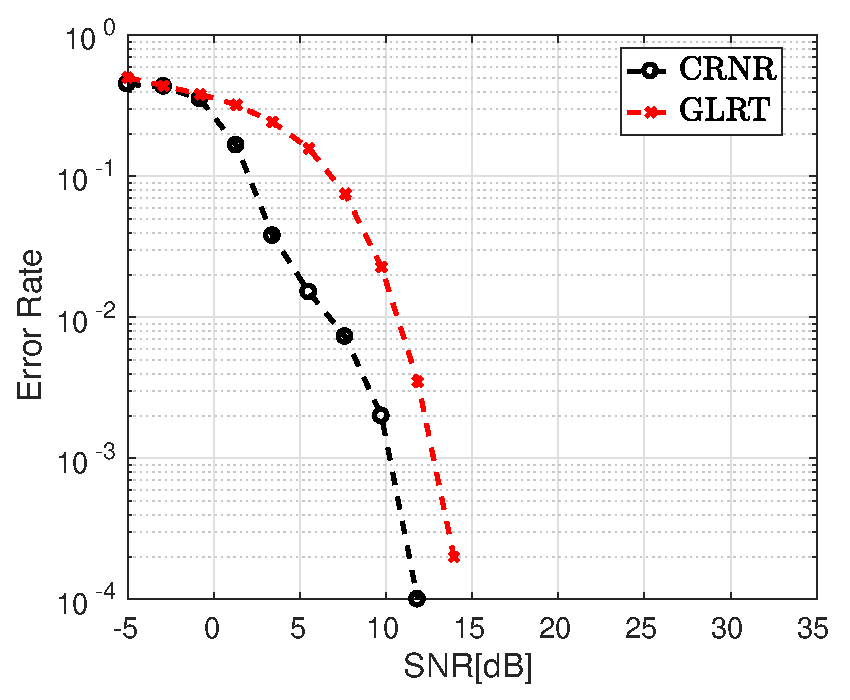
\includegraphics[width = 0.6 \textwidth]{Figuras/Error_rate_signal_2_VS_set_1_low_snr}
				\caption{Tasa de error para la señal observada  $\y_t\in Z_1$ y conjunto de clasificación $Z_2$.}
				\label{Fig:Comparation_MPM_RNR}
			\end{figure}
			
			

			Finalmente, como se vio a lo largo del trabajo, las matrices que conforman el haz suelen estar mal condicionadas, lo que puede causar que el rango numérico asociado al haz sea muy grande y la clasificación se deteriore. Por lo tanto, a futuro se debe trabajar en rediseñar la estrategia de clasificación. Una alternativa es usar el Pseudoespectro de una matriz en lugar del rango numérico. El Pseudoespectro es un conjunto que ``muestra'' como se mueven los autovalores bajo cierta perturbación. Si bien este conjunto suele ser una mejor aproximación del espectro que el rango numérico, el Pseudoespectro muchas veces suele ser un conjunto no convexo, por lo que definir estrategias de clasificación puede ser un desafío. 
			 
			
						
			
		
		
	
			
	
		
	